\documentclass[twoside]{book}

% Packages required by doxygen
\usepackage{fixltx2e}
\usepackage{calc}
\usepackage{doxygen}
\usepackage[export]{adjustbox} % also loads graphicx
\usepackage{graphicx}
\usepackage[utf8]{inputenc}
\usepackage{makeidx}
\usepackage{multicol}
\usepackage{multirow}
\PassOptionsToPackage{warn}{textcomp}
\usepackage{textcomp}
\usepackage[nointegrals]{wasysym}
\usepackage[table]{xcolor}

% Font selection
\usepackage[T1]{fontenc}
\usepackage[scaled=.90]{helvet}
\usepackage{courier}
\usepackage{amssymb}
\usepackage{sectsty}
\renewcommand{\familydefault}{\sfdefault}
\allsectionsfont{%
  \fontseries{bc}\selectfont%
  \color{darkgray}%
}
\renewcommand{\DoxyLabelFont}{%
  \fontseries{bc}\selectfont%
  \color{darkgray}%
}
\newcommand{\+}{\discretionary{\mbox{\scriptsize$\hookleftarrow$}}{}{}}

% Page & text layout
\usepackage{geometry}
\geometry{%
  letterpaper,%
  top=2.5cm,%
  bottom=2.5cm,%
  left=2.5cm,%
  right=2.5cm%
}
\tolerance=750
\hfuzz=15pt
\hbadness=750
\setlength{\emergencystretch}{15pt}
\setlength{\parindent}{0cm}
\setlength{\parskip}{3ex plus 2ex minus 2ex}
\makeatletter
\renewcommand{\paragraph}{%
  \@startsection{paragraph}{4}{0ex}{-1.0ex}{1.0ex}{%
    \normalfont\normalsize\bfseries\SS@parafont%
  }%
}
\renewcommand{\subparagraph}{%
  \@startsection{subparagraph}{5}{0ex}{-1.0ex}{1.0ex}{%
    \normalfont\normalsize\bfseries\SS@subparafont%
  }%
}
\makeatother

% Headers & footers
\usepackage{fancyhdr}
\pagestyle{fancyplain}
\fancyhead[LE]{\fancyplain{}{\bfseries\thepage}}
\fancyhead[CE]{\fancyplain{}{}}
\fancyhead[RE]{\fancyplain{}{\bfseries\leftmark}}
\fancyhead[LO]{\fancyplain{}{\bfseries\rightmark}}
\fancyhead[CO]{\fancyplain{}{}}
\fancyhead[RO]{\fancyplain{}{\bfseries\thepage}}
\fancyfoot[LE]{\fancyplain{}{}}
\fancyfoot[CE]{\fancyplain{}{}}
\fancyfoot[RE]{\fancyplain{}{\bfseries\scriptsize Generated by Doxygen }}
\fancyfoot[LO]{\fancyplain{}{\bfseries\scriptsize Generated by Doxygen }}
\fancyfoot[CO]{\fancyplain{}{}}
\fancyfoot[RO]{\fancyplain{}{}}
\renewcommand{\footrulewidth}{0.4pt}
\renewcommand{\chaptermark}[1]{%
  \markboth{#1}{}%
}
\renewcommand{\sectionmark}[1]{%
  \markright{\thesection\ #1}%
}

% Indices & bibliography
\usepackage{natbib}
\usepackage[titles]{tocloft}
\setcounter{tocdepth}{3}
\setcounter{secnumdepth}{5}
\makeindex

% Packages requested by user
\usepackage{amsmath}
\usepackage{amssymb}
\usepackage{mathrsfs}

% Custom commands
\newcommand{\clearemptydoublepage}{%
  \newpage{\pagestyle{empty}\cleardoublepage}%
}

\usepackage{caption}
\captionsetup{labelsep=space,justification=centering,font={bf},singlelinecheck=off,skip=4pt,position=top}

%===== C O N T E N T S =====

\begin{document}

% Titlepage & ToC
\pagenumbering{roman}
\begin{titlepage}
\vspace*{7cm}
\begin{center}%
{\Large mlpack \\[1ex]\large master }\\
\vspace*{1cm}
{\large Generated by Doxygen 1.8.11}\\
\end{center}
\end{titlepage}
\clearemptydoublepage
\tableofcontents
\clearemptydoublepage
\pagenumbering{arabic}

%--- Begin generated contents ---
\chapter{mlpack Documentation}
\label{index}\doxysection{Introduction}\label{index_intro_sec}
mlpack is an intuitive, fast, and flexible C++ machine learning library with bindings to other languages. It is meant to be a machine learning analog to LAPACK, and aims to implement a wide array of machine learning methods and function as a \char`\"{}swiss army knife\char`\"{} for machine learning researchers. The mlpack website can be found at {\texttt{ https\+://mlpack.\+org}}.\doxysection{How To Use This Documentation}\label{index_howto}
This documentation is API documentation similar to Javadoc. It isn\textquotesingle{}t necessarily a tutorial, but it does provide detailed documentation on every namespace, method, and class.

Each mlpack namespace generally refers to one machine learning method, so browsing the list of namespaces provides some insight as to the breadth of the methods contained in the library.

To generate this documentation in your own local copy of mlpack, you can use the \textquotesingle{}doc\textquotesingle{} CMake target, which is available if CMake has found Doxygen, from the build directory\+:


\begin{DoxyCode}{0}
\DoxyCodeLine{\$ make doc}

\end{DoxyCode}
\doxysection{Tutorials}\label{index_tutorial}
A few short tutorials on how to use mlpack are given below.


\begin{DoxyItemize}
\item \doxyref{Building mlpack From Source}{p.}{build}
\item \doxyref{Building mlpack From Source on Windows}{p.}{build_windows}
\item \doxyref{Matrices in mlpack}{p.}{matrices}
\item \doxyref{Writing an mlpack binding}{p.}{iodoc}
\item \doxyref{mlpack Timers}{p.}{timer}
\item \doxyref{Simple Sample mlpack Programs}{p.}{sample}
\item \doxyref{Sample C++ ML App for Windows}{p.}{sample_ml_app}
\item \doxyref{Cross-\/\+Validation}{p.}{cv}
\item \doxyref{Hyper-\/\+Parameter Tuning}{p.}{hpt_guide}
\item \doxyref{mlpack version information}{p.}{verinfo}
\end{DoxyItemize}\doxysection{Final Remarks}\label{index_remarks}
For the list of contributors to mlpack, see {\texttt{ https\+://www.\+mlpack.\+org/community.\+html}}. This library would not be possible without everyone\textquotesingle{}s hard work and contributions! 
\chapter{Building mlpack From Source}
\label{build}
\input{build}
\chapter{File formats in mlpack}
\label{formatdoc}
\doxysection{Introduction}\label{formatdoc_formatintro}
mlpack supports a wide variety of data (including images) and model formats for use in both its command-\/line programs and in C++ programs using mlpack via the \doxyref{mlpack\+::data\+::\+Load()}{p.}{namespacemlpack_1_1data_abbff2a667bf247e00b1fc09b7ca5f831} function. This tutorial discusses the formats that are supported and how to use them.\doxysection{Table of Contents}\label{formatdoc_toc_tut}
This tutorial is split into the following sections\+:


\begin{DoxyItemize}
\item \doxyref{Introduction}{p.}{formatdoc_formatintro}
\item \doxyref{Table of Contents}{p.}{formatdoc_toc_tut}
\item Data
\begin{DoxyItemize}
\item Data Formats
\begin{DoxyItemize}
\item \doxyref{Simple examples to load data in C++}{p.}{formatdoc_formatsimple}
\item \doxyref{Supported dataset types}{p.}{formatdoc_formattypes}
\item \doxyref{Loading simple matrices in C++}{p.}{formatdoc_formatcpp}
\item \doxyref{Dealing with sparse matrices}{p.}{formatdoc_sparseload}
\item \doxyref{Categorical features and command line programs}{p.}{formatdoc_formatcat}
\item \doxyref{Categorical features and C++}{p.}{formatdoc_formatcatcpp}
\end{DoxyItemize}
\item Image Support
\begin{DoxyItemize}
\item \doxyref{Loading and Saving Images}{p.}{formatdoc_intro_imagetut}
\item \doxyref{Image Utilities API}{p.}{formatdoc_model_api_imagetut}
\item \doxyref{Accessing Metadata of Images\+: Image\+Info}{p.}{formatdoc_imageinfo_api_imagetut}
\item \doxyref{Loading Images in C++}{p.}{formatdoc_load_api_imagetut}
\item \doxyref{Saving Images in C++}{p.}{formatdoc_save_api_imagetut}
\end{DoxyItemize}
\end{DoxyItemize}
\item Models
\begin{DoxyItemize}
\item \doxyref{Loading and saving models}{p.}{formatdoc_formatmodels}
\item \doxyref{Loading and saving models in C++}{p.}{formatdoc_formatmodelscpp}
\end{DoxyItemize}
\item \doxyref{Final notes}{p.}{formatdoc_formatfinal}
\end{DoxyItemize}\doxysection{Simple examples to load data in C++}\label{formatdoc_formatsimple}
The example code snippets below load data from different formats into an Armadillo matrix object ({\ttfamily arma\+::mat}) or model when using C++.


\begin{DoxyCode}{0}
\DoxyCodeLine{\textcolor{keyword}{using namespace }mlpack;}
\DoxyCodeLine{}
\DoxyCodeLine{arma::mat matrix1;}
\DoxyCodeLine{data::Load(\textcolor{stringliteral}{"{}dataset.csv"{}}, matrix1);}

\end{DoxyCode}



\begin{DoxyCode}{0}
\DoxyCodeLine{\textcolor{keyword}{using namespace }mlpack;}
\DoxyCodeLine{}
\DoxyCodeLine{arma::mat matrix2;}
\DoxyCodeLine{data::Load(\textcolor{stringliteral}{"{}dataset.bin"{}}, matrix2);}

\end{DoxyCode}



\begin{DoxyCode}{0}
\DoxyCodeLine{\textcolor{keyword}{using namespace }mlpack;}
\DoxyCodeLine{}
\DoxyCodeLine{arma::mat matrix3;}
\DoxyCodeLine{data::Load(\textcolor{stringliteral}{"{}dataset.h5"{}}, matrix3);}

\end{DoxyCode}



\begin{DoxyCode}{0}
\DoxyCodeLine{\textcolor{keyword}{using namespace }mlpack;}
\DoxyCodeLine{}
\DoxyCodeLine{\textcolor{comment}{// ARFF loading is a little different, since sometimes mapping has to be done}}
\DoxyCodeLine{\textcolor{comment}{// for string types.}}
\DoxyCodeLine{arma::mat matrix4;}
\DoxyCodeLine{data::DatasetInfo datasetInfo;}
\DoxyCodeLine{data::Load(\textcolor{stringliteral}{"{}dataset.arff"{}}, matrix4, datasetInfo);}
\DoxyCodeLine{}
\DoxyCodeLine{\textcolor{comment}{// The datasetInfo object now holds information about each dimension.}}

\end{DoxyCode}



\begin{DoxyCode}{0}
\DoxyCodeLine{\textcolor{keyword}{using namespace }mlpack;}
\DoxyCodeLine{}
\DoxyCodeLine{regression::LogisticRegression lr;}
\DoxyCodeLine{data::Load(\textcolor{stringliteral}{"{}model.bin"{}}, \textcolor{stringliteral}{"{}logistic\_regression\_model"{}}, lr);}

\end{DoxyCode}
\doxysection{Supported dataset types}\label{formatdoc_formattypes}
Datasets in mlpack are represented internally as sparse or dense numeric matrices (specifically, as {\ttfamily arma\+::mat} or {\ttfamily arma\+::sp\+\_\+mat} or similar). This means that when datasets are loaded from file, they must be converted to a suitable numeric representation. Therefore, in general, datasets on disk should contain only numeric features in order to be loaded successfully by mlpack.

The types of datasets that mlpack can load are roughly the same as the types of matrices that Armadillo can load. However, the load functionality that mlpack provides {\bfseries{only supports loading dense datasets}}. When datasets are loaded by mlpack, {\bfseries{the file\textquotesingle{}s type is detected using the file\textquotesingle{}s extension}}. mlpack supports the following file types\+:


\begin{DoxyItemize}
\item csv (comma-\/separated values), denoted by .csv or .txt
\item tsv (tab-\/separated values), denoted by .tsv, .csv, or .txt
\item ASCII (raw ASCII, with space-\/separated values), denoted by .txt
\item Armadillo ASCII (Armadillo\textquotesingle{}s text format with a header), denoted by .txt
\item PGM, denoted by .pgm
\item PPM, denoted by .ppm
\item Armadillo binary, denoted by .bin
\item Raw binary, denoted by .bin {\bfseries{(note\+: this will be loaded as one-\/dimensional data, which is likely not what is desired.)}}
\item HDF5, denoted by .hdf, .hdf5, .h5, or .he5 ({\bfseries{note\+: HDF5 must be enabled in the Armadillo configuration}})
\item ARFF, denoted by .arff ({\bfseries{note\+: this is not supported by all mlpack command-\/line programs }}; see \doxyref{Categorical features and command line programs}{p.}{formatdoc_formatcat})
\end{DoxyItemize}

Datasets that are loaded by mlpack should be stored with {\bfseries{one row for one point}} and {\bfseries{one column for one dimension}}. Therefore, a dataset with three two-\/dimensional points $(0, 1)$, $(3, 1)$, and $(5, -5)$ would be stored in a csv file as\+:


\begin{DoxyCode}{0}
\DoxyCodeLine{0, 1}
\DoxyCodeLine{3, 1}
\DoxyCodeLine{5, -\/5}

\end{DoxyCode}


As noted earlier, for command-\/line programs, the format is automatically detected at load time. Therefore, a dataset can be loaded in many ways\+:


\begin{DoxyCode}{0}
\DoxyCodeLine{\$ mlpack\_logistic\_regression -\/t dataset.csv -\/v}
\DoxyCodeLine{[INFO ] Loading \textcolor{stringliteral}{'dataset.csv'} as CSV data.  Size is 32 x 37749.}
\DoxyCodeLine{...}
\DoxyCodeLine{}
\DoxyCodeLine{\$ mlpack\_logistic\_regression -\/t dataset.txt -\/v}
\DoxyCodeLine{[INFO ] Loading \textcolor{stringliteral}{'dataset.txt'} as raw ASCII formatted data.  Size is 32 x 37749.}
\DoxyCodeLine{...}
\DoxyCodeLine{}
\DoxyCodeLine{\$ mlpack\_logistic\_regression -\/t dataset.h5 -\/v}
\DoxyCodeLine{[INFO ] Loading \textcolor{stringliteral}{'dataset.h5'} as HDF5 data.  Size is 32 x 37749.}
\DoxyCodeLine{...}

\end{DoxyCode}


Similarly, the format to save to is detected by the extension of the given filename.\doxysection{Loading simple matrices in C++}\label{formatdoc_formatcpp}
When C++ is being written, the \doxyref{mlpack\+::data\+::\+Load()}{p.}{namespacemlpack_1_1data_abbff2a667bf247e00b1fc09b7ca5f831} and \doxyref{mlpack\+::data\+::\+Save()}{p.}{namespacemlpack_1_1data_accd1605a1d160c09ee75c93a587dc313} functions are used to load and save datasets, respectively. These functions should be preferred over the built-\/in Armadillo {\ttfamily }.load() and {\ttfamily }.save() functions.

Matrices in mlpack are column-\/major, meaning that each column should correspond to a point in the dataset and each row should correspond to a dimension; for more information, see \doxyref{Matrices in mlpack}{p.}{matrices}. This is at odds with how the data is stored in files; therefore, a transposition is required during load and save. The \doxyref{mlpack\+::data\+::\+Load()}{p.}{namespacemlpack_1_1data_abbff2a667bf247e00b1fc09b7ca5f831} and \doxyref{mlpack\+::data\+::\+Save()}{p.}{namespacemlpack_1_1data_accd1605a1d160c09ee75c93a587dc313} functions do this automatically (unless otherwise specified), which is why they are preferred over the Armadillo functions.

To load a matrix from file, the call is straightforward. After creating a matrix object, the data can be loaded\+:


\begin{DoxyCode}{0}
\DoxyCodeLine{arma::mat dataset; \textcolor{comment}{// The data will be loaded into this matrix.}}
\DoxyCodeLine{mlpack::data::Load(\textcolor{stringliteral}{"{}dataset.csv"{}}, dataset);}

\end{DoxyCode}


Saving matrices is equally straightforward. The code below generates a random matrix with 10 points in 3 dimensions and saves it to a file as HDF5.


\begin{DoxyCode}{0}
\DoxyCodeLine{\textcolor{comment}{// 3 dimensions (rows), with 10 points (columns).}}
\DoxyCodeLine{arma::mat dataset = arma::randu<arma::mat>(3, 10);}
\DoxyCodeLine{mlpack::data::Save(\textcolor{stringliteral}{"{}dataset.h5"{}}, dataset);}

\end{DoxyCode}


As with the command-\/line programs, the type of data to be loaded is automatically detected from the filename extension. For more details, see the \doxyref{mlpack\+::data\+::\+Load()}{p.}{namespacemlpack_1_1data_abbff2a667bf247e00b1fc09b7ca5f831} and \doxyref{mlpack\+::data\+::\+Save()}{p.}{namespacemlpack_1_1data_accd1605a1d160c09ee75c93a587dc313} documentation.\doxysection{Dealing with sparse matrices}\label{formatdoc_sparseload}
As mentioned earlier, support for loading sparse matrices in mlpack is not available at this time. To use a sparse matrix with mlpack code, you will have to write a C++ program instead of using any of the command-\/line tools, because the command-\/line tools all use dense datasets internally. (There is one exception\+: the {\ttfamily mlpack\+\_\+cf} program, for collaborative filtering, loads sparse coordinate lists.)

In addition, the {\ttfamily \doxyref{mlpack\+::data\+::\+Load()}{p.}{namespacemlpack_1_1data_abbff2a667bf247e00b1fc09b7ca5f831}} function does not support loading any sparse format; so the best idea is to use undocumented Armadillo functionality to load coordinate lists. Suppose you have a coordinate list file like the one below\+:


\begin{DoxyCode}{0}
\DoxyCodeLine{\$ cat cl.csv}
\DoxyCodeLine{0 0 0.332}
\DoxyCodeLine{1 3 3.126}
\DoxyCodeLine{4 4 1.333}

\end{DoxyCode}


This represents a 5x5 matrix with three nonzero elements. We can load this using Armadillo\+:


\begin{DoxyCode}{0}
\DoxyCodeLine{arma::sp\_mat matrix;}
\DoxyCodeLine{matrix.load(\textcolor{stringliteral}{"{}cl.csv"{}}, arma::coord\_ascii);}
\DoxyCodeLine{matrix = matrix.t(); \textcolor{comment}{// We must transpose after load!}}

\end{DoxyCode}


The transposition after loading is necessary if the coordinate list is in row-\/major format (that is, if each row in the matrix represents a point and each column represents a feature). Be sure that the matrix you use with mlpack methods has points as columns and features as rows! See \doxyref{Matrices in mlpack}{p.}{matrices} for more information.\doxysection{Categorical features and command line programs}\label{formatdoc_formatcat}
In some situations it is useful to represent data not just as a numeric matrix but also as categorical data (i.\+e. with numeric but unordered categories). This support is useful for, e.\+g., decision trees and other models that support categorical features.

In some machine learning situations, such as, e.\+g., decision trees, categorical data can be used. Categorical data might look like this (in CSV format)\+:


\begin{DoxyCode}{0}
\DoxyCodeLine{0, 1, \textcolor{stringliteral}{"{}true"{}}, 3}
\DoxyCodeLine{5, -\/2, \textcolor{stringliteral}{"{}false"{}}, 5}
\DoxyCodeLine{2, 2, \textcolor{stringliteral}{"{}true"{}}, 4}
\DoxyCodeLine{3, -\/1, \textcolor{stringliteral}{"{}true"{}}, 3}
\DoxyCodeLine{4, 4, \textcolor{stringliteral}{"{}not sure"{}}, 0}
\DoxyCodeLine{0, 7, \textcolor{stringliteral}{"{}false"{}}, 6}

\end{DoxyCode}


In the example above, the third dimension (which takes values \char`\"{}true\char`\"{}, \char`\"{}false\char`\"{}, and \char`\"{}not sure\char`\"{}) is categorical. mlpack can load and work with this data, but the strings must be mapped to numbers, because all dataset in mlpack are represented by Armadillo matrix objects.

From the perspective of an mlpack command-\/line program, this support is transparent; mlpack will attempt to load the data file, and if it detects entries in the file that are not numeric, it will map them to numbers and then print, for each dimension, the number of mappings. For instance, if we run the {\ttfamily mlpack\+\_\+hoeffding\+\_\+tree} program (which supports categorical data) on the dataset above (stored as dataset.\+csv), we receive this output during loading\+:


\begin{DoxyCode}{0}
\DoxyCodeLine{\$ mlpack\_hoeffding\_tree -\/t dataset.csv -\/l dataset.labels.csv -\/v}
\DoxyCodeLine{[INFO ] Loading \textcolor{stringliteral}{'dataset.csv'} as CSV data.  Size is 6 x 4.}
\DoxyCodeLine{[INFO ] 0 mappings in dimension 0.}
\DoxyCodeLine{[INFO ] 0 mappings in dimension 1.}
\DoxyCodeLine{[INFO ] 3 mappings in dimension 2.}
\DoxyCodeLine{[INFO ] 0 mappings in dimension 3.}
\DoxyCodeLine{...}

\end{DoxyCode}


Currently, only the {\ttfamily mlpack\+\_\+hoeffding\+\_\+tree} program supports loading categorical data, and this is also the only program that supports loading an ARFF dataset.\doxysection{Categorical features and C++}\label{formatdoc_formatcatcpp}
When writing C++, loading categorical data is slightly more tricky\+: the mappings from strings to integers must be preserved. This is the purpose of the \doxyref{mlpack\+::data\+::\+Dataset\+Info}{p.}{namespacemlpack_1_1data_aa243ad7e4d29363b858bbc92b732921d} class, which stores these mappings and can be used and load and save time to apply and de-\/apply the mappings.

When loading a dataset with categorical data, the overload of \doxyref{mlpack\+::data\+::\+Load()}{p.}{namespacemlpack_1_1data_abbff2a667bf247e00b1fc09b7ca5f831} that takes an \doxyref{mlpack\+::data\+::\+Dataset\+Info}{p.}{namespacemlpack_1_1data_aa243ad7e4d29363b858bbc92b732921d} object should be used. An example is below\+:


\begin{DoxyCode}{0}
\DoxyCodeLine{arma::mat dataset; \textcolor{comment}{// Load into this matrix.}}
\DoxyCodeLine{mlpack::data::DatasetInfo info; \textcolor{comment}{// Store information about dataset in this.}}
\DoxyCodeLine{}
\DoxyCodeLine{\textcolor{comment}{// Load the ARFF dataset.}}
\DoxyCodeLine{mlpack::data::Load(\textcolor{stringliteral}{"{}dataset.arff"{}}, dataset, info);}

\end{DoxyCode}


After this load completes, the {\ttfamily info} object will hold the information about the mappings necessary to load the dataset. It is possible to re-\/use the {\ttfamily Dataset\+Info} object to load another dataset with the same mappings. This is useful when, for instance, both a training and test set are being loaded, and it is necessary that the mappings from strings to integers for categorical features are identical. An example is given below.


\begin{DoxyCode}{0}
\DoxyCodeLine{arma::mat trainingData; \textcolor{comment}{// Load training data into this matrix.}}
\DoxyCodeLine{mlpack::data::DatasetInfo info; \textcolor{comment}{// This will store the mappings.}}
\DoxyCodeLine{}
\DoxyCodeLine{\textcolor{comment}{// Load the training data, and create the mappings in the 'info' object.}}
\DoxyCodeLine{mlpack::data::Load(\textcolor{stringliteral}{"{}training\_data.arff"{}}, trainingData, info);}
\DoxyCodeLine{}
\DoxyCodeLine{\textcolor{comment}{// Load the test data, but re-\/use the 'info' object with the already initialized}}
\DoxyCodeLine{\textcolor{comment}{// mappings.  This means that the same mappings will be applied to the test set.}}
\DoxyCodeLine{mlpack::data::Load(\textcolor{stringliteral}{"{}test\_data.arff"{}}, trainingData, info);}

\end{DoxyCode}


When saving data, pass the same Dataset\+Info object it was loaded with in order to unmap the categorical features correctly. The example below demonstrates this functionality\+: it loads the dataset, increments all non-\/categorical features by 1, and then saves the dataset with the same Dataset\+Info it was loaded with.


\begin{DoxyCode}{0}
\DoxyCodeLine{arma::mat dataset; \textcolor{comment}{// Load data into this matrix.}}
\DoxyCodeLine{mlpack::data::DatasetInfo info; \textcolor{comment}{// This will store the mappings.}}
\DoxyCodeLine{}
\DoxyCodeLine{\textcolor{comment}{// Load the dataset.}}
\DoxyCodeLine{mlpack::data::Load(\textcolor{stringliteral}{"{}dataset.tsv"{}}, dataset, info);}
\DoxyCodeLine{}
\DoxyCodeLine{\textcolor{comment}{// Loop over all features, and add 1 to all non-\/categorical features.}}
\DoxyCodeLine{\textcolor{keywordflow}{for} (\textcolor{keywordtype}{size\_t} i = 0; i < info.Dimensionality(); ++i)}
\DoxyCodeLine{\{}
\DoxyCodeLine{  \textcolor{comment}{// The Type() function returns whether or not the data is numeric or}}
\DoxyCodeLine{  \textcolor{comment}{// categorical.}}
\DoxyCodeLine{  \textcolor{keywordflow}{if} (info.Type(i) != mlpack::data::Datatype::categorical)}
\DoxyCodeLine{    dataset.row(i) += 1.0;}
\DoxyCodeLine{\}}
\DoxyCodeLine{}
\DoxyCodeLine{\textcolor{comment}{// Save the modified dataset using the same DatasetInfo.}}
\DoxyCodeLine{mlpack::data::Save(\textcolor{stringliteral}{"{}dataset-\/new.tsv"{}}, dataset, info);}

\end{DoxyCode}


There is more functionality to the Dataset\+Info class; for more information, see the \doxyref{mlpack\+::data\+::\+Dataset\+Info}{p.}{namespacemlpack_1_1data_aa243ad7e4d29363b858bbc92b732921d} documentation.\doxysection{Loading and Saving Images}\label{formatdoc_intro_imagetut}
Image datasets are becoming increasingly popular in deep learning.

mlpack\textquotesingle{}s image saving/loading functionality is based on {\texttt{ stb/}}.\doxysection{Image Utilities API}\label{formatdoc_model_api_imagetut}
Image utilities supports loading and saving of images.

It supports filetypes \char`\"{}jpg\char`\"{}, \char`\"{}png\char`\"{}, \char`\"{}tga\char`\"{}, \char`\"{}bmp\char`\"{}, \char`\"{}psd\char`\"{}, \char`\"{}gif\char`\"{}, \char`\"{}hdr\char`\"{}, \char`\"{}pic\char`\"{}, \char`\"{}pnm\char`\"{} for loading and \char`\"{}jpg\char`\"{}, \char`\"{}png\char`\"{}, \char`\"{}tga\char`\"{}, \char`\"{}bmp\char`\"{}, \char`\"{}hdr\char`\"{} for saving.

The datatype associated is unsigned char to support RGB values in the range 1-\/255. To feed data into the network typecast of {\ttfamily arma\+::\+Mat} may be required. Images are stored in the matrix as (width $\ast$ height $\ast$ channels, Number\+Of\+Images). Therefore {\ttfamily image\+Matrix.\+col(0)} would be the first image if images are loaded in {\ttfamily image\+Matrix}.\doxysection{Accessing Metadata of Images\+: Image\+Info}\label{formatdoc_imageinfo_api_imagetut}
Image\+Info class contains the metadata of the images. 
\begin{DoxyCode}{0}
\DoxyCodeLine{ImageInfo(\textcolor{keyword}{const} \textcolor{keywordtype}{size\_t} width,}
\DoxyCodeLine{          \textcolor{keyword}{const} \textcolor{keywordtype}{size\_t} height,}
\DoxyCodeLine{          \textcolor{keyword}{const} \textcolor{keywordtype}{size\_t} channels,}
\DoxyCodeLine{          \textcolor{keyword}{const} \textcolor{keywordtype}{size\_t} quality = 90);}

\end{DoxyCode}


The {\ttfamily quality} member denotes the compression of the image if it is saved as {\ttfamily jpg}; it takes values from 0 to 100.\doxysection{Loading Images in C++}\label{formatdoc_load_api_imagetut}
Standalone loading of images.


\begin{DoxyCode}{0}
\DoxyCodeLine{\textcolor{keyword}{template}<\textcolor{keyword}{typename} eT>}
\DoxyCodeLine{\textcolor{keywordtype}{bool} Load(\textcolor{keyword}{const} std::string\& filename,}
\DoxyCodeLine{          arma::Mat<eT>\& matrix,}
\DoxyCodeLine{          ImageInfo\& info,}
\DoxyCodeLine{          \textcolor{keyword}{const} \textcolor{keywordtype}{bool} fatal);}

\end{DoxyCode}


The example below loads a test image. It also fills up the Image\+Info class object.


\begin{DoxyCode}{0}
\DoxyCodeLine{data::ImageInfo info;}
\DoxyCodeLine{data::Load(\textcolor{stringliteral}{"{}test\_image.png"{}}, matrix, info, \textcolor{keyword}{false});}

\end{DoxyCode}


Image\+Info requires height, width, number of channels of the image.


\begin{DoxyCode}{0}
\DoxyCodeLine{\textcolor{keywordtype}{size\_t} height = 64, width = 64, channels = 1;}
\DoxyCodeLine{data::ImageInfo info(width, height, channels);}

\end{DoxyCode}


More than one image can be loaded into the same matrix.

Loading multiple images\+:


\begin{DoxyCode}{0}
\DoxyCodeLine{\textcolor{keyword}{template}<\textcolor{keyword}{typename} eT>}
\DoxyCodeLine{\textcolor{keywordtype}{bool} Load(\textcolor{keyword}{const} std::vector<std::string>\& files,}
\DoxyCodeLine{          arma::Mat<eT>\& matrix,}
\DoxyCodeLine{          ImageInfo\& info,}
\DoxyCodeLine{          \textcolor{keyword}{const} \textcolor{keywordtype}{bool} fatal);}

\end{DoxyCode}



\begin{DoxyCode}{0}
\DoxyCodeLine{data::ImageInfo info;}
\DoxyCodeLine{std::vector<std::string>> files\{\textcolor{stringliteral}{"{}test\_image1.bmp"{}},\textcolor{stringliteral}{"{}test\_image2.bmp"{}}\};}
\DoxyCodeLine{data::Load(files, matrix, info, \textcolor{keyword}{false});}

\end{DoxyCode}
\doxysection{Saving Images in C++}\label{formatdoc_save_api_imagetut}
Save images expects a matrix of type unsigned char in the form (width $\ast$ height $\ast$ channels, Number\+Of\+Images). Just like load it can be used to save one image or multiple images. Besides image data it also expects the shape of the image as input (width, height, channels).

Saving one image\+:


\begin{DoxyCode}{0}
\DoxyCodeLine{\textcolor{keyword}{template}<\textcolor{keyword}{typename} eT>}
\DoxyCodeLine{\textcolor{keywordtype}{bool} Save(\textcolor{keyword}{const} std::string\& filename,}
\DoxyCodeLine{          arma::Mat<eT>\& matrix,}
\DoxyCodeLine{          ImageInfo\& info,}
\DoxyCodeLine{          \textcolor{keyword}{const} \textcolor{keywordtype}{bool} fatal,}
\DoxyCodeLine{          \textcolor{keyword}{const} \textcolor{keywordtype}{bool} transpose);}

\end{DoxyCode}



\begin{DoxyCode}{0}
\DoxyCodeLine{data::ImageInfo info;}
\DoxyCodeLine{info.width = info.height = 25;}
\DoxyCodeLine{info.channels = 3;}
\DoxyCodeLine{info.quality = 90;}
\DoxyCodeLine{data::Save(\textcolor{stringliteral}{"{}test\_image.bmp"{}}, matrix, info, \textcolor{keyword}{false}, \textcolor{keyword}{true});}

\end{DoxyCode}


If the matrix contains more than one image, only the first one is saved.

Saving multiple images\+:


\begin{DoxyCode}{0}
\DoxyCodeLine{\textcolor{keyword}{template}<\textcolor{keyword}{typename} eT>}
\DoxyCodeLine{\textcolor{keywordtype}{bool} Save(\textcolor{keyword}{const} std::vector<std::string>\& files,}
\DoxyCodeLine{          arma::Mat<eT>\& matrix,}
\DoxyCodeLine{          ImageInfo\& info,}
\DoxyCodeLine{          \textcolor{keyword}{const} \textcolor{keywordtype}{bool} fatal,}
\DoxyCodeLine{          \textcolor{keyword}{const} \textcolor{keywordtype}{bool} transpose);}

\end{DoxyCode}



\begin{DoxyCode}{0}
\DoxyCodeLine{data::ImageInfo info;}
\DoxyCodeLine{info.width = info.height = 25;}
\DoxyCodeLine{info.channels = 3;}
\DoxyCodeLine{info.quality = 90;}
\DoxyCodeLine{std::vector<std::string>> files\{\textcolor{stringliteral}{"{}test\_image1.bmp"{}}, \textcolor{stringliteral}{"{}test\_image2.bmp"{}}\};}
\DoxyCodeLine{data::Save(files, matrix, info, \textcolor{keyword}{false}, \textcolor{keyword}{true});}

\end{DoxyCode}


Multiple images are saved according to the vector of filenames specified.\doxysection{Loading and saving models}\label{formatdoc_formatmodels}
Using {\ttfamily cereal}, mlpack is able to load and save machine learning models with ease. These models can currently be saved in three formats\+:


\begin{DoxyItemize}
\item binary (.bin); this is not human-\/readable, but it is small
\item json (.json); this is sort of human-\/readable and relatively small
\item xml (.xml); this is human-\/readable but very verbose and large
\end{DoxyItemize}

The type of file to save is determined by the given file extension, as with the other loading and saving functionality in mlpack. Below is an example where a dataset stored as TSV and labels stored as ASCII text are used to train a logistic regression model, which is then saved to model.\+xml.


\begin{DoxyCode}{0}
\DoxyCodeLine{\$ mlpack\_logistic\_regression -\/t training\_dataset.tsv -\/l training\_labels.txt \(\backslash\)}
\DoxyCodeLine{> -\/M model.xml}

\end{DoxyCode}


Many mlpack command-\/line programs have support for loading and saving models through the {\ttfamily --input\+\_\+model\+\_\+file} ({\ttfamily -\/m}) and {\ttfamily --output\+\_\+model\+\_\+file} ({\ttfamily -\/M}) options; for more information, see the documentation for each program (accessible by passing {\ttfamily --help} as a parameter).\doxysection{Loading and saving models in C++}\label{formatdoc_formatmodelscpp}
mlpack uses the {\ttfamily cereal} library internally to perform loading and saving of models, and provides convenience overloads of \doxyref{mlpack\+::data\+::\+Load()}{p.}{namespacemlpack_1_1data_abbff2a667bf247e00b1fc09b7ca5f831} and \doxyref{mlpack\+::data\+::\+Save()}{p.}{namespacemlpack_1_1data_accd1605a1d160c09ee75c93a587dc313} to load and save these models.

To be serializable, a class must implement the method


\begin{DoxyCode}{0}
\DoxyCodeLine{\textcolor{keyword}{template}<\textcolor{keyword}{typename} Archive>}
\DoxyCodeLine{\textcolor{keywordtype}{void} serialize(Archive\& ar);}

\end{DoxyCode}


\begin{DoxyNote}{Note}
For more information on this method and how it works, see the cereal documentation at {\texttt{ https\+://uscilab.\+github.\+io/cereal/index.\+html}}.

Examples of serialize() methods can be found in most classes; one fairly straightforward example is found \doxyref{in the mlpack\+::math\+::Range class}{p.}{classmlpack_1_1math_1_1RangeType_a72d63b74c8166dff8e1a9006905ad9ca}. A more complex example is found \doxyref{in the mlpack\+::tree\+::Binary\+Space\+Tree class}{p.}{classmlpack_1_1tree_1_1BinarySpaceTree_a72d63b74c8166dff8e1a9006905ad9ca}.
\end{DoxyNote}
Using the \doxyref{mlpack\+::data\+::\+Load()}{p.}{namespacemlpack_1_1data_abbff2a667bf247e00b1fc09b7ca5f831} and \doxyref{mlpack\+::data\+::\+Save()}{p.}{namespacemlpack_1_1data_accd1605a1d160c09ee75c93a587dc313} classes is easy if the type being saved has a {\ttfamily serialize()} method implemented\+: simply call either function with a filename, a name for the object to save, and the object itself. The example below, for instance, creates an \doxyref{mlpack\+::math\+::\+Range}{p.}{namespacemlpack_1_1math_ad17d9cabd4fd82cbed4ccd5e53b47d70} object and saves it as range.\+txt. Then, that range is loaded from file into another \doxyref{mlpack\+::math\+::\+Range}{p.}{namespacemlpack_1_1math_ad17d9cabd4fd82cbed4ccd5e53b47d70} object.


\begin{DoxyCode}{0}
\DoxyCodeLine{\textcolor{comment}{// Create range and save it.}}
\DoxyCodeLine{mlpack::math::Range r(0.0, 5.0);}
\DoxyCodeLine{mlpack::data::Save(\textcolor{stringliteral}{"{}range.json"{}}, \textcolor{stringliteral}{"{}range"{}}, r);}
\DoxyCodeLine{}
\DoxyCodeLine{\textcolor{comment}{// Load into new range.}}
\DoxyCodeLine{mlpack::math::Range newRange;}
\DoxyCodeLine{mlpack::data::Load(\textcolor{stringliteral}{"{}range.json"{}}, \textcolor{stringliteral}{"{}range"{}}, newRange);}

\end{DoxyCode}


It is important to be sure that you load the appropriate type; if you save, for instance, an \doxyref{mlpack\+::regression\+::\+Logistic\+Regression}{p.}{classmlpack_1_1regression_1_1LogisticRegression} object and attempt to load it as an \doxyref{mlpack\+::math\+::\+Range}{p.}{namespacemlpack_1_1math_ad17d9cabd4fd82cbed4ccd5e53b47d70} object, the load will fail and an exception will be thrown. (When the object is saved as binary (.bin), it is possible that the load will not fail, but instead load with mangled data, which is perhaps even worse!)\doxysection{Final notes}\label{formatdoc_formatfinal}
If the examples here are unclear, it would be worth looking into the ways that \doxyref{mlpack\+::data\+::\+Load()}{p.}{namespacemlpack_1_1data_abbff2a667bf247e00b1fc09b7ca5f831} and \doxyref{mlpack\+::data\+::\+Save()}{p.}{namespacemlpack_1_1data_accd1605a1d160c09ee75c93a587dc313} are used in the code. Some example files that may be useful to this end\+:


\begin{DoxyItemize}
\item src/mlpack/methods/logistic\+\_\+regression/logistic\+\_\+regression\+\_\+main.\+cpp
\item src/mlpack/methods/hoeffding\+\_\+trees/hoeffding\+\_\+tree\+\_\+main.\+cpp
\item src/mlpack/methods/neighbor\+\_\+search/knn\+\_\+main.\+cpp
\end{DoxyItemize}

If you are interested in adding support for more data types to mlpack, it would be preferable to add the support upstream to Armadillo instead, so that may be a better direction to go first. Then very little code modification for mlpack will be necessary. 
\chapter{mlpack Input and Output}
\label{iodoc}
\section{Introduction}\label{iodoc_iointro}
mlpack provides the following\+:


\begin{DoxyItemize}
\item \doxyref{mlpack\+::\+Log}{p.}{classmlpack_1_1Log}, for debugging / informational / warning / fatal output
\item \doxyref{mlpack\+::\+C\+LI}{p.}{classmlpack_1_1CLI}, for parsing command line options
\end{DoxyItemize}

Each of those classes are well-\/documented, and that documentation should be consulted for further reference.\section{Simple Logging Example}\label{iodoc_simplelog}
mlpack has four logging levels\+:


\begin{DoxyItemize}
\item Log\+::\+Debug
\item Log\+::\+Info
\item Log\+::\+Warn
\item Log\+::\+Fatal
\end{DoxyItemize}

Output to Log\+::\+Debug does not show (and has no performance penalty) when mlpack is compiled without debugging symbols. Output to Log\+::\+Info is only shown when the program is run with the --verbose (or -\/v) flag. Log\+::\+Warn is always shown, and Log\+::\+Fatal will throw a std\+::runtime\+\_\+error exception, when a newline is sent to it only. If mlpack was compiled with debugging symbols, Log\+::\+Fatal will always throw a std\+::runtime\+\_\+error exception and print backtrace.

Here is a simple example, and its output\+:


\begin{DoxyCode}
\textcolor{preprocessor}{#include <mlpack/core.hpp>}

\textcolor{keyword}{using namespace }mlpack;

\textcolor{keywordtype}{int} main(\textcolor{keywordtype}{int} argc, \textcolor{keywordtype}{char}** argv)
\{
  CLI::ParseCommandLine(argc, argv);

  Log::Debug << \textcolor{stringliteral}{"Compiled with debugging symbols."} << std::endl;

  Log::Info << \textcolor{stringliteral}{"Some test informational output."} << std::endl;

  Log::Warn << \textcolor{stringliteral}{"A warning!"} << std::endl;

  Log::Fatal << \textcolor{stringliteral}{"Program has crashed."} << std::endl;

  Log::Warn << \textcolor{stringliteral}{"Made it!"} << std::endl;
\}
\end{DoxyCode}


With debugging output--verbose, the following is shown\+:


\begin{DoxyCode}
[DEBUG] Compiled with debugging symbols.
[INFO ] Some test informational output.
[WARN ] A warning!
[FATAL] [bt]: (1) /absolute/path/to/file/example.cpp:6: \textcolor{keyword}{function}()
[FATAL] Program has crashed.
terminate called after throwing an instance of \textcolor{stringliteral}{'std::runtime\_error'}
  what():  fatal error; see Log::Fatal output
Aborted
\end{DoxyCode}


With debugging output, compilation flags -\/g -\/rdynamic and --verbose, the following is shown\+:


\begin{DoxyCode}
[DEBUG] Compiled with debugging symbols.
[INFO ] Some test informational output.
[WARN ] A warning!
[FATAL] Cannot give backtrace because program was compiled without: -g -rdynamic
[FATAL] For a backtrace, recompile with: -g -rdynamic.
[FATAL] Program has crashed.
terminate called after throwing an instance of \textcolor{stringliteral}{'std::runtime\_error'}
  what():  fatal error; see Log::Fatal output
Aborted
\end{DoxyCode}


The last warning is not reached, because Log\+::\+Fatal terminates the program.

Without debugging symbols and without --verbose, the following is shown\+:


\begin{DoxyCode}
$ ./main
[WARN ] A warning!
[FATAL] Program has crashed.
terminate called after throwing an instance of \textcolor{stringliteral}{'std::runtime\_error'}
  what():  fatal error; see Log::Fatal output
Aborted
\end{DoxyCode}


These four outputs can be very useful for both providing informational output and debugging output for your mlpack program.\section{Simple C\+L\+I Example}\label{iodoc_simplecli}
Through the \doxyref{mlpack\+::\+C\+LI}{p.}{classmlpack_1_1CLI} object, command-\/line parameters can be easily added with the P\+R\+O\+G\+R\+A\+M\+\_\+\+I\+N\+FO, P\+A\+R\+A\+M\+\_\+\+I\+NT, P\+A\+R\+A\+M\+\_\+\+D\+O\+U\+B\+LE, P\+A\+R\+A\+M\+\_\+\+S\+T\+R\+I\+NG, and P\+A\+R\+A\+M\+\_\+\+F\+L\+AG macros.

Here is a sample use of those macros, extracted from methods/pca/pca\+\_\+main.\+cpp.


\begin{DoxyCode}
\textcolor{preprocessor}{#include <mlpack/core.hpp>}

\textcolor{comment}{// Document program.}
PROGRAM_INFO(\textcolor{stringliteral}{"Principal Components Analysis"}, \textcolor{stringliteral}{"This program performs principal "}
    \textcolor{stringliteral}{"components analysis on the given dataset.  It will transform the data "}
    \textcolor{stringliteral}{"onto its principal components, optionally performing dimensionality "}
    \textcolor{stringliteral}{"reduction by ignoring the principal components with the smallest "}
    \textcolor{stringliteral}{"eigenvalues."});

\textcolor{comment}{// Parameters for program.}
PARAM\_STRING\_REQ(\textcolor{stringliteral}{"input\_file"}, \textcolor{stringliteral}{"Input dataset to perform PCA on."}, \textcolor{stringliteral}{""});
PARAM\_STRING\_REQ(\textcolor{stringliteral}{"output\_file"}, \textcolor{stringliteral}{"Output dataset to perform PCA on."}, \textcolor{stringliteral}{""});
PARAM\_INT(\textcolor{stringliteral}{"new\_dimensionality"}, \textcolor{stringliteral}{"Desired dimensionality of output dataset."},
    \textcolor{stringliteral}{""}, 0);

\textcolor{keyword}{using namespace }mlpack;

\textcolor{keywordtype}{int} main(\textcolor{keywordtype}{int} argc, \textcolor{keywordtype}{char}** argv)
\{
  \textcolor{comment}{// Parse commandline.}
  CLI::ParseCommandLine(argc, argv);

  ...
\}
\end{DoxyCode}


Documentation is automatically generated using those macros, and when the program is run with --help the following is displayed\+:


\begin{DoxyCode}
$ mlpack\_pca --help
Principal Components Analysis

  This program performs principal components analysis on the given dataset.  It
  will transform the data onto its principal components, optionally performing
  dimensionality reduction by ignoring the principal components with the
  smallest eigenvalues.

Required options:

  --input\_file [string]         Input dataset to perform PCA on.
  --output\_file [string]        Output dataset to perform PCA on.

Options:

  --help (-h)                   Default help info.
  --info [\textcolor{keywordtype}{string}]               Get help on a specific module or option.
                                Default value ''.
  --new\_dimensionality [\textcolor{keywordtype}{int}]    Desired dimensionality of output dataset.
                                Default value 0.
  --verbose (-v)                Display informational messages and the full list
                                of parameters and timers at the end of
                                execution.
\end{DoxyCode}


The \doxyref{mlpack\+::\+C\+LI}{p.}{classmlpack_1_1CLI} documentation can be consulted for further and complete documentation. 
\chapter{Matrices in mlpack}
\label{matrices}
\doxysection{Introduction}\label{matrices_matintro}
mlpack uses Armadillo matrices for matrix support. Armadillo is a fast C++ matrix library which makes use of advanced template techniques to provide the fastest possible matrix operations.

Documentation on Armadillo can be found on their website\+:

{\texttt{ http\+://arma.\+sourceforge.\+net/docs.\+html}}

Nonetheless, there are a few further caveats for mlpack Armadillo usage.\doxysection{Column-\/major Matrices}\label{matrices_format}
Armadillo matrices are stored in a column-\/major format; this means that on disk, each column is located in contiguous memory.

This means that, for the vast majority of machine learning methods, it is faster to store observations as columns and dimensions as rows. This is counter to most standard machine learning texts!

Major implications of this are for linear algebra. For instance, the covariance of a matrix is typically

\[ C = X^T X \]

but for a column-\/wise matrix, it is

\[ C = X X^T \]

and this is very important to keep in mind! If your mlpack code is not working, this may be a factor in why.\doxysection{Loading Matrices}\label{matrices_loading}
mlpack provides a \doxyref{data\+::\+Load()}{p.}{namespacemlpack_1_1data_abbff2a667bf247e00b1fc09b7ca5f831} and \doxyref{data\+::\+Save()}{p.}{namespacemlpack_1_1data_accd1605a1d160c09ee75c93a587dc313} function, which should be used instead of Armadillo\textquotesingle{}s loading and saving functions.

Most machine learning data is stored in row-\/major format; a CSV, for example, will generally have one observation per line and each column will correspond to a dimension.

The \doxyref{data\+::\+Load()}{p.}{namespacemlpack_1_1data_abbff2a667bf247e00b1fc09b7ca5f831} and \doxyref{data\+::\+Save()}{p.}{namespacemlpack_1_1data_accd1605a1d160c09ee75c93a587dc313} functions transpose the matrix upon loading, meaning that the following CSV\+:


\begin{DoxyCode}{0}
\DoxyCodeLine{\$ cat data.csv}
\DoxyCodeLine{3,3,3,3,0}
\DoxyCodeLine{3,4,4,3,0}
\DoxyCodeLine{3,4,4,3,0}
\DoxyCodeLine{3,3,4,3,0}
\DoxyCodeLine{3,6,4,3,0}
\DoxyCodeLine{2,4,4,3,0}
\DoxyCodeLine{2,4,4,1,0}
\DoxyCodeLine{3,3,3,2,0}
\DoxyCodeLine{3,4,4,2,0}
\DoxyCodeLine{3,4,4,2,0}
\DoxyCodeLine{3,3,4,2,0}
\DoxyCodeLine{3,6,4,2,0}
\DoxyCodeLine{2,4,4,2,0}

\end{DoxyCode}


is actually loaded with 5 rows and 13 columns, not 13 rows and 5 columns like the CSV is written. More information on mlpack\textquotesingle{}s loading functionality can be found in \doxyref{File formats and loading data in mlpack}{p.}{formatdoc}.

This is important to remember! 
\chapter{Simple Sample mlpack Programs}
\label{sample}
\section{Introduction}\label{sample_sampleintro}
On this page, several simple mlpack examples are contained, in increasing order of complexity. If you compile from the command-\/line, be sure that your compiler is in C++11 mode. With gcc and clang, this can be accomplished by adding the {\ttfamily -\/std=c++11} option.\section{Covariance Computation}\label{sample_covariance}
A simple program to compute the covariance of a data matrix (\char`\"{}data.\+csv\char`\"{}), assuming that the data is already centered, and save it to file.


\begin{DoxyCode}
\textcolor{comment}{// Includes all relevant components of mlpack.}
\textcolor{preprocessor}{#include <mlpack/core.hpp>}

\textcolor{comment}{// Convenience.}
\textcolor{keyword}{using namespace }mlpack;

\textcolor{keywordtype}{int} main()
\{
  \textcolor{comment}{// First, load the data.}
  arma::mat data;
  \textcolor{comment}{// Use data::Load() which transposes the matrix.}
  data::Load(\textcolor{stringliteral}{"data.csv"}, data, \textcolor{keyword}{true});

  \textcolor{comment}{// Now compute the covariance.  We assume that the data is already centered.}
  \textcolor{comment}{// Remember, because the matrix is column-major, the covariance operation is}
  \textcolor{comment}{// transposed.}
  arma::mat cov = data * trans(data) / data.n\_cols;

  \textcolor{comment}{// Save the output.}
  data::Save(\textcolor{stringliteral}{"cov.csv"}, cov, \textcolor{keyword}{true});
\}
\end{DoxyCode}
\section{Nearest Neighbor}\label{sample_nn}
This simple program uses the \doxyref{mlpack\+::neighbor\+::\+Neighbor\+Search}{p.}{classmlpack_1_1neighbor_1_1NeighborSearch} object to find the nearest neighbor of each point in a dataset using the L1 metric, and then print the index of the neighbor and the distance of it to stdout.


\begin{DoxyCode}
\textcolor{preprocessor}{#include <mlpack/core.hpp>}
\textcolor{preprocessor}{#include <mlpack/methods/neighbor_search/neighbor_search.hpp>}

\textcolor{keyword}{using namespace }mlpack;
\textcolor{keyword}{using namespace }mlpack::neighbor; \textcolor{comment}{// NeighborSearch and NearestNeighborSort}
\textcolor{keyword}{using namespace }mlpack::metric; \textcolor{comment}{// ManhattanDistance}

\textcolor{keywordtype}{int} main()
\{
  \textcolor{comment}{// Load the data from data.csv (hard-coded).  Use CLI for simple command-line}
  \textcolor{comment}{// parameter handling.}
  arma::mat data;
  data::Load(\textcolor{stringliteral}{"data.csv"}, data, \textcolor{keyword}{true});

  \textcolor{comment}{// Use templates to specify that we want a NeighborSearch object which uses}
  \textcolor{comment}{// the Manhattan distance.}
  NeighborSearch<NearestNeighborSort, ManhattanDistance> nn(data);

  \textcolor{comment}{// Create the object we will store the nearest neighbors in.}
  arma::Mat<size\_t> neighbors;
  arma::mat distances; \textcolor{comment}{// We need to store the distance too.}

  \textcolor{comment}{// Compute the neighbors.}
  nn.Search(1, neighbors, distances);

  \textcolor{comment}{// Write each neighbor and distance using Log.}
  \textcolor{keywordflow}{for} (\textcolor{keywordtype}{size\_t} i = 0; i < neighbors.n\_elem; ++i)
  \{
    std::cout << \textcolor{stringliteral}{"Nearest neighbor of point "} << i << \textcolor{stringliteral}{" is point "}
        << neighbors[i] << \textcolor{stringliteral}{" and the distance is "} << distances[i] << \textcolor{stringliteral}{".\(\backslash\)n"};
  \}
\}
\end{DoxyCode}
\section{Other examples}\label{sample_other}
For more complex examples, it is useful to refer to the main executables\+:


\begin{DoxyItemize}
\item methods/neighbor\+\_\+search/knn\+\_\+main.\+cpp
\item methods/neighbor\+\_\+search/kfn\+\_\+main.\+cpp
\item methods/emst/emst\+\_\+main.\+cpp
\item methods/radical/radical\+\_\+main.\+cpp
\item methods/nca/nca\+\_\+main.\+cpp
\item methods/naive\+\_\+bayes/nbc\+\_\+main.\+cpp
\item methods/pca/pca\+\_\+main.\+cpp
\item methods/lars/lars\+\_\+main.\+cpp
\item methods/linear\+\_\+regression/linear\+\_\+regression\+\_\+main.\+cpp
\item methods/gmm/gmm\+\_\+main.\+cpp
\item methods/kmeans/kmeans\+\_\+main.\+cpp 
\end{DoxyItemize}
\chapter{mlpack Timers}
\label{timer}
\doxysection{Introduction}\label{timer_timerintro}
mlpack provides a simple timer interface for the timing of machine learning methods. The results of any timers used during the program are displayed at output by any command-\/line binding, when --verbose is given\+:


\begin{DoxyCode}{0}
\DoxyCodeLine{\$ mlpack\_knn -\/r dataset.csv -\/n neighbors\_out.csv -\/d distances\_out.csv -\/k 5 -\/v}
\DoxyCodeLine{<...>}
\DoxyCodeLine{[INFO ] Program timers:}
\DoxyCodeLine{[INFO ]   computing\_neighbors: 0.010650s}
\DoxyCodeLine{[INFO ]   loading\_data: 0.002567s}
\DoxyCodeLine{[INFO ]   saving\_data: 0.001115s}
\DoxyCodeLine{[INFO ]   total\_time: 0.149816s}
\DoxyCodeLine{[INFO ]   tree\_building: 0.000534s}

\end{DoxyCode}
\doxysection{Timer API}\label{timer_usingtimer}
The \doxyref{mlpack\+::\+Timer}{p.}{classmlpack_1_1Timer} class provides three simple methods\+:


\begin{DoxyCode}{0}
\DoxyCodeLine{\textcolor{keywordtype}{void} Timer::Start(\textcolor{keyword}{const} \textcolor{keywordtype}{char}* name);}
\DoxyCodeLine{\textcolor{keywordtype}{void} Timer::Stop(\textcolor{keyword}{const} \textcolor{keywordtype}{char}* name);}
\DoxyCodeLine{timeval Timer::Get(\textcolor{keyword}{const} \textcolor{keywordtype}{char}* name);}

\end{DoxyCode}


Each timer is given a name, and is referenced by that name. You can call {\ttfamily Timer\+::\+Start()} and {\ttfamily Timer\+::\+Stop()} multiple times for a particular timer name, and the result will be the sum of the runs of the timer. Note that {\ttfamily Timer\+::\+Stop()} must be called before {\ttfamily Timer\+::\+Start()} is called again, otherwise a std\+::runtime\+\_\+error exception will be thrown.

A {\ttfamily \char`\"{}total\+\_\+time\char`\"{}} timer is run by default for each mlpack program.\doxysection{Timer Example}\label{timer_example}
Below is a very simple example of timer usage in code.


\begin{DoxyCode}{0}
\DoxyCodeLine{\textcolor{preprocessor}{\#include <mlpack/core.hpp>}}
\DoxyCodeLine{\textcolor{preprocessor}{\#include <mlpack/core/util/io.hpp>}}
\DoxyCodeLine{\textcolor{preprocessor}{\#define BINDING\_TYPE BINDING\_TYPE\_CLI}}
\DoxyCodeLine{\textcolor{preprocessor}{\#include <mlpack/core/util/mlpack\_main.hpp>}}
\DoxyCodeLine{}
\DoxyCodeLine{\textcolor{keyword}{using namespace }mlpack;}
\DoxyCodeLine{}
\DoxyCodeLine{\textcolor{keywordtype}{void} mlpackMain()}
\DoxyCodeLine{\{}
\DoxyCodeLine{  \textcolor{comment}{// Start a timer.}}
\DoxyCodeLine{  Timer::Start(\textcolor{stringliteral}{"{}some\_timer"{}});}
\DoxyCodeLine{}
\DoxyCodeLine{  \textcolor{comment}{// Do some things.}}
\DoxyCodeLine{  DoSomeStuff();}
\DoxyCodeLine{}
\DoxyCodeLine{  \textcolor{comment}{// Stop the timer.}}
\DoxyCodeLine{  Timer::Stop(\textcolor{stringliteral}{"{}some\_timer"{}});}
\DoxyCodeLine{\}}

\end{DoxyCode}


If the --verbose flag was given to this executable, the time that {\ttfamily \char`\"{}some\+\_\+timer\char`\"{}} ran for would be printed at the end of the program\textquotesingle{}s output. 
\chapter{mlpack version information}
\label{verinfo}
\section{mlpack versions in code}\label{verinfo_vercode}
mlpack provides a couple of convenience macros and functions to get the version of mlpack. More information (and straightforward code) can be found in \doxyref{src/mlpack/core/util/version.\+hpp}{p.}{src_2mlpack_2core_2util_2version_8hpp}.

The following three macros provide major, minor, and patch versions of mlpack (i.\+e. for mlpack-\/x.\+y.\+z, \textquotesingle{}x\textquotesingle{} is the major version, \textquotesingle{}y\textquotesingle{} is the minor version, and \textquotesingle{}z\textquotesingle{} is the patch version)\+:


\begin{DoxyCode}
MLPACK_VERSION_MAJOR
MLPACK_VERSION_MINOR
MLPACK_VERSION_PATCH
\end{DoxyCode}


In addition, the function {\ttfamily \doxyref{mlpack\+::util\+::\+Get\+Version()}{p.}{namespacemlpack_1_1util_a5463728499ca94746d779a6863df5c20}} returns the mlpack version as a string (for instance, \char`\"{}mlpack 1.\+0.\+8\char`\"{}).\section{mlpack executable versions}\label{verinfo_verex}
Each mlpack executable supports the {\ttfamily --version} (or {\ttfamily -\/V} ) option, which will print the version of mlpack used. If the version is not an official release but instead from svn trunk, the version will be \char`\"{}mlpack trunk\char`\"{} (and may have a revision number appended to \char`\"{}trunk\char`\"{}). 
\chapter{Alternating Matrix Factorization tutorial.}
\label{amftutorial}
\section{Introduction}\label{amftutorial_intro_amftut}
Alternating Matrix Factorization

Alternating matrix factorization decomposes matrx V in the form $ V \approx WH $ where W is called the basis matrix and H is called the encoding matrix. V is taken to be of size n x m and the obtained W is n x r and H is r x m. The size r is called the rank of the factorization. Factorization is done by alternately calculating W and H respectively while holding the other matrix constant.

{\bfseries mlpack} provides\+:


\begin{DoxyItemize}
\item a \doxyref{simple C++ interface}{p.}{amftutorial_amf_amftut} to perform Alternating Matrix Factorization
\end{DoxyItemize}\section{Table of Contents}\label{amftutorial_toc_amftut}
A list of all the sections this tutorial contains.


\begin{DoxyItemize}
\item \doxyref{Introduction}{p.}{amftutorial_intro_amftut}
\item \doxyref{Table of Contents}{p.}{amftutorial_toc_amftut}
\item \doxyref{The \textquotesingle{}A\+MF\textquotesingle{} class}{p.}{amftutorial_amf_amftut}
\begin{DoxyItemize}
\item \doxyref{Using different termination policies}{p.}{amftutorial_t_policy_amftut}
\item \doxyref{Using different initialization policies}{p.}{amftutorial_init_rule_amftut}
\item \doxyref{Using different update rules}{p.}{amftutorial_update_rule_amftut}
\item \doxyref{Using Non-\/\+Negative Matrix Factorization with A\+MF}{p.}{amftutorial_nmf_amftut}
\item \doxyref{Using Singular Value Decomposition with A\+MF}{p.}{amftutorial_svd_amftut}
\end{DoxyItemize}
\item \doxyref{Further documentation}{p.}{amftutorial_further_doc_amftut}
\end{DoxyItemize}\section{The \textquotesingle{}\+A\+M\+F\textquotesingle{} class}\label{amftutorial_amf_amftut}
The A\+MF class is templatized with 3 parameters; the first contains the policy used to determine when the algorithm has converged; the second contains the initialization rule for the W and H matrix; the last contains the update rule to be used during each iteration. This templatization allows the user to try various update rules, initialization rules, and termination policies (including ones not supplied with mlpack) for factorization.

The class provides the following method that performs factorization 
\begin{DoxyCode}
\textcolor{keyword}{template}<\textcolor{keyword}{typename} MatType> \textcolor{keywordtype}{double} Apply(\textcolor{keyword}{const} MatType& V,
                                        \textcolor{keyword}{const} \textcolor{keywordtype}{size\_t} r,
                                        arma::mat& W,
                                        arma::mat& H);
\end{DoxyCode}
\subsection{Using different termination policies}\label{amftutorial_t_policy_amftut}
The A\+MF implementation comes with different termination policies to support many implemented algorithms. Every termination policy implements the following method which returns the status of convergence. 
\begin{DoxyCode}
\textcolor{keywordtype}{bool} IsConverged(arma::mat& W, arma::mat& H)
\end{DoxyCode}


list of all the termination policies


\begin{DoxyItemize}
\item \doxyref{mlpack\+::amf\+::\+Simple\+Residue\+Termination}{p.}{classmlpack_1_1amf_1_1SimpleResidueTermination}
\item \doxyref{mlpack\+::amf\+::\+Simple\+Tolerance\+Termination}{p.}{classmlpack_1_1amf_1_1SimpleToleranceTermination}
\item \doxyref{mlpack\+::amf\+::\+Validation\+R\+M\+S\+E\+Termination}{p.}{classmlpack_1_1amf_1_1ValidationRMSETermination}
\end{DoxyItemize}

In Simple\+Residue\+Termination, termination decision depends on two factors, value of residue and number of iteration. If the current value of residue drops below the threshold or the number of iterations goes beyond the threshold, positive termination signal is passed to A\+MF.

In Simple\+Tolerance\+Termination, termination criterion is met when increase in residue value drops below the given tolerance. To accommodate spikes, certain number of successive residue drops are accepted. Secondary termination criterion terminates algorithm when iteration count goes beyond the threshold.

Validation\+R\+M\+S\+E\+Termination divids the data into 2 sets, training set and validation set. Entries of validation set are nullifed in the input matrix. Termination criterion is met when increase in validation set R\+M\+Se value drops below the given tolerance. To accommodate spikes certain number of successive validation R\+M\+SE drops are accepted. This upper imit on successive drops can be adjusted with reverse\+Step\+Count. Secondary termination criterion terminates algorithm when iteration count goes above the threshold. Though this termination policy is better measure of convergence than the above 2 termination policies, it may cause a overhead in performance.

On the other hand \doxyref{Complete\+Incremental\+Termination}{p.}{classmlpack_1_1amf_1_1CompleteIncrementalTermination} and \doxyref{mlpack\+::amf\+::\+Incomplete\+Incremental\+Termination}{p.}{classmlpack_1_1amf_1_1IncompleteIncrementalTermination} are just wrapper classes for other termination policies. These policies are used when A\+MF is applied with \doxyref{S\+V\+D\+Complete\+Incremental\+Learning}{p.}{classmlpack_1_1amf_1_1SVDCompleteIncrementalLearning} and \doxyref{S\+V\+D\+Incomplete\+Incremental\+Learning}{p.}{classmlpack_1_1amf_1_1SVDIncompleteIncrementalLearning} respectively.\subsection{Using different initialization policies}\label{amftutorial_init_rule_amftut}
The A\+MF class comes with 2 initialization policies
\begin{DoxyItemize}
\item \doxyref{Random\+Initialization}{p.}{classmlpack_1_1amf_1_1RandomInitialization}
\item \doxyref{Random\+Acol\+Initialization}{p.}{classmlpack_1_1amf_1_1RandomAcolInitialization}
\end{DoxyItemize}

Random\+Initialization initializes matrices W and H with random uniform distribution while Random\+Acol\+Initialization initializes the W matrix by averaging p randomly chosen columns of V. In case of Random\+Acol\+Initialization, p is a template parameter.

To implement their own initialization policy, users need to define the following function in their class. 
\begin{DoxyCode}
\textcolor{keyword}{template}<\textcolor{keyword}{typename} MatType>
\textcolor{keyword}{inline} \textcolor{keyword}{static} \textcolor{keywordtype}{void} Initialize(\textcolor{keyword}{const} MatType& V,
                              \textcolor{keyword}{const} \textcolor{keywordtype}{size\_t} r,
                              arma::mat& W,
                              arma::mat& H)
\end{DoxyCode}
\subsection{Using different update rules}\label{amftutorial_update_rule_amftut}
A\+MF supports following update rules
\begin{DoxyItemize}
\item \doxyref{A\+M\+F\+A\+L\+S\+Update}{p.}{classmlpack_1_1amf_1_1NMFALSUpdate}
\item \doxyref{N\+M\+F\+Multiplicative\+Distance\+Update}{p.}{classmlpack_1_1amf_1_1NMFMultiplicativeDistanceUpdate}
\item \doxyref{N\+M\+F\+Multiplicative\+Divergence\+Update}{p.}{classmlpack_1_1amf_1_1NMFMultiplicativeDivergenceUpdate}
\item \doxyref{S\+V\+D\+Batch\+Learning}{p.}{classmlpack_1_1amf_1_1SVDBatchLearning}
\item \doxyref{S\+V\+D\+Incomplete\+Incremental\+Learning}{p.}{classmlpack_1_1amf_1_1SVDIncompleteIncrementalLearning}
\item \doxyref{S\+V\+D\+Complete\+Incremental\+Learning}{p.}{classmlpack_1_1amf_1_1SVDCompleteIncrementalLearning}
\end{DoxyItemize}

Non-\/\+Negative Matrix factorization can be achieved with N\+M\+F\+A\+L\+S\+Update, N\+M\+F\+Multiplicative\+Divergence\+Update or N\+M\+F\+Multiplicative\+Divergence\+Update. N\+M\+F\+A\+L\+S\+Update implements simple Alternating Least Square optimization while the other rules implement algorithms given in paper \textquotesingle{}Algorithms for Non-\/negative Matrix Factorization\textquotesingle{}.

The remaining update rules perform Singular Value Decomposition of matrix V. This S\+VD factorization is optimized for the use by Collaborative Filtering. This use of S\+VD factorizers for Collaborative Filtering is described in the paper \textquotesingle{}A Guide to singular Value Decomposition\textquotesingle{} by Chih-\/\+Chao Ma. For further details about the algorithms refer to the respective class documentation.\subsection{Using Non-\/\+Negative Matrix Factorization with A\+MF}\label{amftutorial_nmf_amftut}
The use of A\+MF for Non-\/\+Negative Matrix factorization is simple. The A\+MF module defines \doxyref{N\+M\+F\+A\+L\+S\+Factorizer}{p.}{namespacemlpack_1_1amf_a28055143d86e284abd74bd150ec38c52} which can be used directly without knowing the internal structure of A\+MF. For example -\/


\begin{DoxyCode}
\textcolor{preprocessor}{#include <iostream>}
\textcolor{preprocessor}{#include <mlpack/core.hpp>}
\textcolor{preprocessor}{#include <mlpack/methods/amf/amf.hpp>}

\textcolor{keyword}{using namespace }std;
\textcolor{keyword}{using namespace }arma;
\textcolor{keyword}{using namespace }mlpack::amf;

\textcolor{keywordtype}{int} main()
\{
  NMFALSFactorizer nmf;
  mat W, H;
  mat V = randu<mat>(100, 100);
  \textcolor{keywordtype}{double} residue = nmf.Apply(V, W, H);
  \textcolor{keywordflow}{return} 1;
\}
\end{DoxyCode}


N\+M\+F\+A\+L\+S\+Factorizer uses Simple\+Residue\+Termination which is most preferred with Non-\/\+Negative Matrix factorizers. Initialization of W and H in N\+M\+F\+A\+L\+S\+Factorizer is random. The Apply function returns the residue obtained by comparing the constructed matrix W $\ast$ H with the original matrix V.\subsection{Using Singular Value Decomposition with A\+MF}\label{amftutorial_svd_amftut}
A\+MF implementation supports following S\+VD factorizers
\begin{DoxyItemize}
\item \doxyref{S\+V\+D\+Batch\+Factorizer}{p.}{namespacemlpack_1_1amf_a0a89e9140ca599a10ead8ba2dacbc38b}
\item \doxyref{Sparse\+S\+V\+D\+Batch\+Factorizer}{p.}{namespacemlpack_1_1amf_a2c91f0f4499dbc56a5d31de8fea0f199}
\item \doxyref{S\+V\+D\+Incomplete\+Incremental\+Factorizer}{p.}{namespacemlpack_1_1amf_adbb3b940b48c9f2996a825d66ef1a302}
\item \doxyref{Sparse\+S\+V\+D\+Incomplete\+Incremental\+Factorizer}{p.}{namespacemlpack_1_1amf_a58095f1a71997e80942cb56f09230fc6}
\item \doxyref{S\+V\+D\+Complete\+Incremental\+Factorizer}{p.}{namespacemlpack_1_1amf_a2cd6a9e37e9e0942a335fcc60f853722}
\item \doxyref{Sparse\+S\+V\+D\+Complete\+Incremental\+Factorizer}{p.}{namespacemlpack_1_1amf_a5b82f9723a02ddca746cdc19e588708a}
\end{DoxyItemize}

The sparse version of factorizers can be used with Armadillo\textquotesingle{}s sparse matrix support. These specialized implementations boost runtime performance when the matrix to be factorized is relatively sparse.


\begin{DoxyCode}
\textcolor{preprocessor}{#include <mlpack/core.hpp>}
\textcolor{preprocessor}{#include <mlpack/methods/amf/amf.hpp>}

\textcolor{keyword}{using namespace }std;
\textcolor{keyword}{using namespace }arma;
\textcolor{keyword}{using namespace }mlpack::amf;

\textcolor{keywordtype}{int} main()
\{
  sp\_mat V = randu<sp\_mat>(100,100);
  mat W, H;

  SparseSVDBatchFactorizer svd;
  \textcolor{keywordtype}{double} residue = svd.Apply(V, W, H);
\}
\end{DoxyCode}
\section{Further documentation}\label{amftutorial_further_doc_amftut}
For further documentation on the A\+MF class, consult the \doxyref{complete A\+PI documentation}{p.}{classmlpack_1_1amf_1_1AMF}. 
\chapter{Approximate furthest neighbor search (mlpack\+\_\+approx\+\_\+kfn) tutorial}
\label{akfntutorial}
\doxysection{Introduction}\label{akfntutorial_intro_akfntut}
{\bfseries{mlpack}} implements multiple strategies for approximate furthest neighbor search in its {\ttfamily mlpack\+\_\+approx\+\_\+kfn} and {\ttfamily mlpack\+\_\+kfn} programs (each program corresponds to different techniques). This tutorial discusses what problems these algorithms solve and how to use each of the techniques that {\bfseries{mlpack}} implements.

{\bfseries{mlpack}} implements five approximate furthest neighbor search algorithms\+:


\begin{DoxyItemize}
\item brute-\/force search (in {\ttfamily mlpack\+\_\+kfn})
\item single-\/tree search (in {\ttfamily mlpack\+\_\+kfn})
\item dual-\/tree search (in {\ttfamily mlpack\+\_\+kfn})
\item query-\/dependent approximate furthest neighbor (QDAFN) (in {\ttfamily mlpack\+\_\+approx\+\_\+kfn})
\item Drusilla\+Select (in {\ttfamily mlpack\+\_\+approx\+\_\+kfn})
\end{DoxyItemize}

These methods are described in the following papers\+:


\begin{DoxyCode}{0}
\DoxyCodeLine{@inproceedings\{curtin2013tree,}
\DoxyCodeLine{  title=\{Tree-\/Independent Dual-\/Tree Algorithms\},}
\DoxyCodeLine{  author=\{Curtin, Ryan R. and March, William B. and Ram, Parikshit and Anderson,}
\DoxyCodeLine{      David V. and Gray, Alexander G. and Isbell Jr., Charles L.\},}
\DoxyCodeLine{  booktitle=\{Proceedings of The 30th International Conference on Machine}
\DoxyCodeLine{      Learning (ICML \textcolor{stringliteral}{'13)\},}}
\DoxyCodeLine{\textcolor{stringliteral}{  pages=\{1435-\/-\/1443\},}}
\DoxyCodeLine{\textcolor{stringliteral}{  year=\{2013\}}}
\DoxyCodeLine{\textcolor{stringliteral}{\}}}

\end{DoxyCode}



\begin{DoxyCode}{0}
\DoxyCodeLine{@incollection\{pagh2015approximate,}
\DoxyCodeLine{  title=\{Approximate furthest neighbor in high dimensions\},}
\DoxyCodeLine{  author=\{Pagh, Rasmus and Silvestri, Francesco and Sivertsen, Johan and Skala,}
\DoxyCodeLine{      Matthew\},}
\DoxyCodeLine{  booktitle=\{Similarity Search and Applications\},}
\DoxyCodeLine{  pages=\{3-\/-\/14\},}
\DoxyCodeLine{  year=\{2015\},}
\DoxyCodeLine{  publisher=\{Springer\}}
\DoxyCodeLine{\}}

\end{DoxyCode}



\begin{DoxyCode}{0}
\DoxyCodeLine{@incollection\{curtin2016fast,}
\DoxyCodeLine{  title=\{Fast approximate furthest neighbors with data-\/dependent candidate}
\DoxyCodeLine{      selection\},}
\DoxyCodeLine{  author=\{Curtin, Ryan R., and Gardner, Andrew B.\},}
\DoxyCodeLine{  booktitle=\{Similarity Search and Applications\},}
\DoxyCodeLine{  pages=\{221-\/-\/235\},}
\DoxyCodeLine{  year=\{2016\},}
\DoxyCodeLine{  publisher=\{Springer\}}
\DoxyCodeLine{\}}

\end{DoxyCode}



\begin{DoxyCode}{0}
\DoxyCodeLine{@article\{curtin2018exploiting,}
\DoxyCodeLine{  title=\{Exploiting the structure of furthest neighbor search \textcolor{keywordflow}{for} fast}
\DoxyCodeLine{      approximate results\},}
\DoxyCodeLine{  author=\{Curtin, Ryan R., and Echauz, Javier, and Gardner, Andrew B.\},}
\DoxyCodeLine{  journal=\{Information Systems\},}
\DoxyCodeLine{  year=\{2018\},}
\DoxyCodeLine{  publisher=\{Elsevier\}}
\DoxyCodeLine{\}}

\end{DoxyCode}


The problem of furthest neighbor search is simple, and is the opposite of the much-\/more-\/studied nearest neighbor search problem. Given a set of reference points $R$ (the set in which we are searching), and a set of query points $Q$ (the set of points for which we want the furthest neighbor), our goal is to return the $k$ furthest neighbors for each query point in $Q$\+:

\[ \operatorname{k-argmax}_{p_r \in R} d(p_q, p_r). \]

In order to solve this problem, {\bfseries{mlpack}} provides a number of interfaces.


\begin{DoxyItemize}
\item two \doxyref{simple command-\/line executables}{p.}{akfntutorial_cli_akfntut} to calculate approximate furthest neighbors
\item a simple \doxyref{C++ class for QDAFN}{p.}{akfntutorial_cpp_qdafn_akfntut}
\item a simple \doxyref{C++ class for Drusilla\+Select}{p.}{akfntutorial_cpp_ds_akfntut}
\item a simple \doxyref{C++ class for tree-\/based and brute-\/force}{p.}{akfntutorial_cpp_ns_akfntut} search
\end{DoxyItemize}\doxysection{Table of Contents}\label{akfntutorial_toc_akfntut}
A list of all the sections this tutorial contains.


\begin{DoxyItemize}
\item \doxyref{Introduction}{p.}{akfntutorial_intro_akfntut}
\item \doxyref{Table of Contents}{p.}{akfntutorial_toc_akfntut}
\item \doxyref{Which algorithm should be used?}{p.}{akfntutorial_which_akfntut}
\item \doxyref{Command-\/line \textquotesingle{}mlpack\+\_\+approx\+\_\+kfn\textquotesingle{} and \textquotesingle{}mlpack\+\_\+kfn\textquotesingle{}}{p.}{akfntutorial_cli_akfntut}
\begin{DoxyItemize}
\item \doxyref{Calculate 5 furthest neighbors with default options}{p.}{akfntutorial_cli_ex1_akfntut}
\item \doxyref{Specifying algorithm parameters for Drusilla\+Select}{p.}{akfntutorial_cli_ex2_akfntut}
\item \doxyref{Using QDAFN instead of Drusilla\+Select}{p.}{akfntutorial_cli_ex3_akfntut}
\item \doxyref{Printing results quality with exact distances}{p.}{akfntutorial_cli_ex4_akfntut}
\item \doxyref{Using cached exact distances for quality results}{p.}{akfntutorial_cli_ex5_akfntut}
\item \doxyref{Using tree-\/based approximation with mlpack\+\_\+kfn}{p.}{akfntutorial_cli_ex6_akfntut}
\item \doxyref{Different algorithms with \textquotesingle{}mlpack\+\_\+kfn\textquotesingle{}}{p.}{akfntutorial_cli_ex7_akfntut}
\item \doxyref{Saving a model for later use}{p.}{akfntutorial_cli_ex8_akfntut}
\item \doxyref{Final command-\/line program notes}{p.}{akfntutorial_cli_final_akfntut}
\end{DoxyItemize}
\item \doxyref{Drusilla\+Select C++ class}{p.}{akfntutorial_cpp_ds_akfntut}
\begin{DoxyItemize}
\item \doxyref{Approximate furthest neighbors with defaults}{p.}{akfntutorial_cpp_ex1_ds_akfntut}
\item \doxyref{Custom numbers of tables and projections}{p.}{akfntutorial_cpp_ex2_ds_akfntut}
\item \doxyref{Accessing the candidate set}{p.}{akfntutorial_cpp_ex3_ds_akfntut}
\item \doxyref{Retraining on a new reference set}{p.}{akfntutorial_cpp_ex4_ds_akfntut}
\item \doxyref{Running on sparse data}{p.}{akfntutorial_cpp_ex5_ds_akfntut}
\end{DoxyItemize}
\item \doxyref{QDAFN C++ class}{p.}{akfntutorial_cpp_qdafn_akfntut}
\begin{DoxyItemize}
\item \doxyref{Approximate furthest neighbors with defaults}{p.}{akfntutorial_cpp_ex1_qdafn_akfntut}
\item \doxyref{Custom numbers of tables and projections}{p.}{akfntutorial_cpp_ex2_qdafn_akfntut}
\item \doxyref{Accessing the candidate set}{p.}{akfntutorial_cpp_ex3_qdafn_akfntut}
\item \doxyref{Retraining on a new reference set}{p.}{akfntutorial_cpp_ex4_qdafn_akfntut}
\item \doxyref{Running on sparse data}{p.}{akfntutorial_cpp_ex5_qdafn_akfntut}
\end{DoxyItemize}
\item \doxyref{KFN C++ class}{p.}{akfntutorial_cpp_ns_akfntut}
\begin{DoxyItemize}
\item \doxyref{Simple furthest neighbors example}{p.}{akfntutorial_cpp_ex1_ns_akfntut}
\item \doxyref{Retraining on a new reference set}{p.}{akfntutorial_cpp_ex2_ns_akfntut}
\item \doxyref{Searching in single-\/tree mode}{p.}{akfntutorial_cpp_ex3_ns_akfntut}
\item \doxyref{Searching in brute-\/force mode}{p.}{akfntutorial_cpp_ex4_ns_akfntut}
\end{DoxyItemize}
\item \doxyref{Further documentation}{p.}{akfntutorial_further_doc_akfntut}
\end{DoxyItemize}\doxysection{Which algorithm should be used?}\label{akfntutorial_which_akfntut}
There are three algorithms for furthest neighbor search that {\bfseries{mlpack}} implements, and each is suited to a different setting. Below is some basic guidance on what should be used. Note that the question of \char`\"{}which algorithm should be used\char`\"{} is a very difficult question to answer, so the guidance below is just that---guidance---and may not be right for a particular problem.


\begin{DoxyItemize}
\item {\ttfamily Drusilla\+Select} is very fast and will perform extremely well for datasets with outliers or datasets with structure (like low-\/dimensional datasets embedded in high dimensions)
\item {\ttfamily QDAFN} is a random approach and therefore should be well-\/suited for datasets with little to no structure
\item The tree-\/based approaches (the {\ttfamily KFN} class and the {\ttfamily mlpack\+\_\+kfn} program) is best suited for low-\/dimensional datasets, and is most effective when very small levels of approximation are desired, or when exact results are desired.
\item Dual-\/tree search is most useful when the query set is large and structured (like for all-\/furthest-\/neighbor search).
\item Single-\/tree search is more useful when the query set is small.
\end{DoxyItemize}\doxysection{Command-\/line \textquotesingle{}mlpack\+\_\+approx\+\_\+kfn\textquotesingle{} and \textquotesingle{}mlpack\+\_\+kfn\textquotesingle{}}\label{akfntutorial_cli_akfntut}
{\bfseries{mlpack}} provides two command-\/line programs to solve approximate furthest neighbor search\+:


\begin{DoxyItemize}
\item {\ttfamily mlpack\+\_\+approx\+\_\+kfn}, for the QDAFN and Drusilla\+Select approaches
\item {\ttfamily mlpack\+\_\+kfn}, for exact and approximate tree-\/based approaches
\end{DoxyItemize}

These two programs allow a large number of algorithms to be used to find approximate furthest neighbors. Note that the {\ttfamily mlpack\+\_\+kfn} program is also documented by the \doxyref{Command-\/\+Line \textquotesingle{}mlpack\+\_\+knn\textquotesingle{}}{p.}{nstutorial_cli_nstut} section of the \doxyref{Neighbor\+Search tutorial (k-\/nearest-\/neighbors)}{p.}{nstutorial} page, as it shares options with the {\ttfamily mlpack\+\_\+knn} program.

Below are several examples of how the {\ttfamily mlpack\+\_\+approx\+\_\+kfn} and {\ttfamily mlpack\+\_\+kfn} programs might be used. The first examples focus on the {\ttfamily mlpack\+\_\+approx\+\_\+kfn} program, and the last few show how {\ttfamily mlpack\+\_\+kfn} can be used to produce approximate results.\doxysubsection{Calculate 5 furthest neighbors with default options}\label{akfntutorial_cli_ex1_akfntut}
Here we have a query dataset {\ttfamily queries.\+csv} and a reference dataset {\ttfamily refs.\+csv} and we wish to find the 5 furthest neighbors of every query point in the reference dataset. We may do that with the {\ttfamily mlpack\+\_\+approx\+\_\+kfn} algorithm, using the default of the {\ttfamily Drusilla\+Select} algorithm with default parameters.


\begin{DoxyCode}{0}
\DoxyCodeLine{\$ mlpack\_approx\_kfn -\/q queries.csv -\/r refs.csv -\/v -\/k 5 -\/n n.csv -\/d d.csv}
\DoxyCodeLine{[INFO ] Loading \textcolor{stringliteral}{'refs.csv'} as CSV data.  Size is 3 x 1000.}
\DoxyCodeLine{[INFO ] Building DrusillaSelect model...}
\DoxyCodeLine{[INFO ] Model built.}
\DoxyCodeLine{[INFO ] Loading \textcolor{stringliteral}{'queries.csv'} as CSV data.  Size is 3 x 1000.}
\DoxyCodeLine{[INFO ] Searching \textcolor{keywordflow}{for} 5 furthest neighbors with DrusillaSelect...}
\DoxyCodeLine{[INFO ] Search complete.}
\DoxyCodeLine{[INFO ] Saving CSV data to \textcolor{stringliteral}{'n.csv'}.}
\DoxyCodeLine{[INFO ] Saving CSV data to \textcolor{stringliteral}{'d.csv'}.}
\DoxyCodeLine{[INFO ]}
\DoxyCodeLine{[INFO ] Execution parameters:}
\DoxyCodeLine{[INFO ]   algorithm: ds}
\DoxyCodeLine{[INFO ]   calculate\_error: \textcolor{keyword}{false}}
\DoxyCodeLine{[INFO ]   distances\_file: d.csv}
\DoxyCodeLine{[INFO ]   exact\_distances\_file: \textcolor{stringliteral}{"{}"{}}}
\DoxyCodeLine{[INFO ]   help: \textcolor{keyword}{false}}
\DoxyCodeLine{[INFO ]   info: \textcolor{stringliteral}{"{}"{}}}
\DoxyCodeLine{[INFO ]   input\_model\_file: \textcolor{stringliteral}{"{}"{}}}
\DoxyCodeLine{[INFO ]   k: 5}
\DoxyCodeLine{[INFO ]   neighbors\_file: n.csv}
\DoxyCodeLine{[INFO ]   num\_projections: 5}
\DoxyCodeLine{[INFO ]   num\_tables: 5}
\DoxyCodeLine{[INFO ]   output\_model\_file: \textcolor{stringliteral}{"{}"{}}}
\DoxyCodeLine{[INFO ]   query\_file: queries.csv}
\DoxyCodeLine{[INFO ]   reference\_file: refs.csv}
\DoxyCodeLine{[INFO ]   verbose: \textcolor{keyword}{true}}
\DoxyCodeLine{[INFO ]   version: \textcolor{keyword}{false}}
\DoxyCodeLine{[INFO ]}
\DoxyCodeLine{[INFO ] Program timers:}
\DoxyCodeLine{[INFO ]   drusilla\_select\_construct: 0.000342s}
\DoxyCodeLine{[INFO ]   drusilla\_select\_search: 0.000780s}
\DoxyCodeLine{[INFO ]   loading\_data: 0.010689s}
\DoxyCodeLine{[INFO ]   saving\_data: 0.005585s}
\DoxyCodeLine{[INFO ]   total\_time: 0.018592s}

\end{DoxyCode}


Convenient timers for parts of the program operation are printed. The results, saved in {\ttfamily n.\+csv} and {\ttfamily d.\+csv}, indicate the furthest neighbors and distances for each query point. The row of the output file indicates the query point that the results are for. The neighbors are listed from furthest to nearest; so, the 4th element in the 3rd row of {\ttfamily d.\+csv} indicates the distance between the 3rd query point in {\ttfamily queries.\+csv} and its approximate 4th furthest neighbor. Similarly, the same element in {\ttfamily n.\+csv} indicates the index of the approximate 4th furthest neighbor (with respect to {\ttfamily refs.\+csv}).\doxysubsection{Specifying algorithm parameters for Drusilla\+Select}\label{akfntutorial_cli_ex2_akfntut}
The {\ttfamily -\/p} ({\ttfamily --num\+\_\+projections}) and {\ttfamily -\/t} ({\ttfamily --num\+\_\+tables}) parameters affect the running of the {\ttfamily Drusilla\+Select} algorithm and the QDAFN algorithm. Specifically, larger values for each of these parameters will search more possible candidate furthest neighbors and produce better results (at the cost of runtime). More details on how each of these parameters works is available in the original papers, the {\bfseries{mlpack}} source, or the documentation given by {\ttfamily --help}.

In the example below, we run {\ttfamily Drusilla\+Select} to find 4 furthest neighbors using 10 tables and 2 points in each table. In this case we have chosen to omit the {\ttfamily -\/n} {\ttfamily n.\+csv} option, meaning that only the output candidate distances will be written to {\ttfamily d.\+csv}.


\begin{DoxyCode}{0}
\DoxyCodeLine{\$ mlpack\_approx\_kfn -\/q queries.csv -\/r refs.csv -\/v -\/k 4 -\/n n.csv -\/d d.csv -\/t 10 -\/p 2}
\DoxyCodeLine{[INFO ] Loading \textcolor{stringliteral}{'refs.csv'} as CSV data.  Size is 3 x 1000.}
\DoxyCodeLine{[INFO ] Building DrusillaSelect model...}
\DoxyCodeLine{[INFO ] Model built.}
\DoxyCodeLine{[INFO ] Loading \textcolor{stringliteral}{'queries.csv'} as CSV data.  Size is 3 x 1000.}
\DoxyCodeLine{[INFO ] Searching \textcolor{keywordflow}{for} 4 furthest neighbors with DrusillaSelect...}
\DoxyCodeLine{[INFO ] Search complete.}
\DoxyCodeLine{[INFO ] Saving CSV data to \textcolor{stringliteral}{'n.csv'}.}
\DoxyCodeLine{[INFO ] Saving CSV data to \textcolor{stringliteral}{'d.csv'}.}
\DoxyCodeLine{[INFO ]}
\DoxyCodeLine{[INFO ] Execution parameters:}
\DoxyCodeLine{[INFO ]   algorithm: ds}
\DoxyCodeLine{[INFO ]   calculate\_error: \textcolor{keyword}{false}}
\DoxyCodeLine{[INFO ]   distances\_file: d.csv}
\DoxyCodeLine{[INFO ]   exact\_distances\_file: \textcolor{stringliteral}{"{}"{}}}
\DoxyCodeLine{[INFO ]   help: \textcolor{keyword}{false}}
\DoxyCodeLine{[INFO ]   info: \textcolor{stringliteral}{"{}"{}}}
\DoxyCodeLine{[INFO ]   input\_model\_file: \textcolor{stringliteral}{"{}"{}}}
\DoxyCodeLine{[INFO ]   k: 4}
\DoxyCodeLine{[INFO ]   neighbors\_file: n.csv}
\DoxyCodeLine{[INFO ]   num\_projections: 2}
\DoxyCodeLine{[INFO ]   num\_tables: 10}
\DoxyCodeLine{[INFO ]   output\_model\_file: \textcolor{stringliteral}{"{}"{}}}
\DoxyCodeLine{[INFO ]   query\_file: queries.csv}
\DoxyCodeLine{[INFO ]   reference\_file: refs.csv}
\DoxyCodeLine{[INFO ]   verbose: \textcolor{keyword}{true}}
\DoxyCodeLine{[INFO ]   version: \textcolor{keyword}{false}}
\DoxyCodeLine{[INFO ]}
\DoxyCodeLine{[INFO ] Program timers:}
\DoxyCodeLine{[INFO ]   drusilla\_select\_construct: 0.000645s}
\DoxyCodeLine{[INFO ]   drusilla\_select\_search: 0.000551s}
\DoxyCodeLine{[INFO ]   loading\_data: 0.008518s}
\DoxyCodeLine{[INFO ]   saving\_data: 0.003734s}
\DoxyCodeLine{[INFO ]   total\_time: 0.014019s}

\end{DoxyCode}
\doxysubsection{Using QDAFN instead of Drusilla\+Select}\label{akfntutorial_cli_ex3_akfntut}
The algorithm to be used for approximate furthest neighbor search can be specified with the {\ttfamily --algorithm} ({\ttfamily -\/a}) option to the {\ttfamily mlpack\+\_\+approx\+\_\+kfn} program. Below, we use the QDAFN algorithm instead of the default. We leave the {\ttfamily -\/p} and {\ttfamily -\/t} options at their defaults---even though QDAFN often requires more tables and points to get the same quality of results.


\begin{DoxyCode}{0}
\DoxyCodeLine{\$ mlpack\_approx\_kfn -\/q queries.csv -\/r refs.csv -\/v -\/k 3 -\/n n.csv -\/d d.csv -\/a qdafn}
\DoxyCodeLine{[INFO ] Loading \textcolor{stringliteral}{'refs.csv'} as CSV data.  Size is 3 x 1000.}
\DoxyCodeLine{[INFO ] Building QDAFN model...}
\DoxyCodeLine{[INFO ] Model built.}
\DoxyCodeLine{[INFO ] Loading \textcolor{stringliteral}{'queries.csv'} as CSV data.  Size is 3 x 1000.}
\DoxyCodeLine{[INFO ] Searching \textcolor{keywordflow}{for} 3 furthest neighbors with QDAFN...}
\DoxyCodeLine{[INFO ] Search complete.}
\DoxyCodeLine{[INFO ] Saving CSV data to \textcolor{stringliteral}{'n.csv'}.}
\DoxyCodeLine{[INFO ] Saving CSV data to \textcolor{stringliteral}{'d.csv'}.}
\DoxyCodeLine{[INFO ]}
\DoxyCodeLine{[INFO ] Execution parameters:}
\DoxyCodeLine{[INFO ]   algorithm: qdafn}
\DoxyCodeLine{[INFO ]   calculate\_error: \textcolor{keyword}{false}}
\DoxyCodeLine{[INFO ]   distances\_file: d.csv}
\DoxyCodeLine{[INFO ]   exact\_distances\_file: \textcolor{stringliteral}{"{}"{}}}
\DoxyCodeLine{[INFO ]   help: \textcolor{keyword}{false}}
\DoxyCodeLine{[INFO ]   info: \textcolor{stringliteral}{"{}"{}}}
\DoxyCodeLine{[INFO ]   input\_model\_file: \textcolor{stringliteral}{"{}"{}}}
\DoxyCodeLine{[INFO ]   k: 3}
\DoxyCodeLine{[INFO ]   neighbors\_file: n.csv}
\DoxyCodeLine{[INFO ]   num\_projections: 5}
\DoxyCodeLine{[INFO ]   num\_tables: 5}
\DoxyCodeLine{[INFO ]   output\_model\_file: \textcolor{stringliteral}{"{}"{}}}
\DoxyCodeLine{[INFO ]   query\_file: queries.csv}
\DoxyCodeLine{[INFO ]   reference\_file: refs.csv}
\DoxyCodeLine{[INFO ]   verbose: \textcolor{keyword}{true}}
\DoxyCodeLine{[INFO ]   version: \textcolor{keyword}{false}}
\DoxyCodeLine{[INFO ]}
\DoxyCodeLine{[INFO ] Program timers:}
\DoxyCodeLine{[INFO ]   loading\_data: 0.008380s}
\DoxyCodeLine{[INFO ]   qdafn\_construct: 0.003399s}
\DoxyCodeLine{[INFO ]   qdafn\_search: 0.000886s}
\DoxyCodeLine{[INFO ]   saving\_data: 0.002253s}
\DoxyCodeLine{[INFO ]   total\_time: 0.015465s}

\end{DoxyCode}
\doxysubsection{Printing results quality with exact distances}\label{akfntutorial_cli_ex4_akfntut}
The {\ttfamily mlpack\+\_\+approx\+\_\+kfn} program can calculate the quality of the results if the {\ttfamily --calculate\+\_\+error} ({\ttfamily -\/e}) flag is specified. Below we use the program with its default parameters and calculate the error, which is displayed in the output. The error is only calculated for the furthest neighbor, not all k; therefore, in this example we have set {\ttfamily -\/k} to {\ttfamily 1}.


\begin{DoxyCode}{0}
\DoxyCodeLine{\$ mlpack\_approx\_kfn -\/q queries.csv -\/r refs.csv -\/v -\/k 1 -\/e -\/q -\/n n.csv}
\DoxyCodeLine{[INFO ] Loading \textcolor{stringliteral}{'refs.csv'} as CSV data.  Size is 3 x 1000.}
\DoxyCodeLine{[INFO ] Building DrusillaSelect model...}
\DoxyCodeLine{[INFO ] Model built.}
\DoxyCodeLine{[INFO ] Loading \textcolor{stringliteral}{'queries.csv'} as CSV data.  Size is 3 x 1000.}
\DoxyCodeLine{[INFO ] Searching \textcolor{keywordflow}{for} 1 furthest neighbors with DrusillaSelect...}
\DoxyCodeLine{[INFO ] Search complete.}
\DoxyCodeLine{[INFO ] Calculating exact distances...}
\DoxyCodeLine{[INFO ] 28891 node combinations were scored.}
\DoxyCodeLine{[INFO ] 37735 base cases were calculated.}
\DoxyCodeLine{[INFO ] Calculation complete.}
\DoxyCodeLine{[INFO ] Average error: 1.08417.}
\DoxyCodeLine{[INFO ] Maximum error: 1.28712.}
\DoxyCodeLine{[INFO ] Minimum error: 1.}
\DoxyCodeLine{[INFO ]}
\DoxyCodeLine{[INFO ] Execution parameters:}
\DoxyCodeLine{[INFO ]   algorithm: ds}
\DoxyCodeLine{[INFO ]   calculate\_error: \textcolor{keyword}{true}}
\DoxyCodeLine{[INFO ]   distances\_file: \textcolor{stringliteral}{"{}"{}}}
\DoxyCodeLine{[INFO ]   exact\_distances\_file: \textcolor{stringliteral}{"{}"{}}}
\DoxyCodeLine{[INFO ]   help: \textcolor{keyword}{false}}
\DoxyCodeLine{[INFO ]   info: \textcolor{stringliteral}{"{}"{}}}
\DoxyCodeLine{[INFO ]   input\_model\_file: \textcolor{stringliteral}{"{}"{}}}
\DoxyCodeLine{[INFO ]   k: 3}
\DoxyCodeLine{[INFO ]   neighbors\_file: \textcolor{stringliteral}{"{}"{}}}
\DoxyCodeLine{[INFO ]   num\_projections: 5}
\DoxyCodeLine{[INFO ]   num\_tables: 5}
\DoxyCodeLine{[INFO ]   output\_model\_file: \textcolor{stringliteral}{"{}"{}}}
\DoxyCodeLine{[INFO ]   query\_file: queries.csv}
\DoxyCodeLine{[INFO ]   reference\_file: refs.csv}
\DoxyCodeLine{[INFO ]   verbose: \textcolor{keyword}{true}}
\DoxyCodeLine{[INFO ]   version: \textcolor{keyword}{false}}
\DoxyCodeLine{[INFO ]}
\DoxyCodeLine{[INFO ] Program timers:}
\DoxyCodeLine{[INFO ]   computing\_neighbors: 0.001476s}
\DoxyCodeLine{[INFO ]   drusilla\_select\_construct: 0.000309s}
\DoxyCodeLine{[INFO ]   drusilla\_select\_search: 0.000495s}
\DoxyCodeLine{[INFO ]   loading\_data: 0.008462s}
\DoxyCodeLine{[INFO ]   total\_time: 0.011670s}
\DoxyCodeLine{[INFO ]   tree\_building: 0.000202s}

\end{DoxyCode}


Note that the output includes three lines indicating the error\+:


\begin{DoxyCode}{0}
\DoxyCodeLine{[INFO ] Average error: 1.08417.}
\DoxyCodeLine{[INFO ] Maximum error: 1.28712.}
\DoxyCodeLine{[INFO ] Minimum error: 1.}

\end{DoxyCode}


In this case, a minimum error of 1 indicates an exact result, and over the entire query set the algorithm has returned a furthest neighbor candidate with maximum error 1.\+28712.\doxysubsection{Using cached exact distances for quality results}\label{akfntutorial_cli_ex5_akfntut}
However, for large datasets, calculating the error may take a long time, because the exact furthest neighbors must be calculated. Therefore, if the exact furthest neighbor distances are already known, they may be passed in with the {\ttfamily --exact\+\_\+distances\+\_\+file} ({\ttfamily -\/x}) option in order to avoid the calculation. In the example below, we assume {\ttfamily exact.\+csv} contains the exact furthest neighbor distances. We run the {\ttfamily qdafn} algorithm in this example.

Note that the {\ttfamily -\/e} option must be specified for the {\ttfamily -\/x} option have any effect.


\begin{DoxyCode}{0}
\DoxyCodeLine{\$ mlpack\_approx\_kfn -\/q queries.csv -\/r refs.csv -\/k 1 -\/e -\/x exact.csv -\/n n.csv -\/v -\/a qdafn}
\DoxyCodeLine{[INFO ] Loading \textcolor{stringliteral}{'refs.csv'} as CSV data.  Size is 3 x 1000.}
\DoxyCodeLine{[INFO ] Building QDAFN model...}
\DoxyCodeLine{[INFO ] Model built.}
\DoxyCodeLine{[INFO ] Loading \textcolor{stringliteral}{'queries.csv'} as CSV data.  Size is 3 x 1000.}
\DoxyCodeLine{[INFO ] Searching \textcolor{keywordflow}{for} 1 furthest neighbors with QDAFN...}
\DoxyCodeLine{[INFO ] Search complete.}
\DoxyCodeLine{[INFO ] Loading \textcolor{stringliteral}{'exact.csv'} as raw ASCII formatted data.  Size is 1 x 1000.}
\DoxyCodeLine{[INFO ] Average error: 1.06914.}
\DoxyCodeLine{[INFO ] Maximum error: 1.67407.}
\DoxyCodeLine{[INFO ] Minimum error: 1.}
\DoxyCodeLine{[INFO ] Saving CSV data to \textcolor{stringliteral}{'n.csv'}.}
\DoxyCodeLine{[INFO ]}
\DoxyCodeLine{[INFO ] Execution parameters:}
\DoxyCodeLine{[INFO ]   algorithm: qdafn}
\DoxyCodeLine{[INFO ]   calculate\_error: \textcolor{keyword}{true}}
\DoxyCodeLine{[INFO ]   distances\_file: \textcolor{stringliteral}{"{}"{}}}
\DoxyCodeLine{[INFO ]   exact\_distances\_file: exact.csv}
\DoxyCodeLine{[INFO ]   help: \textcolor{keyword}{false}}
\DoxyCodeLine{[INFO ]   info: \textcolor{stringliteral}{"{}"{}}}
\DoxyCodeLine{[INFO ]   input\_model\_file: \textcolor{stringliteral}{"{}"{}}}
\DoxyCodeLine{[INFO ]   k: 1}
\DoxyCodeLine{[INFO ]   neighbors\_file: n.csv}
\DoxyCodeLine{[INFO ]   num\_projections: 5}
\DoxyCodeLine{[INFO ]   num\_tables: 5}
\DoxyCodeLine{[INFO ]   output\_model\_file: \textcolor{stringliteral}{"{}"{}}}
\DoxyCodeLine{[INFO ]   query\_file: queries.csv}
\DoxyCodeLine{[INFO ]   reference\_file: refs.csv}
\DoxyCodeLine{[INFO ]   verbose: \textcolor{keyword}{true}}
\DoxyCodeLine{[INFO ]   version: \textcolor{keyword}{false}}
\DoxyCodeLine{[INFO ]}
\DoxyCodeLine{[INFO ] Program timers:}
\DoxyCodeLine{[INFO ]   loading\_data: 0.010348s}
\DoxyCodeLine{[INFO ]   qdafn\_construct: 0.000318s}
\DoxyCodeLine{[INFO ]   qdafn\_search: 0.000793s}
\DoxyCodeLine{[INFO ]   saving\_data: 0.000259s}
\DoxyCodeLine{[INFO ]   total\_time: 0.012254s}

\end{DoxyCode}
\doxysubsection{Using tree-\/based approximation with mlpack\+\_\+kfn}\label{akfntutorial_cli_ex6_akfntut}
The {\ttfamily mlpack\+\_\+kfn} algorithm allows specifying a desired approximation level with the {\ttfamily --epsilon} ({\ttfamily -\/e}) option. The parameter must be greater than or equal to 0 and less than 1. A setting of 0 indicates exact search.

The example below runs dual-\/tree furthest neighbor search (the default algorithm) with the approximation parameter set to 0.\+5.


\begin{DoxyCode}{0}
\DoxyCodeLine{\$ mlpack\_kfn -\/q queries.csv -\/r refs.csv -\/v -\/k 3 -\/e 0.5 -\/n n.csv -\/d d.csv}
\DoxyCodeLine{[INFO ] Loading \textcolor{stringliteral}{'refs.csv'} as CSV data.  Size is 3 x 1000.}
\DoxyCodeLine{[INFO ] Loaded reference data from \textcolor{stringliteral}{'refs.csv'} (3x1000).}
\DoxyCodeLine{[INFO ] Building reference tree...}
\DoxyCodeLine{[INFO ] Tree built.}
\DoxyCodeLine{[INFO ] Loading \textcolor{stringliteral}{'queries.csv'} as CSV data.  Size is 3 x 1000.}
\DoxyCodeLine{[INFO ] Loaded query data from \textcolor{stringliteral}{'queries.csv'} (3x1000).}
\DoxyCodeLine{[INFO ] Searching \textcolor{keywordflow}{for} 3 neighbors with dual-\/tree kd-\/tree search...}
\DoxyCodeLine{[INFO ] 1611 node combinations were scored.}
\DoxyCodeLine{[INFO ] 13938 base cases were calculated.}
\DoxyCodeLine{[INFO ] 1611 node combinations were scored.}
\DoxyCodeLine{[INFO ] 13938 base cases were calculated.}
\DoxyCodeLine{[INFO ] Search complete.}
\DoxyCodeLine{[INFO ] Saving CSV data to \textcolor{stringliteral}{'n.csv'}.}
\DoxyCodeLine{[INFO ] Saving CSV data to \textcolor{stringliteral}{'d.csv'}.}
\DoxyCodeLine{[INFO ]}
\DoxyCodeLine{[INFO ] Execution parameters:}
\DoxyCodeLine{[INFO ]   algorithm: dual\_tree}
\DoxyCodeLine{[INFO ]   distances\_file: d.csv}
\DoxyCodeLine{[INFO ]   epsilon: 0.5}
\DoxyCodeLine{[INFO ]   help: \textcolor{keyword}{false}}
\DoxyCodeLine{[INFO ]   info: \textcolor{stringliteral}{"{}"{}}}
\DoxyCodeLine{[INFO ]   input\_model\_file: \textcolor{stringliteral}{"{}"{}}}
\DoxyCodeLine{[INFO ]   k: 3}
\DoxyCodeLine{[INFO ]   leaf\_size: 20}
\DoxyCodeLine{[INFO ]   naive: \textcolor{keyword}{false}}
\DoxyCodeLine{[INFO ]   neighbors\_file: n.csv}
\DoxyCodeLine{[INFO ]   output\_model\_file: \textcolor{stringliteral}{"{}"{}}}
\DoxyCodeLine{[INFO ]   percentage: 1}
\DoxyCodeLine{[INFO ]   query\_file: queries.csv}
\DoxyCodeLine{[INFO ]   random\_basis: \textcolor{keyword}{false}}
\DoxyCodeLine{[INFO ]   reference\_file: refs.csv}
\DoxyCodeLine{[INFO ]   seed: 0}
\DoxyCodeLine{[INFO ]   single\_mode: \textcolor{keyword}{false}}
\DoxyCodeLine{[INFO ]   tree\_type: kd}
\DoxyCodeLine{[INFO ]   true\_distances\_file: \textcolor{stringliteral}{"{}"{}}}
\DoxyCodeLine{[INFO ]   true\_neighbors\_file: \textcolor{stringliteral}{"{}"{}}}
\DoxyCodeLine{[INFO ]   verbose: \textcolor{keyword}{true}}
\DoxyCodeLine{[INFO ]   version: \textcolor{keyword}{false}}
\DoxyCodeLine{[INFO ]}
\DoxyCodeLine{[INFO ] Program timers:}
\DoxyCodeLine{[INFO ]   computing\_neighbors: 0.000442s}
\DoxyCodeLine{[INFO ]   loading\_data: 0.008060s}
\DoxyCodeLine{[INFO ]   saving\_data: 0.002850s}
\DoxyCodeLine{[INFO ]   total\_time: 0.012667s}
\DoxyCodeLine{[INFO ]   tree\_building: 0.000251s}

\end{DoxyCode}


Note that the format of the output files {\ttfamily d.\+csv} and {\ttfamily n.\+csv} are the same as for {\ttfamily mlpack\+\_\+approx\+\_\+kfn}.\doxysubsection{Different algorithms with \textquotesingle{}mlpack\+\_\+kfn\textquotesingle{}}\label{akfntutorial_cli_ex7_akfntut}
The {\ttfamily mlpack\+\_\+kfn} program offers a large number of different algorithms that can be used. The {\ttfamily --algorithm} ({\ttfamily -\/a}) may be used to specify three main different algorithm types\+: {\ttfamily naive} (brute-\/force search), {\ttfamily single\+\_\+tree} (single-\/tree search), {\ttfamily dual\+\_\+tree} (dual-\/tree search, the default), and {\ttfamily greedy} (\char`\"{}defeatist\char`\"{} greedy search, which goes to one leaf node of the tree then terminates). The example below uses single-\/tree search to find approximate neighbors with epsilon set to 0.\+1.


\begin{DoxyCode}{0}
\DoxyCodeLine{mlpack\_kfn -\/q queries.csv -\/r refs.csv -\/v -\/k 3 -\/e 0.1 -\/n n.csv -\/d d.csv -\/a single\_tree}
\DoxyCodeLine{[INFO ] Loading \textcolor{stringliteral}{'refs.csv'} as CSV data.  Size is 3 x 1000.}
\DoxyCodeLine{[INFO ] Loaded reference data from \textcolor{stringliteral}{'refs.csv'} (3x1000).}
\DoxyCodeLine{[INFO ] Building reference tree...}
\DoxyCodeLine{[INFO ] Tree built.}
\DoxyCodeLine{[INFO ] Loading \textcolor{stringliteral}{'queries.csv'} as CSV data.  Size is 3 x 1000.}
\DoxyCodeLine{[INFO ] Loaded query data from \textcolor{stringliteral}{'queries.csv'} (3x1000).}
\DoxyCodeLine{[INFO ] Searching \textcolor{keywordflow}{for} 3 neighbors with single-\/tree kd-\/tree search...}
\DoxyCodeLine{[INFO ] 13240 node combinations were scored.}
\DoxyCodeLine{[INFO ] 15924 base cases were calculated.}
\DoxyCodeLine{[INFO ] Search complete.}
\DoxyCodeLine{[INFO ] Saving CSV data to \textcolor{stringliteral}{'n.csv'}.}
\DoxyCodeLine{[INFO ] Saving CSV data to \textcolor{stringliteral}{'d.csv'}.}
\DoxyCodeLine{[INFO ]}
\DoxyCodeLine{[INFO ] Execution parameters:}
\DoxyCodeLine{[INFO ]   algorithm: single\_tree}
\DoxyCodeLine{[INFO ]   distances\_file: d.csv}
\DoxyCodeLine{[INFO ]   epsilon: 0.1}
\DoxyCodeLine{[INFO ]   help: \textcolor{keyword}{false}}
\DoxyCodeLine{[INFO ]   info: \textcolor{stringliteral}{"{}"{}}}
\DoxyCodeLine{[INFO ]   input\_model\_file: \textcolor{stringliteral}{"{}"{}}}
\DoxyCodeLine{[INFO ]   k: 3}
\DoxyCodeLine{[INFO ]   leaf\_size: 20}
\DoxyCodeLine{[INFO ]   naive: \textcolor{keyword}{false}}
\DoxyCodeLine{[INFO ]   neighbors\_file: n.csv}
\DoxyCodeLine{[INFO ]   output\_model\_file: \textcolor{stringliteral}{"{}"{}}}
\DoxyCodeLine{[INFO ]   percentage: 1}
\DoxyCodeLine{[INFO ]   query\_file: queries.csv}
\DoxyCodeLine{[INFO ]   random\_basis: \textcolor{keyword}{false}}
\DoxyCodeLine{[INFO ]   reference\_file: refs.csv}
\DoxyCodeLine{[INFO ]   seed: 0}
\DoxyCodeLine{[INFO ]   single\_mode: \textcolor{keyword}{false}}
\DoxyCodeLine{[INFO ]   tree\_type: kd}
\DoxyCodeLine{[INFO ]   true\_distances\_file: \textcolor{stringliteral}{"{}"{}}}
\DoxyCodeLine{[INFO ]   true\_neighbors\_file: \textcolor{stringliteral}{"{}"{}}}
\DoxyCodeLine{[INFO ]   verbose: \textcolor{keyword}{true}}
\DoxyCodeLine{[INFO ]   version: \textcolor{keyword}{false}}
\DoxyCodeLine{[INFO ]}
\DoxyCodeLine{[INFO ] Program timers:}
\DoxyCodeLine{[INFO ]   computing\_neighbors: 0.000850s}
\DoxyCodeLine{[INFO ]   loading\_data: 0.007858s}
\DoxyCodeLine{[INFO ]   saving\_data: 0.003445s}
\DoxyCodeLine{[INFO ]   total\_time: 0.013084s}
\DoxyCodeLine{[INFO ]   tree\_building: 0.000250s}

\end{DoxyCode}
\doxysubsection{Saving a model for later use}\label{akfntutorial_cli_ex8_akfntut}
The {\ttfamily mlpack\+\_\+approx\+\_\+kfn} and {\ttfamily mlpack\+\_\+kfn} programs both allow models to be saved and loaded for future use. The {\ttfamily --output\+\_\+model\+\_\+file} ({\ttfamily -\/M}) option allows specifying where to save a model, and the {\ttfamily --input\+\_\+model\+\_\+file} ({\ttfamily -\/m}) option allows a model to be loaded instead of trained. So, if you specify {\ttfamily --input\+\_\+model\+\_\+file} then you do not need to specify {\ttfamily --reference\+\_\+file} ({\ttfamily -\/r}), {\ttfamily --num\+\_\+projections} ({\ttfamily -\/p}), or {\ttfamily --num\+\_\+tables} ({\ttfamily -\/t}).

The example below saves a model with 10 projections and 5 tables. Note that neither {\ttfamily --query\+\_\+file} ({\ttfamily -\/q}) nor {\ttfamily -\/k} are specified; this run only builds the model and saves it to {\ttfamily model.\+bin}.


\begin{DoxyCode}{0}
\DoxyCodeLine{\$ mlpack\_approx\_kfn -\/r refs.csv -\/t 5 -\/p 10 -\/v -\/M model.bin}
\DoxyCodeLine{[INFO ] Loading \textcolor{stringliteral}{'refs.csv'} as CSV data.  Size is 3 x 1000.}
\DoxyCodeLine{[INFO ] Building DrusillaSelect model...}
\DoxyCodeLine{[INFO ] Model built.}
\DoxyCodeLine{[INFO ]}
\DoxyCodeLine{[INFO ] Execution parameters:}
\DoxyCodeLine{[INFO ]   algorithm: ds}
\DoxyCodeLine{[INFO ]   calculate\_error: \textcolor{keyword}{false}}
\DoxyCodeLine{[INFO ]   distances\_file: \textcolor{stringliteral}{"{}"{}}}
\DoxyCodeLine{[INFO ]   exact\_distances\_file: \textcolor{stringliteral}{"{}"{}}}
\DoxyCodeLine{[INFO ]   help: \textcolor{keyword}{false}}
\DoxyCodeLine{[INFO ]   info: \textcolor{stringliteral}{"{}"{}}}
\DoxyCodeLine{[INFO ]   input\_model\_file: \textcolor{stringliteral}{"{}"{}}}
\DoxyCodeLine{[INFO ]   k: 0}
\DoxyCodeLine{[INFO ]   neighbors\_file: \textcolor{stringliteral}{"{}"{}}}
\DoxyCodeLine{[INFO ]   num\_projections: 10}
\DoxyCodeLine{[INFO ]   num\_tables: 5}
\DoxyCodeLine{[INFO ]   output\_model\_file: model.bin}
\DoxyCodeLine{[INFO ]   query\_file: \textcolor{stringliteral}{"{}"{}}}
\DoxyCodeLine{[INFO ]   reference\_file: refs.csv}
\DoxyCodeLine{[INFO ]   verbose: \textcolor{keyword}{true}}
\DoxyCodeLine{[INFO ]   version: \textcolor{keyword}{false}}
\DoxyCodeLine{[INFO ]}
\DoxyCodeLine{[INFO ] Program timers:}
\DoxyCodeLine{[INFO ]   drusilla\_select\_construct: 0.000321s}
\DoxyCodeLine{[INFO ]   loading\_data: 0.004700s}
\DoxyCodeLine{[INFO ]   total\_time: 0.007320s}

\end{DoxyCode}


Now, with the model saved, we can run approximate furthest neighbor search on a query set using the saved model\+:


\begin{DoxyCode}{0}
\DoxyCodeLine{\$ mlpack\_approx\_kfn -\/m model.bin -\/q queries.csv -\/k 3 -\/d d.csv -\/n n.csv -\/v}
\DoxyCodeLine{[INFO ] Loading \textcolor{stringliteral}{'queries.csv'} as CSV data.  Size is 3 x 1000.}
\DoxyCodeLine{[INFO ] Searching \textcolor{keywordflow}{for} 3 furthest neighbors with DrusillaSelect...}
\DoxyCodeLine{[INFO ] Search complete.}
\DoxyCodeLine{[INFO ] Saving CSV data to \textcolor{stringliteral}{'n.csv'}.}
\DoxyCodeLine{[INFO ] Saving CSV data to \textcolor{stringliteral}{'d.csv'}.}
\DoxyCodeLine{[INFO ]}
\DoxyCodeLine{[INFO ] Execution parameters:}
\DoxyCodeLine{[INFO ]   algorithm: ds}
\DoxyCodeLine{[INFO ]   calculate\_error: \textcolor{keyword}{false}}
\DoxyCodeLine{[INFO ]   distances\_file: d.csv}
\DoxyCodeLine{[INFO ]   exact\_distances\_file: \textcolor{stringliteral}{"{}"{}}}
\DoxyCodeLine{[INFO ]   help: \textcolor{keyword}{false}}
\DoxyCodeLine{[INFO ]   info: \textcolor{stringliteral}{"{}"{}}}
\DoxyCodeLine{[INFO ]   input\_model\_file: model.bin}
\DoxyCodeLine{[INFO ]   k: 3}
\DoxyCodeLine{[INFO ]   neighbors\_file: n.csv}
\DoxyCodeLine{[INFO ]   num\_projections: 5}
\DoxyCodeLine{[INFO ]   num\_tables: 5}
\DoxyCodeLine{[INFO ]   output\_model\_file: \textcolor{stringliteral}{"{}"{}}}
\DoxyCodeLine{[INFO ]   query\_file: queries.csv}
\DoxyCodeLine{[INFO ]   reference\_file: \textcolor{stringliteral}{"{}"{}}}
\DoxyCodeLine{[INFO ]   verbose: \textcolor{keyword}{true}}
\DoxyCodeLine{[INFO ]   version: \textcolor{keyword}{false}}
\DoxyCodeLine{[INFO ]}
\DoxyCodeLine{[INFO ] Program timers:}
\DoxyCodeLine{[INFO ]   drusilla\_select\_search: 0.000878s}
\DoxyCodeLine{[INFO ]   loading\_data: 0.004599s}
\DoxyCodeLine{[INFO ]   saving\_data: 0.003006s}
\DoxyCodeLine{[INFO ]   total\_time: 0.009234s}

\end{DoxyCode}


These options work in the same way for both the {\ttfamily mlpack\+\_\+approx\+\_\+kfn} and {\ttfamily mlpack\+\_\+kfn} programs.\doxysubsection{Final command-\/line program notes}\label{akfntutorial_cli_final_akfntut}
Both the {\ttfamily mlpack\+\_\+kfn} and {\ttfamily mlpack\+\_\+approx\+\_\+kfn} programs contain numerous options not fully documented in these short examples. You can run each program with the {\ttfamily --help} ({\ttfamily -\/h}) option for more information.\doxysection{Drusilla\+Select C++ class}\label{akfntutorial_cpp_ds_akfntut}
{\bfseries{mlpack}} provides a simple {\ttfamily Drusilla\+Select} C++ class that can be used inside of C++ programs to perform approximate furthest neighbor search. The class has only one template parameter---{\ttfamily Mat\+Type---which} specifies the type of matrix to be use. That means the class can be used with either dense data (of type {\ttfamily arma\+::mat}) or sparse data (of type {\ttfamily arma\+::sp\+\_\+mat}).

The following examples show simple usage of this class.\doxysubsection{Approximate furthest neighbors with defaults}\label{akfntutorial_cpp_ex1_ds_akfntut}
The code below builds a {\ttfamily Drusilla\+Select} model with default options on the matrix {\ttfamily dataset}, then queries for the approximate furthest neighbor of every point in the {\ttfamily queries} matrix.


\begin{DoxyCode}{0}
\DoxyCodeLine{\textcolor{preprocessor}{\#include <mlpack/methods/approx\_kfn/drusilla\_select.hpp>}}
\DoxyCodeLine{}
\DoxyCodeLine{\textcolor{keyword}{using namespace }mlpack::neighbor;}
\DoxyCodeLine{}
\DoxyCodeLine{\textcolor{comment}{// The reference dataset.}}
\DoxyCodeLine{\textcolor{keyword}{extern} arma::mat dataset;}
\DoxyCodeLine{\textcolor{comment}{// The query set.}}
\DoxyCodeLine{\textcolor{keyword}{extern} arma::mat queries;}
\DoxyCodeLine{}
\DoxyCodeLine{\textcolor{comment}{// Construct the model with defaults.}}
\DoxyCodeLine{DrusillaSelect<> ds(dataset);}
\DoxyCodeLine{}
\DoxyCodeLine{\textcolor{comment}{// Query the model, putting output into the following two matrices.}}
\DoxyCodeLine{arma::mat distances;}
\DoxyCodeLine{arma::Mat<size\_t> neighbors;}
\DoxyCodeLine{ds.Search(queries, 1, neighbors, distances);}

\end{DoxyCode}


At the end of this code, both the {\ttfamily distances} and {\ttfamily neighbors} matrices will have number of columns equal to the number of columns in the {\ttfamily queries} matrix. So, each column of the {\ttfamily distances} and {\ttfamily neighbors} matrices are the distances or neighbors of the corresponding column in the {\ttfamily queries} matrix.\doxysubsection{Custom numbers of tables and projections}\label{akfntutorial_cpp_ex2_ds_akfntut}
The following example constructs a Drusilla\+Select model with 10 tables and 5 projections. Once that is done it performs the same task as the previous example.


\begin{DoxyCode}{0}
\DoxyCodeLine{\textcolor{preprocessor}{\#include <mlpack/methods/approx\_kfn/drusilla\_select.hpp>}}
\DoxyCodeLine{}
\DoxyCodeLine{\textcolor{keyword}{using namespace }mlpack::neighbor;}
\DoxyCodeLine{}
\DoxyCodeLine{\textcolor{comment}{// The reference dataset.}}
\DoxyCodeLine{\textcolor{keyword}{extern} arma::mat dataset;}
\DoxyCodeLine{\textcolor{comment}{// The query set.}}
\DoxyCodeLine{\textcolor{keyword}{extern} arma::mat queries;}
\DoxyCodeLine{}
\DoxyCodeLine{\textcolor{comment}{// Construct the model with custom parameters.}}
\DoxyCodeLine{DrusillaSelect<> ds(dataset, 10, 5);}
\DoxyCodeLine{}
\DoxyCodeLine{\textcolor{comment}{// Query the model, putting output into the following two matrices.}}
\DoxyCodeLine{arma::mat distances;}
\DoxyCodeLine{arma::Mat<size\_t> neighbors;}
\DoxyCodeLine{ds.Search(queries, 1, neighbors, distances);}

\end{DoxyCode}
\doxysubsection{Accessing the candidate set}\label{akfntutorial_cpp_ex3_ds_akfntut}
The {\ttfamily Drusilla\+Select} algorithm merely scans the reference set and extracts a number of points that will be queried in a brute-\/force fashion when the {\ttfamily Search()} method is called. We can access this set with the {\ttfamily Candidate\+Set()} method. The code below prints the fifth point of the candidate set.


\begin{DoxyCode}{0}
\DoxyCodeLine{\textcolor{preprocessor}{\#include <mlpack/methods/approx\_kfn/drusilla\_select.hpp>}}
\DoxyCodeLine{}
\DoxyCodeLine{\textcolor{keyword}{using namespace }mlpack::neighbor;}
\DoxyCodeLine{}
\DoxyCodeLine{\textcolor{comment}{// The reference dataset.}}
\DoxyCodeLine{\textcolor{keyword}{extern} arma::mat dataset;}
\DoxyCodeLine{}
\DoxyCodeLine{\textcolor{comment}{// Construct the model with custom parameters.}}
\DoxyCodeLine{DrusillaSelect<> ds(dataset, 10, 5);}
\DoxyCodeLine{}
\DoxyCodeLine{\textcolor{comment}{// Print the fifth point of the candidate set.}}
\DoxyCodeLine{std::cout << ds.CandidateSet().col(4).t();}

\end{DoxyCode}
\doxysubsection{Retraining on a new reference set}\label{akfntutorial_cpp_ex4_ds_akfntut}
It is possible to retrain a {\ttfamily Drusilla\+Select} model with new parameters or with a new reference set. This is functionally equivalent to creating a new model. The example code below creates a first {\ttfamily Drusilla\+Select} model using 3 tables and 10 projections, and then retrains this with the same reference set using 10 tables and 3 projections.


\begin{DoxyCode}{0}
\DoxyCodeLine{\textcolor{preprocessor}{\#include <mlpack/methods/approx\_kfn/drusilla\_select.hpp>}}
\DoxyCodeLine{}
\DoxyCodeLine{\textcolor{keyword}{using namespace }mlpack::neighbor;}
\DoxyCodeLine{}
\DoxyCodeLine{\textcolor{comment}{// The reference dataset.}}
\DoxyCodeLine{\textcolor{keyword}{extern} arma::mat dataset;}
\DoxyCodeLine{}
\DoxyCodeLine{\textcolor{comment}{// Construct the model with initial parameters.}}
\DoxyCodeLine{DrusillaSelect<> ds(dataset, 3, 10);}
\DoxyCodeLine{}
\DoxyCodeLine{\textcolor{comment}{// Now retrain with different parameters.}}
\DoxyCodeLine{ds.Train(dataset, 10, 3);}

\end{DoxyCode}
\doxysubsection{Running on sparse data}\label{akfntutorial_cpp_ex5_ds_akfntut}
We can set the template parameter for {\ttfamily Drusilla\+Select} to {\ttfamily arma\+::sp\+\_\+mat} in order to perform furthest neighbor search on sparse data. This code below creates a {\ttfamily Drusilla\+Select} model using 4 tables and 6 projections with sparse input data, then searches for 3 approximate furthest neighbors.


\begin{DoxyCode}{0}
\DoxyCodeLine{\textcolor{preprocessor}{\#include <mlpack/methods/approx\_kfn/drusilla\_select.hpp>}}
\DoxyCodeLine{}
\DoxyCodeLine{\textcolor{keyword}{using namespace }mlpack::neighbor;}
\DoxyCodeLine{}
\DoxyCodeLine{\textcolor{comment}{// The reference dataset.}}
\DoxyCodeLine{\textcolor{keyword}{extern} arma::sp\_mat dataset;}
\DoxyCodeLine{\textcolor{comment}{// The query dataset.}}
\DoxyCodeLine{\textcolor{keyword}{extern} arma::sp\_mat querySet;}
\DoxyCodeLine{}
\DoxyCodeLine{\textcolor{comment}{// Construct the model on sparse data.}}
\DoxyCodeLine{DrusillaSelect<arma::sp\_mat> ds(dataset, 4, 6);}
\DoxyCodeLine{}
\DoxyCodeLine{\textcolor{comment}{// Search on query data.}}
\DoxyCodeLine{arma::Mat<size\_t> neighbors;}
\DoxyCodeLine{arma::mat distances;}
\DoxyCodeLine{ds.Search(querySet, 3, neighbors, distances);}

\end{DoxyCode}
\doxysection{QDAFN C++ class}\label{akfntutorial_cpp_qdafn_akfntut}
{\bfseries{mlpack}} also provides a standalone simple {\ttfamily QDAFN} class for furthest neighbor search. The API for this class is virtually identical to the {\ttfamily Drusilla\+Select} class, and also has one template parameter to specify the type of matrix to be used (dense or sparse or other).

The following subsections demonstrate usage of the {\ttfamily QDAFN} class in the same way as the previous section\textquotesingle{}s examples for {\ttfamily Drusilla\+Select}.\doxysubsection{Approximate furthest neighbors with defaults}\label{akfntutorial_cpp_ex1_qdafn_akfntut}
The code below builds a {\ttfamily QDAFN} model with default options on the matrix {\ttfamily dataset}, then queries for the approximate furthest neighbor of every point in the {\ttfamily queries} matrix.


\begin{DoxyCode}{0}
\DoxyCodeLine{\textcolor{preprocessor}{\#include <mlpack/methods/approx\_kfn/qdafn.hpp>}}
\DoxyCodeLine{}
\DoxyCodeLine{\textcolor{keyword}{using namespace }mlpack::neighbor;}
\DoxyCodeLine{}
\DoxyCodeLine{\textcolor{comment}{// The reference dataset.}}
\DoxyCodeLine{\textcolor{keyword}{extern} arma::mat dataset;}
\DoxyCodeLine{\textcolor{comment}{// The query set.}}
\DoxyCodeLine{\textcolor{keyword}{extern} arma::mat queries;}
\DoxyCodeLine{}
\DoxyCodeLine{\textcolor{comment}{// Construct the model with defaults.}}
\DoxyCodeLine{QDAFN<> qd(dataset);}
\DoxyCodeLine{}
\DoxyCodeLine{\textcolor{comment}{// Query the model, putting output into the following two matrices.}}
\DoxyCodeLine{arma::mat distances;}
\DoxyCodeLine{arma::Mat<size\_t> neighbors;}
\DoxyCodeLine{qd.Search(queries, 1, neighbors, distances);}

\end{DoxyCode}


At the end of this code, both the {\ttfamily distances} and {\ttfamily neighbors} matrices will have number of columns equal to the number of columns in the {\ttfamily queries} matrix. So, each column of the {\ttfamily distances} and {\ttfamily neighbors} matrices are the distances or neighbors of the corresponding column in the {\ttfamily queries} matrix.\doxysubsection{Custom numbers of tables and projections}\label{akfntutorial_cpp_ex2_qdafn_akfntut}
The following example constructs a QDAFN model with 15 tables and 30 projections. Once that is done it performs the same task as the previous example.


\begin{DoxyCode}{0}
\DoxyCodeLine{\textcolor{preprocessor}{\#include <mlpack/methods/approx\_kfn/qdafn.hpp>}}
\DoxyCodeLine{}
\DoxyCodeLine{\textcolor{keyword}{using namespace }mlpack::neighbor;}
\DoxyCodeLine{}
\DoxyCodeLine{\textcolor{comment}{// The reference dataset.}}
\DoxyCodeLine{\textcolor{keyword}{extern} arma::mat dataset;}
\DoxyCodeLine{\textcolor{comment}{// The query set.}}
\DoxyCodeLine{\textcolor{keyword}{extern} arma::mat queries;}
\DoxyCodeLine{}
\DoxyCodeLine{\textcolor{comment}{// Construct the model with custom parameters.}}
\DoxyCodeLine{QDAFN<> qdafn(dataset, 15, 30);}
\DoxyCodeLine{}
\DoxyCodeLine{\textcolor{comment}{// Query the model, putting output into the following two matrices.}}
\DoxyCodeLine{arma::mat distances;}
\DoxyCodeLine{arma::Mat<size\_t> neighbors;}
\DoxyCodeLine{qdafn.Search(queries, 1, neighbors, distances);}

\end{DoxyCode}
\doxysubsection{Accessing the candidate set}\label{akfntutorial_cpp_ex3_qdafn_akfntut}
The {\ttfamily QDAFN} algorithm scans the reference set, extracting points that have been projected onto random directions. Each random direction corresponds to a single table. The {\ttfamily QDAFN} class stores these points as a vector of matrices, which can be accessed with the {\ttfamily Candidate\+Set()} method. The code below prints the fifth point of the candidate set of the third table.


\begin{DoxyCode}{0}
\DoxyCodeLine{\textcolor{preprocessor}{\#include <mlpack/methods/approx\_kfn/qdafn.hpp>}}
\DoxyCodeLine{}
\DoxyCodeLine{\textcolor{keyword}{using namespace }mlpack::neighbor;}
\DoxyCodeLine{}
\DoxyCodeLine{\textcolor{comment}{// The reference dataset.}}
\DoxyCodeLine{\textcolor{keyword}{extern} arma::mat dataset;}
\DoxyCodeLine{}
\DoxyCodeLine{\textcolor{comment}{// Construct the model with custom parameters.}}
\DoxyCodeLine{QDAFN<> qdafn(dataset, 10, 5);}
\DoxyCodeLine{}
\DoxyCodeLine{\textcolor{comment}{// Print the fifth point of the candidate set.}}
\DoxyCodeLine{std::cout << ds.CandidateSet(2).col(4).t();}

\end{DoxyCode}
\doxysubsection{Retraining on a new reference set}\label{akfntutorial_cpp_ex4_qdafn_akfntut}
It is possible to retrain a {\ttfamily QDAFN} model with new parameters or with a new reference set. This is functionally equivalent to creating a new model. The example code below creates a first {\ttfamily QDAFN} model using 10 tables and 40 projections, and then retrains this with the same reference set using 15 tables and 25 projections.


\begin{DoxyCode}{0}
\DoxyCodeLine{\textcolor{preprocessor}{\#include <mlpack/methods/approx\_kfn/qdafn.hpp>}}
\DoxyCodeLine{}
\DoxyCodeLine{\textcolor{keyword}{using namespace }mlpack::neighbor;}
\DoxyCodeLine{}
\DoxyCodeLine{\textcolor{comment}{// The reference dataset.}}
\DoxyCodeLine{\textcolor{keyword}{extern} arma::mat dataset;}
\DoxyCodeLine{}
\DoxyCodeLine{\textcolor{comment}{// Construct the model with initial parameters.}}
\DoxyCodeLine{QDAFN<> qdafn(dataset, 3, 10);}
\DoxyCodeLine{}
\DoxyCodeLine{\textcolor{comment}{// Now retrain with different parameters.}}
\DoxyCodeLine{qdafn.Train(dataset, 10, 3);}

\end{DoxyCode}
\doxysubsection{Running on sparse data}\label{akfntutorial_cpp_ex5_qdafn_akfntut}
We can set the template parameter for {\ttfamily QDAFN} to {\ttfamily arma\+::sp\+\_\+mat} in order to perform furthest neighbor search on sparse data. This code below creates a {\ttfamily QDAFN} model using 20 tables and 60 projections with sparse input data, then searches for 3 approximate furthest neighbors.


\begin{DoxyCode}{0}
\DoxyCodeLine{\textcolor{preprocessor}{\#include <mlpack/methods/approx\_kfn/qdafn.hpp>}}
\DoxyCodeLine{}
\DoxyCodeLine{\textcolor{keyword}{using namespace }mlpack::neighbor;}
\DoxyCodeLine{}
\DoxyCodeLine{\textcolor{comment}{// The reference dataset.}}
\DoxyCodeLine{\textcolor{keyword}{extern} arma::sp\_mat dataset;}
\DoxyCodeLine{\textcolor{comment}{// The query dataset.}}
\DoxyCodeLine{\textcolor{keyword}{extern} arma::sp\_mat querySet;}
\DoxyCodeLine{}
\DoxyCodeLine{\textcolor{comment}{// Construct the model on sparse data.}}
\DoxyCodeLine{QDAFN<arma::sp\_mat> qdafn(dataset, 20, 60);}
\DoxyCodeLine{}
\DoxyCodeLine{\textcolor{comment}{// Search on query data.}}
\DoxyCodeLine{arma::Mat<size\_t> neighbors;}
\DoxyCodeLine{arma::mat distances;}
\DoxyCodeLine{qdafn.Search(querySet, 3, neighbors, distances);}

\end{DoxyCode}
\doxysection{KFN C++ class}\label{akfntutorial_cpp_ns_akfntut}
The extensive {\ttfamily Neighbor\+Search} class also provides a way to search for approximate furthest neighbors using a different, tree-\/based technique. For full documentation on this class, see the \doxyref{Neighbor\+Search tutorial}{p.}{nstutorial}. The {\ttfamily KFN} class is a convenient typedef of the {\ttfamily Neighbor\+Search} class that can be used to perform the furthest neighbors task with kd-\/trees.

In the following subsections, the {\ttfamily KFN} class is used in short code examples.\doxysubsection{Simple furthest neighbors example}\label{akfntutorial_cpp_ex1_ns_akfntut}
The {\ttfamily KFN} class has construction semantics similar to {\ttfamily Drusilla\+Select} and {\ttfamily QDAFN}. The example below constructs a {\ttfamily KFN} object (which will build the tree on the reference set), but note that the third parameter to the constructor allows us to specify our desired level of approximation. In this example we choose epsilon = 0.\+05. Then, the code searches for 3 approximate furthest neighbors.


\begin{DoxyCode}{0}
\DoxyCodeLine{\textcolor{preprocessor}{\#include <mlpack/methods/neighbor\_search/neighbor\_search.hpp>}}
\DoxyCodeLine{}
\DoxyCodeLine{\textcolor{keyword}{using namespace }mlpack::neighbor;}
\DoxyCodeLine{}
\DoxyCodeLine{\textcolor{comment}{// The reference dataset.}}
\DoxyCodeLine{\textcolor{keyword}{extern} arma::mat dataset;}
\DoxyCodeLine{\textcolor{comment}{// The query set.}}
\DoxyCodeLine{\textcolor{keyword}{extern} arma::mat querySet;}
\DoxyCodeLine{}
\DoxyCodeLine{\textcolor{comment}{// Construct the object, performing the default dual-\/tree search with}}
\DoxyCodeLine{\textcolor{comment}{// approximation level epsilon = 0.05.}}
\DoxyCodeLine{KFN kfn(dataset, KFN::DUAL\_TREE\_MODE, 0.05);}
\DoxyCodeLine{}
\DoxyCodeLine{\textcolor{comment}{// Search for approximate furthest neighbors.}}
\DoxyCodeLine{arma::Mat<size\_t> neighbors;}
\DoxyCodeLine{arma::mat distances;}
\DoxyCodeLine{kfn.Search(querySet, 3, neighbors, distances);}

\end{DoxyCode}
\doxysubsection{Retraining on a new reference set}\label{akfntutorial_cpp_ex2_ns_akfntut}
Like the {\ttfamily QDAFN} and {\ttfamily Drusilla\+Select} classes, the {\ttfamily KFN} class is capable of retraining on a new reference set. The code below demonstrates this.


\begin{DoxyCode}{0}
\DoxyCodeLine{\textcolor{preprocessor}{\#include <mlpack/methods/neighbor\_search/neighbor\_search.hpp>}}
\DoxyCodeLine{}
\DoxyCodeLine{\textcolor{keyword}{using namespace }mlpack::neighbor;}
\DoxyCodeLine{}
\DoxyCodeLine{\textcolor{comment}{// The original reference set we train on.}}
\DoxyCodeLine{\textcolor{keyword}{extern} arma::mat dataset;}
\DoxyCodeLine{\textcolor{comment}{// The new reference set we retrain on.}}
\DoxyCodeLine{\textcolor{keyword}{extern} arma::mat newDataset;}
\DoxyCodeLine{}
\DoxyCodeLine{\textcolor{comment}{// Construct the object with approximation level 0.1.}}
\DoxyCodeLine{KFN kfn(dataset, DUAL\_TREE\_MODE, 0.1);}
\DoxyCodeLine{}
\DoxyCodeLine{\textcolor{comment}{// Retrain on the new reference set.}}
\DoxyCodeLine{kfn.Train(newDataset);}

\end{DoxyCode}
\doxysubsection{Searching in single-\/tree mode}\label{akfntutorial_cpp_ex3_ns_akfntut}
The particular mode to be used in search can be specified in the constructor. In this example, we use single-\/tree search (as opposed to the default of dual-\/tree search).


\begin{DoxyCode}{0}
\DoxyCodeLine{\textcolor{preprocessor}{\#include <mlpack/methods/neighbor\_search/neighbor\_search.hpp>}}
\DoxyCodeLine{}
\DoxyCodeLine{\textcolor{keyword}{using namespace }mlpack::neighbor;}
\DoxyCodeLine{}
\DoxyCodeLine{\textcolor{comment}{// The reference set.}}
\DoxyCodeLine{\textcolor{keyword}{extern} arma::mat dataset;}
\DoxyCodeLine{\textcolor{comment}{// The query set.}}
\DoxyCodeLine{\textcolor{keyword}{extern} arma::mat querySet;}
\DoxyCodeLine{}
\DoxyCodeLine{\textcolor{comment}{// Construct the object with approximation level 0.25 and in single tree search}}
\DoxyCodeLine{\textcolor{comment}{// mode.}}
\DoxyCodeLine{KFN kfn(dataset, SINGLE\_TREE\_MODE, 0.25);}
\DoxyCodeLine{}
\DoxyCodeLine{\textcolor{comment}{// Search for 5 approximate furthest neighbors.}}
\DoxyCodeLine{arma::Mat<size\_t> neighbors;}
\DoxyCodeLine{arma::mat distances;}
\DoxyCodeLine{kfn.Search(querySet, 5, neighbors, distances);}

\end{DoxyCode}
\doxysubsection{Searching in brute-\/force mode}\label{akfntutorial_cpp_ex4_ns_akfntut}
If desired, brute-\/force search (\char`\"{}naive search\char`\"{}) can be used to find the furthest neighbors; however, the result will not be approximate---it will be exact (since every possibility will be considered). The code below performs exact furthest neighbor search by using the {\ttfamily KFN} class in brute-\/force mode.


\begin{DoxyCode}{0}
\DoxyCodeLine{\textcolor{preprocessor}{\#include <mlpack/methods/neighbor\_search/neighbor\_search.hpp>}}
\DoxyCodeLine{}
\DoxyCodeLine{\textcolor{keyword}{using namespace }mlpack::neighbor;}
\DoxyCodeLine{}
\DoxyCodeLine{\textcolor{comment}{// The reference set.}}
\DoxyCodeLine{\textcolor{keyword}{extern} arma::mat dataset;}
\DoxyCodeLine{\textcolor{comment}{// The query set.}}
\DoxyCodeLine{\textcolor{keyword}{extern} arma::mat querySet;}
\DoxyCodeLine{}
\DoxyCodeLine{\textcolor{comment}{// Construct the object in brute-\/force mode.  We can leave the approximation}}
\DoxyCodeLine{\textcolor{comment}{// parameter to its default (0) since brute-\/force will provide exact results.}}
\DoxyCodeLine{KFN kfn(dataset, NAIVE\_MODE);}
\DoxyCodeLine{}
\DoxyCodeLine{\textcolor{comment}{// Perform the search for 2 furthest neighbors.}}
\DoxyCodeLine{arma::Mat<size\_t> neighbors;}
\DoxyCodeLine{arma::mat distances;}
\DoxyCodeLine{kfn.Search(querySet, 2, neighbors, distances);}

\end{DoxyCode}
\doxysection{Further documentation}\label{akfntutorial_further_doc_akfntut}
For further documentation on the approximate furthest neighbor facilities offered by {\bfseries{mlpack}}, consult the following documentation\+:


\begin{DoxyItemize}
\item \doxyref{Neighbor\+Search tutorial (k-\/nearest-\/neighbors)}{p.}{nstutorial}
\item \doxyref{QDAFN class documentation}{p.}{classmlpack_1_1neighbor_1_1QDAFN}
\item \doxyref{Drusilla\+Select class documentation}{p.}{classmlpack_1_1neighbor_1_1DrusillaSelect}
\item \doxyref{Neighbor\+Search class documentation}{p.}{classmlpack_1_1neighbor_1_1NeighborSearch} 
\end{DoxyItemize}
\chapter{Collaborative filtering tutorial}
\label{cftutorial}
\doxysection{Introduction}\label{cftutorial_intro_cftut}
Collaborative filtering is an increasingly popular approach for recommender systems. A typical formulation of the problem is as follows\+: there are $n$ users and $m$ items, and each user has rated some of the items. We want to provide each user with a recommendation for an item they have not rated yet, which they are likely to rate highly. In another formulation, we may want to predict a user\textquotesingle{}s rating of an item. This type of problem has been considered extensively, especially in the context of the Netflix prize. The winning approach for the Netflix prize was a collaborative filtering approach which utilized matrix decomposition. More information on their approach can be found in the following paper\+:


\begin{DoxyCode}{0}
\DoxyCodeLine{@article\{koren2009matrix,}
\DoxyCodeLine{  title=\{Matrix factorization techniques \textcolor{keywordflow}{for} recommender systems\},}
\DoxyCodeLine{  author=\{Koren, Yehuda and Bell, Robert and Volinsky, Chris\},}
\DoxyCodeLine{  journal=\{Computer\},}
\DoxyCodeLine{  number=\{8\},}
\DoxyCodeLine{  pages=\{30-\/-\/37\},}
\DoxyCodeLine{  year=\{2009\},}
\DoxyCodeLine{  publisher=\{IEEE\}}
\DoxyCodeLine{\}}

\end{DoxyCode}


The key to this approach is that the data is represented as an incomplete matrix $V \in \Re^{n \times m}$, where $V_{ij}$ represents user $i$\textquotesingle{}s rating of item $j$, if that rating exists. The task, then, is to complete the entries of the matrix.

In the matrix factorization framework, the matrix $V$ is assumed to be low-\/rank and decomposed into components as $V \approx WH$ according to some heuristic.

In order to solve problems of this form, {\bfseries{mlpack}} provides\+:


\begin{DoxyItemize}
\item a \doxyref{simple command-\/line interface}{p.}{cftutorial_cli_cftut} to perform collaborative filtering
\item a \doxyref{simple C++ interface}{p.}{cftutorial_cf_cftut} to perform collaborative filtering
\item an \doxyref{extensible C++ interface}{p.}{cftutorial_cpp_cftut} for implementing new collaborative filtering techniques
\end{DoxyItemize}\doxysection{Table of Contents}\label{cftutorial_toc_cftut}

\begin{DoxyItemize}
\item \doxyref{Introduction}{p.}{cftutorial_intro_cftut}
\item \doxyref{Table of Contents}{p.}{cftutorial_toc_cftut}
\item \doxyref{The \textquotesingle{}mlpack\+\_\+cf\textquotesingle{} program}{p.}{cftutorial_cli_cftut}
\begin{DoxyItemize}
\item \doxyref{Input format for mlpack\+\_\+cf}{p.}{cftutorial_cli_input_format}
\item \doxyref{mlpack\+\_\+cf with default parameters}{p.}{cftutorial_ex1_cf_cli}
\item \doxyref{Saving mlpack\+\_\+cf models}{p.}{cftutorial_ex1a_cf_cli}
\item \doxyref{Loading mlpack\+\_\+cf models}{p.}{cftutorial_ex1b_cf_cli}
\item \doxyref{Specifying rank of mlpack\+\_\+cf decomposition}{p.}{cftutorial_ex2_cf_cli}
\item \doxyref{mlpack\+\_\+cf with single-\/user recommendation}{p.}{cftutorial_ex3_cf_cli}
\item \doxyref{mlpack\+\_\+cf with non-\/default factorizer}{p.}{cftutorial_ex4_cf_cli}
\item \doxyref{mlpack\+\_\+cf with non-\/default neighborhood size}{p.}{cftutorial_ex5_cf_cli}
\end{DoxyItemize}
\item \doxyref{The \textquotesingle{}CF\textquotesingle{} class}{p.}{cftutorial_cf_cftut}
\begin{DoxyItemize}
\item \doxyref{CF with default parameters}{p.}{cftutorial_ex1_cf_cpp}
\item \doxyref{CF with other factorizers}{p.}{cftutorial_ex2_cf_cpp}
\item \doxyref{Predicting individual user/item ratings}{p.}{cftutorial_ex3_cf_cpp}
\item \doxyref{Other operations with the W and H matrices}{p.}{cftutorial_ex4_cf_cpp}
\end{DoxyItemize}
\item \doxyref{Template parameters for the \textquotesingle{}CF\textquotesingle{} class}{p.}{cftutorial_cpp_cftut}
\item \doxyref{Further documentation}{p.}{cftutorial_further_doc_cftut}
\end{DoxyItemize}\doxysection{The \textquotesingle{}mlpack\+\_\+cf\textquotesingle{} program}\label{cftutorial_cli_cftut}
{\bfseries{mlpack}} provides a command-\/line program, {\ttfamily mlpack\+\_\+cf}, which is used to perform collaborative filtering on a given dataset. It can provide neighborhood-\/based recommendations for users. The algorithm used for matrix factorization is configurable, and the parameters of each algorithm are also configurable.

The following examples detail usage of the {\ttfamily mlpack\+\_\+cf} program. Note that you can get documentation on all the possible parameters by typing\+:


\begin{DoxyCode}{0}
\DoxyCodeLine{\$ mlpack\_cf -\/-\/help}

\end{DoxyCode}
\doxysubsection{Input format for mlpack\+\_\+cf}\label{cftutorial_cli_input_format}
The input file for the {\ttfamily mlpack\+\_\+cf} program is specified with the {\ttfamily --training\+\_\+file} or {\ttfamily -\/t} option. This file is a coordinate-\/format sparse matrix, similar to the Matrix Market (MM) format. The first coordinate is the user id; the second coordinate is the item id; and the third coordinate is the rating. So, for instance, a dataset with 3 users and 2 items, and ratings between 1 and 5, might look like the following\+:


\begin{DoxyCode}{0}
\DoxyCodeLine{\$ cat dataset.csv}
\DoxyCodeLine{0, 1, 4}
\DoxyCodeLine{1, 0, 5}
\DoxyCodeLine{1, 1, 1}
\DoxyCodeLine{2, 0, 2}

\end{DoxyCode}


This dataset has four ratings\+: user 0 has rated item 1 with a rating of 4; user 1 has rated item 0 with a rating of 5; user 1 has rated item 1 with a rating of 1; and user 2 has rated item 0 with a rating of 2. Note that the user and item indices start from 0, and the identifiers must be numeric indices, and not names.

The type does not necessarily need to be a csv; it can be any supported storage format, assuming that it is a coordinate-\/format file in the format specified above. For more information on mlpack file formats, see the documentation for \doxyref{mlpack\+::data\+::\+Load()}{p.}{namespacemlpack_1_1data_abbff2a667bf247e00b1fc09b7ca5f831}.\doxysubsection{mlpack\+\_\+cf with default parameters}\label{cftutorial_ex1_cf_cli}
In this example, we have a dataset from Movie\+Lens, and we want to use {\ttfamily mlpack\+\_\+cf} with the default parameters, which will provide 5 recommendations for each user, and we wish to save the results in the file {\ttfamily recommendations.\+csv}. Assuming that our dataset is in the file {\ttfamily Movie\+Lens-\/100k.\+csv} and it is in the correct format, we may use the {\ttfamily mlpack\+\_\+cf} executable as below\+:


\begin{DoxyCode}{0}
\DoxyCodeLine{\$ mlpack\_cf -\/t MovieLens-\/100k.csv -\/v -\/o recommendations.csv}

\end{DoxyCode}


The {\ttfamily -\/v} option provides verbose output, and may be omitted if desired. Now, for each user, we have recommendations in {\ttfamily recommendations.\+csv\+:} 


\begin{DoxyCode}{0}
\DoxyCodeLine{\$ head recommendations.csv}
\DoxyCodeLine{317,422,482,356,495}
\DoxyCodeLine{116,120,180,6,327}
\DoxyCodeLine{312,49,116,99,236}
\DoxyCodeLine{312,116,99,236,285}
\DoxyCodeLine{55,190,317,194,63}
\DoxyCodeLine{171,209,180,175,95}
\DoxyCodeLine{208,0,94,87,57}
\DoxyCodeLine{99,97,0,203,172}
\DoxyCodeLine{257,99,180,287,0}
\DoxyCodeLine{171,203,172,209,88}

\end{DoxyCode}


So, for user 0, the top 5 recommended items that user 0 has not rated are items 317, 422, 482, 356, and 495. For user 5, the recommendations are on the sixth line\+: 171, 209, 180, 175, 95.

The {\ttfamily mlpack\+\_\+cf} program can be built into a larger recommendation framework, with a preprocessing step that can turn user information and item information into numeric IDs, and a postprocessing step that can map these numeric IDs back to the original information.\doxysubsection{Saving mlpack\+\_\+cf models}\label{cftutorial_ex1a_cf_cli}
The {\ttfamily mlpack\+\_\+cf} program is able to save a particular model for later loading. Saving a model can be done with the {\ttfamily --output\+\_\+model\+\_\+file} or {\ttfamily -\/M} option. The example below builds a CF model on the {\ttfamily Movie\+Lens-\/100k.\+csv} dataset, and then saves the model to the file {\ttfamily cf-\/model.\+xml} for later usage.


\begin{DoxyCode}{0}
\DoxyCodeLine{\$ mlpack\_cf -\/t MovieLens-\/100k.csv -\/M cf-\/model.xml -\/v}

\end{DoxyCode}


The models can also be saved as {\ttfamily }.bin or {\ttfamily }.txt; the {\ttfamily }.xml format provides a human-\/inspectable format (though the models tend to be quite complex and may be difficult to read). These models can then be re-\/used to provide specific recommendations for certain users, or other tasks.\doxysubsection{Loading mlpack\+\_\+cf models}\label{cftutorial_ex1b_cf_cli}
Instead of training a model, the {\ttfamily mlpack\+\_\+cf} model can also load a model to provide recommendations, using the {\ttfamily --input\+\_\+model\+\_\+file} or {\ttfamily -\/m} option. For instance, the example below will load the model from {\ttfamily cf-\/model.\+xml} and then generate 3 recommendations for each user in the dataset, saving the results to {\ttfamily recommendations.\+csv}.


\begin{DoxyCode}{0}
\DoxyCodeLine{\$ mlpack\_cf -\/m cf-\/model.xml -\/v -\/o recommendations.csv}

\end{DoxyCode}
\doxysubsection{Specifying rank of mlpack\+\_\+cf decomposition}\label{cftutorial_ex2_cf_cli}
By default, the matrix factorizations in the {\ttfamily mlpack\+\_\+cf} program decompose the data matrix into two matrices $W$ and $H$ with rank two. Often, this default parameter is not correct, and it makes sense to use a higher-\/rank decomposition. The rank can be specified with the {\ttfamily --rank} or {\ttfamily -\/R} parameter\+:


\begin{DoxyCode}{0}
\DoxyCodeLine{\$ mlpack\_cf -\/t MovieLens-\/100k.csv -\/R 10 -\/v}

\end{DoxyCode}


In the example above, the data matrix will be decomposed into two matrices of rank 10. In general, higher-\/rank decompositions will take longer, but will give more accurate predictions.\doxysubsection{mlpack\+\_\+cf with single-\/user recommendation}\label{cftutorial_ex3_cf_cli}
In the previous two examples, the output file {\ttfamily recommendations.\+csv} contains one line for each user in the input dataset. But often, recommendations may only be desired for a few users. In that case, we can assemble a file of query users, with one user per line\+:


\begin{DoxyCode}{0}
\DoxyCodeLine{\$ cat query.csv}
\DoxyCodeLine{0}
\DoxyCodeLine{17}
\DoxyCodeLine{31}

\end{DoxyCode}


Now, if we run the {\ttfamily mlpack\+\_\+cf} executable with this query file, we will obtain recommendations for users 0, 17, and 31\+:


\begin{DoxyCode}{0}
\DoxyCodeLine{\$ mlpack\_cf -\/i MovieLens-\/100k.csv -\/R 10 -\/q query.csv -\/o recommendations.csv}
\DoxyCodeLine{\$ cat recommendations.csv}
\DoxyCodeLine{474,356,317,432,473}
\DoxyCodeLine{510,172,204,483,182}
\DoxyCodeLine{0,120,236,257,126}

\end{DoxyCode}
\doxysubsection{mlpack\+\_\+cf with non-\/default factorizer}\label{cftutorial_ex4_cf_cli}
The {\ttfamily --algorithm} (or {\ttfamily -\/a} ) parameter controls the factorizer that is used. Several options are available\+:


\begin{DoxyItemize}
\item {\ttfamily \textquotesingle{}NMF\textquotesingle{}}\+: non-\/negative matrix factorization; see mlpack\+::amf\+::\+AMF$<$$>$
\item {\ttfamily \textquotesingle{}SVDBatch\textquotesingle{}}\+: SVD batch factorization
\item {\ttfamily \textquotesingle{}SVDIncomplete\+Incremental\textquotesingle{}}\+: incomplete incremental SVD
\item {\ttfamily \textquotesingle{}SVDComplete\+Incremental\textquotesingle{}}\+: complete incremental SVD
\item {\ttfamily \textquotesingle{}Reg\+SVD\textquotesingle{}}\+: regularized SVD; see \doxyref{mlpack\+::svd\+::\+Regularized\+SVD}{p.}{classmlpack_1_1svd_1_1RegularizedSVD}
\end{DoxyItemize}

The default factorizer is {\ttfamily \textquotesingle{}NMF\textquotesingle{}}. The example below uses the \textquotesingle{}Reg\+SVD\textquotesingle{} factorizer\+:


\begin{DoxyCode}{0}
\DoxyCodeLine{\$ mlpack\_cf -\/i MovieLens-\/100k.csv -\/R 10 -\/q query.csv -\/a RegSVD -\/o recommendations.csv}

\end{DoxyCode}
\doxysubsection{mlpack\+\_\+cf with non-\/default neighborhood size}\label{cftutorial_ex5_cf_cli}
The {\ttfamily mlpack\+\_\+cf} program produces recommendations using a neighborhood\+: similar users in the query user\textquotesingle{}s neighborhood will be averaged to produce predictions. The size of this neighborhood is controlled with the {\ttfamily --neighborhood} (or {\ttfamily -\/n} ) option. An example using a neighborhood with 10 similar users is below\+:


\begin{DoxyCode}{0}
\DoxyCodeLine{\$ mlpack\_cf -\/i MovieLens-\/100k.csv -\/R 10 -\/q query.csv -\/a RegSVD -\/n 10}

\end{DoxyCode}
\doxysection{The \textquotesingle{}\+CF\textquotesingle{} class}\label{cftutorial_cf_cftut}
The {\ttfamily CF} class in {\bfseries{mlpack}} offers a simple, flexible API for performing collaborative filtering for recommender systems within C++ applications. In the constructor, the {\ttfamily CF} class takes a coordinate-\/list dataset and decomposes the matrix according to the specified {\ttfamily Factorizer\+Type} template parameter.

Then, the {\ttfamily Get\+Recommendations()} function may be called to obtain recommendations for certain users (or all users), and the {\ttfamily W()} and {\ttfamily H()} matrices may be accessed to perform other computations.

The data which the {\ttfamily CF} constructor takes should be an Armadillo matrix ({\ttfamily arma\+::mat} ) with three rows. The first row corresponds to users; the second row corresponds to items; the third column corresponds to the rating. This is a coordinate list format, like the format the {\ttfamily cf} executable takes. The \doxyref{data\+::\+Load()}{p.}{namespacemlpack_1_1data_abbff2a667bf247e00b1fc09b7ca5f831} function can be used to load data.

The following examples detail a few ways that the {\ttfamily CF} class can be used.\doxysubsection{CF with default parameters}\label{cftutorial_ex1_cf_cpp}
This example constructs the {\ttfamily CF} object with default parameters and obtains recommendations for each user, storing the output in the {\ttfamily recommendations} matrix.


\begin{DoxyCode}{0}
\DoxyCodeLine{\textcolor{preprocessor}{\#include <mlpack/methods/cf/cf.hpp>}}
\DoxyCodeLine{}
\DoxyCodeLine{\textcolor{keyword}{using namespace }mlpack::cf;}
\DoxyCodeLine{}
\DoxyCodeLine{\textcolor{comment}{// The coordinate list of ratings that we have.}}
\DoxyCodeLine{\textcolor{keyword}{extern} arma::mat data;}
\DoxyCodeLine{\textcolor{comment}{// The size of the neighborhood to use to get recommendations.}}
\DoxyCodeLine{\textcolor{keyword}{extern} \textcolor{keywordtype}{size\_t} neighborhood;}
\DoxyCodeLine{\textcolor{comment}{// The rank of the decomposition.}}
\DoxyCodeLine{\textcolor{keyword}{extern} \textcolor{keywordtype}{size\_t} rank;}
\DoxyCodeLine{}
\DoxyCodeLine{\textcolor{comment}{// Build the CF object and perform the decomposition.}}
\DoxyCodeLine{\textcolor{comment}{// The constructor takes a default-\/constructed factorizer, which, by default,}}
\DoxyCodeLine{\textcolor{comment}{// is of type amf::NMFALSFactorizer.}}
\DoxyCodeLine{CF cf(data, amf::NMFALSFactorizer(), neighborhood, rank);}
\DoxyCodeLine{}
\DoxyCodeLine{\textcolor{comment}{// Store the results in this object.}}
\DoxyCodeLine{arma::Mat<size\_t> recommendations;}
\DoxyCodeLine{}
\DoxyCodeLine{\textcolor{comment}{// Get 5 recommendations for all users.}}
\DoxyCodeLine{cf.GetRecommendations(5, recommendations);}

\end{DoxyCode}
\doxysubsection{CF with other factorizers}\label{cftutorial_ex2_cf_cpp}
{\bfseries{mlpack}} provides a number of existing factorizers which can be used in place of the default \doxyref{mlpack\+::amf\+::\+NMFALSFactorizer}{p.}{namespacemlpack_1_1amf_a3e3179901b352438bc974218b6ba0fab} (which is non-\/negative matrix factorization with alternating least squares update rules). These include\+:


\begin{DoxyItemize}
\item \doxyref{mlpack\+::amf\+::\+SVDBatch\+Factorizer}{p.}{namespacemlpack_1_1amf_aedb113157f87759c24e2368dfd7b9216}
\item \doxyref{mlpack\+::amf\+::\+SVDComplete\+Incremental\+Factorizer}{p.}{namespacemlpack_1_1amf_aeaa4b749fc1afc70451f096dca4228b5}
\item \doxyref{mlpack\+::amf\+::\+SVDIncomplete\+Incremental\+Factorizer}{p.}{namespacemlpack_1_1amf_a681ac877cb603d00766e015ff4d4c294}
\item \doxyref{mlpack\+::amf\+::\+NMFALSFactorizer}{p.}{namespacemlpack_1_1amf_a3e3179901b352438bc974218b6ba0fab}
\item \doxyref{mlpack\+::svd\+::\+Regularized\+SVD}{p.}{classmlpack_1_1svd_1_1RegularizedSVD}
\item \doxyref{mlpack\+::svd\+::\+QUIC\+\_\+\+SVD}{p.}{classmlpack_1_1svd_1_1QUIC__SVD}
\end{DoxyItemize}

The amf\+::\+AMF$<$$>$ class has many other possibilities than those listed here; it is a framework for alternating matrix factorization techniques. See the \doxyref{class documentation}{p.}{classmlpack_1_1amf_1_1AMF} or \doxyref{tutorial on AMF}{p.}{amftutorial} for more information.

The use of another factorizer is straightforward; the example from the previous section is adapted below to use svd\+::\+Regularized\+SVD\+:


\begin{DoxyCode}{0}
\DoxyCodeLine{\textcolor{preprocessor}{\#include <mlpack/methods/cf/cf.hpp>}}
\DoxyCodeLine{\textcolor{preprocessor}{\#include <mlpack/methods/regularized\_svd/regularized\_svd.hpp>}}
\DoxyCodeLine{}
\DoxyCodeLine{\textcolor{keyword}{using namespace }mlpack::cf;}
\DoxyCodeLine{}
\DoxyCodeLine{\textcolor{comment}{// The coordinate list of ratings that we have.}}
\DoxyCodeLine{\textcolor{keyword}{extern} arma::mat data;}
\DoxyCodeLine{\textcolor{comment}{// The size of the neighborhood to use to get recommendations.}}
\DoxyCodeLine{\textcolor{keyword}{extern} \textcolor{keywordtype}{size\_t} neighborhood;}
\DoxyCodeLine{\textcolor{comment}{// The rank of the decomposition.}}
\DoxyCodeLine{\textcolor{keyword}{extern} \textcolor{keywordtype}{size\_t} rank;}
\DoxyCodeLine{}
\DoxyCodeLine{\textcolor{comment}{// Build the CF object and perform the decomposition.}}
\DoxyCodeLine{CF cf(data, svd::RegularizedSVD(), neighborhood, rank);}
\DoxyCodeLine{}
\DoxyCodeLine{\textcolor{comment}{// Store the results in this object.}}
\DoxyCodeLine{arma::Mat<size\_t> recommendations;}
\DoxyCodeLine{}
\DoxyCodeLine{\textcolor{comment}{// Get 5 recommendations for all users.}}
\DoxyCodeLine{cf.GetRecommendations(5, recommendations);}

\end{DoxyCode}
\doxysubsection{Predicting individual user/item ratings}\label{cftutorial_ex3_cf_cpp}
The {\ttfamily Predict()} method can be used to predict the rating of an item by a certain user, using the same neighborhood-\/based approach as the {\ttfamily Get\+Recommendations()} function or the {\ttfamily cf} executable. Below is an example of the use of that function.

The example below will obtain the predicted rating for item 50 by user 12.


\begin{DoxyCode}{0}
\DoxyCodeLine{\textcolor{preprocessor}{\#include <mlpack/methods/cf/cf.hpp>}}
\DoxyCodeLine{}
\DoxyCodeLine{\textcolor{keyword}{using namespace }mlpack::cf;}
\DoxyCodeLine{}
\DoxyCodeLine{\textcolor{comment}{// The coordinate list of ratings that we have.}}
\DoxyCodeLine{\textcolor{keyword}{extern} arma::mat data;}
\DoxyCodeLine{\textcolor{comment}{// The size of the neighborhood to use to get recommendations.}}
\DoxyCodeLine{\textcolor{keyword}{extern} \textcolor{keywordtype}{size\_t} neighborhood;}
\DoxyCodeLine{\textcolor{comment}{// The rank of the decomposition.}}
\DoxyCodeLine{\textcolor{keyword}{extern} \textcolor{keywordtype}{size\_t} rank;}
\DoxyCodeLine{}
\DoxyCodeLine{\textcolor{comment}{// Build the CF object and perform the decomposition.}}
\DoxyCodeLine{\textcolor{comment}{// The constructor takes a default-\/constructed factorizer, which, by default,}}
\DoxyCodeLine{\textcolor{comment}{// is of type amf::NMFALSFactorizer.}}
\DoxyCodeLine{CF cf(data, amf::NMFALSFactorizer(), neighborhood, rank);}
\DoxyCodeLine{}
\DoxyCodeLine{\textcolor{keyword}{const} \textcolor{keywordtype}{double} prediction = cf.Predict(12, 50); \textcolor{comment}{// User 12, item 50.}}

\end{DoxyCode}
\doxysubsection{Other operations with the W and H matrices}\label{cftutorial_ex4_cf_cpp}
Sometimes, the raw decomposed W and H matrices can be useful. The example below obtains these matrices, and multiplies them against each other to obtain a reconstructed data matrix with no missing values.


\begin{DoxyCode}{0}
\DoxyCodeLine{\textcolor{preprocessor}{\#include <mlpack/methods/cf/cf.hpp>}}
\DoxyCodeLine{}
\DoxyCodeLine{\textcolor{keyword}{using namespace }mlpack::cf;}
\DoxyCodeLine{}
\DoxyCodeLine{\textcolor{comment}{// The coordinate list of ratings that we have.}}
\DoxyCodeLine{\textcolor{keyword}{extern} arma::mat data;}
\DoxyCodeLine{\textcolor{comment}{// The size of the neighborhood to use to get recommendations.}}
\DoxyCodeLine{\textcolor{keyword}{extern} \textcolor{keywordtype}{size\_t} neighborhood;}
\DoxyCodeLine{\textcolor{comment}{// The rank of the decomposition.}}
\DoxyCodeLine{\textcolor{keyword}{extern} \textcolor{keywordtype}{size\_t} rank;}
\DoxyCodeLine{}
\DoxyCodeLine{\textcolor{comment}{// Build the CF object and perform the decomposition.}}
\DoxyCodeLine{\textcolor{comment}{// The constructor takes a default-\/constructed factorizer, which, by default,}}
\DoxyCodeLine{\textcolor{comment}{// is of type amf::NMFALSFactorizer.}}
\DoxyCodeLine{CF cf(data, amf::NMFALSFactorizer(), neighborhood, rank);}
\DoxyCodeLine{}
\DoxyCodeLine{\textcolor{comment}{// References to W and H matrices.}}
\DoxyCodeLine{\textcolor{keyword}{const} arma::mat\& W = cf.W();}
\DoxyCodeLine{\textcolor{keyword}{const} arma::mat\& H = cf.H();}
\DoxyCodeLine{}
\DoxyCodeLine{\textcolor{comment}{// Multiply the matrices together.}}
\DoxyCodeLine{arma::mat reconstructed = W * H;}

\end{DoxyCode}
\doxysection{Template parameters for the \textquotesingle{}\+CF\textquotesingle{} class}\label{cftutorial_cpp_cftut}
The {\ttfamily CF} class takes the {\ttfamily Factorizer\+Type} as a template parameter to some of its constructors and to the {\ttfamily Train()} function. The {\ttfamily Factorizer\+Type} class defines the algorithm used for matrix factorization. There are a number of existing factorizers that can be used in {\bfseries{mlpack}}; these were detailed in the \doxyref{\textquotesingle{}other factorizers\textquotesingle{} example}{p.}{cftutorial_ex2_cf_cpp} of the previous section.

The {\ttfamily Factorizer\+Type} class must implement one of the two following methods\+:


\begin{DoxyItemize}
\item {\ttfamily Apply(arma\+::mat\& data, const size\+\_\+t rank, arma\+::mat\& W, arma\+::mat\& H);}
\item {\ttfamily Apply(arma\+::sp\+\_\+mat\& data, const size\+\_\+t rank, arma\+::mat\& W, arma\+::mat\& H);}
\end{DoxyItemize}

The difference between these two methods is whether {\ttfamily arma\+::mat} or {\ttfamily arma\+::sp\+\_\+mat} is used as input. If {\ttfamily arma\+::mat} is used, then the data matrix is a coordinate list with three columns, as in the constructor to the {\ttfamily CF} class. If {\ttfamily arma\+::sp\+\_\+mat} is used, then a sparse matrix is passed with the number of rows equal to the number of items and the number of columns equal to the number of users, and each nonzero element in the matrix corresponds to a non-\/missing rating.

The method that the factorizer implements is specified via the {\ttfamily Factorizer\+Traits} class, which is a template metaprogramming traits class\+:


\begin{DoxyCode}{0}
\DoxyCodeLine{\textcolor{keyword}{template}<\textcolor{keyword}{typename} FactorizerType>}
\DoxyCodeLine{\textcolor{keyword}{struct }FactorizerTraits}
\DoxyCodeLine{\{}
\DoxyCodeLine{  \textcolor{keyword}{static} \textcolor{keyword}{const} \textcolor{keywordtype}{bool} UsesCoordinateList = \textcolor{keyword}{false};}
\DoxyCodeLine{\};}

\end{DoxyCode}


If {\ttfamily Factorizer\+Traits$<$\+My\+Factorizer$>$\+::\+Uses\+Coordinate\+List} is {\ttfamily true}, then {\ttfamily CF} will try to call {\ttfamily Apply()} with an {\ttfamily arma\+::mat} object. Otherwise, {\ttfamily CF} will try to call {\ttfamily Apply()} with an {\ttfamily arma\+::sp\+\_\+mat} object. Specifying the value of {\ttfamily Uses\+Coordinate\+List} is straightforward; provide this specialization of the {\ttfamily Factorizer\+Traits} class\+:


\begin{DoxyCode}{0}
\DoxyCodeLine{\textcolor{keyword}{template}<>}
\DoxyCodeLine{\textcolor{keyword}{struct }FactorizerTraits<MyFactorizer>}
\DoxyCodeLine{\{}
\DoxyCodeLine{  \textcolor{keyword}{static} \textcolor{keyword}{const} \textcolor{keywordtype}{bool} UsesCoordinateList = \textcolor{keyword}{true}; \textcolor{comment}{// Set your value here.}}
\DoxyCodeLine{\};}

\end{DoxyCode}


The {\ttfamily Apply()} function also takes a reference to the matrices {\ttfamily W} and {\ttfamily H}. When the {\ttfamily Apply()} function returns, the input data matrix should be decomposed into these two matrices. {\ttfamily W} should have number of rows equal to the number of items and number of columns equal to the {\ttfamily rank} parameter, and {\ttfamily H} should have number of rows equal to the {\ttfamily rank} parameter, and number of columns equal to the number of users.

The \doxyref{amf\+::AMF$<$$>$ class}{p.}{classmlpack_1_1amf_1_1AMF} can be used as a base for factorizers that alternate between updating {\ttfamily W} and updating {\ttfamily H}. A useful reference is the \doxyref{AMF tutorial}{p.}{amftutorial}.\doxysection{Further documentation}\label{cftutorial_further_doc_cftut}
Further documentation for the {\ttfamily CF} class may be found in the \doxyref{complete API documentation}{p.}{namespacemlpack_1_1cf}. In addition, more information on the {\ttfamily AMF} class of factorizers may be found in its \doxyref{complete API documentation}{p.}{classmlpack_1_1amf_1_1AMF}. 
\chapter{Density Estimation Tree (D\+ET) tutorial}
\label{dettutorial}
\doxysection{Introduction}\label{dettutorial_intro_det_tut}
DETs perform the unsupervised task of density estimation using decision trees. Using a trained density estimation tree (DET), the density at any particular point can be estimated very quickly (O(log n) time, where n is the number of points the tree is built on).

The details of this work is presented in the following paper\+: 
\begin{DoxyCode}{0}
\DoxyCodeLine{@inproceedings\{ram2011density,}
\DoxyCodeLine{  title=\{Density estimation trees\},}
\DoxyCodeLine{  author=\{Ram, P. and Gray, A.G.\},}
\DoxyCodeLine{  booktitle=\{Proceedings of the 17th ACM SIGKDD International Conference on}
\DoxyCodeLine{      Knowledge Discovery and Data Mining\},}
\DoxyCodeLine{  pages=\{627-\/-\/635\},}
\DoxyCodeLine{  year=\{2011\},}
\DoxyCodeLine{  organization=\{ACM\}}
\DoxyCodeLine{\}}

\end{DoxyCode}


{\bfseries{mlpack}} provides\+:


\begin{DoxyItemize}
\item a \doxyref{simple command-\/line executable}{p.}{dettutorial_cli_det_tut} to perform density estimation and related analyses using DETs
\item a \doxyref{generic C++ class (DTree)}{p.}{dettutorial_dtree_det_tut} which provides various functionality for the DETs
\item a set of functions in the namespace \doxyref{mlpack\+::det}{p.}{dettutorial_dtutils_det_tut} to perform cross-\/validation for the task of density estimation with DETs
\end{DoxyItemize}\doxysection{Table of Contents}\label{dettutorial_toc_det_tut}
A list of all the sections this tutorial contains.


\begin{DoxyItemize}
\item \doxyref{Introduction}{p.}{dettutorial_intro_det_tut}
\item \doxyref{Table of Contents}{p.}{dettutorial_toc_det_tut}
\item \doxyref{Command-\/\+Line mlpack\+\_\+det}{p.}{dettutorial_cli_det_tut}
\begin{DoxyItemize}
\item \doxyref{Plain-\/vanilla density estimation}{p.}{dettutorial_cli_ex1_de_tut}
\item \doxyref{Estimation on a test set}{p.}{dettutorial_cli_ex2_de_test_tut}
\item \doxyref{Computing the variable importance}{p.}{dettutorial_cli_ex4_de_vi_tut}
\item \doxyref{Saving trained DETs}{p.}{dettutorial_cli_ex6_de_save}
\item \doxyref{Loading trained DETs}{p.}{dettutorial_cli_ex7_de_load}
\end{DoxyItemize}
\item \doxyref{The \textquotesingle{}DTree\textquotesingle{} class}{p.}{dettutorial_dtree_det_tut}
\begin{DoxyItemize}
\item \doxyref{Public Functions}{p.}{dettutorial_dtree_pub_func_det_tut}
\end{DoxyItemize}
\item \doxyref{\textquotesingle{}namespace mlpack\+::det\textquotesingle{}}{p.}{dettutorial_dtutils_det_tut}
\begin{DoxyItemize}
\item \doxyref{Utility Functions}{p.}{dettutorial_dtutils_util_funcs}
\end{DoxyItemize}
\item \doxyref{Further Documentation}{p.}{dettutorial_further_doc_det_tut}
\end{DoxyItemize}\doxysection{Command-\/\+Line mlpack\+\_\+det}\label{dettutorial_cli_det_tut}
The command line arguments of this program can be viewed using the {\ttfamily -\/h} option\+:


\begin{DoxyCode}{0}
\DoxyCodeLine{\$ mlpack\_det -\/h}
\DoxyCodeLine{Density Estimation With Density Estimation Trees}
\DoxyCodeLine{}
\DoxyCodeLine{  This program performs a number of functions related to Density Estimation}
\DoxyCodeLine{  Trees.  The optimal Density Estimation Tree (DET) can be trained on a set of}
\DoxyCodeLine{  data (specified by -\/-\/training\_file or -\/t) \textcolor{keyword}{using} cross-\/validation (with number}
\DoxyCodeLine{  of folds specified by -\/-\/folds).  This trained density estimation tree may then}
\DoxyCodeLine{  be saved to a model file with the -\/-\/output\_model\_file (-\/M) option.}
\DoxyCodeLine{}
\DoxyCodeLine{  The variable importances of each dimension may be saved with the -\/-\/vi\_file}
\DoxyCodeLine{  (-\/i) option, and the density estimates on each training point may be saved to}
\DoxyCodeLine{  the file specified with the -\/-\/training\_set\_estimates\_file (-\/e) option.}
\DoxyCodeLine{}
\DoxyCodeLine{  This program also can provide density estimates \textcolor{keywordflow}{for} a set of test points,}
\DoxyCodeLine{  specified in the -\/-\/test\_file (-\/T) file.  The density estimation tree used \textcolor{keywordflow}{for}}
\DoxyCodeLine{  \textcolor{keyword}{this} task will be the tree that was trained on the given training points, or a}
\DoxyCodeLine{  tree stored in the file given with the -\/-\/input\_model\_file (-\/m) parameter.  The}
\DoxyCodeLine{  density estimates \textcolor{keywordflow}{for} the test points may be saved into the file specified}
\DoxyCodeLine{  with the -\/-\/test\_set\_estimates\_file (-\/E) option.}
\DoxyCodeLine{}
\DoxyCodeLine{}
\DoxyCodeLine{Options:}
\DoxyCodeLine{}
\DoxyCodeLine{  -\/-\/folds (-\/f) [int]            The number of folds of cross-\/validation to}
\DoxyCodeLine{                                perform \textcolor{keywordflow}{for} the estimation (0 is LOOCV)  Default}
\DoxyCodeLine{                                value 10.}
\DoxyCodeLine{  -\/-\/help (-\/h)                   Default help info.}
\DoxyCodeLine{  -\/-\/info [string]               Get help on a specific module or option.}
\DoxyCodeLine{                                Default value \textcolor{stringliteral}{''}.}
\DoxyCodeLine{  -\/-\/input\_model\_file (-\/m) [string]}
\DoxyCodeLine{                                File containing already trained density}
\DoxyCodeLine{                                estimation tree.  Default value \textcolor{stringliteral}{''}.}
\DoxyCodeLine{  -\/-\/max\_leaf\_size (-\/L) [int]    The maximum size of a leaf in the unpruned,}
\DoxyCodeLine{                                fully grown DET.  Default value 10.}
\DoxyCodeLine{  -\/-\/min\_leaf\_size (-\/l) [int]    The minimum size of a leaf in the unpruned,}
\DoxyCodeLine{                                fully grown DET.  Default value 5.}
\DoxyCodeLine{  -\/-\/output\_model\_file (-\/M) [string]}
\DoxyCodeLine{                                File to save trained density estimation tree to.}
\DoxyCodeLine{                                 Default value \textcolor{stringliteral}{''}.}
\DoxyCodeLine{  -\/-\/test\_file (-\/T) [string]     A set of test points to estimate the density of.}
\DoxyCodeLine{                                 Default value \textcolor{stringliteral}{''}.}
\DoxyCodeLine{  -\/-\/test\_set\_estimates\_file (-\/E) [string]}
\DoxyCodeLine{                                The file in which to output the estimates on the}
\DoxyCodeLine{                                test set from the \textcolor{keyword}{final} optimally pruned tree.}
\DoxyCodeLine{                                Default value \textcolor{stringliteral}{''}.}
\DoxyCodeLine{  -\/-\/training\_file (-\/t) [string]}
\DoxyCodeLine{                                The data set on which to build a density}
\DoxyCodeLine{                                estimation tree.  Default value \textcolor{stringliteral}{''}.}
\DoxyCodeLine{  -\/-\/training\_set\_estimates\_file (-\/e) [string]}
\DoxyCodeLine{                                The file in which to output the density}
\DoxyCodeLine{                                estimates on the training set from the \textcolor{keyword}{final}}
\DoxyCodeLine{                                optimally pruned tree.  Default value \textcolor{stringliteral}{''}.}
\DoxyCodeLine{  -\/-\/verbose (-\/v)                Display informational messages and the full list}
\DoxyCodeLine{                                of parameters and timers at the end of}
\DoxyCodeLine{                                execution.}
\DoxyCodeLine{  -\/-\/version (-\/V)                Display the version of mlpack.}
\DoxyCodeLine{  -\/-\/vi\_file (-\/i) [string]       The file to output the variable importance}
\DoxyCodeLine{                                values \textcolor{keywordflow}{for each} feature.  Default value \textcolor{stringliteral}{''}.}
\DoxyCodeLine{}
\DoxyCodeLine{For further information, including relevant papers, citations, and theory,}
\DoxyCodeLine{consult the documentation found at http:\textcolor{comment}{//www.mlpack.org or included with your}}
\DoxyCodeLine{distribution of mlpack.}

\end{DoxyCode}
\doxysubsection{Plain-\/vanilla density estimation}\label{dettutorial_cli_ex1_de_tut}
We can just train a DET on the provided data set {\itshape S}. Like all datasets {\bfseries{mlpack}} uses, the data should be row-\/major ({\bfseries{mlpack}} transposes data when it is loaded; internally, the data is column-\/major -- see \doxyref{this page}{p.}{matrices} for more information).


\begin{DoxyCode}{0}
\DoxyCodeLine{\$ mlpack\_det -\/t dataset.csv -\/v}

\end{DoxyCode}


By default, {\ttfamily mlpack\+\_\+det} performs 10-\/fold cross-\/validation (using the $\alpha$-\/pruning regularization for decision trees). To perform LOOCV (leave-\/one-\/out cross-\/validation), which can provide better results but will take longer, use the following command\+:


\begin{DoxyCode}{0}
\DoxyCodeLine{\$ mlpack\_det -\/t dataset.csv -\/f 0 -\/v}

\end{DoxyCode}


To perform k-\/fold crossvalidation, use {\ttfamily -\/f} {\ttfamily k} (or {\ttfamily --folds} {\ttfamily k}). There are certain other options available for training. For example, in the construction of the initial tree, you can specify the maximum and minimum leaf sizes. By default, they are 10 and 5 respectively; you can set them using the {\ttfamily -\/M} ({\ttfamily --max\+\_\+leaf\+\_\+size}) and the {\ttfamily -\/N} ({\ttfamily --min\+\_\+leaf\+\_\+size}) options.


\begin{DoxyCode}{0}
\DoxyCodeLine{\$ mlpack\_det -\/t dataset.csv -\/M 20 -\/N 10}

\end{DoxyCode}


In case you want to output the density estimates at the points in the training set, use the {\ttfamily -\/e} ({\ttfamily --training\+\_\+set\+\_\+estimates\+\_\+file}) option to specify the output file to which the estimates will be saved. The first line in density\+\_\+estimates.\+txt will correspond to the density at the first point in the training set. Note that the logarithm of the density estimates are given, which allows smaller estimates to be saved.


\begin{DoxyCode}{0}
\DoxyCodeLine{\$ mlpack\_det -\/t dataset.csv -\/e density\_estimates.txt -\/v}

\end{DoxyCode}
\doxysubsection{Estimation on a test set}\label{dettutorial_cli_ex2_de_test_tut}
Often, it is useful to train a density estimation tree on a training set and then obtain density estimates from the learned estimator for a separate set of test points. The {\ttfamily -\/T} ({\ttfamily --test\+\_\+file}) option allows specification of a set of test points, and the {\ttfamily -\/E} ({\ttfamily --test\+\_\+set\+\_\+estimates\+\_\+file}) option allows specification of the file into which the test set estimates are saved. Note that the logarithm of the density estimates are saved; this allows smaller values to be saved.


\begin{DoxyCode}{0}
\DoxyCodeLine{\$ mlpack\_det -\/t dataset.csv -\/T test\_points.csv -\/E test\_density\_estimates.txt -\/v}

\end{DoxyCode}
\doxysubsection{Computing the variable importance}\label{dettutorial_cli_ex4_de_vi_tut}
The variable importance (with respect to density estimation) of the different features in the data set can be obtained by using the {\ttfamily -\/i} ({\ttfamily --vi\+\_\+file} ) option. This outputs the absolute (as opposed to relative) variable importance of the all the features into the specified file.


\begin{DoxyCode}{0}
\DoxyCodeLine{\$ mlpack\_det -\/t dataset.csv -\/i variable\_importance.txt -\/v}

\end{DoxyCode}
\doxysubsection{Saving trained DETs}\label{dettutorial_cli_ex6_de_save}
The {\ttfamily mlpack\+\_\+det} program is capable of saving a trained DET to a file for later usage. The {\ttfamily --output\+\_\+model\+\_\+file} or {\ttfamily -\/M} option allows specification of the file to save to. In the example below, a DET trained on {\ttfamily dataset.\+csv} is saved to the file {\ttfamily det.\+xml}.


\begin{DoxyCode}{0}
\DoxyCodeLine{\$ mlpack\_det -\/t dataset.csv -\/M det.xml -\/v}

\end{DoxyCode}
\doxysubsection{Loading trained DETs}\label{dettutorial_cli_ex7_de_load}
A saved DET can be used to perform any of the functionality in the examples above. A saved DET is loaded with the {\ttfamily --input\+\_\+model\+\_\+file} or {\ttfamily -\/m} option. The example below loads a saved DET from {\ttfamily det.\+xml} and outputs density estimates on the dataset {\ttfamily test\+\_\+dataset.\+csv} into the file {\ttfamily estimates.\+csv}.


\begin{DoxyCode}{0}
\DoxyCodeLine{\$ mlpack\_det -\/m det.xml -\/T test\_dataset.csv -\/E estimates.csv -\/v}

\end{DoxyCode}
\doxysection{The \textquotesingle{}\+DTree\textquotesingle{} class}\label{dettutorial_dtree_det_tut}
This class implements density estimation trees. Below is a simple example which initializes a density estimation tree.


\begin{DoxyCode}{0}
\DoxyCodeLine{\textcolor{preprocessor}{\#include <mlpack/methods/det/dtree.hpp>}}
\DoxyCodeLine{}
\DoxyCodeLine{\textcolor{keyword}{using namespace }mlpack::det;}
\DoxyCodeLine{}
\DoxyCodeLine{\textcolor{comment}{// The dataset matrix, on which to learn the density estimation tree.}}
\DoxyCodeLine{\textcolor{keyword}{extern} arma::Mat<float> data;}
\DoxyCodeLine{}
\DoxyCodeLine{\textcolor{comment}{// Initialize the tree.  This function also creates and saves the bounding box}}
\DoxyCodeLine{\textcolor{comment}{// of the data.  Note that it does not actually build the tree.}}
\DoxyCodeLine{DTree<> det(data);}

\end{DoxyCode}
\doxysubsection{Public Functions}\label{dettutorial_dtree_pub_func_det_tut}
The function {\ttfamily Grow()} greedily grows the tree, adding new points to the tree. Note that the points in the dataset will be reordered. This should only be run on a tree which has not already been built. In general, it is more useful to use the {\ttfamily \doxyref{Trainer()}{p.}{namespacemlpack_1_1det_a4a84945ed0d2a629c86f8538e6e7090c}} function found in \doxyref{\textquotesingle{}namespace mlpack\+::det\textquotesingle{}}{p.}{dettutorial_dtutils_det_tut}.


\begin{DoxyCode}{0}
\DoxyCodeLine{\textcolor{comment}{// This keeps track of the data during the shuffle that occurs while growing the}}
\DoxyCodeLine{\textcolor{comment}{// tree.}}
\DoxyCodeLine{arma::Col<size\_t> oldFromNew(data.n\_cols);}
\DoxyCodeLine{\textcolor{keywordflow}{for} (\textcolor{keywordtype}{size\_t} i = 0; i < data.n\_cols; i++)}
\DoxyCodeLine{  oldFromNew[i] = i;}
\DoxyCodeLine{}
\DoxyCodeLine{\textcolor{comment}{// This function grows the tree down to the leaves. It returns the current}}
\DoxyCodeLine{\textcolor{comment}{// minimum value of the regularization parameter alpha.}}
\DoxyCodeLine{\textcolor{keywordtype}{size\_t} maxLeafSize = 10;}
\DoxyCodeLine{\textcolor{keywordtype}{size\_t} minLeafSize = 5;}
\DoxyCodeLine{}
\DoxyCodeLine{\textcolor{keywordtype}{double} alpha = det.Grow(data, oldFromNew, \textcolor{keyword}{false}, maxLeafSize, minLeafSize);}

\end{DoxyCode}


Note that the alternate volume regularization should not be used (see ticket \#238).

To estimate the density at a given query point, use the following code. Note that the logarithm of the density is returned.


\begin{DoxyCode}{0}
\DoxyCodeLine{\textcolor{comment}{// For a given query, you can obtain the density estimate.}}
\DoxyCodeLine{\textcolor{keyword}{extern} arma::Col<float> query;}
\DoxyCodeLine{\textcolor{keyword}{extern} DTree* det;}
\DoxyCodeLine{\textcolor{keywordtype}{double} estimate = det-\/>ComputeValue(\&query);}

\end{DoxyCode}


Computing the {\bfseries{variable}} {\bfseries{importance}} of each feature for the given DET.


\begin{DoxyCode}{0}
\DoxyCodeLine{\textcolor{comment}{// The data matrix and density estimation tree.}}
\DoxyCodeLine{\textcolor{keyword}{extern} arma::mat data;}
\DoxyCodeLine{\textcolor{keyword}{extern} DTree* det;}
\DoxyCodeLine{}
\DoxyCodeLine{\textcolor{comment}{// The variable importances will be saved into this vector.}}
\DoxyCodeLine{arma::Col<double> varImps;}
\DoxyCodeLine{}
\DoxyCodeLine{\textcolor{comment}{// You can obtain the variable importance from the current tree.}}
\DoxyCodeLine{det-\/>ComputeVariableImportance(varImps);}

\end{DoxyCode}
\doxysection{\textquotesingle{}namespace mlpack\+::det\textquotesingle{}}\label{dettutorial_dtutils_det_tut}
The functions in this namespace allows the user to perform tasks with the \textquotesingle{}DTree\textquotesingle{} class. Most importantly, the {\ttfamily \doxyref{Trainer()}{p.}{namespacemlpack_1_1det_a4a84945ed0d2a629c86f8538e6e7090c}} method allows the full training of a density estimation tree with cross-\/validation. There are also utility functions which allow printing of leaf membership and variable importance.\doxysubsection{Utility Functions}\label{dettutorial_dtutils_util_funcs}
The code below details how to train a density estimation tree with cross-\/validation.


\begin{DoxyCode}{0}
\DoxyCodeLine{\textcolor{preprocessor}{\#include <mlpack/methods/det/dt\_utils.hpp>}}
\DoxyCodeLine{}
\DoxyCodeLine{\textcolor{keyword}{using namespace }mlpack::det;}
\DoxyCodeLine{}
\DoxyCodeLine{\textcolor{comment}{// The dataset matrix, on which to learn the density estimation tree.}}
\DoxyCodeLine{\textcolor{keyword}{extern} arma::Mat<float> data;}
\DoxyCodeLine{}
\DoxyCodeLine{\textcolor{comment}{// The number of folds for cross-\/validation.}}
\DoxyCodeLine{\textcolor{keyword}{const} \textcolor{keywordtype}{size\_t} folds = 10; \textcolor{comment}{// Set folds = 0 for LOOCV.}}
\DoxyCodeLine{}
\DoxyCodeLine{\textcolor{keyword}{const} \textcolor{keywordtype}{size\_t} maxLeafSize = 10;}
\DoxyCodeLine{\textcolor{keyword}{const} \textcolor{keywordtype}{size\_t} minLeafSize = 5;}
\DoxyCodeLine{}
\DoxyCodeLine{\textcolor{comment}{// Train the density estimation tree with cross-\/validation.}}
\DoxyCodeLine{DTree<>* dtree\_opt = Trainer(data, folds, \textcolor{keyword}{false}, maxLeafSize, minLeafSize);}

\end{DoxyCode}


Note that the alternate volume regularization should be set to false because it has known bugs (see \#238).

To print the class membership of leaves in the tree into a file, see the following code.


\begin{DoxyCode}{0}
\DoxyCodeLine{\textcolor{keyword}{extern} arma::Mat<size\_t> labels;}
\DoxyCodeLine{\textcolor{keyword}{extern} DTree* det;}
\DoxyCodeLine{\textcolor{keyword}{const} \textcolor{keywordtype}{size\_t} numClasses = 3; \textcolor{comment}{// The number of classes must be known.}}
\DoxyCodeLine{}
\DoxyCodeLine{\textcolor{keyword}{extern} \textcolor{keywordtype}{string} leafClassMembershipFile;}
\DoxyCodeLine{}
\DoxyCodeLine{PrintLeafMembership(det, data, labels, numClasses, leafClassMembershipFile);}

\end{DoxyCode}


Note that you can find the number of classes with {\ttfamily max(labels)} {\ttfamily +} {\ttfamily 1}. The variable importance can also be printed to a file in a similar manner.


\begin{DoxyCode}{0}
\DoxyCodeLine{\textcolor{keyword}{extern} DTree* det;}
\DoxyCodeLine{}
\DoxyCodeLine{\textcolor{keyword}{extern} \textcolor{keywordtype}{string} variableImportanceFile;}
\DoxyCodeLine{\textcolor{keyword}{const} \textcolor{keywordtype}{size\_t} numFeatures = data.n\_rows;}
\DoxyCodeLine{}
\DoxyCodeLine{PrintVariableImportance(det, numFeatures, variableImportanceFile);}

\end{DoxyCode}
\doxysection{Further Documentation}\label{dettutorial_further_doc_det_tut}
For further documentation on the DTree class, consult the \doxyref{complete API documentation}{p.}{classmlpack_1_1det_1_1DTree}. 
\chapter{E\+M\+ST Tutorial}
\label{emst_tutorial}
\section{Introduction}\label{emst_tutorial_intro_emsttut}
The Euclidean Minimum Spanning Tree problem is widely used in machine learning and data mining applications. Given a set $S$ of points in $\mathbf{R}^d$, our task is to compute lowest weight spanning tree in the complete graph on $S$ with edge weights given by the Euclidean distance between points.

Among other applications, the E\+M\+ST can be used to compute hierarchical clusterings of data. A {\itshape single-\/linkage clustering} can be obtained from the E\+M\+ST by deleting all edges longer than a given cluster length. This technique is also referred to as a {\itshape Friends-\/of-\/\+Friends} clustering in the astronomy literature.

mlpack includes an implementation of {\bfseries Dual-\/\+Tree Boruvka} which uses $kd$-\/trees by default; this is the empirically and theoretically fastest E\+M\+ST algorithm. In addition, the implementation supports the use of different trees via templates. For more details, see the following paper\+:


\begin{DoxyCode}
@inproceedings\{march2010fast,
  title=\{Fast \{E\}uclidean minimum spanning tree: algorithm, analysis, and
applications\},
  author=\{March, William B. and Ram, Parikshit and Gray, Alexander G.\},
  booktitle=\{Proceedings of the 16th ACM SIGKDD International Conference on
Knowledge Discovery and Data Mining (KDD \textcolor{stringliteral}{'10)\},}
\textcolor{stringliteral}{  pages=\{603--612\},}
\textcolor{stringliteral}{  year=\{2010\},}
\textcolor{stringliteral}{  organization=\{ACM\}}
\textcolor{stringliteral}{\}}
\end{DoxyCode}


{\bfseries mlpack} provides\+:


\begin{DoxyItemize}
\item a \doxyref{simple command-\/line executable}{p.}{emst_tutorial_cli_emsttut} to compute the E\+M\+ST of a given data set
\item a \doxyref{simple C++ interface}{p.}{emst_tutorial_dtb_emsttut} to compute the E\+M\+ST
\end{DoxyItemize}\section{Table of Contents}\label{emst_tutorial_toc_emsttut}
A list of all the sections this tutorial contains.


\begin{DoxyItemize}
\item \doxyref{Introduction}{p.}{emst_tutorial_intro_emsttut}
\item \doxyref{Table of Contents}{p.}{emst_tutorial_toc_emsttut}
\item \doxyref{Command-\/\+Line \textquotesingle{}E\+M\+ST\textquotesingle{}}{p.}{emst_tutorial_cli_emsttut}
\item \doxyref{The \textquotesingle{}Dual\+Tree\+Boruvka\textquotesingle{} class}{p.}{emst_tutorial_dtb_emsttut}
\item \doxyref{Further documentation}{p.}{emst_tutorial_further_doc_emsttut}
\end{DoxyItemize}\section{Command-\/\+Line \textquotesingle{}\+E\+M\+S\+T\textquotesingle{}}\label{emst_tutorial_cli_emsttut}
The {\ttfamily mlpack\+\_\+emst} executable in {\bfseries mlpack} will compute the E\+M\+ST of a given set of points and store the resulting edge list to a file.

The output file contains an edge list representation of the M\+ST in an $n-1 \times 3 $ matrix, where the first and second columns are labels of points and the third column is the edge weight. The edges are sorted in order of increasing weight.

Below are several examples of simple usage (and the resultant output). The {\ttfamily -\/v} option is used so that verbose output is given. Further documentation on each individual option can be found by typing


\begin{DoxyCode}
$ mlpack\_emst --help
\end{DoxyCode}



\begin{DoxyCode}
$ mlpack\_emst --input\_file=dataset.csv --output\_file=edge\_list.csv -v
[INFO ] Reading in data.
[INFO ] Loading \textcolor{stringliteral}{'dataset.csv'} as CSV data.
[INFO ] Data read, building tree.
[INFO ] Tree built, running algorithm.
[INFO ] 4 edges found so far.
[INFO ] 5 edges found so far.
[INFO ] Total spanning tree length: 1002.45
[INFO ] Saving CSV data to \textcolor{stringliteral}{'edge\_list.csv'}.
[INFO ]
[INFO ] Execution parameters:
[INFO ]   help: \textcolor{keyword}{false}
[INFO ]   info: \textcolor{stringliteral}{""}
[INFO ]   input\_file: dataset.csv
[INFO ]   leaf\_size: 1
[INFO ]   naive: \textcolor{keyword}{false}
[INFO ]   output\_file: edge\_list.csv
[INFO ]   verbose: \textcolor{keyword}{true}
[INFO ]
[INFO ] Program timers:
[INFO ]   emst/mst\_computation: 0.000179s
[INFO ]   emst/tree\_building: 0.000061s
[INFO ]   total\_time: 0.052641s
\end{DoxyCode}


The code performs at most $\log N$ iterations for $N$ data points. It will print an update on the number of M\+ST edges found after each iteration. Convenient program timers are given for different parts of the calculation at the bottom of the output, as well as the parameters the simulation was run with.


\begin{DoxyCode}
$ cat dataset.csv
0, 0
1, 1
3, 3
0.5, 0
1000, 0
1001, 0

$ cat edge\_list.csv
0.0000000000e+00,3.0000000000e+00,5.0000000000e-01
4.0000000000e+00,5.0000000000e+00,1.0000000000e+00
1.0000000000e+00,3.0000000000e+00,1.1180339887e+00
1.0000000000e+00,2.0000000000e+00,2.8284271247e+00
2.0000000000e+00,4.0000000000e+00,9.9700451353e+02
\end{DoxyCode}


The input points are labeled 0-\/5. The output tells us that the M\+ST connects point 0 to point 3, point 4 to point 5, point 1 to point 3, point 1 to point 2, and point 2 to point 4, with the corresponding edge weights given in the third column. The total length of the M\+ST is also given in the verbose output.

Note that it is also possible to compute the E\+M\+ST using a naive ( $O(N^2)$) algorithm for timing and comparison purposes, using the {\ttfamily --naive} option.\section{The \textquotesingle{}\+Dual\+Tree\+Boruvka\textquotesingle{} class}\label{emst_tutorial_dtb_emsttut}
The \textquotesingle{}Dual\+Tree\+Boruvka\textquotesingle{} class contains our implementation of the Dual-\/\+Tree Boruvka algorithm.

The class has two constructors\+: the first takes the data set, constructs the tree (where the type of tree constructed is the Tree\+Type template parameter), and computes the M\+ST. The second takes data set and an already constructed tree.

The class provides one method that performs the M\+ST computation\+: 
\begin{DoxyCode}
\textcolor{keywordtype}{void} ComputeMST(\textcolor{keyword}{const} arma::mat& results);
\end{DoxyCode}


This method stores the computed M\+ST in the matrix results in the format given above.\section{Further documentation}\label{emst_tutorial_further_doc_emsttut}
For further documentation on the Dual\+Tree\+Boruvka class, consult the \doxyref{complete A\+PI documentation}{p.}{classmlpack_1_1emst_1_1DualTreeBoruvka}. 
\chapter{Fast max-\/kernel search tutorial (fastmks)}
\label{fmkstutorial}
\section{Introduction}\label{fmkstutorial_intro_fmkstut}
The Fast\+M\+KS algorithm (fast exact max-\/kernel search) is a recent algorithm proposed in the following papers\+:


\begin{DoxyCode}
@inproceedings\{curtin2013fast,
  title=\{Fast Exact Max-Kernel Search\},
  author=\{Curtin, Ryan R. and Ram, Parikshit and Gray, Alexander G.\},
  booktitle=\{Proceedings of the 2013 SIAM International Conference on Data
      Mining (SDM \textcolor{stringliteral}{'13)\},}
\textcolor{stringliteral}{  year=\{2013\},}
\textcolor{stringliteral}{  pages=\{1--9\}}
\textcolor{stringliteral}{\}}
\textcolor{stringliteral}{}
\textcolor{stringliteral}{@article\{curtin2014dual,}
\textcolor{stringliteral}{  author = \{Curtin, Ryan R. and Ram, Parikshit\},}
\textcolor{stringliteral}{  title = \{Dual-tree fast exact max-kernel search\},}
\textcolor{stringliteral}{  journal = \{Statistical Analysis and Data Mining\},}
\textcolor{stringliteral}{  volume = \{7\},}
\textcolor{stringliteral}{  number = \{4\},}
\textcolor{stringliteral}{  publisher = \{Wiley Subscription Services, Inc., A Wiley Company\},}
\textcolor{stringliteral}{  issn = \{1932-1872\},}
\textcolor{stringliteral}{  url = \{http://dx.doi.org/10.1002/sam.11218\},}
\textcolor{stringliteral}{  doi = \{10.1002/sam.11218\},}
\textcolor{stringliteral}{  pages = \{229--253\},}
\textcolor{stringliteral}{  year = \{2014\},}
\textcolor{stringliteral}{\}}
\end{DoxyCode}


Given a set of query points $Q$ and a set of reference points $R$, the Fast\+M\+KS algorithm is a fast dual-\/tree (or single-\/tree) algorithm which finds

\[ \arg\max_{p_r \in R} K(p_q, p_r) \]

for all points $p_q \in Q$ and for some Mercer kernel $K(\cdot, \cdot)$. A Mercer kernel is a kernel that is positive semidefinite; these are the classes of kernels that can be used with the kernel trick. In short, the positive semidefiniteness of a Mercer kernel means that any kernel matrix (or Gram matrix) created on a dataset must be positive semidefinite.

The Fast\+M\+KS algorithm builds trees on the datasets $Q$ and $R$ in such a way that explicit representation of the points in the kernel space is unnecessary, by using cover trees (\doxyref{mlpack\+::tree\+::\+Cover\+Tree}{p.}{classmlpack_1_1tree_1_1CoverTree}). This allows the algorithm to be run, for instance, on string kernels, where there is no sensible explicit representation. The {\bfseries mlpack} implementation allows any type of tree that does not require an explicit representation to be used. For more details, see the paper.

At the time of this writing there is no other fast algorithm for exact max-\/kernel search. {\bfseries mlpack} implements both single-\/tree and dual-\/tree fast max-\/kernel search.

{\bfseries mlpack} provides\+:


\begin{DoxyItemize}
\item a \doxyref{simple command-\/line executable}{p.}{fmkstutorial_cli_fmkstut} to run Fast\+M\+KS
\item a \doxyref{C++ interface}{p.}{fmkstutorial_fastmks_fmkstut} to run Fast\+M\+KS
\end{DoxyItemize}\section{Table of Contents}\label{fmkstutorial_toc_fmkstut}
A list of all the sections this tutorial contains.


\begin{DoxyItemize}
\item \doxyref{Introduction}{p.}{fmkstutorial_intro_fmkstut}
\item \doxyref{Table of Contents}{p.}{fmkstutorial_toc_fmkstut}
\item \doxyref{Command-\/line Fast\+M\+KS (mlpack\+\_\+fastmks)}{p.}{fmkstutorial_cli_fmkstut}
\begin{DoxyItemize}
\item \doxyref{Fast\+M\+KS with a linear kernel on one dataset}{p.}{fmkstutorial_cli_ex1_fmkstut}
\item \doxyref{Fast\+M\+KS on a reference and query dataset}{p.}{fmkstutorial_cli_ex2_fmkstut}
\item \doxyref{Fast\+M\+KS with a different kernel}{p.}{fmkstutorial_cli_ex3_fmkstut}
\item \doxyref{Using single-\/tree search or naive search}{p.}{fmkstutorial_cli_ex4_fmkstut}
\item \doxyref{Parameters for alternate kernels}{p.}{fmkstutorial_cli_ex5_fmkstut}
\item \doxyref{Saving a Fast\+M\+KS model/tree}{p.}{fmkstutorial_cli_ex6_fmkstut}
\item \doxyref{Loading a Fast\+M\+KS model for further searches}{p.}{fmkstutorial_cli_ex7_fmkstut}
\end{DoxyItemize}
\item \doxyref{The \textquotesingle{}Fast\+M\+KS\textquotesingle{} class}{p.}{fmkstutorial_fastmks_fmkstut}
\begin{DoxyItemize}
\item \doxyref{Fast\+M\+KS on one dataset}{p.}{fmkstutorial_fastmks_ex1_fmkstut}
\item \doxyref{Fast\+M\+KS with a query and reference dataset}{p.}{fmkstutorial_fastmks_ex2_fmkstut}
\item \doxyref{Fast\+M\+KS with an initialized kernel}{p.}{fmkstutorial_fastmks_ex3_fmkstut}
\item \doxyref{Fast\+M\+KS with an already-\/created tree}{p.}{fmkstutorial_fastmks_ex4_fmkstut}
\end{DoxyItemize}
\item \doxyref{Writing a custom kernel for Fast\+M\+KS}{p.}{fmkstutorial_writing_kernel_fmkstut}
\item \doxyref{Using other tree types for Fast\+M\+KS}{p.}{fmkstutorial_custom_tree_fmkstut}
\item \doxyref{Running Fast\+M\+KS on objects}{p.}{fmkstutorial_objects_fmkstut}
\item \doxyref{Further documentation}{p.}{fmkstutorial_further_doc_fmkstut}
\end{DoxyItemize}\section{Command-\/line Fast\+M\+K\+S (mlpack\+\_\+fastmks)}\label{fmkstutorial_cli_fmkstut}
{\bfseries mlpack} provides a command-\/line program, {\ttfamily mlpack\+\_\+fastmks}, which is used to perform Fast\+M\+KS on a given query and reference dataset. It supports numerous different types of kernels\+:


\begin{DoxyItemize}
\item \doxyref{linear kernel}{p.}{classmlpack_1_1kernel_1_1LinearKernel}
\item \doxyref{polynomial kernel}{p.}{classmlpack_1_1kernel_1_1PolynomialKernel}
\item \doxyref{cosine distance}{p.}{classmlpack_1_1kernel_1_1CosineDistance}
\item \doxyref{Gaussian kernel}{p.}{classmlpack_1_1kernel_1_1GaussianKernel}
\item \doxyref{Epanechnikov kernel}{p.}{classmlpack_1_1kernel_1_1EpanechnikovKernel}
\item \doxyref{triangular kernel}{p.}{classmlpack_1_1kernel_1_1TriangularKernel}
\item \doxyref{hyperbolic tangent kernel}{p.}{classmlpack_1_1kernel_1_1HyperbolicTangentKernel}
\end{DoxyItemize}

Note that when a shift-\/invariant kernel is used, the results will be the same as nearest neighbor search, so \doxyref{K\+NN}{p.}{nstutorial} may be a better option. A shift-\/invariant kernel is a kernel that depends only on the distance between the two input points. The \doxyref{Gaussian kernel}{p.}{classmlpack_1_1kernel_1_1GaussianKernel}, \doxyref{Epanechnikov kernel}{p.}{classmlpack_1_1kernel_1_1EpanechnikovKernel}, and \doxyref{triangular kernel}{p.}{classmlpack_1_1kernel_1_1TriangularKernel} are instances of shift-\/invariant kernels. The paper contains more details on this situation. The {\ttfamily mlpack\+\_\+fastmks} executable still provides these kernels as options, though.

The following examples detail usage of the {\ttfamily mlpack\+\_\+fastmks} program. Note that you can get documentation on all the possible parameters by typing\+:


\begin{DoxyCode}
$ mlpack\_fastmks --help
\end{DoxyCode}
\subsection{Fast\+M\+K\+S with a linear kernel on one dataset}\label{fmkstutorial_cli_ex1_fmkstut}
If only one dataset is specified (with {\ttfamily -\/r} or {\ttfamily --reference\+\_\+file}), the reference dataset is taken to be both the query and reference datasets. The example below finds the 4 maximum kernels of each point in dataset.\+csv, using the default linear kernel.


\begin{DoxyCode}
$ mlpack\_fastmks -r dataset.csv -k 4 -v -p products.csv -i indices.csv
\end{DoxyCode}


When the operation completes, the values of the kernels are saved in products.\+csv and the indices of the points which give the maximum kernels are saved in indices.\+csv.


\begin{DoxyCode}
$ head indices.csv
762,910,863,890
762,910,426,568
910,762,863,426
762,910,863,426
863,910,614,762
762,863,910,614
762,910,488,568
762,910,863,426
910,762,863,426
863,762,910,614
\end{DoxyCode}



\begin{DoxyCode}
$ head products.csv
1.6221652894e+00,1.5998743443e+00,1.5898890769e+00,1.5406789753e+00
1.3387953449e+00,1.3317349486e+00,1.2966613184e+00,1.2774493620e+00
1.6386110476e+00,1.6332029753e+00,1.5952629124e+00,1.5887195330e+00
1.0917545803e+00,1.0820878726e+00,1.0668992636e+00,1.0419838050e+00
1.2272441028e+00,1.2169643942e+00,1.2104597963e+00,1.2067780154e+00
1.5720962456e+00,1.5618504956e+00,1.5609069923e+00,1.5235605095e+00
1.3655478674e+00,1.3548593212e+00,1.3311547298e+00,1.3250728881e+00
2.0119149744e+00,2.0043668067e+00,1.9847289214e+00,1.9298280046e+00
1.1586923205e+00,1.1494586097e+00,1.1274872962e+00,1.1248172766e+00
4.4789820372e-01,4.4618539778e-01,4.4200024852e-01,4.3989721792e-01
\end{DoxyCode}


We can see in this example that for point 0, the point with maximum kernel value is point 762, with a kernel value of 1.\+622165. For point 3, the point with third largest kernel value is point 863, with a kernel value of 1.\+0669.\subsection{Fast\+M\+K\+S on a reference and query dataset}\label{fmkstutorial_cli_ex2_fmkstut}
The query points may be different than the reference points. To specify a different query set, the {\ttfamily -\/q} (or {\ttfamily --query\+\_\+file}) option is used, as in the example below.


\begin{DoxyCode}
$ mlpack\_fastmks -q query\_set.csv -r reference\_set.csv -k 5 -i indices.csv \(\backslash\)
> -p products.csv
\end{DoxyCode}
\subsection{Fast\+M\+K\+S with a different kernel}\label{fmkstutorial_cli_ex3_fmkstut}
The {\ttfamily mlpack\+\_\+fastmks} program offers more than just the linear kernel. Valid options are {\ttfamily \textquotesingle{}linear\textquotesingle{}}, {\ttfamily \textquotesingle{}polynomial\textquotesingle{}}, {\ttfamily \textquotesingle{}cosine\textquotesingle{}}, {\ttfamily \textquotesingle{}gaussian\textquotesingle{}}, {\ttfamily \textquotesingle{}epanechnikov\textquotesingle{}}, {\ttfamily \textquotesingle{}triangular\textquotesingle{}} and {\ttfamily \textquotesingle{}hyptan\textquotesingle{}} (the hyperbolic tangent kernel). Note that the hyperbolic tangent kernel is provably not a Mercer kernel but is positive semidefinite on most datasets and is commonly used as a kernel. Note also that the Gaussian kernel and other shift-\/invariant kernels give the same results as nearest neighbor search (see \doxyref{Neighbor\+Search tutorial (k-\/nearest-\/neighbors)}{p.}{nstutorial}).

The kernel to use is specified with the {\ttfamily -\/K} (or {\ttfamily --kernel}) option. The example below uses the cosine similarity as a kernel.


\begin{DoxyCode}
$ mlpack\_fastmks -r dataset.csv -k 5 -K cosine -i indices.csv -p products.csv -v
\end{DoxyCode}
\subsection{Using single-\/tree search or naive search}\label{fmkstutorial_cli_ex4_fmkstut}
In some cases, it may be useful to not use the dual-\/tree Fast\+M\+KS algorithm. Instead you can specify the {\ttfamily --single} option, indicating that a tree should be built only on the reference set, and then the queries should be processed in a linear scan (instead of in a tree). Alternately, the {\ttfamily -\/N} (or {\ttfamily --naive}) option makes the program not build trees at all and instead use brute-\/force search to find the solutions.

The example below uses single-\/tree search on two datasets with the linear kernel.


\begin{DoxyCode}
$ mlpack\_fastmks -q query\_set.csv -r reference\_set.csv --single -k 5 \(\backslash\)
> -p products.csv -i indices.csv -K linear
\end{DoxyCode}


The example below uses naive search on one dataset.


\begin{DoxyCode}
$ mlpack\_fastmks -r reference\_set.csv -k 5 -N -p products.csv -i indices.csv
\end{DoxyCode}
\subsection{Parameters for alternate kernels}\label{fmkstutorial_cli_ex5_fmkstut}
Many of the alternate kernel choices have parameters which can be chosen; these are detailed in this section.


\begin{DoxyItemize}
\item {\bfseries {\ttfamily -\/w} }({\ttfamily --bandwidth})\+: this sets the bandwidth of the kernel, and is applicable to the {\ttfamily \textquotesingle{}gaussian\textquotesingle{}}, {\ttfamily \textquotesingle{}epanechnikov\textquotesingle{}}, and {\ttfamily \textquotesingle{}triangular\textquotesingle{}} kernels. This is the \char`\"{}spread\char`\"{} of the kernel.
\item {\bfseries {\ttfamily -\/d} }({\ttfamily --degree})\+: this sets the degree of the polynomial kernel (the power to which the result is raised). It is only applicable to the {\ttfamily \textquotesingle{}polynomial\textquotesingle{}} kernel.
\item {\bfseries {\ttfamily -\/o} }({\ttfamily --offset})\+: this sets the offset of the kernel, for the {\ttfamily \textquotesingle{}polynomial\textquotesingle{}} and {\ttfamily \textquotesingle{}hyptan\textquotesingle{}} kernel. See \doxyref{the polynomial kernel documentation}{p.}{classmlpack_1_1kernel_1_1PolynomialKernel} and \doxyref{the hyperbolic tangent kernel documentation}{p.}{classmlpack_1_1kernel_1_1HyperbolicTangentKernel} for more information.
\item {\bfseries {\ttfamily -\/s} }({\ttfamily --scale})\+: this sets the scale of the kernel, and is only applicable to the {\ttfamily \textquotesingle{}hyptan\textquotesingle{}} kernel. See \doxyref{the hyperbolic tangent kernel documentation}{p.}{classmlpack_1_1kernel_1_1HyperbolicTangentKernel} for more information.
\end{DoxyItemize}\subsection{Saving a Fast\+M\+K\+S model/tree}\label{fmkstutorial_cli_ex6_fmkstut}
The {\ttfamily mlpack\+\_\+fastmks} program also supports saving a model built on a reference dataset (this model includes the tree, the kernel, and the search parameters). The {\ttfamily --output\+\_\+model\+\_\+file} or {\ttfamily -\/M} option allows one to save these parameters to disk for later usage. An example is below\+:


\begin{DoxyCode}
$ mlpack\_fastmks -r reference\_set.csv -K cosine -M fastmks\_model.xml
\end{DoxyCode}


This example builds a tree on the dataset in {\ttfamily reference\+\_\+set.\+csv} using the cosine similarity kernel, and saves the resulting model to {\ttfamily fastmks\+\_\+model.\+xml}. This model may then be used in later calls to the {\ttfamily mlpack\+\_\+fastmks} program.\subsection{Loading a Fast\+M\+K\+S model for further searches}\label{fmkstutorial_cli_ex7_fmkstut}
Supposing that a Fast\+M\+KS model has been saved with the {\ttfamily --output\+\_\+model\+\_\+file} or {\ttfamily -\/M} parameter, that model can then be later loaded in subsequent calls to the {\ttfamily mlpack\+\_\+fastmks} program, using the {\ttfamily --input\+\_\+model\+\_\+file} or {\ttfamily -\/m} option. For instance, with a model saved in {\ttfamily fastmks\+\_\+model.\+xml} and a query set in {\ttfamily query\+\_\+set.\+csv}, we can find 3 max-\/kernel candidates, saving to {\ttfamily indices.\+csv} and {\ttfamily kernels.\+csv\+:} 


\begin{DoxyCode}
$ mlpack\_fastmks -m fastmks\_model.xml -k 3 -i indices.csv -p kernels.csv
\end{DoxyCode}


Loading a model as opposed to building a model is advantageous because the reference tree is already built. So, among other situations, this could be useful in the setting where many different query sets (or many different values of k) will be used.

Note that the kernel cannot be changed in a saved model without rebuilding the model entirely.\section{The \textquotesingle{}\+Fast\+M\+K\+S\textquotesingle{} class}\label{fmkstutorial_fastmks_fmkstut}
The {\ttfamily Fast\+M\+K\+S$<$$>$} class offers a simple A\+PI for use within C++ applications, and allows further flexibility in kernel choice and tree type choice. However, {\ttfamily Fast\+M\+K\+S$<$$>$} has no default template parameter for the kernel type -- that must be manually specified. Choices that {\bfseries mlpack} provides include\+:


\begin{DoxyItemize}
\item \doxyref{mlpack\+::kernel\+::\+Linear\+Kernel}{p.}{classmlpack_1_1kernel_1_1LinearKernel}
\item \doxyref{mlpack\+::kernel\+::\+Polynomial\+Kernel}{p.}{classmlpack_1_1kernel_1_1PolynomialKernel}
\item \doxyref{mlpack\+::kernel\+::\+Cosine\+Distance}{p.}{classmlpack_1_1kernel_1_1CosineDistance}
\item \doxyref{mlpack\+::kernel\+::\+Gaussian\+Kernel}{p.}{classmlpack_1_1kernel_1_1GaussianKernel}
\item \doxyref{mlpack\+::kernel\+::\+Epanechnikov\+Kernel}{p.}{classmlpack_1_1kernel_1_1EpanechnikovKernel}
\item \doxyref{mlpack\+::kernel\+::\+Triangular\+Kernel}{p.}{classmlpack_1_1kernel_1_1TriangularKernel}
\item \doxyref{mlpack\+::kernel\+::\+Hyperbolic\+Tangent\+Kernel}{p.}{classmlpack_1_1kernel_1_1HyperbolicTangentKernel}
\item \doxyref{mlpack\+::kernel\+::\+Laplacian\+Kernel}{p.}{classmlpack_1_1kernel_1_1LaplacianKernel}
\item \doxyref{mlpack\+::kernel\+::\+P\+Spectrum\+String\+Kernel}{p.}{classmlpack_1_1kernel_1_1PSpectrumStringKernel}
\end{DoxyItemize}

The following examples use kernels from that list. Writing your own kernel is detailed in \doxyref{the next section}{p.}{fmkstutorial_writing_kernel_fmkstut}. Remember that when you are using the C++ interface, the data matrices must be column-\/major. See \doxyref{Matrices in mlpack}{p.}{matrices} for more information.\subsection{Fast\+M\+K\+S on one dataset}\label{fmkstutorial_fastmks_ex1_fmkstut}
Given only a reference dataset, the following code will run Fast\+M\+KS with k set to 5.


\begin{DoxyCode}
\textcolor{preprocessor}{#include <mlpack/methods/fastmks/fastmks.hpp>}
\textcolor{preprocessor}{#include <mlpack/core/kernels/linear_kernel.hpp>}

\textcolor{keyword}{using namespace }mlpack::fastmks;

\textcolor{comment}{// The reference dataset, which is column-major.}
\textcolor{keyword}{extern} arma::mat data;

\textcolor{comment}{// This will initialize the FastMKS object with the linear kernel with default}
\textcolor{comment}{// options: K(x, y) = x^T y.  The tree is built in the constructor.}
FastMKS<LinearKernel> f(data);

\textcolor{comment}{// The results will be stored in these matrices.}
arma::Mat<size\_t> indices;
arma::mat products;

\textcolor{comment}{// Run FastMKS.}
f.Search(5, indices, products);
\end{DoxyCode}
\subsection{Fast\+M\+K\+S with a query and reference dataset}\label{fmkstutorial_fastmks_ex2_fmkstut}
In this setting we have both a query and reference dataset. We search for 10 maximum kernels.


\begin{DoxyCode}
\textcolor{preprocessor}{#include <mlpack/methods/fastmks/fastmks.hpp>}
\textcolor{preprocessor}{#include <mlpack/core/kernels/triangular_kernel.hpp>}

\textcolor{keyword}{using namespace }mlpack::fastmks;
\textcolor{keyword}{using namespace }mlpack::kernel;

\textcolor{comment}{// The reference and query datasets, which are column-major.}
\textcolor{keyword}{extern} arma::mat referenceData;
\textcolor{keyword}{extern} arma::mat queryData;

\textcolor{comment}{// This will initialize the FastMKS object with the triangular kernel with}
\textcolor{comment}{// default options (bandwidth of 1).  The reference tree is built in the}
\textcolor{comment}{// constructor.}
FastMKS<TriangularKernel> f(referenceData);

\textcolor{comment}{// The results will be stored in these matrices.}
arma::Mat<size\_t> indices;
arma::mat products;

\textcolor{comment}{// Run FastMKS.  The query tree is built during the call to Search().}
f.Search(queryData, 10, indices, products);
\end{DoxyCode}
\subsection{Fast\+M\+K\+S with an initialized kernel}\label{fmkstutorial_fastmks_ex3_fmkstut}
Often, kernels have parameters which need to be specified. {\ttfamily Fast\+M\+K\+S$<$$>$} has constructors which take initialized kernels. Note that temporary kernels cannot be passed as an argument. The example below initializes a {\ttfamily Polynomial\+Kernel} object and then runs Fast\+M\+KS with a query and reference dataset.


\begin{DoxyCode}
\textcolor{preprocessor}{#include <mlpack/methods/fastmks/fastmks.hpp>}
\textcolor{preprocessor}{#include <mlpack/core/kernels/polynomial_kernel.hpp>}

\textcolor{keyword}{using namespace }mlpack::fastmks;
\textcolor{keyword}{using namespace }mlpack::kernel;

\textcolor{comment}{// The reference and query datasets, which are column-major.}
\textcolor{keyword}{extern} arma::mat referenceData;
\textcolor{keyword}{extern} arma::mat queryData;

\textcolor{comment}{// Initialize the polynomial kernel with degree of 3 and offset of 2.5.}
PolynomialKernel pk(3.0, 2.5);

\textcolor{comment}{// Create the FastMKS object with the initialized kernel.}
FastMKS<PolynomialKernel> f(referenceData, pk);

\textcolor{comment}{// The results will be stored in these matrices.}
arma::Mat<size\_t> indices;
arma::mat products;

\textcolor{comment}{// Run FastMKS.}
f.Search(queryData, 10, indices, products);
\end{DoxyCode}


The syntax for running Fast\+M\+KS with one dataset and an initialized kernel is very similar\+:


\begin{DoxyCode}
f.Search(10, indices, products);
\end{DoxyCode}
\subsection{Fast\+M\+K\+S with an already-\/created tree}\label{fmkstutorial_fastmks_ex4_fmkstut}
By default, {\ttfamily Fast\+M\+K\+S$<$$>$} uses the cover tree datastructure (see \doxyref{mlpack\+::tree\+::\+Cover\+Tree}{p.}{classmlpack_1_1tree_1_1CoverTree}). Sometimes, it is useful to modify the parameters of the cover tree. In this scenario, a tree must be built outside of the constructor, and then passed to the appropriate {\ttfamily Fast\+M\+K\+S$<$$>$} constructor. An example on just a reference dataset is shown below, where the base of the cover tree is modified.

We also use an instantiated kernel, but because we are building our own tree, we must use \doxyref{I\+P\+Metric}{p.}{classmlpack_1_1metric_1_1IPMetric} so that our tree is built on the metric induced by our kernel function.


\begin{DoxyCode}
\textcolor{preprocessor}{#include <mlpack/methods/fastmks/fastmks.hpp>}
\textcolor{preprocessor}{#include <mlpack/core/kernels/polynomial_kernel.hpp>}

\textcolor{comment}{// The reference dataset, which is column-major.}
\textcolor{keyword}{extern} arma::mat data;

\textcolor{comment}{// Initialize the polynomial kernel with a degree of 4 and offset of 2.0.}
PolynomialKernel pk(4.0, 2.0);

\textcolor{comment}{// Create the metric induced by this kernel (because a kernel is not a metric}
\textcolor{comment}{// and we can't build a tree on a kernel alone).}
IPMetric<PolynomialKernel> metric(pk);

\textcolor{comment}{// Now build a tree on the reference dataset using the instantiated metric and}
\textcolor{comment}{// the custom base of 1.5 (default is 1.3).  We have to be sure to use the right}
\textcolor{comment}{// type here -- FastMKS needs the FastMKSStat object as the tree's}
\textcolor{comment}{// StatisticType.}
\textcolor{keyword}{typedef} tree::CoverTree<IPMetric<PolynomialKernel>, tree::FirstPointIsRoot,
    FastMKSStat> TreeType; \textcolor{comment}{// Convenience typedef.}
TreeType* tree = \textcolor{keyword}{new} TreeType(data, metric, 1.5);

\textcolor{comment}{// Now initialize FastMKS with that statistic.  We don't need to specify the}
\textcolor{comment}{// TreeType template parameter since we are still using the default.  We don't}
\textcolor{comment}{// need to pass the kernel because that is contained in the tree.}
FastMKS<PolynomialKernel> f(tree);

\textcolor{comment}{// The results will be stored in these matrices.}
arma::Mat<size\_t> indices;
arma::mat products;

\textcolor{comment}{// Run FastMKS.}
f.Search(10, indices, products);
\end{DoxyCode}


The syntax is similar for the case where different query and reference datasets are given; but trees for both need to be built in the manner specified above. Be sure to build both trees using the same metric (or at least a metric with the exact same parameters).


\begin{DoxyCode}
f.Search(queryTree, 10, indices, products);
\end{DoxyCode}
\section{Writing a custom kernel for Fast\+M\+KS}\label{fmkstutorial_writing_kernel_fmkstut}
While {\bfseries mlpack} provides some number of kernels in the \doxyref{mlpack\+::kernel}{p.}{namespacemlpack_1_1kernel} namespace, it is easy to create a custom kernel. To satisfy the Kernel\+Type policy, a class must implement the following methods\+:


\begin{DoxyCode}
\textcolor{comment}{// Empty constructor is required.}
KernelType();

\textcolor{comment}{// Evaluate the kernel between two points.}
\textcolor{keyword}{template}<\textcolor{keyword}{typename} VecType>
\textcolor{keywordtype}{double} Evaluate(\textcolor{keyword}{const} VecType& a, \textcolor{keyword}{const} VecType& b);
\end{DoxyCode}


The template parameter {\ttfamily Vec\+Type} is helpful (but not necessary) so that the kernel can be used with both sparse and dense matrices ({\ttfamily arma\+::sp\+\_\+mat} and {\ttfamily arma\+::mat}).\section{Using other tree types for Fast\+M\+KS}\label{fmkstutorial_custom_tree_fmkstut}
The use of the cover tree (see \doxyref{Cover\+Tree}{p.}{classmlpack_1_1tree_1_1CoverTree}) is not necessary for Fast\+M\+KS, although it is the default tree type. A different type of tree can be specified with the Tree\+Type template parameter. However, the tree type is required to have \doxyref{Fast\+M\+K\+S\+Stat}{p.}{classmlpack_1_1fastmks_1_1FastMKSStat} as the Statistic\+Type, and for Fast\+M\+KS to work, the tree must be built only on kernel evaluations (or distance evaluations in the kernel space via \doxyref{I\+P\+Metric\+:\+:Evaluate()}{p.}{classmlpack_1_1metric_1_1IPMetric}).

Below is an example where a custom tree class, {\ttfamily Custom\+Tree}, is used as the tree type for Fast\+M\+KS. In this example Fast\+M\+KS is only run on one dataset.


\begin{DoxyCode}
\textcolor{preprocessor}{#include <mlpack/methods/fastmks/fastmks.hpp>}
\textcolor{preprocessor}{#include "custom\_tree.hpp"}

\textcolor{keyword}{using namespace }mlpack::fastmks;
\textcolor{keyword}{using namespace }mlpack::tree;

\textcolor{comment}{// The dataset that FastMKS will be run on.}
\textcolor{keyword}{extern} arma::mat data;

\textcolor{comment}{// The custom tree type.  We'll assume that the first template parameter is the}
\textcolor{comment}{// statistic type.}
\textcolor{keyword}{typedef} CustomTree<FastMKSStat> TreeType;

\textcolor{comment}{// The FastMKS constructor will create the tree.}
FastMKS<LinearKernel, arma::mat, TreeType> f(data);

\textcolor{comment}{// These will hold the results.}
arma::Mat<size\_t> indices;
arma::mat products;

\textcolor{comment}{// Run FastMKS.}
f.Search(5, indices, products);
\end{DoxyCode}
\section{Running Fast\+M\+K\+S on objects}\label{fmkstutorial_objects_fmkstut}
Fast\+M\+KS has a lot of utility on objects which are not representable in some sort of metric space. These objects might be strings, graphs, models, or other objects. For these types of objects, questions based on distance don\textquotesingle{}t really make sense. One good example is with strings. The question \char`\"{}how far is \textquotesingle{}dog\textquotesingle{}
from \textquotesingle{}\+Taki Inoue\textquotesingle{}?\char`\"{} simply doesn\textquotesingle{}t make sense. We can\textquotesingle{}t have a centroid of the terms \textquotesingle{}Fritz\textquotesingle{}, \textquotesingle{}E28\textquotesingle{}, and \textquotesingle{}popsicle\textquotesingle{}.

However, what we can do is define some sort of kernel on these objects. These kernels generally correspond to some similarity measure, with one example being the p-\/spectrum string kernel (see \doxyref{mlpack\+::kernel\+::\+P\+Spectrum\+String\+Kernel}{p.}{classmlpack_1_1kernel_1_1PSpectrumStringKernel}). Using that, we can say \char`\"{}how similar is \textquotesingle{}dog\textquotesingle{} to \textquotesingle{}\+Taki Inoue\textquotesingle{}?\char`\"{} and get an actual numerical result by evaluating K(\textquotesingle{}dog\textquotesingle{}, \textquotesingle{}Taki Inoue\textquotesingle{}) (where K is our p-\/spectrum string kernel).

The only requirement on these kernels is that they are positive definite kernels (or Mercer kernels). For more information on those details, refer to the Fast\+M\+KS paper.

Remember that Fast\+M\+KS is a tree-\/based method. But trees like the binary space tree require centroids -- and as we said earlier, centroids often don\textquotesingle{}t make sense with these types of objects. Therefore, we need a type of tree which is built {\bfseries exclusively} on points in the dataset -- those are points which we can evaluate our kernel function on. The cover tree is one example of a type of tree satisfying this condition; its construction will only call the kernel function on two points that are in the dataset.

But, we have one more problem. The {\ttfamily Cover\+Tree} class is built on {\ttfamily arma\+::mat} objects (dense matrices). Our objects, however, are not necessarily representable in a column of a matrix. To use the example we have been using, strings cannot be represented easily in a matrix because they may all have different lengths.

The way to work around this problem is to create a \char`\"{}fake\char`\"{} data matrix which simply holds indices to objects. A good example of how to do this is detailed in the documentation for the \doxyref{P\+Spectrum\+String\+Kernel}{p.}{classmlpack_1_1kernel_1_1PSpectrumStringKernel}.

In short, the trick is to make each data matrix one-\/dimensional and containing linear indices\+:


\begin{DoxyCode}
arma::mat data = \textcolor{stringliteral}{"0 1 2 3 4 5 6 7 8"};
\end{DoxyCode}


Then, when {\ttfamily Evaluate()} is called on the kernel function, the parameters will be two one-\/dimensional vectors that simply contain indices to objects. The example below details the process a little better\+:


\begin{DoxyCode}
\textcolor{comment}{// This function evaluates the kernel on two Objects (in this example, its}
\textcolor{comment}{// implementation is not important; the only important thing is that the}
\textcolor{comment}{// function exists).}
\textcolor{keywordtype}{double} ObjectKernel::Evaluate(\textcolor{keyword}{const} Object& a, \textcolor{keyword}{const} Object& b) \textcolor{keyword}{const};

\textcolor{keyword}{template}<\textcolor{keyword}{typename} VecType>
\textcolor{keywordtype}{double} ObjectKernel::Evaluate(\textcolor{keyword}{const} VecType& a, \textcolor{keyword}{const} VecType& b)\textcolor{keyword}{ const}
\textcolor{keyword}{}\{
  \textcolor{comment}{// Extract the indices from the vectors.}
  \textcolor{keyword}{const} \textcolor{keywordtype}{size\_t} indexA = size\_t(a[0]);
  \textcolor{keyword}{const} \textcolor{keywordtype}{size\_t} indexB = size\_t(b[0]);

  \textcolor{comment}{// Assume that 'objects' is an array (or std::vector or other container)}
  \textcolor{comment}{// holding Objects.}
  \textcolor{keyword}{const} Object& objectA = objects[indexA];
  \textcolor{keyword}{const} Object& objectB = objects[indexB];

  \textcolor{comment}{// Now call the function that does the actual evaluation on the objects and}
  \textcolor{comment}{// return its result.}
  \textcolor{keywordflow}{return} Evaluate(objectA, objectB);
\}
\end{DoxyCode}


As written earlier, the documentation for \doxyref{P\+Spectrum\+String\+Kernel}{p.}{classmlpack_1_1kernel_1_1PSpectrumStringKernel} is a good place to consult for further reference on this. That kernel uses two dimensional indices; one dimension represents the index of the string, and the other represents whether it is referring to the query set or the reference set. If your kernel is meant to work on separate query and reference sets, that strategy should be considered.\section{Further documentation}\label{fmkstutorial_further_doc_fmkstut}
For further documentation on the Fast\+M\+KS class, consult the \doxyref{complete A\+PI documentation}{p.}{classmlpack_1_1fastmks_1_1FastMKS}. 
\chapter{K-\/\+Means tutorial (kmeans)}
\label{kmtutorial}
\section{Introduction}\label{kmtutorial_intro_kmtut}
The popular k-\/means algorithm for clustering has been around since the late 1950s, and the standard algorithm was proposed by Stuart Lloyd in 1957. Given a set of points $ X $, k-\/means clustering aims to partition each point $ x_i $ into a cluster $ c_j $ (where $ j \le k $ and $ k $, the number of clusters, is a parameter). The partitioning is done to minimize the objective function

\[ \sum_{j = 1}^{k} \sum_{x_i \in c_j} \| x_i - \mu_j \|^2 \]

where $\mu_j$ is the centroid of cluster $c_j$. The standard algorithm is a two-\/step algorithm\+:


\begin{DoxyItemize}
\item {\bfseries Assignment} {\bfseries step}. Each point $x_i$ in $X$ is assigned to the cluster whose centroid it is closest to.
\item {\bfseries Update} {\bfseries step}. Using the new cluster assignments, the centroids of each cluster are recalculated.
\end{DoxyItemize}

The algorithm has converged when no more assignment changes are happening with each iteration. However, this algorithm can get stuck in local minima of the objective function and is particularly sensitive to the initial cluster assignments. Also, situations can arise where the algorithm will never converge but reaches steady state -- for instance, one point may be changing between two cluster assignments.

There is vast literature on the k-\/means algorithm and its uses, as well as strategies for choosing initial points effectively and keeping the algorithm from converging in local minima. {\bfseries mlpack} does implement some of these, notably the Bradley-\/\+Fayyad algorithm (see the reference below) for choosing refined initial points. Importantly, the C++ {\ttfamily K\+Means} class makes it very easy to improve the k-\/means algorithm in a modular way.


\begin{DoxyCode}
@inproceedings\{bradley1998refining,
  title=\{Refining initial points \textcolor{keywordflow}{for} k-means clustering\},
  author=\{Bradley, Paul S. and Fayyad, Usama M.\},
  booktitle=\{Proceedings of the Fifteenth International Conference on Machine
      Learning (ICML 1998)\},
  volume=\{66\},
  year=\{1998\}
\}
\end{DoxyCode}


{\bfseries mlpack} provides\+:


\begin{DoxyItemize}
\item a \doxyref{simple command-\/line executable}{p.}{kmtutorial_cli_kmtut} to run k-\/means
\item a \doxyref{simple C++ interface}{p.}{kmtutorial_kmeans_kmtut} to run k-\/means
\item a \doxyref{generic, extensible, and powerful C++ class}{p.}{kmtutorial_kmeans_template_kmtut} for complex usage
\end{DoxyItemize}\section{Table of Contents}\label{kmtutorial_toc_kmtut}
A list of all the sections this tutorial contains.


\begin{DoxyItemize}
\item \doxyref{Introduction}{p.}{kmtutorial_intro_kmtut}
\item \doxyref{Table of Contents}{p.}{kmtutorial_toc_kmtut}
\item \doxyref{Command-\/\+Line \textquotesingle{}kmeans\textquotesingle{}}{p.}{kmtutorial_cli_kmtut}
\begin{DoxyItemize}
\item \doxyref{Simple k-\/means clustering}{p.}{kmtutorial_cli_ex1_kmtut}
\item \doxyref{Saving the resulting centroids}{p.}{kmtutorial_cli_ex2_kmtut}
\item \doxyref{Allowing empty clusters}{p.}{kmtutorial_cli_ex3_kmtut}
\item \doxyref{Limiting the maximum number of iterations}{p.}{kmtutorial_cli_ex4_kmtut}
\item \doxyref{Using Bradley-\/\+Fayyad \char`\"{}refined start\char`\"{}}{p.}{kmtutorial_cli_ex6_kmtut}
\item \doxyref{Using different k-\/means algorithms}{p.}{kmtutorial_cli_ex7_kmtut}
\end{DoxyItemize}
\item \doxyref{The \textquotesingle{}K\+Means\textquotesingle{} class}{p.}{kmtutorial_kmeans_kmtut}
\begin{DoxyItemize}
\item \doxyref{Running k-\/means and getting cluster assignments}{p.}{kmtutorial_kmeans_ex1_kmtut}
\item \doxyref{Running k-\/means and getting centroids of clusters}{p.}{kmtutorial_kmeans_ex2_kmtut}
\item \doxyref{Limiting the maximum number of iterations}{p.}{kmtutorial_kmeans_ex3_kmtut}
\item \doxyref{Setting initial cluster assignments}{p.}{kmtutorial_kmeans_ex5_kmtut}
\item \doxyref{Setting initial cluster centroids}{p.}{kmtutorial_kmeans_ex6_kmtut}
\item \doxyref{Running sparse k-\/means}{p.}{kmtutorial_kmeans_ex7_kmtut}
\end{DoxyItemize}
\item \doxyref{Template parameters for the \textquotesingle{}K\+Means\textquotesingle{} class}{p.}{kmtutorial_kmeans_template_kmtut}
\begin{DoxyItemize}
\item \doxyref{Changing the distance metric used for k-\/means}{p.}{kmtutorial_kmeans_metric_kmtut}
\item \doxyref{Changing the initial partitioning strategy used for k-\/means}{p.}{kmtutorial_kmeans_initial_partition_kmtut}
\item \doxyref{Changing the action taken when an empty cluster is encountered}{p.}{kmtutorial_kmeans_empty_cluster_kmtut}
\item \doxyref{The Lloyd\+Step\+Type template parameter}{p.}{kmtutorial_kmeans_lloyd_kmtut}
\end{DoxyItemize}
\item \doxyref{Further documentation}{p.}{kmtutorial_further_doc_kmtut}
\end{DoxyItemize}\section{Command-\/\+Line \textquotesingle{}kmeans\textquotesingle{}}\label{kmtutorial_cli_kmtut}
{\bfseries mlpack} provides a command-\/line executable, {\ttfamily mlpack\+\_\+kmeans}, to allow easy execution of the k-\/means algorithm on data. Complete documentation of the executable can be found by typing


\begin{DoxyCode}
$ mlpack\_kmeans --help
\end{DoxyCode}


As of October 2014, support for overclustering has been removed due to bugs and lack of usage. If this is support you were using, or are interested, please file a bug or get in touch with the {\bfseries mlpack} developers in some way so that the support can be re-\/implemented.

Below are several examples demonstrating simple use of the {\ttfamily mlpack\+\_\+kmeans} executable.\subsection{Simple k-\/means clustering}\label{kmtutorial_cli_ex1_kmtut}
We want to find 5 clusters using the points in the file dataset.\+csv. By default, if any of the clusters end up empty, that cluster will be reinitialized to contain the point furthest from the cluster with maximum variance. The cluster assignments of each point will be stored in assignments.\+csv. Each row in assignments.\+csv will correspond to the row in dataset.\+csv.


\begin{DoxyCode}
$ mlpack\_kmeans -c 5 -i dataset.csv -v -o assignments.csv
\end{DoxyCode}
\subsection{Saving the resulting centroids}\label{kmtutorial_cli_ex2_kmtut}
Sometimes it is useful to save the centroids of the clusters found by k-\/means; one example might be for plotting the points. The {\ttfamily -\/C} ({\ttfamily --centroid\+\_\+file}) option allows specification of a file into which the centroids will be saved (one centroid per line, if it is a C\+SV or other text format).


\begin{DoxyCode}
$ mlpack\_kmeans -c 5 -i dataset.csv -v -o assignments.csv -C centroids.csv
\end{DoxyCode}
\subsection{Allowing empty clusters}\label{kmtutorial_cli_ex3_kmtut}
If you would like to allow empty clusters to exist, instead of reinitializing them, simply specify the {\ttfamily -\/e} ({\ttfamily --allow\+\_\+empty\+\_\+clusters}) option. Note that when you save your clusters, some of the clusters may be filled with Na\+Ns. This is expected behavior -- if a cluster has no points, the concept of a centroid makes no sense.


\begin{DoxyCode}
$ mlpack\_kmeans -c 5 -i dataset.csv -v -o assignments.csv -C centroids.csv
\end{DoxyCode}
\subsection{Limiting the maximum number of iterations}\label{kmtutorial_cli_ex4_kmtut}
As mentioned earlier, the k-\/means algorithm can often fail to converge. In such a situation, it may be useful to stop the algorithm by way of limiting the maximum number of iterations. This can be done with the {\ttfamily -\/m} ({\ttfamily --max\+\_\+iterations}) parameter, which is set to 1000 by default. If the maximum number of iterations is 0, the algorithm will run until convergence -- or potentially forever. The example below sets a maximum of 250 iterations.


\begin{DoxyCode}
$ mlpack\_kmeans -c 5 -i dataset.csv -v -o assignments.csv -m 250
\end{DoxyCode}
\subsection{Using Bradley-\/\+Fayyad \char`\"{}refined start\char`\"{}}\label{kmtutorial_cli_ex6_kmtut}
The method proposed by Bradley and Fayyad in their paper \char`\"{}\+Refining initial
points for k-\/means clustering\char`\"{} is implemented in {\bfseries mlpack}. This strategy samples points from the dataset and runs k-\/means clustering on those points multiple times, saving the resulting clusters. Then, k-\/means clustering is run on those clusters, yielding the original number of clusters. The centroids of those resulting clusters are used as initial centroids for k-\/means clustering on the entire dataset.

This technique generally gives better initial points than the default random partitioning, but depending on the parameters, it can take much longer. This initialization technique is enabled with the {\ttfamily -\/r} ({\ttfamily --refined\+\_\+start}) option. The {\ttfamily -\/S} ({\ttfamily --samplings}) parameter controls how many samplings of the dataset are performed, and the {\ttfamily -\/p} ({\ttfamily --percentage}) parameter controls how much of the dataset is randomly sampled for each sampling (it must be between 0.\+0 and 1.\+0). For more information on the refined start technique, see the paper referenced in the introduction of this tutorial.

The example below performs k-\/means clustering, giving 5 clusters, using the refined start technique, sampling 10\% of the dataset 25 times to produce the initial centroids.


\begin{DoxyCode}
$ mlpack\_kmeans -c 5 -i dataset.csv -v -o assignments.csv -r -S 25 -p 0.2
\end{DoxyCode}
\subsection{Using different k-\/means algorithms}\label{kmtutorial_cli_ex7_kmtut}
The {\ttfamily mlpack\+\_\+kmeans} program implements six different strategies for clustering; each of these gives the exact same results, but will have different runtimes. The particular algorithm to use can be specified with the {\ttfamily -\/a} or {\ttfamily --algorithm} option. The choices are\+:


\begin{DoxyItemize}
\item {\ttfamily naive\+:} the standard Lloyd iteration; takes $O(kN)$ time per iteration.
\item {\ttfamily pelleg-\/moore}\+: the \textquotesingle{}blacklist\textquotesingle{} algorithm, which builds a kd-\/tree on the data. This can be fast when k is small and the dimensionality is reasonably low.
\item {\ttfamily elkan\+:} Elkan\textquotesingle{}s algorithm for k-\/means, which maintains upper and lower distance bounds between each point and each centroid. This can be very fast, but it does not scale well to the case of large N or k, and uses a lot of memory.
\item {\ttfamily hamerly\+:} Hamerly\textquotesingle{}s algorithm is a variant of Elkan\textquotesingle{}s algorithm that handles memory usage much better and thus can operate with much larger datasets than Elkan\textquotesingle{}s algorithm.
\item {\ttfamily dualtree\+:} The dual-\/tree algorithm for k-\/means builds a kd-\/tree on both the centroids and the points in order to prune away as much work as possible. This algorithm is most effective when both N and k are large.
\item {\ttfamily dualtree-\/covertree}\+: This is the dual-\/tree algorithm using cover trees instead of kd-\/trees. It satisfies the runtime guarantees specified in the dual-\/tree k-\/means paper.
\end{DoxyItemize}

In general, the {\ttfamily naive} algorithm will be much slower than the others on datasets that are larger than tiny.

The example below uses the {\ttfamily dualtree} algorithm to perform k-\/means clustering with 5 clusters on the dataset in {\ttfamily dataset.\+csv}, using the initial centroids in {\ttfamily initial\+\_\+centroids.\+csv}, saving the resulting cluster assignments to {\ttfamily assignments.\+csv\+:} 


\begin{DoxyCode}
$ mlpack\_kmeans -i dataset.csv -c 5 -v -I initial\_centroids.csv -a dualtree \(\backslash\)
> -o assignments.csv
\end{DoxyCode}
\section{The \textquotesingle{}\+K\+Means\textquotesingle{} class}\label{kmtutorial_kmeans_kmtut}
The {\ttfamily K\+Means$<$$>$} class (with default template parameters) provides a simple way to run k-\/means clustering using {\bfseries mlpack} in C++. The default template parameters for {\ttfamily K\+Means$<$$>$} will initialize cluster assignments randomly and disallow empty clusters. When an empty cluster is encountered, the point furthest from the cluster with maximum variance is set to the centroid of the empty cluster.\subsection{Running k-\/means and getting cluster assignments}\label{kmtutorial_kmeans_ex1_kmtut}
The simplest way to use the {\ttfamily K\+Means$<$$>$} class is to pass in a dataset and a number of clusters, and receive the cluster assignments in return. Note that the dataset must be column-\/major -- that is, one column corresponds to one point. See \doxyref{the matrices guide}{p.}{matrices} for more information.


\begin{DoxyCode}
\textcolor{preprocessor}{#include <mlpack/methods/kmeans/kmeans.hpp>}

\textcolor{keyword}{using namespace }mlpack::kmeans;

\textcolor{comment}{// The dataset we are clustering.}
\textcolor{keyword}{extern} arma::mat data;
\textcolor{comment}{// The number of clusters we are getting.}
\textcolor{keyword}{extern} \textcolor{keywordtype}{size\_t} clusters;

\textcolor{comment}{// The assignments will be stored in this vector.}
arma::Row<size\_t> assignments;

\textcolor{comment}{// Initialize with the default arguments.}
KMeans<> k;
k.Cluster(data, clusters, assignments);
\end{DoxyCode}


Now, the vector {\ttfamily assignments} holds the cluster assignments of each point in the dataset.\subsection{Running k-\/means and getting centroids of clusters}\label{kmtutorial_kmeans_ex2_kmtut}
Often it is useful to not only have the cluster assignments, but the centroids of each cluster. Another overload of {\ttfamily Cluster()} makes this easily possible\+:


\begin{DoxyCode}
\textcolor{preprocessor}{#include <mlpack/methods/kmeans/kmeans.hpp>}

\textcolor{keyword}{using namespace }mlpack::kmeans;

\textcolor{comment}{// The dataset we are clustering.}
\textcolor{keyword}{extern} arma::mat data;
\textcolor{comment}{// The number of clusters we are getting.}
\textcolor{keyword}{extern} \textcolor{keywordtype}{size\_t} clusters;

\textcolor{comment}{// The assignments will be stored in this vector.}
arma::Row<size\_t> assignments;
\textcolor{comment}{// The centroids will be stored in this matrix.}
arma::mat centroids;

\textcolor{comment}{// Initialize with the default arguments.}
KMeans<> k;
k.Cluster(data, clusters, assignments, centroids);
\end{DoxyCode}


Note that the centroids matrix has columns equal to the number of clusters and rows equal to the dimensionality of the dataset. Each column represents the centroid of the according cluster -- {\ttfamily centroids.\+col(0)} represents the centroid of the first cluster.\subsection{Limiting the maximum number of iterations}\label{kmtutorial_kmeans_ex3_kmtut}
The first argument to the constructor allows specification of the maximum number of iterations. This is useful because often, the k-\/means algorithm does not converge, and is terminated after a number of iterations. Setting this parameter to 0 indicates that the algorithm will run until convergence -- note that in some cases, convergence may never happen. The default maximum number of iterations is 1000.


\begin{DoxyCode}
\textcolor{comment}{// The first argument is the maximum number of iterations.  Here we set it to}
\textcolor{comment}{// 500 iterations.}
KMeans<> k(500);
\end{DoxyCode}


Then you can run {\ttfamily Cluster()} as normal.\subsection{Setting initial cluster assignments}\label{kmtutorial_kmeans_ex5_kmtut}
If you have an initial guess for the cluster assignments for each point, you can fill the assignments vector with the guess and then pass an extra boolean (initial\+Assignment\+Guess) as true to the {\ttfamily Cluster()} method. Below are examples for either overload of {\ttfamily Cluster()}.


\begin{DoxyCode}
\textcolor{preprocessor}{#include <mlpack/methods/kmeans/kmeans.hpp>}

\textcolor{keyword}{using namespace }mlpack::kmeans;

\textcolor{comment}{// The dataset we are clustering on.}
\textcolor{keyword}{extern} arma::mat dataset;
\textcolor{comment}{// The number of clusters we are obtaining.}
\textcolor{keyword}{extern} \textcolor{keywordtype}{size\_t} clusters;

\textcolor{comment}{// A vector pre-filled with initial assignment guesses.}
\textcolor{keyword}{extern} arma::Row<size\_t> assignments;

KMeans<> k;

\textcolor{comment}{// The boolean set to true indicates that our assignments vector is filled with}
\textcolor{comment}{// initial guesses.}
k.Cluster(dataset, clusters, assignments, \textcolor{keyword}{true});
\end{DoxyCode}



\begin{DoxyCode}
\textcolor{preprocessor}{#include <mlpack/methods/kmeans/kmeans.hpp>}

\textcolor{keyword}{using namespace }mlpack::kmeans;

\textcolor{comment}{// The dataset we are clustering on.}
\textcolor{keyword}{extern} arma::mat dataset;
\textcolor{comment}{// The number of clusters we are obtaining.}
\textcolor{keyword}{extern} \textcolor{keywordtype}{size\_t} clusters;

\textcolor{comment}{// A vector pre-filled with initial assignment guesses.}
\textcolor{keyword}{extern} arma::Row<size\_t> assignments;

\textcolor{comment}{// This will hold the centroids of the finished clusters.}
arma::mat centroids;

KMeans<> k;

\textcolor{comment}{// The boolean set to true indicates that our assignments vector is filled with}
\textcolor{comment}{// initial guesses.}
k.Cluster(dataset, clusters, assignments, centroids, \textcolor{keyword}{true});
\end{DoxyCode}


\begin{DoxyNote}{Note}
If you have a heuristic or algorithm which makes initial guesses, a more elegant solution is to create a new class fulfilling the Initial\+Partition\+Policy template policy. See \doxyref{the section about changing the initial partitioning strategy}{p.}{kmtutorial_kmeans_initial_partition_kmtut} for more details.
\end{DoxyNote}
\begin{DoxyParagraph}{}

\end{DoxyParagraph}
\begin{DoxyNote}{Note}
If you set the Initial\+Partition\+Policy parameter to something other than the default but give an initial cluster assignment guess, the Initial\+Partition\+Policy will not be used to initialize the algorithm. See \doxyref{the section about changing the initial partitioning strategy}{p.}{kmtutorial_kmeans_initial_partition_kmtut} for more details.
\end{DoxyNote}
\subsection{Setting initial cluster centroids}\label{kmtutorial_kmeans_ex6_kmtut}
An equally important option to being able to make initial cluster assignment guesses is to make initial cluster centroid guesses without having to assign each point in the dataset to an initial cluster. This is similar to the previous section, but now you must pass two extra booleans -- the first (initial\+Assignment\+Guess) as false, indicating that there are not initial cluster assignment guesses, and the second (initial\+Centroid\+Guess) as true, indicating that the centroids matrix is filled with initial centroid guesses.

This, of course, only works with the overload of {\ttfamily Cluster()} that takes a matrix to put the resulting centroids in. Below is an example.


\begin{DoxyCode}
\textcolor{preprocessor}{#include <mlpack/methods/kmeans/kmeans.hpp>}

\textcolor{keyword}{using namespace }mlpack::kmeans;

\textcolor{comment}{// The dataset we are clustering on.}
\textcolor{keyword}{extern} arma::mat dataset;
\textcolor{comment}{// The number of clusters we are obtaining.}
\textcolor{keyword}{extern} \textcolor{keywordtype}{size\_t} clusters;

\textcolor{comment}{// A matrix pre-filled with guesses for the initial cluster centroids.}
\textcolor{keyword}{extern} arma::mat centroids;

\textcolor{comment}{// This will be filled with the final cluster assignments for each point.}
arma::Row<size\_t> assignments;

KMeans<> k;

\textcolor{comment}{// Remember, the first boolean indicates that we are not giving initial}
\textcolor{comment}{// assignment guesses, and the second boolean indicates that we are giving}
\textcolor{comment}{// initial centroid guesses.}
k.Cluster(dataset, clusters, assignments, centroids, \textcolor{keyword}{false}, \textcolor{keyword}{true});
\end{DoxyCode}


\begin{DoxyNote}{Note}
If you have a heuristic or algorithm which makes initial guesses, a more elegant solution is to create a new class fulfilling the Initial\+Partition\+Policy template policy. See \doxyref{the section about changing the initial partitioning strategy}{p.}{kmtutorial_kmeans_initial_partition_kmtut} for more details.
\end{DoxyNote}
\begin{DoxyParagraph}{}

\end{DoxyParagraph}
\begin{DoxyNote}{Note}
If you set the Initial\+Partition\+Policy parameter to something other than the default but give an initial cluster centroid guess, the Initial\+Partition\+Policy will not be used to initialize the algorithm. See \doxyref{the section about changing the initial partitioning strategy}{p.}{kmtutorial_kmeans_initial_partition_kmtut} for more details.
\end{DoxyNote}
\subsection{Running sparse k-\/means}\label{kmtutorial_kmeans_ex7_kmtut}
The {\ttfamily Cluster()} function can work on both sparse and dense matrices, so all of the above examples can be used with sparse matrices instead, if the fifth template parameter is modified. Below is a simple example. Note that the centroids are returned as a dense matrix, because the centroids of collections of sparse points are not generally sparse.


\begin{DoxyCode}
\textcolor{comment}{// The sparse dataset.}
\textcolor{keyword}{extern} arma::sp\_mat sparseDataset;
\textcolor{comment}{// The number of clusters.}
\textcolor{keyword}{extern} \textcolor{keywordtype}{size\_t} clusters;

\textcolor{comment}{// The assignments will be stored in this vector.}
arma::Row<size\_t> assignments;
\textcolor{comment}{// The centroids of each cluster will be stored in this sparse matrix.}
arma::sp\_mat sparseCentroids;

\textcolor{comment}{// We must change the fifth (and last) template parameter.}
KMeans<metric::EuclideanDistance, SampleInitialization, MaxVarianceNewCluster,
       NaiveKMeans, arma::sp\_mat> k;
k.Cluster(sparseDataset, clusters, assignments, sparseCentroids);
\end{DoxyCode}
\section{Template parameters for the \textquotesingle{}\+K\+Means\textquotesingle{} class}\label{kmtutorial_kmeans_template_kmtut}
The {\ttfamily K\+Means$<$$>$} class also takes three template parameters, which can be modified to change the behavior of the k-\/means algorithm. There are three template parameters\+:


\begin{DoxyItemize}
\item {\ttfamily Metric\+Type\+:} controls the distance metric used for clustering (by default, the squared Euclidean distance is used)
\item {\ttfamily Initial\+Partition\+Policy\+:} the method by which initial clusters are set; by default, \doxyref{Sample\+Initialization}{p.}{classmlpack_1_1kmeans_1_1SampleInitialization} is used
\item {\ttfamily Empty\+Cluster\+Policy\+:} the action taken when an empty cluster is encountered; by default, \doxyref{Max\+Variance\+New\+Cluster}{p.}{classmlpack_1_1kmeans_1_1MaxVarianceNewCluster} is used
\item {\ttfamily Lloyd\+Step\+Type\+:} this defines the strategy used to make a single Lloyd iteration; by default this is the typical Lloyd iteration specified in \doxyref{Naive\+K\+Means}{p.}{classmlpack_1_1kmeans_1_1NaiveKMeans}
\item {\ttfamily Mat\+Type\+:} type of data matrix to use for clustering
\end{DoxyItemize}

The class is defined like below\+:


\begin{DoxyCode}
\textcolor{keyword}{template}<
  \textcolor{keyword}{typename} DistanceMetric = mlpack::metric::SquaredEuclideanDistance,
  \textcolor{keyword}{typename} InitialPartitionPolicy = SampleInitialization,
  \textcolor{keyword}{typename} EmptyClusterPolicy = MaxVarianceNewCluster,
  \textcolor{keyword}{template}<\textcolor{keyword}{class}, \textcolor{keyword}{class}> \textcolor{keyword}{class }LloydStepType = NaiveKMeans,
  \textcolor{keyword}{typename} MatType = arma::mat
>
\textcolor{keyword}{class }KMeans;
\end{DoxyCode}


In the following sections, each policy is described further, with examples of how to modify them.\subsection{Changing the distance metric used for k-\/means}\label{kmtutorial_kmeans_metric_kmtut}
Most machine learning algorithms in {\bfseries mlpack} support modifying the distance metric, and {\ttfamily K\+Means$<$$>$} is no exception. Similar to \doxyref{Neighbor\+Search}{p.}{classmlpack_1_1neighbor_1_1NeighborSearch} (see \doxyref{the section in the Neighbor\+Search tutorial}{p.}{nstutorial_metric_type_doc_nstut}), any class in \doxyref{mlpack\+::metric}{p.}{namespacemlpack_1_1metric} can be given as an argument. The \doxyref{mlpack\+::metric\+::\+L\+Metric}{p.}{classmlpack_1_1metric_1_1LMetric} class is a good example implementation.

A class fulfilling the Metric\+Type policy must provide the following two functions\+:


\begin{DoxyCode}
\textcolor{comment}{// Empty constructor is required.}
MetricType();

\textcolor{comment}{// Computer the distance between two points.}
\textcolor{keyword}{template}<\textcolor{keyword}{typename} VecType>
\textcolor{keywordtype}{double} Evaluate(\textcolor{keyword}{const} VecType& a, \textcolor{keyword}{const} VecType& b);
\end{DoxyCode}


Most of the standard metrics that could be used are stateless and therefore the {\ttfamily Evaluate()} method is implemented statically. However, there are metrics, such as the Mahalanobis distance (\doxyref{mlpack\+::metric\+::\+Mahalanobis\+Distance}{p.}{classmlpack_1_1metric_1_1MahalanobisDistance}), that store state. To this end, an instantiated Metric\+Type object is stored within the {\ttfamily K\+Means} class. The example below shows how to pass an instantiated Mahalanobis\+Distance in the constructor.


\begin{DoxyCode}
\textcolor{comment}{// The initialized Mahalanobis distance.}
\textcolor{keyword}{extern} mlpack::metric::MahalanobisDistance distance;

\textcolor{comment}{// We keep the default arguments for the maximum number of iterations, but pass}
\textcolor{comment}{// our instantiated metric.}
KMeans<mlpack::metric::MahalanobisDistance> k(1000, distance);
\end{DoxyCode}


\begin{DoxyNote}{Note}
While the Metric\+Type policy only requires two methods, one of which is an empty constructor, more can always be added. \doxyref{mlpack\+::metric\+::\+Mahalanobis\+Distance}{p.}{classmlpack_1_1metric_1_1MahalanobisDistance} also has constructors with parameters, because it is a stateful metric.
\end{DoxyNote}
\subsection{Changing the initial partitioning strategy used for k-\/means}\label{kmtutorial_kmeans_initial_partition_kmtut}
There have been many initial cluster strategies for k-\/means proposed in the literature. Fortunately, the {\ttfamily K\+Means$<$$>$} class makes it very easy to implement one of these methods and plug it in without needing to modify the existing algorithm code at all.

By default, the {\ttfamily K\+Means$<$$>$} class uses \doxyref{mlpack\+::kmeans\+::\+Sample\+Initialization}{p.}{classmlpack_1_1kmeans_1_1SampleInitialization}, which randomly samples points as initial centroids. However, writing a new policy is simple; it needs to only implement the following functions\+:


\begin{DoxyCode}
\textcolor{comment}{// Empty constructor is required.}
InitialPartitionPolicy();

\textcolor{comment}{// Only *one* of the following two functions is required!  You should implement}
\textcolor{comment}{// whichever you find more convenient to implement.}

\textcolor{comment}{// This function is called to initialize the clusters and returns centroids.}
\textcolor{keyword}{template}<\textcolor{keyword}{typename} MatType>
\textcolor{keywordtype}{void} Cluster(MatType& data,
             \textcolor{keyword}{const} \textcolor{keywordtype}{size\_t} clusters,
             arma::mat& centroids);

\textcolor{comment}{// This function is called to initialize the clusters and returns individual}
\textcolor{comment}{// point assignments.  The centroids will then be calculated from the given}
\textcolor{comment}{// assignments.}
\textcolor{keyword}{template}<\textcolor{keyword}{typename} MatType>
\textcolor{keywordtype}{void} Cluster(MatType& data,
             \textcolor{keyword}{const} \textcolor{keywordtype}{size\_t} clusters,
             arma::Row<size\_t> assignments);
\end{DoxyCode}


The templatization of the {\ttfamily Cluster()} function allows both dense and sparse matrices to be passed in. If the desired policy does not work with sparse (or dense) matrices, then the method can be written specifically for one type of matrix -- however, be warned that if you try to use {\ttfamily K\+Means} with that policy and the wrong type of matrix, you will get many ugly compilation errors!


\begin{DoxyCode}
\textcolor{comment}{// The Cluster() function specialized for dense matrices.}
\textcolor{keywordtype}{void} Cluster(arma::mat& data,
             \textcolor{keyword}{const} \textcolor{keywordtype}{size\_t} clusters,
             arma::Row<size\_t> assignments);
\end{DoxyCode}


Note that only one of the two possible {\ttfamily Cluster()} functions are required. This is because sometimes it is easier to express an initial partitioning policy as something that returns point assignments, and sometimes it is easier to express the policy as something that returns centroids. The K\+Means$<$$>$ class will use whichever of these two functions is given; if both are given, the overload that returns centroids will be preferred.

One alternate to the default Sample\+Initialization policy is the Refined\+Start policy, which is an implementation of the Bradley and Fayyad approach for finding initial points detailed in \char`\"{}\+Refined initial points for k-\/means
clustering\char`\"{} and other places in this document. Another option is the Random\+Partition class, which randomly assigns points to clusters, but this may not work very well for most settings. See the documentation for \doxyref{mlpack\+::kmeans\+::\+Refined\+Start}{p.}{classmlpack_1_1kmeans_1_1RefinedStart} and \doxyref{mlpack\+::kmeans\+::\+Random\+Partition}{p.}{classmlpack_1_1kmeans_1_1RandomPartition} for more information.

If the {\ttfamily Cluster()} method returns point assignments instead of centroids, then valid initial assignments must be returned for every point in the dataset.

As with the Metric\+Type template parameter, an initialized Initial\+Partition\+Policy can be passed to the constructor of {\ttfamily K\+Means} as a fourth argument.\subsection{Changing the action taken when an empty cluster is encountered}\label{kmtutorial_kmeans_empty_cluster_kmtut}
Sometimes, during clustering, a situation will arise where a cluster has no points in it. The {\ttfamily K\+Means} class allows easy customization of the action to be taken when this occurs. By default, the point furthest from the centroid of the cluster with maximum variance is taken as the centroid of the empty cluster; this is implemented in the \doxyref{mlpack\+::kmeans\+::\+Max\+Variance\+New\+Cluster}{p.}{classmlpack_1_1kmeans_1_1MaxVarianceNewCluster} class. Another alternate choice is the \doxyref{mlpack\+::kmeans\+::\+Allow\+Empty\+Clusters}{p.}{classmlpack_1_1kmeans_1_1AllowEmptyClusters} class, which simply allows empty clusters to persist.

A custom policy can be written and it must implement the following methods\+:


\begin{DoxyCode}
\textcolor{comment}{// Empty constructor is required.}
EmptyClusterPolicy();

\textcolor{comment}{// This function is called when an empty cluster is encountered.  emptyCluster}
\textcolor{comment}{// indicates the cluster which is empty, and then the clusterCounts and}
\textcolor{comment}{// assignments are meant to be modified by the function.  The function should}
\textcolor{comment}{// return the number of modified points.}
\textcolor{keyword}{template}<\textcolor{keyword}{typename} MatType>
\textcolor{keywordtype}{size\_t} EmptyCluster(\textcolor{keyword}{const} MatType& data,
                    \textcolor{keyword}{const} \textcolor{keywordtype}{size\_t} emptyCluster,
                    \textcolor{keyword}{const} MatType& centroids,
                    arma::Col<size\_t>& clusterCounts,
                    arma::Row<size\_t>& assignments);
\end{DoxyCode}


The {\ttfamily Empty\+Cluster()} function is called for each cluster that is empty at each iteration of the algorithm. As with Initial\+Partition\+Policy, the {\ttfamily Empty\+Cluster()} function does not need to be generalized to support both dense and sparse matrices -- but usage with the wrong type of matrix will cause compilation errors.

Like the other template parameters to {\ttfamily K\+Means}, Empty\+Cluster\+Policy implementations that have state can be passed to the constructor of {\ttfamily K\+Means} as a fifth argument. See the kmeans\+::\+K\+Means documentation for further details.\subsection{The Lloyd\+Step\+Type template parameter}\label{kmtutorial_kmeans_lloyd_kmtut}
The internal algorithm used for a single step of the k-\/means algorithm can easily be changed; {\bfseries mlpack} implements several existing classes that satisfy the {\ttfamily Lloyd\+Step\+Type} policy\+:


\begin{DoxyItemize}
\item \doxyref{mlpack\+::kmeans\+::\+Naive\+K\+Means}{p.}{classmlpack_1_1kmeans_1_1NaiveKMeans}
\item \doxyref{mlpack\+::kmeans\+::\+Elkan\+K\+Means}{p.}{classmlpack_1_1kmeans_1_1ElkanKMeans}
\item \doxyref{mlpack\+::kmeans\+::\+Hamerly\+K\+Means}{p.}{classmlpack_1_1kmeans_1_1HamerlyKMeans}
\item \doxyref{mlpack\+::kmeans\+::\+Pelleg\+Moore\+K\+Means}{p.}{classmlpack_1_1kmeans_1_1PellegMooreKMeans}
\item \doxyref{mlpack\+::kmeans\+::\+Dual\+Tree\+K\+Means}{p.}{classmlpack_1_1kmeans_1_1DualTreeKMeans}
\end{DoxyItemize}

Note that the {\ttfamily Lloyd\+Step\+Type} policy is itself a template template parameter, and must accept two template parameters of its own\+:


\begin{DoxyItemize}
\item {\ttfamily Metric\+Type\+:} the type of metric to use
\item {\ttfamily Mat\+Type\+:} the type of data matrix to use
\end{DoxyItemize}

The {\ttfamily Lloyd\+Step\+Type} policy also mandates three functions\+:


\begin{DoxyItemize}
\item a constructor\+: {\ttfamily \char`\"{}\+Lloyd\+Step\+Type(const Mat\+Type\& dataset, Metric\+Type\&
   metric);\char`\"{}} 
\item an {\ttfamily Iterate()} function\+:
\end{DoxyItemize}


\begin{DoxyCode}

\textcolor{keywordtype}{double} Iterate(\textcolor{keyword}{const} arma::mat& centroids,
               arma::mat& newCentroids,
               arma::Col<size\_t>& counts);
\end{DoxyCode}



\begin{DoxyItemize}
\item a function to get the number of distance calculations\+:
\end{DoxyItemize}


\begin{DoxyCode}
\textcolor{keywordtype}{size\_t} DistanceCalculations()\textcolor{keyword}{ const }\{ \textcolor{keywordflow}{return} distanceCalculations; \}
\end{DoxyCode}


Note that {\ttfamily Iterate()} does not need to return valid centroids if the cluster is empty. This is because {\ttfamily Empty\+Cluster\+Policy} will handle the empty centroid. This behavior can be used to avoid small amounts of computation.

For examples, see the five aforementioned implementations of classes that satisfy the {\ttfamily Lloyd\+Step\+Type} policy.\section{Further documentation}\label{kmtutorial_further_doc_kmtut}
For further documentation on the K\+Means class, consult the \doxyref{complete A\+PI documentation}{p.}{classmlpack_1_1kmeans_1_1KMeans}. 
\chapter{Linear/ridge regression tutorial (mlpack\+\_\+linear\+\_\+regression)}
\label{lrtutorial}
\section{Introduction}\label{lrtutorial_intro_lrtut}
Linear regression and ridge regression are simple machine learning techniques that aim to estimate the parameters of a linear model. Assuming we have $n$ {\bfseries predictor} points $\mathbf{x_i}, 0 \le i < n$ of dimensionality $d$ and $n$ responses $y_i, 0 \le i < n$, we are trying to estimate the best fit for $\beta_i, 0 \le i \le d$ in the linear model

\[ y_i = \beta_0 + \displaystyle\sum_{j = 1}^{d} \beta_j x_{ij} \]

for each predictor $\mathbf{x_i}$ and response $y_i$. If we take each predictor $\mathbf{x_i}$ as a row in the matrix $\mathbf{X}$ and each response $y_i$ as an entry of the vector $\mathbf{y}$, we can represent the model in vector form\+:

\[ \mathbf{y} = \mathbf{X} \mathbf{\beta} + \beta_0 \]

The result of this method is the vector $\mathbf{\beta}$, including the offset term (or intercept term) $\beta_0$.

{\bfseries mlpack} provides\+:


\begin{DoxyItemize}
\item a \doxyref{simple command-\/line executable}{p.}{lrtutorial_cli_lrtut} to perform linear regression or ridge regression
\item a \doxyref{simple C++ interface}{p.}{lrtutorial_linreg_lrtut} to perform linear regression or ridge regression
\end{DoxyItemize}\section{Table of Contents}\label{lrtutorial_toc_lrtut}
A list of all the sections this tutorial contains.


\begin{DoxyItemize}
\item \doxyref{Introduction}{p.}{lrtutorial_intro_lrtut}
\item \doxyref{Table of Contents}{p.}{lrtutorial_toc_lrtut}
\item \doxyref{Command-\/\+Line \textquotesingle{}mlpack\+\_\+linear\+\_\+regression\textquotesingle{}}{p.}{lrtutorial_cli_lrtut}
\begin{DoxyItemize}
\item \doxyref{One file, generating the function coefficients}{p.}{lrtutorial_cli_ex1_lrtut}
\item \doxyref{Compute model and predict at the same time}{p.}{lrtutorial_cli_ex2_lrtut}
\item \doxyref{Prediction using a precomputed model}{p.}{lrtutorial_cli_ex3_lrtut}
\item \doxyref{Using ridge regression}{p.}{lrtutorial_cli_ex4_lrtut}
\end{DoxyItemize}
\item \doxyref{The \textquotesingle{}Linear\+Regression\textquotesingle{} class}{p.}{lrtutorial_linreg_lrtut}
\begin{DoxyItemize}
\item \doxyref{Generating a model}{p.}{lrtutorial_linreg_ex1_lrtut}
\item \doxyref{Setting a model}{p.}{lrtutorial_linreg_ex2_lrtut}
\item \doxyref{Load a model from a file}{p.}{lrtutorial_linreg_ex3_lrtut}
\item \doxyref{Prediction}{p.}{lrtutorial_linreg_ex4_lrtut}
\item \doxyref{Setting lambda for ridge regression}{p.}{lrtutorial_linreg_ex5_lrtut}
\end{DoxyItemize}
\item \doxyref{Further documentation}{p.}{lrtutorial_further_doc_lrtut}
\end{DoxyItemize}\section{Command-\/\+Line \textquotesingle{}mlpack\+\_\+linear\+\_\+regression\textquotesingle{}}\label{lrtutorial_cli_lrtut}
The simplest way to perform linear regression or ridge regression in {\bfseries mlpack} is to use the {\ttfamily mlpack\+\_\+linear\+\_\+regression} executable. This program will perform linear regression and place the resultant coefficients into one file.

The output file holds a vector of coefficients in increasing order of dimension; that is, the offset term ( $\beta_0$), the coefficient for dimension 1 ( $\beta_1$, then dimension 2 ( $\beta_2$) and so forth, as well as the intercept. This executable can also predict the $y$ values of a second dataset based on the computed coefficients.

Below are several examples of simple usage (and the resultant output). The {\ttfamily option} is used so that verbose output is given. Further documentation on each individual option can be found by typing


\begin{DoxyCode}
$ mlpack\_linear\_regression --help
\end{DoxyCode}
\subsection{One file, generating the function coefficients}\label{lrtutorial_cli_ex1_lrtut}

\begin{DoxyCode}
$ mlpack\_linear\_regression --training\_file dataset.csv -v -M lr.xml
[INFO ] Loading \textcolor{stringliteral}{'dataset.csv'} as CSV data.  Size is 2 x 5.
[INFO ]
[INFO ] Execution parameters:
[INFO ]   help: \textcolor{keyword}{false}
[INFO ]   info: \textcolor{stringliteral}{""}
[INFO ]   input\_model\_file: \textcolor{stringliteral}{""}
[INFO ]   lambda: 0
[INFO ]   output\_model\_file: lr.xml
[INFO ]   output\_predictions: predictions.csv
[INFO ]   test\_file: \textcolor{stringliteral}{""}
[INFO ]   training\_file: dataset.csv
[INFO ]   training\_responses: \textcolor{stringliteral}{""}
[INFO ]   verbose: \textcolor{keyword}{true}
[INFO ]   version: \textcolor{keyword}{false}
[INFO ]
[INFO ] Program timers:
[INFO ]   load\_regressors: 0.000263s
[INFO ]   loading\_data: 0.000220s
[INFO ]   regression: 0.000392s
[INFO ]   total\_time: 0.001920s
\end{DoxyCode}


Convenient program timers are given for different parts of the calculation at the bottom of the output, as well as the parameters the simulation was run with. Now, if we look at the output model file, which is {\ttfamily lr.\+xml},


\begin{DoxyCode}
$ cat dataset.csv
0,0
1,1
2,2
3,3
4,4

$ cat lr.xml
<?xml version=\textcolor{stringliteral}{"1.0"} encoding=\textcolor{stringliteral}{"UTF-8"} standalone=\textcolor{stringliteral}{"yes"} ?>
<!DOCTYPE boost\_serialization>
<boost\_serialization signature=\textcolor{stringliteral}{"serialization::archive"} version=\textcolor{stringliteral}{"12"}>
<linearRegressionModel class\_id=\textcolor{stringliteral}{"0"} tracking\_level=\textcolor{stringliteral}{"0"} version=\textcolor{stringliteral}{"0"}>
  <parameters class\_id=\textcolor{stringliteral}{"1"} tracking\_level=\textcolor{stringliteral}{"0"} version=\textcolor{stringliteral}{"0"}>
    <n\_rows>2</n\_rows>
    <n\_cols>1</n\_cols>
    <n\_elem>2</n\_elem>
    <vec\_state>1</vec\_state>
    <item>-3.97205464519563669e-16</item>
    <item>1.00000000000000022e+00</item>
  </parameters>
  <lambda>0.00000000000000000e+00</lambda>
  <intercept>1</intercept>
</linearRegressionModel>
</boost\_serialization>
\end{DoxyCode}


As you can see, the function for this input is $f(y)=0+1x_1$. We can see that the model we have trained catches this; in the {\ttfamily } $<$parameters$>$ section of {\ttfamily lr.\+xml}, we can see that there are two elements, which are (approximately) 0 and 1. The first element corresponds to the intercept 0, and the second column corresponds to the coefficient 1 for the variable $x_1$. Note that in this example, the regressors for the dataset are the second column. That is, the dataset is one dimensional, and the last column has the $y$ values, or responses, for each row. You can specify these responses in a separate file if you want, using the {\ttfamily --input\+\_\+responses}, or {\ttfamily -\/r}, option.\subsection{Compute model and predict at the same time}\label{lrtutorial_cli_ex2_lrtut}

\begin{DoxyCode}
$ mlpack\_linear\_regression --training\_file dataset.csv --test\_file predict.csv \(\backslash\)
> -v
[INFO ] Loading \textcolor{stringliteral}{'dataset.csv'} as CSV data.  Size is 2 x 5.
[INFO ] Loading \textcolor{stringliteral}{'predict.csv'} as raw ASCII formatted data.  Size is 1 x 3.
[INFO ] Saving CSV data to \textcolor{stringliteral}{'predictions.csv'}.
[INFO ]
[INFO ] Execution parameters:
[INFO ]   help: \textcolor{keyword}{false}
[INFO ]   info: \textcolor{stringliteral}{""}
[INFO ]   input\_model\_file: \textcolor{stringliteral}{""}
[INFO ]   lambda: 0
[INFO ]   output\_model\_file: \textcolor{stringliteral}{""}
[INFO ]   output\_predictions: predictions.csv
[INFO ]   test\_file: predict.csv
[INFO ]   training\_file: dataset.csv
[INFO ]   training\_responses: \textcolor{stringliteral}{""}
[INFO ]   verbose: \textcolor{keyword}{true}
[INFO ]   version: \textcolor{keyword}{false}
[INFO ]
[INFO ] Program timers:
[INFO ]   load\_regressors: 0.000371s
[INFO ]   load\_test\_points: 0.000229s
[INFO ]   loading\_data: 0.000491s
[INFO ]   prediction: 0.000075s
[INFO ]   regression: 0.000449s
[INFO ]   saving\_data: 0.000186s
[INFO ]   total\_time: 0.002731s

$ cat dataset.csv
0,0
1,1
2,2
3,3
4,4

$ cat predict.csv
2
3
4

$ cat predictions.csv
2.0000000000e+00
3.0000000000e+00
4.0000000000e+00
\end{DoxyCode}


We used the same dataset, so we got the same parameters. The key thing to note about the {\ttfamily predict.\+csv} dataset is that it has the same dimensionality as the dataset used to create the model, one. If the model generating dataset has $d$ dimensions, so must the dataset we want to predict for.\subsection{Prediction using a precomputed model}\label{lrtutorial_cli_ex3_lrtut}

\begin{DoxyCode}
$ mlpack\_linear\_regression --input\_model\_file lr.xml --test\_file predict.csv -v
[INFO ] Loading \textcolor{stringliteral}{'predict.csv'} as raw ASCII formatted data.  Size is 1 x 3.
[INFO ] Saving CSV data to \textcolor{stringliteral}{'predictions.csv'}.
[INFO ]
[INFO ] Execution parameters:
[INFO ]   help: \textcolor{keyword}{false}
[INFO ]   info: \textcolor{stringliteral}{""}
[INFO ]   input\_model\_file: lr.xml
[INFO ]   lambda: 0
[INFO ]   output\_model\_file: \textcolor{stringliteral}{""}
[INFO ]   output\_predictions: predictions.csv
[INFO ]   test\_file: predict.csv
[INFO ]   training\_file: \textcolor{stringliteral}{""}
[INFO ]   training\_responses: \textcolor{stringliteral}{""}
[INFO ]   verbose: \textcolor{keyword}{true}
[INFO ]   version: \textcolor{keyword}{false}
[INFO ]
[INFO ] Program timers:
[INFO ]   load\_model: 0.000264s
[INFO ]   load\_test\_points: 0.000186s
[INFO ]   loading\_data: 0.000157s
[INFO ]   prediction: 0.000098s
[INFO ]   saving\_data: 0.000157s
[INFO ]   total\_time: 0.001688s

$ cat lr.xml
<?xml version=\textcolor{stringliteral}{"1.0"} encoding=\textcolor{stringliteral}{"UTF-8"} standalone=\textcolor{stringliteral}{"yes"} ?>
<!DOCTYPE boost\_serialization>
<boost\_serialization signature=\textcolor{stringliteral}{"serialization::archive"} version=\textcolor{stringliteral}{"12"}>
<linearRegressionModel class\_id=\textcolor{stringliteral}{"0"} tracking\_level=\textcolor{stringliteral}{"0"} version=\textcolor{stringliteral}{"0"}>
  <parameters class\_id=\textcolor{stringliteral}{"1"} tracking\_level=\textcolor{stringliteral}{"0"} version=\textcolor{stringliteral}{"0"}>
    <n\_rows>2</n\_rows>
    <n\_cols>1</n\_cols>
    <n\_elem>2</n\_elem>
    <vec\_state>1</vec\_state>
    <item>-3.97205464519563669e-16</item>
    <item>1.00000000000000022e+00</item>
  </parameters>
  <lambda>0.00000000000000000e+00</lambda>
  <intercept>1</intercept>
</linearRegressionModel>
</boost\_serialization>

$ cat predict.csv
2
3
4

$ cat predictions.csv
2.0000000000e+00
3.0000000000e+00
4.0000000000e+00
\end{DoxyCode}
\subsection{Using ridge regression}\label{lrtutorial_cli_ex4_lrtut}
Sometimes, the input matrix of predictors has a covariance matrix that is not invertible, or the system is overdetermined. In this case, ridge regression is useful\+: it adds a normalization term to the covariance matrix to make it invertible. Ridge regression is a standard technique and documentation for the mathematics behind it can be found anywhere on the Internet. In short, the covariance matrix

\[ \mathbf{X}' \mathbf{X} \]

is replaced with

\[ \mathbf{X}' \mathbf{X} + \lambda \mathbf{I} \]

where $\mathbf{I}$ is the identity matrix. So, a $\lambda$ parameter greater than zero should be specified to perform ridge regression, using the {\ttfamily --lambda} (or {\ttfamily -\/l}) option. An example is given below.


\begin{DoxyCode}
$ mlpack\_linear\_regression --training\_file dataset.csv -v --lambda 0.5 -M lr.xml
[INFO ] Loading \textcolor{stringliteral}{'dataset.csv'} as CSV data.  Size is 2 x 5.
[INFO ]
[INFO ] Execution parameters:
[INFO ]   help: \textcolor{keyword}{false}
[INFO ]   info: \textcolor{stringliteral}{""}
[INFO ]   input\_model\_file: \textcolor{stringliteral}{""}
[INFO ]   lambda: 0.5
[INFO ]   output\_model\_file: lr.xml
[INFO ]   output\_predictions: predictions.csv
[INFO ]   test\_file: \textcolor{stringliteral}{""}
[INFO ]   training\_file: dataset.csv
[INFO ]   training\_responses: \textcolor{stringliteral}{""}
[INFO ]   verbose: \textcolor{keyword}{true}
[INFO ]   version: \textcolor{keyword}{false}
[INFO ]
[INFO ] Program timers:
[INFO ]   load\_regressors: 0.000210s
[INFO ]   loading\_data: 0.000170s
[INFO ]   regression: 0.000332s
[INFO ]   total\_time: 0.001835s
\end{DoxyCode}


Further documentation on options should be found by using the {\ttfamily --help} option.\section{The \textquotesingle{}\+Linear\+Regression\textquotesingle{} class}\label{lrtutorial_linreg_lrtut}
The \textquotesingle{}Linear\+Regression\textquotesingle{} class is a simple implementation of linear regression.

Using the Linear\+Regression class is very simple. It has two available constructors; one for generating a model from a matrix of predictors and a vector of responses, and one for loading an already computed model from a given file.

The class provides one method that performs computation\+: 
\begin{DoxyCode}
\textcolor{keywordtype}{void} Predict(\textcolor{keyword}{const} arma::mat& points, arma::vec& predictions);
\end{DoxyCode}


Once you have generated or loaded a model, you can call this method and pass it a matrix of data points to predict values for using the model. The second parameter, predictions, will be modified to contain the predicted values corresponding to each row of the points matrix.\subsection{Generating a model}\label{lrtutorial_linreg_ex1_lrtut}

\begin{DoxyCode}
\textcolor{preprocessor}{#include <mlpack/methods/linear_regression/linear_regression.hpp>}

\textcolor{keyword}{using namespace }mlpack::regression;

arma::mat data; \textcolor{comment}{// The dataset itself.}
arma::vec responses; \textcolor{comment}{// The responses, one row for each row in data.}

\textcolor{comment}{// Regress.}
LinearRegression lr(data, responses);

\textcolor{comment}{// Get the parameters, or coefficients.}
arma::vec parameters = lr.Parameters();
\end{DoxyCode}
\subsection{Setting a model}\label{lrtutorial_linreg_ex2_lrtut}
Assuming you already have a model and do not need to create one, this is how you would set the parameters for a Linear\+Regression instance.


\begin{DoxyCode}
arma::vec parameters; \textcolor{comment}{// Your model.}

LinearRegression lr(); \textcolor{comment}{// Create a new LinearRegression instance or reuse one.}
lr.Parameters() = parameters; \textcolor{comment}{// Set the model.}
\end{DoxyCode}
\subsection{Load a model from a file}\label{lrtutorial_linreg_ex3_lrtut}
If you have a generated model in a file somewhere you would like to load and use, you can use {\ttfamily \doxyref{data\+::\+Load()}{p.}{namespacemlpack_1_1data_a19805d6585ac8b0be7c4e4b7f081977c}} to load it.


\begin{DoxyCode}
std::string filename; \textcolor{comment}{// The path and name of your file.}

LinearRegression lr;
data::Load(filename, \textcolor{stringliteral}{"lr\_model"}, lr);
\end{DoxyCode}
\subsection{Prediction}\label{lrtutorial_linreg_ex4_lrtut}
Once you have generated or loaded a model using one of the aforementioned methods, you can predict values for a dataset.


\begin{DoxyCode}
LinearRegression lr();
\textcolor{comment}{// Load or generate your model.}

\textcolor{comment}{// The dataset we want to predict on; each row is a data point.}
arma::mat points;
\textcolor{comment}{// This will store the predictions; one row for each point.}
arma::vec predictions;

lr.Predict(points, predictions); \textcolor{comment}{// Predict.}

\textcolor{comment}{// Now, the vector 'predictions' will contain the predicted values.}
\end{DoxyCode}
\subsection{Setting lambda for ridge regression}\label{lrtutorial_linreg_ex5_lrtut}
As discussed in \doxyref{Using ridge regression}{p.}{lrtutorial_cli_ex4_lrtut}, ridge regression is useful when the covariance of the predictors is not invertible. The standard constructor can be used to set a value of lambda\+:


\begin{DoxyCode}
\textcolor{preprocessor}{#include <mlpack/methods/linear_regression/linear_regression.hpp>}

\textcolor{keyword}{using namespace }mlpack::regression;

arma::mat data; \textcolor{comment}{// The dataset itself.}
arma::vec responses; \textcolor{comment}{// The responses, one row for each row in data.}

\textcolor{comment}{// Regress, with a lambda of 0.5.}
LinearRegression lr(data, responses, 0.5);

\textcolor{comment}{// Get the parameters, or coefficients.}
arma::vec parameters = lr.Parameters();
\end{DoxyCode}


In addition, the {\ttfamily Lambda()} function can be used to get or modify the lambda value\+:


\begin{DoxyCode}
LinearRegression lr;
lr.Lambda() = 0.5;
Log::Info << \textcolor{stringliteral}{"Lambda is "} << lr.Lambda() << \textcolor{stringliteral}{"."} << std::endl;
\end{DoxyCode}
\section{Further documentation}\label{lrtutorial_further_doc_lrtut}
For further documentation on the Linear\+Regression class, consult the \doxyref{complete A\+PI documentation}{p.}{classmlpack_1_1regression_1_1LinearRegression}. 
\chapter{Neighbor\+Search tutorial (k-\/nearest-\/neighbors)}
\label{nstutorial}
\section{Introduction}\label{nstutorial_intro_nstut}
Nearest-\/neighbors search is a common machine learning task. In this setting, we have a {\bfseries query} and a {\bfseries reference} dataset. For each point in the {\bfseries query} dataset, we wish to know the $k$ points in the {\bfseries reference} dataset which are closest to the given query point.

Alternately, if the query and reference datasets are the same, the problem can be stated more simply\+: for each point in the dataset, we wish to know the $k$ nearest points to that point.

{\bfseries mlpack} provides\+:


\begin{DoxyItemize}
\item a \doxyref{simple command-\/line executable}{p.}{nstutorial_cli_nstut} to run nearest-\/neighbors search (and furthest-\/neighbors search)
\item a \doxyref{simple C++ interface}{p.}{nstutorial_knn_nstut} to perform nearest-\/neighbors search (and furthest-\/neighbors search)
\item a \doxyref{generic, extensible, and powerful C++ class (Neighbor\+Search)}{p.}{nstutorial_neighborsearch_nstut} for complex usage
\end{DoxyItemize}\section{Table of Contents}\label{nstutorial_toc_nstut}
A list of all the sections this tutorial contains.


\begin{DoxyItemize}
\item \doxyref{Introduction}{p.}{nstutorial_intro_nstut}
\item \doxyref{Table of Contents}{p.}{nstutorial_toc_nstut}
\item \doxyref{Command-\/\+Line \textquotesingle{}mlpack\+\_\+knn\textquotesingle{}}{p.}{nstutorial_cli_nstut}
\begin{DoxyItemize}
\item \doxyref{One dataset, 5 nearest neighbors}{p.}{nstutorial_cli_ex1_nstut}
\item \doxyref{Query and reference dataset, 10 nearest neighbors}{p.}{nstutorial_cli_ex2_nstut}
\item \doxyref{One dataset, 3 nearest neighbors, leaf size of 15 points}{p.}{nstutorial_cli_ex3_nstut}
\end{DoxyItemize}
\item \doxyref{The \textquotesingle{}K\+NN\textquotesingle{} class}{p.}{nstutorial_knn_nstut}
\begin{DoxyItemize}
\item \doxyref{5 nearest neighbors on a single dataset}{p.}{nstutorial_knn_ex1_nstut}
\item \doxyref{10 nearest neighbors on a query and reference dataset}{p.}{nstutorial_knn_ex2_nstut}
\item \doxyref{Naive (exhaustive) search for 6 nearest neighbors on one dataset}{p.}{nstutorial_knn_ex3_nstut}
\end{DoxyItemize}
\item \doxyref{The extensible \textquotesingle{}Neighbor\+Search\textquotesingle{} class}{p.}{nstutorial_neighborsearch_nstut}
\begin{DoxyItemize}
\item \doxyref{Sort\+Policy policy class}{p.}{nstutorial_sort_policy_doc_nstut}
\item \doxyref{Metric\+Type policy class}{p.}{nstutorial_metric_type_doc_nstut}
\item \doxyref{Mat\+Type policy class}{p.}{nstutorial_mat_type_doc_nstut}
\item \doxyref{Tree\+Type policy class}{p.}{nstutorial_tree_type_doc_nstut}
\item \doxyref{Traverser\+Type policy class}{p.}{nstutorial_traverser_type_doc_nstut}
\end{DoxyItemize}
\item \doxyref{Further documentation}{p.}{nstutorial_further_doc_nstut}
\end{DoxyItemize}\section{Command-\/\+Line \textquotesingle{}mlpack\+\_\+knn\textquotesingle{}}\label{nstutorial_cli_nstut}
The simplest way to perform nearest-\/neighbors search in {\bfseries mlpack} is to use the {\ttfamily mlpack\+\_\+knn} executable. This program will perform nearest-\/neighbors search and place the resultant neighbors into one file and the resultant distances into another. The output files are organized such that the first row corresponds to the nearest neighbors of the first query point, with the first column corresponding to the nearest neighbor, and so forth.

Below are several examples of simple usage (and the resultant output). The {\ttfamily -\/v} option is used so that output is given. Further documentation on each individual option can be found by typing


\begin{DoxyCode}
$ mlpack\_knn --help
\end{DoxyCode}
\subsection{One dataset, 5 nearest neighbors}\label{nstutorial_cli_ex1_nstut}

\begin{DoxyCode}
$ mlpack\_knn -r dataset.csv -n neighbors\_out.csv -d distances\_out.csv -k 5 -v
[INFO ] Loading \textcolor{stringliteral}{'dataset.csv'} as CSV data.  Size is 3 x 1000.
[INFO ] Loaded reference data from \textcolor{stringliteral}{'dataset.csv'} (3 x 1000).
[INFO ] Building reference tree...
[INFO ] Tree built.
[INFO ] Searching \textcolor{keywordflow}{for} 5 nearest neighbors with dual-tree kd-tree search...
[INFO ] 18412 node combinations were scored.
[INFO ] 54543 base cases were calculated.
[INFO ] Search complete.
[INFO ] Saving CSV data to \textcolor{stringliteral}{'neighbors\_out.csv'}.
[INFO ] Saving CSV data to \textcolor{stringliteral}{'distances\_out.csv'}.
[INFO ]
[INFO ] Execution parameters:
[INFO ]   distances\_file: distances\_out.csv
[INFO ]   help: \textcolor{keyword}{false}
[INFO ]   info: \textcolor{stringliteral}{""}
[INFO ]   input\_model\_file: \textcolor{stringliteral}{""}
[INFO ]   k: 5
[INFO ]   leaf\_size: 20
[INFO ]   naive: \textcolor{keyword}{false}
[INFO ]   neighbors\_file: neighbors\_out.csv
[INFO ]   output\_model\_file: \textcolor{stringliteral}{""}
[INFO ]   query\_file: \textcolor{stringliteral}{""}
[INFO ]   random\_basis: \textcolor{keyword}{false}
[INFO ]   reference\_file: dataset.csv
[INFO ]   seed: 0
[INFO ]   single\_mode: \textcolor{keyword}{false}
[INFO ]   tree\_type: kd
[INFO ]   verbose: \textcolor{keyword}{true}
[INFO ]   version: \textcolor{keyword}{false}
[INFO ]
[INFO ] Program timers:
[INFO ]   computing\_neighbors: 0.108968s
[INFO ]   loading\_data: 0.006495s
[INFO ]   saving\_data: 0.003843s
[INFO ]   total\_time: 0.126036s
[INFO ]   tree\_building: 0.003442s
\end{DoxyCode}


Convenient program timers are given for different parts of the calculation at the bottom of the output, as well as the parameters the simulation was run with. Now, if we look at the output files\+:


\begin{DoxyCode}
$ head neighbors\_out.csv
862,344,224,43,885
703,499,805,639,450
867,472,972,380,601
397,319,277,443,323
840,827,865,38,438
732,876,751,492,616
563,222,569,985,940
361,97,928,437,79
547,695,419,961,716
982,113,689,843,634

$ head distances\_out.csv
5.986076164057e-02,7.664920518084e-02,1.116050961847e-01,1.155595474371e-01,1.169810085522e-01
7.532635022982e-02,1.012564715841e-01,1.127846944644e-01,1.209584396720e-01,1.216543647014e-01
7.659571546879e-02,1.014588981948e-01,1.025114621511e-01,1.128082429187e-01,1.131659758673e-01
2.079405647909e-02,4.710724516732e-02,7.597622408419e-02,9.171977778898e-02,1.037033340864e-01
7.082206779700e-02,9.002355499742e-02,1.044181406406e-01,1.093149568834e-01,1.139700558608e-01
5.688056488896e-02,9.478072514474e-02,1.085637706630e-01,1.114177921451e-01,1.139370265105e-01
7.882260880455e-02,9.454474078041e-02,9.724494179950e-02,1.023829575445e-01,1.066927013814e-01
7.005321598247e-02,9.131417221561e-02,9.498248889074e-02,9.897964162308e-02,1.121202216165e-01
5.295654132754e-02,5.509877761894e-02,8.108227366619e-02,9.785461174861e-02,1.043968140367e-01
3.992859920333e-02,4.471418646159e-02,7.346053904990e-02,9.181982339584e-02,9.843075910782e-02
\end{DoxyCode}


So, the nearest neighbor to point 0 is point 862, with a distance of 5.\+986076164057e-\/02. The second nearest neighbor to point 0 is point 344, with a distance of 7.\+664920518084e-\/02. The third nearest neighbor to point 5 is point 751, with a distance of 1.\+085637706630e-\/01.\subsection{Query and reference dataset, 10 nearest neighbors}\label{nstutorial_cli_ex2_nstut}

\begin{DoxyCode}
$ mlpack\_knn -q query\_dataset.csv -r reference\_dataset.csv \(\backslash\)
> -n neighbors\_out.csv -d distances\_out.csv -k 10 -v
[INFO ] Loading \textcolor{stringliteral}{'reference\_dataset.csv'} as CSV data.  Size is 3 x 1000.
[INFO ] Loaded reference data from \textcolor{stringliteral}{'reference\_dataset.csv'} (3 x 1000).
[INFO ] Building reference tree...
[INFO ] Tree built.
[INFO ] Loading \textcolor{stringliteral}{'query\_dataset.csv'} as CSV data.  Size is 3 x 50.
[INFO ] Loaded query data from \textcolor{stringliteral}{'query\_dataset.csv'} (3x50).
[INFO ] Searching \textcolor{keywordflow}{for} 10 nearest neighbors with dual-tree kd-tree search...
[INFO ] Building query tree...
[INFO ] Tree built.
[INFO ] Search complete.
[INFO ] Saving CSV data to \textcolor{stringliteral}{'neighbors\_out.csv'}.
[INFO ] Saving CSV data to \textcolor{stringliteral}{'distances\_out.csv'}.
[INFO ]
[INFO ] Execution parameters:
[INFO ]   distances\_file: distances\_out.csv
[INFO ]   help: \textcolor{keyword}{false}
[INFO ]   info: \textcolor{stringliteral}{""}
[INFO ]   input\_model\_file: \textcolor{stringliteral}{""}
[INFO ]   k: 10
[INFO ]   leaf\_size: 20
[INFO ]   naive: \textcolor{keyword}{false}
[INFO ]   neighbors\_file: neighbors\_out.csv
[INFO ]   output\_model\_file: \textcolor{stringliteral}{""}
[INFO ]   query\_file: query\_dataset.csv
[INFO ]   random\_basis: \textcolor{keyword}{false}
[INFO ]   reference\_file: reference\_dataset.csv
[INFO ]   seed: 0
[INFO ]   single\_mode: \textcolor{keyword}{false}
[INFO ]   tree\_type: kd
[INFO ]   verbose: \textcolor{keyword}{true}
[INFO ]   version: \textcolor{keyword}{false}
[INFO ]
[INFO ] Program timers:
[INFO ]   computing\_neighbors: 0.022589s
[INFO ]   loading\_data: 0.003572s
[INFO ]   saving\_data: 0.000755s
[INFO ]   total\_time: 0.032197s
[INFO ]   tree\_building: 0.002590s
\end{DoxyCode}
\subsection{One dataset, 3 nearest neighbors, leaf size of 15 points}\label{nstutorial_cli_ex3_nstut}

\begin{DoxyCode}
$ mlpack\_knn -r dataset.csv -n neighbors\_out.csv -d distances\_out.csv -k 3 -l 15 -v
[INFO ] Loading \textcolor{stringliteral}{'dataset.csv'} as CSV data.  Size is 3 x 1000.
[INFO ] Loaded reference data from \textcolor{stringliteral}{'dataset.csv'} (3 x 1000).
[INFO ] Building reference tree...
[INFO ] Tree built.
[INFO ] Searching \textcolor{keywordflow}{for} 3 nearest neighbors with dual-tree kd-tree search...
[INFO ] 19692 node combinations were scored.
[INFO ] 36263 base cases were calculated.
[INFO ] Search complete.
[INFO ] Saving CSV data to \textcolor{stringliteral}{'neighbors\_out.csv'}.
[INFO ] Saving CSV data to \textcolor{stringliteral}{'distances\_out.csv'}.
[INFO ]
[INFO ] Execution parameters:
[INFO ]   distances\_file: distances\_out.csv
[INFO ]   help: \textcolor{keyword}{false}
[INFO ]   info: \textcolor{stringliteral}{""}
[INFO ]   input\_model\_file: \textcolor{stringliteral}{""}
[INFO ]   k: 3
[INFO ]   leaf\_size: 15
[INFO ]   naive: \textcolor{keyword}{false}
[INFO ]   neighbors\_file: neighbors\_out.csv
[INFO ]   output\_model\_file: \textcolor{stringliteral}{""}
[INFO ]   query\_file: \textcolor{stringliteral}{""}
[INFO ]   random\_basis: \textcolor{keyword}{false}
[INFO ]   reference\_file: dataset.csv
[INFO ]   seed: 0
[INFO ]   single\_mode: \textcolor{keyword}{false}
[INFO ]   tree\_type: kd
[INFO ]   verbose: \textcolor{keyword}{true}
[INFO ]   version: \textcolor{keyword}{false}
[INFO ]
[INFO ] Program timers:
[INFO ]   computing\_neighbors: 0.059020s
[INFO ]   loading\_data: 0.002791s
[INFO ]   saving\_data: 0.002369s
[INFO ]   total\_time: 0.069277s
[INFO ]   tree\_building: 0.002713s
\end{DoxyCode}


Further documentation on options should be found by using the --help option.\section{The \textquotesingle{}\+K\+N\+N\textquotesingle{} class}\label{nstutorial_knn_nstut}
The \textquotesingle{}K\+NN\textquotesingle{} class is, specifically, a typedef of the more extensible Neighbor\+Search class, querying for nearest neighbors using the Euclidean distance.


\begin{DoxyCode}
\textcolor{keyword}{typedef} NeighborSearch<NearestNeighborSort, metric::EuclideanDistance>
    KNN;
\end{DoxyCode}


Using the K\+NN class is particularly simple; first, the object must be constructed and given a dataset. Then, the method is run, and two matrices are returned\+: one which holds the indices of the nearest neighbors, and one which holds the distances of the nearest neighbors. These are of the same structure as the output --neighbors\+\_\+file and --distances\+\_\+file for the C\+LI interface (see above). A handful of examples of simple usage of the K\+NN class are given below.\subsection{5 nearest neighbors on a single dataset}\label{nstutorial_knn_ex1_nstut}

\begin{DoxyCode}
\textcolor{preprocessor}{#include <mlpack/methods/neighbor_search/neighbor_search.hpp>}

\textcolor{keyword}{using namespace }mlpack::neighbor;

\textcolor{comment}{// Our dataset matrix, which is column-major.}
\textcolor{keyword}{extern} arma::mat data;

KNN a(data);

\textcolor{comment}{// The matrices we will store output in.}
arma::Mat<size\_t> resultingNeighbors;
arma::mat resultingDistances;

a.Search(5, resultingNeighbors, resultingDistances);
\end{DoxyCode}


The output of the search is stored in resulting\+Neighbors and resulting\+Distances.\subsection{10 nearest neighbors on a query and reference dataset}\label{nstutorial_knn_ex2_nstut}

\begin{DoxyCode}
\textcolor{preprocessor}{#include <mlpack/methods/neighbor_search/neighbor_search.hpp>}

\textcolor{keyword}{using namespace }mlpack::neighbor;

\textcolor{comment}{// Our dataset matrices, which are column-major.}
\textcolor{keyword}{extern} arma::mat queryData, referenceData;

KNN a(referenceData);

\textcolor{comment}{// The matrices we will store output in.}
arma::Mat<size\_t> resultingNeighbors;
arma::mat resultingDistances;

a.Search(queryData, 10, resultingNeighbors, resultingDistances);
\end{DoxyCode}
\subsection{Naive (exhaustive) search for 6 nearest neighbors on one dataset}\label{nstutorial_knn_ex3_nstut}
This example uses the O(n$^\wedge$2) naive search (not the tree-\/based search).


\begin{DoxyCode}
\textcolor{preprocessor}{#include <mlpack/methods/neighbor_search/neighbor_search.hpp>}

\textcolor{keyword}{using namespace }mlpack::neighbor;

\textcolor{comment}{// Our dataset matrix, which is column-major.}
\textcolor{keyword}{extern} arma::mat dataset;

KNN a(dataset, \textcolor{keyword}{true});

\textcolor{comment}{// The matrices we will store output in.}
arma::Mat<size\_t> resultingNeighbors;
arma::mat resultingDistances;

a.Search(6, resultingNeighbors, resultingDistances);
\end{DoxyCode}


Needless to say, naive search can be very slow...\section{The extensible \textquotesingle{}\+Neighbor\+Search\textquotesingle{} class}\label{nstutorial_neighborsearch_nstut}
The Neighbor\+Search class is very extensible, having the following template arguments\+:


\begin{DoxyCode}
\textcolor{keyword}{template}<
  \textcolor{keyword}{typename} SortPolicy = NearestNeighborSort,
  \textcolor{keyword}{typename} MetricType = mlpack::metric::EuclideanDistance,
  \textcolor{keyword}{typename} MatType = arma::mat,
  \textcolor{keyword}{template}<\textcolor{keyword}{typename} TreeMetricType,
           \textcolor{keyword}{typename} TreeStatType,
           \textcolor{keyword}{typename} TreeMatType> \textcolor{keyword}{class }TreeType = tree::KDTree,
  \textcolor{keyword}{template}<\textcolor{keyword}{typename} RuleType> \textcolor{keyword}{class }TraversalType =
      TreeType<MetricType, NeighborSearchStat<SortPolicy>,
               MatType>::template DualTreeTraverser>
>
\textcolor{keyword}{class }NeighborSearch;
\end{DoxyCode}


By choosing different components for each of these template classes, a very arbitrary neighbor searching object can be constructed. Note that each of these template parameters have defaults, so it is not necessary to specify each one.\subsection{Sort\+Policy policy class}\label{nstutorial_sort_policy_doc_nstut}
The Sort\+Policy template parameter allows specification of how the Neighbor\+Search object will decide which points are to be searched for. The \doxyref{mlpack\+::neighbor\+::\+Nearest\+Neighbor\+Sort}{p.}{classmlpack_1_1neighbor_1_1NearestNeighborSort} class is a well-\/documented example. A custom Sort\+Policy class must implement the same methods which Nearest\+Neighbor\+Sort does\+:


\begin{DoxyCode}
\textcolor{keyword}{static} \textcolor{keywordtype}{size\_t} SortDistance(\textcolor{keyword}{const} arma::vec& list, \textcolor{keywordtype}{double} newDistance);

\textcolor{keyword}{static} \textcolor{keywordtype}{bool} IsBetter(\textcolor{keyword}{const} \textcolor{keywordtype}{double} value, \textcolor{keyword}{const} \textcolor{keywordtype}{double} ref);

\textcolor{keyword}{template}<\textcolor{keyword}{typename} TreeType>
\textcolor{keyword}{static} \textcolor{keywordtype}{double} BestNodeToNodeDistance(\textcolor{keyword}{const} TreeType* queryNode,
                                     \textcolor{keyword}{const} TreeType* referenceNode);

\textcolor{keyword}{template}<\textcolor{keyword}{typename} TreeType>
\textcolor{keyword}{static} \textcolor{keywordtype}{double} BestPointToNodeDistance(\textcolor{keyword}{const} arma::vec& queryPoint,
                                      \textcolor{keyword}{const} TreeType* referenceNode);

\textcolor{keyword}{static} \textcolor{keyword}{const} \textcolor{keywordtype}{double} WorstDistance();

\textcolor{keyword}{static} \textcolor{keyword}{const} \textcolor{keywordtype}{double} BestDistance();
\end{DoxyCode}


The \doxyref{mlpack\+::neighbor\+::\+Furthest\+Neighbor\+Sort}{p.}{classmlpack_1_1neighbor_1_1FurthestNeighborSort} class is another implementation, which is used to create the \textquotesingle{}K\+FN\textquotesingle{} typedef class, which finds the furthest neighbors, as opposed to the nearest neighbors.\subsection{Metric\+Type policy class}\label{nstutorial_metric_type_doc_nstut}
The Metric\+Type policy class allows the neighbor search to take place in any arbitrary metric space. The \doxyref{mlpack\+::metric\+::\+L\+Metric}{p.}{classmlpack_1_1metric_1_1LMetric} class is a good example implementation. A Metric\+Type class must provide the following functions\+:


\begin{DoxyCode}
\textcolor{comment}{// Empty constructor is required.}
MetricType();

\textcolor{comment}{// Compute the distance between two points.}
\textcolor{keyword}{template}<\textcolor{keyword}{typename} VecType>
\textcolor{keywordtype}{double} Evaluate(\textcolor{keyword}{const} VecType& a, \textcolor{keyword}{const} VecType& b);
\end{DoxyCode}


Internally, the Neighbor\+Search class keeps an instantiated Metric\+Type class (which can be given in the constructor). This is useful for a metric like the Mahalanobis distance (\doxyref{mlpack\+::metric\+::\+Mahalanobis\+Distance}{p.}{classmlpack_1_1metric_1_1MahalanobisDistance}), which must store state (the covariance matrix). Therefore, you can write a non-\/static Metric\+Type class and use it seamlessly with Neighbor\+Search.

For more information on the Metric\+Type policy, see the documentation \doxyref{here}{p.}{metrics}.\subsection{Mat\+Type policy class}\label{nstutorial_mat_type_doc_nstut}
The Mat\+Type template parameter specifies the type of data matrix used. This type must implement the same operations as an Armadillo matrix, and so standard choices are {\ttfamily arma\+::mat} and {\ttfamily arma\+::sp\+\_\+mat}.\subsection{Tree\+Type policy class}\label{nstutorial_tree_type_doc_nstut}
The Neighbor\+Search class allows great extensibility in the selection of the type of tree used for search. This type must follow the typical mlpack Tree\+Type policy, documented \doxyref{here}{p.}{trees}.

Typical choices might include \doxyref{mlpack\+::tree\+::\+K\+D\+Tree}{p.}{namespacemlpack_1_1tree_a562474c3dca60a6ac3c5168ae88bc028}, \doxyref{mlpack\+::tree\+::\+Ball\+Tree}{p.}{namespacemlpack_1_1tree_abc9c69ba447c575b235eff25f14d99c7}, \doxyref{mlpack\+::tree\+::\+Standard\+Cover\+Tree}{p.}{namespacemlpack_1_1tree_a97bb6c0e6c1be359a95c89d21b1afd42}, \doxyref{mlpack\+::tree\+::\+R\+Tree}{p.}{namespacemlpack_1_1tree_a1a47efe6afda858544988d1f7927477c}, or \doxyref{mlpack\+::tree\+::\+R\+Star\+Tree}{p.}{namespacemlpack_1_1tree_a4e25f4921d1b4ca77a30bf82d5366da5}. It is easily possible to make your own tree type for use with Neighbor\+Search; consult the \doxyref{Tree\+Type documentation}{p.}{trees} for more details.

An example of using the Neighbor\+Search class with a ball tree is given below.


\begin{DoxyCode}
\textcolor{comment}{// Construct a NeighborSearch object with ball bounds.}
NeighborSearch<
    NearestNeighborSort,
    metric::EuclideanDistance,
    arma::mat,
    tree::BallTree
> neighborSearch(dataset);
\end{DoxyCode}
\subsection{Traverser\+Type policy class}\label{nstutorial_traverser_type_doc_nstut}
The last template parameter the Neighbor\+Search class offers is the Traverser\+Type class. The Traverser\+Type class holds the strategy used to traverse the trees in either single-\/tree or dual-\/tree search mode. By default, it is set to use the default traverser of the given {\ttfamily Tree\+Type} (which is the member {\ttfamily Tree\+Type\+::\+Dual\+Tree\+Traverser}).

This class must implement the following two methods\+:


\begin{DoxyCode}
\textcolor{comment}{// Instantiate with a given RuleType.}
TraverserType(RuleType& rule);

\textcolor{comment}{// Traverse with two trees.}
\textcolor{keywordtype}{void} Traverse(TreeType& queryNode, TreeType& referenceNode);
\end{DoxyCode}


The Rule\+Type class provides the following functions for use in the traverser\+:


\begin{DoxyCode}
\textcolor{comment}{// Evaluate the base case between two points.}
\textcolor{keywordtype}{double} BaseCase(\textcolor{keyword}{const} \textcolor{keywordtype}{size\_t} queryIndex, \textcolor{keyword}{const} \textcolor{keywordtype}{size\_t} referenceIndex);

\textcolor{comment}{// Score the two nodes to see if they can be pruned, returning DBL\_MAX if they}
\textcolor{comment}{// can be pruned.}
\textcolor{keywordtype}{double} Score(TreeType& queryNode, TreeType& referenceNode);
\end{DoxyCode}


Note also that any traverser given must satisfy the definition of a pruning dual-\/tree traversal given in the paper \char`\"{}\+Tree-\/independent dual-\/tree algorithms\char`\"{}.\section{Further documentation}\label{nstutorial_further_doc_nstut}
For further documentation on the Neighbor\+Search class, consult the \doxyref{complete A\+PI documentation}{p.}{classmlpack_1_1neighbor_1_1NeighborSearch}. 
\chapter{Range\+Search tutorial (mlpack\+\_\+range\+\_\+search)}
\label{rstutorial}
\doxysection{Introduction}\label{rstutorial_intro_rstut}
Range search is a simple machine learning task which aims to find all the neighbors of a point that fall into a certain range of distances. In this setting, we have a {\bfseries{query}} and a {\bfseries{reference}} dataset. Given a certain range, for each point in the {\bfseries{query}} dataset, we wish to know all points in the {\bfseries{reference}} dataset which have distances within that given range to the given query point.

Alternately, if the query and reference datasets are the same, the problem can be stated more simply\+: for each point in the dataset, we wish to know all points which have distance in the given range to that point.

{\bfseries{mlpack}} provides\+:


\begin{DoxyItemize}
\item a \doxyref{simple command-\/line executable}{p.}{rstutorial_cli_rstut} to run range search
\item a \doxyref{simple C++ interface}{p.}{rstutorial_rs_rstut} to perform range search
\item a \doxyref{generic, extensible, and powerful C++ class (Range\+Search)}{p.}{rstutorial_rs_ext_rstut} for complex usage
\end{DoxyItemize}\doxysection{Table of Contents}\label{rstutorial_toc_rstut}
A list of all the sections this tutorial contains.


\begin{DoxyItemize}
\item \doxyref{Introduction}{p.}{rstutorial_intro_rstut}
\item \doxyref{Table of Contents}{p.}{rstutorial_toc_rstut}
\item \doxyref{The \textquotesingle{}mlpack\+\_\+range\+\_\+search\textquotesingle{} command-\/line executable}{p.}{rstutorial_cli_rstut}
\begin{DoxyItemize}
\item \doxyref{One dataset, points with distance $<$= 0.\+01}{p.}{rstutorial_cli_ex1_rstut}
\item \doxyref{Query and reference dataset, range [1.\+0, 1.\+5]}{p.}{rstutorial_cli_ex2_rstut}
\item \doxyref{One dataset, range [0.\+7 0.\+8], leaf size of 15 points}{p.}{rstutorial_cli_ex3_rstut}
\end{DoxyItemize}
\item \doxyref{The \textquotesingle{}Range\+Search\textquotesingle{} class}{p.}{rstutorial_rs_rstut}
\begin{DoxyItemize}
\item \doxyref{Distance less than 2.\+0 on a single dataset}{p.}{rstutorial_rs_ex1_rstut}
\item \doxyref{Range [3.\+0, 4.\+0] on a query and reference dataset}{p.}{rstutorial_rs_ex2_rstut}
\item \doxyref{Naive (exhaustive) search for distance greater than 5.\+0 on one dataset}{p.}{rstutorial_rs_ex3_rstut}
\end{DoxyItemize}
\item \doxyref{The extensible \textquotesingle{}Range\+Search\textquotesingle{} class}{p.}{rstutorial_rs_ext_rstut}
\begin{DoxyItemize}
\item \doxyref{Metric\+Type policy class}{p.}{rstutorial_metric_type_doc_rstut}
\item \doxyref{Mat\+Type policy class}{p.}{rstutorial_mat_type_doc_rstut}
\item \doxyref{Tree\+Type policy class}{p.}{rstutorial_tree_type_doc_rstut}
\end{DoxyItemize}
\item \doxyref{Further documentation}{p.}{rstutorial_further_doc_rstut}
\end{DoxyItemize}\doxysection{The \textquotesingle{}mlpack\+\_\+range\+\_\+search\textquotesingle{} command-\/line executable}\label{rstutorial_cli_rstut}
{\bfseries{mlpack}} provides an executable, {\ttfamily mlpack\+\_\+range\+\_\+search}, which can be used to perform range searches quickly and simply from the command-\/line. This program will perform the range search and place the resulting neighbor index list into one file and their corresponding distances into another file. These files are organized such that the first row corresponds to the neighbors (or distances) of the first query point, and the second row corresponds to the neighbors (or distances) of the second query point, and so forth. The neighbors of a specific point are not arranged in any specific order.

Because a range search may return different numbers of points (including zero), the output file is technically not a valid CSV and may not be loadable by other programs. Therefore, if you need the results in a certain format, it may be better to use the \doxyref{C++ interface}{p.}{rstutorial_rs_rstut} to manually export the data in the preferred format.

Below are several examples of simple usage (and the resultant output). The \textquotesingle{}-\/v\textquotesingle{} option is used so that output is given. Further documentation on each individual option can be found by typing


\begin{DoxyCode}{0}
\DoxyCodeLine{\$ mlpack\_range\_search -\/-\/help}

\end{DoxyCode}
\doxysubsection{One dataset, points with distance $<$= 0.\+01}\label{rstutorial_cli_ex1_rstut}

\begin{DoxyCode}{0}
\DoxyCodeLine{\$ mlpack\_range\_search -\/r dataset.csv -\/n neighbors\_out.csv -\/d distances\_out.csv \(\backslash\)}
\DoxyCodeLine{> -\/U 0.076 -\/v}
\DoxyCodeLine{[INFO ] Loading \textcolor{stringliteral}{'dataset.csv'} as CSV data.  Size is 3 x 1000.}
\DoxyCodeLine{[INFO ] Loaded reference data from \textcolor{stringliteral}{'dataset.csv'} (3x1000).}
\DoxyCodeLine{[INFO ] Building reference tree...}
\DoxyCodeLine{[INFO ] Tree built.}
\DoxyCodeLine{[INFO ] Search \textcolor{keywordflow}{for} points in the range [0, 0.076] with dual-\/tree kd-\/tree}
\DoxyCodeLine{search...}
\DoxyCodeLine{[INFO ] Search complete.}
\DoxyCodeLine{[INFO ]}
\DoxyCodeLine{[INFO ] Execution parameters:}
\DoxyCodeLine{[INFO ]   distances\_file: distances\_out.csv}
\DoxyCodeLine{[INFO ]   help: \textcolor{keyword}{false}}
\DoxyCodeLine{[INFO ]   info: \textcolor{stringliteral}{"{}"{}}}
\DoxyCodeLine{[INFO ]   input\_model\_file: \textcolor{stringliteral}{"{}"{}}}
\DoxyCodeLine{[INFO ]   leaf\_size: 20}
\DoxyCodeLine{[INFO ]   max: 0.01}
\DoxyCodeLine{[INFO ]   min: 0}
\DoxyCodeLine{[INFO ]   naive: \textcolor{keyword}{false}}
\DoxyCodeLine{[INFO ]   neighbors\_file: neighbors\_out.csv}
\DoxyCodeLine{[INFO ]   output\_model\_file: \textcolor{stringliteral}{"{}"{}}}
\DoxyCodeLine{[INFO ]   query\_file: \textcolor{stringliteral}{"{}"{}}}
\DoxyCodeLine{[INFO ]   random\_basis: \textcolor{keyword}{false}}
\DoxyCodeLine{[INFO ]   reference\_file: dataset.csv}
\DoxyCodeLine{[INFO ]   seed: 0}
\DoxyCodeLine{[INFO ]   single\_mode: \textcolor{keyword}{false}}
\DoxyCodeLine{[INFO ]   tree\_type: kd}
\DoxyCodeLine{[INFO ]   verbose: \textcolor{keyword}{true}}
\DoxyCodeLine{[INFO ]   version: \textcolor{keyword}{false}}
\DoxyCodeLine{[INFO ]}
\DoxyCodeLine{[INFO ] Program timers:}
\DoxyCodeLine{[INFO ]   loading\_data: 0.005201s}
\DoxyCodeLine{[INFO ]   range\_search/computing\_neighbors: 0.017110s}
\DoxyCodeLine{[INFO ]   total\_time: 0.033313s}
\DoxyCodeLine{[INFO ]   tree\_building: 0.002500s}

\end{DoxyCode}


Convenient program timers are given for different parts of the calculation at the bottom of the output, as well as the parameters the simulation was run with. Now, if we look at the output files\+:


\begin{DoxyCode}{0}
\DoxyCodeLine{\$ head neighbors\_out.csv}
\DoxyCodeLine{862}
\DoxyCodeLine{703}
\DoxyCodeLine{}
\DoxyCodeLine{397, 277, 319}
\DoxyCodeLine{840}
\DoxyCodeLine{732}
\DoxyCodeLine{}
\DoxyCodeLine{361}
\DoxyCodeLine{547, 695}
\DoxyCodeLine{113, 982, 689}
\DoxyCodeLine{}
\DoxyCodeLine{\$ head distances\_out.csv}
\DoxyCodeLine{0.0598608}
\DoxyCodeLine{0.0753264}
\DoxyCodeLine{}
\DoxyCodeLine{0.0207941, 0.0759762, 0.0471072}
\DoxyCodeLine{0.0708221}
\DoxyCodeLine{0.0568806}
\DoxyCodeLine{}
\DoxyCodeLine{0.0700532}
\DoxyCodeLine{0.0529565, 0.0550988}
\DoxyCodeLine{0.0447142, 0.0399286, 0.0734605}

\end{DoxyCode}


We can see that only point 862 is within distance 0.\+076 of point 0. We can also see that point 2 has no points within a distance of 0.\+076 -- that line is empty.\doxysubsection{Query and reference dataset, range [1.\+0, 1.\+5]}\label{rstutorial_cli_ex2_rstut}

\begin{DoxyCode}{0}
\DoxyCodeLine{\$ mlpack\_range\_search -\/q query\_dataset.csv -\/r reference\_dataset.csv -\/n \(\backslash\)}
\DoxyCodeLine{> neighbors\_out.csv -\/d distances\_out.csv -\/L 1.0 -\/U 1.5 -\/v}
\DoxyCodeLine{[INFO ] Loading \textcolor{stringliteral}{'reference\_dataset.csv'} as CSV data.  Size is 3 x 1000.}
\DoxyCodeLine{[INFO ] Loaded reference data from \textcolor{stringliteral}{'reference\_dataset.csv'} (3x1000).}
\DoxyCodeLine{[INFO ] Building reference tree...}
\DoxyCodeLine{[INFO ] Tree built.}
\DoxyCodeLine{[INFO ] Loading \textcolor{stringliteral}{'query\_dataset.csv'} as CSV data.  Size is 3 x 50.}
\DoxyCodeLine{[INFO ] Loaded query data from \textcolor{stringliteral}{'query\_dataset.csv'} (3x50).}
\DoxyCodeLine{[INFO ] Search \textcolor{keywordflow}{for} points in the range [1, 1.5] with dual-\/tree kd-\/tree search...}
\DoxyCodeLine{[INFO ] Building query tree...}
\DoxyCodeLine{[INFO ] Tree built.}
\DoxyCodeLine{[INFO ] Search complete.}
\DoxyCodeLine{[INFO ]}
\DoxyCodeLine{[INFO ] Execution parameters:}
\DoxyCodeLine{[INFO ]   distances\_file: distances\_out.csv}
\DoxyCodeLine{[INFO ]   help: \textcolor{keyword}{false}}
\DoxyCodeLine{[INFO ]   info: \textcolor{stringliteral}{"{}"{}}}
\DoxyCodeLine{[INFO ]   input\_model\_file: \textcolor{stringliteral}{"{}"{}}}
\DoxyCodeLine{[INFO ]   leaf\_size: 20}
\DoxyCodeLine{[INFO ]   max: 1.5}
\DoxyCodeLine{[INFO ]   min: 1}
\DoxyCodeLine{[INFO ]   naive: \textcolor{keyword}{false}}
\DoxyCodeLine{[INFO ]   neighbors\_file: neighbors\_out.csv}
\DoxyCodeLine{[INFO ]   output\_model\_file: \textcolor{stringliteral}{"{}"{}}}
\DoxyCodeLine{[INFO ]   query\_file: query\_dataset.csv}
\DoxyCodeLine{[INFO ]   random\_basis: \textcolor{keyword}{false}}
\DoxyCodeLine{[INFO ]   reference\_file: reference\_dataset.csv}
\DoxyCodeLine{[INFO ]   seed: 0}
\DoxyCodeLine{[INFO ]   single\_mode: \textcolor{keyword}{false}}
\DoxyCodeLine{[INFO ]   tree\_type: kd}
\DoxyCodeLine{[INFO ]   verbose: \textcolor{keyword}{true}}
\DoxyCodeLine{[INFO ]   version: \textcolor{keyword}{false}}
\DoxyCodeLine{[INFO ]}
\DoxyCodeLine{[INFO ] Program timers:}
\DoxyCodeLine{[INFO ]   loading\_data: 0.006199s}
\DoxyCodeLine{[INFO ]   range\_search/computing\_neighbors: 0.024427s}
\DoxyCodeLine{[INFO ]   total\_time: 0.045403s}
\DoxyCodeLine{[INFO ]   tree\_building: 0.003979s}

\end{DoxyCode}
\doxysubsection{One dataset, range [0.\+7 0.\+8], leaf size of 15 points}\label{rstutorial_cli_ex3_rstut}
The {\bfseries{mlpack}} implementation of range search is a dual-\/tree algorithm; when $kd$-\/trees are used, the leaf size of the tree can be changed. Depending on the characteristics of the dataset, a larger or smaller leaf size can provide faster computation. The leaf size is modifiable through the command-\/line interface, as shown below.


\begin{DoxyCode}{0}
\DoxyCodeLine{\$ mlpack\_range\_search -\/r dataset.csv -\/n neighbors\_out.csv -\/d distances\_out.csv \(\backslash\)}
\DoxyCodeLine{> -\/L 0.7 -\/U 0.8 -\/l 15 -\/v}
\DoxyCodeLine{[INFO ] Loading \textcolor{stringliteral}{'dataset.csv'} as CSV data.  Size is 3 x 1000.}
\DoxyCodeLine{[INFO ] Loaded reference data from \textcolor{stringliteral}{'dataset.csv'} (3x1000).}
\DoxyCodeLine{[INFO ] Building reference tree...}
\DoxyCodeLine{[INFO ] Tree built.}
\DoxyCodeLine{[INFO ] Search \textcolor{keywordflow}{for} points in the range [0.7, 0.8] with dual-\/tree kd-\/tree}
\DoxyCodeLine{search...}
\DoxyCodeLine{[INFO ] Search complete.}
\DoxyCodeLine{[INFO ]}
\DoxyCodeLine{[INFO ] Execution parameters:}
\DoxyCodeLine{[INFO ]   distances\_file: distances\_out.csv}
\DoxyCodeLine{[INFO ]   help: \textcolor{keyword}{false}}
\DoxyCodeLine{[INFO ]   info: \textcolor{stringliteral}{"{}"{}}}
\DoxyCodeLine{[INFO ]   input\_model\_file: \textcolor{stringliteral}{"{}"{}}}
\DoxyCodeLine{[INFO ]   leaf\_size: 15}
\DoxyCodeLine{[INFO ]   max: 0.8}
\DoxyCodeLine{[INFO ]   min: 0.7}
\DoxyCodeLine{[INFO ]   naive: \textcolor{keyword}{false}}
\DoxyCodeLine{[INFO ]   neighbors\_file: neighbors\_out.csv}
\DoxyCodeLine{[INFO ]   output\_model\_file: \textcolor{stringliteral}{"{}"{}}}
\DoxyCodeLine{[INFO ]   query\_file: \textcolor{stringliteral}{"{}"{}}}
\DoxyCodeLine{[INFO ]   random\_basis: \textcolor{keyword}{false}}
\DoxyCodeLine{[INFO ]   reference\_file: dataset.csv}
\DoxyCodeLine{[INFO ]   seed: 0}
\DoxyCodeLine{[INFO ]   single\_mode: \textcolor{keyword}{false}}
\DoxyCodeLine{[INFO ]   tree\_type: kd}
\DoxyCodeLine{[INFO ]   verbose: \textcolor{keyword}{true}}
\DoxyCodeLine{[INFO ]   version: \textcolor{keyword}{false}}
\DoxyCodeLine{[INFO ]}
\DoxyCodeLine{[INFO ] Program timers:}
\DoxyCodeLine{[INFO ]   loading\_data: 0.006298s}
\DoxyCodeLine{[INFO ]   range\_search/computing\_neighbors: 0.411041s}
\DoxyCodeLine{[INFO ]   total\_time: 0.539931s}
\DoxyCodeLine{[INFO ]   tree\_building: 0.004695s}

\end{DoxyCode}


Further documentation on options should be found by using the --help option.\doxysection{The \textquotesingle{}\+Range\+Search\textquotesingle{} class}\label{rstutorial_rs_rstut}
The \textquotesingle{}Range\+Search\textquotesingle{} class is an extensible template class which allows a high level of flexibility. However, all of the template arguments have default parameters, allowing a user to simply use \textquotesingle{}Range\+Search$<$$>$\textquotesingle{} for simple usage without worrying about the exact necessary template parameters.

The class bears many similarities to the \doxyref{Neighbor\+Search}{p.}{nstutorial} class; usage generally consists of calling the constructor with one or two datasets, and then calling the \textquotesingle{}Search()\textquotesingle{} method to perform the actual range search.

The \textquotesingle{}Search()\textquotesingle{} method stores the results in two vector-\/of-\/vector objects. This is necessary because each query point may have a different number of neighbors in the specified distance range. The structure of those two objects is very similar to the output files --neighbors\+\_\+file and --distances\+\_\+file for the CLI interface (see above). A handful of examples of simple usage of the Range\+Search class are given below.\doxysubsection{Distance less than 2.\+0 on a single dataset}\label{rstutorial_rs_ex1_rstut}

\begin{DoxyCode}{0}
\DoxyCodeLine{\textcolor{preprocessor}{\#include <mlpack/methods/range\_search/range\_search.hpp>}}
\DoxyCodeLine{}
\DoxyCodeLine{\textcolor{keyword}{using namespace }mlpack::range;}
\DoxyCodeLine{}
\DoxyCodeLine{\textcolor{comment}{// Our dataset matrix, which is column-\/major.}}
\DoxyCodeLine{\textcolor{keyword}{extern} arma::mat data;}
\DoxyCodeLine{}
\DoxyCodeLine{RangeSearch<> a(data);}
\DoxyCodeLine{}
\DoxyCodeLine{\textcolor{comment}{// The vector-\/of-\/vector objects we will store output in.}}
\DoxyCodeLine{std::vector<std::vector<size\_t> > resultingNeighbors;}
\DoxyCodeLine{std::vector<std::vector<double> > resultingDistances;}
\DoxyCodeLine{}
\DoxyCodeLine{\textcolor{comment}{// The range we will use.}}
\DoxyCodeLine{math::Range r(0.0, 2.0); \textcolor{comment}{// [0.0, 2.0].}}
\DoxyCodeLine{}
\DoxyCodeLine{a.Search(r, resultingNeighbors, resultingDistances);}

\end{DoxyCode}


The output of the search is stored in resulting\+Neighbors and resulting\+Distances.\doxysubsection{Range [3.\+0, 4.\+0] on a query and reference dataset}\label{rstutorial_rs_ex2_rstut}

\begin{DoxyCode}{0}
\DoxyCodeLine{\textcolor{preprocessor}{\#include <mlpack/methods/range\_search/range\_search.hpp>}}
\DoxyCodeLine{}
\DoxyCodeLine{\textcolor{keyword}{using namespace }mlpack::range;}
\DoxyCodeLine{}
\DoxyCodeLine{\textcolor{comment}{// Our dataset matrices, which are column-\/major.}}
\DoxyCodeLine{\textcolor{keyword}{extern} arma::mat queryData, referenceData;}
\DoxyCodeLine{}
\DoxyCodeLine{RangeSearch<> a(referenceData);}
\DoxyCodeLine{}
\DoxyCodeLine{\textcolor{comment}{// The vector-\/of-\/vector objects we will store output in.}}
\DoxyCodeLine{std::vector<std::vector<size\_t> > resultingNeighbors;}
\DoxyCodeLine{std::vector<std::vector<double> > resultingDistances;}
\DoxyCodeLine{}
\DoxyCodeLine{\textcolor{comment}{// The range we will use.}}
\DoxyCodeLine{math::Range r(3.0, 4.0); \textcolor{comment}{// [3.0, 4.0].}}
\DoxyCodeLine{}
\DoxyCodeLine{a.Search(queryData, r, resultingNeighbors, resultingDistances);}

\end{DoxyCode}
\doxysubsection{Naive (exhaustive) search for distance greater than 5.\+0 on one dataset}\label{rstutorial_rs_ex3_rstut}
This example uses the O(n$^\wedge$2) naive search (not the tree-\/based search).


\begin{DoxyCode}{0}
\DoxyCodeLine{\textcolor{preprocessor}{\#include <mlpack/methods/range\_search/range\_search.hpp>}}
\DoxyCodeLine{}
\DoxyCodeLine{\textcolor{keyword}{using namespace }mlpack::range;}
\DoxyCodeLine{}
\DoxyCodeLine{\textcolor{comment}{// Our dataset matrix, which is column-\/major.}}
\DoxyCodeLine{\textcolor{keyword}{extern} arma::mat dataset;}
\DoxyCodeLine{}
\DoxyCodeLine{\textcolor{comment}{// The 'true' option indicates that we will use naive calculation.}}
\DoxyCodeLine{RangeSearch<> a(dataset, \textcolor{keyword}{true});}
\DoxyCodeLine{}
\DoxyCodeLine{\textcolor{comment}{// The vector-\/of-\/vector objects we will store output in.}}
\DoxyCodeLine{std::vector<std::vector<size\_t> > resultingNeighbors;}
\DoxyCodeLine{std::vector<std::vector<double> > resultingDistances;}
\DoxyCodeLine{}
\DoxyCodeLine{\textcolor{comment}{// The range we will use.  The upper bound is DBL\_MAX.}}
\DoxyCodeLine{math::Range r(5.0, DBL\_MAX); \textcolor{comment}{// [5.0, inf).}}
\DoxyCodeLine{}
\DoxyCodeLine{a.Search(r, resultingNeighbors, resultingDistances);}

\end{DoxyCode}


Needless to say, naive search can be very slow...\doxysection{The extensible \textquotesingle{}\+Range\+Search\textquotesingle{} class}\label{rstutorial_rs_ext_rstut}
Similar to the \doxyref{Neighbor\+Search class}{p.}{nstutorial}, the Range\+Search class is very extensible, having the following template arguments\+:


\begin{DoxyCode}{0}
\DoxyCodeLine{\textcolor{keyword}{template}<\textcolor{keyword}{typename} MetricType = metric::EuclideanDistance,}
\DoxyCodeLine{         \textcolor{keyword}{typename} MatType = arma::mat,}
\DoxyCodeLine{         \textcolor{keyword}{template}<\textcolor{keyword}{typename} TreeMetricType,}
\DoxyCodeLine{                  \textcolor{keyword}{typename} TreeStatType,}
\DoxyCodeLine{                  \textcolor{keyword}{typename} TreeMatType> \textcolor{keyword}{class }TreeType = tree::KDTree>}
\DoxyCodeLine{\textcolor{keyword}{class }RangeSearch;}

\end{DoxyCode}


By choosing different components for each of these template classes, a very arbitrary range searching object can be constructed.\doxysubsection{Metric\+Type policy class}\label{rstutorial_metric_type_doc_rstut}
The Metric\+Type policy class allows the range search to take place in any arbitrary metric space. The \doxyref{mlpack\+::metric\+::\+LMetric}{p.}{classmlpack_1_1metric_1_1LMetric} class is a good example implementation. A Metric\+Type class must provide the following functions\+:


\begin{DoxyCode}{0}
\DoxyCodeLine{\textcolor{comment}{// Empty constructor is required.}}
\DoxyCodeLine{MetricType();}
\DoxyCodeLine{}
\DoxyCodeLine{\textcolor{comment}{// Compute the distance between two points.}}
\DoxyCodeLine{\textcolor{keyword}{template}<\textcolor{keyword}{typename} VecType>}
\DoxyCodeLine{\textcolor{keywordtype}{double} Evaluate(\textcolor{keyword}{const} VecType\& a, \textcolor{keyword}{const} VecType\& b);}

\end{DoxyCode}


Internally, the Range\+Search class keeps an instantiated Metric\+Type class (which can be given in the constructor). This is useful for a metric like the Mahalanobis distance (\doxyref{mlpack\+::metric\+::\+Mahalanobis\+Distance}{p.}{classmlpack_1_1metric_1_1MahalanobisDistance}), which must store state (the covariance matrix). Therefore, you can write a non-\/static Metric\+Type class and use it seamlessly with Range\+Search.\doxysubsection{Mat\+Type policy class}\label{rstutorial_mat_type_doc_rstut}
The Mat\+Type template parameter specifies the type of data matrix used. This type must implement the same operations as an Armadillo matrix, and so standard choices are {\ttfamily arma\+::mat} and {\ttfamily arma\+::sp\+\_\+mat}.\doxysubsection{Tree\+Type policy class}\label{rstutorial_tree_type_doc_rstut}
The Range\+Search class also allows a custom tree to be used. The Tree\+Type policy is also used elsewhere in mlpack and is documented more thoroughly \doxyref{here}{p.}{trees}.

Typical choices might include \doxyref{mlpack\+::tree\+::\+KDTree}{p.}{namespacemlpack_1_1tree_a73c2146f8d1da65d927c7746bfe7e750} (the default), \doxyref{mlpack\+::tree\+::\+Ball\+Tree}{p.}{namespacemlpack_1_1tree_a9d4905444011bbd045122cc985638b32}, \doxyref{mlpack\+::tree\+::\+RTree}{p.}{namespacemlpack_1_1tree_ae4af35641769744ba680cc934e1c1f0e}, \doxyref{mlpack\+::tree\+::\+RStar\+Tree}{p.}{namespacemlpack_1_1tree_a879db9c5c88d62f13f4a1667bc5adf5c}, or \doxyref{mlpack\+::tree\+::\+Standard\+Cover\+Tree}{p.}{namespacemlpack_1_1tree_a6ed9d585969e7837af0d41e0c3975602}. Below is an example that uses the Range\+Search class with an R-\/tree\+:


\begin{DoxyCode}{0}
\DoxyCodeLine{\textcolor{comment}{// Construct a RangeSearch object with ball bounds.}}
\DoxyCodeLine{RangeSearch<}
\DoxyCodeLine{    metric::EuclideanDistance,}
\DoxyCodeLine{    arma::mat,}
\DoxyCodeLine{    tree::RTree}
\DoxyCodeLine{> rangeSearch(dataset);}

\end{DoxyCode}


For further information on trees, including how to write your own tree for use with Range\+Search and other mlpack methods, see the \doxyref{Tree\+Type policy documentation}{p.}{trees}.\doxysection{Further documentation}\label{rstutorial_further_doc_rstut}
For further documentation on the Range\+Search class, consult the \doxyref{complete API documentation}{p.}{classmlpack_1_1range_1_1RangeSearch}. 
\chapter{Tutorials}
\label{tutorials}
\section{Introductory Tutorials}\label{tutorials_introd_tut}
These tutorials introduce the basic concepts of working with mlpack, aimed at developers who want to use and contribute to mlpack but are not sure where to start.


\begin{DoxyItemize}
\item \doxyref{Building mlpack}{p.}{build_build}
\item \doxyref{File formats in mlpack}{p.}{formatdoc}
\item \doxyref{Matrices in mlpack}{p.}{matrices}
\item \doxyref{mlpack Input and Output}{p.}{iodoc}
\item \doxyref{mlpack Timers}{p.}{timer}
\item \doxyref{Simple Sample mlpack Programs}{p.}{sample}
\end{DoxyItemize}\section{Method-\/specific Tutorials}\label{tutorials_method_tut}
These tutorials introduce the various methods mlpack offers, aimed at users who want to get started quickly. These tutorials start with simple examples and progress to complex, extensible uses.


\begin{DoxyItemize}
\item \doxyref{Neighbor\+Search tutorial (k-\/nearest-\/neighbors)}{p.}{nstutorial}
\item \doxyref{Linear/ridge regression tutorial (mlpack\+\_\+linear\+\_\+regression)}{p.}{lrtutorial}
\item \doxyref{Range\+Search tutorial (mlpack\+\_\+range\+\_\+search)}{p.}{rstutorial}
\item \doxyref{Density Estimation Tree (D\+ET) tutorial}{p.}{dettutorial}
\item \doxyref{K-\/\+Means tutorial (kmeans)}{p.}{kmtutorial}
\item \doxyref{Fast max-\/kernel search tutorial (fastmks)}{p.}{fmkstutorial}
\item \doxyref{E\+M\+ST Tutorial}{p.}{emst_tutorial}
\item \doxyref{Alternating Matrix Factorization tutorial.}{p.}{amftutorial}
\item \doxyref{Collaborative filtering tutorial}{p.}{cftutorial}
\item \doxyref{Approximate furthest neighbor search (mlpack\+\_\+approx\+\_\+kfn) tutorial}{p.}{akfntutorial}
\end{DoxyItemize}\section{Policy Class Documentation}\label{tutorials_policy_tut}
mlpack uses templates to achieve its genericity and flexibility. Some of the template types used by mlpack are common across multiple machine learning algorithms. The links below provide documentation for some of these common types.


\begin{DoxyItemize}
\item \doxyref{The Metric\+Type policy in mlpack}{p.}{metrics}
\item \doxyref{The Kernel\+Type policy in mlpack}{p.}{kernels}
\item \doxyref{The Tree\+Type policy in mlpack}{p.}{trees} 
\end{DoxyItemize}
\chapter{The Elem\+Type policy in mlpack}
\label{elem}
\section{Overview}\label{elem_Overview}
{\bfseries mlpack} algorithms should be as generic as possible. Often this means allowing arbitrary metrics or kernels to be used, but this also means allowing any type of data point to be used. This means that {\bfseries mlpack} classes should support {\ttfamily float}, {\ttfamily double}, and other observation types. Some algorithms support this through the use of a {\ttfamily Mat\+Type} template parameter; others will have their own template parameter, {\ttfamily Elem\+Type}.

The {\ttfamily Elem\+Type} template parameter can take any value that can be used by Armadillo (or, specifically, classes like {\ttfamily arma\+::\+Mat$<$$>$} and others); this encompasses the types


\begin{DoxyItemize}
\item {\ttfamily double} 
\item {\ttfamily float} 
\item {\ttfamily int} 
\item {\ttfamily unsigned} int
\item {\ttfamily std\+::complex$<$double$>$} 
\item {\ttfamily std\+::complex$<$float$>$} 
\end{DoxyItemize}

and other primitive numeric types. Note that Armadillo does not support some integer types for functionality such as matrix decompositions or other more advanced linear algebra. This means that when these integer types are used, some algorithms may fail with Armadillo error messages indicating that those types cannot be used.\section{note for developers}\label{elem_A}
If the class has a {\ttfamily Mat\+Type} template parameter, {\ttfamily Elem\+Type} can be easily defined as below\+:


\begin{DoxyCode}
\textcolor{keyword}{typedef} \textcolor{keyword}{typename} MatType::elem\_type ElemType;
\end{DoxyCode}


and otherwise a template parameter with the name {\ttfamily Elem\+Type} can be used. It is generally a good idea to expose the element type somehow for use by other classes. 
\chapter{The Kernel\+Type policy in mlpack}
\label{kernels}
\section{Table of Contents}\label{kernels_kerneltoc}

\begin{DoxyItemize}
\item \doxyref{Introduction to the Kernel\+Type policy}{p.}{kernels_kerneltype}
\item \doxyref{The Kernel\+Traits trait class}{p.}{kernels_kerneltraits}
\item \doxyref{List of kernels and classes that use a {\ttfamily Kernel\+Type} }{p.}{kernels_kernellist}
\end{DoxyItemize}\section{Introduction to the Kernel\+Type policy}\label{kernels_kerneltype}
`\+Kernel methods\textquotesingle{} make up a large class of machine learning techniques. Each of these methods is characterized by its dependence on a {\bfseries kernel} {\bfseries function}. In rough terms, a kernel function is a general notion of similarity between two points, with its value large when objects are similar and its value small when objects are dissimilar (note that this is not the only interpretation of what a kernel is).

A kernel (or `\+Mercer kernel\textquotesingle{}) $\mathcal{K}(\cdot, \cdot)$ takes two objects as input and returns some sort of similarity value. The specific details and properties of kernels are outside the scope of this documentation; for a better introduction to kernels and kernel methods, there are numerous better resources available, including http\+://www.eric-\/kim.\+net/eric-\/kim-\/net/posts/1/kernel\+\_\+trick.html \char`\"{}\+Eric Kim\textquotesingle{}s
tutorial\char`\"{}.

mlpack implements a number of kernel methods and, accordingly, each of these methods allows arbitrary kernels to be used via the {\ttfamily Kernel\+Type} template parameter. Like the \doxyref{Metric\+Type policy}{p.}{metrics}, the requirements are quite simple\+: a class implementing the {\ttfamily Kernel\+Type} policy must have


\begin{DoxyItemize}
\item an {\ttfamily Evaluate()} function
\item a default constructor
\end{DoxyItemize}

The signature of the {\ttfamily Evaluate()} function is straightforward\+:


\begin{DoxyCode}
\textcolor{keyword}{template}<\textcolor{keyword}{typename} VecTypeA, \textcolor{keyword}{typename} VecTypeB>
\textcolor{keywordtype}{double} Evaluate(\textcolor{keyword}{const} VecTypeA& a, \textcolor{keyword}{const} VecTypeB& b);
\end{DoxyCode}


The function takes two vector arguments, {\ttfamily a} and {\ttfamily b}, and returns a {\ttfamily double} that is the evaluation of the kernel between the two arguments. So, for a particular kernel $\mathcal{K}(\cdot, \cdot)$, the {\ttfamily Evaluate()} function should return $\mathcal{K}(a, b)$.

The arguments {\ttfamily a} and {\ttfamily b}, of types {\ttfamily Vec\+TypeA} and {\ttfamily Vec\+TypeB}, respectively, will be an Armadillo-\/like vector type (usually {\ttfamily arma\+::vec}, {\ttfamily arma\+::sp\+\_\+vec}, or similar). In general it should be valid to assume that {\ttfamily Vec\+TypeA} is a class with the same A\+PI as {\ttfamily arma\+::vec}.

Note that for kernels that do not hold any state, the {\ttfamily Evaluate()} method can be marked as {\ttfamily static}.

Overall, the {\ttfamily Kernel\+Type} template policy is quite simple (much like the \doxyref{Metric\+Type policy}{p.}{metrics}). Below is an example kernel class, which outputs {\ttfamily 1} if the vectors are close and {\ttfamily 0} otherwise.


\begin{DoxyCode}
\textcolor{keyword}{class }ExampleKernel
\{
  \textcolor{comment}{// Default constructor is required.}
  ExampleKernel() \{ \}

  \textcolor{comment}{// The example kernel holds no state, so we can mark Evaluate() as static.}
  \textcolor{keyword}{template}<\textcolor{keyword}{typename} VecTypeA, \textcolor{keyword}{typename} VecTypeB>
  \textcolor{keyword}{static} \textcolor{keywordtype}{double} Evaluate(\textcolor{keyword}{const} VecTypeA& a, \textcolor{keyword}{const} VecTypeB& b)
  \{
    \textcolor{comment}{// Get how far apart the vectors are (using the Euclidean distance).}
    \textcolor{keyword}{const} \textcolor{keywordtype}{double} distance = arma::norm(a - b);

    \textcolor{keywordflow}{if} (distance < 0.05) \textcolor{comment}{// Less than 0.05 distance is "close".}
      \textcolor{keywordflow}{return} 1;
    \textcolor{keywordflow}{else}
      \textcolor{keywordflow}{return} 0;
  \}
\};
\end{DoxyCode}


Then, this kernel may be easily used inside of mlpack algorithms. For instance, the code below runs kernel P\+CA ({\ttfamily \doxyref{mlpack\+::kpca\+::\+Kernel\+P\+CA}{p.}{classmlpack_1_1kpca_1_1KernelPCA}}) on a random dataset using the {\ttfamily Example\+Kernel}. The results are saved to a file called {\ttfamily results.\+csv}. (Note that this is simply an example to demonstrate usage, and this example kernel isn\textquotesingle{}t actually likely to be useful in practice.)


\begin{DoxyCode}
\textcolor{preprocessor}{#include <mlpack/core.hpp>}
\textcolor{preprocessor}{#include <mlpack/methods/kernel_pca/kernel_pca.hpp>}
\textcolor{preprocessor}{#include "example_kernel.hpp"} \textcolor{comment}{// Contains the ExampleKernel class.}

\textcolor{keyword}{using namespace }mlpack;
\textcolor{keyword}{using namespace }mlpack::kpca;
\textcolor{keyword}{using namespace }arma;

\textcolor{keywordtype}{int} main()
\{
  \textcolor{comment}{// Generate the random dataset; 10 dimensions, 5000 points.}
  mat dataset = randu<mat>(10, 5000);

  \textcolor{comment}{// Instantiate the KernelPCA object with the ExampleKernel kernel type.}
  KernelPCA<ExampleKernel> kpca;

  \textcolor{comment}{// The dataset will be transformed using kernel PCA with the example kernel to}
  \textcolor{comment}{// contain only 2 dimensions.}
  kpca.Apply(dataset, 2);

  \textcolor{comment}{// Save the results to 'results.csv'.}
  data::Save(dataset, \textcolor{stringliteral}{"results.csv"});
\}
\end{DoxyCode}
\section{The Kernel\+Traits trait class}\label{kernels_kerneltraits}
Some algorithms that use kernels can specialize if the kernel fulfills some certain conditions. An example of a condition might be that the kernel is shift-\/invariant or that the kernel is normalized. In the case of fast max-\/kernel search (\doxyref{mlpack\+::fastmks\+::\+Fast\+M\+KS}{p.}{classmlpack_1_1fastmks_1_1FastMKS}), the computation can be accelerated if the kernel is normalized. For this reason, the {\ttfamily Kernel\+Traits} trait class exists. This allows a kernel to specify via a {\ttfamily const} {\ttfamily static} {\ttfamily bool} when these types of conditions are satisfied. {\bfseries Note that a Kernel\+Traits class is not required,} but may be helpful.

The {\ttfamily Kernel\+Traits} trait class is a template class that takes a {\ttfamily Kernel\+Type} as a parameter, and exposes {\ttfamily const} {\ttfamily static} {\ttfamily bool} values that depend on the kernel. Setting these values is achieved by specialization. The code below provides an example, specializing {\ttfamily Kernel\+Traits} for the {\ttfamily Example\+Kernel} from earlier\+:


\begin{DoxyCode}
\textcolor{keyword}{template}<>
\textcolor{keyword}{class }KernelTraits<ExampleKernel>
\{
 \textcolor{keyword}{public}:
  \textcolor{keyword}{const} \textcolor{keyword}{static} \textcolor{keywordtype}{bool} IsNormalized = \textcolor{keyword}{true};
\};
\end{DoxyCode}


At this time, there is only one kernel trait that is used in mlpack code\+:


\begin{DoxyItemize}
\item {\ttfamily Is\+Normalized} (defaults to {\ttfamily false})\+: if $ K(x, x) = 1 \; \forall x $, then the kernel is normalized and this should be set to true.
\end{DoxyItemize}\section{List of kernels and classes that use a \textbackslash{}c Kernel\+Type}\label{kernels_kernellist}
mlpack comes with a number of pre-\/written kernels that satisfy the {\ttfamily Kernel\+Type} policy\+:


\begin{DoxyItemize}
\item \doxyref{mlpack\+::kernel\+::\+Linear\+Kernel}{p.}{classmlpack_1_1kernel_1_1LinearKernel}
\item \doxyref{mlpack\+::kernel\+::\+Example\+Kernel}{p.}{classmlpack_1_1kernel_1_1ExampleKernel} -- an example kernel with more documentation
\item \doxyref{mlpack\+::kernel\+::\+Gaussian\+Kernel}{p.}{classmlpack_1_1kernel_1_1GaussianKernel}
\item \doxyref{mlpack\+::kernel\+::\+Hyperbolic\+Tangent\+Kernel}{p.}{classmlpack_1_1kernel_1_1HyperbolicTangentKernel}
\item \doxyref{mlpack\+::kernel\+::\+Epanechnikov\+Kernel}{p.}{classmlpack_1_1kernel_1_1EpanechnikovKernel}
\item \doxyref{mlpack\+::kernel\+::\+Cosine\+Distance}{p.}{classmlpack_1_1kernel_1_1CosineDistance}
\item \doxyref{mlpack\+::kernel\+::\+Laplacian\+Kernel}{p.}{classmlpack_1_1kernel_1_1LaplacianKernel}
\item \doxyref{mlpack\+::kernel\+::\+Polynomial\+Kernel}{p.}{classmlpack_1_1kernel_1_1PolynomialKernel}
\item \doxyref{mlpack\+::kernel\+::\+Triangular\+Kernel}{p.}{classmlpack_1_1kernel_1_1TriangularKernel}
\item \doxyref{mlpack\+::kernel\+::\+Spherical\+Kernel}{p.}{classmlpack_1_1kernel_1_1SphericalKernel}
\item \doxyref{mlpack\+::kernel\+::\+P\+Spectrum\+String\+Kernel}{p.}{classmlpack_1_1kernel_1_1PSpectrumStringKernel} -- operates on strings, not vectors
\end{DoxyItemize}

These kernels (or a custom kernel) may be used in a variety of mlpack methods\+:


\begin{DoxyItemize}
\item \doxyref{mlpack\+::kpca\+::\+Kernel\+P\+CA}{p.}{classmlpack_1_1kpca_1_1KernelPCA} -\/ kernel principal components analysis
\item \doxyref{mlpack\+::fastmks\+::\+Fast\+M\+KS}{p.}{classmlpack_1_1fastmks_1_1FastMKS} -\/ fast max-\/kernel search
\item \doxyref{mlpack\+::kernel\+::\+Nystroem\+Method}{p.}{classmlpack_1_1kernel_1_1NystroemMethod} -\/ the Nystroem method for sampling
\item \doxyref{mlpack\+::metric\+::\+I\+P\+Metric}{p.}{classmlpack_1_1metric_1_1IPMetric} -\/ a metric built on a kernel 
\end{DoxyItemize}
\chapter{The Metric\+Type policy in mlpack}
\label{metrics}
Many machine learning methods operate with some sort of metric, and often, this metric can be any arbitrary metric. For instance, consider the problem of nearest neighbor search; one can find the nearest neighbor of a point with respect to the standard Euclidean distance, or the Manhattan (city-\/block) distance. The actual search techniques, though, remain the same. And this is true of many machine learning methods\+: the specific metric that is used can be any valid metric.

mlpack algorithms, when possible, allow the use of an arbitrary metric via the use of the {\ttfamily Metric\+Type} template parameter. Any metric passed as a {\ttfamily Metric\+Type} template parameter will need to have


\begin{DoxyItemize}
\item an {\ttfamily Evaluate} function
\item a default constructor.
\end{DoxyItemize}

The signature of the {\ttfamily Evaluate} function is straightforward\+:


\begin{DoxyCode}
\textcolor{keyword}{template}<\textcolor{keyword}{typename} VecTypeA, \textcolor{keyword}{typename} VecTypeB>
\textcolor{keywordtype}{double} Evaluate(\textcolor{keyword}{const} VecTypeA& a, \textcolor{keyword}{const} VecTypeB& b);
\end{DoxyCode}


The function takes two vector arguments, {\ttfamily a} and {\ttfamily b}, and returns a {\ttfamily double} that is the evaluation of the metric between the two arguments. So, for a particular metric $d(\cdot, \cdot)$, the {\ttfamily Evaluate()} function should return $d(a, b)$.

The arguments {\ttfamily a} and {\ttfamily b}, of types {\ttfamily Vec\+TypeA} and {\ttfamily Vec\+TypeB}, respectively, will be an Armadillo-\/like vector type (usually {\ttfamily arma\+::vec}, {\ttfamily arma\+::sp\+\_\+vec}, or similar). In general it should be valid to assume that {\ttfamily Vec\+TypeA} is a class with the same A\+PI as {\ttfamily arma\+::vec}.

Note that for metrics that do not hold any state, the {\ttfamily Evaluate()} method can be marked as {\ttfamily static}.

Overall, the {\ttfamily Metric\+Type} template policy is quite simple (much like the \doxyref{The Kernel\+Type policy in mlpack}{p.}{kernels} Kernel\+Type policy). Below is an example metric class, which implements the L2 distance\+:


\begin{DoxyCode}
\textcolor{keyword}{class }ExampleMetric
\{
  \textcolor{comment}{// Default constructor is required.}
  ExampleMetric() \{ \}

  \textcolor{comment}{// The example metric holds no state, so we can mark Evaluate() as static.}
  \textcolor{keyword}{template}<\textcolor{keyword}{typename} VecTypeA, \textcolor{keyword}{typename} VecTypeB>
  \textcolor{keyword}{static} \textcolor{keywordtype}{double} Evaluate(\textcolor{keyword}{const} VecTypeA& a, \textcolor{keyword}{const} VecTypeB& b)
  \{
    \textcolor{comment}{// Return the L2 norm of the difference between the points, which is the}
    \textcolor{comment}{// same as the L2 distance.}
    \textcolor{keywordflow}{return} arma::norm(a - b);
  \}
\};
\end{DoxyCode}


Then, this metric can easily be used inside of other mlpack algorithms. For example, the code below runs range search on a random dataset with the {\ttfamily Example\+Kernel}, by instantiating a {\ttfamily \doxyref{mlpack\+::range\+::\+Range\+Search}{p.}{classmlpack_1_1range_1_1RangeSearch}} object that uses the {\ttfamily Example\+Kernel}. Then, the number of results are printed. The {\ttfamily Range\+Search} class takes three template parameters\+: {\ttfamily Metric\+Type}, {\ttfamily Mat\+Type}, and {\ttfamily Tree\+Type}. (All three have defaults, so we will just leave {\ttfamily Mat\+Type} and {\ttfamily Tree\+Type} to their defaults.)


\begin{DoxyCode}
\textcolor{preprocessor}{#include <mlpack/core.hpp>}
\textcolor{preprocessor}{#include <mlpack/methods/range_search/range_search.hpp>}
\textcolor{preprocessor}{#include "example\_metric.hpp"} \textcolor{comment}{// A file that contains ExampleKernel.}

\textcolor{keyword}{using namespace }mlpack;
\textcolor{keyword}{using namespace }mlpack::range;
\textcolor{keyword}{using namespace }std;

\textcolor{keywordtype}{int} main()
\{
  \textcolor{comment}{// Create a random dataset with 10 dimensions and 5000 points.}
  arma::mat data = arma::randu<arma::mat>(10, 5000);

  \textcolor{comment}{// Instantiate the RangeSearch object with the ExampleKernel.}
  RangeSearch<ExampleKernel> rs(data);

  \textcolor{comment}{// These vectors will store the results.}
  vector<vector<size\_t>> neighbors;
  vector<vector<double>> distances;

  \textcolor{comment}{// Create a random 10-dimensional query point.}
  arma::vec query = arma::randu<arma::vec>(10);

  \textcolor{comment}{// Find those points with distance (according to ExampleMetric) between 1 and}
  \textcolor{comment}{// 2 from the query point.}
  rs.Search(query, math::Range(1.0, 2.0), neighbors, distances);

  \textcolor{comment}{// Now, print the number of points inside the desired range.  We know that}
  \textcolor{comment}{// neighbors and distances will have length 1, since there was only one query}
  \textcolor{comment}{// point.}
  cout << neighbors[0].size() << \textcolor{stringliteral}{" points within the range [1.0, 2.0] of the "}
      << \textcolor{stringliteral}{"query point!"} << endl;
\}
\end{DoxyCode}


mlpack comes with a number of pre-\/written metrics that satisfy the {\ttfamily Metric\+Type} policy\+:


\begin{DoxyItemize}
\item \doxyref{mlpack\+::metric\+::\+Manhattan\+Distance}{p.}{namespacemlpack_1_1metric_aa206bc9eea1ad29826b0bf9890e69aaf}
\item \doxyref{mlpack\+::metric\+::\+Euclidean\+Distance}{p.}{namespacemlpack_1_1metric_a012695bde5dbf7ded7f7a180b5f3f512}
\item \doxyref{mlpack\+::metric\+::\+Chebyshev\+Distance}{p.}{namespacemlpack_1_1metric_a112690bd2c4cba99c4c4e7ab2263155e}
\item \doxyref{mlpack\+::metric\+::\+Mahalanobis\+Distance}{p.}{classmlpack_1_1metric_1_1MahalanobisDistance}
\item \doxyref{mlpack\+::metric\+::\+L\+Metric}{p.}{classmlpack_1_1metric_1_1LMetric} (for arbitrary L-\/metrics)
\item \doxyref{mlpack\+::metric\+::\+I\+P\+Metric}{p.}{classmlpack_1_1metric_1_1IPMetric} (requires a \doxyref{The Kernel\+Type policy in mlpack}{p.}{kernels} Kernel\+Type parameter) 
\end{DoxyItemize}
\chapter{The Tree\+Type policy in mlpack}
\label{trees}
\section{Introduction}\label{trees_treeintro}
Trees are an important data structure in mlpack and are used in a number of the machine learning algorithms that mlpack implements. Often, the use of trees can allow significant acceleration of an algorithm; this is generally done by pruning away large parts of the tree during computation.

Most mlpack algorithms that use trees are not tied to a specific tree but instead allow the user to choose a tree via the {\ttfamily Tree\+Type} template parameter. Any tree passed as a {\ttfamily Tree\+Type} template parameter will need to implement a certain set of functions. In addition, a tree may optionally specify some traits about itself with the {\ttfamily Tree\+Traits} trait class.

This document aims to clarify the abstractions underlying mlpack trees, list and describe the required functionality of the {\ttfamily Tree\+Type} policy, and point users towards existing types of trees. A table of contents is below\+:


\begin{DoxyItemize}
\item \doxyref{Introduction}{p.}{trees_treeintro}
\item \doxyref{What is a tree?}{p.}{trees_whatistree}
\item \doxyref{Template parameters required by the Tree\+Type policy}{p.}{trees_treetype_template_params}
\item \doxyref{The Tree\+Type A\+PI}{p.}{trees_treetype_api}
\item \doxyref{Rigorous A\+PI documentation}{p.}{trees_treetype_rigorous}
\begin{DoxyItemize}
\item \doxyref{Template parameters}{p.}{trees_treetype_rigorous_template}
\item \doxyref{Constructors and destructors}{p.}{trees_treetype_rigorous_constructor}
\item \doxyref{Basic tree functionality}{p.}{trees_treetype_rigorous_basic}
\item \doxyref{Complex tree functionality and bounds}{p.}{trees_treetype_rigorous_complex}
\item \doxyref{Serialization}{p.}{trees_treetype_rigorous_serialization}
\end{DoxyItemize}
\item \doxyref{The Tree\+Traits trait class}{p.}{trees_treetype_traits}
\item \doxyref{A list of trees in mlpack and more information}{p.}{trees_treetype_more}
\end{DoxyItemize}

Although this document is long, there may still be errors and unclear areas. If you are having trouble understanding anything, please get in touch on Github or on the mailing list and someone will help you (and possibly update the documentation afterwards).\section{What is a tree?}\label{trees_whatistree}
In mlpack, we assume that we have some sort of data matrix, which might be sparse or dense (that is, it could be of type {\ttfamily arma\+::mat} or {\ttfamily arma\+::sp\+\_\+mat}, or any variant that implements the Armadillo A\+PI). This data matrix corresponds to a collection of points in some space (usually a Euclidean space). A tree is a way of organizing this data matrix in a hierarchical manner---so, points that are nearby should lie in similar nodes.

We can rigorously define what a tree is, using the definition of {\bfseries space tree} introduced in the following paper\+:

R.\+R. Curtin, W.\+B. March, P. Ram, D.\+V. Anderson, A.\+G. Gray, and C.\+L. Isbell Jr., \char`\"{}\+Tree-\/independent dual-\/tree algorithms,\char`\"{} in Proceedings of the 30th International Conference on Machine Learning (I\+C\+ML \textquotesingle{}13), pp. 1435--1443, 2013. 

The definition is\+:

A {\bfseries space tree} on a dataset $ S \in \mathcal{R}^{N \times d} $ is an undirected, connected, acyclic, rooted simple graph with the following properties\+:


\begin{DoxyItemize}
\item Each node (or vertex) holds a number of points (possibly zero) and is connected to one parent node and a number of child nodes (possibly zero).
\item There is one node in every space tree with no parent; this is the root node of the tree.
\item Each point in $S$ is contained in at least one node.
\item Each node corresponds to some subset of $\mathcal{R}^d$ that contains each point in the node and also the subsets that correspond to each child of the node.
\end{DoxyItemize}

This is really a quite straightforward definition\+: a tree is hierarchical, and each node corresponds to some region of the input space. Each node may have some number of children, and may hold some number of points. However, there is an important terminology distinction to make\+: the term {\bfseries points held by a node} has a different meaning than the term {\bfseries descendant points held by a node}. The points held in a node are just that---points held only in the node. The descendant points of a node are the combination of the points held in a node with the points held in the node\textquotesingle{}s children and the points held in the node\textquotesingle{}s children\textquotesingle{}s children (and so forth). For the purposes of clarity in all discussions about trees, care is taken to differentiate the terms \char`\"{}descendant
point\char`\"{} and \char`\"{}point\char`\"{}.

Now, it\textquotesingle{}s also important to note that a point does not {\itshape need} to hold any children, and that a node {\itshape can} hold the same points as its children (or its parent). Some types of trees do this. For instance, each node in the cover tree holds only one point, and may have a child that holds the same point. As another example, the $kd$-\/tree holds its points only in the leaves (at the bottom of the tree). More information on space trees can be found in either the \char`\"{}\+Tree-\/independent dual-\/tree algorithms\char`\"{} paper or any of the related literature.

So there is a huge amount of possible variety in the types of trees that can fall into the class of {\itshape space trees}. Therefore, it\textquotesingle{}s important to treat them abstractly, and the {\ttfamily Tree\+Type} policy allows us to do just that. All we need to remember is that a node in a tree can be represented as the combination of some points held in the node, some child nodes, and some geometric structure that represents the space that all of the descendant points fall into (this is a restatement of the fourth part of the definition).\section{Template parameters required by the Tree\+Type policy}\label{trees_treetype_template_params}
Most everything in mlpack is decomposed into a series of configurable template parameters, and trees are no exception. In order to ease usage of high-\/level mlpack algorithms, each {\ttfamily Tree\+Type} itself must be a template class taking three parameters\+:


\begin{DoxyItemize}
\item {\ttfamily Metric\+Type} -- the underlying metric that the tree will be built on (see \doxyref{the Metric\+Type policy documentation}{p.}{metrics})
\item {\ttfamily Statistic\+Type} -- holds any auxiliary information that individual algorithms may need
\item {\ttfamily Mat\+Type} -- the type of the matrix used to represent the data
\end{DoxyItemize}

The reason that these three template parameters are necessary is so that each {\ttfamily Tree\+Type} can be used as a template template parameter, which can radically simplify the required syntax for instantiating mlpack algorithms. By using template template parameters, a user needs only to write


\begin{DoxyCode}
\textcolor{comment}{// The RangeSearch class takes a MetricType and a TreeType template parameter.}

\textcolor{comment}{// This code instantiates RangeSearch with the ManhattanDistance and a}
\textcolor{comment}{// QuadTree.  Note that the QuadTree itself is a template, and takes a}
\textcolor{comment}{// MetricType, StatisticType, and MatType, just like the policy requires.}

\textcolor{comment}{// This example ignores the constructor parameters, for the sake of simplicity.}
RangeSearch<ManhattanDistance, QuadTree> rs(...);
\end{DoxyCode}


as opposed to the far more complicated alternative, where the user must specify the values of each template parameter of the tree type\+:


\begin{DoxyCode}
\textcolor{comment}{// This is a much worse alternative, where the user must specify the template}
\textcolor{comment}{// arguments of their tree.}
RangeSearch<ManhattanDistance,
            QuadTree<ManhattanDistance, EmptyStatistic, arma::mat>> rs(...);
\end{DoxyCode}


Unfortunately, the price to pay for this user convenience is that {\itshape every} {\ttfamily Tree\+Type} must have three template parameters, and they must be in exactly that order. Fortunately, there is an additional benefit\+: we are guaranteed that the tree is built using the same metric as the method (that is, a user can\textquotesingle{}t specify different metric types to the algorithm and to the tree, which they can without template template parameters).

There are two important notes about this\+:


\begin{DoxyItemize}
\item Not every possible input of Metric\+Type, Statistic\+Type, and/or Mat\+Type necessarily need to be valid or work correctly for each type of tree. For instance, the Quad\+Tree is limited to Euclidean metrics and will not work otherwise. Either compile-\/time static checks or detailed documentation can help keep users from using invalid combinations of template arguments.
\item Some types of trees have more template parameters than just these three. One example is the generalized binary space tree, where the bounding shape of each node is easily made into a fourth template parameter (the {\ttfamily Binary\+Space\+Tree} class calls this the {\ttfamily Bound\+Type} parameter), and the procedure used to split a node is easily made into a fifth template parameter (the {\ttfamily Binary\+Space\+Tree} class calls this the {\ttfamily Split\+Type} parameter). However, the syntax of template template parameters {\itshape requires} that the class only has the correct number of template parameters---no more, no less. Fortunately, C++11 allows template typedefs, which can be used to provide partial specialization of template classes\+:
\end{DoxyItemize}


\begin{DoxyCode}
\textcolor{comment}{// This is the definition of the BinarySpaceTree class, which has five template}
\textcolor{comment}{// parameters.}
\textcolor{keyword}{template}<\textcolor{keyword}{typename} MetricType,
         \textcolor{keyword}{typename} StatisticType,
         \textcolor{keyword}{typename} MatType,
         \textcolor{keyword}{typename} BoundType,
         \textcolor{keyword}{typename} SplitType>
\textcolor{keyword}{class }BinarySpaceTree;

\textcolor{comment}{// The 'using' keyword gives us a template typedef, so we can define the}
\textcolor{comment}{// MeanSplitKDTree template class, which has three parameters and is a valid}
\textcolor{comment}{// TreeType policy class.}
\textcolor{keyword}{template}<\textcolor{keyword}{typename} MetricType, \textcolor{keyword}{typename} StatisticType, \textcolor{keyword}{typename} MatType>
\textcolor{keyword}{using} MeanSplitKDTree = BinarySpaceTree<MetricType,
                                        StatisticType,
                                        MatType,
                                        HRectBound<MetricType>
                                        MeanSplit<BoundType, MetricType>>;
\end{DoxyCode}


Now, the {\ttfamily Mean\+Split\+K\+D\+Tree} class has only three template parameters and can be used as a {\ttfamily Tree\+Type} policy class in various mlpack algorithms. Many types of trees in mlpack have more than three template parameters and rely on template typedefs to provide simplified {\ttfamily Tree\+Type} interfaces.\section{The Tree\+Type A\+PI}\label{trees_treetype_api}
As a result of the definition of {\itshape space tree} in the previous section, a simplified A\+PI presents itself quite easily. However, more complex functionality is often necessary in mlpack, so this leads to more functions being necessary for a class to satisfy the {\ttfamily Tree\+Type} policy. Combining this with the template parameters required for trees given in the previous section gives us the complete A\+PI required for a class implementing the {\ttfamily Tree\+Type} policy. Below is the minimal set of functions required with minor documentation for each function. (More extensive documentation and explanation is given afterwards.)


\begin{DoxyCode}
\textcolor{comment}{// The three template parameters will be supplied by the user, and are detailed}
\textcolor{comment}{// in the previous section.}
\textcolor{keyword}{template}<\textcolor{keyword}{typename} MetricType,
         \textcolor{keyword}{typename} StatisticType,
         \textcolor{keyword}{typename} MatType>
\textcolor{keyword}{class }ExampleTree
\{
 \textcolor{keyword}{public}:

  \textcolor{comment}{// This batch constructor does not modify the dataset, and builds the entire}
  \textcolor{comment}{// tree using a default-constructed MetricType.}
  ExampleTree(\textcolor{keyword}{const} MatType& data);

  \textcolor{comment}{// This batch constructor does not modify the dataset, and builds the entire}
  \textcolor{comment}{// tree using the given MetricType.}
  ExampleTree(\textcolor{keyword}{const} MatType& data, MetricType& metric);

  \textcolor{comment}{// Initialize the tree from a given boost::serialization archive.  SFINAE (the}
  \textcolor{comment}{// second argument) is necessary to ensure that the archive is loading, not}
  \textcolor{comment}{// saving.}
  \textcolor{keyword}{template}<\textcolor{keyword}{typename} Archive>
  ExampleTree(
      Archive& ar,
      \textcolor{keyword}{const} \textcolor{keyword}{typename} boost::enable\_if<typename Archive::is\_loading>::type* = 0);

  \textcolor{comment}{// Release any resources held by the tree.}
  ~ExampleTree();

  \textcolor{comment}{// ///////////////////////// //}
  \textcolor{comment}{// // Basic functionality // //}
  \textcolor{comment}{// ///////////////////////// //}

  \textcolor{comment}{// Get the dataset that the tree is built on.}
  \textcolor{keyword}{const} MatType& Dataset();

  \textcolor{comment}{// Get the metric that the tree is built with.}
  MetricType& Metric();

  \textcolor{comment}{// Get/modify the StatisticType for this node.}
  StatisticType& Stat();

  \textcolor{comment}{// Return the parent of the node, or NULL if this is the root.}
  ExampleTree* Parent();

  \textcolor{comment}{// Return the number of children held by the node.}
  \textcolor{keywordtype}{size\_t} NumChildren();
  \textcolor{comment}{// Return the i'th child held by the node.}
  ExampleTree& Child(\textcolor{keyword}{const} \textcolor{keywordtype}{size\_t} i);

  \textcolor{comment}{// Return the number of points held in the node.}
  \textcolor{keywordtype}{size\_t} NumPoints();
  \textcolor{comment}{// Return the index of the i'th point held in the node.}
  \textcolor{keywordtype}{size\_t} Point(\textcolor{keyword}{const} \textcolor{keywordtype}{size\_t} i);

  \textcolor{comment}{// Return the number of descendant nodes of this node.}
  \textcolor{keywordtype}{size\_t} NumDescendantNodes();
  \textcolor{comment}{// Return the i'th descendant node of this node.}
  ExampleTree& DescendantNode(\textcolor{keyword}{const} \textcolor{keywordtype}{size\_t} i);

  \textcolor{comment}{// Return the number of descendant points of this node.}
  \textcolor{keywordtype}{size\_t} NumDescendants();
  \textcolor{comment}{// Return the index of the i'th descendant point of this node.}
  \textcolor{keywordtype}{size\_t} Descendant(\textcolor{keyword}{const} \textcolor{keywordtype}{size\_t} i);

  \textcolor{comment}{// Store the center of the bounding region of the node in the given vector.}
  \textcolor{keywordtype}{void} Center(arma::vec& center);

  \textcolor{comment}{// ///////////////////////////////////////////////// //}
  \textcolor{comment}{// // More complex distance-related functionality // //}
  \textcolor{comment}{// ///////////////////////////////////////////////// //}

  \textcolor{comment}{// Return the distance between the center of this node and the center of}
  \textcolor{comment}{// its parent.}
  \textcolor{keywordtype}{double} ParentDistance();

  \textcolor{comment}{// Return an upper bound on the furthest possible distance between the}
  \textcolor{comment}{// center of the node and any point held in the node.}
  \textcolor{keywordtype}{double} FurthestPointDistance();

  \textcolor{comment}{// Return an upper bound on the furthest possible distance between the}
  \textcolor{comment}{// center of the node and any descendant point of the node.}
  \textcolor{keywordtype}{double} FurthestDescendantDistance();

  \textcolor{comment}{// Return a lower bound on the minimum distance between the center and any}
  \textcolor{comment}{// edge of the node's bounding shape.}
  \textcolor{keywordtype}{double} MinimumBoundDistance();

  \textcolor{comment}{// Return a lower bound on the minimum distance between the given point and}
  \textcolor{comment}{// the node.}
  \textcolor{keyword}{template}<\textcolor{keyword}{typename} VecType>
  \textcolor{keywordtype}{double} MinDistance(VecType& point);

  \textcolor{comment}{// Return a lower bound on the minimum distance between the given node and}
  \textcolor{comment}{// this node.}
  \textcolor{keywordtype}{double} MinDistance(ExampleTree& otherNode);

  \textcolor{comment}{// Return an upper bound on the maximum distance between the given point and}
  \textcolor{comment}{// the node.}
  \textcolor{keyword}{template}<\textcolor{keyword}{typename} VecType>
  \textcolor{keywordtype}{double} MaxDistance(VecType& point);

  \textcolor{comment}{// Return an upper bound on the maximum distance between the given node and}
  \textcolor{comment}{// this node.}
  \textcolor{keywordtype}{double} MaxDistance(ExampleTree& otherNode);

  \textcolor{comment}{// Return the combined results of MinDistance() and MaxDistance().}
  \textcolor{keyword}{template}<\textcolor{keyword}{typename} VecType>
  math::Range RangeDistance(VecType& point);

  \textcolor{comment}{// Return the combined results of MinDistance() and MaxDistance().}
  math::Range RangeDistance(ExampleTree& otherNode);

  \textcolor{comment}{// //////////////////////////////////// //}
  \textcolor{comment}{// // Serialization (loading/saving) // //}
  \textcolor{comment}{// //////////////////////////////////// //}

  \textcolor{comment}{// Return a string representation of the tree.}
  std::string ToString() \textcolor{keyword}{const};

  \textcolor{comment}{// Serialize the tree (load from the given archive / save to the given}
  \textcolor{comment}{// archive, depending on its type).}
  \textcolor{keyword}{template}<\textcolor{keyword}{typename} Archive>
  \textcolor{keywordtype}{void} Serialize(Archive& ar, \textcolor{keyword}{const} \textcolor{keywordtype}{unsigned} \textcolor{keywordtype}{int} version);

 \textcolor{keyword}{protected}:
  \textcolor{comment}{// A default constructor; only meant to be used by boost::serialization.  This}
  \textcolor{comment}{// must be protected so that boost::serialization will work; it does not need}
  \textcolor{comment}{// to return a valid tree.}
  ExampleTree();

  \textcolor{comment}{// Friend access must be given for the default constructor.}
  \textcolor{keyword}{friend} \textcolor{keyword}{class }boost::serialization::access;
\};
\end{DoxyCode}


Although this is significantly more complex than the four-\/item definition of space tree$\ast$ might suggest, it turns out many of these methods are not difficult to implement for most reasonable tree types. It is also important to realize that this is a {\itshape minimum} A\+PI; you may implement more complex tree types at your leisure (and you may include more template parameters too, though you will have to use template typedefs to provide versions with three parameters; see \doxyref{the previous section}{p.}{trees_treetype_template_params}).

Before diving into the detailed documentation for each function, let us consider a few important points about the implications of this A\+PI\+:


\begin{DoxyItemize}
\item {\bfseries Trees are not default-\/constructible} and should not (in general) provide a default constructor. This helps prevent invalid trees. In general, any instantiated mlpack object should be valid and ready to use---and a tree built on no points is not valid or ready to use.
\item {\bfseries Trees only need to provide batch constructors.} Although many tree types do have algorithms for incremental insertions, in mlpack this is not required because the tree-\/based algorithms that mlpack implements generally assume fully-\/built, non-\/modifiable trees. For this purpose, batch construction is perfectly sufficient. (It\textquotesingle{}s also worth pointing out that for some types of trees, like kd-\/trees, the cost of a handful of insertions often outweighs the cost of completely rebuilding the tree.)
\item {\bfseries Trees must provide a number of distance bounding functions.} The utility of trees generally stems from the ability to place quick bounds on distance-\/related quantities. For instance, if all the descendant points of a node are bounded by a ball of radius $\lambda$ and the center of the node is a point $c$, then the minimum distance between some point $p$ and any descendant point of the node is equal to the distance between $p$ and $c$ minus the radius $\lambda$\+: $d(p, c) - \lambda$. This is a fast calculation, and (usually) provides a decent bound on the minimum distance between $p$ and any descendant point of the node.
\item {\bfseries Trees need to be able to be serialized.} mlpack uses the \doxyref{boost\+::serialization}{p.}{namespaceboost_1_1serialization} library for saving and loading objects. Trees---which can be a part of machine learning models---therefore must have the ability to be saved and loaded. Making this all work requires a protected constructor (part of the A\+PI) and generally makes it impossible to hold references instead of pointers internally, because if a tree is loaded from a file then it must own the dataset it is built on and the metric it uses (this also means that a destructor must exist for freeing these resources).
\end{DoxyItemize}

Now, we can consider each part of the A\+PI more rigorously.\section{Rigorous A\+P\+I documentation}\label{trees_treetype_rigorous}
This section is divided into five parts\+:


\begin{DoxyItemize}
\item \doxyref{Template parameters}{p.}{trees_treetype_rigorous_template}
\item \doxyref{Constructors and destructors}{p.}{trees_treetype_rigorous_constructor}
\item \doxyref{Basic tree functionality}{p.}{trees_treetype_rigorous_basic}
\item \doxyref{Complex tree functionality and bounds}{p.}{trees_treetype_rigorous_complex}
\item \doxyref{Serialization}{p.}{trees_treetype_rigorous_serialization}
\end{DoxyItemize}\subsection{Template parameters}\label{trees_treetype_rigorous_template}
An earlier section discussed the three different template parameters that are required by the {\ttfamily Tree\+Type} policy.

The \doxyref{Metric\+Type policy}{p.}{metrics} provides one method that will be useful for tree building and other operations\+:


\begin{DoxyCode}
\textcolor{comment}{// This function is required by the MetricType policy.}
\textcolor{comment}{// Evaluate the metric between two points (which may be of different types).}
\textcolor{keyword}{template}<\textcolor{keyword}{typename} VecTypeA, \textcolor{keyword}{typename} VecTypeB>
\textcolor{keywordtype}{double} Evaluate(\textcolor{keyword}{const} VecTypeA& a, \textcolor{keyword}{const} VecTypeB& b);
\end{DoxyCode}


Note that this method is not necessarily static, so a {\ttfamily Metric\+Type} object should be held internally and its {\ttfamily Evaluate()} method should be called whenever the distance between two points is required. {\bfseries It is generally a bad idea to hardcode any distance calculation in your tree.} This will make the tree unable to generalize to arbitrary metrics. If your tree must depend on certain assumptions holding about the metric (i.\+e. the metric is a Euclidean metric), then make that clear in the documentation of the tree, so users do not try to use the tree with an inappropriate metric.

The second template parameter, {\ttfamily Statistic\+Type}, is for auxiliary information that is required by certain algorithms. For instance, consider an algorithm which repeatedly uses the variance of the descendant points of a node. It might be tempting to add a {\ttfamily Variance()} method to the required {\ttfamily Tree\+Type} A\+PI, but this quickly leads to code bloat (after all, the A\+PI already has quite enough functions as it is). Instead, it is better to create a {\ttfamily Statistic\+Type} class which provides the {\ttfamily Variance()} method, and then call {\ttfamily Stat()}.Variance() when the variance is required. This also holds true for cached data members.

Each node should have its own instance of a {\ttfamily Statistic\+Type} class. The {\ttfamily Statistic\+Type} must provide the following constructor\+:


\begin{DoxyCode}
\textcolor{comment}{// This constructor is required by the StatisticType policy.}
\textcolor{keyword}{template}<\textcolor{keyword}{typename} TreeType>
StatisticType(TreeType& node);
\end{DoxyCode}


This constructor should be called with {\ttfamily }($\ast$this) after the node is constructed (usually, this ends up being the last line in the constructor of a node).

The last template parameter is the {\ttfamily Mat\+Type} parameter. This is generally {\ttfamily arma\+::mat} or {\ttfamily arma\+::sp\+\_\+mat}, but could be any Armadillo type, including matrices that hold data points of different precisions (such as {\ttfamily float} or even {\ttfamily int}). It generally suffices to write {\ttfamily Mat\+Type} assuming that {\ttfamily arma\+::mat} will be used, since the vast majority of the time this will be what is used.\subsection{Constructors and destructors}\label{trees_treetype_rigorous_constructor}
The {\ttfamily Tree\+Type} A\+PI requires at least three constructors. Technically, it does not {\itshape require} a destructor, but almost certainly your tree class will be doing some memory management internally and should have one (though not always).

The first two constructors are variations of the same idea\+:


\begin{DoxyCode}
\textcolor{comment}{// This batch constructor does not modify the dataset, and builds the entire}
\textcolor{comment}{// tree using a default-constructed MetricType.}
ExampleTree(\textcolor{keyword}{const} MatType& data);

\textcolor{comment}{// This batch constructor does not modify the dataset, and builds the entire}
\textcolor{comment}{// tree using the given MetricType.}
ExampleTree(\textcolor{keyword}{const} MatType& data, MetricType& metric);
\end{DoxyCode}


All that is required here is that a constructor is available that takes a dataset and optionally an instantiated metric. If no metric is provided, then it should be assumed that the {\ttfamily Metric\+Type} class has a default constructor and a default-\/constructed metric should be used. The constructor {\itshape must} return a valid, fully-\/constructed, ready-\/to-\/use tree that satisfies the definition of {\itshape space tree} that was \doxyref{given earlier}{p.}{trees_whatistree}.

It is possible to implement both these constructors as one by using {\ttfamily boost\+::optional}.

The third constructor requires the tree to be initializable from a {\ttfamily \doxyref{boost\+::serialization}{p.}{namespaceboost_1_1serialization}} archive\+:


\begin{DoxyCode}
\textcolor{comment}{// Initialize the tree from a given boost::serialization archive.  SFINAE (the}
\textcolor{comment}{// second argument) is necessary to ensure that the archive is loading, not}
\textcolor{comment}{// saving.}
\textcolor{keyword}{template}<\textcolor{keyword}{typename} Archive>
ExampleTree(
    Archive& ar,
    \textcolor{keyword}{const} \textcolor{keyword}{typename} boost::enable\_if<typename Archive::is\_loading>::type* = 0);
\end{DoxyCode}


This has implications on how the tree must be stored. In this case, the dataset is {\itshape not yet loaded} and therefore the tree {\bfseries may be required to have ownership of the data matrix}. This means that realistically the most reasonable way to represent the data matrix internally in a tree class is not with a reference but instead with a pointer. If this is true, then a destructor will be required\+:


\begin{DoxyCode}
\textcolor{comment}{// Release any resources held by the tree.}
~ExampleTree();
\end{DoxyCode}


and, if the data matrix is represented internally with a pointer, this destructor will need to release the memory for the data matrix (in the case that the tree was created via {\ttfamily \doxyref{boost\+::serialization}{p.}{namespaceboost_1_1serialization}} ).

Note that these constructors are not necessarily the only constructors that a {\ttfamily Tree\+Type} implementation can provide. One important example of when more constructors are useful is when the tree rearranges points internally; this might be desired for the sake of speed or memory optimization. But to do this with the required constructors would necessarily incur a copy of the data matrix, because the user will pass a {\ttfamily \char`\"{}const Mat\+Type\&\char`\"{}}. One alternate solution is to provide a constructor which takes an rvalue reference to a {\ttfamily Mat\+Type\+:} 


\begin{DoxyCode}
\textcolor{keyword}{template}<\textcolor{keyword}{typename} Archive>
ExampleTree(MatType&& data);
\end{DoxyCode}


(and another overload that takes an instantiated metric), and then the user can use {\ttfamily std\+::move()} to build the tree without copying the data matrix, although the data matrix will be modified\+:


\begin{DoxyCode}
ExampleTree exTree(std::move(dataset));
\end{DoxyCode}


It is, of course, possible to add even more constructors if desired.\subsection{Basic tree functionality}\label{trees_treetype_rigorous_basic}
The basic functionality of a class implementing the {\ttfamily Tree\+Type} A\+PI is quite straightforward and intuitive.


\begin{DoxyCode}
\textcolor{comment}{// Get the dataset that the tree is built on.}
\textcolor{keyword}{const} MatType& Dataset();
\end{DoxyCode}


This should return a {\ttfamily const} reference to the dataset the tree is built on. The fact that this function is required essentially means that each node in the tree must store a pointer to the dataset (this is not the only option, but it is the most obvious option).


\begin{DoxyCode}
\textcolor{comment}{// Get the metric that the tree is built with.}
MetricType& Metric();
\end{DoxyCode}


Each node must also store an instantiated metric or a pointer to one (note that this is required even for metrics that have no state and have a {\ttfamily static} {\ttfamily Evaluate()} function).


\begin{DoxyCode}
\textcolor{comment}{// Get/modify the StatisticType for this node.}
StatisticType& Stat();
\end{DoxyCode}


As discussed earlier, each node must hold a {\ttfamily Statistic\+Type}; this is accessible through the {\ttfamily Stat()} function.


\begin{DoxyCode}
\textcolor{comment}{// Return the parent of the node, or NULL if this is the root.}
ExampleTree* Parent();

\textcolor{comment}{// Return the number of children held by the node.}
\textcolor{keywordtype}{size\_t} NumChildren();
\textcolor{comment}{// Return the i'th child held by the node.}
ExampleTree& Child(\textcolor{keyword}{const} \textcolor{keywordtype}{size\_t} i);

\textcolor{comment}{// Return the number of points held in the node.}
\textcolor{keywordtype}{size\_t} NumPoints();
\textcolor{comment}{// Return the index of the i'th point held in the node.}
\textcolor{keywordtype}{size\_t} Point(\textcolor{keyword}{const} \textcolor{keywordtype}{size\_t} i);

\textcolor{comment}{// Return the number of descendant nodes of this node.}
\textcolor{keywordtype}{size\_t} NumDescendantNodes();
\textcolor{comment}{// Return the i'th descendant node of this node.}
ExampleTree& DescendantNode(\textcolor{keyword}{const} \textcolor{keywordtype}{size\_t} i);

\textcolor{comment}{// Return the number of descendant points of this node.}
\textcolor{keywordtype}{size\_t} NumDescendants();
\textcolor{comment}{// Return the index of the i'th descendant point of this node.}
\textcolor{keywordtype}{size\_t} Descendant(\textcolor{keyword}{const} \textcolor{keywordtype}{size\_t} i);
\end{DoxyCode}


These functions are all fairly self-\/explanatory. Most algorithms will use the {\ttfamily Parent()}, {\ttfamily Children()}, {\ttfamily Num\+Children()}, {\ttfamily Point()}, and {\ttfamily Num\+Points()} functions, so care should be taken when implementing those functions to ensure they will be efficient. Note that {\ttfamily Point()} and {\ttfamily Descendant()} should return indices of points, so the actual points can be accessed by calling {\ttfamily \char`\"{}\+Dataset().\+col(\+Point(i))\char`\"{}} for some index {\ttfamily i} (or something similar).

An important note about the {\ttfamily Descendant()} function is that each descendant point should be unique. So if a node holds the point with index 6 and it has one child that holds the points with indices 6 and 7, then {\ttfamily Num\+Descendants()} should return 2, not 3. The ordering in which the descendants are returned can be arbitrary; so, {\ttfamily Descendant(0)} can return 6 {\bfseries or} 7, and {\ttfamily Descendant(1)} should return the other index.


\begin{DoxyCode}
\textcolor{comment}{// Store the center of the bounding region of the node in the given vector.}
\textcolor{keywordtype}{void} Center(arma::vec& center);
\end{DoxyCode}


The last function, {\ttfamily \doxyref{Center()}{p.}{namespacemlpack_1_1math_af20ca29adeac02601e8f4386bda3588e}}, should calculate the center of the bounding shape and store it in the given vector. So, for instance, if the tree is a ball tree, then the center is simply the center of the ball. Algorithm writers would be wise to try and avoid the use of {\ttfamily \doxyref{Center()}{p.}{namespacemlpack_1_1math_af20ca29adeac02601e8f4386bda3588e}} if possible, since it will necessarily cost a copy of a vector.\subsection{Complex tree functionality and bounds}\label{trees_treetype_rigorous_complex}
A node in a tree should also be able to calculate various distance-\/related bounds; these are particularly useful in tree-\/based algorithms. Note that any of these bounds does not necessarily need to be maximally tight; generally it is more important that each bound can be easily calculated.

Details on each bounding function that the {\ttfamily Tree\+Type} A\+PI requires are given below.


\begin{DoxyCode}
\textcolor{comment}{// Return the distance between the center of this node and the center of}
\textcolor{comment}{// its parent.}
\textcolor{keywordtype}{double} ParentDistance();
\end{DoxyCode}


Remember that each node corresponds to some region in the space that the dataset lies in. For most tree types this shape is often something geometrically simple\+: a ball, a cone, a hyperrectangle, a slice, or something similar. The {\ttfamily Parent\+Distance()} function should return the distance between the center of this node\textquotesingle{}s region and the center of the parent node\textquotesingle{}s region.

In practice this bound is often used in dual-\/tree (or single-\/tree) algorithms to place an easy {\ttfamily Min\+Distance()} (or {\ttfamily Max\+Distance()} ) bound for a child node; the parent\textquotesingle{}s {\ttfamily Min\+Distance()} (or {\ttfamily Max\+Distance()} ) function is called and then adjusted with {\ttfamily Parent\+Distance()} to provide a possibly loose but efficient bound on what the result of {\ttfamily Min\+Distance()} (or {\ttfamily Max\+Distance()} ) would be with the child.


\begin{DoxyCode}
\textcolor{comment}{// Return an upper bound on the furthest possible distance between the}
\textcolor{comment}{// center of the node and any point held in the node.}
\textcolor{keywordtype}{double} FurthestPointDistance();

\textcolor{comment}{// Return an upper bound on the furthest possible distance between the}
\textcolor{comment}{// center of the node and any descendant point of the node.}
\textcolor{keywordtype}{double} FurthestDescendantDistance();
\end{DoxyCode}


It is often very useful to be able to bound the radius of a node, which is effectively what {\ttfamily Furthest\+Descendant\+Distance()} does. Often it is easiest to simply calculate and cache the furthest descendant distance at tree construction time. Some trees, such as the cover tree, are able to give guarantees that the points held in the node will necessarily be closer than the descendant points; therefore, the {\ttfamily Furthest\+Point\+Distance()} function is also useful.

It is permissible to simply have {\ttfamily Furthest\+Point\+Distance()} return the result of {\ttfamily Furthest\+Descendant\+Distance()}, and that will still be a valid bound, but depending on the type of tree it may be possible to have {\ttfamily Furthest\+Point\+Distance()} return a tighter bound.


\begin{DoxyCode}
\textcolor{comment}{// Return a lower bound on the minimum distance between the center and any}
\textcolor{comment}{// edge of the node's bounding shape.}
\textcolor{keywordtype}{double} MinimumBoundDistance();
\end{DoxyCode}


This is, admittedly, a somewhat complex and weird quantity. It is one of the less important bounding functions, so it is valid to simply return 0...

The bound is a bound on the minimum distance between the center of the node and any edge of the shape that bounds all of the descendants of the node. So, if the bounding shape is a ball (as in a ball tree or a cover tree), then {\ttfamily Minimum\+Bound\+Distance()} should just return the radius of the ball. If the bounding shape is a hypercube (as in a generalized octree), then {\ttfamily Minimum\+Bound\+Distance()} should return the side length divided by two. If the bounding shape is a hyperrectangle (as in a kd-\/tree or a spill tree), then {\ttfamily Minimum\+Bound\+Distance()} should return half the side length of the hyperrectangle\textquotesingle{}s smallest side.


\begin{DoxyCode}
\textcolor{comment}{// Return a lower bound on the minimum distance between the given point and}
\textcolor{comment}{// the node.}
\textcolor{keyword}{template}<\textcolor{keyword}{typename} VecType>
\textcolor{keywordtype}{double} MinDistance(VecType& point);

\textcolor{comment}{// Return a lower bound on the minimum distance between the given node and}
\textcolor{comment}{// this node.}
\textcolor{keywordtype}{double} MinDistance(ExampleTree& otherNode);

\textcolor{comment}{// Return an upper bound on the maximum distance between the given point and}
\textcolor{comment}{// the node.}
\textcolor{keyword}{template}<\textcolor{keyword}{typename} VecType>
\textcolor{keywordtype}{double} MaxDistance(VecType& point);

\textcolor{comment}{// Return an upper bound on the maximum distance between the given node and}
\textcolor{comment}{// this node.}
\textcolor{keywordtype}{double} MaxDistance(ExampleTree& otherNode);

\textcolor{comment}{// Return the combined results of MinDistance() and MaxDistance().}
\textcolor{keyword}{template}<\textcolor{keyword}{typename} VecType>
math::Range RangeDistance(VecType& point);

\textcolor{comment}{// Return the combined results of MinDistance() and MaxDistance().}
math::Range RangeDistance(ExampleTree& otherNode);
\end{DoxyCode}


These six functions are almost without a doubt the most important functionality of a tree. Therefore, it is preferable that these methods be implemented as efficiently as possible, as they may potentially be called many millions of times in a tree-\/based algorithm. It is also preferable that these bounds be as tight as possible. In tree-\/based algorithms, these are used for pruning away work, and tighter bounds mean that more pruning is possible.

Of these six functions, there are only really two bounds that are desired here\+: the {\itshape minimum distance} between a node and an object, and the {\itshape maximum distance} between a node and an object. The object may be either a vector (usually {\ttfamily arma\+::vec} ) or another tree node.

Consider the first case, where the object is a vector. The result of {\ttfamily Min\+Distance()} needs to be less than or equal to the true minimum distance, which could be calculated as below\+:


\begin{DoxyCode}
\textcolor{comment}{// We assume that we have a vector 'vec', and a tree node 'node'.}
\textcolor{keywordtype}{double} trueMinDist = DBL\_MAX;
\textcolor{keywordflow}{for} (\textcolor{keywordtype}{size\_t} i = 0; i < node.NumDescendants(); ++i)
\{
  \textcolor{keyword}{const} \textcolor{keywordtype}{double} dist = node.Metric().Evaluate(vec,
      node.Dataset().col(node.Descendant(i)));
  \textcolor{keywordflow}{if} (dist < trueMinDist)
    trueMinDist = dist;
\}
\textcolor{comment}{// At the end of the loop, trueMinDist will hold the true minimum distance}
\textcolor{comment}{// between 'vec' and any descendant point of 'node'.}
\end{DoxyCode}


Often the bounding shape of a node will allow a quick calculation that will make a reasonable bound. For instance, if the node\textquotesingle{}s bounding shape is a ball with radius {\ttfamily r} and center {\ttfamily ctr}, the calculation is simply {\ttfamily \char`\"{}(node.\+Metric().\+Evaluate(vec, ctr) -\/ r)\char`\"{}}. Usually a good {\ttfamily Min\+Distance()} or {\ttfamily Max\+Distance()} function will make only one call to the {\ttfamily Evaluate()} function of the metric.

The {\ttfamily Range\+Distance()} function allows a way for both bounds to be calculated at once. It is possible to implement this as a call to {\ttfamily Min\+Distance()} followed by a call to {\ttfamily Max\+Distance()}, but this may incur more metric {\ttfamily Evaluate()} calls than necessary. Often calculating both bounds at once can be more efficient and can be done with fewer {\ttfamily Evaluate()} calls than calling both {\ttfamily Min\+Distance()} and {\ttfamily Max\+Distance()}.\subsection{Serialization}\label{trees_treetype_rigorous_serialization}
The last two public functions that the {\ttfamily Tree\+Type} A\+PI requires are related to serialization and printing.


\begin{DoxyCode}
\textcolor{comment}{// Return a string representation of the tree.}
std::string ToString() \textcolor{keyword}{const};
\end{DoxyCode}


There are few restrictions on the precise way that the {\ttfamily To\+String()} function should operate, but generally it should behave similarly to the {\ttfamily To\+String()} function in other mlpack methods. Generally, a user will call {\ttfamily To\+String()} when they want to inspect the object and see what it looks like. For a tree, printing the entire tree may be way more information than the user was expecting, so it may be a better option to print either only the node itself or the node plus one or two levels of children.


\begin{DoxyCode}
\textcolor{comment}{// Serialize the tree (load from the given archive / save to the given}
\textcolor{comment}{// archive, depending on its type).}
\textcolor{keyword}{template}<\textcolor{keyword}{typename} Archive>
\textcolor{keywordtype}{void} Serialize(Archive& ar, \textcolor{keyword}{const} \textcolor{keywordtype}{unsigned} \textcolor{keywordtype}{int} version);

\textcolor{keyword}{protected}:
\textcolor{comment}{// A default constructor; only meant to be used by boost::serialization.  This}
\textcolor{comment}{// must be protected so that boost::serialization will work; it does not need}
\textcolor{comment}{// to return a valid tree.}
ExampleTree();

\textcolor{comment}{// Friend access must be given for the default constructor.}
\textcolor{keyword}{friend} \textcolor{keyword}{class }boost::serialization::access;
\end{DoxyCode}


On the other hand, the specifics of the functionality required for the {\ttfamily Serialize()} function are somewhat more difficult. The {\ttfamily Serialize()} function will be called either when a tree is being saved to disk or loaded from disk. The {\ttfamily \doxyref{boost\+::serialization}{p.}{namespaceboost_1_1serialization}} documentation is fairly comprehensive, but when writing a {\ttfamily Serialize()} method for mlpack trees you should use {\ttfamily \doxyref{data\+::\+Create\+N\+V\+P()}{p.}{namespacemlpack_1_1data_a785ee98e0070286ef86eeeea85a74018}} instead of {\ttfamily B\+O\+O\+S\+T\+\_\+\+S\+E\+R\+I\+A\+L\+I\+Z\+A\+T\+I\+O\+N\+\_\+\+N\+V\+P()}. This is because mlpack classes implement {\ttfamily Serialize()} instead of {\ttfamily \doxyref{serialize()}{p.}{namespaceboost_1_1serialization_a5c7f0e288c18c6887ba037b2bef6230d}} in order to conform to the mlpack style guidelines, and making this work requires some interesting shim code, which is hidden inside of {\ttfamily \doxyref{data\+::\+Create\+N\+V\+P()}{p.}{namespacemlpack_1_1data_a785ee98e0070286ef86eeeea85a74018}}. It may be useful to look at other {\ttfamily Serialize()} methods contained in other mlpack classes as an example.

An important note is that it is very difficult to use references with {\ttfamily \doxyref{boost\+::serialization}{p.}{namespaceboost_1_1serialization}}, because {\ttfamily Serialize()} may be called at any time during the object\textquotesingle{}s lifetime, and references cannot be re-\/seated. In general this will require the use of pointers, which then require manual memory management. Therefore, be careful that {\ttfamily Serialize()} (and the tree\textquotesingle{}s destructor) properly handle memory management!\section{The Tree\+Traits trait class}\label{trees_treetype_traits}
Some tree-\/based algorithms can specialize if the tree fulfills certain conditions. For instance, if the regions represented by two sibling nodes cannot overlap, an algorithm may be able to perform a simpler computation. Based on this reasoning, the {\ttfamily Tree\+Traits} trait class (much like the \doxyref{mlpack\+::kernel\+::\+Kernel\+Traits}{p.}{classmlpack_1_1kernel_1_1KernelTraits} class) exists in order to allow a tree to specify (via a {\ttfamily const} {\ttfamily static} {\ttfamily bool}) when these types of conditions are satisfied. {\bfseries Note that a Tree\+Traits class is not required,} but may be helpful.

The {\ttfamily Tree\+Traits} trait class is a template class that takes a {\ttfamily Tree\+Type} as a parameter, and exposes {\ttfamily const} {\ttfamily static} {\ttfamily bool} values that depend on the tree. Setting these values is achieved by specialization. The code below shows the default {\ttfamily Tree\+Traits} values (these are the values that will be used if no specialization is provided for a given {\ttfamily Tree\+Type}).


\begin{DoxyCode}
\textcolor{keyword}{template}<\textcolor{keyword}{typename} TreeType>
\textcolor{keyword}{class }TreeTraits
\{
 \textcolor{keyword}{public}:
  \textcolor{comment}{// This is true if the subspaces represented by the children of a node can}
  \textcolor{comment}{// overlap.}
  \textcolor{keyword}{static} \textcolor{keyword}{const} \textcolor{keywordtype}{bool} HasOverlappingChildren = \textcolor{keyword}{true};

  \textcolor{comment}{// This is true if Point(0) is the centroid of the node.}
  \textcolor{keyword}{static} \textcolor{keyword}{const} \textcolor{keywordtype}{bool} FirstPointIsCentroid = \textcolor{keyword}{false};

  \textcolor{comment}{// This is true if the points contained in the first child of a node}
  \textcolor{comment}{// (Child(0)) are also contained in that node.}
  \textcolor{keyword}{static} \textcolor{keyword}{const} \textcolor{keywordtype}{bool} HasSelfChildren = \textcolor{keyword}{false};

  \textcolor{comment}{// This is true if the tree rearranges points in the dataset when it is built.}
  \textcolor{keyword}{static} \textcolor{keyword}{const} \textcolor{keywordtype}{bool} RearrangesDataset = \textcolor{keyword}{false};

  \textcolor{comment}{// This is true if the tree always has only two children.}
  \textcolor{keyword}{static} \textcolor{keyword}{const} \textcolor{keywordtype}{bool} BinaryTree = \textcolor{keyword}{false};
\};
\end{DoxyCode}


An example specialization for the \doxyref{mlpack\+::tree\+::\+K\+D\+Tree}{p.}{namespacemlpack_1_1tree_a562474c3dca60a6ac3c5168ae88bc028} class is given below. Note that \doxyref{mlpack\+::tree\+::\+K\+D\+Tree}{p.}{namespacemlpack_1_1tree_a562474c3dca60a6ac3c5168ae88bc028} is itself a template class (like every class satisfying the {\ttfamily Tree\+Type} policy), so we are specializing to a template parameter.


\begin{DoxyCode}
\textcolor{keyword}{template}<\textcolor{keyword}{typename} MetricType,
         \textcolor{keyword}{typename} StatisticType,
         \textcolor{keyword}{typename} MatType>
\textcolor{keyword}{template}<>
\textcolor{keyword}{class }TreeTraits<KDTree<MetricType, StatisticType, MatType>>
\{
 \textcolor{keyword}{public}:
  \textcolor{comment}{// The regions represented by the two children of a node may not overlap.}
  \textcolor{keyword}{static} \textcolor{keyword}{const} \textcolor{keywordtype}{bool} HasOverlappingChildren = \textcolor{keyword}{false};

  \textcolor{comment}{// There is no guarantee that the first point of a node is the centroid.}
  \textcolor{keyword}{static} \textcolor{keyword}{const} \textcolor{keywordtype}{bool} FirstPointIsCentroid = \textcolor{keyword}{false};

  \textcolor{comment}{// Points are not contained at multiple levels (only at the leaves).}
  \textcolor{keyword}{static} \textcolor{keyword}{const} \textcolor{keywordtype}{bool} HasSelfChildren = \textcolor{keyword}{false};

  \textcolor{comment}{// Points are rearranged during the building of the tree.}
  \textcolor{keyword}{static} \textcolor{keyword}{const} \textcolor{keywordtype}{bool} RearrangesDataset = \textcolor{keyword}{true};

  \textcolor{comment}{// The tree is always binary.}
  \textcolor{keyword}{static} \textcolor{keyword}{const} \textcolor{keywordtype}{bool} BinaryTree = \textcolor{keyword}{true};
\};
\end{DoxyCode}


Currently, the traits available are each of the five detailed above. For more information, see the \doxyref{mlpack\+::tree\+::\+Tree\+Traits}{p.}{classmlpack_1_1tree_1_1TreeTraits} documentation.\section{A list of trees in mlpack and more information}\label{trees_treetype_more}
mlpack contains several ready-\/to-\/use implementations of trees that satisfy the Tree\+Type policy A\+PI\+:


\begin{DoxyItemize}
\item \doxyref{mlpack\+::tree\+::\+K\+D\+Tree}{p.}{namespacemlpack_1_1tree_a562474c3dca60a6ac3c5168ae88bc028}
\item \doxyref{mlpack\+::tree\+::\+Mean\+Split\+K\+D\+Tree}{p.}{namespacemlpack_1_1tree_a5f0cce5886fb2559c7e7cb0a9efb2079}
\item \doxyref{mlpack\+::tree\+::\+Ball\+Tree}{p.}{namespacemlpack_1_1tree_abc9c69ba447c575b235eff25f14d99c7}
\item \doxyref{mlpack\+::tree\+::\+Mean\+Split\+Ball\+Tree}{p.}{namespacemlpack_1_1tree_a1694b911159c91573f77dfb5430fa1cd}
\item \doxyref{mlpack\+::tree\+::\+R\+Tree}{p.}{namespacemlpack_1_1tree_a1a47efe6afda858544988d1f7927477c}
\item \doxyref{mlpack\+::tree\+::\+R\+Star\+Tree}{p.}{namespacemlpack_1_1tree_a4e25f4921d1b4ca77a30bf82d5366da5}
\item \doxyref{mlpack\+::tree\+::\+Standard\+Cover\+Tree}{p.}{namespacemlpack_1_1tree_a97bb6c0e6c1be359a95c89d21b1afd42}
\end{DoxyItemize}

Often, these are template typedefs of more flexible tree classes\+:


\begin{DoxyItemize}
\item \doxyref{mlpack\+::tree\+::\+Binary\+Space\+Tree}{p.}{classmlpack_1_1tree_1_1BinarySpaceTree} -- binary trees, such as the K\+D-\/tree and ball tree
\item \doxyref{mlpack\+::tree\+::\+Rectangle\+Tree}{p.}{classmlpack_1_1tree_1_1RectangleTree} -- the R tree and variants
\item \doxyref{mlpack\+::tree\+::\+Cover\+Tree}{p.}{classmlpack_1_1tree_1_1CoverTree} -- the cover tree and variants 
\end{DoxyItemize}
\chapter{Bug List}
\label{bug}

\begin{DoxyRefList}
\item[\label{bug__bug000001}%
Class \doxyref{IO}{p.}{classmlpack_1_1IO} ]The {\bfseries C\+O\+U\+N\+T\+ER} variable is used in most cases to guarantee a unique global identifier for options declared using the P\+A\+R\+A\+M\+\_\+$\ast$() macros. However, not all compilers have this support--most notably, gcc $<$ 4.\+3. In that case, the {\bfseries L\+I\+NE} macro is used as an attempt to get a unique global identifier, but collisions are still possible, and they produce bizarre error messages. See {\tt https\+://github.\+com/mlpack/mlpack/issues/100} for more information. 
\end{DoxyRefList}
\chapter{Namespace Index}
\section{Namespace List}
Here is a list of all namespaces with brief descriptions\+:\begin{DoxyCompactList}
\item\contentsline{section}{{\bf boost} }{\pageref{namespaceboost}}{}
\item\contentsline{section}{{\bf boost\+::serialization} }{\pageref{namespaceboost_1_1serialization}}{}
\item\contentsline{section}{{\bf mlpack} \\*Linear algebra utility functions, generally performed on matrices or vectors }{\pageref{namespacemlpack}}{}
\item\contentsline{section}{{\bf mlpack\+::adaboost} }{\pageref{namespacemlpack_1_1adaboost}}{}
\item\contentsline{section}{{\bf mlpack\+::amf} \\*Alternating Matrix Factorization }{\pageref{namespacemlpack_1_1amf}}{}
\item\contentsline{section}{{\bf mlpack\+::ann} \\*Artificial Neural Network }{\pageref{namespacemlpack_1_1ann}}{}
\item\contentsline{section}{{\bf mlpack\+::bound} }{\pageref{namespacemlpack_1_1bound}}{}
\item\contentsline{section}{{\bf mlpack\+::bound\+::addr} }{\pageref{namespacemlpack_1_1bound_1_1addr}}{}
\item\contentsline{section}{{\bf mlpack\+::bound\+::meta} \\*Metaprogramming utilities }{\pageref{namespacemlpack_1_1bound_1_1meta}}{}
\item\contentsline{section}{{\bf mlpack\+::cf} \\*Collaborative filtering }{\pageref{namespacemlpack_1_1cf}}{}
\item\contentsline{section}{{\bf mlpack\+::data} \\*Functions to load and save matrices and models }{\pageref{namespacemlpack_1_1data}}{}
\item\contentsline{section}{{\bf mlpack\+::dbscan} }{\pageref{namespacemlpack_1_1dbscan}}{}
\item\contentsline{section}{{\bf mlpack\+::decision\+\_\+stump} }{\pageref{namespacemlpack_1_1decision__stump}}{}
\item\contentsline{section}{{\bf mlpack\+::det} \\*Density Estimation Trees }{\pageref{namespacemlpack_1_1det}}{}
\item\contentsline{section}{{\bf mlpack\+::distribution} \\*Probability distributions }{\pageref{namespacemlpack_1_1distribution}}{}
\item\contentsline{section}{{\bf mlpack\+::emst} \\*Euclidean Minimum Spanning Trees }{\pageref{namespacemlpack_1_1emst}}{}
\item\contentsline{section}{{\bf mlpack\+::fastmks} \\*Fast max-\/kernel search }{\pageref{namespacemlpack_1_1fastmks}}{}
\item\contentsline{section}{{\bf mlpack\+::gmm} \\*Gaussian Mixture Models }{\pageref{namespacemlpack_1_1gmm}}{}
\item\contentsline{section}{{\bf mlpack\+::hmm} \\*Hidden Markov Models }{\pageref{namespacemlpack_1_1hmm}}{}
\item\contentsline{section}{{\bf mlpack\+::kernel} \\*Kernel functions }{\pageref{namespacemlpack_1_1kernel}}{}
\item\contentsline{section}{{\bf mlpack\+::kmeans} \\*K-\/\+Means clustering }{\pageref{namespacemlpack_1_1kmeans}}{}
\item\contentsline{section}{{\bf mlpack\+::kpca} }{\pageref{namespacemlpack_1_1kpca}}{}
\item\contentsline{section}{{\bf mlpack\+::lcc} }{\pageref{namespacemlpack_1_1lcc}}{}
\item\contentsline{section}{{\bf mlpack\+::math} \\*Miscellaneous math routines }{\pageref{namespacemlpack_1_1math}}{}
\item\contentsline{section}{{\bf mlpack\+::matrix\+\_\+completion} }{\pageref{namespacemlpack_1_1matrix__completion}}{}
\item\contentsline{section}{{\bf mlpack\+::meanshift} \\*Mean shift clustering }{\pageref{namespacemlpack_1_1meanshift}}{}
\item\contentsline{section}{{\bf mlpack\+::metric} }{\pageref{namespacemlpack_1_1metric}}{}
\item\contentsline{section}{{\bf mlpack\+::mvu} }{\pageref{namespacemlpack_1_1mvu}}{}
\item\contentsline{section}{{\bf mlpack\+::naive\+\_\+bayes} \\*The Naive Bayes Classifier }{\pageref{namespacemlpack_1_1naive__bayes}}{}
\item\contentsline{section}{{\bf mlpack\+::nca} \\*Neighborhood Components Analysis }{\pageref{namespacemlpack_1_1nca}}{}
\item\contentsline{section}{{\bf mlpack\+::neighbor} \\*Neighbor-\/search routines }{\pageref{namespacemlpack_1_1neighbor}}{}
\item\contentsline{section}{{\bf mlpack\+::nn} }{\pageref{namespacemlpack_1_1nn}}{}
\item\contentsline{section}{{\bf mlpack\+::optimization} }{\pageref{namespacemlpack_1_1optimization}}{}
\item\contentsline{section}{{\bf mlpack\+::optimization\+::test} }{\pageref{namespacemlpack_1_1optimization_1_1test}}{}
\item\contentsline{section}{{\bf mlpack\+::pca} }{\pageref{namespacemlpack_1_1pca}}{}
\item\contentsline{section}{{\bf mlpack\+::perceptron} }{\pageref{namespacemlpack_1_1perceptron}}{}
\item\contentsline{section}{{\bf mlpack\+::radical} }{\pageref{namespacemlpack_1_1radical}}{}
\item\contentsline{section}{{\bf mlpack\+::range} \\*Range-\/search routines }{\pageref{namespacemlpack_1_1range}}{}
\item\contentsline{section}{{\bf mlpack\+::regression} \\*Regression methods }{\pageref{namespacemlpack_1_1regression}}{}
\item\contentsline{section}{{\bf mlpack\+::sparse\+\_\+coding} }{\pageref{namespacemlpack_1_1sparse__coding}}{}
\item\contentsline{section}{{\bf mlpack\+::svd} }{\pageref{namespacemlpack_1_1svd}}{}
\item\contentsline{section}{{\bf mlpack\+::tree} \\*Trees and tree-\/building procedures }{\pageref{namespacemlpack_1_1tree}}{}
\item\contentsline{section}{{\bf mlpack\+::tree\+::split} }{\pageref{namespacemlpack_1_1tree_1_1split}}{}
\item\contentsline{section}{{\bf mlpack\+::util} }{\pageref{namespacemlpack_1_1util}}{}
\item\contentsline{section}{{\bf std} }{\pageref{namespacestd}}{}
\end{DoxyCompactList}

\chapter{Hierarchical Index}
\section{Class Hierarchy}
This inheritance list is sorted roughly, but not completely, alphabetically\+:\begin{DoxyCompactList}
\item \contentsline{section}{Ada\+Boost$<$ mlpack\+:\+:perceptron\+:\+:Perceptron$<$$>$ $>$}{\pageref{classmlpack_1_1adaboost_1_1AdaBoost}}{}
\item \contentsline{section}{Ada\+Boost$<$ mlpack\+:\+:tree\+:\+:Decision\+Tree $>$}{\pageref{classmlpack_1_1adaboost_1_1AdaBoost}}{}
\item static\+\_\+visitor\begin{DoxyCompactList}
\item \contentsline{section}{load\+\_\+visitor$<$ T $>$}{\pageref{structcereal_1_1load__visitor}}{}
\item \contentsline{section}{save\+\_\+visitor$<$ Archive $>$}{\pageref{structcereal_1_1save__visitor}}{}
\item \contentsline{section}{Copy\+Visitor$<$ Custom\+Layers... $>$}{\pageref{classmlpack_1_1ann_1_1CopyVisitor}}{}
\item \contentsline{section}{Layer\+Name\+Visitor}{\pageref{classLayerNameVisitor}}{}
\item \contentsline{section}{Add\+Visitor$<$ Custom\+Layers $>$}{\pageref{classmlpack_1_1ann_1_1AddVisitor}}{}
\item \contentsline{section}{Backward\+Visitor}{\pageref{classmlpack_1_1ann_1_1BackwardVisitor}}{}
\item \contentsline{section}{Bias\+Set\+Visitor}{\pageref{classmlpack_1_1ann_1_1BiasSetVisitor}}{}
\item \contentsline{section}{Copy\+Visitor$<$ Custom\+Layers $>$}{\pageref{classmlpack_1_1ann_1_1CopyVisitor}}{}
\item \contentsline{section}{Delete\+Visitor}{\pageref{classmlpack_1_1ann_1_1DeleteVisitor}}{}
\item \contentsline{section}{Delta\+Visitor}{\pageref{classmlpack_1_1ann_1_1DeltaVisitor}}{}
\item \contentsline{section}{Deterministic\+Set\+Visitor}{\pageref{classmlpack_1_1ann_1_1DeterministicSetVisitor}}{}
\item \contentsline{section}{Forward\+Visitor}{\pageref{classmlpack_1_1ann_1_1ForwardVisitor}}{}
\item \contentsline{section}{Gradient\+Set\+Visitor}{\pageref{classmlpack_1_1ann_1_1GradientSetVisitor}}{}
\item \contentsline{section}{Gradient\+Update\+Visitor}{\pageref{classmlpack_1_1ann_1_1GradientUpdateVisitor}}{}
\item \contentsline{section}{Gradient\+Visitor}{\pageref{classmlpack_1_1ann_1_1GradientVisitor}}{}
\item \contentsline{section}{Gradient\+Zero\+Visitor}{\pageref{classmlpack_1_1ann_1_1GradientZeroVisitor}}{}
\item \contentsline{section}{In\+Shape\+Visitor}{\pageref{classmlpack_1_1ann_1_1InShapeVisitor}}{}
\item \contentsline{section}{Load\+Output\+Parameter\+Visitor}{\pageref{classmlpack_1_1ann_1_1LoadOutputParameterVisitor}}{}
\item \contentsline{section}{Loss\+Visitor}{\pageref{classmlpack_1_1ann_1_1LossVisitor}}{}
\item \contentsline{section}{Output\+Height\+Visitor}{\pageref{classmlpack_1_1ann_1_1OutputHeightVisitor}}{}
\item \contentsline{section}{Output\+Parameter\+Visitor}{\pageref{classmlpack_1_1ann_1_1OutputParameterVisitor}}{}
\item \contentsline{section}{Output\+Width\+Visitor}{\pageref{classmlpack_1_1ann_1_1OutputWidthVisitor}}{}
\item \contentsline{section}{Parameters\+Set\+Visitor}{\pageref{classmlpack_1_1ann_1_1ParametersSetVisitor}}{}
\item \contentsline{section}{Parameters\+Visitor}{\pageref{classmlpack_1_1ann_1_1ParametersVisitor}}{}
\item \contentsline{section}{Reset\+Cell\+Visitor}{\pageref{classmlpack_1_1ann_1_1ResetCellVisitor}}{}
\item \contentsline{section}{Reset\+Visitor}{\pageref{classmlpack_1_1ann_1_1ResetVisitor}}{}
\item \contentsline{section}{Reward\+Set\+Visitor}{\pageref{classmlpack_1_1ann_1_1RewardSetVisitor}}{}
\item \contentsline{section}{Run\+Set\+Visitor}{\pageref{classmlpack_1_1ann_1_1RunSetVisitor}}{}
\item \contentsline{section}{Save\+Output\+Parameter\+Visitor}{\pageref{classmlpack_1_1ann_1_1SaveOutputParameterVisitor}}{}
\item \contentsline{section}{Set\+Input\+Height\+Visitor}{\pageref{classmlpack_1_1ann_1_1SetInputHeightVisitor}}{}
\item \contentsline{section}{Set\+Input\+Width\+Visitor}{\pageref{classmlpack_1_1ann_1_1SetInputWidthVisitor}}{}
\item \contentsline{section}{Weight\+Set\+Visitor}{\pageref{classmlpack_1_1ann_1_1WeightSetVisitor}}{}
\item \contentsline{section}{Weight\+Size\+Visitor}{\pageref{classmlpack_1_1ann_1_1WeightSizeVisitor}}{}
\end{DoxyCompactList}
\item Auxiliary\+Split\+Info\begin{DoxyCompactList}
\item \contentsline{section}{Decision\+Tree$<$ Fitness\+Function, Numeric\+Split\+Type, Categorical\+Split\+Type, Dimension\+Selection\+Type, No\+Recursion $>$}{\pageref{classmlpack_1_1tree_1_1DecisionTree}}{}
\end{DoxyCompactList}
\item \contentsline{section}{Array\+Wrapper$<$ T $>$}{\pageref{classcereal_1_1ArrayWrapper}}{}
\item \contentsline{section}{is\+\_\+cereal\+\_\+archive$<$ Archive $>$}{\pageref{structcereal_1_1is__cereal__archive}}{}
\item \contentsline{section}{is\+\_\+cereal\+\_\+archive\+\_\+saving$<$ Archive $>$}{\pageref{structcereal_1_1is__cereal__archive__saving}}{}
\item \contentsline{section}{Pointer\+Variant\+Wrapper$<$ Variant\+Types $>$}{\pageref{classcereal_1_1PointerVariantWrapper}}{}
\item \contentsline{section}{Pointer\+Vector\+Variant\+Wrapper$<$ Variant\+Types $>$}{\pageref{classcereal_1_1PointerVectorVariantWrapper}}{}
\item \contentsline{section}{Pointer\+Vector\+Wrapper$<$ T $>$}{\pageref{classcereal_1_1PointerVectorWrapper}}{}
\item \contentsline{section}{Pointer\+Wrapper$<$ T $>$}{\pageref{classcereal_1_1PointerWrapper}}{}
\item \contentsline{section}{C\+F\+Type$<$ Decomposition\+Policy, Normalization\+Policy $>$}{\pageref{classmlpack_1_1cf_1_1CFType}}{}
\item \contentsline{section}{Dataset\+Mapper$<$ mlpack\+:\+:data\+:\+:Increment\+Policy, double $>$}{\pageref{classmlpack_1_1data_1_1DatasetMapper}}{}
\item \contentsline{section}{Fast\+M\+KS$<$ mlpack\+:\+:kernel\+:\+:Cosine\+Distance $>$}{\pageref{classmlpack_1_1fastmks_1_1FastMKS}}{}
\item \contentsline{section}{Fast\+M\+KS$<$ mlpack\+:\+:kernel\+:\+:Epanechnikov\+Kernel $>$}{\pageref{classmlpack_1_1fastmks_1_1FastMKS}}{}
\item \contentsline{section}{Fast\+M\+KS$<$ mlpack\+:\+:kernel\+:\+:Gaussian\+Kernel $>$}{\pageref{classmlpack_1_1fastmks_1_1FastMKS}}{}
\item \contentsline{section}{Fast\+M\+KS$<$ mlpack\+:\+:kernel\+:\+:Hyperbolic\+Tangent\+Kernel $>$}{\pageref{classmlpack_1_1fastmks_1_1FastMKS}}{}
\item \contentsline{section}{Fast\+M\+KS$<$ mlpack\+:\+:kernel\+:\+:Linear\+Kernel $>$}{\pageref{classmlpack_1_1fastmks_1_1FastMKS}}{}
\item \contentsline{section}{Fast\+M\+KS$<$ mlpack\+:\+:kernel\+:\+:Polynomial\+Kernel $>$}{\pageref{classmlpack_1_1fastmks_1_1FastMKS}}{}
\item \contentsline{section}{Fast\+M\+KS$<$ mlpack\+:\+:kernel\+:\+:Triangular\+Kernel $>$}{\pageref{classmlpack_1_1fastmks_1_1FastMKS}}{}
\item \contentsline{section}{H\+MM$<$ distribution\+:\+:Regression\+Distribution $>$}{\pageref{classmlpack_1_1hmm_1_1HMM}}{}
\begin{DoxyCompactList}
\item \contentsline{section}{H\+M\+M\+Regression}{\pageref{classmlpack_1_1hmm_1_1HMMRegression}}{}
\end{DoxyCompactList}
\item \contentsline{section}{H\+MM$<$ mlpack\+:\+:distribution\+:\+:Discrete\+Distribution $>$}{\pageref{classmlpack_1_1hmm_1_1HMM}}{}
\item \contentsline{section}{H\+MM$<$ mlpack\+:\+:distribution\+:\+:Gaussian\+Distribution $>$}{\pageref{classmlpack_1_1hmm_1_1HMM}}{}
\item \contentsline{section}{H\+MM$<$ mlpack\+:\+:gmm\+:\+:Diagonal\+G\+MM $>$}{\pageref{classmlpack_1_1hmm_1_1HMM}}{}
\item \contentsline{section}{H\+MM$<$ mlpack\+:\+:gmm\+:\+:G\+MM $>$}{\pageref{classmlpack_1_1hmm_1_1HMM}}{}
\item \contentsline{section}{H\+Rect\+Bound$<$ metric\+:\+:Euclidean\+Distance, Elem\+Type $>$}{\pageref{classmlpack_1_1bound_1_1HRectBound}}{}
\item \contentsline{section}{H\+Rect\+Bound$<$ Metric\+Type $>$}{\pageref{classmlpack_1_1bound_1_1HRectBound}}{}
\item \contentsline{section}{Init\+H\+M\+M\+Model}{\pageref{structInitHMMModel}}{}
\item \contentsline{section}{I\+P\+Metric$<$ mlpack\+:\+:kernel\+:\+:Cosine\+Distance $>$}{\pageref{classmlpack_1_1metric_1_1IPMetric}}{}
\item \contentsline{section}{I\+P\+Metric$<$ mlpack\+:\+:kernel\+:\+:Epanechnikov\+Kernel $>$}{\pageref{classmlpack_1_1metric_1_1IPMetric}}{}
\item \contentsline{section}{I\+P\+Metric$<$ mlpack\+:\+:kernel\+:\+:Gaussian\+Kernel $>$}{\pageref{classmlpack_1_1metric_1_1IPMetric}}{}
\item \contentsline{section}{I\+P\+Metric$<$ mlpack\+:\+:kernel\+:\+:Hyperbolic\+Tangent\+Kernel $>$}{\pageref{classmlpack_1_1metric_1_1IPMetric}}{}
\item \contentsline{section}{I\+P\+Metric$<$ mlpack\+:\+:kernel\+:\+:Linear\+Kernel $>$}{\pageref{classmlpack_1_1metric_1_1IPMetric}}{}
\item \contentsline{section}{I\+P\+Metric$<$ mlpack\+:\+:kernel\+:\+:Polynomial\+Kernel $>$}{\pageref{classmlpack_1_1metric_1_1IPMetric}}{}
\item \contentsline{section}{I\+P\+Metric$<$ mlpack\+:\+:kernel\+:\+:Triangular\+Kernel $>$}{\pageref{classmlpack_1_1metric_1_1IPMetric}}{}
\item \contentsline{section}{Is\+Vector$<$ Vec\+Type $>$}{\pageref{structIsVector}}{}
\item \contentsline{section}{Is\+Vector$<$ arma\+:\+:Col$<$ eT $>$ $>$}{\pageref{structIsVector_3_01arma_1_1Col_3_01eT_01_4_01_4}}{}
\item \contentsline{section}{Is\+Vector$<$ arma\+:\+:Row$<$ eT $>$ $>$}{\pageref{structIsVector_3_01arma_1_1Row_3_01eT_01_4_01_4}}{}
\item \contentsline{section}{Is\+Vector$<$ arma\+:\+:Sp\+Col$<$ eT $>$ $>$}{\pageref{structIsVector_3_01arma_1_1SpCol_3_01eT_01_4_01_4}}{}
\item \contentsline{section}{Is\+Vector$<$ arma\+:\+:Sp\+Row$<$ eT $>$ $>$}{\pageref{structIsVector_3_01arma_1_1SpRow_3_01eT_01_4_01_4}}{}
\item \contentsline{section}{Is\+Vector$<$ arma\+:\+:Sp\+Subview$<$ eT $>$ $>$}{\pageref{structIsVector_3_01arma_1_1SpSubview_3_01eT_01_4_01_4}}{}
\item \contentsline{section}{Is\+Vector$<$ arma\+:\+:subview\+\_\+col$<$ eT $>$ $>$}{\pageref{structIsVector_3_01arma_1_1subview__col_3_01eT_01_4_01_4}}{}
\item \contentsline{section}{Is\+Vector$<$ arma\+:\+:subview\+\_\+row$<$ eT $>$ $>$}{\pageref{structIsVector_3_01arma_1_1subview__row_3_01eT_01_4_01_4}}{}
\item \contentsline{section}{K\+DE$<$ Kernel\+Type, metric\+:\+:Euclidean\+Distance, arma\+:\+:mat, Tree\+Type $>$}{\pageref{classmlpack_1_1kde_1_1KDE}}{}
\item \contentsline{section}{K\+Means\+Plus\+Plus\+Initialization}{\pageref{classKMeansPlusPlusInitialization}}{}
\item \contentsline{section}{L\+Metric$<$ T\+Power, true $>$}{\pageref{classmlpack_1_1metric_1_1LMetric}}{}
\item \contentsline{section}{Ada\+Boost$<$ Weak\+Learner\+Type, Mat\+Type $>$}{\pageref{classmlpack_1_1adaboost_1_1AdaBoost}}{}
\item \contentsline{section}{Ada\+Boost\+Model}{\pageref{classmlpack_1_1adaboost_1_1AdaBoostModel}}{}
\item \contentsline{section}{A\+MF$<$ Termination\+Policy\+Type, Initialization\+Rule\+Type, Update\+Rule\+Type $>$}{\pageref{classmlpack_1_1amf_1_1AMF}}{}
\item \contentsline{section}{Average\+Initialization}{\pageref{classmlpack_1_1amf_1_1AverageInitialization}}{}
\item \contentsline{section}{Complete\+Incremental\+Termination$<$ Termination\+Policy $>$}{\pageref{classmlpack_1_1amf_1_1CompleteIncrementalTermination}}{}
\item \contentsline{section}{Given\+Initialization}{\pageref{classmlpack_1_1amf_1_1GivenInitialization}}{}
\item \contentsline{section}{Incomplete\+Incremental\+Termination$<$ Termination\+Policy $>$}{\pageref{classmlpack_1_1amf_1_1IncompleteIncrementalTermination}}{}
\item \contentsline{section}{Max\+Iteration\+Termination}{\pageref{classmlpack_1_1amf_1_1MaxIterationTermination}}{}
\item \contentsline{section}{Merge\+Initialization$<$ W\+Initialization\+Rule\+Type, H\+Initialization\+Rule\+Type $>$}{\pageref{classmlpack_1_1amf_1_1MergeInitialization}}{}
\item \contentsline{section}{N\+M\+F\+A\+L\+S\+Update}{\pageref{classmlpack_1_1amf_1_1NMFALSUpdate}}{}
\item \contentsline{section}{N\+M\+F\+Multiplicative\+Distance\+Update}{\pageref{classmlpack_1_1amf_1_1NMFMultiplicativeDistanceUpdate}}{}
\item \contentsline{section}{N\+M\+F\+Multiplicative\+Divergence\+Update}{\pageref{classmlpack_1_1amf_1_1NMFMultiplicativeDivergenceUpdate}}{}
\item \contentsline{section}{Random\+Acol\+Initialization$<$ columns\+To\+Average $>$}{\pageref{classmlpack_1_1amf_1_1RandomAcolInitialization}}{}
\item \contentsline{section}{Random\+Initialization}{\pageref{classmlpack_1_1amf_1_1RandomInitialization}}{}
\item \contentsline{section}{Simple\+Residue\+Termination}{\pageref{classmlpack_1_1amf_1_1SimpleResidueTermination}}{}
\item \contentsline{section}{Simple\+Tolerance\+Termination$<$ Mat\+Type $>$}{\pageref{classmlpack_1_1amf_1_1SimpleToleranceTermination}}{}
\item \contentsline{section}{S\+V\+D\+Batch\+Learning}{\pageref{classmlpack_1_1amf_1_1SVDBatchLearning}}{}
\item \contentsline{section}{S\+V\+D\+Complete\+Incremental\+Learning$<$ Mat\+Type $>$}{\pageref{classmlpack_1_1amf_1_1SVDCompleteIncrementalLearning}}{}
\item \contentsline{section}{S\+V\+D\+Complete\+Incremental\+Learning$<$ arma\+:\+:sp\+\_\+mat $>$}{\pageref{classmlpack_1_1amf_1_1SVDCompleteIncrementalLearning_3_01arma_1_1sp__mat_01_4}}{}
\item \contentsline{section}{S\+V\+D\+Incomplete\+Incremental\+Learning}{\pageref{classmlpack_1_1amf_1_1SVDIncompleteIncrementalLearning}}{}
\item \contentsline{section}{Validation\+R\+M\+S\+E\+Termination$<$ Mat\+Type $>$}{\pageref{classmlpack_1_1amf_1_1ValidationRMSETermination}}{}
\item \contentsline{section}{Adaptive\+Max\+Pooling$<$ Input\+Data\+Type, Output\+Data\+Type $>$}{\pageref{classmlpack_1_1ann_1_1AdaptiveMaxPooling}}{}
\item \contentsline{section}{Adaptive\+Mean\+Pooling$<$ Input\+Data\+Type, Output\+Data\+Type $>$}{\pageref{classmlpack_1_1ann_1_1AdaptiveMeanPooling}}{}
\item \contentsline{section}{Add$<$ Input\+Data\+Type, Output\+Data\+Type $>$}{\pageref{classmlpack_1_1ann_1_1Add}}{}
\item \contentsline{section}{Add\+Merge$<$ Input\+Data\+Type, Output\+Data\+Type, Custom\+Layers $>$}{\pageref{classmlpack_1_1ann_1_1AddMerge}}{}
\item \contentsline{section}{Alpha\+Dropout$<$ Input\+Data\+Type, Output\+Data\+Type $>$}{\pageref{classmlpack_1_1ann_1_1AlphaDropout}}{}
\item \contentsline{section}{Atrous\+Convolution$<$ Forward\+Convolution\+Rule, Backward\+Convolution\+Rule, Gradient\+Convolution\+Rule, Input\+Data\+Type, Output\+Data\+Type $>$}{\pageref{classmlpack_1_1ann_1_1AtrousConvolution}}{}
\item \contentsline{section}{Add\+Task}{\pageref{classmlpack_1_1ann_1_1augmented_1_1tasks_1_1AddTask}}{}
\item \contentsline{section}{Copy\+Task}{\pageref{classmlpack_1_1ann_1_1augmented_1_1tasks_1_1CopyTask}}{}
\item \contentsline{section}{Sort\+Task}{\pageref{classmlpack_1_1ann_1_1augmented_1_1tasks_1_1SortTask}}{}
\item \contentsline{section}{Base\+Layer$<$ Activation\+Function, Input\+Data\+Type, Output\+Data\+Type $>$}{\pageref{classmlpack_1_1ann_1_1BaseLayer}}{}
\item \contentsline{section}{Batch\+Norm$<$ Input\+Data\+Type, Output\+Data\+Type $>$}{\pageref{classmlpack_1_1ann_1_1BatchNorm}}{}
\item \contentsline{section}{B\+C\+E\+Loss$<$ Input\+Data\+Type, Output\+Data\+Type $>$}{\pageref{classmlpack_1_1ann_1_1BCELoss}}{}
\item \contentsline{section}{Bernoulli\+Distribution$<$ Data\+Type $>$}{\pageref{classmlpack_1_1ann_1_1BernoulliDistribution}}{}
\item \contentsline{section}{Bilinear\+Interpolation$<$ Input\+Data\+Type, Output\+Data\+Type $>$}{\pageref{classmlpack_1_1ann_1_1BilinearInterpolation}}{}
\item \contentsline{section}{Binary\+R\+BM}{\pageref{classmlpack_1_1ann_1_1BinaryRBM}}{}
\item \contentsline{section}{B\+R\+NN$<$ Output\+Layer\+Type, Merge\+Layer\+Type, Merge\+Output\+Type, Initialization\+Rule\+Type, Custom\+Layers $>$}{\pageref{classmlpack_1_1ann_1_1BRNN}}{}
\item \contentsline{section}{C\+E\+LU$<$ Input\+Data\+Type, Output\+Data\+Type $>$}{\pageref{classmlpack_1_1ann_1_1CELU}}{}
\item \contentsline{section}{Concat$<$ Input\+Data\+Type, Output\+Data\+Type, Custom\+Layers $>$}{\pageref{classmlpack_1_1ann_1_1Concat}}{}
\item \contentsline{section}{Concatenate$<$ Input\+Data\+Type, Output\+Data\+Type $>$}{\pageref{classmlpack_1_1ann_1_1Concatenate}}{}
\item \contentsline{section}{Concat\+Performance$<$ Output\+Layer\+Type, Input\+Data\+Type, Output\+Data\+Type $>$}{\pageref{classmlpack_1_1ann_1_1ConcatPerformance}}{}
\item \contentsline{section}{Constant$<$ Input\+Data\+Type, Output\+Data\+Type $>$}{\pageref{classmlpack_1_1ann_1_1Constant}}{}
\item \contentsline{section}{Const\+Initialization}{\pageref{classmlpack_1_1ann_1_1ConstInitialization}}{}
\item \contentsline{section}{Convolution$<$ Forward\+Convolution\+Rule, Backward\+Convolution\+Rule, Gradient\+Convolution\+Rule, Input\+Data\+Type, Output\+Data\+Type $>$}{\pageref{classmlpack_1_1ann_1_1Convolution}}{}
\item \contentsline{section}{Cosine\+Embedding\+Loss$<$ Input\+Data\+Type, Output\+Data\+Type $>$}{\pageref{classmlpack_1_1ann_1_1CosineEmbeddingLoss}}{}
\item \contentsline{section}{C\+Re\+LU$<$ Input\+Data\+Type, Output\+Data\+Type $>$}{\pageref{classmlpack_1_1ann_1_1CReLU}}{}
\item \contentsline{section}{D\+C\+G\+AN}{\pageref{classmlpack_1_1ann_1_1DCGAN}}{}
\item \contentsline{section}{Dice\+Loss$<$ Input\+Data\+Type, Output\+Data\+Type $>$}{\pageref{classmlpack_1_1ann_1_1DiceLoss}}{}
\item \contentsline{section}{Drop\+Connect$<$ Input\+Data\+Type, Output\+Data\+Type $>$}{\pageref{classmlpack_1_1ann_1_1DropConnect}}{}
\item \contentsline{section}{Dropout$<$ Input\+Data\+Type, Output\+Data\+Type $>$}{\pageref{classmlpack_1_1ann_1_1Dropout}}{}
\item \contentsline{section}{Earth\+Mover\+Distance$<$ Input\+Data\+Type, Output\+Data\+Type $>$}{\pageref{classmlpack_1_1ann_1_1EarthMoverDistance}}{}
\item \contentsline{section}{Elish\+Function}{\pageref{classmlpack_1_1ann_1_1ElishFunction}}{}
\item \contentsline{section}{Elliot\+Function}{\pageref{classmlpack_1_1ann_1_1ElliotFunction}}{}
\item \contentsline{section}{E\+LU$<$ Input\+Data\+Type, Output\+Data\+Type $>$}{\pageref{classmlpack_1_1ann_1_1ELU}}{}
\item \contentsline{section}{Empty\+Loss$<$ Input\+Data\+Type, Output\+Data\+Type $>$}{\pageref{classmlpack_1_1ann_1_1EmptyLoss}}{}
\item \contentsline{section}{Fast\+L\+S\+TM$<$ Input\+Data\+Type, Output\+Data\+Type $>$}{\pageref{classmlpack_1_1ann_1_1FastLSTM}}{}
\item \contentsline{section}{F\+FN$<$ Output\+Layer\+Type, Initialization\+Rule\+Type, Custom\+Layers $>$}{\pageref{classmlpack_1_1ann_1_1FFN}}{}
\item \contentsline{section}{F\+F\+T\+Convolution$<$ Border\+Mode, pad\+Last\+Dim $>$}{\pageref{classmlpack_1_1ann_1_1FFTConvolution}}{}
\item \contentsline{section}{Flatten\+T\+Swish$<$ Input\+Data\+Type, Output\+Data\+Type $>$}{\pageref{classmlpack_1_1ann_1_1FlattenTSwish}}{}
\item \contentsline{section}{Flexible\+Re\+LU$<$ Input\+Data\+Type, Output\+Data\+Type $>$}{\pageref{classmlpack_1_1ann_1_1FlexibleReLU}}{}
\item \contentsline{section}{Full\+Convolution}{\pageref{classmlpack_1_1ann_1_1FullConvolution}}{}
\item \contentsline{section}{G\+AN$<$ Model, Initialization\+Rule\+Type, Noise, Policy\+Type $>$}{\pageref{classmlpack_1_1ann_1_1GAN}}{}
\item \contentsline{section}{Gaussian\+Function}{\pageref{classmlpack_1_1ann_1_1GaussianFunction}}{}
\item \contentsline{section}{Gaussian\+Initialization}{\pageref{classmlpack_1_1ann_1_1GaussianInitialization}}{}
\item \contentsline{section}{G\+E\+L\+U\+Function}{\pageref{classmlpack_1_1ann_1_1GELUFunction}}{}
\item \contentsline{section}{Glimpse$<$ Input\+Data\+Type, Output\+Data\+Type $>$}{\pageref{classmlpack_1_1ann_1_1Glimpse}}{}
\item \contentsline{section}{Glorot\+Initialization\+Type$<$ Uniform $>$}{\pageref{classmlpack_1_1ann_1_1GlorotInitializationType}}{}
\item \contentsline{section}{G\+RU$<$ Input\+Data\+Type, Output\+Data\+Type $>$}{\pageref{classmlpack_1_1ann_1_1GRU}}{}
\item \contentsline{section}{Hard\+Shrink$<$ Input\+Data\+Type, Output\+Data\+Type $>$}{\pageref{classmlpack_1_1ann_1_1HardShrink}}{}
\item \contentsline{section}{Hard\+Sigmoid\+Function}{\pageref{classmlpack_1_1ann_1_1HardSigmoidFunction}}{}
\item \contentsline{section}{Hard\+Swish\+Function}{\pageref{classmlpack_1_1ann_1_1HardSwishFunction}}{}
\item \contentsline{section}{Hard\+TanH$<$ Input\+Data\+Type, Output\+Data\+Type $>$}{\pageref{classmlpack_1_1ann_1_1HardTanH}}{}
\item \contentsline{section}{He\+Initialization}{\pageref{classmlpack_1_1ann_1_1HeInitialization}}{}
\item \contentsline{section}{Highway$<$ Input\+Data\+Type, Output\+Data\+Type, Custom\+Layers $>$}{\pageref{classmlpack_1_1ann_1_1Highway}}{}
\item \contentsline{section}{Hinge\+Embedding\+Loss$<$ Input\+Data\+Type, Output\+Data\+Type $>$}{\pageref{classmlpack_1_1ann_1_1HingeEmbeddingLoss}}{}
\item \contentsline{section}{Hinge\+Loss$<$ Input\+Data\+Type, Output\+Data\+Type $>$}{\pageref{classmlpack_1_1ann_1_1HingeLoss}}{}
\item \contentsline{section}{Huber\+Loss$<$ Input\+Data\+Type, Output\+Data\+Type $>$}{\pageref{classmlpack_1_1ann_1_1HuberLoss}}{}
\item \contentsline{section}{Identity\+Function}{\pageref{classmlpack_1_1ann_1_1IdentityFunction}}{}
\item \contentsline{section}{Init\+Traits$<$ Init\+Rule\+Type $>$}{\pageref{classmlpack_1_1ann_1_1InitTraits}}{}
\item \contentsline{section}{Init\+Traits$<$ Kathirvalavakumar\+Subavathi\+Initialization $>$}{\pageref{classmlpack_1_1ann_1_1InitTraits_3_01KathirvalavakumarSubavathiInitialization_01_4}}{}
\item \contentsline{section}{Init\+Traits$<$ Nguyen\+Widrow\+Initialization $>$}{\pageref{classmlpack_1_1ann_1_1InitTraits_3_01NguyenWidrowInitialization_01_4}}{}
\item \contentsline{section}{Inv\+Quad\+Function}{\pageref{classmlpack_1_1ann_1_1InvQuadFunction}}{}
\item \contentsline{section}{I\+S\+R\+LU$<$ Input\+Data\+Type, Output\+Data\+Type $>$}{\pageref{classmlpack_1_1ann_1_1ISRLU}}{}
\item \contentsline{section}{Join$<$ Input\+Data\+Type, Output\+Data\+Type $>$}{\pageref{classmlpack_1_1ann_1_1Join}}{}
\item \contentsline{section}{Kathirvalavakumar\+Subavathi\+Initialization}{\pageref{classmlpack_1_1ann_1_1KathirvalavakumarSubavathiInitialization}}{}
\item \contentsline{section}{K\+L\+Divergence$<$ Input\+Data\+Type, Output\+Data\+Type $>$}{\pageref{classmlpack_1_1ann_1_1KLDivergence}}{}
\item \contentsline{section}{L1\+Loss$<$ Input\+Data\+Type, Output\+Data\+Type $>$}{\pageref{classmlpack_1_1ann_1_1L1Loss}}{}
\item \contentsline{section}{Layer\+Norm$<$ Input\+Data\+Type, Output\+Data\+Type $>$}{\pageref{classmlpack_1_1ann_1_1LayerNorm}}{}
\item \contentsline{section}{Layer\+Traits$<$ Layer\+Type $>$}{\pageref{classmlpack_1_1ann_1_1LayerTraits}}{}
\item \contentsline{section}{Leaky\+Re\+LU$<$ Input\+Data\+Type, Output\+Data\+Type $>$}{\pageref{classmlpack_1_1ann_1_1LeakyReLU}}{}
\item \contentsline{section}{Lecun\+Normal\+Initialization}{\pageref{classmlpack_1_1ann_1_1LecunNormalInitialization}}{}
\item \contentsline{section}{Linear$<$ Input\+Data\+Type, Output\+Data\+Type, Regularizer\+Type $>$}{\pageref{classmlpack_1_1ann_1_1Linear}}{}
\item \contentsline{section}{Linear3D$<$ Input\+Data\+Type, Output\+Data\+Type, Regularizer\+Type $>$}{\pageref{classmlpack_1_1ann_1_1Linear3D}}{}
\item \contentsline{section}{Linear\+No\+Bias$<$ Input\+Data\+Type, Output\+Data\+Type, Regularizer\+Type $>$}{\pageref{classmlpack_1_1ann_1_1LinearNoBias}}{}
\item \contentsline{section}{Li\+S\+H\+T\+Function}{\pageref{classmlpack_1_1ann_1_1LiSHTFunction}}{}
\item \contentsline{section}{Log\+Cosh\+Loss$<$ Input\+Data\+Type, Output\+Data\+Type $>$}{\pageref{classmlpack_1_1ann_1_1LogCoshLoss}}{}
\item \contentsline{section}{Logistic\+Function}{\pageref{classmlpack_1_1ann_1_1LogisticFunction}}{}
\item \contentsline{section}{Log\+Soft\+Max$<$ Input\+Data\+Type, Output\+Data\+Type $>$}{\pageref{classmlpack_1_1ann_1_1LogSoftMax}}{}
\item \contentsline{section}{Lookup$<$ Input\+Data\+Type, Output\+Data\+Type $>$}{\pageref{classmlpack_1_1ann_1_1Lookup}}{}
\item \contentsline{section}{Lp\+Pooling$<$ Input\+Data\+Type, Output\+Data\+Type $>$}{\pageref{classmlpack_1_1ann_1_1LpPooling}}{}
\item \contentsline{section}{L\+Regularizer$<$ T\+Power $>$}{\pageref{classmlpack_1_1ann_1_1LRegularizer}}{}
\item \contentsline{section}{L\+S\+TM$<$ Input\+Data\+Type, Output\+Data\+Type $>$}{\pageref{classmlpack_1_1ann_1_1LSTM}}{}
\item \contentsline{section}{Margin\+Ranking\+Loss$<$ Input\+Data\+Type, Output\+Data\+Type $>$}{\pageref{classmlpack_1_1ann_1_1MarginRankingLoss}}{}
\item \contentsline{section}{Max\+Pooling$<$ Input\+Data\+Type, Output\+Data\+Type $>$}{\pageref{classmlpack_1_1ann_1_1MaxPooling}}{}
\item \contentsline{section}{Max\+Pooling\+Rule}{\pageref{classmlpack_1_1ann_1_1MaxPoolingRule}}{}
\item \contentsline{section}{Mean\+Absolute\+Percentage\+Error$<$ Input\+Data\+Type, Output\+Data\+Type $>$}{\pageref{classmlpack_1_1ann_1_1MeanAbsolutePercentageError}}{}
\item \contentsline{section}{Mean\+Bias\+Error$<$ Input\+Data\+Type, Output\+Data\+Type $>$}{\pageref{classmlpack_1_1ann_1_1MeanBiasError}}{}
\item \contentsline{section}{Mean\+Pooling$<$ Input\+Data\+Type, Output\+Data\+Type $>$}{\pageref{classmlpack_1_1ann_1_1MeanPooling}}{}
\item \contentsline{section}{Mean\+Pooling\+Rule}{\pageref{classmlpack_1_1ann_1_1MeanPoolingRule}}{}
\item \contentsline{section}{Mean\+Squared\+Error$<$ Input\+Data\+Type, Output\+Data\+Type $>$}{\pageref{classmlpack_1_1ann_1_1MeanSquaredError}}{}
\item \contentsline{section}{Mean\+Squared\+Logarithmic\+Error$<$ Input\+Data\+Type, Output\+Data\+Type $>$}{\pageref{classmlpack_1_1ann_1_1MeanSquaredLogarithmicError}}{}
\item \contentsline{section}{Mini\+Batch\+Discrimination$<$ Input\+Data\+Type, Output\+Data\+Type $>$}{\pageref{classmlpack_1_1ann_1_1MiniBatchDiscrimination}}{}
\item \contentsline{section}{Mish\+Function}{\pageref{classmlpack_1_1ann_1_1MishFunction}}{}
\item \contentsline{section}{Multihead\+Attention$<$ Input\+Data\+Type, Output\+Data\+Type, Regularizer\+Type $>$}{\pageref{classmlpack_1_1ann_1_1MultiheadAttention}}{}
\item \contentsline{section}{Multiply\+Constant$<$ Input\+Data\+Type, Output\+Data\+Type $>$}{\pageref{classmlpack_1_1ann_1_1MultiplyConstant}}{}
\item \contentsline{section}{Multiply\+Merge$<$ Input\+Data\+Type, Output\+Data\+Type, Custom\+Layers $>$}{\pageref{classmlpack_1_1ann_1_1MultiplyMerge}}{}
\item \contentsline{section}{Multi\+Quad\+Function}{\pageref{classmlpack_1_1ann_1_1MultiQuadFunction}}{}
\item \contentsline{section}{Naive\+Convolution$<$ Border\+Mode $>$}{\pageref{classmlpack_1_1ann_1_1NaiveConvolution}}{}
\item \contentsline{section}{Negative\+Log\+Likelihood$<$ Input\+Data\+Type, Output\+Data\+Type $>$}{\pageref{classmlpack_1_1ann_1_1NegativeLogLikelihood}}{}
\item \contentsline{section}{Network\+Initialization$<$ Initialization\+Rule\+Type, Custom\+Layers $>$}{\pageref{classmlpack_1_1ann_1_1NetworkInitialization}}{}
\item \contentsline{section}{Nguyen\+Widrow\+Initialization}{\pageref{classmlpack_1_1ann_1_1NguyenWidrowInitialization}}{}
\item \contentsline{section}{Noisy\+Linear$<$ Input\+Data\+Type, Output\+Data\+Type $>$}{\pageref{classmlpack_1_1ann_1_1NoisyLinear}}{}
\item \contentsline{section}{No\+Regularizer}{\pageref{classmlpack_1_1ann_1_1NoRegularizer}}{}
\item \contentsline{section}{Normal\+Distribution$<$ Data\+Type $>$}{\pageref{classmlpack_1_1ann_1_1NormalDistribution}}{}
\item \contentsline{section}{Oivs\+Initialization$<$ Activation\+Function $>$}{\pageref{classmlpack_1_1ann_1_1OivsInitialization}}{}
\item \contentsline{section}{Orthogonal\+Initialization}{\pageref{classmlpack_1_1ann_1_1OrthogonalInitialization}}{}
\item \contentsline{section}{Orthogonal\+Regularizer}{\pageref{classmlpack_1_1ann_1_1OrthogonalRegularizer}}{}
\item \contentsline{section}{Padding$<$ Input\+Data\+Type, Output\+Data\+Type $>$}{\pageref{classmlpack_1_1ann_1_1Padding}}{}
\item \contentsline{section}{Pixel\+Shuffle$<$ Input\+Data\+Type, Output\+Data\+Type $>$}{\pageref{classmlpack_1_1ann_1_1PixelShuffle}}{}
\item \contentsline{section}{Poisson1\+Function}{\pageref{classmlpack_1_1ann_1_1Poisson1Function}}{}
\item \contentsline{section}{Poisson\+N\+L\+L\+Loss$<$ Input\+Data\+Type, Output\+Data\+Type $>$}{\pageref{classmlpack_1_1ann_1_1PoissonNLLLoss}}{}
\item \contentsline{section}{Positional\+Encoding$<$ Input\+Data\+Type, Output\+Data\+Type $>$}{\pageref{classmlpack_1_1ann_1_1PositionalEncoding}}{}
\item \contentsline{section}{P\+Re\+LU$<$ Input\+Data\+Type, Output\+Data\+Type $>$}{\pageref{classmlpack_1_1ann_1_1PReLU}}{}
\item \contentsline{section}{Quadratic\+Function}{\pageref{classmlpack_1_1ann_1_1QuadraticFunction}}{}
\item \contentsline{section}{Random\+Initialization}{\pageref{classmlpack_1_1ann_1_1RandomInitialization}}{}
\item \contentsline{section}{R\+BF$<$ Input\+Data\+Type, Output\+Data\+Type, Activation $>$}{\pageref{classmlpack_1_1ann_1_1RBF}}{}
\item \contentsline{section}{R\+BM$<$ Initialization\+Rule\+Type, Data\+Type, Policy\+Type $>$}{\pageref{classmlpack_1_1ann_1_1RBM}}{}
\item \contentsline{section}{Reconstruction\+Loss$<$ Input\+Data\+Type, Output\+Data\+Type, Dist\+Type $>$}{\pageref{classmlpack_1_1ann_1_1ReconstructionLoss}}{}
\item \contentsline{section}{Rectifier\+Function}{\pageref{classmlpack_1_1ann_1_1RectifierFunction}}{}
\item \contentsline{section}{Recurrent$<$ Input\+Data\+Type, Output\+Data\+Type, Custom\+Layers $>$}{\pageref{classmlpack_1_1ann_1_1Recurrent}}{}
\item \contentsline{section}{Recurrent\+Attention$<$ Input\+Data\+Type, Output\+Data\+Type $>$}{\pageref{classmlpack_1_1ann_1_1RecurrentAttention}}{}
\item \contentsline{section}{Reinforce\+Normal$<$ Input\+Data\+Type, Output\+Data\+Type $>$}{\pageref{classmlpack_1_1ann_1_1ReinforceNormal}}{}
\item \contentsline{section}{Reparametrization$<$ Input\+Data\+Type, Output\+Data\+Type $>$}{\pageref{classmlpack_1_1ann_1_1Reparametrization}}{}
\item \contentsline{section}{R\+NN$<$ Output\+Layer\+Type, Initialization\+Rule\+Type, Custom\+Layers $>$}{\pageref{classmlpack_1_1ann_1_1RNN}}{}
\item \contentsline{section}{Select$<$ Input\+Data\+Type, Output\+Data\+Type $>$}{\pageref{classmlpack_1_1ann_1_1Select}}{}
\item \contentsline{section}{Sequential$<$ Input\+Data\+Type, Output\+Data\+Type, Residual, Custom\+Layers $>$}{\pageref{classmlpack_1_1ann_1_1Sequential}}{}
\item \contentsline{section}{Sigmoid\+Cross\+Entropy\+Error$<$ Input\+Data\+Type, Output\+Data\+Type $>$}{\pageref{classmlpack_1_1ann_1_1SigmoidCrossEntropyError}}{}
\item \contentsline{section}{S\+I\+L\+U\+Function}{\pageref{classmlpack_1_1ann_1_1SILUFunction}}{}
\item \contentsline{section}{Soft\+Margin\+Loss$<$ Input\+Data\+Type, Output\+Data\+Type $>$}{\pageref{classmlpack_1_1ann_1_1SoftMarginLoss}}{}
\item \contentsline{section}{Softmax$<$ Input\+Data\+Type, Output\+Data\+Type $>$}{\pageref{classmlpack_1_1ann_1_1Softmax}}{}
\item \contentsline{section}{Softmin$<$ Input\+Data\+Type, Output\+Data\+Type $>$}{\pageref{classmlpack_1_1ann_1_1Softmin}}{}
\item \contentsline{section}{Softplus\+Function}{\pageref{classmlpack_1_1ann_1_1SoftplusFunction}}{}
\item \contentsline{section}{Soft\+Shrink$<$ Input\+Data\+Type, Output\+Data\+Type $>$}{\pageref{classmlpack_1_1ann_1_1SoftShrink}}{}
\item \contentsline{section}{Softsign\+Function}{\pageref{classmlpack_1_1ann_1_1SoftsignFunction}}{}
\item \contentsline{section}{Spatial\+Dropout$<$ Input\+Data\+Type, Output\+Data\+Type $>$}{\pageref{classmlpack_1_1ann_1_1SpatialDropout}}{}
\item \contentsline{section}{Spike\+Slab\+R\+BM}{\pageref{classmlpack_1_1ann_1_1SpikeSlabRBM}}{}
\item \contentsline{section}{Spline\+Function}{\pageref{classmlpack_1_1ann_1_1SplineFunction}}{}
\item \contentsline{section}{Standard\+G\+AN}{\pageref{classmlpack_1_1ann_1_1StandardGAN}}{}
\item \contentsline{section}{Subview$<$ Input\+Data\+Type, Output\+Data\+Type $>$}{\pageref{classmlpack_1_1ann_1_1Subview}}{}
\item \contentsline{section}{S\+V\+D\+Convolution$<$ Border\+Mode $>$}{\pageref{classmlpack_1_1ann_1_1SVDConvolution}}{}
\item \contentsline{section}{Swish\+Function}{\pageref{classmlpack_1_1ann_1_1SwishFunction}}{}
\item \contentsline{section}{Tanh\+Exp\+Function}{\pageref{classmlpack_1_1ann_1_1TanhExpFunction}}{}
\item \contentsline{section}{Tanh\+Function}{\pageref{classmlpack_1_1ann_1_1TanhFunction}}{}
\item \contentsline{section}{Transposed\+Convolution$<$ Forward\+Convolution\+Rule, Backward\+Convolution\+Rule, Gradient\+Convolution\+Rule, Input\+Data\+Type, Output\+Data\+Type $>$}{\pageref{classmlpack_1_1ann_1_1TransposedConvolution}}{}
\item \contentsline{section}{Triplet\+Margin\+Loss$<$ Input\+Data\+Type, Output\+Data\+Type $>$}{\pageref{classmlpack_1_1ann_1_1TripletMarginLoss}}{}
\item \contentsline{section}{Valid\+Convolution}{\pageref{classmlpack_1_1ann_1_1ValidConvolution}}{}
\item \contentsline{section}{Virtual\+Batch\+Norm$<$ Input\+Data\+Type, Output\+Data\+Type $>$}{\pageref{classmlpack_1_1ann_1_1VirtualBatchNorm}}{}
\item \contentsline{section}{V\+R\+Class\+Reward$<$ Input\+Data\+Type, Output\+Data\+Type $>$}{\pageref{classmlpack_1_1ann_1_1VRClassReward}}{}
\item \contentsline{section}{Weight\+Norm$<$ Input\+Data\+Type, Output\+Data\+Type, Custom\+Layers $>$}{\pageref{classmlpack_1_1ann_1_1WeightNorm}}{}
\item \contentsline{section}{W\+G\+AN}{\pageref{classmlpack_1_1ann_1_1WGAN}}{}
\item \contentsline{section}{W\+G\+A\+N\+GP}{\pageref{classmlpack_1_1ann_1_1WGANGP}}{}
\item \contentsline{section}{Backtrace}{\pageref{classmlpack_1_1Backtrace}}{}
\item \contentsline{section}{Ball\+Bound$<$ Metric\+Type, Vec\+Type $>$}{\pageref{classmlpack_1_1bound_1_1BallBound}}{}
\item \contentsline{section}{Bound\+Traits$<$ Bound\+Type $>$}{\pageref{structmlpack_1_1bound_1_1BoundTraits}}{}
\item \contentsline{section}{Bound\+Traits$<$ Ball\+Bound$<$ Metric\+Type, Vec\+Type $>$ $>$}{\pageref{structmlpack_1_1bound_1_1BoundTraits_3_01BallBound_3_01MetricType_00_01VecType_01_4_01_4}}{}
\item \contentsline{section}{Bound\+Traits$<$ Cell\+Bound$<$ Metric\+Type, Elem\+Type $>$ $>$}{\pageref{structmlpack_1_1bound_1_1BoundTraits_3_01CellBound_3_01MetricType_00_01ElemType_01_4_01_4}}{}
\item \contentsline{section}{Bound\+Traits$<$ Hollow\+Ball\+Bound$<$ Metric\+Type, Elem\+Type $>$ $>$}{\pageref{structmlpack_1_1bound_1_1BoundTraits_3_01HollowBallBound_3_01MetricType_00_01ElemType_01_4_01_4}}{}
\item \contentsline{section}{Bound\+Traits$<$ H\+Rect\+Bound$<$ Metric\+Type, Elem\+Type $>$ $>$}{\pageref{structmlpack_1_1bound_1_1BoundTraits_3_01HRectBound_3_01MetricType_00_01ElemType_01_4_01_4}}{}
\item \contentsline{section}{Cell\+Bound$<$ Metric\+Type, Elem\+Type $>$}{\pageref{classmlpack_1_1bound_1_1CellBound}}{}
\item \contentsline{section}{Hollow\+Ball\+Bound$<$ T\+Metric\+Type, Elem\+Type $>$}{\pageref{classmlpack_1_1bound_1_1HollowBallBound}}{}
\item \contentsline{section}{H\+Rect\+Bound$<$ Metric\+Type, Elem\+Type $>$}{\pageref{classmlpack_1_1bound_1_1HRectBound}}{}
\item \contentsline{section}{Is\+L\+Metric$<$ Metric\+Type $>$}{\pageref{structmlpack_1_1bound_1_1meta_1_1IsLMetric}}{}
\item \contentsline{section}{Is\+L\+Metric$<$ metric\+:\+:L\+Metric$<$ Power, Take\+Root $>$ $>$}{\pageref{structmlpack_1_1bound_1_1meta_1_1IsLMetric_3_01metric_1_1LMetric_3_01Power_00_01TakeRoot_01_4_01_4}}{}
\item \contentsline{section}{Average\+Interpolation}{\pageref{classmlpack_1_1cf_1_1AverageInterpolation}}{}
\item \contentsline{section}{Batch\+S\+V\+D\+Policy}{\pageref{classmlpack_1_1cf_1_1BatchSVDPolicy}}{}
\item \contentsline{section}{Bias\+S\+V\+D\+Policy}{\pageref{classmlpack_1_1cf_1_1BiasSVDPolicy}}{}
\item \contentsline{section}{C\+F\+Model}{\pageref{classmlpack_1_1cf_1_1CFModel}}{}
\item \contentsline{section}{C\+F\+Type$<$ Decomposition\+Policy, Normalization\+Type $>$}{\pageref{classmlpack_1_1cf_1_1CFType}}{}
\item \contentsline{section}{C\+F\+Wrapper\+Base}{\pageref{classmlpack_1_1cf_1_1CFWrapperBase}}{}
\begin{DoxyCompactList}
\item \contentsline{section}{C\+F\+Wrapper$<$ Decomposition\+Policy, Normalization\+Policy $>$}{\pageref{classmlpack_1_1cf_1_1CFWrapper}}{}
\end{DoxyCompactList}
\item \contentsline{section}{Combined\+Normalization$<$ Normalization\+Types $>$}{\pageref{classmlpack_1_1cf_1_1CombinedNormalization}}{}
\item \contentsline{section}{Cosine\+Search}{\pageref{classmlpack_1_1cf_1_1CosineSearch}}{}
\item \contentsline{section}{Dummy\+Class}{\pageref{classmlpack_1_1cf_1_1DummyClass}}{}
\item \contentsline{section}{Item\+Mean\+Normalization}{\pageref{classmlpack_1_1cf_1_1ItemMeanNormalization}}{}
\item \contentsline{section}{L\+Metric\+Search$<$ T\+Power $>$}{\pageref{classmlpack_1_1cf_1_1LMetricSearch}}{}
\item \contentsline{section}{N\+M\+F\+Policy}{\pageref{classmlpack_1_1cf_1_1NMFPolicy}}{}
\item \contentsline{section}{No\+Normalization}{\pageref{classmlpack_1_1cf_1_1NoNormalization}}{}
\item \contentsline{section}{Overall\+Mean\+Normalization}{\pageref{classmlpack_1_1cf_1_1OverallMeanNormalization}}{}
\item \contentsline{section}{Pearson\+Search}{\pageref{classmlpack_1_1cf_1_1PearsonSearch}}{}
\item \contentsline{section}{Randomized\+S\+V\+D\+Policy}{\pageref{classmlpack_1_1cf_1_1RandomizedSVDPolicy}}{}
\item \contentsline{section}{Regression\+Interpolation}{\pageref{classmlpack_1_1cf_1_1RegressionInterpolation}}{}
\item \contentsline{section}{Reg\+S\+V\+D\+Policy}{\pageref{classmlpack_1_1cf_1_1RegSVDPolicy}}{}
\item \contentsline{section}{Similarity\+Interpolation}{\pageref{classmlpack_1_1cf_1_1SimilarityInterpolation}}{}
\item \contentsline{section}{S\+V\+D\+Complete\+Policy}{\pageref{classmlpack_1_1cf_1_1SVDCompletePolicy}}{}
\item \contentsline{section}{S\+V\+D\+Incomplete\+Policy}{\pageref{classmlpack_1_1cf_1_1SVDIncompletePolicy}}{}
\item \contentsline{section}{S\+V\+D\+Plus\+Plus\+Policy}{\pageref{classmlpack_1_1cf_1_1SVDPlusPlusPolicy}}{}
\item \contentsline{section}{S\+V\+D\+Wrapper$<$ Factorizer $>$}{\pageref{classmlpack_1_1cf_1_1SVDWrapper}}{}
\item \contentsline{section}{User\+Mean\+Normalization}{\pageref{classmlpack_1_1cf_1_1UserMeanNormalization}}{}
\item \contentsline{section}{Z\+Score\+Normalization}{\pageref{classmlpack_1_1cf_1_1ZScoreNormalization}}{}
\item \contentsline{section}{Accuracy}{\pageref{classmlpack_1_1cv_1_1Accuracy}}{}
\item \contentsline{section}{C\+V\+Base$<$ M\+L\+Algorithm, Mat\+Type, Predictions\+Type, Weights\+Type $>$}{\pageref{classmlpack_1_1cv_1_1CVBase}}{}
\item \contentsline{section}{F1$<$ AS, Positive\+Class $>$}{\pageref{classmlpack_1_1cv_1_1F1}}{}
\item \contentsline{section}{K\+Fold\+CV$<$ M\+L\+Algorithm, Metric, Mat\+Type, Predictions\+Type, Weights\+Type $>$}{\pageref{classmlpack_1_1cv_1_1KFoldCV}}{}
\item \contentsline{section}{Meta\+Info\+Extractor$<$ M\+L\+Algorithm, MT, PT, WT $>$}{\pageref{classmlpack_1_1cv_1_1MetaInfoExtractor}}{}
\item \contentsline{section}{M\+SE}{\pageref{classmlpack_1_1cv_1_1MSE}}{}
\item \contentsline{section}{Not\+Found\+Method\+Form}{\pageref{structmlpack_1_1cv_1_1NotFoundMethodForm}}{}
\item \contentsline{section}{Precision$<$ AS, Positive\+Class $>$}{\pageref{classmlpack_1_1cv_1_1Precision}}{}
\item \contentsline{section}{R2\+Score$<$ Adjusted\+R2 $>$}{\pageref{classmlpack_1_1cv_1_1R2Score}}{}
\item \contentsline{section}{Recall$<$ AS, Positive\+Class $>$}{\pageref{classmlpack_1_1cv_1_1Recall}}{}
\item \contentsline{section}{Select\+Method\+Form$<$ M\+L\+Algorithm, H\+M\+Fs $>$}{\pageref{structmlpack_1_1cv_1_1SelectMethodForm}}{}
\item \contentsline{section}{Select\+Method\+Form$<$ M\+L\+Algorithm $>$}{\pageref{structmlpack_1_1cv_1_1SelectMethodForm_3_01MLAlgorithm_01_4}}{}
\item \contentsline{section}{Select\+Method\+Form$<$ M\+L\+Algorithm $>$\+:\+:From$<$ Forms $>$}{\pageref{structmlpack_1_1cv_1_1SelectMethodForm_3_01MLAlgorithm_01_4_1_1From}}{}
\item \contentsline{section}{Select\+Method\+Form$<$ M\+L\+Algorithm, Has\+Method\+Form, H\+M\+Fs... $>$}{\pageref{structmlpack_1_1cv_1_1SelectMethodForm_3_01MLAlgorithm_00_01HasMethodForm_00_01HMFs_8_8_8_01_4}}{}
\item \contentsline{section}{Select\+Method\+Form$<$ M\+L\+Algorithm, Has\+Method\+Form, H\+M\+Fs... $>$\+:\+:From$<$ Forms $>$}{\pageref{classmlpack_1_1cv_1_1SelectMethodForm_3_01MLAlgorithm_00_01HasMethodForm_00_01HMFs_8_8_8_01_4_1_1From}}{}
\item \contentsline{section}{Silhouette\+Score}{\pageref{classmlpack_1_1cv_1_1SilhouetteScore}}{}
\item \contentsline{section}{Simple\+CV$<$ M\+L\+Algorithm, Metric, Mat\+Type, Predictions\+Type, Weights\+Type $>$}{\pageref{classmlpack_1_1cv_1_1SimpleCV}}{}
\item \contentsline{section}{Train\+Form$<$ Mat\+Type, Predictions\+Type, Weights\+Type, Dataset\+Info, Num\+Classes $>$}{\pageref{structmlpack_1_1cv_1_1TrainForm}}{}
\item \contentsline{section}{Train\+Form\+Base4$<$ PT, WT, T1, T2 $>$}{\pageref{structmlpack_1_1cv_1_1TrainFormBase4}}{}
\item \contentsline{section}{Train\+Form\+Base5$<$ PT, WT, T1, T2, T3 $>$}{\pageref{structmlpack_1_1cv_1_1TrainFormBase5}}{}
\item \contentsline{section}{Train\+Form\+Base6$<$ PT, WT, T1, T2, T3, T4 $>$}{\pageref{structmlpack_1_1cv_1_1TrainFormBase6}}{}
\item \contentsline{section}{Train\+Form\+Base7$<$ PT, WT, T1, T2, T3, T4, T5 $>$}{\pageref{structmlpack_1_1cv_1_1TrainFormBase7}}{}
\item \contentsline{section}{Bag\+Of\+Words\+Encoding\+Policy}{\pageref{classmlpack_1_1data_1_1BagOfWordsEncodingPolicy}}{}
\item \contentsline{section}{Char\+Extract}{\pageref{classmlpack_1_1data_1_1CharExtract}}{}
\item \contentsline{section}{Custom\+Imputation$<$ T $>$}{\pageref{classmlpack_1_1data_1_1CustomImputation}}{}
\item \contentsline{section}{Dataset\+Mapper$<$ Policy\+Type, Input\+Type $>$}{\pageref{classmlpack_1_1data_1_1DatasetMapper}}{}
\item \contentsline{section}{Dictionary\+Encoding\+Policy}{\pageref{classmlpack_1_1data_1_1DictionaryEncodingPolicy}}{}
\item \contentsline{section}{Has\+Serialize$<$ T $>$}{\pageref{structmlpack_1_1data_1_1HasSerialize}}{}
\item \contentsline{section}{Has\+Serialize$<$ T $>$\+:\+:check$<$ U, V, W $>$}{\pageref{structmlpack_1_1data_1_1HasSerialize_1_1check}}{}
\item \contentsline{section}{Has\+Serialize\+Function$<$ T $>$}{\pageref{structmlpack_1_1data_1_1HasSerializeFunction}}{}
\item \contentsline{section}{Image\+Info}{\pageref{classmlpack_1_1data_1_1ImageInfo}}{}
\item \contentsline{section}{Imputer$<$ T, Mapper\+Type, Strategy\+Type $>$}{\pageref{classmlpack_1_1data_1_1Imputer}}{}
\item \contentsline{section}{Increment\+Policy}{\pageref{classmlpack_1_1data_1_1IncrementPolicy}}{}
\item \contentsline{section}{Listwise\+Deletion$<$ T $>$}{\pageref{classmlpack_1_1data_1_1ListwiseDeletion}}{}
\item \contentsline{section}{Load\+C\+SV}{\pageref{classmlpack_1_1data_1_1LoadCSV}}{}
\item \contentsline{section}{Max\+Abs\+Scaler}{\pageref{classmlpack_1_1data_1_1MaxAbsScaler}}{}
\item \contentsline{section}{Mean\+Imputation$<$ T $>$}{\pageref{classmlpack_1_1data_1_1MeanImputation}}{}
\item \contentsline{section}{Mean\+Normalization}{\pageref{classmlpack_1_1data_1_1MeanNormalization}}{}
\item \contentsline{section}{Median\+Imputation$<$ T $>$}{\pageref{classmlpack_1_1data_1_1MedianImputation}}{}
\item \contentsline{section}{Min\+Max\+Scaler}{\pageref{classmlpack_1_1data_1_1MinMaxScaler}}{}
\item \contentsline{section}{Missing\+Policy}{\pageref{classmlpack_1_1data_1_1MissingPolicy}}{}
\item \contentsline{section}{P\+C\+A\+Whitening}{\pageref{classmlpack_1_1data_1_1PCAWhitening}}{}
\item \contentsline{section}{Scaling\+Model}{\pageref{classmlpack_1_1data_1_1ScalingModel}}{}
\item \contentsline{section}{Split\+By\+Any\+Of}{\pageref{classmlpack_1_1data_1_1SplitByAnyOf}}{}
\item \contentsline{section}{Standard\+Scaler}{\pageref{classmlpack_1_1data_1_1StandardScaler}}{}
\item \contentsline{section}{String\+Encoding$<$ Encoding\+Policy\+Type, Dictionary\+Type $>$}{\pageref{classmlpack_1_1data_1_1StringEncoding}}{}
\item \contentsline{section}{String\+Encoding\+Dictionary$<$ Token $>$}{\pageref{classmlpack_1_1data_1_1StringEncodingDictionary}}{}
\item \contentsline{section}{String\+Encoding\+Dictionary$<$ boost\+:\+:string\+\_\+view $>$}{\pageref{classmlpack_1_1data_1_1StringEncodingDictionary_3_01boost_1_1string__view_01_4}}{}
\item \contentsline{section}{String\+Encoding\+Dictionary$<$ int $>$}{\pageref{classmlpack_1_1data_1_1StringEncodingDictionary_3_01int_01_4}}{}
\item \contentsline{section}{String\+Encoding\+Policy\+Traits$<$ Policy\+Type $>$}{\pageref{structmlpack_1_1data_1_1StringEncodingPolicyTraits}}{}
\item \contentsline{section}{String\+Encoding\+Policy\+Traits$<$ Dictionary\+Encoding\+Policy $>$}{\pageref{structmlpack_1_1data_1_1StringEncodingPolicyTraits_3_01DictionaryEncodingPolicy_01_4}}{}
\item \contentsline{section}{Tf\+Idf\+Encoding\+Policy}{\pageref{classmlpack_1_1data_1_1TfIdfEncodingPolicy}}{}
\item \contentsline{section}{Z\+C\+A\+Whitening}{\pageref{classmlpack_1_1data_1_1ZCAWhitening}}{}
\item \contentsline{section}{D\+B\+S\+C\+AN$<$ Range\+Search\+Type, Point\+Selection\+Policy $>$}{\pageref{classmlpack_1_1dbscan_1_1DBSCAN}}{}
\item \contentsline{section}{Ordered\+Point\+Selection}{\pageref{classmlpack_1_1dbscan_1_1OrderedPointSelection}}{}
\item \contentsline{section}{Random\+Point\+Selection}{\pageref{classmlpack_1_1dbscan_1_1RandomPointSelection}}{}
\item \contentsline{section}{D\+Tree$<$ Mat\+Type, Tag\+Type $>$}{\pageref{classmlpack_1_1det_1_1DTree}}{}
\item \contentsline{section}{Path\+Cacher}{\pageref{classmlpack_1_1det_1_1PathCacher}}{}
\item \contentsline{section}{Diagonal\+Gaussian\+Distribution}{\pageref{classmlpack_1_1distribution_1_1DiagonalGaussianDistribution}}{}
\item \contentsline{section}{Discrete\+Distribution}{\pageref{classmlpack_1_1distribution_1_1DiscreteDistribution}}{}
\item \contentsline{section}{Gamma\+Distribution}{\pageref{classmlpack_1_1distribution_1_1GammaDistribution}}{}
\item \contentsline{section}{Gaussian\+Distribution}{\pageref{classmlpack_1_1distribution_1_1GaussianDistribution}}{}
\item \contentsline{section}{Laplace\+Distribution}{\pageref{classmlpack_1_1distribution_1_1LaplaceDistribution}}{}
\item \contentsline{section}{D\+T\+B\+Rules$<$ Metric\+Type, Tree\+Type $>$}{\pageref{classmlpack_1_1emst_1_1DTBRules}}{}
\item \contentsline{section}{D\+T\+B\+Stat}{\pageref{classmlpack_1_1emst_1_1DTBStat}}{}
\item \contentsline{section}{Dual\+Tree\+Boruvka$<$ Metric\+Type, Mat\+Type, Tree\+Type $>$}{\pageref{classmlpack_1_1emst_1_1DualTreeBoruvka}}{}
\item \contentsline{section}{Edge\+Pair}{\pageref{classmlpack_1_1emst_1_1EdgePair}}{}
\item \contentsline{section}{Union\+Find}{\pageref{classmlpack_1_1emst_1_1UnionFind}}{}
\item \contentsline{section}{Fast\+M\+KS$<$ Kernel\+Type, Mat\+Type, Tree\+Type $>$}{\pageref{classmlpack_1_1fastmks_1_1FastMKS}}{}
\item \contentsline{section}{Fast\+M\+K\+S\+Model}{\pageref{classmlpack_1_1fastmks_1_1FastMKSModel}}{}
\item \contentsline{section}{Fast\+M\+K\+S\+Rules$<$ Kernel\+Type, Tree\+Type $>$}{\pageref{classmlpack_1_1fastmks_1_1FastMKSRules}}{}
\item \contentsline{section}{Fast\+M\+K\+S\+Stat}{\pageref{classmlpack_1_1fastmks_1_1FastMKSStat}}{}
\item \contentsline{section}{Diagonal\+Constraint}{\pageref{classmlpack_1_1gmm_1_1DiagonalConstraint}}{}
\item \contentsline{section}{Diagonal\+G\+MM}{\pageref{classmlpack_1_1gmm_1_1DiagonalGMM}}{}
\item \contentsline{section}{Eigenvalue\+Ratio\+Constraint}{\pageref{classmlpack_1_1gmm_1_1EigenvalueRatioConstraint}}{}
\item \contentsline{section}{E\+M\+Fit$<$ Initial\+Clustering\+Type, Covariance\+Constraint\+Policy, Distribution $>$}{\pageref{classmlpack_1_1gmm_1_1EMFit}}{}
\item \contentsline{section}{G\+MM}{\pageref{classmlpack_1_1gmm_1_1GMM}}{}
\item \contentsline{section}{No\+Constraint}{\pageref{classmlpack_1_1gmm_1_1NoConstraint}}{}
\item \contentsline{section}{Positive\+Definite\+Constraint}{\pageref{classmlpack_1_1gmm_1_1PositiveDefiniteConstraint}}{}
\item \contentsline{section}{H\+MM$<$ Distribution $>$}{\pageref{classmlpack_1_1hmm_1_1HMM}}{}
\item \contentsline{section}{H\+M\+M\+Model}{\pageref{classmlpack_1_1hmm_1_1HMMModel}}{}
\item \contentsline{section}{C\+V\+Function$<$ C\+V\+Type, M\+L\+Algorithm, Total\+Args, Bound\+Args $>$}{\pageref{classmlpack_1_1hpt_1_1CVFunction}}{}
\item \contentsline{section}{Deduce\+Hyper\+Parameter\+Types$<$ Args $>$}{\pageref{structmlpack_1_1hpt_1_1DeduceHyperParameterTypes}}{}
\item \contentsline{section}{Deduce\+Hyper\+Parameter\+Types$<$ Args $>$\+:\+:Result\+Holder$<$ H\+P\+Types $>$}{\pageref{structmlpack_1_1hpt_1_1DeduceHyperParameterTypes_1_1ResultHolder}}{}
\item \contentsline{section}{Deduce\+Hyper\+Parameter\+Types$<$ Pre\+Fixed\+Arg$<$ T $>$, Args... $>$}{\pageref{structmlpack_1_1hpt_1_1DeduceHyperParameterTypes_3_01PreFixedArg_3_01T_01_4_00_01Args_8_8_8_01_4}}{}
\item \contentsline{section}{Deduce\+Hyper\+Parameter\+Types$<$ Pre\+Fixed\+Arg$<$ T $>$, Args... $>$\+:\+:Result\+Holder$<$ H\+P\+Types $>$}{\pageref{structmlpack_1_1hpt_1_1DeduceHyperParameterTypes_3_01PreFixedArg_3_01T_01_4_00_01Args_8_8_8_01_4_1_1ResultHolder}}{}
\item \contentsline{section}{Deduce\+Hyper\+Parameter\+Types$<$ T, Args... $>$}{\pageref{structmlpack_1_1hpt_1_1DeduceHyperParameterTypes_3_01T_00_01Args_8_8_8_01_4}}{}
\item \contentsline{section}{Deduce\+Hyper\+Parameter\+Types$<$ T, Args... $>$\+:\+:Is\+Collection\+Type$<$ Type $>$}{\pageref{structmlpack_1_1hpt_1_1DeduceHyperParameterTypes_3_01T_00_01Args_8_8_8_01_4_1_1IsCollectionType}}{}
\item \contentsline{section}{Deduce\+Hyper\+Parameter\+Types$<$ T, Args... $>$\+:\+:Result\+Holder$<$ H\+P\+Types $>$}{\pageref{structmlpack_1_1hpt_1_1DeduceHyperParameterTypes_3_01T_00_01Args_8_8_8_01_4_1_1ResultHolder}}{}
\item \contentsline{section}{Deduce\+Hyper\+Parameter\+Types$<$ T, Args... $>$\+:\+:Result\+H\+P\+Type$<$ Argument\+Type, Is\+Arithmetic $>$}{\pageref{structmlpack_1_1hpt_1_1DeduceHyperParameterTypes_3_01T_00_01Args_8_8_8_01_4_1_1ResultHPType}}{}
\item \contentsline{section}{Deduce\+Hyper\+Parameter\+Types$<$ T, Args... $>$\+:\+:Result\+H\+P\+Type$<$ Arithmetic\+Type, true $>$}{\pageref{structmlpack_1_1hpt_1_1DeduceHyperParameterTypes_3_01T_00_01Args_8_8_8_01_4_1_1ResultHPType_3_01ArithmeticType_00_01true_01_4}}{}
\item \contentsline{section}{Deduce\+Hyper\+Parameter\+Types$<$ T, Args... $>$\+:\+:Result\+H\+P\+Type$<$ Collection\+Type, false $>$}{\pageref{structmlpack_1_1hpt_1_1DeduceHyperParameterTypes_3_01T_00_01Args_8_8_8_01_4_1_1ResultHPType_3_01CollectionType_00_01false_01_4}}{}
\item \contentsline{section}{Fixed\+Arg$<$ T, I $>$}{\pageref{structmlpack_1_1hpt_1_1FixedArg}}{}
\item \contentsline{section}{Hyper\+Parameter\+Tuner$<$ M\+L\+Algorithm, Metric, CV, Optimizer\+Type, Mat\+Type, Predictions\+Type, Weights\+Type $>$}{\pageref{classmlpack_1_1hpt_1_1HyperParameterTuner}}{}
\item \contentsline{section}{Is\+Pre\+Fixed\+Arg$<$ T $>$}{\pageref{classmlpack_1_1hpt_1_1IsPreFixedArg}}{}
\item \contentsline{section}{Pre\+Fixed\+Arg$<$ T $>$}{\pageref{structmlpack_1_1hpt_1_1PreFixedArg}}{}
\item \contentsline{section}{Pre\+Fixed\+Arg$<$ T \& $>$}{\pageref{structmlpack_1_1hpt_1_1PreFixedArg_3_01T_01_6_01_4}}{}
\item \contentsline{section}{IO}{\pageref{classmlpack_1_1IO}}{}
\item \contentsline{section}{K\+DE$<$ Kernel\+Type, Metric\+Type, Mat\+Type, Tree\+Type, Dual\+Tree\+Traversal\+Type, Single\+Tree\+Traversal\+Type $>$}{\pageref{classmlpack_1_1kde_1_1KDE}}{}
\item \contentsline{section}{K\+D\+E\+Clean\+Rules$<$ Tree\+Type $>$}{\pageref{classmlpack_1_1kde_1_1KDECleanRules}}{}
\item \contentsline{section}{K\+D\+E\+Default\+Params}{\pageref{structmlpack_1_1kde_1_1KDEDefaultParams}}{}
\item \contentsline{section}{K\+D\+E\+Model}{\pageref{classmlpack_1_1kde_1_1KDEModel}}{}
\item \contentsline{section}{K\+D\+E\+Rules$<$ Metric\+Type, Kernel\+Type, Tree\+Type $>$}{\pageref{classmlpack_1_1kde_1_1KDERules}}{}
\item \contentsline{section}{K\+D\+E\+Stat}{\pageref{classmlpack_1_1kde_1_1KDEStat}}{}
\item \contentsline{section}{K\+D\+E\+Wrapper\+Base}{\pageref{classmlpack_1_1kde_1_1KDEWrapperBase}}{}
\begin{DoxyCompactList}
\item \contentsline{section}{K\+D\+E\+Wrapper$<$ Kernel\+Type, Tree\+Type $>$}{\pageref{classmlpack_1_1kde_1_1KDEWrapper}}{}
\end{DoxyCompactList}
\item \contentsline{section}{Kernel\+Normalizer}{\pageref{classmlpack_1_1kde_1_1KernelNormalizer}}{}
\item \contentsline{section}{Cauchy\+Kernel}{\pageref{classmlpack_1_1kernel_1_1CauchyKernel}}{}
\item \contentsline{section}{Cosine\+Distance}{\pageref{classmlpack_1_1kernel_1_1CosineDistance}}{}
\item \contentsline{section}{Epanechnikov\+Kernel}{\pageref{classmlpack_1_1kernel_1_1EpanechnikovKernel}}{}
\item \contentsline{section}{Example\+Kernel}{\pageref{classmlpack_1_1kernel_1_1ExampleKernel}}{}
\item \contentsline{section}{Gaussian\+Kernel}{\pageref{classmlpack_1_1kernel_1_1GaussianKernel}}{}
\item \contentsline{section}{Hyperbolic\+Tangent\+Kernel}{\pageref{classmlpack_1_1kernel_1_1HyperbolicTangentKernel}}{}
\item \contentsline{section}{Kernel\+Traits$<$ Kernel\+Type $>$}{\pageref{classmlpack_1_1kernel_1_1KernelTraits}}{}
\item \contentsline{section}{Kernel\+Traits$<$ Cauchy\+Kernel $>$}{\pageref{classmlpack_1_1kernel_1_1KernelTraits_3_01CauchyKernel_01_4}}{}
\item \contentsline{section}{Kernel\+Traits$<$ Cosine\+Distance $>$}{\pageref{classmlpack_1_1kernel_1_1KernelTraits_3_01CosineDistance_01_4}}{}
\item \contentsline{section}{Kernel\+Traits$<$ Epanechnikov\+Kernel $>$}{\pageref{classmlpack_1_1kernel_1_1KernelTraits_3_01EpanechnikovKernel_01_4}}{}
\item \contentsline{section}{Kernel\+Traits$<$ Gaussian\+Kernel $>$}{\pageref{classmlpack_1_1kernel_1_1KernelTraits_3_01GaussianKernel_01_4}}{}
\item \contentsline{section}{Kernel\+Traits$<$ Laplacian\+Kernel $>$}{\pageref{classmlpack_1_1kernel_1_1KernelTraits_3_01LaplacianKernel_01_4}}{}
\item \contentsline{section}{Kernel\+Traits$<$ Spherical\+Kernel $>$}{\pageref{classmlpack_1_1kernel_1_1KernelTraits_3_01SphericalKernel_01_4}}{}
\item \contentsline{section}{Kernel\+Traits$<$ Triangular\+Kernel $>$}{\pageref{classmlpack_1_1kernel_1_1KernelTraits_3_01TriangularKernel_01_4}}{}
\item \contentsline{section}{K\+Means\+Selection$<$ Clustering\+Type, max\+Iterations $>$}{\pageref{classmlpack_1_1kernel_1_1KMeansSelection}}{}
\item \contentsline{section}{Laplacian\+Kernel}{\pageref{classmlpack_1_1kernel_1_1LaplacianKernel}}{}
\item \contentsline{section}{Linear\+Kernel}{\pageref{classmlpack_1_1kernel_1_1LinearKernel}}{}
\item \contentsline{section}{Nystroem\+Method$<$ Kernel\+Type, Point\+Selection\+Policy $>$}{\pageref{classmlpack_1_1kernel_1_1NystroemMethod}}{}
\item \contentsline{section}{Ordered\+Selection}{\pageref{classmlpack_1_1kernel_1_1OrderedSelection}}{}
\item \contentsline{section}{Polynomial\+Kernel}{\pageref{classmlpack_1_1kernel_1_1PolynomialKernel}}{}
\item \contentsline{section}{P\+Spectrum\+String\+Kernel}{\pageref{classmlpack_1_1kernel_1_1PSpectrumStringKernel}}{}
\item \contentsline{section}{Random\+Selection}{\pageref{classmlpack_1_1kernel_1_1RandomSelection}}{}
\item \contentsline{section}{Spherical\+Kernel}{\pageref{classmlpack_1_1kernel_1_1SphericalKernel}}{}
\item \contentsline{section}{Triangular\+Kernel}{\pageref{classmlpack_1_1kernel_1_1TriangularKernel}}{}
\item \contentsline{section}{Dual\+Tree\+K\+Means$<$ Metric\+Type, Mat\+Type, Tree\+Type $>$}{\pageref{classmlpack_1_1kmeans_1_1DualTreeKMeans}}{}
\item \contentsline{section}{Dual\+Tree\+K\+Means\+Rules$<$ Metric\+Type, Tree\+Type $>$}{\pageref{classmlpack_1_1kmeans_1_1DualTreeKMeansRules}}{}
\item \contentsline{section}{Elkan\+K\+Means$<$ Metric\+Type, Mat\+Type $>$}{\pageref{classmlpack_1_1kmeans_1_1ElkanKMeans}}{}
\item \contentsline{section}{Hamerly\+K\+Means$<$ Metric\+Type, Mat\+Type $>$}{\pageref{classmlpack_1_1kmeans_1_1HamerlyKMeans}}{}
\item \contentsline{section}{K\+Means$<$ Metric\+Type, Initial\+Partition\+Policy, Empty\+Cluster\+Policy, Lloyd\+Step\+Type, Mat\+Type $>$}{\pageref{classmlpack_1_1kmeans_1_1KMeans}}{}
\item \contentsline{section}{Max\+Variance\+New\+Cluster}{\pageref{classmlpack_1_1kmeans_1_1MaxVarianceNewCluster}}{}
\item \contentsline{section}{Naive\+K\+Means$<$ Metric\+Type, Mat\+Type $>$}{\pageref{classmlpack_1_1kmeans_1_1NaiveKMeans}}{}
\item \contentsline{section}{Pelleg\+Moore\+K\+Means$<$ Metric\+Type, Mat\+Type $>$}{\pageref{classmlpack_1_1kmeans_1_1PellegMooreKMeans}}{}
\item \contentsline{section}{Pelleg\+Moore\+K\+Means\+Rules$<$ Metric\+Type, Tree\+Type $>$}{\pageref{classmlpack_1_1kmeans_1_1PellegMooreKMeansRules}}{}
\item \contentsline{section}{Pelleg\+Moore\+K\+Means\+Statistic}{\pageref{classmlpack_1_1kmeans_1_1PellegMooreKMeansStatistic}}{}
\item \contentsline{section}{Random\+Partition}{\pageref{classmlpack_1_1kmeans_1_1RandomPartition}}{}
\item \contentsline{section}{Refined\+Start}{\pageref{classmlpack_1_1kmeans_1_1RefinedStart}}{}
\item \contentsline{section}{Sample\+Initialization}{\pageref{classmlpack_1_1kmeans_1_1SampleInitialization}}{}
\item \contentsline{section}{Kernel\+P\+CA$<$ Kernel\+Type, Kernel\+Rule $>$}{\pageref{classmlpack_1_1kpca_1_1KernelPCA}}{}
\item \contentsline{section}{Naive\+Kernel\+Rule$<$ Kernel\+Type $>$}{\pageref{classmlpack_1_1kpca_1_1NaiveKernelRule}}{}
\item \contentsline{section}{Nystroem\+Kernel\+Rule$<$ Kernel\+Type, Point\+Selection\+Policy $>$}{\pageref{classmlpack_1_1kpca_1_1NystroemKernelRule}}{}
\item \contentsline{section}{Local\+Coordinate\+Coding}{\pageref{classmlpack_1_1lcc_1_1LocalCoordinateCoding}}{}
\item \contentsline{section}{Constraints$<$ Metric\+Type $>$}{\pageref{classmlpack_1_1lmnn_1_1Constraints}}{}
\item \contentsline{section}{L\+M\+NN$<$ Metric\+Type, Optimizer\+Type $>$}{\pageref{classmlpack_1_1lmnn_1_1LMNN}}{}
\item \contentsline{section}{L\+M\+N\+N\+Function$<$ Metric\+Type $>$}{\pageref{classmlpack_1_1lmnn_1_1LMNNFunction}}{}
\item \contentsline{section}{Columns\+To\+Blocks}{\pageref{classmlpack_1_1math_1_1ColumnsToBlocks}}{}
\item \contentsline{section}{Matrix\+Completion}{\pageref{classmlpack_1_1matrix__completion_1_1MatrixCompletion}}{}
\item \contentsline{section}{Mean\+Shift$<$ Use\+Kernel, Kernel\+Type, Mat\+Type $>$}{\pageref{classmlpack_1_1meanshift_1_1MeanShift}}{}
\item \contentsline{section}{B\+L\+EU$<$ Elem\+Type, Precision\+Type $>$}{\pageref{classmlpack_1_1metric_1_1BLEU}}{}
\item \contentsline{section}{IoU$<$ Use\+Coordinates $>$}{\pageref{classmlpack_1_1metric_1_1IoU}}{}
\item \contentsline{section}{I\+P\+Metric$<$ Kernel\+Type $>$}{\pageref{classmlpack_1_1metric_1_1IPMetric}}{}
\item \contentsline{section}{L\+Metric$<$ T\+Power, T\+Take\+Root $>$}{\pageref{classmlpack_1_1metric_1_1LMetric}}{}
\item \contentsline{section}{Mahalanobis\+Distance$<$ Take\+Root $>$}{\pageref{classmlpack_1_1metric_1_1MahalanobisDistance}}{}
\item \contentsline{section}{N\+MS$<$ Use\+Coordinates $>$}{\pageref{classmlpack_1_1metric_1_1NMS}}{}
\item \contentsline{section}{M\+VU}{\pageref{classmlpack_1_1mvu_1_1MVU}}{}
\item \contentsline{section}{Naive\+Bayes\+Classifier$<$ Model\+Mat\+Type $>$}{\pageref{classmlpack_1_1naive__bayes_1_1NaiveBayesClassifier}}{}
\item \contentsline{section}{N\+CA$<$ Metric\+Type, Optimizer\+Type $>$}{\pageref{classmlpack_1_1nca_1_1NCA}}{}
\item \contentsline{section}{Softmax\+Error\+Function$<$ Metric\+Type $>$}{\pageref{classmlpack_1_1nca_1_1SoftmaxErrorFunction}}{}
\item \contentsline{section}{Drusilla\+Select$<$ Mat\+Type $>$}{\pageref{classmlpack_1_1neighbor_1_1DrusillaSelect}}{}
\item \contentsline{section}{Furthest\+NS}{\pageref{classmlpack_1_1neighbor_1_1FurthestNS}}{}
\item \contentsline{section}{L\+S\+H\+Search$<$ Sort\+Policy, Mat\+Type $>$}{\pageref{classmlpack_1_1neighbor_1_1LSHSearch}}{}
\item \contentsline{section}{Nearest\+NS}{\pageref{classmlpack_1_1neighbor_1_1NearestNS}}{}
\item \contentsline{section}{Neighbor\+Search$<$ Sort\+Policy, Metric\+Type, Mat\+Type, Tree\+Type, Dual\+Tree\+Traversal\+Type, Single\+Tree\+Traversal\+Type $>$}{\pageref{classmlpack_1_1neighbor_1_1NeighborSearch}}{}
\item \contentsline{section}{Neighbor\+Search\+Rules$<$ Sort\+Policy, Metric\+Type, Tree\+Type $>$}{\pageref{classmlpack_1_1neighbor_1_1NeighborSearchRules}}{}
\item \contentsline{section}{Neighbor\+Search\+Rules$<$ Sort\+Policy, Metric\+Type, Tree\+Type $>$\+:\+:Candidate\+Cmp}{\pageref{structmlpack_1_1neighbor_1_1NeighborSearchRules_1_1CandidateCmp}}{}
\item \contentsline{section}{Neighbor\+Search\+Stat$<$ Sort\+Policy $>$}{\pageref{classmlpack_1_1neighbor_1_1NeighborSearchStat}}{}
\item \contentsline{section}{N\+S\+Model$<$ Sort\+Policy $>$}{\pageref{classmlpack_1_1neighbor_1_1NSModel}}{}
\item \contentsline{section}{N\+S\+Wrapper\+Base}{\pageref{classmlpack_1_1neighbor_1_1NSWrapperBase}}{}
\begin{DoxyCompactList}
\item \contentsline{section}{N\+S\+Wrapper$<$ Sort\+Policy, Tree\+Type, Dual\+Tree\+Traversal\+Type, Single\+Tree\+Traversal\+Type $>$}{\pageref{classmlpack_1_1neighbor_1_1NSWrapper}}{}
\begin{DoxyCompactList}
\item \contentsline{section}{Leaf\+Size\+N\+S\+Wrapper$<$ Sort\+Policy, Tree\+Type, Dual\+Tree\+Traversal\+Type, Single\+Tree\+Traversal\+Type $>$}{\pageref{classmlpack_1_1neighbor_1_1LeafSizeNSWrapper}}{}
\end{DoxyCompactList}
\item \contentsline{section}{N\+S\+Wrapper$<$ Sort\+Policy, tree\+:\+:S\+P\+Tree, tree\+:\+:S\+P\+Tree$<$ metric\+:\+:Euclidean\+Distance, Neighbor\+Search\+Stat$<$ Sort\+Policy $>$, arma\+:\+:mat $>$\+:\+:template Defeatist\+Dual\+Tree\+Traverser, tree\+:\+:S\+P\+Tree$<$ metric\+:\+:Euclidean\+Distance, Neighbor\+Search\+Stat$<$ Sort\+Policy $>$, arma\+:\+:mat $>$\+:\+:template Defeatist\+Single\+Tree\+Traverser $>$}{\pageref{classmlpack_1_1neighbor_1_1NSWrapper}}{}
\begin{DoxyCompactList}
\item \contentsline{section}{Spill\+N\+S\+Wrapper$<$ Sort\+Policy $>$}{\pageref{classmlpack_1_1neighbor_1_1SpillNSWrapper}}{}
\end{DoxyCompactList}
\end{DoxyCompactList}
\item \contentsline{section}{Q\+D\+A\+FN$<$ Mat\+Type $>$}{\pageref{classmlpack_1_1neighbor_1_1QDAFN}}{}
\item \contentsline{section}{R\+A\+Model}{\pageref{classmlpack_1_1neighbor_1_1RAModel}}{}
\item \contentsline{section}{R\+A\+Query\+Stat$<$ Sort\+Policy $>$}{\pageref{classmlpack_1_1neighbor_1_1RAQueryStat}}{}
\item \contentsline{section}{R\+A\+Search$<$ Sort\+Policy, Metric\+Type, Mat\+Type, Tree\+Type $>$}{\pageref{classmlpack_1_1neighbor_1_1RASearch}}{}
\item \contentsline{section}{R\+A\+Search\+Rules$<$ Sort\+Policy, Metric\+Type, Tree\+Type $>$}{\pageref{classmlpack_1_1neighbor_1_1RASearchRules}}{}
\item \contentsline{section}{R\+A\+Util}{\pageref{classmlpack_1_1neighbor_1_1RAUtil}}{}
\item \contentsline{section}{R\+A\+Wrapper\+Base}{\pageref{classmlpack_1_1neighbor_1_1RAWrapperBase}}{}
\begin{DoxyCompactList}
\item \contentsline{section}{R\+A\+Wrapper$<$ Tree\+Type $>$}{\pageref{classmlpack_1_1neighbor_1_1RAWrapper}}{}
\begin{DoxyCompactList}
\item \contentsline{section}{Leaf\+Size\+R\+A\+Wrapper$<$ Tree\+Type $>$}{\pageref{classmlpack_1_1neighbor_1_1LeafSizeRAWrapper}}{}
\end{DoxyCompactList}
\end{DoxyCompactList}
\item \contentsline{section}{Sparse\+Autoencoder}{\pageref{classmlpack_1_1nn_1_1SparseAutoencoder}}{}
\item \contentsline{section}{Sparse\+Autoencoder\+Function}{\pageref{classmlpack_1_1nn_1_1SparseAutoencoderFunction}}{}
\item \contentsline{section}{Exact\+S\+V\+D\+Policy}{\pageref{classmlpack_1_1pca_1_1ExactSVDPolicy}}{}
\item \contentsline{section}{P\+CA$<$ Decomposition\+Policy $>$}{\pageref{classmlpack_1_1pca_1_1PCA}}{}
\item \contentsline{section}{Q\+U\+I\+C\+S\+V\+D\+Policy}{\pageref{classmlpack_1_1pca_1_1QUICSVDPolicy}}{}
\item \contentsline{section}{Randomized\+Block\+Krylov\+S\+V\+D\+Policy}{\pageref{classmlpack_1_1pca_1_1RandomizedBlockKrylovSVDPolicy}}{}
\item \contentsline{section}{Randomized\+S\+V\+D\+Policy}{\pageref{classmlpack_1_1pca_1_1RandomizedSVDPolicy}}{}
\item \contentsline{section}{Perceptron$<$ Learn\+Policy, Weight\+Initialization\+Policy, Mat\+Type $>$}{\pageref{classmlpack_1_1perceptron_1_1Perceptron}}{}
\item \contentsline{section}{Random\+Initialization}{\pageref{classmlpack_1_1perceptron_1_1RandomInitialization}}{}
\item \contentsline{section}{Simple\+Weight\+Update}{\pageref{classmlpack_1_1perceptron_1_1SimpleWeightUpdate}}{}
\item \contentsline{section}{Zero\+Initialization}{\pageref{classmlpack_1_1perceptron_1_1ZeroInitialization}}{}
\item \contentsline{section}{Radical}{\pageref{classmlpack_1_1radical_1_1Radical}}{}
\item \contentsline{section}{Range\+Search$<$ Metric\+Type, Mat\+Type, Tree\+Type $>$}{\pageref{classmlpack_1_1range_1_1RangeSearch}}{}
\item \contentsline{section}{Range\+Search\+Rules$<$ Metric\+Type, Tree\+Type $>$}{\pageref{classmlpack_1_1range_1_1RangeSearchRules}}{}
\item \contentsline{section}{Range\+Search\+Stat}{\pageref{classmlpack_1_1range_1_1RangeSearchStat}}{}
\item \contentsline{section}{R\+S\+Model}{\pageref{classmlpack_1_1range_1_1RSModel}}{}
\item \contentsline{section}{R\+S\+Wrapper\+Base}{\pageref{classmlpack_1_1range_1_1RSWrapperBase}}{}
\begin{DoxyCompactList}
\item \contentsline{section}{R\+S\+Wrapper$<$ Tree\+Type $>$}{\pageref{classmlpack_1_1range_1_1RSWrapper}}{}
\begin{DoxyCompactList}
\item \contentsline{section}{Leaf\+Size\+R\+S\+Wrapper$<$ Tree\+Type $>$}{\pageref{classmlpack_1_1range_1_1LeafSizeRSWrapper}}{}
\end{DoxyCompactList}
\end{DoxyCompactList}
\item \contentsline{section}{Bayesian\+Linear\+Regression}{\pageref{classmlpack_1_1regression_1_1BayesianLinearRegression}}{}
\item \contentsline{section}{L\+A\+RS}{\pageref{classmlpack_1_1regression_1_1LARS}}{}
\item \contentsline{section}{Linear\+Regression}{\pageref{classmlpack_1_1regression_1_1LinearRegression}}{}
\item \contentsline{section}{Logistic\+Regression$<$ Mat\+Type $>$}{\pageref{classmlpack_1_1regression_1_1LogisticRegression}}{}
\item \contentsline{section}{Logistic\+Regression\+Function$<$ Mat\+Type $>$}{\pageref{classmlpack_1_1regression_1_1LogisticRegressionFunction}}{}
\item \contentsline{section}{Softmax\+Regression}{\pageref{classmlpack_1_1regression_1_1SoftmaxRegression}}{}
\item \contentsline{section}{Softmax\+Regression\+Function}{\pageref{classmlpack_1_1regression_1_1SoftmaxRegressionFunction}}{}
\item \contentsline{section}{Acrobot}{\pageref{classmlpack_1_1rl_1_1Acrobot}}{}
\item \contentsline{section}{Acrobot\+:\+:Action}{\pageref{classmlpack_1_1rl_1_1Acrobot_1_1Action}}{}
\item \contentsline{section}{Acrobot\+:\+:State}{\pageref{classmlpack_1_1rl_1_1Acrobot_1_1State}}{}
\item \contentsline{section}{Aggregated\+Policy$<$ Policy\+Type $>$}{\pageref{classmlpack_1_1rl_1_1AggregatedPolicy}}{}
\item \contentsline{section}{Async\+Learning$<$ Worker\+Type, Environment\+Type, Network\+Type, Updater\+Type, Policy\+Type $>$}{\pageref{classmlpack_1_1rl_1_1AsyncLearning}}{}
\item \contentsline{section}{Cart\+Pole}{\pageref{classmlpack_1_1rl_1_1CartPole}}{}
\item \contentsline{section}{Cart\+Pole\+:\+:Action}{\pageref{classmlpack_1_1rl_1_1CartPole_1_1Action}}{}
\item \contentsline{section}{Cart\+Pole\+:\+:State}{\pageref{classmlpack_1_1rl_1_1CartPole_1_1State}}{}
\item \contentsline{section}{Categorical\+D\+QN$<$ Output\+Layer\+Type, Init\+Type, Network\+Type $>$}{\pageref{classmlpack_1_1rl_1_1CategoricalDQN}}{}
\item \contentsline{section}{Continuous\+Action\+Env}{\pageref{classmlpack_1_1rl_1_1ContinuousActionEnv}}{}
\item \contentsline{section}{Continuous\+Action\+Env\+:\+:Action}{\pageref{classmlpack_1_1rl_1_1ContinuousActionEnv_1_1Action}}{}
\item \contentsline{section}{Continuous\+Action\+Env\+:\+:State}{\pageref{classmlpack_1_1rl_1_1ContinuousActionEnv_1_1State}}{}
\item \contentsline{section}{Continuous\+Double\+Pole\+Cart}{\pageref{classmlpack_1_1rl_1_1ContinuousDoublePoleCart}}{}
\item \contentsline{section}{Continuous\+Double\+Pole\+Cart\+:\+:Action}{\pageref{structmlpack_1_1rl_1_1ContinuousDoublePoleCart_1_1Action}}{}
\item \contentsline{section}{Continuous\+Double\+Pole\+Cart\+:\+:State}{\pageref{classmlpack_1_1rl_1_1ContinuousDoublePoleCart_1_1State}}{}
\item \contentsline{section}{Continuous\+Mountain\+Car}{\pageref{classmlpack_1_1rl_1_1ContinuousMountainCar}}{}
\item \contentsline{section}{Continuous\+Mountain\+Car\+:\+:Action}{\pageref{structmlpack_1_1rl_1_1ContinuousMountainCar_1_1Action}}{}
\item \contentsline{section}{Continuous\+Mountain\+Car\+:\+:State}{\pageref{classmlpack_1_1rl_1_1ContinuousMountainCar_1_1State}}{}
\item \contentsline{section}{Discrete\+Action\+Env}{\pageref{classmlpack_1_1rl_1_1DiscreteActionEnv}}{}
\item \contentsline{section}{Discrete\+Action\+Env\+:\+:Action}{\pageref{classmlpack_1_1rl_1_1DiscreteActionEnv_1_1Action}}{}
\item \contentsline{section}{Discrete\+Action\+Env\+:\+:State}{\pageref{classmlpack_1_1rl_1_1DiscreteActionEnv_1_1State}}{}
\item \contentsline{section}{Double\+Pole\+Cart}{\pageref{classmlpack_1_1rl_1_1DoublePoleCart}}{}
\item \contentsline{section}{Double\+Pole\+Cart\+:\+:Action}{\pageref{classmlpack_1_1rl_1_1DoublePoleCart_1_1Action}}{}
\item \contentsline{section}{Double\+Pole\+Cart\+:\+:State}{\pageref{classmlpack_1_1rl_1_1DoublePoleCart_1_1State}}{}
\item \contentsline{section}{Dueling\+D\+QN$<$ Output\+Layer\+Type, Init\+Type, Complete\+Network\+Type, Feature\+Network\+Type, Advantage\+Network\+Type, Value\+Network\+Type $>$}{\pageref{classmlpack_1_1rl_1_1DuelingDQN}}{}
\item \contentsline{section}{Greedy\+Policy$<$ Environment\+Type $>$}{\pageref{classmlpack_1_1rl_1_1GreedyPolicy}}{}
\item \contentsline{section}{Mountain\+Car}{\pageref{classmlpack_1_1rl_1_1MountainCar}}{}
\item \contentsline{section}{Mountain\+Car\+:\+:Action}{\pageref{classmlpack_1_1rl_1_1MountainCar_1_1Action}}{}
\item \contentsline{section}{Mountain\+Car\+:\+:State}{\pageref{classmlpack_1_1rl_1_1MountainCar_1_1State}}{}
\item \contentsline{section}{N\+Step\+Q\+Learning\+Worker$<$ Environment\+Type, Network\+Type, Updater\+Type, Policy\+Type $>$}{\pageref{classmlpack_1_1rl_1_1NStepQLearningWorker}}{}
\item \contentsline{section}{One\+Step\+Q\+Learning\+Worker$<$ Environment\+Type, Network\+Type, Updater\+Type, Policy\+Type $>$}{\pageref{classmlpack_1_1rl_1_1OneStepQLearningWorker}}{}
\item \contentsline{section}{One\+Step\+Sarsa\+Worker$<$ Environment\+Type, Network\+Type, Updater\+Type, Policy\+Type $>$}{\pageref{classmlpack_1_1rl_1_1OneStepSarsaWorker}}{}
\item \contentsline{section}{Pendulum}{\pageref{classmlpack_1_1rl_1_1Pendulum}}{}
\item \contentsline{section}{Pendulum\+:\+:Action}{\pageref{classmlpack_1_1rl_1_1Pendulum_1_1Action}}{}
\item \contentsline{section}{Pendulum\+:\+:State}{\pageref{classmlpack_1_1rl_1_1Pendulum_1_1State}}{}
\item \contentsline{section}{Prioritized\+Replay$<$ Environment\+Type $>$}{\pageref{classmlpack_1_1rl_1_1PrioritizedReplay}}{}
\item \contentsline{section}{Prioritized\+Replay$<$ Environment\+Type $>$\+:\+:Transition}{\pageref{structmlpack_1_1rl_1_1PrioritizedReplay_1_1Transition}}{}
\item \contentsline{section}{Q\+Learning$<$ Environment\+Type, Network\+Type, Updater\+Type, Policy\+Type, Replay\+Type $>$}{\pageref{classmlpack_1_1rl_1_1QLearning}}{}
\item \contentsline{section}{Random\+Replay$<$ Environment\+Type $>$}{\pageref{classmlpack_1_1rl_1_1RandomReplay}}{}
\item \contentsline{section}{Random\+Replay$<$ Environment\+Type $>$\+:\+:Transition}{\pageref{structmlpack_1_1rl_1_1RandomReplay_1_1Transition}}{}
\item \contentsline{section}{Reward\+Clipping$<$ Environment\+Type $>$}{\pageref{classmlpack_1_1rl_1_1RewardClipping}}{}
\item \contentsline{section}{S\+AC$<$ Environment\+Type, Q\+Network\+Type, Policy\+Network\+Type, Updater\+Type, Replay\+Type $>$}{\pageref{classmlpack_1_1rl_1_1SAC}}{}
\item \contentsline{section}{Simple\+D\+QN$<$ Output\+Layer\+Type, Init\+Type, Network\+Type $>$}{\pageref{classmlpack_1_1rl_1_1SimpleDQN}}{}
\item \contentsline{section}{Sum\+Tree$<$ T $>$}{\pageref{classmlpack_1_1rl_1_1SumTree}}{}
\item \contentsline{section}{Training\+Config}{\pageref{classmlpack_1_1rl_1_1TrainingConfig}}{}
\item \contentsline{section}{Method\+Form\+Detector$<$ Class, Method\+Form, Additional\+Args\+Count $>$}{\pageref{structmlpack_1_1sfinae_1_1MethodFormDetector}}{}
\item \contentsline{section}{Method\+Form\+Detector$<$ Class, Method\+Form, 0 $>$}{\pageref{structmlpack_1_1sfinae_1_1MethodFormDetector_3_01Class_00_01MethodForm_00_010_01_4}}{}
\item \contentsline{section}{Method\+Form\+Detector$<$ Class, Method\+Form, 1 $>$}{\pageref{structmlpack_1_1sfinae_1_1MethodFormDetector_3_01Class_00_01MethodForm_00_011_01_4}}{}
\item \contentsline{section}{Method\+Form\+Detector$<$ Class, Method\+Form, 2 $>$}{\pageref{structmlpack_1_1sfinae_1_1MethodFormDetector_3_01Class_00_01MethodForm_00_012_01_4}}{}
\item \contentsline{section}{Method\+Form\+Detector$<$ Class, Method\+Form, 3 $>$}{\pageref{structmlpack_1_1sfinae_1_1MethodFormDetector_3_01Class_00_01MethodForm_00_013_01_4}}{}
\item \contentsline{section}{Method\+Form\+Detector$<$ Class, Method\+Form, 4 $>$}{\pageref{structmlpack_1_1sfinae_1_1MethodFormDetector_3_01Class_00_01MethodForm_00_014_01_4}}{}
\item \contentsline{section}{Method\+Form\+Detector$<$ Class, Method\+Form, 5 $>$}{\pageref{structmlpack_1_1sfinae_1_1MethodFormDetector_3_01Class_00_01MethodForm_00_015_01_4}}{}
\item \contentsline{section}{Method\+Form\+Detector$<$ Class, Method\+Form, 6 $>$}{\pageref{structmlpack_1_1sfinae_1_1MethodFormDetector_3_01Class_00_01MethodForm_00_016_01_4}}{}
\item \contentsline{section}{Method\+Form\+Detector$<$ Class, Method\+Form, 7 $>$}{\pageref{structmlpack_1_1sfinae_1_1MethodFormDetector_3_01Class_00_01MethodForm_00_017_01_4}}{}
\item \contentsline{section}{Data\+Dependent\+Random\+Initializer}{\pageref{classmlpack_1_1sparse__coding_1_1DataDependentRandomInitializer}}{}
\item \contentsline{section}{Nothing\+Initializer}{\pageref{classmlpack_1_1sparse__coding_1_1NothingInitializer}}{}
\item \contentsline{section}{Random\+Initializer}{\pageref{classmlpack_1_1sparse__coding_1_1RandomInitializer}}{}
\item \contentsline{section}{Sparse\+Coding}{\pageref{classmlpack_1_1sparse__coding_1_1SparseCoding}}{}
\item \contentsline{section}{Bias\+S\+VD$<$ Optimizer\+Type $>$}{\pageref{classmlpack_1_1svd_1_1BiasSVD}}{}
\item \contentsline{section}{Bias\+S\+V\+D\+Function$<$ Mat\+Type $>$}{\pageref{classmlpack_1_1svd_1_1BiasSVDFunction}}{}
\item \contentsline{section}{Q\+U\+I\+C\+\_\+\+S\+VD}{\pageref{classmlpack_1_1svd_1_1QUIC__SVD}}{}
\item \contentsline{section}{Randomized\+Block\+Krylov\+S\+VD}{\pageref{classmlpack_1_1svd_1_1RandomizedBlockKrylovSVD}}{}
\item \contentsline{section}{Randomized\+S\+VD}{\pageref{classmlpack_1_1svd_1_1RandomizedSVD}}{}
\item \contentsline{section}{Regularized\+S\+VD$<$ Optimizer\+Type $>$}{\pageref{classmlpack_1_1svd_1_1RegularizedSVD}}{}
\item \contentsline{section}{Regularized\+S\+V\+D\+Function$<$ Mat\+Type $>$}{\pageref{classmlpack_1_1svd_1_1RegularizedSVDFunction}}{}
\item \contentsline{section}{S\+V\+D\+Plus\+Plus$<$ Optimizer\+Type $>$}{\pageref{classmlpack_1_1svd_1_1SVDPlusPlus}}{}
\item \contentsline{section}{S\+V\+D\+Plus\+Plus\+Function$<$ Mat\+Type $>$}{\pageref{classmlpack_1_1svd_1_1SVDPlusPlusFunction}}{}
\item \contentsline{section}{Linear\+S\+VM$<$ Mat\+Type $>$}{\pageref{classmlpack_1_1svm_1_1LinearSVM}}{}
\item \contentsline{section}{Linear\+S\+V\+M\+Function$<$ Mat\+Type $>$}{\pageref{classmlpack_1_1svm_1_1LinearSVMFunction}}{}
\item \contentsline{section}{Timer}{\pageref{classmlpack_1_1Timer}}{}
\item \contentsline{section}{Timers}{\pageref{classmlpack_1_1Timers}}{}
\item \contentsline{section}{All\+Categorical\+Split$<$ Fitness\+Function $>$}{\pageref{classmlpack_1_1tree_1_1AllCategoricalSplit}}{}
\item \contentsline{section}{All\+Categorical\+Split$<$ Fitness\+Function $>$\+:\+:Auxiliary\+Split\+Info}{\pageref{classmlpack_1_1tree_1_1AllCategoricalSplit_1_1AuxiliarySplitInfo}}{}
\item \contentsline{section}{All\+Dimension\+Select}{\pageref{classmlpack_1_1tree_1_1AllDimensionSelect}}{}
\item \contentsline{section}{Axis\+Parallel\+Proj\+Vector}{\pageref{classmlpack_1_1tree_1_1AxisParallelProjVector}}{}
\item \contentsline{section}{Best\+Binary\+Numeric\+Split$<$ Fitness\+Function $>$}{\pageref{classmlpack_1_1tree_1_1BestBinaryNumericSplit}}{}
\item \contentsline{section}{Best\+Binary\+Numeric\+Split$<$ Fitness\+Function $>$\+:\+:Auxiliary\+Split\+Info}{\pageref{classmlpack_1_1tree_1_1BestBinaryNumericSplit_1_1AuxiliarySplitInfo}}{}
\item \contentsline{section}{Binary\+Numeric\+Split$<$ Fitness\+Function, Observation\+Type $>$}{\pageref{classmlpack_1_1tree_1_1BinaryNumericSplit}}{}
\item \contentsline{section}{Binary\+Numeric\+Split\+Info$<$ Observation\+Type $>$}{\pageref{classmlpack_1_1tree_1_1BinaryNumericSplitInfo}}{}
\item \contentsline{section}{Binary\+Space\+Tree$<$ Metric\+Type, Statistic\+Type, Mat\+Type, Bound\+Type, Split\+Type $>$}{\pageref{classmlpack_1_1tree_1_1BinarySpaceTree}}{}
\item \contentsline{section}{Binary\+Space\+Tree$<$ Metric\+Type, Statistic\+Type, Mat\+Type, Bound\+Type, Split\+Type $>$\+:\+:Breadth\+First\+Dual\+Tree\+Traverser$<$ Rule\+Type $>$}{\pageref{classmlpack_1_1tree_1_1BinarySpaceTree_1_1BreadthFirstDualTreeTraverser}}{}
\item \contentsline{section}{Binary\+Space\+Tree$<$ Metric\+Type, Statistic\+Type, Mat\+Type, Bound\+Type, Split\+Type $>$\+:\+:Dual\+Tree\+Traverser$<$ Rule\+Type $>$}{\pageref{classmlpack_1_1tree_1_1BinarySpaceTree_1_1DualTreeTraverser}}{}
\item \contentsline{section}{Binary\+Space\+Tree$<$ Metric\+Type, Statistic\+Type, Mat\+Type, Bound\+Type, Split\+Type $>$\+:\+:Single\+Tree\+Traverser$<$ Rule\+Type $>$}{\pageref{classmlpack_1_1tree_1_1BinarySpaceTree_1_1SingleTreeTraverser}}{}
\item \contentsline{section}{Categorical\+Split\+Info}{\pageref{classmlpack_1_1tree_1_1CategoricalSplitInfo}}{}
\item \contentsline{section}{Compare\+Cosine\+Node}{\pageref{classmlpack_1_1tree_1_1CompareCosineNode}}{}
\item \contentsline{section}{Cosine\+Tree}{\pageref{classmlpack_1_1tree_1_1CosineTree}}{}
\item \contentsline{section}{Cover\+Tree$<$ Metric\+Type, Statistic\+Type, Mat\+Type, Root\+Point\+Policy $>$}{\pageref{classmlpack_1_1tree_1_1CoverTree}}{}
\item \contentsline{section}{Cover\+Tree$<$ Metric\+Type, Statistic\+Type, Mat\+Type, Root\+Point\+Policy $>$\+:\+:Dual\+Tree\+Traverser$<$ Rule\+Type $>$}{\pageref{classmlpack_1_1tree_1_1CoverTree_1_1DualTreeTraverser}}{}
\item \contentsline{section}{Cover\+Tree$<$ Metric\+Type, Statistic\+Type, Mat\+Type, Root\+Point\+Policy $>$\+:\+:Single\+Tree\+Traverser$<$ Rule\+Type $>$}{\pageref{classmlpack_1_1tree_1_1CoverTree_1_1SingleTreeTraverser}}{}
\item \contentsline{section}{Discrete\+Hilbert\+Value$<$ Tree\+Elem\+Type $>$}{\pageref{classmlpack_1_1tree_1_1DiscreteHilbertValue}}{}
\item \contentsline{section}{Empty\+Statistic}{\pageref{classmlpack_1_1tree_1_1EmptyStatistic}}{}
\item \contentsline{section}{Example\+Tree$<$ Metric\+Type, Statistic\+Type, Mat\+Type $>$}{\pageref{classmlpack_1_1tree_1_1ExampleTree}}{}
\item \contentsline{section}{First\+Point\+Is\+Root}{\pageref{classmlpack_1_1tree_1_1FirstPointIsRoot}}{}
\item \contentsline{section}{Gini\+Gain}{\pageref{classmlpack_1_1tree_1_1GiniGain}}{}
\item \contentsline{section}{Gini\+Impurity}{\pageref{classmlpack_1_1tree_1_1GiniImpurity}}{}
\item \contentsline{section}{Greedy\+Single\+Tree\+Traverser$<$ Tree\+Type, Rule\+Type $>$}{\pageref{classmlpack_1_1tree_1_1GreedySingleTreeTraverser}}{}
\item \contentsline{section}{Hilbert\+R\+Tree\+Auxiliary\+Information$<$ Tree\+Type, Hilbert\+Value\+Type $>$}{\pageref{classmlpack_1_1tree_1_1HilbertRTreeAuxiliaryInformation}}{}
\item \contentsline{section}{Hilbert\+R\+Tree\+Descent\+Heuristic}{\pageref{classmlpack_1_1tree_1_1HilbertRTreeDescentHeuristic}}{}
\item \contentsline{section}{Hilbert\+R\+Tree\+Split$<$ split\+Order $>$}{\pageref{classmlpack_1_1tree_1_1HilbertRTreeSplit}}{}
\item \contentsline{section}{Hoeffding\+Categorical\+Split$<$ Fitness\+Function $>$}{\pageref{classmlpack_1_1tree_1_1HoeffdingCategoricalSplit}}{}
\item \contentsline{section}{Hoeffding\+Information\+Gain}{\pageref{classmlpack_1_1tree_1_1HoeffdingInformationGain}}{}
\item \contentsline{section}{Hoeffding\+Numeric\+Split$<$ Fitness\+Function, Observation\+Type $>$}{\pageref{classmlpack_1_1tree_1_1HoeffdingNumericSplit}}{}
\item \contentsline{section}{Hoeffding\+Tree$<$ Fitness\+Function, Numeric\+Split\+Type, Categorical\+Split\+Type $>$}{\pageref{classmlpack_1_1tree_1_1HoeffdingTree}}{}
\item \contentsline{section}{Hoeffding\+Tree\+Model}{\pageref{classmlpack_1_1tree_1_1HoeffdingTreeModel}}{}
\item \contentsline{section}{Hyperplane\+Base$<$ BoundT, Proj\+VectorT $>$}{\pageref{classmlpack_1_1tree_1_1HyperplaneBase}}{}
\item \contentsline{section}{Information\+Gain}{\pageref{classmlpack_1_1tree_1_1InformationGain}}{}
\item \contentsline{section}{Is\+Spill\+Tree$<$ Tree\+Type $>$}{\pageref{structmlpack_1_1tree_1_1IsSpillTree}}{}
\item \contentsline{section}{Is\+Spill\+Tree$<$ tree\+:\+:Spill\+Tree$<$ Metric\+Type, Statistic\+Type, Mat\+Type, Hyperplane\+Type, Split\+Type $>$ $>$}{\pageref{structmlpack_1_1tree_1_1IsSpillTree_3_01tree_1_1SpillTree_3_01MetricType_00_01StatisticType_00_0d41f2b10e451850b8eb14d3156c51340}}{}
\item \contentsline{section}{Mean\+Space\+Split$<$ Metric\+Type, Mat\+Type $>$}{\pageref{classmlpack_1_1tree_1_1MeanSpaceSplit}}{}
\item \contentsline{section}{Mean\+Split$<$ Bound\+Type, Mat\+Type $>$}{\pageref{classmlpack_1_1tree_1_1MeanSplit}}{}
\item \contentsline{section}{Mean\+Split$<$ Bound\+Type, Mat\+Type $>$\+:\+:Split\+Info}{\pageref{structmlpack_1_1tree_1_1MeanSplit_1_1SplitInfo}}{}
\item \contentsline{section}{Midpoint\+Space\+Split$<$ Metric\+Type, Mat\+Type $>$}{\pageref{classmlpack_1_1tree_1_1MidpointSpaceSplit}}{}
\item \contentsline{section}{Midpoint\+Split$<$ Bound\+Type, Mat\+Type $>$}{\pageref{classmlpack_1_1tree_1_1MidpointSplit}}{}
\item \contentsline{section}{Midpoint\+Split$<$ Bound\+Type, Mat\+Type $>$\+:\+:Split\+Info}{\pageref{structmlpack_1_1tree_1_1MidpointSplit_1_1SplitInfo}}{}
\item \contentsline{section}{Minimal\+Coverage\+Sweep$<$ Split\+Policy $>$}{\pageref{classmlpack_1_1tree_1_1MinimalCoverageSweep}}{}
\item \contentsline{section}{Minimal\+Coverage\+Sweep$<$ Split\+Policy $>$\+:\+:Sweep\+Cost$<$ Tree\+Type $>$}{\pageref{structmlpack_1_1tree_1_1MinimalCoverageSweep_1_1SweepCost}}{}
\item \contentsline{section}{Minimal\+Splits\+Number\+Sweep$<$ Split\+Policy $>$}{\pageref{classmlpack_1_1tree_1_1MinimalSplitsNumberSweep}}{}
\item \contentsline{section}{Minimal\+Splits\+Number\+Sweep$<$ Split\+Policy $>$\+:\+:Sweep\+Cost$<$ typename $>$}{\pageref{structmlpack_1_1tree_1_1MinimalSplitsNumberSweep_1_1SweepCost}}{}
\item \contentsline{section}{Multiple\+Random\+Dimension\+Select}{\pageref{classmlpack_1_1tree_1_1MultipleRandomDimensionSelect}}{}
\item \contentsline{section}{No\+Auxiliary\+Information$<$ Tree\+Type $>$}{\pageref{classmlpack_1_1tree_1_1NoAuxiliaryInformation}}{}
\item \contentsline{section}{Numeric\+Split\+Info$<$ Observation\+Type $>$}{\pageref{classmlpack_1_1tree_1_1NumericSplitInfo}}{}
\item \contentsline{section}{Octree$<$ Metric\+Type, Statistic\+Type, Mat\+Type $>$}{\pageref{classmlpack_1_1tree_1_1Octree}}{}
\item \contentsline{section}{Octree$<$ Metric\+Type, Statistic\+Type, Mat\+Type $>$\+:\+:Dual\+Tree\+Traverser$<$ Metric\+Type, Statistic\+Type, Mat\+Type $>$}{\pageref{classmlpack_1_1tree_1_1Octree_1_1DualTreeTraverser}}{}
\item \contentsline{section}{Octree$<$ Metric\+Type, Statistic\+Type, Mat\+Type $>$\+:\+:Single\+Tree\+Traverser$<$ Rule\+Type $>$}{\pageref{classmlpack_1_1tree_1_1Octree_1_1SingleTreeTraverser}}{}
\item \contentsline{section}{Octree$<$ Metric\+Type, Statistic\+Type, Mat\+Type $>$\+:\+:Split\+Type\+:\+:Split\+Info}{\pageref{structmlpack_1_1tree_1_1Octree_1_1SplitType_1_1SplitInfo}}{}
\item \contentsline{section}{Proj\+Vector}{\pageref{classmlpack_1_1tree_1_1ProjVector}}{}
\item \contentsline{section}{Queue\+Frame$<$ Tree\+Type, Traversal\+Info\+Type $>$}{\pageref{structmlpack_1_1tree_1_1QueueFrame}}{}
\item \contentsline{section}{Random\+Binary\+Numeric\+Split$<$ Fitness\+Function $>$}{\pageref{classmlpack_1_1tree_1_1RandomBinaryNumericSplit}}{}
\item \contentsline{section}{Random\+Binary\+Numeric\+Split$<$ Fitness\+Function $>$\+:\+:Auxiliary\+Split\+Info}{\pageref{classmlpack_1_1tree_1_1RandomBinaryNumericSplit_1_1AuxiliarySplitInfo}}{}
\item \contentsline{section}{Random\+Dimension\+Select}{\pageref{classmlpack_1_1tree_1_1RandomDimensionSelect}}{}
\item \contentsline{section}{Random\+Forest$<$ Fitness\+Function, Dimension\+Selection\+Type, Numeric\+Split\+Type, Categorical\+Split\+Type, Use\+Bootstrap $>$}{\pageref{classmlpack_1_1tree_1_1RandomForest}}{}
\item \contentsline{section}{Dual\+Tree\+Traverser$<$ Metric\+Type, Statistic\+Type, Mat\+Type, Split\+Type, Descent\+Type, Auxiliary\+Information\+Type $>$}{\pageref{classmlpack_1_1tree_1_1RectangleTree_1_1DualTreeTraverser}}{}
\item \contentsline{section}{Single\+Tree\+Traverser$<$ Metric\+Type, Statistic\+Type, Mat\+Type, Split\+Type, Descent\+Type, Auxiliary\+Information\+Type $>$}{\pageref{classmlpack_1_1tree_1_1RectangleTree_1_1SingleTreeTraverser}}{}
\item \contentsline{section}{R\+Plus\+Plus\+Tree\+Auxiliary\+Information$<$ Tree\+Type $>$}{\pageref{classmlpack_1_1tree_1_1RPlusPlusTreeAuxiliaryInformation}}{}
\item \contentsline{section}{R\+Plus\+Plus\+Tree\+Descent\+Heuristic}{\pageref{classmlpack_1_1tree_1_1RPlusPlusTreeDescentHeuristic}}{}
\item \contentsline{section}{R\+Plus\+Plus\+Tree\+Split\+Policy}{\pageref{classmlpack_1_1tree_1_1RPlusPlusTreeSplitPolicy}}{}
\item \contentsline{section}{R\+Plus\+Tree\+Descent\+Heuristic}{\pageref{classmlpack_1_1tree_1_1RPlusTreeDescentHeuristic}}{}
\item \contentsline{section}{R\+Plus\+Tree\+Split$<$ Split\+Policy\+Type, Sweep\+Type $>$}{\pageref{classmlpack_1_1tree_1_1RPlusTreeSplit}}{}
\item \contentsline{section}{R\+Plus\+Tree\+Split\+Policy}{\pageref{classmlpack_1_1tree_1_1RPlusTreeSplitPolicy}}{}
\item \contentsline{section}{R\+P\+Tree\+Max\+Split$<$ Bound\+Type, Mat\+Type $>$}{\pageref{classmlpack_1_1tree_1_1RPTreeMaxSplit}}{}
\item \contentsline{section}{R\+P\+Tree\+Max\+Split$<$ Bound\+Type, Mat\+Type $>$\+:\+:Split\+Info}{\pageref{structmlpack_1_1tree_1_1RPTreeMaxSplit_1_1SplitInfo}}{}
\item \contentsline{section}{R\+P\+Tree\+Mean\+Split$<$ Bound\+Type, Mat\+Type $>$}{\pageref{classmlpack_1_1tree_1_1RPTreeMeanSplit}}{}
\item \contentsline{section}{R\+P\+Tree\+Mean\+Split$<$ Bound\+Type, Mat\+Type $>$\+:\+:Split\+Info}{\pageref{structmlpack_1_1tree_1_1RPTreeMeanSplit_1_1SplitInfo}}{}
\item \contentsline{section}{R\+Star\+Tree\+Descent\+Heuristic}{\pageref{classmlpack_1_1tree_1_1RStarTreeDescentHeuristic}}{}
\item \contentsline{section}{R\+Star\+Tree\+Split}{\pageref{classmlpack_1_1tree_1_1RStarTreeSplit}}{}
\item \contentsline{section}{R\+Tree\+Descent\+Heuristic}{\pageref{classmlpack_1_1tree_1_1RTreeDescentHeuristic}}{}
\item \contentsline{section}{R\+Tree\+Split}{\pageref{classmlpack_1_1tree_1_1RTreeSplit}}{}
\item \contentsline{section}{Space\+Split$<$ Metric\+Type, Mat\+Type $>$}{\pageref{classmlpack_1_1tree_1_1SpaceSplit}}{}
\item \contentsline{section}{Spill\+Tree$<$ Metric\+Type, Statistic\+Type, Mat\+Type, Hyperplane\+Type, Split\+Type $>$}{\pageref{classmlpack_1_1tree_1_1SpillTree}}{}
\item \contentsline{section}{Spill\+Tree$<$ Metric\+Type, Statistic\+Type, Mat\+Type, Hyperplane\+Type, Split\+Type $>$\+:\+:Spill\+Dual\+Tree\+Traverser$<$ Metric\+Type, Statistic\+Type, Mat\+Type, Hyperplane\+Type, Split\+Type $>$}{\pageref{classmlpack_1_1tree_1_1SpillTree_1_1SpillDualTreeTraverser}}{}
\item \contentsline{section}{Spill\+Tree$<$ Metric\+Type, Statistic\+Type, Mat\+Type, Hyperplane\+Type, Split\+Type $>$\+:\+:Spill\+Single\+Tree\+Traverser$<$ Metric\+Type, Statistic\+Type, Mat\+Type, Hyperplane\+Type, Split\+Type $>$}{\pageref{classmlpack_1_1tree_1_1SpillTree_1_1SpillSingleTreeTraverser}}{}
\item \contentsline{section}{Traversal\+Info$<$ Tree\+Type $>$}{\pageref{classmlpack_1_1tree_1_1TraversalInfo}}{}
\item \contentsline{section}{Tree\+Traits$<$ Tree\+Type $>$}{\pageref{classmlpack_1_1tree_1_1TreeTraits}}{}
\item \contentsline{section}{Tree\+Traits$<$ Binary\+Space\+Tree$<$ Metric\+Type, Statistic\+Type, Mat\+Type, bound\+:\+:Ball\+Bound, Split\+Type $>$ $>$}{\pageref{classmlpack_1_1tree_1_1TreeTraits_3_01BinarySpaceTree_3_01MetricType_00_01StatisticType_00_01Mat267d3b8606ae92840ddcba6834055254}}{}
\item \contentsline{section}{Tree\+Traits$<$ Binary\+Space\+Tree$<$ Metric\+Type, Statistic\+Type, Mat\+Type, bound\+:\+:Cell\+Bound, Split\+Type $>$ $>$}{\pageref{classmlpack_1_1tree_1_1TreeTraits_3_01BinarySpaceTree_3_01MetricType_00_01StatisticType_00_01Mat224e09bac64c8e2ee29120d72866c234}}{}
\item \contentsline{section}{Tree\+Traits$<$ Binary\+Space\+Tree$<$ Metric\+Type, Statistic\+Type, Mat\+Type, bound\+:\+:Hollow\+Ball\+Bound, Split\+Type $>$ $>$}{\pageref{classmlpack_1_1tree_1_1TreeTraits_3_01BinarySpaceTree_3_01MetricType_00_01StatisticType_00_01Mat5e47ac61d347b64f5768de253cdf2773}}{}
\item \contentsline{section}{Tree\+Traits$<$ Binary\+Space\+Tree$<$ Metric\+Type, Statistic\+Type, Mat\+Type, Bound\+Type, R\+P\+Tree\+Max\+Split $>$ $>$}{\pageref{classmlpack_1_1tree_1_1TreeTraits_3_01BinarySpaceTree_3_01MetricType_00_01StatisticType_00_01Mat455d0165b2c85743977ec4c0a5dd95ca}}{}
\item \contentsline{section}{Tree\+Traits$<$ Binary\+Space\+Tree$<$ Metric\+Type, Statistic\+Type, Mat\+Type, Bound\+Type, R\+P\+Tree\+Mean\+Split $>$ $>$}{\pageref{classmlpack_1_1tree_1_1TreeTraits_3_01BinarySpaceTree_3_01MetricType_00_01StatisticType_00_01Mat83fa92e671856c0b52f8456f1beaf6c5}}{}
\item \contentsline{section}{Tree\+Traits$<$ Binary\+Space\+Tree$<$ Metric\+Type, Statistic\+Type, Mat\+Type, Bound\+Type, Split\+Type $>$ $>$}{\pageref{classmlpack_1_1tree_1_1TreeTraits_3_01BinarySpaceTree_3_01MetricType_00_01StatisticType_00_01Matc82955fcc5e17376c7ac825c22d34930}}{}
\item \contentsline{section}{Tree\+Traits$<$ Cover\+Tree$<$ Metric\+Type, Statistic\+Type, Mat\+Type, Root\+Point\+Policy $>$ $>$}{\pageref{classmlpack_1_1tree_1_1TreeTraits_3_01CoverTree_3_01MetricType_00_01StatisticType_00_01MatType_00_01RootPointPolicy_01_4_01_4}}{}
\item \contentsline{section}{Tree\+Traits$<$ Octree$<$ Metric\+Type, Statistic\+Type, Mat\+Type $>$ $>$}{\pageref{classmlpack_1_1tree_1_1TreeTraits_3_01Octree_3_01MetricType_00_01StatisticType_00_01MatType_01_4_01_4}}{}
\item \contentsline{section}{Tree\+Traits$<$ Rectangle\+Tree$<$ Metric\+Type, Statistic\+Type, Mat\+Type, R\+Plus\+Tree\+Split$<$ Split\+Policy\+Type, Sweep\+Type $>$, Descent\+Type, Auxiliary\+Information\+Type $>$ $>$}{\pageref{classmlpack_1_1tree_1_1TreeTraits_3_01RectangleTree_3_01MetricType_00_01StatisticType_00_01MatTyd3300c6b7e2f56d4c1027298545eb7bf}}{}
\item \contentsline{section}{Tree\+Traits$<$ Rectangle\+Tree$<$ Metric\+Type, Statistic\+Type, Mat\+Type, Split\+Type, Descent\+Type, Auxiliary\+Information\+Type $>$ $>$}{\pageref{classmlpack_1_1tree_1_1TreeTraits_3_01RectangleTree_3_01MetricType_00_01StatisticType_00_01MatTy0686cbbcde9440cadacd80904499ea50}}{}
\item \contentsline{section}{Tree\+Traits$<$ Spill\+Tree$<$ Metric\+Type, Statistic\+Type, Mat\+Type, Hyperplane\+Type, Split\+Type $>$ $>$}{\pageref{classmlpack_1_1tree_1_1TreeTraits_3_01SpillTree_3_01MetricType_00_01StatisticType_00_01MatType_03c639ada9e7ec3c7879b4d5a2cf50982}}{}
\item \contentsline{section}{U\+B\+Tree\+Split$<$ Bound\+Type, Mat\+Type $>$}{\pageref{classmlpack_1_1tree_1_1UBTreeSplit}}{}
\item \contentsline{section}{Vantage\+Point\+Split$<$ Bound\+Type, Mat\+Type, Max\+Num\+Samples $>$}{\pageref{classmlpack_1_1tree_1_1VantagePointSplit}}{}
\item \contentsline{section}{Vantage\+Point\+Split$<$ Bound\+Type, Mat\+Type, Max\+Num\+Samples $>$\+:\+:Split\+Info}{\pageref{structmlpack_1_1tree_1_1VantagePointSplit_1_1SplitInfo}}{}
\item \contentsline{section}{X\+Tree\+Auxiliary\+Information$<$ Tree\+Type $>$}{\pageref{classmlpack_1_1tree_1_1XTreeAuxiliaryInformation}}{}
\item \contentsline{section}{X\+Tree\+Auxiliary\+Information$<$ Tree\+Type $>$\+:\+:Split\+History\+Struct}{\pageref{structmlpack_1_1tree_1_1XTreeAuxiliaryInformation_1_1SplitHistoryStruct}}{}
\item \contentsline{section}{X\+Tree\+Split}{\pageref{classmlpack_1_1tree_1_1XTreeSplit}}{}
\item \contentsline{section}{Binding\+Details}{\pageref{structmlpack_1_1util_1_1BindingDetails}}{}
\item \contentsline{section}{Example}{\pageref{classmlpack_1_1util_1_1Example}}{}
\item \contentsline{section}{Is\+Std\+Vector$<$ T $>$}{\pageref{structmlpack_1_1util_1_1IsStdVector}}{}
\item \contentsline{section}{Is\+Std\+Vector$<$ std\+:\+:vector$<$ T, A $>$ $>$}{\pageref{structmlpack_1_1util_1_1IsStdVector_3_01std_1_1vector_3_01T_00_01A_01_4_01_4}}{}
\item \contentsline{section}{Long\+Description}{\pageref{classmlpack_1_1util_1_1LongDescription}}{}
\item \contentsline{section}{Null\+Out\+Stream}{\pageref{classmlpack_1_1util_1_1NullOutStream}}{}
\item \contentsline{section}{Param\+Data}{\pageref{structmlpack_1_1util_1_1ParamData}}{}
\item \contentsline{section}{Prefixed\+Out\+Stream}{\pageref{classmlpack_1_1util_1_1PrefixedOutStream}}{}
\item \contentsline{section}{Program\+Name}{\pageref{classmlpack_1_1util_1_1ProgramName}}{}
\item \contentsline{section}{See\+Also}{\pageref{classmlpack_1_1util_1_1SeeAlso}}{}
\item \contentsline{section}{Short\+Description}{\pageref{classmlpack_1_1util_1_1ShortDescription}}{}
\item \contentsline{section}{Neighbor\+Search$<$ neighbor\+:\+:Nearest\+Neighbor\+Sort, metric\+:\+:L\+Metric$<$ T\+Power, true $>$ $>$}{\pageref{classmlpack_1_1neighbor_1_1NeighborSearch}}{}
\item \contentsline{section}{Neighbor\+Search$<$ Sort\+Policy, metric\+:\+:Euclidean\+Distance, arma\+:\+:mat, tree\+:\+:S\+P\+Tree, tree\+:\+:S\+P\+Tree$<$ metric\+:\+:Euclidean\+Distance, Neighbor\+Search\+Stat$<$ Sort\+Policy $>$, arma\+:\+:mat $>$\+:\+:template Defeatist\+Dual\+Tree\+Traverser, tree\+:\+:S\+P\+Tree$<$ metric\+:\+:Euclidean\+Distance, Neighbor\+Search\+Stat$<$ Sort\+Policy $>$, arma\+:\+:mat $>$\+:\+:template Defeatist\+Single\+Tree\+Traverser $>$}{\pageref{classmlpack_1_1neighbor_1_1NeighborSearch}}{}
\item \contentsline{section}{Neighbor\+Search$<$ Sort\+Policy, metric\+:\+:Euclidean\+Distance, arma\+:\+:mat, Tree\+Type, Dual\+Tree\+Traversal\+Type, Single\+Tree\+Traversal\+Type $>$}{\pageref{classmlpack_1_1neighbor_1_1NeighborSearch}}{}
\item \contentsline{section}{Neighbor\+Search\+Stat$<$ neighbor\+:\+:Nearest\+Neighbor\+Sort $>$}{\pageref{classmlpack_1_1neighbor_1_1NeighborSearchStat}}{}
\begin{DoxyCompactList}
\item \contentsline{section}{Dual\+Tree\+K\+Means\+Statistic}{\pageref{classmlpack_1_1kmeans_1_1DualTreeKMeansStatistic}}{}
\end{DoxyCompactList}
\item Auxiliary\+Split\+Info\begin{DoxyCompactList}
\item \contentsline{section}{Decision\+Tree$<$ Fitness\+Function, Numeric\+Split\+Type, Categorical\+Split\+Type, Dimension\+Selection\+Type, No\+Recursion $>$}{\pageref{classmlpack_1_1tree_1_1DecisionTree}}{}
\end{DoxyCompactList}
\item \contentsline{section}{Range\+Search$<$ metric\+:\+:Euclidean\+Distance, arma\+:\+:mat, Tree\+Type $>$}{\pageref{classmlpack_1_1range_1_1RangeSearch}}{}
\item \contentsline{section}{R\+A\+Search$<$ Nearest\+Neighbor\+Sort, metric\+:\+:Euclidean\+Distance, arma\+:\+:mat, Tree\+Type $>$}{\pageref{classmlpack_1_1neighbor_1_1RASearch}}{}
\item \contentsline{section}{R\+NN$<$ Output\+Layer\+Type, Initialization\+Rule\+Type, Custom\+Layers... $>$}{\pageref{classmlpack_1_1ann_1_1RNN}}{}
\item true\+\_\+type\begin{DoxyCompactList}
\item \contentsline{section}{Sig\+Check$<$ U, U $>$}{\pageref{structmlpack_1_1sfinae_1_1SigCheck}}{}
\end{DoxyCompactList}
\item \contentsline{section}{Sum\+Tree$<$ double $>$}{\pageref{classmlpack_1_1rl_1_1SumTree}}{}
\item \contentsline{section}{Train\+Form\+Base4$<$ PT, void, const MT \&, const PT \&$>$}{\pageref{structmlpack_1_1cv_1_1TrainFormBase4}}{}
\begin{DoxyCompactList}
\item \contentsline{section}{Train\+Form$<$ MT, PT, void, false, false $>$}{\pageref{structmlpack_1_1cv_1_1TrainForm_3_01MT_00_01PT_00_01void_00_01false_00_01false_01_4}}{}
\end{DoxyCompactList}
\item \contentsline{section}{Train\+Form\+Base5$<$ PT, void, const MT \&, const data\+:\+:Dataset\+Info \&, const PT \&$>$}{\pageref{structmlpack_1_1cv_1_1TrainFormBase5}}{}
\begin{DoxyCompactList}
\item \contentsline{section}{Train\+Form$<$ MT, PT, void, true, false $>$}{\pageref{structmlpack_1_1cv_1_1TrainForm_3_01MT_00_01PT_00_01void_00_01true_00_01false_01_4}}{}
\end{DoxyCompactList}
\item \contentsline{section}{Train\+Form\+Base5$<$ PT, void, const MT \&, const PT \&, const size\+\_\+t $>$}{\pageref{structmlpack_1_1cv_1_1TrainFormBase5}}{}
\begin{DoxyCompactList}
\item \contentsline{section}{Train\+Form$<$ MT, PT, void, false, true $>$}{\pageref{structmlpack_1_1cv_1_1TrainForm_3_01MT_00_01PT_00_01void_00_01false_00_01true_01_4}}{}
\end{DoxyCompactList}
\item \contentsline{section}{Train\+Form\+Base5$<$ PT, WT, const MT \&, const PT \&, const WT \&$>$}{\pageref{structmlpack_1_1cv_1_1TrainFormBase5}}{}
\begin{DoxyCompactList}
\item \contentsline{section}{Train\+Form$<$ MT, PT, WT, false, false $>$}{\pageref{structmlpack_1_1cv_1_1TrainForm_3_01MT_00_01PT_00_01WT_00_01false_00_01false_01_4}}{}
\end{DoxyCompactList}
\item \contentsline{section}{Train\+Form\+Base6$<$ PT, void, const MT \&, const data\+:\+:Dataset\+Info \&, const PT \&, const size\+\_\+t $>$}{\pageref{structmlpack_1_1cv_1_1TrainFormBase6}}{}
\begin{DoxyCompactList}
\item \contentsline{section}{Train\+Form$<$ MT, PT, void, true, true $>$}{\pageref{structmlpack_1_1cv_1_1TrainForm_3_01MT_00_01PT_00_01void_00_01true_00_01true_01_4}}{}
\end{DoxyCompactList}
\item \contentsline{section}{Train\+Form\+Base6$<$ PT, WT, const MT \&, const data\+:\+:Dataset\+Info \&, const PT \&, const WT \&$>$}{\pageref{structmlpack_1_1cv_1_1TrainFormBase6}}{}
\begin{DoxyCompactList}
\item \contentsline{section}{Train\+Form$<$ MT, PT, WT, true, false $>$}{\pageref{structmlpack_1_1cv_1_1TrainForm_3_01MT_00_01PT_00_01WT_00_01true_00_01false_01_4}}{}
\end{DoxyCompactList}
\item \contentsline{section}{Train\+Form\+Base6$<$ PT, WT, const MT \&, const PT \&, const size\+\_\+t, const WT \&$>$}{\pageref{structmlpack_1_1cv_1_1TrainFormBase6}}{}
\begin{DoxyCompactList}
\item \contentsline{section}{Train\+Form$<$ MT, PT, WT, false, true $>$}{\pageref{structmlpack_1_1cv_1_1TrainForm_3_01MT_00_01PT_00_01WT_00_01false_00_01true_01_4}}{}
\end{DoxyCompactList}
\item \contentsline{section}{Train\+Form\+Base7$<$ PT, WT, const MT \&, const data\+:\+:Dataset\+Info \&, const PT \&, const size\+\_\+t, const WT \&$>$}{\pageref{structmlpack_1_1cv_1_1TrainFormBase7}}{}
\begin{DoxyCompactList}
\item \contentsline{section}{Train\+Form$<$ MT, PT, WT, true, true $>$}{\pageref{structmlpack_1_1cv_1_1TrainForm_3_01MT_00_01PT_00_01WT_00_01true_00_01true_01_4}}{}
\end{DoxyCompactList}
\item \contentsline{section}{Train\+H\+M\+M\+Model}{\pageref{structTrainHMMModel}}{}
\end{DoxyCompactList}

\chapter{Class Index}
\section{Class List}
Here are the classes, structs, unions and interfaces with brief descriptions\+:\begin{DoxyCompactList}
\item\contentsline{section}{{\bf Is\+Vector$<$ Vec\+Type $>$} \\*If value == true, then Vec\+Type is some sort of Armadillo vector or subview }{\pageref{structIsVector}}{}
\item\contentsline{section}{{\bf Is\+Vector$<$ arma\+::\+Col$<$ e\+T $>$ $>$} }{\pageref{structIsVector_3_01arma_1_1Col_3_01eT_01_4_01_4}}{}
\item\contentsline{section}{{\bf Is\+Vector$<$ arma\+::\+Row$<$ e\+T $>$ $>$} }{\pageref{structIsVector_3_01arma_1_1Row_3_01eT_01_4_01_4}}{}
\item\contentsline{section}{{\bf Is\+Vector$<$ arma\+::\+Sp\+Col$<$ e\+T $>$ $>$} }{\pageref{structIsVector_3_01arma_1_1SpCol_3_01eT_01_4_01_4}}{}
\item\contentsline{section}{{\bf Is\+Vector$<$ arma\+::\+Sp\+Row$<$ e\+T $>$ $>$} }{\pageref{structIsVector_3_01arma_1_1SpRow_3_01eT_01_4_01_4}}{}
\item\contentsline{section}{{\bf Is\+Vector$<$ arma\+::\+Sp\+Subview$<$ e\+T $>$ $>$} }{\pageref{structIsVector_3_01arma_1_1SpSubview_3_01eT_01_4_01_4}}{}
\item\contentsline{section}{{\bf Is\+Vector$<$ arma\+::subview\+\_\+col$<$ e\+T $>$ $>$} }{\pageref{structIsVector_3_01arma_1_1subview__col_3_01eT_01_4_01_4}}{}
\item\contentsline{section}{{\bf Is\+Vector$<$ arma\+::subview\+\_\+row$<$ e\+T $>$ $>$} }{\pageref{structIsVector_3_01arma_1_1subview__row_3_01eT_01_4_01_4}}{}
\item\contentsline{section}{{\bf mlpack\+::adaboost\+::\+Ada\+Boost$<$ Weak\+Learner\+Type, Mat\+Type $>$} \\*The \doxyref{Ada\+Boost}{p.}{classmlpack_1_1adaboost_1_1AdaBoost} class }{\pageref{classmlpack_1_1adaboost_1_1AdaBoost}}{}
\item\contentsline{section}{{\bf mlpack\+::adaboost\+::\+Ada\+Boost\+Model} \\*The model to save to disk }{\pageref{classmlpack_1_1adaboost_1_1AdaBoostModel}}{}
\item\contentsline{section}{{\bf mlpack\+::amf\+::\+A\+M\+F$<$ Termination\+Policy\+Type, Initialization\+Rule\+Type, Update\+Rule\+Type $>$} \\*This class implements \doxyref{A\+MF}{p.}{classmlpack_1_1amf_1_1AMF} (alternating matrix factorization) on the given matrix V }{\pageref{classmlpack_1_1amf_1_1AMF}}{}
\item\contentsline{section}{{\bf mlpack\+::amf\+::\+Average\+Initialization} \\*This initialization rule initializes matrix W and H to root of the average of V, perturbed with uniform noise }{\pageref{classmlpack_1_1amf_1_1AverageInitialization}}{}
\item\contentsline{section}{{\bf mlpack\+::amf\+::\+Complete\+Incremental\+Termination$<$ Termination\+Policy $>$} \\*This class acts as a wrapper for basic termination policies to be used by \doxyref{S\+V\+D\+Complete\+Incremental\+Learning}{p.}{classmlpack_1_1amf_1_1SVDCompleteIncrementalLearning} }{\pageref{classmlpack_1_1amf_1_1CompleteIncrementalTermination}}{}
\item\contentsline{section}{{\bf mlpack\+::amf\+::\+Given\+Initialization} \\*This initialization rule for \doxyref{A\+MF}{p.}{classmlpack_1_1amf_1_1AMF} simply fills the W and H matrices with the matrices given to the constructor of this object }{\pageref{classmlpack_1_1amf_1_1GivenInitialization}}{}
\item\contentsline{section}{{\bf mlpack\+::amf\+::\+Incomplete\+Incremental\+Termination$<$ Termination\+Policy $>$} \\*This class acts as a wrapper for basic termination policies to be used by \doxyref{S\+V\+D\+Incomplete\+Incremental\+Learning}{p.}{classmlpack_1_1amf_1_1SVDIncompleteIncrementalLearning} }{\pageref{classmlpack_1_1amf_1_1IncompleteIncrementalTermination}}{}
\item\contentsline{section}{{\bf mlpack\+::amf\+::\+Max\+Iteration\+Termination} \\*This termination policy only terminates when the maximum number of iterations has been reached }{\pageref{classmlpack_1_1amf_1_1MaxIterationTermination}}{}
\item\contentsline{section}{{\bf mlpack\+::amf\+::\+N\+M\+F\+A\+L\+S\+Update} \\*This class implements a method titled \textquotesingle{}Alternating Least Squares\textquotesingle{} described in the following paper\+: }{\pageref{classmlpack_1_1amf_1_1NMFALSUpdate}}{}
\item\contentsline{section}{{\bf mlpack\+::amf\+::\+N\+M\+F\+Multiplicative\+Distance\+Update} \\*The multiplicative distance update rules for matrices W and H }{\pageref{classmlpack_1_1amf_1_1NMFMultiplicativeDistanceUpdate}}{}
\item\contentsline{section}{{\bf mlpack\+::amf\+::\+N\+M\+F\+Multiplicative\+Divergence\+Update} \\*This follows a method described in the paper \textquotesingle{}Algorithms for Non-\/negative }{\pageref{classmlpack_1_1amf_1_1NMFMultiplicativeDivergenceUpdate}}{}
\item\contentsline{section}{{\bf mlpack\+::amf\+::\+Random\+Acol\+Initialization$<$ columns\+To\+Average $>$} \\*This class initializes the W matrix of the \doxyref{A\+MF}{p.}{classmlpack_1_1amf_1_1AMF} algorithm by averaging p randomly chosen columns of V }{\pageref{classmlpack_1_1amf_1_1RandomAcolInitialization}}{}
\item\contentsline{section}{{\bf mlpack\+::amf\+::\+Random\+Initialization} \\*This initialization rule for \doxyref{A\+MF}{p.}{classmlpack_1_1amf_1_1AMF} simply fills the W and H matrices with uniform random noise in [0, 1] }{\pageref{classmlpack_1_1amf_1_1RandomInitialization}}{}
\item\contentsline{section}{{\bf mlpack\+::amf\+::\+Simple\+Residue\+Termination} \\*This class implements a simple residue-\/based termination policy }{\pageref{classmlpack_1_1amf_1_1SimpleResidueTermination}}{}
\item\contentsline{section}{{\bf mlpack\+::amf\+::\+Simple\+Tolerance\+Termination$<$ Mat\+Type $>$} \\*This class implements residue tolerance termination policy }{\pageref{classmlpack_1_1amf_1_1SimpleToleranceTermination}}{}
\item\contentsline{section}{{\bf mlpack\+::amf\+::\+S\+V\+D\+Batch\+Learning} \\*This class implements S\+VD batch learning with momentum }{\pageref{classmlpack_1_1amf_1_1SVDBatchLearning}}{}
\item\contentsline{section}{{\bf mlpack\+::amf\+::\+S\+V\+D\+Complete\+Incremental\+Learning$<$ Mat\+Type $>$} \\*This class computes S\+VD using complete incremental batch learning, as described in the following paper\+: }{\pageref{classmlpack_1_1amf_1_1SVDCompleteIncrementalLearning}}{}
\item\contentsline{section}{{\bf mlpack\+::amf\+::\+S\+V\+D\+Complete\+Incremental\+Learning$<$ arma\+::sp\+\_\+mat $>$} \\*T\+O\+DO \+: Merge this template specialized function for sparse matrix using common row\+\_\+col\+\_\+iterator }{\pageref{classmlpack_1_1amf_1_1SVDCompleteIncrementalLearning_3_01arma_1_1sp__mat_01_4}}{}
\item\contentsline{section}{{\bf mlpack\+::amf\+::\+S\+V\+D\+Incomplete\+Incremental\+Learning} \\*This class computes S\+VD using incomplete incremental batch learning, as described in the following paper\+: }{\pageref{classmlpack_1_1amf_1_1SVDIncompleteIncrementalLearning}}{}
\item\contentsline{section}{{\bf mlpack\+::amf\+::\+Validation\+R\+M\+S\+E\+Termination$<$ Mat\+Type $>$} \\*This class implements validation termination policy based on R\+M\+SE index }{\pageref{classmlpack_1_1amf_1_1ValidationRMSETermination}}{}
\item\contentsline{section}{{\bf mlpack\+::ann\+::\+Add$<$ Input\+Data\+Type, Output\+Data\+Type $>$} \\*Implementation of the \doxyref{Add}{p.}{classmlpack_1_1ann_1_1Add} module class }{\pageref{classmlpack_1_1ann_1_1Add}}{}
\item\contentsline{section}{{\bf mlpack\+::ann\+::\+Add\+Merge$<$ Input\+Data\+Type, Output\+Data\+Type $>$} \\*Implementation of the \doxyref{Add\+Merge}{p.}{classmlpack_1_1ann_1_1AddMerge} module class }{\pageref{classmlpack_1_1ann_1_1AddMerge}}{}
\item\contentsline{section}{{\bf mlpack\+::ann\+::\+Add\+Visitor} \\*\doxyref{Add\+Visitor}{p.}{classmlpack_1_1ann_1_1AddVisitor} exposes the Add() method of the given module }{\pageref{classmlpack_1_1ann_1_1AddVisitor}}{}
\item\contentsline{section}{{\bf mlpack\+::ann\+::\+Backward\+Visitor} \\*\doxyref{Backward\+Visitor}{p.}{classmlpack_1_1ann_1_1BackwardVisitor} executes the Backward() function given the input, error and delta parameter }{\pageref{classmlpack_1_1ann_1_1BackwardVisitor}}{}
\item\contentsline{section}{{\bf mlpack\+::ann\+::\+Base\+Layer$<$ Activation\+Function, Input\+Data\+Type, Output\+Data\+Type $>$} \\*Implementation of the base layer }{\pageref{classmlpack_1_1ann_1_1BaseLayer}}{}
\item\contentsline{section}{{\bf mlpack\+::ann\+::\+Concat$<$ Input\+Data\+Type, Output\+Data\+Type $>$} \\*Implementation of the \doxyref{Concat}{p.}{classmlpack_1_1ann_1_1Concat} class }{\pageref{classmlpack_1_1ann_1_1Concat}}{}
\item\contentsline{section}{{\bf mlpack\+::ann\+::\+Concat\+Performance$<$ Output\+Layer\+Type, Input\+Data\+Type, Output\+Data\+Type $>$} \\*Implementation of the concat performance class }{\pageref{classmlpack_1_1ann_1_1ConcatPerformance}}{}
\item\contentsline{section}{{\bf mlpack\+::ann\+::\+Constant$<$ Input\+Data\+Type, Output\+Data\+Type $>$} \\*Implementation of the constant layer }{\pageref{classmlpack_1_1ann_1_1Constant}}{}
\item\contentsline{section}{{\bf mlpack\+::ann\+::\+Convolution$<$ Forward\+Convolution\+Rule, Backward\+Convolution\+Rule, Gradient\+Convolution\+Rule, Input\+Data\+Type, Output\+Data\+Type $>$} \\*Implementation of the \doxyref{Convolution}{p.}{classmlpack_1_1ann_1_1Convolution} class }{\pageref{classmlpack_1_1ann_1_1Convolution}}{}
\item\contentsline{section}{{\bf mlpack\+::ann\+::\+Delete\+Visitor} \\*\doxyref{Delete\+Visitor}{p.}{classmlpack_1_1ann_1_1DeleteVisitor} executes the destructor of the instantiated object }{\pageref{classmlpack_1_1ann_1_1DeleteVisitor}}{}
\item\contentsline{section}{{\bf mlpack\+::ann\+::\+Delta\+Visitor} \\*\doxyref{Delta\+Visitor}{p.}{classmlpack_1_1ann_1_1DeltaVisitor} exposes the delta parameter of the given module }{\pageref{classmlpack_1_1ann_1_1DeltaVisitor}}{}
\item\contentsline{section}{{\bf mlpack\+::ann\+::\+Deterministic\+Set\+Visitor} \\*\doxyref{Deterministic\+Set\+Visitor}{p.}{classmlpack_1_1ann_1_1DeterministicSetVisitor} set the deterministic parameter given the deterministic value }{\pageref{classmlpack_1_1ann_1_1DeterministicSetVisitor}}{}
\item\contentsline{section}{{\bf mlpack\+::ann\+::\+Drop\+Connect$<$ Input\+Data\+Type, Output\+Data\+Type $>$} \\*The \doxyref{Drop\+Connect}{p.}{classmlpack_1_1ann_1_1DropConnect} layer is a regularizer that randomly with probability ratio sets the connection values to zero and scales the remaining elements by factor 1 /(1 -\/ ratio) }{\pageref{classmlpack_1_1ann_1_1DropConnect}}{}
\item\contentsline{section}{{\bf mlpack\+::ann\+::\+Dropout$<$ Input\+Data\+Type, Output\+Data\+Type $>$} \\*The dropout layer is a regularizer that randomly with probability ratio sets input values to zero and scales the remaining elements by factor 1 / (1 -\/ ratio) }{\pageref{classmlpack_1_1ann_1_1Dropout}}{}
\item\contentsline{section}{{\bf mlpack\+::ann\+::\+E\+L\+U$<$ Input\+Data\+Type, Output\+Data\+Type $>$} \\*The \doxyref{E\+LU}{p.}{classmlpack_1_1ann_1_1ELU} activation function, defined by }{\pageref{classmlpack_1_1ann_1_1ELU}}{}
\item\contentsline{section}{{\bf mlpack\+::ann\+::\+F\+F\+N$<$ Output\+Layer\+Type, Initialization\+Rule\+Type $>$} \\*Implementation of a standard feed forward network }{\pageref{classmlpack_1_1ann_1_1FFN}}{}
\item\contentsline{section}{{\bf mlpack\+::ann\+::\+F\+F\+T\+Convolution$<$ Border\+Mode, pad\+Last\+Dim $>$} \\*Computes the two-\/dimensional convolution through fft }{\pageref{classmlpack_1_1ann_1_1FFTConvolution}}{}
\item\contentsline{section}{{\bf mlpack\+::ann\+::\+Forward\+Visitor} \\*\doxyref{Forward\+Visitor}{p.}{classmlpack_1_1ann_1_1ForwardVisitor} executes the Forward() function given the input and output parameter }{\pageref{classmlpack_1_1ann_1_1ForwardVisitor}}{}
\item\contentsline{section}{{\bf mlpack\+::ann\+::\+Full\+Convolution} }{\pageref{classmlpack_1_1ann_1_1FullConvolution}}{}
\item\contentsline{section}{{\bf mlpack\+::ann\+::\+Glimpse$<$ Input\+Data\+Type, Output\+Data\+Type $>$} \\*The glimpse layer returns a retina-\/like representation (down-\/scaled cropped images) of increasing scale around a given location in a given image }{\pageref{classmlpack_1_1ann_1_1Glimpse}}{}
\item\contentsline{section}{{\bf mlpack\+::ann\+::\+Gradient\+Set\+Visitor} \\*\doxyref{Gradient\+Set\+Visitor}{p.}{classmlpack_1_1ann_1_1GradientSetVisitor} update the gradient parameter given the gradient set }{\pageref{classmlpack_1_1ann_1_1GradientSetVisitor}}{}
\item\contentsline{section}{{\bf mlpack\+::ann\+::\+Gradient\+Update\+Visitor} \\*\doxyref{Gradient\+Update\+Visitor}{p.}{classmlpack_1_1ann_1_1GradientUpdateVisitor} update the gradient parameter given the gradient set }{\pageref{classmlpack_1_1ann_1_1GradientUpdateVisitor}}{}
\item\contentsline{section}{{\bf mlpack\+::ann\+::\+Gradient\+Visitor} \\*Search\+Mode\+Visitor executes the Gradient() method of the given module using the input and delta parameter }{\pageref{classmlpack_1_1ann_1_1GradientVisitor}}{}
\item\contentsline{section}{{\bf mlpack\+::ann\+::\+Gradient\+Zero\+Visitor} }{\pageref{classmlpack_1_1ann_1_1GradientZeroVisitor}}{}
\item\contentsline{section}{{\bf mlpack\+::ann\+::\+Hard\+Tan\+H$<$ Input\+Data\+Type, Output\+Data\+Type $>$} \\*The Hard Tanh activation function, defined by }{\pageref{classmlpack_1_1ann_1_1HardTanH}}{}
\item\contentsline{section}{{\bf mlpack\+::ann\+::\+Identity\+Function} \\*The identity function, defined by }{\pageref{classmlpack_1_1ann_1_1IdentityFunction}}{}
\item\contentsline{section}{{\bf mlpack\+::ann\+::\+Join$<$ Input\+Data\+Type, Output\+Data\+Type $>$} \\*Implementation of the \doxyref{Join}{p.}{classmlpack_1_1ann_1_1Join} module class }{\pageref{classmlpack_1_1ann_1_1Join}}{}
\item\contentsline{section}{{\bf mlpack\+::ann\+::\+Kathirvalavakumar\+Subavathi\+Initialization} \\*This class is used to initialize the weight matrix with the method proposed by T }{\pageref{classmlpack_1_1ann_1_1KathirvalavakumarSubavathiInitialization}}{}
\item\contentsline{section}{{\bf mlpack\+::ann\+::\+Layer\+Traits$<$ Layer\+Type $>$} \\*This is a template class that can provide information about various layers }{\pageref{classmlpack_1_1ann_1_1LayerTraits}}{}
\item\contentsline{section}{{\bf mlpack\+::ann\+::\+Leaky\+Re\+L\+U$<$ Input\+Data\+Type, Output\+Data\+Type $>$} \\*The \doxyref{Leaky\+Re\+LU}{p.}{classmlpack_1_1ann_1_1LeakyReLU} activation function, defined by }{\pageref{classmlpack_1_1ann_1_1LeakyReLU}}{}
\item\contentsline{section}{{\bf mlpack\+::ann\+::\+Linear$<$ Input\+Data\+Type, Output\+Data\+Type $>$} \\*Implementation of the \doxyref{Linear}{p.}{classmlpack_1_1ann_1_1Linear} layer class }{\pageref{classmlpack_1_1ann_1_1Linear}}{}
\item\contentsline{section}{{\bf mlpack\+::ann\+::\+Linear\+No\+Bias$<$ Input\+Data\+Type, Output\+Data\+Type $>$} \\*Implementation of the \doxyref{Linear\+No\+Bias}{p.}{classmlpack_1_1ann_1_1LinearNoBias} class }{\pageref{classmlpack_1_1ann_1_1LinearNoBias}}{}
\item\contentsline{section}{{\bf mlpack\+::ann\+::\+Load\+Output\+Parameter\+Visitor} \\*\doxyref{Load\+Output\+Parameter\+Visitor}{p.}{classmlpack_1_1ann_1_1LoadOutputParameterVisitor} restores the output parameter using the given parameter set }{\pageref{classmlpack_1_1ann_1_1LoadOutputParameterVisitor}}{}
\item\contentsline{section}{{\bf mlpack\+::ann\+::\+Logistic\+Function} \\*The logistic function, defined by }{\pageref{classmlpack_1_1ann_1_1LogisticFunction}}{}
\item\contentsline{section}{{\bf mlpack\+::ann\+::\+Log\+Soft\+Max$<$ Input\+Data\+Type, Output\+Data\+Type $>$} \\*Implementation of the log softmax layer }{\pageref{classmlpack_1_1ann_1_1LogSoftMax}}{}
\item\contentsline{section}{{\bf mlpack\+::ann\+::\+Lookup$<$ Input\+Data\+Type, Output\+Data\+Type $>$} \\*Implementation of the \doxyref{Lookup}{p.}{classmlpack_1_1ann_1_1Lookup} class }{\pageref{classmlpack_1_1ann_1_1Lookup}}{}
\item\contentsline{section}{{\bf mlpack\+::ann\+::\+L\+S\+T\+M$<$ Input\+Data\+Type, Output\+Data\+Type $>$} \\*An implementation of a lstm network layer }{\pageref{classmlpack_1_1ann_1_1LSTM}}{}
\item\contentsline{section}{{\bf mlpack\+::ann\+::\+Max\+Pooling$<$ Input\+Data\+Type, Output\+Data\+Type $>$} \\*Implementation of the \doxyref{Max\+Pooling}{p.}{classmlpack_1_1ann_1_1MaxPooling} layer }{\pageref{classmlpack_1_1ann_1_1MaxPooling}}{}
\item\contentsline{section}{{\bf mlpack\+::ann\+::\+Max\+Pooling\+Rule} }{\pageref{classmlpack_1_1ann_1_1MaxPoolingRule}}{}
\item\contentsline{section}{{\bf mlpack\+::ann\+::\+Mean\+Pooling$<$ Input\+Data\+Type, Output\+Data\+Type $>$} \\*Implementation of the \doxyref{Mean\+Pooling}{p.}{classmlpack_1_1ann_1_1MeanPooling} }{\pageref{classmlpack_1_1ann_1_1MeanPooling}}{}
\item\contentsline{section}{{\bf mlpack\+::ann\+::\+Mean\+Pooling\+Rule} }{\pageref{classmlpack_1_1ann_1_1MeanPoolingRule}}{}
\item\contentsline{section}{{\bf mlpack\+::ann\+::\+Mean\+Squared\+Error$<$ Input\+Data\+Type, Output\+Data\+Type $>$} \\*The mean squared error performance function measures the network\textquotesingle{}s performance according to the mean of squared errors }{\pageref{classmlpack_1_1ann_1_1MeanSquaredError}}{}
\item\contentsline{section}{{\bf mlpack\+::ann\+::\+Multiply\+Constant$<$ Input\+Data\+Type, Output\+Data\+Type $>$} \\*Implementation of the multiply constant layer }{\pageref{classmlpack_1_1ann_1_1MultiplyConstant}}{}
\item\contentsline{section}{{\bf mlpack\+::ann\+::\+Naive\+Convolution$<$ Border\+Mode $>$} \\*Computes the two-\/dimensional convolution }{\pageref{classmlpack_1_1ann_1_1NaiveConvolution}}{}
\item\contentsline{section}{{\bf mlpack\+::ann\+::\+Negative\+Log\+Likelihood$<$ Input\+Data\+Type, Output\+Data\+Type $>$} \\*Implementation of the negative log likelihood layer }{\pageref{classmlpack_1_1ann_1_1NegativeLogLikelihood}}{}
\item\contentsline{section}{{\bf mlpack\+::ann\+::\+Nguyen\+Widrow\+Initialization} \\*This class is used to initialize the weight matrix with the Nguyen-\/\+Widrow method }{\pageref{classmlpack_1_1ann_1_1NguyenWidrowInitialization}}{}
\item\contentsline{section}{{\bf mlpack\+::ann\+::\+Oivs\+Initialization$<$ Activation\+Function $>$} \\*This class is used to initialize the weight matrix with the oivs method }{\pageref{classmlpack_1_1ann_1_1OivsInitialization}}{}
\item\contentsline{section}{{\bf mlpack\+::ann\+::\+Orthogonal\+Initialization} \\*This class is used to initialize the weight matrix with the orthogonal matrix initialization }{\pageref{classmlpack_1_1ann_1_1OrthogonalInitialization}}{}
\item\contentsline{section}{{\bf mlpack\+::ann\+::\+Output\+Height\+Visitor} \\*\doxyref{Output\+Width\+Visitor}{p.}{classmlpack_1_1ann_1_1OutputWidthVisitor} exposes the Output\+Height() method of the given module }{\pageref{classmlpack_1_1ann_1_1OutputHeightVisitor}}{}
\item\contentsline{section}{{\bf mlpack\+::ann\+::\+Output\+Parameter\+Visitor} \\*\doxyref{Output\+Parameter\+Visitor}{p.}{classmlpack_1_1ann_1_1OutputParameterVisitor} exposes the output parameter of the given module }{\pageref{classmlpack_1_1ann_1_1OutputParameterVisitor}}{}
\item\contentsline{section}{{\bf mlpack\+::ann\+::\+Output\+Width\+Visitor} \\*\doxyref{Output\+Width\+Visitor}{p.}{classmlpack_1_1ann_1_1OutputWidthVisitor} exposes the Output\+Width() method of the given module }{\pageref{classmlpack_1_1ann_1_1OutputWidthVisitor}}{}
\item\contentsline{section}{{\bf mlpack\+::ann\+::\+Parameters\+Set\+Visitor} \\*\doxyref{Parameters\+Set\+Visitor}{p.}{classmlpack_1_1ann_1_1ParametersSetVisitor} update the parameters set using the given matrix }{\pageref{classmlpack_1_1ann_1_1ParametersSetVisitor}}{}
\item\contentsline{section}{{\bf mlpack\+::ann\+::\+Parameters\+Visitor} \\*\doxyref{Parameters\+Visitor}{p.}{classmlpack_1_1ann_1_1ParametersVisitor} exposes the parameters set of the given module and stores the parameters set into the given matrix }{\pageref{classmlpack_1_1ann_1_1ParametersVisitor}}{}
\item\contentsline{section}{{\bf mlpack\+::ann\+::\+P\+Re\+L\+U$<$ Input\+Data\+Type, Output\+Data\+Type $>$} \\*The \doxyref{P\+Re\+LU}{p.}{classmlpack_1_1ann_1_1PReLU} activation function, defined by (where alpha is trainable) }{\pageref{classmlpack_1_1ann_1_1PReLU}}{}
\item\contentsline{section}{{\bf mlpack\+::ann\+::\+Random\+Initialization} \\*This class is used to initialize randomly the weight matrix }{\pageref{classmlpack_1_1ann_1_1RandomInitialization}}{}
\item\contentsline{section}{{\bf mlpack\+::ann\+::\+Rectifier\+Function} \\*The rectifier function, defined by }{\pageref{classmlpack_1_1ann_1_1RectifierFunction}}{}
\item\contentsline{section}{{\bf mlpack\+::ann\+::\+Recurrent$<$ Input\+Data\+Type, Output\+Data\+Type $>$} \\*Implementation of the Recurrent\+Layer class }{\pageref{classmlpack_1_1ann_1_1Recurrent}}{}
\item\contentsline{section}{{\bf mlpack\+::ann\+::\+Recurrent\+Attention$<$ Input\+Data\+Type, Output\+Data\+Type $>$} \\*This class implements the \doxyref{Recurrent}{p.}{classmlpack_1_1ann_1_1Recurrent} Model for Visual Attention, using a variety of possible layer implementations }{\pageref{classmlpack_1_1ann_1_1RecurrentAttention}}{}
\item\contentsline{section}{{\bf mlpack\+::ann\+::\+Reinforce\+Normal$<$ Input\+Data\+Type, Output\+Data\+Type $>$} \\*Implementation of the reinforce normal layer }{\pageref{classmlpack_1_1ann_1_1ReinforceNormal}}{}
\item\contentsline{section}{{\bf mlpack\+::ann\+::\+Reset\+Visitor} \\*\doxyref{Reset\+Visitor}{p.}{classmlpack_1_1ann_1_1ResetVisitor} executes the Reset() function }{\pageref{classmlpack_1_1ann_1_1ResetVisitor}}{}
\item\contentsline{section}{{\bf mlpack\+::ann\+::\+Reward\+Set\+Visitor} \\*\doxyref{Reward\+Set\+Visitor}{p.}{classmlpack_1_1ann_1_1RewardSetVisitor} set the reward parameter given the reward value }{\pageref{classmlpack_1_1ann_1_1RewardSetVisitor}}{}
\item\contentsline{section}{{\bf mlpack\+::ann\+::\+R\+N\+N$<$ Output\+Layer\+Type, Initialization\+Rule\+Type $>$} \\*Implementation of a standard recurrent neural network container }{\pageref{classmlpack_1_1ann_1_1RNN}}{}
\item\contentsline{section}{{\bf mlpack\+::ann\+::\+Save\+Output\+Parameter\+Visitor} \\*\doxyref{Save\+Output\+Parameter\+Visitor}{p.}{classmlpack_1_1ann_1_1SaveOutputParameterVisitor} saves the output parameter into the given parameter set }{\pageref{classmlpack_1_1ann_1_1SaveOutputParameterVisitor}}{}
\item\contentsline{section}{{\bf mlpack\+::ann\+::\+Select$<$ Input\+Data\+Type, Output\+Data\+Type $>$} \\*The select module selects the specified column from a given input matrix }{\pageref{classmlpack_1_1ann_1_1Select}}{}
\item\contentsline{section}{{\bf mlpack\+::ann\+::\+Sequential$<$ Input\+Data\+Type, Output\+Data\+Type $>$} \\*Implementation of the \doxyref{Sequential}{p.}{classmlpack_1_1ann_1_1Sequential} class }{\pageref{classmlpack_1_1ann_1_1Sequential}}{}
\item\contentsline{section}{{\bf mlpack\+::ann\+::\+Set\+Input\+Height\+Visitor} \\*\doxyref{Set\+Input\+Height\+Visitor}{p.}{classmlpack_1_1ann_1_1SetInputHeightVisitor} updates the input height parameter with the given input height }{\pageref{classmlpack_1_1ann_1_1SetInputHeightVisitor}}{}
\item\contentsline{section}{{\bf mlpack\+::ann\+::\+Set\+Input\+Width\+Visitor} \\*\doxyref{Set\+Input\+Width\+Visitor}{p.}{classmlpack_1_1ann_1_1SetInputWidthVisitor} updates the input width parameter with the given input width }{\pageref{classmlpack_1_1ann_1_1SetInputWidthVisitor}}{}
\item\contentsline{section}{{\bf mlpack\+::ann\+::\+Softplus\+Function} \\*The softplus function, defined by }{\pageref{classmlpack_1_1ann_1_1SoftplusFunction}}{}
\item\contentsline{section}{{\bf mlpack\+::ann\+::\+Softsign\+Function} \\*The softsign function, defined by }{\pageref{classmlpack_1_1ann_1_1SoftsignFunction}}{}
\item\contentsline{section}{{\bf mlpack\+::ann\+::\+S\+V\+D\+Convolution$<$ Border\+Mode $>$} \\*Computes the two-\/dimensional convolution using singular value decomposition }{\pageref{classmlpack_1_1ann_1_1SVDConvolution}}{}
\item\contentsline{section}{{\bf mlpack\+::ann\+::\+Tanh\+Function} \\*The tanh function, defined by }{\pageref{classmlpack_1_1ann_1_1TanhFunction}}{}
\item\contentsline{section}{{\bf mlpack\+::ann\+::\+Valid\+Convolution} }{\pageref{classmlpack_1_1ann_1_1ValidConvolution}}{}
\item\contentsline{section}{{\bf mlpack\+::ann\+::\+V\+R\+Class\+Reward$<$ Input\+Data\+Type, Output\+Data\+Type $>$} \\*Implementation of the variance reduced classification reinforcement layer }{\pageref{classmlpack_1_1ann_1_1VRClassReward}}{}
\item\contentsline{section}{{\bf mlpack\+::ann\+::\+Weight\+Set\+Visitor} \\*\doxyref{Weight\+Set\+Visitor}{p.}{classmlpack_1_1ann_1_1WeightSetVisitor} update the module parameters given the parameters set }{\pageref{classmlpack_1_1ann_1_1WeightSetVisitor}}{}
\item\contentsline{section}{{\bf mlpack\+::ann\+::\+Weight\+Size\+Visitor} \\*\doxyref{Weight\+Size\+Visitor}{p.}{classmlpack_1_1ann_1_1WeightSizeVisitor} returns the number of weights of the given module }{\pageref{classmlpack_1_1ann_1_1WeightSizeVisitor}}{}
\item\contentsline{section}{{\bf mlpack\+::ann\+::\+Zero\+Initialization} \\*This class is used to initialize randomly the weight matrix }{\pageref{classmlpack_1_1ann_1_1ZeroInitialization}}{}
\item\contentsline{section}{{\bf mlpack\+::\+Backtrace} \\*Provides a backtrace }{\pageref{classmlpack_1_1Backtrace}}{}
\item\contentsline{section}{{\bf mlpack\+::\+Backtrace\+::\+Frames} \\*\doxyref{Backtrace}{p.}{classmlpack_1_1Backtrace} datastructure }{\pageref{structmlpack_1_1Backtrace_1_1Frames}}{}
\item\contentsline{section}{{\bf mlpack\+::bound\+::\+Ball\+Bound$<$ Metric\+Type, Vec\+Type $>$} \\*Ball bound encloses a set of points at a specific distance (radius) from a specific point (center) }{\pageref{classmlpack_1_1bound_1_1BallBound}}{}
\item\contentsline{section}{{\bf mlpack\+::bound\+::\+Bound\+Traits$<$ Bound\+Type $>$} \\*A class to obtain compile-\/time traits about Bound\+Type classes }{\pageref{structmlpack_1_1bound_1_1BoundTraits}}{}
\item\contentsline{section}{{\bf mlpack\+::bound\+::\+Bound\+Traits$<$ Ball\+Bound$<$ Metric\+Type, Vec\+Type $>$ $>$} \\*A specialization of \doxyref{Bound\+Traits}{p.}{structmlpack_1_1bound_1_1BoundTraits} for this bound type }{\pageref{structmlpack_1_1bound_1_1BoundTraits_3_01BallBound_3_01MetricType_00_01VecType_01_4_01_4}}{}
\item\contentsline{section}{{\bf mlpack\+::bound\+::\+Bound\+Traits$<$ Cell\+Bound$<$ Metric\+Type, Elem\+Type $>$ $>$} }{\pageref{structmlpack_1_1bound_1_1BoundTraits_3_01CellBound_3_01MetricType_00_01ElemType_01_4_01_4}}{}
\item\contentsline{section}{{\bf mlpack\+::bound\+::\+Bound\+Traits$<$ Hollow\+Ball\+Bound$<$ Metric\+Type, Elem\+Type $>$ $>$} \\*A specialization of \doxyref{Bound\+Traits}{p.}{structmlpack_1_1bound_1_1BoundTraits} for this bound type }{\pageref{structmlpack_1_1bound_1_1BoundTraits_3_01HollowBallBound_3_01MetricType_00_01ElemType_01_4_01_4}}{}
\item\contentsline{section}{{\bf mlpack\+::bound\+::\+Bound\+Traits$<$ H\+Rect\+Bound$<$ Metric\+Type, Elem\+Type $>$ $>$} }{\pageref{structmlpack_1_1bound_1_1BoundTraits_3_01HRectBound_3_01MetricType_00_01ElemType_01_4_01_4}}{}
\item\contentsline{section}{{\bf mlpack\+::bound\+::\+Cell\+Bound$<$ Metric\+Type, Elem\+Type $>$} \\*The \doxyref{Cell\+Bound}{p.}{classmlpack_1_1bound_1_1CellBound} class describes a bound that consists of a number of hyperrectangles }{\pageref{classmlpack_1_1bound_1_1CellBound}}{}
\item\contentsline{section}{{\bf mlpack\+::bound\+::\+Hollow\+Ball\+Bound$<$ T\+Metric\+Type, Elem\+Type $>$} \\*Hollow ball bound encloses a set of points at a specific distance (radius) from a specific point (center) except points at a specific distance from another point (the center of the hole) }{\pageref{classmlpack_1_1bound_1_1HollowBallBound}}{}
\item\contentsline{section}{{\bf mlpack\+::bound\+::\+H\+Rect\+Bound$<$ Metric\+Type, Elem\+Type $>$} \\*Hyper-\/rectangle bound for an L-\/metric }{\pageref{classmlpack_1_1bound_1_1HRectBound}}{}
\item\contentsline{section}{{\bf mlpack\+::bound\+::meta\+::\+Is\+L\+Metric$<$ Metric\+Type $>$} \\*Utility struct where Value is true if and only if the argument is of type L\+Metric }{\pageref{structmlpack_1_1bound_1_1meta_1_1IsLMetric}}{}
\item\contentsline{section}{{\bf mlpack\+::bound\+::meta\+::\+Is\+L\+Metric$<$ metric\+::\+L\+Metric$<$ Power, Take\+Root $>$ $>$} \\*Specialization for \doxyref{Is\+L\+Metric}{p.}{structmlpack_1_1bound_1_1meta_1_1IsLMetric} when the argument is of type L\+Metric }{\pageref{structmlpack_1_1bound_1_1meta_1_1IsLMetric_3_01metric_1_1LMetric_3_01Power_00_01TakeRoot_01_4_01_4}}{}
\item\contentsline{section}{{\bf mlpack\+::cf\+::\+CF} \\*This class implements Collaborative Filtering (\doxyref{CF}{p.}{classmlpack_1_1cf_1_1CF}) }{\pageref{classmlpack_1_1cf_1_1CF}}{}
\item\contentsline{section}{{\bf mlpack\+::cf\+::\+C\+F\+::\+Candidate\+Cmp} \\*Compare two candidates based on the value }{\pageref{structmlpack_1_1cf_1_1CF_1_1CandidateCmp}}{}
\item\contentsline{section}{{\bf mlpack\+::cf\+::\+Dummy\+Class} \\*This class acts as a dummy class for passing as template parameter }{\pageref{classmlpack_1_1cf_1_1DummyClass}}{}
\item\contentsline{section}{{\bf mlpack\+::cf\+::\+Factorizer\+Traits$<$ Factorizer\+Type $>$} \\*Template class for factorizer traits }{\pageref{structmlpack_1_1cf_1_1FactorizerTraits}}{}
\item\contentsline{section}{{\bf mlpack\+::cf\+::\+Factorizer\+Traits$<$ mlpack\+::svd\+::\+Regularized\+S\+V\+D$<$$>$ $>$} \\*Factorizer traits of Regularized S\+VD }{\pageref{classmlpack_1_1cf_1_1FactorizerTraits_3_01mlpack_1_1svd_1_1RegularizedSVD_3_4_01_4}}{}
\item\contentsline{section}{{\bf mlpack\+::cf\+::\+S\+V\+D\+Wrapper$<$ Factorizer $>$} \\*This class acts as the wrapper for all S\+VD factorizers which are incompatible with \doxyref{CF}{p.}{classmlpack_1_1cf_1_1CF} module }{\pageref{classmlpack_1_1cf_1_1SVDWrapper}}{}
\item\contentsline{section}{{\bf mlpack\+::\+C\+LI} \\*Parses the command line for parameters and holds user-\/specified parameters }{\pageref{classmlpack_1_1CLI}}{}
\item\contentsline{section}{{\bf mlpack\+::data\+::\+Custom\+Imputation$<$ T $>$} \\*A simple custom imputation class }{\pageref{classmlpack_1_1data_1_1CustomImputation}}{}
\item\contentsline{section}{{\bf mlpack\+::data\+::\+Dataset\+Mapper$<$ Policy\+Type $>$} \\*Auxiliary information for a dataset, including mappings to/from strings and the datatype of each dimension }{\pageref{classmlpack_1_1data_1_1DatasetMapper}}{}
\item\contentsline{section}{{\bf mlpack\+::data\+::\+First\+Array\+Shim$<$ T $>$} \\*A first shim for arrays }{\pageref{structmlpack_1_1data_1_1FirstArrayShim}}{}
\item\contentsline{section}{{\bf mlpack\+::data\+::\+First\+Normal\+Array\+Shim$<$ T $>$} \\*A first shim for arrays without a Serialize() method }{\pageref{structmlpack_1_1data_1_1FirstNormalArrayShim}}{}
\item\contentsline{section}{{\bf mlpack\+::data\+::\+First\+Shim$<$ T $>$} \\*The first shim\+: simply holds the object and its name }{\pageref{structmlpack_1_1data_1_1FirstShim}}{}
\item\contentsline{section}{{\bf mlpack\+::data\+::\+Has\+Serialize$<$ T $>$} }{\pageref{structmlpack_1_1data_1_1HasSerialize}}{}
\item\contentsline{section}{{\bf mlpack\+::data\+::\+Has\+Serialize$<$ T $>$\+::check$<$ U, V, W $>$} }{\pageref{structmlpack_1_1data_1_1HasSerialize_1_1check}}{}
\item\contentsline{section}{{\bf mlpack\+::data\+::\+Has\+Serialize\+Function$<$ T $>$} }{\pageref{structmlpack_1_1data_1_1HasSerializeFunction}}{}
\item\contentsline{section}{{\bf mlpack\+::data\+::\+Imputer$<$ T, Mapper\+Type, Strategy\+Type $>$} \\*Given a dataset of a particular datatype, replace user-\/specified missing value with a variable dependent on the Strategy\+Type and Mapper\+Type }{\pageref{classmlpack_1_1data_1_1Imputer}}{}
\item\contentsline{section}{{\bf mlpack\+::data\+::\+Increment\+Policy} \\*\doxyref{Increment\+Policy}{p.}{classmlpack_1_1data_1_1IncrementPolicy} is used as a helper class for \doxyref{Dataset\+Mapper}{p.}{classmlpack_1_1data_1_1DatasetMapper} }{\pageref{classmlpack_1_1data_1_1IncrementPolicy}}{}
\item\contentsline{section}{{\bf mlpack\+::data\+::\+Listwise\+Deletion$<$ T $>$} \\*A complete-\/case analysis to remove the values containing mapped\+Value }{\pageref{classmlpack_1_1data_1_1ListwiseDeletion}}{}
\item\contentsline{section}{{\bf mlpack\+::data\+::\+Load\+C\+SV} \\*Load the csv file.\+This class use boost\+::spirit to implement the parser, please refer to following link {\tt http\+://theboostcpplibraries.\+com/boost.\+spirit} for quick review }{\pageref{classmlpack_1_1data_1_1LoadCSV}}{}
\item\contentsline{section}{{\bf mlpack\+::data\+::\+Load\+C\+S\+V\+::\+Elem\+Parser} }{\pageref{structmlpack_1_1data_1_1LoadCSV_1_1ElemParser}}{}
\item\contentsline{section}{{\bf mlpack\+::data\+::\+Mean\+Imputation$<$ T $>$} \\*A simple mean imputation class }{\pageref{classmlpack_1_1data_1_1MeanImputation}}{}
\item\contentsline{section}{{\bf mlpack\+::data\+::\+Median\+Imputation$<$ T $>$} \\*This is a class implementation of simple median imputation }{\pageref{classmlpack_1_1data_1_1MedianImputation}}{}
\item\contentsline{section}{{\bf mlpack\+::data\+::\+Missing\+Policy} \\*\doxyref{Missing\+Policy}{p.}{classmlpack_1_1data_1_1MissingPolicy} is used as a helper class for \doxyref{Dataset\+Mapper}{p.}{classmlpack_1_1data_1_1DatasetMapper} }{\pageref{classmlpack_1_1data_1_1MissingPolicy}}{}
\item\contentsline{section}{{\bf mlpack\+::data\+::\+Pointer\+Shim$<$ T $>$} \\*A shim for pointers }{\pageref{structmlpack_1_1data_1_1PointerShim}}{}
\item\contentsline{section}{{\bf mlpack\+::data\+::\+Second\+Array\+Shim$<$ T $>$} \\*A shim for objects in an array; this is basically like the \doxyref{Second\+Shim}{p.}{structmlpack_1_1data_1_1SecondShim}, but for arrays that hold objects that have Serialize() methods instead of \doxyref{serialize()}{p.}{structmlpack_1_1data_1_1SecondArrayShim_a9b7f34ee88e73a99ced7ca803c6c010d} methods }{\pageref{structmlpack_1_1data_1_1SecondArrayShim}}{}
\item\contentsline{section}{{\bf mlpack\+::data\+::\+Second\+Normal\+Array\+Shim$<$ T $>$} \\*A shim for objects in an array which do not have a Serialize() function }{\pageref{structmlpack_1_1data_1_1SecondNormalArrayShim}}{}
\item\contentsline{section}{{\bf mlpack\+::data\+::\+Second\+Shim$<$ T $>$} \\*The second shim\+: wrap the call to Serialize() inside of a \doxyref{serialize()}{p.}{structmlpack_1_1data_1_1SecondShim_af876ca6368e66bbfebbfa8ca25ad3b45} function, so that an archive type can call \doxyref{serialize()}{p.}{structmlpack_1_1data_1_1SecondShim_af876ca6368e66bbfebbfa8ca25ad3b45} on a \doxyref{Second\+Shim}{p.}{structmlpack_1_1data_1_1SecondShim} object and this gets forwarded correctly to our object\textquotesingle{}s Serialize() function }{\pageref{structmlpack_1_1data_1_1SecondShim}}{}
\item\contentsline{section}{{\bf mlpack\+::dbscan\+::\+D\+B\+S\+C\+A\+N$<$ Range\+Search\+Type, Point\+Selection\+Policy $>$} \\*\doxyref{D\+B\+S\+C\+AN}{p.}{classmlpack_1_1dbscan_1_1DBSCAN} (Density-\/\+Based Spatial Clustering of Applications with Noise) is a clustering technique described in the following paper\+: }{\pageref{classmlpack_1_1dbscan_1_1DBSCAN}}{}
\item\contentsline{section}{{\bf mlpack\+::dbscan\+::\+Random\+Point\+Selection} \\*This class can be used to randomly select the next point to use for \doxyref{D\+B\+S\+C\+AN}{p.}{classmlpack_1_1dbscan_1_1DBSCAN} }{\pageref{classmlpack_1_1dbscan_1_1RandomPointSelection}}{}
\item\contentsline{section}{{\bf mlpack\+::decision\+\_\+stump\+::\+Decision\+Stump$<$ Mat\+Type $>$} \\*This class implements a decision stump }{\pageref{classmlpack_1_1decision__stump_1_1DecisionStump}}{}
\item\contentsline{section}{{\bf mlpack\+::det\+::\+D\+Tree$<$ Mat\+Type, Tag\+Type $>$} \\*A density estimation tree is similar to both a decision tree and a space partitioning tree (like a kd-\/tree) }{\pageref{classmlpack_1_1det_1_1DTree}}{}
\item\contentsline{section}{{\bf mlpack\+::distribution\+::\+Discrete\+Distribution} \\*A discrete distribution where the only observations are discrete observations }{\pageref{classmlpack_1_1distribution_1_1DiscreteDistribution}}{}
\item\contentsline{section}{{\bf mlpack\+::distribution\+::\+Gamma\+Distribution} \\*This class represents the Gamma distribution }{\pageref{classmlpack_1_1distribution_1_1GammaDistribution}}{}
\item\contentsline{section}{{\bf mlpack\+::distribution\+::\+Gaussian\+Distribution} \\*A single multivariate Gaussian distribution }{\pageref{classmlpack_1_1distribution_1_1GaussianDistribution}}{}
\item\contentsline{section}{{\bf mlpack\+::distribution\+::\+Laplace\+Distribution} \\*The multivariate Laplace distribution centered at 0 has pdf }{\pageref{classmlpack_1_1distribution_1_1LaplaceDistribution}}{}
\item\contentsline{section}{{\bf mlpack\+::distribution\+::\+Regression\+Distribution} \\*A class that represents a univariate conditionally Gaussian distribution }{\pageref{classmlpack_1_1distribution_1_1RegressionDistribution}}{}
\item\contentsline{section}{{\bf mlpack\+::emst\+::\+D\+T\+B\+Rules$<$ Metric\+Type, Tree\+Type $>$} }{\pageref{classmlpack_1_1emst_1_1DTBRules}}{}
\item\contentsline{section}{{\bf mlpack\+::emst\+::\+D\+T\+B\+Stat} \\*A statistic for use with mlpack trees, which stores the upper bound on distance to nearest neighbors and the component which this node belongs to }{\pageref{classmlpack_1_1emst_1_1DTBStat}}{}
\item\contentsline{section}{{\bf mlpack\+::emst\+::\+Dual\+Tree\+Boruvka$<$ Metric\+Type, Mat\+Type, Tree\+Type $>$} \\*Performs the M\+ST calculation using the Dual-\/\+Tree Boruvka algorithm, using any type of tree }{\pageref{classmlpack_1_1emst_1_1DualTreeBoruvka}}{}
\item\contentsline{section}{{\bf mlpack\+::emst\+::\+Dual\+Tree\+Boruvka$<$ Metric\+Type, Mat\+Type, Tree\+Type $>$\+::\+Sort\+Edges\+Helper} \\*For sorting the edge list after the computation }{\pageref{structmlpack_1_1emst_1_1DualTreeBoruvka_1_1SortEdgesHelper}}{}
\item\contentsline{section}{{\bf mlpack\+::emst\+::\+Edge\+Pair} \\*An edge pair is simply two indices and a distance }{\pageref{classmlpack_1_1emst_1_1EdgePair}}{}
\item\contentsline{section}{{\bf mlpack\+::emst\+::\+Union\+Find} \\*A Union-\/\+Find data structure }{\pageref{classmlpack_1_1emst_1_1UnionFind}}{}
\item\contentsline{section}{{\bf mlpack\+::fastmks\+::\+Fast\+M\+K\+S$<$ Kernel\+Type, Mat\+Type, Tree\+Type $>$} \\*An implementation of fast exact max-\/kernel search }{\pageref{classmlpack_1_1fastmks_1_1FastMKS}}{}
\item\contentsline{section}{{\bf mlpack\+::fastmks\+::\+Fast\+M\+K\+S$<$ Kernel\+Type, Mat\+Type, Tree\+Type $>$\+::\+Candidate\+Cmp} \\*Compare two candidates based on the value }{\pageref{structmlpack_1_1fastmks_1_1FastMKS_1_1CandidateCmp}}{}
\item\contentsline{section}{{\bf mlpack\+::fastmks\+::\+Fast\+M\+K\+S\+Model} \\*A utility struct to contain all the possible \doxyref{Fast\+M\+KS}{p.}{classmlpack_1_1fastmks_1_1FastMKS} models, for use by the mlpack\+\_\+fastmks program }{\pageref{classmlpack_1_1fastmks_1_1FastMKSModel}}{}
\item\contentsline{section}{{\bf mlpack\+::fastmks\+::\+Fast\+M\+K\+S\+Rules$<$ Kernel\+Type, Tree\+Type $>$} \\*The \doxyref{Fast\+M\+K\+S\+Rules}{p.}{classmlpack_1_1fastmks_1_1FastMKSRules} class is a template helper class used by \doxyref{Fast\+M\+KS}{p.}{classmlpack_1_1fastmks_1_1FastMKS} class when performing exact max-\/kernel search }{\pageref{classmlpack_1_1fastmks_1_1FastMKSRules}}{}
\item\contentsline{section}{{\bf mlpack\+::fastmks\+::\+Fast\+M\+K\+S\+Rules$<$ Kernel\+Type, Tree\+Type $>$\+::\+Candidate\+Cmp} \\*Compare two candidates based on the value }{\pageref{structmlpack_1_1fastmks_1_1FastMKSRules_1_1CandidateCmp}}{}
\item\contentsline{section}{{\bf mlpack\+::fastmks\+::\+Fast\+M\+K\+S\+Stat} \\*The statistic used in trees with \doxyref{Fast\+M\+KS}{p.}{classmlpack_1_1fastmks_1_1FastMKS} }{\pageref{classmlpack_1_1fastmks_1_1FastMKSStat}}{}
\item\contentsline{section}{{\bf mlpack\+::gmm\+::\+Diagonal\+Constraint} \\*Force a covariance matrix to be diagonal }{\pageref{classmlpack_1_1gmm_1_1DiagonalConstraint}}{}
\item\contentsline{section}{{\bf mlpack\+::gmm\+::\+Eigenvalue\+Ratio\+Constraint} \\*Given a vector of eigenvalue ratios, ensure that the covariance matrix always has those eigenvalue ratios }{\pageref{classmlpack_1_1gmm_1_1EigenvalueRatioConstraint}}{}
\item\contentsline{section}{{\bf mlpack\+::gmm\+::\+E\+M\+Fit$<$ Initial\+Clustering\+Type, Covariance\+Constraint\+Policy $>$} \\*This class contains methods which can fit a \doxyref{G\+MM}{p.}{classmlpack_1_1gmm_1_1GMM} to observations using the EM algorithm }{\pageref{classmlpack_1_1gmm_1_1EMFit}}{}
\item\contentsline{section}{{\bf mlpack\+::gmm\+::\+G\+MM} \\*A Gaussian Mixture Model (\doxyref{G\+MM}{p.}{classmlpack_1_1gmm_1_1GMM}) }{\pageref{classmlpack_1_1gmm_1_1GMM}}{}
\item\contentsline{section}{{\bf mlpack\+::gmm\+::\+No\+Constraint} \\*This class enforces no constraint on the covariance matrix }{\pageref{classmlpack_1_1gmm_1_1NoConstraint}}{}
\item\contentsline{section}{{\bf mlpack\+::gmm\+::\+Positive\+Definite\+Constraint} \\*Given a covariance matrix, force the matrix to be positive definite }{\pageref{classmlpack_1_1gmm_1_1PositiveDefiniteConstraint}}{}
\item\contentsline{section}{{\bf mlpack\+::hmm\+::\+H\+M\+M$<$ Distribution $>$} \\*A class that represents a Hidden Markov Model with an arbitrary type of emission distribution }{\pageref{classmlpack_1_1hmm_1_1HMM}}{}
\item\contentsline{section}{{\bf mlpack\+::hmm\+::\+H\+M\+M\+Model} \\*A serializable \doxyref{H\+MM}{p.}{classmlpack_1_1hmm_1_1HMM} model that also stores the type }{\pageref{classmlpack_1_1hmm_1_1HMMModel}}{}
\item\contentsline{section}{{\bf mlpack\+::hmm\+::\+H\+M\+M\+Regression} \\*A class that represents a Hidden Markov Model Regression (H\+M\+MR) }{\pageref{classmlpack_1_1hmm_1_1HMMRegression}}{}
\item\contentsline{section}{{\bf mlpack\+::kernel\+::\+Cosine\+Distance} \\*The cosine distance (or cosine similarity) }{\pageref{classmlpack_1_1kernel_1_1CosineDistance}}{}
\item\contentsline{section}{{\bf mlpack\+::kernel\+::\+Epanechnikov\+Kernel} \\*The Epanechnikov kernel, defined as }{\pageref{classmlpack_1_1kernel_1_1EpanechnikovKernel}}{}
\item\contentsline{section}{{\bf mlpack\+::kernel\+::\+Example\+Kernel} \\*An example kernel function }{\pageref{classmlpack_1_1kernel_1_1ExampleKernel}}{}
\item\contentsline{section}{{\bf mlpack\+::kernel\+::\+Gaussian\+Kernel} \\*The standard Gaussian kernel }{\pageref{classmlpack_1_1kernel_1_1GaussianKernel}}{}
\item\contentsline{section}{{\bf mlpack\+::kernel\+::\+Hyperbolic\+Tangent\+Kernel} \\*Hyperbolic tangent kernel }{\pageref{classmlpack_1_1kernel_1_1HyperbolicTangentKernel}}{}
\item\contentsline{section}{{\bf mlpack\+::kernel\+::\+Kernel\+Traits$<$ Kernel\+Type $>$} \\*This is a template class that can provide information about various kernels }{\pageref{classmlpack_1_1kernel_1_1KernelTraits}}{}
\item\contentsline{section}{{\bf mlpack\+::kernel\+::\+Kernel\+Traits$<$ Cosine\+Distance $>$} \\*Kernel traits for the cosine distance }{\pageref{classmlpack_1_1kernel_1_1KernelTraits_3_01CosineDistance_01_4}}{}
\item\contentsline{section}{{\bf mlpack\+::kernel\+::\+Kernel\+Traits$<$ Epanechnikov\+Kernel $>$} \\*Kernel traits for the Epanechnikov kernel }{\pageref{classmlpack_1_1kernel_1_1KernelTraits_3_01EpanechnikovKernel_01_4}}{}
\item\contentsline{section}{{\bf mlpack\+::kernel\+::\+Kernel\+Traits$<$ Gaussian\+Kernel $>$} \\*Kernel traits for the Gaussian kernel }{\pageref{classmlpack_1_1kernel_1_1KernelTraits_3_01GaussianKernel_01_4}}{}
\item\contentsline{section}{{\bf mlpack\+::kernel\+::\+Kernel\+Traits$<$ Laplacian\+Kernel $>$} \\*Kernel traits of the Laplacian kernel }{\pageref{classmlpack_1_1kernel_1_1KernelTraits_3_01LaplacianKernel_01_4}}{}
\item\contentsline{section}{{\bf mlpack\+::kernel\+::\+Kernel\+Traits$<$ Spherical\+Kernel $>$} \\*Kernel traits for the spherical kernel }{\pageref{classmlpack_1_1kernel_1_1KernelTraits_3_01SphericalKernel_01_4}}{}
\item\contentsline{section}{{\bf mlpack\+::kernel\+::\+Kernel\+Traits$<$ Triangular\+Kernel $>$} \\*Kernel traits for the triangular kernel }{\pageref{classmlpack_1_1kernel_1_1KernelTraits_3_01TriangularKernel_01_4}}{}
\item\contentsline{section}{{\bf mlpack\+::kernel\+::\+K\+Means\+Selection$<$ Clustering\+Type, max\+Iterations $>$} \\*Implementation of the kmeans sampling scheme }{\pageref{classmlpack_1_1kernel_1_1KMeansSelection}}{}
\item\contentsline{section}{{\bf mlpack\+::kernel\+::\+Laplacian\+Kernel} \\*The standard Laplacian kernel }{\pageref{classmlpack_1_1kernel_1_1LaplacianKernel}}{}
\item\contentsline{section}{{\bf mlpack\+::kernel\+::\+Linear\+Kernel} \\*The simple linear kernel (dot product) }{\pageref{classmlpack_1_1kernel_1_1LinearKernel}}{}
\item\contentsline{section}{{\bf mlpack\+::kernel\+::\+Nystroem\+Method$<$ Kernel\+Type, Point\+Selection\+Policy $>$} }{\pageref{classmlpack_1_1kernel_1_1NystroemMethod}}{}
\item\contentsline{section}{{\bf mlpack\+::kernel\+::\+Ordered\+Selection} }{\pageref{classmlpack_1_1kernel_1_1OrderedSelection}}{}
\item\contentsline{section}{{\bf mlpack\+::kernel\+::\+Polynomial\+Kernel} \\*The simple polynomial kernel }{\pageref{classmlpack_1_1kernel_1_1PolynomialKernel}}{}
\item\contentsline{section}{{\bf mlpack\+::kernel\+::\+P\+Spectrum\+String\+Kernel} \\*The p-\/spectrum string kernel }{\pageref{classmlpack_1_1kernel_1_1PSpectrumStringKernel}}{}
\item\contentsline{section}{{\bf mlpack\+::kernel\+::\+Random\+Selection} }{\pageref{classmlpack_1_1kernel_1_1RandomSelection}}{}
\item\contentsline{section}{{\bf mlpack\+::kernel\+::\+Spherical\+Kernel} \\*The spherical kernel, which is 1 when the distance between the two argument points is less than or equal to the bandwidth, or 0 otherwise }{\pageref{classmlpack_1_1kernel_1_1SphericalKernel}}{}
\item\contentsline{section}{{\bf mlpack\+::kernel\+::\+Triangular\+Kernel} \\*The trivially simple triangular kernel, defined by }{\pageref{classmlpack_1_1kernel_1_1TriangularKernel}}{}
\item\contentsline{section}{{\bf mlpack\+::kmeans\+::\+Allow\+Empty\+Clusters} \\*Policy which allows K-\/\+Means to create empty clusters without any error being reported }{\pageref{classmlpack_1_1kmeans_1_1AllowEmptyClusters}}{}
\item\contentsline{section}{{\bf mlpack\+::kmeans\+::\+Dual\+Tree\+K\+Means$<$ Metric\+Type, Mat\+Type, Tree\+Type $>$} \\*An algorithm for an exact Lloyd iteration which simply uses dual-\/tree nearest-\/neighbor search to find the nearest centroid for each point in the dataset }{\pageref{classmlpack_1_1kmeans_1_1DualTreeKMeans}}{}
\item\contentsline{section}{{\bf mlpack\+::kmeans\+::\+Dual\+Tree\+K\+Means\+Rules$<$ Metric\+Type, Tree\+Type $>$} }{\pageref{classmlpack_1_1kmeans_1_1DualTreeKMeansRules}}{}
\item\contentsline{section}{{\bf mlpack\+::kmeans\+::\+Dual\+Tree\+K\+Means\+Statistic} }{\pageref{classmlpack_1_1kmeans_1_1DualTreeKMeansStatistic}}{}
\item\contentsline{section}{{\bf mlpack\+::kmeans\+::\+Elkan\+K\+Means$<$ Metric\+Type, Mat\+Type $>$} }{\pageref{classmlpack_1_1kmeans_1_1ElkanKMeans}}{}
\item\contentsline{section}{{\bf mlpack\+::kmeans\+::\+Hamerly\+K\+Means$<$ Metric\+Type, Mat\+Type $>$} }{\pageref{classmlpack_1_1kmeans_1_1HamerlyKMeans}}{}
\item\contentsline{section}{{\bf mlpack\+::kmeans\+::\+Kill\+Empty\+Clusters} \\*Policy which allows K-\/\+Means to \char`\"{}kill\char`\"{} empty clusters without any error being reported }{\pageref{classmlpack_1_1kmeans_1_1KillEmptyClusters}}{}
\item\contentsline{section}{{\bf mlpack\+::kmeans\+::\+K\+Means$<$ Metric\+Type, Initial\+Partition\+Policy, Empty\+Cluster\+Policy, Lloyd\+Step\+Type, Mat\+Type $>$} \\*This class implements K-\/\+Means clustering, using a variety of possible implementations of Lloyd\textquotesingle{}s algorithm }{\pageref{classmlpack_1_1kmeans_1_1KMeans}}{}
\item\contentsline{section}{{\bf mlpack\+::kmeans\+::\+Max\+Variance\+New\+Cluster} \\*When an empty cluster is detected, this class takes the point furthest from the centroid of the cluster with maximum variance as a new cluster }{\pageref{classmlpack_1_1kmeans_1_1MaxVarianceNewCluster}}{}
\item\contentsline{section}{{\bf mlpack\+::kmeans\+::\+Naive\+K\+Means$<$ Metric\+Type, Mat\+Type $>$} \\*This is an implementation of a single iteration of Lloyd\textquotesingle{}s algorithm for k-\/means }{\pageref{classmlpack_1_1kmeans_1_1NaiveKMeans}}{}
\item\contentsline{section}{{\bf mlpack\+::kmeans\+::\+Pelleg\+Moore\+K\+Means$<$ Metric\+Type, Mat\+Type $>$} \\*An implementation of Pelleg-\/\+Moore\textquotesingle{}s \textquotesingle{}blacklist\textquotesingle{} algorithm for k-\/means clustering }{\pageref{classmlpack_1_1kmeans_1_1PellegMooreKMeans}}{}
\item\contentsline{section}{{\bf mlpack\+::kmeans\+::\+Pelleg\+Moore\+K\+Means\+Rules$<$ Metric\+Type, Tree\+Type $>$} \\*The rules class for the single-\/tree Pelleg-\/\+Moore kd-\/tree traversal for k-\/means clustering }{\pageref{classmlpack_1_1kmeans_1_1PellegMooreKMeansRules}}{}
\item\contentsline{section}{{\bf mlpack\+::kmeans\+::\+Pelleg\+Moore\+K\+Means\+Statistic} \\*A statistic for trees which holds the blacklist for Pelleg-\/\+Moore k-\/means clustering (which represents the clusters that cannot possibly own any points in a node) }{\pageref{classmlpack_1_1kmeans_1_1PellegMooreKMeansStatistic}}{}
\item\contentsline{section}{{\bf mlpack\+::kmeans\+::\+Random\+Partition} \\*A very simple partitioner which partitions the data randomly into the number of desired clusters }{\pageref{classmlpack_1_1kmeans_1_1RandomPartition}}{}
\item\contentsline{section}{{\bf mlpack\+::kmeans\+::\+Refined\+Start} \\*A refined approach for choosing initial points for k-\/means clustering }{\pageref{classmlpack_1_1kmeans_1_1RefinedStart}}{}
\item\contentsline{section}{{\bf mlpack\+::kmeans\+::\+Sample\+Initialization} }{\pageref{classmlpack_1_1kmeans_1_1SampleInitialization}}{}
\item\contentsline{section}{{\bf mlpack\+::kpca\+::\+Kernel\+P\+C\+A$<$ Kernel\+Type, Kernel\+Rule $>$} \\*This class performs kernel principal components analysis (Kernel P\+CA), for a given kernel }{\pageref{classmlpack_1_1kpca_1_1KernelPCA}}{}
\item\contentsline{section}{{\bf mlpack\+::kpca\+::\+Naive\+Kernel\+Rule$<$ Kernel\+Type $>$} }{\pageref{classmlpack_1_1kpca_1_1NaiveKernelRule}}{}
\item\contentsline{section}{{\bf mlpack\+::kpca\+::\+Nystroem\+Kernel\+Rule$<$ Kernel\+Type, Point\+Selection\+Policy $>$} }{\pageref{classmlpack_1_1kpca_1_1NystroemKernelRule}}{}
\item\contentsline{section}{{\bf mlpack\+::lcc\+::\+Local\+Coordinate\+Coding} \\*An implementation of Local Coordinate Coding (L\+CC) that codes data which approximately lives on a manifold using a variation of l1-\/norm regularized sparse coding; in L\+CC, the penalty on the absolute value of each point\textquotesingle{}s coefficient for each atom is weighted by the squared distance of that point to that atom }{\pageref{classmlpack_1_1lcc_1_1LocalCoordinateCoding}}{}
\item\contentsline{section}{{\bf mlpack\+::\+Log} \\*Provides a convenient way to give formatted output }{\pageref{classmlpack_1_1Log}}{}
\item\contentsline{section}{{\bf mlpack\+::math\+::\+Columns\+To\+Blocks} \\*Transform the columns of the given matrix into a block format }{\pageref{classmlpack_1_1math_1_1ColumnsToBlocks}}{}
\item\contentsline{section}{{\bf mlpack\+::math\+::\+Range\+Type$<$ T $>$} \\*Simple real-\/valued range }{\pageref{classmlpack_1_1math_1_1RangeType}}{}
\item\contentsline{section}{{\bf mlpack\+::matrix\+\_\+completion\+::\+Matrix\+Completion} \\*This class implements the popular nuclear norm minimization heuristic for matrix completion problems }{\pageref{classmlpack_1_1matrix__completion_1_1MatrixCompletion}}{}
\item\contentsline{section}{{\bf mlpack\+::meanshift\+::\+Mean\+Shift$<$ Use\+Kernel, Kernel\+Type, Mat\+Type $>$} \\*This class implements mean shift clustering }{\pageref{classmlpack_1_1meanshift_1_1MeanShift}}{}
\item\contentsline{section}{{\bf mlpack\+::metric\+::\+I\+P\+Metric$<$ Kernel\+Type $>$} \\*The inner product metric, \doxyref{I\+P\+Metric}{p.}{classmlpack_1_1metric_1_1IPMetric}, takes a given Mercer kernel (Kernel\+Type), and when \doxyref{Evaluate()}{p.}{classmlpack_1_1metric_1_1IPMetric_aeeaaa6e72c5e9c9c5f43fb66a25c2b04} is called, returns the distance between the two points in kernel space\+: }{\pageref{classmlpack_1_1metric_1_1IPMetric}}{}
\item\contentsline{section}{{\bf mlpack\+::metric\+::\+L\+Metric$<$ T\+Power, T\+Take\+Root $>$} \\*The L\+\_\+p metric for arbitrary integer p, with an option to take the root }{\pageref{classmlpack_1_1metric_1_1LMetric}}{}
\item\contentsline{section}{{\bf mlpack\+::metric\+::\+Mahalanobis\+Distance$<$ Take\+Root $>$} \\*The Mahalanobis distance, which is essentially a stretched Euclidean distance }{\pageref{classmlpack_1_1metric_1_1MahalanobisDistance}}{}
\item\contentsline{section}{{\bf mlpack\+::mvu\+::\+M\+VU} \\*Meant to provide a good abstraction for users }{\pageref{classmlpack_1_1mvu_1_1MVU}}{}
\item\contentsline{section}{{\bf mlpack\+::naive\+\_\+bayes\+::\+Naive\+Bayes\+Classifier$<$ Mat\+Type $>$} \\*The simple Naive Bayes classifier }{\pageref{classmlpack_1_1naive__bayes_1_1NaiveBayesClassifier}}{}
\item\contentsline{section}{{\bf mlpack\+::nca\+::\+N\+C\+A$<$ Metric\+Type, Optimizer\+Type $>$} \\*An implementation of Neighborhood Components Analysis, both a linear dimensionality reduction technique and a distance learning technique }{\pageref{classmlpack_1_1nca_1_1NCA}}{}
\item\contentsline{section}{{\bf mlpack\+::nca\+::\+Softmax\+Error\+Function$<$ Metric\+Type $>$} \\*The \char`\"{}softmax\char`\"{} stochastic neighbor assignment probability function }{\pageref{classmlpack_1_1nca_1_1SoftmaxErrorFunction}}{}
\item\contentsline{section}{{\bf mlpack\+::neighbor\+::\+Bi\+Search\+Visitor$<$ Sort\+Policy $>$} \\*\doxyref{Bi\+Search\+Visitor}{p.}{classmlpack_1_1neighbor_1_1BiSearchVisitor} executes a bichromatic neighbor search on the given N\+S\+Type }{\pageref{classmlpack_1_1neighbor_1_1BiSearchVisitor}}{}
\item\contentsline{section}{{\bf mlpack\+::neighbor\+::\+Delete\+Visitor} \\*\doxyref{Delete\+Visitor}{p.}{classmlpack_1_1neighbor_1_1DeleteVisitor} deletes the given N\+S\+Type instance }{\pageref{classmlpack_1_1neighbor_1_1DeleteVisitor}}{}
\item\contentsline{section}{{\bf mlpack\+::neighbor\+::\+Drusilla\+Select$<$ Mat\+Type $>$} }{\pageref{classmlpack_1_1neighbor_1_1DrusillaSelect}}{}
\item\contentsline{section}{{\bf mlpack\+::neighbor\+::\+Epsilon\+Visitor} \\*\doxyref{Epsilon\+Visitor}{p.}{classmlpack_1_1neighbor_1_1EpsilonVisitor} exposes the Epsilon method of the given N\+S\+Type }{\pageref{classmlpack_1_1neighbor_1_1EpsilonVisitor}}{}
\item\contentsline{section}{{\bf mlpack\+::neighbor\+::\+Furthest\+Neighbor\+Sort} \\*This class implements the necessary methods for the Sort\+Policy template parameter of the \doxyref{Neighbor\+Search}{p.}{classmlpack_1_1neighbor_1_1NeighborSearch} class }{\pageref{classmlpack_1_1neighbor_1_1FurthestNeighborSort}}{}
\item\contentsline{section}{{\bf mlpack\+::neighbor\+::\+L\+S\+H\+Search$<$ Sort\+Policy $>$} \\*The \doxyref{L\+S\+H\+Search}{p.}{classmlpack_1_1neighbor_1_1LSHSearch} class; this class builds a hash on the reference set and uses this hash to compute the distance-\/approximate nearest-\/neighbors of the given queries }{\pageref{classmlpack_1_1neighbor_1_1LSHSearch}}{}
\item\contentsline{section}{{\bf mlpack\+::neighbor\+::\+L\+S\+H\+Search$<$ Sort\+Policy $>$\+::\+Candidate\+Cmp} \\*Compare two candidates based on the distance }{\pageref{structmlpack_1_1neighbor_1_1LSHSearch_1_1CandidateCmp}}{}
\item\contentsline{section}{{\bf mlpack\+::neighbor\+::\+Mono\+Search\+Visitor} \\*\doxyref{Mono\+Search\+Visitor}{p.}{classmlpack_1_1neighbor_1_1MonoSearchVisitor} executes a monochromatic neighbor search on the given N\+S\+Type }{\pageref{classmlpack_1_1neighbor_1_1MonoSearchVisitor}}{}
\item\contentsline{section}{{\bf mlpack\+::neighbor\+::\+Nearest\+Neighbor\+Sort} \\*This class implements the necessary methods for the Sort\+Policy template parameter of the \doxyref{Neighbor\+Search}{p.}{classmlpack_1_1neighbor_1_1NeighborSearch} class }{\pageref{classmlpack_1_1neighbor_1_1NearestNeighborSort}}{}
\item\contentsline{section}{{\bf mlpack\+::neighbor\+::\+Neighbor\+Search$<$ Sort\+Policy, Metric\+Type, Mat\+Type, Tree\+Type, Dual\+Tree\+Traversal\+Type, Single\+Tree\+Traversal\+Type $>$} \\*The \doxyref{Neighbor\+Search}{p.}{classmlpack_1_1neighbor_1_1NeighborSearch} class is a template class for performing distance-\/based neighbor searches }{\pageref{classmlpack_1_1neighbor_1_1NeighborSearch}}{}
\item\contentsline{section}{{\bf mlpack\+::neighbor\+::\+Neighbor\+Search\+Rules$<$ Sort\+Policy, Metric\+Type, Tree\+Type $>$} \\*The \doxyref{Neighbor\+Search\+Rules}{p.}{classmlpack_1_1neighbor_1_1NeighborSearchRules} class is a template helper class used by \doxyref{Neighbor\+Search}{p.}{classmlpack_1_1neighbor_1_1NeighborSearch} class when performing distance-\/based neighbor searches }{\pageref{classmlpack_1_1neighbor_1_1NeighborSearchRules}}{}
\item\contentsline{section}{{\bf mlpack\+::neighbor\+::\+Neighbor\+Search\+Rules$<$ Sort\+Policy, Metric\+Type, Tree\+Type $>$\+::\+Candidate\+Cmp} \\*Compare two candidates based on the distance }{\pageref{structmlpack_1_1neighbor_1_1NeighborSearchRules_1_1CandidateCmp}}{}
\item\contentsline{section}{{\bf mlpack\+::neighbor\+::\+Neighbor\+Search\+Stat$<$ Sort\+Policy $>$} \\*Extra data for each node in the tree }{\pageref{classmlpack_1_1neighbor_1_1NeighborSearchStat}}{}
\item\contentsline{section}{{\bf mlpack\+::neighbor\+::\+N\+S\+Model$<$ Sort\+Policy $>$} \\*The \doxyref{N\+S\+Model}{p.}{classmlpack_1_1neighbor_1_1NSModel} class provides an easy way to serialize a model, abstracts away the different types of trees, and also reflects the \doxyref{Neighbor\+Search}{p.}{classmlpack_1_1neighbor_1_1NeighborSearch} A\+PI }{\pageref{classmlpack_1_1neighbor_1_1NSModel}}{}
\item\contentsline{section}{{\bf mlpack\+::neighbor\+::\+N\+S\+Model\+Name$<$ Sort\+Policy $>$} }{\pageref{structmlpack_1_1neighbor_1_1NSModelName}}{}
\item\contentsline{section}{{\bf mlpack\+::neighbor\+::\+N\+S\+Model\+Name$<$ Furthest\+Neighbor\+Sort $>$} }{\pageref{structmlpack_1_1neighbor_1_1NSModelName_3_01FurthestNeighborSort_01_4}}{}
\item\contentsline{section}{{\bf mlpack\+::neighbor\+::\+N\+S\+Model\+Name$<$ Nearest\+Neighbor\+Sort $>$} }{\pageref{structmlpack_1_1neighbor_1_1NSModelName_3_01NearestNeighborSort_01_4}}{}
\item\contentsline{section}{{\bf mlpack\+::neighbor\+::\+Q\+D\+A\+F\+N$<$ Mat\+Type $>$} }{\pageref{classmlpack_1_1neighbor_1_1QDAFN}}{}
\item\contentsline{section}{{\bf mlpack\+::neighbor\+::\+R\+A\+Model$<$ Sort\+Policy $>$} \\*The \doxyref{R\+A\+Model}{p.}{classmlpack_1_1neighbor_1_1RAModel} class provides an abstraction for the \doxyref{R\+A\+Search}{p.}{classmlpack_1_1neighbor_1_1RASearch} class, abstracting away the Tree\+Type parameter and allowing it to be specified at runtime in this class }{\pageref{classmlpack_1_1neighbor_1_1RAModel}}{}
\item\contentsline{section}{{\bf mlpack\+::neighbor\+::\+R\+A\+Query\+Stat$<$ Sort\+Policy $>$} \\*Extra data for each node in the tree }{\pageref{classmlpack_1_1neighbor_1_1RAQueryStat}}{}
\item\contentsline{section}{{\bf mlpack\+::neighbor\+::\+R\+A\+Search$<$ Sort\+Policy, Metric\+Type, Mat\+Type, Tree\+Type $>$} \\*The \doxyref{R\+A\+Search}{p.}{classmlpack_1_1neighbor_1_1RASearch} class\+: This class provides a generic manner to perform rank-\/approximate search via random-\/sampling }{\pageref{classmlpack_1_1neighbor_1_1RASearch}}{}
\item\contentsline{section}{{\bf mlpack\+::neighbor\+::\+R\+A\+Search\+Rules$<$ Sort\+Policy, Metric\+Type, Tree\+Type $>$} \\*The \doxyref{R\+A\+Search\+Rules}{p.}{classmlpack_1_1neighbor_1_1RASearchRules} class is a template helper class used by \doxyref{R\+A\+Search}{p.}{classmlpack_1_1neighbor_1_1RASearch} class when performing rank-\/approximate search via random-\/sampling }{\pageref{classmlpack_1_1neighbor_1_1RASearchRules}}{}
\item\contentsline{section}{{\bf mlpack\+::neighbor\+::\+R\+A\+Search\+Rules$<$ Sort\+Policy, Metric\+Type, Tree\+Type $>$\+::\+Candidate\+Cmp} \\*Compare two candidates based on the distance }{\pageref{structmlpack_1_1neighbor_1_1RASearchRules_1_1CandidateCmp}}{}
\item\contentsline{section}{{\bf mlpack\+::neighbor\+::\+R\+A\+Util} }{\pageref{classmlpack_1_1neighbor_1_1RAUtil}}{}
\item\contentsline{section}{{\bf mlpack\+::neighbor\+::\+Reference\+Set\+Visitor} \\*\doxyref{Reference\+Set\+Visitor}{p.}{classmlpack_1_1neighbor_1_1ReferenceSetVisitor} exposes the reference\+Set of the given N\+S\+Type }{\pageref{classmlpack_1_1neighbor_1_1ReferenceSetVisitor}}{}
\item\contentsline{section}{{\bf mlpack\+::neighbor\+::\+Search\+Mode\+Visitor} \\*\doxyref{Search\+Mode\+Visitor}{p.}{classmlpack_1_1neighbor_1_1SearchModeVisitor} exposes the Search\+Mode() method of the given N\+S\+Type }{\pageref{classmlpack_1_1neighbor_1_1SearchModeVisitor}}{}
\item\contentsline{section}{{\bf mlpack\+::neighbor\+::\+Train\+Visitor$<$ Sort\+Policy $>$} \\*\doxyref{Train\+Visitor}{p.}{classmlpack_1_1neighbor_1_1TrainVisitor} sets the reference set to a new reference set on the given N\+S\+Type }{\pageref{classmlpack_1_1neighbor_1_1TrainVisitor}}{}
\item\contentsline{section}{{\bf mlpack\+::nn\+::\+Sparse\+Autoencoder$<$ Optimizer\+Type $>$} \\*A sparse autoencoder is a neural network whose aim to learn compressed representations of the data, typically for dimensionality reduction, with a constraint on the activity of the neurons in the network }{\pageref{classmlpack_1_1nn_1_1SparseAutoencoder}}{}
\item\contentsline{section}{{\bf mlpack\+::nn\+::\+Sparse\+Autoencoder\+Function} \\*This is a class for the sparse autoencoder objective function }{\pageref{classmlpack_1_1nn_1_1SparseAutoencoderFunction}}{}
\item\contentsline{section}{{\bf mlpack\+::optimization\+::\+Ada\+Delta$<$ Decomposable\+Function\+Type $>$} \\*Adadelta is an optimizer that uses two ideas to improve upon the two main drawbacks of the Adagrad method\+: }{\pageref{classmlpack_1_1optimization_1_1AdaDelta}}{}
\item\contentsline{section}{{\bf mlpack\+::optimization\+::\+Adam$<$ Decomposable\+Function\+Type $>$} \\*\doxyref{Adam}{p.}{classmlpack_1_1optimization_1_1Adam} is an optimizer that computes individual adaptive learning rates for different parameters from estimates of first and second moments of the gradients }{\pageref{classmlpack_1_1optimization_1_1Adam}}{}
\item\contentsline{section}{{\bf mlpack\+::optimization\+::\+Aug\+Lagrangian$<$ Lagrangian\+Function $>$} \\*The \doxyref{Aug\+Lagrangian}{p.}{classmlpack_1_1optimization_1_1AugLagrangian} class implements the Augmented Lagrangian method of optimization }{\pageref{classmlpack_1_1optimization_1_1AugLagrangian}}{}
\item\contentsline{section}{{\bf mlpack\+::optimization\+::\+Aug\+Lagrangian\+Function$<$ Lagrangian\+Function $>$} \\*This is a utility class used by \doxyref{Aug\+Lagrangian}{p.}{classmlpack_1_1optimization_1_1AugLagrangian}, meant to wrap a Lagrangian\+Function into a function usable by a simple optimizer like L-\/\+B\+F\+GS }{\pageref{classmlpack_1_1optimization_1_1AugLagrangianFunction}}{}
\item\contentsline{section}{{\bf mlpack\+::optimization\+::\+Aug\+Lagrangian\+Test\+Function} \\*This function is taken from \char`\"{}\+Practical Mathematical Optimization\char`\"{} (Snyman), section 5.\+3.\+8 (\char`\"{}\+Application of the Augmented Lagrangian Method\char`\"{}) }{\pageref{classmlpack_1_1optimization_1_1AugLagrangianTestFunction}}{}
\item\contentsline{section}{{\bf mlpack\+::optimization\+::\+Exponential\+Schedule} \\*The exponential cooling schedule cools the temperature T at every step according to the equation }{\pageref{classmlpack_1_1optimization_1_1ExponentialSchedule}}{}
\item\contentsline{section}{{\bf mlpack\+::optimization\+::\+Gockenbach\+Function} \\*This function is taken from M }{\pageref{classmlpack_1_1optimization_1_1GockenbachFunction}}{}
\item\contentsline{section}{{\bf mlpack\+::optimization\+::\+Gradient\+Descent$<$ Function\+Type $>$} \\*Gradient Descent is a technique to minimize a function }{\pageref{classmlpack_1_1optimization_1_1GradientDescent}}{}
\item\contentsline{section}{{\bf mlpack\+::optimization\+::\+L\+\_\+\+B\+F\+G\+S$<$ Function\+Type $>$} \\*The generic L-\/\+B\+F\+GS optimizer, which uses a back-\/tracking line search algorithm to minimize a function }{\pageref{classmlpack_1_1optimization_1_1L__BFGS}}{}
\item\contentsline{section}{{\bf mlpack\+::optimization\+::\+Lovasz\+Theta\+S\+DP} \\*This function is the Lovasz-\/\+Theta semidefinite program, as implemented in the following paper\+: }{\pageref{classmlpack_1_1optimization_1_1LovaszThetaSDP}}{}
\item\contentsline{section}{{\bf mlpack\+::optimization\+::\+L\+R\+S\+D\+P$<$ S\+D\+P\+Type $>$} \\*\doxyref{L\+R\+S\+DP}{p.}{classmlpack_1_1optimization_1_1LRSDP} is the implementation of Monteiro and Burer\textquotesingle{}s formulation of low-\/rank semidefinite programs (L\+R-\/\+S\+DP) }{\pageref{classmlpack_1_1optimization_1_1LRSDP}}{}
\item\contentsline{section}{{\bf mlpack\+::optimization\+::\+L\+R\+S\+D\+P\+Function$<$ S\+D\+P\+Type $>$} \\*The objective function that \doxyref{L\+R\+S\+DP}{p.}{classmlpack_1_1optimization_1_1LRSDP} is trying to optimize }{\pageref{classmlpack_1_1optimization_1_1LRSDPFunction}}{}
\item\contentsline{section}{{\bf mlpack\+::optimization\+::\+Mini\+Batch\+S\+G\+D$<$ Decomposable\+Function\+Type $>$} \\*Mini-\/batch Stochastic Gradient Descent is a technique for minimizing a function which can be expressed as a sum of other functions }{\pageref{classmlpack_1_1optimization_1_1MiniBatchSGD}}{}
\item\contentsline{section}{{\bf mlpack\+::optimization\+::\+Primal\+Dual\+Solver$<$ S\+D\+P\+Type $>$} \\*Interface to a primal dual interior point solver }{\pageref{classmlpack_1_1optimization_1_1PrimalDualSolver}}{}
\item\contentsline{section}{{\bf mlpack\+::optimization\+::\+R\+M\+Sprop$<$ Decomposable\+Function\+Type $>$} \\*\doxyref{R\+M\+Sprop}{p.}{classmlpack_1_1optimization_1_1RMSprop} is an optimizer that utilizes the magnitude of recent gradients to normalize the gradients }{\pageref{classmlpack_1_1optimization_1_1RMSprop}}{}
\item\contentsline{section}{{\bf mlpack\+::optimization\+::\+S\+A$<$ Function\+Type, Cooling\+Schedule\+Type $>$} \\*Simulated Annealing is an stochastic optimization algorithm which is able to deliver near-\/optimal results quickly without knowing the gradient of the function being optimized }{\pageref{classmlpack_1_1optimization_1_1SA}}{}
\item\contentsline{section}{{\bf mlpack\+::optimization\+::\+S\+D\+P$<$ Objective\+Matrix\+Type $>$} \\*Specify an \doxyref{S\+DP}{p.}{classmlpack_1_1optimization_1_1SDP} in primal form }{\pageref{classmlpack_1_1optimization_1_1SDP}}{}
\item\contentsline{section}{{\bf mlpack\+::optimization\+::\+S\+G\+D$<$ Decomposable\+Function\+Type, Update\+Policy $>$} \\*Stochastic Gradient Descent is a technique for minimizing a function which can be expressed as a sum of other functions }{\pageref{classmlpack_1_1optimization_1_1SGD}}{}
\item\contentsline{section}{{\bf mlpack\+::optimization\+::test\+::\+G\+D\+Test\+Function} \\*Very, very simple test function which is the composite of three other functions }{\pageref{classmlpack_1_1optimization_1_1test_1_1GDTestFunction}}{}
\item\contentsline{section}{{\bf mlpack\+::optimization\+::test\+::\+Generalized\+Rosenbrock\+Function} \\*The Generalized Rosenbrock function in n dimensions, defined by f(x) = sum\+\_\+i$^\wedge$\{n -\/ 1\} (f(i)(x)) f\+\_\+i(x) = 100 $\ast$ (x\+\_\+i$^\wedge$2 -\/ x\+\_\+\{i + 1\})$^\wedge$2 + (1 -\/ x\+\_\+i)$^\wedge$2 x\+\_\+0 = [-\/1.\+2, 1, -\/1.\+2, 1, ...] }{\pageref{classmlpack_1_1optimization_1_1test_1_1GeneralizedRosenbrockFunction}}{}
\item\contentsline{section}{{\bf mlpack\+::optimization\+::test\+::\+Rosenbrock\+Function} \\*The Rosenbrock function, defined by f(x) = f1(x) + f2(x) f1(x) = 100 (x2 -\/ x1$^\wedge$2)$^\wedge$2 f2(x) = (1 -\/ x1)$^\wedge$2 x\+\_\+0 = [-\/1.\+2, 1] }{\pageref{classmlpack_1_1optimization_1_1test_1_1RosenbrockFunction}}{}
\item\contentsline{section}{{\bf mlpack\+::optimization\+::test\+::\+Rosenbrock\+Wood\+Function} \\*The Generalized Rosenbrock function in 4 dimensions with the Wood Function in four dimensions }{\pageref{classmlpack_1_1optimization_1_1test_1_1RosenbrockWoodFunction}}{}
\item\contentsline{section}{{\bf mlpack\+::optimization\+::test\+::\+S\+G\+D\+Test\+Function} \\*Very, very simple test function which is the composite of three other functions }{\pageref{classmlpack_1_1optimization_1_1test_1_1SGDTestFunction}}{}
\item\contentsline{section}{{\bf mlpack\+::optimization\+::test\+::\+Wood\+Function} \\*The Wood function, defined by f(x) = f1(x) + f2(x) + f3(x) + f4(x) + f5(x) + f6(x) f1(x) = 100 (x2 -\/ x1$^\wedge$2)$^\wedge$2 f2(x) = (1 -\/ x1)$^\wedge$2 f3(x) = 90 (x4 -\/ x3$^\wedge$2)$^\wedge$2 f4(x) = (1 -\/ x3)$^\wedge$2 f5(x) = 10 (x2 + x4 -\/ 2)$^\wedge$2 f6(x) = (1 / 10) (x2 -\/ x4)$^\wedge$2 x\+\_\+0 = [-\/3, -\/1, -\/3, -\/1] }{\pageref{classmlpack_1_1optimization_1_1test_1_1WoodFunction}}{}
\item\contentsline{section}{{\bf mlpack\+::optimization\+::\+Vanilla\+Update} \\*Vanilla update policy for Stochastic Gradient Descent (\doxyref{S\+GD}{p.}{classmlpack_1_1optimization_1_1SGD}) }{\pageref{classmlpack_1_1optimization_1_1VanillaUpdate}}{}
\item\contentsline{section}{{\bf mlpack\+::pca\+::\+Exact\+S\+V\+D\+Policy} \\*Implementation of the exact S\+VD policy }{\pageref{classmlpack_1_1pca_1_1ExactSVDPolicy}}{}
\item\contentsline{section}{{\bf mlpack\+::pca\+::\+P\+C\+A\+Type$<$ Decomposition\+Policy $>$} \\*This class implements principal components analysis (P\+CA) }{\pageref{classmlpack_1_1pca_1_1PCAType}}{}
\item\contentsline{section}{{\bf mlpack\+::pca\+::\+Q\+U\+I\+C\+S\+V\+D\+Policy} \\*Implementation of the Q\+U\+I\+C-\/\+S\+VD policy }{\pageref{classmlpack_1_1pca_1_1QUICSVDPolicy}}{}
\item\contentsline{section}{{\bf mlpack\+::pca\+::\+Randomized\+S\+V\+D\+Policy} \\*Implementation of the randomized S\+VD policy }{\pageref{classmlpack_1_1pca_1_1RandomizedSVDPolicy}}{}
\item\contentsline{section}{{\bf mlpack\+::perceptron\+::\+Perceptron$<$ Learn\+Policy, Weight\+Initialization\+Policy, Mat\+Type $>$} \\*This class implements a simple perceptron (i.\+e., a single layer neural network) }{\pageref{classmlpack_1_1perceptron_1_1Perceptron}}{}
\item\contentsline{section}{{\bf mlpack\+::perceptron\+::\+Random\+Initialization} \\*This class is used to initialize weights for the weight\+Vectors matrix in a random manner }{\pageref{classmlpack_1_1perceptron_1_1RandomInitialization}}{}
\item\contentsline{section}{{\bf mlpack\+::perceptron\+::\+Simple\+Weight\+Update} }{\pageref{classmlpack_1_1perceptron_1_1SimpleWeightUpdate}}{}
\item\contentsline{section}{{\bf mlpack\+::perceptron\+::\+Zero\+Initialization} \\*This class is used to initialize the matrix weight\+Vectors to zero }{\pageref{classmlpack_1_1perceptron_1_1ZeroInitialization}}{}
\item\contentsline{section}{{\bf mlpack\+::radical\+::\+Radical} \\*An implementation of R\+A\+D\+I\+C\+AL, an algorithm for independent component analysis (I\+CA) }{\pageref{classmlpack_1_1radical_1_1Radical}}{}
\item\contentsline{section}{{\bf mlpack\+::range\+::\+Bi\+Search\+Visitor} \\*\doxyref{Bi\+Search\+Visitor}{p.}{classmlpack_1_1range_1_1BiSearchVisitor} executes a bichromatic range search on the given R\+S\+Type }{\pageref{classmlpack_1_1range_1_1BiSearchVisitor}}{}
\item\contentsline{section}{{\bf mlpack\+::range\+::\+Delete\+Visitor} \\*\doxyref{Delete\+Visitor}{p.}{classmlpack_1_1range_1_1DeleteVisitor} deletes the given R\+S\+Type instance }{\pageref{classmlpack_1_1range_1_1DeleteVisitor}}{}
\item\contentsline{section}{{\bf mlpack\+::range\+::\+Mono\+Search\+Visitor} \\*\doxyref{Mono\+Search\+Visitor}{p.}{classmlpack_1_1range_1_1MonoSearchVisitor} executes a monochromatic range search on the given R\+S\+Type }{\pageref{classmlpack_1_1range_1_1MonoSearchVisitor}}{}
\item\contentsline{section}{{\bf mlpack\+::range\+::\+Naive\+Visitor} \\*\doxyref{Naive\+Visitor}{p.}{classmlpack_1_1range_1_1NaiveVisitor} exposes the Naive() method of the given R\+S\+Type }{\pageref{classmlpack_1_1range_1_1NaiveVisitor}}{}
\item\contentsline{section}{{\bf mlpack\+::range\+::\+Range\+Search$<$ Metric\+Type, Mat\+Type, Tree\+Type $>$} \\*The \doxyref{Range\+Search}{p.}{classmlpack_1_1range_1_1RangeSearch} class is a template class for performing range searches }{\pageref{classmlpack_1_1range_1_1RangeSearch}}{}
\item\contentsline{section}{{\bf mlpack\+::range\+::\+Range\+Search\+Rules$<$ Metric\+Type, Tree\+Type $>$} \\*The \doxyref{Range\+Search\+Rules}{p.}{classmlpack_1_1range_1_1RangeSearchRules} class is a template helper class used by \doxyref{Range\+Search}{p.}{classmlpack_1_1range_1_1RangeSearch} class when performing range searches }{\pageref{classmlpack_1_1range_1_1RangeSearchRules}}{}
\item\contentsline{section}{{\bf mlpack\+::range\+::\+Range\+Search\+Stat} \\*Statistic class for \doxyref{Range\+Search}{p.}{classmlpack_1_1range_1_1RangeSearch}, to be set to the Statistic\+Type of the tree type that range search is being performed with }{\pageref{classmlpack_1_1range_1_1RangeSearchStat}}{}
\item\contentsline{section}{{\bf mlpack\+::range\+::\+Reference\+Set\+Visitor} \\*\doxyref{Reference\+Set\+Visitor}{p.}{classmlpack_1_1range_1_1ReferenceSetVisitor} exposes the reference\+Set of the given R\+S\+Type }{\pageref{classmlpack_1_1range_1_1ReferenceSetVisitor}}{}
\item\contentsline{section}{{\bf mlpack\+::range\+::\+R\+S\+Model} }{\pageref{classmlpack_1_1range_1_1RSModel}}{}
\item\contentsline{section}{{\bf mlpack\+::range\+::\+R\+S\+Model\+Name} }{\pageref{structmlpack_1_1range_1_1RSModelName}}{}
\item\contentsline{section}{{\bf mlpack\+::range\+::\+Serialize\+Visitor$<$ Archive $>$} \\*Exposes the seralize method of the given R\+S\+Type }{\pageref{classmlpack_1_1range_1_1SerializeVisitor}}{}
\item\contentsline{section}{{\bf mlpack\+::range\+::\+Single\+Mode\+Visitor} \\*\doxyref{Single\+Mode\+Visitor}{p.}{classmlpack_1_1range_1_1SingleModeVisitor} exposes the Single\+Mode() method of the given R\+S\+Type }{\pageref{classmlpack_1_1range_1_1SingleModeVisitor}}{}
\item\contentsline{section}{{\bf mlpack\+::range\+::\+Train\+Visitor} \\*\doxyref{Train\+Visitor}{p.}{classmlpack_1_1range_1_1TrainVisitor} sets the reference set to a new reference set on the given R\+S\+Type }{\pageref{classmlpack_1_1range_1_1TrainVisitor}}{}
\item\contentsline{section}{{\bf mlpack\+::regression\+::\+L\+A\+RS} \\*An implementation of \doxyref{L\+A\+RS}{p.}{classmlpack_1_1regression_1_1LARS}, a stage-\/wise homotopy-\/based algorithm for l1-\/regularized linear regression (L\+A\+S\+SO) and l1+l2 regularized linear regression (Elastic Net) }{\pageref{classmlpack_1_1regression_1_1LARS}}{}
\item\contentsline{section}{{\bf mlpack\+::regression\+::\+Linear\+Regression} \\*A simple linear regression algorithm using ordinary least squares }{\pageref{classmlpack_1_1regression_1_1LinearRegression}}{}
\item\contentsline{section}{{\bf mlpack\+::regression\+::\+Logistic\+Regression$<$ Mat\+Type $>$} \\*The \doxyref{Logistic\+Regression}{p.}{classmlpack_1_1regression_1_1LogisticRegression} class implements an L2-\/regularized logistic regression model, and supports training with multiple optimizers and classification }{\pageref{classmlpack_1_1regression_1_1LogisticRegression}}{}
\item\contentsline{section}{{\bf mlpack\+::regression\+::\+Logistic\+Regression\+Function$<$ Mat\+Type $>$} \\*The log-\/likelihood function for the logistic regression objective function }{\pageref{classmlpack_1_1regression_1_1LogisticRegressionFunction}}{}
\item\contentsline{section}{{\bf mlpack\+::regression\+::\+Softmax\+Regression$<$ Optimizer\+Type $>$} \\*Softmax Regression is a classifier which can be used for classification when the data available can take two or more class values }{\pageref{classmlpack_1_1regression_1_1SoftmaxRegression}}{}
\item\contentsline{section}{{\bf mlpack\+::regression\+::\+Softmax\+Regression\+Function} }{\pageref{classmlpack_1_1regression_1_1SoftmaxRegressionFunction}}{}
\item\contentsline{section}{{\bf mlpack\+::sparse\+\_\+coding\+::\+Data\+Dependent\+Random\+Initializer} \\*A data-\/dependent random dictionary initializer for \doxyref{Sparse\+Coding}{p.}{classmlpack_1_1sparse__coding_1_1SparseCoding} }{\pageref{classmlpack_1_1sparse__coding_1_1DataDependentRandomInitializer}}{}
\item\contentsline{section}{{\bf mlpack\+::sparse\+\_\+coding\+::\+Nothing\+Initializer} \\*A Dictionary\+Initializer for \doxyref{Sparse\+Coding}{p.}{classmlpack_1_1sparse__coding_1_1SparseCoding} which does not initialize anything; it is useful for when the dictionary is already known and will be set with \doxyref{Sparse\+Coding\+::\+Dictionary()}{p.}{classmlpack_1_1sparse__coding_1_1SparseCoding_ab069f805f1db24a672b6f38a6d9cf755} }{\pageref{classmlpack_1_1sparse__coding_1_1NothingInitializer}}{}
\item\contentsline{section}{{\bf mlpack\+::sparse\+\_\+coding\+::\+Random\+Initializer} \\*A Dictionary\+Initializer for use with the \doxyref{Sparse\+Coding}{p.}{classmlpack_1_1sparse__coding_1_1SparseCoding} class }{\pageref{classmlpack_1_1sparse__coding_1_1RandomInitializer}}{}
\item\contentsline{section}{{\bf mlpack\+::sparse\+\_\+coding\+::\+Sparse\+Coding} \\*An implementation of Sparse Coding with Dictionary Learning that achieves sparsity via an l1-\/norm regularizer on the codes (L\+A\+S\+SO) or an (l1+l2)-\/norm regularizer on the codes (the Elastic Net) }{\pageref{classmlpack_1_1sparse__coding_1_1SparseCoding}}{}
\item\contentsline{section}{{\bf mlpack\+::svd\+::\+Q\+U\+I\+C\+\_\+\+S\+VD} \\*Q\+U\+I\+C-\/\+S\+VD is a matrix factorization technique, which operates in a subspace such that A\textquotesingle{}s approximation in that subspace has minimum error(A being the data matrix) }{\pageref{classmlpack_1_1svd_1_1QUIC__SVD}}{}
\item\contentsline{section}{{\bf mlpack\+::svd\+::\+Randomized\+S\+VD} \\*Randomized S\+VD is a matrix factorization that is based on randomized matrix approximation techniques, developed in in \char`\"{}\+Finding structure with randomness\+:
\+Probabilistic algorithms for constructing approximate matrix decompositions\char`\"{} }{\pageref{classmlpack_1_1svd_1_1RandomizedSVD}}{}
\item\contentsline{section}{{\bf mlpack\+::svd\+::\+Regularized\+S\+V\+D$<$ Optimizer\+Type $>$} \\*Regularized S\+VD is a matrix factorization technique that seeks to reduce the error on the training set, that is on the examples for which the ratings have been provided by the users }{\pageref{classmlpack_1_1svd_1_1RegularizedSVD}}{}
\item\contentsline{section}{{\bf mlpack\+::svd\+::\+Regularized\+S\+V\+D\+Function} }{\pageref{classmlpack_1_1svd_1_1RegularizedSVDFunction}}{}
\item\contentsline{section}{{\bf mlpack\+::\+Timer} \\*The timer class provides a way for mlpack methods to be timed }{\pageref{classmlpack_1_1Timer}}{}
\item\contentsline{section}{{\bf mlpack\+::\+Timers} }{\pageref{classmlpack_1_1Timers}}{}
\item\contentsline{section}{{\bf mlpack\+::tree\+::\+All\+Categorical\+Split$<$ Fitness\+Function $>$} \\*The \doxyref{All\+Categorical\+Split}{p.}{classmlpack_1_1tree_1_1AllCategoricalSplit} is a splitting function that will split categorical features into many children\+: one child for each category }{\pageref{classmlpack_1_1tree_1_1AllCategoricalSplit}}{}
\item\contentsline{section}{{\bf mlpack\+::tree\+::\+All\+Categorical\+Split$<$ Fitness\+Function $>$\+::\+Auxiliary\+Split\+Info$<$ Elem\+Type $>$} }{\pageref{classmlpack_1_1tree_1_1AllCategoricalSplit_1_1AuxiliarySplitInfo}}{}
\item\contentsline{section}{{\bf mlpack\+::tree\+::\+Axis\+Parallel\+Proj\+Vector} \\*\doxyref{Axis\+Parallel\+Proj\+Vector}{p.}{classmlpack_1_1tree_1_1AxisParallelProjVector} defines an axis-\/parallel projection vector }{\pageref{classmlpack_1_1tree_1_1AxisParallelProjVector}}{}
\item\contentsline{section}{{\bf mlpack\+::tree\+::\+Best\+Binary\+Numeric\+Split$<$ Fitness\+Function $>$} \\*The \doxyref{Best\+Binary\+Numeric\+Split}{p.}{classmlpack_1_1tree_1_1BestBinaryNumericSplit} is a splitting function for decision trees that will exhaustively search a numeric dimension for the best binary split }{\pageref{classmlpack_1_1tree_1_1BestBinaryNumericSplit}}{}
\item\contentsline{section}{{\bf mlpack\+::tree\+::\+Best\+Binary\+Numeric\+Split$<$ Fitness\+Function $>$\+::\+Auxiliary\+Split\+Info$<$ Elem\+Type $>$} }{\pageref{classmlpack_1_1tree_1_1BestBinaryNumericSplit_1_1AuxiliarySplitInfo}}{}
\item\contentsline{section}{{\bf mlpack\+::tree\+::\+Binary\+Numeric\+Split$<$ Fitness\+Function, Observation\+Type $>$} \\*The \doxyref{Binary\+Numeric\+Split}{p.}{classmlpack_1_1tree_1_1BinaryNumericSplit} class implements the numeric feature splitting strategy devised by Gama, Rocha, and Medas in the following paper\+: }{\pageref{classmlpack_1_1tree_1_1BinaryNumericSplit}}{}
\item\contentsline{section}{{\bf mlpack\+::tree\+::\+Binary\+Numeric\+Split\+Info$<$ Observation\+Type $>$} }{\pageref{classmlpack_1_1tree_1_1BinaryNumericSplitInfo}}{}
\item\contentsline{section}{{\bf mlpack\+::tree\+::\+Binary\+Space\+Tree$<$ Metric\+Type, Statistic\+Type, Mat\+Type, Bound\+Type, Split\+Type $>$} \\*A binary space partitioning tree, such as a K\+D-\/tree or a ball tree }{\pageref{classmlpack_1_1tree_1_1BinarySpaceTree}}{}
\item\contentsline{section}{{\bf mlpack\+::tree\+::\+Binary\+Space\+Tree$<$ Metric\+Type, Statistic\+Type, Mat\+Type, Bound\+Type, Split\+Type $>$\+::\+Breadth\+First\+Dual\+Tree\+Traverser$<$ Rule\+Type $>$} }{\pageref{classmlpack_1_1tree_1_1BinarySpaceTree_1_1BreadthFirstDualTreeTraverser}}{}
\item\contentsline{section}{{\bf mlpack\+::tree\+::\+Binary\+Space\+Tree$<$ Metric\+Type, Statistic\+Type, Mat\+Type, Bound\+Type, Split\+Type $>$\+::\+Dual\+Tree\+Traverser$<$ Rule\+Type $>$} \\*A dual-\/tree traverser for binary space trees; see dual\+\_\+tree\+\_\+traverser.\+hpp }{\pageref{classmlpack_1_1tree_1_1BinarySpaceTree_1_1DualTreeTraverser}}{}
\item\contentsline{section}{{\bf mlpack\+::tree\+::\+Binary\+Space\+Tree$<$ Metric\+Type, Statistic\+Type, Mat\+Type, Bound\+Type, Split\+Type $>$\+::\+Single\+Tree\+Traverser$<$ Rule\+Type $>$} \\*A single-\/tree traverser for binary space trees; see single\+\_\+tree\+\_\+traverser.\+hpp for implementation }{\pageref{classmlpack_1_1tree_1_1BinarySpaceTree_1_1SingleTreeTraverser}}{}
\item\contentsline{section}{{\bf mlpack\+::tree\+::\+Categorical\+Split\+Info} }{\pageref{classmlpack_1_1tree_1_1CategoricalSplitInfo}}{}
\item\contentsline{section}{{\bf mlpack\+::tree\+::\+Compare\+Cosine\+Node} }{\pageref{classmlpack_1_1tree_1_1CompareCosineNode}}{}
\item\contentsline{section}{{\bf mlpack\+::tree\+::\+Cosine\+Tree} }{\pageref{classmlpack_1_1tree_1_1CosineTree}}{}
\item\contentsline{section}{{\bf mlpack\+::tree\+::\+Cover\+Tree$<$ Metric\+Type, Statistic\+Type, Mat\+Type, Root\+Point\+Policy $>$} \\*A cover tree is a tree specifically designed to speed up nearest-\/neighbor computation in high-\/dimensional spaces }{\pageref{classmlpack_1_1tree_1_1CoverTree}}{}
\item\contentsline{section}{{\bf mlpack\+::tree\+::\+Cover\+Tree$<$ Metric\+Type, Statistic\+Type, Mat\+Type, Root\+Point\+Policy $>$\+::\+Dual\+Tree\+Traverser$<$ Rule\+Type $>$} \\*A dual-\/tree cover tree traverser; see dual\+\_\+tree\+\_\+traverser.\+hpp }{\pageref{classmlpack_1_1tree_1_1CoverTree_1_1DualTreeTraverser}}{}
\item\contentsline{section}{{\bf mlpack\+::tree\+::\+Cover\+Tree$<$ Metric\+Type, Statistic\+Type, Mat\+Type, Root\+Point\+Policy $>$\+::\+Dual\+Tree\+Traverser$<$ Rule\+Type $>$\+::\+Dual\+Cover\+Tree\+Map\+Entry} \\*Struct used for traversal }{\pageref{structmlpack_1_1tree_1_1CoverTree_1_1DualTreeTraverser_1_1DualCoverTreeMapEntry}}{}
\item\contentsline{section}{{\bf mlpack\+::tree\+::\+Cover\+Tree$<$ Metric\+Type, Statistic\+Type, Mat\+Type, Root\+Point\+Policy $>$\+::\+Single\+Tree\+Traverser$<$ Rule\+Type $>$} \\*A single-\/tree cover tree traverser; see single\+\_\+tree\+\_\+traverser.\+hpp for implementation }{\pageref{classmlpack_1_1tree_1_1CoverTree_1_1SingleTreeTraverser}}{}
\item\contentsline{section}{{\bf mlpack\+::tree\+::\+Decision\+Tree$<$ Fitness\+Function, Numeric\+Split\+Type, Categorical\+Split\+Type, Elem\+Type, No\+Recursion $>$} \\*This class implements a generic decision tree learner }{\pageref{classmlpack_1_1tree_1_1DecisionTree}}{}
\item\contentsline{section}{{\bf mlpack\+::tree\+::\+Discrete\+Hilbert\+Value$<$ Tree\+Elem\+Type $>$} \\*The \doxyref{Discrete\+Hilbert\+Value}{p.}{classmlpack_1_1tree_1_1DiscreteHilbertValue} class stores Hilbert values for all of the points in a \doxyref{Rectangle\+Tree}{p.}{classmlpack_1_1tree_1_1RectangleTree} node, and calculates Hilbert values for new points }{\pageref{classmlpack_1_1tree_1_1DiscreteHilbertValue}}{}
\item\contentsline{section}{{\bf mlpack\+::tree\+::\+Empty\+Statistic} \\*Empty statistic if you are not interested in storing statistics in your tree }{\pageref{classmlpack_1_1tree_1_1EmptyStatistic}}{}
\item\contentsline{section}{{\bf mlpack\+::tree\+::\+Example\+Tree$<$ Metric\+Type, Statistic\+Type, Mat\+Type $>$} \\*This is not an actual space tree but instead an example tree that exists to show and document all the functions that mlpack trees must implement }{\pageref{classmlpack_1_1tree_1_1ExampleTree}}{}
\item\contentsline{section}{{\bf mlpack\+::tree\+::\+First\+Point\+Is\+Root} \\*This class is meant to be used as a choice for the policy class Root\+Point\+Policy of the \doxyref{Cover\+Tree}{p.}{classmlpack_1_1tree_1_1CoverTree} class }{\pageref{classmlpack_1_1tree_1_1FirstPointIsRoot}}{}
\item\contentsline{section}{{\bf mlpack\+::tree\+::\+Gini\+Gain} \\*The Gini gain, a measure of set purity usable as a fitness function (Fitness\+Function) for decision trees }{\pageref{classmlpack_1_1tree_1_1GiniGain}}{}
\item\contentsline{section}{{\bf mlpack\+::tree\+::\+Gini\+Impurity} }{\pageref{classmlpack_1_1tree_1_1GiniImpurity}}{}
\item\contentsline{section}{{\bf mlpack\+::tree\+::\+Greedy\+Single\+Tree\+Traverser$<$ Tree\+Type, Rule\+Type $>$} }{\pageref{classmlpack_1_1tree_1_1GreedySingleTreeTraverser}}{}
\item\contentsline{section}{{\bf mlpack\+::tree\+::\+Hilbert\+R\+Tree\+Auxiliary\+Information$<$ Tree\+Type, Hilbert\+Value\+Type $>$} }{\pageref{classmlpack_1_1tree_1_1HilbertRTreeAuxiliaryInformation}}{}
\item\contentsline{section}{{\bf mlpack\+::tree\+::\+Hilbert\+R\+Tree\+Descent\+Heuristic} \\*This class chooses the best child of a node in a Hilbert R tree when inserting a new point }{\pageref{classmlpack_1_1tree_1_1HilbertRTreeDescentHeuristic}}{}
\item\contentsline{section}{{\bf mlpack\+::tree\+::\+Hilbert\+R\+Tree\+Split$<$ split\+Order $>$} \\*The splitting procedure for the Hilbert R tree }{\pageref{classmlpack_1_1tree_1_1HilbertRTreeSplit}}{}
\item\contentsline{section}{{\bf mlpack\+::tree\+::\+Hoeffding\+Categorical\+Split$<$ Fitness\+Function $>$} \\*This is the standard Hoeffding-\/bound categorical feature proposed in the paper below\+: }{\pageref{classmlpack_1_1tree_1_1HoeffdingCategoricalSplit}}{}
\item\contentsline{section}{{\bf mlpack\+::tree\+::\+Hoeffding\+Numeric\+Split$<$ Fitness\+Function, Observation\+Type $>$} \\*The \doxyref{Hoeffding\+Numeric\+Split}{p.}{classmlpack_1_1tree_1_1HoeffdingNumericSplit} class implements the numeric feature splitting strategy alluded to by Domingos and Hulten in the following paper\+: }{\pageref{classmlpack_1_1tree_1_1HoeffdingNumericSplit}}{}
\item\contentsline{section}{{\bf mlpack\+::tree\+::\+Hoeffding\+Tree$<$ Fitness\+Function, Numeric\+Split\+Type, Categorical\+Split\+Type $>$} \\*The \doxyref{Hoeffding\+Tree}{p.}{classmlpack_1_1tree_1_1HoeffdingTree} object represents all of the necessary information for a Hoeffding-\/bound-\/based decision tree }{\pageref{classmlpack_1_1tree_1_1HoeffdingTree}}{}
\item\contentsline{section}{{\bf mlpack\+::tree\+::\+Hoeffding\+Tree\+Model} \\*This class is a serializable Hoeffding tree model that can hold four different types of Hoeffding trees }{\pageref{classmlpack_1_1tree_1_1HoeffdingTreeModel}}{}
\item\contentsline{section}{{\bf mlpack\+::tree\+::\+Hyperplane\+Base$<$ Bound\+T, Proj\+Vector\+T $>$} \\*\doxyref{Hyperplane\+Base}{p.}{classmlpack_1_1tree_1_1HyperplaneBase} defines a splitting hyperplane based on a projection vector and projection value }{\pageref{classmlpack_1_1tree_1_1HyperplaneBase}}{}
\item\contentsline{section}{{\bf mlpack\+::tree\+::\+Information\+Gain} \\*The standard information gain criterion, used for calculating gain in decision trees }{\pageref{classmlpack_1_1tree_1_1InformationGain}}{}
\item\contentsline{section}{{\bf mlpack\+::tree\+::\+Is\+Spill\+Tree$<$ Tree\+Type $>$} }{\pageref{structmlpack_1_1tree_1_1IsSpillTree}}{}
\item\contentsline{section}{{\bf mlpack\+::tree\+::\+Is\+Spill\+Tree$<$ tree\+::\+Spill\+Tree$<$ Metric\+Type, Statistic\+Type, Mat\+Type, Hyperplane\+Type, Split\+Type $>$ $>$} }{\pageref{structmlpack_1_1tree_1_1IsSpillTree_3_01tree_1_1SpillTree_3_01MetricType_00_01StatisticType_00_0d41f2b10e451850b8eb14d3156c51340}}{}
\item\contentsline{section}{{\bf mlpack\+::tree\+::\+Mean\+Space\+Split$<$ Metric\+Type, Mat\+Type $>$} }{\pageref{classmlpack_1_1tree_1_1MeanSpaceSplit}}{}
\item\contentsline{section}{{\bf mlpack\+::tree\+::\+Mean\+Split$<$ Bound\+Type, Mat\+Type $>$} \\*A binary space partitioning tree node is split into its left and right child }{\pageref{classmlpack_1_1tree_1_1MeanSplit}}{}
\item\contentsline{section}{{\bf mlpack\+::tree\+::\+Mean\+Split$<$ Bound\+Type, Mat\+Type $>$\+::\+Split\+Info} \\*An information about the partition }{\pageref{structmlpack_1_1tree_1_1MeanSplit_1_1SplitInfo}}{}
\item\contentsline{section}{{\bf mlpack\+::tree\+::\+Midpoint\+Space\+Split$<$ Metric\+Type, Mat\+Type $>$} }{\pageref{classmlpack_1_1tree_1_1MidpointSpaceSplit}}{}
\item\contentsline{section}{{\bf mlpack\+::tree\+::\+Midpoint\+Split$<$ Bound\+Type, Mat\+Type $>$} \\*A binary space partitioning tree node is split into its left and right child }{\pageref{classmlpack_1_1tree_1_1MidpointSplit}}{}
\item\contentsline{section}{{\bf mlpack\+::tree\+::\+Midpoint\+Split$<$ Bound\+Type, Mat\+Type $>$\+::\+Split\+Info} \\*A struct that contains an information about the split }{\pageref{structmlpack_1_1tree_1_1MidpointSplit_1_1SplitInfo}}{}
\item\contentsline{section}{{\bf mlpack\+::tree\+::\+Minimal\+Coverage\+Sweep$<$ Split\+Policy $>$} \\*The \doxyref{Minimal\+Coverage\+Sweep}{p.}{classmlpack_1_1tree_1_1MinimalCoverageSweep} class finds a partition along which we can split a node according to the coverage of two resulting nodes }{\pageref{classmlpack_1_1tree_1_1MinimalCoverageSweep}}{}
\item\contentsline{section}{{\bf mlpack\+::tree\+::\+Minimal\+Coverage\+Sweep$<$ Split\+Policy $>$\+::\+Sweep\+Cost$<$ Tree\+Type $>$} \\*A struct that provides the type of the sweep cost }{\pageref{structmlpack_1_1tree_1_1MinimalCoverageSweep_1_1SweepCost}}{}
\item\contentsline{section}{{\bf mlpack\+::tree\+::\+Minimal\+Splits\+Number\+Sweep$<$ Split\+Policy $>$} \\*The \doxyref{Minimal\+Splits\+Number\+Sweep}{p.}{classmlpack_1_1tree_1_1MinimalSplitsNumberSweep} class finds a partition along which we can split a node according to the number of required splits of the node }{\pageref{classmlpack_1_1tree_1_1MinimalSplitsNumberSweep}}{}
\item\contentsline{section}{{\bf mlpack\+::tree\+::\+Minimal\+Splits\+Number\+Sweep$<$ Split\+Policy $>$\+::\+Sweep\+Cost$<$ typename $>$} \\*A struct that provides the type of the sweep cost }{\pageref{structmlpack_1_1tree_1_1MinimalSplitsNumberSweep_1_1SweepCost}}{}
\item\contentsline{section}{{\bf mlpack\+::tree\+::\+No\+Auxiliary\+Information$<$ Tree\+Type $>$} }{\pageref{classmlpack_1_1tree_1_1NoAuxiliaryInformation}}{}
\item\contentsline{section}{{\bf mlpack\+::tree\+::\+Numeric\+Split\+Info$<$ Observation\+Type $>$} }{\pageref{classmlpack_1_1tree_1_1NumericSplitInfo}}{}
\item\contentsline{section}{{\bf mlpack\+::tree\+::\+Octree$<$ Metric\+Type, Statistic\+Type, Mat\+Type $>$} }{\pageref{classmlpack_1_1tree_1_1Octree}}{}
\item\contentsline{section}{{\bf mlpack\+::tree\+::\+Octree$<$ Metric\+Type, Statistic\+Type, Mat\+Type $>$\+::\+Dual\+Tree\+Traverser$<$ Metric\+Type, Statistic\+Type, Mat\+Type $>$} \\*A dual-\/tree traverser; see dual\+\_\+tree\+\_\+traverser.\+hpp }{\pageref{classmlpack_1_1tree_1_1Octree_1_1DualTreeTraverser}}{}
\item\contentsline{section}{{\bf mlpack\+::tree\+::\+Octree$<$ Metric\+Type, Statistic\+Type, Mat\+Type $>$\+::\+Single\+Tree\+Traverser$<$ Rule\+Type $>$} \\*A single-\/tree traverser; see single\+\_\+tree\+\_\+traverser.\+hpp }{\pageref{classmlpack_1_1tree_1_1Octree_1_1SingleTreeTraverser}}{}
\item\contentsline{section}{{\bf mlpack\+::tree\+::\+Octree$<$ Metric\+Type, Statistic\+Type, Mat\+Type $>$\+::\+Split\+Info} \\*This is used for sorting points while splitting }{\pageref{structmlpack_1_1tree_1_1Octree_1_1SplitInfo}}{}
\item\contentsline{section}{{\bf mlpack\+::tree\+::\+Proj\+Vector} \\*\doxyref{Proj\+Vector}{p.}{classmlpack_1_1tree_1_1ProjVector} defines a general projection vector (not necessarily axis-\/parallel) }{\pageref{classmlpack_1_1tree_1_1ProjVector}}{}
\item\contentsline{section}{{\bf mlpack\+::tree\+::\+Queue\+Frame$<$ Tree\+Type, Traversal\+Info\+Type $>$} }{\pageref{structmlpack_1_1tree_1_1QueueFrame}}{}
\item\contentsline{section}{{\bf mlpack\+::tree\+::\+Rectangle\+Tree$<$ Metric\+Type, Statistic\+Type, Mat\+Type, Split\+Type, Descent\+Type, Auxiliary\+Information\+Type $>$} \\*A rectangle type tree tree, such as an R-\/tree or X-\/tree }{\pageref{classmlpack_1_1tree_1_1RectangleTree}}{}
\item\contentsline{section}{{\bf mlpack\+::tree\+::\+Rectangle\+Tree$<$ Metric\+Type, Statistic\+Type, Mat\+Type, Split\+Type, Descent\+Type, Auxiliary\+Information\+Type $>$\+::\+Dual\+Tree\+Traverser$<$ Metric\+Type, Statistic\+Type, Mat\+Type, Split\+Type, Descent\+Type, Auxiliary\+Information\+Type $>$} \\*A dual tree traverser for rectangle type trees }{\pageref{classmlpack_1_1tree_1_1RectangleTree_1_1DualTreeTraverser}}{}
\item\contentsline{section}{{\bf mlpack\+::tree\+::\+Rectangle\+Tree$<$ Metric\+Type, Statistic\+Type, Mat\+Type, Split\+Type, Descent\+Type, Auxiliary\+Information\+Type $>$\+::\+Dual\+Tree\+Traverser$<$ Metric\+Type, Statistic\+Type, Mat\+Type, Split\+Type, Descent\+Type, Auxiliary\+Information\+Type $>$\+::\+Node\+And\+Score$<$ Rule\+Type $>$} }{\pageref{structmlpack_1_1tree_1_1RectangleTree_1_1DualTreeTraverser_1_1NodeAndScore}}{}
\item\contentsline{section}{{\bf mlpack\+::tree\+::\+Rectangle\+Tree$<$ Metric\+Type, Statistic\+Type, Mat\+Type, Split\+Type, Descent\+Type, Auxiliary\+Information\+Type $>$\+::\+Single\+Tree\+Traverser$<$ Rule\+Type $>$} \\*A single traverser for rectangle type trees }{\pageref{classmlpack_1_1tree_1_1RectangleTree_1_1SingleTreeTraverser}}{}
\item\contentsline{section}{{\bf mlpack\+::tree\+::\+Rectangle\+Tree$<$ Metric\+Type, Statistic\+Type, Mat\+Type, Split\+Type, Descent\+Type, Auxiliary\+Information\+Type $>$\+::\+Single\+Tree\+Traverser$<$ Rule\+Type $>$\+::\+Node\+And\+Score} }{\pageref{structmlpack_1_1tree_1_1RectangleTree_1_1SingleTreeTraverser_1_1NodeAndScore}}{}
\item\contentsline{section}{{\bf mlpack\+::tree\+::\+R\+Plus\+Plus\+Tree\+Auxiliary\+Information$<$ Tree\+Type $>$} }{\pageref{classmlpack_1_1tree_1_1RPlusPlusTreeAuxiliaryInformation}}{}
\item\contentsline{section}{{\bf mlpack\+::tree\+::\+R\+Plus\+Plus\+Tree\+Descent\+Heuristic} }{\pageref{classmlpack_1_1tree_1_1RPlusPlusTreeDescentHeuristic}}{}
\item\contentsline{section}{{\bf mlpack\+::tree\+::\+R\+Plus\+Plus\+Tree\+Split\+Policy} \\*The \doxyref{R\+Plus\+Plus\+Tree\+Split\+Policy}{p.}{classmlpack_1_1tree_1_1RPlusPlusTreeSplitPolicy} helps to determine the subtree into which we should insert a child of an intermediate node that is being split }{\pageref{classmlpack_1_1tree_1_1RPlusPlusTreeSplitPolicy}}{}
\item\contentsline{section}{{\bf mlpack\+::tree\+::\+R\+Plus\+Tree\+Descent\+Heuristic} }{\pageref{classmlpack_1_1tree_1_1RPlusTreeDescentHeuristic}}{}
\item\contentsline{section}{{\bf mlpack\+::tree\+::\+R\+Plus\+Tree\+Split$<$ Split\+Policy\+Type, Sweep\+Type $>$} \\*The \doxyref{R\+Plus\+Tree\+Split}{p.}{classmlpack_1_1tree_1_1RPlusTreeSplit} class performs the split process of a node on overflow }{\pageref{classmlpack_1_1tree_1_1RPlusTreeSplit}}{}
\item\contentsline{section}{{\bf mlpack\+::tree\+::\+R\+Plus\+Tree\+Split\+Policy} \\*The \doxyref{R\+Plus\+Plus\+Tree\+Split\+Policy}{p.}{classmlpack_1_1tree_1_1RPlusPlusTreeSplitPolicy} helps to determine the subtree into which we should insert a child of an intermediate node that is being split }{\pageref{classmlpack_1_1tree_1_1RPlusTreeSplitPolicy}}{}
\item\contentsline{section}{{\bf mlpack\+::tree\+::\+R\+P\+Tree\+Max\+Split$<$ Bound\+Type, Mat\+Type $>$} \\*This class splits a node by a random hyperplane }{\pageref{classmlpack_1_1tree_1_1RPTreeMaxSplit}}{}
\item\contentsline{section}{{\bf mlpack\+::tree\+::\+R\+P\+Tree\+Max\+Split$<$ Bound\+Type, Mat\+Type $>$\+::\+Split\+Info} \\*An information about the partition }{\pageref{structmlpack_1_1tree_1_1RPTreeMaxSplit_1_1SplitInfo}}{}
\item\contentsline{section}{{\bf mlpack\+::tree\+::\+R\+P\+Tree\+Mean\+Split$<$ Bound\+Type, Mat\+Type $>$} \\*This class splits a binary space tree }{\pageref{classmlpack_1_1tree_1_1RPTreeMeanSplit}}{}
\item\contentsline{section}{{\bf mlpack\+::tree\+::\+R\+P\+Tree\+Mean\+Split$<$ Bound\+Type, Mat\+Type $>$\+::\+Split\+Info} \\*An information about the partition }{\pageref{structmlpack_1_1tree_1_1RPTreeMeanSplit_1_1SplitInfo}}{}
\item\contentsline{section}{{\bf mlpack\+::tree\+::\+R\+Star\+Tree\+Descent\+Heuristic} \\*When descending a \doxyref{Rectangle\+Tree}{p.}{classmlpack_1_1tree_1_1RectangleTree} to insert a point, we need to have a way to choose a child node when the point isn\textquotesingle{}t enclosed by any of them }{\pageref{classmlpack_1_1tree_1_1RStarTreeDescentHeuristic}}{}
\item\contentsline{section}{{\bf mlpack\+::tree\+::\+R\+Star\+Tree\+Split} \\*A Rectangle Tree has new points inserted at the bottom }{\pageref{classmlpack_1_1tree_1_1RStarTreeSplit}}{}
\item\contentsline{section}{{\bf mlpack\+::tree\+::\+R\+Tree\+Descent\+Heuristic} \\*When descending a \doxyref{Rectangle\+Tree}{p.}{classmlpack_1_1tree_1_1RectangleTree} to insert a point, we need to have a way to choose a child node when the point isn\textquotesingle{}t enclosed by any of them }{\pageref{classmlpack_1_1tree_1_1RTreeDescentHeuristic}}{}
\item\contentsline{section}{{\bf mlpack\+::tree\+::\+R\+Tree\+Split} \\*A Rectangle Tree has new points inserted at the bottom }{\pageref{classmlpack_1_1tree_1_1RTreeSplit}}{}
\item\contentsline{section}{{\bf mlpack\+::tree\+::\+Space\+Split$<$ Metric\+Type, Mat\+Type $>$} }{\pageref{classmlpack_1_1tree_1_1SpaceSplit}}{}
\item\contentsline{section}{{\bf mlpack\+::tree\+::\+Spill\+Tree$<$ Metric\+Type, Statistic\+Type, Mat\+Type, Hyperplane\+Type, Split\+Type $>$} \\*A hybrid spill tree is a variant of binary space trees in which the children of a node can \char`\"{}spill over\char`\"{} each other, and contain shared datapoints }{\pageref{classmlpack_1_1tree_1_1SpillTree}}{}
\item\contentsline{section}{{\bf mlpack\+::tree\+::\+Spill\+Tree$<$ Metric\+Type, Statistic\+Type, Mat\+Type, Hyperplane\+Type, Split\+Type $>$\+::\+Spill\+Dual\+Tree\+Traverser$<$ Metric\+Type, Statistic\+Type, Mat\+Type, Hyperplane\+Type, Split\+Type $>$} \\*A generic dual-\/tree traverser for hybrid spill trees; see \doxyref{spill\+\_\+dual\+\_\+tree\+\_\+traverser.\+hpp}{p.}{spill__dual__tree__traverser_8hpp} for implementation }{\pageref{classmlpack_1_1tree_1_1SpillTree_1_1SpillDualTreeTraverser}}{}
\item\contentsline{section}{{\bf mlpack\+::tree\+::\+Spill\+Tree$<$ Metric\+Type, Statistic\+Type, Mat\+Type, Hyperplane\+Type, Split\+Type $>$\+::\+Spill\+Single\+Tree\+Traverser$<$ Metric\+Type, Statistic\+Type, Mat\+Type, Hyperplane\+Type, Split\+Type $>$} \\*A generic single-\/tree traverser for hybrid spill trees; see \doxyref{spill\+\_\+single\+\_\+tree\+\_\+traverser.\+hpp}{p.}{spill__single__tree__traverser_8hpp} for implementation }{\pageref{classmlpack_1_1tree_1_1SpillTree_1_1SpillSingleTreeTraverser}}{}
\item\contentsline{section}{{\bf mlpack\+::tree\+::\+Traversal\+Info$<$ Tree\+Type $>$} \\*The \doxyref{Traversal\+Info}{p.}{classmlpack_1_1tree_1_1TraversalInfo} class holds traversal information which is used in dual-\/tree (and single-\/tree) traversals }{\pageref{classmlpack_1_1tree_1_1TraversalInfo}}{}
\item\contentsline{section}{{\bf mlpack\+::tree\+::\+Tree\+Traits$<$ Tree\+Type $>$} \\*The \doxyref{Tree\+Traits}{p.}{classmlpack_1_1tree_1_1TreeTraits} class provides compile-\/time information on the characteristics of a given tree type }{\pageref{classmlpack_1_1tree_1_1TreeTraits}}{}
\item\contentsline{section}{{\bf mlpack\+::tree\+::\+Tree\+Traits$<$ Binary\+Space\+Tree$<$ Metric\+Type, Statistic\+Type, Mat\+Type, bound\+::\+Ball\+Bound, Split\+Type $>$ $>$} \\*This is a specialization of the Tree\+Type class to the Ball\+Tree tree type }{\pageref{classmlpack_1_1tree_1_1TreeTraits_3_01BinarySpaceTree_3_01MetricType_00_01StatisticType_00_01Mat267d3b8606ae92840ddcba6834055254}}{}
\item\contentsline{section}{{\bf mlpack\+::tree\+::\+Tree\+Traits$<$ Binary\+Space\+Tree$<$ Metric\+Type, Statistic\+Type, Mat\+Type, bound\+::\+Cell\+Bound, Split\+Type $>$ $>$} \\*This is a specialization of the Tree\+Type class to the U\+B\+Tree tree type }{\pageref{classmlpack_1_1tree_1_1TreeTraits_3_01BinarySpaceTree_3_01MetricType_00_01StatisticType_00_01Mat224e09bac64c8e2ee29120d72866c234}}{}
\item\contentsline{section}{{\bf mlpack\+::tree\+::\+Tree\+Traits$<$ Binary\+Space\+Tree$<$ Metric\+Type, Statistic\+Type, Mat\+Type, bound\+::\+Hollow\+Ball\+Bound, Split\+Type $>$ $>$} \\*This is a specialization of the Tree\+Type class to an arbitrary tree with Hollow\+Ball\+Bound (currently only the vantage point tree is supported) }{\pageref{classmlpack_1_1tree_1_1TreeTraits_3_01BinarySpaceTree_3_01MetricType_00_01StatisticType_00_01Mat5e47ac61d347b64f5768de253cdf2773}}{}
\item\contentsline{section}{{\bf mlpack\+::tree\+::\+Tree\+Traits$<$ Binary\+Space\+Tree$<$ Metric\+Type, Statistic\+Type, Mat\+Type, Bound\+Type, R\+P\+Tree\+Max\+Split $>$ $>$} \\*This is a specialization of the Tree\+Type class to the max-\/split random projection tree }{\pageref{classmlpack_1_1tree_1_1TreeTraits_3_01BinarySpaceTree_3_01MetricType_00_01StatisticType_00_01Mat455d0165b2c85743977ec4c0a5dd95ca}}{}
\item\contentsline{section}{{\bf mlpack\+::tree\+::\+Tree\+Traits$<$ Binary\+Space\+Tree$<$ Metric\+Type, Statistic\+Type, Mat\+Type, Bound\+Type, R\+P\+Tree\+Mean\+Split $>$ $>$} \\*This is a specialization of the Tree\+Type class to the mean-\/split random projection tree }{\pageref{classmlpack_1_1tree_1_1TreeTraits_3_01BinarySpaceTree_3_01MetricType_00_01StatisticType_00_01Mat83fa92e671856c0b52f8456f1beaf6c5}}{}
\item\contentsline{section}{{\bf mlpack\+::tree\+::\+Tree\+Traits$<$ Binary\+Space\+Tree$<$ Metric\+Type, Statistic\+Type, Mat\+Type, Bound\+Type, Split\+Type $>$ $>$} \\*This is a specialization of the \doxyref{Tree\+Traits}{p.}{classmlpack_1_1tree_1_1TreeTraits} class to the \doxyref{Binary\+Space\+Tree}{p.}{classmlpack_1_1tree_1_1BinarySpaceTree} tree type }{\pageref{classmlpack_1_1tree_1_1TreeTraits_3_01BinarySpaceTree_3_01MetricType_00_01StatisticType_00_01Matc82955fcc5e17376c7ac825c22d34930}}{}
\item\contentsline{section}{{\bf mlpack\+::tree\+::\+Tree\+Traits$<$ Cover\+Tree$<$ Metric\+Type, Statistic\+Type, Mat\+Type, Root\+Point\+Policy $>$ $>$} \\*The specialization of the \doxyref{Tree\+Traits}{p.}{classmlpack_1_1tree_1_1TreeTraits} class for the \doxyref{Cover\+Tree}{p.}{classmlpack_1_1tree_1_1CoverTree} tree type }{\pageref{classmlpack_1_1tree_1_1TreeTraits_3_01CoverTree_3_01MetricType_00_01StatisticType_00_01MatType_00_01RootPointPolicy_01_4_01_4}}{}
\item\contentsline{section}{{\bf mlpack\+::tree\+::\+Tree\+Traits$<$ Octree$<$ Metric\+Type, Statistic\+Type, Mat\+Type $>$ $>$} \\*This is a specialization of the \doxyref{Tree\+Traits}{p.}{classmlpack_1_1tree_1_1TreeTraits} class to the \doxyref{Octree}{p.}{classmlpack_1_1tree_1_1Octree} tree type }{\pageref{classmlpack_1_1tree_1_1TreeTraits_3_01Octree_3_01MetricType_00_01StatisticType_00_01MatType_01_4_01_4}}{}
\item\contentsline{section}{{\bf mlpack\+::tree\+::\+Tree\+Traits$<$ Rectangle\+Tree$<$ Metric\+Type, Statistic\+Type, Mat\+Type, R\+Plus\+Tree\+Split$<$ Split\+Policy\+Type, Sweep\+Type $>$, Descent\+Type, Auxiliary\+Information\+Type $>$ $>$} \\*Since the R+/\+R++ tree can not have overlapping children, we should define traits for the R+/\+R++ tree }{\pageref{classmlpack_1_1tree_1_1TreeTraits_3_01RectangleTree_3_01MetricType_00_01StatisticType_00_01MatTyd3300c6b7e2f56d4c1027298545eb7bf}}{}
\item\contentsline{section}{{\bf mlpack\+::tree\+::\+Tree\+Traits$<$ Rectangle\+Tree$<$ Metric\+Type, Statistic\+Type, Mat\+Type, Split\+Type, Descent\+Type, Auxiliary\+Information\+Type $>$ $>$} \\*This is a specialization of the Tree\+Type class to the \doxyref{Rectangle\+Tree}{p.}{classmlpack_1_1tree_1_1RectangleTree} tree type }{\pageref{classmlpack_1_1tree_1_1TreeTraits_3_01RectangleTree_3_01MetricType_00_01StatisticType_00_01MatTy0686cbbcde9440cadacd80904499ea50}}{}
\item\contentsline{section}{{\bf mlpack\+::tree\+::\+Tree\+Traits$<$ Spill\+Tree$<$ Metric\+Type, Statistic\+Type, Mat\+Type, Hyperplane\+Type, Split\+Type $>$ $>$} \\*This is a specialization of the Tree\+Type class to the \doxyref{Spill\+Tree}{p.}{classmlpack_1_1tree_1_1SpillTree} tree type }{\pageref{classmlpack_1_1tree_1_1TreeTraits_3_01SpillTree_3_01MetricType_00_01StatisticType_00_01MatType_03c639ada9e7ec3c7879b4d5a2cf50982}}{}
\item\contentsline{section}{{\bf mlpack\+::tree\+::\+U\+B\+Tree\+Split$<$ Bound\+Type, Mat\+Type $>$} \\*Split a node into two parts according to the median address of points contained in the node }{\pageref{classmlpack_1_1tree_1_1UBTreeSplit}}{}
\item\contentsline{section}{{\bf mlpack\+::tree\+::\+Vantage\+Point\+Split$<$ Bound\+Type, Mat\+Type, Max\+Num\+Samples $>$} \\*The class splits a binary space partitioning tree node according to the median distance to the vantage point }{\pageref{classmlpack_1_1tree_1_1VantagePointSplit}}{}
\item\contentsline{section}{{\bf mlpack\+::tree\+::\+Vantage\+Point\+Split$<$ Bound\+Type, Mat\+Type, Max\+Num\+Samples $>$\+::\+Split\+Info} \\*A struct that contains an information about the split }{\pageref{structmlpack_1_1tree_1_1VantagePointSplit_1_1SplitInfo}}{}
\item\contentsline{section}{{\bf mlpack\+::tree\+::\+X\+Tree\+Auxiliary\+Information$<$ Tree\+Type $>$} \\*The \doxyref{X\+Tree\+Auxiliary\+Information}{p.}{classmlpack_1_1tree_1_1XTreeAuxiliaryInformation} class provides information specific to X trees for each node in a \doxyref{Rectangle\+Tree}{p.}{classmlpack_1_1tree_1_1RectangleTree} }{\pageref{classmlpack_1_1tree_1_1XTreeAuxiliaryInformation}}{}
\item\contentsline{section}{{\bf mlpack\+::tree\+::\+X\+Tree\+Auxiliary\+Information$<$ Tree\+Type $>$\+::\+Split\+History\+Struct} \\*The X tree requires that the tree records it\textquotesingle{}s \char`\"{}split history\char`\"{} }{\pageref{structmlpack_1_1tree_1_1XTreeAuxiliaryInformation_1_1SplitHistoryStruct}}{}
\item\contentsline{section}{{\bf mlpack\+::tree\+::\+X\+Tree\+Split} \\*A Rectangle Tree has new points inserted at the bottom }{\pageref{classmlpack_1_1tree_1_1XTreeSplit}}{}
\item\contentsline{section}{{\bf mlpack\+::util\+::\+C\+L\+I\+Deleter} \\*Extremely simple class whose only job is to delete the existing \doxyref{C\+LI}{p.}{classmlpack_1_1CLI} object at the end of execution }{\pageref{classmlpack_1_1util_1_1CLIDeleter}}{}
\item\contentsline{section}{{\bf mlpack\+::util\+::\+Is\+Std\+Vector$<$ T $>$} \\*Metaprogramming structure for vector detection }{\pageref{structmlpack_1_1util_1_1IsStdVector}}{}
\item\contentsline{section}{{\bf mlpack\+::util\+::\+Is\+Std\+Vector$<$ std\+::vector$<$ T, A $>$ $>$} \\*Metaprogramming structure for vector detection }{\pageref{structmlpack_1_1util_1_1IsStdVector_3_01std_1_1vector_3_01T_00_01A_01_4_01_4}}{}
\item\contentsline{section}{{\bf mlpack\+::util\+::\+Null\+Out\+Stream} \\*Used for \doxyref{Log\+::\+Debug}{p.}{classmlpack_1_1Log_a80ba817a1abcf742c7463b1e74bf55da} when not compiled with debugging symbols }{\pageref{classmlpack_1_1util_1_1NullOutStream}}{}
\item\contentsline{section}{{\bf mlpack\+::util\+::\+Option$<$ N $>$} \\*A static object whose constructor registers a parameter with the \doxyref{C\+LI}{p.}{classmlpack_1_1CLI} class }{\pageref{classmlpack_1_1util_1_1Option}}{}
\item\contentsline{section}{{\bf mlpack\+::util\+::\+Param\+Data} \\*This structure holds all of the information about a single parameter, including its value (which is set when Parse\+Command\+Line() is called) }{\pageref{structmlpack_1_1util_1_1ParamData}}{}
\item\contentsline{section}{{\bf mlpack\+::util\+::\+Parameter\+Type$<$ T $>$} \\*Utility struct to return the type that boost\+::program\+\_\+options should accept for a given input type }{\pageref{structmlpack_1_1util_1_1ParameterType}}{}
\item\contentsline{section}{{\bf mlpack\+::util\+::\+Parameter\+Type$<$ arma\+::\+Col$<$ e\+T $>$ $>$} \\*For vector types, boost\+::program\+\_\+options will accept a std\+::string, not an arma\+::\+Col$<$e\+T$>$ (since it is not clear how to specify a vector on the command-\/line) }{\pageref{structmlpack_1_1util_1_1ParameterType_3_01arma_1_1Col_3_01eT_01_4_01_4}}{}
\item\contentsline{section}{{\bf mlpack\+::util\+::\+Parameter\+Type$<$ arma\+::\+Mat$<$ e\+T $>$ $>$} \\*For matrix types, boost\+::program\+\_\+options will accept a std\+::string, not an arma\+::mat (since it is not clear how to specify a matrix on the command-\/line) }{\pageref{structmlpack_1_1util_1_1ParameterType_3_01arma_1_1Mat_3_01eT_01_4_01_4}}{}
\item\contentsline{section}{{\bf mlpack\+::util\+::\+Parameter\+Type$<$ arma\+::\+Row$<$ e\+T $>$ $>$} \\*For row vector types, boost\+::program\+\_\+options will accept a std\+::string, not an arma\+::\+Row$<$e\+T$>$ (since it is not clear how to specify a vector on the command-\/line) }{\pageref{structmlpack_1_1util_1_1ParameterType_3_01arma_1_1Row_3_01eT_01_4_01_4}}{}
\item\contentsline{section}{{\bf mlpack\+::util\+::\+Parameter\+Type$<$ std\+::tuple$<$ mlpack\+::data\+::\+Dataset\+Mapper$<$ Policy\+Type $>$, arma\+::\+Mat$<$ e\+T $>$ $>$ $>$} \\*For matrix+dataset info types, we should accept a std\+::string }{\pageref{structmlpack_1_1util_1_1ParameterType_3_01std_1_1tuple_3_01mlpack_1_1data_1_1DatasetMapper_3_01P0117e227090eb0960979e600219ef0b2}}{}
\item\contentsline{section}{{\bf mlpack\+::util\+::\+Parameter\+Type\+Deducer$<$ Has\+Serialize, T $>$} }{\pageref{structmlpack_1_1util_1_1ParameterTypeDeducer}}{}
\item\contentsline{section}{{\bf mlpack\+::util\+::\+Parameter\+Type\+Deducer$<$ true, T $>$} }{\pageref{structmlpack_1_1util_1_1ParameterTypeDeducer_3_01true_00_01T_01_4}}{}
\item\contentsline{section}{{\bf mlpack\+::util\+::\+Prefixed\+Out\+Stream} \\*Allows us to output to an ostream with a prefix at the beginning of each line, in the same way we would output to cout or cerr }{\pageref{classmlpack_1_1util_1_1PrefixedOutStream}}{}
\item\contentsline{section}{{\bf mlpack\+::util\+::\+Program\+Doc} \\*A static object whose constructor registers program documentation with the \doxyref{C\+LI}{p.}{classmlpack_1_1CLI} class }{\pageref{classmlpack_1_1util_1_1ProgramDoc}}{}
\end{DoxyCompactList}

\chapter{File Index}
\section{File List}
Here is a list of all files with brief descriptions\+:\begin{DoxyCompactList}
\item\contentsline{section}{doc/guide/{\bf build.\+hpp} }{\pageref{build_8hpp}}{}
\item\contentsline{section}{doc/guide/{\bf formats.\+hpp} }{\pageref{formats_8hpp}}{}
\item\contentsline{section}{doc/guide/{\bf iodoc.\+hpp} }{\pageref{iodoc_8hpp}}{}
\item\contentsline{section}{doc/guide/{\bf matrices.\+hpp} }{\pageref{matrices_8hpp}}{}
\item\contentsline{section}{doc/guide/{\bf sample.\+hpp} }{\pageref{sample_8hpp}}{}
\item\contentsline{section}{doc/guide/{\bf timer.\+hpp} }{\pageref{timer_8hpp}}{}
\item\contentsline{section}{doc/guide/{\bf version.\+hpp} }{\pageref{doc_2guide_2version_8hpp}}{}
\item\contentsline{section}{doc/policies/{\bf elemtype.\+hpp} }{\pageref{elemtype_8hpp}}{}
\item\contentsline{section}{doc/policies/{\bf kernels.\+hpp} }{\pageref{kernels_8hpp}}{}
\item\contentsline{section}{doc/policies/{\bf metrics.\+hpp} }{\pageref{metrics_8hpp}}{}
\item\contentsline{section}{doc/policies/{\bf trees.\+hpp} }{\pageref{trees_8hpp}}{}
\item\contentsline{section}{src/mlpack/{\bf core.\+hpp} \\*Include all of the base components required to write M\+L\+P\+A\+CK methods, and the main M\+L\+P\+A\+CK Doxygen documentation }{\pageref{core_8hpp}}{}
\item\contentsline{section}{src/mlpack/{\bf prereqs.\+hpp} \\*The core includes that mlpack expects; standard C++ includes and Armadillo }{\pageref{prereqs_8hpp}}{}
\item\contentsline{section}{src/mlpack/core/data/{\bf binarize.\+hpp} }{\pageref{binarize_8hpp}}{}
\item\contentsline{section}{src/mlpack/core/data/{\bf dataset\+\_\+mapper.\+hpp} }{\pageref{dataset__mapper_8hpp}}{}
\item\contentsline{section}{src/mlpack/core/data/{\bf extension.\+hpp} }{\pageref{extension_8hpp}}{}
\item\contentsline{section}{src/mlpack/core/data/{\bf format.\+hpp} }{\pageref{format_8hpp}}{}
\item\contentsline{section}{src/mlpack/core/data/{\bf imputer.\+hpp} }{\pageref{imputer_8hpp}}{}
\item\contentsline{section}{src/mlpack/core/data/{\bf load.\+hpp} }{\pageref{load_8hpp}}{}
\item\contentsline{section}{src/mlpack/core/data/{\bf load\+\_\+arff.\+hpp} }{\pageref{load__arff_8hpp}}{}
\item\contentsline{section}{src/mlpack/core/data/{\bf load\+\_\+csv.\+hpp} }{\pageref{load__csv_8hpp}}{}
\item\contentsline{section}{src/mlpack/core/data/{\bf normalize\+\_\+labels.\+hpp} }{\pageref{normalize__labels_8hpp}}{}
\item\contentsline{section}{src/mlpack/core/data/{\bf save.\+hpp} }{\pageref{save_8hpp}}{}
\item\contentsline{section}{src/mlpack/core/data/{\bf serialization\+\_\+shim.\+hpp} }{\pageref{serialization__shim_8hpp}}{}
\item\contentsline{section}{src/mlpack/core/data/{\bf serialization\+\_\+template\+\_\+version.\+hpp} }{\pageref{serialization__template__version_8hpp}}{}
\item\contentsline{section}{src/mlpack/core/data/{\bf split\+\_\+data.\+hpp} }{\pageref{split__data_8hpp}}{}
\item\contentsline{section}{src/mlpack/core/data/imputation\+\_\+methods/{\bf custom\+\_\+imputation.\+hpp} }{\pageref{custom__imputation_8hpp}}{}
\item\contentsline{section}{src/mlpack/core/data/imputation\+\_\+methods/{\bf listwise\+\_\+deletion.\+hpp} }{\pageref{listwise__deletion_8hpp}}{}
\item\contentsline{section}{src/mlpack/core/data/imputation\+\_\+methods/{\bf mean\+\_\+imputation.\+hpp} }{\pageref{mean__imputation_8hpp}}{}
\item\contentsline{section}{src/mlpack/core/data/imputation\+\_\+methods/{\bf median\+\_\+imputation.\+hpp} }{\pageref{median__imputation_8hpp}}{}
\item\contentsline{section}{src/mlpack/core/data/map\+\_\+policies/{\bf datatype.\+hpp} }{\pageref{datatype_8hpp}}{}
\item\contentsline{section}{src/mlpack/core/data/map\+\_\+policies/{\bf increment\+\_\+policy.\+hpp} }{\pageref{increment__policy_8hpp}}{}
\item\contentsline{section}{src/mlpack/core/data/map\+\_\+policies/{\bf missing\+\_\+policy.\+hpp} }{\pageref{missing__policy_8hpp}}{}
\item\contentsline{section}{src/mlpack/core/dists/{\bf discrete\+\_\+distribution.\+hpp} }{\pageref{discrete__distribution_8hpp}}{}
\item\contentsline{section}{src/mlpack/core/dists/{\bf gamma\+\_\+distribution.\+hpp} }{\pageref{gamma__distribution_8hpp}}{}
\item\contentsline{section}{src/mlpack/core/dists/{\bf gaussian\+\_\+distribution.\+hpp} }{\pageref{gaussian__distribution_8hpp}}{}
\item\contentsline{section}{src/mlpack/core/dists/{\bf laplace\+\_\+distribution.\+hpp} }{\pageref{laplace__distribution_8hpp}}{}
\item\contentsline{section}{src/mlpack/core/dists/{\bf regression\+\_\+distribution.\+hpp} }{\pageref{regression__distribution_8hpp}}{}
\item\contentsline{section}{src/mlpack/core/kernels/{\bf cosine\+\_\+distance.\+hpp} }{\pageref{cosine__distance_8hpp}}{}
\item\contentsline{section}{src/mlpack/core/kernels/{\bf epanechnikov\+\_\+kernel.\+hpp} }{\pageref{epanechnikov__kernel_8hpp}}{}
\item\contentsline{section}{src/mlpack/core/kernels/{\bf example\+\_\+kernel.\+hpp} }{\pageref{example__kernel_8hpp}}{}
\item\contentsline{section}{src/mlpack/core/kernels/{\bf gaussian\+\_\+kernel.\+hpp} }{\pageref{gaussian__kernel_8hpp}}{}
\item\contentsline{section}{src/mlpack/core/kernels/{\bf hyperbolic\+\_\+tangent\+\_\+kernel.\+hpp} }{\pageref{hyperbolic__tangent__kernel_8hpp}}{}
\item\contentsline{section}{src/mlpack/core/kernels/{\bf kernel\+\_\+traits.\+hpp} }{\pageref{kernel__traits_8hpp}}{}
\item\contentsline{section}{src/mlpack/core/kernels/{\bf laplacian\+\_\+kernel.\+hpp} }{\pageref{laplacian__kernel_8hpp}}{}
\item\contentsline{section}{src/mlpack/core/kernels/{\bf linear\+\_\+kernel.\+hpp} }{\pageref{linear__kernel_8hpp}}{}
\item\contentsline{section}{src/mlpack/core/kernels/{\bf polynomial\+\_\+kernel.\+hpp} }{\pageref{polynomial__kernel_8hpp}}{}
\item\contentsline{section}{src/mlpack/core/kernels/{\bf pspectrum\+\_\+string\+\_\+kernel.\+hpp} }{\pageref{pspectrum__string__kernel_8hpp}}{}
\item\contentsline{section}{src/mlpack/core/kernels/{\bf spherical\+\_\+kernel.\+hpp} }{\pageref{spherical__kernel_8hpp}}{}
\item\contentsline{section}{src/mlpack/core/kernels/{\bf triangular\+\_\+kernel.\+hpp} }{\pageref{triangular__kernel_8hpp}}{}
\item\contentsline{section}{src/mlpack/core/math/{\bf clamp.\+hpp} \\*Miscellaneous math clamping routines }{\pageref{clamp_8hpp}}{}
\item\contentsline{section}{src/mlpack/core/math/{\bf columns\+\_\+to\+\_\+blocks.\+hpp} }{\pageref{columns__to__blocks_8hpp}}{}
\item\contentsline{section}{src/mlpack/core/math/{\bf lin\+\_\+alg.\+hpp} }{\pageref{lin__alg_8hpp}}{}
\item\contentsline{section}{src/mlpack/core/math/{\bf random.\+hpp} \\*Miscellaneous math random-\/related routines }{\pageref{random_8hpp}}{}
\item\contentsline{section}{src/mlpack/core/math/{\bf random\+\_\+basis.\+hpp} }{\pageref{random__basis_8hpp}}{}
\item\contentsline{section}{src/mlpack/core/math/{\bf range.\+hpp} \\*Definition of the Range class, which represents a simple range with a lower and upper bound }{\pageref{range_8hpp}}{}
\item\contentsline{section}{src/mlpack/core/math/{\bf round.\+hpp} }{\pageref{round_8hpp}}{}
\item\contentsline{section}{src/mlpack/core/metrics/{\bf ip\+\_\+metric.\+hpp} }{\pageref{ip__metric_8hpp}}{}
\item\contentsline{section}{src/mlpack/core/metrics/{\bf lmetric.\+hpp} }{\pageref{lmetric_8hpp}}{}
\item\contentsline{section}{src/mlpack/core/metrics/{\bf mahalanobis\+\_\+distance.\+hpp} }{\pageref{mahalanobis__distance_8hpp}}{}
\item\contentsline{section}{src/mlpack/core/optimizers/adadelta/{\bf ada\+\_\+delta.\+hpp} }{\pageref{ada__delta_8hpp}}{}
\item\contentsline{section}{src/mlpack/core/optimizers/adam/{\bf adam.\+hpp} }{\pageref{adam_8hpp}}{}
\item\contentsline{section}{src/mlpack/core/optimizers/aug\+\_\+lagrangian/{\bf aug\+\_\+lagrangian.\+hpp} }{\pageref{aug__lagrangian_8hpp}}{}
\item\contentsline{section}{src/mlpack/core/optimizers/aug\+\_\+lagrangian/{\bf aug\+\_\+lagrangian\+\_\+function.\+hpp} }{\pageref{aug__lagrangian__function_8hpp}}{}
\item\contentsline{section}{src/mlpack/core/optimizers/aug\+\_\+lagrangian/{\bf aug\+\_\+lagrangian\+\_\+test\+\_\+functions.\+hpp} }{\pageref{aug__lagrangian__test__functions_8hpp}}{}
\item\contentsline{section}{src/mlpack/core/optimizers/gradient\+\_\+descent/{\bf gradient\+\_\+descent.\+hpp} }{\pageref{gradient__descent_8hpp}}{}
\item\contentsline{section}{src/mlpack/core/optimizers/gradient\+\_\+descent/{\bf test\+\_\+function.\+hpp} }{\pageref{gradient__descent_2test__function_8hpp}}{}
\item\contentsline{section}{src/mlpack/core/optimizers/lbfgs/{\bf lbfgs.\+hpp} }{\pageref{lbfgs_8hpp}}{}
\item\contentsline{section}{src/mlpack/core/optimizers/lbfgs/{\bf test\+\_\+functions.\+hpp} }{\pageref{test__functions_8hpp}}{}
\item\contentsline{section}{src/mlpack/core/optimizers/minibatch\+\_\+sgd/{\bf minibatch\+\_\+sgd.\+hpp} }{\pageref{minibatch__sgd_8hpp}}{}
\item\contentsline{section}{src/mlpack/core/optimizers/rmsprop/{\bf rmsprop.\+hpp} }{\pageref{rmsprop_8hpp}}{}
\item\contentsline{section}{src/mlpack/core/optimizers/sa/{\bf exponential\+\_\+schedule.\+hpp} }{\pageref{exponential__schedule_8hpp}}{}
\item\contentsline{section}{src/mlpack/core/optimizers/sa/{\bf sa.\+hpp} }{\pageref{sa_8hpp}}{}
\item\contentsline{section}{src/mlpack/core/optimizers/sdp/{\bf lrsdp.\+hpp} }{\pageref{lrsdp_8hpp}}{}
\item\contentsline{section}{src/mlpack/core/optimizers/sdp/{\bf lrsdp\+\_\+function.\+hpp} }{\pageref{lrsdp__function_8hpp}}{}
\item\contentsline{section}{src/mlpack/core/optimizers/sdp/{\bf primal\+\_\+dual.\+hpp} }{\pageref{primal__dual_8hpp}}{}
\item\contentsline{section}{src/mlpack/core/optimizers/sdp/{\bf sdp.\+hpp} }{\pageref{sdp_8hpp}}{}
\item\contentsline{section}{src/mlpack/core/optimizers/sgd/{\bf sgd.\+hpp} }{\pageref{sgd_8hpp}}{}
\item\contentsline{section}{src/mlpack/core/optimizers/sgd/{\bf test\+\_\+function.\+hpp} }{\pageref{sgd_2test__function_8hpp}}{}
\item\contentsline{section}{src/mlpack/core/optimizers/sgd/update\+\_\+policies/{\bf momentum\+\_\+update.\+hpp} }{\pageref{momentum__update_8hpp}}{}
\item\contentsline{section}{src/mlpack/core/optimizers/sgd/update\+\_\+policies/{\bf vanilla\+\_\+update.\+hpp} }{\pageref{vanilla__update_8hpp}}{}
\item\contentsline{section}{src/mlpack/core/tree/{\bf address.\+hpp} }{\pageref{address_8hpp}}{}
\item\contentsline{section}{src/mlpack/core/tree/{\bf ballbound.\+hpp} \\*Bounds that are useful for binary space partitioning trees }{\pageref{ballbound_8hpp}}{}
\item\contentsline{section}{src/mlpack/core/tree/{\bf binary\+\_\+space\+\_\+tree.\+hpp} }{\pageref{binary__space__tree_8hpp}}{}
\item\contentsline{section}{src/mlpack/core/tree/{\bf bound\+\_\+traits.\+hpp} }{\pageref{bound__traits_8hpp}}{}
\item\contentsline{section}{src/mlpack/core/tree/{\bf bounds.\+hpp} \\*Bounds that are useful for binary space partitioning trees }{\pageref{bounds_8hpp}}{}
\item\contentsline{section}{src/mlpack/core/tree/{\bf cellbound.\+hpp} }{\pageref{cellbound_8hpp}}{}
\item\contentsline{section}{src/mlpack/core/tree/{\bf cover\+\_\+tree.\+hpp} }{\pageref{cover__tree_8hpp}}{}
\item\contentsline{section}{src/mlpack/core/tree/{\bf example\+\_\+tree.\+hpp} }{\pageref{example__tree_8hpp}}{}
\item\contentsline{section}{src/mlpack/core/tree/{\bf greedy\+\_\+single\+\_\+tree\+\_\+traverser.\+hpp} }{\pageref{greedy__single__tree__traverser_8hpp}}{}
\item\contentsline{section}{src/mlpack/core/tree/{\bf hollow\+\_\+ball\+\_\+bound.\+hpp} \\*Bounds that are useful for binary space partitioning trees }{\pageref{hollow__ball__bound_8hpp}}{}
\item\contentsline{section}{src/mlpack/core/tree/{\bf hrectbound.\+hpp} \\*Bounds that are useful for binary space partitioning trees }{\pageref{hrectbound_8hpp}}{}
\item\contentsline{section}{src/mlpack/core/tree/{\bf octree.\+hpp} }{\pageref{octree_8hpp}}{}
\item\contentsline{section}{src/mlpack/core/tree/{\bf perform\+\_\+split.\+hpp} }{\pageref{perform__split_8hpp}}{}
\item\contentsline{section}{src/mlpack/core/tree/{\bf rectangle\+\_\+tree.\+hpp} }{\pageref{rectangle__tree_8hpp}}{}
\item\contentsline{section}{src/mlpack/core/tree/{\bf spill\+\_\+tree.\+hpp} }{\pageref{spill__tree_8hpp}}{}
\item\contentsline{section}{src/mlpack/core/tree/{\bf statistic.\+hpp} \\*Definition of the policy type for the statistic class }{\pageref{statistic_8hpp}}{}
\item\contentsline{section}{src/mlpack/core/tree/{\bf traversal\+\_\+info.\+hpp} }{\pageref{traversal__info_8hpp}}{}
\item\contentsline{section}{src/mlpack/core/tree/{\bf tree\+\_\+traits.\+hpp} }{\pageref{tree__traits_8hpp}}{}
\item\contentsline{section}{src/mlpack/core/tree/binary\+\_\+space\+\_\+tree/{\bf binary\+\_\+space\+\_\+tree.\+hpp} }{\pageref{binary__space__tree_2binary__space__tree_8hpp}}{}
\item\contentsline{section}{src/mlpack/core/tree/binary\+\_\+space\+\_\+tree/{\bf breadth\+\_\+first\+\_\+dual\+\_\+tree\+\_\+traverser.\+hpp} }{\pageref{breadth__first__dual__tree__traverser_8hpp}}{}
\item\contentsline{section}{src/mlpack/core/tree/binary\+\_\+space\+\_\+tree/{\bf dual\+\_\+tree\+\_\+traverser.\+hpp} }{\pageref{binary__space__tree_2dual__tree__traverser_8hpp}}{}
\item\contentsline{section}{src/mlpack/core/tree/binary\+\_\+space\+\_\+tree/{\bf mean\+\_\+split.\+hpp} }{\pageref{mean__split_8hpp}}{}
\item\contentsline{section}{src/mlpack/core/tree/binary\+\_\+space\+\_\+tree/{\bf midpoint\+\_\+split.\+hpp} }{\pageref{midpoint__split_8hpp}}{}
\item\contentsline{section}{src/mlpack/core/tree/binary\+\_\+space\+\_\+tree/{\bf rp\+\_\+tree\+\_\+max\+\_\+split.\+hpp} }{\pageref{rp__tree__max__split_8hpp}}{}
\item\contentsline{section}{src/mlpack/core/tree/binary\+\_\+space\+\_\+tree/{\bf rp\+\_\+tree\+\_\+mean\+\_\+split.\+hpp} }{\pageref{rp__tree__mean__split_8hpp}}{}
\item\contentsline{section}{src/mlpack/core/tree/binary\+\_\+space\+\_\+tree/{\bf single\+\_\+tree\+\_\+traverser.\+hpp} }{\pageref{binary__space__tree_2single__tree__traverser_8hpp}}{}
\item\contentsline{section}{src/mlpack/core/tree/binary\+\_\+space\+\_\+tree/{\bf traits.\+hpp} }{\pageref{binary__space__tree_2traits_8hpp}}{}
\item\contentsline{section}{src/mlpack/core/tree/binary\+\_\+space\+\_\+tree/{\bf typedef.\+hpp} }{\pageref{core_2tree_2binary__space__tree_2typedef_8hpp}}{}
\item\contentsline{section}{src/mlpack/core/tree/binary\+\_\+space\+\_\+tree/{\bf ub\+\_\+tree\+\_\+split.\+hpp} }{\pageref{ub__tree__split_8hpp}}{}
\item\contentsline{section}{src/mlpack/core/tree/binary\+\_\+space\+\_\+tree/{\bf vantage\+\_\+point\+\_\+split.\+hpp} }{\pageref{vantage__point__split_8hpp}}{}
\item\contentsline{section}{src/mlpack/core/tree/cosine\+\_\+tree/{\bf cosine\+\_\+tree.\+hpp} }{\pageref{cosine__tree_8hpp}}{}
\item\contentsline{section}{src/mlpack/core/tree/cover\+\_\+tree/{\bf cover\+\_\+tree.\+hpp} }{\pageref{cover__tree_2cover__tree_8hpp}}{}
\item\contentsline{section}{src/mlpack/core/tree/cover\+\_\+tree/{\bf dual\+\_\+tree\+\_\+traverser.\+hpp} }{\pageref{cover__tree_2dual__tree__traverser_8hpp}}{}
\item\contentsline{section}{src/mlpack/core/tree/cover\+\_\+tree/{\bf first\+\_\+point\+\_\+is\+\_\+root.\+hpp} }{\pageref{first__point__is__root_8hpp}}{}
\item\contentsline{section}{src/mlpack/core/tree/cover\+\_\+tree/{\bf single\+\_\+tree\+\_\+traverser.\+hpp} }{\pageref{cover__tree_2single__tree__traverser_8hpp}}{}
\item\contentsline{section}{src/mlpack/core/tree/cover\+\_\+tree/{\bf traits.\+hpp} }{\pageref{cover__tree_2traits_8hpp}}{}
\item\contentsline{section}{src/mlpack/core/tree/cover\+\_\+tree/{\bf typedef.\+hpp} }{\pageref{core_2tree_2cover__tree_2typedef_8hpp}}{}
\item\contentsline{section}{src/mlpack/core/tree/octree/{\bf dual\+\_\+tree\+\_\+traverser.\+hpp} }{\pageref{octree_2dual__tree__traverser_8hpp}}{}
\item\contentsline{section}{src/mlpack/core/tree/octree/{\bf octree.\+hpp} }{\pageref{octree_2octree_8hpp}}{}
\item\contentsline{section}{src/mlpack/core/tree/octree/{\bf single\+\_\+tree\+\_\+traverser.\+hpp} }{\pageref{octree_2single__tree__traverser_8hpp}}{}
\item\contentsline{section}{src/mlpack/core/tree/octree/{\bf traits.\+hpp} }{\pageref{octree_2traits_8hpp}}{}
\item\contentsline{section}{src/mlpack/core/tree/rectangle\+\_\+tree/{\bf discrete\+\_\+hilbert\+\_\+value.\+hpp} }{\pageref{discrete__hilbert__value_8hpp}}{}
\item\contentsline{section}{src/mlpack/core/tree/rectangle\+\_\+tree/{\bf dual\+\_\+tree\+\_\+traverser.\+hpp} }{\pageref{rectangle__tree_2dual__tree__traverser_8hpp}}{}
\item\contentsline{section}{src/mlpack/core/tree/rectangle\+\_\+tree/{\bf hilbert\+\_\+r\+\_\+tree\+\_\+auxiliary\+\_\+information.\+hpp} }{\pageref{hilbert__r__tree__auxiliary__information_8hpp}}{}
\item\contentsline{section}{src/mlpack/core/tree/rectangle\+\_\+tree/{\bf hilbert\+\_\+r\+\_\+tree\+\_\+descent\+\_\+heuristic.\+hpp} }{\pageref{hilbert__r__tree__descent__heuristic_8hpp}}{}
\item\contentsline{section}{src/mlpack/core/tree/rectangle\+\_\+tree/{\bf hilbert\+\_\+r\+\_\+tree\+\_\+split.\+hpp} }{\pageref{hilbert__r__tree__split_8hpp}}{}
\item\contentsline{section}{src/mlpack/core/tree/rectangle\+\_\+tree/{\bf minimal\+\_\+coverage\+\_\+sweep.\+hpp} }{\pageref{minimal__coverage__sweep_8hpp}}{}
\item\contentsline{section}{src/mlpack/core/tree/rectangle\+\_\+tree/{\bf minimal\+\_\+splits\+\_\+number\+\_\+sweep.\+hpp} }{\pageref{minimal__splits__number__sweep_8hpp}}{}
\item\contentsline{section}{src/mlpack/core/tree/rectangle\+\_\+tree/{\bf no\+\_\+auxiliary\+\_\+information.\+hpp} }{\pageref{no__auxiliary__information_8hpp}}{}
\item\contentsline{section}{src/mlpack/core/tree/rectangle\+\_\+tree/{\bf r\+\_\+plus\+\_\+plus\+\_\+tree\+\_\+auxiliary\+\_\+information.\+hpp} }{\pageref{r__plus__plus__tree__auxiliary__information_8hpp}}{}
\item\contentsline{section}{src/mlpack/core/tree/rectangle\+\_\+tree/{\bf r\+\_\+plus\+\_\+plus\+\_\+tree\+\_\+descent\+\_\+heuristic.\+hpp} }{\pageref{r__plus__plus__tree__descent__heuristic_8hpp}}{}
\item\contentsline{section}{src/mlpack/core/tree/rectangle\+\_\+tree/{\bf r\+\_\+plus\+\_\+plus\+\_\+tree\+\_\+split\+\_\+policy.\+hpp} }{\pageref{r__plus__plus__tree__split__policy_8hpp}}{}
\item\contentsline{section}{src/mlpack/core/tree/rectangle\+\_\+tree/{\bf r\+\_\+plus\+\_\+tree\+\_\+descent\+\_\+heuristic.\+hpp} }{\pageref{r__plus__tree__descent__heuristic_8hpp}}{}
\item\contentsline{section}{src/mlpack/core/tree/rectangle\+\_\+tree/{\bf r\+\_\+plus\+\_\+tree\+\_\+split.\+hpp} }{\pageref{r__plus__tree__split_8hpp}}{}
\item\contentsline{section}{src/mlpack/core/tree/rectangle\+\_\+tree/{\bf r\+\_\+plus\+\_\+tree\+\_\+split\+\_\+policy.\+hpp} }{\pageref{r__plus__tree__split__policy_8hpp}}{}
\item\contentsline{section}{src/mlpack/core/tree/rectangle\+\_\+tree/{\bf r\+\_\+star\+\_\+tree\+\_\+descent\+\_\+heuristic.\+hpp} }{\pageref{r__star__tree__descent__heuristic_8hpp}}{}
\item\contentsline{section}{src/mlpack/core/tree/rectangle\+\_\+tree/{\bf r\+\_\+star\+\_\+tree\+\_\+split.\+hpp} }{\pageref{r__star__tree__split_8hpp}}{}
\item\contentsline{section}{src/mlpack/core/tree/rectangle\+\_\+tree/{\bf r\+\_\+tree\+\_\+descent\+\_\+heuristic.\+hpp} }{\pageref{r__tree__descent__heuristic_8hpp}}{}
\item\contentsline{section}{src/mlpack/core/tree/rectangle\+\_\+tree/{\bf r\+\_\+tree\+\_\+split.\+hpp} }{\pageref{r__tree__split_8hpp}}{}
\item\contentsline{section}{src/mlpack/core/tree/rectangle\+\_\+tree/{\bf rectangle\+\_\+tree.\+hpp} }{\pageref{rectangle__tree_2rectangle__tree_8hpp}}{}
\item\contentsline{section}{src/mlpack/core/tree/rectangle\+\_\+tree/{\bf single\+\_\+tree\+\_\+traverser.\+hpp} }{\pageref{rectangle__tree_2single__tree__traverser_8hpp}}{}
\item\contentsline{section}{src/mlpack/core/tree/rectangle\+\_\+tree/{\bf traits.\+hpp} }{\pageref{rectangle__tree_2traits_8hpp}}{}
\item\contentsline{section}{src/mlpack/core/tree/rectangle\+\_\+tree/{\bf typedef.\+hpp} }{\pageref{core_2tree_2rectangle__tree_2typedef_8hpp}}{}
\item\contentsline{section}{src/mlpack/core/tree/rectangle\+\_\+tree/{\bf x\+\_\+tree\+\_\+auxiliary\+\_\+information.\+hpp} }{\pageref{x__tree__auxiliary__information_8hpp}}{}
\item\contentsline{section}{src/mlpack/core/tree/rectangle\+\_\+tree/{\bf x\+\_\+tree\+\_\+split.\+hpp} }{\pageref{x__tree__split_8hpp}}{}
\item\contentsline{section}{src/mlpack/core/tree/space\+\_\+split/{\bf hyperplane.\+hpp} }{\pageref{hyperplane_8hpp}}{}
\item\contentsline{section}{src/mlpack/core/tree/space\+\_\+split/{\bf mean\+\_\+space\+\_\+split.\+hpp} }{\pageref{mean__space__split_8hpp}}{}
\item\contentsline{section}{src/mlpack/core/tree/space\+\_\+split/{\bf midpoint\+\_\+space\+\_\+split.\+hpp} }{\pageref{midpoint__space__split_8hpp}}{}
\item\contentsline{section}{src/mlpack/core/tree/space\+\_\+split/{\bf projection\+\_\+vector.\+hpp} }{\pageref{projection__vector_8hpp}}{}
\item\contentsline{section}{src/mlpack/core/tree/space\+\_\+split/{\bf space\+\_\+split.\+hpp} }{\pageref{space__split_8hpp}}{}
\item\contentsline{section}{src/mlpack/core/tree/spill\+\_\+tree/{\bf is\+\_\+spill\+\_\+tree.\+hpp} \\*Definition of Is\+Spill\+Tree }{\pageref{is__spill__tree_8hpp}}{}
\item\contentsline{section}{src/mlpack/core/tree/spill\+\_\+tree/{\bf spill\+\_\+dual\+\_\+tree\+\_\+traverser.\+hpp} }{\pageref{spill__dual__tree__traverser_8hpp}}{}
\item\contentsline{section}{src/mlpack/core/tree/spill\+\_\+tree/{\bf spill\+\_\+single\+\_\+tree\+\_\+traverser.\+hpp} }{\pageref{spill__single__tree__traverser_8hpp}}{}
\item\contentsline{section}{src/mlpack/core/tree/spill\+\_\+tree/{\bf spill\+\_\+tree.\+hpp} }{\pageref{spill__tree_2spill__tree_8hpp}}{}
\item\contentsline{section}{src/mlpack/core/tree/spill\+\_\+tree/{\bf traits.\+hpp} }{\pageref{spill__tree_2traits_8hpp}}{}
\item\contentsline{section}{src/mlpack/core/tree/spill\+\_\+tree/{\bf typedef.\+hpp} }{\pageref{core_2tree_2spill__tree_2typedef_8hpp}}{}
\item\contentsline{section}{src/mlpack/core/util/{\bf arma\+\_\+config.\+hpp} \\*This is an autogenerated file which contains the configuration of Armadillo at the time mlpack was built }{\pageref{arma__config_8hpp}}{}
\item\contentsline{section}{src/mlpack/core/util/{\bf arma\+\_\+config\+\_\+check.\+hpp} }{\pageref{arma__config__check_8hpp}}{}
\item\contentsline{section}{src/mlpack/core/util/{\bf arma\+\_\+traits.\+hpp} }{\pageref{arma__traits_8hpp}}{}
\item\contentsline{section}{src/mlpack/core/util/{\bf backtrace.\+hpp} }{\pageref{backtrace_8hpp}}{}
\item\contentsline{section}{src/mlpack/core/util/{\bf cli.\+hpp} }{\pageref{cli_8hpp}}{}
\item\contentsline{section}{src/mlpack/core/util/{\bf cli\+\_\+deleter.\+hpp} }{\pageref{cli__deleter_8hpp}}{}
\item\contentsline{section}{src/mlpack/core/util/{\bf default\+\_\+param.\+hpp} }{\pageref{default__param_8hpp}}{}
\item\contentsline{section}{src/mlpack/core/util/{\bf deprecated.\+hpp} }{\pageref{deprecated_8hpp}}{}
\item\contentsline{section}{src/mlpack/core/util/{\bf gitversion.\+hpp} }{\pageref{gitversion_8hpp}}{}
\item\contentsline{section}{src/mlpack/core/util/{\bf log.\+hpp} }{\pageref{log_8hpp}}{}
\item\contentsline{section}{src/mlpack/core/util/{\bf nulloutstream.\+hpp} }{\pageref{nulloutstream_8hpp}}{}
\item\contentsline{section}{src/mlpack/core/util/{\bf option.\+hpp} }{\pageref{option_8hpp}}{}
\item\contentsline{section}{src/mlpack/core/util/{\bf output\+\_\+param.\+hpp} }{\pageref{output__param_8hpp}}{}
\item\contentsline{section}{src/mlpack/core/util/{\bf param.\+hpp} }{\pageref{param_8hpp}}{}
\item\contentsline{section}{src/mlpack/core/util/{\bf param\+\_\+data.\+hpp} }{\pageref{param__data_8hpp}}{}
\item\contentsline{section}{src/mlpack/core/util/{\bf prefixedoutstream.\+hpp} }{\pageref{prefixedoutstream_8hpp}}{}
\item\contentsline{section}{src/mlpack/core/util/{\bf print\+\_\+param.\+hpp} }{\pageref{print__param_8hpp}}{}
\item\contentsline{section}{src/mlpack/core/util/{\bf sfinae\+\_\+utility.\+hpp} }{\pageref{sfinae__utility_8hpp}}{}
\item\contentsline{section}{src/mlpack/core/util/{\bf singletons.\+hpp} }{\pageref{singletons_8hpp}}{}
\item\contentsline{section}{src/mlpack/core/util/{\bf string\+\_\+type\+\_\+param.\+hpp} }{\pageref{string__type__param_8hpp}}{}
\item\contentsline{section}{src/mlpack/core/util/{\bf timers.\+hpp} }{\pageref{timers_8hpp}}{}
\item\contentsline{section}{src/mlpack/core/util/{\bf version.\+hpp} }{\pageref{src_2mlpack_2core_2util_2version_8hpp}}{}
\item\contentsline{section}{src/mlpack/methods/adaboost/{\bf adaboost.\+hpp} }{\pageref{adaboost_8hpp}}{}
\item\contentsline{section}{src/mlpack/methods/adaboost/{\bf adaboost\+\_\+model.\+hpp} }{\pageref{adaboost__model_8hpp}}{}
\item\contentsline{section}{src/mlpack/methods/amf/{\bf amf.\+hpp} }{\pageref{amf_8hpp}}{}
\item\contentsline{section}{src/mlpack/methods/amf/init\+\_\+rules/{\bf average\+\_\+init.\+hpp} }{\pageref{average__init_8hpp}}{}
\item\contentsline{section}{src/mlpack/methods/amf/init\+\_\+rules/{\bf given\+\_\+init.\+hpp} }{\pageref{given__init_8hpp}}{}
\item\contentsline{section}{src/mlpack/methods/amf/init\+\_\+rules/{\bf random\+\_\+acol\+\_\+init.\+hpp} }{\pageref{random__acol__init_8hpp}}{}
\item\contentsline{section}{src/mlpack/methods/amf/init\+\_\+rules/{\bf random\+\_\+init.\+hpp} }{\pageref{amf_2init__rules_2random__init_8hpp}}{}
\item\contentsline{section}{src/mlpack/methods/amf/termination\+\_\+policies/{\bf complete\+\_\+incremental\+\_\+termination.\+hpp} }{\pageref{complete__incremental__termination_8hpp}}{}
\item\contentsline{section}{src/mlpack/methods/amf/termination\+\_\+policies/{\bf incomplete\+\_\+incremental\+\_\+termination.\+hpp} }{\pageref{incomplete__incremental__termination_8hpp}}{}
\item\contentsline{section}{src/mlpack/methods/amf/termination\+\_\+policies/{\bf max\+\_\+iteration\+\_\+termination.\+hpp} }{\pageref{max__iteration__termination_8hpp}}{}
\item\contentsline{section}{src/mlpack/methods/amf/termination\+\_\+policies/{\bf simple\+\_\+residue\+\_\+termination.\+hpp} }{\pageref{simple__residue__termination_8hpp}}{}
\item\contentsline{section}{src/mlpack/methods/amf/termination\+\_\+policies/{\bf simple\+\_\+tolerance\+\_\+termination.\+hpp} }{\pageref{simple__tolerance__termination_8hpp}}{}
\item\contentsline{section}{src/mlpack/methods/amf/termination\+\_\+policies/{\bf validation\+\_\+\+R\+M\+S\+E\+\_\+termination.\+hpp} }{\pageref{validation__RMSE__termination_8hpp}}{}
\item\contentsline{section}{src/mlpack/methods/amf/update\+\_\+rules/{\bf nmf\+\_\+als.\+hpp} }{\pageref{nmf__als_8hpp}}{}
\item\contentsline{section}{src/mlpack/methods/amf/update\+\_\+rules/{\bf nmf\+\_\+mult\+\_\+dist.\+hpp} }{\pageref{nmf__mult__dist_8hpp}}{}
\item\contentsline{section}{src/mlpack/methods/amf/update\+\_\+rules/{\bf nmf\+\_\+mult\+\_\+div.\+hpp} }{\pageref{nmf__mult__div_8hpp}}{}
\item\contentsline{section}{src/mlpack/methods/amf/update\+\_\+rules/{\bf svd\+\_\+batch\+\_\+learning.\+hpp} }{\pageref{svd__batch__learning_8hpp}}{}
\item\contentsline{section}{src/mlpack/methods/amf/update\+\_\+rules/{\bf svd\+\_\+complete\+\_\+incremental\+\_\+learning.\+hpp} }{\pageref{svd__complete__incremental__learning_8hpp}}{}
\item\contentsline{section}{src/mlpack/methods/amf/update\+\_\+rules/{\bf svd\+\_\+incomplete\+\_\+incremental\+\_\+learning.\+hpp} }{\pageref{svd__incomplete__incremental__learning_8hpp}}{}
\item\contentsline{section}{src/mlpack/methods/ann/{\bf ffn.\+hpp} }{\pageref{ffn_8hpp}}{}
\item\contentsline{section}{src/mlpack/methods/ann/{\bf rnn.\+hpp} }{\pageref{rnn_8hpp}}{}
\item\contentsline{section}{src/mlpack/methods/ann/activation\+\_\+functions/{\bf identity\+\_\+function.\+hpp} }{\pageref{identity__function_8hpp}}{}
\item\contentsline{section}{src/mlpack/methods/ann/activation\+\_\+functions/{\bf logistic\+\_\+function.\+hpp} }{\pageref{logistic__function_8hpp}}{}
\item\contentsline{section}{src/mlpack/methods/ann/activation\+\_\+functions/{\bf rectifier\+\_\+function.\+hpp} }{\pageref{rectifier__function_8hpp}}{}
\item\contentsline{section}{src/mlpack/methods/ann/activation\+\_\+functions/{\bf softplus\+\_\+function.\+hpp} }{\pageref{softplus__function_8hpp}}{}
\item\contentsline{section}{src/mlpack/methods/ann/activation\+\_\+functions/{\bf softsign\+\_\+function.\+hpp} }{\pageref{softsign__function_8hpp}}{}
\item\contentsline{section}{src/mlpack/methods/ann/activation\+\_\+functions/{\bf tanh\+\_\+function.\+hpp} }{\pageref{tanh__function_8hpp}}{}
\item\contentsline{section}{src/mlpack/methods/ann/convolution\+\_\+rules/{\bf border\+\_\+modes.\+hpp} }{\pageref{border__modes_8hpp}}{}
\item\contentsline{section}{src/mlpack/methods/ann/convolution\+\_\+rules/{\bf fft\+\_\+convolution.\+hpp} }{\pageref{fft__convolution_8hpp}}{}
\item\contentsline{section}{src/mlpack/methods/ann/convolution\+\_\+rules/{\bf naive\+\_\+convolution.\+hpp} }{\pageref{naive__convolution_8hpp}}{}
\item\contentsline{section}{src/mlpack/methods/ann/convolution\+\_\+rules/{\bf svd\+\_\+convolution.\+hpp} }{\pageref{svd__convolution_8hpp}}{}
\item\contentsline{section}{src/mlpack/methods/ann/init\+\_\+rules/{\bf kathirvalavakumar\+\_\+subavathi\+\_\+init.\+hpp} }{\pageref{kathirvalavakumar__subavathi__init_8hpp}}{}
\item\contentsline{section}{src/mlpack/methods/ann/init\+\_\+rules/{\bf nguyen\+\_\+widrow\+\_\+init.\+hpp} }{\pageref{nguyen__widrow__init_8hpp}}{}
\item\contentsline{section}{src/mlpack/methods/ann/init\+\_\+rules/{\bf oivs\+\_\+init.\+hpp} }{\pageref{oivs__init_8hpp}}{}
\item\contentsline{section}{src/mlpack/methods/ann/init\+\_\+rules/{\bf orthogonal\+\_\+init.\+hpp} }{\pageref{orthogonal__init_8hpp}}{}
\item\contentsline{section}{src/mlpack/methods/ann/init\+\_\+rules/{\bf random\+\_\+init.\+hpp} }{\pageref{ann_2init__rules_2random__init_8hpp}}{}
\item\contentsline{section}{src/mlpack/methods/ann/init\+\_\+rules/{\bf zero\+\_\+init.\+hpp} }{\pageref{ann_2init__rules_2zero__init_8hpp}}{}
\item\contentsline{section}{src/mlpack/methods/ann/layer/{\bf add.\+hpp} }{\pageref{add_8hpp}}{}
\item\contentsline{section}{src/mlpack/methods/ann/layer/{\bf add\+\_\+merge.\+hpp} }{\pageref{add__merge_8hpp}}{}
\item\contentsline{section}{src/mlpack/methods/ann/layer/{\bf base\+\_\+layer.\+hpp} }{\pageref{base__layer_8hpp}}{}
\item\contentsline{section}{src/mlpack/methods/ann/layer/{\bf concat.\+hpp} }{\pageref{concat_8hpp}}{}
\item\contentsline{section}{src/mlpack/methods/ann/layer/{\bf concat\+\_\+performance.\+hpp} }{\pageref{concat__performance_8hpp}}{}
\item\contentsline{section}{src/mlpack/methods/ann/layer/{\bf constant.\+hpp} }{\pageref{constant_8hpp}}{}
\item\contentsline{section}{src/mlpack/methods/ann/layer/{\bf convolution.\+hpp} }{\pageref{convolution_8hpp}}{}
\item\contentsline{section}{src/mlpack/methods/ann/layer/{\bf dropconnect.\+hpp} }{\pageref{dropconnect_8hpp}}{}
\item\contentsline{section}{src/mlpack/methods/ann/layer/{\bf dropout.\+hpp} }{\pageref{dropout_8hpp}}{}
\item\contentsline{section}{src/mlpack/methods/ann/layer/{\bf elu.\+hpp} }{\pageref{elu_8hpp}}{}
\item\contentsline{section}{src/mlpack/methods/ann/layer/{\bf glimpse.\+hpp} }{\pageref{glimpse_8hpp}}{}
\item\contentsline{section}{src/mlpack/methods/ann/layer/{\bf hard\+\_\+tanh.\+hpp} }{\pageref{hard__tanh_8hpp}}{}
\item\contentsline{section}{src/mlpack/methods/ann/layer/{\bf join.\+hpp} }{\pageref{join_8hpp}}{}
\item\contentsline{section}{src/mlpack/methods/ann/layer/{\bf layer.\+hpp} }{\pageref{layer_8hpp}}{}
\item\contentsline{section}{src/mlpack/methods/ann/layer/{\bf layer\+\_\+traits.\+hpp} }{\pageref{layer__traits_8hpp}}{}
\item\contentsline{section}{src/mlpack/methods/ann/layer/{\bf layer\+\_\+types.\+hpp} }{\pageref{layer__types_8hpp}}{}
\item\contentsline{section}{src/mlpack/methods/ann/layer/{\bf leaky\+\_\+relu.\+hpp} }{\pageref{leaky__relu_8hpp}}{}
\item\contentsline{section}{src/mlpack/methods/ann/layer/{\bf linear.\+hpp} }{\pageref{linear_8hpp}}{}
\item\contentsline{section}{src/mlpack/methods/ann/layer/{\bf linear\+\_\+no\+\_\+bias.\+hpp} }{\pageref{linear__no__bias_8hpp}}{}
\item\contentsline{section}{src/mlpack/methods/ann/layer/{\bf log\+\_\+softmax.\+hpp} }{\pageref{log__softmax_8hpp}}{}
\item\contentsline{section}{src/mlpack/methods/ann/layer/{\bf lookup.\+hpp} }{\pageref{lookup_8hpp}}{}
\item\contentsline{section}{src/mlpack/methods/ann/layer/{\bf lstm.\+hpp} }{\pageref{lstm_8hpp}}{}
\item\contentsline{section}{src/mlpack/methods/ann/layer/{\bf max\+\_\+pooling.\+hpp} }{\pageref{max__pooling_8hpp}}{}
\item\contentsline{section}{src/mlpack/methods/ann/layer/{\bf mean\+\_\+pooling.\+hpp} }{\pageref{mean__pooling_8hpp}}{}
\item\contentsline{section}{src/mlpack/methods/ann/layer/{\bf mean\+\_\+squared\+\_\+error.\+hpp} }{\pageref{mean__squared__error_8hpp}}{}
\item\contentsline{section}{src/mlpack/methods/ann/layer/{\bf multiply\+\_\+constant.\+hpp} }{\pageref{multiply__constant_8hpp}}{}
\item\contentsline{section}{src/mlpack/methods/ann/layer/{\bf negative\+\_\+log\+\_\+likelihood.\+hpp} }{\pageref{negative__log__likelihood_8hpp}}{}
\item\contentsline{section}{src/mlpack/methods/ann/layer/{\bf parametric\+\_\+relu.\+hpp} }{\pageref{parametric__relu_8hpp}}{}
\item\contentsline{section}{src/mlpack/methods/ann/layer/{\bf recurrent.\+hpp} }{\pageref{recurrent_8hpp}}{}
\item\contentsline{section}{src/mlpack/methods/ann/layer/{\bf recurrent\+\_\+attention.\+hpp} }{\pageref{recurrent__attention_8hpp}}{}
\item\contentsline{section}{src/mlpack/methods/ann/layer/{\bf reinforce\+\_\+normal.\+hpp} }{\pageref{reinforce__normal_8hpp}}{}
\item\contentsline{section}{src/mlpack/methods/ann/layer/{\bf select.\+hpp} }{\pageref{select_8hpp}}{}
\item\contentsline{section}{src/mlpack/methods/ann/layer/{\bf sequential.\+hpp} }{\pageref{sequential_8hpp}}{}
\item\contentsline{section}{src/mlpack/methods/ann/layer/{\bf vr\+\_\+class\+\_\+reward.\+hpp} }{\pageref{vr__class__reward_8hpp}}{}
\item\contentsline{section}{src/mlpack/methods/ann/visitor/{\bf add\+\_\+visitor.\+hpp} }{\pageref{add__visitor_8hpp}}{}
\item\contentsline{section}{src/mlpack/methods/ann/visitor/{\bf backward\+\_\+visitor.\+hpp} }{\pageref{backward__visitor_8hpp}}{}
\item\contentsline{section}{src/mlpack/methods/ann/visitor/{\bf delete\+\_\+visitor.\+hpp} }{\pageref{delete__visitor_8hpp}}{}
\item\contentsline{section}{src/mlpack/methods/ann/visitor/{\bf delta\+\_\+visitor.\+hpp} }{\pageref{delta__visitor_8hpp}}{}
\item\contentsline{section}{src/mlpack/methods/ann/visitor/{\bf deterministic\+\_\+set\+\_\+visitor.\+hpp} }{\pageref{deterministic__set__visitor_8hpp}}{}
\item\contentsline{section}{src/mlpack/methods/ann/visitor/{\bf forward\+\_\+visitor.\+hpp} }{\pageref{forward__visitor_8hpp}}{}
\item\contentsline{section}{src/mlpack/methods/ann/visitor/{\bf gradient\+\_\+set\+\_\+visitor.\+hpp} }{\pageref{gradient__set__visitor_8hpp}}{}
\item\contentsline{section}{src/mlpack/methods/ann/visitor/{\bf gradient\+\_\+update\+\_\+visitor.\+hpp} }{\pageref{gradient__update__visitor_8hpp}}{}
\item\contentsline{section}{src/mlpack/methods/ann/visitor/{\bf gradient\+\_\+visitor.\+hpp} }{\pageref{gradient__visitor_8hpp}}{}
\item\contentsline{section}{src/mlpack/methods/ann/visitor/{\bf gradient\+\_\+zero\+\_\+visitor.\+hpp} }{\pageref{gradient__zero__visitor_8hpp}}{}
\item\contentsline{section}{src/mlpack/methods/ann/visitor/{\bf load\+\_\+output\+\_\+parameter\+\_\+visitor.\+hpp} }{\pageref{load__output__parameter__visitor_8hpp}}{}
\item\contentsline{section}{src/mlpack/methods/ann/visitor/{\bf output\+\_\+height\+\_\+visitor.\+hpp} }{\pageref{output__height__visitor_8hpp}}{}
\item\contentsline{section}{src/mlpack/methods/ann/visitor/{\bf output\+\_\+parameter\+\_\+visitor.\+hpp} }{\pageref{output__parameter__visitor_8hpp}}{}
\item\contentsline{section}{src/mlpack/methods/ann/visitor/{\bf output\+\_\+width\+\_\+visitor.\+hpp} }{\pageref{output__width__visitor_8hpp}}{}
\item\contentsline{section}{src/mlpack/methods/ann/visitor/{\bf parameters\+\_\+set\+\_\+visitor.\+hpp} }{\pageref{parameters__set__visitor_8hpp}}{}
\item\contentsline{section}{src/mlpack/methods/ann/visitor/{\bf parameters\+\_\+visitor.\+hpp} }{\pageref{parameters__visitor_8hpp}}{}
\item\contentsline{section}{src/mlpack/methods/ann/visitor/{\bf reset\+\_\+visitor.\+hpp} }{\pageref{reset__visitor_8hpp}}{}
\item\contentsline{section}{src/mlpack/methods/ann/visitor/{\bf reward\+\_\+set\+\_\+visitor.\+hpp} }{\pageref{reward__set__visitor_8hpp}}{}
\item\contentsline{section}{src/mlpack/methods/ann/visitor/{\bf save\+\_\+output\+\_\+parameter\+\_\+visitor.\+hpp} }{\pageref{save__output__parameter__visitor_8hpp}}{}
\item\contentsline{section}{src/mlpack/methods/ann/visitor/{\bf set\+\_\+input\+\_\+height\+\_\+visitor.\+hpp} }{\pageref{set__input__height__visitor_8hpp}}{}
\item\contentsline{section}{src/mlpack/methods/ann/visitor/{\bf set\+\_\+input\+\_\+width\+\_\+visitor.\+hpp} }{\pageref{set__input__width__visitor_8hpp}}{}
\item\contentsline{section}{src/mlpack/methods/ann/visitor/{\bf weight\+\_\+set\+\_\+visitor.\+hpp} }{\pageref{weight__set__visitor_8hpp}}{}
\item\contentsline{section}{src/mlpack/methods/ann/visitor/{\bf weight\+\_\+size\+\_\+visitor.\+hpp} }{\pageref{weight__size__visitor_8hpp}}{}
\item\contentsline{section}{src/mlpack/methods/approx\+\_\+kfn/{\bf drusilla\+\_\+select.\+hpp} }{\pageref{drusilla__select_8hpp}}{}
\item\contentsline{section}{src/mlpack/methods/approx\+\_\+kfn/{\bf qdafn.\+hpp} }{\pageref{qdafn_8hpp}}{}
\item\contentsline{section}{src/mlpack/methods/cf/{\bf cf.\+hpp} }{\pageref{cf_8hpp}}{}
\item\contentsline{section}{src/mlpack/methods/cf/{\bf svd\+\_\+wrapper.\+hpp} }{\pageref{svd__wrapper_8hpp}}{}
\item\contentsline{section}{src/mlpack/methods/dbscan/{\bf dbscan.\+hpp} }{\pageref{dbscan_8hpp}}{}
\item\contentsline{section}{src/mlpack/methods/dbscan/{\bf random\+\_\+point\+\_\+selection.\+hpp} }{\pageref{random__point__selection_8hpp}}{}
\item\contentsline{section}{src/mlpack/methods/decision\+\_\+stump/{\bf decision\+\_\+stump.\+hpp} }{\pageref{decision__stump_8hpp}}{}
\item\contentsline{section}{src/mlpack/methods/decision\+\_\+tree/{\bf all\+\_\+categorical\+\_\+split.\+hpp} }{\pageref{all__categorical__split_8hpp}}{}
\item\contentsline{section}{src/mlpack/methods/decision\+\_\+tree/{\bf best\+\_\+binary\+\_\+numeric\+\_\+split.\+hpp} }{\pageref{best__binary__numeric__split_8hpp}}{}
\item\contentsline{section}{src/mlpack/methods/decision\+\_\+tree/{\bf decision\+\_\+tree.\+hpp} }{\pageref{decision__tree_8hpp}}{}
\item\contentsline{section}{src/mlpack/methods/decision\+\_\+tree/{\bf gini\+\_\+gain.\+hpp} }{\pageref{gini__gain_8hpp}}{}
\item\contentsline{section}{src/mlpack/methods/decision\+\_\+tree/{\bf information\+\_\+gain.\+hpp} }{\pageref{decision__tree_2information__gain_8hpp}}{}
\item\contentsline{section}{src/mlpack/methods/det/{\bf dt\+\_\+utils.\+hpp} }{\pageref{dt__utils_8hpp}}{}
\item\contentsline{section}{src/mlpack/methods/det/{\bf dtree.\+hpp} }{\pageref{dtree_8hpp}}{}
\item\contentsline{section}{src/mlpack/methods/emst/{\bf dtb.\+hpp} }{\pageref{dtb_8hpp}}{}
\item\contentsline{section}{src/mlpack/methods/emst/{\bf dtb\+\_\+rules.\+hpp} }{\pageref{dtb__rules_8hpp}}{}
\item\contentsline{section}{src/mlpack/methods/emst/{\bf dtb\+\_\+stat.\+hpp} }{\pageref{dtb__stat_8hpp}}{}
\item\contentsline{section}{src/mlpack/methods/emst/{\bf edge\+\_\+pair.\+hpp} }{\pageref{edge__pair_8hpp}}{}
\item\contentsline{section}{src/mlpack/methods/emst/{\bf union\+\_\+find.\+hpp} }{\pageref{union__find_8hpp}}{}
\item\contentsline{section}{src/mlpack/methods/fastmks/{\bf fastmks.\+hpp} }{\pageref{fastmks_8hpp}}{}
\item\contentsline{section}{src/mlpack/methods/fastmks/{\bf fastmks\+\_\+model.\+hpp} }{\pageref{fastmks__model_8hpp}}{}
\item\contentsline{section}{src/mlpack/methods/fastmks/{\bf fastmks\+\_\+rules.\+hpp} }{\pageref{fastmks__rules_8hpp}}{}
\item\contentsline{section}{src/mlpack/methods/fastmks/{\bf fastmks\+\_\+stat.\+hpp} }{\pageref{fastmks__stat_8hpp}}{}
\item\contentsline{section}{src/mlpack/methods/gmm/{\bf diagonal\+\_\+constraint.\+hpp} }{\pageref{diagonal__constraint_8hpp}}{}
\item\contentsline{section}{src/mlpack/methods/gmm/{\bf eigenvalue\+\_\+ratio\+\_\+constraint.\+hpp} }{\pageref{eigenvalue__ratio__constraint_8hpp}}{}
\item\contentsline{section}{src/mlpack/methods/gmm/{\bf em\+\_\+fit.\+hpp} }{\pageref{em__fit_8hpp}}{}
\item\contentsline{section}{src/mlpack/methods/gmm/{\bf gmm.\+hpp} }{\pageref{gmm_8hpp}}{}
\item\contentsline{section}{src/mlpack/methods/gmm/{\bf no\+\_\+constraint.\+hpp} }{\pageref{no__constraint_8hpp}}{}
\item\contentsline{section}{src/mlpack/methods/gmm/{\bf positive\+\_\+definite\+\_\+constraint.\+hpp} }{\pageref{positive__definite__constraint_8hpp}}{}
\item\contentsline{section}{src/mlpack/methods/hmm/{\bf hmm.\+hpp} }{\pageref{hmm_8hpp}}{}
\item\contentsline{section}{src/mlpack/methods/hmm/{\bf hmm\+\_\+model.\+hpp} }{\pageref{hmm__model_8hpp}}{}
\item\contentsline{section}{src/mlpack/methods/hmm/{\bf hmm\+\_\+regression.\+hpp} }{\pageref{hmm__regression_8hpp}}{}
\item\contentsline{section}{src/mlpack/methods/hmm/{\bf hmm\+\_\+util.\+hpp} }{\pageref{hmm__util_8hpp}}{}
\item\contentsline{section}{src/mlpack/methods/hoeffding\+\_\+trees/{\bf binary\+\_\+numeric\+\_\+split.\+hpp} }{\pageref{binary__numeric__split_8hpp}}{}
\item\contentsline{section}{src/mlpack/methods/hoeffding\+\_\+trees/{\bf binary\+\_\+numeric\+\_\+split\+\_\+info.\+hpp} }{\pageref{binary__numeric__split__info_8hpp}}{}
\item\contentsline{section}{src/mlpack/methods/hoeffding\+\_\+trees/{\bf categorical\+\_\+split\+\_\+info.\+hpp} }{\pageref{categorical__split__info_8hpp}}{}
\item\contentsline{section}{src/mlpack/methods/hoeffding\+\_\+trees/{\bf gini\+\_\+impurity.\+hpp} }{\pageref{gini__impurity_8hpp}}{}
\item\contentsline{section}{src/mlpack/methods/hoeffding\+\_\+trees/{\bf hoeffding\+\_\+categorical\+\_\+split.\+hpp} }{\pageref{hoeffding__categorical__split_8hpp}}{}
\item\contentsline{section}{src/mlpack/methods/hoeffding\+\_\+trees/{\bf hoeffding\+\_\+numeric\+\_\+split.\+hpp} }{\pageref{hoeffding__numeric__split_8hpp}}{}
\item\contentsline{section}{src/mlpack/methods/hoeffding\+\_\+trees/{\bf hoeffding\+\_\+tree.\+hpp} }{\pageref{hoeffding__tree_8hpp}}{}
\item\contentsline{section}{src/mlpack/methods/hoeffding\+\_\+trees/{\bf hoeffding\+\_\+tree\+\_\+model.\+hpp} }{\pageref{hoeffding__tree__model_8hpp}}{}
\item\contentsline{section}{src/mlpack/methods/hoeffding\+\_\+trees/{\bf information\+\_\+gain.\+hpp} }{\pageref{hoeffding__trees_2information__gain_8hpp}}{}
\item\contentsline{section}{src/mlpack/methods/hoeffding\+\_\+trees/{\bf numeric\+\_\+split\+\_\+info.\+hpp} }{\pageref{numeric__split__info_8hpp}}{}
\item\contentsline{section}{src/mlpack/methods/hoeffding\+\_\+trees/{\bf typedef.\+hpp} }{\pageref{methods_2hoeffding__trees_2typedef_8hpp}}{}
\item\contentsline{section}{src/mlpack/methods/kernel\+\_\+pca/{\bf kernel\+\_\+pca.\+hpp} }{\pageref{kernel__pca_8hpp}}{}
\item\contentsline{section}{src/mlpack/methods/kernel\+\_\+pca/kernel\+\_\+rules/{\bf naive\+\_\+method.\+hpp} }{\pageref{naive__method_8hpp}}{}
\item\contentsline{section}{src/mlpack/methods/kernel\+\_\+pca/kernel\+\_\+rules/{\bf nystroem\+\_\+method.\+hpp} }{\pageref{kernel__pca_2kernel__rules_2nystroem__method_8hpp}}{}
\item\contentsline{section}{src/mlpack/methods/kmeans/{\bf allow\+\_\+empty\+\_\+clusters.\+hpp} }{\pageref{allow__empty__clusters_8hpp}}{}
\item\contentsline{section}{src/mlpack/methods/kmeans/{\bf dual\+\_\+tree\+\_\+kmeans.\+hpp} }{\pageref{dual__tree__kmeans_8hpp}}{}
\item\contentsline{section}{src/mlpack/methods/kmeans/{\bf dual\+\_\+tree\+\_\+kmeans\+\_\+rules.\+hpp} }{\pageref{dual__tree__kmeans__rules_8hpp}}{}
\item\contentsline{section}{src/mlpack/methods/kmeans/{\bf dual\+\_\+tree\+\_\+kmeans\+\_\+statistic.\+hpp} }{\pageref{dual__tree__kmeans__statistic_8hpp}}{}
\item\contentsline{section}{src/mlpack/methods/kmeans/{\bf elkan\+\_\+kmeans.\+hpp} }{\pageref{elkan__kmeans_8hpp}}{}
\item\contentsline{section}{src/mlpack/methods/kmeans/{\bf hamerly\+\_\+kmeans.\+hpp} }{\pageref{hamerly__kmeans_8hpp}}{}
\item\contentsline{section}{src/mlpack/methods/kmeans/{\bf kill\+\_\+empty\+\_\+clusters.\+hpp} }{\pageref{kill__empty__clusters_8hpp}}{}
\item\contentsline{section}{src/mlpack/methods/kmeans/{\bf kmeans.\+hpp} }{\pageref{kmeans_8hpp}}{}
\item\contentsline{section}{src/mlpack/methods/kmeans/{\bf max\+\_\+variance\+\_\+new\+\_\+cluster.\+hpp} }{\pageref{max__variance__new__cluster_8hpp}}{}
\item\contentsline{section}{src/mlpack/methods/kmeans/{\bf naive\+\_\+kmeans.\+hpp} }{\pageref{naive__kmeans_8hpp}}{}
\item\contentsline{section}{src/mlpack/methods/kmeans/{\bf pelleg\+\_\+moore\+\_\+kmeans.\+hpp} }{\pageref{pelleg__moore__kmeans_8hpp}}{}
\item\contentsline{section}{src/mlpack/methods/kmeans/{\bf pelleg\+\_\+moore\+\_\+kmeans\+\_\+rules.\+hpp} }{\pageref{pelleg__moore__kmeans__rules_8hpp}}{}
\item\contentsline{section}{src/mlpack/methods/kmeans/{\bf pelleg\+\_\+moore\+\_\+kmeans\+\_\+statistic.\+hpp} }{\pageref{pelleg__moore__kmeans__statistic_8hpp}}{}
\item\contentsline{section}{src/mlpack/methods/kmeans/{\bf random\+\_\+partition.\+hpp} }{\pageref{random__partition_8hpp}}{}
\item\contentsline{section}{src/mlpack/methods/kmeans/{\bf refined\+\_\+start.\+hpp} }{\pageref{refined__start_8hpp}}{}
\item\contentsline{section}{src/mlpack/methods/kmeans/{\bf sample\+\_\+initialization.\+hpp} }{\pageref{sample__initialization_8hpp}}{}
\item\contentsline{section}{src/mlpack/methods/lars/{\bf lars.\+hpp} }{\pageref{lars_8hpp}}{}
\item\contentsline{section}{src/mlpack/methods/linear\+\_\+regression/{\bf linear\+\_\+regression.\+hpp} }{\pageref{linear__regression_8hpp}}{}
\item\contentsline{section}{src/mlpack/methods/local\+\_\+coordinate\+\_\+coding/{\bf lcc.\+hpp} }{\pageref{lcc_8hpp}}{}
\item\contentsline{section}{src/mlpack/methods/logistic\+\_\+regression/{\bf logistic\+\_\+regression.\+hpp} }{\pageref{logistic__regression_8hpp}}{}
\item\contentsline{section}{src/mlpack/methods/logistic\+\_\+regression/{\bf logistic\+\_\+regression\+\_\+function.\+hpp} }{\pageref{logistic__regression__function_8hpp}}{}
\item\contentsline{section}{src/mlpack/methods/lsh/{\bf lsh\+\_\+search.\+hpp} }{\pageref{lsh__search_8hpp}}{}
\item\contentsline{section}{src/mlpack/methods/matrix\+\_\+completion/{\bf matrix\+\_\+completion.\+hpp} }{\pageref{matrix__completion_8hpp}}{}
\item\contentsline{section}{src/mlpack/methods/mean\+\_\+shift/{\bf mean\+\_\+shift.\+hpp} }{\pageref{mean__shift_8hpp}}{}
\item\contentsline{section}{src/mlpack/methods/mvu/{\bf mvu.\+hpp} }{\pageref{mvu_8hpp}}{}
\item\contentsline{section}{src/mlpack/methods/naive\+\_\+bayes/{\bf naive\+\_\+bayes\+\_\+classifier.\+hpp} }{\pageref{naive__bayes__classifier_8hpp}}{}
\item\contentsline{section}{src/mlpack/methods/nca/{\bf nca.\+hpp} }{\pageref{nca_8hpp}}{}
\item\contentsline{section}{src/mlpack/methods/nca/{\bf nca\+\_\+softmax\+\_\+error\+\_\+function.\+hpp} }{\pageref{nca__softmax__error__function_8hpp}}{}
\item\contentsline{section}{src/mlpack/methods/neighbor\+\_\+search/{\bf neighbor\+\_\+search.\+hpp} }{\pageref{neighbor__search_8hpp}}{}
\item\contentsline{section}{src/mlpack/methods/neighbor\+\_\+search/{\bf neighbor\+\_\+search\+\_\+rules.\+hpp} }{\pageref{neighbor__search__rules_8hpp}}{}
\item\contentsline{section}{src/mlpack/methods/neighbor\+\_\+search/{\bf neighbor\+\_\+search\+\_\+stat.\+hpp} }{\pageref{neighbor__search__stat_8hpp}}{}
\item\contentsline{section}{src/mlpack/methods/neighbor\+\_\+search/{\bf ns\+\_\+model.\+hpp} }{\pageref{ns__model_8hpp}}{}
\item\contentsline{section}{src/mlpack/methods/neighbor\+\_\+search/{\bf typedef.\+hpp} }{\pageref{methods_2neighbor__search_2typedef_8hpp}}{}
\item\contentsline{section}{src/mlpack/methods/neighbor\+\_\+search/{\bf unmap.\+hpp} }{\pageref{unmap_8hpp}}{}
\item\contentsline{section}{src/mlpack/methods/neighbor\+\_\+search/sort\+\_\+policies/{\bf furthest\+\_\+neighbor\+\_\+sort.\+hpp} }{\pageref{furthest__neighbor__sort_8hpp}}{}
\item\contentsline{section}{src/mlpack/methods/neighbor\+\_\+search/sort\+\_\+policies/{\bf nearest\+\_\+neighbor\+\_\+sort.\+hpp} }{\pageref{nearest__neighbor__sort_8hpp}}{}
\item\contentsline{section}{src/mlpack/methods/nystroem\+\_\+method/{\bf kmeans\+\_\+selection.\+hpp} }{\pageref{kmeans__selection_8hpp}}{}
\item\contentsline{section}{src/mlpack/methods/nystroem\+\_\+method/{\bf nystroem\+\_\+method.\+hpp} }{\pageref{nystroem__method_2nystroem__method_8hpp}}{}
\item\contentsline{section}{src/mlpack/methods/nystroem\+\_\+method/{\bf ordered\+\_\+selection.\+hpp} }{\pageref{ordered__selection_8hpp}}{}
\item\contentsline{section}{src/mlpack/methods/nystroem\+\_\+method/{\bf random\+\_\+selection.\+hpp} }{\pageref{random__selection_8hpp}}{}
\item\contentsline{section}{src/mlpack/methods/pca/{\bf pca.\+hpp} }{\pageref{pca_8hpp}}{}
\item\contentsline{section}{src/mlpack/methods/pca/decomposition\+\_\+policies/{\bf exact\+\_\+svd\+\_\+method.\+hpp} }{\pageref{exact__svd__method_8hpp}}{}
\item\contentsline{section}{src/mlpack/methods/pca/decomposition\+\_\+policies/{\bf quic\+\_\+svd\+\_\+method.\+hpp} }{\pageref{quic__svd__method_8hpp}}{}
\item\contentsline{section}{src/mlpack/methods/pca/decomposition\+\_\+policies/{\bf randomized\+\_\+svd\+\_\+method.\+hpp} }{\pageref{randomized__svd__method_8hpp}}{}
\item\contentsline{section}{src/mlpack/methods/perceptron/{\bf perceptron.\+hpp} }{\pageref{perceptron_8hpp}}{}
\item\contentsline{section}{src/mlpack/methods/perceptron/initialization\+\_\+methods/{\bf random\+\_\+init.\+hpp} }{\pageref{perceptron_2initialization__methods_2random__init_8hpp}}{}
\item\contentsline{section}{src/mlpack/methods/perceptron/initialization\+\_\+methods/{\bf zero\+\_\+init.\+hpp} }{\pageref{perceptron_2initialization__methods_2zero__init_8hpp}}{}
\item\contentsline{section}{src/mlpack/methods/perceptron/learning\+\_\+policies/{\bf simple\+\_\+weight\+\_\+update.\+hpp} }{\pageref{simple__weight__update_8hpp}}{}
\item\contentsline{section}{src/mlpack/methods/quic\+\_\+svd/{\bf quic\+\_\+svd.\+hpp} }{\pageref{quic__svd_8hpp}}{}
\item\contentsline{section}{src/mlpack/methods/radical/{\bf radical.\+hpp} }{\pageref{radical_8hpp}}{}
\item\contentsline{section}{src/mlpack/methods/randomized\+\_\+svd/{\bf randomized\+\_\+svd.\+hpp} }{\pageref{randomized__svd_8hpp}}{}
\item\contentsline{section}{src/mlpack/methods/range\+\_\+search/{\bf range\+\_\+search.\+hpp} }{\pageref{range__search_8hpp}}{}
\item\contentsline{section}{src/mlpack/methods/range\+\_\+search/{\bf range\+\_\+search\+\_\+rules.\+hpp} }{\pageref{range__search__rules_8hpp}}{}
\item\contentsline{section}{src/mlpack/methods/range\+\_\+search/{\bf range\+\_\+search\+\_\+stat.\+hpp} }{\pageref{range__search__stat_8hpp}}{}
\item\contentsline{section}{src/mlpack/methods/range\+\_\+search/{\bf rs\+\_\+model.\+hpp} }{\pageref{rs__model_8hpp}}{}
\item\contentsline{section}{src/mlpack/methods/rann/{\bf ra\+\_\+model.\+hpp} }{\pageref{ra__model_8hpp}}{}
\item\contentsline{section}{src/mlpack/methods/rann/{\bf ra\+\_\+query\+\_\+stat.\+hpp} }{\pageref{ra__query__stat_8hpp}}{}
\item\contentsline{section}{src/mlpack/methods/rann/{\bf ra\+\_\+search.\+hpp} }{\pageref{ra__search_8hpp}}{}
\item\contentsline{section}{src/mlpack/methods/rann/{\bf ra\+\_\+search\+\_\+rules.\+hpp} }{\pageref{ra__search__rules_8hpp}}{}
\item\contentsline{section}{src/mlpack/methods/rann/{\bf ra\+\_\+typedef.\+hpp} }{\pageref{ra__typedef_8hpp}}{}
\item\contentsline{section}{src/mlpack/methods/rann/{\bf ra\+\_\+util.\+hpp} }{\pageref{ra__util_8hpp}}{}
\item\contentsline{section}{src/mlpack/methods/regularized\+\_\+svd/{\bf regularized\+\_\+svd.\+hpp} }{\pageref{regularized__svd_8hpp}}{}
\item\contentsline{section}{src/mlpack/methods/regularized\+\_\+svd/{\bf regularized\+\_\+svd\+\_\+function.\+hpp} }{\pageref{regularized__svd__function_8hpp}}{}
\item\contentsline{section}{src/mlpack/methods/softmax\+\_\+regression/{\bf softmax\+\_\+regression.\+hpp} }{\pageref{softmax__regression_8hpp}}{}
\item\contentsline{section}{src/mlpack/methods/softmax\+\_\+regression/{\bf softmax\+\_\+regression\+\_\+function.\+hpp} }{\pageref{softmax__regression__function_8hpp}}{}
\item\contentsline{section}{src/mlpack/methods/sparse\+\_\+autoencoder/{\bf maximal\+\_\+inputs.\+hpp} }{\pageref{maximal__inputs_8hpp}}{}
\item\contentsline{section}{src/mlpack/methods/sparse\+\_\+autoencoder/{\bf sparse\+\_\+autoencoder.\+hpp} }{\pageref{sparse__autoencoder_8hpp}}{}
\item\contentsline{section}{src/mlpack/methods/sparse\+\_\+autoencoder/{\bf sparse\+\_\+autoencoder\+\_\+function.\+hpp} }{\pageref{sparse__autoencoder__function_8hpp}}{}
\item\contentsline{section}{src/mlpack/methods/sparse\+\_\+coding/{\bf data\+\_\+dependent\+\_\+random\+\_\+initializer.\+hpp} }{\pageref{data__dependent__random__initializer_8hpp}}{}
\item\contentsline{section}{src/mlpack/methods/sparse\+\_\+coding/{\bf nothing\+\_\+initializer.\+hpp} }{\pageref{nothing__initializer_8hpp}}{}
\item\contentsline{section}{src/mlpack/methods/sparse\+\_\+coding/{\bf random\+\_\+initializer.\+hpp} }{\pageref{random__initializer_8hpp}}{}
\item\contentsline{section}{src/mlpack/methods/sparse\+\_\+coding/{\bf sparse\+\_\+coding.\+hpp} }{\pageref{sparse__coding_8hpp}}{}
\item\contentsline{section}{src/mlpack/tests/{\bf serialization.\+hpp} }{\pageref{serialization_8hpp}}{}
\item\contentsline{section}{src/mlpack/tests/{\bf test\+\_\+tools.\+hpp} }{\pageref{test__tools_8hpp}}{}
\end{DoxyCompactList}

\chapter{Namespace Documentation}
\section{boost Namespace Reference}
\label{namespaceboost}\index{boost@{boost}}
\subsection*{Namespaces}
\begin{DoxyCompactItemize}
\item 
 {\bf serialization}
\end{DoxyCompactItemize}

\section{boost\+:\+:serialization Namespace Reference}
\label{namespaceboost_1_1serialization}\index{boost\+::serialization@{boost\+::serialization}}
\subsection*{Functions}
\begin{DoxyCompactItemize}
\item 
{\footnotesize template$<$typename Archive , typename T $>$ }\\void {\bf serialize} (Archive \&ar, {\bf mlpack\+::data\+::\+Pointer\+Shim}$<$ T $>$ \&t, const {\bf B\+O\+O\+S\+T\+\_\+\+P\+F\+TO} unsigned int version)
\begin{DoxyCompactList}\small\item\em Catch a call to \doxyref{serialize()}{p.}{namespaceboost_1_1serialization_a5c7f0e288c18c6887ba037b2bef6230d} with a Pointer\+Shim, and call the Serialize() function directly. \end{DoxyCompactList}\end{DoxyCompactItemize}


\subsection{Function Documentation}
\index{boost\+::serialization@{boost\+::serialization}!serialize@{serialize}}
\index{serialize@{serialize}!boost\+::serialization@{boost\+::serialization}}
\subsubsection[{serialize(\+Archive \&ar, mlpack\+::data\+::\+Pointer\+Shim$<$ T $>$ \&t, const B\+O\+O\+S\+T\+\_\+\+P\+F\+T\+O unsigned int version)}]{\setlength{\rightskip}{0pt plus 5cm}template$<$typename Archive , typename T $>$ void boost\+::serialization\+::serialize (
\begin{DoxyParamCaption}
\item[{Archive \&}]{ar, }
\item[{{\bf mlpack\+::data\+::\+Pointer\+Shim}$<$ T $>$ \&}]{t, }
\item[{const {\bf B\+O\+O\+S\+T\+\_\+\+P\+F\+TO} unsigned int}]{version}
\end{DoxyParamCaption}
)\hspace{0.3cm}{\ttfamily [inline]}}\label{namespaceboost_1_1serialization_a5c7f0e288c18c6887ba037b2bef6230d}


Catch a call to \doxyref{serialize()}{p.}{namespaceboost_1_1serialization_a5c7f0e288c18c6887ba037b2bef6230d} with a Pointer\+Shim, and call the Serialize() function directly. 



Definition at line 500 of file serialization\+\_\+shim.\+hpp.


\section{mlpack Namespace Reference}
\label{namespacemlpack}\index{mlpack@{mlpack}}


Linear algebra utility functions, generally performed on matrices or vectors.  


\subsection*{Namespaces}
\begin{DoxyCompactItemize}
\item 
 {\bf adaboost}
\item 
 {\bf amf}
\begin{DoxyCompactList}\small\item\em Alternating Matrix Factorization. \end{DoxyCompactList}\item 
 {\bf ann}
\begin{DoxyCompactList}\small\item\em Artificial Neural Network. \end{DoxyCompactList}\item 
 {\bf bound}
\item 
 {\bf cf}
\begin{DoxyCompactList}\small\item\em Collaborative filtering. \end{DoxyCompactList}\item 
 {\bf data}
\begin{DoxyCompactList}\small\item\em Functions to load and save matrices and models. \end{DoxyCompactList}\item 
 {\bf dbscan}
\item 
 {\bf decision\+\_\+stump}
\item 
 {\bf det}
\begin{DoxyCompactList}\small\item\em Density Estimation Trees. \end{DoxyCompactList}\item 
 {\bf distribution}
\begin{DoxyCompactList}\small\item\em Probability distributions. \end{DoxyCompactList}\item 
 {\bf emst}
\begin{DoxyCompactList}\small\item\em Euclidean Minimum Spanning Trees. \end{DoxyCompactList}\item 
 {\bf fastmks}
\begin{DoxyCompactList}\small\item\em Fast max-\/kernel search. \end{DoxyCompactList}\item 
 {\bf gmm}
\begin{DoxyCompactList}\small\item\em Gaussian Mixture Models. \end{DoxyCompactList}\item 
 {\bf hmm}
\begin{DoxyCompactList}\small\item\em Hidden Markov Models. \end{DoxyCompactList}\item 
 {\bf kernel}
\begin{DoxyCompactList}\small\item\em Kernel functions. \end{DoxyCompactList}\item 
 {\bf kmeans}
\begin{DoxyCompactList}\small\item\em K-\/\+Means clustering. \end{DoxyCompactList}\item 
 {\bf kpca}
\item 
 {\bf lcc}
\item 
 {\bf math}
\begin{DoxyCompactList}\small\item\em Miscellaneous math routines. \end{DoxyCompactList}\item 
 {\bf matrix\+\_\+completion}
\item 
 {\bf meanshift}
\begin{DoxyCompactList}\small\item\em Mean shift clustering. \end{DoxyCompactList}\item 
 {\bf metric}
\item 
 {\bf mvu}
\item 
 {\bf naive\+\_\+bayes}
\begin{DoxyCompactList}\small\item\em The Naive Bayes Classifier. \end{DoxyCompactList}\item 
 {\bf nca}
\begin{DoxyCompactList}\small\item\em Neighborhood Components Analysis. \end{DoxyCompactList}\item 
 {\bf neighbor}
\begin{DoxyCompactList}\small\item\em Neighbor-\/search routines. \end{DoxyCompactList}\item 
 {\bf nn}
\item 
 {\bf optimization}
\item 
 {\bf pca}
\item 
 {\bf perceptron}
\item 
 {\bf radical}
\item 
 {\bf range}
\begin{DoxyCompactList}\small\item\em Range-\/search routines. \end{DoxyCompactList}\item 
 {\bf regression}
\begin{DoxyCompactList}\small\item\em Regression methods. \end{DoxyCompactList}\item 
 {\bf sparse\+\_\+coding}
\item 
 {\bf svd}
\item 
 {\bf tree}
\begin{DoxyCompactList}\small\item\em Trees and tree-\/building procedures. \end{DoxyCompactList}\item 
 {\bf util}
\end{DoxyCompactItemize}
\subsection*{Classes}
\begin{DoxyCompactItemize}
\item 
class {\bf Backtrace}
\begin{DoxyCompactList}\small\item\em Provides a backtrace. \end{DoxyCompactList}\item 
class {\bf C\+LI}
\begin{DoxyCompactList}\small\item\em Parses the command line for parameters and holds user-\/specified parameters. \end{DoxyCompactList}\item 
class {\bf Log}
\begin{DoxyCompactList}\small\item\em Provides a convenient way to give formatted output. \end{DoxyCompactList}\item 
class {\bf Timer}
\begin{DoxyCompactList}\small\item\em The timer class provides a way for mlpack methods to be timed. \end{DoxyCompactList}\item 
class {\bf Timers}
\end{DoxyCompactItemize}
\subsection*{Functions}
\begin{DoxyCompactItemize}
\item 
void {\bf Check\+Matrices} (const arma\+::mat \&x, const arma\+::mat \&xmlX, const arma\+::mat \&textX, const arma\+::mat \&binaryX)
\item 
void {\bf Check\+Matrices} (const arma\+::\+Mat$<$ size\+\_\+t $>$ \&x, const arma\+::\+Mat$<$ size\+\_\+t $>$ \&xmlX, const arma\+::\+Mat$<$ size\+\_\+t $>$ \&textX, const arma\+::\+Mat$<$ size\+\_\+t $>$ \&binaryX)
\item 
{\footnotesize template$<$typename T , typename I\+Archive\+Type , typename O\+Archive\+Type $>$ }\\void {\bf Serialize\+Object} (T \&t, T \&newT)
\item 
{\footnotesize template$<$typename T $>$ }\\void {\bf Serialize\+Object\+All} (T \&t, T \&xmlT, T \&textT, T \&binaryT)
\item 
{\footnotesize template$<$typename T , typename I\+Archive\+Type , typename O\+Archive\+Type $>$ }\\void {\bf Serialize\+Pointer\+Object} (T $\ast$t, T $\ast$\&newT)
\item 
{\footnotesize template$<$typename T $>$ }\\void {\bf Serialize\+Pointer\+Object\+All} (T $\ast$t, T $\ast$\&xmlT, T $\ast$\&textT, T $\ast$\&binaryT)
\item 
{\footnotesize template$<$typename Cube\+Type $>$ }\\void {\bf Test\+All\+Armadillo\+Serialization} (arma\+::\+Cube$<$ Cube\+Type $>$ \&x)
\item 
{\footnotesize template$<$typename Mat\+Type $>$ }\\void {\bf Test\+All\+Armadillo\+Serialization} (Mat\+Type \&x)
\item 
{\footnotesize template$<$typename Cube\+Type , typename I\+Archive\+Type , typename O\+Archive\+Type $>$ }\\void {\bf Test\+Armadillo\+Serialization} (arma\+::\+Cube$<$ Cube\+Type $>$ \&x)
\item 
{\footnotesize template$<$typename Mat\+Type , typename I\+Archive\+Type , typename O\+Archive\+Type $>$ }\\void {\bf Test\+Armadillo\+Serialization} (Mat\+Type \&x)
\end{DoxyCompactItemize}


\subsection{Detailed Description}
Linear algebra utility functions, generally performed on matrices or vectors. 

This class is used to update the weight\+Vectors matrix according to the simple update rule as discussed by Rosenblatt\+:

if a vector x has been incorrectly classified by a weight w, then w = w -\/ x and w\textquotesingle{}= w\textquotesingle{}+ x

where w\textquotesingle{} is the weight vector which correctly classifies x. 

\subsection{Function Documentation}
\index{mlpack@{mlpack}!Check\+Matrices@{Check\+Matrices}}
\index{Check\+Matrices@{Check\+Matrices}!mlpack@{mlpack}}
\subsubsection[{Check\+Matrices(const arma\+::mat \&x, const arma\+::mat \&xml\+X, const arma\+::mat \&text\+X, const arma\+::mat \&binary\+X)}]{\setlength{\rightskip}{0pt plus 5cm}void mlpack\+::\+Check\+Matrices (
\begin{DoxyParamCaption}
\item[{const arma\+::mat \&}]{x, }
\item[{const arma\+::mat \&}]{xmlX, }
\item[{const arma\+::mat \&}]{textX, }
\item[{const arma\+::mat \&}]{binaryX}
\end{DoxyParamCaption}
)}\label{namespacemlpack_a0fe911a7bbd75025ff7b7c71238cd34c}


Referenced by Serialize\+Pointer\+Object\+All().

\index{mlpack@{mlpack}!Check\+Matrices@{Check\+Matrices}}
\index{Check\+Matrices@{Check\+Matrices}!mlpack@{mlpack}}
\subsubsection[{Check\+Matrices(const arma\+::\+Mat$<$ size\+\_\+t $>$ \&x, const arma\+::\+Mat$<$ size\+\_\+t $>$ \&xml\+X, const arma\+::\+Mat$<$ size\+\_\+t $>$ \&text\+X, const arma\+::\+Mat$<$ size\+\_\+t $>$ \&binary\+X)}]{\setlength{\rightskip}{0pt plus 5cm}void mlpack\+::\+Check\+Matrices (
\begin{DoxyParamCaption}
\item[{const arma\+::\+Mat$<$ size\+\_\+t $>$ \&}]{x, }
\item[{const arma\+::\+Mat$<$ size\+\_\+t $>$ \&}]{xmlX, }
\item[{const arma\+::\+Mat$<$ size\+\_\+t $>$ \&}]{textX, }
\item[{const arma\+::\+Mat$<$ size\+\_\+t $>$ \&}]{binaryX}
\end{DoxyParamCaption}
)}\label{namespacemlpack_a8c469fd331cf776f2eee354c0a015d8a}
\index{mlpack@{mlpack}!Serialize\+Object@{Serialize\+Object}}
\index{Serialize\+Object@{Serialize\+Object}!mlpack@{mlpack}}
\subsubsection[{Serialize\+Object(\+T \&t, T \&new\+T)}]{\setlength{\rightskip}{0pt plus 5cm}template$<$typename T , typename I\+Archive\+Type , typename O\+Archive\+Type $>$ void mlpack\+::\+Serialize\+Object (
\begin{DoxyParamCaption}
\item[{T \&}]{t, }
\item[{T \&}]{newT}
\end{DoxyParamCaption}
)}\label{namespacemlpack_a60e0769fd629305e7b5ea41569bc64ae}


Definition at line 172 of file serialization.\+hpp.



References mlpack\+::data\+::binary, and mlpack\+::data\+::\+Create\+N\+V\+P().



Referenced by Serialize\+Object\+All().

\index{mlpack@{mlpack}!Serialize\+Object\+All@{Serialize\+Object\+All}}
\index{Serialize\+Object\+All@{Serialize\+Object\+All}!mlpack@{mlpack}}
\subsubsection[{Serialize\+Object\+All(\+T \&t, T \&xml\+T, T \&text\+T, T \&binary\+T)}]{\setlength{\rightskip}{0pt plus 5cm}template$<$typename T $>$ void mlpack\+::\+Serialize\+Object\+All (
\begin{DoxyParamCaption}
\item[{T \&}]{t, }
\item[{T \&}]{xmlT, }
\item[{T \&}]{textT, }
\item[{T \&}]{binaryT}
\end{DoxyParamCaption}
)}\label{namespacemlpack_a2c12613be81ade35dce1fd91b5af0b26}


Definition at line 208 of file serialization.\+hpp.



References Serialize\+Object().

\index{mlpack@{mlpack}!Serialize\+Pointer\+Object@{Serialize\+Pointer\+Object}}
\index{Serialize\+Pointer\+Object@{Serialize\+Pointer\+Object}!mlpack@{mlpack}}
\subsubsection[{Serialize\+Pointer\+Object(\+T $\ast$t, T $\ast$\&new\+T)}]{\setlength{\rightskip}{0pt plus 5cm}template$<$typename T , typename I\+Archive\+Type , typename O\+Archive\+Type $>$ void mlpack\+::\+Serialize\+Pointer\+Object (
\begin{DoxyParamCaption}
\item[{T $\ast$}]{t, }
\item[{T $\ast$\&}]{newT}
\end{DoxyParamCaption}
)}\label{namespacemlpack_a4aa2fa900138dc71a37b9b3922d6faff}


Definition at line 220 of file serialization.\+hpp.



References mlpack\+::data\+::binary, and mlpack\+::data\+::\+Create\+N\+V\+P().



Referenced by Serialize\+Pointer\+Object\+All().

\index{mlpack@{mlpack}!Serialize\+Pointer\+Object\+All@{Serialize\+Pointer\+Object\+All}}
\index{Serialize\+Pointer\+Object\+All@{Serialize\+Pointer\+Object\+All}!mlpack@{mlpack}}
\subsubsection[{Serialize\+Pointer\+Object\+All(\+T $\ast$t, T $\ast$\&xml\+T, T $\ast$\&text\+T, T $\ast$\&binary\+T)}]{\setlength{\rightskip}{0pt plus 5cm}template$<$typename T $>$ void mlpack\+::\+Serialize\+Pointer\+Object\+All (
\begin{DoxyParamCaption}
\item[{T $\ast$}]{t, }
\item[{T $\ast$\&}]{xmlT, }
\item[{T $\ast$\&}]{textT, }
\item[{T $\ast$\&}]{binaryT}
\end{DoxyParamCaption}
)}\label{namespacemlpack_a996968287c96424fe3ec8ba9ee8fbdef}


Definition at line 255 of file serialization.\+hpp.



References Check\+Matrices(), and Serialize\+Pointer\+Object().

\index{mlpack@{mlpack}!Test\+All\+Armadillo\+Serialization@{Test\+All\+Armadillo\+Serialization}}
\index{Test\+All\+Armadillo\+Serialization@{Test\+All\+Armadillo\+Serialization}!mlpack@{mlpack}}
\subsubsection[{Test\+All\+Armadillo\+Serialization(arma\+::\+Cube$<$ Cube\+Type $>$ \&x)}]{\setlength{\rightskip}{0pt plus 5cm}template$<$typename Cube\+Type $>$ void mlpack\+::\+Test\+All\+Armadillo\+Serialization (
\begin{DoxyParamCaption}
\item[{arma\+::\+Cube$<$ Cube\+Type $>$ \&}]{x}
\end{DoxyParamCaption}
)}\label{namespacemlpack_a4f980f11d878f685a51f25a1e00aeef1}


Definition at line 93 of file serialization.\+hpp.



References Test\+Armadillo\+Serialization().

\index{mlpack@{mlpack}!Test\+All\+Armadillo\+Serialization@{Test\+All\+Armadillo\+Serialization}}
\index{Test\+All\+Armadillo\+Serialization@{Test\+All\+Armadillo\+Serialization}!mlpack@{mlpack}}
\subsubsection[{Test\+All\+Armadillo\+Serialization(\+Mat\+Type \&x)}]{\setlength{\rightskip}{0pt plus 5cm}template$<$typename Mat\+Type $>$ void mlpack\+::\+Test\+All\+Armadillo\+Serialization (
\begin{DoxyParamCaption}
\item[{Mat\+Type \&}]{x}
\end{DoxyParamCaption}
)}\label{namespacemlpack_a48f8ce6e4565473110b4f55040b74b2f}


Definition at line 159 of file serialization.\+hpp.



References Test\+Armadillo\+Serialization().

\index{mlpack@{mlpack}!Test\+Armadillo\+Serialization@{Test\+Armadillo\+Serialization}}
\index{Test\+Armadillo\+Serialization@{Test\+Armadillo\+Serialization}!mlpack@{mlpack}}
\subsubsection[{Test\+Armadillo\+Serialization(arma\+::\+Cube$<$ Cube\+Type $>$ \&x)}]{\setlength{\rightskip}{0pt plus 5cm}template$<$typename Cube\+Type , typename I\+Archive\+Type , typename O\+Archive\+Type $>$ void mlpack\+::\+Test\+Armadillo\+Serialization (
\begin{DoxyParamCaption}
\item[{arma\+::\+Cube$<$ Cube\+Type $>$ \&}]{x}
\end{DoxyParamCaption}
)}\label{namespacemlpack_a615dd99e3b326f33e92e48f84d3f86cf}


Definition at line 33 of file serialization.\+hpp.



References mlpack\+::data\+::binary.



Referenced by Test\+All\+Armadillo\+Serialization().

\index{mlpack@{mlpack}!Test\+Armadillo\+Serialization@{Test\+Armadillo\+Serialization}}
\index{Test\+Armadillo\+Serialization@{Test\+Armadillo\+Serialization}!mlpack@{mlpack}}
\subsubsection[{Test\+Armadillo\+Serialization(\+Mat\+Type \&x)}]{\setlength{\rightskip}{0pt plus 5cm}template$<$typename Mat\+Type , typename I\+Archive\+Type , typename O\+Archive\+Type $>$ void mlpack\+::\+Test\+Armadillo\+Serialization (
\begin{DoxyParamCaption}
\item[{Mat\+Type \&}]{x}
\end{DoxyParamCaption}
)}\label{namespacemlpack_a7c2aa41ce56ddd03a2a2d8580b2433c2}


Definition at line 107 of file serialization.\+hpp.



References mlpack\+::data\+::binary.


\section{mlpack\+:\+:adaboost Namespace Reference}
\label{namespacemlpack_1_1adaboost}\index{mlpack\+::adaboost@{mlpack\+::adaboost}}
\subsection*{Classes}
\begin{DoxyCompactItemize}
\item 
class {\bf Ada\+Boost}
\begin{DoxyCompactList}\small\item\em The \doxyref{Ada\+Boost}{p.}{classmlpack_1_1adaboost_1_1AdaBoost} class. \end{DoxyCompactList}\item 
class {\bf Ada\+Boost\+Model}
\begin{DoxyCompactList}\small\item\em The model to save to disk. \end{DoxyCompactList}\end{DoxyCompactItemize}

\section{mlpack\+:\+:amf Namespace Reference}
\label{namespacemlpack_1_1amf}\index{mlpack\+::amf@{mlpack\+::amf}}


Alternating Matrix Factorization.  


\subsection*{Classes}
\begin{DoxyCompactItemize}
\item 
class {\bf A\+MF}
\begin{DoxyCompactList}\small\item\em This class implements \doxyref{A\+MF}{p.}{classmlpack_1_1amf_1_1AMF} (alternating matrix factorization) on the given matrix V. \end{DoxyCompactList}\item 
class {\bf Average\+Initialization}
\begin{DoxyCompactList}\small\item\em This initialization rule initializes matrix W and H to root of the average of V, perturbed with uniform noise. \end{DoxyCompactList}\item 
class {\bf Complete\+Incremental\+Termination}
\begin{DoxyCompactList}\small\item\em This class acts as a wrapper for basic termination policies to be used by \doxyref{S\+V\+D\+Complete\+Incremental\+Learning}{p.}{classmlpack_1_1amf_1_1SVDCompleteIncrementalLearning}. \end{DoxyCompactList}\item 
class {\bf Given\+Initialization}
\begin{DoxyCompactList}\small\item\em This initialization rule for \doxyref{A\+MF}{p.}{classmlpack_1_1amf_1_1AMF} simply fills the W and H matrices with the matrices given to the constructor of this object. \end{DoxyCompactList}\item 
class {\bf Incomplete\+Incremental\+Termination}
\begin{DoxyCompactList}\small\item\em This class acts as a wrapper for basic termination policies to be used by \doxyref{S\+V\+D\+Incomplete\+Incremental\+Learning}{p.}{classmlpack_1_1amf_1_1SVDIncompleteIncrementalLearning}. \end{DoxyCompactList}\item 
class {\bf Max\+Iteration\+Termination}
\begin{DoxyCompactList}\small\item\em This termination policy only terminates when the maximum number of iterations has been reached. \end{DoxyCompactList}\item 
class {\bf N\+M\+F\+A\+L\+S\+Update}
\begin{DoxyCompactList}\small\item\em This class implements a method titled \textquotesingle{}Alternating Least Squares\textquotesingle{} described in the following paper\+: \end{DoxyCompactList}\item 
class {\bf N\+M\+F\+Multiplicative\+Distance\+Update}
\begin{DoxyCompactList}\small\item\em The multiplicative distance update rules for matrices W and H. \end{DoxyCompactList}\item 
class {\bf N\+M\+F\+Multiplicative\+Divergence\+Update}
\begin{DoxyCompactList}\small\item\em This follows a method described in the paper \textquotesingle{}Algorithms for Non-\/negative. \end{DoxyCompactList}\item 
class {\bf Random\+Acol\+Initialization}
\begin{DoxyCompactList}\small\item\em This class initializes the W matrix of the \doxyref{A\+MF}{p.}{classmlpack_1_1amf_1_1AMF} algorithm by averaging p randomly chosen columns of V. \end{DoxyCompactList}\item 
class {\bf Random\+Initialization}
\begin{DoxyCompactList}\small\item\em This initialization rule for \doxyref{A\+MF}{p.}{classmlpack_1_1amf_1_1AMF} simply fills the W and H matrices with uniform random noise in [0, 1]. \end{DoxyCompactList}\item 
class {\bf Simple\+Residue\+Termination}
\begin{DoxyCompactList}\small\item\em This class implements a simple residue-\/based termination policy. \end{DoxyCompactList}\item 
class {\bf Simple\+Tolerance\+Termination}
\begin{DoxyCompactList}\small\item\em This class implements residue tolerance termination policy. \end{DoxyCompactList}\item 
class {\bf S\+V\+D\+Batch\+Learning}
\begin{DoxyCompactList}\small\item\em This class implements S\+VD batch learning with momentum. \end{DoxyCompactList}\item 
class {\bf S\+V\+D\+Complete\+Incremental\+Learning}
\begin{DoxyCompactList}\small\item\em This class computes S\+VD using complete incremental batch learning, as described in the following paper\+: \end{DoxyCompactList}\item 
class {\bf S\+V\+D\+Complete\+Incremental\+Learning$<$ arma\+::sp\+\_\+mat $>$}
\begin{DoxyCompactList}\small\item\em T\+O\+DO \+: Merge this template specialized function for sparse matrix using common row\+\_\+col\+\_\+iterator. \end{DoxyCompactList}\item 
class {\bf S\+V\+D\+Incomplete\+Incremental\+Learning}
\begin{DoxyCompactList}\small\item\em This class computes S\+VD using incomplete incremental batch learning, as described in the following paper\+: \end{DoxyCompactList}\item 
class {\bf Validation\+R\+M\+S\+E\+Termination}
\begin{DoxyCompactList}\small\item\em This class implements validation termination policy based on R\+M\+SE index. \end{DoxyCompactList}\end{DoxyCompactItemize}
\subsection*{Typedefs}
\begin{DoxyCompactItemize}
\item 
typedef {\bf amf\+::\+A\+MF}$<$ {\bf amf\+::\+Simple\+Residue\+Termination}, {\bf amf\+::\+Random\+Acol\+Initialization}$<$$>$, {\bf amf\+::\+N\+M\+F\+A\+L\+S\+Update} $>$ {\bf N\+M\+F\+A\+L\+S\+Factorizer}
\item 
typedef {\bf amf\+::\+A\+MF}$<$ {\bf amf\+::\+Simple\+Residue\+Termination}, {\bf amf\+::\+Random\+Acol\+Initialization}$<$$>$, {\bf amf\+::\+S\+V\+D\+Batch\+Learning} $>$ {\bf Sparse\+S\+V\+D\+Batch\+Factorizer}
\begin{DoxyCompactList}\small\item\em Add simple typedefs. \end{DoxyCompactList}\item 
typedef {\bf amf\+::\+A\+MF}$<$ {\bf amf\+::\+Simple\+Residue\+Termination}, {\bf amf\+::\+Random\+Acol\+Initialization}$<$$>$, {\bf amf\+::\+S\+V\+D\+Complete\+Incremental\+Learning}$<$ arma\+::sp\+\_\+mat $>$ $>$ {\bf Sparse\+S\+V\+D\+Complete\+Incremental\+Factorizer}
\begin{DoxyCompactList}\small\item\em Sparse\+S\+V\+D\+Complete\+Incremental\+Factorizer factorizes given sparse matrix V into two matrices W and H by complete incremental gradient descent. \end{DoxyCompactList}\item 
typedef {\bf amf\+::\+A\+MF}$<$ {\bf amf\+::\+Simple\+Residue\+Termination}, {\bf amf\+::\+Random\+Acol\+Initialization}$<$$>$, {\bf amf\+::\+S\+V\+D\+Incomplete\+Incremental\+Learning} $>$ {\bf Sparse\+S\+V\+D\+Incomplete\+Incremental\+Factorizer}
\begin{DoxyCompactList}\small\item\em Sparse\+S\+V\+D\+Incomplete\+Incremental\+Factorizer factorizes given sparse matrix V into two matrices W and H by incomplete incremental gradient descent. \end{DoxyCompactList}\item 
typedef {\bf amf\+::\+A\+MF}$<$ {\bf amf\+::\+Simple\+Residue\+Termination}, {\bf amf\+::\+Random\+Acol\+Initialization}$<$$>$, {\bf amf\+::\+S\+V\+D\+Batch\+Learning} $>$ {\bf S\+V\+D\+Batch\+Factorizer}
\begin{DoxyCompactList}\small\item\em Sparse\+S\+V\+D\+Batch\+Factorizer factorizes given matrix V into two matrices W and H by gradient descent. \end{DoxyCompactList}\item 
typedef {\bf amf\+::\+A\+MF}$<$ {\bf amf\+::\+Simple\+Residue\+Termination}, {\bf amf\+::\+Random\+Acol\+Initialization}$<$$>$, {\bf amf\+::\+S\+V\+D\+Complete\+Incremental\+Learning}$<$ arma\+::mat $>$ $>$ {\bf S\+V\+D\+Complete\+Incremental\+Factorizer}
\begin{DoxyCompactList}\small\item\em S\+V\+D\+Complete\+Incremental\+Factorizer factorizes given matrix V into two matrices W and H by complete incremental gradient descent. \end{DoxyCompactList}\item 
typedef {\bf amf\+::\+A\+MF}$<$ {\bf amf\+::\+Simple\+Residue\+Termination}, {\bf amf\+::\+Random\+Acol\+Initialization}$<$$>$, {\bf amf\+::\+S\+V\+D\+Incomplete\+Incremental\+Learning} $>$ {\bf S\+V\+D\+Incomplete\+Incremental\+Factorizer}
\begin{DoxyCompactList}\small\item\em S\+V\+D\+Incomplete\+Incremental\+Factorizer factorizes given matrix V into two matrices W and H by incomplete incremental gradient descent. \end{DoxyCompactList}\end{DoxyCompactItemize}
\subsection*{Functions}
\begin{DoxyCompactItemize}
\item 
{\footnotesize template$<$$>$ }\\void {\bf S\+V\+D\+Batch\+Learning\+::\+H\+Update$<$ arma\+::sp\+\_\+mat $>$} (const arma\+::sp\+\_\+mat \&V, const arma\+::mat \&W, arma\+::mat \&H)
\item 
{\footnotesize template$<$$>$ }\\void {\bf S\+V\+D\+Batch\+Learning\+::\+W\+Update$<$ arma\+::sp\+\_\+mat $>$} (const arma\+::sp\+\_\+mat \&V, arma\+::mat \&W, const arma\+::mat \&H)
\begin{DoxyCompactList}\small\item\em T\+O\+DO \+: Merge this template specialized function for sparse matrix using common row\+\_\+col\+\_\+iterator. \end{DoxyCompactList}\item 
{\footnotesize template$<$$>$ }\\void {\bf S\+V\+D\+Incomplete\+Incremental\+Learning\+::\+H\+Update$<$ arma\+::sp\+\_\+mat $>$} (const arma\+::sp\+\_\+mat \&V, const arma\+::mat \&W, arma\+::mat \&H)
\item 
{\footnotesize template$<$$>$ }\\void {\bf S\+V\+D\+Incomplete\+Incremental\+Learning\+::\+W\+Update$<$ arma\+::sp\+\_\+mat $>$} (const arma\+::sp\+\_\+mat \&V, arma\+::mat \&W, const arma\+::mat \&H)
\begin{DoxyCompactList}\small\item\em T\+O\+DO \+: Merge this template specialized function for sparse matrix using common row\+\_\+col\+\_\+iterator. \end{DoxyCompactList}\end{DoxyCompactItemize}


\subsection{Detailed Description}
Alternating Matrix Factorization. 

\subsection{Typedef Documentation}
\index{mlpack\+::amf@{mlpack\+::amf}!N\+M\+F\+A\+L\+S\+Factorizer@{N\+M\+F\+A\+L\+S\+Factorizer}}
\index{N\+M\+F\+A\+L\+S\+Factorizer@{N\+M\+F\+A\+L\+S\+Factorizer}!mlpack\+::amf@{mlpack\+::amf}}
\subsubsection[{N\+M\+F\+A\+L\+S\+Factorizer}]{\setlength{\rightskip}{0pt plus 5cm}typedef {\bf amf\+::\+A\+MF}$<${\bf amf\+::\+Simple\+Residue\+Termination}, {\bf amf\+::\+Random\+Acol\+Initialization}$<$$>$, {\bf amf\+::\+N\+M\+F\+A\+L\+S\+Update}$>$ {\bf mlpack\+::amf\+::\+N\+M\+F\+A\+L\+S\+Factorizer}}\label{namespacemlpack_1_1amf_a28055143d86e284abd74bd150ec38c52}


Definition at line 143 of file amf.\+hpp.

\index{mlpack\+::amf@{mlpack\+::amf}!Sparse\+S\+V\+D\+Batch\+Factorizer@{Sparse\+S\+V\+D\+Batch\+Factorizer}}
\index{Sparse\+S\+V\+D\+Batch\+Factorizer@{Sparse\+S\+V\+D\+Batch\+Factorizer}!mlpack\+::amf@{mlpack\+::amf}}
\subsubsection[{Sparse\+S\+V\+D\+Batch\+Factorizer}]{\setlength{\rightskip}{0pt plus 5cm}typedef {\bf amf\+::\+A\+MF}$<${\bf amf\+::\+Simple\+Residue\+Termination}, {\bf amf\+::\+Random\+Acol\+Initialization}$<$$>$, {\bf amf\+::\+S\+V\+D\+Batch\+Learning}$>$ {\bf mlpack\+::amf\+::\+Sparse\+S\+V\+D\+Batch\+Factorizer}}\label{namespacemlpack_1_1amf_a2c91f0f4499dbc56a5d31de8fea0f199}


Add simple typedefs. 

Sparse\+S\+V\+D\+Batch\+Factorizer factorizes given sparse matrix V into two matrices W and H by gradient descent. S\+VD batch learning is described in paper \textquotesingle{}A Guide to singular Value Decomposition\textquotesingle{} by Chih-\/\+Chao Ma.

\begin{DoxySeeAlso}{See also}
\doxyref{S\+V\+D\+Batch\+Learning}{p.}{classmlpack_1_1amf_1_1SVDBatchLearning} 
\end{DoxySeeAlso}


Definition at line 199 of file amf.\+hpp.

\index{mlpack\+::amf@{mlpack\+::amf}!Sparse\+S\+V\+D\+Complete\+Incremental\+Factorizer@{Sparse\+S\+V\+D\+Complete\+Incremental\+Factorizer}}
\index{Sparse\+S\+V\+D\+Complete\+Incremental\+Factorizer@{Sparse\+S\+V\+D\+Complete\+Incremental\+Factorizer}!mlpack\+::amf@{mlpack\+::amf}}
\subsubsection[{Sparse\+S\+V\+D\+Complete\+Incremental\+Factorizer}]{\setlength{\rightskip}{0pt plus 5cm}typedef {\bf amf\+::\+A\+MF}$<${\bf amf\+::\+Simple\+Residue\+Termination}, {\bf amf\+::\+Random\+Acol\+Initialization}$<$$>$, {\bf amf\+::\+S\+V\+D\+Complete\+Incremental\+Learning}$<$arma\+::sp\+\_\+mat$>$ $>$ {\bf mlpack\+::amf\+::\+Sparse\+S\+V\+D\+Complete\+Incremental\+Factorizer}}\label{namespacemlpack_1_1amf_a5b82f9723a02ddca746cdc19e588708a}


Sparse\+S\+V\+D\+Complete\+Incremental\+Factorizer factorizes given sparse matrix V into two matrices W and H by complete incremental gradient descent. 

S\+VD complete incremental learning is described in paper \textquotesingle{}A Guide to singular Value Decomposition\textquotesingle{} by Chih-\/\+Chao Ma.

\begin{DoxySeeAlso}{See also}
\doxyref{S\+V\+D\+Complete\+Incremental\+Learning}{p.}{classmlpack_1_1amf_1_1SVDCompleteIncrementalLearning} 
\end{DoxySeeAlso}


Definition at line 248 of file amf.\+hpp.

\index{mlpack\+::amf@{mlpack\+::amf}!Sparse\+S\+V\+D\+Incomplete\+Incremental\+Factorizer@{Sparse\+S\+V\+D\+Incomplete\+Incremental\+Factorizer}}
\index{Sparse\+S\+V\+D\+Incomplete\+Incremental\+Factorizer@{Sparse\+S\+V\+D\+Incomplete\+Incremental\+Factorizer}!mlpack\+::amf@{mlpack\+::amf}}
\subsubsection[{Sparse\+S\+V\+D\+Incomplete\+Incremental\+Factorizer}]{\setlength{\rightskip}{0pt plus 5cm}typedef {\bf amf\+::\+A\+MF}$<${\bf amf\+::\+Simple\+Residue\+Termination}, {\bf amf\+::\+Random\+Acol\+Initialization}$<$$>$, {\bf amf\+::\+S\+V\+D\+Incomplete\+Incremental\+Learning}$>$ {\bf mlpack\+::amf\+::\+Sparse\+S\+V\+D\+Incomplete\+Incremental\+Factorizer}}\label{namespacemlpack_1_1amf_a58095f1a71997e80942cb56f09230fc6}


Sparse\+S\+V\+D\+Incomplete\+Incremental\+Factorizer factorizes given sparse matrix V into two matrices W and H by incomplete incremental gradient descent. 

S\+VD incomplete incremental learning is described in paper \textquotesingle{}A Guide to singular Value Decomposition\textquotesingle{} by Chih-\/\+Chao Ma.

\begin{DoxySeeAlso}{See also}
\doxyref{S\+V\+D\+Incomplete\+Incremental\+Learning}{p.}{classmlpack_1_1amf_1_1SVDIncompleteIncrementalLearning} 
\end{DoxySeeAlso}


Definition at line 222 of file amf.\+hpp.

\index{mlpack\+::amf@{mlpack\+::amf}!S\+V\+D\+Batch\+Factorizer@{S\+V\+D\+Batch\+Factorizer}}
\index{S\+V\+D\+Batch\+Factorizer@{S\+V\+D\+Batch\+Factorizer}!mlpack\+::amf@{mlpack\+::amf}}
\subsubsection[{S\+V\+D\+Batch\+Factorizer}]{\setlength{\rightskip}{0pt plus 5cm}typedef {\bf amf\+::\+A\+MF}$<${\bf amf\+::\+Simple\+Residue\+Termination}, {\bf amf\+::\+Random\+Acol\+Initialization}$<$$>$, {\bf amf\+::\+S\+V\+D\+Batch\+Learning}$>$ {\bf mlpack\+::amf\+::\+S\+V\+D\+Batch\+Factorizer}}\label{namespacemlpack_1_1amf_a0a89e9140ca599a10ead8ba2dacbc38b}


Sparse\+S\+V\+D\+Batch\+Factorizer factorizes given matrix V into two matrices W and H by gradient descent. 

S\+VD batch learning is described in paper \textquotesingle{}A Guide to singular Value Decomposition\textquotesingle{} by Chih-\/\+Chao Ma.

\begin{DoxySeeAlso}{See also}
\doxyref{S\+V\+D\+Batch\+Learning}{p.}{classmlpack_1_1amf_1_1SVDBatchLearning} 
\end{DoxySeeAlso}


Definition at line 210 of file amf.\+hpp.

\index{mlpack\+::amf@{mlpack\+::amf}!S\+V\+D\+Complete\+Incremental\+Factorizer@{S\+V\+D\+Complete\+Incremental\+Factorizer}}
\index{S\+V\+D\+Complete\+Incremental\+Factorizer@{S\+V\+D\+Complete\+Incremental\+Factorizer}!mlpack\+::amf@{mlpack\+::amf}}
\subsubsection[{S\+V\+D\+Complete\+Incremental\+Factorizer}]{\setlength{\rightskip}{0pt plus 5cm}typedef {\bf amf\+::\+A\+MF}$<${\bf amf\+::\+Simple\+Residue\+Termination}, {\bf amf\+::\+Random\+Acol\+Initialization}$<$$>$, {\bf amf\+::\+S\+V\+D\+Complete\+Incremental\+Learning}$<$arma\+::mat$>$ $>$ {\bf mlpack\+::amf\+::\+S\+V\+D\+Complete\+Incremental\+Factorizer}}\label{namespacemlpack_1_1amf_a2cd6a9e37e9e0942a335fcc60f853722}


S\+V\+D\+Complete\+Incremental\+Factorizer factorizes given matrix V into two matrices W and H by complete incremental gradient descent. 

S\+VD complete incremental learning is described in paper \textquotesingle{}A Guide to singular Value Decomposition\textquotesingle{} by Chih-\/\+Chao Ma.

\begin{DoxySeeAlso}{See also}
\doxyref{S\+V\+D\+Complete\+Incremental\+Learning}{p.}{classmlpack_1_1amf_1_1SVDCompleteIncrementalLearning} 
\end{DoxySeeAlso}


Definition at line 261 of file amf.\+hpp.

\index{mlpack\+::amf@{mlpack\+::amf}!S\+V\+D\+Incomplete\+Incremental\+Factorizer@{S\+V\+D\+Incomplete\+Incremental\+Factorizer}}
\index{S\+V\+D\+Incomplete\+Incremental\+Factorizer@{S\+V\+D\+Incomplete\+Incremental\+Factorizer}!mlpack\+::amf@{mlpack\+::amf}}
\subsubsection[{S\+V\+D\+Incomplete\+Incremental\+Factorizer}]{\setlength{\rightskip}{0pt plus 5cm}typedef {\bf amf\+::\+A\+MF}$<${\bf amf\+::\+Simple\+Residue\+Termination}, {\bf amf\+::\+Random\+Acol\+Initialization}$<$$>$, {\bf amf\+::\+S\+V\+D\+Incomplete\+Incremental\+Learning}$>$ {\bf mlpack\+::amf\+::\+S\+V\+D\+Incomplete\+Incremental\+Factorizer}}\label{namespacemlpack_1_1amf_adbb3b940b48c9f2996a825d66ef1a302}


S\+V\+D\+Incomplete\+Incremental\+Factorizer factorizes given matrix V into two matrices W and H by incomplete incremental gradient descent. 

S\+VD incomplete incremental learning is described in paper \textquotesingle{}A Guide to singular Value Decomposition\textquotesingle{} by Chih-\/\+Chao Ma.

\begin{DoxySeeAlso}{See also}
\doxyref{S\+V\+D\+Incomplete\+Incremental\+Learning}{p.}{classmlpack_1_1amf_1_1SVDIncompleteIncrementalLearning} 
\end{DoxySeeAlso}


Definition at line 235 of file amf.\+hpp.



\subsection{Function Documentation}
\index{mlpack\+::amf@{mlpack\+::amf}!S\+V\+D\+Batch\+Learning\+::\+H\+Update$<$ arma\+::sp\+\_\+mat $>$@{S\+V\+D\+Batch\+Learning\+::\+H\+Update$<$ arma\+::sp\+\_\+mat $>$}}
\index{S\+V\+D\+Batch\+Learning\+::\+H\+Update$<$ arma\+::sp\+\_\+mat $>$@{S\+V\+D\+Batch\+Learning\+::\+H\+Update$<$ arma\+::sp\+\_\+mat $>$}!mlpack\+::amf@{mlpack\+::amf}}
\subsubsection[{S\+V\+D\+Batch\+Learning\+::\+H\+Update$<$ arma\+::sp\+\_\+mat $>$(const arma\+::sp\+\_\+mat \&\+V, const arma\+::mat \&\+W, arma\+::mat \&\+H)}]{\setlength{\rightskip}{0pt plus 5cm}template$<$$>$ void {\bf mlpack\+::amf\+::\+S\+V\+D\+Batch\+Learning\+::\+H\+Update}$<$ arma\+::sp\+\_\+mat $>$ (
\begin{DoxyParamCaption}
\item[{const arma\+::sp\+\_\+mat \&}]{V, }
\item[{const arma\+::mat \&}]{W, }
\item[{arma\+::mat \&}]{H}
\end{DoxyParamCaption}
)\hspace{0.3cm}{\ttfamily [inline]}}\label{namespacemlpack_1_1amf_aff87130b0b4854026fdb315627b93916}


Definition at line 231 of file svd\+\_\+batch\+\_\+learning.\+hpp.



References mlpack\+::amf\+::\+S\+V\+D\+Batch\+Learning\+::kh, mlpack\+::amf\+::\+S\+V\+D\+Batch\+Learning\+::mH, mlpack\+::amf\+::\+S\+V\+D\+Batch\+Learning\+::momentum, and mlpack\+::amf\+::\+S\+V\+D\+Batch\+Learning\+::u.

\index{mlpack\+::amf@{mlpack\+::amf}!S\+V\+D\+Batch\+Learning\+::\+W\+Update$<$ arma\+::sp\+\_\+mat $>$@{S\+V\+D\+Batch\+Learning\+::\+W\+Update$<$ arma\+::sp\+\_\+mat $>$}}
\index{S\+V\+D\+Batch\+Learning\+::\+W\+Update$<$ arma\+::sp\+\_\+mat $>$@{S\+V\+D\+Batch\+Learning\+::\+W\+Update$<$ arma\+::sp\+\_\+mat $>$}!mlpack\+::amf@{mlpack\+::amf}}
\subsubsection[{S\+V\+D\+Batch\+Learning\+::\+W\+Update$<$ arma\+::sp\+\_\+mat $>$(const arma\+::sp\+\_\+mat \&\+V, arma\+::mat \&\+W, const arma\+::mat \&\+H)}]{\setlength{\rightskip}{0pt plus 5cm}template$<$$>$ void {\bf mlpack\+::amf\+::\+S\+V\+D\+Batch\+Learning\+::\+W\+Update}$<$ arma\+::sp\+\_\+mat $>$ (
\begin{DoxyParamCaption}
\item[{const arma\+::sp\+\_\+mat \&}]{V, }
\item[{arma\+::mat \&}]{W, }
\item[{const arma\+::mat \&}]{H}
\end{DoxyParamCaption}
)\hspace{0.3cm}{\ttfamily [inline]}}\label{namespacemlpack_1_1amf_afe7f98a0fec98543b68a87ed1f044af0}


T\+O\+DO \+: Merge this template specialized function for sparse matrix using common row\+\_\+col\+\_\+iterator. 

W\+Update function specialization for sparse matrix 

Definition at line 203 of file svd\+\_\+batch\+\_\+learning.\+hpp.



References mlpack\+::amf\+::\+S\+V\+D\+Batch\+Learning\+::kw, mlpack\+::amf\+::\+S\+V\+D\+Batch\+Learning\+::momentum, mlpack\+::amf\+::\+S\+V\+D\+Batch\+Learning\+::mW, and mlpack\+::amf\+::\+S\+V\+D\+Batch\+Learning\+::u.

\index{mlpack\+::amf@{mlpack\+::amf}!S\+V\+D\+Incomplete\+Incremental\+Learning\+::\+H\+Update$<$ arma\+::sp\+\_\+mat $>$@{S\+V\+D\+Incomplete\+Incremental\+Learning\+::\+H\+Update$<$ arma\+::sp\+\_\+mat $>$}}
\index{S\+V\+D\+Incomplete\+Incremental\+Learning\+::\+H\+Update$<$ arma\+::sp\+\_\+mat $>$@{S\+V\+D\+Incomplete\+Incremental\+Learning\+::\+H\+Update$<$ arma\+::sp\+\_\+mat $>$}!mlpack\+::amf@{mlpack\+::amf}}
\subsubsection[{S\+V\+D\+Incomplete\+Incremental\+Learning\+::\+H\+Update$<$ arma\+::sp\+\_\+mat $>$(const arma\+::sp\+\_\+mat \&\+V, const arma\+::mat \&\+W, arma\+::mat \&\+H)}]{\setlength{\rightskip}{0pt plus 5cm}template$<$$>$ void {\bf mlpack\+::amf\+::\+S\+V\+D\+Incomplete\+Incremental\+Learning\+::\+H\+Update}$<$ arma\+::sp\+\_\+mat $>$ (
\begin{DoxyParamCaption}
\item[{const arma\+::sp\+\_\+mat \&}]{V, }
\item[{const arma\+::mat \&}]{W, }
\item[{arma\+::mat \&}]{H}
\end{DoxyParamCaption}
)\hspace{0.3cm}{\ttfamily [inline]}}\label{namespacemlpack_1_1amf_a1e85a4f6a4f543e56b2f8b1587cd2dd6}


Definition at line 184 of file svd\+\_\+incomplete\+\_\+incremental\+\_\+learning.\+hpp.



References mlpack\+::amf\+::\+S\+V\+D\+Incomplete\+Incremental\+Learning\+::current\+User\+Index, mlpack\+::amf\+::\+S\+V\+D\+Incomplete\+Incremental\+Learning\+::kh, and mlpack\+::amf\+::\+S\+V\+D\+Incomplete\+Incremental\+Learning\+::u.

\index{mlpack\+::amf@{mlpack\+::amf}!S\+V\+D\+Incomplete\+Incremental\+Learning\+::\+W\+Update$<$ arma\+::sp\+\_\+mat $>$@{S\+V\+D\+Incomplete\+Incremental\+Learning\+::\+W\+Update$<$ arma\+::sp\+\_\+mat $>$}}
\index{S\+V\+D\+Incomplete\+Incremental\+Learning\+::\+W\+Update$<$ arma\+::sp\+\_\+mat $>$@{S\+V\+D\+Incomplete\+Incremental\+Learning\+::\+W\+Update$<$ arma\+::sp\+\_\+mat $>$}!mlpack\+::amf@{mlpack\+::amf}}
\subsubsection[{S\+V\+D\+Incomplete\+Incremental\+Learning\+::\+W\+Update$<$ arma\+::sp\+\_\+mat $>$(const arma\+::sp\+\_\+mat \&\+V, arma\+::mat \&\+W, const arma\+::mat \&\+H)}]{\setlength{\rightskip}{0pt plus 5cm}template$<$$>$ void {\bf mlpack\+::amf\+::\+S\+V\+D\+Incomplete\+Incremental\+Learning\+::\+W\+Update}$<$ arma\+::sp\+\_\+mat $>$ (
\begin{DoxyParamCaption}
\item[{const arma\+::sp\+\_\+mat \&}]{V, }
\item[{arma\+::mat \&}]{W, }
\item[{const arma\+::mat \&}]{H}
\end{DoxyParamCaption}
)\hspace{0.3cm}{\ttfamily [inline]}}\label{namespacemlpack_1_1amf_acbc9573bcb3df2b5dd1d20cd7a1e4c85}


T\+O\+DO \+: Merge this template specialized function for sparse matrix using common row\+\_\+col\+\_\+iterator. 

template specialiazed functions for sparse matrices 

Definition at line 163 of file svd\+\_\+incomplete\+\_\+incremental\+\_\+learning.\+hpp.



References mlpack\+::amf\+::\+S\+V\+D\+Incomplete\+Incremental\+Learning\+::current\+User\+Index, mlpack\+::amf\+::\+S\+V\+D\+Incomplete\+Incremental\+Learning\+::kw, and mlpack\+::amf\+::\+S\+V\+D\+Incomplete\+Incremental\+Learning\+::u.


\section{mlpack\+:\+:ann Namespace Reference}
\label{namespacemlpack_1_1ann}\index{mlpack\+::ann@{mlpack\+::ann}}


Artificial Neural Network.  


\subsection*{Namespaces}
\begin{DoxyCompactItemize}
\item 
 \textbf{ augmented}
\end{DoxyCompactItemize}
\subsection*{Classes}
\begin{DoxyCompactItemize}
\item 
class \textbf{ Adaptive\+Max\+Pooling}
\begin{DoxyCompactList}\small\item\em Implementation of the \doxyref{Adaptive\+Max\+Pooling}{p.}{classmlpack_1_1ann_1_1AdaptiveMaxPooling} layer. \end{DoxyCompactList}\item 
class \textbf{ Adaptive\+Mean\+Pooling}
\begin{DoxyCompactList}\small\item\em Implementation of the \doxyref{Adaptive\+Mean\+Pooling}{p.}{classmlpack_1_1ann_1_1AdaptiveMeanPooling}. \end{DoxyCompactList}\item 
class \textbf{ Add}
\begin{DoxyCompactList}\small\item\em Implementation of the \doxyref{Add}{p.}{classmlpack_1_1ann_1_1Add} module class. \end{DoxyCompactList}\item 
class \textbf{ Add\+Merge}
\begin{DoxyCompactList}\small\item\em Implementation of the \doxyref{Add\+Merge}{p.}{classmlpack_1_1ann_1_1AddMerge} module class. \end{DoxyCompactList}\item 
class \textbf{ Add\+Visitor}
\begin{DoxyCompactList}\small\item\em \doxyref{Add\+Visitor}{p.}{classmlpack_1_1ann_1_1AddVisitor} exposes the Add() method of the given module. \end{DoxyCompactList}\item 
class \textbf{ Alpha\+Dropout}
\begin{DoxyCompactList}\small\item\em The alpha -\/ dropout layer is a regularizer that randomly with probability \textquotesingle{}ratio\textquotesingle{} sets input values to alpha\+Dash. \end{DoxyCompactList}\item 
class \textbf{ Atrous\+Convolution}
\begin{DoxyCompactList}\small\item\em Implementation of the Atrous \doxyref{Convolution}{p.}{classmlpack_1_1ann_1_1Convolution} class. \end{DoxyCompactList}\item 
class \textbf{ Backward\+Visitor}
\begin{DoxyCompactList}\small\item\em \doxyref{Backward\+Visitor}{p.}{classmlpack_1_1ann_1_1BackwardVisitor} executes the Backward() function given the input, error and delta parameter. \end{DoxyCompactList}\item 
class \textbf{ Base\+Layer}
\begin{DoxyCompactList}\small\item\em Implementation of the base layer. \end{DoxyCompactList}\item 
class \textbf{ Batch\+Norm}
\begin{DoxyCompactList}\small\item\em Declaration of the Batch Normalization layer class. \end{DoxyCompactList}\item 
class \textbf{ B\+C\+E\+Loss}
\begin{DoxyCompactList}\small\item\em The binary-\/cross-\/entropy performance function measures the Binary Cross Entropy between the target and the output. \end{DoxyCompactList}\item 
class \textbf{ Bernoulli\+Distribution}
\begin{DoxyCompactList}\small\item\em Multiple independent Bernoulli distributions. \end{DoxyCompactList}\item 
class \textbf{ Bias\+Set\+Visitor}
\begin{DoxyCompactList}\small\item\em \doxyref{Bias\+Set\+Visitor}{p.}{classmlpack_1_1ann_1_1BiasSetVisitor} updates the module bias parameters given the parameters set. \end{DoxyCompactList}\item 
class \textbf{ Bilinear\+Interpolation}
\begin{DoxyCompactList}\small\item\em Definition and Implementation of the Bilinear Interpolation Layer. \end{DoxyCompactList}\item 
class \textbf{ Binary\+R\+BM}
\begin{DoxyCompactList}\small\item\em For more information, see the following paper\+: \end{DoxyCompactList}\item 
class \textbf{ B\+R\+NN}
\begin{DoxyCompactList}\small\item\em Implementation of a standard bidirectional recurrent neural network container. \end{DoxyCompactList}\item 
class \textbf{ C\+E\+LU}
\begin{DoxyCompactList}\small\item\em The \doxyref{C\+E\+LU}{p.}{classmlpack_1_1ann_1_1CELU} activation function, defined by. \end{DoxyCompactList}\item 
class \textbf{ Concat}
\begin{DoxyCompactList}\small\item\em Implementation of the \doxyref{Concat}{p.}{classmlpack_1_1ann_1_1Concat} class. \end{DoxyCompactList}\item 
class \textbf{ Concatenate}
\begin{DoxyCompactList}\small\item\em Implementation of the \doxyref{Concatenate}{p.}{classmlpack_1_1ann_1_1Concatenate} module class. \end{DoxyCompactList}\item 
class \textbf{ Concat\+Performance}
\begin{DoxyCompactList}\small\item\em Implementation of the concat performance class. \end{DoxyCompactList}\item 
class \textbf{ Constant}
\begin{DoxyCompactList}\small\item\em Implementation of the constant layer. \end{DoxyCompactList}\item 
class \textbf{ Const\+Initialization}
\begin{DoxyCompactList}\small\item\em This class is used to initialize weight matrix with constant values. \end{DoxyCompactList}\item 
class \textbf{ Convolution}
\begin{DoxyCompactList}\small\item\em Implementation of the \doxyref{Convolution}{p.}{classmlpack_1_1ann_1_1Convolution} class. \end{DoxyCompactList}\item 
class \textbf{ Copy\+Visitor}
\begin{DoxyCompactList}\small\item\em This visitor is to support copy constructor for neural network module. \end{DoxyCompactList}\item 
class \textbf{ Cosine\+Embedding\+Loss}
\begin{DoxyCompactList}\small\item\em Cosine Embedding Loss function is used for measuring whether two inputs are similar or dissimilar, using the cosine distance, and is typically used for learning nonlinear embeddings or semi-\/supervised learning. \end{DoxyCompactList}\item 
class \textbf{ C\+Re\+LU}
\begin{DoxyCompactList}\small\item\em A concatenated Re\+LU has two outputs, one Re\+LU and one negative Re\+LU, concatenated together. \end{DoxyCompactList}\item 
class \textbf{ D\+C\+G\+AN}
\begin{DoxyCompactList}\small\item\em For more information, see the following paper\+: \end{DoxyCompactList}\item 
class \textbf{ Delete\+Visitor}
\begin{DoxyCompactList}\small\item\em \doxyref{Delete\+Visitor}{p.}{classmlpack_1_1ann_1_1DeleteVisitor} executes the destructor of the instantiated object. \end{DoxyCompactList}\item 
class \textbf{ Delta\+Visitor}
\begin{DoxyCompactList}\small\item\em \doxyref{Delta\+Visitor}{p.}{classmlpack_1_1ann_1_1DeltaVisitor} exposes the delta parameter of the given module. \end{DoxyCompactList}\item 
class \textbf{ Deterministic\+Set\+Visitor}
\begin{DoxyCompactList}\small\item\em \doxyref{Deterministic\+Set\+Visitor}{p.}{classmlpack_1_1ann_1_1DeterministicSetVisitor} set the deterministic parameter given the deterministic value. \end{DoxyCompactList}\item 
class \textbf{ Dice\+Loss}
\begin{DoxyCompactList}\small\item\em The dice loss performance function measures the network\textquotesingle{}s performance according to the dice coefficient between the input and target distributions. \end{DoxyCompactList}\item 
class \textbf{ Drop\+Connect}
\begin{DoxyCompactList}\small\item\em The \doxyref{Drop\+Connect}{p.}{classmlpack_1_1ann_1_1DropConnect} layer is a regularizer that randomly with probability ratio sets the connection values to zero and scales the remaining elements by factor 1 /(1 -\/ ratio). \end{DoxyCompactList}\item 
class \textbf{ Dropout}
\begin{DoxyCompactList}\small\item\em The dropout layer is a regularizer that randomly with probability \textquotesingle{}ratio\textquotesingle{} sets input values to zero and scales the remaining elements by factor 1 / (1 -\/ ratio) rather than during test time so as to keep the expected sum same. \end{DoxyCompactList}\item 
class \textbf{ Earth\+Mover\+Distance}
\begin{DoxyCompactList}\small\item\em The earth mover distance function measures the network\textquotesingle{}s performance according to the Kantorovich-\/\+Rubinstein duality approximation. \end{DoxyCompactList}\item 
class \textbf{ Elish\+Function}
\begin{DoxyCompactList}\small\item\em The E\+Li\+SH function, defined by. \end{DoxyCompactList}\item 
class \textbf{ Elliot\+Function}
\begin{DoxyCompactList}\small\item\em The Elliot function, defined by. \end{DoxyCompactList}\item 
class \textbf{ E\+LU}
\begin{DoxyCompactList}\small\item\em The \doxyref{E\+LU}{p.}{classmlpack_1_1ann_1_1ELU} activation function, defined by. \end{DoxyCompactList}\item 
class \textbf{ Empty\+Loss}
\begin{DoxyCompactList}\small\item\em The empty loss does nothing, letting the user calculate the loss outside the model. \end{DoxyCompactList}\item 
class \textbf{ Fast\+L\+S\+TM}
\begin{DoxyCompactList}\small\item\em An implementation of a faster version of the Fast \doxyref{L\+S\+TM}{p.}{classmlpack_1_1ann_1_1LSTM} network layer. \end{DoxyCompactList}\item 
class \textbf{ F\+FN}
\begin{DoxyCompactList}\small\item\em Implementation of a standard feed forward network. \end{DoxyCompactList}\item 
class \textbf{ F\+F\+T\+Convolution}
\begin{DoxyCompactList}\small\item\em Computes the two-\/dimensional convolution through fft. \end{DoxyCompactList}\item 
class \textbf{ Flatten\+T\+Swish}
\begin{DoxyCompactList}\small\item\em The Flatten T Swish activation function, defined by. \end{DoxyCompactList}\item 
class \textbf{ Flexible\+Re\+LU}
\begin{DoxyCompactList}\small\item\em The \doxyref{Flexible\+Re\+LU}{p.}{classmlpack_1_1ann_1_1FlexibleReLU} activation function, defined by. \end{DoxyCompactList}\item 
class \textbf{ Forward\+Visitor}
\begin{DoxyCompactList}\small\item\em \doxyref{Forward\+Visitor}{p.}{classmlpack_1_1ann_1_1ForwardVisitor} executes the Forward() function given the input and output parameter. \end{DoxyCompactList}\item 
class \textbf{ Full\+Convolution}
\item 
class \textbf{ G\+AN}
\begin{DoxyCompactList}\small\item\em The implementation of the standard \doxyref{G\+AN}{p.}{classmlpack_1_1ann_1_1GAN} module. \end{DoxyCompactList}\item 
class \textbf{ Gaussian\+Function}
\begin{DoxyCompactList}\small\item\em The gaussian function, defined by. \end{DoxyCompactList}\item 
class \textbf{ Gaussian\+Initialization}
\begin{DoxyCompactList}\small\item\em This class is used to initialize weigth matrix with a gaussian. \end{DoxyCompactList}\item 
class \textbf{ G\+E\+L\+U\+Function}
\begin{DoxyCompactList}\small\item\em The G\+E\+LU function, defined by. \end{DoxyCompactList}\item 
class \textbf{ Glimpse}
\begin{DoxyCompactList}\small\item\em The glimpse layer returns a retina-\/like representation (down-\/scaled cropped images) of increasing scale around a given location in a given image. \end{DoxyCompactList}\item 
class \textbf{ Glorot\+Initialization\+Type}
\begin{DoxyCompactList}\small\item\em This class is used to initialize the weight matrix with the Glorot Initialization method. \end{DoxyCompactList}\item 
class \textbf{ Gradient\+Set\+Visitor}
\begin{DoxyCompactList}\small\item\em \doxyref{Gradient\+Set\+Visitor}{p.}{classmlpack_1_1ann_1_1GradientSetVisitor} update the gradient parameter given the gradient set. \end{DoxyCompactList}\item 
class \textbf{ Gradient\+Update\+Visitor}
\begin{DoxyCompactList}\small\item\em \doxyref{Gradient\+Update\+Visitor}{p.}{classmlpack_1_1ann_1_1GradientUpdateVisitor} update the gradient parameter given the gradient set. \end{DoxyCompactList}\item 
class \textbf{ Gradient\+Visitor}
\begin{DoxyCompactList}\small\item\em Search\+Mode\+Visitor executes the Gradient() method of the given module using the input and delta parameter. \end{DoxyCompactList}\item 
class \textbf{ Gradient\+Zero\+Visitor}
\item 
class \textbf{ G\+RU}
\begin{DoxyCompactList}\small\item\em An implementation of a gru network layer. \end{DoxyCompactList}\item 
class \textbf{ Hard\+Shrink}
\begin{DoxyCompactList}\small\item\em Hard Shrink operator is defined as,. \end{DoxyCompactList}\item 
class \textbf{ Hard\+Sigmoid\+Function}
\begin{DoxyCompactList}\small\item\em The hard sigmoid function, defined by. \end{DoxyCompactList}\item 
class \textbf{ Hard\+Swish\+Function}
\begin{DoxyCompactList}\small\item\em The Hard Swish function, defined by. \end{DoxyCompactList}\item 
class \textbf{ Hard\+TanH}
\begin{DoxyCompactList}\small\item\em The Hard Tanh activation function, defined by. \end{DoxyCompactList}\item 
class \textbf{ He\+Initialization}
\begin{DoxyCompactList}\small\item\em This class is used to initialize weight matrix with the He initialization rule given by He et. \end{DoxyCompactList}\item 
class \textbf{ Highway}
\begin{DoxyCompactList}\small\item\em Implementation of the \doxyref{Highway}{p.}{classmlpack_1_1ann_1_1Highway} layer. \end{DoxyCompactList}\item 
class \textbf{ Hinge\+Embedding\+Loss}
\begin{DoxyCompactList}\small\item\em The Hinge Embedding loss function is often used to compute the loss between y\+\_\+true and y\+\_\+pred. \end{DoxyCompactList}\item 
class \textbf{ Hinge\+Loss}
\begin{DoxyCompactList}\small\item\em Computes the hinge loss between $y_true$ and $y_pred$. \end{DoxyCompactList}\item 
class \textbf{ Huber\+Loss}
\begin{DoxyCompactList}\small\item\em The Huber loss is a loss function used in robust regression, that is less sensitive to outliers in data than the squared error loss. \end{DoxyCompactList}\item 
class \textbf{ Identity\+Function}
\begin{DoxyCompactList}\small\item\em The identity function, defined by. \end{DoxyCompactList}\item 
class \textbf{ Init\+Traits}
\begin{DoxyCompactList}\small\item\em This is a template class that can provide information about various initialization methods. \end{DoxyCompactList}\item 
class \textbf{ Init\+Traits$<$ Kathirvalavakumar\+Subavathi\+Initialization $>$}
\begin{DoxyCompactList}\small\item\em Initialization traits of the kathirvalavakumar subavath initialization rule. \end{DoxyCompactList}\item 
class \textbf{ Init\+Traits$<$ Nguyen\+Widrow\+Initialization $>$}
\begin{DoxyCompactList}\small\item\em Initialization traits of the Nguyen-\/\+Widrow initialization rule. \end{DoxyCompactList}\item 
class \textbf{ In\+Shape\+Visitor}
\begin{DoxyCompactList}\small\item\em \doxyref{In\+Shape\+Visitor}{p.}{classmlpack_1_1ann_1_1InShapeVisitor} returns the input shape a Layer expects. \end{DoxyCompactList}\item 
class \textbf{ Inv\+Quad\+Function}
\begin{DoxyCompactList}\small\item\em The Inverse Quadratic function, defined by. \end{DoxyCompactList}\item 
class \textbf{ I\+S\+R\+LU}
\begin{DoxyCompactList}\small\item\em The \doxyref{I\+S\+R\+LU}{p.}{classmlpack_1_1ann_1_1ISRLU} activation function, defined by. \end{DoxyCompactList}\item 
class \textbf{ Join}
\begin{DoxyCompactList}\small\item\em Implementation of the \doxyref{Join}{p.}{classmlpack_1_1ann_1_1Join} module class. \end{DoxyCompactList}\item 
class \textbf{ Kathirvalavakumar\+Subavathi\+Initialization}
\begin{DoxyCompactList}\small\item\em This class is used to initialize the weight matrix with the method proposed by T. \end{DoxyCompactList}\item 
class \textbf{ K\+L\+Divergence}
\begin{DoxyCompactList}\small\item\em The Kullback–\+Leibler divergence is often used for continuous distributions (direct regression). \end{DoxyCompactList}\item 
class \textbf{ L1\+Loss}
\begin{DoxyCompactList}\small\item\em The L1 loss is a loss function that measures the mean absolute error (M\+AE) between each element in the input x and target y. \end{DoxyCompactList}\item 
class \textbf{ Layer\+Norm}
\begin{DoxyCompactList}\small\item\em Declaration of the Layer Normalization class. \end{DoxyCompactList}\item 
class \textbf{ Layer\+Traits}
\begin{DoxyCompactList}\small\item\em This is a template class that can provide information about various layers. \end{DoxyCompactList}\item 
class \textbf{ Leaky\+Re\+LU}
\begin{DoxyCompactList}\small\item\em The \doxyref{Leaky\+Re\+LU}{p.}{classmlpack_1_1ann_1_1LeakyReLU} activation function, defined by. \end{DoxyCompactList}\item 
class \textbf{ Lecun\+Normal\+Initialization}
\begin{DoxyCompactList}\small\item\em This class is used to initialize weight matrix with the Lecun Normalization initialization rule. \end{DoxyCompactList}\item 
class \textbf{ Linear}
\begin{DoxyCompactList}\small\item\em Implementation of the \doxyref{Linear}{p.}{classmlpack_1_1ann_1_1Linear} layer class. \end{DoxyCompactList}\item 
class \textbf{ Linear3D}
\begin{DoxyCompactList}\small\item\em Implementation of the \doxyref{Linear3D}{p.}{classmlpack_1_1ann_1_1Linear3D} layer class. \end{DoxyCompactList}\item 
class \textbf{ Linear\+No\+Bias}
\begin{DoxyCompactList}\small\item\em Implementation of the \doxyref{Linear\+No\+Bias}{p.}{classmlpack_1_1ann_1_1LinearNoBias} class. \end{DoxyCompactList}\item 
class \textbf{ Li\+S\+H\+T\+Function}
\begin{DoxyCompactList}\small\item\em The Li\+S\+HT function, defined by. \end{DoxyCompactList}\item 
class \textbf{ Load\+Output\+Parameter\+Visitor}
\begin{DoxyCompactList}\small\item\em \doxyref{Load\+Output\+Parameter\+Visitor}{p.}{classmlpack_1_1ann_1_1LoadOutputParameterVisitor} restores the output parameter using the given parameter set. \end{DoxyCompactList}\item 
class \textbf{ Log\+Cosh\+Loss}
\begin{DoxyCompactList}\small\item\em The Log-\/\+Hyperbolic-\/\+Cosine loss function is often used to improve variational auto encoder. \end{DoxyCompactList}\item 
class \textbf{ Logistic\+Function}
\begin{DoxyCompactList}\small\item\em The logistic function, defined by. \end{DoxyCompactList}\item 
class \textbf{ Log\+Soft\+Max}
\begin{DoxyCompactList}\small\item\em Implementation of the log softmax layer. \end{DoxyCompactList}\item 
class \textbf{ Lookup}
\begin{DoxyCompactList}\small\item\em The \doxyref{Lookup}{p.}{classmlpack_1_1ann_1_1Lookup} class stores word embeddings and retrieves them using tokens. \end{DoxyCompactList}\item 
class \textbf{ Loss\+Visitor}
\begin{DoxyCompactList}\small\item\em \doxyref{Loss\+Visitor}{p.}{classmlpack_1_1ann_1_1LossVisitor} exposes the Loss() method of the given module. \end{DoxyCompactList}\item 
class \textbf{ Lp\+Pooling}
\begin{DoxyCompactList}\small\item\em Implementation of the L\+P\+Pooling. \end{DoxyCompactList}\item 
class \textbf{ L\+Regularizer}
\begin{DoxyCompactList}\small\item\em The L\+\_\+p regularizer for arbitrary integer p. \end{DoxyCompactList}\item 
class \textbf{ L\+S\+TM}
\begin{DoxyCompactList}\small\item\em Implementation of the \doxyref{L\+S\+TM}{p.}{classmlpack_1_1ann_1_1LSTM} module class. \end{DoxyCompactList}\item 
class \textbf{ Margin\+Ranking\+Loss}
\begin{DoxyCompactList}\small\item\em Margin ranking loss measures the loss given inputs and a label vector with values of 1 or -\/1. \end{DoxyCompactList}\item 
class \textbf{ Max\+Pooling}
\begin{DoxyCompactList}\small\item\em Implementation of the \doxyref{Max\+Pooling}{p.}{classmlpack_1_1ann_1_1MaxPooling} layer. \end{DoxyCompactList}\item 
class \textbf{ Max\+Pooling\+Rule}
\item 
class \textbf{ Mean\+Absolute\+Percentage\+Error}
\begin{DoxyCompactList}\small\item\em The mean absolute percentage error performance function measures the network\textquotesingle{}s performance according to the mean of the absolute difference between input and target divided by target. \end{DoxyCompactList}\item 
class \textbf{ Mean\+Bias\+Error}
\begin{DoxyCompactList}\small\item\em The mean bias error performance function measures the network\textquotesingle{}s performance according to the mean of errors. \end{DoxyCompactList}\item 
class \textbf{ Mean\+Pooling}
\begin{DoxyCompactList}\small\item\em Implementation of the \doxyref{Mean\+Pooling}{p.}{classmlpack_1_1ann_1_1MeanPooling}. \end{DoxyCompactList}\item 
class \textbf{ Mean\+Pooling\+Rule}
\item 
class \textbf{ Mean\+Squared\+Error}
\begin{DoxyCompactList}\small\item\em The mean squared error performance function measures the network\textquotesingle{}s performance according to the mean of squared errors. \end{DoxyCompactList}\item 
class \textbf{ Mean\+Squared\+Logarithmic\+Error}
\begin{DoxyCompactList}\small\item\em The mean squared logarithmic error performance function measures the network\textquotesingle{}s performance according to the mean of squared logarithmic errors. \end{DoxyCompactList}\item 
class \textbf{ Mini\+Batch\+Discrimination}
\begin{DoxyCompactList}\small\item\em Implementation of the \doxyref{Mini\+Batch\+Discrimination}{p.}{classmlpack_1_1ann_1_1MiniBatchDiscrimination} layer. \end{DoxyCompactList}\item 
class \textbf{ Mish\+Function}
\begin{DoxyCompactList}\small\item\em The Mish function, defined by. \end{DoxyCompactList}\item 
class \textbf{ Multihead\+Attention}
\begin{DoxyCompactList}\small\item\em Multihead Attention allows the model to jointly attend to information from different representation subspaces at different positions. \end{DoxyCompactList}\item 
class \textbf{ Multiply\+Constant}
\begin{DoxyCompactList}\small\item\em Implementation of the multiply constant layer. \end{DoxyCompactList}\item 
class \textbf{ Multiply\+Merge}
\begin{DoxyCompactList}\small\item\em Implementation of the \doxyref{Multiply\+Merge}{p.}{classmlpack_1_1ann_1_1MultiplyMerge} module class. \end{DoxyCompactList}\item 
class \textbf{ Multi\+Quad\+Function}
\begin{DoxyCompactList}\small\item\em The Multi Quadratic function, defined by. \end{DoxyCompactList}\item 
class \textbf{ Naive\+Convolution}
\begin{DoxyCompactList}\small\item\em Computes the two-\/dimensional convolution. \end{DoxyCompactList}\item 
class \textbf{ Negative\+Log\+Likelihood}
\begin{DoxyCompactList}\small\item\em Implementation of the negative log likelihood layer. \end{DoxyCompactList}\item 
class \textbf{ Network\+Initialization}
\begin{DoxyCompactList}\small\item\em This class is used to initialize the network with the given initialization rule. \end{DoxyCompactList}\item 
class \textbf{ Nguyen\+Widrow\+Initialization}
\begin{DoxyCompactList}\small\item\em This class is used to initialize the weight matrix with the Nguyen-\/\+Widrow method. \end{DoxyCompactList}\item 
class \textbf{ Noisy\+Linear}
\begin{DoxyCompactList}\small\item\em Implementation of the \doxyref{Noisy\+Linear}{p.}{classmlpack_1_1ann_1_1NoisyLinear} layer class. \end{DoxyCompactList}\item 
class \textbf{ No\+Regularizer}
\begin{DoxyCompactList}\small\item\em Implementation of the \doxyref{No\+Regularizer}{p.}{classmlpack_1_1ann_1_1NoRegularizer}. \end{DoxyCompactList}\item 
class \textbf{ Normal\+Distribution}
\begin{DoxyCompactList}\small\item\em Implementation of the Normal Distribution function. \end{DoxyCompactList}\item 
class \textbf{ Oivs\+Initialization}
\begin{DoxyCompactList}\small\item\em This class is used to initialize the weight matrix with the oivs method. \end{DoxyCompactList}\item 
class \textbf{ Orthogonal\+Initialization}
\begin{DoxyCompactList}\small\item\em This class is used to initialize the weight matrix with the orthogonal matrix initialization. \end{DoxyCompactList}\item 
class \textbf{ Orthogonal\+Regularizer}
\begin{DoxyCompactList}\small\item\em Implementation of the \doxyref{Orthogonal\+Regularizer}{p.}{classmlpack_1_1ann_1_1OrthogonalRegularizer}. \end{DoxyCompactList}\item 
class \textbf{ Output\+Height\+Visitor}
\begin{DoxyCompactList}\small\item\em \doxyref{Output\+Height\+Visitor}{p.}{classmlpack_1_1ann_1_1OutputHeightVisitor} exposes the Output\+Height() method of the given module. \end{DoxyCompactList}\item 
class \textbf{ Output\+Parameter\+Visitor}
\begin{DoxyCompactList}\small\item\em \doxyref{Output\+Parameter\+Visitor}{p.}{classmlpack_1_1ann_1_1OutputParameterVisitor} exposes the output parameter of the given module. \end{DoxyCompactList}\item 
class \textbf{ Output\+Width\+Visitor}
\begin{DoxyCompactList}\small\item\em \doxyref{Output\+Width\+Visitor}{p.}{classmlpack_1_1ann_1_1OutputWidthVisitor} exposes the Output\+Width() method of the given module. \end{DoxyCompactList}\item 
class \textbf{ Padding}
\begin{DoxyCompactList}\small\item\em Implementation of the \doxyref{Padding}{p.}{classmlpack_1_1ann_1_1Padding} module class. \end{DoxyCompactList}\item 
class \textbf{ Parameters\+Set\+Visitor}
\begin{DoxyCompactList}\small\item\em \doxyref{Parameters\+Set\+Visitor}{p.}{classmlpack_1_1ann_1_1ParametersSetVisitor} update the parameters set using the given matrix. \end{DoxyCompactList}\item 
class \textbf{ Parameters\+Visitor}
\begin{DoxyCompactList}\small\item\em \doxyref{Parameters\+Visitor}{p.}{classmlpack_1_1ann_1_1ParametersVisitor} exposes the parameters set of the given module and stores the parameters set into the given matrix. \end{DoxyCompactList}\item 
class \textbf{ Pixel\+Shuffle}
\begin{DoxyCompactList}\small\item\em Implementation of the \doxyref{Pixel\+Shuffle}{p.}{classmlpack_1_1ann_1_1PixelShuffle} layer. \end{DoxyCompactList}\item 
class \textbf{ Poisson1\+Function}
\begin{DoxyCompactList}\small\item\em The Poisson one function, defined by. \end{DoxyCompactList}\item 
class \textbf{ Poisson\+N\+L\+L\+Loss}
\begin{DoxyCompactList}\small\item\em Implementation of the Poisson negative log likelihood loss. \end{DoxyCompactList}\item 
class \textbf{ Positional\+Encoding}
\begin{DoxyCompactList}\small\item\em Positional Encoding injects some information about the relative or absolute position of the tokens in the sequence. \end{DoxyCompactList}\item 
class \textbf{ P\+Re\+LU}
\begin{DoxyCompactList}\small\item\em The \doxyref{P\+Re\+LU}{p.}{classmlpack_1_1ann_1_1PReLU} activation function, defined by (where alpha is trainable) \end{DoxyCompactList}\item 
class \textbf{ Quadratic\+Function}
\begin{DoxyCompactList}\small\item\em The Quadratic function, defined by. \end{DoxyCompactList}\item 
class \textbf{ Random\+Initialization}
\begin{DoxyCompactList}\small\item\em This class is used to initialize randomly the weight matrix. \end{DoxyCompactList}\item 
class \textbf{ R\+BF}
\begin{DoxyCompactList}\small\item\em Implementation of the Radial Basis Function layer. \end{DoxyCompactList}\item 
class \textbf{ R\+BM}
\begin{DoxyCompactList}\small\item\em The implementation of the \doxyref{R\+BM}{p.}{classmlpack_1_1ann_1_1RBM} module. \end{DoxyCompactList}\item 
class \textbf{ Reconstruction\+Loss}
\begin{DoxyCompactList}\small\item\em The reconstruction loss performance function measures the network\textquotesingle{}s performance equal to the negative log probability of the target with the input distribution. \end{DoxyCompactList}\item 
class \textbf{ Rectifier\+Function}
\begin{DoxyCompactList}\small\item\em The rectifier function, defined by. \end{DoxyCompactList}\item 
class \textbf{ Recurrent}
\begin{DoxyCompactList}\small\item\em Implementation of the Recurrent\+Layer class. \end{DoxyCompactList}\item 
class \textbf{ Recurrent\+Attention}
\begin{DoxyCompactList}\small\item\em This class implements the \doxyref{Recurrent}{p.}{classmlpack_1_1ann_1_1Recurrent} Model for Visual Attention, using a variety of possible layer implementations. \end{DoxyCompactList}\item 
class \textbf{ Reinforce\+Normal}
\begin{DoxyCompactList}\small\item\em Implementation of the reinforce normal layer. \end{DoxyCompactList}\item 
class \textbf{ Reparametrization}
\begin{DoxyCompactList}\small\item\em Implementation of the \doxyref{Reparametrization}{p.}{classmlpack_1_1ann_1_1Reparametrization} layer class. \end{DoxyCompactList}\item 
class \textbf{ Reset\+Cell\+Visitor}
\begin{DoxyCompactList}\small\item\em \doxyref{Reset\+Cell\+Visitor}{p.}{classmlpack_1_1ann_1_1ResetCellVisitor} executes the Reset\+Cell() function. \end{DoxyCompactList}\item 
class \textbf{ Reset\+Visitor}
\begin{DoxyCompactList}\small\item\em \doxyref{Reset\+Visitor}{p.}{classmlpack_1_1ann_1_1ResetVisitor} executes the Reset() function. \end{DoxyCompactList}\item 
class \textbf{ Reward\+Set\+Visitor}
\begin{DoxyCompactList}\small\item\em \doxyref{Reward\+Set\+Visitor}{p.}{classmlpack_1_1ann_1_1RewardSetVisitor} set the reward parameter given the reward value. \end{DoxyCompactList}\item 
class \textbf{ R\+NN}
\begin{DoxyCompactList}\small\item\em Implementation of a standard recurrent neural network container. \end{DoxyCompactList}\item 
class \textbf{ Run\+Set\+Visitor}
\begin{DoxyCompactList}\small\item\em \doxyref{Run\+Set\+Visitor}{p.}{classmlpack_1_1ann_1_1RunSetVisitor} set the run parameter given the run value. \end{DoxyCompactList}\item 
class \textbf{ Save\+Output\+Parameter\+Visitor}
\begin{DoxyCompactList}\small\item\em \doxyref{Save\+Output\+Parameter\+Visitor}{p.}{classmlpack_1_1ann_1_1SaveOutputParameterVisitor} saves the output parameter into the given parameter set. \end{DoxyCompactList}\item 
class \textbf{ Select}
\begin{DoxyCompactList}\small\item\em The select module selects the specified column from a given input matrix. \end{DoxyCompactList}\item 
class \textbf{ Sequential}
\begin{DoxyCompactList}\small\item\em Implementation of the \doxyref{Sequential}{p.}{classmlpack_1_1ann_1_1Sequential} class. \end{DoxyCompactList}\item 
class \textbf{ Set\+Input\+Height\+Visitor}
\begin{DoxyCompactList}\small\item\em \doxyref{Set\+Input\+Height\+Visitor}{p.}{classmlpack_1_1ann_1_1SetInputHeightVisitor} updates the input height parameter with the given input height. \end{DoxyCompactList}\item 
class \textbf{ Set\+Input\+Width\+Visitor}
\begin{DoxyCompactList}\small\item\em \doxyref{Set\+Input\+Width\+Visitor}{p.}{classmlpack_1_1ann_1_1SetInputWidthVisitor} updates the input width parameter with the given input width. \end{DoxyCompactList}\item 
class \textbf{ Sigmoid\+Cross\+Entropy\+Error}
\begin{DoxyCompactList}\small\item\em The \doxyref{Sigmoid\+Cross\+Entropy\+Error}{p.}{classmlpack_1_1ann_1_1SigmoidCrossEntropyError} performance function measures the network\textquotesingle{}s performance according to the cross-\/entropy function between the input and target distributions. \end{DoxyCompactList}\item 
class \textbf{ S\+I\+L\+U\+Function}
\begin{DoxyCompactList}\small\item\em The S\+I\+LU function, defined by. \end{DoxyCompactList}\item 
class \textbf{ Soft\+Margin\+Loss}
\item 
class \textbf{ Softmax}
\begin{DoxyCompactList}\small\item\em Implementation of the \doxyref{Softmax}{p.}{classmlpack_1_1ann_1_1Softmax} layer. \end{DoxyCompactList}\item 
class \textbf{ Softmin}
\begin{DoxyCompactList}\small\item\em Implementation of the \doxyref{Softmin}{p.}{classmlpack_1_1ann_1_1Softmin} layer. \end{DoxyCompactList}\item 
class \textbf{ Softplus\+Function}
\begin{DoxyCompactList}\small\item\em The softplus function, defined by. \end{DoxyCompactList}\item 
class \textbf{ Soft\+Shrink}
\begin{DoxyCompactList}\small\item\em Soft Shrink operator is defined as, \begin{eqnarray*} f(x) &=& \begin{cases} x - \lambda & : x > \lambda \\ x + \lambda & : x < -\lambda \\ 0 & : otherwise. \\ \end{cases} \\ f'(x) &=& \begin{cases} 1 & : x > \lambda \\ 1 & : x < -\lambda \\ 0 & : otherwise. \end{cases} \end{eqnarray*}. \end{DoxyCompactList}\item 
class \textbf{ Softsign\+Function}
\begin{DoxyCompactList}\small\item\em The softsign function, defined by. \end{DoxyCompactList}\item 
class \textbf{ Spatial\+Dropout}
\begin{DoxyCompactList}\small\item\em Implementation of the \doxyref{Spatial\+Dropout}{p.}{classmlpack_1_1ann_1_1SpatialDropout} layer. \end{DoxyCompactList}\item 
class \textbf{ Spike\+Slab\+R\+BM}
\begin{DoxyCompactList}\small\item\em For more information, see the following paper\+: \end{DoxyCompactList}\item 
class \textbf{ Spline\+Function}
\begin{DoxyCompactList}\small\item\em The Spline function, defined by. \end{DoxyCompactList}\item 
class \textbf{ Standard\+G\+AN}
\begin{DoxyCompactList}\small\item\em For more information, see the following paper\+: \end{DoxyCompactList}\item 
class \textbf{ Subview}
\begin{DoxyCompactList}\small\item\em Implementation of the subview layer. \end{DoxyCompactList}\item 
class \textbf{ S\+V\+D\+Convolution}
\begin{DoxyCompactList}\small\item\em Computes the two-\/dimensional convolution using singular value decomposition. \end{DoxyCompactList}\item 
class \textbf{ Swish\+Function}
\begin{DoxyCompactList}\small\item\em The swish function, defined by. \end{DoxyCompactList}\item 
class \textbf{ Tanh\+Exp\+Function}
\begin{DoxyCompactList}\small\item\em The Tanh\+Exp function, defined by. \end{DoxyCompactList}\item 
class \textbf{ Tanh\+Function}
\begin{DoxyCompactList}\small\item\em The tanh function, defined by. \end{DoxyCompactList}\item 
class \textbf{ Transposed\+Convolution}
\begin{DoxyCompactList}\small\item\em Implementation of the Transposed \doxyref{Convolution}{p.}{classmlpack_1_1ann_1_1Convolution} class. \end{DoxyCompactList}\item 
class \textbf{ Triplet\+Margin\+Loss}
\begin{DoxyCompactList}\small\item\em The Triplet Margin Loss performance function measures the network\textquotesingle{}s performance according to the relative distance from the anchor input of the positive (truthy) and negative (falsy) inputs. \end{DoxyCompactList}\item 
class \textbf{ Valid\+Convolution}
\item 
class \textbf{ Virtual\+Batch\+Norm}
\begin{DoxyCompactList}\small\item\em Declaration of the \doxyref{Virtual\+Batch\+Norm}{p.}{classmlpack_1_1ann_1_1VirtualBatchNorm} layer class. \end{DoxyCompactList}\item 
class \textbf{ V\+R\+Class\+Reward}
\begin{DoxyCompactList}\small\item\em Implementation of the variance reduced classification reinforcement layer. \end{DoxyCompactList}\item 
class \textbf{ Weight\+Norm}
\begin{DoxyCompactList}\small\item\em Declaration of the \doxyref{Weight\+Norm}{p.}{classmlpack_1_1ann_1_1WeightNorm} layer class. \end{DoxyCompactList}\item 
class \textbf{ Weight\+Set\+Visitor}
\begin{DoxyCompactList}\small\item\em \doxyref{Weight\+Set\+Visitor}{p.}{classmlpack_1_1ann_1_1WeightSetVisitor} update the module parameters given the parameters set. \end{DoxyCompactList}\item 
class \textbf{ Weight\+Size\+Visitor}
\begin{DoxyCompactList}\small\item\em \doxyref{Weight\+Size\+Visitor}{p.}{classmlpack_1_1ann_1_1WeightSizeVisitor} returns the number of weights of the given module. \end{DoxyCompactList}\item 
class \textbf{ W\+G\+AN}
\begin{DoxyCompactList}\small\item\em For more information, see the following paper\+: \end{DoxyCompactList}\item 
class \textbf{ W\+G\+A\+N\+GP}
\begin{DoxyCompactList}\small\item\em For more information, see the following paper\+: \end{DoxyCompactList}\end{DoxyCompactItemize}
\subsection*{Typedefs}
\begin{DoxyCompactItemize}
\item 
{\footnotesize template$<$typename Input\+Data\+Type  = arma\+::mat, typename Output\+Data\+Type  = arma\+::mat$>$ }\\using \textbf{ Cross\+Entropy\+Error} = \textbf{ B\+C\+E\+Loss}$<$ Input\+Data\+Type, Output\+Data\+Type $>$
\begin{DoxyCompactList}\small\item\em Adding alias of \doxyref{B\+C\+E\+Loss}{p.}{classmlpack_1_1ann_1_1BCELoss}. \end{DoxyCompactList}\item 
{\footnotesize template$<$class Activation\+Function  = Logistic\+Function, typename Input\+Data\+Type  = arma\+::mat, typename Output\+Data\+Type  = arma\+::mat$>$ }\\using \textbf{ Custom\+Layer} = \textbf{ Base\+Layer}$<$ Activation\+Function, Input\+Data\+Type, Output\+Data\+Type $>$
\begin{DoxyCompactList}\small\item\em Standard Sigmoid layer. \end{DoxyCompactList}\item 
{\footnotesize template$<$class Activation\+Function  = Elish\+Function, typename Input\+Data\+Type  = arma\+::mat, typename Output\+Data\+Type  = arma\+::mat$>$ }\\using \textbf{ Elish\+Function\+Layer} = \textbf{ Base\+Layer}$<$ Activation\+Function, Input\+Data\+Type, Output\+Data\+Type $>$
\begin{DoxyCompactList}\small\item\em Standard E\+Li\+S\+H-\/\+Layer using the E\+Li\+SH activation function. \end{DoxyCompactList}\item 
{\footnotesize template$<$class Activation\+Function  = Elliot\+Function, typename Input\+Data\+Type  = arma\+::mat, typename Output\+Data\+Type  = arma\+::mat$>$ }\\using \textbf{ Elliot\+Function\+Layer} = \textbf{ Base\+Layer}$<$ Activation\+Function, Input\+Data\+Type, Output\+Data\+Type $>$
\begin{DoxyCompactList}\small\item\em Standard Elliot-\/\+Layer using the Elliot activation function. \end{DoxyCompactList}\item 
{\footnotesize template$<$typename Mat\+Type  = arma\+::mat$>$ }\\using \textbf{ Embedding} = \textbf{ Lookup}$<$ Mat\+Type, Mat\+Type $>$
\item 
{\footnotesize template$<$class Activation\+Function  = Gaussian\+Function, typename Input\+Data\+Type  = arma\+::mat, typename Output\+Data\+Type  = arma\+::mat$>$ }\\using \textbf{ Gaussian\+Function\+Layer} = \textbf{ Base\+Layer}$<$ Activation\+Function, Input\+Data\+Type, Output\+Data\+Type $>$
\begin{DoxyCompactList}\small\item\em Standard Gaussian-\/\+Layer using the Gaussian activation function. \end{DoxyCompactList}\item 
{\footnotesize template$<$class Activation\+Function  = G\+E\+L\+U\+Function, typename Input\+Data\+Type  = arma\+::mat, typename Output\+Data\+Type  = arma\+::mat$>$ }\\using \textbf{ G\+E\+L\+U\+Function\+Layer} = \textbf{ Base\+Layer}$<$ Activation\+Function, Input\+Data\+Type, Output\+Data\+Type $>$
\begin{DoxyCompactList}\small\item\em Standard G\+E\+L\+U-\/\+Layer using the G\+E\+LU activation function. \end{DoxyCompactList}\item 
using \textbf{ Glorot\+Initialization} = \textbf{ Glorot\+Initialization\+Type}$<$ false $>$
\begin{DoxyCompactList}\small\item\em Glorot\+Initialization uses uniform distribution. \end{DoxyCompactList}\item 
{\footnotesize template$<$class Activation\+Function  = Hard\+Sigmoid\+Function, typename Input\+Data\+Type  = arma\+::mat, typename Output\+Data\+Type  = arma\+::mat$>$ }\\using \textbf{ Hard\+Sigmoid\+Layer} = \textbf{ Base\+Layer}$<$ Activation\+Function, Input\+Data\+Type, Output\+Data\+Type $>$
\begin{DoxyCompactList}\small\item\em Standard Hard\+Sigmoid-\/\+Layer using the Hard\+Sigmoid activation function. \end{DoxyCompactList}\item 
{\footnotesize template$<$class Activation\+Function  = Hard\+Swish\+Function, typename Input\+Data\+Type  = arma\+::mat, typename Output\+Data\+Type  = arma\+::mat$>$ }\\using \textbf{ Hard\+Swish\+Function\+Layer} = \textbf{ Base\+Layer}$<$ Activation\+Function, Input\+Data\+Type, Output\+Data\+Type $>$
\begin{DoxyCompactList}\small\item\em Standard Hard\+Swish-\/\+Layer using the Hard\+Swish activation function. \end{DoxyCompactList}\item 
{\footnotesize template$<$class Activation\+Function  = Identity\+Function, typename Input\+Data\+Type  = arma\+::mat, typename Output\+Data\+Type  = arma\+::mat$>$ }\\using \textbf{ Identity\+Layer} = \textbf{ Base\+Layer}$<$ Activation\+Function, Input\+Data\+Type, Output\+Data\+Type $>$
\begin{DoxyCompactList}\small\item\em Standard Identity-\/\+Layer using the identity activation function. \end{DoxyCompactList}\item 
typedef \textbf{ L\+Regularizer}$<$ 1 $>$ \textbf{ L1\+Regularizer}
\begin{DoxyCompactList}\small\item\em The L1 Regularizer. \end{DoxyCompactList}\item 
typedef \textbf{ L\+Regularizer}$<$ 2 $>$ \textbf{ L2\+Regularizer}
\begin{DoxyCompactList}\small\item\em The L2 Regularizer. \end{DoxyCompactList}\item 
{\footnotesize template$<$typename... Custom\+Layers$>$ }\\using \textbf{ Layer\+Types} = boost\+::variant$<$ \textbf{ Adaptive\+Max\+Pooling}$<$ arma\+::mat, arma\+::mat $>$ $\ast$, \textbf{ Adaptive\+Mean\+Pooling}$<$ arma\+::mat, arma\+::mat $>$ $\ast$, \textbf{ Add}$<$ arma\+::mat, arma\+::mat $>$ $\ast$, \textbf{ Add\+Merge}$<$ arma\+::mat, arma\+::mat $>$ $\ast$, \textbf{ Alpha\+Dropout}$<$ arma\+::mat, arma\+::mat $>$ $\ast$, \textbf{ Atrous\+Convolution}$<$ \textbf{ Naive\+Convolution}$<$ \textbf{ Valid\+Convolution} $>$, \textbf{ Naive\+Convolution}$<$ \textbf{ Full\+Convolution} $>$, \textbf{ Naive\+Convolution}$<$ \textbf{ Valid\+Convolution} $>$, arma\+::mat, arma\+::mat $>$ $\ast$, \textbf{ Base\+Layer}$<$ \textbf{ Logistic\+Function}, arma\+::mat, arma\+::mat $>$ $\ast$, \textbf{ Base\+Layer}$<$ \textbf{ Identity\+Function}, arma\+::mat, arma\+::mat $>$ $\ast$, \textbf{ Base\+Layer}$<$ \textbf{ Tanh\+Function}, arma\+::mat, arma\+::mat $>$ $\ast$, \textbf{ Base\+Layer}$<$ \textbf{ Softplus\+Function}, arma\+::mat, arma\+::mat $>$ $\ast$, \textbf{ Base\+Layer}$<$ \textbf{ Rectifier\+Function}, arma\+::mat, arma\+::mat $>$ $\ast$, \textbf{ Batch\+Norm}$<$ arma\+::mat, arma\+::mat $>$ $\ast$, \textbf{ Bilinear\+Interpolation}$<$ arma\+::mat, arma\+::mat $>$ $\ast$, \textbf{ C\+E\+LU}$<$ arma\+::mat, arma\+::mat $>$ $\ast$, \textbf{ Concat}$<$ arma\+::mat, arma\+::mat $>$ $\ast$, \textbf{ Concatenate}$<$ arma\+::mat, arma\+::mat $>$ $\ast$, \textbf{ Concat\+Performance}$<$ \textbf{ Negative\+Log\+Likelihood}$<$ arma\+::mat, arma\+::mat $>$, arma\+::mat, arma\+::mat $>$ $\ast$, \textbf{ Constant}$<$ arma\+::mat, arma\+::mat $>$ $\ast$, \textbf{ Convolution}$<$ \textbf{ Naive\+Convolution}$<$ \textbf{ Valid\+Convolution} $>$, \textbf{ Naive\+Convolution}$<$ \textbf{ Full\+Convolution} $>$, \textbf{ Naive\+Convolution}$<$ \textbf{ Valid\+Convolution} $>$, arma\+::mat, arma\+::mat $>$ $\ast$, \textbf{ C\+Re\+LU}$<$ arma\+::mat, arma\+::mat $>$ $\ast$, \textbf{ Drop\+Connect}$<$ arma\+::mat, arma\+::mat $>$ $\ast$, \textbf{ Dropout}$<$ arma\+::mat, arma\+::mat $>$ $\ast$, \textbf{ E\+LU}$<$ arma\+::mat, arma\+::mat $>$ $\ast$, \textbf{ Fast\+L\+S\+TM}$<$ arma\+::mat, arma\+::mat $>$ $\ast$, \textbf{ Flexible\+Re\+LU}$<$ arma\+::mat, arma\+::mat $>$ $\ast$, \textbf{ G\+RU}$<$ arma\+::mat, arma\+::mat $>$ $\ast$, \textbf{ Hard\+TanH}$<$ arma\+::mat, arma\+::mat $>$ $\ast$, \textbf{ Join}$<$ arma\+::mat, arma\+::mat $>$ $\ast$, \textbf{ Layer\+Norm}$<$ arma\+::mat, arma\+::mat $>$ $\ast$, \textbf{ Leaky\+Re\+LU}$<$ arma\+::mat, arma\+::mat $>$ $\ast$, \textbf{ Linear}$<$ arma\+::mat, arma\+::mat, \textbf{ No\+Regularizer} $>$ $\ast$, \textbf{ Linear\+No\+Bias}$<$ arma\+::mat, arma\+::mat, \textbf{ No\+Regularizer} $>$ $\ast$, \textbf{ Log\+Soft\+Max}$<$ arma\+::mat, arma\+::mat $>$ $\ast$, \textbf{ Lookup}$<$ arma\+::mat, arma\+::mat $>$ $\ast$, \textbf{ L\+S\+TM}$<$ arma\+::mat, arma\+::mat $>$ $\ast$, \textbf{ Max\+Pooling}$<$ arma\+::mat, arma\+::mat $>$ $\ast$, \textbf{ Mean\+Pooling}$<$ arma\+::mat, arma\+::mat $>$ $\ast$, \textbf{ Mini\+Batch\+Discrimination}$<$ arma\+::mat, arma\+::mat $>$ $\ast$, \textbf{ Multiply\+Constant}$<$ arma\+::mat, arma\+::mat $>$ $\ast$, \textbf{ Multiply\+Merge}$<$ arma\+::mat, arma\+::mat $>$ $\ast$, \textbf{ Negative\+Log\+Likelihood}$<$ arma\+::mat, arma\+::mat $>$ $\ast$, \textbf{ Noisy\+Linear}$<$ arma\+::mat, arma\+::mat $>$ $\ast$, \textbf{ Padding}$<$ arma\+::mat, arma\+::mat $>$ $\ast$, \textbf{ P\+Re\+LU}$<$ arma\+::mat, arma\+::mat $>$ $\ast$, \textbf{ Softmax}$<$ arma\+::mat, arma\+::mat $>$ $\ast$, \textbf{ Spatial\+Dropout}$<$ arma\+::mat, arma\+::mat $>$ $\ast$, \textbf{ Transposed\+Convolution}$<$ \textbf{ Naive\+Convolution}$<$ \textbf{ Valid\+Convolution} $>$, \textbf{ Naive\+Convolution}$<$ \textbf{ Valid\+Convolution} $>$, \textbf{ Naive\+Convolution}$<$ \textbf{ Valid\+Convolution} $>$, arma\+::mat, arma\+::mat $>$ $\ast$, \textbf{ Weight\+Norm}$<$ arma\+::mat, arma\+::mat $>$ $\ast$, \textbf{ More\+Types}, Custom\+Layers $\ast$... $>$
\item 
{\footnotesize template$<$class Activation\+Function  = Li\+S\+H\+T\+Function, typename Input\+Data\+Type  = arma\+::mat, typename Output\+Data\+Type  = arma\+::mat$>$ }\\using \textbf{ Li\+S\+H\+T\+Function\+Layer} = \textbf{ Base\+Layer}$<$ Activation\+Function, Input\+Data\+Type, Output\+Data\+Type $>$
\begin{DoxyCompactList}\small\item\em Standard Li\+S\+H\+T-\/\+Layer using the Li\+S\+HT activation function. \end{DoxyCompactList}\item 
{\footnotesize template$<$class Activation\+Function  = Mish\+Function, typename Input\+Data\+Type  = arma\+::mat, typename Output\+Data\+Type  = arma\+::mat$>$ }\\using \textbf{ Mish\+Function\+Layer} = \textbf{ Base\+Layer}$<$ Activation\+Function, Input\+Data\+Type, Output\+Data\+Type $>$
\begin{DoxyCompactList}\small\item\em Standard Mish-\/\+Layer using the Mish activation function. \end{DoxyCompactList}\item 
using \textbf{ More\+Types} = boost\+::variant$<$ \textbf{ Linear3D}$<$ arma\+::mat, arma\+::mat, \textbf{ No\+Regularizer} $>$ $\ast$, \textbf{ Lp\+Pooling}$<$ arma\+::mat, arma\+::mat $>$ $\ast$, \textbf{ Pixel\+Shuffle}$<$ arma\+::mat, arma\+::mat $>$ $\ast$, \textbf{ Glimpse}$<$ arma\+::mat, arma\+::mat $>$ $\ast$, \textbf{ Highway}$<$ arma\+::mat, arma\+::mat $>$ $\ast$, \textbf{ Multihead\+Attention}$<$ arma\+::mat, arma\+::mat, \textbf{ No\+Regularizer} $>$ $\ast$, \textbf{ Recurrent}$<$ arma\+::mat, arma\+::mat $>$ $\ast$, \textbf{ Recurrent\+Attention}$<$ arma\+::mat, arma\+::mat $>$ $\ast$, \textbf{ Reinforce\+Normal}$<$ arma\+::mat, arma\+::mat $>$ $\ast$, \textbf{ Reparametrization}$<$ arma\+::mat, arma\+::mat $>$ $\ast$, \textbf{ Select}$<$ arma\+::mat, arma\+::mat $>$ $\ast$, \textbf{ Sequential}$<$ arma\+::mat, arma\+::mat, false $>$ $\ast$, \textbf{ Sequential}$<$ arma\+::mat, arma\+::mat, true $>$ $\ast$, \textbf{ Subview}$<$ arma\+::mat, arma\+::mat $>$ $\ast$, \textbf{ V\+R\+Class\+Reward}$<$ arma\+::mat, arma\+::mat $>$ $\ast$, \textbf{ Virtual\+Batch\+Norm}$<$ arma\+::mat, arma\+::mat $>$ $\ast$, \textbf{ R\+BF}$<$ arma\+::mat, arma\+::mat, \textbf{ Gaussian\+Function} $>$ $\ast$, \textbf{ Base\+Layer}$<$ \textbf{ Gaussian\+Function}, arma\+::mat, arma\+::mat $>$ $\ast$, \textbf{ Positional\+Encoding}$<$ arma\+::mat, arma\+::mat $>$ $\ast$, \textbf{ I\+S\+R\+LU}$<$ arma\+::mat, arma\+::mat $>$ $\ast$$>$
\item 
{\footnotesize template$<$class Activation\+Function  = Rectifier\+Function, typename Input\+Data\+Type  = arma\+::mat, typename Output\+Data\+Type  = arma\+::mat$>$ }\\using \textbf{ Re\+L\+U\+Layer} = \textbf{ Base\+Layer}$<$ Activation\+Function, Input\+Data\+Type, Output\+Data\+Type $>$
\begin{DoxyCompactList}\small\item\em Standard rectified linear unit non-\/linearity layer. \end{DoxyCompactList}\item 
{\footnotesize template$<$typename Input\+Data\+Type  = arma\+::mat, typename Output\+Data\+Type  = arma\+::mat, typename... Custom\+Layers$>$ }\\using \textbf{ Residual} = \textbf{ Sequential}$<$ Input\+Data\+Type, Output\+Data\+Type, true, Custom\+Layers... $>$
\item 
using \textbf{ S\+E\+LU} = \textbf{ E\+LU}$<$ arma\+::mat, arma\+::mat $>$
\item 
{\footnotesize template$<$class Activation\+Function  = Logistic\+Function, typename Input\+Data\+Type  = arma\+::mat, typename Output\+Data\+Type  = arma\+::mat$>$ }\\using \textbf{ Sigmoid\+Layer} = \textbf{ Base\+Layer}$<$ Activation\+Function, Input\+Data\+Type, Output\+Data\+Type $>$
\begin{DoxyCompactList}\small\item\em Standard Sigmoid-\/\+Layer using the logistic activation function. \end{DoxyCompactList}\item 
{\footnotesize template$<$class Activation\+Function  = S\+I\+L\+U\+Function, typename Input\+Data\+Type  = arma\+::mat, typename Output\+Data\+Type  = arma\+::mat$>$ }\\using \textbf{ S\+I\+L\+U\+Function\+Layer} = \textbf{ Base\+Layer}$<$ Activation\+Function, Input\+Data\+Type, Output\+Data\+Type $>$
\begin{DoxyCompactList}\small\item\em Standard S\+I\+L\+U-\/\+Layer using the S\+I\+LU activation function. \end{DoxyCompactList}\item 
{\footnotesize template$<$class Activation\+Function  = Softplus\+Function, typename Input\+Data\+Type  = arma\+::mat, typename Output\+Data\+Type  = arma\+::mat$>$ }\\using \textbf{ Soft\+Plus\+Layer} = \textbf{ Base\+Layer}$<$ Activation\+Function, Input\+Data\+Type, Output\+Data\+Type $>$
\begin{DoxyCompactList}\small\item\em Standard Softplus-\/\+Layer using the Softplus activation function. \end{DoxyCompactList}\item 
{\footnotesize template$<$class Activation\+Function  = Swish\+Function, typename Input\+Data\+Type  = arma\+::mat, typename Output\+Data\+Type  = arma\+::mat$>$ }\\using \textbf{ Swish\+Function\+Layer} = \textbf{ Base\+Layer}$<$ Activation\+Function, Input\+Data\+Type, Output\+Data\+Type $>$
\begin{DoxyCompactList}\small\item\em Standard Swish-\/\+Layer using the Swish activation function. \end{DoxyCompactList}\item 
{\footnotesize template$<$class Activation\+Function  = Tanh\+Exp\+Function, typename Input\+Data\+Type  = arma\+::mat, typename Output\+Data\+Type  = arma\+::mat$>$ }\\using \textbf{ Tanh\+Exp\+Function\+Layer} = \textbf{ Base\+Layer}$<$ Activation\+Function, Input\+Data\+Type, Output\+Data\+Type $>$
\begin{DoxyCompactList}\small\item\em Standard Tanh\+Exp-\/\+Layer using the Tanh\+Exp activation function. \end{DoxyCompactList}\item 
{\footnotesize template$<$class Activation\+Function  = Tanh\+Function, typename Input\+Data\+Type  = arma\+::mat, typename Output\+Data\+Type  = arma\+::mat$>$ }\\using \textbf{ Tan\+H\+Layer} = \textbf{ Base\+Layer}$<$ Activation\+Function, Input\+Data\+Type, Output\+Data\+Type $>$
\begin{DoxyCompactList}\small\item\em Standard hyperbolic tangent layer. \end{DoxyCompactList}\item 
using \textbf{ Xavier\+Initialization} = \textbf{ Glorot\+Initialization\+Type}$<$ true $>$
\begin{DoxyCompactList}\small\item\em Xavier\+Initilization is the popular name for this method. \end{DoxyCompactList}\end{DoxyCompactItemize}
\subsection*{Functions}
\begin{DoxyCompactItemize}
\item 
{\footnotesize template$<$typename T $>$ }\\void \textbf{ Check\+Input\+Shape} (const T \&network, const size\+\_\+t input\+Shape, const std\+::string \&function\+Name)
\item 
\textbf{ H\+A\+S\+\_\+\+A\+N\+Y\+\_\+\+M\+E\+T\+H\+O\+D\+\_\+\+F\+O\+RM} (Model, Has\+Model\+Check)
\item 
\textbf{ H\+A\+S\+\_\+\+A\+N\+Y\+\_\+\+M\+E\+T\+H\+O\+D\+\_\+\+F\+O\+RM} (Input\+Shape, Has\+Input\+Shape\+Check)
\item 
\textbf{ H\+A\+S\+\_\+\+M\+E\+M\+\_\+\+F\+U\+NC} (Gradient, Has\+Gradient\+Check)
\item 
\textbf{ H\+A\+S\+\_\+\+M\+E\+M\+\_\+\+F\+U\+NC} (Deterministic, Has\+Deterministic\+Check)
\item 
\textbf{ H\+A\+S\+\_\+\+M\+E\+M\+\_\+\+F\+U\+NC} (Parameters, Has\+Parameters\+Check)
\item 
\textbf{ H\+A\+S\+\_\+\+M\+E\+M\+\_\+\+F\+U\+NC} (\textbf{ Add}, Has\+Add\+Check)
\item 
\textbf{ H\+A\+S\+\_\+\+M\+E\+M\+\_\+\+F\+U\+NC} (Location, Has\+Location\+Check)
\item 
\textbf{ H\+A\+S\+\_\+\+M\+E\+M\+\_\+\+F\+U\+NC} (Reset, Has\+Reset\+Check)
\item 
\textbf{ H\+A\+S\+\_\+\+M\+E\+M\+\_\+\+F\+U\+NC} (Reset\+Cell, Has\+Reset\+Cell\+Check)
\item 
\textbf{ H\+A\+S\+\_\+\+M\+E\+M\+\_\+\+F\+U\+NC} (Reward, Has\+Reward\+Check)
\item 
\textbf{ H\+A\+S\+\_\+\+M\+E\+M\+\_\+\+F\+U\+NC} (Input\+Width, Has\+Input\+Width)
\item 
\textbf{ H\+A\+S\+\_\+\+M\+E\+M\+\_\+\+F\+U\+NC} (Input\+Height, Has\+Input\+Height)
\item 
\textbf{ H\+A\+S\+\_\+\+M\+E\+M\+\_\+\+F\+U\+NC} (Rho, Has\+Rho)
\item 
\textbf{ H\+A\+S\+\_\+\+M\+E\+M\+\_\+\+F\+U\+NC} (Loss, Has\+Loss)
\item 
\textbf{ H\+A\+S\+\_\+\+M\+E\+M\+\_\+\+F\+U\+NC} (Run, Has\+Run\+Check)
\item 
\textbf{ H\+A\+S\+\_\+\+M\+E\+M\+\_\+\+F\+U\+NC} (Bias, Has\+Bias\+Check)
\item 
\textbf{ H\+A\+S\+\_\+\+M\+E\+M\+\_\+\+F\+U\+NC} (Max\+Iterations, Has\+Max\+Iterations)
\item 
{\footnotesize template$<$typename Model\+Type $>$ }\\double \textbf{ Inception\+Score} (Model\+Type Model, arma\+::mat images, size\+\_\+t splits=1)
\begin{DoxyCompactList}\small\item\em Function that computes Inception Score for a set of images produced by a \doxyref{G\+AN}{p.}{classmlpack_1_1ann_1_1GAN}. \end{DoxyCompactList}\end{DoxyCompactItemize}


\subsection{Detailed Description}
Artificial Neural Network. 

Artifical Neural Network.

\subsection{Typedef Documentation}
\mbox{\label{namespacemlpack_1_1ann_ac9d51e01837cbec9de586990aa8123d2}} 
\index{mlpack\+::ann@{mlpack\+::ann}!Cross\+Entropy\+Error@{Cross\+Entropy\+Error}}
\index{Cross\+Entropy\+Error@{Cross\+Entropy\+Error}!mlpack\+::ann@{mlpack\+::ann}}
\subsubsection{Cross\+Entropy\+Error}
{\footnotesize\ttfamily using \textbf{ Cross\+Entropy\+Error} =  \textbf{ B\+C\+E\+Loss}$<$ Input\+Data\+Type, Output\+Data\+Type$>$}



Adding alias of \doxyref{B\+C\+E\+Loss}{p.}{classmlpack_1_1ann_1_1BCELoss}. 



Definition at line 110 of file binary\+\_\+cross\+\_\+entropy\+\_\+loss.\+hpp.

\mbox{\label{namespacemlpack_1_1ann_ab8ac0d1eb11983be1bc7419ce15e91bf}} 
\index{mlpack\+::ann@{mlpack\+::ann}!Custom\+Layer@{Custom\+Layer}}
\index{Custom\+Layer@{Custom\+Layer}!mlpack\+::ann@{mlpack\+::ann}}
\subsubsection{Custom\+Layer}
{\footnotesize\ttfamily using \textbf{ Custom\+Layer} =  \textbf{ Base\+Layer}$<$ Activation\+Function, Input\+Data\+Type, Output\+Data\+Type$>$}



Standard Sigmoid layer. 



Definition at line 31 of file custom\+\_\+layer.\+hpp.

\mbox{\label{namespacemlpack_1_1ann_aba712c4fa3b49cf06a01ef6867b958fb}} 
\index{mlpack\+::ann@{mlpack\+::ann}!Elish\+Function\+Layer@{Elish\+Function\+Layer}}
\index{Elish\+Function\+Layer@{Elish\+Function\+Layer}!mlpack\+::ann@{mlpack\+::ann}}
\subsubsection{Elish\+Function\+Layer}
{\footnotesize\ttfamily using \textbf{ Elish\+Function\+Layer} =  \textbf{ Base\+Layer}$<$ Activation\+Function, Input\+Data\+Type, Output\+Data\+Type$>$}



Standard E\+Li\+S\+H-\/\+Layer using the E\+Li\+SH activation function. 



Definition at line 273 of file base\+\_\+layer.\+hpp.

\mbox{\label{namespacemlpack_1_1ann_a35264d115715479bbc952816fb070e99}} 
\index{mlpack\+::ann@{mlpack\+::ann}!Elliot\+Function\+Layer@{Elliot\+Function\+Layer}}
\index{Elliot\+Function\+Layer@{Elliot\+Function\+Layer}!mlpack\+::ann@{mlpack\+::ann}}
\subsubsection{Elliot\+Function\+Layer}
{\footnotesize\ttfamily using \textbf{ Elliot\+Function\+Layer} =  \textbf{ Base\+Layer}$<$ Activation\+Function, Input\+Data\+Type, Output\+Data\+Type$>$}



Standard Elliot-\/\+Layer using the Elliot activation function. 



Definition at line 262 of file base\+\_\+layer.\+hpp.

\mbox{\label{namespacemlpack_1_1ann_aaf3ea313e70c222598e17bf4e23dd451}} 
\index{mlpack\+::ann@{mlpack\+::ann}!Embedding@{Embedding}}
\index{Embedding@{Embedding}!mlpack\+::ann@{mlpack\+::ann}}
\subsubsection{Embedding}
{\footnotesize\ttfamily using \textbf{ Embedding} =  \textbf{ Lookup}$<$Mat\+Type, Mat\+Type$>$}



Definition at line 142 of file lookup.\+hpp.

\mbox{\label{namespacemlpack_1_1ann_a56fb7042c8f1db823cd8ec97b7df6616}} 
\index{mlpack\+::ann@{mlpack\+::ann}!Gaussian\+Function\+Layer@{Gaussian\+Function\+Layer}}
\index{Gaussian\+Function\+Layer@{Gaussian\+Function\+Layer}!mlpack\+::ann@{mlpack\+::ann}}
\subsubsection{Gaussian\+Function\+Layer}
{\footnotesize\ttfamily using \textbf{ Gaussian\+Function\+Layer} =  \textbf{ Base\+Layer}$<$ Activation\+Function, Input\+Data\+Type, Output\+Data\+Type$>$}



Standard Gaussian-\/\+Layer using the Gaussian activation function. 



Definition at line 284 of file base\+\_\+layer.\+hpp.

\mbox{\label{namespacemlpack_1_1ann_a69253ae519ed598c1bf8b5e3368f6ba4}} 
\index{mlpack\+::ann@{mlpack\+::ann}!G\+E\+L\+U\+Function\+Layer@{G\+E\+L\+U\+Function\+Layer}}
\index{G\+E\+L\+U\+Function\+Layer@{G\+E\+L\+U\+Function\+Layer}!mlpack\+::ann@{mlpack\+::ann}}
\subsubsection{G\+E\+L\+U\+Function\+Layer}
{\footnotesize\ttfamily using \textbf{ G\+E\+L\+U\+Function\+Layer} =  \textbf{ Base\+Layer}$<$ Activation\+Function, Input\+Data\+Type, Output\+Data\+Type$>$}



Standard G\+E\+L\+U-\/\+Layer using the G\+E\+LU activation function. 



Definition at line 251 of file base\+\_\+layer.\+hpp.

\mbox{\label{namespacemlpack_1_1ann_a003150a66fa8a2cc2a3650e2384a1dfc}} 
\index{mlpack\+::ann@{mlpack\+::ann}!Glorot\+Initialization@{Glorot\+Initialization}}
\index{Glorot\+Initialization@{Glorot\+Initialization}!mlpack\+::ann@{mlpack\+::ann}}
\subsubsection{Glorot\+Initialization}
{\footnotesize\ttfamily using \textbf{ Glorot\+Initialization} =  \textbf{ Glorot\+Initialization\+Type}$<$false$>$}



Glorot\+Initialization uses uniform distribution. 



Definition at line 200 of file glorot\+\_\+init.\+hpp.

\mbox{\label{namespacemlpack_1_1ann_ae5bb0281a40f808dda254ea8d16d6acf}} 
\index{mlpack\+::ann@{mlpack\+::ann}!Hard\+Sigmoid\+Layer@{Hard\+Sigmoid\+Layer}}
\index{Hard\+Sigmoid\+Layer@{Hard\+Sigmoid\+Layer}!mlpack\+::ann@{mlpack\+::ann}}
\subsubsection{Hard\+Sigmoid\+Layer}
{\footnotesize\ttfamily using \textbf{ Hard\+Sigmoid\+Layer} =  \textbf{ Base\+Layer}$<$ Activation\+Function, Input\+Data\+Type, Output\+Data\+Type$>$}



Standard Hard\+Sigmoid-\/\+Layer using the Hard\+Sigmoid activation function. 



Definition at line 207 of file base\+\_\+layer.\+hpp.

\mbox{\label{namespacemlpack_1_1ann_a980da46588164257c981febf80bc14ce}} 
\index{mlpack\+::ann@{mlpack\+::ann}!Hard\+Swish\+Function\+Layer@{Hard\+Swish\+Function\+Layer}}
\index{Hard\+Swish\+Function\+Layer@{Hard\+Swish\+Function\+Layer}!mlpack\+::ann@{mlpack\+::ann}}
\subsubsection{Hard\+Swish\+Function\+Layer}
{\footnotesize\ttfamily using \textbf{ Hard\+Swish\+Function\+Layer} =  \textbf{ Base\+Layer}$<$ Activation\+Function, Input\+Data\+Type, Output\+Data\+Type$>$}



Standard Hard\+Swish-\/\+Layer using the Hard\+Swish activation function. 



Definition at line 295 of file base\+\_\+layer.\+hpp.

\mbox{\label{namespacemlpack_1_1ann_a41e9b25c5b33b7de07a0eac6c46dc085}} 
\index{mlpack\+::ann@{mlpack\+::ann}!Identity\+Layer@{Identity\+Layer}}
\index{Identity\+Layer@{Identity\+Layer}!mlpack\+::ann@{mlpack\+::ann}}
\subsubsection{Identity\+Layer}
{\footnotesize\ttfamily using \textbf{ Identity\+Layer} =  \textbf{ Base\+Layer}$<$ Activation\+Function, Input\+Data\+Type, Output\+Data\+Type$>$}



Standard Identity-\/\+Layer using the identity activation function. 



Definition at line 163 of file base\+\_\+layer.\+hpp.

\mbox{\label{namespacemlpack_1_1ann_a137169a12d6f400a718d7383f3365112}} 
\index{mlpack\+::ann@{mlpack\+::ann}!L1\+Regularizer@{L1\+Regularizer}}
\index{L1\+Regularizer@{L1\+Regularizer}!mlpack\+::ann@{mlpack\+::ann}}
\subsubsection{L1\+Regularizer}
{\footnotesize\ttfamily typedef \textbf{ L\+Regularizer}$<$1$>$ \textbf{ L1\+Regularizer}}



The L1 Regularizer. 



Definition at line 62 of file lregularizer.\+hpp.

\mbox{\label{namespacemlpack_1_1ann_ac3b4459576bd0564e145e049ee1549ce}} 
\index{mlpack\+::ann@{mlpack\+::ann}!L2\+Regularizer@{L2\+Regularizer}}
\index{L2\+Regularizer@{L2\+Regularizer}!mlpack\+::ann@{mlpack\+::ann}}
\subsubsection{L2\+Regularizer}
{\footnotesize\ttfamily typedef \textbf{ L\+Regularizer}$<$2$>$ \textbf{ L2\+Regularizer}}



The L2 Regularizer. 



Definition at line 67 of file lregularizer.\+hpp.

\mbox{\label{namespacemlpack_1_1ann_ac93be13f0d072573d93e2756ef478ab6}} 
\index{mlpack\+::ann@{mlpack\+::ann}!Layer\+Types@{Layer\+Types}}
\index{Layer\+Types@{Layer\+Types}!mlpack\+::ann@{mlpack\+::ann}}
\subsubsection{Layer\+Types}
{\footnotesize\ttfamily using \textbf{ Layer\+Types} =  boost\+::variant$<$ \textbf{ Adaptive\+Max\+Pooling}$<$arma\+::mat, arma\+::mat$>$$\ast$, \textbf{ Adaptive\+Mean\+Pooling}$<$arma\+::mat, arma\+::mat$>$$\ast$, \textbf{ Add}$<$arma\+::mat, arma\+::mat$>$$\ast$, \textbf{ Add\+Merge}$<$arma\+::mat, arma\+::mat$>$$\ast$, \textbf{ Alpha\+Dropout}$<$arma\+::mat, arma\+::mat$>$$\ast$, \textbf{ Atrous\+Convolution}$<$\textbf{ Naive\+Convolution}$<$\textbf{ Valid\+Convolution}$>$, \textbf{ Naive\+Convolution}$<$\textbf{ Full\+Convolution}$>$, \textbf{ Naive\+Convolution}$<$\textbf{ Valid\+Convolution}$>$, arma\+::mat, arma\+::mat$>$$\ast$, \textbf{ Base\+Layer}$<$\textbf{ Logistic\+Function}, arma\+::mat, arma\+::mat$>$$\ast$, \textbf{ Base\+Layer}$<$\textbf{ Identity\+Function}, arma\+::mat, arma\+::mat$>$$\ast$, \textbf{ Base\+Layer}$<$\textbf{ Tanh\+Function}, arma\+::mat, arma\+::mat$>$$\ast$, \textbf{ Base\+Layer}$<$\textbf{ Softplus\+Function}, arma\+::mat, arma\+::mat$>$$\ast$, \textbf{ Base\+Layer}$<$\textbf{ Rectifier\+Function}, arma\+::mat, arma\+::mat$>$$\ast$, \textbf{ Batch\+Norm}$<$arma\+::mat, arma\+::mat$>$$\ast$, \textbf{ Bilinear\+Interpolation}$<$arma\+::mat, arma\+::mat$>$$\ast$, \textbf{ C\+E\+LU}$<$arma\+::mat, arma\+::mat$>$$\ast$, \textbf{ Concat}$<$arma\+::mat, arma\+::mat$>$$\ast$, \textbf{ Concatenate}$<$arma\+::mat, arma\+::mat$>$$\ast$, \textbf{ Concat\+Performance}$<$\textbf{ Negative\+Log\+Likelihood}$<$arma\+::mat, arma\+::mat$>$, arma\+::mat, arma\+::mat$>$$\ast$, \textbf{ Constant}$<$arma\+::mat, arma\+::mat$>$$\ast$, \textbf{ Convolution}$<$\textbf{ Naive\+Convolution}$<$\textbf{ Valid\+Convolution}$>$, \textbf{ Naive\+Convolution}$<$\textbf{ Full\+Convolution}$>$, \textbf{ Naive\+Convolution}$<$\textbf{ Valid\+Convolution}$>$, arma\+::mat, arma\+::mat$>$$\ast$, \textbf{ C\+Re\+LU}$<$arma\+::mat, arma\+::mat$>$$\ast$, \textbf{ Drop\+Connect}$<$arma\+::mat, arma\+::mat$>$$\ast$, \textbf{ Dropout}$<$arma\+::mat, arma\+::mat$>$$\ast$, \textbf{ E\+LU}$<$arma\+::mat, arma\+::mat$>$$\ast$, \textbf{ Fast\+L\+S\+TM}$<$arma\+::mat, arma\+::mat$>$$\ast$, \textbf{ Flexible\+Re\+LU}$<$arma\+::mat, arma\+::mat$>$$\ast$, \textbf{ G\+RU}$<$arma\+::mat, arma\+::mat$>$$\ast$, \textbf{ Hard\+TanH}$<$arma\+::mat, arma\+::mat$>$$\ast$, \textbf{ Join}$<$arma\+::mat, arma\+::mat$>$$\ast$, \textbf{ Layer\+Norm}$<$arma\+::mat, arma\+::mat$>$$\ast$, \textbf{ Leaky\+Re\+LU}$<$arma\+::mat, arma\+::mat$>$$\ast$, \textbf{ Linear}$<$arma\+::mat, arma\+::mat, \textbf{ No\+Regularizer}$>$$\ast$, \textbf{ Linear\+No\+Bias}$<$arma\+::mat, arma\+::mat, \textbf{ No\+Regularizer}$>$$\ast$, \textbf{ Log\+Soft\+Max}$<$arma\+::mat, arma\+::mat$>$$\ast$, \textbf{ Lookup}$<$arma\+::mat, arma\+::mat$>$$\ast$, \textbf{ L\+S\+TM}$<$arma\+::mat, arma\+::mat$>$$\ast$, \textbf{ Max\+Pooling}$<$arma\+::mat, arma\+::mat$>$$\ast$, \textbf{ Mean\+Pooling}$<$arma\+::mat, arma\+::mat$>$$\ast$, \textbf{ Mini\+Batch\+Discrimination}$<$arma\+::mat, arma\+::mat$>$$\ast$, \textbf{ Multiply\+Constant}$<$arma\+::mat, arma\+::mat$>$$\ast$, \textbf{ Multiply\+Merge}$<$arma\+::mat, arma\+::mat$>$$\ast$, \textbf{ Negative\+Log\+Likelihood}$<$arma\+::mat, arma\+::mat$>$$\ast$, \textbf{ Noisy\+Linear}$<$arma\+::mat, arma\+::mat$>$$\ast$, \textbf{ Padding}$<$arma\+::mat, arma\+::mat$>$$\ast$, \textbf{ P\+Re\+LU}$<$arma\+::mat, arma\+::mat$>$$\ast$, \textbf{ Softmax}$<$arma\+::mat, arma\+::mat$>$$\ast$, \textbf{ Spatial\+Dropout}$<$arma\+::mat, arma\+::mat$>$$\ast$, \textbf{ Transposed\+Convolution}$<$\textbf{ Naive\+Convolution}$<$\textbf{ Valid\+Convolution}$>$, \textbf{ Naive\+Convolution}$<$\textbf{ Valid\+Convolution}$>$, \textbf{ Naive\+Convolution}$<$\textbf{ Valid\+Convolution}$>$, arma\+::mat, arma\+::mat$>$$\ast$, \textbf{ Weight\+Norm}$<$arma\+::mat, arma\+::mat$>$$\ast$, \textbf{ More\+Types}, Custom\+Layers$\ast$... $>$}



Definition at line 306 of file layer\+\_\+types.\+hpp.

\mbox{\label{namespacemlpack_1_1ann_aebe38e4259931f33c44701ba75d6240d}} 
\index{mlpack\+::ann@{mlpack\+::ann}!Li\+S\+H\+T\+Function\+Layer@{Li\+S\+H\+T\+Function\+Layer}}
\index{Li\+S\+H\+T\+Function\+Layer@{Li\+S\+H\+T\+Function\+Layer}!mlpack\+::ann@{mlpack\+::ann}}
\subsubsection{Li\+S\+H\+T\+Function\+Layer}
{\footnotesize\ttfamily using \textbf{ Li\+S\+H\+T\+Function\+Layer} =  \textbf{ Base\+Layer}$<$ Activation\+Function, Input\+Data\+Type, Output\+Data\+Type$>$}



Standard Li\+S\+H\+T-\/\+Layer using the Li\+S\+HT activation function. 



Definition at line 240 of file base\+\_\+layer.\+hpp.

\mbox{\label{namespacemlpack_1_1ann_a52aa33cac06fc8dbf5eefcb4e1858fea}} 
\index{mlpack\+::ann@{mlpack\+::ann}!Mish\+Function\+Layer@{Mish\+Function\+Layer}}
\index{Mish\+Function\+Layer@{Mish\+Function\+Layer}!mlpack\+::ann@{mlpack\+::ann}}
\subsubsection{Mish\+Function\+Layer}
{\footnotesize\ttfamily using \textbf{ Mish\+Function\+Layer} =  \textbf{ Base\+Layer}$<$ Activation\+Function, Input\+Data\+Type, Output\+Data\+Type$>$}



Standard Mish-\/\+Layer using the Mish activation function. 



Definition at line 229 of file base\+\_\+layer.\+hpp.

\mbox{\label{namespacemlpack_1_1ann_a43629d7dff68779cabbd5ff7cb1448d0}} 
\index{mlpack\+::ann@{mlpack\+::ann}!More\+Types@{More\+Types}}
\index{More\+Types@{More\+Types}!mlpack\+::ann@{mlpack\+::ann}}
\subsubsection{More\+Types}
{\footnotesize\ttfamily using \textbf{ More\+Types} =  boost\+::variant$<$ \textbf{ Linear3D}$<$arma\+::mat, arma\+::mat, \textbf{ No\+Regularizer}$>$$\ast$, \textbf{ Lp\+Pooling}$<$arma\+::mat, arma\+::mat$>$$\ast$, \textbf{ Pixel\+Shuffle}$<$arma\+::mat, arma\+::mat$>$$\ast$, \textbf{ Glimpse}$<$arma\+::mat, arma\+::mat$>$$\ast$, \textbf{ Highway}$<$arma\+::mat, arma\+::mat$>$$\ast$, \textbf{ Multihead\+Attention}$<$arma\+::mat, arma\+::mat, \textbf{ No\+Regularizer}$>$$\ast$, \textbf{ Recurrent}$<$arma\+::mat, arma\+::mat$>$$\ast$, \textbf{ Recurrent\+Attention}$<$arma\+::mat, arma\+::mat$>$$\ast$, \textbf{ Reinforce\+Normal}$<$arma\+::mat, arma\+::mat$>$$\ast$, \textbf{ Reparametrization}$<$arma\+::mat, arma\+::mat$>$$\ast$, \textbf{ Select}$<$arma\+::mat, arma\+::mat$>$$\ast$, \textbf{ Sequential}$<$arma\+::mat, arma\+::mat, false$>$$\ast$, \textbf{ Sequential}$<$arma\+::mat, arma\+::mat, true$>$$\ast$, \textbf{ Subview}$<$arma\+::mat, arma\+::mat$>$$\ast$, \textbf{ V\+R\+Class\+Reward}$<$arma\+::mat, arma\+::mat$>$$\ast$, \textbf{ Virtual\+Batch\+Norm}$<$arma\+::mat, arma\+::mat$>$$\ast$, \textbf{ R\+BF}$<$arma\+::mat, arma\+::mat, \textbf{ Gaussian\+Function}$>$$\ast$, \textbf{ Base\+Layer}$<$\textbf{ Gaussian\+Function}, arma\+::mat, arma\+::mat$>$$\ast$, \textbf{ Positional\+Encoding}$<$arma\+::mat, arma\+::mat$>$$\ast$, \textbf{ I\+S\+R\+LU}$<$arma\+::mat, arma\+::mat$>$$\ast$ $>$}



Definition at line 244 of file layer\+\_\+types.\+hpp.

\mbox{\label{namespacemlpack_1_1ann_a06b6e29ab52ee62d0bccbf108d64d1a2}} 
\index{mlpack\+::ann@{mlpack\+::ann}!Re\+L\+U\+Layer@{Re\+L\+U\+Layer}}
\index{Re\+L\+U\+Layer@{Re\+L\+U\+Layer}!mlpack\+::ann@{mlpack\+::ann}}
\subsubsection{Re\+L\+U\+Layer}
{\footnotesize\ttfamily using \textbf{ Re\+L\+U\+Layer} =  \textbf{ Base\+Layer}$<$ Activation\+Function, Input\+Data\+Type, Output\+Data\+Type$>$}



Standard rectified linear unit non-\/linearity layer. 



Definition at line 174 of file base\+\_\+layer.\+hpp.

\mbox{\label{namespacemlpack_1_1ann_ac4f089366ec4066e82d7c4ecae664a46}} 
\index{mlpack\+::ann@{mlpack\+::ann}!Residual@{Residual}}
\index{Residual@{Residual}!mlpack\+::ann@{mlpack\+::ann}}
\subsubsection{Residual}
{\footnotesize\ttfamily using \textbf{ Residual} =  \textbf{ Sequential}$<$ Input\+Data\+Type, Output\+Data\+Type, true, Custom\+Layers...$>$}



Definition at line 261 of file sequential.\+hpp.

\mbox{\label{namespacemlpack_1_1ann_ac08f9682be904369ec09e68b43b09fad}} 
\index{mlpack\+::ann@{mlpack\+::ann}!S\+E\+LU@{S\+E\+LU}}
\index{S\+E\+LU@{S\+E\+LU}!mlpack\+::ann@{mlpack\+::ann}}
\subsubsection{S\+E\+LU}
{\footnotesize\ttfamily using \textbf{ S\+E\+LU} =  \textbf{ E\+LU}$<$arma\+::mat, arma\+::mat$>$}



Definition at line 207 of file elu.\+hpp.

\mbox{\label{namespacemlpack_1_1ann_ad4f35bf0f4f5e2750668e17c2d07a27b}} 
\index{mlpack\+::ann@{mlpack\+::ann}!Sigmoid\+Layer@{Sigmoid\+Layer}}
\index{Sigmoid\+Layer@{Sigmoid\+Layer}!mlpack\+::ann@{mlpack\+::ann}}
\subsubsection{Sigmoid\+Layer}
{\footnotesize\ttfamily using \textbf{ Sigmoid\+Layer} =  \textbf{ Base\+Layer}$<$ Activation\+Function, Input\+Data\+Type, Output\+Data\+Type$>$}



Standard Sigmoid-\/\+Layer using the logistic activation function. 



Definition at line 152 of file base\+\_\+layer.\+hpp.

\mbox{\label{namespacemlpack_1_1ann_aefb7029510e09a06ddaef3ca52f77ba6}} 
\index{mlpack\+::ann@{mlpack\+::ann}!S\+I\+L\+U\+Function\+Layer@{S\+I\+L\+U\+Function\+Layer}}
\index{S\+I\+L\+U\+Function\+Layer@{S\+I\+L\+U\+Function\+Layer}!mlpack\+::ann@{mlpack\+::ann}}
\subsubsection{S\+I\+L\+U\+Function\+Layer}
{\footnotesize\ttfamily using \textbf{ S\+I\+L\+U\+Function\+Layer} =  \textbf{ Base\+Layer}$<$ Activation\+Function, Input\+Data\+Type, Output\+Data\+Type $>$}



Standard S\+I\+L\+U-\/\+Layer using the S\+I\+LU activation function. 



Definition at line 318 of file base\+\_\+layer.\+hpp.

\mbox{\label{namespacemlpack_1_1ann_a3b84f714a815d838e34c11a59480cd1c}} 
\index{mlpack\+::ann@{mlpack\+::ann}!Soft\+Plus\+Layer@{Soft\+Plus\+Layer}}
\index{Soft\+Plus\+Layer@{Soft\+Plus\+Layer}!mlpack\+::ann@{mlpack\+::ann}}
\subsubsection{Soft\+Plus\+Layer}
{\footnotesize\ttfamily using \textbf{ Soft\+Plus\+Layer} =  \textbf{ Base\+Layer}$<$ Activation\+Function, Input\+Data\+Type, Output\+Data\+Type$>$}



Standard Softplus-\/\+Layer using the Softplus activation function. 



Definition at line 196 of file base\+\_\+layer.\+hpp.

\mbox{\label{namespacemlpack_1_1ann_a8ea44af9d438cf5fc4098a0edc9e74a4}} 
\index{mlpack\+::ann@{mlpack\+::ann}!Swish\+Function\+Layer@{Swish\+Function\+Layer}}
\index{Swish\+Function\+Layer@{Swish\+Function\+Layer}!mlpack\+::ann@{mlpack\+::ann}}
\subsubsection{Swish\+Function\+Layer}
{\footnotesize\ttfamily using \textbf{ Swish\+Function\+Layer} =  \textbf{ Base\+Layer}$<$ Activation\+Function, Input\+Data\+Type, Output\+Data\+Type$>$}



Standard Swish-\/\+Layer using the Swish activation function. 



Definition at line 218 of file base\+\_\+layer.\+hpp.

\mbox{\label{namespacemlpack_1_1ann_a48b0b3ad6afd2fd3258be418019d9fcb}} 
\index{mlpack\+::ann@{mlpack\+::ann}!Tanh\+Exp\+Function\+Layer@{Tanh\+Exp\+Function\+Layer}}
\index{Tanh\+Exp\+Function\+Layer@{Tanh\+Exp\+Function\+Layer}!mlpack\+::ann@{mlpack\+::ann}}
\subsubsection{Tanh\+Exp\+Function\+Layer}
{\footnotesize\ttfamily using \textbf{ Tanh\+Exp\+Function\+Layer} =  \textbf{ Base\+Layer}$<$ Activation\+Function, Input\+Data\+Type, Output\+Data\+Type$>$}



Standard Tanh\+Exp-\/\+Layer using the Tanh\+Exp activation function. 



Definition at line 306 of file base\+\_\+layer.\+hpp.

\mbox{\label{namespacemlpack_1_1ann_acc8e7f6b94728a4a6eb310677b5bc532}} 
\index{mlpack\+::ann@{mlpack\+::ann}!Tan\+H\+Layer@{Tan\+H\+Layer}}
\index{Tan\+H\+Layer@{Tan\+H\+Layer}!mlpack\+::ann@{mlpack\+::ann}}
\subsubsection{Tan\+H\+Layer}
{\footnotesize\ttfamily using \textbf{ Tan\+H\+Layer} =  \textbf{ Base\+Layer}$<$ Activation\+Function, Input\+Data\+Type, Output\+Data\+Type$>$}



Standard hyperbolic tangent layer. 



Definition at line 185 of file base\+\_\+layer.\+hpp.

\mbox{\label{namespacemlpack_1_1ann_a4f99a527ad82262756bb7e3785e8201a}} 
\index{mlpack\+::ann@{mlpack\+::ann}!Xavier\+Initialization@{Xavier\+Initialization}}
\index{Xavier\+Initialization@{Xavier\+Initialization}!mlpack\+::ann@{mlpack\+::ann}}
\subsubsection{Xavier\+Initialization}
{\footnotesize\ttfamily using \textbf{ Xavier\+Initialization} =  \textbf{ Glorot\+Initialization\+Type}$<$true$>$}



Xavier\+Initilization is the popular name for this method. 



Definition at line 195 of file glorot\+\_\+init.\+hpp.



\subsection{Function Documentation}
\mbox{\label{namespacemlpack_1_1ann_a0812ae5ed2e1ef94937116918ba881a8}} 
\index{mlpack\+::ann@{mlpack\+::ann}!Check\+Input\+Shape@{Check\+Input\+Shape}}
\index{Check\+Input\+Shape@{Check\+Input\+Shape}!mlpack\+::ann@{mlpack\+::ann}}
\subsubsection{Check\+Input\+Shape()}
{\footnotesize\ttfamily void mlpack\+::ann\+::\+Check\+Input\+Shape (\begin{DoxyParamCaption}\item[{const T \&}]{network,  }\item[{const size\+\_\+t}]{input\+Shape,  }\item[{const std\+::string \&}]{function\+Name }\end{DoxyParamCaption})}



Definition at line 25 of file check\+\_\+input\+\_\+shape.\+hpp.

\mbox{\label{namespacemlpack_1_1ann_a5aeaf3e16247ebd569074c32cab63c70}} 
\index{mlpack\+::ann@{mlpack\+::ann}!H\+A\+S\+\_\+\+A\+N\+Y\+\_\+\+M\+E\+T\+H\+O\+D\+\_\+\+F\+O\+RM@{H\+A\+S\+\_\+\+A\+N\+Y\+\_\+\+M\+E\+T\+H\+O\+D\+\_\+\+F\+O\+RM}}
\index{H\+A\+S\+\_\+\+A\+N\+Y\+\_\+\+M\+E\+T\+H\+O\+D\+\_\+\+F\+O\+RM@{H\+A\+S\+\_\+\+A\+N\+Y\+\_\+\+M\+E\+T\+H\+O\+D\+\_\+\+F\+O\+RM}!mlpack\+::ann@{mlpack\+::ann}}
\subsubsection{H\+A\+S\+\_\+\+A\+N\+Y\+\_\+\+M\+E\+T\+H\+O\+D\+\_\+\+F\+O\+R\+M()\hspace{0.1cm}{\footnotesize\ttfamily [1/2]}}
{\footnotesize\ttfamily mlpack\+::ann\+::\+H\+A\+S\+\_\+\+A\+N\+Y\+\_\+\+M\+E\+T\+H\+O\+D\+\_\+\+F\+O\+RM (\begin{DoxyParamCaption}\item[{Model}]{,  }\item[{Has\+Model\+Check}]{ }\end{DoxyParamCaption})}

\mbox{\label{namespacemlpack_1_1ann_aa333dabed73cee663a9adb47c167570e}} 
\index{mlpack\+::ann@{mlpack\+::ann}!H\+A\+S\+\_\+\+A\+N\+Y\+\_\+\+M\+E\+T\+H\+O\+D\+\_\+\+F\+O\+RM@{H\+A\+S\+\_\+\+A\+N\+Y\+\_\+\+M\+E\+T\+H\+O\+D\+\_\+\+F\+O\+RM}}
\index{H\+A\+S\+\_\+\+A\+N\+Y\+\_\+\+M\+E\+T\+H\+O\+D\+\_\+\+F\+O\+RM@{H\+A\+S\+\_\+\+A\+N\+Y\+\_\+\+M\+E\+T\+H\+O\+D\+\_\+\+F\+O\+RM}!mlpack\+::ann@{mlpack\+::ann}}
\subsubsection{H\+A\+S\+\_\+\+A\+N\+Y\+\_\+\+M\+E\+T\+H\+O\+D\+\_\+\+F\+O\+R\+M()\hspace{0.1cm}{\footnotesize\ttfamily [2/2]}}
{\footnotesize\ttfamily mlpack\+::ann\+::\+H\+A\+S\+\_\+\+A\+N\+Y\+\_\+\+M\+E\+T\+H\+O\+D\+\_\+\+F\+O\+RM (\begin{DoxyParamCaption}\item[{Input\+Shape}]{,  }\item[{Has\+Input\+Shape\+Check}]{ }\end{DoxyParamCaption})}

\mbox{\label{namespacemlpack_1_1ann_ac1b6745deedbcee048f2387da27389d4}} 
\index{mlpack\+::ann@{mlpack\+::ann}!H\+A\+S\+\_\+\+M\+E\+M\+\_\+\+F\+U\+NC@{H\+A\+S\+\_\+\+M\+E\+M\+\_\+\+F\+U\+NC}}
\index{H\+A\+S\+\_\+\+M\+E\+M\+\_\+\+F\+U\+NC@{H\+A\+S\+\_\+\+M\+E\+M\+\_\+\+F\+U\+NC}!mlpack\+::ann@{mlpack\+::ann}}
\subsubsection{H\+A\+S\+\_\+\+M\+E\+M\+\_\+\+F\+U\+N\+C()\hspace{0.1cm}{\footnotesize\ttfamily [1/15]}}
{\footnotesize\ttfamily mlpack\+::ann\+::\+H\+A\+S\+\_\+\+M\+E\+M\+\_\+\+F\+U\+NC (\begin{DoxyParamCaption}\item[{Gradient}]{,  }\item[{Has\+Gradient\+Check}]{ }\end{DoxyParamCaption})}

\mbox{\label{namespacemlpack_1_1ann_ae95d86bb222cc89639472577da586357}} 
\index{mlpack\+::ann@{mlpack\+::ann}!H\+A\+S\+\_\+\+M\+E\+M\+\_\+\+F\+U\+NC@{H\+A\+S\+\_\+\+M\+E\+M\+\_\+\+F\+U\+NC}}
\index{H\+A\+S\+\_\+\+M\+E\+M\+\_\+\+F\+U\+NC@{H\+A\+S\+\_\+\+M\+E\+M\+\_\+\+F\+U\+NC}!mlpack\+::ann@{mlpack\+::ann}}
\subsubsection{H\+A\+S\+\_\+\+M\+E\+M\+\_\+\+F\+U\+N\+C()\hspace{0.1cm}{\footnotesize\ttfamily [2/15]}}
{\footnotesize\ttfamily mlpack\+::ann\+::\+H\+A\+S\+\_\+\+M\+E\+M\+\_\+\+F\+U\+NC (\begin{DoxyParamCaption}\item[{Deterministic}]{,  }\item[{Has\+Deterministic\+Check}]{ }\end{DoxyParamCaption})}

\mbox{\label{namespacemlpack_1_1ann_add5ad48dbc07b098c8df806a7d100de7}} 
\index{mlpack\+::ann@{mlpack\+::ann}!H\+A\+S\+\_\+\+M\+E\+M\+\_\+\+F\+U\+NC@{H\+A\+S\+\_\+\+M\+E\+M\+\_\+\+F\+U\+NC}}
\index{H\+A\+S\+\_\+\+M\+E\+M\+\_\+\+F\+U\+NC@{H\+A\+S\+\_\+\+M\+E\+M\+\_\+\+F\+U\+NC}!mlpack\+::ann@{mlpack\+::ann}}
\subsubsection{H\+A\+S\+\_\+\+M\+E\+M\+\_\+\+F\+U\+N\+C()\hspace{0.1cm}{\footnotesize\ttfamily [3/15]}}
{\footnotesize\ttfamily mlpack\+::ann\+::\+H\+A\+S\+\_\+\+M\+E\+M\+\_\+\+F\+U\+NC (\begin{DoxyParamCaption}\item[{Parameters}]{,  }\item[{Has\+Parameters\+Check}]{ }\end{DoxyParamCaption})}

\mbox{\label{namespacemlpack_1_1ann_a923497f92d9b28cfe7143d40e00c6bfc}} 
\index{mlpack\+::ann@{mlpack\+::ann}!H\+A\+S\+\_\+\+M\+E\+M\+\_\+\+F\+U\+NC@{H\+A\+S\+\_\+\+M\+E\+M\+\_\+\+F\+U\+NC}}
\index{H\+A\+S\+\_\+\+M\+E\+M\+\_\+\+F\+U\+NC@{H\+A\+S\+\_\+\+M\+E\+M\+\_\+\+F\+U\+NC}!mlpack\+::ann@{mlpack\+::ann}}
\subsubsection{H\+A\+S\+\_\+\+M\+E\+M\+\_\+\+F\+U\+N\+C()\hspace{0.1cm}{\footnotesize\ttfamily [4/15]}}
{\footnotesize\ttfamily mlpack\+::ann\+::\+H\+A\+S\+\_\+\+M\+E\+M\+\_\+\+F\+U\+NC (\begin{DoxyParamCaption}\item[{\textbf{ Add}}]{,  }\item[{Has\+Add\+Check}]{ }\end{DoxyParamCaption})}

\mbox{\label{namespacemlpack_1_1ann_a9ddaef84cd236998b57624b9b4d2eebe}} 
\index{mlpack\+::ann@{mlpack\+::ann}!H\+A\+S\+\_\+\+M\+E\+M\+\_\+\+F\+U\+NC@{H\+A\+S\+\_\+\+M\+E\+M\+\_\+\+F\+U\+NC}}
\index{H\+A\+S\+\_\+\+M\+E\+M\+\_\+\+F\+U\+NC@{H\+A\+S\+\_\+\+M\+E\+M\+\_\+\+F\+U\+NC}!mlpack\+::ann@{mlpack\+::ann}}
\subsubsection{H\+A\+S\+\_\+\+M\+E\+M\+\_\+\+F\+U\+N\+C()\hspace{0.1cm}{\footnotesize\ttfamily [5/15]}}
{\footnotesize\ttfamily mlpack\+::ann\+::\+H\+A\+S\+\_\+\+M\+E\+M\+\_\+\+F\+U\+NC (\begin{DoxyParamCaption}\item[{Location}]{,  }\item[{Has\+Location\+Check}]{ }\end{DoxyParamCaption})}

\mbox{\label{namespacemlpack_1_1ann_a7af914cacab417f183e2fc0051a5345a}} 
\index{mlpack\+::ann@{mlpack\+::ann}!H\+A\+S\+\_\+\+M\+E\+M\+\_\+\+F\+U\+NC@{H\+A\+S\+\_\+\+M\+E\+M\+\_\+\+F\+U\+NC}}
\index{H\+A\+S\+\_\+\+M\+E\+M\+\_\+\+F\+U\+NC@{H\+A\+S\+\_\+\+M\+E\+M\+\_\+\+F\+U\+NC}!mlpack\+::ann@{mlpack\+::ann}}
\subsubsection{H\+A\+S\+\_\+\+M\+E\+M\+\_\+\+F\+U\+N\+C()\hspace{0.1cm}{\footnotesize\ttfamily [6/15]}}
{\footnotesize\ttfamily mlpack\+::ann\+::\+H\+A\+S\+\_\+\+M\+E\+M\+\_\+\+F\+U\+NC (\begin{DoxyParamCaption}\item[{Reset}]{,  }\item[{Has\+Reset\+Check}]{ }\end{DoxyParamCaption})}

\mbox{\label{namespacemlpack_1_1ann_a5278fc5426da6ac56df6540dabd508e8}} 
\index{mlpack\+::ann@{mlpack\+::ann}!H\+A\+S\+\_\+\+M\+E\+M\+\_\+\+F\+U\+NC@{H\+A\+S\+\_\+\+M\+E\+M\+\_\+\+F\+U\+NC}}
\index{H\+A\+S\+\_\+\+M\+E\+M\+\_\+\+F\+U\+NC@{H\+A\+S\+\_\+\+M\+E\+M\+\_\+\+F\+U\+NC}!mlpack\+::ann@{mlpack\+::ann}}
\subsubsection{H\+A\+S\+\_\+\+M\+E\+M\+\_\+\+F\+U\+N\+C()\hspace{0.1cm}{\footnotesize\ttfamily [7/15]}}
{\footnotesize\ttfamily mlpack\+::ann\+::\+H\+A\+S\+\_\+\+M\+E\+M\+\_\+\+F\+U\+NC (\begin{DoxyParamCaption}\item[{Reset\+Cell}]{,  }\item[{Has\+Reset\+Cell\+Check}]{ }\end{DoxyParamCaption})}

\mbox{\label{namespacemlpack_1_1ann_ad4b16a6a10d1b1d3999d177f03b1f4a0}} 
\index{mlpack\+::ann@{mlpack\+::ann}!H\+A\+S\+\_\+\+M\+E\+M\+\_\+\+F\+U\+NC@{H\+A\+S\+\_\+\+M\+E\+M\+\_\+\+F\+U\+NC}}
\index{H\+A\+S\+\_\+\+M\+E\+M\+\_\+\+F\+U\+NC@{H\+A\+S\+\_\+\+M\+E\+M\+\_\+\+F\+U\+NC}!mlpack\+::ann@{mlpack\+::ann}}
\subsubsection{H\+A\+S\+\_\+\+M\+E\+M\+\_\+\+F\+U\+N\+C()\hspace{0.1cm}{\footnotesize\ttfamily [8/15]}}
{\footnotesize\ttfamily mlpack\+::ann\+::\+H\+A\+S\+\_\+\+M\+E\+M\+\_\+\+F\+U\+NC (\begin{DoxyParamCaption}\item[{Reward}]{,  }\item[{Has\+Reward\+Check}]{ }\end{DoxyParamCaption})}

\mbox{\label{namespacemlpack_1_1ann_a4dfcd41ff0d3c6ea37dda6c9a35c832f}} 
\index{mlpack\+::ann@{mlpack\+::ann}!H\+A\+S\+\_\+\+M\+E\+M\+\_\+\+F\+U\+NC@{H\+A\+S\+\_\+\+M\+E\+M\+\_\+\+F\+U\+NC}}
\index{H\+A\+S\+\_\+\+M\+E\+M\+\_\+\+F\+U\+NC@{H\+A\+S\+\_\+\+M\+E\+M\+\_\+\+F\+U\+NC}!mlpack\+::ann@{mlpack\+::ann}}
\subsubsection{H\+A\+S\+\_\+\+M\+E\+M\+\_\+\+F\+U\+N\+C()\hspace{0.1cm}{\footnotesize\ttfamily [9/15]}}
{\footnotesize\ttfamily mlpack\+::ann\+::\+H\+A\+S\+\_\+\+M\+E\+M\+\_\+\+F\+U\+NC (\begin{DoxyParamCaption}\item[{Input\+Width}]{,  }\item[{Has\+Input\+Width}]{ }\end{DoxyParamCaption})}

\mbox{\label{namespacemlpack_1_1ann_addfd94f5ac2aa2225484ddddb06b8320}} 
\index{mlpack\+::ann@{mlpack\+::ann}!H\+A\+S\+\_\+\+M\+E\+M\+\_\+\+F\+U\+NC@{H\+A\+S\+\_\+\+M\+E\+M\+\_\+\+F\+U\+NC}}
\index{H\+A\+S\+\_\+\+M\+E\+M\+\_\+\+F\+U\+NC@{H\+A\+S\+\_\+\+M\+E\+M\+\_\+\+F\+U\+NC}!mlpack\+::ann@{mlpack\+::ann}}
\subsubsection{H\+A\+S\+\_\+\+M\+E\+M\+\_\+\+F\+U\+N\+C()\hspace{0.1cm}{\footnotesize\ttfamily [10/15]}}
{\footnotesize\ttfamily mlpack\+::ann\+::\+H\+A\+S\+\_\+\+M\+E\+M\+\_\+\+F\+U\+NC (\begin{DoxyParamCaption}\item[{Input\+Height}]{,  }\item[{Has\+Input\+Height}]{ }\end{DoxyParamCaption})}

\mbox{\label{namespacemlpack_1_1ann_a1e25664538ca94074ff5636b85902c8a}} 
\index{mlpack\+::ann@{mlpack\+::ann}!H\+A\+S\+\_\+\+M\+E\+M\+\_\+\+F\+U\+NC@{H\+A\+S\+\_\+\+M\+E\+M\+\_\+\+F\+U\+NC}}
\index{H\+A\+S\+\_\+\+M\+E\+M\+\_\+\+F\+U\+NC@{H\+A\+S\+\_\+\+M\+E\+M\+\_\+\+F\+U\+NC}!mlpack\+::ann@{mlpack\+::ann}}
\subsubsection{H\+A\+S\+\_\+\+M\+E\+M\+\_\+\+F\+U\+N\+C()\hspace{0.1cm}{\footnotesize\ttfamily [11/15]}}
{\footnotesize\ttfamily mlpack\+::ann\+::\+H\+A\+S\+\_\+\+M\+E\+M\+\_\+\+F\+U\+NC (\begin{DoxyParamCaption}\item[{Rho}]{,  }\item[{Has\+Rho}]{ }\end{DoxyParamCaption})}

\mbox{\label{namespacemlpack_1_1ann_af302c82cfb8bb5c0871c8a876e70adcc}} 
\index{mlpack\+::ann@{mlpack\+::ann}!H\+A\+S\+\_\+\+M\+E\+M\+\_\+\+F\+U\+NC@{H\+A\+S\+\_\+\+M\+E\+M\+\_\+\+F\+U\+NC}}
\index{H\+A\+S\+\_\+\+M\+E\+M\+\_\+\+F\+U\+NC@{H\+A\+S\+\_\+\+M\+E\+M\+\_\+\+F\+U\+NC}!mlpack\+::ann@{mlpack\+::ann}}
\subsubsection{H\+A\+S\+\_\+\+M\+E\+M\+\_\+\+F\+U\+N\+C()\hspace{0.1cm}{\footnotesize\ttfamily [12/15]}}
{\footnotesize\ttfamily mlpack\+::ann\+::\+H\+A\+S\+\_\+\+M\+E\+M\+\_\+\+F\+U\+NC (\begin{DoxyParamCaption}\item[{Loss}]{,  }\item[{Has\+Loss}]{ }\end{DoxyParamCaption})}

\mbox{\label{namespacemlpack_1_1ann_af4586b834d3c6bd15695550314404738}} 
\index{mlpack\+::ann@{mlpack\+::ann}!H\+A\+S\+\_\+\+M\+E\+M\+\_\+\+F\+U\+NC@{H\+A\+S\+\_\+\+M\+E\+M\+\_\+\+F\+U\+NC}}
\index{H\+A\+S\+\_\+\+M\+E\+M\+\_\+\+F\+U\+NC@{H\+A\+S\+\_\+\+M\+E\+M\+\_\+\+F\+U\+NC}!mlpack\+::ann@{mlpack\+::ann}}
\subsubsection{H\+A\+S\+\_\+\+M\+E\+M\+\_\+\+F\+U\+N\+C()\hspace{0.1cm}{\footnotesize\ttfamily [13/15]}}
{\footnotesize\ttfamily mlpack\+::ann\+::\+H\+A\+S\+\_\+\+M\+E\+M\+\_\+\+F\+U\+NC (\begin{DoxyParamCaption}\item[{Run}]{,  }\item[{Has\+Run\+Check}]{ }\end{DoxyParamCaption})}

\mbox{\label{namespacemlpack_1_1ann_aa339cfab0c5987cfec78736f19e50373}} 
\index{mlpack\+::ann@{mlpack\+::ann}!H\+A\+S\+\_\+\+M\+E\+M\+\_\+\+F\+U\+NC@{H\+A\+S\+\_\+\+M\+E\+M\+\_\+\+F\+U\+NC}}
\index{H\+A\+S\+\_\+\+M\+E\+M\+\_\+\+F\+U\+NC@{H\+A\+S\+\_\+\+M\+E\+M\+\_\+\+F\+U\+NC}!mlpack\+::ann@{mlpack\+::ann}}
\subsubsection{H\+A\+S\+\_\+\+M\+E\+M\+\_\+\+F\+U\+N\+C()\hspace{0.1cm}{\footnotesize\ttfamily [14/15]}}
{\footnotesize\ttfamily mlpack\+::ann\+::\+H\+A\+S\+\_\+\+M\+E\+M\+\_\+\+F\+U\+NC (\begin{DoxyParamCaption}\item[{Bias}]{,  }\item[{Has\+Bias\+Check}]{ }\end{DoxyParamCaption})}

\mbox{\label{namespacemlpack_1_1ann_a8e7950714181dc8adf55752f45467dd8}} 
\index{mlpack\+::ann@{mlpack\+::ann}!H\+A\+S\+\_\+\+M\+E\+M\+\_\+\+F\+U\+NC@{H\+A\+S\+\_\+\+M\+E\+M\+\_\+\+F\+U\+NC}}
\index{H\+A\+S\+\_\+\+M\+E\+M\+\_\+\+F\+U\+NC@{H\+A\+S\+\_\+\+M\+E\+M\+\_\+\+F\+U\+NC}!mlpack\+::ann@{mlpack\+::ann}}
\subsubsection{H\+A\+S\+\_\+\+M\+E\+M\+\_\+\+F\+U\+N\+C()\hspace{0.1cm}{\footnotesize\ttfamily [15/15]}}
{\footnotesize\ttfamily mlpack\+::ann\+::\+H\+A\+S\+\_\+\+M\+E\+M\+\_\+\+F\+U\+NC (\begin{DoxyParamCaption}\item[{Max\+Iterations}]{,  }\item[{Has\+Max\+Iterations}]{ }\end{DoxyParamCaption})}

\mbox{\label{namespacemlpack_1_1ann_ad1c987f983baef10e712bde7a3f36c98}} 
\index{mlpack\+::ann@{mlpack\+::ann}!Inception\+Score@{Inception\+Score}}
\index{Inception\+Score@{Inception\+Score}!mlpack\+::ann@{mlpack\+::ann}}
\subsubsection{Inception\+Score()}
{\footnotesize\ttfamily double mlpack\+::ann\+::\+Inception\+Score (\begin{DoxyParamCaption}\item[{Model\+Type}]{Model,  }\item[{arma\+::mat}]{images,  }\item[{size\+\_\+t}]{splits = {\ttfamily 1} }\end{DoxyParamCaption})}



Function that computes Inception Score for a set of images produced by a \doxyref{G\+AN}{p.}{classmlpack_1_1ann_1_1GAN}. 

For more information, see the following.


\begin{DoxyCode}
@article\{Goodfellow2016,
  author  = \{Tim Salimans, Ian Goodfellow, Wojciech Zaremba, Vicki Cheung,
             Alec Radford, Xi Chen\},
  title   = \{Improved Techniques \textcolor{keywordflow}{for} Training GANs\},
  year    = \{2016\},
  url     = \{https:\textcolor{comment}{//arxiv.org/abs/1606.03498\},}
\}
\end{DoxyCode}



\begin{DoxyParams}{Parameters}
{\em Model} & Model for evaluating the quality of images. \\
\hline
{\em images} & Images generated by \doxyref{G\+AN}{p.}{classmlpack_1_1ann_1_1GAN}. \\
\hline
{\em splits} & Number of splits to perform (default\+: 1). \\
\hline
\end{DoxyParams}

\section{mlpack\+:\+:bound Namespace Reference}
\label{namespacemlpack_1_1bound}\index{mlpack\+::bound@{mlpack\+::bound}}
\subsection*{Namespaces}
\begin{DoxyCompactItemize}
\item 
 {\bf addr}
\item 
 {\bf meta}
\begin{DoxyCompactList}\small\item\em Metaprogramming utilities. \end{DoxyCompactList}\end{DoxyCompactItemize}
\subsection*{Classes}
\begin{DoxyCompactItemize}
\item 
class {\bf Ball\+Bound}
\begin{DoxyCompactList}\small\item\em Ball bound encloses a set of points at a specific distance (radius) from a specific point (center). \end{DoxyCompactList}\item 
struct {\bf Bound\+Traits}
\begin{DoxyCompactList}\small\item\em A class to obtain compile-\/time traits about Bound\+Type classes. \end{DoxyCompactList}\item 
struct {\bf Bound\+Traits$<$ Ball\+Bound$<$ Metric\+Type, Vec\+Type $>$ $>$}
\begin{DoxyCompactList}\small\item\em A specialization of \doxyref{Bound\+Traits}{p.}{structmlpack_1_1bound_1_1BoundTraits} for this bound type. \end{DoxyCompactList}\item 
struct {\bf Bound\+Traits$<$ Cell\+Bound$<$ Metric\+Type, Elem\+Type $>$ $>$}
\item 
struct {\bf Bound\+Traits$<$ Hollow\+Ball\+Bound$<$ Metric\+Type, Elem\+Type $>$ $>$}
\begin{DoxyCompactList}\small\item\em A specialization of \doxyref{Bound\+Traits}{p.}{structmlpack_1_1bound_1_1BoundTraits} for this bound type. \end{DoxyCompactList}\item 
struct {\bf Bound\+Traits$<$ H\+Rect\+Bound$<$ Metric\+Type, Elem\+Type $>$ $>$}
\item 
class {\bf Cell\+Bound}
\begin{DoxyCompactList}\small\item\em The \doxyref{Cell\+Bound}{p.}{classmlpack_1_1bound_1_1CellBound} class describes a bound that consists of a number of hyperrectangles. \end{DoxyCompactList}\item 
class {\bf Hollow\+Ball\+Bound}
\begin{DoxyCompactList}\small\item\em Hollow ball bound encloses a set of points at a specific distance (radius) from a specific point (center) except points at a specific distance from another point (the center of the hole). \end{DoxyCompactList}\item 
class {\bf H\+Rect\+Bound}
\begin{DoxyCompactList}\small\item\em Hyper-\/rectangle bound for an L-\/metric. \end{DoxyCompactList}\end{DoxyCompactItemize}

\section{mlpack\+:\+:bound\+:\+:addr Namespace Reference}
\label{namespacemlpack_1_1bound_1_1addr}\index{mlpack\+::bound\+::addr@{mlpack\+::bound\+::addr}}
\subsection*{Functions}
\begin{DoxyCompactItemize}
\item 
{\footnotesize template$<$typename Address\+Type , typename Vec\+Type $>$ }\\void {\bf Address\+To\+Point} (Vec\+Type \&point, const Address\+Type \&address)
\begin{DoxyCompactList}\small\item\em Translate the address to the point. \end{DoxyCompactList}\item 
{\footnotesize template$<$typename Address\+Type1 , typename Address\+Type2 $>$ }\\int {\bf Compare\+Addresses} (const Address\+Type1 \&addr1, const Address\+Type2 \&addr2)
\begin{DoxyCompactList}\small\item\em Compare two addresses. \end{DoxyCompactList}\item 
{\footnotesize template$<$typename Address\+Type1 , typename Address\+Type2 , typename Address\+Type3 $>$ }\\bool {\bf Contains} (const Address\+Type1 \&address, const Address\+Type2 \&lo\+Bound, const Address\+Type3 \&hi\+Bound)
\begin{DoxyCompactList}\small\item\em Returns true if an address is contained between two other addresses. \end{DoxyCompactList}\item 
{\footnotesize template$<$typename Address\+Type , typename Vec\+Type $>$ }\\void {\bf Point\+To\+Address} (Address\+Type \&address, const Vec\+Type \&point)
\begin{DoxyCompactList}\small\item\em Calculate the address of a point. \end{DoxyCompactList}\end{DoxyCompactItemize}


\subsection{Function Documentation}
\index{mlpack\+::bound\+::addr@{mlpack\+::bound\+::addr}!Address\+To\+Point@{Address\+To\+Point}}
\index{Address\+To\+Point@{Address\+To\+Point}!mlpack\+::bound\+::addr@{mlpack\+::bound\+::addr}}
\subsubsection[{Address\+To\+Point(\+Vec\+Type \&point, const Address\+Type \&address)}]{\setlength{\rightskip}{0pt plus 5cm}template$<$typename Address\+Type , typename Vec\+Type $>$ void mlpack\+::bound\+::addr\+::\+Address\+To\+Point (
\begin{DoxyParamCaption}
\item[{Vec\+Type \&}]{point, }
\item[{const Address\+Type \&}]{address}
\end{DoxyParamCaption}
)}\label{namespacemlpack_1_1bound_1_1addr_a55e57f732bc2f6f587b58e59d6fb918a}


Translate the address to the point. 

Be careful, the point and the address variables should be equal-\/sized and the type of the address should correspond to the type of the vector.

The function makes the backward transform to the function above.


\begin{DoxyParams}{Parameters}
{\em address} & An address to translate. \\
\hline
{\em point} & The point that corresponds to the address. \\
\hline
\end{DoxyParams}


Definition at line 153 of file address.\+hpp.

\index{mlpack\+::bound\+::addr@{mlpack\+::bound\+::addr}!Compare\+Addresses@{Compare\+Addresses}}
\index{Compare\+Addresses@{Compare\+Addresses}!mlpack\+::bound\+::addr@{mlpack\+::bound\+::addr}}
\subsubsection[{Compare\+Addresses(const Address\+Type1 \&addr1, const Address\+Type2 \&addr2)}]{\setlength{\rightskip}{0pt plus 5cm}template$<$typename Address\+Type1 , typename Address\+Type2 $>$ int mlpack\+::bound\+::addr\+::\+Compare\+Addresses (
\begin{DoxyParamCaption}
\item[{const Address\+Type1 \&}]{addr1, }
\item[{const Address\+Type2 \&}]{addr2}
\end{DoxyParamCaption}
)}\label{namespacemlpack_1_1bound_1_1addr_ad39b49870fa074ad011a4d4c0ee93665}


Compare two addresses. 

The function returns 1 if the first address is greater than the second one, -\/1 if the first address is less than the second one, otherwise the function returns 0. 

Definition at line 233 of file address.\+hpp.



Referenced by Contains().

\index{mlpack\+::bound\+::addr@{mlpack\+::bound\+::addr}!Contains@{Contains}}
\index{Contains@{Contains}!mlpack\+::bound\+::addr@{mlpack\+::bound\+::addr}}
\subsubsection[{Contains(const Address\+Type1 \&address, const Address\+Type2 \&lo\+Bound, const Address\+Type3 \&hi\+Bound)}]{\setlength{\rightskip}{0pt plus 5cm}template$<$typename Address\+Type1 , typename Address\+Type2 , typename Address\+Type3 $>$ bool mlpack\+::bound\+::addr\+::\+Contains (
\begin{DoxyParamCaption}
\item[{const Address\+Type1 \&}]{address, }
\item[{const Address\+Type2 \&}]{lo\+Bound, }
\item[{const Address\+Type3 \&}]{hi\+Bound}
\end{DoxyParamCaption}
)}\label{namespacemlpack_1_1bound_1_1addr_a64110a8c86f23288f4fef77ff8ac63a4}


Returns true if an address is contained between two other addresses. 



Definition at line 256 of file address.\+hpp.



References Compare\+Addresses().



Referenced by mlpack\+::bound\+::\+H\+Rect\+Bound$<$ Metric\+Type $>$\+::\+Min\+Width().

\index{mlpack\+::bound\+::addr@{mlpack\+::bound\+::addr}!Point\+To\+Address@{Point\+To\+Address}}
\index{Point\+To\+Address@{Point\+To\+Address}!mlpack\+::bound\+::addr@{mlpack\+::bound\+::addr}}
\subsubsection[{Point\+To\+Address(\+Address\+Type \&address, const Vec\+Type \&point)}]{\setlength{\rightskip}{0pt plus 5cm}template$<$typename Address\+Type , typename Vec\+Type $>$ void mlpack\+::bound\+::addr\+::\+Point\+To\+Address (
\begin{DoxyParamCaption}
\item[{Address\+Type \&}]{address, }
\item[{const Vec\+Type \&}]{point}
\end{DoxyParamCaption}
)}\label{namespacemlpack_1_1bound_1_1addr_acfd59826c56bc489ec735101a942eb79}


Calculate the address of a point. 

Be careful, the point and the address variables should be equal-\/sized and the type of the address should correspond to the type of the vector.

The function maps each floating point coordinate to an equal-\/sized unsigned integer datatype in such a way that the transform preserves the ordering (i.\+e. lower floating point values correspond to lower integers). Thus, the mapping saves the exponent and the mantissa of each floating point value consequently, furthermore the exponent is stored before the mantissa. In the case of negative numbers the resulting integer value should be inverted. In the multi-\/dimensional case, after we transform the representation, we have to interleave the bits of the new representation across all the elements in the address vector.


\begin{DoxyParams}{Parameters}
{\em address} & The resulting address. \\
\hline
{\em point} & The point that is being translated to the address.\\
\hline
\end{DoxyParams}
mlpack is free software; you may redistribute it and/or modify it under the terms of the 3-\/clause B\+SD license. You should have received a copy of the 3-\/clause B\+SD license along with mlpack. If not, see {\tt http\+://www.\+opensource.\+org/licenses/\+B\+S\+D-\/3-\/\+Clause} for more information. 

Definition at line 57 of file address.\+hpp.


\section{mlpack\+:\+:bound\+:\+:meta Namespace Reference}
\label{namespacemlpack_1_1bound_1_1meta}\index{mlpack\+::bound\+::meta@{mlpack\+::bound\+::meta}}


Metaprogramming utilities.  


\subsection*{Classes}
\begin{DoxyCompactItemize}
\item 
struct {\bf Is\+L\+Metric}
\begin{DoxyCompactList}\small\item\em Utility struct where Value is true if and only if the argument is of type L\+Metric. \end{DoxyCompactList}\item 
struct {\bf Is\+L\+Metric$<$ metric\+::\+L\+Metric$<$ Power, Take\+Root $>$ $>$}
\begin{DoxyCompactList}\small\item\em Specialization for \doxyref{Is\+L\+Metric}{p.}{structmlpack_1_1bound_1_1meta_1_1IsLMetric} when the argument is of type L\+Metric. \end{DoxyCompactList}\end{DoxyCompactItemize}


\subsection{Detailed Description}
Metaprogramming utilities. 


\section{mlpack\+:\+:cf Namespace Reference}
\label{namespacemlpack_1_1cf}\index{mlpack\+::cf@{mlpack\+::cf}}


Collaborative filtering.  


\subsection*{Classes}
\begin{DoxyCompactItemize}
\item 
class \textbf{ Average\+Interpolation}
\begin{DoxyCompactList}\small\item\em This class performs average interpolation to generate interpolation weights for neighborhood-\/based collaborative filtering. \end{DoxyCompactList}\item 
class \textbf{ Batch\+S\+V\+D\+Policy}
\begin{DoxyCompactList}\small\item\em Implementation of the Batch S\+VD policy to act as a wrapper when accessing Batch S\+VD from within \doxyref{C\+F\+Type}{p.}{classmlpack_1_1cf_1_1CFType}. \end{DoxyCompactList}\item 
class \textbf{ Bias\+S\+V\+D\+Policy}
\begin{DoxyCompactList}\small\item\em Implementation of the Bias S\+VD policy to act as a wrapper when accessing Bias S\+VD from within \doxyref{C\+F\+Type}{p.}{classmlpack_1_1cf_1_1CFType}. \end{DoxyCompactList}\item 
class \textbf{ C\+F\+Model}
\begin{DoxyCompactList}\small\item\em The model to save to disk. \end{DoxyCompactList}\item 
class \textbf{ C\+F\+Type}
\begin{DoxyCompactList}\small\item\em This class implements Collaborative Filtering (CF). \end{DoxyCompactList}\item 
class \textbf{ C\+F\+Wrapper}
\begin{DoxyCompactList}\small\item\em The \doxyref{C\+F\+Wrapper}{p.}{classmlpack_1_1cf_1_1CFWrapper} class wraps the functionality of all CF types. \end{DoxyCompactList}\item 
class \textbf{ C\+F\+Wrapper\+Base}
\begin{DoxyCompactList}\small\item\em The \doxyref{C\+F\+Wrapper\+Base}{p.}{classmlpack_1_1cf_1_1CFWrapperBase} class provides a unified interface that can be used by the \doxyref{C\+F\+Model}{p.}{classmlpack_1_1cf_1_1CFModel} class to interact with all different CF types at runtime. \end{DoxyCompactList}\item 
class \textbf{ Combined\+Normalization}
\begin{DoxyCompactList}\small\item\em This normalization class performs a sequence of normalization methods on raw ratings. \end{DoxyCompactList}\item 
class \textbf{ Cosine\+Search}
\begin{DoxyCompactList}\small\item\em Nearest neighbor search with cosine distance. \end{DoxyCompactList}\item 
class \textbf{ Dummy\+Class}
\begin{DoxyCompactList}\small\item\em This class acts as a dummy class for passing as template parameter. \end{DoxyCompactList}\item 
class \textbf{ Item\+Mean\+Normalization}
\begin{DoxyCompactList}\small\item\em This normalization class performs item mean normalization on raw ratings. \end{DoxyCompactList}\item 
class \textbf{ L\+Metric\+Search}
\begin{DoxyCompactList}\small\item\em Nearest neighbor search with L\+\_\+p distance. \end{DoxyCompactList}\item 
class \textbf{ N\+M\+F\+Policy}
\begin{DoxyCompactList}\small\item\em Implementation of the N\+MF policy to act as a wrapper when accessing N\+MF from within \doxyref{C\+F\+Type}{p.}{classmlpack_1_1cf_1_1CFType}. \end{DoxyCompactList}\item 
class \textbf{ No\+Normalization}
\begin{DoxyCompactList}\small\item\em This normalization class doesn\textquotesingle{}t perform any normalization. \end{DoxyCompactList}\item 
class \textbf{ Overall\+Mean\+Normalization}
\begin{DoxyCompactList}\small\item\em This normalization class performs overall mean normalization on raw ratings. \end{DoxyCompactList}\item 
class \textbf{ Pearson\+Search}
\begin{DoxyCompactList}\small\item\em Nearest neighbor search with pearson distance (or furthest neighbor search with pearson correlation). \end{DoxyCompactList}\item 
class \textbf{ Randomized\+S\+V\+D\+Policy}
\begin{DoxyCompactList}\small\item\em Implementation of the Randomized S\+VD policy to act as a wrapper when accessing Randomized S\+VD from within \doxyref{C\+F\+Type}{p.}{classmlpack_1_1cf_1_1CFType}. \end{DoxyCompactList}\item 
class \textbf{ Regression\+Interpolation}
\begin{DoxyCompactList}\small\item\em Implementation of regression-\/based interpolation method. \end{DoxyCompactList}\item 
class \textbf{ Reg\+S\+V\+D\+Policy}
\begin{DoxyCompactList}\small\item\em Implementation of the Regularized S\+VD policy to act as a wrapper when accessing Regularized S\+VD from within \doxyref{C\+F\+Type}{p.}{classmlpack_1_1cf_1_1CFType}. \end{DoxyCompactList}\item 
class \textbf{ Similarity\+Interpolation}
\begin{DoxyCompactList}\small\item\em With \doxyref{Similarity\+Interpolation}{p.}{classmlpack_1_1cf_1_1SimilarityInterpolation}, interpolation weights are based on similarities between query user and its neighbors. \end{DoxyCompactList}\item 
class \textbf{ S\+V\+D\+Complete\+Policy}
\begin{DoxyCompactList}\small\item\em Implementation of the S\+VD complete incremental policy to act as a wrapper when accessing S\+VD complete decomposition from within \doxyref{C\+F\+Type}{p.}{classmlpack_1_1cf_1_1CFType}. \end{DoxyCompactList}\item 
class \textbf{ S\+V\+D\+Incomplete\+Policy}
\begin{DoxyCompactList}\small\item\em Implementation of the S\+VD incomplete incremental to act as a wrapper when accessing S\+VD incomplete incremental from within \doxyref{C\+F\+Type}{p.}{classmlpack_1_1cf_1_1CFType}. \end{DoxyCompactList}\item 
class \textbf{ S\+V\+D\+Plus\+Plus\+Policy}
\begin{DoxyCompactList}\small\item\em Implementation of the S\+V\+D\+Plus\+Plus policy to act as a wrapper when accessing S\+V\+D\+Plus\+Plus from within \doxyref{C\+F\+Type}{p.}{classmlpack_1_1cf_1_1CFType}. \end{DoxyCompactList}\item 
class \textbf{ S\+V\+D\+Wrapper}
\begin{DoxyCompactList}\small\item\em This class acts as the wrapper for all S\+VD factorizers which are incompatible with CF module. \end{DoxyCompactList}\item 
class \textbf{ User\+Mean\+Normalization}
\begin{DoxyCompactList}\small\item\em This normalization class performs user mean normalization on raw ratings. \end{DoxyCompactList}\item 
class \textbf{ Z\+Score\+Normalization}
\begin{DoxyCompactList}\small\item\em This normalization class performs z-\/score normalization on raw ratings. \end{DoxyCompactList}\end{DoxyCompactItemize}
\subsection*{Typedefs}
\begin{DoxyCompactItemize}
\item 
typedef \textbf{ S\+V\+D\+Wrapper}$<$ \textbf{ Dummy\+Class} $>$ \textbf{ Arma\+S\+V\+D\+Factorizer}
\begin{DoxyCompactList}\small\item\em add simple typedefs \end{DoxyCompactList}\item 
using \textbf{ Euclidean\+Search} = \textbf{ L\+Metric\+Search}$<$ 2 $>$
\end{DoxyCompactItemize}
\subsection*{Enumerations}
\begin{DoxyCompactItemize}
\item 
enum \textbf{ Interpolation\+Types} \{ \newline
\textbf{ A\+V\+E\+R\+A\+G\+E\+\_\+\+I\+N\+T\+E\+R\+P\+O\+L\+A\+T\+I\+ON}, 
\newline
\textbf{ R\+E\+G\+R\+E\+S\+S\+I\+O\+N\+\_\+\+I\+N\+T\+E\+R\+P\+O\+L\+A\+T\+I\+ON}, 
\newline
\textbf{ S\+I\+M\+I\+L\+A\+R\+I\+T\+Y\+\_\+\+I\+N\+T\+E\+R\+P\+O\+L\+A\+T\+I\+ON}
 \}\begin{DoxyCompactList}\small\item\em Interpolation\+Types contains the set of Interpolation\+Policy classes that are usable by C\+F\+Model at prediction time. \end{DoxyCompactList}
\item 
enum \textbf{ Neighbor\+Search\+Types} \{ \newline
\textbf{ C\+O\+S\+I\+N\+E\+\_\+\+S\+E\+A\+R\+CH}, 
\newline
\textbf{ E\+U\+C\+L\+I\+D\+E\+A\+N\+\_\+\+S\+E\+A\+R\+CH}, 
\newline
\textbf{ P\+E\+A\+R\+S\+O\+N\+\_\+\+S\+E\+A\+R\+CH}
 \}\begin{DoxyCompactList}\small\item\em Neighbor\+Search\+Types contains the set of Neighbor\+Search\+Policy classes that are usable by C\+F\+Model at prediction time. \end{DoxyCompactList}
\end{DoxyCompactItemize}


\subsection{Detailed Description}
Collaborative filtering. 



\subsection{Typedef Documentation}
\mbox{\label{namespacemlpack_1_1cf_ac51532acca405aa7f171aca756d776f2}} 
\index{mlpack\+::cf@{mlpack\+::cf}!Arma\+S\+V\+D\+Factorizer@{Arma\+S\+V\+D\+Factorizer}}
\index{Arma\+S\+V\+D\+Factorizer@{Arma\+S\+V\+D\+Factorizer}!mlpack\+::cf@{mlpack\+::cf}}
\subsubsection{Arma\+S\+V\+D\+Factorizer}
{\footnotesize\ttfamily typedef \textbf{ S\+V\+D\+Wrapper}$<$\textbf{ Dummy\+Class}$>$ \textbf{ Arma\+S\+V\+D\+Factorizer}}



add simple typedefs 



Definition at line 87 of file svd\+\_\+wrapper.\+hpp.

\mbox{\label{namespacemlpack_1_1cf_a3817765250ba3485d25a82ef2da8b9b2}} 
\index{mlpack\+::cf@{mlpack\+::cf}!Euclidean\+Search@{Euclidean\+Search}}
\index{Euclidean\+Search@{Euclidean\+Search}!mlpack\+::cf@{mlpack\+::cf}}
\subsubsection{Euclidean\+Search}
{\footnotesize\ttfamily using \textbf{ Euclidean\+Search} =  \textbf{ L\+Metric\+Search}$<$2$>$}



Definition at line 79 of file lmetric\+\_\+search.\+hpp.



\subsection{Enumeration Type Documentation}
\mbox{\label{namespacemlpack_1_1cf_a06410b91b9d0ee6d70901dd29775ecd5}} 
\index{mlpack\+::cf@{mlpack\+::cf}!Interpolation\+Types@{Interpolation\+Types}}
\index{Interpolation\+Types@{Interpolation\+Types}!mlpack\+::cf@{mlpack\+::cf}}
\subsubsection{Interpolation\+Types}
{\footnotesize\ttfamily enum \textbf{ Interpolation\+Types}}



Interpolation\+Types contains the set of Interpolation\+Policy classes that are usable by \doxyref{C\+F\+Model}{p.}{classmlpack_1_1cf_1_1CFModel} at prediction time. 

\begin{DoxyEnumFields}{Enumerator}
\raisebox{\heightof{T}}[0pt][0pt]{\index{A\+V\+E\+R\+A\+G\+E\+\_\+\+I\+N\+T\+E\+R\+P\+O\+L\+A\+T\+I\+ON@{A\+V\+E\+R\+A\+G\+E\+\_\+\+I\+N\+T\+E\+R\+P\+O\+L\+A\+T\+I\+ON}!mlpack\+::cf@{mlpack\+::cf}}\index{mlpack\+::cf@{mlpack\+::cf}!A\+V\+E\+R\+A\+G\+E\+\_\+\+I\+N\+T\+E\+R\+P\+O\+L\+A\+T\+I\+ON@{A\+V\+E\+R\+A\+G\+E\+\_\+\+I\+N\+T\+E\+R\+P\+O\+L\+A\+T\+I\+ON}}}\mbox{\label{namespacemlpack_1_1cf_a06410b91b9d0ee6d70901dd29775ecd5a3bbe4e8eb438a26aa54a5414e0f67bbc}} 
A\+V\+E\+R\+A\+G\+E\+\_\+\+I\+N\+T\+E\+R\+P\+O\+L\+A\+T\+I\+ON&\\
\hline

\raisebox{\heightof{T}}[0pt][0pt]{\index{R\+E\+G\+R\+E\+S\+S\+I\+O\+N\+\_\+\+I\+N\+T\+E\+R\+P\+O\+L\+A\+T\+I\+ON@{R\+E\+G\+R\+E\+S\+S\+I\+O\+N\+\_\+\+I\+N\+T\+E\+R\+P\+O\+L\+A\+T\+I\+ON}!mlpack\+::cf@{mlpack\+::cf}}\index{mlpack\+::cf@{mlpack\+::cf}!R\+E\+G\+R\+E\+S\+S\+I\+O\+N\+\_\+\+I\+N\+T\+E\+R\+P\+O\+L\+A\+T\+I\+ON@{R\+E\+G\+R\+E\+S\+S\+I\+O\+N\+\_\+\+I\+N\+T\+E\+R\+P\+O\+L\+A\+T\+I\+ON}}}\mbox{\label{namespacemlpack_1_1cf_a06410b91b9d0ee6d70901dd29775ecd5aee7afc8e51819205e79d54b3160efe9d}} 
R\+E\+G\+R\+E\+S\+S\+I\+O\+N\+\_\+\+I\+N\+T\+E\+R\+P\+O\+L\+A\+T\+I\+ON&\\
\hline

\raisebox{\heightof{T}}[0pt][0pt]{\index{S\+I\+M\+I\+L\+A\+R\+I\+T\+Y\+\_\+\+I\+N\+T\+E\+R\+P\+O\+L\+A\+T\+I\+ON@{S\+I\+M\+I\+L\+A\+R\+I\+T\+Y\+\_\+\+I\+N\+T\+E\+R\+P\+O\+L\+A\+T\+I\+ON}!mlpack\+::cf@{mlpack\+::cf}}\index{mlpack\+::cf@{mlpack\+::cf}!S\+I\+M\+I\+L\+A\+R\+I\+T\+Y\+\_\+\+I\+N\+T\+E\+R\+P\+O\+L\+A\+T\+I\+ON@{S\+I\+M\+I\+L\+A\+R\+I\+T\+Y\+\_\+\+I\+N\+T\+E\+R\+P\+O\+L\+A\+T\+I\+ON}}}\mbox{\label{namespacemlpack_1_1cf_a06410b91b9d0ee6d70901dd29775ecd5a5cf3e6503306d6961bef4858de73608a}} 
S\+I\+M\+I\+L\+A\+R\+I\+T\+Y\+\_\+\+I\+N\+T\+E\+R\+P\+O\+L\+A\+T\+I\+ON&\\
\hline

\end{DoxyEnumFields}


Definition at line 37 of file cf\+\_\+model.\+hpp.

\mbox{\label{namespacemlpack_1_1cf_abde1eb199c5812cbca1a647cf1730732}} 
\index{mlpack\+::cf@{mlpack\+::cf}!Neighbor\+Search\+Types@{Neighbor\+Search\+Types}}
\index{Neighbor\+Search\+Types@{Neighbor\+Search\+Types}!mlpack\+::cf@{mlpack\+::cf}}
\subsubsection{Neighbor\+Search\+Types}
{\footnotesize\ttfamily enum \textbf{ Neighbor\+Search\+Types}}



Neighbor\+Search\+Types contains the set of Neighbor\+Search\+Policy classes that are usable by \doxyref{C\+F\+Model}{p.}{classmlpack_1_1cf_1_1CFModel} at prediction time. 

\begin{DoxyEnumFields}{Enumerator}
\raisebox{\heightof{T}}[0pt][0pt]{\index{C\+O\+S\+I\+N\+E\+\_\+\+S\+E\+A\+R\+CH@{C\+O\+S\+I\+N\+E\+\_\+\+S\+E\+A\+R\+CH}!mlpack\+::cf@{mlpack\+::cf}}\index{mlpack\+::cf@{mlpack\+::cf}!C\+O\+S\+I\+N\+E\+\_\+\+S\+E\+A\+R\+CH@{C\+O\+S\+I\+N\+E\+\_\+\+S\+E\+A\+R\+CH}}}\mbox{\label{namespacemlpack_1_1cf_abde1eb199c5812cbca1a647cf1730732a5836bdf1d887d07a1dce5c899ebbb7d6}} 
C\+O\+S\+I\+N\+E\+\_\+\+S\+E\+A\+R\+CH&\\
\hline

\raisebox{\heightof{T}}[0pt][0pt]{\index{E\+U\+C\+L\+I\+D\+E\+A\+N\+\_\+\+S\+E\+A\+R\+CH@{E\+U\+C\+L\+I\+D\+E\+A\+N\+\_\+\+S\+E\+A\+R\+CH}!mlpack\+::cf@{mlpack\+::cf}}\index{mlpack\+::cf@{mlpack\+::cf}!E\+U\+C\+L\+I\+D\+E\+A\+N\+\_\+\+S\+E\+A\+R\+CH@{E\+U\+C\+L\+I\+D\+E\+A\+N\+\_\+\+S\+E\+A\+R\+CH}}}\mbox{\label{namespacemlpack_1_1cf_abde1eb199c5812cbca1a647cf1730732a2e12a29fd917114d142569ec23116520}} 
E\+U\+C\+L\+I\+D\+E\+A\+N\+\_\+\+S\+E\+A\+R\+CH&\\
\hline

\raisebox{\heightof{T}}[0pt][0pt]{\index{P\+E\+A\+R\+S\+O\+N\+\_\+\+S\+E\+A\+R\+CH@{P\+E\+A\+R\+S\+O\+N\+\_\+\+S\+E\+A\+R\+CH}!mlpack\+::cf@{mlpack\+::cf}}\index{mlpack\+::cf@{mlpack\+::cf}!P\+E\+A\+R\+S\+O\+N\+\_\+\+S\+E\+A\+R\+CH@{P\+E\+A\+R\+S\+O\+N\+\_\+\+S\+E\+A\+R\+CH}}}\mbox{\label{namespacemlpack_1_1cf_abde1eb199c5812cbca1a647cf1730732a31e04ccb8caf24661f0ba99dc4d418d6}} 
P\+E\+A\+R\+S\+O\+N\+\_\+\+S\+E\+A\+R\+CH&\\
\hline

\end{DoxyEnumFields}


Definition at line 26 of file cf\+\_\+model.\+hpp.


\section{mlpack\+:\+:data Namespace Reference}
\label{namespacemlpack_1_1data}\index{mlpack\+::data@{mlpack\+::data}}


Functions to load and save matrices and models.  


\subsection*{Classes}
\begin{DoxyCompactItemize}
\item 
class {\bf Custom\+Imputation}
\begin{DoxyCompactList}\small\item\em A simple custom imputation class. \end{DoxyCompactList}\item 
class {\bf Dataset\+Mapper}
\begin{DoxyCompactList}\small\item\em Auxiliary information for a dataset, including mappings to/from strings and the datatype of each dimension. \end{DoxyCompactList}\item 
struct {\bf First\+Array\+Shim}
\begin{DoxyCompactList}\small\item\em A first shim for arrays. \end{DoxyCompactList}\item 
struct {\bf First\+Normal\+Array\+Shim}
\begin{DoxyCompactList}\small\item\em A first shim for arrays without a Serialize() method. \end{DoxyCompactList}\item 
struct {\bf First\+Shim}
\begin{DoxyCompactList}\small\item\em The first shim\+: simply holds the object and its name. \end{DoxyCompactList}\item 
struct {\bf Has\+Serialize}
\item 
struct {\bf Has\+Serialize\+Function}
\item 
class {\bf Imputer}
\begin{DoxyCompactList}\small\item\em Given a dataset of a particular datatype, replace user-\/specified missing value with a variable dependent on the Strategy\+Type and Mapper\+Type. \end{DoxyCompactList}\item 
class {\bf Increment\+Policy}
\begin{DoxyCompactList}\small\item\em \doxyref{Increment\+Policy}{p.}{classmlpack_1_1data_1_1IncrementPolicy} is used as a helper class for \doxyref{Dataset\+Mapper}{p.}{classmlpack_1_1data_1_1DatasetMapper}. \end{DoxyCompactList}\item 
class {\bf Listwise\+Deletion}
\begin{DoxyCompactList}\small\item\em A complete-\/case analysis to remove the values containing mapped\+Value. \end{DoxyCompactList}\item 
class {\bf Load\+C\+SV}
\begin{DoxyCompactList}\small\item\em Load the csv file.\+This class use boost\+::spirit to implement the parser, please refer to following link {\tt http\+://theboostcpplibraries.\+com/boost.\+spirit} for quick review. \end{DoxyCompactList}\item 
class {\bf Mean\+Imputation}
\begin{DoxyCompactList}\small\item\em A simple mean imputation class. \end{DoxyCompactList}\item 
class {\bf Median\+Imputation}
\begin{DoxyCompactList}\small\item\em This is a class implementation of simple median imputation. \end{DoxyCompactList}\item 
class {\bf Missing\+Policy}
\begin{DoxyCompactList}\small\item\em \doxyref{Missing\+Policy}{p.}{classmlpack_1_1data_1_1MissingPolicy} is used as a helper class for \doxyref{Dataset\+Mapper}{p.}{classmlpack_1_1data_1_1DatasetMapper}. \end{DoxyCompactList}\item 
struct {\bf Pointer\+Shim}
\begin{DoxyCompactList}\small\item\em A shim for pointers. \end{DoxyCompactList}\item 
struct {\bf Second\+Array\+Shim}
\begin{DoxyCompactList}\small\item\em A shim for objects in an array; this is basically like the \doxyref{Second\+Shim}{p.}{structmlpack_1_1data_1_1SecondShim}, but for arrays that hold objects that have Serialize() methods instead of \doxyref{serialize()}{p.}{structmlpack_1_1data_1_1SecondArrayShim_a9b7f34ee88e73a99ced7ca803c6c010d} methods. \end{DoxyCompactList}\item 
struct {\bf Second\+Normal\+Array\+Shim}
\begin{DoxyCompactList}\small\item\em A shim for objects in an array which do not have a Serialize() function. \end{DoxyCompactList}\item 
struct {\bf Second\+Shim}
\begin{DoxyCompactList}\small\item\em The second shim\+: wrap the call to Serialize() inside of a \doxyref{serialize()}{p.}{structmlpack_1_1data_1_1SecondShim_af876ca6368e66bbfebbfa8ca25ad3b45} function, so that an archive type can call \doxyref{serialize()}{p.}{structmlpack_1_1data_1_1SecondShim_af876ca6368e66bbfebbfa8ca25ad3b45} on a \doxyref{Second\+Shim}{p.}{structmlpack_1_1data_1_1SecondShim} object and this gets forwarded correctly to our object\textquotesingle{}s Serialize() function. \end{DoxyCompactList}\end{DoxyCompactItemize}
\subsection*{Typedefs}
\begin{DoxyCompactItemize}
\item 
using {\bf Dataset\+Info} = {\bf Dataset\+Mapper}$<$ {\bf data\+::\+Increment\+Policy} $>$
\end{DoxyCompactItemize}
\subsection*{Enumerations}
\begin{DoxyCompactItemize}
\item 
enum {\bf Datatype} \+: bool \{ \\*
{\bf numeric} = 0, 
\\*
{\bf categorical} = 1
 \}\begin{DoxyCompactList}\small\item\em The Datatype enum specifies the types of data mlpack algorithms can use. \end{DoxyCompactList}
\item 
enum {\bf format} \{ \\*
{\bf autodetect}, 
\\*
{\bf text}, 
\\*
{\bf xml}, 
\\*
{\bf binary}
 \}\begin{DoxyCompactList}\small\item\em Define the formats we can read through \doxyref{boost\+::serialization}{p.}{namespaceboost_1_1serialization}. \end{DoxyCompactList}
\end{DoxyCompactItemize}
\subsection*{Functions}
\begin{DoxyCompactItemize}
\item 
{\footnotesize template$<$typename T $>$ }\\void {\bf Binarize} (const arma\+::\+Mat$<$ T $>$ \&input, arma\+::\+Mat$<$ T $>$ \&output, const double threshold)
\begin{DoxyCompactList}\small\item\em Given an input dataset and threshold, set values greater than threshold to 1 and values less than or equal to the threshold to 0. \end{DoxyCompactList}\item 
{\footnotesize template$<$typename T $>$ }\\void {\bf Binarize} (const arma\+::\+Mat$<$ T $>$ \&input, arma\+::\+Mat$<$ T $>$ \&output, const double threshold, const size\+\_\+t dimension)
\begin{DoxyCompactList}\small\item\em Given an input dataset and threshold, set values greater than threshold to 1 and values less than or equal to the threshold to 0. \end{DoxyCompactList}\item 
{\footnotesize template$<$typename T $>$ }\\{\bf First\+Array\+Shim}$<$ T $>$ {\bf Create\+Array\+N\+VP} (T $\ast$t, const size\+\_\+t len, const {\bf std\+::string} \&name, typename {\bf std\+::enable\+\_\+if\+\_\+t}$<$ {\bf Has\+Serialize}$<$ T $>$\+::value $>$ $\ast$=0)
\begin{DoxyCompactList}\small\item\em Call this function to produce a name-\/value pair for an array; this is similar to boost\+::serialization\+::make\+\_\+array(), but provides a nicer wrapper, allows types that have a Serialize() function, and allows you to give a name to your array. \end{DoxyCompactList}\item 
{\footnotesize template$<$typename T $>$ }\\{\bf First\+Normal\+Array\+Shim}$<$ T $>$ {\bf Create\+Array\+N\+VP} (T $\ast$t, const size\+\_\+t len, const {\bf std\+::string} \&name, typename {\bf std\+::enable\+\_\+if\+\_\+t}$<$!{\bf Has\+Serialize}$<$ T $>$\+::value $>$ $\ast$=0)
\begin{DoxyCompactList}\small\item\em Call this function to produce a name-\/value pair for an array; this is similar to boost\+::serialization\+::make\+\_\+array(), but provides a nicer wrapper, allows types that have a Serialize() function, and allows you to give a name to your array. \end{DoxyCompactList}\item 
{\footnotesize template$<$typename T $>$ }\\{\bf First\+Shim}$<$ T $>$ {\bf Create\+N\+VP} (T \&t, const {\bf std\+::string} \&name, typename {\bf std\+::enable\+\_\+if\+\_\+t}$<$ {\bf Has\+Serialize}$<$ T $>$\+::value $>$ $\ast$=0)
\begin{DoxyCompactList}\small\item\em Call this function to produce a name-\/value pair; this is similar to B\+O\+O\+S\+T\+\_\+\+S\+E\+R\+I\+A\+L\+I\+Z\+A\+T\+I\+O\+N\+\_\+\+N\+V\+P(), but should be used for types that have a Serialize() function (or contain a type that has a Serialize() function) instead of a \doxyref{serialize()}{p.}{namespaceboost_1_1serialization_a5c7f0e288c18c6887ba037b2bef6230d} function. \end{DoxyCompactList}\item 
{\footnotesize template$<$typename T $>$ }\\const boost\+::serialization\+::nvp$<$ T $>$ {\bf Create\+N\+VP} (T \&t, const {\bf std\+::string} \&name, typename {\bf std\+::enable\+\_\+if\+\_\+t}$<$!{\bf Has\+Serialize}$<$ T $>$\+::value $>$ $\ast$=0, typename {\bf std\+::enable\+\_\+if\+\_\+t}$<$!std\+::is\+\_\+pointer$<$ T $>$\+::value $>$ $\ast$=0)
\begin{DoxyCompactList}\small\item\em Call this function to produce a name-\/value pair; this is similar to B\+O\+O\+S\+T\+\_\+\+S\+E\+R\+I\+A\+L\+I\+Z\+A\+T\+I\+O\+N\+\_\+\+N\+V\+P(), but should be used for types that have a Serialize() function (or contain a type that has a Serialize() function) instead of a \doxyref{serialize()}{p.}{namespaceboost_1_1serialization_a5c7f0e288c18c6887ba037b2bef6230d} function. \end{DoxyCompactList}\item 
{\footnotesize template$<$typename T $>$ }\\const boost\+::serialization\+::nvp$<$ {\bf Pointer\+Shim}$<$ T $>$ $\ast$ $>$ {\bf Create\+N\+VP} (T $\ast$\&t, const {\bf std\+::string} \&name, typename {\bf std\+::enable\+\_\+if\+\_\+t}$<$ {\bf Has\+Serialize}$<$ T $>$\+::value $>$ $\ast$=0)
\begin{DoxyCompactList}\small\item\em Call this function to produce a name-\/value pair; this is similar to B\+O\+O\+S\+T\+\_\+\+S\+E\+R\+I\+A\+L\+I\+Z\+A\+T\+I\+O\+N\+\_\+\+N\+V\+P(), but should be used for types that have a Serialize() function (or contain a type that has a Serialize() function) instead of a \doxyref{serialize()}{p.}{namespaceboost_1_1serialization_a5c7f0e288c18c6887ba037b2bef6230d} function. \end{DoxyCompactList}\item 
{\footnotesize template$<$typename T $>$ }\\const boost\+::serialization\+::nvp$<$ T $\ast$ $>$ {\bf Create\+N\+VP} (T $\ast$\&t, const {\bf std\+::string} \&name, typename {\bf std\+::enable\+\_\+if\+\_\+t}$<$!{\bf Has\+Serialize}$<$ T $>$\+::value $>$ $\ast$=0)
\begin{DoxyCompactList}\small\item\em Call this function to produce a name-\/value pair; this is similar to B\+O\+O\+S\+T\+\_\+\+S\+E\+R\+I\+A\+L\+I\+Z\+A\+T\+I\+O\+N\+\_\+\+N\+V\+P(), but should be used for types that have a Serialize() function (or contain a type that has a Serialize() function) instead of a \doxyref{serialize()}{p.}{namespaceboost_1_1serialization_a5c7f0e288c18c6887ba037b2bef6230d} function. \end{DoxyCompactList}\item 
{\bf std\+::string} {\bf Extension} (const {\bf std\+::string} \&filename)
\item 
{\bf H\+A\+S\+\_\+\+M\+E\+M\+\_\+\+F\+U\+NC} (Serialize, Has\+Serialize\+Check)
\item 
{\footnotesize template$<$typename eT $>$ }\\bool {\bf Load} (const {\bf std\+::string} \&filename, arma\+::\+Mat$<$ eT $>$ \&matrix, const bool fatal=false, const bool transpose=true)
\begin{DoxyCompactList}\small\item\em Loads a matrix from file, guessing the filetype from the extension. \end{DoxyCompactList}\item 
{\footnotesize template$<$typename eT $>$ }\\bool {\bf Load} (const {\bf std\+::string} \&filename, arma\+::\+Col$<$ eT $>$ \&vec, const bool fatal=false)
\begin{DoxyCompactList}\small\item\em Load a column vector from a file, guessing the filetype from the extension. \end{DoxyCompactList}\item 
{\footnotesize template$<$typename eT $>$ }\\bool {\bf Load} (const {\bf std\+::string} \&filename, arma\+::\+Row$<$ eT $>$ \&rowvec, const bool fatal=false)
\begin{DoxyCompactList}\small\item\em Load a row vector from a file, guessing the filetype from the extension. \end{DoxyCompactList}\item 
{\footnotesize template$<$typename eT , typename Policy\+Type $>$ }\\bool {\bf Load} (const {\bf std\+::string} \&filename, arma\+::\+Mat$<$ eT $>$ \&matrix, {\bf Dataset\+Mapper}$<$ Policy\+Type $>$ \&info, const bool fatal=false, const bool transpose=true)
\begin{DoxyCompactList}\small\item\em Loads a matrix from a file, guessing the filetype from the extension and mapping categorical features with a \doxyref{Dataset\+Mapper}{p.}{classmlpack_1_1data_1_1DatasetMapper} object. \end{DoxyCompactList}\item 
{\footnotesize template$<$typename T $>$ }\\bool {\bf Load} (const {\bf std\+::string} \&filename, const {\bf std\+::string} \&name, T \&t, const bool fatal=false, {\bf format} f=format\+::autodetect)
\begin{DoxyCompactList}\small\item\em Load a model from a file, guessing the filetype from the extension, or, optionally, loading the specified format. \end{DoxyCompactList}\item 
template bool {\bf Load$<$ double $>$} (const {\bf std\+::string} \&, arma\+::\+Mat$<$ double $>$ \&, const bool, const bool)
\item 
template bool {\bf Load$<$ double, Increment\+Policy $>$} (const {\bf std\+::string} \&, arma\+::\+Mat$<$ double $>$ \&, {\bf Dataset\+Mapper}$<$ {\bf Increment\+Policy} $>$ \&, const bool, const bool)
\item 
template bool {\bf Load$<$ float $>$} (const {\bf std\+::string} \&, arma\+::\+Mat$<$ float $>$ \&, const bool, const bool)
\item 
template bool {\bf Load$<$ float, Increment\+Policy $>$} (const {\bf std\+::string} \&, arma\+::\+Mat$<$ float $>$ \&, {\bf Dataset\+Mapper}$<$ {\bf Increment\+Policy} $>$ \&, const bool, const bool)
\item 
template bool {\bf Load$<$ int $>$} (const {\bf std\+::string} \&, arma\+::\+Mat$<$ int $>$ \&, const bool, const bool)
\item 
template bool {\bf Load$<$ int, Increment\+Policy $>$} (const {\bf std\+::string} \&, arma\+::\+Mat$<$ int $>$ \&, {\bf Dataset\+Mapper}$<$ {\bf Increment\+Policy} $>$ \&, const bool, const bool)
\item 
template bool {\bf Load$<$ size\+\_\+t $>$} (const {\bf std\+::string} \&, arma\+::\+Mat$<$ size\+\_\+t $>$ \&, const bool, const bool)
\item 
template bool {\bf Load$<$ size\+\_\+t, Increment\+Policy $>$} (const {\bf std\+::string} \&, arma\+::\+Mat$<$ size\+\_\+t $>$ \&, {\bf Dataset\+Mapper}$<$ {\bf Increment\+Policy} $>$ \&, const bool, const bool)
\item 
template bool {\bf Load$<$ unsigned long long $>$} (const {\bf std\+::string} \&, arma\+::\+Mat$<$ unsigned long long $>$ \&, const bool, const bool)
\item 
template bool {\bf Load$<$ unsigned long long, Increment\+Policy $>$} (const {\bf std\+::string} \&, arma\+::\+Mat$<$ unsigned long long $>$ \&, {\bf Dataset\+Mapper}$<$ {\bf Increment\+Policy} $>$ \&, const bool, const bool)
\item 
{\footnotesize template$<$typename eT $>$ }\\void {\bf Load\+A\+R\+FF} (const {\bf std\+::string} \&filename, arma\+::\+Mat$<$ eT $>$ \&matrix)
\begin{DoxyCompactList}\small\item\em A utility function to load an A\+R\+FF dataset as numeric features (that is, as an Armadillo matrix without any modification). \end{DoxyCompactList}\item 
{\footnotesize template$<$typename eT , typename Policy\+Type $>$ }\\void {\bf Load\+A\+R\+FF} (const {\bf std\+::string} \&filename, arma\+::\+Mat$<$ eT $>$ \&matrix, {\bf Dataset\+Mapper}$<$ Policy\+Type $>$ \&info)
\begin{DoxyCompactList}\small\item\em A utility function to load an A\+R\+FF dataset as numeric and categorical features, using the Dataset\+Info structure for mapping. \end{DoxyCompactList}\item 
{\footnotesize template$<$typename eT , typename Row\+Type $>$ }\\void {\bf Normalize\+Labels} (const Row\+Type \&labels\+In, arma\+::\+Row$<$ size\+\_\+t $>$ \&labels, arma\+::\+Col$<$ eT $>$ \&mapping)
\begin{DoxyCompactList}\small\item\em Given a set of labels of a particular datatype, convert them to unsigned labels in the range [0, n) where n is the number of different labels. \end{DoxyCompactList}\item 
{\footnotesize template$<$typename Archive , typename T $>$ }\\Archive \& {\bf operator\&} (Archive \&ar, {\bf First\+Shim}$<$ T $>$ t)
\begin{DoxyCompactList}\small\item\em Catch when we call operator\& with a \doxyref{First\+Shim}{p.}{structmlpack_1_1data_1_1FirstShim} object. \end{DoxyCompactList}\item 
{\footnotesize template$<$typename Archive , typename T $>$ }\\Archive \& {\bf operator\&} (Archive \&ar, {\bf First\+Array\+Shim}$<$ T $>$ t)
\begin{DoxyCompactList}\small\item\em Catch when we call operator\& with a \doxyref{First\+Array\+Shim}{p.}{structmlpack_1_1data_1_1FirstArrayShim} object. \end{DoxyCompactList}\item 
{\footnotesize template$<$typename Archive , typename T $>$ }\\Archive \& {\bf operator\&} (Archive \&ar, {\bf First\+Normal\+Array\+Shim}$<$ T $>$ t)
\begin{DoxyCompactList}\small\item\em Catch when we call operator\& with a \doxyref{First\+Normal\+Array\+Shim}{p.}{structmlpack_1_1data_1_1FirstNormalArrayShim} object. \end{DoxyCompactList}\item 
{\footnotesize template$<$typename Archive , typename T $>$ }\\Archive \& {\bf operator$<$$<$} (Archive \&ar, {\bf First\+Shim}$<$ T $>$ t)
\begin{DoxyCompactList}\small\item\em Catch when we call operator$<$$<$ with a \doxyref{First\+Shim}{p.}{structmlpack_1_1data_1_1FirstShim} object. \end{DoxyCompactList}\item 
{\footnotesize template$<$typename Archive , typename T $>$ }\\Archive \& {\bf operator$<$$<$} (Archive \&ar, {\bf First\+Array\+Shim}$<$ T $>$ t)
\begin{DoxyCompactList}\small\item\em Catch when we call operator$<$$<$ with a \doxyref{First\+Array\+Shim}{p.}{structmlpack_1_1data_1_1FirstArrayShim} object. \end{DoxyCompactList}\item 
{\footnotesize template$<$typename Archive , typename T $>$ }\\Archive \& {\bf operator$<$$<$} (Archive \&ar, {\bf First\+Normal\+Array\+Shim}$<$ T $>$ t)
\begin{DoxyCompactList}\small\item\em Catch when we call operator$<$$<$ with a \doxyref{First\+Normal\+Array\+Shim}{p.}{structmlpack_1_1data_1_1FirstNormalArrayShim} object. \end{DoxyCompactList}\item 
{\footnotesize template$<$typename Archive , typename T $>$ }\\Archive \& {\bf operator$>$$>$} (Archive \&ar, {\bf First\+Shim}$<$ T $>$ t)
\begin{DoxyCompactList}\small\item\em Catch when we call operator$>$$>$ with a \doxyref{First\+Shim}{p.}{structmlpack_1_1data_1_1FirstShim} object. \end{DoxyCompactList}\item 
{\footnotesize template$<$typename Archive , typename T $>$ }\\Archive \& {\bf operator$>$$>$} (Archive \&ar, {\bf First\+Array\+Shim}$<$ T $>$ t)
\begin{DoxyCompactList}\small\item\em Catch when we call operator$>$$>$ with a \doxyref{First\+Array\+Shim}{p.}{structmlpack_1_1data_1_1FirstArrayShim} object. \end{DoxyCompactList}\item 
{\footnotesize template$<$typename Archive , typename T $>$ }\\Archive \& {\bf operator$>$$>$} (Archive \&ar, {\bf First\+Normal\+Array\+Shim}$<$ T $>$ t)
\begin{DoxyCompactList}\small\item\em Catch when we call operator$>$$>$ with a \doxyref{First\+Normal\+Array\+Shim}{p.}{structmlpack_1_1data_1_1FirstNormalArrayShim} object. \end{DoxyCompactList}\item 
{\footnotesize template$<$typename eT $>$ }\\void {\bf Revert\+Labels} (const arma\+::\+Row$<$ size\+\_\+t $>$ \&labels, const arma\+::\+Col$<$ eT $>$ \&mapping, arma\+::\+Row$<$ eT $>$ \&labels\+Out)
\begin{DoxyCompactList}\small\item\em Given a set of labels that have been mapped to the range [0, n), map them back to the original labels given by the \textquotesingle{}mapping\textquotesingle{} vector. \end{DoxyCompactList}\item 
{\footnotesize template$<$typename eT $>$ }\\bool {\bf Save} (const {\bf std\+::string} \&filename, const arma\+::\+Mat$<$ eT $>$ \&matrix, const bool fatal=false, bool transpose=true)
\begin{DoxyCompactList}\small\item\em Saves a matrix to file, guessing the filetype from the extension. \end{DoxyCompactList}\item 
{\footnotesize template$<$typename T $>$ }\\bool {\bf Save} (const {\bf std\+::string} \&filename, const {\bf std\+::string} \&name, T \&t, const bool fatal=false, {\bf format} f=format\+::autodetect)
\begin{DoxyCompactList}\small\item\em Saves a model to file, guessing the filetype from the extension, or, optionally, saving the specified format. \end{DoxyCompactList}\item 
{\footnotesize template$<$typename T , typename U $>$ }\\void {\bf Split} (const arma\+::\+Mat$<$ T $>$ \&input, const arma\+::\+Row$<$ U $>$ \&input\+Label, arma\+::\+Mat$<$ T $>$ \&train\+Data, arma\+::\+Mat$<$ T $>$ \&test\+Data, arma\+::\+Row$<$ U $>$ \&train\+Label, arma\+::\+Row$<$ U $>$ \&test\+Label, const double test\+Ratio)
\begin{DoxyCompactList}\small\item\em Given an input dataset and labels, split into a training set and test set. \end{DoxyCompactList}\item 
{\footnotesize template$<$typename T $>$ }\\void {\bf Split} (const arma\+::\+Mat$<$ T $>$ \&input, arma\+::\+Mat$<$ T $>$ \&train\+Data, arma\+::\+Mat$<$ T $>$ \&test\+Data, const double test\+Ratio)
\begin{DoxyCompactList}\small\item\em Given an input dataset, split into a training set and test set. \end{DoxyCompactList}\item 
{\footnotesize template$<$typename T , typename U $>$ }\\std\+::tuple$<$ arma\+::\+Mat$<$ T $>$, arma\+::\+Mat$<$ T $>$, arma\+::\+Row$<$ U $>$, arma\+::\+Row$<$ U $>$ $>$ {\bf Split} (const arma\+::\+Mat$<$ T $>$ \&input, const arma\+::\+Row$<$ U $>$ \&input\+Label, const double test\+Ratio)
\begin{DoxyCompactList}\small\item\em Given an input dataset and labels, split into a training set and test set. \end{DoxyCompactList}\item 
{\footnotesize template$<$typename T $>$ }\\std\+::tuple$<$ arma\+::\+Mat$<$ T $>$, arma\+::\+Mat$<$ T $>$ $>$ {\bf Split} (const arma\+::\+Mat$<$ T $>$ \&input, const double test\+Ratio)
\begin{DoxyCompactList}\small\item\em Given an input dataset, split into a training set and test set. \end{DoxyCompactList}\end{DoxyCompactItemize}


\subsection{Detailed Description}
Functions to load and save matrices and models. 

Functions to load and save matrices.

\subsection{Typedef Documentation}
\index{mlpack\+::data@{mlpack\+::data}!Dataset\+Info@{Dataset\+Info}}
\index{Dataset\+Info@{Dataset\+Info}!mlpack\+::data@{mlpack\+::data}}
\subsubsection[{Dataset\+Info}]{\setlength{\rightskip}{0pt plus 5cm}typedef {\bf Dataset\+Mapper}$<$ {\bf Increment\+Policy} $>$ {\bf mlpack\+::data\+::\+Dataset\+Info}}\label{namespacemlpack_1_1data_a78dcb1509876d801331776f0b895cffb}


Definition at line 173 of file dataset\+\_\+mapper.\+hpp.



\subsection{Enumeration Type Documentation}
\index{mlpack\+::data@{mlpack\+::data}!Datatype@{Datatype}}
\index{Datatype@{Datatype}!mlpack\+::data@{mlpack\+::data}}
\subsubsection[{Datatype}]{\setlength{\rightskip}{0pt plus 5cm}enum {\bf mlpack\+::data\+::\+Datatype} \+: bool}\label{namespacemlpack_1_1data_a32e8cde4498e5ed79dae4f9d1a845058}


The Datatype enum specifies the types of data mlpack algorithms can use. 

The vast majority of mlpack algorithms can only use numeric data (i.\+e. float/double/etc.), but some algorithms can use categorical data, specified via this Datatype enum and the \doxyref{Dataset\+Mapper}{p.}{classmlpack_1_1data_1_1DatasetMapper} class. \begin{Desc}
\item[Enumerator]\par
\begin{description}
\index{numeric@{numeric}!mlpack\+::data@{mlpack\+::data}}\index{mlpack\+::data@{mlpack\+::data}!numeric@{numeric}}\item[{\em 
numeric\label{namespacemlpack_1_1data_a32e8cde4498e5ed79dae4f9d1a845058a49e7dca1d58e49381fcafd2fa8befe40}
}]\index{categorical@{categorical}!mlpack\+::data@{mlpack\+::data}}\index{mlpack\+::data@{mlpack\+::data}!categorical@{categorical}}\item[{\em 
categorical\label{namespacemlpack_1_1data_a32e8cde4498e5ed79dae4f9d1a845058afa48efb7194c09e640a4946fcb133190}
}]\end{description}
\end{Desc}


Definition at line 24 of file datatype.\+hpp.

\index{mlpack\+::data@{mlpack\+::data}!format@{format}}
\index{format@{format}!mlpack\+::data@{mlpack\+::data}}
\subsubsection[{format}]{\setlength{\rightskip}{0pt plus 5cm}enum {\bf mlpack\+::data\+::format}}\label{namespacemlpack_1_1data_a82fdad40c0f211749dd5b7794a478ad7}


Define the formats we can read through \doxyref{boost\+::serialization}{p.}{namespaceboost_1_1serialization}. 

\begin{Desc}
\item[Enumerator]\par
\begin{description}
\index{autodetect@{autodetect}!mlpack\+::data@{mlpack\+::data}}\index{mlpack\+::data@{mlpack\+::data}!autodetect@{autodetect}}\item[{\em 
autodetect\label{namespacemlpack_1_1data_a82fdad40c0f211749dd5b7794a478ad7a7b886036a0428eed2491c5bbf9193850}
}]\index{text@{text}!mlpack\+::data@{mlpack\+::data}}\index{mlpack\+::data@{mlpack\+::data}!text@{text}}\item[{\em 
text\label{namespacemlpack_1_1data_a82fdad40c0f211749dd5b7794a478ad7a33fb1046da125412af0ac83904b1f559}
}]\index{xml@{xml}!mlpack\+::data@{mlpack\+::data}}\index{mlpack\+::data@{mlpack\+::data}!xml@{xml}}\item[{\em 
xml\label{namespacemlpack_1_1data_a82fdad40c0f211749dd5b7794a478ad7ac63d17a4db61541233d7579e571c6274}
}]\index{binary@{binary}!mlpack\+::data@{mlpack\+::data}}\index{mlpack\+::data@{mlpack\+::data}!binary@{binary}}\item[{\em 
binary\label{namespacemlpack_1_1data_a82fdad40c0f211749dd5b7794a478ad7a00d3edb681e6bb8301dd7ede06c12dbd}
}]\end{description}
\end{Desc}


Definition at line 20 of file format.\+hpp.



\subsection{Function Documentation}
\index{mlpack\+::data@{mlpack\+::data}!Binarize@{Binarize}}
\index{Binarize@{Binarize}!mlpack\+::data@{mlpack\+::data}}
\subsubsection[{Binarize(const arma\+::\+Mat$<$ T $>$ \&input, arma\+::\+Mat$<$ T $>$ \&output, const double threshold)}]{\setlength{\rightskip}{0pt plus 5cm}template$<$typename T $>$ void mlpack\+::data\+::\+Binarize (
\begin{DoxyParamCaption}
\item[{const arma\+::\+Mat$<$ T $>$ \&}]{input, }
\item[{arma\+::\+Mat$<$ T $>$ \&}]{output, }
\item[{const double}]{threshold}
\end{DoxyParamCaption}
)}\label{namespacemlpack_1_1data_a28da72e55467d0872681827b30b490ac}


Given an input dataset and threshold, set values greater than threshold to 1 and values less than or equal to the threshold to 0. 

This overload applies the changes to all dimensions.


\begin{DoxyCode}
arma::Mat<double> input = loadData();
arma::Mat<double> output;
\textcolor{keywordtype}{double} threshold = 0.5;

\textcolor{comment}{// Binarize the whole Matrix. All positive values in will be set to 1 and}
\textcolor{comment}{// the values less than or equal to 0.5 will become 0.}
Binarize<double>(input, output, threshold);
\end{DoxyCode}



\begin{DoxyParams}{Parameters}
{\em input} & Input matrix to Binarize. \\
\hline
{\em output} & Matrix you want to save binarized data into. \\
\hline
{\em threshold} & Threshold can by any number. \\
\hline
\end{DoxyParams}


Definition at line 41 of file binarize.\+hpp.

\index{mlpack\+::data@{mlpack\+::data}!Binarize@{Binarize}}
\index{Binarize@{Binarize}!mlpack\+::data@{mlpack\+::data}}
\subsubsection[{Binarize(const arma\+::\+Mat$<$ T $>$ \&input, arma\+::\+Mat$<$ T $>$ \&output, const double threshold, const size\+\_\+t dimension)}]{\setlength{\rightskip}{0pt plus 5cm}template$<$typename T $>$ void mlpack\+::data\+::\+Binarize (
\begin{DoxyParamCaption}
\item[{const arma\+::\+Mat$<$ T $>$ \&}]{input, }
\item[{arma\+::\+Mat$<$ T $>$ \&}]{output, }
\item[{const double}]{threshold, }
\item[{const size\+\_\+t}]{dimension}
\end{DoxyParamCaption}
)}\label{namespacemlpack_1_1data_a39606420520e81f5e87d6ea1e64c27ae}


Given an input dataset and threshold, set values greater than threshold to 1 and values less than or equal to the threshold to 0. 

This overload takes a dimension and applys the changes to the given dimension.


\begin{DoxyCode}
arma::Mat<double> input = loadData();
arma::Mat<double> output;
\textcolor{keywordtype}{double} threshold = 0.5;
\textcolor{keywordtype}{size\_t} dimension = 0;

\textcolor{comment}{// Binarize the first dimension. All positive values in the first dimension}
\textcolor{comment}{// will be set to 1 and the values less than or equal to 0 will become 0.}
Binarize<double>(input, output, threshold, dimension);
\end{DoxyCode}



\begin{DoxyParams}{Parameters}
{\em input} & Input matrix to Binarize. \\
\hline
{\em output} & Matrix you want to save binarized data into. \\
\hline
{\em threshold} & Threshold can by any number. \\
\hline
{\em dimension} & Feature to apply the Binarize function. \\
\hline
\end{DoxyParams}


Definition at line 83 of file binarize.\+hpp.

\index{mlpack\+::data@{mlpack\+::data}!Create\+Array\+N\+VP@{Create\+Array\+N\+VP}}
\index{Create\+Array\+N\+VP@{Create\+Array\+N\+VP}!mlpack\+::data@{mlpack\+::data}}
\subsubsection[{Create\+Array\+N\+V\+P(\+T $\ast$t, const size\+\_\+t len, const std\+::string \&name, typename std\+::enable\+\_\+if\+\_\+t$<$ Has\+Serialize$<$ T $>$\+::value $>$ $\ast$=0)}]{\setlength{\rightskip}{0pt plus 5cm}template$<$typename T $>$ {\bf First\+Array\+Shim}$<$T$>$ mlpack\+::data\+::\+Create\+Array\+N\+VP (
\begin{DoxyParamCaption}
\item[{T $\ast$}]{t, }
\item[{const size\+\_\+t}]{len, }
\item[{const {\bf std\+::string} \&}]{name, }
\item[{typename {\bf std\+::enable\+\_\+if\+\_\+t}$<$ {\bf Has\+Serialize}$<$ T $>$\+::value $>$ $\ast$}]{ = {\ttfamily 0}}
\end{DoxyParamCaption}
)\hspace{0.3cm}{\ttfamily [inline]}}\label{namespacemlpack_1_1data_af6fa9681153c32b508db3ab023187e3c}


Call this function to produce a name-\/value pair for an array; this is similar to boost\+::serialization\+::make\+\_\+array(), but provides a nicer wrapper, allows types that have a Serialize() function, and allows you to give a name to your array. 

This particular overload is used by classes that have a Serialize() function. 

Definition at line 214 of file serialization\+\_\+shim.\+hpp.

\index{mlpack\+::data@{mlpack\+::data}!Create\+Array\+N\+VP@{Create\+Array\+N\+VP}}
\index{Create\+Array\+N\+VP@{Create\+Array\+N\+VP}!mlpack\+::data@{mlpack\+::data}}
\subsubsection[{Create\+Array\+N\+V\+P(\+T $\ast$t, const size\+\_\+t len, const std\+::string \&name, typename std\+::enable\+\_\+if\+\_\+t$<$"!Has\+Serialize$<$ T $>$\+::value $>$ $\ast$=0)}]{\setlength{\rightskip}{0pt plus 5cm}template$<$typename T $>$ {\bf First\+Normal\+Array\+Shim}$<$T$>$ mlpack\+::data\+::\+Create\+Array\+N\+VP (
\begin{DoxyParamCaption}
\item[{T $\ast$}]{t, }
\item[{const size\+\_\+t}]{len, }
\item[{const {\bf std\+::string} \&}]{name, }
\item[{typename {\bf std\+::enable\+\_\+if\+\_\+t}$<$!{\bf Has\+Serialize}$<$ T $>$\+::value $>$ $\ast$}]{ = {\ttfamily 0}}
\end{DoxyParamCaption}
)\hspace{0.3cm}{\ttfamily [inline]}}\label{namespacemlpack_1_1data_ae0d96751215d530e53b8ed8c88a7f2cc}


Call this function to produce a name-\/value pair for an array; this is similar to boost\+::serialization\+::make\+\_\+array(), but provides a nicer wrapper, allows types that have a Serialize() function, and allows you to give a name to your array. 

This particular overload is used by classes that do not have a Serialize() function or primitive types. 

Definition at line 231 of file serialization\+\_\+shim.\+hpp.

\index{mlpack\+::data@{mlpack\+::data}!Create\+N\+VP@{Create\+N\+VP}}
\index{Create\+N\+VP@{Create\+N\+VP}!mlpack\+::data@{mlpack\+::data}}
\subsubsection[{Create\+N\+V\+P(\+T \&t, const std\+::string \&name, typename std\+::enable\+\_\+if\+\_\+t$<$ Has\+Serialize$<$ T $>$\+::value $>$ $\ast$=0)}]{\setlength{\rightskip}{0pt plus 5cm}template$<$typename T $>$ {\bf First\+Shim}$<$T$>$ mlpack\+::data\+::\+Create\+N\+VP (
\begin{DoxyParamCaption}
\item[{T \&}]{t, }
\item[{const {\bf std\+::string} \&}]{name, }
\item[{typename {\bf std\+::enable\+\_\+if\+\_\+t}$<$ {\bf Has\+Serialize}$<$ T $>$\+::value $>$ $\ast$}]{ = {\ttfamily 0}}
\end{DoxyParamCaption}
)\hspace{0.3cm}{\ttfamily [inline]}}\label{namespacemlpack_1_1data_a785ee98e0070286ef86eeeea85a74018}


Call this function to produce a name-\/value pair; this is similar to B\+O\+O\+S\+T\+\_\+\+S\+E\+R\+I\+A\+L\+I\+Z\+A\+T\+I\+O\+N\+\_\+\+N\+V\+P(), but should be used for types that have a Serialize() function (or contain a type that has a Serialize() function) instead of a \doxyref{serialize()}{p.}{namespaceboost_1_1serialization_a5c7f0e288c18c6887ba037b2bef6230d} function. 

The template type should be automatically deduced, and the two \doxyref{std\+::enable\+\_\+if\+\_\+t$<$$>$}{p.}{namespacestd_ac774dbdf8ae769197167b2a8273462fc} parameters are automatically deduced too. So usage looks like


\begin{DoxyCode}
MyType t;
CreateNVP(t, \textcolor{stringliteral}{"my\_name\_for\_t"});
\end{DoxyCode}


Note that the second parameter, \textquotesingle{}name\textquotesingle{}, must be a valid X\+ML identifier.

This function does not return a boost\+::serialization\+::nvp$<$\+T$>$ object, but instead a shim type (First\+Shim$<$\+T$>$).

This particular overload is used by classes that have a Serialize() function.


\begin{DoxyParams}{Parameters}
{\em t} & Object to create N\+VP (name-\/value pair) with. \\
\hline
{\em name} & Name of object (must be a valid X\+ML identifier). \\
\hline
\end{DoxyParams}


Definition at line 94 of file serialization\+\_\+shim.\+hpp.



Referenced by mlpack\+::tree\+::\+Binary\+Numeric\+Split\+Info$<$ Observation\+Type $>$\+::\+Serialize(), mlpack\+::tree\+::\+Numeric\+Split\+Info$<$ Observation\+Type $>$\+::\+Serialize(), mlpack\+::range\+::\+Range\+Search\+Stat\+::\+Serialize(), mlpack\+::amf\+::\+Given\+Initialization\+::\+Serialize(), mlpack\+::distribution\+::\+Regression\+Distribution\+::\+Serialize(), mlpack\+::neighbor\+::\+R\+A\+Query\+Stat$<$ Sort\+Policy $>$\+::\+Serialize(), mlpack\+::kernel\+::\+Polynomial\+Kernel\+::\+Serialize(), mlpack\+::kernel\+::\+Hyperbolic\+Tangent\+Kernel\+::\+Serialize(), mlpack\+::tree\+::\+Axis\+Parallel\+Proj\+Vector\+::\+Serialize(), mlpack\+::gmm\+::\+Eigenvalue\+Ratio\+Constraint\+::\+Serialize(), mlpack\+::adaboost\+::\+Ada\+Boost\+Model\+::\+Serialize(), mlpack\+::kernel\+::\+Triangular\+Kernel\+::\+Serialize(), mlpack\+::kmeans\+::\+Refined\+Start\+::\+Serialize(), mlpack\+::neighbor\+::\+Neighbor\+Search\+Stat$<$ neighbor\+::\+Nearest\+Neighbor\+Sort $>$\+::\+Serialize(), mlpack\+::kernel\+::\+Laplacian\+Kernel\+::\+Serialize(), mlpack\+::fastmks\+::\+Fast\+M\+K\+S\+Stat\+::\+Serialize(), mlpack\+::kernel\+::\+Spherical\+Kernel\+::\+Serialize(), mlpack\+::tree\+::\+Hoeffding\+Categorical\+Split$<$ Fitness\+Function $>$\+::\+Serialize(), mlpack\+::regression\+::\+Linear\+Regression\+::\+Serialize(), mlpack\+::tree\+::\+Hyperplane\+Base$<$ Bound\+T, Proj\+Vector\+T $>$\+::\+Serialize(), mlpack\+::data\+::\+Dataset\+Mapper$<$ Policy\+Type $>$\+::\+Serialize(), mlpack\+::hmm\+::\+H\+M\+M\+Model\+::\+Serialize(), mlpack\+::tree\+::\+Proj\+Vector\+::\+Serialize(), mlpack\+::distribution\+::\+Laplace\+Distribution\+::\+Serialize(), mlpack\+::distribution\+::\+Gaussian\+Distribution\+::\+Serialize(), mlpack\+::kernel\+::\+Gaussian\+Kernel\+::\+Serialize(), mlpack\+::tree\+::\+Hoeffding\+Tree\+Model\+::\+Serialize(), mlpack\+::amf\+::\+S\+V\+D\+Batch\+Learning\+::\+Serialize(), mlpack\+::regression\+::\+Softmax\+Regression$<$ Optimizer\+Type $>$\+::\+Serialize(), mlpack\+::tree\+::\+X\+Tree\+Auxiliary\+Information$<$ Tree\+Type $>$\+::\+Split\+History\+Struct\+::\+Serialize(), mlpack\+::distribution\+::\+Discrete\+Distribution\+::\+Serialize(), mlpack\+::tree\+::\+X\+Tree\+Auxiliary\+Information$<$ Tree\+Type $>$\+::\+Serialize(), mlpack\+::data\+::\+Second\+Array\+Shim$<$ T $>$\+::serialize(), mlpack\+::\+Serialize\+Object(), and mlpack\+::\+Serialize\+Pointer\+Object().

\index{mlpack\+::data@{mlpack\+::data}!Create\+N\+VP@{Create\+N\+VP}}
\index{Create\+N\+VP@{Create\+N\+VP}!mlpack\+::data@{mlpack\+::data}}
\subsubsection[{Create\+N\+V\+P(\+T \&t, const std\+::string \&name, typename std\+::enable\+\_\+if\+\_\+t$<$"!Has\+Serialize$<$ T $>$\+::value $>$ $\ast$=0, typename std\+::enable\+\_\+if\+\_\+t$<$"!std\+::is\+\_\+pointer$<$ T $>$\+::value $>$ $\ast$=0)}]{\setlength{\rightskip}{0pt plus 5cm}template$<$typename T $>$ const boost\+::serialization\+::nvp$<$T$>$ mlpack\+::data\+::\+Create\+N\+VP (
\begin{DoxyParamCaption}
\item[{T \&}]{t, }
\item[{const {\bf std\+::string} \&}]{name, }
\item[{typename {\bf std\+::enable\+\_\+if\+\_\+t}$<$!{\bf Has\+Serialize}$<$ T $>$\+::value $>$ $\ast$}]{ = {\ttfamily 0}, }
\item[{typename {\bf std\+::enable\+\_\+if\+\_\+t}$<$!std\+::is\+\_\+pointer$<$ T $>$\+::value $>$ $\ast$}]{ = {\ttfamily 0}}
\end{DoxyParamCaption}
)\hspace{0.3cm}{\ttfamily [inline]}}\label{namespacemlpack_1_1data_abf383bcf90b4a431046de00795f776ea}


Call this function to produce a name-\/value pair; this is similar to B\+O\+O\+S\+T\+\_\+\+S\+E\+R\+I\+A\+L\+I\+Z\+A\+T\+I\+O\+N\+\_\+\+N\+V\+P(), but should be used for types that have a Serialize() function (or contain a type that has a Serialize() function) instead of a \doxyref{serialize()}{p.}{namespaceboost_1_1serialization_a5c7f0e288c18c6887ba037b2bef6230d} function. 

The template type should be automatically deduced, and the two std\+::enable\+\_\+if$<$$>$ parameters are automatically deduced too. So usage looks like


\begin{DoxyCode}
MyType t;
CreateNVP(t, \textcolor{stringliteral}{"my\_name\_for\_t"});
\end{DoxyCode}


Note that the second parameter, \textquotesingle{}name\textquotesingle{}, must be a valid X\+ML identifier.

This particular overload is used by classes that do not have a Serialize() function (so, no shim is necessary) or primitive types that aren\textquotesingle{}t pointers.


\begin{DoxyParams}{Parameters}
{\em t} & Object to create N\+VP (name-\/value pair) with. \\
\hline
{\em name} & Name of object (must be a valid X\+ML identifier). \\
\hline
\end{DoxyParams}


Definition at line 128 of file serialization\+\_\+shim.\+hpp.

\index{mlpack\+::data@{mlpack\+::data}!Create\+N\+VP@{Create\+N\+VP}}
\index{Create\+N\+VP@{Create\+N\+VP}!mlpack\+::data@{mlpack\+::data}}
\subsubsection[{Create\+N\+V\+P(\+T $\ast$\&t, const std\+::string \&name, typename std\+::enable\+\_\+if\+\_\+t$<$ Has\+Serialize$<$ T $>$\+::value $>$ $\ast$=0)}]{\setlength{\rightskip}{0pt plus 5cm}template$<$typename T $>$ const boost\+::serialization\+::nvp$<${\bf Pointer\+Shim}$<$T$>$$\ast$$>$ mlpack\+::data\+::\+Create\+N\+VP (
\begin{DoxyParamCaption}
\item[{T $\ast$\&}]{t, }
\item[{const {\bf std\+::string} \&}]{name, }
\item[{typename {\bf std\+::enable\+\_\+if\+\_\+t}$<$ {\bf Has\+Serialize}$<$ T $>$\+::value $>$ $\ast$}]{ = {\ttfamily 0}}
\end{DoxyParamCaption}
)\hspace{0.3cm}{\ttfamily [inline]}}\label{namespacemlpack_1_1data_a62d73620951c2dd75562c84215e3633b}


Call this function to produce a name-\/value pair; this is similar to B\+O\+O\+S\+T\+\_\+\+S\+E\+R\+I\+A\+L\+I\+Z\+A\+T\+I\+O\+N\+\_\+\+N\+V\+P(), but should be used for types that have a Serialize() function (or contain a type that has a Serialize() function) instead of a \doxyref{serialize()}{p.}{namespaceboost_1_1serialization_a5c7f0e288c18c6887ba037b2bef6230d} function. 

The template type should be automatically deduced, and the two \doxyref{std\+::enable\+\_\+if\+\_\+t$<$$>$}{p.}{namespacestd_ac774dbdf8ae769197167b2a8273462fc} parameters are automatically deduced too. So usage looks like


\begin{DoxyCode}
MyType t;
CreateNVP(t, \textcolor{stringliteral}{"my\_name\_for\_t"});
\end{DoxyCode}


Note that the second parameter, \textquotesingle{}name\textquotesingle{}, must be a valid X\+ML identifier.

This particular overload is used by pointers to classes that have a Serialize() function.


\begin{DoxyParams}{Parameters}
{\em t} & Object to create N\+VP (name-\/value pair) with. \\
\hline
{\em name} & Name of object (must be a valid X\+ML identifier). \\
\hline
\end{DoxyParams}


Definition at line 163 of file serialization\+\_\+shim.\+hpp.

\index{mlpack\+::data@{mlpack\+::data}!Create\+N\+VP@{Create\+N\+VP}}
\index{Create\+N\+VP@{Create\+N\+VP}!mlpack\+::data@{mlpack\+::data}}
\subsubsection[{Create\+N\+V\+P(\+T $\ast$\&t, const std\+::string \&name, typename std\+::enable\+\_\+if\+\_\+t$<$"!Has\+Serialize$<$ T $>$\+::value $>$ $\ast$=0)}]{\setlength{\rightskip}{0pt plus 5cm}template$<$typename T $>$ const boost\+::serialization\+::nvp$<$T$\ast$$>$ mlpack\+::data\+::\+Create\+N\+VP (
\begin{DoxyParamCaption}
\item[{T $\ast$\&}]{t, }
\item[{const {\bf std\+::string} \&}]{name, }
\item[{typename {\bf std\+::enable\+\_\+if\+\_\+t}$<$!{\bf Has\+Serialize}$<$ T $>$\+::value $>$ $\ast$}]{ = {\ttfamily 0}}
\end{DoxyParamCaption}
)\hspace{0.3cm}{\ttfamily [inline]}}\label{namespacemlpack_1_1data_a23e2e76fcdd54fb7ce2117e9598ea44c}


Call this function to produce a name-\/value pair; this is similar to B\+O\+O\+S\+T\+\_\+\+S\+E\+R\+I\+A\+L\+I\+Z\+A\+T\+I\+O\+N\+\_\+\+N\+V\+P(), but should be used for types that have a Serialize() function (or contain a type that has a Serialize() function) instead of a \doxyref{serialize()}{p.}{namespaceboost_1_1serialization_a5c7f0e288c18c6887ba037b2bef6230d} function. 

The template type should be automatically deduced, and the two \doxyref{std\+::enable\+\_\+if\+\_\+t$<$$>$}{p.}{namespacestd_ac774dbdf8ae769197167b2a8273462fc} parameters are automatically deduced too. So usage looks like


\begin{DoxyCode}
MyType t;
CreateNVP(t, \textcolor{stringliteral}{"my\_name\_for\_t"});
\end{DoxyCode}


Note that the second parameter, \textquotesingle{}name\textquotesingle{}, must be a valid X\+ML identifier.

This particular overload is used by pointers to classes that do not have a Serialize() function, or pointers to non-\/classes.


\begin{DoxyParams}{Parameters}
{\em t} & Object to create N\+VP (name-\/value pair) with. \\
\hline
{\em name} & Name of object (must be a valid X\+ML identifier). \\
\hline
\end{DoxyParams}


Definition at line 198 of file serialization\+\_\+shim.\+hpp.

\index{mlpack\+::data@{mlpack\+::data}!Extension@{Extension}}
\index{Extension@{Extension}!mlpack\+::data@{mlpack\+::data}}
\subsubsection[{Extension(const std\+::string \&filename)}]{\setlength{\rightskip}{0pt plus 5cm}{\bf std\+::string} mlpack\+::data\+::\+Extension (
\begin{DoxyParamCaption}
\item[{const {\bf std\+::string} \&}]{filename}
\end{DoxyParamCaption}
)\hspace{0.3cm}{\ttfamily [inline]}}\label{namespacemlpack_1_1data_a5a13b28050a64b446916c067e1466951}


Definition at line 21 of file extension.\+hpp.



References string().

\index{mlpack\+::data@{mlpack\+::data}!H\+A\+S\+\_\+\+M\+E\+M\+\_\+\+F\+U\+NC@{H\+A\+S\+\_\+\+M\+E\+M\+\_\+\+F\+U\+NC}}
\index{H\+A\+S\+\_\+\+M\+E\+M\+\_\+\+F\+U\+NC@{H\+A\+S\+\_\+\+M\+E\+M\+\_\+\+F\+U\+NC}!mlpack\+::data@{mlpack\+::data}}
\subsubsection[{H\+A\+S\+\_\+\+M\+E\+M\+\_\+\+F\+U\+N\+C(\+Serialize, Has\+Serialize\+Check)}]{\setlength{\rightskip}{0pt plus 5cm}mlpack\+::data\+::\+H\+A\+S\+\_\+\+M\+E\+M\+\_\+\+F\+U\+NC (
\begin{DoxyParamCaption}
\item[{Serialize}]{, }
\item[{Has\+Serialize\+Check}]{}
\end{DoxyParamCaption}
)}\label{namespacemlpack_1_1data_a0ab6ed8ea2bbfe83ccc5554bc9dd6dee}
\index{mlpack\+::data@{mlpack\+::data}!Load@{Load}}
\index{Load@{Load}!mlpack\+::data@{mlpack\+::data}}
\subsubsection[{Load(const std\+::string \&filename, arma\+::\+Mat$<$ e\+T $>$ \&matrix, const bool fatal=false, const bool transpose=true)}]{\setlength{\rightskip}{0pt plus 5cm}template$<$typename eT $>$ bool mlpack\+::data\+::\+Load (
\begin{DoxyParamCaption}
\item[{const {\bf std\+::string} \&}]{filename, }
\item[{arma\+::\+Mat$<$ eT $>$ \&}]{matrix, }
\item[{const bool}]{fatal = {\ttfamily false}, }
\item[{const bool}]{transpose = {\ttfamily true}}
\end{DoxyParamCaption}
)}\label{namespacemlpack_1_1data_a19805d6585ac8b0be7c4e4b7f081977c}


Loads a matrix from file, guessing the filetype from the extension. 

This will transpose the matrix at load time (unless the transpose parameter is set to false). If the filetype cannot be determined, an error will be given.

The supported types of files are the same as found in Armadillo\+:


\begin{DoxyItemize}
\item C\+SV (csv\+\_\+ascii), denoted by .csv, or optionally .txt
\item T\+SV (raw\+\_\+ascii), denoted by .tsv, .csv, or .txt
\item A\+S\+C\+II (raw\+\_\+ascii), denoted by .txt
\item Armadillo A\+S\+C\+II (arma\+\_\+ascii), also denoted by .txt
\item P\+GM (pgm\+\_\+binary), denoted by .pgm
\item P\+PM (ppm\+\_\+binary), denoted by .ppm
\item Raw binary (raw\+\_\+binary), denoted by .bin
\item Armadillo binary (arma\+\_\+binary), denoted by .bin
\item H\+D\+F5, denoted by .hdf, .hdf5, .h5, or .he5
\end{DoxyItemize}

If the file extension is not one of those types, an error will be given. This is preferable to Armadillo\textquotesingle{}s default behavior of loading an unknown filetype as raw\+\_\+binary, which can have very confusing effects.

If the parameter \textquotesingle{}fatal\textquotesingle{} is set to true, a std\+::runtime\+\_\+error exception will be thrown if the matrix does not load successfully. The parameter \textquotesingle{}transpose\textquotesingle{} controls whether or not the matrix is transposed after loading. In most cases, because data is generally stored in a row-\/major format and mlpack requires column-\/major matrices, this should be left at its default value of \textquotesingle{}true\textquotesingle{}.


\begin{DoxyParams}{Parameters}
{\em filename} & Name of file to load. \\
\hline
{\em matrix} & Matrix to load contents of file into. \\
\hline
{\em fatal} & If an error should be reported as fatal (default false). \\
\hline
{\em transpose} & If true, transpose the matrix after loading. \\
\hline
\end{DoxyParams}
\begin{DoxyReturn}{Returns}
Boolean value indicating success or failure of load. 
\end{DoxyReturn}
\index{mlpack\+::data@{mlpack\+::data}!Load@{Load}}
\index{Load@{Load}!mlpack\+::data@{mlpack\+::data}}
\subsubsection[{Load(const std\+::string \&filename, arma\+::\+Col$<$ e\+T $>$ \&vec, const bool fatal=false)}]{\setlength{\rightskip}{0pt plus 5cm}template$<$typename eT $>$ bool mlpack\+::data\+::\+Load (
\begin{DoxyParamCaption}
\item[{const {\bf std\+::string} \&}]{filename, }
\item[{arma\+::\+Col$<$ eT $>$ \&}]{vec, }
\item[{const bool}]{fatal = {\ttfamily false}}
\end{DoxyParamCaption}
)}\label{namespacemlpack_1_1data_adb0c6adf83024427e47a03bd7fbfb885}


Load a column vector from a file, guessing the filetype from the extension. 

The supported types of files are the same as found in Armadillo\+:


\begin{DoxyItemize}
\item C\+SV (csv\+\_\+ascii), denoted by .csv, or optionally .txt
\item T\+SV (raw\+\_\+ascii), denoted by .tsv, .csv, or .txt
\item A\+S\+C\+II (raw\+\_\+ascii), denoted by .txt
\item Armadillo A\+S\+C\+II (arma\+\_\+ascii), also denoted by .txt
\item P\+GM (pgm\+\_\+binary), denoted by .pgm
\item P\+PM (ppm\+\_\+binary), denoted by .ppm
\item Raw binary (raw\+\_\+binary), denoted by .bin
\item Armadillo binary (arma\+\_\+binary), denoted by .bin
\item H\+D\+F5, denoted by .hdf, .hdf5, .h5, or .he5
\end{DoxyItemize}

If the file extension is not one of those types, an error will be given. This is preferable to Armadillo\textquotesingle{}s default behavior of loading an unknown filetype as raw\+\_\+binary, which can have very confusing effects.

If the parameter \textquotesingle{}fatal\textquotesingle{} is set to true, a std\+::runtime\+\_\+error exception will be thrown if the matrix does not load successfully.


\begin{DoxyParams}{Parameters}
{\em filename} & Name of file to load. \\
\hline
{\em colvec} & Column vector to load contents of file into. \\
\hline
{\em fatal} & If an error should be reported as fatal (default false). \\
\hline
\end{DoxyParams}
\begin{DoxyReturn}{Returns}
Boolean value indicating success or failure of load. 
\end{DoxyReturn}
\index{mlpack\+::data@{mlpack\+::data}!Load@{Load}}
\index{Load@{Load}!mlpack\+::data@{mlpack\+::data}}
\subsubsection[{Load(const std\+::string \&filename, arma\+::\+Row$<$ e\+T $>$ \&rowvec, const bool fatal=false)}]{\setlength{\rightskip}{0pt plus 5cm}template$<$typename eT $>$ bool mlpack\+::data\+::\+Load (
\begin{DoxyParamCaption}
\item[{const {\bf std\+::string} \&}]{filename, }
\item[{arma\+::\+Row$<$ eT $>$ \&}]{rowvec, }
\item[{const bool}]{fatal = {\ttfamily false}}
\end{DoxyParamCaption}
)}\label{namespacemlpack_1_1data_ac5679a4dc8c6129e3895a1089855d25d}


Load a row vector from a file, guessing the filetype from the extension. 

The supported types of files are the same as found in Armadillo\+:


\begin{DoxyItemize}
\item C\+SV (csv\+\_\+ascii), denoted by .csv, or optionally .txt
\item T\+SV (raw\+\_\+ascii), denoted by .tsv, .csv, or .txt
\item A\+S\+C\+II (raw\+\_\+ascii), denoted by .txt
\item Armadillo A\+S\+C\+II (arma\+\_\+ascii), also denoted by .txt
\item P\+GM (pgm\+\_\+binary), denoted by .pgm
\item P\+PM (ppm\+\_\+binary), denoted by .ppm
\item Raw binary (raw\+\_\+binary), denoted by .bin
\item Armadillo binary (arma\+\_\+binary), denoted by .bin
\item H\+D\+F5, denoted by .hdf, .hdf5, .h5, or .he5
\end{DoxyItemize}

If the file extension is not one of those types, an error will be given. This is preferable to Armadillo\textquotesingle{}s default behavior of loading an unknown filetype as raw\+\_\+binary, which can have very confusing effects.

If the parameter \textquotesingle{}fatal\textquotesingle{} is set to true, a std\+::runtime\+\_\+error exception will be thrown if the matrix does not load successfully.


\begin{DoxyParams}{Parameters}
{\em filename} & Name of file to load. \\
\hline
{\em colvec} & Column vector to load contents of file into. \\
\hline
{\em fatal} & If an error should be reported as fatal (default false). \\
\hline
\end{DoxyParams}
\begin{DoxyReturn}{Returns}
Boolean value indicating success or failure of load. 
\end{DoxyReturn}
\index{mlpack\+::data@{mlpack\+::data}!Load@{Load}}
\index{Load@{Load}!mlpack\+::data@{mlpack\+::data}}
\subsubsection[{Load(const std\+::string \&filename, arma\+::\+Mat$<$ e\+T $>$ \&matrix, Dataset\+Mapper$<$ Policy\+Type $>$ \&info, const bool fatal=false, const bool transpose=true)}]{\setlength{\rightskip}{0pt plus 5cm}template$<$typename eT , typename Policy\+Type $>$ bool mlpack\+::data\+::\+Load (
\begin{DoxyParamCaption}
\item[{const {\bf std\+::string} \&}]{filename, }
\item[{arma\+::\+Mat$<$ eT $>$ \&}]{matrix, }
\item[{{\bf Dataset\+Mapper}$<$ Policy\+Type $>$ \&}]{info, }
\item[{const bool}]{fatal = {\ttfamily false}, }
\item[{const bool}]{transpose = {\ttfamily true}}
\end{DoxyParamCaption}
)}\label{namespacemlpack_1_1data_a9af06d46f91871c42f38e30aac5d4666}


Loads a matrix from a file, guessing the filetype from the extension and mapping categorical features with a \doxyref{Dataset\+Mapper}{p.}{classmlpack_1_1data_1_1DatasetMapper} object. 

This will transpose the matrix (unless the transpose parameter is set to false). This particular overload of \doxyref{Load()}{p.}{namespacemlpack_1_1data_a19805d6585ac8b0be7c4e4b7f081977c} can only load text-\/based formats, such as those given below\+:


\begin{DoxyItemize}
\item C\+SV (csv\+\_\+ascii), denoted by .csv, or optionally .txt
\item T\+SV (raw\+\_\+ascii), denoted by .tsv, .csv, or .txt
\item A\+S\+C\+II (raw\+\_\+ascii), denoted by .txt
\end{DoxyItemize}

If the file extension is not one of those types, an error will be given. This is preferable to Armadillo\textquotesingle{}s default behavior of loading an unknown filetype as raw\+\_\+binary, which can have very confusing effects.

If the parameter \textquotesingle{}fatal\textquotesingle{} is set to true, a std\+::runtime\+\_\+error exception will be thrown if the matrix does not load successfully. The parameter \textquotesingle{}transpose\textquotesingle{} controls whether or not the matrix is transposed after loading. In most cases, because data is generally stored in a row-\/major format and mlpack requires column-\/major matrices, this should be left at its default value of \textquotesingle{}true\textquotesingle{}.

The \doxyref{Dataset\+Mapper}{p.}{classmlpack_1_1data_1_1DatasetMapper} object passed to this function will be re-\/created, so any mappings from previous loads will be lost.


\begin{DoxyParams}{Parameters}
{\em filename} & Name of file to load. \\
\hline
{\em matrix} & Matrix to load contents of file into. \\
\hline
{\em info} & \doxyref{Dataset\+Mapper}{p.}{classmlpack_1_1data_1_1DatasetMapper} object to populate with mappings and data types. \\
\hline
{\em fatal} & If an error should be reported as fatal (default false). \\
\hline
{\em transpose} & If true, transpose the matrix after loading. \\
\hline
\end{DoxyParams}
\begin{DoxyReturn}{Returns}
Boolean value indicating success or failure of load. 
\end{DoxyReturn}
\index{mlpack\+::data@{mlpack\+::data}!Load@{Load}}
\index{Load@{Load}!mlpack\+::data@{mlpack\+::data}}
\subsubsection[{Load(const std\+::string \&filename, const std\+::string \&name, T \&t, const bool fatal=false, format f=format\+::autodetect)}]{\setlength{\rightskip}{0pt plus 5cm}template$<$typename T $>$ bool mlpack\+::data\+::\+Load (
\begin{DoxyParamCaption}
\item[{const {\bf std\+::string} \&}]{filename, }
\item[{const {\bf std\+::string} \&}]{name, }
\item[{T \&}]{t, }
\item[{const bool}]{fatal = {\ttfamily false}, }
\item[{{\bf format}}]{f = {\ttfamily format\+:\+:autodetect}}
\end{DoxyParamCaption}
)}\label{namespacemlpack_1_1data_ac0441d5f7e76f0fcdeec487d4a9732ac}


Load a model from a file, guessing the filetype from the extension, or, optionally, loading the specified format. 

If automatic extension detection is used and the filetype cannot be determined, an error will be given.

The supported types of files are the same as what is supported by the \doxyref{boost\+::serialization}{p.}{namespaceboost_1_1serialization} library\+:


\begin{DoxyItemize}
\item text, denoted by .txt
\item xml, denoted by .xml
\item binary, denoted by .bin
\end{DoxyItemize}

The format parameter can take any of the values in the \textquotesingle{}format\textquotesingle{} enum\+: \textquotesingle{}format\+::autodetect\textquotesingle{}, \textquotesingle{}format\+::text\textquotesingle{}, \textquotesingle{}format\+::xml\textquotesingle{}, and \textquotesingle{}format\+::binary\textquotesingle{}. The autodetect functionality operates on the file extension (so, \char`\"{}file.\+txt\char`\"{} would be autodetected as text).

The name parameter should be specified to indicate the name of the structure to be loaded. This should be the same as the name that was used to save the structure (otherwise, the loading procedure will fail).

If the parameter \textquotesingle{}fatal\textquotesingle{} is set to true, then an exception will be thrown in the event of load failure. Otherwise, the method will return false and the relevant error information will be printed to \doxyref{Log\+::\+Warn}{p.}{classmlpack_1_1Log_abbf3c5ac36654c0a8f17be3549388b38}. \index{mlpack\+::data@{mlpack\+::data}!Load$<$ double $>$@{Load$<$ double $>$}}
\index{Load$<$ double $>$@{Load$<$ double $>$}!mlpack\+::data@{mlpack\+::data}}
\subsubsection[{Load$<$ double $>$(const std\+::string \&, arma\+::\+Mat$<$ double $>$ \&, const bool, const bool)}]{\setlength{\rightskip}{0pt plus 5cm}template bool {\bf mlpack\+::data\+::\+Load}$<$ double $>$ (
\begin{DoxyParamCaption}
\item[{const {\bf std\+::string} \&}]{, }
\item[{arma\+::\+Mat$<$ double $>$ \&}]{, }
\item[{const bool}]{, }
\item[{const bool}]{}
\end{DoxyParamCaption}
)}\label{namespacemlpack_1_1data_a7d42d65eae072468777b2493b93e112f}
\index{mlpack\+::data@{mlpack\+::data}!Load$<$ double, Increment\+Policy $>$@{Load$<$ double, Increment\+Policy $>$}}
\index{Load$<$ double, Increment\+Policy $>$@{Load$<$ double, Increment\+Policy $>$}!mlpack\+::data@{mlpack\+::data}}
\subsubsection[{Load$<$ double, Increment\+Policy $>$(const std\+::string \&, arma\+::\+Mat$<$ double $>$ \&, Dataset\+Mapper$<$ Increment\+Policy $>$ \&, const bool, const bool)}]{\setlength{\rightskip}{0pt plus 5cm}template bool {\bf mlpack\+::data\+::\+Load}$<$ double, {\bf Increment\+Policy} $>$ (
\begin{DoxyParamCaption}
\item[{const {\bf std\+::string} \&}]{, }
\item[{arma\+::\+Mat$<$ double $>$ \&}]{, }
\item[{{\bf Dataset\+Mapper}$<$ {\bf Increment\+Policy} $>$ \&}]{, }
\item[{const bool}]{, }
\item[{const bool}]{}
\end{DoxyParamCaption}
)}\label{namespacemlpack_1_1data_aaffc1dadaf0f691334a863e57f46c0bd}
\index{mlpack\+::data@{mlpack\+::data}!Load$<$ float $>$@{Load$<$ float $>$}}
\index{Load$<$ float $>$@{Load$<$ float $>$}!mlpack\+::data@{mlpack\+::data}}
\subsubsection[{Load$<$ float $>$(const std\+::string \&, arma\+::\+Mat$<$ float $>$ \&, const bool, const bool)}]{\setlength{\rightskip}{0pt plus 5cm}template bool {\bf mlpack\+::data\+::\+Load}$<$ float $>$ (
\begin{DoxyParamCaption}
\item[{const {\bf std\+::string} \&}]{, }
\item[{arma\+::\+Mat$<$ float $>$ \&}]{, }
\item[{const bool}]{, }
\item[{const bool}]{}
\end{DoxyParamCaption}
)}\label{namespacemlpack_1_1data_a7770eadcbf7890f4cd2801fb5a06fbe8}
\index{mlpack\+::data@{mlpack\+::data}!Load$<$ float, Increment\+Policy $>$@{Load$<$ float, Increment\+Policy $>$}}
\index{Load$<$ float, Increment\+Policy $>$@{Load$<$ float, Increment\+Policy $>$}!mlpack\+::data@{mlpack\+::data}}
\subsubsection[{Load$<$ float, Increment\+Policy $>$(const std\+::string \&, arma\+::\+Mat$<$ float $>$ \&, Dataset\+Mapper$<$ Increment\+Policy $>$ \&, const bool, const bool)}]{\setlength{\rightskip}{0pt plus 5cm}template bool {\bf mlpack\+::data\+::\+Load}$<$ float, {\bf Increment\+Policy} $>$ (
\begin{DoxyParamCaption}
\item[{const {\bf std\+::string} \&}]{, }
\item[{arma\+::\+Mat$<$ float $>$ \&}]{, }
\item[{{\bf Dataset\+Mapper}$<$ {\bf Increment\+Policy} $>$ \&}]{, }
\item[{const bool}]{, }
\item[{const bool}]{}
\end{DoxyParamCaption}
)}\label{namespacemlpack_1_1data_ac81239fdb00cc9ded78678fb1531cb91}
\index{mlpack\+::data@{mlpack\+::data}!Load$<$ int $>$@{Load$<$ int $>$}}
\index{Load$<$ int $>$@{Load$<$ int $>$}!mlpack\+::data@{mlpack\+::data}}
\subsubsection[{Load$<$ int $>$(const std\+::string \&, arma\+::\+Mat$<$ int $>$ \&, const bool, const bool)}]{\setlength{\rightskip}{0pt plus 5cm}template bool {\bf mlpack\+::data\+::\+Load}$<$ int $>$ (
\begin{DoxyParamCaption}
\item[{const {\bf std\+::string} \&}]{, }
\item[{arma\+::\+Mat$<$ int $>$ \&}]{, }
\item[{const bool}]{, }
\item[{const bool}]{}
\end{DoxyParamCaption}
)}\label{namespacemlpack_1_1data_aad5b928b94b7ec674860cdcc092c9f01}
\index{mlpack\+::data@{mlpack\+::data}!Load$<$ int, Increment\+Policy $>$@{Load$<$ int, Increment\+Policy $>$}}
\index{Load$<$ int, Increment\+Policy $>$@{Load$<$ int, Increment\+Policy $>$}!mlpack\+::data@{mlpack\+::data}}
\subsubsection[{Load$<$ int, Increment\+Policy $>$(const std\+::string \&, arma\+::\+Mat$<$ int $>$ \&, Dataset\+Mapper$<$ Increment\+Policy $>$ \&, const bool, const bool)}]{\setlength{\rightskip}{0pt plus 5cm}template bool {\bf mlpack\+::data\+::\+Load}$<$ int, {\bf Increment\+Policy} $>$ (
\begin{DoxyParamCaption}
\item[{const {\bf std\+::string} \&}]{, }
\item[{arma\+::\+Mat$<$ int $>$ \&}]{, }
\item[{{\bf Dataset\+Mapper}$<$ {\bf Increment\+Policy} $>$ \&}]{, }
\item[{const bool}]{, }
\item[{const bool}]{}
\end{DoxyParamCaption}
)}\label{namespacemlpack_1_1data_a73835ecb640f2b9aff508838952c5a73}
\index{mlpack\+::data@{mlpack\+::data}!Load$<$ size\+\_\+t $>$@{Load$<$ size\+\_\+t $>$}}
\index{Load$<$ size\+\_\+t $>$@{Load$<$ size\+\_\+t $>$}!mlpack\+::data@{mlpack\+::data}}
\subsubsection[{Load$<$ size\+\_\+t $>$(const std\+::string \&, arma\+::\+Mat$<$ size\+\_\+t $>$ \&, const bool, const bool)}]{\setlength{\rightskip}{0pt plus 5cm}template bool {\bf mlpack\+::data\+::\+Load}$<$ size\+\_\+t $>$ (
\begin{DoxyParamCaption}
\item[{const {\bf std\+::string} \&}]{, }
\item[{arma\+::\+Mat$<$ size\+\_\+t $>$ \&}]{, }
\item[{const bool}]{, }
\item[{const bool}]{}
\end{DoxyParamCaption}
)}\label{namespacemlpack_1_1data_a5fb2e09b7b9e1f9ec81d7c1f4cdf3129}
\index{mlpack\+::data@{mlpack\+::data}!Load$<$ size\+\_\+t, Increment\+Policy $>$@{Load$<$ size\+\_\+t, Increment\+Policy $>$}}
\index{Load$<$ size\+\_\+t, Increment\+Policy $>$@{Load$<$ size\+\_\+t, Increment\+Policy $>$}!mlpack\+::data@{mlpack\+::data}}
\subsubsection[{Load$<$ size\+\_\+t, Increment\+Policy $>$(const std\+::string \&, arma\+::\+Mat$<$ size\+\_\+t $>$ \&, Dataset\+Mapper$<$ Increment\+Policy $>$ \&, const bool, const bool)}]{\setlength{\rightskip}{0pt plus 5cm}template bool {\bf mlpack\+::data\+::\+Load}$<$ size\+\_\+t, {\bf Increment\+Policy} $>$ (
\begin{DoxyParamCaption}
\item[{const {\bf std\+::string} \&}]{, }
\item[{arma\+::\+Mat$<$ size\+\_\+t $>$ \&}]{, }
\item[{{\bf Dataset\+Mapper}$<$ {\bf Increment\+Policy} $>$ \&}]{, }
\item[{const bool}]{, }
\item[{const bool}]{}
\end{DoxyParamCaption}
)}\label{namespacemlpack_1_1data_a59c790703bf8cdcd3cb823be85f433ac}
\index{mlpack\+::data@{mlpack\+::data}!Load$<$ unsigned long long $>$@{Load$<$ unsigned long long $>$}}
\index{Load$<$ unsigned long long $>$@{Load$<$ unsigned long long $>$}!mlpack\+::data@{mlpack\+::data}}
\subsubsection[{Load$<$ unsigned long long $>$(const std\+::string \&, arma\+::\+Mat$<$ unsigned long long $>$ \&, const bool, const bool)}]{\setlength{\rightskip}{0pt plus 5cm}template bool {\bf mlpack\+::data\+::\+Load}$<$ unsigned long long $>$ (
\begin{DoxyParamCaption}
\item[{const {\bf std\+::string} \&}]{, }
\item[{arma\+::\+Mat$<$ unsigned long long $>$ \&}]{, }
\item[{const bool}]{, }
\item[{const bool}]{}
\end{DoxyParamCaption}
)}\label{namespacemlpack_1_1data_a672b9ebadd2ab992b9eb957d365eaee8}
\index{mlpack\+::data@{mlpack\+::data}!Load$<$ unsigned long long, Increment\+Policy $>$@{Load$<$ unsigned long long, Increment\+Policy $>$}}
\index{Load$<$ unsigned long long, Increment\+Policy $>$@{Load$<$ unsigned long long, Increment\+Policy $>$}!mlpack\+::data@{mlpack\+::data}}
\subsubsection[{Load$<$ unsigned long long, Increment\+Policy $>$(const std\+::string \&, arma\+::\+Mat$<$ unsigned long long $>$ \&, Dataset\+Mapper$<$ Increment\+Policy $>$ \&, const bool, const bool)}]{\setlength{\rightskip}{0pt plus 5cm}template bool {\bf mlpack\+::data\+::\+Load}$<$ unsigned long long, {\bf Increment\+Policy} $>$ (
\begin{DoxyParamCaption}
\item[{const {\bf std\+::string} \&}]{, }
\item[{arma\+::\+Mat$<$ unsigned long long $>$ \&}]{, }
\item[{{\bf Dataset\+Mapper}$<$ {\bf Increment\+Policy} $>$ \&}]{, }
\item[{const bool}]{, }
\item[{const bool}]{}
\end{DoxyParamCaption}
)}\label{namespacemlpack_1_1data_a7afbedb8b7a9cacf912317b407d0c782}
\index{mlpack\+::data@{mlpack\+::data}!Load\+A\+R\+FF@{Load\+A\+R\+FF}}
\index{Load\+A\+R\+FF@{Load\+A\+R\+FF}!mlpack\+::data@{mlpack\+::data}}
\subsubsection[{Load\+A\+R\+F\+F(const std\+::string \&filename, arma\+::\+Mat$<$ e\+T $>$ \&matrix)}]{\setlength{\rightskip}{0pt plus 5cm}template$<$typename eT $>$ void mlpack\+::data\+::\+Load\+A\+R\+FF (
\begin{DoxyParamCaption}
\item[{const {\bf std\+::string} \&}]{filename, }
\item[{arma\+::\+Mat$<$ eT $>$ \&}]{matrix}
\end{DoxyParamCaption}
)}\label{namespacemlpack_1_1data_a951a7dc1fd86524b8dd245bb91841731}


A utility function to load an A\+R\+FF dataset as numeric features (that is, as an Armadillo matrix without any modification). 

An exception will be thrown if any features are non-\/numeric. \index{mlpack\+::data@{mlpack\+::data}!Load\+A\+R\+FF@{Load\+A\+R\+FF}}
\index{Load\+A\+R\+FF@{Load\+A\+R\+FF}!mlpack\+::data@{mlpack\+::data}}
\subsubsection[{Load\+A\+R\+F\+F(const std\+::string \&filename, arma\+::\+Mat$<$ e\+T $>$ \&matrix, Dataset\+Mapper$<$ Policy\+Type $>$ \&info)}]{\setlength{\rightskip}{0pt plus 5cm}template$<$typename eT , typename Policy\+Type $>$ void mlpack\+::data\+::\+Load\+A\+R\+FF (
\begin{DoxyParamCaption}
\item[{const {\bf std\+::string} \&}]{filename, }
\item[{arma\+::\+Mat$<$ eT $>$ \&}]{matrix, }
\item[{{\bf Dataset\+Mapper}$<$ Policy\+Type $>$ \&}]{info}
\end{DoxyParamCaption}
)}\label{namespacemlpack_1_1data_aa2a4a09a274c068e08373200fe611422}


A utility function to load an A\+R\+FF dataset as numeric and categorical features, using the Dataset\+Info structure for mapping. 

An exception will be thrown upon failure.

A pre-\/existing Dataset\+Info object can be passed in, but if the dimensionality of the given Dataset\+Info object (info.\+Dimensionality()) does not match the dimensionality of the data, a std\+::invalid\+\_\+argument exception will be thrown. If an empty Dataset\+Info object is given (constructed with the default constructor or otherwise, so that info.\+Dimensionality() is 0), it will be set to the right dimensionality.

This ability to pass in pre-\/existing Dataset\+Info objects is very necessary when, e.\+g., loading a test set after training. If the same Dataset\+Info from loading the training set is not used, then the test set may be loaded with different mappings---which can cause horrible problems!


\begin{DoxyParams}{Parameters}
{\em filename} & Name of A\+R\+FF file to load. \\
\hline
{\em matrix} & Matrix to load data into. \\
\hline
{\em info} & Dataset\+Info object; can be default-\/constructed or pre-\/existing from another call to \doxyref{Load\+A\+R\+F\+F()}{p.}{namespacemlpack_1_1data_a951a7dc1fd86524b8dd245bb91841731}. \\
\hline
\end{DoxyParams}
\index{mlpack\+::data@{mlpack\+::data}!Normalize\+Labels@{Normalize\+Labels}}
\index{Normalize\+Labels@{Normalize\+Labels}!mlpack\+::data@{mlpack\+::data}}
\subsubsection[{Normalize\+Labels(const Row\+Type \&labels\+In, arma\+::\+Row$<$ size\+\_\+t $>$ \&labels, arma\+::\+Col$<$ e\+T $>$ \&mapping)}]{\setlength{\rightskip}{0pt plus 5cm}template$<$typename eT , typename Row\+Type $>$ void mlpack\+::data\+::\+Normalize\+Labels (
\begin{DoxyParamCaption}
\item[{const Row\+Type \&}]{labels\+In, }
\item[{arma\+::\+Row$<$ size\+\_\+t $>$ \&}]{labels, }
\item[{arma\+::\+Col$<$ eT $>$ \&}]{mapping}
\end{DoxyParamCaption}
)}\label{namespacemlpack_1_1data_a664b3fa5243889e2aed47ee750f840ed}


Given a set of labels of a particular datatype, convert them to unsigned labels in the range [0, n) where n is the number of different labels. 

Also, a reverse mapping from the new label to the old value is stored in the \textquotesingle{}mapping\textquotesingle{} vector.


\begin{DoxyParams}{Parameters}
{\em labels\+In} & Input labels of arbitrary datatype. \\
\hline
{\em labels} & Vector that unsigned labels will be stored in. \\
\hline
{\em mapping} & Reverse mapping to convert new labels back to old labels. \\
\hline
\end{DoxyParams}
\index{mlpack\+::data@{mlpack\+::data}!operator\&@{operator\&}}
\index{operator\&@{operator\&}!mlpack\+::data@{mlpack\+::data}}
\subsubsection[{operator\&(\+Archive \&ar, First\+Shim$<$ T $>$ t)}]{\setlength{\rightskip}{0pt plus 5cm}template$<$typename Archive , typename T $>$ Archive\& mlpack\+::data\+::operator\& (
\begin{DoxyParamCaption}
\item[{Archive \&}]{ar, }
\item[{{\bf First\+Shim}$<$ T $>$}]{t}
\end{DoxyParamCaption}
)}\label{namespacemlpack_1_1data_a2a1999a24345a08307e99a444b235e8d}


Catch when we call operator\& with a \doxyref{First\+Shim}{p.}{structmlpack_1_1data_1_1FirstShim} object. 

In this case, we make the second-\/level shim and use it. Note that this second-\/level shim can be used as an lvalue, which is what\textquotesingle{}s necessary for this whole thing to work. The first-\/level shim can\textquotesingle{}t be an lvalue (this is why we need two levels of shims). 

Definition at line 385 of file serialization\+\_\+shim.\+hpp.



References mlpack\+::data\+::\+First\+Shim$<$ T $>$\+::name, and mlpack\+::data\+::\+First\+Shim$<$ T $>$\+::t.



Referenced by mlpack\+::bound\+::\+H\+Rect\+Bound$<$ Metric\+Type $>$\+::\+Min\+Width().

\index{mlpack\+::data@{mlpack\+::data}!operator\&@{operator\&}}
\index{operator\&@{operator\&}!mlpack\+::data@{mlpack\+::data}}
\subsubsection[{operator\&(\+Archive \&ar, First\+Array\+Shim$<$ T $>$ t)}]{\setlength{\rightskip}{0pt plus 5cm}template$<$typename Archive , typename T $>$ Archive\& mlpack\+::data\+::operator\& (
\begin{DoxyParamCaption}
\item[{Archive \&}]{ar, }
\item[{{\bf First\+Array\+Shim}$<$ T $>$}]{t}
\end{DoxyParamCaption}
)}\label{namespacemlpack_1_1data_a0f87a31d0723ccb95450df33839df40a}


Catch when we call operator\& with a \doxyref{First\+Array\+Shim}{p.}{structmlpack_1_1data_1_1FirstArrayShim} object. 

In this case, we make the second-\/level array shim and use it. Note that this second-\/level shim can be used as an lvalue, which is what\textquotesingle{}s necessary for this whole thing to work. The first-\/level shim can\textquotesingle{}t be an lvalue (this is why we need two levels of shims). 

Definition at line 427 of file serialization\+\_\+shim.\+hpp.



References mlpack\+::data\+::\+First\+Array\+Shim$<$ T $>$\+::len, mlpack\+::data\+::\+First\+Array\+Shim$<$ T $>$\+::name, and mlpack\+::data\+::\+First\+Array\+Shim$<$ T $>$\+::t.

\index{mlpack\+::data@{mlpack\+::data}!operator\&@{operator\&}}
\index{operator\&@{operator\&}!mlpack\+::data@{mlpack\+::data}}
\subsubsection[{operator\&(\+Archive \&ar, First\+Normal\+Array\+Shim$<$ T $>$ t)}]{\setlength{\rightskip}{0pt plus 5cm}template$<$typename Archive , typename T $>$ Archive\& mlpack\+::data\+::operator\& (
\begin{DoxyParamCaption}
\item[{Archive \&}]{ar, }
\item[{{\bf First\+Normal\+Array\+Shim}$<$ T $>$}]{t}
\end{DoxyParamCaption}
)}\label{namespacemlpack_1_1data_a71b496b2fbfbf01f958934cc986dd49f}


Catch when we call operator\& with a \doxyref{First\+Normal\+Array\+Shim}{p.}{structmlpack_1_1data_1_1FirstNormalArrayShim} object. 

In this case, we make the second-\/level array shim and use it. Note that this second-\/level shim can be used as an lvalue, which is necessary if we want to use make\+\_\+nvp() safely. The first-\/level shim can\textquotesingle{}t be an lvalue (this is why we need two levels of shims). 

Definition at line 469 of file serialization\+\_\+shim.\+hpp.



References mlpack\+::data\+::\+First\+Normal\+Array\+Shim$<$ T $>$\+::len, mlpack\+::data\+::\+First\+Normal\+Array\+Shim$<$ T $>$\+::name, and mlpack\+::data\+::\+First\+Normal\+Array\+Shim$<$ T $>$\+::t.

\index{mlpack\+::data@{mlpack\+::data}!operator$<$$<$@{operator$<$$<$}}
\index{operator$<$$<$@{operator$<$$<$}!mlpack\+::data@{mlpack\+::data}}
\subsubsection[{operator$<$$<$(\+Archive \&ar, First\+Shim$<$ T $>$ t)}]{\setlength{\rightskip}{0pt plus 5cm}template$<$typename Archive , typename T $>$ Archive\& mlpack\+::data\+::operator$<$$<$ (
\begin{DoxyParamCaption}
\item[{Archive \&}]{ar, }
\item[{{\bf First\+Shim}$<$ T $>$}]{t}
\end{DoxyParamCaption}
)}\label{namespacemlpack_1_1data_aee30f774383a3233e70717ce62c777fe}


Catch when we call operator$<$$<$ with a \doxyref{First\+Shim}{p.}{structmlpack_1_1data_1_1FirstShim} object. 

In this case, we make the second-\/level shim and use it. Note that this second-\/level shim can be used as an lvalue, which is what\textquotesingle{}s necessary for this whole thing to work. The first-\/level shim can\textquotesingle{}t be an lvalue (this is why we need two levels of shims). 

Definition at line 371 of file serialization\+\_\+shim.\+hpp.

\index{mlpack\+::data@{mlpack\+::data}!operator$<$$<$@{operator$<$$<$}}
\index{operator$<$$<$@{operator$<$$<$}!mlpack\+::data@{mlpack\+::data}}
\subsubsection[{operator$<$$<$(\+Archive \&ar, First\+Array\+Shim$<$ T $>$ t)}]{\setlength{\rightskip}{0pt plus 5cm}template$<$typename Archive , typename T $>$ Archive\& mlpack\+::data\+::operator$<$$<$ (
\begin{DoxyParamCaption}
\item[{Archive \&}]{ar, }
\item[{{\bf First\+Array\+Shim}$<$ T $>$}]{t}
\end{DoxyParamCaption}
)}\label{namespacemlpack_1_1data_afe4ec6eec10c20876621eb1d3b54fa4e}


Catch when we call operator$<$$<$ with a \doxyref{First\+Array\+Shim}{p.}{structmlpack_1_1data_1_1FirstArrayShim} object. 

In this case, we make the second-\/level array shim and use it. Note that this second-\/level shim can be used as an lvalue, which is what\textquotesingle{}s necessary for this whole thing to work. The first-\/level shim can\textquotesingle{}t be an lvalue (this is why we need two levels of shims). 

Definition at line 413 of file serialization\+\_\+shim.\+hpp.

\index{mlpack\+::data@{mlpack\+::data}!operator$<$$<$@{operator$<$$<$}}
\index{operator$<$$<$@{operator$<$$<$}!mlpack\+::data@{mlpack\+::data}}
\subsubsection[{operator$<$$<$(\+Archive \&ar, First\+Normal\+Array\+Shim$<$ T $>$ t)}]{\setlength{\rightskip}{0pt plus 5cm}template$<$typename Archive , typename T $>$ Archive\& mlpack\+::data\+::operator$<$$<$ (
\begin{DoxyParamCaption}
\item[{Archive \&}]{ar, }
\item[{{\bf First\+Normal\+Array\+Shim}$<$ T $>$}]{t}
\end{DoxyParamCaption}
)}\label{namespacemlpack_1_1data_a383ab28ecde36144fcd76b205aae0579}


Catch when we call operator$<$$<$ with a \doxyref{First\+Normal\+Array\+Shim}{p.}{structmlpack_1_1data_1_1FirstNormalArrayShim} object. 

In this case, we make the second-\/level array shim and use it. Note that this second-\/level shim can be used as an lvalue, which is necessary if we want to use make\+\_\+nvp() safely. The first-\/level shim can\textquotesingle{}t be an lvalue (this is why we need two levels of shims). 

Definition at line 455 of file serialization\+\_\+shim.\+hpp.

\index{mlpack\+::data@{mlpack\+::data}!operator$>$$>$@{operator$>$$>$}}
\index{operator$>$$>$@{operator$>$$>$}!mlpack\+::data@{mlpack\+::data}}
\subsubsection[{operator$>$$>$(\+Archive \&ar, First\+Shim$<$ T $>$ t)}]{\setlength{\rightskip}{0pt plus 5cm}template$<$typename Archive , typename T $>$ Archive\& mlpack\+::data\+::operator$>$$>$ (
\begin{DoxyParamCaption}
\item[{Archive \&}]{ar, }
\item[{{\bf First\+Shim}$<$ T $>$}]{t}
\end{DoxyParamCaption}
)}\label{namespacemlpack_1_1data_acb2e91fe48953177282f96a961046586}


Catch when we call operator$>$$>$ with a \doxyref{First\+Shim}{p.}{structmlpack_1_1data_1_1FirstShim} object. 

In this case, we make the second-\/level shim and use it. Note that this second-\/level shim can be used as an lvalue, which is what\textquotesingle{}s necessary for this whole thing to work. The first-\/level shim can\textquotesingle{}t be an lvalue (this is why we need two levels of shims). 

Definition at line 399 of file serialization\+\_\+shim.\+hpp.



References mlpack\+::data\+::\+First\+Shim$<$ T $>$\+::name, and mlpack\+::data\+::\+First\+Shim$<$ T $>$\+::t.

\index{mlpack\+::data@{mlpack\+::data}!operator$>$$>$@{operator$>$$>$}}
\index{operator$>$$>$@{operator$>$$>$}!mlpack\+::data@{mlpack\+::data}}
\subsubsection[{operator$>$$>$(\+Archive \&ar, First\+Array\+Shim$<$ T $>$ t)}]{\setlength{\rightskip}{0pt plus 5cm}template$<$typename Archive , typename T $>$ Archive\& mlpack\+::data\+::operator$>$$>$ (
\begin{DoxyParamCaption}
\item[{Archive \&}]{ar, }
\item[{{\bf First\+Array\+Shim}$<$ T $>$}]{t}
\end{DoxyParamCaption}
)}\label{namespacemlpack_1_1data_a519b0fa49757cd56804b5a3da923f6d9}


Catch when we call operator$>$$>$ with a \doxyref{First\+Array\+Shim}{p.}{structmlpack_1_1data_1_1FirstArrayShim} object. 

In this case, we make the second-\/level array shim and use it. Note that this second-\/level shim can be used as an lvalue, which is what\textquotesingle{}s necessary for this whole thing to work. The first-\/level shim can\textquotesingle{}t be an lvalue (this is why we need two levels of shims). 

Definition at line 441 of file serialization\+\_\+shim.\+hpp.



References mlpack\+::data\+::\+First\+Array\+Shim$<$ T $>$\+::len, mlpack\+::data\+::\+First\+Array\+Shim$<$ T $>$\+::name, and mlpack\+::data\+::\+First\+Array\+Shim$<$ T $>$\+::t.

\index{mlpack\+::data@{mlpack\+::data}!operator$>$$>$@{operator$>$$>$}}
\index{operator$>$$>$@{operator$>$$>$}!mlpack\+::data@{mlpack\+::data}}
\subsubsection[{operator$>$$>$(\+Archive \&ar, First\+Normal\+Array\+Shim$<$ T $>$ t)}]{\setlength{\rightskip}{0pt plus 5cm}template$<$typename Archive , typename T $>$ Archive\& mlpack\+::data\+::operator$>$$>$ (
\begin{DoxyParamCaption}
\item[{Archive \&}]{ar, }
\item[{{\bf First\+Normal\+Array\+Shim}$<$ T $>$}]{t}
\end{DoxyParamCaption}
)}\label{namespacemlpack_1_1data_a106773eaf403d022d3cd59915a1e2c8b}


Catch when we call operator$>$$>$ with a \doxyref{First\+Normal\+Array\+Shim}{p.}{structmlpack_1_1data_1_1FirstNormalArrayShim} object. 

In this case, we make the second-\/level array shim and use it. Note that this second-\/level shim can be used as an lvalue, which is necessary if we want to use make\+\_\+nvp() safely. The first-\/level shim can\textquotesingle{}t be an lvalue (this is why we need two levels of shims). 

Definition at line 483 of file serialization\+\_\+shim.\+hpp.



References mlpack\+::data\+::\+First\+Normal\+Array\+Shim$<$ T $>$\+::len, mlpack\+::data\+::\+First\+Normal\+Array\+Shim$<$ T $>$\+::name, and mlpack\+::data\+::\+First\+Normal\+Array\+Shim$<$ T $>$\+::t.

\index{mlpack\+::data@{mlpack\+::data}!Revert\+Labels@{Revert\+Labels}}
\index{Revert\+Labels@{Revert\+Labels}!mlpack\+::data@{mlpack\+::data}}
\subsubsection[{Revert\+Labels(const arma\+::\+Row$<$ size\+\_\+t $>$ \&labels, const arma\+::\+Col$<$ e\+T $>$ \&mapping, arma\+::\+Row$<$ e\+T $>$ \&labels\+Out)}]{\setlength{\rightskip}{0pt plus 5cm}template$<$typename eT $>$ void mlpack\+::data\+::\+Revert\+Labels (
\begin{DoxyParamCaption}
\item[{const arma\+::\+Row$<$ size\+\_\+t $>$ \&}]{labels, }
\item[{const arma\+::\+Col$<$ eT $>$ \&}]{mapping, }
\item[{arma\+::\+Row$<$ eT $>$ \&}]{labels\+Out}
\end{DoxyParamCaption}
)}\label{namespacemlpack_1_1data_a901fe08dcdc58734f64a864dbdef0a28}


Given a set of labels that have been mapped to the range [0, n), map them back to the original labels given by the \textquotesingle{}mapping\textquotesingle{} vector. 


\begin{DoxyParams}{Parameters}
{\em labels} & Set of normalized labels to convert. \\
\hline
{\em mapping} & Mapping to use to convert labels. \\
\hline
{\em labels\+Out} & Vector to store new labels in. \\
\hline
\end{DoxyParams}
\index{mlpack\+::data@{mlpack\+::data}!Save@{Save}}
\index{Save@{Save}!mlpack\+::data@{mlpack\+::data}}
\subsubsection[{Save(const std\+::string \&filename, const arma\+::\+Mat$<$ e\+T $>$ \&matrix, const bool fatal=false, bool transpose=true)}]{\setlength{\rightskip}{0pt plus 5cm}template$<$typename eT $>$ bool mlpack\+::data\+::\+Save (
\begin{DoxyParamCaption}
\item[{const {\bf std\+::string} \&}]{filename, }
\item[{const arma\+::\+Mat$<$ eT $>$ \&}]{matrix, }
\item[{const bool}]{fatal = {\ttfamily false}, }
\item[{bool}]{transpose = {\ttfamily true}}
\end{DoxyParamCaption}
)}\label{namespacemlpack_1_1data_a16bc794b14db0ab126595b19a32a5bc0}


Saves a matrix to file, guessing the filetype from the extension. 

This will transpose the matrix at save time. If the filetype cannot be determined, an error will be given.

The supported types of files are the same as found in Armadillo\+:


\begin{DoxyItemize}
\item C\+SV (csv\+\_\+ascii), denoted by .csv, or optionally .txt
\item A\+S\+C\+II (raw\+\_\+ascii), denoted by .txt
\item Armadillo A\+S\+C\+II (arma\+\_\+ascii), also denoted by .txt
\item P\+GM (pgm\+\_\+binary), denoted by .pgm
\item P\+PM (ppm\+\_\+binary), denoted by .ppm
\item Raw binary (raw\+\_\+binary), denoted by .bin
\item Armadillo binary (arma\+\_\+binary), denoted by .bin
\item H\+D\+F5 (hdf5\+\_\+binary), denoted by .hdf5, .hdf, .h5, or .he5
\end{DoxyItemize}

If the file extension is not one of those types, an error will be given. If the \textquotesingle{}fatal\textquotesingle{} parameter is set to true, a std\+::runtime\+\_\+error exception will be thrown upon failure. If the \textquotesingle{}transpose\textquotesingle{} parameter is set to true, the matrix will be transposed before saving. Generally, because mlpack stores matrices in a column-\/major format and most datasets are stored on disk as row-\/major, this parameter should be left at its default value of \textquotesingle{}true\textquotesingle{}.


\begin{DoxyParams}{Parameters}
{\em filename} & Name of file to save to. \\
\hline
{\em matrix} & Matrix to save into file. \\
\hline
{\em fatal} & If an error should be reported as fatal (default false). \\
\hline
{\em transpose} & If true, transpose the matrix before saving. \\
\hline
\end{DoxyParams}
\begin{DoxyReturn}{Returns}
Boolean value indicating success or failure of save. 
\end{DoxyReturn}
\index{mlpack\+::data@{mlpack\+::data}!Save@{Save}}
\index{Save@{Save}!mlpack\+::data@{mlpack\+::data}}
\subsubsection[{Save(const std\+::string \&filename, const std\+::string \&name, T \&t, const bool fatal=false, format f=format\+::autodetect)}]{\setlength{\rightskip}{0pt plus 5cm}template$<$typename T $>$ bool mlpack\+::data\+::\+Save (
\begin{DoxyParamCaption}
\item[{const {\bf std\+::string} \&}]{filename, }
\item[{const {\bf std\+::string} \&}]{name, }
\item[{T \&}]{t, }
\item[{const bool}]{fatal = {\ttfamily false}, }
\item[{{\bf format}}]{f = {\ttfamily format\+:\+:autodetect}}
\end{DoxyParamCaption}
)}\label{namespacemlpack_1_1data_af30f8bfca9b924d6d935c9f1fae91778}


Saves a model to file, guessing the filetype from the extension, or, optionally, saving the specified format. 

If automatic extension detection is used and the filetype cannot be determined, and error will be given.

The supported types of files are the same as what is supported by the \doxyref{boost\+::serialization}{p.}{namespaceboost_1_1serialization} library\+:


\begin{DoxyItemize}
\item text, denoted by .txt
\item xml, denoted by .xml
\item binary, denoted by .bin
\end{DoxyItemize}

The format parameter can take any of the values in the \textquotesingle{}format\textquotesingle{} enum\+: \textquotesingle{}format\+::autodetect\textquotesingle{}, \textquotesingle{}format\+::text\textquotesingle{}, \textquotesingle{}format\+::xml\textquotesingle{}, and \textquotesingle{}format\+::binary\textquotesingle{}. The autodetect functionality operates on the file extension (so, \char`\"{}file.\+txt\char`\"{} would be autodetected as text).

The name parameter should be specified to indicate the name of the structure to be saved. If \doxyref{Load()}{p.}{namespacemlpack_1_1data_a19805d6585ac8b0be7c4e4b7f081977c} is later called on the generated file, the name used to load should be the same as the name used for this call to \doxyref{Save()}{p.}{namespacemlpack_1_1data_a16bc794b14db0ab126595b19a32a5bc0}.

If the parameter \textquotesingle{}fatal\textquotesingle{} is set to true, then an exception will be thrown in the event of a save failure. Otherwise, the method will return false and the relevant error information will be printed to \doxyref{Log\+::\+Warn}{p.}{classmlpack_1_1Log_abbf3c5ac36654c0a8f17be3549388b38}. \index{mlpack\+::data@{mlpack\+::data}!Split@{Split}}
\index{Split@{Split}!mlpack\+::data@{mlpack\+::data}}
\subsubsection[{Split(const arma\+::\+Mat$<$ T $>$ \&input, const arma\+::\+Row$<$ U $>$ \&input\+Label, arma\+::\+Mat$<$ T $>$ \&train\+Data, arma\+::\+Mat$<$ T $>$ \&test\+Data, arma\+::\+Row$<$ U $>$ \&train\+Label, arma\+::\+Row$<$ U $>$ \&test\+Label, const double test\+Ratio)}]{\setlength{\rightskip}{0pt plus 5cm}template$<$typename T , typename U $>$ void mlpack\+::data\+::\+Split (
\begin{DoxyParamCaption}
\item[{const arma\+::\+Mat$<$ T $>$ \&}]{input, }
\item[{const arma\+::\+Row$<$ U $>$ \&}]{input\+Label, }
\item[{arma\+::\+Mat$<$ T $>$ \&}]{train\+Data, }
\item[{arma\+::\+Mat$<$ T $>$ \&}]{test\+Data, }
\item[{arma\+::\+Row$<$ U $>$ \&}]{train\+Label, }
\item[{arma\+::\+Row$<$ U $>$ \&}]{test\+Label, }
\item[{const double}]{test\+Ratio}
\end{DoxyParamCaption}
)}\label{namespacemlpack_1_1data_a900bb36af4ef0fff3351bb3adb09b8c5}


Given an input dataset and labels, split into a training set and test set. 

Example usage below. This overload places the split dataset into the four output parameters given (train\+Data, test\+Data, train\+Label, and test\+Label).


\begin{DoxyCode}
arma::mat input = loadData();
arma::Row<size\_t> label = loadLabel();
arma::mat trainData;
arma::mat testData;
arma::Row<size\_t> trainLabel;
arma::Row<size\_t> testLabel;
math::RandomSeed(100); \textcolor{comment}{// Set the seed if you like.}

\textcolor{comment}{// Split the dataset into a training and test set, with 30% of the data being}
\textcolor{comment}{// held out for the test set.}
Split(input, label, trainData,
               testData, trainLabel, testLabel, 0.3);
\end{DoxyCode}



\begin{DoxyParams}{Parameters}
{\em input} & Input dataset to split. \\
\hline
{\em label} & Input labels to split. \\
\hline
{\em train\+Data} & Matrix to store training data into. \\
\hline
{\em test\+Data} & Matrix to store test data into. \\
\hline
{\em train\+Label} & Vector to store training labels into. \\
\hline
{\em test\+Label} & Vector to store test labels into. \\
\hline
{\em test\+Ratio} & Percentage of dataset to use for test set (between 0 and 1). \\
\hline
\end{DoxyParams}


Definition at line 49 of file split\+\_\+data.\+hpp.



Referenced by Split().

\index{mlpack\+::data@{mlpack\+::data}!Split@{Split}}
\index{Split@{Split}!mlpack\+::data@{mlpack\+::data}}
\subsubsection[{Split(const arma\+::\+Mat$<$ T $>$ \&input, arma\+::\+Mat$<$ T $>$ \&train\+Data, arma\+::\+Mat$<$ T $>$ \&test\+Data, const double test\+Ratio)}]{\setlength{\rightskip}{0pt plus 5cm}template$<$typename T $>$ void mlpack\+::data\+::\+Split (
\begin{DoxyParamCaption}
\item[{const arma\+::\+Mat$<$ T $>$ \&}]{input, }
\item[{arma\+::\+Mat$<$ T $>$ \&}]{train\+Data, }
\item[{arma\+::\+Mat$<$ T $>$ \&}]{test\+Data, }
\item[{const double}]{test\+Ratio}
\end{DoxyParamCaption}
)}\label{namespacemlpack_1_1data_a2045f699140a37ef0c6f0b3ef816c854}


Given an input dataset, split into a training set and test set. 

Example usage below. This overload places the split dataset into the two output parameters given (train\+Data, test\+Data).


\begin{DoxyCode}
arma::mat input = loadData();
arma::mat trainData;
arma::mat testData;
math::RandomSeed(100); \textcolor{comment}{// Set the seed if you like.}

\textcolor{comment}{// Split the dataset into a training and test set, with 30% of the data being}
\textcolor{comment}{// held out for the test set.}
Split(input, trainData, testData, 0.3);
\end{DoxyCode}



\begin{DoxyParams}{Parameters}
{\em input} & Input dataset to split. \\
\hline
{\em train\+Data} & Matrix to store training data into. \\
\hline
{\em test\+Data} & Matrix to store test data into. \\
\hline
{\em test\+Ratio} & Percentage of dataset to use for test set (between 0 and 1). \\
\hline
\end{DoxyParams}


Definition at line 103 of file split\+\_\+data.\+hpp.

\index{mlpack\+::data@{mlpack\+::data}!Split@{Split}}
\index{Split@{Split}!mlpack\+::data@{mlpack\+::data}}
\subsubsection[{Split(const arma\+::\+Mat$<$ T $>$ \&input, const arma\+::\+Row$<$ U $>$ \&input\+Label, const double test\+Ratio)}]{\setlength{\rightskip}{0pt plus 5cm}template$<$typename T , typename U $>$ std\+::tuple$<$arma\+::\+Mat$<$T$>$, arma\+::\+Mat$<$T$>$, arma\+::\+Row$<$U$>$, arma\+::\+Row$<$U$>$ $>$ mlpack\+::data\+::\+Split (
\begin{DoxyParamCaption}
\item[{const arma\+::\+Mat$<$ T $>$ \&}]{input, }
\item[{const arma\+::\+Row$<$ U $>$ \&}]{input\+Label, }
\item[{const double}]{test\+Ratio}
\end{DoxyParamCaption}
)}\label{namespacemlpack_1_1data_a813771e519dd63fd2f2b886d976826ce}


Given an input dataset and labels, split into a training set and test set. 

Example usage below. This overload returns the split dataset as a std\+::tuple with four elements\+: an arma\+::\+Mat$<$\+T$>$ containing the training data, an arma\+::\+Mat$<$\+T$>$ containing the test data, an arma\+::\+Row$<$\+U$>$ containing the training labels, and an arma\+::\+Row$<$\+U$>$ containing the test labels.


\begin{DoxyCode}
arma::mat input = loadData();
arma::Row<size\_t> label = loadLabel();
\textcolor{keyword}{auto} splitResult = Split(input, label, 0.2);
\end{DoxyCode}



\begin{DoxyParams}{Parameters}
{\em input} & Input dataset to split. \\
\hline
{\em label} & Input labels to split. \\
\hline
{\em test\+Ratio} & Percentage of dataset to use for test set (between 0 and 1). \\
\hline
\end{DoxyParams}
\begin{DoxyReturn}{Returns}
std\+::tuple containing train\+Data (arma\+::\+Mat$<$\+T$>$), test\+Data (arma\+::\+Mat$<$\+T$>$), train\+Label (arma\+::\+Row$<$\+U$>$), and test\+Label (arma\+::\+Row$<$\+U$>$). 
\end{DoxyReturn}


Definition at line 148 of file split\+\_\+data.\+hpp.



References Split().

\index{mlpack\+::data@{mlpack\+::data}!Split@{Split}}
\index{Split@{Split}!mlpack\+::data@{mlpack\+::data}}
\subsubsection[{Split(const arma\+::\+Mat$<$ T $>$ \&input, const double test\+Ratio)}]{\setlength{\rightskip}{0pt plus 5cm}template$<$typename T $>$ std\+::tuple$<$arma\+::\+Mat$<$T$>$, arma\+::\+Mat$<$T$>$ $>$ mlpack\+::data\+::\+Split (
\begin{DoxyParamCaption}
\item[{const arma\+::\+Mat$<$ T $>$ \&}]{input, }
\item[{const double}]{test\+Ratio}
\end{DoxyParamCaption}
)}\label{namespacemlpack_1_1data_a80fb8838c66ff6351af3bbb33ee6ebe1}


Given an input dataset, split into a training set and test set. 

Example usage below. This overload returns the split dataset as a std\+::tuple with two elements\+: an arma\+::\+Mat$<$\+T$>$ containing the training data and an arma\+::\+Mat$<$\+T$>$ containing the test data.


\begin{DoxyCode}
arma::mat input = loadData();
\textcolor{keyword}{auto} splitResult = Split(input, 0.2);
\end{DoxyCode}



\begin{DoxyParams}{Parameters}
{\em input} & Input dataset to split. \\
\hline
{\em test\+Ratio} & Percentage of dataset to use for test set (between 0 and 1). \\
\hline
\end{DoxyParams}
\begin{DoxyReturn}{Returns}
std\+::tuple containing train\+Data (arma\+::\+Mat$<$\+T$>$) and test\+Data (arma\+::\+Mat$<$\+T$>$). 
\end{DoxyReturn}


Definition at line 184 of file split\+\_\+data.\+hpp.



References Split().


\section{mlpack\+:\+:dbscan Namespace Reference}
\label{namespacemlpack_1_1dbscan}\index{mlpack\+::dbscan@{mlpack\+::dbscan}}
\subsection*{Classes}
\begin{DoxyCompactItemize}
\item 
class {\bf D\+B\+S\+C\+AN}
\begin{DoxyCompactList}\small\item\em \doxyref{D\+B\+S\+C\+AN}{p.}{classmlpack_1_1dbscan_1_1DBSCAN} (Density-\/\+Based Spatial Clustering of Applications with Noise) is a clustering technique described in the following paper\+: \end{DoxyCompactList}\item 
class {\bf Random\+Point\+Selection}
\begin{DoxyCompactList}\small\item\em This class can be used to randomly select the next point to use for \doxyref{D\+B\+S\+C\+AN}{p.}{classmlpack_1_1dbscan_1_1DBSCAN}. \end{DoxyCompactList}\end{DoxyCompactItemize}

\section{mlpack\+:\+:decision\+\_\+stump Namespace Reference}
\label{namespacemlpack_1_1decision__stump}\index{mlpack\+::decision\+\_\+stump@{mlpack\+::decision\+\_\+stump}}
\subsection*{Classes}
\begin{DoxyCompactItemize}
\item 
class {\bf Decision\+Stump}
\begin{DoxyCompactList}\small\item\em This class implements a decision stump. \end{DoxyCompactList}\end{DoxyCompactItemize}

\doxysection{mlpack\+::det Namespace Reference}
\label{namespacemlpack_1_1det}\index{mlpack::det@{mlpack::det}}


Density Estimation Trees.  


\doxysubsection*{Classes}
\begin{DoxyCompactItemize}
\item 
class \textbf{ DTree}
\begin{DoxyCompactList}\small\item\em A density estimation tree is similar to both a decision tree and a space partitioning tree (like a kd-\/tree). \end{DoxyCompactList}\item 
class \textbf{ Path\+Cacher}
\begin{DoxyCompactList}\small\item\em This class is responsible for caching the path to each node of the tree. \end{DoxyCompactList}\end{DoxyCompactItemize}
\doxysubsection*{Functions}
\begin{DoxyCompactItemize}
\item 
{\footnotesize template$<$typename Mat\+Type , typename Tag\+Type $>$ }\\void \textbf{ Print\+Leaf\+Membership} (\textbf{ DTree}$<$ Mat\+Type, Tag\+Type $>$ $\ast$dtree, const Mat\+Type \&data, const arma\+::\+Mat$<$ size\+\_\+t $>$ \&labels, const size\+\_\+t num\+Classes, const std\+::string \&leaf\+Class\+Membership\+File=\char`\"{}\char`\"{})
\begin{DoxyCompactList}\small\item\em Print the membership of leaves of a density estimation tree given the labels and number of classes. \end{DoxyCompactList}\item 
{\footnotesize template$<$typename Mat\+Type , typename Tag\+Type $>$ }\\void \textbf{ Print\+Variable\+Importance} (const \textbf{ DTree}$<$ Mat\+Type, Tag\+Type $>$ $\ast$dtree, const std\+::string vi\+File=\char`\"{}\char`\"{})
\begin{DoxyCompactList}\small\item\em Print the variable importance of each dimension of a density estimation tree. \end{DoxyCompactList}\item 
{\footnotesize template$<$typename Mat\+Type , typename Tag\+Type $>$ }\\\textbf{ DTree}$<$ Mat\+Type, Tag\+Type $>$ $\ast$ \textbf{ Trainer} (Mat\+Type \&dataset, const size\+\_\+t folds, const bool use\+Volume\+Reg=false, const size\+\_\+t max\+Leaf\+Size=10, const size\+\_\+t min\+Leaf\+Size=5, const std\+::string unpruned\+Tree\+Output=\char`\"{}\char`\"{}, const bool skip\+Pruning=false)
\begin{DoxyCompactList}\small\item\em Train the optimal decision tree using cross-\/validation with the given number of folds. \end{DoxyCompactList}\end{DoxyCompactItemize}


\doxysubsection{Detailed Description}
Density Estimation Trees. 

\doxysubsection{Function Documentation}
\mbox{\label{namespacemlpack_1_1det_a0671a10d605707a02c14efa54a2e16f0}} 
\index{mlpack::det@{mlpack::det}!PrintLeafMembership@{PrintLeafMembership}}
\index{PrintLeafMembership@{PrintLeafMembership}!mlpack::det@{mlpack::det}}
\doxysubsubsection{PrintLeafMembership()}
{\footnotesize\ttfamily void mlpack\+::det\+::\+Print\+Leaf\+Membership (\begin{DoxyParamCaption}\item[{\textbf{ DTree}$<$ Mat\+Type, Tag\+Type $>$ $\ast$}]{dtree,  }\item[{const Mat\+Type \&}]{data,  }\item[{const arma\+::\+Mat$<$ size\+\_\+t $>$ \&}]{labels,  }\item[{const size\+\_\+t}]{num\+Classes,  }\item[{const std\+::string \&}]{leaf\+Class\+Membership\+File = {\ttfamily \char`\"{}\char`\"{}} }\end{DoxyParamCaption})}



Print the membership of leaves of a density estimation tree given the labels and number of classes. 

Optionally, pass the name of a file to print this information to (otherwise stdout is used).


\begin{DoxyParams}{Parameters}
{\em dtree} & Tree to print membership of. \\
\hline
{\em data} & Dataset tree is built upon. \\
\hline
{\em labels} & Class labels of dataset. \\
\hline
{\em num\+Classes} & Number of classes in dataset. \\
\hline
{\em leaf\+Class\+Membership\+File} & Name of file to print to (optional). \\
\hline
\end{DoxyParams}
\mbox{\label{namespacemlpack_1_1det_ac64804c6c73b842b3eb69d9a64fb12e3}} 
\index{mlpack::det@{mlpack::det}!PrintVariableImportance@{PrintVariableImportance}}
\index{PrintVariableImportance@{PrintVariableImportance}!mlpack::det@{mlpack::det}}
\doxysubsubsection{PrintVariableImportance()}
{\footnotesize\ttfamily void mlpack\+::det\+::\+Print\+Variable\+Importance (\begin{DoxyParamCaption}\item[{const \textbf{ DTree}$<$ Mat\+Type, Tag\+Type $>$ $\ast$}]{dtree,  }\item[{const std\+::string}]{vi\+File = {\ttfamily \char`\"{}\char`\"{}} }\end{DoxyParamCaption})}



Print the variable importance of each dimension of a density estimation tree. 

Optionally, pass the name of a file to print this information to (otherwise stdout is used).


\begin{DoxyParams}{Parameters}
{\em dtree} & Density tree to use. \\
\hline
{\em vi\+File} & Name of file to print to (optional). \\
\hline
\end{DoxyParams}
\mbox{\label{namespacemlpack_1_1det_a4a84945ed0d2a629c86f8538e6e7090c}} 
\index{mlpack::det@{mlpack::det}!Trainer@{Trainer}}
\index{Trainer@{Trainer}!mlpack::det@{mlpack::det}}
\doxysubsubsection{Trainer()}
{\footnotesize\ttfamily \textbf{ DTree}$<$Mat\+Type, Tag\+Type$>$$\ast$ mlpack\+::det\+::\+Trainer (\begin{DoxyParamCaption}\item[{Mat\+Type \&}]{dataset,  }\item[{const size\+\_\+t}]{folds,  }\item[{const bool}]{use\+Volume\+Reg = {\ttfamily false},  }\item[{const size\+\_\+t}]{max\+Leaf\+Size = {\ttfamily 10},  }\item[{const size\+\_\+t}]{min\+Leaf\+Size = {\ttfamily 5},  }\item[{const std\+::string}]{unpruned\+Tree\+Output = {\ttfamily \char`\"{}\char`\"{}},  }\item[{const bool}]{skip\+Pruning = {\ttfamily false} }\end{DoxyParamCaption})}



Train the optimal decision tree using cross-\/validation with the given number of folds. 

Optionally, give a filename to print the unpruned tree to. This initializes a tree on the heap, so you are responsible for deleting it.


\begin{DoxyParams}{Parameters}
{\em dataset} & Dataset for the tree to use. \\
\hline
{\em folds} & Number of folds to use for cross-\/validation. \\
\hline
{\em use\+Volume\+Reg} & If true, use volume regularization. \\
\hline
{\em max\+Leaf\+Size} & Maximum number of points allowed in a leaf. \\
\hline
{\em min\+Leaf\+Size} & Minimum number of points allowed in a leaf. \\
\hline
{\em unpruned\+Tree\+Output} & Filename to print unpruned tree to (optional). \\
\hline
{\em skip\+Pruning} & Set true to skip pruning. \\
\hline
\end{DoxyParams}

\section{mlpack\+:\+:distribution Namespace Reference}
\label{namespacemlpack_1_1distribution}\index{mlpack\+::distribution@{mlpack\+::distribution}}


Probability distributions.  


\subsection*{Classes}
\begin{DoxyCompactItemize}
\item 
class {\bf Discrete\+Distribution}
\begin{DoxyCompactList}\small\item\em A discrete distribution where the only observations are discrete observations. \end{DoxyCompactList}\item 
class {\bf Gamma\+Distribution}
\begin{DoxyCompactList}\small\item\em This class represents the Gamma distribution. \end{DoxyCompactList}\item 
class {\bf Gaussian\+Distribution}
\begin{DoxyCompactList}\small\item\em A single multivariate Gaussian distribution. \end{DoxyCompactList}\item 
class {\bf Laplace\+Distribution}
\begin{DoxyCompactList}\small\item\em The multivariate Laplace distribution centered at 0 has pdf. \end{DoxyCompactList}\item 
class {\bf Regression\+Distribution}
\begin{DoxyCompactList}\small\item\em A class that represents a univariate conditionally Gaussian distribution. \end{DoxyCompactList}\end{DoxyCompactItemize}


\subsection{Detailed Description}
Probability distributions. 


\doxysection{mlpack\+::emst Namespace Reference}
\label{namespacemlpack_1_1emst}\index{mlpack::emst@{mlpack::emst}}


Euclidean Minimum Spanning Trees.  


\doxysubsection*{Classes}
\begin{DoxyCompactItemize}
\item 
class \textbf{ DTBRules}
\item 
class \textbf{ DTBStat}
\begin{DoxyCompactList}\small\item\em A statistic for use with mlpack trees, which stores the upper bound on distance to nearest neighbors and the component which this node belongs to. \end{DoxyCompactList}\item 
class \textbf{ Dual\+Tree\+Boruvka}
\begin{DoxyCompactList}\small\item\em Performs the MST calculation using the Dual-\/\+Tree Boruvka algorithm, using any type of tree. \end{DoxyCompactList}\item 
class \textbf{ Edge\+Pair}
\begin{DoxyCompactList}\small\item\em An edge pair is simply two indices and a distance. \end{DoxyCompactList}\item 
class \textbf{ Union\+Find}
\begin{DoxyCompactList}\small\item\em A Union-\/\+Find data structure. \end{DoxyCompactList}\end{DoxyCompactItemize}


\doxysubsection{Detailed Description}
Euclidean Minimum Spanning Trees. 
\section{mlpack\+:\+:fastmks Namespace Reference}
\label{namespacemlpack_1_1fastmks}\index{mlpack\+::fastmks@{mlpack\+::fastmks}}


Fast max-\/kernel search.  


\subsection*{Classes}
\begin{DoxyCompactItemize}
\item 
class {\bf Fast\+M\+KS}
\begin{DoxyCompactList}\small\item\em An implementation of fast exact max-\/kernel search. \end{DoxyCompactList}\item 
class {\bf Fast\+M\+K\+S\+Model}
\begin{DoxyCompactList}\small\item\em A utility struct to contain all the possible \doxyref{Fast\+M\+KS}{p.}{classmlpack_1_1fastmks_1_1FastMKS} models, for use by the mlpack\+\_\+fastmks program. \end{DoxyCompactList}\item 
class {\bf Fast\+M\+K\+S\+Rules}
\begin{DoxyCompactList}\small\item\em The \doxyref{Fast\+M\+K\+S\+Rules}{p.}{classmlpack_1_1fastmks_1_1FastMKSRules} class is a template helper class used by \doxyref{Fast\+M\+KS}{p.}{classmlpack_1_1fastmks_1_1FastMKS} class when performing exact max-\/kernel search. \end{DoxyCompactList}\item 
class {\bf Fast\+M\+K\+S\+Stat}
\begin{DoxyCompactList}\small\item\em The statistic used in trees with \doxyref{Fast\+M\+KS}{p.}{classmlpack_1_1fastmks_1_1FastMKS}. \end{DoxyCompactList}\end{DoxyCompactItemize}


\subsection{Detailed Description}
Fast max-\/kernel search. 


\doxysection{mlpack\+::gmm Namespace Reference}
\label{namespacemlpack_1_1gmm}\index{mlpack::gmm@{mlpack::gmm}}


Gaussian Mixture Models.  


\doxysubsection*{Classes}
\begin{DoxyCompactItemize}
\item 
class \textbf{ Diagonal\+Constraint}
\begin{DoxyCompactList}\small\item\em Force a covariance matrix to be diagonal. \end{DoxyCompactList}\item 
class \textbf{ Diagonal\+GMM}
\begin{DoxyCompactList}\small\item\em A Diagonal Gaussian Mixture Model. \end{DoxyCompactList}\item 
class \textbf{ Eigenvalue\+Ratio\+Constraint}
\begin{DoxyCompactList}\small\item\em Given a vector of eigenvalue ratios, ensure that the covariance matrix always has those eigenvalue ratios. \end{DoxyCompactList}\item 
class \textbf{ EMFit}
\begin{DoxyCompactList}\small\item\em This class contains methods which can fit a \doxyref{GMM}{p.}{classmlpack_1_1gmm_1_1GMM} to observations using the EM algorithm. \end{DoxyCompactList}\item 
class \textbf{ GMM}
\begin{DoxyCompactList}\small\item\em A Gaussian Mixture Model (\doxyref{GMM}{p.}{classmlpack_1_1gmm_1_1GMM}). \end{DoxyCompactList}\item 
class \textbf{ No\+Constraint}
\begin{DoxyCompactList}\small\item\em This class enforces no constraint on the covariance matrix. \end{DoxyCompactList}\item 
class \textbf{ Positive\+Definite\+Constraint}
\begin{DoxyCompactList}\small\item\em Given a covariance matrix, force the matrix to be positive definite. \end{DoxyCompactList}\end{DoxyCompactItemize}


\doxysubsection{Detailed Description}
Gaussian Mixture Models. 
\section{mlpack\+:\+:hmm Namespace Reference}
\label{namespacemlpack_1_1hmm}\index{mlpack\+::hmm@{mlpack\+::hmm}}


Hidden Markov Models.  


\subsection*{Classes}
\begin{DoxyCompactItemize}
\item 
class \textbf{ H\+MM}
\begin{DoxyCompactList}\small\item\em A class that represents a Hidden Markov Model with an arbitrary type of emission distribution. \end{DoxyCompactList}\item 
class \textbf{ H\+M\+M\+Model}
\begin{DoxyCompactList}\small\item\em A serializable \doxyref{H\+MM}{p.}{classmlpack_1_1hmm_1_1HMM} model that also stores the type. \end{DoxyCompactList}\item 
class \textbf{ H\+M\+M\+Regression}
\begin{DoxyCompactList}\small\item\em A class that represents a Hidden Markov Model Regression (H\+M\+MR). \end{DoxyCompactList}\end{DoxyCompactItemize}
\subsection*{Enumerations}
\begin{DoxyCompactItemize}
\item 
enum \textbf{ H\+M\+M\+Type} \+: char \{ \newline
\textbf{ Discrete\+H\+MM} = 0, 
\newline
\textbf{ Gaussian\+H\+MM}, 
\newline
\textbf{ Gaussian\+Mixture\+Model\+H\+MM}, 
\newline
\textbf{ Diagonal\+Gaussian\+Mixture\+Model\+H\+MM}, 
\newline
\textbf{ Discrete\+H\+MM} = 0, 
\newline
\textbf{ Gaussian\+H\+MM}, 
\newline
\textbf{ Gaussian\+Mixture\+Model\+H\+MM}, 
\newline
\textbf{ Diagonal\+Gaussian\+Mixture\+Model\+H\+MM}
 \}
\item 
enum \textbf{ H\+M\+M\+Type} \+: char \{ \newline
\textbf{ Discrete\+H\+MM} = 0, 
\newline
\textbf{ Gaussian\+H\+MM}, 
\newline
\textbf{ Gaussian\+Mixture\+Model\+H\+MM}, 
\newline
\textbf{ Diagonal\+Gaussian\+Mixture\+Model\+H\+MM}, 
\newline
\textbf{ Discrete\+H\+MM} = 0, 
\newline
\textbf{ Gaussian\+H\+MM}, 
\newline
\textbf{ Gaussian\+Mixture\+Model\+H\+MM}, 
\newline
\textbf{ Diagonal\+Gaussian\+Mixture\+Model\+H\+MM}
 \}\begin{DoxyCompactList}\small\item\em H\+M\+M\+Type, to be stored on disk. \end{DoxyCompactList}
\end{DoxyCompactItemize}
\subsection*{Functions}
\begin{DoxyCompactItemize}
\item 
{\footnotesize template$<$typename Action\+Type , typename Extra\+Info\+Type  = void$>$ }\\void \textbf{ Load\+H\+M\+M\+And\+Perform\+Action} (const std\+::string \&model\+File, Extra\+Info\+Type $\ast$x=N\+U\+LL)
\begin{DoxyCompactList}\small\item\em Action\+Type should implement static void Apply(\+H\+M\+M\+Type\&). \end{DoxyCompactList}\item 
{\footnotesize template$<$typename H\+M\+M\+Type $>$ }\\void \textbf{ Save\+H\+MM} (\textbf{ H\+M\+M\+Type} \&hmm, const std\+::string \&model\+File)
\begin{DoxyCompactList}\small\item\em Save an \doxyref{H\+MM}{p.}{classmlpack_1_1hmm_1_1HMM} to a file. \end{DoxyCompactList}\end{DoxyCompactItemize}


\subsection{Detailed Description}
Hidden Markov Models. 



\subsection{Enumeration Type Documentation}
\mbox{\label{namespacemlpack_1_1hmm_a79ea7de57741e9a6014dbda957c1a16c}} 
\index{mlpack\+::hmm@{mlpack\+::hmm}!H\+M\+M\+Type@{H\+M\+M\+Type}}
\index{H\+M\+M\+Type@{H\+M\+M\+Type}!mlpack\+::hmm@{mlpack\+::hmm}}
\subsubsection{H\+M\+M\+Type\hspace{0.1cm}{\footnotesize\ttfamily [1/2]}}
{\footnotesize\ttfamily enum \textbf{ H\+M\+M\+Type} \+: char}

\begin{DoxyEnumFields}{Enumerator}
\raisebox{\heightof{T}}[0pt][0pt]{\index{Discrete\+H\+MM@{Discrete\+H\+MM}!mlpack\+::hmm@{mlpack\+::hmm}}\index{mlpack\+::hmm@{mlpack\+::hmm}!Discrete\+H\+MM@{Discrete\+H\+MM}}}\mbox{\label{namespacemlpack_1_1hmm_a79ea7de57741e9a6014dbda957c1a16ca64734afa619ac2b99385e32727f85ff1}} 
Discrete\+H\+MM&\\
\hline

\raisebox{\heightof{T}}[0pt][0pt]{\index{Gaussian\+H\+MM@{Gaussian\+H\+MM}!mlpack\+::hmm@{mlpack\+::hmm}}\index{mlpack\+::hmm@{mlpack\+::hmm}!Gaussian\+H\+MM@{Gaussian\+H\+MM}}}\mbox{\label{namespacemlpack_1_1hmm_a79ea7de57741e9a6014dbda957c1a16ca74e1b407727f5d574e3105d78ee5ffe3}} 
Gaussian\+H\+MM&\\
\hline

\raisebox{\heightof{T}}[0pt][0pt]{\index{Gaussian\+Mixture\+Model\+H\+MM@{Gaussian\+Mixture\+Model\+H\+MM}!mlpack\+::hmm@{mlpack\+::hmm}}\index{mlpack\+::hmm@{mlpack\+::hmm}!Gaussian\+Mixture\+Model\+H\+MM@{Gaussian\+Mixture\+Model\+H\+MM}}}\mbox{\label{namespacemlpack_1_1hmm_a79ea7de57741e9a6014dbda957c1a16ca7e049029f4e8b94057bf0925e1601b78}} 
Gaussian\+Mixture\+Model\+H\+MM&\\
\hline

\raisebox{\heightof{T}}[0pt][0pt]{\index{Diagonal\+Gaussian\+Mixture\+Model\+H\+MM@{Diagonal\+Gaussian\+Mixture\+Model\+H\+MM}!mlpack\+::hmm@{mlpack\+::hmm}}\index{mlpack\+::hmm@{mlpack\+::hmm}!Diagonal\+Gaussian\+Mixture\+Model\+H\+MM@{Diagonal\+Gaussian\+Mixture\+Model\+H\+MM}}}\mbox{\label{namespacemlpack_1_1hmm_a79ea7de57741e9a6014dbda957c1a16ca792ff370f9e0e105b8c923132979f8eb}} 
Diagonal\+Gaussian\+Mixture\+Model\+H\+MM&\\
\hline

\raisebox{\heightof{T}}[0pt][0pt]{\index{Discrete\+H\+MM@{Discrete\+H\+MM}!mlpack\+::hmm@{mlpack\+::hmm}}\index{mlpack\+::hmm@{mlpack\+::hmm}!Discrete\+H\+MM@{Discrete\+H\+MM}}}\mbox{\label{namespacemlpack_1_1hmm_a79ea7de57741e9a6014dbda957c1a16ca64734afa619ac2b99385e32727f85ff1}} 
Discrete\+H\+MM&\\
\hline

\raisebox{\heightof{T}}[0pt][0pt]{\index{Gaussian\+H\+MM@{Gaussian\+H\+MM}!mlpack\+::hmm@{mlpack\+::hmm}}\index{mlpack\+::hmm@{mlpack\+::hmm}!Gaussian\+H\+MM@{Gaussian\+H\+MM}}}\mbox{\label{namespacemlpack_1_1hmm_a79ea7de57741e9a6014dbda957c1a16ca74e1b407727f5d574e3105d78ee5ffe3}} 
Gaussian\+H\+MM&\\
\hline

\raisebox{\heightof{T}}[0pt][0pt]{\index{Gaussian\+Mixture\+Model\+H\+MM@{Gaussian\+Mixture\+Model\+H\+MM}!mlpack\+::hmm@{mlpack\+::hmm}}\index{mlpack\+::hmm@{mlpack\+::hmm}!Gaussian\+Mixture\+Model\+H\+MM@{Gaussian\+Mixture\+Model\+H\+MM}}}\mbox{\label{namespacemlpack_1_1hmm_a79ea7de57741e9a6014dbda957c1a16ca7e049029f4e8b94057bf0925e1601b78}} 
Gaussian\+Mixture\+Model\+H\+MM&\\
\hline

\raisebox{\heightof{T}}[0pt][0pt]{\index{Diagonal\+Gaussian\+Mixture\+Model\+H\+MM@{Diagonal\+Gaussian\+Mixture\+Model\+H\+MM}!mlpack\+::hmm@{mlpack\+::hmm}}\index{mlpack\+::hmm@{mlpack\+::hmm}!Diagonal\+Gaussian\+Mixture\+Model\+H\+MM@{Diagonal\+Gaussian\+Mixture\+Model\+H\+MM}}}\mbox{\label{namespacemlpack_1_1hmm_a79ea7de57741e9a6014dbda957c1a16ca792ff370f9e0e105b8c923132979f8eb}} 
Diagonal\+Gaussian\+Mixture\+Model\+H\+MM&\\
\hline

\end{DoxyEnumFields}


Definition at line 22 of file hmm\+\_\+model.\+hpp.

\mbox{\label{namespacemlpack_1_1hmm_a79ea7de57741e9a6014dbda957c1a16c}} 
\index{mlpack\+::hmm@{mlpack\+::hmm}!H\+M\+M\+Type@{H\+M\+M\+Type}}
\index{H\+M\+M\+Type@{H\+M\+M\+Type}!mlpack\+::hmm@{mlpack\+::hmm}}
\subsubsection{H\+M\+M\+Type\hspace{0.1cm}{\footnotesize\ttfamily [2/2]}}
{\footnotesize\ttfamily enum \textbf{ H\+M\+M\+Type} \+: char}



H\+M\+M\+Type, to be stored on disk. 

This is of type char, which is one byte. (I\textquotesingle{}m not sure what will happen on systems where one byte is not eight bits.) \begin{DoxyEnumFields}{Enumerator}
\raisebox{\heightof{T}}[0pt][0pt]{\index{Discrete\+H\+MM@{Discrete\+H\+MM}!mlpack\+::hmm@{mlpack\+::hmm}}\index{mlpack\+::hmm@{mlpack\+::hmm}!Discrete\+H\+MM@{Discrete\+H\+MM}}}\mbox{\label{namespacemlpack_1_1hmm_a79ea7de57741e9a6014dbda957c1a16ca64734afa619ac2b99385e32727f85ff1}} 
Discrete\+H\+MM&\\
\hline

\raisebox{\heightof{T}}[0pt][0pt]{\index{Gaussian\+H\+MM@{Gaussian\+H\+MM}!mlpack\+::hmm@{mlpack\+::hmm}}\index{mlpack\+::hmm@{mlpack\+::hmm}!Gaussian\+H\+MM@{Gaussian\+H\+MM}}}\mbox{\label{namespacemlpack_1_1hmm_a79ea7de57741e9a6014dbda957c1a16ca74e1b407727f5d574e3105d78ee5ffe3}} 
Gaussian\+H\+MM&\\
\hline

\raisebox{\heightof{T}}[0pt][0pt]{\index{Gaussian\+Mixture\+Model\+H\+MM@{Gaussian\+Mixture\+Model\+H\+MM}!mlpack\+::hmm@{mlpack\+::hmm}}\index{mlpack\+::hmm@{mlpack\+::hmm}!Gaussian\+Mixture\+Model\+H\+MM@{Gaussian\+Mixture\+Model\+H\+MM}}}\mbox{\label{namespacemlpack_1_1hmm_a79ea7de57741e9a6014dbda957c1a16ca7e049029f4e8b94057bf0925e1601b78}} 
Gaussian\+Mixture\+Model\+H\+MM&\\
\hline

\raisebox{\heightof{T}}[0pt][0pt]{\index{Diagonal\+Gaussian\+Mixture\+Model\+H\+MM@{Diagonal\+Gaussian\+Mixture\+Model\+H\+MM}!mlpack\+::hmm@{mlpack\+::hmm}}\index{mlpack\+::hmm@{mlpack\+::hmm}!Diagonal\+Gaussian\+Mixture\+Model\+H\+MM@{Diagonal\+Gaussian\+Mixture\+Model\+H\+MM}}}\mbox{\label{namespacemlpack_1_1hmm_a79ea7de57741e9a6014dbda957c1a16ca792ff370f9e0e105b8c923132979f8eb}} 
Diagonal\+Gaussian\+Mixture\+Model\+H\+MM&\\
\hline

\raisebox{\heightof{T}}[0pt][0pt]{\index{Discrete\+H\+MM@{Discrete\+H\+MM}!mlpack\+::hmm@{mlpack\+::hmm}}\index{mlpack\+::hmm@{mlpack\+::hmm}!Discrete\+H\+MM@{Discrete\+H\+MM}}}\mbox{\label{namespacemlpack_1_1hmm_a79ea7de57741e9a6014dbda957c1a16ca64734afa619ac2b99385e32727f85ff1}} 
Discrete\+H\+MM&\\
\hline

\raisebox{\heightof{T}}[0pt][0pt]{\index{Gaussian\+H\+MM@{Gaussian\+H\+MM}!mlpack\+::hmm@{mlpack\+::hmm}}\index{mlpack\+::hmm@{mlpack\+::hmm}!Gaussian\+H\+MM@{Gaussian\+H\+MM}}}\mbox{\label{namespacemlpack_1_1hmm_a79ea7de57741e9a6014dbda957c1a16ca74e1b407727f5d574e3105d78ee5ffe3}} 
Gaussian\+H\+MM&\\
\hline

\raisebox{\heightof{T}}[0pt][0pt]{\index{Gaussian\+Mixture\+Model\+H\+MM@{Gaussian\+Mixture\+Model\+H\+MM}!mlpack\+::hmm@{mlpack\+::hmm}}\index{mlpack\+::hmm@{mlpack\+::hmm}!Gaussian\+Mixture\+Model\+H\+MM@{Gaussian\+Mixture\+Model\+H\+MM}}}\mbox{\label{namespacemlpack_1_1hmm_a79ea7de57741e9a6014dbda957c1a16ca7e049029f4e8b94057bf0925e1601b78}} 
Gaussian\+Mixture\+Model\+H\+MM&\\
\hline

\raisebox{\heightof{T}}[0pt][0pt]{\index{Diagonal\+Gaussian\+Mixture\+Model\+H\+MM@{Diagonal\+Gaussian\+Mixture\+Model\+H\+MM}!mlpack\+::hmm@{mlpack\+::hmm}}\index{mlpack\+::hmm@{mlpack\+::hmm}!Diagonal\+Gaussian\+Mixture\+Model\+H\+MM@{Diagonal\+Gaussian\+Mixture\+Model\+H\+MM}}}\mbox{\label{namespacemlpack_1_1hmm_a79ea7de57741e9a6014dbda957c1a16ca792ff370f9e0e105b8c923132979f8eb}} 
Diagonal\+Gaussian\+Mixture\+Model\+H\+MM&\\
\hline

\end{DoxyEnumFields}


Definition at line 22 of file hmm\+\_\+util.\+hpp.



\subsection{Function Documentation}
\mbox{\label{namespacemlpack_1_1hmm_a096edad8f73173064a7dcc8bc5626298}} 
\index{mlpack\+::hmm@{mlpack\+::hmm}!Load\+H\+M\+M\+And\+Perform\+Action@{Load\+H\+M\+M\+And\+Perform\+Action}}
\index{Load\+H\+M\+M\+And\+Perform\+Action@{Load\+H\+M\+M\+And\+Perform\+Action}!mlpack\+::hmm@{mlpack\+::hmm}}
\subsubsection{Load\+H\+M\+M\+And\+Perform\+Action()}
{\footnotesize\ttfamily void mlpack\+::hmm\+::\+Load\+H\+M\+M\+And\+Perform\+Action (\begin{DoxyParamCaption}\item[{const std\+::string \&}]{model\+File,  }\item[{Extra\+Info\+Type $\ast$}]{x = {\ttfamily NULL} }\end{DoxyParamCaption})}



Action\+Type should implement static void Apply(\+H\+M\+M\+Type\&). 

\mbox{\label{namespacemlpack_1_1hmm_a35e2585a8da30e70484008c4e2a56972}} 
\index{mlpack\+::hmm@{mlpack\+::hmm}!Save\+H\+MM@{Save\+H\+MM}}
\index{Save\+H\+MM@{Save\+H\+MM}!mlpack\+::hmm@{mlpack\+::hmm}}
\subsubsection{Save\+H\+M\+M()}
{\footnotesize\ttfamily void mlpack\+::hmm\+::\+Save\+H\+MM (\begin{DoxyParamCaption}\item[{\textbf{ H\+M\+M\+Type} \&}]{hmm,  }\item[{const std\+::string \&}]{model\+File }\end{DoxyParamCaption})}



Save an \doxyref{H\+MM}{p.}{classmlpack_1_1hmm_1_1HMM} to a file. 

The file must also encode what type of \doxyref{H\+MM}{p.}{classmlpack_1_1hmm_1_1HMM} is being stored. 
\section{mlpack\+:\+:kernel Namespace Reference}
\label{namespacemlpack_1_1kernel}\index{mlpack\+::kernel@{mlpack\+::kernel}}


Kernel functions.  


\subsection*{Classes}
\begin{DoxyCompactItemize}
\item 
class {\bf Cosine\+Distance}
\begin{DoxyCompactList}\small\item\em The cosine distance (or cosine similarity). \end{DoxyCompactList}\item 
class {\bf Epanechnikov\+Kernel}
\begin{DoxyCompactList}\small\item\em The Epanechnikov kernel, defined as. \end{DoxyCompactList}\item 
class {\bf Example\+Kernel}
\begin{DoxyCompactList}\small\item\em An example kernel function. \end{DoxyCompactList}\item 
class {\bf Gaussian\+Kernel}
\begin{DoxyCompactList}\small\item\em The standard Gaussian kernel. \end{DoxyCompactList}\item 
class {\bf Hyperbolic\+Tangent\+Kernel}
\begin{DoxyCompactList}\small\item\em Hyperbolic tangent kernel. \end{DoxyCompactList}\item 
class {\bf Kernel\+Traits}
\begin{DoxyCompactList}\small\item\em This is a template class that can provide information about various kernels. \end{DoxyCompactList}\item 
class {\bf Kernel\+Traits$<$ Cosine\+Distance $>$}
\begin{DoxyCompactList}\small\item\em Kernel traits for the cosine distance. \end{DoxyCompactList}\item 
class {\bf Kernel\+Traits$<$ Epanechnikov\+Kernel $>$}
\begin{DoxyCompactList}\small\item\em Kernel traits for the Epanechnikov kernel. \end{DoxyCompactList}\item 
class {\bf Kernel\+Traits$<$ Gaussian\+Kernel $>$}
\begin{DoxyCompactList}\small\item\em Kernel traits for the Gaussian kernel. \end{DoxyCompactList}\item 
class {\bf Kernel\+Traits$<$ Laplacian\+Kernel $>$}
\begin{DoxyCompactList}\small\item\em Kernel traits of the Laplacian kernel. \end{DoxyCompactList}\item 
class {\bf Kernel\+Traits$<$ Spherical\+Kernel $>$}
\begin{DoxyCompactList}\small\item\em Kernel traits for the spherical kernel. \end{DoxyCompactList}\item 
class {\bf Kernel\+Traits$<$ Triangular\+Kernel $>$}
\begin{DoxyCompactList}\small\item\em Kernel traits for the triangular kernel. \end{DoxyCompactList}\item 
class {\bf K\+Means\+Selection}
\begin{DoxyCompactList}\small\item\em Implementation of the kmeans sampling scheme. \end{DoxyCompactList}\item 
class {\bf Laplacian\+Kernel}
\begin{DoxyCompactList}\small\item\em The standard Laplacian kernel. \end{DoxyCompactList}\item 
class {\bf Linear\+Kernel}
\begin{DoxyCompactList}\small\item\em The simple linear kernel (dot product). \end{DoxyCompactList}\item 
class {\bf Nystroem\+Method}
\item 
class {\bf Ordered\+Selection}
\item 
class {\bf Polynomial\+Kernel}
\begin{DoxyCompactList}\small\item\em The simple polynomial kernel. \end{DoxyCompactList}\item 
class {\bf P\+Spectrum\+String\+Kernel}
\begin{DoxyCompactList}\small\item\em The p-\/spectrum string kernel. \end{DoxyCompactList}\item 
class {\bf Random\+Selection}
\item 
class {\bf Spherical\+Kernel}
\begin{DoxyCompactList}\small\item\em The spherical kernel, which is 1 when the distance between the two argument points is less than or equal to the bandwidth, or 0 otherwise. \end{DoxyCompactList}\item 
class {\bf Triangular\+Kernel}
\begin{DoxyCompactList}\small\item\em The trivially simple triangular kernel, defined by. \end{DoxyCompactList}\end{DoxyCompactItemize}


\subsection{Detailed Description}
Kernel functions. 

This namespace contains kernel functions, which evaluate some kernel function $ K(x, y) $ for some arbitrary vectors $ x $ and $ y $ of the same dimension. The single restriction on the function $ K(x, y) $ is that it must satisfy Mercer\textquotesingle{}s condition\+:

\[ \int \int K(x, y) g(x) g(y) dx dy \ge 0 \]

for all square integrable functions $ g(x) $.

The kernels in this namespace all implement the Kernel\+Type policy. For more information, see \doxyref{The Kernel\+Type policy documentation}{p.}{kernels}. 
\section{mlpack\+:\+:kmeans Namespace Reference}
\label{namespacemlpack_1_1kmeans}\index{mlpack\+::kmeans@{mlpack\+::kmeans}}


K-\/\+Means clustering.  


\subsection*{Classes}
\begin{DoxyCompactItemize}
\item 
class {\bf Allow\+Empty\+Clusters}
\begin{DoxyCompactList}\small\item\em Policy which allows K-\/\+Means to create empty clusters without any error being reported. \end{DoxyCompactList}\item 
class {\bf Dual\+Tree\+K\+Means}
\begin{DoxyCompactList}\small\item\em An algorithm for an exact Lloyd iteration which simply uses dual-\/tree nearest-\/neighbor search to find the nearest centroid for each point in the dataset. \end{DoxyCompactList}\item 
class {\bf Dual\+Tree\+K\+Means\+Rules}
\item 
class {\bf Dual\+Tree\+K\+Means\+Statistic}
\item 
class {\bf Elkan\+K\+Means}
\item 
class {\bf Hamerly\+K\+Means}
\item 
class {\bf Kill\+Empty\+Clusters}
\begin{DoxyCompactList}\small\item\em Policy which allows K-\/\+Means to \char`\"{}kill\char`\"{} empty clusters without any error being reported. \end{DoxyCompactList}\item 
class {\bf K\+Means}
\begin{DoxyCompactList}\small\item\em This class implements K-\/\+Means clustering, using a variety of possible implementations of Lloyd\textquotesingle{}s algorithm. \end{DoxyCompactList}\item 
class {\bf Max\+Variance\+New\+Cluster}
\begin{DoxyCompactList}\small\item\em When an empty cluster is detected, this class takes the point furthest from the centroid of the cluster with maximum variance as a new cluster. \end{DoxyCompactList}\item 
class {\bf Naive\+K\+Means}
\begin{DoxyCompactList}\small\item\em This is an implementation of a single iteration of Lloyd\textquotesingle{}s algorithm for k-\/means. \end{DoxyCompactList}\item 
class {\bf Pelleg\+Moore\+K\+Means}
\begin{DoxyCompactList}\small\item\em An implementation of Pelleg-\/\+Moore\textquotesingle{}s \textquotesingle{}blacklist\textquotesingle{} algorithm for k-\/means clustering. \end{DoxyCompactList}\item 
class {\bf Pelleg\+Moore\+K\+Means\+Rules}
\begin{DoxyCompactList}\small\item\em The rules class for the single-\/tree Pelleg-\/\+Moore kd-\/tree traversal for k-\/means clustering. \end{DoxyCompactList}\item 
class {\bf Pelleg\+Moore\+K\+Means\+Statistic}
\begin{DoxyCompactList}\small\item\em A statistic for trees which holds the blacklist for Pelleg-\/\+Moore k-\/means clustering (which represents the clusters that cannot possibly own any points in a node). \end{DoxyCompactList}\item 
class {\bf Random\+Partition}
\begin{DoxyCompactList}\small\item\em A very simple partitioner which partitions the data randomly into the number of desired clusters. \end{DoxyCompactList}\item 
class {\bf Refined\+Start}
\begin{DoxyCompactList}\small\item\em A refined approach for choosing initial points for k-\/means clustering. \end{DoxyCompactList}\item 
class {\bf Sample\+Initialization}
\end{DoxyCompactItemize}
\subsection*{Typedefs}
\begin{DoxyCompactItemize}
\item 
{\footnotesize template$<$typename Metric\+Type , typename Mat\+Type $>$ }\\using {\bf Cover\+Tree\+Dual\+Tree\+K\+Means} = {\bf Dual\+Tree\+K\+Means}$<$ Metric\+Type, Mat\+Type, {\bf tree\+::\+Standard\+Cover\+Tree} $>$
\begin{DoxyCompactList}\small\item\em A template typedef for the \doxyref{Dual\+Tree\+K\+Means}{p.}{classmlpack_1_1kmeans_1_1DualTreeKMeans} algorithm with the cover tree type. \end{DoxyCompactList}\item 
{\footnotesize template$<$typename Metric\+Type , typename Mat\+Type $>$ }\\using {\bf Default\+Dual\+Tree\+K\+Means} = {\bf Dual\+Tree\+K\+Means}$<$ Metric\+Type, Mat\+Type $>$
\begin{DoxyCompactList}\small\item\em A template typedef for the \doxyref{Dual\+Tree\+K\+Means}{p.}{classmlpack_1_1kmeans_1_1DualTreeKMeans} algorithm with the default tree type (a kd-\/tree). \end{DoxyCompactList}\end{DoxyCompactItemize}
\subsection*{Functions}
\begin{DoxyCompactItemize}
\item 
{\footnotesize template$<$typename Tree\+Type $>$ }\\void {\bf Hide\+Child} (Tree\+Type \&node, const size\+\_\+t child, const typename {\bf std\+::enable\+\_\+if\+\_\+t}$<$ !{\bf tree\+::\+Tree\+Traits}$<$ Tree\+Type $>$\+::Binary\+Tree $>$ $\ast$junk=0)
\begin{DoxyCompactList}\small\item\em Utility function for hiding children. \end{DoxyCompactList}\item 
{\footnotesize template$<$typename Tree\+Type $>$ }\\void {\bf Hide\+Child} (Tree\+Type \&node, const size\+\_\+t child, const typename {\bf std\+::enable\+\_\+if\+\_\+t}$<$ {\bf tree\+::\+Tree\+Traits}$<$ Tree\+Type $>$\+::Binary\+Tree $>$ $\ast$junk=0)
\begin{DoxyCompactList}\small\item\em Utility function for hiding children. \end{DoxyCompactList}\item 
{\footnotesize template$<$typename Tree\+Type $>$ }\\void {\bf Restore\+Children} (Tree\+Type \&node, const typename {\bf std\+::enable\+\_\+if\+\_\+t}$<$!{\bf tree\+::\+Tree\+Traits}$<$ Tree\+Type $>$\+::Binary\+Tree $>$ $\ast$junk=0)
\begin{DoxyCompactList}\small\item\em Utility function for restoring children to a non-\/binary tree. \end{DoxyCompactList}\item 
{\footnotesize template$<$typename Tree\+Type $>$ }\\void {\bf Restore\+Children} (Tree\+Type \&node, const typename {\bf std\+::enable\+\_\+if\+\_\+t}$<$ {\bf tree\+::\+Tree\+Traits}$<$ Tree\+Type $>$\+::Binary\+Tree $>$ $\ast$junk=0)
\begin{DoxyCompactList}\small\item\em Utility function for restoring children to a binary tree. \end{DoxyCompactList}\end{DoxyCompactItemize}


\subsection{Detailed Description}
K-\/\+Means clustering. 



\subsection{Typedef Documentation}
\index{mlpack\+::kmeans@{mlpack\+::kmeans}!Cover\+Tree\+Dual\+Tree\+K\+Means@{Cover\+Tree\+Dual\+Tree\+K\+Means}}
\index{Cover\+Tree\+Dual\+Tree\+K\+Means@{Cover\+Tree\+Dual\+Tree\+K\+Means}!mlpack\+::kmeans@{mlpack\+::kmeans}}
\subsubsection[{Cover\+Tree\+Dual\+Tree\+K\+Means}]{\setlength{\rightskip}{0pt plus 5cm}template$<$typename Metric\+Type , typename Mat\+Type $>$ using {\bf mlpack\+::kmeans\+::\+Cover\+Tree\+Dual\+Tree\+K\+Means} = typedef {\bf Dual\+Tree\+K\+Means}$<$Metric\+Type, Mat\+Type, {\bf tree\+::\+Standard\+Cover\+Tree}$>$}\label{namespacemlpack_1_1kmeans_a42dc16c480ffc7bbdff0c7f19cc236a8}


A template typedef for the \doxyref{Dual\+Tree\+K\+Means}{p.}{classmlpack_1_1kmeans_1_1DualTreeKMeans} algorithm with the cover tree type. 



Definition at line 170 of file dual\+\_\+tree\+\_\+kmeans.\+hpp.

\index{mlpack\+::kmeans@{mlpack\+::kmeans}!Default\+Dual\+Tree\+K\+Means@{Default\+Dual\+Tree\+K\+Means}}
\index{Default\+Dual\+Tree\+K\+Means@{Default\+Dual\+Tree\+K\+Means}!mlpack\+::kmeans@{mlpack\+::kmeans}}
\subsubsection[{Default\+Dual\+Tree\+K\+Means}]{\setlength{\rightskip}{0pt plus 5cm}template$<$typename Metric\+Type , typename Mat\+Type $>$ using {\bf mlpack\+::kmeans\+::\+Default\+Dual\+Tree\+K\+Means} = typedef {\bf Dual\+Tree\+K\+Means}$<$Metric\+Type, Mat\+Type$>$}\label{namespacemlpack_1_1kmeans_a2d594fb662aca59392386a5f93d43753}


A template typedef for the \doxyref{Dual\+Tree\+K\+Means}{p.}{classmlpack_1_1kmeans_1_1DualTreeKMeans} algorithm with the default tree type (a kd-\/tree). 



Definition at line 164 of file dual\+\_\+tree\+\_\+kmeans.\+hpp.



\subsection{Function Documentation}
\index{mlpack\+::kmeans@{mlpack\+::kmeans}!Hide\+Child@{Hide\+Child}}
\index{Hide\+Child@{Hide\+Child}!mlpack\+::kmeans@{mlpack\+::kmeans}}
\subsubsection[{Hide\+Child(\+Tree\+Type \&node, const size\+\_\+t child, const typename std\+::enable\+\_\+if\+\_\+t$<$ "!tree\+::\+Tree\+Traits$<$ Tree\+Type $>$\+::\+Binary\+Tree $>$ $\ast$junk=0)}]{\setlength{\rightskip}{0pt plus 5cm}template$<$typename Tree\+Type $>$ void mlpack\+::kmeans\+::\+Hide\+Child (
\begin{DoxyParamCaption}
\item[{Tree\+Type \&}]{node, }
\item[{const size\+\_\+t}]{child, }
\item[{const typename {\bf std\+::enable\+\_\+if\+\_\+t}$<$ !{\bf tree\+::\+Tree\+Traits}$<$ Tree\+Type $>$\+::Binary\+Tree $>$ $\ast$}]{junk = {\ttfamily 0}}
\end{DoxyParamCaption}
)}\label{namespacemlpack_1_1kmeans_ae824715a9723b95291ede5396d7ec48a}


Utility function for hiding children. 

This actually does something, and is called if the tree is not a binary tree. \index{mlpack\+::kmeans@{mlpack\+::kmeans}!Hide\+Child@{Hide\+Child}}
\index{Hide\+Child@{Hide\+Child}!mlpack\+::kmeans@{mlpack\+::kmeans}}
\subsubsection[{Hide\+Child(\+Tree\+Type \&node, const size\+\_\+t child, const typename std\+::enable\+\_\+if\+\_\+t$<$ tree\+::\+Tree\+Traits$<$ Tree\+Type $>$\+::\+Binary\+Tree $>$ $\ast$junk=0)}]{\setlength{\rightskip}{0pt plus 5cm}template$<$typename Tree\+Type $>$ void mlpack\+::kmeans\+::\+Hide\+Child (
\begin{DoxyParamCaption}
\item[{Tree\+Type \&}]{node, }
\item[{const size\+\_\+t}]{child, }
\item[{const typename {\bf std\+::enable\+\_\+if\+\_\+t}$<$ {\bf tree\+::\+Tree\+Traits}$<$ Tree\+Type $>$\+::Binary\+Tree $>$ $\ast$}]{junk = {\ttfamily 0}}
\end{DoxyParamCaption}
)}\label{namespacemlpack_1_1kmeans_ad50ab0e1083d84c7f78a79f2bdaec558}


Utility function for hiding children. 

This is called when the tree is a binary tree, and does nothing, because we don\textquotesingle{}t hide binary children in this way. \index{mlpack\+::kmeans@{mlpack\+::kmeans}!Restore\+Children@{Restore\+Children}}
\index{Restore\+Children@{Restore\+Children}!mlpack\+::kmeans@{mlpack\+::kmeans}}
\subsubsection[{Restore\+Children(\+Tree\+Type \&node, const typename std\+::enable\+\_\+if\+\_\+t$<$"!tree\+::\+Tree\+Traits$<$ Tree\+Type $>$\+::\+Binary\+Tree $>$ $\ast$junk=0)}]{\setlength{\rightskip}{0pt plus 5cm}template$<$typename Tree\+Type $>$ void mlpack\+::kmeans\+::\+Restore\+Children (
\begin{DoxyParamCaption}
\item[{Tree\+Type \&}]{node, }
\item[{const typename {\bf std\+::enable\+\_\+if\+\_\+t}$<$!{\bf tree\+::\+Tree\+Traits}$<$ Tree\+Type $>$\+::Binary\+Tree $>$ $\ast$}]{junk = {\ttfamily 0}}
\end{DoxyParamCaption}
)}\label{namespacemlpack_1_1kmeans_ab8a2dc63dd61b947e7b90e03d31d64c0}


Utility function for restoring children to a non-\/binary tree. 

\index{mlpack\+::kmeans@{mlpack\+::kmeans}!Restore\+Children@{Restore\+Children}}
\index{Restore\+Children@{Restore\+Children}!mlpack\+::kmeans@{mlpack\+::kmeans}}
\subsubsection[{Restore\+Children(\+Tree\+Type \&node, const typename std\+::enable\+\_\+if\+\_\+t$<$ tree\+::\+Tree\+Traits$<$ Tree\+Type $>$\+::\+Binary\+Tree $>$ $\ast$junk=0)}]{\setlength{\rightskip}{0pt plus 5cm}template$<$typename Tree\+Type $>$ void mlpack\+::kmeans\+::\+Restore\+Children (
\begin{DoxyParamCaption}
\item[{Tree\+Type \&}]{node, }
\item[{const typename {\bf std\+::enable\+\_\+if\+\_\+t}$<$ {\bf tree\+::\+Tree\+Traits}$<$ Tree\+Type $>$\+::Binary\+Tree $>$ $\ast$}]{junk = {\ttfamily 0}}
\end{DoxyParamCaption}
)}\label{namespacemlpack_1_1kmeans_aef92bb2544a815fc97f3c79070e5d3c0}


Utility function for restoring children to a binary tree. 


\doxysection{mlpack\+::kpca Namespace Reference}
\label{namespacemlpack_1_1kpca}\index{mlpack::kpca@{mlpack::kpca}}
\doxysubsection*{Classes}
\begin{DoxyCompactItemize}
\item 
class \textbf{ Kernel\+PCA}
\begin{DoxyCompactList}\small\item\em This class performs kernel principal components analysis (Kernel PCA), for a given kernel. \end{DoxyCompactList}\item 
class \textbf{ Naive\+Kernel\+Rule}
\item 
class \textbf{ Nystroem\+Kernel\+Rule}
\end{DoxyCompactItemize}

\doxysection{mlpack\+::lcc Namespace Reference}
\label{namespacemlpack_1_1lcc}\index{mlpack::lcc@{mlpack::lcc}}
\doxysubsection*{Classes}
\begin{DoxyCompactItemize}
\item 
class \textbf{ Local\+Coordinate\+Coding}
\begin{DoxyCompactList}\small\item\em An implementation of Local Coordinate Coding (LCC) that codes data which approximately lives on a manifold using a variation of l1-\/norm regularized sparse coding; in LCC, the penalty on the absolute value of each point\textquotesingle{}s coefficient for each atom is weighted by the squared distance of that point to that atom. \end{DoxyCompactList}\end{DoxyCompactItemize}

\doxysection{mlpack\+::math Namespace Reference}
\label{namespacemlpack_1_1math}\index{mlpack::math@{mlpack::math}}


Miscellaneous math routines.  


\doxysubsection*{Classes}
\begin{DoxyCompactItemize}
\item 
class \textbf{ Columns\+To\+Blocks}
\begin{DoxyCompactList}\small\item\em Transform the columns of the given matrix into a block format. \end{DoxyCompactList}\item 
class \textbf{ Range\+Type}
\begin{DoxyCompactList}\small\item\em Simple real-\/valued range. \end{DoxyCompactList}\end{DoxyCompactItemize}
\doxysubsection*{Typedefs}
\begin{DoxyCompactItemize}
\item 
typedef \textbf{ Range\+Type}$<$ double $>$ \textbf{ Range}
\begin{DoxyCompactList}\small\item\em 3.\+0.\+0 TODO\+: break reverse-\/compatibility by changing \doxyref{Range\+Type}{p.}{classmlpack_1_1math_1_1RangeType} to Range. \end{DoxyCompactList}\end{DoxyCompactItemize}
\doxysubsection*{Functions}
\begin{DoxyCompactItemize}
\item 
{\footnotesize template$<$typename T $>$ }\\T\+::elem\+\_\+type \textbf{ Accu\+Log} (const T \&x)
\begin{DoxyCompactList}\small\item\em Log-\/sum a vector of log values. \end{DoxyCompactList}\item 
void \textbf{ Center} (const arma\+::mat \&x, arma\+::mat \&x\+Centered)
\begin{DoxyCompactList}\small\item\em Creates a centered matrix, where centering is done by subtracting the sum over the columns (a column vector) from each column of the matrix. \end{DoxyCompactList}\item 
double \textbf{ Clamp\+Non\+Negative} (const double d)
\begin{DoxyCompactList}\small\item\em Forces a number to be non-\/negative, turning negative numbers into zero. \end{DoxyCompactList}\item 
double \textbf{ Clamp\+Non\+Positive} (const double d)
\begin{DoxyCompactList}\small\item\em Forces a number to be non-\/positive, turning positive numbers into zero. \end{DoxyCompactList}\item 
double \textbf{ Clamp\+Range} (double value, const double range\+Min, const double range\+Max)
\begin{DoxyCompactList}\small\item\em Clamp a number between a particular range. \end{DoxyCompactList}\item 
{\footnotesize template$<$typename Elem\+Type $>$ }\\void \textbf{ Clear\+Alias} (arma\+::\+Mat$<$ Elem\+Type $>$ \&mat)
\begin{DoxyCompactList}\small\item\em Clear an alias so that no data is overwritten. \end{DoxyCompactList}\item 
{\footnotesize template$<$typename Elem\+Type $>$ }\\void \textbf{ Clear\+Alias} (arma\+::\+Sp\+Mat$<$ Elem\+Type $>$ \&)
\begin{DoxyCompactList}\small\item\em Clear an alias for a sparse matrix. \end{DoxyCompactList}\item 
{\footnotesize template$<$typename eT $>$ }\\arma\+::\+Mat$<$ eT $>$ \textbf{ Column\+Covariance} (const arma\+::\+Mat$<$ eT $>$ \&A, const size\+\_\+t norm\+\_\+type=0)
\item 
{\footnotesize template$<$typename T $>$ }\\arma\+::\+Mat$<$ std\+::complex$<$ T $>$ $>$ \textbf{ Column\+Covariance} (const arma\+::\+Mat$<$ std\+::complex$<$ T $>$ $>$ \&A, const size\+\_\+t norm\+\_\+type=0)
\item 
void \textbf{ Custom\+Random\+Seed} (const size\+\_\+t seed)
\item 
void \textbf{ Fixed\+Random\+Seed} ()
\begin{DoxyCompactList}\small\item\em Set the random seed to a fixed number. \end{DoxyCompactList}\item 
{\footnotesize template$<$typename T $>$ }\\T \textbf{ Log\+Add} (T x, T y)
\begin{DoxyCompactList}\small\item\em Internal log-\/addition. \end{DoxyCompactList}\item 
{\footnotesize template$<$typename T , bool In\+Place = false$>$ }\\void \textbf{ Log\+Sum\+Exp} (const T \&x, arma\+::\+Col$<$ typename T\+::elem\+\_\+type $>$ \&y)
\begin{DoxyCompactList}\small\item\em Compute the sum of exponentials of each element in each column, then compute the log of that. \end{DoxyCompactList}\item 
{\footnotesize template$<$typename T , bool In\+Place = false$>$ }\\void \textbf{ Log\+Sum\+ExpT} (const T \&x, arma\+::\+Col$<$ typename T\+::elem\+\_\+type $>$ \&y)
\begin{DoxyCompactList}\small\item\em Compute the sum of exponentials of each element in each row, then compute the log of that. \end{DoxyCompactList}\item 
{\footnotesize template$<$typename Elem\+Type $>$ }\\arma\+::\+Col$<$ Elem\+Type $>$ \textbf{ Make\+Alias} (arma\+::\+Col$<$ Elem\+Type $>$ \&input, const bool strict=true)
\begin{DoxyCompactList}\small\item\em Make an alias of a dense column. \end{DoxyCompactList}\item 
{\footnotesize template$<$typename Elem\+Type $>$ }\\arma\+::\+Cube$<$ Elem\+Type $>$ \textbf{ Make\+Alias} (arma\+::\+Cube$<$ Elem\+Type $>$ \&input, const bool strict=true)
\begin{DoxyCompactList}\small\item\em Make an alias of a dense cube. \end{DoxyCompactList}\item 
{\footnotesize template$<$typename Elem\+Type $>$ }\\arma\+::\+Mat$<$ Elem\+Type $>$ \textbf{ Make\+Alias} (arma\+::\+Mat$<$ Elem\+Type $>$ \&input, const bool strict=true)
\begin{DoxyCompactList}\small\item\em Make an alias of a dense matrix. \end{DoxyCompactList}\item 
{\footnotesize template$<$typename Elem\+Type $>$ }\\arma\+::\+Row$<$ Elem\+Type $>$ \textbf{ Make\+Alias} (arma\+::\+Row$<$ Elem\+Type $>$ \&input, const bool strict=true)
\begin{DoxyCompactList}\small\item\em Make an alias of a dense row. \end{DoxyCompactList}\item 
{\footnotesize template$<$typename Elem\+Type $>$ }\\arma\+::\+Sp\+Col$<$ Elem\+Type $>$ \textbf{ Make\+Alias} (const arma\+::\+Sp\+Col$<$ Elem\+Type $>$ \&input, const bool=true)
\begin{DoxyCompactList}\small\item\em Make a copy of a sparse column (an alias is not possible). \end{DoxyCompactList}\item 
{\footnotesize template$<$typename Elem\+Type $>$ }\\arma\+::\+Sp\+Mat$<$ Elem\+Type $>$ \textbf{ Make\+Alias} (const arma\+::\+Sp\+Mat$<$ Elem\+Type $>$ \&input, const bool=true)
\begin{DoxyCompactList}\small\item\em Make a copy of a sparse matrix (an alias is not possible). \end{DoxyCompactList}\item 
{\footnotesize template$<$typename Elem\+Type $>$ }\\arma\+::\+Sp\+Row$<$ Elem\+Type $>$ \textbf{ Make\+Alias} (const arma\+::\+Sp\+Row$<$ Elem\+Type $>$ \&input, const bool=true)
\begin{DoxyCompactList}\small\item\em Make a copy of a sparse row (an alias is not possible). \end{DoxyCompactList}\item 
{\footnotesize template$<$typename Cube\+Type $>$ }\\Cube\+Type \textbf{ Multiply\+Cube2\+Cube} (const Cube\+Type \&cubeA, const Cube\+Type \&cubeB, const bool a\+Transpose=false, const bool b\+Transpose=false)
\begin{DoxyCompactList}\small\item\em Matrix multiplication of slices of two cubes. \end{DoxyCompactList}\item 
{\footnotesize template$<$typename Cube\+Type , typename Mat\+Type $>$ }\\Cube\+Type \textbf{ Multiply\+Cube2\+Mat} (const Cube\+Type \&cubeA, const Mat\+Type \&matB, const bool a\+Transpose=false, const bool b\+Transpose=false)
\begin{DoxyCompactList}\small\item\em Matrix multiplication of all slices of a cube with a matrix. \end{DoxyCompactList}\item 
{\footnotesize template$<$typename Mat\+Type , typename Cube\+Type $>$ }\\Cube\+Type \textbf{ Multiply\+Mat2\+Cube} (const Mat\+Type \&matA, const Cube\+Type \&cubeB, const bool a\+Transpose=false, const bool b\+Transpose=false)
\begin{DoxyCompactList}\small\item\em Matrix multiplication of a matrix and all the slices of a cube. \end{DoxyCompactList}\item 
void \textbf{ Obtain\+Distinct\+Samples} (const size\+\_\+t lo\+Inclusive, const size\+\_\+t hi\+Exclusive, const size\+\_\+t max\+Num\+Samples, arma\+::uvec \&distinct\+Samples)
\begin{DoxyCompactList}\small\item\em Obtains no more than max\+Num\+Samples distinct samples. \end{DoxyCompactList}\item 
void \textbf{ Orthogonalize} (arma\+::mat \&x)
\begin{DoxyCompactList}\small\item\em Orthogonalize x in-\/place. \end{DoxyCompactList}\item 
void \textbf{ Orthogonalize} (const arma\+::mat \&x, arma\+::mat \&W)
\begin{DoxyCompactList}\small\item\em Orthogonalize x and return the result in W, using eigendecomposition. \end{DoxyCompactList}\item 
double \textbf{ Rand\+Bernoulli} (const double input)
\begin{DoxyCompactList}\small\item\em Generates a 0/1 specified by the input. \end{DoxyCompactList}\item 
int \textbf{ Rand\+Int} (const int hi\+Exclusive)
\begin{DoxyCompactList}\small\item\em Generates a uniform random integer. \end{DoxyCompactList}\item 
int \textbf{ Rand\+Int} (const int lo, const int hi\+Exclusive)
\begin{DoxyCompactList}\small\item\em Generates a uniform random integer. \end{DoxyCompactList}\item 
double \textbf{ Rand\+Normal} ()
\begin{DoxyCompactList}\small\item\em Generates a normally distributed random number with mean 0 and variance 1. \end{DoxyCompactList}\item 
double \textbf{ Rand\+Normal} (const double mean, const double variance)
\begin{DoxyCompactList}\small\item\em Generates a normally distributed random number with specified mean and variance. \end{DoxyCompactList}\item 
double \textbf{ Random} ()
\begin{DoxyCompactList}\small\item\em Generates a uniform random number between 0 and 1. \end{DoxyCompactList}\item 
double \textbf{ Random} (const double lo, const double hi)
\begin{DoxyCompactList}\small\item\em Generates a uniform random number in the specified range. \end{DoxyCompactList}\item 
void \textbf{ Random\+Basis} (arma\+::mat \&basis, const size\+\_\+t d)
\begin{DoxyCompactList}\small\item\em Create a random d-\/dimensional orthogonal basis, storing it in the given matrix. \end{DoxyCompactList}\item 
void \textbf{ Random\+Seed} (const size\+\_\+t seed)
\begin{DoxyCompactList}\small\item\em Set the random seed used by the random functions (\doxyref{Random()}{p.}{namespacemlpack_1_1math_a305db122ade561ba1fe874bd51e9797d} and \doxyref{Rand\+Int()}{p.}{namespacemlpack_1_1math_aad090ac225728d74c1b66bcf52f3ab95}). \end{DoxyCompactList}\item 
void \textbf{ Rand\+Vector} (arma\+::vec \&v)
\begin{DoxyCompactList}\small\item\em Overwrites a dimension-\/N vector to a random vector on the unit sphere in R$^\wedge$N. \end{DoxyCompactList}\item 
void \textbf{ Remove\+Rows} (const arma\+::mat \&input, const std\+::vector$<$ size\+\_\+t $>$ \&rows\+To\+Remove, arma\+::mat \&output)
\begin{DoxyCompactList}\small\item\em Remove a certain set of rows in a matrix while copying to a second matrix. \end{DoxyCompactList}\item 
{\footnotesize template$<$typename Mat\+Type , typename Labels\+Type , typename Weights\+Type $>$ }\\void \textbf{ Shuffle\+Data} (const Mat\+Type \&input\+Points, const Labels\+Type \&input\+Labels, const Weights\+Type \&input\+Weights, Mat\+Type \&output\+Points, Labels\+Type \&output\+Labels, Weights\+Type \&output\+Weights, const \textbf{ std\+::enable\+\_\+if\+\_\+t}$<$ arma\+::is\+\_\+\+Sp\+Mat$<$ Mat\+Type $>$\+::value $>$ $\ast$=0, const \textbf{ std\+::enable\+\_\+if\+\_\+t}$<$!arma\+::is\+\_\+\+Cube$<$ Mat\+Type $>$\+::value $>$ $\ast$=0)
\begin{DoxyCompactList}\small\item\em Shuffle a sparse dataset and associated labels (or responses) and weights. \end{DoxyCompactList}\item 
{\footnotesize template$<$typename Mat\+Type , typename Labels\+Type , typename Weights\+Type $>$ }\\void \textbf{ Shuffle\+Data} (const Mat\+Type \&input\+Points, const Labels\+Type \&input\+Labels, const Weights\+Type \&input\+Weights, Mat\+Type \&output\+Points, Labels\+Type \&output\+Labels, Weights\+Type \&output\+Weights, const \textbf{ std\+::enable\+\_\+if\+\_\+t}$<$!arma\+::is\+\_\+\+Sp\+Mat$<$ Mat\+Type $>$\+::value $>$ $\ast$=0, const \textbf{ std\+::enable\+\_\+if\+\_\+t}$<$!arma\+::is\+\_\+\+Cube$<$ Mat\+Type $>$\+::value $>$ $\ast$=0)
\begin{DoxyCompactList}\small\item\em Shuffle a dataset and associated labels (or responses) and weights. \end{DoxyCompactList}\item 
{\footnotesize template$<$typename Mat\+Type , typename Labels\+Type $>$ }\\void \textbf{ Shuffle\+Data} (const Mat\+Type \&input\+Points, const Labels\+Type \&input\+Labels, Mat\+Type \&output\+Points, Labels\+Type \&output\+Labels, const \textbf{ std\+::enable\+\_\+if\+\_\+t}$<$ arma\+::is\+\_\+\+Sp\+Mat$<$ Mat\+Type $>$\+::value $>$ $\ast$=0, const \textbf{ std\+::enable\+\_\+if\+\_\+t}$<$!arma\+::is\+\_\+\+Cube$<$ Mat\+Type $>$\+::value $>$ $\ast$=0)
\begin{DoxyCompactList}\small\item\em Shuffle a sparse dataset and associated labels (or responses). \end{DoxyCompactList}\item 
{\footnotesize template$<$typename Mat\+Type , typename Labels\+Type $>$ }\\void \textbf{ Shuffle\+Data} (const Mat\+Type \&input\+Points, const Labels\+Type \&input\+Labels, Mat\+Type \&output\+Points, Labels\+Type \&output\+Labels, const \textbf{ std\+::enable\+\_\+if\+\_\+t}$<$!arma\+::is\+\_\+\+Sp\+Mat$<$ Mat\+Type $>$\+::value $>$ $\ast$=0, const \textbf{ std\+::enable\+\_\+if\+\_\+t}$<$ arma\+::is\+\_\+\+Cube$<$ Mat\+Type $>$\+::value $>$ $\ast$=0, const \textbf{ std\+::enable\+\_\+if\+\_\+t}$<$ arma\+::is\+\_\+\+Cube$<$ Labels\+Type $>$\+::value $>$ $\ast$=0)
\begin{DoxyCompactList}\small\item\em Shuffle a cube-\/shaped dataset and associated labels (or responses) which are also cube-\/shaped. \end{DoxyCompactList}\item 
{\footnotesize template$<$typename Mat\+Type , typename Labels\+Type $>$ }\\void \textbf{ Shuffle\+Data} (const Mat\+Type \&input\+Points, const Labels\+Type \&input\+Labels, Mat\+Type \&output\+Points, Labels\+Type \&output\+Labels, const \textbf{ std\+::enable\+\_\+if\+\_\+t}$<$!arma\+::is\+\_\+\+Sp\+Mat$<$ Mat\+Type $>$\+::value $>$ $\ast$=0, const \textbf{ std\+::enable\+\_\+if\+\_\+t}$<$!arma\+::is\+\_\+\+Cube$<$ Mat\+Type $>$\+::value $>$ $\ast$=0)
\begin{DoxyCompactList}\small\item\em Shuffle a dataset and associated labels (or responses). \end{DoxyCompactList}\item 
{\footnotesize template$<$typename T $>$ }\\T \textbf{ Sign} (const T x)
\begin{DoxyCompactList}\small\item\em Signum function. \end{DoxyCompactList}\item 
void \textbf{ Smat} (const arma\+::vec \&input, arma\+::mat \&output)
\begin{DoxyCompactList}\small\item\em The inverse of Svec. \end{DoxyCompactList}\item 
void \textbf{ Svec} (const arma\+::mat \&input, arma\+::vec \&output)
\begin{DoxyCompactList}\small\item\em Upper triangular representation of a symmetric matrix, scaled such that, dot(Svec(\+A), Svec(\+B)) == dot(\+A, B) for symmetric A, B. \end{DoxyCompactList}\item 
void \textbf{ Svec} (const arma\+::sp\+\_\+mat \&input, arma\+::sp\+\_\+vec \&output)
\item 
size\+\_\+t \textbf{ Svec\+Index} (size\+\_\+t i, size\+\_\+t j, size\+\_\+t n)
\begin{DoxyCompactList}\small\item\em Return the index such that A[i,j] == factr(i, j) $\ast$ svec(\+A)[pos(i, j)], where factr(i, j) = sqrt(2) if i != j and 1 otherwise. \end{DoxyCompactList}\item 
void \textbf{ Sym\+Kron\+Id} (const arma\+::mat \&A, arma\+::mat \&op)
\begin{DoxyCompactList}\small\item\em If A is a symmetric matrix, then Sym\+Kron\+Id returns an operator Op such that. \end{DoxyCompactList}\item 
void \textbf{ Vector\+Power} (arma\+::vec \&vec, const double power)
\begin{DoxyCompactList}\small\item\em Auxiliary function to raise vector elements to a specific power. \end{DoxyCompactList}\item 
void \textbf{ Whiten\+Using\+SVD} (const arma\+::mat \&x, arma\+::mat \&x\+Whitened, arma\+::mat \&whitening\+Matrix)
\begin{DoxyCompactList}\small\item\em Whitens a matrix using the singular value decomposition of the covariance matrix. \end{DoxyCompactList}\end{DoxyCompactItemize}
\doxysubsection*{Variables}
\begin{DoxyCompactItemize}
\item 
MLPACK\+\_\+\+EXPORT std\+::mt19937 \textbf{ rand\+Gen}
\begin{DoxyCompactList}\small\item\em MLPACK\+\_\+\+EXPORT is required for global variables; it exports the symbols correctly on Windows. \end{DoxyCompactList}\item 
MLPACK\+\_\+\+EXPORT std\+::normal\+\_\+distribution \textbf{ rand\+Normal\+Dist}
\item 
MLPACK\+\_\+\+EXPORT std\+::uniform\+\_\+real\+\_\+distribution \textbf{ rand\+Uniform\+Dist}
\end{DoxyCompactItemize}


\doxysubsection{Detailed Description}
Miscellaneous math routines. 

\doxysubsection{Typedef Documentation}
\mbox{\label{namespacemlpack_1_1math_ad17d9cabd4fd82cbed4ccd5e53b47d70}} 
\index{mlpack::math@{mlpack::math}!Range@{Range}}
\index{Range@{Range}!mlpack::math@{mlpack::math}}
\doxysubsubsection{Range}
{\footnotesize\ttfamily typedef \textbf{ Range\+Type}$<$double$>$ \textbf{ Range}}



3.\+0.\+0 TODO\+: break reverse-\/compatibility by changing \doxyref{Range\+Type}{p.}{classmlpack_1_1math_1_1RangeType} to Range. 



Definition at line 22 of file range.\+hpp.



\doxysubsection{Function Documentation}
\mbox{\label{namespacemlpack_1_1math_ae537d6afdea1348abf317d7761319a14}} 
\index{mlpack::math@{mlpack::math}!AccuLog@{AccuLog}}
\index{AccuLog@{AccuLog}!mlpack::math@{mlpack::math}}
\doxysubsubsection{AccuLog()}
{\footnotesize\ttfamily T\+::elem\+\_\+type mlpack\+::math\+::\+Accu\+Log (\begin{DoxyParamCaption}\item[{const T \&}]{x }\end{DoxyParamCaption})}



Log-\/sum a vector of log values. 

(T should be an Armadillo type.)


\begin{DoxyParams}{Parameters}
{\em x} & vector of log values \\
\hline
\end{DoxyParams}
\begin{DoxyReturn}{Returns}
log(e$^\wedge$x0 + e$^\wedge$x1 + ...) 
\end{DoxyReturn}
\mbox{\label{namespacemlpack_1_1math_af20ca29adeac02601e8f4386bda3588e}} 
\index{mlpack::math@{mlpack::math}!Center@{Center}}
\index{Center@{Center}!mlpack::math@{mlpack::math}}
\doxysubsubsection{Center()}
{\footnotesize\ttfamily void mlpack\+::math\+::\+Center (\begin{DoxyParamCaption}\item[{const arma\+::mat \&}]{x,  }\item[{arma\+::mat \&}]{x\+Centered }\end{DoxyParamCaption})}



Creates a centered matrix, where centering is done by subtracting the sum over the columns (a column vector) from each column of the matrix. 


\begin{DoxyParams}{Parameters}
{\em x} & Input matrix \\
\hline
{\em x\+Centered} & Matrix to write centered output into \\
\hline
\end{DoxyParams}


Referenced by Nystroem\+Kernel\+Rule$<$ Kernel\+Type, Point\+Selection\+Policy $>$\+::\+Apply\+Kernel\+Matrix().

\mbox{\label{namespacemlpack_1_1math_a6d16c12e401f859c53595d709892b2a2}} 
\index{mlpack::math@{mlpack::math}!ClampNonNegative@{ClampNonNegative}}
\index{ClampNonNegative@{ClampNonNegative}!mlpack::math@{mlpack::math}}
\doxysubsubsection{ClampNonNegative()}
{\footnotesize\ttfamily double mlpack\+::math\+::\+Clamp\+Non\+Negative (\begin{DoxyParamCaption}\item[{const double}]{d }\end{DoxyParamCaption})\hspace{0.3cm}{\ttfamily [inline]}}



Forces a number to be non-\/negative, turning negative numbers into zero. 

Avoids branching costs (this is a measurable improvement).


\begin{DoxyParams}{Parameters}
{\em d} & Double to clamp. \\
\hline
\end{DoxyParams}
\begin{DoxyReturn}{Returns}
0 if d $<$ 0, d otherwise. 
\end{DoxyReturn}


Definition at line 28 of file clamp.\+hpp.



Referenced by Clamp\+Range().

\mbox{\label{namespacemlpack_1_1math_a10bd2254595feb073cdfd55e31c1231b}} 
\index{mlpack::math@{mlpack::math}!ClampNonPositive@{ClampNonPositive}}
\index{ClampNonPositive@{ClampNonPositive}!mlpack::math@{mlpack::math}}
\doxysubsubsection{ClampNonPositive()}
{\footnotesize\ttfamily double mlpack\+::math\+::\+Clamp\+Non\+Positive (\begin{DoxyParamCaption}\item[{const double}]{d }\end{DoxyParamCaption})\hspace{0.3cm}{\ttfamily [inline]}}



Forces a number to be non-\/positive, turning positive numbers into zero. 

Avoids branching costs (this is a measurable improvement).


\begin{DoxyParams}{Parameters}
{\em d} & Double to clamp. \\
\hline
\end{DoxyParams}
\begin{DoxyReturn}{Returns}
0 if d $>$ 0, d otherwise. 
\end{DoxyReturn}


Definition at line 40 of file clamp.\+hpp.



Referenced by Clamp\+Range().

\mbox{\label{namespacemlpack_1_1math_a0fa7f378ef122a2fc2b82009b436cdeb}} 
\index{mlpack::math@{mlpack::math}!ClampRange@{ClampRange}}
\index{ClampRange@{ClampRange}!mlpack::math@{mlpack::math}}
\doxysubsubsection{ClampRange()}
{\footnotesize\ttfamily double mlpack\+::math\+::\+Clamp\+Range (\begin{DoxyParamCaption}\item[{double}]{value,  }\item[{const double}]{range\+Min,  }\item[{const double}]{range\+Max }\end{DoxyParamCaption})\hspace{0.3cm}{\ttfamily [inline]}}



Clamp a number between a particular range. 


\begin{DoxyParams}{Parameters}
{\em value} & The number to clamp. \\
\hline
{\em range\+Min} & The first of the range. \\
\hline
{\em range\+Max} & The last of the range. \\
\hline
\end{DoxyParams}
\begin{DoxyReturn}{Returns}
max(range\+Min, min(range\+Max, d)). 
\end{DoxyReturn}


Definition at line 53 of file clamp.\+hpp.



References Clamp\+Non\+Negative(), and Clamp\+Non\+Positive().



Referenced by Acrobot\+::\+Sample(), Continuous\+Mountain\+Car\+::\+Sample(), Mountain\+Car\+::\+Sample(), Pendulum\+::\+Sample(), and Reward\+Clipping$<$ Environment\+Type $>$\+::\+Sample().

\mbox{\label{namespacemlpack_1_1math_a61d04fbb64cb618da2dc4305b1e7024f}} 
\index{mlpack::math@{mlpack::math}!ClearAlias@{ClearAlias}}
\index{ClearAlias@{ClearAlias}!mlpack::math@{mlpack::math}}
\doxysubsubsection{ClearAlias()\hspace{0.1cm}{\footnotesize\ttfamily [1/2]}}
{\footnotesize\ttfamily void mlpack\+::math\+::\+Clear\+Alias (\begin{DoxyParamCaption}\item[{arma\+::\+Mat$<$ Elem\+Type $>$ \&}]{mat }\end{DoxyParamCaption})}



Clear an alias so that no data is overwritten. 

This resets the matrix if it is an alias (and does nothing otherwise). 

Definition at line 110 of file make\+\_\+alias.\+hpp.

\mbox{\label{namespacemlpack_1_1math_aa25733e8424870f1be6b1eb0492503a2}} 
\index{mlpack::math@{mlpack::math}!ClearAlias@{ClearAlias}}
\index{ClearAlias@{ClearAlias}!mlpack::math@{mlpack::math}}
\doxysubsubsection{ClearAlias()\hspace{0.1cm}{\footnotesize\ttfamily [2/2]}}
{\footnotesize\ttfamily void mlpack\+::math\+::\+Clear\+Alias (\begin{DoxyParamCaption}\item[{arma\+::\+Sp\+Mat$<$ Elem\+Type $>$ \&}]{ }\end{DoxyParamCaption})}



Clear an alias for a sparse matrix. 

This does nothing because no sparse matrices can have aliases. 

Definition at line 121 of file make\+\_\+alias.\+hpp.

\mbox{\label{namespacemlpack_1_1math_a5b2ddc31187ec7a449b6ebcd71b2e52b}} 
\index{mlpack::math@{mlpack::math}!ColumnCovariance@{ColumnCovariance}}
\index{ColumnCovariance@{ColumnCovariance}!mlpack::math@{mlpack::math}}
\doxysubsubsection{ColumnCovariance()\hspace{0.1cm}{\footnotesize\ttfamily [1/2]}}
{\footnotesize\ttfamily arma\+::\+Mat$<$eT$>$ mlpack\+::math\+::\+Column\+Covariance (\begin{DoxyParamCaption}\item[{const arma\+::\+Mat$<$ eT $>$ \&}]{A,  }\item[{const size\+\_\+t}]{norm\+\_\+type = {\ttfamily 0} }\end{DoxyParamCaption})\hspace{0.3cm}{\ttfamily [inline]}}



Referenced by PCAWhitening\+::\+Fit().

\mbox{\label{namespacemlpack_1_1math_afe55df16c60f2f3ae0a4e37320821e83}} 
\index{mlpack::math@{mlpack::math}!ColumnCovariance@{ColumnCovariance}}
\index{ColumnCovariance@{ColumnCovariance}!mlpack::math@{mlpack::math}}
\doxysubsubsection{ColumnCovariance()\hspace{0.1cm}{\footnotesize\ttfamily [2/2]}}
{\footnotesize\ttfamily arma\+::\+Mat$<$ std\+::complex$<$T$>$ $>$ mlpack\+::math\+::\+Column\+Covariance (\begin{DoxyParamCaption}\item[{const arma\+::\+Mat$<$ std\+::complex$<$ T $>$ $>$ \&}]{A,  }\item[{const size\+\_\+t}]{norm\+\_\+type = {\ttfamily 0} }\end{DoxyParamCaption})\hspace{0.3cm}{\ttfamily [inline]}}

\mbox{\label{namespacemlpack_1_1math_ac9cdbda323da580d360c4532db71f9f7}} 
\index{mlpack::math@{mlpack::math}!CustomRandomSeed@{CustomRandomSeed}}
\index{CustomRandomSeed@{CustomRandomSeed}!mlpack::math@{mlpack::math}}
\doxysubsubsection{CustomRandomSeed()}
{\footnotesize\ttfamily void mlpack\+::math\+::\+Custom\+Random\+Seed (\begin{DoxyParamCaption}\item[{const size\+\_\+t}]{seed }\end{DoxyParamCaption})\hspace{0.3cm}{\ttfamily [inline]}}



Definition at line 72 of file random.\+hpp.



References rand\+Gen.

\mbox{\label{namespacemlpack_1_1math_a1ca2678f931cc4bba542a17136d98437}} 
\index{mlpack::math@{mlpack::math}!FixedRandomSeed@{FixedRandomSeed}}
\index{FixedRandomSeed@{FixedRandomSeed}!mlpack::math@{mlpack::math}}
\doxysubsubsection{FixedRandomSeed()}
{\footnotesize\ttfamily void mlpack\+::math\+::\+Fixed\+Random\+Seed (\begin{DoxyParamCaption}{ }\end{DoxyParamCaption})\hspace{0.3cm}{\ttfamily [inline]}}



Set the random seed to a fixed number. 

This function is used in binding tests to set a fixed random seed before calling mlpack(). In this way we can test whether a certain parameter makes a difference to execution of CLI binding. Refer to pull request \#1306 for discussion on this function. 

Definition at line 64 of file random.\+hpp.



References rand\+Gen.

\mbox{\label{namespacemlpack_1_1math_a973f88fb3695c2d92af88f354742697e}} 
\index{mlpack::math@{mlpack::math}!LogAdd@{LogAdd}}
\index{LogAdd@{LogAdd}!mlpack::math@{mlpack::math}}
\doxysubsubsection{LogAdd()}
{\footnotesize\ttfamily T mlpack\+::math\+::\+Log\+Add (\begin{DoxyParamCaption}\item[{T}]{x,  }\item[{T}]{y }\end{DoxyParamCaption})}



Internal log-\/addition. 


\begin{DoxyParams}{Parameters}
{\em x} & log value \\
\hline
{\em y} & log value \\
\hline
\end{DoxyParams}
\begin{DoxyReturn}{Returns}
log(e$^\wedge$x + e$^\wedge$y) 
\end{DoxyReturn}
\mbox{\label{namespacemlpack_1_1math_aba4fbea089adba32a303aa9ed06b55c0}} 
\index{mlpack::math@{mlpack::math}!LogSumExp@{LogSumExp}}
\index{LogSumExp@{LogSumExp}!mlpack::math@{mlpack::math}}
\doxysubsubsection{LogSumExp()}
{\footnotesize\ttfamily void mlpack\+::math\+::\+Log\+Sum\+Exp (\begin{DoxyParamCaption}\item[{const T \&}]{x,  }\item[{arma\+::\+Col$<$ typename T\+::elem\+\_\+type $>$ \&}]{y }\end{DoxyParamCaption})}



Compute the sum of exponentials of each element in each column, then compute the log of that. 

If In\+Place is true, then the values of {\ttfamily y} will also be added to the sum.

That is, if In\+Place is false, then this method will set {\ttfamily y} such that\+: \begin{DoxyVerb}`y_i = log(sum(exp(x.col(i))))`
\end{DoxyVerb}
 and if In\+Place is true, then {\ttfamily y} will be set such that\+: \begin{DoxyVerb}`y_i = log(sum(exp(x.col(i))) + exp(y_i))`.
\end{DoxyVerb}
 \mbox{\label{namespacemlpack_1_1math_ac1a42cc6cfc3318eae5b0b1948b4f5e8}} 
\index{mlpack::math@{mlpack::math}!LogSumExpT@{LogSumExpT}}
\index{LogSumExpT@{LogSumExpT}!mlpack::math@{mlpack::math}}
\doxysubsubsection{LogSumExpT()}
{\footnotesize\ttfamily void mlpack\+::math\+::\+Log\+Sum\+ExpT (\begin{DoxyParamCaption}\item[{const T \&}]{x,  }\item[{arma\+::\+Col$<$ typename T\+::elem\+\_\+type $>$ \&}]{y }\end{DoxyParamCaption})}



Compute the sum of exponentials of each element in each row, then compute the log of that. 

If In\+Place is true, then the values of {\ttfamily y} will also be added to the sum.

That is, if In\+Place is false, then this method will set {\ttfamily y} such that\+: \begin{DoxyVerb}`y_i = log(sum(exp(x.row(i))))`
\end{DoxyVerb}
 and if In\+Place is true, then {\ttfamily y} will be set such that\+: \begin{DoxyVerb}`y_i = log(sum(exp(x.row(i))) + exp(y_i))`.
\end{DoxyVerb}
 \mbox{\label{namespacemlpack_1_1math_acd2b618f5a0ec77ccb94cf43a06846e9}} 
\index{mlpack::math@{mlpack::math}!MakeAlias@{MakeAlias}}
\index{MakeAlias@{MakeAlias}!mlpack::math@{mlpack::math}}
\doxysubsubsection{MakeAlias()\hspace{0.1cm}{\footnotesize\ttfamily [1/7]}}
{\footnotesize\ttfamily arma\+::\+Col$<$Elem\+Type$>$ mlpack\+::math\+::\+Make\+Alias (\begin{DoxyParamCaption}\item[{arma\+::\+Col$<$ Elem\+Type $>$ \&}]{input,  }\item[{const bool}]{strict = {\ttfamily true} }\end{DoxyParamCaption})}



Make an alias of a dense column. 

If strict is true, then the alias cannot be resized or pointed at new memory. 

Definition at line 62 of file make\+\_\+alias.\+hpp.

\mbox{\label{namespacemlpack_1_1math_ae977d6bbdbe1e2a26017645a7ee18433}} 
\index{mlpack::math@{mlpack::math}!MakeAlias@{MakeAlias}}
\index{MakeAlias@{MakeAlias}!mlpack::math@{mlpack::math}}
\doxysubsubsection{MakeAlias()\hspace{0.1cm}{\footnotesize\ttfamily [2/7]}}
{\footnotesize\ttfamily arma\+::\+Cube$<$Elem\+Type$>$ mlpack\+::math\+::\+Make\+Alias (\begin{DoxyParamCaption}\item[{arma\+::\+Cube$<$ Elem\+Type $>$ \&}]{input,  }\item[{const bool}]{strict = {\ttfamily true} }\end{DoxyParamCaption})}



Make an alias of a dense cube. 

If strict is true, then the alias cannot be resized or pointed at new memory. 

Definition at line 24 of file make\+\_\+alias.\+hpp.

\mbox{\label{namespacemlpack_1_1math_a6611a3cfd0aad124d0ca5bf45b44801c}} 
\index{mlpack::math@{mlpack::math}!MakeAlias@{MakeAlias}}
\index{MakeAlias@{MakeAlias}!mlpack::math@{mlpack::math}}
\doxysubsubsection{MakeAlias()\hspace{0.1cm}{\footnotesize\ttfamily [3/7]}}
{\footnotesize\ttfamily arma\+::\+Mat$<$Elem\+Type$>$ mlpack\+::math\+::\+Make\+Alias (\begin{DoxyParamCaption}\item[{arma\+::\+Mat$<$ Elem\+Type $>$ \&}]{input,  }\item[{const bool}]{strict = {\ttfamily true} }\end{DoxyParamCaption})}



Make an alias of a dense matrix. 

If strict is true, then the alias cannot be resized or pointed at new memory. 

Definition at line 37 of file make\+\_\+alias.\+hpp.

\mbox{\label{namespacemlpack_1_1math_ae0f2bc84fae09e2232931990bcb3fc08}} 
\index{mlpack::math@{mlpack::math}!MakeAlias@{MakeAlias}}
\index{MakeAlias@{MakeAlias}!mlpack::math@{mlpack::math}}
\doxysubsubsection{MakeAlias()\hspace{0.1cm}{\footnotesize\ttfamily [4/7]}}
{\footnotesize\ttfamily arma\+::\+Row$<$Elem\+Type$>$ mlpack\+::math\+::\+Make\+Alias (\begin{DoxyParamCaption}\item[{arma\+::\+Row$<$ Elem\+Type $>$ \&}]{input,  }\item[{const bool}]{strict = {\ttfamily true} }\end{DoxyParamCaption})}



Make an alias of a dense row. 

If strict is true, then the alias cannot be resized or pointed at new memory. 

Definition at line 50 of file make\+\_\+alias.\+hpp.

\mbox{\label{namespacemlpack_1_1math_a42a8a4c43e657af6d3557fdaa3082f93}} 
\index{mlpack::math@{mlpack::math}!MakeAlias@{MakeAlias}}
\index{MakeAlias@{MakeAlias}!mlpack::math@{mlpack::math}}
\doxysubsubsection{MakeAlias()\hspace{0.1cm}{\footnotesize\ttfamily [5/7]}}
{\footnotesize\ttfamily arma\+::\+Sp\+Col$<$Elem\+Type$>$ mlpack\+::math\+::\+Make\+Alias (\begin{DoxyParamCaption}\item[{const arma\+::\+Sp\+Col$<$ Elem\+Type $>$ \&}]{input,  }\item[{const bool}]{ = {\ttfamily true} }\end{DoxyParamCaption})}



Make a copy of a sparse column (an alias is not possible). 

The strict parameter is ignored. 

Definition at line 98 of file make\+\_\+alias.\+hpp.

\mbox{\label{namespacemlpack_1_1math_a327a59b10b6b84ea4c3eec3469644bec}} 
\index{mlpack::math@{mlpack::math}!MakeAlias@{MakeAlias}}
\index{MakeAlias@{MakeAlias}!mlpack::math@{mlpack::math}}
\doxysubsubsection{MakeAlias()\hspace{0.1cm}{\footnotesize\ttfamily [6/7]}}
{\footnotesize\ttfamily arma\+::\+Sp\+Mat$<$Elem\+Type$>$ mlpack\+::math\+::\+Make\+Alias (\begin{DoxyParamCaption}\item[{const arma\+::\+Sp\+Mat$<$ Elem\+Type $>$ \&}]{input,  }\item[{const bool}]{ = {\ttfamily true} }\end{DoxyParamCaption})}



Make a copy of a sparse matrix (an alias is not possible). 

The strict parameter is ignored. 

Definition at line 74 of file make\+\_\+alias.\+hpp.

\mbox{\label{namespacemlpack_1_1math_a6b3f7eb08a72a99cd338824b85276e0f}} 
\index{mlpack::math@{mlpack::math}!MakeAlias@{MakeAlias}}
\index{MakeAlias@{MakeAlias}!mlpack::math@{mlpack::math}}
\doxysubsubsection{MakeAlias()\hspace{0.1cm}{\footnotesize\ttfamily [7/7]}}
{\footnotesize\ttfamily arma\+::\+Sp\+Row$<$Elem\+Type$>$ mlpack\+::math\+::\+Make\+Alias (\begin{DoxyParamCaption}\item[{const arma\+::\+Sp\+Row$<$ Elem\+Type $>$ \&}]{input,  }\item[{const bool}]{ = {\ttfamily true} }\end{DoxyParamCaption})}



Make a copy of a sparse row (an alias is not possible). 

The strict parameter is ignored. 

Definition at line 86 of file make\+\_\+alias.\+hpp.

\mbox{\label{namespacemlpack_1_1math_a047dc14951af6707554936acb575ecdd}} 
\index{mlpack::math@{mlpack::math}!MultiplyCube2Cube@{MultiplyCube2Cube}}
\index{MultiplyCube2Cube@{MultiplyCube2Cube}!mlpack::math@{mlpack::math}}
\doxysubsubsection{MultiplyCube2Cube()}
{\footnotesize\ttfamily Cube\+Type mlpack\+::math\+::\+Multiply\+Cube2\+Cube (\begin{DoxyParamCaption}\item[{const Cube\+Type \&}]{cubeA,  }\item[{const Cube\+Type \&}]{cubeB,  }\item[{const bool}]{a\+Transpose = {\ttfamily false},  }\item[{const bool}]{b\+Transpose = {\ttfamily false} }\end{DoxyParamCaption})}



Matrix multiplication of slices of two cubes. 

This function expects both cubes to have the same number of slices. For example, a valid operation would be\+: cube A of shape (m, p, s) multiplied by cube B of shape (p, n, s) resulting in a cube of shape (m, n, s).


\begin{DoxyParams}{Parameters}
{\em cubeA} & First cube. \\
\hline
{\em cubeB} & Second cube. \\
\hline
{\em a\+Transpose} & Whether slices of first cube have to be transposed. \\
\hline
{\em b\+Transpose} & Whether slices of second cube have to be transposed. \\
\hline
\end{DoxyParams}
\mbox{\label{namespacemlpack_1_1math_a75d67d2fe4e1046bfdc903f32a4b0230}} 
\index{mlpack::math@{mlpack::math}!MultiplyCube2Mat@{MultiplyCube2Mat}}
\index{MultiplyCube2Mat@{MultiplyCube2Mat}!mlpack::math@{mlpack::math}}
\doxysubsubsection{MultiplyCube2Mat()}
{\footnotesize\ttfamily Cube\+Type mlpack\+::math\+::\+Multiply\+Cube2\+Mat (\begin{DoxyParamCaption}\item[{const Cube\+Type \&}]{cubeA,  }\item[{const Mat\+Type \&}]{matB,  }\item[{const bool}]{a\+Transpose = {\ttfamily false},  }\item[{const bool}]{b\+Transpose = {\ttfamily false} }\end{DoxyParamCaption})}



Matrix multiplication of all slices of a cube with a matrix. 

This function is used when the first object is a cube and the second object is a matrix. For example, a valid operation would be\+: cube A of shape (m, p, s) multiplied by a matrix of shape (p, n) resulting in a cube of shape (m, n, s).


\begin{DoxyParams}{Parameters}
{\em cubeA} & The cube as the first operand. \\
\hline
{\em matB} & The matrix as the second operand. \\
\hline
{\em a\+Transpose} & Whether slices of cube have to be transposed. \\
\hline
{\em b\+Transpose} & Whether matrix has to be transposed. \\
\hline
\end{DoxyParams}
\mbox{\label{namespacemlpack_1_1math_a6921a2dfaeb07fc6c47616b9fabdffce}} 
\index{mlpack::math@{mlpack::math}!MultiplyMat2Cube@{MultiplyMat2Cube}}
\index{MultiplyMat2Cube@{MultiplyMat2Cube}!mlpack::math@{mlpack::math}}
\doxysubsubsection{MultiplyMat2Cube()}
{\footnotesize\ttfamily Cube\+Type mlpack\+::math\+::\+Multiply\+Mat2\+Cube (\begin{DoxyParamCaption}\item[{const Mat\+Type \&}]{matA,  }\item[{const Cube\+Type \&}]{cubeB,  }\item[{const bool}]{a\+Transpose = {\ttfamily false},  }\item[{const bool}]{b\+Transpose = {\ttfamily false} }\end{DoxyParamCaption})}



Matrix multiplication of a matrix and all the slices of a cube. 

This function is used when the first object is a matrix and the second object is a cube. For example, a valid operation would be\+: matrix A of shape (m, p) multiplied by cube B of shape (p, n, s) resulting in a cube of shape (m, n, s).


\begin{DoxyParams}{Parameters}
{\em matA} & The matrix as the first operand. \\
\hline
{\em cubeB} & The cube as the second operand. \\
\hline
{\em a\+Transpose} & Whether matrix has to be transposed. \\
\hline
{\em b\+Transpose} & Whether slices of cube have to be transposed. \\
\hline
\end{DoxyParams}
\mbox{\label{namespacemlpack_1_1math_a9f6fa0072288d9c1139394683e0c3636}} 
\index{mlpack::math@{mlpack::math}!ObtainDistinctSamples@{ObtainDistinctSamples}}
\index{ObtainDistinctSamples@{ObtainDistinctSamples}!mlpack::math@{mlpack::math}}
\doxysubsubsection{ObtainDistinctSamples()}
{\footnotesize\ttfamily void mlpack\+::math\+::\+Obtain\+Distinct\+Samples (\begin{DoxyParamCaption}\item[{const size\+\_\+t}]{lo\+Inclusive,  }\item[{const size\+\_\+t}]{hi\+Exclusive,  }\item[{const size\+\_\+t}]{max\+Num\+Samples,  }\item[{arma\+::uvec \&}]{distinct\+Samples }\end{DoxyParamCaption})\hspace{0.3cm}{\ttfamily [inline]}}



Obtains no more than max\+Num\+Samples distinct samples. 

Each sample belongs to [lo\+Inclusive, hi\+Exclusive).


\begin{DoxyParams}{Parameters}
{\em lo\+Inclusive} & The lower bound (inclusive). \\
\hline
{\em hi\+Exclusive} & The high bound (exclusive). \\
\hline
{\em max\+Num\+Samples} & The maximum number of samples to obtain. \\
\hline
{\em distinct\+Samples} & The samples that will be obtained. \\
\hline
\end{DoxyParams}


Definition at line 153 of file random.\+hpp.



References Rand\+Int().

\mbox{\label{namespacemlpack_1_1math_a532da68daa876aaa1060fbe54eaa3722}} 
\index{mlpack::math@{mlpack::math}!Orthogonalize@{Orthogonalize}}
\index{Orthogonalize@{Orthogonalize}!mlpack::math@{mlpack::math}}
\doxysubsubsection{Orthogonalize()\hspace{0.1cm}{\footnotesize\ttfamily [1/2]}}
{\footnotesize\ttfamily void mlpack\+::math\+::\+Orthogonalize (\begin{DoxyParamCaption}\item[{arma\+::mat \&}]{x }\end{DoxyParamCaption})}



Orthogonalize x in-\/place. 

This could be sped up by a custom implementation. \mbox{\label{namespacemlpack_1_1math_a33495d8fdb79a9b5783d683cf11b0d6b}} 
\index{mlpack::math@{mlpack::math}!Orthogonalize@{Orthogonalize}}
\index{Orthogonalize@{Orthogonalize}!mlpack::math@{mlpack::math}}
\doxysubsubsection{Orthogonalize()\hspace{0.1cm}{\footnotesize\ttfamily [2/2]}}
{\footnotesize\ttfamily void mlpack\+::math\+::\+Orthogonalize (\begin{DoxyParamCaption}\item[{const arma\+::mat \&}]{x,  }\item[{arma\+::mat \&}]{W }\end{DoxyParamCaption})}



Orthogonalize x and return the result in W, using eigendecomposition. 

We will be using the formula $ W = x (x^T x)^{-0.5} $. \mbox{\label{namespacemlpack_1_1math_a6b25c05d1e1c066d6b33aa55bdfd39f6}} 
\index{mlpack::math@{mlpack::math}!RandBernoulli@{RandBernoulli}}
\index{RandBernoulli@{RandBernoulli}!mlpack::math@{mlpack::math}}
\doxysubsubsection{RandBernoulli()}
{\footnotesize\ttfamily double mlpack\+::math\+::\+Rand\+Bernoulli (\begin{DoxyParamCaption}\item[{const double}]{input }\end{DoxyParamCaption})\hspace{0.3cm}{\ttfamily [inline]}}



Generates a 0/1 specified by the input. 



Definition at line 99 of file random.\+hpp.



References Random().

\mbox{\label{namespacemlpack_1_1math_aad090ac225728d74c1b66bcf52f3ab95}} 
\index{mlpack::math@{mlpack::math}!RandInt@{RandInt}}
\index{RandInt@{RandInt}!mlpack::math@{mlpack::math}}
\doxysubsubsection{RandInt()\hspace{0.1cm}{\footnotesize\ttfamily [1/2]}}
{\footnotesize\ttfamily int mlpack\+::math\+::\+Rand\+Int (\begin{DoxyParamCaption}\item[{const int}]{hi\+Exclusive }\end{DoxyParamCaption})\hspace{0.3cm}{\ttfamily [inline]}}



Generates a uniform random integer. 



Definition at line 110 of file random.\+hpp.



References rand\+Gen, and rand\+Uniform\+Dist.



Referenced by Multiple\+Random\+Dimension\+Select\+::\+Begin(), Random\+Dimension\+Select\+::\+Begin(), KMeans\+Plus\+Plus\+Initialization\+::\+Cluster(), Sample\+Initialization\+::\+Cluster(), Data\+Dependent\+Random\+Initializer\+::\+Initialize(), Random\+Acol\+Initialization$<$ columns\+To\+Average $>$\+::\+Initialize(), Obtain\+Distinct\+Samples(), Greedy\+Policy$<$ Environment\+Type $>$\+::\+Sample(), Random\+Selection\+::\+Select(), and Random\+Point\+Selection\+::\+Select().

\mbox{\label{namespacemlpack_1_1math_a2befbd48db5691a0ed3b87bb4b423095}} 
\index{mlpack::math@{mlpack::math}!RandInt@{RandInt}}
\index{RandInt@{RandInt}!mlpack::math@{mlpack::math}}
\doxysubsubsection{RandInt()\hspace{0.1cm}{\footnotesize\ttfamily [2/2]}}
{\footnotesize\ttfamily int mlpack\+::math\+::\+Rand\+Int (\begin{DoxyParamCaption}\item[{const int}]{lo,  }\item[{const int}]{hi\+Exclusive }\end{DoxyParamCaption})\hspace{0.3cm}{\ttfamily [inline]}}



Generates a uniform random integer. 



Definition at line 118 of file random.\+hpp.



References rand\+Gen, and rand\+Uniform\+Dist.

\mbox{\label{namespacemlpack_1_1math_a4ad431d20545de6887998188074989af}} 
\index{mlpack::math@{mlpack::math}!RandNormal@{RandNormal}}
\index{RandNormal@{RandNormal}!mlpack::math@{mlpack::math}}
\doxysubsubsection{RandNormal()\hspace{0.1cm}{\footnotesize\ttfamily [1/2]}}
{\footnotesize\ttfamily double mlpack\+::math\+::\+Rand\+Normal (\begin{DoxyParamCaption}{ }\end{DoxyParamCaption})\hspace{0.3cm}{\ttfamily [inline]}}



Generates a normally distributed random number with mean 0 and variance 1. 



Definition at line 127 of file random.\+hpp.



References rand\+Gen, and rand\+Normal\+Dist.



Referenced by Gaussian\+Initialization\+::\+Initialize().

\mbox{\label{namespacemlpack_1_1math_a731e1fe0fb09c263299222a594a73e7f}} 
\index{mlpack::math@{mlpack::math}!RandNormal@{RandNormal}}
\index{RandNormal@{RandNormal}!mlpack::math@{mlpack::math}}
\doxysubsubsection{RandNormal()\hspace{0.1cm}{\footnotesize\ttfamily [2/2]}}
{\footnotesize\ttfamily double mlpack\+::math\+::\+Rand\+Normal (\begin{DoxyParamCaption}\item[{const double}]{mean,  }\item[{const double}]{variance }\end{DoxyParamCaption})\hspace{0.3cm}{\ttfamily [inline]}}



Generates a normally distributed random number with specified mean and variance. 


\begin{DoxyParams}{Parameters}
{\em mean} & Mean of distribution. \\
\hline
{\em variance} & Variance of distribution. \\
\hline
\end{DoxyParams}


Definition at line 139 of file random.\+hpp.



References rand\+Gen, and rand\+Normal\+Dist.

\mbox{\label{namespacemlpack_1_1math_a305db122ade561ba1fe874bd51e9797d}} 
\index{mlpack::math@{mlpack::math}!Random@{Random}}
\index{Random@{Random}!mlpack::math@{mlpack::math}}
\doxysubsubsection{Random()\hspace{0.1cm}{\footnotesize\ttfamily [1/2]}}
{\footnotesize\ttfamily double mlpack\+::math\+::\+Random (\begin{DoxyParamCaption}{ }\end{DoxyParamCaption})\hspace{0.3cm}{\ttfamily [inline]}}



Generates a uniform random number between 0 and 1. 



Definition at line 83 of file random.\+hpp.



References rand\+Gen, and rand\+Uniform\+Dist.



Referenced by KMeans\+Plus\+Plus\+Initialization\+::\+Cluster(), Continuous\+Mountain\+Car\+::\+Initial\+Sample(), Pendulum\+::\+Initial\+Sample(), Mock\+Categorical\+Data(), Rand\+Bernoulli(), Greedy\+Policy$<$ Environment\+Type $>$\+::\+Sample(), and Acrobot\+::\+Torque().

\mbox{\label{namespacemlpack_1_1math_a73063c4b5f50db033266cd16afaceca9}} 
\index{mlpack::math@{mlpack::math}!Random@{Random}}
\index{Random@{Random}!mlpack::math@{mlpack::math}}
\doxysubsubsection{Random()\hspace{0.1cm}{\footnotesize\ttfamily [2/2]}}
{\footnotesize\ttfamily double mlpack\+::math\+::\+Random (\begin{DoxyParamCaption}\item[{const double}]{lo,  }\item[{const double}]{hi }\end{DoxyParamCaption})\hspace{0.3cm}{\ttfamily [inline]}}



Generates a uniform random number in the specified range. 



Definition at line 91 of file random.\+hpp.



References rand\+Gen, and rand\+Uniform\+Dist.

\mbox{\label{namespacemlpack_1_1math_ae197a3d057c10401e3a1f30f94ff0934}} 
\index{mlpack::math@{mlpack::math}!RandomBasis@{RandomBasis}}
\index{RandomBasis@{RandomBasis}!mlpack::math@{mlpack::math}}
\doxysubsubsection{RandomBasis()}
{\footnotesize\ttfamily void mlpack\+::math\+::\+Random\+Basis (\begin{DoxyParamCaption}\item[{arma\+::mat \&}]{basis,  }\item[{const size\+\_\+t}]{d }\end{DoxyParamCaption})}



Create a random d-\/dimensional orthogonal basis, storing it in the given matrix. 


\begin{DoxyParams}{Parameters}
{\em basis} & Matrix to store basis in. \\
\hline
{\em d} & Desired number of dimensions in the basis. \\
\hline
\end{DoxyParams}
\mbox{\label{namespacemlpack_1_1math_a99560c3cf9c2db393309a31933b8d480}} 
\index{mlpack::math@{mlpack::math}!RandomSeed@{RandomSeed}}
\index{RandomSeed@{RandomSeed}!mlpack::math@{mlpack::math}}
\doxysubsubsection{RandomSeed()}
{\footnotesize\ttfamily void mlpack\+::math\+::\+Random\+Seed (\begin{DoxyParamCaption}\item[{const size\+\_\+t}]{seed }\end{DoxyParamCaption})\hspace{0.3cm}{\ttfamily [inline]}}



Set the random seed used by the random functions (\doxyref{Random()}{p.}{namespacemlpack_1_1math_a305db122ade561ba1fe874bd51e9797d} and \doxyref{Rand\+Int()}{p.}{namespacemlpack_1_1math_aad090ac225728d74c1b66bcf52f3ab95}). 

The seed is casted to a 32-\/bit integer before being given to the random number generator, but a size\+\_\+t is taken as a parameter for API consistency.


\begin{DoxyParams}{Parameters}
{\em seed} & Seed for the random number generator. \\
\hline
\end{DoxyParams}


Definition at line 40 of file random.\+hpp.



References rand\+Gen.

\mbox{\label{namespacemlpack_1_1math_a27732f0088e81d179a8e6c92c4f9c4b8}} 
\index{mlpack::math@{mlpack::math}!RandVector@{RandVector}}
\index{RandVector@{RandVector}!mlpack::math@{mlpack::math}}
\doxysubsubsection{RandVector()}
{\footnotesize\ttfamily void mlpack\+::math\+::\+Rand\+Vector (\begin{DoxyParamCaption}\item[{arma\+::vec \&}]{v }\end{DoxyParamCaption})}



Overwrites a dimension-\/N vector to a random vector on the unit sphere in R$^\wedge$N. 

\mbox{\label{namespacemlpack_1_1math_ac03fe146911a97bef099efc9e99296ff}} 
\index{mlpack::math@{mlpack::math}!RemoveRows@{RemoveRows}}
\index{RemoveRows@{RemoveRows}!mlpack::math@{mlpack::math}}
\doxysubsubsection{RemoveRows()}
{\footnotesize\ttfamily void mlpack\+::math\+::\+Remove\+Rows (\begin{DoxyParamCaption}\item[{const arma\+::mat \&}]{input,  }\item[{const std\+::vector$<$ size\+\_\+t $>$ \&}]{rows\+To\+Remove,  }\item[{arma\+::mat \&}]{output }\end{DoxyParamCaption})}



Remove a certain set of rows in a matrix while copying to a second matrix. 


\begin{DoxyParams}{Parameters}
{\em input} & Input matrix to copy. \\
\hline
{\em rows\+To\+Remove} & Vector containing indices of rows to be removed. \\
\hline
{\em output} & Matrix to copy non-\/removed rows into. \\
\hline
\end{DoxyParams}
\mbox{\label{namespacemlpack_1_1math_a522c0905bf5015a7eebac8fdddb6452b}} 
\index{mlpack::math@{mlpack::math}!ShuffleData@{ShuffleData}}
\index{ShuffleData@{ShuffleData}!mlpack::math@{mlpack::math}}
\doxysubsubsection{ShuffleData()\hspace{0.1cm}{\footnotesize\ttfamily [1/5]}}
{\footnotesize\ttfamily void mlpack\+::math\+::\+Shuffle\+Data (\begin{DoxyParamCaption}\item[{const Mat\+Type \&}]{input\+Points,  }\item[{const Labels\+Type \&}]{input\+Labels,  }\item[{const Weights\+Type \&}]{input\+Weights,  }\item[{Mat\+Type \&}]{output\+Points,  }\item[{Labels\+Type \&}]{output\+Labels,  }\item[{Weights\+Type \&}]{output\+Weights,  }\item[{const \textbf{ std\+::enable\+\_\+if\+\_\+t}$<$ arma\+::is\+\_\+\+Sp\+Mat$<$ Mat\+Type $>$\+::value $>$ $\ast$}]{ = {\ttfamily 0},  }\item[{const \textbf{ std\+::enable\+\_\+if\+\_\+t}$<$!arma\+::is\+\_\+\+Cube$<$ Mat\+Type $>$\+::value $>$ $\ast$}]{ = {\ttfamily 0} }\end{DoxyParamCaption})}



Shuffle a sparse dataset and associated labels (or responses) and weights. 

It is expected that input\+Points and input\+Labels and input\+Weights have the same number of columns (so, be sure that input\+Labels, if it is a vector, is a row vector).

Shuffled data will be output into output\+Points and output\+Labels and output\+Weights. 

Definition at line 188 of file shuffle\+\_\+data.\+hpp.

\mbox{\label{namespacemlpack_1_1math_a4e6818ee1202660968eeda80040b5d0e}} 
\index{mlpack::math@{mlpack::math}!ShuffleData@{ShuffleData}}
\index{ShuffleData@{ShuffleData}!mlpack::math@{mlpack::math}}
\doxysubsubsection{ShuffleData()\hspace{0.1cm}{\footnotesize\ttfamily [2/5]}}
{\footnotesize\ttfamily void mlpack\+::math\+::\+Shuffle\+Data (\begin{DoxyParamCaption}\item[{const Mat\+Type \&}]{input\+Points,  }\item[{const Labels\+Type \&}]{input\+Labels,  }\item[{const Weights\+Type \&}]{input\+Weights,  }\item[{Mat\+Type \&}]{output\+Points,  }\item[{Labels\+Type \&}]{output\+Labels,  }\item[{Weights\+Type \&}]{output\+Weights,  }\item[{const \textbf{ std\+::enable\+\_\+if\+\_\+t}$<$!arma\+::is\+\_\+\+Sp\+Mat$<$ Mat\+Type $>$\+::value $>$ $\ast$}]{ = {\ttfamily 0},  }\item[{const \textbf{ std\+::enable\+\_\+if\+\_\+t}$<$!arma\+::is\+\_\+\+Cube$<$ Mat\+Type $>$\+::value $>$ $\ast$}]{ = {\ttfamily 0} }\end{DoxyParamCaption})}



Shuffle a dataset and associated labels (or responses) and weights. 

It is expected that input\+Points and input\+Labels and input\+Weights have the same number of columns (so, be sure that input\+Labels, if it is a vector, is a row vector).

Shuffled data will be output into output\+Points and output\+Labels and output\+Weights. 

Definition at line 160 of file shuffle\+\_\+data.\+hpp.

\mbox{\label{namespacemlpack_1_1math_a3d51da0ee510a507855d587b91645a2e}} 
\index{mlpack::math@{mlpack::math}!ShuffleData@{ShuffleData}}
\index{ShuffleData@{ShuffleData}!mlpack::math@{mlpack::math}}
\doxysubsubsection{ShuffleData()\hspace{0.1cm}{\footnotesize\ttfamily [3/5]}}
{\footnotesize\ttfamily void mlpack\+::math\+::\+Shuffle\+Data (\begin{DoxyParamCaption}\item[{const Mat\+Type \&}]{input\+Points,  }\item[{const Labels\+Type \&}]{input\+Labels,  }\item[{Mat\+Type \&}]{output\+Points,  }\item[{Labels\+Type \&}]{output\+Labels,  }\item[{const \textbf{ std\+::enable\+\_\+if\+\_\+t}$<$ arma\+::is\+\_\+\+Sp\+Mat$<$ Mat\+Type $>$\+::value $>$ $\ast$}]{ = {\ttfamily 0},  }\item[{const \textbf{ std\+::enable\+\_\+if\+\_\+t}$<$!arma\+::is\+\_\+\+Cube$<$ Mat\+Type $>$\+::value $>$ $\ast$}]{ = {\ttfamily 0} }\end{DoxyParamCaption})}



Shuffle a sparse dataset and associated labels (or responses). 

It is expected that input\+Points and input\+Labels have the same number of columns (so, be sure that input\+Labels, if it is a vector, is a row vector).

Shuffled data will be output into output\+Points and output\+Labels. 

Definition at line 51 of file shuffle\+\_\+data.\+hpp.

\mbox{\label{namespacemlpack_1_1math_ae867d408a4e6bd4f6c6efa6ad46f699d}} 
\index{mlpack::math@{mlpack::math}!ShuffleData@{ShuffleData}}
\index{ShuffleData@{ShuffleData}!mlpack::math@{mlpack::math}}
\doxysubsubsection{ShuffleData()\hspace{0.1cm}{\footnotesize\ttfamily [4/5]}}
{\footnotesize\ttfamily void mlpack\+::math\+::\+Shuffle\+Data (\begin{DoxyParamCaption}\item[{const Mat\+Type \&}]{input\+Points,  }\item[{const Labels\+Type \&}]{input\+Labels,  }\item[{Mat\+Type \&}]{output\+Points,  }\item[{Labels\+Type \&}]{output\+Labels,  }\item[{const \textbf{ std\+::enable\+\_\+if\+\_\+t}$<$!arma\+::is\+\_\+\+Sp\+Mat$<$ Mat\+Type $>$\+::value $>$ $\ast$}]{ = {\ttfamily 0},  }\item[{const \textbf{ std\+::enable\+\_\+if\+\_\+t}$<$ arma\+::is\+\_\+\+Cube$<$ Mat\+Type $>$\+::value $>$ $\ast$}]{ = {\ttfamily 0},  }\item[{const \textbf{ std\+::enable\+\_\+if\+\_\+t}$<$ arma\+::is\+\_\+\+Cube$<$ Labels\+Type $>$\+::value $>$ $\ast$}]{ = {\ttfamily 0} }\end{DoxyParamCaption})}



Shuffle a cube-\/shaped dataset and associated labels (or responses) which are also cube-\/shaped. 

It is expected that input\+Points and input\+Labels have the same number of columns.

Shuffled data will be output into output\+Points and output\+Labels. 

Definition at line 103 of file shuffle\+\_\+data.\+hpp.

\mbox{\label{namespacemlpack_1_1math_a9fd573f30f3cd68f82f51ba57506d169}} 
\index{mlpack::math@{mlpack::math}!ShuffleData@{ShuffleData}}
\index{ShuffleData@{ShuffleData}!mlpack::math@{mlpack::math}}
\doxysubsubsection{ShuffleData()\hspace{0.1cm}{\footnotesize\ttfamily [5/5]}}
{\footnotesize\ttfamily void mlpack\+::math\+::\+Shuffle\+Data (\begin{DoxyParamCaption}\item[{const Mat\+Type \&}]{input\+Points,  }\item[{const Labels\+Type \&}]{input\+Labels,  }\item[{Mat\+Type \&}]{output\+Points,  }\item[{Labels\+Type \&}]{output\+Labels,  }\item[{const \textbf{ std\+::enable\+\_\+if\+\_\+t}$<$!arma\+::is\+\_\+\+Sp\+Mat$<$ Mat\+Type $>$\+::value $>$ $\ast$}]{ = {\ttfamily 0},  }\item[{const \textbf{ std\+::enable\+\_\+if\+\_\+t}$<$!arma\+::is\+\_\+\+Cube$<$ Mat\+Type $>$\+::value $>$ $\ast$}]{ = {\ttfamily 0} }\end{DoxyParamCaption})}



Shuffle a dataset and associated labels (or responses). 

It is expected that input\+Points and input\+Labels have the same number of columns (so, be sure that input\+Labels, if it is a vector, is a row vector).

Shuffled data will be output into output\+Points and output\+Labels. 

Definition at line 28 of file shuffle\+\_\+data.\+hpp.

\mbox{\label{namespacemlpack_1_1math_a5a69e6e582ac415528f3a219e5336b83}} 
\index{mlpack::math@{mlpack::math}!Sign@{Sign}}
\index{Sign@{Sign}!mlpack::math@{mlpack::math}}
\doxysubsubsection{Sign()}
{\footnotesize\ttfamily T mlpack\+::math\+::\+Sign (\begin{DoxyParamCaption}\item[{const T}]{x }\end{DoxyParamCaption})}



Signum function. 

Return 1 if x$>$0; return 0 if x=0; return -\/1 if x$<$0. Return type are the same as input type.


\begin{DoxyParams}{Parameters}
{\em x} & Number of any type. \\
\hline
\end{DoxyParams}


Definition at line 128 of file lin\+\_\+alg.\+hpp.

\mbox{\label{namespacemlpack_1_1math_acf1d819071707267cdce9c78abd32e2e}} 
\index{mlpack::math@{mlpack::math}!Smat@{Smat}}
\index{Smat@{Smat}!mlpack::math@{mlpack::math}}
\doxysubsubsection{Smat()}
{\footnotesize\ttfamily void mlpack\+::math\+::\+Smat (\begin{DoxyParamCaption}\item[{const arma\+::vec \&}]{input,  }\item[{arma\+::mat \&}]{output }\end{DoxyParamCaption})}



The inverse of Svec. 

That is, Smat(\+Svec(\+A)) == A.


\begin{DoxyParams}{Parameters}
{\em input} & \\
\hline
{\em output} & A symmetric matrix \\
\hline
\end{DoxyParams}
\mbox{\label{namespacemlpack_1_1math_a76535efa4f447182fed1a2ad789d5340}} 
\index{mlpack::math@{mlpack::math}!Svec@{Svec}}
\index{Svec@{Svec}!mlpack::math@{mlpack::math}}
\doxysubsubsection{Svec()\hspace{0.1cm}{\footnotesize\ttfamily [1/2]}}
{\footnotesize\ttfamily void mlpack\+::math\+::\+Svec (\begin{DoxyParamCaption}\item[{const arma\+::mat \&}]{input,  }\item[{arma\+::vec \&}]{output }\end{DoxyParamCaption})}



Upper triangular representation of a symmetric matrix, scaled such that, dot(Svec(\+A), Svec(\+B)) == dot(\+A, B) for symmetric A, B. 

Specifically,

Svec(\+K) = [ K\+\_\+11, sqrt(2) K\+\_\+12, ..., sqrt(2) K\+\_\+1n, K\+\_\+22, ..., sqrt(2) K\+\_\+2n, ..., K\+\_\+nn ]$^\wedge$T


\begin{DoxyParams}{Parameters}
{\em input} & A symmetric matrix \\
\hline
{\em output} & \\
\hline
\end{DoxyParams}
\mbox{\label{namespacemlpack_1_1math_a2e46372873806bdfef7d596dcc78a5ea}} 
\index{mlpack::math@{mlpack::math}!Svec@{Svec}}
\index{Svec@{Svec}!mlpack::math@{mlpack::math}}
\doxysubsubsection{Svec()\hspace{0.1cm}{\footnotesize\ttfamily [2/2]}}
{\footnotesize\ttfamily void mlpack\+::math\+::\+Svec (\begin{DoxyParamCaption}\item[{const arma\+::sp\+\_\+mat \&}]{input,  }\item[{arma\+::sp\+\_\+vec \&}]{output }\end{DoxyParamCaption})}

\mbox{\label{namespacemlpack_1_1math_a630a16e49385717a8fef7d25d0093c37}} 
\index{mlpack::math@{mlpack::math}!SvecIndex@{SvecIndex}}
\index{SvecIndex@{SvecIndex}!mlpack::math@{mlpack::math}}
\doxysubsubsection{SvecIndex()}
{\footnotesize\ttfamily size\+\_\+t mlpack\+::math\+::\+Svec\+Index (\begin{DoxyParamCaption}\item[{size\+\_\+t}]{i,  }\item[{size\+\_\+t}]{j,  }\item[{size\+\_\+t}]{n }\end{DoxyParamCaption})\hspace{0.3cm}{\ttfamily [inline]}}



Return the index such that A[i,j] == factr(i, j) $\ast$ svec(\+A)[pos(i, j)], where factr(i, j) = sqrt(2) if i != j and 1 otherwise. 


\begin{DoxyParams}{Parameters}
{\em i} & \\
\hline
{\em j} & \\
\hline
{\em n} & \\
\hline
\end{DoxyParams}
\mbox{\label{namespacemlpack_1_1math_a99efc34a8a0f9ed477baf86cb62adb3f}} 
\index{mlpack::math@{mlpack::math}!SymKronId@{SymKronId}}
\index{SymKronId@{SymKronId}!mlpack::math@{mlpack::math}}
\doxysubsubsection{SymKronId()}
{\footnotesize\ttfamily void mlpack\+::math\+::\+Sym\+Kron\+Id (\begin{DoxyParamCaption}\item[{const arma\+::mat \&}]{A,  }\item[{arma\+::mat \&}]{op }\end{DoxyParamCaption})}



If A is a symmetric matrix, then Sym\+Kron\+Id returns an operator Op such that. 

Op $\ast$ svec(\+X) == svec(0.\+5 $\ast$ (AX + XA))

for every symmetric matrix X


\begin{DoxyParams}{Parameters}
{\em A} & \\
\hline
{\em op} & \\
\hline
\end{DoxyParams}
\mbox{\label{namespacemlpack_1_1math_a1afb9b62743ad2c961a4f240d8694e1e}} 
\index{mlpack::math@{mlpack::math}!VectorPower@{VectorPower}}
\index{VectorPower@{VectorPower}!mlpack::math@{mlpack::math}}
\doxysubsubsection{VectorPower()}
{\footnotesize\ttfamily void mlpack\+::math\+::\+Vector\+Power (\begin{DoxyParamCaption}\item[{arma\+::vec \&}]{vec,  }\item[{const double}]{power }\end{DoxyParamCaption})}



Auxiliary function to raise vector elements to a specific power. 

The sign is ignored in the power operation and then re-\/added. Useful for eigenvalues. \mbox{\label{namespacemlpack_1_1math_a9498ec73c0c6b0f151a10b2357a11468}} 
\index{mlpack::math@{mlpack::math}!WhitenUsingSVD@{WhitenUsingSVD}}
\index{WhitenUsingSVD@{WhitenUsingSVD}!mlpack::math@{mlpack::math}}
\doxysubsubsection{WhitenUsingSVD()}
{\footnotesize\ttfamily void mlpack\+::math\+::\+Whiten\+Using\+SVD (\begin{DoxyParamCaption}\item[{const arma\+::mat \&}]{x,  }\item[{arma\+::mat \&}]{x\+Whitened,  }\item[{arma\+::mat \&}]{whitening\+Matrix }\end{DoxyParamCaption})}



Whitens a matrix using the singular value decomposition of the covariance matrix. 

Whitening means the covariance matrix of the result is the identity matrix. 

\doxysubsection{Variable Documentation}
\mbox{\label{namespacemlpack_1_1math_a56ce900a37460cea29bd0359aeaaff34}} 
\index{mlpack::math@{mlpack::math}!randGen@{randGen}}
\index{randGen@{randGen}!mlpack::math@{mlpack::math}}
\doxysubsubsection{randGen}
{\footnotesize\ttfamily MLPACK\+\_\+\+EXPORT std\+::mt19937 rand\+Gen\hspace{0.3cm}{\ttfamily [extern]}}



MLPACK\+\_\+\+EXPORT is required for global variables; it exports the symbols correctly on Windows. 



Referenced by Custom\+Random\+Seed(), Fixed\+Random\+Seed(), Rand\+Int(), Rand\+Normal(), Random(), and Random\+Seed().

\mbox{\label{namespacemlpack_1_1math_a109a494ed74138c2d02d64bb3ebe6f9f}} 
\index{mlpack::math@{mlpack::math}!randNormalDist@{randNormalDist}}
\index{randNormalDist@{randNormalDist}!mlpack::math@{mlpack::math}}
\doxysubsubsection{randNormalDist}
{\footnotesize\ttfamily MLPACK\+\_\+\+EXPORT std\+::normal\+\_\+distribution rand\+Normal\+Dist\hspace{0.3cm}{\ttfamily [extern]}}



Referenced by Rand\+Normal().

\mbox{\label{namespacemlpack_1_1math_a7793dcf6af53048459e80aa26780afa0}} 
\index{mlpack::math@{mlpack::math}!randUniformDist@{randUniformDist}}
\index{randUniformDist@{randUniformDist}!mlpack::math@{mlpack::math}}
\doxysubsubsection{randUniformDist}
{\footnotesize\ttfamily MLPACK\+\_\+\+EXPORT std\+::uniform\+\_\+real\+\_\+distribution rand\+Uniform\+Dist\hspace{0.3cm}{\ttfamily [extern]}}



Referenced by Rand\+Int(), and Random().


\section{mlpack\+:\+:matrix\+\_\+completion Namespace Reference}
\label{namespacemlpack_1_1matrix__completion}\index{mlpack\+::matrix\+\_\+completion@{mlpack\+::matrix\+\_\+completion}}
\subsection*{Classes}
\begin{DoxyCompactItemize}
\item 
class {\bf Matrix\+Completion}
\begin{DoxyCompactList}\small\item\em This class implements the popular nuclear norm minimization heuristic for matrix completion problems. \end{DoxyCompactList}\end{DoxyCompactItemize}

\doxysection{mlpack\+::meanshift Namespace Reference}
\label{namespacemlpack_1_1meanshift}\index{mlpack::meanshift@{mlpack::meanshift}}


Mean shift clustering.  


\doxysubsection*{Classes}
\begin{DoxyCompactItemize}
\item 
class \textbf{ Mean\+Shift}
\begin{DoxyCompactList}\small\item\em This class implements mean shift clustering. \end{DoxyCompactList}\end{DoxyCompactItemize}


\doxysubsection{Detailed Description}
Mean shift clustering. 
\doxysection{mlpack\+::metric Namespace Reference}
\label{namespacemlpack_1_1metric}\index{mlpack::metric@{mlpack::metric}}
\doxysubsection*{Classes}
\begin{DoxyCompactItemize}
\item 
class \textbf{ BLEU}
\begin{DoxyCompactList}\small\item\em \doxyref{BLEU}{p.}{classmlpack_1_1metric_1_1BLEU}, or the Bilingual Evaluation Understudy, is an algorithm for evaluating the quality of text which has been machine translated from one natural language to another. \end{DoxyCompactList}\item 
class \textbf{ IoU}
\begin{DoxyCompactList}\small\item\em Definition of Intersection over Union metric. \end{DoxyCompactList}\item 
class \textbf{ IPMetric}
\begin{DoxyCompactList}\small\item\em The inner product metric, \doxyref{IPMetric}{p.}{classmlpack_1_1metric_1_1IPMetric}, takes a given Mercer kernel (Kernel\+Type), and when \doxyref{Evaluate()}{p.}{classmlpack_1_1metric_1_1IPMetric_a55e03560fb8c7923de4a43df9a265437} is called, returns the distance between the two points in kernel space\+: \end{DoxyCompactList}\item 
class \textbf{ LMetric}
\begin{DoxyCompactList}\small\item\em The L\+\_\+p metric for arbitrary integer p, with an option to take the root. \end{DoxyCompactList}\item 
class \textbf{ Mahalanobis\+Distance}
\begin{DoxyCompactList}\small\item\em The Mahalanobis distance, which is essentially a stretched Euclidean distance. \end{DoxyCompactList}\item 
class \textbf{ NMS}
\begin{DoxyCompactList}\small\item\em Definition of Non Maximal Supression. \end{DoxyCompactList}\end{DoxyCompactItemize}
\doxysubsection*{Typedefs}
\begin{DoxyCompactItemize}
\item 
typedef \textbf{ LMetric}$<$ INT\+\_\+\+MAX, false $>$ \textbf{ Chebyshev\+Distance}
\begin{DoxyCompactList}\small\item\em The L-\/infinity distance. \end{DoxyCompactList}\item 
typedef \textbf{ LMetric}$<$ 2, true $>$ \textbf{ Euclidean\+Distance}
\begin{DoxyCompactList}\small\item\em The Euclidean (L2) distance. \end{DoxyCompactList}\item 
typedef \textbf{ LMetric}$<$ 1, false $>$ \textbf{ Manhattan\+Distance}
\begin{DoxyCompactList}\small\item\em The Manhattan (L1) distance. \end{DoxyCompactList}\item 
typedef \textbf{ LMetric}$<$ 2, false $>$ \textbf{ Squared\+Euclidean\+Distance}
\begin{DoxyCompactList}\small\item\em The squared Euclidean (L2) distance. \end{DoxyCompactList}\end{DoxyCompactItemize}


\doxysubsection{Typedef Documentation}
\mbox{\label{namespacemlpack_1_1metric_ad0e0d71e65dddac145245399cb7b0b15}} 
\index{mlpack::metric@{mlpack::metric}!ChebyshevDistance@{ChebyshevDistance}}
\index{ChebyshevDistance@{ChebyshevDistance}!mlpack::metric@{mlpack::metric}}
\doxysubsubsection{ChebyshevDistance}
{\footnotesize\ttfamily typedef \textbf{ LMetric}$<$INT\+\_\+\+MAX, false$>$ \textbf{ Chebyshev\+Distance}}



The L-\/infinity distance. 



Definition at line 117 of file lmetric.\+hpp.

\mbox{\label{namespacemlpack_1_1metric_a0306f114fdf32dcdfa8f015408cfc37d}} 
\index{mlpack::metric@{mlpack::metric}!EuclideanDistance@{EuclideanDistance}}
\index{EuclideanDistance@{EuclideanDistance}!mlpack::metric@{mlpack::metric}}
\doxysubsubsection{EuclideanDistance}
{\footnotesize\ttfamily typedef \textbf{ LMetric}$<$2, true$>$ \textbf{ Euclidean\+Distance}}



The Euclidean (L2) distance. 



Definition at line 112 of file lmetric.\+hpp.

\mbox{\label{namespacemlpack_1_1metric_a70063851fc04406ab432862576463215}} 
\index{mlpack::metric@{mlpack::metric}!ManhattanDistance@{ManhattanDistance}}
\index{ManhattanDistance@{ManhattanDistance}!mlpack::metric@{mlpack::metric}}
\doxysubsubsection{ManhattanDistance}
{\footnotesize\ttfamily typedef \textbf{ LMetric}$<$1, false$>$ \textbf{ Manhattan\+Distance}}



The Manhattan (L1) distance. 



Definition at line 101 of file lmetric.\+hpp.

\mbox{\label{namespacemlpack_1_1metric_a42614a1b47a4de6037e67742b94dd24d}} 
\index{mlpack::metric@{mlpack::metric}!SquaredEuclideanDistance@{SquaredEuclideanDistance}}
\index{SquaredEuclideanDistance@{SquaredEuclideanDistance}!mlpack::metric@{mlpack::metric}}
\doxysubsubsection{SquaredEuclideanDistance}
{\footnotesize\ttfamily typedef \textbf{ LMetric}$<$2, false$>$ \textbf{ Squared\+Euclidean\+Distance}}



The squared Euclidean (L2) distance. 

Note that this is not technically a metric! But it can sometimes be used when distances are required. 

Definition at line 107 of file lmetric.\+hpp.


\doxysection{mlpack\+::mvu Namespace Reference}
\label{namespacemlpack_1_1mvu}\index{mlpack::mvu@{mlpack::mvu}}
\doxysubsection*{Classes}
\begin{DoxyCompactItemize}
\item 
class \textbf{ MVU}
\begin{DoxyCompactList}\small\item\em The \doxyref{MVU}{p.}{classmlpack_1_1mvu_1_1MVU} class is meant to provide a good abstraction for users. \end{DoxyCompactList}\end{DoxyCompactItemize}

\doxysection{mlpack\+::naive\+\_\+bayes Namespace Reference}
\label{namespacemlpack_1_1naive__bayes}\index{mlpack::naive\_bayes@{mlpack::naive\_bayes}}


The Naive Bayes Classifier.  


\doxysubsection*{Classes}
\begin{DoxyCompactItemize}
\item 
class \textbf{ Naive\+Bayes\+Classifier}
\begin{DoxyCompactList}\small\item\em The simple Naive Bayes classifier. \end{DoxyCompactList}\end{DoxyCompactItemize}


\doxysubsection{Detailed Description}
The Naive Bayes Classifier. 
\doxysection{mlpack\+::nca Namespace Reference}
\label{namespacemlpack_1_1nca}\index{mlpack::nca@{mlpack::nca}}


Neighborhood Components Analysis.  


\doxysubsection*{Classes}
\begin{DoxyCompactItemize}
\item 
class \textbf{ NCA}
\begin{DoxyCompactList}\small\item\em An implementation of Neighborhood Components Analysis, both a linear dimensionality reduction technique and a distance learning technique. \end{DoxyCompactList}\item 
class \textbf{ Softmax\+Error\+Function}
\begin{DoxyCompactList}\small\item\em The \char`\"{}softmax\char`\"{} stochastic neighbor assignment probability function. \end{DoxyCompactList}\end{DoxyCompactItemize}


\doxysubsection{Detailed Description}
Neighborhood Components Analysis. 
\section{mlpack\+:\+:neighbor Namespace Reference}
\label{namespacemlpack_1_1neighbor}\index{mlpack\+::neighbor@{mlpack\+::neighbor}}
\subsection*{Classes}
\begin{DoxyCompactItemize}
\item 
class \textbf{ Drusilla\+Select}
\item 
class \textbf{ Furthest\+NS}
\begin{DoxyCompactList}\small\item\em This class implements the necessary methods for the Sort\+Policy template parameter of the \doxyref{Neighbor\+Search}{p.}{classmlpack_1_1neighbor_1_1NeighborSearch} class. \end{DoxyCompactList}\item 
class \textbf{ Leaf\+Size\+N\+S\+Wrapper}
\begin{DoxyCompactList}\small\item\em \doxyref{Leaf\+Size\+N\+S\+Wrapper}{p.}{classmlpack_1_1neighbor_1_1LeafSizeNSWrapper} wraps any \doxyref{Neighbor\+Search}{p.}{classmlpack_1_1neighbor_1_1NeighborSearch} types that take a leaf size for tree construction. \end{DoxyCompactList}\item 
class \textbf{ Leaf\+Size\+R\+A\+Wrapper}
\begin{DoxyCompactList}\small\item\em \doxyref{Leaf\+Size\+R\+A\+Wrapper}{p.}{classmlpack_1_1neighbor_1_1LeafSizeRAWrapper} wraps any \doxyref{R\+A\+Search}{p.}{classmlpack_1_1neighbor_1_1RASearch} type that needs to be able to take the leaf size into account when building trees. \end{DoxyCompactList}\item 
class \textbf{ L\+S\+H\+Search}
\begin{DoxyCompactList}\small\item\em The \doxyref{L\+S\+H\+Search}{p.}{classmlpack_1_1neighbor_1_1LSHSearch} class; this class builds a hash on the reference set and uses this hash to compute the distance-\/approximate nearest-\/neighbors of the given queries. \end{DoxyCompactList}\item 
class \textbf{ Nearest\+NS}
\begin{DoxyCompactList}\small\item\em This class implements the necessary methods for the Sort\+Policy template parameter of the \doxyref{Neighbor\+Search}{p.}{classmlpack_1_1neighbor_1_1NeighborSearch} class. \end{DoxyCompactList}\item 
class \textbf{ Neighbor\+Search}
\begin{DoxyCompactList}\small\item\em The \doxyref{Neighbor\+Search}{p.}{classmlpack_1_1neighbor_1_1NeighborSearch} class is a template class for performing distance-\/based neighbor searches. \end{DoxyCompactList}\item 
class \textbf{ Neighbor\+Search\+Rules}
\begin{DoxyCompactList}\small\item\em The \doxyref{Neighbor\+Search\+Rules}{p.}{classmlpack_1_1neighbor_1_1NeighborSearchRules} class is a template helper class used by \doxyref{Neighbor\+Search}{p.}{classmlpack_1_1neighbor_1_1NeighborSearch} class when performing distance-\/based neighbor searches. \end{DoxyCompactList}\item 
class \textbf{ Neighbor\+Search\+Stat}
\begin{DoxyCompactList}\small\item\em Extra data for each node in the tree. \end{DoxyCompactList}\item 
class \textbf{ N\+S\+Model}
\begin{DoxyCompactList}\small\item\em The \doxyref{N\+S\+Model}{p.}{classmlpack_1_1neighbor_1_1NSModel} class provides an easy way to serialize a model, abstracts away the different types of trees, and also reflects the \doxyref{Neighbor\+Search}{p.}{classmlpack_1_1neighbor_1_1NeighborSearch} A\+PI. \end{DoxyCompactList}\item 
class \textbf{ N\+S\+Wrapper}
\begin{DoxyCompactList}\small\item\em \doxyref{N\+S\+Wrapper}{p.}{classmlpack_1_1neighbor_1_1NSWrapper} is a wrapper class for most \doxyref{Neighbor\+Search}{p.}{classmlpack_1_1neighbor_1_1NeighborSearch} types. \end{DoxyCompactList}\item 
class \textbf{ N\+S\+Wrapper\+Base}
\begin{DoxyCompactList}\small\item\em \doxyref{N\+S\+Wrapper\+Base}{p.}{classmlpack_1_1neighbor_1_1NSWrapperBase} is a base wrapper class for holding all \doxyref{Neighbor\+Search}{p.}{classmlpack_1_1neighbor_1_1NeighborSearch} types supported by \doxyref{N\+S\+Model}{p.}{classmlpack_1_1neighbor_1_1NSModel}. \end{DoxyCompactList}\item 
class \textbf{ Q\+D\+A\+FN}
\item 
class \textbf{ R\+A\+Model}
\begin{DoxyCompactList}\small\item\em The \doxyref{R\+A\+Model}{p.}{classmlpack_1_1neighbor_1_1RAModel} class provides an abstraction for the \doxyref{R\+A\+Search}{p.}{classmlpack_1_1neighbor_1_1RASearch} class, abstracting away the Tree\+Type parameter and allowing it to be specified at runtime in this class. \end{DoxyCompactList}\item 
class \textbf{ R\+A\+Query\+Stat}
\begin{DoxyCompactList}\small\item\em Extra data for each node in the tree. \end{DoxyCompactList}\item 
class \textbf{ R\+A\+Search}
\begin{DoxyCompactList}\small\item\em The \doxyref{R\+A\+Search}{p.}{classmlpack_1_1neighbor_1_1RASearch} class\+: This class provides a generic manner to perform rank-\/approximate search via random-\/sampling. \end{DoxyCompactList}\item 
class \textbf{ R\+A\+Search\+Rules}
\begin{DoxyCompactList}\small\item\em The \doxyref{R\+A\+Search\+Rules}{p.}{classmlpack_1_1neighbor_1_1RASearchRules} class is a template helper class used by \doxyref{R\+A\+Search}{p.}{classmlpack_1_1neighbor_1_1RASearch} class when performing rank-\/approximate search via random-\/sampling. \end{DoxyCompactList}\item 
class \textbf{ R\+A\+Util}
\item 
class \textbf{ R\+A\+Wrapper}
\begin{DoxyCompactList}\small\item\em \doxyref{R\+A\+Wrapper}{p.}{classmlpack_1_1neighbor_1_1RAWrapper} is a wrapper class for most \doxyref{R\+A\+Search}{p.}{classmlpack_1_1neighbor_1_1RASearch} types. \end{DoxyCompactList}\item 
class \textbf{ R\+A\+Wrapper\+Base}
\begin{DoxyCompactList}\small\item\em \doxyref{R\+A\+Wrapper\+Base}{p.}{classmlpack_1_1neighbor_1_1RAWrapperBase} is a base wrapper class for holding all \doxyref{R\+A\+Search}{p.}{classmlpack_1_1neighbor_1_1RASearch} types supported by \doxyref{R\+A\+Model}{p.}{classmlpack_1_1neighbor_1_1RAModel}. \end{DoxyCompactList}\item 
class \textbf{ Spill\+N\+S\+Wrapper}
\begin{DoxyCompactList}\small\item\em The \doxyref{Spill\+N\+S\+Wrapper}{p.}{classmlpack_1_1neighbor_1_1SpillNSWrapper} class wraps the \doxyref{Neighbor\+Search}{p.}{classmlpack_1_1neighbor_1_1NeighborSearch} class when the spill tree is used. \end{DoxyCompactList}\end{DoxyCompactItemize}
\subsection*{Typedefs}
\begin{DoxyCompactItemize}
\item 
{\footnotesize template$<$template$<$ typename Tree\+Metric\+Type, typename Tree\+Stat\+Type, typename Tree\+Mat\+Type $>$ class Tree\+Type = tree\+::\+S\+P\+Tree$>$ }\\using \textbf{ Defeatist\+K\+NN} = \textbf{ Neighbor\+Search}$<$ \textbf{ Nearest\+Neighbor\+Sort}, \textbf{ metric\+::\+Euclidean\+Distance}, arma\+::mat, Tree\+Type, Tree\+Type$<$ \textbf{ metric\+::\+Euclidean\+Distance}, \textbf{ Neighbor\+Search\+Stat}$<$ \textbf{ Nearest\+Neighbor\+Sort} $>$, arma\+::mat $>$\+::template Defeatist\+Dual\+Tree\+Traverser, Tree\+Type$<$ \textbf{ metric\+::\+Euclidean\+Distance}, \textbf{ Neighbor\+Search\+Stat}$<$ \textbf{ Nearest\+Neighbor\+Sort} $>$, arma\+::mat $>$\+::template Defeatist\+Single\+Tree\+Traverser $>$
\begin{DoxyCompactList}\small\item\em The Defeatist\+K\+NN class is the k-\/nearest-\/neighbors method considering defeatist search. \end{DoxyCompactList}\item 
using \textbf{ Furthest\+Neighbor\+Sort} = \textbf{ Furthest\+NS}
\item 
typedef \textbf{ Neighbor\+Search}$<$ \textbf{ Furthest\+Neighbor\+Sort}, \textbf{ metric\+::\+Euclidean\+Distance} $>$ \textbf{ K\+FN}
\begin{DoxyCompactList}\small\item\em The K\+FN class is the k-\/furthest-\/neighbors method. \end{DoxyCompactList}\item 
typedef \textbf{ Neighbor\+Search}$<$ \textbf{ Nearest\+Neighbor\+Sort}, \textbf{ metric\+::\+Euclidean\+Distance} $>$ \textbf{ K\+NN}
\begin{DoxyCompactList}\small\item\em The K\+NN class is the k-\/nearest-\/neighbors method. \end{DoxyCompactList}\item 
typedef \textbf{ R\+A\+Search}$<$ \textbf{ Furthest\+Neighbor\+Sort} $>$ \textbf{ K\+R\+A\+FN}
\begin{DoxyCompactList}\small\item\em The K\+R\+A\+FN class is the k-\/rank-\/approximate-\/farthest-\/neighbors method. \end{DoxyCompactList}\item 
typedef \textbf{ R\+A\+Search} \textbf{ K\+R\+A\+NN}
\begin{DoxyCompactList}\small\item\em The K\+R\+A\+NN class is the k-\/rank-\/approximate-\/nearest-\/neighbors method. \end{DoxyCompactList}\item 
using \textbf{ Nearest\+Neighbor\+Sort} = \textbf{ Nearest\+NS}
\item 
typedef \textbf{ Defeatist\+K\+NN}$<$ \textbf{ tree\+::\+S\+P\+Tree} $>$ \textbf{ Spill\+K\+NN}
\begin{DoxyCompactList}\small\item\em The Spill\+K\+NN class is the k-\/nearest-\/neighbors method considering defeatist search on S\+P\+Tree. \end{DoxyCompactList}\end{DoxyCompactItemize}
\subsection*{Enumerations}
\begin{DoxyCompactItemize}
\item 
enum \textbf{ Neighbor\+Search\+Mode} \{ \newline
\textbf{ N\+A\+I\+V\+E\+\_\+\+M\+O\+DE}, 
\newline
\textbf{ S\+I\+N\+G\+L\+E\+\_\+\+T\+R\+E\+E\+\_\+\+M\+O\+DE}, 
\newline
\textbf{ D\+U\+A\+L\+\_\+\+T\+R\+E\+E\+\_\+\+M\+O\+DE}, 
\newline
\textbf{ G\+R\+E\+E\+D\+Y\+\_\+\+S\+I\+N\+G\+L\+E\+\_\+\+T\+R\+E\+E\+\_\+\+M\+O\+DE}
 \}\begin{DoxyCompactList}\small\item\em Neighbor\+Search\+Mode represents the different neighbor search modes available. \end{DoxyCompactList}
\end{DoxyCompactItemize}
\subsection*{Functions}
\begin{DoxyCompactItemize}
\item 
void \textbf{ Unmap} (const arma\+::\+Mat$<$ size\+\_\+t $>$ \&neighbors, const arma\+::mat \&distances, const std\+::vector$<$ size\+\_\+t $>$ \&reference\+Map, const std\+::vector$<$ size\+\_\+t $>$ \&query\+Map, arma\+::\+Mat$<$ size\+\_\+t $>$ \&neighbors\+Out, arma\+::mat \&distances\+Out, const bool square\+Root=false)
\begin{DoxyCompactList}\small\item\em Assuming that the datasets have been mapped using the reference\+Map and the query\+Map (such as during kd-\/tree construction), unmap the columns of the distances and neighbors matrices into neighbors\+Out and distances\+Out, and also unmap the entries in each row of neighbors. \end{DoxyCompactList}\item 
void \textbf{ Unmap} (const arma\+::\+Mat$<$ size\+\_\+t $>$ \&neighbors, const arma\+::mat \&distances, const std\+::vector$<$ size\+\_\+t $>$ \&reference\+Map, arma\+::\+Mat$<$ size\+\_\+t $>$ \&neighbors\+Out, arma\+::mat \&distances\+Out, const bool square\+Root=false)
\begin{DoxyCompactList}\small\item\em Assuming that the datasets have been mapped using reference\+Map (such as during kd-\/tree construction), unmap the columns of the distances and neighbors matrices into neighbors\+Out and distances\+Out, and also unmap the entries in each row of neighbors. \end{DoxyCompactList}\end{DoxyCompactItemize}


\subsection{Typedef Documentation}
\mbox{\label{namespacemlpack_1_1neighbor_afbd38e2fcbd26067f08c2e5cabbcb232}} 
\index{mlpack\+::neighbor@{mlpack\+::neighbor}!Defeatist\+K\+NN@{Defeatist\+K\+NN}}
\index{Defeatist\+K\+NN@{Defeatist\+K\+NN}!mlpack\+::neighbor@{mlpack\+::neighbor}}
\subsubsection{Defeatist\+K\+NN}
{\footnotesize\ttfamily using \textbf{ Defeatist\+K\+NN} =  \textbf{ Neighbor\+Search}$<$ \textbf{ Nearest\+Neighbor\+Sort}, \textbf{ metric\+::\+Euclidean\+Distance}, arma\+::mat, Tree\+Type, Tree\+Type$<$\textbf{ metric\+::\+Euclidean\+Distance}, \textbf{ Neighbor\+Search\+Stat}$<$\textbf{ Nearest\+Neighbor\+Sort}$>$, arma\+::mat$>$\+::template Defeatist\+Dual\+Tree\+Traverser, Tree\+Type$<$\textbf{ metric\+::\+Euclidean\+Distance}, \textbf{ Neighbor\+Search\+Stat}$<$\textbf{ Nearest\+Neighbor\+Sort}$>$, arma\+::mat$>$\+::template Defeatist\+Single\+Tree\+Traverser$>$}



The Defeatist\+K\+NN class is the k-\/nearest-\/neighbors method considering defeatist search. 

It returns L2 distances (Euclidean distances) for each of the k nearest neighbors found. 
\begin{DoxyTemplParams}{Template Parameters}
{\em Tree\+Type} & The tree type to use; must adhere to the Tree\+Type A\+PI, and implement Defeatist Traversers. \\
\hline
\end{DoxyTemplParams}


Definition at line 60 of file typedef.\+hpp.

\mbox{\label{namespacemlpack_1_1neighbor_a690bbbab38fc719071a5c019acd2f947}} 
\index{mlpack\+::neighbor@{mlpack\+::neighbor}!Furthest\+Neighbor\+Sort@{Furthest\+Neighbor\+Sort}}
\index{Furthest\+Neighbor\+Sort@{Furthest\+Neighbor\+Sort}!mlpack\+::neighbor@{mlpack\+::neighbor}}
\subsubsection{Furthest\+Neighbor\+Sort}
{\footnotesize\ttfamily using \textbf{ Furthest\+Neighbor\+Sort} =  \textbf{ Furthest\+NS}}



Definition at line 201 of file furthest\+\_\+neighbor\+\_\+sort.\+hpp.

\mbox{\label{namespacemlpack_1_1neighbor_abfddff6c92a37aaa0b80d2193ccd71da}} 
\index{mlpack\+::neighbor@{mlpack\+::neighbor}!K\+FN@{K\+FN}}
\index{K\+FN@{K\+FN}!mlpack\+::neighbor@{mlpack\+::neighbor}}
\subsubsection{K\+FN}
{\footnotesize\ttfamily typedef \textbf{ Neighbor\+Search}$<$\textbf{ Furthest\+Neighbor\+Sort}, \textbf{ metric\+::\+Euclidean\+Distance}$>$ \textbf{ K\+FN}}



The K\+FN class is the k-\/furthest-\/neighbors method. 

It returns L2 distances (Euclidean distances) for each of the k furthest neighbors. 

Definition at line 38 of file typedef.\+hpp.

\mbox{\label{namespacemlpack_1_1neighbor_ac8d70069e8acb12c5ba9a8536ae6ace4}} 
\index{mlpack\+::neighbor@{mlpack\+::neighbor}!K\+NN@{K\+NN}}
\index{K\+NN@{K\+NN}!mlpack\+::neighbor@{mlpack\+::neighbor}}
\subsubsection{K\+NN}
{\footnotesize\ttfamily typedef \textbf{ Neighbor\+Search}$<$\textbf{ Nearest\+Neighbor\+Sort}, \textbf{ metric\+::\+Euclidean\+Distance}$>$ \textbf{ K\+NN}}



The K\+NN class is the k-\/nearest-\/neighbors method. 

It returns L2 distances (Euclidean distances) for each of the k nearest neighbors. 

Definition at line 32 of file typedef.\+hpp.

\mbox{\label{namespacemlpack_1_1neighbor_ad9d67c2e8bcffa41c9be915d6face6f8}} 
\index{mlpack\+::neighbor@{mlpack\+::neighbor}!K\+R\+A\+FN@{K\+R\+A\+FN}}
\index{K\+R\+A\+FN@{K\+R\+A\+FN}!mlpack\+::neighbor@{mlpack\+::neighbor}}
\subsubsection{K\+R\+A\+FN}
{\footnotesize\ttfamily typedef \textbf{ R\+A\+Search}$<$\textbf{ Furthest\+Neighbor\+Sort}$>$ \textbf{ K\+R\+A\+FN}}



The K\+R\+A\+FN class is the k-\/rank-\/approximate-\/farthest-\/neighbors method. 

It returns L2 distances for each of the k rank-\/approximate farthest-\/neighbors.

The approximation is controlled with two parameters (see allkrann\+\_\+main.\+cpp) which can be specified at search time. So the tree building is done only once while the search can be performed multiple times with different approximation levels. 

Definition at line 47 of file ra\+\_\+typedef.\+hpp.

\mbox{\label{namespacemlpack_1_1neighbor_aa72b1c4d0ff59f61a03c7b263a6a02d8}} 
\index{mlpack\+::neighbor@{mlpack\+::neighbor}!K\+R\+A\+NN@{K\+R\+A\+NN}}
\index{K\+R\+A\+NN@{K\+R\+A\+NN}!mlpack\+::neighbor@{mlpack\+::neighbor}}
\subsubsection{K\+R\+A\+NN}
{\footnotesize\ttfamily typedef \textbf{ R\+A\+Search} \textbf{ K\+R\+A\+NN}}



The K\+R\+A\+NN class is the k-\/rank-\/approximate-\/nearest-\/neighbors method. 

It returns L2 distances for each of the k rank-\/approximate nearest-\/neighbors.

The approximation is controlled with two parameters (see allkrann\+\_\+main.\+cpp) which can be specified at search time. So the tree building is done only once while the search can be performed multiple times with different approximation levels. 

Definition at line 36 of file ra\+\_\+typedef.\+hpp.

\mbox{\label{namespacemlpack_1_1neighbor_af3f11fce33c041aa26b1c91107f71b0f}} 
\index{mlpack\+::neighbor@{mlpack\+::neighbor}!Nearest\+Neighbor\+Sort@{Nearest\+Neighbor\+Sort}}
\index{Nearest\+Neighbor\+Sort@{Nearest\+Neighbor\+Sort}!mlpack\+::neighbor@{mlpack\+::neighbor}}
\subsubsection{Nearest\+Neighbor\+Sort}
{\footnotesize\ttfamily using \textbf{ Nearest\+Neighbor\+Sort} =  \textbf{ Nearest\+NS}}



Definition at line 200 of file nearest\+\_\+neighbor\+\_\+sort.\+hpp.

\mbox{\label{namespacemlpack_1_1neighbor_a8145bada084a13663f9e7707f91db6ff}} 
\index{mlpack\+::neighbor@{mlpack\+::neighbor}!Spill\+K\+NN@{Spill\+K\+NN}}
\index{Spill\+K\+NN@{Spill\+K\+NN}!mlpack\+::neighbor@{mlpack\+::neighbor}}
\subsubsection{Spill\+K\+NN}
{\footnotesize\ttfamily typedef \textbf{ Defeatist\+K\+NN}$<$\textbf{ tree\+::\+S\+P\+Tree}$>$ \textbf{ Spill\+K\+NN}}



The Spill\+K\+NN class is the k-\/nearest-\/neighbors method considering defeatist search on S\+P\+Tree. 

It returns L2 distances (Euclidean distances) for each of the k nearest neighbors found. 

Definition at line 67 of file typedef.\+hpp.



\subsection{Enumeration Type Documentation}
\mbox{\label{namespacemlpack_1_1neighbor_a1a65d2ce978562ab36affdc59938ef15}} 
\index{mlpack\+::neighbor@{mlpack\+::neighbor}!Neighbor\+Search\+Mode@{Neighbor\+Search\+Mode}}
\index{Neighbor\+Search\+Mode@{Neighbor\+Search\+Mode}!mlpack\+::neighbor@{mlpack\+::neighbor}}
\subsubsection{Neighbor\+Search\+Mode}
{\footnotesize\ttfamily enum \textbf{ Neighbor\+Search\+Mode}}



Neighbor\+Search\+Mode represents the different neighbor search modes available. 

\begin{DoxyEnumFields}{Enumerator}
\raisebox{\heightof{T}}[0pt][0pt]{\index{N\+A\+I\+V\+E\+\_\+\+M\+O\+DE@{N\+A\+I\+V\+E\+\_\+\+M\+O\+DE}!mlpack\+::neighbor@{mlpack\+::neighbor}}\index{mlpack\+::neighbor@{mlpack\+::neighbor}!N\+A\+I\+V\+E\+\_\+\+M\+O\+DE@{N\+A\+I\+V\+E\+\_\+\+M\+O\+DE}}}\mbox{\label{namespacemlpack_1_1neighbor_a1a65d2ce978562ab36affdc59938ef15a84b6e9858a8a0186de25e6ac1b95fce9}} 
N\+A\+I\+V\+E\+\_\+\+M\+O\+DE&\\
\hline

\raisebox{\heightof{T}}[0pt][0pt]{\index{S\+I\+N\+G\+L\+E\+\_\+\+T\+R\+E\+E\+\_\+\+M\+O\+DE@{S\+I\+N\+G\+L\+E\+\_\+\+T\+R\+E\+E\+\_\+\+M\+O\+DE}!mlpack\+::neighbor@{mlpack\+::neighbor}}\index{mlpack\+::neighbor@{mlpack\+::neighbor}!S\+I\+N\+G\+L\+E\+\_\+\+T\+R\+E\+E\+\_\+\+M\+O\+DE@{S\+I\+N\+G\+L\+E\+\_\+\+T\+R\+E\+E\+\_\+\+M\+O\+DE}}}\mbox{\label{namespacemlpack_1_1neighbor_a1a65d2ce978562ab36affdc59938ef15a4963da1562f5c21be0ed6f3b4e438f12}} 
S\+I\+N\+G\+L\+E\+\_\+\+T\+R\+E\+E\+\_\+\+M\+O\+DE&\\
\hline

\raisebox{\heightof{T}}[0pt][0pt]{\index{D\+U\+A\+L\+\_\+\+T\+R\+E\+E\+\_\+\+M\+O\+DE@{D\+U\+A\+L\+\_\+\+T\+R\+E\+E\+\_\+\+M\+O\+DE}!mlpack\+::neighbor@{mlpack\+::neighbor}}\index{mlpack\+::neighbor@{mlpack\+::neighbor}!D\+U\+A\+L\+\_\+\+T\+R\+E\+E\+\_\+\+M\+O\+DE@{D\+U\+A\+L\+\_\+\+T\+R\+E\+E\+\_\+\+M\+O\+DE}}}\mbox{\label{namespacemlpack_1_1neighbor_a1a65d2ce978562ab36affdc59938ef15a902f8ca27975735ab2151d26152c6d2a}} 
D\+U\+A\+L\+\_\+\+T\+R\+E\+E\+\_\+\+M\+O\+DE&\\
\hline

\raisebox{\heightof{T}}[0pt][0pt]{\index{G\+R\+E\+E\+D\+Y\+\_\+\+S\+I\+N\+G\+L\+E\+\_\+\+T\+R\+E\+E\+\_\+\+M\+O\+DE@{G\+R\+E\+E\+D\+Y\+\_\+\+S\+I\+N\+G\+L\+E\+\_\+\+T\+R\+E\+E\+\_\+\+M\+O\+DE}!mlpack\+::neighbor@{mlpack\+::neighbor}}\index{mlpack\+::neighbor@{mlpack\+::neighbor}!G\+R\+E\+E\+D\+Y\+\_\+\+S\+I\+N\+G\+L\+E\+\_\+\+T\+R\+E\+E\+\_\+\+M\+O\+DE@{G\+R\+E\+E\+D\+Y\+\_\+\+S\+I\+N\+G\+L\+E\+\_\+\+T\+R\+E\+E\+\_\+\+M\+O\+DE}}}\mbox{\label{namespacemlpack_1_1neighbor_a1a65d2ce978562ab36affdc59938ef15a21392e2b53181ee5d4d3402fba104846}} 
G\+R\+E\+E\+D\+Y\+\_\+\+S\+I\+N\+G\+L\+E\+\_\+\+T\+R\+E\+E\+\_\+\+M\+O\+DE&\\
\hline

\end{DoxyEnumFields}


Definition at line 43 of file neighbor\+\_\+search.\+hpp.



\subsection{Function Documentation}
\mbox{\label{namespacemlpack_1_1neighbor_a841bafc12b36517208ff283b095dec2f}} 
\index{mlpack\+::neighbor@{mlpack\+::neighbor}!Unmap@{Unmap}}
\index{Unmap@{Unmap}!mlpack\+::neighbor@{mlpack\+::neighbor}}
\subsubsection{Unmap()\hspace{0.1cm}{\footnotesize\ttfamily [1/2]}}
{\footnotesize\ttfamily void mlpack\+::neighbor\+::\+Unmap (\begin{DoxyParamCaption}\item[{const arma\+::\+Mat$<$ size\+\_\+t $>$ \&}]{neighbors,  }\item[{const arma\+::mat \&}]{distances,  }\item[{const std\+::vector$<$ size\+\_\+t $>$ \&}]{reference\+Map,  }\item[{const std\+::vector$<$ size\+\_\+t $>$ \&}]{query\+Map,  }\item[{arma\+::\+Mat$<$ size\+\_\+t $>$ \&}]{neighbors\+Out,  }\item[{arma\+::mat \&}]{distances\+Out,  }\item[{const bool}]{square\+Root = {\ttfamily false} }\end{DoxyParamCaption})}



Assuming that the datasets have been mapped using the reference\+Map and the query\+Map (such as during kd-\/tree construction), unmap the columns of the distances and neighbors matrices into neighbors\+Out and distances\+Out, and also unmap the entries in each row of neighbors. 

This is useful for the dual-\/tree case.


\begin{DoxyParams}{Parameters}
{\em neighbors} & Matrix of neighbors resulting from neighbor search. \\
\hline
{\em distances} & Matrix of distances resulting from neighbor search. \\
\hline
{\em reference\+Map} & Mapping of reference set to old points. \\
\hline
{\em query\+Map} & Mapping of query set to old points. \\
\hline
{\em neighbors\+Out} & Matrix to store unmapped neighbors into. \\
\hline
{\em distances\+Out} & Matrix to store unmapped distances into. \\
\hline
{\em square\+Root} & If true, take the square root of the distances. \\
\hline
\end{DoxyParams}
\mbox{\label{namespacemlpack_1_1neighbor_acc225558031fe27e3336544c50dd642d}} 
\index{mlpack\+::neighbor@{mlpack\+::neighbor}!Unmap@{Unmap}}
\index{Unmap@{Unmap}!mlpack\+::neighbor@{mlpack\+::neighbor}}
\subsubsection{Unmap()\hspace{0.1cm}{\footnotesize\ttfamily [2/2]}}
{\footnotesize\ttfamily void mlpack\+::neighbor\+::\+Unmap (\begin{DoxyParamCaption}\item[{const arma\+::\+Mat$<$ size\+\_\+t $>$ \&}]{neighbors,  }\item[{const arma\+::mat \&}]{distances,  }\item[{const std\+::vector$<$ size\+\_\+t $>$ \&}]{reference\+Map,  }\item[{arma\+::\+Mat$<$ size\+\_\+t $>$ \&}]{neighbors\+Out,  }\item[{arma\+::mat \&}]{distances\+Out,  }\item[{const bool}]{square\+Root = {\ttfamily false} }\end{DoxyParamCaption})}



Assuming that the datasets have been mapped using reference\+Map (such as during kd-\/tree construction), unmap the columns of the distances and neighbors matrices into neighbors\+Out and distances\+Out, and also unmap the entries in each row of neighbors. 

This is useful for the single-\/tree case.


\begin{DoxyParams}{Parameters}
{\em neighbors} & Matrix of neighbors resulting from neighbor search. \\
\hline
{\em distances} & Matrix of distances resulting from neighbor search. \\
\hline
{\em reference\+Map} & Mapping of reference set to old points. \\
\hline
{\em neighbors\+Out} & Matrix to store unmapped neighbors into. \\
\hline
{\em distances\+Out} & Matrix to store unmapped distances into. \\
\hline
{\em square\+Root} & If true, take the square root of the distances. \\
\hline
\end{DoxyParams}

\section{mlpack\+:\+:nn Namespace Reference}
\label{namespacemlpack_1_1nn}\index{mlpack\+::nn@{mlpack\+::nn}}
\subsection*{Classes}
\begin{DoxyCompactItemize}
\item 
class {\bf Sparse\+Autoencoder}
\begin{DoxyCompactList}\small\item\em A sparse autoencoder is a neural network whose aim to learn compressed representations of the data, typically for dimensionality reduction, with a constraint on the activity of the neurons in the network. \end{DoxyCompactList}\item 
class {\bf Sparse\+Autoencoder\+Function}
\begin{DoxyCompactList}\small\item\em This is a class for the sparse autoencoder objective function. \end{DoxyCompactList}\end{DoxyCompactItemize}
\subsection*{Functions}
\begin{DoxyCompactItemize}
\item 
void {\bf Maximal\+Inputs} (const arma\+::mat \&parameters, arma\+::mat \&output)
\begin{DoxyCompactList}\small\item\em Given a parameters matrix from an autoencoder, maximize the hidden units of the parameters, storing the maximal inputs in the given output matrix. \end{DoxyCompactList}\item 
void {\bf Normalize\+Col\+By\+Max} (const arma\+::mat \&input, arma\+::mat \&output)
\begin{DoxyCompactList}\small\item\em Normalize each column of the input matrix by its maximum value, if that maximum value is not zero. \end{DoxyCompactList}\end{DoxyCompactItemize}


\subsection{Function Documentation}
\index{mlpack\+::nn@{mlpack\+::nn}!Maximal\+Inputs@{Maximal\+Inputs}}
\index{Maximal\+Inputs@{Maximal\+Inputs}!mlpack\+::nn@{mlpack\+::nn}}
\subsubsection[{Maximal\+Inputs(const arma\+::mat \&parameters, arma\+::mat \&output)}]{\setlength{\rightskip}{0pt plus 5cm}void mlpack\+::nn\+::\+Maximal\+Inputs (
\begin{DoxyParamCaption}
\item[{const arma\+::mat \&}]{parameters, }
\item[{arma\+::mat \&}]{output}
\end{DoxyParamCaption}
)}\label{namespacemlpack_1_1nn_a5fcd73722265acc12d00ba8d32db6f17}


Given a parameters matrix from an autoencoder, maximize the hidden units of the parameters, storing the maximal inputs in the given output matrix. 

Details can be found on the \textquotesingle{}Visualizing a Trained Autoencoder\textquotesingle{} page of the Stanford U\+F\+L\+DL tutorial\+:

{\tt http\+://deeplearning.\+stanford.\+edu/wiki/index.\+php/\+Main\+\_\+\+Page}

This function is based on the implementation (display\+\_\+network.\+m) from the \char`\"{}\+Exercise\+: Sparse Autoencoder\char`\"{} page of the U\+F\+L\+DL tutorial\+:

{\tt http\+://deeplearning.\+stanford.\+edu/wiki/index.\+php/\+Exercise\+:\+Sparse\+\_\+\+Autoencoder}

Example usage of this function can be seen below. Note that this function can work with the Columns\+To\+Blocks class in order to reshape the maximal inputs for visualization, as in the U\+F\+L\+DL tutorial. The code below demonstrates this.


\begin{DoxyCode}
arma::mat data; \textcolor{comment}{// Data matrix.}
\textcolor{keyword}{const} \textcolor{keywordtype}{size\_t} vSize = 64; \textcolor{comment}{// Size of visible layer, depends on the data.}
\textcolor{keyword}{const} \textcolor{keywordtype}{size\_t} hSize = 25; \textcolor{comment}{// Size of hidden layer, depends on requirements.}

\textcolor{keyword}{const} \textcolor{keywordtype}{size\_t} numBasis = 5; \textcolor{comment}{// Parameter required for L-BFGS algorithm.}
\textcolor{keyword}{const} \textcolor{keywordtype}{size\_t} numIterations = 100; \textcolor{comment}{// Maximum number of iterations.}

\textcolor{comment}{// Use an instantiated optimizer for the training.}
SparseAutoencoder<L\_BFGS> encoder(data, vSize, hSize);

arma::mat maximalInput; \textcolor{comment}{// Store the features learned by sparse autoencoder}
mlpack::nn::MaximalInputs(encoder.Parameters(), maximalInput);

arma::mat outputs;
\textcolor{keyword}{const} \textcolor{keywordtype}{bool} scale = \textcolor{keyword}{true};

ColumnsToBlocks ctb(5,5);
arma::mat output;
ctb.Transform(maximalInput, output);
\textcolor{comment}{// Save the output as PGM, for visualization.}
output.save(fileName, arma::pgm\_binary);
\end{DoxyCode}


\begin{DoxyPrecond}{Precondition}
Layout of parameters
\end{DoxyPrecond}
The layout of the parameters matrix should be same as following 
\begin{DoxyCode}
\textcolor{comment}{//          vSize   1}
\textcolor{comment}{//       |        |  |}
\textcolor{comment}{//  hSize|   w1   |b1|}
\textcolor{comment}{//       |\_\_\_\_\_\_\_\_|\_\_|}
\textcolor{comment}{//       |        |  |}
\textcolor{comment}{//  hSize|   w2'  |  |}
\textcolor{comment}{//       |\_\_\_\_\_\_\_\_|\_\_|}
\textcolor{comment}{//      1|   b2'  |  |}
\end{DoxyCode}


Also, the square root of v\+Size must be an integer (i.\+e. v\+Size must be a perfect square).


\begin{DoxyParams}{Parameters}
{\em parameters} & The parameters of the autoencoder. \\
\hline
{\em output} & Matrix to store the maximal inputs in. \\
\hline
\end{DoxyParams}
\index{mlpack\+::nn@{mlpack\+::nn}!Normalize\+Col\+By\+Max@{Normalize\+Col\+By\+Max}}
\index{Normalize\+Col\+By\+Max@{Normalize\+Col\+By\+Max}!mlpack\+::nn@{mlpack\+::nn}}
\subsubsection[{Normalize\+Col\+By\+Max(const arma\+::mat \&input, arma\+::mat \&output)}]{\setlength{\rightskip}{0pt plus 5cm}void mlpack\+::nn\+::\+Normalize\+Col\+By\+Max (
\begin{DoxyParamCaption}
\item[{const arma\+::mat \&}]{input, }
\item[{arma\+::mat \&}]{output}
\end{DoxyParamCaption}
)}\label{namespacemlpack_1_1nn_a9887e1e5ada8c7d5fb1ad59dc4d16b4a}


Normalize each column of the input matrix by its maximum value, if that maximum value is not zero. 


\begin{DoxyParams}{Parameters}
{\em input} & The input data to normalize. \\
\hline
{\em output} & A matrix to store the input data in after normalization. \\
\hline
\end{DoxyParams}

\section{mlpack\+:\+:optimization Namespace Reference}
\label{namespacemlpack_1_1optimization}\index{mlpack\+::optimization@{mlpack\+::optimization}}
\subsection*{Namespaces}
\begin{DoxyCompactItemize}
\item 
 {\bf test}
\end{DoxyCompactItemize}
\subsection*{Classes}
\begin{DoxyCompactItemize}
\item 
class {\bf Ada\+Delta}
\begin{DoxyCompactList}\small\item\em Adadelta is an optimizer that uses two ideas to improve upon the two main drawbacks of the Adagrad method\+: \end{DoxyCompactList}\item 
class {\bf Adam}
\begin{DoxyCompactList}\small\item\em \doxyref{Adam}{p.}{classmlpack_1_1optimization_1_1Adam} is an optimizer that computes individual adaptive learning rates for different parameters from estimates of first and second moments of the gradients. \end{DoxyCompactList}\item 
class {\bf Aug\+Lagrangian}
\begin{DoxyCompactList}\small\item\em The \doxyref{Aug\+Lagrangian}{p.}{classmlpack_1_1optimization_1_1AugLagrangian} class implements the Augmented Lagrangian method of optimization. \end{DoxyCompactList}\item 
class {\bf Aug\+Lagrangian\+Function}
\begin{DoxyCompactList}\small\item\em This is a utility class used by \doxyref{Aug\+Lagrangian}{p.}{classmlpack_1_1optimization_1_1AugLagrangian}, meant to wrap a Lagrangian\+Function into a function usable by a simple optimizer like L-\/\+B\+F\+GS. \end{DoxyCompactList}\item 
class {\bf Aug\+Lagrangian\+Test\+Function}
\begin{DoxyCompactList}\small\item\em This function is taken from \char`\"{}\+Practical Mathematical Optimization\char`\"{} (Snyman), section 5.\+3.\+8 (\char`\"{}\+Application of the Augmented Lagrangian Method\char`\"{}). \end{DoxyCompactList}\item 
class {\bf Exponential\+Schedule}
\begin{DoxyCompactList}\small\item\em The exponential cooling schedule cools the temperature T at every step according to the equation. \end{DoxyCompactList}\item 
class {\bf Gockenbach\+Function}
\begin{DoxyCompactList}\small\item\em This function is taken from M. \end{DoxyCompactList}\item 
class {\bf Gradient\+Descent}
\begin{DoxyCompactList}\small\item\em Gradient Descent is a technique to minimize a function. \end{DoxyCompactList}\item 
class {\bf L\+\_\+\+B\+F\+GS}
\begin{DoxyCompactList}\small\item\em The generic L-\/\+B\+F\+GS optimizer, which uses a back-\/tracking line search algorithm to minimize a function. \end{DoxyCompactList}\item 
class {\bf Lovasz\+Theta\+S\+DP}
\begin{DoxyCompactList}\small\item\em This function is the Lovasz-\/\+Theta semidefinite program, as implemented in the following paper\+: \end{DoxyCompactList}\item 
class {\bf L\+R\+S\+DP}
\begin{DoxyCompactList}\small\item\em \doxyref{L\+R\+S\+DP}{p.}{classmlpack_1_1optimization_1_1LRSDP} is the implementation of Monteiro and Burer\textquotesingle{}s formulation of low-\/rank semidefinite programs (L\+R-\/\+S\+DP). \end{DoxyCompactList}\item 
class {\bf L\+R\+S\+D\+P\+Function}
\begin{DoxyCompactList}\small\item\em The objective function that \doxyref{L\+R\+S\+DP}{p.}{classmlpack_1_1optimization_1_1LRSDP} is trying to optimize. \end{DoxyCompactList}\item 
class {\bf Mini\+Batch\+S\+GD}
\begin{DoxyCompactList}\small\item\em Mini-\/batch Stochastic Gradient Descent is a technique for minimizing a function which can be expressed as a sum of other functions. \end{DoxyCompactList}\item 
class {\bf Primal\+Dual\+Solver}
\begin{DoxyCompactList}\small\item\em Interface to a primal dual interior point solver. \end{DoxyCompactList}\item 
class {\bf R\+M\+Sprop}
\begin{DoxyCompactList}\small\item\em \doxyref{R\+M\+Sprop}{p.}{classmlpack_1_1optimization_1_1RMSprop} is an optimizer that utilizes the magnitude of recent gradients to normalize the gradients. \end{DoxyCompactList}\item 
class {\bf SA}
\begin{DoxyCompactList}\small\item\em Simulated Annealing is an stochastic optimization algorithm which is able to deliver near-\/optimal results quickly without knowing the gradient of the function being optimized. \end{DoxyCompactList}\item 
class {\bf S\+DP}
\begin{DoxyCompactList}\small\item\em Specify an \doxyref{S\+DP}{p.}{classmlpack_1_1optimization_1_1SDP} in primal form. \end{DoxyCompactList}\item 
class {\bf S\+GD}
\begin{DoxyCompactList}\small\item\em Stochastic Gradient Descent is a technique for minimizing a function which can be expressed as a sum of other functions. \end{DoxyCompactList}\item 
class {\bf Vanilla\+Update}
\begin{DoxyCompactList}\small\item\em Vanilla update policy for Stochastic Gradient Descent (\doxyref{S\+GD}{p.}{classmlpack_1_1optimization_1_1SGD}). \end{DoxyCompactList}\end{DoxyCompactItemize}
\subsection*{Typedefs}
\begin{DoxyCompactItemize}
\item 
{\footnotesize template$<$typename Decomposable\+Function\+Type $>$ }\\using {\bf Momentum\+S\+GD} = {\bf S\+GD}$<$ Decomposable\+Function\+Type, Momentum\+Update $>$
\item 
{\footnotesize template$<$typename Decomposable\+Function\+Type $>$ }\\using {\bf Standard\+S\+GD} = {\bf S\+GD}$<$ Decomposable\+Function\+Type, {\bf Vanilla\+Update} $>$
\end{DoxyCompactItemize}


\subsection{Typedef Documentation}
\index{mlpack\+::optimization@{mlpack\+::optimization}!Momentum\+S\+GD@{Momentum\+S\+GD}}
\index{Momentum\+S\+GD@{Momentum\+S\+GD}!mlpack\+::optimization@{mlpack\+::optimization}}
\subsubsection[{Momentum\+S\+GD}]{\setlength{\rightskip}{0pt plus 5cm}template$<$typename Decomposable\+Function\+Type $>$ using {\bf mlpack\+::optimization\+::\+Momentum\+S\+GD} = typedef {\bf S\+GD}$<$Decomposable\+Function\+Type, Momentum\+Update$>$}\label{namespacemlpack_1_1optimization_a54725aba08fe3d4e3c232b784122cf0b}


Definition at line 163 of file sgd.\+hpp.

\index{mlpack\+::optimization@{mlpack\+::optimization}!Standard\+S\+GD@{Standard\+S\+GD}}
\index{Standard\+S\+GD@{Standard\+S\+GD}!mlpack\+::optimization@{mlpack\+::optimization}}
\subsubsection[{Standard\+S\+GD}]{\setlength{\rightskip}{0pt plus 5cm}template$<$typename Decomposable\+Function\+Type $>$ using {\bf mlpack\+::optimization\+::\+Standard\+S\+GD} = typedef {\bf S\+GD}$<$Decomposable\+Function\+Type, {\bf Vanilla\+Update}$>$}\label{namespacemlpack_1_1optimization_a3a601b2b23932fd95e02b8efc599a46f}


Definition at line 160 of file sgd.\+hpp.


\section{mlpack\+:\+:optimization\+:\+:test Namespace Reference}
\label{namespacemlpack_1_1optimization_1_1test}\index{mlpack\+::optimization\+::test@{mlpack\+::optimization\+::test}}
\subsection*{Classes}
\begin{DoxyCompactItemize}
\item 
class {\bf G\+D\+Test\+Function}
\begin{DoxyCompactList}\small\item\em Very, very simple test function which is the composite of three other functions. \end{DoxyCompactList}\item 
class {\bf Generalized\+Rosenbrock\+Function}
\begin{DoxyCompactList}\small\item\em The Generalized Rosenbrock function in n dimensions, defined by f(x) = sum\+\_\+i$^\wedge$\{n -\/ 1\} (f(i)(x)) f\+\_\+i(x) = 100 $\ast$ (x\+\_\+i$^\wedge$2 -\/ x\+\_\+\{i + 1\})$^\wedge$2 + (1 -\/ x\+\_\+i)$^\wedge$2 x\+\_\+0 = [-\/1.\+2, 1, -\/1.\+2, 1, ...]. \end{DoxyCompactList}\item 
class {\bf Rosenbrock\+Function}
\begin{DoxyCompactList}\small\item\em The Rosenbrock function, defined by f(x) = f1(x) + f2(x) f1(x) = 100 (x2 -\/ x1$^\wedge$2)$^\wedge$2 f2(x) = (1 -\/ x1)$^\wedge$2 x\+\_\+0 = [-\/1.\+2, 1]. \end{DoxyCompactList}\item 
class {\bf Rosenbrock\+Wood\+Function}
\begin{DoxyCompactList}\small\item\em The Generalized Rosenbrock function in 4 dimensions with the Wood Function in four dimensions. \end{DoxyCompactList}\item 
class {\bf S\+G\+D\+Test\+Function}
\begin{DoxyCompactList}\small\item\em Very, very simple test function which is the composite of three other functions. \end{DoxyCompactList}\item 
class {\bf Wood\+Function}
\begin{DoxyCompactList}\small\item\em The Wood function, defined by f(x) = f1(x) + f2(x) + f3(x) + f4(x) + f5(x) + f6(x) f1(x) = 100 (x2 -\/ x1$^\wedge$2)$^\wedge$2 f2(x) = (1 -\/ x1)$^\wedge$2 f3(x) = 90 (x4 -\/ x3$^\wedge$2)$^\wedge$2 f4(x) = (1 -\/ x3)$^\wedge$2 f5(x) = 10 (x2 + x4 -\/ 2)$^\wedge$2 f6(x) = (1 / 10) (x2 -\/ x4)$^\wedge$2 x\+\_\+0 = [-\/3, -\/1, -\/3, -\/1]. \end{DoxyCompactList}\end{DoxyCompactItemize}

\section{mlpack\+:\+:pca Namespace Reference}
\label{namespacemlpack_1_1pca}\index{mlpack\+::pca@{mlpack\+::pca}}
\subsection*{Classes}
\begin{DoxyCompactItemize}
\item 
class \textbf{ Exact\+S\+V\+D\+Policy}
\begin{DoxyCompactList}\small\item\em Implementation of the exact S\+VD policy. \end{DoxyCompactList}\item 
class \textbf{ P\+CA}
\begin{DoxyCompactList}\small\item\em This class implements principal components analysis (\doxyref{P\+CA}{p.}{classmlpack_1_1pca_1_1PCA}). \end{DoxyCompactList}\item 
class \textbf{ Q\+U\+I\+C\+S\+V\+D\+Policy}
\begin{DoxyCompactList}\small\item\em Implementation of the Q\+U\+I\+C-\/\+S\+VD policy. \end{DoxyCompactList}\item 
class \textbf{ Randomized\+Block\+Krylov\+S\+V\+D\+Policy}
\begin{DoxyCompactList}\small\item\em Implementation of the randomized block krylov S\+VD policy. \end{DoxyCompactList}\item 
class \textbf{ Randomized\+S\+V\+D\+Policy}
\begin{DoxyCompactList}\small\item\em Implementation of the randomized S\+VD policy. \end{DoxyCompactList}\end{DoxyCompactItemize}

\doxysection{mlpack\+::perceptron Namespace Reference}
\label{namespacemlpack_1_1perceptron}\index{mlpack::perceptron@{mlpack::perceptron}}
\doxysubsection*{Classes}
\begin{DoxyCompactItemize}
\item 
class \textbf{ Perceptron}
\begin{DoxyCompactList}\small\item\em This class implements a simple perceptron (i.\+e., a single layer neural network). \end{DoxyCompactList}\item 
class \textbf{ Random\+Initialization}
\begin{DoxyCompactList}\small\item\em This class is used to initialize weights for the weight\+Vectors matrix in a random manner. \end{DoxyCompactList}\item 
class \textbf{ Simple\+Weight\+Update}
\item 
class \textbf{ Zero\+Initialization}
\begin{DoxyCompactList}\small\item\em This class is used to initialize the matrix weight\+Vectors to zero. \end{DoxyCompactList}\end{DoxyCompactItemize}

\section{mlpack\+:\+:radical Namespace Reference}
\label{namespacemlpack_1_1radical}\index{mlpack\+::radical@{mlpack\+::radical}}
\subsection*{Classes}
\begin{DoxyCompactItemize}
\item 
class {\bf Radical}
\begin{DoxyCompactList}\small\item\em An implementation of R\+A\+D\+I\+C\+AL, an algorithm for independent component analysis (I\+CA). \end{DoxyCompactList}\end{DoxyCompactItemize}
\subsection*{Functions}
\begin{DoxyCompactItemize}
\item 
void {\bf Whiten\+Feature\+Major\+Matrix} (const arma\+::mat \&matX, arma\+::mat \&mat\+X\+Whitened, arma\+::mat \&mat\+Whitening)
\end{DoxyCompactItemize}


\subsection{Function Documentation}
\index{mlpack\+::radical@{mlpack\+::radical}!Whiten\+Feature\+Major\+Matrix@{Whiten\+Feature\+Major\+Matrix}}
\index{Whiten\+Feature\+Major\+Matrix@{Whiten\+Feature\+Major\+Matrix}!mlpack\+::radical@{mlpack\+::radical}}
\subsubsection[{Whiten\+Feature\+Major\+Matrix(const arma\+::mat \&mat\+X, arma\+::mat \&mat\+X\+Whitened, arma\+::mat \&mat\+Whitening)}]{\setlength{\rightskip}{0pt plus 5cm}void mlpack\+::radical\+::\+Whiten\+Feature\+Major\+Matrix (
\begin{DoxyParamCaption}
\item[{const arma\+::mat \&}]{matX, }
\item[{arma\+::mat \&}]{mat\+X\+Whitened, }
\item[{arma\+::mat \&}]{mat\+Whitening}
\end{DoxyParamCaption}
)}\label{namespacemlpack_1_1radical_ad2cb37f7f394d92d8fa93e154713b841}

\section{mlpack\+:\+:range Namespace Reference}
\label{namespacemlpack_1_1range}\index{mlpack\+::range@{mlpack\+::range}}


Range-\/search routines.  


\subsection*{Classes}
\begin{DoxyCompactItemize}
\item 
class {\bf Bi\+Search\+Visitor}
\begin{DoxyCompactList}\small\item\em \doxyref{Bi\+Search\+Visitor}{p.}{classmlpack_1_1range_1_1BiSearchVisitor} executes a bichromatic range search on the given R\+S\+Type. \end{DoxyCompactList}\item 
class {\bf Delete\+Visitor}
\begin{DoxyCompactList}\small\item\em \doxyref{Delete\+Visitor}{p.}{classmlpack_1_1range_1_1DeleteVisitor} deletes the given R\+S\+Type instance. \end{DoxyCompactList}\item 
class {\bf Mono\+Search\+Visitor}
\begin{DoxyCompactList}\small\item\em \doxyref{Mono\+Search\+Visitor}{p.}{classmlpack_1_1range_1_1MonoSearchVisitor} executes a monochromatic range search on the given R\+S\+Type. \end{DoxyCompactList}\item 
class {\bf Naive\+Visitor}
\begin{DoxyCompactList}\small\item\em \doxyref{Naive\+Visitor}{p.}{classmlpack_1_1range_1_1NaiveVisitor} exposes the Naive() method of the given R\+S\+Type. \end{DoxyCompactList}\item 
class {\bf Range\+Search}
\begin{DoxyCompactList}\small\item\em The \doxyref{Range\+Search}{p.}{classmlpack_1_1range_1_1RangeSearch} class is a template class for performing range searches. \end{DoxyCompactList}\item 
class {\bf Range\+Search\+Rules}
\begin{DoxyCompactList}\small\item\em The \doxyref{Range\+Search\+Rules}{p.}{classmlpack_1_1range_1_1RangeSearchRules} class is a template helper class used by \doxyref{Range\+Search}{p.}{classmlpack_1_1range_1_1RangeSearch} class when performing range searches. \end{DoxyCompactList}\item 
class {\bf Range\+Search\+Stat}
\begin{DoxyCompactList}\small\item\em Statistic class for \doxyref{Range\+Search}{p.}{classmlpack_1_1range_1_1RangeSearch}, to be set to the Statistic\+Type of the tree type that range search is being performed with. \end{DoxyCompactList}\item 
class {\bf Reference\+Set\+Visitor}
\begin{DoxyCompactList}\small\item\em \doxyref{Reference\+Set\+Visitor}{p.}{classmlpack_1_1range_1_1ReferenceSetVisitor} exposes the reference\+Set of the given R\+S\+Type. \end{DoxyCompactList}\item 
class {\bf R\+S\+Model}
\item 
struct {\bf R\+S\+Model\+Name}
\item 
class {\bf Serialize\+Visitor}
\begin{DoxyCompactList}\small\item\em Exposes the seralize method of the given R\+S\+Type. \end{DoxyCompactList}\item 
class {\bf Single\+Mode\+Visitor}
\begin{DoxyCompactList}\small\item\em \doxyref{Single\+Mode\+Visitor}{p.}{classmlpack_1_1range_1_1SingleModeVisitor} exposes the Single\+Mode() method of the given R\+S\+Type. \end{DoxyCompactList}\item 
class {\bf Train\+Visitor}
\begin{DoxyCompactList}\small\item\em \doxyref{Train\+Visitor}{p.}{classmlpack_1_1range_1_1TrainVisitor} sets the reference set to a new reference set on the given R\+S\+Type. \end{DoxyCompactList}\end{DoxyCompactItemize}
\subsection*{Typedefs}
\begin{DoxyCompactItemize}
\item 
{\footnotesize template$<$template$<$ typename Tree\+Metric\+Type, typename Tree\+Stat\+Type, typename Tree\+Mat\+Type $>$ class Tree\+Type$>$ }\\using {\bf R\+S\+Type} = {\bf Range\+Search}$<$ {\bf metric\+::\+Euclidean\+Distance}, arma\+::mat, Tree\+Type $>$
\begin{DoxyCompactList}\small\item\em Alias template for Range Search. \end{DoxyCompactList}\end{DoxyCompactItemize}


\subsection{Detailed Description}
Range-\/search routines. 



\subsection{Typedef Documentation}
\index{mlpack\+::range@{mlpack\+::range}!R\+S\+Type@{R\+S\+Type}}
\index{R\+S\+Type@{R\+S\+Type}!mlpack\+::range@{mlpack\+::range}}
\subsubsection[{R\+S\+Type}]{\setlength{\rightskip}{0pt plus 5cm}template$<$template$<$ typename Tree\+Metric\+Type, typename Tree\+Stat\+Type, typename Tree\+Mat\+Type $>$ class Tree\+Type$>$ using {\bf mlpack\+::range\+::\+R\+S\+Type} = typedef {\bf Range\+Search}$<${\bf metric\+::\+Euclidean\+Distance}, arma\+::mat, Tree\+Type$>$}\label{namespacemlpack_1_1range_a375fbc1dc0953c3f302fba62a8adbfdf}


Alias template for Range Search. 



Definition at line 34 of file rs\+\_\+model.\+hpp.


\section{mlpack\+:\+:regression Namespace Reference}
\label{namespacemlpack_1_1regression}\index{mlpack\+::regression@{mlpack\+::regression}}


Regression methods.  


\subsection*{Classes}
\begin{DoxyCompactItemize}
\item 
class {\bf L\+A\+RS}
\begin{DoxyCompactList}\small\item\em An implementation of \doxyref{L\+A\+RS}{p.}{classmlpack_1_1regression_1_1LARS}, a stage-\/wise homotopy-\/based algorithm for l1-\/regularized linear regression (L\+A\+S\+SO) and l1+l2 regularized linear regression (Elastic Net). \end{DoxyCompactList}\item 
class {\bf Linear\+Regression}
\begin{DoxyCompactList}\small\item\em A simple linear regression algorithm using ordinary least squares. \end{DoxyCompactList}\item 
class {\bf Logistic\+Regression}
\begin{DoxyCompactList}\small\item\em The \doxyref{Logistic\+Regression}{p.}{classmlpack_1_1regression_1_1LogisticRegression} class implements an L2-\/regularized logistic regression model, and supports training with multiple optimizers and classification. \end{DoxyCompactList}\item 
class {\bf Logistic\+Regression\+Function}
\begin{DoxyCompactList}\small\item\em The log-\/likelihood function for the logistic regression objective function. \end{DoxyCompactList}\item 
class {\bf Softmax\+Regression}
\begin{DoxyCompactList}\small\item\em Softmax Regression is a classifier which can be used for classification when the data available can take two or more class values. \end{DoxyCompactList}\item 
class {\bf Softmax\+Regression\+Function}
\end{DoxyCompactItemize}


\subsection{Detailed Description}
Regression methods. 


\section{mlpack\+:\+:sparse\+\_\+coding Namespace Reference}
\label{namespacemlpack_1_1sparse__coding}\index{mlpack\+::sparse\+\_\+coding@{mlpack\+::sparse\+\_\+coding}}
\subsection*{Classes}
\begin{DoxyCompactItemize}
\item 
class {\bf Data\+Dependent\+Random\+Initializer}
\begin{DoxyCompactList}\small\item\em A data-\/dependent random dictionary initializer for \doxyref{Sparse\+Coding}{p.}{classmlpack_1_1sparse__coding_1_1SparseCoding}. \end{DoxyCompactList}\item 
class {\bf Nothing\+Initializer}
\begin{DoxyCompactList}\small\item\em A Dictionary\+Initializer for \doxyref{Sparse\+Coding}{p.}{classmlpack_1_1sparse__coding_1_1SparseCoding} which does not initialize anything; it is useful for when the dictionary is already known and will be set with \doxyref{Sparse\+Coding\+::\+Dictionary()}{p.}{classmlpack_1_1sparse__coding_1_1SparseCoding_ab069f805f1db24a672b6f38a6d9cf755}. \end{DoxyCompactList}\item 
class {\bf Random\+Initializer}
\begin{DoxyCompactList}\small\item\em A Dictionary\+Initializer for use with the \doxyref{Sparse\+Coding}{p.}{classmlpack_1_1sparse__coding_1_1SparseCoding} class. \end{DoxyCompactList}\item 
class {\bf Sparse\+Coding}
\begin{DoxyCompactList}\small\item\em An implementation of Sparse Coding with Dictionary Learning that achieves sparsity via an l1-\/norm regularizer on the codes (L\+A\+S\+SO) or an (l1+l2)-\/norm regularizer on the codes (the Elastic Net). \end{DoxyCompactList}\end{DoxyCompactItemize}

\section{mlpack\+:\+:svd Namespace Reference}
\label{namespacemlpack_1_1svd}\index{mlpack\+::svd@{mlpack\+::svd}}
\subsection*{Classes}
\begin{DoxyCompactItemize}
\item 
class \textbf{ Bias\+S\+VD}
\begin{DoxyCompactList}\small\item\em Bias S\+VD is an improvement on Regularized S\+VD which is a matrix factorization techniques. \end{DoxyCompactList}\item 
class \textbf{ Bias\+S\+V\+D\+Function}
\begin{DoxyCompactList}\small\item\em This class contains methods which are used to calculate the cost of \doxyref{Bias\+S\+VD}{p.}{classmlpack_1_1svd_1_1BiasSVD}\textquotesingle{}s objective function, to calculate gradient of parameters with respect to the objective function, etc. \end{DoxyCompactList}\item 
class \textbf{ Q\+U\+I\+C\+\_\+\+S\+VD}
\begin{DoxyCompactList}\small\item\em Q\+U\+I\+C-\/\+S\+VD is a matrix factorization technique, which operates in a subspace such that A\textquotesingle{}s approximation in that subspace has minimum error(A being the data matrix). \end{DoxyCompactList}\item 
class \textbf{ Randomized\+Block\+Krylov\+S\+VD}
\begin{DoxyCompactList}\small\item\em Randomized block krylov S\+VD is a matrix factorization that is based on randomized matrix approximation techniques, developed in in \char`\"{}\+Randomized Block Krylov Methods for Stronger and Faster Approximate
\+Singular Value Decomposition\char`\"{}. \end{DoxyCompactList}\item 
class \textbf{ Randomized\+S\+VD}
\begin{DoxyCompactList}\small\item\em Randomized S\+VD is a matrix factorization that is based on randomized matrix approximation techniques, developed in in \char`\"{}\+Finding structure with randomness\+:
\+Probabilistic algorithms for constructing approximate matrix decompositions\char`\"{}. \end{DoxyCompactList}\item 
class \textbf{ Regularized\+S\+VD}
\begin{DoxyCompactList}\small\item\em Regularized S\+VD is a matrix factorization technique that seeks to reduce the error on the training set, that is on the examples for which the ratings have been provided by the users. \end{DoxyCompactList}\item 
class \textbf{ Regularized\+S\+V\+D\+Function}
\begin{DoxyCompactList}\small\item\em The data is stored in a matrix of type Mat\+Type, so that this class can be used with both dense and sparse matrix types. \end{DoxyCompactList}\item 
class \textbf{ S\+V\+D\+Plus\+Plus}
\begin{DoxyCompactList}\small\item\em S\+V\+D++ is a matrix decomposition tenique used in collaborative filtering. \end{DoxyCompactList}\item 
class \textbf{ S\+V\+D\+Plus\+Plus\+Function}
\begin{DoxyCompactList}\small\item\em This class contains methods which are used to calculate the cost of S\+V\+D++\textquotesingle{}s objective function, to calculate gradient of parameters with respect to the objective function, etc. \end{DoxyCompactList}\end{DoxyCompactItemize}

\section{mlpack\+:\+:tree Namespace Reference}
\label{namespacemlpack_1_1tree}\index{mlpack\+::tree@{mlpack\+::tree}}


Trees and tree-\/building procedures.  


\subsection*{Namespaces}
\begin{DoxyCompactItemize}
\item 
 {\bf split}
\end{DoxyCompactItemize}
\subsection*{Classes}
\begin{DoxyCompactItemize}
\item 
class {\bf All\+Categorical\+Split}
\begin{DoxyCompactList}\small\item\em The \doxyref{All\+Categorical\+Split}{p.}{classmlpack_1_1tree_1_1AllCategoricalSplit} is a splitting function that will split categorical features into many children\+: one child for each category. \end{DoxyCompactList}\item 
class {\bf Axis\+Parallel\+Proj\+Vector}
\begin{DoxyCompactList}\small\item\em \doxyref{Axis\+Parallel\+Proj\+Vector}{p.}{classmlpack_1_1tree_1_1AxisParallelProjVector} defines an axis-\/parallel projection vector. \end{DoxyCompactList}\item 
class {\bf Best\+Binary\+Numeric\+Split}
\begin{DoxyCompactList}\small\item\em The \doxyref{Best\+Binary\+Numeric\+Split}{p.}{classmlpack_1_1tree_1_1BestBinaryNumericSplit} is a splitting function for decision trees that will exhaustively search a numeric dimension for the best binary split. \end{DoxyCompactList}\item 
class {\bf Binary\+Numeric\+Split}
\begin{DoxyCompactList}\small\item\em The \doxyref{Binary\+Numeric\+Split}{p.}{classmlpack_1_1tree_1_1BinaryNumericSplit} class implements the numeric feature splitting strategy devised by Gama, Rocha, and Medas in the following paper\+: \end{DoxyCompactList}\item 
class {\bf Binary\+Numeric\+Split\+Info}
\item 
class {\bf Binary\+Space\+Tree}
\begin{DoxyCompactList}\small\item\em A binary space partitioning tree, such as a K\+D-\/tree or a ball tree. \end{DoxyCompactList}\item 
class {\bf Categorical\+Split\+Info}
\item 
class {\bf Compare\+Cosine\+Node}
\item 
class {\bf Cosine\+Tree}
\item 
class {\bf Cover\+Tree}
\begin{DoxyCompactList}\small\item\em A cover tree is a tree specifically designed to speed up nearest-\/neighbor computation in high-\/dimensional spaces. \end{DoxyCompactList}\item 
class {\bf Decision\+Tree}
\begin{DoxyCompactList}\small\item\em This class implements a generic decision tree learner. \end{DoxyCompactList}\item 
class {\bf Discrete\+Hilbert\+Value}
\begin{DoxyCompactList}\small\item\em The \doxyref{Discrete\+Hilbert\+Value}{p.}{classmlpack_1_1tree_1_1DiscreteHilbertValue} class stores Hilbert values for all of the points in a \doxyref{Rectangle\+Tree}{p.}{classmlpack_1_1tree_1_1RectangleTree} node, and calculates Hilbert values for new points. \end{DoxyCompactList}\item 
class {\bf Empty\+Statistic}
\begin{DoxyCompactList}\small\item\em Empty statistic if you are not interested in storing statistics in your tree. \end{DoxyCompactList}\item 
class {\bf Example\+Tree}
\begin{DoxyCompactList}\small\item\em This is not an actual space tree but instead an example tree that exists to show and document all the functions that mlpack trees must implement. \end{DoxyCompactList}\item 
class {\bf First\+Point\+Is\+Root}
\begin{DoxyCompactList}\small\item\em This class is meant to be used as a choice for the policy class Root\+Point\+Policy of the \doxyref{Cover\+Tree}{p.}{classmlpack_1_1tree_1_1CoverTree} class. \end{DoxyCompactList}\item 
class {\bf Gini\+Gain}
\begin{DoxyCompactList}\small\item\em The Gini gain, a measure of set purity usable as a fitness function (Fitness\+Function) for decision trees. \end{DoxyCompactList}\item 
class {\bf Gini\+Impurity}
\item 
class {\bf Greedy\+Single\+Tree\+Traverser}
\item 
class {\bf Hilbert\+R\+Tree\+Auxiliary\+Information}
\item 
class {\bf Hilbert\+R\+Tree\+Descent\+Heuristic}
\begin{DoxyCompactList}\small\item\em This class chooses the best child of a node in a Hilbert R tree when inserting a new point. \end{DoxyCompactList}\item 
class {\bf Hilbert\+R\+Tree\+Split}
\begin{DoxyCompactList}\small\item\em The splitting procedure for the Hilbert R tree. \end{DoxyCompactList}\item 
class {\bf Hoeffding\+Categorical\+Split}
\begin{DoxyCompactList}\small\item\em This is the standard Hoeffding-\/bound categorical feature proposed in the paper below\+: \end{DoxyCompactList}\item 
class {\bf Hoeffding\+Numeric\+Split}
\begin{DoxyCompactList}\small\item\em The \doxyref{Hoeffding\+Numeric\+Split}{p.}{classmlpack_1_1tree_1_1HoeffdingNumericSplit} class implements the numeric feature splitting strategy alluded to by Domingos and Hulten in the following paper\+: \end{DoxyCompactList}\item 
class {\bf Hoeffding\+Tree}
\begin{DoxyCompactList}\small\item\em The \doxyref{Hoeffding\+Tree}{p.}{classmlpack_1_1tree_1_1HoeffdingTree} object represents all of the necessary information for a Hoeffding-\/bound-\/based decision tree. \end{DoxyCompactList}\item 
class {\bf Hoeffding\+Tree\+Model}
\begin{DoxyCompactList}\small\item\em This class is a serializable Hoeffding tree model that can hold four different types of Hoeffding trees. \end{DoxyCompactList}\item 
class {\bf Hyperplane\+Base}
\begin{DoxyCompactList}\small\item\em \doxyref{Hyperplane\+Base}{p.}{classmlpack_1_1tree_1_1HyperplaneBase} defines a splitting hyperplane based on a projection vector and projection value. \end{DoxyCompactList}\item 
class {\bf Information\+Gain}
\begin{DoxyCompactList}\small\item\em The standard information gain criterion, used for calculating gain in decision trees. \end{DoxyCompactList}\item 
struct {\bf Is\+Spill\+Tree}
\item 
struct {\bf Is\+Spill\+Tree$<$ tree\+::\+Spill\+Tree$<$ Metric\+Type, Statistic\+Type, Mat\+Type, Hyperplane\+Type, Split\+Type $>$ $>$}
\item 
class {\bf Mean\+Space\+Split}
\item 
class {\bf Mean\+Split}
\begin{DoxyCompactList}\small\item\em A binary space partitioning tree node is split into its left and right child. \end{DoxyCompactList}\item 
class {\bf Midpoint\+Space\+Split}
\item 
class {\bf Midpoint\+Split}
\begin{DoxyCompactList}\small\item\em A binary space partitioning tree node is split into its left and right child. \end{DoxyCompactList}\item 
class {\bf Minimal\+Coverage\+Sweep}
\begin{DoxyCompactList}\small\item\em The \doxyref{Minimal\+Coverage\+Sweep}{p.}{classmlpack_1_1tree_1_1MinimalCoverageSweep} class finds a partition along which we can split a node according to the coverage of two resulting nodes. \end{DoxyCompactList}\item 
class {\bf Minimal\+Splits\+Number\+Sweep}
\begin{DoxyCompactList}\small\item\em The \doxyref{Minimal\+Splits\+Number\+Sweep}{p.}{classmlpack_1_1tree_1_1MinimalSplitsNumberSweep} class finds a partition along which we can split a node according to the number of required splits of the node. \end{DoxyCompactList}\item 
class {\bf No\+Auxiliary\+Information}
\item 
class {\bf Numeric\+Split\+Info}
\item 
class {\bf Octree}
\item 
class {\bf Proj\+Vector}
\begin{DoxyCompactList}\small\item\em \doxyref{Proj\+Vector}{p.}{classmlpack_1_1tree_1_1ProjVector} defines a general projection vector (not necessarily axis-\/parallel). \end{DoxyCompactList}\item 
struct {\bf Queue\+Frame}
\item 
class {\bf Rectangle\+Tree}
\begin{DoxyCompactList}\small\item\em A rectangle type tree tree, such as an R-\/tree or X-\/tree. \end{DoxyCompactList}\item 
class {\bf R\+Plus\+Plus\+Tree\+Auxiliary\+Information}
\item 
class {\bf R\+Plus\+Plus\+Tree\+Descent\+Heuristic}
\item 
class {\bf R\+Plus\+Plus\+Tree\+Split\+Policy}
\begin{DoxyCompactList}\small\item\em The \doxyref{R\+Plus\+Plus\+Tree\+Split\+Policy}{p.}{classmlpack_1_1tree_1_1RPlusPlusTreeSplitPolicy} helps to determine the subtree into which we should insert a child of an intermediate node that is being split. \end{DoxyCompactList}\item 
class {\bf R\+Plus\+Tree\+Descent\+Heuristic}
\item 
class {\bf R\+Plus\+Tree\+Split}
\begin{DoxyCompactList}\small\item\em The \doxyref{R\+Plus\+Tree\+Split}{p.}{classmlpack_1_1tree_1_1RPlusTreeSplit} class performs the split process of a node on overflow. \end{DoxyCompactList}\item 
class {\bf R\+Plus\+Tree\+Split\+Policy}
\begin{DoxyCompactList}\small\item\em The \doxyref{R\+Plus\+Plus\+Tree\+Split\+Policy}{p.}{classmlpack_1_1tree_1_1RPlusPlusTreeSplitPolicy} helps to determine the subtree into which we should insert a child of an intermediate node that is being split. \end{DoxyCompactList}\item 
class {\bf R\+P\+Tree\+Max\+Split}
\begin{DoxyCompactList}\small\item\em This class splits a node by a random hyperplane. \end{DoxyCompactList}\item 
class {\bf R\+P\+Tree\+Mean\+Split}
\begin{DoxyCompactList}\small\item\em This class splits a binary space tree. \end{DoxyCompactList}\item 
class {\bf R\+Star\+Tree\+Descent\+Heuristic}
\begin{DoxyCompactList}\small\item\em When descending a \doxyref{Rectangle\+Tree}{p.}{classmlpack_1_1tree_1_1RectangleTree} to insert a point, we need to have a way to choose a child node when the point isn\textquotesingle{}t enclosed by any of them. \end{DoxyCompactList}\item 
class {\bf R\+Star\+Tree\+Split}
\begin{DoxyCompactList}\small\item\em A Rectangle Tree has new points inserted at the bottom. \end{DoxyCompactList}\item 
class {\bf R\+Tree\+Descent\+Heuristic}
\begin{DoxyCompactList}\small\item\em When descending a \doxyref{Rectangle\+Tree}{p.}{classmlpack_1_1tree_1_1RectangleTree} to insert a point, we need to have a way to choose a child node when the point isn\textquotesingle{}t enclosed by any of them. \end{DoxyCompactList}\item 
class {\bf R\+Tree\+Split}
\begin{DoxyCompactList}\small\item\em A Rectangle Tree has new points inserted at the bottom. \end{DoxyCompactList}\item 
class {\bf Space\+Split}
\item 
class {\bf Spill\+Tree}
\begin{DoxyCompactList}\small\item\em A hybrid spill tree is a variant of binary space trees in which the children of a node can \char`\"{}spill over\char`\"{} each other, and contain shared datapoints. \end{DoxyCompactList}\item 
class {\bf Traversal\+Info}
\begin{DoxyCompactList}\small\item\em The \doxyref{Traversal\+Info}{p.}{classmlpack_1_1tree_1_1TraversalInfo} class holds traversal information which is used in dual-\/tree (and single-\/tree) traversals. \end{DoxyCompactList}\item 
class {\bf Tree\+Traits}
\begin{DoxyCompactList}\small\item\em The \doxyref{Tree\+Traits}{p.}{classmlpack_1_1tree_1_1TreeTraits} class provides compile-\/time information on the characteristics of a given tree type. \end{DoxyCompactList}\item 
class {\bf Tree\+Traits$<$ Binary\+Space\+Tree$<$ Metric\+Type, Statistic\+Type, Mat\+Type, bound\+::\+Ball\+Bound, Split\+Type $>$ $>$}
\begin{DoxyCompactList}\small\item\em This is a specialization of the Tree\+Type class to the Ball\+Tree tree type. \end{DoxyCompactList}\item 
class {\bf Tree\+Traits$<$ Binary\+Space\+Tree$<$ Metric\+Type, Statistic\+Type, Mat\+Type, bound\+::\+Cell\+Bound, Split\+Type $>$ $>$}
\begin{DoxyCompactList}\small\item\em This is a specialization of the Tree\+Type class to the U\+B\+Tree tree type. \end{DoxyCompactList}\item 
class {\bf Tree\+Traits$<$ Binary\+Space\+Tree$<$ Metric\+Type, Statistic\+Type, Mat\+Type, bound\+::\+Hollow\+Ball\+Bound, Split\+Type $>$ $>$}
\begin{DoxyCompactList}\small\item\em This is a specialization of the Tree\+Type class to an arbitrary tree with Hollow\+Ball\+Bound (currently only the vantage point tree is supported). \end{DoxyCompactList}\item 
class {\bf Tree\+Traits$<$ Binary\+Space\+Tree$<$ Metric\+Type, Statistic\+Type, Mat\+Type, Bound\+Type, R\+P\+Tree\+Max\+Split $>$ $>$}
\begin{DoxyCompactList}\small\item\em This is a specialization of the Tree\+Type class to the max-\/split random projection tree. \end{DoxyCompactList}\item 
class {\bf Tree\+Traits$<$ Binary\+Space\+Tree$<$ Metric\+Type, Statistic\+Type, Mat\+Type, Bound\+Type, R\+P\+Tree\+Mean\+Split $>$ $>$}
\begin{DoxyCompactList}\small\item\em This is a specialization of the Tree\+Type class to the mean-\/split random projection tree. \end{DoxyCompactList}\item 
class {\bf Tree\+Traits$<$ Binary\+Space\+Tree$<$ Metric\+Type, Statistic\+Type, Mat\+Type, Bound\+Type, Split\+Type $>$ $>$}
\begin{DoxyCompactList}\small\item\em This is a specialization of the \doxyref{Tree\+Traits}{p.}{classmlpack_1_1tree_1_1TreeTraits} class to the \doxyref{Binary\+Space\+Tree}{p.}{classmlpack_1_1tree_1_1BinarySpaceTree} tree type. \end{DoxyCompactList}\item 
class {\bf Tree\+Traits$<$ Cover\+Tree$<$ Metric\+Type, Statistic\+Type, Mat\+Type, Root\+Point\+Policy $>$ $>$}
\begin{DoxyCompactList}\small\item\em The specialization of the \doxyref{Tree\+Traits}{p.}{classmlpack_1_1tree_1_1TreeTraits} class for the \doxyref{Cover\+Tree}{p.}{classmlpack_1_1tree_1_1CoverTree} tree type. \end{DoxyCompactList}\item 
class {\bf Tree\+Traits$<$ Octree$<$ Metric\+Type, Statistic\+Type, Mat\+Type $>$ $>$}
\begin{DoxyCompactList}\small\item\em This is a specialization of the \doxyref{Tree\+Traits}{p.}{classmlpack_1_1tree_1_1TreeTraits} class to the \doxyref{Octree}{p.}{classmlpack_1_1tree_1_1Octree} tree type. \end{DoxyCompactList}\item 
class {\bf Tree\+Traits$<$ Rectangle\+Tree$<$ Metric\+Type, Statistic\+Type, Mat\+Type, R\+Plus\+Tree\+Split$<$ Split\+Policy\+Type, Sweep\+Type $>$, Descent\+Type, Auxiliary\+Information\+Type $>$ $>$}
\begin{DoxyCompactList}\small\item\em Since the R+/\+R++ tree can not have overlapping children, we should define traits for the R+/\+R++ tree. \end{DoxyCompactList}\item 
class {\bf Tree\+Traits$<$ Rectangle\+Tree$<$ Metric\+Type, Statistic\+Type, Mat\+Type, Split\+Type, Descent\+Type, Auxiliary\+Information\+Type $>$ $>$}
\begin{DoxyCompactList}\small\item\em This is a specialization of the Tree\+Type class to the \doxyref{Rectangle\+Tree}{p.}{classmlpack_1_1tree_1_1RectangleTree} tree type. \end{DoxyCompactList}\item 
class {\bf Tree\+Traits$<$ Spill\+Tree$<$ Metric\+Type, Statistic\+Type, Mat\+Type, Hyperplane\+Type, Split\+Type $>$ $>$}
\begin{DoxyCompactList}\small\item\em This is a specialization of the Tree\+Type class to the \doxyref{Spill\+Tree}{p.}{classmlpack_1_1tree_1_1SpillTree} tree type. \end{DoxyCompactList}\item 
class {\bf U\+B\+Tree\+Split}
\begin{DoxyCompactList}\small\item\em Split a node into two parts according to the median address of points contained in the node. \end{DoxyCompactList}\item 
class {\bf Vantage\+Point\+Split}
\begin{DoxyCompactList}\small\item\em The class splits a binary space partitioning tree node according to the median distance to the vantage point. \end{DoxyCompactList}\item 
class {\bf X\+Tree\+Auxiliary\+Information}
\begin{DoxyCompactList}\small\item\em The \doxyref{X\+Tree\+Auxiliary\+Information}{p.}{classmlpack_1_1tree_1_1XTreeAuxiliaryInformation} class provides information specific to X trees for each node in a \doxyref{Rectangle\+Tree}{p.}{classmlpack_1_1tree_1_1RectangleTree}. \end{DoxyCompactList}\item 
class {\bf X\+Tree\+Split}
\begin{DoxyCompactList}\small\item\em A Rectangle Tree has new points inserted at the bottom. \end{DoxyCompactList}\end{DoxyCompactItemize}
\subsection*{Typedefs}
\begin{DoxyCompactItemize}
\item 
{\footnotesize template$<$typename Metric\+Type $>$ }\\using {\bf Axis\+Orthogonal\+Hyperplane} = {\bf Hyperplane\+Base}$<$ {\bf bound\+::\+H\+Rect\+Bound}$<$ Metric\+Type $>$, {\bf Axis\+Parallel\+Proj\+Vector} $>$
\begin{DoxyCompactList}\small\item\em Axis\+Orthogonal\+Hyperplane represents a hyperplane orthogonal to an axis. \end{DoxyCompactList}\item 
{\footnotesize template$<$typename Metric\+Type , typename Statistic\+Type , typename Mat\+Type $>$ }\\using {\bf Ball\+Tree} = {\bf Binary\+Space\+Tree}$<$ Metric\+Type, Statistic\+Type, Mat\+Type, {\bf bound\+::\+Ball\+Bound}, {\bf Midpoint\+Split} $>$
\begin{DoxyCompactList}\small\item\em A midpoint-\/split ball tree. \end{DoxyCompactList}\item 
{\footnotesize template$<$typename Fitness\+Function $>$ }\\using {\bf Binary\+Double\+Numeric\+Split} = {\bf Binary\+Numeric\+Split}$<$ Fitness\+Function, double $>$
\item 
typedef boost\+::heap\+::priority\+\_\+queue$<$ {\bf Cosine\+Tree} $\ast$, boost\+::heap\+::compare$<$ {\bf Compare\+Cosine\+Node} $>$ $>$ {\bf Cosine\+Node\+Queue}
\item 
{\footnotesize template$<$typename Fitness\+Function  = Gini\+Gain, template$<$ typename $>$ class Numeric\+Split\+Type = Best\+Binary\+Numeric\+Split, template$<$ typename $>$ class Categorical\+Split\+Type = All\+Categorical\+Split, typename Elem\+Type  = double$>$ }\\using {\bf Decision\+Stump} = {\bf Decision\+Tree}$<$ Fitness\+Function, Numeric\+Split\+Type, Categorical\+Split\+Type, Elem\+Type, false $>$
\begin{DoxyCompactList}\small\item\em Convenience typedef for decision stumps (single level decision trees). \end{DoxyCompactList}\item 
{\footnotesize template$<$typename Tree\+Type $>$ }\\using {\bf Discrete\+Hilbert\+R\+Tree\+Auxiliary\+Information} = {\bf Hilbert\+R\+Tree\+Auxiliary\+Information}$<$ Tree\+Type, {\bf Discrete\+Hilbert\+Value} $>$
\begin{DoxyCompactList}\small\item\em The Hilbert R-\/tree, a variant of the R tree with an ordering along the Hilbert curve. \end{DoxyCompactList}\item 
{\footnotesize template$<$typename Metric\+Type , typename Statistic\+Type , typename Mat\+Type $>$ }\\using {\bf Hilbert\+R\+Tree} = {\bf Rectangle\+Tree}$<$ Metric\+Type, Statistic\+Type, Mat\+Type, {\bf Hilbert\+R\+Tree\+Split}$<$ 2 $>$, {\bf Hilbert\+R\+Tree\+Descent\+Heuristic}, {\bf Discrete\+Hilbert\+R\+Tree\+Auxiliary\+Information} $>$
\item 
{\footnotesize template$<$typename Fitness\+Function $>$ }\\using {\bf Hoeffding\+Double\+Numeric\+Split} = {\bf Hoeffding\+Numeric\+Split}$<$ Fitness\+Function, double $>$
\begin{DoxyCompactList}\small\item\em Convenience typedef. \end{DoxyCompactList}\item 
typedef Streaming\+Decision\+Tree$<$ {\bf Hoeffding\+Tree}$<$$>$ $>$ {\bf Hoeffding\+Tree\+Type}
\item 
{\footnotesize template$<$typename Metric\+Type $>$ }\\using {\bf Hyperplane} = {\bf Hyperplane\+Base}$<$ {\bf bound\+::\+Ball\+Bound}$<$ Metric\+Type $>$, {\bf Proj\+Vector} $>$
\begin{DoxyCompactList}\small\item\em Hyperplane represents a general hyperplane (not necessarily axis-\/orthogonal). \end{DoxyCompactList}\item 
{\footnotesize template$<$typename Metric\+Type , typename Statistic\+Type , typename Mat\+Type $>$ }\\using {\bf K\+D\+Tree} = {\bf Binary\+Space\+Tree}$<$ Metric\+Type, Statistic\+Type, Mat\+Type, {\bf bound\+::\+H\+Rect\+Bound}, {\bf Midpoint\+Split} $>$
\begin{DoxyCompactList}\small\item\em The standard midpoint-\/split kd-\/tree. \end{DoxyCompactList}\item 
{\footnotesize template$<$typename Metric\+Type , typename Statistic\+Type , typename Mat\+Type $>$ }\\using {\bf Max\+R\+P\+Tree} = {\bf Binary\+Space\+Tree}$<$ Metric\+Type, Statistic\+Type, Mat\+Type, {\bf bound\+::\+H\+Rect\+Bound}, {\bf R\+P\+Tree\+Max\+Split} $>$
\begin{DoxyCompactList}\small\item\em A max-\/split random projection tree. \end{DoxyCompactList}\item 
{\footnotesize template$<$typename Metric\+Type , typename Statistic\+Type , typename Mat\+Type $>$ }\\using {\bf Mean\+Split\+Ball\+Tree} = {\bf Binary\+Space\+Tree}$<$ Metric\+Type, Statistic\+Type, Mat\+Type, {\bf bound\+::\+Ball\+Bound}, {\bf Mean\+Split} $>$
\begin{DoxyCompactList}\small\item\em A mean-\/split ball tree. \end{DoxyCompactList}\item 
{\footnotesize template$<$typename Metric\+Type , typename Statistic\+Type , typename Mat\+Type $>$ }\\using {\bf Mean\+Split\+K\+D\+Tree} = {\bf Binary\+Space\+Tree}$<$ Metric\+Type, Statistic\+Type, Mat\+Type, {\bf bound\+::\+H\+Rect\+Bound}, {\bf Mean\+Split} $>$
\begin{DoxyCompactList}\small\item\em A mean-\/split kd-\/tree. \end{DoxyCompactList}\item 
{\footnotesize template$<$typename Metric\+Type , typename Statistic\+Type , typename Mat\+Type $>$ }\\using {\bf Mean\+S\+P\+Tree} = {\bf Spill\+Tree}$<$ Metric\+Type, Statistic\+Type, Mat\+Type, {\bf Axis\+Orthogonal\+Hyperplane}, {\bf Mean\+Space\+Split} $>$
\begin{DoxyCompactList}\small\item\em A mean-\/split hybrid spill tree. \end{DoxyCompactList}\item 
{\footnotesize template$<$typename Metric\+Type , typename Statistic\+Type , typename Mat\+Type $>$ }\\using {\bf Non\+Ort\+Mean\+S\+P\+Tree} = {\bf Spill\+Tree}$<$ Metric\+Type, Statistic\+Type, Mat\+Type, {\bf Hyperplane}, {\bf Mean\+Space\+Split} $>$
\begin{DoxyCompactList}\small\item\em A mean-\/split hybrid spill tree considering general splitting hyperplanes (not necessarily axis-\/orthogonal). \end{DoxyCompactList}\item 
{\footnotesize template$<$typename Metric\+Type , typename Statistic\+Type , typename Mat\+Type $>$ }\\using {\bf Non\+Ort\+S\+P\+Tree} = {\bf Spill\+Tree}$<$ Metric\+Type, Statistic\+Type, Mat\+Type, {\bf Hyperplane}, {\bf Midpoint\+Space\+Split} $>$
\begin{DoxyCompactList}\small\item\em A hybrid spill tree considering general splitting hyperplanes (not necessarily axis-\/orthogonal). \end{DoxyCompactList}\item 
{\footnotesize template$<$typename Metric\+Type , typename Statistic\+Type , typename Mat\+Type $>$ }\\using {\bf R\+Plus\+Plus\+Tree} = {\bf Rectangle\+Tree}$<$ Metric\+Type, Statistic\+Type, Mat\+Type, {\bf R\+Plus\+Tree\+Split}$<$ {\bf R\+Plus\+Plus\+Tree\+Split\+Policy}, {\bf Minimal\+Splits\+Number\+Sweep} $>$, {\bf R\+Plus\+Plus\+Tree\+Descent\+Heuristic}, {\bf R\+Plus\+Plus\+Tree\+Auxiliary\+Information} $>$
\begin{DoxyCompactList}\small\item\em The R++ tree, a variant of the R+ tree with maximum buonding rectangles. \end{DoxyCompactList}\item 
{\footnotesize template$<$typename Metric\+Type , typename Statistic\+Type , typename Mat\+Type $>$ }\\using {\bf R\+Plus\+Tree} = {\bf Rectangle\+Tree}$<$ Metric\+Type, Statistic\+Type, Mat\+Type, {\bf R\+Plus\+Tree\+Split}$<$ {\bf R\+Plus\+Tree\+Split\+Policy}, {\bf Minimal\+Coverage\+Sweep} $>$, {\bf R\+Plus\+Tree\+Descent\+Heuristic}, {\bf No\+Auxiliary\+Information} $>$
\begin{DoxyCompactList}\small\item\em The R+ tree, a variant of the R tree that avoids overlapping rectangles. \end{DoxyCompactList}\item 
{\footnotesize template$<$typename Metric\+Type , typename Statistic\+Type , typename Mat\+Type $>$ }\\using {\bf R\+P\+Tree} = {\bf Binary\+Space\+Tree}$<$ Metric\+Type, Statistic\+Type, Mat\+Type, {\bf bound\+::\+H\+Rect\+Bound}, {\bf R\+P\+Tree\+Mean\+Split} $>$
\begin{DoxyCompactList}\small\item\em A mean-\/split random projection tree. \end{DoxyCompactList}\item 
{\footnotesize template$<$typename Metric\+Type , typename Statistic\+Type , typename Mat\+Type $>$ }\\using {\bf R\+Star\+Tree} = {\bf Rectangle\+Tree}$<$ Metric\+Type, Statistic\+Type, Mat\+Type, {\bf R\+Star\+Tree\+Split}, {\bf R\+Star\+Tree\+Descent\+Heuristic}, {\bf No\+Auxiliary\+Information} $>$
\begin{DoxyCompactList}\small\item\em The R$\ast$-\/tree, a more recent variant of the R tree. \end{DoxyCompactList}\item 
{\footnotesize template$<$typename Metric\+Type , typename Statistic\+Type , typename Mat\+Type $>$ }\\using {\bf R\+Tree} = {\bf Rectangle\+Tree}$<$ Metric\+Type, Statistic\+Type, Mat\+Type, {\bf R\+Tree\+Split}, {\bf R\+Tree\+Descent\+Heuristic}, {\bf No\+Auxiliary\+Information} $>$
\begin{DoxyCompactList}\small\item\em An implementation of the R tree that satisfies the Tree\+Type policy A\+PI. \end{DoxyCompactList}\item 
{\footnotesize template$<$typename Metric\+Type , typename Statistic\+Type , typename Mat\+Type $>$ }\\using {\bf S\+P\+Tree} = {\bf Spill\+Tree}$<$ Metric\+Type, Statistic\+Type, Mat\+Type, {\bf Axis\+Orthogonal\+Hyperplane}, {\bf Midpoint\+Space\+Split} $>$
\begin{DoxyCompactList}\small\item\em The hybrid spill tree. \end{DoxyCompactList}\item 
{\footnotesize template$<$typename Metric\+Type , typename Statistic\+Type , typename Mat\+Type $>$ }\\using {\bf Standard\+Cover\+Tree} = {\bf Cover\+Tree}$<$ Metric\+Type, Statistic\+Type, Mat\+Type, {\bf First\+Point\+Is\+Root} $>$
\begin{DoxyCompactList}\small\item\em The standard cover tree, as detailed in the original cover tree paper\+: \end{DoxyCompactList}\item 
{\footnotesize template$<$typename Metric\+Type , typename Statistic\+Type , typename Mat\+Type $>$ }\\using {\bf U\+B\+Tree} = {\bf Binary\+Space\+Tree}$<$ Metric\+Type, Statistic\+Type, Mat\+Type, {\bf bound\+::\+Cell\+Bound}, {\bf U\+B\+Tree\+Split} $>$
\begin{DoxyCompactList}\small\item\em The Universal B-\/tree. \end{DoxyCompactList}\item 
{\footnotesize template$<$typename Metric\+Type , typename Statistic\+Type , typename Mat\+Type $>$ }\\using {\bf V\+P\+Tree} = {\bf Binary\+Space\+Tree}$<$ Metric\+Type, Statistic\+Type, Mat\+Type, {\bf bound\+::\+Hollow\+Ball\+Bound}, {\bf V\+P\+Tree\+Split} $>$
\item 
{\footnotesize template$<$typename Bound\+Type , typename Mat\+Type  = arma\+::mat$>$ }\\using {\bf V\+P\+Tree\+Split} = {\bf Vantage\+Point\+Split}$<$ Bound\+Type, Mat\+Type, 100 $>$
\begin{DoxyCompactList}\small\item\em The vantage point tree (which is also called the metric tree. \end{DoxyCompactList}\item 
{\footnotesize template$<$typename Metric\+Type , typename Statistic\+Type , typename Mat\+Type $>$ }\\using {\bf X\+Tree} = {\bf Rectangle\+Tree}$<$ Metric\+Type, Statistic\+Type, Mat\+Type, {\bf X\+Tree\+Split}, {\bf R\+Tree\+Descent\+Heuristic}, {\bf X\+Tree\+Auxiliary\+Information} $>$
\begin{DoxyCompactList}\small\item\em The X-\/tree, a variant of the R tree with supernodes. \end{DoxyCompactList}\end{DoxyCompactItemize}
\subsection*{Variables}
\begin{DoxyCompactItemize}
\item 
const double {\bf M\+A\+X\+\_\+\+O\+V\+E\+R\+L\+AP} = 0.\+2
\begin{DoxyCompactList}\small\item\em The X-\/tree paper says that a maximum allowable overlap of 20\% works well. \end{DoxyCompactList}\end{DoxyCompactItemize}


\subsection{Detailed Description}
Trees and tree-\/building procedures. 



\subsection{Typedef Documentation}
\index{mlpack\+::tree@{mlpack\+::tree}!Axis\+Orthogonal\+Hyperplane@{Axis\+Orthogonal\+Hyperplane}}
\index{Axis\+Orthogonal\+Hyperplane@{Axis\+Orthogonal\+Hyperplane}!mlpack\+::tree@{mlpack\+::tree}}
\subsubsection[{Axis\+Orthogonal\+Hyperplane}]{\setlength{\rightskip}{0pt plus 5cm}template$<$typename Metric\+Type $>$ using {\bf mlpack\+::tree\+::\+Axis\+Orthogonal\+Hyperplane} = typedef {\bf Hyperplane\+Base}$<${\bf bound\+::\+H\+Rect\+Bound}$<$Metric\+Type$>$, {\bf Axis\+Parallel\+Proj\+Vector}$>$}\label{namespacemlpack_1_1tree_a7d44f5de78bfccf79a309bc6a57313fa}


Axis\+Orthogonal\+Hyperplane represents a hyperplane orthogonal to an axis. 



Definition at line 145 of file hyperplane.\+hpp.

\index{mlpack\+::tree@{mlpack\+::tree}!Ball\+Tree@{Ball\+Tree}}
\index{Ball\+Tree@{Ball\+Tree}!mlpack\+::tree@{mlpack\+::tree}}
\subsubsection[{Ball\+Tree}]{\setlength{\rightskip}{0pt plus 5cm}template$<$typename Metric\+Type , typename Statistic\+Type , typename Mat\+Type $>$ using {\bf mlpack\+::tree\+::\+Ball\+Tree} = typedef {\bf Binary\+Space\+Tree}$<$Metric\+Type, Statistic\+Type, Mat\+Type, {\bf bound\+::\+Ball\+Bound}, {\bf Midpoint\+Split}$>$}\label{namespacemlpack_1_1tree_abc9c69ba447c575b235eff25f14d99c7}


A midpoint-\/split ball tree. 

This tree holds its points only in the leaves, similar to the K\+D\+Tree and Mean\+Split\+K\+D\+Tree. However, the bounding shape of each node is a ball, not a hyper-\/rectangle. This can make the ball tree advantageous in some higher-\/dimensional situations and for some datasets. The tree construction algorithm here is the same as Omohundro\textquotesingle{}s \textquotesingle{}K-\/d construction algorithm\textquotesingle{}, except the splitting value is the midpoint, not the median. This can result in trees that better reflect the data, although they may be unbalanced.


\begin{DoxyCode}
@techreport\{omohundro1989five,
  author=\{S.M. Omohundro\},
  title=\{Five balltree construction algorithms\},
  year=\{1989\},
  institution=\{University of California, Berkeley International Computer
      Science Institute Technical Reports\},
  number=\{TR-89-063\}
\}
\end{DoxyCode}


This template typedef satisfies the Tree\+Type policy A\+PI.

\begin{DoxySeeAlso}{See also}
\doxyref{The Tree\+Type policy in mlpack}{p.}{trees}, \doxyref{Binary\+Space\+Tree}{p.}{classmlpack_1_1tree_1_1BinarySpaceTree}, \doxyref{K\+D\+Tree}{p.}{namespacemlpack_1_1tree_a562474c3dca60a6ac3c5168ae88bc028}, \doxyref{Mean\+Split\+Ball\+Tree}{p.}{namespacemlpack_1_1tree_a1694b911159c91573f77dfb5430fa1cd} 
\end{DoxySeeAlso}


Definition at line 112 of file typedef.\+hpp.

\index{mlpack\+::tree@{mlpack\+::tree}!Binary\+Double\+Numeric\+Split@{Binary\+Double\+Numeric\+Split}}
\index{Binary\+Double\+Numeric\+Split@{Binary\+Double\+Numeric\+Split}!mlpack\+::tree@{mlpack\+::tree}}
\subsubsection[{Binary\+Double\+Numeric\+Split}]{\setlength{\rightskip}{0pt plus 5cm}template$<$typename Fitness\+Function $>$ using {\bf mlpack\+::tree\+::\+Binary\+Double\+Numeric\+Split} = typedef {\bf Binary\+Numeric\+Split}$<$Fitness\+Function, double$>$}\label{namespacemlpack_1_1tree_aee8064e063faf98870a4a5d4c2a0c46f}


Definition at line 128 of file binary\+\_\+numeric\+\_\+split.\+hpp.

\index{mlpack\+::tree@{mlpack\+::tree}!Cosine\+Node\+Queue@{Cosine\+Node\+Queue}}
\index{Cosine\+Node\+Queue@{Cosine\+Node\+Queue}!mlpack\+::tree@{mlpack\+::tree}}
\subsubsection[{Cosine\+Node\+Queue}]{\setlength{\rightskip}{0pt plus 5cm}typedef boost\+::heap\+::priority\+\_\+queue$<${\bf Cosine\+Tree}$\ast$, boost\+::heap\+::compare$<${\bf Compare\+Cosine\+Node}$>$ $>$ {\bf mlpack\+::tree\+::\+Cosine\+Node\+Queue}}\label{namespacemlpack_1_1tree_a84f2fb164d4b443c3409e1b88633745b}


Definition at line 23 of file cosine\+\_\+tree.\+hpp.

\index{mlpack\+::tree@{mlpack\+::tree}!Decision\+Stump@{Decision\+Stump}}
\index{Decision\+Stump@{Decision\+Stump}!mlpack\+::tree@{mlpack\+::tree}}
\subsubsection[{Decision\+Stump}]{\setlength{\rightskip}{0pt plus 5cm}template$<$typename Fitness\+Function  = Gini\+Gain, template$<$ typename $>$ class Numeric\+Split\+Type = Best\+Binary\+Numeric\+Split, template$<$ typename $>$ class Categorical\+Split\+Type = All\+Categorical\+Split, typename Elem\+Type  = double$>$ using {\bf mlpack\+::tree\+::\+Decision\+Stump} = typedef {\bf Decision\+Tree}$<$Fitness\+Function, Numeric\+Split\+Type, Categorical\+Split\+Type, Elem\+Type, false$>$}\label{namespacemlpack_1_1tree_adb29d1f69355144f569e4d820a04242a}


Convenience typedef for decision stumps (single level decision trees). 



Definition at line 275 of file decision\+\_\+tree.\+hpp.

\index{mlpack\+::tree@{mlpack\+::tree}!Discrete\+Hilbert\+R\+Tree\+Auxiliary\+Information@{Discrete\+Hilbert\+R\+Tree\+Auxiliary\+Information}}
\index{Discrete\+Hilbert\+R\+Tree\+Auxiliary\+Information@{Discrete\+Hilbert\+R\+Tree\+Auxiliary\+Information}!mlpack\+::tree@{mlpack\+::tree}}
\subsubsection[{Discrete\+Hilbert\+R\+Tree\+Auxiliary\+Information}]{\setlength{\rightskip}{0pt plus 5cm}template$<$typename Tree\+Type $>$ using {\bf mlpack\+::tree\+::\+Discrete\+Hilbert\+R\+Tree\+Auxiliary\+Information} = typedef {\bf Hilbert\+R\+Tree\+Auxiliary\+Information}$<$Tree\+Type,{\bf Discrete\+Hilbert\+Value}$>$}\label{namespacemlpack_1_1tree_a0d6a5d2949864bfa27fb64938948ac41}


The Hilbert R-\/tree, a variant of the R tree with an ordering along the Hilbert curve. 

This template typedef satisfies the Tree\+Type policy A\+PI.


\begin{DoxyCode}
@inproceedings\{kamel1994r,
  author = \{Kamel, Ibrahim and Faloutsos, Christos\},
  title = \{Hilbert R-tree: An Improved R-tree Using Fractals\},
  booktitle = \{Proceedings of the 20th International Conference on Very Large Data Bases\},
  series = \{VLDB \textcolor{stringliteral}{'94\},}
\textcolor{stringliteral}{  year = \{1994\},}
\textcolor{stringliteral}{  isbn = \{1-55860-153-8\},}
\textcolor{stringliteral}{  pages = \{500--509\},}
\textcolor{stringliteral}{  numpages = \{10\},}
\textcolor{stringliteral}{  url = \{http://dl.acm.org/citation.cfm?id=645920.673001\},}
\textcolor{stringliteral}{  acmid = \{673001\},}
\textcolor{stringliteral}{  publisher = \{Morgan Kaufmann Publishers Inc.\},}
\textcolor{stringliteral}{  address = \{San Francisco, CA, USA\}}
\textcolor{stringliteral}{\}}
\end{DoxyCode}


\begin{DoxySeeAlso}{See also}
\doxyref{The Tree\+Type policy in mlpack}{p.}{trees}, \doxyref{R\+Tree}{p.}{namespacemlpack_1_1tree_a1a47efe6afda858544988d1f7927477c}, Discrete\+Hilbert\+R\+Tree 
\end{DoxySeeAlso}


Definition at line 128 of file typedef.\+hpp.

\index{mlpack\+::tree@{mlpack\+::tree}!Hilbert\+R\+Tree@{Hilbert\+R\+Tree}}
\index{Hilbert\+R\+Tree@{Hilbert\+R\+Tree}!mlpack\+::tree@{mlpack\+::tree}}
\subsubsection[{Hilbert\+R\+Tree}]{\setlength{\rightskip}{0pt plus 5cm}template$<$typename Metric\+Type , typename Statistic\+Type , typename Mat\+Type $>$ using {\bf mlpack\+::tree\+::\+Hilbert\+R\+Tree} = typedef {\bf Rectangle\+Tree}$<$Metric\+Type, Statistic\+Type, Mat\+Type, {\bf Hilbert\+R\+Tree\+Split}$<$2$>$, {\bf Hilbert\+R\+Tree\+Descent\+Heuristic}, {\bf Discrete\+Hilbert\+R\+Tree\+Auxiliary\+Information}$>$}\label{namespacemlpack_1_1tree_aae244245c400b527b6e35ae81dbfaaa0}


Definition at line 136 of file typedef.\+hpp.

\index{mlpack\+::tree@{mlpack\+::tree}!Hoeffding\+Double\+Numeric\+Split@{Hoeffding\+Double\+Numeric\+Split}}
\index{Hoeffding\+Double\+Numeric\+Split@{Hoeffding\+Double\+Numeric\+Split}!mlpack\+::tree@{mlpack\+::tree}}
\subsubsection[{Hoeffding\+Double\+Numeric\+Split}]{\setlength{\rightskip}{0pt plus 5cm}template$<$typename Fitness\+Function $>$ using {\bf mlpack\+::tree\+::\+Hoeffding\+Double\+Numeric\+Split} = typedef {\bf Hoeffding\+Numeric\+Split}$<$Fitness\+Function, double$>$}\label{namespacemlpack_1_1tree_a20fda6c6aece9c58c011ffea7e123378}


Convenience typedef. 



Definition at line 148 of file hoeffding\+\_\+numeric\+\_\+split.\+hpp.

\index{mlpack\+::tree@{mlpack\+::tree}!Hoeffding\+Tree\+Type@{Hoeffding\+Tree\+Type}}
\index{Hoeffding\+Tree\+Type@{Hoeffding\+Tree\+Type}!mlpack\+::tree@{mlpack\+::tree}}
\subsubsection[{Hoeffding\+Tree\+Type}]{\setlength{\rightskip}{0pt plus 5cm}typedef Streaming\+Decision\+Tree$<${\bf Hoeffding\+Tree}$<$$>$ $>$ {\bf mlpack\+::tree\+::\+Hoeffding\+Tree\+Type}}\label{namespacemlpack_1_1tree_a94a035a6b91291ba28e1255b1555edc2}


Definition at line 21 of file typedef.\+hpp.

\index{mlpack\+::tree@{mlpack\+::tree}!Hyperplane@{Hyperplane}}
\index{Hyperplane@{Hyperplane}!mlpack\+::tree@{mlpack\+::tree}}
\subsubsection[{Hyperplane}]{\setlength{\rightskip}{0pt plus 5cm}template$<$typename Metric\+Type $>$ using {\bf mlpack\+::tree\+::\+Hyperplane} = typedef {\bf Hyperplane\+Base}$<${\bf bound\+::\+Ball\+Bound}$<$Metric\+Type$>$, {\bf Proj\+Vector}$>$}\label{namespacemlpack_1_1tree_ab58a5d5d9fb70b74d391ffb929cfd00a}


Hyperplane represents a general hyperplane (not necessarily axis-\/orthogonal). 



Definition at line 151 of file hyperplane.\+hpp.

\index{mlpack\+::tree@{mlpack\+::tree}!K\+D\+Tree@{K\+D\+Tree}}
\index{K\+D\+Tree@{K\+D\+Tree}!mlpack\+::tree@{mlpack\+::tree}}
\subsubsection[{K\+D\+Tree}]{\setlength{\rightskip}{0pt plus 5cm}template$<$typename Metric\+Type , typename Statistic\+Type , typename Mat\+Type $>$ using {\bf mlpack\+::tree\+::\+K\+D\+Tree} = typedef {\bf Binary\+Space\+Tree}$<$Metric\+Type, Statistic\+Type, Mat\+Type, {\bf bound\+::\+H\+Rect\+Bound}, {\bf Midpoint\+Split}$>$}\label{namespacemlpack_1_1tree_a562474c3dca60a6ac3c5168ae88bc028}


The standard midpoint-\/split kd-\/tree. 

This is not the original formulation by Bentley but instead the later formulation by Deng and Moore, which only holds points in the leaves of the tree. When recursively splitting nodes, the K\+D\+Tree class select the dimension with maximum variance to split on, and picks the midpoint of the range in that dimension as the value on which to split nodes.

For more information, see the following papers.


\begin{DoxyCode}
@article\{bentley1975multidimensional,
  title=\{Multidimensional binary search trees used \textcolor{keywordflow}{for} associative searching\},
  author=\{Bentley, J.L.\},
  journal=\{Communications of the ACM\},
  volume=\{18\},
  number=\{9\},
  pages=\{509--517\},
  year=\{1975\},
  publisher=\{ACM\}
\}

@inproceedings\{deng1995multiresolution,
  title=\{Multiresolution instance-based learning\},
  author=\{Deng, K. and Moore, A.W.\},
  booktitle=\{Proceedings of the 1995 International Joint Conference on AI
      (IJCAI-95)\},
  pages=\{1233--1239\},
  year=\{1995\}
\}
\end{DoxyCode}


This template typedef satisfies the Tree\+Type policy A\+PI.

\begin{DoxySeeAlso}{See also}
\doxyref{The Tree\+Type policy in mlpack}{p.}{trees}, \doxyref{Binary\+Space\+Tree}{p.}{classmlpack_1_1tree_1_1BinarySpaceTree}, \doxyref{Mean\+Split\+K\+D\+Tree}{p.}{namespacemlpack_1_1tree_a5f0cce5886fb2559c7e7cb0a9efb2079} 
\end{DoxySeeAlso}


Definition at line 63 of file typedef.\+hpp.

\index{mlpack\+::tree@{mlpack\+::tree}!Max\+R\+P\+Tree@{Max\+R\+P\+Tree}}
\index{Max\+R\+P\+Tree@{Max\+R\+P\+Tree}!mlpack\+::tree@{mlpack\+::tree}}
\subsubsection[{Max\+R\+P\+Tree}]{\setlength{\rightskip}{0pt plus 5cm}template$<$typename Metric\+Type , typename Statistic\+Type , typename Mat\+Type $>$ using {\bf mlpack\+::tree\+::\+Max\+R\+P\+Tree} = typedef {\bf Binary\+Space\+Tree}$<$Metric\+Type, Statistic\+Type, Mat\+Type, {\bf bound\+::\+H\+Rect\+Bound}, {\bf R\+P\+Tree\+Max\+Split}$>$}\label{namespacemlpack_1_1tree_a7444d894bd44b8a0c6a33e0044c4bf73}


A max-\/split random projection tree. 

When recursively splitting nodes, the Max\+Split\+R\+P\+Tree class selects a random hyperplane and splits a node by the hyperplane. The tree holds points in leaf nodes. In contrast to the k-\/d tree, children of a Max\+Split\+R\+P\+Tree node may overlap.


\begin{DoxyCode}
@inproceedings\{dasgupta2008,
  author = \{Dasgupta, Sanjoy and Freund, Yoav\},
  title = \{Random Projection Trees and Low Dimensional Manifolds\},
  booktitle = \{Proceedings of the Fortieth Annual ACM Symposium on Theory of
      Computing\},
  series = \{STOC \textcolor{stringliteral}{'08\},}
\textcolor{stringliteral}{  year = \{2008\},}
\textcolor{stringliteral}{  pages = \{537--546\},}
\textcolor{stringliteral}{  numpages = \{10\},}
\textcolor{stringliteral}{  publisher = \{ACM\},}
\textcolor{stringliteral}{  address = \{New York, NY, USA\},}
\textcolor{stringliteral}{\}}
\end{DoxyCode}


This template typedef satisfies the Tree\+Type policy A\+PI.

\begin{DoxySeeAlso}{See also}
\doxyref{The Tree\+Type policy in mlpack}{p.}{trees}, \doxyref{Binary\+Space\+Tree}{p.}{classmlpack_1_1tree_1_1BinarySpaceTree}, \doxyref{Ball\+Tree}{p.}{namespacemlpack_1_1tree_abc9c69ba447c575b235eff25f14d99c7}, \doxyref{Mean\+Split\+K\+D\+Tree}{p.}{namespacemlpack_1_1tree_a5f0cce5886fb2559c7e7cb0a9efb2079} 
\end{DoxySeeAlso}


Definition at line 232 of file typedef.\+hpp.

\index{mlpack\+::tree@{mlpack\+::tree}!Mean\+Split\+Ball\+Tree@{Mean\+Split\+Ball\+Tree}}
\index{Mean\+Split\+Ball\+Tree@{Mean\+Split\+Ball\+Tree}!mlpack\+::tree@{mlpack\+::tree}}
\subsubsection[{Mean\+Split\+Ball\+Tree}]{\setlength{\rightskip}{0pt plus 5cm}template$<$typename Metric\+Type , typename Statistic\+Type , typename Mat\+Type $>$ using {\bf mlpack\+::tree\+::\+Mean\+Split\+Ball\+Tree} = typedef {\bf Binary\+Space\+Tree}$<$Metric\+Type, Statistic\+Type, Mat\+Type, {\bf bound\+::\+Ball\+Bound}, {\bf Mean\+Split}$>$}\label{namespacemlpack_1_1tree_a1694b911159c91573f77dfb5430fa1cd}


A mean-\/split ball tree. 

This tree, like the Ball\+Tree, holds its points only in the leaves. The tree construction algorithm here is the same as Omohundro\textquotesingle{}s \textquotesingle{}K-\/dc onstruction algorithm\textquotesingle{}, except the splitting value is the mean, not the median. This can result in trees that better reflect the data, although they may be unbalanced.


\begin{DoxyCode}
@techreport\{omohundro1989five,
  author=\{S.M. Omohundro\},
  title=\{Five balltree construction algorithms\},
  year=\{1989\},
  institution=\{University of California, Berkeley International Computer
      Science Institute Technical Reports\},
  number=\{TR-89-063\}
\}
\end{DoxyCode}


This template typedef satisfies the Tree\+Type policy A\+PI.

\begin{DoxySeeAlso}{See also}
\doxyref{The Tree\+Type policy in mlpack}{p.}{trees}, \doxyref{Binary\+Space\+Tree}{p.}{classmlpack_1_1tree_1_1BinarySpaceTree}, \doxyref{Ball\+Tree}{p.}{namespacemlpack_1_1tree_abc9c69ba447c575b235eff25f14d99c7}, \doxyref{Mean\+Split\+K\+D\+Tree}{p.}{namespacemlpack_1_1tree_a5f0cce5886fb2559c7e7cb0a9efb2079} 
\end{DoxySeeAlso}


Definition at line 141 of file typedef.\+hpp.

\index{mlpack\+::tree@{mlpack\+::tree}!Mean\+Split\+K\+D\+Tree@{Mean\+Split\+K\+D\+Tree}}
\index{Mean\+Split\+K\+D\+Tree@{Mean\+Split\+K\+D\+Tree}!mlpack\+::tree@{mlpack\+::tree}}
\subsubsection[{Mean\+Split\+K\+D\+Tree}]{\setlength{\rightskip}{0pt plus 5cm}template$<$typename Metric\+Type , typename Statistic\+Type , typename Mat\+Type $>$ using {\bf mlpack\+::tree\+::\+Mean\+Split\+K\+D\+Tree} = typedef {\bf Binary\+Space\+Tree}$<$Metric\+Type, Statistic\+Type, Mat\+Type, {\bf bound\+::\+H\+Rect\+Bound}, {\bf Mean\+Split}$>$}\label{namespacemlpack_1_1tree_a5f0cce5886fb2559c7e7cb0a9efb2079}


A mean-\/split kd-\/tree. 

This is the same as the K\+D\+Tree, but this particular implementation will use the mean of the data in the split dimension as the value on which to split, instead of the midpoint. This can sometimes give better performance, but it is not always clear which type of tree is best.

This template typedef satisfies the Tree\+Type policy A\+PI.

\begin{DoxySeeAlso}{See also}
\doxyref{The Tree\+Type policy in mlpack}{p.}{trees}, \doxyref{Binary\+Space\+Tree}{p.}{classmlpack_1_1tree_1_1BinarySpaceTree}, \doxyref{K\+D\+Tree}{p.}{namespacemlpack_1_1tree_a562474c3dca60a6ac3c5168ae88bc028} 
\end{DoxySeeAlso}


Definition at line 80 of file typedef.\+hpp.

\index{mlpack\+::tree@{mlpack\+::tree}!Mean\+S\+P\+Tree@{Mean\+S\+P\+Tree}}
\index{Mean\+S\+P\+Tree@{Mean\+S\+P\+Tree}!mlpack\+::tree@{mlpack\+::tree}}
\subsubsection[{Mean\+S\+P\+Tree}]{\setlength{\rightskip}{0pt plus 5cm}template$<$typename Metric\+Type , typename Statistic\+Type , typename Mat\+Type $>$ using {\bf mlpack\+::tree\+::\+Mean\+S\+P\+Tree} = typedef {\bf Spill\+Tree}$<$Metric\+Type, Statistic\+Type, Mat\+Type, {\bf Axis\+Orthogonal\+Hyperplane}, {\bf Mean\+Space\+Split}$>$}\label{namespacemlpack_1_1tree_ad20f514d6967490eb25a6b15bed0658b}


A mean-\/split hybrid spill tree. 

This is the same as the S\+P\+Tree, but this particular implementation will use the mean of the data in the split dimension as the value on which to split, instead of the midpoint. This can sometimes give better performance, but it is not always clear which type of tree is best.

This template typedef satisfies the Tree\+Type policy A\+PI.

\begin{DoxySeeAlso}{See also}
\doxyref{The Tree\+Type policy in mlpack}{p.}{trees}, \doxyref{Spill\+Tree}{p.}{classmlpack_1_1tree_1_1SpillTree}, \doxyref{S\+P\+Tree}{p.}{namespacemlpack_1_1tree_adec131814632778ce027eb29bc7f89b3} 
\end{DoxySeeAlso}


Definition at line 80 of file typedef.\+hpp.

\index{mlpack\+::tree@{mlpack\+::tree}!Non\+Ort\+Mean\+S\+P\+Tree@{Non\+Ort\+Mean\+S\+P\+Tree}}
\index{Non\+Ort\+Mean\+S\+P\+Tree@{Non\+Ort\+Mean\+S\+P\+Tree}!mlpack\+::tree@{mlpack\+::tree}}
\subsubsection[{Non\+Ort\+Mean\+S\+P\+Tree}]{\setlength{\rightskip}{0pt plus 5cm}template$<$typename Metric\+Type , typename Statistic\+Type , typename Mat\+Type $>$ using {\bf mlpack\+::tree\+::\+Non\+Ort\+Mean\+S\+P\+Tree} = typedef {\bf Spill\+Tree}$<$Metric\+Type, Statistic\+Type, Mat\+Type, {\bf Hyperplane}, {\bf Mean\+Space\+Split}$>$}\label{namespacemlpack_1_1tree_ac7965e7e58ac06b96aa3acf1b940f57b}


A mean-\/split hybrid spill tree considering general splitting hyperplanes (not necessarily axis-\/orthogonal). 

This is the same as the Non\+Ort\+S\+P\+Tree, but this particular implementation will use the mean of the data in the split projection as the value on which to split, instead of the midpoint. This can sometimes give better performance, but it is not always clear which type of tree is best.

This template typedef satisfies the Tree\+Type policy A\+PI.

\begin{DoxySeeAlso}{See also}
\doxyref{The Tree\+Type policy in mlpack}{p.}{trees}, \doxyref{Spill\+Tree}{p.}{classmlpack_1_1tree_1_1SpillTree}, \doxyref{Mean\+S\+P\+Tree}{p.}{namespacemlpack_1_1tree_ad20f514d6967490eb25a6b15bed0658b}, \doxyref{Non\+Ort\+S\+P\+Tree}{p.}{namespacemlpack_1_1tree_a4f019d86f45f77ae3f4aef9446da3ac7} 
\end{DoxySeeAlso}


Definition at line 119 of file typedef.\+hpp.

\index{mlpack\+::tree@{mlpack\+::tree}!Non\+Ort\+S\+P\+Tree@{Non\+Ort\+S\+P\+Tree}}
\index{Non\+Ort\+S\+P\+Tree@{Non\+Ort\+S\+P\+Tree}!mlpack\+::tree@{mlpack\+::tree}}
\subsubsection[{Non\+Ort\+S\+P\+Tree}]{\setlength{\rightskip}{0pt plus 5cm}template$<$typename Metric\+Type , typename Statistic\+Type , typename Mat\+Type $>$ using {\bf mlpack\+::tree\+::\+Non\+Ort\+S\+P\+Tree} = typedef {\bf Spill\+Tree}$<$Metric\+Type, Statistic\+Type, Mat\+Type, {\bf Hyperplane}, {\bf Midpoint\+Space\+Split}$>$}\label{namespacemlpack_1_1tree_a4f019d86f45f77ae3f4aef9446da3ac7}


A hybrid spill tree considering general splitting hyperplanes (not necessarily axis-\/orthogonal). 

This particular implementation will consider the midpoint of the projection of the data in the vector determined by the farthest pair of points. This can sometimes give better performance, but generally it doesn\textquotesingle{}t because it takes O(d) to calculate the projection of the query point when deciding which node to traverse, while when using a axis-\/orthogonal hyperplane, as S\+P\+Tree does, we can do it in O(1).

This template typedef satisfies the Tree\+Type policy A\+PI.

\begin{DoxySeeAlso}{See also}
\doxyref{The Tree\+Type policy in mlpack}{p.}{trees}, \doxyref{Spill\+Tree}{p.}{classmlpack_1_1tree_1_1SpillTree}, \doxyref{S\+P\+Tree}{p.}{namespacemlpack_1_1tree_adec131814632778ce027eb29bc7f89b3} 
\end{DoxySeeAlso}


Definition at line 100 of file typedef.\+hpp.

\index{mlpack\+::tree@{mlpack\+::tree}!R\+Plus\+Plus\+Tree@{R\+Plus\+Plus\+Tree}}
\index{R\+Plus\+Plus\+Tree@{R\+Plus\+Plus\+Tree}!mlpack\+::tree@{mlpack\+::tree}}
\subsubsection[{R\+Plus\+Plus\+Tree}]{\setlength{\rightskip}{0pt plus 5cm}template$<$typename Metric\+Type , typename Statistic\+Type , typename Mat\+Type $>$ using {\bf mlpack\+::tree\+::\+R\+Plus\+Plus\+Tree} = typedef {\bf Rectangle\+Tree}$<$Metric\+Type, Statistic\+Type, Mat\+Type, {\bf R\+Plus\+Tree\+Split}$<${\bf R\+Plus\+Plus\+Tree\+Split\+Policy}, {\bf Minimal\+Splits\+Number\+Sweep}$>$, {\bf R\+Plus\+Plus\+Tree\+Descent\+Heuristic}, {\bf R\+Plus\+Plus\+Tree\+Auxiliary\+Information}$>$}\label{namespacemlpack_1_1tree_a07d7bd84f9b043f3033d8e28fdfa976a}


The R++ tree, a variant of the R+ tree with maximum buonding rectangles. 

This template typedef satisfies the Tree\+Type policy A\+PI.


\begin{DoxyCode}
@inproceedings\{sumak2014r,
  author = \{\{\(\backslash\)v\{S\}\}um\{\(\backslash\)\textcolor{stringliteral}{'a\}k, Martin and Gursk\{\(\backslash\)'y\}, Peter\},}
\textcolor{stringliteral}{  title = \{R++-Tree: An Efficient Spatial Access Method for Highly Redundant}
\textcolor{stringliteral}{     Point Data\},}
\textcolor{stringliteral}{  booktitle = \{New Trends in Databases and Information Systems: 17th East}
\textcolor{stringliteral}{     European Conference on Advances in Databases and Information Systems\},}
\textcolor{stringliteral}{  year = \{2014\},}
\textcolor{stringliteral}{  isbn = \{978-3-319-01863-8\},}
\textcolor{stringliteral}{  pages = \{37--44\},}
\textcolor{stringliteral}{  publisher = \{Springer International Publishing\},}
\textcolor{stringliteral}{\}}
\end{DoxyCode}


\begin{DoxySeeAlso}{See also}
\doxyref{The Tree\+Type policy in mlpack}{p.}{trees}, \doxyref{R\+Tree}{p.}{namespacemlpack_1_1tree_a1a47efe6afda858544988d1f7927477c}, \doxyref{R\+Tree}{p.}{namespacemlpack_1_1tree_a1a47efe6afda858544988d1f7927477c}, \doxyref{R\+Plus\+Tree}{p.}{namespacemlpack_1_1tree_aa982af750a28398e11787f1e98a9e347}, \doxyref{R\+Plus\+Plus\+Tree}{p.}{namespacemlpack_1_1tree_a07d7bd84f9b043f3033d8e28fdfa976a} 
\end{DoxySeeAlso}


Definition at line 196 of file typedef.\+hpp.

\index{mlpack\+::tree@{mlpack\+::tree}!R\+Plus\+Tree@{R\+Plus\+Tree}}
\index{R\+Plus\+Tree@{R\+Plus\+Tree}!mlpack\+::tree@{mlpack\+::tree}}
\subsubsection[{R\+Plus\+Tree}]{\setlength{\rightskip}{0pt plus 5cm}template$<$typename Metric\+Type , typename Statistic\+Type , typename Mat\+Type $>$ using {\bf mlpack\+::tree\+::\+R\+Plus\+Tree} = typedef {\bf Rectangle\+Tree}$<$Metric\+Type, Statistic\+Type, Mat\+Type, {\bf R\+Plus\+Tree\+Split}$<${\bf R\+Plus\+Tree\+Split\+Policy}, {\bf Minimal\+Coverage\+Sweep}$>$, {\bf R\+Plus\+Tree\+Descent\+Heuristic}, {\bf No\+Auxiliary\+Information}$>$}\label{namespacemlpack_1_1tree_aa982af750a28398e11787f1e98a9e347}


The R+ tree, a variant of the R tree that avoids overlapping rectangles. 

The implementation is modified from the original paper implementation. This template typedef satisfies the Tree\+Type policy A\+PI.


\begin{DoxyCode}
@inproceedings\{sellis1987r,
  author = \{Sellis, Timos K. and Roussopoulos, Nick and Faloutsos, Christos\},
  title = \{The R+-Tree: A Dynamic Index \textcolor{keywordflow}{for} Multi-Dimensional Objects\},
  booktitle = \{Proceedings of the 13th International Conference on Very
     Large Data Bases\},
  series = \{VLDB \textcolor{stringliteral}{'87\},}
\textcolor{stringliteral}{  year = \{1987\},}
\textcolor{stringliteral}{  isbn = \{0-934613-46-X\},}
\textcolor{stringliteral}{  pages = \{507--518\},}
\textcolor{stringliteral}{  numpages = \{12\},}
\textcolor{stringliteral}{  publisher = \{Morgan Kaufmann Publishers Inc.\},}
\textcolor{stringliteral}{  address = \{San Francisco, CA, USA\},}
\textcolor{stringliteral}{\}}
\end{DoxyCode}


\begin{DoxySeeAlso}{See also}
\doxyref{The Tree\+Type policy in mlpack}{p.}{trees}, \doxyref{R\+Tree}{p.}{namespacemlpack_1_1tree_a1a47efe6afda858544988d1f7927477c}, \doxyref{R\+Tree}{p.}{namespacemlpack_1_1tree_a1a47efe6afda858544988d1f7927477c}, \doxyref{R\+Plus\+Tree}{p.}{namespacemlpack_1_1tree_aa982af750a28398e11787f1e98a9e347} 
\end{DoxySeeAlso}


Definition at line 168 of file typedef.\+hpp.

\index{mlpack\+::tree@{mlpack\+::tree}!R\+P\+Tree@{R\+P\+Tree}}
\index{R\+P\+Tree@{R\+P\+Tree}!mlpack\+::tree@{mlpack\+::tree}}
\subsubsection[{R\+P\+Tree}]{\setlength{\rightskip}{0pt plus 5cm}template$<$typename Metric\+Type , typename Statistic\+Type , typename Mat\+Type $>$ using {\bf mlpack\+::tree\+::\+R\+P\+Tree} = typedef {\bf Binary\+Space\+Tree}$<$Metric\+Type, Statistic\+Type, Mat\+Type, {\bf bound\+::\+H\+Rect\+Bound}, {\bf R\+P\+Tree\+Mean\+Split}$>$}\label{namespacemlpack_1_1tree_a833a7346a362bc844f691c28034494d1}


A mean-\/split random projection tree. 

When recursively splitting nodes, the R\+P\+Tree class may perform one of two different kinds of split. Depending on the diameter and the average distance between points, the node may be split by a random hyperplane or according to the distance from the mean point. The tree holds points in leaf nodes. In contrast to the k-\/d tree, children of a Max\+Split\+R\+P\+Tree node may overlap.


\begin{DoxyCode}
@inproceedings\{dasgupta2008,
  author = \{Dasgupta, Sanjoy and Freund, Yoav\},
  title = \{Random Projection Trees and Low Dimensional Manifolds\},
  booktitle = \{Proceedings of the Fortieth Annual ACM Symposium on Theory of
      Computing\},
  series = \{STOC \textcolor{stringliteral}{'08\},}
\textcolor{stringliteral}{  year = \{2008\},}
\textcolor{stringliteral}{  pages = \{537--546\},}
\textcolor{stringliteral}{  numpages = \{10\},}
\textcolor{stringliteral}{  publisher = \{ACM\},}
\textcolor{stringliteral}{  address = \{New York, NY, USA\},}
\textcolor{stringliteral}{\}}
\end{DoxyCode}


This template typedef satisfies the Tree\+Type policy A\+PI.

\begin{DoxySeeAlso}{See also}
\doxyref{The Tree\+Type policy in mlpack}{p.}{trees}, \doxyref{Binary\+Space\+Tree}{p.}{classmlpack_1_1tree_1_1BinarySpaceTree}, \doxyref{Ball\+Tree}{p.}{namespacemlpack_1_1tree_abc9c69ba447c575b235eff25f14d99c7}, \doxyref{Mean\+Split\+K\+D\+Tree}{p.}{namespacemlpack_1_1tree_a5f0cce5886fb2559c7e7cb0a9efb2079} 
\end{DoxySeeAlso}


Definition at line 266 of file typedef.\+hpp.

\index{mlpack\+::tree@{mlpack\+::tree}!R\+Star\+Tree@{R\+Star\+Tree}}
\index{R\+Star\+Tree@{R\+Star\+Tree}!mlpack\+::tree@{mlpack\+::tree}}
\subsubsection[{R\+Star\+Tree}]{\setlength{\rightskip}{0pt plus 5cm}template$<$typename Metric\+Type , typename Statistic\+Type , typename Mat\+Type $>$ using {\bf mlpack\+::tree\+::\+R\+Star\+Tree} = typedef {\bf Rectangle\+Tree}$<$Metric\+Type, Statistic\+Type, Mat\+Type, {\bf R\+Star\+Tree\+Split}, {\bf R\+Star\+Tree\+Descent\+Heuristic}, {\bf No\+Auxiliary\+Information}$>$}\label{namespacemlpack_1_1tree_a4e25f4921d1b4ca77a30bf82d5366da5}


The R$\ast$-\/tree, a more recent variant of the R tree. 

This template typedef satisfies the Tree\+Type policy A\+PI.


\begin{DoxyCode}
@inproceedings\{beckmann1990r,
  title=\{The R*-tree: an efficient and robust access method \textcolor{keywordflow}{for} points and
      rectangles\},
  author=\{Beckmann, N. and Kriegel, H.-P. and Schneider, R. and Seeger, B.\},
  booktitle=\{Proceedings of the 1990 ACM SIGMOD International Conference on
      Management of Data (SIGMOD \textcolor{stringliteral}{'90)\},}
\textcolor{stringliteral}{  volume=\{19\},}
\textcolor{stringliteral}{  number=\{2\},}
\textcolor{stringliteral}{  year=\{1990\},}
\textcolor{stringliteral}{  publisher=\{ACM\}}
\textcolor{stringliteral}{\}}
\end{DoxyCode}


\begin{DoxySeeAlso}{See also}
\doxyref{The Tree\+Type policy in mlpack}{p.}{trees}, \doxyref{R\+Tree}{p.}{namespacemlpack_1_1tree_a1a47efe6afda858544988d1f7927477c} 
\end{DoxySeeAlso}


Definition at line 75 of file typedef.\+hpp.

\index{mlpack\+::tree@{mlpack\+::tree}!R\+Tree@{R\+Tree}}
\index{R\+Tree@{R\+Tree}!mlpack\+::tree@{mlpack\+::tree}}
\subsubsection[{R\+Tree}]{\setlength{\rightskip}{0pt plus 5cm}template$<$typename Metric\+Type , typename Statistic\+Type , typename Mat\+Type $>$ using {\bf mlpack\+::tree\+::\+R\+Tree} = typedef {\bf Rectangle\+Tree}$<$Metric\+Type, Statistic\+Type, Mat\+Type, {\bf R\+Tree\+Split}, {\bf R\+Tree\+Descent\+Heuristic}, {\bf No\+Auxiliary\+Information}$>$}\label{namespacemlpack_1_1tree_a1a47efe6afda858544988d1f7927477c}


An implementation of the R tree that satisfies the Tree\+Type policy A\+PI. 

This is the same R-\/tree structure as proposed by Guttman\+:


\begin{DoxyCode}
@inproceedings\{guttman1984r,
  title=\{R-trees: a dynamic index structure \textcolor{keywordflow}{for} spatial searching\},
  author=\{Guttman, A.\},
  booktitle=\{Proceedings of the 1984 ACM SIGMOD International Conference on
      Management of Data (SIGMOD \textcolor{stringliteral}{'84)\},}
\textcolor{stringliteral}{  volume=\{14\},}
\textcolor{stringliteral}{  number=\{2\},}
\textcolor{stringliteral}{  year=\{1984\},}
\textcolor{stringliteral}{  publisher=\{ACM\}}
\textcolor{stringliteral}{\}}
\end{DoxyCode}


\begin{DoxySeeAlso}{See also}
\doxyref{The Tree\+Type policy in mlpack}{p.}{trees}, \doxyref{R\+Star\+Tree}{p.}{namespacemlpack_1_1tree_a4e25f4921d1b4ca77a30bf82d5366da5} 
\end{DoxySeeAlso}


Definition at line 47 of file typedef.\+hpp.

\index{mlpack\+::tree@{mlpack\+::tree}!S\+P\+Tree@{S\+P\+Tree}}
\index{S\+P\+Tree@{S\+P\+Tree}!mlpack\+::tree@{mlpack\+::tree}}
\subsubsection[{S\+P\+Tree}]{\setlength{\rightskip}{0pt plus 5cm}template$<$typename Metric\+Type , typename Statistic\+Type , typename Mat\+Type $>$ using {\bf mlpack\+::tree\+::\+S\+P\+Tree} = typedef {\bf Spill\+Tree}$<$Metric\+Type, Statistic\+Type, Mat\+Type, {\bf Axis\+Orthogonal\+Hyperplane}, {\bf Midpoint\+Space\+Split}$>$}\label{namespacemlpack_1_1tree_adec131814632778ce027eb29bc7f89b3}


The hybrid spill tree. 

It is a variant of metric-\/trees in which the children of a node can \char`\"{}spill over\char`\"{} onto each other, and contain shared datapoints.

When recursively splitting nodes, the S\+P\+Tree class select the dimension with maximum width to split on, and picks the midpoint of the range in that dimension as the value on which to split nodes.

In each case a \char`\"{}overlapping buffer\char`\"{} is defined, included points at a distance less than tau from the decision boundary defined by the midpoint.

For each node, we first split the points considering the overlapping buffer. If either of its children contains more than rho fraction of the total points we undo the overlapping splitting. Instead a conventional partition is used. In this way, we can ensure that each split reduces the number of points of a node by at least a constant factor.

For more information, see the following paper.


\begin{DoxyCode}
@inproceedings\{
  author = \{Ting Liu, Andrew W. Moore, Alexander Gray and Ke Yang\},
  title = \{An Investigation of Practical Approximate Nearest Neighbor
    Algorithms\},
  booktitle = \{Advances in Neural Information Processing Systems 17\},
  year = \{2005\},
  pages = \{825--832\}
\}
\end{DoxyCode}


This template typedef satisfies the Tree\+Type policy A\+PI.

\begin{DoxySeeAlso}{See also}
\doxyref{The Tree\+Type policy in mlpack}{p.}{trees}, \doxyref{Spill\+Tree}{p.}{classmlpack_1_1tree_1_1SpillTree}, \doxyref{Mean\+S\+P\+Tree}{p.}{namespacemlpack_1_1tree_ad20f514d6967490eb25a6b15bed0658b} 
\end{DoxySeeAlso}


Definition at line 62 of file typedef.\+hpp.

\index{mlpack\+::tree@{mlpack\+::tree}!Standard\+Cover\+Tree@{Standard\+Cover\+Tree}}
\index{Standard\+Cover\+Tree@{Standard\+Cover\+Tree}!mlpack\+::tree@{mlpack\+::tree}}
\subsubsection[{Standard\+Cover\+Tree}]{\setlength{\rightskip}{0pt plus 5cm}template$<$typename Metric\+Type , typename Statistic\+Type , typename Mat\+Type $>$ using {\bf mlpack\+::tree\+::\+Standard\+Cover\+Tree} = typedef {\bf Cover\+Tree}$<$Metric\+Type, Statistic\+Type, Mat\+Type, {\bf First\+Point\+Is\+Root}$>$}\label{namespacemlpack_1_1tree_a97bb6c0e6c1be359a95c89d21b1afd42}


The standard cover tree, as detailed in the original cover tree paper\+: 


\begin{DoxyCode}
@inproceedings\{
  author=\{Beygelzimer, A. and Kakade, S. and Langford, J.\},
  title=\{Cover trees \textcolor{keywordflow}{for} nearest neighbor\},
  booktitle=\{Proceedings of the 23rd International Conference on Machine
      Learning (ICML 2006)\},
  pages=\{97--104\},
  year=\{2006\}
\}
\end{DoxyCode}


This template typedef satisfies the requirements of the Tree\+Type A\+PI.

\begin{DoxySeeAlso}{See also}
\doxyref{The Tree\+Type policy in mlpack}{p.}{trees}, \doxyref{Cover\+Tree}{p.}{classmlpack_1_1tree_1_1CoverTree} 
\end{DoxySeeAlso}


Definition at line 42 of file typedef.\+hpp.

\index{mlpack\+::tree@{mlpack\+::tree}!U\+B\+Tree@{U\+B\+Tree}}
\index{U\+B\+Tree@{U\+B\+Tree}!mlpack\+::tree@{mlpack\+::tree}}
\subsubsection[{U\+B\+Tree}]{\setlength{\rightskip}{0pt plus 5cm}template$<$typename Metric\+Type , typename Statistic\+Type , typename Mat\+Type $>$ using {\bf mlpack\+::tree\+::\+U\+B\+Tree} = typedef {\bf Binary\+Space\+Tree}$<$Metric\+Type, Statistic\+Type, Mat\+Type, {\bf bound\+::\+Cell\+Bound}, {\bf U\+B\+Tree\+Split}$>$}\label{namespacemlpack_1_1tree_a567f5bb0682dbac3bb72f5822335da5c}


The Universal B-\/tree. 

When recursively splitting nodes, the class calculates addresses of all points and splits each node according to the median address. Children may overlap since the implementation of a tighter bound requires a lot of arithmetic operations. In order to get a tighter bound increase the Cell\+Bound\+::max\+Num\+Bounds constant.


\begin{DoxyCode}
@inproceedings\{bayer1997,
  author = \{Bayer, Rudolf\},
  title = \{The Universal B-Tree \textcolor{keywordflow}{for} Multidimensional Indexing: General
      Concepts\},
  booktitle = \{Proceedings of the International Conference on Worldwide
      Computing and Its Applications\},
  series = \{WWCA \textcolor{stringliteral}{'97\},}
\textcolor{stringliteral}{  year = \{1997\},}
\textcolor{stringliteral}{  isbn = \{3-540-63343-X\},}
\textcolor{stringliteral}{  pages = \{198--209\},}
\textcolor{stringliteral}{  numpages = \{12\},}
\textcolor{stringliteral}{  publisher = \{Springer-Verlag\},}
\textcolor{stringliteral}{  address = \{London, UK, UK\},}
\textcolor{stringliteral}{\}}
\end{DoxyCode}


This template typedef satisfies the Tree\+Type policy A\+PI.

\begin{DoxySeeAlso}{See also}
\doxyref{The Tree\+Type policy in mlpack}{p.}{trees}, \doxyref{Binary\+Space\+Tree}{p.}{classmlpack_1_1tree_1_1BinarySpaceTree}, \doxyref{Ball\+Tree}{p.}{namespacemlpack_1_1tree_abc9c69ba447c575b235eff25f14d99c7}, \doxyref{Mean\+Split\+K\+D\+Tree}{p.}{namespacemlpack_1_1tree_a5f0cce5886fb2559c7e7cb0a9efb2079} 
\end{DoxySeeAlso}


Definition at line 301 of file typedef.\+hpp.

\index{mlpack\+::tree@{mlpack\+::tree}!V\+P\+Tree@{V\+P\+Tree}}
\index{V\+P\+Tree@{V\+P\+Tree}!mlpack\+::tree@{mlpack\+::tree}}
\subsubsection[{V\+P\+Tree}]{\setlength{\rightskip}{0pt plus 5cm}template$<$typename Metric\+Type , typename Statistic\+Type , typename Mat\+Type $>$ using {\bf mlpack\+::tree\+::\+V\+P\+Tree} = typedef {\bf Binary\+Space\+Tree}$<$Metric\+Type, Statistic\+Type, Mat\+Type, {\bf bound\+::\+Hollow\+Ball\+Bound}, {\bf V\+P\+Tree\+Split}$>$}\label{namespacemlpack_1_1tree_a8aa23faa8b1343b19a123535cfc85b9a}


Definition at line 199 of file typedef.\+hpp.

\index{mlpack\+::tree@{mlpack\+::tree}!V\+P\+Tree\+Split@{V\+P\+Tree\+Split}}
\index{V\+P\+Tree\+Split@{V\+P\+Tree\+Split}!mlpack\+::tree@{mlpack\+::tree}}
\subsubsection[{V\+P\+Tree\+Split}]{\setlength{\rightskip}{0pt plus 5cm}template$<$typename Bound\+Type , typename Mat\+Type  = arma\+::mat$>$ using {\bf mlpack\+::tree\+::\+V\+P\+Tree\+Split} = typedef {\bf Vantage\+Point\+Split}$<$Bound\+Type, Mat\+Type, 100$>$}\label{namespacemlpack_1_1tree_a9c6891d010c7e41d1de1bbb25466b735}


The vantage point tree (which is also called the metric tree. 

Vantage point trees and metric trees were invented independently by Yianilos an Uhlmann) is a kind of the binary space tree. When recursively splitting nodes, the V\+P\+Tree class selects the vantage point and splits the node according to the distance to this point. Thus, points that are closer to the vantage point form the inner subtree. Other points form the outer subtree. The vantage point is contained in the first (inner) node.

This implementation differs from the original algorithms. Namely, vantage points are not contained in intermediate nodes. The tree has points only in the leaves of the tree.

For more information, see the following papers.


\begin{DoxyCode}
@inproceedings\{yianilos1993vptrees,
  author = \{Yianilos, Peter N.\},
  title = \{Data Structures and Algorithms \textcolor{keywordflow}{for} Nearest Neighbor Search in
      General Metric Spaces\},
  booktitle = \{Proceedings of the Fourth Annual ACM-SIAM Symposium on
      Discrete Algorithms\},
  series = \{SODA \textcolor{stringliteral}{'93\},}
\textcolor{stringliteral}{  year = \{1993\},}
\textcolor{stringliteral}{  isbn = \{0-89871-313-7\},}
\textcolor{stringliteral}{  pages = \{311--321\},}
\textcolor{stringliteral}{  numpages = \{11\},}
\textcolor{stringliteral}{  publisher = \{Society for Industrial and Applied Mathematics\},}
\textcolor{stringliteral}{  address = \{Philadelphia, PA, USA\}}
\textcolor{stringliteral}{\}}
\textcolor{stringliteral}{}
\textcolor{stringliteral}{@article\{uhlmann1991metrictrees,}
\textcolor{stringliteral}{  author = \{Jeffrey K. Uhlmann\},}
\textcolor{stringliteral}{  title = \{Satisfying general proximity / similarity queries with metric}
\textcolor{stringliteral}{      trees\},}
\textcolor{stringliteral}{  journal = \{Information Processing Letters\},}
\textcolor{stringliteral}{  volume = \{40\},}
\textcolor{stringliteral}{  number = \{4\},}
\textcolor{stringliteral}{  pages = \{175 - 179\},}
\textcolor{stringliteral}{  year = \{1991\},}
\textcolor{stringliteral}{\}}
\end{DoxyCode}


This template typedef satisfies the Tree\+Type policy A\+PI.

\begin{DoxySeeAlso}{See also}
\doxyref{The Tree\+Type policy in mlpack}{p.}{trees}, \doxyref{Binary\+Space\+Tree}{p.}{classmlpack_1_1tree_1_1BinarySpaceTree}, Vantage\+Point\+Tree, \doxyref{V\+P\+Tree}{p.}{namespacemlpack_1_1tree_a8aa23faa8b1343b19a123535cfc85b9a} 
\end{DoxySeeAlso}


Definition at line 192 of file typedef.\+hpp.

\index{mlpack\+::tree@{mlpack\+::tree}!X\+Tree@{X\+Tree}}
\index{X\+Tree@{X\+Tree}!mlpack\+::tree@{mlpack\+::tree}}
\subsubsection[{X\+Tree}]{\setlength{\rightskip}{0pt plus 5cm}template$<$typename Metric\+Type , typename Statistic\+Type , typename Mat\+Type $>$ using {\bf mlpack\+::tree\+::\+X\+Tree} = typedef {\bf Rectangle\+Tree}$<$Metric\+Type, Statistic\+Type, Mat\+Type, {\bf X\+Tree\+Split}, {\bf R\+Tree\+Descent\+Heuristic}, {\bf X\+Tree\+Auxiliary\+Information}$>$}\label{namespacemlpack_1_1tree_a5e3954722233535e71bb024f29c2b340}


The X-\/tree, a variant of the R tree with supernodes. 

This template typedef satisfies the Tree\+Type policy A\+PI.


\begin{DoxyCode}
@inproceedings\{berchtold1996r,
  title = \{The X-Tree: An Index Structure \textcolor{keywordflow}{for} High--Dimensional Data\},
  author = \{Berchtold, Stefan and Keim, Daniel A. and Kriegel, Hans-Peter\},
  booktitle = \{Proc. 22th Int. Conf. on Very Large Databases (VLDB\textcolor{stringliteral}{'96), Bombay, India\},}
\textcolor{stringliteral}{  editor = \{Vijayaraman, T. and Buchmann, Alex and Mohan, C. and Sarda, N.\},}
\textcolor{stringliteral}{  pages = \{28--39\},}
\textcolor{stringliteral}{  year = \{1996\},}
\textcolor{stringliteral}{  publisher = \{Morgan Kaufmann\}}
\textcolor{stringliteral}{\}}
\end{DoxyCode}


\begin{DoxySeeAlso}{See also}
\doxyref{The Tree\+Type policy in mlpack}{p.}{trees}, \doxyref{R\+Tree}{p.}{namespacemlpack_1_1tree_a1a47efe6afda858544988d1f7927477c}, \doxyref{R\+Star\+Tree}{p.}{namespacemlpack_1_1tree_a4e25f4921d1b4ca77a30bf82d5366da5} 
\end{DoxySeeAlso}


Definition at line 101 of file typedef.\+hpp.



\subsection{Variable Documentation}
\index{mlpack\+::tree@{mlpack\+::tree}!M\+A\+X\+\_\+\+O\+V\+E\+R\+L\+AP@{M\+A\+X\+\_\+\+O\+V\+E\+R\+L\+AP}}
\index{M\+A\+X\+\_\+\+O\+V\+E\+R\+L\+AP@{M\+A\+X\+\_\+\+O\+V\+E\+R\+L\+AP}!mlpack\+::tree@{mlpack\+::tree}}
\subsubsection[{M\+A\+X\+\_\+\+O\+V\+E\+R\+L\+AP}]{\setlength{\rightskip}{0pt plus 5cm}const double mlpack\+::tree\+::\+M\+A\+X\+\_\+\+O\+V\+E\+R\+L\+AP = 0.\+2}\label{namespacemlpack_1_1tree_a9a652c551813fa3c2ddf96f6361fa200}


The X-\/tree paper says that a maximum allowable overlap of 20\% works well. 

This code should eventually be refactored so as to avoid polluting \doxyref{mlpack\+::tree}{p.}{namespacemlpack_1_1tree} with this random double. 

Definition at line 29 of file x\+\_\+tree\+\_\+split.\+hpp.


\section{mlpack\+:\+:tree\+:\+:split Namespace Reference}
\label{namespacemlpack_1_1tree_1_1split}\index{mlpack\+::tree\+::split@{mlpack\+::tree\+::split}}
\subsection*{Functions}
\begin{DoxyCompactItemize}
\item 
{\footnotesize template$<$typename Mat\+Type , typename Split\+Type $>$ }\\size\+\_\+t {\bf Perform\+Split} (Mat\+Type \&data, const size\+\_\+t begin, const size\+\_\+t count, const typename Split\+Type\+::\+Split\+Info \&split\+Info)
\begin{DoxyCompactList}\small\item\em This function implements the default split behavior i.\+e. \end{DoxyCompactList}\item 
{\footnotesize template$<$typename Mat\+Type , typename Split\+Type $>$ }\\size\+\_\+t {\bf Perform\+Split} (Mat\+Type \&data, const size\+\_\+t begin, const size\+\_\+t count, const typename Split\+Type\+::\+Split\+Info \&split\+Info, std\+::vector$<$ size\+\_\+t $>$ \&old\+From\+New)
\begin{DoxyCompactList}\small\item\em This function implements the default split behavior i.\+e. \end{DoxyCompactList}\end{DoxyCompactItemize}


\subsection{Function Documentation}
\index{mlpack\+::tree\+::split@{mlpack\+::tree\+::split}!Perform\+Split@{Perform\+Split}}
\index{Perform\+Split@{Perform\+Split}!mlpack\+::tree\+::split@{mlpack\+::tree\+::split}}
\subsubsection[{Perform\+Split(\+Mat\+Type \&data, const size\+\_\+t begin, const size\+\_\+t count, const typename Split\+Type\+::\+Split\+Info \&split\+Info)}]{\setlength{\rightskip}{0pt plus 5cm}template$<$typename Mat\+Type , typename Split\+Type $>$ size\+\_\+t mlpack\+::tree\+::split\+::\+Perform\+Split (
\begin{DoxyParamCaption}
\item[{Mat\+Type \&}]{data, }
\item[{const size\+\_\+t}]{begin, }
\item[{const size\+\_\+t}]{count, }
\item[{const typename Split\+Type\+::\+Split\+Info \&}]{split\+Info}
\end{DoxyParamCaption}
)}\label{namespacemlpack_1_1tree_1_1split_ae701f1590f5c0fb8ddea4af189f3ee8a}


This function implements the default split behavior i.\+e. 

it rearranges points according to the split information. The Split\+Type\+::\+Assign\+To\+Left\+Node() function is used in order to determine the child that contains any particular point.


\begin{DoxyParams}{Parameters}
{\em data} & The dataset used by the binary space tree. \\
\hline
{\em begin} & Index of the starting point in the dataset that belongs to this node. \\
\hline
{\em count} & Number of points in this node. \\
\hline
{\em split\+Info} & The information about the split. \\
\hline
\end{DoxyParams}


Definition at line 36 of file perform\+\_\+split.\+hpp.



References mlpack\+::\+Log\+::\+Assert().

\index{mlpack\+::tree\+::split@{mlpack\+::tree\+::split}!Perform\+Split@{Perform\+Split}}
\index{Perform\+Split@{Perform\+Split}!mlpack\+::tree\+::split@{mlpack\+::tree\+::split}}
\subsubsection[{Perform\+Split(\+Mat\+Type \&data, const size\+\_\+t begin, const size\+\_\+t count, const typename Split\+Type\+::\+Split\+Info \&split\+Info, std\+::vector$<$ size\+\_\+t $>$ \&old\+From\+New)}]{\setlength{\rightskip}{0pt plus 5cm}template$<$typename Mat\+Type , typename Split\+Type $>$ size\+\_\+t mlpack\+::tree\+::split\+::\+Perform\+Split (
\begin{DoxyParamCaption}
\item[{Mat\+Type \&}]{data, }
\item[{const size\+\_\+t}]{begin, }
\item[{const size\+\_\+t}]{count, }
\item[{const typename Split\+Type\+::\+Split\+Info \&}]{split\+Info, }
\item[{std\+::vector$<$ size\+\_\+t $>$ \&}]{old\+From\+New}
\end{DoxyParamCaption}
)}\label{namespacemlpack_1_1tree_1_1split_a806f7a8af45201051f59a8db0b8b2feb}


This function implements the default split behavior i.\+e. 

it rearranges points according to the split information. The Split\+Type\+::\+Assign\+To\+Left\+Node() function is used in order to determine the child that contains any particular point. The function takes care of indices and returns the list of changed indices.


\begin{DoxyParams}{Parameters}
{\em data} & The dataset used by the binary space tree. \\
\hline
{\em begin} & Index of the starting point in the dataset that belongs to this node. \\
\hline
{\em count} & Number of points in this node. \\
\hline
{\em split\+Info} & The information about the split. \\
\hline
{\em old\+From\+New} & Vector which will be filled with the old positions for each new point. \\
\hline
\end{DoxyParams}


Definition at line 101 of file perform\+\_\+split.\+hpp.



References mlpack\+::\+Log\+::\+Assert().


\doxysection{mlpack\+::util Namespace Reference}
\label{namespacemlpack_1_1util}\index{mlpack::util@{mlpack::util}}
\doxysubsection*{Classes}
\begin{DoxyCompactItemize}
\item 
struct \textbf{ Binding\+Details}
\begin{DoxyCompactList}\small\item\em This structure holds all of the information about bindings documentation. \end{DoxyCompactList}\item 
class \textbf{ Example}
\item 
struct \textbf{ Is\+Std\+Vector}
\begin{DoxyCompactList}\small\item\em Metaprogramming structure for vector detection. \end{DoxyCompactList}\item 
struct \textbf{ Is\+Std\+Vector$<$ std\+::vector$<$ T, A $>$ $>$}
\begin{DoxyCompactList}\small\item\em Metaprogramming structure for vector detection. \end{DoxyCompactList}\item 
class \textbf{ Long\+Description}
\item 
class \textbf{ Null\+Out\+Stream}
\begin{DoxyCompactList}\small\item\em Used for \doxyref{Log\+::\+Debug}{p.}{classmlpack_1_1Log_afd147ffc8dcfdceaccad2fa1dde00e30} when not compiled with debugging symbols. \end{DoxyCompactList}\item 
struct \textbf{ Param\+Data}
\begin{DoxyCompactList}\small\item\em This structure holds all of the information about a single parameter, including its value (which is set when \doxyref{Parse\+Command\+Line()}{p.}{namespacemlpack_1_1bindings_1_1cli_a9f4d336f3d999569328497d0b8f37b35} is called). \end{DoxyCompactList}\item 
class \textbf{ Prefixed\+Out\+Stream}
\begin{DoxyCompactList}\small\item\em Allows us to output to an ostream with a prefix at the beginning of each line, in the same way we would output to cout or cerr. \end{DoxyCompactList}\item 
class \textbf{ Program\+Name}
\item 
class \textbf{ See\+Also}
\item 
class \textbf{ Short\+Description}
\end{DoxyCompactItemize}
\doxysubsection*{Functions}
\begin{DoxyCompactItemize}
\item 
std\+::string \textbf{ Camel\+Case} (std\+::string s, bool lower)
\begin{DoxyCompactList}\small\item\em Given an snake\+\_\+case like, e.\+g., \char`\"{}logistic\+\_\+regression\char`\"{}, return Camel\+Case(e.\+g. \end{DoxyCompactList}\item 
{\footnotesize template$<$typename Data\+Type , typename Dim\+Type $>$ }\\void \textbf{ Check\+Same\+Dimensionality} (const Data\+Type \&data, const Dim\+Type \&dimension, const std\+::string \&caller\+Description, const std\+::string \&add\+Info=\char`\"{}dataset\char`\"{})
\begin{DoxyCompactList}\small\item\em Check for if the given dataset dimension matches with the model\textquotesingle{}s. \end{DoxyCompactList}\item 
{\footnotesize template$<$typename Data\+Type $>$ }\\void \textbf{ Check\+Same\+Dimensionality} (const Data\+Type \&data, const size\+\_\+t \&dimension, const std\+::string \&caller\+Description, const std\+::string \&add\+Info=\char`\"{}dataset\char`\"{})
\begin{DoxyCompactList}\small\item\em An overload of \doxyref{Check\+Same\+Dimensionality()}{p.}{namespacemlpack_1_1util_ad3edb223b2cb9147f26f1f7e6cd84874} where the dimension to be checked is known second param is unsigned long int. \end{DoxyCompactList}\item 
{\footnotesize template$<$typename Data\+Type , typename Labels\+Type $>$ }\\void \textbf{ Check\+Same\+Sizes} (const Data\+Type \&data, const Labels\+Type \&label, const std\+::string \&caller\+Description, const std\+::string \&add\+Info=\char`\"{}labels\char`\"{})
\begin{DoxyCompactList}\small\item\em Check for if the given data points \& labels have same size. \end{DoxyCompactList}\item 
{\footnotesize template$<$typename Data\+Type $>$ }\\void \textbf{ Check\+Same\+Sizes} (const Data\+Type \&data, const size\+\_\+t \&size, const std\+::string \&caller\+Description, const std\+::string \&add\+Info=\char`\"{}labels\char`\"{})
\begin{DoxyCompactList}\small\item\em An overload of \doxyref{Check\+Same\+Sizes()}{p.}{namespacemlpack_1_1util_a45a020ff6df656fc4948ffe17e4cec6e} where the size to be checked is known previously. \end{DoxyCompactList}\item 
void \textbf{ Disable\+Backtrace} ()
\begin{DoxyCompactList}\small\item\em Disable backtraces. \end{DoxyCompactList}\item 
void \textbf{ Disable\+Verbose} ()
\begin{DoxyCompactList}\small\item\em Turn verbose output off. \end{DoxyCompactList}\item 
void \textbf{ Enable\+Timers} ()
\begin{DoxyCompactList}\small\item\em Enable timing. \end{DoxyCompactList}\item 
void \textbf{ Enable\+Verbose} ()
\begin{DoxyCompactList}\small\item\em Turn verbose output on. \end{DoxyCompactList}\item 
{\footnotesize template$<$typename T $>$ }\\T $\ast$ \textbf{ Get\+Param\+Ptr} (const std\+::string \&param\+Name)
\begin{DoxyCompactList}\small\item\em Return a pointer. \end{DoxyCompactList}\item 
{\footnotesize template$<$typename T $>$ }\\T \& \textbf{ Get\+Param\+With\+Info} (const std\+::string \&param\+Name)
\begin{DoxyCompactList}\small\item\em Return the matrix part of a matrix + dataset info parameter. \end{DoxyCompactList}\item 
std\+::string \textbf{ Get\+Version} ()
\begin{DoxyCompactList}\small\item\em This will return either \char`\"{}mlpack x.\+y.\+z\char`\"{} or \char`\"{}mlpack master-\/\+XXXXXXX\char`\"{} depending on whether or not this is a stable version of mlpack or a git repository. \end{DoxyCompactList}\item 
std\+::string \textbf{ Hyphenate\+String} (const std\+::string \&str, const std\+::string \&prefix, const bool force=false)
\begin{DoxyCompactList}\small\item\em Hyphenate a string or split it onto multiple 80-\/character lines, with some amount of padding on each line. \end{DoxyCompactList}\item 
std\+::string \textbf{ Hyphenate\+String} (const std\+::string \&str, int padding)
\begin{DoxyCompactList}\small\item\em Hyphenate a string or split it onto multiple 80-\/character lines, with some amount of padding on each line. \end{DoxyCompactList}\item 
void \textbf{ Report\+Ignored\+Param} (const std\+::string \&param\+Name, const std\+::string \&reason)
\begin{DoxyCompactList}\small\item\em If the given parameter is passed, report that it is ignored, supplying a custom reason. \end{DoxyCompactList}\item 
void \textbf{ Report\+Ignored\+Param} (const std\+::vector$<$ std\+::pair$<$ std\+::string, bool $>$$>$ \&constraints, const std\+::string \&param\+Name)
\begin{DoxyCompactList}\small\item\em Report that a parameter is ignored, if each of the constraints given are satisfied. \end{DoxyCompactList}\item 
void \textbf{ Require\+At\+Least\+One\+Passed} (const std\+::vector$<$ std\+::string $>$ \&constraints, const bool fatal=true, const std\+::string \&custom\+Error\+Message=\char`\"{}\char`\"{})
\begin{DoxyCompactList}\small\item\em Require that at least one of the given parameters in the constraints set was passed to the \doxyref{IO}{p.}{classmlpack_1_1IO} object; otherwise, issue a warning or fatal error, optionally with the given custom error message. \end{DoxyCompactList}\item 
void \textbf{ Require\+None\+Or\+All\+Passed} (const std\+::vector$<$ std\+::string $>$ \&constraints, const bool fatal=true, const std\+::string \&custom\+Error\+Message=\char`\"{}\char`\"{})
\begin{DoxyCompactList}\small\item\em Require that either none or all of the given parameters in the constraints set were passed to the \doxyref{IO}{p.}{classmlpack_1_1IO} object; otherwise, issue a warning or fatal error, optionally with the given custom error message. \end{DoxyCompactList}\item 
void \textbf{ Require\+Only\+One\+Passed} (const std\+::vector$<$ std\+::string $>$ \&constraints, const bool fatal=true, const std\+::string \&custom\+Error\+Message=\char`\"{}\char`\"{}, const bool allow\+None=false)
\begin{DoxyCompactList}\small\item\em Require that only one of the given parameters in the constraints set was passed to the \doxyref{IO}{p.}{classmlpack_1_1IO} object; otherwise, issue a warning or fatal error, optionally with the given custom error message. \end{DoxyCompactList}\item 
{\footnotesize template$<$typename T $>$ }\\void \textbf{ Require\+Param\+In\+Set} (const std\+::string \&param\+Name, const std\+::vector$<$ T $>$ \&\textbf{ set}, const bool fatal, const std\+::string \&error\+Message)
\begin{DoxyCompactList}\small\item\em Require that a given parameter is in a set of allowable parameters. \end{DoxyCompactList}\item 
{\footnotesize template$<$typename T $>$ }\\void \textbf{ Require\+Param\+Value} (const std\+::string \&param\+Name, const std\+::function$<$ bool(T)$>$ \&conditional, const bool fatal, const std\+::string \&error\+Message)
\begin{DoxyCompactList}\small\item\em Require that a given parameter satisfies the given conditional function. \end{DoxyCompactList}\item 
void \textbf{ Reset\+Timers} ()
\begin{DoxyCompactList}\small\item\em Reset the status of all timers. \end{DoxyCompactList}\item 
{\footnotesize template$<$typename T $>$ }\\void \textbf{ Set\+Input\+Param} (const std\+::string \&name, T \&\&value)
\begin{DoxyCompactList}\small\item\em Utility function that is used in binding tests for setting a parameter and marking it as passed; it uses copy semantics for lvalues and move semantics for rvalues. \end{DoxyCompactList}\item 
{\footnotesize template$<$typename T $>$ }\\void \textbf{ Set\+Param} (const std\+::string \&identifier, T \&value)
\begin{DoxyCompactList}\small\item\em Set the parameter to the given value. \end{DoxyCompactList}\item 
{\footnotesize template$<$typename T $>$ }\\void \textbf{ Set\+Param\+Ptr} (const std\+::string \&identifier, T $\ast$value)
\begin{DoxyCompactList}\small\item\em Set the parameter to the given value, given that the type is a pointer. \end{DoxyCompactList}\item 
{\footnotesize template$<$typename T $>$ }\\void \textbf{ Set\+Param\+Ptr} (const std\+::string \&identifier, T $\ast$value, const bool copy)
\begin{DoxyCompactList}\small\item\em Set the parameter to the given value, given that the type is a pointer. \end{DoxyCompactList}\item 
{\footnotesize template$<$typename T $>$ }\\void \textbf{ Set\+Param\+With\+Info} (const std\+::string \&identifier, T \&matrix, const bool $\ast$dims)
\begin{DoxyCompactList}\small\item\em Set the parameter (which is a matrix/\+Dataset\+Info tuple) to the given value. \end{DoxyCompactList}\item 
std\+::string \textbf{ Strip\+Type} (std\+::string cpp\+Type)
\begin{DoxyCompactList}\small\item\em Given a C++ type name, turn it into something that has no special characters that can simply be printed. \end{DoxyCompactList}\item 
std\+::string \textbf{ To\+Lower} (const std\+::string \&input)
\begin{DoxyCompactList}\small\item\em Convert a string to lowercase letters. \end{DoxyCompactList}\end{DoxyCompactItemize}


\doxysubsection{Function Documentation}
\mbox{\label{namespacemlpack_1_1util_a4b979c0f88a8672aa71202b6e237daa9}} 
\index{mlpack::util@{mlpack::util}!CamelCase@{CamelCase}}
\index{CamelCase@{CamelCase}!mlpack::util@{mlpack::util}}
\doxysubsubsection{CamelCase()}
{\footnotesize\ttfamily std\+::string mlpack\+::util\+::\+Camel\+Case (\begin{DoxyParamCaption}\item[{std\+::string}]{s,  }\item[{bool}]{lower }\end{DoxyParamCaption})\hspace{0.3cm}{\ttfamily [inline]}}



Given an snake\+\_\+case like, e.\+g., \char`\"{}logistic\+\_\+regression\char`\"{}, return Camel\+Case(e.\+g. 

\char`\"{}\+Logistic\+Regression\char`\"{}) that can be used in bindings.


\begin{DoxyParams}{Parameters}
{\em s} & input string. \\
\hline
{\em lower} & is of bool type. If lower is true then output must be lower\+Camel\+Case else Upper\+Camel\+Case. \\
\hline
\end{DoxyParams}


Definition at line 26 of file camel\+\_\+case.\+hpp.



Referenced by mlpack\+::bindings\+::go\+::\+Print\+Defn\+Input(), mlpack\+::bindings\+::go\+::\+Print\+Doc(), mlpack\+::bindings\+::go\+::\+Print\+Input\+Processing(), mlpack\+::bindings\+::go\+::\+Print\+Method\+Config(), mlpack\+::bindings\+::go\+::\+Print\+Method\+Init(), and mlpack\+::bindings\+::go\+::\+Print\+Output\+Processing().

\mbox{\label{namespacemlpack_1_1util_ad3edb223b2cb9147f26f1f7e6cd84874}} 
\index{mlpack::util@{mlpack::util}!CheckSameDimensionality@{CheckSameDimensionality}}
\index{CheckSameDimensionality@{CheckSameDimensionality}!mlpack::util@{mlpack::util}}
\doxysubsubsection{CheckSameDimensionality()\hspace{0.1cm}{\footnotesize\ttfamily [1/2]}}
{\footnotesize\ttfamily void mlpack\+::util\+::\+Check\+Same\+Dimensionality (\begin{DoxyParamCaption}\item[{const Data\+Type \&}]{data,  }\item[{const Dim\+Type \&}]{dimension,  }\item[{const std\+::string \&}]{caller\+Description,  }\item[{const std\+::string \&}]{add\+Info = {\ttfamily \char`\"{}dataset\char`\"{}} }\end{DoxyParamCaption})\hspace{0.3cm}{\ttfamily [inline]}}



Check for if the given dataset dimension matches with the model\textquotesingle{}s. 


\begin{DoxyParams}{Parameters}
{\em data} & dataset. \\
\hline
{\em dimension} & Dimension of the model. \\
\hline
{\em caller\+Description} & A description of the caller that can be used for error generation. \\
\hline
{\em add\+Info} & Name to use for dataset for precise error generation. Default is \char`\"{}dataset\char`\"{}; for example, \char`\"{}weights\char`\"{} could also be used. \\
\hline
\end{DoxyParams}


Definition at line 78 of file size\+\_\+checks.\+hpp.

\mbox{\label{namespacemlpack_1_1util_a157fecedf39b2a38c83eb0f83c731494}} 
\index{mlpack::util@{mlpack::util}!CheckSameDimensionality@{CheckSameDimensionality}}
\index{CheckSameDimensionality@{CheckSameDimensionality}!mlpack::util@{mlpack::util}}
\doxysubsubsection{CheckSameDimensionality()\hspace{0.1cm}{\footnotesize\ttfamily [2/2]}}
{\footnotesize\ttfamily void mlpack\+::util\+::\+Check\+Same\+Dimensionality (\begin{DoxyParamCaption}\item[{const Data\+Type \&}]{data,  }\item[{const size\+\_\+t \&}]{dimension,  }\item[{const std\+::string \&}]{caller\+Description,  }\item[{const std\+::string \&}]{add\+Info = {\ttfamily \char`\"{}dataset\char`\"{}} }\end{DoxyParamCaption})\hspace{0.3cm}{\ttfamily [inline]}}



An overload of \doxyref{Check\+Same\+Dimensionality()}{p.}{namespacemlpack_1_1util_ad3edb223b2cb9147f26f1f7e6cd84874} where the dimension to be checked is known second param is unsigned long int. 



Definition at line 99 of file size\+\_\+checks.\+hpp.

\mbox{\label{namespacemlpack_1_1util_a45a020ff6df656fc4948ffe17e4cec6e}} 
\index{mlpack::util@{mlpack::util}!CheckSameSizes@{CheckSameSizes}}
\index{CheckSameSizes@{CheckSameSizes}!mlpack::util@{mlpack::util}}
\doxysubsubsection{CheckSameSizes()\hspace{0.1cm}{\footnotesize\ttfamily [1/2]}}
{\footnotesize\ttfamily void mlpack\+::util\+::\+Check\+Same\+Sizes (\begin{DoxyParamCaption}\item[{const Data\+Type \&}]{data,  }\item[{const Labels\+Type \&}]{label,  }\item[{const std\+::string \&}]{caller\+Description,  }\item[{const std\+::string \&}]{add\+Info = {\ttfamily \char`\"{}labels\char`\"{}} }\end{DoxyParamCaption})\hspace{0.3cm}{\ttfamily [inline]}}



Check for if the given data points \& labels have same size. 


\begin{DoxyParams}{Parameters}
{\em data} & data. \\
\hline
{\em labels} & Labels. \\
\hline
{\em caller\+Description} & A description of the caller that can be used for error generation. \\
\hline
{\em add\+Info} & Name to use for labels for precise error generation. Default is \char`\"{}labels\char`\"{}; for example, \char`\"{}weights\char`\"{} could also be used. \\
\hline
\end{DoxyParams}


Definition at line 31 of file size\+\_\+checks.\+hpp.

\mbox{\label{namespacemlpack_1_1util_a017858cb742d1e2be3a5a8f9fb83f304}} 
\index{mlpack::util@{mlpack::util}!CheckSameSizes@{CheckSameSizes}}
\index{CheckSameSizes@{CheckSameSizes}!mlpack::util@{mlpack::util}}
\doxysubsubsection{CheckSameSizes()\hspace{0.1cm}{\footnotesize\ttfamily [2/2]}}
{\footnotesize\ttfamily void mlpack\+::util\+::\+Check\+Same\+Sizes (\begin{DoxyParamCaption}\item[{const Data\+Type \&}]{data,  }\item[{const size\+\_\+t \&}]{size,  }\item[{const std\+::string \&}]{caller\+Description,  }\item[{const std\+::string \&}]{add\+Info = {\ttfamily \char`\"{}labels\char`\"{}} }\end{DoxyParamCaption})\hspace{0.3cm}{\ttfamily [inline]}}



An overload of \doxyref{Check\+Same\+Sizes()}{p.}{namespacemlpack_1_1util_a45a020ff6df656fc4948ffe17e4cec6e} where the size to be checked is known previously. 

The second parameter is of type unsigned int. 

Definition at line 51 of file size\+\_\+checks.\+hpp.

\mbox{\label{namespacemlpack_1_1util_abe07e42de35ab2a768e1a84af6466ca1}} 
\index{mlpack::util@{mlpack::util}!DisableBacktrace@{DisableBacktrace}}
\index{DisableBacktrace@{DisableBacktrace}!mlpack::util@{mlpack::util}}
\doxysubsubsection{DisableBacktrace()}
{\footnotesize\ttfamily void Disable\+Backtrace (\begin{DoxyParamCaption}{ }\end{DoxyParamCaption})\hspace{0.3cm}{\ttfamily [inline]}}



Disable backtraces. 



Definition at line 76 of file io\+\_\+util.\+hpp.



References Prefixed\+Out\+Stream\+::backtrace, and Log\+::\+Fatal.

\mbox{\label{namespacemlpack_1_1util_a25bab37c162e45dbf873923b99603bb9}} 
\index{mlpack::util@{mlpack::util}!DisableVerbose@{DisableVerbose}}
\index{DisableVerbose@{DisableVerbose}!mlpack::util@{mlpack::util}}
\doxysubsubsection{DisableVerbose()}
{\footnotesize\ttfamily void Disable\+Verbose (\begin{DoxyParamCaption}{ }\end{DoxyParamCaption})\hspace{0.3cm}{\ttfamily [inline]}}



Turn verbose output off. 



Definition at line 68 of file io\+\_\+util.\+hpp.



References Prefixed\+Out\+Stream\+::ignore\+Input, and Log\+::\+Info.

\mbox{\label{namespacemlpack_1_1util_a32cda6b3afb11b82d71cf83267e65807}} 
\index{mlpack::util@{mlpack::util}!EnableTimers@{EnableTimers}}
\index{EnableTimers@{EnableTimers}!mlpack::util@{mlpack::util}}
\doxysubsubsection{EnableTimers()}
{\footnotesize\ttfamily void Enable\+Timers (\begin{DoxyParamCaption}{ }\end{DoxyParamCaption})\hspace{0.3cm}{\ttfamily [inline]}}



Enable timing. 



Definition at line 93 of file io\+\_\+util.\+hpp.



References Timer\+::\+Enable\+Timing().

\mbox{\label{namespacemlpack_1_1util_a511ac95ccd5cd83a09e13c4437eb0e45}} 
\index{mlpack::util@{mlpack::util}!EnableVerbose@{EnableVerbose}}
\index{EnableVerbose@{EnableVerbose}!mlpack::util@{mlpack::util}}
\doxysubsubsection{EnableVerbose()}
{\footnotesize\ttfamily void Enable\+Verbose (\begin{DoxyParamCaption}{ }\end{DoxyParamCaption})\hspace{0.3cm}{\ttfamily [inline]}}



Turn verbose output on. 



Definition at line 60 of file io\+\_\+util.\+hpp.



References Prefixed\+Out\+Stream\+::ignore\+Input, and Log\+::\+Info.

\mbox{\label{namespacemlpack_1_1util_acd9a3115e22684d3b768a78920c57adb}} 
\index{mlpack::util@{mlpack::util}!GetParamPtr@{GetParamPtr}}
\index{GetParamPtr@{GetParamPtr}!mlpack::util@{mlpack::util}}
\doxysubsubsection{GetParamPtr()}
{\footnotesize\ttfamily T $\ast$ Get\+Param\+Ptr (\begin{DoxyParamCaption}\item[{const std\+::string \&}]{param\+Name }\end{DoxyParamCaption})}



Return a pointer. 

This function exists to work around Cython\textquotesingle{}s seeming lack of support for template pointer types. 

Definition at line 52 of file io\+\_\+util.\+hpp.

\mbox{\label{namespacemlpack_1_1util_a02467c0d501c83596e52a066ba498a85}} 
\index{mlpack::util@{mlpack::util}!GetParamWithInfo@{GetParamWithInfo}}
\index{GetParamWithInfo@{GetParamWithInfo}!mlpack::util@{mlpack::util}}
\doxysubsubsection{GetParamWithInfo()}
{\footnotesize\ttfamily T\& mlpack\+::util\+::\+Get\+Param\+With\+Info (\begin{DoxyParamCaption}\item[{const std\+::string \&}]{param\+Name }\end{DoxyParamCaption})}



Return the matrix part of a matrix + dataset info parameter. 



Definition at line 118 of file io\+\_\+util.\+hpp.

\mbox{\label{namespacemlpack_1_1util_a5463728499ca94746d779a6863df5c20}} 
\index{mlpack::util@{mlpack::util}!GetVersion@{GetVersion}}
\index{GetVersion@{GetVersion}!mlpack::util@{mlpack::util}}
\doxysubsubsection{GetVersion()}
{\footnotesize\ttfamily std\+::string mlpack\+::util\+::\+Get\+Version (\begin{DoxyParamCaption}{ }\end{DoxyParamCaption})}



This will return either \char`\"{}mlpack x.\+y.\+z\char`\"{} or \char`\"{}mlpack master-\/\+XXXXXXX\char`\"{} depending on whether or not this is a stable version of mlpack or a git repository. 



Referenced by mlpack\+::bindings\+::cli\+::\+Parse\+Command\+Line().

\mbox{\label{namespacemlpack_1_1util_a7b8929840f4891a96df1108873e1a1f9}} 
\index{mlpack::util@{mlpack::util}!HyphenateString@{HyphenateString}}
\index{HyphenateString@{HyphenateString}!mlpack::util@{mlpack::util}}
\doxysubsubsection{HyphenateString()\hspace{0.1cm}{\footnotesize\ttfamily [1/2]}}
{\footnotesize\ttfamily std\+::string mlpack\+::util\+::\+Hyphenate\+String (\begin{DoxyParamCaption}\item[{const std\+::string \&}]{str,  }\item[{const std\+::string \&}]{prefix,  }\item[{const bool}]{force = {\ttfamily false} }\end{DoxyParamCaption})\hspace{0.3cm}{\ttfamily [inline]}}



Hyphenate a string or split it onto multiple 80-\/character lines, with some amount of padding on each line. 

This is used for option output.


\begin{DoxyParams}{Parameters}
{\em str} & String to hyphenate (splits are on \textquotesingle{} \textquotesingle{}). \\
\hline
{\em prefix} & Prefix to hyphenate a string with. \\
\hline
{\em force} & Hyphenate the string even if the length is less then 80. \\
\hline
\end{DoxyParams}

\begin{DoxyExceptions}{Exceptions}
{\em std\+::invalid\+\_\+argument} & if prefix.\+size() $>$= 80. \\
\hline
\end{DoxyExceptions}


Definition at line 27 of file hyphenate\+\_\+string.\+hpp.



Referenced by Hyphenate\+String(), mlpack\+::bindings\+::r\+::\+Print\+Doc(), mlpack\+::bindings\+::python\+::\+Print\+Doc(), and mlpack\+::bindings\+::go\+::\+Print\+Doc().

\mbox{\label{namespacemlpack_1_1util_a0617e4b19f760fef6d14bbacd7545049}} 
\index{mlpack::util@{mlpack::util}!HyphenateString@{HyphenateString}}
\index{HyphenateString@{HyphenateString}!mlpack::util@{mlpack::util}}
\doxysubsubsection{HyphenateString()\hspace{0.1cm}{\footnotesize\ttfamily [2/2]}}
{\footnotesize\ttfamily std\+::string mlpack\+::util\+::\+Hyphenate\+String (\begin{DoxyParamCaption}\item[{const std\+::string \&}]{str,  }\item[{int}]{padding }\end{DoxyParamCaption})\hspace{0.3cm}{\ttfamily [inline]}}



Hyphenate a string or split it onto multiple 80-\/character lines, with some amount of padding on each line. 

This is used for option output.


\begin{DoxyParams}{Parameters}
{\em str} & String to hyphenate (splits are on \textquotesingle{} \textquotesingle{}). \\
\hline
{\em padding} & Amount of padding on the left for each new line. \\
\hline
\end{DoxyParams}


Definition at line 82 of file hyphenate\+\_\+string.\+hpp.



References Hyphenate\+String().

\mbox{\label{namespacemlpack_1_1util_a267aad01fc4c11f1a97cdb0710b89af4}} 
\index{mlpack::util@{mlpack::util}!ReportIgnoredParam@{ReportIgnoredParam}}
\index{ReportIgnoredParam@{ReportIgnoredParam}!mlpack::util@{mlpack::util}}
\doxysubsubsection{ReportIgnoredParam()\hspace{0.1cm}{\footnotesize\ttfamily [1/2]}}
{\footnotesize\ttfamily void mlpack\+::util\+::\+Report\+Ignored\+Param (\begin{DoxyParamCaption}\item[{const std\+::string \&}]{param\+Name,  }\item[{const std\+::string \&}]{reason }\end{DoxyParamCaption})}



If the given parameter is passed, report that it is ignored, supplying a custom reason. 

The reason should specify, in short and clear terms, why the parameter is ignored. So, for example, the output may be similar to\+:


\begin{DoxyCode}{0}
\DoxyCodeLine{-\/-\/iterations (-\/i) ignored because <reason>.}

\end{DoxyCode}


and in this case a good reason might be \char`\"{}\+SGD is not being used as an optimizer\char`\"{}. Be sure that when you write the reason, the full message makes sense.


\begin{DoxyParams}{Parameters}
{\em param\+Name} & Name of parameter to check. \\
\hline
{\em reason} & Reason that parameter is ignored, if it is passed. \\
\hline
\end{DoxyParams}
\mbox{\label{namespacemlpack_1_1util_ab244b3b942d525edebe5d0e08b056bf1}} 
\index{mlpack::util@{mlpack::util}!ReportIgnoredParam@{ReportIgnoredParam}}
\index{ReportIgnoredParam@{ReportIgnoredParam}!mlpack::util@{mlpack::util}}
\doxysubsubsection{ReportIgnoredParam()\hspace{0.1cm}{\footnotesize\ttfamily [2/2]}}
{\footnotesize\ttfamily void mlpack\+::util\+::\+Report\+Ignored\+Param (\begin{DoxyParamCaption}\item[{const std\+::vector$<$ std\+::pair$<$ std\+::string, bool $>$$>$ \&}]{constraints,  }\item[{const std\+::string \&}]{param\+Name }\end{DoxyParamCaption})}



Report that a parameter is ignored, if each of the constraints given are satisfied. 

The constraints should be a set of string/bool pairs. If all of the constraints are true, and the given parameter in \textquotesingle{}param\+Name\textquotesingle{} is passed, then a warning will be issued noting that the parameter is ignored. The warning will go to \doxyref{Log\+::\+Warn}{p.}{classmlpack_1_1Log_af8dd463e0db2840410fe6b1165429d5b}.


\begin{DoxyParams}{Parameters}
{\em constraints} & Set of constraints. \\
\hline
{\em param\+Name} & Name of parameter to check. \\
\hline
\end{DoxyParams}
\mbox{\label{namespacemlpack_1_1util_ae19bc258d5d2bc0f4c5ac52da8d2992e}} 
\index{mlpack::util@{mlpack::util}!RequireAtLeastOnePassed@{RequireAtLeastOnePassed}}
\index{RequireAtLeastOnePassed@{RequireAtLeastOnePassed}!mlpack::util@{mlpack::util}}
\doxysubsubsection{RequireAtLeastOnePassed()}
{\footnotesize\ttfamily void mlpack\+::util\+::\+Require\+At\+Least\+One\+Passed (\begin{DoxyParamCaption}\item[{const std\+::vector$<$ std\+::string $>$ \&}]{constraints,  }\item[{const bool}]{fatal = {\ttfamily true},  }\item[{const std\+::string \&}]{custom\+Error\+Message = {\ttfamily \char`\"{}\char`\"{}} }\end{DoxyParamCaption})}



Require that at least one of the given parameters in the constraints set was passed to the \doxyref{IO}{p.}{classmlpack_1_1IO} object; otherwise, issue a warning or fatal error, optionally with the given custom error message. 

This uses the correct binding type name for each parameter (i.\+e. \textquotesingle{}--parameter\textquotesingle{} for CLI bindings, \textquotesingle{}parameter\textquotesingle{} for Python bindings).

This can be used with a set of only one constraint and the output is still sensible.

If you use a custom error message, be aware that the given output will be similar to, for example\+:


\begin{DoxyCode}{0}
\DoxyCodeLine{Should pass one of \textcolor{stringliteral}{'-\/-\/codes\_file (-\/c)'}, \textcolor{stringliteral}{'-\/-\/dictionary\_file (-\/d)'}, or}
\DoxyCodeLine{\textcolor{stringliteral}{'-\/-\/output\_model\_file (-\/M)'}; <custom error message>!}

\end{DoxyCode}


so when you write your custom error message, be sure that the sentence makes sense. The custom error message should not have a capitalized first character and no ending punctuation (a \textquotesingle{}!\textquotesingle{} will be added by this function).


\begin{DoxyParams}{Parameters}
{\em constraints} & Set of parameters from which only one should be passed. \\
\hline
{\em fatal} & If true, output goes to \doxyref{Log\+::\+Fatal}{p.}{classmlpack_1_1Log_a5b72fcdfa48547883454fbc59be9caf1} instead of \doxyref{Log\+::\+Warn}{p.}{classmlpack_1_1Log_af8dd463e0db2840410fe6b1165429d5b} and an exception is thrown. \\
\hline
{\em custom\+Error\+Message} & Error message to append. \\
\hline
\end{DoxyParams}
\mbox{\label{namespacemlpack_1_1util_a37ad0ecd07b5b006bf8135c2880779dd}} 
\index{mlpack::util@{mlpack::util}!RequireNoneOrAllPassed@{RequireNoneOrAllPassed}}
\index{RequireNoneOrAllPassed@{RequireNoneOrAllPassed}!mlpack::util@{mlpack::util}}
\doxysubsubsection{RequireNoneOrAllPassed()}
{\footnotesize\ttfamily void mlpack\+::util\+::\+Require\+None\+Or\+All\+Passed (\begin{DoxyParamCaption}\item[{const std\+::vector$<$ std\+::string $>$ \&}]{constraints,  }\item[{const bool}]{fatal = {\ttfamily true},  }\item[{const std\+::string \&}]{custom\+Error\+Message = {\ttfamily \char`\"{}\char`\"{}} }\end{DoxyParamCaption})}



Require that either none or all of the given parameters in the constraints set were passed to the \doxyref{IO}{p.}{classmlpack_1_1IO} object; otherwise, issue a warning or fatal error, optionally with the given custom error message. 

This uses the correct binding type name for each parameter (i.\+e. \textquotesingle{}--parameter\textquotesingle{} for CLI bindings, \textquotesingle{}parameter\textquotesingle{} for Python bindings).

If you use a custom error message, be aware that the given output will be similar to, for example\+:


\begin{DoxyCode}{0}
\DoxyCodeLine{Must pass none or all of \textcolor{stringliteral}{'-\/-\/codes\_file (-\/c)'}, \textcolor{stringliteral}{'-\/-\/dictionary\_file (-\/d)'}, and}
\DoxyCodeLine{\textcolor{stringliteral}{'-\/-\/output\_model\_file (-\/M)'}; <custom error message>!}

\end{DoxyCode}


so when you write your custom error message, be sure that the sentence makes sense. The custom error message should not have a capitalized first character and no ending punctuation (a \textquotesingle{}!\textquotesingle{} will be added by this function).


\begin{DoxyParams}{Parameters}
{\em constraints} & Set of parameters of which none or all should be passed. \\
\hline
{\em fatal} & If true, output goes to \doxyref{Log\+::\+Fatal}{p.}{classmlpack_1_1Log_a5b72fcdfa48547883454fbc59be9caf1} instead of \doxyref{Log\+::\+Warn}{p.}{classmlpack_1_1Log_af8dd463e0db2840410fe6b1165429d5b} and an exception is thrown. \\
\hline
{\em custom\+Error\+Message} & Error message to append. \\
\hline
\end{DoxyParams}
\mbox{\label{namespacemlpack_1_1util_aa885d1e461234b74a7afaeffb9fa65e0}} 
\index{mlpack::util@{mlpack::util}!RequireOnlyOnePassed@{RequireOnlyOnePassed}}
\index{RequireOnlyOnePassed@{RequireOnlyOnePassed}!mlpack::util@{mlpack::util}}
\doxysubsubsection{RequireOnlyOnePassed()}
{\footnotesize\ttfamily void mlpack\+::util\+::\+Require\+Only\+One\+Passed (\begin{DoxyParamCaption}\item[{const std\+::vector$<$ std\+::string $>$ \&}]{constraints,  }\item[{const bool}]{fatal = {\ttfamily true},  }\item[{const std\+::string \&}]{custom\+Error\+Message = {\ttfamily \char`\"{}\char`\"{}},  }\item[{const bool}]{allow\+None = {\ttfamily false} }\end{DoxyParamCaption})}



Require that only one of the given parameters in the constraints set was passed to the \doxyref{IO}{p.}{classmlpack_1_1IO} object; otherwise, issue a warning or fatal error, optionally with the given custom error message. 

This uses the correct binding type name for each parameter (i.\+e. \textquotesingle{}--parameter\textquotesingle{} for CLI bindings, \textquotesingle{}parameter\textquotesingle{} for Python bindings).

If you use a custom error message, be aware that the given output will be similar to, for example\+:


\begin{DoxyCode}{0}
\DoxyCodeLine{Must specify one of \textcolor{stringliteral}{'-\/-\/reference\_file (-\/r)'} or \textcolor{stringliteral}{'-\/-\/input\_model\_file (-\/m)'};}
\DoxyCodeLine{<custom error message here>!}

\end{DoxyCode}


so when you write your custom error message, be sure that the sentence makes sense. The custom error message should not have a capitalized first character and no ending punctuation (a \textquotesingle{}!\textquotesingle{} will be added by this function).


\begin{DoxyParams}{Parameters}
{\em constraints} & Set of parameters from which only one should be passed. \\
\hline
{\em fatal} & If true, output goes to \doxyref{Log\+::\+Fatal}{p.}{classmlpack_1_1Log_a5b72fcdfa48547883454fbc59be9caf1} instead of \doxyref{Log\+::\+Warn}{p.}{classmlpack_1_1Log_af8dd463e0db2840410fe6b1165429d5b} and an exception is thrown. \\
\hline
{\em custom\+Error\+Message} & Error message to append. \\
\hline
{\em allow\+None} & If true, then no error message will be thrown if none of the parameters in the constraints were passed. \\
\hline
\end{DoxyParams}
\mbox{\label{namespacemlpack_1_1util_a103bcfe2b3a7641fe3f3c59b2436bb63}} 
\index{mlpack::util@{mlpack::util}!RequireParamInSet@{RequireParamInSet}}
\index{RequireParamInSet@{RequireParamInSet}!mlpack::util@{mlpack::util}}
\doxysubsubsection{RequireParamInSet()}
{\footnotesize\ttfamily void mlpack\+::util\+::\+Require\+Param\+In\+Set (\begin{DoxyParamCaption}\item[{const std\+::string \&}]{param\+Name,  }\item[{const std\+::vector$<$ T $>$ \&}]{set,  }\item[{const bool}]{fatal,  }\item[{const std\+::string \&}]{error\+Message }\end{DoxyParamCaption})}



Require that a given parameter is in a set of allowable parameters. 

This is probably most useful with T = std\+::string. If fatal is true, then an exception is thrown. An error message is not optional and must be specified. The error message does {\itshape not} need to specify the values in the set; this function will already output them. So, for example, the output may be similar to\+:


\begin{DoxyCode}{0}
\DoxyCodeLine{Invalid value of \textcolor{stringliteral}{'-\/-\/weak\_learner (-\/w)'} specified (\textcolor{stringliteral}{'something'}); <error}
\DoxyCodeLine{message>; must be one of \textcolor{stringliteral}{'decision\_stump'}, or \textcolor{stringliteral}{'perceptron'}!}

\end{DoxyCode}


so when you write the error message, make sure that the message makes sense. For example, in the message above, a good error message might be \char`\"{}unknown weak learner type\char`\"{}.


\begin{DoxyTemplParams}{Template Parameters}
{\em T} & Type of parameter. \\
\hline
\end{DoxyTemplParams}

\begin{DoxyParams}{Parameters}
{\em param\+Name} & Name of parameter to check. \\
\hline
{\em set} & Set of valid values for parameter. \\
\hline
{\em fatal} & If true, an exception is thrown and output goes to \doxyref{Log\+::\+Fatal}{p.}{classmlpack_1_1Log_a5b72fcdfa48547883454fbc59be9caf1}. \\
\hline
{\em error\+Message} & Error message to output. \\
\hline
\end{DoxyParams}
\mbox{\label{namespacemlpack_1_1util_ae93b13d8041246b4d1d697d7f00155ca}} 
\index{mlpack::util@{mlpack::util}!RequireParamValue@{RequireParamValue}}
\index{RequireParamValue@{RequireParamValue}!mlpack::util@{mlpack::util}}
\doxysubsubsection{RequireParamValue()}
{\footnotesize\ttfamily void mlpack\+::util\+::\+Require\+Param\+Value (\begin{DoxyParamCaption}\item[{const std\+::string \&}]{param\+Name,  }\item[{const std\+::function$<$ bool(T)$>$ \&}]{conditional,  }\item[{const bool}]{fatal,  }\item[{const std\+::string \&}]{error\+Message }\end{DoxyParamCaption})}



Require that a given parameter satisfies the given conditional function. 

This is useful for, e.\+g., checking that a given parameter is greater than 0. If fatal is true, then an exception is thrown. An error message is not optional and must be specified. The error message should specify, in clear terms, what the value of the parameter {\itshape should} be. So, for example, the output may be similar to\+:


\begin{DoxyCode}{0}
\DoxyCodeLine{Invalid value of \textcolor{stringliteral}{'-\/-\/iterations (-\/i)'} specified (-\/1); <error message>!}

\end{DoxyCode}


and in this case a good error message might be \char`\"{}number of iterations must be positive\char`\"{}. Be sure that when you write the error message, the message makes sense.


\begin{DoxyTemplParams}{Template Parameters}
{\em T} & Type of parameter to check. \\
\hline
\end{DoxyTemplParams}

\begin{DoxyParams}{Parameters}
{\em param\+Name} & Name of parameter to check. \\
\hline
{\em conditional} & Function to use to check parameter value; should return \textquotesingle{}true\textquotesingle{} if the parameter value is okay. \\
\hline
{\em fatal} & If true, an exception is thrown and output goes to \doxyref{Log\+::\+Fatal}{p.}{classmlpack_1_1Log_a5b72fcdfa48547883454fbc59be9caf1}. \\
\hline
{\em error\+Message} & Error message to output. \\
\hline
\end{DoxyParams}
\mbox{\label{namespacemlpack_1_1util_aa51cc50fad843f33d826c5bd80711ccf}} 
\index{mlpack::util@{mlpack::util}!ResetTimers@{ResetTimers}}
\index{ResetTimers@{ResetTimers}!mlpack::util@{mlpack::util}}
\doxysubsubsection{ResetTimers()}
{\footnotesize\ttfamily void Reset\+Timers (\begin{DoxyParamCaption}{ }\end{DoxyParamCaption})\hspace{0.3cm}{\ttfamily [inline]}}



Reset the status of all timers. 



Definition at line 84 of file io\+\_\+util.\+hpp.



References IO\+::\+Get\+Singleton(), Timers\+::\+Reset(), and IO\+::timer.

\mbox{\label{namespacemlpack_1_1util_a997283ede9320ae143e5cf3314efe0a4}} 
\index{mlpack::util@{mlpack::util}!SetInputParam@{SetInputParam}}
\index{SetInputParam@{SetInputParam}!mlpack::util@{mlpack::util}}
\doxysubsubsection{SetInputParam()}
{\footnotesize\ttfamily void mlpack\+::util\+::\+Set\+Input\+Param (\begin{DoxyParamCaption}\item[{const std\+::string \&}]{name,  }\item[{T \&\&}]{value }\end{DoxyParamCaption})}



Utility function that is used in binding tests for setting a parameter and marking it as passed; it uses copy semantics for lvalues and move semantics for rvalues. 


\begin{DoxyParams}{Parameters}
{\em name} & Name of parameter to set. \\
\hline
{\em value} & Value to set parameter to. \\
\hline
\end{DoxyParams}


Definition at line 29 of file test\+\_\+helper.\+hpp.



References IO\+::\+Set\+Passed().

\mbox{\label{namespacemlpack_1_1util_a1cbcba9e3ae417f6482ff0dd78094289}} 
\index{mlpack::util@{mlpack::util}!SetParam@{SetParam}}
\index{SetParam@{SetParam}!mlpack::util@{mlpack::util}}
\doxysubsubsection{SetParam()}
{\footnotesize\ttfamily void Set\+Param (\begin{DoxyParamCaption}\item[{const std\+::string \&}]{identifier,  }\item[{T \&}]{value }\end{DoxyParamCaption})\hspace{0.3cm}{\ttfamily [inline]}}



Set the parameter to the given value. 


\begin{DoxyParams}{Parameters}
{\em identifier} & Name of parameter. \\
\hline
{\em value} & Value to set parameter to.\\
\hline
\end{DoxyParams}
This function exists to work around Cython\textquotesingle{}s lack of support for lvalue references.


\begin{DoxyParams}{Parameters}
{\em identifier} & Name of parameter. \\
\hline
{\em value} & Value to set parameter to. \\
\hline
\end{DoxyParams}


Definition at line 29 of file io\+\_\+util.\+hpp.

\mbox{\label{namespacemlpack_1_1util_aedb2977a40b16aca2abcef35412b235f}} 
\index{mlpack::util@{mlpack::util}!SetParamPtr@{SetParamPtr}}
\index{SetParamPtr@{SetParamPtr}!mlpack::util@{mlpack::util}}
\doxysubsubsection{SetParamPtr()\hspace{0.1cm}{\footnotesize\ttfamily [1/2]}}
{\footnotesize\ttfamily void mlpack\+::util\+::\+Set\+Param\+Ptr (\begin{DoxyParamCaption}\item[{const std\+::string \&}]{identifier,  }\item[{T $\ast$}]{value }\end{DoxyParamCaption})\hspace{0.3cm}{\ttfamily [inline]}}



Set the parameter to the given value, given that the type is a pointer. 


\begin{DoxyParams}{Parameters}
{\em identifier} & Name of parameter. \\
\hline
{\em value} & Value to set parameter to. \\
\hline
\end{DoxyParams}


Definition at line 41 of file io\+\_\+util.\+hpp.

\mbox{\label{namespacemlpack_1_1util_a8049b2ec848ae98373bfdcb4c5a05554}} 
\index{mlpack::util@{mlpack::util}!SetParamPtr@{SetParamPtr}}
\index{SetParamPtr@{SetParamPtr}!mlpack::util@{mlpack::util}}
\doxysubsubsection{SetParamPtr()\hspace{0.1cm}{\footnotesize\ttfamily [2/2]}}
{\footnotesize\ttfamily void mlpack\+::util\+::\+Set\+Param\+Ptr (\begin{DoxyParamCaption}\item[{const std\+::string \&}]{identifier,  }\item[{T $\ast$}]{value,  }\item[{const bool}]{copy }\end{DoxyParamCaption})\hspace{0.3cm}{\ttfamily [inline]}}



Set the parameter to the given value, given that the type is a pointer. 

This function exists to work around both Cython\textquotesingle{}s lack of support for lvalue references and also its seeming lack of support for template pointer types.


\begin{DoxyParams}{Parameters}
{\em identifier} & Name of parameter. \\
\hline
{\em value} & Value to set parameter to. \\
\hline
{\em copy} & Whether or not the object should be copied. \\
\hline
\end{DoxyParams}


Definition at line 48 of file io\+\_\+util.\+hpp.

\mbox{\label{namespacemlpack_1_1util_a9e27a239e91e2b00add573b22aa6c966}} 
\index{mlpack::util@{mlpack::util}!SetParamWithInfo@{SetParamWithInfo}}
\index{SetParamWithInfo@{SetParamWithInfo}!mlpack::util@{mlpack::util}}
\doxysubsubsection{SetParamWithInfo()}
{\footnotesize\ttfamily void mlpack\+::util\+::\+Set\+Param\+With\+Info (\begin{DoxyParamCaption}\item[{const std\+::string \&}]{identifier,  }\item[{T \&}]{matrix,  }\item[{const bool $\ast$}]{dims }\end{DoxyParamCaption})\hspace{0.3cm}{\ttfamily [inline]}}



Set the parameter (which is a matrix/\+Dataset\+Info tuple) to the given value. 



Definition at line 59 of file io\+\_\+util.\+hpp.



References mlpack\+::data\+::categorical, Dataset\+Mapper$<$ Policy\+Type, Input\+Type $>$\+::\+Map\+String(), and Dataset\+Mapper$<$ Policy\+Type, Input\+Type $>$\+::\+Type().

\mbox{\label{namespacemlpack_1_1util_a7eb84b8e75a14594bd8b89733112378d}} 
\index{mlpack::util@{mlpack::util}!StripType@{StripType}}
\index{StripType@{StripType}!mlpack::util@{mlpack::util}}
\doxysubsubsection{StripType()}
{\footnotesize\ttfamily std\+::string mlpack\+::util\+::\+Strip\+Type (\begin{DoxyParamCaption}\item[{std\+::string}]{cpp\+Type }\end{DoxyParamCaption})\hspace{0.3cm}{\ttfamily [inline]}}



Given a C++ type name, turn it into something that has no special characters that can simply be printed. 

This is similar to but not identical to \doxyref{mlpack\+::util\+::\+Strip\+Type()}{p.}{namespacemlpack_1_1util_a7eb84b8e75a14594bd8b89733112378d}.


\begin{DoxyParams}{Parameters}
{\em cpp\+Type} & C++ type as a string. \\
\hline
\end{DoxyParams}
\begin{DoxyReturn}{Returns}
Stripped type with no special characters. 
\end{DoxyReturn}


Definition at line 27 of file strip\+\_\+type.\+hpp.



Referenced by mlpack\+::bindings\+::julia\+::\+Get\+Julia\+Type(), mlpack\+::bindings\+::r\+::\+Get\+RType(), mlpack\+::bindings\+::r\+::\+Print\+Input\+Processing(), mlpack\+::bindings\+::julia\+::\+Print\+Model\+Type\+Import(), mlpack\+::bindings\+::julia\+::\+Print\+Param\+Defn(), and mlpack\+::bindings\+::r\+::\+Print\+Serialize\+Util().

\mbox{\label{namespacemlpack_1_1util_a17299c3035aca77759743f241cefd4c7}} 
\index{mlpack::util@{mlpack::util}!ToLower@{ToLower}}
\index{ToLower@{ToLower}!mlpack::util@{mlpack::util}}
\doxysubsubsection{ToLower()}
{\footnotesize\ttfamily std\+::string mlpack\+::util\+::\+To\+Lower (\begin{DoxyParamCaption}\item[{const std\+::string \&}]{input }\end{DoxyParamCaption})\hspace{0.3cm}{\ttfamily [inline]}}



Convert a string to lowercase letters. 


\begin{DoxyParams}{Parameters}
{\em input} & The string to convert. \\
\hline
\end{DoxyParams}


Definition at line 23 of file to\+\_\+lower.\+hpp.


\section{std Namespace Reference}
\label{namespacestd}\index{std@{std}}
\subsection*{Typedefs}
\begin{DoxyCompactItemize}
\item 
{\footnotesize template$<$bool B, class T  = void$>$ }\\using \textbf{ enable\+\_\+if\+\_\+t} = typename enable\+\_\+if$<$ B, T $>$\+::type
\end{DoxyCompactItemize}
\subsection*{Functions}
\begin{DoxyCompactItemize}
\item 
{\footnotesize template$<$typename T , typename... Args$>$ }\\std\+::unique\+\_\+ptr$<$ T $>$ \textbf{ make\+\_\+unique} (Args \&\&... args)
\end{DoxyCompactItemize}


\subsection{Typedef Documentation}
\mbox{\label{namespacestd_a93e9cb7fadbcfaa2afb5b94058b8e34c}} 
\index{std@{std}!enable\+\_\+if\+\_\+t@{enable\+\_\+if\+\_\+t}}
\index{enable\+\_\+if\+\_\+t@{enable\+\_\+if\+\_\+t}!std@{std}}
\subsubsection{enable\+\_\+if\+\_\+t}
{\footnotesize\ttfamily using \textbf{ enable\+\_\+if\+\_\+t} =  typename enable\+\_\+if$<$B, T$>$\+::type}



Definition at line 70 of file prereqs.\+hpp.



\subsection{Function Documentation}
\mbox{\label{namespacestd_ac00ab9944702fa0bd9edaa48df3bf164}} 
\index{std@{std}!make\+\_\+unique@{make\+\_\+unique}}
\index{make\+\_\+unique@{make\+\_\+unique}!std@{std}}
\subsubsection{make\+\_\+unique()}
{\footnotesize\ttfamily std\+::unique\+\_\+ptr$<$T$>$ std\+::make\+\_\+unique (\begin{DoxyParamCaption}\item[{Args \&\&...}]{args }\end{DoxyParamCaption})}



Definition at line 25 of file pointer\+\_\+wrapper.\+hpp.


\chapter{Class Documentation}
\section{Is\+Vector$<$ Vec\+Type $>$ Struct Template Reference}
\label{structIsVector}\index{Is\+Vector$<$ Vec\+Type $>$@{Is\+Vector$<$ Vec\+Type $>$}}


If value == true, then Vec\+Type is some sort of Armadillo vector or subview.  


\subsection*{Static Public Attributes}
\begin{DoxyCompactItemize}
\item 
static const bool {\bf value} = false
\end{DoxyCompactItemize}


\subsection{Detailed Description}
\subsubsection*{template$<$typename Vec\+Type$>$\\*
struct Is\+Vector$<$ Vec\+Type $>$}

If value == true, then Vec\+Type is some sort of Armadillo vector or subview. 

You might use this struct like this\+:


\begin{DoxyCode}
\textcolor{comment}{// Only accepts VecTypes that are actually Armadillo vector types.}
\textcolor{keyword}{template}<\textcolor{keyword}{typename} VecType>
\textcolor{keywordtype}{void} Function(\textcolor{keyword}{const} VecType& argumentA,
              \textcolor{keyword}{typename} std::enable_if_t<IsVector<VecType>::value>* = 0);
\end{DoxyCode}


The use of the enable\+\_\+if\+\_\+t object allows the compiler to instantiate Function() only if Vec\+Type is one of the Armadillo vector types. It has a default argument because it isn\textquotesingle{}t meant to be used in either the function call or the function body. 

Definition at line 35 of file arma\+\_\+traits.\+hpp.



\subsection{Member Data Documentation}
\index{Is\+Vector@{Is\+Vector}!value@{value}}
\index{value@{value}!Is\+Vector@{Is\+Vector}}
\subsubsection[{value}]{\setlength{\rightskip}{0pt plus 5cm}template$<$typename Vec\+Type $>$ const bool {\bf Is\+Vector}$<$ Vec\+Type $>$\+::value = false\hspace{0.3cm}{\ttfamily [static]}}\label{structIsVector_a5ec0c1366b298b7200906b0772831f45}


Definition at line 37 of file arma\+\_\+traits.\+hpp.



The documentation for this struct was generated from the following file\+:\begin{DoxyCompactItemize}
\item 
src/mlpack/core/util/{\bf arma\+\_\+traits.\+hpp}\end{DoxyCompactItemize}

\section{Is\+Vector$<$ arma\+:\+:Col$<$ eT $>$ $>$ Struct Template Reference}
\label{structIsVector_3_01arma_1_1Col_3_01eT_01_4_01_4}\index{Is\+Vector$<$ arma\+::\+Col$<$ e\+T $>$ $>$@{Is\+Vector$<$ arma\+::\+Col$<$ e\+T $>$ $>$}}
\subsection*{Static Public Attributes}
\begin{DoxyCompactItemize}
\item 
static const bool {\bf value} = true
\end{DoxyCompactItemize}


\subsection{Detailed Description}
\subsubsection*{template$<$typename eT$>$\\*
struct Is\+Vector$<$ arma\+::\+Col$<$ e\+T $>$ $>$}



Definition at line 44 of file arma\+\_\+traits.\+hpp.



\subsection{Member Data Documentation}
\index{Is\+Vector$<$ arma\+::\+Col$<$ e\+T $>$ $>$@{Is\+Vector$<$ arma\+::\+Col$<$ e\+T $>$ $>$}!value@{value}}
\index{value@{value}!Is\+Vector$<$ arma\+::\+Col$<$ e\+T $>$ $>$@{Is\+Vector$<$ arma\+::\+Col$<$ e\+T $>$ $>$}}
\subsubsection[{value}]{\setlength{\rightskip}{0pt plus 5cm}template$<$typename eT $>$ const bool {\bf Is\+Vector}$<$ arma\+::\+Col$<$ eT $>$ $>$\+::value = true\hspace{0.3cm}{\ttfamily [static]}}\label{structIsVector_3_01arma_1_1Col_3_01eT_01_4_01_4_acf47df24029079ca1d890c32c148814d}


Definition at line 46 of file arma\+\_\+traits.\+hpp.



The documentation for this struct was generated from the following file\+:\begin{DoxyCompactItemize}
\item 
src/mlpack/core/util/{\bf arma\+\_\+traits.\+hpp}\end{DoxyCompactItemize}

\doxysection{Is\+Vector$<$ arma\+::Row$<$ eT $>$ $>$ Struct Template Reference}
\label{structIsVector_3_01arma_1_1Row_3_01eT_01_4_01_4}\index{IsVector$<$ arma::Row$<$ eT $>$ $>$@{IsVector$<$ arma::Row$<$ eT $>$ $>$}}
\doxysubsection*{Static Public Attributes}
\begin{DoxyCompactItemize}
\item 
static const bool \textbf{ value} = true
\end{DoxyCompactItemize}


\doxysubsection{Detailed Description}
\subsubsection*{template$<$typename eT$>$\newline
struct Is\+Vector$<$ arma\+::\+Row$<$ e\+T $>$ $>$}



Definition at line 58 of file arma\+\_\+traits.\+hpp.



\doxysubsection{Member Data Documentation}
\mbox{\label{structIsVector_3_01arma_1_1Row_3_01eT_01_4_01_4_a11ddd051208250c32dc4985abcafa86d}} 
\index{IsVector$<$ arma::Row$<$ eT $>$ $>$@{IsVector$<$ arma::Row$<$ eT $>$ $>$}!value@{value}}
\index{value@{value}!IsVector$<$ arma::Row$<$ eT $>$ $>$@{IsVector$<$ arma::Row$<$ eT $>$ $>$}}
\doxysubsubsection{value}
{\footnotesize\ttfamily const bool value = true\hspace{0.3cm}{\ttfamily [static]}}



Definition at line 60 of file arma\+\_\+traits.\+hpp.



The documentation for this struct was generated from the following file\+:\begin{DoxyCompactItemize}
\item 
/home/aakash/mlpack/src/mlpack/core/util/\textbf{ arma\+\_\+traits.\+hpp}\end{DoxyCompactItemize}

\section{Is\+Vector$<$ arma\+:\+:Sp\+Col$<$ eT $>$ $>$ Struct Template Reference}
\label{structIsVector_3_01arma_1_1SpCol_3_01eT_01_4_01_4}\index{Is\+Vector$<$ arma\+::\+Sp\+Col$<$ e\+T $>$ $>$@{Is\+Vector$<$ arma\+::\+Sp\+Col$<$ e\+T $>$ $>$}}
\subsection*{Static Public Attributes}
\begin{DoxyCompactItemize}
\item 
static const bool {\bf value} = true
\end{DoxyCompactItemize}


\subsection{Detailed Description}
\subsubsection*{template$<$typename eT$>$\\*
struct Is\+Vector$<$ arma\+::\+Sp\+Col$<$ e\+T $>$ $>$}



Definition at line 51 of file arma\+\_\+traits.\+hpp.



\subsection{Member Data Documentation}
\index{Is\+Vector$<$ arma\+::\+Sp\+Col$<$ e\+T $>$ $>$@{Is\+Vector$<$ arma\+::\+Sp\+Col$<$ e\+T $>$ $>$}!value@{value}}
\index{value@{value}!Is\+Vector$<$ arma\+::\+Sp\+Col$<$ e\+T $>$ $>$@{Is\+Vector$<$ arma\+::\+Sp\+Col$<$ e\+T $>$ $>$}}
\subsubsection[{value}]{\setlength{\rightskip}{0pt plus 5cm}template$<$typename eT $>$ const bool {\bf Is\+Vector}$<$ arma\+::\+Sp\+Col$<$ eT $>$ $>$\+::value = true\hspace{0.3cm}{\ttfamily [static]}}\label{structIsVector_3_01arma_1_1SpCol_3_01eT_01_4_01_4_a611edc88eef6969629ac2e0991bc32c9}


Definition at line 53 of file arma\+\_\+traits.\+hpp.



The documentation for this struct was generated from the following file\+:\begin{DoxyCompactItemize}
\item 
src/mlpack/core/util/{\bf arma\+\_\+traits.\+hpp}\end{DoxyCompactItemize}

\doxysection{Is\+Vector$<$ arma\+::Sp\+Row$<$ eT $>$ $>$ Struct Template Reference}
\label{structIsVector_3_01arma_1_1SpRow_3_01eT_01_4_01_4}\index{IsVector$<$ arma::SpRow$<$ eT $>$ $>$@{IsVector$<$ arma::SpRow$<$ eT $>$ $>$}}
\doxysubsection*{Static Public Attributes}
\begin{DoxyCompactItemize}
\item 
static const bool \textbf{ value} = true
\end{DoxyCompactItemize}


\doxysubsection{Detailed Description}
\subsubsection*{template$<$typename eT$>$\newline
struct Is\+Vector$<$ arma\+::\+Sp\+Row$<$ e\+T $>$ $>$}



Definition at line 65 of file arma\+\_\+traits.\+hpp.



\doxysubsection{Member Data Documentation}
\mbox{\label{structIsVector_3_01arma_1_1SpRow_3_01eT_01_4_01_4_a11ddd051208250c32dc4985abcafa86d}} 
\index{IsVector$<$ arma::SpRow$<$ eT $>$ $>$@{IsVector$<$ arma::SpRow$<$ eT $>$ $>$}!value@{value}}
\index{value@{value}!IsVector$<$ arma::SpRow$<$ eT $>$ $>$@{IsVector$<$ arma::SpRow$<$ eT $>$ $>$}}
\doxysubsubsection{value}
{\footnotesize\ttfamily const bool value = true\hspace{0.3cm}{\ttfamily [static]}}



Definition at line 67 of file arma\+\_\+traits.\+hpp.



The documentation for this struct was generated from the following file\+:\begin{DoxyCompactItemize}
\item 
/home/aakash/mlpack/src/mlpack/core/util/\textbf{ arma\+\_\+traits.\+hpp}\end{DoxyCompactItemize}

\section{Is\+Vector$<$ arma\+:\+:Sp\+Subview$<$ eT $>$ $>$ Struct Template Reference}
\label{structIsVector_3_01arma_1_1SpSubview_3_01eT_01_4_01_4}\index{Is\+Vector$<$ arma\+::\+Sp\+Subview$<$ e\+T $>$ $>$@{Is\+Vector$<$ arma\+::\+Sp\+Subview$<$ e\+T $>$ $>$}}
\subsection*{Static Public Attributes}
\begin{DoxyCompactItemize}
\item 
static const bool \textbf{ value} = true
\end{DoxyCompactItemize}


\subsection{Detailed Description}
\subsubsection*{template$<$typename eT$>$\newline
struct Is\+Vector$<$ arma\+::\+Sp\+Subview$<$ e\+T $>$ $>$}



Definition at line 107 of file arma\+\_\+traits.\+hpp.



\subsection{Member Data Documentation}
\mbox{\label{structIsVector_3_01arma_1_1SpSubview_3_01eT_01_4_01_4_a11ddd051208250c32dc4985abcafa86d}} 
\index{Is\+Vector$<$ arma\+::\+Sp\+Subview$<$ e\+T $>$ $>$@{Is\+Vector$<$ arma\+::\+Sp\+Subview$<$ e\+T $>$ $>$}!value@{value}}
\index{value@{value}!Is\+Vector$<$ arma\+::\+Sp\+Subview$<$ e\+T $>$ $>$@{Is\+Vector$<$ arma\+::\+Sp\+Subview$<$ e\+T $>$ $>$}}
\subsubsection{value}
{\footnotesize\ttfamily const bool value = true\hspace{0.3cm}{\ttfamily [static]}}



Definition at line 109 of file arma\+\_\+traits.\+hpp.



The documentation for this struct was generated from the following file\+:\begin{DoxyCompactItemize}
\item 
/home/aakash/mlpack/src/mlpack/core/util/\textbf{ arma\+\_\+traits.\+hpp}\end{DoxyCompactItemize}

\doxysection{Is\+Vector$<$ arma\+::subview\+\_\+col$<$ eT $>$ $>$ Struct Template Reference}
\label{structIsVector_3_01arma_1_1subview__col_3_01eT_01_4_01_4}\index{IsVector$<$ arma::subview\_col$<$ eT $>$ $>$@{IsVector$<$ arma::subview\_col$<$ eT $>$ $>$}}
\doxysubsection*{Static Public Attributes}
\begin{DoxyCompactItemize}
\item 
static const bool \textbf{ value} = true
\end{DoxyCompactItemize}


\doxysubsection{Detailed Description}
\subsubsection*{template$<$typename eT$>$\newline
struct Is\+Vector$<$ arma\+::subview\+\_\+col$<$ e\+T $>$ $>$}



Definition at line 72 of file arma\+\_\+traits.\+hpp.



\doxysubsection{Member Data Documentation}
\mbox{\label{structIsVector_3_01arma_1_1subview__col_3_01eT_01_4_01_4_a11ddd051208250c32dc4985abcafa86d}} 
\index{IsVector$<$ arma::subview\_col$<$ eT $>$ $>$@{IsVector$<$ arma::subview\_col$<$ eT $>$ $>$}!value@{value}}
\index{value@{value}!IsVector$<$ arma::subview\_col$<$ eT $>$ $>$@{IsVector$<$ arma::subview\_col$<$ eT $>$ $>$}}
\doxysubsubsection{value}
{\footnotesize\ttfamily const bool value = true\hspace{0.3cm}{\ttfamily [static]}}



Definition at line 74 of file arma\+\_\+traits.\+hpp.



The documentation for this struct was generated from the following file\+:\begin{DoxyCompactItemize}
\item 
/home/aakash/mlpack/src/mlpack/core/util/\textbf{ arma\+\_\+traits.\+hpp}\end{DoxyCompactItemize}

\section{Is\+Vector$<$ arma\+:\+:subview\+\_\+row$<$ eT $>$ $>$ Struct Template Reference}
\label{structIsVector_3_01arma_1_1subview__row_3_01eT_01_4_01_4}\index{Is\+Vector$<$ arma\+::subview\+\_\+row$<$ e\+T $>$ $>$@{Is\+Vector$<$ arma\+::subview\+\_\+row$<$ e\+T $>$ $>$}}
\subsection*{Static Public Attributes}
\begin{DoxyCompactItemize}
\item 
static const bool {\bf value} = true
\end{DoxyCompactItemize}


\subsection{Detailed Description}
\subsubsection*{template$<$typename eT$>$\\*
struct Is\+Vector$<$ arma\+::subview\+\_\+row$<$ e\+T $>$ $>$}



Definition at line 79 of file arma\+\_\+traits.\+hpp.



\subsection{Member Data Documentation}
\index{Is\+Vector$<$ arma\+::subview\+\_\+row$<$ e\+T $>$ $>$@{Is\+Vector$<$ arma\+::subview\+\_\+row$<$ e\+T $>$ $>$}!value@{value}}
\index{value@{value}!Is\+Vector$<$ arma\+::subview\+\_\+row$<$ e\+T $>$ $>$@{Is\+Vector$<$ arma\+::subview\+\_\+row$<$ e\+T $>$ $>$}}
\subsubsection[{value}]{\setlength{\rightskip}{0pt plus 5cm}template$<$typename eT $>$ const bool {\bf Is\+Vector}$<$ arma\+::subview\+\_\+row$<$ eT $>$ $>$\+::value = true\hspace{0.3cm}{\ttfamily [static]}}\label{structIsVector_3_01arma_1_1subview__row_3_01eT_01_4_01_4_aa89229a6d5fd4fd5b946217d20151c48}


Definition at line 81 of file arma\+\_\+traits.\+hpp.



The documentation for this struct was generated from the following file\+:\begin{DoxyCompactItemize}
\item 
src/mlpack/core/util/{\bf arma\+\_\+traits.\+hpp}\end{DoxyCompactItemize}

\doxysection{Ada\+Boost$<$ Weak\+Learner\+Type, Mat\+Type $>$ Class Template Reference}
\label{classmlpack_1_1adaboost_1_1AdaBoost}\index{AdaBoost$<$ WeakLearnerType, MatType $>$@{AdaBoost$<$ WeakLearnerType, MatType $>$}}


The \doxyref{Ada\+Boost}{p.}{classmlpack_1_1adaboost_1_1AdaBoost} class.  




Inheritance diagram for Ada\+Boost$<$ Weak\+Learner\+Type, Mat\+Type $>$\+:\nopagebreak
\begin{figure}[H]
\begin{center}
\leavevmode
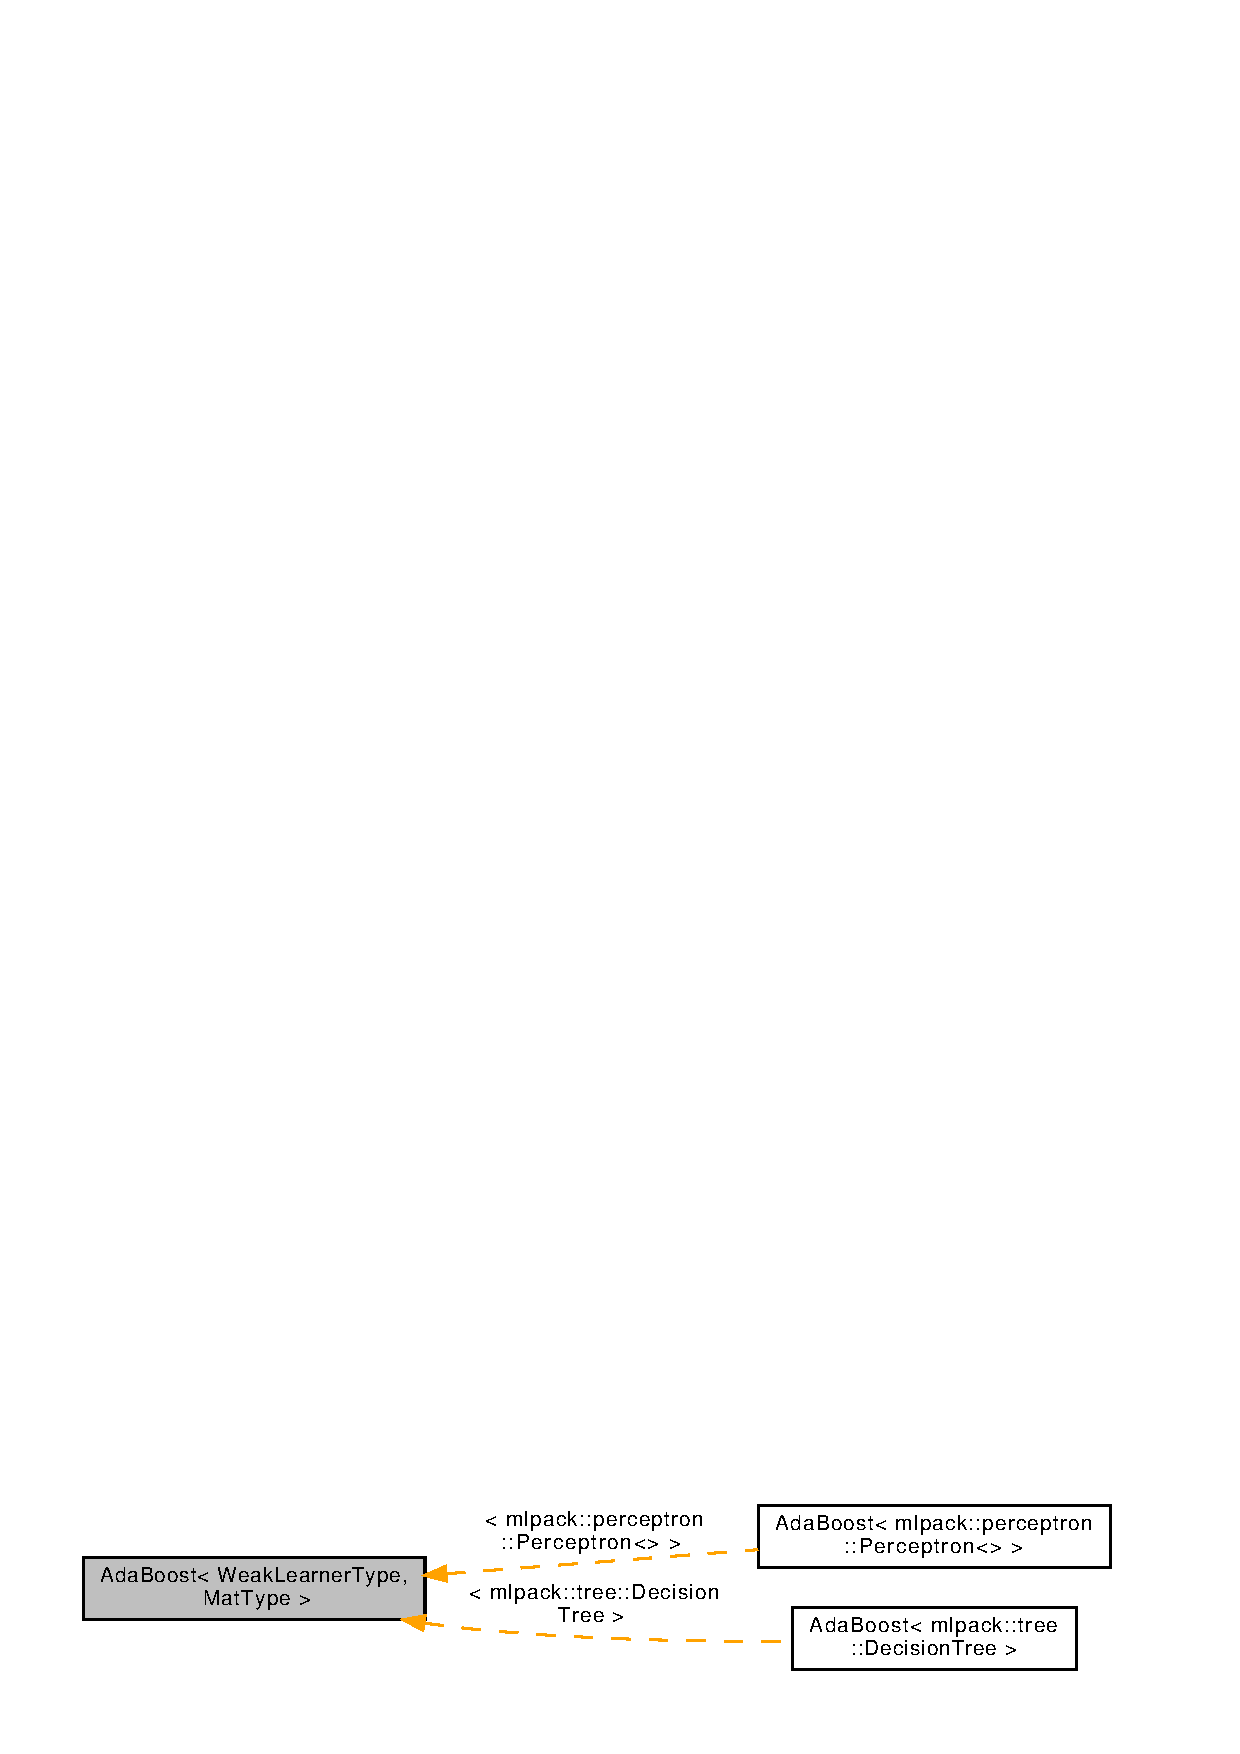
\includegraphics[width=350pt]{classmlpack_1_1adaboost_1_1AdaBoost__inherit__graph}
\end{center}
\end{figure}
\doxysubsection*{Public Member Functions}
\begin{DoxyCompactItemize}
\item 
\textbf{ Ada\+Boost} (const double tolerance=1e-\/6)
\begin{DoxyCompactList}\small\item\em Create the \doxyref{Ada\+Boost}{p.}{classmlpack_1_1adaboost_1_1AdaBoost} object without training. \end{DoxyCompactList}\item 
\textbf{ Ada\+Boost} (const Mat\+Type \&data, const arma\+::\+Row$<$ size\+\_\+t $>$ \&labels, const size\+\_\+t num\+Classes, const Weak\+Learner\+Type \&other, const size\+\_\+t iterations=100, const double tolerance=1e-\/6)
\begin{DoxyCompactList}\small\item\em Constructor. \end{DoxyCompactList}\item 
double \& \textbf{ Alpha} (const size\+\_\+t i)
\begin{DoxyCompactList}\small\item\em Modify the weight for the given weak learner (be careful!). \end{DoxyCompactList}\item 
double \textbf{ Alpha} (const size\+\_\+t i) const
\begin{DoxyCompactList}\small\item\em Get the weights for the given weak learner. \end{DoxyCompactList}\item 
void \textbf{ Classify} (const Mat\+Type \&test, arma\+::\+Row$<$ size\+\_\+t $>$ \&predicted\+Labels)
\begin{DoxyCompactList}\small\item\em Classify the given test points. \end{DoxyCompactList}\item 
void \textbf{ Classify} (const Mat\+Type \&test, arma\+::\+Row$<$ size\+\_\+t $>$ \&predicted\+Labels, arma\+::mat \&probabilities)
\begin{DoxyCompactList}\small\item\em Classify the given test points. \end{DoxyCompactList}\item 
size\+\_\+t \textbf{ Num\+Classes} () const
\begin{DoxyCompactList}\small\item\em Get the number of classes this model is trained on. \end{DoxyCompactList}\item 
{\footnotesize template$<$typename Archive $>$ }\\void \textbf{ serialize} (Archive \&ar, const uint32\+\_\+t)
\begin{DoxyCompactList}\small\item\em Serialize the \doxyref{Ada\+Boost}{p.}{classmlpack_1_1adaboost_1_1AdaBoost} model. \end{DoxyCompactList}\item 
double \& \textbf{ Tolerance} ()
\begin{DoxyCompactList}\small\item\em Modify the tolerance for stopping the optimization during training. \end{DoxyCompactList}\item 
double \textbf{ Tolerance} () const
\begin{DoxyCompactList}\small\item\em Get the tolerance for stopping the optimization during training. \end{DoxyCompactList}\item 
double \textbf{ Train} (const Mat\+Type \&data, const arma\+::\+Row$<$ size\+\_\+t $>$ \&labels, const size\+\_\+t num\+Classes, const Weak\+Learner\+Type \&learner, const size\+\_\+t iterations=100, const double tolerance=1e-\/6)
\begin{DoxyCompactList}\small\item\em Train \doxyref{Ada\+Boost}{p.}{classmlpack_1_1adaboost_1_1AdaBoost} on the given dataset. \end{DoxyCompactList}\item 
Weak\+Learner\+Type \& \textbf{ Weak\+Learner} (const size\+\_\+t i)
\begin{DoxyCompactList}\small\item\em Modify the given weak learner (be careful!). \end{DoxyCompactList}\item 
const Weak\+Learner\+Type \& \textbf{ Weak\+Learner} (const size\+\_\+t i) const
\begin{DoxyCompactList}\small\item\em Get the given weak learner. \end{DoxyCompactList}\item 
size\+\_\+t \textbf{ Weak\+Learners} () const
\begin{DoxyCompactList}\small\item\em Get the number of weak learners in the model. \end{DoxyCompactList}\end{DoxyCompactItemize}


\doxysubsection{Detailed Description}
\subsubsection*{template$<$typename Weak\+Learner\+Type = mlpack\+::perceptron\+::\+Perceptron$<$$>$, typename Mat\+Type = arma\+::mat$>$\newline
class mlpack\+::adaboost\+::\+Ada\+Boost$<$ Weak\+Learner\+Type, Mat\+Type $>$}

The \doxyref{Ada\+Boost}{p.}{classmlpack_1_1adaboost_1_1AdaBoost} class. 

\doxyref{Ada\+Boost}{p.}{classmlpack_1_1adaboost_1_1AdaBoost} is a boosting algorithm, meaning that it combines an ensemble of weak learners to produce a strong learner. For more information on \doxyref{Ada\+Boost}{p.}{classmlpack_1_1adaboost_1_1AdaBoost}, see the following paper\+:


\begin{DoxyCode}{0}
\DoxyCodeLine{@article\{schapire1999improved,}
\DoxyCodeLine{  author = \{Schapire, Robert E. and Singer, Yoram\},}
\DoxyCodeLine{  title = \{Improved Boosting Algorithms Using Confidence-\/rated Predictions\},}
\DoxyCodeLine{  journal = \{Machine Learning\},}
\DoxyCodeLine{  volume = \{37\},}
\DoxyCodeLine{  number = \{3\},}
\DoxyCodeLine{  month = dec,}
\DoxyCodeLine{  year = \{1999\},}
\DoxyCodeLine{  issn = \{0885-\/6125\},}
\DoxyCodeLine{  pages = \{297-\/-\/336\},}
\DoxyCodeLine{\}}

\end{DoxyCode}


This class is general, and can be used with any type of weak learner, so long as the learner implements the following functions\+:


\begin{DoxyCode}{0}
\DoxyCodeLine{\textcolor{comment}{// A boosting constructor, which learns using the training parameters of the}}
\DoxyCodeLine{\textcolor{comment}{// given other WeakLearner, but uses the given instance weights for training.}}
\DoxyCodeLine{WeakLearner(WeakLearner\& other,}
\DoxyCodeLine{            \textcolor{keyword}{const} MatType\& data,}
\DoxyCodeLine{            \textcolor{keyword}{const} arma::Row<size\_t>\& labels,}
\DoxyCodeLine{            \textcolor{keyword}{const} arma::rowvec\& weights);}
\DoxyCodeLine{}
\DoxyCodeLine{\textcolor{comment}{// Given the test points, classify them and output predictions into}}
\DoxyCodeLine{\textcolor{comment}{// predictedLabels.}}
\DoxyCodeLine{\textcolor{keywordtype}{void} Classify(\textcolor{keyword}{const} MatType\& data, arma::Row<size\_t>\& predictedLabels);}

\end{DoxyCode}


For more information on and examples of weak learners, see perceptron\+::\+Perceptron$<$$>$ and \doxyref{tree\+::\+ID3\+Decision\+Stump}{p.}{namespacemlpack_1_1tree_a27b9268c266fdfe2f4563d07052a0ecf}.


\begin{DoxyTemplParams}{Template Parameters}
{\em Mat\+Type} & Data matrix type (i.\+e. arma\+::mat or arma\+::sp\+\_\+mat). \\
\hline
{\em Weak\+Learner\+Type} & Type of weak learner to use. \\
\hline
\end{DoxyTemplParams}


Definition at line 81 of file adaboost.\+hpp.



\doxysubsection{Constructor \& Destructor Documentation}
\mbox{\label{classmlpack_1_1adaboost_1_1AdaBoost_a7a37dbe455d049cda36f4676b26eeb70}} 
\index{AdaBoost$<$ WeakLearnerType, MatType $>$@{AdaBoost$<$ WeakLearnerType, MatType $>$}!AdaBoost@{AdaBoost}}
\index{AdaBoost@{AdaBoost}!AdaBoost$<$ WeakLearnerType, MatType $>$@{AdaBoost$<$ WeakLearnerType, MatType $>$}}
\doxysubsubsection{AdaBoost()\hspace{0.1cm}{\footnotesize\ttfamily [1/2]}}
{\footnotesize\ttfamily \textbf{ Ada\+Boost} (\begin{DoxyParamCaption}\item[{const Mat\+Type \&}]{data,  }\item[{const arma\+::\+Row$<$ size\+\_\+t $>$ \&}]{labels,  }\item[{const size\+\_\+t}]{num\+Classes,  }\item[{const Weak\+Learner\+Type \&}]{other,  }\item[{const size\+\_\+t}]{iterations = {\ttfamily 100},  }\item[{const double}]{tolerance = {\ttfamily 1e-\/6} }\end{DoxyParamCaption})}



Constructor. 

This runs the Ada\+Boost.\+MH algorithm to provide a trained boosting model. This constructor takes an already-\/initialized weak learner; all other weak learners will learn with the same parameters as the given weak learner.


\begin{DoxyParams}{Parameters}
{\em data} & Input data. \\
\hline
{\em labels} & Corresponding labels. \\
\hline
{\em num\+Classes} & The number of classes. \\
\hline
{\em iterations} & Number of boosting rounds. \\
\hline
{\em tolerance} & The tolerance for change in values of rt. \\
\hline
{\em other} & Weak learner that has already been initialized. \\
\hline
\end{DoxyParams}
\mbox{\label{classmlpack_1_1adaboost_1_1AdaBoost_a1417a39b49cf9b28c88add6f48daa9a1}} 
\index{AdaBoost$<$ WeakLearnerType, MatType $>$@{AdaBoost$<$ WeakLearnerType, MatType $>$}!AdaBoost@{AdaBoost}}
\index{AdaBoost@{AdaBoost}!AdaBoost$<$ WeakLearnerType, MatType $>$@{AdaBoost$<$ WeakLearnerType, MatType $>$}}
\doxysubsubsection{AdaBoost()\hspace{0.1cm}{\footnotesize\ttfamily [2/2]}}
{\footnotesize\ttfamily \textbf{ Ada\+Boost} (\begin{DoxyParamCaption}\item[{const double}]{tolerance = {\ttfamily 1e-\/6} }\end{DoxyParamCaption})}



Create the \doxyref{Ada\+Boost}{p.}{classmlpack_1_1adaboost_1_1AdaBoost} object without training. 

Be sure to call \doxyref{Train()}{p.}{classmlpack_1_1adaboost_1_1AdaBoost_adeb648736c63379ce1cb5f2b23d242be} before calling \doxyref{Classify()}{p.}{classmlpack_1_1adaboost_1_1AdaBoost_abc7d38690c69822bd9ec10c3760384da}! 

\doxysubsection{Member Function Documentation}
\mbox{\label{classmlpack_1_1adaboost_1_1AdaBoost_ae59910b30903367791fde226761923cf}} 
\index{AdaBoost$<$ WeakLearnerType, MatType $>$@{AdaBoost$<$ WeakLearnerType, MatType $>$}!Alpha@{Alpha}}
\index{Alpha@{Alpha}!AdaBoost$<$ WeakLearnerType, MatType $>$@{AdaBoost$<$ WeakLearnerType, MatType $>$}}
\doxysubsubsection{Alpha()\hspace{0.1cm}{\footnotesize\ttfamily [1/2]}}
{\footnotesize\ttfamily double\& Alpha (\begin{DoxyParamCaption}\item[{const size\+\_\+t}]{i }\end{DoxyParamCaption})\hspace{0.3cm}{\ttfamily [inline]}}



Modify the weight for the given weak learner (be careful!). 



Definition at line 124 of file adaboost.\+hpp.

\mbox{\label{classmlpack_1_1adaboost_1_1AdaBoost_af0e29824cfcada4ec450e4d09cc9a314}} 
\index{AdaBoost$<$ WeakLearnerType, MatType $>$@{AdaBoost$<$ WeakLearnerType, MatType $>$}!Alpha@{Alpha}}
\index{Alpha@{Alpha}!AdaBoost$<$ WeakLearnerType, MatType $>$@{AdaBoost$<$ WeakLearnerType, MatType $>$}}
\doxysubsubsection{Alpha()\hspace{0.1cm}{\footnotesize\ttfamily [2/2]}}
{\footnotesize\ttfamily double Alpha (\begin{DoxyParamCaption}\item[{const size\+\_\+t}]{i }\end{DoxyParamCaption}) const\hspace{0.3cm}{\ttfamily [inline]}}



Get the weights for the given weak learner. 



Definition at line 122 of file adaboost.\+hpp.

\mbox{\label{classmlpack_1_1adaboost_1_1AdaBoost_a407f9c281dab80fffd49251d3907838d}} 
\index{AdaBoost$<$ WeakLearnerType, MatType $>$@{AdaBoost$<$ WeakLearnerType, MatType $>$}!Classify@{Classify}}
\index{Classify@{Classify}!AdaBoost$<$ WeakLearnerType, MatType $>$@{AdaBoost$<$ WeakLearnerType, MatType $>$}}
\doxysubsubsection{Classify()\hspace{0.1cm}{\footnotesize\ttfamily [1/2]}}
{\footnotesize\ttfamily void Classify (\begin{DoxyParamCaption}\item[{const Mat\+Type \&}]{test,  }\item[{arma\+::\+Row$<$ size\+\_\+t $>$ \&}]{predicted\+Labels }\end{DoxyParamCaption})}



Classify the given test points. 


\begin{DoxyParams}{Parameters}
{\em test} & Testing data. \\
\hline
{\em predicted\+Labels} & Vector in which the predicted labels of the test set will be stored. \\
\hline
\end{DoxyParams}
\mbox{\label{classmlpack_1_1adaboost_1_1AdaBoost_abc7d38690c69822bd9ec10c3760384da}} 
\index{AdaBoost$<$ WeakLearnerType, MatType $>$@{AdaBoost$<$ WeakLearnerType, MatType $>$}!Classify@{Classify}}
\index{Classify@{Classify}!AdaBoost$<$ WeakLearnerType, MatType $>$@{AdaBoost$<$ WeakLearnerType, MatType $>$}}
\doxysubsubsection{Classify()\hspace{0.1cm}{\footnotesize\ttfamily [2/2]}}
{\footnotesize\ttfamily void Classify (\begin{DoxyParamCaption}\item[{const Mat\+Type \&}]{test,  }\item[{arma\+::\+Row$<$ size\+\_\+t $>$ \&}]{predicted\+Labels,  }\item[{arma\+::mat \&}]{probabilities }\end{DoxyParamCaption})}



Classify the given test points. 


\begin{DoxyParams}{Parameters}
{\em test} & Testing data. \\
\hline
{\em predicted\+Labels} & Vector in which the predicted labels of the test set will be stored. \\
\hline
{\em probabilities} & matrix to store the predicted class probabilities for each point in the test set. \\
\hline
\end{DoxyParams}
\mbox{\label{classmlpack_1_1adaboost_1_1AdaBoost_a088ebfdf3c7a9e7eea81716d0c55b5a3}} 
\index{AdaBoost$<$ WeakLearnerType, MatType $>$@{AdaBoost$<$ WeakLearnerType, MatType $>$}!NumClasses@{NumClasses}}
\index{NumClasses@{NumClasses}!AdaBoost$<$ WeakLearnerType, MatType $>$@{AdaBoost$<$ WeakLearnerType, MatType $>$}}
\doxysubsubsection{NumClasses()}
{\footnotesize\ttfamily size\+\_\+t Num\+Classes (\begin{DoxyParamCaption}{ }\end{DoxyParamCaption}) const\hspace{0.3cm}{\ttfamily [inline]}}



Get the number of classes this model is trained on. 



Definition at line 116 of file adaboost.\+hpp.

\mbox{\label{classmlpack_1_1adaboost_1_1AdaBoost_a65cba07328997659bec80b9879b15a51}} 
\index{AdaBoost$<$ WeakLearnerType, MatType $>$@{AdaBoost$<$ WeakLearnerType, MatType $>$}!serialize@{serialize}}
\index{serialize@{serialize}!AdaBoost$<$ WeakLearnerType, MatType $>$@{AdaBoost$<$ WeakLearnerType, MatType $>$}}
\doxysubsubsection{serialize()}
{\footnotesize\ttfamily void serialize (\begin{DoxyParamCaption}\item[{Archive \&}]{ar,  }\item[{const uint32\+\_\+t}]{ }\end{DoxyParamCaption})}



Serialize the \doxyref{Ada\+Boost}{p.}{classmlpack_1_1adaboost_1_1AdaBoost} model. 

\mbox{\label{classmlpack_1_1adaboost_1_1AdaBoost_a3d9fac84af16250f5a3689692e8f2173}} 
\index{AdaBoost$<$ WeakLearnerType, MatType $>$@{AdaBoost$<$ WeakLearnerType, MatType $>$}!Tolerance@{Tolerance}}
\index{Tolerance@{Tolerance}!AdaBoost$<$ WeakLearnerType, MatType $>$@{AdaBoost$<$ WeakLearnerType, MatType $>$}}
\doxysubsubsection{Tolerance()\hspace{0.1cm}{\footnotesize\ttfamily [1/2]}}
{\footnotesize\ttfamily double\& Tolerance (\begin{DoxyParamCaption}{ }\end{DoxyParamCaption})\hspace{0.3cm}{\ttfamily [inline]}}



Modify the tolerance for stopping the optimization during training. 



Definition at line 113 of file adaboost.\+hpp.

\mbox{\label{classmlpack_1_1adaboost_1_1AdaBoost_a7b5af5c1a84c507cbaa7f999ea5a4fda}} 
\index{AdaBoost$<$ WeakLearnerType, MatType $>$@{AdaBoost$<$ WeakLearnerType, MatType $>$}!Tolerance@{Tolerance}}
\index{Tolerance@{Tolerance}!AdaBoost$<$ WeakLearnerType, MatType $>$@{AdaBoost$<$ WeakLearnerType, MatType $>$}}
\doxysubsubsection{Tolerance()\hspace{0.1cm}{\footnotesize\ttfamily [2/2]}}
{\footnotesize\ttfamily double Tolerance (\begin{DoxyParamCaption}{ }\end{DoxyParamCaption}) const\hspace{0.3cm}{\ttfamily [inline]}}



Get the tolerance for stopping the optimization during training. 



Definition at line 111 of file adaboost.\+hpp.

\mbox{\label{classmlpack_1_1adaboost_1_1AdaBoost_adeb648736c63379ce1cb5f2b23d242be}} 
\index{AdaBoost$<$ WeakLearnerType, MatType $>$@{AdaBoost$<$ WeakLearnerType, MatType $>$}!Train@{Train}}
\index{Train@{Train}!AdaBoost$<$ WeakLearnerType, MatType $>$@{AdaBoost$<$ WeakLearnerType, MatType $>$}}
\doxysubsubsection{Train()}
{\footnotesize\ttfamily double Train (\begin{DoxyParamCaption}\item[{const Mat\+Type \&}]{data,  }\item[{const arma\+::\+Row$<$ size\+\_\+t $>$ \&}]{labels,  }\item[{const size\+\_\+t}]{num\+Classes,  }\item[{const Weak\+Learner\+Type \&}]{learner,  }\item[{const size\+\_\+t}]{iterations = {\ttfamily 100},  }\item[{const double}]{tolerance = {\ttfamily 1e-\/6} }\end{DoxyParamCaption})}



Train \doxyref{Ada\+Boost}{p.}{classmlpack_1_1adaboost_1_1AdaBoost} on the given dataset. 

This method takes an initialized Weak\+Learner\+Type; the parameters for this weak learner will be used to train each of the weak learners during \doxyref{Ada\+Boost}{p.}{classmlpack_1_1adaboost_1_1AdaBoost} training. Note that this will completely overwrite any model that has already been trained with this object.


\begin{DoxyParams}{Parameters}
{\em data} & Dataset to train on. \\
\hline
{\em labels} & Labels for each point in the dataset. \\
\hline
{\em num\+Classes} & The number of classes. \\
\hline
{\em learner} & Learner to use for training. \\
\hline
{\em iterations} & Number of boosting rounds. \\
\hline
{\em tolerance} & The tolerance for change in values of rt. \\
\hline
\end{DoxyParams}
\begin{DoxyReturn}{Returns}
The upper bound for training error. 
\end{DoxyReturn}
\mbox{\label{classmlpack_1_1adaboost_1_1AdaBoost_a11d7a531e3de5cdd5cc8f0cc02b8ed4d}} 
\index{AdaBoost$<$ WeakLearnerType, MatType $>$@{AdaBoost$<$ WeakLearnerType, MatType $>$}!WeakLearner@{WeakLearner}}
\index{WeakLearner@{WeakLearner}!AdaBoost$<$ WeakLearnerType, MatType $>$@{AdaBoost$<$ WeakLearnerType, MatType $>$}}
\doxysubsubsection{WeakLearner()\hspace{0.1cm}{\footnotesize\ttfamily [1/2]}}
{\footnotesize\ttfamily Weak\+Learner\+Type\& Weak\+Learner (\begin{DoxyParamCaption}\item[{const size\+\_\+t}]{i }\end{DoxyParamCaption})\hspace{0.3cm}{\ttfamily [inline]}}



Modify the given weak learner (be careful!). 



Definition at line 129 of file adaboost.\+hpp.

\mbox{\label{classmlpack_1_1adaboost_1_1AdaBoost_aa6f54b09b480fed23b0b04214e300cbf}} 
\index{AdaBoost$<$ WeakLearnerType, MatType $>$@{AdaBoost$<$ WeakLearnerType, MatType $>$}!WeakLearner@{WeakLearner}}
\index{WeakLearner@{WeakLearner}!AdaBoost$<$ WeakLearnerType, MatType $>$@{AdaBoost$<$ WeakLearnerType, MatType $>$}}
\doxysubsubsection{WeakLearner()\hspace{0.1cm}{\footnotesize\ttfamily [2/2]}}
{\footnotesize\ttfamily const Weak\+Learner\+Type\& Weak\+Learner (\begin{DoxyParamCaption}\item[{const size\+\_\+t}]{i }\end{DoxyParamCaption}) const\hspace{0.3cm}{\ttfamily [inline]}}



Get the given weak learner. 



Definition at line 127 of file adaboost.\+hpp.

\mbox{\label{classmlpack_1_1adaboost_1_1AdaBoost_a5bb6ee8b31c0e16567eee13cb3719f88}} 
\index{AdaBoost$<$ WeakLearnerType, MatType $>$@{AdaBoost$<$ WeakLearnerType, MatType $>$}!WeakLearners@{WeakLearners}}
\index{WeakLearners@{WeakLearners}!AdaBoost$<$ WeakLearnerType, MatType $>$@{AdaBoost$<$ WeakLearnerType, MatType $>$}}
\doxysubsubsection{WeakLearners()}
{\footnotesize\ttfamily size\+\_\+t Weak\+Learners (\begin{DoxyParamCaption}{ }\end{DoxyParamCaption}) const\hspace{0.3cm}{\ttfamily [inline]}}



Get the number of weak learners in the model. 



Definition at line 119 of file adaboost.\+hpp.



The documentation for this class was generated from the following file\+:\begin{DoxyCompactItemize}
\item 
/home/aakash/mlpack/src/mlpack/methods/adaboost/\textbf{ adaboost.\+hpp}\end{DoxyCompactItemize}

\section{mlpack\+:\+:adaboost\+:\+:Ada\+Boost\+Model Class Reference}
\label{classmlpack_1_1adaboost_1_1AdaBoostModel}\index{mlpack\+::adaboost\+::\+Ada\+Boost\+Model@{mlpack\+::adaboost\+::\+Ada\+Boost\+Model}}


The model to save to disk.  


\subsection*{Public Types}
\begin{DoxyCompactItemize}
\item 
enum {\bf Weak\+Learner\+Types} \{ \\*
{\bf D\+E\+C\+I\+S\+I\+O\+N\+\_\+\+S\+T\+U\+MP}, 
\\*
{\bf P\+E\+R\+C\+E\+P\+T\+R\+ON}
 \}
\end{DoxyCompactItemize}
\subsection*{Public Member Functions}
\begin{DoxyCompactItemize}
\item 
{\bf Ada\+Boost\+Model} ()
\begin{DoxyCompactList}\small\item\em Create an empty \doxyref{Ada\+Boost}{p.}{classmlpack_1_1adaboost_1_1AdaBoost} model. \end{DoxyCompactList}\item 
{\bf Ada\+Boost\+Model} (const arma\+::\+Col$<$ size\+\_\+t $>$ \&{\bf mappings}, const size\+\_\+t {\bf weak\+Learner\+Type})
\begin{DoxyCompactList}\small\item\em Create the \doxyref{Ada\+Boost}{p.}{classmlpack_1_1adaboost_1_1AdaBoost} model with the given mappings and type. \end{DoxyCompactList}\item 
{\bf Ada\+Boost\+Model} (const {\bf Ada\+Boost\+Model} \&other)
\begin{DoxyCompactList}\small\item\em Copy constructor. \end{DoxyCompactList}\item 
{\bf Ada\+Boost\+Model} ({\bf Ada\+Boost\+Model} \&\&other)
\begin{DoxyCompactList}\small\item\em Move constructor. \end{DoxyCompactList}\item 
{\bf $\sim$\+Ada\+Boost\+Model} ()
\begin{DoxyCompactList}\small\item\em Clean up memory. \end{DoxyCompactList}\item 
void {\bf Classify} (const arma\+::mat \&test\+Data, arma\+::\+Row$<$ size\+\_\+t $>$ \&predictions)
\begin{DoxyCompactList}\small\item\em Classify test points. \end{DoxyCompactList}\item 
size\+\_\+t {\bf Dimensionality} () const 
\begin{DoxyCompactList}\small\item\em Get the dimensionality of the model. \end{DoxyCompactList}\item 
size\+\_\+t \& {\bf Dimensionality} ()
\begin{DoxyCompactList}\small\item\em Modify the dimensionality of the model. \end{DoxyCompactList}\item 
const arma\+::\+Col$<$ size\+\_\+t $>$ \& {\bf Mappings} () const 
\begin{DoxyCompactList}\small\item\em Get the mappings. \end{DoxyCompactList}\item 
arma\+::\+Col$<$ size\+\_\+t $>$ \& {\bf Mappings} ()
\begin{DoxyCompactList}\small\item\em Modify the mappings. \end{DoxyCompactList}\item 
{\bf Ada\+Boost\+Model} \& {\bf operator=} (const {\bf Ada\+Boost\+Model} \&other)
\begin{DoxyCompactList}\small\item\em Copy assignment operator. \end{DoxyCompactList}\item 
{\footnotesize template$<$typename Archive $>$ }\\void {\bf Serialize} (Archive \&ar, const unsigned int)
\begin{DoxyCompactList}\small\item\em Serialize the model. \end{DoxyCompactList}\item 
void {\bf Train} (const arma\+::mat \&data, const arma\+::\+Row$<$ size\+\_\+t $>$ \&labels, const size\+\_\+t iterations, const double tolerance)
\begin{DoxyCompactList}\small\item\em Train the model. \end{DoxyCompactList}\item 
size\+\_\+t {\bf Weak\+Learner\+Type} () const 
\begin{DoxyCompactList}\small\item\em Get the weak learner type. \end{DoxyCompactList}\item 
size\+\_\+t \& {\bf Weak\+Learner\+Type} ()
\begin{DoxyCompactList}\small\item\em Modify the weak learner type. \end{DoxyCompactList}\end{DoxyCompactItemize}
\subsection*{Private Attributes}
\begin{DoxyCompactItemize}
\item 
size\+\_\+t {\bf dimensionality}
\begin{DoxyCompactList}\small\item\em Number of dimensions in training data. \end{DoxyCompactList}\item 
{\bf Ada\+Boost}$<$ {\bf decision\+\_\+stump\+::\+Decision\+Stump}$<$$>$ $>$ $\ast$ {\bf ds\+Boost}
\begin{DoxyCompactList}\small\item\em Non-\/\+N\+U\+LL if using decision stumps. \end{DoxyCompactList}\item 
arma\+::\+Col$<$ size\+\_\+t $>$ {\bf mappings}
\begin{DoxyCompactList}\small\item\em The mappings for the labels. \end{DoxyCompactList}\item 
{\bf Ada\+Boost}$<$ {\bf perceptron\+::\+Perceptron}$<$$>$ $>$ $\ast$ {\bf p\+Boost}
\begin{DoxyCompactList}\small\item\em Non-\/\+N\+U\+LL if using perceptrons. \end{DoxyCompactList}\item 
size\+\_\+t {\bf weak\+Learner\+Type}
\begin{DoxyCompactList}\small\item\em The type of weak learner. \end{DoxyCompactList}\end{DoxyCompactItemize}


\subsection{Detailed Description}
The model to save to disk. 

Definition at line 19 of file adaboost\+\_\+model.\+hpp.



\subsection{Member Enumeration Documentation}
\index{mlpack\+::adaboost\+::\+Ada\+Boost\+Model@{mlpack\+::adaboost\+::\+Ada\+Boost\+Model}!Weak\+Learner\+Types@{Weak\+Learner\+Types}}
\index{Weak\+Learner\+Types@{Weak\+Learner\+Types}!mlpack\+::adaboost\+::\+Ada\+Boost\+Model@{mlpack\+::adaboost\+::\+Ada\+Boost\+Model}}
\subsubsection[{Weak\+Learner\+Types}]{\setlength{\rightskip}{0pt plus 5cm}enum {\bf mlpack\+::adaboost\+::\+Ada\+Boost\+Model\+::\+Weak\+Learner\+Types}}\label{classmlpack_1_1adaboost_1_1AdaBoostModel_a8c6d05405728a675084fb8b1abfb3673}
\begin{Desc}
\item[Enumerator]\par
\begin{description}
\index{D\+E\+C\+I\+S\+I\+O\+N\+\_\+\+S\+T\+U\+MP@{D\+E\+C\+I\+S\+I\+O\+N\+\_\+\+S\+T\+U\+MP}!mlpack\+::adaboost\+::\+Ada\+Boost\+Model@{mlpack\+::adaboost\+::\+Ada\+Boost\+Model}}\index{mlpack\+::adaboost\+::\+Ada\+Boost\+Model@{mlpack\+::adaboost\+::\+Ada\+Boost\+Model}!D\+E\+C\+I\+S\+I\+O\+N\+\_\+\+S\+T\+U\+MP@{D\+E\+C\+I\+S\+I\+O\+N\+\_\+\+S\+T\+U\+MP}}\item[{\em 
D\+E\+C\+I\+S\+I\+O\+N\+\_\+\+S\+T\+U\+MP\label{classmlpack_1_1adaboost_1_1AdaBoostModel_a8c6d05405728a675084fb8b1abfb3673aa6bf729b055198ba7ac1ea9ce46b0b2b}
}]\index{P\+E\+R\+C\+E\+P\+T\+R\+ON@{P\+E\+R\+C\+E\+P\+T\+R\+ON}!mlpack\+::adaboost\+::\+Ada\+Boost\+Model@{mlpack\+::adaboost\+::\+Ada\+Boost\+Model}}\index{mlpack\+::adaboost\+::\+Ada\+Boost\+Model@{mlpack\+::adaboost\+::\+Ada\+Boost\+Model}!P\+E\+R\+C\+E\+P\+T\+R\+ON@{P\+E\+R\+C\+E\+P\+T\+R\+ON}}\item[{\em 
P\+E\+R\+C\+E\+P\+T\+R\+ON\label{classmlpack_1_1adaboost_1_1AdaBoostModel_a8c6d05405728a675084fb8b1abfb3673ade8f0280fbf6831626a1cb0ca8db1d5e}
}]\end{description}
\end{Desc}


Definition at line 22 of file adaboost\+\_\+model.\+hpp.



\subsection{Constructor \& Destructor Documentation}
\index{mlpack\+::adaboost\+::\+Ada\+Boost\+Model@{mlpack\+::adaboost\+::\+Ada\+Boost\+Model}!Ada\+Boost\+Model@{Ada\+Boost\+Model}}
\index{Ada\+Boost\+Model@{Ada\+Boost\+Model}!mlpack\+::adaboost\+::\+Ada\+Boost\+Model@{mlpack\+::adaboost\+::\+Ada\+Boost\+Model}}
\subsubsection[{Ada\+Boost\+Model()}]{\setlength{\rightskip}{0pt plus 5cm}mlpack\+::adaboost\+::\+Ada\+Boost\+Model\+::\+Ada\+Boost\+Model (
\begin{DoxyParamCaption}
{}
\end{DoxyParamCaption}
)}\label{classmlpack_1_1adaboost_1_1AdaBoostModel_af0335c1a7e103dbca42c00ac3fb94596}


Create an empty \doxyref{Ada\+Boost}{p.}{classmlpack_1_1adaboost_1_1AdaBoost} model. 

\index{mlpack\+::adaboost\+::\+Ada\+Boost\+Model@{mlpack\+::adaboost\+::\+Ada\+Boost\+Model}!Ada\+Boost\+Model@{Ada\+Boost\+Model}}
\index{Ada\+Boost\+Model@{Ada\+Boost\+Model}!mlpack\+::adaboost\+::\+Ada\+Boost\+Model@{mlpack\+::adaboost\+::\+Ada\+Boost\+Model}}
\subsubsection[{Ada\+Boost\+Model(const arma\+::\+Col$<$ size\+\_\+t $>$ \&mappings, const size\+\_\+t weak\+Learner\+Type)}]{\setlength{\rightskip}{0pt plus 5cm}mlpack\+::adaboost\+::\+Ada\+Boost\+Model\+::\+Ada\+Boost\+Model (
\begin{DoxyParamCaption}
\item[{const arma\+::\+Col$<$ size\+\_\+t $>$ \&}]{mappings, }
\item[{const size\+\_\+t}]{weak\+Learner\+Type}
\end{DoxyParamCaption}
)}\label{classmlpack_1_1adaboost_1_1AdaBoostModel_ac532b4e4f7cc33ad760db7ecd4197fe9}


Create the \doxyref{Ada\+Boost}{p.}{classmlpack_1_1adaboost_1_1AdaBoost} model with the given mappings and type. 

\index{mlpack\+::adaboost\+::\+Ada\+Boost\+Model@{mlpack\+::adaboost\+::\+Ada\+Boost\+Model}!Ada\+Boost\+Model@{Ada\+Boost\+Model}}
\index{Ada\+Boost\+Model@{Ada\+Boost\+Model}!mlpack\+::adaboost\+::\+Ada\+Boost\+Model@{mlpack\+::adaboost\+::\+Ada\+Boost\+Model}}
\subsubsection[{Ada\+Boost\+Model(const Ada\+Boost\+Model \&other)}]{\setlength{\rightskip}{0pt plus 5cm}mlpack\+::adaboost\+::\+Ada\+Boost\+Model\+::\+Ada\+Boost\+Model (
\begin{DoxyParamCaption}
\item[{const {\bf Ada\+Boost\+Model} \&}]{other}
\end{DoxyParamCaption}
)}\label{classmlpack_1_1adaboost_1_1AdaBoostModel_a56456937ecdd61a99f3ba6168cf8cace}


Copy constructor. 

\index{mlpack\+::adaboost\+::\+Ada\+Boost\+Model@{mlpack\+::adaboost\+::\+Ada\+Boost\+Model}!Ada\+Boost\+Model@{Ada\+Boost\+Model}}
\index{Ada\+Boost\+Model@{Ada\+Boost\+Model}!mlpack\+::adaboost\+::\+Ada\+Boost\+Model@{mlpack\+::adaboost\+::\+Ada\+Boost\+Model}}
\subsubsection[{Ada\+Boost\+Model(\+Ada\+Boost\+Model \&\&other)}]{\setlength{\rightskip}{0pt plus 5cm}mlpack\+::adaboost\+::\+Ada\+Boost\+Model\+::\+Ada\+Boost\+Model (
\begin{DoxyParamCaption}
\item[{{\bf Ada\+Boost\+Model} \&\&}]{other}
\end{DoxyParamCaption}
)}\label{classmlpack_1_1adaboost_1_1AdaBoostModel_a943f899d9f08a3a0b73daa5c6ede7e2c}


Move constructor. 

\index{mlpack\+::adaboost\+::\+Ada\+Boost\+Model@{mlpack\+::adaboost\+::\+Ada\+Boost\+Model}!````~Ada\+Boost\+Model@{$\sim$\+Ada\+Boost\+Model}}
\index{````~Ada\+Boost\+Model@{$\sim$\+Ada\+Boost\+Model}!mlpack\+::adaboost\+::\+Ada\+Boost\+Model@{mlpack\+::adaboost\+::\+Ada\+Boost\+Model}}
\subsubsection[{$\sim$\+Ada\+Boost\+Model()}]{\setlength{\rightskip}{0pt plus 5cm}mlpack\+::adaboost\+::\+Ada\+Boost\+Model\+::$\sim$\+Ada\+Boost\+Model (
\begin{DoxyParamCaption}
{}
\end{DoxyParamCaption}
)}\label{classmlpack_1_1adaboost_1_1AdaBoostModel_ace08fcd5fbf95e4ab259aef8c8f6a40c}


Clean up memory. 



\subsection{Member Function Documentation}
\index{mlpack\+::adaboost\+::\+Ada\+Boost\+Model@{mlpack\+::adaboost\+::\+Ada\+Boost\+Model}!Classify@{Classify}}
\index{Classify@{Classify}!mlpack\+::adaboost\+::\+Ada\+Boost\+Model@{mlpack\+::adaboost\+::\+Ada\+Boost\+Model}}
\subsubsection[{Classify(const arma\+::mat \&test\+Data, arma\+::\+Row$<$ size\+\_\+t $>$ \&predictions)}]{\setlength{\rightskip}{0pt plus 5cm}void mlpack\+::adaboost\+::\+Ada\+Boost\+Model\+::\+Classify (
\begin{DoxyParamCaption}
\item[{const arma\+::mat \&}]{test\+Data, }
\item[{arma\+::\+Row$<$ size\+\_\+t $>$ \&}]{predictions}
\end{DoxyParamCaption}
)}\label{classmlpack_1_1adaboost_1_1AdaBoostModel_ae6d95f49a266fd0425bb40f640d5bb19}


Classify test points. 



Referenced by Dimensionality().

\index{mlpack\+::adaboost\+::\+Ada\+Boost\+Model@{mlpack\+::adaboost\+::\+Ada\+Boost\+Model}!Dimensionality@{Dimensionality}}
\index{Dimensionality@{Dimensionality}!mlpack\+::adaboost\+::\+Ada\+Boost\+Model@{mlpack\+::adaboost\+::\+Ada\+Boost\+Model}}
\subsubsection[{Dimensionality() const }]{\setlength{\rightskip}{0pt plus 5cm}size\+\_\+t mlpack\+::adaboost\+::\+Ada\+Boost\+Model\+::\+Dimensionality (
\begin{DoxyParamCaption}
{}
\end{DoxyParamCaption}
) const\hspace{0.3cm}{\ttfamily [inline]}}\label{classmlpack_1_1adaboost_1_1AdaBoostModel_a079682b4ebad69441d8949d46ff3aca5}


Get the dimensionality of the model. 



Definition at line 71 of file adaboost\+\_\+model.\+hpp.



References dimensionality.

\index{mlpack\+::adaboost\+::\+Ada\+Boost\+Model@{mlpack\+::adaboost\+::\+Ada\+Boost\+Model}!Dimensionality@{Dimensionality}}
\index{Dimensionality@{Dimensionality}!mlpack\+::adaboost\+::\+Ada\+Boost\+Model@{mlpack\+::adaboost\+::\+Ada\+Boost\+Model}}
\subsubsection[{Dimensionality()}]{\setlength{\rightskip}{0pt plus 5cm}size\+\_\+t\& mlpack\+::adaboost\+::\+Ada\+Boost\+Model\+::\+Dimensionality (
\begin{DoxyParamCaption}
{}
\end{DoxyParamCaption}
)\hspace{0.3cm}{\ttfamily [inline]}}\label{classmlpack_1_1adaboost_1_1AdaBoostModel_aa1328eff9fd2d5db8aa9187a96d995a9}


Modify the dimensionality of the model. 



Definition at line 73 of file adaboost\+\_\+model.\+hpp.



References Classify(), dimensionality, and Train().

\index{mlpack\+::adaboost\+::\+Ada\+Boost\+Model@{mlpack\+::adaboost\+::\+Ada\+Boost\+Model}!Mappings@{Mappings}}
\index{Mappings@{Mappings}!mlpack\+::adaboost\+::\+Ada\+Boost\+Model@{mlpack\+::adaboost\+::\+Ada\+Boost\+Model}}
\subsubsection[{Mappings() const }]{\setlength{\rightskip}{0pt plus 5cm}const arma\+::\+Col$<$size\+\_\+t$>$\& mlpack\+::adaboost\+::\+Ada\+Boost\+Model\+::\+Mappings (
\begin{DoxyParamCaption}
{}
\end{DoxyParamCaption}
) const\hspace{0.3cm}{\ttfamily [inline]}}\label{classmlpack_1_1adaboost_1_1AdaBoostModel_a301acd979a0d1a58a7ca80a480b433f1}


Get the mappings. 



Definition at line 61 of file adaboost\+\_\+model.\+hpp.



References mappings.

\index{mlpack\+::adaboost\+::\+Ada\+Boost\+Model@{mlpack\+::adaboost\+::\+Ada\+Boost\+Model}!Mappings@{Mappings}}
\index{Mappings@{Mappings}!mlpack\+::adaboost\+::\+Ada\+Boost\+Model@{mlpack\+::adaboost\+::\+Ada\+Boost\+Model}}
\subsubsection[{Mappings()}]{\setlength{\rightskip}{0pt plus 5cm}arma\+::\+Col$<$size\+\_\+t$>$\& mlpack\+::adaboost\+::\+Ada\+Boost\+Model\+::\+Mappings (
\begin{DoxyParamCaption}
{}
\end{DoxyParamCaption}
)\hspace{0.3cm}{\ttfamily [inline]}}\label{classmlpack_1_1adaboost_1_1AdaBoostModel_a4822c44d3274802472e96800db3adf46}


Modify the mappings. 



Definition at line 63 of file adaboost\+\_\+model.\+hpp.



References mappings.

\index{mlpack\+::adaboost\+::\+Ada\+Boost\+Model@{mlpack\+::adaboost\+::\+Ada\+Boost\+Model}!operator=@{operator=}}
\index{operator=@{operator=}!mlpack\+::adaboost\+::\+Ada\+Boost\+Model@{mlpack\+::adaboost\+::\+Ada\+Boost\+Model}}
\subsubsection[{operator=(const Ada\+Boost\+Model \&other)}]{\setlength{\rightskip}{0pt plus 5cm}{\bf Ada\+Boost\+Model}\& mlpack\+::adaboost\+::\+Ada\+Boost\+Model\+::operator= (
\begin{DoxyParamCaption}
\item[{const {\bf Ada\+Boost\+Model} \&}]{other}
\end{DoxyParamCaption}
)}\label{classmlpack_1_1adaboost_1_1AdaBoostModel_ab04ecf1eb79af9d385bf68624032d806}


Copy assignment operator. 

\index{mlpack\+::adaboost\+::\+Ada\+Boost\+Model@{mlpack\+::adaboost\+::\+Ada\+Boost\+Model}!Serialize@{Serialize}}
\index{Serialize@{Serialize}!mlpack\+::adaboost\+::\+Ada\+Boost\+Model@{mlpack\+::adaboost\+::\+Ada\+Boost\+Model}}
\subsubsection[{Serialize(\+Archive \&ar, const unsigned int)}]{\setlength{\rightskip}{0pt plus 5cm}template$<$typename Archive $>$ void mlpack\+::adaboost\+::\+Ada\+Boost\+Model\+::\+Serialize (
\begin{DoxyParamCaption}
\item[{Archive \&}]{ar, }
\item[{const unsigned}]{int}
\end{DoxyParamCaption}
)\hspace{0.3cm}{\ttfamily [inline]}}\label{classmlpack_1_1adaboost_1_1AdaBoostModel_a6b345710ab674eb303ffe307f20d5405}


Serialize the model. 



Definition at line 86 of file adaboost\+\_\+model.\+hpp.



References mlpack\+::data\+::\+Create\+N\+V\+P(), ds\+Boost, and p\+Boost.

\index{mlpack\+::adaboost\+::\+Ada\+Boost\+Model@{mlpack\+::adaboost\+::\+Ada\+Boost\+Model}!Train@{Train}}
\index{Train@{Train}!mlpack\+::adaboost\+::\+Ada\+Boost\+Model@{mlpack\+::adaboost\+::\+Ada\+Boost\+Model}}
\subsubsection[{Train(const arma\+::mat \&data, const arma\+::\+Row$<$ size\+\_\+t $>$ \&labels, const size\+\_\+t iterations, const double tolerance)}]{\setlength{\rightskip}{0pt plus 5cm}void mlpack\+::adaboost\+::\+Ada\+Boost\+Model\+::\+Train (
\begin{DoxyParamCaption}
\item[{const arma\+::mat \&}]{data, }
\item[{const arma\+::\+Row$<$ size\+\_\+t $>$ \&}]{labels, }
\item[{const size\+\_\+t}]{iterations, }
\item[{const double}]{tolerance}
\end{DoxyParamCaption}
)}\label{classmlpack_1_1adaboost_1_1AdaBoostModel_a2063ee60ef71ae78c0c74b4ee332f2a0}


Train the model. 



Referenced by Dimensionality().

\index{mlpack\+::adaboost\+::\+Ada\+Boost\+Model@{mlpack\+::adaboost\+::\+Ada\+Boost\+Model}!Weak\+Learner\+Type@{Weak\+Learner\+Type}}
\index{Weak\+Learner\+Type@{Weak\+Learner\+Type}!mlpack\+::adaboost\+::\+Ada\+Boost\+Model@{mlpack\+::adaboost\+::\+Ada\+Boost\+Model}}
\subsubsection[{Weak\+Learner\+Type() const }]{\setlength{\rightskip}{0pt plus 5cm}size\+\_\+t mlpack\+::adaboost\+::\+Ada\+Boost\+Model\+::\+Weak\+Learner\+Type (
\begin{DoxyParamCaption}
{}
\end{DoxyParamCaption}
) const\hspace{0.3cm}{\ttfamily [inline]}}\label{classmlpack_1_1adaboost_1_1AdaBoostModel_a1e494e25bbb89e0d4d7134b8cd179169}


Get the weak learner type. 



Definition at line 66 of file adaboost\+\_\+model.\+hpp.



References weak\+Learner\+Type.

\index{mlpack\+::adaboost\+::\+Ada\+Boost\+Model@{mlpack\+::adaboost\+::\+Ada\+Boost\+Model}!Weak\+Learner\+Type@{Weak\+Learner\+Type}}
\index{Weak\+Learner\+Type@{Weak\+Learner\+Type}!mlpack\+::adaboost\+::\+Ada\+Boost\+Model@{mlpack\+::adaboost\+::\+Ada\+Boost\+Model}}
\subsubsection[{Weak\+Learner\+Type()}]{\setlength{\rightskip}{0pt plus 5cm}size\+\_\+t\& mlpack\+::adaboost\+::\+Ada\+Boost\+Model\+::\+Weak\+Learner\+Type (
\begin{DoxyParamCaption}
{}
\end{DoxyParamCaption}
)\hspace{0.3cm}{\ttfamily [inline]}}\label{classmlpack_1_1adaboost_1_1AdaBoostModel_a39352f5bd2709d235a25e890655a9b8d}


Modify the weak learner type. 



Definition at line 68 of file adaboost\+\_\+model.\+hpp.



References weak\+Learner\+Type.



\subsection{Member Data Documentation}
\index{mlpack\+::adaboost\+::\+Ada\+Boost\+Model@{mlpack\+::adaboost\+::\+Ada\+Boost\+Model}!dimensionality@{dimensionality}}
\index{dimensionality@{dimensionality}!mlpack\+::adaboost\+::\+Ada\+Boost\+Model@{mlpack\+::adaboost\+::\+Ada\+Boost\+Model}}
\subsubsection[{dimensionality}]{\setlength{\rightskip}{0pt plus 5cm}size\+\_\+t mlpack\+::adaboost\+::\+Ada\+Boost\+Model\+::dimensionality\hspace{0.3cm}{\ttfamily [private]}}\label{classmlpack_1_1adaboost_1_1AdaBoostModel_a7288963a0d4ab340063562bea2879a09}


Number of dimensions in training data. 



Definition at line 38 of file adaboost\+\_\+model.\+hpp.



Referenced by Dimensionality().

\index{mlpack\+::adaboost\+::\+Ada\+Boost\+Model@{mlpack\+::adaboost\+::\+Ada\+Boost\+Model}!ds\+Boost@{ds\+Boost}}
\index{ds\+Boost@{ds\+Boost}!mlpack\+::adaboost\+::\+Ada\+Boost\+Model@{mlpack\+::adaboost\+::\+Ada\+Boost\+Model}}
\subsubsection[{ds\+Boost}]{\setlength{\rightskip}{0pt plus 5cm}{\bf Ada\+Boost}$<${\bf decision\+\_\+stump\+::\+Decision\+Stump}$<$$>$ $>$$\ast$ mlpack\+::adaboost\+::\+Ada\+Boost\+Model\+::ds\+Boost\hspace{0.3cm}{\ttfamily [private]}}\label{classmlpack_1_1adaboost_1_1AdaBoostModel_a917ee34b3f4167649668407040c52a8b}


Non-\/\+N\+U\+LL if using decision stumps. 



Definition at line 34 of file adaboost\+\_\+model.\+hpp.



Referenced by Serialize().

\index{mlpack\+::adaboost\+::\+Ada\+Boost\+Model@{mlpack\+::adaboost\+::\+Ada\+Boost\+Model}!mappings@{mappings}}
\index{mappings@{mappings}!mlpack\+::adaboost\+::\+Ada\+Boost\+Model@{mlpack\+::adaboost\+::\+Ada\+Boost\+Model}}
\subsubsection[{mappings}]{\setlength{\rightskip}{0pt plus 5cm}arma\+::\+Col$<$size\+\_\+t$>$ mlpack\+::adaboost\+::\+Ada\+Boost\+Model\+::mappings\hspace{0.3cm}{\ttfamily [private]}}\label{classmlpack_1_1adaboost_1_1AdaBoostModel_a27d1dfb8cb52433b70dd6d7bfd64239e}


The mappings for the labels. 



Definition at line 30 of file adaboost\+\_\+model.\+hpp.



Referenced by Mappings().

\index{mlpack\+::adaboost\+::\+Ada\+Boost\+Model@{mlpack\+::adaboost\+::\+Ada\+Boost\+Model}!p\+Boost@{p\+Boost}}
\index{p\+Boost@{p\+Boost}!mlpack\+::adaboost\+::\+Ada\+Boost\+Model@{mlpack\+::adaboost\+::\+Ada\+Boost\+Model}}
\subsubsection[{p\+Boost}]{\setlength{\rightskip}{0pt plus 5cm}{\bf Ada\+Boost}$<${\bf perceptron\+::\+Perceptron}$<$$>$ $>$$\ast$ mlpack\+::adaboost\+::\+Ada\+Boost\+Model\+::p\+Boost\hspace{0.3cm}{\ttfamily [private]}}\label{classmlpack_1_1adaboost_1_1AdaBoostModel_ab9b538be8f32bc157a2107f26d02416c}


Non-\/\+N\+U\+LL if using perceptrons. 



Definition at line 36 of file adaboost\+\_\+model.\+hpp.



Referenced by Serialize().

\index{mlpack\+::adaboost\+::\+Ada\+Boost\+Model@{mlpack\+::adaboost\+::\+Ada\+Boost\+Model}!weak\+Learner\+Type@{weak\+Learner\+Type}}
\index{weak\+Learner\+Type@{weak\+Learner\+Type}!mlpack\+::adaboost\+::\+Ada\+Boost\+Model@{mlpack\+::adaboost\+::\+Ada\+Boost\+Model}}
\subsubsection[{weak\+Learner\+Type}]{\setlength{\rightskip}{0pt plus 5cm}size\+\_\+t mlpack\+::adaboost\+::\+Ada\+Boost\+Model\+::weak\+Learner\+Type\hspace{0.3cm}{\ttfamily [private]}}\label{classmlpack_1_1adaboost_1_1AdaBoostModel_a675cb073fb1148eb662f09b9a04b03c9}


The type of weak learner. 



Definition at line 32 of file adaboost\+\_\+model.\+hpp.



Referenced by Weak\+Learner\+Type().



The documentation for this class was generated from the following file\+:\begin{DoxyCompactItemize}
\item 
src/mlpack/methods/adaboost/{\bf adaboost\+\_\+model.\+hpp}\end{DoxyCompactItemize}

\doxysection{AMF$<$ Termination\+Policy\+Type, Initialization\+Rule\+Type, Update\+Rule\+Type $>$ Class Template Reference}
\label{classmlpack_1_1amf_1_1AMF}\index{AMF$<$ TerminationPolicyType, InitializationRuleType, UpdateRuleType $>$@{AMF$<$ TerminationPolicyType, InitializationRuleType, UpdateRuleType $>$}}


This class implements \doxyref{AMF}{p.}{classmlpack_1_1amf_1_1AMF} (alternating matrix factorization) on the given matrix V.  


\doxysubsection*{Public Member Functions}
\begin{DoxyCompactItemize}
\item 
\textbf{ AMF} (const Termination\+Policy\+Type \&termination\+Policy=Termination\+Policy\+Type(), const Initialization\+Rule\+Type \&initialize\+Rule=Initialization\+Rule\+Type(), const Update\+Rule\+Type \&update=Update\+Rule\+Type())
\begin{DoxyCompactList}\small\item\em Create the \doxyref{AMF}{p.}{classmlpack_1_1amf_1_1AMF} object and (optionally) set the parameters which \doxyref{AMF}{p.}{classmlpack_1_1amf_1_1AMF} will run with. \end{DoxyCompactList}\item 
{\footnotesize template$<$typename Mat\+Type $>$ }\\double \textbf{ Apply} (const Mat\+Type \&V, const size\+\_\+t r, arma\+::mat \&W, arma\+::mat \&H)
\begin{DoxyCompactList}\small\item\em Apply Alternating Matrix Factorization to the provided matrix. \end{DoxyCompactList}\item 
Initialization\+Rule\+Type \& \textbf{ Initialize\+Rule} ()
\begin{DoxyCompactList}\small\item\em Modify the initialization rule. \end{DoxyCompactList}\item 
const Initialization\+Rule\+Type \& \textbf{ Initialize\+Rule} () const
\begin{DoxyCompactList}\small\item\em Access the initialization rule. \end{DoxyCompactList}\item 
Termination\+Policy\+Type \& \textbf{ Termination\+Policy} ()
\begin{DoxyCompactList}\small\item\em Modify the termination policy. \end{DoxyCompactList}\item 
const Termination\+Policy\+Type \& \textbf{ Termination\+Policy} () const
\begin{DoxyCompactList}\small\item\em Access the termination policy. \end{DoxyCompactList}\item 
Update\+Rule\+Type \& \textbf{ Update} ()
\begin{DoxyCompactList}\small\item\em Modify the update rule. \end{DoxyCompactList}\item 
const Update\+Rule\+Type \& \textbf{ Update} () const
\begin{DoxyCompactList}\small\item\em Access the update rule. \end{DoxyCompactList}\end{DoxyCompactItemize}


\doxysubsection{Detailed Description}
\subsubsection*{template$<$typename Termination\+Policy\+Type = Simple\+Residue\+Termination, typename Initialization\+Rule\+Type = Random\+Acol\+Initialization$<$$>$, typename Update\+Rule\+Type = NMFMultiplicative\+Distance\+Update$>$\newline
class mlpack\+::amf\+::\+AMF$<$ Termination\+Policy\+Type, Initialization\+Rule\+Type, Update\+Rule\+Type $>$}

This class implements \doxyref{AMF}{p.}{classmlpack_1_1amf_1_1AMF} (alternating matrix factorization) on the given matrix V. 

Alternating matrix factorization decomposes V in the form $ V \approx WH $ where W is called the basis matrix and H is called the encoding matrix. V is taken to be of size n x m and the obtained W is n x r and H is r x m. The size r is called the rank of the factorization.

The implementation requires three template types; the first contains the policy used to determine when the algorithm has converged; the second contains the initialization rule for the W and H matrix; the last contains the update rule to be used during each iteration. This templatization allows the user to try various update rules, initialization rules, and termination policies (including ones not supplied with mlpack) for factorization. By default, the template parameters to \doxyref{AMF}{p.}{classmlpack_1_1amf_1_1AMF} implement non-\/negative matrix factorization with the multiplicative distance update.

A simple example of how to run \doxyref{AMF}{p.}{classmlpack_1_1amf_1_1AMF} (or NMF) is shown below.


\begin{DoxyCode}{0}
\DoxyCodeLine{\textcolor{keyword}{extern} arma::mat V; \textcolor{comment}{// Matrix that we want to perform LMF on.}}
\DoxyCodeLine{\textcolor{keywordtype}{size\_t} r = 10; \textcolor{comment}{// Rank of decomposition}}
\DoxyCodeLine{arma::mat W; \textcolor{comment}{// Basis matrix}}
\DoxyCodeLine{arma::mat H; \textcolor{comment}{// Encoding matrix}}
\DoxyCodeLine{}
\DoxyCodeLine{AMF<> amf; \textcolor{comment}{// Default options: NMF with multiplicative distance update rules.}}
\DoxyCodeLine{amf.Apply(V, r, W, H);}

\end{DoxyCode}



\begin{DoxyTemplParams}{Template Parameters}
{\em Termination\+Policy} & The policy to use for determining when the factorization has converged. \\
\hline
{\em Initialization\+Rule} & The initialization rule for initializing W and H matrix. \\
\hline
{\em Update\+Rule} & The update rule for calculating W and H matrix at each iteration.\\
\hline
\end{DoxyTemplParams}
\begin{DoxySeeAlso}{See also}
\doxyref{NMFMultiplicative\+Distance\+Update}{p.}{classmlpack_1_1amf_1_1NMFMultiplicativeDistanceUpdate}, \doxyref{Simple\+Residue\+Termination}{p.}{classmlpack_1_1amf_1_1SimpleResidueTermination} 
\end{DoxySeeAlso}


Definition at line 78 of file amf.\+hpp.



\doxysubsection{Constructor \& Destructor Documentation}
\mbox{\label{classmlpack_1_1amf_1_1AMF_aa79bd7ca717d85ef36baa40a1ea4319a}} 
\index{AMF$<$ TerminationPolicyType, InitializationRuleType, UpdateRuleType $>$@{AMF$<$ TerminationPolicyType, InitializationRuleType, UpdateRuleType $>$}!AMF@{AMF}}
\index{AMF@{AMF}!AMF$<$ TerminationPolicyType, InitializationRuleType, UpdateRuleType $>$@{AMF$<$ TerminationPolicyType, InitializationRuleType, UpdateRuleType $>$}}
\doxysubsubsection{AMF()}
{\footnotesize\ttfamily \textbf{ AMF} (\begin{DoxyParamCaption}\item[{const Termination\+Policy\+Type \&}]{termination\+Policy = {\ttfamily TerminationPolicyType()},  }\item[{const Initialization\+Rule\+Type \&}]{initialize\+Rule = {\ttfamily InitializationRuleType()},  }\item[{const Update\+Rule\+Type \&}]{update = {\ttfamily UpdateRuleType()} }\end{DoxyParamCaption})}



Create the \doxyref{AMF}{p.}{classmlpack_1_1amf_1_1AMF} object and (optionally) set the parameters which \doxyref{AMF}{p.}{classmlpack_1_1amf_1_1AMF} will run with. 

The minimum residue refers to the root mean square of the difference between two subsequent iterations of the product W $\ast$ H. A low residue indicates that subsequent iterations are not producing much change in W and H. Once the residue goes below the specified minimum residue, the algorithm terminates.


\begin{DoxyParams}{Parameters}
{\em initialize\+Rule} & Optional instantiated Initialization\+Rule object for initializing the W and H matrices. \\
\hline
{\em update} & Optional instantiated Update\+Rule object; this parameter is useful when the update rule for the W and H vector has state that it needs to store (i.\+e. HUpdate() and WUpdate() are not static functions). \\
\hline
{\em termination\+Policy} & Optional instantiated Termination\+Policy object. \\
\hline
\end{DoxyParams}


\doxysubsection{Member Function Documentation}
\mbox{\label{classmlpack_1_1amf_1_1AMF_a535d2642e3234fbd1ebc6840b061c4da}} 
\index{AMF$<$ TerminationPolicyType, InitializationRuleType, UpdateRuleType $>$@{AMF$<$ TerminationPolicyType, InitializationRuleType, UpdateRuleType $>$}!Apply@{Apply}}
\index{Apply@{Apply}!AMF$<$ TerminationPolicyType, InitializationRuleType, UpdateRuleType $>$@{AMF$<$ TerminationPolicyType, InitializationRuleType, UpdateRuleType $>$}}
\doxysubsubsection{Apply()}
{\footnotesize\ttfamily double Apply (\begin{DoxyParamCaption}\item[{const Mat\+Type \&}]{V,  }\item[{const size\+\_\+t}]{r,  }\item[{arma\+::mat \&}]{W,  }\item[{arma\+::mat \&}]{H }\end{DoxyParamCaption})}



Apply Alternating Matrix Factorization to the provided matrix. 


\begin{DoxyParams}{Parameters}
{\em V} & Input matrix to be factorized. \\
\hline
{\em W} & Basis matrix to be output. \\
\hline
{\em H} & Encoding matrix to output. \\
\hline
{\em r} & Rank r of the factorization. \\
\hline
\end{DoxyParams}


Referenced by Batch\+SVDPolicy\+::\+Apply(), NMFPolicy\+::\+Apply(), SVDComplete\+Policy\+::\+Apply(), and SVDIncomplete\+Policy\+::\+Apply().

\mbox{\label{classmlpack_1_1amf_1_1AMF_ad4c0a310565e914c01e6beb9f9427567}} 
\index{AMF$<$ TerminationPolicyType, InitializationRuleType, UpdateRuleType $>$@{AMF$<$ TerminationPolicyType, InitializationRuleType, UpdateRuleType $>$}!InitializeRule@{InitializeRule}}
\index{InitializeRule@{InitializeRule}!AMF$<$ TerminationPolicyType, InitializationRuleType, UpdateRuleType $>$@{AMF$<$ TerminationPolicyType, InitializationRuleType, UpdateRuleType $>$}}
\doxysubsubsection{InitializeRule()\hspace{0.1cm}{\footnotesize\ttfamily [1/2]}}
{\footnotesize\ttfamily Initialization\+Rule\+Type\& Initialize\+Rule (\begin{DoxyParamCaption}{ }\end{DoxyParamCaption})\hspace{0.3cm}{\ttfamily [inline]}}



Modify the initialization rule. 



Definition at line 125 of file amf.\+hpp.

\mbox{\label{classmlpack_1_1amf_1_1AMF_ae36ae1d0d07bb71d6ad4aa3919de674b}} 
\index{AMF$<$ TerminationPolicyType, InitializationRuleType, UpdateRuleType $>$@{AMF$<$ TerminationPolicyType, InitializationRuleType, UpdateRuleType $>$}!InitializeRule@{InitializeRule}}
\index{InitializeRule@{InitializeRule}!AMF$<$ TerminationPolicyType, InitializationRuleType, UpdateRuleType $>$@{AMF$<$ TerminationPolicyType, InitializationRuleType, UpdateRuleType $>$}}
\doxysubsubsection{InitializeRule()\hspace{0.1cm}{\footnotesize\ttfamily [2/2]}}
{\footnotesize\ttfamily const Initialization\+Rule\+Type\& Initialize\+Rule (\begin{DoxyParamCaption}{ }\end{DoxyParamCaption}) const\hspace{0.3cm}{\ttfamily [inline]}}



Access the initialization rule. 



Definition at line 122 of file amf.\+hpp.

\mbox{\label{classmlpack_1_1amf_1_1AMF_ae0b13308816da802c64d704544a7af71}} 
\index{AMF$<$ TerminationPolicyType, InitializationRuleType, UpdateRuleType $>$@{AMF$<$ TerminationPolicyType, InitializationRuleType, UpdateRuleType $>$}!TerminationPolicy@{TerminationPolicy}}
\index{TerminationPolicy@{TerminationPolicy}!AMF$<$ TerminationPolicyType, InitializationRuleType, UpdateRuleType $>$@{AMF$<$ TerminationPolicyType, InitializationRuleType, UpdateRuleType $>$}}
\doxysubsubsection{TerminationPolicy()\hspace{0.1cm}{\footnotesize\ttfamily [1/2]}}
{\footnotesize\ttfamily Termination\+Policy\+Type\& Termination\+Policy (\begin{DoxyParamCaption}{ }\end{DoxyParamCaption})\hspace{0.3cm}{\ttfamily [inline]}}



Modify the termination policy. 



Definition at line 119 of file amf.\+hpp.

\mbox{\label{classmlpack_1_1amf_1_1AMF_ad905ffaf32e6780a28664a060d23e6b8}} 
\index{AMF$<$ TerminationPolicyType, InitializationRuleType, UpdateRuleType $>$@{AMF$<$ TerminationPolicyType, InitializationRuleType, UpdateRuleType $>$}!TerminationPolicy@{TerminationPolicy}}
\index{TerminationPolicy@{TerminationPolicy}!AMF$<$ TerminationPolicyType, InitializationRuleType, UpdateRuleType $>$@{AMF$<$ TerminationPolicyType, InitializationRuleType, UpdateRuleType $>$}}
\doxysubsubsection{TerminationPolicy()\hspace{0.1cm}{\footnotesize\ttfamily [2/2]}}
{\footnotesize\ttfamily const Termination\+Policy\+Type\& Termination\+Policy (\begin{DoxyParamCaption}{ }\end{DoxyParamCaption}) const\hspace{0.3cm}{\ttfamily [inline]}}



Access the termination policy. 



Definition at line 116 of file amf.\+hpp.

\mbox{\label{classmlpack_1_1amf_1_1AMF_a3e8cca59296dfb97e73f5c07924ed644}} 
\index{AMF$<$ TerminationPolicyType, InitializationRuleType, UpdateRuleType $>$@{AMF$<$ TerminationPolicyType, InitializationRuleType, UpdateRuleType $>$}!Update@{Update}}
\index{Update@{Update}!AMF$<$ TerminationPolicyType, InitializationRuleType, UpdateRuleType $>$@{AMF$<$ TerminationPolicyType, InitializationRuleType, UpdateRuleType $>$}}
\doxysubsubsection{Update()\hspace{0.1cm}{\footnotesize\ttfamily [1/2]}}
{\footnotesize\ttfamily Update\+Rule\+Type\& Update (\begin{DoxyParamCaption}{ }\end{DoxyParamCaption})\hspace{0.3cm}{\ttfamily [inline]}}



Modify the update rule. 



Definition at line 130 of file amf.\+hpp.

\mbox{\label{classmlpack_1_1amf_1_1AMF_ad51a399acff576b3da541487d6a76417}} 
\index{AMF$<$ TerminationPolicyType, InitializationRuleType, UpdateRuleType $>$@{AMF$<$ TerminationPolicyType, InitializationRuleType, UpdateRuleType $>$}!Update@{Update}}
\index{Update@{Update}!AMF$<$ TerminationPolicyType, InitializationRuleType, UpdateRuleType $>$@{AMF$<$ TerminationPolicyType, InitializationRuleType, UpdateRuleType $>$}}
\doxysubsubsection{Update()\hspace{0.1cm}{\footnotesize\ttfamily [2/2]}}
{\footnotesize\ttfamily const Update\+Rule\+Type\& Update (\begin{DoxyParamCaption}{ }\end{DoxyParamCaption}) const\hspace{0.3cm}{\ttfamily [inline]}}



Access the update rule. 



Definition at line 128 of file amf.\+hpp.



The documentation for this class was generated from the following file\+:\begin{DoxyCompactItemize}
\item 
/home/aakash/mlpack/src/mlpack/methods/amf/\textbf{ amf.\+hpp}\end{DoxyCompactItemize}

\section{Average\+Initialization Class Reference}
\label{classmlpack_1_1amf_1_1AverageInitialization}\index{Average\+Initialization@{Average\+Initialization}}


This initialization rule initializes matrix W and H to root of the average of V, perturbed with uniform noise.  


\subsection*{Public Member Functions}
\begin{DoxyCompactItemize}
\item 
\textbf{ Average\+Initialization} ()
\item 
{\footnotesize template$<$typename Archive $>$ }\\void \textbf{ serialize} (Archive \&, const uint32\+\_\+t)
\begin{DoxyCompactList}\small\item\em Serialize the object (in this case, there is nothing to do). \end{DoxyCompactList}\end{DoxyCompactItemize}
\subsection*{Static Public Member Functions}
\begin{DoxyCompactItemize}
\item 
{\footnotesize template$<$typename Mat\+Type $>$ }\\static void \textbf{ Initialize} (const Mat\+Type \&V, const size\+\_\+t r, arma\+::mat \&W, arma\+::mat \&H)
\begin{DoxyCompactList}\small\item\em Initialize the matrices W and H to the average value of V with uniform random noise added. \end{DoxyCompactList}\item 
{\footnotesize template$<$typename Mat\+Type $>$ }\\static void \textbf{ Initialize\+One} (const Mat\+Type \&V, const size\+\_\+t r, arma\+::mat \&M, const bool which\+Matrix=true)
\begin{DoxyCompactList}\small\item\em Initialize the matrix W or H to the average value of V with uniform random noise added. \end{DoxyCompactList}\end{DoxyCompactItemize}


\subsection{Detailed Description}
This initialization rule initializes matrix W and H to root of the average of V, perturbed with uniform noise. 

Uniform noise is generated by Armadillo\textquotesingle{}s \textquotesingle{}randu\textquotesingle{} function. For better performance, the lowest element of the matrix is subtracted from the average before dividing it by the factorization rank. This computed value is added with the random noise. 

Definition at line 27 of file average\+\_\+init.\+hpp.



\subsection{Constructor \& Destructor Documentation}
\mbox{\label{classmlpack_1_1amf_1_1AverageInitialization_a202e4b31ec0c19e8d2980b08b099ba6a}} 
\index{mlpack\+::amf\+::\+Average\+Initialization@{mlpack\+::amf\+::\+Average\+Initialization}!Average\+Initialization@{Average\+Initialization}}
\index{Average\+Initialization@{Average\+Initialization}!mlpack\+::amf\+::\+Average\+Initialization@{mlpack\+::amf\+::\+Average\+Initialization}}
\subsubsection{Average\+Initialization()}
{\footnotesize\ttfamily \textbf{ Average\+Initialization} (\begin{DoxyParamCaption}{ }\end{DoxyParamCaption})\hspace{0.3cm}{\ttfamily [inline]}}



Definition at line 31 of file average\+\_\+init.\+hpp.



\subsection{Member Function Documentation}
\mbox{\label{classmlpack_1_1amf_1_1AverageInitialization_a02a3610958f42b7dbef8bd5063ceaee7}} 
\index{mlpack\+::amf\+::\+Average\+Initialization@{mlpack\+::amf\+::\+Average\+Initialization}!Initialize@{Initialize}}
\index{Initialize@{Initialize}!mlpack\+::amf\+::\+Average\+Initialization@{mlpack\+::amf\+::\+Average\+Initialization}}
\subsubsection{Initialize()}
{\footnotesize\ttfamily static void Initialize (\begin{DoxyParamCaption}\item[{const Mat\+Type \&}]{V,  }\item[{const size\+\_\+t}]{r,  }\item[{arma\+::mat \&}]{W,  }\item[{arma\+::mat \&}]{H }\end{DoxyParamCaption})\hspace{0.3cm}{\ttfamily [inline]}, {\ttfamily [static]}}



Initialize the matrices W and H to the average value of V with uniform random noise added. 


\begin{DoxyParams}{Parameters}
{\em V} & Input matrix. \\
\hline
{\em r} & Rank of matrix. \\
\hline
{\em W} & W matrix, to be initialized. \\
\hline
{\em H} & H matrix, to be initialized. \\
\hline
\end{DoxyParams}


Definition at line 43 of file average\+\_\+init.\+hpp.

\mbox{\label{classmlpack_1_1amf_1_1AverageInitialization_ac92b923632083ddeab1be9d2a33fb1af}} 
\index{mlpack\+::amf\+::\+Average\+Initialization@{mlpack\+::amf\+::\+Average\+Initialization}!Initialize\+One@{Initialize\+One}}
\index{Initialize\+One@{Initialize\+One}!mlpack\+::amf\+::\+Average\+Initialization@{mlpack\+::amf\+::\+Average\+Initialization}}
\subsubsection{Initialize\+One()}
{\footnotesize\ttfamily static void Initialize\+One (\begin{DoxyParamCaption}\item[{const Mat\+Type \&}]{V,  }\item[{const size\+\_\+t}]{r,  }\item[{arma\+::mat \&}]{M,  }\item[{const bool}]{which\+Matrix = {\ttfamily true} }\end{DoxyParamCaption})\hspace{0.3cm}{\ttfamily [inline]}, {\ttfamily [static]}}



Initialize the matrix W or H to the average value of V with uniform random noise added. 


\begin{DoxyParams}{Parameters}
{\em V} & Input matrix. \\
\hline
{\em r} & Rank of matrix. \\
\hline
{\em M} & W or H matrix, to be initialized to the average value of V with uniform random noise added. \\
\hline
{\em which\+Matrix} & If true, initialize W. Otherwise, initialize H. \\
\hline
\end{DoxyParams}


Definition at line 86 of file average\+\_\+init.\+hpp.

\mbox{\label{classmlpack_1_1amf_1_1AverageInitialization_aa2ccb5a0533a6ba0abe6dfc1f98fbafb}} 
\index{mlpack\+::amf\+::\+Average\+Initialization@{mlpack\+::amf\+::\+Average\+Initialization}!serialize@{serialize}}
\index{serialize@{serialize}!mlpack\+::amf\+::\+Average\+Initialization@{mlpack\+::amf\+::\+Average\+Initialization}}
\subsubsection{serialize()}
{\footnotesize\ttfamily void serialize (\begin{DoxyParamCaption}\item[{Archive \&}]{,  }\item[{const uint32\+\_\+t}]{ }\end{DoxyParamCaption})\hspace{0.3cm}{\ttfamily [inline]}}



Serialize the object (in this case, there is nothing to do). 



Definition at line 122 of file average\+\_\+init.\+hpp.



The documentation for this class was generated from the following file\+:\begin{DoxyCompactItemize}
\item 
/home/aakash/mlpack/src/mlpack/methods/amf/init\+\_\+rules/\textbf{ average\+\_\+init.\+hpp}\end{DoxyCompactItemize}

\section{mlpack\+:\+:amf\+:\+:Complete\+Incremental\+Termination$<$ Termination\+Policy $>$ Class Template Reference}
\label{classmlpack_1_1amf_1_1CompleteIncrementalTermination}\index{mlpack\+::amf\+::\+Complete\+Incremental\+Termination$<$ Termination\+Policy $>$@{mlpack\+::amf\+::\+Complete\+Incremental\+Termination$<$ Termination\+Policy $>$}}


This class acts as a wrapper for basic termination policies to be used by \doxyref{S\+V\+D\+Complete\+Incremental\+Learning}{p.}{classmlpack_1_1amf_1_1SVDCompleteIncrementalLearning}.  


\subsection*{Public Member Functions}
\begin{DoxyCompactItemize}
\item 
{\bf Complete\+Incremental\+Termination} (Termination\+Policy {\bf t\+Policy}=Termination\+Policy())
\begin{DoxyCompactList}\small\item\em Empty constructor. \end{DoxyCompactList}\item 
const double \& {\bf Index} () const 
\begin{DoxyCompactList}\small\item\em Get current value of residue. \end{DoxyCompactList}\item 
{\footnotesize template$<$class Mat\+Type $>$ }\\void {\bf Initialize} (const Mat\+Type \&V)
\begin{DoxyCompactList}\small\item\em Initializes the termination policy before stating the factorization. \end{DoxyCompactList}\item 
void {\bf Initialize} (const arma\+::sp\+\_\+mat \&V)
\begin{DoxyCompactList}\small\item\em Initializes the termination policy before stating the factorization. \end{DoxyCompactList}\item 
bool {\bf Is\+Converged} (arma\+::mat \&W, arma\+::mat \&H)
\begin{DoxyCompactList}\small\item\em Check if termination criterion is met, if the current iteration means that each point has been visited. \end{DoxyCompactList}\item 
const size\+\_\+t \& {\bf Iteration} () const 
\begin{DoxyCompactList}\small\item\em Get current iteration count. \end{DoxyCompactList}\item 
const size\+\_\+t \& {\bf Max\+Iterations} () const 
\begin{DoxyCompactList}\small\item\em Access upper limit of iteration count. \end{DoxyCompactList}\item 
size\+\_\+t \& {\bf Max\+Iterations} ()
\begin{DoxyCompactList}\small\item\em Modify maximum number of iterations. \end{DoxyCompactList}\item 
const Termination\+Policy \& {\bf T\+Policy} () const 
\begin{DoxyCompactList}\small\item\em Access the wrapped termination policy. \end{DoxyCompactList}\item 
Termination\+Policy \& {\bf T\+Policy} ()
\begin{DoxyCompactList}\small\item\em Modify the wrapped termination policy. \end{DoxyCompactList}\end{DoxyCompactItemize}
\subsection*{Private Attributes}
\begin{DoxyCompactItemize}
\item 
size\+\_\+t {\bf incremental\+Index}
\begin{DoxyCompactList}\small\item\em Number of iterations after which wrapped termination policy will be called. \end{DoxyCompactList}\item 
size\+\_\+t {\bf iteration}
\begin{DoxyCompactList}\small\item\em Current iteration number. \end{DoxyCompactList}\item 
Termination\+Policy {\bf t\+Policy}
\begin{DoxyCompactList}\small\item\em Wrapped termination policy. \end{DoxyCompactList}\end{DoxyCompactItemize}


\subsection{Detailed Description}
\subsubsection*{template$<$class Termination\+Policy$>$\\*
class mlpack\+::amf\+::\+Complete\+Incremental\+Termination$<$ Termination\+Policy $>$}

This class acts as a wrapper for basic termination policies to be used by \doxyref{S\+V\+D\+Complete\+Incremental\+Learning}{p.}{classmlpack_1_1amf_1_1SVDCompleteIncrementalLearning}. 

This class calls the wrapped class functions after every n calls to main class functions where n is the number of non-\/zero entries in the matrix being factorized. This is necessary for \doxyref{S\+V\+D\+Complete\+Incremental\+Learning}{p.}{classmlpack_1_1amf_1_1SVDCompleteIncrementalLearning}, because otherwise \doxyref{Is\+Converged()}{p.}{classmlpack_1_1amf_1_1CompleteIncrementalTermination_a94b0c441d69976cc3236b8c65bbd0e00} is called after every point, which is very slow.

\begin{DoxySeeAlso}{See also}
\doxyref{A\+MF}{p.}{classmlpack_1_1amf_1_1AMF}, \doxyref{S\+V\+D\+Complete\+Incremental\+Learning}{p.}{classmlpack_1_1amf_1_1SVDCompleteIncrementalLearning} 
\end{DoxySeeAlso}


Definition at line 29 of file complete\+\_\+incremental\+\_\+termination.\+hpp.



\subsection{Constructor \& Destructor Documentation}
\index{mlpack\+::amf\+::\+Complete\+Incremental\+Termination@{mlpack\+::amf\+::\+Complete\+Incremental\+Termination}!Complete\+Incremental\+Termination@{Complete\+Incremental\+Termination}}
\index{Complete\+Incremental\+Termination@{Complete\+Incremental\+Termination}!mlpack\+::amf\+::\+Complete\+Incremental\+Termination@{mlpack\+::amf\+::\+Complete\+Incremental\+Termination}}
\subsubsection[{Complete\+Incremental\+Termination(\+Termination\+Policy t\+Policy=\+Termination\+Policy())}]{\setlength{\rightskip}{0pt plus 5cm}template$<$class Termination\+Policy $>$ {\bf mlpack\+::amf\+::\+Complete\+Incremental\+Termination}$<$ Termination\+Policy $>$\+::{\bf Complete\+Incremental\+Termination} (
\begin{DoxyParamCaption}
\item[{Termination\+Policy}]{t\+Policy = {\ttfamily TerminationPolicy()}}
\end{DoxyParamCaption}
)\hspace{0.3cm}{\ttfamily [inline]}}\label{classmlpack_1_1amf_1_1CompleteIncrementalTermination_aa0ea39939e3448cfc26aea0739215a13}


Empty constructor. 


\begin{DoxyParams}{Parameters}
{\em t\+Policy} & object of wrapped class. \\
\hline
\end{DoxyParams}


Definition at line 37 of file complete\+\_\+incremental\+\_\+termination.\+hpp.



\subsection{Member Function Documentation}
\index{mlpack\+::amf\+::\+Complete\+Incremental\+Termination@{mlpack\+::amf\+::\+Complete\+Incremental\+Termination}!Index@{Index}}
\index{Index@{Index}!mlpack\+::amf\+::\+Complete\+Incremental\+Termination@{mlpack\+::amf\+::\+Complete\+Incremental\+Termination}}
\subsubsection[{Index() const }]{\setlength{\rightskip}{0pt plus 5cm}template$<$class Termination\+Policy $>$ const double\& {\bf mlpack\+::amf\+::\+Complete\+Incremental\+Termination}$<$ Termination\+Policy $>$\+::Index (
\begin{DoxyParamCaption}
{}
\end{DoxyParamCaption}
) const\hspace{0.3cm}{\ttfamily [inline]}}\label{classmlpack_1_1amf_1_1CompleteIncrementalTermination_aee9e9affdfd461c9f8da769bd23d6289}


Get current value of residue. 



Definition at line 92 of file complete\+\_\+incremental\+\_\+termination.\+hpp.



References mlpack\+::amf\+::\+Complete\+Incremental\+Termination$<$ Termination\+Policy $>$\+::t\+Policy.

\index{mlpack\+::amf\+::\+Complete\+Incremental\+Termination@{mlpack\+::amf\+::\+Complete\+Incremental\+Termination}!Initialize@{Initialize}}
\index{Initialize@{Initialize}!mlpack\+::amf\+::\+Complete\+Incremental\+Termination@{mlpack\+::amf\+::\+Complete\+Incremental\+Termination}}
\subsubsection[{Initialize(const Mat\+Type \&\+V)}]{\setlength{\rightskip}{0pt plus 5cm}template$<$class Termination\+Policy $>$ template$<$class Mat\+Type $>$ void {\bf mlpack\+::amf\+::\+Complete\+Incremental\+Termination}$<$ Termination\+Policy $>$\+::Initialize (
\begin{DoxyParamCaption}
\item[{const Mat\+Type \&}]{V}
\end{DoxyParamCaption}
)\hspace{0.3cm}{\ttfamily [inline]}}\label{classmlpack_1_1amf_1_1CompleteIncrementalTermination_a12cf75c5679d9aeb7243dd63fbf847fc}


Initializes the termination policy before stating the factorization. 


\begin{DoxyParams}{Parameters}
{\em V} & Input matrix to be factorized. \\
\hline
\end{DoxyParams}


Definition at line 47 of file complete\+\_\+incremental\+\_\+termination.\+hpp.



References mlpack\+::amf\+::\+Complete\+Incremental\+Termination$<$ Termination\+Policy $>$\+::incremental\+Index, mlpack\+::amf\+::\+Complete\+Incremental\+Termination$<$ Termination\+Policy $>$\+::iteration, and mlpack\+::amf\+::\+Complete\+Incremental\+Termination$<$ Termination\+Policy $>$\+::t\+Policy.

\index{mlpack\+::amf\+::\+Complete\+Incremental\+Termination@{mlpack\+::amf\+::\+Complete\+Incremental\+Termination}!Initialize@{Initialize}}
\index{Initialize@{Initialize}!mlpack\+::amf\+::\+Complete\+Incremental\+Termination@{mlpack\+::amf\+::\+Complete\+Incremental\+Termination}}
\subsubsection[{Initialize(const arma\+::sp\+\_\+mat \&\+V)}]{\setlength{\rightskip}{0pt plus 5cm}template$<$class Termination\+Policy $>$ void {\bf mlpack\+::amf\+::\+Complete\+Incremental\+Termination}$<$ Termination\+Policy $>$\+::Initialize (
\begin{DoxyParamCaption}
\item[{const arma\+::sp\+\_\+mat \&}]{V}
\end{DoxyParamCaption}
)\hspace{0.3cm}{\ttfamily [inline]}}\label{classmlpack_1_1amf_1_1CompleteIncrementalTermination_a07f21b801cf300e1e52dd67702ac0846}


Initializes the termination policy before stating the factorization. 

This is a specialization for sparse matrices.


\begin{DoxyParams}{Parameters}
{\em V} & Input matrix to be factorized. \\
\hline
\end{DoxyParams}


Definition at line 62 of file complete\+\_\+incremental\+\_\+termination.\+hpp.



References mlpack\+::amf\+::\+Complete\+Incremental\+Termination$<$ Termination\+Policy $>$\+::incremental\+Index, mlpack\+::amf\+::\+Complete\+Incremental\+Termination$<$ Termination\+Policy $>$\+::iteration, and mlpack\+::amf\+::\+Complete\+Incremental\+Termination$<$ Termination\+Policy $>$\+::t\+Policy.

\index{mlpack\+::amf\+::\+Complete\+Incremental\+Termination@{mlpack\+::amf\+::\+Complete\+Incremental\+Termination}!Is\+Converged@{Is\+Converged}}
\index{Is\+Converged@{Is\+Converged}!mlpack\+::amf\+::\+Complete\+Incremental\+Termination@{mlpack\+::amf\+::\+Complete\+Incremental\+Termination}}
\subsubsection[{Is\+Converged(arma\+::mat \&\+W, arma\+::mat \&\+H)}]{\setlength{\rightskip}{0pt plus 5cm}template$<$class Termination\+Policy $>$ bool {\bf mlpack\+::amf\+::\+Complete\+Incremental\+Termination}$<$ Termination\+Policy $>$\+::Is\+Converged (
\begin{DoxyParamCaption}
\item[{arma\+::mat \&}]{W, }
\item[{arma\+::mat \&}]{H}
\end{DoxyParamCaption}
)\hspace{0.3cm}{\ttfamily [inline]}}\label{classmlpack_1_1amf_1_1CompleteIncrementalTermination_a94b0c441d69976cc3236b8c65bbd0e00}


Check if termination criterion is met, if the current iteration means that each point has been visited. 


\begin{DoxyParams}{Parameters}
{\em W} & Basis matrix of output. \\
\hline
{\em H} & Encoding matrix of output. \\
\hline
\end{DoxyParams}


Definition at line 78 of file complete\+\_\+incremental\+\_\+termination.\+hpp.



References mlpack\+::amf\+::\+Complete\+Incremental\+Termination$<$ Termination\+Policy $>$\+::incremental\+Index, mlpack\+::amf\+::\+Complete\+Incremental\+Termination$<$ Termination\+Policy $>$\+::iteration, and mlpack\+::amf\+::\+Complete\+Incremental\+Termination$<$ Termination\+Policy $>$\+::t\+Policy.

\index{mlpack\+::amf\+::\+Complete\+Incremental\+Termination@{mlpack\+::amf\+::\+Complete\+Incremental\+Termination}!Iteration@{Iteration}}
\index{Iteration@{Iteration}!mlpack\+::amf\+::\+Complete\+Incremental\+Termination@{mlpack\+::amf\+::\+Complete\+Incremental\+Termination}}
\subsubsection[{Iteration() const }]{\setlength{\rightskip}{0pt plus 5cm}template$<$class Termination\+Policy $>$ const size\+\_\+t\& {\bf mlpack\+::amf\+::\+Complete\+Incremental\+Termination}$<$ Termination\+Policy $>$\+::Iteration (
\begin{DoxyParamCaption}
{}
\end{DoxyParamCaption}
) const\hspace{0.3cm}{\ttfamily [inline]}}\label{classmlpack_1_1amf_1_1CompleteIncrementalTermination_af804cd6219cc835852753cd2ca7dcebc}


Get current iteration count. 



Definition at line 95 of file complete\+\_\+incremental\+\_\+termination.\+hpp.



References mlpack\+::amf\+::\+Complete\+Incremental\+Termination$<$ Termination\+Policy $>$\+::iteration.

\index{mlpack\+::amf\+::\+Complete\+Incremental\+Termination@{mlpack\+::amf\+::\+Complete\+Incremental\+Termination}!Max\+Iterations@{Max\+Iterations}}
\index{Max\+Iterations@{Max\+Iterations}!mlpack\+::amf\+::\+Complete\+Incremental\+Termination@{mlpack\+::amf\+::\+Complete\+Incremental\+Termination}}
\subsubsection[{Max\+Iterations() const }]{\setlength{\rightskip}{0pt plus 5cm}template$<$class Termination\+Policy $>$ const size\+\_\+t\& {\bf mlpack\+::amf\+::\+Complete\+Incremental\+Termination}$<$ Termination\+Policy $>$\+::Max\+Iterations (
\begin{DoxyParamCaption}
{}
\end{DoxyParamCaption}
) const\hspace{0.3cm}{\ttfamily [inline]}}\label{classmlpack_1_1amf_1_1CompleteIncrementalTermination_a071476d30f9c402cef9d1c3ed1d58d7a}


Access upper limit of iteration count. 



Definition at line 98 of file complete\+\_\+incremental\+\_\+termination.\+hpp.



References mlpack\+::amf\+::\+Complete\+Incremental\+Termination$<$ Termination\+Policy $>$\+::t\+Policy.

\index{mlpack\+::amf\+::\+Complete\+Incremental\+Termination@{mlpack\+::amf\+::\+Complete\+Incremental\+Termination}!Max\+Iterations@{Max\+Iterations}}
\index{Max\+Iterations@{Max\+Iterations}!mlpack\+::amf\+::\+Complete\+Incremental\+Termination@{mlpack\+::amf\+::\+Complete\+Incremental\+Termination}}
\subsubsection[{Max\+Iterations()}]{\setlength{\rightskip}{0pt plus 5cm}template$<$class Termination\+Policy $>$ size\+\_\+t\& {\bf mlpack\+::amf\+::\+Complete\+Incremental\+Termination}$<$ Termination\+Policy $>$\+::Max\+Iterations (
\begin{DoxyParamCaption}
{}
\end{DoxyParamCaption}
)\hspace{0.3cm}{\ttfamily [inline]}}\label{classmlpack_1_1amf_1_1CompleteIncrementalTermination_abbfaf6d491d772357bb661050c2dc11e}


Modify maximum number of iterations. 



Definition at line 100 of file complete\+\_\+incremental\+\_\+termination.\+hpp.



References mlpack\+::amf\+::\+Complete\+Incremental\+Termination$<$ Termination\+Policy $>$\+::t\+Policy.

\index{mlpack\+::amf\+::\+Complete\+Incremental\+Termination@{mlpack\+::amf\+::\+Complete\+Incremental\+Termination}!T\+Policy@{T\+Policy}}
\index{T\+Policy@{T\+Policy}!mlpack\+::amf\+::\+Complete\+Incremental\+Termination@{mlpack\+::amf\+::\+Complete\+Incremental\+Termination}}
\subsubsection[{T\+Policy() const }]{\setlength{\rightskip}{0pt plus 5cm}template$<$class Termination\+Policy $>$ const Termination\+Policy\& {\bf mlpack\+::amf\+::\+Complete\+Incremental\+Termination}$<$ Termination\+Policy $>$\+::T\+Policy (
\begin{DoxyParamCaption}
{}
\end{DoxyParamCaption}
) const\hspace{0.3cm}{\ttfamily [inline]}}\label{classmlpack_1_1amf_1_1CompleteIncrementalTermination_ae4e6c5de2c04b06851012af3a9c72ccc}


Access the wrapped termination policy. 



Definition at line 103 of file complete\+\_\+incremental\+\_\+termination.\+hpp.



References mlpack\+::amf\+::\+Complete\+Incremental\+Termination$<$ Termination\+Policy $>$\+::t\+Policy.

\index{mlpack\+::amf\+::\+Complete\+Incremental\+Termination@{mlpack\+::amf\+::\+Complete\+Incremental\+Termination}!T\+Policy@{T\+Policy}}
\index{T\+Policy@{T\+Policy}!mlpack\+::amf\+::\+Complete\+Incremental\+Termination@{mlpack\+::amf\+::\+Complete\+Incremental\+Termination}}
\subsubsection[{T\+Policy()}]{\setlength{\rightskip}{0pt plus 5cm}template$<$class Termination\+Policy $>$ Termination\+Policy\& {\bf mlpack\+::amf\+::\+Complete\+Incremental\+Termination}$<$ Termination\+Policy $>$\+::T\+Policy (
\begin{DoxyParamCaption}
{}
\end{DoxyParamCaption}
)\hspace{0.3cm}{\ttfamily [inline]}}\label{classmlpack_1_1amf_1_1CompleteIncrementalTermination_afe48bf5491921db9be5a85108e51ddfe}


Modify the wrapped termination policy. 



Definition at line 105 of file complete\+\_\+incremental\+\_\+termination.\+hpp.



References mlpack\+::amf\+::\+Complete\+Incremental\+Termination$<$ Termination\+Policy $>$\+::t\+Policy.



\subsection{Member Data Documentation}
\index{mlpack\+::amf\+::\+Complete\+Incremental\+Termination@{mlpack\+::amf\+::\+Complete\+Incremental\+Termination}!incremental\+Index@{incremental\+Index}}
\index{incremental\+Index@{incremental\+Index}!mlpack\+::amf\+::\+Complete\+Incremental\+Termination@{mlpack\+::amf\+::\+Complete\+Incremental\+Termination}}
\subsubsection[{incremental\+Index}]{\setlength{\rightskip}{0pt plus 5cm}template$<$class Termination\+Policy $>$ size\+\_\+t {\bf mlpack\+::amf\+::\+Complete\+Incremental\+Termination}$<$ Termination\+Policy $>$\+::incremental\+Index\hspace{0.3cm}{\ttfamily [private]}}\label{classmlpack_1_1amf_1_1CompleteIncrementalTermination_a134ea89b74d69c39a046beba23fe7255}


Number of iterations after which wrapped termination policy will be called. 



Definition at line 113 of file complete\+\_\+incremental\+\_\+termination.\+hpp.



Referenced by mlpack\+::amf\+::\+Complete\+Incremental\+Termination$<$ Termination\+Policy $>$\+::\+Initialize(), and mlpack\+::amf\+::\+Complete\+Incremental\+Termination$<$ Termination\+Policy $>$\+::\+Is\+Converged().

\index{mlpack\+::amf\+::\+Complete\+Incremental\+Termination@{mlpack\+::amf\+::\+Complete\+Incremental\+Termination}!iteration@{iteration}}
\index{iteration@{iteration}!mlpack\+::amf\+::\+Complete\+Incremental\+Termination@{mlpack\+::amf\+::\+Complete\+Incremental\+Termination}}
\subsubsection[{iteration}]{\setlength{\rightskip}{0pt plus 5cm}template$<$class Termination\+Policy $>$ size\+\_\+t {\bf mlpack\+::amf\+::\+Complete\+Incremental\+Termination}$<$ Termination\+Policy $>$\+::iteration\hspace{0.3cm}{\ttfamily [private]}}\label{classmlpack_1_1amf_1_1CompleteIncrementalTermination_a843f39ac9cd3a552e40696e30b44874d}


Current iteration number. 



Definition at line 115 of file complete\+\_\+incremental\+\_\+termination.\+hpp.



Referenced by mlpack\+::amf\+::\+Complete\+Incremental\+Termination$<$ Termination\+Policy $>$\+::\+Initialize(), mlpack\+::amf\+::\+Complete\+Incremental\+Termination$<$ Termination\+Policy $>$\+::\+Is\+Converged(), and mlpack\+::amf\+::\+Complete\+Incremental\+Termination$<$ Termination\+Policy $>$\+::\+Iteration().

\index{mlpack\+::amf\+::\+Complete\+Incremental\+Termination@{mlpack\+::amf\+::\+Complete\+Incremental\+Termination}!t\+Policy@{t\+Policy}}
\index{t\+Policy@{t\+Policy}!mlpack\+::amf\+::\+Complete\+Incremental\+Termination@{mlpack\+::amf\+::\+Complete\+Incremental\+Termination}}
\subsubsection[{t\+Policy}]{\setlength{\rightskip}{0pt plus 5cm}template$<$class Termination\+Policy $>$ Termination\+Policy {\bf mlpack\+::amf\+::\+Complete\+Incremental\+Termination}$<$ Termination\+Policy $>$\+::t\+Policy\hspace{0.3cm}{\ttfamily [private]}}\label{classmlpack_1_1amf_1_1CompleteIncrementalTermination_aa1b847047db6c2810b8c36ea32fc15ba}


Wrapped termination policy. 



Definition at line 109 of file complete\+\_\+incremental\+\_\+termination.\+hpp.



Referenced by mlpack\+::amf\+::\+Complete\+Incremental\+Termination$<$ Termination\+Policy $>$\+::\+Index(), mlpack\+::amf\+::\+Complete\+Incremental\+Termination$<$ Termination\+Policy $>$\+::\+Initialize(), mlpack\+::amf\+::\+Complete\+Incremental\+Termination$<$ Termination\+Policy $>$\+::\+Is\+Converged(), mlpack\+::amf\+::\+Complete\+Incremental\+Termination$<$ Termination\+Policy $>$\+::\+Max\+Iterations(), and mlpack\+::amf\+::\+Complete\+Incremental\+Termination$<$ Termination\+Policy $>$\+::\+T\+Policy().



The documentation for this class was generated from the following file\+:\begin{DoxyCompactItemize}
\item 
src/mlpack/methods/amf/termination\+\_\+policies/{\bf complete\+\_\+incremental\+\_\+termination.\+hpp}\end{DoxyCompactItemize}

\doxysection{Given\+Initialization Class Reference}
\label{classmlpack_1_1amf_1_1GivenInitialization}\index{GivenInitialization@{GivenInitialization}}


This initialization rule for \doxyref{AMF}{p.}{classmlpack_1_1amf_1_1AMF} simply fills the W and H matrices with the matrices given to the constructor of this object.  


\doxysubsection*{Public Member Functions}
\begin{DoxyCompactItemize}
\item 
\textbf{ Given\+Initialization} ()
\item 
\textbf{ Given\+Initialization} (const arma\+::mat \&\&m, const bool which\+Matrix=true)
\item 
\textbf{ Given\+Initialization} (const arma\+::mat \&\&w, const arma\+::mat \&\&h)
\item 
\textbf{ Given\+Initialization} (const arma\+::mat \&m, const bool which\+Matrix=true)
\item 
\textbf{ Given\+Initialization} (const arma\+::mat \&w, const arma\+::mat \&h)
\item 
{\footnotesize template$<$typename Mat\+Type $>$ }\\void \textbf{ Initialize} (const Mat\+Type \&V, const size\+\_\+t r, arma\+::mat \&W, arma\+::mat \&H)
\begin{DoxyCompactList}\small\item\em Fill W and H with given matrices. \end{DoxyCompactList}\item 
{\footnotesize template$<$typename Mat\+Type $>$ }\\void \textbf{ Initialize\+One} (const Mat\+Type \&V, const size\+\_\+t r, arma\+::mat \&M, const bool which\+Matrix=true)
\begin{DoxyCompactList}\small\item\em Fill W or H with given matrix. \end{DoxyCompactList}\item 
{\footnotesize template$<$typename Archive $>$ }\\void \textbf{ serialize} (Archive \&ar, const uint32\+\_\+t)
\begin{DoxyCompactList}\small\item\em Serialize the object (in this case, there is nothing to serialize). \end{DoxyCompactList}\end{DoxyCompactItemize}


\doxysubsection{Detailed Description}
This initialization rule for \doxyref{AMF}{p.}{classmlpack_1_1amf_1_1AMF} simply fills the W and H matrices with the matrices given to the constructor of this object. 

Note that this object does not use std\+::move() during the \doxyref{Initialize()}{p.}{classmlpack_1_1amf_1_1GivenInitialization_af7816b2608658041cf35befb4c3946b9} method, so it can be reused for multiple \doxyref{AMF}{p.}{classmlpack_1_1amf_1_1AMF} objects, but will incur copies of the W and H matrices. 

Definition at line 27 of file given\+\_\+init.\+hpp.



\doxysubsection{Constructor \& Destructor Documentation}
\mbox{\label{classmlpack_1_1amf_1_1GivenInitialization_a53bd9dba6a4228dec311182f3b764f31}} 
\index{GivenInitialization@{GivenInitialization}!GivenInitialization@{GivenInitialization}}
\index{GivenInitialization@{GivenInitialization}!GivenInitialization@{GivenInitialization}}
\doxysubsubsection{GivenInitialization()\hspace{0.1cm}{\footnotesize\ttfamily [1/5]}}
{\footnotesize\ttfamily \textbf{ Given\+Initialization} (\begin{DoxyParamCaption}{ }\end{DoxyParamCaption})\hspace{0.3cm}{\ttfamily [inline]}}



Definition at line 31 of file given\+\_\+init.\+hpp.

\mbox{\label{classmlpack_1_1amf_1_1GivenInitialization_a1e16c4be542c7629394a4a6bdf0e30af}} 
\index{GivenInitialization@{GivenInitialization}!GivenInitialization@{GivenInitialization}}
\index{GivenInitialization@{GivenInitialization}!GivenInitialization@{GivenInitialization}}
\doxysubsubsection{GivenInitialization()\hspace{0.1cm}{\footnotesize\ttfamily [2/5]}}
{\footnotesize\ttfamily \textbf{ Given\+Initialization} (\begin{DoxyParamCaption}\item[{const arma\+::mat \&}]{w,  }\item[{const arma\+::mat \&}]{h }\end{DoxyParamCaption})\hspace{0.3cm}{\ttfamily [inline]}}



Definition at line 34 of file given\+\_\+init.\+hpp.

\mbox{\label{classmlpack_1_1amf_1_1GivenInitialization_a46b01fb0c1f3a5cd31013bbdee063866}} 
\index{GivenInitialization@{GivenInitialization}!GivenInitialization@{GivenInitialization}}
\index{GivenInitialization@{GivenInitialization}!GivenInitialization@{GivenInitialization}}
\doxysubsubsection{GivenInitialization()\hspace{0.1cm}{\footnotesize\ttfamily [3/5]}}
{\footnotesize\ttfamily \textbf{ Given\+Initialization} (\begin{DoxyParamCaption}\item[{const arma\+::mat \&\&}]{w,  }\item[{const arma\+::mat \&\&}]{h }\end{DoxyParamCaption})\hspace{0.3cm}{\ttfamily [inline]}}



Definition at line 39 of file given\+\_\+init.\+hpp.

\mbox{\label{classmlpack_1_1amf_1_1GivenInitialization_ae2f9c59d5f5b4ec7a836084150f85cef}} 
\index{GivenInitialization@{GivenInitialization}!GivenInitialization@{GivenInitialization}}
\index{GivenInitialization@{GivenInitialization}!GivenInitialization@{GivenInitialization}}
\doxysubsubsection{GivenInitialization()\hspace{0.1cm}{\footnotesize\ttfamily [4/5]}}
{\footnotesize\ttfamily \textbf{ Given\+Initialization} (\begin{DoxyParamCaption}\item[{const arma\+::mat \&}]{m,  }\item[{const bool}]{which\+Matrix = {\ttfamily true} }\end{DoxyParamCaption})\hspace{0.3cm}{\ttfamily [inline]}}



Definition at line 47 of file given\+\_\+init.\+hpp.

\mbox{\label{classmlpack_1_1amf_1_1GivenInitialization_a361454d5a5a17e475976df9e8fd3ac18}} 
\index{GivenInitialization@{GivenInitialization}!GivenInitialization@{GivenInitialization}}
\index{GivenInitialization@{GivenInitialization}!GivenInitialization@{GivenInitialization}}
\doxysubsubsection{GivenInitialization()\hspace{0.1cm}{\footnotesize\ttfamily [5/5]}}
{\footnotesize\ttfamily \textbf{ Given\+Initialization} (\begin{DoxyParamCaption}\item[{const arma\+::mat \&\&}]{m,  }\item[{const bool}]{which\+Matrix = {\ttfamily true} }\end{DoxyParamCaption})\hspace{0.3cm}{\ttfamily [inline]}}



Definition at line 64 of file given\+\_\+init.\+hpp.



\doxysubsection{Member Function Documentation}
\mbox{\label{classmlpack_1_1amf_1_1GivenInitialization_af7816b2608658041cf35befb4c3946b9}} 
\index{GivenInitialization@{GivenInitialization}!Initialize@{Initialize}}
\index{Initialize@{Initialize}!GivenInitialization@{GivenInitialization}}
\doxysubsubsection{Initialize()}
{\footnotesize\ttfamily void Initialize (\begin{DoxyParamCaption}\item[{const Mat\+Type \&}]{V,  }\item[{const size\+\_\+t}]{r,  }\item[{arma\+::mat \&}]{W,  }\item[{arma\+::mat \&}]{H }\end{DoxyParamCaption})\hspace{0.3cm}{\ttfamily [inline]}}



Fill W and H with given matrices. 


\begin{DoxyParams}{Parameters}
{\em V} & Input matrix. \\
\hline
{\em r} & Rank of decomposition. \\
\hline
{\em W} & W matrix, to be initialized to given matrix. \\
\hline
{\em H} & H matrix, to be initialized to given matrix. \\
\hline
\end{DoxyParams}


Definition at line 89 of file given\+\_\+init.\+hpp.



References Log\+::\+Fatal.

\mbox{\label{classmlpack_1_1amf_1_1GivenInitialization_ab36c483763ea43179dd94fac38e29f03}} 
\index{GivenInitialization@{GivenInitialization}!InitializeOne@{InitializeOne}}
\index{InitializeOne@{InitializeOne}!GivenInitialization@{GivenInitialization}}
\doxysubsubsection{InitializeOne()}
{\footnotesize\ttfamily void Initialize\+One (\begin{DoxyParamCaption}\item[{const Mat\+Type \&}]{V,  }\item[{const size\+\_\+t}]{r,  }\item[{arma\+::mat \&}]{M,  }\item[{const bool}]{which\+Matrix = {\ttfamily true} }\end{DoxyParamCaption})\hspace{0.3cm}{\ttfamily [inline]}}



Fill W or H with given matrix. 


\begin{DoxyParams}{Parameters}
{\em V} & Input matrix. \\
\hline
{\em r} & Rank of decomposition. \\
\hline
{\em M} & W or H matrix, to be initialized to given matrix. \\
\hline
{\em which\+Matrix} & If true, initialize W. Otherwise, initialize H. \\
\hline
\end{DoxyParams}


Definition at line 144 of file given\+\_\+init.\+hpp.



References Log\+::\+Fatal.

\mbox{\label{classmlpack_1_1amf_1_1GivenInitialization_a65cba07328997659bec80b9879b15a51}} 
\index{GivenInitialization@{GivenInitialization}!serialize@{serialize}}
\index{serialize@{serialize}!GivenInitialization@{GivenInitialization}}
\doxysubsubsection{serialize()}
{\footnotesize\ttfamily void serialize (\begin{DoxyParamCaption}\item[{Archive \&}]{ar,  }\item[{const uint32\+\_\+t}]{ }\end{DoxyParamCaption})\hspace{0.3cm}{\ttfamily [inline]}}



Serialize the object (in this case, there is nothing to serialize). 



Definition at line 203 of file given\+\_\+init.\+hpp.



The documentation for this class was generated from the following file\+:\begin{DoxyCompactItemize}
\item 
/home/aakash/mlpack/src/mlpack/methods/amf/init\+\_\+rules/\textbf{ given\+\_\+init.\+hpp}\end{DoxyCompactItemize}

\doxysection{Incomplete\+Incremental\+Termination$<$ Termination\+Policy $>$ Class Template Reference}
\label{classmlpack_1_1amf_1_1IncompleteIncrementalTermination}\index{IncompleteIncrementalTermination$<$ TerminationPolicy $>$@{IncompleteIncrementalTermination$<$ TerminationPolicy $>$}}


This class acts as a wrapper for basic termination policies to be used by \doxyref{SVDIncomplete\+Incremental\+Learning}{p.}{classmlpack_1_1amf_1_1SVDIncompleteIncrementalLearning}.  


\doxysubsection*{Public Member Functions}
\begin{DoxyCompactItemize}
\item 
\textbf{ Incomplete\+Incremental\+Termination} (Termination\+Policy t\+Policy=Termination\+Policy())
\begin{DoxyCompactList}\small\item\em Empty constructor. \end{DoxyCompactList}\item 
const double \& \textbf{ Index} () const
\begin{DoxyCompactList}\small\item\em Get current value of residue. \end{DoxyCompactList}\item 
{\footnotesize template$<$class Mat\+Type $>$ }\\void \textbf{ Initialize} (const Mat\+Type \&V)
\begin{DoxyCompactList}\small\item\em Initializes the termination policy before stating the factorization. \end{DoxyCompactList}\item 
bool \textbf{ Is\+Converged} (arma\+::mat \&W, arma\+::mat \&H)
\begin{DoxyCompactList}\small\item\em Check if termination criterio is met. \end{DoxyCompactList}\item 
const size\+\_\+t \& \textbf{ Iteration} () const
\begin{DoxyCompactList}\small\item\em Get current iteration count. \end{DoxyCompactList}\item 
size\+\_\+t \& \textbf{ Max\+Iterations} ()
\begin{DoxyCompactList}\small\item\em Modify maximum number of iterations. \end{DoxyCompactList}\item 
size\+\_\+t \textbf{ Max\+Iterations} () const
\begin{DoxyCompactList}\small\item\em Access maximum number of iterations. \end{DoxyCompactList}\item 
Termination\+Policy \& \textbf{ TPolicy} ()
\begin{DoxyCompactList}\small\item\em Modify the wrapped termination policy. \end{DoxyCompactList}\item 
const Termination\+Policy \& \textbf{ TPolicy} () const
\begin{DoxyCompactList}\small\item\em Access the wrapped termination policy. \end{DoxyCompactList}\end{DoxyCompactItemize}


\doxysubsection{Detailed Description}
\subsubsection*{template$<$class Termination\+Policy$>$\newline
class mlpack\+::amf\+::\+Incomplete\+Incremental\+Termination$<$ Termination\+Policy $>$}

This class acts as a wrapper for basic termination policies to be used by \doxyref{SVDIncomplete\+Incremental\+Learning}{p.}{classmlpack_1_1amf_1_1SVDIncompleteIncrementalLearning}. 

This class calls the wrapped class functions after every n calls to main class functions where n is the number of rows.

\begin{DoxySeeAlso}{See also}
\doxyref{AMF}{p.}{classmlpack_1_1amf_1_1AMF}, \doxyref{SVDIncomplete\+Incremental\+Learning}{p.}{classmlpack_1_1amf_1_1SVDIncompleteIncrementalLearning} 
\end{DoxySeeAlso}


Definition at line 28 of file incomplete\+\_\+incremental\+\_\+termination.\+hpp.



\doxysubsection{Constructor \& Destructor Documentation}
\mbox{\label{classmlpack_1_1amf_1_1IncompleteIncrementalTermination_ad304bbad7ff21b99648f715528d1667d}} 
\index{IncompleteIncrementalTermination$<$ TerminationPolicy $>$@{IncompleteIncrementalTermination$<$ TerminationPolicy $>$}!IncompleteIncrementalTermination@{IncompleteIncrementalTermination}}
\index{IncompleteIncrementalTermination@{IncompleteIncrementalTermination}!IncompleteIncrementalTermination$<$ TerminationPolicy $>$@{IncompleteIncrementalTermination$<$ TerminationPolicy $>$}}
\doxysubsubsection{IncompleteIncrementalTermination()}
{\footnotesize\ttfamily \textbf{ Incomplete\+Incremental\+Termination} (\begin{DoxyParamCaption}\item[{Termination\+Policy}]{t\+Policy = {\ttfamily TerminationPolicy()} }\end{DoxyParamCaption})\hspace{0.3cm}{\ttfamily [inline]}}



Empty constructor. 


\begin{DoxyParams}{Parameters}
{\em t\+Policy} & object of wrapped class. \\
\hline
\end{DoxyParams}


Definition at line 36 of file incomplete\+\_\+incremental\+\_\+termination.\+hpp.



\doxysubsection{Member Function Documentation}
\mbox{\label{classmlpack_1_1amf_1_1IncompleteIncrementalTermination_a866b70f9202a81d2bdbb116bc2683eb2}} 
\index{IncompleteIncrementalTermination$<$ TerminationPolicy $>$@{IncompleteIncrementalTermination$<$ TerminationPolicy $>$}!Index@{Index}}
\index{Index@{Index}!IncompleteIncrementalTermination$<$ TerminationPolicy $>$@{IncompleteIncrementalTermination$<$ TerminationPolicy $>$}}
\doxysubsubsection{Index()}
{\footnotesize\ttfamily const double\& Index (\begin{DoxyParamCaption}{ }\end{DoxyParamCaption}) const\hspace{0.3cm}{\ttfamily [inline]}}



Get current value of residue. 



Definition at line 76 of file incomplete\+\_\+incremental\+\_\+termination.\+hpp.

\mbox{\label{classmlpack_1_1amf_1_1IncompleteIncrementalTermination_a7cd2df552c1f471b3248ac66291133f3}} 
\index{IncompleteIncrementalTermination$<$ TerminationPolicy $>$@{IncompleteIncrementalTermination$<$ TerminationPolicy $>$}!Initialize@{Initialize}}
\index{Initialize@{Initialize}!IncompleteIncrementalTermination$<$ TerminationPolicy $>$@{IncompleteIncrementalTermination$<$ TerminationPolicy $>$}}
\doxysubsubsection{Initialize()}
{\footnotesize\ttfamily void Initialize (\begin{DoxyParamCaption}\item[{const Mat\+Type \&}]{V }\end{DoxyParamCaption})\hspace{0.3cm}{\ttfamily [inline]}}



Initializes the termination policy before stating the factorization. 


\begin{DoxyParams}{Parameters}
{\em V} & Input matrix to be factorized. \\
\hline
\end{DoxyParams}


Definition at line 47 of file incomplete\+\_\+incremental\+\_\+termination.\+hpp.

\mbox{\label{classmlpack_1_1amf_1_1IncompleteIncrementalTermination_a21aa00d1db37e94076e46c66313514df}} 
\index{IncompleteIncrementalTermination$<$ TerminationPolicy $>$@{IncompleteIncrementalTermination$<$ TerminationPolicy $>$}!IsConverged@{IsConverged}}
\index{IsConverged@{IsConverged}!IncompleteIncrementalTermination$<$ TerminationPolicy $>$@{IncompleteIncrementalTermination$<$ TerminationPolicy $>$}}
\doxysubsubsection{IsConverged()}
{\footnotesize\ttfamily bool Is\+Converged (\begin{DoxyParamCaption}\item[{arma\+::mat \&}]{W,  }\item[{arma\+::mat \&}]{H }\end{DoxyParamCaption})\hspace{0.3cm}{\ttfamily [inline]}}



Check if termination criterio is met. 


\begin{DoxyParams}{Parameters}
{\em W} & Basis matrix of output. \\
\hline
{\em H} & Encoding matrix of output. \\
\hline
\end{DoxyParams}


Definition at line 62 of file incomplete\+\_\+incremental\+\_\+termination.\+hpp.

\mbox{\label{classmlpack_1_1amf_1_1IncompleteIncrementalTermination_a5226c80136390904f5893e72749211e6}} 
\index{IncompleteIncrementalTermination$<$ TerminationPolicy $>$@{IncompleteIncrementalTermination$<$ TerminationPolicy $>$}!Iteration@{Iteration}}
\index{Iteration@{Iteration}!IncompleteIncrementalTermination$<$ TerminationPolicy $>$@{IncompleteIncrementalTermination$<$ TerminationPolicy $>$}}
\doxysubsubsection{Iteration()}
{\footnotesize\ttfamily const size\+\_\+t\& Iteration (\begin{DoxyParamCaption}{ }\end{DoxyParamCaption}) const\hspace{0.3cm}{\ttfamily [inline]}}



Get current iteration count. 



Definition at line 79 of file incomplete\+\_\+incremental\+\_\+termination.\+hpp.

\mbox{\label{classmlpack_1_1amf_1_1IncompleteIncrementalTermination_acda675ab4ab86b95c92bc33bc391a61b}} 
\index{IncompleteIncrementalTermination$<$ TerminationPolicy $>$@{IncompleteIncrementalTermination$<$ TerminationPolicy $>$}!MaxIterations@{MaxIterations}}
\index{MaxIterations@{MaxIterations}!IncompleteIncrementalTermination$<$ TerminationPolicy $>$@{IncompleteIncrementalTermination$<$ TerminationPolicy $>$}}
\doxysubsubsection{MaxIterations()\hspace{0.1cm}{\footnotesize\ttfamily [1/2]}}
{\footnotesize\ttfamily size\+\_\+t\& Max\+Iterations (\begin{DoxyParamCaption}{ }\end{DoxyParamCaption})\hspace{0.3cm}{\ttfamily [inline]}}



Modify maximum number of iterations. 



Definition at line 84 of file incomplete\+\_\+incremental\+\_\+termination.\+hpp.

\mbox{\label{classmlpack_1_1amf_1_1IncompleteIncrementalTermination_a420770944a5b0c7a852c4ec372c4a2d1}} 
\index{IncompleteIncrementalTermination$<$ TerminationPolicy $>$@{IncompleteIncrementalTermination$<$ TerminationPolicy $>$}!MaxIterations@{MaxIterations}}
\index{MaxIterations@{MaxIterations}!IncompleteIncrementalTermination$<$ TerminationPolicy $>$@{IncompleteIncrementalTermination$<$ TerminationPolicy $>$}}
\doxysubsubsection{MaxIterations()\hspace{0.1cm}{\footnotesize\ttfamily [2/2]}}
{\footnotesize\ttfamily size\+\_\+t Max\+Iterations (\begin{DoxyParamCaption}{ }\end{DoxyParamCaption}) const\hspace{0.3cm}{\ttfamily [inline]}}



Access maximum number of iterations. 



Definition at line 82 of file incomplete\+\_\+incremental\+\_\+termination.\+hpp.

\mbox{\label{classmlpack_1_1amf_1_1IncompleteIncrementalTermination_ab45272397c548991adca60a51a1e00dc}} 
\index{IncompleteIncrementalTermination$<$ TerminationPolicy $>$@{IncompleteIncrementalTermination$<$ TerminationPolicy $>$}!TPolicy@{TPolicy}}
\index{TPolicy@{TPolicy}!IncompleteIncrementalTermination$<$ TerminationPolicy $>$@{IncompleteIncrementalTermination$<$ TerminationPolicy $>$}}
\doxysubsubsection{TPolicy()\hspace{0.1cm}{\footnotesize\ttfamily [1/2]}}
{\footnotesize\ttfamily Termination\+Policy\& TPolicy (\begin{DoxyParamCaption}{ }\end{DoxyParamCaption})\hspace{0.3cm}{\ttfamily [inline]}}



Modify the wrapped termination policy. 



Definition at line 89 of file incomplete\+\_\+incremental\+\_\+termination.\+hpp.

\mbox{\label{classmlpack_1_1amf_1_1IncompleteIncrementalTermination_a523fe69db072d54bbb214e80d28db0d1}} 
\index{IncompleteIncrementalTermination$<$ TerminationPolicy $>$@{IncompleteIncrementalTermination$<$ TerminationPolicy $>$}!TPolicy@{TPolicy}}
\index{TPolicy@{TPolicy}!IncompleteIncrementalTermination$<$ TerminationPolicy $>$@{IncompleteIncrementalTermination$<$ TerminationPolicy $>$}}
\doxysubsubsection{TPolicy()\hspace{0.1cm}{\footnotesize\ttfamily [2/2]}}
{\footnotesize\ttfamily const Termination\+Policy\& TPolicy (\begin{DoxyParamCaption}{ }\end{DoxyParamCaption}) const\hspace{0.3cm}{\ttfamily [inline]}}



Access the wrapped termination policy. 



Definition at line 87 of file incomplete\+\_\+incremental\+\_\+termination.\+hpp.



The documentation for this class was generated from the following file\+:\begin{DoxyCompactItemize}
\item 
/home/aakash/mlpack/src/mlpack/methods/amf/termination\+\_\+policies/\textbf{ incomplete\+\_\+incremental\+\_\+termination.\+hpp}\end{DoxyCompactItemize}

\section{Max\+Iteration\+Termination Class Reference}
\label{classmlpack_1_1amf_1_1MaxIterationTermination}\index{Max\+Iteration\+Termination@{Max\+Iteration\+Termination}}


This termination policy only terminates when the maximum number of iterations has been reached.  


\subsection*{Public Member Functions}
\begin{DoxyCompactItemize}
\item 
\textbf{ Max\+Iteration\+Termination} (const size\+\_\+t max\+Iterations)
\begin{DoxyCompactList}\small\item\em Construct the termination policy with the given number of iterations allowed (default 1000). \end{DoxyCompactList}\item 
size\+\_\+t \textbf{ Index} ()
\begin{DoxyCompactList}\small\item\em Return something similar to the residue, which in this case is just the number of iterations left, since we don\textquotesingle{}t have access to anything else. \end{DoxyCompactList}\item 
{\footnotesize template$<$typename Mat\+Type $>$ }\\void \textbf{ Initialize} (const Mat\+Type \&)
\begin{DoxyCompactList}\small\item\em Initialize for the given matrix V (there is nothing to do). \end{DoxyCompactList}\item 
bool \textbf{ Is\+Converged} (const arma\+::mat \&, const arma\+::mat \&)
\begin{DoxyCompactList}\small\item\em Check if convergence has occurred. \end{DoxyCompactList}\item 
size\+\_\+t \textbf{ Iteration} () const
\begin{DoxyCompactList}\small\item\em Get the current iteration. \end{DoxyCompactList}\item 
size\+\_\+t \& \textbf{ Iteration} ()
\begin{DoxyCompactList}\small\item\em Modify the current iteration. \end{DoxyCompactList}\item 
size\+\_\+t \textbf{ Max\+Iterations} () const
\begin{DoxyCompactList}\small\item\em Get the maximum number of iterations. \end{DoxyCompactList}\item 
size\+\_\+t \& \textbf{ Max\+Iterations} ()
\begin{DoxyCompactList}\small\item\em Modify the maximum number of iterations. \end{DoxyCompactList}\end{DoxyCompactItemize}


\subsection{Detailed Description}
This termination policy only terminates when the maximum number of iterations has been reached. 

Definition at line 23 of file max\+\_\+iteration\+\_\+termination.\+hpp.



\subsection{Constructor \& Destructor Documentation}
\mbox{\label{classmlpack_1_1amf_1_1MaxIterationTermination_a98cfff3b4dc8dcf4679050651517114b}} 
\index{mlpack\+::amf\+::\+Max\+Iteration\+Termination@{mlpack\+::amf\+::\+Max\+Iteration\+Termination}!Max\+Iteration\+Termination@{Max\+Iteration\+Termination}}
\index{Max\+Iteration\+Termination@{Max\+Iteration\+Termination}!mlpack\+::amf\+::\+Max\+Iteration\+Termination@{mlpack\+::amf\+::\+Max\+Iteration\+Termination}}
\subsubsection{Max\+Iteration\+Termination()}
{\footnotesize\ttfamily \textbf{ Max\+Iteration\+Termination} (\begin{DoxyParamCaption}\item[{const size\+\_\+t}]{max\+Iterations }\end{DoxyParamCaption})\hspace{0.3cm}{\ttfamily [inline]}}



Construct the termination policy with the given number of iterations allowed (default 1000). 

If max\+Iterations is 0, then termination will never occur.


\begin{DoxyParams}{Parameters}
{\em max\+Iterations} & Maximum number of allowed iterations. \\
\hline
\end{DoxyParams}


Definition at line 33 of file max\+\_\+iteration\+\_\+termination.\+hpp.



\subsection{Member Function Documentation}
\mbox{\label{classmlpack_1_1amf_1_1MaxIterationTermination_af9bd9c065fa0b8e0da8c57b0ab46b870}} 
\index{mlpack\+::amf\+::\+Max\+Iteration\+Termination@{mlpack\+::amf\+::\+Max\+Iteration\+Termination}!Index@{Index}}
\index{Index@{Index}!mlpack\+::amf\+::\+Max\+Iteration\+Termination@{mlpack\+::amf\+::\+Max\+Iteration\+Termination}}
\subsubsection{Index()}
{\footnotesize\ttfamily size\+\_\+t Index (\begin{DoxyParamCaption}{ }\end{DoxyParamCaption})\hspace{0.3cm}{\ttfamily [inline]}}



Return something similar to the residue, which in this case is just the number of iterations left, since we don\textquotesingle{}t have access to anything else. 



Definition at line 60 of file max\+\_\+iteration\+\_\+termination.\+hpp.

\mbox{\label{classmlpack_1_1amf_1_1MaxIterationTermination_a24e5b85350a8b4b867486aa24334fa35}} 
\index{mlpack\+::amf\+::\+Max\+Iteration\+Termination@{mlpack\+::amf\+::\+Max\+Iteration\+Termination}!Initialize@{Initialize}}
\index{Initialize@{Initialize}!mlpack\+::amf\+::\+Max\+Iteration\+Termination@{mlpack\+::amf\+::\+Max\+Iteration\+Termination}}
\subsubsection{Initialize()}
{\footnotesize\ttfamily void Initialize (\begin{DoxyParamCaption}\item[{const Mat\+Type \&}]{ }\end{DoxyParamCaption})\hspace{0.3cm}{\ttfamily [inline]}}



Initialize for the given matrix V (there is nothing to do). 



Definition at line 47 of file max\+\_\+iteration\+\_\+termination.\+hpp.

\mbox{\label{classmlpack_1_1amf_1_1MaxIterationTermination_a1541d81ce59ddf02e5a970de45e01ecf}} 
\index{mlpack\+::amf\+::\+Max\+Iteration\+Termination@{mlpack\+::amf\+::\+Max\+Iteration\+Termination}!Is\+Converged@{Is\+Converged}}
\index{Is\+Converged@{Is\+Converged}!mlpack\+::amf\+::\+Max\+Iteration\+Termination@{mlpack\+::amf\+::\+Max\+Iteration\+Termination}}
\subsubsection{Is\+Converged()}
{\footnotesize\ttfamily bool Is\+Converged (\begin{DoxyParamCaption}\item[{const arma\+::mat \&}]{,  }\item[{const arma\+::mat \&}]{ }\end{DoxyParamCaption})\hspace{0.3cm}{\ttfamily [inline]}}



Check if convergence has occurred. 



Definition at line 52 of file max\+\_\+iteration\+\_\+termination.\+hpp.

\mbox{\label{classmlpack_1_1amf_1_1MaxIterationTermination_a8d03065ad6cf9b1807c9deb70ed63185}} 
\index{mlpack\+::amf\+::\+Max\+Iteration\+Termination@{mlpack\+::amf\+::\+Max\+Iteration\+Termination}!Iteration@{Iteration}}
\index{Iteration@{Iteration}!mlpack\+::amf\+::\+Max\+Iteration\+Termination@{mlpack\+::amf\+::\+Max\+Iteration\+Termination}}
\subsubsection{Iteration()\hspace{0.1cm}{\footnotesize\ttfamily [1/2]}}
{\footnotesize\ttfamily size\+\_\+t Iteration (\begin{DoxyParamCaption}{ }\end{DoxyParamCaption}) const\hspace{0.3cm}{\ttfamily [inline]}}



Get the current iteration. 



Definition at line 66 of file max\+\_\+iteration\+\_\+termination.\+hpp.

\mbox{\label{classmlpack_1_1amf_1_1MaxIterationTermination_af74970d9e7d271359c2423a3f786853b}} 
\index{mlpack\+::amf\+::\+Max\+Iteration\+Termination@{mlpack\+::amf\+::\+Max\+Iteration\+Termination}!Iteration@{Iteration}}
\index{Iteration@{Iteration}!mlpack\+::amf\+::\+Max\+Iteration\+Termination@{mlpack\+::amf\+::\+Max\+Iteration\+Termination}}
\subsubsection{Iteration()\hspace{0.1cm}{\footnotesize\ttfamily [2/2]}}
{\footnotesize\ttfamily size\+\_\+t\& Iteration (\begin{DoxyParamCaption}{ }\end{DoxyParamCaption})\hspace{0.3cm}{\ttfamily [inline]}}



Modify the current iteration. 



Definition at line 68 of file max\+\_\+iteration\+\_\+termination.\+hpp.

\mbox{\label{classmlpack_1_1amf_1_1MaxIterationTermination_a420770944a5b0c7a852c4ec372c4a2d1}} 
\index{mlpack\+::amf\+::\+Max\+Iteration\+Termination@{mlpack\+::amf\+::\+Max\+Iteration\+Termination}!Max\+Iterations@{Max\+Iterations}}
\index{Max\+Iterations@{Max\+Iterations}!mlpack\+::amf\+::\+Max\+Iteration\+Termination@{mlpack\+::amf\+::\+Max\+Iteration\+Termination}}
\subsubsection{Max\+Iterations()\hspace{0.1cm}{\footnotesize\ttfamily [1/2]}}
{\footnotesize\ttfamily size\+\_\+t Max\+Iterations (\begin{DoxyParamCaption}{ }\end{DoxyParamCaption}) const\hspace{0.3cm}{\ttfamily [inline]}}



Get the maximum number of iterations. 



Definition at line 71 of file max\+\_\+iteration\+\_\+termination.\+hpp.

\mbox{\label{classmlpack_1_1amf_1_1MaxIterationTermination_acda675ab4ab86b95c92bc33bc391a61b}} 
\index{mlpack\+::amf\+::\+Max\+Iteration\+Termination@{mlpack\+::amf\+::\+Max\+Iteration\+Termination}!Max\+Iterations@{Max\+Iterations}}
\index{Max\+Iterations@{Max\+Iterations}!mlpack\+::amf\+::\+Max\+Iteration\+Termination@{mlpack\+::amf\+::\+Max\+Iteration\+Termination}}
\subsubsection{Max\+Iterations()\hspace{0.1cm}{\footnotesize\ttfamily [2/2]}}
{\footnotesize\ttfamily size\+\_\+t\& Max\+Iterations (\begin{DoxyParamCaption}{ }\end{DoxyParamCaption})\hspace{0.3cm}{\ttfamily [inline]}}



Modify the maximum number of iterations. 



Definition at line 73 of file max\+\_\+iteration\+\_\+termination.\+hpp.



The documentation for this class was generated from the following file\+:\begin{DoxyCompactItemize}
\item 
/home/aakash/mlpack/src/mlpack/methods/amf/termination\+\_\+policies/\textbf{ max\+\_\+iteration\+\_\+termination.\+hpp}\end{DoxyCompactItemize}

\section{N\+M\+F\+A\+L\+S\+Update Class Reference}
\label{classmlpack_1_1amf_1_1NMFALSUpdate}\index{N\+M\+F\+A\+L\+S\+Update@{N\+M\+F\+A\+L\+S\+Update}}


This class implements a method titled \textquotesingle{}Alternating Least Squares\textquotesingle{} described in the following paper\+:  


\subsection*{Public Member Functions}
\begin{DoxyCompactItemize}
\item 
\textbf{ N\+M\+F\+A\+L\+S\+Update} ()
\begin{DoxyCompactList}\small\item\em Empty constructor required for the Update\+Rule template. \end{DoxyCompactList}\item 
{\footnotesize template$<$typename Mat\+Type $>$ }\\void \textbf{ Initialize} (const Mat\+Type \&, const size\+\_\+t)
\begin{DoxyCompactList}\small\item\em Set initial values for the factorization. \end{DoxyCompactList}\item 
{\footnotesize template$<$typename Archive $>$ }\\void \textbf{ serialize} (Archive \&, const uint32\+\_\+t)
\begin{DoxyCompactList}\small\item\em Serialize the object (in this case, there is nothing to serialize). \end{DoxyCompactList}\end{DoxyCompactItemize}
\subsection*{Static Public Member Functions}
\begin{DoxyCompactItemize}
\item 
{\footnotesize template$<$typename Mat\+Type $>$ }\\static void \textbf{ H\+Update} (const Mat\+Type \&V, const arma\+::mat \&W, arma\+::mat \&H)
\begin{DoxyCompactList}\small\item\em The update rule for the encoding matrix H. \end{DoxyCompactList}\item 
{\footnotesize template$<$typename Mat\+Type $>$ }\\static void \textbf{ W\+Update} (const Mat\+Type \&V, arma\+::mat \&W, const arma\+::mat \&H)
\begin{DoxyCompactList}\small\item\em The update rule for the basis matrix W. \end{DoxyCompactList}\end{DoxyCompactItemize}


\subsection{Detailed Description}
This class implements a method titled \textquotesingle{}Alternating Least Squares\textquotesingle{} described in the following paper\+: 


\begin{DoxyCode}
@article\{paatero1994positive,
 title=\{Positive matrix factorization: A non-negative factor model with
     optimal utilization of error estimates of data values\},
 author=\{Paatero, P. and Tapper, U.\},
 journal=\{Environmetrics\},
 volume=\{5\},
 number=\{2\},
 pages=\{111--126\},
 year=\{1994\}
\}
\end{DoxyCode}


It uses the least squares projection formula to reduce the error value of $ \sqrt{\sum_i \sum_j(V-WH)^2} $ by alternately calculating W and H respectively while holding the other matrix constant. 

Definition at line 41 of file nmf\+\_\+als.\+hpp.



\subsection{Constructor \& Destructor Documentation}
\mbox{\label{classmlpack_1_1amf_1_1NMFALSUpdate_a3482d9d8fc18996cee80de1f698b3a09}} 
\index{mlpack\+::amf\+::\+N\+M\+F\+A\+L\+S\+Update@{mlpack\+::amf\+::\+N\+M\+F\+A\+L\+S\+Update}!N\+M\+F\+A\+L\+S\+Update@{N\+M\+F\+A\+L\+S\+Update}}
\index{N\+M\+F\+A\+L\+S\+Update@{N\+M\+F\+A\+L\+S\+Update}!mlpack\+::amf\+::\+N\+M\+F\+A\+L\+S\+Update@{mlpack\+::amf\+::\+N\+M\+F\+A\+L\+S\+Update}}
\subsubsection{N\+M\+F\+A\+L\+S\+Update()}
{\footnotesize\ttfamily \textbf{ N\+M\+F\+A\+L\+S\+Update} (\begin{DoxyParamCaption}{ }\end{DoxyParamCaption})\hspace{0.3cm}{\ttfamily [inline]}}



Empty constructor required for the Update\+Rule template. 



Definition at line 45 of file nmf\+\_\+als.\+hpp.



\subsection{Member Function Documentation}
\mbox{\label{classmlpack_1_1amf_1_1NMFALSUpdate_ad2a433d7e149001f0f44caa8967d20a6}} 
\index{mlpack\+::amf\+::\+N\+M\+F\+A\+L\+S\+Update@{mlpack\+::amf\+::\+N\+M\+F\+A\+L\+S\+Update}!H\+Update@{H\+Update}}
\index{H\+Update@{H\+Update}!mlpack\+::amf\+::\+N\+M\+F\+A\+L\+S\+Update@{mlpack\+::amf\+::\+N\+M\+F\+A\+L\+S\+Update}}
\subsubsection{H\+Update()}
{\footnotesize\ttfamily static void H\+Update (\begin{DoxyParamCaption}\item[{const Mat\+Type \&}]{V,  }\item[{const arma\+::mat \&}]{W,  }\item[{arma\+::mat \&}]{H }\end{DoxyParamCaption})\hspace{0.3cm}{\ttfamily [inline]}, {\ttfamily [static]}}



The update rule for the encoding matrix H. 

The formula used is

\[ H = \frac{W^T V}{W^T W} \]

The function takes in all the matrices and only changes the value of the H matrix.


\begin{DoxyParams}{Parameters}
{\em V} & Input matrix to be factorized. \\
\hline
{\em W} & Basis matrix. \\
\hline
{\em H} & Encoding matrix to be updated. \\
\hline
\end{DoxyParams}


Definition at line 105 of file nmf\+\_\+als.\+hpp.

\mbox{\label{classmlpack_1_1amf_1_1NMFALSUpdate_aac5af164b10635addd7ff7bb934a4db3}} 
\index{mlpack\+::amf\+::\+N\+M\+F\+A\+L\+S\+Update@{mlpack\+::amf\+::\+N\+M\+F\+A\+L\+S\+Update}!Initialize@{Initialize}}
\index{Initialize@{Initialize}!mlpack\+::amf\+::\+N\+M\+F\+A\+L\+S\+Update@{mlpack\+::amf\+::\+N\+M\+F\+A\+L\+S\+Update}}
\subsubsection{Initialize()}
{\footnotesize\ttfamily void Initialize (\begin{DoxyParamCaption}\item[{const Mat\+Type \&}]{,  }\item[{const size\+\_\+t}]{ }\end{DoxyParamCaption})\hspace{0.3cm}{\ttfamily [inline]}}



Set initial values for the factorization. 

In this case, we don\textquotesingle{}t need to set anything. 

Definition at line 52 of file nmf\+\_\+als.\+hpp.

\mbox{\label{classmlpack_1_1amf_1_1NMFALSUpdate_aa2ccb5a0533a6ba0abe6dfc1f98fbafb}} 
\index{mlpack\+::amf\+::\+N\+M\+F\+A\+L\+S\+Update@{mlpack\+::amf\+::\+N\+M\+F\+A\+L\+S\+Update}!serialize@{serialize}}
\index{serialize@{serialize}!mlpack\+::amf\+::\+N\+M\+F\+A\+L\+S\+Update@{mlpack\+::amf\+::\+N\+M\+F\+A\+L\+S\+Update}}
\subsubsection{serialize()}
{\footnotesize\ttfamily void serialize (\begin{DoxyParamCaption}\item[{Archive \&}]{,  }\item[{const uint32\+\_\+t}]{ }\end{DoxyParamCaption})\hspace{0.3cm}{\ttfamily [inline]}}



Serialize the object (in this case, there is nothing to serialize). 



Definition at line 123 of file nmf\+\_\+als.\+hpp.

\mbox{\label{classmlpack_1_1amf_1_1NMFALSUpdate_a79b17bfdd69326a4f9f7d17c698ee6af}} 
\index{mlpack\+::amf\+::\+N\+M\+F\+A\+L\+S\+Update@{mlpack\+::amf\+::\+N\+M\+F\+A\+L\+S\+Update}!W\+Update@{W\+Update}}
\index{W\+Update@{W\+Update}!mlpack\+::amf\+::\+N\+M\+F\+A\+L\+S\+Update@{mlpack\+::amf\+::\+N\+M\+F\+A\+L\+S\+Update}}
\subsubsection{W\+Update()}
{\footnotesize\ttfamily static void W\+Update (\begin{DoxyParamCaption}\item[{const Mat\+Type \&}]{V,  }\item[{arma\+::mat \&}]{W,  }\item[{const arma\+::mat \&}]{H }\end{DoxyParamCaption})\hspace{0.3cm}{\ttfamily [inline]}, {\ttfamily [static]}}



The update rule for the basis matrix W. 

The formula used isa

\[ W^T = \frac{H V^T}{H H^T} \]

The function takes in all the matrices and only changes the value of the W matrix.


\begin{DoxyParams}{Parameters}
{\em V} & Input matrix to be factorized. \\
\hline
{\em W} & Basis matrix to be updated. \\
\hline
{\em H} & Encoding matrix. \\
\hline
\end{DoxyParams}


Definition at line 72 of file nmf\+\_\+als.\+hpp.



The documentation for this class was generated from the following file\+:\begin{DoxyCompactItemize}
\item 
/home/aakash/mlpack/src/mlpack/methods/amf/update\+\_\+rules/\textbf{ nmf\+\_\+als.\+hpp}\end{DoxyCompactItemize}

\doxysection{NMFMultiplicative\+Distance\+Update Class Reference}
\label{classmlpack_1_1amf_1_1NMFMultiplicativeDistanceUpdate}\index{NMFMultiplicativeDistanceUpdate@{NMFMultiplicativeDistanceUpdate}}


The multiplicative distance update rules for matrices W and H.  


\doxysubsection*{Public Member Functions}
\begin{DoxyCompactItemize}
\item 
\textbf{ NMFMultiplicative\+Distance\+Update} ()
\item 
{\footnotesize template$<$typename Mat\+Type $>$ }\\void \textbf{ Initialize} (const Mat\+Type \&, const size\+\_\+t)
\begin{DoxyCompactList}\small\item\em Initialize the factorization. \end{DoxyCompactList}\item 
{\footnotesize template$<$typename Archive $>$ }\\void \textbf{ serialize} (Archive \&, const uint32\+\_\+t)
\begin{DoxyCompactList}\small\item\em Serialize the object (in this case, there is nothing to serialize). \end{DoxyCompactList}\end{DoxyCompactItemize}
\doxysubsection*{Static Public Member Functions}
\begin{DoxyCompactItemize}
\item 
{\footnotesize template$<$typename Mat\+Type $>$ }\\static void \textbf{ HUpdate} (const Mat\+Type \&V, const arma\+::mat \&W, arma\+::mat \&H)
\begin{DoxyCompactList}\small\item\em The update rule for the encoding matrix H. \end{DoxyCompactList}\item 
{\footnotesize template$<$typename Mat\+Type $>$ }\\static void \textbf{ WUpdate} (const Mat\+Type \&V, arma\+::mat \&W, const arma\+::mat \&H)
\begin{DoxyCompactList}\small\item\em The update rule for the basis matrix W. \end{DoxyCompactList}\end{DoxyCompactItemize}


\doxysubsection{Detailed Description}
The multiplicative distance update rules for matrices W and H. 

This follows a method described in the following paper\+:


\begin{DoxyCode}{0}
\DoxyCodeLine{@inproceedings\{lee2001algorithms,}
\DoxyCodeLine{  title=\{Algorithms \textcolor{keywordflow}{for} non-\/negative matrix factorization\},}
\DoxyCodeLine{  author=\{Lee, D.D. and Seung, H.S.\},}
\DoxyCodeLine{  booktitle=\{Advances in Neural Information Processing Systems 13}
\DoxyCodeLine{      (NIPS 2000)\},}
\DoxyCodeLine{  pages=\{556-\/-\/562\},}
\DoxyCodeLine{  year=\{2001\}}
\DoxyCodeLine{\}}

\end{DoxyCode}


This is a multiplicative rule that ensures that the Frobenius norm $ \sqrt{\sum_i \sum_j(V-WH)^2} $ is non-\/increasing between subsequent iterations. Both of the update rules for W and H are defined in this file. 

Definition at line 39 of file nmf\+\_\+mult\+\_\+dist.\+hpp.



\doxysubsection{Constructor \& Destructor Documentation}
\mbox{\label{classmlpack_1_1amf_1_1NMFMultiplicativeDistanceUpdate_ab617f348654db931f85c1c60066d8f4d}} 
\index{NMFMultiplicativeDistanceUpdate@{NMFMultiplicativeDistanceUpdate}!NMFMultiplicativeDistanceUpdate@{NMFMultiplicativeDistanceUpdate}}
\index{NMFMultiplicativeDistanceUpdate@{NMFMultiplicativeDistanceUpdate}!NMFMultiplicativeDistanceUpdate@{NMFMultiplicativeDistanceUpdate}}
\doxysubsubsection{NMFMultiplicativeDistanceUpdate()}
{\footnotesize\ttfamily \textbf{ NMFMultiplicative\+Distance\+Update} (\begin{DoxyParamCaption}{ }\end{DoxyParamCaption})\hspace{0.3cm}{\ttfamily [inline]}}



Definition at line 43 of file nmf\+\_\+mult\+\_\+dist.\+hpp.



\doxysubsection{Member Function Documentation}
\mbox{\label{classmlpack_1_1amf_1_1NMFMultiplicativeDistanceUpdate_ad2a433d7e149001f0f44caa8967d20a6}} 
\index{NMFMultiplicativeDistanceUpdate@{NMFMultiplicativeDistanceUpdate}!HUpdate@{HUpdate}}
\index{HUpdate@{HUpdate}!NMFMultiplicativeDistanceUpdate@{NMFMultiplicativeDistanceUpdate}}
\doxysubsubsection{HUpdate()}
{\footnotesize\ttfamily static void HUpdate (\begin{DoxyParamCaption}\item[{const Mat\+Type \&}]{V,  }\item[{const arma\+::mat \&}]{W,  }\item[{arma\+::mat \&}]{H }\end{DoxyParamCaption})\hspace{0.3cm}{\ttfamily [inline]}, {\ttfamily [static]}}



The update rule for the encoding matrix H. 

The formula used is

\[ H_{a\mu} \leftarrow H_{a\mu} \frac{(W^T V)_{a\mu}}{(W^T WH)_{a\mu}} \]

The function takes in all the matrices and only changes the value of the H matrix.


\begin{DoxyParams}{Parameters}
{\em V} & Input matrix to be factorized. \\
\hline
{\em W} & Basis matrix. \\
\hline
{\em H} & Encoding matrix to be updated. \\
\hline
\end{DoxyParams}


Definition at line 92 of file nmf\+\_\+mult\+\_\+dist.\+hpp.

\mbox{\label{classmlpack_1_1amf_1_1NMFMultiplicativeDistanceUpdate_aac5af164b10635addd7ff7bb934a4db3}} 
\index{NMFMultiplicativeDistanceUpdate@{NMFMultiplicativeDistanceUpdate}!Initialize@{Initialize}}
\index{Initialize@{Initialize}!NMFMultiplicativeDistanceUpdate@{NMFMultiplicativeDistanceUpdate}}
\doxysubsubsection{Initialize()}
{\footnotesize\ttfamily void Initialize (\begin{DoxyParamCaption}\item[{const Mat\+Type \&}]{,  }\item[{const}]{size\+\_\+t }\end{DoxyParamCaption})\hspace{0.3cm}{\ttfamily [inline]}}



Initialize the factorization. 

These update rules hold no information, so the input parameters are ignored. 

Definition at line 50 of file nmf\+\_\+mult\+\_\+dist.\+hpp.

\mbox{\label{classmlpack_1_1amf_1_1NMFMultiplicativeDistanceUpdate_aa2ccb5a0533a6ba0abe6dfc1f98fbafb}} 
\index{NMFMultiplicativeDistanceUpdate@{NMFMultiplicativeDistanceUpdate}!serialize@{serialize}}
\index{serialize@{serialize}!NMFMultiplicativeDistanceUpdate@{NMFMultiplicativeDistanceUpdate}}
\doxysubsubsection{serialize()}
{\footnotesize\ttfamily void serialize (\begin{DoxyParamCaption}\item[{Archive \&}]{,  }\item[{const uint32\+\_\+t}]{ }\end{DoxyParamCaption})\hspace{0.3cm}{\ttfamily [inline]}}



Serialize the object (in this case, there is nothing to serialize). 



Definition at line 101 of file nmf\+\_\+mult\+\_\+dist.\+hpp.

\mbox{\label{classmlpack_1_1amf_1_1NMFMultiplicativeDistanceUpdate_a79b17bfdd69326a4f9f7d17c698ee6af}} 
\index{NMFMultiplicativeDistanceUpdate@{NMFMultiplicativeDistanceUpdate}!WUpdate@{WUpdate}}
\index{WUpdate@{WUpdate}!NMFMultiplicativeDistanceUpdate@{NMFMultiplicativeDistanceUpdate}}
\doxysubsubsection{WUpdate()}
{\footnotesize\ttfamily static void WUpdate (\begin{DoxyParamCaption}\item[{const Mat\+Type \&}]{V,  }\item[{arma\+::mat \&}]{W,  }\item[{const arma\+::mat \&}]{H }\end{DoxyParamCaption})\hspace{0.3cm}{\ttfamily [inline]}, {\ttfamily [static]}}



The update rule for the basis matrix W. 

The formula used isa

\[ W_{ia} \leftarrow W_{ia} \frac{(VH^T)_{ia}}{(WHH^T)_{ia}} \]

The function takes in all the matrices and only changes the value of the W matrix.


\begin{DoxyParams}{Parameters}
{\em V} & Input matrix to be factorized. \\
\hline
{\em W} & Basis matrix to be updated. \\
\hline
{\em H} & Encoding matrix. \\
\hline
\end{DoxyParams}


Definition at line 70 of file nmf\+\_\+mult\+\_\+dist.\+hpp.



The documentation for this class was generated from the following file\+:\begin{DoxyCompactItemize}
\item 
/home/aakash/mlpack/src/mlpack/methods/amf/update\+\_\+rules/\textbf{ nmf\+\_\+mult\+\_\+dist.\+hpp}\end{DoxyCompactItemize}

\doxysection{NMFMultiplicative\+Divergence\+Update Class Reference}
\label{classmlpack_1_1amf_1_1NMFMultiplicativeDivergenceUpdate}\index{NMFMultiplicativeDivergenceUpdate@{NMFMultiplicativeDivergenceUpdate}}


This follows a method described in the paper \textquotesingle{}Algorithms for Non-\/negative.  


\doxysubsection*{Public Member Functions}
\begin{DoxyCompactItemize}
\item 
\textbf{ NMFMultiplicative\+Divergence\+Update} ()
\item 
{\footnotesize template$<$typename Mat\+Type $>$ }\\void \textbf{ Initialize} (const Mat\+Type \&, const size\+\_\+t)
\begin{DoxyCompactList}\small\item\em Initialize the factorization. \end{DoxyCompactList}\item 
{\footnotesize template$<$typename Archive $>$ }\\void \textbf{ serialize} (Archive \&, const uint32\+\_\+t)
\begin{DoxyCompactList}\small\item\em Serialize the object (in this case, there is nothing to serialize). \end{DoxyCompactList}\end{DoxyCompactItemize}
\doxysubsection*{Static Public Member Functions}
\begin{DoxyCompactItemize}
\item 
{\footnotesize template$<$typename Mat\+Type $>$ }\\static void \textbf{ HUpdate} (const Mat\+Type \&V, const arma\+::mat \&W, arma\+::mat \&H)
\begin{DoxyCompactList}\small\item\em The update rule for the encoding matrix H. \end{DoxyCompactList}\item 
{\footnotesize template$<$typename Mat\+Type $>$ }\\static void \textbf{ WUpdate} (const Mat\+Type \&V, arma\+::mat \&W, const arma\+::mat \&H)
\begin{DoxyCompactList}\small\item\em The update rule for the basis matrix W. \end{DoxyCompactList}\end{DoxyCompactItemize}


\doxysubsection{Detailed Description}
This follows a method described in the paper \textquotesingle{}Algorithms for Non-\/negative. 


\begin{DoxyCode}{0}
\DoxyCodeLine{@inproceedings\{lee2001algorithms,}
\DoxyCodeLine{  title=\{Algorithms \textcolor{keywordflow}{for} non-\/negative matrix factorization\},}
\DoxyCodeLine{  author=\{Lee, D.D. and Seung, H.S.\},}
\DoxyCodeLine{  booktitle=\{Advances in Neural Information Processing Systems 13}
\DoxyCodeLine{      (NIPS 2000)\},}
\DoxyCodeLine{  pages=\{556-\/-\/562\},}
\DoxyCodeLine{  year=\{2001\}}
\DoxyCodeLine{\}}

\end{DoxyCode}


This is a multiplicative rule that ensures that the Kullback-\/\+Leibler divergence

\[ \sum_i \sum_j (V_{ij} \log\frac{V_{ij}}{(W H)_{ij}} - V_{ij} + (W H)_{ij}) \]

is non-\/increasing between subsequent iterations. Both of the update rules for W and H are defined in this file.

This set of update rules is not meant to work with sparse matrices. Using sparse matrices often causes Na\+Ns in the output, so other choices of update rules are better in that situation. 

Definition at line 48 of file nmf\+\_\+mult\+\_\+div.\+hpp.



\doxysubsection{Constructor \& Destructor Documentation}
\mbox{\label{classmlpack_1_1amf_1_1NMFMultiplicativeDivergenceUpdate_a18f4f81c6b7c8ab3dba34ec43ba9194e}} 
\index{NMFMultiplicativeDivergenceUpdate@{NMFMultiplicativeDivergenceUpdate}!NMFMultiplicativeDivergenceUpdate@{NMFMultiplicativeDivergenceUpdate}}
\index{NMFMultiplicativeDivergenceUpdate@{NMFMultiplicativeDivergenceUpdate}!NMFMultiplicativeDivergenceUpdate@{NMFMultiplicativeDivergenceUpdate}}
\doxysubsubsection{NMFMultiplicativeDivergenceUpdate()}
{\footnotesize\ttfamily \textbf{ NMFMultiplicative\+Divergence\+Update} (\begin{DoxyParamCaption}{ }\end{DoxyParamCaption})\hspace{0.3cm}{\ttfamily [inline]}}



Definition at line 52 of file nmf\+\_\+mult\+\_\+div.\+hpp.



\doxysubsection{Member Function Documentation}
\mbox{\label{classmlpack_1_1amf_1_1NMFMultiplicativeDivergenceUpdate_ad2a433d7e149001f0f44caa8967d20a6}} 
\index{NMFMultiplicativeDivergenceUpdate@{NMFMultiplicativeDivergenceUpdate}!HUpdate@{HUpdate}}
\index{HUpdate@{HUpdate}!NMFMultiplicativeDivergenceUpdate@{NMFMultiplicativeDivergenceUpdate}}
\doxysubsubsection{HUpdate()}
{\footnotesize\ttfamily static void HUpdate (\begin{DoxyParamCaption}\item[{const Mat\+Type \&}]{V,  }\item[{const arma\+::mat \&}]{W,  }\item[{arma\+::mat \&}]{H }\end{DoxyParamCaption})\hspace{0.3cm}{\ttfamily [inline]}, {\ttfamily [static]}}



The update rule for the encoding matrix H. 

The formula used is

\[ H_{a\mu} \leftarrow H_{a\mu} \frac{\sum_{i} W_{ia} V_{i\mu}/(WH)_{i\mu}} {\sum_{k} H_{ka}} \]

The function takes in all the matrices and only changes the value of the H matrix.


\begin{DoxyParams}{Parameters}
{\em V} & Input matrix to be factorized. \\
\hline
{\em W} & Basis matrix. \\
\hline
{\em H} & Encoding matrix to updated. \\
\hline
\end{DoxyParams}


Definition at line 124 of file nmf\+\_\+mult\+\_\+div.\+hpp.

\mbox{\label{classmlpack_1_1amf_1_1NMFMultiplicativeDivergenceUpdate_aac5af164b10635addd7ff7bb934a4db3}} 
\index{NMFMultiplicativeDivergenceUpdate@{NMFMultiplicativeDivergenceUpdate}!Initialize@{Initialize}}
\index{Initialize@{Initialize}!NMFMultiplicativeDivergenceUpdate@{NMFMultiplicativeDivergenceUpdate}}
\doxysubsubsection{Initialize()}
{\footnotesize\ttfamily void Initialize (\begin{DoxyParamCaption}\item[{const Mat\+Type \&}]{,  }\item[{const}]{size\+\_\+t }\end{DoxyParamCaption})\hspace{0.3cm}{\ttfamily [inline]}}



Initialize the factorization. 

These rules don\textquotesingle{}t store any state, so the input values are ignore. 

Definition at line 59 of file nmf\+\_\+mult\+\_\+div.\+hpp.

\mbox{\label{classmlpack_1_1amf_1_1NMFMultiplicativeDivergenceUpdate_aa2ccb5a0533a6ba0abe6dfc1f98fbafb}} 
\index{NMFMultiplicativeDivergenceUpdate@{NMFMultiplicativeDivergenceUpdate}!serialize@{serialize}}
\index{serialize@{serialize}!NMFMultiplicativeDivergenceUpdate@{NMFMultiplicativeDivergenceUpdate}}
\doxysubsubsection{serialize()}
{\footnotesize\ttfamily void serialize (\begin{DoxyParamCaption}\item[{Archive \&}]{,  }\item[{const uint32\+\_\+t}]{ }\end{DoxyParamCaption})\hspace{0.3cm}{\ttfamily [inline]}}



Serialize the object (in this case, there is nothing to serialize). 



Definition at line 154 of file nmf\+\_\+mult\+\_\+div.\+hpp.

\mbox{\label{classmlpack_1_1amf_1_1NMFMultiplicativeDivergenceUpdate_a79b17bfdd69326a4f9f7d17c698ee6af}} 
\index{NMFMultiplicativeDivergenceUpdate@{NMFMultiplicativeDivergenceUpdate}!WUpdate@{WUpdate}}
\index{WUpdate@{WUpdate}!NMFMultiplicativeDivergenceUpdate@{NMFMultiplicativeDivergenceUpdate}}
\doxysubsubsection{WUpdate()}
{\footnotesize\ttfamily static void WUpdate (\begin{DoxyParamCaption}\item[{const Mat\+Type \&}]{V,  }\item[{arma\+::mat \&}]{W,  }\item[{const arma\+::mat \&}]{H }\end{DoxyParamCaption})\hspace{0.3cm}{\ttfamily [inline]}, {\ttfamily [static]}}



The update rule for the basis matrix W. 

The formula used is

\[ W_{ia} \leftarrow W_{ia} \frac{\sum_{\mu} H_{a\mu} V_{i\mu} / (W H)_{i\mu}} {\sum_{\nu} H_{a\nu}} \]

The function takes in all the matrices and only changes the value of the W matrix.


\begin{DoxyParams}{Parameters}
{\em V} & Input matrix to be factorized. \\
\hline
{\em W} & Basis matrix to be updated. \\
\hline
{\em H} & Encoding matrix. \\
\hline
\end{DoxyParams}


Definition at line 80 of file nmf\+\_\+mult\+\_\+div.\+hpp.



The documentation for this class was generated from the following file\+:\begin{DoxyCompactItemize}
\item 
/home/aakash/mlpack/src/mlpack/methods/amf/update\+\_\+rules/\textbf{ nmf\+\_\+mult\+\_\+div.\+hpp}\end{DoxyCompactItemize}

\section{mlpack\+:\+:amf\+:\+:Random\+Acol\+Initialization$<$ columns\+To\+Average $>$ Class Template Reference}
\label{classmlpack_1_1amf_1_1RandomAcolInitialization}\index{mlpack\+::amf\+::\+Random\+Acol\+Initialization$<$ columns\+To\+Average $>$@{mlpack\+::amf\+::\+Random\+Acol\+Initialization$<$ columns\+To\+Average $>$}}


This class initializes the W matrix of the \doxyref{A\+MF}{p.}{classmlpack_1_1amf_1_1AMF} algorithm by averaging p randomly chosen columns of V.  


\subsection*{Public Member Functions}
\begin{DoxyCompactItemize}
\item 
{\bf Random\+Acol\+Initialization} ()
\item 
{\footnotesize template$<$typename Archive $>$ }\\void {\bf Serialize} (Archive \&, const unsigned int)
\begin{DoxyCompactList}\small\item\em Serialize the object (in this case, there is nothing to serialize). \end{DoxyCompactList}\end{DoxyCompactItemize}
\subsection*{Static Public Member Functions}
\begin{DoxyCompactItemize}
\item 
{\footnotesize template$<$typename Mat\+Type $>$ }\\static void {\bf Initialize} (const Mat\+Type \&V, const size\+\_\+t r, arma\+::mat \&W, arma\+::mat \&H)
\end{DoxyCompactItemize}


\subsection{Detailed Description}
\subsubsection*{template$<$size\+\_\+t columns\+To\+Average = 5$>$\\*
class mlpack\+::amf\+::\+Random\+Acol\+Initialization$<$ columns\+To\+Average $>$}

This class initializes the W matrix of the \doxyref{A\+MF}{p.}{classmlpack_1_1amf_1_1AMF} algorithm by averaging p randomly chosen columns of V. 

In this case, p is a template parameter. H is then filled using a uniform distribution in the range [0, 1].

This simple initialization is the \char`\"{}random Acol initialization\char`\"{} found in the following paper\+:


\begin{DoxyCode}
@techreport\{langville2014algorithms,
  title = \{Algorithms, Initializations, and Convergence \textcolor{keywordflow}{for} the Nonnegative
      Matrix Factorization\},
  author = \{Langville, A.N. and Meyer, C.D. and Albright, R. and Cox, J. and
      Duling, D.\},
  year = \{2014\},
  institution = \{NCSU Technical Report Math 81706\}
\}
\end{DoxyCode}



\begin{DoxyTemplParams}{Template Parameters}
{\em columns\+To\+Average} & The number of random columns to average for each column of W. \\
\hline
\end{DoxyTemplParams}


Definition at line 44 of file random\+\_\+acol\+\_\+init.\+hpp.



\subsection{Constructor \& Destructor Documentation}
\index{mlpack\+::amf\+::\+Random\+Acol\+Initialization@{mlpack\+::amf\+::\+Random\+Acol\+Initialization}!Random\+Acol\+Initialization@{Random\+Acol\+Initialization}}
\index{Random\+Acol\+Initialization@{Random\+Acol\+Initialization}!mlpack\+::amf\+::\+Random\+Acol\+Initialization@{mlpack\+::amf\+::\+Random\+Acol\+Initialization}}
\subsubsection[{Random\+Acol\+Initialization()}]{\setlength{\rightskip}{0pt plus 5cm}template$<$size\+\_\+t columns\+To\+Average = 5$>$ {\bf mlpack\+::amf\+::\+Random\+Acol\+Initialization}$<$ columns\+To\+Average $>$\+::{\bf Random\+Acol\+Initialization} (
\begin{DoxyParamCaption}
{}
\end{DoxyParamCaption}
)\hspace{0.3cm}{\ttfamily [inline]}}\label{classmlpack_1_1amf_1_1RandomAcolInitialization_a5a66d72ff9270603b9296168527329c9}


Definition at line 48 of file random\+\_\+acol\+\_\+init.\+hpp.



\subsection{Member Function Documentation}
\index{mlpack\+::amf\+::\+Random\+Acol\+Initialization@{mlpack\+::amf\+::\+Random\+Acol\+Initialization}!Initialize@{Initialize}}
\index{Initialize@{Initialize}!mlpack\+::amf\+::\+Random\+Acol\+Initialization@{mlpack\+::amf\+::\+Random\+Acol\+Initialization}}
\subsubsection[{Initialize(const Mat\+Type \&\+V, const size\+\_\+t r, arma\+::mat \&\+W, arma\+::mat \&\+H)}]{\setlength{\rightskip}{0pt plus 5cm}template$<$size\+\_\+t columns\+To\+Average = 5$>$ template$<$typename Mat\+Type $>$ static void {\bf mlpack\+::amf\+::\+Random\+Acol\+Initialization}$<$ columns\+To\+Average $>$\+::Initialize (
\begin{DoxyParamCaption}
\item[{const Mat\+Type \&}]{V, }
\item[{const size\+\_\+t}]{r, }
\item[{arma\+::mat \&}]{W, }
\item[{arma\+::mat \&}]{H}
\end{DoxyParamCaption}
)\hspace{0.3cm}{\ttfamily [inline]}, {\ttfamily [static]}}\label{classmlpack_1_1amf_1_1RandomAcolInitialization_af54f1e4efe3501ded05786889d1e3809}


Definition at line 52 of file random\+\_\+acol\+\_\+init.\+hpp.



References mlpack\+::math\+::\+Rand\+Int(), and mlpack\+::\+Log\+::\+Warn.

\index{mlpack\+::amf\+::\+Random\+Acol\+Initialization@{mlpack\+::amf\+::\+Random\+Acol\+Initialization}!Serialize@{Serialize}}
\index{Serialize@{Serialize}!mlpack\+::amf\+::\+Random\+Acol\+Initialization@{mlpack\+::amf\+::\+Random\+Acol\+Initialization}}
\subsubsection[{Serialize(\+Archive \&, const unsigned int)}]{\setlength{\rightskip}{0pt plus 5cm}template$<$size\+\_\+t columns\+To\+Average = 5$>$ template$<$typename Archive $>$ void {\bf mlpack\+::amf\+::\+Random\+Acol\+Initialization}$<$ columns\+To\+Average $>$\+::Serialize (
\begin{DoxyParamCaption}
\item[{Archive \&}]{, }
\item[{const unsigned}]{int}
\end{DoxyParamCaption}
)\hspace{0.3cm}{\ttfamily [inline]}}\label{classmlpack_1_1amf_1_1RandomAcolInitialization_a70e4b426849db310e9cdb228259a63ef}


Serialize the object (in this case, there is nothing to serialize). 



Definition at line 88 of file random\+\_\+acol\+\_\+init.\+hpp.



The documentation for this class was generated from the following file\+:\begin{DoxyCompactItemize}
\item 
src/mlpack/methods/amf/init\+\_\+rules/{\bf random\+\_\+acol\+\_\+init.\+hpp}\end{DoxyCompactItemize}

\section{mlpack\+:\+:amf\+:\+:Random\+Initialization Class Reference}
\label{classmlpack_1_1amf_1_1RandomInitialization}\index{mlpack\+::amf\+::\+Random\+Initialization@{mlpack\+::amf\+::\+Random\+Initialization}}


This initialization rule for \doxyref{A\+MF}{p.}{classmlpack_1_1amf_1_1AMF} simply fills the W and H matrices with uniform random noise in [0, 1].  


\subsection*{Public Member Functions}
\begin{DoxyCompactItemize}
\item 
{\bf Random\+Initialization} ()
\item 
{\footnotesize template$<$typename Archive $>$ }\\void {\bf Serialize} (Archive \&, const unsigned int)
\begin{DoxyCompactList}\small\item\em Serialize the object (in this case, there is nothing to serialize). \end{DoxyCompactList}\end{DoxyCompactItemize}
\subsection*{Static Public Member Functions}
\begin{DoxyCompactItemize}
\item 
{\footnotesize template$<$typename Mat\+Type $>$ }\\static void {\bf Initialize} (const Mat\+Type \&V, const size\+\_\+t r, arma\+::mat \&W, arma\+::mat \&H)
\begin{DoxyCompactList}\small\item\em Fill W and H with random uniform noise. \end{DoxyCompactList}\end{DoxyCompactItemize}


\subsection{Detailed Description}
This initialization rule for \doxyref{A\+MF}{p.}{classmlpack_1_1amf_1_1AMF} simply fills the W and H matrices with uniform random noise in [0, 1]. 

Definition at line 25 of file random\+\_\+init.\+hpp.



\subsection{Constructor \& Destructor Documentation}
\index{mlpack\+::amf\+::\+Random\+Initialization@{mlpack\+::amf\+::\+Random\+Initialization}!Random\+Initialization@{Random\+Initialization}}
\index{Random\+Initialization@{Random\+Initialization}!mlpack\+::amf\+::\+Random\+Initialization@{mlpack\+::amf\+::\+Random\+Initialization}}
\subsubsection[{Random\+Initialization()}]{\setlength{\rightskip}{0pt plus 5cm}mlpack\+::amf\+::\+Random\+Initialization\+::\+Random\+Initialization (
\begin{DoxyParamCaption}
{}
\end{DoxyParamCaption}
)\hspace{0.3cm}{\ttfamily [inline]}}\label{classmlpack_1_1amf_1_1RandomInitialization_afbb2f299c75e717e393c8464f233df75}


Definition at line 29 of file random\+\_\+init.\+hpp.



\subsection{Member Function Documentation}
\index{mlpack\+::amf\+::\+Random\+Initialization@{mlpack\+::amf\+::\+Random\+Initialization}!Initialize@{Initialize}}
\index{Initialize@{Initialize}!mlpack\+::amf\+::\+Random\+Initialization@{mlpack\+::amf\+::\+Random\+Initialization}}
\subsubsection[{Initialize(const Mat\+Type \&\+V, const size\+\_\+t r, arma\+::mat \&\+W, arma\+::mat \&\+H)}]{\setlength{\rightskip}{0pt plus 5cm}template$<$typename Mat\+Type $>$ static void mlpack\+::amf\+::\+Random\+Initialization\+::\+Initialize (
\begin{DoxyParamCaption}
\item[{const Mat\+Type \&}]{V, }
\item[{const size\+\_\+t}]{r, }
\item[{arma\+::mat \&}]{W, }
\item[{arma\+::mat \&}]{H}
\end{DoxyParamCaption}
)\hspace{0.3cm}{\ttfamily [inline]}, {\ttfamily [static]}}\label{classmlpack_1_1amf_1_1RandomInitialization_ae968a72010bb14abc671ebdfd74de1e0}


Fill W and H with random uniform noise. 


\begin{DoxyParams}{Parameters}
{\em V} & Input matrix. \\
\hline
{\em r} & Rank of decomposition. \\
\hline
{\em W} & W matrix, to be filled with random noise. \\
\hline
{\em H} & H matrix, to be filled with random noise. \\
\hline
\end{DoxyParams}


Definition at line 40 of file random\+\_\+init.\+hpp.

\index{mlpack\+::amf\+::\+Random\+Initialization@{mlpack\+::amf\+::\+Random\+Initialization}!Serialize@{Serialize}}
\index{Serialize@{Serialize}!mlpack\+::amf\+::\+Random\+Initialization@{mlpack\+::amf\+::\+Random\+Initialization}}
\subsubsection[{Serialize(\+Archive \&, const unsigned int)}]{\setlength{\rightskip}{0pt plus 5cm}template$<$typename Archive $>$ void mlpack\+::amf\+::\+Random\+Initialization\+::\+Serialize (
\begin{DoxyParamCaption}
\item[{Archive \&}]{, }
\item[{const unsigned}]{int}
\end{DoxyParamCaption}
)\hspace{0.3cm}{\ttfamily [inline]}}\label{classmlpack_1_1amf_1_1RandomInitialization_a9da606972f56312c02cea1375ad2b594}


Serialize the object (in this case, there is nothing to serialize). 



Definition at line 56 of file random\+\_\+init.\+hpp.



The documentation for this class was generated from the following file\+:\begin{DoxyCompactItemize}
\item 
src/mlpack/methods/amf/init\+\_\+rules/{\bf random\+\_\+init.\+hpp}\end{DoxyCompactItemize}

\doxysection{Simple\+Residue\+Termination Class Reference}
\label{classmlpack_1_1amf_1_1SimpleResidueTermination}\index{SimpleResidueTermination@{SimpleResidueTermination}}


This class implements a simple residue-\/based termination policy.  


\doxysubsection*{Public Member Functions}
\begin{DoxyCompactItemize}
\item 
\textbf{ Simple\+Residue\+Termination} (const double \textbf{ min\+Residue}=1e-\/5, const size\+\_\+t \textbf{ max\+Iterations}=10000)
\begin{DoxyCompactList}\small\item\em Construct the \doxyref{Simple\+Residue\+Termination}{p.}{classmlpack_1_1amf_1_1SimpleResidueTermination} object with the given minimum residue (or the default) and the given maximum number of iterations (or the default). \end{DoxyCompactList}\item 
const double \& \textbf{ Index} () const
\begin{DoxyCompactList}\small\item\em Get current value of residue. \end{DoxyCompactList}\item 
{\footnotesize template$<$typename Mat\+Type $>$ }\\void \textbf{ Initialize} (const Mat\+Type \&V)
\begin{DoxyCompactList}\small\item\em Initializes the termination policy before stating the factorization. \end{DoxyCompactList}\item 
bool \textbf{ Is\+Converged} (arma\+::mat \&W, arma\+::mat \&H)
\begin{DoxyCompactList}\small\item\em Check if termination criterion is met. \end{DoxyCompactList}\item 
const size\+\_\+t \& \textbf{ Iteration} () const
\begin{DoxyCompactList}\small\item\em Get current iteration count. \end{DoxyCompactList}\item 
size\+\_\+t \& \textbf{ Max\+Iterations} ()
\item 
const size\+\_\+t \& \textbf{ Max\+Iterations} () const
\begin{DoxyCompactList}\small\item\em Access max iteration count. \end{DoxyCompactList}\item 
double \& \textbf{ Min\+Residue} ()
\item 
const double \& \textbf{ Min\+Residue} () const
\begin{DoxyCompactList}\small\item\em Access minimum residue value. \end{DoxyCompactList}\end{DoxyCompactItemize}
\doxysubsection*{Public Attributes}
\begin{DoxyCompactItemize}
\item 
size\+\_\+t \textbf{ iteration}
\begin{DoxyCompactList}\small\item\em current iteration count \end{DoxyCompactList}\item 
size\+\_\+t \textbf{ max\+Iterations}
\begin{DoxyCompactList}\small\item\em iteration threshold \end{DoxyCompactList}\item 
double \textbf{ min\+Residue}
\begin{DoxyCompactList}\small\item\em residue threshold \end{DoxyCompactList}\item 
size\+\_\+t \textbf{ nm}
\item 
double \textbf{ norm\+Old}
\begin{DoxyCompactList}\small\item\em norm of previous iteration \end{DoxyCompactList}\item 
double \textbf{ residue}
\begin{DoxyCompactList}\small\item\em current value of residue \end{DoxyCompactList}\end{DoxyCompactItemize}


\doxysubsection{Detailed Description}
This class implements a simple residue-\/based termination policy. 

The termination decision depends on two factors\+: the value of the residue (the difference between the norm of WH this iteration and the previous iteration), and the number of iterations. If the current value of residue drops below the threshold or the number of iterations goes above the iteration limit, \doxyref{Is\+Converged()}{p.}{classmlpack_1_1amf_1_1SimpleResidueTermination_a21aa00d1db37e94076e46c66313514df} will return true. This class is meant for use with the \doxyref{AMF}{p.}{classmlpack_1_1amf_1_1AMF} (alternating matrix factorization) class.

\begin{DoxySeeAlso}{See also}
\doxyref{AMF}{p.}{classmlpack_1_1amf_1_1AMF} 
\end{DoxySeeAlso}


Definition at line 31 of file simple\+\_\+residue\+\_\+termination.\+hpp.



\doxysubsection{Constructor \& Destructor Documentation}
\mbox{\label{classmlpack_1_1amf_1_1SimpleResidueTermination_a570ec59973b912241a25071038088bd8}} 
\index{SimpleResidueTermination@{SimpleResidueTermination}!SimpleResidueTermination@{SimpleResidueTermination}}
\index{SimpleResidueTermination@{SimpleResidueTermination}!SimpleResidueTermination@{SimpleResidueTermination}}
\doxysubsubsection{SimpleResidueTermination()}
{\footnotesize\ttfamily \textbf{ Simple\+Residue\+Termination} (\begin{DoxyParamCaption}\item[{const double}]{min\+Residue = {\ttfamily 1e-\/5},  }\item[{const size\+\_\+t}]{max\+Iterations = {\ttfamily 10000} }\end{DoxyParamCaption})\hspace{0.3cm}{\ttfamily [inline]}}



Construct the \doxyref{Simple\+Residue\+Termination}{p.}{classmlpack_1_1amf_1_1SimpleResidueTermination} object with the given minimum residue (or the default) and the given maximum number of iterations (or the default). 

0 indicates no iteration limit.


\begin{DoxyParams}{Parameters}
{\em min\+Residue} & Minimum residue for termination. \\
\hline
{\em max\+Iterations} & Maximum number of iterations. \\
\hline
\end{DoxyParams}


Definition at line 42 of file simple\+\_\+residue\+\_\+termination.\+hpp.



\doxysubsection{Member Function Documentation}
\mbox{\label{classmlpack_1_1amf_1_1SimpleResidueTermination_a866b70f9202a81d2bdbb116bc2683eb2}} 
\index{SimpleResidueTermination@{SimpleResidueTermination}!Index@{Index}}
\index{Index@{Index}!SimpleResidueTermination@{SimpleResidueTermination}}
\doxysubsubsection{Index()}
{\footnotesize\ttfamily const double\& Index (\begin{DoxyParamCaption}{ }\end{DoxyParamCaption}) const\hspace{0.3cm}{\ttfamily [inline]}}



Get current value of residue. 



Definition at line 98 of file simple\+\_\+residue\+\_\+termination.\+hpp.



References Simple\+Residue\+Termination\+::residue.

\mbox{\label{classmlpack_1_1amf_1_1SimpleResidueTermination_a7cd2df552c1f471b3248ac66291133f3}} 
\index{SimpleResidueTermination@{SimpleResidueTermination}!Initialize@{Initialize}}
\index{Initialize@{Initialize}!SimpleResidueTermination@{SimpleResidueTermination}}
\doxysubsubsection{Initialize()}
{\footnotesize\ttfamily void Initialize (\begin{DoxyParamCaption}\item[{const Mat\+Type \&}]{V }\end{DoxyParamCaption})\hspace{0.3cm}{\ttfamily [inline]}}



Initializes the termination policy before stating the factorization. 


\begin{DoxyParams}{Parameters}
{\em V} & Input matrix being factorized. \\
\hline
\end{DoxyParams}


Definition at line 60 of file simple\+\_\+residue\+\_\+termination.\+hpp.



References Simple\+Residue\+Termination\+::iteration, Simple\+Residue\+Termination\+::nm, Simple\+Residue\+Termination\+::norm\+Old, and Simple\+Residue\+Termination\+::residue.

\mbox{\label{classmlpack_1_1amf_1_1SimpleResidueTermination_a21aa00d1db37e94076e46c66313514df}} 
\index{SimpleResidueTermination@{SimpleResidueTermination}!IsConverged@{IsConverged}}
\index{IsConverged@{IsConverged}!SimpleResidueTermination@{SimpleResidueTermination}}
\doxysubsubsection{IsConverged()}
{\footnotesize\ttfamily bool Is\+Converged (\begin{DoxyParamCaption}\item[{arma\+::mat \&}]{W,  }\item[{arma\+::mat \&}]{H }\end{DoxyParamCaption})\hspace{0.3cm}{\ttfamily [inline]}}



Check if termination criterion is met. 


\begin{DoxyParams}{Parameters}
{\em W} & Basis matrix of output. \\
\hline
{\em H} & Encoding matrix of output. \\
\hline
\end{DoxyParams}


Definition at line 76 of file simple\+\_\+residue\+\_\+termination.\+hpp.



References Log\+::\+Info, Simple\+Residue\+Termination\+::iteration, Simple\+Residue\+Termination\+::max\+Iterations, Simple\+Residue\+Termination\+::min\+Residue, Simple\+Residue\+Termination\+::norm\+Old, and Simple\+Residue\+Termination\+::residue.

\mbox{\label{classmlpack_1_1amf_1_1SimpleResidueTermination_a5226c80136390904f5893e72749211e6}} 
\index{SimpleResidueTermination@{SimpleResidueTermination}!Iteration@{Iteration}}
\index{Iteration@{Iteration}!SimpleResidueTermination@{SimpleResidueTermination}}
\doxysubsubsection{Iteration()}
{\footnotesize\ttfamily const size\+\_\+t\& Iteration (\begin{DoxyParamCaption}{ }\end{DoxyParamCaption}) const\hspace{0.3cm}{\ttfamily [inline]}}



Get current iteration count. 



Definition at line 101 of file simple\+\_\+residue\+\_\+termination.\+hpp.



References Simple\+Residue\+Termination\+::iteration.

\mbox{\label{classmlpack_1_1amf_1_1SimpleResidueTermination_acda675ab4ab86b95c92bc33bc391a61b}} 
\index{SimpleResidueTermination@{SimpleResidueTermination}!MaxIterations@{MaxIterations}}
\index{MaxIterations@{MaxIterations}!SimpleResidueTermination@{SimpleResidueTermination}}
\doxysubsubsection{MaxIterations()\hspace{0.1cm}{\footnotesize\ttfamily [1/2]}}
{\footnotesize\ttfamily size\+\_\+t\& Max\+Iterations (\begin{DoxyParamCaption}{ }\end{DoxyParamCaption})\hspace{0.3cm}{\ttfamily [inline]}}



Definition at line 105 of file simple\+\_\+residue\+\_\+termination.\+hpp.



References Simple\+Residue\+Termination\+::max\+Iterations.

\mbox{\label{classmlpack_1_1amf_1_1SimpleResidueTermination_a26b939a18b15788ad266b8eda3f301e6}} 
\index{SimpleResidueTermination@{SimpleResidueTermination}!MaxIterations@{MaxIterations}}
\index{MaxIterations@{MaxIterations}!SimpleResidueTermination@{SimpleResidueTermination}}
\doxysubsubsection{MaxIterations()\hspace{0.1cm}{\footnotesize\ttfamily [2/2]}}
{\footnotesize\ttfamily const size\+\_\+t\& Max\+Iterations (\begin{DoxyParamCaption}{ }\end{DoxyParamCaption}) const\hspace{0.3cm}{\ttfamily [inline]}}



Access max iteration count. 



Definition at line 104 of file simple\+\_\+residue\+\_\+termination.\+hpp.



References Simple\+Residue\+Termination\+::max\+Iterations.

\mbox{\label{classmlpack_1_1amf_1_1SimpleResidueTermination_a4233be9459e245d771ff723b0bfa3b77}} 
\index{SimpleResidueTermination@{SimpleResidueTermination}!MinResidue@{MinResidue}}
\index{MinResidue@{MinResidue}!SimpleResidueTermination@{SimpleResidueTermination}}
\doxysubsubsection{MinResidue()\hspace{0.1cm}{\footnotesize\ttfamily [1/2]}}
{\footnotesize\ttfamily double\& Min\+Residue (\begin{DoxyParamCaption}{ }\end{DoxyParamCaption})\hspace{0.3cm}{\ttfamily [inline]}}



Definition at line 109 of file simple\+\_\+residue\+\_\+termination.\+hpp.



References Simple\+Residue\+Termination\+::min\+Residue.

\mbox{\label{classmlpack_1_1amf_1_1SimpleResidueTermination_a66770866442706127d463aa30f80b2be}} 
\index{SimpleResidueTermination@{SimpleResidueTermination}!MinResidue@{MinResidue}}
\index{MinResidue@{MinResidue}!SimpleResidueTermination@{SimpleResidueTermination}}
\doxysubsubsection{MinResidue()\hspace{0.1cm}{\footnotesize\ttfamily [2/2]}}
{\footnotesize\ttfamily const double\& Min\+Residue (\begin{DoxyParamCaption}{ }\end{DoxyParamCaption}) const\hspace{0.3cm}{\ttfamily [inline]}}



Access minimum residue value. 



Definition at line 108 of file simple\+\_\+residue\+\_\+termination.\+hpp.



References Simple\+Residue\+Termination\+::min\+Residue.



\doxysubsection{Member Data Documentation}
\mbox{\label{classmlpack_1_1amf_1_1SimpleResidueTermination_a5e82034717bd8738680b6efc7165182d}} 
\index{SimpleResidueTermination@{SimpleResidueTermination}!iteration@{iteration}}
\index{iteration@{iteration}!SimpleResidueTermination@{SimpleResidueTermination}}
\doxysubsubsection{iteration}
{\footnotesize\ttfamily size\+\_\+t iteration}



current iteration count 



Definition at line 120 of file simple\+\_\+residue\+\_\+termination.\+hpp.



Referenced by Simple\+Residue\+Termination\+::\+Initialize(), Simple\+Residue\+Termination\+::\+Is\+Converged(), and Simple\+Residue\+Termination\+::\+Iteration().

\mbox{\label{classmlpack_1_1amf_1_1SimpleResidueTermination_adb3fa2e38847b23885acf3833f28538e}} 
\index{SimpleResidueTermination@{SimpleResidueTermination}!maxIterations@{maxIterations}}
\index{maxIterations@{maxIterations}!SimpleResidueTermination@{SimpleResidueTermination}}
\doxysubsubsection{maxIterations}
{\footnotesize\ttfamily size\+\_\+t max\+Iterations}



iteration threshold 



Definition at line 115 of file simple\+\_\+residue\+\_\+termination.\+hpp.



Referenced by Simple\+Residue\+Termination\+::\+Is\+Converged(), and Simple\+Residue\+Termination\+::\+Max\+Iterations().

\mbox{\label{classmlpack_1_1amf_1_1SimpleResidueTermination_aa626b3a82fbec8cdaf543b7a182f0f24}} 
\index{SimpleResidueTermination@{SimpleResidueTermination}!minResidue@{minResidue}}
\index{minResidue@{minResidue}!SimpleResidueTermination@{SimpleResidueTermination}}
\doxysubsubsection{minResidue}
{\footnotesize\ttfamily double min\+Residue}



residue threshold 



Definition at line 113 of file simple\+\_\+residue\+\_\+termination.\+hpp.



Referenced by Simple\+Residue\+Termination\+::\+Is\+Converged(), and Simple\+Residue\+Termination\+::\+Min\+Residue().

\mbox{\label{classmlpack_1_1amf_1_1SimpleResidueTermination_a29e240dd3e893cad23a191cae244bbe9}} 
\index{SimpleResidueTermination@{SimpleResidueTermination}!nm@{nm}}
\index{nm@{nm}!SimpleResidueTermination@{SimpleResidueTermination}}
\doxysubsubsection{nm}
{\footnotesize\ttfamily size\+\_\+t nm}



Definition at line 124 of file simple\+\_\+residue\+\_\+termination.\+hpp.



Referenced by Simple\+Residue\+Termination\+::\+Initialize().

\mbox{\label{classmlpack_1_1amf_1_1SimpleResidueTermination_acdf05c025498f6ff125ceb7e76ee9980}} 
\index{SimpleResidueTermination@{SimpleResidueTermination}!normOld@{normOld}}
\index{normOld@{normOld}!SimpleResidueTermination@{SimpleResidueTermination}}
\doxysubsubsection{normOld}
{\footnotesize\ttfamily double norm\+Old}



norm of previous iteration 



Definition at line 122 of file simple\+\_\+residue\+\_\+termination.\+hpp.



Referenced by Simple\+Residue\+Termination\+::\+Initialize(), and Simple\+Residue\+Termination\+::\+Is\+Converged().

\mbox{\label{classmlpack_1_1amf_1_1SimpleResidueTermination_a1482cb31e6b6b5b272baf532461b9ffb}} 
\index{SimpleResidueTermination@{SimpleResidueTermination}!residue@{residue}}
\index{residue@{residue}!SimpleResidueTermination@{SimpleResidueTermination}}
\doxysubsubsection{residue}
{\footnotesize\ttfamily double residue}



current value of residue 



Definition at line 118 of file simple\+\_\+residue\+\_\+termination.\+hpp.



Referenced by Simple\+Residue\+Termination\+::\+Index(), Simple\+Residue\+Termination\+::\+Initialize(), and Simple\+Residue\+Termination\+::\+Is\+Converged().



The documentation for this class was generated from the following file\+:\begin{DoxyCompactItemize}
\item 
/home/aakash/mlpack/src/mlpack/methods/amf/termination\+\_\+policies/\textbf{ simple\+\_\+residue\+\_\+termination.\+hpp}\end{DoxyCompactItemize}

\section{mlpack\+:\+:amf\+:\+:Simple\+Tolerance\+Termination$<$ Mat\+Type $>$ Class Template Reference}
\label{classmlpack_1_1amf_1_1SimpleToleranceTermination}\index{mlpack\+::amf\+::\+Simple\+Tolerance\+Termination$<$ Mat\+Type $>$@{mlpack\+::amf\+::\+Simple\+Tolerance\+Termination$<$ Mat\+Type $>$}}


This class implements residue tolerance termination policy.  


\subsection*{Public Member Functions}
\begin{DoxyCompactItemize}
\item 
{\bf Simple\+Tolerance\+Termination} (const double {\bf tolerance}=1e-\/5, const size\+\_\+t max\+Iterations=10000, const size\+\_\+t reverse\+Step\+Tolerance=3)
\begin{DoxyCompactList}\small\item\em empty constructor \end{DoxyCompactList}\item 
const double \& {\bf Index} () const 
\begin{DoxyCompactList}\small\item\em Get current value of residue. \end{DoxyCompactList}\item 
void {\bf Initialize} (const Mat\+Type \&{\bf V})
\begin{DoxyCompactList}\small\item\em Initializes the termination policy before stating the factorization. \end{DoxyCompactList}\item 
bool {\bf Is\+Converged} (arma\+::mat \&{\bf W}, arma\+::mat \&{\bf H})
\begin{DoxyCompactList}\small\item\em Check if termination criterio is met. \end{DoxyCompactList}\item 
const size\+\_\+t \& {\bf Iteration} () const 
\begin{DoxyCompactList}\small\item\em Get current iteration count. \end{DoxyCompactList}\item 
const size\+\_\+t \& {\bf Max\+Iterations} () const 
\begin{DoxyCompactList}\small\item\em Access upper limit of iteration count. \end{DoxyCompactList}\item 
size\+\_\+t \& {\bf Max\+Iterations} ()
\item 
const double \& {\bf Tolerance} () const 
\begin{DoxyCompactList}\small\item\em Access tolerance value. \end{DoxyCompactList}\item 
double \& {\bf Tolerance} ()
\end{DoxyCompactItemize}
\subsection*{Private Attributes}
\begin{DoxyCompactItemize}
\item 
double {\bf c\+\_\+index}
\item 
double {\bf c\+\_\+index\+Old}
\item 
arma\+::mat {\bf H}
\item 
bool {\bf is\+Copy}
\begin{DoxyCompactList}\small\item\em indicates whether a copy of information is available which corresponds to minimum residue point \end{DoxyCompactList}\item 
size\+\_\+t {\bf iteration}
\begin{DoxyCompactList}\small\item\em current iteration count \end{DoxyCompactList}\item 
size\+\_\+t {\bf max\+Iterations}
\begin{DoxyCompactList}\small\item\em iteration threshold \end{DoxyCompactList}\item 
double {\bf norm\+Old}
\item 
double {\bf residue}
\item 
double {\bf residue\+Old}
\begin{DoxyCompactList}\small\item\em residue values \end{DoxyCompactList}\item 
size\+\_\+t {\bf reverse\+Step\+Count}
\begin{DoxyCompactList}\small\item\em successive residue drops \end{DoxyCompactList}\item 
size\+\_\+t {\bf reverse\+Step\+Tolerance}
\begin{DoxyCompactList}\small\item\em tolerance on successive residue drops \end{DoxyCompactList}\item 
double {\bf tolerance}
\begin{DoxyCompactList}\small\item\em tolerance \end{DoxyCompactList}\item 
const Mat\+Type $\ast$ {\bf V}
\begin{DoxyCompactList}\small\item\em pointer to matrix being factorized \end{DoxyCompactList}\item 
arma\+::mat {\bf W}
\begin{DoxyCompactList}\small\item\em variables to store information of minimum residue poi \end{DoxyCompactList}\end{DoxyCompactItemize}


\subsection{Detailed Description}
\subsubsection*{template$<$class Mat\+Type$>$\\*
class mlpack\+::amf\+::\+Simple\+Tolerance\+Termination$<$ Mat\+Type $>$}

This class implements residue tolerance termination policy. 

Termination criterion is met when increase in residue value drops below the given tolerance. To accommodate spikes certain number of successive residue drops are accepted. This upper imit on successive drops can be adjusted with reverse\+Step\+Count. Secondary termination criterion terminates algorithm when iteration count goes above the threshold.

\begin{DoxySeeAlso}{See also}
\doxyref{A\+MF}{p.}{classmlpack_1_1amf_1_1AMF} 
\end{DoxySeeAlso}


Definition at line 31 of file simple\+\_\+tolerance\+\_\+termination.\+hpp.



\subsection{Constructor \& Destructor Documentation}
\index{mlpack\+::amf\+::\+Simple\+Tolerance\+Termination@{mlpack\+::amf\+::\+Simple\+Tolerance\+Termination}!Simple\+Tolerance\+Termination@{Simple\+Tolerance\+Termination}}
\index{Simple\+Tolerance\+Termination@{Simple\+Tolerance\+Termination}!mlpack\+::amf\+::\+Simple\+Tolerance\+Termination@{mlpack\+::amf\+::\+Simple\+Tolerance\+Termination}}
\subsubsection[{Simple\+Tolerance\+Termination(const double tolerance=1e-\/5, const size\+\_\+t max\+Iterations=10000, const size\+\_\+t reverse\+Step\+Tolerance=3)}]{\setlength{\rightskip}{0pt plus 5cm}template$<$class Mat\+Type $>$ {\bf mlpack\+::amf\+::\+Simple\+Tolerance\+Termination}$<$ Mat\+Type $>$\+::{\bf Simple\+Tolerance\+Termination} (
\begin{DoxyParamCaption}
\item[{const double}]{tolerance = {\ttfamily 1e-\/5}, }
\item[{const size\+\_\+t}]{max\+Iterations = {\ttfamily 10000}, }
\item[{const size\+\_\+t}]{reverse\+Step\+Tolerance = {\ttfamily 3}}
\end{DoxyParamCaption}
)\hspace{0.3cm}{\ttfamily [inline]}}\label{classmlpack_1_1amf_1_1SimpleToleranceTermination_a211e1a094f8b09306ca9075dc46d1aa8}


empty constructor 



Definition at line 35 of file simple\+\_\+tolerance\+\_\+termination.\+hpp.



\subsection{Member Function Documentation}
\index{mlpack\+::amf\+::\+Simple\+Tolerance\+Termination@{mlpack\+::amf\+::\+Simple\+Tolerance\+Termination}!Index@{Index}}
\index{Index@{Index}!mlpack\+::amf\+::\+Simple\+Tolerance\+Termination@{mlpack\+::amf\+::\+Simple\+Tolerance\+Termination}}
\subsubsection[{Index() const }]{\setlength{\rightskip}{0pt plus 5cm}template$<$class Mat\+Type $>$ const double\& {\bf mlpack\+::amf\+::\+Simple\+Tolerance\+Termination}$<$ Mat\+Type $>$\+::Index (
\begin{DoxyParamCaption}
{}
\end{DoxyParamCaption}
) const\hspace{0.3cm}{\ttfamily [inline]}}\label{classmlpack_1_1amf_1_1SimpleToleranceTermination_ae6e1c530312d990139024ed97acaf305}


Get current value of residue. 



Definition at line 149 of file simple\+\_\+tolerance\+\_\+termination.\+hpp.



References mlpack\+::amf\+::\+Simple\+Tolerance\+Termination$<$ Mat\+Type $>$\+::residue.

\index{mlpack\+::amf\+::\+Simple\+Tolerance\+Termination@{mlpack\+::amf\+::\+Simple\+Tolerance\+Termination}!Initialize@{Initialize}}
\index{Initialize@{Initialize}!mlpack\+::amf\+::\+Simple\+Tolerance\+Termination@{mlpack\+::amf\+::\+Simple\+Tolerance\+Termination}}
\subsubsection[{Initialize(const Mat\+Type \&\+V)}]{\setlength{\rightskip}{0pt plus 5cm}template$<$class Mat\+Type $>$ void {\bf mlpack\+::amf\+::\+Simple\+Tolerance\+Termination}$<$ Mat\+Type $>$\+::Initialize (
\begin{DoxyParamCaption}
\item[{const Mat\+Type \&}]{V}
\end{DoxyParamCaption}
)\hspace{0.3cm}{\ttfamily [inline]}}\label{classmlpack_1_1amf_1_1SimpleToleranceTermination_a431ae3d55f891fdec470b67b6088e115}


Initializes the termination policy before stating the factorization. 


\begin{DoxyParams}{Parameters}
{\em V} & Input matrix to be factorized. \\
\hline
\end{DoxyParams}


Definition at line 47 of file simple\+\_\+tolerance\+\_\+termination.\+hpp.



References mlpack\+::amf\+::\+Simple\+Tolerance\+Termination$<$ Mat\+Type $>$\+::c\+\_\+index, mlpack\+::amf\+::\+Simple\+Tolerance\+Termination$<$ Mat\+Type $>$\+::c\+\_\+index\+Old, mlpack\+::amf\+::\+Simple\+Tolerance\+Termination$<$ Mat\+Type $>$\+::is\+Copy, mlpack\+::amf\+::\+Simple\+Tolerance\+Termination$<$ Mat\+Type $>$\+::iteration, mlpack\+::amf\+::\+Simple\+Tolerance\+Termination$<$ Mat\+Type $>$\+::residue, mlpack\+::amf\+::\+Simple\+Tolerance\+Termination$<$ Mat\+Type $>$\+::residue\+Old, mlpack\+::amf\+::\+Simple\+Tolerance\+Termination$<$ Mat\+Type $>$\+::reverse\+Step\+Count, and mlpack\+::amf\+::\+Simple\+Tolerance\+Termination$<$ Mat\+Type $>$\+::V.

\index{mlpack\+::amf\+::\+Simple\+Tolerance\+Termination@{mlpack\+::amf\+::\+Simple\+Tolerance\+Termination}!Is\+Converged@{Is\+Converged}}
\index{Is\+Converged@{Is\+Converged}!mlpack\+::amf\+::\+Simple\+Tolerance\+Termination@{mlpack\+::amf\+::\+Simple\+Tolerance\+Termination}}
\subsubsection[{Is\+Converged(arma\+::mat \&\+W, arma\+::mat \&\+H)}]{\setlength{\rightskip}{0pt plus 5cm}template$<$class Mat\+Type $>$ bool {\bf mlpack\+::amf\+::\+Simple\+Tolerance\+Termination}$<$ Mat\+Type $>$\+::Is\+Converged (
\begin{DoxyParamCaption}
\item[{arma\+::mat \&}]{W, }
\item[{arma\+::mat \&}]{H}
\end{DoxyParamCaption}
)\hspace{0.3cm}{\ttfamily [inline]}}\label{classmlpack_1_1amf_1_1SimpleToleranceTermination_a7eaf891dd69f5585a25d60575436afa6}


Check if termination criterio is met. 


\begin{DoxyParams}{Parameters}
{\em W} & Basis matrix of output. \\
\hline
{\em H} & Encoding matrix of output. \\
\hline
\end{DoxyParams}


Definition at line 69 of file simple\+\_\+tolerance\+\_\+termination.\+hpp.



References mlpack\+::amf\+::\+Simple\+Tolerance\+Termination$<$ Mat\+Type $>$\+::c\+\_\+index, mlpack\+::amf\+::\+Simple\+Tolerance\+Termination$<$ Mat\+Type $>$\+::c\+\_\+index\+Old, mlpack\+::amf\+::\+Simple\+Tolerance\+Termination$<$ Mat\+Type $>$\+::H, mlpack\+::\+Log\+::\+Info, mlpack\+::amf\+::\+Simple\+Tolerance\+Termination$<$ Mat\+Type $>$\+::is\+Copy, mlpack\+::amf\+::\+Simple\+Tolerance\+Termination$<$ Mat\+Type $>$\+::iteration, mlpack\+::amf\+::\+Simple\+Tolerance\+Termination$<$ Mat\+Type $>$\+::max\+Iterations, mlpack\+::amf\+::\+Simple\+Tolerance\+Termination$<$ Mat\+Type $>$\+::residue, mlpack\+::amf\+::\+Simple\+Tolerance\+Termination$<$ Mat\+Type $>$\+::residue\+Old, mlpack\+::amf\+::\+Simple\+Tolerance\+Termination$<$ Mat\+Type $>$\+::reverse\+Step\+Count, mlpack\+::amf\+::\+Simple\+Tolerance\+Termination$<$ Mat\+Type $>$\+::reverse\+Step\+Tolerance, mlpack\+::amf\+::\+Simple\+Tolerance\+Termination$<$ Mat\+Type $>$\+::V, and mlpack\+::amf\+::\+Simple\+Tolerance\+Termination$<$ Mat\+Type $>$\+::W.

\index{mlpack\+::amf\+::\+Simple\+Tolerance\+Termination@{mlpack\+::amf\+::\+Simple\+Tolerance\+Termination}!Iteration@{Iteration}}
\index{Iteration@{Iteration}!mlpack\+::amf\+::\+Simple\+Tolerance\+Termination@{mlpack\+::amf\+::\+Simple\+Tolerance\+Termination}}
\subsubsection[{Iteration() const }]{\setlength{\rightskip}{0pt plus 5cm}template$<$class Mat\+Type $>$ const size\+\_\+t\& {\bf mlpack\+::amf\+::\+Simple\+Tolerance\+Termination}$<$ Mat\+Type $>$\+::Iteration (
\begin{DoxyParamCaption}
{}
\end{DoxyParamCaption}
) const\hspace{0.3cm}{\ttfamily [inline]}}\label{classmlpack_1_1amf_1_1SimpleToleranceTermination_ac2bbb8b62fd0098d84f258505201400b}


Get current iteration count. 



Definition at line 152 of file simple\+\_\+tolerance\+\_\+termination.\+hpp.



References mlpack\+::amf\+::\+Simple\+Tolerance\+Termination$<$ Mat\+Type $>$\+::iteration.

\index{mlpack\+::amf\+::\+Simple\+Tolerance\+Termination@{mlpack\+::amf\+::\+Simple\+Tolerance\+Termination}!Max\+Iterations@{Max\+Iterations}}
\index{Max\+Iterations@{Max\+Iterations}!mlpack\+::amf\+::\+Simple\+Tolerance\+Termination@{mlpack\+::amf\+::\+Simple\+Tolerance\+Termination}}
\subsubsection[{Max\+Iterations() const }]{\setlength{\rightskip}{0pt plus 5cm}template$<$class Mat\+Type $>$ const size\+\_\+t\& {\bf mlpack\+::amf\+::\+Simple\+Tolerance\+Termination}$<$ Mat\+Type $>$\+::Max\+Iterations (
\begin{DoxyParamCaption}
{}
\end{DoxyParamCaption}
) const\hspace{0.3cm}{\ttfamily [inline]}}\label{classmlpack_1_1amf_1_1SimpleToleranceTermination_ae43aa9244e7ec923a8d9c8e7ea01613e}


Access upper limit of iteration count. 



Definition at line 155 of file simple\+\_\+tolerance\+\_\+termination.\+hpp.



References mlpack\+::amf\+::\+Simple\+Tolerance\+Termination$<$ Mat\+Type $>$\+::max\+Iterations.

\index{mlpack\+::amf\+::\+Simple\+Tolerance\+Termination@{mlpack\+::amf\+::\+Simple\+Tolerance\+Termination}!Max\+Iterations@{Max\+Iterations}}
\index{Max\+Iterations@{Max\+Iterations}!mlpack\+::amf\+::\+Simple\+Tolerance\+Termination@{mlpack\+::amf\+::\+Simple\+Tolerance\+Termination}}
\subsubsection[{Max\+Iterations()}]{\setlength{\rightskip}{0pt plus 5cm}template$<$class Mat\+Type $>$ size\+\_\+t\& {\bf mlpack\+::amf\+::\+Simple\+Tolerance\+Termination}$<$ Mat\+Type $>$\+::Max\+Iterations (
\begin{DoxyParamCaption}
{}
\end{DoxyParamCaption}
)\hspace{0.3cm}{\ttfamily [inline]}}\label{classmlpack_1_1amf_1_1SimpleToleranceTermination_a59626df38f19156f9cbdb445c81edb2f}


Definition at line 156 of file simple\+\_\+tolerance\+\_\+termination.\+hpp.



References mlpack\+::amf\+::\+Simple\+Tolerance\+Termination$<$ Mat\+Type $>$\+::max\+Iterations.

\index{mlpack\+::amf\+::\+Simple\+Tolerance\+Termination@{mlpack\+::amf\+::\+Simple\+Tolerance\+Termination}!Tolerance@{Tolerance}}
\index{Tolerance@{Tolerance}!mlpack\+::amf\+::\+Simple\+Tolerance\+Termination@{mlpack\+::amf\+::\+Simple\+Tolerance\+Termination}}
\subsubsection[{Tolerance() const }]{\setlength{\rightskip}{0pt plus 5cm}template$<$class Mat\+Type $>$ const double\& {\bf mlpack\+::amf\+::\+Simple\+Tolerance\+Termination}$<$ Mat\+Type $>$\+::Tolerance (
\begin{DoxyParamCaption}
{}
\end{DoxyParamCaption}
) const\hspace{0.3cm}{\ttfamily [inline]}}\label{classmlpack_1_1amf_1_1SimpleToleranceTermination_a9c38064655871ae641a29e0daa0fcf8c}


Access tolerance value. 



Definition at line 159 of file simple\+\_\+tolerance\+\_\+termination.\+hpp.



References mlpack\+::amf\+::\+Simple\+Tolerance\+Termination$<$ Mat\+Type $>$\+::tolerance.

\index{mlpack\+::amf\+::\+Simple\+Tolerance\+Termination@{mlpack\+::amf\+::\+Simple\+Tolerance\+Termination}!Tolerance@{Tolerance}}
\index{Tolerance@{Tolerance}!mlpack\+::amf\+::\+Simple\+Tolerance\+Termination@{mlpack\+::amf\+::\+Simple\+Tolerance\+Termination}}
\subsubsection[{Tolerance()}]{\setlength{\rightskip}{0pt plus 5cm}template$<$class Mat\+Type $>$ double\& {\bf mlpack\+::amf\+::\+Simple\+Tolerance\+Termination}$<$ Mat\+Type $>$\+::Tolerance (
\begin{DoxyParamCaption}
{}
\end{DoxyParamCaption}
)\hspace{0.3cm}{\ttfamily [inline]}}\label{classmlpack_1_1amf_1_1SimpleToleranceTermination_abad426b83dcb898d03d4d74179f04124}


Definition at line 160 of file simple\+\_\+tolerance\+\_\+termination.\+hpp.



References mlpack\+::amf\+::\+Simple\+Tolerance\+Termination$<$ Mat\+Type $>$\+::tolerance.



\subsection{Member Data Documentation}
\index{mlpack\+::amf\+::\+Simple\+Tolerance\+Termination@{mlpack\+::amf\+::\+Simple\+Tolerance\+Termination}!c\+\_\+index@{c\+\_\+index}}
\index{c\+\_\+index@{c\+\_\+index}!mlpack\+::amf\+::\+Simple\+Tolerance\+Termination@{mlpack\+::amf\+::\+Simple\+Tolerance\+Termination}}
\subsubsection[{c\+\_\+index}]{\setlength{\rightskip}{0pt plus 5cm}template$<$class Mat\+Type $>$ double {\bf mlpack\+::amf\+::\+Simple\+Tolerance\+Termination}$<$ Mat\+Type $>$\+::c\+\_\+index\hspace{0.3cm}{\ttfamily [private]}}\label{classmlpack_1_1amf_1_1SimpleToleranceTermination_a6990c70e1e0c63374ceef0ad7b2b9f66}


Definition at line 192 of file simple\+\_\+tolerance\+\_\+termination.\+hpp.



Referenced by mlpack\+::amf\+::\+Simple\+Tolerance\+Termination$<$ Mat\+Type $>$\+::\+Initialize(), and mlpack\+::amf\+::\+Simple\+Tolerance\+Termination$<$ Mat\+Type $>$\+::\+Is\+Converged().

\index{mlpack\+::amf\+::\+Simple\+Tolerance\+Termination@{mlpack\+::amf\+::\+Simple\+Tolerance\+Termination}!c\+\_\+index\+Old@{c\+\_\+index\+Old}}
\index{c\+\_\+index\+Old@{c\+\_\+index\+Old}!mlpack\+::amf\+::\+Simple\+Tolerance\+Termination@{mlpack\+::amf\+::\+Simple\+Tolerance\+Termination}}
\subsubsection[{c\+\_\+index\+Old}]{\setlength{\rightskip}{0pt plus 5cm}template$<$class Mat\+Type $>$ double {\bf mlpack\+::amf\+::\+Simple\+Tolerance\+Termination}$<$ Mat\+Type $>$\+::c\+\_\+index\+Old\hspace{0.3cm}{\ttfamily [private]}}\label{classmlpack_1_1amf_1_1SimpleToleranceTermination_a0f5be15a55c0c17ccdfc56b31eaedd6c}


Definition at line 191 of file simple\+\_\+tolerance\+\_\+termination.\+hpp.



Referenced by mlpack\+::amf\+::\+Simple\+Tolerance\+Termination$<$ Mat\+Type $>$\+::\+Initialize(), and mlpack\+::amf\+::\+Simple\+Tolerance\+Termination$<$ Mat\+Type $>$\+::\+Is\+Converged().

\index{mlpack\+::amf\+::\+Simple\+Tolerance\+Termination@{mlpack\+::amf\+::\+Simple\+Tolerance\+Termination}!H@{H}}
\index{H@{H}!mlpack\+::amf\+::\+Simple\+Tolerance\+Termination@{mlpack\+::amf\+::\+Simple\+Tolerance\+Termination}}
\subsubsection[{H}]{\setlength{\rightskip}{0pt plus 5cm}template$<$class Mat\+Type $>$ arma\+::mat {\bf mlpack\+::amf\+::\+Simple\+Tolerance\+Termination}$<$ Mat\+Type $>$\+::H\hspace{0.3cm}{\ttfamily [private]}}\label{classmlpack_1_1amf_1_1SimpleToleranceTermination_a169747c545ddb472969e45f862d32a5d}


Definition at line 190 of file simple\+\_\+tolerance\+\_\+termination.\+hpp.



Referenced by mlpack\+::amf\+::\+Simple\+Tolerance\+Termination$<$ Mat\+Type $>$\+::\+Is\+Converged().

\index{mlpack\+::amf\+::\+Simple\+Tolerance\+Termination@{mlpack\+::amf\+::\+Simple\+Tolerance\+Termination}!is\+Copy@{is\+Copy}}
\index{is\+Copy@{is\+Copy}!mlpack\+::amf\+::\+Simple\+Tolerance\+Termination@{mlpack\+::amf\+::\+Simple\+Tolerance\+Termination}}
\subsubsection[{is\+Copy}]{\setlength{\rightskip}{0pt plus 5cm}template$<$class Mat\+Type $>$ bool {\bf mlpack\+::amf\+::\+Simple\+Tolerance\+Termination}$<$ Mat\+Type $>$\+::is\+Copy\hspace{0.3cm}{\ttfamily [private]}}\label{classmlpack_1_1amf_1_1SimpleToleranceTermination_a395717707a591a6b1d090906a891783e}


indicates whether a copy of information is available which corresponds to minimum residue point 



Definition at line 186 of file simple\+\_\+tolerance\+\_\+termination.\+hpp.



Referenced by mlpack\+::amf\+::\+Simple\+Tolerance\+Termination$<$ Mat\+Type $>$\+::\+Initialize(), and mlpack\+::amf\+::\+Simple\+Tolerance\+Termination$<$ Mat\+Type $>$\+::\+Is\+Converged().

\index{mlpack\+::amf\+::\+Simple\+Tolerance\+Termination@{mlpack\+::amf\+::\+Simple\+Tolerance\+Termination}!iteration@{iteration}}
\index{iteration@{iteration}!mlpack\+::amf\+::\+Simple\+Tolerance\+Termination@{mlpack\+::amf\+::\+Simple\+Tolerance\+Termination}}
\subsubsection[{iteration}]{\setlength{\rightskip}{0pt plus 5cm}template$<$class Mat\+Type $>$ size\+\_\+t {\bf mlpack\+::amf\+::\+Simple\+Tolerance\+Termination}$<$ Mat\+Type $>$\+::iteration\hspace{0.3cm}{\ttfamily [private]}}\label{classmlpack_1_1amf_1_1SimpleToleranceTermination_aed2371feda85570210918182acb8aaee}


current iteration count 



Definition at line 172 of file simple\+\_\+tolerance\+\_\+termination.\+hpp.



Referenced by mlpack\+::amf\+::\+Simple\+Tolerance\+Termination$<$ Mat\+Type $>$\+::\+Initialize(), mlpack\+::amf\+::\+Simple\+Tolerance\+Termination$<$ Mat\+Type $>$\+::\+Is\+Converged(), and mlpack\+::amf\+::\+Simple\+Tolerance\+Termination$<$ Mat\+Type $>$\+::\+Iteration().

\index{mlpack\+::amf\+::\+Simple\+Tolerance\+Termination@{mlpack\+::amf\+::\+Simple\+Tolerance\+Termination}!max\+Iterations@{max\+Iterations}}
\index{max\+Iterations@{max\+Iterations}!mlpack\+::amf\+::\+Simple\+Tolerance\+Termination@{mlpack\+::amf\+::\+Simple\+Tolerance\+Termination}}
\subsubsection[{max\+Iterations}]{\setlength{\rightskip}{0pt plus 5cm}template$<$class Mat\+Type $>$ size\+\_\+t {\bf mlpack\+::amf\+::\+Simple\+Tolerance\+Termination}$<$ Mat\+Type $>$\+::max\+Iterations\hspace{0.3cm}{\ttfamily [private]}}\label{classmlpack_1_1amf_1_1SimpleToleranceTermination_aeb7869091777f40c596921150c3160ee}


iteration threshold 



Definition at line 166 of file simple\+\_\+tolerance\+\_\+termination.\+hpp.



Referenced by mlpack\+::amf\+::\+Simple\+Tolerance\+Termination$<$ Mat\+Type $>$\+::\+Is\+Converged(), and mlpack\+::amf\+::\+Simple\+Tolerance\+Termination$<$ Mat\+Type $>$\+::\+Max\+Iterations().

\index{mlpack\+::amf\+::\+Simple\+Tolerance\+Termination@{mlpack\+::amf\+::\+Simple\+Tolerance\+Termination}!norm\+Old@{norm\+Old}}
\index{norm\+Old@{norm\+Old}!mlpack\+::amf\+::\+Simple\+Tolerance\+Termination@{mlpack\+::amf\+::\+Simple\+Tolerance\+Termination}}
\subsubsection[{norm\+Old}]{\setlength{\rightskip}{0pt plus 5cm}template$<$class Mat\+Type $>$ double {\bf mlpack\+::amf\+::\+Simple\+Tolerance\+Termination}$<$ Mat\+Type $>$\+::norm\+Old\hspace{0.3cm}{\ttfamily [private]}}\label{classmlpack_1_1amf_1_1SimpleToleranceTermination_ab880981f0bbede4302b0dbd37b60c20a}


Definition at line 177 of file simple\+\_\+tolerance\+\_\+termination.\+hpp.

\index{mlpack\+::amf\+::\+Simple\+Tolerance\+Termination@{mlpack\+::amf\+::\+Simple\+Tolerance\+Termination}!residue@{residue}}
\index{residue@{residue}!mlpack\+::amf\+::\+Simple\+Tolerance\+Termination@{mlpack\+::amf\+::\+Simple\+Tolerance\+Termination}}
\subsubsection[{residue}]{\setlength{\rightskip}{0pt plus 5cm}template$<$class Mat\+Type $>$ double {\bf mlpack\+::amf\+::\+Simple\+Tolerance\+Termination}$<$ Mat\+Type $>$\+::residue\hspace{0.3cm}{\ttfamily [private]}}\label{classmlpack_1_1amf_1_1SimpleToleranceTermination_ab0ed0913d895dc954951edaa5f5128b6}


Definition at line 176 of file simple\+\_\+tolerance\+\_\+termination.\+hpp.



Referenced by mlpack\+::amf\+::\+Simple\+Tolerance\+Termination$<$ Mat\+Type $>$\+::\+Index(), mlpack\+::amf\+::\+Simple\+Tolerance\+Termination$<$ Mat\+Type $>$\+::\+Initialize(), and mlpack\+::amf\+::\+Simple\+Tolerance\+Termination$<$ Mat\+Type $>$\+::\+Is\+Converged().

\index{mlpack\+::amf\+::\+Simple\+Tolerance\+Termination@{mlpack\+::amf\+::\+Simple\+Tolerance\+Termination}!residue\+Old@{residue\+Old}}
\index{residue\+Old@{residue\+Old}!mlpack\+::amf\+::\+Simple\+Tolerance\+Termination@{mlpack\+::amf\+::\+Simple\+Tolerance\+Termination}}
\subsubsection[{residue\+Old}]{\setlength{\rightskip}{0pt plus 5cm}template$<$class Mat\+Type $>$ double {\bf mlpack\+::amf\+::\+Simple\+Tolerance\+Termination}$<$ Mat\+Type $>$\+::residue\+Old\hspace{0.3cm}{\ttfamily [private]}}\label{classmlpack_1_1amf_1_1SimpleToleranceTermination_aded182686517b8d619881ec99119d91c}


residue values 



Definition at line 175 of file simple\+\_\+tolerance\+\_\+termination.\+hpp.



Referenced by mlpack\+::amf\+::\+Simple\+Tolerance\+Termination$<$ Mat\+Type $>$\+::\+Initialize(), and mlpack\+::amf\+::\+Simple\+Tolerance\+Termination$<$ Mat\+Type $>$\+::\+Is\+Converged().

\index{mlpack\+::amf\+::\+Simple\+Tolerance\+Termination@{mlpack\+::amf\+::\+Simple\+Tolerance\+Termination}!reverse\+Step\+Count@{reverse\+Step\+Count}}
\index{reverse\+Step\+Count@{reverse\+Step\+Count}!mlpack\+::amf\+::\+Simple\+Tolerance\+Termination@{mlpack\+::amf\+::\+Simple\+Tolerance\+Termination}}
\subsubsection[{reverse\+Step\+Count}]{\setlength{\rightskip}{0pt plus 5cm}template$<$class Mat\+Type $>$ size\+\_\+t {\bf mlpack\+::amf\+::\+Simple\+Tolerance\+Termination}$<$ Mat\+Type $>$\+::reverse\+Step\+Count\hspace{0.3cm}{\ttfamily [private]}}\label{classmlpack_1_1amf_1_1SimpleToleranceTermination_ae166d65df97c1b6d54ec26e0c9d80c26}


successive residue drops 



Definition at line 182 of file simple\+\_\+tolerance\+\_\+termination.\+hpp.



Referenced by mlpack\+::amf\+::\+Simple\+Tolerance\+Termination$<$ Mat\+Type $>$\+::\+Initialize(), and mlpack\+::amf\+::\+Simple\+Tolerance\+Termination$<$ Mat\+Type $>$\+::\+Is\+Converged().

\index{mlpack\+::amf\+::\+Simple\+Tolerance\+Termination@{mlpack\+::amf\+::\+Simple\+Tolerance\+Termination}!reverse\+Step\+Tolerance@{reverse\+Step\+Tolerance}}
\index{reverse\+Step\+Tolerance@{reverse\+Step\+Tolerance}!mlpack\+::amf\+::\+Simple\+Tolerance\+Termination@{mlpack\+::amf\+::\+Simple\+Tolerance\+Termination}}
\subsubsection[{reverse\+Step\+Tolerance}]{\setlength{\rightskip}{0pt plus 5cm}template$<$class Mat\+Type $>$ size\+\_\+t {\bf mlpack\+::amf\+::\+Simple\+Tolerance\+Termination}$<$ Mat\+Type $>$\+::reverse\+Step\+Tolerance\hspace{0.3cm}{\ttfamily [private]}}\label{classmlpack_1_1amf_1_1SimpleToleranceTermination_acef07b22f82155a36d6113062673a887}


tolerance on successive residue drops 



Definition at line 180 of file simple\+\_\+tolerance\+\_\+termination.\+hpp.



Referenced by mlpack\+::amf\+::\+Simple\+Tolerance\+Termination$<$ Mat\+Type $>$\+::\+Is\+Converged().

\index{mlpack\+::amf\+::\+Simple\+Tolerance\+Termination@{mlpack\+::amf\+::\+Simple\+Tolerance\+Termination}!tolerance@{tolerance}}
\index{tolerance@{tolerance}!mlpack\+::amf\+::\+Simple\+Tolerance\+Termination@{mlpack\+::amf\+::\+Simple\+Tolerance\+Termination}}
\subsubsection[{tolerance}]{\setlength{\rightskip}{0pt plus 5cm}template$<$class Mat\+Type $>$ double {\bf mlpack\+::amf\+::\+Simple\+Tolerance\+Termination}$<$ Mat\+Type $>$\+::tolerance\hspace{0.3cm}{\ttfamily [private]}}\label{classmlpack_1_1amf_1_1SimpleToleranceTermination_a7ca90ef65b4072467d258d879e5f87fd}


tolerance 



Definition at line 164 of file simple\+\_\+tolerance\+\_\+termination.\+hpp.



Referenced by mlpack\+::amf\+::\+Simple\+Tolerance\+Termination$<$ Mat\+Type $>$\+::\+Tolerance().

\index{mlpack\+::amf\+::\+Simple\+Tolerance\+Termination@{mlpack\+::amf\+::\+Simple\+Tolerance\+Termination}!V@{V}}
\index{V@{V}!mlpack\+::amf\+::\+Simple\+Tolerance\+Termination@{mlpack\+::amf\+::\+Simple\+Tolerance\+Termination}}
\subsubsection[{V}]{\setlength{\rightskip}{0pt plus 5cm}template$<$class Mat\+Type $>$ const Mat\+Type$\ast$ {\bf mlpack\+::amf\+::\+Simple\+Tolerance\+Termination}$<$ Mat\+Type $>$\+::V\hspace{0.3cm}{\ttfamily [private]}}\label{classmlpack_1_1amf_1_1SimpleToleranceTermination_a3ec61564840737b44c072e094dec40cf}


pointer to matrix being factorized 



Definition at line 169 of file simple\+\_\+tolerance\+\_\+termination.\+hpp.



Referenced by mlpack\+::amf\+::\+Simple\+Tolerance\+Termination$<$ Mat\+Type $>$\+::\+Initialize(), and mlpack\+::amf\+::\+Simple\+Tolerance\+Termination$<$ Mat\+Type $>$\+::\+Is\+Converged().

\index{mlpack\+::amf\+::\+Simple\+Tolerance\+Termination@{mlpack\+::amf\+::\+Simple\+Tolerance\+Termination}!W@{W}}
\index{W@{W}!mlpack\+::amf\+::\+Simple\+Tolerance\+Termination@{mlpack\+::amf\+::\+Simple\+Tolerance\+Termination}}
\subsubsection[{W}]{\setlength{\rightskip}{0pt plus 5cm}template$<$class Mat\+Type $>$ arma\+::mat {\bf mlpack\+::amf\+::\+Simple\+Tolerance\+Termination}$<$ Mat\+Type $>$\+::W\hspace{0.3cm}{\ttfamily [private]}}\label{classmlpack_1_1amf_1_1SimpleToleranceTermination_a0a0f84a9934da7457207c3ee8f66c0f3}


variables to store information of minimum residue poi 



Definition at line 189 of file simple\+\_\+tolerance\+\_\+termination.\+hpp.



Referenced by mlpack\+::amf\+::\+Simple\+Tolerance\+Termination$<$ Mat\+Type $>$\+::\+Is\+Converged().



The documentation for this class was generated from the following file\+:\begin{DoxyCompactItemize}
\item 
src/mlpack/methods/amf/termination\+\_\+policies/{\bf simple\+\_\+tolerance\+\_\+termination.\+hpp}\end{DoxyCompactItemize}

\section{mlpack\+:\+:amf\+:\+:S\+V\+D\+Batch\+Learning Class Reference}
\label{classmlpack_1_1amf_1_1SVDBatchLearning}\index{mlpack\+::amf\+::\+S\+V\+D\+Batch\+Learning@{mlpack\+::amf\+::\+S\+V\+D\+Batch\+Learning}}


This class implements S\+VD batch learning with momentum.  


\subsection*{Public Member Functions}
\begin{DoxyCompactItemize}
\item 
{\bf S\+V\+D\+Batch\+Learning} (double {\bf u}=0.\+0002, double {\bf kw}=0, double {\bf kh}=0, double {\bf momentum}=0.\+9)
\begin{DoxyCompactList}\small\item\em S\+VD Batch learning constructor. \end{DoxyCompactList}\item 
{\footnotesize template$<$typename Mat\+Type $>$ }\\void {\bf H\+Update} (const Mat\+Type \&V, const arma\+::mat \&W, arma\+::mat \&H)
\begin{DoxyCompactList}\small\item\em The update rule for the encoding matrix H. \end{DoxyCompactList}\item 
{\footnotesize template$<$typename Mat\+Type $>$ }\\void {\bf Initialize} (const Mat\+Type \&dataset, const size\+\_\+t rank)
\begin{DoxyCompactList}\small\item\em Initialize parameters before factorization. \end{DoxyCompactList}\item 
{\footnotesize template$<$typename Archive $>$ }\\void {\bf Serialize} (Archive \&ar, const unsigned int)
\begin{DoxyCompactList}\small\item\em Serialize the S\+V\+D\+Batch object. \end{DoxyCompactList}\item 
{\footnotesize template$<$typename Mat\+Type $>$ }\\void {\bf W\+Update} (const Mat\+Type \&V, arma\+::mat \&W, const arma\+::mat \&H)
\begin{DoxyCompactList}\small\item\em The update rule for the basis matrix W. \end{DoxyCompactList}\end{DoxyCompactItemize}
\subsection*{Private Attributes}
\begin{DoxyCompactItemize}
\item 
double {\bf kh}
\begin{DoxyCompactList}\small\item\em Regularization parameter for matrix H. \end{DoxyCompactList}\item 
double {\bf kw}
\begin{DoxyCompactList}\small\item\em Regularization parameter for matrix W. \end{DoxyCompactList}\item 
arma\+::mat {\bf mH}
\begin{DoxyCompactList}\small\item\em Momentum matrix for matrix H. \end{DoxyCompactList}\item 
double {\bf momentum}
\begin{DoxyCompactList}\small\item\em Momentum value (between 0 and 1). \end{DoxyCompactList}\item 
arma\+::mat {\bf mW}
\begin{DoxyCompactList}\small\item\em Momentum matrix for matrix W. \end{DoxyCompactList}\item 
double {\bf u}
\begin{DoxyCompactList}\small\item\em Step size of the algorithm. \end{DoxyCompactList}\end{DoxyCompactItemize}


\subsection{Detailed Description}
This class implements S\+VD batch learning with momentum. 

This procedure is described in the following paper\+:


\begin{DoxyCode}
@techreport\{ma2008guide,
  title=\{A Guide to Singular Value Decomposition \textcolor{keywordflow}{for} Collaborative
      Filtering\},
  author=\{Ma, Chih-Chao\},
  year=\{2008\},
  institution=\{Department of Computer Science, National Taiwan University\}
\}
\end{DoxyCode}


This class implements \textquotesingle{}Algorithm 4\textquotesingle{} as given in the paper.

The factorizer decomposes the matrix V into two matrices W and H such that sum of sum of squared error between V and W $\ast$ H is minimum. This optimization is performed with gradient descent. To make gradient descent faster, momentum is added. 

Definition at line 41 of file svd\+\_\+batch\+\_\+learning.\+hpp.



\subsection{Constructor \& Destructor Documentation}
\index{mlpack\+::amf\+::\+S\+V\+D\+Batch\+Learning@{mlpack\+::amf\+::\+S\+V\+D\+Batch\+Learning}!S\+V\+D\+Batch\+Learning@{S\+V\+D\+Batch\+Learning}}
\index{S\+V\+D\+Batch\+Learning@{S\+V\+D\+Batch\+Learning}!mlpack\+::amf\+::\+S\+V\+D\+Batch\+Learning@{mlpack\+::amf\+::\+S\+V\+D\+Batch\+Learning}}
\subsubsection[{S\+V\+D\+Batch\+Learning(double u=0.\+0002, double kw=0, double kh=0, double momentum=0.\+9)}]{\setlength{\rightskip}{0pt plus 5cm}mlpack\+::amf\+::\+S\+V\+D\+Batch\+Learning\+::\+S\+V\+D\+Batch\+Learning (
\begin{DoxyParamCaption}
\item[{double}]{u = {\ttfamily 0.0002}, }
\item[{double}]{kw = {\ttfamily 0}, }
\item[{double}]{kh = {\ttfamily 0}, }
\item[{double}]{momentum = {\ttfamily 0.9}}
\end{DoxyParamCaption}
)\hspace{0.3cm}{\ttfamily [inline]}}\label{classmlpack_1_1amf_1_1SVDBatchLearning_a180c77df8990203257919ec73f1dd097}


S\+VD Batch learning constructor. 


\begin{DoxyParams}{Parameters}
{\em u} & step value used in batch learning \\
\hline
{\em kw} & regularization constant for W matrix \\
\hline
{\em kh} & regularization constant for H matrix \\
\hline
{\em momentum} & momentum applied to batch learning process \\
\hline
\end{DoxyParams}


Definition at line 52 of file svd\+\_\+batch\+\_\+learning.\+hpp.



\subsection{Member Function Documentation}
\index{mlpack\+::amf\+::\+S\+V\+D\+Batch\+Learning@{mlpack\+::amf\+::\+S\+V\+D\+Batch\+Learning}!H\+Update@{H\+Update}}
\index{H\+Update@{H\+Update}!mlpack\+::amf\+::\+S\+V\+D\+Batch\+Learning@{mlpack\+::amf\+::\+S\+V\+D\+Batch\+Learning}}
\subsubsection[{H\+Update(const Mat\+Type \&\+V, const arma\+::mat \&\+W, arma\+::mat \&\+H)}]{\setlength{\rightskip}{0pt plus 5cm}template$<$typename Mat\+Type $>$ void mlpack\+::amf\+::\+S\+V\+D\+Batch\+Learning\+::\+H\+Update (
\begin{DoxyParamCaption}
\item[{const Mat\+Type \&}]{V, }
\item[{const arma\+::mat \&}]{W, }
\item[{arma\+::mat \&}]{H}
\end{DoxyParamCaption}
)\hspace{0.3cm}{\ttfamily [inline]}}\label{classmlpack_1_1amf_1_1SVDBatchLearning_a986d428f8db1544bcdd4ff0de4ec5866}


The update rule for the encoding matrix H. 

The function takes in all the matrices and only changes the value of the H matrix.


\begin{DoxyParams}{Parameters}
{\em V} & Input matrix to be factorized. \\
\hline
{\em W} & Basis matrix. \\
\hline
{\em H} & Encoding matrix to be updated. \\
\hline
\end{DoxyParams}


Definition at line 133 of file svd\+\_\+batch\+\_\+learning.\+hpp.



References kh, mH, momentum, and u.

\index{mlpack\+::amf\+::\+S\+V\+D\+Batch\+Learning@{mlpack\+::amf\+::\+S\+V\+D\+Batch\+Learning}!Initialize@{Initialize}}
\index{Initialize@{Initialize}!mlpack\+::amf\+::\+S\+V\+D\+Batch\+Learning@{mlpack\+::amf\+::\+S\+V\+D\+Batch\+Learning}}
\subsubsection[{Initialize(const Mat\+Type \&dataset, const size\+\_\+t rank)}]{\setlength{\rightskip}{0pt plus 5cm}template$<$typename Mat\+Type $>$ void mlpack\+::amf\+::\+S\+V\+D\+Batch\+Learning\+::\+Initialize (
\begin{DoxyParamCaption}
\item[{const Mat\+Type \&}]{dataset, }
\item[{const size\+\_\+t}]{rank}
\end{DoxyParamCaption}
)\hspace{0.3cm}{\ttfamily [inline]}}\label{classmlpack_1_1amf_1_1SVDBatchLearning_a366329ff8e455ad5426a59c3c7088aab}


Initialize parameters before factorization. 

This function must be called before a new factorization. This resets the internally-\/held momentum.


\begin{DoxyParams}{Parameters}
{\em dataset} & Input matrix to be factorized. \\
\hline
{\em rank} & rank of factorization \\
\hline
\end{DoxyParams}


Definition at line 69 of file svd\+\_\+batch\+\_\+learning.\+hpp.



References mH, and mW.

\index{mlpack\+::amf\+::\+S\+V\+D\+Batch\+Learning@{mlpack\+::amf\+::\+S\+V\+D\+Batch\+Learning}!Serialize@{Serialize}}
\index{Serialize@{Serialize}!mlpack\+::amf\+::\+S\+V\+D\+Batch\+Learning@{mlpack\+::amf\+::\+S\+V\+D\+Batch\+Learning}}
\subsubsection[{Serialize(\+Archive \&ar, const unsigned int)}]{\setlength{\rightskip}{0pt plus 5cm}template$<$typename Archive $>$ void mlpack\+::amf\+::\+S\+V\+D\+Batch\+Learning\+::\+Serialize (
\begin{DoxyParamCaption}
\item[{Archive \&}]{ar, }
\item[{const unsigned}]{int}
\end{DoxyParamCaption}
)\hspace{0.3cm}{\ttfamily [inline]}}\label{classmlpack_1_1amf_1_1SVDBatchLearning_a916ec112cc73c6a0cd06f13a514da1c9}


Serialize the S\+V\+D\+Batch object. 



Definition at line 169 of file svd\+\_\+batch\+\_\+learning.\+hpp.



References mlpack\+::data\+::\+Create\+N\+V\+P(), kh, kw, mH, momentum, mW, and u.

\index{mlpack\+::amf\+::\+S\+V\+D\+Batch\+Learning@{mlpack\+::amf\+::\+S\+V\+D\+Batch\+Learning}!W\+Update@{W\+Update}}
\index{W\+Update@{W\+Update}!mlpack\+::amf\+::\+S\+V\+D\+Batch\+Learning@{mlpack\+::amf\+::\+S\+V\+D\+Batch\+Learning}}
\subsubsection[{W\+Update(const Mat\+Type \&\+V, arma\+::mat \&\+W, const arma\+::mat \&\+H)}]{\setlength{\rightskip}{0pt plus 5cm}template$<$typename Mat\+Type $>$ void mlpack\+::amf\+::\+S\+V\+D\+Batch\+Learning\+::\+W\+Update (
\begin{DoxyParamCaption}
\item[{const Mat\+Type \&}]{V, }
\item[{arma\+::mat \&}]{W, }
\item[{const arma\+::mat \&}]{H}
\end{DoxyParamCaption}
)\hspace{0.3cm}{\ttfamily [inline]}}\label{classmlpack_1_1amf_1_1SVDBatchLearning_a6cd4aa4d07ac58ae1a19cc6e5045f530}


The update rule for the basis matrix W. 

The function takes in all the matrices and only changes the value of the W matrix.


\begin{DoxyParams}{Parameters}
{\em V} & Input matrix to be factorized. \\
\hline
{\em W} & Basis matrix to be updated. \\
\hline
{\em H} & Encoding matrix. \\
\hline
\end{DoxyParams}


Definition at line 88 of file svd\+\_\+batch\+\_\+learning.\+hpp.



References kw, momentum, mW, and u.



\subsection{Member Data Documentation}
\index{mlpack\+::amf\+::\+S\+V\+D\+Batch\+Learning@{mlpack\+::amf\+::\+S\+V\+D\+Batch\+Learning}!kh@{kh}}
\index{kh@{kh}!mlpack\+::amf\+::\+S\+V\+D\+Batch\+Learning@{mlpack\+::amf\+::\+S\+V\+D\+Batch\+Learning}}
\subsubsection[{kh}]{\setlength{\rightskip}{0pt plus 5cm}double mlpack\+::amf\+::\+S\+V\+D\+Batch\+Learning\+::kh\hspace{0.3cm}{\ttfamily [private]}}\label{classmlpack_1_1amf_1_1SVDBatchLearning_ada381dbf4c249d020ca1172ba2b14522}


Regularization parameter for matrix H. 



Definition at line 186 of file svd\+\_\+batch\+\_\+learning.\+hpp.



Referenced by H\+Update(), Serialize(), and mlpack\+::amf\+::\+S\+V\+D\+Batch\+Learning\+::\+H\+Update$<$ arma\+::sp\+\_\+mat $>$().

\index{mlpack\+::amf\+::\+S\+V\+D\+Batch\+Learning@{mlpack\+::amf\+::\+S\+V\+D\+Batch\+Learning}!kw@{kw}}
\index{kw@{kw}!mlpack\+::amf\+::\+S\+V\+D\+Batch\+Learning@{mlpack\+::amf\+::\+S\+V\+D\+Batch\+Learning}}
\subsubsection[{kw}]{\setlength{\rightskip}{0pt plus 5cm}double mlpack\+::amf\+::\+S\+V\+D\+Batch\+Learning\+::kw\hspace{0.3cm}{\ttfamily [private]}}\label{classmlpack_1_1amf_1_1SVDBatchLearning_aaee5ceafcb9b97f7380846ca115bc66d}


Regularization parameter for matrix W. 



Definition at line 184 of file svd\+\_\+batch\+\_\+learning.\+hpp.



Referenced by Serialize(), mlpack\+::amf\+::\+S\+V\+D\+Batch\+Learning\+::\+W\+Update$<$ arma\+::sp\+\_\+mat $>$(), and W\+Update().

\index{mlpack\+::amf\+::\+S\+V\+D\+Batch\+Learning@{mlpack\+::amf\+::\+S\+V\+D\+Batch\+Learning}!mH@{mH}}
\index{mH@{mH}!mlpack\+::amf\+::\+S\+V\+D\+Batch\+Learning@{mlpack\+::amf\+::\+S\+V\+D\+Batch\+Learning}}
\subsubsection[{mH}]{\setlength{\rightskip}{0pt plus 5cm}arma\+::mat mlpack\+::amf\+::\+S\+V\+D\+Batch\+Learning\+::mH\hspace{0.3cm}{\ttfamily [private]}}\label{classmlpack_1_1amf_1_1SVDBatchLearning_a7b33197f276bf37458898c9b322f69c8}


Momentum matrix for matrix H. 



Definition at line 193 of file svd\+\_\+batch\+\_\+learning.\+hpp.



Referenced by H\+Update(), Initialize(), Serialize(), and mlpack\+::amf\+::\+S\+V\+D\+Batch\+Learning\+::\+H\+Update$<$ arma\+::sp\+\_\+mat $>$().

\index{mlpack\+::amf\+::\+S\+V\+D\+Batch\+Learning@{mlpack\+::amf\+::\+S\+V\+D\+Batch\+Learning}!momentum@{momentum}}
\index{momentum@{momentum}!mlpack\+::amf\+::\+S\+V\+D\+Batch\+Learning@{mlpack\+::amf\+::\+S\+V\+D\+Batch\+Learning}}
\subsubsection[{momentum}]{\setlength{\rightskip}{0pt plus 5cm}double mlpack\+::amf\+::\+S\+V\+D\+Batch\+Learning\+::momentum\hspace{0.3cm}{\ttfamily [private]}}\label{classmlpack_1_1amf_1_1SVDBatchLearning_a634ccfb27e600ffc433223dcea8763a1}


Momentum value (between 0 and 1). 



Definition at line 188 of file svd\+\_\+batch\+\_\+learning.\+hpp.



Referenced by H\+Update(), Serialize(), mlpack\+::amf\+::\+S\+V\+D\+Batch\+Learning\+::\+H\+Update$<$ arma\+::sp\+\_\+mat $>$(), mlpack\+::amf\+::\+S\+V\+D\+Batch\+Learning\+::\+W\+Update$<$ arma\+::sp\+\_\+mat $>$(), and W\+Update().

\index{mlpack\+::amf\+::\+S\+V\+D\+Batch\+Learning@{mlpack\+::amf\+::\+S\+V\+D\+Batch\+Learning}!mW@{mW}}
\index{mW@{mW}!mlpack\+::amf\+::\+S\+V\+D\+Batch\+Learning@{mlpack\+::amf\+::\+S\+V\+D\+Batch\+Learning}}
\subsubsection[{mW}]{\setlength{\rightskip}{0pt plus 5cm}arma\+::mat mlpack\+::amf\+::\+S\+V\+D\+Batch\+Learning\+::mW\hspace{0.3cm}{\ttfamily [private]}}\label{classmlpack_1_1amf_1_1SVDBatchLearning_ab3e822a4685a26878119a457386e981e}


Momentum matrix for matrix W. 



Definition at line 191 of file svd\+\_\+batch\+\_\+learning.\+hpp.



Referenced by Initialize(), Serialize(), mlpack\+::amf\+::\+S\+V\+D\+Batch\+Learning\+::\+W\+Update$<$ arma\+::sp\+\_\+mat $>$(), and W\+Update().

\index{mlpack\+::amf\+::\+S\+V\+D\+Batch\+Learning@{mlpack\+::amf\+::\+S\+V\+D\+Batch\+Learning}!u@{u}}
\index{u@{u}!mlpack\+::amf\+::\+S\+V\+D\+Batch\+Learning@{mlpack\+::amf\+::\+S\+V\+D\+Batch\+Learning}}
\subsubsection[{u}]{\setlength{\rightskip}{0pt plus 5cm}double mlpack\+::amf\+::\+S\+V\+D\+Batch\+Learning\+::u\hspace{0.3cm}{\ttfamily [private]}}\label{classmlpack_1_1amf_1_1SVDBatchLearning_acea55e198332c16129d79bb00cc97737}


Step size of the algorithm. 



Definition at line 182 of file svd\+\_\+batch\+\_\+learning.\+hpp.



Referenced by H\+Update(), Serialize(), mlpack\+::amf\+::\+S\+V\+D\+Batch\+Learning\+::\+H\+Update$<$ arma\+::sp\+\_\+mat $>$(), mlpack\+::amf\+::\+S\+V\+D\+Batch\+Learning\+::\+W\+Update$<$ arma\+::sp\+\_\+mat $>$(), and W\+Update().



The documentation for this class was generated from the following file\+:\begin{DoxyCompactItemize}
\item 
src/mlpack/methods/amf/update\+\_\+rules/{\bf svd\+\_\+batch\+\_\+learning.\+hpp}\end{DoxyCompactItemize}

\doxysection{SVDComplete\+Incremental\+Learning$<$ Mat\+Type $>$ Class Template Reference}
\label{classmlpack_1_1amf_1_1SVDCompleteIncrementalLearning}\index{SVDCompleteIncrementalLearning$<$ MatType $>$@{SVDCompleteIncrementalLearning$<$ MatType $>$}}


This class computes SVD using complete incremental batch learning, as described in the following paper\+:  


\doxysubsection*{Public Member Functions}
\begin{DoxyCompactItemize}
\item 
\textbf{ SVDComplete\+Incremental\+Learning} (double u=0.\+0001, double kw=0, double kh=0)
\begin{DoxyCompactList}\small\item\em Initialize the \doxyref{SVDComplete\+Incremental\+Learning}{p.}{classmlpack_1_1amf_1_1SVDCompleteIncrementalLearning} class with the given parameters. \end{DoxyCompactList}\item 
void \textbf{ HUpdate} (const Mat\+Type \&V, const arma\+::mat \&W, arma\+::mat \&H)
\begin{DoxyCompactList}\small\item\em The update rule for the encoding matrix H. \end{DoxyCompactList}\item 
void \textbf{ Initialize} (const Mat\+Type \&, const size\+\_\+t)
\begin{DoxyCompactList}\small\item\em Initialize parameters before factorization. \end{DoxyCompactList}\item 
void \textbf{ WUpdate} (const Mat\+Type \&V, arma\+::mat \&W, const arma\+::mat \&H)
\begin{DoxyCompactList}\small\item\em The update rule for the basis matrix W. \end{DoxyCompactList}\end{DoxyCompactItemize}


\doxysubsection{Detailed Description}
\subsubsection*{template$<$class Mat\+Type$>$\newline
class mlpack\+::amf\+::\+SVDComplete\+Incremental\+Learning$<$ Mat\+Type $>$}

This class computes SVD using complete incremental batch learning, as described in the following paper\+: 


\begin{DoxyCode}{0}
\DoxyCodeLine{@techreport\{ma2008guide,}
\DoxyCodeLine{  title=\{A Guide to Singular Value Decomposition \textcolor{keywordflow}{for} Collaborative}
\DoxyCodeLine{      Filtering\},}
\DoxyCodeLine{  author=\{Ma, Chih-\/Chao\},}
\DoxyCodeLine{  year=\{2008\},}
\DoxyCodeLine{  institution=\{Department of Computer Science, National Taiwan University\}}
\DoxyCodeLine{\}}

\end{DoxyCode}


This class implements \textquotesingle{}Algorithm 3\textquotesingle{} given in the paper. Complete incremental learning is an extreme case of incremental learning, where feature vectors are updated after looking at each single element in the input matrix (V). This approach differs from incomplete incremental learning where feature vectors are updated after seeing columns of elements in the input matrix.

\begin{DoxySeeAlso}{See also}
\doxyref{SVDIncomplete\+Incremental\+Learning}{p.}{classmlpack_1_1amf_1_1SVDIncompleteIncrementalLearning} 
\end{DoxySeeAlso}


Definition at line 45 of file svd\+\_\+complete\+\_\+incremental\+\_\+learning.\+hpp.



\doxysubsection{Constructor \& Destructor Documentation}
\mbox{\label{classmlpack_1_1amf_1_1SVDCompleteIncrementalLearning_a71cdb5129bf4d15ed40d8da831a81117}} 
\index{SVDCompleteIncrementalLearning$<$ MatType $>$@{SVDCompleteIncrementalLearning$<$ MatType $>$}!SVDCompleteIncrementalLearning@{SVDCompleteIncrementalLearning}}
\index{SVDCompleteIncrementalLearning@{SVDCompleteIncrementalLearning}!SVDCompleteIncrementalLearning$<$ MatType $>$@{SVDCompleteIncrementalLearning$<$ MatType $>$}}
\doxysubsubsection{SVDCompleteIncrementalLearning()}
{\footnotesize\ttfamily \textbf{ SVDComplete\+Incremental\+Learning} (\begin{DoxyParamCaption}\item[{double}]{u = {\ttfamily 0.0001},  }\item[{double}]{kw = {\ttfamily 0},  }\item[{double}]{kh = {\ttfamily 0} }\end{DoxyParamCaption})\hspace{0.3cm}{\ttfamily [inline]}}



Initialize the \doxyref{SVDComplete\+Incremental\+Learning}{p.}{classmlpack_1_1amf_1_1SVDCompleteIncrementalLearning} class with the given parameters. 


\begin{DoxyParams}{Parameters}
{\em u} & Step value used in batch learning. \\
\hline
{\em kw} & Regularization constant for W matrix. \\
\hline
{\em kh} & Regularization constant for H matrix. \\
\hline
\end{DoxyParams}


Definition at line 56 of file svd\+\_\+complete\+\_\+incremental\+\_\+learning.\+hpp.



\doxysubsection{Member Function Documentation}
\mbox{\label{classmlpack_1_1amf_1_1SVDCompleteIncrementalLearning_a0e71ea053b53eaf173cfc5c443579a23}} 
\index{SVDCompleteIncrementalLearning$<$ MatType $>$@{SVDCompleteIncrementalLearning$<$ MatType $>$}!HUpdate@{HUpdate}}
\index{HUpdate@{HUpdate}!SVDCompleteIncrementalLearning$<$ MatType $>$@{SVDCompleteIncrementalLearning$<$ MatType $>$}}
\doxysubsubsection{HUpdate()}
{\footnotesize\ttfamily void HUpdate (\begin{DoxyParamCaption}\item[{const Mat\+Type \&}]{V,  }\item[{const arma\+::mat \&}]{W,  }\item[{arma\+::mat \&}]{H }\end{DoxyParamCaption})\hspace{0.3cm}{\ttfamily [inline]}}



The update rule for the encoding matrix H. 

The function takes in all the matrices and only changes the value of the H matrix.


\begin{DoxyParams}{Parameters}
{\em V} & Input matrix to be factorized. \\
\hline
{\em W} & Basis matrix. \\
\hline
{\em H} & Encoding matrix to be updated. \\
\hline
\end{DoxyParams}


Definition at line 123 of file svd\+\_\+complete\+\_\+incremental\+\_\+learning.\+hpp.

\mbox{\label{classmlpack_1_1amf_1_1SVDCompleteIncrementalLearning_ab9a33e66c6132c302ff20b14d66a72ff}} 
\index{SVDCompleteIncrementalLearning$<$ MatType $>$@{SVDCompleteIncrementalLearning$<$ MatType $>$}!Initialize@{Initialize}}
\index{Initialize@{Initialize}!SVDCompleteIncrementalLearning$<$ MatType $>$@{SVDCompleteIncrementalLearning$<$ MatType $>$}}
\doxysubsubsection{Initialize()}
{\footnotesize\ttfamily void Initialize (\begin{DoxyParamCaption}\item[{const Mat\+Type \&}]{,  }\item[{const}]{size\+\_\+t }\end{DoxyParamCaption})\hspace{0.3cm}{\ttfamily [inline]}}



Initialize parameters before factorization. 

This function must be called before a new factorization. For this initialization, the input parameters are unnecessary; we are only setting the current element index to 0.


\begin{DoxyParams}{Parameters}
{\em $\ast$} & (dataset) Input matrix to be factorized. \\
\hline
{\em $\ast$} & (rank) Rank of factorization. \\
\hline
\end{DoxyParams}


Definition at line 72 of file svd\+\_\+complete\+\_\+incremental\+\_\+learning.\+hpp.

\mbox{\label{classmlpack_1_1amf_1_1SVDCompleteIncrementalLearning_a9d294bbec9c31732350d3cae87847d88}} 
\index{SVDCompleteIncrementalLearning$<$ MatType $>$@{SVDCompleteIncrementalLearning$<$ MatType $>$}!WUpdate@{WUpdate}}
\index{WUpdate@{WUpdate}!SVDCompleteIncrementalLearning$<$ MatType $>$@{SVDCompleteIncrementalLearning$<$ MatType $>$}}
\doxysubsubsection{WUpdate()}
{\footnotesize\ttfamily void WUpdate (\begin{DoxyParamCaption}\item[{const Mat\+Type \&}]{V,  }\item[{arma\+::mat \&}]{W,  }\item[{const arma\+::mat \&}]{H }\end{DoxyParamCaption})\hspace{0.3cm}{\ttfamily [inline]}}



The update rule for the basis matrix W. 

The function takes in all the matrices and only changes the value of the W matrix.


\begin{DoxyParams}{Parameters}
{\em V} & Input matrix to be factorized. \\
\hline
{\em W} & Basis matrix to be updated. \\
\hline
{\em H} & Encoding matrix. \\
\hline
\end{DoxyParams}


Definition at line 87 of file svd\+\_\+complete\+\_\+incremental\+\_\+learning.\+hpp.



The documentation for this class was generated from the following file\+:\begin{DoxyCompactItemize}
\item 
/home/aakash/mlpack/src/mlpack/methods/amf/update\+\_\+rules/\textbf{ svd\+\_\+complete\+\_\+incremental\+\_\+learning.\+hpp}\end{DoxyCompactItemize}

\section{mlpack\+:\+:amf\+:\+:S\+V\+D\+Complete\+Incremental\+Learning$<$ arma\+:\+:sp\+\_\+mat $>$ Class Template Reference}
\label{classmlpack_1_1amf_1_1SVDCompleteIncrementalLearning_3_01arma_1_1sp__mat_01_4}\index{mlpack\+::amf\+::\+S\+V\+D\+Complete\+Incremental\+Learning$<$ arma\+::sp\+\_\+mat $>$@{mlpack\+::amf\+::\+S\+V\+D\+Complete\+Incremental\+Learning$<$ arma\+::sp\+\_\+mat $>$}}


T\+O\+DO \+: Merge this template specialized function for sparse matrix using common row\+\_\+col\+\_\+iterator.  


\subsection*{Public Member Functions}
\begin{DoxyCompactItemize}
\item 
{\bf S\+V\+D\+Complete\+Incremental\+Learning} (double {\bf u}=0.\+01, double {\bf kw}=0, double {\bf kh}=0)
\item 
{\bf $\sim$\+S\+V\+D\+Complete\+Incremental\+Learning} ()
\item 
void {\bf H\+Update} (const arma\+::sp\+\_\+mat \&V, const arma\+::mat \&W, arma\+::mat \&H)
\begin{DoxyCompactList}\small\item\em The update rule for the encoding matrix H. \end{DoxyCompactList}\item 
void {\bf Initialize} (const arma\+::sp\+\_\+mat \&dataset, const size\+\_\+t rank)
\item 
void {\bf W\+Update} (const arma\+::sp\+\_\+mat \&V, arma\+::mat \&W, const arma\+::mat \&H)
\begin{DoxyCompactList}\small\item\em The update rule for the basis matrix W. \end{DoxyCompactList}\end{DoxyCompactItemize}
\subsection*{Private Attributes}
\begin{DoxyCompactItemize}
\item 
arma\+::sp\+\_\+mat {\bf dummy}
\item 
bool {\bf is\+Start}
\item 
arma\+::sp\+\_\+mat\+::const\+\_\+iterator $\ast$ {\bf it}
\item 
double {\bf kh}
\item 
double {\bf kw}
\item 
size\+\_\+t {\bf m}
\item 
size\+\_\+t {\bf n}
\item 
double {\bf u}
\end{DoxyCompactItemize}


\subsection{Detailed Description}
\subsubsection*{template$<$$>$\\*
class mlpack\+::amf\+::\+S\+V\+D\+Complete\+Incremental\+Learning$<$ arma\+::sp\+\_\+mat $>$}

T\+O\+DO \+: Merge this template specialized function for sparse matrix using common row\+\_\+col\+\_\+iterator. 

template specialiazed functions for sparse matrices 

Definition at line 169 of file svd\+\_\+complete\+\_\+incremental\+\_\+learning.\+hpp.



\subsection{Constructor \& Destructor Documentation}
\index{mlpack\+::amf\+::\+S\+V\+D\+Complete\+Incremental\+Learning$<$ arma\+::sp\+\_\+mat $>$@{mlpack\+::amf\+::\+S\+V\+D\+Complete\+Incremental\+Learning$<$ arma\+::sp\+\_\+mat $>$}!S\+V\+D\+Complete\+Incremental\+Learning@{S\+V\+D\+Complete\+Incremental\+Learning}}
\index{S\+V\+D\+Complete\+Incremental\+Learning@{S\+V\+D\+Complete\+Incremental\+Learning}!mlpack\+::amf\+::\+S\+V\+D\+Complete\+Incremental\+Learning$<$ arma\+::sp\+\_\+mat $>$@{mlpack\+::amf\+::\+S\+V\+D\+Complete\+Incremental\+Learning$<$ arma\+::sp\+\_\+mat $>$}}
\subsubsection[{S\+V\+D\+Complete\+Incremental\+Learning(double u=0.\+01, double kw=0, double kh=0)}]{\setlength{\rightskip}{0pt plus 5cm}{\bf mlpack\+::amf\+::\+S\+V\+D\+Complete\+Incremental\+Learning}$<$ arma\+::sp\+\_\+mat $>$\+::{\bf S\+V\+D\+Complete\+Incremental\+Learning} (
\begin{DoxyParamCaption}
\item[{double}]{u = {\ttfamily 0.01}, }
\item[{double}]{kw = {\ttfamily 0}, }
\item[{double}]{kh = {\ttfamily 0}}
\end{DoxyParamCaption}
)\hspace{0.3cm}{\ttfamily [inline]}}\label{classmlpack_1_1amf_1_1SVDCompleteIncrementalLearning_3_01arma_1_1sp__mat_01_4_a6c3cd380ce9d80c5f371ad639bf0c358}


Definition at line 172 of file svd\+\_\+complete\+\_\+incremental\+\_\+learning.\+hpp.

\index{mlpack\+::amf\+::\+S\+V\+D\+Complete\+Incremental\+Learning$<$ arma\+::sp\+\_\+mat $>$@{mlpack\+::amf\+::\+S\+V\+D\+Complete\+Incremental\+Learning$<$ arma\+::sp\+\_\+mat $>$}!````~S\+V\+D\+Complete\+Incremental\+Learning@{$\sim$\+S\+V\+D\+Complete\+Incremental\+Learning}}
\index{````~S\+V\+D\+Complete\+Incremental\+Learning@{$\sim$\+S\+V\+D\+Complete\+Incremental\+Learning}!mlpack\+::amf\+::\+S\+V\+D\+Complete\+Incremental\+Learning$<$ arma\+::sp\+\_\+mat $>$@{mlpack\+::amf\+::\+S\+V\+D\+Complete\+Incremental\+Learning$<$ arma\+::sp\+\_\+mat $>$}}
\subsubsection[{$\sim$\+S\+V\+D\+Complete\+Incremental\+Learning()}]{\setlength{\rightskip}{0pt plus 5cm}{\bf mlpack\+::amf\+::\+S\+V\+D\+Complete\+Incremental\+Learning}$<$ arma\+::sp\+\_\+mat $>$\+::$\sim${\bf S\+V\+D\+Complete\+Incremental\+Learning} (
\begin{DoxyParamCaption}
{}
\end{DoxyParamCaption}
)\hspace{0.3cm}{\ttfamily [inline]}}\label{classmlpack_1_1amf_1_1SVDCompleteIncrementalLearning_3_01arma_1_1sp__mat_01_4_a725ddd120157685ca2045f1a65ab8c34}


Definition at line 178 of file svd\+\_\+complete\+\_\+incremental\+\_\+learning.\+hpp.



\subsection{Member Function Documentation}
\index{mlpack\+::amf\+::\+S\+V\+D\+Complete\+Incremental\+Learning$<$ arma\+::sp\+\_\+mat $>$@{mlpack\+::amf\+::\+S\+V\+D\+Complete\+Incremental\+Learning$<$ arma\+::sp\+\_\+mat $>$}!H\+Update@{H\+Update}}
\index{H\+Update@{H\+Update}!mlpack\+::amf\+::\+S\+V\+D\+Complete\+Incremental\+Learning$<$ arma\+::sp\+\_\+mat $>$@{mlpack\+::amf\+::\+S\+V\+D\+Complete\+Incremental\+Learning$<$ arma\+::sp\+\_\+mat $>$}}
\subsubsection[{H\+Update(const arma\+::sp\+\_\+mat \&\+V, const arma\+::mat \&\+W, arma\+::mat \&\+H)}]{\setlength{\rightskip}{0pt plus 5cm}void {\bf mlpack\+::amf\+::\+S\+V\+D\+Complete\+Incremental\+Learning}$<$ arma\+::sp\+\_\+mat $>$\+::H\+Update (
\begin{DoxyParamCaption}
\item[{const arma\+::sp\+\_\+mat \&}]{V, }
\item[{const arma\+::mat \&}]{W, }
\item[{arma\+::mat \&}]{H}
\end{DoxyParamCaption}
)\hspace{0.3cm}{\ttfamily [inline]}}\label{classmlpack_1_1amf_1_1SVDCompleteIncrementalLearning_3_01arma_1_1sp__mat_01_4_adcec611b97e30f26bd98faee595700dd}


The update rule for the encoding matrix H. 

The function takes in all the matrices and only changes the value of the H matrix.


\begin{DoxyParams}{Parameters}
{\em V} & Input matrix to be factorized. \\
\hline
{\em W} & Basis matrix. \\
\hline
{\em H} & Encoding matrix to be updated. \\
\hline
\end{DoxyParams}


Definition at line 237 of file svd\+\_\+complete\+\_\+incremental\+\_\+learning.\+hpp.



References mlpack\+::amf\+::\+S\+V\+D\+Complete\+Incremental\+Learning$<$ Mat\+Type $>$\+::current\+Item\+Index, mlpack\+::amf\+::\+S\+V\+D\+Complete\+Incremental\+Learning$<$ Mat\+Type $>$\+::current\+User\+Index, mlpack\+::amf\+::\+S\+V\+D\+Complete\+Incremental\+Learning$<$ Mat\+Type $>$\+::kh, and mlpack\+::amf\+::\+S\+V\+D\+Complete\+Incremental\+Learning$<$ Mat\+Type $>$\+::u.

\index{mlpack\+::amf\+::\+S\+V\+D\+Complete\+Incremental\+Learning$<$ arma\+::sp\+\_\+mat $>$@{mlpack\+::amf\+::\+S\+V\+D\+Complete\+Incremental\+Learning$<$ arma\+::sp\+\_\+mat $>$}!Initialize@{Initialize}}
\index{Initialize@{Initialize}!mlpack\+::amf\+::\+S\+V\+D\+Complete\+Incremental\+Learning$<$ arma\+::sp\+\_\+mat $>$@{mlpack\+::amf\+::\+S\+V\+D\+Complete\+Incremental\+Learning$<$ arma\+::sp\+\_\+mat $>$}}
\subsubsection[{Initialize(const arma\+::sp\+\_\+mat \&dataset, const size\+\_\+t rank)}]{\setlength{\rightskip}{0pt plus 5cm}void {\bf mlpack\+::amf\+::\+S\+V\+D\+Complete\+Incremental\+Learning}$<$ arma\+::sp\+\_\+mat $>$\+::Initialize (
\begin{DoxyParamCaption}
\item[{const arma\+::sp\+\_\+mat \&}]{dataset, }
\item[{const size\+\_\+t}]{rank}
\end{DoxyParamCaption}
)\hspace{0.3cm}{\ttfamily [inline]}}\label{classmlpack_1_1amf_1_1SVDCompleteIncrementalLearning_3_01arma_1_1sp__mat_01_4_a176204231d12db9fdd90c53317a12d72}


Definition at line 183 of file svd\+\_\+complete\+\_\+incremental\+\_\+learning.\+hpp.

\index{mlpack\+::amf\+::\+S\+V\+D\+Complete\+Incremental\+Learning$<$ arma\+::sp\+\_\+mat $>$@{mlpack\+::amf\+::\+S\+V\+D\+Complete\+Incremental\+Learning$<$ arma\+::sp\+\_\+mat $>$}!W\+Update@{W\+Update}}
\index{W\+Update@{W\+Update}!mlpack\+::amf\+::\+S\+V\+D\+Complete\+Incremental\+Learning$<$ arma\+::sp\+\_\+mat $>$@{mlpack\+::amf\+::\+S\+V\+D\+Complete\+Incremental\+Learning$<$ arma\+::sp\+\_\+mat $>$}}
\subsubsection[{W\+Update(const arma\+::sp\+\_\+mat \&\+V, arma\+::mat \&\+W, const arma\+::mat \&\+H)}]{\setlength{\rightskip}{0pt plus 5cm}void {\bf mlpack\+::amf\+::\+S\+V\+D\+Complete\+Incremental\+Learning}$<$ arma\+::sp\+\_\+mat $>$\+::W\+Update (
\begin{DoxyParamCaption}
\item[{const arma\+::sp\+\_\+mat \&}]{V, }
\item[{arma\+::mat \&}]{W, }
\item[{const arma\+::mat \&}]{H}
\end{DoxyParamCaption}
)\hspace{0.3cm}{\ttfamily [inline]}}\label{classmlpack_1_1amf_1_1SVDCompleteIncrementalLearning_3_01arma_1_1sp__mat_01_4_a22c2f07f672c4f347f89eda39a833322}


The update rule for the basis matrix W. 

The function takes in all the matrices and only changes the value of the W matrix.


\begin{DoxyParams}{Parameters}
{\em V} & Input matrix to be factorized. \\
\hline
{\em W} & Basis matrix to be updated. \\
\hline
{\em H} & Encoding matrix. \\
\hline
\end{DoxyParams}


Definition at line 202 of file svd\+\_\+complete\+\_\+incremental\+\_\+learning.\+hpp.



References mlpack\+::amf\+::\+S\+V\+D\+Complete\+Incremental\+Learning$<$ Mat\+Type $>$\+::current\+Item\+Index, mlpack\+::amf\+::\+S\+V\+D\+Complete\+Incremental\+Learning$<$ Mat\+Type $>$\+::current\+User\+Index, mlpack\+::amf\+::\+S\+V\+D\+Complete\+Incremental\+Learning$<$ Mat\+Type $>$\+::kw, and mlpack\+::amf\+::\+S\+V\+D\+Complete\+Incremental\+Learning$<$ Mat\+Type $>$\+::u.



\subsection{Member Data Documentation}
\index{mlpack\+::amf\+::\+S\+V\+D\+Complete\+Incremental\+Learning$<$ arma\+::sp\+\_\+mat $>$@{mlpack\+::amf\+::\+S\+V\+D\+Complete\+Incremental\+Learning$<$ arma\+::sp\+\_\+mat $>$}!dummy@{dummy}}
\index{dummy@{dummy}!mlpack\+::amf\+::\+S\+V\+D\+Complete\+Incremental\+Learning$<$ arma\+::sp\+\_\+mat $>$@{mlpack\+::amf\+::\+S\+V\+D\+Complete\+Incremental\+Learning$<$ arma\+::sp\+\_\+mat $>$}}
\subsubsection[{dummy}]{\setlength{\rightskip}{0pt plus 5cm}arma\+::sp\+\_\+mat {\bf mlpack\+::amf\+::\+S\+V\+D\+Complete\+Incremental\+Learning}$<$ arma\+::sp\+\_\+mat $>$\+::dummy\hspace{0.3cm}{\ttfamily [private]}}\label{classmlpack_1_1amf_1_1SVDCompleteIncrementalLearning_3_01arma_1_1sp__mat_01_4_a87c5872c9772f0366ee348c972b241bb}


Definition at line 264 of file svd\+\_\+complete\+\_\+incremental\+\_\+learning.\+hpp.

\index{mlpack\+::amf\+::\+S\+V\+D\+Complete\+Incremental\+Learning$<$ arma\+::sp\+\_\+mat $>$@{mlpack\+::amf\+::\+S\+V\+D\+Complete\+Incremental\+Learning$<$ arma\+::sp\+\_\+mat $>$}!is\+Start@{is\+Start}}
\index{is\+Start@{is\+Start}!mlpack\+::amf\+::\+S\+V\+D\+Complete\+Incremental\+Learning$<$ arma\+::sp\+\_\+mat $>$@{mlpack\+::amf\+::\+S\+V\+D\+Complete\+Incremental\+Learning$<$ arma\+::sp\+\_\+mat $>$}}
\subsubsection[{is\+Start}]{\setlength{\rightskip}{0pt plus 5cm}bool {\bf mlpack\+::amf\+::\+S\+V\+D\+Complete\+Incremental\+Learning}$<$ arma\+::sp\+\_\+mat $>$\+::is\+Start\hspace{0.3cm}{\ttfamily [private]}}\label{classmlpack_1_1amf_1_1SVDCompleteIncrementalLearning_3_01arma_1_1sp__mat_01_4_a674b34c68693dbd09cc796aa8e0ecd81}


Definition at line 267 of file svd\+\_\+complete\+\_\+incremental\+\_\+learning.\+hpp.

\index{mlpack\+::amf\+::\+S\+V\+D\+Complete\+Incremental\+Learning$<$ arma\+::sp\+\_\+mat $>$@{mlpack\+::amf\+::\+S\+V\+D\+Complete\+Incremental\+Learning$<$ arma\+::sp\+\_\+mat $>$}!it@{it}}
\index{it@{it}!mlpack\+::amf\+::\+S\+V\+D\+Complete\+Incremental\+Learning$<$ arma\+::sp\+\_\+mat $>$@{mlpack\+::amf\+::\+S\+V\+D\+Complete\+Incremental\+Learning$<$ arma\+::sp\+\_\+mat $>$}}
\subsubsection[{it}]{\setlength{\rightskip}{0pt plus 5cm}arma\+::sp\+\_\+mat\+::const\+\_\+iterator$\ast$ {\bf mlpack\+::amf\+::\+S\+V\+D\+Complete\+Incremental\+Learning}$<$ arma\+::sp\+\_\+mat $>$\+::it\hspace{0.3cm}{\ttfamily [private]}}\label{classmlpack_1_1amf_1_1SVDCompleteIncrementalLearning_3_01arma_1_1sp__mat_01_4_a02bcb56a7b6cfdb02853cef7ce08c4cc}


Definition at line 265 of file svd\+\_\+complete\+\_\+incremental\+\_\+learning.\+hpp.

\index{mlpack\+::amf\+::\+S\+V\+D\+Complete\+Incremental\+Learning$<$ arma\+::sp\+\_\+mat $>$@{mlpack\+::amf\+::\+S\+V\+D\+Complete\+Incremental\+Learning$<$ arma\+::sp\+\_\+mat $>$}!kh@{kh}}
\index{kh@{kh}!mlpack\+::amf\+::\+S\+V\+D\+Complete\+Incremental\+Learning$<$ arma\+::sp\+\_\+mat $>$@{mlpack\+::amf\+::\+S\+V\+D\+Complete\+Incremental\+Learning$<$ arma\+::sp\+\_\+mat $>$}}
\subsubsection[{kh}]{\setlength{\rightskip}{0pt plus 5cm}double {\bf mlpack\+::amf\+::\+S\+V\+D\+Complete\+Incremental\+Learning}$<$ arma\+::sp\+\_\+mat $>$\+::kh\hspace{0.3cm}{\ttfamily [private]}}\label{classmlpack_1_1amf_1_1SVDCompleteIncrementalLearning_3_01arma_1_1sp__mat_01_4_aa3e8853d2c4b61b2affd085f6cb37624}


Definition at line 259 of file svd\+\_\+complete\+\_\+incremental\+\_\+learning.\+hpp.

\index{mlpack\+::amf\+::\+S\+V\+D\+Complete\+Incremental\+Learning$<$ arma\+::sp\+\_\+mat $>$@{mlpack\+::amf\+::\+S\+V\+D\+Complete\+Incremental\+Learning$<$ arma\+::sp\+\_\+mat $>$}!kw@{kw}}
\index{kw@{kw}!mlpack\+::amf\+::\+S\+V\+D\+Complete\+Incremental\+Learning$<$ arma\+::sp\+\_\+mat $>$@{mlpack\+::amf\+::\+S\+V\+D\+Complete\+Incremental\+Learning$<$ arma\+::sp\+\_\+mat $>$}}
\subsubsection[{kw}]{\setlength{\rightskip}{0pt plus 5cm}double {\bf mlpack\+::amf\+::\+S\+V\+D\+Complete\+Incremental\+Learning}$<$ arma\+::sp\+\_\+mat $>$\+::kw\hspace{0.3cm}{\ttfamily [private]}}\label{classmlpack_1_1amf_1_1SVDCompleteIncrementalLearning_3_01arma_1_1sp__mat_01_4_a0d73103c2df2ba2afc3e3ac68189da9b}


Definition at line 258 of file svd\+\_\+complete\+\_\+incremental\+\_\+learning.\+hpp.

\index{mlpack\+::amf\+::\+S\+V\+D\+Complete\+Incremental\+Learning$<$ arma\+::sp\+\_\+mat $>$@{mlpack\+::amf\+::\+S\+V\+D\+Complete\+Incremental\+Learning$<$ arma\+::sp\+\_\+mat $>$}!m@{m}}
\index{m@{m}!mlpack\+::amf\+::\+S\+V\+D\+Complete\+Incremental\+Learning$<$ arma\+::sp\+\_\+mat $>$@{mlpack\+::amf\+::\+S\+V\+D\+Complete\+Incremental\+Learning$<$ arma\+::sp\+\_\+mat $>$}}
\subsubsection[{m}]{\setlength{\rightskip}{0pt plus 5cm}size\+\_\+t {\bf mlpack\+::amf\+::\+S\+V\+D\+Complete\+Incremental\+Learning}$<$ arma\+::sp\+\_\+mat $>$\+::m\hspace{0.3cm}{\ttfamily [private]}}\label{classmlpack_1_1amf_1_1SVDCompleteIncrementalLearning_3_01arma_1_1sp__mat_01_4_acee992a8670137ca439d031e37ed4d60}


Definition at line 262 of file svd\+\_\+complete\+\_\+incremental\+\_\+learning.\+hpp.

\index{mlpack\+::amf\+::\+S\+V\+D\+Complete\+Incremental\+Learning$<$ arma\+::sp\+\_\+mat $>$@{mlpack\+::amf\+::\+S\+V\+D\+Complete\+Incremental\+Learning$<$ arma\+::sp\+\_\+mat $>$}!n@{n}}
\index{n@{n}!mlpack\+::amf\+::\+S\+V\+D\+Complete\+Incremental\+Learning$<$ arma\+::sp\+\_\+mat $>$@{mlpack\+::amf\+::\+S\+V\+D\+Complete\+Incremental\+Learning$<$ arma\+::sp\+\_\+mat $>$}}
\subsubsection[{n}]{\setlength{\rightskip}{0pt plus 5cm}size\+\_\+t {\bf mlpack\+::amf\+::\+S\+V\+D\+Complete\+Incremental\+Learning}$<$ arma\+::sp\+\_\+mat $>$\+::n\hspace{0.3cm}{\ttfamily [private]}}\label{classmlpack_1_1amf_1_1SVDCompleteIncrementalLearning_3_01arma_1_1sp__mat_01_4_ac69987ebb120eed50b1976b462971ae6}


Definition at line 261 of file svd\+\_\+complete\+\_\+incremental\+\_\+learning.\+hpp.

\index{mlpack\+::amf\+::\+S\+V\+D\+Complete\+Incremental\+Learning$<$ arma\+::sp\+\_\+mat $>$@{mlpack\+::amf\+::\+S\+V\+D\+Complete\+Incremental\+Learning$<$ arma\+::sp\+\_\+mat $>$}!u@{u}}
\index{u@{u}!mlpack\+::amf\+::\+S\+V\+D\+Complete\+Incremental\+Learning$<$ arma\+::sp\+\_\+mat $>$@{mlpack\+::amf\+::\+S\+V\+D\+Complete\+Incremental\+Learning$<$ arma\+::sp\+\_\+mat $>$}}
\subsubsection[{u}]{\setlength{\rightskip}{0pt plus 5cm}double {\bf mlpack\+::amf\+::\+S\+V\+D\+Complete\+Incremental\+Learning}$<$ arma\+::sp\+\_\+mat $>$\+::u\hspace{0.3cm}{\ttfamily [private]}}\label{classmlpack_1_1amf_1_1SVDCompleteIncrementalLearning_3_01arma_1_1sp__mat_01_4_a17f68610d563b1d31a9b912b4cb3aead}


Definition at line 257 of file svd\+\_\+complete\+\_\+incremental\+\_\+learning.\+hpp.



The documentation for this class was generated from the following file\+:\begin{DoxyCompactItemize}
\item 
src/mlpack/methods/amf/update\+\_\+rules/{\bf svd\+\_\+complete\+\_\+incremental\+\_\+learning.\+hpp}\end{DoxyCompactItemize}

\section{S\+V\+D\+Incomplete\+Incremental\+Learning Class Reference}
\label{classmlpack_1_1amf_1_1SVDIncompleteIncrementalLearning}\index{S\+V\+D\+Incomplete\+Incremental\+Learning@{S\+V\+D\+Incomplete\+Incremental\+Learning}}


This class computes S\+VD using incomplete incremental batch learning, as described in the following paper\+:  


\subsection*{Public Member Functions}
\begin{DoxyCompactItemize}
\item 
\textbf{ S\+V\+D\+Incomplete\+Incremental\+Learning} (double u=0.\+001, double kw=0, double kh=0)
\begin{DoxyCompactList}\small\item\em Initialize the parameters of \doxyref{S\+V\+D\+Incomplete\+Incremental\+Learning}{p.}{classmlpack_1_1amf_1_1SVDIncompleteIncrementalLearning}. \end{DoxyCompactList}\item 
{\footnotesize template$<$typename Mat\+Type $>$ }\\void \textbf{ H\+Update} (const Mat\+Type \&V, const arma\+::mat \&W, arma\+::mat \&H)
\begin{DoxyCompactList}\small\item\em The update rule for the encoding matrix H. \end{DoxyCompactList}\item 
{\footnotesize template$<$typename Mat\+Type $>$ }\\void \textbf{ Initialize} (const Mat\+Type \&, const size\+\_\+t)
\begin{DoxyCompactList}\small\item\em Initialize parameters before factorization. \end{DoxyCompactList}\item 
{\footnotesize template$<$typename Mat\+Type $>$ }\\void \textbf{ W\+Update} (const Mat\+Type \&V, arma\+::mat \&W, const arma\+::mat \&H)
\begin{DoxyCompactList}\small\item\em The update rule for the basis matrix W. \end{DoxyCompactList}\end{DoxyCompactItemize}


\subsection{Detailed Description}
This class computes S\+VD using incomplete incremental batch learning, as described in the following paper\+: 


\begin{DoxyCode}
@techreport\{ma2008guide,
  title=\{A Guide to Singular Value Decomposition \textcolor{keywordflow}{for} Collaborative
      Filtering\},
  author=\{Ma, Chih-Chao\},
  year=\{2008\},
  institution=\{Department of Computer Science, National Taiwan University\}
\}
\end{DoxyCode}


This class implements \textquotesingle{}Algorithm 2\textquotesingle{} as given in the paper. Incremental learning modifies only some feature values in W and H after scanning part of the input matrix (V). This differs from batch learning, which considers every element in V for each update of W and H. The regularization technique is also different\+: in incomplete incremental learning, regularization takes into account the number of elements in a given column of V.

\begin{DoxySeeAlso}{See also}
\doxyref{S\+V\+D\+Batch\+Learning}{p.}{classmlpack_1_1amf_1_1SVDBatchLearning} 
\end{DoxySeeAlso}


Definition at line 43 of file svd\+\_\+incomplete\+\_\+incremental\+\_\+learning.\+hpp.



\subsection{Constructor \& Destructor Documentation}
\mbox{\label{classmlpack_1_1amf_1_1SVDIncompleteIncrementalLearning_af5da9da0261dbf844411693f1d7f16d5}} 
\index{mlpack\+::amf\+::\+S\+V\+D\+Incomplete\+Incremental\+Learning@{mlpack\+::amf\+::\+S\+V\+D\+Incomplete\+Incremental\+Learning}!S\+V\+D\+Incomplete\+Incremental\+Learning@{S\+V\+D\+Incomplete\+Incremental\+Learning}}
\index{S\+V\+D\+Incomplete\+Incremental\+Learning@{S\+V\+D\+Incomplete\+Incremental\+Learning}!mlpack\+::amf\+::\+S\+V\+D\+Incomplete\+Incremental\+Learning@{mlpack\+::amf\+::\+S\+V\+D\+Incomplete\+Incremental\+Learning}}
\subsubsection{S\+V\+D\+Incomplete\+Incremental\+Learning()}
{\footnotesize\ttfamily \textbf{ S\+V\+D\+Incomplete\+Incremental\+Learning} (\begin{DoxyParamCaption}\item[{double}]{u = {\ttfamily 0.001},  }\item[{double}]{kw = {\ttfamily 0},  }\item[{double}]{kh = {\ttfamily 0} }\end{DoxyParamCaption})\hspace{0.3cm}{\ttfamily [inline]}}



Initialize the parameters of \doxyref{S\+V\+D\+Incomplete\+Incremental\+Learning}{p.}{classmlpack_1_1amf_1_1SVDIncompleteIncrementalLearning}. 


\begin{DoxyParams}{Parameters}
{\em u} & Step value used in batch learning. \\
\hline
{\em kw} & Regularization constant for W matrix. \\
\hline
{\em kh} & Regularization constant for H matrix. \\
\hline
\end{DoxyParams}


Definition at line 53 of file svd\+\_\+incomplete\+\_\+incremental\+\_\+learning.\+hpp.



\subsection{Member Function Documentation}
\mbox{\label{classmlpack_1_1amf_1_1SVDIncompleteIncrementalLearning_a3c338e327964c027a7d4172e638a5dff}} 
\index{mlpack\+::amf\+::\+S\+V\+D\+Incomplete\+Incremental\+Learning@{mlpack\+::amf\+::\+S\+V\+D\+Incomplete\+Incremental\+Learning}!H\+Update@{H\+Update}}
\index{H\+Update@{H\+Update}!mlpack\+::amf\+::\+S\+V\+D\+Incomplete\+Incremental\+Learning@{mlpack\+::amf\+::\+S\+V\+D\+Incomplete\+Incremental\+Learning}}
\subsubsection{H\+Update()}
{\footnotesize\ttfamily void H\+Update (\begin{DoxyParamCaption}\item[{const Mat\+Type \&}]{V,  }\item[{const arma\+::mat \&}]{W,  }\item[{arma\+::mat \&}]{H }\end{DoxyParamCaption})\hspace{0.3cm}{\ttfamily [inline]}}



The update rule for the encoding matrix H. 

The function takes in all the matrices and only changes the value of the H matrix.


\begin{DoxyParams}{Parameters}
{\em V} & Input matrix to be factorized. \\
\hline
{\em W} & Basis matrix. \\
\hline
{\em H} & Encoding matrix to be updated. \\
\hline
\end{DoxyParams}


Definition at line 121 of file svd\+\_\+incomplete\+\_\+incremental\+\_\+learning.\+hpp.

\mbox{\label{classmlpack_1_1amf_1_1SVDIncompleteIncrementalLearning_aac5af164b10635addd7ff7bb934a4db3}} 
\index{mlpack\+::amf\+::\+S\+V\+D\+Incomplete\+Incremental\+Learning@{mlpack\+::amf\+::\+S\+V\+D\+Incomplete\+Incremental\+Learning}!Initialize@{Initialize}}
\index{Initialize@{Initialize}!mlpack\+::amf\+::\+S\+V\+D\+Incomplete\+Incremental\+Learning@{mlpack\+::amf\+::\+S\+V\+D\+Incomplete\+Incremental\+Learning}}
\subsubsection{Initialize()}
{\footnotesize\ttfamily void Initialize (\begin{DoxyParamCaption}\item[{const Mat\+Type \&}]{,  }\item[{const size\+\_\+t}]{ }\end{DoxyParamCaption})\hspace{0.3cm}{\ttfamily [inline]}}



Initialize parameters before factorization. 

This function must be called before a new factorization. This simply sets the column being considered to 0, so the input matrix and rank are not used.


\begin{DoxyParams}{Parameters}
{\em $\ast$} & (dataset) Input matrix to be factorized. \\
\hline
{\em $\ast$} & (rank) of factorization \\
\hline
\end{DoxyParams}


Definition at line 70 of file svd\+\_\+incomplete\+\_\+incremental\+\_\+learning.\+hpp.

\mbox{\label{classmlpack_1_1amf_1_1SVDIncompleteIncrementalLearning_a2df8bfa574f8a8e43e6b1466dc0526fe}} 
\index{mlpack\+::amf\+::\+S\+V\+D\+Incomplete\+Incremental\+Learning@{mlpack\+::amf\+::\+S\+V\+D\+Incomplete\+Incremental\+Learning}!W\+Update@{W\+Update}}
\index{W\+Update@{W\+Update}!mlpack\+::amf\+::\+S\+V\+D\+Incomplete\+Incremental\+Learning@{mlpack\+::amf\+::\+S\+V\+D\+Incomplete\+Incremental\+Learning}}
\subsubsection{W\+Update()}
{\footnotesize\ttfamily void W\+Update (\begin{DoxyParamCaption}\item[{const Mat\+Type \&}]{V,  }\item[{arma\+::mat \&}]{W,  }\item[{const arma\+::mat \&}]{H }\end{DoxyParamCaption})\hspace{0.3cm}{\ttfamily [inline]}}



The update rule for the basis matrix W. 

The function takes in all the matrices and only changes the value of the W matrix.


\begin{DoxyParams}{Parameters}
{\em V} & Input matrix to be factorized. \\
\hline
{\em W} & Basis matrix to be updated. \\
\hline
{\em H} & Encoding matrix. \\
\hline
\end{DoxyParams}


Definition at line 86 of file svd\+\_\+incomplete\+\_\+incremental\+\_\+learning.\+hpp.



The documentation for this class was generated from the following file\+:\begin{DoxyCompactItemize}
\item 
/home/aakash/mlpack/src/mlpack/methods/amf/update\+\_\+rules/\textbf{ svd\+\_\+incomplete\+\_\+incremental\+\_\+learning.\+hpp}\end{DoxyCompactItemize}

\section{mlpack\+:\+:amf\+:\+:Validation\+R\+M\+S\+E\+Termination$<$ Mat\+Type $>$ Class Template Reference}
\label{classmlpack_1_1amf_1_1ValidationRMSETermination}\index{mlpack\+::amf\+::\+Validation\+R\+M\+S\+E\+Termination$<$ Mat\+Type $>$@{mlpack\+::amf\+::\+Validation\+R\+M\+S\+E\+Termination$<$ Mat\+Type $>$}}


This class implements validation termination policy based on R\+M\+SE index.  


\subsection*{Public Member Functions}
\begin{DoxyCompactItemize}
\item 
{\bf Validation\+R\+M\+S\+E\+Termination} (Mat\+Type \&V, size\+\_\+t {\bf num\+\_\+test\+\_\+points}, double {\bf tolerance}=1e-\/5, size\+\_\+t max\+Iterations=10000, size\+\_\+t reverse\+Step\+Tolerance=3)
\begin{DoxyCompactList}\small\item\em Create a validation set according to given parameters and nullifies this set in data matrix(training set). \end{DoxyCompactList}\item 
const double \& {\bf Index} () const 
\begin{DoxyCompactList}\small\item\em Get current value of residue. \end{DoxyCompactList}\item 
void {\bf Initialize} (const Mat\+Type \&)
\begin{DoxyCompactList}\small\item\em Initializes the termination policy before stating the factorization. \end{DoxyCompactList}\item 
bool {\bf Is\+Converged} (arma\+::mat \&{\bf W}, arma\+::mat \&{\bf H})
\begin{DoxyCompactList}\small\item\em Check if termination criterio is met. \end{DoxyCompactList}\item 
const size\+\_\+t \& {\bf Iteration} () const 
\begin{DoxyCompactList}\small\item\em Get current iteration count. \end{DoxyCompactList}\item 
const size\+\_\+t \& {\bf Max\+Iterations} () const 
\begin{DoxyCompactList}\small\item\em Access upper limit of iteration count. \end{DoxyCompactList}\item 
size\+\_\+t \& {\bf Max\+Iterations} ()
\item 
const size\+\_\+t \& {\bf Num\+Test\+Points} () const 
\begin{DoxyCompactList}\small\item\em Get number of validation points. \end{DoxyCompactList}\item 
const double \& {\bf Tolerance} () const 
\begin{DoxyCompactList}\small\item\em Access tolerance value. \end{DoxyCompactList}\item 
double \& {\bf Tolerance} ()
\end{DoxyCompactItemize}
\subsection*{Private Attributes}
\begin{DoxyCompactItemize}
\item 
double {\bf c\+\_\+index}
\item 
double {\bf c\+\_\+index\+Old}
\item 
arma\+::mat {\bf H}
\item 
bool {\bf is\+Copy}
\begin{DoxyCompactList}\small\item\em indicates whether a copy of information is available which corresponds to minimum residue point \end{DoxyCompactList}\item 
size\+\_\+t {\bf iteration}
\begin{DoxyCompactList}\small\item\em current iteration count \end{DoxyCompactList}\item 
size\+\_\+t {\bf max\+Iterations}
\begin{DoxyCompactList}\small\item\em max iteration limit \end{DoxyCompactList}\item 
size\+\_\+t {\bf num\+\_\+test\+\_\+points}
\begin{DoxyCompactList}\small\item\em number of validation test points \end{DoxyCompactList}\item 
size\+\_\+t {\bf reverse\+Step\+Count}
\begin{DoxyCompactList}\small\item\em successive residue drops \end{DoxyCompactList}\item 
size\+\_\+t {\bf reverse\+Step\+Tolerance}
\begin{DoxyCompactList}\small\item\em tolerance on successive residue drops \end{DoxyCompactList}\item 
double {\bf rmse}
\item 
double {\bf rmse\+Old}
\begin{DoxyCompactList}\small\item\em rmse values \end{DoxyCompactList}\item 
arma\+::mat {\bf test\+\_\+points}
\begin{DoxyCompactList}\small\item\em validation point matrix \end{DoxyCompactList}\item 
double {\bf tolerance}
\begin{DoxyCompactList}\small\item\em tolerance \end{DoxyCompactList}\item 
arma\+::mat {\bf W}
\begin{DoxyCompactList}\small\item\em variables to store information of minimum residue point \end{DoxyCompactList}\end{DoxyCompactItemize}


\subsection{Detailed Description}
\subsubsection*{template$<$class Mat\+Type$>$\\*
class mlpack\+::amf\+::\+Validation\+R\+M\+S\+E\+Termination$<$ Mat\+Type $>$}

This class implements validation termination policy based on R\+M\+SE index. 

The input data matrix is divided into 2 sets, training set and validation set. Entries of validation set are nullifed in the input matrix. Termination criterion is met when increase in validation set R\+M\+Se value drops below the given tolerance. To accommodate spikes certain number of successive validation R\+M\+SE drops are accepted. This upper imit on successive drops can be adjusted with reverse\+Step\+Count. Secondary termination criterion terminates algorithm when iteration count goes above the threshold.

\begin{DoxyNote}{Note}
The input matrix is modified by this termination policy.
\end{DoxyNote}
\begin{DoxySeeAlso}{See also}
\doxyref{A\+MF}{p.}{classmlpack_1_1amf_1_1AMF} 
\end{DoxySeeAlso}


Definition at line 37 of file validation\+\_\+\+R\+M\+S\+E\+\_\+termination.\+hpp.



\subsection{Constructor \& Destructor Documentation}
\index{mlpack\+::amf\+::\+Validation\+R\+M\+S\+E\+Termination@{mlpack\+::amf\+::\+Validation\+R\+M\+S\+E\+Termination}!Validation\+R\+M\+S\+E\+Termination@{Validation\+R\+M\+S\+E\+Termination}}
\index{Validation\+R\+M\+S\+E\+Termination@{Validation\+R\+M\+S\+E\+Termination}!mlpack\+::amf\+::\+Validation\+R\+M\+S\+E\+Termination@{mlpack\+::amf\+::\+Validation\+R\+M\+S\+E\+Termination}}
\subsubsection[{Validation\+R\+M\+S\+E\+Termination(\+Mat\+Type \&\+V, size\+\_\+t num\+\_\+test\+\_\+points, double tolerance=1e-\/5, size\+\_\+t max\+Iterations=10000, size\+\_\+t reverse\+Step\+Tolerance=3)}]{\setlength{\rightskip}{0pt plus 5cm}template$<$class Mat\+Type $>$ {\bf mlpack\+::amf\+::\+Validation\+R\+M\+S\+E\+Termination}$<$ Mat\+Type $>$\+::{\bf Validation\+R\+M\+S\+E\+Termination} (
\begin{DoxyParamCaption}
\item[{Mat\+Type \&}]{V, }
\item[{size\+\_\+t}]{num\+\_\+test\+\_\+points, }
\item[{double}]{tolerance = {\ttfamily 1e-\/5}, }
\item[{size\+\_\+t}]{max\+Iterations = {\ttfamily 10000}, }
\item[{size\+\_\+t}]{reverse\+Step\+Tolerance = {\ttfamily 3}}
\end{DoxyParamCaption}
)\hspace{0.3cm}{\ttfamily [inline]}}\label{classmlpack_1_1amf_1_1ValidationRMSETermination_ad72912145f6aaa5f0e82010a1b6c92a4}


Create a validation set according to given parameters and nullifies this set in data matrix(training set). 


\begin{DoxyParams}{Parameters}
{\em V} & Input matrix to be factorized. \\
\hline
{\em num\+\_\+test\+\_\+points} & number of validation test points \\
\hline
{\em max\+Iterations} & max iteration count before termination \\
\hline
{\em reverse\+Step\+Tolerance} & max successive R\+M\+SE drops allowed \\
\hline
\end{DoxyParams}


Definition at line 49 of file validation\+\_\+\+R\+M\+S\+E\+\_\+termination.\+hpp.



References mlpack\+::amf\+::\+Validation\+R\+M\+S\+E\+Termination$<$ Mat\+Type $>$\+::num\+\_\+test\+\_\+points, and mlpack\+::amf\+::\+Validation\+R\+M\+S\+E\+Termination$<$ Mat\+Type $>$\+::test\+\_\+points.



\subsection{Member Function Documentation}
\index{mlpack\+::amf\+::\+Validation\+R\+M\+S\+E\+Termination@{mlpack\+::amf\+::\+Validation\+R\+M\+S\+E\+Termination}!Index@{Index}}
\index{Index@{Index}!mlpack\+::amf\+::\+Validation\+R\+M\+S\+E\+Termination@{mlpack\+::amf\+::\+Validation\+R\+M\+S\+E\+Termination}}
\subsubsection[{Index() const }]{\setlength{\rightskip}{0pt plus 5cm}template$<$class Mat\+Type $>$ const double\& {\bf mlpack\+::amf\+::\+Validation\+R\+M\+S\+E\+Termination}$<$ Mat\+Type $>$\+::Index (
\begin{DoxyParamCaption}
{}
\end{DoxyParamCaption}
) const\hspace{0.3cm}{\ttfamily [inline]}}\label{classmlpack_1_1amf_1_1ValidationRMSETermination_a626e0768e33ae56537975b1bc79f5734}


Get current value of residue. 



Definition at line 187 of file validation\+\_\+\+R\+M\+S\+E\+\_\+termination.\+hpp.



References mlpack\+::amf\+::\+Validation\+R\+M\+S\+E\+Termination$<$ Mat\+Type $>$\+::rmse.

\index{mlpack\+::amf\+::\+Validation\+R\+M\+S\+E\+Termination@{mlpack\+::amf\+::\+Validation\+R\+M\+S\+E\+Termination}!Initialize@{Initialize}}
\index{Initialize@{Initialize}!mlpack\+::amf\+::\+Validation\+R\+M\+S\+E\+Termination@{mlpack\+::amf\+::\+Validation\+R\+M\+S\+E\+Termination}}
\subsubsection[{Initialize(const Mat\+Type \&)}]{\setlength{\rightskip}{0pt plus 5cm}template$<$class Mat\+Type $>$ void {\bf mlpack\+::amf\+::\+Validation\+R\+M\+S\+E\+Termination}$<$ Mat\+Type $>$\+::Initialize (
\begin{DoxyParamCaption}
\item[{const Mat\+Type \&}]{}
\end{DoxyParamCaption}
)\hspace{0.3cm}{\ttfamily [inline]}}\label{classmlpack_1_1amf_1_1ValidationRMSETermination_a56471b093e612e0ba23780dc59d4fb81}


Initializes the termination policy before stating the factorization. 


\begin{DoxyParams}{Parameters}
{\em V} & Input matrix to be factorized. \\
\hline
\end{DoxyParams}


Definition at line 94 of file validation\+\_\+\+R\+M\+S\+E\+\_\+termination.\+hpp.



References mlpack\+::amf\+::\+Validation\+R\+M\+S\+E\+Termination$<$ Mat\+Type $>$\+::c\+\_\+index, mlpack\+::amf\+::\+Validation\+R\+M\+S\+E\+Termination$<$ Mat\+Type $>$\+::c\+\_\+index\+Old, mlpack\+::amf\+::\+Validation\+R\+M\+S\+E\+Termination$<$ Mat\+Type $>$\+::is\+Copy, mlpack\+::amf\+::\+Validation\+R\+M\+S\+E\+Termination$<$ Mat\+Type $>$\+::iteration, mlpack\+::amf\+::\+Validation\+R\+M\+S\+E\+Termination$<$ Mat\+Type $>$\+::reverse\+Step\+Count, mlpack\+::amf\+::\+Validation\+R\+M\+S\+E\+Termination$<$ Mat\+Type $>$\+::rmse, and mlpack\+::amf\+::\+Validation\+R\+M\+S\+E\+Termination$<$ Mat\+Type $>$\+::rmse\+Old.

\index{mlpack\+::amf\+::\+Validation\+R\+M\+S\+E\+Termination@{mlpack\+::amf\+::\+Validation\+R\+M\+S\+E\+Termination}!Is\+Converged@{Is\+Converged}}
\index{Is\+Converged@{Is\+Converged}!mlpack\+::amf\+::\+Validation\+R\+M\+S\+E\+Termination@{mlpack\+::amf\+::\+Validation\+R\+M\+S\+E\+Termination}}
\subsubsection[{Is\+Converged(arma\+::mat \&\+W, arma\+::mat \&\+H)}]{\setlength{\rightskip}{0pt plus 5cm}template$<$class Mat\+Type $>$ bool {\bf mlpack\+::amf\+::\+Validation\+R\+M\+S\+E\+Termination}$<$ Mat\+Type $>$\+::Is\+Converged (
\begin{DoxyParamCaption}
\item[{arma\+::mat \&}]{W, }
\item[{arma\+::mat \&}]{H}
\end{DoxyParamCaption}
)\hspace{0.3cm}{\ttfamily [inline]}}\label{classmlpack_1_1amf_1_1ValidationRMSETermination_a8b3f6ab15f0daedfed822879576bbefa}


Check if termination criterio is met. 


\begin{DoxyParams}{Parameters}
{\em W} & Basis matrix of output. \\
\hline
{\em H} & Encoding matrix of output. \\
\hline
\end{DoxyParams}


Definition at line 114 of file validation\+\_\+\+R\+M\+S\+E\+\_\+termination.\+hpp.



References mlpack\+::amf\+::\+Validation\+R\+M\+S\+E\+Termination$<$ Mat\+Type $>$\+::c\+\_\+index, mlpack\+::amf\+::\+Validation\+R\+M\+S\+E\+Termination$<$ Mat\+Type $>$\+::c\+\_\+index\+Old, mlpack\+::amf\+::\+Validation\+R\+M\+S\+E\+Termination$<$ Mat\+Type $>$\+::H, mlpack\+::amf\+::\+Validation\+R\+M\+S\+E\+Termination$<$ Mat\+Type $>$\+::is\+Copy, mlpack\+::amf\+::\+Validation\+R\+M\+S\+E\+Termination$<$ Mat\+Type $>$\+::iteration, mlpack\+::amf\+::\+Validation\+R\+M\+S\+E\+Termination$<$ Mat\+Type $>$\+::max\+Iterations, mlpack\+::amf\+::\+Validation\+R\+M\+S\+E\+Termination$<$ Mat\+Type $>$\+::num\+\_\+test\+\_\+points, mlpack\+::amf\+::\+Validation\+R\+M\+S\+E\+Termination$<$ Mat\+Type $>$\+::reverse\+Step\+Count, mlpack\+::amf\+::\+Validation\+R\+M\+S\+E\+Termination$<$ Mat\+Type $>$\+::reverse\+Step\+Tolerance, mlpack\+::amf\+::\+Validation\+R\+M\+S\+E\+Termination$<$ Mat\+Type $>$\+::rmse, mlpack\+::amf\+::\+Validation\+R\+M\+S\+E\+Termination$<$ Mat\+Type $>$\+::rmse\+Old, mlpack\+::amf\+::\+Validation\+R\+M\+S\+E\+Termination$<$ Mat\+Type $>$\+::test\+\_\+points, and mlpack\+::amf\+::\+Validation\+R\+M\+S\+E\+Termination$<$ Mat\+Type $>$\+::W.

\index{mlpack\+::amf\+::\+Validation\+R\+M\+S\+E\+Termination@{mlpack\+::amf\+::\+Validation\+R\+M\+S\+E\+Termination}!Iteration@{Iteration}}
\index{Iteration@{Iteration}!mlpack\+::amf\+::\+Validation\+R\+M\+S\+E\+Termination@{mlpack\+::amf\+::\+Validation\+R\+M\+S\+E\+Termination}}
\subsubsection[{Iteration() const }]{\setlength{\rightskip}{0pt plus 5cm}template$<$class Mat\+Type $>$ const size\+\_\+t\& {\bf mlpack\+::amf\+::\+Validation\+R\+M\+S\+E\+Termination}$<$ Mat\+Type $>$\+::Iteration (
\begin{DoxyParamCaption}
{}
\end{DoxyParamCaption}
) const\hspace{0.3cm}{\ttfamily [inline]}}\label{classmlpack_1_1amf_1_1ValidationRMSETermination_ae7d3ec4bd8b137bfd9d03b3301bd6d1a}


Get current iteration count. 



Definition at line 190 of file validation\+\_\+\+R\+M\+S\+E\+\_\+termination.\+hpp.



References mlpack\+::amf\+::\+Validation\+R\+M\+S\+E\+Termination$<$ Mat\+Type $>$\+::iteration.

\index{mlpack\+::amf\+::\+Validation\+R\+M\+S\+E\+Termination@{mlpack\+::amf\+::\+Validation\+R\+M\+S\+E\+Termination}!Max\+Iterations@{Max\+Iterations}}
\index{Max\+Iterations@{Max\+Iterations}!mlpack\+::amf\+::\+Validation\+R\+M\+S\+E\+Termination@{mlpack\+::amf\+::\+Validation\+R\+M\+S\+E\+Termination}}
\subsubsection[{Max\+Iterations() const }]{\setlength{\rightskip}{0pt plus 5cm}template$<$class Mat\+Type $>$ const size\+\_\+t\& {\bf mlpack\+::amf\+::\+Validation\+R\+M\+S\+E\+Termination}$<$ Mat\+Type $>$\+::Max\+Iterations (
\begin{DoxyParamCaption}
{}
\end{DoxyParamCaption}
) const\hspace{0.3cm}{\ttfamily [inline]}}\label{classmlpack_1_1amf_1_1ValidationRMSETermination_acd50cc10ba4253df3596641d0a804a68}


Access upper limit of iteration count. 



Definition at line 196 of file validation\+\_\+\+R\+M\+S\+E\+\_\+termination.\+hpp.



References mlpack\+::amf\+::\+Validation\+R\+M\+S\+E\+Termination$<$ Mat\+Type $>$\+::max\+Iterations.

\index{mlpack\+::amf\+::\+Validation\+R\+M\+S\+E\+Termination@{mlpack\+::amf\+::\+Validation\+R\+M\+S\+E\+Termination}!Max\+Iterations@{Max\+Iterations}}
\index{Max\+Iterations@{Max\+Iterations}!mlpack\+::amf\+::\+Validation\+R\+M\+S\+E\+Termination@{mlpack\+::amf\+::\+Validation\+R\+M\+S\+E\+Termination}}
\subsubsection[{Max\+Iterations()}]{\setlength{\rightskip}{0pt plus 5cm}template$<$class Mat\+Type $>$ size\+\_\+t\& {\bf mlpack\+::amf\+::\+Validation\+R\+M\+S\+E\+Termination}$<$ Mat\+Type $>$\+::Max\+Iterations (
\begin{DoxyParamCaption}
{}
\end{DoxyParamCaption}
)\hspace{0.3cm}{\ttfamily [inline]}}\label{classmlpack_1_1amf_1_1ValidationRMSETermination_a3399d7f9ebaff93d5a82808a58ed41b7}


Definition at line 197 of file validation\+\_\+\+R\+M\+S\+E\+\_\+termination.\+hpp.



References mlpack\+::amf\+::\+Validation\+R\+M\+S\+E\+Termination$<$ Mat\+Type $>$\+::max\+Iterations.

\index{mlpack\+::amf\+::\+Validation\+R\+M\+S\+E\+Termination@{mlpack\+::amf\+::\+Validation\+R\+M\+S\+E\+Termination}!Num\+Test\+Points@{Num\+Test\+Points}}
\index{Num\+Test\+Points@{Num\+Test\+Points}!mlpack\+::amf\+::\+Validation\+R\+M\+S\+E\+Termination@{mlpack\+::amf\+::\+Validation\+R\+M\+S\+E\+Termination}}
\subsubsection[{Num\+Test\+Points() const }]{\setlength{\rightskip}{0pt plus 5cm}template$<$class Mat\+Type $>$ const size\+\_\+t\& {\bf mlpack\+::amf\+::\+Validation\+R\+M\+S\+E\+Termination}$<$ Mat\+Type $>$\+::Num\+Test\+Points (
\begin{DoxyParamCaption}
{}
\end{DoxyParamCaption}
) const\hspace{0.3cm}{\ttfamily [inline]}}\label{classmlpack_1_1amf_1_1ValidationRMSETermination_a15af163a5d4a62ba9dbc6b26b75dabb7}


Get number of validation points. 



Definition at line 193 of file validation\+\_\+\+R\+M\+S\+E\+\_\+termination.\+hpp.



References mlpack\+::amf\+::\+Validation\+R\+M\+S\+E\+Termination$<$ Mat\+Type $>$\+::num\+\_\+test\+\_\+points.

\index{mlpack\+::amf\+::\+Validation\+R\+M\+S\+E\+Termination@{mlpack\+::amf\+::\+Validation\+R\+M\+S\+E\+Termination}!Tolerance@{Tolerance}}
\index{Tolerance@{Tolerance}!mlpack\+::amf\+::\+Validation\+R\+M\+S\+E\+Termination@{mlpack\+::amf\+::\+Validation\+R\+M\+S\+E\+Termination}}
\subsubsection[{Tolerance() const }]{\setlength{\rightskip}{0pt plus 5cm}template$<$class Mat\+Type $>$ const double\& {\bf mlpack\+::amf\+::\+Validation\+R\+M\+S\+E\+Termination}$<$ Mat\+Type $>$\+::Tolerance (
\begin{DoxyParamCaption}
{}
\end{DoxyParamCaption}
) const\hspace{0.3cm}{\ttfamily [inline]}}\label{classmlpack_1_1amf_1_1ValidationRMSETermination_a3501630aaaa5037e92d1b0369864aa81}


Access tolerance value. 



Definition at line 200 of file validation\+\_\+\+R\+M\+S\+E\+\_\+termination.\+hpp.



References mlpack\+::amf\+::\+Validation\+R\+M\+S\+E\+Termination$<$ Mat\+Type $>$\+::tolerance.

\index{mlpack\+::amf\+::\+Validation\+R\+M\+S\+E\+Termination@{mlpack\+::amf\+::\+Validation\+R\+M\+S\+E\+Termination}!Tolerance@{Tolerance}}
\index{Tolerance@{Tolerance}!mlpack\+::amf\+::\+Validation\+R\+M\+S\+E\+Termination@{mlpack\+::amf\+::\+Validation\+R\+M\+S\+E\+Termination}}
\subsubsection[{Tolerance()}]{\setlength{\rightskip}{0pt plus 5cm}template$<$class Mat\+Type $>$ double\& {\bf mlpack\+::amf\+::\+Validation\+R\+M\+S\+E\+Termination}$<$ Mat\+Type $>$\+::Tolerance (
\begin{DoxyParamCaption}
{}
\end{DoxyParamCaption}
)\hspace{0.3cm}{\ttfamily [inline]}}\label{classmlpack_1_1amf_1_1ValidationRMSETermination_aa8a3a22f28317d26ae580cc4d49ce2a7}


Definition at line 201 of file validation\+\_\+\+R\+M\+S\+E\+\_\+termination.\+hpp.



References mlpack\+::amf\+::\+Validation\+R\+M\+S\+E\+Termination$<$ Mat\+Type $>$\+::tolerance.



\subsection{Member Data Documentation}
\index{mlpack\+::amf\+::\+Validation\+R\+M\+S\+E\+Termination@{mlpack\+::amf\+::\+Validation\+R\+M\+S\+E\+Termination}!c\+\_\+index@{c\+\_\+index}}
\index{c\+\_\+index@{c\+\_\+index}!mlpack\+::amf\+::\+Validation\+R\+M\+S\+E\+Termination@{mlpack\+::amf\+::\+Validation\+R\+M\+S\+E\+Termination}}
\subsubsection[{c\+\_\+index}]{\setlength{\rightskip}{0pt plus 5cm}template$<$class Mat\+Type $>$ double {\bf mlpack\+::amf\+::\+Validation\+R\+M\+S\+E\+Termination}$<$ Mat\+Type $>$\+::c\+\_\+index\hspace{0.3cm}{\ttfamily [private]}}\label{classmlpack_1_1amf_1_1ValidationRMSETermination_ab3f28da1cbdce64962526cb8d42c7b35}


Definition at line 234 of file validation\+\_\+\+R\+M\+S\+E\+\_\+termination.\+hpp.



Referenced by mlpack\+::amf\+::\+Validation\+R\+M\+S\+E\+Termination$<$ Mat\+Type $>$\+::\+Initialize(), and mlpack\+::amf\+::\+Validation\+R\+M\+S\+E\+Termination$<$ Mat\+Type $>$\+::\+Is\+Converged().

\index{mlpack\+::amf\+::\+Validation\+R\+M\+S\+E\+Termination@{mlpack\+::amf\+::\+Validation\+R\+M\+S\+E\+Termination}!c\+\_\+index\+Old@{c\+\_\+index\+Old}}
\index{c\+\_\+index\+Old@{c\+\_\+index\+Old}!mlpack\+::amf\+::\+Validation\+R\+M\+S\+E\+Termination@{mlpack\+::amf\+::\+Validation\+R\+M\+S\+E\+Termination}}
\subsubsection[{c\+\_\+index\+Old}]{\setlength{\rightskip}{0pt plus 5cm}template$<$class Mat\+Type $>$ double {\bf mlpack\+::amf\+::\+Validation\+R\+M\+S\+E\+Termination}$<$ Mat\+Type $>$\+::c\+\_\+index\+Old\hspace{0.3cm}{\ttfamily [private]}}\label{classmlpack_1_1amf_1_1ValidationRMSETermination_ad77132ce1ebf4e46a8c379f0550ccf75}


Definition at line 233 of file validation\+\_\+\+R\+M\+S\+E\+\_\+termination.\+hpp.



Referenced by mlpack\+::amf\+::\+Validation\+R\+M\+S\+E\+Termination$<$ Mat\+Type $>$\+::\+Initialize(), and mlpack\+::amf\+::\+Validation\+R\+M\+S\+E\+Termination$<$ Mat\+Type $>$\+::\+Is\+Converged().

\index{mlpack\+::amf\+::\+Validation\+R\+M\+S\+E\+Termination@{mlpack\+::amf\+::\+Validation\+R\+M\+S\+E\+Termination}!H@{H}}
\index{H@{H}!mlpack\+::amf\+::\+Validation\+R\+M\+S\+E\+Termination@{mlpack\+::amf\+::\+Validation\+R\+M\+S\+E\+Termination}}
\subsubsection[{H}]{\setlength{\rightskip}{0pt plus 5cm}template$<$class Mat\+Type $>$ arma\+::mat {\bf mlpack\+::amf\+::\+Validation\+R\+M\+S\+E\+Termination}$<$ Mat\+Type $>$\+::H\hspace{0.3cm}{\ttfamily [private]}}\label{classmlpack_1_1amf_1_1ValidationRMSETermination_a7de46b1fac0f9dd2c4abcee499523f95}


Definition at line 232 of file validation\+\_\+\+R\+M\+S\+E\+\_\+termination.\+hpp.



Referenced by mlpack\+::amf\+::\+Validation\+R\+M\+S\+E\+Termination$<$ Mat\+Type $>$\+::\+Is\+Converged().

\index{mlpack\+::amf\+::\+Validation\+R\+M\+S\+E\+Termination@{mlpack\+::amf\+::\+Validation\+R\+M\+S\+E\+Termination}!is\+Copy@{is\+Copy}}
\index{is\+Copy@{is\+Copy}!mlpack\+::amf\+::\+Validation\+R\+M\+S\+E\+Termination@{mlpack\+::amf\+::\+Validation\+R\+M\+S\+E\+Termination}}
\subsubsection[{is\+Copy}]{\setlength{\rightskip}{0pt plus 5cm}template$<$class Mat\+Type $>$ bool {\bf mlpack\+::amf\+::\+Validation\+R\+M\+S\+E\+Termination}$<$ Mat\+Type $>$\+::is\+Copy\hspace{0.3cm}{\ttfamily [private]}}\label{classmlpack_1_1amf_1_1ValidationRMSETermination_a7ac5f10fb48d1c594f2f015455cc6116}


indicates whether a copy of information is available which corresponds to minimum residue point 



Definition at line 228 of file validation\+\_\+\+R\+M\+S\+E\+\_\+termination.\+hpp.



Referenced by mlpack\+::amf\+::\+Validation\+R\+M\+S\+E\+Termination$<$ Mat\+Type $>$\+::\+Initialize(), and mlpack\+::amf\+::\+Validation\+R\+M\+S\+E\+Termination$<$ Mat\+Type $>$\+::\+Is\+Converged().

\index{mlpack\+::amf\+::\+Validation\+R\+M\+S\+E\+Termination@{mlpack\+::amf\+::\+Validation\+R\+M\+S\+E\+Termination}!iteration@{iteration}}
\index{iteration@{iteration}!mlpack\+::amf\+::\+Validation\+R\+M\+S\+E\+Termination@{mlpack\+::amf\+::\+Validation\+R\+M\+S\+E\+Termination}}
\subsubsection[{iteration}]{\setlength{\rightskip}{0pt plus 5cm}template$<$class Mat\+Type $>$ size\+\_\+t {\bf mlpack\+::amf\+::\+Validation\+R\+M\+S\+E\+Termination}$<$ Mat\+Type $>$\+::iteration\hspace{0.3cm}{\ttfamily [private]}}\label{classmlpack_1_1amf_1_1ValidationRMSETermination_af078313ea13a6a640428cd71d5ee476d}


current iteration count 



Definition at line 212 of file validation\+\_\+\+R\+M\+S\+E\+\_\+termination.\+hpp.



Referenced by mlpack\+::amf\+::\+Validation\+R\+M\+S\+E\+Termination$<$ Mat\+Type $>$\+::\+Initialize(), mlpack\+::amf\+::\+Validation\+R\+M\+S\+E\+Termination$<$ Mat\+Type $>$\+::\+Is\+Converged(), and mlpack\+::amf\+::\+Validation\+R\+M\+S\+E\+Termination$<$ Mat\+Type $>$\+::\+Iteration().

\index{mlpack\+::amf\+::\+Validation\+R\+M\+S\+E\+Termination@{mlpack\+::amf\+::\+Validation\+R\+M\+S\+E\+Termination}!max\+Iterations@{max\+Iterations}}
\index{max\+Iterations@{max\+Iterations}!mlpack\+::amf\+::\+Validation\+R\+M\+S\+E\+Termination@{mlpack\+::amf\+::\+Validation\+R\+M\+S\+E\+Termination}}
\subsubsection[{max\+Iterations}]{\setlength{\rightskip}{0pt plus 5cm}template$<$class Mat\+Type $>$ size\+\_\+t {\bf mlpack\+::amf\+::\+Validation\+R\+M\+S\+E\+Termination}$<$ Mat\+Type $>$\+::max\+Iterations\hspace{0.3cm}{\ttfamily [private]}}\label{classmlpack_1_1amf_1_1ValidationRMSETermination_ae7ab2e014d372e9156af93ad38b68629}


max iteration limit 



Definition at line 207 of file validation\+\_\+\+R\+M\+S\+E\+\_\+termination.\+hpp.



Referenced by mlpack\+::amf\+::\+Validation\+R\+M\+S\+E\+Termination$<$ Mat\+Type $>$\+::\+Is\+Converged(), and mlpack\+::amf\+::\+Validation\+R\+M\+S\+E\+Termination$<$ Mat\+Type $>$\+::\+Max\+Iterations().

\index{mlpack\+::amf\+::\+Validation\+R\+M\+S\+E\+Termination@{mlpack\+::amf\+::\+Validation\+R\+M\+S\+E\+Termination}!num\+\_\+test\+\_\+points@{num\+\_\+test\+\_\+points}}
\index{num\+\_\+test\+\_\+points@{num\+\_\+test\+\_\+points}!mlpack\+::amf\+::\+Validation\+R\+M\+S\+E\+Termination@{mlpack\+::amf\+::\+Validation\+R\+M\+S\+E\+Termination}}
\subsubsection[{num\+\_\+test\+\_\+points}]{\setlength{\rightskip}{0pt plus 5cm}template$<$class Mat\+Type $>$ size\+\_\+t {\bf mlpack\+::amf\+::\+Validation\+R\+M\+S\+E\+Termination}$<$ Mat\+Type $>$\+::num\+\_\+test\+\_\+points\hspace{0.3cm}{\ttfamily [private]}}\label{classmlpack_1_1amf_1_1ValidationRMSETermination_a374e464e94ebebf15e927b5ecac5636f}


number of validation test points 



Definition at line 209 of file validation\+\_\+\+R\+M\+S\+E\+\_\+termination.\+hpp.



Referenced by mlpack\+::amf\+::\+Validation\+R\+M\+S\+E\+Termination$<$ Mat\+Type $>$\+::\+Is\+Converged(), mlpack\+::amf\+::\+Validation\+R\+M\+S\+E\+Termination$<$ Mat\+Type $>$\+::\+Num\+Test\+Points(), and mlpack\+::amf\+::\+Validation\+R\+M\+S\+E\+Termination$<$ Mat\+Type $>$\+::\+Validation\+R\+M\+S\+E\+Termination().

\index{mlpack\+::amf\+::\+Validation\+R\+M\+S\+E\+Termination@{mlpack\+::amf\+::\+Validation\+R\+M\+S\+E\+Termination}!reverse\+Step\+Count@{reverse\+Step\+Count}}
\index{reverse\+Step\+Count@{reverse\+Step\+Count}!mlpack\+::amf\+::\+Validation\+R\+M\+S\+E\+Termination@{mlpack\+::amf\+::\+Validation\+R\+M\+S\+E\+Termination}}
\subsubsection[{reverse\+Step\+Count}]{\setlength{\rightskip}{0pt plus 5cm}template$<$class Mat\+Type $>$ size\+\_\+t {\bf mlpack\+::amf\+::\+Validation\+R\+M\+S\+E\+Termination}$<$ Mat\+Type $>$\+::reverse\+Step\+Count\hspace{0.3cm}{\ttfamily [private]}}\label{classmlpack_1_1amf_1_1ValidationRMSETermination_a64fb4214dbd7910232440b016a98644b}


successive residue drops 



Definition at line 224 of file validation\+\_\+\+R\+M\+S\+E\+\_\+termination.\+hpp.



Referenced by mlpack\+::amf\+::\+Validation\+R\+M\+S\+E\+Termination$<$ Mat\+Type $>$\+::\+Initialize(), and mlpack\+::amf\+::\+Validation\+R\+M\+S\+E\+Termination$<$ Mat\+Type $>$\+::\+Is\+Converged().

\index{mlpack\+::amf\+::\+Validation\+R\+M\+S\+E\+Termination@{mlpack\+::amf\+::\+Validation\+R\+M\+S\+E\+Termination}!reverse\+Step\+Tolerance@{reverse\+Step\+Tolerance}}
\index{reverse\+Step\+Tolerance@{reverse\+Step\+Tolerance}!mlpack\+::amf\+::\+Validation\+R\+M\+S\+E\+Termination@{mlpack\+::amf\+::\+Validation\+R\+M\+S\+E\+Termination}}
\subsubsection[{reverse\+Step\+Tolerance}]{\setlength{\rightskip}{0pt plus 5cm}template$<$class Mat\+Type $>$ size\+\_\+t {\bf mlpack\+::amf\+::\+Validation\+R\+M\+S\+E\+Termination}$<$ Mat\+Type $>$\+::reverse\+Step\+Tolerance\hspace{0.3cm}{\ttfamily [private]}}\label{classmlpack_1_1amf_1_1ValidationRMSETermination_aa9c814c6c353ee046e0eed93b16074b8}


tolerance on successive residue drops 



Definition at line 222 of file validation\+\_\+\+R\+M\+S\+E\+\_\+termination.\+hpp.



Referenced by mlpack\+::amf\+::\+Validation\+R\+M\+S\+E\+Termination$<$ Mat\+Type $>$\+::\+Is\+Converged().

\index{mlpack\+::amf\+::\+Validation\+R\+M\+S\+E\+Termination@{mlpack\+::amf\+::\+Validation\+R\+M\+S\+E\+Termination}!rmse@{rmse}}
\index{rmse@{rmse}!mlpack\+::amf\+::\+Validation\+R\+M\+S\+E\+Termination@{mlpack\+::amf\+::\+Validation\+R\+M\+S\+E\+Termination}}
\subsubsection[{rmse}]{\setlength{\rightskip}{0pt plus 5cm}template$<$class Mat\+Type $>$ double {\bf mlpack\+::amf\+::\+Validation\+R\+M\+S\+E\+Termination}$<$ Mat\+Type $>$\+::rmse\hspace{0.3cm}{\ttfamily [private]}}\label{classmlpack_1_1amf_1_1ValidationRMSETermination_a1c6e6532e567aa2001403fd9f58c769f}


Definition at line 219 of file validation\+\_\+\+R\+M\+S\+E\+\_\+termination.\+hpp.



Referenced by mlpack\+::amf\+::\+Validation\+R\+M\+S\+E\+Termination$<$ Mat\+Type $>$\+::\+Index(), mlpack\+::amf\+::\+Validation\+R\+M\+S\+E\+Termination$<$ Mat\+Type $>$\+::\+Initialize(), and mlpack\+::amf\+::\+Validation\+R\+M\+S\+E\+Termination$<$ Mat\+Type $>$\+::\+Is\+Converged().

\index{mlpack\+::amf\+::\+Validation\+R\+M\+S\+E\+Termination@{mlpack\+::amf\+::\+Validation\+R\+M\+S\+E\+Termination}!rmse\+Old@{rmse\+Old}}
\index{rmse\+Old@{rmse\+Old}!mlpack\+::amf\+::\+Validation\+R\+M\+S\+E\+Termination@{mlpack\+::amf\+::\+Validation\+R\+M\+S\+E\+Termination}}
\subsubsection[{rmse\+Old}]{\setlength{\rightskip}{0pt plus 5cm}template$<$class Mat\+Type $>$ double {\bf mlpack\+::amf\+::\+Validation\+R\+M\+S\+E\+Termination}$<$ Mat\+Type $>$\+::rmse\+Old\hspace{0.3cm}{\ttfamily [private]}}\label{classmlpack_1_1amf_1_1ValidationRMSETermination_a5a5bdd5602605056d6d225ab31c9db1c}


rmse values 



Definition at line 218 of file validation\+\_\+\+R\+M\+S\+E\+\_\+termination.\+hpp.



Referenced by mlpack\+::amf\+::\+Validation\+R\+M\+S\+E\+Termination$<$ Mat\+Type $>$\+::\+Initialize(), and mlpack\+::amf\+::\+Validation\+R\+M\+S\+E\+Termination$<$ Mat\+Type $>$\+::\+Is\+Converged().

\index{mlpack\+::amf\+::\+Validation\+R\+M\+S\+E\+Termination@{mlpack\+::amf\+::\+Validation\+R\+M\+S\+E\+Termination}!test\+\_\+points@{test\+\_\+points}}
\index{test\+\_\+points@{test\+\_\+points}!mlpack\+::amf\+::\+Validation\+R\+M\+S\+E\+Termination@{mlpack\+::amf\+::\+Validation\+R\+M\+S\+E\+Termination}}
\subsubsection[{test\+\_\+points}]{\setlength{\rightskip}{0pt plus 5cm}template$<$class Mat\+Type $>$ arma\+::mat {\bf mlpack\+::amf\+::\+Validation\+R\+M\+S\+E\+Termination}$<$ Mat\+Type $>$\+::test\+\_\+points\hspace{0.3cm}{\ttfamily [private]}}\label{classmlpack_1_1amf_1_1ValidationRMSETermination_a5148461a3ff51b5d57188eb8d75c7a9e}


validation point matrix 



Definition at line 215 of file validation\+\_\+\+R\+M\+S\+E\+\_\+termination.\+hpp.



Referenced by mlpack\+::amf\+::\+Validation\+R\+M\+S\+E\+Termination$<$ Mat\+Type $>$\+::\+Is\+Converged(), and mlpack\+::amf\+::\+Validation\+R\+M\+S\+E\+Termination$<$ Mat\+Type $>$\+::\+Validation\+R\+M\+S\+E\+Termination().

\index{mlpack\+::amf\+::\+Validation\+R\+M\+S\+E\+Termination@{mlpack\+::amf\+::\+Validation\+R\+M\+S\+E\+Termination}!tolerance@{tolerance}}
\index{tolerance@{tolerance}!mlpack\+::amf\+::\+Validation\+R\+M\+S\+E\+Termination@{mlpack\+::amf\+::\+Validation\+R\+M\+S\+E\+Termination}}
\subsubsection[{tolerance}]{\setlength{\rightskip}{0pt plus 5cm}template$<$class Mat\+Type $>$ double {\bf mlpack\+::amf\+::\+Validation\+R\+M\+S\+E\+Termination}$<$ Mat\+Type $>$\+::tolerance\hspace{0.3cm}{\ttfamily [private]}}\label{classmlpack_1_1amf_1_1ValidationRMSETermination_a8c24c251ad318a5ebd84500e3f685813}


tolerance 



Definition at line 205 of file validation\+\_\+\+R\+M\+S\+E\+\_\+termination.\+hpp.



Referenced by mlpack\+::amf\+::\+Validation\+R\+M\+S\+E\+Termination$<$ Mat\+Type $>$\+::\+Tolerance().

\index{mlpack\+::amf\+::\+Validation\+R\+M\+S\+E\+Termination@{mlpack\+::amf\+::\+Validation\+R\+M\+S\+E\+Termination}!W@{W}}
\index{W@{W}!mlpack\+::amf\+::\+Validation\+R\+M\+S\+E\+Termination@{mlpack\+::amf\+::\+Validation\+R\+M\+S\+E\+Termination}}
\subsubsection[{W}]{\setlength{\rightskip}{0pt plus 5cm}template$<$class Mat\+Type $>$ arma\+::mat {\bf mlpack\+::amf\+::\+Validation\+R\+M\+S\+E\+Termination}$<$ Mat\+Type $>$\+::W\hspace{0.3cm}{\ttfamily [private]}}\label{classmlpack_1_1amf_1_1ValidationRMSETermination_abd7ae3704f27e121e05367c6d16415e7}


variables to store information of minimum residue point 



Definition at line 231 of file validation\+\_\+\+R\+M\+S\+E\+\_\+termination.\+hpp.



Referenced by mlpack\+::amf\+::\+Validation\+R\+M\+S\+E\+Termination$<$ Mat\+Type $>$\+::\+Is\+Converged().



The documentation for this class was generated from the following file\+:\begin{DoxyCompactItemize}
\item 
src/mlpack/methods/amf/termination\+\_\+policies/{\bf validation\+\_\+\+R\+M\+S\+E\+\_\+termination.\+hpp}\end{DoxyCompactItemize}

\section{mlpack\+:\+:ann\+:\+:Add$<$ Input\+Data\+Type, Output\+Data\+Type $>$ Class Template Reference}
\label{classmlpack_1_1ann_1_1Add}\index{mlpack\+::ann\+::\+Add$<$ Input\+Data\+Type, Output\+Data\+Type $>$@{mlpack\+::ann\+::\+Add$<$ Input\+Data\+Type, Output\+Data\+Type $>$}}


Implementation of the \doxyref{Add}{p.}{classmlpack_1_1ann_1_1Add} module class.  


\subsection*{Public Member Functions}
\begin{DoxyCompactItemize}
\item 
{\bf Add} (const size\+\_\+t {\bf out\+Size})
\begin{DoxyCompactList}\small\item\em Create the \doxyref{Add}{p.}{classmlpack_1_1ann_1_1Add} object using the specified number of output units. \end{DoxyCompactList}\item 
{\footnotesize template$<$typename eT $>$ }\\void {\bf Backward} (const arma\+::\+Mat$<$ eT $>$ \&\&, const arma\+::\+Mat$<$ eT $>$ \&\&gy, arma\+::\+Mat$<$ eT $>$ \&\&g)
\begin{DoxyCompactList}\small\item\em Ordinary feed backward pass of a neural network, calculating the function f(x) by propagating x backwards trough f. \end{DoxyCompactList}\item 
Output\+Data\+Type const \& {\bf Delta} () const 
\begin{DoxyCompactList}\small\item\em Get the delta. \end{DoxyCompactList}\item 
Output\+Data\+Type \& {\bf Delta} ()
\begin{DoxyCompactList}\small\item\em Modify the delta. \end{DoxyCompactList}\item 
{\footnotesize template$<$typename eT $>$ }\\void {\bf Forward} (const arma\+::\+Mat$<$ eT $>$ \&\&input, arma\+::\+Mat$<$ eT $>$ \&\&output)
\begin{DoxyCompactList}\small\item\em Ordinary feed forward pass of a neural network, evaluating the function f(x) by propagating the activity forward through f. \end{DoxyCompactList}\item 
{\footnotesize template$<$typename eT $>$ }\\void {\bf Gradient} (const arma\+::\+Mat$<$ eT $>$ \&\&, arma\+::\+Mat$<$ eT $>$ \&\&error, arma\+::\+Mat$<$ eT $>$ \&\&{\bf gradient})
\item 
Output\+Data\+Type const \& {\bf Gradient} () const 
\begin{DoxyCompactList}\small\item\em Get the gradient. \end{DoxyCompactList}\item 
Output\+Data\+Type \& {\bf Gradient} ()
\begin{DoxyCompactList}\small\item\em Modify the gradient. \end{DoxyCompactList}\item 
Input\+Data\+Type const \& {\bf Input\+Parameter} () const 
\begin{DoxyCompactList}\small\item\em Get the input parameter. \end{DoxyCompactList}\item 
Input\+Data\+Type \& {\bf Input\+Parameter} ()
\begin{DoxyCompactList}\small\item\em Modify the input parameter. \end{DoxyCompactList}\item 
Output\+Data\+Type const \& {\bf Output\+Parameter} () const 
\begin{DoxyCompactList}\small\item\em Get the output parameter. \end{DoxyCompactList}\item 
Output\+Data\+Type \& {\bf Output\+Parameter} ()
\begin{DoxyCompactList}\small\item\em Modify the output parameter. \end{DoxyCompactList}\item 
Output\+Data\+Type const \& {\bf Parameters} () const 
\begin{DoxyCompactList}\small\item\em Get the parameters. \end{DoxyCompactList}\item 
Output\+Data\+Type \& {\bf Parameters} ()
\begin{DoxyCompactList}\small\item\em Modify the parameters. \end{DoxyCompactList}\item 
{\footnotesize template$<$typename Archive $>$ }\\void {\bf Serialize} (Archive \&ar, const unsigned int)
\begin{DoxyCompactList}\small\item\em Serialize the layer. \end{DoxyCompactList}\end{DoxyCompactItemize}
\subsection*{Private Attributes}
\begin{DoxyCompactItemize}
\item 
Output\+Data\+Type {\bf delta}
\begin{DoxyCompactList}\small\item\em Locally-\/stored delta object. \end{DoxyCompactList}\item 
Output\+Data\+Type {\bf gradient}
\begin{DoxyCompactList}\small\item\em Locally-\/stored gradient object. \end{DoxyCompactList}\item 
Input\+Data\+Type {\bf input\+Parameter}
\begin{DoxyCompactList}\small\item\em Locally-\/stored input parameter object. \end{DoxyCompactList}\item 
Output\+Data\+Type {\bf output\+Parameter}
\begin{DoxyCompactList}\small\item\em Locally-\/stored output parameter object. \end{DoxyCompactList}\item 
size\+\_\+t {\bf out\+Size}
\begin{DoxyCompactList}\small\item\em Locally-\/stored number of output units. \end{DoxyCompactList}\item 
Output\+Data\+Type {\bf weights}
\begin{DoxyCompactList}\small\item\em Locally-\/stored weight object. \end{DoxyCompactList}\end{DoxyCompactItemize}


\subsection{Detailed Description}
\subsubsection*{template$<$typename Input\+Data\+Type = arma\+::mat, typename Output\+Data\+Type = arma\+::mat$>$\\*
class mlpack\+::ann\+::\+Add$<$ Input\+Data\+Type, Output\+Data\+Type $>$}

Implementation of the \doxyref{Add}{p.}{classmlpack_1_1ann_1_1Add} module class. 

The \doxyref{Add}{p.}{classmlpack_1_1ann_1_1Add} module applies a bias term to the incoming data.


\begin{DoxyTemplParams}{Template Parameters}
{\em Input\+Data\+Type} & Type of the input data (arma\+::colvec, arma\+::mat, arma\+::sp\+\_\+mat or arma\+::cube). \\
\hline
{\em Output\+Data\+Type} & Type of the output data (arma\+::colvec, arma\+::mat, arma\+::sp\+\_\+mat or arma\+::cube). \\
\hline
\end{DoxyTemplParams}


Definition at line 34 of file add.\+hpp.



\subsection{Constructor \& Destructor Documentation}
\index{mlpack\+::ann\+::\+Add@{mlpack\+::ann\+::\+Add}!Add@{Add}}
\index{Add@{Add}!mlpack\+::ann\+::\+Add@{mlpack\+::ann\+::\+Add}}
\subsubsection[{Add(const size\+\_\+t out\+Size)}]{\setlength{\rightskip}{0pt plus 5cm}template$<$typename Input\+Data\+Type  = arma\+::mat, typename Output\+Data\+Type  = arma\+::mat$>$ {\bf mlpack\+::ann\+::\+Add}$<$ Input\+Data\+Type, Output\+Data\+Type $>$\+::{\bf Add} (
\begin{DoxyParamCaption}
\item[{const size\+\_\+t}]{out\+Size}
\end{DoxyParamCaption}
)}\label{classmlpack_1_1ann_1_1Add_a0c6bb2985e877b027bdf6a2353a48395}


Create the \doxyref{Add}{p.}{classmlpack_1_1ann_1_1Add} object using the specified number of output units. 


\begin{DoxyParams}{Parameters}
{\em out\+Size} & The number of output units. \\
\hline
\end{DoxyParams}


\subsection{Member Function Documentation}
\index{mlpack\+::ann\+::\+Add@{mlpack\+::ann\+::\+Add}!Backward@{Backward}}
\index{Backward@{Backward}!mlpack\+::ann\+::\+Add@{mlpack\+::ann\+::\+Add}}
\subsubsection[{Backward(const arma\+::\+Mat$<$ e\+T $>$ \&\&, const arma\+::\+Mat$<$ e\+T $>$ \&\&gy, arma\+::\+Mat$<$ e\+T $>$ \&\&g)}]{\setlength{\rightskip}{0pt plus 5cm}template$<$typename Input\+Data\+Type  = arma\+::mat, typename Output\+Data\+Type  = arma\+::mat$>$ template$<$typename eT $>$ void {\bf mlpack\+::ann\+::\+Add}$<$ Input\+Data\+Type, Output\+Data\+Type $>$\+::Backward (
\begin{DoxyParamCaption}
\item[{const arma\+::\+Mat$<$ eT $>$ \&\&}]{, }
\item[{const arma\+::\+Mat$<$ eT $>$ \&\&}]{gy, }
\item[{arma\+::\+Mat$<$ eT $>$ \&\&}]{g}
\end{DoxyParamCaption}
)}\label{classmlpack_1_1ann_1_1Add_ae635a8f95cb2a2a0b2b0b23730ed84e0}


Ordinary feed backward pass of a neural network, calculating the function f(x) by propagating x backwards trough f. 

Using the results from the feed forward pass.


\begin{DoxyParams}{Parameters}
{\em input} & The propagated input activation. \\
\hline
{\em gy} & The backpropagated error. \\
\hline
{\em g} & The calculated gradient. \\
\hline
\end{DoxyParams}
\index{mlpack\+::ann\+::\+Add@{mlpack\+::ann\+::\+Add}!Delta@{Delta}}
\index{Delta@{Delta}!mlpack\+::ann\+::\+Add@{mlpack\+::ann\+::\+Add}}
\subsubsection[{Delta() const }]{\setlength{\rightskip}{0pt plus 5cm}template$<$typename Input\+Data\+Type  = arma\+::mat, typename Output\+Data\+Type  = arma\+::mat$>$ Output\+Data\+Type const\& {\bf mlpack\+::ann\+::\+Add}$<$ Input\+Data\+Type, Output\+Data\+Type $>$\+::Delta (
\begin{DoxyParamCaption}
{}
\end{DoxyParamCaption}
) const\hspace{0.3cm}{\ttfamily [inline]}}\label{classmlpack_1_1ann_1_1Add_aed608f889acedf1c4d7e2f9090eec4b6}


Get the delta. 



Definition at line 96 of file add.\+hpp.



References mlpack\+::ann\+::\+Add$<$ Input\+Data\+Type, Output\+Data\+Type $>$\+::delta.

\index{mlpack\+::ann\+::\+Add@{mlpack\+::ann\+::\+Add}!Delta@{Delta}}
\index{Delta@{Delta}!mlpack\+::ann\+::\+Add@{mlpack\+::ann\+::\+Add}}
\subsubsection[{Delta()}]{\setlength{\rightskip}{0pt plus 5cm}template$<$typename Input\+Data\+Type  = arma\+::mat, typename Output\+Data\+Type  = arma\+::mat$>$ Output\+Data\+Type\& {\bf mlpack\+::ann\+::\+Add}$<$ Input\+Data\+Type, Output\+Data\+Type $>$\+::Delta (
\begin{DoxyParamCaption}
{}
\end{DoxyParamCaption}
)\hspace{0.3cm}{\ttfamily [inline]}}\label{classmlpack_1_1ann_1_1Add_a45f53247259b15c13ca1d8bf2b5c8d52}


Modify the delta. 



Definition at line 98 of file add.\+hpp.



References mlpack\+::ann\+::\+Add$<$ Input\+Data\+Type, Output\+Data\+Type $>$\+::delta.

\index{mlpack\+::ann\+::\+Add@{mlpack\+::ann\+::\+Add}!Forward@{Forward}}
\index{Forward@{Forward}!mlpack\+::ann\+::\+Add@{mlpack\+::ann\+::\+Add}}
\subsubsection[{Forward(const arma\+::\+Mat$<$ e\+T $>$ \&\&input, arma\+::\+Mat$<$ e\+T $>$ \&\&output)}]{\setlength{\rightskip}{0pt plus 5cm}template$<$typename Input\+Data\+Type  = arma\+::mat, typename Output\+Data\+Type  = arma\+::mat$>$ template$<$typename eT $>$ void {\bf mlpack\+::ann\+::\+Add}$<$ Input\+Data\+Type, Output\+Data\+Type $>$\+::Forward (
\begin{DoxyParamCaption}
\item[{const arma\+::\+Mat$<$ eT $>$ \&\&}]{input, }
\item[{arma\+::\+Mat$<$ eT $>$ \&\&}]{output}
\end{DoxyParamCaption}
)}\label{classmlpack_1_1ann_1_1Add_a1868a22da042326568463c29604dcc73}


Ordinary feed forward pass of a neural network, evaluating the function f(x) by propagating the activity forward through f. 


\begin{DoxyParams}{Parameters}
{\em input} & Input data used for evaluating the specified function. \\
\hline
{\em output} & Resulting output activation. \\
\hline
\end{DoxyParams}
\index{mlpack\+::ann\+::\+Add@{mlpack\+::ann\+::\+Add}!Gradient@{Gradient}}
\index{Gradient@{Gradient}!mlpack\+::ann\+::\+Add@{mlpack\+::ann\+::\+Add}}
\subsubsection[{Gradient(const arma\+::\+Mat$<$ e\+T $>$ \&\&, arma\+::\+Mat$<$ e\+T $>$ \&\&error, arma\+::\+Mat$<$ e\+T $>$ \&\&gradient)}]{\setlength{\rightskip}{0pt plus 5cm}template$<$typename Input\+Data\+Type  = arma\+::mat, typename Output\+Data\+Type  = arma\+::mat$>$ template$<$typename eT $>$ void {\bf mlpack\+::ann\+::\+Add}$<$ Input\+Data\+Type, Output\+Data\+Type $>$\+::Gradient (
\begin{DoxyParamCaption}
\item[{const arma\+::\+Mat$<$ eT $>$ \&\&}]{, }
\item[{arma\+::\+Mat$<$ eT $>$ \&\&}]{error, }
\item[{arma\+::\+Mat$<$ eT $>$ \&\&}]{gradient}
\end{DoxyParamCaption}
)}\label{classmlpack_1_1ann_1_1Add_af132f6be4209827b4ffd024375617998}
\index{mlpack\+::ann\+::\+Add@{mlpack\+::ann\+::\+Add}!Gradient@{Gradient}}
\index{Gradient@{Gradient}!mlpack\+::ann\+::\+Add@{mlpack\+::ann\+::\+Add}}
\subsubsection[{Gradient() const }]{\setlength{\rightskip}{0pt plus 5cm}template$<$typename Input\+Data\+Type  = arma\+::mat, typename Output\+Data\+Type  = arma\+::mat$>$ Output\+Data\+Type const\& {\bf mlpack\+::ann\+::\+Add}$<$ Input\+Data\+Type, Output\+Data\+Type $>$\+::Gradient (
\begin{DoxyParamCaption}
{}
\end{DoxyParamCaption}
) const\hspace{0.3cm}{\ttfamily [inline]}}\label{classmlpack_1_1ann_1_1Add_ad48df09ca41a4f0b63b5b3c5c0c594fa}


Get the gradient. 



Definition at line 101 of file add.\+hpp.



References mlpack\+::ann\+::\+Add$<$ Input\+Data\+Type, Output\+Data\+Type $>$\+::gradient.

\index{mlpack\+::ann\+::\+Add@{mlpack\+::ann\+::\+Add}!Gradient@{Gradient}}
\index{Gradient@{Gradient}!mlpack\+::ann\+::\+Add@{mlpack\+::ann\+::\+Add}}
\subsubsection[{Gradient()}]{\setlength{\rightskip}{0pt plus 5cm}template$<$typename Input\+Data\+Type  = arma\+::mat, typename Output\+Data\+Type  = arma\+::mat$>$ Output\+Data\+Type\& {\bf mlpack\+::ann\+::\+Add}$<$ Input\+Data\+Type, Output\+Data\+Type $>$\+::Gradient (
\begin{DoxyParamCaption}
{}
\end{DoxyParamCaption}
)\hspace{0.3cm}{\ttfamily [inline]}}\label{classmlpack_1_1ann_1_1Add_a38a5396f2f9c2eb6c085dd6a26b62258}


Modify the gradient. 



Definition at line 103 of file add.\+hpp.



References mlpack\+::ann\+::\+Add$<$ Input\+Data\+Type, Output\+Data\+Type $>$\+::gradient, and mlpack\+::ann\+::\+Add$<$ Input\+Data\+Type, Output\+Data\+Type $>$\+::\+Serialize().

\index{mlpack\+::ann\+::\+Add@{mlpack\+::ann\+::\+Add}!Input\+Parameter@{Input\+Parameter}}
\index{Input\+Parameter@{Input\+Parameter}!mlpack\+::ann\+::\+Add@{mlpack\+::ann\+::\+Add}}
\subsubsection[{Input\+Parameter() const }]{\setlength{\rightskip}{0pt plus 5cm}template$<$typename Input\+Data\+Type  = arma\+::mat, typename Output\+Data\+Type  = arma\+::mat$>$ Input\+Data\+Type const\& {\bf mlpack\+::ann\+::\+Add}$<$ Input\+Data\+Type, Output\+Data\+Type $>$\+::Input\+Parameter (
\begin{DoxyParamCaption}
{}
\end{DoxyParamCaption}
) const\hspace{0.3cm}{\ttfamily [inline]}}\label{classmlpack_1_1ann_1_1Add_a5efea771512a84b1c0ad8e9d5841746d}


Get the input parameter. 



Definition at line 86 of file add.\+hpp.



References mlpack\+::ann\+::\+Add$<$ Input\+Data\+Type, Output\+Data\+Type $>$\+::input\+Parameter.

\index{mlpack\+::ann\+::\+Add@{mlpack\+::ann\+::\+Add}!Input\+Parameter@{Input\+Parameter}}
\index{Input\+Parameter@{Input\+Parameter}!mlpack\+::ann\+::\+Add@{mlpack\+::ann\+::\+Add}}
\subsubsection[{Input\+Parameter()}]{\setlength{\rightskip}{0pt plus 5cm}template$<$typename Input\+Data\+Type  = arma\+::mat, typename Output\+Data\+Type  = arma\+::mat$>$ Input\+Data\+Type\& {\bf mlpack\+::ann\+::\+Add}$<$ Input\+Data\+Type, Output\+Data\+Type $>$\+::Input\+Parameter (
\begin{DoxyParamCaption}
{}
\end{DoxyParamCaption}
)\hspace{0.3cm}{\ttfamily [inline]}}\label{classmlpack_1_1ann_1_1Add_a02be0b9be7448d9d1eac019b7a7f51f0}


Modify the input parameter. 



Definition at line 88 of file add.\+hpp.



References mlpack\+::ann\+::\+Add$<$ Input\+Data\+Type, Output\+Data\+Type $>$\+::input\+Parameter.

\index{mlpack\+::ann\+::\+Add@{mlpack\+::ann\+::\+Add}!Output\+Parameter@{Output\+Parameter}}
\index{Output\+Parameter@{Output\+Parameter}!mlpack\+::ann\+::\+Add@{mlpack\+::ann\+::\+Add}}
\subsubsection[{Output\+Parameter() const }]{\setlength{\rightskip}{0pt plus 5cm}template$<$typename Input\+Data\+Type  = arma\+::mat, typename Output\+Data\+Type  = arma\+::mat$>$ Output\+Data\+Type const\& {\bf mlpack\+::ann\+::\+Add}$<$ Input\+Data\+Type, Output\+Data\+Type $>$\+::Output\+Parameter (
\begin{DoxyParamCaption}
{}
\end{DoxyParamCaption}
) const\hspace{0.3cm}{\ttfamily [inline]}}\label{classmlpack_1_1ann_1_1Add_a9046db4dd86088477c2ff3cf6391b3c1}


Get the output parameter. 



Definition at line 91 of file add.\+hpp.



References mlpack\+::ann\+::\+Add$<$ Input\+Data\+Type, Output\+Data\+Type $>$\+::output\+Parameter.

\index{mlpack\+::ann\+::\+Add@{mlpack\+::ann\+::\+Add}!Output\+Parameter@{Output\+Parameter}}
\index{Output\+Parameter@{Output\+Parameter}!mlpack\+::ann\+::\+Add@{mlpack\+::ann\+::\+Add}}
\subsubsection[{Output\+Parameter()}]{\setlength{\rightskip}{0pt plus 5cm}template$<$typename Input\+Data\+Type  = arma\+::mat, typename Output\+Data\+Type  = arma\+::mat$>$ Output\+Data\+Type\& {\bf mlpack\+::ann\+::\+Add}$<$ Input\+Data\+Type, Output\+Data\+Type $>$\+::Output\+Parameter (
\begin{DoxyParamCaption}
{}
\end{DoxyParamCaption}
)\hspace{0.3cm}{\ttfamily [inline]}}\label{classmlpack_1_1ann_1_1Add_a14813846e6ba9e40577c662331283df5}


Modify the output parameter. 



Definition at line 93 of file add.\+hpp.



References mlpack\+::ann\+::\+Add$<$ Input\+Data\+Type, Output\+Data\+Type $>$\+::output\+Parameter.

\index{mlpack\+::ann\+::\+Add@{mlpack\+::ann\+::\+Add}!Parameters@{Parameters}}
\index{Parameters@{Parameters}!mlpack\+::ann\+::\+Add@{mlpack\+::ann\+::\+Add}}
\subsubsection[{Parameters() const }]{\setlength{\rightskip}{0pt plus 5cm}template$<$typename Input\+Data\+Type  = arma\+::mat, typename Output\+Data\+Type  = arma\+::mat$>$ Output\+Data\+Type const\& {\bf mlpack\+::ann\+::\+Add}$<$ Input\+Data\+Type, Output\+Data\+Type $>$\+::Parameters (
\begin{DoxyParamCaption}
{}
\end{DoxyParamCaption}
) const\hspace{0.3cm}{\ttfamily [inline]}}\label{classmlpack_1_1ann_1_1Add_af64aacd561a0343444bd065da9050b84}


Get the parameters. 



Definition at line 81 of file add.\+hpp.



References mlpack\+::ann\+::\+Add$<$ Input\+Data\+Type, Output\+Data\+Type $>$\+::weights.

\index{mlpack\+::ann\+::\+Add@{mlpack\+::ann\+::\+Add}!Parameters@{Parameters}}
\index{Parameters@{Parameters}!mlpack\+::ann\+::\+Add@{mlpack\+::ann\+::\+Add}}
\subsubsection[{Parameters()}]{\setlength{\rightskip}{0pt plus 5cm}template$<$typename Input\+Data\+Type  = arma\+::mat, typename Output\+Data\+Type  = arma\+::mat$>$ Output\+Data\+Type\& {\bf mlpack\+::ann\+::\+Add}$<$ Input\+Data\+Type, Output\+Data\+Type $>$\+::Parameters (
\begin{DoxyParamCaption}
{}
\end{DoxyParamCaption}
)\hspace{0.3cm}{\ttfamily [inline]}}\label{classmlpack_1_1ann_1_1Add_a819b962210c93ad614d3250769d8c66f}


Modify the parameters. 



Definition at line 83 of file add.\+hpp.



References mlpack\+::ann\+::\+Add$<$ Input\+Data\+Type, Output\+Data\+Type $>$\+::weights.

\index{mlpack\+::ann\+::\+Add@{mlpack\+::ann\+::\+Add}!Serialize@{Serialize}}
\index{Serialize@{Serialize}!mlpack\+::ann\+::\+Add@{mlpack\+::ann\+::\+Add}}
\subsubsection[{Serialize(\+Archive \&ar, const unsigned int)}]{\setlength{\rightskip}{0pt plus 5cm}template$<$typename Input\+Data\+Type  = arma\+::mat, typename Output\+Data\+Type  = arma\+::mat$>$ template$<$typename Archive $>$ void {\bf mlpack\+::ann\+::\+Add}$<$ Input\+Data\+Type, Output\+Data\+Type $>$\+::Serialize (
\begin{DoxyParamCaption}
\item[{Archive \&}]{ar, }
\item[{const unsigned}]{int}
\end{DoxyParamCaption}
)}\label{classmlpack_1_1ann_1_1Add_a17a07b878120136fe31ad49e49c1c8f3}


Serialize the layer. 



Referenced by mlpack\+::ann\+::\+Add$<$ Input\+Data\+Type, Output\+Data\+Type $>$\+::\+Gradient().



\subsection{Member Data Documentation}
\index{mlpack\+::ann\+::\+Add@{mlpack\+::ann\+::\+Add}!delta@{delta}}
\index{delta@{delta}!mlpack\+::ann\+::\+Add@{mlpack\+::ann\+::\+Add}}
\subsubsection[{delta}]{\setlength{\rightskip}{0pt plus 5cm}template$<$typename Input\+Data\+Type  = arma\+::mat, typename Output\+Data\+Type  = arma\+::mat$>$ Output\+Data\+Type {\bf mlpack\+::ann\+::\+Add}$<$ Input\+Data\+Type, Output\+Data\+Type $>$\+::delta\hspace{0.3cm}{\ttfamily [private]}}\label{classmlpack_1_1ann_1_1Add_aa5f6002ed802294e30d74ef98b8facb5}


Locally-\/stored delta object. 



Definition at line 119 of file add.\+hpp.



Referenced by mlpack\+::ann\+::\+Add$<$ Input\+Data\+Type, Output\+Data\+Type $>$\+::\+Delta().

\index{mlpack\+::ann\+::\+Add@{mlpack\+::ann\+::\+Add}!gradient@{gradient}}
\index{gradient@{gradient}!mlpack\+::ann\+::\+Add@{mlpack\+::ann\+::\+Add}}
\subsubsection[{gradient}]{\setlength{\rightskip}{0pt plus 5cm}template$<$typename Input\+Data\+Type  = arma\+::mat, typename Output\+Data\+Type  = arma\+::mat$>$ Output\+Data\+Type {\bf mlpack\+::ann\+::\+Add}$<$ Input\+Data\+Type, Output\+Data\+Type $>$\+::gradient\hspace{0.3cm}{\ttfamily [private]}}\label{classmlpack_1_1ann_1_1Add_a923780045584f534008129ef9ca0df20}


Locally-\/stored gradient object. 



Definition at line 122 of file add.\+hpp.



Referenced by mlpack\+::ann\+::\+Add$<$ Input\+Data\+Type, Output\+Data\+Type $>$\+::\+Gradient().

\index{mlpack\+::ann\+::\+Add@{mlpack\+::ann\+::\+Add}!input\+Parameter@{input\+Parameter}}
\index{input\+Parameter@{input\+Parameter}!mlpack\+::ann\+::\+Add@{mlpack\+::ann\+::\+Add}}
\subsubsection[{input\+Parameter}]{\setlength{\rightskip}{0pt plus 5cm}template$<$typename Input\+Data\+Type  = arma\+::mat, typename Output\+Data\+Type  = arma\+::mat$>$ Input\+Data\+Type {\bf mlpack\+::ann\+::\+Add}$<$ Input\+Data\+Type, Output\+Data\+Type $>$\+::input\+Parameter\hspace{0.3cm}{\ttfamily [private]}}\label{classmlpack_1_1ann_1_1Add_a663bcd6242adfc53b6292efde9a18b88}


Locally-\/stored input parameter object. 



Definition at line 125 of file add.\+hpp.



Referenced by mlpack\+::ann\+::\+Add$<$ Input\+Data\+Type, Output\+Data\+Type $>$\+::\+Input\+Parameter().

\index{mlpack\+::ann\+::\+Add@{mlpack\+::ann\+::\+Add}!output\+Parameter@{output\+Parameter}}
\index{output\+Parameter@{output\+Parameter}!mlpack\+::ann\+::\+Add@{mlpack\+::ann\+::\+Add}}
\subsubsection[{output\+Parameter}]{\setlength{\rightskip}{0pt plus 5cm}template$<$typename Input\+Data\+Type  = arma\+::mat, typename Output\+Data\+Type  = arma\+::mat$>$ Output\+Data\+Type {\bf mlpack\+::ann\+::\+Add}$<$ Input\+Data\+Type, Output\+Data\+Type $>$\+::output\+Parameter\hspace{0.3cm}{\ttfamily [private]}}\label{classmlpack_1_1ann_1_1Add_ae114e548832008853c833098a7bf32a2}


Locally-\/stored output parameter object. 



Definition at line 128 of file add.\+hpp.



Referenced by mlpack\+::ann\+::\+Add$<$ Input\+Data\+Type, Output\+Data\+Type $>$\+::\+Output\+Parameter().

\index{mlpack\+::ann\+::\+Add@{mlpack\+::ann\+::\+Add}!out\+Size@{out\+Size}}
\index{out\+Size@{out\+Size}!mlpack\+::ann\+::\+Add@{mlpack\+::ann\+::\+Add}}
\subsubsection[{out\+Size}]{\setlength{\rightskip}{0pt plus 5cm}template$<$typename Input\+Data\+Type  = arma\+::mat, typename Output\+Data\+Type  = arma\+::mat$>$ size\+\_\+t {\bf mlpack\+::ann\+::\+Add}$<$ Input\+Data\+Type, Output\+Data\+Type $>$\+::out\+Size\hspace{0.3cm}{\ttfamily [private]}}\label{classmlpack_1_1ann_1_1Add_a49c33d7c593afc758e59397cc64668d1}


Locally-\/stored number of output units. 



Definition at line 113 of file add.\+hpp.

\index{mlpack\+::ann\+::\+Add@{mlpack\+::ann\+::\+Add}!weights@{weights}}
\index{weights@{weights}!mlpack\+::ann\+::\+Add@{mlpack\+::ann\+::\+Add}}
\subsubsection[{weights}]{\setlength{\rightskip}{0pt plus 5cm}template$<$typename Input\+Data\+Type  = arma\+::mat, typename Output\+Data\+Type  = arma\+::mat$>$ Output\+Data\+Type {\bf mlpack\+::ann\+::\+Add}$<$ Input\+Data\+Type, Output\+Data\+Type $>$\+::weights\hspace{0.3cm}{\ttfamily [private]}}\label{classmlpack_1_1ann_1_1Add_a757c32ee0c6b5ec6ae48b42f629e10e2}


Locally-\/stored weight object. 



Definition at line 116 of file add.\+hpp.



Referenced by mlpack\+::ann\+::\+Add$<$ Input\+Data\+Type, Output\+Data\+Type $>$\+::\+Parameters().



The documentation for this class was generated from the following file\+:\begin{DoxyCompactItemize}
\item 
src/mlpack/methods/ann/layer/{\bf add.\+hpp}\end{DoxyCompactItemize}

\section{mlpack\+:\+:ann\+:\+:Add\+Merge$<$ Input\+Data\+Type, Output\+Data\+Type $>$ Class Template Reference}
\label{classmlpack_1_1ann_1_1AddMerge}\index{mlpack\+::ann\+::\+Add\+Merge$<$ Input\+Data\+Type, Output\+Data\+Type $>$@{mlpack\+::ann\+::\+Add\+Merge$<$ Input\+Data\+Type, Output\+Data\+Type $>$}}


Implementation of the \doxyref{Add\+Merge}{p.}{classmlpack_1_1ann_1_1AddMerge} module class.  


\subsection*{Public Member Functions}
\begin{DoxyCompactItemize}
\item 
{\bf Add\+Merge} ()
\begin{DoxyCompactList}\small\item\em Create the \doxyref{Add\+Merge}{p.}{classmlpack_1_1ann_1_1AddMerge} object. \end{DoxyCompactList}\item 
void {\bf Add} ({\bf Layer\+Types} layer)
\item 
{\footnotesize template$<$typename Layer\+Type $>$ }\\void {\bf Add} (const Layer\+Type \&layer)
\item 
{\footnotesize template$<$class Layer\+Type , class... Args$>$ }\\void {\bf Add} (Args...\+args)
\item 
{\footnotesize template$<$typename eT $>$ }\\void {\bf Backward} (const arma\+::\+Mat$<$ eT $>$ \&\&, arma\+::\+Mat$<$ eT $>$ \&\&gy, arma\+::\+Mat$<$ eT $>$ \&\&g)
\begin{DoxyCompactList}\small\item\em Ordinary feed backward pass of a neural network, calculating the function f(x) by propagating x backwards trough f. \end{DoxyCompactList}\item 
Output\+Data\+Type const \& {\bf Delta} () const 
\begin{DoxyCompactList}\small\item\em Get the delta. \end{DoxyCompactList}\item 
Output\+Data\+Type \& {\bf Delta} ()
\begin{DoxyCompactList}\small\item\em Modify the delta. \end{DoxyCompactList}\item 
{\footnotesize template$<$typename Input\+Type , typename Output\+Type $>$ }\\void {\bf Forward} (const Input\+Type \&\&, Output\+Type \&\&output)
\begin{DoxyCompactList}\small\item\em Ordinary feed forward pass of a neural network, evaluating the function f(x) by propagating the activity forward through f. \end{DoxyCompactList}\item 
Input\+Data\+Type const \& {\bf Input\+Parameter} () const 
\begin{DoxyCompactList}\small\item\em Get the input parameter. \end{DoxyCompactList}\item 
Input\+Data\+Type \& {\bf Input\+Parameter} ()
\begin{DoxyCompactList}\small\item\em Modify the input parameter. \end{DoxyCompactList}\item 
Output\+Data\+Type const \& {\bf Output\+Parameter} () const 
\begin{DoxyCompactList}\small\item\em Get the output parameter. \end{DoxyCompactList}\item 
Output\+Data\+Type \& {\bf Output\+Parameter} ()
\begin{DoxyCompactList}\small\item\em Modify the output parameter. \end{DoxyCompactList}\item 
{\footnotesize template$<$typename Archive $>$ }\\void {\bf Serialize} (Archive \&ar, const unsigned int)
\begin{DoxyCompactList}\small\item\em Serialize the layer. \end{DoxyCompactList}\end{DoxyCompactItemize}
\subsection*{Private Attributes}
\begin{DoxyCompactItemize}
\item 
{\bf Delete\+Visitor} {\bf delete\+Visitor}
\begin{DoxyCompactList}\small\item\em Locally-\/stored delete visitor module object. \end{DoxyCompactList}\item 
Output\+Data\+Type {\bf delta}
\begin{DoxyCompactList}\small\item\em Locally-\/stored delta object. \end{DoxyCompactList}\item 
{\bf Delta\+Visitor} {\bf delta\+Visitor}
\begin{DoxyCompactList}\small\item\em Locally-\/stored delta visitor module object. \end{DoxyCompactList}\item 
Input\+Data\+Type {\bf input\+Parameter}
\begin{DoxyCompactList}\small\item\em Locally-\/stored input parameter object. \end{DoxyCompactList}\item 
std\+::vector$<$ {\bf Layer\+Types} $>$ {\bf network}
\item 
Output\+Data\+Type {\bf output\+Parameter}
\begin{DoxyCompactList}\small\item\em Locally-\/stored output parameter object. \end{DoxyCompactList}\item 
{\bf Output\+Parameter\+Visitor} {\bf output\+Parameter\+Visitor}
\begin{DoxyCompactList}\small\item\em Locally-\/stored output parameter visitor module object. \end{DoxyCompactList}\end{DoxyCompactItemize}


\subsection{Detailed Description}
\subsubsection*{template$<$typename Input\+Data\+Type = arma\+::mat, typename Output\+Data\+Type = arma\+::mat$>$\\*
class mlpack\+::ann\+::\+Add\+Merge$<$ Input\+Data\+Type, Output\+Data\+Type $>$}

Implementation of the \doxyref{Add\+Merge}{p.}{classmlpack_1_1ann_1_1AddMerge} module class. 

The \doxyref{Add\+Merge}{p.}{classmlpack_1_1ann_1_1AddMerge} class accumulates the output of various modules.


\begin{DoxyTemplParams}{Template Parameters}
{\em Input\+Data\+Type} & Type of the input data (arma\+::colvec, arma\+::mat, arma\+::sp\+\_\+mat or arma\+::cube). \\
\hline
{\em Output\+Data\+Type} & Type of the output data (arma\+::colvec, arma\+::mat, arma\+::sp\+\_\+mat or arma\+::cube). \\
\hline
\end{DoxyTemplParams}


Definition at line 40 of file add\+\_\+merge.\+hpp.



\subsection{Constructor \& Destructor Documentation}
\index{mlpack\+::ann\+::\+Add\+Merge@{mlpack\+::ann\+::\+Add\+Merge}!Add\+Merge@{Add\+Merge}}
\index{Add\+Merge@{Add\+Merge}!mlpack\+::ann\+::\+Add\+Merge@{mlpack\+::ann\+::\+Add\+Merge}}
\subsubsection[{Add\+Merge()}]{\setlength{\rightskip}{0pt plus 5cm}template$<$typename Input\+Data\+Type  = arma\+::mat, typename Output\+Data\+Type  = arma\+::mat$>$ {\bf mlpack\+::ann\+::\+Add\+Merge}$<$ Input\+Data\+Type, Output\+Data\+Type $>$\+::{\bf Add\+Merge} (
\begin{DoxyParamCaption}
{}
\end{DoxyParamCaption}
)}\label{classmlpack_1_1ann_1_1AddMerge_a3ee875f9366d8a208d86f55312c4f212}


Create the \doxyref{Add\+Merge}{p.}{classmlpack_1_1ann_1_1AddMerge} object. 



\subsection{Member Function Documentation}
\index{mlpack\+::ann\+::\+Add\+Merge@{mlpack\+::ann\+::\+Add\+Merge}!Add@{Add}}
\index{Add@{Add}!mlpack\+::ann\+::\+Add\+Merge@{mlpack\+::ann\+::\+Add\+Merge}}
\subsubsection[{Add(\+Layer\+Types layer)}]{\setlength{\rightskip}{0pt plus 5cm}template$<$typename Input\+Data\+Type  = arma\+::mat, typename Output\+Data\+Type  = arma\+::mat$>$ void {\bf mlpack\+::ann\+::\+Add\+Merge}$<$ Input\+Data\+Type, Output\+Data\+Type $>$\+::{\bf Add} (
\begin{DoxyParamCaption}
\item[{{\bf Layer\+Types}}]{layer}
\end{DoxyParamCaption}
)\hspace{0.3cm}{\ttfamily [inline]}}\label{classmlpack_1_1ann_1_1AddMerge_a015a99ad825a73426c78cca7ad46fbac}


Definition at line 75 of file add\+\_\+merge.\+hpp.



References mlpack\+::ann\+::\+Add\+Merge$<$ Input\+Data\+Type, Output\+Data\+Type $>$\+::network.

\index{mlpack\+::ann\+::\+Add\+Merge@{mlpack\+::ann\+::\+Add\+Merge}!Add@{Add}}
\index{Add@{Add}!mlpack\+::ann\+::\+Add\+Merge@{mlpack\+::ann\+::\+Add\+Merge}}
\subsubsection[{Add(const Layer\+Type \&layer)}]{\setlength{\rightskip}{0pt plus 5cm}template$<$typename Input\+Data\+Type  = arma\+::mat, typename Output\+Data\+Type  = arma\+::mat$>$ template$<$typename Layer\+Type $>$ void {\bf mlpack\+::ann\+::\+Add\+Merge}$<$ Input\+Data\+Type, Output\+Data\+Type $>$\+::{\bf Add} (
\begin{DoxyParamCaption}
\item[{const Layer\+Type \&}]{layer}
\end{DoxyParamCaption}
)\hspace{0.3cm}{\ttfamily [inline]}}\label{classmlpack_1_1ann_1_1AddMerge_a551301739fd1d4a3dd854fb528fe9866}


Definition at line 83 of file add\+\_\+merge.\+hpp.



References mlpack\+::ann\+::\+Add\+Merge$<$ Input\+Data\+Type, Output\+Data\+Type $>$\+::network.

\index{mlpack\+::ann\+::\+Add\+Merge@{mlpack\+::ann\+::\+Add\+Merge}!Add@{Add}}
\index{Add@{Add}!mlpack\+::ann\+::\+Add\+Merge@{mlpack\+::ann\+::\+Add\+Merge}}
\subsubsection[{Add(\+Args...\+args)}]{\setlength{\rightskip}{0pt plus 5cm}template$<$typename Input\+Data\+Type  = arma\+::mat, typename Output\+Data\+Type  = arma\+::mat$>$ template$<$class Layer\+Type , class... Args$>$ void {\bf mlpack\+::ann\+::\+Add\+Merge}$<$ Input\+Data\+Type, Output\+Data\+Type $>$\+::{\bf Add} (
\begin{DoxyParamCaption}
\item[{Args...}]{args}
\end{DoxyParamCaption}
)\hspace{0.3cm}{\ttfamily [inline]}}\label{classmlpack_1_1ann_1_1AddMerge_ae6112e7da13d6253463a845772f26fb5}


Definition at line 91 of file add\+\_\+merge.\+hpp.



References mlpack\+::ann\+::\+Add\+Merge$<$ Input\+Data\+Type, Output\+Data\+Type $>$\+::network.

\index{mlpack\+::ann\+::\+Add\+Merge@{mlpack\+::ann\+::\+Add\+Merge}!Backward@{Backward}}
\index{Backward@{Backward}!mlpack\+::ann\+::\+Add\+Merge@{mlpack\+::ann\+::\+Add\+Merge}}
\subsubsection[{Backward(const arma\+::\+Mat$<$ e\+T $>$ \&\&, arma\+::\+Mat$<$ e\+T $>$ \&\&gy, arma\+::\+Mat$<$ e\+T $>$ \&\&g)}]{\setlength{\rightskip}{0pt plus 5cm}template$<$typename Input\+Data\+Type  = arma\+::mat, typename Output\+Data\+Type  = arma\+::mat$>$ template$<$typename eT $>$ void {\bf mlpack\+::ann\+::\+Add\+Merge}$<$ Input\+Data\+Type, Output\+Data\+Type $>$\+::Backward (
\begin{DoxyParamCaption}
\item[{const arma\+::\+Mat$<$ eT $>$ \&\&}]{, }
\item[{arma\+::\+Mat$<$ eT $>$ \&\&}]{gy, }
\item[{arma\+::\+Mat$<$ eT $>$ \&\&}]{g}
\end{DoxyParamCaption}
)}\label{classmlpack_1_1ann_1_1AddMerge_a1e7397722d12ba73819281d1baef332c}


Ordinary feed backward pass of a neural network, calculating the function f(x) by propagating x backwards trough f. 

Using the results from the feed forward pass.


\begin{DoxyParams}{Parameters}
{\em input} & The propagated input activation. \\
\hline
{\em gy} & The backpropagated error. \\
\hline
{\em g} & The calculated gradient. \\
\hline
\end{DoxyParams}
\index{mlpack\+::ann\+::\+Add\+Merge@{mlpack\+::ann\+::\+Add\+Merge}!Delta@{Delta}}
\index{Delta@{Delta}!mlpack\+::ann\+::\+Add\+Merge@{mlpack\+::ann\+::\+Add\+Merge}}
\subsubsection[{Delta() const }]{\setlength{\rightskip}{0pt plus 5cm}template$<$typename Input\+Data\+Type  = arma\+::mat, typename Output\+Data\+Type  = arma\+::mat$>$ Output\+Data\+Type const\& {\bf mlpack\+::ann\+::\+Add\+Merge}$<$ Input\+Data\+Type, Output\+Data\+Type $>$\+::Delta (
\begin{DoxyParamCaption}
{}
\end{DoxyParamCaption}
) const\hspace{0.3cm}{\ttfamily [inline]}}\label{classmlpack_1_1ann_1_1AddMerge_adb413b4ccd30f765a65932ff76675d33}


Get the delta. 



Definition at line 104 of file add\+\_\+merge.\+hpp.



References mlpack\+::ann\+::\+Add\+Merge$<$ Input\+Data\+Type, Output\+Data\+Type $>$\+::delta.

\index{mlpack\+::ann\+::\+Add\+Merge@{mlpack\+::ann\+::\+Add\+Merge}!Delta@{Delta}}
\index{Delta@{Delta}!mlpack\+::ann\+::\+Add\+Merge@{mlpack\+::ann\+::\+Add\+Merge}}
\subsubsection[{Delta()}]{\setlength{\rightskip}{0pt plus 5cm}template$<$typename Input\+Data\+Type  = arma\+::mat, typename Output\+Data\+Type  = arma\+::mat$>$ Output\+Data\+Type\& {\bf mlpack\+::ann\+::\+Add\+Merge}$<$ Input\+Data\+Type, Output\+Data\+Type $>$\+::Delta (
\begin{DoxyParamCaption}
{}
\end{DoxyParamCaption}
)\hspace{0.3cm}{\ttfamily [inline]}}\label{classmlpack_1_1ann_1_1AddMerge_a22c17b367fd435ec82ac88b81dc94de1}


Modify the delta. 



Definition at line 106 of file add\+\_\+merge.\+hpp.



References mlpack\+::ann\+::\+Add\+Merge$<$ Input\+Data\+Type, Output\+Data\+Type $>$\+::delta, and mlpack\+::ann\+::\+Add\+Merge$<$ Input\+Data\+Type, Output\+Data\+Type $>$\+::\+Serialize().

\index{mlpack\+::ann\+::\+Add\+Merge@{mlpack\+::ann\+::\+Add\+Merge}!Forward@{Forward}}
\index{Forward@{Forward}!mlpack\+::ann\+::\+Add\+Merge@{mlpack\+::ann\+::\+Add\+Merge}}
\subsubsection[{Forward(const Input\+Type \&\&, Output\+Type \&\&output)}]{\setlength{\rightskip}{0pt plus 5cm}template$<$typename Input\+Data\+Type  = arma\+::mat, typename Output\+Data\+Type  = arma\+::mat$>$ template$<$typename Input\+Type , typename Output\+Type $>$ void {\bf mlpack\+::ann\+::\+Add\+Merge}$<$ Input\+Data\+Type, Output\+Data\+Type $>$\+::Forward (
\begin{DoxyParamCaption}
\item[{const Input\+Type \&\&}]{, }
\item[{Output\+Type \&\&}]{output}
\end{DoxyParamCaption}
)}\label{classmlpack_1_1ann_1_1AddMerge_a8d19bdae842d4cb6004f199b8dc97d66}


Ordinary feed forward pass of a neural network, evaluating the function f(x) by propagating the activity forward through f. 


\begin{DoxyParams}{Parameters}
{\em input} & Input data used for evaluating the specified function. \\
\hline
{\em output} & Resulting output activation. \\
\hline
\end{DoxyParams}
\index{mlpack\+::ann\+::\+Add\+Merge@{mlpack\+::ann\+::\+Add\+Merge}!Input\+Parameter@{Input\+Parameter}}
\index{Input\+Parameter@{Input\+Parameter}!mlpack\+::ann\+::\+Add\+Merge@{mlpack\+::ann\+::\+Add\+Merge}}
\subsubsection[{Input\+Parameter() const }]{\setlength{\rightskip}{0pt plus 5cm}template$<$typename Input\+Data\+Type  = arma\+::mat, typename Output\+Data\+Type  = arma\+::mat$>$ Input\+Data\+Type const\& {\bf mlpack\+::ann\+::\+Add\+Merge}$<$ Input\+Data\+Type, Output\+Data\+Type $>$\+::Input\+Parameter (
\begin{DoxyParamCaption}
{}
\end{DoxyParamCaption}
) const\hspace{0.3cm}{\ttfamily [inline]}}\label{classmlpack_1_1ann_1_1AddMerge_a63f6a33c6a2a831b52eddb895d727838}


Get the input parameter. 



Definition at line 94 of file add\+\_\+merge.\+hpp.



References mlpack\+::ann\+::\+Add\+Merge$<$ Input\+Data\+Type, Output\+Data\+Type $>$\+::input\+Parameter.

\index{mlpack\+::ann\+::\+Add\+Merge@{mlpack\+::ann\+::\+Add\+Merge}!Input\+Parameter@{Input\+Parameter}}
\index{Input\+Parameter@{Input\+Parameter}!mlpack\+::ann\+::\+Add\+Merge@{mlpack\+::ann\+::\+Add\+Merge}}
\subsubsection[{Input\+Parameter()}]{\setlength{\rightskip}{0pt plus 5cm}template$<$typename Input\+Data\+Type  = arma\+::mat, typename Output\+Data\+Type  = arma\+::mat$>$ Input\+Data\+Type\& {\bf mlpack\+::ann\+::\+Add\+Merge}$<$ Input\+Data\+Type, Output\+Data\+Type $>$\+::Input\+Parameter (
\begin{DoxyParamCaption}
{}
\end{DoxyParamCaption}
)\hspace{0.3cm}{\ttfamily [inline]}}\label{classmlpack_1_1ann_1_1AddMerge_a4009cb4fe5a65b6f1ed487265ab01016}


Modify the input parameter. 



Definition at line 96 of file add\+\_\+merge.\+hpp.



References mlpack\+::ann\+::\+Add\+Merge$<$ Input\+Data\+Type, Output\+Data\+Type $>$\+::input\+Parameter.

\index{mlpack\+::ann\+::\+Add\+Merge@{mlpack\+::ann\+::\+Add\+Merge}!Output\+Parameter@{Output\+Parameter}}
\index{Output\+Parameter@{Output\+Parameter}!mlpack\+::ann\+::\+Add\+Merge@{mlpack\+::ann\+::\+Add\+Merge}}
\subsubsection[{Output\+Parameter() const }]{\setlength{\rightskip}{0pt plus 5cm}template$<$typename Input\+Data\+Type  = arma\+::mat, typename Output\+Data\+Type  = arma\+::mat$>$ Output\+Data\+Type const\& {\bf mlpack\+::ann\+::\+Add\+Merge}$<$ Input\+Data\+Type, Output\+Data\+Type $>$\+::Output\+Parameter (
\begin{DoxyParamCaption}
{}
\end{DoxyParamCaption}
) const\hspace{0.3cm}{\ttfamily [inline]}}\label{classmlpack_1_1ann_1_1AddMerge_a9eb635e60712ccf1c1bb75be1cceb5ab}


Get the output parameter. 



Definition at line 99 of file add\+\_\+merge.\+hpp.



References mlpack\+::ann\+::\+Add\+Merge$<$ Input\+Data\+Type, Output\+Data\+Type $>$\+::output\+Parameter.

\index{mlpack\+::ann\+::\+Add\+Merge@{mlpack\+::ann\+::\+Add\+Merge}!Output\+Parameter@{Output\+Parameter}}
\index{Output\+Parameter@{Output\+Parameter}!mlpack\+::ann\+::\+Add\+Merge@{mlpack\+::ann\+::\+Add\+Merge}}
\subsubsection[{Output\+Parameter()}]{\setlength{\rightskip}{0pt plus 5cm}template$<$typename Input\+Data\+Type  = arma\+::mat, typename Output\+Data\+Type  = arma\+::mat$>$ Output\+Data\+Type\& {\bf mlpack\+::ann\+::\+Add\+Merge}$<$ Input\+Data\+Type, Output\+Data\+Type $>$\+::Output\+Parameter (
\begin{DoxyParamCaption}
{}
\end{DoxyParamCaption}
)\hspace{0.3cm}{\ttfamily [inline]}}\label{classmlpack_1_1ann_1_1AddMerge_a5d5c46e6bafa5ef1b01cfa84bf955ca2}


Modify the output parameter. 



Definition at line 101 of file add\+\_\+merge.\+hpp.



References mlpack\+::ann\+::\+Add\+Merge$<$ Input\+Data\+Type, Output\+Data\+Type $>$\+::output\+Parameter.

\index{mlpack\+::ann\+::\+Add\+Merge@{mlpack\+::ann\+::\+Add\+Merge}!Serialize@{Serialize}}
\index{Serialize@{Serialize}!mlpack\+::ann\+::\+Add\+Merge@{mlpack\+::ann\+::\+Add\+Merge}}
\subsubsection[{Serialize(\+Archive \&ar, const unsigned int)}]{\setlength{\rightskip}{0pt plus 5cm}template$<$typename Input\+Data\+Type  = arma\+::mat, typename Output\+Data\+Type  = arma\+::mat$>$ template$<$typename Archive $>$ void {\bf mlpack\+::ann\+::\+Add\+Merge}$<$ Input\+Data\+Type, Output\+Data\+Type $>$\+::Serialize (
\begin{DoxyParamCaption}
\item[{Archive \&}]{ar, }
\item[{const unsigned}]{int}
\end{DoxyParamCaption}
)}\label{classmlpack_1_1ann_1_1AddMerge_a2a91ce4cd512847d6a47de2ef48cc1b7}


Serialize the layer. 



Referenced by mlpack\+::ann\+::\+Add\+Merge$<$ Input\+Data\+Type, Output\+Data\+Type $>$\+::\+Delta().



\subsection{Member Data Documentation}
\index{mlpack\+::ann\+::\+Add\+Merge@{mlpack\+::ann\+::\+Add\+Merge}!delete\+Visitor@{delete\+Visitor}}
\index{delete\+Visitor@{delete\+Visitor}!mlpack\+::ann\+::\+Add\+Merge@{mlpack\+::ann\+::\+Add\+Merge}}
\subsubsection[{delete\+Visitor}]{\setlength{\rightskip}{0pt plus 5cm}template$<$typename Input\+Data\+Type  = arma\+::mat, typename Output\+Data\+Type  = arma\+::mat$>$ {\bf Delete\+Visitor} {\bf mlpack\+::ann\+::\+Add\+Merge}$<$ Input\+Data\+Type, Output\+Data\+Type $>$\+::delete\+Visitor\hspace{0.3cm}{\ttfamily [private]}}\label{classmlpack_1_1ann_1_1AddMerge_afea1a1f3df3281bf95a55ac43a58ecb4}


Locally-\/stored delete visitor module object. 



Definition at line 118 of file add\+\_\+merge.\+hpp.

\index{mlpack\+::ann\+::\+Add\+Merge@{mlpack\+::ann\+::\+Add\+Merge}!delta@{delta}}
\index{delta@{delta}!mlpack\+::ann\+::\+Add\+Merge@{mlpack\+::ann\+::\+Add\+Merge}}
\subsubsection[{delta}]{\setlength{\rightskip}{0pt plus 5cm}template$<$typename Input\+Data\+Type  = arma\+::mat, typename Output\+Data\+Type  = arma\+::mat$>$ Output\+Data\+Type {\bf mlpack\+::ann\+::\+Add\+Merge}$<$ Input\+Data\+Type, Output\+Data\+Type $>$\+::delta\hspace{0.3cm}{\ttfamily [private]}}\label{classmlpack_1_1ann_1_1AddMerge_a30bf5f9c7672dfcba7aa8bac3253932c}


Locally-\/stored delta object. 



Definition at line 127 of file add\+\_\+merge.\+hpp.



Referenced by mlpack\+::ann\+::\+Add\+Merge$<$ Input\+Data\+Type, Output\+Data\+Type $>$\+::\+Delta().

\index{mlpack\+::ann\+::\+Add\+Merge@{mlpack\+::ann\+::\+Add\+Merge}!delta\+Visitor@{delta\+Visitor}}
\index{delta\+Visitor@{delta\+Visitor}!mlpack\+::ann\+::\+Add\+Merge@{mlpack\+::ann\+::\+Add\+Merge}}
\subsubsection[{delta\+Visitor}]{\setlength{\rightskip}{0pt plus 5cm}template$<$typename Input\+Data\+Type  = arma\+::mat, typename Output\+Data\+Type  = arma\+::mat$>$ {\bf Delta\+Visitor} {\bf mlpack\+::ann\+::\+Add\+Merge}$<$ Input\+Data\+Type, Output\+Data\+Type $>$\+::delta\+Visitor\hspace{0.3cm}{\ttfamily [private]}}\label{classmlpack_1_1ann_1_1AddMerge_a2f4664a956ca8a83d58333a598edc5f0}


Locally-\/stored delta visitor module object. 



Definition at line 124 of file add\+\_\+merge.\+hpp.

\index{mlpack\+::ann\+::\+Add\+Merge@{mlpack\+::ann\+::\+Add\+Merge}!input\+Parameter@{input\+Parameter}}
\index{input\+Parameter@{input\+Parameter}!mlpack\+::ann\+::\+Add\+Merge@{mlpack\+::ann\+::\+Add\+Merge}}
\subsubsection[{input\+Parameter}]{\setlength{\rightskip}{0pt plus 5cm}template$<$typename Input\+Data\+Type  = arma\+::mat, typename Output\+Data\+Type  = arma\+::mat$>$ Input\+Data\+Type {\bf mlpack\+::ann\+::\+Add\+Merge}$<$ Input\+Data\+Type, Output\+Data\+Type $>$\+::input\+Parameter\hspace{0.3cm}{\ttfamily [private]}}\label{classmlpack_1_1ann_1_1AddMerge_aed50964283e5e78e575e30faa885d14d}


Locally-\/stored input parameter object. 



Definition at line 130 of file add\+\_\+merge.\+hpp.



Referenced by mlpack\+::ann\+::\+Add\+Merge$<$ Input\+Data\+Type, Output\+Data\+Type $>$\+::\+Input\+Parameter().

\index{mlpack\+::ann\+::\+Add\+Merge@{mlpack\+::ann\+::\+Add\+Merge}!network@{network}}
\index{network@{network}!mlpack\+::ann\+::\+Add\+Merge@{mlpack\+::ann\+::\+Add\+Merge}}
\subsubsection[{network}]{\setlength{\rightskip}{0pt plus 5cm}template$<$typename Input\+Data\+Type  = arma\+::mat, typename Output\+Data\+Type  = arma\+::mat$>$ std\+::vector$<${\bf Layer\+Types}$>$ {\bf mlpack\+::ann\+::\+Add\+Merge}$<$ Input\+Data\+Type, Output\+Data\+Type $>$\+::network\hspace{0.3cm}{\ttfamily [private]}}\label{classmlpack_1_1ann_1_1AddMerge_a99e38811718e874f24e8933e6ac506d1}


Definition at line 115 of file add\+\_\+merge.\+hpp.



Referenced by mlpack\+::ann\+::\+Add\+Merge$<$ Input\+Data\+Type, Output\+Data\+Type $>$\+::\+Add().

\index{mlpack\+::ann\+::\+Add\+Merge@{mlpack\+::ann\+::\+Add\+Merge}!output\+Parameter@{output\+Parameter}}
\index{output\+Parameter@{output\+Parameter}!mlpack\+::ann\+::\+Add\+Merge@{mlpack\+::ann\+::\+Add\+Merge}}
\subsubsection[{output\+Parameter}]{\setlength{\rightskip}{0pt plus 5cm}template$<$typename Input\+Data\+Type  = arma\+::mat, typename Output\+Data\+Type  = arma\+::mat$>$ Output\+Data\+Type {\bf mlpack\+::ann\+::\+Add\+Merge}$<$ Input\+Data\+Type, Output\+Data\+Type $>$\+::output\+Parameter\hspace{0.3cm}{\ttfamily [private]}}\label{classmlpack_1_1ann_1_1AddMerge_a22c316edc37d63db4e714176170078d4}


Locally-\/stored output parameter object. 



Definition at line 133 of file add\+\_\+merge.\+hpp.



Referenced by mlpack\+::ann\+::\+Add\+Merge$<$ Input\+Data\+Type, Output\+Data\+Type $>$\+::\+Output\+Parameter().

\index{mlpack\+::ann\+::\+Add\+Merge@{mlpack\+::ann\+::\+Add\+Merge}!output\+Parameter\+Visitor@{output\+Parameter\+Visitor}}
\index{output\+Parameter\+Visitor@{output\+Parameter\+Visitor}!mlpack\+::ann\+::\+Add\+Merge@{mlpack\+::ann\+::\+Add\+Merge}}
\subsubsection[{output\+Parameter\+Visitor}]{\setlength{\rightskip}{0pt plus 5cm}template$<$typename Input\+Data\+Type  = arma\+::mat, typename Output\+Data\+Type  = arma\+::mat$>$ {\bf Output\+Parameter\+Visitor} {\bf mlpack\+::ann\+::\+Add\+Merge}$<$ Input\+Data\+Type, Output\+Data\+Type $>$\+::output\+Parameter\+Visitor\hspace{0.3cm}{\ttfamily [private]}}\label{classmlpack_1_1ann_1_1AddMerge_ae74e2704df27532fdb3411080b0af784}


Locally-\/stored output parameter visitor module object. 



Definition at line 121 of file add\+\_\+merge.\+hpp.



The documentation for this class was generated from the following file\+:\begin{DoxyCompactItemize}
\item 
src/mlpack/methods/ann/layer/{\bf add\+\_\+merge.\+hpp}\end{DoxyCompactItemize}

\section{Add\+Visitor$<$ Custom\+Layers $>$ Class Template Reference}
\label{classmlpack_1_1ann_1_1AddVisitor}\index{Add\+Visitor$<$ Custom\+Layers $>$@{Add\+Visitor$<$ Custom\+Layers $>$}}


\doxyref{Add\+Visitor}{p.}{classmlpack_1_1ann_1_1AddVisitor} exposes the Add() method of the given module.  




Inheritance diagram for Add\+Visitor$<$ Custom\+Layers $>$\+:
\nopagebreak
\begin{figure}[H]
\begin{center}
\leavevmode
\includegraphics[width=187pt]{classmlpack_1_1ann_1_1AddVisitor__inherit__graph}
\end{center}
\end{figure}
\subsection*{Public Member Functions}
\begin{DoxyCompactItemize}
\item 
{\footnotesize template$<$typename T $>$ }\\\textbf{ Add\+Visitor} (T new\+Layer)
\begin{DoxyCompactList}\small\item\em Exposes the Add() method of the given module. \end{DoxyCompactList}\item 
{\footnotesize template$<$typename Layer\+Type $>$ }\\void \textbf{ operator()} (Layer\+Type $\ast$layer) const
\begin{DoxyCompactList}\small\item\em Exposes the Add() method. \end{DoxyCompactList}\item 
void \textbf{ operator()} (\textbf{ More\+Types} layer) const
\end{DoxyCompactItemize}


\subsection{Detailed Description}
\subsubsection*{template$<$typename... Custom\+Layers$>$\newline
class mlpack\+::ann\+::\+Add\+Visitor$<$ Custom\+Layers $>$}

\doxyref{Add\+Visitor}{p.}{classmlpack_1_1ann_1_1AddVisitor} exposes the Add() method of the given module. 

Definition at line 28 of file add\+\_\+visitor.\+hpp.



\subsection{Constructor \& Destructor Documentation}
\mbox{\label{classmlpack_1_1ann_1_1AddVisitor_aa21362514457024852c33802d57a1b37}} 
\index{mlpack\+::ann\+::\+Add\+Visitor@{mlpack\+::ann\+::\+Add\+Visitor}!Add\+Visitor@{Add\+Visitor}}
\index{Add\+Visitor@{Add\+Visitor}!mlpack\+::ann\+::\+Add\+Visitor@{mlpack\+::ann\+::\+Add\+Visitor}}
\subsubsection{Add\+Visitor()}
{\footnotesize\ttfamily \textbf{ Add\+Visitor} (\begin{DoxyParamCaption}\item[{T}]{new\+Layer }\end{DoxyParamCaption})}



Exposes the Add() method of the given module. 



\subsection{Member Function Documentation}
\mbox{\label{classmlpack_1_1ann_1_1AddVisitor_a26bb3385c630118c35f4799f1509abbc}} 
\index{mlpack\+::ann\+::\+Add\+Visitor@{mlpack\+::ann\+::\+Add\+Visitor}!operator()@{operator()}}
\index{operator()@{operator()}!mlpack\+::ann\+::\+Add\+Visitor@{mlpack\+::ann\+::\+Add\+Visitor}}
\subsubsection{operator()()\hspace{0.1cm}{\footnotesize\ttfamily [1/2]}}
{\footnotesize\ttfamily void operator() (\begin{DoxyParamCaption}\item[{Layer\+Type $\ast$}]{layer }\end{DoxyParamCaption}) const}



Exposes the Add() method. 

\mbox{\label{classmlpack_1_1ann_1_1AddVisitor_ae35578e7ff874a320fe762bc0edfff04}} 
\index{mlpack\+::ann\+::\+Add\+Visitor@{mlpack\+::ann\+::\+Add\+Visitor}!operator()@{operator()}}
\index{operator()@{operator()}!mlpack\+::ann\+::\+Add\+Visitor@{mlpack\+::ann\+::\+Add\+Visitor}}
\subsubsection{operator()()\hspace{0.1cm}{\footnotesize\ttfamily [2/2]}}
{\footnotesize\ttfamily void operator() (\begin{DoxyParamCaption}\item[{\textbf{ More\+Types}}]{layer }\end{DoxyParamCaption}) const}



The documentation for this class was generated from the following file\+:\begin{DoxyCompactItemize}
\item 
/home/aakash/mlpack/src/mlpack/methods/ann/visitor/\textbf{ add\+\_\+visitor.\+hpp}\end{DoxyCompactItemize}

\section{mlpack\+:\+:ann\+:\+:Backward\+Visitor Class Reference}
\label{classmlpack_1_1ann_1_1BackwardVisitor}\index{mlpack\+::ann\+::\+Backward\+Visitor@{mlpack\+::ann\+::\+Backward\+Visitor}}


\doxyref{Backward\+Visitor}{p.}{classmlpack_1_1ann_1_1BackwardVisitor} executes the Backward() function given the input, error and delta parameter.  




Inheritance diagram for mlpack\+:\+:ann\+:\+:Backward\+Visitor\+:
\nopagebreak
\begin{figure}[H]
\begin{center}
\leavevmode
\includegraphics[width=191pt]{classmlpack_1_1ann_1_1BackwardVisitor__inherit__graph}
\end{center}
\end{figure}
\subsection*{Public Member Functions}
\begin{DoxyCompactItemize}
\item 
{\bf Backward\+Visitor} (arma\+::mat \&\&{\bf input}, arma\+::mat \&\&{\bf error}, arma\+::mat \&\&{\bf delta})
\begin{DoxyCompactList}\small\item\em Execute the Backward() function given the input, error and delta parameter. \end{DoxyCompactList}\item 
{\footnotesize template$<$typename Layer\+Type $>$ }\\void {\bf operator()} (Layer\+Type $\ast$layer) const 
\begin{DoxyCompactList}\small\item\em Execute the Backward() function. \end{DoxyCompactList}\end{DoxyCompactItemize}
\subsection*{Private Attributes}
\begin{DoxyCompactItemize}
\item 
arma\+::mat \&\& {\bf delta}
\begin{DoxyCompactList}\small\item\em The delta parameter. \end{DoxyCompactList}\item 
arma\+::mat \&\& {\bf error}
\begin{DoxyCompactList}\small\item\em The error parameter. \end{DoxyCompactList}\item 
arma\+::mat \&\& {\bf input}
\begin{DoxyCompactList}\small\item\em The input parameter set. \end{DoxyCompactList}\end{DoxyCompactItemize}


\subsection{Detailed Description}
\doxyref{Backward\+Visitor}{p.}{classmlpack_1_1ann_1_1BackwardVisitor} executes the Backward() function given the input, error and delta parameter. 

Definition at line 28 of file backward\+\_\+visitor.\+hpp.



\subsection{Constructor \& Destructor Documentation}
\index{mlpack\+::ann\+::\+Backward\+Visitor@{mlpack\+::ann\+::\+Backward\+Visitor}!Backward\+Visitor@{Backward\+Visitor}}
\index{Backward\+Visitor@{Backward\+Visitor}!mlpack\+::ann\+::\+Backward\+Visitor@{mlpack\+::ann\+::\+Backward\+Visitor}}
\subsubsection[{Backward\+Visitor(arma\+::mat \&\&input, arma\+::mat \&\&error, arma\+::mat \&\&delta)}]{\setlength{\rightskip}{0pt plus 5cm}mlpack\+::ann\+::\+Backward\+Visitor\+::\+Backward\+Visitor (
\begin{DoxyParamCaption}
\item[{arma\+::mat \&\&}]{input, }
\item[{arma\+::mat \&\&}]{error, }
\item[{arma\+::mat \&\&}]{delta}
\end{DoxyParamCaption}
)}\label{classmlpack_1_1ann_1_1BackwardVisitor_aa7a6f25df16f06b724df74fa20b85aa2}


Execute the Backward() function given the input, error and delta parameter. 



\subsection{Member Function Documentation}
\index{mlpack\+::ann\+::\+Backward\+Visitor@{mlpack\+::ann\+::\+Backward\+Visitor}!operator()@{operator()}}
\index{operator()@{operator()}!mlpack\+::ann\+::\+Backward\+Visitor@{mlpack\+::ann\+::\+Backward\+Visitor}}
\subsubsection[{operator()(\+Layer\+Type $\ast$layer) const }]{\setlength{\rightskip}{0pt plus 5cm}template$<$typename Layer\+Type $>$ void mlpack\+::ann\+::\+Backward\+Visitor\+::operator() (
\begin{DoxyParamCaption}
\item[{Layer\+Type $\ast$}]{layer}
\end{DoxyParamCaption}
) const}\label{classmlpack_1_1ann_1_1BackwardVisitor_a175dd0a4d9df56d5647107dc2b04f85e}


Execute the Backward() function. 



\subsection{Member Data Documentation}
\index{mlpack\+::ann\+::\+Backward\+Visitor@{mlpack\+::ann\+::\+Backward\+Visitor}!delta@{delta}}
\index{delta@{delta}!mlpack\+::ann\+::\+Backward\+Visitor@{mlpack\+::ann\+::\+Backward\+Visitor}}
\subsubsection[{delta}]{\setlength{\rightskip}{0pt plus 5cm}arma\+::mat\&\& mlpack\+::ann\+::\+Backward\+Visitor\+::delta\hspace{0.3cm}{\ttfamily [private]}}\label{classmlpack_1_1ann_1_1BackwardVisitor_a6d476274a686462ec05f11ea79497abf}


The delta parameter. 



Definition at line 47 of file backward\+\_\+visitor.\+hpp.

\index{mlpack\+::ann\+::\+Backward\+Visitor@{mlpack\+::ann\+::\+Backward\+Visitor}!error@{error}}
\index{error@{error}!mlpack\+::ann\+::\+Backward\+Visitor@{mlpack\+::ann\+::\+Backward\+Visitor}}
\subsubsection[{error}]{\setlength{\rightskip}{0pt plus 5cm}arma\+::mat\&\& mlpack\+::ann\+::\+Backward\+Visitor\+::error\hspace{0.3cm}{\ttfamily [private]}}\label{classmlpack_1_1ann_1_1BackwardVisitor_aeefe7c805231a3330a8684a9c12ac6db}


The error parameter. 



Definition at line 44 of file backward\+\_\+visitor.\+hpp.

\index{mlpack\+::ann\+::\+Backward\+Visitor@{mlpack\+::ann\+::\+Backward\+Visitor}!input@{input}}
\index{input@{input}!mlpack\+::ann\+::\+Backward\+Visitor@{mlpack\+::ann\+::\+Backward\+Visitor}}
\subsubsection[{input}]{\setlength{\rightskip}{0pt plus 5cm}arma\+::mat\&\& mlpack\+::ann\+::\+Backward\+Visitor\+::input\hspace{0.3cm}{\ttfamily [private]}}\label{classmlpack_1_1ann_1_1BackwardVisitor_a179e41e3ccd52f8f64496893021aff0b}


The input parameter set. 



Definition at line 41 of file backward\+\_\+visitor.\+hpp.



The documentation for this class was generated from the following file\+:\begin{DoxyCompactItemize}
\item 
src/mlpack/methods/ann/visitor/{\bf backward\+\_\+visitor.\+hpp}\end{DoxyCompactItemize}

\section{mlpack\+:\+:ann\+:\+:Base\+Layer$<$ Activation\+Function, Input\+Data\+Type, Output\+Data\+Type $>$ Class Template Reference}
\label{classmlpack_1_1ann_1_1BaseLayer}\index{mlpack\+::ann\+::\+Base\+Layer$<$ Activation\+Function, Input\+Data\+Type, Output\+Data\+Type $>$@{mlpack\+::ann\+::\+Base\+Layer$<$ Activation\+Function, Input\+Data\+Type, Output\+Data\+Type $>$}}


Implementation of the base layer.  


\subsection*{Public Member Functions}
\begin{DoxyCompactItemize}
\item 
{\bf Base\+Layer} ()
\begin{DoxyCompactList}\small\item\em Create the \doxyref{Base\+Layer}{p.}{classmlpack_1_1ann_1_1BaseLayer} object. \end{DoxyCompactList}\item 
{\footnotesize template$<$typename eT $>$ }\\void {\bf Backward} (const arma\+::\+Mat$<$ eT $>$ \&\&input, arma\+::\+Mat$<$ eT $>$ \&\&gy, arma\+::\+Mat$<$ eT $>$ \&\&g)
\begin{DoxyCompactList}\small\item\em Ordinary feed backward pass of a neural network, calculating the function f(x) by propagating x backwards trough f. \end{DoxyCompactList}\item 
Output\+Data\+Type const \& {\bf Delta} () const 
\begin{DoxyCompactList}\small\item\em Get the delta. \end{DoxyCompactList}\item 
Output\+Data\+Type \& {\bf Delta} ()
\begin{DoxyCompactList}\small\item\em Modify the delta. \end{DoxyCompactList}\item 
{\footnotesize template$<$typename Input\+Type , typename Output\+Type $>$ }\\void {\bf Forward} (const Input\+Type \&\&input, Output\+Type \&\&output)
\begin{DoxyCompactList}\small\item\em Ordinary feed forward pass of a neural network, evaluating the function f(x) by propagating the activity forward through f. \end{DoxyCompactList}\item 
Input\+Data\+Type const \& {\bf Input\+Parameter} () const 
\begin{DoxyCompactList}\small\item\em Get the input parameter. \end{DoxyCompactList}\item 
Input\+Data\+Type \& {\bf Input\+Parameter} ()
\begin{DoxyCompactList}\small\item\em Modify the input parameter. \end{DoxyCompactList}\item 
Output\+Data\+Type const \& {\bf Output\+Parameter} () const 
\begin{DoxyCompactList}\small\item\em Get the output parameter. \end{DoxyCompactList}\item 
Output\+Data\+Type \& {\bf Output\+Parameter} ()
\begin{DoxyCompactList}\small\item\em Modify the output parameter. \end{DoxyCompactList}\item 
{\footnotesize template$<$typename Archive $>$ }\\void {\bf Serialize} (Archive \&, const unsigned int)
\begin{DoxyCompactList}\small\item\em Serialize the layer. \end{DoxyCompactList}\end{DoxyCompactItemize}
\subsection*{Private Attributes}
\begin{DoxyCompactItemize}
\item 
Output\+Data\+Type {\bf delta}
\begin{DoxyCompactList}\small\item\em Locally-\/stored delta object. \end{DoxyCompactList}\item 
Input\+Data\+Type {\bf input\+Parameter}
\begin{DoxyCompactList}\small\item\em Locally-\/stored input parameter object. \end{DoxyCompactList}\item 
Output\+Data\+Type {\bf output\+Parameter}
\begin{DoxyCompactList}\small\item\em Locally-\/stored output parameter object. \end{DoxyCompactList}\end{DoxyCompactItemize}


\subsection{Detailed Description}
\subsubsection*{template$<$class Activation\+Function = Logistic\+Function, typename Input\+Data\+Type = arma\+::mat, typename Output\+Data\+Type = arma\+::mat$>$\\*
class mlpack\+::ann\+::\+Base\+Layer$<$ Activation\+Function, Input\+Data\+Type, Output\+Data\+Type $>$}

Implementation of the base layer. 

The base layer works as a metaclass which attaches various functions to the embedding layer.

A few convenience typedefs are given\+:


\begin{DoxyItemize}
\item Sigmoid\+Layer
\item Identity\+Layer
\item Re\+L\+U\+Layer
\item Tan\+H\+Layer
\end{DoxyItemize}


\begin{DoxyTemplParams}{Template Parameters}
{\em Activation\+Function} & Activation function used for the embedding layer. \\
\hline
{\em Input\+Data\+Type} & Type of the input data (arma\+::colvec, arma\+::mat, arma\+::sp\+\_\+mat or arma\+::cube). \\
\hline
{\em Output\+Data\+Type} & Type of the output data (arma\+::colvec, arma\+::mat, arma\+::sp\+\_\+mat or arma\+::cube). \\
\hline
\end{DoxyTemplParams}


Definition at line 47 of file base\+\_\+layer.\+hpp.



\subsection{Constructor \& Destructor Documentation}
\index{mlpack\+::ann\+::\+Base\+Layer@{mlpack\+::ann\+::\+Base\+Layer}!Base\+Layer@{Base\+Layer}}
\index{Base\+Layer@{Base\+Layer}!mlpack\+::ann\+::\+Base\+Layer@{mlpack\+::ann\+::\+Base\+Layer}}
\subsubsection[{Base\+Layer()}]{\setlength{\rightskip}{0pt plus 5cm}template$<$class Activation\+Function  = Logistic\+Function, typename Input\+Data\+Type  = arma\+::mat, typename Output\+Data\+Type  = arma\+::mat$>$ {\bf mlpack\+::ann\+::\+Base\+Layer}$<$ Activation\+Function, Input\+Data\+Type, Output\+Data\+Type $>$\+::{\bf Base\+Layer} (
\begin{DoxyParamCaption}
{}
\end{DoxyParamCaption}
)\hspace{0.3cm}{\ttfamily [inline]}}\label{classmlpack_1_1ann_1_1BaseLayer_af9d7b462abe48c46f687e107b8d13fa4}


Create the \doxyref{Base\+Layer}{p.}{classmlpack_1_1ann_1_1BaseLayer} object. 



Definition at line 53 of file base\+\_\+layer.\+hpp.



\subsection{Member Function Documentation}
\index{mlpack\+::ann\+::\+Base\+Layer@{mlpack\+::ann\+::\+Base\+Layer}!Backward@{Backward}}
\index{Backward@{Backward}!mlpack\+::ann\+::\+Base\+Layer@{mlpack\+::ann\+::\+Base\+Layer}}
\subsubsection[{Backward(const arma\+::\+Mat$<$ e\+T $>$ \&\&input, arma\+::\+Mat$<$ e\+T $>$ \&\&gy, arma\+::\+Mat$<$ e\+T $>$ \&\&g)}]{\setlength{\rightskip}{0pt plus 5cm}template$<$class Activation\+Function  = Logistic\+Function, typename Input\+Data\+Type  = arma\+::mat, typename Output\+Data\+Type  = arma\+::mat$>$ template$<$typename eT $>$ void {\bf mlpack\+::ann\+::\+Base\+Layer}$<$ Activation\+Function, Input\+Data\+Type, Output\+Data\+Type $>$\+::Backward (
\begin{DoxyParamCaption}
\item[{const arma\+::\+Mat$<$ eT $>$ \&\&}]{input, }
\item[{arma\+::\+Mat$<$ eT $>$ \&\&}]{gy, }
\item[{arma\+::\+Mat$<$ eT $>$ \&\&}]{g}
\end{DoxyParamCaption}
)\hspace{0.3cm}{\ttfamily [inline]}}\label{classmlpack_1_1ann_1_1BaseLayer_a29193f4b7484f994488b7f678c58904e}


Ordinary feed backward pass of a neural network, calculating the function f(x) by propagating x backwards trough f. 

Using the results from the feed forward pass.


\begin{DoxyParams}{Parameters}
{\em input} & The propagated input activation. \\
\hline
{\em gy} & The backpropagated error. \\
\hline
{\em g} & The calculated gradient. \\
\hline
\end{DoxyParams}


Definition at line 81 of file base\+\_\+layer.\+hpp.

\index{mlpack\+::ann\+::\+Base\+Layer@{mlpack\+::ann\+::\+Base\+Layer}!Delta@{Delta}}
\index{Delta@{Delta}!mlpack\+::ann\+::\+Base\+Layer@{mlpack\+::ann\+::\+Base\+Layer}}
\subsubsection[{Delta() const }]{\setlength{\rightskip}{0pt plus 5cm}template$<$class Activation\+Function  = Logistic\+Function, typename Input\+Data\+Type  = arma\+::mat, typename Output\+Data\+Type  = arma\+::mat$>$ Output\+Data\+Type const\& {\bf mlpack\+::ann\+::\+Base\+Layer}$<$ Activation\+Function, Input\+Data\+Type, Output\+Data\+Type $>$\+::Delta (
\begin{DoxyParamCaption}
{}
\end{DoxyParamCaption}
) const\hspace{0.3cm}{\ttfamily [inline]}}\label{classmlpack_1_1ann_1_1BaseLayer_ab2278ee5fe3ec7c1e60a8502fdfe2d66}


Get the delta. 



Definition at line 101 of file base\+\_\+layer.\+hpp.



References mlpack\+::ann\+::\+Base\+Layer$<$ Activation\+Function, Input\+Data\+Type, Output\+Data\+Type $>$\+::delta.

\index{mlpack\+::ann\+::\+Base\+Layer@{mlpack\+::ann\+::\+Base\+Layer}!Delta@{Delta}}
\index{Delta@{Delta}!mlpack\+::ann\+::\+Base\+Layer@{mlpack\+::ann\+::\+Base\+Layer}}
\subsubsection[{Delta()}]{\setlength{\rightskip}{0pt plus 5cm}template$<$class Activation\+Function  = Logistic\+Function, typename Input\+Data\+Type  = arma\+::mat, typename Output\+Data\+Type  = arma\+::mat$>$ Output\+Data\+Type\& {\bf mlpack\+::ann\+::\+Base\+Layer}$<$ Activation\+Function, Input\+Data\+Type, Output\+Data\+Type $>$\+::Delta (
\begin{DoxyParamCaption}
{}
\end{DoxyParamCaption}
)\hspace{0.3cm}{\ttfamily [inline]}}\label{classmlpack_1_1ann_1_1BaseLayer_a44155d0c33a62725266a2f5053124ee6}


Modify the delta. 



Definition at line 103 of file base\+\_\+layer.\+hpp.



References mlpack\+::ann\+::\+Base\+Layer$<$ Activation\+Function, Input\+Data\+Type, Output\+Data\+Type $>$\+::delta.

\index{mlpack\+::ann\+::\+Base\+Layer@{mlpack\+::ann\+::\+Base\+Layer}!Forward@{Forward}}
\index{Forward@{Forward}!mlpack\+::ann\+::\+Base\+Layer@{mlpack\+::ann\+::\+Base\+Layer}}
\subsubsection[{Forward(const Input\+Type \&\&input, Output\+Type \&\&output)}]{\setlength{\rightskip}{0pt plus 5cm}template$<$class Activation\+Function  = Logistic\+Function, typename Input\+Data\+Type  = arma\+::mat, typename Output\+Data\+Type  = arma\+::mat$>$ template$<$typename Input\+Type , typename Output\+Type $>$ void {\bf mlpack\+::ann\+::\+Base\+Layer}$<$ Activation\+Function, Input\+Data\+Type, Output\+Data\+Type $>$\+::Forward (
\begin{DoxyParamCaption}
\item[{const Input\+Type \&\&}]{input, }
\item[{Output\+Type \&\&}]{output}
\end{DoxyParamCaption}
)\hspace{0.3cm}{\ttfamily [inline]}}\label{classmlpack_1_1ann_1_1BaseLayer_a15c584d62049dd1c8b07c7d927d20e26}


Ordinary feed forward pass of a neural network, evaluating the function f(x) by propagating the activity forward through f. 


\begin{DoxyParams}{Parameters}
{\em input} & Input data used for evaluating the specified function. \\
\hline
{\em output} & Resulting output activation. \\
\hline
\end{DoxyParams}


Definition at line 66 of file base\+\_\+layer.\+hpp.

\index{mlpack\+::ann\+::\+Base\+Layer@{mlpack\+::ann\+::\+Base\+Layer}!Input\+Parameter@{Input\+Parameter}}
\index{Input\+Parameter@{Input\+Parameter}!mlpack\+::ann\+::\+Base\+Layer@{mlpack\+::ann\+::\+Base\+Layer}}
\subsubsection[{Input\+Parameter() const }]{\setlength{\rightskip}{0pt plus 5cm}template$<$class Activation\+Function  = Logistic\+Function, typename Input\+Data\+Type  = arma\+::mat, typename Output\+Data\+Type  = arma\+::mat$>$ Input\+Data\+Type const\& {\bf mlpack\+::ann\+::\+Base\+Layer}$<$ Activation\+Function, Input\+Data\+Type, Output\+Data\+Type $>$\+::Input\+Parameter (
\begin{DoxyParamCaption}
{}
\end{DoxyParamCaption}
) const\hspace{0.3cm}{\ttfamily [inline]}}\label{classmlpack_1_1ann_1_1BaseLayer_a6e57c5bb23c6b05b8e5c87f231234889}


Get the input parameter. 



Definition at line 91 of file base\+\_\+layer.\+hpp.



References mlpack\+::ann\+::\+Base\+Layer$<$ Activation\+Function, Input\+Data\+Type, Output\+Data\+Type $>$\+::input\+Parameter.

\index{mlpack\+::ann\+::\+Base\+Layer@{mlpack\+::ann\+::\+Base\+Layer}!Input\+Parameter@{Input\+Parameter}}
\index{Input\+Parameter@{Input\+Parameter}!mlpack\+::ann\+::\+Base\+Layer@{mlpack\+::ann\+::\+Base\+Layer}}
\subsubsection[{Input\+Parameter()}]{\setlength{\rightskip}{0pt plus 5cm}template$<$class Activation\+Function  = Logistic\+Function, typename Input\+Data\+Type  = arma\+::mat, typename Output\+Data\+Type  = arma\+::mat$>$ Input\+Data\+Type\& {\bf mlpack\+::ann\+::\+Base\+Layer}$<$ Activation\+Function, Input\+Data\+Type, Output\+Data\+Type $>$\+::Input\+Parameter (
\begin{DoxyParamCaption}
{}
\end{DoxyParamCaption}
)\hspace{0.3cm}{\ttfamily [inline]}}\label{classmlpack_1_1ann_1_1BaseLayer_a7916b35740fc0bf0e5114e90bb07e959}


Modify the input parameter. 



Definition at line 93 of file base\+\_\+layer.\+hpp.



References mlpack\+::ann\+::\+Base\+Layer$<$ Activation\+Function, Input\+Data\+Type, Output\+Data\+Type $>$\+::input\+Parameter.

\index{mlpack\+::ann\+::\+Base\+Layer@{mlpack\+::ann\+::\+Base\+Layer}!Output\+Parameter@{Output\+Parameter}}
\index{Output\+Parameter@{Output\+Parameter}!mlpack\+::ann\+::\+Base\+Layer@{mlpack\+::ann\+::\+Base\+Layer}}
\subsubsection[{Output\+Parameter() const }]{\setlength{\rightskip}{0pt plus 5cm}template$<$class Activation\+Function  = Logistic\+Function, typename Input\+Data\+Type  = arma\+::mat, typename Output\+Data\+Type  = arma\+::mat$>$ Output\+Data\+Type const\& {\bf mlpack\+::ann\+::\+Base\+Layer}$<$ Activation\+Function, Input\+Data\+Type, Output\+Data\+Type $>$\+::Output\+Parameter (
\begin{DoxyParamCaption}
{}
\end{DoxyParamCaption}
) const\hspace{0.3cm}{\ttfamily [inline]}}\label{classmlpack_1_1ann_1_1BaseLayer_a3229a40440098704734965336da3cc74}


Get the output parameter. 



Definition at line 96 of file base\+\_\+layer.\+hpp.



References mlpack\+::ann\+::\+Base\+Layer$<$ Activation\+Function, Input\+Data\+Type, Output\+Data\+Type $>$\+::output\+Parameter.

\index{mlpack\+::ann\+::\+Base\+Layer@{mlpack\+::ann\+::\+Base\+Layer}!Output\+Parameter@{Output\+Parameter}}
\index{Output\+Parameter@{Output\+Parameter}!mlpack\+::ann\+::\+Base\+Layer@{mlpack\+::ann\+::\+Base\+Layer}}
\subsubsection[{Output\+Parameter()}]{\setlength{\rightskip}{0pt plus 5cm}template$<$class Activation\+Function  = Logistic\+Function, typename Input\+Data\+Type  = arma\+::mat, typename Output\+Data\+Type  = arma\+::mat$>$ Output\+Data\+Type\& {\bf mlpack\+::ann\+::\+Base\+Layer}$<$ Activation\+Function, Input\+Data\+Type, Output\+Data\+Type $>$\+::Output\+Parameter (
\begin{DoxyParamCaption}
{}
\end{DoxyParamCaption}
)\hspace{0.3cm}{\ttfamily [inline]}}\label{classmlpack_1_1ann_1_1BaseLayer_a5b90a0c7f9eaa23a9daa4f39b1c4484b}


Modify the output parameter. 



Definition at line 98 of file base\+\_\+layer.\+hpp.



References mlpack\+::ann\+::\+Base\+Layer$<$ Activation\+Function, Input\+Data\+Type, Output\+Data\+Type $>$\+::output\+Parameter.

\index{mlpack\+::ann\+::\+Base\+Layer@{mlpack\+::ann\+::\+Base\+Layer}!Serialize@{Serialize}}
\index{Serialize@{Serialize}!mlpack\+::ann\+::\+Base\+Layer@{mlpack\+::ann\+::\+Base\+Layer}}
\subsubsection[{Serialize(\+Archive \&, const unsigned int)}]{\setlength{\rightskip}{0pt plus 5cm}template$<$class Activation\+Function  = Logistic\+Function, typename Input\+Data\+Type  = arma\+::mat, typename Output\+Data\+Type  = arma\+::mat$>$ template$<$typename Archive $>$ void {\bf mlpack\+::ann\+::\+Base\+Layer}$<$ Activation\+Function, Input\+Data\+Type, Output\+Data\+Type $>$\+::Serialize (
\begin{DoxyParamCaption}
\item[{Archive \&}]{, }
\item[{const unsigned}]{int}
\end{DoxyParamCaption}
)\hspace{0.3cm}{\ttfamily [inline]}}\label{classmlpack_1_1ann_1_1BaseLayer_a40d6464e126ef8d20e287ebac4113a04}


Serialize the layer. 



Definition at line 109 of file base\+\_\+layer.\+hpp.



\subsection{Member Data Documentation}
\index{mlpack\+::ann\+::\+Base\+Layer@{mlpack\+::ann\+::\+Base\+Layer}!delta@{delta}}
\index{delta@{delta}!mlpack\+::ann\+::\+Base\+Layer@{mlpack\+::ann\+::\+Base\+Layer}}
\subsubsection[{delta}]{\setlength{\rightskip}{0pt plus 5cm}template$<$class Activation\+Function  = Logistic\+Function, typename Input\+Data\+Type  = arma\+::mat, typename Output\+Data\+Type  = arma\+::mat$>$ Output\+Data\+Type {\bf mlpack\+::ann\+::\+Base\+Layer}$<$ Activation\+Function, Input\+Data\+Type, Output\+Data\+Type $>$\+::delta\hspace{0.3cm}{\ttfamily [private]}}\label{classmlpack_1_1ann_1_1BaseLayer_a4d57e21f235fbbad3d57af44a73b866a}


Locally-\/stored delta object. 



Definition at line 116 of file base\+\_\+layer.\+hpp.



Referenced by mlpack\+::ann\+::\+Base\+Layer$<$ Activation\+Function, Input\+Data\+Type, Output\+Data\+Type $>$\+::\+Delta().

\index{mlpack\+::ann\+::\+Base\+Layer@{mlpack\+::ann\+::\+Base\+Layer}!input\+Parameter@{input\+Parameter}}
\index{input\+Parameter@{input\+Parameter}!mlpack\+::ann\+::\+Base\+Layer@{mlpack\+::ann\+::\+Base\+Layer}}
\subsubsection[{input\+Parameter}]{\setlength{\rightskip}{0pt plus 5cm}template$<$class Activation\+Function  = Logistic\+Function, typename Input\+Data\+Type  = arma\+::mat, typename Output\+Data\+Type  = arma\+::mat$>$ Input\+Data\+Type {\bf mlpack\+::ann\+::\+Base\+Layer}$<$ Activation\+Function, Input\+Data\+Type, Output\+Data\+Type $>$\+::input\+Parameter\hspace{0.3cm}{\ttfamily [private]}}\label{classmlpack_1_1ann_1_1BaseLayer_aacf9b13ac20bb53c5751c2eca82d1f29}


Locally-\/stored input parameter object. 



Definition at line 119 of file base\+\_\+layer.\+hpp.



Referenced by mlpack\+::ann\+::\+Base\+Layer$<$ Activation\+Function, Input\+Data\+Type, Output\+Data\+Type $>$\+::\+Input\+Parameter().

\index{mlpack\+::ann\+::\+Base\+Layer@{mlpack\+::ann\+::\+Base\+Layer}!output\+Parameter@{output\+Parameter}}
\index{output\+Parameter@{output\+Parameter}!mlpack\+::ann\+::\+Base\+Layer@{mlpack\+::ann\+::\+Base\+Layer}}
\subsubsection[{output\+Parameter}]{\setlength{\rightskip}{0pt plus 5cm}template$<$class Activation\+Function  = Logistic\+Function, typename Input\+Data\+Type  = arma\+::mat, typename Output\+Data\+Type  = arma\+::mat$>$ Output\+Data\+Type {\bf mlpack\+::ann\+::\+Base\+Layer}$<$ Activation\+Function, Input\+Data\+Type, Output\+Data\+Type $>$\+::output\+Parameter\hspace{0.3cm}{\ttfamily [private]}}\label{classmlpack_1_1ann_1_1BaseLayer_ab21d9d1a603d7b6d846f21c7fb6c22ed}


Locally-\/stored output parameter object. 



Definition at line 122 of file base\+\_\+layer.\+hpp.



Referenced by mlpack\+::ann\+::\+Base\+Layer$<$ Activation\+Function, Input\+Data\+Type, Output\+Data\+Type $>$\+::\+Output\+Parameter().



The documentation for this class was generated from the following file\+:\begin{DoxyCompactItemize}
\item 
src/mlpack/methods/ann/layer/{\bf base\+\_\+layer.\+hpp}\end{DoxyCompactItemize}

\section{mlpack\+:\+:ann\+:\+:Concat$<$ Input\+Data\+Type, Output\+Data\+Type $>$ Class Template Reference}
\label{classmlpack_1_1ann_1_1Concat}\index{mlpack\+::ann\+::\+Concat$<$ Input\+Data\+Type, Output\+Data\+Type $>$@{mlpack\+::ann\+::\+Concat$<$ Input\+Data\+Type, Output\+Data\+Type $>$}}


Implementation of the \doxyref{Concat}{p.}{classmlpack_1_1ann_1_1Concat} class.  


\subsection*{Public Member Functions}
\begin{DoxyCompactItemize}
\item 
{\bf Concat} (const bool {\bf model}=true, const bool {\bf same}=true)
\begin{DoxyCompactList}\small\item\em Create the \doxyref{Concat}{p.}{classmlpack_1_1ann_1_1Concat} object using the specified parameters. \end{DoxyCompactList}\item 
{\footnotesize template$<$class Layer\+Type , class... Args$>$ }\\void {\bf Add} (Args...\+args)
\item 
void {\bf Add} ({\bf Layer\+Types} layer)
\item 
{\footnotesize template$<$typename eT $>$ }\\void {\bf Backward} (const arma\+::\+Mat$<$ eT $>$ \&\&, arma\+::\+Mat$<$ eT $>$ \&\&gy, arma\+::\+Mat$<$ eT $>$ \&\&g)
\begin{DoxyCompactList}\small\item\em Ordinary feed backward pass of a neural network, using 3rd-\/order tensors as input, calculating the function f(x) by propagating x backwards through f. \end{DoxyCompactList}\item 
arma\+::mat const \& {\bf Delta} () const 
\begin{DoxyCompactList}\small\item\em Get the delta.\+e. \end{DoxyCompactList}\item 
arma\+::mat \& {\bf Delta} ()
\begin{DoxyCompactList}\small\item\em Modify the delta. \end{DoxyCompactList}\item 
{\footnotesize template$<$typename eT $>$ }\\void {\bf Forward} (arma\+::\+Mat$<$ eT $>$ \&\&input, arma\+::\+Mat$<$ eT $>$ \&\&output)
\begin{DoxyCompactList}\small\item\em Ordinary feed forward pass of a neural network, evaluating the function f(x) by propagating the activity forward through f. \end{DoxyCompactList}\item 
{\footnotesize template$<$typename eT $>$ }\\void {\bf Gradient} (arma\+::\+Mat$<$ eT $>$ \&\&, arma\+::\+Mat$<$ eT $>$ \&\&error, arma\+::\+Mat$<$ eT $>$ \&\&)
\item 
arma\+::mat const \& {\bf Gradient} () const 
\begin{DoxyCompactList}\small\item\em Get the gradient. \end{DoxyCompactList}\item 
arma\+::mat \& {\bf Gradient} ()
\begin{DoxyCompactList}\small\item\em Modify the gradient. \end{DoxyCompactList}\item 
arma\+::mat const \& {\bf Input\+Parameter} () const 
\item 
arma\+::mat \& {\bf Input\+Parameter} ()
\begin{DoxyCompactList}\small\item\em Modify the input parameter. \end{DoxyCompactList}\item 
std\+::vector$<$ {\bf Layer\+Types} $>$ \& {\bf Model} ()
\begin{DoxyCompactList}\small\item\em Return the model modules. \end{DoxyCompactList}\item 
arma\+::mat const \& {\bf Output\+Parameter} () const 
\begin{DoxyCompactList}\small\item\em Get the output parameter. \end{DoxyCompactList}\item 
arma\+::mat \& {\bf Output\+Parameter} ()
\begin{DoxyCompactList}\small\item\em Modify the output parameter. \end{DoxyCompactList}\item 
const arma\+::mat \& {\bf Parameters} () const 
\begin{DoxyCompactList}\small\item\em Return the initial point for the optimization. \end{DoxyCompactList}\item 
arma\+::mat \& {\bf Parameters} ()
\begin{DoxyCompactList}\small\item\em Modify the initial point for the optimization. \end{DoxyCompactList}\item 
{\footnotesize template$<$typename Archive $>$ }\\void {\bf Serialize} (Archive \&, const unsigned int)
\begin{DoxyCompactList}\small\item\em Serialize the layer. \end{DoxyCompactList}\end{DoxyCompactItemize}
\subsection*{Private Attributes}
\begin{DoxyCompactItemize}
\item 
{\bf Delete\+Visitor} {\bf delete\+Visitor}
\begin{DoxyCompactList}\small\item\em Locally-\/stored delete visitor. \end{DoxyCompactList}\item 
arma\+::mat {\bf delta}
\begin{DoxyCompactList}\small\item\em Locally-\/stored delta object. \end{DoxyCompactList}\item 
{\bf Delta\+Visitor} {\bf delta\+Visitor}
\begin{DoxyCompactList}\small\item\em Locally-\/stored delta visitor. \end{DoxyCompactList}\item 
std\+::vector$<$ {\bf Layer\+Types} $>$ {\bf empty}
\begin{DoxyCompactList}\small\item\em Locally-\/stored empty list of modules. \end{DoxyCompactList}\item 
arma\+::mat {\bf gradient}
\begin{DoxyCompactList}\small\item\em Locally-\/stored gradient object. \end{DoxyCompactList}\item 
arma\+::mat {\bf input\+Parameter}
\begin{DoxyCompactList}\small\item\em Locally-\/stored input parameter object. \end{DoxyCompactList}\item 
bool {\bf model}
\begin{DoxyCompactList}\small\item\em Parameter which indicates if the modules should be exposed. \end{DoxyCompactList}\item 
std\+::vector$<$ {\bf Layer\+Types} $>$ {\bf network}
\begin{DoxyCompactList}\small\item\em Locally-\/stored network modules. \end{DoxyCompactList}\item 
arma\+::mat {\bf output\+Parameter}
\begin{DoxyCompactList}\small\item\em Locally-\/stored output parameter object. \end{DoxyCompactList}\item 
{\bf Output\+Parameter\+Visitor} {\bf output\+Parameter\+Visitor}
\begin{DoxyCompactList}\small\item\em Locally-\/stored output parameter visitor. \end{DoxyCompactList}\item 
arma\+::mat {\bf parameters}
\begin{DoxyCompactList}\small\item\em Locally-\/stored model parameters. \end{DoxyCompactList}\item 
bool {\bf same}
\begin{DoxyCompactList}\small\item\em If true merge the error in the backward pass. \end{DoxyCompactList}\end{DoxyCompactItemize}


\subsection{Detailed Description}
\subsubsection*{template$<$typename Input\+Data\+Type = arma\+::mat, typename Output\+Data\+Type = arma\+::mat$>$\\*
class mlpack\+::ann\+::\+Concat$<$ Input\+Data\+Type, Output\+Data\+Type $>$}

Implementation of the \doxyref{Concat}{p.}{classmlpack_1_1ann_1_1Concat} class. 

The \doxyref{Concat}{p.}{classmlpack_1_1ann_1_1Concat} class works as a feed-\/forward fully connected network container which plugs various layers together.


\begin{DoxyTemplParams}{Template Parameters}
{\em Input\+Data\+Type} & Type of the input data (arma\+::colvec, arma\+::mat, arma\+::sp\+\_\+mat or arma\+::cube). \\
\hline
{\em Output\+Data\+Type} & Type of the output data (arma\+::colvec, arma\+::mat, arma\+::sp\+\_\+mat or arma\+::cube). \\
\hline
\end{DoxyTemplParams}


Definition at line 42 of file concat.\+hpp.



\subsection{Constructor \& Destructor Documentation}
\index{mlpack\+::ann\+::\+Concat@{mlpack\+::ann\+::\+Concat}!Concat@{Concat}}
\index{Concat@{Concat}!mlpack\+::ann\+::\+Concat@{mlpack\+::ann\+::\+Concat}}
\subsubsection[{Concat(const bool model=true, const bool same=true)}]{\setlength{\rightskip}{0pt plus 5cm}template$<$typename Input\+Data\+Type  = arma\+::mat, typename Output\+Data\+Type  = arma\+::mat$>$ {\bf mlpack\+::ann\+::\+Concat}$<$ Input\+Data\+Type, Output\+Data\+Type $>$\+::{\bf Concat} (
\begin{DoxyParamCaption}
\item[{const bool}]{model = {\ttfamily true}, }
\item[{const bool}]{same = {\ttfamily true}}
\end{DoxyParamCaption}
)}\label{classmlpack_1_1ann_1_1Concat_a7029700b6533d8711e07ebf7a1a81c95}


Create the \doxyref{Concat}{p.}{classmlpack_1_1ann_1_1Concat} object using the specified parameters. 


\begin{DoxyParams}{Parameters}
{\em model} & Expose all network modules. \\
\hline
{\em same} & Merge the error in the backward pass. \\
\hline
\end{DoxyParams}


\subsection{Member Function Documentation}
\index{mlpack\+::ann\+::\+Concat@{mlpack\+::ann\+::\+Concat}!Add@{Add}}
\index{Add@{Add}!mlpack\+::ann\+::\+Concat@{mlpack\+::ann\+::\+Concat}}
\subsubsection[{Add(\+Args...\+args)}]{\setlength{\rightskip}{0pt plus 5cm}template$<$typename Input\+Data\+Type  = arma\+::mat, typename Output\+Data\+Type  = arma\+::mat$>$ template$<$class Layer\+Type , class... Args$>$ void {\bf mlpack\+::ann\+::\+Concat}$<$ Input\+Data\+Type, Output\+Data\+Type $>$\+::{\bf Add} (
\begin{DoxyParamCaption}
\item[{Args...}]{args}
\end{DoxyParamCaption}
)\hspace{0.3cm}{\ttfamily [inline]}}\label{classmlpack_1_1ann_1_1Concat_a7c933c9158d7d41f80329a9da90b61f9}


Definition at line 95 of file concat.\+hpp.



References mlpack\+::ann\+::\+Concat$<$ Input\+Data\+Type, Output\+Data\+Type $>$\+::network.

\index{mlpack\+::ann\+::\+Concat@{mlpack\+::ann\+::\+Concat}!Add@{Add}}
\index{Add@{Add}!mlpack\+::ann\+::\+Concat@{mlpack\+::ann\+::\+Concat}}
\subsubsection[{Add(\+Layer\+Types layer)}]{\setlength{\rightskip}{0pt plus 5cm}template$<$typename Input\+Data\+Type  = arma\+::mat, typename Output\+Data\+Type  = arma\+::mat$>$ void {\bf mlpack\+::ann\+::\+Concat}$<$ Input\+Data\+Type, Output\+Data\+Type $>$\+::{\bf Add} (
\begin{DoxyParamCaption}
\item[{{\bf Layer\+Types}}]{layer}
\end{DoxyParamCaption}
)\hspace{0.3cm}{\ttfamily [inline]}}\label{classmlpack_1_1ann_1_1Concat_aaf378884fc93fd65feb195805ea9625d}


Definition at line 102 of file concat.\+hpp.



References mlpack\+::ann\+::\+Concat$<$ Input\+Data\+Type, Output\+Data\+Type $>$\+::network.

\index{mlpack\+::ann\+::\+Concat@{mlpack\+::ann\+::\+Concat}!Backward@{Backward}}
\index{Backward@{Backward}!mlpack\+::ann\+::\+Concat@{mlpack\+::ann\+::\+Concat}}
\subsubsection[{Backward(const arma\+::\+Mat$<$ e\+T $>$ \&\&, arma\+::\+Mat$<$ e\+T $>$ \&\&gy, arma\+::\+Mat$<$ e\+T $>$ \&\&g)}]{\setlength{\rightskip}{0pt plus 5cm}template$<$typename Input\+Data\+Type  = arma\+::mat, typename Output\+Data\+Type  = arma\+::mat$>$ template$<$typename eT $>$ void {\bf mlpack\+::ann\+::\+Concat}$<$ Input\+Data\+Type, Output\+Data\+Type $>$\+::Backward (
\begin{DoxyParamCaption}
\item[{const arma\+::\+Mat$<$ eT $>$ \&\&}]{, }
\item[{arma\+::\+Mat$<$ eT $>$ \&\&}]{gy, }
\item[{arma\+::\+Mat$<$ eT $>$ \&\&}]{g}
\end{DoxyParamCaption}
)}\label{classmlpack_1_1ann_1_1Concat_a708eea646eaf5e0a1cd6cbb43c653832}


Ordinary feed backward pass of a neural network, using 3rd-\/order tensors as input, calculating the function f(x) by propagating x backwards through f. 

Using the results from the feed forward pass.


\begin{DoxyParams}{Parameters}
{\em input} & The propagated input activation. \\
\hline
{\em gy} & The backpropagated error. \\
\hline
{\em g} & The calculated gradient. \\
\hline
\end{DoxyParams}
\index{mlpack\+::ann\+::\+Concat@{mlpack\+::ann\+::\+Concat}!Delta@{Delta}}
\index{Delta@{Delta}!mlpack\+::ann\+::\+Concat@{mlpack\+::ann\+::\+Concat}}
\subsubsection[{Delta() const }]{\setlength{\rightskip}{0pt plus 5cm}template$<$typename Input\+Data\+Type  = arma\+::mat, typename Output\+Data\+Type  = arma\+::mat$>$ arma\+::mat const\& {\bf mlpack\+::ann\+::\+Concat}$<$ Input\+Data\+Type, Output\+Data\+Type $>$\+::Delta (
\begin{DoxyParamCaption}
{}
\end{DoxyParamCaption}
) const\hspace{0.3cm}{\ttfamily [inline]}}\label{classmlpack_1_1ann_1_1Concat_a28f16e1a142067cce2d28dd88b9e2cfd}


Get the delta.\+e. 



Definition at line 130 of file concat.\+hpp.



References mlpack\+::ann\+::\+Concat$<$ Input\+Data\+Type, Output\+Data\+Type $>$\+::delta.

\index{mlpack\+::ann\+::\+Concat@{mlpack\+::ann\+::\+Concat}!Delta@{Delta}}
\index{Delta@{Delta}!mlpack\+::ann\+::\+Concat@{mlpack\+::ann\+::\+Concat}}
\subsubsection[{Delta()}]{\setlength{\rightskip}{0pt plus 5cm}template$<$typename Input\+Data\+Type  = arma\+::mat, typename Output\+Data\+Type  = arma\+::mat$>$ arma\+::mat\& {\bf mlpack\+::ann\+::\+Concat}$<$ Input\+Data\+Type, Output\+Data\+Type $>$\+::Delta (
\begin{DoxyParamCaption}
{}
\end{DoxyParamCaption}
)\hspace{0.3cm}{\ttfamily [inline]}}\label{classmlpack_1_1ann_1_1Concat_a840018841883c094442a6a57cac54dce}


Modify the delta. 



Definition at line 132 of file concat.\+hpp.



References mlpack\+::ann\+::\+Concat$<$ Input\+Data\+Type, Output\+Data\+Type $>$\+::delta.

\index{mlpack\+::ann\+::\+Concat@{mlpack\+::ann\+::\+Concat}!Forward@{Forward}}
\index{Forward@{Forward}!mlpack\+::ann\+::\+Concat@{mlpack\+::ann\+::\+Concat}}
\subsubsection[{Forward(arma\+::\+Mat$<$ e\+T $>$ \&\&input, arma\+::\+Mat$<$ e\+T $>$ \&\&output)}]{\setlength{\rightskip}{0pt plus 5cm}template$<$typename Input\+Data\+Type  = arma\+::mat, typename Output\+Data\+Type  = arma\+::mat$>$ template$<$typename eT $>$ void {\bf mlpack\+::ann\+::\+Concat}$<$ Input\+Data\+Type, Output\+Data\+Type $>$\+::Forward (
\begin{DoxyParamCaption}
\item[{arma\+::\+Mat$<$ eT $>$ \&\&}]{input, }
\item[{arma\+::\+Mat$<$ eT $>$ \&\&}]{output}
\end{DoxyParamCaption}
)}\label{classmlpack_1_1ann_1_1Concat_ac916855f7b3ed4c2f6c0eb5adc157f07}


Ordinary feed forward pass of a neural network, evaluating the function f(x) by propagating the activity forward through f. 


\begin{DoxyParams}{Parameters}
{\em input} & Input data used for evaluating the specified function. \\
\hline
{\em output} & Resulting output activation. \\
\hline
\end{DoxyParams}
\index{mlpack\+::ann\+::\+Concat@{mlpack\+::ann\+::\+Concat}!Gradient@{Gradient}}
\index{Gradient@{Gradient}!mlpack\+::ann\+::\+Concat@{mlpack\+::ann\+::\+Concat}}
\subsubsection[{Gradient(arma\+::\+Mat$<$ e\+T $>$ \&\&, arma\+::\+Mat$<$ e\+T $>$ \&\&error, arma\+::\+Mat$<$ e\+T $>$ \&\&)}]{\setlength{\rightskip}{0pt plus 5cm}template$<$typename Input\+Data\+Type  = arma\+::mat, typename Output\+Data\+Type  = arma\+::mat$>$ template$<$typename eT $>$ void {\bf mlpack\+::ann\+::\+Concat}$<$ Input\+Data\+Type, Output\+Data\+Type $>$\+::Gradient (
\begin{DoxyParamCaption}
\item[{arma\+::\+Mat$<$ eT $>$ \&\&}]{, }
\item[{arma\+::\+Mat$<$ eT $>$ \&\&}]{error, }
\item[{arma\+::\+Mat$<$ eT $>$ \&\&}]{}
\end{DoxyParamCaption}
)}\label{classmlpack_1_1ann_1_1Concat_ac4cb53c95c2f9ab9d79b5551010d84b9}
\index{mlpack\+::ann\+::\+Concat@{mlpack\+::ann\+::\+Concat}!Gradient@{Gradient}}
\index{Gradient@{Gradient}!mlpack\+::ann\+::\+Concat@{mlpack\+::ann\+::\+Concat}}
\subsubsection[{Gradient() const }]{\setlength{\rightskip}{0pt plus 5cm}template$<$typename Input\+Data\+Type  = arma\+::mat, typename Output\+Data\+Type  = arma\+::mat$>$ arma\+::mat const\& {\bf mlpack\+::ann\+::\+Concat}$<$ Input\+Data\+Type, Output\+Data\+Type $>$\+::Gradient (
\begin{DoxyParamCaption}
{}
\end{DoxyParamCaption}
) const\hspace{0.3cm}{\ttfamily [inline]}}\label{classmlpack_1_1ann_1_1Concat_a0d7cc25a2cf3fb85aa742cf146dfa6ef}


Get the gradient. 



Definition at line 135 of file concat.\+hpp.



References mlpack\+::ann\+::\+Concat$<$ Input\+Data\+Type, Output\+Data\+Type $>$\+::gradient.

\index{mlpack\+::ann\+::\+Concat@{mlpack\+::ann\+::\+Concat}!Gradient@{Gradient}}
\index{Gradient@{Gradient}!mlpack\+::ann\+::\+Concat@{mlpack\+::ann\+::\+Concat}}
\subsubsection[{Gradient()}]{\setlength{\rightskip}{0pt plus 5cm}template$<$typename Input\+Data\+Type  = arma\+::mat, typename Output\+Data\+Type  = arma\+::mat$>$ arma\+::mat\& {\bf mlpack\+::ann\+::\+Concat}$<$ Input\+Data\+Type, Output\+Data\+Type $>$\+::Gradient (
\begin{DoxyParamCaption}
{}
\end{DoxyParamCaption}
)\hspace{0.3cm}{\ttfamily [inline]}}\label{classmlpack_1_1ann_1_1Concat_aea14c6d316ee0ca2877527013c67f430}


Modify the gradient. 



Definition at line 137 of file concat.\+hpp.



References mlpack\+::ann\+::\+Concat$<$ Input\+Data\+Type, Output\+Data\+Type $>$\+::gradient, and mlpack\+::ann\+::\+Concat$<$ Input\+Data\+Type, Output\+Data\+Type $>$\+::\+Serialize().

\index{mlpack\+::ann\+::\+Concat@{mlpack\+::ann\+::\+Concat}!Input\+Parameter@{Input\+Parameter}}
\index{Input\+Parameter@{Input\+Parameter}!mlpack\+::ann\+::\+Concat@{mlpack\+::ann\+::\+Concat}}
\subsubsection[{Input\+Parameter() const }]{\setlength{\rightskip}{0pt plus 5cm}template$<$typename Input\+Data\+Type  = arma\+::mat, typename Output\+Data\+Type  = arma\+::mat$>$ arma\+::mat const\& {\bf mlpack\+::ann\+::\+Concat}$<$ Input\+Data\+Type, Output\+Data\+Type $>$\+::Input\+Parameter (
\begin{DoxyParamCaption}
{}
\end{DoxyParamCaption}
) const\hspace{0.3cm}{\ttfamily [inline]}}\label{classmlpack_1_1ann_1_1Concat_a9fbc78ee72925c7163ce68ae2b2cbc66}


Definition at line 120 of file concat.\+hpp.



References mlpack\+::ann\+::\+Concat$<$ Input\+Data\+Type, Output\+Data\+Type $>$\+::input\+Parameter.

\index{mlpack\+::ann\+::\+Concat@{mlpack\+::ann\+::\+Concat}!Input\+Parameter@{Input\+Parameter}}
\index{Input\+Parameter@{Input\+Parameter}!mlpack\+::ann\+::\+Concat@{mlpack\+::ann\+::\+Concat}}
\subsubsection[{Input\+Parameter()}]{\setlength{\rightskip}{0pt plus 5cm}template$<$typename Input\+Data\+Type  = arma\+::mat, typename Output\+Data\+Type  = arma\+::mat$>$ arma\+::mat\& {\bf mlpack\+::ann\+::\+Concat}$<$ Input\+Data\+Type, Output\+Data\+Type $>$\+::Input\+Parameter (
\begin{DoxyParamCaption}
{}
\end{DoxyParamCaption}
)\hspace{0.3cm}{\ttfamily [inline]}}\label{classmlpack_1_1ann_1_1Concat_a4d20d0c45793398cd7993d7fc3c5307e}


Modify the input parameter. 



Definition at line 122 of file concat.\+hpp.



References mlpack\+::ann\+::\+Concat$<$ Input\+Data\+Type, Output\+Data\+Type $>$\+::input\+Parameter.

\index{mlpack\+::ann\+::\+Concat@{mlpack\+::ann\+::\+Concat}!Model@{Model}}
\index{Model@{Model}!mlpack\+::ann\+::\+Concat@{mlpack\+::ann\+::\+Concat}}
\subsubsection[{Model()}]{\setlength{\rightskip}{0pt plus 5cm}template$<$typename Input\+Data\+Type  = arma\+::mat, typename Output\+Data\+Type  = arma\+::mat$>$ std\+::vector$<${\bf Layer\+Types}$>$\& {\bf mlpack\+::ann\+::\+Concat}$<$ Input\+Data\+Type, Output\+Data\+Type $>$\+::Model (
\begin{DoxyParamCaption}
{}
\end{DoxyParamCaption}
)\hspace{0.3cm}{\ttfamily [inline]}}\label{classmlpack_1_1ann_1_1Concat_a8947ffcc9a58a218c0149258df46be9c}


Return the model modules. 



Definition at line 105 of file concat.\+hpp.



References mlpack\+::ann\+::\+Concat$<$ Input\+Data\+Type, Output\+Data\+Type $>$\+::empty, mlpack\+::ann\+::\+Concat$<$ Input\+Data\+Type, Output\+Data\+Type $>$\+::model, and mlpack\+::ann\+::\+Concat$<$ Input\+Data\+Type, Output\+Data\+Type $>$\+::network.

\index{mlpack\+::ann\+::\+Concat@{mlpack\+::ann\+::\+Concat}!Output\+Parameter@{Output\+Parameter}}
\index{Output\+Parameter@{Output\+Parameter}!mlpack\+::ann\+::\+Concat@{mlpack\+::ann\+::\+Concat}}
\subsubsection[{Output\+Parameter() const }]{\setlength{\rightskip}{0pt plus 5cm}template$<$typename Input\+Data\+Type  = arma\+::mat, typename Output\+Data\+Type  = arma\+::mat$>$ arma\+::mat const\& {\bf mlpack\+::ann\+::\+Concat}$<$ Input\+Data\+Type, Output\+Data\+Type $>$\+::Output\+Parameter (
\begin{DoxyParamCaption}
{}
\end{DoxyParamCaption}
) const\hspace{0.3cm}{\ttfamily [inline]}}\label{classmlpack_1_1ann_1_1Concat_a87b3c98f932741a9ee3247c8e785d33d}


Get the output parameter. 



Definition at line 125 of file concat.\+hpp.



References mlpack\+::ann\+::\+Concat$<$ Input\+Data\+Type, Output\+Data\+Type $>$\+::output\+Parameter.

\index{mlpack\+::ann\+::\+Concat@{mlpack\+::ann\+::\+Concat}!Output\+Parameter@{Output\+Parameter}}
\index{Output\+Parameter@{Output\+Parameter}!mlpack\+::ann\+::\+Concat@{mlpack\+::ann\+::\+Concat}}
\subsubsection[{Output\+Parameter()}]{\setlength{\rightskip}{0pt plus 5cm}template$<$typename Input\+Data\+Type  = arma\+::mat, typename Output\+Data\+Type  = arma\+::mat$>$ arma\+::mat\& {\bf mlpack\+::ann\+::\+Concat}$<$ Input\+Data\+Type, Output\+Data\+Type $>$\+::Output\+Parameter (
\begin{DoxyParamCaption}
{}
\end{DoxyParamCaption}
)\hspace{0.3cm}{\ttfamily [inline]}}\label{classmlpack_1_1ann_1_1Concat_af4e86d39c1b3237b4d4a175bd6bd3bc6}


Modify the output parameter. 



Definition at line 127 of file concat.\+hpp.



References mlpack\+::ann\+::\+Concat$<$ Input\+Data\+Type, Output\+Data\+Type $>$\+::output\+Parameter.

\index{mlpack\+::ann\+::\+Concat@{mlpack\+::ann\+::\+Concat}!Parameters@{Parameters}}
\index{Parameters@{Parameters}!mlpack\+::ann\+::\+Concat@{mlpack\+::ann\+::\+Concat}}
\subsubsection[{Parameters() const }]{\setlength{\rightskip}{0pt plus 5cm}template$<$typename Input\+Data\+Type  = arma\+::mat, typename Output\+Data\+Type  = arma\+::mat$>$ const arma\+::mat\& {\bf mlpack\+::ann\+::\+Concat}$<$ Input\+Data\+Type, Output\+Data\+Type $>$\+::Parameters (
\begin{DoxyParamCaption}
{}
\end{DoxyParamCaption}
) const\hspace{0.3cm}{\ttfamily [inline]}}\label{classmlpack_1_1ann_1_1Concat_a4bc2ecac17bfddd677d96a80c61424f3}


Return the initial point for the optimization. 



Definition at line 116 of file concat.\+hpp.



References mlpack\+::ann\+::\+Concat$<$ Input\+Data\+Type, Output\+Data\+Type $>$\+::parameters.

\index{mlpack\+::ann\+::\+Concat@{mlpack\+::ann\+::\+Concat}!Parameters@{Parameters}}
\index{Parameters@{Parameters}!mlpack\+::ann\+::\+Concat@{mlpack\+::ann\+::\+Concat}}
\subsubsection[{Parameters()}]{\setlength{\rightskip}{0pt plus 5cm}template$<$typename Input\+Data\+Type  = arma\+::mat, typename Output\+Data\+Type  = arma\+::mat$>$ arma\+::mat\& {\bf mlpack\+::ann\+::\+Concat}$<$ Input\+Data\+Type, Output\+Data\+Type $>$\+::Parameters (
\begin{DoxyParamCaption}
{}
\end{DoxyParamCaption}
)\hspace{0.3cm}{\ttfamily [inline]}}\label{classmlpack_1_1ann_1_1Concat_a30b389c5ea21bdab25bf85d49fd0d20f}


Modify the initial point for the optimization. 



Definition at line 118 of file concat.\+hpp.



References mlpack\+::ann\+::\+Concat$<$ Input\+Data\+Type, Output\+Data\+Type $>$\+::parameters.

\index{mlpack\+::ann\+::\+Concat@{mlpack\+::ann\+::\+Concat}!Serialize@{Serialize}}
\index{Serialize@{Serialize}!mlpack\+::ann\+::\+Concat@{mlpack\+::ann\+::\+Concat}}
\subsubsection[{Serialize(\+Archive \&, const unsigned int)}]{\setlength{\rightskip}{0pt plus 5cm}template$<$typename Input\+Data\+Type  = arma\+::mat, typename Output\+Data\+Type  = arma\+::mat$>$ template$<$typename Archive $>$ void {\bf mlpack\+::ann\+::\+Concat}$<$ Input\+Data\+Type, Output\+Data\+Type $>$\+::Serialize (
\begin{DoxyParamCaption}
\item[{Archive \&}]{, }
\item[{const unsigned}]{int}
\end{DoxyParamCaption}
)}\label{classmlpack_1_1ann_1_1Concat_a85b63ea1f3d404132a8cfed4e8b35cf1}


Serialize the layer. 



Referenced by mlpack\+::ann\+::\+Concat$<$ Input\+Data\+Type, Output\+Data\+Type $>$\+::\+Gradient().



\subsection{Member Data Documentation}
\index{mlpack\+::ann\+::\+Concat@{mlpack\+::ann\+::\+Concat}!delete\+Visitor@{delete\+Visitor}}
\index{delete\+Visitor@{delete\+Visitor}!mlpack\+::ann\+::\+Concat@{mlpack\+::ann\+::\+Concat}}
\subsubsection[{delete\+Visitor}]{\setlength{\rightskip}{0pt plus 5cm}template$<$typename Input\+Data\+Type  = arma\+::mat, typename Output\+Data\+Type  = arma\+::mat$>$ {\bf Delete\+Visitor} {\bf mlpack\+::ann\+::\+Concat}$<$ Input\+Data\+Type, Output\+Data\+Type $>$\+::delete\+Visitor\hspace{0.3cm}{\ttfamily [private]}}\label{classmlpack_1_1ann_1_1Concat_a063254e168a4ed08e2ffbd041c859850}


Locally-\/stored delete visitor. 



Definition at line 165 of file concat.\+hpp.

\index{mlpack\+::ann\+::\+Concat@{mlpack\+::ann\+::\+Concat}!delta@{delta}}
\index{delta@{delta}!mlpack\+::ann\+::\+Concat@{mlpack\+::ann\+::\+Concat}}
\subsubsection[{delta}]{\setlength{\rightskip}{0pt plus 5cm}template$<$typename Input\+Data\+Type  = arma\+::mat, typename Output\+Data\+Type  = arma\+::mat$>$ arma\+::mat {\bf mlpack\+::ann\+::\+Concat}$<$ Input\+Data\+Type, Output\+Data\+Type $>$\+::delta\hspace{0.3cm}{\ttfamily [private]}}\label{classmlpack_1_1ann_1_1Concat_a0963534e8b8afc724bbc4274d5315181}


Locally-\/stored delta object. 



Definition at line 171 of file concat.\+hpp.



Referenced by mlpack\+::ann\+::\+Concat$<$ Input\+Data\+Type, Output\+Data\+Type $>$\+::\+Delta().

\index{mlpack\+::ann\+::\+Concat@{mlpack\+::ann\+::\+Concat}!delta\+Visitor@{delta\+Visitor}}
\index{delta\+Visitor@{delta\+Visitor}!mlpack\+::ann\+::\+Concat@{mlpack\+::ann\+::\+Concat}}
\subsubsection[{delta\+Visitor}]{\setlength{\rightskip}{0pt plus 5cm}template$<$typename Input\+Data\+Type  = arma\+::mat, typename Output\+Data\+Type  = arma\+::mat$>$ {\bf Delta\+Visitor} {\bf mlpack\+::ann\+::\+Concat}$<$ Input\+Data\+Type, Output\+Data\+Type $>$\+::delta\+Visitor\hspace{0.3cm}{\ttfamily [private]}}\label{classmlpack_1_1ann_1_1Concat_a4a4ca66e85f24a05994fd115258b0750}


Locally-\/stored delta visitor. 



Definition at line 159 of file concat.\+hpp.

\index{mlpack\+::ann\+::\+Concat@{mlpack\+::ann\+::\+Concat}!empty@{empty}}
\index{empty@{empty}!mlpack\+::ann\+::\+Concat@{mlpack\+::ann\+::\+Concat}}
\subsubsection[{empty}]{\setlength{\rightskip}{0pt plus 5cm}template$<$typename Input\+Data\+Type  = arma\+::mat, typename Output\+Data\+Type  = arma\+::mat$>$ std\+::vector$<${\bf Layer\+Types}$>$ {\bf mlpack\+::ann\+::\+Concat}$<$ Input\+Data\+Type, Output\+Data\+Type $>$\+::empty\hspace{0.3cm}{\ttfamily [private]}}\label{classmlpack_1_1ann_1_1Concat_ac8f2b90d42ae173a9fe13ca169a6206c}


Locally-\/stored empty list of modules. 



Definition at line 168 of file concat.\+hpp.



Referenced by mlpack\+::ann\+::\+Concat$<$ Input\+Data\+Type, Output\+Data\+Type $>$\+::\+Model().

\index{mlpack\+::ann\+::\+Concat@{mlpack\+::ann\+::\+Concat}!gradient@{gradient}}
\index{gradient@{gradient}!mlpack\+::ann\+::\+Concat@{mlpack\+::ann\+::\+Concat}}
\subsubsection[{gradient}]{\setlength{\rightskip}{0pt plus 5cm}template$<$typename Input\+Data\+Type  = arma\+::mat, typename Output\+Data\+Type  = arma\+::mat$>$ arma\+::mat {\bf mlpack\+::ann\+::\+Concat}$<$ Input\+Data\+Type, Output\+Data\+Type $>$\+::gradient\hspace{0.3cm}{\ttfamily [private]}}\label{classmlpack_1_1ann_1_1Concat_ad476c2405497fcd78c8e8c17397ee219}


Locally-\/stored gradient object. 



Definition at line 180 of file concat.\+hpp.



Referenced by mlpack\+::ann\+::\+Concat$<$ Input\+Data\+Type, Output\+Data\+Type $>$\+::\+Gradient().

\index{mlpack\+::ann\+::\+Concat@{mlpack\+::ann\+::\+Concat}!input\+Parameter@{input\+Parameter}}
\index{input\+Parameter@{input\+Parameter}!mlpack\+::ann\+::\+Concat@{mlpack\+::ann\+::\+Concat}}
\subsubsection[{input\+Parameter}]{\setlength{\rightskip}{0pt plus 5cm}template$<$typename Input\+Data\+Type  = arma\+::mat, typename Output\+Data\+Type  = arma\+::mat$>$ arma\+::mat {\bf mlpack\+::ann\+::\+Concat}$<$ Input\+Data\+Type, Output\+Data\+Type $>$\+::input\+Parameter\hspace{0.3cm}{\ttfamily [private]}}\label{classmlpack_1_1ann_1_1Concat_aa5e38ac5fb989feca2a237789e0e760a}


Locally-\/stored input parameter object. 



Definition at line 174 of file concat.\+hpp.



Referenced by mlpack\+::ann\+::\+Concat$<$ Input\+Data\+Type, Output\+Data\+Type $>$\+::\+Input\+Parameter().

\index{mlpack\+::ann\+::\+Concat@{mlpack\+::ann\+::\+Concat}!model@{model}}
\index{model@{model}!mlpack\+::ann\+::\+Concat@{mlpack\+::ann\+::\+Concat}}
\subsubsection[{model}]{\setlength{\rightskip}{0pt plus 5cm}template$<$typename Input\+Data\+Type  = arma\+::mat, typename Output\+Data\+Type  = arma\+::mat$>$ bool {\bf mlpack\+::ann\+::\+Concat}$<$ Input\+Data\+Type, Output\+Data\+Type $>$\+::model\hspace{0.3cm}{\ttfamily [private]}}\label{classmlpack_1_1ann_1_1Concat_a68adb5011879620855ad2dfa8c59cda8}


Parameter which indicates if the modules should be exposed. 



Definition at line 147 of file concat.\+hpp.



Referenced by mlpack\+::ann\+::\+Concat$<$ Input\+Data\+Type, Output\+Data\+Type $>$\+::\+Model().

\index{mlpack\+::ann\+::\+Concat@{mlpack\+::ann\+::\+Concat}!network@{network}}
\index{network@{network}!mlpack\+::ann\+::\+Concat@{mlpack\+::ann\+::\+Concat}}
\subsubsection[{network}]{\setlength{\rightskip}{0pt plus 5cm}template$<$typename Input\+Data\+Type  = arma\+::mat, typename Output\+Data\+Type  = arma\+::mat$>$ std\+::vector$<${\bf Layer\+Types}$>$ {\bf mlpack\+::ann\+::\+Concat}$<$ Input\+Data\+Type, Output\+Data\+Type $>$\+::network\hspace{0.3cm}{\ttfamily [private]}}\label{classmlpack_1_1ann_1_1Concat_a59f3debd903612db7cd42c308db7787b}


Locally-\/stored network modules. 



Definition at line 153 of file concat.\+hpp.



Referenced by mlpack\+::ann\+::\+Concat$<$ Input\+Data\+Type, Output\+Data\+Type $>$\+::\+Add(), and mlpack\+::ann\+::\+Concat$<$ Input\+Data\+Type, Output\+Data\+Type $>$\+::\+Model().

\index{mlpack\+::ann\+::\+Concat@{mlpack\+::ann\+::\+Concat}!output\+Parameter@{output\+Parameter}}
\index{output\+Parameter@{output\+Parameter}!mlpack\+::ann\+::\+Concat@{mlpack\+::ann\+::\+Concat}}
\subsubsection[{output\+Parameter}]{\setlength{\rightskip}{0pt plus 5cm}template$<$typename Input\+Data\+Type  = arma\+::mat, typename Output\+Data\+Type  = arma\+::mat$>$ arma\+::mat {\bf mlpack\+::ann\+::\+Concat}$<$ Input\+Data\+Type, Output\+Data\+Type $>$\+::output\+Parameter\hspace{0.3cm}{\ttfamily [private]}}\label{classmlpack_1_1ann_1_1Concat_a5f9e6e513c2992938c058f149b619e8e}


Locally-\/stored output parameter object. 



Definition at line 177 of file concat.\+hpp.



Referenced by mlpack\+::ann\+::\+Concat$<$ Input\+Data\+Type, Output\+Data\+Type $>$\+::\+Output\+Parameter().

\index{mlpack\+::ann\+::\+Concat@{mlpack\+::ann\+::\+Concat}!output\+Parameter\+Visitor@{output\+Parameter\+Visitor}}
\index{output\+Parameter\+Visitor@{output\+Parameter\+Visitor}!mlpack\+::ann\+::\+Concat@{mlpack\+::ann\+::\+Concat}}
\subsubsection[{output\+Parameter\+Visitor}]{\setlength{\rightskip}{0pt plus 5cm}template$<$typename Input\+Data\+Type  = arma\+::mat, typename Output\+Data\+Type  = arma\+::mat$>$ {\bf Output\+Parameter\+Visitor} {\bf mlpack\+::ann\+::\+Concat}$<$ Input\+Data\+Type, Output\+Data\+Type $>$\+::output\+Parameter\+Visitor\hspace{0.3cm}{\ttfamily [private]}}\label{classmlpack_1_1ann_1_1Concat_a57df9d7a8c17e6568a050670e50e96e0}


Locally-\/stored output parameter visitor. 



Definition at line 162 of file concat.\+hpp.

\index{mlpack\+::ann\+::\+Concat@{mlpack\+::ann\+::\+Concat}!parameters@{parameters}}
\index{parameters@{parameters}!mlpack\+::ann\+::\+Concat@{mlpack\+::ann\+::\+Concat}}
\subsubsection[{parameters}]{\setlength{\rightskip}{0pt plus 5cm}template$<$typename Input\+Data\+Type  = arma\+::mat, typename Output\+Data\+Type  = arma\+::mat$>$ arma\+::mat {\bf mlpack\+::ann\+::\+Concat}$<$ Input\+Data\+Type, Output\+Data\+Type $>$\+::parameters\hspace{0.3cm}{\ttfamily [private]}}\label{classmlpack_1_1ann_1_1Concat_aab096ba10cc26f12c3b9a9ea510a80b1}


Locally-\/stored model parameters. 



Definition at line 156 of file concat.\+hpp.



Referenced by mlpack\+::ann\+::\+Concat$<$ Input\+Data\+Type, Output\+Data\+Type $>$\+::\+Parameters().

\index{mlpack\+::ann\+::\+Concat@{mlpack\+::ann\+::\+Concat}!same@{same}}
\index{same@{same}!mlpack\+::ann\+::\+Concat@{mlpack\+::ann\+::\+Concat}}
\subsubsection[{same}]{\setlength{\rightskip}{0pt plus 5cm}template$<$typename Input\+Data\+Type  = arma\+::mat, typename Output\+Data\+Type  = arma\+::mat$>$ bool {\bf mlpack\+::ann\+::\+Concat}$<$ Input\+Data\+Type, Output\+Data\+Type $>$\+::same\hspace{0.3cm}{\ttfamily [private]}}\label{classmlpack_1_1ann_1_1Concat_a58f16f5b953c48628f91c0603b6ee193}


If true merge the error in the backward pass. 



Definition at line 150 of file concat.\+hpp.



The documentation for this class was generated from the following file\+:\begin{DoxyCompactItemize}
\item 
src/mlpack/methods/ann/layer/{\bf concat.\+hpp}\end{DoxyCompactItemize}

\section{Concat\+Performance$<$ Output\+Layer\+Type, Input\+Data\+Type, Output\+Data\+Type $>$ Class Template Reference}
\label{classmlpack_1_1ann_1_1ConcatPerformance}\index{Concat\+Performance$<$ Output\+Layer\+Type, Input\+Data\+Type, Output\+Data\+Type $>$@{Concat\+Performance$<$ Output\+Layer\+Type, Input\+Data\+Type, Output\+Data\+Type $>$}}


Implementation of the concat performance class.  


\subsection*{Public Member Functions}
\begin{DoxyCompactItemize}
\item 
\textbf{ Concat\+Performance} (const size\+\_\+t in\+Size=0, Output\+Layer\+Type \&\&output\+Layer=Output\+Layer\+Type())
\begin{DoxyCompactList}\small\item\em Create the \doxyref{Concat\+Performance}{p.}{classmlpack_1_1ann_1_1ConcatPerformance} object. \end{DoxyCompactList}\item 
{\footnotesize template$<$typename eT $>$ }\\void \textbf{ Backward} (const arma\+::\+Mat$<$ eT $>$ \&input, const arma\+::\+Mat$<$ eT $>$ \&target, arma\+::\+Mat$<$ eT $>$ \&output)
\begin{DoxyCompactList}\small\item\em Ordinary feed backward pass of a neural network. \end{DoxyCompactList}\item 
Output\+Data\+Type \& \textbf{ Delta} () const
\begin{DoxyCompactList}\small\item\em Get the delta. \end{DoxyCompactList}\item 
Output\+Data\+Type \& \textbf{ Delta} ()
\begin{DoxyCompactList}\small\item\em Modify the delta. \end{DoxyCompactList}\item 
{\footnotesize template$<$typename eT $>$ }\\double \textbf{ Forward} (const arma\+::\+Mat$<$ eT $>$ \&input, arma\+::\+Mat$<$ eT $>$ \&target)
\item 
size\+\_\+t \textbf{ In\+Size} () const
\begin{DoxyCompactList}\small\item\em Get the number of inputs. \end{DoxyCompactList}\item 
Output\+Data\+Type \& \textbf{ Output\+Parameter} () const
\begin{DoxyCompactList}\small\item\em Get the output parameter. \end{DoxyCompactList}\item 
Output\+Data\+Type \& \textbf{ Output\+Parameter} ()
\begin{DoxyCompactList}\small\item\em Modify the output parameter. \end{DoxyCompactList}\item 
{\footnotesize template$<$typename Archive $>$ }\\void \textbf{ serialize} (Archive \&, const uint32\+\_\+t)
\begin{DoxyCompactList}\small\item\em Serialize the layer. \end{DoxyCompactList}\end{DoxyCompactItemize}


\subsection{Detailed Description}
\subsubsection*{template$<$typename Output\+Layer\+Type = Negative\+Log\+Likelihood$<$$>$, typename Input\+Data\+Type = arma\+::mat, typename Output\+Data\+Type = arma\+::mat$>$\newline
class mlpack\+::ann\+::\+Concat\+Performance$<$ Output\+Layer\+Type, Input\+Data\+Type, Output\+Data\+Type $>$}

Implementation of the concat performance class. 

The class works as a feed-\/forward fully connected network container which plugs performance layers together.


\begin{DoxyTemplParams}{Template Parameters}
{\em Input\+Data\+Type} & Type of the input data (arma\+::colvec, arma\+::mat, arma\+::sp\+\_\+mat or arma\+::cube). \\
\hline
{\em Output\+Data\+Type} & Type of the output data (arma\+::colvec, arma\+::mat, arma\+::sp\+\_\+mat or arma\+::cube). \\
\hline
\end{DoxyTemplParams}


Definition at line 39 of file concat\+\_\+performance.\+hpp.



\subsection{Constructor \& Destructor Documentation}
\mbox{\label{classmlpack_1_1ann_1_1ConcatPerformance_ac233d7c30da79cff9862f48ad979ad47}} 
\index{mlpack\+::ann\+::\+Concat\+Performance@{mlpack\+::ann\+::\+Concat\+Performance}!Concat\+Performance@{Concat\+Performance}}
\index{Concat\+Performance@{Concat\+Performance}!mlpack\+::ann\+::\+Concat\+Performance@{mlpack\+::ann\+::\+Concat\+Performance}}
\subsubsection{Concat\+Performance()}
{\footnotesize\ttfamily \textbf{ Concat\+Performance} (\begin{DoxyParamCaption}\item[{const size\+\_\+t}]{in\+Size = {\ttfamily 0},  }\item[{Output\+Layer\+Type \&\&}]{output\+Layer = {\ttfamily OutputLayerType()} }\end{DoxyParamCaption})}



Create the \doxyref{Concat\+Performance}{p.}{classmlpack_1_1ann_1_1ConcatPerformance} object. 


\begin{DoxyParams}{Parameters}
{\em in\+Size} & The number of inputs. \\
\hline
{\em output\+Layer} & Output layer used to evaluate the network. \\
\hline
\end{DoxyParams}


\subsection{Member Function Documentation}
\mbox{\label{classmlpack_1_1ann_1_1ConcatPerformance_ab9c66259e32d4da09478464dc742c984}} 
\index{mlpack\+::ann\+::\+Concat\+Performance@{mlpack\+::ann\+::\+Concat\+Performance}!Backward@{Backward}}
\index{Backward@{Backward}!mlpack\+::ann\+::\+Concat\+Performance@{mlpack\+::ann\+::\+Concat\+Performance}}
\subsubsection{Backward()}
{\footnotesize\ttfamily void Backward (\begin{DoxyParamCaption}\item[{const arma\+::\+Mat$<$ eT $>$ \&}]{input,  }\item[{const arma\+::\+Mat$<$ eT $>$ \&}]{target,  }\item[{arma\+::\+Mat$<$ eT $>$ \&}]{output }\end{DoxyParamCaption})}



Ordinary feed backward pass of a neural network. 

The negative log likelihood layer expectes that the input contains log-\/probabilities for each class. The layer also expects a class index, in the range between 1 and the number of classes, as target when calling the Forward function.


\begin{DoxyParams}{Parameters}
{\em input} & The propagated input activation. \\
\hline
{\em target} & The target vector, that contains the class index in the range between 1 and the number of classes. \\
\hline
{\em output} & The calculated error. \\
\hline
\end{DoxyParams}
\mbox{\label{classmlpack_1_1ann_1_1ConcatPerformance_ae7c8eba5764f021cd93e30efe638e63c}} 
\index{mlpack\+::ann\+::\+Concat\+Performance@{mlpack\+::ann\+::\+Concat\+Performance}!Delta@{Delta}}
\index{Delta@{Delta}!mlpack\+::ann\+::\+Concat\+Performance@{mlpack\+::ann\+::\+Concat\+Performance}}
\subsubsection{Delta()\hspace{0.1cm}{\footnotesize\ttfamily [1/2]}}
{\footnotesize\ttfamily Output\+Data\+Type\& Delta (\begin{DoxyParamCaption}{ }\end{DoxyParamCaption}) const\hspace{0.3cm}{\ttfamily [inline]}}



Get the delta. 



Definition at line 82 of file concat\+\_\+performance.\+hpp.

\mbox{\label{classmlpack_1_1ann_1_1ConcatPerformance_ad6601342d560219ce951d554e69e5e87}} 
\index{mlpack\+::ann\+::\+Concat\+Performance@{mlpack\+::ann\+::\+Concat\+Performance}!Delta@{Delta}}
\index{Delta@{Delta}!mlpack\+::ann\+::\+Concat\+Performance@{mlpack\+::ann\+::\+Concat\+Performance}}
\subsubsection{Delta()\hspace{0.1cm}{\footnotesize\ttfamily [2/2]}}
{\footnotesize\ttfamily Output\+Data\+Type\& Delta (\begin{DoxyParamCaption}{ }\end{DoxyParamCaption})\hspace{0.3cm}{\ttfamily [inline]}}



Modify the delta. 



Definition at line 84 of file concat\+\_\+performance.\+hpp.

\mbox{\label{classmlpack_1_1ann_1_1ConcatPerformance_a0eefbc800c9645b1dc415fba4169c417}} 
\index{mlpack\+::ann\+::\+Concat\+Performance@{mlpack\+::ann\+::\+Concat\+Performance}!Forward@{Forward}}
\index{Forward@{Forward}!mlpack\+::ann\+::\+Concat\+Performance@{mlpack\+::ann\+::\+Concat\+Performance}}
\subsubsection{Forward()}
{\footnotesize\ttfamily double Forward (\begin{DoxyParamCaption}\item[{const arma\+::\+Mat$<$ eT $>$ \&}]{input,  }\item[{arma\+::\+Mat$<$ eT $>$ \&}]{target }\end{DoxyParamCaption})}

\mbox{\label{classmlpack_1_1ann_1_1ConcatPerformance_adc2669016a821704c4c4aeb4651e9e87}} 
\index{mlpack\+::ann\+::\+Concat\+Performance@{mlpack\+::ann\+::\+Concat\+Performance}!In\+Size@{In\+Size}}
\index{In\+Size@{In\+Size}!mlpack\+::ann\+::\+Concat\+Performance@{mlpack\+::ann\+::\+Concat\+Performance}}
\subsubsection{In\+Size()}
{\footnotesize\ttfamily size\+\_\+t In\+Size (\begin{DoxyParamCaption}{ }\end{DoxyParamCaption}) const\hspace{0.3cm}{\ttfamily [inline]}}



Get the number of inputs. 



Definition at line 87 of file concat\+\_\+performance.\+hpp.



References Concat\+Performance$<$ Output\+Layer\+Type, Input\+Data\+Type, Output\+Data\+Type $>$\+::serialize().

\mbox{\label{classmlpack_1_1ann_1_1ConcatPerformance_a8bae962cc603d1cab8d80ec78f8d505d}} 
\index{mlpack\+::ann\+::\+Concat\+Performance@{mlpack\+::ann\+::\+Concat\+Performance}!Output\+Parameter@{Output\+Parameter}}
\index{Output\+Parameter@{Output\+Parameter}!mlpack\+::ann\+::\+Concat\+Performance@{mlpack\+::ann\+::\+Concat\+Performance}}
\subsubsection{Output\+Parameter()\hspace{0.1cm}{\footnotesize\ttfamily [1/2]}}
{\footnotesize\ttfamily Output\+Data\+Type\& Output\+Parameter (\begin{DoxyParamCaption}{ }\end{DoxyParamCaption}) const\hspace{0.3cm}{\ttfamily [inline]}}



Get the output parameter. 



Definition at line 77 of file concat\+\_\+performance.\+hpp.

\mbox{\label{classmlpack_1_1ann_1_1ConcatPerformance_a21d5f745f02c709625a4ee0907f004a5}} 
\index{mlpack\+::ann\+::\+Concat\+Performance@{mlpack\+::ann\+::\+Concat\+Performance}!Output\+Parameter@{Output\+Parameter}}
\index{Output\+Parameter@{Output\+Parameter}!mlpack\+::ann\+::\+Concat\+Performance@{mlpack\+::ann\+::\+Concat\+Performance}}
\subsubsection{Output\+Parameter()\hspace{0.1cm}{\footnotesize\ttfamily [2/2]}}
{\footnotesize\ttfamily Output\+Data\+Type\& Output\+Parameter (\begin{DoxyParamCaption}{ }\end{DoxyParamCaption})\hspace{0.3cm}{\ttfamily [inline]}}



Modify the output parameter. 



Definition at line 79 of file concat\+\_\+performance.\+hpp.

\mbox{\label{classmlpack_1_1ann_1_1ConcatPerformance_aa2ccb5a0533a6ba0abe6dfc1f98fbafb}} 
\index{mlpack\+::ann\+::\+Concat\+Performance@{mlpack\+::ann\+::\+Concat\+Performance}!serialize@{serialize}}
\index{serialize@{serialize}!mlpack\+::ann\+::\+Concat\+Performance@{mlpack\+::ann\+::\+Concat\+Performance}}
\subsubsection{serialize()}
{\footnotesize\ttfamily void serialize (\begin{DoxyParamCaption}\item[{Archive \&}]{,  }\item[{const uint32\+\_\+t}]{ }\end{DoxyParamCaption})}



Serialize the layer. 



Referenced by Concat\+Performance$<$ Output\+Layer\+Type, Input\+Data\+Type, Output\+Data\+Type $>$\+::\+In\+Size().



The documentation for this class was generated from the following file\+:\begin{DoxyCompactItemize}
\item 
/home/aakash/mlpack/src/mlpack/methods/ann/layer/\textbf{ concat\+\_\+performance.\+hpp}\end{DoxyCompactItemize}

\section{mlpack\+:\+:ann\+:\+:Constant$<$ Input\+Data\+Type, Output\+Data\+Type $>$ Class Template Reference}
\label{classmlpack_1_1ann_1_1Constant}\index{mlpack\+::ann\+::\+Constant$<$ Input\+Data\+Type, Output\+Data\+Type $>$@{mlpack\+::ann\+::\+Constant$<$ Input\+Data\+Type, Output\+Data\+Type $>$}}


Implementation of the constant layer.  


\subsection*{Public Member Functions}
\begin{DoxyCompactItemize}
\item 
{\bf Constant} (const size\+\_\+t {\bf out\+Size}, const double scalar)
\begin{DoxyCompactList}\small\item\em Create the \doxyref{Constant}{p.}{classmlpack_1_1ann_1_1Constant} object that outputs a given constant scalar value given any input value. \end{DoxyCompactList}\item 
{\footnotesize template$<$typename Data\+Type $>$ }\\void {\bf Backward} (const Data\+Type \&\&, Data\+Type \&\&, Data\+Type \&\&g)
\begin{DoxyCompactList}\small\item\em Ordinary feed backward pass of a neural network. \end{DoxyCompactList}\item 
Output\+Data\+Type \& {\bf Delta} () const 
\begin{DoxyCompactList}\small\item\em Get the delta. \end{DoxyCompactList}\item 
Output\+Data\+Type \& {\bf Delta} ()
\begin{DoxyCompactList}\small\item\em Modify the delta. \end{DoxyCompactList}\item 
{\footnotesize template$<$typename Input\+Type , typename Output\+Type $>$ }\\void {\bf Forward} (const Input\+Type \&\&input, Output\+Type \&\&output)
\begin{DoxyCompactList}\small\item\em Ordinary feed forward pass of a neural network. \end{DoxyCompactList}\item 
Input\+Data\+Type \& {\bf Input\+Parameter} () const 
\begin{DoxyCompactList}\small\item\em Get the input parameter. \end{DoxyCompactList}\item 
Input\+Data\+Type \& {\bf Input\+Parameter} ()
\begin{DoxyCompactList}\small\item\em Modify the input parameter. \end{DoxyCompactList}\item 
Output\+Data\+Type \& {\bf Output\+Parameter} () const 
\begin{DoxyCompactList}\small\item\em Get the output parameter. \end{DoxyCompactList}\item 
Output\+Data\+Type \& {\bf Output\+Parameter} ()
\begin{DoxyCompactList}\small\item\em Modify the output parameter. \end{DoxyCompactList}\item 
{\footnotesize template$<$typename Archive $>$ }\\void {\bf Serialize} (Archive \&ar, const unsigned int)
\begin{DoxyCompactList}\small\item\em Serialize the layer. \end{DoxyCompactList}\end{DoxyCompactItemize}
\subsection*{Private Attributes}
\begin{DoxyCompactItemize}
\item 
Output\+Data\+Type {\bf constant\+Output}
\begin{DoxyCompactList}\small\item\em Locally-\/stored constant output matrix. \end{DoxyCompactList}\item 
Output\+Data\+Type {\bf delta}
\begin{DoxyCompactList}\small\item\em Locally-\/stored delta object. \end{DoxyCompactList}\item 
Input\+Data\+Type {\bf input\+Parameter}
\begin{DoxyCompactList}\small\item\em Locally-\/stored input parameter object. \end{DoxyCompactList}\item 
size\+\_\+t {\bf in\+Size}
\begin{DoxyCompactList}\small\item\em Locally-\/stored number of input units. \end{DoxyCompactList}\item 
Output\+Data\+Type {\bf output\+Parameter}
\begin{DoxyCompactList}\small\item\em Locally-\/stored output parameter object. \end{DoxyCompactList}\item 
size\+\_\+t {\bf out\+Size}
\begin{DoxyCompactList}\small\item\em Locally-\/stored number of output units. \end{DoxyCompactList}\end{DoxyCompactItemize}


\subsection{Detailed Description}
\subsubsection*{template$<$typename Input\+Data\+Type = arma\+::mat, typename Output\+Data\+Type = arma\+::mat$>$\\*
class mlpack\+::ann\+::\+Constant$<$ Input\+Data\+Type, Output\+Data\+Type $>$}

Implementation of the constant layer. 

The constant layer outputs a given constant value given any input value.


\begin{DoxyTemplParams}{Template Parameters}
{\em Input\+Data\+Type} & Type of the input data (arma\+::colvec, arma\+::mat, arma\+::sp\+\_\+mat or arma\+::cube). \\
\hline
{\em Output\+Data\+Type} & Type of the output data (arma\+::colvec, arma\+::mat, arma\+::sp\+\_\+mat or arma\+::cube). \\
\hline
\end{DoxyTemplParams}


Definition at line 34 of file constant.\+hpp.



\subsection{Constructor \& Destructor Documentation}
\index{mlpack\+::ann\+::\+Constant@{mlpack\+::ann\+::\+Constant}!Constant@{Constant}}
\index{Constant@{Constant}!mlpack\+::ann\+::\+Constant@{mlpack\+::ann\+::\+Constant}}
\subsubsection[{Constant(const size\+\_\+t out\+Size, const double scalar)}]{\setlength{\rightskip}{0pt plus 5cm}template$<$typename Input\+Data\+Type  = arma\+::mat, typename Output\+Data\+Type  = arma\+::mat$>$ {\bf mlpack\+::ann\+::\+Constant}$<$ Input\+Data\+Type, Output\+Data\+Type $>$\+::{\bf Constant} (
\begin{DoxyParamCaption}
\item[{const size\+\_\+t}]{out\+Size, }
\item[{const double}]{scalar}
\end{DoxyParamCaption}
)}\label{classmlpack_1_1ann_1_1Constant_a651218b67fa2b8280bf1d29401e33dcd}


Create the \doxyref{Constant}{p.}{classmlpack_1_1ann_1_1Constant} object that outputs a given constant scalar value given any input value. 


\begin{DoxyParams}{Parameters}
{\em out\+Size} & The number of output units. \\
\hline
{\em scalar} & The constant value used to create the constant output. \\
\hline
\end{DoxyParams}


\subsection{Member Function Documentation}
\index{mlpack\+::ann\+::\+Constant@{mlpack\+::ann\+::\+Constant}!Backward@{Backward}}
\index{Backward@{Backward}!mlpack\+::ann\+::\+Constant@{mlpack\+::ann\+::\+Constant}}
\subsubsection[{Backward(const Data\+Type \&\&, Data\+Type \&\&, Data\+Type \&\&g)}]{\setlength{\rightskip}{0pt plus 5cm}template$<$typename Input\+Data\+Type  = arma\+::mat, typename Output\+Data\+Type  = arma\+::mat$>$ template$<$typename Data\+Type $>$ void {\bf mlpack\+::ann\+::\+Constant}$<$ Input\+Data\+Type, Output\+Data\+Type $>$\+::Backward (
\begin{DoxyParamCaption}
\item[{const Data\+Type \&\&}]{, }
\item[{Data\+Type \&\&}]{, }
\item[{Data\+Type \&\&}]{g}
\end{DoxyParamCaption}
)}\label{classmlpack_1_1ann_1_1Constant_abf84fb7bc07da880d421ebdc08002a3c}


Ordinary feed backward pass of a neural network. 

The backward pass of the constant layer is returns always a zero output error matrix.


\begin{DoxyParams}{Parameters}
{\em input} & The propagated input activation. \\
\hline
{\em gy} & The backpropagated error. \\
\hline
{\em g} & The calculated gradient. \\
\hline
\end{DoxyParams}
\index{mlpack\+::ann\+::\+Constant@{mlpack\+::ann\+::\+Constant}!Delta@{Delta}}
\index{Delta@{Delta}!mlpack\+::ann\+::\+Constant@{mlpack\+::ann\+::\+Constant}}
\subsubsection[{Delta() const }]{\setlength{\rightskip}{0pt plus 5cm}template$<$typename Input\+Data\+Type  = arma\+::mat, typename Output\+Data\+Type  = arma\+::mat$>$ Output\+Data\+Type\& {\bf mlpack\+::ann\+::\+Constant}$<$ Input\+Data\+Type, Output\+Data\+Type $>$\+::Delta (
\begin{DoxyParamCaption}
{}
\end{DoxyParamCaption}
) const\hspace{0.3cm}{\ttfamily [inline]}}\label{classmlpack_1_1ann_1_1Constant_a1bb779947dfb369d177623c4dbbb8992}


Get the delta. 



Definition at line 80 of file constant.\+hpp.



References mlpack\+::ann\+::\+Constant$<$ Input\+Data\+Type, Output\+Data\+Type $>$\+::delta.

\index{mlpack\+::ann\+::\+Constant@{mlpack\+::ann\+::\+Constant}!Delta@{Delta}}
\index{Delta@{Delta}!mlpack\+::ann\+::\+Constant@{mlpack\+::ann\+::\+Constant}}
\subsubsection[{Delta()}]{\setlength{\rightskip}{0pt plus 5cm}template$<$typename Input\+Data\+Type  = arma\+::mat, typename Output\+Data\+Type  = arma\+::mat$>$ Output\+Data\+Type\& {\bf mlpack\+::ann\+::\+Constant}$<$ Input\+Data\+Type, Output\+Data\+Type $>$\+::Delta (
\begin{DoxyParamCaption}
{}
\end{DoxyParamCaption}
)\hspace{0.3cm}{\ttfamily [inline]}}\label{classmlpack_1_1ann_1_1Constant_a93e56f6053486fc188e786bf0594718b}


Modify the delta. 



Definition at line 82 of file constant.\+hpp.



References mlpack\+::ann\+::\+Constant$<$ Input\+Data\+Type, Output\+Data\+Type $>$\+::delta, and mlpack\+::ann\+::\+Constant$<$ Input\+Data\+Type, Output\+Data\+Type $>$\+::\+Serialize().

\index{mlpack\+::ann\+::\+Constant@{mlpack\+::ann\+::\+Constant}!Forward@{Forward}}
\index{Forward@{Forward}!mlpack\+::ann\+::\+Constant@{mlpack\+::ann\+::\+Constant}}
\subsubsection[{Forward(const Input\+Type \&\&input, Output\+Type \&\&output)}]{\setlength{\rightskip}{0pt plus 5cm}template$<$typename Input\+Data\+Type  = arma\+::mat, typename Output\+Data\+Type  = arma\+::mat$>$ template$<$typename Input\+Type , typename Output\+Type $>$ void {\bf mlpack\+::ann\+::\+Constant}$<$ Input\+Data\+Type, Output\+Data\+Type $>$\+::Forward (
\begin{DoxyParamCaption}
\item[{const Input\+Type \&\&}]{input, }
\item[{Output\+Type \&\&}]{output}
\end{DoxyParamCaption}
)}\label{classmlpack_1_1ann_1_1Constant_ad73c7f323c82a05ae82b334641160f15}


Ordinary feed forward pass of a neural network. 

The forward pass fills the output with the specified constant parameter.


\begin{DoxyParams}{Parameters}
{\em input} & Input data used for evaluating the specified function. \\
\hline
{\em output} & Resulting output activation. \\
\hline
\end{DoxyParams}
\index{mlpack\+::ann\+::\+Constant@{mlpack\+::ann\+::\+Constant}!Input\+Parameter@{Input\+Parameter}}
\index{Input\+Parameter@{Input\+Parameter}!mlpack\+::ann\+::\+Constant@{mlpack\+::ann\+::\+Constant}}
\subsubsection[{Input\+Parameter() const }]{\setlength{\rightskip}{0pt plus 5cm}template$<$typename Input\+Data\+Type  = arma\+::mat, typename Output\+Data\+Type  = arma\+::mat$>$ Input\+Data\+Type\& {\bf mlpack\+::ann\+::\+Constant}$<$ Input\+Data\+Type, Output\+Data\+Type $>$\+::Input\+Parameter (
\begin{DoxyParamCaption}
{}
\end{DoxyParamCaption}
) const\hspace{0.3cm}{\ttfamily [inline]}}\label{classmlpack_1_1ann_1_1Constant_a4b2faa0f8fa6b07fc20c2bb822e779bf}


Get the input parameter. 



Definition at line 70 of file constant.\+hpp.



References mlpack\+::ann\+::\+Constant$<$ Input\+Data\+Type, Output\+Data\+Type $>$\+::input\+Parameter.

\index{mlpack\+::ann\+::\+Constant@{mlpack\+::ann\+::\+Constant}!Input\+Parameter@{Input\+Parameter}}
\index{Input\+Parameter@{Input\+Parameter}!mlpack\+::ann\+::\+Constant@{mlpack\+::ann\+::\+Constant}}
\subsubsection[{Input\+Parameter()}]{\setlength{\rightskip}{0pt plus 5cm}template$<$typename Input\+Data\+Type  = arma\+::mat, typename Output\+Data\+Type  = arma\+::mat$>$ Input\+Data\+Type\& {\bf mlpack\+::ann\+::\+Constant}$<$ Input\+Data\+Type, Output\+Data\+Type $>$\+::Input\+Parameter (
\begin{DoxyParamCaption}
{}
\end{DoxyParamCaption}
)\hspace{0.3cm}{\ttfamily [inline]}}\label{classmlpack_1_1ann_1_1Constant_a831d2df2d8dd4910ee72af5eef7b30be}


Modify the input parameter. 



Definition at line 72 of file constant.\+hpp.



References mlpack\+::ann\+::\+Constant$<$ Input\+Data\+Type, Output\+Data\+Type $>$\+::input\+Parameter.

\index{mlpack\+::ann\+::\+Constant@{mlpack\+::ann\+::\+Constant}!Output\+Parameter@{Output\+Parameter}}
\index{Output\+Parameter@{Output\+Parameter}!mlpack\+::ann\+::\+Constant@{mlpack\+::ann\+::\+Constant}}
\subsubsection[{Output\+Parameter() const }]{\setlength{\rightskip}{0pt plus 5cm}template$<$typename Input\+Data\+Type  = arma\+::mat, typename Output\+Data\+Type  = arma\+::mat$>$ Output\+Data\+Type\& {\bf mlpack\+::ann\+::\+Constant}$<$ Input\+Data\+Type, Output\+Data\+Type $>$\+::Output\+Parameter (
\begin{DoxyParamCaption}
{}
\end{DoxyParamCaption}
) const\hspace{0.3cm}{\ttfamily [inline]}}\label{classmlpack_1_1ann_1_1Constant_a4455732ef2d8b6e4bef0738af29f3be9}


Get the output parameter. 



Definition at line 75 of file constant.\+hpp.



References mlpack\+::ann\+::\+Constant$<$ Input\+Data\+Type, Output\+Data\+Type $>$\+::output\+Parameter.

\index{mlpack\+::ann\+::\+Constant@{mlpack\+::ann\+::\+Constant}!Output\+Parameter@{Output\+Parameter}}
\index{Output\+Parameter@{Output\+Parameter}!mlpack\+::ann\+::\+Constant@{mlpack\+::ann\+::\+Constant}}
\subsubsection[{Output\+Parameter()}]{\setlength{\rightskip}{0pt plus 5cm}template$<$typename Input\+Data\+Type  = arma\+::mat, typename Output\+Data\+Type  = arma\+::mat$>$ Output\+Data\+Type\& {\bf mlpack\+::ann\+::\+Constant}$<$ Input\+Data\+Type, Output\+Data\+Type $>$\+::Output\+Parameter (
\begin{DoxyParamCaption}
{}
\end{DoxyParamCaption}
)\hspace{0.3cm}{\ttfamily [inline]}}\label{classmlpack_1_1ann_1_1Constant_a08336abea806519ab827307698aa70a3}


Modify the output parameter. 



Definition at line 77 of file constant.\+hpp.



References mlpack\+::ann\+::\+Constant$<$ Input\+Data\+Type, Output\+Data\+Type $>$\+::output\+Parameter.

\index{mlpack\+::ann\+::\+Constant@{mlpack\+::ann\+::\+Constant}!Serialize@{Serialize}}
\index{Serialize@{Serialize}!mlpack\+::ann\+::\+Constant@{mlpack\+::ann\+::\+Constant}}
\subsubsection[{Serialize(\+Archive \&ar, const unsigned int)}]{\setlength{\rightskip}{0pt plus 5cm}template$<$typename Input\+Data\+Type  = arma\+::mat, typename Output\+Data\+Type  = arma\+::mat$>$ template$<$typename Archive $>$ void {\bf mlpack\+::ann\+::\+Constant}$<$ Input\+Data\+Type, Output\+Data\+Type $>$\+::Serialize (
\begin{DoxyParamCaption}
\item[{Archive \&}]{ar, }
\item[{const unsigned}]{int}
\end{DoxyParamCaption}
)}\label{classmlpack_1_1ann_1_1Constant_a05c0b8c293bc7516305c2f38cc6af3bf}


Serialize the layer. 



Referenced by mlpack\+::ann\+::\+Constant$<$ Input\+Data\+Type, Output\+Data\+Type $>$\+::\+Delta().



\subsection{Member Data Documentation}
\index{mlpack\+::ann\+::\+Constant@{mlpack\+::ann\+::\+Constant}!constant\+Output@{constant\+Output}}
\index{constant\+Output@{constant\+Output}!mlpack\+::ann\+::\+Constant@{mlpack\+::ann\+::\+Constant}}
\subsubsection[{constant\+Output}]{\setlength{\rightskip}{0pt plus 5cm}template$<$typename Input\+Data\+Type  = arma\+::mat, typename Output\+Data\+Type  = arma\+::mat$>$ Output\+Data\+Type {\bf mlpack\+::ann\+::\+Constant}$<$ Input\+Data\+Type, Output\+Data\+Type $>$\+::constant\+Output\hspace{0.3cm}{\ttfamily [private]}}\label{classmlpack_1_1ann_1_1Constant_a9ebdcfdcfb8a6e69092e2c42e581be30}


Locally-\/stored constant output matrix. 



Definition at line 98 of file constant.\+hpp.

\index{mlpack\+::ann\+::\+Constant@{mlpack\+::ann\+::\+Constant}!delta@{delta}}
\index{delta@{delta}!mlpack\+::ann\+::\+Constant@{mlpack\+::ann\+::\+Constant}}
\subsubsection[{delta}]{\setlength{\rightskip}{0pt plus 5cm}template$<$typename Input\+Data\+Type  = arma\+::mat, typename Output\+Data\+Type  = arma\+::mat$>$ Output\+Data\+Type {\bf mlpack\+::ann\+::\+Constant}$<$ Input\+Data\+Type, Output\+Data\+Type $>$\+::delta\hspace{0.3cm}{\ttfamily [private]}}\label{classmlpack_1_1ann_1_1Constant_acf313c124fafdfb8d8cf418975446d43}


Locally-\/stored delta object. 



Definition at line 101 of file constant.\+hpp.



Referenced by mlpack\+::ann\+::\+Constant$<$ Input\+Data\+Type, Output\+Data\+Type $>$\+::\+Delta().

\index{mlpack\+::ann\+::\+Constant@{mlpack\+::ann\+::\+Constant}!input\+Parameter@{input\+Parameter}}
\index{input\+Parameter@{input\+Parameter}!mlpack\+::ann\+::\+Constant@{mlpack\+::ann\+::\+Constant}}
\subsubsection[{input\+Parameter}]{\setlength{\rightskip}{0pt plus 5cm}template$<$typename Input\+Data\+Type  = arma\+::mat, typename Output\+Data\+Type  = arma\+::mat$>$ Input\+Data\+Type {\bf mlpack\+::ann\+::\+Constant}$<$ Input\+Data\+Type, Output\+Data\+Type $>$\+::input\+Parameter\hspace{0.3cm}{\ttfamily [private]}}\label{classmlpack_1_1ann_1_1Constant_ad7e2be994bb4e04cf27c8c0025657efe}


Locally-\/stored input parameter object. 



Definition at line 104 of file constant.\+hpp.



Referenced by mlpack\+::ann\+::\+Constant$<$ Input\+Data\+Type, Output\+Data\+Type $>$\+::\+Input\+Parameter().

\index{mlpack\+::ann\+::\+Constant@{mlpack\+::ann\+::\+Constant}!in\+Size@{in\+Size}}
\index{in\+Size@{in\+Size}!mlpack\+::ann\+::\+Constant@{mlpack\+::ann\+::\+Constant}}
\subsubsection[{in\+Size}]{\setlength{\rightskip}{0pt plus 5cm}template$<$typename Input\+Data\+Type  = arma\+::mat, typename Output\+Data\+Type  = arma\+::mat$>$ size\+\_\+t {\bf mlpack\+::ann\+::\+Constant}$<$ Input\+Data\+Type, Output\+Data\+Type $>$\+::in\+Size\hspace{0.3cm}{\ttfamily [private]}}\label{classmlpack_1_1ann_1_1Constant_a9bb32ccd7dd65e517640ddf9b45d5650}


Locally-\/stored number of input units. 



Definition at line 92 of file constant.\+hpp.

\index{mlpack\+::ann\+::\+Constant@{mlpack\+::ann\+::\+Constant}!output\+Parameter@{output\+Parameter}}
\index{output\+Parameter@{output\+Parameter}!mlpack\+::ann\+::\+Constant@{mlpack\+::ann\+::\+Constant}}
\subsubsection[{output\+Parameter}]{\setlength{\rightskip}{0pt plus 5cm}template$<$typename Input\+Data\+Type  = arma\+::mat, typename Output\+Data\+Type  = arma\+::mat$>$ Output\+Data\+Type {\bf mlpack\+::ann\+::\+Constant}$<$ Input\+Data\+Type, Output\+Data\+Type $>$\+::output\+Parameter\hspace{0.3cm}{\ttfamily [private]}}\label{classmlpack_1_1ann_1_1Constant_aa29cf61e312d0f8a4b9a097151bbfb00}


Locally-\/stored output parameter object. 



Definition at line 107 of file constant.\+hpp.



Referenced by mlpack\+::ann\+::\+Constant$<$ Input\+Data\+Type, Output\+Data\+Type $>$\+::\+Output\+Parameter().

\index{mlpack\+::ann\+::\+Constant@{mlpack\+::ann\+::\+Constant}!out\+Size@{out\+Size}}
\index{out\+Size@{out\+Size}!mlpack\+::ann\+::\+Constant@{mlpack\+::ann\+::\+Constant}}
\subsubsection[{out\+Size}]{\setlength{\rightskip}{0pt plus 5cm}template$<$typename Input\+Data\+Type  = arma\+::mat, typename Output\+Data\+Type  = arma\+::mat$>$ size\+\_\+t {\bf mlpack\+::ann\+::\+Constant}$<$ Input\+Data\+Type, Output\+Data\+Type $>$\+::out\+Size\hspace{0.3cm}{\ttfamily [private]}}\label{classmlpack_1_1ann_1_1Constant_af196f2d479b645873a44443c6b2b09bb}


Locally-\/stored number of output units. 



Definition at line 95 of file constant.\+hpp.



The documentation for this class was generated from the following file\+:\begin{DoxyCompactItemize}
\item 
src/mlpack/methods/ann/layer/{\bf constant.\+hpp}\end{DoxyCompactItemize}

\section{Convolution$<$ Forward\+Convolution\+Rule, Backward\+Convolution\+Rule, Gradient\+Convolution\+Rule, Input\+Data\+Type, Output\+Data\+Type $>$ Class Template Reference}
\label{classmlpack_1_1ann_1_1Convolution}\index{Convolution$<$ Forward\+Convolution\+Rule, Backward\+Convolution\+Rule, Gradient\+Convolution\+Rule, Input\+Data\+Type, Output\+Data\+Type $>$@{Convolution$<$ Forward\+Convolution\+Rule, Backward\+Convolution\+Rule, Gradient\+Convolution\+Rule, Input\+Data\+Type, Output\+Data\+Type $>$}}


Implementation of the \doxyref{Convolution}{p.}{classmlpack_1_1ann_1_1Convolution} class.  


\subsection*{Public Member Functions}
\begin{DoxyCompactItemize}
\item 
\textbf{ Convolution} ()
\begin{DoxyCompactList}\small\item\em Create the \doxyref{Convolution}{p.}{classmlpack_1_1ann_1_1Convolution} object. \end{DoxyCompactList}\item 
\textbf{ Convolution} (const size\+\_\+t in\+Size, const size\+\_\+t out\+Size, const size\+\_\+t kernel\+Width, const size\+\_\+t kernel\+Height, const size\+\_\+t stride\+Width=1, const size\+\_\+t stride\+Height=1, const size\+\_\+t padW=0, const size\+\_\+t padH=0, const size\+\_\+t input\+Width=0, const size\+\_\+t input\+Height=0, const std\+::string \&padding\+Type=\char`\"{}None\char`\"{})
\begin{DoxyCompactList}\small\item\em Create the \doxyref{Convolution}{p.}{classmlpack_1_1ann_1_1Convolution} object using the specified number of input maps, output maps, filter size, stride and padding parameter. \end{DoxyCompactList}\item 
\textbf{ Convolution} (const size\+\_\+t in\+Size, const size\+\_\+t out\+Size, const size\+\_\+t kernel\+Width, const size\+\_\+t kernel\+Height, const size\+\_\+t stride\+Width, const size\+\_\+t stride\+Height, const std\+::tuple$<$ size\+\_\+t, size\+\_\+t $>$ \&padW, const std\+::tuple$<$ size\+\_\+t, size\+\_\+t $>$ \&padH, const size\+\_\+t input\+Width=0, const size\+\_\+t input\+Height=0, const std\+::string \&padding\+Type=\char`\"{}None\char`\"{})
\begin{DoxyCompactList}\small\item\em Create the \doxyref{Convolution}{p.}{classmlpack_1_1ann_1_1Convolution} object using the specified number of input maps, output maps, filter size, stride and padding parameter. \end{DoxyCompactList}\item 
{\footnotesize template$<$typename eT $>$ }\\void \textbf{ Backward} (const arma\+::\+Mat$<$ eT $>$ \&, const arma\+::\+Mat$<$ eT $>$ \&gy, arma\+::\+Mat$<$ eT $>$ \&g)
\begin{DoxyCompactList}\small\item\em Ordinary feed backward pass of a neural network, calculating the function f(x) by propagating x backwards through f. \end{DoxyCompactList}\item 
arma\+::mat const  \& \textbf{ Bias} () const
\begin{DoxyCompactList}\small\item\em Get the bias of the layer. \end{DoxyCompactList}\item 
arma\+::mat \& \textbf{ Bias} ()
\begin{DoxyCompactList}\small\item\em Modify the bias of the layer. \end{DoxyCompactList}\item 
Output\+Data\+Type const  \& \textbf{ Delta} () const
\begin{DoxyCompactList}\small\item\em Get the delta. \end{DoxyCompactList}\item 
Output\+Data\+Type \& \textbf{ Delta} ()
\begin{DoxyCompactList}\small\item\em Modify the delta. \end{DoxyCompactList}\item 
{\footnotesize template$<$typename eT $>$ }\\void \textbf{ Forward} (const arma\+::\+Mat$<$ eT $>$ \&input, arma\+::\+Mat$<$ eT $>$ \&output)
\begin{DoxyCompactList}\small\item\em Ordinary feed forward pass of a neural network, evaluating the function f(x) by propagating the activity forward through f. \end{DoxyCompactList}\item 
{\footnotesize template$<$typename eT $>$ }\\void \textbf{ Gradient} (const arma\+::\+Mat$<$ eT $>$ \&, const arma\+::\+Mat$<$ eT $>$ \&error, arma\+::\+Mat$<$ eT $>$ \&gradient)
\item 
Output\+Data\+Type const  \& \textbf{ Gradient} () const
\begin{DoxyCompactList}\small\item\em Get the gradient. \end{DoxyCompactList}\item 
Output\+Data\+Type \& \textbf{ Gradient} ()
\begin{DoxyCompactList}\small\item\em Modify the gradient. \end{DoxyCompactList}\item 
size\+\_\+t \textbf{ Input\+Height} () const
\begin{DoxyCompactList}\small\item\em Get the input height. \end{DoxyCompactList}\item 
size\+\_\+t \& \textbf{ Input\+Height} ()
\begin{DoxyCompactList}\small\item\em Modify the input height. \end{DoxyCompactList}\item 
Input\+Data\+Type const  \& \textbf{ Input\+Parameter} () const
\begin{DoxyCompactList}\small\item\em Get the input parameter. \end{DoxyCompactList}\item 
Input\+Data\+Type \& \textbf{ Input\+Parameter} ()
\begin{DoxyCompactList}\small\item\em Modify the input parameter. \end{DoxyCompactList}\item 
size\+\_\+t \textbf{ Input\+Shape} () const
\begin{DoxyCompactList}\small\item\em Get the shape of the input. \end{DoxyCompactList}\item 
size\+\_\+t \textbf{ Input\+Size} () const
\begin{DoxyCompactList}\small\item\em Get the number of input maps. \end{DoxyCompactList}\item 
size\+\_\+t \textbf{ Input\+Width} () const
\begin{DoxyCompactList}\small\item\em Get the input width. \end{DoxyCompactList}\item 
size\+\_\+t \& \textbf{ Input\+Width} ()
\begin{DoxyCompactList}\small\item\em Modify input the width. \end{DoxyCompactList}\item 
size\+\_\+t \textbf{ Kernel\+Height} () const
\begin{DoxyCompactList}\small\item\em Get the kernel height. \end{DoxyCompactList}\item 
size\+\_\+t \& \textbf{ Kernel\+Height} ()
\begin{DoxyCompactList}\small\item\em Modify the kernel height. \end{DoxyCompactList}\item 
size\+\_\+t \textbf{ Kernel\+Width} () const
\begin{DoxyCompactList}\small\item\em Get the kernel width. \end{DoxyCompactList}\item 
size\+\_\+t \& \textbf{ Kernel\+Width} ()
\begin{DoxyCompactList}\small\item\em Modify the kernel width. \end{DoxyCompactList}\item 
size\+\_\+t \textbf{ Output\+Height} () const
\begin{DoxyCompactList}\small\item\em Get the output height. \end{DoxyCompactList}\item 
size\+\_\+t \& \textbf{ Output\+Height} ()
\begin{DoxyCompactList}\small\item\em Modify the output height. \end{DoxyCompactList}\item 
Output\+Data\+Type const  \& \textbf{ Output\+Parameter} () const
\begin{DoxyCompactList}\small\item\em Get the output parameter. \end{DoxyCompactList}\item 
Output\+Data\+Type \& \textbf{ Output\+Parameter} ()
\begin{DoxyCompactList}\small\item\em Modify the output parameter. \end{DoxyCompactList}\item 
size\+\_\+t \textbf{ Output\+Size} () const
\begin{DoxyCompactList}\small\item\em Get the number of output maps. \end{DoxyCompactList}\item 
size\+\_\+t \textbf{ Output\+Width} () const
\begin{DoxyCompactList}\small\item\em Get the output width. \end{DoxyCompactList}\item 
size\+\_\+t \& \textbf{ Output\+Width} ()
\begin{DoxyCompactList}\small\item\em Modify the output width. \end{DoxyCompactList}\item 
size\+\_\+t \textbf{ Pad\+H\+Bottom} () const
\begin{DoxyCompactList}\small\item\em Get the bottom padding height. \end{DoxyCompactList}\item 
size\+\_\+t \& \textbf{ Pad\+H\+Bottom} ()
\begin{DoxyCompactList}\small\item\em Modify the bottom padding height. \end{DoxyCompactList}\item 
size\+\_\+t \textbf{ Pad\+H\+Top} () const
\begin{DoxyCompactList}\small\item\em Get the top padding height. \end{DoxyCompactList}\item 
size\+\_\+t \& \textbf{ Pad\+H\+Top} ()
\begin{DoxyCompactList}\small\item\em Modify the top padding height. \end{DoxyCompactList}\item 
size\+\_\+t \textbf{ Pad\+W\+Left} () const
\begin{DoxyCompactList}\small\item\em Get the left padding width. \end{DoxyCompactList}\item 
size\+\_\+t \& \textbf{ Pad\+W\+Left} ()
\begin{DoxyCompactList}\small\item\em Modify the left padding width. \end{DoxyCompactList}\item 
size\+\_\+t \textbf{ Pad\+W\+Right} () const
\begin{DoxyCompactList}\small\item\em Get the right padding width. \end{DoxyCompactList}\item 
size\+\_\+t \& \textbf{ Pad\+W\+Right} ()
\begin{DoxyCompactList}\small\item\em Modify the right padding width. \end{DoxyCompactList}\item 
Output\+Data\+Type const  \& \textbf{ Parameters} () const
\begin{DoxyCompactList}\small\item\em Get the parameters. \end{DoxyCompactList}\item 
Output\+Data\+Type \& \textbf{ Parameters} ()
\begin{DoxyCompactList}\small\item\em Modify the parameters. \end{DoxyCompactList}\item 
void \textbf{ Reset} ()
\item 
{\footnotesize template$<$typename Archive $>$ }\\void \textbf{ serialize} (Archive \&ar, const uint32\+\_\+t)
\begin{DoxyCompactList}\small\item\em Serialize the layer. \end{DoxyCompactList}\item 
size\+\_\+t \textbf{ Stride\+Height} () const
\begin{DoxyCompactList}\small\item\em Get the stride height. \end{DoxyCompactList}\item 
size\+\_\+t \& \textbf{ Stride\+Height} ()
\begin{DoxyCompactList}\small\item\em Modify the stride height. \end{DoxyCompactList}\item 
size\+\_\+t \textbf{ Stride\+Width} () const
\begin{DoxyCompactList}\small\item\em Get the stride width. \end{DoxyCompactList}\item 
size\+\_\+t \& \textbf{ Stride\+Width} ()
\begin{DoxyCompactList}\small\item\em Modify the stride width. \end{DoxyCompactList}\item 
arma\+::cube const  \& \textbf{ Weight} () const
\begin{DoxyCompactList}\small\item\em Get the weight of the layer. \end{DoxyCompactList}\item 
arma\+::cube \& \textbf{ Weight} ()
\begin{DoxyCompactList}\small\item\em Modify the weight of the layer. \end{DoxyCompactList}\item 
size\+\_\+t \textbf{ Weight\+Size} () const
\begin{DoxyCompactList}\small\item\em Get size of weights for the layer. \end{DoxyCompactList}\end{DoxyCompactItemize}


\subsection{Detailed Description}
\subsubsection*{template$<$typename Forward\+Convolution\+Rule = Naive\+Convolution$<$\+Valid\+Convolution$>$, typename Backward\+Convolution\+Rule = Naive\+Convolution$<$\+Full\+Convolution$>$, typename Gradient\+Convolution\+Rule = Naive\+Convolution$<$\+Valid\+Convolution$>$, typename Input\+Data\+Type = arma\+::mat, typename Output\+Data\+Type = arma\+::mat$>$\newline
class mlpack\+::ann\+::\+Convolution$<$ Forward\+Convolution\+Rule, Backward\+Convolution\+Rule, Gradient\+Convolution\+Rule, Input\+Data\+Type, Output\+Data\+Type $>$}

Implementation of the \doxyref{Convolution}{p.}{classmlpack_1_1ann_1_1Convolution} class. 

The \doxyref{Convolution}{p.}{classmlpack_1_1ann_1_1Convolution} class represents a single layer of a neural network. Example usage\+:

Suppose we want to pass a matrix M (2744x100) to a {\ttfamily \doxyref{Convolution}{p.}{classmlpack_1_1ann_1_1Convolution}} layer; in this example, {\ttfamily M} was obtained from \char`\"{}flattening\char`\"{} 100 images (or Mel cepstral coefficients, if we talk about speech, or whatever you like) of dimension 196x14. In other words, the first 196 columns of each row of M will be made of the 196 columns of the first row of each of the 100 images (or Mel cepstral coefficients). Then the next 295 columns of M (196 -\/ 393) will be made of the 196 columns of the second row of the 100 images (or Mel cepstral coefficients), etc. Given that the size of our 2-\/D input images is 196x14, the parameters for our {\ttfamily \doxyref{Convolution}{p.}{classmlpack_1_1ann_1_1Convolution}} layer will be something like this\+:


\begin{DoxyCode}
Convolution<> c(1, \textcolor{comment}{// Number of input activation maps.}
                14, \textcolor{comment}{// Number of output activation maps.}
                3, \textcolor{comment}{// Filter width.}
                3, \textcolor{comment}{// Filter height.}
                1, \textcolor{comment}{// Stride along width.}
                1, \textcolor{comment}{// Stride along height.}
                0, \textcolor{comment}{// Padding width.}
                0, \textcolor{comment}{// Padding height.}
                196, \textcolor{comment}{// Input width.}
                14); \textcolor{comment}{// Input height.}
\end{DoxyCode}


This {\ttfamily \doxyref{Convolution}{p.}{classmlpack_1_1ann_1_1Convolution}$<$$>$} layer will treat each column of the input matrix {\ttfamily M} as a 2-\/D image (or object) of the original 196x14 size, using this as the input for the 14 filters of this example.


\begin{DoxyTemplParams}{Template Parameters}
{\em Forward\+Convolution\+Rule} & \doxyref{Convolution}{p.}{classmlpack_1_1ann_1_1Convolution} to perform forward process. \\
\hline
{\em Backward\+Convolution\+Rule} & \doxyref{Convolution}{p.}{classmlpack_1_1ann_1_1Convolution} to perform backward process. \\
\hline
{\em Gradient\+Convolution\+Rule} & \doxyref{Convolution}{p.}{classmlpack_1_1ann_1_1Convolution} to calculate gradient. \\
\hline
{\em Input\+Data\+Type} & Type of the input data (arma\+::colvec, arma\+::mat, arma\+::sp\+\_\+mat or arma\+::cube). \\
\hline
{\em Output\+Data\+Type} & Type of the output data (arma\+::colvec, arma\+::mat, arma\+::sp\+\_\+mat or arma\+::cube). \\
\hline
\end{DoxyTemplParams}


Definition at line 77 of file convolution.\+hpp.



\subsection{Constructor \& Destructor Documentation}
\mbox{\label{classmlpack_1_1ann_1_1Convolution_a69c44a99bce44870880eaf09730d4acc}} 
\index{mlpack\+::ann\+::\+Convolution@{mlpack\+::ann\+::\+Convolution}!Convolution@{Convolution}}
\index{Convolution@{Convolution}!mlpack\+::ann\+::\+Convolution@{mlpack\+::ann\+::\+Convolution}}
\subsubsection{Convolution()\hspace{0.1cm}{\footnotesize\ttfamily [1/3]}}
{\footnotesize\ttfamily \textbf{ Convolution} (\begin{DoxyParamCaption}{ }\end{DoxyParamCaption})}



Create the \doxyref{Convolution}{p.}{classmlpack_1_1ann_1_1Convolution} object. 

\mbox{\label{classmlpack_1_1ann_1_1Convolution_a7050bf30b7d9e31bd038c6427236e3ca}} 
\index{mlpack\+::ann\+::\+Convolution@{mlpack\+::ann\+::\+Convolution}!Convolution@{Convolution}}
\index{Convolution@{Convolution}!mlpack\+::ann\+::\+Convolution@{mlpack\+::ann\+::\+Convolution}}
\subsubsection{Convolution()\hspace{0.1cm}{\footnotesize\ttfamily [2/3]}}
{\footnotesize\ttfamily \textbf{ Convolution} (\begin{DoxyParamCaption}\item[{const size\+\_\+t}]{in\+Size,  }\item[{const size\+\_\+t}]{out\+Size,  }\item[{const size\+\_\+t}]{kernel\+Width,  }\item[{const size\+\_\+t}]{kernel\+Height,  }\item[{const size\+\_\+t}]{stride\+Width = {\ttfamily 1},  }\item[{const size\+\_\+t}]{stride\+Height = {\ttfamily 1},  }\item[{const size\+\_\+t}]{padW = {\ttfamily 0},  }\item[{const size\+\_\+t}]{padH = {\ttfamily 0},  }\item[{const size\+\_\+t}]{input\+Width = {\ttfamily 0},  }\item[{const size\+\_\+t}]{input\+Height = {\ttfamily 0},  }\item[{const std\+::string \&}]{padding\+Type = {\ttfamily \char`\"{}None\char`\"{}} }\end{DoxyParamCaption})}



Create the \doxyref{Convolution}{p.}{classmlpack_1_1ann_1_1Convolution} object using the specified number of input maps, output maps, filter size, stride and padding parameter. 


\begin{DoxyParams}{Parameters}
{\em in\+Size} & The number of input maps. \\
\hline
{\em out\+Size} & The number of output maps. \\
\hline
{\em kernel\+Width} & Width of the filter/kernel. \\
\hline
{\em kernel\+Height} & Height of the filter/kernel. \\
\hline
{\em stride\+Width} & Stride of filter application in the x direction. \\
\hline
{\em stride\+Height} & Stride of filter application in the y direction. \\
\hline
{\em padW} & \doxyref{Padding}{p.}{classmlpack_1_1ann_1_1Padding} width of the input. \\
\hline
{\em padH} & \doxyref{Padding}{p.}{classmlpack_1_1ann_1_1Padding} height of the input. \\
\hline
{\em input\+Width} & The width of the input data. \\
\hline
{\em input\+Height} & The height of the input data. \\
\hline
{\em padding\+Type} & The type of padding (Valid or Same). Defaults to None. \\
\hline
\end{DoxyParams}
\mbox{\label{classmlpack_1_1ann_1_1Convolution_a83aba4b04132dd114cf8e15d31ac1600}} 
\index{mlpack\+::ann\+::\+Convolution@{mlpack\+::ann\+::\+Convolution}!Convolution@{Convolution}}
\index{Convolution@{Convolution}!mlpack\+::ann\+::\+Convolution@{mlpack\+::ann\+::\+Convolution}}
\subsubsection{Convolution()\hspace{0.1cm}{\footnotesize\ttfamily [3/3]}}
{\footnotesize\ttfamily \textbf{ Convolution} (\begin{DoxyParamCaption}\item[{const size\+\_\+t}]{in\+Size,  }\item[{const size\+\_\+t}]{out\+Size,  }\item[{const size\+\_\+t}]{kernel\+Width,  }\item[{const size\+\_\+t}]{kernel\+Height,  }\item[{const size\+\_\+t}]{stride\+Width,  }\item[{const size\+\_\+t}]{stride\+Height,  }\item[{const std\+::tuple$<$ size\+\_\+t, size\+\_\+t $>$ \&}]{padW,  }\item[{const std\+::tuple$<$ size\+\_\+t, size\+\_\+t $>$ \&}]{padH,  }\item[{const size\+\_\+t}]{input\+Width = {\ttfamily 0},  }\item[{const size\+\_\+t}]{input\+Height = {\ttfamily 0},  }\item[{const std\+::string \&}]{padding\+Type = {\ttfamily \char`\"{}None\char`\"{}} }\end{DoxyParamCaption})}



Create the \doxyref{Convolution}{p.}{classmlpack_1_1ann_1_1Convolution} object using the specified number of input maps, output maps, filter size, stride and padding parameter. 


\begin{DoxyParams}{Parameters}
{\em in\+Size} & The number of input maps. \\
\hline
{\em out\+Size} & The number of output maps. \\
\hline
{\em kernel\+Width} & Width of the filter/kernel. \\
\hline
{\em kernel\+Height} & Height of the filter/kernel. \\
\hline
{\em stride\+Width} & Stride of filter application in the x direction. \\
\hline
{\em stride\+Height} & Stride of filter application in the y direction. \\
\hline
{\em padW} & A two-\/value tuple indicating padding widths of the input. First value is padding at left side. Second value is padding on right side. \\
\hline
{\em padH} & A two-\/value tuple indicating padding heights of the input. First value is padding at top. Second value is padding on bottom. \\
\hline
{\em input\+Width} & The width of the input data. \\
\hline
{\em input\+Height} & The height of the input data. \\
\hline
{\em padding\+Type} & The type of padding (Valid or Same). Defaults to None. \\
\hline
\end{DoxyParams}


\subsection{Member Function Documentation}
\mbox{\label{classmlpack_1_1ann_1_1Convolution_ad9ad1a3bdb0f3fff5c839ed155e4bbf8}} 
\index{mlpack\+::ann\+::\+Convolution@{mlpack\+::ann\+::\+Convolution}!Backward@{Backward}}
\index{Backward@{Backward}!mlpack\+::ann\+::\+Convolution@{mlpack\+::ann\+::\+Convolution}}
\subsubsection{Backward()}
{\footnotesize\ttfamily void Backward (\begin{DoxyParamCaption}\item[{const arma\+::\+Mat$<$ eT $>$ \&}]{,  }\item[{const arma\+::\+Mat$<$ eT $>$ \&}]{gy,  }\item[{arma\+::\+Mat$<$ eT $>$ \&}]{g }\end{DoxyParamCaption})}



Ordinary feed backward pass of a neural network, calculating the function f(x) by propagating x backwards through f. 

Using the results from the feed forward pass.


\begin{DoxyParams}{Parameters}
{\em $\ast$} & (input) The propagated input activation. \\
\hline
{\em gy} & The backpropagated error. \\
\hline
{\em g} & The calculated gradient. \\
\hline
\end{DoxyParams}
\mbox{\label{classmlpack_1_1ann_1_1Convolution_ab94cce6a9d6baed0badd20f4a409e9af}} 
\index{mlpack\+::ann\+::\+Convolution@{mlpack\+::ann\+::\+Convolution}!Bias@{Bias}}
\index{Bias@{Bias}!mlpack\+::ann\+::\+Convolution@{mlpack\+::ann\+::\+Convolution}}
\subsubsection{Bias()\hspace{0.1cm}{\footnotesize\ttfamily [1/2]}}
{\footnotesize\ttfamily arma\+::mat const\& Bias (\begin{DoxyParamCaption}{ }\end{DoxyParamCaption}) const\hspace{0.3cm}{\ttfamily [inline]}}



Get the bias of the layer. 



Definition at line 195 of file convolution.\+hpp.

\mbox{\label{classmlpack_1_1ann_1_1Convolution_a398f0702633d5ba7afe6057d25f4b78c}} 
\index{mlpack\+::ann\+::\+Convolution@{mlpack\+::ann\+::\+Convolution}!Bias@{Bias}}
\index{Bias@{Bias}!mlpack\+::ann\+::\+Convolution@{mlpack\+::ann\+::\+Convolution}}
\subsubsection{Bias()\hspace{0.1cm}{\footnotesize\ttfamily [2/2]}}
{\footnotesize\ttfamily arma\+::mat\& Bias (\begin{DoxyParamCaption}{ }\end{DoxyParamCaption})\hspace{0.3cm}{\ttfamily [inline]}}



Modify the bias of the layer. 



Definition at line 197 of file convolution.\+hpp.

\mbox{\label{classmlpack_1_1ann_1_1Convolution_a797f7edb44dd081e5e2b3cc316eef6bd}} 
\index{mlpack\+::ann\+::\+Convolution@{mlpack\+::ann\+::\+Convolution}!Delta@{Delta}}
\index{Delta@{Delta}!mlpack\+::ann\+::\+Convolution@{mlpack\+::ann\+::\+Convolution}}
\subsubsection{Delta()\hspace{0.1cm}{\footnotesize\ttfamily [1/2]}}
{\footnotesize\ttfamily Output\+Data\+Type const\& Delta (\begin{DoxyParamCaption}{ }\end{DoxyParamCaption}) const\hspace{0.3cm}{\ttfamily [inline]}}



Get the delta. 



Definition at line 210 of file convolution.\+hpp.

\mbox{\label{classmlpack_1_1ann_1_1Convolution_ad6601342d560219ce951d554e69e5e87}} 
\index{mlpack\+::ann\+::\+Convolution@{mlpack\+::ann\+::\+Convolution}!Delta@{Delta}}
\index{Delta@{Delta}!mlpack\+::ann\+::\+Convolution@{mlpack\+::ann\+::\+Convolution}}
\subsubsection{Delta()\hspace{0.1cm}{\footnotesize\ttfamily [2/2]}}
{\footnotesize\ttfamily Output\+Data\+Type\& Delta (\begin{DoxyParamCaption}{ }\end{DoxyParamCaption})\hspace{0.3cm}{\ttfamily [inline]}}



Modify the delta. 



Definition at line 212 of file convolution.\+hpp.

\mbox{\label{classmlpack_1_1ann_1_1Convolution_a461f849bc638c15bec262dc9c3a58abe}} 
\index{mlpack\+::ann\+::\+Convolution@{mlpack\+::ann\+::\+Convolution}!Forward@{Forward}}
\index{Forward@{Forward}!mlpack\+::ann\+::\+Convolution@{mlpack\+::ann\+::\+Convolution}}
\subsubsection{Forward()}
{\footnotesize\ttfamily void Forward (\begin{DoxyParamCaption}\item[{const arma\+::\+Mat$<$ eT $>$ \&}]{input,  }\item[{arma\+::\+Mat$<$ eT $>$ \&}]{output }\end{DoxyParamCaption})}



Ordinary feed forward pass of a neural network, evaluating the function f(x) by propagating the activity forward through f. 


\begin{DoxyParams}{Parameters}
{\em input} & Input data used for evaluating the specified function. \\
\hline
{\em output} & Resulting output activation. \\
\hline
\end{DoxyParams}
\mbox{\label{classmlpack_1_1ann_1_1Convolution_a9eb69a40c783e082307be5cb1ffab921}} 
\index{mlpack\+::ann\+::\+Convolution@{mlpack\+::ann\+::\+Convolution}!Gradient@{Gradient}}
\index{Gradient@{Gradient}!mlpack\+::ann\+::\+Convolution@{mlpack\+::ann\+::\+Convolution}}
\subsubsection{Gradient()\hspace{0.1cm}{\footnotesize\ttfamily [1/3]}}
{\footnotesize\ttfamily void Gradient (\begin{DoxyParamCaption}\item[{const arma\+::\+Mat$<$ eT $>$ \&}]{,  }\item[{const arma\+::\+Mat$<$ eT $>$ \&}]{error,  }\item[{arma\+::\+Mat$<$ eT $>$ \&}]{gradient }\end{DoxyParamCaption})}

\mbox{\label{classmlpack_1_1ann_1_1Convolution_a0f1f4e6d93472d83852731a96c8c3f59}} 
\index{mlpack\+::ann\+::\+Convolution@{mlpack\+::ann\+::\+Convolution}!Gradient@{Gradient}}
\index{Gradient@{Gradient}!mlpack\+::ann\+::\+Convolution@{mlpack\+::ann\+::\+Convolution}}
\subsubsection{Gradient()\hspace{0.1cm}{\footnotesize\ttfamily [2/3]}}
{\footnotesize\ttfamily Output\+Data\+Type const\& Gradient (\begin{DoxyParamCaption}{ }\end{DoxyParamCaption}) const\hspace{0.3cm}{\ttfamily [inline]}}



Get the gradient. 



Definition at line 215 of file convolution.\+hpp.

\mbox{\label{classmlpack_1_1ann_1_1Convolution_a19abce4739c3b0b658b612537e21956a}} 
\index{mlpack\+::ann\+::\+Convolution@{mlpack\+::ann\+::\+Convolution}!Gradient@{Gradient}}
\index{Gradient@{Gradient}!mlpack\+::ann\+::\+Convolution@{mlpack\+::ann\+::\+Convolution}}
\subsubsection{Gradient()\hspace{0.1cm}{\footnotesize\ttfamily [3/3]}}
{\footnotesize\ttfamily Output\+Data\+Type\& Gradient (\begin{DoxyParamCaption}{ }\end{DoxyParamCaption})\hspace{0.3cm}{\ttfamily [inline]}}



Modify the gradient. 



Definition at line 217 of file convolution.\+hpp.

\mbox{\label{classmlpack_1_1ann_1_1Convolution_ac34354aab4ed6f9145908b19eade6a24}} 
\index{mlpack\+::ann\+::\+Convolution@{mlpack\+::ann\+::\+Convolution}!Input\+Height@{Input\+Height}}
\index{Input\+Height@{Input\+Height}!mlpack\+::ann\+::\+Convolution@{mlpack\+::ann\+::\+Convolution}}
\subsubsection{Input\+Height()\hspace{0.1cm}{\footnotesize\ttfamily [1/2]}}
{\footnotesize\ttfamily size\+\_\+t Input\+Height (\begin{DoxyParamCaption}{ }\end{DoxyParamCaption}) const\hspace{0.3cm}{\ttfamily [inline]}}



Get the input height. 



Definition at line 225 of file convolution.\+hpp.

\mbox{\label{classmlpack_1_1ann_1_1Convolution_aefbba724eec397a928d5460bb209a360}} 
\index{mlpack\+::ann\+::\+Convolution@{mlpack\+::ann\+::\+Convolution}!Input\+Height@{Input\+Height}}
\index{Input\+Height@{Input\+Height}!mlpack\+::ann\+::\+Convolution@{mlpack\+::ann\+::\+Convolution}}
\subsubsection{Input\+Height()\hspace{0.1cm}{\footnotesize\ttfamily [2/2]}}
{\footnotesize\ttfamily size\+\_\+t\& Input\+Height (\begin{DoxyParamCaption}{ }\end{DoxyParamCaption})\hspace{0.3cm}{\ttfamily [inline]}}



Modify the input height. 



Definition at line 227 of file convolution.\+hpp.

\mbox{\label{classmlpack_1_1ann_1_1Convolution_aaffd593b3ab627f8b5aae2a1f53634b0}} 
\index{mlpack\+::ann\+::\+Convolution@{mlpack\+::ann\+::\+Convolution}!Input\+Parameter@{Input\+Parameter}}
\index{Input\+Parameter@{Input\+Parameter}!mlpack\+::ann\+::\+Convolution@{mlpack\+::ann\+::\+Convolution}}
\subsubsection{Input\+Parameter()\hspace{0.1cm}{\footnotesize\ttfamily [1/2]}}
{\footnotesize\ttfamily Input\+Data\+Type const\& Input\+Parameter (\begin{DoxyParamCaption}{ }\end{DoxyParamCaption}) const\hspace{0.3cm}{\ttfamily [inline]}}



Get the input parameter. 



Definition at line 200 of file convolution.\+hpp.

\mbox{\label{classmlpack_1_1ann_1_1Convolution_a063c3b1053c7979a7dd2e7bbd2bf1f8a}} 
\index{mlpack\+::ann\+::\+Convolution@{mlpack\+::ann\+::\+Convolution}!Input\+Parameter@{Input\+Parameter}}
\index{Input\+Parameter@{Input\+Parameter}!mlpack\+::ann\+::\+Convolution@{mlpack\+::ann\+::\+Convolution}}
\subsubsection{Input\+Parameter()\hspace{0.1cm}{\footnotesize\ttfamily [2/2]}}
{\footnotesize\ttfamily Input\+Data\+Type\& Input\+Parameter (\begin{DoxyParamCaption}{ }\end{DoxyParamCaption})\hspace{0.3cm}{\ttfamily [inline]}}



Modify the input parameter. 



Definition at line 202 of file convolution.\+hpp.

\mbox{\label{classmlpack_1_1ann_1_1Convolution_a13ab93f234244a68f6ade76287284447}} 
\index{mlpack\+::ann\+::\+Convolution@{mlpack\+::ann\+::\+Convolution}!Input\+Shape@{Input\+Shape}}
\index{Input\+Shape@{Input\+Shape}!mlpack\+::ann\+::\+Convolution@{mlpack\+::ann\+::\+Convolution}}
\subsubsection{Input\+Shape()}
{\footnotesize\ttfamily size\+\_\+t Input\+Shape (\begin{DoxyParamCaption}{ }\end{DoxyParamCaption}) const\hspace{0.3cm}{\ttfamily [inline]}}



Get the shape of the input. 



Definition at line 292 of file convolution.\+hpp.



References Convolution$<$ Forward\+Convolution\+Rule, Backward\+Convolution\+Rule, Gradient\+Convolution\+Rule, Input\+Data\+Type, Output\+Data\+Type $>$\+::serialize().

\mbox{\label{classmlpack_1_1ann_1_1Convolution_a5a4c4984aa897a28d516e638e7ea5308}} 
\index{mlpack\+::ann\+::\+Convolution@{mlpack\+::ann\+::\+Convolution}!Input\+Size@{Input\+Size}}
\index{Input\+Size@{Input\+Size}!mlpack\+::ann\+::\+Convolution@{mlpack\+::ann\+::\+Convolution}}
\subsubsection{Input\+Size()}
{\footnotesize\ttfamily size\+\_\+t Input\+Size (\begin{DoxyParamCaption}{ }\end{DoxyParamCaption}) const\hspace{0.3cm}{\ttfamily [inline]}}



Get the number of input maps. 



Definition at line 240 of file convolution.\+hpp.

\mbox{\label{classmlpack_1_1ann_1_1Convolution_a432efdff77411903044ae87ec3aec70f}} 
\index{mlpack\+::ann\+::\+Convolution@{mlpack\+::ann\+::\+Convolution}!Input\+Width@{Input\+Width}}
\index{Input\+Width@{Input\+Width}!mlpack\+::ann\+::\+Convolution@{mlpack\+::ann\+::\+Convolution}}
\subsubsection{Input\+Width()\hspace{0.1cm}{\footnotesize\ttfamily [1/2]}}
{\footnotesize\ttfamily size\+\_\+t Input\+Width (\begin{DoxyParamCaption}{ }\end{DoxyParamCaption}) const\hspace{0.3cm}{\ttfamily [inline]}}



Get the input width. 



Definition at line 220 of file convolution.\+hpp.

\mbox{\label{classmlpack_1_1ann_1_1Convolution_a238e9d308df611a9300a4ca6756fef4d}} 
\index{mlpack\+::ann\+::\+Convolution@{mlpack\+::ann\+::\+Convolution}!Input\+Width@{Input\+Width}}
\index{Input\+Width@{Input\+Width}!mlpack\+::ann\+::\+Convolution@{mlpack\+::ann\+::\+Convolution}}
\subsubsection{Input\+Width()\hspace{0.1cm}{\footnotesize\ttfamily [2/2]}}
{\footnotesize\ttfamily size\+\_\+t\& Input\+Width (\begin{DoxyParamCaption}{ }\end{DoxyParamCaption})\hspace{0.3cm}{\ttfamily [inline]}}



Modify input the width. 



Definition at line 222 of file convolution.\+hpp.

\mbox{\label{classmlpack_1_1ann_1_1Convolution_a6c15e2e3416651fac44621acbbdac9e9}} 
\index{mlpack\+::ann\+::\+Convolution@{mlpack\+::ann\+::\+Convolution}!Kernel\+Height@{Kernel\+Height}}
\index{Kernel\+Height@{Kernel\+Height}!mlpack\+::ann\+::\+Convolution@{mlpack\+::ann\+::\+Convolution}}
\subsubsection{Kernel\+Height()\hspace{0.1cm}{\footnotesize\ttfamily [1/2]}}
{\footnotesize\ttfamily size\+\_\+t Kernel\+Height (\begin{DoxyParamCaption}{ }\end{DoxyParamCaption}) const\hspace{0.3cm}{\ttfamily [inline]}}



Get the kernel height. 



Definition at line 251 of file convolution.\+hpp.

\mbox{\label{classmlpack_1_1ann_1_1Convolution_a46b2c28d89959067f549f9f45d2626c5}} 
\index{mlpack\+::ann\+::\+Convolution@{mlpack\+::ann\+::\+Convolution}!Kernel\+Height@{Kernel\+Height}}
\index{Kernel\+Height@{Kernel\+Height}!mlpack\+::ann\+::\+Convolution@{mlpack\+::ann\+::\+Convolution}}
\subsubsection{Kernel\+Height()\hspace{0.1cm}{\footnotesize\ttfamily [2/2]}}
{\footnotesize\ttfamily size\+\_\+t\& Kernel\+Height (\begin{DoxyParamCaption}{ }\end{DoxyParamCaption})\hspace{0.3cm}{\ttfamily [inline]}}



Modify the kernel height. 



Definition at line 253 of file convolution.\+hpp.

\mbox{\label{classmlpack_1_1ann_1_1Convolution_a656302bc9b300692aa71abe2a614c7b1}} 
\index{mlpack\+::ann\+::\+Convolution@{mlpack\+::ann\+::\+Convolution}!Kernel\+Width@{Kernel\+Width}}
\index{Kernel\+Width@{Kernel\+Width}!mlpack\+::ann\+::\+Convolution@{mlpack\+::ann\+::\+Convolution}}
\subsubsection{Kernel\+Width()\hspace{0.1cm}{\footnotesize\ttfamily [1/2]}}
{\footnotesize\ttfamily size\+\_\+t Kernel\+Width (\begin{DoxyParamCaption}{ }\end{DoxyParamCaption}) const\hspace{0.3cm}{\ttfamily [inline]}}



Get the kernel width. 



Definition at line 246 of file convolution.\+hpp.

\mbox{\label{classmlpack_1_1ann_1_1Convolution_a5fbae452ceda395f5566833e06ba3615}} 
\index{mlpack\+::ann\+::\+Convolution@{mlpack\+::ann\+::\+Convolution}!Kernel\+Width@{Kernel\+Width}}
\index{Kernel\+Width@{Kernel\+Width}!mlpack\+::ann\+::\+Convolution@{mlpack\+::ann\+::\+Convolution}}
\subsubsection{Kernel\+Width()\hspace{0.1cm}{\footnotesize\ttfamily [2/2]}}
{\footnotesize\ttfamily size\+\_\+t\& Kernel\+Width (\begin{DoxyParamCaption}{ }\end{DoxyParamCaption})\hspace{0.3cm}{\ttfamily [inline]}}



Modify the kernel width. 



Definition at line 248 of file convolution.\+hpp.

\mbox{\label{classmlpack_1_1ann_1_1Convolution_a96a6294ed9ca8d24be9bb5eb53db7f25}} 
\index{mlpack\+::ann\+::\+Convolution@{mlpack\+::ann\+::\+Convolution}!Output\+Height@{Output\+Height}}
\index{Output\+Height@{Output\+Height}!mlpack\+::ann\+::\+Convolution@{mlpack\+::ann\+::\+Convolution}}
\subsubsection{Output\+Height()\hspace{0.1cm}{\footnotesize\ttfamily [1/2]}}
{\footnotesize\ttfamily size\+\_\+t Output\+Height (\begin{DoxyParamCaption}{ }\end{DoxyParamCaption}) const\hspace{0.3cm}{\ttfamily [inline]}}



Get the output height. 



Definition at line 235 of file convolution.\+hpp.

\mbox{\label{classmlpack_1_1ann_1_1Convolution_ac5112abf9f5e1face13ed965a8755b1d}} 
\index{mlpack\+::ann\+::\+Convolution@{mlpack\+::ann\+::\+Convolution}!Output\+Height@{Output\+Height}}
\index{Output\+Height@{Output\+Height}!mlpack\+::ann\+::\+Convolution@{mlpack\+::ann\+::\+Convolution}}
\subsubsection{Output\+Height()\hspace{0.1cm}{\footnotesize\ttfamily [2/2]}}
{\footnotesize\ttfamily size\+\_\+t\& Output\+Height (\begin{DoxyParamCaption}{ }\end{DoxyParamCaption})\hspace{0.3cm}{\ttfamily [inline]}}



Modify the output height. 



Definition at line 237 of file convolution.\+hpp.

\mbox{\label{classmlpack_1_1ann_1_1Convolution_a0ee21c2a36e5abad1e7a9d5dd00849f9}} 
\index{mlpack\+::ann\+::\+Convolution@{mlpack\+::ann\+::\+Convolution}!Output\+Parameter@{Output\+Parameter}}
\index{Output\+Parameter@{Output\+Parameter}!mlpack\+::ann\+::\+Convolution@{mlpack\+::ann\+::\+Convolution}}
\subsubsection{Output\+Parameter()\hspace{0.1cm}{\footnotesize\ttfamily [1/2]}}
{\footnotesize\ttfamily Output\+Data\+Type const\& Output\+Parameter (\begin{DoxyParamCaption}{ }\end{DoxyParamCaption}) const\hspace{0.3cm}{\ttfamily [inline]}}



Get the output parameter. 



Definition at line 205 of file convolution.\+hpp.

\mbox{\label{classmlpack_1_1ann_1_1Convolution_a21d5f745f02c709625a4ee0907f004a5}} 
\index{mlpack\+::ann\+::\+Convolution@{mlpack\+::ann\+::\+Convolution}!Output\+Parameter@{Output\+Parameter}}
\index{Output\+Parameter@{Output\+Parameter}!mlpack\+::ann\+::\+Convolution@{mlpack\+::ann\+::\+Convolution}}
\subsubsection{Output\+Parameter()\hspace{0.1cm}{\footnotesize\ttfamily [2/2]}}
{\footnotesize\ttfamily Output\+Data\+Type\& Output\+Parameter (\begin{DoxyParamCaption}{ }\end{DoxyParamCaption})\hspace{0.3cm}{\ttfamily [inline]}}



Modify the output parameter. 



Definition at line 207 of file convolution.\+hpp.

\mbox{\label{classmlpack_1_1ann_1_1Convolution_a99c1d948c984b9e76fb5e37e2145427a}} 
\index{mlpack\+::ann\+::\+Convolution@{mlpack\+::ann\+::\+Convolution}!Output\+Size@{Output\+Size}}
\index{Output\+Size@{Output\+Size}!mlpack\+::ann\+::\+Convolution@{mlpack\+::ann\+::\+Convolution}}
\subsubsection{Output\+Size()}
{\footnotesize\ttfamily size\+\_\+t Output\+Size (\begin{DoxyParamCaption}{ }\end{DoxyParamCaption}) const\hspace{0.3cm}{\ttfamily [inline]}}



Get the number of output maps. 



Definition at line 243 of file convolution.\+hpp.

\mbox{\label{classmlpack_1_1ann_1_1Convolution_aa2b647f9e029826314b4f572fe96878d}} 
\index{mlpack\+::ann\+::\+Convolution@{mlpack\+::ann\+::\+Convolution}!Output\+Width@{Output\+Width}}
\index{Output\+Width@{Output\+Width}!mlpack\+::ann\+::\+Convolution@{mlpack\+::ann\+::\+Convolution}}
\subsubsection{Output\+Width()\hspace{0.1cm}{\footnotesize\ttfamily [1/2]}}
{\footnotesize\ttfamily size\+\_\+t Output\+Width (\begin{DoxyParamCaption}{ }\end{DoxyParamCaption}) const\hspace{0.3cm}{\ttfamily [inline]}}



Get the output width. 



Definition at line 230 of file convolution.\+hpp.

\mbox{\label{classmlpack_1_1ann_1_1Convolution_a54579ec9924e2a4a5bc0a4fb822ce80c}} 
\index{mlpack\+::ann\+::\+Convolution@{mlpack\+::ann\+::\+Convolution}!Output\+Width@{Output\+Width}}
\index{Output\+Width@{Output\+Width}!mlpack\+::ann\+::\+Convolution@{mlpack\+::ann\+::\+Convolution}}
\subsubsection{Output\+Width()\hspace{0.1cm}{\footnotesize\ttfamily [2/2]}}
{\footnotesize\ttfamily size\+\_\+t\& Output\+Width (\begin{DoxyParamCaption}{ }\end{DoxyParamCaption})\hspace{0.3cm}{\ttfamily [inline]}}



Modify the output width. 



Definition at line 232 of file convolution.\+hpp.

\mbox{\label{classmlpack_1_1ann_1_1Convolution_a7772e9861fa1c1922b00428172315939}} 
\index{mlpack\+::ann\+::\+Convolution@{mlpack\+::ann\+::\+Convolution}!Pad\+H\+Bottom@{Pad\+H\+Bottom}}
\index{Pad\+H\+Bottom@{Pad\+H\+Bottom}!mlpack\+::ann\+::\+Convolution@{mlpack\+::ann\+::\+Convolution}}
\subsubsection{Pad\+H\+Bottom()\hspace{0.1cm}{\footnotesize\ttfamily [1/2]}}
{\footnotesize\ttfamily size\+\_\+t Pad\+H\+Bottom (\begin{DoxyParamCaption}{ }\end{DoxyParamCaption}) const\hspace{0.3cm}{\ttfamily [inline]}}



Get the bottom padding height. 



Definition at line 271 of file convolution.\+hpp.

\mbox{\label{classmlpack_1_1ann_1_1Convolution_a49d01b2dacca58ba01d883045100b823}} 
\index{mlpack\+::ann\+::\+Convolution@{mlpack\+::ann\+::\+Convolution}!Pad\+H\+Bottom@{Pad\+H\+Bottom}}
\index{Pad\+H\+Bottom@{Pad\+H\+Bottom}!mlpack\+::ann\+::\+Convolution@{mlpack\+::ann\+::\+Convolution}}
\subsubsection{Pad\+H\+Bottom()\hspace{0.1cm}{\footnotesize\ttfamily [2/2]}}
{\footnotesize\ttfamily size\+\_\+t\& Pad\+H\+Bottom (\begin{DoxyParamCaption}{ }\end{DoxyParamCaption})\hspace{0.3cm}{\ttfamily [inline]}}



Modify the bottom padding height. 



Definition at line 273 of file convolution.\+hpp.

\mbox{\label{classmlpack_1_1ann_1_1Convolution_ae6d766575008c2909e51d00b1ef619a1}} 
\index{mlpack\+::ann\+::\+Convolution@{mlpack\+::ann\+::\+Convolution}!Pad\+H\+Top@{Pad\+H\+Top}}
\index{Pad\+H\+Top@{Pad\+H\+Top}!mlpack\+::ann\+::\+Convolution@{mlpack\+::ann\+::\+Convolution}}
\subsubsection{Pad\+H\+Top()\hspace{0.1cm}{\footnotesize\ttfamily [1/2]}}
{\footnotesize\ttfamily size\+\_\+t Pad\+H\+Top (\begin{DoxyParamCaption}{ }\end{DoxyParamCaption}) const\hspace{0.3cm}{\ttfamily [inline]}}



Get the top padding height. 



Definition at line 266 of file convolution.\+hpp.

\mbox{\label{classmlpack_1_1ann_1_1Convolution_a9ea976eb369189ecbe7be7e53e323d5e}} 
\index{mlpack\+::ann\+::\+Convolution@{mlpack\+::ann\+::\+Convolution}!Pad\+H\+Top@{Pad\+H\+Top}}
\index{Pad\+H\+Top@{Pad\+H\+Top}!mlpack\+::ann\+::\+Convolution@{mlpack\+::ann\+::\+Convolution}}
\subsubsection{Pad\+H\+Top()\hspace{0.1cm}{\footnotesize\ttfamily [2/2]}}
{\footnotesize\ttfamily size\+\_\+t\& Pad\+H\+Top (\begin{DoxyParamCaption}{ }\end{DoxyParamCaption})\hspace{0.3cm}{\ttfamily [inline]}}



Modify the top padding height. 



Definition at line 268 of file convolution.\+hpp.

\mbox{\label{classmlpack_1_1ann_1_1Convolution_a353cb5238a6b33f0d740c3ab17da11b4}} 
\index{mlpack\+::ann\+::\+Convolution@{mlpack\+::ann\+::\+Convolution}!Pad\+W\+Left@{Pad\+W\+Left}}
\index{Pad\+W\+Left@{Pad\+W\+Left}!mlpack\+::ann\+::\+Convolution@{mlpack\+::ann\+::\+Convolution}}
\subsubsection{Pad\+W\+Left()\hspace{0.1cm}{\footnotesize\ttfamily [1/2]}}
{\footnotesize\ttfamily size\+\_\+t Pad\+W\+Left (\begin{DoxyParamCaption}{ }\end{DoxyParamCaption}) const\hspace{0.3cm}{\ttfamily [inline]}}



Get the left padding width. 



Definition at line 276 of file convolution.\+hpp.

\mbox{\label{classmlpack_1_1ann_1_1Convolution_a10cf922741cd487e0904c933e6500760}} 
\index{mlpack\+::ann\+::\+Convolution@{mlpack\+::ann\+::\+Convolution}!Pad\+W\+Left@{Pad\+W\+Left}}
\index{Pad\+W\+Left@{Pad\+W\+Left}!mlpack\+::ann\+::\+Convolution@{mlpack\+::ann\+::\+Convolution}}
\subsubsection{Pad\+W\+Left()\hspace{0.1cm}{\footnotesize\ttfamily [2/2]}}
{\footnotesize\ttfamily size\+\_\+t\& Pad\+W\+Left (\begin{DoxyParamCaption}{ }\end{DoxyParamCaption})\hspace{0.3cm}{\ttfamily [inline]}}



Modify the left padding width. 



Definition at line 278 of file convolution.\+hpp.

\mbox{\label{classmlpack_1_1ann_1_1Convolution_a7f164b19d31d8d4ec4988513c139bf55}} 
\index{mlpack\+::ann\+::\+Convolution@{mlpack\+::ann\+::\+Convolution}!Pad\+W\+Right@{Pad\+W\+Right}}
\index{Pad\+W\+Right@{Pad\+W\+Right}!mlpack\+::ann\+::\+Convolution@{mlpack\+::ann\+::\+Convolution}}
\subsubsection{Pad\+W\+Right()\hspace{0.1cm}{\footnotesize\ttfamily [1/2]}}
{\footnotesize\ttfamily size\+\_\+t Pad\+W\+Right (\begin{DoxyParamCaption}{ }\end{DoxyParamCaption}) const\hspace{0.3cm}{\ttfamily [inline]}}



Get the right padding width. 



Definition at line 281 of file convolution.\+hpp.

\mbox{\label{classmlpack_1_1ann_1_1Convolution_a97efc672230a48247bd19a1bcd51624f}} 
\index{mlpack\+::ann\+::\+Convolution@{mlpack\+::ann\+::\+Convolution}!Pad\+W\+Right@{Pad\+W\+Right}}
\index{Pad\+W\+Right@{Pad\+W\+Right}!mlpack\+::ann\+::\+Convolution@{mlpack\+::ann\+::\+Convolution}}
\subsubsection{Pad\+W\+Right()\hspace{0.1cm}{\footnotesize\ttfamily [2/2]}}
{\footnotesize\ttfamily size\+\_\+t\& Pad\+W\+Right (\begin{DoxyParamCaption}{ }\end{DoxyParamCaption})\hspace{0.3cm}{\ttfamily [inline]}}



Modify the right padding width. 



Definition at line 283 of file convolution.\+hpp.

\mbox{\label{classmlpack_1_1ann_1_1Convolution_aa530552c7ef915c952fbacc77b965c90}} 
\index{mlpack\+::ann\+::\+Convolution@{mlpack\+::ann\+::\+Convolution}!Parameters@{Parameters}}
\index{Parameters@{Parameters}!mlpack\+::ann\+::\+Convolution@{mlpack\+::ann\+::\+Convolution}}
\subsubsection{Parameters()\hspace{0.1cm}{\footnotesize\ttfamily [1/2]}}
{\footnotesize\ttfamily Output\+Data\+Type const\& Parameters (\begin{DoxyParamCaption}{ }\end{DoxyParamCaption}) const\hspace{0.3cm}{\ttfamily [inline]}}



Get the parameters. 



Definition at line 185 of file convolution.\+hpp.

\mbox{\label{classmlpack_1_1ann_1_1Convolution_a9c5c5900772a689d5a6b59778ec67120}} 
\index{mlpack\+::ann\+::\+Convolution@{mlpack\+::ann\+::\+Convolution}!Parameters@{Parameters}}
\index{Parameters@{Parameters}!mlpack\+::ann\+::\+Convolution@{mlpack\+::ann\+::\+Convolution}}
\subsubsection{Parameters()\hspace{0.1cm}{\footnotesize\ttfamily [2/2]}}
{\footnotesize\ttfamily Output\+Data\+Type\& Parameters (\begin{DoxyParamCaption}{ }\end{DoxyParamCaption})\hspace{0.3cm}{\ttfamily [inline]}}



Modify the parameters. 



Definition at line 187 of file convolution.\+hpp.

\mbox{\label{classmlpack_1_1ann_1_1Convolution_a372de693ad40b3f42839c8ec6ac845f4}} 
\index{mlpack\+::ann\+::\+Convolution@{mlpack\+::ann\+::\+Convolution}!Reset@{Reset}}
\index{Reset@{Reset}!mlpack\+::ann\+::\+Convolution@{mlpack\+::ann\+::\+Convolution}}
\subsubsection{Reset()}
{\footnotesize\ttfamily void Reset (\begin{DoxyParamCaption}{ }\end{DoxyParamCaption})}

\mbox{\label{classmlpack_1_1ann_1_1Convolution_a65cba07328997659bec80b9879b15a51}} 
\index{mlpack\+::ann\+::\+Convolution@{mlpack\+::ann\+::\+Convolution}!serialize@{serialize}}
\index{serialize@{serialize}!mlpack\+::ann\+::\+Convolution@{mlpack\+::ann\+::\+Convolution}}
\subsubsection{serialize()}
{\footnotesize\ttfamily void serialize (\begin{DoxyParamCaption}\item[{Archive \&}]{ar,  }\item[{const uint32\+\_\+t}]{ }\end{DoxyParamCaption})}



Serialize the layer. 



Referenced by Convolution$<$ Forward\+Convolution\+Rule, Backward\+Convolution\+Rule, Gradient\+Convolution\+Rule, Input\+Data\+Type, Output\+Data\+Type $>$\+::\+Input\+Shape().

\mbox{\label{classmlpack_1_1ann_1_1Convolution_a1894b819a7ff82a5576fc8deb8ba7457}} 
\index{mlpack\+::ann\+::\+Convolution@{mlpack\+::ann\+::\+Convolution}!Stride\+Height@{Stride\+Height}}
\index{Stride\+Height@{Stride\+Height}!mlpack\+::ann\+::\+Convolution@{mlpack\+::ann\+::\+Convolution}}
\subsubsection{Stride\+Height()\hspace{0.1cm}{\footnotesize\ttfamily [1/2]}}
{\footnotesize\ttfamily size\+\_\+t Stride\+Height (\begin{DoxyParamCaption}{ }\end{DoxyParamCaption}) const\hspace{0.3cm}{\ttfamily [inline]}}



Get the stride height. 



Definition at line 261 of file convolution.\+hpp.

\mbox{\label{classmlpack_1_1ann_1_1Convolution_a0dd3de9c8a9060e927c575b57a021e8b}} 
\index{mlpack\+::ann\+::\+Convolution@{mlpack\+::ann\+::\+Convolution}!Stride\+Height@{Stride\+Height}}
\index{Stride\+Height@{Stride\+Height}!mlpack\+::ann\+::\+Convolution@{mlpack\+::ann\+::\+Convolution}}
\subsubsection{Stride\+Height()\hspace{0.1cm}{\footnotesize\ttfamily [2/2]}}
{\footnotesize\ttfamily size\+\_\+t\& Stride\+Height (\begin{DoxyParamCaption}{ }\end{DoxyParamCaption})\hspace{0.3cm}{\ttfamily [inline]}}



Modify the stride height. 



Definition at line 263 of file convolution.\+hpp.

\mbox{\label{classmlpack_1_1ann_1_1Convolution_ad8fd9eb6de956c3e9d82242793fd2db1}} 
\index{mlpack\+::ann\+::\+Convolution@{mlpack\+::ann\+::\+Convolution}!Stride\+Width@{Stride\+Width}}
\index{Stride\+Width@{Stride\+Width}!mlpack\+::ann\+::\+Convolution@{mlpack\+::ann\+::\+Convolution}}
\subsubsection{Stride\+Width()\hspace{0.1cm}{\footnotesize\ttfamily [1/2]}}
{\footnotesize\ttfamily size\+\_\+t Stride\+Width (\begin{DoxyParamCaption}{ }\end{DoxyParamCaption}) const\hspace{0.3cm}{\ttfamily [inline]}}



Get the stride width. 



Definition at line 256 of file convolution.\+hpp.

\mbox{\label{classmlpack_1_1ann_1_1Convolution_af40557db9372b513440e06a5e42cc599}} 
\index{mlpack\+::ann\+::\+Convolution@{mlpack\+::ann\+::\+Convolution}!Stride\+Width@{Stride\+Width}}
\index{Stride\+Width@{Stride\+Width}!mlpack\+::ann\+::\+Convolution@{mlpack\+::ann\+::\+Convolution}}
\subsubsection{Stride\+Width()\hspace{0.1cm}{\footnotesize\ttfamily [2/2]}}
{\footnotesize\ttfamily size\+\_\+t\& Stride\+Width (\begin{DoxyParamCaption}{ }\end{DoxyParamCaption})\hspace{0.3cm}{\ttfamily [inline]}}



Modify the stride width. 



Definition at line 258 of file convolution.\+hpp.

\mbox{\label{classmlpack_1_1ann_1_1Convolution_a18753fb91ac2d21cb52a432cfa0253e5}} 
\index{mlpack\+::ann\+::\+Convolution@{mlpack\+::ann\+::\+Convolution}!Weight@{Weight}}
\index{Weight@{Weight}!mlpack\+::ann\+::\+Convolution@{mlpack\+::ann\+::\+Convolution}}
\subsubsection{Weight()\hspace{0.1cm}{\footnotesize\ttfamily [1/2]}}
{\footnotesize\ttfamily arma\+::cube const\& Weight (\begin{DoxyParamCaption}{ }\end{DoxyParamCaption}) const\hspace{0.3cm}{\ttfamily [inline]}}



Get the weight of the layer. 



Definition at line 190 of file convolution.\+hpp.

\mbox{\label{classmlpack_1_1ann_1_1Convolution_a7efcee6fad13ea8a7a431168fe0ad55a}} 
\index{mlpack\+::ann\+::\+Convolution@{mlpack\+::ann\+::\+Convolution}!Weight@{Weight}}
\index{Weight@{Weight}!mlpack\+::ann\+::\+Convolution@{mlpack\+::ann\+::\+Convolution}}
\subsubsection{Weight()\hspace{0.1cm}{\footnotesize\ttfamily [2/2]}}
{\footnotesize\ttfamily arma\+::cube\& Weight (\begin{DoxyParamCaption}{ }\end{DoxyParamCaption})\hspace{0.3cm}{\ttfamily [inline]}}



Modify the weight of the layer. 



Definition at line 192 of file convolution.\+hpp.

\mbox{\label{classmlpack_1_1ann_1_1Convolution_a7a2704698a50d9e00dfb083f3a863579}} 
\index{mlpack\+::ann\+::\+Convolution@{mlpack\+::ann\+::\+Convolution}!Weight\+Size@{Weight\+Size}}
\index{Weight\+Size@{Weight\+Size}!mlpack\+::ann\+::\+Convolution@{mlpack\+::ann\+::\+Convolution}}
\subsubsection{Weight\+Size()}
{\footnotesize\ttfamily size\+\_\+t Weight\+Size (\begin{DoxyParamCaption}{ }\end{DoxyParamCaption}) const\hspace{0.3cm}{\ttfamily [inline]}}



Get size of weights for the layer. 



Definition at line 286 of file convolution.\+hpp.



The documentation for this class was generated from the following file\+:\begin{DoxyCompactItemize}
\item 
/home/aakash/mlpack/src/mlpack/methods/ann/layer/\textbf{ convolution.\+hpp}\end{DoxyCompactItemize}

\section{Delete\+Visitor Class Reference}
\label{classmlpack_1_1ann_1_1DeleteVisitor}\index{Delete\+Visitor@{Delete\+Visitor}}


\doxyref{Delete\+Visitor}{p.}{classmlpack_1_1ann_1_1DeleteVisitor} executes the destructor of the instantiated object.  




Inheritance diagram for Delete\+Visitor\+:
\nopagebreak
\begin{figure}[H]
\begin{center}
\leavevmode
\includegraphics[width=152pt]{classmlpack_1_1ann_1_1DeleteVisitor__inherit__graph}
\end{center}
\end{figure}
\subsection*{Public Member Functions}
\begin{DoxyCompactItemize}
\item 
{\footnotesize template$<$typename Layer\+Type $>$ }\\std\+::enable\+\_\+if$<$ !Has\+Model\+Check$<$ Layer\+Type $>$\+::value, void $>$\+::type \textbf{ operator()} (Layer\+Type $\ast$layer) const
\begin{DoxyCompactList}\small\item\em Execute the destructor if the layer does not hold layers internally. \end{DoxyCompactList}\item 
{\footnotesize template$<$typename Layer\+Type $>$ }\\std\+::enable\+\_\+if$<$ Has\+Model\+Check$<$ Layer\+Type $>$\+::value, void $>$\+::type \textbf{ operator()} (Layer\+Type $\ast$layer) const
\begin{DoxyCompactList}\small\item\em Execute the destructor if the layer does hold layers internally. \end{DoxyCompactList}\item 
void \textbf{ operator()} (\textbf{ More\+Types} layer) const
\end{DoxyCompactItemize}


\subsection{Detailed Description}
\doxyref{Delete\+Visitor}{p.}{classmlpack_1_1ann_1_1DeleteVisitor} executes the destructor of the instantiated object. 

Definition at line 27 of file delete\+\_\+visitor.\+hpp.



\subsection{Member Function Documentation}
\mbox{\label{classmlpack_1_1ann_1_1DeleteVisitor_a1fc948e7a9b2e09d5306da2d63dac0e3}} 
\index{mlpack\+::ann\+::\+Delete\+Visitor@{mlpack\+::ann\+::\+Delete\+Visitor}!operator()@{operator()}}
\index{operator()@{operator()}!mlpack\+::ann\+::\+Delete\+Visitor@{mlpack\+::ann\+::\+Delete\+Visitor}}
\subsubsection{operator()()\hspace{0.1cm}{\footnotesize\ttfamily [1/3]}}
{\footnotesize\ttfamily std\+::enable\+\_\+if$<$ !Has\+Model\+Check$<$Layer\+Type$>$\+::value, void$>$\+::type operator() (\begin{DoxyParamCaption}\item[{Layer\+Type $\ast$}]{layer }\end{DoxyParamCaption}) const}



Execute the destructor if the layer does not hold layers internally. 

\mbox{\label{classmlpack_1_1ann_1_1DeleteVisitor_ae33b833469f1197e57ff4abf3541f8fb}} 
\index{mlpack\+::ann\+::\+Delete\+Visitor@{mlpack\+::ann\+::\+Delete\+Visitor}!operator()@{operator()}}
\index{operator()@{operator()}!mlpack\+::ann\+::\+Delete\+Visitor@{mlpack\+::ann\+::\+Delete\+Visitor}}
\subsubsection{operator()()\hspace{0.1cm}{\footnotesize\ttfamily [2/3]}}
{\footnotesize\ttfamily std\+::enable\+\_\+if$<$ Has\+Model\+Check$<$Layer\+Type$>$\+::value, void$>$\+::type operator() (\begin{DoxyParamCaption}\item[{Layer\+Type $\ast$}]{layer }\end{DoxyParamCaption}) const}



Execute the destructor if the layer does hold layers internally. 

\mbox{\label{classmlpack_1_1ann_1_1DeleteVisitor_ae35578e7ff874a320fe762bc0edfff04}} 
\index{mlpack\+::ann\+::\+Delete\+Visitor@{mlpack\+::ann\+::\+Delete\+Visitor}!operator()@{operator()}}
\index{operator()@{operator()}!mlpack\+::ann\+::\+Delete\+Visitor@{mlpack\+::ann\+::\+Delete\+Visitor}}
\subsubsection{operator()()\hspace{0.1cm}{\footnotesize\ttfamily [3/3]}}
{\footnotesize\ttfamily void operator() (\begin{DoxyParamCaption}\item[{\textbf{ More\+Types}}]{layer }\end{DoxyParamCaption}) const}



The documentation for this class was generated from the following file\+:\begin{DoxyCompactItemize}
\item 
/home/aakash/mlpack/src/mlpack/methods/ann/visitor/\textbf{ delete\+\_\+visitor.\+hpp}\end{DoxyCompactItemize}

\section{mlpack\+:\+:ann\+:\+:Delta\+Visitor Class Reference}
\label{classmlpack_1_1ann_1_1DeltaVisitor}\index{mlpack\+::ann\+::\+Delta\+Visitor@{mlpack\+::ann\+::\+Delta\+Visitor}}


\doxyref{Delta\+Visitor}{p.}{classmlpack_1_1ann_1_1DeltaVisitor} exposes the delta parameter of the given module.  




Inheritance diagram for mlpack\+:\+:ann\+:\+:Delta\+Visitor\+:
\nopagebreak
\begin{figure}[H]
\begin{center}
\leavevmode
\includegraphics[width=171pt]{classmlpack_1_1ann_1_1DeltaVisitor__inherit__graph}
\end{center}
\end{figure}
\subsection*{Public Member Functions}
\begin{DoxyCompactItemize}
\item 
{\footnotesize template$<$typename Layer\+Type $>$ }\\arma\+::mat \& {\bf operator()} (Layer\+Type $\ast$layer) const 
\begin{DoxyCompactList}\small\item\em Return the delta parameter. \end{DoxyCompactList}\end{DoxyCompactItemize}


\subsection{Detailed Description}
\doxyref{Delta\+Visitor}{p.}{classmlpack_1_1ann_1_1DeltaVisitor} exposes the delta parameter of the given module. 

Definition at line 27 of file delta\+\_\+visitor.\+hpp.



\subsection{Member Function Documentation}
\index{mlpack\+::ann\+::\+Delta\+Visitor@{mlpack\+::ann\+::\+Delta\+Visitor}!operator()@{operator()}}
\index{operator()@{operator()}!mlpack\+::ann\+::\+Delta\+Visitor@{mlpack\+::ann\+::\+Delta\+Visitor}}
\subsubsection[{operator()(\+Layer\+Type $\ast$layer) const }]{\setlength{\rightskip}{0pt plus 5cm}template$<$typename Layer\+Type $>$ arma\+::mat\& mlpack\+::ann\+::\+Delta\+Visitor\+::operator() (
\begin{DoxyParamCaption}
\item[{Layer\+Type $\ast$}]{layer}
\end{DoxyParamCaption}
) const}\label{classmlpack_1_1ann_1_1DeltaVisitor_a399bcf401564cd813f44e65c994e3b1d}


Return the delta parameter. 



The documentation for this class was generated from the following file\+:\begin{DoxyCompactItemize}
\item 
src/mlpack/methods/ann/visitor/{\bf delta\+\_\+visitor.\+hpp}\end{DoxyCompactItemize}

\section{mlpack\+:\+:ann\+:\+:Deterministic\+Set\+Visitor Class Reference}
\label{classmlpack_1_1ann_1_1DeterministicSetVisitor}\index{mlpack\+::ann\+::\+Deterministic\+Set\+Visitor@{mlpack\+::ann\+::\+Deterministic\+Set\+Visitor}}


\doxyref{Deterministic\+Set\+Visitor}{p.}{classmlpack_1_1ann_1_1DeterministicSetVisitor} set the deterministic parameter given the deterministic value.  




Inheritance diagram for mlpack\+:\+:ann\+:\+:Deterministic\+Set\+Visitor\+:
\nopagebreak
\begin{figure}[H]
\begin{center}
\leavevmode
\includegraphics[width=178pt]{classmlpack_1_1ann_1_1DeterministicSetVisitor__inherit__graph}
\end{center}
\end{figure}
\subsection*{Public Member Functions}
\begin{DoxyCompactItemize}
\item 
{\bf Deterministic\+Set\+Visitor} (const bool {\bf deterministic}=true)
\begin{DoxyCompactList}\small\item\em Set the deterministic parameter given the current deterministic value. \end{DoxyCompactList}\item 
{\footnotesize template$<$typename Layer\+Type $>$ }\\void {\bf operator()} (Layer\+Type $\ast$layer) const 
\begin{DoxyCompactList}\small\item\em Set the deterministic parameter. \end{DoxyCompactList}\end{DoxyCompactItemize}
\subsection*{Private Member Functions}
\begin{DoxyCompactItemize}
\item 
{\footnotesize template$<$typename T $>$ }\\std\+::enable\+\_\+if$<$ Has\+Deterministic\+Check$<$ T, bool \&(T\+::$\ast$)(void)$>$\+::value \&\&Has\+Model\+Check$<$ T, std\+::vector$<$ {\bf Layer\+Types} $>$ \&(T\+::$\ast$)()$>$\+::value, void $>$\+::type {\bf Layer\+Deterministic} (T $\ast$layer) const 
\begin{DoxyCompactList}\small\item\em Set the deterministic parameter if the module implements the Deterministic() and Model() function. \end{DoxyCompactList}\item 
{\footnotesize template$<$typename T $>$ }\\std\+::enable\+\_\+if$<$ !Has\+Deterministic\+Check$<$ T, bool \&(T\+::$\ast$)(void)$>$\+::value \&\&Has\+Model\+Check$<$ T, std\+::vector$<$ {\bf Layer\+Types} $>$ \&(T\+::$\ast$)()$>$\+::value, void $>$\+::type {\bf Layer\+Deterministic} (T $\ast$layer) const 
\begin{DoxyCompactList}\small\item\em Set the deterministic parameter if the module implements the Model() function. \end{DoxyCompactList}\item 
{\footnotesize template$<$typename T $>$ }\\std\+::enable\+\_\+if$<$ Has\+Deterministic\+Check$<$ T, bool \&(T\+::$\ast$)(void)$>$\+::value \&\&!Has\+Model\+Check$<$ T, std\+::vector$<$ {\bf Layer\+Types} $>$ \&(T\+::$\ast$)()$>$\+::value, void $>$\+::type {\bf Layer\+Deterministic} (T $\ast$layer) const 
\begin{DoxyCompactList}\small\item\em Set the deterministic parameter if the module implements the Deterministic() function. \end{DoxyCompactList}\item 
{\footnotesize template$<$typename T $>$ }\\std\+::enable\+\_\+if$<$ !Has\+Deterministic\+Check$<$ T, bool \&(T\+::$\ast$)(void)$>$\+::value \&\&!Has\+Model\+Check$<$ T, std\+::vector$<$ {\bf Layer\+Types} $>$ \&(T\+::$\ast$)()$>$\+::value, void $>$\+::type {\bf Layer\+Deterministic} (T $\ast$layer) const 
\begin{DoxyCompactList}\small\item\em Do not set the deterministic parameter if the module doesn\textquotesingle{}t implement the Deterministic() or Model() function. \end{DoxyCompactList}\end{DoxyCompactItemize}
\subsection*{Private Attributes}
\begin{DoxyCompactItemize}
\item 
const bool {\bf deterministic}
\begin{DoxyCompactList}\small\item\em The deterministic parameter. \end{DoxyCompactList}\end{DoxyCompactItemize}


\subsection{Detailed Description}
\doxyref{Deterministic\+Set\+Visitor}{p.}{classmlpack_1_1ann_1_1DeterministicSetVisitor} set the deterministic parameter given the deterministic value. 

Definition at line 29 of file deterministic\+\_\+set\+\_\+visitor.\+hpp.



\subsection{Constructor \& Destructor Documentation}
\index{mlpack\+::ann\+::\+Deterministic\+Set\+Visitor@{mlpack\+::ann\+::\+Deterministic\+Set\+Visitor}!Deterministic\+Set\+Visitor@{Deterministic\+Set\+Visitor}}
\index{Deterministic\+Set\+Visitor@{Deterministic\+Set\+Visitor}!mlpack\+::ann\+::\+Deterministic\+Set\+Visitor@{mlpack\+::ann\+::\+Deterministic\+Set\+Visitor}}
\subsubsection[{Deterministic\+Set\+Visitor(const bool deterministic=true)}]{\setlength{\rightskip}{0pt plus 5cm}mlpack\+::ann\+::\+Deterministic\+Set\+Visitor\+::\+Deterministic\+Set\+Visitor (
\begin{DoxyParamCaption}
\item[{const bool}]{deterministic = {\ttfamily true}}
\end{DoxyParamCaption}
)}\label{classmlpack_1_1ann_1_1DeterministicSetVisitor_a0923f08580c0d8d15361195e3f0267ef}


Set the deterministic parameter given the current deterministic value. 



\subsection{Member Function Documentation}
\index{mlpack\+::ann\+::\+Deterministic\+Set\+Visitor@{mlpack\+::ann\+::\+Deterministic\+Set\+Visitor}!Layer\+Deterministic@{Layer\+Deterministic}}
\index{Layer\+Deterministic@{Layer\+Deterministic}!mlpack\+::ann\+::\+Deterministic\+Set\+Visitor@{mlpack\+::ann\+::\+Deterministic\+Set\+Visitor}}
\subsubsection[{Layer\+Deterministic(\+T $\ast$layer) const }]{\setlength{\rightskip}{0pt plus 5cm}template$<$typename T $>$ std\+::enable\+\_\+if$<$ Has\+Deterministic\+Check$<$T, bool\&(T\+::$\ast$)(void)$>$\+::value \&\& Has\+Model\+Check$<$T, std\+::vector$<${\bf Layer\+Types}$>$\&(T\+::$\ast$)()$>$\+::value, void$>$\+::type mlpack\+::ann\+::\+Deterministic\+Set\+Visitor\+::\+Layer\+Deterministic (
\begin{DoxyParamCaption}
\item[{T $\ast$}]{layer}
\end{DoxyParamCaption}
) const\hspace{0.3cm}{\ttfamily [private]}}\label{classmlpack_1_1ann_1_1DeterministicSetVisitor_a1a603d97b33321c3d3b70697b50456ce}


Set the deterministic parameter if the module implements the Deterministic() and Model() function. 

\index{mlpack\+::ann\+::\+Deterministic\+Set\+Visitor@{mlpack\+::ann\+::\+Deterministic\+Set\+Visitor}!Layer\+Deterministic@{Layer\+Deterministic}}
\index{Layer\+Deterministic@{Layer\+Deterministic}!mlpack\+::ann\+::\+Deterministic\+Set\+Visitor@{mlpack\+::ann\+::\+Deterministic\+Set\+Visitor}}
\subsubsection[{Layer\+Deterministic(\+T $\ast$layer) const }]{\setlength{\rightskip}{0pt plus 5cm}template$<$typename T $>$ std\+::enable\+\_\+if$<$ !Has\+Deterministic\+Check$<$T, bool\&(T\+::$\ast$)(void)$>$\+::value \&\& Has\+Model\+Check$<$T, std\+::vector$<${\bf Layer\+Types}$>$\&(T\+::$\ast$)()$>$\+::value, void$>$\+::type mlpack\+::ann\+::\+Deterministic\+Set\+Visitor\+::\+Layer\+Deterministic (
\begin{DoxyParamCaption}
\item[{T $\ast$}]{layer}
\end{DoxyParamCaption}
) const\hspace{0.3cm}{\ttfamily [private]}}\label{classmlpack_1_1ann_1_1DeterministicSetVisitor_aefc6fa02d68b02fca73c874b5f4cff82}


Set the deterministic parameter if the module implements the Model() function. 

\index{mlpack\+::ann\+::\+Deterministic\+Set\+Visitor@{mlpack\+::ann\+::\+Deterministic\+Set\+Visitor}!Layer\+Deterministic@{Layer\+Deterministic}}
\index{Layer\+Deterministic@{Layer\+Deterministic}!mlpack\+::ann\+::\+Deterministic\+Set\+Visitor@{mlpack\+::ann\+::\+Deterministic\+Set\+Visitor}}
\subsubsection[{Layer\+Deterministic(\+T $\ast$layer) const }]{\setlength{\rightskip}{0pt plus 5cm}template$<$typename T $>$ std\+::enable\+\_\+if$<$ Has\+Deterministic\+Check$<$T, bool\&(T\+::$\ast$)(void)$>$\+::value \&\& !Has\+Model\+Check$<$T, std\+::vector$<${\bf Layer\+Types}$>$\&(T\+::$\ast$)()$>$\+::value, void$>$\+::type mlpack\+::ann\+::\+Deterministic\+Set\+Visitor\+::\+Layer\+Deterministic (
\begin{DoxyParamCaption}
\item[{T $\ast$}]{layer}
\end{DoxyParamCaption}
) const\hspace{0.3cm}{\ttfamily [private]}}\label{classmlpack_1_1ann_1_1DeterministicSetVisitor_a646100f620bc28c9e25e9a019a341987}


Set the deterministic parameter if the module implements the Deterministic() function. 

\index{mlpack\+::ann\+::\+Deterministic\+Set\+Visitor@{mlpack\+::ann\+::\+Deterministic\+Set\+Visitor}!Layer\+Deterministic@{Layer\+Deterministic}}
\index{Layer\+Deterministic@{Layer\+Deterministic}!mlpack\+::ann\+::\+Deterministic\+Set\+Visitor@{mlpack\+::ann\+::\+Deterministic\+Set\+Visitor}}
\subsubsection[{Layer\+Deterministic(\+T $\ast$layer) const }]{\setlength{\rightskip}{0pt plus 5cm}template$<$typename T $>$ std\+::enable\+\_\+if$<$ !Has\+Deterministic\+Check$<$T, bool\&(T\+::$\ast$)(void)$>$\+::value \&\& !Has\+Model\+Check$<$T, std\+::vector$<${\bf Layer\+Types}$>$\&(T\+::$\ast$)()$>$\+::value, void$>$\+::type mlpack\+::ann\+::\+Deterministic\+Set\+Visitor\+::\+Layer\+Deterministic (
\begin{DoxyParamCaption}
\item[{T $\ast$}]{layer}
\end{DoxyParamCaption}
) const\hspace{0.3cm}{\ttfamily [private]}}\label{classmlpack_1_1ann_1_1DeterministicSetVisitor_a73c281926d369a8d6890966c8049e6ad}


Do not set the deterministic parameter if the module doesn\textquotesingle{}t implement the Deterministic() or Model() function. 

\index{mlpack\+::ann\+::\+Deterministic\+Set\+Visitor@{mlpack\+::ann\+::\+Deterministic\+Set\+Visitor}!operator()@{operator()}}
\index{operator()@{operator()}!mlpack\+::ann\+::\+Deterministic\+Set\+Visitor@{mlpack\+::ann\+::\+Deterministic\+Set\+Visitor}}
\subsubsection[{operator()(\+Layer\+Type $\ast$layer) const }]{\setlength{\rightskip}{0pt plus 5cm}template$<$typename Layer\+Type $>$ void mlpack\+::ann\+::\+Deterministic\+Set\+Visitor\+::operator() (
\begin{DoxyParamCaption}
\item[{Layer\+Type $\ast$}]{layer}
\end{DoxyParamCaption}
) const}\label{classmlpack_1_1ann_1_1DeterministicSetVisitor_aa5f3bb7bc31677e0a386425b778328ce}


Set the deterministic parameter. 



\subsection{Member Data Documentation}
\index{mlpack\+::ann\+::\+Deterministic\+Set\+Visitor@{mlpack\+::ann\+::\+Deterministic\+Set\+Visitor}!deterministic@{deterministic}}
\index{deterministic@{deterministic}!mlpack\+::ann\+::\+Deterministic\+Set\+Visitor@{mlpack\+::ann\+::\+Deterministic\+Set\+Visitor}}
\subsubsection[{deterministic}]{\setlength{\rightskip}{0pt plus 5cm}const bool mlpack\+::ann\+::\+Deterministic\+Set\+Visitor\+::deterministic\hspace{0.3cm}{\ttfamily [private]}}\label{classmlpack_1_1ann_1_1DeterministicSetVisitor_a0cca9919c71a1ef2dc27742467ef97d3}


The deterministic parameter. 



Definition at line 41 of file deterministic\+\_\+set\+\_\+visitor.\+hpp.



The documentation for this class was generated from the following file\+:\begin{DoxyCompactItemize}
\item 
src/mlpack/methods/ann/visitor/{\bf deterministic\+\_\+set\+\_\+visitor.\+hpp}\end{DoxyCompactItemize}

\doxysection{Drop\+Connect$<$ Input\+Data\+Type, Output\+Data\+Type $>$ Class Template Reference}
\label{classmlpack_1_1ann_1_1DropConnect}\index{DropConnect$<$ InputDataType, OutputDataType $>$@{DropConnect$<$ InputDataType, OutputDataType $>$}}


The \doxyref{Drop\+Connect}{p.}{classmlpack_1_1ann_1_1DropConnect} layer is a regularizer that randomly with probability ratio sets the connection values to zero and scales the remaining elements by factor 1 /(1 -\/ ratio).  


\doxysubsection*{Public Member Functions}
\begin{DoxyCompactItemize}
\item 
\textbf{ Drop\+Connect} ()
\begin{DoxyCompactList}\small\item\em Create the \doxyref{Drop\+Connect}{p.}{classmlpack_1_1ann_1_1DropConnect} object. \end{DoxyCompactList}\item 
\textbf{ Drop\+Connect} (const size\+\_\+t in\+Size, const size\+\_\+t out\+Size, const double ratio=0.\+5)
\begin{DoxyCompactList}\small\item\em Creates the \doxyref{Drop\+Connect}{p.}{classmlpack_1_1ann_1_1DropConnect} Layer as a \doxyref{Linear}{p.}{classmlpack_1_1ann_1_1Linear} Object that takes input size, output size and ratio as parameter. \end{DoxyCompactList}\item 
{\footnotesize template$<$typename eT $>$ }\\void \textbf{ Backward} (const arma\+::\+Mat$<$ eT $>$ \&input, const arma\+::\+Mat$<$ eT $>$ \&gy, arma\+::\+Mat$<$ eT $>$ \&g)
\begin{DoxyCompactList}\small\item\em Ordinary feed backward pass of the \doxyref{Drop\+Connect}{p.}{classmlpack_1_1ann_1_1DropConnect} layer. \end{DoxyCompactList}\item 
Output\+Data\+Type \& \textbf{ Delta} ()
\begin{DoxyCompactList}\small\item\em Modify the delta. \end{DoxyCompactList}\item 
Output\+Data\+Type const  \& \textbf{ Delta} () const
\begin{DoxyCompactList}\small\item\em Get the delta. \end{DoxyCompactList}\item 
bool \& \textbf{ Deterministic} ()
\begin{DoxyCompactList}\small\item\em Modify the value of the deterministic parameter. \end{DoxyCompactList}\item 
bool \textbf{ Deterministic} () const
\begin{DoxyCompactList}\small\item\em The value of the deterministic parameter. \end{DoxyCompactList}\item 
{\footnotesize template$<$typename eT $>$ }\\void \textbf{ Forward} (const arma\+::\+Mat$<$ eT $>$ \&input, arma\+::\+Mat$<$ eT $>$ \&output)
\begin{DoxyCompactList}\small\item\em Ordinary feed forward pass of the \doxyref{Drop\+Connect}{p.}{classmlpack_1_1ann_1_1DropConnect} layer. \end{DoxyCompactList}\item 
Output\+Data\+Type \& \textbf{ Gradient} ()
\begin{DoxyCompactList}\small\item\em Modify the gradient. \end{DoxyCompactList}\item 
Output\+Data\+Type const  \& \textbf{ Gradient} () const
\begin{DoxyCompactList}\small\item\em Get the gradient. \end{DoxyCompactList}\item 
{\footnotesize template$<$typename eT $>$ }\\void \textbf{ Gradient} (const arma\+::\+Mat$<$ eT $>$ \&input, const arma\+::\+Mat$<$ eT $>$ \&error, arma\+::\+Mat$<$ eT $>$ \&)
\begin{DoxyCompactList}\small\item\em Calculate the gradient using the output delta and the input activation. \end{DoxyCompactList}\item 
std\+::vector$<$ \textbf{ Layer\+Types}$<$$>$ $>$ \& \textbf{ Model} ()
\begin{DoxyCompactList}\small\item\em Get the model modules. \end{DoxyCompactList}\item 
Output\+Data\+Type \& \textbf{ Output\+Parameter} ()
\begin{DoxyCompactList}\small\item\em Modify the output parameter. \end{DoxyCompactList}\item 
Output\+Data\+Type const  \& \textbf{ Output\+Parameter} () const
\begin{DoxyCompactList}\small\item\em Get the output parameter. \end{DoxyCompactList}\item 
Output\+Data\+Type \& \textbf{ Parameters} ()
\begin{DoxyCompactList}\small\item\em Modify the parameters. \end{DoxyCompactList}\item 
Output\+Data\+Type const  \& \textbf{ Parameters} () const
\begin{DoxyCompactList}\small\item\em Get the parameters. \end{DoxyCompactList}\item 
double \textbf{ Ratio} () const
\begin{DoxyCompactList}\small\item\em The probability of setting a value to zero. \end{DoxyCompactList}\item 
void \textbf{ Ratio} (const double r)
\begin{DoxyCompactList}\small\item\em Modify the probability of setting a value to zero. \end{DoxyCompactList}\item 
{\footnotesize template$<$typename Archive $>$ }\\void \textbf{ serialize} (Archive \&ar, const uint32\+\_\+t)
\begin{DoxyCompactList}\small\item\em Serialize the layer. \end{DoxyCompactList}\item 
size\+\_\+t \textbf{ Weight\+Size} () const
\begin{DoxyCompactList}\small\item\em Return the size of the weight matrix. \end{DoxyCompactList}\end{DoxyCompactItemize}


\doxysubsection{Detailed Description}
\subsubsection*{template$<$typename Input\+Data\+Type = arma\+::mat, typename Output\+Data\+Type = arma\+::mat$>$\newline
class mlpack\+::ann\+::\+Drop\+Connect$<$ Input\+Data\+Type, Output\+Data\+Type $>$}

The \doxyref{Drop\+Connect}{p.}{classmlpack_1_1ann_1_1DropConnect} layer is a regularizer that randomly with probability ratio sets the connection values to zero and scales the remaining elements by factor 1 /(1 -\/ ratio). 

The output is scaled with 1 / (1 -\/ p) when deterministic is false. In the deterministic mode(during testing), the layer just computes the output. The output is computed according to the input layer. If no input layer is given, it will take a linear layer as default.

Note\+: During training you should set deterministic to false and during testing you should set deterministic to true.

For more information, see the following.


\begin{DoxyCode}{0}
\DoxyCodeLine{@inproceedings\{WanICML2013,}
\DoxyCodeLine{  title=\{Regularization of Neural Networks \textcolor{keyword}{using} DropConnect\},}
\DoxyCodeLine{  booktitle = \{Proceedings of the 30th International Conference on Machine}
\DoxyCodeLine{               Learning(ICML -\/ 13)\},}
\DoxyCodeLine{  author = \{Li Wan and Matthew Zeiler and Sixin Zhang and Yann L. Cun and}
\DoxyCodeLine{            Rob Fergus\},}
\DoxyCodeLine{  year = \{2013\},}
\DoxyCodeLine{  url  = \{http:\textcolor{comment}{//proceedings.mlr.press/v28/wan13.pdf\}}}
\DoxyCodeLine{\}}

\end{DoxyCode}



\begin{DoxyTemplParams}{Template Parameters}
{\em Input\+Data\+Type} & Type of the input data (arma\+::colvec, arma\+::mat, arma\+::sp\+\_\+mat or arma\+::cube). \\
\hline
{\em Output\+Data\+Type} & Type of the output data (arma\+::colvec, arma\+::mat, arma\+::sp\+\_\+mat or arma\+::cube). \\
\hline
\end{DoxyTemplParams}


Definition at line 63 of file dropconnect.\+hpp.



\doxysubsection{Constructor \& Destructor Documentation}
\mbox{\label{classmlpack_1_1ann_1_1DropConnect_a8dbbcddcb47c7d048d0094b4619f71ac}} 
\index{DropConnect$<$ InputDataType, OutputDataType $>$@{DropConnect$<$ InputDataType, OutputDataType $>$}!DropConnect@{DropConnect}}
\index{DropConnect@{DropConnect}!DropConnect$<$ InputDataType, OutputDataType $>$@{DropConnect$<$ InputDataType, OutputDataType $>$}}
\doxysubsubsection{DropConnect()\hspace{0.1cm}{\footnotesize\ttfamily [1/2]}}
{\footnotesize\ttfamily \textbf{ Drop\+Connect} (\begin{DoxyParamCaption}{ }\end{DoxyParamCaption})}



Create the \doxyref{Drop\+Connect}{p.}{classmlpack_1_1ann_1_1DropConnect} object. 

\mbox{\label{classmlpack_1_1ann_1_1DropConnect_a693f017e99094d956f4c88e1b47acdf0}} 
\index{DropConnect$<$ InputDataType, OutputDataType $>$@{DropConnect$<$ InputDataType, OutputDataType $>$}!DropConnect@{DropConnect}}
\index{DropConnect@{DropConnect}!DropConnect$<$ InputDataType, OutputDataType $>$@{DropConnect$<$ InputDataType, OutputDataType $>$}}
\doxysubsubsection{DropConnect()\hspace{0.1cm}{\footnotesize\ttfamily [2/2]}}
{\footnotesize\ttfamily \textbf{ Drop\+Connect} (\begin{DoxyParamCaption}\item[{const size\+\_\+t}]{in\+Size,  }\item[{const size\+\_\+t}]{out\+Size,  }\item[{const double}]{ratio = {\ttfamily 0.5} }\end{DoxyParamCaption})}



Creates the \doxyref{Drop\+Connect}{p.}{classmlpack_1_1ann_1_1DropConnect} Layer as a \doxyref{Linear}{p.}{classmlpack_1_1ann_1_1Linear} Object that takes input size, output size and ratio as parameter. 


\begin{DoxyParams}{Parameters}
{\em in\+Size} & The number of input units. \\
\hline
{\em out\+Size} & The number of output units. \\
\hline
{\em ratio} & The probability of setting a value to zero. \\
\hline
\end{DoxyParams}


\doxysubsection{Member Function Documentation}
\mbox{\label{classmlpack_1_1ann_1_1DropConnect_a78dbad83871f43db1975e45a9a69c376}} 
\index{DropConnect$<$ InputDataType, OutputDataType $>$@{DropConnect$<$ InputDataType, OutputDataType $>$}!Backward@{Backward}}
\index{Backward@{Backward}!DropConnect$<$ InputDataType, OutputDataType $>$@{DropConnect$<$ InputDataType, OutputDataType $>$}}
\doxysubsubsection{Backward()}
{\footnotesize\ttfamily void Backward (\begin{DoxyParamCaption}\item[{const arma\+::\+Mat$<$ eT $>$ \&}]{input,  }\item[{const arma\+::\+Mat$<$ eT $>$ \&}]{gy,  }\item[{arma\+::\+Mat$<$ eT $>$ \&}]{g }\end{DoxyParamCaption})}



Ordinary feed backward pass of the \doxyref{Drop\+Connect}{p.}{classmlpack_1_1ann_1_1DropConnect} layer. 


\begin{DoxyParams}{Parameters}
{\em input} & The propagated input activation. \\
\hline
{\em gy} & The backpropagated error. \\
\hline
{\em g} & The calculated gradient. \\
\hline
\end{DoxyParams}
\mbox{\label{classmlpack_1_1ann_1_1DropConnect_ad6601342d560219ce951d554e69e5e87}} 
\index{DropConnect$<$ InputDataType, OutputDataType $>$@{DropConnect$<$ InputDataType, OutputDataType $>$}!Delta@{Delta}}
\index{Delta@{Delta}!DropConnect$<$ InputDataType, OutputDataType $>$@{DropConnect$<$ InputDataType, OutputDataType $>$}}
\doxysubsubsection{Delta()\hspace{0.1cm}{\footnotesize\ttfamily [1/2]}}
{\footnotesize\ttfamily Output\+Data\+Type\& Delta (\begin{DoxyParamCaption}{ }\end{DoxyParamCaption})\hspace{0.3cm}{\ttfamily [inline]}}



Modify the delta. 



Definition at line 130 of file dropconnect.\+hpp.

\mbox{\label{classmlpack_1_1ann_1_1DropConnect_a797f7edb44dd081e5e2b3cc316eef6bd}} 
\index{DropConnect$<$ InputDataType, OutputDataType $>$@{DropConnect$<$ InputDataType, OutputDataType $>$}!Delta@{Delta}}
\index{Delta@{Delta}!DropConnect$<$ InputDataType, OutputDataType $>$@{DropConnect$<$ InputDataType, OutputDataType $>$}}
\doxysubsubsection{Delta()\hspace{0.1cm}{\footnotesize\ttfamily [2/2]}}
{\footnotesize\ttfamily Output\+Data\+Type const\& Delta (\begin{DoxyParamCaption}{ }\end{DoxyParamCaption}) const\hspace{0.3cm}{\ttfamily [inline]}}



Get the delta. 



Definition at line 128 of file dropconnect.\+hpp.

\mbox{\label{classmlpack_1_1ann_1_1DropConnect_a42d4ee3da432cff20d3a41b8b1ec801c}} 
\index{DropConnect$<$ InputDataType, OutputDataType $>$@{DropConnect$<$ InputDataType, OutputDataType $>$}!Deterministic@{Deterministic}}
\index{Deterministic@{Deterministic}!DropConnect$<$ InputDataType, OutputDataType $>$@{DropConnect$<$ InputDataType, OutputDataType $>$}}
\doxysubsubsection{Deterministic()\hspace{0.1cm}{\footnotesize\ttfamily [1/2]}}
{\footnotesize\ttfamily bool\& Deterministic (\begin{DoxyParamCaption}{ }\end{DoxyParamCaption})\hspace{0.3cm}{\ttfamily [inline]}}



Modify the value of the deterministic parameter. 



Definition at line 141 of file dropconnect.\+hpp.

\mbox{\label{classmlpack_1_1ann_1_1DropConnect_a9f4103707f4d199ce5594d239b60443e}} 
\index{DropConnect$<$ InputDataType, OutputDataType $>$@{DropConnect$<$ InputDataType, OutputDataType $>$}!Deterministic@{Deterministic}}
\index{Deterministic@{Deterministic}!DropConnect$<$ InputDataType, OutputDataType $>$@{DropConnect$<$ InputDataType, OutputDataType $>$}}
\doxysubsubsection{Deterministic()\hspace{0.1cm}{\footnotesize\ttfamily [2/2]}}
{\footnotesize\ttfamily bool Deterministic (\begin{DoxyParamCaption}{ }\end{DoxyParamCaption}) const\hspace{0.3cm}{\ttfamily [inline]}}



The value of the deterministic parameter. 



Definition at line 138 of file dropconnect.\+hpp.

\mbox{\label{classmlpack_1_1ann_1_1DropConnect_a461f849bc638c15bec262dc9c3a58abe}} 
\index{DropConnect$<$ InputDataType, OutputDataType $>$@{DropConnect$<$ InputDataType, OutputDataType $>$}!Forward@{Forward}}
\index{Forward@{Forward}!DropConnect$<$ InputDataType, OutputDataType $>$@{DropConnect$<$ InputDataType, OutputDataType $>$}}
\doxysubsubsection{Forward()}
{\footnotesize\ttfamily void Forward (\begin{DoxyParamCaption}\item[{const arma\+::\+Mat$<$ eT $>$ \&}]{input,  }\item[{arma\+::\+Mat$<$ eT $>$ \&}]{output }\end{DoxyParamCaption})}



Ordinary feed forward pass of the \doxyref{Drop\+Connect}{p.}{classmlpack_1_1ann_1_1DropConnect} layer. 


\begin{DoxyParams}{Parameters}
{\em input} & Input data used for evaluating the specified function. \\
\hline
{\em output} & Resulting output activation. \\
\hline
\end{DoxyParams}
\mbox{\label{classmlpack_1_1ann_1_1DropConnect_a19abce4739c3b0b658b612537e21956a}} 
\index{DropConnect$<$ InputDataType, OutputDataType $>$@{DropConnect$<$ InputDataType, OutputDataType $>$}!Gradient@{Gradient}}
\index{Gradient@{Gradient}!DropConnect$<$ InputDataType, OutputDataType $>$@{DropConnect$<$ InputDataType, OutputDataType $>$}}
\doxysubsubsection{Gradient()\hspace{0.1cm}{\footnotesize\ttfamily [1/3]}}
{\footnotesize\ttfamily Output\+Data\+Type\& Gradient (\begin{DoxyParamCaption}{ }\end{DoxyParamCaption})\hspace{0.3cm}{\ttfamily [inline]}}



Modify the gradient. 



Definition at line 135 of file dropconnect.\+hpp.

\mbox{\label{classmlpack_1_1ann_1_1DropConnect_a0f1f4e6d93472d83852731a96c8c3f59}} 
\index{DropConnect$<$ InputDataType, OutputDataType $>$@{DropConnect$<$ InputDataType, OutputDataType $>$}!Gradient@{Gradient}}
\index{Gradient@{Gradient}!DropConnect$<$ InputDataType, OutputDataType $>$@{DropConnect$<$ InputDataType, OutputDataType $>$}}
\doxysubsubsection{Gradient()\hspace{0.1cm}{\footnotesize\ttfamily [2/3]}}
{\footnotesize\ttfamily Output\+Data\+Type const\& Gradient (\begin{DoxyParamCaption}{ }\end{DoxyParamCaption}) const\hspace{0.3cm}{\ttfamily [inline]}}



Get the gradient. 



Definition at line 133 of file dropconnect.\+hpp.

\mbox{\label{classmlpack_1_1ann_1_1DropConnect_a505acb56ef67da2fc73190d3d4931969}} 
\index{DropConnect$<$ InputDataType, OutputDataType $>$@{DropConnect$<$ InputDataType, OutputDataType $>$}!Gradient@{Gradient}}
\index{Gradient@{Gradient}!DropConnect$<$ InputDataType, OutputDataType $>$@{DropConnect$<$ InputDataType, OutputDataType $>$}}
\doxysubsubsection{Gradient()\hspace{0.1cm}{\footnotesize\ttfamily [3/3]}}
{\footnotesize\ttfamily void Gradient (\begin{DoxyParamCaption}\item[{const arma\+::\+Mat$<$ eT $>$ \&}]{input,  }\item[{const arma\+::\+Mat$<$ eT $>$ \&}]{error,  }\item[{arma\+::\+Mat$<$ eT $>$ \&}]{ }\end{DoxyParamCaption})}



Calculate the gradient using the output delta and the input activation. 


\begin{DoxyParams}{Parameters}
{\em input} & The propagated input. \\
\hline
{\em error} & The calculated error. \\
\hline
{\em $\ast$} & (gradient) The calculated gradient. \\
\hline
\end{DoxyParams}
\mbox{\label{classmlpack_1_1ann_1_1DropConnect_a50c707b4f7c009339d8d661539baf38f}} 
\index{DropConnect$<$ InputDataType, OutputDataType $>$@{DropConnect$<$ InputDataType, OutputDataType $>$}!Model@{Model}}
\index{Model@{Model}!DropConnect$<$ InputDataType, OutputDataType $>$@{DropConnect$<$ InputDataType, OutputDataType $>$}}
\doxysubsubsection{Model()}
{\footnotesize\ttfamily std\+::vector$<$\textbf{ Layer\+Types}$<$$>$ $>$\& Model (\begin{DoxyParamCaption}{ }\end{DoxyParamCaption})\hspace{0.3cm}{\ttfamily [inline]}}



Get the model modules. 



Definition at line 115 of file dropconnect.\+hpp.

\mbox{\label{classmlpack_1_1ann_1_1DropConnect_a21d5f745f02c709625a4ee0907f004a5}} 
\index{DropConnect$<$ InputDataType, OutputDataType $>$@{DropConnect$<$ InputDataType, OutputDataType $>$}!OutputParameter@{OutputParameter}}
\index{OutputParameter@{OutputParameter}!DropConnect$<$ InputDataType, OutputDataType $>$@{DropConnect$<$ InputDataType, OutputDataType $>$}}
\doxysubsubsection{OutputParameter()\hspace{0.1cm}{\footnotesize\ttfamily [1/2]}}
{\footnotesize\ttfamily Output\+Data\+Type\& Output\+Parameter (\begin{DoxyParamCaption}{ }\end{DoxyParamCaption})\hspace{0.3cm}{\ttfamily [inline]}}



Modify the output parameter. 



Definition at line 125 of file dropconnect.\+hpp.

\mbox{\label{classmlpack_1_1ann_1_1DropConnect_a0ee21c2a36e5abad1e7a9d5dd00849f9}} 
\index{DropConnect$<$ InputDataType, OutputDataType $>$@{DropConnect$<$ InputDataType, OutputDataType $>$}!OutputParameter@{OutputParameter}}
\index{OutputParameter@{OutputParameter}!DropConnect$<$ InputDataType, OutputDataType $>$@{DropConnect$<$ InputDataType, OutputDataType $>$}}
\doxysubsubsection{OutputParameter()\hspace{0.1cm}{\footnotesize\ttfamily [2/2]}}
{\footnotesize\ttfamily Output\+Data\+Type const\& Output\+Parameter (\begin{DoxyParamCaption}{ }\end{DoxyParamCaption}) const\hspace{0.3cm}{\ttfamily [inline]}}



Get the output parameter. 



Definition at line 123 of file dropconnect.\+hpp.

\mbox{\label{classmlpack_1_1ann_1_1DropConnect_a9c5c5900772a689d5a6b59778ec67120}} 
\index{DropConnect$<$ InputDataType, OutputDataType $>$@{DropConnect$<$ InputDataType, OutputDataType $>$}!Parameters@{Parameters}}
\index{Parameters@{Parameters}!DropConnect$<$ InputDataType, OutputDataType $>$@{DropConnect$<$ InputDataType, OutputDataType $>$}}
\doxysubsubsection{Parameters()\hspace{0.1cm}{\footnotesize\ttfamily [1/2]}}
{\footnotesize\ttfamily Output\+Data\+Type\& Parameters (\begin{DoxyParamCaption}{ }\end{DoxyParamCaption})\hspace{0.3cm}{\ttfamily [inline]}}



Modify the parameters. 



Definition at line 120 of file dropconnect.\+hpp.

\mbox{\label{classmlpack_1_1ann_1_1DropConnect_aa530552c7ef915c952fbacc77b965c90}} 
\index{DropConnect$<$ InputDataType, OutputDataType $>$@{DropConnect$<$ InputDataType, OutputDataType $>$}!Parameters@{Parameters}}
\index{Parameters@{Parameters}!DropConnect$<$ InputDataType, OutputDataType $>$@{DropConnect$<$ InputDataType, OutputDataType $>$}}
\doxysubsubsection{Parameters()\hspace{0.1cm}{\footnotesize\ttfamily [2/2]}}
{\footnotesize\ttfamily Output\+Data\+Type const\& Parameters (\begin{DoxyParamCaption}{ }\end{DoxyParamCaption}) const\hspace{0.3cm}{\ttfamily [inline]}}



Get the parameters. 



Definition at line 118 of file dropconnect.\+hpp.

\mbox{\label{classmlpack_1_1ann_1_1DropConnect_a0052f2d1427761ea25fb01a05d966a40}} 
\index{DropConnect$<$ InputDataType, OutputDataType $>$@{DropConnect$<$ InputDataType, OutputDataType $>$}!Ratio@{Ratio}}
\index{Ratio@{Ratio}!DropConnect$<$ InputDataType, OutputDataType $>$@{DropConnect$<$ InputDataType, OutputDataType $>$}}
\doxysubsubsection{Ratio()\hspace{0.1cm}{\footnotesize\ttfamily [1/2]}}
{\footnotesize\ttfamily double Ratio (\begin{DoxyParamCaption}{ }\end{DoxyParamCaption}) const\hspace{0.3cm}{\ttfamily [inline]}}



The probability of setting a value to zero. 



Definition at line 144 of file dropconnect.\+hpp.

\mbox{\label{classmlpack_1_1ann_1_1DropConnect_a9ca65c8f62aa7b45b5b08899d83d2821}} 
\index{DropConnect$<$ InputDataType, OutputDataType $>$@{DropConnect$<$ InputDataType, OutputDataType $>$}!Ratio@{Ratio}}
\index{Ratio@{Ratio}!DropConnect$<$ InputDataType, OutputDataType $>$@{DropConnect$<$ InputDataType, OutputDataType $>$}}
\doxysubsubsection{Ratio()\hspace{0.1cm}{\footnotesize\ttfamily [2/2]}}
{\footnotesize\ttfamily void Ratio (\begin{DoxyParamCaption}\item[{const double}]{r }\end{DoxyParamCaption})\hspace{0.3cm}{\ttfamily [inline]}}



Modify the probability of setting a value to zero. 



Definition at line 147 of file dropconnect.\+hpp.

\mbox{\label{classmlpack_1_1ann_1_1DropConnect_a65cba07328997659bec80b9879b15a51}} 
\index{DropConnect$<$ InputDataType, OutputDataType $>$@{DropConnect$<$ InputDataType, OutputDataType $>$}!serialize@{serialize}}
\index{serialize@{serialize}!DropConnect$<$ InputDataType, OutputDataType $>$@{DropConnect$<$ InputDataType, OutputDataType $>$}}
\doxysubsubsection{serialize()}
{\footnotesize\ttfamily void serialize (\begin{DoxyParamCaption}\item[{Archive \&}]{ar,  }\item[{const uint32\+\_\+t}]{ }\end{DoxyParamCaption})}



Serialize the layer. 

\mbox{\label{classmlpack_1_1ann_1_1DropConnect_a7a2704698a50d9e00dfb083f3a863579}} 
\index{DropConnect$<$ InputDataType, OutputDataType $>$@{DropConnect$<$ InputDataType, OutputDataType $>$}!WeightSize@{WeightSize}}
\index{WeightSize@{WeightSize}!DropConnect$<$ InputDataType, OutputDataType $>$@{DropConnect$<$ InputDataType, OutputDataType $>$}}
\doxysubsubsection{WeightSize()}
{\footnotesize\ttfamily size\+\_\+t Weight\+Size (\begin{DoxyParamCaption}{ }\end{DoxyParamCaption}) const\hspace{0.3cm}{\ttfamily [inline]}}



Return the size of the weight matrix. 



Definition at line 154 of file dropconnect.\+hpp.



The documentation for this class was generated from the following file\+:\begin{DoxyCompactItemize}
\item 
/home/aakash/mlpack/src/mlpack/methods/ann/layer/\textbf{ dropconnect.\+hpp}\end{DoxyCompactItemize}

\section{mlpack\+:\+:ann\+:\+:Dropout$<$ Input\+Data\+Type, Output\+Data\+Type $>$ Class Template Reference}
\label{classmlpack_1_1ann_1_1Dropout}\index{mlpack\+::ann\+::\+Dropout$<$ Input\+Data\+Type, Output\+Data\+Type $>$@{mlpack\+::ann\+::\+Dropout$<$ Input\+Data\+Type, Output\+Data\+Type $>$}}


The dropout layer is a regularizer that randomly with probability ratio sets input values to zero and scales the remaining elements by factor 1 / (1 -\/ ratio).  


\subsection*{Public Member Functions}
\begin{DoxyCompactItemize}
\item 
{\bf Dropout} (const double {\bf ratio}=0.\+5, const bool {\bf rescale}=true)
\begin{DoxyCompactList}\small\item\em Create the \doxyref{Dropout}{p.}{classmlpack_1_1ann_1_1Dropout} object using the specified ratio and rescale parameter. \end{DoxyCompactList}\item 
{\footnotesize template$<$typename eT $>$ }\\void {\bf Backward} (const arma\+::\+Mat$<$ eT $>$ \&\&, arma\+::\+Mat$<$ eT $>$ \&\&gy, arma\+::\+Mat$<$ eT $>$ \&\&g)
\begin{DoxyCompactList}\small\item\em Ordinary feed backward pass of the dropout layer. \end{DoxyCompactList}\item 
Output\+Data\+Type const \& {\bf Delta} () const 
\begin{DoxyCompactList}\small\item\em Get the detla. \end{DoxyCompactList}\item 
Output\+Data\+Type \& {\bf Delta} ()
\begin{DoxyCompactList}\small\item\em Modify the delta. \end{DoxyCompactList}\item 
bool {\bf Deterministic} () const 
\begin{DoxyCompactList}\small\item\em The value of the deterministic parameter. \end{DoxyCompactList}\item 
bool \& {\bf Deterministic} ()
\begin{DoxyCompactList}\small\item\em Modify the value of the deterministic parameter. \end{DoxyCompactList}\item 
{\footnotesize template$<$typename eT $>$ }\\void {\bf Forward} (const arma\+::\+Mat$<$ eT $>$ \&\&input, arma\+::\+Mat$<$ eT $>$ \&\&output)
\begin{DoxyCompactList}\small\item\em Ordinary feed forward pass of the dropout layer. \end{DoxyCompactList}\item 
Input\+Data\+Type const \& {\bf Input\+Parameter} () const 
\begin{DoxyCompactList}\small\item\em Get the input parameter. \end{DoxyCompactList}\item 
Input\+Data\+Type \& {\bf Input\+Parameter} ()
\begin{DoxyCompactList}\small\item\em Modify the input parameter. \end{DoxyCompactList}\item 
Output\+Data\+Type const \& {\bf Output\+Parameter} () const 
\begin{DoxyCompactList}\small\item\em Get the output parameter. \end{DoxyCompactList}\item 
Output\+Data\+Type \& {\bf Output\+Parameter} ()
\begin{DoxyCompactList}\small\item\em Modify the output parameter. \end{DoxyCompactList}\item 
double {\bf Ratio} () const 
\begin{DoxyCompactList}\small\item\em The probability of setting a value to zero. \end{DoxyCompactList}\item 
void {\bf Ratio} (const double r)
\begin{DoxyCompactList}\small\item\em Modify the probability of setting a value to zero. \end{DoxyCompactList}\item 
bool {\bf Rescale} () const 
\begin{DoxyCompactList}\small\item\em The value of the rescale parameter. \end{DoxyCompactList}\item 
bool \& {\bf Rescale} ()
\begin{DoxyCompactList}\small\item\em Modify the value of the rescale parameter. \end{DoxyCompactList}\item 
{\footnotesize template$<$typename Archive $>$ }\\void {\bf Serialize} (Archive \&ar, const unsigned int)
\begin{DoxyCompactList}\small\item\em Serialize the layer. \end{DoxyCompactList}\end{DoxyCompactItemize}
\subsection*{Private Attributes}
\begin{DoxyCompactItemize}
\item 
Output\+Data\+Type {\bf delta}
\begin{DoxyCompactList}\small\item\em Locally-\/stored delta object. \end{DoxyCompactList}\item 
bool {\bf deterministic}
\begin{DoxyCompactList}\small\item\em If true dropout and scaling is disabled, see notes above. \end{DoxyCompactList}\item 
Input\+Data\+Type {\bf input\+Parameter}
\begin{DoxyCompactList}\small\item\em Locally-\/stored input parameter object. \end{DoxyCompactList}\item 
Output\+Data\+Type {\bf mask}
\begin{DoxyCompactList}\small\item\em Locally-\/stored mast object. \end{DoxyCompactList}\item 
Output\+Data\+Type {\bf output\+Parameter}
\begin{DoxyCompactList}\small\item\em Locally-\/stored output parameter object. \end{DoxyCompactList}\item 
double {\bf ratio}
\begin{DoxyCompactList}\small\item\em The probability of setting a value to zero. \end{DoxyCompactList}\item 
bool {\bf rescale}
\begin{DoxyCompactList}\small\item\em If true the input is rescaled when deterministic is False. \end{DoxyCompactList}\item 
double {\bf scale}
\begin{DoxyCompactList}\small\item\em The scale fraction. \end{DoxyCompactList}\end{DoxyCompactItemize}


\subsection{Detailed Description}
\subsubsection*{template$<$typename Input\+Data\+Type = arma\+::mat, typename Output\+Data\+Type = arma\+::mat$>$\\*
class mlpack\+::ann\+::\+Dropout$<$ Input\+Data\+Type, Output\+Data\+Type $>$}

The dropout layer is a regularizer that randomly with probability ratio sets input values to zero and scales the remaining elements by factor 1 / (1 -\/ ratio). 

If rescale is true the input is scaled with 1 / (1-\/p) when deterministic is false. In the deterministic mode (during testing), the layer just scales the output.

Note\+: During training you should set deterministic to false and during testing you should set deterministic to true.

For more information, see the following.


\begin{DoxyCode}
@article\{Hinton2012,
  author  = \{Geoffrey E. Hinton, Nitish Srivastava, Alex Krizhevsky,
             Ilya Sutskever, Ruslan Salakhutdinov\},
  title   = \{Improving neural networks by preventing co-adaptation of feature
             detectors\},
  journal = \{CoRR\},
  volume  = \{abs/1207.0580\},
  year    = \{2012\},
\}
\end{DoxyCode}



\begin{DoxyTemplParams}{Template Parameters}
{\em Input\+Data\+Type} & Type of the input data (arma\+::colvec, arma\+::mat, arma\+::sp\+\_\+mat or arma\+::cube). \\
\hline
{\em Output\+Data\+Type} & Type of the output data (arma\+::colvec, arma\+::mat, arma\+::sp\+\_\+mat or arma\+::cube). \\
\hline
\end{DoxyTemplParams}


Definition at line 54 of file dropout.\+hpp.



\subsection{Constructor \& Destructor Documentation}
\index{mlpack\+::ann\+::\+Dropout@{mlpack\+::ann\+::\+Dropout}!Dropout@{Dropout}}
\index{Dropout@{Dropout}!mlpack\+::ann\+::\+Dropout@{mlpack\+::ann\+::\+Dropout}}
\subsubsection[{Dropout(const double ratio=0.\+5, const bool rescale=true)}]{\setlength{\rightskip}{0pt plus 5cm}template$<$typename Input\+Data\+Type  = arma\+::mat, typename Output\+Data\+Type  = arma\+::mat$>$ {\bf mlpack\+::ann\+::\+Dropout}$<$ Input\+Data\+Type, Output\+Data\+Type $>$\+::{\bf Dropout} (
\begin{DoxyParamCaption}
\item[{const double}]{ratio = {\ttfamily 0.5}, }
\item[{const bool}]{rescale = {\ttfamily true}}
\end{DoxyParamCaption}
)}\label{classmlpack_1_1ann_1_1Dropout_a1ff6d739932d9c8eddf7e72891c10cb6}


Create the \doxyref{Dropout}{p.}{classmlpack_1_1ann_1_1Dropout} object using the specified ratio and rescale parameter. 


\begin{DoxyParams}{Parameters}
{\em ratio} & The probability of setting a value to zero. \\
\hline
{\em rescale} & If true the input is rescaled when deterministic is False. \\
\hline
\end{DoxyParams}


\subsection{Member Function Documentation}
\index{mlpack\+::ann\+::\+Dropout@{mlpack\+::ann\+::\+Dropout}!Backward@{Backward}}
\index{Backward@{Backward}!mlpack\+::ann\+::\+Dropout@{mlpack\+::ann\+::\+Dropout}}
\subsubsection[{Backward(const arma\+::\+Mat$<$ e\+T $>$ \&\&, arma\+::\+Mat$<$ e\+T $>$ \&\&gy, arma\+::\+Mat$<$ e\+T $>$ \&\&g)}]{\setlength{\rightskip}{0pt plus 5cm}template$<$typename Input\+Data\+Type  = arma\+::mat, typename Output\+Data\+Type  = arma\+::mat$>$ template$<$typename eT $>$ void {\bf mlpack\+::ann\+::\+Dropout}$<$ Input\+Data\+Type, Output\+Data\+Type $>$\+::Backward (
\begin{DoxyParamCaption}
\item[{const arma\+::\+Mat$<$ eT $>$ \&\&}]{, }
\item[{arma\+::\+Mat$<$ eT $>$ \&\&}]{gy, }
\item[{arma\+::\+Mat$<$ eT $>$ \&\&}]{g}
\end{DoxyParamCaption}
)}\label{classmlpack_1_1ann_1_1Dropout_a037a16f02969320a469fd37d9be73196}


Ordinary feed backward pass of the dropout layer. 


\begin{DoxyParams}{Parameters}
{\em input} & The propagated input activation. \\
\hline
{\em gy} & The backpropagated error. \\
\hline
{\em g} & The calculated gradient. \\
\hline
\end{DoxyParams}
\index{mlpack\+::ann\+::\+Dropout@{mlpack\+::ann\+::\+Dropout}!Delta@{Delta}}
\index{Delta@{Delta}!mlpack\+::ann\+::\+Dropout@{mlpack\+::ann\+::\+Dropout}}
\subsubsection[{Delta() const }]{\setlength{\rightskip}{0pt plus 5cm}template$<$typename Input\+Data\+Type  = arma\+::mat, typename Output\+Data\+Type  = arma\+::mat$>$ Output\+Data\+Type const\& {\bf mlpack\+::ann\+::\+Dropout}$<$ Input\+Data\+Type, Output\+Data\+Type $>$\+::Delta (
\begin{DoxyParamCaption}
{}
\end{DoxyParamCaption}
) const\hspace{0.3cm}{\ttfamily [inline]}}\label{classmlpack_1_1ann_1_1Dropout_a9f8069dc70c7ad4f1d1d571d40f6b642}


Get the detla. 



Definition at line 98 of file dropout.\+hpp.



References mlpack\+::ann\+::\+Dropout$<$ Input\+Data\+Type, Output\+Data\+Type $>$\+::delta.

\index{mlpack\+::ann\+::\+Dropout@{mlpack\+::ann\+::\+Dropout}!Delta@{Delta}}
\index{Delta@{Delta}!mlpack\+::ann\+::\+Dropout@{mlpack\+::ann\+::\+Dropout}}
\subsubsection[{Delta()}]{\setlength{\rightskip}{0pt plus 5cm}template$<$typename Input\+Data\+Type  = arma\+::mat, typename Output\+Data\+Type  = arma\+::mat$>$ Output\+Data\+Type\& {\bf mlpack\+::ann\+::\+Dropout}$<$ Input\+Data\+Type, Output\+Data\+Type $>$\+::Delta (
\begin{DoxyParamCaption}
{}
\end{DoxyParamCaption}
)\hspace{0.3cm}{\ttfamily [inline]}}\label{classmlpack_1_1ann_1_1Dropout_a478c2521bf3fccb2c049608844fd7454}


Modify the delta. 



Definition at line 100 of file dropout.\+hpp.



References mlpack\+::ann\+::\+Dropout$<$ Input\+Data\+Type, Output\+Data\+Type $>$\+::delta.

\index{mlpack\+::ann\+::\+Dropout@{mlpack\+::ann\+::\+Dropout}!Deterministic@{Deterministic}}
\index{Deterministic@{Deterministic}!mlpack\+::ann\+::\+Dropout@{mlpack\+::ann\+::\+Dropout}}
\subsubsection[{Deterministic() const }]{\setlength{\rightskip}{0pt plus 5cm}template$<$typename Input\+Data\+Type  = arma\+::mat, typename Output\+Data\+Type  = arma\+::mat$>$ bool {\bf mlpack\+::ann\+::\+Dropout}$<$ Input\+Data\+Type, Output\+Data\+Type $>$\+::Deterministic (
\begin{DoxyParamCaption}
{}
\end{DoxyParamCaption}
) const\hspace{0.3cm}{\ttfamily [inline]}}\label{classmlpack_1_1ann_1_1Dropout_a60cd40b2ec682fc201e5ecf8dfcc97a4}


The value of the deterministic parameter. 



Definition at line 103 of file dropout.\+hpp.



References mlpack\+::ann\+::\+Dropout$<$ Input\+Data\+Type, Output\+Data\+Type $>$\+::deterministic.

\index{mlpack\+::ann\+::\+Dropout@{mlpack\+::ann\+::\+Dropout}!Deterministic@{Deterministic}}
\index{Deterministic@{Deterministic}!mlpack\+::ann\+::\+Dropout@{mlpack\+::ann\+::\+Dropout}}
\subsubsection[{Deterministic()}]{\setlength{\rightskip}{0pt plus 5cm}template$<$typename Input\+Data\+Type  = arma\+::mat, typename Output\+Data\+Type  = arma\+::mat$>$ bool\& {\bf mlpack\+::ann\+::\+Dropout}$<$ Input\+Data\+Type, Output\+Data\+Type $>$\+::Deterministic (
\begin{DoxyParamCaption}
{}
\end{DoxyParamCaption}
)\hspace{0.3cm}{\ttfamily [inline]}}\label{classmlpack_1_1ann_1_1Dropout_ad25c5642fc59f6296e22967b88b5839d}


Modify the value of the deterministic parameter. 



Definition at line 105 of file dropout.\+hpp.



References mlpack\+::ann\+::\+Dropout$<$ Input\+Data\+Type, Output\+Data\+Type $>$\+::deterministic.

\index{mlpack\+::ann\+::\+Dropout@{mlpack\+::ann\+::\+Dropout}!Forward@{Forward}}
\index{Forward@{Forward}!mlpack\+::ann\+::\+Dropout@{mlpack\+::ann\+::\+Dropout}}
\subsubsection[{Forward(const arma\+::\+Mat$<$ e\+T $>$ \&\&input, arma\+::\+Mat$<$ e\+T $>$ \&\&output)}]{\setlength{\rightskip}{0pt plus 5cm}template$<$typename Input\+Data\+Type  = arma\+::mat, typename Output\+Data\+Type  = arma\+::mat$>$ template$<$typename eT $>$ void {\bf mlpack\+::ann\+::\+Dropout}$<$ Input\+Data\+Type, Output\+Data\+Type $>$\+::Forward (
\begin{DoxyParamCaption}
\item[{const arma\+::\+Mat$<$ eT $>$ \&\&}]{input, }
\item[{arma\+::\+Mat$<$ eT $>$ \&\&}]{output}
\end{DoxyParamCaption}
)}\label{classmlpack_1_1ann_1_1Dropout_ab6ff9806bd5a53aad198f3ffd5535fe2}


Ordinary feed forward pass of the dropout layer. 


\begin{DoxyParams}{Parameters}
{\em input} & Input data used for evaluating the specified function. \\
\hline
{\em output} & Resulting output activation. \\
\hline
\end{DoxyParams}
\index{mlpack\+::ann\+::\+Dropout@{mlpack\+::ann\+::\+Dropout}!Input\+Parameter@{Input\+Parameter}}
\index{Input\+Parameter@{Input\+Parameter}!mlpack\+::ann\+::\+Dropout@{mlpack\+::ann\+::\+Dropout}}
\subsubsection[{Input\+Parameter() const }]{\setlength{\rightskip}{0pt plus 5cm}template$<$typename Input\+Data\+Type  = arma\+::mat, typename Output\+Data\+Type  = arma\+::mat$>$ Input\+Data\+Type const\& {\bf mlpack\+::ann\+::\+Dropout}$<$ Input\+Data\+Type, Output\+Data\+Type $>$\+::Input\+Parameter (
\begin{DoxyParamCaption}
{}
\end{DoxyParamCaption}
) const\hspace{0.3cm}{\ttfamily [inline]}}\label{classmlpack_1_1ann_1_1Dropout_aa3db1f1e52abec94ebd5b4b4128cf170}


Get the input parameter. 



Definition at line 88 of file dropout.\+hpp.



References mlpack\+::ann\+::\+Dropout$<$ Input\+Data\+Type, Output\+Data\+Type $>$\+::input\+Parameter.

\index{mlpack\+::ann\+::\+Dropout@{mlpack\+::ann\+::\+Dropout}!Input\+Parameter@{Input\+Parameter}}
\index{Input\+Parameter@{Input\+Parameter}!mlpack\+::ann\+::\+Dropout@{mlpack\+::ann\+::\+Dropout}}
\subsubsection[{Input\+Parameter()}]{\setlength{\rightskip}{0pt plus 5cm}template$<$typename Input\+Data\+Type  = arma\+::mat, typename Output\+Data\+Type  = arma\+::mat$>$ Input\+Data\+Type\& {\bf mlpack\+::ann\+::\+Dropout}$<$ Input\+Data\+Type, Output\+Data\+Type $>$\+::Input\+Parameter (
\begin{DoxyParamCaption}
{}
\end{DoxyParamCaption}
)\hspace{0.3cm}{\ttfamily [inline]}}\label{classmlpack_1_1ann_1_1Dropout_a31a071d0572ca963474720cc1468449b}


Modify the input parameter. 



Definition at line 90 of file dropout.\+hpp.



References mlpack\+::ann\+::\+Dropout$<$ Input\+Data\+Type, Output\+Data\+Type $>$\+::input\+Parameter.

\index{mlpack\+::ann\+::\+Dropout@{mlpack\+::ann\+::\+Dropout}!Output\+Parameter@{Output\+Parameter}}
\index{Output\+Parameter@{Output\+Parameter}!mlpack\+::ann\+::\+Dropout@{mlpack\+::ann\+::\+Dropout}}
\subsubsection[{Output\+Parameter() const }]{\setlength{\rightskip}{0pt plus 5cm}template$<$typename Input\+Data\+Type  = arma\+::mat, typename Output\+Data\+Type  = arma\+::mat$>$ Output\+Data\+Type const\& {\bf mlpack\+::ann\+::\+Dropout}$<$ Input\+Data\+Type, Output\+Data\+Type $>$\+::Output\+Parameter (
\begin{DoxyParamCaption}
{}
\end{DoxyParamCaption}
) const\hspace{0.3cm}{\ttfamily [inline]}}\label{classmlpack_1_1ann_1_1Dropout_ab9e9b8caefbac97e2a198d2e748ffab2}


Get the output parameter. 



Definition at line 93 of file dropout.\+hpp.



References mlpack\+::ann\+::\+Dropout$<$ Input\+Data\+Type, Output\+Data\+Type $>$\+::output\+Parameter.

\index{mlpack\+::ann\+::\+Dropout@{mlpack\+::ann\+::\+Dropout}!Output\+Parameter@{Output\+Parameter}}
\index{Output\+Parameter@{Output\+Parameter}!mlpack\+::ann\+::\+Dropout@{mlpack\+::ann\+::\+Dropout}}
\subsubsection[{Output\+Parameter()}]{\setlength{\rightskip}{0pt plus 5cm}template$<$typename Input\+Data\+Type  = arma\+::mat, typename Output\+Data\+Type  = arma\+::mat$>$ Output\+Data\+Type\& {\bf mlpack\+::ann\+::\+Dropout}$<$ Input\+Data\+Type, Output\+Data\+Type $>$\+::Output\+Parameter (
\begin{DoxyParamCaption}
{}
\end{DoxyParamCaption}
)\hspace{0.3cm}{\ttfamily [inline]}}\label{classmlpack_1_1ann_1_1Dropout_ab7d50c97502fd22bd9f49d9843ea77d5}


Modify the output parameter. 



Definition at line 95 of file dropout.\+hpp.



References mlpack\+::ann\+::\+Dropout$<$ Input\+Data\+Type, Output\+Data\+Type $>$\+::output\+Parameter.

\index{mlpack\+::ann\+::\+Dropout@{mlpack\+::ann\+::\+Dropout}!Ratio@{Ratio}}
\index{Ratio@{Ratio}!mlpack\+::ann\+::\+Dropout@{mlpack\+::ann\+::\+Dropout}}
\subsubsection[{Ratio() const }]{\setlength{\rightskip}{0pt plus 5cm}template$<$typename Input\+Data\+Type  = arma\+::mat, typename Output\+Data\+Type  = arma\+::mat$>$ double {\bf mlpack\+::ann\+::\+Dropout}$<$ Input\+Data\+Type, Output\+Data\+Type $>$\+::Ratio (
\begin{DoxyParamCaption}
{}
\end{DoxyParamCaption}
) const\hspace{0.3cm}{\ttfamily [inline]}}\label{classmlpack_1_1ann_1_1Dropout_a93bfdf2402a3f84443cfbb66ece95635}


The probability of setting a value to zero. 



Definition at line 108 of file dropout.\+hpp.



References mlpack\+::ann\+::\+Dropout$<$ Input\+Data\+Type, Output\+Data\+Type $>$\+::ratio.

\index{mlpack\+::ann\+::\+Dropout@{mlpack\+::ann\+::\+Dropout}!Ratio@{Ratio}}
\index{Ratio@{Ratio}!mlpack\+::ann\+::\+Dropout@{mlpack\+::ann\+::\+Dropout}}
\subsubsection[{Ratio(const double r)}]{\setlength{\rightskip}{0pt plus 5cm}template$<$typename Input\+Data\+Type  = arma\+::mat, typename Output\+Data\+Type  = arma\+::mat$>$ void {\bf mlpack\+::ann\+::\+Dropout}$<$ Input\+Data\+Type, Output\+Data\+Type $>$\+::Ratio (
\begin{DoxyParamCaption}
\item[{const double}]{r}
\end{DoxyParamCaption}
)\hspace{0.3cm}{\ttfamily [inline]}}\label{classmlpack_1_1ann_1_1Dropout_a2c446a84916e13212acbcfbc7ce3a385}


Modify the probability of setting a value to zero. 



Definition at line 111 of file dropout.\+hpp.



References mlpack\+::ann\+::\+Dropout$<$ Input\+Data\+Type, Output\+Data\+Type $>$\+::ratio, and mlpack\+::ann\+::\+Dropout$<$ Input\+Data\+Type, Output\+Data\+Type $>$\+::scale.

\index{mlpack\+::ann\+::\+Dropout@{mlpack\+::ann\+::\+Dropout}!Rescale@{Rescale}}
\index{Rescale@{Rescale}!mlpack\+::ann\+::\+Dropout@{mlpack\+::ann\+::\+Dropout}}
\subsubsection[{Rescale() const }]{\setlength{\rightskip}{0pt plus 5cm}template$<$typename Input\+Data\+Type  = arma\+::mat, typename Output\+Data\+Type  = arma\+::mat$>$ bool {\bf mlpack\+::ann\+::\+Dropout}$<$ Input\+Data\+Type, Output\+Data\+Type $>$\+::Rescale (
\begin{DoxyParamCaption}
{}
\end{DoxyParamCaption}
) const\hspace{0.3cm}{\ttfamily [inline]}}\label{classmlpack_1_1ann_1_1Dropout_a1e0524e445ee244ee41d4e1155f08863}


The value of the rescale parameter. 



Definition at line 118 of file dropout.\+hpp.



References mlpack\+::ann\+::\+Dropout$<$ Input\+Data\+Type, Output\+Data\+Type $>$\+::rescale.

\index{mlpack\+::ann\+::\+Dropout@{mlpack\+::ann\+::\+Dropout}!Rescale@{Rescale}}
\index{Rescale@{Rescale}!mlpack\+::ann\+::\+Dropout@{mlpack\+::ann\+::\+Dropout}}
\subsubsection[{Rescale()}]{\setlength{\rightskip}{0pt plus 5cm}template$<$typename Input\+Data\+Type  = arma\+::mat, typename Output\+Data\+Type  = arma\+::mat$>$ bool\& {\bf mlpack\+::ann\+::\+Dropout}$<$ Input\+Data\+Type, Output\+Data\+Type $>$\+::Rescale (
\begin{DoxyParamCaption}
{}
\end{DoxyParamCaption}
)\hspace{0.3cm}{\ttfamily [inline]}}\label{classmlpack_1_1ann_1_1Dropout_a587afd1b77e8d966e07f6d3e4df75efe}


Modify the value of the rescale parameter. 



Definition at line 120 of file dropout.\+hpp.



References mlpack\+::ann\+::\+Dropout$<$ Input\+Data\+Type, Output\+Data\+Type $>$\+::rescale, and mlpack\+::ann\+::\+Dropout$<$ Input\+Data\+Type, Output\+Data\+Type $>$\+::\+Serialize().

\index{mlpack\+::ann\+::\+Dropout@{mlpack\+::ann\+::\+Dropout}!Serialize@{Serialize}}
\index{Serialize@{Serialize}!mlpack\+::ann\+::\+Dropout@{mlpack\+::ann\+::\+Dropout}}
\subsubsection[{Serialize(\+Archive \&ar, const unsigned int)}]{\setlength{\rightskip}{0pt plus 5cm}template$<$typename Input\+Data\+Type  = arma\+::mat, typename Output\+Data\+Type  = arma\+::mat$>$ template$<$typename Archive $>$ void {\bf mlpack\+::ann\+::\+Dropout}$<$ Input\+Data\+Type, Output\+Data\+Type $>$\+::Serialize (
\begin{DoxyParamCaption}
\item[{Archive \&}]{ar, }
\item[{const unsigned}]{int}
\end{DoxyParamCaption}
)}\label{classmlpack_1_1ann_1_1Dropout_a746904cc9686602c654e656716e4b2ca}


Serialize the layer. 



Referenced by mlpack\+::ann\+::\+Dropout$<$ Input\+Data\+Type, Output\+Data\+Type $>$\+::\+Rescale().



\subsection{Member Data Documentation}
\index{mlpack\+::ann\+::\+Dropout@{mlpack\+::ann\+::\+Dropout}!delta@{delta}}
\index{delta@{delta}!mlpack\+::ann\+::\+Dropout@{mlpack\+::ann\+::\+Dropout}}
\subsubsection[{delta}]{\setlength{\rightskip}{0pt plus 5cm}template$<$typename Input\+Data\+Type  = arma\+::mat, typename Output\+Data\+Type  = arma\+::mat$>$ Output\+Data\+Type {\bf mlpack\+::ann\+::\+Dropout}$<$ Input\+Data\+Type, Output\+Data\+Type $>$\+::delta\hspace{0.3cm}{\ttfamily [private]}}\label{classmlpack_1_1ann_1_1Dropout_aca45bc30de855261f01264946fd8dc0c}


Locally-\/stored delta object. 



Definition at line 130 of file dropout.\+hpp.



Referenced by mlpack\+::ann\+::\+Dropout$<$ Input\+Data\+Type, Output\+Data\+Type $>$\+::\+Delta().

\index{mlpack\+::ann\+::\+Dropout@{mlpack\+::ann\+::\+Dropout}!deterministic@{deterministic}}
\index{deterministic@{deterministic}!mlpack\+::ann\+::\+Dropout@{mlpack\+::ann\+::\+Dropout}}
\subsubsection[{deterministic}]{\setlength{\rightskip}{0pt plus 5cm}template$<$typename Input\+Data\+Type  = arma\+::mat, typename Output\+Data\+Type  = arma\+::mat$>$ bool {\bf mlpack\+::ann\+::\+Dropout}$<$ Input\+Data\+Type, Output\+Data\+Type $>$\+::deterministic\hspace{0.3cm}{\ttfamily [private]}}\label{classmlpack_1_1ann_1_1Dropout_a8d8b5cfdc817121f8997b96885aeeb91}


If true dropout and scaling is disabled, see notes above. 



Definition at line 148 of file dropout.\+hpp.



Referenced by mlpack\+::ann\+::\+Dropout$<$ Input\+Data\+Type, Output\+Data\+Type $>$\+::\+Deterministic().

\index{mlpack\+::ann\+::\+Dropout@{mlpack\+::ann\+::\+Dropout}!input\+Parameter@{input\+Parameter}}
\index{input\+Parameter@{input\+Parameter}!mlpack\+::ann\+::\+Dropout@{mlpack\+::ann\+::\+Dropout}}
\subsubsection[{input\+Parameter}]{\setlength{\rightskip}{0pt plus 5cm}template$<$typename Input\+Data\+Type  = arma\+::mat, typename Output\+Data\+Type  = arma\+::mat$>$ Input\+Data\+Type {\bf mlpack\+::ann\+::\+Dropout}$<$ Input\+Data\+Type, Output\+Data\+Type $>$\+::input\+Parameter\hspace{0.3cm}{\ttfamily [private]}}\label{classmlpack_1_1ann_1_1Dropout_abd896d4e21bf2b2644e5b3245500db5d}


Locally-\/stored input parameter object. 



Definition at line 133 of file dropout.\+hpp.



Referenced by mlpack\+::ann\+::\+Dropout$<$ Input\+Data\+Type, Output\+Data\+Type $>$\+::\+Input\+Parameter().

\index{mlpack\+::ann\+::\+Dropout@{mlpack\+::ann\+::\+Dropout}!mask@{mask}}
\index{mask@{mask}!mlpack\+::ann\+::\+Dropout@{mlpack\+::ann\+::\+Dropout}}
\subsubsection[{mask}]{\setlength{\rightskip}{0pt plus 5cm}template$<$typename Input\+Data\+Type  = arma\+::mat, typename Output\+Data\+Type  = arma\+::mat$>$ Output\+Data\+Type {\bf mlpack\+::ann\+::\+Dropout}$<$ Input\+Data\+Type, Output\+Data\+Type $>$\+::mask\hspace{0.3cm}{\ttfamily [private]}}\label{classmlpack_1_1ann_1_1Dropout_ad142e7c29cdfbf1f29b90b713ba3211c}


Locally-\/stored mast object. 



Definition at line 139 of file dropout.\+hpp.

\index{mlpack\+::ann\+::\+Dropout@{mlpack\+::ann\+::\+Dropout}!output\+Parameter@{output\+Parameter}}
\index{output\+Parameter@{output\+Parameter}!mlpack\+::ann\+::\+Dropout@{mlpack\+::ann\+::\+Dropout}}
\subsubsection[{output\+Parameter}]{\setlength{\rightskip}{0pt plus 5cm}template$<$typename Input\+Data\+Type  = arma\+::mat, typename Output\+Data\+Type  = arma\+::mat$>$ Output\+Data\+Type {\bf mlpack\+::ann\+::\+Dropout}$<$ Input\+Data\+Type, Output\+Data\+Type $>$\+::output\+Parameter\hspace{0.3cm}{\ttfamily [private]}}\label{classmlpack_1_1ann_1_1Dropout_ac2e40c73048e6222803270b43d333f2e}


Locally-\/stored output parameter object. 



Definition at line 136 of file dropout.\+hpp.



Referenced by mlpack\+::ann\+::\+Dropout$<$ Input\+Data\+Type, Output\+Data\+Type $>$\+::\+Output\+Parameter().

\index{mlpack\+::ann\+::\+Dropout@{mlpack\+::ann\+::\+Dropout}!ratio@{ratio}}
\index{ratio@{ratio}!mlpack\+::ann\+::\+Dropout@{mlpack\+::ann\+::\+Dropout}}
\subsubsection[{ratio}]{\setlength{\rightskip}{0pt plus 5cm}template$<$typename Input\+Data\+Type  = arma\+::mat, typename Output\+Data\+Type  = arma\+::mat$>$ double {\bf mlpack\+::ann\+::\+Dropout}$<$ Input\+Data\+Type, Output\+Data\+Type $>$\+::ratio\hspace{0.3cm}{\ttfamily [private]}}\label{classmlpack_1_1ann_1_1Dropout_aa824573f4e561d2baf2148ca85a7f97b}


The probability of setting a value to zero. 



Definition at line 142 of file dropout.\+hpp.



Referenced by mlpack\+::ann\+::\+Dropout$<$ Input\+Data\+Type, Output\+Data\+Type $>$\+::\+Ratio().

\index{mlpack\+::ann\+::\+Dropout@{mlpack\+::ann\+::\+Dropout}!rescale@{rescale}}
\index{rescale@{rescale}!mlpack\+::ann\+::\+Dropout@{mlpack\+::ann\+::\+Dropout}}
\subsubsection[{rescale}]{\setlength{\rightskip}{0pt plus 5cm}template$<$typename Input\+Data\+Type  = arma\+::mat, typename Output\+Data\+Type  = arma\+::mat$>$ bool {\bf mlpack\+::ann\+::\+Dropout}$<$ Input\+Data\+Type, Output\+Data\+Type $>$\+::rescale\hspace{0.3cm}{\ttfamily [private]}}\label{classmlpack_1_1ann_1_1Dropout_a6c8601efb46b6b088b10a8bf1c566391}


If true the input is rescaled when deterministic is False. 



Definition at line 151 of file dropout.\+hpp.



Referenced by mlpack\+::ann\+::\+Dropout$<$ Input\+Data\+Type, Output\+Data\+Type $>$\+::\+Rescale().

\index{mlpack\+::ann\+::\+Dropout@{mlpack\+::ann\+::\+Dropout}!scale@{scale}}
\index{scale@{scale}!mlpack\+::ann\+::\+Dropout@{mlpack\+::ann\+::\+Dropout}}
\subsubsection[{scale}]{\setlength{\rightskip}{0pt plus 5cm}template$<$typename Input\+Data\+Type  = arma\+::mat, typename Output\+Data\+Type  = arma\+::mat$>$ double {\bf mlpack\+::ann\+::\+Dropout}$<$ Input\+Data\+Type, Output\+Data\+Type $>$\+::scale\hspace{0.3cm}{\ttfamily [private]}}\label{classmlpack_1_1ann_1_1Dropout_a177c2c502061737d5c2c70a772cec711}


The scale fraction. 



Definition at line 145 of file dropout.\+hpp.



Referenced by mlpack\+::ann\+::\+Dropout$<$ Input\+Data\+Type, Output\+Data\+Type $>$\+::\+Ratio().



The documentation for this class was generated from the following file\+:\begin{DoxyCompactItemize}
\item 
src/mlpack/methods/ann/layer/{\bf dropout.\+hpp}\end{DoxyCompactItemize}

\doxysection{ELU$<$ Input\+Data\+Type, Output\+Data\+Type $>$ Class Template Reference}
\label{classmlpack_1_1ann_1_1ELU}\index{ELU$<$ InputDataType, OutputDataType $>$@{ELU$<$ InputDataType, OutputDataType $>$}}


The \doxyref{ELU}{p.}{classmlpack_1_1ann_1_1ELU} activation function, defined by.  


\doxysubsection*{Public Member Functions}
\begin{DoxyCompactItemize}
\item 
\textbf{ ELU} ()
\begin{DoxyCompactList}\small\item\em Create the \doxyref{ELU}{p.}{classmlpack_1_1ann_1_1ELU} object. \end{DoxyCompactList}\item 
\textbf{ ELU} (const double alpha)
\begin{DoxyCompactList}\small\item\em Create the \doxyref{ELU}{p.}{classmlpack_1_1ann_1_1ELU} object using the specified parameter. \end{DoxyCompactList}\item 
double \& \textbf{ Alpha} ()
\begin{DoxyCompactList}\small\item\em Modify the non zero gradient. \end{DoxyCompactList}\item 
double const  \& \textbf{ Alpha} () const
\begin{DoxyCompactList}\small\item\em Get the non zero gradient. \end{DoxyCompactList}\item 
{\footnotesize template$<$typename Data\+Type $>$ }\\void \textbf{ Backward} (const Data\+Type \&input, const Data\+Type \&gy, Data\+Type \&g)
\begin{DoxyCompactList}\small\item\em Ordinary feed backward pass of a neural network, calculating the function f(x) by propagating x backwards through f. \end{DoxyCompactList}\item 
Output\+Data\+Type \& \textbf{ Delta} ()
\begin{DoxyCompactList}\small\item\em Modify the delta. \end{DoxyCompactList}\item 
Output\+Data\+Type const  \& \textbf{ Delta} () const
\begin{DoxyCompactList}\small\item\em Get the delta. \end{DoxyCompactList}\item 
bool \& \textbf{ Deterministic} ()
\begin{DoxyCompactList}\small\item\em Modify the value of deterministic parameter. \end{DoxyCompactList}\item 
bool \textbf{ Deterministic} () const
\begin{DoxyCompactList}\small\item\em Get the value of deterministic parameter. \end{DoxyCompactList}\item 
{\footnotesize template$<$typename Input\+Type , typename Output\+Type $>$ }\\void \textbf{ Forward} (const Input\+Type \&input, Output\+Type \&output)
\begin{DoxyCompactList}\small\item\em Ordinary feed forward pass of a neural network, evaluating the function f(x) by propagating the activity forward through f. \end{DoxyCompactList}\item 
double const  \& \textbf{ Lambda} () const
\begin{DoxyCompactList}\small\item\em Get the lambda parameter. \end{DoxyCompactList}\item 
Output\+Data\+Type \& \textbf{ Output\+Parameter} ()
\begin{DoxyCompactList}\small\item\em Modify the output parameter. \end{DoxyCompactList}\item 
Output\+Data\+Type const  \& \textbf{ Output\+Parameter} () const
\begin{DoxyCompactList}\small\item\em Get the output parameter. \end{DoxyCompactList}\item 
{\footnotesize template$<$typename Archive $>$ }\\void \textbf{ serialize} (Archive \&ar, const uint32\+\_\+t)
\begin{DoxyCompactList}\small\item\em Serialize the layer. \end{DoxyCompactList}\end{DoxyCompactItemize}


\doxysubsection{Detailed Description}
\subsubsection*{template$<$typename Input\+Data\+Type = arma\+::mat, typename Output\+Data\+Type = arma\+::mat$>$\newline
class mlpack\+::ann\+::\+ELU$<$ Input\+Data\+Type, Output\+Data\+Type $>$}

The \doxyref{ELU}{p.}{classmlpack_1_1ann_1_1ELU} activation function, defined by. 

\begin{eqnarray*} f(x) &=& \left\{ \begin{array}{lr} x & : x > 0 \\ \alpha(e^x - 1) & : x \le 0 \end{array} \right. \\ f\textnormal{\textquotesingle}(x) &=& \left\{ \begin{array}{lr} 1 & : x > 0 \\ f(x) + \alpha & : x \le 0 \end{array} \right. \end{eqnarray*}

For more information, read the following paper\+:


\begin{DoxyCode}{0}
\DoxyCodeLine{@article\{Clevert2015,}
\DoxyCodeLine{  author  = \{Djork\{-\/\}Arn\{\(\backslash\)\textcolor{stringliteral}{'\{e\}\} Clevert and Thomas Unterthiner and}}
\DoxyCodeLine{\textcolor{stringliteral}{             Sepp Hochreiter\},}}
\DoxyCodeLine{\textcolor{stringliteral}{  title   = \{Fast and Accurate Deep Network Learning by Exponential Linear}}
\DoxyCodeLine{\textcolor{stringliteral}{             Units (ELUs)\},}}
\DoxyCodeLine{\textcolor{stringliteral}{  journal = \{CoRR\},}}
\DoxyCodeLine{\textcolor{stringliteral}{  year    = \{2015\},}}
\DoxyCodeLine{\textcolor{stringliteral}{  url     = \{https://arxiv.org/abs/1511.07289\}}}
\DoxyCodeLine{\textcolor{stringliteral}{\}}}

\end{DoxyCode}


The SELU activation function is defined by

\begin{eqnarray*} f(x) &=& \left\{ \begin{array}{lr} \lambda * x & : x > 0 \\ \lambda * \alpha(e^x - 1) & : x \le 0 \end{array} \right. \\ f\textnormal{\textquotesingle}(x) &=& \left\{ \begin{array}{lr} \lambda & : x > 0 \\ f(x) + \lambda * \alpha & : x \le 0 \end{array} \right. \end{eqnarray*}

For more information, read the following paper\+:


\begin{DoxyCode}{0}
\DoxyCodeLine{@article\{Klambauer2017,}
\DoxyCodeLine{  author  = \{Gunter Klambauer and Thomas Unterthiner and}
\DoxyCodeLine{             Andreas Mayr\},}
\DoxyCodeLine{  title   = \{Self-\/Normalizing Neural Networks\},}
\DoxyCodeLine{  journal = \{Advances in Neural Information Processing Systems\},}
\DoxyCodeLine{  year    = \{2017\},}
\DoxyCodeLine{  url = \{https:\textcolor{comment}{//arxiv.org/abs/1706.02515\}}}
\DoxyCodeLine{\}}

\end{DoxyCode}


In the deterministic mode, there is no computation of the derivative.

\begin{DoxyNote}{Note}
During training deterministic should be set to false and during testing/inference deterministic should be set to true. 

Make sure to use SELU activation function with normalized inputs and weights initialized with Lecun Normal Initialization.
\end{DoxyNote}

\begin{DoxyTemplParams}{Template Parameters}
{\em Input\+Data\+Type} & Type of the input data (arma\+::colvec, arma\+::mat, arma\+::sp\+\_\+mat or arma\+::cube). \\
\hline
{\em Output\+Data\+Type} & Type of the output data (arma\+::colvec, arma\+::mat, arma\+::sp\+\_\+mat or arma\+::cube). \\
\hline
\end{DoxyTemplParams}


Definition at line 111 of file elu.\+hpp.



\doxysubsection{Constructor \& Destructor Documentation}
\mbox{\label{classmlpack_1_1ann_1_1ELU_ac74bf903a3d27e91aaf80e59e3812624}} 
\index{ELU$<$ InputDataType, OutputDataType $>$@{ELU$<$ InputDataType, OutputDataType $>$}!ELU@{ELU}}
\index{ELU@{ELU}!ELU$<$ InputDataType, OutputDataType $>$@{ELU$<$ InputDataType, OutputDataType $>$}}
\doxysubsubsection{ELU()\hspace{0.1cm}{\footnotesize\ttfamily [1/2]}}
{\footnotesize\ttfamily \textbf{ ELU} (\begin{DoxyParamCaption}{ }\end{DoxyParamCaption})}



Create the \doxyref{ELU}{p.}{classmlpack_1_1ann_1_1ELU} object. 

NOTE\+: Use this constructor for SELU activation function. \mbox{\label{classmlpack_1_1ann_1_1ELU_a2be97a9ea26474ca497b24ac1b1a9323}} 
\index{ELU$<$ InputDataType, OutputDataType $>$@{ELU$<$ InputDataType, OutputDataType $>$}!ELU@{ELU}}
\index{ELU@{ELU}!ELU$<$ InputDataType, OutputDataType $>$@{ELU$<$ InputDataType, OutputDataType $>$}}
\doxysubsubsection{ELU()\hspace{0.1cm}{\footnotesize\ttfamily [2/2]}}
{\footnotesize\ttfamily \textbf{ ELU} (\begin{DoxyParamCaption}\item[{const double}]{alpha }\end{DoxyParamCaption})}



Create the \doxyref{ELU}{p.}{classmlpack_1_1ann_1_1ELU} object using the specified parameter. 

The non zero gradient for negative inputs can be adjusted by specifying the \doxyref{ELU}{p.}{classmlpack_1_1ann_1_1ELU} hyperparameter alpha (alpha $>$ 0).

\begin{DoxyNote}{Note}
Use this constructor for \doxyref{ELU}{p.}{classmlpack_1_1ann_1_1ELU} activation function. 
\end{DoxyNote}

\begin{DoxyParams}{Parameters}
{\em alpha} & Scale parameter for the negative factor. \\
\hline
\end{DoxyParams}


\doxysubsection{Member Function Documentation}
\mbox{\label{classmlpack_1_1ann_1_1ELU_acbb0e4747a3a307bee88bad71e5eeaf1}} 
\index{ELU$<$ InputDataType, OutputDataType $>$@{ELU$<$ InputDataType, OutputDataType $>$}!Alpha@{Alpha}}
\index{Alpha@{Alpha}!ELU$<$ InputDataType, OutputDataType $>$@{ELU$<$ InputDataType, OutputDataType $>$}}
\doxysubsubsection{Alpha()\hspace{0.1cm}{\footnotesize\ttfamily [1/2]}}
{\footnotesize\ttfamily double\& Alpha (\begin{DoxyParamCaption}{ }\end{DoxyParamCaption})\hspace{0.3cm}{\ttfamily [inline]}}



Modify the non zero gradient. 



Definition at line 166 of file elu.\+hpp.

\mbox{\label{classmlpack_1_1ann_1_1ELU_a21679485637bdec3078ec74d71572980}} 
\index{ELU$<$ InputDataType, OutputDataType $>$@{ELU$<$ InputDataType, OutputDataType $>$}!Alpha@{Alpha}}
\index{Alpha@{Alpha}!ELU$<$ InputDataType, OutputDataType $>$@{ELU$<$ InputDataType, OutputDataType $>$}}
\doxysubsubsection{Alpha()\hspace{0.1cm}{\footnotesize\ttfamily [2/2]}}
{\footnotesize\ttfamily double const\& Alpha (\begin{DoxyParamCaption}{ }\end{DoxyParamCaption}) const\hspace{0.3cm}{\ttfamily [inline]}}



Get the non zero gradient. 



Definition at line 164 of file elu.\+hpp.

\mbox{\label{classmlpack_1_1ann_1_1ELU_aef8c56f1f8624bd006afec8b3bcda9d6}} 
\index{ELU$<$ InputDataType, OutputDataType $>$@{ELU$<$ InputDataType, OutputDataType $>$}!Backward@{Backward}}
\index{Backward@{Backward}!ELU$<$ InputDataType, OutputDataType $>$@{ELU$<$ InputDataType, OutputDataType $>$}}
\doxysubsubsection{Backward()}
{\footnotesize\ttfamily void Backward (\begin{DoxyParamCaption}\item[{const Data\+Type \&}]{input,  }\item[{const Data\+Type \&}]{gy,  }\item[{Data\+Type \&}]{g }\end{DoxyParamCaption})}



Ordinary feed backward pass of a neural network, calculating the function f(x) by propagating x backwards through f. 

Using the results from the feed forward pass.


\begin{DoxyParams}{Parameters}
{\em input} & The propagated input activation f(x). \\
\hline
{\em gy} & The backpropagated error. \\
\hline
{\em g} & The calculated gradient. \\
\hline
\end{DoxyParams}
\mbox{\label{classmlpack_1_1ann_1_1ELU_ad6601342d560219ce951d554e69e5e87}} 
\index{ELU$<$ InputDataType, OutputDataType $>$@{ELU$<$ InputDataType, OutputDataType $>$}!Delta@{Delta}}
\index{Delta@{Delta}!ELU$<$ InputDataType, OutputDataType $>$@{ELU$<$ InputDataType, OutputDataType $>$}}
\doxysubsubsection{Delta()\hspace{0.1cm}{\footnotesize\ttfamily [1/2]}}
{\footnotesize\ttfamily Output\+Data\+Type\& Delta (\begin{DoxyParamCaption}{ }\end{DoxyParamCaption})\hspace{0.3cm}{\ttfamily [inline]}}



Modify the delta. 



Definition at line 161 of file elu.\+hpp.

\mbox{\label{classmlpack_1_1ann_1_1ELU_a797f7edb44dd081e5e2b3cc316eef6bd}} 
\index{ELU$<$ InputDataType, OutputDataType $>$@{ELU$<$ InputDataType, OutputDataType $>$}!Delta@{Delta}}
\index{Delta@{Delta}!ELU$<$ InputDataType, OutputDataType $>$@{ELU$<$ InputDataType, OutputDataType $>$}}
\doxysubsubsection{Delta()\hspace{0.1cm}{\footnotesize\ttfamily [2/2]}}
{\footnotesize\ttfamily Output\+Data\+Type const\& Delta (\begin{DoxyParamCaption}{ }\end{DoxyParamCaption}) const\hspace{0.3cm}{\ttfamily [inline]}}



Get the delta. 



Definition at line 159 of file elu.\+hpp.

\mbox{\label{classmlpack_1_1ann_1_1ELU_a42d4ee3da432cff20d3a41b8b1ec801c}} 
\index{ELU$<$ InputDataType, OutputDataType $>$@{ELU$<$ InputDataType, OutputDataType $>$}!Deterministic@{Deterministic}}
\index{Deterministic@{Deterministic}!ELU$<$ InputDataType, OutputDataType $>$@{ELU$<$ InputDataType, OutputDataType $>$}}
\doxysubsubsection{Deterministic()\hspace{0.1cm}{\footnotesize\ttfamily [1/2]}}
{\footnotesize\ttfamily bool\& Deterministic (\begin{DoxyParamCaption}{ }\end{DoxyParamCaption})\hspace{0.3cm}{\ttfamily [inline]}}



Modify the value of deterministic parameter. 



Definition at line 171 of file elu.\+hpp.

\mbox{\label{classmlpack_1_1ann_1_1ELU_a9f4103707f4d199ce5594d239b60443e}} 
\index{ELU$<$ InputDataType, OutputDataType $>$@{ELU$<$ InputDataType, OutputDataType $>$}!Deterministic@{Deterministic}}
\index{Deterministic@{Deterministic}!ELU$<$ InputDataType, OutputDataType $>$@{ELU$<$ InputDataType, OutputDataType $>$}}
\doxysubsubsection{Deterministic()\hspace{0.1cm}{\footnotesize\ttfamily [2/2]}}
{\footnotesize\ttfamily bool Deterministic (\begin{DoxyParamCaption}{ }\end{DoxyParamCaption}) const\hspace{0.3cm}{\ttfamily [inline]}}



Get the value of deterministic parameter. 



Definition at line 169 of file elu.\+hpp.

\mbox{\label{classmlpack_1_1ann_1_1ELU_a09440df0a90bdcc766e56e097d91205b}} 
\index{ELU$<$ InputDataType, OutputDataType $>$@{ELU$<$ InputDataType, OutputDataType $>$}!Forward@{Forward}}
\index{Forward@{Forward}!ELU$<$ InputDataType, OutputDataType $>$@{ELU$<$ InputDataType, OutputDataType $>$}}
\doxysubsubsection{Forward()}
{\footnotesize\ttfamily void Forward (\begin{DoxyParamCaption}\item[{const Input\+Type \&}]{input,  }\item[{Output\+Type \&}]{output }\end{DoxyParamCaption})}



Ordinary feed forward pass of a neural network, evaluating the function f(x) by propagating the activity forward through f. 


\begin{DoxyParams}{Parameters}
{\em input} & Input data used for evaluating the specified function. \\
\hline
{\em output} & Resulting output activation. \\
\hline
\end{DoxyParams}
\mbox{\label{classmlpack_1_1ann_1_1ELU_acb669457ad59e62d0fccc5bae3a6c35e}} 
\index{ELU$<$ InputDataType, OutputDataType $>$@{ELU$<$ InputDataType, OutputDataType $>$}!Lambda@{Lambda}}
\index{Lambda@{Lambda}!ELU$<$ InputDataType, OutputDataType $>$@{ELU$<$ InputDataType, OutputDataType $>$}}
\doxysubsubsection{Lambda()}
{\footnotesize\ttfamily double const\& Lambda (\begin{DoxyParamCaption}{ }\end{DoxyParamCaption}) const\hspace{0.3cm}{\ttfamily [inline]}}



Get the lambda parameter. 



Definition at line 174 of file elu.\+hpp.

\mbox{\label{classmlpack_1_1ann_1_1ELU_a21d5f745f02c709625a4ee0907f004a5}} 
\index{ELU$<$ InputDataType, OutputDataType $>$@{ELU$<$ InputDataType, OutputDataType $>$}!OutputParameter@{OutputParameter}}
\index{OutputParameter@{OutputParameter}!ELU$<$ InputDataType, OutputDataType $>$@{ELU$<$ InputDataType, OutputDataType $>$}}
\doxysubsubsection{OutputParameter()\hspace{0.1cm}{\footnotesize\ttfamily [1/2]}}
{\footnotesize\ttfamily Output\+Data\+Type\& Output\+Parameter (\begin{DoxyParamCaption}{ }\end{DoxyParamCaption})\hspace{0.3cm}{\ttfamily [inline]}}



Modify the output parameter. 



Definition at line 156 of file elu.\+hpp.

\mbox{\label{classmlpack_1_1ann_1_1ELU_a0ee21c2a36e5abad1e7a9d5dd00849f9}} 
\index{ELU$<$ InputDataType, OutputDataType $>$@{ELU$<$ InputDataType, OutputDataType $>$}!OutputParameter@{OutputParameter}}
\index{OutputParameter@{OutputParameter}!ELU$<$ InputDataType, OutputDataType $>$@{ELU$<$ InputDataType, OutputDataType $>$}}
\doxysubsubsection{OutputParameter()\hspace{0.1cm}{\footnotesize\ttfamily [2/2]}}
{\footnotesize\ttfamily Output\+Data\+Type const\& Output\+Parameter (\begin{DoxyParamCaption}{ }\end{DoxyParamCaption}) const\hspace{0.3cm}{\ttfamily [inline]}}



Get the output parameter. 



Definition at line 154 of file elu.\+hpp.

\mbox{\label{classmlpack_1_1ann_1_1ELU_a65cba07328997659bec80b9879b15a51}} 
\index{ELU$<$ InputDataType, OutputDataType $>$@{ELU$<$ InputDataType, OutputDataType $>$}!serialize@{serialize}}
\index{serialize@{serialize}!ELU$<$ InputDataType, OutputDataType $>$@{ELU$<$ InputDataType, OutputDataType $>$}}
\doxysubsubsection{serialize()}
{\footnotesize\ttfamily void serialize (\begin{DoxyParamCaption}\item[{Archive \&}]{ar,  }\item[{const uint32\+\_\+t}]{ }\end{DoxyParamCaption})}



Serialize the layer. 



The documentation for this class was generated from the following file\+:\begin{DoxyCompactItemize}
\item 
/home/aakash/mlpack/src/mlpack/methods/ann/layer/\textbf{ elu.\+hpp}\end{DoxyCompactItemize}

\section{mlpack\+:\+:ann\+:\+:F\+FN$<$ Output\+Layer\+Type, Initialization\+Rule\+Type $>$ Class Template Reference}
\label{classmlpack_1_1ann_1_1FFN}\index{mlpack\+::ann\+::\+F\+F\+N$<$ Output\+Layer\+Type, Initialization\+Rule\+Type $>$@{mlpack\+::ann\+::\+F\+F\+N$<$ Output\+Layer\+Type, Initialization\+Rule\+Type $>$}}


Implementation of a standard feed forward network.  


\subsection*{Public Types}
\begin{DoxyCompactItemize}
\item 
using {\bf Network\+Type} = {\bf F\+FN}$<$ Output\+Layer\+Type, Initialization\+Rule\+Type $>$
\begin{DoxyCompactList}\small\item\em Convenience typedef for the internal model construction. \end{DoxyCompactList}\end{DoxyCompactItemize}
\subsection*{Public Member Functions}
\begin{DoxyCompactItemize}
\item 
{\bf F\+FN} (Output\+Layer\+Type \&\&{\bf output\+Layer}=Output\+Layer\+Type(), Initialization\+Rule\+Type {\bf initialize\+Rule}=Initialization\+Rule\+Type())
\begin{DoxyCompactList}\small\item\em Create the \doxyref{F\+FN}{p.}{classmlpack_1_1ann_1_1FFN} object with the given predictors and responses set (this is the set that is used to train the network) and the given optimizer. \end{DoxyCompactList}\item 
{\bf F\+FN} (const arma\+::mat \&{\bf predictors}, const arma\+::mat \&{\bf responses}, Output\+Layer\+Type \&\&{\bf output\+Layer}=Output\+Layer\+Type(), Initialization\+Rule\+Type {\bf initialize\+Rule}=Initialization\+Rule\+Type())
\begin{DoxyCompactList}\small\item\em Create the \doxyref{F\+FN}{p.}{classmlpack_1_1ann_1_1FFN} object with the given predictors and responses set (this is the set that is used to train the network) and the given optimizer. \end{DoxyCompactList}\item 
{\bf $\sim$\+F\+FN} ()
\begin{DoxyCompactList}\small\item\em Destructor to release allocated memory. \end{DoxyCompactList}\item 
{\footnotesize template$<$class Layer\+Type , class... Args$>$ }\\void {\bf Add} (Args...\+args)
\item 
void {\bf Add} ({\bf Layer\+Types} layer)
\item 
double {\bf Evaluate} (const arma\+::mat \&parameters, const size\+\_\+t i, const bool {\bf deterministic}=true)
\begin{DoxyCompactList}\small\item\em Evaluate the feedforward network with the given parameters. \end{DoxyCompactList}\item 
void {\bf Gradient} (const arma\+::mat \&parameters, const size\+\_\+t i, arma\+::mat \&{\bf gradient})
\begin{DoxyCompactList}\small\item\em Evaluate the gradient of the feedforward network with the given parameters, and with respect to only one point in the dataset. \end{DoxyCompactList}\item 
size\+\_\+t {\bf Num\+Functions} () const 
\begin{DoxyCompactList}\small\item\em Return the number of separable functions (the number of predictor points). \end{DoxyCompactList}\item 
const arma\+::mat \& {\bf Parameters} () const 
\begin{DoxyCompactList}\small\item\em Return the initial point for the optimization. \end{DoxyCompactList}\item 
arma\+::mat \& {\bf Parameters} ()
\begin{DoxyCompactList}\small\item\em Modify the initial point for the optimization. \end{DoxyCompactList}\item 
void {\bf Predict} (arma\+::mat \&{\bf predictors}, arma\+::mat \&{\bf responses})
\begin{DoxyCompactList}\small\item\em Predict the responses to a given set of predictors. \end{DoxyCompactList}\item 
{\footnotesize template$<$typename Archive $>$ }\\void {\bf Serialize} (Archive \&ar, const unsigned int)
\begin{DoxyCompactList}\small\item\em Serialize the model. \end{DoxyCompactList}\item 
{\footnotesize template$<$template$<$ typename $>$ class Optimizer\+Type = mlpack\+::optimization\+::\+R\+M\+Sprop$>$ }\\void {\bf Train} (const arma\+::mat \&{\bf predictors}, const arma\+::mat \&{\bf responses}, Optimizer\+Type$<$ {\bf Network\+Type} $>$ \&optimizer)
\begin{DoxyCompactList}\small\item\em Train the feedforward network on the given input data using the given optimizer. \end{DoxyCompactList}\item 
{\footnotesize template$<$template$<$ typename $>$ class Optimizer\+Type = mlpack\+::optimization\+::\+R\+M\+Sprop$>$ }\\void {\bf Train} (const arma\+::mat \&{\bf predictors}, const arma\+::mat \&{\bf responses})
\begin{DoxyCompactList}\small\item\em Train the feedforward network on the given input data. \end{DoxyCompactList}\end{DoxyCompactItemize}
\subsection*{Private Member Functions}
\begin{DoxyCompactItemize}
\item 
void {\bf Backward} ()
\begin{DoxyCompactList}\small\item\em The Backward algorithm (part of the Forward-\/\+Backward algorithm). \end{DoxyCompactList}\item 
void {\bf Forward} (arma\+::mat \&\&input)
\begin{DoxyCompactList}\small\item\em The Forward algorithm (part of the Forward-\/\+Backward algorithm). \end{DoxyCompactList}\item 
void {\bf Gradient} ()
\begin{DoxyCompactList}\small\item\em Iterate through all layer modules and update the the gradient using the layer defined optimizer. \end{DoxyCompactList}\item 
void {\bf Reset\+Deterministic} ()
\begin{DoxyCompactList}\small\item\em Reset the module status by setting the current deterministic parameter for all modules that implement the Deterministic function. \end{DoxyCompactList}\item 
void {\bf Reset\+Gradients} (arma\+::mat \&{\bf gradient})
\begin{DoxyCompactList}\small\item\em Reset the gradient for all modules that implement the Gradient function. \end{DoxyCompactList}\item 
void {\bf Reset\+Parameters} ()
\begin{DoxyCompactList}\small\item\em Reset the module infomration (weights/parameters). \end{DoxyCompactList}\end{DoxyCompactItemize}
\subsection*{Private Attributes}
\begin{DoxyCompactItemize}
\item 
arma\+::mat {\bf current\+Input}
\begin{DoxyCompactList}\small\item\em T\+He current input of the forward/backward pass. \end{DoxyCompactList}\item 
arma\+::mat {\bf current\+Target}
\begin{DoxyCompactList}\small\item\em T\+He current target of the forward/backward pass. \end{DoxyCompactList}\item 
{\bf Delete\+Visitor} {\bf delete\+Visitor}
\begin{DoxyCompactList}\small\item\em Locally-\/stored delete visitor. \end{DoxyCompactList}\item 
arma\+::mat {\bf delta}
\begin{DoxyCompactList}\small\item\em Locally-\/stored delta object. \end{DoxyCompactList}\item 
{\bf Delta\+Visitor} {\bf delta\+Visitor}
\begin{DoxyCompactList}\small\item\em Locally-\/stored delta visitor. \end{DoxyCompactList}\item 
bool {\bf deterministic}
\begin{DoxyCompactList}\small\item\em The current evaluation mode (training or testing). \end{DoxyCompactList}\item 
arma\+::mat {\bf error}
\begin{DoxyCompactList}\small\item\em The current error for the backward pass. \end{DoxyCompactList}\item 
arma\+::mat {\bf gradient}
\begin{DoxyCompactList}\small\item\em Locally-\/stored gradient parameter. \end{DoxyCompactList}\item 
size\+\_\+t {\bf height}
\begin{DoxyCompactList}\small\item\em The input height. \end{DoxyCompactList}\item 
Initialization\+Rule\+Type {\bf initialize\+Rule}
\begin{DoxyCompactList}\small\item\em Instantiated Initialization\+Rule object for initializing the network parameter. \end{DoxyCompactList}\item 
arma\+::mat {\bf input\+Parameter}
\begin{DoxyCompactList}\small\item\em Locally-\/stored input parameter object. \end{DoxyCompactList}\item 
std\+::vector$<$ {\bf Layer\+Types} $>$ {\bf network}
\begin{DoxyCompactList}\small\item\em Locally-\/stored model modules. \end{DoxyCompactList}\item 
size\+\_\+t {\bf num\+Functions}
\begin{DoxyCompactList}\small\item\em The number of separable functions (the number of predictor points). \end{DoxyCompactList}\item 
{\bf Output\+Height\+Visitor} {\bf output\+Height\+Visitor}
\begin{DoxyCompactList}\small\item\em Locally-\/stored output height visitor. \end{DoxyCompactList}\item 
Output\+Layer\+Type {\bf output\+Layer}
\begin{DoxyCompactList}\small\item\em Instantiated outputlayer used to evaluate the network. \end{DoxyCompactList}\item 
arma\+::mat {\bf output\+Parameter}
\begin{DoxyCompactList}\small\item\em Locally-\/stored output parameter object. \end{DoxyCompactList}\item 
{\bf Output\+Parameter\+Visitor} {\bf output\+Parameter\+Visitor}
\begin{DoxyCompactList}\small\item\em Locally-\/stored output parameter visitor. \end{DoxyCompactList}\item 
{\bf Output\+Width\+Visitor} {\bf output\+Width\+Visitor}
\begin{DoxyCompactList}\small\item\em Locally-\/stored output width visitor. \end{DoxyCompactList}\item 
arma\+::mat {\bf parameter}
\begin{DoxyCompactList}\small\item\em Matrix of (trained) parameters. \end{DoxyCompactList}\item 
arma\+::mat {\bf predictors}
\begin{DoxyCompactList}\small\item\em The matrix of data points (predictors). \end{DoxyCompactList}\item 
bool {\bf reset}
\begin{DoxyCompactList}\small\item\em Indicator if we already trained the model. \end{DoxyCompactList}\item 
{\bf Reset\+Visitor} {\bf reset\+Visitor}
\begin{DoxyCompactList}\small\item\em Locally-\/stored reset visitor. \end{DoxyCompactList}\item 
arma\+::mat {\bf responses}
\begin{DoxyCompactList}\small\item\em The matrix of responses to the input data points. \end{DoxyCompactList}\item 
{\bf Weight\+Size\+Visitor} {\bf weight\+Size\+Visitor}
\begin{DoxyCompactList}\small\item\em Locally-\/stored weight size visitor. \end{DoxyCompactList}\item 
size\+\_\+t {\bf width}
\begin{DoxyCompactList}\small\item\em The input width. \end{DoxyCompactList}\end{DoxyCompactItemize}


\subsection{Detailed Description}
\subsubsection*{template$<$typename Output\+Layer\+Type = Negative\+Log\+Likelihood$<$$>$, typename Initialization\+Rule\+Type = Random\+Initialization$>$\\*
class mlpack\+::ann\+::\+F\+F\+N$<$ Output\+Layer\+Type, Initialization\+Rule\+Type $>$}

Implementation of a standard feed forward network. 


\begin{DoxyTemplParams}{Template Parameters}
{\em Output\+Layer\+Type} & The output layer type used to evaluate the network. \\
\hline
{\em Initialization\+Rule\+Type} & Rule used to initialize the weight matrix. \\
\hline
\end{DoxyTemplParams}


Definition at line 42 of file ffn.\+hpp.



\subsection{Member Typedef Documentation}
\index{mlpack\+::ann\+::\+F\+FN@{mlpack\+::ann\+::\+F\+FN}!Network\+Type@{Network\+Type}}
\index{Network\+Type@{Network\+Type}!mlpack\+::ann\+::\+F\+FN@{mlpack\+::ann\+::\+F\+FN}}
\subsubsection[{Network\+Type}]{\setlength{\rightskip}{0pt plus 5cm}template$<$typename Output\+Layer\+Type  = Negative\+Log\+Likelihood$<$$>$, typename Initialization\+Rule\+Type  = Random\+Initialization$>$ using {\bf mlpack\+::ann\+::\+F\+FN}$<$ Output\+Layer\+Type, Initialization\+Rule\+Type $>$\+::{\bf Network\+Type} =  {\bf F\+FN}$<$Output\+Layer\+Type, Initialization\+Rule\+Type$>$}\label{classmlpack_1_1ann_1_1FFN_ab6b3d2b9031b6366391dc465df821a5b}


Convenience typedef for the internal model construction. 



Definition at line 46 of file ffn.\+hpp.



\subsection{Constructor \& Destructor Documentation}
\index{mlpack\+::ann\+::\+F\+FN@{mlpack\+::ann\+::\+F\+FN}!F\+FN@{F\+FN}}
\index{F\+FN@{F\+FN}!mlpack\+::ann\+::\+F\+FN@{mlpack\+::ann\+::\+F\+FN}}
\subsubsection[{F\+F\+N(\+Output\+Layer\+Type \&\&output\+Layer=\+Output\+Layer\+Type(), Initialization\+Rule\+Type initialize\+Rule=\+Initialization\+Rule\+Type())}]{\setlength{\rightskip}{0pt plus 5cm}template$<$typename Output\+Layer\+Type  = Negative\+Log\+Likelihood$<$$>$, typename Initialization\+Rule\+Type  = Random\+Initialization$>$ {\bf mlpack\+::ann\+::\+F\+FN}$<$ Output\+Layer\+Type, Initialization\+Rule\+Type $>$\+::{\bf F\+FN} (
\begin{DoxyParamCaption}
\item[{Output\+Layer\+Type \&\&}]{output\+Layer = {\ttfamily OutputLayerType()}, }
\item[{Initialization\+Rule\+Type}]{initialize\+Rule = {\ttfamily InitializationRuleType()}}
\end{DoxyParamCaption}
)}\label{classmlpack_1_1ann_1_1FFN_a6639df2b31755cfd50baa468125a5301}


Create the \doxyref{F\+FN}{p.}{classmlpack_1_1ann_1_1FFN} object with the given predictors and responses set (this is the set that is used to train the network) and the given optimizer. 

Optionally, specify which initialize rule and performance function should be used.


\begin{DoxyParams}{Parameters}
{\em output\+Layer} & Output layer used to evaluate the network. \\
\hline
{\em initialize\+Rule} & Optional instantiated Initialization\+Rule object for initializing the network parameter. \\
\hline
\end{DoxyParams}
\index{mlpack\+::ann\+::\+F\+FN@{mlpack\+::ann\+::\+F\+FN}!F\+FN@{F\+FN}}
\index{F\+FN@{F\+FN}!mlpack\+::ann\+::\+F\+FN@{mlpack\+::ann\+::\+F\+FN}}
\subsubsection[{F\+F\+N(const arma\+::mat \&predictors, const arma\+::mat \&responses, Output\+Layer\+Type \&\&output\+Layer=\+Output\+Layer\+Type(), Initialization\+Rule\+Type initialize\+Rule=\+Initialization\+Rule\+Type())}]{\setlength{\rightskip}{0pt plus 5cm}template$<$typename Output\+Layer\+Type  = Negative\+Log\+Likelihood$<$$>$, typename Initialization\+Rule\+Type  = Random\+Initialization$>$ {\bf mlpack\+::ann\+::\+F\+FN}$<$ Output\+Layer\+Type, Initialization\+Rule\+Type $>$\+::{\bf F\+FN} (
\begin{DoxyParamCaption}
\item[{const arma\+::mat \&}]{predictors, }
\item[{const arma\+::mat \&}]{responses, }
\item[{Output\+Layer\+Type \&\&}]{output\+Layer = {\ttfamily OutputLayerType()}, }
\item[{Initialization\+Rule\+Type}]{initialize\+Rule = {\ttfamily InitializationRuleType()}}
\end{DoxyParamCaption}
)}\label{classmlpack_1_1ann_1_1FFN_a4790cbe5fb33c5192548c042a6ec5a83}


Create the \doxyref{F\+FN}{p.}{classmlpack_1_1ann_1_1FFN} object with the given predictors and responses set (this is the set that is used to train the network) and the given optimizer. 

Optionally, specify which initialize rule and performance function should be used.


\begin{DoxyParams}{Parameters}
{\em predictors} & Input training variables. \\
\hline
{\em responses} & Outputs results from input training variables. \\
\hline
{\em output\+Layer} & Output layer used to evaluate the network. \\
\hline
{\em initialize\+Rule} & Optional instantiated Initialization\+Rule object for initializing the network parameter. \\
\hline
\end{DoxyParams}
\index{mlpack\+::ann\+::\+F\+FN@{mlpack\+::ann\+::\+F\+FN}!````~F\+FN@{$\sim$\+F\+FN}}
\index{````~F\+FN@{$\sim$\+F\+FN}!mlpack\+::ann\+::\+F\+FN@{mlpack\+::ann\+::\+F\+FN}}
\subsubsection[{$\sim$\+F\+F\+N()}]{\setlength{\rightskip}{0pt plus 5cm}template$<$typename Output\+Layer\+Type  = Negative\+Log\+Likelihood$<$$>$, typename Initialization\+Rule\+Type  = Random\+Initialization$>$ {\bf mlpack\+::ann\+::\+F\+FN}$<$ Output\+Layer\+Type, Initialization\+Rule\+Type $>$\+::$\sim${\bf F\+FN} (
\begin{DoxyParamCaption}
{}
\end{DoxyParamCaption}
)}\label{classmlpack_1_1ann_1_1FFN_a6068e572988764aa7b327c8161462618}


Destructor to release allocated memory. 



\subsection{Member Function Documentation}
\index{mlpack\+::ann\+::\+F\+FN@{mlpack\+::ann\+::\+F\+FN}!Add@{Add}}
\index{Add@{Add}!mlpack\+::ann\+::\+F\+FN@{mlpack\+::ann\+::\+F\+FN}}
\subsubsection[{Add(\+Args...\+args)}]{\setlength{\rightskip}{0pt plus 5cm}template$<$typename Output\+Layer\+Type  = Negative\+Log\+Likelihood$<$$>$, typename Initialization\+Rule\+Type  = Random\+Initialization$>$ template$<$class Layer\+Type , class... Args$>$ void {\bf mlpack\+::ann\+::\+F\+FN}$<$ Output\+Layer\+Type, Initialization\+Rule\+Type $>$\+::{\bf Add} (
\begin{DoxyParamCaption}
\item[{Args...}]{args}
\end{DoxyParamCaption}
)\hspace{0.3cm}{\ttfamily [inline]}}\label{classmlpack_1_1ann_1_1FFN_ad8d753d4b2915592f1e180ade35714d1}


Definition at line 161 of file ffn.\+hpp.



References mlpack\+::ann\+::\+F\+F\+N$<$ Output\+Layer\+Type, Initialization\+Rule\+Type $>$\+::network.

\index{mlpack\+::ann\+::\+F\+FN@{mlpack\+::ann\+::\+F\+FN}!Add@{Add}}
\index{Add@{Add}!mlpack\+::ann\+::\+F\+FN@{mlpack\+::ann\+::\+F\+FN}}
\subsubsection[{Add(\+Layer\+Types layer)}]{\setlength{\rightskip}{0pt plus 5cm}template$<$typename Output\+Layer\+Type  = Negative\+Log\+Likelihood$<$$>$, typename Initialization\+Rule\+Type  = Random\+Initialization$>$ void {\bf mlpack\+::ann\+::\+F\+FN}$<$ Output\+Layer\+Type, Initialization\+Rule\+Type $>$\+::{\bf Add} (
\begin{DoxyParamCaption}
\item[{{\bf Layer\+Types}}]{layer}
\end{DoxyParamCaption}
)\hspace{0.3cm}{\ttfamily [inline]}}\label{classmlpack_1_1ann_1_1FFN_a4dd88455623b2bc7e02773d993ac904f}


Definition at line 168 of file ffn.\+hpp.



References mlpack\+::ann\+::\+F\+F\+N$<$ Output\+Layer\+Type, Initialization\+Rule\+Type $>$\+::network.

\index{mlpack\+::ann\+::\+F\+FN@{mlpack\+::ann\+::\+F\+FN}!Backward@{Backward}}
\index{Backward@{Backward}!mlpack\+::ann\+::\+F\+FN@{mlpack\+::ann\+::\+F\+FN}}
\subsubsection[{Backward()}]{\setlength{\rightskip}{0pt plus 5cm}template$<$typename Output\+Layer\+Type  = Negative\+Log\+Likelihood$<$$>$, typename Initialization\+Rule\+Type  = Random\+Initialization$>$ void {\bf mlpack\+::ann\+::\+F\+FN}$<$ Output\+Layer\+Type, Initialization\+Rule\+Type $>$\+::Backward (
\begin{DoxyParamCaption}
{}
\end{DoxyParamCaption}
)\hspace{0.3cm}{\ttfamily [private]}}\label{classmlpack_1_1ann_1_1FFN_a38459a33cc44083aae107e7541652745}


The Backward algorithm (part of the Forward-\/\+Backward algorithm). 

Computes backward pass for module. 

Referenced by mlpack\+::ann\+::\+F\+F\+N$<$ Output\+Layer\+Type, Initialization\+Rule\+Type $>$\+::\+Parameters().

\index{mlpack\+::ann\+::\+F\+FN@{mlpack\+::ann\+::\+F\+FN}!Evaluate@{Evaluate}}
\index{Evaluate@{Evaluate}!mlpack\+::ann\+::\+F\+FN@{mlpack\+::ann\+::\+F\+FN}}
\subsubsection[{Evaluate(const arma\+::mat \&parameters, const size\+\_\+t i, const bool deterministic=true)}]{\setlength{\rightskip}{0pt plus 5cm}template$<$typename Output\+Layer\+Type  = Negative\+Log\+Likelihood$<$$>$, typename Initialization\+Rule\+Type  = Random\+Initialization$>$ double {\bf mlpack\+::ann\+::\+F\+FN}$<$ Output\+Layer\+Type, Initialization\+Rule\+Type $>$\+::Evaluate (
\begin{DoxyParamCaption}
\item[{const arma\+::mat \&}]{parameters, }
\item[{const size\+\_\+t}]{i, }
\item[{const bool}]{deterministic = {\ttfamily true}}
\end{DoxyParamCaption}
)}\label{classmlpack_1_1ann_1_1FFN_ad9895fbe59fa742793b1ef30eeb516be}


Evaluate the feedforward network with the given parameters. 

This function is usually called by the optimizer to train the model.


\begin{DoxyParams}{Parameters}
{\em parameters} & Matrix model parameters. \\
\hline
{\em i} & Index of point to use for objective function evaluation. \\
\hline
{\em deterministic} & Whether or not to train or test the model. Note some layer act differently in training or testing mode. \\
\hline
\end{DoxyParams}
\index{mlpack\+::ann\+::\+F\+FN@{mlpack\+::ann\+::\+F\+FN}!Forward@{Forward}}
\index{Forward@{Forward}!mlpack\+::ann\+::\+F\+FN@{mlpack\+::ann\+::\+F\+FN}}
\subsubsection[{Forward(arma\+::mat \&\&input)}]{\setlength{\rightskip}{0pt plus 5cm}template$<$typename Output\+Layer\+Type  = Negative\+Log\+Likelihood$<$$>$, typename Initialization\+Rule\+Type  = Random\+Initialization$>$ void {\bf mlpack\+::ann\+::\+F\+FN}$<$ Output\+Layer\+Type, Initialization\+Rule\+Type $>$\+::Forward (
\begin{DoxyParamCaption}
\item[{arma\+::mat \&\&}]{input}
\end{DoxyParamCaption}
)\hspace{0.3cm}{\ttfamily [private]}}\label{classmlpack_1_1ann_1_1FFN_a74effb0ad89f09cfdf196288be826793}


The Forward algorithm (part of the Forward-\/\+Backward algorithm). 

Computes forward probabilities for each module.


\begin{DoxyParams}{Parameters}
{\em input} & Data sequence to compute probabilities for. \\
\hline
\end{DoxyParams}


Referenced by mlpack\+::ann\+::\+F\+F\+N$<$ Output\+Layer\+Type, Initialization\+Rule\+Type $>$\+::\+Parameters().

\index{mlpack\+::ann\+::\+F\+FN@{mlpack\+::ann\+::\+F\+FN}!Gradient@{Gradient}}
\index{Gradient@{Gradient}!mlpack\+::ann\+::\+F\+FN@{mlpack\+::ann\+::\+F\+FN}}
\subsubsection[{Gradient(const arma\+::mat \&parameters, const size\+\_\+t i, arma\+::mat \&gradient)}]{\setlength{\rightskip}{0pt plus 5cm}template$<$typename Output\+Layer\+Type  = Negative\+Log\+Likelihood$<$$>$, typename Initialization\+Rule\+Type  = Random\+Initialization$>$ void {\bf mlpack\+::ann\+::\+F\+FN}$<$ Output\+Layer\+Type, Initialization\+Rule\+Type $>$\+::Gradient (
\begin{DoxyParamCaption}
\item[{const arma\+::mat \&}]{parameters, }
\item[{const size\+\_\+t}]{i, }
\item[{arma\+::mat \&}]{gradient}
\end{DoxyParamCaption}
)}\label{classmlpack_1_1ann_1_1FFN_a8536a112302755d1acedb61ccaa25c89}


Evaluate the gradient of the feedforward network with the given parameters, and with respect to only one point in the dataset. 

This is useful for optimizers such as S\+GD, which require a separable objective function.


\begin{DoxyParams}{Parameters}
{\em parameters} & Matrix of the model parameters to be optimized. \\
\hline
{\em i} & Index of points to use for objective function gradient evaluation. \\
\hline
{\em gradient} & Matrix to output gradient into. \\
\hline
\end{DoxyParams}
\index{mlpack\+::ann\+::\+F\+FN@{mlpack\+::ann\+::\+F\+FN}!Gradient@{Gradient}}
\index{Gradient@{Gradient}!mlpack\+::ann\+::\+F\+FN@{mlpack\+::ann\+::\+F\+FN}}
\subsubsection[{Gradient()}]{\setlength{\rightskip}{0pt plus 5cm}template$<$typename Output\+Layer\+Type  = Negative\+Log\+Likelihood$<$$>$, typename Initialization\+Rule\+Type  = Random\+Initialization$>$ void {\bf mlpack\+::ann\+::\+F\+FN}$<$ Output\+Layer\+Type, Initialization\+Rule\+Type $>$\+::Gradient (
\begin{DoxyParamCaption}
{}
\end{DoxyParamCaption}
)\hspace{0.3cm}{\ttfamily [private]}}\label{classmlpack_1_1ann_1_1FFN_afc3ece828a6bbaa703ed377bb53c02e4}


Iterate through all layer modules and update the the gradient using the layer defined optimizer. 



Referenced by mlpack\+::ann\+::\+F\+F\+N$<$ Output\+Layer\+Type, Initialization\+Rule\+Type $>$\+::\+Parameters().

\index{mlpack\+::ann\+::\+F\+FN@{mlpack\+::ann\+::\+F\+FN}!Num\+Functions@{Num\+Functions}}
\index{Num\+Functions@{Num\+Functions}!mlpack\+::ann\+::\+F\+FN@{mlpack\+::ann\+::\+F\+FN}}
\subsubsection[{Num\+Functions() const }]{\setlength{\rightskip}{0pt plus 5cm}template$<$typename Output\+Layer\+Type  = Negative\+Log\+Likelihood$<$$>$, typename Initialization\+Rule\+Type  = Random\+Initialization$>$ size\+\_\+t {\bf mlpack\+::ann\+::\+F\+FN}$<$ Output\+Layer\+Type, Initialization\+Rule\+Type $>$\+::Num\+Functions (
\begin{DoxyParamCaption}
{}
\end{DoxyParamCaption}
) const\hspace{0.3cm}{\ttfamily [inline]}}\label{classmlpack_1_1ann_1_1FFN_af2016d567c1d7dce58ed2183fc2578d4}


Return the number of separable functions (the number of predictor points). 



Definition at line 171 of file ffn.\+hpp.



References mlpack\+::ann\+::\+F\+F\+N$<$ Output\+Layer\+Type, Initialization\+Rule\+Type $>$\+::num\+Functions.

\index{mlpack\+::ann\+::\+F\+FN@{mlpack\+::ann\+::\+F\+FN}!Parameters@{Parameters}}
\index{Parameters@{Parameters}!mlpack\+::ann\+::\+F\+FN@{mlpack\+::ann\+::\+F\+FN}}
\subsubsection[{Parameters() const }]{\setlength{\rightskip}{0pt plus 5cm}template$<$typename Output\+Layer\+Type  = Negative\+Log\+Likelihood$<$$>$, typename Initialization\+Rule\+Type  = Random\+Initialization$>$ const arma\+::mat\& {\bf mlpack\+::ann\+::\+F\+FN}$<$ Output\+Layer\+Type, Initialization\+Rule\+Type $>$\+::Parameters (
\begin{DoxyParamCaption}
{}
\end{DoxyParamCaption}
) const\hspace{0.3cm}{\ttfamily [inline]}}\label{classmlpack_1_1ann_1_1FFN_a11dbfacb6026a8898625f0c69fd6f635}


Return the initial point for the optimization. 



Definition at line 174 of file ffn.\+hpp.



References mlpack\+::ann\+::\+F\+F\+N$<$ Output\+Layer\+Type, Initialization\+Rule\+Type $>$\+::parameter.

\index{mlpack\+::ann\+::\+F\+FN@{mlpack\+::ann\+::\+F\+FN}!Parameters@{Parameters}}
\index{Parameters@{Parameters}!mlpack\+::ann\+::\+F\+FN@{mlpack\+::ann\+::\+F\+FN}}
\subsubsection[{Parameters()}]{\setlength{\rightskip}{0pt plus 5cm}template$<$typename Output\+Layer\+Type  = Negative\+Log\+Likelihood$<$$>$, typename Initialization\+Rule\+Type  = Random\+Initialization$>$ arma\+::mat\& {\bf mlpack\+::ann\+::\+F\+FN}$<$ Output\+Layer\+Type, Initialization\+Rule\+Type $>$\+::Parameters (
\begin{DoxyParamCaption}
{}
\end{DoxyParamCaption}
)\hspace{0.3cm}{\ttfamily [inline]}}\label{classmlpack_1_1ann_1_1FFN_a828f79e7d259fb979b4b10b35e100567}


Modify the initial point for the optimization. 



Definition at line 176 of file ffn.\+hpp.



References mlpack\+::ann\+::\+F\+F\+N$<$ Output\+Layer\+Type, Initialization\+Rule\+Type $>$\+::\+Backward(), mlpack\+::ann\+::\+F\+F\+N$<$ Output\+Layer\+Type, Initialization\+Rule\+Type $>$\+::\+Forward(), mlpack\+::ann\+::\+F\+F\+N$<$ Output\+Layer\+Type, Initialization\+Rule\+Type $>$\+::\+Gradient(), mlpack\+::ann\+::\+F\+F\+N$<$ Output\+Layer\+Type, Initialization\+Rule\+Type $>$\+::gradient, mlpack\+::ann\+::\+F\+F\+N$<$ Output\+Layer\+Type, Initialization\+Rule\+Type $>$\+::parameter, mlpack\+::ann\+::\+F\+F\+N$<$ Output\+Layer\+Type, Initialization\+Rule\+Type $>$\+::\+Reset\+Deterministic(), mlpack\+::ann\+::\+F\+F\+N$<$ Output\+Layer\+Type, Initialization\+Rule\+Type $>$\+::\+Reset\+Gradients(), mlpack\+::ann\+::\+F\+F\+N$<$ Output\+Layer\+Type, Initialization\+Rule\+Type $>$\+::\+Reset\+Parameters(), and mlpack\+::ann\+::\+F\+F\+N$<$ Output\+Layer\+Type, Initialization\+Rule\+Type $>$\+::\+Serialize().

\index{mlpack\+::ann\+::\+F\+FN@{mlpack\+::ann\+::\+F\+FN}!Predict@{Predict}}
\index{Predict@{Predict}!mlpack\+::ann\+::\+F\+FN@{mlpack\+::ann\+::\+F\+FN}}
\subsubsection[{Predict(arma\+::mat \&predictors, arma\+::mat \&responses)}]{\setlength{\rightskip}{0pt plus 5cm}template$<$typename Output\+Layer\+Type  = Negative\+Log\+Likelihood$<$$>$, typename Initialization\+Rule\+Type  = Random\+Initialization$>$ void {\bf mlpack\+::ann\+::\+F\+FN}$<$ Output\+Layer\+Type, Initialization\+Rule\+Type $>$\+::Predict (
\begin{DoxyParamCaption}
\item[{arma\+::mat \&}]{predictors, }
\item[{arma\+::mat \&}]{responses}
\end{DoxyParamCaption}
)}\label{classmlpack_1_1ann_1_1FFN_aa6e9105a74a9569d9248712ea2a70dc8}


Predict the responses to a given set of predictors. 

The responses will reflect the output of the given output layer as returned by the output layer function.


\begin{DoxyParams}{Parameters}
{\em predictors} & Input predictors. \\
\hline
{\em responses} & Matrix to put output predictions of responses into. \\
\hline
\end{DoxyParams}
\index{mlpack\+::ann\+::\+F\+FN@{mlpack\+::ann\+::\+F\+FN}!Reset\+Deterministic@{Reset\+Deterministic}}
\index{Reset\+Deterministic@{Reset\+Deterministic}!mlpack\+::ann\+::\+F\+FN@{mlpack\+::ann\+::\+F\+FN}}
\subsubsection[{Reset\+Deterministic()}]{\setlength{\rightskip}{0pt plus 5cm}template$<$typename Output\+Layer\+Type  = Negative\+Log\+Likelihood$<$$>$, typename Initialization\+Rule\+Type  = Random\+Initialization$>$ void {\bf mlpack\+::ann\+::\+F\+FN}$<$ Output\+Layer\+Type, Initialization\+Rule\+Type $>$\+::Reset\+Deterministic (
\begin{DoxyParamCaption}
{}
\end{DoxyParamCaption}
)\hspace{0.3cm}{\ttfamily [private]}}\label{classmlpack_1_1ann_1_1FFN_ac9cff0fca2334a489b51b8f979cb54c3}


Reset the module status by setting the current deterministic parameter for all modules that implement the Deterministic function. 



Referenced by mlpack\+::ann\+::\+F\+F\+N$<$ Output\+Layer\+Type, Initialization\+Rule\+Type $>$\+::\+Parameters().

\index{mlpack\+::ann\+::\+F\+FN@{mlpack\+::ann\+::\+F\+FN}!Reset\+Gradients@{Reset\+Gradients}}
\index{Reset\+Gradients@{Reset\+Gradients}!mlpack\+::ann\+::\+F\+FN@{mlpack\+::ann\+::\+F\+FN}}
\subsubsection[{Reset\+Gradients(arma\+::mat \&gradient)}]{\setlength{\rightskip}{0pt plus 5cm}template$<$typename Output\+Layer\+Type  = Negative\+Log\+Likelihood$<$$>$, typename Initialization\+Rule\+Type  = Random\+Initialization$>$ void {\bf mlpack\+::ann\+::\+F\+FN}$<$ Output\+Layer\+Type, Initialization\+Rule\+Type $>$\+::Reset\+Gradients (
\begin{DoxyParamCaption}
\item[{arma\+::mat \&}]{gradient}
\end{DoxyParamCaption}
)\hspace{0.3cm}{\ttfamily [private]}}\label{classmlpack_1_1ann_1_1FFN_a4ca578ce1277ef3c048ecf3709f49b44}


Reset the gradient for all modules that implement the Gradient function. 



Referenced by mlpack\+::ann\+::\+F\+F\+N$<$ Output\+Layer\+Type, Initialization\+Rule\+Type $>$\+::\+Parameters().

\index{mlpack\+::ann\+::\+F\+FN@{mlpack\+::ann\+::\+F\+FN}!Reset\+Parameters@{Reset\+Parameters}}
\index{Reset\+Parameters@{Reset\+Parameters}!mlpack\+::ann\+::\+F\+FN@{mlpack\+::ann\+::\+F\+FN}}
\subsubsection[{Reset\+Parameters()}]{\setlength{\rightskip}{0pt plus 5cm}template$<$typename Output\+Layer\+Type  = Negative\+Log\+Likelihood$<$$>$, typename Initialization\+Rule\+Type  = Random\+Initialization$>$ void {\bf mlpack\+::ann\+::\+F\+FN}$<$ Output\+Layer\+Type, Initialization\+Rule\+Type $>$\+::Reset\+Parameters (
\begin{DoxyParamCaption}
{}
\end{DoxyParamCaption}
)\hspace{0.3cm}{\ttfamily [private]}}\label{classmlpack_1_1ann_1_1FFN_a5f55142a4bc136653bc9413db3eb35bf}


Reset the module infomration (weights/parameters). 



Referenced by mlpack\+::ann\+::\+F\+F\+N$<$ Output\+Layer\+Type, Initialization\+Rule\+Type $>$\+::\+Parameters().

\index{mlpack\+::ann\+::\+F\+FN@{mlpack\+::ann\+::\+F\+FN}!Serialize@{Serialize}}
\index{Serialize@{Serialize}!mlpack\+::ann\+::\+F\+FN@{mlpack\+::ann\+::\+F\+FN}}
\subsubsection[{Serialize(\+Archive \&ar, const unsigned int)}]{\setlength{\rightskip}{0pt plus 5cm}template$<$typename Output\+Layer\+Type  = Negative\+Log\+Likelihood$<$$>$, typename Initialization\+Rule\+Type  = Random\+Initialization$>$ template$<$typename Archive $>$ void {\bf mlpack\+::ann\+::\+F\+FN}$<$ Output\+Layer\+Type, Initialization\+Rule\+Type $>$\+::Serialize (
\begin{DoxyParamCaption}
\item[{Archive \&}]{ar, }
\item[{const unsigned}]{int}
\end{DoxyParamCaption}
)}\label{classmlpack_1_1ann_1_1FFN_a0435312952cd7da8ef016221b464e083}


Serialize the model. 



Referenced by mlpack\+::ann\+::\+F\+F\+N$<$ Output\+Layer\+Type, Initialization\+Rule\+Type $>$\+::\+Parameters().

\index{mlpack\+::ann\+::\+F\+FN@{mlpack\+::ann\+::\+F\+FN}!Train@{Train}}
\index{Train@{Train}!mlpack\+::ann\+::\+F\+FN@{mlpack\+::ann\+::\+F\+FN}}
\subsubsection[{Train(const arma\+::mat \&predictors, const arma\+::mat \&responses, Optimizer\+Type$<$ Network\+Type $>$ \&optimizer)}]{\setlength{\rightskip}{0pt plus 5cm}template$<$typename Output\+Layer\+Type  = Negative\+Log\+Likelihood$<$$>$, typename Initialization\+Rule\+Type  = Random\+Initialization$>$ template$<$template$<$ typename $>$ class Optimizer\+Type = mlpack\+::optimization\+::\+R\+M\+Sprop$>$ void {\bf mlpack\+::ann\+::\+F\+FN}$<$ Output\+Layer\+Type, Initialization\+Rule\+Type $>$\+::Train (
\begin{DoxyParamCaption}
\item[{const arma\+::mat \&}]{predictors, }
\item[{const arma\+::mat \&}]{responses, }
\item[{Optimizer\+Type$<$ {\bf Network\+Type} $>$ \&}]{optimizer}
\end{DoxyParamCaption}
)}\label{classmlpack_1_1ann_1_1FFN_a4c8ddff761983f9c45b611e92e9e5513}


Train the feedforward network on the given input data using the given optimizer. 

This will use the existing model parameters as a starting point for the optimization. If this is not what you want, then you should access the parameters vector directly with \doxyref{Parameters()}{p.}{classmlpack_1_1ann_1_1FFN_a828f79e7d259fb979b4b10b35e100567} and modify it as desired.


\begin{DoxyTemplParams}{Template Parameters}
{\em Optimizer\+Type} & Type of optimizer to use to train the model. \\
\hline
\end{DoxyTemplParams}

\begin{DoxyParams}{Parameters}
{\em predictors} & Input training variables. \\
\hline
{\em responses} & Outputs results from input training variables. \\
\hline
{\em optimizer} & Instantiated optimizer used to train the model. \\
\hline
\end{DoxyParams}
\index{mlpack\+::ann\+::\+F\+FN@{mlpack\+::ann\+::\+F\+FN}!Train@{Train}}
\index{Train@{Train}!mlpack\+::ann\+::\+F\+FN@{mlpack\+::ann\+::\+F\+FN}}
\subsubsection[{Train(const arma\+::mat \&predictors, const arma\+::mat \&responses)}]{\setlength{\rightskip}{0pt plus 5cm}template$<$typename Output\+Layer\+Type  = Negative\+Log\+Likelihood$<$$>$, typename Initialization\+Rule\+Type  = Random\+Initialization$>$ template$<$template$<$ typename $>$ class Optimizer\+Type = mlpack\+::optimization\+::\+R\+M\+Sprop$>$ void {\bf mlpack\+::ann\+::\+F\+FN}$<$ Output\+Layer\+Type, Initialization\+Rule\+Type $>$\+::Train (
\begin{DoxyParamCaption}
\item[{const arma\+::mat \&}]{predictors, }
\item[{const arma\+::mat \&}]{responses}
\end{DoxyParamCaption}
)}\label{classmlpack_1_1ann_1_1FFN_ac10bd80c7d048faa253873846a2d5464}


Train the feedforward network on the given input data. 

By default, the R\+M\+Sprop optimization algorithm is used, but others can be specified (such as \doxyref{mlpack\+::optimization\+::\+S\+GD}{p.}{classmlpack_1_1optimization_1_1SGD}).

This will use the existing model parameters as a starting point for the optimization. If this is not what you want, then you should access the parameters vector directly with \doxyref{Parameters()}{p.}{classmlpack_1_1ann_1_1FFN_a828f79e7d259fb979b4b10b35e100567} and modify it as desired.


\begin{DoxyTemplParams}{Template Parameters}
{\em Optimizer\+Type} & Type of optimizer to use to train the model. \\
\hline
\end{DoxyTemplParams}

\begin{DoxyParams}{Parameters}
{\em predictors} & Input training variables. \\
\hline
{\em responses} & Outputs results from input training variables. \\
\hline
\end{DoxyParams}


\subsection{Member Data Documentation}
\index{mlpack\+::ann\+::\+F\+FN@{mlpack\+::ann\+::\+F\+FN}!current\+Input@{current\+Input}}
\index{current\+Input@{current\+Input}!mlpack\+::ann\+::\+F\+FN@{mlpack\+::ann\+::\+F\+FN}}
\subsubsection[{current\+Input}]{\setlength{\rightskip}{0pt plus 5cm}template$<$typename Output\+Layer\+Type  = Negative\+Log\+Likelihood$<$$>$, typename Initialization\+Rule\+Type  = Random\+Initialization$>$ arma\+::mat {\bf mlpack\+::ann\+::\+F\+FN}$<$ Output\+Layer\+Type, Initialization\+Rule\+Type $>$\+::current\+Input\hspace{0.3cm}{\ttfamily [private]}}\label{classmlpack_1_1ann_1_1FFN_a888843c1def9fbe1c7f0a22a650e2137}


T\+He current input of the forward/backward pass. 



Definition at line 255 of file ffn.\+hpp.

\index{mlpack\+::ann\+::\+F\+FN@{mlpack\+::ann\+::\+F\+FN}!current\+Target@{current\+Target}}
\index{current\+Target@{current\+Target}!mlpack\+::ann\+::\+F\+FN@{mlpack\+::ann\+::\+F\+FN}}
\subsubsection[{current\+Target}]{\setlength{\rightskip}{0pt plus 5cm}template$<$typename Output\+Layer\+Type  = Negative\+Log\+Likelihood$<$$>$, typename Initialization\+Rule\+Type  = Random\+Initialization$>$ arma\+::mat {\bf mlpack\+::ann\+::\+F\+FN}$<$ Output\+Layer\+Type, Initialization\+Rule\+Type $>$\+::current\+Target\hspace{0.3cm}{\ttfamily [private]}}\label{classmlpack_1_1ann_1_1FFN_a5e0ca57016ce9ee9ebb2324b88cf64b4}


T\+He current target of the forward/backward pass. 



Definition at line 258 of file ffn.\+hpp.

\index{mlpack\+::ann\+::\+F\+FN@{mlpack\+::ann\+::\+F\+FN}!delete\+Visitor@{delete\+Visitor}}
\index{delete\+Visitor@{delete\+Visitor}!mlpack\+::ann\+::\+F\+FN@{mlpack\+::ann\+::\+F\+FN}}
\subsubsection[{delete\+Visitor}]{\setlength{\rightskip}{0pt plus 5cm}template$<$typename Output\+Layer\+Type  = Negative\+Log\+Likelihood$<$$>$, typename Initialization\+Rule\+Type  = Random\+Initialization$>$ {\bf Delete\+Visitor} {\bf mlpack\+::ann\+::\+F\+FN}$<$ Output\+Layer\+Type, Initialization\+Rule\+Type $>$\+::delete\+Visitor\hspace{0.3cm}{\ttfamily [private]}}\label{classmlpack_1_1ann_1_1FFN_a96ca46b86a523fd8efb0ae05ed2448c4}


Locally-\/stored delete visitor. 



Definition at line 279 of file ffn.\+hpp.

\index{mlpack\+::ann\+::\+F\+FN@{mlpack\+::ann\+::\+F\+FN}!delta@{delta}}
\index{delta@{delta}!mlpack\+::ann\+::\+F\+FN@{mlpack\+::ann\+::\+F\+FN}}
\subsubsection[{delta}]{\setlength{\rightskip}{0pt plus 5cm}template$<$typename Output\+Layer\+Type  = Negative\+Log\+Likelihood$<$$>$, typename Initialization\+Rule\+Type  = Random\+Initialization$>$ arma\+::mat {\bf mlpack\+::ann\+::\+F\+FN}$<$ Output\+Layer\+Type, Initialization\+Rule\+Type $>$\+::delta\hspace{0.3cm}{\ttfamily [private]}}\label{classmlpack_1_1ann_1_1FFN_af32d083bd507d972a66585a5b898c254}


Locally-\/stored delta object. 



Definition at line 285 of file ffn.\+hpp.

\index{mlpack\+::ann\+::\+F\+FN@{mlpack\+::ann\+::\+F\+FN}!delta\+Visitor@{delta\+Visitor}}
\index{delta\+Visitor@{delta\+Visitor}!mlpack\+::ann\+::\+F\+FN@{mlpack\+::ann\+::\+F\+FN}}
\subsubsection[{delta\+Visitor}]{\setlength{\rightskip}{0pt plus 5cm}template$<$typename Output\+Layer\+Type  = Negative\+Log\+Likelihood$<$$>$, typename Initialization\+Rule\+Type  = Random\+Initialization$>$ {\bf Delta\+Visitor} {\bf mlpack\+::ann\+::\+F\+FN}$<$ Output\+Layer\+Type, Initialization\+Rule\+Type $>$\+::delta\+Visitor\hspace{0.3cm}{\ttfamily [private]}}\label{classmlpack_1_1ann_1_1FFN_acdd1ee726cd108d6f0be50890f591b71}


Locally-\/stored delta visitor. 



Definition at line 261 of file ffn.\+hpp.

\index{mlpack\+::ann\+::\+F\+FN@{mlpack\+::ann\+::\+F\+FN}!deterministic@{deterministic}}
\index{deterministic@{deterministic}!mlpack\+::ann\+::\+F\+FN@{mlpack\+::ann\+::\+F\+FN}}
\subsubsection[{deterministic}]{\setlength{\rightskip}{0pt plus 5cm}template$<$typename Output\+Layer\+Type  = Negative\+Log\+Likelihood$<$$>$, typename Initialization\+Rule\+Type  = Random\+Initialization$>$ bool {\bf mlpack\+::ann\+::\+F\+FN}$<$ Output\+Layer\+Type, Initialization\+Rule\+Type $>$\+::deterministic\hspace{0.3cm}{\ttfamily [private]}}\label{classmlpack_1_1ann_1_1FFN_a68641a8065b7a390f44f734b4c9c8f42}


The current evaluation mode (training or testing). 



Definition at line 282 of file ffn.\+hpp.

\index{mlpack\+::ann\+::\+F\+FN@{mlpack\+::ann\+::\+F\+FN}!error@{error}}
\index{error@{error}!mlpack\+::ann\+::\+F\+FN@{mlpack\+::ann\+::\+F\+FN}}
\subsubsection[{error}]{\setlength{\rightskip}{0pt plus 5cm}template$<$typename Output\+Layer\+Type  = Negative\+Log\+Likelihood$<$$>$, typename Initialization\+Rule\+Type  = Random\+Initialization$>$ arma\+::mat {\bf mlpack\+::ann\+::\+F\+FN}$<$ Output\+Layer\+Type, Initialization\+Rule\+Type $>$\+::error\hspace{0.3cm}{\ttfamily [private]}}\label{classmlpack_1_1ann_1_1FFN_aa54f5c40a6db5ad632f007c2be1b6d43}


The current error for the backward pass. 



Definition at line 252 of file ffn.\+hpp.

\index{mlpack\+::ann\+::\+F\+FN@{mlpack\+::ann\+::\+F\+FN}!gradient@{gradient}}
\index{gradient@{gradient}!mlpack\+::ann\+::\+F\+FN@{mlpack\+::ann\+::\+F\+FN}}
\subsubsection[{gradient}]{\setlength{\rightskip}{0pt plus 5cm}template$<$typename Output\+Layer\+Type  = Negative\+Log\+Likelihood$<$$>$, typename Initialization\+Rule\+Type  = Random\+Initialization$>$ arma\+::mat {\bf mlpack\+::ann\+::\+F\+FN}$<$ Output\+Layer\+Type, Initialization\+Rule\+Type $>$\+::gradient\hspace{0.3cm}{\ttfamily [private]}}\label{classmlpack_1_1ann_1_1FFN_af69e291c0a92a467e46f9a2e624e313f}


Locally-\/stored gradient parameter. 



Definition at line 294 of file ffn.\+hpp.



Referenced by mlpack\+::ann\+::\+F\+F\+N$<$ Output\+Layer\+Type, Initialization\+Rule\+Type $>$\+::\+Parameters().

\index{mlpack\+::ann\+::\+F\+FN@{mlpack\+::ann\+::\+F\+FN}!height@{height}}
\index{height@{height}!mlpack\+::ann\+::\+F\+FN@{mlpack\+::ann\+::\+F\+FN}}
\subsubsection[{height}]{\setlength{\rightskip}{0pt plus 5cm}template$<$typename Output\+Layer\+Type  = Negative\+Log\+Likelihood$<$$>$, typename Initialization\+Rule\+Type  = Random\+Initialization$>$ size\+\_\+t {\bf mlpack\+::ann\+::\+F\+FN}$<$ Output\+Layer\+Type, Initialization\+Rule\+Type $>$\+::height\hspace{0.3cm}{\ttfamily [private]}}\label{classmlpack_1_1ann_1_1FFN_a64a31d975881d54e9e6cf33b06b09a78}


The input height. 



Definition at line 231 of file ffn.\+hpp.

\index{mlpack\+::ann\+::\+F\+FN@{mlpack\+::ann\+::\+F\+FN}!initialize\+Rule@{initialize\+Rule}}
\index{initialize\+Rule@{initialize\+Rule}!mlpack\+::ann\+::\+F\+FN@{mlpack\+::ann\+::\+F\+FN}}
\subsubsection[{initialize\+Rule}]{\setlength{\rightskip}{0pt plus 5cm}template$<$typename Output\+Layer\+Type  = Negative\+Log\+Likelihood$<$$>$, typename Initialization\+Rule\+Type  = Random\+Initialization$>$ Initialization\+Rule\+Type {\bf mlpack\+::ann\+::\+F\+FN}$<$ Output\+Layer\+Type, Initialization\+Rule\+Type $>$\+::initialize\+Rule\hspace{0.3cm}{\ttfamily [private]}}\label{classmlpack_1_1ann_1_1FFN_a1a8ee04477758a92bd1ee54a77df495b}


Instantiated Initialization\+Rule object for initializing the network parameter. 



Definition at line 225 of file ffn.\+hpp.

\index{mlpack\+::ann\+::\+F\+FN@{mlpack\+::ann\+::\+F\+FN}!input\+Parameter@{input\+Parameter}}
\index{input\+Parameter@{input\+Parameter}!mlpack\+::ann\+::\+F\+FN@{mlpack\+::ann\+::\+F\+FN}}
\subsubsection[{input\+Parameter}]{\setlength{\rightskip}{0pt plus 5cm}template$<$typename Output\+Layer\+Type  = Negative\+Log\+Likelihood$<$$>$, typename Initialization\+Rule\+Type  = Random\+Initialization$>$ arma\+::mat {\bf mlpack\+::ann\+::\+F\+FN}$<$ Output\+Layer\+Type, Initialization\+Rule\+Type $>$\+::input\+Parameter\hspace{0.3cm}{\ttfamily [private]}}\label{classmlpack_1_1ann_1_1FFN_afd816bf971f550f3a27fcec80538715b}


Locally-\/stored input parameter object. 



Definition at line 288 of file ffn.\+hpp.

\index{mlpack\+::ann\+::\+F\+FN@{mlpack\+::ann\+::\+F\+FN}!network@{network}}
\index{network@{network}!mlpack\+::ann\+::\+F\+FN@{mlpack\+::ann\+::\+F\+FN}}
\subsubsection[{network}]{\setlength{\rightskip}{0pt plus 5cm}template$<$typename Output\+Layer\+Type  = Negative\+Log\+Likelihood$<$$>$, typename Initialization\+Rule\+Type  = Random\+Initialization$>$ std\+::vector$<${\bf Layer\+Types}$>$ {\bf mlpack\+::ann\+::\+F\+FN}$<$ Output\+Layer\+Type, Initialization\+Rule\+Type $>$\+::network\hspace{0.3cm}{\ttfamily [private]}}\label{classmlpack_1_1ann_1_1FFN_af44edb553c2b84e514442dff1359f02b}


Locally-\/stored model modules. 



Definition at line 237 of file ffn.\+hpp.



Referenced by mlpack\+::ann\+::\+F\+F\+N$<$ Output\+Layer\+Type, Initialization\+Rule\+Type $>$\+::\+Add().

\index{mlpack\+::ann\+::\+F\+FN@{mlpack\+::ann\+::\+F\+FN}!num\+Functions@{num\+Functions}}
\index{num\+Functions@{num\+Functions}!mlpack\+::ann\+::\+F\+FN@{mlpack\+::ann\+::\+F\+FN}}
\subsubsection[{num\+Functions}]{\setlength{\rightskip}{0pt plus 5cm}template$<$typename Output\+Layer\+Type  = Negative\+Log\+Likelihood$<$$>$, typename Initialization\+Rule\+Type  = Random\+Initialization$>$ size\+\_\+t {\bf mlpack\+::ann\+::\+F\+FN}$<$ Output\+Layer\+Type, Initialization\+Rule\+Type $>$\+::num\+Functions\hspace{0.3cm}{\ttfamily [private]}}\label{classmlpack_1_1ann_1_1FFN_a0c2e09cf835d216542951a588bc6446a}


The number of separable functions (the number of predictor points). 



Definition at line 249 of file ffn.\+hpp.



Referenced by mlpack\+::ann\+::\+F\+F\+N$<$ Output\+Layer\+Type, Initialization\+Rule\+Type $>$\+::\+Num\+Functions().

\index{mlpack\+::ann\+::\+F\+FN@{mlpack\+::ann\+::\+F\+FN}!output\+Height\+Visitor@{output\+Height\+Visitor}}
\index{output\+Height\+Visitor@{output\+Height\+Visitor}!mlpack\+::ann\+::\+F\+FN@{mlpack\+::ann\+::\+F\+FN}}
\subsubsection[{output\+Height\+Visitor}]{\setlength{\rightskip}{0pt plus 5cm}template$<$typename Output\+Layer\+Type  = Negative\+Log\+Likelihood$<$$>$, typename Initialization\+Rule\+Type  = Random\+Initialization$>$ {\bf Output\+Height\+Visitor} {\bf mlpack\+::ann\+::\+F\+FN}$<$ Output\+Layer\+Type, Initialization\+Rule\+Type $>$\+::output\+Height\+Visitor\hspace{0.3cm}{\ttfamily [private]}}\label{classmlpack_1_1ann_1_1FFN_a53e3996d06b5c985627e68c1425cea81}


Locally-\/stored output height visitor. 



Definition at line 273 of file ffn.\+hpp.

\index{mlpack\+::ann\+::\+F\+FN@{mlpack\+::ann\+::\+F\+FN}!output\+Layer@{output\+Layer}}
\index{output\+Layer@{output\+Layer}!mlpack\+::ann\+::\+F\+FN@{mlpack\+::ann\+::\+F\+FN}}
\subsubsection[{output\+Layer}]{\setlength{\rightskip}{0pt plus 5cm}template$<$typename Output\+Layer\+Type  = Negative\+Log\+Likelihood$<$$>$, typename Initialization\+Rule\+Type  = Random\+Initialization$>$ Output\+Layer\+Type {\bf mlpack\+::ann\+::\+F\+FN}$<$ Output\+Layer\+Type, Initialization\+Rule\+Type $>$\+::output\+Layer\hspace{0.3cm}{\ttfamily [private]}}\label{classmlpack_1_1ann_1_1FFN_a18fa2d6e67208a3643063bc8f09fd9b1}


Instantiated outputlayer used to evaluate the network. 



Definition at line 221 of file ffn.\+hpp.

\index{mlpack\+::ann\+::\+F\+FN@{mlpack\+::ann\+::\+F\+FN}!output\+Parameter@{output\+Parameter}}
\index{output\+Parameter@{output\+Parameter}!mlpack\+::ann\+::\+F\+FN@{mlpack\+::ann\+::\+F\+FN}}
\subsubsection[{output\+Parameter}]{\setlength{\rightskip}{0pt plus 5cm}template$<$typename Output\+Layer\+Type  = Negative\+Log\+Likelihood$<$$>$, typename Initialization\+Rule\+Type  = Random\+Initialization$>$ arma\+::mat {\bf mlpack\+::ann\+::\+F\+FN}$<$ Output\+Layer\+Type, Initialization\+Rule\+Type $>$\+::output\+Parameter\hspace{0.3cm}{\ttfamily [private]}}\label{classmlpack_1_1ann_1_1FFN_aea70f98d8cd8f9843222432c870712a5}


Locally-\/stored output parameter object. 



Definition at line 291 of file ffn.\+hpp.

\index{mlpack\+::ann\+::\+F\+FN@{mlpack\+::ann\+::\+F\+FN}!output\+Parameter\+Visitor@{output\+Parameter\+Visitor}}
\index{output\+Parameter\+Visitor@{output\+Parameter\+Visitor}!mlpack\+::ann\+::\+F\+FN@{mlpack\+::ann\+::\+F\+FN}}
\subsubsection[{output\+Parameter\+Visitor}]{\setlength{\rightskip}{0pt plus 5cm}template$<$typename Output\+Layer\+Type  = Negative\+Log\+Likelihood$<$$>$, typename Initialization\+Rule\+Type  = Random\+Initialization$>$ {\bf Output\+Parameter\+Visitor} {\bf mlpack\+::ann\+::\+F\+FN}$<$ Output\+Layer\+Type, Initialization\+Rule\+Type $>$\+::output\+Parameter\+Visitor\hspace{0.3cm}{\ttfamily [private]}}\label{classmlpack_1_1ann_1_1FFN_a2ace3824b879f21c9e3ec894fc71413b}


Locally-\/stored output parameter visitor. 



Definition at line 264 of file ffn.\+hpp.

\index{mlpack\+::ann\+::\+F\+FN@{mlpack\+::ann\+::\+F\+FN}!output\+Width\+Visitor@{output\+Width\+Visitor}}
\index{output\+Width\+Visitor@{output\+Width\+Visitor}!mlpack\+::ann\+::\+F\+FN@{mlpack\+::ann\+::\+F\+FN}}
\subsubsection[{output\+Width\+Visitor}]{\setlength{\rightskip}{0pt plus 5cm}template$<$typename Output\+Layer\+Type  = Negative\+Log\+Likelihood$<$$>$, typename Initialization\+Rule\+Type  = Random\+Initialization$>$ {\bf Output\+Width\+Visitor} {\bf mlpack\+::ann\+::\+F\+FN}$<$ Output\+Layer\+Type, Initialization\+Rule\+Type $>$\+::output\+Width\+Visitor\hspace{0.3cm}{\ttfamily [private]}}\label{classmlpack_1_1ann_1_1FFN_a05e73c63693f0fbd9877037caddb2cf9}


Locally-\/stored output width visitor. 



Definition at line 270 of file ffn.\+hpp.

\index{mlpack\+::ann\+::\+F\+FN@{mlpack\+::ann\+::\+F\+FN}!parameter@{parameter}}
\index{parameter@{parameter}!mlpack\+::ann\+::\+F\+FN@{mlpack\+::ann\+::\+F\+FN}}
\subsubsection[{parameter}]{\setlength{\rightskip}{0pt plus 5cm}template$<$typename Output\+Layer\+Type  = Negative\+Log\+Likelihood$<$$>$, typename Initialization\+Rule\+Type  = Random\+Initialization$>$ arma\+::mat {\bf mlpack\+::ann\+::\+F\+FN}$<$ Output\+Layer\+Type, Initialization\+Rule\+Type $>$\+::parameter\hspace{0.3cm}{\ttfamily [private]}}\label{classmlpack_1_1ann_1_1FFN_a897b9e0746ead7ef8cb343f5708b1e73}


Matrix of (trained) parameters. 



Definition at line 246 of file ffn.\+hpp.



Referenced by mlpack\+::ann\+::\+F\+F\+N$<$ Output\+Layer\+Type, Initialization\+Rule\+Type $>$\+::\+Parameters().

\index{mlpack\+::ann\+::\+F\+FN@{mlpack\+::ann\+::\+F\+FN}!predictors@{predictors}}
\index{predictors@{predictors}!mlpack\+::ann\+::\+F\+FN@{mlpack\+::ann\+::\+F\+FN}}
\subsubsection[{predictors}]{\setlength{\rightskip}{0pt plus 5cm}template$<$typename Output\+Layer\+Type  = Negative\+Log\+Likelihood$<$$>$, typename Initialization\+Rule\+Type  = Random\+Initialization$>$ arma\+::mat {\bf mlpack\+::ann\+::\+F\+FN}$<$ Output\+Layer\+Type, Initialization\+Rule\+Type $>$\+::predictors\hspace{0.3cm}{\ttfamily [private]}}\label{classmlpack_1_1ann_1_1FFN_a7cec959386da1b5d36a6f8cd7f7dfa97}


The matrix of data points (predictors). 



Definition at line 240 of file ffn.\+hpp.

\index{mlpack\+::ann\+::\+F\+FN@{mlpack\+::ann\+::\+F\+FN}!reset@{reset}}
\index{reset@{reset}!mlpack\+::ann\+::\+F\+FN@{mlpack\+::ann\+::\+F\+FN}}
\subsubsection[{reset}]{\setlength{\rightskip}{0pt plus 5cm}template$<$typename Output\+Layer\+Type  = Negative\+Log\+Likelihood$<$$>$, typename Initialization\+Rule\+Type  = Random\+Initialization$>$ bool {\bf mlpack\+::ann\+::\+F\+FN}$<$ Output\+Layer\+Type, Initialization\+Rule\+Type $>$\+::reset\hspace{0.3cm}{\ttfamily [private]}}\label{classmlpack_1_1ann_1_1FFN_a983096ec0cb98659ffadf1c9e7a86b47}


Indicator if we already trained the model. 



Definition at line 234 of file ffn.\+hpp.

\index{mlpack\+::ann\+::\+F\+FN@{mlpack\+::ann\+::\+F\+FN}!reset\+Visitor@{reset\+Visitor}}
\index{reset\+Visitor@{reset\+Visitor}!mlpack\+::ann\+::\+F\+FN@{mlpack\+::ann\+::\+F\+FN}}
\subsubsection[{reset\+Visitor}]{\setlength{\rightskip}{0pt plus 5cm}template$<$typename Output\+Layer\+Type  = Negative\+Log\+Likelihood$<$$>$, typename Initialization\+Rule\+Type  = Random\+Initialization$>$ {\bf Reset\+Visitor} {\bf mlpack\+::ann\+::\+F\+FN}$<$ Output\+Layer\+Type, Initialization\+Rule\+Type $>$\+::reset\+Visitor\hspace{0.3cm}{\ttfamily [private]}}\label{classmlpack_1_1ann_1_1FFN_a847069b451d950712e69507554eab2f6}


Locally-\/stored reset visitor. 



Definition at line 276 of file ffn.\+hpp.

\index{mlpack\+::ann\+::\+F\+FN@{mlpack\+::ann\+::\+F\+FN}!responses@{responses}}
\index{responses@{responses}!mlpack\+::ann\+::\+F\+FN@{mlpack\+::ann\+::\+F\+FN}}
\subsubsection[{responses}]{\setlength{\rightskip}{0pt plus 5cm}template$<$typename Output\+Layer\+Type  = Negative\+Log\+Likelihood$<$$>$, typename Initialization\+Rule\+Type  = Random\+Initialization$>$ arma\+::mat {\bf mlpack\+::ann\+::\+F\+FN}$<$ Output\+Layer\+Type, Initialization\+Rule\+Type $>$\+::responses\hspace{0.3cm}{\ttfamily [private]}}\label{classmlpack_1_1ann_1_1FFN_a44b255275fc384bec4a18f1d9ed71832}


The matrix of responses to the input data points. 



Definition at line 243 of file ffn.\+hpp.

\index{mlpack\+::ann\+::\+F\+FN@{mlpack\+::ann\+::\+F\+FN}!weight\+Size\+Visitor@{weight\+Size\+Visitor}}
\index{weight\+Size\+Visitor@{weight\+Size\+Visitor}!mlpack\+::ann\+::\+F\+FN@{mlpack\+::ann\+::\+F\+FN}}
\subsubsection[{weight\+Size\+Visitor}]{\setlength{\rightskip}{0pt plus 5cm}template$<$typename Output\+Layer\+Type  = Negative\+Log\+Likelihood$<$$>$, typename Initialization\+Rule\+Type  = Random\+Initialization$>$ {\bf Weight\+Size\+Visitor} {\bf mlpack\+::ann\+::\+F\+FN}$<$ Output\+Layer\+Type, Initialization\+Rule\+Type $>$\+::weight\+Size\+Visitor\hspace{0.3cm}{\ttfamily [private]}}\label{classmlpack_1_1ann_1_1FFN_a966317dffdb264f8e33e66100f776cab}


Locally-\/stored weight size visitor. 



Definition at line 267 of file ffn.\+hpp.

\index{mlpack\+::ann\+::\+F\+FN@{mlpack\+::ann\+::\+F\+FN}!width@{width}}
\index{width@{width}!mlpack\+::ann\+::\+F\+FN@{mlpack\+::ann\+::\+F\+FN}}
\subsubsection[{width}]{\setlength{\rightskip}{0pt plus 5cm}template$<$typename Output\+Layer\+Type  = Negative\+Log\+Likelihood$<$$>$, typename Initialization\+Rule\+Type  = Random\+Initialization$>$ size\+\_\+t {\bf mlpack\+::ann\+::\+F\+FN}$<$ Output\+Layer\+Type, Initialization\+Rule\+Type $>$\+::width\hspace{0.3cm}{\ttfamily [private]}}\label{classmlpack_1_1ann_1_1FFN_ac6169f7111e2199aca80c243dcd2e124}


The input width. 



Definition at line 228 of file ffn.\+hpp.



The documentation for this class was generated from the following file\+:\begin{DoxyCompactItemize}
\item 
src/mlpack/methods/ann/{\bf ffn.\+hpp}\end{DoxyCompactItemize}

\section{mlpack\+:\+:ann\+:\+:F\+F\+T\+Convolution$<$ Border\+Mode, pad\+Last\+Dim $>$ Class Template Reference}
\label{classmlpack_1_1ann_1_1FFTConvolution}\index{mlpack\+::ann\+::\+F\+F\+T\+Convolution$<$ Border\+Mode, pad\+Last\+Dim $>$@{mlpack\+::ann\+::\+F\+F\+T\+Convolution$<$ Border\+Mode, pad\+Last\+Dim $>$}}


Computes the two-\/dimensional convolution through fft.  


\subsection*{Static Public Member Functions}
\begin{DoxyCompactItemize}
\item 
{\footnotesize template$<$typename eT , typename Border  = Border\+Mode$>$ }\\static std\+::enable\+\_\+if$<$ std\+::is\+\_\+same$<$ Border, {\bf Valid\+Convolution} $>$\+::value, void $>$\+::type {\bf Convolution} (const arma\+::\+Mat$<$ eT $>$ \&input, const arma\+::\+Mat$<$ eT $>$ \&filter, arma\+::\+Mat$<$ eT $>$ \&output)
\item 
{\footnotesize template$<$typename eT , typename Border  = Border\+Mode$>$ }\\static std\+::enable\+\_\+if$<$ std\+::is\+\_\+same$<$ Border, {\bf Full\+Convolution} $>$\+::value, void $>$\+::type {\bf Convolution} (const arma\+::\+Mat$<$ eT $>$ \&input, const arma\+::\+Mat$<$ eT $>$ \&filter, arma\+::\+Mat$<$ eT $>$ \&output)
\item 
{\footnotesize template$<$typename eT $>$ }\\static void {\bf Convolution} (const arma\+::\+Cube$<$ eT $>$ \&input, const arma\+::\+Cube$<$ eT $>$ \&filter, arma\+::\+Cube$<$ eT $>$ \&output)
\item 
{\footnotesize template$<$typename eT $>$ }\\static void {\bf Convolution} (const arma\+::\+Mat$<$ eT $>$ \&input, const arma\+::\+Cube$<$ eT $>$ \&filter, arma\+::\+Cube$<$ eT $>$ \&output)
\item 
{\footnotesize template$<$typename eT $>$ }\\static void {\bf Convolution} (const arma\+::\+Cube$<$ eT $>$ \&input, const arma\+::\+Mat$<$ eT $>$ \&filter, arma\+::\+Cube$<$ eT $>$ \&output)
\end{DoxyCompactItemize}


\subsection{Detailed Description}
\subsubsection*{template$<$typename Border\+Mode = Full\+Convolution, const bool pad\+Last\+Dim = false$>$\\*
class mlpack\+::ann\+::\+F\+F\+T\+Convolution$<$ Border\+Mode, pad\+Last\+Dim $>$}

Computes the two-\/dimensional convolution through fft. 

This class allows specification of the type of the border type. The convolution can be compute with the valid border type of the full border type (default).

\doxyref{Full\+Convolution}{p.}{classmlpack_1_1ann_1_1FullConvolution}\+: returns the full two-\/dimensional convolution. \doxyref{Valid\+Convolution}{p.}{classmlpack_1_1ann_1_1ValidConvolution}\+: returns only those parts of the convolution that are computed without the zero-\/padded edges.


\begin{DoxyTemplParams}{Template Parameters}
{\em Border\+Mode} & Type of the border mode (\doxyref{Full\+Convolution}{p.}{classmlpack_1_1ann_1_1FullConvolution} or \doxyref{Valid\+Convolution}{p.}{classmlpack_1_1ann_1_1ValidConvolution}). \\
\hline
{\em pad\+Last\+Dim} & Pad the last dimension of the input to to turn it from odd to even. \\
\hline
\end{DoxyTemplParams}


Definition at line 37 of file fft\+\_\+convolution.\+hpp.



\subsection{Member Function Documentation}
\index{mlpack\+::ann\+::\+F\+F\+T\+Convolution@{mlpack\+::ann\+::\+F\+F\+T\+Convolution}!Convolution@{Convolution}}
\index{Convolution@{Convolution}!mlpack\+::ann\+::\+F\+F\+T\+Convolution@{mlpack\+::ann\+::\+F\+F\+T\+Convolution}}
\subsubsection[{Convolution(const arma\+::\+Mat$<$ e\+T $>$ \&input, const arma\+::\+Mat$<$ e\+T $>$ \&filter, arma\+::\+Mat$<$ e\+T $>$ \&output)}]{\setlength{\rightskip}{0pt plus 5cm}template$<$typename Border\+Mode = Full\+Convolution, const bool pad\+Last\+Dim = false$>$ template$<$typename eT , typename Border  = Border\+Mode$>$ static std\+::enable\+\_\+if$<$ std\+::is\+\_\+same$<$Border, {\bf Valid\+Convolution}$>$\+::value, void$>$\+::type {\bf mlpack\+::ann\+::\+F\+F\+T\+Convolution}$<$ Border\+Mode, pad\+Last\+Dim $>$\+::{\bf Convolution} (
\begin{DoxyParamCaption}
\item[{const arma\+::\+Mat$<$ eT $>$ \&}]{input, }
\item[{const arma\+::\+Mat$<$ eT $>$ \&}]{filter, }
\item[{arma\+::\+Mat$<$ eT $>$ \&}]{output}
\end{DoxyParamCaption}
)\hspace{0.3cm}{\ttfamily [inline]}, {\ttfamily [static]}}\label{classmlpack_1_1ann_1_1FFTConvolution_af0d9c586ecd7ad5bd86229c6a1f9bcc9}


Definition at line 54 of file fft\+\_\+convolution.\+hpp.



Referenced by mlpack\+::ann\+::\+S\+V\+D\+Convolution$<$ Border\+Mode $>$\+::\+Convolution(), and mlpack\+::ann\+::\+F\+F\+T\+Convolution$<$ Border\+Mode, pad\+Last\+Dim $>$\+::\+Convolution().

\index{mlpack\+::ann\+::\+F\+F\+T\+Convolution@{mlpack\+::ann\+::\+F\+F\+T\+Convolution}!Convolution@{Convolution}}
\index{Convolution@{Convolution}!mlpack\+::ann\+::\+F\+F\+T\+Convolution@{mlpack\+::ann\+::\+F\+F\+T\+Convolution}}
\subsubsection[{Convolution(const arma\+::\+Mat$<$ e\+T $>$ \&input, const arma\+::\+Mat$<$ e\+T $>$ \&filter, arma\+::\+Mat$<$ e\+T $>$ \&output)}]{\setlength{\rightskip}{0pt plus 5cm}template$<$typename Border\+Mode = Full\+Convolution, const bool pad\+Last\+Dim = false$>$ template$<$typename eT , typename Border  = Border\+Mode$>$ static std\+::enable\+\_\+if$<$ std\+::is\+\_\+same$<$Border, {\bf Full\+Convolution}$>$\+::value, void$>$\+::type {\bf mlpack\+::ann\+::\+F\+F\+T\+Convolution}$<$ Border\+Mode, pad\+Last\+Dim $>$\+::{\bf Convolution} (
\begin{DoxyParamCaption}
\item[{const arma\+::\+Mat$<$ eT $>$ \&}]{input, }
\item[{const arma\+::\+Mat$<$ eT $>$ \&}]{filter, }
\item[{arma\+::\+Mat$<$ eT $>$ \&}]{output}
\end{DoxyParamCaption}
)\hspace{0.3cm}{\ttfamily [inline]}, {\ttfamily [static]}}\label{classmlpack_1_1ann_1_1FFTConvolution_a141e02d3407623c3d70b1cf7b3a3f910}


Definition at line 89 of file fft\+\_\+convolution.\+hpp.

\index{mlpack\+::ann\+::\+F\+F\+T\+Convolution@{mlpack\+::ann\+::\+F\+F\+T\+Convolution}!Convolution@{Convolution}}
\index{Convolution@{Convolution}!mlpack\+::ann\+::\+F\+F\+T\+Convolution@{mlpack\+::ann\+::\+F\+F\+T\+Convolution}}
\subsubsection[{Convolution(const arma\+::\+Cube$<$ e\+T $>$ \&input, const arma\+::\+Cube$<$ e\+T $>$ \&filter, arma\+::\+Cube$<$ e\+T $>$ \&output)}]{\setlength{\rightskip}{0pt plus 5cm}template$<$typename Border\+Mode = Full\+Convolution, const bool pad\+Last\+Dim = false$>$ template$<$typename eT $>$ static void {\bf mlpack\+::ann\+::\+F\+F\+T\+Convolution}$<$ Border\+Mode, pad\+Last\+Dim $>$\+::{\bf Convolution} (
\begin{DoxyParamCaption}
\item[{const arma\+::\+Cube$<$ eT $>$ \&}]{input, }
\item[{const arma\+::\+Cube$<$ eT $>$ \&}]{filter, }
\item[{arma\+::\+Cube$<$ eT $>$ \&}]{output}
\end{DoxyParamCaption}
)\hspace{0.3cm}{\ttfamily [inline]}, {\ttfamily [static]}}\label{classmlpack_1_1ann_1_1FFTConvolution_a79ce77385b378c73ecbc75987bc28753}


Definition at line 135 of file fft\+\_\+convolution.\+hpp.



References mlpack\+::ann\+::\+F\+F\+T\+Convolution$<$ Border\+Mode, pad\+Last\+Dim $>$\+::\+Convolution().

\index{mlpack\+::ann\+::\+F\+F\+T\+Convolution@{mlpack\+::ann\+::\+F\+F\+T\+Convolution}!Convolution@{Convolution}}
\index{Convolution@{Convolution}!mlpack\+::ann\+::\+F\+F\+T\+Convolution@{mlpack\+::ann\+::\+F\+F\+T\+Convolution}}
\subsubsection[{Convolution(const arma\+::\+Mat$<$ e\+T $>$ \&input, const arma\+::\+Cube$<$ e\+T $>$ \&filter, arma\+::\+Cube$<$ e\+T $>$ \&output)}]{\setlength{\rightskip}{0pt plus 5cm}template$<$typename Border\+Mode = Full\+Convolution, const bool pad\+Last\+Dim = false$>$ template$<$typename eT $>$ static void {\bf mlpack\+::ann\+::\+F\+F\+T\+Convolution}$<$ Border\+Mode, pad\+Last\+Dim $>$\+::{\bf Convolution} (
\begin{DoxyParamCaption}
\item[{const arma\+::\+Mat$<$ eT $>$ \&}]{input, }
\item[{const arma\+::\+Cube$<$ eT $>$ \&}]{filter, }
\item[{arma\+::\+Cube$<$ eT $>$ \&}]{output}
\end{DoxyParamCaption}
)\hspace{0.3cm}{\ttfamily [inline]}, {\ttfamily [static]}}\label{classmlpack_1_1ann_1_1FFTConvolution_acec533d3bc0cc30c7fbb05a2726d4682}


Definition at line 167 of file fft\+\_\+convolution.\+hpp.



References mlpack\+::ann\+::\+F\+F\+T\+Convolution$<$ Border\+Mode, pad\+Last\+Dim $>$\+::\+Convolution().

\index{mlpack\+::ann\+::\+F\+F\+T\+Convolution@{mlpack\+::ann\+::\+F\+F\+T\+Convolution}!Convolution@{Convolution}}
\index{Convolution@{Convolution}!mlpack\+::ann\+::\+F\+F\+T\+Convolution@{mlpack\+::ann\+::\+F\+F\+T\+Convolution}}
\subsubsection[{Convolution(const arma\+::\+Cube$<$ e\+T $>$ \&input, const arma\+::\+Mat$<$ e\+T $>$ \&filter, arma\+::\+Cube$<$ e\+T $>$ \&output)}]{\setlength{\rightskip}{0pt plus 5cm}template$<$typename Border\+Mode = Full\+Convolution, const bool pad\+Last\+Dim = false$>$ template$<$typename eT $>$ static void {\bf mlpack\+::ann\+::\+F\+F\+T\+Convolution}$<$ Border\+Mode, pad\+Last\+Dim $>$\+::{\bf Convolution} (
\begin{DoxyParamCaption}
\item[{const arma\+::\+Cube$<$ eT $>$ \&}]{input, }
\item[{const arma\+::\+Mat$<$ eT $>$ \&}]{filter, }
\item[{arma\+::\+Cube$<$ eT $>$ \&}]{output}
\end{DoxyParamCaption}
)\hspace{0.3cm}{\ttfamily [inline]}, {\ttfamily [static]}}\label{classmlpack_1_1ann_1_1FFTConvolution_aceac2cb326ffe10d90b887f1bb37da3d}


Definition at line 196 of file fft\+\_\+convolution.\+hpp.



References mlpack\+::ann\+::\+F\+F\+T\+Convolution$<$ Border\+Mode, pad\+Last\+Dim $>$\+::\+Convolution().



The documentation for this class was generated from the following file\+:\begin{DoxyCompactItemize}
\item 
src/mlpack/methods/ann/convolution\+\_\+rules/{\bf fft\+\_\+convolution.\+hpp}\end{DoxyCompactItemize}

\section{mlpack\+:\+:ann\+:\+:Forward\+Visitor Class Reference}
\label{classmlpack_1_1ann_1_1ForwardVisitor}\index{mlpack\+::ann\+::\+Forward\+Visitor@{mlpack\+::ann\+::\+Forward\+Visitor}}


\doxyref{Forward\+Visitor}{p.}{classmlpack_1_1ann_1_1ForwardVisitor} executes the Forward() function given the input and output parameter.  




Inheritance diagram for mlpack\+:\+:ann\+:\+:Forward\+Visitor\+:
\nopagebreak
\begin{figure}[H]
\begin{center}
\leavevmode
\includegraphics[width=183pt]{classmlpack_1_1ann_1_1ForwardVisitor__inherit__graph}
\end{center}
\end{figure}
\subsection*{Public Member Functions}
\begin{DoxyCompactItemize}
\item 
{\bf Forward\+Visitor} (arma\+::mat \&\&{\bf input}, arma\+::mat \&\&{\bf output})
\begin{DoxyCompactList}\small\item\em Execute the Foward() function given the input and output parameter. \end{DoxyCompactList}\item 
{\footnotesize template$<$typename Layer\+Type $>$ }\\void {\bf operator()} (Layer\+Type $\ast$layer) const 
\begin{DoxyCompactList}\small\item\em Execute the Foward() function. \end{DoxyCompactList}\end{DoxyCompactItemize}
\subsection*{Private Attributes}
\begin{DoxyCompactItemize}
\item 
arma\+::mat \&\& {\bf input}
\begin{DoxyCompactList}\small\item\em The input parameter set. \end{DoxyCompactList}\item 
arma\+::mat \&\& {\bf output}
\begin{DoxyCompactList}\small\item\em The output parameter set. \end{DoxyCompactList}\end{DoxyCompactItemize}


\subsection{Detailed Description}
\doxyref{Forward\+Visitor}{p.}{classmlpack_1_1ann_1_1ForwardVisitor} executes the Forward() function given the input and output parameter. 

Definition at line 28 of file forward\+\_\+visitor.\+hpp.



\subsection{Constructor \& Destructor Documentation}
\index{mlpack\+::ann\+::\+Forward\+Visitor@{mlpack\+::ann\+::\+Forward\+Visitor}!Forward\+Visitor@{Forward\+Visitor}}
\index{Forward\+Visitor@{Forward\+Visitor}!mlpack\+::ann\+::\+Forward\+Visitor@{mlpack\+::ann\+::\+Forward\+Visitor}}
\subsubsection[{Forward\+Visitor(arma\+::mat \&\&input, arma\+::mat \&\&output)}]{\setlength{\rightskip}{0pt plus 5cm}mlpack\+::ann\+::\+Forward\+Visitor\+::\+Forward\+Visitor (
\begin{DoxyParamCaption}
\item[{arma\+::mat \&\&}]{input, }
\item[{arma\+::mat \&\&}]{output}
\end{DoxyParamCaption}
)}\label{classmlpack_1_1ann_1_1ForwardVisitor_ad951b3981ed35357955413a847d9e10e}


Execute the Foward() function given the input and output parameter. 



\subsection{Member Function Documentation}
\index{mlpack\+::ann\+::\+Forward\+Visitor@{mlpack\+::ann\+::\+Forward\+Visitor}!operator()@{operator()}}
\index{operator()@{operator()}!mlpack\+::ann\+::\+Forward\+Visitor@{mlpack\+::ann\+::\+Forward\+Visitor}}
\subsubsection[{operator()(\+Layer\+Type $\ast$layer) const }]{\setlength{\rightskip}{0pt plus 5cm}template$<$typename Layer\+Type $>$ void mlpack\+::ann\+::\+Forward\+Visitor\+::operator() (
\begin{DoxyParamCaption}
\item[{Layer\+Type $\ast$}]{layer}
\end{DoxyParamCaption}
) const}\label{classmlpack_1_1ann_1_1ForwardVisitor_aae4d7e9fe45b3f9781c9d2f506a64671}


Execute the Foward() function. 



\subsection{Member Data Documentation}
\index{mlpack\+::ann\+::\+Forward\+Visitor@{mlpack\+::ann\+::\+Forward\+Visitor}!input@{input}}
\index{input@{input}!mlpack\+::ann\+::\+Forward\+Visitor@{mlpack\+::ann\+::\+Forward\+Visitor}}
\subsubsection[{input}]{\setlength{\rightskip}{0pt plus 5cm}arma\+::mat\&\& mlpack\+::ann\+::\+Forward\+Visitor\+::input\hspace{0.3cm}{\ttfamily [private]}}\label{classmlpack_1_1ann_1_1ForwardVisitor_a76cc1cff87eaf3dd10d487c17e5125ca}


The input parameter set. 



Definition at line 40 of file forward\+\_\+visitor.\+hpp.

\index{mlpack\+::ann\+::\+Forward\+Visitor@{mlpack\+::ann\+::\+Forward\+Visitor}!output@{output}}
\index{output@{output}!mlpack\+::ann\+::\+Forward\+Visitor@{mlpack\+::ann\+::\+Forward\+Visitor}}
\subsubsection[{output}]{\setlength{\rightskip}{0pt plus 5cm}arma\+::mat\&\& mlpack\+::ann\+::\+Forward\+Visitor\+::output\hspace{0.3cm}{\ttfamily [private]}}\label{classmlpack_1_1ann_1_1ForwardVisitor_ac2689eb5452b3adedf89e966161de720}


The output parameter set. 



Definition at line 43 of file forward\+\_\+visitor.\+hpp.



The documentation for this class was generated from the following file\+:\begin{DoxyCompactItemize}
\item 
src/mlpack/methods/ann/visitor/{\bf forward\+\_\+visitor.\+hpp}\end{DoxyCompactItemize}

\section{mlpack\+:\+:ann\+:\+:Full\+Convolution Class Reference}
\label{classmlpack_1_1ann_1_1FullConvolution}\index{mlpack\+::ann\+::\+Full\+Convolution@{mlpack\+::ann\+::\+Full\+Convolution}}


\subsection{Detailed Description}


Definition at line 22 of file border\+\_\+modes.\+hpp.



The documentation for this class was generated from the following file\+:\begin{DoxyCompactItemize}
\item 
src/mlpack/methods/ann/convolution\+\_\+rules/{\bf border\+\_\+modes.\+hpp}\end{DoxyCompactItemize}

\section{Glimpse$<$ Input\+Data\+Type, Output\+Data\+Type $>$ Class Template Reference}
\label{classmlpack_1_1ann_1_1Glimpse}\index{Glimpse$<$ Input\+Data\+Type, Output\+Data\+Type $>$@{Glimpse$<$ Input\+Data\+Type, Output\+Data\+Type $>$}}


The glimpse layer returns a retina-\/like representation (down-\/scaled cropped images) of increasing scale around a given location in a given image.  


\subsection*{Public Member Functions}
\begin{DoxyCompactItemize}
\item 
\textbf{ Glimpse} (const size\+\_\+t in\+Size=0, const size\+\_\+t size=0, const size\+\_\+t depth=3, const size\+\_\+t scale=2, const size\+\_\+t input\+Width=0, const size\+\_\+t input\+Height=0)
\begin{DoxyCompactList}\small\item\em Create the Glimpse\+Layer object using the specified ratio and rescale parameter. \end{DoxyCompactList}\item 
{\footnotesize template$<$typename eT $>$ }\\void \textbf{ Backward} (const arma\+::\+Mat$<$ eT $>$ \&, const arma\+::\+Mat$<$ eT $>$ \&gy, arma\+::\+Mat$<$ eT $>$ \&g)
\begin{DoxyCompactList}\small\item\em Ordinary feed backward pass of the glimpse layer. \end{DoxyCompactList}\item 
Output\+Data\+Type \& \textbf{ Delta} () const
\begin{DoxyCompactList}\small\item\em Get the detla. \end{DoxyCompactList}\item 
Output\+Data\+Type \& \textbf{ Delta} ()
\begin{DoxyCompactList}\small\item\em Modify the delta. \end{DoxyCompactList}\item 
size\+\_\+t const  \& \textbf{ Depth} () const
\begin{DoxyCompactList}\small\item\em Get the number of patches to crop per glimpse. \end{DoxyCompactList}\item 
bool \textbf{ Deterministic} () const
\begin{DoxyCompactList}\small\item\em Get the value of the deterministic parameter. \end{DoxyCompactList}\item 
bool \& \textbf{ Deterministic} ()
\begin{DoxyCompactList}\small\item\em Modify the value of the deterministic parameter. \end{DoxyCompactList}\item 
{\footnotesize template$<$typename eT $>$ }\\void \textbf{ Forward} (const arma\+::\+Mat$<$ eT $>$ \&input, arma\+::\+Mat$<$ eT $>$ \&output)
\begin{DoxyCompactList}\small\item\em Ordinary feed forward pass of the glimpse layer. \end{DoxyCompactList}\item 
size\+\_\+t \textbf{ Glimpse\+Size} () const
\begin{DoxyCompactList}\small\item\em Get the used glimpse size (height = width). \end{DoxyCompactList}\item 
size\+\_\+t const  \& \textbf{ Input\+Height} () const
\begin{DoxyCompactList}\small\item\em Get the input height. \end{DoxyCompactList}\item 
size\+\_\+t \& \textbf{ Input\+Height} ()
\begin{DoxyCompactList}\small\item\em Modify the input height. \end{DoxyCompactList}\item 
size\+\_\+t \textbf{ Input\+Shape} () const
\begin{DoxyCompactList}\small\item\em Get the shape of the input. \end{DoxyCompactList}\item 
size\+\_\+t const  \& \textbf{ Input\+Width} () const
\begin{DoxyCompactList}\small\item\em Get the input width. \end{DoxyCompactList}\item 
size\+\_\+t \& \textbf{ Input\+Width} ()
\begin{DoxyCompactList}\small\item\em Modify input the width. \end{DoxyCompactList}\item 
size\+\_\+t \textbf{ In\+Size} () const
\begin{DoxyCompactList}\small\item\em Get the size of the input units. \end{DoxyCompactList}\item 
void \textbf{ Location} (const arma\+::mat \&location)
\begin{DoxyCompactList}\small\item\em Set the locationthe x and y coordinate of the center of the output glimpse. \end{DoxyCompactList}\item 
size\+\_\+t const  \& \textbf{ Output\+Height} () const
\begin{DoxyCompactList}\small\item\em Get the output height. \end{DoxyCompactList}\item 
size\+\_\+t \& \textbf{ Output\+Height} ()
\begin{DoxyCompactList}\small\item\em Modify the output height. \end{DoxyCompactList}\item 
Output\+Data\+Type \& \textbf{ Output\+Parameter} () const
\begin{DoxyCompactList}\small\item\em Get the output parameter. \end{DoxyCompactList}\item 
Output\+Data\+Type \& \textbf{ Output\+Parameter} ()
\begin{DoxyCompactList}\small\item\em Modify the output parameter. \end{DoxyCompactList}\item 
size\+\_\+t const  \& \textbf{ Output\+Width} () const
\begin{DoxyCompactList}\small\item\em Get the output width. \end{DoxyCompactList}\item 
size\+\_\+t \& \textbf{ Output\+Width} ()
\begin{DoxyCompactList}\small\item\em Modify the output width. \end{DoxyCompactList}\item 
size\+\_\+t const  \& \textbf{ Scale} () const
\begin{DoxyCompactList}\small\item\em Get the scale fraction. \end{DoxyCompactList}\item 
{\footnotesize template$<$typename Archive $>$ }\\void \textbf{ serialize} (Archive \&ar, const uint32\+\_\+t)
\begin{DoxyCompactList}\small\item\em Serialize the layer. \end{DoxyCompactList}\end{DoxyCompactItemize}


\subsection{Detailed Description}
\subsubsection*{template$<$typename Input\+Data\+Type = arma\+::mat, typename Output\+Data\+Type = arma\+::mat$>$\newline
class mlpack\+::ann\+::\+Glimpse$<$ Input\+Data\+Type, Output\+Data\+Type $>$}

The glimpse layer returns a retina-\/like representation (down-\/scaled cropped images) of increasing scale around a given location in a given image. 


\begin{DoxyTemplParams}{Template Parameters}
{\em Input\+Data\+Type} & Type of the input data (arma\+::colvec, arma\+::mat, arma\+::sp\+\_\+mat or arma\+::cube). \\
\hline
{\em Output\+Data\+Type} & Type of the output data (arma\+::colvec, arma\+::mat, arma\+::sp\+\_\+mat or arma\+::cube). \\
\hline
\end{DoxyTemplParams}


Definition at line 88 of file glimpse.\+hpp.



\subsection{Constructor \& Destructor Documentation}
\mbox{\label{classmlpack_1_1ann_1_1Glimpse_a19c2ef07809ce53bd8eef72ed2c6e1eb}} 
\index{mlpack\+::ann\+::\+Glimpse@{mlpack\+::ann\+::\+Glimpse}!Glimpse@{Glimpse}}
\index{Glimpse@{Glimpse}!mlpack\+::ann\+::\+Glimpse@{mlpack\+::ann\+::\+Glimpse}}
\subsubsection{Glimpse()}
{\footnotesize\ttfamily \textbf{ Glimpse} (\begin{DoxyParamCaption}\item[{const size\+\_\+t}]{in\+Size = {\ttfamily 0},  }\item[{const size\+\_\+t}]{size = {\ttfamily 0},  }\item[{const size\+\_\+t}]{depth = {\ttfamily 3},  }\item[{const size\+\_\+t}]{scale = {\ttfamily 2},  }\item[{const size\+\_\+t}]{input\+Width = {\ttfamily 0},  }\item[{const size\+\_\+t}]{input\+Height = {\ttfamily 0} }\end{DoxyParamCaption})}



Create the Glimpse\+Layer object using the specified ratio and rescale parameter. 


\begin{DoxyParams}{Parameters}
{\em in\+Size} & The size of the input units. \\
\hline
{\em size} & The used glimpse size (height = width). \\
\hline
{\em depth} & The number of patches to crop per glimpse. \\
\hline
{\em scale} & The scaling factor used to create the increasing retina-\/like representation. \\
\hline
{\em input\+Width} & The input width of the given input data. \\
\hline
{\em input\+Height} & The input height of the given input data. \\
\hline
\end{DoxyParams}


\subsection{Member Function Documentation}
\mbox{\label{classmlpack_1_1ann_1_1Glimpse_ad9ad1a3bdb0f3fff5c839ed155e4bbf8}} 
\index{mlpack\+::ann\+::\+Glimpse@{mlpack\+::ann\+::\+Glimpse}!Backward@{Backward}}
\index{Backward@{Backward}!mlpack\+::ann\+::\+Glimpse@{mlpack\+::ann\+::\+Glimpse}}
\subsubsection{Backward()}
{\footnotesize\ttfamily void Backward (\begin{DoxyParamCaption}\item[{const arma\+::\+Mat$<$ eT $>$ \&}]{,  }\item[{const arma\+::\+Mat$<$ eT $>$ \&}]{gy,  }\item[{arma\+::\+Mat$<$ eT $>$ \&}]{g }\end{DoxyParamCaption})}



Ordinary feed backward pass of the glimpse layer. 


\begin{DoxyParams}{Parameters}
{\em $\ast$} & (input) The propagated input activation. \\
\hline
{\em gy} & The backpropagated error. \\
\hline
{\em g} & The calculated gradient. \\
\hline
\end{DoxyParams}
\mbox{\label{classmlpack_1_1ann_1_1Glimpse_ae7c8eba5764f021cd93e30efe638e63c}} 
\index{mlpack\+::ann\+::\+Glimpse@{mlpack\+::ann\+::\+Glimpse}!Delta@{Delta}}
\index{Delta@{Delta}!mlpack\+::ann\+::\+Glimpse@{mlpack\+::ann\+::\+Glimpse}}
\subsubsection{Delta()\hspace{0.1cm}{\footnotesize\ttfamily [1/2]}}
{\footnotesize\ttfamily Output\+Data\+Type\& Delta (\begin{DoxyParamCaption}{ }\end{DoxyParamCaption}) const\hspace{0.3cm}{\ttfamily [inline]}}



Get the detla. 



Definition at line 137 of file glimpse.\+hpp.

\mbox{\label{classmlpack_1_1ann_1_1Glimpse_ad6601342d560219ce951d554e69e5e87}} 
\index{mlpack\+::ann\+::\+Glimpse@{mlpack\+::ann\+::\+Glimpse}!Delta@{Delta}}
\index{Delta@{Delta}!mlpack\+::ann\+::\+Glimpse@{mlpack\+::ann\+::\+Glimpse}}
\subsubsection{Delta()\hspace{0.1cm}{\footnotesize\ttfamily [2/2]}}
{\footnotesize\ttfamily Output\+Data\+Type\& Delta (\begin{DoxyParamCaption}{ }\end{DoxyParamCaption})\hspace{0.3cm}{\ttfamily [inline]}}



Modify the delta. 



Definition at line 139 of file glimpse.\+hpp.

\mbox{\label{classmlpack_1_1ann_1_1Glimpse_ab642344aea1cea1d2a9469d1ab2c34fd}} 
\index{mlpack\+::ann\+::\+Glimpse@{mlpack\+::ann\+::\+Glimpse}!Depth@{Depth}}
\index{Depth@{Depth}!mlpack\+::ann\+::\+Glimpse@{mlpack\+::ann\+::\+Glimpse}}
\subsubsection{Depth()}
{\footnotesize\ttfamily size\+\_\+t const\& Depth (\begin{DoxyParamCaption}{ }\end{DoxyParamCaption}) const\hspace{0.3cm}{\ttfamily [inline]}}



Get the number of patches to crop per glimpse. 



Definition at line 174 of file glimpse.\+hpp.

\mbox{\label{classmlpack_1_1ann_1_1Glimpse_a9f4103707f4d199ce5594d239b60443e}} 
\index{mlpack\+::ann\+::\+Glimpse@{mlpack\+::ann\+::\+Glimpse}!Deterministic@{Deterministic}}
\index{Deterministic@{Deterministic}!mlpack\+::ann\+::\+Glimpse@{mlpack\+::ann\+::\+Glimpse}}
\subsubsection{Deterministic()\hspace{0.1cm}{\footnotesize\ttfamily [1/2]}}
{\footnotesize\ttfamily bool Deterministic (\begin{DoxyParamCaption}{ }\end{DoxyParamCaption}) const\hspace{0.3cm}{\ttfamily [inline]}}



Get the value of the deterministic parameter. 



Definition at line 169 of file glimpse.\+hpp.

\mbox{\label{classmlpack_1_1ann_1_1Glimpse_a42d4ee3da432cff20d3a41b8b1ec801c}} 
\index{mlpack\+::ann\+::\+Glimpse@{mlpack\+::ann\+::\+Glimpse}!Deterministic@{Deterministic}}
\index{Deterministic@{Deterministic}!mlpack\+::ann\+::\+Glimpse@{mlpack\+::ann\+::\+Glimpse}}
\subsubsection{Deterministic()\hspace{0.1cm}{\footnotesize\ttfamily [2/2]}}
{\footnotesize\ttfamily bool\& Deterministic (\begin{DoxyParamCaption}{ }\end{DoxyParamCaption})\hspace{0.3cm}{\ttfamily [inline]}}



Modify the value of the deterministic parameter. 



Definition at line 171 of file glimpse.\+hpp.

\mbox{\label{classmlpack_1_1ann_1_1Glimpse_a461f849bc638c15bec262dc9c3a58abe}} 
\index{mlpack\+::ann\+::\+Glimpse@{mlpack\+::ann\+::\+Glimpse}!Forward@{Forward}}
\index{Forward@{Forward}!mlpack\+::ann\+::\+Glimpse@{mlpack\+::ann\+::\+Glimpse}}
\subsubsection{Forward()}
{\footnotesize\ttfamily void Forward (\begin{DoxyParamCaption}\item[{const arma\+::\+Mat$<$ eT $>$ \&}]{input,  }\item[{arma\+::\+Mat$<$ eT $>$ \&}]{output }\end{DoxyParamCaption})}



Ordinary feed forward pass of the glimpse layer. 


\begin{DoxyParams}{Parameters}
{\em input} & Input data used for evaluating the specified function. \\
\hline
{\em output} & Resulting output activation. \\
\hline
\end{DoxyParams}
\mbox{\label{classmlpack_1_1ann_1_1Glimpse_a467c62da8a379d3066e836636a128036}} 
\index{mlpack\+::ann\+::\+Glimpse@{mlpack\+::ann\+::\+Glimpse}!Glimpse\+Size@{Glimpse\+Size}}
\index{Glimpse\+Size@{Glimpse\+Size}!mlpack\+::ann\+::\+Glimpse@{mlpack\+::ann\+::\+Glimpse}}
\subsubsection{Glimpse\+Size()}
{\footnotesize\ttfamily size\+\_\+t Glimpse\+Size (\begin{DoxyParamCaption}{ }\end{DoxyParamCaption}) const\hspace{0.3cm}{\ttfamily [inline]}}



Get the used glimpse size (height = width). 



Definition at line 183 of file glimpse.\+hpp.

\mbox{\label{classmlpack_1_1ann_1_1Glimpse_afb3fd4ed60dd057e7852221b89206f15}} 
\index{mlpack\+::ann\+::\+Glimpse@{mlpack\+::ann\+::\+Glimpse}!Input\+Height@{Input\+Height}}
\index{Input\+Height@{Input\+Height}!mlpack\+::ann\+::\+Glimpse@{mlpack\+::ann\+::\+Glimpse}}
\subsubsection{Input\+Height()\hspace{0.1cm}{\footnotesize\ttfamily [1/2]}}
{\footnotesize\ttfamily size\+\_\+t const\& Input\+Height (\begin{DoxyParamCaption}{ }\end{DoxyParamCaption}) const\hspace{0.3cm}{\ttfamily [inline]}}



Get the input height. 



Definition at line 154 of file glimpse.\+hpp.

\mbox{\label{classmlpack_1_1ann_1_1Glimpse_aefbba724eec397a928d5460bb209a360}} 
\index{mlpack\+::ann\+::\+Glimpse@{mlpack\+::ann\+::\+Glimpse}!Input\+Height@{Input\+Height}}
\index{Input\+Height@{Input\+Height}!mlpack\+::ann\+::\+Glimpse@{mlpack\+::ann\+::\+Glimpse}}
\subsubsection{Input\+Height()\hspace{0.1cm}{\footnotesize\ttfamily [2/2]}}
{\footnotesize\ttfamily size\+\_\+t\& Input\+Height (\begin{DoxyParamCaption}{ }\end{DoxyParamCaption})\hspace{0.3cm}{\ttfamily [inline]}}



Modify the input height. 



Definition at line 156 of file glimpse.\+hpp.

\mbox{\label{classmlpack_1_1ann_1_1Glimpse_a13ab93f234244a68f6ade76287284447}} 
\index{mlpack\+::ann\+::\+Glimpse@{mlpack\+::ann\+::\+Glimpse}!Input\+Shape@{Input\+Shape}}
\index{Input\+Shape@{Input\+Shape}!mlpack\+::ann\+::\+Glimpse@{mlpack\+::ann\+::\+Glimpse}}
\subsubsection{Input\+Shape()}
{\footnotesize\ttfamily size\+\_\+t Input\+Shape (\begin{DoxyParamCaption}{ }\end{DoxyParamCaption}) const\hspace{0.3cm}{\ttfamily [inline]}}



Get the shape of the input. 



Definition at line 186 of file glimpse.\+hpp.



References Mean\+Pooling\+Rule\+::\+Pooling(), and Mean\+Pooling\+Rule\+::\+Unpooling().

\mbox{\label{classmlpack_1_1ann_1_1Glimpse_a29346e3064da8f9e5f10596bedae0ba8}} 
\index{mlpack\+::ann\+::\+Glimpse@{mlpack\+::ann\+::\+Glimpse}!Input\+Width@{Input\+Width}}
\index{Input\+Width@{Input\+Width}!mlpack\+::ann\+::\+Glimpse@{mlpack\+::ann\+::\+Glimpse}}
\subsubsection{Input\+Width()\hspace{0.1cm}{\footnotesize\ttfamily [1/2]}}
{\footnotesize\ttfamily size\+\_\+t const\& Input\+Width (\begin{DoxyParamCaption}{ }\end{DoxyParamCaption}) const\hspace{0.3cm}{\ttfamily [inline]}}



Get the input width. 



Definition at line 149 of file glimpse.\+hpp.

\mbox{\label{classmlpack_1_1ann_1_1Glimpse_a238e9d308df611a9300a4ca6756fef4d}} 
\index{mlpack\+::ann\+::\+Glimpse@{mlpack\+::ann\+::\+Glimpse}!Input\+Width@{Input\+Width}}
\index{Input\+Width@{Input\+Width}!mlpack\+::ann\+::\+Glimpse@{mlpack\+::ann\+::\+Glimpse}}
\subsubsection{Input\+Width()\hspace{0.1cm}{\footnotesize\ttfamily [2/2]}}
{\footnotesize\ttfamily size\+\_\+t\& Input\+Width (\begin{DoxyParamCaption}{ }\end{DoxyParamCaption})\hspace{0.3cm}{\ttfamily [inline]}}



Modify input the width. 



Definition at line 151 of file glimpse.\+hpp.

\mbox{\label{classmlpack_1_1ann_1_1Glimpse_adc2669016a821704c4c4aeb4651e9e87}} 
\index{mlpack\+::ann\+::\+Glimpse@{mlpack\+::ann\+::\+Glimpse}!In\+Size@{In\+Size}}
\index{In\+Size@{In\+Size}!mlpack\+::ann\+::\+Glimpse@{mlpack\+::ann\+::\+Glimpse}}
\subsubsection{In\+Size()}
{\footnotesize\ttfamily size\+\_\+t In\+Size (\begin{DoxyParamCaption}{ }\end{DoxyParamCaption}) const\hspace{0.3cm}{\ttfamily [inline]}}



Get the size of the input units. 



Definition at line 180 of file glimpse.\+hpp.

\mbox{\label{classmlpack_1_1ann_1_1Glimpse_a8f32d484de0d3abca25a1aa77a7ab855}} 
\index{mlpack\+::ann\+::\+Glimpse@{mlpack\+::ann\+::\+Glimpse}!Location@{Location}}
\index{Location@{Location}!mlpack\+::ann\+::\+Glimpse@{mlpack\+::ann\+::\+Glimpse}}
\subsubsection{Location()}
{\footnotesize\ttfamily void Location (\begin{DoxyParamCaption}\item[{const arma\+::mat \&}]{location }\end{DoxyParamCaption})\hspace{0.3cm}{\ttfamily [inline]}}



Set the locationthe x and y coordinate of the center of the output glimpse. 



Definition at line 143 of file glimpse.\+hpp.

\mbox{\label{classmlpack_1_1ann_1_1Glimpse_a5ad7dbcaf1a622dafd897f79ab77890c}} 
\index{mlpack\+::ann\+::\+Glimpse@{mlpack\+::ann\+::\+Glimpse}!Output\+Height@{Output\+Height}}
\index{Output\+Height@{Output\+Height}!mlpack\+::ann\+::\+Glimpse@{mlpack\+::ann\+::\+Glimpse}}
\subsubsection{Output\+Height()\hspace{0.1cm}{\footnotesize\ttfamily [1/2]}}
{\footnotesize\ttfamily size\+\_\+t const\& Output\+Height (\begin{DoxyParamCaption}{ }\end{DoxyParamCaption}) const\hspace{0.3cm}{\ttfamily [inline]}}



Get the output height. 



Definition at line 164 of file glimpse.\+hpp.

\mbox{\label{classmlpack_1_1ann_1_1Glimpse_ac5112abf9f5e1face13ed965a8755b1d}} 
\index{mlpack\+::ann\+::\+Glimpse@{mlpack\+::ann\+::\+Glimpse}!Output\+Height@{Output\+Height}}
\index{Output\+Height@{Output\+Height}!mlpack\+::ann\+::\+Glimpse@{mlpack\+::ann\+::\+Glimpse}}
\subsubsection{Output\+Height()\hspace{0.1cm}{\footnotesize\ttfamily [2/2]}}
{\footnotesize\ttfamily size\+\_\+t\& Output\+Height (\begin{DoxyParamCaption}{ }\end{DoxyParamCaption})\hspace{0.3cm}{\ttfamily [inline]}}



Modify the output height. 



Definition at line 166 of file glimpse.\+hpp.

\mbox{\label{classmlpack_1_1ann_1_1Glimpse_a8bae962cc603d1cab8d80ec78f8d505d}} 
\index{mlpack\+::ann\+::\+Glimpse@{mlpack\+::ann\+::\+Glimpse}!Output\+Parameter@{Output\+Parameter}}
\index{Output\+Parameter@{Output\+Parameter}!mlpack\+::ann\+::\+Glimpse@{mlpack\+::ann\+::\+Glimpse}}
\subsubsection{Output\+Parameter()\hspace{0.1cm}{\footnotesize\ttfamily [1/2]}}
{\footnotesize\ttfamily Output\+Data\+Type\& Output\+Parameter (\begin{DoxyParamCaption}{ }\end{DoxyParamCaption}) const\hspace{0.3cm}{\ttfamily [inline]}}



Get the output parameter. 



Definition at line 132 of file glimpse.\+hpp.

\mbox{\label{classmlpack_1_1ann_1_1Glimpse_a21d5f745f02c709625a4ee0907f004a5}} 
\index{mlpack\+::ann\+::\+Glimpse@{mlpack\+::ann\+::\+Glimpse}!Output\+Parameter@{Output\+Parameter}}
\index{Output\+Parameter@{Output\+Parameter}!mlpack\+::ann\+::\+Glimpse@{mlpack\+::ann\+::\+Glimpse}}
\subsubsection{Output\+Parameter()\hspace{0.1cm}{\footnotesize\ttfamily [2/2]}}
{\footnotesize\ttfamily Output\+Data\+Type\& Output\+Parameter (\begin{DoxyParamCaption}{ }\end{DoxyParamCaption})\hspace{0.3cm}{\ttfamily [inline]}}



Modify the output parameter. 



Definition at line 134 of file glimpse.\+hpp.

\mbox{\label{classmlpack_1_1ann_1_1Glimpse_a32b3e3fe787456847fc3b2c39586ecb1}} 
\index{mlpack\+::ann\+::\+Glimpse@{mlpack\+::ann\+::\+Glimpse}!Output\+Width@{Output\+Width}}
\index{Output\+Width@{Output\+Width}!mlpack\+::ann\+::\+Glimpse@{mlpack\+::ann\+::\+Glimpse}}
\subsubsection{Output\+Width()\hspace{0.1cm}{\footnotesize\ttfamily [1/2]}}
{\footnotesize\ttfamily size\+\_\+t const\& Output\+Width (\begin{DoxyParamCaption}{ }\end{DoxyParamCaption}) const\hspace{0.3cm}{\ttfamily [inline]}}



Get the output width. 



Definition at line 159 of file glimpse.\+hpp.

\mbox{\label{classmlpack_1_1ann_1_1Glimpse_a54579ec9924e2a4a5bc0a4fb822ce80c}} 
\index{mlpack\+::ann\+::\+Glimpse@{mlpack\+::ann\+::\+Glimpse}!Output\+Width@{Output\+Width}}
\index{Output\+Width@{Output\+Width}!mlpack\+::ann\+::\+Glimpse@{mlpack\+::ann\+::\+Glimpse}}
\subsubsection{Output\+Width()\hspace{0.1cm}{\footnotesize\ttfamily [2/2]}}
{\footnotesize\ttfamily size\+\_\+t\& Output\+Width (\begin{DoxyParamCaption}{ }\end{DoxyParamCaption})\hspace{0.3cm}{\ttfamily [inline]}}



Modify the output width. 



Definition at line 161 of file glimpse.\+hpp.

\mbox{\label{classmlpack_1_1ann_1_1Glimpse_a5672c05ae5dd46d3887b137e2368b121}} 
\index{mlpack\+::ann\+::\+Glimpse@{mlpack\+::ann\+::\+Glimpse}!Scale@{Scale}}
\index{Scale@{Scale}!mlpack\+::ann\+::\+Glimpse@{mlpack\+::ann\+::\+Glimpse}}
\subsubsection{Scale()}
{\footnotesize\ttfamily size\+\_\+t const\& Scale (\begin{DoxyParamCaption}{ }\end{DoxyParamCaption}) const\hspace{0.3cm}{\ttfamily [inline]}}



Get the scale fraction. 



Definition at line 177 of file glimpse.\+hpp.

\mbox{\label{classmlpack_1_1ann_1_1Glimpse_a65cba07328997659bec80b9879b15a51}} 
\index{mlpack\+::ann\+::\+Glimpse@{mlpack\+::ann\+::\+Glimpse}!serialize@{serialize}}
\index{serialize@{serialize}!mlpack\+::ann\+::\+Glimpse@{mlpack\+::ann\+::\+Glimpse}}
\subsubsection{serialize()}
{\footnotesize\ttfamily void serialize (\begin{DoxyParamCaption}\item[{Archive \&}]{ar,  }\item[{const uint32\+\_\+t}]{ }\end{DoxyParamCaption})}



Serialize the layer. 



The documentation for this class was generated from the following file\+:\begin{DoxyCompactItemize}
\item 
/home/aakash/mlpack/src/mlpack/methods/ann/layer/\textbf{ glimpse.\+hpp}\end{DoxyCompactItemize}

\section{Gradient\+Set\+Visitor Class Reference}
\label{classmlpack_1_1ann_1_1GradientSetVisitor}\index{Gradient\+Set\+Visitor@{Gradient\+Set\+Visitor}}


\doxyref{Gradient\+Set\+Visitor}{p.}{classmlpack_1_1ann_1_1GradientSetVisitor} update the gradient parameter given the gradient set.  




Inheritance diagram for Gradient\+Set\+Visitor\+:
\nopagebreak
\begin{figure}[H]
\begin{center}
\leavevmode
\includegraphics[width=160pt]{classmlpack_1_1ann_1_1GradientSetVisitor__inherit__graph}
\end{center}
\end{figure}
\subsection*{Public Member Functions}
\begin{DoxyCompactItemize}
\item 
\textbf{ Gradient\+Set\+Visitor} (arma\+::mat \&gradient, size\+\_\+t offset=0)
\begin{DoxyCompactList}\small\item\em Update the gradient parameter given the gradient set. \end{DoxyCompactList}\item 
{\footnotesize template$<$typename Layer\+Type $>$ }\\size\+\_\+t \textbf{ operator()} (Layer\+Type $\ast$layer) const
\begin{DoxyCompactList}\small\item\em Update the gradient parameter. \end{DoxyCompactList}\item 
size\+\_\+t \textbf{ operator()} (\textbf{ More\+Types} layer) const
\end{DoxyCompactItemize}


\subsection{Detailed Description}
\doxyref{Gradient\+Set\+Visitor}{p.}{classmlpack_1_1ann_1_1GradientSetVisitor} update the gradient parameter given the gradient set. 

Definition at line 26 of file gradient\+\_\+set\+\_\+visitor.\+hpp.



\subsection{Constructor \& Destructor Documentation}
\mbox{\label{classmlpack_1_1ann_1_1GradientSetVisitor_ae447e8d12abf6d567ac409ac5a116d37}} 
\index{mlpack\+::ann\+::\+Gradient\+Set\+Visitor@{mlpack\+::ann\+::\+Gradient\+Set\+Visitor}!Gradient\+Set\+Visitor@{Gradient\+Set\+Visitor}}
\index{Gradient\+Set\+Visitor@{Gradient\+Set\+Visitor}!mlpack\+::ann\+::\+Gradient\+Set\+Visitor@{mlpack\+::ann\+::\+Gradient\+Set\+Visitor}}
\subsubsection{Gradient\+Set\+Visitor()}
{\footnotesize\ttfamily \textbf{ Gradient\+Set\+Visitor} (\begin{DoxyParamCaption}\item[{arma\+::mat \&}]{gradient,  }\item[{size\+\_\+t}]{offset = {\ttfamily 0} }\end{DoxyParamCaption})}



Update the gradient parameter given the gradient set. 



\subsection{Member Function Documentation}
\mbox{\label{classmlpack_1_1ann_1_1GradientSetVisitor_aeb8947a28d511a7a4ce42a1fc63f79ee}} 
\index{mlpack\+::ann\+::\+Gradient\+Set\+Visitor@{mlpack\+::ann\+::\+Gradient\+Set\+Visitor}!operator()@{operator()}}
\index{operator()@{operator()}!mlpack\+::ann\+::\+Gradient\+Set\+Visitor@{mlpack\+::ann\+::\+Gradient\+Set\+Visitor}}
\subsubsection{operator()()\hspace{0.1cm}{\footnotesize\ttfamily [1/2]}}
{\footnotesize\ttfamily size\+\_\+t operator() (\begin{DoxyParamCaption}\item[{Layer\+Type $\ast$}]{layer }\end{DoxyParamCaption}) const}



Update the gradient parameter. 

\mbox{\label{classmlpack_1_1ann_1_1GradientSetVisitor_a19a2b78859e4e91b86170544dbd8ae09}} 
\index{mlpack\+::ann\+::\+Gradient\+Set\+Visitor@{mlpack\+::ann\+::\+Gradient\+Set\+Visitor}!operator()@{operator()}}
\index{operator()@{operator()}!mlpack\+::ann\+::\+Gradient\+Set\+Visitor@{mlpack\+::ann\+::\+Gradient\+Set\+Visitor}}
\subsubsection{operator()()\hspace{0.1cm}{\footnotesize\ttfamily [2/2]}}
{\footnotesize\ttfamily size\+\_\+t operator() (\begin{DoxyParamCaption}\item[{\textbf{ More\+Types}}]{layer }\end{DoxyParamCaption}) const}



The documentation for this class was generated from the following file\+:\begin{DoxyCompactItemize}
\item 
/home/aakash/mlpack/src/mlpack/methods/ann/visitor/\textbf{ gradient\+\_\+set\+\_\+visitor.\+hpp}\end{DoxyCompactItemize}

\doxysection{Gradient\+Update\+Visitor Class Reference}
\label{classmlpack_1_1ann_1_1GradientUpdateVisitor}\index{GradientUpdateVisitor@{GradientUpdateVisitor}}


\doxyref{Gradient\+Update\+Visitor}{p.}{classmlpack_1_1ann_1_1GradientUpdateVisitor} update the gradient parameter given the gradient set.  




Inheritance diagram for Gradient\+Update\+Visitor\+:\nopagebreak
\begin{figure}[H]
\begin{center}
\leavevmode
\includegraphics[width=175pt]{classmlpack_1_1ann_1_1GradientUpdateVisitor__inherit__graph}
\end{center}
\end{figure}
\doxysubsection*{Public Member Functions}
\begin{DoxyCompactItemize}
\item 
\textbf{ Gradient\+Update\+Visitor} (arma\+::mat \&gradient, size\+\_\+t offset=0)
\begin{DoxyCompactList}\small\item\em Update the gradient parameter given the gradient set. \end{DoxyCompactList}\item 
{\footnotesize template$<$typename Layer\+Type $>$ }\\size\+\_\+t \textbf{ operator()} (Layer\+Type $\ast$layer) const
\begin{DoxyCompactList}\small\item\em Update the gradient parameter. \end{DoxyCompactList}\item 
size\+\_\+t \textbf{ operator()} (\textbf{ More\+Types} layer) const
\end{DoxyCompactItemize}


\doxysubsection{Detailed Description}
\doxyref{Gradient\+Update\+Visitor}{p.}{classmlpack_1_1ann_1_1GradientUpdateVisitor} update the gradient parameter given the gradient set. 

Definition at line 26 of file gradient\+\_\+update\+\_\+visitor.\+hpp.



\doxysubsection{Constructor \& Destructor Documentation}
\mbox{\label{classmlpack_1_1ann_1_1GradientUpdateVisitor_a2a2f92ba9fa017928734bab9c527720f}} 
\index{GradientUpdateVisitor@{GradientUpdateVisitor}!GradientUpdateVisitor@{GradientUpdateVisitor}}
\index{GradientUpdateVisitor@{GradientUpdateVisitor}!GradientUpdateVisitor@{GradientUpdateVisitor}}
\doxysubsubsection{GradientUpdateVisitor()}
{\footnotesize\ttfamily \textbf{ Gradient\+Update\+Visitor} (\begin{DoxyParamCaption}\item[{arma\+::mat \&}]{gradient,  }\item[{size\+\_\+t}]{offset = {\ttfamily 0} }\end{DoxyParamCaption})}



Update the gradient parameter given the gradient set. 



\doxysubsection{Member Function Documentation}
\mbox{\label{classmlpack_1_1ann_1_1GradientUpdateVisitor_aeb8947a28d511a7a4ce42a1fc63f79ee}} 
\index{GradientUpdateVisitor@{GradientUpdateVisitor}!operator()@{operator()}}
\index{operator()@{operator()}!GradientUpdateVisitor@{GradientUpdateVisitor}}
\doxysubsubsection{operator()()\hspace{0.1cm}{\footnotesize\ttfamily [1/2]}}
{\footnotesize\ttfamily size\+\_\+t operator() (\begin{DoxyParamCaption}\item[{Layer\+Type $\ast$}]{layer }\end{DoxyParamCaption}) const}



Update the gradient parameter. 

\mbox{\label{classmlpack_1_1ann_1_1GradientUpdateVisitor_a19a2b78859e4e91b86170544dbd8ae09}} 
\index{GradientUpdateVisitor@{GradientUpdateVisitor}!operator()@{operator()}}
\index{operator()@{operator()}!GradientUpdateVisitor@{GradientUpdateVisitor}}
\doxysubsubsection{operator()()\hspace{0.1cm}{\footnotesize\ttfamily [2/2]}}
{\footnotesize\ttfamily size\+\_\+t operator() (\begin{DoxyParamCaption}\item[{\textbf{ More\+Types}}]{layer }\end{DoxyParamCaption}) const}



The documentation for this class was generated from the following file\+:\begin{DoxyCompactItemize}
\item 
/home/aakash/mlpack/src/mlpack/methods/ann/visitor/\textbf{ gradient\+\_\+update\+\_\+visitor.\+hpp}\end{DoxyCompactItemize}

\section{mlpack\+:\+:ann\+:\+:Gradient\+Visitor Class Reference}
\label{classmlpack_1_1ann_1_1GradientVisitor}\index{mlpack\+::ann\+::\+Gradient\+Visitor@{mlpack\+::ann\+::\+Gradient\+Visitor}}


Search\+Mode\+Visitor executes the Gradient() method of the given module using the input and delta parameter.  




Inheritance diagram for mlpack\+:\+:ann\+:\+:Gradient\+Visitor\+:
\nopagebreak
\begin{figure}[H]
\begin{center}
\leavevmode
\includegraphics[width=184pt]{classmlpack_1_1ann_1_1GradientVisitor__inherit__graph}
\end{center}
\end{figure}
\subsection*{Public Member Functions}
\begin{DoxyCompactItemize}
\item 
{\bf Gradient\+Visitor} (arma\+::mat \&\&{\bf input}, arma\+::mat \&\&{\bf delta})
\begin{DoxyCompactList}\small\item\em Executes the Gradient() method of the given module using the input and delta parameter. \end{DoxyCompactList}\item 
{\footnotesize template$<$typename Layer\+Type $>$ }\\void {\bf operator()} (Layer\+Type $\ast$layer) const 
\begin{DoxyCompactList}\small\item\em Executes the Gradient() method. \end{DoxyCompactList}\end{DoxyCompactItemize}
\subsection*{Private Member Functions}
\begin{DoxyCompactItemize}
\item 
{\footnotesize template$<$typename T $>$ }\\std\+::enable\+\_\+if$<$ Has\+Gradient\+Check$<$ T, arma\+::mat \&(T\+::$\ast$)()$>$\+::value, void $>$\+::type {\bf Layer\+Gradients} (T $\ast$layer, arma\+::mat \&{\bf input}) const 
\begin{DoxyCompactList}\small\item\em Execute the Gradient() function if the module implements the Gradient() function. \end{DoxyCompactList}\item 
{\footnotesize template$<$typename T , typename P $>$ }\\std\+::enable\+\_\+if$<$ !Has\+Gradient\+Check$<$ T, P \&(T\+::$\ast$)()$>$\+::value, void $>$\+::type {\bf Layer\+Gradients} (T $\ast$layer, P \&{\bf input}) const 
\begin{DoxyCompactList}\small\item\em Do not execute the Gradient() function if the module doesn\textquotesingle{}t implement the Gradient() function. \end{DoxyCompactList}\end{DoxyCompactItemize}
\subsection*{Private Attributes}
\begin{DoxyCompactItemize}
\item 
arma\+::mat \&\& {\bf delta}
\begin{DoxyCompactList}\small\item\em The delta parameter. \end{DoxyCompactList}\item 
arma\+::mat \&\& {\bf input}
\begin{DoxyCompactList}\small\item\em The input set. \end{DoxyCompactList}\end{DoxyCompactItemize}


\subsection{Detailed Description}
Search\+Mode\+Visitor executes the Gradient() method of the given module using the input and delta parameter. 

Definition at line 28 of file gradient\+\_\+visitor.\+hpp.



\subsection{Constructor \& Destructor Documentation}
\index{mlpack\+::ann\+::\+Gradient\+Visitor@{mlpack\+::ann\+::\+Gradient\+Visitor}!Gradient\+Visitor@{Gradient\+Visitor}}
\index{Gradient\+Visitor@{Gradient\+Visitor}!mlpack\+::ann\+::\+Gradient\+Visitor@{mlpack\+::ann\+::\+Gradient\+Visitor}}
\subsubsection[{Gradient\+Visitor(arma\+::mat \&\&input, arma\+::mat \&\&delta)}]{\setlength{\rightskip}{0pt plus 5cm}mlpack\+::ann\+::\+Gradient\+Visitor\+::\+Gradient\+Visitor (
\begin{DoxyParamCaption}
\item[{arma\+::mat \&\&}]{input, }
\item[{arma\+::mat \&\&}]{delta}
\end{DoxyParamCaption}
)}\label{classmlpack_1_1ann_1_1GradientVisitor_afbc2d8ebdbfb3fc6f8891ff2f99955c4}


Executes the Gradient() method of the given module using the input and delta parameter. 



\subsection{Member Function Documentation}
\index{mlpack\+::ann\+::\+Gradient\+Visitor@{mlpack\+::ann\+::\+Gradient\+Visitor}!Layer\+Gradients@{Layer\+Gradients}}
\index{Layer\+Gradients@{Layer\+Gradients}!mlpack\+::ann\+::\+Gradient\+Visitor@{mlpack\+::ann\+::\+Gradient\+Visitor}}
\subsubsection[{Layer\+Gradients(\+T $\ast$layer, arma\+::mat \&input) const }]{\setlength{\rightskip}{0pt plus 5cm}template$<$typename T $>$ std\+::enable\+\_\+if$<$ Has\+Gradient\+Check$<$T, arma\+::mat\&(T\+::$\ast$)()$>$\+::value, void$>$\+::type mlpack\+::ann\+::\+Gradient\+Visitor\+::\+Layer\+Gradients (
\begin{DoxyParamCaption}
\item[{T $\ast$}]{layer, }
\item[{arma\+::mat \&}]{input}
\end{DoxyParamCaption}
) const\hspace{0.3cm}{\ttfamily [private]}}\label{classmlpack_1_1ann_1_1GradientVisitor_a1ff316092479727fa5dc09ad86646979}


Execute the Gradient() function if the module implements the Gradient() function. 

\index{mlpack\+::ann\+::\+Gradient\+Visitor@{mlpack\+::ann\+::\+Gradient\+Visitor}!Layer\+Gradients@{Layer\+Gradients}}
\index{Layer\+Gradients@{Layer\+Gradients}!mlpack\+::ann\+::\+Gradient\+Visitor@{mlpack\+::ann\+::\+Gradient\+Visitor}}
\subsubsection[{Layer\+Gradients(\+T $\ast$layer, P \&input) const }]{\setlength{\rightskip}{0pt plus 5cm}template$<$typename T , typename P $>$ std\+::enable\+\_\+if$<$ !Has\+Gradient\+Check$<$T, P\&(T\+::$\ast$)()$>$\+::value, void$>$\+::type mlpack\+::ann\+::\+Gradient\+Visitor\+::\+Layer\+Gradients (
\begin{DoxyParamCaption}
\item[{T $\ast$}]{layer, }
\item[{P \&}]{input}
\end{DoxyParamCaption}
) const\hspace{0.3cm}{\ttfamily [private]}}\label{classmlpack_1_1ann_1_1GradientVisitor_a6beb97a2cada71f4a30d2626cfec0b57}


Do not execute the Gradient() function if the module doesn\textquotesingle{}t implement the Gradient() function. 

\index{mlpack\+::ann\+::\+Gradient\+Visitor@{mlpack\+::ann\+::\+Gradient\+Visitor}!operator()@{operator()}}
\index{operator()@{operator()}!mlpack\+::ann\+::\+Gradient\+Visitor@{mlpack\+::ann\+::\+Gradient\+Visitor}}
\subsubsection[{operator()(\+Layer\+Type $\ast$layer) const }]{\setlength{\rightskip}{0pt plus 5cm}template$<$typename Layer\+Type $>$ void mlpack\+::ann\+::\+Gradient\+Visitor\+::operator() (
\begin{DoxyParamCaption}
\item[{Layer\+Type $\ast$}]{layer}
\end{DoxyParamCaption}
) const}\label{classmlpack_1_1ann_1_1GradientVisitor_ac8b24b99e0b148c52009ae5a86ff3a51}


Executes the Gradient() method. 



\subsection{Member Data Documentation}
\index{mlpack\+::ann\+::\+Gradient\+Visitor@{mlpack\+::ann\+::\+Gradient\+Visitor}!delta@{delta}}
\index{delta@{delta}!mlpack\+::ann\+::\+Gradient\+Visitor@{mlpack\+::ann\+::\+Gradient\+Visitor}}
\subsubsection[{delta}]{\setlength{\rightskip}{0pt plus 5cm}arma\+::mat\&\& mlpack\+::ann\+::\+Gradient\+Visitor\+::delta\hspace{0.3cm}{\ttfamily [private]}}\label{classmlpack_1_1ann_1_1GradientVisitor_a8559ec5204fa93d05d5b6b5f31c7c92e}


The delta parameter. 



Definition at line 44 of file gradient\+\_\+visitor.\+hpp.

\index{mlpack\+::ann\+::\+Gradient\+Visitor@{mlpack\+::ann\+::\+Gradient\+Visitor}!input@{input}}
\index{input@{input}!mlpack\+::ann\+::\+Gradient\+Visitor@{mlpack\+::ann\+::\+Gradient\+Visitor}}
\subsubsection[{input}]{\setlength{\rightskip}{0pt plus 5cm}arma\+::mat\&\& mlpack\+::ann\+::\+Gradient\+Visitor\+::input\hspace{0.3cm}{\ttfamily [private]}}\label{classmlpack_1_1ann_1_1GradientVisitor_a434995ae46b25626016c0f50677d68fb}


The input set. 



Definition at line 41 of file gradient\+\_\+visitor.\+hpp.



The documentation for this class was generated from the following file\+:\begin{DoxyCompactItemize}
\item 
src/mlpack/methods/ann/visitor/{\bf gradient\+\_\+visitor.\+hpp}\end{DoxyCompactItemize}

\doxysection{Gradient\+Zero\+Visitor Class Reference}
\label{classmlpack_1_1ann_1_1GradientZeroVisitor}\index{GradientZeroVisitor@{GradientZeroVisitor}}


Inheritance diagram for Gradient\+Zero\+Visitor\+:\nopagebreak
\begin{figure}[H]
\begin{center}
\leavevmode
\includegraphics[width=167pt]{classmlpack_1_1ann_1_1GradientZeroVisitor__inherit__graph}
\end{center}
\end{figure}
\doxysubsection*{Public Member Functions}
\begin{DoxyCompactItemize}
\item 
\textbf{ Gradient\+Zero\+Visitor} ()
\begin{DoxyCompactList}\small\item\em Set the gradient to zero for the given module. \end{DoxyCompactList}\item 
{\footnotesize template$<$typename Layer\+Type $>$ }\\void \textbf{ operator()} (Layer\+Type $\ast$layer) const
\begin{DoxyCompactList}\small\item\em Set the gradient to zero. \end{DoxyCompactList}\item 
void \textbf{ operator()} (\textbf{ More\+Types} layer) const
\end{DoxyCompactItemize}


\doxysubsection{Detailed Description}


Definition at line 27 of file gradient\+\_\+zero\+\_\+visitor.\+hpp.



\doxysubsection{Constructor \& Destructor Documentation}
\mbox{\label{classmlpack_1_1ann_1_1GradientZeroVisitor_aa2cc6d8ff51ab7a8bb44f18e528286e8}} 
\index{GradientZeroVisitor@{GradientZeroVisitor}!GradientZeroVisitor@{GradientZeroVisitor}}
\index{GradientZeroVisitor@{GradientZeroVisitor}!GradientZeroVisitor@{GradientZeroVisitor}}
\doxysubsubsection{GradientZeroVisitor()}
{\footnotesize\ttfamily \textbf{ Gradient\+Zero\+Visitor} (\begin{DoxyParamCaption}{ }\end{DoxyParamCaption})}



Set the gradient to zero for the given module. 



\doxysubsection{Member Function Documentation}
\mbox{\label{classmlpack_1_1ann_1_1GradientZeroVisitor_a26bb3385c630118c35f4799f1509abbc}} 
\index{GradientZeroVisitor@{GradientZeroVisitor}!operator()@{operator()}}
\index{operator()@{operator()}!GradientZeroVisitor@{GradientZeroVisitor}}
\doxysubsubsection{operator()()\hspace{0.1cm}{\footnotesize\ttfamily [1/2]}}
{\footnotesize\ttfamily void operator() (\begin{DoxyParamCaption}\item[{Layer\+Type $\ast$}]{layer }\end{DoxyParamCaption}) const}



Set the gradient to zero. 

\mbox{\label{classmlpack_1_1ann_1_1GradientZeroVisitor_ae35578e7ff874a320fe762bc0edfff04}} 
\index{GradientZeroVisitor@{GradientZeroVisitor}!operator()@{operator()}}
\index{operator()@{operator()}!GradientZeroVisitor@{GradientZeroVisitor}}
\doxysubsubsection{operator()()\hspace{0.1cm}{\footnotesize\ttfamily [2/2]}}
{\footnotesize\ttfamily void operator() (\begin{DoxyParamCaption}\item[{\textbf{ More\+Types}}]{layer }\end{DoxyParamCaption}) const}



The documentation for this class was generated from the following file\+:\begin{DoxyCompactItemize}
\item 
/home/aakash/mlpack/src/mlpack/methods/ann/visitor/\textbf{ gradient\+\_\+zero\+\_\+visitor.\+hpp}\end{DoxyCompactItemize}

\section{mlpack\+:\+:ann\+:\+:Hard\+TanH$<$ Input\+Data\+Type, Output\+Data\+Type $>$ Class Template Reference}
\label{classmlpack_1_1ann_1_1HardTanH}\index{mlpack\+::ann\+::\+Hard\+Tan\+H$<$ Input\+Data\+Type, Output\+Data\+Type $>$@{mlpack\+::ann\+::\+Hard\+Tan\+H$<$ Input\+Data\+Type, Output\+Data\+Type $>$}}


The Hard Tanh activation function, defined by.  


\subsection*{Public Member Functions}
\begin{DoxyCompactItemize}
\item 
{\bf Hard\+TanH} (const double {\bf max\+Value}=1, const double {\bf min\+Value}=-\/1)
\begin{DoxyCompactList}\small\item\em Create the \doxyref{Hard\+TanH}{p.}{classmlpack_1_1ann_1_1HardTanH} object using the specified parameters. \end{DoxyCompactList}\item 
{\footnotesize template$<$typename Data\+Type $>$ }\\void {\bf Backward} (const Data\+Type \&\&input, Data\+Type \&\&gy, Data\+Type \&\&g)
\begin{DoxyCompactList}\small\item\em Ordinary feed backward pass of a neural network, calculating the function f(x) by propagating x backwards through f. \end{DoxyCompactList}\item 
Output\+Data\+Type const \& {\bf Delta} () const 
\begin{DoxyCompactList}\small\item\em Get the delta. \end{DoxyCompactList}\item 
Output\+Data\+Type \& {\bf Delta} ()
\begin{DoxyCompactList}\small\item\em Modify the delta. \end{DoxyCompactList}\item 
{\footnotesize template$<$typename Input\+Type , typename Output\+Type $>$ }\\void {\bf Forward} (const Input\+Type \&\&input, Output\+Type \&\&output)
\begin{DoxyCompactList}\small\item\em Ordinary feed forward pass of a neural network, evaluating the function f(x) by propagating the activity forward through f. \end{DoxyCompactList}\item 
Input\+Data\+Type const \& {\bf Input\+Parameter} () const 
\begin{DoxyCompactList}\small\item\em Get the input parameter. \end{DoxyCompactList}\item 
Input\+Data\+Type \& {\bf Input\+Parameter} ()
\begin{DoxyCompactList}\small\item\em Modify the input parameter. \end{DoxyCompactList}\item 
double const \& {\bf Max\+Value} () const 
\begin{DoxyCompactList}\small\item\em Get the maximum value. \end{DoxyCompactList}\item 
double \& {\bf Max\+Value} ()
\begin{DoxyCompactList}\small\item\em Modify the maximum value. \end{DoxyCompactList}\item 
double const \& {\bf Min\+Value} () const 
\begin{DoxyCompactList}\small\item\em Get the minimum value. \end{DoxyCompactList}\item 
double \& {\bf Min\+Value} ()
\begin{DoxyCompactList}\small\item\em Modify the minimum value. \end{DoxyCompactList}\item 
Output\+Data\+Type const \& {\bf Output\+Parameter} () const 
\begin{DoxyCompactList}\small\item\em Get the output parameter. \end{DoxyCompactList}\item 
Output\+Data\+Type \& {\bf Output\+Parameter} ()
\begin{DoxyCompactList}\small\item\em Modify the output parameter. \end{DoxyCompactList}\item 
{\footnotesize template$<$typename Archive $>$ }\\void {\bf Serialize} (Archive \&ar, const unsigned int)
\begin{DoxyCompactList}\small\item\em Serialize the layer. \end{DoxyCompactList}\end{DoxyCompactItemize}
\subsection*{Private Attributes}
\begin{DoxyCompactItemize}
\item 
Output\+Data\+Type {\bf delta}
\begin{DoxyCompactList}\small\item\em Locally-\/stored delta object. \end{DoxyCompactList}\item 
Input\+Data\+Type {\bf input\+Parameter}
\begin{DoxyCompactList}\small\item\em Locally-\/stored input parameter object. \end{DoxyCompactList}\item 
double {\bf max\+Value}
\begin{DoxyCompactList}\small\item\em Maximum value for the \doxyref{Hard\+TanH}{p.}{classmlpack_1_1ann_1_1HardTanH} function. \end{DoxyCompactList}\item 
double {\bf min\+Value}
\begin{DoxyCompactList}\small\item\em Minimum value for the \doxyref{Hard\+TanH}{p.}{classmlpack_1_1ann_1_1HardTanH} function. \end{DoxyCompactList}\item 
Output\+Data\+Type {\bf output\+Parameter}
\begin{DoxyCompactList}\small\item\em Locally-\/stored output parameter object. \end{DoxyCompactList}\end{DoxyCompactItemize}


\subsection{Detailed Description}
\subsubsection*{template$<$typename Input\+Data\+Type = arma\+::mat, typename Output\+Data\+Type = arma\+::mat$>$\\*
class mlpack\+::ann\+::\+Hard\+Tan\+H$<$ Input\+Data\+Type, Output\+Data\+Type $>$}

The Hard Tanh activation function, defined by. 

\begin{eqnarray*} f(x) &=& \left\{ \begin{array}{lr} max & : x > maxValue \\ min & : x \le minValue \\ x & : otherwise \end{array} \right. \\ f'(x) &=& \left\{ \begin{array}{lr} 0 & : x > maxValue \\ 0 & : x \le minValue \\ 1 & : otherwise \end{array} \right. \end{eqnarray*}


\begin{DoxyTemplParams}{Template Parameters}
{\em Input\+Data\+Type} & Type of the input data (arma\+::colvec, arma\+::mat, arma\+::sp\+\_\+mat or arma\+::cube). \\
\hline
{\em Output\+Data\+Type} & Type of the output data (arma\+::colvec, arma\+::mat, arma\+::sp\+\_\+mat or arma\+::cube). \\
\hline
\end{DoxyTemplParams}


Definition at line 49 of file hard\+\_\+tanh.\+hpp.



\subsection{Constructor \& Destructor Documentation}
\index{mlpack\+::ann\+::\+Hard\+TanH@{mlpack\+::ann\+::\+Hard\+TanH}!Hard\+TanH@{Hard\+TanH}}
\index{Hard\+TanH@{Hard\+TanH}!mlpack\+::ann\+::\+Hard\+TanH@{mlpack\+::ann\+::\+Hard\+TanH}}
\subsubsection[{Hard\+Tan\+H(const double max\+Value=1, const double min\+Value=-\/1)}]{\setlength{\rightskip}{0pt plus 5cm}template$<$typename Input\+Data\+Type  = arma\+::mat, typename Output\+Data\+Type  = arma\+::mat$>$ {\bf mlpack\+::ann\+::\+Hard\+TanH}$<$ Input\+Data\+Type, Output\+Data\+Type $>$\+::{\bf Hard\+TanH} (
\begin{DoxyParamCaption}
\item[{const double}]{max\+Value = {\ttfamily 1}, }
\item[{const double}]{min\+Value = {\ttfamily -\/1}}
\end{DoxyParamCaption}
)}\label{classmlpack_1_1ann_1_1HardTanH_afd7fa8cc498dfb3f53da571845f6d93a}


Create the \doxyref{Hard\+TanH}{p.}{classmlpack_1_1ann_1_1HardTanH} object using the specified parameters. 

The range of the linear region can be adjusted by specifying the max\+Value and min\+Value. Default (max\+Value = 1, min\+Value = -\/1).


\begin{DoxyParams}{Parameters}
{\em max\+Value} & Range of the linear region maximum value. \\
\hline
{\em min\+Value} & Range of the linear region minimum value. \\
\hline
\end{DoxyParams}


\subsection{Member Function Documentation}
\index{mlpack\+::ann\+::\+Hard\+TanH@{mlpack\+::ann\+::\+Hard\+TanH}!Backward@{Backward}}
\index{Backward@{Backward}!mlpack\+::ann\+::\+Hard\+TanH@{mlpack\+::ann\+::\+Hard\+TanH}}
\subsubsection[{Backward(const Data\+Type \&\&input, Data\+Type \&\&gy, Data\+Type \&\&g)}]{\setlength{\rightskip}{0pt plus 5cm}template$<$typename Input\+Data\+Type  = arma\+::mat, typename Output\+Data\+Type  = arma\+::mat$>$ template$<$typename Data\+Type $>$ void {\bf mlpack\+::ann\+::\+Hard\+TanH}$<$ Input\+Data\+Type, Output\+Data\+Type $>$\+::Backward (
\begin{DoxyParamCaption}
\item[{const Data\+Type \&\&}]{input, }
\item[{Data\+Type \&\&}]{gy, }
\item[{Data\+Type \&\&}]{g}
\end{DoxyParamCaption}
)}\label{classmlpack_1_1ann_1_1HardTanH_a6584d29866557ef6f1bb016ea3142e5d}


Ordinary feed backward pass of a neural network, calculating the function f(x) by propagating x backwards through f. 

Using the results from the feed forward pass.


\begin{DoxyParams}{Parameters}
{\em input} & The propagated input activation. \\
\hline
{\em gy} & The backpropagated error. \\
\hline
{\em g} & The calculated gradient. \\
\hline
\end{DoxyParams}
\index{mlpack\+::ann\+::\+Hard\+TanH@{mlpack\+::ann\+::\+Hard\+TanH}!Delta@{Delta}}
\index{Delta@{Delta}!mlpack\+::ann\+::\+Hard\+TanH@{mlpack\+::ann\+::\+Hard\+TanH}}
\subsubsection[{Delta() const }]{\setlength{\rightskip}{0pt plus 5cm}template$<$typename Input\+Data\+Type  = arma\+::mat, typename Output\+Data\+Type  = arma\+::mat$>$ Output\+Data\+Type const\& {\bf mlpack\+::ann\+::\+Hard\+TanH}$<$ Input\+Data\+Type, Output\+Data\+Type $>$\+::Delta (
\begin{DoxyParamCaption}
{}
\end{DoxyParamCaption}
) const\hspace{0.3cm}{\ttfamily [inline]}}\label{classmlpack_1_1ann_1_1HardTanH_a626216b433c99a0a91f850690a9998ad}


Get the delta. 



Definition at line 97 of file hard\+\_\+tanh.\+hpp.



References mlpack\+::ann\+::\+Hard\+Tan\+H$<$ Input\+Data\+Type, Output\+Data\+Type $>$\+::delta.

\index{mlpack\+::ann\+::\+Hard\+TanH@{mlpack\+::ann\+::\+Hard\+TanH}!Delta@{Delta}}
\index{Delta@{Delta}!mlpack\+::ann\+::\+Hard\+TanH@{mlpack\+::ann\+::\+Hard\+TanH}}
\subsubsection[{Delta()}]{\setlength{\rightskip}{0pt plus 5cm}template$<$typename Input\+Data\+Type  = arma\+::mat, typename Output\+Data\+Type  = arma\+::mat$>$ Output\+Data\+Type\& {\bf mlpack\+::ann\+::\+Hard\+TanH}$<$ Input\+Data\+Type, Output\+Data\+Type $>$\+::Delta (
\begin{DoxyParamCaption}
{}
\end{DoxyParamCaption}
)\hspace{0.3cm}{\ttfamily [inline]}}\label{classmlpack_1_1ann_1_1HardTanH_afc3cdbd2ec10233fd14c50a68ce88ade}


Modify the delta. 



Definition at line 99 of file hard\+\_\+tanh.\+hpp.



References mlpack\+::ann\+::\+Hard\+Tan\+H$<$ Input\+Data\+Type, Output\+Data\+Type $>$\+::delta.

\index{mlpack\+::ann\+::\+Hard\+TanH@{mlpack\+::ann\+::\+Hard\+TanH}!Forward@{Forward}}
\index{Forward@{Forward}!mlpack\+::ann\+::\+Hard\+TanH@{mlpack\+::ann\+::\+Hard\+TanH}}
\subsubsection[{Forward(const Input\+Type \&\&input, Output\+Type \&\&output)}]{\setlength{\rightskip}{0pt plus 5cm}template$<$typename Input\+Data\+Type  = arma\+::mat, typename Output\+Data\+Type  = arma\+::mat$>$ template$<$typename Input\+Type , typename Output\+Type $>$ void {\bf mlpack\+::ann\+::\+Hard\+TanH}$<$ Input\+Data\+Type, Output\+Data\+Type $>$\+::Forward (
\begin{DoxyParamCaption}
\item[{const Input\+Type \&\&}]{input, }
\item[{Output\+Type \&\&}]{output}
\end{DoxyParamCaption}
)}\label{classmlpack_1_1ann_1_1HardTanH_af870a425156d2ba92f6315d01204ee2f}


Ordinary feed forward pass of a neural network, evaluating the function f(x) by propagating the activity forward through f. 


\begin{DoxyParams}{Parameters}
{\em input} & Input data used for evaluating the specified function. \\
\hline
{\em output} & Resulting output activation. \\
\hline
\end{DoxyParams}
\index{mlpack\+::ann\+::\+Hard\+TanH@{mlpack\+::ann\+::\+Hard\+TanH}!Input\+Parameter@{Input\+Parameter}}
\index{Input\+Parameter@{Input\+Parameter}!mlpack\+::ann\+::\+Hard\+TanH@{mlpack\+::ann\+::\+Hard\+TanH}}
\subsubsection[{Input\+Parameter() const }]{\setlength{\rightskip}{0pt plus 5cm}template$<$typename Input\+Data\+Type  = arma\+::mat, typename Output\+Data\+Type  = arma\+::mat$>$ Input\+Data\+Type const\& {\bf mlpack\+::ann\+::\+Hard\+TanH}$<$ Input\+Data\+Type, Output\+Data\+Type $>$\+::Input\+Parameter (
\begin{DoxyParamCaption}
{}
\end{DoxyParamCaption}
) const\hspace{0.3cm}{\ttfamily [inline]}}\label{classmlpack_1_1ann_1_1HardTanH_a3b58c184ced331d039b81b92636ac3b6}


Get the input parameter. 



Definition at line 87 of file hard\+\_\+tanh.\+hpp.



References mlpack\+::ann\+::\+Hard\+Tan\+H$<$ Input\+Data\+Type, Output\+Data\+Type $>$\+::input\+Parameter.

\index{mlpack\+::ann\+::\+Hard\+TanH@{mlpack\+::ann\+::\+Hard\+TanH}!Input\+Parameter@{Input\+Parameter}}
\index{Input\+Parameter@{Input\+Parameter}!mlpack\+::ann\+::\+Hard\+TanH@{mlpack\+::ann\+::\+Hard\+TanH}}
\subsubsection[{Input\+Parameter()}]{\setlength{\rightskip}{0pt plus 5cm}template$<$typename Input\+Data\+Type  = arma\+::mat, typename Output\+Data\+Type  = arma\+::mat$>$ Input\+Data\+Type\& {\bf mlpack\+::ann\+::\+Hard\+TanH}$<$ Input\+Data\+Type, Output\+Data\+Type $>$\+::Input\+Parameter (
\begin{DoxyParamCaption}
{}
\end{DoxyParamCaption}
)\hspace{0.3cm}{\ttfamily [inline]}}\label{classmlpack_1_1ann_1_1HardTanH_ab9d7ba478d760c9f372d2840dafe6026}


Modify the input parameter. 



Definition at line 89 of file hard\+\_\+tanh.\+hpp.



References mlpack\+::ann\+::\+Hard\+Tan\+H$<$ Input\+Data\+Type, Output\+Data\+Type $>$\+::input\+Parameter.

\index{mlpack\+::ann\+::\+Hard\+TanH@{mlpack\+::ann\+::\+Hard\+TanH}!Max\+Value@{Max\+Value}}
\index{Max\+Value@{Max\+Value}!mlpack\+::ann\+::\+Hard\+TanH@{mlpack\+::ann\+::\+Hard\+TanH}}
\subsubsection[{Max\+Value() const }]{\setlength{\rightskip}{0pt plus 5cm}template$<$typename Input\+Data\+Type  = arma\+::mat, typename Output\+Data\+Type  = arma\+::mat$>$ double const\& {\bf mlpack\+::ann\+::\+Hard\+TanH}$<$ Input\+Data\+Type, Output\+Data\+Type $>$\+::Max\+Value (
\begin{DoxyParamCaption}
{}
\end{DoxyParamCaption}
) const\hspace{0.3cm}{\ttfamily [inline]}}\label{classmlpack_1_1ann_1_1HardTanH_aadd9ecb0239f135c5337be3790741c9c}


Get the maximum value. 



Definition at line 102 of file hard\+\_\+tanh.\+hpp.



References mlpack\+::ann\+::\+Hard\+Tan\+H$<$ Input\+Data\+Type, Output\+Data\+Type $>$\+::max\+Value.

\index{mlpack\+::ann\+::\+Hard\+TanH@{mlpack\+::ann\+::\+Hard\+TanH}!Max\+Value@{Max\+Value}}
\index{Max\+Value@{Max\+Value}!mlpack\+::ann\+::\+Hard\+TanH@{mlpack\+::ann\+::\+Hard\+TanH}}
\subsubsection[{Max\+Value()}]{\setlength{\rightskip}{0pt plus 5cm}template$<$typename Input\+Data\+Type  = arma\+::mat, typename Output\+Data\+Type  = arma\+::mat$>$ double\& {\bf mlpack\+::ann\+::\+Hard\+TanH}$<$ Input\+Data\+Type, Output\+Data\+Type $>$\+::Max\+Value (
\begin{DoxyParamCaption}
{}
\end{DoxyParamCaption}
)\hspace{0.3cm}{\ttfamily [inline]}}\label{classmlpack_1_1ann_1_1HardTanH_aa35cb34d55953a23f8356834e581c5b3}


Modify the maximum value. 



Definition at line 104 of file hard\+\_\+tanh.\+hpp.



References mlpack\+::ann\+::\+Hard\+Tan\+H$<$ Input\+Data\+Type, Output\+Data\+Type $>$\+::max\+Value.

\index{mlpack\+::ann\+::\+Hard\+TanH@{mlpack\+::ann\+::\+Hard\+TanH}!Min\+Value@{Min\+Value}}
\index{Min\+Value@{Min\+Value}!mlpack\+::ann\+::\+Hard\+TanH@{mlpack\+::ann\+::\+Hard\+TanH}}
\subsubsection[{Min\+Value() const }]{\setlength{\rightskip}{0pt plus 5cm}template$<$typename Input\+Data\+Type  = arma\+::mat, typename Output\+Data\+Type  = arma\+::mat$>$ double const\& {\bf mlpack\+::ann\+::\+Hard\+TanH}$<$ Input\+Data\+Type, Output\+Data\+Type $>$\+::Min\+Value (
\begin{DoxyParamCaption}
{}
\end{DoxyParamCaption}
) const\hspace{0.3cm}{\ttfamily [inline]}}\label{classmlpack_1_1ann_1_1HardTanH_aefa263bd9c2b752f6ea6ab301053bbf0}


Get the minimum value. 



Definition at line 107 of file hard\+\_\+tanh.\+hpp.



References mlpack\+::ann\+::\+Hard\+Tan\+H$<$ Input\+Data\+Type, Output\+Data\+Type $>$\+::min\+Value.

\index{mlpack\+::ann\+::\+Hard\+TanH@{mlpack\+::ann\+::\+Hard\+TanH}!Min\+Value@{Min\+Value}}
\index{Min\+Value@{Min\+Value}!mlpack\+::ann\+::\+Hard\+TanH@{mlpack\+::ann\+::\+Hard\+TanH}}
\subsubsection[{Min\+Value()}]{\setlength{\rightskip}{0pt plus 5cm}template$<$typename Input\+Data\+Type  = arma\+::mat, typename Output\+Data\+Type  = arma\+::mat$>$ double\& {\bf mlpack\+::ann\+::\+Hard\+TanH}$<$ Input\+Data\+Type, Output\+Data\+Type $>$\+::Min\+Value (
\begin{DoxyParamCaption}
{}
\end{DoxyParamCaption}
)\hspace{0.3cm}{\ttfamily [inline]}}\label{classmlpack_1_1ann_1_1HardTanH_a8fc2d042270ebd4c057bffd363686945}


Modify the minimum value. 



Definition at line 109 of file hard\+\_\+tanh.\+hpp.



References mlpack\+::ann\+::\+Hard\+Tan\+H$<$ Input\+Data\+Type, Output\+Data\+Type $>$\+::min\+Value, and mlpack\+::ann\+::\+Hard\+Tan\+H$<$ Input\+Data\+Type, Output\+Data\+Type $>$\+::\+Serialize().

\index{mlpack\+::ann\+::\+Hard\+TanH@{mlpack\+::ann\+::\+Hard\+TanH}!Output\+Parameter@{Output\+Parameter}}
\index{Output\+Parameter@{Output\+Parameter}!mlpack\+::ann\+::\+Hard\+TanH@{mlpack\+::ann\+::\+Hard\+TanH}}
\subsubsection[{Output\+Parameter() const }]{\setlength{\rightskip}{0pt plus 5cm}template$<$typename Input\+Data\+Type  = arma\+::mat, typename Output\+Data\+Type  = arma\+::mat$>$ Output\+Data\+Type const\& {\bf mlpack\+::ann\+::\+Hard\+TanH}$<$ Input\+Data\+Type, Output\+Data\+Type $>$\+::Output\+Parameter (
\begin{DoxyParamCaption}
{}
\end{DoxyParamCaption}
) const\hspace{0.3cm}{\ttfamily [inline]}}\label{classmlpack_1_1ann_1_1HardTanH_a88997071321cfe71c88d3723fe6f6a61}


Get the output parameter. 



Definition at line 92 of file hard\+\_\+tanh.\+hpp.



References mlpack\+::ann\+::\+Hard\+Tan\+H$<$ Input\+Data\+Type, Output\+Data\+Type $>$\+::output\+Parameter.

\index{mlpack\+::ann\+::\+Hard\+TanH@{mlpack\+::ann\+::\+Hard\+TanH}!Output\+Parameter@{Output\+Parameter}}
\index{Output\+Parameter@{Output\+Parameter}!mlpack\+::ann\+::\+Hard\+TanH@{mlpack\+::ann\+::\+Hard\+TanH}}
\subsubsection[{Output\+Parameter()}]{\setlength{\rightskip}{0pt plus 5cm}template$<$typename Input\+Data\+Type  = arma\+::mat, typename Output\+Data\+Type  = arma\+::mat$>$ Output\+Data\+Type\& {\bf mlpack\+::ann\+::\+Hard\+TanH}$<$ Input\+Data\+Type, Output\+Data\+Type $>$\+::Output\+Parameter (
\begin{DoxyParamCaption}
{}
\end{DoxyParamCaption}
)\hspace{0.3cm}{\ttfamily [inline]}}\label{classmlpack_1_1ann_1_1HardTanH_a14873c7afce7deea90fe21b3e6254c99}


Modify the output parameter. 



Definition at line 94 of file hard\+\_\+tanh.\+hpp.



References mlpack\+::ann\+::\+Hard\+Tan\+H$<$ Input\+Data\+Type, Output\+Data\+Type $>$\+::output\+Parameter.

\index{mlpack\+::ann\+::\+Hard\+TanH@{mlpack\+::ann\+::\+Hard\+TanH}!Serialize@{Serialize}}
\index{Serialize@{Serialize}!mlpack\+::ann\+::\+Hard\+TanH@{mlpack\+::ann\+::\+Hard\+TanH}}
\subsubsection[{Serialize(\+Archive \&ar, const unsigned int)}]{\setlength{\rightskip}{0pt plus 5cm}template$<$typename Input\+Data\+Type  = arma\+::mat, typename Output\+Data\+Type  = arma\+::mat$>$ template$<$typename Archive $>$ void {\bf mlpack\+::ann\+::\+Hard\+TanH}$<$ Input\+Data\+Type, Output\+Data\+Type $>$\+::Serialize (
\begin{DoxyParamCaption}
\item[{Archive \&}]{ar, }
\item[{const unsigned}]{int}
\end{DoxyParamCaption}
)}\label{classmlpack_1_1ann_1_1HardTanH_a2174894d92a45172de5aaba744f2111b}


Serialize the layer. 



Referenced by mlpack\+::ann\+::\+Hard\+Tan\+H$<$ Input\+Data\+Type, Output\+Data\+Type $>$\+::\+Min\+Value().



\subsection{Member Data Documentation}
\index{mlpack\+::ann\+::\+Hard\+TanH@{mlpack\+::ann\+::\+Hard\+TanH}!delta@{delta}}
\index{delta@{delta}!mlpack\+::ann\+::\+Hard\+TanH@{mlpack\+::ann\+::\+Hard\+TanH}}
\subsubsection[{delta}]{\setlength{\rightskip}{0pt plus 5cm}template$<$typename Input\+Data\+Type  = arma\+::mat, typename Output\+Data\+Type  = arma\+::mat$>$ Output\+Data\+Type {\bf mlpack\+::ann\+::\+Hard\+TanH}$<$ Input\+Data\+Type, Output\+Data\+Type $>$\+::delta\hspace{0.3cm}{\ttfamily [private]}}\label{classmlpack_1_1ann_1_1HardTanH_a5809ba7636846cd39a5f7d2b5704d12a}


Locally-\/stored delta object. 



Definition at line 119 of file hard\+\_\+tanh.\+hpp.



Referenced by mlpack\+::ann\+::\+Hard\+Tan\+H$<$ Input\+Data\+Type, Output\+Data\+Type $>$\+::\+Delta().

\index{mlpack\+::ann\+::\+Hard\+TanH@{mlpack\+::ann\+::\+Hard\+TanH}!input\+Parameter@{input\+Parameter}}
\index{input\+Parameter@{input\+Parameter}!mlpack\+::ann\+::\+Hard\+TanH@{mlpack\+::ann\+::\+Hard\+TanH}}
\subsubsection[{input\+Parameter}]{\setlength{\rightskip}{0pt plus 5cm}template$<$typename Input\+Data\+Type  = arma\+::mat, typename Output\+Data\+Type  = arma\+::mat$>$ Input\+Data\+Type {\bf mlpack\+::ann\+::\+Hard\+TanH}$<$ Input\+Data\+Type, Output\+Data\+Type $>$\+::input\+Parameter\hspace{0.3cm}{\ttfamily [private]}}\label{classmlpack_1_1ann_1_1HardTanH_ae8f69ab54474d5084a3f27d4fbb26d05}


Locally-\/stored input parameter object. 



Definition at line 122 of file hard\+\_\+tanh.\+hpp.



Referenced by mlpack\+::ann\+::\+Hard\+Tan\+H$<$ Input\+Data\+Type, Output\+Data\+Type $>$\+::\+Input\+Parameter().

\index{mlpack\+::ann\+::\+Hard\+TanH@{mlpack\+::ann\+::\+Hard\+TanH}!max\+Value@{max\+Value}}
\index{max\+Value@{max\+Value}!mlpack\+::ann\+::\+Hard\+TanH@{mlpack\+::ann\+::\+Hard\+TanH}}
\subsubsection[{max\+Value}]{\setlength{\rightskip}{0pt plus 5cm}template$<$typename Input\+Data\+Type  = arma\+::mat, typename Output\+Data\+Type  = arma\+::mat$>$ double {\bf mlpack\+::ann\+::\+Hard\+TanH}$<$ Input\+Data\+Type, Output\+Data\+Type $>$\+::max\+Value\hspace{0.3cm}{\ttfamily [private]}}\label{classmlpack_1_1ann_1_1HardTanH_ac6750d807f24c8e8091a3c2a1360c618}


Maximum value for the \doxyref{Hard\+TanH}{p.}{classmlpack_1_1ann_1_1HardTanH} function. 



Definition at line 128 of file hard\+\_\+tanh.\+hpp.



Referenced by mlpack\+::ann\+::\+Hard\+Tan\+H$<$ Input\+Data\+Type, Output\+Data\+Type $>$\+::\+Max\+Value().

\index{mlpack\+::ann\+::\+Hard\+TanH@{mlpack\+::ann\+::\+Hard\+TanH}!min\+Value@{min\+Value}}
\index{min\+Value@{min\+Value}!mlpack\+::ann\+::\+Hard\+TanH@{mlpack\+::ann\+::\+Hard\+TanH}}
\subsubsection[{min\+Value}]{\setlength{\rightskip}{0pt plus 5cm}template$<$typename Input\+Data\+Type  = arma\+::mat, typename Output\+Data\+Type  = arma\+::mat$>$ double {\bf mlpack\+::ann\+::\+Hard\+TanH}$<$ Input\+Data\+Type, Output\+Data\+Type $>$\+::min\+Value\hspace{0.3cm}{\ttfamily [private]}}\label{classmlpack_1_1ann_1_1HardTanH_a8f66963e6b68fd6949a9b4e3073790d1}


Minimum value for the \doxyref{Hard\+TanH}{p.}{classmlpack_1_1ann_1_1HardTanH} function. 



Definition at line 131 of file hard\+\_\+tanh.\+hpp.



Referenced by mlpack\+::ann\+::\+Hard\+Tan\+H$<$ Input\+Data\+Type, Output\+Data\+Type $>$\+::\+Min\+Value().

\index{mlpack\+::ann\+::\+Hard\+TanH@{mlpack\+::ann\+::\+Hard\+TanH}!output\+Parameter@{output\+Parameter}}
\index{output\+Parameter@{output\+Parameter}!mlpack\+::ann\+::\+Hard\+TanH@{mlpack\+::ann\+::\+Hard\+TanH}}
\subsubsection[{output\+Parameter}]{\setlength{\rightskip}{0pt plus 5cm}template$<$typename Input\+Data\+Type  = arma\+::mat, typename Output\+Data\+Type  = arma\+::mat$>$ Output\+Data\+Type {\bf mlpack\+::ann\+::\+Hard\+TanH}$<$ Input\+Data\+Type, Output\+Data\+Type $>$\+::output\+Parameter\hspace{0.3cm}{\ttfamily [private]}}\label{classmlpack_1_1ann_1_1HardTanH_a57a5552cb816c54b96c974dd2389b57f}


Locally-\/stored output parameter object. 



Definition at line 125 of file hard\+\_\+tanh.\+hpp.



Referenced by mlpack\+::ann\+::\+Hard\+Tan\+H$<$ Input\+Data\+Type, Output\+Data\+Type $>$\+::\+Output\+Parameter().



The documentation for this class was generated from the following file\+:\begin{DoxyCompactItemize}
\item 
src/mlpack/methods/ann/layer/{\bf hard\+\_\+tanh.\+hpp}\end{DoxyCompactItemize}

\section{Identity\+Function Class Reference}
\label{classmlpack_1_1ann_1_1IdentityFunction}\index{Identity\+Function@{Identity\+Function}}


The identity function, defined by.  


\subsection*{Static Public Member Functions}
\begin{DoxyCompactItemize}
\item 
static double \textbf{ Deriv} (const double)
\begin{DoxyCompactList}\small\item\em Computes the first derivative of the identity function. \end{DoxyCompactList}\item 
{\footnotesize template$<$typename Input\+Vec\+Type , typename Output\+Vec\+Type $>$ }\\static void \textbf{ Deriv} (const Input\+Vec\+Type \&y, Output\+Vec\+Type \&x)
\begin{DoxyCompactList}\small\item\em Computes the first derivatives of the identity function. \end{DoxyCompactList}\item 
{\footnotesize template$<$typename eT $>$ }\\static void \textbf{ Deriv} (const arma\+::\+Cube$<$ eT $>$ \&y, arma\+::\+Cube$<$ eT $>$ \&x)
\begin{DoxyCompactList}\small\item\em Computes the first derivatives of the identity function using a 3rd order tensor as input. \end{DoxyCompactList}\item 
static double \textbf{ Fn} (const double x)
\begin{DoxyCompactList}\small\item\em Computes the identity function. \end{DoxyCompactList}\item 
{\footnotesize template$<$typename Input\+Vec\+Type , typename Output\+Vec\+Type $>$ }\\static void \textbf{ Fn} (const Input\+Vec\+Type \&x, Output\+Vec\+Type \&y)
\begin{DoxyCompactList}\small\item\em Computes the identity function. \end{DoxyCompactList}\end{DoxyCompactItemize}


\subsection{Detailed Description}
The identity function, defined by. 

\begin{eqnarray*} f(x) &=& x \\ f'(x) &=& 1 \end{eqnarray*} 

Definition at line 28 of file identity\+\_\+function.\+hpp.



\subsection{Member Function Documentation}
\mbox{\label{classmlpack_1_1ann_1_1IdentityFunction_a6e87bef3ba5736353235159d3527b853}} 
\index{mlpack\+::ann\+::\+Identity\+Function@{mlpack\+::ann\+::\+Identity\+Function}!Deriv@{Deriv}}
\index{Deriv@{Deriv}!mlpack\+::ann\+::\+Identity\+Function@{mlpack\+::ann\+::\+Identity\+Function}}
\subsubsection{Deriv()\hspace{0.1cm}{\footnotesize\ttfamily [1/3]}}
{\footnotesize\ttfamily static double Deriv (\begin{DoxyParamCaption}\item[{const double}]{ }\end{DoxyParamCaption})\hspace{0.3cm}{\ttfamily [inline]}, {\ttfamily [static]}}



Computes the first derivative of the identity function. 


\begin{DoxyParams}{Parameters}
{\em $\ast$} & (x) Input data. \\
\hline
\end{DoxyParams}
\begin{DoxyReturn}{Returns}
f\textquotesingle{}(x) 
\end{DoxyReturn}


Definition at line 60 of file identity\+\_\+function.\+hpp.

\mbox{\label{classmlpack_1_1ann_1_1IdentityFunction_ad442502c34b67303b74c735641dab790}} 
\index{mlpack\+::ann\+::\+Identity\+Function@{mlpack\+::ann\+::\+Identity\+Function}!Deriv@{Deriv}}
\index{Deriv@{Deriv}!mlpack\+::ann\+::\+Identity\+Function@{mlpack\+::ann\+::\+Identity\+Function}}
\subsubsection{Deriv()\hspace{0.1cm}{\footnotesize\ttfamily [2/3]}}
{\footnotesize\ttfamily static void Deriv (\begin{DoxyParamCaption}\item[{const Input\+Vec\+Type \&}]{y,  }\item[{Output\+Vec\+Type \&}]{x }\end{DoxyParamCaption})\hspace{0.3cm}{\ttfamily [inline]}, {\ttfamily [static]}}



Computes the first derivatives of the identity function. 


\begin{DoxyParams}{Parameters}
{\em y} & Input data/activation. \\
\hline
{\em x} & The resulting derivatives. \\
\hline
\end{DoxyParams}


Definition at line 72 of file identity\+\_\+function.\+hpp.

\mbox{\label{classmlpack_1_1ann_1_1IdentityFunction_a81fc1e2d6f4832dd4a564b8d3575f75f}} 
\index{mlpack\+::ann\+::\+Identity\+Function@{mlpack\+::ann\+::\+Identity\+Function}!Deriv@{Deriv}}
\index{Deriv@{Deriv}!mlpack\+::ann\+::\+Identity\+Function@{mlpack\+::ann\+::\+Identity\+Function}}
\subsubsection{Deriv()\hspace{0.1cm}{\footnotesize\ttfamily [3/3]}}
{\footnotesize\ttfamily static void Deriv (\begin{DoxyParamCaption}\item[{const arma\+::\+Cube$<$ eT $>$ \&}]{y,  }\item[{arma\+::\+Cube$<$ eT $>$ \&}]{x }\end{DoxyParamCaption})\hspace{0.3cm}{\ttfamily [inline]}, {\ttfamily [static]}}



Computes the first derivatives of the identity function using a 3rd order tensor as input. 


\begin{DoxyParams}{Parameters}
{\em y} & Input activations. \\
\hline
{\em x} & The resulting derivatives. \\
\hline
\end{DoxyParams}


Definition at line 85 of file identity\+\_\+function.\+hpp.

\mbox{\label{classmlpack_1_1ann_1_1IdentityFunction_a11bd9a1195e6b107f9fee73643bc328b}} 
\index{mlpack\+::ann\+::\+Identity\+Function@{mlpack\+::ann\+::\+Identity\+Function}!Fn@{Fn}}
\index{Fn@{Fn}!mlpack\+::ann\+::\+Identity\+Function@{mlpack\+::ann\+::\+Identity\+Function}}
\subsubsection{Fn()\hspace{0.1cm}{\footnotesize\ttfamily [1/2]}}
{\footnotesize\ttfamily static double Fn (\begin{DoxyParamCaption}\item[{const double}]{x }\end{DoxyParamCaption})\hspace{0.3cm}{\ttfamily [inline]}, {\ttfamily [static]}}



Computes the identity function. 


\begin{DoxyParams}{Parameters}
{\em x} & Input data. \\
\hline
\end{DoxyParams}
\begin{DoxyReturn}{Returns}
f(x). 
\end{DoxyReturn}


Definition at line 37 of file identity\+\_\+function.\+hpp.

\mbox{\label{classmlpack_1_1ann_1_1IdentityFunction_af6cf5da90eb6312e3e25c9b8bd9c3527}} 
\index{mlpack\+::ann\+::\+Identity\+Function@{mlpack\+::ann\+::\+Identity\+Function}!Fn@{Fn}}
\index{Fn@{Fn}!mlpack\+::ann\+::\+Identity\+Function@{mlpack\+::ann\+::\+Identity\+Function}}
\subsubsection{Fn()\hspace{0.1cm}{\footnotesize\ttfamily [2/2]}}
{\footnotesize\ttfamily static void Fn (\begin{DoxyParamCaption}\item[{const Input\+Vec\+Type \&}]{x,  }\item[{Output\+Vec\+Type \&}]{y }\end{DoxyParamCaption})\hspace{0.3cm}{\ttfamily [inline]}, {\ttfamily [static]}}



Computes the identity function. 


\begin{DoxyParams}{Parameters}
{\em x} & Input data. \\
\hline
{\em y} & The resulting output activation. \\
\hline
\end{DoxyParams}


Definition at line 49 of file identity\+\_\+function.\+hpp.



The documentation for this class was generated from the following file\+:\begin{DoxyCompactItemize}
\item 
/home/aakash/mlpack/src/mlpack/methods/ann/activation\+\_\+functions/\textbf{ identity\+\_\+function.\+hpp}\end{DoxyCompactItemize}

\doxysection{Join$<$ Input\+Data\+Type, Output\+Data\+Type $>$ Class Template Reference}
\label{classmlpack_1_1ann_1_1Join}\index{Join$<$ InputDataType, OutputDataType $>$@{Join$<$ InputDataType, OutputDataType $>$}}


Implementation of the \doxyref{Join}{p.}{classmlpack_1_1ann_1_1Join} module class.  


\doxysubsection*{Public Member Functions}
\begin{DoxyCompactItemize}
\item 
\textbf{ Join} ()
\begin{DoxyCompactList}\small\item\em Create the \doxyref{Join}{p.}{classmlpack_1_1ann_1_1Join} object. \end{DoxyCompactList}\item 
{\footnotesize template$<$typename eT $>$ }\\void \textbf{ Backward} (const arma\+::\+Mat$<$ eT $>$ \&, const arma\+::\+Mat$<$ eT $>$ \&gy, arma\+::\+Mat$<$ eT $>$ \&g)
\begin{DoxyCompactList}\small\item\em Ordinary feed backward pass of a neural network, calculating the function f(x) by propagating x backwards trough f. \end{DoxyCompactList}\item 
Output\+Data\+Type \& \textbf{ Delta} ()
\begin{DoxyCompactList}\small\item\em Modify the delta. \end{DoxyCompactList}\item 
Output\+Data\+Type const  \& \textbf{ Delta} () const
\begin{DoxyCompactList}\small\item\em Get the delta. \end{DoxyCompactList}\item 
{\footnotesize template$<$typename Input\+Type , typename Output\+Type $>$ }\\void \textbf{ Forward} (const Input\+Type \&input, Output\+Type \&output)
\begin{DoxyCompactList}\small\item\em Ordinary feed forward pass of a neural network, evaluating the function f(x) by propagating the activity forward through f. \end{DoxyCompactList}\item 
Output\+Data\+Type \& \textbf{ Output\+Parameter} ()
\begin{DoxyCompactList}\small\item\em Modify the output parameter. \end{DoxyCompactList}\item 
Output\+Data\+Type const  \& \textbf{ Output\+Parameter} () const
\begin{DoxyCompactList}\small\item\em Get the output parameter. \end{DoxyCompactList}\item 
{\footnotesize template$<$typename Archive $>$ }\\void \textbf{ serialize} (Archive \&ar, const uint32\+\_\+t)
\begin{DoxyCompactList}\small\item\em Serialize the layer. \end{DoxyCompactList}\end{DoxyCompactItemize}


\doxysubsection{Detailed Description}
\subsubsection*{template$<$typename Input\+Data\+Type = arma\+::mat, typename Output\+Data\+Type = arma\+::mat$>$\newline
class mlpack\+::ann\+::\+Join$<$ Input\+Data\+Type, Output\+Data\+Type $>$}

Implementation of the \doxyref{Join}{p.}{classmlpack_1_1ann_1_1Join} module class. 

The \doxyref{Join}{p.}{classmlpack_1_1ann_1_1Join} class accumulates the output of various modules.


\begin{DoxyTemplParams}{Template Parameters}
{\em Input\+Data\+Type} & Type of the input data (arma\+::colvec, arma\+::mat, arma\+::sp\+\_\+mat or arma\+::cube). \\
\hline
{\em Output\+Data\+Type} & Type of the output data (arma\+::colvec, arma\+::mat, arma\+::sp\+\_\+mat or arma\+::cube). \\
\hline
\end{DoxyTemplParams}


Definition at line 33 of file join.\+hpp.



\doxysubsection{Constructor \& Destructor Documentation}
\mbox{\label{classmlpack_1_1ann_1_1Join_af7da1cd77b478e2dc66b37eeeb35aa67}} 
\index{Join$<$ InputDataType, OutputDataType $>$@{Join$<$ InputDataType, OutputDataType $>$}!Join@{Join}}
\index{Join@{Join}!Join$<$ InputDataType, OutputDataType $>$@{Join$<$ InputDataType, OutputDataType $>$}}
\doxysubsubsection{Join()}
{\footnotesize\ttfamily \textbf{ Join} (\begin{DoxyParamCaption}{ }\end{DoxyParamCaption})}



Create the \doxyref{Join}{p.}{classmlpack_1_1ann_1_1Join} object. 



\doxysubsection{Member Function Documentation}
\mbox{\label{classmlpack_1_1ann_1_1Join_ad9ad1a3bdb0f3fff5c839ed155e4bbf8}} 
\index{Join$<$ InputDataType, OutputDataType $>$@{Join$<$ InputDataType, OutputDataType $>$}!Backward@{Backward}}
\index{Backward@{Backward}!Join$<$ InputDataType, OutputDataType $>$@{Join$<$ InputDataType, OutputDataType $>$}}
\doxysubsubsection{Backward()}
{\footnotesize\ttfamily void Backward (\begin{DoxyParamCaption}\item[{const arma\+::\+Mat$<$ eT $>$ \&}]{,  }\item[{const arma\+::\+Mat$<$ eT $>$ \&}]{gy,  }\item[{arma\+::\+Mat$<$ eT $>$ \&}]{g }\end{DoxyParamCaption})}



Ordinary feed backward pass of a neural network, calculating the function f(x) by propagating x backwards trough f. 

Using the results from the feed forward pass.


\begin{DoxyParams}{Parameters}
{\em $\ast$} & (input) The propagated input activation. \\
\hline
{\em gy} & The backpropagated error. \\
\hline
{\em g} & The calculated gradient. \\
\hline
\end{DoxyParams}
\mbox{\label{classmlpack_1_1ann_1_1Join_ad6601342d560219ce951d554e69e5e87}} 
\index{Join$<$ InputDataType, OutputDataType $>$@{Join$<$ InputDataType, OutputDataType $>$}!Delta@{Delta}}
\index{Delta@{Delta}!Join$<$ InputDataType, OutputDataType $>$@{Join$<$ InputDataType, OutputDataType $>$}}
\doxysubsubsection{Delta()\hspace{0.1cm}{\footnotesize\ttfamily [1/2]}}
{\footnotesize\ttfamily Output\+Data\+Type\& Delta (\begin{DoxyParamCaption}{ }\end{DoxyParamCaption})\hspace{0.3cm}{\ttfamily [inline]}}



Modify the delta. 



Definition at line 71 of file join.\+hpp.

\mbox{\label{classmlpack_1_1ann_1_1Join_a797f7edb44dd081e5e2b3cc316eef6bd}} 
\index{Join$<$ InputDataType, OutputDataType $>$@{Join$<$ InputDataType, OutputDataType $>$}!Delta@{Delta}}
\index{Delta@{Delta}!Join$<$ InputDataType, OutputDataType $>$@{Join$<$ InputDataType, OutputDataType $>$}}
\doxysubsubsection{Delta()\hspace{0.1cm}{\footnotesize\ttfamily [2/2]}}
{\footnotesize\ttfamily Output\+Data\+Type const\& Delta (\begin{DoxyParamCaption}{ }\end{DoxyParamCaption}) const\hspace{0.3cm}{\ttfamily [inline]}}



Get the delta. 



Definition at line 69 of file join.\+hpp.

\mbox{\label{classmlpack_1_1ann_1_1Join_a09440df0a90bdcc766e56e097d91205b}} 
\index{Join$<$ InputDataType, OutputDataType $>$@{Join$<$ InputDataType, OutputDataType $>$}!Forward@{Forward}}
\index{Forward@{Forward}!Join$<$ InputDataType, OutputDataType $>$@{Join$<$ InputDataType, OutputDataType $>$}}
\doxysubsubsection{Forward()}
{\footnotesize\ttfamily void Forward (\begin{DoxyParamCaption}\item[{const Input\+Type \&}]{input,  }\item[{Output\+Type \&}]{output }\end{DoxyParamCaption})}



Ordinary feed forward pass of a neural network, evaluating the function f(x) by propagating the activity forward through f. 


\begin{DoxyParams}{Parameters}
{\em input} & Input data used for evaluating the specified function. \\
\hline
{\em output} & Resulting output activation. \\
\hline
\end{DoxyParams}
\mbox{\label{classmlpack_1_1ann_1_1Join_a21d5f745f02c709625a4ee0907f004a5}} 
\index{Join$<$ InputDataType, OutputDataType $>$@{Join$<$ InputDataType, OutputDataType $>$}!OutputParameter@{OutputParameter}}
\index{OutputParameter@{OutputParameter}!Join$<$ InputDataType, OutputDataType $>$@{Join$<$ InputDataType, OutputDataType $>$}}
\doxysubsubsection{OutputParameter()\hspace{0.1cm}{\footnotesize\ttfamily [1/2]}}
{\footnotesize\ttfamily Output\+Data\+Type\& Output\+Parameter (\begin{DoxyParamCaption}{ }\end{DoxyParamCaption})\hspace{0.3cm}{\ttfamily [inline]}}



Modify the output parameter. 



Definition at line 66 of file join.\+hpp.

\mbox{\label{classmlpack_1_1ann_1_1Join_a0ee21c2a36e5abad1e7a9d5dd00849f9}} 
\index{Join$<$ InputDataType, OutputDataType $>$@{Join$<$ InputDataType, OutputDataType $>$}!OutputParameter@{OutputParameter}}
\index{OutputParameter@{OutputParameter}!Join$<$ InputDataType, OutputDataType $>$@{Join$<$ InputDataType, OutputDataType $>$}}
\doxysubsubsection{OutputParameter()\hspace{0.1cm}{\footnotesize\ttfamily [2/2]}}
{\footnotesize\ttfamily Output\+Data\+Type const\& Output\+Parameter (\begin{DoxyParamCaption}{ }\end{DoxyParamCaption}) const\hspace{0.3cm}{\ttfamily [inline]}}



Get the output parameter. 



Definition at line 64 of file join.\+hpp.

\mbox{\label{classmlpack_1_1ann_1_1Join_a65cba07328997659bec80b9879b15a51}} 
\index{Join$<$ InputDataType, OutputDataType $>$@{Join$<$ InputDataType, OutputDataType $>$}!serialize@{serialize}}
\index{serialize@{serialize}!Join$<$ InputDataType, OutputDataType $>$@{Join$<$ InputDataType, OutputDataType $>$}}
\doxysubsubsection{serialize()}
{\footnotesize\ttfamily void serialize (\begin{DoxyParamCaption}\item[{Archive \&}]{ar,  }\item[{const uint32\+\_\+t}]{ }\end{DoxyParamCaption})}



Serialize the layer. 



The documentation for this class was generated from the following file\+:\begin{DoxyCompactItemize}
\item 
/home/aakash/mlpack/src/mlpack/methods/ann/layer/\textbf{ join.\+hpp}\end{DoxyCompactItemize}

\doxysection{Kathirvalavakumar\+Subavathi\+Initialization Class Reference}
\label{classmlpack_1_1ann_1_1KathirvalavakumarSubavathiInitialization}\index{KathirvalavakumarSubavathiInitialization@{KathirvalavakumarSubavathiInitialization}}


This class is used to initialize the weight matrix with the method proposed by T.  


\doxysubsection*{Public Member Functions}
\begin{DoxyCompactItemize}
\item 
{\footnotesize template$<$typename eT $>$ }\\\textbf{ Kathirvalavakumar\+Subavathi\+Initialization} (const arma\+::\+Mat$<$ eT $>$ \&data, const double s)
\begin{DoxyCompactList}\small\item\em Initialize the random initialization rule with the given values. \end{DoxyCompactList}\item 
{\footnotesize template$<$typename eT $>$ }\\void \textbf{ Initialize} (arma\+::\+Cube$<$ eT $>$ \&W)
\begin{DoxyCompactList}\small\item\em Initialize the elements of the specified weight 3rd order tensor with the Kathirvalavakumar-\/\+Subavathi method. \end{DoxyCompactList}\item 
{\footnotesize template$<$typename eT $>$ }\\void \textbf{ Initialize} (arma\+::\+Cube$<$ eT $>$ \&W, const size\+\_\+t rows, const size\+\_\+t cols, const size\+\_\+t slices)
\begin{DoxyCompactList}\small\item\em Initialize the elements of the specified weight 3rd order tensor with the Kathirvalavakumar-\/\+Subavathi method. \end{DoxyCompactList}\item 
{\footnotesize template$<$typename eT $>$ }\\void \textbf{ Initialize} (arma\+::\+Mat$<$ eT $>$ \&W)
\begin{DoxyCompactList}\small\item\em Initialize the elements of the specified weight matrix with the Kathirvalavakumar-\/\+Subavathi method. \end{DoxyCompactList}\item 
{\footnotesize template$<$typename eT $>$ }\\void \textbf{ Initialize} (arma\+::\+Mat$<$ eT $>$ \&W, const size\+\_\+t rows, const size\+\_\+t cols)
\begin{DoxyCompactList}\small\item\em Initialize the elements of the specified weight matrix with the Kathirvalavakumar-\/\+Subavathi method. \end{DoxyCompactList}\end{DoxyCompactItemize}


\doxysubsection{Detailed Description}
This class is used to initialize the weight matrix with the method proposed by T. 

Kathirvalavakumar and S. Subavathi. The method is based on sensitivity analysis using using cauchy’s inequality. The method is defined by

\begin{eqnarray*} \overline{s} &=& f^{-1}(\overline{t}) \\ \Theta^{1}_{p} &\le& \overline{s} \sqrt{\frac{3}{I \sum_{i = 1}^{I} (x_{ip}^2)}} \\ \Theta^1 &=& min(\Theta_{p}^{1}); p=1,2,..,P \\ -\Theta^{1} \le w_{i}^{1} &\le& \Theta^{1} \end{eqnarray*}

where I is the number of inputs including the bias, p refers the pattern considered in training, f is the transfer function and =\{s\} is the active region in which the derivative of the activation function is greater than 4\% of the maximum derivatives. 

Definition at line 60 of file kathirvalavakumar\+\_\+subavathi\+\_\+init.\+hpp.



\doxysubsection{Constructor \& Destructor Documentation}
\mbox{\label{classmlpack_1_1ann_1_1KathirvalavakumarSubavathiInitialization_aaf0e7a11a0a428552525a83382e45148}} 
\index{KathirvalavakumarSubavathiInitialization@{KathirvalavakumarSubavathiInitialization}!KathirvalavakumarSubavathiInitialization@{KathirvalavakumarSubavathiInitialization}}
\index{KathirvalavakumarSubavathiInitialization@{KathirvalavakumarSubavathiInitialization}!KathirvalavakumarSubavathiInitialization@{KathirvalavakumarSubavathiInitialization}}
\doxysubsubsection{KathirvalavakumarSubavathiInitialization()}
{\footnotesize\ttfamily \textbf{ Kathirvalavakumar\+Subavathi\+Initialization} (\begin{DoxyParamCaption}\item[{const arma\+::\+Mat$<$ eT $>$ \&}]{data,  }\item[{const double}]{s }\end{DoxyParamCaption})\hspace{0.3cm}{\ttfamily [inline]}}



Initialize the random initialization rule with the given values. 


\begin{DoxyParams}{Parameters}
{\em data} & The input patterns. \\
\hline
{\em s} & Parameter that defines the active region. \\
\hline
\end{DoxyParams}


Definition at line 70 of file kathirvalavakumar\+\_\+subavathi\+\_\+init.\+hpp.



\doxysubsection{Member Function Documentation}
\mbox{\label{classmlpack_1_1ann_1_1KathirvalavakumarSubavathiInitialization_ae2f3e6d570824a160b687ff9f734f83c}} 
\index{KathirvalavakumarSubavathiInitialization@{KathirvalavakumarSubavathiInitialization}!Initialize@{Initialize}}
\index{Initialize@{Initialize}!KathirvalavakumarSubavathiInitialization@{KathirvalavakumarSubavathiInitialization}}
\doxysubsubsection{Initialize()\hspace{0.1cm}{\footnotesize\ttfamily [1/4]}}
{\footnotesize\ttfamily void Initialize (\begin{DoxyParamCaption}\item[{arma\+::\+Cube$<$ eT $>$ \&}]{W }\end{DoxyParamCaption})\hspace{0.3cm}{\ttfamily [inline]}}



Initialize the elements of the specified weight 3rd order tensor with the Kathirvalavakumar-\/\+Subavathi method. 


\begin{DoxyParams}{Parameters}
{\em W} & Weight matrix to initialize. \\
\hline
\end{DoxyParams}


Definition at line 137 of file kathirvalavakumar\+\_\+subavathi\+\_\+init.\+hpp.



References Log\+::\+Fatal, and Kathirvalavakumar\+Subavathi\+Initialization\+::\+Initialize().

\mbox{\label{classmlpack_1_1ann_1_1KathirvalavakumarSubavathiInitialization_a40a2b6466bdba0f6aab4eb92b6e65934}} 
\index{KathirvalavakumarSubavathiInitialization@{KathirvalavakumarSubavathiInitialization}!Initialize@{Initialize}}
\index{Initialize@{Initialize}!KathirvalavakumarSubavathiInitialization@{KathirvalavakumarSubavathiInitialization}}
\doxysubsubsection{Initialize()\hspace{0.1cm}{\footnotesize\ttfamily [2/4]}}
{\footnotesize\ttfamily void Initialize (\begin{DoxyParamCaption}\item[{arma\+::\+Cube$<$ eT $>$ \&}]{W,  }\item[{const size\+\_\+t}]{rows,  }\item[{const size\+\_\+t}]{cols,  }\item[{const size\+\_\+t}]{slices }\end{DoxyParamCaption})\hspace{0.3cm}{\ttfamily [inline]}}



Initialize the elements of the specified weight 3rd order tensor with the Kathirvalavakumar-\/\+Subavathi method. 


\begin{DoxyParams}{Parameters}
{\em W} & Weight matrix to initialize. \\
\hline
{\em rows} & Number of rows. \\
\hline
{\em cols} & Number of columns. \\
\hline
{\em slices} & Number of slices \\
\hline
\end{DoxyParams}


Definition at line 118 of file kathirvalavakumar\+\_\+subavathi\+\_\+init.\+hpp.



References Kathirvalavakumar\+Subavathi\+Initialization\+::\+Initialize().

\mbox{\label{classmlpack_1_1ann_1_1KathirvalavakumarSubavathiInitialization_af2d770912321b8b9ca7b03ab98f735c0}} 
\index{KathirvalavakumarSubavathiInitialization@{KathirvalavakumarSubavathiInitialization}!Initialize@{Initialize}}
\index{Initialize@{Initialize}!KathirvalavakumarSubavathiInitialization@{KathirvalavakumarSubavathiInitialization}}
\doxysubsubsection{Initialize()\hspace{0.1cm}{\footnotesize\ttfamily [3/4]}}
{\footnotesize\ttfamily void Initialize (\begin{DoxyParamCaption}\item[{arma\+::\+Mat$<$ eT $>$ \&}]{W }\end{DoxyParamCaption})\hspace{0.3cm}{\ttfamily [inline]}}



Initialize the elements of the specified weight matrix with the Kathirvalavakumar-\/\+Subavathi method. 


\begin{DoxyParams}{Parameters}
{\em W} & Weight matrix to initialize. \\
\hline
\end{DoxyParams}


Definition at line 100 of file kathirvalavakumar\+\_\+subavathi\+\_\+init.\+hpp.



References Random\+Initialization\+::\+Initialize().

\mbox{\label{classmlpack_1_1ann_1_1KathirvalavakumarSubavathiInitialization_a5cfe472251a41fffd45b170bb0d3c1bd}} 
\index{KathirvalavakumarSubavathiInitialization@{KathirvalavakumarSubavathiInitialization}!Initialize@{Initialize}}
\index{Initialize@{Initialize}!KathirvalavakumarSubavathiInitialization@{KathirvalavakumarSubavathiInitialization}}
\doxysubsubsection{Initialize()\hspace{0.1cm}{\footnotesize\ttfamily [4/4]}}
{\footnotesize\ttfamily void Initialize (\begin{DoxyParamCaption}\item[{arma\+::\+Mat$<$ eT $>$ \&}]{W,  }\item[{const size\+\_\+t}]{rows,  }\item[{const size\+\_\+t}]{cols }\end{DoxyParamCaption})\hspace{0.3cm}{\ttfamily [inline]}}



Initialize the elements of the specified weight matrix with the Kathirvalavakumar-\/\+Subavathi method. 


\begin{DoxyParams}{Parameters}
{\em W} & Weight matrix to initialize. \\
\hline
{\em rows} & Number of rows. \\
\hline
{\em cols} & Number of columns. \\
\hline
\end{DoxyParams}


Definition at line 85 of file kathirvalavakumar\+\_\+subavathi\+\_\+init.\+hpp.



References Random\+Initialization\+::\+Initialize().



Referenced by Kathirvalavakumar\+Subavathi\+Initialization\+::\+Initialize().



The documentation for this class was generated from the following file\+:\begin{DoxyCompactItemize}
\item 
/home/aakash/mlpack/src/mlpack/methods/ann/init\+\_\+rules/\textbf{ kathirvalavakumar\+\_\+subavathi\+\_\+init.\+hpp}\end{DoxyCompactItemize}

\doxysection{Layer\+Traits$<$ Layer\+Type $>$ Class Template Reference}
\label{classmlpack_1_1ann_1_1LayerTraits}\index{LayerTraits$<$ LayerType $>$@{LayerTraits$<$ LayerType $>$}}


This is a template class that can provide information about various layers.  


\doxysubsection*{Static Public Attributes}
\begin{DoxyCompactItemize}
\item 
static const bool \textbf{ Is\+Bias\+Layer} = false
\begin{DoxyCompactList}\small\item\em This is true if the layer is a bias layer. \end{DoxyCompactList}\item 
static const bool \textbf{ Is\+Binary} = false
\begin{DoxyCompactList}\small\item\em This is true if the layer is a binary layer. \end{DoxyCompactList}\item 
static const bool \textbf{ Is\+Connection} = false
\item 
static const bool \textbf{ Is\+LSTMLayer} = false
\item 
static const bool \textbf{ Is\+Output\+Layer} = false
\begin{DoxyCompactList}\small\item\em This is true if the layer is an output layer. \end{DoxyCompactList}\end{DoxyCompactItemize}


\doxysubsection{Detailed Description}
\subsubsection*{template$<$typename Layer\+Type$>$\newline
class mlpack\+::ann\+::\+Layer\+Traits$<$ Layer\+Type $>$}

This is a template class that can provide information about various layers. 

By default, this class will provide the weakest possible assumptions on layer, and each layer should override values as necessary. If a layer doesn\textquotesingle{}t need to override a value, then there\textquotesingle{}s no need to write a \doxyref{Layer\+Traits}{p.}{classmlpack_1_1ann_1_1LayerTraits} specialization for that class. 

Definition at line 29 of file layer\+\_\+traits.\+hpp.



\doxysubsection{Member Data Documentation}
\mbox{\label{classmlpack_1_1ann_1_1LayerTraits_a69580094e588b884a0eb0b30d268d6eb}} 
\index{LayerTraits$<$ LayerType $>$@{LayerTraits$<$ LayerType $>$}!IsBiasLayer@{IsBiasLayer}}
\index{IsBiasLayer@{IsBiasLayer}!LayerTraits$<$ LayerType $>$@{LayerTraits$<$ LayerType $>$}}
\doxysubsubsection{IsBiasLayer}
{\footnotesize\ttfamily const bool Is\+Bias\+Layer = false\hspace{0.3cm}{\ttfamily [static]}}



This is true if the layer is a bias layer. 



Definition at line 45 of file layer\+\_\+traits.\+hpp.

\mbox{\label{classmlpack_1_1ann_1_1LayerTraits_aec3667955b84aa1f944329b5ca9ac6bc}} 
\index{LayerTraits$<$ LayerType $>$@{LayerTraits$<$ LayerType $>$}!IsBinary@{IsBinary}}
\index{IsBinary@{IsBinary}!LayerTraits$<$ LayerType $>$@{LayerTraits$<$ LayerType $>$}}
\doxysubsubsection{IsBinary}
{\footnotesize\ttfamily const bool Is\+Binary = false\hspace{0.3cm}{\ttfamily [static]}}



This is true if the layer is a binary layer. 



Definition at line 35 of file layer\+\_\+traits.\+hpp.

\mbox{\label{classmlpack_1_1ann_1_1LayerTraits_a4e4d37fda356f300a538357b06db74e3}} 
\index{LayerTraits$<$ LayerType $>$@{LayerTraits$<$ LayerType $>$}!IsConnection@{IsConnection}}
\index{IsConnection@{IsConnection}!LayerTraits$<$ LayerType $>$@{LayerTraits$<$ LayerType $>$}}
\doxysubsubsection{IsConnection}
{\footnotesize\ttfamily const bool Is\+Connection = false\hspace{0.3cm}{\ttfamily [static]}}



Definition at line 55 of file layer\+\_\+traits.\+hpp.

\mbox{\label{classmlpack_1_1ann_1_1LayerTraits_a816a2da3205a125090e7880005ff89cd}} 
\index{LayerTraits$<$ LayerType $>$@{LayerTraits$<$ LayerType $>$}!IsLSTMLayer@{IsLSTMLayer}}
\index{IsLSTMLayer@{IsLSTMLayer}!LayerTraits$<$ LayerType $>$@{LayerTraits$<$ LayerType $>$}}
\doxysubsubsection{IsLSTMLayer}
{\footnotesize\ttfamily const bool Is\+LSTMLayer = false\hspace{0.3cm}{\ttfamily [static]}}



Definition at line 50 of file layer\+\_\+traits.\+hpp.

\mbox{\label{classmlpack_1_1ann_1_1LayerTraits_a19ff589b2311f62ad44a0f47de8dc136}} 
\index{LayerTraits$<$ LayerType $>$@{LayerTraits$<$ LayerType $>$}!IsOutputLayer@{IsOutputLayer}}
\index{IsOutputLayer@{IsOutputLayer}!LayerTraits$<$ LayerType $>$@{LayerTraits$<$ LayerType $>$}}
\doxysubsubsection{IsOutputLayer}
{\footnotesize\ttfamily const bool Is\+Output\+Layer = false\hspace{0.3cm}{\ttfamily [static]}}



This is true if the layer is an output layer. 



Definition at line 40 of file layer\+\_\+traits.\+hpp.



The documentation for this class was generated from the following file\+:\begin{DoxyCompactItemize}
\item 
/home/aakash/mlpack/src/mlpack/methods/ann/layer/\textbf{ layer\+\_\+traits.\+hpp}\end{DoxyCompactItemize}

\doxysection{Leaky\+Re\+LU$<$ Input\+Data\+Type, Output\+Data\+Type $>$ Class Template Reference}
\label{classmlpack_1_1ann_1_1LeakyReLU}\index{LeakyReLU$<$ InputDataType, OutputDataType $>$@{LeakyReLU$<$ InputDataType, OutputDataType $>$}}


The \doxyref{Leaky\+Re\+LU}{p.}{classmlpack_1_1ann_1_1LeakyReLU} activation function, defined by.  


\doxysubsection*{Public Member Functions}
\begin{DoxyCompactItemize}
\item 
\textbf{ Leaky\+Re\+LU} (const double alpha=0.\+03)
\begin{DoxyCompactList}\small\item\em Create the \doxyref{Leaky\+Re\+LU}{p.}{classmlpack_1_1ann_1_1LeakyReLU} object using the specified parameters. \end{DoxyCompactList}\item 
double \& \textbf{ Alpha} ()
\begin{DoxyCompactList}\small\item\em Modify the non zero gradient. \end{DoxyCompactList}\item 
double const  \& \textbf{ Alpha} () const
\begin{DoxyCompactList}\small\item\em Get the non zero gradient. \end{DoxyCompactList}\item 
{\footnotesize template$<$typename Data\+Type $>$ }\\void \textbf{ Backward} (const Data\+Type \&input, const Data\+Type \&gy, Data\+Type \&g)
\begin{DoxyCompactList}\small\item\em Ordinary feed backward pass of a neural network, calculating the function f(x) by propagating x backwards through f. \end{DoxyCompactList}\item 
Output\+Data\+Type \& \textbf{ Delta} ()
\begin{DoxyCompactList}\small\item\em Modify the delta. \end{DoxyCompactList}\item 
Output\+Data\+Type const  \& \textbf{ Delta} () const
\begin{DoxyCompactList}\small\item\em Get the delta. \end{DoxyCompactList}\item 
{\footnotesize template$<$typename Input\+Type , typename Output\+Type $>$ }\\void \textbf{ Forward} (const Input\+Type \&input, Output\+Type \&output)
\begin{DoxyCompactList}\small\item\em Ordinary feed forward pass of a neural network, evaluating the function f(x) by propagating the activity forward through f. \end{DoxyCompactList}\item 
Output\+Data\+Type \& \textbf{ Output\+Parameter} ()
\begin{DoxyCompactList}\small\item\em Modify the output parameter. \end{DoxyCompactList}\item 
Output\+Data\+Type const  \& \textbf{ Output\+Parameter} () const
\begin{DoxyCompactList}\small\item\em Get the output parameter. \end{DoxyCompactList}\item 
{\footnotesize template$<$typename Archive $>$ }\\void \textbf{ serialize} (Archive \&ar, const uint32\+\_\+t)
\begin{DoxyCompactList}\small\item\em Serialize the layer. \end{DoxyCompactList}\item 
size\+\_\+t \textbf{ Weight\+Size} () const
\begin{DoxyCompactList}\small\item\em Get size of weights. \end{DoxyCompactList}\end{DoxyCompactItemize}


\doxysubsection{Detailed Description}
\subsubsection*{template$<$typename Input\+Data\+Type = arma\+::mat, typename Output\+Data\+Type = arma\+::mat$>$\newline
class mlpack\+::ann\+::\+Leaky\+Re\+LU$<$ Input\+Data\+Type, Output\+Data\+Type $>$}

The \doxyref{Leaky\+Re\+LU}{p.}{classmlpack_1_1ann_1_1LeakyReLU} activation function, defined by. 

\begin{eqnarray*} f(x) &=& \max(x, alpha*x) \\ f\textnormal{\textquotesingle}(x) &=& \left\{ \begin{array}{lr} 1 & : x > 0 \\ alpha & : x \le 0 \end{array} \right. \end{eqnarray*}


\begin{DoxyTemplParams}{Template Parameters}
{\em Input\+Data\+Type} & Type of the input data (arma\+::colvec, arma\+::mat, arma\+::sp\+\_\+mat or arma\+::cube). \\
\hline
{\em Output\+Data\+Type} & Type of the output data (arma\+::colvec, arma\+::mat, arma\+::sp\+\_\+mat or arma\+::cube). \\
\hline
\end{DoxyTemplParams}


Definition at line 44 of file leaky\+\_\+relu.\+hpp.



\doxysubsection{Constructor \& Destructor Documentation}
\mbox{\label{classmlpack_1_1ann_1_1LeakyReLU_a86007f6d36d2c6966888f698447a17d4}} 
\index{LeakyReLU$<$ InputDataType, OutputDataType $>$@{LeakyReLU$<$ InputDataType, OutputDataType $>$}!LeakyReLU@{LeakyReLU}}
\index{LeakyReLU@{LeakyReLU}!LeakyReLU$<$ InputDataType, OutputDataType $>$@{LeakyReLU$<$ InputDataType, OutputDataType $>$}}
\doxysubsubsection{LeakyReLU()}
{\footnotesize\ttfamily \textbf{ Leaky\+Re\+LU} (\begin{DoxyParamCaption}\item[{const double}]{alpha = {\ttfamily 0.03} }\end{DoxyParamCaption})}



Create the \doxyref{Leaky\+Re\+LU}{p.}{classmlpack_1_1ann_1_1LeakyReLU} object using the specified parameters. 

The non zero gradient can be adjusted by specifying the parameter alpha in the range 0 to 1. Default (alpha = 0.\+03)


\begin{DoxyParams}{Parameters}
{\em alpha} & Non zero gradient \\
\hline
\end{DoxyParams}


\doxysubsection{Member Function Documentation}
\mbox{\label{classmlpack_1_1ann_1_1LeakyReLU_acbb0e4747a3a307bee88bad71e5eeaf1}} 
\index{LeakyReLU$<$ InputDataType, OutputDataType $>$@{LeakyReLU$<$ InputDataType, OutputDataType $>$}!Alpha@{Alpha}}
\index{Alpha@{Alpha}!LeakyReLU$<$ InputDataType, OutputDataType $>$@{LeakyReLU$<$ InputDataType, OutputDataType $>$}}
\doxysubsubsection{Alpha()\hspace{0.1cm}{\footnotesize\ttfamily [1/2]}}
{\footnotesize\ttfamily double\& Alpha (\begin{DoxyParamCaption}{ }\end{DoxyParamCaption})\hspace{0.3cm}{\ttfamily [inline]}}



Modify the non zero gradient. 



Definition at line 91 of file leaky\+\_\+relu.\+hpp.

\mbox{\label{classmlpack_1_1ann_1_1LeakyReLU_a21679485637bdec3078ec74d71572980}} 
\index{LeakyReLU$<$ InputDataType, OutputDataType $>$@{LeakyReLU$<$ InputDataType, OutputDataType $>$}!Alpha@{Alpha}}
\index{Alpha@{Alpha}!LeakyReLU$<$ InputDataType, OutputDataType $>$@{LeakyReLU$<$ InputDataType, OutputDataType $>$}}
\doxysubsubsection{Alpha()\hspace{0.1cm}{\footnotesize\ttfamily [2/2]}}
{\footnotesize\ttfamily double const\& Alpha (\begin{DoxyParamCaption}{ }\end{DoxyParamCaption}) const\hspace{0.3cm}{\ttfamily [inline]}}



Get the non zero gradient. 



Definition at line 89 of file leaky\+\_\+relu.\+hpp.

\mbox{\label{classmlpack_1_1ann_1_1LeakyReLU_aef8c56f1f8624bd006afec8b3bcda9d6}} 
\index{LeakyReLU$<$ InputDataType, OutputDataType $>$@{LeakyReLU$<$ InputDataType, OutputDataType $>$}!Backward@{Backward}}
\index{Backward@{Backward}!LeakyReLU$<$ InputDataType, OutputDataType $>$@{LeakyReLU$<$ InputDataType, OutputDataType $>$}}
\doxysubsubsection{Backward()}
{\footnotesize\ttfamily void Backward (\begin{DoxyParamCaption}\item[{const Data\+Type \&}]{input,  }\item[{const Data\+Type \&}]{gy,  }\item[{Data\+Type \&}]{g }\end{DoxyParamCaption})}



Ordinary feed backward pass of a neural network, calculating the function f(x) by propagating x backwards through f. 

Using the results from the feed forward pass.


\begin{DoxyParams}{Parameters}
{\em input} & The propagated input activation. \\
\hline
{\em gy} & The backpropagated error. \\
\hline
{\em g} & The calculated gradient. \\
\hline
\end{DoxyParams}
\mbox{\label{classmlpack_1_1ann_1_1LeakyReLU_ad6601342d560219ce951d554e69e5e87}} 
\index{LeakyReLU$<$ InputDataType, OutputDataType $>$@{LeakyReLU$<$ InputDataType, OutputDataType $>$}!Delta@{Delta}}
\index{Delta@{Delta}!LeakyReLU$<$ InputDataType, OutputDataType $>$@{LeakyReLU$<$ InputDataType, OutputDataType $>$}}
\doxysubsubsection{Delta()\hspace{0.1cm}{\footnotesize\ttfamily [1/2]}}
{\footnotesize\ttfamily Output\+Data\+Type\& Delta (\begin{DoxyParamCaption}{ }\end{DoxyParamCaption})\hspace{0.3cm}{\ttfamily [inline]}}



Modify the delta. 



Definition at line 86 of file leaky\+\_\+relu.\+hpp.

\mbox{\label{classmlpack_1_1ann_1_1LeakyReLU_a797f7edb44dd081e5e2b3cc316eef6bd}} 
\index{LeakyReLU$<$ InputDataType, OutputDataType $>$@{LeakyReLU$<$ InputDataType, OutputDataType $>$}!Delta@{Delta}}
\index{Delta@{Delta}!LeakyReLU$<$ InputDataType, OutputDataType $>$@{LeakyReLU$<$ InputDataType, OutputDataType $>$}}
\doxysubsubsection{Delta()\hspace{0.1cm}{\footnotesize\ttfamily [2/2]}}
{\footnotesize\ttfamily Output\+Data\+Type const\& Delta (\begin{DoxyParamCaption}{ }\end{DoxyParamCaption}) const\hspace{0.3cm}{\ttfamily [inline]}}



Get the delta. 



Definition at line 84 of file leaky\+\_\+relu.\+hpp.

\mbox{\label{classmlpack_1_1ann_1_1LeakyReLU_a09440df0a90bdcc766e56e097d91205b}} 
\index{LeakyReLU$<$ InputDataType, OutputDataType $>$@{LeakyReLU$<$ InputDataType, OutputDataType $>$}!Forward@{Forward}}
\index{Forward@{Forward}!LeakyReLU$<$ InputDataType, OutputDataType $>$@{LeakyReLU$<$ InputDataType, OutputDataType $>$}}
\doxysubsubsection{Forward()}
{\footnotesize\ttfamily void Forward (\begin{DoxyParamCaption}\item[{const Input\+Type \&}]{input,  }\item[{Output\+Type \&}]{output }\end{DoxyParamCaption})}



Ordinary feed forward pass of a neural network, evaluating the function f(x) by propagating the activity forward through f. 


\begin{DoxyParams}{Parameters}
{\em input} & Input data used for evaluating the specified function. \\
\hline
{\em output} & Resulting output activation. \\
\hline
\end{DoxyParams}
\mbox{\label{classmlpack_1_1ann_1_1LeakyReLU_a21d5f745f02c709625a4ee0907f004a5}} 
\index{LeakyReLU$<$ InputDataType, OutputDataType $>$@{LeakyReLU$<$ InputDataType, OutputDataType $>$}!OutputParameter@{OutputParameter}}
\index{OutputParameter@{OutputParameter}!LeakyReLU$<$ InputDataType, OutputDataType $>$@{LeakyReLU$<$ InputDataType, OutputDataType $>$}}
\doxysubsubsection{OutputParameter()\hspace{0.1cm}{\footnotesize\ttfamily [1/2]}}
{\footnotesize\ttfamily Output\+Data\+Type\& Output\+Parameter (\begin{DoxyParamCaption}{ }\end{DoxyParamCaption})\hspace{0.3cm}{\ttfamily [inline]}}



Modify the output parameter. 



Definition at line 81 of file leaky\+\_\+relu.\+hpp.

\mbox{\label{classmlpack_1_1ann_1_1LeakyReLU_a0ee21c2a36e5abad1e7a9d5dd00849f9}} 
\index{LeakyReLU$<$ InputDataType, OutputDataType $>$@{LeakyReLU$<$ InputDataType, OutputDataType $>$}!OutputParameter@{OutputParameter}}
\index{OutputParameter@{OutputParameter}!LeakyReLU$<$ InputDataType, OutputDataType $>$@{LeakyReLU$<$ InputDataType, OutputDataType $>$}}
\doxysubsubsection{OutputParameter()\hspace{0.1cm}{\footnotesize\ttfamily [2/2]}}
{\footnotesize\ttfamily Output\+Data\+Type const\& Output\+Parameter (\begin{DoxyParamCaption}{ }\end{DoxyParamCaption}) const\hspace{0.3cm}{\ttfamily [inline]}}



Get the output parameter. 



Definition at line 79 of file leaky\+\_\+relu.\+hpp.

\mbox{\label{classmlpack_1_1ann_1_1LeakyReLU_a65cba07328997659bec80b9879b15a51}} 
\index{LeakyReLU$<$ InputDataType, OutputDataType $>$@{LeakyReLU$<$ InputDataType, OutputDataType $>$}!serialize@{serialize}}
\index{serialize@{serialize}!LeakyReLU$<$ InputDataType, OutputDataType $>$@{LeakyReLU$<$ InputDataType, OutputDataType $>$}}
\doxysubsubsection{serialize()}
{\footnotesize\ttfamily void serialize (\begin{DoxyParamCaption}\item[{Archive \&}]{ar,  }\item[{const uint32\+\_\+t}]{ }\end{DoxyParamCaption})}



Serialize the layer. 

\mbox{\label{classmlpack_1_1ann_1_1LeakyReLU_a7a2704698a50d9e00dfb083f3a863579}} 
\index{LeakyReLU$<$ InputDataType, OutputDataType $>$@{LeakyReLU$<$ InputDataType, OutputDataType $>$}!WeightSize@{WeightSize}}
\index{WeightSize@{WeightSize}!LeakyReLU$<$ InputDataType, OutputDataType $>$@{LeakyReLU$<$ InputDataType, OutputDataType $>$}}
\doxysubsubsection{WeightSize()}
{\footnotesize\ttfamily size\+\_\+t Weight\+Size (\begin{DoxyParamCaption}{ }\end{DoxyParamCaption}) const\hspace{0.3cm}{\ttfamily [inline]}}



Get size of weights. 



Definition at line 94 of file leaky\+\_\+relu.\+hpp.



The documentation for this class was generated from the following file\+:\begin{DoxyCompactItemize}
\item 
/home/aakash/mlpack/src/mlpack/methods/ann/layer/\textbf{ leaky\+\_\+relu.\+hpp}\end{DoxyCompactItemize}

\section{mlpack\+:\+:ann\+:\+:Linear$<$ Input\+Data\+Type, Output\+Data\+Type $>$ Class Template Reference}
\label{classmlpack_1_1ann_1_1Linear}\index{mlpack\+::ann\+::\+Linear$<$ Input\+Data\+Type, Output\+Data\+Type $>$@{mlpack\+::ann\+::\+Linear$<$ Input\+Data\+Type, Output\+Data\+Type $>$}}


Implementation of the \doxyref{Linear}{p.}{classmlpack_1_1ann_1_1Linear} layer class.  


\subsection*{Public Member Functions}
\begin{DoxyCompactItemize}
\item 
{\bf Linear} ()
\begin{DoxyCompactList}\small\item\em Create the \doxyref{Linear}{p.}{classmlpack_1_1ann_1_1Linear} object. \end{DoxyCompactList}\item 
{\bf Linear} (const size\+\_\+t {\bf in\+Size}, const size\+\_\+t {\bf out\+Size})
\begin{DoxyCompactList}\small\item\em Create the \doxyref{Linear}{p.}{classmlpack_1_1ann_1_1Linear} layer object using the specified number of units. \end{DoxyCompactList}\item 
{\footnotesize template$<$typename eT $>$ }\\void {\bf Backward} (const arma\+::\+Mat$<$ eT $>$ \&\&, arma\+::\+Mat$<$ eT $>$ \&\&gy, arma\+::\+Mat$<$ eT $>$ \&\&g)
\begin{DoxyCompactList}\small\item\em Ordinary feed backward pass of a neural network, calculating the function f(x) by propagating x backwards trough f. \end{DoxyCompactList}\item 
Output\+Data\+Type const \& {\bf Delta} () const 
\begin{DoxyCompactList}\small\item\em Get the delta. \end{DoxyCompactList}\item 
Output\+Data\+Type \& {\bf Delta} ()
\begin{DoxyCompactList}\small\item\em Modify the delta. \end{DoxyCompactList}\item 
{\footnotesize template$<$typename eT $>$ }\\void {\bf Forward} (const arma\+::\+Mat$<$ eT $>$ \&\&input, arma\+::\+Mat$<$ eT $>$ \&\&output)
\begin{DoxyCompactList}\small\item\em Ordinary feed forward pass of a neural network, evaluating the function f(x) by propagating the activity forward through f. \end{DoxyCompactList}\item 
{\footnotesize template$<$typename eT $>$ }\\void {\bf Gradient} (const arma\+::\+Mat$<$ eT $>$ \&\&input, arma\+::\+Mat$<$ eT $>$ \&\&error, arma\+::\+Mat$<$ eT $>$ \&\&{\bf gradient})
\item 
Output\+Data\+Type const \& {\bf Gradient} () const 
\begin{DoxyCompactList}\small\item\em Get the gradient. \end{DoxyCompactList}\item 
Output\+Data\+Type \& {\bf Gradient} ()
\begin{DoxyCompactList}\small\item\em Modify the gradient. \end{DoxyCompactList}\item 
Input\+Data\+Type const \& {\bf Input\+Parameter} () const 
\begin{DoxyCompactList}\small\item\em Get the input parameter. \end{DoxyCompactList}\item 
Input\+Data\+Type \& {\bf Input\+Parameter} ()
\begin{DoxyCompactList}\small\item\em Modify the input parameter. \end{DoxyCompactList}\item 
Output\+Data\+Type const \& {\bf Output\+Parameter} () const 
\begin{DoxyCompactList}\small\item\em Get the output parameter. \end{DoxyCompactList}\item 
Output\+Data\+Type \& {\bf Output\+Parameter} ()
\begin{DoxyCompactList}\small\item\em Modify the output parameter. \end{DoxyCompactList}\item 
Output\+Data\+Type const \& {\bf Parameters} () const 
\begin{DoxyCompactList}\small\item\em Get the parameters. \end{DoxyCompactList}\item 
Output\+Data\+Type \& {\bf Parameters} ()
\begin{DoxyCompactList}\small\item\em Modify the parameters. \end{DoxyCompactList}\item 
void {\bf Reset} ()
\item 
{\footnotesize template$<$typename Archive $>$ }\\void {\bf Serialize} (Archive \&ar, const unsigned int)
\begin{DoxyCompactList}\small\item\em Serialize the layer. \end{DoxyCompactList}\end{DoxyCompactItemize}
\subsection*{Private Attributes}
\begin{DoxyCompactItemize}
\item 
Output\+Data\+Type {\bf bias}
\begin{DoxyCompactList}\small\item\em Locally-\/stored bias term parameters. \end{DoxyCompactList}\item 
Output\+Data\+Type {\bf delta}
\begin{DoxyCompactList}\small\item\em Locally-\/stored delta object. \end{DoxyCompactList}\item 
Output\+Data\+Type {\bf gradient}
\begin{DoxyCompactList}\small\item\em Locally-\/stored gradient object. \end{DoxyCompactList}\item 
Input\+Data\+Type {\bf input\+Parameter}
\begin{DoxyCompactList}\small\item\em Locally-\/stored input parameter object. \end{DoxyCompactList}\item 
size\+\_\+t {\bf in\+Size}
\begin{DoxyCompactList}\small\item\em Locally-\/stored number of input units. \end{DoxyCompactList}\item 
Output\+Data\+Type {\bf output\+Parameter}
\begin{DoxyCompactList}\small\item\em Locally-\/stored output parameter object. \end{DoxyCompactList}\item 
size\+\_\+t {\bf out\+Size}
\begin{DoxyCompactList}\small\item\em Locally-\/stored number of output units. \end{DoxyCompactList}\item 
Output\+Data\+Type {\bf weight}
\begin{DoxyCompactList}\small\item\em Locally-\/stored weight paramters. \end{DoxyCompactList}\item 
Output\+Data\+Type {\bf weights}
\begin{DoxyCompactList}\small\item\em Locally-\/stored weight object. \end{DoxyCompactList}\end{DoxyCompactItemize}


\subsection{Detailed Description}
\subsubsection*{template$<$typename Input\+Data\+Type = arma\+::mat, typename Output\+Data\+Type = arma\+::mat$>$\\*
class mlpack\+::ann\+::\+Linear$<$ Input\+Data\+Type, Output\+Data\+Type $>$}

Implementation of the \doxyref{Linear}{p.}{classmlpack_1_1ann_1_1Linear} layer class. 

The \doxyref{Linear}{p.}{classmlpack_1_1ann_1_1Linear} class represents a single layer of a neural network.


\begin{DoxyTemplParams}{Template Parameters}
{\em Input\+Data\+Type} & Type of the input data (arma\+::colvec, arma\+::mat, arma\+::sp\+\_\+mat or arma\+::cube). \\
\hline
{\em Output\+Data\+Type} & Type of the output data (arma\+::colvec, arma\+::mat, arma\+::sp\+\_\+mat or arma\+::cube). \\
\hline
\end{DoxyTemplParams}


Definition at line 49 of file layer\+\_\+types.\+hpp.



\subsection{Constructor \& Destructor Documentation}
\index{mlpack\+::ann\+::\+Linear@{mlpack\+::ann\+::\+Linear}!Linear@{Linear}}
\index{Linear@{Linear}!mlpack\+::ann\+::\+Linear@{mlpack\+::ann\+::\+Linear}}
\subsubsection[{Linear()}]{\setlength{\rightskip}{0pt plus 5cm}template$<$typename Input\+Data\+Type  = arma\+::mat, typename Output\+Data\+Type  = arma\+::mat$>$ {\bf mlpack\+::ann\+::\+Linear}$<$ Input\+Data\+Type, Output\+Data\+Type $>$\+::{\bf Linear} (
\begin{DoxyParamCaption}
{}
\end{DoxyParamCaption}
)}\label{classmlpack_1_1ann_1_1Linear_a1be1eb0a6579a5fb9a6e5e0d5a8800fe}


Create the \doxyref{Linear}{p.}{classmlpack_1_1ann_1_1Linear} object. 

\index{mlpack\+::ann\+::\+Linear@{mlpack\+::ann\+::\+Linear}!Linear@{Linear}}
\index{Linear@{Linear}!mlpack\+::ann\+::\+Linear@{mlpack\+::ann\+::\+Linear}}
\subsubsection[{Linear(const size\+\_\+t in\+Size, const size\+\_\+t out\+Size)}]{\setlength{\rightskip}{0pt plus 5cm}template$<$typename Input\+Data\+Type  = arma\+::mat, typename Output\+Data\+Type  = arma\+::mat$>$ {\bf mlpack\+::ann\+::\+Linear}$<$ Input\+Data\+Type, Output\+Data\+Type $>$\+::{\bf Linear} (
\begin{DoxyParamCaption}
\item[{const size\+\_\+t}]{in\+Size, }
\item[{const size\+\_\+t}]{out\+Size}
\end{DoxyParamCaption}
)}\label{classmlpack_1_1ann_1_1Linear_ae2684c830cc4bb46554ec12bae5d7802}


Create the \doxyref{Linear}{p.}{classmlpack_1_1ann_1_1Linear} layer object using the specified number of units. 


\begin{DoxyParams}{Parameters}
{\em in\+Size} & The number of input units. \\
\hline
{\em out\+Size} & The number of output units. \\
\hline
\end{DoxyParams}


\subsection{Member Function Documentation}
\index{mlpack\+::ann\+::\+Linear@{mlpack\+::ann\+::\+Linear}!Backward@{Backward}}
\index{Backward@{Backward}!mlpack\+::ann\+::\+Linear@{mlpack\+::ann\+::\+Linear}}
\subsubsection[{Backward(const arma\+::\+Mat$<$ e\+T $>$ \&\&, arma\+::\+Mat$<$ e\+T $>$ \&\&gy, arma\+::\+Mat$<$ e\+T $>$ \&\&g)}]{\setlength{\rightskip}{0pt plus 5cm}template$<$typename Input\+Data\+Type  = arma\+::mat, typename Output\+Data\+Type  = arma\+::mat$>$ template$<$typename eT $>$ void {\bf mlpack\+::ann\+::\+Linear}$<$ Input\+Data\+Type, Output\+Data\+Type $>$\+::Backward (
\begin{DoxyParamCaption}
\item[{const arma\+::\+Mat$<$ eT $>$ \&\&}]{, }
\item[{arma\+::\+Mat$<$ eT $>$ \&\&}]{gy, }
\item[{arma\+::\+Mat$<$ eT $>$ \&\&}]{g}
\end{DoxyParamCaption}
)}\label{classmlpack_1_1ann_1_1Linear_ac5375dc32ad3173a20408055b4834534}


Ordinary feed backward pass of a neural network, calculating the function f(x) by propagating x backwards trough f. 

Using the results from the feed forward pass.


\begin{DoxyParams}{Parameters}
{\em input} & The propagated input activation. \\
\hline
{\em gy} & The backpropagated error. \\
\hline
{\em g} & The calculated gradient. \\
\hline
\end{DoxyParams}
\index{mlpack\+::ann\+::\+Linear@{mlpack\+::ann\+::\+Linear}!Delta@{Delta}}
\index{Delta@{Delta}!mlpack\+::ann\+::\+Linear@{mlpack\+::ann\+::\+Linear}}
\subsubsection[{Delta() const }]{\setlength{\rightskip}{0pt plus 5cm}template$<$typename Input\+Data\+Type  = arma\+::mat, typename Output\+Data\+Type  = arma\+::mat$>$ Output\+Data\+Type const\& {\bf mlpack\+::ann\+::\+Linear}$<$ Input\+Data\+Type, Output\+Data\+Type $>$\+::Delta (
\begin{DoxyParamCaption}
{}
\end{DoxyParamCaption}
) const\hspace{0.3cm}{\ttfamily [inline]}}\label{classmlpack_1_1ann_1_1Linear_a115a1c6c51291d27520dfd7babffd20a}


Get the delta. 



Definition at line 107 of file linear.\+hpp.



References mlpack\+::ann\+::\+Linear$<$ Input\+Data\+Type, Output\+Data\+Type $>$\+::delta.

\index{mlpack\+::ann\+::\+Linear@{mlpack\+::ann\+::\+Linear}!Delta@{Delta}}
\index{Delta@{Delta}!mlpack\+::ann\+::\+Linear@{mlpack\+::ann\+::\+Linear}}
\subsubsection[{Delta()}]{\setlength{\rightskip}{0pt plus 5cm}template$<$typename Input\+Data\+Type  = arma\+::mat, typename Output\+Data\+Type  = arma\+::mat$>$ Output\+Data\+Type\& {\bf mlpack\+::ann\+::\+Linear}$<$ Input\+Data\+Type, Output\+Data\+Type $>$\+::Delta (
\begin{DoxyParamCaption}
{}
\end{DoxyParamCaption}
)\hspace{0.3cm}{\ttfamily [inline]}}\label{classmlpack_1_1ann_1_1Linear_a1272f5fb4ac5234e8340f4903e32f7e3}


Modify the delta. 



Definition at line 109 of file linear.\+hpp.



References mlpack\+::ann\+::\+Linear$<$ Input\+Data\+Type, Output\+Data\+Type $>$\+::delta.

\index{mlpack\+::ann\+::\+Linear@{mlpack\+::ann\+::\+Linear}!Forward@{Forward}}
\index{Forward@{Forward}!mlpack\+::ann\+::\+Linear@{mlpack\+::ann\+::\+Linear}}
\subsubsection[{Forward(const arma\+::\+Mat$<$ e\+T $>$ \&\&input, arma\+::\+Mat$<$ e\+T $>$ \&\&output)}]{\setlength{\rightskip}{0pt plus 5cm}template$<$typename Input\+Data\+Type  = arma\+::mat, typename Output\+Data\+Type  = arma\+::mat$>$ template$<$typename eT $>$ void {\bf mlpack\+::ann\+::\+Linear}$<$ Input\+Data\+Type, Output\+Data\+Type $>$\+::Forward (
\begin{DoxyParamCaption}
\item[{const arma\+::\+Mat$<$ eT $>$ \&\&}]{input, }
\item[{arma\+::\+Mat$<$ eT $>$ \&\&}]{output}
\end{DoxyParamCaption}
)}\label{classmlpack_1_1ann_1_1Linear_a48374a974817b574a4ee7c4250451aba}


Ordinary feed forward pass of a neural network, evaluating the function f(x) by propagating the activity forward through f. 


\begin{DoxyParams}{Parameters}
{\em input} & Input data used for evaluating the specified function. \\
\hline
{\em output} & Resulting output activation. \\
\hline
\end{DoxyParams}
\index{mlpack\+::ann\+::\+Linear@{mlpack\+::ann\+::\+Linear}!Gradient@{Gradient}}
\index{Gradient@{Gradient}!mlpack\+::ann\+::\+Linear@{mlpack\+::ann\+::\+Linear}}
\subsubsection[{Gradient(const arma\+::\+Mat$<$ e\+T $>$ \&\&input, arma\+::\+Mat$<$ e\+T $>$ \&\&error, arma\+::\+Mat$<$ e\+T $>$ \&\&gradient)}]{\setlength{\rightskip}{0pt plus 5cm}template$<$typename Input\+Data\+Type  = arma\+::mat, typename Output\+Data\+Type  = arma\+::mat$>$ template$<$typename eT $>$ void {\bf mlpack\+::ann\+::\+Linear}$<$ Input\+Data\+Type, Output\+Data\+Type $>$\+::Gradient (
\begin{DoxyParamCaption}
\item[{const arma\+::\+Mat$<$ eT $>$ \&\&}]{input, }
\item[{arma\+::\+Mat$<$ eT $>$ \&\&}]{error, }
\item[{arma\+::\+Mat$<$ eT $>$ \&\&}]{gradient}
\end{DoxyParamCaption}
)}\label{classmlpack_1_1ann_1_1Linear_af759d05a1b8e00eec4c3dcbfaa5f41dc}
\index{mlpack\+::ann\+::\+Linear@{mlpack\+::ann\+::\+Linear}!Gradient@{Gradient}}
\index{Gradient@{Gradient}!mlpack\+::ann\+::\+Linear@{mlpack\+::ann\+::\+Linear}}
\subsubsection[{Gradient() const }]{\setlength{\rightskip}{0pt plus 5cm}template$<$typename Input\+Data\+Type  = arma\+::mat, typename Output\+Data\+Type  = arma\+::mat$>$ Output\+Data\+Type const\& {\bf mlpack\+::ann\+::\+Linear}$<$ Input\+Data\+Type, Output\+Data\+Type $>$\+::Gradient (
\begin{DoxyParamCaption}
{}
\end{DoxyParamCaption}
) const\hspace{0.3cm}{\ttfamily [inline]}}\label{classmlpack_1_1ann_1_1Linear_a5c86f0d2e8c8c29265574344c41a94d7}


Get the gradient. 



Definition at line 112 of file linear.\+hpp.



References mlpack\+::ann\+::\+Linear$<$ Input\+Data\+Type, Output\+Data\+Type $>$\+::gradient.

\index{mlpack\+::ann\+::\+Linear@{mlpack\+::ann\+::\+Linear}!Gradient@{Gradient}}
\index{Gradient@{Gradient}!mlpack\+::ann\+::\+Linear@{mlpack\+::ann\+::\+Linear}}
\subsubsection[{Gradient()}]{\setlength{\rightskip}{0pt plus 5cm}template$<$typename Input\+Data\+Type  = arma\+::mat, typename Output\+Data\+Type  = arma\+::mat$>$ Output\+Data\+Type\& {\bf mlpack\+::ann\+::\+Linear}$<$ Input\+Data\+Type, Output\+Data\+Type $>$\+::Gradient (
\begin{DoxyParamCaption}
{}
\end{DoxyParamCaption}
)\hspace{0.3cm}{\ttfamily [inline]}}\label{classmlpack_1_1ann_1_1Linear_a3c35974cbbc4749f413b88ba6b42ecce}


Modify the gradient. 



Definition at line 114 of file linear.\+hpp.



References mlpack\+::ann\+::\+Linear$<$ Input\+Data\+Type, Output\+Data\+Type $>$\+::gradient, and mlpack\+::ann\+::\+Linear$<$ Input\+Data\+Type, Output\+Data\+Type $>$\+::\+Serialize().

\index{mlpack\+::ann\+::\+Linear@{mlpack\+::ann\+::\+Linear}!Input\+Parameter@{Input\+Parameter}}
\index{Input\+Parameter@{Input\+Parameter}!mlpack\+::ann\+::\+Linear@{mlpack\+::ann\+::\+Linear}}
\subsubsection[{Input\+Parameter() const }]{\setlength{\rightskip}{0pt plus 5cm}template$<$typename Input\+Data\+Type  = arma\+::mat, typename Output\+Data\+Type  = arma\+::mat$>$ Input\+Data\+Type const\& {\bf mlpack\+::ann\+::\+Linear}$<$ Input\+Data\+Type, Output\+Data\+Type $>$\+::Input\+Parameter (
\begin{DoxyParamCaption}
{}
\end{DoxyParamCaption}
) const\hspace{0.3cm}{\ttfamily [inline]}}\label{classmlpack_1_1ann_1_1Linear_a15b4715e595067e766408a59a31267d3}


Get the input parameter. 



Definition at line 97 of file linear.\+hpp.



References mlpack\+::ann\+::\+Linear$<$ Input\+Data\+Type, Output\+Data\+Type $>$\+::input\+Parameter.

\index{mlpack\+::ann\+::\+Linear@{mlpack\+::ann\+::\+Linear}!Input\+Parameter@{Input\+Parameter}}
\index{Input\+Parameter@{Input\+Parameter}!mlpack\+::ann\+::\+Linear@{mlpack\+::ann\+::\+Linear}}
\subsubsection[{Input\+Parameter()}]{\setlength{\rightskip}{0pt plus 5cm}template$<$typename Input\+Data\+Type  = arma\+::mat, typename Output\+Data\+Type  = arma\+::mat$>$ Input\+Data\+Type\& {\bf mlpack\+::ann\+::\+Linear}$<$ Input\+Data\+Type, Output\+Data\+Type $>$\+::Input\+Parameter (
\begin{DoxyParamCaption}
{}
\end{DoxyParamCaption}
)\hspace{0.3cm}{\ttfamily [inline]}}\label{classmlpack_1_1ann_1_1Linear_a698ba080a6faf3aeba51886740522d12}


Modify the input parameter. 



Definition at line 99 of file linear.\+hpp.



References mlpack\+::ann\+::\+Linear$<$ Input\+Data\+Type, Output\+Data\+Type $>$\+::input\+Parameter.

\index{mlpack\+::ann\+::\+Linear@{mlpack\+::ann\+::\+Linear}!Output\+Parameter@{Output\+Parameter}}
\index{Output\+Parameter@{Output\+Parameter}!mlpack\+::ann\+::\+Linear@{mlpack\+::ann\+::\+Linear}}
\subsubsection[{Output\+Parameter() const }]{\setlength{\rightskip}{0pt plus 5cm}template$<$typename Input\+Data\+Type  = arma\+::mat, typename Output\+Data\+Type  = arma\+::mat$>$ Output\+Data\+Type const\& {\bf mlpack\+::ann\+::\+Linear}$<$ Input\+Data\+Type, Output\+Data\+Type $>$\+::Output\+Parameter (
\begin{DoxyParamCaption}
{}
\end{DoxyParamCaption}
) const\hspace{0.3cm}{\ttfamily [inline]}}\label{classmlpack_1_1ann_1_1Linear_a9524048d87cf83bee89d25c9378e163b}


Get the output parameter. 



Definition at line 102 of file linear.\+hpp.



References mlpack\+::ann\+::\+Linear$<$ Input\+Data\+Type, Output\+Data\+Type $>$\+::output\+Parameter.

\index{mlpack\+::ann\+::\+Linear@{mlpack\+::ann\+::\+Linear}!Output\+Parameter@{Output\+Parameter}}
\index{Output\+Parameter@{Output\+Parameter}!mlpack\+::ann\+::\+Linear@{mlpack\+::ann\+::\+Linear}}
\subsubsection[{Output\+Parameter()}]{\setlength{\rightskip}{0pt plus 5cm}template$<$typename Input\+Data\+Type  = arma\+::mat, typename Output\+Data\+Type  = arma\+::mat$>$ Output\+Data\+Type\& {\bf mlpack\+::ann\+::\+Linear}$<$ Input\+Data\+Type, Output\+Data\+Type $>$\+::Output\+Parameter (
\begin{DoxyParamCaption}
{}
\end{DoxyParamCaption}
)\hspace{0.3cm}{\ttfamily [inline]}}\label{classmlpack_1_1ann_1_1Linear_a7897517565442b849257aaf2bc81ecd9}


Modify the output parameter. 



Definition at line 104 of file linear.\+hpp.



References mlpack\+::ann\+::\+Linear$<$ Input\+Data\+Type, Output\+Data\+Type $>$\+::output\+Parameter.

\index{mlpack\+::ann\+::\+Linear@{mlpack\+::ann\+::\+Linear}!Parameters@{Parameters}}
\index{Parameters@{Parameters}!mlpack\+::ann\+::\+Linear@{mlpack\+::ann\+::\+Linear}}
\subsubsection[{Parameters() const }]{\setlength{\rightskip}{0pt plus 5cm}template$<$typename Input\+Data\+Type  = arma\+::mat, typename Output\+Data\+Type  = arma\+::mat$>$ Output\+Data\+Type const\& {\bf mlpack\+::ann\+::\+Linear}$<$ Input\+Data\+Type, Output\+Data\+Type $>$\+::Parameters (
\begin{DoxyParamCaption}
{}
\end{DoxyParamCaption}
) const\hspace{0.3cm}{\ttfamily [inline]}}\label{classmlpack_1_1ann_1_1Linear_a35bd05cafff459547ca52d5b29731148}


Get the parameters. 



Definition at line 92 of file linear.\+hpp.



References mlpack\+::ann\+::\+Linear$<$ Input\+Data\+Type, Output\+Data\+Type $>$\+::weights.

\index{mlpack\+::ann\+::\+Linear@{mlpack\+::ann\+::\+Linear}!Parameters@{Parameters}}
\index{Parameters@{Parameters}!mlpack\+::ann\+::\+Linear@{mlpack\+::ann\+::\+Linear}}
\subsubsection[{Parameters()}]{\setlength{\rightskip}{0pt plus 5cm}template$<$typename Input\+Data\+Type  = arma\+::mat, typename Output\+Data\+Type  = arma\+::mat$>$ Output\+Data\+Type\& {\bf mlpack\+::ann\+::\+Linear}$<$ Input\+Data\+Type, Output\+Data\+Type $>$\+::Parameters (
\begin{DoxyParamCaption}
{}
\end{DoxyParamCaption}
)\hspace{0.3cm}{\ttfamily [inline]}}\label{classmlpack_1_1ann_1_1Linear_a3df2bb06b13782f76789decad0cf50c3}


Modify the parameters. 



Definition at line 94 of file linear.\+hpp.



References mlpack\+::ann\+::\+Linear$<$ Input\+Data\+Type, Output\+Data\+Type $>$\+::weights.

\index{mlpack\+::ann\+::\+Linear@{mlpack\+::ann\+::\+Linear}!Reset@{Reset}}
\index{Reset@{Reset}!mlpack\+::ann\+::\+Linear@{mlpack\+::ann\+::\+Linear}}
\subsubsection[{Reset()}]{\setlength{\rightskip}{0pt plus 5cm}template$<$typename Input\+Data\+Type  = arma\+::mat, typename Output\+Data\+Type  = arma\+::mat$>$ void {\bf mlpack\+::ann\+::\+Linear}$<$ Input\+Data\+Type, Output\+Data\+Type $>$\+::Reset (
\begin{DoxyParamCaption}
{}
\end{DoxyParamCaption}
)}\label{classmlpack_1_1ann_1_1Linear_abc7588fc1eca48455b90ee72e6ba6d81}
\index{mlpack\+::ann\+::\+Linear@{mlpack\+::ann\+::\+Linear}!Serialize@{Serialize}}
\index{Serialize@{Serialize}!mlpack\+::ann\+::\+Linear@{mlpack\+::ann\+::\+Linear}}
\subsubsection[{Serialize(\+Archive \&ar, const unsigned int)}]{\setlength{\rightskip}{0pt plus 5cm}template$<$typename Input\+Data\+Type  = arma\+::mat, typename Output\+Data\+Type  = arma\+::mat$>$ template$<$typename Archive $>$ void {\bf mlpack\+::ann\+::\+Linear}$<$ Input\+Data\+Type, Output\+Data\+Type $>$\+::Serialize (
\begin{DoxyParamCaption}
\item[{Archive \&}]{ar, }
\item[{const unsigned}]{int}
\end{DoxyParamCaption}
)}\label{classmlpack_1_1ann_1_1Linear_a1a33e43608e313dadf9b3fa61db9d96f}


Serialize the layer. 



Referenced by mlpack\+::ann\+::\+Linear$<$ Input\+Data\+Type, Output\+Data\+Type $>$\+::\+Gradient().



\subsection{Member Data Documentation}
\index{mlpack\+::ann\+::\+Linear@{mlpack\+::ann\+::\+Linear}!bias@{bias}}
\index{bias@{bias}!mlpack\+::ann\+::\+Linear@{mlpack\+::ann\+::\+Linear}}
\subsubsection[{bias}]{\setlength{\rightskip}{0pt plus 5cm}template$<$typename Input\+Data\+Type  = arma\+::mat, typename Output\+Data\+Type  = arma\+::mat$>$ Output\+Data\+Type {\bf mlpack\+::ann\+::\+Linear}$<$ Input\+Data\+Type, Output\+Data\+Type $>$\+::bias\hspace{0.3cm}{\ttfamily [private]}}\label{classmlpack_1_1ann_1_1Linear_ac3f6f38157a8e9be4bbc2c785d07260a}


Locally-\/stored bias term parameters. 



Definition at line 136 of file linear.\+hpp.

\index{mlpack\+::ann\+::\+Linear@{mlpack\+::ann\+::\+Linear}!delta@{delta}}
\index{delta@{delta}!mlpack\+::ann\+::\+Linear@{mlpack\+::ann\+::\+Linear}}
\subsubsection[{delta}]{\setlength{\rightskip}{0pt plus 5cm}template$<$typename Input\+Data\+Type  = arma\+::mat, typename Output\+Data\+Type  = arma\+::mat$>$ Output\+Data\+Type {\bf mlpack\+::ann\+::\+Linear}$<$ Input\+Data\+Type, Output\+Data\+Type $>$\+::delta\hspace{0.3cm}{\ttfamily [private]}}\label{classmlpack_1_1ann_1_1Linear_a38aeeecc6afbad907a61ebf70b6b2839}


Locally-\/stored delta object. 



Definition at line 139 of file linear.\+hpp.



Referenced by mlpack\+::ann\+::\+Linear$<$ Input\+Data\+Type, Output\+Data\+Type $>$\+::\+Delta().

\index{mlpack\+::ann\+::\+Linear@{mlpack\+::ann\+::\+Linear}!gradient@{gradient}}
\index{gradient@{gradient}!mlpack\+::ann\+::\+Linear@{mlpack\+::ann\+::\+Linear}}
\subsubsection[{gradient}]{\setlength{\rightskip}{0pt plus 5cm}template$<$typename Input\+Data\+Type  = arma\+::mat, typename Output\+Data\+Type  = arma\+::mat$>$ Output\+Data\+Type {\bf mlpack\+::ann\+::\+Linear}$<$ Input\+Data\+Type, Output\+Data\+Type $>$\+::gradient\hspace{0.3cm}{\ttfamily [private]}}\label{classmlpack_1_1ann_1_1Linear_aa1a600304ceebb15dd77bbed700bda19}


Locally-\/stored gradient object. 



Definition at line 142 of file linear.\+hpp.



Referenced by mlpack\+::ann\+::\+Linear$<$ Input\+Data\+Type, Output\+Data\+Type $>$\+::\+Gradient().

\index{mlpack\+::ann\+::\+Linear@{mlpack\+::ann\+::\+Linear}!input\+Parameter@{input\+Parameter}}
\index{input\+Parameter@{input\+Parameter}!mlpack\+::ann\+::\+Linear@{mlpack\+::ann\+::\+Linear}}
\subsubsection[{input\+Parameter}]{\setlength{\rightskip}{0pt plus 5cm}template$<$typename Input\+Data\+Type  = arma\+::mat, typename Output\+Data\+Type  = arma\+::mat$>$ Input\+Data\+Type {\bf mlpack\+::ann\+::\+Linear}$<$ Input\+Data\+Type, Output\+Data\+Type $>$\+::input\+Parameter\hspace{0.3cm}{\ttfamily [private]}}\label{classmlpack_1_1ann_1_1Linear_a280c47482a6c158cebe4c900c1c9bb84}


Locally-\/stored input parameter object. 



Definition at line 145 of file linear.\+hpp.



Referenced by mlpack\+::ann\+::\+Linear$<$ Input\+Data\+Type, Output\+Data\+Type $>$\+::\+Input\+Parameter().

\index{mlpack\+::ann\+::\+Linear@{mlpack\+::ann\+::\+Linear}!in\+Size@{in\+Size}}
\index{in\+Size@{in\+Size}!mlpack\+::ann\+::\+Linear@{mlpack\+::ann\+::\+Linear}}
\subsubsection[{in\+Size}]{\setlength{\rightskip}{0pt plus 5cm}template$<$typename Input\+Data\+Type  = arma\+::mat, typename Output\+Data\+Type  = arma\+::mat$>$ size\+\_\+t {\bf mlpack\+::ann\+::\+Linear}$<$ Input\+Data\+Type, Output\+Data\+Type $>$\+::in\+Size\hspace{0.3cm}{\ttfamily [private]}}\label{classmlpack_1_1ann_1_1Linear_a487d648357ab00cd181a5a0b7397dcd7}


Locally-\/stored number of input units. 



Definition at line 124 of file linear.\+hpp.

\index{mlpack\+::ann\+::\+Linear@{mlpack\+::ann\+::\+Linear}!output\+Parameter@{output\+Parameter}}
\index{output\+Parameter@{output\+Parameter}!mlpack\+::ann\+::\+Linear@{mlpack\+::ann\+::\+Linear}}
\subsubsection[{output\+Parameter}]{\setlength{\rightskip}{0pt plus 5cm}template$<$typename Input\+Data\+Type  = arma\+::mat, typename Output\+Data\+Type  = arma\+::mat$>$ Output\+Data\+Type {\bf mlpack\+::ann\+::\+Linear}$<$ Input\+Data\+Type, Output\+Data\+Type $>$\+::output\+Parameter\hspace{0.3cm}{\ttfamily [private]}}\label{classmlpack_1_1ann_1_1Linear_a4210f09a1e048955dddc0d46b4129047}


Locally-\/stored output parameter object. 



Definition at line 148 of file linear.\+hpp.



Referenced by mlpack\+::ann\+::\+Linear$<$ Input\+Data\+Type, Output\+Data\+Type $>$\+::\+Output\+Parameter().

\index{mlpack\+::ann\+::\+Linear@{mlpack\+::ann\+::\+Linear}!out\+Size@{out\+Size}}
\index{out\+Size@{out\+Size}!mlpack\+::ann\+::\+Linear@{mlpack\+::ann\+::\+Linear}}
\subsubsection[{out\+Size}]{\setlength{\rightskip}{0pt plus 5cm}template$<$typename Input\+Data\+Type  = arma\+::mat, typename Output\+Data\+Type  = arma\+::mat$>$ size\+\_\+t {\bf mlpack\+::ann\+::\+Linear}$<$ Input\+Data\+Type, Output\+Data\+Type $>$\+::out\+Size\hspace{0.3cm}{\ttfamily [private]}}\label{classmlpack_1_1ann_1_1Linear_a02b35875dfcd60424e3d251409a060e7}


Locally-\/stored number of output units. 



Definition at line 127 of file linear.\+hpp.

\index{mlpack\+::ann\+::\+Linear@{mlpack\+::ann\+::\+Linear}!weight@{weight}}
\index{weight@{weight}!mlpack\+::ann\+::\+Linear@{mlpack\+::ann\+::\+Linear}}
\subsubsection[{weight}]{\setlength{\rightskip}{0pt plus 5cm}template$<$typename Input\+Data\+Type  = arma\+::mat, typename Output\+Data\+Type  = arma\+::mat$>$ Output\+Data\+Type {\bf mlpack\+::ann\+::\+Linear}$<$ Input\+Data\+Type, Output\+Data\+Type $>$\+::weight\hspace{0.3cm}{\ttfamily [private]}}\label{classmlpack_1_1ann_1_1Linear_a181443d628529d4c448b297d9fc4f4b3}


Locally-\/stored weight paramters. 



Definition at line 133 of file linear.\+hpp.

\index{mlpack\+::ann\+::\+Linear@{mlpack\+::ann\+::\+Linear}!weights@{weights}}
\index{weights@{weights}!mlpack\+::ann\+::\+Linear@{mlpack\+::ann\+::\+Linear}}
\subsubsection[{weights}]{\setlength{\rightskip}{0pt plus 5cm}template$<$typename Input\+Data\+Type  = arma\+::mat, typename Output\+Data\+Type  = arma\+::mat$>$ Output\+Data\+Type {\bf mlpack\+::ann\+::\+Linear}$<$ Input\+Data\+Type, Output\+Data\+Type $>$\+::weights\hspace{0.3cm}{\ttfamily [private]}}\label{classmlpack_1_1ann_1_1Linear_a53c70fbbea85fd880ce065b4e23897bf}


Locally-\/stored weight object. 



Definition at line 130 of file linear.\+hpp.



Referenced by mlpack\+::ann\+::\+Linear$<$ Input\+Data\+Type, Output\+Data\+Type $>$\+::\+Parameters().



The documentation for this class was generated from the following files\+:\begin{DoxyCompactItemize}
\item 
src/mlpack/methods/ann/layer/{\bf layer\+\_\+types.\+hpp}\item 
src/mlpack/methods/ann/layer/{\bf linear.\+hpp}\end{DoxyCompactItemize}

\section{mlpack\+:\+:ann\+:\+:Linear\+No\+Bias$<$ Input\+Data\+Type, Output\+Data\+Type $>$ Class Template Reference}
\label{classmlpack_1_1ann_1_1LinearNoBias}\index{mlpack\+::ann\+::\+Linear\+No\+Bias$<$ Input\+Data\+Type, Output\+Data\+Type $>$@{mlpack\+::ann\+::\+Linear\+No\+Bias$<$ Input\+Data\+Type, Output\+Data\+Type $>$}}


Implementation of the \doxyref{Linear\+No\+Bias}{p.}{classmlpack_1_1ann_1_1LinearNoBias} class.  


\subsection*{Public Member Functions}
\begin{DoxyCompactItemize}
\item 
{\bf Linear\+No\+Bias} ()
\begin{DoxyCompactList}\small\item\em Create the \doxyref{Linear\+No\+Bias}{p.}{classmlpack_1_1ann_1_1LinearNoBias} object. \end{DoxyCompactList}\item 
{\bf Linear\+No\+Bias} (const size\+\_\+t {\bf in\+Size}, const size\+\_\+t {\bf out\+Size})
\begin{DoxyCompactList}\small\item\em Create the \doxyref{Linear\+No\+Bias}{p.}{classmlpack_1_1ann_1_1LinearNoBias} object using the specified number of units. \end{DoxyCompactList}\item 
{\footnotesize template$<$typename eT $>$ }\\void {\bf Backward} (const arma\+::\+Mat$<$ eT $>$ \&\&, arma\+::\+Mat$<$ eT $>$ \&\&gy, arma\+::\+Mat$<$ eT $>$ \&\&g)
\begin{DoxyCompactList}\small\item\em Ordinary feed backward pass of a neural network, calculating the function f(x) by propagating x backwards trough f. \end{DoxyCompactList}\item 
Output\+Data\+Type const \& {\bf Delta} () const 
\begin{DoxyCompactList}\small\item\em Get the delta. \end{DoxyCompactList}\item 
Output\+Data\+Type \& {\bf Delta} ()
\begin{DoxyCompactList}\small\item\em Modify the delta. \end{DoxyCompactList}\item 
{\footnotesize template$<$typename eT $>$ }\\void {\bf Forward} (const arma\+::\+Mat$<$ eT $>$ \&\&input, arma\+::\+Mat$<$ eT $>$ \&\&output)
\begin{DoxyCompactList}\small\item\em Ordinary feed forward pass of a neural network, evaluating the function f(x) by propagating the activity forward through f. \end{DoxyCompactList}\item 
{\footnotesize template$<$typename eT $>$ }\\void {\bf Gradient} (const arma\+::\+Mat$<$ eT $>$ \&\&input, arma\+::\+Mat$<$ eT $>$ \&\&error, arma\+::\+Mat$<$ eT $>$ \&\&{\bf gradient})
\item 
Output\+Data\+Type const \& {\bf Gradient} () const 
\begin{DoxyCompactList}\small\item\em Get the gradient. \end{DoxyCompactList}\item 
Output\+Data\+Type \& {\bf Gradient} ()
\begin{DoxyCompactList}\small\item\em Modify the gradient. \end{DoxyCompactList}\item 
Input\+Data\+Type const \& {\bf Input\+Parameter} () const 
\begin{DoxyCompactList}\small\item\em Get the input parameter. \end{DoxyCompactList}\item 
Input\+Data\+Type \& {\bf Input\+Parameter} ()
\begin{DoxyCompactList}\small\item\em Modify the input parameter. \end{DoxyCompactList}\item 
Output\+Data\+Type const \& {\bf Output\+Parameter} () const 
\begin{DoxyCompactList}\small\item\em Get the output parameter. \end{DoxyCompactList}\item 
Output\+Data\+Type \& {\bf Output\+Parameter} ()
\begin{DoxyCompactList}\small\item\em Modify the output parameter. \end{DoxyCompactList}\item 
Output\+Data\+Type const \& {\bf Parameters} () const 
\begin{DoxyCompactList}\small\item\em Get the parameters. \end{DoxyCompactList}\item 
Output\+Data\+Type \& {\bf Parameters} ()
\begin{DoxyCompactList}\small\item\em Modify the parameters. \end{DoxyCompactList}\item 
void {\bf Reset} ()
\item 
{\footnotesize template$<$typename Archive $>$ }\\void {\bf Serialize} (Archive \&ar, const unsigned int)
\begin{DoxyCompactList}\small\item\em Serialize the layer. \end{DoxyCompactList}\end{DoxyCompactItemize}
\subsection*{Private Attributes}
\begin{DoxyCompactItemize}
\item 
Output\+Data\+Type {\bf delta}
\begin{DoxyCompactList}\small\item\em Locally-\/stored delta object. \end{DoxyCompactList}\item 
Output\+Data\+Type {\bf gradient}
\begin{DoxyCompactList}\small\item\em Locally-\/stored gradient object. \end{DoxyCompactList}\item 
Input\+Data\+Type {\bf input\+Parameter}
\begin{DoxyCompactList}\small\item\em Locally-\/stored input parameter object. \end{DoxyCompactList}\item 
size\+\_\+t {\bf in\+Size}
\begin{DoxyCompactList}\small\item\em Locally-\/stored number of input units. \end{DoxyCompactList}\item 
Output\+Data\+Type {\bf output\+Parameter}
\begin{DoxyCompactList}\small\item\em Locally-\/stored output parameter object. \end{DoxyCompactList}\item 
size\+\_\+t {\bf out\+Size}
\begin{DoxyCompactList}\small\item\em Locally-\/stored number of output units. \end{DoxyCompactList}\item 
Output\+Data\+Type {\bf weight}
\begin{DoxyCompactList}\small\item\em Locally-\/stored weight parameter. \end{DoxyCompactList}\item 
Output\+Data\+Type {\bf weights}
\begin{DoxyCompactList}\small\item\em Locally-\/stored weight object. \end{DoxyCompactList}\end{DoxyCompactItemize}


\subsection{Detailed Description}
\subsubsection*{template$<$typename Input\+Data\+Type = arma\+::mat, typename Output\+Data\+Type = arma\+::mat$>$\\*
class mlpack\+::ann\+::\+Linear\+No\+Bias$<$ Input\+Data\+Type, Output\+Data\+Type $>$}

Implementation of the \doxyref{Linear\+No\+Bias}{p.}{classmlpack_1_1ann_1_1LinearNoBias} class. 

The \doxyref{Linear\+No\+Bias}{p.}{classmlpack_1_1ann_1_1LinearNoBias} class represents a single layer of a neural network.


\begin{DoxyTemplParams}{Template Parameters}
{\em Input\+Data\+Type} & Type of the input data (arma\+::colvec, arma\+::mat, arma\+::sp\+\_\+mat or arma\+::cube). \\
\hline
{\em Output\+Data\+Type} & Type of the output data (arma\+::colvec, arma\+::mat, arma\+::sp\+\_\+mat or arma\+::cube). \\
\hline
\end{DoxyTemplParams}


Definition at line 50 of file layer\+\_\+types.\+hpp.



\subsection{Constructor \& Destructor Documentation}
\index{mlpack\+::ann\+::\+Linear\+No\+Bias@{mlpack\+::ann\+::\+Linear\+No\+Bias}!Linear\+No\+Bias@{Linear\+No\+Bias}}
\index{Linear\+No\+Bias@{Linear\+No\+Bias}!mlpack\+::ann\+::\+Linear\+No\+Bias@{mlpack\+::ann\+::\+Linear\+No\+Bias}}
\subsubsection[{Linear\+No\+Bias()}]{\setlength{\rightskip}{0pt plus 5cm}template$<$typename Input\+Data\+Type  = arma\+::mat, typename Output\+Data\+Type  = arma\+::mat$>$ {\bf mlpack\+::ann\+::\+Linear\+No\+Bias}$<$ Input\+Data\+Type, Output\+Data\+Type $>$\+::{\bf Linear\+No\+Bias} (
\begin{DoxyParamCaption}
{}
\end{DoxyParamCaption}
)}\label{classmlpack_1_1ann_1_1LinearNoBias_aff9e4a1fd72063c29030e3ad21a3d93b}


Create the \doxyref{Linear\+No\+Bias}{p.}{classmlpack_1_1ann_1_1LinearNoBias} object. 

\index{mlpack\+::ann\+::\+Linear\+No\+Bias@{mlpack\+::ann\+::\+Linear\+No\+Bias}!Linear\+No\+Bias@{Linear\+No\+Bias}}
\index{Linear\+No\+Bias@{Linear\+No\+Bias}!mlpack\+::ann\+::\+Linear\+No\+Bias@{mlpack\+::ann\+::\+Linear\+No\+Bias}}
\subsubsection[{Linear\+No\+Bias(const size\+\_\+t in\+Size, const size\+\_\+t out\+Size)}]{\setlength{\rightskip}{0pt plus 5cm}template$<$typename Input\+Data\+Type  = arma\+::mat, typename Output\+Data\+Type  = arma\+::mat$>$ {\bf mlpack\+::ann\+::\+Linear\+No\+Bias}$<$ Input\+Data\+Type, Output\+Data\+Type $>$\+::{\bf Linear\+No\+Bias} (
\begin{DoxyParamCaption}
\item[{const size\+\_\+t}]{in\+Size, }
\item[{const size\+\_\+t}]{out\+Size}
\end{DoxyParamCaption}
)}\label{classmlpack_1_1ann_1_1LinearNoBias_a1205289f9a21963bbc63928611bbc626}


Create the \doxyref{Linear\+No\+Bias}{p.}{classmlpack_1_1ann_1_1LinearNoBias} object using the specified number of units. 


\begin{DoxyParams}{Parameters}
{\em in\+Size} & The number of input units. \\
\hline
{\em out\+Size} & The number of output units. \\
\hline
\end{DoxyParams}


\subsection{Member Function Documentation}
\index{mlpack\+::ann\+::\+Linear\+No\+Bias@{mlpack\+::ann\+::\+Linear\+No\+Bias}!Backward@{Backward}}
\index{Backward@{Backward}!mlpack\+::ann\+::\+Linear\+No\+Bias@{mlpack\+::ann\+::\+Linear\+No\+Bias}}
\subsubsection[{Backward(const arma\+::\+Mat$<$ e\+T $>$ \&\&, arma\+::\+Mat$<$ e\+T $>$ \&\&gy, arma\+::\+Mat$<$ e\+T $>$ \&\&g)}]{\setlength{\rightskip}{0pt plus 5cm}template$<$typename Input\+Data\+Type  = arma\+::mat, typename Output\+Data\+Type  = arma\+::mat$>$ template$<$typename eT $>$ void {\bf mlpack\+::ann\+::\+Linear\+No\+Bias}$<$ Input\+Data\+Type, Output\+Data\+Type $>$\+::Backward (
\begin{DoxyParamCaption}
\item[{const arma\+::\+Mat$<$ eT $>$ \&\&}]{, }
\item[{arma\+::\+Mat$<$ eT $>$ \&\&}]{gy, }
\item[{arma\+::\+Mat$<$ eT $>$ \&\&}]{g}
\end{DoxyParamCaption}
)}\label{classmlpack_1_1ann_1_1LinearNoBias_ae70ba5ca75a6b3474e0cc493581bdbb9}


Ordinary feed backward pass of a neural network, calculating the function f(x) by propagating x backwards trough f. 

Using the results from the feed forward pass.


\begin{DoxyParams}{Parameters}
{\em input} & The propagated input activation. \\
\hline
{\em gy} & The backpropagated error. \\
\hline
{\em g} & The calculated gradient. \\
\hline
\end{DoxyParams}
\index{mlpack\+::ann\+::\+Linear\+No\+Bias@{mlpack\+::ann\+::\+Linear\+No\+Bias}!Delta@{Delta}}
\index{Delta@{Delta}!mlpack\+::ann\+::\+Linear\+No\+Bias@{mlpack\+::ann\+::\+Linear\+No\+Bias}}
\subsubsection[{Delta() const }]{\setlength{\rightskip}{0pt plus 5cm}template$<$typename Input\+Data\+Type  = arma\+::mat, typename Output\+Data\+Type  = arma\+::mat$>$ Output\+Data\+Type const\& {\bf mlpack\+::ann\+::\+Linear\+No\+Bias}$<$ Input\+Data\+Type, Output\+Data\+Type $>$\+::Delta (
\begin{DoxyParamCaption}
{}
\end{DoxyParamCaption}
) const\hspace{0.3cm}{\ttfamily [inline]}}\label{classmlpack_1_1ann_1_1LinearNoBias_a5dc2b5f635afe8b76f37575c0f256ff9}


Get the delta. 



Definition at line 106 of file linear\+\_\+no\+\_\+bias.\+hpp.



References mlpack\+::ann\+::\+Linear\+No\+Bias$<$ Input\+Data\+Type, Output\+Data\+Type $>$\+::delta.

\index{mlpack\+::ann\+::\+Linear\+No\+Bias@{mlpack\+::ann\+::\+Linear\+No\+Bias}!Delta@{Delta}}
\index{Delta@{Delta}!mlpack\+::ann\+::\+Linear\+No\+Bias@{mlpack\+::ann\+::\+Linear\+No\+Bias}}
\subsubsection[{Delta()}]{\setlength{\rightskip}{0pt plus 5cm}template$<$typename Input\+Data\+Type  = arma\+::mat, typename Output\+Data\+Type  = arma\+::mat$>$ Output\+Data\+Type\& {\bf mlpack\+::ann\+::\+Linear\+No\+Bias}$<$ Input\+Data\+Type, Output\+Data\+Type $>$\+::Delta (
\begin{DoxyParamCaption}
{}
\end{DoxyParamCaption}
)\hspace{0.3cm}{\ttfamily [inline]}}\label{classmlpack_1_1ann_1_1LinearNoBias_a06275de953f619f8afb9eba03d07c9a3}


Modify the delta. 



Definition at line 108 of file linear\+\_\+no\+\_\+bias.\+hpp.



References mlpack\+::ann\+::\+Linear\+No\+Bias$<$ Input\+Data\+Type, Output\+Data\+Type $>$\+::delta.

\index{mlpack\+::ann\+::\+Linear\+No\+Bias@{mlpack\+::ann\+::\+Linear\+No\+Bias}!Forward@{Forward}}
\index{Forward@{Forward}!mlpack\+::ann\+::\+Linear\+No\+Bias@{mlpack\+::ann\+::\+Linear\+No\+Bias}}
\subsubsection[{Forward(const arma\+::\+Mat$<$ e\+T $>$ \&\&input, arma\+::\+Mat$<$ e\+T $>$ \&\&output)}]{\setlength{\rightskip}{0pt plus 5cm}template$<$typename Input\+Data\+Type  = arma\+::mat, typename Output\+Data\+Type  = arma\+::mat$>$ template$<$typename eT $>$ void {\bf mlpack\+::ann\+::\+Linear\+No\+Bias}$<$ Input\+Data\+Type, Output\+Data\+Type $>$\+::Forward (
\begin{DoxyParamCaption}
\item[{const arma\+::\+Mat$<$ eT $>$ \&\&}]{input, }
\item[{arma\+::\+Mat$<$ eT $>$ \&\&}]{output}
\end{DoxyParamCaption}
)}\label{classmlpack_1_1ann_1_1LinearNoBias_a61d847816547e978b14731b56e472e43}


Ordinary feed forward pass of a neural network, evaluating the function f(x) by propagating the activity forward through f. 


\begin{DoxyParams}{Parameters}
{\em input} & Input data used for evaluating the specified function. \\
\hline
{\em output} & Resulting output activation. \\
\hline
\end{DoxyParams}
\index{mlpack\+::ann\+::\+Linear\+No\+Bias@{mlpack\+::ann\+::\+Linear\+No\+Bias}!Gradient@{Gradient}}
\index{Gradient@{Gradient}!mlpack\+::ann\+::\+Linear\+No\+Bias@{mlpack\+::ann\+::\+Linear\+No\+Bias}}
\subsubsection[{Gradient(const arma\+::\+Mat$<$ e\+T $>$ \&\&input, arma\+::\+Mat$<$ e\+T $>$ \&\&error, arma\+::\+Mat$<$ e\+T $>$ \&\&gradient)}]{\setlength{\rightskip}{0pt plus 5cm}template$<$typename Input\+Data\+Type  = arma\+::mat, typename Output\+Data\+Type  = arma\+::mat$>$ template$<$typename eT $>$ void {\bf mlpack\+::ann\+::\+Linear\+No\+Bias}$<$ Input\+Data\+Type, Output\+Data\+Type $>$\+::Gradient (
\begin{DoxyParamCaption}
\item[{const arma\+::\+Mat$<$ eT $>$ \&\&}]{input, }
\item[{arma\+::\+Mat$<$ eT $>$ \&\&}]{error, }
\item[{arma\+::\+Mat$<$ eT $>$ \&\&}]{gradient}
\end{DoxyParamCaption}
)}\label{classmlpack_1_1ann_1_1LinearNoBias_a1a5b7b530f1c23a07361d1f46fc97736}
\index{mlpack\+::ann\+::\+Linear\+No\+Bias@{mlpack\+::ann\+::\+Linear\+No\+Bias}!Gradient@{Gradient}}
\index{Gradient@{Gradient}!mlpack\+::ann\+::\+Linear\+No\+Bias@{mlpack\+::ann\+::\+Linear\+No\+Bias}}
\subsubsection[{Gradient() const }]{\setlength{\rightskip}{0pt plus 5cm}template$<$typename Input\+Data\+Type  = arma\+::mat, typename Output\+Data\+Type  = arma\+::mat$>$ Output\+Data\+Type const\& {\bf mlpack\+::ann\+::\+Linear\+No\+Bias}$<$ Input\+Data\+Type, Output\+Data\+Type $>$\+::Gradient (
\begin{DoxyParamCaption}
{}
\end{DoxyParamCaption}
) const\hspace{0.3cm}{\ttfamily [inline]}}\label{classmlpack_1_1ann_1_1LinearNoBias_a951be111b4ede2df8928c1109a7c7a44}


Get the gradient. 



Definition at line 111 of file linear\+\_\+no\+\_\+bias.\+hpp.



References mlpack\+::ann\+::\+Linear\+No\+Bias$<$ Input\+Data\+Type, Output\+Data\+Type $>$\+::gradient.

\index{mlpack\+::ann\+::\+Linear\+No\+Bias@{mlpack\+::ann\+::\+Linear\+No\+Bias}!Gradient@{Gradient}}
\index{Gradient@{Gradient}!mlpack\+::ann\+::\+Linear\+No\+Bias@{mlpack\+::ann\+::\+Linear\+No\+Bias}}
\subsubsection[{Gradient()}]{\setlength{\rightskip}{0pt plus 5cm}template$<$typename Input\+Data\+Type  = arma\+::mat, typename Output\+Data\+Type  = arma\+::mat$>$ Output\+Data\+Type\& {\bf mlpack\+::ann\+::\+Linear\+No\+Bias}$<$ Input\+Data\+Type, Output\+Data\+Type $>$\+::Gradient (
\begin{DoxyParamCaption}
{}
\end{DoxyParamCaption}
)\hspace{0.3cm}{\ttfamily [inline]}}\label{classmlpack_1_1ann_1_1LinearNoBias_a81f6286e7f59f297e0f08759d1bdd118}


Modify the gradient. 



Definition at line 113 of file linear\+\_\+no\+\_\+bias.\+hpp.



References mlpack\+::ann\+::\+Linear\+No\+Bias$<$ Input\+Data\+Type, Output\+Data\+Type $>$\+::gradient, and mlpack\+::ann\+::\+Linear\+No\+Bias$<$ Input\+Data\+Type, Output\+Data\+Type $>$\+::\+Serialize().

\index{mlpack\+::ann\+::\+Linear\+No\+Bias@{mlpack\+::ann\+::\+Linear\+No\+Bias}!Input\+Parameter@{Input\+Parameter}}
\index{Input\+Parameter@{Input\+Parameter}!mlpack\+::ann\+::\+Linear\+No\+Bias@{mlpack\+::ann\+::\+Linear\+No\+Bias}}
\subsubsection[{Input\+Parameter() const }]{\setlength{\rightskip}{0pt plus 5cm}template$<$typename Input\+Data\+Type  = arma\+::mat, typename Output\+Data\+Type  = arma\+::mat$>$ Input\+Data\+Type const\& {\bf mlpack\+::ann\+::\+Linear\+No\+Bias}$<$ Input\+Data\+Type, Output\+Data\+Type $>$\+::Input\+Parameter (
\begin{DoxyParamCaption}
{}
\end{DoxyParamCaption}
) const\hspace{0.3cm}{\ttfamily [inline]}}\label{classmlpack_1_1ann_1_1LinearNoBias_ae88b1fca3d96c82959449d692fa595c9}


Get the input parameter. 



Definition at line 96 of file linear\+\_\+no\+\_\+bias.\+hpp.



References mlpack\+::ann\+::\+Linear\+No\+Bias$<$ Input\+Data\+Type, Output\+Data\+Type $>$\+::input\+Parameter.

\index{mlpack\+::ann\+::\+Linear\+No\+Bias@{mlpack\+::ann\+::\+Linear\+No\+Bias}!Input\+Parameter@{Input\+Parameter}}
\index{Input\+Parameter@{Input\+Parameter}!mlpack\+::ann\+::\+Linear\+No\+Bias@{mlpack\+::ann\+::\+Linear\+No\+Bias}}
\subsubsection[{Input\+Parameter()}]{\setlength{\rightskip}{0pt plus 5cm}template$<$typename Input\+Data\+Type  = arma\+::mat, typename Output\+Data\+Type  = arma\+::mat$>$ Input\+Data\+Type\& {\bf mlpack\+::ann\+::\+Linear\+No\+Bias}$<$ Input\+Data\+Type, Output\+Data\+Type $>$\+::Input\+Parameter (
\begin{DoxyParamCaption}
{}
\end{DoxyParamCaption}
)\hspace{0.3cm}{\ttfamily [inline]}}\label{classmlpack_1_1ann_1_1LinearNoBias_a002199dce3810f84d834b7e56966c8bc}


Modify the input parameter. 



Definition at line 98 of file linear\+\_\+no\+\_\+bias.\+hpp.



References mlpack\+::ann\+::\+Linear\+No\+Bias$<$ Input\+Data\+Type, Output\+Data\+Type $>$\+::input\+Parameter.

\index{mlpack\+::ann\+::\+Linear\+No\+Bias@{mlpack\+::ann\+::\+Linear\+No\+Bias}!Output\+Parameter@{Output\+Parameter}}
\index{Output\+Parameter@{Output\+Parameter}!mlpack\+::ann\+::\+Linear\+No\+Bias@{mlpack\+::ann\+::\+Linear\+No\+Bias}}
\subsubsection[{Output\+Parameter() const }]{\setlength{\rightskip}{0pt plus 5cm}template$<$typename Input\+Data\+Type  = arma\+::mat, typename Output\+Data\+Type  = arma\+::mat$>$ Output\+Data\+Type const\& {\bf mlpack\+::ann\+::\+Linear\+No\+Bias}$<$ Input\+Data\+Type, Output\+Data\+Type $>$\+::Output\+Parameter (
\begin{DoxyParamCaption}
{}
\end{DoxyParamCaption}
) const\hspace{0.3cm}{\ttfamily [inline]}}\label{classmlpack_1_1ann_1_1LinearNoBias_a6cc3f85998116ca5ee070e13a21f14b8}


Get the output parameter. 



Definition at line 101 of file linear\+\_\+no\+\_\+bias.\+hpp.



References mlpack\+::ann\+::\+Linear\+No\+Bias$<$ Input\+Data\+Type, Output\+Data\+Type $>$\+::output\+Parameter.

\index{mlpack\+::ann\+::\+Linear\+No\+Bias@{mlpack\+::ann\+::\+Linear\+No\+Bias}!Output\+Parameter@{Output\+Parameter}}
\index{Output\+Parameter@{Output\+Parameter}!mlpack\+::ann\+::\+Linear\+No\+Bias@{mlpack\+::ann\+::\+Linear\+No\+Bias}}
\subsubsection[{Output\+Parameter()}]{\setlength{\rightskip}{0pt plus 5cm}template$<$typename Input\+Data\+Type  = arma\+::mat, typename Output\+Data\+Type  = arma\+::mat$>$ Output\+Data\+Type\& {\bf mlpack\+::ann\+::\+Linear\+No\+Bias}$<$ Input\+Data\+Type, Output\+Data\+Type $>$\+::Output\+Parameter (
\begin{DoxyParamCaption}
{}
\end{DoxyParamCaption}
)\hspace{0.3cm}{\ttfamily [inline]}}\label{classmlpack_1_1ann_1_1LinearNoBias_a26212ff1e716685aadaac3c9940d618d}


Modify the output parameter. 



Definition at line 103 of file linear\+\_\+no\+\_\+bias.\+hpp.



References mlpack\+::ann\+::\+Linear\+No\+Bias$<$ Input\+Data\+Type, Output\+Data\+Type $>$\+::output\+Parameter.

\index{mlpack\+::ann\+::\+Linear\+No\+Bias@{mlpack\+::ann\+::\+Linear\+No\+Bias}!Parameters@{Parameters}}
\index{Parameters@{Parameters}!mlpack\+::ann\+::\+Linear\+No\+Bias@{mlpack\+::ann\+::\+Linear\+No\+Bias}}
\subsubsection[{Parameters() const }]{\setlength{\rightskip}{0pt plus 5cm}template$<$typename Input\+Data\+Type  = arma\+::mat, typename Output\+Data\+Type  = arma\+::mat$>$ Output\+Data\+Type const\& {\bf mlpack\+::ann\+::\+Linear\+No\+Bias}$<$ Input\+Data\+Type, Output\+Data\+Type $>$\+::Parameters (
\begin{DoxyParamCaption}
{}
\end{DoxyParamCaption}
) const\hspace{0.3cm}{\ttfamily [inline]}}\label{classmlpack_1_1ann_1_1LinearNoBias_ac47edbd080895802e27b959de04d7496}


Get the parameters. 



Definition at line 91 of file linear\+\_\+no\+\_\+bias.\+hpp.



References mlpack\+::ann\+::\+Linear\+No\+Bias$<$ Input\+Data\+Type, Output\+Data\+Type $>$\+::weights.

\index{mlpack\+::ann\+::\+Linear\+No\+Bias@{mlpack\+::ann\+::\+Linear\+No\+Bias}!Parameters@{Parameters}}
\index{Parameters@{Parameters}!mlpack\+::ann\+::\+Linear\+No\+Bias@{mlpack\+::ann\+::\+Linear\+No\+Bias}}
\subsubsection[{Parameters()}]{\setlength{\rightskip}{0pt plus 5cm}template$<$typename Input\+Data\+Type  = arma\+::mat, typename Output\+Data\+Type  = arma\+::mat$>$ Output\+Data\+Type\& {\bf mlpack\+::ann\+::\+Linear\+No\+Bias}$<$ Input\+Data\+Type, Output\+Data\+Type $>$\+::Parameters (
\begin{DoxyParamCaption}
{}
\end{DoxyParamCaption}
)\hspace{0.3cm}{\ttfamily [inline]}}\label{classmlpack_1_1ann_1_1LinearNoBias_ac8e9375fb9a5d9f333f721f85f882ae1}


Modify the parameters. 



Definition at line 93 of file linear\+\_\+no\+\_\+bias.\+hpp.



References mlpack\+::ann\+::\+Linear\+No\+Bias$<$ Input\+Data\+Type, Output\+Data\+Type $>$\+::weights.

\index{mlpack\+::ann\+::\+Linear\+No\+Bias@{mlpack\+::ann\+::\+Linear\+No\+Bias}!Reset@{Reset}}
\index{Reset@{Reset}!mlpack\+::ann\+::\+Linear\+No\+Bias@{mlpack\+::ann\+::\+Linear\+No\+Bias}}
\subsubsection[{Reset()}]{\setlength{\rightskip}{0pt plus 5cm}template$<$typename Input\+Data\+Type  = arma\+::mat, typename Output\+Data\+Type  = arma\+::mat$>$ void {\bf mlpack\+::ann\+::\+Linear\+No\+Bias}$<$ Input\+Data\+Type, Output\+Data\+Type $>$\+::Reset (
\begin{DoxyParamCaption}
{}
\end{DoxyParamCaption}
)}\label{classmlpack_1_1ann_1_1LinearNoBias_abb95f813a32402b1b7ef2b47174b71da}
\index{mlpack\+::ann\+::\+Linear\+No\+Bias@{mlpack\+::ann\+::\+Linear\+No\+Bias}!Serialize@{Serialize}}
\index{Serialize@{Serialize}!mlpack\+::ann\+::\+Linear\+No\+Bias@{mlpack\+::ann\+::\+Linear\+No\+Bias}}
\subsubsection[{Serialize(\+Archive \&ar, const unsigned int)}]{\setlength{\rightskip}{0pt plus 5cm}template$<$typename Input\+Data\+Type  = arma\+::mat, typename Output\+Data\+Type  = arma\+::mat$>$ template$<$typename Archive $>$ void {\bf mlpack\+::ann\+::\+Linear\+No\+Bias}$<$ Input\+Data\+Type, Output\+Data\+Type $>$\+::Serialize (
\begin{DoxyParamCaption}
\item[{Archive \&}]{ar, }
\item[{const unsigned}]{int}
\end{DoxyParamCaption}
)}\label{classmlpack_1_1ann_1_1LinearNoBias_a95c104ae27075d43352bcc57891f7133}


Serialize the layer. 



Referenced by mlpack\+::ann\+::\+Linear\+No\+Bias$<$ Input\+Data\+Type, Output\+Data\+Type $>$\+::\+Gradient().



\subsection{Member Data Documentation}
\index{mlpack\+::ann\+::\+Linear\+No\+Bias@{mlpack\+::ann\+::\+Linear\+No\+Bias}!delta@{delta}}
\index{delta@{delta}!mlpack\+::ann\+::\+Linear\+No\+Bias@{mlpack\+::ann\+::\+Linear\+No\+Bias}}
\subsubsection[{delta}]{\setlength{\rightskip}{0pt plus 5cm}template$<$typename Input\+Data\+Type  = arma\+::mat, typename Output\+Data\+Type  = arma\+::mat$>$ Output\+Data\+Type {\bf mlpack\+::ann\+::\+Linear\+No\+Bias}$<$ Input\+Data\+Type, Output\+Data\+Type $>$\+::delta\hspace{0.3cm}{\ttfamily [private]}}\label{classmlpack_1_1ann_1_1LinearNoBias_ab4eb46ebe079701936c96b33a021867c}


Locally-\/stored delta object. 



Definition at line 136 of file linear\+\_\+no\+\_\+bias.\+hpp.



Referenced by mlpack\+::ann\+::\+Linear\+No\+Bias$<$ Input\+Data\+Type, Output\+Data\+Type $>$\+::\+Delta().

\index{mlpack\+::ann\+::\+Linear\+No\+Bias@{mlpack\+::ann\+::\+Linear\+No\+Bias}!gradient@{gradient}}
\index{gradient@{gradient}!mlpack\+::ann\+::\+Linear\+No\+Bias@{mlpack\+::ann\+::\+Linear\+No\+Bias}}
\subsubsection[{gradient}]{\setlength{\rightskip}{0pt plus 5cm}template$<$typename Input\+Data\+Type  = arma\+::mat, typename Output\+Data\+Type  = arma\+::mat$>$ Output\+Data\+Type {\bf mlpack\+::ann\+::\+Linear\+No\+Bias}$<$ Input\+Data\+Type, Output\+Data\+Type $>$\+::gradient\hspace{0.3cm}{\ttfamily [private]}}\label{classmlpack_1_1ann_1_1LinearNoBias_a0886025ec27c5e1589cfa4b1eb997460}


Locally-\/stored gradient object. 



Definition at line 139 of file linear\+\_\+no\+\_\+bias.\+hpp.



Referenced by mlpack\+::ann\+::\+Linear\+No\+Bias$<$ Input\+Data\+Type, Output\+Data\+Type $>$\+::\+Gradient().

\index{mlpack\+::ann\+::\+Linear\+No\+Bias@{mlpack\+::ann\+::\+Linear\+No\+Bias}!input\+Parameter@{input\+Parameter}}
\index{input\+Parameter@{input\+Parameter}!mlpack\+::ann\+::\+Linear\+No\+Bias@{mlpack\+::ann\+::\+Linear\+No\+Bias}}
\subsubsection[{input\+Parameter}]{\setlength{\rightskip}{0pt plus 5cm}template$<$typename Input\+Data\+Type  = arma\+::mat, typename Output\+Data\+Type  = arma\+::mat$>$ Input\+Data\+Type {\bf mlpack\+::ann\+::\+Linear\+No\+Bias}$<$ Input\+Data\+Type, Output\+Data\+Type $>$\+::input\+Parameter\hspace{0.3cm}{\ttfamily [private]}}\label{classmlpack_1_1ann_1_1LinearNoBias_affed85d1124960e7a5384a094298930e}


Locally-\/stored input parameter object. 



Definition at line 142 of file linear\+\_\+no\+\_\+bias.\+hpp.



Referenced by mlpack\+::ann\+::\+Linear\+No\+Bias$<$ Input\+Data\+Type, Output\+Data\+Type $>$\+::\+Input\+Parameter().

\index{mlpack\+::ann\+::\+Linear\+No\+Bias@{mlpack\+::ann\+::\+Linear\+No\+Bias}!in\+Size@{in\+Size}}
\index{in\+Size@{in\+Size}!mlpack\+::ann\+::\+Linear\+No\+Bias@{mlpack\+::ann\+::\+Linear\+No\+Bias}}
\subsubsection[{in\+Size}]{\setlength{\rightskip}{0pt plus 5cm}template$<$typename Input\+Data\+Type  = arma\+::mat, typename Output\+Data\+Type  = arma\+::mat$>$ size\+\_\+t {\bf mlpack\+::ann\+::\+Linear\+No\+Bias}$<$ Input\+Data\+Type, Output\+Data\+Type $>$\+::in\+Size\hspace{0.3cm}{\ttfamily [private]}}\label{classmlpack_1_1ann_1_1LinearNoBias_a7cb52932b4acd6e12ecddad9e244b0d2}


Locally-\/stored number of input units. 



Definition at line 124 of file linear\+\_\+no\+\_\+bias.\+hpp.

\index{mlpack\+::ann\+::\+Linear\+No\+Bias@{mlpack\+::ann\+::\+Linear\+No\+Bias}!output\+Parameter@{output\+Parameter}}
\index{output\+Parameter@{output\+Parameter}!mlpack\+::ann\+::\+Linear\+No\+Bias@{mlpack\+::ann\+::\+Linear\+No\+Bias}}
\subsubsection[{output\+Parameter}]{\setlength{\rightskip}{0pt plus 5cm}template$<$typename Input\+Data\+Type  = arma\+::mat, typename Output\+Data\+Type  = arma\+::mat$>$ Output\+Data\+Type {\bf mlpack\+::ann\+::\+Linear\+No\+Bias}$<$ Input\+Data\+Type, Output\+Data\+Type $>$\+::output\+Parameter\hspace{0.3cm}{\ttfamily [private]}}\label{classmlpack_1_1ann_1_1LinearNoBias_a623a5ea7221ac8c8e7a93202dca2d3ec}


Locally-\/stored output parameter object. 



Definition at line 145 of file linear\+\_\+no\+\_\+bias.\+hpp.



Referenced by mlpack\+::ann\+::\+Linear\+No\+Bias$<$ Input\+Data\+Type, Output\+Data\+Type $>$\+::\+Output\+Parameter().

\index{mlpack\+::ann\+::\+Linear\+No\+Bias@{mlpack\+::ann\+::\+Linear\+No\+Bias}!out\+Size@{out\+Size}}
\index{out\+Size@{out\+Size}!mlpack\+::ann\+::\+Linear\+No\+Bias@{mlpack\+::ann\+::\+Linear\+No\+Bias}}
\subsubsection[{out\+Size}]{\setlength{\rightskip}{0pt plus 5cm}template$<$typename Input\+Data\+Type  = arma\+::mat, typename Output\+Data\+Type  = arma\+::mat$>$ size\+\_\+t {\bf mlpack\+::ann\+::\+Linear\+No\+Bias}$<$ Input\+Data\+Type, Output\+Data\+Type $>$\+::out\+Size\hspace{0.3cm}{\ttfamily [private]}}\label{classmlpack_1_1ann_1_1LinearNoBias_a3490cfba08d0a3158203622b05777cc0}


Locally-\/stored number of output units. 



Definition at line 127 of file linear\+\_\+no\+\_\+bias.\+hpp.

\index{mlpack\+::ann\+::\+Linear\+No\+Bias@{mlpack\+::ann\+::\+Linear\+No\+Bias}!weight@{weight}}
\index{weight@{weight}!mlpack\+::ann\+::\+Linear\+No\+Bias@{mlpack\+::ann\+::\+Linear\+No\+Bias}}
\subsubsection[{weight}]{\setlength{\rightskip}{0pt plus 5cm}template$<$typename Input\+Data\+Type  = arma\+::mat, typename Output\+Data\+Type  = arma\+::mat$>$ Output\+Data\+Type {\bf mlpack\+::ann\+::\+Linear\+No\+Bias}$<$ Input\+Data\+Type, Output\+Data\+Type $>$\+::weight\hspace{0.3cm}{\ttfamily [private]}}\label{classmlpack_1_1ann_1_1LinearNoBias_a345109b4d754e179b6eb6e956a05c2e5}


Locally-\/stored weight parameter. 



Definition at line 133 of file linear\+\_\+no\+\_\+bias.\+hpp.

\index{mlpack\+::ann\+::\+Linear\+No\+Bias@{mlpack\+::ann\+::\+Linear\+No\+Bias}!weights@{weights}}
\index{weights@{weights}!mlpack\+::ann\+::\+Linear\+No\+Bias@{mlpack\+::ann\+::\+Linear\+No\+Bias}}
\subsubsection[{weights}]{\setlength{\rightskip}{0pt plus 5cm}template$<$typename Input\+Data\+Type  = arma\+::mat, typename Output\+Data\+Type  = arma\+::mat$>$ Output\+Data\+Type {\bf mlpack\+::ann\+::\+Linear\+No\+Bias}$<$ Input\+Data\+Type, Output\+Data\+Type $>$\+::weights\hspace{0.3cm}{\ttfamily [private]}}\label{classmlpack_1_1ann_1_1LinearNoBias_a1136b7c629db6bf44ff70d7f34f9d581}


Locally-\/stored weight object. 



Definition at line 130 of file linear\+\_\+no\+\_\+bias.\+hpp.



Referenced by mlpack\+::ann\+::\+Linear\+No\+Bias$<$ Input\+Data\+Type, Output\+Data\+Type $>$\+::\+Parameters().



The documentation for this class was generated from the following files\+:\begin{DoxyCompactItemize}
\item 
src/mlpack/methods/ann/layer/{\bf layer\+\_\+types.\+hpp}\item 
src/mlpack/methods/ann/layer/{\bf linear\+\_\+no\+\_\+bias.\+hpp}\end{DoxyCompactItemize}

\section{Load\+Output\+Parameter\+Visitor Class Reference}
\label{classmlpack_1_1ann_1_1LoadOutputParameterVisitor}\index{Load\+Output\+Parameter\+Visitor@{Load\+Output\+Parameter\+Visitor}}


\doxyref{Load\+Output\+Parameter\+Visitor}{p.}{classmlpack_1_1ann_1_1LoadOutputParameterVisitor} restores the output parameter using the given parameter set.  




Inheritance diagram for Load\+Output\+Parameter\+Visitor\+:
\nopagebreak
\begin{figure}[H]
\begin{center}
\leavevmode
\includegraphics[width=184pt]{classmlpack_1_1ann_1_1LoadOutputParameterVisitor__inherit__graph}
\end{center}
\end{figure}
\subsection*{Public Member Functions}
\begin{DoxyCompactItemize}
\item 
\textbf{ Load\+Output\+Parameter\+Visitor} (std\+::vector$<$ arma\+::mat $>$ \&parameter)
\begin{DoxyCompactList}\small\item\em Restore the output parameter given a parameter set. \end{DoxyCompactList}\item 
{\footnotesize template$<$typename Layer\+Type $>$ }\\void \textbf{ operator()} (Layer\+Type $\ast$layer) const
\begin{DoxyCompactList}\small\item\em Restore the output parameter. \end{DoxyCompactList}\item 
void \textbf{ operator()} (\textbf{ More\+Types} layer) const
\end{DoxyCompactItemize}


\subsection{Detailed Description}
\doxyref{Load\+Output\+Parameter\+Visitor}{p.}{classmlpack_1_1ann_1_1LoadOutputParameterVisitor} restores the output parameter using the given parameter set. 

Definition at line 28 of file load\+\_\+output\+\_\+parameter\+\_\+visitor.\+hpp.



\subsection{Constructor \& Destructor Documentation}
\mbox{\label{classmlpack_1_1ann_1_1LoadOutputParameterVisitor_a1c1f5e450029be6b1256630bc0b61489}} 
\index{mlpack\+::ann\+::\+Load\+Output\+Parameter\+Visitor@{mlpack\+::ann\+::\+Load\+Output\+Parameter\+Visitor}!Load\+Output\+Parameter\+Visitor@{Load\+Output\+Parameter\+Visitor}}
\index{Load\+Output\+Parameter\+Visitor@{Load\+Output\+Parameter\+Visitor}!mlpack\+::ann\+::\+Load\+Output\+Parameter\+Visitor@{mlpack\+::ann\+::\+Load\+Output\+Parameter\+Visitor}}
\subsubsection{Load\+Output\+Parameter\+Visitor()}
{\footnotesize\ttfamily \textbf{ Load\+Output\+Parameter\+Visitor} (\begin{DoxyParamCaption}\item[{std\+::vector$<$ arma\+::mat $>$ \&}]{parameter }\end{DoxyParamCaption})}



Restore the output parameter given a parameter set. 



\subsection{Member Function Documentation}
\mbox{\label{classmlpack_1_1ann_1_1LoadOutputParameterVisitor_a26bb3385c630118c35f4799f1509abbc}} 
\index{mlpack\+::ann\+::\+Load\+Output\+Parameter\+Visitor@{mlpack\+::ann\+::\+Load\+Output\+Parameter\+Visitor}!operator()@{operator()}}
\index{operator()@{operator()}!mlpack\+::ann\+::\+Load\+Output\+Parameter\+Visitor@{mlpack\+::ann\+::\+Load\+Output\+Parameter\+Visitor}}
\subsubsection{operator()()\hspace{0.1cm}{\footnotesize\ttfamily [1/2]}}
{\footnotesize\ttfamily void operator() (\begin{DoxyParamCaption}\item[{Layer\+Type $\ast$}]{layer }\end{DoxyParamCaption}) const}



Restore the output parameter. 

\mbox{\label{classmlpack_1_1ann_1_1LoadOutputParameterVisitor_ae35578e7ff874a320fe762bc0edfff04}} 
\index{mlpack\+::ann\+::\+Load\+Output\+Parameter\+Visitor@{mlpack\+::ann\+::\+Load\+Output\+Parameter\+Visitor}!operator()@{operator()}}
\index{operator()@{operator()}!mlpack\+::ann\+::\+Load\+Output\+Parameter\+Visitor@{mlpack\+::ann\+::\+Load\+Output\+Parameter\+Visitor}}
\subsubsection{operator()()\hspace{0.1cm}{\footnotesize\ttfamily [2/2]}}
{\footnotesize\ttfamily void operator() (\begin{DoxyParamCaption}\item[{\textbf{ More\+Types}}]{layer }\end{DoxyParamCaption}) const}



The documentation for this class was generated from the following file\+:\begin{DoxyCompactItemize}
\item 
/home/aakash/mlpack/src/mlpack/methods/ann/visitor/\textbf{ load\+\_\+output\+\_\+parameter\+\_\+visitor.\+hpp}\end{DoxyCompactItemize}

\section{mlpack\+:\+:ann\+:\+:Logistic\+Function Class Reference}
\label{classmlpack_1_1ann_1_1LogisticFunction}\index{mlpack\+::ann\+::\+Logistic\+Function@{mlpack\+::ann\+::\+Logistic\+Function}}


The logistic function, defined by.  


\subsection*{Static Public Member Functions}
\begin{DoxyCompactItemize}
\item 
static double {\bf Deriv} (const double y)
\begin{DoxyCompactList}\small\item\em Computes the first derivative of the logistic function. \end{DoxyCompactList}\item 
{\footnotesize template$<$typename Input\+Vec\+Type , typename Output\+Vec\+Type $>$ }\\static void {\bf Deriv} (const Input\+Vec\+Type \&y, Output\+Vec\+Type \&x)
\begin{DoxyCompactList}\small\item\em Computes the first derivatives of the logistic function. \end{DoxyCompactList}\item 
{\footnotesize template$<$typename eT $>$ }\\static double {\bf Fn} (const eT x)
\begin{DoxyCompactList}\small\item\em Computes the logistic function. \end{DoxyCompactList}\item 
{\footnotesize template$<$typename Input\+Vec\+Type , typename Output\+Vec\+Type $>$ }\\static void {\bf Fn} (const Input\+Vec\+Type \&x, Output\+Vec\+Type \&y)
\begin{DoxyCompactList}\small\item\em Computes the logistic function. \end{DoxyCompactList}\item 
static double {\bf Inv} (const double y)
\begin{DoxyCompactList}\small\item\em Computes the inverse of the logistic function. \end{DoxyCompactList}\item 
{\footnotesize template$<$typename Input\+Vec\+Type , typename Output\+Vec\+Type $>$ }\\static void {\bf Inv} (const Input\+Vec\+Type \&y, Output\+Vec\+Type \&x)
\begin{DoxyCompactList}\small\item\em Computes the inverse of the logistic function. \end{DoxyCompactList}\end{DoxyCompactItemize}


\subsection{Detailed Description}
The logistic function, defined by. 

\begin{eqnarray*} f(x) &=& \frac{1}{1 + e^{-x}} \\ f'(x) &=& f(x) * (1 - f(x)) \\ f^{-1}(y) &=& ln(\frac{y}{1-y}) \end{eqnarray*} 

Definition at line 29 of file logistic\+\_\+function.\+hpp.



\subsection{Member Function Documentation}
\index{mlpack\+::ann\+::\+Logistic\+Function@{mlpack\+::ann\+::\+Logistic\+Function}!Deriv@{Deriv}}
\index{Deriv@{Deriv}!mlpack\+::ann\+::\+Logistic\+Function@{mlpack\+::ann\+::\+Logistic\+Function}}
\subsubsection[{Deriv(const double y)}]{\setlength{\rightskip}{0pt plus 5cm}static double mlpack\+::ann\+::\+Logistic\+Function\+::\+Deriv (
\begin{DoxyParamCaption}
\item[{const double}]{y}
\end{DoxyParamCaption}
)\hspace{0.3cm}{\ttfamily [inline]}, {\ttfamily [static]}}\label{classmlpack_1_1ann_1_1LogisticFunction_a068a36a9f089525012e4d60c8ca35557}


Computes the first derivative of the logistic function. 


\begin{DoxyParams}{Parameters}
{\em x} & Input data. \\
\hline
\end{DoxyParams}
\begin{DoxyReturn}{Returns}
f\textquotesingle{}(x) 
\end{DoxyReturn}


Definition at line 70 of file logistic\+\_\+function.\+hpp.

\index{mlpack\+::ann\+::\+Logistic\+Function@{mlpack\+::ann\+::\+Logistic\+Function}!Deriv@{Deriv}}
\index{Deriv@{Deriv}!mlpack\+::ann\+::\+Logistic\+Function@{mlpack\+::ann\+::\+Logistic\+Function}}
\subsubsection[{Deriv(const Input\+Vec\+Type \&y, Output\+Vec\+Type \&x)}]{\setlength{\rightskip}{0pt plus 5cm}template$<$typename Input\+Vec\+Type , typename Output\+Vec\+Type $>$ static void mlpack\+::ann\+::\+Logistic\+Function\+::\+Deriv (
\begin{DoxyParamCaption}
\item[{const Input\+Vec\+Type \&}]{y, }
\item[{Output\+Vec\+Type \&}]{x}
\end{DoxyParamCaption}
)\hspace{0.3cm}{\ttfamily [inline]}, {\ttfamily [static]}}\label{classmlpack_1_1ann_1_1LogisticFunction_a75b4c43eb03549807d17027d0d3dd7f6}


Computes the first derivatives of the logistic function. 


\begin{DoxyParams}{Parameters}
{\em y} & Input activations. \\
\hline
{\em x} & The resulting derivatives. \\
\hline
\end{DoxyParams}


Definition at line 82 of file logistic\+\_\+function.\+hpp.

\index{mlpack\+::ann\+::\+Logistic\+Function@{mlpack\+::ann\+::\+Logistic\+Function}!Fn@{Fn}}
\index{Fn@{Fn}!mlpack\+::ann\+::\+Logistic\+Function@{mlpack\+::ann\+::\+Logistic\+Function}}
\subsubsection[{Fn(const e\+T x)}]{\setlength{\rightskip}{0pt plus 5cm}template$<$typename eT $>$ static double mlpack\+::ann\+::\+Logistic\+Function\+::\+Fn (
\begin{DoxyParamCaption}
\item[{const eT}]{x}
\end{DoxyParamCaption}
)\hspace{0.3cm}{\ttfamily [inline]}, {\ttfamily [static]}}\label{classmlpack_1_1ann_1_1LogisticFunction_af75b6672b3baf430bc58e712d0b1a82f}


Computes the logistic function. 


\begin{DoxyParams}{Parameters}
{\em x} & Input data. \\
\hline
\end{DoxyParams}
\begin{DoxyReturn}{Returns}
f(x). 
\end{DoxyReturn}


Definition at line 39 of file logistic\+\_\+function.\+hpp.

\index{mlpack\+::ann\+::\+Logistic\+Function@{mlpack\+::ann\+::\+Logistic\+Function}!Fn@{Fn}}
\index{Fn@{Fn}!mlpack\+::ann\+::\+Logistic\+Function@{mlpack\+::ann\+::\+Logistic\+Function}}
\subsubsection[{Fn(const Input\+Vec\+Type \&x, Output\+Vec\+Type \&y)}]{\setlength{\rightskip}{0pt plus 5cm}template$<$typename Input\+Vec\+Type , typename Output\+Vec\+Type $>$ static void mlpack\+::ann\+::\+Logistic\+Function\+::\+Fn (
\begin{DoxyParamCaption}
\item[{const Input\+Vec\+Type \&}]{x, }
\item[{Output\+Vec\+Type \&}]{y}
\end{DoxyParamCaption}
)\hspace{0.3cm}{\ttfamily [inline]}, {\ttfamily [static]}}\label{classmlpack_1_1ann_1_1LogisticFunction_a2200886c6c3e4ccf646d09654b17723c}


Computes the logistic function. 


\begin{DoxyParams}{Parameters}
{\em x} & Input data. \\
\hline
{\em y} & The resulting output activation. \\
\hline
\end{DoxyParams}


Definition at line 59 of file logistic\+\_\+function.\+hpp.

\index{mlpack\+::ann\+::\+Logistic\+Function@{mlpack\+::ann\+::\+Logistic\+Function}!Inv@{Inv}}
\index{Inv@{Inv}!mlpack\+::ann\+::\+Logistic\+Function@{mlpack\+::ann\+::\+Logistic\+Function}}
\subsubsection[{Inv(const double y)}]{\setlength{\rightskip}{0pt plus 5cm}static double mlpack\+::ann\+::\+Logistic\+Function\+::\+Inv (
\begin{DoxyParamCaption}
\item[{const double}]{y}
\end{DoxyParamCaption}
)\hspace{0.3cm}{\ttfamily [inline]}, {\ttfamily [static]}}\label{classmlpack_1_1ann_1_1LogisticFunction_ac9ad2166977be46593e31bdd8aa9b5e9}


Computes the inverse of the logistic function. 


\begin{DoxyParams}{Parameters}
{\em y} & Input data. \\
\hline
\end{DoxyParams}
\begin{DoxyReturn}{Returns}
f$^\wedge$\{-\/1\}(y) 
\end{DoxyReturn}


Definition at line 93 of file logistic\+\_\+function.\+hpp.

\index{mlpack\+::ann\+::\+Logistic\+Function@{mlpack\+::ann\+::\+Logistic\+Function}!Inv@{Inv}}
\index{Inv@{Inv}!mlpack\+::ann\+::\+Logistic\+Function@{mlpack\+::ann\+::\+Logistic\+Function}}
\subsubsection[{Inv(const Input\+Vec\+Type \&y, Output\+Vec\+Type \&x)}]{\setlength{\rightskip}{0pt plus 5cm}template$<$typename Input\+Vec\+Type , typename Output\+Vec\+Type $>$ static void mlpack\+::ann\+::\+Logistic\+Function\+::\+Inv (
\begin{DoxyParamCaption}
\item[{const Input\+Vec\+Type \&}]{y, }
\item[{Output\+Vec\+Type \&}]{x}
\end{DoxyParamCaption}
)\hspace{0.3cm}{\ttfamily [inline]}, {\ttfamily [static]}}\label{classmlpack_1_1ann_1_1LogisticFunction_a90c45e5ee5838cf6b4157a6f68f30c80}


Computes the inverse of the logistic function. 


\begin{DoxyParams}{Parameters}
{\em y} & Input data. \\
\hline
\end{DoxyParams}
\begin{DoxyReturn}{Returns}
x The resulting inverse of the input data. 
\end{DoxyReturn}


Definition at line 105 of file logistic\+\_\+function.\+hpp.



The documentation for this class was generated from the following file\+:\begin{DoxyCompactItemize}
\item 
src/mlpack/methods/ann/activation\+\_\+functions/{\bf logistic\+\_\+function.\+hpp}\end{DoxyCompactItemize}

\section{mlpack\+:\+:ann\+:\+:Log\+Soft\+Max$<$ Input\+Data\+Type, Output\+Data\+Type $>$ Class Template Reference}
\label{classmlpack_1_1ann_1_1LogSoftMax}\index{mlpack\+::ann\+::\+Log\+Soft\+Max$<$ Input\+Data\+Type, Output\+Data\+Type $>$@{mlpack\+::ann\+::\+Log\+Soft\+Max$<$ Input\+Data\+Type, Output\+Data\+Type $>$}}


Implementation of the log softmax layer.  


\subsection*{Public Member Functions}
\begin{DoxyCompactItemize}
\item 
{\bf Log\+Soft\+Max} ()
\begin{DoxyCompactList}\small\item\em Create the Log\+Softmax object. \end{DoxyCompactList}\item 
{\footnotesize template$<$typename eT $>$ }\\void {\bf Backward} (const arma\+::\+Mat$<$ eT $>$ \&\&input, arma\+::\+Mat$<$ eT $>$ \&\&gy, arma\+::\+Mat$<$ eT $>$ \&\&g)
\begin{DoxyCompactList}\small\item\em Ordinary feed backward pass of a neural network, calculating the function f(x) by propagating x backwards trough f. \end{DoxyCompactList}\item 
Input\+Data\+Type \& {\bf Delta} () const 
\begin{DoxyCompactList}\small\item\em Get the delta. \end{DoxyCompactList}\item 
Input\+Data\+Type \& {\bf Delta} ()
\begin{DoxyCompactList}\small\item\em Modify the delta. \end{DoxyCompactList}\item 
{\footnotesize template$<$typename Input\+Type , typename Output\+Type $>$ }\\void {\bf Forward} (const Input\+Type \&\&input, Output\+Type \&\&output)
\begin{DoxyCompactList}\small\item\em Ordinary feed forward pass of a neural network, evaluating the function f(x) by propagating the activity forward through f. \end{DoxyCompactList}\item 
Input\+Data\+Type \& {\bf Input\+Parameter} () const 
\begin{DoxyCompactList}\small\item\em Get the input parameter. \end{DoxyCompactList}\item 
Input\+Data\+Type \& {\bf Input\+Parameter} ()
\begin{DoxyCompactList}\small\item\em Modify the input parameter. \end{DoxyCompactList}\item 
Output\+Data\+Type \& {\bf Output\+Parameter} () const 
\begin{DoxyCompactList}\small\item\em Get the output parameter. \end{DoxyCompactList}\item 
Output\+Data\+Type \& {\bf Output\+Parameter} ()
\begin{DoxyCompactList}\small\item\em Modify the output parameter. \end{DoxyCompactList}\item 
{\footnotesize template$<$typename Archive $>$ }\\void {\bf Serialize} (Archive \&, const unsigned int)
\begin{DoxyCompactList}\small\item\em Serialize the layer. \end{DoxyCompactList}\end{DoxyCompactItemize}
\subsection*{Private Attributes}
\begin{DoxyCompactItemize}
\item 
Output\+Data\+Type {\bf delta}
\begin{DoxyCompactList}\small\item\em Locally-\/stored delta object. \end{DoxyCompactList}\item 
Input\+Data\+Type {\bf input\+Parameter}
\begin{DoxyCompactList}\small\item\em Locally-\/stored input parameter object. \end{DoxyCompactList}\item 
Output\+Data\+Type {\bf output\+Parameter}
\begin{DoxyCompactList}\small\item\em Locally-\/stored output parameter object. \end{DoxyCompactList}\end{DoxyCompactItemize}


\subsection{Detailed Description}
\subsubsection*{template$<$typename Input\+Data\+Type = arma\+::mat, typename Output\+Data\+Type = arma\+::mat$>$\\*
class mlpack\+::ann\+::\+Log\+Soft\+Max$<$ Input\+Data\+Type, Output\+Data\+Type $>$}

Implementation of the log softmax layer. 

The log softmax loss layer computes the multinomial logistic loss of the softmax of its inputs. This layer is meant to be used in combination with the negative log likelihood layer (Negative\+Log\+Likelihood\+Layer), which expects that the input contains log-\/probabilities for each class.


\begin{DoxyTemplParams}{Template Parameters}
{\em Input\+Data\+Type} & Type of the input data (arma\+::colvec, arma\+::mat, arma\+::sp\+\_\+mat or arma\+::cube). \\
\hline
{\em Output\+Data\+Type} & Type of the output data (arma\+::colvec, arma\+::mat, arma\+::sp\+\_\+mat or arma\+::cube). \\
\hline
\end{DoxyTemplParams}


Definition at line 36 of file log\+\_\+softmax.\+hpp.



\subsection{Constructor \& Destructor Documentation}
\index{mlpack\+::ann\+::\+Log\+Soft\+Max@{mlpack\+::ann\+::\+Log\+Soft\+Max}!Log\+Soft\+Max@{Log\+Soft\+Max}}
\index{Log\+Soft\+Max@{Log\+Soft\+Max}!mlpack\+::ann\+::\+Log\+Soft\+Max@{mlpack\+::ann\+::\+Log\+Soft\+Max}}
\subsubsection[{Log\+Soft\+Max()}]{\setlength{\rightskip}{0pt plus 5cm}template$<$typename Input\+Data\+Type  = arma\+::mat, typename Output\+Data\+Type  = arma\+::mat$>$ {\bf mlpack\+::ann\+::\+Log\+Soft\+Max}$<$ Input\+Data\+Type, Output\+Data\+Type $>$\+::{\bf Log\+Soft\+Max} (
\begin{DoxyParamCaption}
{}
\end{DoxyParamCaption}
)}\label{classmlpack_1_1ann_1_1LogSoftMax_a4bc19d90da269a3ac4d80fdea9bfd191}


Create the Log\+Softmax object. 



\subsection{Member Function Documentation}
\index{mlpack\+::ann\+::\+Log\+Soft\+Max@{mlpack\+::ann\+::\+Log\+Soft\+Max}!Backward@{Backward}}
\index{Backward@{Backward}!mlpack\+::ann\+::\+Log\+Soft\+Max@{mlpack\+::ann\+::\+Log\+Soft\+Max}}
\subsubsection[{Backward(const arma\+::\+Mat$<$ e\+T $>$ \&\&input, arma\+::\+Mat$<$ e\+T $>$ \&\&gy, arma\+::\+Mat$<$ e\+T $>$ \&\&g)}]{\setlength{\rightskip}{0pt plus 5cm}template$<$typename Input\+Data\+Type  = arma\+::mat, typename Output\+Data\+Type  = arma\+::mat$>$ template$<$typename eT $>$ void {\bf mlpack\+::ann\+::\+Log\+Soft\+Max}$<$ Input\+Data\+Type, Output\+Data\+Type $>$\+::Backward (
\begin{DoxyParamCaption}
\item[{const arma\+::\+Mat$<$ eT $>$ \&\&}]{input, }
\item[{arma\+::\+Mat$<$ eT $>$ \&\&}]{gy, }
\item[{arma\+::\+Mat$<$ eT $>$ \&\&}]{g}
\end{DoxyParamCaption}
)}\label{classmlpack_1_1ann_1_1LogSoftMax_ad87fc8b4dc3041bfd70283bafb38b1b6}


Ordinary feed backward pass of a neural network, calculating the function f(x) by propagating x backwards trough f. 

Using the results from the feed forward pass.


\begin{DoxyParams}{Parameters}
{\em input} & The propagated input activation. \\
\hline
{\em gy} & The backpropagated error. \\
\hline
{\em g} & The calculated gradient. \\
\hline
\end{DoxyParams}
\index{mlpack\+::ann\+::\+Log\+Soft\+Max@{mlpack\+::ann\+::\+Log\+Soft\+Max}!Delta@{Delta}}
\index{Delta@{Delta}!mlpack\+::ann\+::\+Log\+Soft\+Max@{mlpack\+::ann\+::\+Log\+Soft\+Max}}
\subsubsection[{Delta() const }]{\setlength{\rightskip}{0pt plus 5cm}template$<$typename Input\+Data\+Type  = arma\+::mat, typename Output\+Data\+Type  = arma\+::mat$>$ Input\+Data\+Type\& {\bf mlpack\+::ann\+::\+Log\+Soft\+Max}$<$ Input\+Data\+Type, Output\+Data\+Type $>$\+::Delta (
\begin{DoxyParamCaption}
{}
\end{DoxyParamCaption}
) const\hspace{0.3cm}{\ttfamily [inline]}}\label{classmlpack_1_1ann_1_1LogSoftMax_aaf0d48ddcc41308a69bb183d4457f2bd}


Get the delta. 



Definition at line 79 of file log\+\_\+softmax.\+hpp.



References mlpack\+::ann\+::\+Log\+Soft\+Max$<$ Input\+Data\+Type, Output\+Data\+Type $>$\+::delta.

\index{mlpack\+::ann\+::\+Log\+Soft\+Max@{mlpack\+::ann\+::\+Log\+Soft\+Max}!Delta@{Delta}}
\index{Delta@{Delta}!mlpack\+::ann\+::\+Log\+Soft\+Max@{mlpack\+::ann\+::\+Log\+Soft\+Max}}
\subsubsection[{Delta()}]{\setlength{\rightskip}{0pt plus 5cm}template$<$typename Input\+Data\+Type  = arma\+::mat, typename Output\+Data\+Type  = arma\+::mat$>$ Input\+Data\+Type\& {\bf mlpack\+::ann\+::\+Log\+Soft\+Max}$<$ Input\+Data\+Type, Output\+Data\+Type $>$\+::Delta (
\begin{DoxyParamCaption}
{}
\end{DoxyParamCaption}
)\hspace{0.3cm}{\ttfamily [inline]}}\label{classmlpack_1_1ann_1_1LogSoftMax_a69329f7224105eafd20f59241a74f40d}


Modify the delta. 



Definition at line 81 of file log\+\_\+softmax.\+hpp.



References mlpack\+::ann\+::\+Log\+Soft\+Max$<$ Input\+Data\+Type, Output\+Data\+Type $>$\+::delta, and mlpack\+::ann\+::\+Log\+Soft\+Max$<$ Input\+Data\+Type, Output\+Data\+Type $>$\+::\+Serialize().

\index{mlpack\+::ann\+::\+Log\+Soft\+Max@{mlpack\+::ann\+::\+Log\+Soft\+Max}!Forward@{Forward}}
\index{Forward@{Forward}!mlpack\+::ann\+::\+Log\+Soft\+Max@{mlpack\+::ann\+::\+Log\+Soft\+Max}}
\subsubsection[{Forward(const Input\+Type \&\&input, Output\+Type \&\&output)}]{\setlength{\rightskip}{0pt plus 5cm}template$<$typename Input\+Data\+Type  = arma\+::mat, typename Output\+Data\+Type  = arma\+::mat$>$ template$<$typename Input\+Type , typename Output\+Type $>$ void {\bf mlpack\+::ann\+::\+Log\+Soft\+Max}$<$ Input\+Data\+Type, Output\+Data\+Type $>$\+::Forward (
\begin{DoxyParamCaption}
\item[{const Input\+Type \&\&}]{input, }
\item[{Output\+Type \&\&}]{output}
\end{DoxyParamCaption}
)}\label{classmlpack_1_1ann_1_1LogSoftMax_aa40b34a04acb68a30821def8696900e2}


Ordinary feed forward pass of a neural network, evaluating the function f(x) by propagating the activity forward through f. 


\begin{DoxyParams}{Parameters}
{\em input} & Input data used for evaluating the specified function. \\
\hline
{\em output} & Resulting output activation. \\
\hline
\end{DoxyParams}
\index{mlpack\+::ann\+::\+Log\+Soft\+Max@{mlpack\+::ann\+::\+Log\+Soft\+Max}!Input\+Parameter@{Input\+Parameter}}
\index{Input\+Parameter@{Input\+Parameter}!mlpack\+::ann\+::\+Log\+Soft\+Max@{mlpack\+::ann\+::\+Log\+Soft\+Max}}
\subsubsection[{Input\+Parameter() const }]{\setlength{\rightskip}{0pt plus 5cm}template$<$typename Input\+Data\+Type  = arma\+::mat, typename Output\+Data\+Type  = arma\+::mat$>$ Input\+Data\+Type\& {\bf mlpack\+::ann\+::\+Log\+Soft\+Max}$<$ Input\+Data\+Type, Output\+Data\+Type $>$\+::Input\+Parameter (
\begin{DoxyParamCaption}
{}
\end{DoxyParamCaption}
) const\hspace{0.3cm}{\ttfamily [inline]}}\label{classmlpack_1_1ann_1_1LogSoftMax_abbac1832ac9ec3992e68afb1f60d8618}


Get the input parameter. 



Definition at line 69 of file log\+\_\+softmax.\+hpp.



References mlpack\+::ann\+::\+Log\+Soft\+Max$<$ Input\+Data\+Type, Output\+Data\+Type $>$\+::input\+Parameter.

\index{mlpack\+::ann\+::\+Log\+Soft\+Max@{mlpack\+::ann\+::\+Log\+Soft\+Max}!Input\+Parameter@{Input\+Parameter}}
\index{Input\+Parameter@{Input\+Parameter}!mlpack\+::ann\+::\+Log\+Soft\+Max@{mlpack\+::ann\+::\+Log\+Soft\+Max}}
\subsubsection[{Input\+Parameter()}]{\setlength{\rightskip}{0pt plus 5cm}template$<$typename Input\+Data\+Type  = arma\+::mat, typename Output\+Data\+Type  = arma\+::mat$>$ Input\+Data\+Type\& {\bf mlpack\+::ann\+::\+Log\+Soft\+Max}$<$ Input\+Data\+Type, Output\+Data\+Type $>$\+::Input\+Parameter (
\begin{DoxyParamCaption}
{}
\end{DoxyParamCaption}
)\hspace{0.3cm}{\ttfamily [inline]}}\label{classmlpack_1_1ann_1_1LogSoftMax_a0d8439f77b727c7217f9ea9cff7e86d0}


Modify the input parameter. 



Definition at line 71 of file log\+\_\+softmax.\+hpp.



References mlpack\+::ann\+::\+Log\+Soft\+Max$<$ Input\+Data\+Type, Output\+Data\+Type $>$\+::input\+Parameter.

\index{mlpack\+::ann\+::\+Log\+Soft\+Max@{mlpack\+::ann\+::\+Log\+Soft\+Max}!Output\+Parameter@{Output\+Parameter}}
\index{Output\+Parameter@{Output\+Parameter}!mlpack\+::ann\+::\+Log\+Soft\+Max@{mlpack\+::ann\+::\+Log\+Soft\+Max}}
\subsubsection[{Output\+Parameter() const }]{\setlength{\rightskip}{0pt plus 5cm}template$<$typename Input\+Data\+Type  = arma\+::mat, typename Output\+Data\+Type  = arma\+::mat$>$ Output\+Data\+Type\& {\bf mlpack\+::ann\+::\+Log\+Soft\+Max}$<$ Input\+Data\+Type, Output\+Data\+Type $>$\+::Output\+Parameter (
\begin{DoxyParamCaption}
{}
\end{DoxyParamCaption}
) const\hspace{0.3cm}{\ttfamily [inline]}}\label{classmlpack_1_1ann_1_1LogSoftMax_a8a21774338be2693bf3da5e4c67f5861}


Get the output parameter. 



Definition at line 74 of file log\+\_\+softmax.\+hpp.



References mlpack\+::ann\+::\+Log\+Soft\+Max$<$ Input\+Data\+Type, Output\+Data\+Type $>$\+::output\+Parameter.

\index{mlpack\+::ann\+::\+Log\+Soft\+Max@{mlpack\+::ann\+::\+Log\+Soft\+Max}!Output\+Parameter@{Output\+Parameter}}
\index{Output\+Parameter@{Output\+Parameter}!mlpack\+::ann\+::\+Log\+Soft\+Max@{mlpack\+::ann\+::\+Log\+Soft\+Max}}
\subsubsection[{Output\+Parameter()}]{\setlength{\rightskip}{0pt plus 5cm}template$<$typename Input\+Data\+Type  = arma\+::mat, typename Output\+Data\+Type  = arma\+::mat$>$ Output\+Data\+Type\& {\bf mlpack\+::ann\+::\+Log\+Soft\+Max}$<$ Input\+Data\+Type, Output\+Data\+Type $>$\+::Output\+Parameter (
\begin{DoxyParamCaption}
{}
\end{DoxyParamCaption}
)\hspace{0.3cm}{\ttfamily [inline]}}\label{classmlpack_1_1ann_1_1LogSoftMax_a8622b78c3c2984c26087e4ed5a4d7a88}


Modify the output parameter. 



Definition at line 76 of file log\+\_\+softmax.\+hpp.



References mlpack\+::ann\+::\+Log\+Soft\+Max$<$ Input\+Data\+Type, Output\+Data\+Type $>$\+::output\+Parameter.

\index{mlpack\+::ann\+::\+Log\+Soft\+Max@{mlpack\+::ann\+::\+Log\+Soft\+Max}!Serialize@{Serialize}}
\index{Serialize@{Serialize}!mlpack\+::ann\+::\+Log\+Soft\+Max@{mlpack\+::ann\+::\+Log\+Soft\+Max}}
\subsubsection[{Serialize(\+Archive \&, const unsigned int)}]{\setlength{\rightskip}{0pt plus 5cm}template$<$typename Input\+Data\+Type  = arma\+::mat, typename Output\+Data\+Type  = arma\+::mat$>$ template$<$typename Archive $>$ void {\bf mlpack\+::ann\+::\+Log\+Soft\+Max}$<$ Input\+Data\+Type, Output\+Data\+Type $>$\+::Serialize (
\begin{DoxyParamCaption}
\item[{Archive \&}]{, }
\item[{const unsigned}]{int}
\end{DoxyParamCaption}
)}\label{classmlpack_1_1ann_1_1LogSoftMax_af64b53daa3f41192ee0251ca4a24b4ff}


Serialize the layer. 



Referenced by mlpack\+::ann\+::\+Log\+Soft\+Max$<$ Input\+Data\+Type, Output\+Data\+Type $>$\+::\+Delta().



\subsection{Member Data Documentation}
\index{mlpack\+::ann\+::\+Log\+Soft\+Max@{mlpack\+::ann\+::\+Log\+Soft\+Max}!delta@{delta}}
\index{delta@{delta}!mlpack\+::ann\+::\+Log\+Soft\+Max@{mlpack\+::ann\+::\+Log\+Soft\+Max}}
\subsubsection[{delta}]{\setlength{\rightskip}{0pt plus 5cm}template$<$typename Input\+Data\+Type  = arma\+::mat, typename Output\+Data\+Type  = arma\+::mat$>$ Output\+Data\+Type {\bf mlpack\+::ann\+::\+Log\+Soft\+Max}$<$ Input\+Data\+Type, Output\+Data\+Type $>$\+::delta\hspace{0.3cm}{\ttfamily [private]}}\label{classmlpack_1_1ann_1_1LogSoftMax_a25626737e20dfa5d643426b33e0c8c05}


Locally-\/stored delta object. 



Definition at line 91 of file log\+\_\+softmax.\+hpp.



Referenced by mlpack\+::ann\+::\+Log\+Soft\+Max$<$ Input\+Data\+Type, Output\+Data\+Type $>$\+::\+Delta().

\index{mlpack\+::ann\+::\+Log\+Soft\+Max@{mlpack\+::ann\+::\+Log\+Soft\+Max}!input\+Parameter@{input\+Parameter}}
\index{input\+Parameter@{input\+Parameter}!mlpack\+::ann\+::\+Log\+Soft\+Max@{mlpack\+::ann\+::\+Log\+Soft\+Max}}
\subsubsection[{input\+Parameter}]{\setlength{\rightskip}{0pt plus 5cm}template$<$typename Input\+Data\+Type  = arma\+::mat, typename Output\+Data\+Type  = arma\+::mat$>$ Input\+Data\+Type {\bf mlpack\+::ann\+::\+Log\+Soft\+Max}$<$ Input\+Data\+Type, Output\+Data\+Type $>$\+::input\+Parameter\hspace{0.3cm}{\ttfamily [private]}}\label{classmlpack_1_1ann_1_1LogSoftMax_abda926e64cebd8d88caa9f945bd27f84}


Locally-\/stored input parameter object. 



Definition at line 94 of file log\+\_\+softmax.\+hpp.



Referenced by mlpack\+::ann\+::\+Log\+Soft\+Max$<$ Input\+Data\+Type, Output\+Data\+Type $>$\+::\+Input\+Parameter().

\index{mlpack\+::ann\+::\+Log\+Soft\+Max@{mlpack\+::ann\+::\+Log\+Soft\+Max}!output\+Parameter@{output\+Parameter}}
\index{output\+Parameter@{output\+Parameter}!mlpack\+::ann\+::\+Log\+Soft\+Max@{mlpack\+::ann\+::\+Log\+Soft\+Max}}
\subsubsection[{output\+Parameter}]{\setlength{\rightskip}{0pt plus 5cm}template$<$typename Input\+Data\+Type  = arma\+::mat, typename Output\+Data\+Type  = arma\+::mat$>$ Output\+Data\+Type {\bf mlpack\+::ann\+::\+Log\+Soft\+Max}$<$ Input\+Data\+Type, Output\+Data\+Type $>$\+::output\+Parameter\hspace{0.3cm}{\ttfamily [private]}}\label{classmlpack_1_1ann_1_1LogSoftMax_ac5aaf6ccc0724f05114a7a2fe2890d99}


Locally-\/stored output parameter object. 



Definition at line 97 of file log\+\_\+softmax.\+hpp.



Referenced by mlpack\+::ann\+::\+Log\+Soft\+Max$<$ Input\+Data\+Type, Output\+Data\+Type $>$\+::\+Output\+Parameter().



The documentation for this class was generated from the following file\+:\begin{DoxyCompactItemize}
\item 
src/mlpack/methods/ann/layer/{\bf log\+\_\+softmax.\+hpp}\end{DoxyCompactItemize}

\section{mlpack\+:\+:ann\+:\+:Lookup$<$ Input\+Data\+Type, Output\+Data\+Type $>$ Class Template Reference}
\label{classmlpack_1_1ann_1_1Lookup}\index{mlpack\+::ann\+::\+Lookup$<$ Input\+Data\+Type, Output\+Data\+Type $>$@{mlpack\+::ann\+::\+Lookup$<$ Input\+Data\+Type, Output\+Data\+Type $>$}}


Implementation of the \doxyref{Lookup}{p.}{classmlpack_1_1ann_1_1Lookup} class.  


\subsection*{Public Member Functions}
\begin{DoxyCompactItemize}
\item 
{\bf Lookup} (const size\+\_\+t {\bf in\+Size}, const size\+\_\+t {\bf out\+Size})
\begin{DoxyCompactList}\small\item\em Create the \doxyref{Lookup}{p.}{classmlpack_1_1ann_1_1Lookup} object using the specified number of input and output units. \end{DoxyCompactList}\item 
{\footnotesize template$<$typename eT $>$ }\\void {\bf Backward} (const arma\+::\+Mat$<$ eT $>$ \&\&, const arma\+::\+Mat$<$ eT $>$ \&\&gy, arma\+::\+Mat$<$ eT $>$ \&\&g)
\begin{DoxyCompactList}\small\item\em Ordinary feed backward pass of a neural network, calculating the function f(x) by propagating x backwards trough f. \end{DoxyCompactList}\item 
Output\+Data\+Type const \& {\bf Delta} () const 
\begin{DoxyCompactList}\small\item\em Get the delta. \end{DoxyCompactList}\item 
Output\+Data\+Type \& {\bf Delta} ()
\begin{DoxyCompactList}\small\item\em Modify the delta. \end{DoxyCompactList}\item 
{\footnotesize template$<$typename eT $>$ }\\void {\bf Forward} (const arma\+::\+Mat$<$ eT $>$ \&\&input, arma\+::\+Mat$<$ eT $>$ \&\&output)
\begin{DoxyCompactList}\small\item\em Ordinary feed forward pass of a neural network, evaluating the function f(x) by propagating the activity forward through f. \end{DoxyCompactList}\item 
{\footnotesize template$<$typename eT $>$ }\\void {\bf Gradient} (const arma\+::\+Mat$<$ eT $>$ \&\&input, arma\+::\+Mat$<$ eT $>$ \&\&error, arma\+::\+Mat$<$ eT $>$ \&\&{\bf gradient})
\item 
Output\+Data\+Type const \& {\bf Gradient} () const 
\begin{DoxyCompactList}\small\item\em Get the gradient. \end{DoxyCompactList}\item 
Output\+Data\+Type \& {\bf Gradient} ()
\begin{DoxyCompactList}\small\item\em Modify the gradient. \end{DoxyCompactList}\item 
Input\+Data\+Type const \& {\bf Input\+Parameter} () const 
\begin{DoxyCompactList}\small\item\em Get the input parameter. \end{DoxyCompactList}\item 
Input\+Data\+Type \& {\bf Input\+Parameter} ()
\begin{DoxyCompactList}\small\item\em Modify the input parameter. \end{DoxyCompactList}\item 
Output\+Data\+Type const \& {\bf Output\+Parameter} () const 
\begin{DoxyCompactList}\small\item\em Get the output parameter. \end{DoxyCompactList}\item 
Output\+Data\+Type \& {\bf Output\+Parameter} ()
\begin{DoxyCompactList}\small\item\em Modify the output parameter. \end{DoxyCompactList}\item 
Output\+Data\+Type const \& {\bf Parameters} () const 
\begin{DoxyCompactList}\small\item\em Get the parameters. \end{DoxyCompactList}\item 
Output\+Data\+Type \& {\bf Parameters} ()
\begin{DoxyCompactList}\small\item\em Modify the parameters. \end{DoxyCompactList}\item 
{\footnotesize template$<$typename Archive $>$ }\\void {\bf Serialize} (Archive \&ar, const unsigned int)
\begin{DoxyCompactList}\small\item\em Serialize the layer. \end{DoxyCompactList}\end{DoxyCompactItemize}
\subsection*{Private Attributes}
\begin{DoxyCompactItemize}
\item 
Output\+Data\+Type {\bf delta}
\begin{DoxyCompactList}\small\item\em Locally-\/stored delta object. \end{DoxyCompactList}\item 
Output\+Data\+Type {\bf gradient}
\begin{DoxyCompactList}\small\item\em Locally-\/stored gradient object. \end{DoxyCompactList}\item 
Input\+Data\+Type {\bf input\+Parameter}
\begin{DoxyCompactList}\small\item\em Locally-\/stored input parameter object. \end{DoxyCompactList}\item 
size\+\_\+t {\bf in\+Size}
\begin{DoxyCompactList}\small\item\em Locally-\/stored number of input units. \end{DoxyCompactList}\item 
Output\+Data\+Type {\bf output\+Parameter}
\begin{DoxyCompactList}\small\item\em Locally-\/stored output parameter object. \end{DoxyCompactList}\item 
size\+\_\+t {\bf out\+Size}
\begin{DoxyCompactList}\small\item\em Locally-\/stored number of output units. \end{DoxyCompactList}\item 
Output\+Data\+Type {\bf weights}
\begin{DoxyCompactList}\small\item\em Locally-\/stored weight object. \end{DoxyCompactList}\end{DoxyCompactItemize}


\subsection{Detailed Description}
\subsubsection*{template$<$typename Input\+Data\+Type = arma\+::mat, typename Output\+Data\+Type = arma\+::mat$>$\\*
class mlpack\+::ann\+::\+Lookup$<$ Input\+Data\+Type, Output\+Data\+Type $>$}

Implementation of the \doxyref{Lookup}{p.}{classmlpack_1_1ann_1_1Lookup} class. 

The \doxyref{Lookup}{p.}{classmlpack_1_1ann_1_1Lookup} class is a particular convolution, where the width of the convolution is 1.


\begin{DoxyTemplParams}{Template Parameters}
{\em Input\+Data\+Type} & Type of the input data (arma\+::colvec, arma\+::mat, arma\+::sp\+\_\+mat or arma\+::cube). \\
\hline
{\em Output\+Data\+Type} & Type of the output data (arma\+::colvec, arma\+::mat, arma\+::sp\+\_\+mat or arma\+::cube). \\
\hline
\end{DoxyTemplParams}


Definition at line 35 of file lookup.\+hpp.



\subsection{Constructor \& Destructor Documentation}
\index{mlpack\+::ann\+::\+Lookup@{mlpack\+::ann\+::\+Lookup}!Lookup@{Lookup}}
\index{Lookup@{Lookup}!mlpack\+::ann\+::\+Lookup@{mlpack\+::ann\+::\+Lookup}}
\subsubsection[{Lookup(const size\+\_\+t in\+Size, const size\+\_\+t out\+Size)}]{\setlength{\rightskip}{0pt plus 5cm}template$<$typename Input\+Data\+Type  = arma\+::mat, typename Output\+Data\+Type  = arma\+::mat$>$ {\bf mlpack\+::ann\+::\+Lookup}$<$ Input\+Data\+Type, Output\+Data\+Type $>$\+::{\bf Lookup} (
\begin{DoxyParamCaption}
\item[{const size\+\_\+t}]{in\+Size, }
\item[{const size\+\_\+t}]{out\+Size}
\end{DoxyParamCaption}
)}\label{classmlpack_1_1ann_1_1Lookup_a547c0ad1fba26f02d4fbfbd36cd9532b}


Create the \doxyref{Lookup}{p.}{classmlpack_1_1ann_1_1Lookup} object using the specified number of input and output units. 


\begin{DoxyParams}{Parameters}
{\em in\+Size} & The number of input units. \\
\hline
{\em out\+Size} & The number of output units. \\
\hline
\end{DoxyParams}


\subsection{Member Function Documentation}
\index{mlpack\+::ann\+::\+Lookup@{mlpack\+::ann\+::\+Lookup}!Backward@{Backward}}
\index{Backward@{Backward}!mlpack\+::ann\+::\+Lookup@{mlpack\+::ann\+::\+Lookup}}
\subsubsection[{Backward(const arma\+::\+Mat$<$ e\+T $>$ \&\&, const arma\+::\+Mat$<$ e\+T $>$ \&\&gy, arma\+::\+Mat$<$ e\+T $>$ \&\&g)}]{\setlength{\rightskip}{0pt plus 5cm}template$<$typename Input\+Data\+Type  = arma\+::mat, typename Output\+Data\+Type  = arma\+::mat$>$ template$<$typename eT $>$ void {\bf mlpack\+::ann\+::\+Lookup}$<$ Input\+Data\+Type, Output\+Data\+Type $>$\+::Backward (
\begin{DoxyParamCaption}
\item[{const arma\+::\+Mat$<$ eT $>$ \&\&}]{, }
\item[{const arma\+::\+Mat$<$ eT $>$ \&\&}]{gy, }
\item[{arma\+::\+Mat$<$ eT $>$ \&\&}]{g}
\end{DoxyParamCaption}
)}\label{classmlpack_1_1ann_1_1Lookup_a6457e1e08f727c6473a7ded063dab5df}


Ordinary feed backward pass of a neural network, calculating the function f(x) by propagating x backwards trough f. 

Using the results from the feed forward pass.


\begin{DoxyParams}{Parameters}
{\em input} & The propagated input activation. \\
\hline
{\em gy} & The backpropagated error. \\
\hline
{\em g} & The calculated gradient. \\
\hline
\end{DoxyParams}
\index{mlpack\+::ann\+::\+Lookup@{mlpack\+::ann\+::\+Lookup}!Delta@{Delta}}
\index{Delta@{Delta}!mlpack\+::ann\+::\+Lookup@{mlpack\+::ann\+::\+Lookup}}
\subsubsection[{Delta() const }]{\setlength{\rightskip}{0pt plus 5cm}template$<$typename Input\+Data\+Type  = arma\+::mat, typename Output\+Data\+Type  = arma\+::mat$>$ Output\+Data\+Type const\& {\bf mlpack\+::ann\+::\+Lookup}$<$ Input\+Data\+Type, Output\+Data\+Type $>$\+::Delta (
\begin{DoxyParamCaption}
{}
\end{DoxyParamCaption}
) const\hspace{0.3cm}{\ttfamily [inline]}}\label{classmlpack_1_1ann_1_1Lookup_a78ec49eb361ac654f562061f85957cdc}


Get the delta. 



Definition at line 99 of file lookup.\+hpp.



References mlpack\+::ann\+::\+Lookup$<$ Input\+Data\+Type, Output\+Data\+Type $>$\+::delta.

\index{mlpack\+::ann\+::\+Lookup@{mlpack\+::ann\+::\+Lookup}!Delta@{Delta}}
\index{Delta@{Delta}!mlpack\+::ann\+::\+Lookup@{mlpack\+::ann\+::\+Lookup}}
\subsubsection[{Delta()}]{\setlength{\rightskip}{0pt plus 5cm}template$<$typename Input\+Data\+Type  = arma\+::mat, typename Output\+Data\+Type  = arma\+::mat$>$ Output\+Data\+Type\& {\bf mlpack\+::ann\+::\+Lookup}$<$ Input\+Data\+Type, Output\+Data\+Type $>$\+::Delta (
\begin{DoxyParamCaption}
{}
\end{DoxyParamCaption}
)\hspace{0.3cm}{\ttfamily [inline]}}\label{classmlpack_1_1ann_1_1Lookup_ac2fd3d1db89b45078553c7cbde89232b}


Modify the delta. 



Definition at line 101 of file lookup.\+hpp.



References mlpack\+::ann\+::\+Lookup$<$ Input\+Data\+Type, Output\+Data\+Type $>$\+::delta.

\index{mlpack\+::ann\+::\+Lookup@{mlpack\+::ann\+::\+Lookup}!Forward@{Forward}}
\index{Forward@{Forward}!mlpack\+::ann\+::\+Lookup@{mlpack\+::ann\+::\+Lookup}}
\subsubsection[{Forward(const arma\+::\+Mat$<$ e\+T $>$ \&\&input, arma\+::\+Mat$<$ e\+T $>$ \&\&output)}]{\setlength{\rightskip}{0pt plus 5cm}template$<$typename Input\+Data\+Type  = arma\+::mat, typename Output\+Data\+Type  = arma\+::mat$>$ template$<$typename eT $>$ void {\bf mlpack\+::ann\+::\+Lookup}$<$ Input\+Data\+Type, Output\+Data\+Type $>$\+::Forward (
\begin{DoxyParamCaption}
\item[{const arma\+::\+Mat$<$ eT $>$ \&\&}]{input, }
\item[{arma\+::\+Mat$<$ eT $>$ \&\&}]{output}
\end{DoxyParamCaption}
)}\label{classmlpack_1_1ann_1_1Lookup_ab91f3953a90d124b2219bab6b6f971c4}


Ordinary feed forward pass of a neural network, evaluating the function f(x) by propagating the activity forward through f. 


\begin{DoxyParams}{Parameters}
{\em input} & Input data used for evaluating the specified function. \\
\hline
{\em output} & Resulting output activation. \\
\hline
\end{DoxyParams}
\index{mlpack\+::ann\+::\+Lookup@{mlpack\+::ann\+::\+Lookup}!Gradient@{Gradient}}
\index{Gradient@{Gradient}!mlpack\+::ann\+::\+Lookup@{mlpack\+::ann\+::\+Lookup}}
\subsubsection[{Gradient(const arma\+::\+Mat$<$ e\+T $>$ \&\&input, arma\+::\+Mat$<$ e\+T $>$ \&\&error, arma\+::\+Mat$<$ e\+T $>$ \&\&gradient)}]{\setlength{\rightskip}{0pt plus 5cm}template$<$typename Input\+Data\+Type  = arma\+::mat, typename Output\+Data\+Type  = arma\+::mat$>$ template$<$typename eT $>$ void {\bf mlpack\+::ann\+::\+Lookup}$<$ Input\+Data\+Type, Output\+Data\+Type $>$\+::Gradient (
\begin{DoxyParamCaption}
\item[{const arma\+::\+Mat$<$ eT $>$ \&\&}]{input, }
\item[{arma\+::\+Mat$<$ eT $>$ \&\&}]{error, }
\item[{arma\+::\+Mat$<$ eT $>$ \&\&}]{gradient}
\end{DoxyParamCaption}
)}\label{classmlpack_1_1ann_1_1Lookup_a079669e975988854c718ca7b86931ead}
\index{mlpack\+::ann\+::\+Lookup@{mlpack\+::ann\+::\+Lookup}!Gradient@{Gradient}}
\index{Gradient@{Gradient}!mlpack\+::ann\+::\+Lookup@{mlpack\+::ann\+::\+Lookup}}
\subsubsection[{Gradient() const }]{\setlength{\rightskip}{0pt plus 5cm}template$<$typename Input\+Data\+Type  = arma\+::mat, typename Output\+Data\+Type  = arma\+::mat$>$ Output\+Data\+Type const\& {\bf mlpack\+::ann\+::\+Lookup}$<$ Input\+Data\+Type, Output\+Data\+Type $>$\+::Gradient (
\begin{DoxyParamCaption}
{}
\end{DoxyParamCaption}
) const\hspace{0.3cm}{\ttfamily [inline]}}\label{classmlpack_1_1ann_1_1Lookup_ab98e139b4621683d71dc8a1307e84582}


Get the gradient. 



Definition at line 104 of file lookup.\+hpp.



References mlpack\+::ann\+::\+Lookup$<$ Input\+Data\+Type, Output\+Data\+Type $>$\+::gradient.

\index{mlpack\+::ann\+::\+Lookup@{mlpack\+::ann\+::\+Lookup}!Gradient@{Gradient}}
\index{Gradient@{Gradient}!mlpack\+::ann\+::\+Lookup@{mlpack\+::ann\+::\+Lookup}}
\subsubsection[{Gradient()}]{\setlength{\rightskip}{0pt plus 5cm}template$<$typename Input\+Data\+Type  = arma\+::mat, typename Output\+Data\+Type  = arma\+::mat$>$ Output\+Data\+Type\& {\bf mlpack\+::ann\+::\+Lookup}$<$ Input\+Data\+Type, Output\+Data\+Type $>$\+::Gradient (
\begin{DoxyParamCaption}
{}
\end{DoxyParamCaption}
)\hspace{0.3cm}{\ttfamily [inline]}}\label{classmlpack_1_1ann_1_1Lookup_aab760a77164c516b92466f4beb62beb9}


Modify the gradient. 



Definition at line 106 of file lookup.\+hpp.



References mlpack\+::ann\+::\+Lookup$<$ Input\+Data\+Type, Output\+Data\+Type $>$\+::gradient, and mlpack\+::ann\+::\+Lookup$<$ Input\+Data\+Type, Output\+Data\+Type $>$\+::\+Serialize().

\index{mlpack\+::ann\+::\+Lookup@{mlpack\+::ann\+::\+Lookup}!Input\+Parameter@{Input\+Parameter}}
\index{Input\+Parameter@{Input\+Parameter}!mlpack\+::ann\+::\+Lookup@{mlpack\+::ann\+::\+Lookup}}
\subsubsection[{Input\+Parameter() const }]{\setlength{\rightskip}{0pt plus 5cm}template$<$typename Input\+Data\+Type  = arma\+::mat, typename Output\+Data\+Type  = arma\+::mat$>$ Input\+Data\+Type const\& {\bf mlpack\+::ann\+::\+Lookup}$<$ Input\+Data\+Type, Output\+Data\+Type $>$\+::Input\+Parameter (
\begin{DoxyParamCaption}
{}
\end{DoxyParamCaption}
) const\hspace{0.3cm}{\ttfamily [inline]}}\label{classmlpack_1_1ann_1_1Lookup_ab84e966efff6caf8933c87fa2f196f39}


Get the input parameter. 



Definition at line 89 of file lookup.\+hpp.



References mlpack\+::ann\+::\+Lookup$<$ Input\+Data\+Type, Output\+Data\+Type $>$\+::input\+Parameter.

\index{mlpack\+::ann\+::\+Lookup@{mlpack\+::ann\+::\+Lookup}!Input\+Parameter@{Input\+Parameter}}
\index{Input\+Parameter@{Input\+Parameter}!mlpack\+::ann\+::\+Lookup@{mlpack\+::ann\+::\+Lookup}}
\subsubsection[{Input\+Parameter()}]{\setlength{\rightskip}{0pt plus 5cm}template$<$typename Input\+Data\+Type  = arma\+::mat, typename Output\+Data\+Type  = arma\+::mat$>$ Input\+Data\+Type\& {\bf mlpack\+::ann\+::\+Lookup}$<$ Input\+Data\+Type, Output\+Data\+Type $>$\+::Input\+Parameter (
\begin{DoxyParamCaption}
{}
\end{DoxyParamCaption}
)\hspace{0.3cm}{\ttfamily [inline]}}\label{classmlpack_1_1ann_1_1Lookup_a99e69913459de170f8cb87c4f4b314fe}


Modify the input parameter. 



Definition at line 91 of file lookup.\+hpp.



References mlpack\+::ann\+::\+Lookup$<$ Input\+Data\+Type, Output\+Data\+Type $>$\+::input\+Parameter.

\index{mlpack\+::ann\+::\+Lookup@{mlpack\+::ann\+::\+Lookup}!Output\+Parameter@{Output\+Parameter}}
\index{Output\+Parameter@{Output\+Parameter}!mlpack\+::ann\+::\+Lookup@{mlpack\+::ann\+::\+Lookup}}
\subsubsection[{Output\+Parameter() const }]{\setlength{\rightskip}{0pt plus 5cm}template$<$typename Input\+Data\+Type  = arma\+::mat, typename Output\+Data\+Type  = arma\+::mat$>$ Output\+Data\+Type const\& {\bf mlpack\+::ann\+::\+Lookup}$<$ Input\+Data\+Type, Output\+Data\+Type $>$\+::Output\+Parameter (
\begin{DoxyParamCaption}
{}
\end{DoxyParamCaption}
) const\hspace{0.3cm}{\ttfamily [inline]}}\label{classmlpack_1_1ann_1_1Lookup_a84647d81e20acac51353c16a675a0777}


Get the output parameter. 



Definition at line 94 of file lookup.\+hpp.



References mlpack\+::ann\+::\+Lookup$<$ Input\+Data\+Type, Output\+Data\+Type $>$\+::output\+Parameter.

\index{mlpack\+::ann\+::\+Lookup@{mlpack\+::ann\+::\+Lookup}!Output\+Parameter@{Output\+Parameter}}
\index{Output\+Parameter@{Output\+Parameter}!mlpack\+::ann\+::\+Lookup@{mlpack\+::ann\+::\+Lookup}}
\subsubsection[{Output\+Parameter()}]{\setlength{\rightskip}{0pt plus 5cm}template$<$typename Input\+Data\+Type  = arma\+::mat, typename Output\+Data\+Type  = arma\+::mat$>$ Output\+Data\+Type\& {\bf mlpack\+::ann\+::\+Lookup}$<$ Input\+Data\+Type, Output\+Data\+Type $>$\+::Output\+Parameter (
\begin{DoxyParamCaption}
{}
\end{DoxyParamCaption}
)\hspace{0.3cm}{\ttfamily [inline]}}\label{classmlpack_1_1ann_1_1Lookup_adede82f0954d0082cbda945329f061ad}


Modify the output parameter. 



Definition at line 96 of file lookup.\+hpp.



References mlpack\+::ann\+::\+Lookup$<$ Input\+Data\+Type, Output\+Data\+Type $>$\+::output\+Parameter.

\index{mlpack\+::ann\+::\+Lookup@{mlpack\+::ann\+::\+Lookup}!Parameters@{Parameters}}
\index{Parameters@{Parameters}!mlpack\+::ann\+::\+Lookup@{mlpack\+::ann\+::\+Lookup}}
\subsubsection[{Parameters() const }]{\setlength{\rightskip}{0pt plus 5cm}template$<$typename Input\+Data\+Type  = arma\+::mat, typename Output\+Data\+Type  = arma\+::mat$>$ Output\+Data\+Type const\& {\bf mlpack\+::ann\+::\+Lookup}$<$ Input\+Data\+Type, Output\+Data\+Type $>$\+::Parameters (
\begin{DoxyParamCaption}
{}
\end{DoxyParamCaption}
) const\hspace{0.3cm}{\ttfamily [inline]}}\label{classmlpack_1_1ann_1_1Lookup_abff857dd6a0e5a44b475c2e0b88eacd1}


Get the parameters. 



Definition at line 84 of file lookup.\+hpp.



References mlpack\+::ann\+::\+Lookup$<$ Input\+Data\+Type, Output\+Data\+Type $>$\+::weights.

\index{mlpack\+::ann\+::\+Lookup@{mlpack\+::ann\+::\+Lookup}!Parameters@{Parameters}}
\index{Parameters@{Parameters}!mlpack\+::ann\+::\+Lookup@{mlpack\+::ann\+::\+Lookup}}
\subsubsection[{Parameters()}]{\setlength{\rightskip}{0pt plus 5cm}template$<$typename Input\+Data\+Type  = arma\+::mat, typename Output\+Data\+Type  = arma\+::mat$>$ Output\+Data\+Type\& {\bf mlpack\+::ann\+::\+Lookup}$<$ Input\+Data\+Type, Output\+Data\+Type $>$\+::Parameters (
\begin{DoxyParamCaption}
{}
\end{DoxyParamCaption}
)\hspace{0.3cm}{\ttfamily [inline]}}\label{classmlpack_1_1ann_1_1Lookup_afd265619955903fc4e9a795472d37afa}


Modify the parameters. 



Definition at line 86 of file lookup.\+hpp.



References mlpack\+::ann\+::\+Lookup$<$ Input\+Data\+Type, Output\+Data\+Type $>$\+::weights.

\index{mlpack\+::ann\+::\+Lookup@{mlpack\+::ann\+::\+Lookup}!Serialize@{Serialize}}
\index{Serialize@{Serialize}!mlpack\+::ann\+::\+Lookup@{mlpack\+::ann\+::\+Lookup}}
\subsubsection[{Serialize(\+Archive \&ar, const unsigned int)}]{\setlength{\rightskip}{0pt plus 5cm}template$<$typename Input\+Data\+Type  = arma\+::mat, typename Output\+Data\+Type  = arma\+::mat$>$ template$<$typename Archive $>$ void {\bf mlpack\+::ann\+::\+Lookup}$<$ Input\+Data\+Type, Output\+Data\+Type $>$\+::Serialize (
\begin{DoxyParamCaption}
\item[{Archive \&}]{ar, }
\item[{const unsigned}]{int}
\end{DoxyParamCaption}
)}\label{classmlpack_1_1ann_1_1Lookup_a14880678ce00ce45fad13ee07aca9a5e}


Serialize the layer. 



Referenced by mlpack\+::ann\+::\+Lookup$<$ Input\+Data\+Type, Output\+Data\+Type $>$\+::\+Gradient().



\subsection{Member Data Documentation}
\index{mlpack\+::ann\+::\+Lookup@{mlpack\+::ann\+::\+Lookup}!delta@{delta}}
\index{delta@{delta}!mlpack\+::ann\+::\+Lookup@{mlpack\+::ann\+::\+Lookup}}
\subsubsection[{delta}]{\setlength{\rightskip}{0pt plus 5cm}template$<$typename Input\+Data\+Type  = arma\+::mat, typename Output\+Data\+Type  = arma\+::mat$>$ Output\+Data\+Type {\bf mlpack\+::ann\+::\+Lookup}$<$ Input\+Data\+Type, Output\+Data\+Type $>$\+::delta\hspace{0.3cm}{\ttfamily [private]}}\label{classmlpack_1_1ann_1_1Lookup_a29a29a8b000816d328d1409210b436a1}


Locally-\/stored delta object. 



Definition at line 126 of file lookup.\+hpp.



Referenced by mlpack\+::ann\+::\+Lookup$<$ Input\+Data\+Type, Output\+Data\+Type $>$\+::\+Delta().

\index{mlpack\+::ann\+::\+Lookup@{mlpack\+::ann\+::\+Lookup}!gradient@{gradient}}
\index{gradient@{gradient}!mlpack\+::ann\+::\+Lookup@{mlpack\+::ann\+::\+Lookup}}
\subsubsection[{gradient}]{\setlength{\rightskip}{0pt plus 5cm}template$<$typename Input\+Data\+Type  = arma\+::mat, typename Output\+Data\+Type  = arma\+::mat$>$ Output\+Data\+Type {\bf mlpack\+::ann\+::\+Lookup}$<$ Input\+Data\+Type, Output\+Data\+Type $>$\+::gradient\hspace{0.3cm}{\ttfamily [private]}}\label{classmlpack_1_1ann_1_1Lookup_a2d612f2c1e7b0d371872279a248c0144}


Locally-\/stored gradient object. 



Definition at line 129 of file lookup.\+hpp.



Referenced by mlpack\+::ann\+::\+Lookup$<$ Input\+Data\+Type, Output\+Data\+Type $>$\+::\+Gradient().

\index{mlpack\+::ann\+::\+Lookup@{mlpack\+::ann\+::\+Lookup}!input\+Parameter@{input\+Parameter}}
\index{input\+Parameter@{input\+Parameter}!mlpack\+::ann\+::\+Lookup@{mlpack\+::ann\+::\+Lookup}}
\subsubsection[{input\+Parameter}]{\setlength{\rightskip}{0pt plus 5cm}template$<$typename Input\+Data\+Type  = arma\+::mat, typename Output\+Data\+Type  = arma\+::mat$>$ Input\+Data\+Type {\bf mlpack\+::ann\+::\+Lookup}$<$ Input\+Data\+Type, Output\+Data\+Type $>$\+::input\+Parameter\hspace{0.3cm}{\ttfamily [private]}}\label{classmlpack_1_1ann_1_1Lookup_aa9a50d2c24b0eae9d264296a2c2df202}


Locally-\/stored input parameter object. 



Definition at line 132 of file lookup.\+hpp.



Referenced by mlpack\+::ann\+::\+Lookup$<$ Input\+Data\+Type, Output\+Data\+Type $>$\+::\+Input\+Parameter().

\index{mlpack\+::ann\+::\+Lookup@{mlpack\+::ann\+::\+Lookup}!in\+Size@{in\+Size}}
\index{in\+Size@{in\+Size}!mlpack\+::ann\+::\+Lookup@{mlpack\+::ann\+::\+Lookup}}
\subsubsection[{in\+Size}]{\setlength{\rightskip}{0pt plus 5cm}template$<$typename Input\+Data\+Type  = arma\+::mat, typename Output\+Data\+Type  = arma\+::mat$>$ size\+\_\+t {\bf mlpack\+::ann\+::\+Lookup}$<$ Input\+Data\+Type, Output\+Data\+Type $>$\+::in\+Size\hspace{0.3cm}{\ttfamily [private]}}\label{classmlpack_1_1ann_1_1Lookup_a9f7ef1b71cdbe96050ee99424581b342}


Locally-\/stored number of input units. 



Definition at line 117 of file lookup.\+hpp.

\index{mlpack\+::ann\+::\+Lookup@{mlpack\+::ann\+::\+Lookup}!output\+Parameter@{output\+Parameter}}
\index{output\+Parameter@{output\+Parameter}!mlpack\+::ann\+::\+Lookup@{mlpack\+::ann\+::\+Lookup}}
\subsubsection[{output\+Parameter}]{\setlength{\rightskip}{0pt plus 5cm}template$<$typename Input\+Data\+Type  = arma\+::mat, typename Output\+Data\+Type  = arma\+::mat$>$ Output\+Data\+Type {\bf mlpack\+::ann\+::\+Lookup}$<$ Input\+Data\+Type, Output\+Data\+Type $>$\+::output\+Parameter\hspace{0.3cm}{\ttfamily [private]}}\label{classmlpack_1_1ann_1_1Lookup_a2bd8a26f5da43c86743f5cae1d1909ba}


Locally-\/stored output parameter object. 



Definition at line 135 of file lookup.\+hpp.



Referenced by mlpack\+::ann\+::\+Lookup$<$ Input\+Data\+Type, Output\+Data\+Type $>$\+::\+Output\+Parameter().

\index{mlpack\+::ann\+::\+Lookup@{mlpack\+::ann\+::\+Lookup}!out\+Size@{out\+Size}}
\index{out\+Size@{out\+Size}!mlpack\+::ann\+::\+Lookup@{mlpack\+::ann\+::\+Lookup}}
\subsubsection[{out\+Size}]{\setlength{\rightskip}{0pt plus 5cm}template$<$typename Input\+Data\+Type  = arma\+::mat, typename Output\+Data\+Type  = arma\+::mat$>$ size\+\_\+t {\bf mlpack\+::ann\+::\+Lookup}$<$ Input\+Data\+Type, Output\+Data\+Type $>$\+::out\+Size\hspace{0.3cm}{\ttfamily [private]}}\label{classmlpack_1_1ann_1_1Lookup_ab2d1adddba9ad0530570d372588660f2}


Locally-\/stored number of output units. 



Definition at line 120 of file lookup.\+hpp.

\index{mlpack\+::ann\+::\+Lookup@{mlpack\+::ann\+::\+Lookup}!weights@{weights}}
\index{weights@{weights}!mlpack\+::ann\+::\+Lookup@{mlpack\+::ann\+::\+Lookup}}
\subsubsection[{weights}]{\setlength{\rightskip}{0pt plus 5cm}template$<$typename Input\+Data\+Type  = arma\+::mat, typename Output\+Data\+Type  = arma\+::mat$>$ Output\+Data\+Type {\bf mlpack\+::ann\+::\+Lookup}$<$ Input\+Data\+Type, Output\+Data\+Type $>$\+::weights\hspace{0.3cm}{\ttfamily [private]}}\label{classmlpack_1_1ann_1_1Lookup_aedf07ee7a51a34177f8b801202bfe5f1}


Locally-\/stored weight object. 



Definition at line 123 of file lookup.\+hpp.



Referenced by mlpack\+::ann\+::\+Lookup$<$ Input\+Data\+Type, Output\+Data\+Type $>$\+::\+Parameters().



The documentation for this class was generated from the following file\+:\begin{DoxyCompactItemize}
\item 
src/mlpack/methods/ann/layer/{\bf lookup.\+hpp}\end{DoxyCompactItemize}

\section{L\+S\+TM$<$ Input\+Data\+Type, Output\+Data\+Type $>$ Class Template Reference}
\label{classmlpack_1_1ann_1_1LSTM}\index{L\+S\+T\+M$<$ Input\+Data\+Type, Output\+Data\+Type $>$@{L\+S\+T\+M$<$ Input\+Data\+Type, Output\+Data\+Type $>$}}


Implementation of the \doxyref{L\+S\+TM}{p.}{classmlpack_1_1ann_1_1LSTM} module class.  


\subsection*{Public Member Functions}
\begin{DoxyCompactItemize}
\item 
\textbf{ L\+S\+TM} ()
\begin{DoxyCompactList}\small\item\em Create the \doxyref{L\+S\+TM}{p.}{classmlpack_1_1ann_1_1LSTM} object. \end{DoxyCompactList}\item 
\textbf{ L\+S\+TM} (const size\+\_\+t in\+Size, const size\+\_\+t out\+Size, const size\+\_\+t rho=std\+::numeric\+\_\+limits$<$ size\+\_\+t $>$\+::max())
\begin{DoxyCompactList}\small\item\em Create the \doxyref{L\+S\+TM}{p.}{classmlpack_1_1ann_1_1LSTM} layer object using the specified parameters. \end{DoxyCompactList}\item 
\textbf{ L\+S\+TM} (const \textbf{ L\+S\+TM} \&layer)
\begin{DoxyCompactList}\small\item\em Copy constructor. \end{DoxyCompactList}\item 
\textbf{ L\+S\+TM} (\textbf{ L\+S\+TM} \&\&)
\begin{DoxyCompactList}\small\item\em Move constructor. \end{DoxyCompactList}\item 
{\footnotesize template$<$typename Input\+Type , typename Error\+Type , typename Gradient\+Type $>$ }\\void \textbf{ Backward} (const Input\+Type \&input, const Error\+Type \&gy, Gradient\+Type \&g)
\begin{DoxyCompactList}\small\item\em Ordinary feed backward pass of a neural network, calculating the function f(x) by propagating x backwards trough f. \end{DoxyCompactList}\item 
Output\+Data\+Type const  \& \textbf{ Delta} () const
\begin{DoxyCompactList}\small\item\em Get the delta. \end{DoxyCompactList}\item 
Output\+Data\+Type \& \textbf{ Delta} ()
\begin{DoxyCompactList}\small\item\em Modify the delta. \end{DoxyCompactList}\item 
{\footnotesize template$<$typename Input\+Type , typename Output\+Type $>$ }\\void \textbf{ Forward} (const Input\+Type \&input, Output\+Type \&output)
\begin{DoxyCompactList}\small\item\em Ordinary feed-\/forward pass of a neural network, evaluating the function f(x) by propagating the activity forward through f. \end{DoxyCompactList}\item 
{\footnotesize template$<$typename Input\+Type , typename Output\+Type $>$ }\\void \textbf{ Forward} (const Input\+Type \&input, Output\+Type \&output, Output\+Type \&cell\+State, bool use\+Cell\+State=false)
\begin{DoxyCompactList}\small\item\em Ordinary feed-\/forward pass of a neural network, evaluating the function f(x) by propagating the activity forward through f. \end{DoxyCompactList}\item 
{\footnotesize template$<$typename Input\+Type , typename Error\+Type , typename Gradient\+Type $>$ }\\void \textbf{ Gradient} (const Input\+Type \&input, const Error\+Type \&error, Gradient\+Type \&gradient)
\item 
Output\+Data\+Type const  \& \textbf{ Gradient} () const
\begin{DoxyCompactList}\small\item\em Get the gradient. \end{DoxyCompactList}\item 
Output\+Data\+Type \& \textbf{ Gradient} ()
\begin{DoxyCompactList}\small\item\em Modify the gradient. \end{DoxyCompactList}\item 
size\+\_\+t \textbf{ Input\+Shape} () const
\begin{DoxyCompactList}\small\item\em Get the shape of the input. \end{DoxyCompactList}\item 
size\+\_\+t \textbf{ In\+Size} () const
\begin{DoxyCompactList}\small\item\em Get the number of input units. \end{DoxyCompactList}\item 
\textbf{ L\+S\+TM} \& \textbf{ operator=} (const \textbf{ L\+S\+TM} \&layer)
\begin{DoxyCompactList}\small\item\em Copy assignment operator. \end{DoxyCompactList}\item 
\textbf{ L\+S\+TM} \& \textbf{ operator=} (\textbf{ L\+S\+TM} \&\&layer)
\begin{DoxyCompactList}\small\item\em Move assignment operator. \end{DoxyCompactList}\item 
Output\+Data\+Type const  \& \textbf{ Output\+Parameter} () const
\begin{DoxyCompactList}\small\item\em Get the output parameter. \end{DoxyCompactList}\item 
Output\+Data\+Type \& \textbf{ Output\+Parameter} ()
\begin{DoxyCompactList}\small\item\em Modify the output parameter. \end{DoxyCompactList}\item 
size\+\_\+t \textbf{ Out\+Size} () const
\begin{DoxyCompactList}\small\item\em Get the number of output units. \end{DoxyCompactList}\item 
Output\+Data\+Type const  \& \textbf{ Parameters} () const
\begin{DoxyCompactList}\small\item\em Get the parameters. \end{DoxyCompactList}\item 
Output\+Data\+Type \& \textbf{ Parameters} ()
\begin{DoxyCompactList}\small\item\em Modify the parameters. \end{DoxyCompactList}\item 
void \textbf{ Reset} ()
\item 
void \textbf{ Reset\+Cell} (const size\+\_\+t size)
\item 
size\+\_\+t \textbf{ Rho} () const
\begin{DoxyCompactList}\small\item\em Get the maximum number of steps to backpropagate through time (B\+P\+TT). \end{DoxyCompactList}\item 
size\+\_\+t \& \textbf{ Rho} ()
\begin{DoxyCompactList}\small\item\em Modify the maximum number of steps to backpropagate through time (B\+P\+TT). \end{DoxyCompactList}\item 
{\footnotesize template$<$typename Archive $>$ }\\void \textbf{ serialize} (Archive \&ar, const uint32\+\_\+t)
\begin{DoxyCompactList}\small\item\em Serialize the layer. \end{DoxyCompactList}\item 
size\+\_\+t \textbf{ Weight\+Size} () const
\begin{DoxyCompactList}\small\item\em Get the size of the weights. \end{DoxyCompactList}\end{DoxyCompactItemize}


\subsection{Detailed Description}
\subsubsection*{template$<$typename Input\+Data\+Type = arma\+::mat, typename Output\+Data\+Type = arma\+::mat$>$\newline
class mlpack\+::ann\+::\+L\+S\+T\+M$<$ Input\+Data\+Type, Output\+Data\+Type $>$}

Implementation of the \doxyref{L\+S\+TM}{p.}{classmlpack_1_1ann_1_1LSTM} module class. 

The implementation corresponds to the following algorithm\+:

\begin{eqnarray} i &=& sigmoid(W \cdot x + W \cdot h + W \cdot c + b) \\ f &=& sigmoid(W \cdot x + W \cdot h + W \cdot c + b) \\ z &=& tanh(W \cdot x + W \cdot h + b) \\ c &=& f \odot c + i \odot z \\ o &=& sigmoid(W \cdot x + W \cdot h + W \cdot c + b) \\ h &=& o \odot tanh(c) \end{eqnarray}

Note that if an \doxyref{L\+S\+TM}{p.}{classmlpack_1_1ann_1_1LSTM} layer is desired as the first layer of a neural network, an Identity\+Layer should be added to the network as the first layer, and then the \doxyref{L\+S\+TM}{p.}{classmlpack_1_1ann_1_1LSTM} layer should be added.

For more information, see the following.


\begin{DoxyCode}
@article\{Graves2013,
  author  = \{Alex Graves and Abdel\{-\}rahman Mohamed and Geoffrey E. Hinton\},
  title   = \{Speech Recognition with Deep Recurrent Neural Networks\},
  journal = CoRR\},
  year    = \{2013\},
  url     = \{http:\textcolor{comment}{//arxiv.org/abs/1303.5778\},}
\}
\end{DoxyCode}


\begin{DoxySeeAlso}{See also}
\doxyref{Fast\+L\+S\+TM}{p.}{classmlpack_1_1ann_1_1FastLSTM} for a faster \doxyref{L\+S\+TM}{p.}{classmlpack_1_1ann_1_1LSTM} version which combines the calculation of the input, forget, output gates and hidden state in a single step.
\end{DoxySeeAlso}

\begin{DoxyTemplParams}{Template Parameters}
{\em Input\+Data\+Type} & Type of the input data (arma\+::colvec, arma\+::mat, arma\+::sp\+\_\+mat or arma\+::cube). \\
\hline
{\em Output\+Data\+Type} & Type of the output data (arma\+::colvec, arma\+::mat, arma\+::sp\+\_\+mat or arma\+::cube). \\
\hline
\end{DoxyTemplParams}


Definition at line 79 of file layer\+\_\+types.\+hpp.



\subsection{Constructor \& Destructor Documentation}
\mbox{\label{classmlpack_1_1ann_1_1LSTM_a40761e9b624105b88d73d495a7814e54}} 
\index{mlpack\+::ann\+::\+L\+S\+TM@{mlpack\+::ann\+::\+L\+S\+TM}!L\+S\+TM@{L\+S\+TM}}
\index{L\+S\+TM@{L\+S\+TM}!mlpack\+::ann\+::\+L\+S\+TM@{mlpack\+::ann\+::\+L\+S\+TM}}
\subsubsection{L\+S\+T\+M()\hspace{0.1cm}{\footnotesize\ttfamily [1/4]}}
{\footnotesize\ttfamily \textbf{ L\+S\+TM} (\begin{DoxyParamCaption}{ }\end{DoxyParamCaption})}



Create the \doxyref{L\+S\+TM}{p.}{classmlpack_1_1ann_1_1LSTM} object. 

\mbox{\label{classmlpack_1_1ann_1_1LSTM_aa84d360c20446c2883e8a78993b90911}} 
\index{mlpack\+::ann\+::\+L\+S\+TM@{mlpack\+::ann\+::\+L\+S\+TM}!L\+S\+TM@{L\+S\+TM}}
\index{L\+S\+TM@{L\+S\+TM}!mlpack\+::ann\+::\+L\+S\+TM@{mlpack\+::ann\+::\+L\+S\+TM}}
\subsubsection{L\+S\+T\+M()\hspace{0.1cm}{\footnotesize\ttfamily [2/4]}}
{\footnotesize\ttfamily \textbf{ L\+S\+TM} (\begin{DoxyParamCaption}\item[{const size\+\_\+t}]{in\+Size,  }\item[{const size\+\_\+t}]{out\+Size,  }\item[{const size\+\_\+t}]{rho = {\ttfamily std\+:\+:numeric\+\_\+limits$<$~size\+\_\+t~$>$\+:\+:max()} }\end{DoxyParamCaption})}



Create the \doxyref{L\+S\+TM}{p.}{classmlpack_1_1ann_1_1LSTM} layer object using the specified parameters. 


\begin{DoxyParams}{Parameters}
{\em in\+Size} & The number of input units. \\
\hline
{\em out\+Size} & The number of output units. \\
\hline
{\em rho} & Maximum number of steps to backpropagate through time (B\+P\+TT). \\
\hline
\end{DoxyParams}
\mbox{\label{classmlpack_1_1ann_1_1LSTM_a22d496b9eb015799594d723db586d815}} 
\index{mlpack\+::ann\+::\+L\+S\+TM@{mlpack\+::ann\+::\+L\+S\+TM}!L\+S\+TM@{L\+S\+TM}}
\index{L\+S\+TM@{L\+S\+TM}!mlpack\+::ann\+::\+L\+S\+TM@{mlpack\+::ann\+::\+L\+S\+TM}}
\subsubsection{L\+S\+T\+M()\hspace{0.1cm}{\footnotesize\ttfamily [3/4]}}
{\footnotesize\ttfamily \textbf{ L\+S\+TM} (\begin{DoxyParamCaption}\item[{const \textbf{ L\+S\+TM}$<$ Input\+Data\+Type, Output\+Data\+Type $>$ \&}]{layer }\end{DoxyParamCaption})}



Copy constructor. 

\mbox{\label{classmlpack_1_1ann_1_1LSTM_abd028b074ce76188e7a1a4134adff550}} 
\index{mlpack\+::ann\+::\+L\+S\+TM@{mlpack\+::ann\+::\+L\+S\+TM}!L\+S\+TM@{L\+S\+TM}}
\index{L\+S\+TM@{L\+S\+TM}!mlpack\+::ann\+::\+L\+S\+TM@{mlpack\+::ann\+::\+L\+S\+TM}}
\subsubsection{L\+S\+T\+M()\hspace{0.1cm}{\footnotesize\ttfamily [4/4]}}
{\footnotesize\ttfamily \textbf{ L\+S\+TM} (\begin{DoxyParamCaption}\item[{\textbf{ L\+S\+TM}$<$ Input\+Data\+Type, Output\+Data\+Type $>$ \&\&}]{ }\end{DoxyParamCaption})}



Move constructor. 



\subsection{Member Function Documentation}
\mbox{\label{classmlpack_1_1ann_1_1LSTM_ab2f5417bbabbf195ffec6e34c6adcd52}} 
\index{mlpack\+::ann\+::\+L\+S\+TM@{mlpack\+::ann\+::\+L\+S\+TM}!Backward@{Backward}}
\index{Backward@{Backward}!mlpack\+::ann\+::\+L\+S\+TM@{mlpack\+::ann\+::\+L\+S\+TM}}
\subsubsection{Backward()}
{\footnotesize\ttfamily void Backward (\begin{DoxyParamCaption}\item[{const Input\+Type \&}]{input,  }\item[{const Error\+Type \&}]{gy,  }\item[{Gradient\+Type \&}]{g }\end{DoxyParamCaption})}



Ordinary feed backward pass of a neural network, calculating the function f(x) by propagating x backwards trough f. 

Using the results from the feed forward pass.


\begin{DoxyParams}{Parameters}
{\em input} & The propagated input activation. \\
\hline
{\em gy} & The backpropagated error. \\
\hline
{\em g} & The calculated gradient. \\
\hline
\end{DoxyParams}
\mbox{\label{classmlpack_1_1ann_1_1LSTM_a797f7edb44dd081e5e2b3cc316eef6bd}} 
\index{mlpack\+::ann\+::\+L\+S\+TM@{mlpack\+::ann\+::\+L\+S\+TM}!Delta@{Delta}}
\index{Delta@{Delta}!mlpack\+::ann\+::\+L\+S\+TM@{mlpack\+::ann\+::\+L\+S\+TM}}
\subsubsection{Delta()\hspace{0.1cm}{\footnotesize\ttfamily [1/2]}}
{\footnotesize\ttfamily Output\+Data\+Type const\& Delta (\begin{DoxyParamCaption}{ }\end{DoxyParamCaption}) const\hspace{0.3cm}{\ttfamily [inline]}}



Get the delta. 



Definition at line 171 of file lstm.\+hpp.

\mbox{\label{classmlpack_1_1ann_1_1LSTM_ad6601342d560219ce951d554e69e5e87}} 
\index{mlpack\+::ann\+::\+L\+S\+TM@{mlpack\+::ann\+::\+L\+S\+TM}!Delta@{Delta}}
\index{Delta@{Delta}!mlpack\+::ann\+::\+L\+S\+TM@{mlpack\+::ann\+::\+L\+S\+TM}}
\subsubsection{Delta()\hspace{0.1cm}{\footnotesize\ttfamily [2/2]}}
{\footnotesize\ttfamily Output\+Data\+Type\& Delta (\begin{DoxyParamCaption}{ }\end{DoxyParamCaption})\hspace{0.3cm}{\ttfamily [inline]}}



Modify the delta. 



Definition at line 173 of file lstm.\+hpp.

\mbox{\label{classmlpack_1_1ann_1_1LSTM_a09440df0a90bdcc766e56e097d91205b}} 
\index{mlpack\+::ann\+::\+L\+S\+TM@{mlpack\+::ann\+::\+L\+S\+TM}!Forward@{Forward}}
\index{Forward@{Forward}!mlpack\+::ann\+::\+L\+S\+TM@{mlpack\+::ann\+::\+L\+S\+TM}}
\subsubsection{Forward()\hspace{0.1cm}{\footnotesize\ttfamily [1/2]}}
{\footnotesize\ttfamily void Forward (\begin{DoxyParamCaption}\item[{const Input\+Type \&}]{input,  }\item[{Output\+Type \&}]{output }\end{DoxyParamCaption})}



Ordinary feed-\/forward pass of a neural network, evaluating the function f(x) by propagating the activity forward through f. 


\begin{DoxyParams}{Parameters}
{\em input} & Input data used for evaluating the specified function. \\
\hline
{\em output} & Resulting output activation. \\
\hline
\end{DoxyParams}
\mbox{\label{classmlpack_1_1ann_1_1LSTM_aec4140d6aff36b440b2653f0c8002b9d}} 
\index{mlpack\+::ann\+::\+L\+S\+TM@{mlpack\+::ann\+::\+L\+S\+TM}!Forward@{Forward}}
\index{Forward@{Forward}!mlpack\+::ann\+::\+L\+S\+TM@{mlpack\+::ann\+::\+L\+S\+TM}}
\subsubsection{Forward()\hspace{0.1cm}{\footnotesize\ttfamily [2/2]}}
{\footnotesize\ttfamily void Forward (\begin{DoxyParamCaption}\item[{const Input\+Type \&}]{input,  }\item[{Output\+Type \&}]{output,  }\item[{Output\+Type \&}]{cell\+State,  }\item[{bool}]{use\+Cell\+State = {\ttfamily false} }\end{DoxyParamCaption})}



Ordinary feed-\/forward pass of a neural network, evaluating the function f(x) by propagating the activity forward through f. 


\begin{DoxyParams}{Parameters}
{\em input} & Input data used for evaluating the specified function. \\
\hline
{\em output} & Resulting output activation. \\
\hline
{\em cell\+State} & Cell state of the \doxyref{L\+S\+TM}{p.}{classmlpack_1_1ann_1_1LSTM}. \\
\hline
{\em use\+Cell\+State} & Use the cell\+State passed in the \doxyref{L\+S\+TM}{p.}{classmlpack_1_1ann_1_1LSTM} cell. \\
\hline
\end{DoxyParams}
\mbox{\label{classmlpack_1_1ann_1_1LSTM_a41f722e63794aa37f301ec3d8c2ce7aa}} 
\index{mlpack\+::ann\+::\+L\+S\+TM@{mlpack\+::ann\+::\+L\+S\+TM}!Gradient@{Gradient}}
\index{Gradient@{Gradient}!mlpack\+::ann\+::\+L\+S\+TM@{mlpack\+::ann\+::\+L\+S\+TM}}
\subsubsection{Gradient()\hspace{0.1cm}{\footnotesize\ttfamily [1/3]}}
{\footnotesize\ttfamily void Gradient (\begin{DoxyParamCaption}\item[{const Input\+Type \&}]{input,  }\item[{const Error\+Type \&}]{error,  }\item[{Gradient\+Type \&}]{gradient }\end{DoxyParamCaption})}

\mbox{\label{classmlpack_1_1ann_1_1LSTM_a0f1f4e6d93472d83852731a96c8c3f59}} 
\index{mlpack\+::ann\+::\+L\+S\+TM@{mlpack\+::ann\+::\+L\+S\+TM}!Gradient@{Gradient}}
\index{Gradient@{Gradient}!mlpack\+::ann\+::\+L\+S\+TM@{mlpack\+::ann\+::\+L\+S\+TM}}
\subsubsection{Gradient()\hspace{0.1cm}{\footnotesize\ttfamily [2/3]}}
{\footnotesize\ttfamily Output\+Data\+Type const\& Gradient (\begin{DoxyParamCaption}{ }\end{DoxyParamCaption}) const\hspace{0.3cm}{\ttfamily [inline]}}



Get the gradient. 



Definition at line 176 of file lstm.\+hpp.

\mbox{\label{classmlpack_1_1ann_1_1LSTM_a19abce4739c3b0b658b612537e21956a}} 
\index{mlpack\+::ann\+::\+L\+S\+TM@{mlpack\+::ann\+::\+L\+S\+TM}!Gradient@{Gradient}}
\index{Gradient@{Gradient}!mlpack\+::ann\+::\+L\+S\+TM@{mlpack\+::ann\+::\+L\+S\+TM}}
\subsubsection{Gradient()\hspace{0.1cm}{\footnotesize\ttfamily [3/3]}}
{\footnotesize\ttfamily Output\+Data\+Type\& Gradient (\begin{DoxyParamCaption}{ }\end{DoxyParamCaption})\hspace{0.3cm}{\ttfamily [inline]}}



Modify the gradient. 



Definition at line 178 of file lstm.\+hpp.

\mbox{\label{classmlpack_1_1ann_1_1LSTM_a13ab93f234244a68f6ade76287284447}} 
\index{mlpack\+::ann\+::\+L\+S\+TM@{mlpack\+::ann\+::\+L\+S\+TM}!Input\+Shape@{Input\+Shape}}
\index{Input\+Shape@{Input\+Shape}!mlpack\+::ann\+::\+L\+S\+TM@{mlpack\+::ann\+::\+L\+S\+TM}}
\subsubsection{Input\+Shape()}
{\footnotesize\ttfamily size\+\_\+t Input\+Shape (\begin{DoxyParamCaption}{ }\end{DoxyParamCaption}) const\hspace{0.3cm}{\ttfamily [inline]}}



Get the shape of the input. 



Definition at line 193 of file lstm.\+hpp.



References L\+S\+T\+M$<$ Input\+Data\+Type, Output\+Data\+Type $>$\+::serialize().

\mbox{\label{classmlpack_1_1ann_1_1LSTM_adc2669016a821704c4c4aeb4651e9e87}} 
\index{mlpack\+::ann\+::\+L\+S\+TM@{mlpack\+::ann\+::\+L\+S\+TM}!In\+Size@{In\+Size}}
\index{In\+Size@{In\+Size}!mlpack\+::ann\+::\+L\+S\+TM@{mlpack\+::ann\+::\+L\+S\+TM}}
\subsubsection{In\+Size()}
{\footnotesize\ttfamily size\+\_\+t In\+Size (\begin{DoxyParamCaption}{ }\end{DoxyParamCaption}) const\hspace{0.3cm}{\ttfamily [inline]}}



Get the number of input units. 



Definition at line 181 of file lstm.\+hpp.

\mbox{\label{classmlpack_1_1ann_1_1LSTM_a9d551d802bebbfffb5e39cf018648641}} 
\index{mlpack\+::ann\+::\+L\+S\+TM@{mlpack\+::ann\+::\+L\+S\+TM}!operator=@{operator=}}
\index{operator=@{operator=}!mlpack\+::ann\+::\+L\+S\+TM@{mlpack\+::ann\+::\+L\+S\+TM}}
\subsubsection{operator=()\hspace{0.1cm}{\footnotesize\ttfamily [1/2]}}
{\footnotesize\ttfamily \textbf{ L\+S\+TM}\& operator= (\begin{DoxyParamCaption}\item[{const \textbf{ L\+S\+TM}$<$ Input\+Data\+Type, Output\+Data\+Type $>$ \&}]{layer }\end{DoxyParamCaption})}



Copy assignment operator. 

\mbox{\label{classmlpack_1_1ann_1_1LSTM_a9145dbf6a8624e90ec4f55dee91cb18d}} 
\index{mlpack\+::ann\+::\+L\+S\+TM@{mlpack\+::ann\+::\+L\+S\+TM}!operator=@{operator=}}
\index{operator=@{operator=}!mlpack\+::ann\+::\+L\+S\+TM@{mlpack\+::ann\+::\+L\+S\+TM}}
\subsubsection{operator=()\hspace{0.1cm}{\footnotesize\ttfamily [2/2]}}
{\footnotesize\ttfamily \textbf{ L\+S\+TM}\& operator= (\begin{DoxyParamCaption}\item[{\textbf{ L\+S\+TM}$<$ Input\+Data\+Type, Output\+Data\+Type $>$ \&\&}]{layer }\end{DoxyParamCaption})}



Move assignment operator. 

\mbox{\label{classmlpack_1_1ann_1_1LSTM_a0ee21c2a36e5abad1e7a9d5dd00849f9}} 
\index{mlpack\+::ann\+::\+L\+S\+TM@{mlpack\+::ann\+::\+L\+S\+TM}!Output\+Parameter@{Output\+Parameter}}
\index{Output\+Parameter@{Output\+Parameter}!mlpack\+::ann\+::\+L\+S\+TM@{mlpack\+::ann\+::\+L\+S\+TM}}
\subsubsection{Output\+Parameter()\hspace{0.1cm}{\footnotesize\ttfamily [1/2]}}
{\footnotesize\ttfamily Output\+Data\+Type const\& Output\+Parameter (\begin{DoxyParamCaption}{ }\end{DoxyParamCaption}) const\hspace{0.3cm}{\ttfamily [inline]}}



Get the output parameter. 



Definition at line 166 of file lstm.\+hpp.

\mbox{\label{classmlpack_1_1ann_1_1LSTM_a21d5f745f02c709625a4ee0907f004a5}} 
\index{mlpack\+::ann\+::\+L\+S\+TM@{mlpack\+::ann\+::\+L\+S\+TM}!Output\+Parameter@{Output\+Parameter}}
\index{Output\+Parameter@{Output\+Parameter}!mlpack\+::ann\+::\+L\+S\+TM@{mlpack\+::ann\+::\+L\+S\+TM}}
\subsubsection{Output\+Parameter()\hspace{0.1cm}{\footnotesize\ttfamily [2/2]}}
{\footnotesize\ttfamily Output\+Data\+Type\& Output\+Parameter (\begin{DoxyParamCaption}{ }\end{DoxyParamCaption})\hspace{0.3cm}{\ttfamily [inline]}}



Modify the output parameter. 



Definition at line 168 of file lstm.\+hpp.

\mbox{\label{classmlpack_1_1ann_1_1LSTM_a366243e673681001c6080d84ea644f6a}} 
\index{mlpack\+::ann\+::\+L\+S\+TM@{mlpack\+::ann\+::\+L\+S\+TM}!Out\+Size@{Out\+Size}}
\index{Out\+Size@{Out\+Size}!mlpack\+::ann\+::\+L\+S\+TM@{mlpack\+::ann\+::\+L\+S\+TM}}
\subsubsection{Out\+Size()}
{\footnotesize\ttfamily size\+\_\+t Out\+Size (\begin{DoxyParamCaption}{ }\end{DoxyParamCaption}) const\hspace{0.3cm}{\ttfamily [inline]}}



Get the number of output units. 



Definition at line 184 of file lstm.\+hpp.

\mbox{\label{classmlpack_1_1ann_1_1LSTM_aa530552c7ef915c952fbacc77b965c90}} 
\index{mlpack\+::ann\+::\+L\+S\+TM@{mlpack\+::ann\+::\+L\+S\+TM}!Parameters@{Parameters}}
\index{Parameters@{Parameters}!mlpack\+::ann\+::\+L\+S\+TM@{mlpack\+::ann\+::\+L\+S\+TM}}
\subsubsection{Parameters()\hspace{0.1cm}{\footnotesize\ttfamily [1/2]}}
{\footnotesize\ttfamily Output\+Data\+Type const\& Parameters (\begin{DoxyParamCaption}{ }\end{DoxyParamCaption}) const\hspace{0.3cm}{\ttfamily [inline]}}



Get the parameters. 



Definition at line 161 of file lstm.\+hpp.

\mbox{\label{classmlpack_1_1ann_1_1LSTM_a9c5c5900772a689d5a6b59778ec67120}} 
\index{mlpack\+::ann\+::\+L\+S\+TM@{mlpack\+::ann\+::\+L\+S\+TM}!Parameters@{Parameters}}
\index{Parameters@{Parameters}!mlpack\+::ann\+::\+L\+S\+TM@{mlpack\+::ann\+::\+L\+S\+TM}}
\subsubsection{Parameters()\hspace{0.1cm}{\footnotesize\ttfamily [2/2]}}
{\footnotesize\ttfamily Output\+Data\+Type\& Parameters (\begin{DoxyParamCaption}{ }\end{DoxyParamCaption})\hspace{0.3cm}{\ttfamily [inline]}}



Modify the parameters. 



Definition at line 163 of file lstm.\+hpp.

\mbox{\label{classmlpack_1_1ann_1_1LSTM_a372de693ad40b3f42839c8ec6ac845f4}} 
\index{mlpack\+::ann\+::\+L\+S\+TM@{mlpack\+::ann\+::\+L\+S\+TM}!Reset@{Reset}}
\index{Reset@{Reset}!mlpack\+::ann\+::\+L\+S\+TM@{mlpack\+::ann\+::\+L\+S\+TM}}
\subsubsection{Reset()}
{\footnotesize\ttfamily void Reset (\begin{DoxyParamCaption}{ }\end{DoxyParamCaption})}

\mbox{\label{classmlpack_1_1ann_1_1LSTM_ab92846e8253dc597239574d87d969ffb}} 
\index{mlpack\+::ann\+::\+L\+S\+TM@{mlpack\+::ann\+::\+L\+S\+TM}!Reset\+Cell@{Reset\+Cell}}
\index{Reset\+Cell@{Reset\+Cell}!mlpack\+::ann\+::\+L\+S\+TM@{mlpack\+::ann\+::\+L\+S\+TM}}
\subsubsection{Reset\+Cell()}
{\footnotesize\ttfamily void Reset\+Cell (\begin{DoxyParamCaption}\item[{const size\+\_\+t}]{size }\end{DoxyParamCaption})}

\mbox{\label{classmlpack_1_1ann_1_1LSTM_a45280505858e9bda815a48c96e930f8d}} 
\index{mlpack\+::ann\+::\+L\+S\+TM@{mlpack\+::ann\+::\+L\+S\+TM}!Rho@{Rho}}
\index{Rho@{Rho}!mlpack\+::ann\+::\+L\+S\+TM@{mlpack\+::ann\+::\+L\+S\+TM}}
\subsubsection{Rho()\hspace{0.1cm}{\footnotesize\ttfamily [1/2]}}
{\footnotesize\ttfamily size\+\_\+t Rho (\begin{DoxyParamCaption}{ }\end{DoxyParamCaption}) const\hspace{0.3cm}{\ttfamily [inline]}}



Get the maximum number of steps to backpropagate through time (B\+P\+TT). 



Definition at line 156 of file lstm.\+hpp.

\mbox{\label{classmlpack_1_1ann_1_1LSTM_aeb617af2894a3e4bbabcd7ebc30a35af}} 
\index{mlpack\+::ann\+::\+L\+S\+TM@{mlpack\+::ann\+::\+L\+S\+TM}!Rho@{Rho}}
\index{Rho@{Rho}!mlpack\+::ann\+::\+L\+S\+TM@{mlpack\+::ann\+::\+L\+S\+TM}}
\subsubsection{Rho()\hspace{0.1cm}{\footnotesize\ttfamily [2/2]}}
{\footnotesize\ttfamily size\+\_\+t\& Rho (\begin{DoxyParamCaption}{ }\end{DoxyParamCaption})\hspace{0.3cm}{\ttfamily [inline]}}



Modify the maximum number of steps to backpropagate through time (B\+P\+TT). 



Definition at line 158 of file lstm.\+hpp.

\mbox{\label{classmlpack_1_1ann_1_1LSTM_a65cba07328997659bec80b9879b15a51}} 
\index{mlpack\+::ann\+::\+L\+S\+TM@{mlpack\+::ann\+::\+L\+S\+TM}!serialize@{serialize}}
\index{serialize@{serialize}!mlpack\+::ann\+::\+L\+S\+TM@{mlpack\+::ann\+::\+L\+S\+TM}}
\subsubsection{serialize()}
{\footnotesize\ttfamily void serialize (\begin{DoxyParamCaption}\item[{Archive \&}]{ar,  }\item[{const uint32\+\_\+t}]{ }\end{DoxyParamCaption})}



Serialize the layer. 



Referenced by L\+S\+T\+M$<$ Input\+Data\+Type, Output\+Data\+Type $>$\+::\+Input\+Shape().

\mbox{\label{classmlpack_1_1ann_1_1LSTM_a7a2704698a50d9e00dfb083f3a863579}} 
\index{mlpack\+::ann\+::\+L\+S\+TM@{mlpack\+::ann\+::\+L\+S\+TM}!Weight\+Size@{Weight\+Size}}
\index{Weight\+Size@{Weight\+Size}!mlpack\+::ann\+::\+L\+S\+TM@{mlpack\+::ann\+::\+L\+S\+TM}}
\subsubsection{Weight\+Size()}
{\footnotesize\ttfamily size\+\_\+t Weight\+Size (\begin{DoxyParamCaption}{ }\end{DoxyParamCaption}) const\hspace{0.3cm}{\ttfamily [inline]}}



Get the size of the weights. 



Definition at line 187 of file lstm.\+hpp.



The documentation for this class was generated from the following files\+:\begin{DoxyCompactItemize}
\item 
/home/aakash/mlpack/src/mlpack/methods/ann/layer/\textbf{ layer\+\_\+types.\+hpp}\item 
/home/aakash/mlpack/src/mlpack/methods/ann/layer/\textbf{ lstm.\+hpp}\end{DoxyCompactItemize}

\section{Max\+Pooling$<$ Input\+Data\+Type, Output\+Data\+Type $>$ Class Template Reference}
\label{classmlpack_1_1ann_1_1MaxPooling}\index{Max\+Pooling$<$ Input\+Data\+Type, Output\+Data\+Type $>$@{Max\+Pooling$<$ Input\+Data\+Type, Output\+Data\+Type $>$}}


Implementation of the \doxyref{Max\+Pooling}{p.}{classmlpack_1_1ann_1_1MaxPooling} layer.  


\subsection*{Public Member Functions}
\begin{DoxyCompactItemize}
\item 
\textbf{ Max\+Pooling} ()
\begin{DoxyCompactList}\small\item\em Create the \doxyref{Max\+Pooling}{p.}{classmlpack_1_1ann_1_1MaxPooling} object. \end{DoxyCompactList}\item 
\textbf{ Max\+Pooling} (const size\+\_\+t kernel\+Width, const size\+\_\+t kernel\+Height, const size\+\_\+t stride\+Width=1, const size\+\_\+t stride\+Height=1, const bool floor=true)
\begin{DoxyCompactList}\small\item\em Create the \doxyref{Max\+Pooling}{p.}{classmlpack_1_1ann_1_1MaxPooling} object using the specified number of units. \end{DoxyCompactList}\item 
{\footnotesize template$<$typename eT $>$ }\\void \textbf{ Backward} (const arma\+::\+Mat$<$ eT $>$ \&, const arma\+::\+Mat$<$ eT $>$ \&gy, arma\+::\+Mat$<$ eT $>$ \&g)
\begin{DoxyCompactList}\small\item\em Ordinary feed backward pass of a neural network, using 3rd-\/order tensors as input, calculating the function f(x) by propagating x backwards through f. \end{DoxyCompactList}\item 
const Output\+Data\+Type \& \textbf{ Delta} () const
\begin{DoxyCompactList}\small\item\em Get the delta. \end{DoxyCompactList}\item 
Output\+Data\+Type \& \textbf{ Delta} ()
\begin{DoxyCompactList}\small\item\em Modify the delta. \end{DoxyCompactList}\item 
bool \textbf{ Deterministic} () const
\begin{DoxyCompactList}\small\item\em Get the value of the deterministic parameter. \end{DoxyCompactList}\item 
bool \& \textbf{ Deterministic} ()
\begin{DoxyCompactList}\small\item\em Modify the value of the deterministic parameter. \end{DoxyCompactList}\item 
bool \textbf{ Floor} () const
\begin{DoxyCompactList}\small\item\em Get the value of the rounding operation. \end{DoxyCompactList}\item 
bool \& \textbf{ Floor} ()
\begin{DoxyCompactList}\small\item\em Modify the value of the rounding operation. \end{DoxyCompactList}\item 
{\footnotesize template$<$typename eT $>$ }\\void \textbf{ Forward} (const arma\+::\+Mat$<$ eT $>$ \&input, arma\+::\+Mat$<$ eT $>$ \&output)
\begin{DoxyCompactList}\small\item\em Ordinary feed forward pass of a neural network, evaluating the function f(x) by propagating the activity forward through f. \end{DoxyCompactList}\item 
size\+\_\+t \textbf{ Input\+Height} () const
\begin{DoxyCompactList}\small\item\em Get the input height. \end{DoxyCompactList}\item 
size\+\_\+t \& \textbf{ Input\+Height} ()
\begin{DoxyCompactList}\small\item\em Modify the input height. \end{DoxyCompactList}\item 
size\+\_\+t \textbf{ Input\+Size} () const
\begin{DoxyCompactList}\small\item\em Get the input size. \end{DoxyCompactList}\item 
size\+\_\+t \textbf{ Input\+Width} () const
\begin{DoxyCompactList}\small\item\em Get the input width. \end{DoxyCompactList}\item 
size\+\_\+t \& \textbf{ Input\+Width} ()
\begin{DoxyCompactList}\small\item\em Modify the input width. \end{DoxyCompactList}\item 
size\+\_\+t \textbf{ Kernel\+Height} () const
\begin{DoxyCompactList}\small\item\em Get the kernel height. \end{DoxyCompactList}\item 
size\+\_\+t \& \textbf{ Kernel\+Height} ()
\begin{DoxyCompactList}\small\item\em Modify the kernel height. \end{DoxyCompactList}\item 
size\+\_\+t \textbf{ Kernel\+Width} () const
\begin{DoxyCompactList}\small\item\em Get the kernel width. \end{DoxyCompactList}\item 
size\+\_\+t \& \textbf{ Kernel\+Width} ()
\begin{DoxyCompactList}\small\item\em Modify the kernel width. \end{DoxyCompactList}\item 
size\+\_\+t \textbf{ Output\+Height} () const
\begin{DoxyCompactList}\small\item\em Get the output height. \end{DoxyCompactList}\item 
size\+\_\+t \& \textbf{ Output\+Height} ()
\begin{DoxyCompactList}\small\item\em Modify the output height. \end{DoxyCompactList}\item 
const Output\+Data\+Type \& \textbf{ Output\+Parameter} () const
\begin{DoxyCompactList}\small\item\em Get the output parameter. \end{DoxyCompactList}\item 
Output\+Data\+Type \& \textbf{ Output\+Parameter} ()
\begin{DoxyCompactList}\small\item\em Modify the output parameter. \end{DoxyCompactList}\item 
size\+\_\+t \textbf{ Output\+Size} () const
\begin{DoxyCompactList}\small\item\em Get the output size. \end{DoxyCompactList}\item 
size\+\_\+t \textbf{ Output\+Width} () const
\begin{DoxyCompactList}\small\item\em Get the output width. \end{DoxyCompactList}\item 
size\+\_\+t \& \textbf{ Output\+Width} ()
\begin{DoxyCompactList}\small\item\em Modify the output width. \end{DoxyCompactList}\item 
{\footnotesize template$<$typename Archive $>$ }\\void \textbf{ serialize} (Archive \&ar, const uint32\+\_\+t)
\begin{DoxyCompactList}\small\item\em Serialize the layer. \end{DoxyCompactList}\item 
size\+\_\+t \textbf{ Stride\+Height} () const
\begin{DoxyCompactList}\small\item\em Get the stride height. \end{DoxyCompactList}\item 
size\+\_\+t \& \textbf{ Stride\+Height} ()
\begin{DoxyCompactList}\small\item\em Modify the stride height. \end{DoxyCompactList}\item 
size\+\_\+t \textbf{ Stride\+Width} () const
\begin{DoxyCompactList}\small\item\em Get the stride width. \end{DoxyCompactList}\item 
size\+\_\+t \& \textbf{ Stride\+Width} ()
\begin{DoxyCompactList}\small\item\em Modify the stride width. \end{DoxyCompactList}\item 
size\+\_\+t \textbf{ Weight\+Size} () const
\begin{DoxyCompactList}\small\item\em Get the size of the weights. \end{DoxyCompactList}\end{DoxyCompactItemize}


\subsection{Detailed Description}
\subsubsection*{template$<$typename Input\+Data\+Type = arma\+::mat, typename Output\+Data\+Type = arma\+::mat$>$\newline
class mlpack\+::ann\+::\+Max\+Pooling$<$ Input\+Data\+Type, Output\+Data\+Type $>$}

Implementation of the \doxyref{Max\+Pooling}{p.}{classmlpack_1_1ann_1_1MaxPooling} layer. 


\begin{DoxyTemplParams}{Template Parameters}
{\em Input\+Data\+Type} & Type of the input data (arma\+::colvec, arma\+::mat, arma\+::sp\+\_\+mat or arma\+::cube). \\
\hline
{\em Output\+Data\+Type} & Type of the output data (arma\+::colvec, arma\+::mat, arma\+::sp\+\_\+mat or arma\+::cube). \\
\hline
\end{DoxyTemplParams}


Definition at line 52 of file max\+\_\+pooling.\+hpp.



\subsection{Constructor \& Destructor Documentation}
\mbox{\label{classmlpack_1_1ann_1_1MaxPooling_ab7446375db1d97c81053b313e2e4de83}} 
\index{mlpack\+::ann\+::\+Max\+Pooling@{mlpack\+::ann\+::\+Max\+Pooling}!Max\+Pooling@{Max\+Pooling}}
\index{Max\+Pooling@{Max\+Pooling}!mlpack\+::ann\+::\+Max\+Pooling@{mlpack\+::ann\+::\+Max\+Pooling}}
\subsubsection{Max\+Pooling()\hspace{0.1cm}{\footnotesize\ttfamily [1/2]}}
{\footnotesize\ttfamily \textbf{ Max\+Pooling} (\begin{DoxyParamCaption}{ }\end{DoxyParamCaption})}



Create the \doxyref{Max\+Pooling}{p.}{classmlpack_1_1ann_1_1MaxPooling} object. 

\mbox{\label{classmlpack_1_1ann_1_1MaxPooling_ad2ae94f85babedc257143c11a0dfe5c9}} 
\index{mlpack\+::ann\+::\+Max\+Pooling@{mlpack\+::ann\+::\+Max\+Pooling}!Max\+Pooling@{Max\+Pooling}}
\index{Max\+Pooling@{Max\+Pooling}!mlpack\+::ann\+::\+Max\+Pooling@{mlpack\+::ann\+::\+Max\+Pooling}}
\subsubsection{Max\+Pooling()\hspace{0.1cm}{\footnotesize\ttfamily [2/2]}}
{\footnotesize\ttfamily \textbf{ Max\+Pooling} (\begin{DoxyParamCaption}\item[{const size\+\_\+t}]{kernel\+Width,  }\item[{const size\+\_\+t}]{kernel\+Height,  }\item[{const size\+\_\+t}]{stride\+Width = {\ttfamily 1},  }\item[{const size\+\_\+t}]{stride\+Height = {\ttfamily 1},  }\item[{const bool}]{floor = {\ttfamily true} }\end{DoxyParamCaption})}



Create the \doxyref{Max\+Pooling}{p.}{classmlpack_1_1ann_1_1MaxPooling} object using the specified number of units. 


\begin{DoxyParams}{Parameters}
{\em kernel\+Width} & Width of the pooling window. \\
\hline
{\em kernel\+Height} & Height of the pooling window. \\
\hline
{\em stride\+Width} & Width of the stride operation. \\
\hline
{\em stride\+Height} & Width of the stride operation. \\
\hline
{\em floor} & Rounding operator (floor or ceil). \\
\hline
\end{DoxyParams}


\subsection{Member Function Documentation}
\mbox{\label{classmlpack_1_1ann_1_1MaxPooling_ad9ad1a3bdb0f3fff5c839ed155e4bbf8}} 
\index{mlpack\+::ann\+::\+Max\+Pooling@{mlpack\+::ann\+::\+Max\+Pooling}!Backward@{Backward}}
\index{Backward@{Backward}!mlpack\+::ann\+::\+Max\+Pooling@{mlpack\+::ann\+::\+Max\+Pooling}}
\subsubsection{Backward()}
{\footnotesize\ttfamily void Backward (\begin{DoxyParamCaption}\item[{const arma\+::\+Mat$<$ eT $>$ \&}]{,  }\item[{const arma\+::\+Mat$<$ eT $>$ \&}]{gy,  }\item[{arma\+::\+Mat$<$ eT $>$ \&}]{g }\end{DoxyParamCaption})}



Ordinary feed backward pass of a neural network, using 3rd-\/order tensors as input, calculating the function f(x) by propagating x backwards through f. 

Using the results from the feed forward pass.


\begin{DoxyParams}{Parameters}
{\em $\ast$} & (input) The propagated input activation. \\
\hline
{\em gy} & The backpropagated error. \\
\hline
{\em g} & The calculated gradient. \\
\hline
\end{DoxyParams}
\mbox{\label{classmlpack_1_1ann_1_1MaxPooling_a1590f28691f13bf27566777c35e2296c}} 
\index{mlpack\+::ann\+::\+Max\+Pooling@{mlpack\+::ann\+::\+Max\+Pooling}!Delta@{Delta}}
\index{Delta@{Delta}!mlpack\+::ann\+::\+Max\+Pooling@{mlpack\+::ann\+::\+Max\+Pooling}}
\subsubsection{Delta()\hspace{0.1cm}{\footnotesize\ttfamily [1/2]}}
{\footnotesize\ttfamily const Output\+Data\+Type\& Delta (\begin{DoxyParamCaption}{ }\end{DoxyParamCaption}) const\hspace{0.3cm}{\ttfamily [inline]}}



Get the delta. 



Definition at line 103 of file max\+\_\+pooling.\+hpp.

\mbox{\label{classmlpack_1_1ann_1_1MaxPooling_ad6601342d560219ce951d554e69e5e87}} 
\index{mlpack\+::ann\+::\+Max\+Pooling@{mlpack\+::ann\+::\+Max\+Pooling}!Delta@{Delta}}
\index{Delta@{Delta}!mlpack\+::ann\+::\+Max\+Pooling@{mlpack\+::ann\+::\+Max\+Pooling}}
\subsubsection{Delta()\hspace{0.1cm}{\footnotesize\ttfamily [2/2]}}
{\footnotesize\ttfamily Output\+Data\+Type\& Delta (\begin{DoxyParamCaption}{ }\end{DoxyParamCaption})\hspace{0.3cm}{\ttfamily [inline]}}



Modify the delta. 



Definition at line 105 of file max\+\_\+pooling.\+hpp.

\mbox{\label{classmlpack_1_1ann_1_1MaxPooling_a9f4103707f4d199ce5594d239b60443e}} 
\index{mlpack\+::ann\+::\+Max\+Pooling@{mlpack\+::ann\+::\+Max\+Pooling}!Deterministic@{Deterministic}}
\index{Deterministic@{Deterministic}!mlpack\+::ann\+::\+Max\+Pooling@{mlpack\+::ann\+::\+Max\+Pooling}}
\subsubsection{Deterministic()\hspace{0.1cm}{\footnotesize\ttfamily [1/2]}}
{\footnotesize\ttfamily bool Deterministic (\begin{DoxyParamCaption}{ }\end{DoxyParamCaption}) const\hspace{0.3cm}{\ttfamily [inline]}}



Get the value of the deterministic parameter. 



Definition at line 159 of file max\+\_\+pooling.\+hpp.

\mbox{\label{classmlpack_1_1ann_1_1MaxPooling_a42d4ee3da432cff20d3a41b8b1ec801c}} 
\index{mlpack\+::ann\+::\+Max\+Pooling@{mlpack\+::ann\+::\+Max\+Pooling}!Deterministic@{Deterministic}}
\index{Deterministic@{Deterministic}!mlpack\+::ann\+::\+Max\+Pooling@{mlpack\+::ann\+::\+Max\+Pooling}}
\subsubsection{Deterministic()\hspace{0.1cm}{\footnotesize\ttfamily [2/2]}}
{\footnotesize\ttfamily bool\& Deterministic (\begin{DoxyParamCaption}{ }\end{DoxyParamCaption})\hspace{0.3cm}{\ttfamily [inline]}}



Modify the value of the deterministic parameter. 



Definition at line 161 of file max\+\_\+pooling.\+hpp.

\mbox{\label{classmlpack_1_1ann_1_1MaxPooling_aee7cef4ac0fc707cacc7204f86bc9988}} 
\index{mlpack\+::ann\+::\+Max\+Pooling@{mlpack\+::ann\+::\+Max\+Pooling}!Floor@{Floor}}
\index{Floor@{Floor}!mlpack\+::ann\+::\+Max\+Pooling@{mlpack\+::ann\+::\+Max\+Pooling}}
\subsubsection{Floor()\hspace{0.1cm}{\footnotesize\ttfamily [1/2]}}
{\footnotesize\ttfamily bool Floor (\begin{DoxyParamCaption}{ }\end{DoxyParamCaption}) const\hspace{0.3cm}{\ttfamily [inline]}}



Get the value of the rounding operation. 



Definition at line 154 of file max\+\_\+pooling.\+hpp.

\mbox{\label{classmlpack_1_1ann_1_1MaxPooling_a8859ce7b4be2b8ffbf36bbc8ff16aecd}} 
\index{mlpack\+::ann\+::\+Max\+Pooling@{mlpack\+::ann\+::\+Max\+Pooling}!Floor@{Floor}}
\index{Floor@{Floor}!mlpack\+::ann\+::\+Max\+Pooling@{mlpack\+::ann\+::\+Max\+Pooling}}
\subsubsection{Floor()\hspace{0.1cm}{\footnotesize\ttfamily [2/2]}}
{\footnotesize\ttfamily bool\& Floor (\begin{DoxyParamCaption}{ }\end{DoxyParamCaption})\hspace{0.3cm}{\ttfamily [inline]}}



Modify the value of the rounding operation. 



Definition at line 156 of file max\+\_\+pooling.\+hpp.

\mbox{\label{classmlpack_1_1ann_1_1MaxPooling_a461f849bc638c15bec262dc9c3a58abe}} 
\index{mlpack\+::ann\+::\+Max\+Pooling@{mlpack\+::ann\+::\+Max\+Pooling}!Forward@{Forward}}
\index{Forward@{Forward}!mlpack\+::ann\+::\+Max\+Pooling@{mlpack\+::ann\+::\+Max\+Pooling}}
\subsubsection{Forward()}
{\footnotesize\ttfamily void Forward (\begin{DoxyParamCaption}\item[{const arma\+::\+Mat$<$ eT $>$ \&}]{input,  }\item[{arma\+::\+Mat$<$ eT $>$ \&}]{output }\end{DoxyParamCaption})}



Ordinary feed forward pass of a neural network, evaluating the function f(x) by propagating the activity forward through f. 


\begin{DoxyParams}{Parameters}
{\em input} & Input data used for evaluating the specified function. \\
\hline
{\em output} & Resulting output activation. \\
\hline
\end{DoxyParams}
\mbox{\label{classmlpack_1_1ann_1_1MaxPooling_ac34354aab4ed6f9145908b19eade6a24}} 
\index{mlpack\+::ann\+::\+Max\+Pooling@{mlpack\+::ann\+::\+Max\+Pooling}!Input\+Height@{Input\+Height}}
\index{Input\+Height@{Input\+Height}!mlpack\+::ann\+::\+Max\+Pooling@{mlpack\+::ann\+::\+Max\+Pooling}}
\subsubsection{Input\+Height()\hspace{0.1cm}{\footnotesize\ttfamily [1/2]}}
{\footnotesize\ttfamily size\+\_\+t Input\+Height (\begin{DoxyParamCaption}{ }\end{DoxyParamCaption}) const\hspace{0.3cm}{\ttfamily [inline]}}



Get the input height. 



Definition at line 113 of file max\+\_\+pooling.\+hpp.

\mbox{\label{classmlpack_1_1ann_1_1MaxPooling_aefbba724eec397a928d5460bb209a360}} 
\index{mlpack\+::ann\+::\+Max\+Pooling@{mlpack\+::ann\+::\+Max\+Pooling}!Input\+Height@{Input\+Height}}
\index{Input\+Height@{Input\+Height}!mlpack\+::ann\+::\+Max\+Pooling@{mlpack\+::ann\+::\+Max\+Pooling}}
\subsubsection{Input\+Height()\hspace{0.1cm}{\footnotesize\ttfamily [2/2]}}
{\footnotesize\ttfamily size\+\_\+t\& Input\+Height (\begin{DoxyParamCaption}{ }\end{DoxyParamCaption})\hspace{0.3cm}{\ttfamily [inline]}}



Modify the input height. 



Definition at line 115 of file max\+\_\+pooling.\+hpp.

\mbox{\label{classmlpack_1_1ann_1_1MaxPooling_a5a4c4984aa897a28d516e638e7ea5308}} 
\index{mlpack\+::ann\+::\+Max\+Pooling@{mlpack\+::ann\+::\+Max\+Pooling}!Input\+Size@{Input\+Size}}
\index{Input\+Size@{Input\+Size}!mlpack\+::ann\+::\+Max\+Pooling@{mlpack\+::ann\+::\+Max\+Pooling}}
\subsubsection{Input\+Size()}
{\footnotesize\ttfamily size\+\_\+t Input\+Size (\begin{DoxyParamCaption}{ }\end{DoxyParamCaption}) const\hspace{0.3cm}{\ttfamily [inline]}}



Get the input size. 



Definition at line 128 of file max\+\_\+pooling.\+hpp.

\mbox{\label{classmlpack_1_1ann_1_1MaxPooling_a432efdff77411903044ae87ec3aec70f}} 
\index{mlpack\+::ann\+::\+Max\+Pooling@{mlpack\+::ann\+::\+Max\+Pooling}!Input\+Width@{Input\+Width}}
\index{Input\+Width@{Input\+Width}!mlpack\+::ann\+::\+Max\+Pooling@{mlpack\+::ann\+::\+Max\+Pooling}}
\subsubsection{Input\+Width()\hspace{0.1cm}{\footnotesize\ttfamily [1/2]}}
{\footnotesize\ttfamily size\+\_\+t Input\+Width (\begin{DoxyParamCaption}{ }\end{DoxyParamCaption}) const\hspace{0.3cm}{\ttfamily [inline]}}



Get the input width. 



Definition at line 108 of file max\+\_\+pooling.\+hpp.

\mbox{\label{classmlpack_1_1ann_1_1MaxPooling_a238e9d308df611a9300a4ca6756fef4d}} 
\index{mlpack\+::ann\+::\+Max\+Pooling@{mlpack\+::ann\+::\+Max\+Pooling}!Input\+Width@{Input\+Width}}
\index{Input\+Width@{Input\+Width}!mlpack\+::ann\+::\+Max\+Pooling@{mlpack\+::ann\+::\+Max\+Pooling}}
\subsubsection{Input\+Width()\hspace{0.1cm}{\footnotesize\ttfamily [2/2]}}
{\footnotesize\ttfamily size\+\_\+t\& Input\+Width (\begin{DoxyParamCaption}{ }\end{DoxyParamCaption})\hspace{0.3cm}{\ttfamily [inline]}}



Modify the input width. 



Definition at line 110 of file max\+\_\+pooling.\+hpp.

\mbox{\label{classmlpack_1_1ann_1_1MaxPooling_a6c15e2e3416651fac44621acbbdac9e9}} 
\index{mlpack\+::ann\+::\+Max\+Pooling@{mlpack\+::ann\+::\+Max\+Pooling}!Kernel\+Height@{Kernel\+Height}}
\index{Kernel\+Height@{Kernel\+Height}!mlpack\+::ann\+::\+Max\+Pooling@{mlpack\+::ann\+::\+Max\+Pooling}}
\subsubsection{Kernel\+Height()\hspace{0.1cm}{\footnotesize\ttfamily [1/2]}}
{\footnotesize\ttfamily size\+\_\+t Kernel\+Height (\begin{DoxyParamCaption}{ }\end{DoxyParamCaption}) const\hspace{0.3cm}{\ttfamily [inline]}}



Get the kernel height. 



Definition at line 139 of file max\+\_\+pooling.\+hpp.

\mbox{\label{classmlpack_1_1ann_1_1MaxPooling_a46b2c28d89959067f549f9f45d2626c5}} 
\index{mlpack\+::ann\+::\+Max\+Pooling@{mlpack\+::ann\+::\+Max\+Pooling}!Kernel\+Height@{Kernel\+Height}}
\index{Kernel\+Height@{Kernel\+Height}!mlpack\+::ann\+::\+Max\+Pooling@{mlpack\+::ann\+::\+Max\+Pooling}}
\subsubsection{Kernel\+Height()\hspace{0.1cm}{\footnotesize\ttfamily [2/2]}}
{\footnotesize\ttfamily size\+\_\+t\& Kernel\+Height (\begin{DoxyParamCaption}{ }\end{DoxyParamCaption})\hspace{0.3cm}{\ttfamily [inline]}}



Modify the kernel height. 



Definition at line 141 of file max\+\_\+pooling.\+hpp.

\mbox{\label{classmlpack_1_1ann_1_1MaxPooling_a656302bc9b300692aa71abe2a614c7b1}} 
\index{mlpack\+::ann\+::\+Max\+Pooling@{mlpack\+::ann\+::\+Max\+Pooling}!Kernel\+Width@{Kernel\+Width}}
\index{Kernel\+Width@{Kernel\+Width}!mlpack\+::ann\+::\+Max\+Pooling@{mlpack\+::ann\+::\+Max\+Pooling}}
\subsubsection{Kernel\+Width()\hspace{0.1cm}{\footnotesize\ttfamily [1/2]}}
{\footnotesize\ttfamily size\+\_\+t Kernel\+Width (\begin{DoxyParamCaption}{ }\end{DoxyParamCaption}) const\hspace{0.3cm}{\ttfamily [inline]}}



Get the kernel width. 



Definition at line 134 of file max\+\_\+pooling.\+hpp.

\mbox{\label{classmlpack_1_1ann_1_1MaxPooling_a5fbae452ceda395f5566833e06ba3615}} 
\index{mlpack\+::ann\+::\+Max\+Pooling@{mlpack\+::ann\+::\+Max\+Pooling}!Kernel\+Width@{Kernel\+Width}}
\index{Kernel\+Width@{Kernel\+Width}!mlpack\+::ann\+::\+Max\+Pooling@{mlpack\+::ann\+::\+Max\+Pooling}}
\subsubsection{Kernel\+Width()\hspace{0.1cm}{\footnotesize\ttfamily [2/2]}}
{\footnotesize\ttfamily size\+\_\+t\& Kernel\+Width (\begin{DoxyParamCaption}{ }\end{DoxyParamCaption})\hspace{0.3cm}{\ttfamily [inline]}}



Modify the kernel width. 



Definition at line 136 of file max\+\_\+pooling.\+hpp.

\mbox{\label{classmlpack_1_1ann_1_1MaxPooling_a96a6294ed9ca8d24be9bb5eb53db7f25}} 
\index{mlpack\+::ann\+::\+Max\+Pooling@{mlpack\+::ann\+::\+Max\+Pooling}!Output\+Height@{Output\+Height}}
\index{Output\+Height@{Output\+Height}!mlpack\+::ann\+::\+Max\+Pooling@{mlpack\+::ann\+::\+Max\+Pooling}}
\subsubsection{Output\+Height()\hspace{0.1cm}{\footnotesize\ttfamily [1/2]}}
{\footnotesize\ttfamily size\+\_\+t Output\+Height (\begin{DoxyParamCaption}{ }\end{DoxyParamCaption}) const\hspace{0.3cm}{\ttfamily [inline]}}



Get the output height. 



Definition at line 123 of file max\+\_\+pooling.\+hpp.

\mbox{\label{classmlpack_1_1ann_1_1MaxPooling_ac5112abf9f5e1face13ed965a8755b1d}} 
\index{mlpack\+::ann\+::\+Max\+Pooling@{mlpack\+::ann\+::\+Max\+Pooling}!Output\+Height@{Output\+Height}}
\index{Output\+Height@{Output\+Height}!mlpack\+::ann\+::\+Max\+Pooling@{mlpack\+::ann\+::\+Max\+Pooling}}
\subsubsection{Output\+Height()\hspace{0.1cm}{\footnotesize\ttfamily [2/2]}}
{\footnotesize\ttfamily size\+\_\+t\& Output\+Height (\begin{DoxyParamCaption}{ }\end{DoxyParamCaption})\hspace{0.3cm}{\ttfamily [inline]}}



Modify the output height. 



Definition at line 125 of file max\+\_\+pooling.\+hpp.

\mbox{\label{classmlpack_1_1ann_1_1MaxPooling_a0d51eabd0467ab5261d828a6cb0cd94e}} 
\index{mlpack\+::ann\+::\+Max\+Pooling@{mlpack\+::ann\+::\+Max\+Pooling}!Output\+Parameter@{Output\+Parameter}}
\index{Output\+Parameter@{Output\+Parameter}!mlpack\+::ann\+::\+Max\+Pooling@{mlpack\+::ann\+::\+Max\+Pooling}}
\subsubsection{Output\+Parameter()\hspace{0.1cm}{\footnotesize\ttfamily [1/2]}}
{\footnotesize\ttfamily const Output\+Data\+Type\& Output\+Parameter (\begin{DoxyParamCaption}{ }\end{DoxyParamCaption}) const\hspace{0.3cm}{\ttfamily [inline]}}



Get the output parameter. 



Definition at line 98 of file max\+\_\+pooling.\+hpp.

\mbox{\label{classmlpack_1_1ann_1_1MaxPooling_a21d5f745f02c709625a4ee0907f004a5}} 
\index{mlpack\+::ann\+::\+Max\+Pooling@{mlpack\+::ann\+::\+Max\+Pooling}!Output\+Parameter@{Output\+Parameter}}
\index{Output\+Parameter@{Output\+Parameter}!mlpack\+::ann\+::\+Max\+Pooling@{mlpack\+::ann\+::\+Max\+Pooling}}
\subsubsection{Output\+Parameter()\hspace{0.1cm}{\footnotesize\ttfamily [2/2]}}
{\footnotesize\ttfamily Output\+Data\+Type\& Output\+Parameter (\begin{DoxyParamCaption}{ }\end{DoxyParamCaption})\hspace{0.3cm}{\ttfamily [inline]}}



Modify the output parameter. 



Definition at line 100 of file max\+\_\+pooling.\+hpp.

\mbox{\label{classmlpack_1_1ann_1_1MaxPooling_a99c1d948c984b9e76fb5e37e2145427a}} 
\index{mlpack\+::ann\+::\+Max\+Pooling@{mlpack\+::ann\+::\+Max\+Pooling}!Output\+Size@{Output\+Size}}
\index{Output\+Size@{Output\+Size}!mlpack\+::ann\+::\+Max\+Pooling@{mlpack\+::ann\+::\+Max\+Pooling}}
\subsubsection{Output\+Size()}
{\footnotesize\ttfamily size\+\_\+t Output\+Size (\begin{DoxyParamCaption}{ }\end{DoxyParamCaption}) const\hspace{0.3cm}{\ttfamily [inline]}}



Get the output size. 



Definition at line 131 of file max\+\_\+pooling.\+hpp.

\mbox{\label{classmlpack_1_1ann_1_1MaxPooling_aa2b647f9e029826314b4f572fe96878d}} 
\index{mlpack\+::ann\+::\+Max\+Pooling@{mlpack\+::ann\+::\+Max\+Pooling}!Output\+Width@{Output\+Width}}
\index{Output\+Width@{Output\+Width}!mlpack\+::ann\+::\+Max\+Pooling@{mlpack\+::ann\+::\+Max\+Pooling}}
\subsubsection{Output\+Width()\hspace{0.1cm}{\footnotesize\ttfamily [1/2]}}
{\footnotesize\ttfamily size\+\_\+t Output\+Width (\begin{DoxyParamCaption}{ }\end{DoxyParamCaption}) const\hspace{0.3cm}{\ttfamily [inline]}}



Get the output width. 



Definition at line 118 of file max\+\_\+pooling.\+hpp.

\mbox{\label{classmlpack_1_1ann_1_1MaxPooling_a54579ec9924e2a4a5bc0a4fb822ce80c}} 
\index{mlpack\+::ann\+::\+Max\+Pooling@{mlpack\+::ann\+::\+Max\+Pooling}!Output\+Width@{Output\+Width}}
\index{Output\+Width@{Output\+Width}!mlpack\+::ann\+::\+Max\+Pooling@{mlpack\+::ann\+::\+Max\+Pooling}}
\subsubsection{Output\+Width()\hspace{0.1cm}{\footnotesize\ttfamily [2/2]}}
{\footnotesize\ttfamily size\+\_\+t\& Output\+Width (\begin{DoxyParamCaption}{ }\end{DoxyParamCaption})\hspace{0.3cm}{\ttfamily [inline]}}



Modify the output width. 



Definition at line 120 of file max\+\_\+pooling.\+hpp.

\mbox{\label{classmlpack_1_1ann_1_1MaxPooling_a65cba07328997659bec80b9879b15a51}} 
\index{mlpack\+::ann\+::\+Max\+Pooling@{mlpack\+::ann\+::\+Max\+Pooling}!serialize@{serialize}}
\index{serialize@{serialize}!mlpack\+::ann\+::\+Max\+Pooling@{mlpack\+::ann\+::\+Max\+Pooling}}
\subsubsection{serialize()}
{\footnotesize\ttfamily void serialize (\begin{DoxyParamCaption}\item[{Archive \&}]{ar,  }\item[{const uint32\+\_\+t}]{ }\end{DoxyParamCaption})}



Serialize the layer. 

\mbox{\label{classmlpack_1_1ann_1_1MaxPooling_a1894b819a7ff82a5576fc8deb8ba7457}} 
\index{mlpack\+::ann\+::\+Max\+Pooling@{mlpack\+::ann\+::\+Max\+Pooling}!Stride\+Height@{Stride\+Height}}
\index{Stride\+Height@{Stride\+Height}!mlpack\+::ann\+::\+Max\+Pooling@{mlpack\+::ann\+::\+Max\+Pooling}}
\subsubsection{Stride\+Height()\hspace{0.1cm}{\footnotesize\ttfamily [1/2]}}
{\footnotesize\ttfamily size\+\_\+t Stride\+Height (\begin{DoxyParamCaption}{ }\end{DoxyParamCaption}) const\hspace{0.3cm}{\ttfamily [inline]}}



Get the stride height. 



Definition at line 149 of file max\+\_\+pooling.\+hpp.

\mbox{\label{classmlpack_1_1ann_1_1MaxPooling_a0dd3de9c8a9060e927c575b57a021e8b}} 
\index{mlpack\+::ann\+::\+Max\+Pooling@{mlpack\+::ann\+::\+Max\+Pooling}!Stride\+Height@{Stride\+Height}}
\index{Stride\+Height@{Stride\+Height}!mlpack\+::ann\+::\+Max\+Pooling@{mlpack\+::ann\+::\+Max\+Pooling}}
\subsubsection{Stride\+Height()\hspace{0.1cm}{\footnotesize\ttfamily [2/2]}}
{\footnotesize\ttfamily size\+\_\+t\& Stride\+Height (\begin{DoxyParamCaption}{ }\end{DoxyParamCaption})\hspace{0.3cm}{\ttfamily [inline]}}



Modify the stride height. 



Definition at line 151 of file max\+\_\+pooling.\+hpp.

\mbox{\label{classmlpack_1_1ann_1_1MaxPooling_ad8fd9eb6de956c3e9d82242793fd2db1}} 
\index{mlpack\+::ann\+::\+Max\+Pooling@{mlpack\+::ann\+::\+Max\+Pooling}!Stride\+Width@{Stride\+Width}}
\index{Stride\+Width@{Stride\+Width}!mlpack\+::ann\+::\+Max\+Pooling@{mlpack\+::ann\+::\+Max\+Pooling}}
\subsubsection{Stride\+Width()\hspace{0.1cm}{\footnotesize\ttfamily [1/2]}}
{\footnotesize\ttfamily size\+\_\+t Stride\+Width (\begin{DoxyParamCaption}{ }\end{DoxyParamCaption}) const\hspace{0.3cm}{\ttfamily [inline]}}



Get the stride width. 



Definition at line 144 of file max\+\_\+pooling.\+hpp.

\mbox{\label{classmlpack_1_1ann_1_1MaxPooling_af40557db9372b513440e06a5e42cc599}} 
\index{mlpack\+::ann\+::\+Max\+Pooling@{mlpack\+::ann\+::\+Max\+Pooling}!Stride\+Width@{Stride\+Width}}
\index{Stride\+Width@{Stride\+Width}!mlpack\+::ann\+::\+Max\+Pooling@{mlpack\+::ann\+::\+Max\+Pooling}}
\subsubsection{Stride\+Width()\hspace{0.1cm}{\footnotesize\ttfamily [2/2]}}
{\footnotesize\ttfamily size\+\_\+t\& Stride\+Width (\begin{DoxyParamCaption}{ }\end{DoxyParamCaption})\hspace{0.3cm}{\ttfamily [inline]}}



Modify the stride width. 



Definition at line 146 of file max\+\_\+pooling.\+hpp.

\mbox{\label{classmlpack_1_1ann_1_1MaxPooling_a7a2704698a50d9e00dfb083f3a863579}} 
\index{mlpack\+::ann\+::\+Max\+Pooling@{mlpack\+::ann\+::\+Max\+Pooling}!Weight\+Size@{Weight\+Size}}
\index{Weight\+Size@{Weight\+Size}!mlpack\+::ann\+::\+Max\+Pooling@{mlpack\+::ann\+::\+Max\+Pooling}}
\subsubsection{Weight\+Size()}
{\footnotesize\ttfamily size\+\_\+t Weight\+Size (\begin{DoxyParamCaption}{ }\end{DoxyParamCaption}) const\hspace{0.3cm}{\ttfamily [inline]}}



Get the size of the weights. 



Definition at line 164 of file max\+\_\+pooling.\+hpp.



The documentation for this class was generated from the following file\+:\begin{DoxyCompactItemize}
\item 
/home/aakash/mlpack/src/mlpack/methods/ann/layer/\textbf{ max\+\_\+pooling.\+hpp}\end{DoxyCompactItemize}

\section{Max\+Pooling\+Rule Class Reference}
\label{classmlpack_1_1ann_1_1MaxPoolingRule}\index{Max\+Pooling\+Rule@{Max\+Pooling\+Rule}}
\subsection*{Public Member Functions}
\begin{DoxyCompactItemize}
\item 
{\footnotesize template$<$typename Mat\+Type $>$ }\\size\+\_\+t \textbf{ Pooling} (const Mat\+Type \&input)
\end{DoxyCompactItemize}


\subsection{Detailed Description}


Definition at line 25 of file max\+\_\+pooling.\+hpp.



\subsection{Member Function Documentation}
\mbox{\label{classmlpack_1_1ann_1_1MaxPoolingRule_a66fed9883adc75c15fb1aa532bcf9ce2}} 
\index{mlpack\+::ann\+::\+Max\+Pooling\+Rule@{mlpack\+::ann\+::\+Max\+Pooling\+Rule}!Pooling@{Pooling}}
\index{Pooling@{Pooling}!mlpack\+::ann\+::\+Max\+Pooling\+Rule@{mlpack\+::ann\+::\+Max\+Pooling\+Rule}}
\subsubsection{Pooling()}
{\footnotesize\ttfamily size\+\_\+t Pooling (\begin{DoxyParamCaption}\item[{const Mat\+Type \&}]{input }\end{DoxyParamCaption})\hspace{0.3cm}{\ttfamily [inline]}}



Definition at line 34 of file max\+\_\+pooling.\+hpp.



The documentation for this class was generated from the following file\+:\begin{DoxyCompactItemize}
\item 
/home/aakash/mlpack/src/mlpack/methods/ann/layer/\textbf{ max\+\_\+pooling.\+hpp}\end{DoxyCompactItemize}

\doxysection{Mean\+Pooling$<$ Input\+Data\+Type, Output\+Data\+Type $>$ Class Template Reference}
\label{classmlpack_1_1ann_1_1MeanPooling}\index{MeanPooling$<$ InputDataType, OutputDataType $>$@{MeanPooling$<$ InputDataType, OutputDataType $>$}}


Implementation of the \doxyref{Mean\+Pooling}{p.}{classmlpack_1_1ann_1_1MeanPooling}.  




Inheritance diagram for Mean\+Pooling$<$ Input\+Data\+Type, Output\+Data\+Type $>$\+:\nopagebreak
\begin{figure}[H]
\begin{center}
\leavevmode
\includegraphics[width=229pt]{classmlpack_1_1ann_1_1MeanPooling__inherit__graph}
\end{center}
\end{figure}
\doxysubsection*{Public Member Functions}
\begin{DoxyCompactItemize}
\item 
\textbf{ Mean\+Pooling} ()
\begin{DoxyCompactList}\small\item\em Create the \doxyref{Mean\+Pooling}{p.}{classmlpack_1_1ann_1_1MeanPooling} object. \end{DoxyCompactList}\item 
\textbf{ Mean\+Pooling} (const size\+\_\+t kernel\+Width, const size\+\_\+t kernel\+Height, const size\+\_\+t stride\+Width=1, const size\+\_\+t stride\+Height=1, const bool floor=true)
\begin{DoxyCompactList}\small\item\em Create the \doxyref{Mean\+Pooling}{p.}{classmlpack_1_1ann_1_1MeanPooling} object using the specified number of units. \end{DoxyCompactList}\item 
{\footnotesize template$<$typename eT $>$ }\\void \textbf{ Backward} (const arma\+::\+Mat$<$ eT $>$ \&, const arma\+::\+Mat$<$ eT $>$ \&gy, arma\+::\+Mat$<$ eT $>$ \&g)
\begin{DoxyCompactList}\small\item\em Ordinary feed backward pass of a neural network, using 3rd-\/order tensors as input, calculating the function f(x) by propagating x backwards through f. \end{DoxyCompactList}\item 
Output\+Data\+Type \& \textbf{ Delta} ()
\begin{DoxyCompactList}\small\item\em Modify the delta. \end{DoxyCompactList}\item 
Output\+Data\+Type const  \& \textbf{ Delta} () const
\begin{DoxyCompactList}\small\item\em Get the delta. \end{DoxyCompactList}\item 
bool \& \textbf{ Deterministic} ()
\begin{DoxyCompactList}\small\item\em Modify the value of the deterministic parameter. \end{DoxyCompactList}\item 
bool \textbf{ Deterministic} () const
\begin{DoxyCompactList}\small\item\em Get the value of the deterministic parameter. \end{DoxyCompactList}\item 
bool \& \textbf{ Floor} ()
\begin{DoxyCompactList}\small\item\em Modify the value of the rounding operation. \end{DoxyCompactList}\item 
bool const  \& \textbf{ Floor} () const
\begin{DoxyCompactList}\small\item\em Get the value of the rounding operation. \end{DoxyCompactList}\item 
{\footnotesize template$<$typename eT $>$ }\\void \textbf{ Forward} (const arma\+::\+Mat$<$ eT $>$ \&input, arma\+::\+Mat$<$ eT $>$ \&output)
\begin{DoxyCompactList}\small\item\em Ordinary feed forward pass of a neural network, evaluating the function f(x) by propagating the activity forward through f. \end{DoxyCompactList}\item 
size\+\_\+t \& \textbf{ Input\+Height} ()
\begin{DoxyCompactList}\small\item\em Modify the input height. \end{DoxyCompactList}\item 
size\+\_\+t const  \& \textbf{ Input\+Height} () const
\begin{DoxyCompactList}\small\item\em Get the input height. \end{DoxyCompactList}\item 
size\+\_\+t \textbf{ Input\+Size} () const
\begin{DoxyCompactList}\small\item\em Get the input size. \end{DoxyCompactList}\item 
size\+\_\+t \& \textbf{ Input\+Width} ()
\begin{DoxyCompactList}\small\item\em Modify the input width. \end{DoxyCompactList}\item 
size\+\_\+t const  \& \textbf{ Input\+Width} () const
\begin{DoxyCompactList}\small\item\em Get the intput width. \end{DoxyCompactList}\item 
size\+\_\+t \& \textbf{ Kernel\+Height} ()
\begin{DoxyCompactList}\small\item\em Modify the kernel height. \end{DoxyCompactList}\item 
size\+\_\+t \textbf{ Kernel\+Height} () const
\begin{DoxyCompactList}\small\item\em Get the kernel height. \end{DoxyCompactList}\item 
size\+\_\+t \& \textbf{ Kernel\+Width} ()
\begin{DoxyCompactList}\small\item\em Modify the kernel width. \end{DoxyCompactList}\item 
size\+\_\+t \textbf{ Kernel\+Width} () const
\begin{DoxyCompactList}\small\item\em Get the kernel width. \end{DoxyCompactList}\item 
size\+\_\+t \& \textbf{ Output\+Height} ()
\begin{DoxyCompactList}\small\item\em Modify the output height. \end{DoxyCompactList}\item 
size\+\_\+t const  \& \textbf{ Output\+Height} () const
\begin{DoxyCompactList}\small\item\em Get the output height. \end{DoxyCompactList}\item 
Output\+Data\+Type \& \textbf{ Output\+Parameter} ()
\begin{DoxyCompactList}\small\item\em Modify the output parameter. \end{DoxyCompactList}\item 
Output\+Data\+Type const  \& \textbf{ Output\+Parameter} () const
\begin{DoxyCompactList}\small\item\em Get the output parameter. \end{DoxyCompactList}\item 
size\+\_\+t \textbf{ Output\+Size} () const
\begin{DoxyCompactList}\small\item\em Get the output size. \end{DoxyCompactList}\item 
size\+\_\+t \& \textbf{ Output\+Width} ()
\begin{DoxyCompactList}\small\item\em Modify the output width. \end{DoxyCompactList}\item 
size\+\_\+t const  \& \textbf{ Output\+Width} () const
\begin{DoxyCompactList}\small\item\em Get the output width. \end{DoxyCompactList}\item 
{\footnotesize template$<$typename Archive $>$ }\\void \textbf{ serialize} (Archive \&ar, const uint32\+\_\+t)
\begin{DoxyCompactList}\small\item\em Serialize the layer. \end{DoxyCompactList}\item 
size\+\_\+t \& \textbf{ Stride\+Height} ()
\begin{DoxyCompactList}\small\item\em Modify the stride height. \end{DoxyCompactList}\item 
size\+\_\+t \textbf{ Stride\+Height} () const
\begin{DoxyCompactList}\small\item\em Get the stride height. \end{DoxyCompactList}\item 
size\+\_\+t \& \textbf{ Stride\+Width} ()
\begin{DoxyCompactList}\small\item\em Modify the stride width. \end{DoxyCompactList}\item 
size\+\_\+t \textbf{ Stride\+Width} () const
\begin{DoxyCompactList}\small\item\em Get the stride width. \end{DoxyCompactList}\item 
size\+\_\+t \textbf{ Weight\+Size} () const
\begin{DoxyCompactList}\small\item\em Get the size of the weights. \end{DoxyCompactList}\end{DoxyCompactItemize}


\doxysubsection{Detailed Description}
\subsubsection*{template$<$typename Input\+Data\+Type = arma\+::mat, typename Output\+Data\+Type = arma\+::mat$>$\newline
class mlpack\+::ann\+::\+Mean\+Pooling$<$ Input\+Data\+Type, Output\+Data\+Type $>$}

Implementation of the \doxyref{Mean\+Pooling}{p.}{classmlpack_1_1ann_1_1MeanPooling}. 


\begin{DoxyTemplParams}{Template Parameters}
{\em Input\+Data\+Type} & Type of the input data (arma\+::colvec, arma\+::mat, arma\+::sp\+\_\+mat or arma\+::cube). \\
\hline
{\em Output\+Data\+Type} & Type of the output data (arma\+::colvec, arma\+::mat, arma\+::sp\+\_\+mat or arma\+::cube). \\
\hline
\end{DoxyTemplParams}


Definition at line 33 of file mean\+\_\+pooling.\+hpp.



\doxysubsection{Constructor \& Destructor Documentation}
\mbox{\label{classmlpack_1_1ann_1_1MeanPooling_a58f7a6dd7a5347319abbe02a9b7305a8}} 
\index{MeanPooling$<$ InputDataType, OutputDataType $>$@{MeanPooling$<$ InputDataType, OutputDataType $>$}!MeanPooling@{MeanPooling}}
\index{MeanPooling@{MeanPooling}!MeanPooling$<$ InputDataType, OutputDataType $>$@{MeanPooling$<$ InputDataType, OutputDataType $>$}}
\doxysubsubsection{MeanPooling()\hspace{0.1cm}{\footnotesize\ttfamily [1/2]}}
{\footnotesize\ttfamily \textbf{ Mean\+Pooling} (\begin{DoxyParamCaption}{ }\end{DoxyParamCaption})}



Create the \doxyref{Mean\+Pooling}{p.}{classmlpack_1_1ann_1_1MeanPooling} object. 

\mbox{\label{classmlpack_1_1ann_1_1MeanPooling_a67cf84155c1e6173156907c9f0faa393}} 
\index{MeanPooling$<$ InputDataType, OutputDataType $>$@{MeanPooling$<$ InputDataType, OutputDataType $>$}!MeanPooling@{MeanPooling}}
\index{MeanPooling@{MeanPooling}!MeanPooling$<$ InputDataType, OutputDataType $>$@{MeanPooling$<$ InputDataType, OutputDataType $>$}}
\doxysubsubsection{MeanPooling()\hspace{0.1cm}{\footnotesize\ttfamily [2/2]}}
{\footnotesize\ttfamily \textbf{ Mean\+Pooling} (\begin{DoxyParamCaption}\item[{const size\+\_\+t}]{kernel\+Width,  }\item[{const size\+\_\+t}]{kernel\+Height,  }\item[{const size\+\_\+t}]{stride\+Width = {\ttfamily 1},  }\item[{const size\+\_\+t}]{stride\+Height = {\ttfamily 1},  }\item[{const bool}]{floor = {\ttfamily true} }\end{DoxyParamCaption})}



Create the \doxyref{Mean\+Pooling}{p.}{classmlpack_1_1ann_1_1MeanPooling} object using the specified number of units. 


\begin{DoxyParams}{Parameters}
{\em kernel\+Width} & Width of the pooling window. \\
\hline
{\em kernel\+Height} & Height of the pooling window. \\
\hline
{\em stride\+Width} & Width of the stride operation. \\
\hline
{\em stride\+Height} & Width of the stride operation. \\
\hline
{\em floor} & Set to true to use floor method. \\
\hline
\end{DoxyParams}


\doxysubsection{Member Function Documentation}
\mbox{\label{classmlpack_1_1ann_1_1MeanPooling_ad9ad1a3bdb0f3fff5c839ed155e4bbf8}} 
\index{MeanPooling$<$ InputDataType, OutputDataType $>$@{MeanPooling$<$ InputDataType, OutputDataType $>$}!Backward@{Backward}}
\index{Backward@{Backward}!MeanPooling$<$ InputDataType, OutputDataType $>$@{MeanPooling$<$ InputDataType, OutputDataType $>$}}
\doxysubsubsection{Backward()}
{\footnotesize\ttfamily void Backward (\begin{DoxyParamCaption}\item[{const arma\+::\+Mat$<$ eT $>$ \&}]{,  }\item[{const arma\+::\+Mat$<$ eT $>$ \&}]{gy,  }\item[{arma\+::\+Mat$<$ eT $>$ \&}]{g }\end{DoxyParamCaption})}



Ordinary feed backward pass of a neural network, using 3rd-\/order tensors as input, calculating the function f(x) by propagating x backwards through f. 

Using the results from the feed forward pass.


\begin{DoxyParams}{Parameters}
{\em $\ast$} & (input) The propagated input activation. \\
\hline
{\em gy} & The backpropagated error. \\
\hline
{\em g} & The calculated gradient. \\
\hline
\end{DoxyParams}
\mbox{\label{classmlpack_1_1ann_1_1MeanPooling_ad6601342d560219ce951d554e69e5e87}} 
\index{MeanPooling$<$ InputDataType, OutputDataType $>$@{MeanPooling$<$ InputDataType, OutputDataType $>$}!Delta@{Delta}}
\index{Delta@{Delta}!MeanPooling$<$ InputDataType, OutputDataType $>$@{MeanPooling$<$ InputDataType, OutputDataType $>$}}
\doxysubsubsection{Delta()\hspace{0.1cm}{\footnotesize\ttfamily [1/2]}}
{\footnotesize\ttfamily Output\+Data\+Type\& Delta (\begin{DoxyParamCaption}{ }\end{DoxyParamCaption})\hspace{0.3cm}{\ttfamily [inline]}}



Modify the delta. 



Definition at line 86 of file mean\+\_\+pooling.\+hpp.

\mbox{\label{classmlpack_1_1ann_1_1MeanPooling_a797f7edb44dd081e5e2b3cc316eef6bd}} 
\index{MeanPooling$<$ InputDataType, OutputDataType $>$@{MeanPooling$<$ InputDataType, OutputDataType $>$}!Delta@{Delta}}
\index{Delta@{Delta}!MeanPooling$<$ InputDataType, OutputDataType $>$@{MeanPooling$<$ InputDataType, OutputDataType $>$}}
\doxysubsubsection{Delta()\hspace{0.1cm}{\footnotesize\ttfamily [2/2]}}
{\footnotesize\ttfamily Output\+Data\+Type const\& Delta (\begin{DoxyParamCaption}{ }\end{DoxyParamCaption}) const\hspace{0.3cm}{\ttfamily [inline]}}



Get the delta. 



Definition at line 84 of file mean\+\_\+pooling.\+hpp.

\mbox{\label{classmlpack_1_1ann_1_1MeanPooling_a42d4ee3da432cff20d3a41b8b1ec801c}} 
\index{MeanPooling$<$ InputDataType, OutputDataType $>$@{MeanPooling$<$ InputDataType, OutputDataType $>$}!Deterministic@{Deterministic}}
\index{Deterministic@{Deterministic}!MeanPooling$<$ InputDataType, OutputDataType $>$@{MeanPooling$<$ InputDataType, OutputDataType $>$}}
\doxysubsubsection{Deterministic()\hspace{0.1cm}{\footnotesize\ttfamily [1/2]}}
{\footnotesize\ttfamily bool\& Deterministic (\begin{DoxyParamCaption}{ }\end{DoxyParamCaption})\hspace{0.3cm}{\ttfamily [inline]}}



Modify the value of the deterministic parameter. 



Definition at line 142 of file mean\+\_\+pooling.\+hpp.

\mbox{\label{classmlpack_1_1ann_1_1MeanPooling_a9f4103707f4d199ce5594d239b60443e}} 
\index{MeanPooling$<$ InputDataType, OutputDataType $>$@{MeanPooling$<$ InputDataType, OutputDataType $>$}!Deterministic@{Deterministic}}
\index{Deterministic@{Deterministic}!MeanPooling$<$ InputDataType, OutputDataType $>$@{MeanPooling$<$ InputDataType, OutputDataType $>$}}
\doxysubsubsection{Deterministic()\hspace{0.1cm}{\footnotesize\ttfamily [2/2]}}
{\footnotesize\ttfamily bool Deterministic (\begin{DoxyParamCaption}{ }\end{DoxyParamCaption}) const\hspace{0.3cm}{\ttfamily [inline]}}



Get the value of the deterministic parameter. 



Definition at line 140 of file mean\+\_\+pooling.\+hpp.

\mbox{\label{classmlpack_1_1ann_1_1MeanPooling_a8859ce7b4be2b8ffbf36bbc8ff16aecd}} 
\index{MeanPooling$<$ InputDataType, OutputDataType $>$@{MeanPooling$<$ InputDataType, OutputDataType $>$}!Floor@{Floor}}
\index{Floor@{Floor}!MeanPooling$<$ InputDataType, OutputDataType $>$@{MeanPooling$<$ InputDataType, OutputDataType $>$}}
\doxysubsubsection{Floor()\hspace{0.1cm}{\footnotesize\ttfamily [1/2]}}
{\footnotesize\ttfamily bool\& Floor (\begin{DoxyParamCaption}{ }\end{DoxyParamCaption})\hspace{0.3cm}{\ttfamily [inline]}}



Modify the value of the rounding operation. 



Definition at line 137 of file mean\+\_\+pooling.\+hpp.

\mbox{\label{classmlpack_1_1ann_1_1MeanPooling_a787a10955ce98f589e7cc08f1c1beb75}} 
\index{MeanPooling$<$ InputDataType, OutputDataType $>$@{MeanPooling$<$ InputDataType, OutputDataType $>$}!Floor@{Floor}}
\index{Floor@{Floor}!MeanPooling$<$ InputDataType, OutputDataType $>$@{MeanPooling$<$ InputDataType, OutputDataType $>$}}
\doxysubsubsection{Floor()\hspace{0.1cm}{\footnotesize\ttfamily [2/2]}}
{\footnotesize\ttfamily bool const\& Floor (\begin{DoxyParamCaption}{ }\end{DoxyParamCaption}) const\hspace{0.3cm}{\ttfamily [inline]}}



Get the value of the rounding operation. 



Definition at line 135 of file mean\+\_\+pooling.\+hpp.

\mbox{\label{classmlpack_1_1ann_1_1MeanPooling_a461f849bc638c15bec262dc9c3a58abe}} 
\index{MeanPooling$<$ InputDataType, OutputDataType $>$@{MeanPooling$<$ InputDataType, OutputDataType $>$}!Forward@{Forward}}
\index{Forward@{Forward}!MeanPooling$<$ InputDataType, OutputDataType $>$@{MeanPooling$<$ InputDataType, OutputDataType $>$}}
\doxysubsubsection{Forward()}
{\footnotesize\ttfamily void Forward (\begin{DoxyParamCaption}\item[{const arma\+::\+Mat$<$ eT $>$ \&}]{input,  }\item[{arma\+::\+Mat$<$ eT $>$ \&}]{output }\end{DoxyParamCaption})}



Ordinary feed forward pass of a neural network, evaluating the function f(x) by propagating the activity forward through f. 


\begin{DoxyParams}{Parameters}
{\em input} & Input data used for evaluating the specified function. \\
\hline
{\em output} & Resulting output activation. \\
\hline
\end{DoxyParams}
\mbox{\label{classmlpack_1_1ann_1_1MeanPooling_aefbba724eec397a928d5460bb209a360}} 
\index{MeanPooling$<$ InputDataType, OutputDataType $>$@{MeanPooling$<$ InputDataType, OutputDataType $>$}!InputHeight@{InputHeight}}
\index{InputHeight@{InputHeight}!MeanPooling$<$ InputDataType, OutputDataType $>$@{MeanPooling$<$ InputDataType, OutputDataType $>$}}
\doxysubsubsection{InputHeight()\hspace{0.1cm}{\footnotesize\ttfamily [1/2]}}
{\footnotesize\ttfamily size\+\_\+t\& Input\+Height (\begin{DoxyParamCaption}{ }\end{DoxyParamCaption})\hspace{0.3cm}{\ttfamily [inline]}}



Modify the input height. 



Definition at line 96 of file mean\+\_\+pooling.\+hpp.

\mbox{\label{classmlpack_1_1ann_1_1MeanPooling_afb3fd4ed60dd057e7852221b89206f15}} 
\index{MeanPooling$<$ InputDataType, OutputDataType $>$@{MeanPooling$<$ InputDataType, OutputDataType $>$}!InputHeight@{InputHeight}}
\index{InputHeight@{InputHeight}!MeanPooling$<$ InputDataType, OutputDataType $>$@{MeanPooling$<$ InputDataType, OutputDataType $>$}}
\doxysubsubsection{InputHeight()\hspace{0.1cm}{\footnotesize\ttfamily [2/2]}}
{\footnotesize\ttfamily size\+\_\+t const\& Input\+Height (\begin{DoxyParamCaption}{ }\end{DoxyParamCaption}) const\hspace{0.3cm}{\ttfamily [inline]}}



Get the input height. 



Definition at line 94 of file mean\+\_\+pooling.\+hpp.

\mbox{\label{classmlpack_1_1ann_1_1MeanPooling_a5a4c4984aa897a28d516e638e7ea5308}} 
\index{MeanPooling$<$ InputDataType, OutputDataType $>$@{MeanPooling$<$ InputDataType, OutputDataType $>$}!InputSize@{InputSize}}
\index{InputSize@{InputSize}!MeanPooling$<$ InputDataType, OutputDataType $>$@{MeanPooling$<$ InputDataType, OutputDataType $>$}}
\doxysubsubsection{InputSize()}
{\footnotesize\ttfamily size\+\_\+t Input\+Size (\begin{DoxyParamCaption}{ }\end{DoxyParamCaption}) const\hspace{0.3cm}{\ttfamily [inline]}}



Get the input size. 



Definition at line 109 of file mean\+\_\+pooling.\+hpp.

\mbox{\label{classmlpack_1_1ann_1_1MeanPooling_a238e9d308df611a9300a4ca6756fef4d}} 
\index{MeanPooling$<$ InputDataType, OutputDataType $>$@{MeanPooling$<$ InputDataType, OutputDataType $>$}!InputWidth@{InputWidth}}
\index{InputWidth@{InputWidth}!MeanPooling$<$ InputDataType, OutputDataType $>$@{MeanPooling$<$ InputDataType, OutputDataType $>$}}
\doxysubsubsection{InputWidth()\hspace{0.1cm}{\footnotesize\ttfamily [1/2]}}
{\footnotesize\ttfamily size\+\_\+t\& Input\+Width (\begin{DoxyParamCaption}{ }\end{DoxyParamCaption})\hspace{0.3cm}{\ttfamily [inline]}}



Modify the input width. 



Definition at line 91 of file mean\+\_\+pooling.\+hpp.

\mbox{\label{classmlpack_1_1ann_1_1MeanPooling_a29346e3064da8f9e5f10596bedae0ba8}} 
\index{MeanPooling$<$ InputDataType, OutputDataType $>$@{MeanPooling$<$ InputDataType, OutputDataType $>$}!InputWidth@{InputWidth}}
\index{InputWidth@{InputWidth}!MeanPooling$<$ InputDataType, OutputDataType $>$@{MeanPooling$<$ InputDataType, OutputDataType $>$}}
\doxysubsubsection{InputWidth()\hspace{0.1cm}{\footnotesize\ttfamily [2/2]}}
{\footnotesize\ttfamily size\+\_\+t const\& Input\+Width (\begin{DoxyParamCaption}{ }\end{DoxyParamCaption}) const\hspace{0.3cm}{\ttfamily [inline]}}



Get the intput width. 



Definition at line 89 of file mean\+\_\+pooling.\+hpp.

\mbox{\label{classmlpack_1_1ann_1_1MeanPooling_a46b2c28d89959067f549f9f45d2626c5}} 
\index{MeanPooling$<$ InputDataType, OutputDataType $>$@{MeanPooling$<$ InputDataType, OutputDataType $>$}!KernelHeight@{KernelHeight}}
\index{KernelHeight@{KernelHeight}!MeanPooling$<$ InputDataType, OutputDataType $>$@{MeanPooling$<$ InputDataType, OutputDataType $>$}}
\doxysubsubsection{KernelHeight()\hspace{0.1cm}{\footnotesize\ttfamily [1/2]}}
{\footnotesize\ttfamily size\+\_\+t\& Kernel\+Height (\begin{DoxyParamCaption}{ }\end{DoxyParamCaption})\hspace{0.3cm}{\ttfamily [inline]}}



Modify the kernel height. 



Definition at line 122 of file mean\+\_\+pooling.\+hpp.

\mbox{\label{classmlpack_1_1ann_1_1MeanPooling_a6c15e2e3416651fac44621acbbdac9e9}} 
\index{MeanPooling$<$ InputDataType, OutputDataType $>$@{MeanPooling$<$ InputDataType, OutputDataType $>$}!KernelHeight@{KernelHeight}}
\index{KernelHeight@{KernelHeight}!MeanPooling$<$ InputDataType, OutputDataType $>$@{MeanPooling$<$ InputDataType, OutputDataType $>$}}
\doxysubsubsection{KernelHeight()\hspace{0.1cm}{\footnotesize\ttfamily [2/2]}}
{\footnotesize\ttfamily size\+\_\+t Kernel\+Height (\begin{DoxyParamCaption}{ }\end{DoxyParamCaption}) const\hspace{0.3cm}{\ttfamily [inline]}}



Get the kernel height. 



Definition at line 120 of file mean\+\_\+pooling.\+hpp.

\mbox{\label{classmlpack_1_1ann_1_1MeanPooling_a5fbae452ceda395f5566833e06ba3615}} 
\index{MeanPooling$<$ InputDataType, OutputDataType $>$@{MeanPooling$<$ InputDataType, OutputDataType $>$}!KernelWidth@{KernelWidth}}
\index{KernelWidth@{KernelWidth}!MeanPooling$<$ InputDataType, OutputDataType $>$@{MeanPooling$<$ InputDataType, OutputDataType $>$}}
\doxysubsubsection{KernelWidth()\hspace{0.1cm}{\footnotesize\ttfamily [1/2]}}
{\footnotesize\ttfamily size\+\_\+t\& Kernel\+Width (\begin{DoxyParamCaption}{ }\end{DoxyParamCaption})\hspace{0.3cm}{\ttfamily [inline]}}



Modify the kernel width. 



Definition at line 117 of file mean\+\_\+pooling.\+hpp.

\mbox{\label{classmlpack_1_1ann_1_1MeanPooling_a656302bc9b300692aa71abe2a614c7b1}} 
\index{MeanPooling$<$ InputDataType, OutputDataType $>$@{MeanPooling$<$ InputDataType, OutputDataType $>$}!KernelWidth@{KernelWidth}}
\index{KernelWidth@{KernelWidth}!MeanPooling$<$ InputDataType, OutputDataType $>$@{MeanPooling$<$ InputDataType, OutputDataType $>$}}
\doxysubsubsection{KernelWidth()\hspace{0.1cm}{\footnotesize\ttfamily [2/2]}}
{\footnotesize\ttfamily size\+\_\+t Kernel\+Width (\begin{DoxyParamCaption}{ }\end{DoxyParamCaption}) const\hspace{0.3cm}{\ttfamily [inline]}}



Get the kernel width. 



Definition at line 115 of file mean\+\_\+pooling.\+hpp.

\mbox{\label{classmlpack_1_1ann_1_1MeanPooling_ac5112abf9f5e1face13ed965a8755b1d}} 
\index{MeanPooling$<$ InputDataType, OutputDataType $>$@{MeanPooling$<$ InputDataType, OutputDataType $>$}!OutputHeight@{OutputHeight}}
\index{OutputHeight@{OutputHeight}!MeanPooling$<$ InputDataType, OutputDataType $>$@{MeanPooling$<$ InputDataType, OutputDataType $>$}}
\doxysubsubsection{OutputHeight()\hspace{0.1cm}{\footnotesize\ttfamily [1/2]}}
{\footnotesize\ttfamily size\+\_\+t\& Output\+Height (\begin{DoxyParamCaption}{ }\end{DoxyParamCaption})\hspace{0.3cm}{\ttfamily [inline]}}



Modify the output height. 



Definition at line 106 of file mean\+\_\+pooling.\+hpp.

\mbox{\label{classmlpack_1_1ann_1_1MeanPooling_a5ad7dbcaf1a622dafd897f79ab77890c}} 
\index{MeanPooling$<$ InputDataType, OutputDataType $>$@{MeanPooling$<$ InputDataType, OutputDataType $>$}!OutputHeight@{OutputHeight}}
\index{OutputHeight@{OutputHeight}!MeanPooling$<$ InputDataType, OutputDataType $>$@{MeanPooling$<$ InputDataType, OutputDataType $>$}}
\doxysubsubsection{OutputHeight()\hspace{0.1cm}{\footnotesize\ttfamily [2/2]}}
{\footnotesize\ttfamily size\+\_\+t const\& Output\+Height (\begin{DoxyParamCaption}{ }\end{DoxyParamCaption}) const\hspace{0.3cm}{\ttfamily [inline]}}



Get the output height. 



Definition at line 104 of file mean\+\_\+pooling.\+hpp.

\mbox{\label{classmlpack_1_1ann_1_1MeanPooling_a21d5f745f02c709625a4ee0907f004a5}} 
\index{MeanPooling$<$ InputDataType, OutputDataType $>$@{MeanPooling$<$ InputDataType, OutputDataType $>$}!OutputParameter@{OutputParameter}}
\index{OutputParameter@{OutputParameter}!MeanPooling$<$ InputDataType, OutputDataType $>$@{MeanPooling$<$ InputDataType, OutputDataType $>$}}
\doxysubsubsection{OutputParameter()\hspace{0.1cm}{\footnotesize\ttfamily [1/2]}}
{\footnotesize\ttfamily Output\+Data\+Type\& Output\+Parameter (\begin{DoxyParamCaption}{ }\end{DoxyParamCaption})\hspace{0.3cm}{\ttfamily [inline]}}



Modify the output parameter. 



Definition at line 81 of file mean\+\_\+pooling.\+hpp.

\mbox{\label{classmlpack_1_1ann_1_1MeanPooling_a0ee21c2a36e5abad1e7a9d5dd00849f9}} 
\index{MeanPooling$<$ InputDataType, OutputDataType $>$@{MeanPooling$<$ InputDataType, OutputDataType $>$}!OutputParameter@{OutputParameter}}
\index{OutputParameter@{OutputParameter}!MeanPooling$<$ InputDataType, OutputDataType $>$@{MeanPooling$<$ InputDataType, OutputDataType $>$}}
\doxysubsubsection{OutputParameter()\hspace{0.1cm}{\footnotesize\ttfamily [2/2]}}
{\footnotesize\ttfamily Output\+Data\+Type const\& Output\+Parameter (\begin{DoxyParamCaption}{ }\end{DoxyParamCaption}) const\hspace{0.3cm}{\ttfamily [inline]}}



Get the output parameter. 



Definition at line 79 of file mean\+\_\+pooling.\+hpp.

\mbox{\label{classmlpack_1_1ann_1_1MeanPooling_a99c1d948c984b9e76fb5e37e2145427a}} 
\index{MeanPooling$<$ InputDataType, OutputDataType $>$@{MeanPooling$<$ InputDataType, OutputDataType $>$}!OutputSize@{OutputSize}}
\index{OutputSize@{OutputSize}!MeanPooling$<$ InputDataType, OutputDataType $>$@{MeanPooling$<$ InputDataType, OutputDataType $>$}}
\doxysubsubsection{OutputSize()}
{\footnotesize\ttfamily size\+\_\+t Output\+Size (\begin{DoxyParamCaption}{ }\end{DoxyParamCaption}) const\hspace{0.3cm}{\ttfamily [inline]}}



Get the output size. 



Definition at line 112 of file mean\+\_\+pooling.\+hpp.

\mbox{\label{classmlpack_1_1ann_1_1MeanPooling_a54579ec9924e2a4a5bc0a4fb822ce80c}} 
\index{MeanPooling$<$ InputDataType, OutputDataType $>$@{MeanPooling$<$ InputDataType, OutputDataType $>$}!OutputWidth@{OutputWidth}}
\index{OutputWidth@{OutputWidth}!MeanPooling$<$ InputDataType, OutputDataType $>$@{MeanPooling$<$ InputDataType, OutputDataType $>$}}
\doxysubsubsection{OutputWidth()\hspace{0.1cm}{\footnotesize\ttfamily [1/2]}}
{\footnotesize\ttfamily size\+\_\+t\& Output\+Width (\begin{DoxyParamCaption}{ }\end{DoxyParamCaption})\hspace{0.3cm}{\ttfamily [inline]}}



Modify the output width. 



Definition at line 101 of file mean\+\_\+pooling.\+hpp.

\mbox{\label{classmlpack_1_1ann_1_1MeanPooling_a32b3e3fe787456847fc3b2c39586ecb1}} 
\index{MeanPooling$<$ InputDataType, OutputDataType $>$@{MeanPooling$<$ InputDataType, OutputDataType $>$}!OutputWidth@{OutputWidth}}
\index{OutputWidth@{OutputWidth}!MeanPooling$<$ InputDataType, OutputDataType $>$@{MeanPooling$<$ InputDataType, OutputDataType $>$}}
\doxysubsubsection{OutputWidth()\hspace{0.1cm}{\footnotesize\ttfamily [2/2]}}
{\footnotesize\ttfamily size\+\_\+t const\& Output\+Width (\begin{DoxyParamCaption}{ }\end{DoxyParamCaption}) const\hspace{0.3cm}{\ttfamily [inline]}}



Get the output width. 



Definition at line 99 of file mean\+\_\+pooling.\+hpp.

\mbox{\label{classmlpack_1_1ann_1_1MeanPooling_a65cba07328997659bec80b9879b15a51}} 
\index{MeanPooling$<$ InputDataType, OutputDataType $>$@{MeanPooling$<$ InputDataType, OutputDataType $>$}!serialize@{serialize}}
\index{serialize@{serialize}!MeanPooling$<$ InputDataType, OutputDataType $>$@{MeanPooling$<$ InputDataType, OutputDataType $>$}}
\doxysubsubsection{serialize()}
{\footnotesize\ttfamily void serialize (\begin{DoxyParamCaption}\item[{Archive \&}]{ar,  }\item[{const uint32\+\_\+t}]{ }\end{DoxyParamCaption})}



Serialize the layer. 

\mbox{\label{classmlpack_1_1ann_1_1MeanPooling_a0dd3de9c8a9060e927c575b57a021e8b}} 
\index{MeanPooling$<$ InputDataType, OutputDataType $>$@{MeanPooling$<$ InputDataType, OutputDataType $>$}!StrideHeight@{StrideHeight}}
\index{StrideHeight@{StrideHeight}!MeanPooling$<$ InputDataType, OutputDataType $>$@{MeanPooling$<$ InputDataType, OutputDataType $>$}}
\doxysubsubsection{StrideHeight()\hspace{0.1cm}{\footnotesize\ttfamily [1/2]}}
{\footnotesize\ttfamily size\+\_\+t\& Stride\+Height (\begin{DoxyParamCaption}{ }\end{DoxyParamCaption})\hspace{0.3cm}{\ttfamily [inline]}}



Modify the stride height. 



Definition at line 132 of file mean\+\_\+pooling.\+hpp.

\mbox{\label{classmlpack_1_1ann_1_1MeanPooling_a1894b819a7ff82a5576fc8deb8ba7457}} 
\index{MeanPooling$<$ InputDataType, OutputDataType $>$@{MeanPooling$<$ InputDataType, OutputDataType $>$}!StrideHeight@{StrideHeight}}
\index{StrideHeight@{StrideHeight}!MeanPooling$<$ InputDataType, OutputDataType $>$@{MeanPooling$<$ InputDataType, OutputDataType $>$}}
\doxysubsubsection{StrideHeight()\hspace{0.1cm}{\footnotesize\ttfamily [2/2]}}
{\footnotesize\ttfamily size\+\_\+t Stride\+Height (\begin{DoxyParamCaption}{ }\end{DoxyParamCaption}) const\hspace{0.3cm}{\ttfamily [inline]}}



Get the stride height. 



Definition at line 130 of file mean\+\_\+pooling.\+hpp.

\mbox{\label{classmlpack_1_1ann_1_1MeanPooling_af40557db9372b513440e06a5e42cc599}} 
\index{MeanPooling$<$ InputDataType, OutputDataType $>$@{MeanPooling$<$ InputDataType, OutputDataType $>$}!StrideWidth@{StrideWidth}}
\index{StrideWidth@{StrideWidth}!MeanPooling$<$ InputDataType, OutputDataType $>$@{MeanPooling$<$ InputDataType, OutputDataType $>$}}
\doxysubsubsection{StrideWidth()\hspace{0.1cm}{\footnotesize\ttfamily [1/2]}}
{\footnotesize\ttfamily size\+\_\+t\& Stride\+Width (\begin{DoxyParamCaption}{ }\end{DoxyParamCaption})\hspace{0.3cm}{\ttfamily [inline]}}



Modify the stride width. 



Definition at line 127 of file mean\+\_\+pooling.\+hpp.

\mbox{\label{classmlpack_1_1ann_1_1MeanPooling_ad8fd9eb6de956c3e9d82242793fd2db1}} 
\index{MeanPooling$<$ InputDataType, OutputDataType $>$@{MeanPooling$<$ InputDataType, OutputDataType $>$}!StrideWidth@{StrideWidth}}
\index{StrideWidth@{StrideWidth}!MeanPooling$<$ InputDataType, OutputDataType $>$@{MeanPooling$<$ InputDataType, OutputDataType $>$}}
\doxysubsubsection{StrideWidth()\hspace{0.1cm}{\footnotesize\ttfamily [2/2]}}
{\footnotesize\ttfamily size\+\_\+t Stride\+Width (\begin{DoxyParamCaption}{ }\end{DoxyParamCaption}) const\hspace{0.3cm}{\ttfamily [inline]}}



Get the stride width. 



Definition at line 125 of file mean\+\_\+pooling.\+hpp.

\mbox{\label{classmlpack_1_1ann_1_1MeanPooling_a7a2704698a50d9e00dfb083f3a863579}} 
\index{MeanPooling$<$ InputDataType, OutputDataType $>$@{MeanPooling$<$ InputDataType, OutputDataType $>$}!WeightSize@{WeightSize}}
\index{WeightSize@{WeightSize}!MeanPooling$<$ InputDataType, OutputDataType $>$@{MeanPooling$<$ InputDataType, OutputDataType $>$}}
\doxysubsubsection{WeightSize()}
{\footnotesize\ttfamily size\+\_\+t Weight\+Size (\begin{DoxyParamCaption}{ }\end{DoxyParamCaption}) const\hspace{0.3cm}{\ttfamily [inline]}}



Get the size of the weights. 



Definition at line 145 of file mean\+\_\+pooling.\+hpp.



The documentation for this class was generated from the following file\+:\begin{DoxyCompactItemize}
\item 
/home/aakash/mlpack/src/mlpack/methods/ann/layer/\textbf{ mean\+\_\+pooling.\+hpp}\end{DoxyCompactItemize}

\section{Mean\+Pooling\+Rule Class Reference}
\label{classmlpack_1_1ann_1_1MeanPoolingRule}\index{Mean\+Pooling\+Rule@{Mean\+Pooling\+Rule}}
\subsection*{Public Member Functions}
\begin{DoxyCompactItemize}
\item 
{\footnotesize template$<$typename Mat\+Type $>$ }\\double \textbf{ Pooling} (const Mat\+Type \&input)
\item 
{\footnotesize template$<$typename Mat\+Type $>$ }\\void \textbf{ Unpooling} (const Mat\+Type \&input, const double value, Mat\+Type \&output)
\end{DoxyCompactItemize}


\subsection{Detailed Description}


Definition at line 43 of file glimpse.\+hpp.



\subsection{Member Function Documentation}
\mbox{\label{classmlpack_1_1ann_1_1MeanPoolingRule_af8f244d24fed0fa902eee94b0ace7df0}} 
\index{mlpack\+::ann\+::\+Mean\+Pooling\+Rule@{mlpack\+::ann\+::\+Mean\+Pooling\+Rule}!Pooling@{Pooling}}
\index{Pooling@{Pooling}!mlpack\+::ann\+::\+Mean\+Pooling\+Rule@{mlpack\+::ann\+::\+Mean\+Pooling\+Rule}}
\subsubsection{Pooling()}
{\footnotesize\ttfamily double Pooling (\begin{DoxyParamCaption}\item[{const Mat\+Type \&}]{input }\end{DoxyParamCaption})\hspace{0.3cm}{\ttfamily [inline]}}



Definition at line 52 of file glimpse.\+hpp.



Referenced by Glimpse$<$ Input\+Data\+Type, Output\+Data\+Type $>$\+::\+Input\+Shape().

\mbox{\label{classmlpack_1_1ann_1_1MeanPoolingRule_a6987ba7a159efff2732b4af9ba83f97a}} 
\index{mlpack\+::ann\+::\+Mean\+Pooling\+Rule@{mlpack\+::ann\+::\+Mean\+Pooling\+Rule}!Unpooling@{Unpooling}}
\index{Unpooling@{Unpooling}!mlpack\+::ann\+::\+Mean\+Pooling\+Rule@{mlpack\+::ann\+::\+Mean\+Pooling\+Rule}}
\subsubsection{Unpooling()}
{\footnotesize\ttfamily void Unpooling (\begin{DoxyParamCaption}\item[{const Mat\+Type \&}]{input,  }\item[{const double}]{value,  }\item[{Mat\+Type \&}]{output }\end{DoxyParamCaption})\hspace{0.3cm}{\ttfamily [inline]}}



Definition at line 65 of file glimpse.\+hpp.



Referenced by Glimpse$<$ Input\+Data\+Type, Output\+Data\+Type $>$\+::\+Input\+Shape().



The documentation for this class was generated from the following file\+:\begin{DoxyCompactItemize}
\item 
/home/aakash/mlpack/src/mlpack/methods/ann/layer/\textbf{ glimpse.\+hpp}\end{DoxyCompactItemize}

\section{Mean\+Squared\+Error$<$ Input\+Data\+Type, Output\+Data\+Type $>$ Class Template Reference}
\label{classmlpack_1_1ann_1_1MeanSquaredError}\index{Mean\+Squared\+Error$<$ Input\+Data\+Type, Output\+Data\+Type $>$@{Mean\+Squared\+Error$<$ Input\+Data\+Type, Output\+Data\+Type $>$}}


The mean squared error performance function measures the network\textquotesingle{}s performance according to the mean of squared errors.  


\subsection*{Public Member Functions}
\begin{DoxyCompactItemize}
\item 
\textbf{ Mean\+Squared\+Error} ()
\begin{DoxyCompactList}\small\item\em Create the \doxyref{Mean\+Squared\+Error}{p.}{classmlpack_1_1ann_1_1MeanSquaredError} object. \end{DoxyCompactList}\item 
{\footnotesize template$<$typename Prediction\+Type , typename Target\+Type , typename Loss\+Type $>$ }\\void \textbf{ Backward} (const Prediction\+Type \&prediction, const Target\+Type \&target, Loss\+Type \&loss)
\begin{DoxyCompactList}\small\item\em Ordinary feed backward pass of a neural network. \end{DoxyCompactList}\item 
{\footnotesize template$<$typename Prediction\+Type , typename Target\+Type $>$ }\\Prediction\+Type\+::elem\+\_\+type \textbf{ Forward} (const Prediction\+Type \&prediction, const Target\+Type \&target)
\begin{DoxyCompactList}\small\item\em Computes the mean squared error function. \end{DoxyCompactList}\item 
Output\+Data\+Type \& \textbf{ Output\+Parameter} () const
\begin{DoxyCompactList}\small\item\em Get the output parameter. \end{DoxyCompactList}\item 
Output\+Data\+Type \& \textbf{ Output\+Parameter} ()
\begin{DoxyCompactList}\small\item\em Modify the output parameter. \end{DoxyCompactList}\item 
{\footnotesize template$<$typename Archive $>$ }\\void \textbf{ serialize} (Archive \&ar, const uint32\+\_\+t)
\begin{DoxyCompactList}\small\item\em Serialize the layer. \end{DoxyCompactList}\end{DoxyCompactItemize}


\subsection{Detailed Description}
\subsubsection*{template$<$typename Input\+Data\+Type = arma\+::mat, typename Output\+Data\+Type = arma\+::mat$>$\newline
class mlpack\+::ann\+::\+Mean\+Squared\+Error$<$ Input\+Data\+Type, Output\+Data\+Type $>$}

The mean squared error performance function measures the network\textquotesingle{}s performance according to the mean of squared errors. 


\begin{DoxyTemplParams}{Template Parameters}
{\em Activation\+Function} & Activation function used for the embedding layer. \\
\hline
{\em Input\+Data\+Type} & Type of the input data (arma\+::colvec, arma\+::mat, arma\+::sp\+\_\+mat or arma\+::cube). \\
\hline
{\em Output\+Data\+Type} & Type of the output data (arma\+::colvec, arma\+::mat, arma\+::sp\+\_\+mat or arma\+::cube). \\
\hline
\end{DoxyTemplParams}


Definition at line 34 of file mean\+\_\+squared\+\_\+error.\+hpp.



\subsection{Constructor \& Destructor Documentation}
\mbox{\label{classmlpack_1_1ann_1_1MeanSquaredError_a12e85bd52f4c75938076c8368b784e3c}} 
\index{mlpack\+::ann\+::\+Mean\+Squared\+Error@{mlpack\+::ann\+::\+Mean\+Squared\+Error}!Mean\+Squared\+Error@{Mean\+Squared\+Error}}
\index{Mean\+Squared\+Error@{Mean\+Squared\+Error}!mlpack\+::ann\+::\+Mean\+Squared\+Error@{mlpack\+::ann\+::\+Mean\+Squared\+Error}}
\subsubsection{Mean\+Squared\+Error()}
{\footnotesize\ttfamily \textbf{ Mean\+Squared\+Error} (\begin{DoxyParamCaption}{ }\end{DoxyParamCaption})}



Create the \doxyref{Mean\+Squared\+Error}{p.}{classmlpack_1_1ann_1_1MeanSquaredError} object. 



\subsection{Member Function Documentation}
\mbox{\label{classmlpack_1_1ann_1_1MeanSquaredError_add41dbaf358dc099750dc6064cb7e0d7}} 
\index{mlpack\+::ann\+::\+Mean\+Squared\+Error@{mlpack\+::ann\+::\+Mean\+Squared\+Error}!Backward@{Backward}}
\index{Backward@{Backward}!mlpack\+::ann\+::\+Mean\+Squared\+Error@{mlpack\+::ann\+::\+Mean\+Squared\+Error}}
\subsubsection{Backward()}
{\footnotesize\ttfamily void Backward (\begin{DoxyParamCaption}\item[{const Prediction\+Type \&}]{prediction,  }\item[{const Target\+Type \&}]{target,  }\item[{Loss\+Type \&}]{loss }\end{DoxyParamCaption})}



Ordinary feed backward pass of a neural network. 


\begin{DoxyParams}{Parameters}
{\em prediction} & Predictions used for evaluating the specified loss function \\
\hline
{\em target} & The target vector. \\
\hline
{\em loss} & The calculated error. \\
\hline
\end{DoxyParams}
\mbox{\label{classmlpack_1_1ann_1_1MeanSquaredError_ab3640059898ea76c13709b8099316fe8}} 
\index{mlpack\+::ann\+::\+Mean\+Squared\+Error@{mlpack\+::ann\+::\+Mean\+Squared\+Error}!Forward@{Forward}}
\index{Forward@{Forward}!mlpack\+::ann\+::\+Mean\+Squared\+Error@{mlpack\+::ann\+::\+Mean\+Squared\+Error}}
\subsubsection{Forward()}
{\footnotesize\ttfamily Prediction\+Type\+::elem\+\_\+type Forward (\begin{DoxyParamCaption}\item[{const Prediction\+Type \&}]{prediction,  }\item[{const Target\+Type \&}]{target }\end{DoxyParamCaption})}



Computes the mean squared error function. 


\begin{DoxyParams}{Parameters}
{\em prediction} & Predictions used for evaluating the specified loss function. \\
\hline
{\em target} & The target vector. \\
\hline
\end{DoxyParams}
\mbox{\label{classmlpack_1_1ann_1_1MeanSquaredError_a8bae962cc603d1cab8d80ec78f8d505d}} 
\index{mlpack\+::ann\+::\+Mean\+Squared\+Error@{mlpack\+::ann\+::\+Mean\+Squared\+Error}!Output\+Parameter@{Output\+Parameter}}
\index{Output\+Parameter@{Output\+Parameter}!mlpack\+::ann\+::\+Mean\+Squared\+Error@{mlpack\+::ann\+::\+Mean\+Squared\+Error}}
\subsubsection{Output\+Parameter()\hspace{0.1cm}{\footnotesize\ttfamily [1/2]}}
{\footnotesize\ttfamily Output\+Data\+Type\& Output\+Parameter (\begin{DoxyParamCaption}{ }\end{DoxyParamCaption}) const\hspace{0.3cm}{\ttfamily [inline]}}



Get the output parameter. 



Definition at line 67 of file mean\+\_\+squared\+\_\+error.\+hpp.

\mbox{\label{classmlpack_1_1ann_1_1MeanSquaredError_a21d5f745f02c709625a4ee0907f004a5}} 
\index{mlpack\+::ann\+::\+Mean\+Squared\+Error@{mlpack\+::ann\+::\+Mean\+Squared\+Error}!Output\+Parameter@{Output\+Parameter}}
\index{Output\+Parameter@{Output\+Parameter}!mlpack\+::ann\+::\+Mean\+Squared\+Error@{mlpack\+::ann\+::\+Mean\+Squared\+Error}}
\subsubsection{Output\+Parameter()\hspace{0.1cm}{\footnotesize\ttfamily [2/2]}}
{\footnotesize\ttfamily Output\+Data\+Type\& Output\+Parameter (\begin{DoxyParamCaption}{ }\end{DoxyParamCaption})\hspace{0.3cm}{\ttfamily [inline]}}



Modify the output parameter. 



Definition at line 69 of file mean\+\_\+squared\+\_\+error.\+hpp.



References Mean\+Squared\+Error$<$ Input\+Data\+Type, Output\+Data\+Type $>$\+::serialize().

\mbox{\label{classmlpack_1_1ann_1_1MeanSquaredError_a65cba07328997659bec80b9879b15a51}} 
\index{mlpack\+::ann\+::\+Mean\+Squared\+Error@{mlpack\+::ann\+::\+Mean\+Squared\+Error}!serialize@{serialize}}
\index{serialize@{serialize}!mlpack\+::ann\+::\+Mean\+Squared\+Error@{mlpack\+::ann\+::\+Mean\+Squared\+Error}}
\subsubsection{serialize()}
{\footnotesize\ttfamily void serialize (\begin{DoxyParamCaption}\item[{Archive \&}]{ar,  }\item[{const uint32\+\_\+t}]{ }\end{DoxyParamCaption})}



Serialize the layer. 



Referenced by Mean\+Squared\+Error$<$ Input\+Data\+Type, Output\+Data\+Type $>$\+::\+Output\+Parameter().



The documentation for this class was generated from the following file\+:\begin{DoxyCompactItemize}
\item 
/home/aakash/mlpack/src/mlpack/methods/ann/loss\+\_\+functions/\textbf{ mean\+\_\+squared\+\_\+error.\+hpp}\end{DoxyCompactItemize}

\section{Multiply\+Constant$<$ Input\+Data\+Type, Output\+Data\+Type $>$ Class Template Reference}
\label{classmlpack_1_1ann_1_1MultiplyConstant}\index{Multiply\+Constant$<$ Input\+Data\+Type, Output\+Data\+Type $>$@{Multiply\+Constant$<$ Input\+Data\+Type, Output\+Data\+Type $>$}}


Implementation of the multiply constant layer.  


\subsection*{Public Member Functions}
\begin{DoxyCompactItemize}
\item 
\textbf{ Multiply\+Constant} (const double scalar=1.\+0)
\begin{DoxyCompactList}\small\item\em Create the \doxyref{Multiply\+Constant}{p.}{classmlpack_1_1ann_1_1MultiplyConstant} object. \end{DoxyCompactList}\item 
\textbf{ Multiply\+Constant} (const \textbf{ Multiply\+Constant} \&layer)
\begin{DoxyCompactList}\small\item\em Copy Constructor. \end{DoxyCompactList}\item 
\textbf{ Multiply\+Constant} (\textbf{ Multiply\+Constant} \&\&layer)
\begin{DoxyCompactList}\small\item\em Move Constructor. \end{DoxyCompactList}\item 
{\footnotesize template$<$typename Data\+Type $>$ }\\void \textbf{ Backward} (const Data\+Type \&, const Data\+Type \&gy, Data\+Type \&g)
\begin{DoxyCompactList}\small\item\em Ordinary feed backward pass of a neural network. \end{DoxyCompactList}\item 
Output\+Data\+Type \& \textbf{ Delta} () const
\begin{DoxyCompactList}\small\item\em Get the delta. \end{DoxyCompactList}\item 
Output\+Data\+Type \& \textbf{ Delta} ()
\begin{DoxyCompactList}\small\item\em Modify the delta. \end{DoxyCompactList}\item 
{\footnotesize template$<$typename Input\+Type , typename Output\+Type $>$ }\\void \textbf{ Forward} (const Input\+Type \&input, Output\+Type \&output)
\begin{DoxyCompactList}\small\item\em Ordinary feed forward pass of a neural network. \end{DoxyCompactList}\item 
\textbf{ Multiply\+Constant} \& \textbf{ operator=} (const \textbf{ Multiply\+Constant} \&layer)
\begin{DoxyCompactList}\small\item\em Copy assignment operator. \end{DoxyCompactList}\item 
\textbf{ Multiply\+Constant} \& \textbf{ operator=} (\textbf{ Multiply\+Constant} \&\&layer)
\begin{DoxyCompactList}\small\item\em Move assignment operator. \end{DoxyCompactList}\item 
Output\+Data\+Type \& \textbf{ Output\+Parameter} () const
\begin{DoxyCompactList}\small\item\em Get the output parameter. \end{DoxyCompactList}\item 
Output\+Data\+Type \& \textbf{ Output\+Parameter} ()
\begin{DoxyCompactList}\small\item\em Modify the output parameter. \end{DoxyCompactList}\item 
double \textbf{ Scalar} () const
\begin{DoxyCompactList}\small\item\em Get the scalar multiplier. \end{DoxyCompactList}\item 
double \& \textbf{ Scalar} ()
\begin{DoxyCompactList}\small\item\em Modify the scalar multiplier. \end{DoxyCompactList}\item 
{\footnotesize template$<$typename Archive $>$ }\\void \textbf{ serialize} (Archive \&ar, const uint32\+\_\+t)
\begin{DoxyCompactList}\small\item\em Serialize the layer. \end{DoxyCompactList}\item 
size\+\_\+t \textbf{ Weight\+Size} () const
\begin{DoxyCompactList}\small\item\em Get the size of the weights. \end{DoxyCompactList}\end{DoxyCompactItemize}


\subsection{Detailed Description}
\subsubsection*{template$<$typename Input\+Data\+Type = arma\+::mat, typename Output\+Data\+Type = arma\+::mat$>$\newline
class mlpack\+::ann\+::\+Multiply\+Constant$<$ Input\+Data\+Type, Output\+Data\+Type $>$}

Implementation of the multiply constant layer. 

The multiply constant layer multiplies the input by a (non-\/learnable) constant.


\begin{DoxyTemplParams}{Template Parameters}
{\em Input\+Data\+Type} & Type of the input data (arma\+::colvec, arma\+::mat, arma\+::sp\+\_\+mat or arma\+::cube). \\
\hline
{\em Output\+Data\+Type} & Type of the output data (arma\+::colvec, arma\+::mat, arma\+::sp\+\_\+mat or arma\+::cube). \\
\hline
\end{DoxyTemplParams}


Definition at line 34 of file multiply\+\_\+constant.\+hpp.



\subsection{Constructor \& Destructor Documentation}
\mbox{\label{classmlpack_1_1ann_1_1MultiplyConstant_aa6e3a1625ffeb8f34929fe84cab94665}} 
\index{mlpack\+::ann\+::\+Multiply\+Constant@{mlpack\+::ann\+::\+Multiply\+Constant}!Multiply\+Constant@{Multiply\+Constant}}
\index{Multiply\+Constant@{Multiply\+Constant}!mlpack\+::ann\+::\+Multiply\+Constant@{mlpack\+::ann\+::\+Multiply\+Constant}}
\subsubsection{Multiply\+Constant()\hspace{0.1cm}{\footnotesize\ttfamily [1/3]}}
{\footnotesize\ttfamily \textbf{ Multiply\+Constant} (\begin{DoxyParamCaption}\item[{const double}]{scalar = {\ttfamily 1.0} }\end{DoxyParamCaption})}



Create the \doxyref{Multiply\+Constant}{p.}{classmlpack_1_1ann_1_1MultiplyConstant} object. 

\mbox{\label{classmlpack_1_1ann_1_1MultiplyConstant_a60c061c0b1fb4e3fd411ec66624e89aa}} 
\index{mlpack\+::ann\+::\+Multiply\+Constant@{mlpack\+::ann\+::\+Multiply\+Constant}!Multiply\+Constant@{Multiply\+Constant}}
\index{Multiply\+Constant@{Multiply\+Constant}!mlpack\+::ann\+::\+Multiply\+Constant@{mlpack\+::ann\+::\+Multiply\+Constant}}
\subsubsection{Multiply\+Constant()\hspace{0.1cm}{\footnotesize\ttfamily [2/3]}}
{\footnotesize\ttfamily \textbf{ Multiply\+Constant} (\begin{DoxyParamCaption}\item[{const \textbf{ Multiply\+Constant}$<$ Input\+Data\+Type, Output\+Data\+Type $>$ \&}]{layer }\end{DoxyParamCaption})}



Copy Constructor. 

\mbox{\label{classmlpack_1_1ann_1_1MultiplyConstant_af7e1bf950ddb2f4d18b296e5dddc1e39}} 
\index{mlpack\+::ann\+::\+Multiply\+Constant@{mlpack\+::ann\+::\+Multiply\+Constant}!Multiply\+Constant@{Multiply\+Constant}}
\index{Multiply\+Constant@{Multiply\+Constant}!mlpack\+::ann\+::\+Multiply\+Constant@{mlpack\+::ann\+::\+Multiply\+Constant}}
\subsubsection{Multiply\+Constant()\hspace{0.1cm}{\footnotesize\ttfamily [3/3]}}
{\footnotesize\ttfamily \textbf{ Multiply\+Constant} (\begin{DoxyParamCaption}\item[{\textbf{ Multiply\+Constant}$<$ Input\+Data\+Type, Output\+Data\+Type $>$ \&\&}]{layer }\end{DoxyParamCaption})}



Move Constructor. 



\subsection{Member Function Documentation}
\mbox{\label{classmlpack_1_1ann_1_1MultiplyConstant_a5878755c86e1272d46de59b56ca9aced}} 
\index{mlpack\+::ann\+::\+Multiply\+Constant@{mlpack\+::ann\+::\+Multiply\+Constant}!Backward@{Backward}}
\index{Backward@{Backward}!mlpack\+::ann\+::\+Multiply\+Constant@{mlpack\+::ann\+::\+Multiply\+Constant}}
\subsubsection{Backward()}
{\footnotesize\ttfamily void Backward (\begin{DoxyParamCaption}\item[{const Data\+Type \&}]{,  }\item[{const Data\+Type \&}]{gy,  }\item[{Data\+Type \&}]{g }\end{DoxyParamCaption})}



Ordinary feed backward pass of a neural network. 

The backward pass multiplies the error with the specified constant scalar value.


\begin{DoxyParams}{Parameters}
{\em $\ast$} & (input) The propagated input activation. \\
\hline
{\em gy} & The backpropagated error. \\
\hline
{\em g} & The calculated gradient. \\
\hline
\end{DoxyParams}
\mbox{\label{classmlpack_1_1ann_1_1MultiplyConstant_ae7c8eba5764f021cd93e30efe638e63c}} 
\index{mlpack\+::ann\+::\+Multiply\+Constant@{mlpack\+::ann\+::\+Multiply\+Constant}!Delta@{Delta}}
\index{Delta@{Delta}!mlpack\+::ann\+::\+Multiply\+Constant@{mlpack\+::ann\+::\+Multiply\+Constant}}
\subsubsection{Delta()\hspace{0.1cm}{\footnotesize\ttfamily [1/2]}}
{\footnotesize\ttfamily Output\+Data\+Type\& Delta (\begin{DoxyParamCaption}{ }\end{DoxyParamCaption}) const\hspace{0.3cm}{\ttfamily [inline]}}



Get the delta. 



Definition at line 81 of file multiply\+\_\+constant.\+hpp.

\mbox{\label{classmlpack_1_1ann_1_1MultiplyConstant_ad6601342d560219ce951d554e69e5e87}} 
\index{mlpack\+::ann\+::\+Multiply\+Constant@{mlpack\+::ann\+::\+Multiply\+Constant}!Delta@{Delta}}
\index{Delta@{Delta}!mlpack\+::ann\+::\+Multiply\+Constant@{mlpack\+::ann\+::\+Multiply\+Constant}}
\subsubsection{Delta()\hspace{0.1cm}{\footnotesize\ttfamily [2/2]}}
{\footnotesize\ttfamily Output\+Data\+Type\& Delta (\begin{DoxyParamCaption}{ }\end{DoxyParamCaption})\hspace{0.3cm}{\ttfamily [inline]}}



Modify the delta. 



Definition at line 83 of file multiply\+\_\+constant.\+hpp.

\mbox{\label{classmlpack_1_1ann_1_1MultiplyConstant_a09440df0a90bdcc766e56e097d91205b}} 
\index{mlpack\+::ann\+::\+Multiply\+Constant@{mlpack\+::ann\+::\+Multiply\+Constant}!Forward@{Forward}}
\index{Forward@{Forward}!mlpack\+::ann\+::\+Multiply\+Constant@{mlpack\+::ann\+::\+Multiply\+Constant}}
\subsubsection{Forward()}
{\footnotesize\ttfamily void Forward (\begin{DoxyParamCaption}\item[{const Input\+Type \&}]{input,  }\item[{Output\+Type \&}]{output }\end{DoxyParamCaption})}



Ordinary feed forward pass of a neural network. 

Multiply the input with the specified constant scalar value.


\begin{DoxyParams}{Parameters}
{\em input} & Input data used for evaluating the specified function. \\
\hline
{\em output} & Resulting output activation. \\
\hline
\end{DoxyParams}
\mbox{\label{classmlpack_1_1ann_1_1MultiplyConstant_a46ecb66263a8b420e2f0e259af7d1b85}} 
\index{mlpack\+::ann\+::\+Multiply\+Constant@{mlpack\+::ann\+::\+Multiply\+Constant}!operator=@{operator=}}
\index{operator=@{operator=}!mlpack\+::ann\+::\+Multiply\+Constant@{mlpack\+::ann\+::\+Multiply\+Constant}}
\subsubsection{operator=()\hspace{0.1cm}{\footnotesize\ttfamily [1/2]}}
{\footnotesize\ttfamily \textbf{ Multiply\+Constant}\& operator= (\begin{DoxyParamCaption}\item[{const \textbf{ Multiply\+Constant}$<$ Input\+Data\+Type, Output\+Data\+Type $>$ \&}]{layer }\end{DoxyParamCaption})}



Copy assignment operator. 

\mbox{\label{classmlpack_1_1ann_1_1MultiplyConstant_abf6baf9f49afa200424103f70b499c82}} 
\index{mlpack\+::ann\+::\+Multiply\+Constant@{mlpack\+::ann\+::\+Multiply\+Constant}!operator=@{operator=}}
\index{operator=@{operator=}!mlpack\+::ann\+::\+Multiply\+Constant@{mlpack\+::ann\+::\+Multiply\+Constant}}
\subsubsection{operator=()\hspace{0.1cm}{\footnotesize\ttfamily [2/2]}}
{\footnotesize\ttfamily \textbf{ Multiply\+Constant}\& operator= (\begin{DoxyParamCaption}\item[{\textbf{ Multiply\+Constant}$<$ Input\+Data\+Type, Output\+Data\+Type $>$ \&\&}]{layer }\end{DoxyParamCaption})}



Move assignment operator. 

\mbox{\label{classmlpack_1_1ann_1_1MultiplyConstant_a8bae962cc603d1cab8d80ec78f8d505d}} 
\index{mlpack\+::ann\+::\+Multiply\+Constant@{mlpack\+::ann\+::\+Multiply\+Constant}!Output\+Parameter@{Output\+Parameter}}
\index{Output\+Parameter@{Output\+Parameter}!mlpack\+::ann\+::\+Multiply\+Constant@{mlpack\+::ann\+::\+Multiply\+Constant}}
\subsubsection{Output\+Parameter()\hspace{0.1cm}{\footnotesize\ttfamily [1/2]}}
{\footnotesize\ttfamily Output\+Data\+Type\& Output\+Parameter (\begin{DoxyParamCaption}{ }\end{DoxyParamCaption}) const\hspace{0.3cm}{\ttfamily [inline]}}



Get the output parameter. 



Definition at line 76 of file multiply\+\_\+constant.\+hpp.

\mbox{\label{classmlpack_1_1ann_1_1MultiplyConstant_a21d5f745f02c709625a4ee0907f004a5}} 
\index{mlpack\+::ann\+::\+Multiply\+Constant@{mlpack\+::ann\+::\+Multiply\+Constant}!Output\+Parameter@{Output\+Parameter}}
\index{Output\+Parameter@{Output\+Parameter}!mlpack\+::ann\+::\+Multiply\+Constant@{mlpack\+::ann\+::\+Multiply\+Constant}}
\subsubsection{Output\+Parameter()\hspace{0.1cm}{\footnotesize\ttfamily [2/2]}}
{\footnotesize\ttfamily Output\+Data\+Type\& Output\+Parameter (\begin{DoxyParamCaption}{ }\end{DoxyParamCaption})\hspace{0.3cm}{\ttfamily [inline]}}



Modify the output parameter. 



Definition at line 78 of file multiply\+\_\+constant.\+hpp.

\mbox{\label{classmlpack_1_1ann_1_1MultiplyConstant_a695d62de3c64e459f9ea3452d30f088a}} 
\index{mlpack\+::ann\+::\+Multiply\+Constant@{mlpack\+::ann\+::\+Multiply\+Constant}!Scalar@{Scalar}}
\index{Scalar@{Scalar}!mlpack\+::ann\+::\+Multiply\+Constant@{mlpack\+::ann\+::\+Multiply\+Constant}}
\subsubsection{Scalar()\hspace{0.1cm}{\footnotesize\ttfamily [1/2]}}
{\footnotesize\ttfamily double Scalar (\begin{DoxyParamCaption}{ }\end{DoxyParamCaption}) const\hspace{0.3cm}{\ttfamily [inline]}}



Get the scalar multiplier. 



Definition at line 86 of file multiply\+\_\+constant.\+hpp.

\mbox{\label{classmlpack_1_1ann_1_1MultiplyConstant_af1d9364328bb6a3cd3a384ec94f5720d}} 
\index{mlpack\+::ann\+::\+Multiply\+Constant@{mlpack\+::ann\+::\+Multiply\+Constant}!Scalar@{Scalar}}
\index{Scalar@{Scalar}!mlpack\+::ann\+::\+Multiply\+Constant@{mlpack\+::ann\+::\+Multiply\+Constant}}
\subsubsection{Scalar()\hspace{0.1cm}{\footnotesize\ttfamily [2/2]}}
{\footnotesize\ttfamily double\& Scalar (\begin{DoxyParamCaption}{ }\end{DoxyParamCaption})\hspace{0.3cm}{\ttfamily [inline]}}



Modify the scalar multiplier. 



Definition at line 88 of file multiply\+\_\+constant.\+hpp.

\mbox{\label{classmlpack_1_1ann_1_1MultiplyConstant_a65cba07328997659bec80b9879b15a51}} 
\index{mlpack\+::ann\+::\+Multiply\+Constant@{mlpack\+::ann\+::\+Multiply\+Constant}!serialize@{serialize}}
\index{serialize@{serialize}!mlpack\+::ann\+::\+Multiply\+Constant@{mlpack\+::ann\+::\+Multiply\+Constant}}
\subsubsection{serialize()}
{\footnotesize\ttfamily void serialize (\begin{DoxyParamCaption}\item[{Archive \&}]{ar,  }\item[{const uint32\+\_\+t}]{ }\end{DoxyParamCaption})}



Serialize the layer. 



Referenced by Multiply\+Constant$<$ Input\+Data\+Type, Output\+Data\+Type $>$\+::\+Weight\+Size().

\mbox{\label{classmlpack_1_1ann_1_1MultiplyConstant_a7a2704698a50d9e00dfb083f3a863579}} 
\index{mlpack\+::ann\+::\+Multiply\+Constant@{mlpack\+::ann\+::\+Multiply\+Constant}!Weight\+Size@{Weight\+Size}}
\index{Weight\+Size@{Weight\+Size}!mlpack\+::ann\+::\+Multiply\+Constant@{mlpack\+::ann\+::\+Multiply\+Constant}}
\subsubsection{Weight\+Size()}
{\footnotesize\ttfamily size\+\_\+t Weight\+Size (\begin{DoxyParamCaption}{ }\end{DoxyParamCaption}) const\hspace{0.3cm}{\ttfamily [inline]}}



Get the size of the weights. 



Definition at line 91 of file multiply\+\_\+constant.\+hpp.



References Multiply\+Constant$<$ Input\+Data\+Type, Output\+Data\+Type $>$\+::serialize().



The documentation for this class was generated from the following file\+:\begin{DoxyCompactItemize}
\item 
/home/aakash/mlpack/src/mlpack/methods/ann/layer/\textbf{ multiply\+\_\+constant.\+hpp}\end{DoxyCompactItemize}

\section{Naive\+Convolution$<$ Border\+Mode $>$ Class Template Reference}
\label{classmlpack_1_1ann_1_1NaiveConvolution}\index{Naive\+Convolution$<$ Border\+Mode $>$@{Naive\+Convolution$<$ Border\+Mode $>$}}


Computes the two-\/dimensional convolution.  


\subsection*{Static Public Member Functions}
\begin{DoxyCompactItemize}
\item 
{\footnotesize template$<$typename eT , typename Border  = Border\+Mode$>$ }\\static std\+::enable\+\_\+if$<$ std\+::is\+\_\+same$<$ Border, \textbf{ Valid\+Convolution} $>$\+::value, void $>$\+::type \textbf{ Convolution} (const arma\+::\+Mat$<$ eT $>$ \&input, const arma\+::\+Mat$<$ eT $>$ \&filter, arma\+::\+Mat$<$ eT $>$ \&output, const size\+\_\+t dW=1, const size\+\_\+t dH=1, const size\+\_\+t dilationW=1, const size\+\_\+t dilationH=1)
\item 
{\footnotesize template$<$typename eT , typename Border  = Border\+Mode$>$ }\\static std\+::enable\+\_\+if$<$ std\+::is\+\_\+same$<$ Border, \textbf{ Full\+Convolution} $>$\+::value, void $>$\+::type \textbf{ Convolution} (const arma\+::\+Mat$<$ eT $>$ \&input, const arma\+::\+Mat$<$ eT $>$ \&filter, arma\+::\+Mat$<$ eT $>$ \&output, const size\+\_\+t dW=1, const size\+\_\+t dH=1, const size\+\_\+t dilationW=1, const size\+\_\+t dilationH=1)
\item 
{\footnotesize template$<$typename eT $>$ }\\static void \textbf{ Convolution} (const arma\+::\+Cube$<$ eT $>$ \&input, const arma\+::\+Cube$<$ eT $>$ \&filter, arma\+::\+Cube$<$ eT $>$ \&output, const size\+\_\+t dW=1, const size\+\_\+t dH=1, const size\+\_\+t dilationW=1, const size\+\_\+t dilationH=1)
\item 
{\footnotesize template$<$typename eT $>$ }\\static void \textbf{ Convolution} (const arma\+::\+Mat$<$ eT $>$ \&input, const arma\+::\+Cube$<$ eT $>$ \&filter, arma\+::\+Cube$<$ eT $>$ \&output, const size\+\_\+t dW=1, const size\+\_\+t dH=1, const size\+\_\+t dilationW=1, const size\+\_\+t dilationH=1)
\item 
{\footnotesize template$<$typename eT $>$ }\\static void \textbf{ Convolution} (const arma\+::\+Cube$<$ eT $>$ \&input, const arma\+::\+Mat$<$ eT $>$ \&filter, arma\+::\+Cube$<$ eT $>$ \&output, const size\+\_\+t dW=1, const size\+\_\+t dH=1, const size\+\_\+t dilationW=1, const size\+\_\+t dilationH=1)
\end{DoxyCompactItemize}


\subsection{Detailed Description}
\subsubsection*{template$<$typename Border\+Mode = Full\+Convolution$>$\newline
class mlpack\+::ann\+::\+Naive\+Convolution$<$ Border\+Mode $>$}

Computes the two-\/dimensional convolution. 

This class allows specification of the type of the border type. The convolution can be compute with the valid border type of the full border type (default).

\doxyref{Full\+Convolution}{p.}{classmlpack_1_1ann_1_1FullConvolution}\+: returns the full two-\/dimensional convolution. \doxyref{Valid\+Convolution}{p.}{classmlpack_1_1ann_1_1ValidConvolution}\+: returns only those parts of the convolution that are computed without the zero-\/padded edges.


\begin{DoxyTemplParams}{Template Parameters}
{\em Border\+Mode} & Type of the border mode (\doxyref{Full\+Convolution}{p.}{classmlpack_1_1ann_1_1FullConvolution} or \doxyref{Valid\+Convolution}{p.}{classmlpack_1_1ann_1_1ValidConvolution}). \\
\hline
\end{DoxyTemplParams}


Definition at line 35 of file naive\+\_\+convolution.\+hpp.



\subsection{Member Function Documentation}
\mbox{\label{classmlpack_1_1ann_1_1NaiveConvolution_adde8ddb6df77ab42370e7c28c26af974}} 
\index{mlpack\+::ann\+::\+Naive\+Convolution@{mlpack\+::ann\+::\+Naive\+Convolution}!Convolution@{Convolution}}
\index{Convolution@{Convolution}!mlpack\+::ann\+::\+Naive\+Convolution@{mlpack\+::ann\+::\+Naive\+Convolution}}
\subsubsection{Convolution()\hspace{0.1cm}{\footnotesize\ttfamily [1/5]}}
{\footnotesize\ttfamily static std\+::enable\+\_\+if$<$ std\+::is\+\_\+same$<$Border, \textbf{ Valid\+Convolution}$>$\+::value, void$>$\+::type \textbf{ Convolution} (\begin{DoxyParamCaption}\item[{const arma\+::\+Mat$<$ eT $>$ \&}]{input,  }\item[{const arma\+::\+Mat$<$ eT $>$ \&}]{filter,  }\item[{arma\+::\+Mat$<$ eT $>$ \&}]{output,  }\item[{const size\+\_\+t}]{dW = {\ttfamily 1},  }\item[{const size\+\_\+t}]{dH = {\ttfamily 1},  }\item[{const size\+\_\+t}]{dilationW = {\ttfamily 1},  }\item[{const size\+\_\+t}]{dilationH = {\ttfamily 1} }\end{DoxyParamCaption})\hspace{0.3cm}{\ttfamily [inline]}, {\ttfamily [static]}}



Definition at line 52 of file naive\+\_\+convolution.\+hpp.



Referenced by S\+V\+D\+Convolution$<$ Border\+Mode $>$\+::\+Convolution(), and Naive\+Convolution$<$ Border\+Mode $>$\+::\+Convolution().

\mbox{\label{classmlpack_1_1ann_1_1NaiveConvolution_a1ba06465fccd6afa80f4d6cfe9a9dec3}} 
\index{mlpack\+::ann\+::\+Naive\+Convolution@{mlpack\+::ann\+::\+Naive\+Convolution}!Convolution@{Convolution}}
\index{Convolution@{Convolution}!mlpack\+::ann\+::\+Naive\+Convolution@{mlpack\+::ann\+::\+Naive\+Convolution}}
\subsubsection{Convolution()\hspace{0.1cm}{\footnotesize\ttfamily [2/5]}}
{\footnotesize\ttfamily static std\+::enable\+\_\+if$<$ std\+::is\+\_\+same$<$Border, \textbf{ Full\+Convolution}$>$\+::value, void$>$\+::type \textbf{ Convolution} (\begin{DoxyParamCaption}\item[{const arma\+::\+Mat$<$ eT $>$ \&}]{input,  }\item[{const arma\+::\+Mat$<$ eT $>$ \&}]{filter,  }\item[{arma\+::\+Mat$<$ eT $>$ \&}]{output,  }\item[{const size\+\_\+t}]{dW = {\ttfamily 1},  }\item[{const size\+\_\+t}]{dH = {\ttfamily 1},  }\item[{const size\+\_\+t}]{dilationW = {\ttfamily 1},  }\item[{const size\+\_\+t}]{dilationH = {\ttfamily 1} }\end{DoxyParamCaption})\hspace{0.3cm}{\ttfamily [inline]}, {\ttfamily [static]}}



Definition at line 98 of file naive\+\_\+convolution.\+hpp.



References Naive\+Convolution$<$ Border\+Mode $>$\+::\+Convolution().

\mbox{\label{classmlpack_1_1ann_1_1NaiveConvolution_ae2b55592952b28666d36015a4e42f9d6}} 
\index{mlpack\+::ann\+::\+Naive\+Convolution@{mlpack\+::ann\+::\+Naive\+Convolution}!Convolution@{Convolution}}
\index{Convolution@{Convolution}!mlpack\+::ann\+::\+Naive\+Convolution@{mlpack\+::ann\+::\+Naive\+Convolution}}
\subsubsection{Convolution()\hspace{0.1cm}{\footnotesize\ttfamily [3/5]}}
{\footnotesize\ttfamily static void \textbf{ Convolution} (\begin{DoxyParamCaption}\item[{const arma\+::\+Cube$<$ eT $>$ \&}]{input,  }\item[{const arma\+::\+Cube$<$ eT $>$ \&}]{filter,  }\item[{arma\+::\+Cube$<$ eT $>$ \&}]{output,  }\item[{const size\+\_\+t}]{dW = {\ttfamily 1},  }\item[{const size\+\_\+t}]{dH = {\ttfamily 1},  }\item[{const size\+\_\+t}]{dilationW = {\ttfamily 1},  }\item[{const size\+\_\+t}]{dilationH = {\ttfamily 1} }\end{DoxyParamCaption})\hspace{0.3cm}{\ttfamily [inline]}, {\ttfamily [static]}}



Definition at line 151 of file naive\+\_\+convolution.\+hpp.



References Naive\+Convolution$<$ Border\+Mode $>$\+::\+Convolution().

\mbox{\label{classmlpack_1_1ann_1_1NaiveConvolution_ac2914aeee931814235a0e237aad5e6d1}} 
\index{mlpack\+::ann\+::\+Naive\+Convolution@{mlpack\+::ann\+::\+Naive\+Convolution}!Convolution@{Convolution}}
\index{Convolution@{Convolution}!mlpack\+::ann\+::\+Naive\+Convolution@{mlpack\+::ann\+::\+Naive\+Convolution}}
\subsubsection{Convolution()\hspace{0.1cm}{\footnotesize\ttfamily [4/5]}}
{\footnotesize\ttfamily static void \textbf{ Convolution} (\begin{DoxyParamCaption}\item[{const arma\+::\+Mat$<$ eT $>$ \&}]{input,  }\item[{const arma\+::\+Cube$<$ eT $>$ \&}]{filter,  }\item[{arma\+::\+Cube$<$ eT $>$ \&}]{output,  }\item[{const size\+\_\+t}]{dW = {\ttfamily 1},  }\item[{const size\+\_\+t}]{dH = {\ttfamily 1},  }\item[{const size\+\_\+t}]{dilationW = {\ttfamily 1},  }\item[{const size\+\_\+t}]{dilationH = {\ttfamily 1} }\end{DoxyParamCaption})\hspace{0.3cm}{\ttfamily [inline]}, {\ttfamily [static]}}



Definition at line 187 of file naive\+\_\+convolution.\+hpp.



References Naive\+Convolution$<$ Border\+Mode $>$\+::\+Convolution().

\mbox{\label{classmlpack_1_1ann_1_1NaiveConvolution_a3afb255b85fb9c65054493f44104178f}} 
\index{mlpack\+::ann\+::\+Naive\+Convolution@{mlpack\+::ann\+::\+Naive\+Convolution}!Convolution@{Convolution}}
\index{Convolution@{Convolution}!mlpack\+::ann\+::\+Naive\+Convolution@{mlpack\+::ann\+::\+Naive\+Convolution}}
\subsubsection{Convolution()\hspace{0.1cm}{\footnotesize\ttfamily [5/5]}}
{\footnotesize\ttfamily static void \textbf{ Convolution} (\begin{DoxyParamCaption}\item[{const arma\+::\+Cube$<$ eT $>$ \&}]{input,  }\item[{const arma\+::\+Mat$<$ eT $>$ \&}]{filter,  }\item[{arma\+::\+Cube$<$ eT $>$ \&}]{output,  }\item[{const size\+\_\+t}]{dW = {\ttfamily 1},  }\item[{const size\+\_\+t}]{dH = {\ttfamily 1},  }\item[{const size\+\_\+t}]{dilationW = {\ttfamily 1},  }\item[{const size\+\_\+t}]{dilationH = {\ttfamily 1} }\end{DoxyParamCaption})\hspace{0.3cm}{\ttfamily [inline]}, {\ttfamily [static]}}



Definition at line 223 of file naive\+\_\+convolution.\+hpp.



References Naive\+Convolution$<$ Border\+Mode $>$\+::\+Convolution().



The documentation for this class was generated from the following file\+:\begin{DoxyCompactItemize}
\item 
/home/aakash/mlpack/src/mlpack/methods/ann/convolution\+\_\+rules/\textbf{ naive\+\_\+convolution.\+hpp}\end{DoxyCompactItemize}

\section{mlpack\+:\+:ann\+:\+:Negative\+Log\+Likelihood$<$ Input\+Data\+Type, Output\+Data\+Type $>$ Class Template Reference}
\label{classmlpack_1_1ann_1_1NegativeLogLikelihood}\index{mlpack\+::ann\+::\+Negative\+Log\+Likelihood$<$ Input\+Data\+Type, Output\+Data\+Type $>$@{mlpack\+::ann\+::\+Negative\+Log\+Likelihood$<$ Input\+Data\+Type, Output\+Data\+Type $>$}}


Implementation of the negative log likelihood layer.  


\subsection*{Public Member Functions}
\begin{DoxyCompactItemize}
\item 
{\bf Negative\+Log\+Likelihood} ()
\begin{DoxyCompactList}\small\item\em Create the Negative\+Log\+Likelihood\+Layer object. \end{DoxyCompactList}\item 
{\footnotesize template$<$typename eT $>$ }\\void {\bf Backward} (const arma\+::\+Mat$<$ eT $>$ \&\&input, const arma\+::\+Mat$<$ eT $>$ \&\&target, arma\+::\+Mat$<$ eT $>$ \&\&output)
\begin{DoxyCompactList}\small\item\em Ordinary feed backward pass of a neural network. \end{DoxyCompactList}\item 
Output\+Data\+Type \& {\bf Delta} () const 
\begin{DoxyCompactList}\small\item\em Get the delta. \end{DoxyCompactList}\item 
Output\+Data\+Type \& {\bf Delta} ()
\begin{DoxyCompactList}\small\item\em Modify the delta. \end{DoxyCompactList}\item 
{\footnotesize template$<$typename eT $>$ }\\double {\bf Forward} (const arma\+::\+Mat$<$ eT $>$ \&\&input, arma\+::\+Mat$<$ eT $>$ \&\&target)
\item 
Input\+Data\+Type \& {\bf Input\+Parameter} () const 
\begin{DoxyCompactList}\small\item\em Get the input parameter. \end{DoxyCompactList}\item 
Input\+Data\+Type \& {\bf Input\+Parameter} ()
\begin{DoxyCompactList}\small\item\em Modify the input parameter. \end{DoxyCompactList}\item 
Output\+Data\+Type \& {\bf Output\+Parameter} () const 
\begin{DoxyCompactList}\small\item\em Get the output parameter. \end{DoxyCompactList}\item 
Output\+Data\+Type \& {\bf Output\+Parameter} ()
\begin{DoxyCompactList}\small\item\em Modify the output parameter. \end{DoxyCompactList}\item 
{\footnotesize template$<$typename Archive $>$ }\\void {\bf Serialize} (Archive \&, const unsigned int)
\begin{DoxyCompactList}\small\item\em Serialize the layer. \end{DoxyCompactList}\end{DoxyCompactItemize}
\subsection*{Private Attributes}
\begin{DoxyCompactItemize}
\item 
Output\+Data\+Type {\bf delta}
\begin{DoxyCompactList}\small\item\em Locally-\/stored delta object. \end{DoxyCompactList}\item 
Input\+Data\+Type {\bf input\+Parameter}
\begin{DoxyCompactList}\small\item\em Locally-\/stored input parameter object. \end{DoxyCompactList}\item 
Output\+Data\+Type {\bf output\+Parameter}
\begin{DoxyCompactList}\small\item\em Locally-\/stored output parameter object. \end{DoxyCompactList}\end{DoxyCompactItemize}


\subsection{Detailed Description}
\subsubsection*{template$<$typename Input\+Data\+Type = arma\+::mat, typename Output\+Data\+Type = arma\+::mat$>$\\*
class mlpack\+::ann\+::\+Negative\+Log\+Likelihood$<$ Input\+Data\+Type, Output\+Data\+Type $>$}

Implementation of the negative log likelihood layer. 

The negative log likelihood layer expectes that the input contains log-\/probabilities for each class. The layer also expects a class index, in the range between 1 and the number of classes, as target when calling the Forward function.


\begin{DoxyTemplParams}{Template Parameters}
{\em Input\+Data\+Type} & Type of the input data (arma\+::colvec, arma\+::mat, arma\+::sp\+\_\+mat or arma\+::cube). \\
\hline
{\em Output\+Data\+Type} & Type of the output data (arma\+::colvec, arma\+::mat, arma\+::sp\+\_\+mat or arma\+::cube). \\
\hline
\end{DoxyTemplParams}


Definition at line 35 of file negative\+\_\+log\+\_\+likelihood.\+hpp.



\subsection{Constructor \& Destructor Documentation}
\index{mlpack\+::ann\+::\+Negative\+Log\+Likelihood@{mlpack\+::ann\+::\+Negative\+Log\+Likelihood}!Negative\+Log\+Likelihood@{Negative\+Log\+Likelihood}}
\index{Negative\+Log\+Likelihood@{Negative\+Log\+Likelihood}!mlpack\+::ann\+::\+Negative\+Log\+Likelihood@{mlpack\+::ann\+::\+Negative\+Log\+Likelihood}}
\subsubsection[{Negative\+Log\+Likelihood()}]{\setlength{\rightskip}{0pt plus 5cm}template$<$typename Input\+Data\+Type  = arma\+::mat, typename Output\+Data\+Type  = arma\+::mat$>$ {\bf mlpack\+::ann\+::\+Negative\+Log\+Likelihood}$<$ Input\+Data\+Type, Output\+Data\+Type $>$\+::{\bf Negative\+Log\+Likelihood} (
\begin{DoxyParamCaption}
{}
\end{DoxyParamCaption}
)}\label{classmlpack_1_1ann_1_1NegativeLogLikelihood_a13400bc857d37acef4de33ecf9087f58}


Create the Negative\+Log\+Likelihood\+Layer object. 



\subsection{Member Function Documentation}
\index{mlpack\+::ann\+::\+Negative\+Log\+Likelihood@{mlpack\+::ann\+::\+Negative\+Log\+Likelihood}!Backward@{Backward}}
\index{Backward@{Backward}!mlpack\+::ann\+::\+Negative\+Log\+Likelihood@{mlpack\+::ann\+::\+Negative\+Log\+Likelihood}}
\subsubsection[{Backward(const arma\+::\+Mat$<$ e\+T $>$ \&\&input, const arma\+::\+Mat$<$ e\+T $>$ \&\&target, arma\+::\+Mat$<$ e\+T $>$ \&\&output)}]{\setlength{\rightskip}{0pt plus 5cm}template$<$typename Input\+Data\+Type  = arma\+::mat, typename Output\+Data\+Type  = arma\+::mat$>$ template$<$typename eT $>$ void {\bf mlpack\+::ann\+::\+Negative\+Log\+Likelihood}$<$ Input\+Data\+Type, Output\+Data\+Type $>$\+::Backward (
\begin{DoxyParamCaption}
\item[{const arma\+::\+Mat$<$ eT $>$ \&\&}]{input, }
\item[{const arma\+::\+Mat$<$ eT $>$ \&\&}]{target, }
\item[{arma\+::\+Mat$<$ eT $>$ \&\&}]{output}
\end{DoxyParamCaption}
)}\label{classmlpack_1_1ann_1_1NegativeLogLikelihood_ada4d9f51aeae0c75c7e5c93bade589d8}


Ordinary feed backward pass of a neural network. 

The negative log likelihood layer expectes that the input contains log-\/probabilities for each class. The layer also expects a class index, in the range between 1 and the number of classes, as target when calling the Forward function.


\begin{DoxyParams}{Parameters}
{\em input} & The propagated input activation. \\
\hline
{\em target} & The target vector, that contains the class index in the range between 1 and the number of classes. \\
\hline
{\em output} & The calculated error. \\
\hline
\end{DoxyParams}
\index{mlpack\+::ann\+::\+Negative\+Log\+Likelihood@{mlpack\+::ann\+::\+Negative\+Log\+Likelihood}!Delta@{Delta}}
\index{Delta@{Delta}!mlpack\+::ann\+::\+Negative\+Log\+Likelihood@{mlpack\+::ann\+::\+Negative\+Log\+Likelihood}}
\subsubsection[{Delta() const }]{\setlength{\rightskip}{0pt plus 5cm}template$<$typename Input\+Data\+Type  = arma\+::mat, typename Output\+Data\+Type  = arma\+::mat$>$ Output\+Data\+Type\& {\bf mlpack\+::ann\+::\+Negative\+Log\+Likelihood}$<$ Input\+Data\+Type, Output\+Data\+Type $>$\+::Delta (
\begin{DoxyParamCaption}
{}
\end{DoxyParamCaption}
) const\hspace{0.3cm}{\ttfamily [inline]}}\label{classmlpack_1_1ann_1_1NegativeLogLikelihood_adfac578a45ae7de0f42d45af483336b8}


Get the delta. 



Definition at line 79 of file negative\+\_\+log\+\_\+likelihood.\+hpp.



References mlpack\+::ann\+::\+Negative\+Log\+Likelihood$<$ Input\+Data\+Type, Output\+Data\+Type $>$\+::delta.

\index{mlpack\+::ann\+::\+Negative\+Log\+Likelihood@{mlpack\+::ann\+::\+Negative\+Log\+Likelihood}!Delta@{Delta}}
\index{Delta@{Delta}!mlpack\+::ann\+::\+Negative\+Log\+Likelihood@{mlpack\+::ann\+::\+Negative\+Log\+Likelihood}}
\subsubsection[{Delta()}]{\setlength{\rightskip}{0pt plus 5cm}template$<$typename Input\+Data\+Type  = arma\+::mat, typename Output\+Data\+Type  = arma\+::mat$>$ Output\+Data\+Type\& {\bf mlpack\+::ann\+::\+Negative\+Log\+Likelihood}$<$ Input\+Data\+Type, Output\+Data\+Type $>$\+::Delta (
\begin{DoxyParamCaption}
{}
\end{DoxyParamCaption}
)\hspace{0.3cm}{\ttfamily [inline]}}\label{classmlpack_1_1ann_1_1NegativeLogLikelihood_afa4be0fc072bab536d2b40e6567ee513}


Modify the delta. 



Definition at line 81 of file negative\+\_\+log\+\_\+likelihood.\+hpp.



References mlpack\+::ann\+::\+Negative\+Log\+Likelihood$<$ Input\+Data\+Type, Output\+Data\+Type $>$\+::delta, and mlpack\+::ann\+::\+Negative\+Log\+Likelihood$<$ Input\+Data\+Type, Output\+Data\+Type $>$\+::\+Serialize().

\index{mlpack\+::ann\+::\+Negative\+Log\+Likelihood@{mlpack\+::ann\+::\+Negative\+Log\+Likelihood}!Forward@{Forward}}
\index{Forward@{Forward}!mlpack\+::ann\+::\+Negative\+Log\+Likelihood@{mlpack\+::ann\+::\+Negative\+Log\+Likelihood}}
\subsubsection[{Forward(const arma\+::\+Mat$<$ e\+T $>$ \&\&input, arma\+::\+Mat$<$ e\+T $>$ \&\&target)}]{\setlength{\rightskip}{0pt plus 5cm}template$<$typename Input\+Data\+Type  = arma\+::mat, typename Output\+Data\+Type  = arma\+::mat$>$ template$<$typename eT $>$ double {\bf mlpack\+::ann\+::\+Negative\+Log\+Likelihood}$<$ Input\+Data\+Type, Output\+Data\+Type $>$\+::Forward (
\begin{DoxyParamCaption}
\item[{const arma\+::\+Mat$<$ eT $>$ \&\&}]{input, }
\item[{arma\+::\+Mat$<$ eT $>$ \&\&}]{target}
\end{DoxyParamCaption}
)}\label{classmlpack_1_1ann_1_1NegativeLogLikelihood_aea19b229261ca8b91ae879318033f65d}
\index{mlpack\+::ann\+::\+Negative\+Log\+Likelihood@{mlpack\+::ann\+::\+Negative\+Log\+Likelihood}!Input\+Parameter@{Input\+Parameter}}
\index{Input\+Parameter@{Input\+Parameter}!mlpack\+::ann\+::\+Negative\+Log\+Likelihood@{mlpack\+::ann\+::\+Negative\+Log\+Likelihood}}
\subsubsection[{Input\+Parameter() const }]{\setlength{\rightskip}{0pt plus 5cm}template$<$typename Input\+Data\+Type  = arma\+::mat, typename Output\+Data\+Type  = arma\+::mat$>$ Input\+Data\+Type\& {\bf mlpack\+::ann\+::\+Negative\+Log\+Likelihood}$<$ Input\+Data\+Type, Output\+Data\+Type $>$\+::Input\+Parameter (
\begin{DoxyParamCaption}
{}
\end{DoxyParamCaption}
) const\hspace{0.3cm}{\ttfamily [inline]}}\label{classmlpack_1_1ann_1_1NegativeLogLikelihood_aa92912ba967773b9de577f129779c479}


Get the input parameter. 



Definition at line 69 of file negative\+\_\+log\+\_\+likelihood.\+hpp.



References mlpack\+::ann\+::\+Negative\+Log\+Likelihood$<$ Input\+Data\+Type, Output\+Data\+Type $>$\+::input\+Parameter.

\index{mlpack\+::ann\+::\+Negative\+Log\+Likelihood@{mlpack\+::ann\+::\+Negative\+Log\+Likelihood}!Input\+Parameter@{Input\+Parameter}}
\index{Input\+Parameter@{Input\+Parameter}!mlpack\+::ann\+::\+Negative\+Log\+Likelihood@{mlpack\+::ann\+::\+Negative\+Log\+Likelihood}}
\subsubsection[{Input\+Parameter()}]{\setlength{\rightskip}{0pt plus 5cm}template$<$typename Input\+Data\+Type  = arma\+::mat, typename Output\+Data\+Type  = arma\+::mat$>$ Input\+Data\+Type\& {\bf mlpack\+::ann\+::\+Negative\+Log\+Likelihood}$<$ Input\+Data\+Type, Output\+Data\+Type $>$\+::Input\+Parameter (
\begin{DoxyParamCaption}
{}
\end{DoxyParamCaption}
)\hspace{0.3cm}{\ttfamily [inline]}}\label{classmlpack_1_1ann_1_1NegativeLogLikelihood_a897574da6a0cb6e143e4cebf9a62661e}


Modify the input parameter. 



Definition at line 71 of file negative\+\_\+log\+\_\+likelihood.\+hpp.



References mlpack\+::ann\+::\+Negative\+Log\+Likelihood$<$ Input\+Data\+Type, Output\+Data\+Type $>$\+::input\+Parameter.

\index{mlpack\+::ann\+::\+Negative\+Log\+Likelihood@{mlpack\+::ann\+::\+Negative\+Log\+Likelihood}!Output\+Parameter@{Output\+Parameter}}
\index{Output\+Parameter@{Output\+Parameter}!mlpack\+::ann\+::\+Negative\+Log\+Likelihood@{mlpack\+::ann\+::\+Negative\+Log\+Likelihood}}
\subsubsection[{Output\+Parameter() const }]{\setlength{\rightskip}{0pt plus 5cm}template$<$typename Input\+Data\+Type  = arma\+::mat, typename Output\+Data\+Type  = arma\+::mat$>$ Output\+Data\+Type\& {\bf mlpack\+::ann\+::\+Negative\+Log\+Likelihood}$<$ Input\+Data\+Type, Output\+Data\+Type $>$\+::Output\+Parameter (
\begin{DoxyParamCaption}
{}
\end{DoxyParamCaption}
) const\hspace{0.3cm}{\ttfamily [inline]}}\label{classmlpack_1_1ann_1_1NegativeLogLikelihood_a86b93975a7a5a131e4c2b99b6fcde3ca}


Get the output parameter. 



Definition at line 74 of file negative\+\_\+log\+\_\+likelihood.\+hpp.



References mlpack\+::ann\+::\+Negative\+Log\+Likelihood$<$ Input\+Data\+Type, Output\+Data\+Type $>$\+::output\+Parameter.

\index{mlpack\+::ann\+::\+Negative\+Log\+Likelihood@{mlpack\+::ann\+::\+Negative\+Log\+Likelihood}!Output\+Parameter@{Output\+Parameter}}
\index{Output\+Parameter@{Output\+Parameter}!mlpack\+::ann\+::\+Negative\+Log\+Likelihood@{mlpack\+::ann\+::\+Negative\+Log\+Likelihood}}
\subsubsection[{Output\+Parameter()}]{\setlength{\rightskip}{0pt plus 5cm}template$<$typename Input\+Data\+Type  = arma\+::mat, typename Output\+Data\+Type  = arma\+::mat$>$ Output\+Data\+Type\& {\bf mlpack\+::ann\+::\+Negative\+Log\+Likelihood}$<$ Input\+Data\+Type, Output\+Data\+Type $>$\+::Output\+Parameter (
\begin{DoxyParamCaption}
{}
\end{DoxyParamCaption}
)\hspace{0.3cm}{\ttfamily [inline]}}\label{classmlpack_1_1ann_1_1NegativeLogLikelihood_a0cba84c2bee878363e857fec2bebad0b}


Modify the output parameter. 



Definition at line 76 of file negative\+\_\+log\+\_\+likelihood.\+hpp.



References mlpack\+::ann\+::\+Negative\+Log\+Likelihood$<$ Input\+Data\+Type, Output\+Data\+Type $>$\+::output\+Parameter.

\index{mlpack\+::ann\+::\+Negative\+Log\+Likelihood@{mlpack\+::ann\+::\+Negative\+Log\+Likelihood}!Serialize@{Serialize}}
\index{Serialize@{Serialize}!mlpack\+::ann\+::\+Negative\+Log\+Likelihood@{mlpack\+::ann\+::\+Negative\+Log\+Likelihood}}
\subsubsection[{Serialize(\+Archive \&, const unsigned int)}]{\setlength{\rightskip}{0pt plus 5cm}template$<$typename Input\+Data\+Type  = arma\+::mat, typename Output\+Data\+Type  = arma\+::mat$>$ template$<$typename Archive $>$ void {\bf mlpack\+::ann\+::\+Negative\+Log\+Likelihood}$<$ Input\+Data\+Type, Output\+Data\+Type $>$\+::Serialize (
\begin{DoxyParamCaption}
\item[{Archive \&}]{, }
\item[{const unsigned}]{int}
\end{DoxyParamCaption}
)}\label{classmlpack_1_1ann_1_1NegativeLogLikelihood_a051818c8f723ba5631584bd483822dbe}


Serialize the layer. 



Referenced by mlpack\+::ann\+::\+Negative\+Log\+Likelihood$<$ Input\+Data\+Type, Output\+Data\+Type $>$\+::\+Delta().



\subsection{Member Data Documentation}
\index{mlpack\+::ann\+::\+Negative\+Log\+Likelihood@{mlpack\+::ann\+::\+Negative\+Log\+Likelihood}!delta@{delta}}
\index{delta@{delta}!mlpack\+::ann\+::\+Negative\+Log\+Likelihood@{mlpack\+::ann\+::\+Negative\+Log\+Likelihood}}
\subsubsection[{delta}]{\setlength{\rightskip}{0pt plus 5cm}template$<$typename Input\+Data\+Type  = arma\+::mat, typename Output\+Data\+Type  = arma\+::mat$>$ Output\+Data\+Type {\bf mlpack\+::ann\+::\+Negative\+Log\+Likelihood}$<$ Input\+Data\+Type, Output\+Data\+Type $>$\+::delta\hspace{0.3cm}{\ttfamily [private]}}\label{classmlpack_1_1ann_1_1NegativeLogLikelihood_a307f5434590597f08ea74d01642438d4}


Locally-\/stored delta object. 



Definition at line 91 of file negative\+\_\+log\+\_\+likelihood.\+hpp.



Referenced by mlpack\+::ann\+::\+Negative\+Log\+Likelihood$<$ Input\+Data\+Type, Output\+Data\+Type $>$\+::\+Delta().

\index{mlpack\+::ann\+::\+Negative\+Log\+Likelihood@{mlpack\+::ann\+::\+Negative\+Log\+Likelihood}!input\+Parameter@{input\+Parameter}}
\index{input\+Parameter@{input\+Parameter}!mlpack\+::ann\+::\+Negative\+Log\+Likelihood@{mlpack\+::ann\+::\+Negative\+Log\+Likelihood}}
\subsubsection[{input\+Parameter}]{\setlength{\rightskip}{0pt plus 5cm}template$<$typename Input\+Data\+Type  = arma\+::mat, typename Output\+Data\+Type  = arma\+::mat$>$ Input\+Data\+Type {\bf mlpack\+::ann\+::\+Negative\+Log\+Likelihood}$<$ Input\+Data\+Type, Output\+Data\+Type $>$\+::input\+Parameter\hspace{0.3cm}{\ttfamily [private]}}\label{classmlpack_1_1ann_1_1NegativeLogLikelihood_a2f9689965d086e12b3e24006501b40d3}


Locally-\/stored input parameter object. 



Definition at line 94 of file negative\+\_\+log\+\_\+likelihood.\+hpp.



Referenced by mlpack\+::ann\+::\+Negative\+Log\+Likelihood$<$ Input\+Data\+Type, Output\+Data\+Type $>$\+::\+Input\+Parameter().

\index{mlpack\+::ann\+::\+Negative\+Log\+Likelihood@{mlpack\+::ann\+::\+Negative\+Log\+Likelihood}!output\+Parameter@{output\+Parameter}}
\index{output\+Parameter@{output\+Parameter}!mlpack\+::ann\+::\+Negative\+Log\+Likelihood@{mlpack\+::ann\+::\+Negative\+Log\+Likelihood}}
\subsubsection[{output\+Parameter}]{\setlength{\rightskip}{0pt plus 5cm}template$<$typename Input\+Data\+Type  = arma\+::mat, typename Output\+Data\+Type  = arma\+::mat$>$ Output\+Data\+Type {\bf mlpack\+::ann\+::\+Negative\+Log\+Likelihood}$<$ Input\+Data\+Type, Output\+Data\+Type $>$\+::output\+Parameter\hspace{0.3cm}{\ttfamily [private]}}\label{classmlpack_1_1ann_1_1NegativeLogLikelihood_a1521506385588423285aa23925b4948d}


Locally-\/stored output parameter object. 



Definition at line 97 of file negative\+\_\+log\+\_\+likelihood.\+hpp.



Referenced by mlpack\+::ann\+::\+Negative\+Log\+Likelihood$<$ Input\+Data\+Type, Output\+Data\+Type $>$\+::\+Output\+Parameter().



The documentation for this class was generated from the following file\+:\begin{DoxyCompactItemize}
\item 
src/mlpack/methods/ann/layer/{\bf negative\+\_\+log\+\_\+likelihood.\+hpp}\end{DoxyCompactItemize}

\section{mlpack\+:\+:ann\+:\+:Nguyen\+Widrow\+Initialization Class Reference}
\label{classmlpack_1_1ann_1_1NguyenWidrowInitialization}\index{mlpack\+::ann\+::\+Nguyen\+Widrow\+Initialization@{mlpack\+::ann\+::\+Nguyen\+Widrow\+Initialization}}


This class is used to initialize the weight matrix with the Nguyen-\/\+Widrow method.  


\subsection*{Public Member Functions}
\begin{DoxyCompactItemize}
\item 
{\bf Nguyen\+Widrow\+Initialization} (const double {\bf lower\+Bound}=-\/0.\+5, const double {\bf upper\+Bound}=0.\+5)
\begin{DoxyCompactList}\small\item\em Initialize the random initialization rule with the given lower bound and upper bound. \end{DoxyCompactList}\item 
{\footnotesize template$<$typename eT $>$ }\\void {\bf Initialize} (arma\+::\+Mat$<$ eT $>$ \&W, const size\+\_\+t rows, const size\+\_\+t cols)
\begin{DoxyCompactList}\small\item\em Initialize the elements of the specified weight matrix with the Nguyen-\/\+Widrow method. \end{DoxyCompactList}\item 
{\footnotesize template$<$typename eT $>$ }\\void {\bf Initialize} (arma\+::\+Cube$<$ eT $>$ \&W, const size\+\_\+t rows, const size\+\_\+t cols, const size\+\_\+t slices)
\begin{DoxyCompactList}\small\item\em Initialize the elements of the specified weight 3rd order tensor with the Nguyen-\/\+Widrow method. \end{DoxyCompactList}\end{DoxyCompactItemize}
\subsection*{Private Attributes}
\begin{DoxyCompactItemize}
\item 
const double {\bf lower\+Bound}
\begin{DoxyCompactList}\small\item\em The number used as lower bound. \end{DoxyCompactList}\item 
const double {\bf upper\+Bound}
\begin{DoxyCompactList}\small\item\em The number used as upper bound. \end{DoxyCompactList}\end{DoxyCompactItemize}


\subsection{Detailed Description}
This class is used to initialize the weight matrix with the Nguyen-\/\+Widrow method. 

The method is defined by

\begin{eqnarray*} \gamma &\le& w_i \le \gamma \\ \beta &=& 0.7H^{\frac{1}{I}} \\ n &=& \sqrt{\sum_{i=0}{I}w_{i}^{2}} \\ w_i &=& \frac{\beta w_i}{n} \end{eqnarray*}

Where H is the number of neurons in the outgoing layer, I represents the number of neurons in the ingoing layer and gamma defines the random interval that is used to initialize the weights with a random value in a specific range. 

Definition at line 52 of file nguyen\+\_\+widrow\+\_\+init.\+hpp.



\subsection{Constructor \& Destructor Documentation}
\index{mlpack\+::ann\+::\+Nguyen\+Widrow\+Initialization@{mlpack\+::ann\+::\+Nguyen\+Widrow\+Initialization}!Nguyen\+Widrow\+Initialization@{Nguyen\+Widrow\+Initialization}}
\index{Nguyen\+Widrow\+Initialization@{Nguyen\+Widrow\+Initialization}!mlpack\+::ann\+::\+Nguyen\+Widrow\+Initialization@{mlpack\+::ann\+::\+Nguyen\+Widrow\+Initialization}}
\subsubsection[{Nguyen\+Widrow\+Initialization(const double lower\+Bound=-\/0.\+5, const double upper\+Bound=0.\+5)}]{\setlength{\rightskip}{0pt plus 5cm}mlpack\+::ann\+::\+Nguyen\+Widrow\+Initialization\+::\+Nguyen\+Widrow\+Initialization (
\begin{DoxyParamCaption}
\item[{const double}]{lower\+Bound = {\ttfamily -\/0.5}, }
\item[{const double}]{upper\+Bound = {\ttfamily 0.5}}
\end{DoxyParamCaption}
)\hspace{0.3cm}{\ttfamily [inline]}}\label{classmlpack_1_1ann_1_1NguyenWidrowInitialization_af76d5378c4df05c4a931cdfbdbaab9d2}


Initialize the random initialization rule with the given lower bound and upper bound. 


\begin{DoxyParams}{Parameters}
{\em lower\+Bound} & The number used as lower bound. \\
\hline
{\em upper\+Bound} & The number used as upper bound. \\
\hline
\end{DoxyParams}


Definition at line 62 of file nguyen\+\_\+widrow\+\_\+init.\+hpp.



\subsection{Member Function Documentation}
\index{mlpack\+::ann\+::\+Nguyen\+Widrow\+Initialization@{mlpack\+::ann\+::\+Nguyen\+Widrow\+Initialization}!Initialize@{Initialize}}
\index{Initialize@{Initialize}!mlpack\+::ann\+::\+Nguyen\+Widrow\+Initialization@{mlpack\+::ann\+::\+Nguyen\+Widrow\+Initialization}}
\subsubsection[{Initialize(arma\+::\+Mat$<$ e\+T $>$ \&\+W, const size\+\_\+t rows, const size\+\_\+t cols)}]{\setlength{\rightskip}{0pt plus 5cm}template$<$typename eT $>$ void mlpack\+::ann\+::\+Nguyen\+Widrow\+Initialization\+::\+Initialize (
\begin{DoxyParamCaption}
\item[{arma\+::\+Mat$<$ eT $>$ \&}]{W, }
\item[{const size\+\_\+t}]{rows, }
\item[{const size\+\_\+t}]{cols}
\end{DoxyParamCaption}
)\hspace{0.3cm}{\ttfamily [inline]}}\label{classmlpack_1_1ann_1_1NguyenWidrowInitialization_af2e199dbc60e1dc4961d52b61d4ec7f1}


Initialize the elements of the specified weight matrix with the Nguyen-\/\+Widrow method. 


\begin{DoxyParams}{Parameters}
{\em W} & Weight matrix to initialize. \\
\hline
{\em rows} & Number of rows. \\
\hline
{\em cols} & Number of columns. \\
\hline
\end{DoxyParams}


Definition at line 75 of file nguyen\+\_\+widrow\+\_\+init.\+hpp.



References mlpack\+::ann\+::\+Random\+Initialization\+::\+Initialize(), lower\+Bound, and upper\+Bound.



Referenced by Initialize().

\index{mlpack\+::ann\+::\+Nguyen\+Widrow\+Initialization@{mlpack\+::ann\+::\+Nguyen\+Widrow\+Initialization}!Initialize@{Initialize}}
\index{Initialize@{Initialize}!mlpack\+::ann\+::\+Nguyen\+Widrow\+Initialization@{mlpack\+::ann\+::\+Nguyen\+Widrow\+Initialization}}
\subsubsection[{Initialize(arma\+::\+Cube$<$ e\+T $>$ \&\+W, const size\+\_\+t rows, const size\+\_\+t cols, const size\+\_\+t slices)}]{\setlength{\rightskip}{0pt plus 5cm}template$<$typename eT $>$ void mlpack\+::ann\+::\+Nguyen\+Widrow\+Initialization\+::\+Initialize (
\begin{DoxyParamCaption}
\item[{arma\+::\+Cube$<$ eT $>$ \&}]{W, }
\item[{const size\+\_\+t}]{rows, }
\item[{const size\+\_\+t}]{cols, }
\item[{const size\+\_\+t}]{slices}
\end{DoxyParamCaption}
)\hspace{0.3cm}{\ttfamily [inline]}}\label{classmlpack_1_1ann_1_1NguyenWidrowInitialization_a8d15875cc74467c7022440a5528219cb}


Initialize the elements of the specified weight 3rd order tensor with the Nguyen-\/\+Widrow method. 


\begin{DoxyParams}{Parameters}
{\em W} & Weight matrix to initialize. \\
\hline
{\em rows} & Number of rows. \\
\hline
{\em cols} & Number of columns. \\
\hline
{\em slices} & Number of slices. \\
\hline
\end{DoxyParams}


Definition at line 94 of file nguyen\+\_\+widrow\+\_\+init.\+hpp.



References Initialize().



\subsection{Member Data Documentation}
\index{mlpack\+::ann\+::\+Nguyen\+Widrow\+Initialization@{mlpack\+::ann\+::\+Nguyen\+Widrow\+Initialization}!lower\+Bound@{lower\+Bound}}
\index{lower\+Bound@{lower\+Bound}!mlpack\+::ann\+::\+Nguyen\+Widrow\+Initialization@{mlpack\+::ann\+::\+Nguyen\+Widrow\+Initialization}}
\subsubsection[{lower\+Bound}]{\setlength{\rightskip}{0pt plus 5cm}const double mlpack\+::ann\+::\+Nguyen\+Widrow\+Initialization\+::lower\+Bound\hspace{0.3cm}{\ttfamily [private]}}\label{classmlpack_1_1ann_1_1NguyenWidrowInitialization_a60ae790db77596a962215c629edaaff5}


The number used as lower bound. 



Definition at line 107 of file nguyen\+\_\+widrow\+\_\+init.\+hpp.



Referenced by Initialize().

\index{mlpack\+::ann\+::\+Nguyen\+Widrow\+Initialization@{mlpack\+::ann\+::\+Nguyen\+Widrow\+Initialization}!upper\+Bound@{upper\+Bound}}
\index{upper\+Bound@{upper\+Bound}!mlpack\+::ann\+::\+Nguyen\+Widrow\+Initialization@{mlpack\+::ann\+::\+Nguyen\+Widrow\+Initialization}}
\subsubsection[{upper\+Bound}]{\setlength{\rightskip}{0pt plus 5cm}const double mlpack\+::ann\+::\+Nguyen\+Widrow\+Initialization\+::upper\+Bound\hspace{0.3cm}{\ttfamily [private]}}\label{classmlpack_1_1ann_1_1NguyenWidrowInitialization_a87d667d5f25c0a6c7fc495573cbfb242}


The number used as upper bound. 



Definition at line 110 of file nguyen\+\_\+widrow\+\_\+init.\+hpp.



Referenced by Initialize().



The documentation for this class was generated from the following file\+:\begin{DoxyCompactItemize}
\item 
src/mlpack/methods/ann/init\+\_\+rules/{\bf nguyen\+\_\+widrow\+\_\+init.\+hpp}\end{DoxyCompactItemize}

\section{mlpack\+:\+:ann\+:\+:Oivs\+Initialization$<$ Activation\+Function $>$ Class Template Reference}
\label{classmlpack_1_1ann_1_1OivsInitialization}\index{mlpack\+::ann\+::\+Oivs\+Initialization$<$ Activation\+Function $>$@{mlpack\+::ann\+::\+Oivs\+Initialization$<$ Activation\+Function $>$}}


This class is used to initialize the weight matrix with the oivs method.  


\subsection*{Public Member Functions}
\begin{DoxyCompactItemize}
\item 
{\bf Oivs\+Initialization} (const double epsilon=0.\+1, const int {\bf k}=5, const double {\bf gamma}=0.\+9)
\begin{DoxyCompactList}\small\item\em Initialize the random initialization rule with the given values. \end{DoxyCompactList}\item 
{\footnotesize template$<$typename eT $>$ }\\void {\bf Initialize} (arma\+::\+Mat$<$ eT $>$ \&W, const size\+\_\+t rows, const size\+\_\+t cols)
\begin{DoxyCompactList}\small\item\em Initialize the elements of the specified weight matrix with the oivs method. \end{DoxyCompactList}\item 
{\footnotesize template$<$typename eT $>$ }\\void {\bf Initialize} (arma\+::\+Cube$<$ eT $>$ \&W, const size\+\_\+t rows, const size\+\_\+t cols, const size\+\_\+t slices)
\begin{DoxyCompactList}\small\item\em Initialize the elements of the specified weight 3rd order tensor with the oivs method. \end{DoxyCompactList}\end{DoxyCompactItemize}
\subsection*{Private Attributes}
\begin{DoxyCompactItemize}
\item 
const double {\bf b}
\begin{DoxyCompactList}\small\item\em Parameter to control the activation region. \end{DoxyCompactList}\item 
const double {\bf gamma}
\begin{DoxyCompactList}\small\item\em Parameter to define the uniform random range. \end{DoxyCompactList}\item 
const int {\bf k}
\begin{DoxyCompactList}\small\item\em Parameter to control the activation region width. \end{DoxyCompactList}\end{DoxyCompactItemize}


\subsection{Detailed Description}
\subsubsection*{template$<$class Activation\+Function = Logistic\+Function$>$\\*
class mlpack\+::ann\+::\+Oivs\+Initialization$<$ Activation\+Function $>$}

This class is used to initialize the weight matrix with the oivs method. 

The method is based on the equations representing the characteristics of the information transformation mechanism of a node. The method is defined by

\begin{eqnarray*} b &=& |F^{-1}(1 - \epsilon) - f^{-1}(\epsilon)| \\ \hat{w} &=& \frac{b}{k \cdot n} \\ \gamma &\le& a_i \le \gamma \\ w_i &=& \hat{w} \cdot \sqrt{a_i + 1} \end{eqnarray*}

Where f is the transfer function epsilon, k custom parameters, n the number of neurons in the outgoing layer and gamma a parameter that defines the random interval.


\begin{DoxyTemplParams}{Template Parameters}
{\em Activation\+Function} & The activation function used for the oivs method. \\
\hline
\end{DoxyTemplParams}


Definition at line 59 of file oivs\+\_\+init.\+hpp.



\subsection{Constructor \& Destructor Documentation}
\index{mlpack\+::ann\+::\+Oivs\+Initialization@{mlpack\+::ann\+::\+Oivs\+Initialization}!Oivs\+Initialization@{Oivs\+Initialization}}
\index{Oivs\+Initialization@{Oivs\+Initialization}!mlpack\+::ann\+::\+Oivs\+Initialization@{mlpack\+::ann\+::\+Oivs\+Initialization}}
\subsubsection[{Oivs\+Initialization(const double epsilon=0.\+1, const int k=5, const double gamma=0.\+9)}]{\setlength{\rightskip}{0pt plus 5cm}template$<$class Activation\+Function  = Logistic\+Function$>$ {\bf mlpack\+::ann\+::\+Oivs\+Initialization}$<$ Activation\+Function $>$\+::{\bf Oivs\+Initialization} (
\begin{DoxyParamCaption}
\item[{const double}]{epsilon = {\ttfamily 0.1}, }
\item[{const int}]{k = {\ttfamily 5}, }
\item[{const double}]{gamma = {\ttfamily 0.9}}
\end{DoxyParamCaption}
)\hspace{0.3cm}{\ttfamily [inline]}}\label{classmlpack_1_1ann_1_1OivsInitialization_a9f4bbb8b83d194198f8ec33d21c36745}


Initialize the random initialization rule with the given values. 


\begin{DoxyParams}{Parameters}
{\em epsilon} & Parameter to control the activation region. \\
\hline
{\em k} & Parameter to control the activation region width. \\
\hline
{\em gamma} & Parameter to define the uniform random range. \\
\hline
\end{DoxyParams}


Definition at line 69 of file oivs\+\_\+init.\+hpp.



\subsection{Member Function Documentation}
\index{mlpack\+::ann\+::\+Oivs\+Initialization@{mlpack\+::ann\+::\+Oivs\+Initialization}!Initialize@{Initialize}}
\index{Initialize@{Initialize}!mlpack\+::ann\+::\+Oivs\+Initialization@{mlpack\+::ann\+::\+Oivs\+Initialization}}
\subsubsection[{Initialize(arma\+::\+Mat$<$ e\+T $>$ \&\+W, const size\+\_\+t rows, const size\+\_\+t cols)}]{\setlength{\rightskip}{0pt plus 5cm}template$<$class Activation\+Function  = Logistic\+Function$>$ template$<$typename eT $>$ void {\bf mlpack\+::ann\+::\+Oivs\+Initialization}$<$ Activation\+Function $>$\+::Initialize (
\begin{DoxyParamCaption}
\item[{arma\+::\+Mat$<$ eT $>$ \&}]{W, }
\item[{const size\+\_\+t}]{rows, }
\item[{const size\+\_\+t}]{cols}
\end{DoxyParamCaption}
)\hspace{0.3cm}{\ttfamily [inline]}}\label{classmlpack_1_1ann_1_1OivsInitialization_ae25cb09b1e03b2493bf8efd873dfa90a}


Initialize the elements of the specified weight matrix with the oivs method. 


\begin{DoxyParams}{Parameters}
{\em W} & Weight matrix to initialize. \\
\hline
{\em rows} & Number of rows. \\
\hline
{\em cols} & Number of columns. \\
\hline
\end{DoxyParams}


Definition at line 86 of file oivs\+\_\+init.\+hpp.



References mlpack\+::ann\+::\+Oivs\+Initialization$<$ Activation\+Function $>$\+::b, mlpack\+::ann\+::\+Oivs\+Initialization$<$ Activation\+Function $>$\+::gamma, mlpack\+::ann\+::\+Random\+Initialization\+::\+Initialize(), and mlpack\+::ann\+::\+Oivs\+Initialization$<$ Activation\+Function $>$\+::k.



Referenced by mlpack\+::ann\+::\+Oivs\+Initialization$<$ Activation\+Function $>$\+::\+Initialize().

\index{mlpack\+::ann\+::\+Oivs\+Initialization@{mlpack\+::ann\+::\+Oivs\+Initialization}!Initialize@{Initialize}}
\index{Initialize@{Initialize}!mlpack\+::ann\+::\+Oivs\+Initialization@{mlpack\+::ann\+::\+Oivs\+Initialization}}
\subsubsection[{Initialize(arma\+::\+Cube$<$ e\+T $>$ \&\+W, const size\+\_\+t rows, const size\+\_\+t cols, const size\+\_\+t slices)}]{\setlength{\rightskip}{0pt plus 5cm}template$<$class Activation\+Function  = Logistic\+Function$>$ template$<$typename eT $>$ void {\bf mlpack\+::ann\+::\+Oivs\+Initialization}$<$ Activation\+Function $>$\+::Initialize (
\begin{DoxyParamCaption}
\item[{arma\+::\+Cube$<$ eT $>$ \&}]{W, }
\item[{const size\+\_\+t}]{rows, }
\item[{const size\+\_\+t}]{cols, }
\item[{const size\+\_\+t}]{slices}
\end{DoxyParamCaption}
)\hspace{0.3cm}{\ttfamily [inline]}}\label{classmlpack_1_1ann_1_1OivsInitialization_a06819a0620d1a639b973fd29c980bcc5}


Initialize the elements of the specified weight 3rd order tensor with the oivs method. 


\begin{DoxyParams}{Parameters}
{\em W} & 3rd order tensor to initialize. \\
\hline
{\em rows} & Number of rows. \\
\hline
{\em cols} & Number of columns. \\
\hline
{\em slices} & Number of slices. \\
\hline
\end{DoxyParams}


Definition at line 104 of file oivs\+\_\+init.\+hpp.



References mlpack\+::ann\+::\+Oivs\+Initialization$<$ Activation\+Function $>$\+::\+Initialize().



\subsection{Member Data Documentation}
\index{mlpack\+::ann\+::\+Oivs\+Initialization@{mlpack\+::ann\+::\+Oivs\+Initialization}!b@{b}}
\index{b@{b}!mlpack\+::ann\+::\+Oivs\+Initialization@{mlpack\+::ann\+::\+Oivs\+Initialization}}
\subsubsection[{b}]{\setlength{\rightskip}{0pt plus 5cm}template$<$class Activation\+Function  = Logistic\+Function$>$ const double {\bf mlpack\+::ann\+::\+Oivs\+Initialization}$<$ Activation\+Function $>$\+::b\hspace{0.3cm}{\ttfamily [private]}}\label{classmlpack_1_1ann_1_1OivsInitialization_a480e0fb4088de412628cbe805973213d}


Parameter to control the activation region. 



Definition at line 123 of file oivs\+\_\+init.\+hpp.



Referenced by mlpack\+::ann\+::\+Oivs\+Initialization$<$ Activation\+Function $>$\+::\+Initialize().

\index{mlpack\+::ann\+::\+Oivs\+Initialization@{mlpack\+::ann\+::\+Oivs\+Initialization}!gamma@{gamma}}
\index{gamma@{gamma}!mlpack\+::ann\+::\+Oivs\+Initialization@{mlpack\+::ann\+::\+Oivs\+Initialization}}
\subsubsection[{gamma}]{\setlength{\rightskip}{0pt plus 5cm}template$<$class Activation\+Function  = Logistic\+Function$>$ const double {\bf mlpack\+::ann\+::\+Oivs\+Initialization}$<$ Activation\+Function $>$\+::gamma\hspace{0.3cm}{\ttfamily [private]}}\label{classmlpack_1_1ann_1_1OivsInitialization_a376fbe1165b74f8f883710dfff73ca27}


Parameter to define the uniform random range. 



Definition at line 120 of file oivs\+\_\+init.\+hpp.



Referenced by mlpack\+::ann\+::\+Oivs\+Initialization$<$ Activation\+Function $>$\+::\+Initialize().

\index{mlpack\+::ann\+::\+Oivs\+Initialization@{mlpack\+::ann\+::\+Oivs\+Initialization}!k@{k}}
\index{k@{k}!mlpack\+::ann\+::\+Oivs\+Initialization@{mlpack\+::ann\+::\+Oivs\+Initialization}}
\subsubsection[{k}]{\setlength{\rightskip}{0pt plus 5cm}template$<$class Activation\+Function  = Logistic\+Function$>$ const int {\bf mlpack\+::ann\+::\+Oivs\+Initialization}$<$ Activation\+Function $>$\+::k\hspace{0.3cm}{\ttfamily [private]}}\label{classmlpack_1_1ann_1_1OivsInitialization_ab2f65131350aa79eec6203ab5094834a}


Parameter to control the activation region width. 



Definition at line 117 of file oivs\+\_\+init.\+hpp.



Referenced by mlpack\+::ann\+::\+Oivs\+Initialization$<$ Activation\+Function $>$\+::\+Initialize().



The documentation for this class was generated from the following file\+:\begin{DoxyCompactItemize}
\item 
src/mlpack/methods/ann/init\+\_\+rules/{\bf oivs\+\_\+init.\+hpp}\end{DoxyCompactItemize}

\doxysection{Orthogonal\+Initialization Class Reference}
\label{classmlpack_1_1ann_1_1OrthogonalInitialization}\index{OrthogonalInitialization@{OrthogonalInitialization}}


This class is used to initialize the weight matrix with the orthogonal matrix initialization.  


\doxysubsection*{Public Member Functions}
\begin{DoxyCompactItemize}
\item 
\textbf{ Orthogonal\+Initialization} (const double gain=1.\+0)
\begin{DoxyCompactList}\small\item\em Initialize the orthogonal matrix initialization rule with the given gain. \end{DoxyCompactList}\item 
{\footnotesize template$<$typename eT $>$ }\\void \textbf{ Initialize} (arma\+::\+Cube$<$ eT $>$ \&W)
\begin{DoxyCompactList}\small\item\em Initialize the elements of the specified weight 3rd order tensor with the orthogonal matrix initialization method. \end{DoxyCompactList}\item 
{\footnotesize template$<$typename eT $>$ }\\void \textbf{ Initialize} (arma\+::\+Cube$<$ eT $>$ \&W, const size\+\_\+t rows, const size\+\_\+t cols, const size\+\_\+t slices)
\begin{DoxyCompactList}\small\item\em Initialize the elements of the specified weight 3rd order tensor with the orthogonal matrix initialization method. \end{DoxyCompactList}\item 
{\footnotesize template$<$typename eT $>$ }\\void \textbf{ Initialize} (arma\+::\+Mat$<$ eT $>$ \&W)
\begin{DoxyCompactList}\small\item\em Initialize the elements of the specified weight matrix with the orthogonal matrix initialization method. \end{DoxyCompactList}\item 
{\footnotesize template$<$typename eT $>$ }\\void \textbf{ Initialize} (arma\+::\+Mat$<$ eT $>$ \&W, const size\+\_\+t rows, const size\+\_\+t cols)
\begin{DoxyCompactList}\small\item\em Initialize the elements of the specified weight matrix with the orthogonal matrix initialization method. \end{DoxyCompactList}\end{DoxyCompactItemize}


\doxysubsection{Detailed Description}
This class is used to initialize the weight matrix with the orthogonal matrix initialization. 

Definition at line 24 of file orthogonal\+\_\+init.\+hpp.



\doxysubsection{Constructor \& Destructor Documentation}
\mbox{\label{classmlpack_1_1ann_1_1OrthogonalInitialization_a817ae9d4d72deee10477cb6e79dc535a}} 
\index{OrthogonalInitialization@{OrthogonalInitialization}!OrthogonalInitialization@{OrthogonalInitialization}}
\index{OrthogonalInitialization@{OrthogonalInitialization}!OrthogonalInitialization@{OrthogonalInitialization}}
\doxysubsubsection{OrthogonalInitialization()}
{\footnotesize\ttfamily \textbf{ Orthogonal\+Initialization} (\begin{DoxyParamCaption}\item[{const double}]{gain = {\ttfamily 1.0} }\end{DoxyParamCaption})\hspace{0.3cm}{\ttfamily [inline]}}



Initialize the orthogonal matrix initialization rule with the given gain. 


\begin{DoxyParams}{Parameters}
{\em gain} & The gain value. \\
\hline
\end{DoxyParams}


Definition at line 32 of file orthogonal\+\_\+init.\+hpp.



\doxysubsection{Member Function Documentation}
\mbox{\label{classmlpack_1_1ann_1_1OrthogonalInitialization_ae2f3e6d570824a160b687ff9f734f83c}} 
\index{OrthogonalInitialization@{OrthogonalInitialization}!Initialize@{Initialize}}
\index{Initialize@{Initialize}!OrthogonalInitialization@{OrthogonalInitialization}}
\doxysubsubsection{Initialize()\hspace{0.1cm}{\footnotesize\ttfamily [1/4]}}
{\footnotesize\ttfamily void Initialize (\begin{DoxyParamCaption}\item[{arma\+::\+Cube$<$ eT $>$ \&}]{W }\end{DoxyParamCaption})\hspace{0.3cm}{\ttfamily [inline]}}



Initialize the elements of the specified weight 3rd order tensor with the orthogonal matrix initialization method. 


\begin{DoxyParams}{Parameters}
{\em W} & Weight matrix to initialize. \\
\hline
\end{DoxyParams}


Definition at line 97 of file orthogonal\+\_\+init.\+hpp.



References Log\+::\+Fatal, and Orthogonal\+Initialization\+::\+Initialize().

\mbox{\label{classmlpack_1_1ann_1_1OrthogonalInitialization_a40a2b6466bdba0f6aab4eb92b6e65934}} 
\index{OrthogonalInitialization@{OrthogonalInitialization}!Initialize@{Initialize}}
\index{Initialize@{Initialize}!OrthogonalInitialization@{OrthogonalInitialization}}
\doxysubsubsection{Initialize()\hspace{0.1cm}{\footnotesize\ttfamily [2/4]}}
{\footnotesize\ttfamily void Initialize (\begin{DoxyParamCaption}\item[{arma\+::\+Cube$<$ eT $>$ \&}]{W,  }\item[{const size\+\_\+t}]{rows,  }\item[{const size\+\_\+t}]{cols,  }\item[{const size\+\_\+t}]{slices }\end{DoxyParamCaption})\hspace{0.3cm}{\ttfamily [inline]}}



Initialize the elements of the specified weight 3rd order tensor with the orthogonal matrix initialization method. 


\begin{DoxyParams}{Parameters}
{\em W} & Weight matrix to initialize. \\
\hline
{\em rows} & Number of rows. \\
\hline
{\em cols} & Number of columns. \\
\hline
{\em slices} & Number of slices. \\
\hline
\end{DoxyParams}


Definition at line 78 of file orthogonal\+\_\+init.\+hpp.



References Orthogonal\+Initialization\+::\+Initialize().

\mbox{\label{classmlpack_1_1ann_1_1OrthogonalInitialization_af2d770912321b8b9ca7b03ab98f735c0}} 
\index{OrthogonalInitialization@{OrthogonalInitialization}!Initialize@{Initialize}}
\index{Initialize@{Initialize}!OrthogonalInitialization@{OrthogonalInitialization}}
\doxysubsubsection{Initialize()\hspace{0.1cm}{\footnotesize\ttfamily [3/4]}}
{\footnotesize\ttfamily void Initialize (\begin{DoxyParamCaption}\item[{arma\+::\+Mat$<$ eT $>$ \&}]{W }\end{DoxyParamCaption})\hspace{0.3cm}{\ttfamily [inline]}}



Initialize the elements of the specified weight matrix with the orthogonal matrix initialization method. 


\begin{DoxyParams}{Parameters}
{\em W} & Weight matrix to initialize. \\
\hline
\end{DoxyParams}


Definition at line 59 of file orthogonal\+\_\+init.\+hpp.

\mbox{\label{classmlpack_1_1ann_1_1OrthogonalInitialization_a5cfe472251a41fffd45b170bb0d3c1bd}} 
\index{OrthogonalInitialization@{OrthogonalInitialization}!Initialize@{Initialize}}
\index{Initialize@{Initialize}!OrthogonalInitialization@{OrthogonalInitialization}}
\doxysubsubsection{Initialize()\hspace{0.1cm}{\footnotesize\ttfamily [4/4]}}
{\footnotesize\ttfamily void Initialize (\begin{DoxyParamCaption}\item[{arma\+::\+Mat$<$ eT $>$ \&}]{W,  }\item[{const size\+\_\+t}]{rows,  }\item[{const size\+\_\+t}]{cols }\end{DoxyParamCaption})\hspace{0.3cm}{\ttfamily [inline]}}



Initialize the elements of the specified weight matrix with the orthogonal matrix initialization method. 


\begin{DoxyParams}{Parameters}
{\em W} & Weight matrix to initialize. \\
\hline
{\em rows} & Number of rows. \\
\hline
{\em cols} & Number of columns. \\
\hline
\end{DoxyParams}


Definition at line 43 of file orthogonal\+\_\+init.\+hpp.



Referenced by Orthogonal\+Initialization\+::\+Initialize().



The documentation for this class was generated from the following file\+:\begin{DoxyCompactItemize}
\item 
/home/aakash/mlpack/src/mlpack/methods/ann/init\+\_\+rules/\textbf{ orthogonal\+\_\+init.\+hpp}\end{DoxyCompactItemize}

\section{Output\+Height\+Visitor Class Reference}
\label{classmlpack_1_1ann_1_1OutputHeightVisitor}\index{Output\+Height\+Visitor@{Output\+Height\+Visitor}}


\doxyref{Output\+Height\+Visitor}{p.}{classmlpack_1_1ann_1_1OutputHeightVisitor} exposes the Output\+Height() method of the given module.  




Inheritance diagram for Output\+Height\+Visitor\+:
\nopagebreak
\begin{figure}[H]
\begin{center}
\leavevmode
\includegraphics[width=160pt]{classmlpack_1_1ann_1_1OutputHeightVisitor__inherit__graph}
\end{center}
\end{figure}
\subsection*{Public Member Functions}
\begin{DoxyCompactItemize}
\item 
{\footnotesize template$<$typename Layer\+Type $>$ }\\size\+\_\+t \textbf{ operator()} (Layer\+Type $\ast$layer) const
\begin{DoxyCompactList}\small\item\em Return the output height. \end{DoxyCompactList}\item 
size\+\_\+t \textbf{ operator()} (\textbf{ More\+Types} layer) const
\end{DoxyCompactItemize}


\subsection{Detailed Description}
\doxyref{Output\+Height\+Visitor}{p.}{classmlpack_1_1ann_1_1OutputHeightVisitor} exposes the Output\+Height() method of the given module. 

Definition at line 27 of file output\+\_\+height\+\_\+visitor.\+hpp.



\subsection{Member Function Documentation}
\mbox{\label{classmlpack_1_1ann_1_1OutputHeightVisitor_aeb8947a28d511a7a4ce42a1fc63f79ee}} 
\index{mlpack\+::ann\+::\+Output\+Height\+Visitor@{mlpack\+::ann\+::\+Output\+Height\+Visitor}!operator()@{operator()}}
\index{operator()@{operator()}!mlpack\+::ann\+::\+Output\+Height\+Visitor@{mlpack\+::ann\+::\+Output\+Height\+Visitor}}
\subsubsection{operator()()\hspace{0.1cm}{\footnotesize\ttfamily [1/2]}}
{\footnotesize\ttfamily size\+\_\+t operator() (\begin{DoxyParamCaption}\item[{Layer\+Type $\ast$}]{layer }\end{DoxyParamCaption}) const}



Return the output height. 

\mbox{\label{classmlpack_1_1ann_1_1OutputHeightVisitor_a19a2b78859e4e91b86170544dbd8ae09}} 
\index{mlpack\+::ann\+::\+Output\+Height\+Visitor@{mlpack\+::ann\+::\+Output\+Height\+Visitor}!operator()@{operator()}}
\index{operator()@{operator()}!mlpack\+::ann\+::\+Output\+Height\+Visitor@{mlpack\+::ann\+::\+Output\+Height\+Visitor}}
\subsubsection{operator()()\hspace{0.1cm}{\footnotesize\ttfamily [2/2]}}
{\footnotesize\ttfamily size\+\_\+t operator() (\begin{DoxyParamCaption}\item[{\textbf{ More\+Types}}]{layer }\end{DoxyParamCaption}) const}



The documentation for this class was generated from the following file\+:\begin{DoxyCompactItemize}
\item 
/home/aakash/mlpack/src/mlpack/methods/ann/visitor/\textbf{ output\+\_\+height\+\_\+visitor.\+hpp}\end{DoxyCompactItemize}

\section{mlpack\+:\+:ann\+:\+:Output\+Parameter\+Visitor Class Reference}
\label{classmlpack_1_1ann_1_1OutputParameterVisitor}\index{mlpack\+::ann\+::\+Output\+Parameter\+Visitor@{mlpack\+::ann\+::\+Output\+Parameter\+Visitor}}


\doxyref{Output\+Parameter\+Visitor}{p.}{classmlpack_1_1ann_1_1OutputParameterVisitor} exposes the output parameter of the given module.  




Inheritance diagram for mlpack\+:\+:ann\+:\+:Output\+Parameter\+Visitor\+:
\nopagebreak
\begin{figure}[H]
\begin{center}
\leavevmode
\includegraphics[width=194pt]{classmlpack_1_1ann_1_1OutputParameterVisitor__inherit__graph}
\end{center}
\end{figure}
\subsection*{Public Member Functions}
\begin{DoxyCompactItemize}
\item 
{\footnotesize template$<$typename Layer\+Type $>$ }\\arma\+::mat \& {\bf operator()} (Layer\+Type $\ast$layer) const 
\begin{DoxyCompactList}\small\item\em Return the output parameter set. \end{DoxyCompactList}\end{DoxyCompactItemize}


\subsection{Detailed Description}
\doxyref{Output\+Parameter\+Visitor}{p.}{classmlpack_1_1ann_1_1OutputParameterVisitor} exposes the output parameter of the given module. 

Definition at line 27 of file output\+\_\+parameter\+\_\+visitor.\+hpp.



\subsection{Member Function Documentation}
\index{mlpack\+::ann\+::\+Output\+Parameter\+Visitor@{mlpack\+::ann\+::\+Output\+Parameter\+Visitor}!operator()@{operator()}}
\index{operator()@{operator()}!mlpack\+::ann\+::\+Output\+Parameter\+Visitor@{mlpack\+::ann\+::\+Output\+Parameter\+Visitor}}
\subsubsection[{operator()(\+Layer\+Type $\ast$layer) const }]{\setlength{\rightskip}{0pt plus 5cm}template$<$typename Layer\+Type $>$ arma\+::mat\& mlpack\+::ann\+::\+Output\+Parameter\+Visitor\+::operator() (
\begin{DoxyParamCaption}
\item[{Layer\+Type $\ast$}]{layer}
\end{DoxyParamCaption}
) const}\label{classmlpack_1_1ann_1_1OutputParameterVisitor_ab17ac503f4249b63dca93aa545b80859}


Return the output parameter set. 



The documentation for this class was generated from the following file\+:\begin{DoxyCompactItemize}
\item 
src/mlpack/methods/ann/visitor/{\bf output\+\_\+parameter\+\_\+visitor.\+hpp}\end{DoxyCompactItemize}

\section{mlpack\+:\+:ann\+:\+:Output\+Width\+Visitor Class Reference}
\label{classmlpack_1_1ann_1_1OutputWidthVisitor}\index{mlpack\+::ann\+::\+Output\+Width\+Visitor@{mlpack\+::ann\+::\+Output\+Width\+Visitor}}


\doxyref{Output\+Width\+Visitor}{p.}{classmlpack_1_1ann_1_1OutputWidthVisitor} exposes the Output\+Width() method of the given module.  




Inheritance diagram for mlpack\+:\+:ann\+:\+:Output\+Width\+Visitor\+:
\nopagebreak
\begin{figure}[H]
\begin{center}
\leavevmode
\includegraphics[width=175pt]{classmlpack_1_1ann_1_1OutputWidthVisitor__inherit__graph}
\end{center}
\end{figure}
\subsection*{Public Member Functions}
\begin{DoxyCompactItemize}
\item 
{\footnotesize template$<$typename Layer\+Type $>$ }\\size\+\_\+t {\bf operator()} (Layer\+Type $\ast$layer) const 
\begin{DoxyCompactList}\small\item\em Return the output width. \end{DoxyCompactList}\end{DoxyCompactItemize}
\subsection*{Private Member Functions}
\begin{DoxyCompactItemize}
\item 
{\footnotesize template$<$typename T $>$ }\\std\+::enable\+\_\+if$<$ !Has\+Input\+Width$<$ T, size\+\_\+t \&(T\+::$\ast$)()$>$\+::value \&\&!Has\+Model\+Check$<$ T, std\+::vector$<$ {\bf Layer\+Types} $>$ \&(T\+::$\ast$)()$>$\+::value, size\+\_\+t $>$\+::type {\bf Layer\+Output\+Width} (T $\ast$layer) const 
\begin{DoxyCompactList}\small\item\em Return 0 if the module doesn\textquotesingle{}t implement the Input\+Width() or Model() function. \end{DoxyCompactList}\item 
{\footnotesize template$<$typename T $>$ }\\std\+::enable\+\_\+if$<$ Has\+Input\+Width$<$ T, size\+\_\+t \&(T\+::$\ast$)()$>$\+::value \&\&!Has\+Model\+Check$<$ T, std\+::vector$<$ {\bf Layer\+Types} $>$ \&(T\+::$\ast$)()$>$\+::value, size\+\_\+t $>$\+::type {\bf Layer\+Output\+Width} (T $\ast$layer) const 
\begin{DoxyCompactList}\small\item\em Return the output width if the module implements the Input\+Width() function. \end{DoxyCompactList}\item 
{\footnotesize template$<$typename T $>$ }\\std\+::enable\+\_\+if$<$ !Has\+Input\+Width$<$ T, size\+\_\+t \&(T\+::$\ast$)()$>$\+::value \&\&Has\+Model\+Check$<$ T, std\+::vector$<$ {\bf Layer\+Types} $>$ \&(T\+::$\ast$)()$>$\+::value, size\+\_\+t $>$\+::type {\bf Layer\+Output\+Width} (T $\ast$layer) const 
\begin{DoxyCompactList}\small\item\em Return the output width if the module implements the Model() function. \end{DoxyCompactList}\item 
{\footnotesize template$<$typename T $>$ }\\std\+::enable\+\_\+if$<$ Has\+Input\+Width$<$ T, size\+\_\+t \&(T\+::$\ast$)()$>$\+::value \&\&Has\+Model\+Check$<$ T, std\+::vector$<$ {\bf Layer\+Types} $>$ \&(T\+::$\ast$)()$>$\+::value, size\+\_\+t $>$\+::type {\bf Layer\+Output\+Width} (T $\ast$layer) const 
\begin{DoxyCompactList}\small\item\em Return the output width if the module implements the Model() or Input\+Width() function. \end{DoxyCompactList}\end{DoxyCompactItemize}


\subsection{Detailed Description}
\doxyref{Output\+Width\+Visitor}{p.}{classmlpack_1_1ann_1_1OutputWidthVisitor} exposes the Output\+Width() method of the given module. 

Definition at line 28 of file output\+\_\+width\+\_\+visitor.\+hpp.



\subsection{Member Function Documentation}
\index{mlpack\+::ann\+::\+Output\+Width\+Visitor@{mlpack\+::ann\+::\+Output\+Width\+Visitor}!Layer\+Output\+Width@{Layer\+Output\+Width}}
\index{Layer\+Output\+Width@{Layer\+Output\+Width}!mlpack\+::ann\+::\+Output\+Width\+Visitor@{mlpack\+::ann\+::\+Output\+Width\+Visitor}}
\subsubsection[{Layer\+Output\+Width(\+T $\ast$layer) const }]{\setlength{\rightskip}{0pt plus 5cm}template$<$typename T $>$ std\+::enable\+\_\+if$<$ !Has\+Input\+Width$<$T, size\+\_\+t\&(T\+::$\ast$)()$>$\+::value \&\& !Has\+Model\+Check$<$T, std\+::vector$<${\bf Layer\+Types}$>$\&(T\+::$\ast$)()$>$\+::value, size\+\_\+t$>$\+::type mlpack\+::ann\+::\+Output\+Width\+Visitor\+::\+Layer\+Output\+Width (
\begin{DoxyParamCaption}
\item[{T $\ast$}]{layer}
\end{DoxyParamCaption}
) const\hspace{0.3cm}{\ttfamily [private]}}\label{classmlpack_1_1ann_1_1OutputWidthVisitor_a274877e3578aa50989196c9e588ccfbb}


Return 0 if the module doesn\textquotesingle{}t implement the Input\+Width() or Model() function. 

\index{mlpack\+::ann\+::\+Output\+Width\+Visitor@{mlpack\+::ann\+::\+Output\+Width\+Visitor}!Layer\+Output\+Width@{Layer\+Output\+Width}}
\index{Layer\+Output\+Width@{Layer\+Output\+Width}!mlpack\+::ann\+::\+Output\+Width\+Visitor@{mlpack\+::ann\+::\+Output\+Width\+Visitor}}
\subsubsection[{Layer\+Output\+Width(\+T $\ast$layer) const }]{\setlength{\rightskip}{0pt plus 5cm}template$<$typename T $>$ std\+::enable\+\_\+if$<$ Has\+Input\+Width$<$T, size\+\_\+t\&(T\+::$\ast$)()$>$\+::value \&\& !Has\+Model\+Check$<$T, std\+::vector$<${\bf Layer\+Types}$>$\&(T\+::$\ast$)()$>$\+::value, size\+\_\+t$>$\+::type mlpack\+::ann\+::\+Output\+Width\+Visitor\+::\+Layer\+Output\+Width (
\begin{DoxyParamCaption}
\item[{T $\ast$}]{layer}
\end{DoxyParamCaption}
) const\hspace{0.3cm}{\ttfamily [private]}}\label{classmlpack_1_1ann_1_1OutputWidthVisitor_ae1645c641c61595eeb40e0201e497477}


Return the output width if the module implements the Input\+Width() function. 

\index{mlpack\+::ann\+::\+Output\+Width\+Visitor@{mlpack\+::ann\+::\+Output\+Width\+Visitor}!Layer\+Output\+Width@{Layer\+Output\+Width}}
\index{Layer\+Output\+Width@{Layer\+Output\+Width}!mlpack\+::ann\+::\+Output\+Width\+Visitor@{mlpack\+::ann\+::\+Output\+Width\+Visitor}}
\subsubsection[{Layer\+Output\+Width(\+T $\ast$layer) const }]{\setlength{\rightskip}{0pt plus 5cm}template$<$typename T $>$ std\+::enable\+\_\+if$<$ !Has\+Input\+Width$<$T, size\+\_\+t\&(T\+::$\ast$)()$>$\+::value \&\& Has\+Model\+Check$<$T, std\+::vector$<${\bf Layer\+Types}$>$\&(T\+::$\ast$)()$>$\+::value, size\+\_\+t$>$\+::type mlpack\+::ann\+::\+Output\+Width\+Visitor\+::\+Layer\+Output\+Width (
\begin{DoxyParamCaption}
\item[{T $\ast$}]{layer}
\end{DoxyParamCaption}
) const\hspace{0.3cm}{\ttfamily [private]}}\label{classmlpack_1_1ann_1_1OutputWidthVisitor_a89f1293f3a79a24330dac27d63e471b9}


Return the output width if the module implements the Model() function. 

\index{mlpack\+::ann\+::\+Output\+Width\+Visitor@{mlpack\+::ann\+::\+Output\+Width\+Visitor}!Layer\+Output\+Width@{Layer\+Output\+Width}}
\index{Layer\+Output\+Width@{Layer\+Output\+Width}!mlpack\+::ann\+::\+Output\+Width\+Visitor@{mlpack\+::ann\+::\+Output\+Width\+Visitor}}
\subsubsection[{Layer\+Output\+Width(\+T $\ast$layer) const }]{\setlength{\rightskip}{0pt plus 5cm}template$<$typename T $>$ std\+::enable\+\_\+if$<$ Has\+Input\+Width$<$T, size\+\_\+t\&(T\+::$\ast$)()$>$\+::value \&\& Has\+Model\+Check$<$T, std\+::vector$<${\bf Layer\+Types}$>$\&(T\+::$\ast$)()$>$\+::value, size\+\_\+t$>$\+::type mlpack\+::ann\+::\+Output\+Width\+Visitor\+::\+Layer\+Output\+Width (
\begin{DoxyParamCaption}
\item[{T $\ast$}]{layer}
\end{DoxyParamCaption}
) const\hspace{0.3cm}{\ttfamily [private]}}\label{classmlpack_1_1ann_1_1OutputWidthVisitor_a023eaf740fa2141509ee72be7adae631}


Return the output width if the module implements the Model() or Input\+Width() function. 

\index{mlpack\+::ann\+::\+Output\+Width\+Visitor@{mlpack\+::ann\+::\+Output\+Width\+Visitor}!operator()@{operator()}}
\index{operator()@{operator()}!mlpack\+::ann\+::\+Output\+Width\+Visitor@{mlpack\+::ann\+::\+Output\+Width\+Visitor}}
\subsubsection[{operator()(\+Layer\+Type $\ast$layer) const }]{\setlength{\rightskip}{0pt plus 5cm}template$<$typename Layer\+Type $>$ size\+\_\+t mlpack\+::ann\+::\+Output\+Width\+Visitor\+::operator() (
\begin{DoxyParamCaption}
\item[{Layer\+Type $\ast$}]{layer}
\end{DoxyParamCaption}
) const}\label{classmlpack_1_1ann_1_1OutputWidthVisitor_ac7c2430684003c0a405991878f899315}


Return the output width. 



The documentation for this class was generated from the following file\+:\begin{DoxyCompactItemize}
\item 
src/mlpack/methods/ann/visitor/{\bf output\+\_\+width\+\_\+visitor.\+hpp}\end{DoxyCompactItemize}

\section{Parameters\+Set\+Visitor Class Reference}
\label{classmlpack_1_1ann_1_1ParametersSetVisitor}\index{Parameters\+Set\+Visitor@{Parameters\+Set\+Visitor}}


\doxyref{Parameters\+Set\+Visitor}{p.}{classmlpack_1_1ann_1_1ParametersSetVisitor} update the parameters set using the given matrix.  




Inheritance diagram for Parameters\+Set\+Visitor\+:
\nopagebreak
\begin{figure}[H]
\begin{center}
\leavevmode
\includegraphics[width=154pt]{classmlpack_1_1ann_1_1ParametersSetVisitor__inherit__graph}
\end{center}
\end{figure}
\subsection*{Public Member Functions}
\begin{DoxyCompactItemize}
\item 
\textbf{ Parameters\+Set\+Visitor} (arma\+::mat \&parameters)
\begin{DoxyCompactList}\small\item\em Update the parameters set given the parameters matrix. \end{DoxyCompactList}\item 
{\footnotesize template$<$typename Layer\+Type $>$ }\\void \textbf{ operator()} (Layer\+Type $\ast$layer) const
\begin{DoxyCompactList}\small\item\em Update the parameters set. \end{DoxyCompactList}\item 
void \textbf{ operator()} (\textbf{ More\+Types} layer) const
\end{DoxyCompactItemize}


\subsection{Detailed Description}
\doxyref{Parameters\+Set\+Visitor}{p.}{classmlpack_1_1ann_1_1ParametersSetVisitor} update the parameters set using the given matrix. 

Definition at line 27 of file parameters\+\_\+set\+\_\+visitor.\+hpp.



\subsection{Constructor \& Destructor Documentation}
\mbox{\label{classmlpack_1_1ann_1_1ParametersSetVisitor_ad4a997c6b82dcb8c0cbe08c61cec9deb}} 
\index{mlpack\+::ann\+::\+Parameters\+Set\+Visitor@{mlpack\+::ann\+::\+Parameters\+Set\+Visitor}!Parameters\+Set\+Visitor@{Parameters\+Set\+Visitor}}
\index{Parameters\+Set\+Visitor@{Parameters\+Set\+Visitor}!mlpack\+::ann\+::\+Parameters\+Set\+Visitor@{mlpack\+::ann\+::\+Parameters\+Set\+Visitor}}
\subsubsection{Parameters\+Set\+Visitor()}
{\footnotesize\ttfamily \textbf{ Parameters\+Set\+Visitor} (\begin{DoxyParamCaption}\item[{arma\+::mat \&}]{parameters }\end{DoxyParamCaption})}



Update the parameters set given the parameters matrix. 



\subsection{Member Function Documentation}
\mbox{\label{classmlpack_1_1ann_1_1ParametersSetVisitor_a26bb3385c630118c35f4799f1509abbc}} 
\index{mlpack\+::ann\+::\+Parameters\+Set\+Visitor@{mlpack\+::ann\+::\+Parameters\+Set\+Visitor}!operator()@{operator()}}
\index{operator()@{operator()}!mlpack\+::ann\+::\+Parameters\+Set\+Visitor@{mlpack\+::ann\+::\+Parameters\+Set\+Visitor}}
\subsubsection{operator()()\hspace{0.1cm}{\footnotesize\ttfamily [1/2]}}
{\footnotesize\ttfamily void operator() (\begin{DoxyParamCaption}\item[{Layer\+Type $\ast$}]{layer }\end{DoxyParamCaption}) const}



Update the parameters set. 

\mbox{\label{classmlpack_1_1ann_1_1ParametersSetVisitor_ae35578e7ff874a320fe762bc0edfff04}} 
\index{mlpack\+::ann\+::\+Parameters\+Set\+Visitor@{mlpack\+::ann\+::\+Parameters\+Set\+Visitor}!operator()@{operator()}}
\index{operator()@{operator()}!mlpack\+::ann\+::\+Parameters\+Set\+Visitor@{mlpack\+::ann\+::\+Parameters\+Set\+Visitor}}
\subsubsection{operator()()\hspace{0.1cm}{\footnotesize\ttfamily [2/2]}}
{\footnotesize\ttfamily void operator() (\begin{DoxyParamCaption}\item[{\textbf{ More\+Types}}]{layer }\end{DoxyParamCaption}) const}



The documentation for this class was generated from the following file\+:\begin{DoxyCompactItemize}
\item 
/home/aakash/mlpack/src/mlpack/methods/ann/visitor/\textbf{ parameters\+\_\+set\+\_\+visitor.\+hpp}\end{DoxyCompactItemize}

\section{Parameters\+Visitor Class Reference}
\label{classmlpack_1_1ann_1_1ParametersVisitor}\index{Parameters\+Visitor@{Parameters\+Visitor}}


\doxyref{Parameters\+Visitor}{p.}{classmlpack_1_1ann_1_1ParametersVisitor} exposes the parameters set of the given module and stores the parameters set into the given matrix.  




Inheritance diagram for Parameters\+Visitor\+:
\nopagebreak
\begin{figure}[H]
\begin{center}
\leavevmode
\includegraphics[width=152pt]{classmlpack_1_1ann_1_1ParametersVisitor__inherit__graph}
\end{center}
\end{figure}
\subsection*{Public Member Functions}
\begin{DoxyCompactItemize}
\item 
\textbf{ Parameters\+Visitor} (arma\+::mat \&parameters)
\begin{DoxyCompactList}\small\item\em Store the parameters set into the given parameters matrix. \end{DoxyCompactList}\item 
{\footnotesize template$<$typename Layer\+Type $>$ }\\void \textbf{ operator()} (Layer\+Type $\ast$layer) const
\begin{DoxyCompactList}\small\item\em Set the parameters set. \end{DoxyCompactList}\item 
void \textbf{ operator()} (\textbf{ More\+Types} layer) const
\end{DoxyCompactItemize}


\subsection{Detailed Description}
\doxyref{Parameters\+Visitor}{p.}{classmlpack_1_1ann_1_1ParametersVisitor} exposes the parameters set of the given module and stores the parameters set into the given matrix. 

Definition at line 28 of file parameters\+\_\+visitor.\+hpp.



\subsection{Constructor \& Destructor Documentation}
\mbox{\label{classmlpack_1_1ann_1_1ParametersVisitor_a48449504b83a1bde89eee4af9b239ced}} 
\index{mlpack\+::ann\+::\+Parameters\+Visitor@{mlpack\+::ann\+::\+Parameters\+Visitor}!Parameters\+Visitor@{Parameters\+Visitor}}
\index{Parameters\+Visitor@{Parameters\+Visitor}!mlpack\+::ann\+::\+Parameters\+Visitor@{mlpack\+::ann\+::\+Parameters\+Visitor}}
\subsubsection{Parameters\+Visitor()}
{\footnotesize\ttfamily \textbf{ Parameters\+Visitor} (\begin{DoxyParamCaption}\item[{arma\+::mat \&}]{parameters }\end{DoxyParamCaption})}



Store the parameters set into the given parameters matrix. 



\subsection{Member Function Documentation}
\mbox{\label{classmlpack_1_1ann_1_1ParametersVisitor_a26bb3385c630118c35f4799f1509abbc}} 
\index{mlpack\+::ann\+::\+Parameters\+Visitor@{mlpack\+::ann\+::\+Parameters\+Visitor}!operator()@{operator()}}
\index{operator()@{operator()}!mlpack\+::ann\+::\+Parameters\+Visitor@{mlpack\+::ann\+::\+Parameters\+Visitor}}
\subsubsection{operator()()\hspace{0.1cm}{\footnotesize\ttfamily [1/2]}}
{\footnotesize\ttfamily void operator() (\begin{DoxyParamCaption}\item[{Layer\+Type $\ast$}]{layer }\end{DoxyParamCaption}) const}



Set the parameters set. 

\mbox{\label{classmlpack_1_1ann_1_1ParametersVisitor_ae35578e7ff874a320fe762bc0edfff04}} 
\index{mlpack\+::ann\+::\+Parameters\+Visitor@{mlpack\+::ann\+::\+Parameters\+Visitor}!operator()@{operator()}}
\index{operator()@{operator()}!mlpack\+::ann\+::\+Parameters\+Visitor@{mlpack\+::ann\+::\+Parameters\+Visitor}}
\subsubsection{operator()()\hspace{0.1cm}{\footnotesize\ttfamily [2/2]}}
{\footnotesize\ttfamily void operator() (\begin{DoxyParamCaption}\item[{\textbf{ More\+Types}}]{layer }\end{DoxyParamCaption}) const}



The documentation for this class was generated from the following file\+:\begin{DoxyCompactItemize}
\item 
/home/aakash/mlpack/src/mlpack/methods/ann/visitor/\textbf{ parameters\+\_\+visitor.\+hpp}\end{DoxyCompactItemize}

\doxysection{PRe\+LU$<$ Input\+Data\+Type, Output\+Data\+Type $>$ Class Template Reference}
\label{classmlpack_1_1ann_1_1PReLU}\index{PReLU$<$ InputDataType, OutputDataType $>$@{PReLU$<$ InputDataType, OutputDataType $>$}}


The \doxyref{PRe\+LU}{p.}{classmlpack_1_1ann_1_1PReLU} activation function, defined by (where alpha is trainable)  


\doxysubsection*{Public Member Functions}
\begin{DoxyCompactItemize}
\item 
\textbf{ PRe\+LU} (const double user\+Alpha=0.\+03)
\begin{DoxyCompactList}\small\item\em Create the \doxyref{PRe\+LU}{p.}{classmlpack_1_1ann_1_1PReLU} object using the specified parameters. \end{DoxyCompactList}\item 
double \& \textbf{ Alpha} ()
\begin{DoxyCompactList}\small\item\em Modify the non zero gradient. \end{DoxyCompactList}\item 
double const  \& \textbf{ Alpha} () const
\begin{DoxyCompactList}\small\item\em Get the non zero gradient. \end{DoxyCompactList}\item 
{\footnotesize template$<$typename Data\+Type $>$ }\\void \textbf{ Backward} (const Data\+Type \&input, const Data\+Type \&gy, Data\+Type \&g)
\begin{DoxyCompactList}\small\item\em Ordinary feed backward pass of a neural network, calculating the function f(x) by propagating x backwards through f. \end{DoxyCompactList}\item 
Output\+Data\+Type \& \textbf{ Delta} ()
\begin{DoxyCompactList}\small\item\em Modify the delta. \end{DoxyCompactList}\item 
Output\+Data\+Type const  \& \textbf{ Delta} () const
\begin{DoxyCompactList}\small\item\em Get the delta. \end{DoxyCompactList}\item 
{\footnotesize template$<$typename Input\+Type , typename Output\+Type $>$ }\\void \textbf{ Forward} (const Input\+Type \&input, Output\+Type \&output)
\begin{DoxyCompactList}\small\item\em Ordinary feed forward pass of a neural network, evaluating the function f(x) by propagating the activity forward through f. \end{DoxyCompactList}\item 
Output\+Data\+Type \& \textbf{ Gradient} ()
\begin{DoxyCompactList}\small\item\em Modify the gradient. \end{DoxyCompactList}\item 
Output\+Data\+Type const  \& \textbf{ Gradient} () const
\begin{DoxyCompactList}\small\item\em Get the gradient. \end{DoxyCompactList}\item 
{\footnotesize template$<$typename eT $>$ }\\void \textbf{ Gradient} (const arma\+::\+Mat$<$ eT $>$ \&input, const arma\+::\+Mat$<$ eT $>$ \&error, arma\+::\+Mat$<$ eT $>$ \&gradient)
\begin{DoxyCompactList}\small\item\em Calculate the gradient using the output delta and the input activation. \end{DoxyCompactList}\item 
Output\+Data\+Type \& \textbf{ Output\+Parameter} ()
\begin{DoxyCompactList}\small\item\em Modify the output parameter. \end{DoxyCompactList}\item 
Output\+Data\+Type const  \& \textbf{ Output\+Parameter} () const
\begin{DoxyCompactList}\small\item\em Get the output parameter. \end{DoxyCompactList}\item 
Output\+Data\+Type \& \textbf{ Parameters} ()
\begin{DoxyCompactList}\small\item\em Modify the parameters. \end{DoxyCompactList}\item 
Output\+Data\+Type const  \& \textbf{ Parameters} () const
\begin{DoxyCompactList}\small\item\em Get the parameters. \end{DoxyCompactList}\item 
void \textbf{ Reset} ()
\item 
{\footnotesize template$<$typename Archive $>$ }\\void \textbf{ serialize} (Archive \&ar, const uint32\+\_\+t)
\begin{DoxyCompactList}\small\item\em Serialize the layer. \end{DoxyCompactList}\item 
size\+\_\+t \textbf{ Weight\+Size} () const
\begin{DoxyCompactList}\small\item\em Get size of weights. \end{DoxyCompactList}\end{DoxyCompactItemize}


\doxysubsection{Detailed Description}
\subsubsection*{template$<$typename Input\+Data\+Type = arma\+::mat, typename Output\+Data\+Type = arma\+::mat$>$\newline
class mlpack\+::ann\+::\+PRe\+LU$<$ Input\+Data\+Type, Output\+Data\+Type $>$}

The \doxyref{PRe\+LU}{p.}{classmlpack_1_1ann_1_1PReLU} activation function, defined by (where alpha is trainable) 

\begin{eqnarray*} f(x) &=& \max(x, alpha*x) \\ f\textnormal{\textquotesingle}(x) &=& \left\{ \begin{array}{lr} 1 & : x > 0 \\ alpha & : x \le 0 \end{array} \right. \end{eqnarray*}


\begin{DoxyTemplParams}{Template Parameters}
{\em Input\+Data\+Type} & Type of the input data (arma\+::colvec, arma\+::mat, arma\+::sp\+\_\+mat or arma\+::cube). \\
\hline
{\em Output\+Data\+Type} & Type of the output data (arma\+::colvec, arma\+::mat, arma\+::sp\+\_\+mat or arma\+::cube). \\
\hline
\end{DoxyTemplParams}


Definition at line 45 of file parametric\+\_\+relu.\+hpp.



\doxysubsection{Constructor \& Destructor Documentation}
\mbox{\label{classmlpack_1_1ann_1_1PReLU_a8ede8521c8f993924dcf0e0794262394}} 
\index{PReLU$<$ InputDataType, OutputDataType $>$@{PReLU$<$ InputDataType, OutputDataType $>$}!PReLU@{PReLU}}
\index{PReLU@{PReLU}!PReLU$<$ InputDataType, OutputDataType $>$@{PReLU$<$ InputDataType, OutputDataType $>$}}
\doxysubsubsection{PReLU()}
{\footnotesize\ttfamily \textbf{ PRe\+LU} (\begin{DoxyParamCaption}\item[{const double}]{user\+Alpha = {\ttfamily 0.03} }\end{DoxyParamCaption})}



Create the \doxyref{PRe\+LU}{p.}{classmlpack_1_1ann_1_1PReLU} object using the specified parameters. 

The non zero gradient can be adjusted by specifying tha parameter alpha in the range 0 to 1. Default (alpha = 0.\+03). This parameter is trainable.


\begin{DoxyParams}{Parameters}
{\em user\+Alpha} & Non zero gradient \\
\hline
\end{DoxyParams}


\doxysubsection{Member Function Documentation}
\mbox{\label{classmlpack_1_1ann_1_1PReLU_acbb0e4747a3a307bee88bad71e5eeaf1}} 
\index{PReLU$<$ InputDataType, OutputDataType $>$@{PReLU$<$ InputDataType, OutputDataType $>$}!Alpha@{Alpha}}
\index{Alpha@{Alpha}!PReLU$<$ InputDataType, OutputDataType $>$@{PReLU$<$ InputDataType, OutputDataType $>$}}
\doxysubsubsection{Alpha()\hspace{0.1cm}{\footnotesize\ttfamily [1/2]}}
{\footnotesize\ttfamily double\& Alpha (\begin{DoxyParamCaption}{ }\end{DoxyParamCaption})\hspace{0.3cm}{\ttfamily [inline]}}



Modify the non zero gradient. 



Definition at line 120 of file parametric\+\_\+relu.\+hpp.

\mbox{\label{classmlpack_1_1ann_1_1PReLU_a21679485637bdec3078ec74d71572980}} 
\index{PReLU$<$ InputDataType, OutputDataType $>$@{PReLU$<$ InputDataType, OutputDataType $>$}!Alpha@{Alpha}}
\index{Alpha@{Alpha}!PReLU$<$ InputDataType, OutputDataType $>$@{PReLU$<$ InputDataType, OutputDataType $>$}}
\doxysubsubsection{Alpha()\hspace{0.1cm}{\footnotesize\ttfamily [2/2]}}
{\footnotesize\ttfamily double const\& Alpha (\begin{DoxyParamCaption}{ }\end{DoxyParamCaption}) const\hspace{0.3cm}{\ttfamily [inline]}}



Get the non zero gradient. 



Definition at line 118 of file parametric\+\_\+relu.\+hpp.

\mbox{\label{classmlpack_1_1ann_1_1PReLU_aef8c56f1f8624bd006afec8b3bcda9d6}} 
\index{PReLU$<$ InputDataType, OutputDataType $>$@{PReLU$<$ InputDataType, OutputDataType $>$}!Backward@{Backward}}
\index{Backward@{Backward}!PReLU$<$ InputDataType, OutputDataType $>$@{PReLU$<$ InputDataType, OutputDataType $>$}}
\doxysubsubsection{Backward()}
{\footnotesize\ttfamily void Backward (\begin{DoxyParamCaption}\item[{const Data\+Type \&}]{input,  }\item[{const Data\+Type \&}]{gy,  }\item[{Data\+Type \&}]{g }\end{DoxyParamCaption})}



Ordinary feed backward pass of a neural network, calculating the function f(x) by propagating x backwards through f. 

Using the results from the feed forward pass.


\begin{DoxyParams}{Parameters}
{\em input} & The propagated input activation. \\
\hline
{\em gy} & The backpropagated error. \\
\hline
{\em g} & The calculated gradient. \\
\hline
\end{DoxyParams}
\mbox{\label{classmlpack_1_1ann_1_1PReLU_ad6601342d560219ce951d554e69e5e87}} 
\index{PReLU$<$ InputDataType, OutputDataType $>$@{PReLU$<$ InputDataType, OutputDataType $>$}!Delta@{Delta}}
\index{Delta@{Delta}!PReLU$<$ InputDataType, OutputDataType $>$@{PReLU$<$ InputDataType, OutputDataType $>$}}
\doxysubsubsection{Delta()\hspace{0.1cm}{\footnotesize\ttfamily [1/2]}}
{\footnotesize\ttfamily Output\+Data\+Type\& Delta (\begin{DoxyParamCaption}{ }\end{DoxyParamCaption})\hspace{0.3cm}{\ttfamily [inline]}}



Modify the delta. 



Definition at line 110 of file parametric\+\_\+relu.\+hpp.

\mbox{\label{classmlpack_1_1ann_1_1PReLU_a797f7edb44dd081e5e2b3cc316eef6bd}} 
\index{PReLU$<$ InputDataType, OutputDataType $>$@{PReLU$<$ InputDataType, OutputDataType $>$}!Delta@{Delta}}
\index{Delta@{Delta}!PReLU$<$ InputDataType, OutputDataType $>$@{PReLU$<$ InputDataType, OutputDataType $>$}}
\doxysubsubsection{Delta()\hspace{0.1cm}{\footnotesize\ttfamily [2/2]}}
{\footnotesize\ttfamily Output\+Data\+Type const\& Delta (\begin{DoxyParamCaption}{ }\end{DoxyParamCaption}) const\hspace{0.3cm}{\ttfamily [inline]}}



Get the delta. 



Definition at line 108 of file parametric\+\_\+relu.\+hpp.

\mbox{\label{classmlpack_1_1ann_1_1PReLU_a09440df0a90bdcc766e56e097d91205b}} 
\index{PReLU$<$ InputDataType, OutputDataType $>$@{PReLU$<$ InputDataType, OutputDataType $>$}!Forward@{Forward}}
\index{Forward@{Forward}!PReLU$<$ InputDataType, OutputDataType $>$@{PReLU$<$ InputDataType, OutputDataType $>$}}
\doxysubsubsection{Forward()}
{\footnotesize\ttfamily void Forward (\begin{DoxyParamCaption}\item[{const Input\+Type \&}]{input,  }\item[{Output\+Type \&}]{output }\end{DoxyParamCaption})}



Ordinary feed forward pass of a neural network, evaluating the function f(x) by propagating the activity forward through f. 


\begin{DoxyParams}{Parameters}
{\em input} & Input data used for evaluating the specified function. \\
\hline
{\em output} & Resulting output activation. \\
\hline
\end{DoxyParams}
\mbox{\label{classmlpack_1_1ann_1_1PReLU_a19abce4739c3b0b658b612537e21956a}} 
\index{PReLU$<$ InputDataType, OutputDataType $>$@{PReLU$<$ InputDataType, OutputDataType $>$}!Gradient@{Gradient}}
\index{Gradient@{Gradient}!PReLU$<$ InputDataType, OutputDataType $>$@{PReLU$<$ InputDataType, OutputDataType $>$}}
\doxysubsubsection{Gradient()\hspace{0.1cm}{\footnotesize\ttfamily [1/3]}}
{\footnotesize\ttfamily Output\+Data\+Type\& Gradient (\begin{DoxyParamCaption}{ }\end{DoxyParamCaption})\hspace{0.3cm}{\ttfamily [inline]}}



Modify the gradient. 



Definition at line 115 of file parametric\+\_\+relu.\+hpp.

\mbox{\label{classmlpack_1_1ann_1_1PReLU_a0f1f4e6d93472d83852731a96c8c3f59}} 
\index{PReLU$<$ InputDataType, OutputDataType $>$@{PReLU$<$ InputDataType, OutputDataType $>$}!Gradient@{Gradient}}
\index{Gradient@{Gradient}!PReLU$<$ InputDataType, OutputDataType $>$@{PReLU$<$ InputDataType, OutputDataType $>$}}
\doxysubsubsection{Gradient()\hspace{0.1cm}{\footnotesize\ttfamily [2/3]}}
{\footnotesize\ttfamily Output\+Data\+Type const\& Gradient (\begin{DoxyParamCaption}{ }\end{DoxyParamCaption}) const\hspace{0.3cm}{\ttfamily [inline]}}



Get the gradient. 



Definition at line 113 of file parametric\+\_\+relu.\+hpp.

\mbox{\label{classmlpack_1_1ann_1_1PReLU_aaf577db350e2130754490d8486fba215}} 
\index{PReLU$<$ InputDataType, OutputDataType $>$@{PReLU$<$ InputDataType, OutputDataType $>$}!Gradient@{Gradient}}
\index{Gradient@{Gradient}!PReLU$<$ InputDataType, OutputDataType $>$@{PReLU$<$ InputDataType, OutputDataType $>$}}
\doxysubsubsection{Gradient()\hspace{0.1cm}{\footnotesize\ttfamily [3/3]}}
{\footnotesize\ttfamily void Gradient (\begin{DoxyParamCaption}\item[{const arma\+::\+Mat$<$ eT $>$ \&}]{input,  }\item[{const arma\+::\+Mat$<$ eT $>$ \&}]{error,  }\item[{arma\+::\+Mat$<$ eT $>$ \&}]{gradient }\end{DoxyParamCaption})}



Calculate the gradient using the output delta and the input activation. 


\begin{DoxyParams}{Parameters}
{\em input} & The input parameter used for calculating the gradient. \\
\hline
{\em error} & The calculated error. \\
\hline
{\em gradient} & The calculated gradient. \\
\hline
\end{DoxyParams}
\mbox{\label{classmlpack_1_1ann_1_1PReLU_a21d5f745f02c709625a4ee0907f004a5}} 
\index{PReLU$<$ InputDataType, OutputDataType $>$@{PReLU$<$ InputDataType, OutputDataType $>$}!OutputParameter@{OutputParameter}}
\index{OutputParameter@{OutputParameter}!PReLU$<$ InputDataType, OutputDataType $>$@{PReLU$<$ InputDataType, OutputDataType $>$}}
\doxysubsubsection{OutputParameter()\hspace{0.1cm}{\footnotesize\ttfamily [1/2]}}
{\footnotesize\ttfamily Output\+Data\+Type\& Output\+Parameter (\begin{DoxyParamCaption}{ }\end{DoxyParamCaption})\hspace{0.3cm}{\ttfamily [inline]}}



Modify the output parameter. 



Definition at line 105 of file parametric\+\_\+relu.\+hpp.

\mbox{\label{classmlpack_1_1ann_1_1PReLU_a0ee21c2a36e5abad1e7a9d5dd00849f9}} 
\index{PReLU$<$ InputDataType, OutputDataType $>$@{PReLU$<$ InputDataType, OutputDataType $>$}!OutputParameter@{OutputParameter}}
\index{OutputParameter@{OutputParameter}!PReLU$<$ InputDataType, OutputDataType $>$@{PReLU$<$ InputDataType, OutputDataType $>$}}
\doxysubsubsection{OutputParameter()\hspace{0.1cm}{\footnotesize\ttfamily [2/2]}}
{\footnotesize\ttfamily Output\+Data\+Type const\& Output\+Parameter (\begin{DoxyParamCaption}{ }\end{DoxyParamCaption}) const\hspace{0.3cm}{\ttfamily [inline]}}



Get the output parameter. 



Definition at line 103 of file parametric\+\_\+relu.\+hpp.

\mbox{\label{classmlpack_1_1ann_1_1PReLU_a9c5c5900772a689d5a6b59778ec67120}} 
\index{PReLU$<$ InputDataType, OutputDataType $>$@{PReLU$<$ InputDataType, OutputDataType $>$}!Parameters@{Parameters}}
\index{Parameters@{Parameters}!PReLU$<$ InputDataType, OutputDataType $>$@{PReLU$<$ InputDataType, OutputDataType $>$}}
\doxysubsubsection{Parameters()\hspace{0.1cm}{\footnotesize\ttfamily [1/2]}}
{\footnotesize\ttfamily Output\+Data\+Type\& Parameters (\begin{DoxyParamCaption}{ }\end{DoxyParamCaption})\hspace{0.3cm}{\ttfamily [inline]}}



Modify the parameters. 



Definition at line 100 of file parametric\+\_\+relu.\+hpp.

\mbox{\label{classmlpack_1_1ann_1_1PReLU_aa530552c7ef915c952fbacc77b965c90}} 
\index{PReLU$<$ InputDataType, OutputDataType $>$@{PReLU$<$ InputDataType, OutputDataType $>$}!Parameters@{Parameters}}
\index{Parameters@{Parameters}!PReLU$<$ InputDataType, OutputDataType $>$@{PReLU$<$ InputDataType, OutputDataType $>$}}
\doxysubsubsection{Parameters()\hspace{0.1cm}{\footnotesize\ttfamily [2/2]}}
{\footnotesize\ttfamily Output\+Data\+Type const\& Parameters (\begin{DoxyParamCaption}{ }\end{DoxyParamCaption}) const\hspace{0.3cm}{\ttfamily [inline]}}



Get the parameters. 



Definition at line 98 of file parametric\+\_\+relu.\+hpp.

\mbox{\label{classmlpack_1_1ann_1_1PReLU_a372de693ad40b3f42839c8ec6ac845f4}} 
\index{PReLU$<$ InputDataType, OutputDataType $>$@{PReLU$<$ InputDataType, OutputDataType $>$}!Reset@{Reset}}
\index{Reset@{Reset}!PReLU$<$ InputDataType, OutputDataType $>$@{PReLU$<$ InputDataType, OutputDataType $>$}}
\doxysubsubsection{Reset()}
{\footnotesize\ttfamily void Reset (\begin{DoxyParamCaption}{ }\end{DoxyParamCaption})}

\mbox{\label{classmlpack_1_1ann_1_1PReLU_a65cba07328997659bec80b9879b15a51}} 
\index{PReLU$<$ InputDataType, OutputDataType $>$@{PReLU$<$ InputDataType, OutputDataType $>$}!serialize@{serialize}}
\index{serialize@{serialize}!PReLU$<$ InputDataType, OutputDataType $>$@{PReLU$<$ InputDataType, OutputDataType $>$}}
\doxysubsubsection{serialize()}
{\footnotesize\ttfamily void serialize (\begin{DoxyParamCaption}\item[{Archive \&}]{ar,  }\item[{const uint32\+\_\+t}]{ }\end{DoxyParamCaption})}



Serialize the layer. 

\mbox{\label{classmlpack_1_1ann_1_1PReLU_a7a2704698a50d9e00dfb083f3a863579}} 
\index{PReLU$<$ InputDataType, OutputDataType $>$@{PReLU$<$ InputDataType, OutputDataType $>$}!WeightSize@{WeightSize}}
\index{WeightSize@{WeightSize}!PReLU$<$ InputDataType, OutputDataType $>$@{PReLU$<$ InputDataType, OutputDataType $>$}}
\doxysubsubsection{WeightSize()}
{\footnotesize\ttfamily size\+\_\+t Weight\+Size (\begin{DoxyParamCaption}{ }\end{DoxyParamCaption}) const\hspace{0.3cm}{\ttfamily [inline]}}



Get size of weights. 



Definition at line 123 of file parametric\+\_\+relu.\+hpp.



The documentation for this class was generated from the following file\+:\begin{DoxyCompactItemize}
\item 
/home/aakash/mlpack/src/mlpack/methods/ann/layer/\textbf{ parametric\+\_\+relu.\+hpp}\end{DoxyCompactItemize}

\doxysection{Random\+Initialization Class Reference}
\label{classmlpack_1_1ann_1_1RandomInitialization}\index{RandomInitialization@{RandomInitialization}}


This class is used to initialize randomly the weight matrix.  


\doxysubsection*{Public Member Functions}
\begin{DoxyCompactItemize}
\item 
\textbf{ Random\+Initialization} (const double bound)
\begin{DoxyCompactList}\small\item\em Initialize the random initialization rule with the given bound. \end{DoxyCompactList}\item 
\textbf{ Random\+Initialization} (const double lower\+Bound=-\/1, const double upper\+Bound=1)
\begin{DoxyCompactList}\small\item\em Initialize the random initialization rule with the given lower bound and upper bound. \end{DoxyCompactList}\item 
{\footnotesize template$<$typename eT $>$ }\\void \textbf{ Initialize} (arma\+::\+Cube$<$ eT $>$ \&W)
\begin{DoxyCompactList}\small\item\em Initialize randomly the elements of the specified weight 3rd order tensor. \end{DoxyCompactList}\item 
{\footnotesize template$<$typename eT $>$ }\\void \textbf{ Initialize} (arma\+::\+Cube$<$ eT $>$ \&W, const size\+\_\+t rows, const size\+\_\+t cols, const size\+\_\+t slices)
\begin{DoxyCompactList}\small\item\em Initialize randomly the elements of the specified weight 3rd order tensor. \end{DoxyCompactList}\item 
{\footnotesize template$<$typename eT $>$ }\\void \textbf{ Initialize} (arma\+::\+Mat$<$ eT $>$ \&W)
\begin{DoxyCompactList}\small\item\em Initialize randomly the elements of the specified weight matrix. \end{DoxyCompactList}\item 
{\footnotesize template$<$typename eT $>$ }\\void \textbf{ Initialize} (arma\+::\+Mat$<$ eT $>$ \&W, const size\+\_\+t rows, const size\+\_\+t cols)
\begin{DoxyCompactList}\small\item\em Initialize randomly the elements of the specified weight matrix. \end{DoxyCompactList}\end{DoxyCompactItemize}


\doxysubsection{Detailed Description}
This class is used to initialize randomly the weight matrix. 

Definition at line 24 of file random\+\_\+init.\+hpp.



\doxysubsection{Constructor \& Destructor Documentation}
\mbox{\label{classmlpack_1_1ann_1_1RandomInitialization_a7e4ae84b793b74a3cbf91e3f26ea92bc}} 
\index{RandomInitialization@{RandomInitialization}!RandomInitialization@{RandomInitialization}}
\index{RandomInitialization@{RandomInitialization}!RandomInitialization@{RandomInitialization}}
\doxysubsubsection{RandomInitialization()\hspace{0.1cm}{\footnotesize\ttfamily [1/2]}}
{\footnotesize\ttfamily \textbf{ Random\+Initialization} (\begin{DoxyParamCaption}\item[{const double}]{lower\+Bound = {\ttfamily -\/1},  }\item[{const double}]{upper\+Bound = {\ttfamily 1} }\end{DoxyParamCaption})\hspace{0.3cm}{\ttfamily [inline]}}



Initialize the random initialization rule with the given lower bound and upper bound. 


\begin{DoxyParams}{Parameters}
{\em lower\+Bound} & The number used as lower bound. \\
\hline
{\em upper\+Bound} & The number used as upper bound. \\
\hline
\end{DoxyParams}


Definition at line 34 of file random\+\_\+init.\+hpp.

\mbox{\label{classmlpack_1_1ann_1_1RandomInitialization_a829fd29a4d9b066c6d519f8d89a7f8e4}} 
\index{RandomInitialization@{RandomInitialization}!RandomInitialization@{RandomInitialization}}
\index{RandomInitialization@{RandomInitialization}!RandomInitialization@{RandomInitialization}}
\doxysubsubsection{RandomInitialization()\hspace{0.1cm}{\footnotesize\ttfamily [2/2]}}
{\footnotesize\ttfamily \textbf{ Random\+Initialization} (\begin{DoxyParamCaption}\item[{const double}]{bound }\end{DoxyParamCaption})\hspace{0.3cm}{\ttfamily [inline]}}



Initialize the random initialization rule with the given bound. 

Using the negative of the bound as lower bound and the positive bound as upper bound.


\begin{DoxyParams}{Parameters}
{\em bound} & The number used as lower bound \\
\hline
\end{DoxyParams}


Definition at line 45 of file random\+\_\+init.\+hpp.



\doxysubsection{Member Function Documentation}
\mbox{\label{classmlpack_1_1ann_1_1RandomInitialization_ae2f3e6d570824a160b687ff9f734f83c}} 
\index{RandomInitialization@{RandomInitialization}!Initialize@{Initialize}}
\index{Initialize@{Initialize}!RandomInitialization@{RandomInitialization}}
\doxysubsubsection{Initialize()\hspace{0.1cm}{\footnotesize\ttfamily [1/4]}}
{\footnotesize\ttfamily void Initialize (\begin{DoxyParamCaption}\item[{arma\+::\+Cube$<$ eT $>$ \&}]{W }\end{DoxyParamCaption})\hspace{0.3cm}{\ttfamily [inline]}}



Initialize randomly the elements of the specified weight 3rd order tensor. 


\begin{DoxyParams}{Parameters}
{\em W} & Weight matrix to initialize. \\
\hline
\end{DoxyParams}


Definition at line 109 of file random\+\_\+init.\+hpp.



References Log\+::\+Fatal, and Random\+Initialization\+::\+Initialize().

\mbox{\label{classmlpack_1_1ann_1_1RandomInitialization_a40a2b6466bdba0f6aab4eb92b6e65934}} 
\index{RandomInitialization@{RandomInitialization}!Initialize@{Initialize}}
\index{Initialize@{Initialize}!RandomInitialization@{RandomInitialization}}
\doxysubsubsection{Initialize()\hspace{0.1cm}{\footnotesize\ttfamily [2/4]}}
{\footnotesize\ttfamily void Initialize (\begin{DoxyParamCaption}\item[{arma\+::\+Cube$<$ eT $>$ \&}]{W,  }\item[{const size\+\_\+t}]{rows,  }\item[{const size\+\_\+t}]{cols,  }\item[{const size\+\_\+t}]{slices }\end{DoxyParamCaption})\hspace{0.3cm}{\ttfamily [inline]}}



Initialize randomly the elements of the specified weight 3rd order tensor. 


\begin{DoxyParams}{Parameters}
{\em W} & Weight matrix to initialize. \\
\hline
{\em rows} & Number of rows. \\
\hline
{\em cols} & Number of columns. \\
\hline
{\em slices} & Number of slices. \\
\hline
\end{DoxyParams}


Definition at line 91 of file random\+\_\+init.\+hpp.



References Random\+Initialization\+::\+Initialize().

\mbox{\label{classmlpack_1_1ann_1_1RandomInitialization_af2d770912321b8b9ca7b03ab98f735c0}} 
\index{RandomInitialization@{RandomInitialization}!Initialize@{Initialize}}
\index{Initialize@{Initialize}!RandomInitialization@{RandomInitialization}}
\doxysubsubsection{Initialize()\hspace{0.1cm}{\footnotesize\ttfamily [3/4]}}
{\footnotesize\ttfamily void Initialize (\begin{DoxyParamCaption}\item[{arma\+::\+Mat$<$ eT $>$ \&}]{W }\end{DoxyParamCaption})\hspace{0.3cm}{\ttfamily [inline]}}



Initialize randomly the elements of the specified weight matrix. 


\begin{DoxyParams}{Parameters}
{\em W} & Weight matrix to initialize. \\
\hline
\end{DoxyParams}


Definition at line 72 of file random\+\_\+init.\+hpp.



References Log\+::\+Fatal.

\mbox{\label{classmlpack_1_1ann_1_1RandomInitialization_a5cfe472251a41fffd45b170bb0d3c1bd}} 
\index{RandomInitialization@{RandomInitialization}!Initialize@{Initialize}}
\index{Initialize@{Initialize}!RandomInitialization@{RandomInitialization}}
\doxysubsubsection{Initialize()\hspace{0.1cm}{\footnotesize\ttfamily [4/4]}}
{\footnotesize\ttfamily void Initialize (\begin{DoxyParamCaption}\item[{arma\+::\+Mat$<$ eT $>$ \&}]{W,  }\item[{const size\+\_\+t}]{rows,  }\item[{const size\+\_\+t}]{cols }\end{DoxyParamCaption})\hspace{0.3cm}{\ttfamily [inline]}}



Initialize randomly the elements of the specified weight matrix. 


\begin{DoxyParams}{Parameters}
{\em W} & Weight matrix to initialize. \\
\hline
{\em rows} & Number of rows. \\
\hline
{\em cols} & Number of columns. \\
\hline
\end{DoxyParams}


Definition at line 56 of file random\+\_\+init.\+hpp.



Referenced by Random\+Initialization\+::\+Initialize(), Glorot\+Initialization\+Type$<$ Uniform $>$\+::\+Initialize(), Kathirvalavakumar\+Subavathi\+Initialization\+::\+Initialize(), Nguyen\+Widrow\+Initialization\+::\+Initialize(), Oivs\+Initialization$<$ Activation\+Function $>$\+::\+Initialize(), and Jacobian\+Test().



The documentation for this class was generated from the following file\+:\begin{DoxyCompactItemize}
\item 
/home/aakash/mlpack/src/mlpack/methods/ann/init\+\_\+rules/\textbf{ random\+\_\+init.\+hpp}\end{DoxyCompactItemize}

\section{mlpack\+:\+:ann\+:\+:Rectifier\+Function Class Reference}
\label{classmlpack_1_1ann_1_1RectifierFunction}\index{mlpack\+::ann\+::\+Rectifier\+Function@{mlpack\+::ann\+::\+Rectifier\+Function}}


The rectifier function, defined by.  


\subsection*{Static Public Member Functions}
\begin{DoxyCompactItemize}
\item 
static double {\bf Deriv} (const double y)
\begin{DoxyCompactList}\small\item\em Computes the first derivative of the rectifier function. \end{DoxyCompactList}\item 
{\footnotesize template$<$typename Input\+Type , typename Output\+Type $>$ }\\static void {\bf Deriv} (const Input\+Type \&y, Output\+Type \&x)
\begin{DoxyCompactList}\small\item\em Computes the first derivatives of the rectifier function. \end{DoxyCompactList}\item 
static double {\bf Fn} (const double x)
\begin{DoxyCompactList}\small\item\em Computes the rectifier function. \end{DoxyCompactList}\item 
{\footnotesize template$<$typename eT $>$ }\\static void {\bf Fn} (const arma\+::\+Mat$<$ eT $>$ \&x, arma\+::\+Mat$<$ eT $>$ \&y)
\begin{DoxyCompactList}\small\item\em Computes the rectifier function using a dense matrix as input. \end{DoxyCompactList}\item 
{\footnotesize template$<$typename eT $>$ }\\static void {\bf Fn} (const arma\+::\+Cube$<$ eT $>$ \&x, arma\+::\+Cube$<$ eT $>$ \&y)
\begin{DoxyCompactList}\small\item\em Computes the rectifier function using a 3rd-\/order tensor as input. \end{DoxyCompactList}\end{DoxyCompactItemize}


\subsection{Detailed Description}
The rectifier function, defined by. 

\begin{eqnarray*} f(x) &=& \max(0, x) \\ f'(x) &=& \left\{ \begin{array}{lr} 1 & : x > 0 \\ 0 & : x \le 0 \end{array} \right. \end{eqnarray*} 

Definition at line 45 of file rectifier\+\_\+function.\+hpp.



\subsection{Member Function Documentation}
\index{mlpack\+::ann\+::\+Rectifier\+Function@{mlpack\+::ann\+::\+Rectifier\+Function}!Deriv@{Deriv}}
\index{Deriv@{Deriv}!mlpack\+::ann\+::\+Rectifier\+Function@{mlpack\+::ann\+::\+Rectifier\+Function}}
\subsubsection[{Deriv(const double y)}]{\setlength{\rightskip}{0pt plus 5cm}static double mlpack\+::ann\+::\+Rectifier\+Function\+::\+Deriv (
\begin{DoxyParamCaption}
\item[{const double}]{y}
\end{DoxyParamCaption}
)\hspace{0.3cm}{\ttfamily [inline]}, {\ttfamily [static]}}\label{classmlpack_1_1ann_1_1RectifierFunction_a76c46575a38ebcf05fc9272359b31da0}


Computes the first derivative of the rectifier function. 


\begin{DoxyParams}{Parameters}
{\em x} & Input data. \\
\hline
\end{DoxyParams}
\begin{DoxyReturn}{Returns}
f\textquotesingle{}(x) 
\end{DoxyReturn}


Definition at line 91 of file rectifier\+\_\+function.\+hpp.



Referenced by Deriv().

\index{mlpack\+::ann\+::\+Rectifier\+Function@{mlpack\+::ann\+::\+Rectifier\+Function}!Deriv@{Deriv}}
\index{Deriv@{Deriv}!mlpack\+::ann\+::\+Rectifier\+Function@{mlpack\+::ann\+::\+Rectifier\+Function}}
\subsubsection[{Deriv(const Input\+Type \&y, Output\+Type \&x)}]{\setlength{\rightskip}{0pt plus 5cm}template$<$typename Input\+Type , typename Output\+Type $>$ static void mlpack\+::ann\+::\+Rectifier\+Function\+::\+Deriv (
\begin{DoxyParamCaption}
\item[{const Input\+Type \&}]{y, }
\item[{Output\+Type \&}]{x}
\end{DoxyParamCaption}
)\hspace{0.3cm}{\ttfamily [inline]}, {\ttfamily [static]}}\label{classmlpack_1_1ann_1_1RectifierFunction_a60a0ea962465670e6dce16ad76c800ef}


Computes the first derivatives of the rectifier function. 


\begin{DoxyParams}{Parameters}
{\em y} & Input activations. \\
\hline
{\em x} & The resulting derivatives. \\
\hline
\end{DoxyParams}


Definition at line 103 of file rectifier\+\_\+function.\+hpp.



References Deriv().

\index{mlpack\+::ann\+::\+Rectifier\+Function@{mlpack\+::ann\+::\+Rectifier\+Function}!Fn@{Fn}}
\index{Fn@{Fn}!mlpack\+::ann\+::\+Rectifier\+Function@{mlpack\+::ann\+::\+Rectifier\+Function}}
\subsubsection[{Fn(const double x)}]{\setlength{\rightskip}{0pt plus 5cm}static double mlpack\+::ann\+::\+Rectifier\+Function\+::\+Fn (
\begin{DoxyParamCaption}
\item[{const double}]{x}
\end{DoxyParamCaption}
)\hspace{0.3cm}{\ttfamily [inline]}, {\ttfamily [static]}}\label{classmlpack_1_1ann_1_1RectifierFunction_a655a369c005a8eebc415b960423e04a2}


Computes the rectifier function. 


\begin{DoxyParams}{Parameters}
{\em x} & Input data. \\
\hline
\end{DoxyParams}
\begin{DoxyReturn}{Returns}
f(x). 
\end{DoxyReturn}


Definition at line 54 of file rectifier\+\_\+function.\+hpp.



Referenced by Fn().

\index{mlpack\+::ann\+::\+Rectifier\+Function@{mlpack\+::ann\+::\+Rectifier\+Function}!Fn@{Fn}}
\index{Fn@{Fn}!mlpack\+::ann\+::\+Rectifier\+Function@{mlpack\+::ann\+::\+Rectifier\+Function}}
\subsubsection[{Fn(const arma\+::\+Mat$<$ e\+T $>$ \&x, arma\+::\+Mat$<$ e\+T $>$ \&y)}]{\setlength{\rightskip}{0pt plus 5cm}template$<$typename eT $>$ static void mlpack\+::ann\+::\+Rectifier\+Function\+::\+Fn (
\begin{DoxyParamCaption}
\item[{const arma\+::\+Mat$<$ eT $>$ \&}]{x, }
\item[{arma\+::\+Mat$<$ eT $>$ \&}]{y}
\end{DoxyParamCaption}
)\hspace{0.3cm}{\ttfamily [inline]}, {\ttfamily [static]}}\label{classmlpack_1_1ann_1_1RectifierFunction_a63665b9b29ec6d24a5ac251b9944e581}


Computes the rectifier function using a dense matrix as input. 


\begin{DoxyParams}{Parameters}
{\em x} & Input data. \\
\hline
{\em y} & The resulting output activation. \\
\hline
\end{DoxyParams}


Definition at line 66 of file rectifier\+\_\+function.\+hpp.

\index{mlpack\+::ann\+::\+Rectifier\+Function@{mlpack\+::ann\+::\+Rectifier\+Function}!Fn@{Fn}}
\index{Fn@{Fn}!mlpack\+::ann\+::\+Rectifier\+Function@{mlpack\+::ann\+::\+Rectifier\+Function}}
\subsubsection[{Fn(const arma\+::\+Cube$<$ e\+T $>$ \&x, arma\+::\+Cube$<$ e\+T $>$ \&y)}]{\setlength{\rightskip}{0pt plus 5cm}template$<$typename eT $>$ static void mlpack\+::ann\+::\+Rectifier\+Function\+::\+Fn (
\begin{DoxyParamCaption}
\item[{const arma\+::\+Cube$<$ eT $>$ \&}]{x, }
\item[{arma\+::\+Cube$<$ eT $>$ \&}]{y}
\end{DoxyParamCaption}
)\hspace{0.3cm}{\ttfamily [inline]}, {\ttfamily [static]}}\label{classmlpack_1_1ann_1_1RectifierFunction_acd2addd43cd8b4c33903f93ae67a6875}


Computes the rectifier function using a 3rd-\/order tensor as input. 


\begin{DoxyParams}{Parameters}
{\em x} & Input data. \\
\hline
{\em y} & The resulting output activation. \\
\hline
\end{DoxyParams}


Definition at line 78 of file rectifier\+\_\+function.\+hpp.



References Fn().



The documentation for this class was generated from the following file\+:\begin{DoxyCompactItemize}
\item 
src/mlpack/methods/ann/activation\+\_\+functions/{\bf rectifier\+\_\+function.\+hpp}\end{DoxyCompactItemize}

\section{Recurrent$<$ Input\+Data\+Type, Output\+Data\+Type, Custom\+Layers $>$ Class Template Reference}
\label{classmlpack_1_1ann_1_1Recurrent}\index{Recurrent$<$ Input\+Data\+Type, Output\+Data\+Type, Custom\+Layers $>$@{Recurrent$<$ Input\+Data\+Type, Output\+Data\+Type, Custom\+Layers $>$}}


Implementation of the Recurrent\+Layer class.  


\subsection*{Public Member Functions}
\begin{DoxyCompactItemize}
\item 
\textbf{ Recurrent} ()
\begin{DoxyCompactList}\small\item\em Default constructor---this will create a \doxyref{Recurrent}{p.}{classmlpack_1_1ann_1_1Recurrent} object that can\textquotesingle{}t be used, so be careful! Make sure to set all the parameters before use. \end{DoxyCompactList}\item 
\textbf{ Recurrent} (const \textbf{ Recurrent} \&)
\begin{DoxyCompactList}\small\item\em Copy constructor. \end{DoxyCompactList}\item 
{\footnotesize template$<$typename Start\+Module\+Type , typename Input\+Module\+Type , typename Feedback\+Module\+Type , typename Transfer\+Module\+Type $>$ }\\\textbf{ Recurrent} (const Start\+Module\+Type \&start, const Input\+Module\+Type \&input, const Feedback\+Module\+Type \&feedback, const Transfer\+Module\+Type \&transfer, const size\+\_\+t rho)
\begin{DoxyCompactList}\small\item\em Create the \doxyref{Recurrent}{p.}{classmlpack_1_1ann_1_1Recurrent} object using the specified modules. \end{DoxyCompactList}\item 
{\footnotesize template$<$typename eT $>$ }\\void \textbf{ Backward} (const arma\+::\+Mat$<$ eT $>$ \&, const arma\+::\+Mat$<$ eT $>$ \&gy, arma\+::\+Mat$<$ eT $>$ \&g)
\begin{DoxyCompactList}\small\item\em Ordinary feed backward pass of a neural network, calculating the function f(x) by propagating x backwards trough f. \end{DoxyCompactList}\item 
Output\+Data\+Type const  \& \textbf{ Delta} () const
\begin{DoxyCompactList}\small\item\em Get the delta. \end{DoxyCompactList}\item 
Output\+Data\+Type \& \textbf{ Delta} ()
\begin{DoxyCompactList}\small\item\em Modify the delta. \end{DoxyCompactList}\item 
bool \textbf{ Deterministic} () const
\begin{DoxyCompactList}\small\item\em The value of the deterministic parameter. \end{DoxyCompactList}\item 
bool \& \textbf{ Deterministic} ()
\begin{DoxyCompactList}\small\item\em Modify the value of the deterministic parameter. \end{DoxyCompactList}\item 
{\footnotesize template$<$typename eT $>$ }\\void \textbf{ Forward} (const arma\+::\+Mat$<$ eT $>$ \&input, arma\+::\+Mat$<$ eT $>$ \&output)
\begin{DoxyCompactList}\small\item\em Ordinary feed forward pass of a neural network, evaluating the function f(x) by propagating the activity forward through f. \end{DoxyCompactList}\item 
{\footnotesize template$<$typename eT $>$ }\\void \textbf{ Gradient} (const arma\+::\+Mat$<$ eT $>$ \&input, const arma\+::\+Mat$<$ eT $>$ \&error, arma\+::\+Mat$<$ eT $>$ \&)
\item 
Output\+Data\+Type const  \& \textbf{ Gradient} () const
\begin{DoxyCompactList}\small\item\em Get the gradient. \end{DoxyCompactList}\item 
Output\+Data\+Type \& \textbf{ Gradient} ()
\begin{DoxyCompactList}\small\item\em Modify the gradient. \end{DoxyCompactList}\item 
size\+\_\+t \textbf{ Input\+Shape} () const
\begin{DoxyCompactList}\small\item\em Get the shape of the input. \end{DoxyCompactList}\item 
std\+::vector$<$ \textbf{ Layer\+Types}$<$ Custom\+Layers... $>$ $>$ \& \textbf{ Model} ()
\begin{DoxyCompactList}\small\item\em Get the model modules. \end{DoxyCompactList}\item 
Output\+Data\+Type const  \& \textbf{ Output\+Parameter} () const
\begin{DoxyCompactList}\small\item\em Get the output parameter. \end{DoxyCompactList}\item 
Output\+Data\+Type \& \textbf{ Output\+Parameter} ()
\begin{DoxyCompactList}\small\item\em Modify the output parameter. \end{DoxyCompactList}\item 
Output\+Data\+Type const  \& \textbf{ Parameters} () const
\begin{DoxyCompactList}\small\item\em Get the parameters. \end{DoxyCompactList}\item 
Output\+Data\+Type \& \textbf{ Parameters} ()
\begin{DoxyCompactList}\small\item\em Modify the parameters. \end{DoxyCompactList}\item 
size\+\_\+t const  \& \textbf{ Rho} () const
\begin{DoxyCompactList}\small\item\em Get the number of steps to backpropagate through time. \end{DoxyCompactList}\item 
{\footnotesize template$<$typename Archive $>$ }\\void \textbf{ serialize} (Archive \&ar, const uint32\+\_\+t)
\begin{DoxyCompactList}\small\item\em Serialize the layer. \end{DoxyCompactList}\end{DoxyCompactItemize}


\subsection{Detailed Description}
\subsubsection*{template$<$typename Input\+Data\+Type = arma\+::mat, typename Output\+Data\+Type = arma\+::mat, typename... Custom\+Layers$>$\newline
class mlpack\+::ann\+::\+Recurrent$<$ Input\+Data\+Type, Output\+Data\+Type, Custom\+Layers $>$}

Implementation of the Recurrent\+Layer class. 

\doxyref{Recurrent}{p.}{classmlpack_1_1ann_1_1Recurrent} layers can be used similarly to feed-\/forward layers.


\begin{DoxyTemplParams}{Template Parameters}
{\em Input\+Data\+Type} & Type of the input data (arma\+::colvec, arma\+::mat, arma\+::sp\+\_\+mat or arma\+::cube). \\
\hline
{\em Output\+Data\+Type} & Type of the output data (arma\+::colvec, arma\+::mat, arma\+::sp\+\_\+mat or arma\+::cube). \\
\hline
\end{DoxyTemplParams}


Definition at line 153 of file layer\+\_\+types.\+hpp.



\subsection{Constructor \& Destructor Documentation}
\mbox{\label{classmlpack_1_1ann_1_1Recurrent_a5671131c5430476ae0858dcd20d1de7b}} 
\index{mlpack\+::ann\+::\+Recurrent@{mlpack\+::ann\+::\+Recurrent}!Recurrent@{Recurrent}}
\index{Recurrent@{Recurrent}!mlpack\+::ann\+::\+Recurrent@{mlpack\+::ann\+::\+Recurrent}}
\subsubsection{Recurrent()\hspace{0.1cm}{\footnotesize\ttfamily [1/3]}}
{\footnotesize\ttfamily \textbf{ Recurrent} (\begin{DoxyParamCaption}{ }\end{DoxyParamCaption})}



Default constructor---this will create a \doxyref{Recurrent}{p.}{classmlpack_1_1ann_1_1Recurrent} object that can\textquotesingle{}t be used, so be careful! Make sure to set all the parameters before use. 

\mbox{\label{classmlpack_1_1ann_1_1Recurrent_ac3f5ea76a45873f275c930a315f245ab}} 
\index{mlpack\+::ann\+::\+Recurrent@{mlpack\+::ann\+::\+Recurrent}!Recurrent@{Recurrent}}
\index{Recurrent@{Recurrent}!mlpack\+::ann\+::\+Recurrent@{mlpack\+::ann\+::\+Recurrent}}
\subsubsection{Recurrent()\hspace{0.1cm}{\footnotesize\ttfamily [2/3]}}
{\footnotesize\ttfamily \textbf{ Recurrent} (\begin{DoxyParamCaption}\item[{const \textbf{ Recurrent}$<$ Input\+Data\+Type, Output\+Data\+Type, Custom\+Layers $>$ \&}]{ }\end{DoxyParamCaption})}



Copy constructor. 

\mbox{\label{classmlpack_1_1ann_1_1Recurrent_a54ecbd61ac94b2a19933ea84bead5de9}} 
\index{mlpack\+::ann\+::\+Recurrent@{mlpack\+::ann\+::\+Recurrent}!Recurrent@{Recurrent}}
\index{Recurrent@{Recurrent}!mlpack\+::ann\+::\+Recurrent@{mlpack\+::ann\+::\+Recurrent}}
\subsubsection{Recurrent()\hspace{0.1cm}{\footnotesize\ttfamily [3/3]}}
{\footnotesize\ttfamily \textbf{ Recurrent} (\begin{DoxyParamCaption}\item[{const Start\+Module\+Type \&}]{start,  }\item[{const Input\+Module\+Type \&}]{input,  }\item[{const Feedback\+Module\+Type \&}]{feedback,  }\item[{const Transfer\+Module\+Type \&}]{transfer,  }\item[{const size\+\_\+t}]{rho }\end{DoxyParamCaption})}



Create the \doxyref{Recurrent}{p.}{classmlpack_1_1ann_1_1Recurrent} object using the specified modules. 


\begin{DoxyParams}{Parameters}
{\em start} & The start module. \\
\hline
{\em input} & The input module. \\
\hline
{\em feedback} & The feedback module. \\
\hline
{\em transfer} & The transfer module. \\
\hline
{\em rho} & Maximum number of steps to backpropagate through time (B\+P\+TT). \\
\hline
\end{DoxyParams}


\subsection{Member Function Documentation}
\mbox{\label{classmlpack_1_1ann_1_1Recurrent_ad9ad1a3bdb0f3fff5c839ed155e4bbf8}} 
\index{mlpack\+::ann\+::\+Recurrent@{mlpack\+::ann\+::\+Recurrent}!Backward@{Backward}}
\index{Backward@{Backward}!mlpack\+::ann\+::\+Recurrent@{mlpack\+::ann\+::\+Recurrent}}
\subsubsection{Backward()}
{\footnotesize\ttfamily void Backward (\begin{DoxyParamCaption}\item[{const arma\+::\+Mat$<$ eT $>$ \&}]{,  }\item[{const arma\+::\+Mat$<$ eT $>$ \&}]{gy,  }\item[{arma\+::\+Mat$<$ eT $>$ \&}]{g }\end{DoxyParamCaption})}



Ordinary feed backward pass of a neural network, calculating the function f(x) by propagating x backwards trough f. 

Using the results from the feed forward pass.


\begin{DoxyParams}{Parameters}
{\em $\ast$} & (input) The propagated input activation. \\
\hline
{\em gy} & The backpropagated error. \\
\hline
{\em g} & The calculated gradient. \\
\hline
\end{DoxyParams}
\mbox{\label{classmlpack_1_1ann_1_1Recurrent_a797f7edb44dd081e5e2b3cc316eef6bd}} 
\index{mlpack\+::ann\+::\+Recurrent@{mlpack\+::ann\+::\+Recurrent}!Delta@{Delta}}
\index{Delta@{Delta}!mlpack\+::ann\+::\+Recurrent@{mlpack\+::ann\+::\+Recurrent}}
\subsubsection{Delta()\hspace{0.1cm}{\footnotesize\ttfamily [1/2]}}
{\footnotesize\ttfamily Output\+Data\+Type const\& Delta (\begin{DoxyParamCaption}{ }\end{DoxyParamCaption}) const\hspace{0.3cm}{\ttfamily [inline]}}



Get the delta. 



Definition at line 130 of file recurrent.\+hpp.

\mbox{\label{classmlpack_1_1ann_1_1Recurrent_ad6601342d560219ce951d554e69e5e87}} 
\index{mlpack\+::ann\+::\+Recurrent@{mlpack\+::ann\+::\+Recurrent}!Delta@{Delta}}
\index{Delta@{Delta}!mlpack\+::ann\+::\+Recurrent@{mlpack\+::ann\+::\+Recurrent}}
\subsubsection{Delta()\hspace{0.1cm}{\footnotesize\ttfamily [2/2]}}
{\footnotesize\ttfamily Output\+Data\+Type\& Delta (\begin{DoxyParamCaption}{ }\end{DoxyParamCaption})\hspace{0.3cm}{\ttfamily [inline]}}



Modify the delta. 



Definition at line 132 of file recurrent.\+hpp.

\mbox{\label{classmlpack_1_1ann_1_1Recurrent_a9f4103707f4d199ce5594d239b60443e}} 
\index{mlpack\+::ann\+::\+Recurrent@{mlpack\+::ann\+::\+Recurrent}!Deterministic@{Deterministic}}
\index{Deterministic@{Deterministic}!mlpack\+::ann\+::\+Recurrent@{mlpack\+::ann\+::\+Recurrent}}
\subsubsection{Deterministic()\hspace{0.1cm}{\footnotesize\ttfamily [1/2]}}
{\footnotesize\ttfamily bool Deterministic (\begin{DoxyParamCaption}{ }\end{DoxyParamCaption}) const\hspace{0.3cm}{\ttfamily [inline]}}



The value of the deterministic parameter. 



Definition at line 115 of file recurrent.\+hpp.

\mbox{\label{classmlpack_1_1ann_1_1Recurrent_a42d4ee3da432cff20d3a41b8b1ec801c}} 
\index{mlpack\+::ann\+::\+Recurrent@{mlpack\+::ann\+::\+Recurrent}!Deterministic@{Deterministic}}
\index{Deterministic@{Deterministic}!mlpack\+::ann\+::\+Recurrent@{mlpack\+::ann\+::\+Recurrent}}
\subsubsection{Deterministic()\hspace{0.1cm}{\footnotesize\ttfamily [2/2]}}
{\footnotesize\ttfamily bool\& Deterministic (\begin{DoxyParamCaption}{ }\end{DoxyParamCaption})\hspace{0.3cm}{\ttfamily [inline]}}



Modify the value of the deterministic parameter. 



Definition at line 117 of file recurrent.\+hpp.

\mbox{\label{classmlpack_1_1ann_1_1Recurrent_a461f849bc638c15bec262dc9c3a58abe}} 
\index{mlpack\+::ann\+::\+Recurrent@{mlpack\+::ann\+::\+Recurrent}!Forward@{Forward}}
\index{Forward@{Forward}!mlpack\+::ann\+::\+Recurrent@{mlpack\+::ann\+::\+Recurrent}}
\subsubsection{Forward()}
{\footnotesize\ttfamily void Forward (\begin{DoxyParamCaption}\item[{const arma\+::\+Mat$<$ eT $>$ \&}]{input,  }\item[{arma\+::\+Mat$<$ eT $>$ \&}]{output }\end{DoxyParamCaption})}



Ordinary feed forward pass of a neural network, evaluating the function f(x) by propagating the activity forward through f. 


\begin{DoxyParams}{Parameters}
{\em input} & Input data used for evaluating the specified function. \\
\hline
{\em output} & Resulting output activation. \\
\hline
\end{DoxyParams}
\mbox{\label{classmlpack_1_1ann_1_1Recurrent_a505acb56ef67da2fc73190d3d4931969}} 
\index{mlpack\+::ann\+::\+Recurrent@{mlpack\+::ann\+::\+Recurrent}!Gradient@{Gradient}}
\index{Gradient@{Gradient}!mlpack\+::ann\+::\+Recurrent@{mlpack\+::ann\+::\+Recurrent}}
\subsubsection{Gradient()\hspace{0.1cm}{\footnotesize\ttfamily [1/3]}}
{\footnotesize\ttfamily void Gradient (\begin{DoxyParamCaption}\item[{const arma\+::\+Mat$<$ eT $>$ \&}]{input,  }\item[{const arma\+::\+Mat$<$ eT $>$ \&}]{error,  }\item[{arma\+::\+Mat$<$ eT $>$ \&}]{ }\end{DoxyParamCaption})}

\mbox{\label{classmlpack_1_1ann_1_1Recurrent_a0f1f4e6d93472d83852731a96c8c3f59}} 
\index{mlpack\+::ann\+::\+Recurrent@{mlpack\+::ann\+::\+Recurrent}!Gradient@{Gradient}}
\index{Gradient@{Gradient}!mlpack\+::ann\+::\+Recurrent@{mlpack\+::ann\+::\+Recurrent}}
\subsubsection{Gradient()\hspace{0.1cm}{\footnotesize\ttfamily [2/3]}}
{\footnotesize\ttfamily Output\+Data\+Type const\& Gradient (\begin{DoxyParamCaption}{ }\end{DoxyParamCaption}) const\hspace{0.3cm}{\ttfamily [inline]}}



Get the gradient. 



Definition at line 135 of file recurrent.\+hpp.

\mbox{\label{classmlpack_1_1ann_1_1Recurrent_a19abce4739c3b0b658b612537e21956a}} 
\index{mlpack\+::ann\+::\+Recurrent@{mlpack\+::ann\+::\+Recurrent}!Gradient@{Gradient}}
\index{Gradient@{Gradient}!mlpack\+::ann\+::\+Recurrent@{mlpack\+::ann\+::\+Recurrent}}
\subsubsection{Gradient()\hspace{0.1cm}{\footnotesize\ttfamily [3/3]}}
{\footnotesize\ttfamily Output\+Data\+Type\& Gradient (\begin{DoxyParamCaption}{ }\end{DoxyParamCaption})\hspace{0.3cm}{\ttfamily [inline]}}



Modify the gradient. 



Definition at line 137 of file recurrent.\+hpp.

\mbox{\label{classmlpack_1_1ann_1_1Recurrent_a13ab93f234244a68f6ade76287284447}} 
\index{mlpack\+::ann\+::\+Recurrent@{mlpack\+::ann\+::\+Recurrent}!Input\+Shape@{Input\+Shape}}
\index{Input\+Shape@{Input\+Shape}!mlpack\+::ann\+::\+Recurrent@{mlpack\+::ann\+::\+Recurrent}}
\subsubsection{Input\+Shape()}
{\footnotesize\ttfamily size\+\_\+t Input\+Shape (\begin{DoxyParamCaption}{ }\end{DoxyParamCaption}) const}



Get the shape of the input. 



Referenced by Recurrent$<$ Input\+Data\+Type, Output\+Data\+Type, Custom\+Layers $>$\+::\+Rho().

\mbox{\label{classmlpack_1_1ann_1_1Recurrent_a4cb1e93bff99ccf1f8f974065a3b13c3}} 
\index{mlpack\+::ann\+::\+Recurrent@{mlpack\+::ann\+::\+Recurrent}!Model@{Model}}
\index{Model@{Model}!mlpack\+::ann\+::\+Recurrent@{mlpack\+::ann\+::\+Recurrent}}
\subsubsection{Model()}
{\footnotesize\ttfamily std\+::vector$<$\textbf{ Layer\+Types}$<$Custom\+Layers...$>$ $>$\& Model (\begin{DoxyParamCaption}{ }\end{DoxyParamCaption})\hspace{0.3cm}{\ttfamily [inline]}}



Get the model modules. 



Definition at line 112 of file recurrent.\+hpp.

\mbox{\label{classmlpack_1_1ann_1_1Recurrent_a0ee21c2a36e5abad1e7a9d5dd00849f9}} 
\index{mlpack\+::ann\+::\+Recurrent@{mlpack\+::ann\+::\+Recurrent}!Output\+Parameter@{Output\+Parameter}}
\index{Output\+Parameter@{Output\+Parameter}!mlpack\+::ann\+::\+Recurrent@{mlpack\+::ann\+::\+Recurrent}}
\subsubsection{Output\+Parameter()\hspace{0.1cm}{\footnotesize\ttfamily [1/2]}}
{\footnotesize\ttfamily Output\+Data\+Type const\& Output\+Parameter (\begin{DoxyParamCaption}{ }\end{DoxyParamCaption}) const\hspace{0.3cm}{\ttfamily [inline]}}



Get the output parameter. 



Definition at line 125 of file recurrent.\+hpp.

\mbox{\label{classmlpack_1_1ann_1_1Recurrent_a21d5f745f02c709625a4ee0907f004a5}} 
\index{mlpack\+::ann\+::\+Recurrent@{mlpack\+::ann\+::\+Recurrent}!Output\+Parameter@{Output\+Parameter}}
\index{Output\+Parameter@{Output\+Parameter}!mlpack\+::ann\+::\+Recurrent@{mlpack\+::ann\+::\+Recurrent}}
\subsubsection{Output\+Parameter()\hspace{0.1cm}{\footnotesize\ttfamily [2/2]}}
{\footnotesize\ttfamily Output\+Data\+Type\& Output\+Parameter (\begin{DoxyParamCaption}{ }\end{DoxyParamCaption})\hspace{0.3cm}{\ttfamily [inline]}}



Modify the output parameter. 



Definition at line 127 of file recurrent.\+hpp.

\mbox{\label{classmlpack_1_1ann_1_1Recurrent_aa530552c7ef915c952fbacc77b965c90}} 
\index{mlpack\+::ann\+::\+Recurrent@{mlpack\+::ann\+::\+Recurrent}!Parameters@{Parameters}}
\index{Parameters@{Parameters}!mlpack\+::ann\+::\+Recurrent@{mlpack\+::ann\+::\+Recurrent}}
\subsubsection{Parameters()\hspace{0.1cm}{\footnotesize\ttfamily [1/2]}}
{\footnotesize\ttfamily Output\+Data\+Type const\& Parameters (\begin{DoxyParamCaption}{ }\end{DoxyParamCaption}) const\hspace{0.3cm}{\ttfamily [inline]}}



Get the parameters. 



Definition at line 120 of file recurrent.\+hpp.

\mbox{\label{classmlpack_1_1ann_1_1Recurrent_a9c5c5900772a689d5a6b59778ec67120}} 
\index{mlpack\+::ann\+::\+Recurrent@{mlpack\+::ann\+::\+Recurrent}!Parameters@{Parameters}}
\index{Parameters@{Parameters}!mlpack\+::ann\+::\+Recurrent@{mlpack\+::ann\+::\+Recurrent}}
\subsubsection{Parameters()\hspace{0.1cm}{\footnotesize\ttfamily [2/2]}}
{\footnotesize\ttfamily Output\+Data\+Type\& Parameters (\begin{DoxyParamCaption}{ }\end{DoxyParamCaption})\hspace{0.3cm}{\ttfamily [inline]}}



Modify the parameters. 



Definition at line 122 of file recurrent.\+hpp.

\mbox{\label{classmlpack_1_1ann_1_1Recurrent_aae052295a422d4030c3eacfc1255b1b6}} 
\index{mlpack\+::ann\+::\+Recurrent@{mlpack\+::ann\+::\+Recurrent}!Rho@{Rho}}
\index{Rho@{Rho}!mlpack\+::ann\+::\+Recurrent@{mlpack\+::ann\+::\+Recurrent}}
\subsubsection{Rho()}
{\footnotesize\ttfamily size\+\_\+t const\& Rho (\begin{DoxyParamCaption}{ }\end{DoxyParamCaption}) const\hspace{0.3cm}{\ttfamily [inline]}}



Get the number of steps to backpropagate through time. 



Definition at line 140 of file recurrent.\+hpp.



References Recurrent$<$ Input\+Data\+Type, Output\+Data\+Type, Custom\+Layers $>$\+::\+Input\+Shape(), and Recurrent$<$ Input\+Data\+Type, Output\+Data\+Type, Custom\+Layers $>$\+::serialize().

\mbox{\label{classmlpack_1_1ann_1_1Recurrent_a65cba07328997659bec80b9879b15a51}} 
\index{mlpack\+::ann\+::\+Recurrent@{mlpack\+::ann\+::\+Recurrent}!serialize@{serialize}}
\index{serialize@{serialize}!mlpack\+::ann\+::\+Recurrent@{mlpack\+::ann\+::\+Recurrent}}
\subsubsection{serialize()}
{\footnotesize\ttfamily void serialize (\begin{DoxyParamCaption}\item[{Archive \&}]{ar,  }\item[{const uint32\+\_\+t}]{ }\end{DoxyParamCaption})}



Serialize the layer. 



Referenced by Recurrent$<$ Input\+Data\+Type, Output\+Data\+Type, Custom\+Layers $>$\+::\+Rho().



The documentation for this class was generated from the following files\+:\begin{DoxyCompactItemize}
\item 
/home/aakash/mlpack/src/mlpack/methods/ann/layer/\textbf{ layer\+\_\+types.\+hpp}\item 
/home/aakash/mlpack/src/mlpack/methods/ann/layer/\textbf{ recurrent.\+hpp}\end{DoxyCompactItemize}

\doxysection{Recurrent\+Attention$<$ Input\+Data\+Type, Output\+Data\+Type $>$ Class Template Reference}
\label{classmlpack_1_1ann_1_1RecurrentAttention}\index{RecurrentAttention$<$ InputDataType, OutputDataType $>$@{RecurrentAttention$<$ InputDataType, OutputDataType $>$}}


This class implements the \doxyref{Recurrent}{p.}{classmlpack_1_1ann_1_1Recurrent} Model for Visual Attention, using a variety of possible layer implementations.  


\doxysubsection*{Public Member Functions}
\begin{DoxyCompactItemize}
\item 
\textbf{ Recurrent\+Attention} ()
\begin{DoxyCompactList}\small\item\em Default constructor\+: this will not give a usable \doxyref{Recurrent\+Attention}{p.}{classmlpack_1_1ann_1_1RecurrentAttention} object, so be sure to set all the parameters before use. \end{DoxyCompactList}\item 
{\footnotesize template$<$typename RNNModule\+Type , typename Action\+Module\+Type $>$ }\\\textbf{ Recurrent\+Attention} (const size\+\_\+t out\+Size, const RNNModule\+Type \&rnn, const Action\+Module\+Type \&action, const size\+\_\+t rho)
\begin{DoxyCompactList}\small\item\em Create the \doxyref{Recurrent\+Attention}{p.}{classmlpack_1_1ann_1_1RecurrentAttention} object using the specified modules. \end{DoxyCompactList}\item 
{\footnotesize template$<$typename eT $>$ }\\void \textbf{ Backward} (const arma\+::\+Mat$<$ eT $>$ \&, const arma\+::\+Mat$<$ eT $>$ \&gy, arma\+::\+Mat$<$ eT $>$ \&g)
\begin{DoxyCompactList}\small\item\em Ordinary feed backward pass of a neural network, calculating the function f(x) by propagating x backwards trough f. \end{DoxyCompactList}\item 
Output\+Data\+Type \& \textbf{ Delta} ()
\begin{DoxyCompactList}\small\item\em Modify the delta. \end{DoxyCompactList}\item 
Output\+Data\+Type const  \& \textbf{ Delta} () const
\begin{DoxyCompactList}\small\item\em Get the delta. \end{DoxyCompactList}\item 
bool \& \textbf{ Deterministic} ()
\begin{DoxyCompactList}\small\item\em Modify the value of the deterministic parameter. \end{DoxyCompactList}\item 
bool \textbf{ Deterministic} () const
\begin{DoxyCompactList}\small\item\em The value of the deterministic parameter. \end{DoxyCompactList}\item 
{\footnotesize template$<$typename eT $>$ }\\void \textbf{ Forward} (const arma\+::\+Mat$<$ eT $>$ \&input, arma\+::\+Mat$<$ eT $>$ \&output)
\begin{DoxyCompactList}\small\item\em Ordinary feed forward pass of a neural network, evaluating the function f(x) by propagating the activity forward through f. \end{DoxyCompactList}\item 
Output\+Data\+Type \& \textbf{ Gradient} ()
\begin{DoxyCompactList}\small\item\em Modify the gradient. \end{DoxyCompactList}\item 
Output\+Data\+Type const  \& \textbf{ Gradient} () const
\begin{DoxyCompactList}\small\item\em Get the gradient. \end{DoxyCompactList}\item 
{\footnotesize template$<$typename eT $>$ }\\void \textbf{ Gradient} (const arma\+::\+Mat$<$ eT $>$ \&, const arma\+::\+Mat$<$ eT $>$ \&, arma\+::\+Mat$<$ eT $>$ \&)
\item 
std\+::vector$<$ \textbf{ Layer\+Types}$<$$>$ $>$ \& \textbf{ Model} ()
\begin{DoxyCompactList}\small\item\em Get the model modules. \end{DoxyCompactList}\item 
Output\+Data\+Type \& \textbf{ Output\+Parameter} ()
\begin{DoxyCompactList}\small\item\em Modify the output parameter. \end{DoxyCompactList}\item 
Output\+Data\+Type const  \& \textbf{ Output\+Parameter} () const
\begin{DoxyCompactList}\small\item\em Get the output parameter. \end{DoxyCompactList}\item 
size\+\_\+t \textbf{ Out\+Size} () const
\begin{DoxyCompactList}\small\item\em Get the module output size. \end{DoxyCompactList}\item 
Output\+Data\+Type \& \textbf{ Parameters} ()
\begin{DoxyCompactList}\small\item\em Modify the parameters. \end{DoxyCompactList}\item 
Output\+Data\+Type const  \& \textbf{ Parameters} () const
\begin{DoxyCompactList}\small\item\em Get the parameters. \end{DoxyCompactList}\item 
size\+\_\+t const  \& \textbf{ Rho} () const
\begin{DoxyCompactList}\small\item\em Get the number of steps to backpropagate through time. \end{DoxyCompactList}\item 
{\footnotesize template$<$typename Archive $>$ }\\void \textbf{ serialize} (Archive \&ar, const uint32\+\_\+t)
\begin{DoxyCompactList}\small\item\em Serialize the layer. \end{DoxyCompactList}\end{DoxyCompactItemize}


\doxysubsection{Detailed Description}
\subsubsection*{template$<$typename Input\+Data\+Type = arma\+::mat, typename Output\+Data\+Type = arma\+::mat$>$\newline
class mlpack\+::ann\+::\+Recurrent\+Attention$<$ Input\+Data\+Type, Output\+Data\+Type $>$}

This class implements the \doxyref{Recurrent}{p.}{classmlpack_1_1ann_1_1Recurrent} Model for Visual Attention, using a variety of possible layer implementations. 

For more information, see the following paper.


\begin{DoxyCode}{0}
\DoxyCodeLine{@article\{MnihHGK14,}
\DoxyCodeLine{  title   = \{Recurrent Models of Visual Attention\},}
\DoxyCodeLine{  author  = \{Volodymyr Mnih, Nicolas Heess, Alex Graves, Koray Kavukcuoglu\},}
\DoxyCodeLine{  journal = \{CoRR\},}
\DoxyCodeLine{  volume  = \{abs/1406.6247\},}
\DoxyCodeLine{  year    = \{2014\},}
\DoxyCodeLine{  url     = \{https:\textcolor{comment}{//arxiv.org/abs/1406.6247\}}}
\DoxyCodeLine{\}}

\end{DoxyCode}



\begin{DoxyTemplParams}{Template Parameters}
{\em Input\+Data\+Type} & Type of the input data (arma\+::colvec, arma\+::mat, arma\+::sp\+\_\+mat or arma\+::cube). \\
\hline
{\em Output\+Data\+Type} & Type of the output data (arma\+::colvec, arma\+::mat, arma\+::sp\+\_\+mat or arma\+::cube). \\
\hline
\end{DoxyTemplParams}


Definition at line 56 of file recurrent\+\_\+attention.\+hpp.



\doxysubsection{Constructor \& Destructor Documentation}
\mbox{\label{classmlpack_1_1ann_1_1RecurrentAttention_a22ed8f5cdffdce22f47f8f3768e19a47}} 
\index{RecurrentAttention$<$ InputDataType, OutputDataType $>$@{RecurrentAttention$<$ InputDataType, OutputDataType $>$}!RecurrentAttention@{RecurrentAttention}}
\index{RecurrentAttention@{RecurrentAttention}!RecurrentAttention$<$ InputDataType, OutputDataType $>$@{RecurrentAttention$<$ InputDataType, OutputDataType $>$}}
\doxysubsubsection{RecurrentAttention()\hspace{0.1cm}{\footnotesize\ttfamily [1/2]}}
{\footnotesize\ttfamily \textbf{ Recurrent\+Attention} (\begin{DoxyParamCaption}{ }\end{DoxyParamCaption})}



Default constructor\+: this will not give a usable \doxyref{Recurrent\+Attention}{p.}{classmlpack_1_1ann_1_1RecurrentAttention} object, so be sure to set all the parameters before use. 

\mbox{\label{classmlpack_1_1ann_1_1RecurrentAttention_a8cc232af21a0e198cc6dc88366d86f02}} 
\index{RecurrentAttention$<$ InputDataType, OutputDataType $>$@{RecurrentAttention$<$ InputDataType, OutputDataType $>$}!RecurrentAttention@{RecurrentAttention}}
\index{RecurrentAttention@{RecurrentAttention}!RecurrentAttention$<$ InputDataType, OutputDataType $>$@{RecurrentAttention$<$ InputDataType, OutputDataType $>$}}
\doxysubsubsection{RecurrentAttention()\hspace{0.1cm}{\footnotesize\ttfamily [2/2]}}
{\footnotesize\ttfamily \textbf{ Recurrent\+Attention} (\begin{DoxyParamCaption}\item[{const size\+\_\+t}]{out\+Size,  }\item[{const RNNModule\+Type \&}]{rnn,  }\item[{const Action\+Module\+Type \&}]{action,  }\item[{const size\+\_\+t}]{rho }\end{DoxyParamCaption})}



Create the \doxyref{Recurrent\+Attention}{p.}{classmlpack_1_1ann_1_1RecurrentAttention} object using the specified modules. 


\begin{DoxyParams}{Parameters}
{\em out\+Size} & The module output size. \\
\hline
{\em rnn} & The recurrent neural network module. \\
\hline
{\em action} & The action module. \\
\hline
{\em rho} & Maximum number of steps to backpropagate through time (BPTT). \\
\hline
\end{DoxyParams}


\doxysubsection{Member Function Documentation}
\mbox{\label{classmlpack_1_1ann_1_1RecurrentAttention_ad9ad1a3bdb0f3fff5c839ed155e4bbf8}} 
\index{RecurrentAttention$<$ InputDataType, OutputDataType $>$@{RecurrentAttention$<$ InputDataType, OutputDataType $>$}!Backward@{Backward}}
\index{Backward@{Backward}!RecurrentAttention$<$ InputDataType, OutputDataType $>$@{RecurrentAttention$<$ InputDataType, OutputDataType $>$}}
\doxysubsubsection{Backward()}
{\footnotesize\ttfamily void Backward (\begin{DoxyParamCaption}\item[{const arma\+::\+Mat$<$ eT $>$ \&}]{,  }\item[{const arma\+::\+Mat$<$ eT $>$ \&}]{gy,  }\item[{arma\+::\+Mat$<$ eT $>$ \&}]{g }\end{DoxyParamCaption})}



Ordinary feed backward pass of a neural network, calculating the function f(x) by propagating x backwards trough f. 

Using the results from the feed forward pass.


\begin{DoxyParams}{Parameters}
{\em $\ast$} & (input) The propagated input activation. \\
\hline
{\em gy} & The backpropagated error. \\
\hline
{\em g} & The calculated gradient. \\
\hline
\end{DoxyParams}
\mbox{\label{classmlpack_1_1ann_1_1RecurrentAttention_ad6601342d560219ce951d554e69e5e87}} 
\index{RecurrentAttention$<$ InputDataType, OutputDataType $>$@{RecurrentAttention$<$ InputDataType, OutputDataType $>$}!Delta@{Delta}}
\index{Delta@{Delta}!RecurrentAttention$<$ InputDataType, OutputDataType $>$@{RecurrentAttention$<$ InputDataType, OutputDataType $>$}}
\doxysubsubsection{Delta()\hspace{0.1cm}{\footnotesize\ttfamily [1/2]}}
{\footnotesize\ttfamily Output\+Data\+Type\& Delta (\begin{DoxyParamCaption}{ }\end{DoxyParamCaption})\hspace{0.3cm}{\ttfamily [inline]}}



Modify the delta. 



Definition at line 136 of file recurrent\+\_\+attention.\+hpp.

\mbox{\label{classmlpack_1_1ann_1_1RecurrentAttention_a797f7edb44dd081e5e2b3cc316eef6bd}} 
\index{RecurrentAttention$<$ InputDataType, OutputDataType $>$@{RecurrentAttention$<$ InputDataType, OutputDataType $>$}!Delta@{Delta}}
\index{Delta@{Delta}!RecurrentAttention$<$ InputDataType, OutputDataType $>$@{RecurrentAttention$<$ InputDataType, OutputDataType $>$}}
\doxysubsubsection{Delta()\hspace{0.1cm}{\footnotesize\ttfamily [2/2]}}
{\footnotesize\ttfamily Output\+Data\+Type const\& Delta (\begin{DoxyParamCaption}{ }\end{DoxyParamCaption}) const\hspace{0.3cm}{\ttfamily [inline]}}



Get the delta. 



Definition at line 134 of file recurrent\+\_\+attention.\+hpp.

\mbox{\label{classmlpack_1_1ann_1_1RecurrentAttention_a42d4ee3da432cff20d3a41b8b1ec801c}} 
\index{RecurrentAttention$<$ InputDataType, OutputDataType $>$@{RecurrentAttention$<$ InputDataType, OutputDataType $>$}!Deterministic@{Deterministic}}
\index{Deterministic@{Deterministic}!RecurrentAttention$<$ InputDataType, OutputDataType $>$@{RecurrentAttention$<$ InputDataType, OutputDataType $>$}}
\doxysubsubsection{Deterministic()\hspace{0.1cm}{\footnotesize\ttfamily [1/2]}}
{\footnotesize\ttfamily bool\& Deterministic (\begin{DoxyParamCaption}{ }\end{DoxyParamCaption})\hspace{0.3cm}{\ttfamily [inline]}}



Modify the value of the deterministic parameter. 



Definition at line 121 of file recurrent\+\_\+attention.\+hpp.

\mbox{\label{classmlpack_1_1ann_1_1RecurrentAttention_a9f4103707f4d199ce5594d239b60443e}} 
\index{RecurrentAttention$<$ InputDataType, OutputDataType $>$@{RecurrentAttention$<$ InputDataType, OutputDataType $>$}!Deterministic@{Deterministic}}
\index{Deterministic@{Deterministic}!RecurrentAttention$<$ InputDataType, OutputDataType $>$@{RecurrentAttention$<$ InputDataType, OutputDataType $>$}}
\doxysubsubsection{Deterministic()\hspace{0.1cm}{\footnotesize\ttfamily [2/2]}}
{\footnotesize\ttfamily bool Deterministic (\begin{DoxyParamCaption}{ }\end{DoxyParamCaption}) const\hspace{0.3cm}{\ttfamily [inline]}}



The value of the deterministic parameter. 



Definition at line 119 of file recurrent\+\_\+attention.\+hpp.

\mbox{\label{classmlpack_1_1ann_1_1RecurrentAttention_a461f849bc638c15bec262dc9c3a58abe}} 
\index{RecurrentAttention$<$ InputDataType, OutputDataType $>$@{RecurrentAttention$<$ InputDataType, OutputDataType $>$}!Forward@{Forward}}
\index{Forward@{Forward}!RecurrentAttention$<$ InputDataType, OutputDataType $>$@{RecurrentAttention$<$ InputDataType, OutputDataType $>$}}
\doxysubsubsection{Forward()}
{\footnotesize\ttfamily void Forward (\begin{DoxyParamCaption}\item[{const arma\+::\+Mat$<$ eT $>$ \&}]{input,  }\item[{arma\+::\+Mat$<$ eT $>$ \&}]{output }\end{DoxyParamCaption})}



Ordinary feed forward pass of a neural network, evaluating the function f(x) by propagating the activity forward through f. 


\begin{DoxyParams}{Parameters}
{\em input} & Input data used for evaluating the specified function. \\
\hline
{\em output} & Resulting output activation. \\
\hline
\end{DoxyParams}
\mbox{\label{classmlpack_1_1ann_1_1RecurrentAttention_a19abce4739c3b0b658b612537e21956a}} 
\index{RecurrentAttention$<$ InputDataType, OutputDataType $>$@{RecurrentAttention$<$ InputDataType, OutputDataType $>$}!Gradient@{Gradient}}
\index{Gradient@{Gradient}!RecurrentAttention$<$ InputDataType, OutputDataType $>$@{RecurrentAttention$<$ InputDataType, OutputDataType $>$}}
\doxysubsubsection{Gradient()\hspace{0.1cm}{\footnotesize\ttfamily [1/3]}}
{\footnotesize\ttfamily Output\+Data\+Type\& Gradient (\begin{DoxyParamCaption}{ }\end{DoxyParamCaption})\hspace{0.3cm}{\ttfamily [inline]}}



Modify the gradient. 



Definition at line 141 of file recurrent\+\_\+attention.\+hpp.

\mbox{\label{classmlpack_1_1ann_1_1RecurrentAttention_a0f1f4e6d93472d83852731a96c8c3f59}} 
\index{RecurrentAttention$<$ InputDataType, OutputDataType $>$@{RecurrentAttention$<$ InputDataType, OutputDataType $>$}!Gradient@{Gradient}}
\index{Gradient@{Gradient}!RecurrentAttention$<$ InputDataType, OutputDataType $>$@{RecurrentAttention$<$ InputDataType, OutputDataType $>$}}
\doxysubsubsection{Gradient()\hspace{0.1cm}{\footnotesize\ttfamily [2/3]}}
{\footnotesize\ttfamily Output\+Data\+Type const\& Gradient (\begin{DoxyParamCaption}{ }\end{DoxyParamCaption}) const\hspace{0.3cm}{\ttfamily [inline]}}



Get the gradient. 



Definition at line 139 of file recurrent\+\_\+attention.\+hpp.

\mbox{\label{classmlpack_1_1ann_1_1RecurrentAttention_acb03ff976cc8ebe5bd829ff21f4a4258}} 
\index{RecurrentAttention$<$ InputDataType, OutputDataType $>$@{RecurrentAttention$<$ InputDataType, OutputDataType $>$}!Gradient@{Gradient}}
\index{Gradient@{Gradient}!RecurrentAttention$<$ InputDataType, OutputDataType $>$@{RecurrentAttention$<$ InputDataType, OutputDataType $>$}}
\doxysubsubsection{Gradient()\hspace{0.1cm}{\footnotesize\ttfamily [3/3]}}
{\footnotesize\ttfamily void Gradient (\begin{DoxyParamCaption}\item[{const arma\+::\+Mat$<$ eT $>$ \&}]{,  }\item[{const arma\+::\+Mat$<$ eT $>$ \&}]{,  }\item[{arma\+::\+Mat$<$ eT $>$ \&}]{ }\end{DoxyParamCaption})}

\mbox{\label{classmlpack_1_1ann_1_1RecurrentAttention_a50c707b4f7c009339d8d661539baf38f}} 
\index{RecurrentAttention$<$ InputDataType, OutputDataType $>$@{RecurrentAttention$<$ InputDataType, OutputDataType $>$}!Model@{Model}}
\index{Model@{Model}!RecurrentAttention$<$ InputDataType, OutputDataType $>$@{RecurrentAttention$<$ InputDataType, OutputDataType $>$}}
\doxysubsubsection{Model()}
{\footnotesize\ttfamily std\+::vector$<$\textbf{ Layer\+Types}$<$$>$ $>$\& Model (\begin{DoxyParamCaption}{ }\end{DoxyParamCaption})\hspace{0.3cm}{\ttfamily [inline]}}



Get the model modules. 



Definition at line 116 of file recurrent\+\_\+attention.\+hpp.

\mbox{\label{classmlpack_1_1ann_1_1RecurrentAttention_a21d5f745f02c709625a4ee0907f004a5}} 
\index{RecurrentAttention$<$ InputDataType, OutputDataType $>$@{RecurrentAttention$<$ InputDataType, OutputDataType $>$}!OutputParameter@{OutputParameter}}
\index{OutputParameter@{OutputParameter}!RecurrentAttention$<$ InputDataType, OutputDataType $>$@{RecurrentAttention$<$ InputDataType, OutputDataType $>$}}
\doxysubsubsection{OutputParameter()\hspace{0.1cm}{\footnotesize\ttfamily [1/2]}}
{\footnotesize\ttfamily Output\+Data\+Type\& Output\+Parameter (\begin{DoxyParamCaption}{ }\end{DoxyParamCaption})\hspace{0.3cm}{\ttfamily [inline]}}



Modify the output parameter. 



Definition at line 131 of file recurrent\+\_\+attention.\+hpp.

\mbox{\label{classmlpack_1_1ann_1_1RecurrentAttention_a0ee21c2a36e5abad1e7a9d5dd00849f9}} 
\index{RecurrentAttention$<$ InputDataType, OutputDataType $>$@{RecurrentAttention$<$ InputDataType, OutputDataType $>$}!OutputParameter@{OutputParameter}}
\index{OutputParameter@{OutputParameter}!RecurrentAttention$<$ InputDataType, OutputDataType $>$@{RecurrentAttention$<$ InputDataType, OutputDataType $>$}}
\doxysubsubsection{OutputParameter()\hspace{0.1cm}{\footnotesize\ttfamily [2/2]}}
{\footnotesize\ttfamily Output\+Data\+Type const\& Output\+Parameter (\begin{DoxyParamCaption}{ }\end{DoxyParamCaption}) const\hspace{0.3cm}{\ttfamily [inline]}}



Get the output parameter. 



Definition at line 129 of file recurrent\+\_\+attention.\+hpp.

\mbox{\label{classmlpack_1_1ann_1_1RecurrentAttention_a366243e673681001c6080d84ea644f6a}} 
\index{RecurrentAttention$<$ InputDataType, OutputDataType $>$@{RecurrentAttention$<$ InputDataType, OutputDataType $>$}!OutSize@{OutSize}}
\index{OutSize@{OutSize}!RecurrentAttention$<$ InputDataType, OutputDataType $>$@{RecurrentAttention$<$ InputDataType, OutputDataType $>$}}
\doxysubsubsection{OutSize()}
{\footnotesize\ttfamily size\+\_\+t Out\+Size (\begin{DoxyParamCaption}{ }\end{DoxyParamCaption}) const\hspace{0.3cm}{\ttfamily [inline]}}



Get the module output size. 



Definition at line 144 of file recurrent\+\_\+attention.\+hpp.

\mbox{\label{classmlpack_1_1ann_1_1RecurrentAttention_a9c5c5900772a689d5a6b59778ec67120}} 
\index{RecurrentAttention$<$ InputDataType, OutputDataType $>$@{RecurrentAttention$<$ InputDataType, OutputDataType $>$}!Parameters@{Parameters}}
\index{Parameters@{Parameters}!RecurrentAttention$<$ InputDataType, OutputDataType $>$@{RecurrentAttention$<$ InputDataType, OutputDataType $>$}}
\doxysubsubsection{Parameters()\hspace{0.1cm}{\footnotesize\ttfamily [1/2]}}
{\footnotesize\ttfamily Output\+Data\+Type\& Parameters (\begin{DoxyParamCaption}{ }\end{DoxyParamCaption})\hspace{0.3cm}{\ttfamily [inline]}}



Modify the parameters. 



Definition at line 126 of file recurrent\+\_\+attention.\+hpp.

\mbox{\label{classmlpack_1_1ann_1_1RecurrentAttention_aa530552c7ef915c952fbacc77b965c90}} 
\index{RecurrentAttention$<$ InputDataType, OutputDataType $>$@{RecurrentAttention$<$ InputDataType, OutputDataType $>$}!Parameters@{Parameters}}
\index{Parameters@{Parameters}!RecurrentAttention$<$ InputDataType, OutputDataType $>$@{RecurrentAttention$<$ InputDataType, OutputDataType $>$}}
\doxysubsubsection{Parameters()\hspace{0.1cm}{\footnotesize\ttfamily [2/2]}}
{\footnotesize\ttfamily Output\+Data\+Type const\& Parameters (\begin{DoxyParamCaption}{ }\end{DoxyParamCaption}) const\hspace{0.3cm}{\ttfamily [inline]}}



Get the parameters. 



Definition at line 124 of file recurrent\+\_\+attention.\+hpp.

\mbox{\label{classmlpack_1_1ann_1_1RecurrentAttention_aae052295a422d4030c3eacfc1255b1b6}} 
\index{RecurrentAttention$<$ InputDataType, OutputDataType $>$@{RecurrentAttention$<$ InputDataType, OutputDataType $>$}!Rho@{Rho}}
\index{Rho@{Rho}!RecurrentAttention$<$ InputDataType, OutputDataType $>$@{RecurrentAttention$<$ InputDataType, OutputDataType $>$}}
\doxysubsubsection{Rho()}
{\footnotesize\ttfamily size\+\_\+t const\& Rho (\begin{DoxyParamCaption}{ }\end{DoxyParamCaption}) const\hspace{0.3cm}{\ttfamily [inline]}}



Get the number of steps to backpropagate through time. 



Definition at line 147 of file recurrent\+\_\+attention.\+hpp.

\mbox{\label{classmlpack_1_1ann_1_1RecurrentAttention_a65cba07328997659bec80b9879b15a51}} 
\index{RecurrentAttention$<$ InputDataType, OutputDataType $>$@{RecurrentAttention$<$ InputDataType, OutputDataType $>$}!serialize@{serialize}}
\index{serialize@{serialize}!RecurrentAttention$<$ InputDataType, OutputDataType $>$@{RecurrentAttention$<$ InputDataType, OutputDataType $>$}}
\doxysubsubsection{serialize()}
{\footnotesize\ttfamily void serialize (\begin{DoxyParamCaption}\item[{Archive \&}]{ar,  }\item[{const uint32\+\_\+t}]{ }\end{DoxyParamCaption})}



Serialize the layer. 



The documentation for this class was generated from the following files\+:\begin{DoxyCompactItemize}
\item 
/home/aakash/mlpack/src/mlpack/methods/ann/layer/\textbf{ layer\+\_\+types.\+hpp}\item 
/home/aakash/mlpack/src/mlpack/methods/ann/layer/\textbf{ recurrent\+\_\+attention.\+hpp}\end{DoxyCompactItemize}

\doxysection{Reinforce\+Normal$<$ Input\+Data\+Type, Output\+Data\+Type $>$ Class Template Reference}
\label{classmlpack_1_1ann_1_1ReinforceNormal}\index{ReinforceNormal$<$ InputDataType, OutputDataType $>$@{ReinforceNormal$<$ InputDataType, OutputDataType $>$}}


Implementation of the reinforce normal layer.  


\doxysubsection*{Public Member Functions}
\begin{DoxyCompactItemize}
\item 
\textbf{ Reinforce\+Normal} (const double stdev=1.\+0)
\begin{DoxyCompactList}\small\item\em Create the \doxyref{Reinforce\+Normal}{p.}{classmlpack_1_1ann_1_1ReinforceNormal} object. \end{DoxyCompactList}\item 
{\footnotesize template$<$typename Data\+Type $>$ }\\void \textbf{ Backward} (const Data\+Type \&input, const Data\+Type \&, Data\+Type \&g)
\begin{DoxyCompactList}\small\item\em Ordinary feed backward pass of a neural network, calculating the function f(x) by propagating x backwards through f. \end{DoxyCompactList}\item 
Output\+Data\+Type \& \textbf{ Delta} ()
\begin{DoxyCompactList}\small\item\em Modify the delta. \end{DoxyCompactList}\item 
Output\+Data\+Type \& \textbf{ Delta} () const
\begin{DoxyCompactList}\small\item\em Get the delta. \end{DoxyCompactList}\item 
bool \& \textbf{ Deterministic} ()
\begin{DoxyCompactList}\small\item\em Modify the value of the deterministic parameter. \end{DoxyCompactList}\item 
bool \textbf{ Deterministic} () const
\begin{DoxyCompactList}\small\item\em Get the value of the deterministic parameter. \end{DoxyCompactList}\item 
{\footnotesize template$<$typename eT $>$ }\\void \textbf{ Forward} (const arma\+::\+Mat$<$ eT $>$ \&input, arma\+::\+Mat$<$ eT $>$ \&output)
\begin{DoxyCompactList}\small\item\em Ordinary feed forward pass of a neural network, evaluating the function f(x) by propagating the activity forward through f. \end{DoxyCompactList}\item 
Output\+Data\+Type \& \textbf{ Output\+Parameter} ()
\begin{DoxyCompactList}\small\item\em Modify the output parameter. \end{DoxyCompactList}\item 
Output\+Data\+Type \& \textbf{ Output\+Parameter} () const
\begin{DoxyCompactList}\small\item\em Get the output parameter. \end{DoxyCompactList}\item 
double \& \textbf{ Reward} ()
\begin{DoxyCompactList}\small\item\em Modify the value of the deterministic parameter. \end{DoxyCompactList}\item 
double \textbf{ Reward} () const
\begin{DoxyCompactList}\small\item\em Get the value of the reward parameter. \end{DoxyCompactList}\item 
{\footnotesize template$<$typename Archive $>$ }\\void \textbf{ serialize} (Archive \&ar, const uint32\+\_\+t)
\begin{DoxyCompactList}\small\item\em Serialize the layer. \end{DoxyCompactList}\item 
double \textbf{ Standard\+Deviation} () const
\begin{DoxyCompactList}\small\item\em Get the standard deviation used during forward and backward pass. \end{DoxyCompactList}\end{DoxyCompactItemize}


\doxysubsection{Detailed Description}
\subsubsection*{template$<$typename Input\+Data\+Type = arma\+::mat, typename Output\+Data\+Type = arma\+::mat$>$\newline
class mlpack\+::ann\+::\+Reinforce\+Normal$<$ Input\+Data\+Type, Output\+Data\+Type $>$}

Implementation of the reinforce normal layer. 

The reinforce normal layer implements the REINFORCE algorithm for the normal distribution.


\begin{DoxyTemplParams}{Template Parameters}
{\em Input\+Data\+Type} & Type of the input data (arma\+::colvec, arma\+::mat, arma\+::sp\+\_\+mat or arma\+::cube). \\
\hline
{\em Output\+Data\+Type} & Type of the output data (arma\+::colvec, arma\+::mat, arma\+::sp\+\_\+mat or arma\+::cube). \\
\hline
\end{DoxyTemplParams}


Definition at line 34 of file reinforce\+\_\+normal.\+hpp.



\doxysubsection{Constructor \& Destructor Documentation}
\mbox{\label{classmlpack_1_1ann_1_1ReinforceNormal_a39ec4ed6f311b836e58d415a5b632188}} 
\index{ReinforceNormal$<$ InputDataType, OutputDataType $>$@{ReinforceNormal$<$ InputDataType, OutputDataType $>$}!ReinforceNormal@{ReinforceNormal}}
\index{ReinforceNormal@{ReinforceNormal}!ReinforceNormal$<$ InputDataType, OutputDataType $>$@{ReinforceNormal$<$ InputDataType, OutputDataType $>$}}
\doxysubsubsection{ReinforceNormal()}
{\footnotesize\ttfamily \textbf{ Reinforce\+Normal} (\begin{DoxyParamCaption}\item[{const double}]{stdev = {\ttfamily 1.0} }\end{DoxyParamCaption})}



Create the \doxyref{Reinforce\+Normal}{p.}{classmlpack_1_1ann_1_1ReinforceNormal} object. 


\begin{DoxyParams}{Parameters}
{\em stdev} & Standard deviation used during the forward and backward pass. \\
\hline
\end{DoxyParams}


\doxysubsection{Member Function Documentation}
\mbox{\label{classmlpack_1_1ann_1_1ReinforceNormal_ae49e208545ccc60a8522fea2c974b64d}} 
\index{ReinforceNormal$<$ InputDataType, OutputDataType $>$@{ReinforceNormal$<$ InputDataType, OutputDataType $>$}!Backward@{Backward}}
\index{Backward@{Backward}!ReinforceNormal$<$ InputDataType, OutputDataType $>$@{ReinforceNormal$<$ InputDataType, OutputDataType $>$}}
\doxysubsubsection{Backward()}
{\footnotesize\ttfamily void Backward (\begin{DoxyParamCaption}\item[{const Data\+Type \&}]{input,  }\item[{const Data\+Type \&}]{,  }\item[{Data\+Type \&}]{g }\end{DoxyParamCaption})}



Ordinary feed backward pass of a neural network, calculating the function f(x) by propagating x backwards through f. 

Using the results from the feed forward pass.


\begin{DoxyParams}{Parameters}
{\em input} & The propagated input activation. \\
\hline
{\em $\ast$} & (gy) The backpropagated error. \\
\hline
{\em g} & The calculated gradient. \\
\hline
\end{DoxyParams}
\mbox{\label{classmlpack_1_1ann_1_1ReinforceNormal_ad6601342d560219ce951d554e69e5e87}} 
\index{ReinforceNormal$<$ InputDataType, OutputDataType $>$@{ReinforceNormal$<$ InputDataType, OutputDataType $>$}!Delta@{Delta}}
\index{Delta@{Delta}!ReinforceNormal$<$ InputDataType, OutputDataType $>$@{ReinforceNormal$<$ InputDataType, OutputDataType $>$}}
\doxysubsubsection{Delta()\hspace{0.1cm}{\footnotesize\ttfamily [1/2]}}
{\footnotesize\ttfamily Output\+Data\+Type\& Delta (\begin{DoxyParamCaption}{ }\end{DoxyParamCaption})\hspace{0.3cm}{\ttfamily [inline]}}



Modify the delta. 



Definition at line 74 of file reinforce\+\_\+normal.\+hpp.

\mbox{\label{classmlpack_1_1ann_1_1ReinforceNormal_ae7c8eba5764f021cd93e30efe638e63c}} 
\index{ReinforceNormal$<$ InputDataType, OutputDataType $>$@{ReinforceNormal$<$ InputDataType, OutputDataType $>$}!Delta@{Delta}}
\index{Delta@{Delta}!ReinforceNormal$<$ InputDataType, OutputDataType $>$@{ReinforceNormal$<$ InputDataType, OutputDataType $>$}}
\doxysubsubsection{Delta()\hspace{0.1cm}{\footnotesize\ttfamily [2/2]}}
{\footnotesize\ttfamily Output\+Data\+Type\& Delta (\begin{DoxyParamCaption}{ }\end{DoxyParamCaption}) const\hspace{0.3cm}{\ttfamily [inline]}}



Get the delta. 



Definition at line 72 of file reinforce\+\_\+normal.\+hpp.

\mbox{\label{classmlpack_1_1ann_1_1ReinforceNormal_a42d4ee3da432cff20d3a41b8b1ec801c}} 
\index{ReinforceNormal$<$ InputDataType, OutputDataType $>$@{ReinforceNormal$<$ InputDataType, OutputDataType $>$}!Deterministic@{Deterministic}}
\index{Deterministic@{Deterministic}!ReinforceNormal$<$ InputDataType, OutputDataType $>$@{ReinforceNormal$<$ InputDataType, OutputDataType $>$}}
\doxysubsubsection{Deterministic()\hspace{0.1cm}{\footnotesize\ttfamily [1/2]}}
{\footnotesize\ttfamily bool\& Deterministic (\begin{DoxyParamCaption}{ }\end{DoxyParamCaption})\hspace{0.3cm}{\ttfamily [inline]}}



Modify the value of the deterministic parameter. 



Definition at line 79 of file reinforce\+\_\+normal.\+hpp.

\mbox{\label{classmlpack_1_1ann_1_1ReinforceNormal_a9f4103707f4d199ce5594d239b60443e}} 
\index{ReinforceNormal$<$ InputDataType, OutputDataType $>$@{ReinforceNormal$<$ InputDataType, OutputDataType $>$}!Deterministic@{Deterministic}}
\index{Deterministic@{Deterministic}!ReinforceNormal$<$ InputDataType, OutputDataType $>$@{ReinforceNormal$<$ InputDataType, OutputDataType $>$}}
\doxysubsubsection{Deterministic()\hspace{0.1cm}{\footnotesize\ttfamily [2/2]}}
{\footnotesize\ttfamily bool Deterministic (\begin{DoxyParamCaption}{ }\end{DoxyParamCaption}) const\hspace{0.3cm}{\ttfamily [inline]}}



Get the value of the deterministic parameter. 



Definition at line 77 of file reinforce\+\_\+normal.\+hpp.

\mbox{\label{classmlpack_1_1ann_1_1ReinforceNormal_a461f849bc638c15bec262dc9c3a58abe}} 
\index{ReinforceNormal$<$ InputDataType, OutputDataType $>$@{ReinforceNormal$<$ InputDataType, OutputDataType $>$}!Forward@{Forward}}
\index{Forward@{Forward}!ReinforceNormal$<$ InputDataType, OutputDataType $>$@{ReinforceNormal$<$ InputDataType, OutputDataType $>$}}
\doxysubsubsection{Forward()}
{\footnotesize\ttfamily void Forward (\begin{DoxyParamCaption}\item[{const arma\+::\+Mat$<$ eT $>$ \&}]{input,  }\item[{arma\+::\+Mat$<$ eT $>$ \&}]{output }\end{DoxyParamCaption})}



Ordinary feed forward pass of a neural network, evaluating the function f(x) by propagating the activity forward through f. 


\begin{DoxyParams}{Parameters}
{\em input} & Input data used for evaluating the specified function. \\
\hline
{\em output} & Resulting output activation. \\
\hline
\end{DoxyParams}
\mbox{\label{classmlpack_1_1ann_1_1ReinforceNormal_a21d5f745f02c709625a4ee0907f004a5}} 
\index{ReinforceNormal$<$ InputDataType, OutputDataType $>$@{ReinforceNormal$<$ InputDataType, OutputDataType $>$}!OutputParameter@{OutputParameter}}
\index{OutputParameter@{OutputParameter}!ReinforceNormal$<$ InputDataType, OutputDataType $>$@{ReinforceNormal$<$ InputDataType, OutputDataType $>$}}
\doxysubsubsection{OutputParameter()\hspace{0.1cm}{\footnotesize\ttfamily [1/2]}}
{\footnotesize\ttfamily Output\+Data\+Type\& Output\+Parameter (\begin{DoxyParamCaption}{ }\end{DoxyParamCaption})\hspace{0.3cm}{\ttfamily [inline]}}



Modify the output parameter. 



Definition at line 69 of file reinforce\+\_\+normal.\+hpp.

\mbox{\label{classmlpack_1_1ann_1_1ReinforceNormal_a8bae962cc603d1cab8d80ec78f8d505d}} 
\index{ReinforceNormal$<$ InputDataType, OutputDataType $>$@{ReinforceNormal$<$ InputDataType, OutputDataType $>$}!OutputParameter@{OutputParameter}}
\index{OutputParameter@{OutputParameter}!ReinforceNormal$<$ InputDataType, OutputDataType $>$@{ReinforceNormal$<$ InputDataType, OutputDataType $>$}}
\doxysubsubsection{OutputParameter()\hspace{0.1cm}{\footnotesize\ttfamily [2/2]}}
{\footnotesize\ttfamily Output\+Data\+Type\& Output\+Parameter (\begin{DoxyParamCaption}{ }\end{DoxyParamCaption}) const\hspace{0.3cm}{\ttfamily [inline]}}



Get the output parameter. 



Definition at line 67 of file reinforce\+\_\+normal.\+hpp.

\mbox{\label{classmlpack_1_1ann_1_1ReinforceNormal_a4ef4c95e2db3015b48ea9b9ad5693a5c}} 
\index{ReinforceNormal$<$ InputDataType, OutputDataType $>$@{ReinforceNormal$<$ InputDataType, OutputDataType $>$}!Reward@{Reward}}
\index{Reward@{Reward}!ReinforceNormal$<$ InputDataType, OutputDataType $>$@{ReinforceNormal$<$ InputDataType, OutputDataType $>$}}
\doxysubsubsection{Reward()\hspace{0.1cm}{\footnotesize\ttfamily [1/2]}}
{\footnotesize\ttfamily double\& Reward (\begin{DoxyParamCaption}{ }\end{DoxyParamCaption})\hspace{0.3cm}{\ttfamily [inline]}}



Modify the value of the deterministic parameter. 



Definition at line 84 of file reinforce\+\_\+normal.\+hpp.

\mbox{\label{classmlpack_1_1ann_1_1ReinforceNormal_af64ec3689291cb64aebeb275e3481439}} 
\index{ReinforceNormal$<$ InputDataType, OutputDataType $>$@{ReinforceNormal$<$ InputDataType, OutputDataType $>$}!Reward@{Reward}}
\index{Reward@{Reward}!ReinforceNormal$<$ InputDataType, OutputDataType $>$@{ReinforceNormal$<$ InputDataType, OutputDataType $>$}}
\doxysubsubsection{Reward()\hspace{0.1cm}{\footnotesize\ttfamily [2/2]}}
{\footnotesize\ttfamily double Reward (\begin{DoxyParamCaption}{ }\end{DoxyParamCaption}) const\hspace{0.3cm}{\ttfamily [inline]}}



Get the value of the reward parameter. 



Definition at line 82 of file reinforce\+\_\+normal.\+hpp.

\mbox{\label{classmlpack_1_1ann_1_1ReinforceNormal_a65cba07328997659bec80b9879b15a51}} 
\index{ReinforceNormal$<$ InputDataType, OutputDataType $>$@{ReinforceNormal$<$ InputDataType, OutputDataType $>$}!serialize@{serialize}}
\index{serialize@{serialize}!ReinforceNormal$<$ InputDataType, OutputDataType $>$@{ReinforceNormal$<$ InputDataType, OutputDataType $>$}}
\doxysubsubsection{serialize()}
{\footnotesize\ttfamily void serialize (\begin{DoxyParamCaption}\item[{Archive \&}]{ar,  }\item[{const uint32\+\_\+t}]{ }\end{DoxyParamCaption})}



Serialize the layer. 

\mbox{\label{classmlpack_1_1ann_1_1ReinforceNormal_a4ad89e6cbbfff6c8be147a82219bb502}} 
\index{ReinforceNormal$<$ InputDataType, OutputDataType $>$@{ReinforceNormal$<$ InputDataType, OutputDataType $>$}!StandardDeviation@{StandardDeviation}}
\index{StandardDeviation@{StandardDeviation}!ReinforceNormal$<$ InputDataType, OutputDataType $>$@{ReinforceNormal$<$ InputDataType, OutputDataType $>$}}
\doxysubsubsection{StandardDeviation()}
{\footnotesize\ttfamily double Standard\+Deviation (\begin{DoxyParamCaption}{ }\end{DoxyParamCaption}) const\hspace{0.3cm}{\ttfamily [inline]}}



Get the standard deviation used during forward and backward pass. 



Definition at line 87 of file reinforce\+\_\+normal.\+hpp.



The documentation for this class was generated from the following file\+:\begin{DoxyCompactItemize}
\item 
/home/aakash/mlpack/src/mlpack/methods/ann/layer/\textbf{ reinforce\+\_\+normal.\+hpp}\end{DoxyCompactItemize}

\doxysection{Reset\+Visitor Class Reference}
\label{classmlpack_1_1ann_1_1ResetVisitor}\index{ResetVisitor@{ResetVisitor}}


\doxyref{Reset\+Visitor}{p.}{classmlpack_1_1ann_1_1ResetVisitor} executes the Reset() function.  




Inheritance diagram for Reset\+Visitor\+:\nopagebreak
\begin{figure}[H]
\begin{center}
\leavevmode
\includegraphics[width=167pt]{classmlpack_1_1ann_1_1ResetVisitor__inherit__graph}
\end{center}
\end{figure}
\doxysubsection*{Public Member Functions}
\begin{DoxyCompactItemize}
\item 
{\footnotesize template$<$typename Layer\+Type $>$ }\\void \textbf{ operator()} (Layer\+Type $\ast$layer) const
\begin{DoxyCompactList}\small\item\em Execute the Reset() function. \end{DoxyCompactList}\item 
void \textbf{ operator()} (\textbf{ More\+Types} layer) const
\end{DoxyCompactItemize}


\doxysubsection{Detailed Description}
\doxyref{Reset\+Visitor}{p.}{classmlpack_1_1ann_1_1ResetVisitor} executes the Reset() function. 

Definition at line 26 of file reset\+\_\+visitor.\+hpp.



\doxysubsection{Member Function Documentation}
\mbox{\label{classmlpack_1_1ann_1_1ResetVisitor_a26bb3385c630118c35f4799f1509abbc}} 
\index{ResetVisitor@{ResetVisitor}!operator()@{operator()}}
\index{operator()@{operator()}!ResetVisitor@{ResetVisitor}}
\doxysubsubsection{operator()()\hspace{0.1cm}{\footnotesize\ttfamily [1/2]}}
{\footnotesize\ttfamily void operator() (\begin{DoxyParamCaption}\item[{Layer\+Type $\ast$}]{layer }\end{DoxyParamCaption}) const}



Execute the Reset() function. 

\mbox{\label{classmlpack_1_1ann_1_1ResetVisitor_ae35578e7ff874a320fe762bc0edfff04}} 
\index{ResetVisitor@{ResetVisitor}!operator()@{operator()}}
\index{operator()@{operator()}!ResetVisitor@{ResetVisitor}}
\doxysubsubsection{operator()()\hspace{0.1cm}{\footnotesize\ttfamily [2/2]}}
{\footnotesize\ttfamily void operator() (\begin{DoxyParamCaption}\item[{\textbf{ More\+Types}}]{layer }\end{DoxyParamCaption}) const}



The documentation for this class was generated from the following file\+:\begin{DoxyCompactItemize}
\item 
/home/aakash/mlpack/src/mlpack/methods/ann/visitor/\textbf{ reset\+\_\+visitor.\+hpp}\end{DoxyCompactItemize}

\doxysection{Reward\+Set\+Visitor Class Reference}
\label{classmlpack_1_1ann_1_1RewardSetVisitor}\index{RewardSetVisitor@{RewardSetVisitor}}


\doxyref{Reward\+Set\+Visitor}{p.}{classmlpack_1_1ann_1_1RewardSetVisitor} set the reward parameter given the reward value.  




Inheritance diagram for Reward\+Set\+Visitor\+:\nopagebreak
\begin{figure}[H]
\begin{center}
\leavevmode
\includegraphics[width=167pt]{classmlpack_1_1ann_1_1RewardSetVisitor__inherit__graph}
\end{center}
\end{figure}
\doxysubsection*{Public Member Functions}
\begin{DoxyCompactItemize}
\item 
\textbf{ Reward\+Set\+Visitor} (const double reward)
\begin{DoxyCompactList}\small\item\em Set the reward parameter given the reward value. \end{DoxyCompactList}\item 
{\footnotesize template$<$typename Layer\+Type $>$ }\\void \textbf{ operator()} (Layer\+Type $\ast$layer) const
\begin{DoxyCompactList}\small\item\em Set the reward parameter. \end{DoxyCompactList}\item 
void \textbf{ operator()} (\textbf{ More\+Types} layer) const
\end{DoxyCompactItemize}


\doxysubsection{Detailed Description}
\doxyref{Reward\+Set\+Visitor}{p.}{classmlpack_1_1ann_1_1RewardSetVisitor} set the reward parameter given the reward value. 

Definition at line 26 of file reward\+\_\+set\+\_\+visitor.\+hpp.



\doxysubsection{Constructor \& Destructor Documentation}
\mbox{\label{classmlpack_1_1ann_1_1RewardSetVisitor_aebce7d20815b69df4acfa115cb5076a1}} 
\index{RewardSetVisitor@{RewardSetVisitor}!RewardSetVisitor@{RewardSetVisitor}}
\index{RewardSetVisitor@{RewardSetVisitor}!RewardSetVisitor@{RewardSetVisitor}}
\doxysubsubsection{RewardSetVisitor()}
{\footnotesize\ttfamily \textbf{ Reward\+Set\+Visitor} (\begin{DoxyParamCaption}\item[{const double}]{reward }\end{DoxyParamCaption})}



Set the reward parameter given the reward value. 



\doxysubsection{Member Function Documentation}
\mbox{\label{classmlpack_1_1ann_1_1RewardSetVisitor_a26bb3385c630118c35f4799f1509abbc}} 
\index{RewardSetVisitor@{RewardSetVisitor}!operator()@{operator()}}
\index{operator()@{operator()}!RewardSetVisitor@{RewardSetVisitor}}
\doxysubsubsection{operator()()\hspace{0.1cm}{\footnotesize\ttfamily [1/2]}}
{\footnotesize\ttfamily void operator() (\begin{DoxyParamCaption}\item[{Layer\+Type $\ast$}]{layer }\end{DoxyParamCaption}) const}



Set the reward parameter. 

\mbox{\label{classmlpack_1_1ann_1_1RewardSetVisitor_ae35578e7ff874a320fe762bc0edfff04}} 
\index{RewardSetVisitor@{RewardSetVisitor}!operator()@{operator()}}
\index{operator()@{operator()}!RewardSetVisitor@{RewardSetVisitor}}
\doxysubsubsection{operator()()\hspace{0.1cm}{\footnotesize\ttfamily [2/2]}}
{\footnotesize\ttfamily void operator() (\begin{DoxyParamCaption}\item[{\textbf{ More\+Types}}]{layer }\end{DoxyParamCaption}) const}



The documentation for this class was generated from the following file\+:\begin{DoxyCompactItemize}
\item 
/home/aakash/mlpack/src/mlpack/methods/ann/visitor/\textbf{ reward\+\_\+set\+\_\+visitor.\+hpp}\end{DoxyCompactItemize}

\section{mlpack\+:\+:ann\+:\+:R\+NN$<$ Output\+Layer\+Type, Initialization\+Rule\+Type $>$ Class Template Reference}
\label{classmlpack_1_1ann_1_1RNN}\index{mlpack\+::ann\+::\+R\+N\+N$<$ Output\+Layer\+Type, Initialization\+Rule\+Type $>$@{mlpack\+::ann\+::\+R\+N\+N$<$ Output\+Layer\+Type, Initialization\+Rule\+Type $>$}}


Implementation of a standard recurrent neural network container.  


\subsection*{Public Types}
\begin{DoxyCompactItemize}
\item 
using {\bf Network\+Type} = {\bf R\+NN}$<$ Output\+Layer\+Type, Initialization\+Rule\+Type $>$
\begin{DoxyCompactList}\small\item\em Convenience typedef for the internal model construction. \end{DoxyCompactList}\end{DoxyCompactItemize}
\subsection*{Public Member Functions}
\begin{DoxyCompactItemize}
\item 
{\bf R\+NN} (const size\+\_\+t {\bf rho}, const bool {\bf single}=false, Output\+Layer\+Type {\bf output\+Layer}=Output\+Layer\+Type(), Initialization\+Rule\+Type {\bf initialize\+Rule}=Initialization\+Rule\+Type())
\begin{DoxyCompactList}\small\item\em Create the \doxyref{R\+NN}{p.}{classmlpack_1_1ann_1_1RNN} object with the given predictors and responses set (this is the set that is used to train the network) and the given optimizer. \end{DoxyCompactList}\item 
{\bf R\+NN} (const arma\+::mat \&{\bf predictors}, const arma\+::mat \&{\bf responses}, const size\+\_\+t {\bf rho}, const bool {\bf single}=false, Output\+Layer\+Type {\bf output\+Layer}=Output\+Layer\+Type(), Initialization\+Rule\+Type {\bf initialize\+Rule}=Initialization\+Rule\+Type())
\begin{DoxyCompactList}\small\item\em Create the \doxyref{R\+NN}{p.}{classmlpack_1_1ann_1_1RNN} object with the given predictors and responses set (this is the set that is used to train the network) and the given optimizer. \end{DoxyCompactList}\item 
{\bf $\sim$\+R\+NN} ()
\begin{DoxyCompactList}\small\item\em Destructor to release allocated memory. \end{DoxyCompactList}\item 
{\footnotesize template$<$typename Layer\+Type $>$ }\\void {\bf Add} (const Layer\+Type \&layer)
\item 
{\footnotesize template$<$class Layer\+Type , class... Args$>$ }\\void {\bf Add} (Args...\+args)
\item 
void {\bf Add} ({\bf Layer\+Types} layer)
\item 
double {\bf Evaluate} (const arma\+::mat \&, const size\+\_\+t i, const bool {\bf deterministic}=true)
\begin{DoxyCompactList}\small\item\em Evaluate the recurrent neural network with the given parameters. \end{DoxyCompactList}\item 
void {\bf Gradient} (const arma\+::mat \&parameters, const size\+\_\+t i, arma\+::mat \&gradient)
\begin{DoxyCompactList}\small\item\em Evaluate the gradient of the recurrent neural network with the given parameters, and with respect to only one point in the dataset. \end{DoxyCompactList}\item 
size\+\_\+t {\bf Num\+Functions} () const 
\begin{DoxyCompactList}\small\item\em Return the number of separable functions (the number of predictor points). \end{DoxyCompactList}\item 
const arma\+::mat \& {\bf Parameters} () const 
\begin{DoxyCompactList}\small\item\em Return the initial point for the optimization. \end{DoxyCompactList}\item 
arma\+::mat \& {\bf Parameters} ()
\begin{DoxyCompactList}\small\item\em Modify the initial point for the optimization. \end{DoxyCompactList}\item 
void {\bf Predict} (arma\+::mat \&{\bf predictors}, arma\+::mat \&{\bf responses})
\begin{DoxyCompactList}\small\item\em Predict the responses to a given set of predictors. \end{DoxyCompactList}\item 
{\footnotesize template$<$typename Archive $>$ }\\void {\bf Serialize} (Archive \&ar, const unsigned int)
\begin{DoxyCompactList}\small\item\em Serialize the model. \end{DoxyCompactList}\item 
{\footnotesize template$<$template$<$ typename $>$ class Optimizer\+Type = mlpack\+::optimization\+::\+Standard\+S\+GD$>$ }\\void {\bf Train} (const arma\+::mat \&{\bf predictors}, const arma\+::mat \&{\bf responses}, Optimizer\+Type$<$ {\bf Network\+Type} $>$ \&optimizer)
\begin{DoxyCompactList}\small\item\em Train the recurrent neural network on the given input data using the given optimizer. \end{DoxyCompactList}\item 
{\footnotesize template$<$template$<$ typename $>$ class Optimizer\+Type = mlpack\+::optimization\+::\+Standard\+S\+GD$>$ }\\void {\bf Train} (const arma\+::mat \&{\bf predictors}, const arma\+::mat \&{\bf responses})
\begin{DoxyCompactList}\small\item\em Train the recurrent neural network on the given input data. \end{DoxyCompactList}\end{DoxyCompactItemize}
\subsection*{Private Member Functions}
\begin{DoxyCompactItemize}
\item 
void {\bf Backward} ()
\begin{DoxyCompactList}\small\item\em The Backward algorithm (part of the Forward-\/\+Backward algorithm). \end{DoxyCompactList}\item 
void {\bf Forward} (arma\+::mat \&\&input)
\begin{DoxyCompactList}\small\item\em The Forward algorithm (part of the Forward-\/\+Backward algorithm). \end{DoxyCompactList}\item 
void {\bf Gradient} ()
\begin{DoxyCompactList}\small\item\em Iterate through all layer modules and update the the gradient using the layer defined optimizer. \end{DoxyCompactList}\item 
void {\bf Reset\+Deterministic} ()
\begin{DoxyCompactList}\small\item\em Reset the module status by setting the current deterministic parameter for all modules that implement the Deterministic function. \end{DoxyCompactList}\item 
void {\bf Reset\+Gradients} (arma\+::mat \&gradient)
\begin{DoxyCompactList}\small\item\em Reset the gradient for all modules that implement the Gradient function. \end{DoxyCompactList}\item 
void {\bf Reset\+Parameters} ()
\begin{DoxyCompactList}\small\item\em Reset the module infomration (weights/parameters). \end{DoxyCompactList}\item 
void {\bf Single\+Predict} (const arma\+::mat \&{\bf predictors}, arma\+::mat \&{\bf responses})
\end{DoxyCompactItemize}
\subsection*{Private Attributes}
\begin{DoxyCompactItemize}
\item 
arma\+::mat {\bf current\+Input}
\begin{DoxyCompactList}\small\item\em T\+He current input of the forward/backward pass. \end{DoxyCompactList}\item 
{\bf Delete\+Visitor} {\bf delete\+Visitor}
\begin{DoxyCompactList}\small\item\em Locally-\/stored delete visitor. \end{DoxyCompactList}\item 
{\bf Delta\+Visitor} {\bf delta\+Visitor}
\begin{DoxyCompactList}\small\item\em Locally-\/stored delta visitor. \end{DoxyCompactList}\item 
bool {\bf deterministic}
\begin{DoxyCompactList}\small\item\em The current evaluation mode (training or testing). \end{DoxyCompactList}\item 
arma\+::mat {\bf error}
\begin{DoxyCompactList}\small\item\em The current error for the backward pass. \end{DoxyCompactList}\item 
Initialization\+Rule\+Type {\bf initialize\+Rule}
\begin{DoxyCompactList}\small\item\em Instantiated Initialization\+Rule object for initializing the network parameter. \end{DoxyCompactList}\item 
size\+\_\+t {\bf input\+Size}
\begin{DoxyCompactList}\small\item\em The input size. \end{DoxyCompactList}\item 
std\+::vector$<$ arma\+::mat $>$ {\bf module\+Output\+Parameter}
\begin{DoxyCompactList}\small\item\em List of all module parameters for the backward pass (B\+B\+TT). \end{DoxyCompactList}\item 
std\+::vector$<$ {\bf Layer\+Types} $>$ {\bf network}
\begin{DoxyCompactList}\small\item\em Locally-\/stored model modules. \end{DoxyCompactList}\item 
size\+\_\+t {\bf num\+Functions}
\begin{DoxyCompactList}\small\item\em The number of separable functions (the number of predictor points). \end{DoxyCompactList}\item 
Output\+Layer\+Type {\bf output\+Layer}
\begin{DoxyCompactList}\small\item\em Instantiated outputlayer used to evaluate the network. \end{DoxyCompactList}\item 
{\bf Output\+Parameter\+Visitor} {\bf output\+Parameter\+Visitor}
\begin{DoxyCompactList}\small\item\em Locally-\/stored output parameter visitor. \end{DoxyCompactList}\item 
size\+\_\+t {\bf output\+Size}
\begin{DoxyCompactList}\small\item\em The output size. \end{DoxyCompactList}\item 
arma\+::mat {\bf parameter}
\begin{DoxyCompactList}\small\item\em Matrix of (trained) parameters. \end{DoxyCompactList}\item 
arma\+::mat {\bf predictors}
\begin{DoxyCompactList}\small\item\em The matrix of data points (predictors). \end{DoxyCompactList}\item 
bool {\bf reset}
\begin{DoxyCompactList}\small\item\em Indicator if we already trained the model. \end{DoxyCompactList}\item 
{\bf Reset\+Visitor} {\bf reset\+Visitor}
\begin{DoxyCompactList}\small\item\em Locally-\/stored reset visitor. \end{DoxyCompactList}\item 
arma\+::mat {\bf responses}
\begin{DoxyCompactList}\small\item\em The matrix of responses to the input data points. \end{DoxyCompactList}\item 
size\+\_\+t {\bf rho}
\begin{DoxyCompactList}\small\item\em Number of steps to backpropagate through time (B\+P\+TT). \end{DoxyCompactList}\item 
bool {\bf single}
\begin{DoxyCompactList}\small\item\em Only predict the last element of the input sequence. \end{DoxyCompactList}\item 
size\+\_\+t {\bf target\+Size}
\begin{DoxyCompactList}\small\item\em The target size. \end{DoxyCompactList}\item 
{\bf Weight\+Size\+Visitor} {\bf weight\+Size\+Visitor}
\begin{DoxyCompactList}\small\item\em Locally-\/stored weight size visitor. \end{DoxyCompactList}\end{DoxyCompactItemize}


\subsection{Detailed Description}
\subsubsection*{template$<$typename Output\+Layer\+Type = Negative\+Log\+Likelihood$<$$>$, typename Initialization\+Rule\+Type = Random\+Initialization$>$\\*
class mlpack\+::ann\+::\+R\+N\+N$<$ Output\+Layer\+Type, Initialization\+Rule\+Type $>$}

Implementation of a standard recurrent neural network container. 


\begin{DoxyTemplParams}{Template Parameters}
{\em Output\+Layer\+Type} & The output layer type used to evaluate the network. \\
\hline
{\em Initialization\+Rule\+Type} & Rule used to initialize the weight matrix. \\
\hline
\end{DoxyTemplParams}


Definition at line 40 of file rnn.\+hpp.



\subsection{Member Typedef Documentation}
\index{mlpack\+::ann\+::\+R\+NN@{mlpack\+::ann\+::\+R\+NN}!Network\+Type@{Network\+Type}}
\index{Network\+Type@{Network\+Type}!mlpack\+::ann\+::\+R\+NN@{mlpack\+::ann\+::\+R\+NN}}
\subsubsection[{Network\+Type}]{\setlength{\rightskip}{0pt plus 5cm}template$<$typename Output\+Layer\+Type  = Negative\+Log\+Likelihood$<$$>$, typename Initialization\+Rule\+Type  = Random\+Initialization$>$ using {\bf mlpack\+::ann\+::\+R\+NN}$<$ Output\+Layer\+Type, Initialization\+Rule\+Type $>$\+::{\bf Network\+Type} =  {\bf R\+NN}$<$Output\+Layer\+Type, Initialization\+Rule\+Type$>$}\label{classmlpack_1_1ann_1_1RNN_a7fe3f40e16983e49567690459958e63e}


Convenience typedef for the internal model construction. 



Definition at line 44 of file rnn.\+hpp.



\subsection{Constructor \& Destructor Documentation}
\index{mlpack\+::ann\+::\+R\+NN@{mlpack\+::ann\+::\+R\+NN}!R\+NN@{R\+NN}}
\index{R\+NN@{R\+NN}!mlpack\+::ann\+::\+R\+NN@{mlpack\+::ann\+::\+R\+NN}}
\subsubsection[{R\+N\+N(const size\+\_\+t rho, const bool single=false, Output\+Layer\+Type output\+Layer=\+Output\+Layer\+Type(), Initialization\+Rule\+Type initialize\+Rule=\+Initialization\+Rule\+Type())}]{\setlength{\rightskip}{0pt plus 5cm}template$<$typename Output\+Layer\+Type  = Negative\+Log\+Likelihood$<$$>$, typename Initialization\+Rule\+Type  = Random\+Initialization$>$ {\bf mlpack\+::ann\+::\+R\+NN}$<$ Output\+Layer\+Type, Initialization\+Rule\+Type $>$\+::{\bf R\+NN} (
\begin{DoxyParamCaption}
\item[{const size\+\_\+t}]{rho, }
\item[{const bool}]{single = {\ttfamily false}, }
\item[{Output\+Layer\+Type}]{output\+Layer = {\ttfamily OutputLayerType()}, }
\item[{Initialization\+Rule\+Type}]{initialize\+Rule = {\ttfamily InitializationRuleType()}}
\end{DoxyParamCaption}
)}\label{classmlpack_1_1ann_1_1RNN_a8b2407c392dddfe13e890790d5ca9b17}


Create the \doxyref{R\+NN}{p.}{classmlpack_1_1ann_1_1RNN} object with the given predictors and responses set (this is the set that is used to train the network) and the given optimizer. 

Optionally, specify which initialize rule and performance function should be used.


\begin{DoxyParams}{Parameters}
{\em rho} & Maximum number of steps to backpropagate through time (B\+P\+TT). \\
\hline
{\em single} & Predict only the last element of the input sequence. \\
\hline
{\em output\+Layer} & Output layer used to evaluate the network. \\
\hline
{\em initialize\+Rule} & Optional instantiated Initialization\+Rule object for initializing the network parameter. \\
\hline
\end{DoxyParams}
\index{mlpack\+::ann\+::\+R\+NN@{mlpack\+::ann\+::\+R\+NN}!R\+NN@{R\+NN}}
\index{R\+NN@{R\+NN}!mlpack\+::ann\+::\+R\+NN@{mlpack\+::ann\+::\+R\+NN}}
\subsubsection[{R\+N\+N(const arma\+::mat \&predictors, const arma\+::mat \&responses, const size\+\_\+t rho, const bool single=false, Output\+Layer\+Type output\+Layer=\+Output\+Layer\+Type(), Initialization\+Rule\+Type initialize\+Rule=\+Initialization\+Rule\+Type())}]{\setlength{\rightskip}{0pt plus 5cm}template$<$typename Output\+Layer\+Type  = Negative\+Log\+Likelihood$<$$>$, typename Initialization\+Rule\+Type  = Random\+Initialization$>$ {\bf mlpack\+::ann\+::\+R\+NN}$<$ Output\+Layer\+Type, Initialization\+Rule\+Type $>$\+::{\bf R\+NN} (
\begin{DoxyParamCaption}
\item[{const arma\+::mat \&}]{predictors, }
\item[{const arma\+::mat \&}]{responses, }
\item[{const size\+\_\+t}]{rho, }
\item[{const bool}]{single = {\ttfamily false}, }
\item[{Output\+Layer\+Type}]{output\+Layer = {\ttfamily OutputLayerType()}, }
\item[{Initialization\+Rule\+Type}]{initialize\+Rule = {\ttfamily InitializationRuleType()}}
\end{DoxyParamCaption}
)}\label{classmlpack_1_1ann_1_1RNN_a07d6042c10580b9b165e8225e9ee6cee}


Create the \doxyref{R\+NN}{p.}{classmlpack_1_1ann_1_1RNN} object with the given predictors and responses set (this is the set that is used to train the network) and the given optimizer. 

Optionally, specify which initialize rule and performance function should be used.


\begin{DoxyParams}{Parameters}
{\em predictors} & Input training variables. \\
\hline
{\em responses} & Outputs results from input training variables. \\
\hline
{\em rho} & Maximum number of steps to backpropagate through time (B\+P\+TT). \\
\hline
{\em single} & Predict only the last element of the input sequence. \\
\hline
{\em output\+Layer} & Output layer used to evaluate the network. \\
\hline
{\em initialize\+Rule} & Optional instantiated Initialization\+Rule object for initializing the network parameter. \\
\hline
\end{DoxyParams}
\index{mlpack\+::ann\+::\+R\+NN@{mlpack\+::ann\+::\+R\+NN}!````~R\+NN@{$\sim$\+R\+NN}}
\index{````~R\+NN@{$\sim$\+R\+NN}!mlpack\+::ann\+::\+R\+NN@{mlpack\+::ann\+::\+R\+NN}}
\subsubsection[{$\sim$\+R\+N\+N()}]{\setlength{\rightskip}{0pt plus 5cm}template$<$typename Output\+Layer\+Type  = Negative\+Log\+Likelihood$<$$>$, typename Initialization\+Rule\+Type  = Random\+Initialization$>$ {\bf mlpack\+::ann\+::\+R\+NN}$<$ Output\+Layer\+Type, Initialization\+Rule\+Type $>$\+::$\sim${\bf R\+NN} (
\begin{DoxyParamCaption}
{}
\end{DoxyParamCaption}
)}\label{classmlpack_1_1ann_1_1RNN_af514c16592d13b87bec119f671e0b45b}


Destructor to release allocated memory. 



\subsection{Member Function Documentation}
\index{mlpack\+::ann\+::\+R\+NN@{mlpack\+::ann\+::\+R\+NN}!Add@{Add}}
\index{Add@{Add}!mlpack\+::ann\+::\+R\+NN@{mlpack\+::ann\+::\+R\+NN}}
\subsubsection[{Add(const Layer\+Type \&layer)}]{\setlength{\rightskip}{0pt plus 5cm}template$<$typename Output\+Layer\+Type  = Negative\+Log\+Likelihood$<$$>$, typename Initialization\+Rule\+Type  = Random\+Initialization$>$ template$<$typename Layer\+Type $>$ void {\bf mlpack\+::ann\+::\+R\+NN}$<$ Output\+Layer\+Type, Initialization\+Rule\+Type $>$\+::{\bf Add} (
\begin{DoxyParamCaption}
\item[{const Layer\+Type \&}]{layer}
\end{DoxyParamCaption}
)\hspace{0.3cm}{\ttfamily [inline]}}\label{classmlpack_1_1ann_1_1RNN_a48d81c7b42355f9fe259bfe0a71525ed}


Definition at line 168 of file rnn.\+hpp.



References mlpack\+::ann\+::\+R\+N\+N$<$ Output\+Layer\+Type, Initialization\+Rule\+Type $>$\+::network.

\index{mlpack\+::ann\+::\+R\+NN@{mlpack\+::ann\+::\+R\+NN}!Add@{Add}}
\index{Add@{Add}!mlpack\+::ann\+::\+R\+NN@{mlpack\+::ann\+::\+R\+NN}}
\subsubsection[{Add(\+Args...\+args)}]{\setlength{\rightskip}{0pt plus 5cm}template$<$typename Output\+Layer\+Type  = Negative\+Log\+Likelihood$<$$>$, typename Initialization\+Rule\+Type  = Random\+Initialization$>$ template$<$class Layer\+Type , class... Args$>$ void {\bf mlpack\+::ann\+::\+R\+NN}$<$ Output\+Layer\+Type, Initialization\+Rule\+Type $>$\+::{\bf Add} (
\begin{DoxyParamCaption}
\item[{Args...}]{args}
\end{DoxyParamCaption}
)\hspace{0.3cm}{\ttfamily [inline]}}\label{classmlpack_1_1ann_1_1RNN_a4ca8786c54768027d3d957ac475a977a}


Definition at line 176 of file rnn.\+hpp.



References mlpack\+::ann\+::\+R\+N\+N$<$ Output\+Layer\+Type, Initialization\+Rule\+Type $>$\+::network.

\index{mlpack\+::ann\+::\+R\+NN@{mlpack\+::ann\+::\+R\+NN}!Add@{Add}}
\index{Add@{Add}!mlpack\+::ann\+::\+R\+NN@{mlpack\+::ann\+::\+R\+NN}}
\subsubsection[{Add(\+Layer\+Types layer)}]{\setlength{\rightskip}{0pt plus 5cm}template$<$typename Output\+Layer\+Type  = Negative\+Log\+Likelihood$<$$>$, typename Initialization\+Rule\+Type  = Random\+Initialization$>$ void {\bf mlpack\+::ann\+::\+R\+NN}$<$ Output\+Layer\+Type, Initialization\+Rule\+Type $>$\+::{\bf Add} (
\begin{DoxyParamCaption}
\item[{{\bf Layer\+Types}}]{layer}
\end{DoxyParamCaption}
)\hspace{0.3cm}{\ttfamily [inline]}}\label{classmlpack_1_1ann_1_1RNN_aecb5a6f994b1770f46465d6b75290a83}


Definition at line 183 of file rnn.\+hpp.



References mlpack\+::ann\+::\+R\+N\+N$<$ Output\+Layer\+Type, Initialization\+Rule\+Type $>$\+::network.

\index{mlpack\+::ann\+::\+R\+NN@{mlpack\+::ann\+::\+R\+NN}!Backward@{Backward}}
\index{Backward@{Backward}!mlpack\+::ann\+::\+R\+NN@{mlpack\+::ann\+::\+R\+NN}}
\subsubsection[{Backward()}]{\setlength{\rightskip}{0pt plus 5cm}template$<$typename Output\+Layer\+Type  = Negative\+Log\+Likelihood$<$$>$, typename Initialization\+Rule\+Type  = Random\+Initialization$>$ void {\bf mlpack\+::ann\+::\+R\+NN}$<$ Output\+Layer\+Type, Initialization\+Rule\+Type $>$\+::Backward (
\begin{DoxyParamCaption}
{}
\end{DoxyParamCaption}
)\hspace{0.3cm}{\ttfamily [private]}}\label{classmlpack_1_1ann_1_1RNN_a8d5cd6ac122a10f265b96c769e339b7b}


The Backward algorithm (part of the Forward-\/\+Backward algorithm). 

Computes backward pass for module. 

Referenced by mlpack\+::ann\+::\+R\+N\+N$<$ Output\+Layer\+Type, Initialization\+Rule\+Type $>$\+::\+Parameters().

\index{mlpack\+::ann\+::\+R\+NN@{mlpack\+::ann\+::\+R\+NN}!Evaluate@{Evaluate}}
\index{Evaluate@{Evaluate}!mlpack\+::ann\+::\+R\+NN@{mlpack\+::ann\+::\+R\+NN}}
\subsubsection[{Evaluate(const arma\+::mat \&, const size\+\_\+t i, const bool deterministic=true)}]{\setlength{\rightskip}{0pt plus 5cm}template$<$typename Output\+Layer\+Type  = Negative\+Log\+Likelihood$<$$>$, typename Initialization\+Rule\+Type  = Random\+Initialization$>$ double {\bf mlpack\+::ann\+::\+R\+NN}$<$ Output\+Layer\+Type, Initialization\+Rule\+Type $>$\+::Evaluate (
\begin{DoxyParamCaption}
\item[{const arma\+::mat \&}]{, }
\item[{const size\+\_\+t}]{i, }
\item[{const bool}]{deterministic = {\ttfamily true}}
\end{DoxyParamCaption}
)}\label{classmlpack_1_1ann_1_1RNN_a4998a414624de0d2985280d7abfaf3d9}


Evaluate the recurrent neural network with the given parameters. 

This function is usually called by the optimizer to train the model.


\begin{DoxyParams}{Parameters}
{\em parameters} & Matrix model parameters. \\
\hline
{\em i} & Index of point to use for objective function evaluation. \\
\hline
{\em deterministic} & Whether or not to train or test the model. Note some layer act differently in training or testing mode. \\
\hline
\end{DoxyParams}
\index{mlpack\+::ann\+::\+R\+NN@{mlpack\+::ann\+::\+R\+NN}!Forward@{Forward}}
\index{Forward@{Forward}!mlpack\+::ann\+::\+R\+NN@{mlpack\+::ann\+::\+R\+NN}}
\subsubsection[{Forward(arma\+::mat \&\&input)}]{\setlength{\rightskip}{0pt plus 5cm}template$<$typename Output\+Layer\+Type  = Negative\+Log\+Likelihood$<$$>$, typename Initialization\+Rule\+Type  = Random\+Initialization$>$ void {\bf mlpack\+::ann\+::\+R\+NN}$<$ Output\+Layer\+Type, Initialization\+Rule\+Type $>$\+::Forward (
\begin{DoxyParamCaption}
\item[{arma\+::mat \&\&}]{input}
\end{DoxyParamCaption}
)\hspace{0.3cm}{\ttfamily [private]}}\label{classmlpack_1_1ann_1_1RNN_ab908da54d633299a42b749b2ac3d4552}


The Forward algorithm (part of the Forward-\/\+Backward algorithm). 

Computes forward probabilities for each module.


\begin{DoxyParams}{Parameters}
{\em input} & Data sequence to compute probabilities for. \\
\hline
\end{DoxyParams}


Referenced by mlpack\+::ann\+::\+R\+N\+N$<$ Output\+Layer\+Type, Initialization\+Rule\+Type $>$\+::\+Parameters().

\index{mlpack\+::ann\+::\+R\+NN@{mlpack\+::ann\+::\+R\+NN}!Gradient@{Gradient}}
\index{Gradient@{Gradient}!mlpack\+::ann\+::\+R\+NN@{mlpack\+::ann\+::\+R\+NN}}
\subsubsection[{Gradient(const arma\+::mat \&parameters, const size\+\_\+t i, arma\+::mat \&gradient)}]{\setlength{\rightskip}{0pt plus 5cm}template$<$typename Output\+Layer\+Type  = Negative\+Log\+Likelihood$<$$>$, typename Initialization\+Rule\+Type  = Random\+Initialization$>$ void {\bf mlpack\+::ann\+::\+R\+NN}$<$ Output\+Layer\+Type, Initialization\+Rule\+Type $>$\+::Gradient (
\begin{DoxyParamCaption}
\item[{const arma\+::mat \&}]{parameters, }
\item[{const size\+\_\+t}]{i, }
\item[{arma\+::mat \&}]{gradient}
\end{DoxyParamCaption}
)}\label{classmlpack_1_1ann_1_1RNN_af243a73555de08b6006c681155c04de6}


Evaluate the gradient of the recurrent neural network with the given parameters, and with respect to only one point in the dataset. 

This is useful for optimizers such as S\+GD, which require a separable objective function.


\begin{DoxyParams}{Parameters}
{\em parameters} & Matrix of the model parameters to be optimized. \\
\hline
{\em i} & Index of points to use for objective function gradient evaluation. \\
\hline
{\em gradient} & Matrix to output gradient into. \\
\hline
\end{DoxyParams}
\index{mlpack\+::ann\+::\+R\+NN@{mlpack\+::ann\+::\+R\+NN}!Gradient@{Gradient}}
\index{Gradient@{Gradient}!mlpack\+::ann\+::\+R\+NN@{mlpack\+::ann\+::\+R\+NN}}
\subsubsection[{Gradient()}]{\setlength{\rightskip}{0pt plus 5cm}template$<$typename Output\+Layer\+Type  = Negative\+Log\+Likelihood$<$$>$, typename Initialization\+Rule\+Type  = Random\+Initialization$>$ void {\bf mlpack\+::ann\+::\+R\+NN}$<$ Output\+Layer\+Type, Initialization\+Rule\+Type $>$\+::Gradient (
\begin{DoxyParamCaption}
{}
\end{DoxyParamCaption}
)\hspace{0.3cm}{\ttfamily [private]}}\label{classmlpack_1_1ann_1_1RNN_a5bc5a562cce79dd1fa377f0d6e1ac090}


Iterate through all layer modules and update the the gradient using the layer defined optimizer. 



Referenced by mlpack\+::ann\+::\+R\+N\+N$<$ Output\+Layer\+Type, Initialization\+Rule\+Type $>$\+::\+Parameters().

\index{mlpack\+::ann\+::\+R\+NN@{mlpack\+::ann\+::\+R\+NN}!Num\+Functions@{Num\+Functions}}
\index{Num\+Functions@{Num\+Functions}!mlpack\+::ann\+::\+R\+NN@{mlpack\+::ann\+::\+R\+NN}}
\subsubsection[{Num\+Functions() const }]{\setlength{\rightskip}{0pt plus 5cm}template$<$typename Output\+Layer\+Type  = Negative\+Log\+Likelihood$<$$>$, typename Initialization\+Rule\+Type  = Random\+Initialization$>$ size\+\_\+t {\bf mlpack\+::ann\+::\+R\+NN}$<$ Output\+Layer\+Type, Initialization\+Rule\+Type $>$\+::Num\+Functions (
\begin{DoxyParamCaption}
{}
\end{DoxyParamCaption}
) const\hspace{0.3cm}{\ttfamily [inline]}}\label{classmlpack_1_1ann_1_1RNN_ace974e0ffc8ce9afbf1cb66c30a77616}


Return the number of separable functions (the number of predictor points). 



Definition at line 186 of file rnn.\+hpp.



References mlpack\+::ann\+::\+R\+N\+N$<$ Output\+Layer\+Type, Initialization\+Rule\+Type $>$\+::num\+Functions.

\index{mlpack\+::ann\+::\+R\+NN@{mlpack\+::ann\+::\+R\+NN}!Parameters@{Parameters}}
\index{Parameters@{Parameters}!mlpack\+::ann\+::\+R\+NN@{mlpack\+::ann\+::\+R\+NN}}
\subsubsection[{Parameters() const }]{\setlength{\rightskip}{0pt plus 5cm}template$<$typename Output\+Layer\+Type  = Negative\+Log\+Likelihood$<$$>$, typename Initialization\+Rule\+Type  = Random\+Initialization$>$ const arma\+::mat\& {\bf mlpack\+::ann\+::\+R\+NN}$<$ Output\+Layer\+Type, Initialization\+Rule\+Type $>$\+::Parameters (
\begin{DoxyParamCaption}
{}
\end{DoxyParamCaption}
) const\hspace{0.3cm}{\ttfamily [inline]}}\label{classmlpack_1_1ann_1_1RNN_a481790a45dd3cf1441d08805de6e4e10}


Return the initial point for the optimization. 



Definition at line 189 of file rnn.\+hpp.



References mlpack\+::ann\+::\+R\+N\+N$<$ Output\+Layer\+Type, Initialization\+Rule\+Type $>$\+::parameter.

\index{mlpack\+::ann\+::\+R\+NN@{mlpack\+::ann\+::\+R\+NN}!Parameters@{Parameters}}
\index{Parameters@{Parameters}!mlpack\+::ann\+::\+R\+NN@{mlpack\+::ann\+::\+R\+NN}}
\subsubsection[{Parameters()}]{\setlength{\rightskip}{0pt plus 5cm}template$<$typename Output\+Layer\+Type  = Negative\+Log\+Likelihood$<$$>$, typename Initialization\+Rule\+Type  = Random\+Initialization$>$ arma\+::mat\& {\bf mlpack\+::ann\+::\+R\+NN}$<$ Output\+Layer\+Type, Initialization\+Rule\+Type $>$\+::Parameters (
\begin{DoxyParamCaption}
{}
\end{DoxyParamCaption}
)\hspace{0.3cm}{\ttfamily [inline]}}\label{classmlpack_1_1ann_1_1RNN_aeaad2ebf3c00999459cd30351ea52d9c}


Modify the initial point for the optimization. 



Definition at line 191 of file rnn.\+hpp.



References mlpack\+::ann\+::\+R\+N\+N$<$ Output\+Layer\+Type, Initialization\+Rule\+Type $>$\+::\+Backward(), mlpack\+::ann\+::\+R\+N\+N$<$ Output\+Layer\+Type, Initialization\+Rule\+Type $>$\+::\+Forward(), mlpack\+::ann\+::\+R\+N\+N$<$ Output\+Layer\+Type, Initialization\+Rule\+Type $>$\+::\+Gradient(), mlpack\+::ann\+::\+R\+N\+N$<$ Output\+Layer\+Type, Initialization\+Rule\+Type $>$\+::parameter, mlpack\+::ann\+::\+R\+N\+N$<$ Output\+Layer\+Type, Initialization\+Rule\+Type $>$\+::\+Reset\+Deterministic(), mlpack\+::ann\+::\+R\+N\+N$<$ Output\+Layer\+Type, Initialization\+Rule\+Type $>$\+::\+Reset\+Gradients(), mlpack\+::ann\+::\+R\+N\+N$<$ Output\+Layer\+Type, Initialization\+Rule\+Type $>$\+::\+Reset\+Parameters(), mlpack\+::ann\+::\+R\+N\+N$<$ Output\+Layer\+Type, Initialization\+Rule\+Type $>$\+::\+Serialize(), and mlpack\+::ann\+::\+R\+N\+N$<$ Output\+Layer\+Type, Initialization\+Rule\+Type $>$\+::\+Single\+Predict().

\index{mlpack\+::ann\+::\+R\+NN@{mlpack\+::ann\+::\+R\+NN}!Predict@{Predict}}
\index{Predict@{Predict}!mlpack\+::ann\+::\+R\+NN@{mlpack\+::ann\+::\+R\+NN}}
\subsubsection[{Predict(arma\+::mat \&predictors, arma\+::mat \&responses)}]{\setlength{\rightskip}{0pt plus 5cm}template$<$typename Output\+Layer\+Type  = Negative\+Log\+Likelihood$<$$>$, typename Initialization\+Rule\+Type  = Random\+Initialization$>$ void {\bf mlpack\+::ann\+::\+R\+NN}$<$ Output\+Layer\+Type, Initialization\+Rule\+Type $>$\+::Predict (
\begin{DoxyParamCaption}
\item[{arma\+::mat \&}]{predictors, }
\item[{arma\+::mat \&}]{responses}
\end{DoxyParamCaption}
)}\label{classmlpack_1_1ann_1_1RNN_adb34b68774a0dc10af834584ab9d3787}


Predict the responses to a given set of predictors. 

The responses will reflect the output of the given output layer as returned by the output layer function.


\begin{DoxyParams}{Parameters}
{\em predictors} & Input predictors. \\
\hline
{\em responses} & Matrix to put output predictions of responses into. \\
\hline
\end{DoxyParams}
\index{mlpack\+::ann\+::\+R\+NN@{mlpack\+::ann\+::\+R\+NN}!Reset\+Deterministic@{Reset\+Deterministic}}
\index{Reset\+Deterministic@{Reset\+Deterministic}!mlpack\+::ann\+::\+R\+NN@{mlpack\+::ann\+::\+R\+NN}}
\subsubsection[{Reset\+Deterministic()}]{\setlength{\rightskip}{0pt plus 5cm}template$<$typename Output\+Layer\+Type  = Negative\+Log\+Likelihood$<$$>$, typename Initialization\+Rule\+Type  = Random\+Initialization$>$ void {\bf mlpack\+::ann\+::\+R\+NN}$<$ Output\+Layer\+Type, Initialization\+Rule\+Type $>$\+::Reset\+Deterministic (
\begin{DoxyParamCaption}
{}
\end{DoxyParamCaption}
)\hspace{0.3cm}{\ttfamily [private]}}\label{classmlpack_1_1ann_1_1RNN_a434a0fec69daad59ccfdf1dab95a71d4}


Reset the module status by setting the current deterministic parameter for all modules that implement the Deterministic function. 



Referenced by mlpack\+::ann\+::\+R\+N\+N$<$ Output\+Layer\+Type, Initialization\+Rule\+Type $>$\+::\+Parameters().

\index{mlpack\+::ann\+::\+R\+NN@{mlpack\+::ann\+::\+R\+NN}!Reset\+Gradients@{Reset\+Gradients}}
\index{Reset\+Gradients@{Reset\+Gradients}!mlpack\+::ann\+::\+R\+NN@{mlpack\+::ann\+::\+R\+NN}}
\subsubsection[{Reset\+Gradients(arma\+::mat \&gradient)}]{\setlength{\rightskip}{0pt plus 5cm}template$<$typename Output\+Layer\+Type  = Negative\+Log\+Likelihood$<$$>$, typename Initialization\+Rule\+Type  = Random\+Initialization$>$ void {\bf mlpack\+::ann\+::\+R\+NN}$<$ Output\+Layer\+Type, Initialization\+Rule\+Type $>$\+::Reset\+Gradients (
\begin{DoxyParamCaption}
\item[{arma\+::mat \&}]{gradient}
\end{DoxyParamCaption}
)\hspace{0.3cm}{\ttfamily [private]}}\label{classmlpack_1_1ann_1_1RNN_aea2e221c136342d54c9bebdd9599219e}


Reset the gradient for all modules that implement the Gradient function. 



Referenced by mlpack\+::ann\+::\+R\+N\+N$<$ Output\+Layer\+Type, Initialization\+Rule\+Type $>$\+::\+Parameters().

\index{mlpack\+::ann\+::\+R\+NN@{mlpack\+::ann\+::\+R\+NN}!Reset\+Parameters@{Reset\+Parameters}}
\index{Reset\+Parameters@{Reset\+Parameters}!mlpack\+::ann\+::\+R\+NN@{mlpack\+::ann\+::\+R\+NN}}
\subsubsection[{Reset\+Parameters()}]{\setlength{\rightskip}{0pt plus 5cm}template$<$typename Output\+Layer\+Type  = Negative\+Log\+Likelihood$<$$>$, typename Initialization\+Rule\+Type  = Random\+Initialization$>$ void {\bf mlpack\+::ann\+::\+R\+NN}$<$ Output\+Layer\+Type, Initialization\+Rule\+Type $>$\+::Reset\+Parameters (
\begin{DoxyParamCaption}
{}
\end{DoxyParamCaption}
)\hspace{0.3cm}{\ttfamily [private]}}\label{classmlpack_1_1ann_1_1RNN_a215b8ed02c7c644aad17d57f7f6beb7c}


Reset the module infomration (weights/parameters). 



Referenced by mlpack\+::ann\+::\+R\+N\+N$<$ Output\+Layer\+Type, Initialization\+Rule\+Type $>$\+::\+Parameters().

\index{mlpack\+::ann\+::\+R\+NN@{mlpack\+::ann\+::\+R\+NN}!Serialize@{Serialize}}
\index{Serialize@{Serialize}!mlpack\+::ann\+::\+R\+NN@{mlpack\+::ann\+::\+R\+NN}}
\subsubsection[{Serialize(\+Archive \&ar, const unsigned int)}]{\setlength{\rightskip}{0pt plus 5cm}template$<$typename Output\+Layer\+Type  = Negative\+Log\+Likelihood$<$$>$, typename Initialization\+Rule\+Type  = Random\+Initialization$>$ template$<$typename Archive $>$ void {\bf mlpack\+::ann\+::\+R\+NN}$<$ Output\+Layer\+Type, Initialization\+Rule\+Type $>$\+::Serialize (
\begin{DoxyParamCaption}
\item[{Archive \&}]{ar, }
\item[{const unsigned}]{int}
\end{DoxyParamCaption}
)}\label{classmlpack_1_1ann_1_1RNN_abdfa2d68bb7c68c47a5223f0097eeb96}


Serialize the model. 



Referenced by mlpack\+::ann\+::\+R\+N\+N$<$ Output\+Layer\+Type, Initialization\+Rule\+Type $>$\+::\+Parameters().

\index{mlpack\+::ann\+::\+R\+NN@{mlpack\+::ann\+::\+R\+NN}!Single\+Predict@{Single\+Predict}}
\index{Single\+Predict@{Single\+Predict}!mlpack\+::ann\+::\+R\+NN@{mlpack\+::ann\+::\+R\+NN}}
\subsubsection[{Single\+Predict(const arma\+::mat \&predictors, arma\+::mat \&responses)}]{\setlength{\rightskip}{0pt plus 5cm}template$<$typename Output\+Layer\+Type  = Negative\+Log\+Likelihood$<$$>$, typename Initialization\+Rule\+Type  = Random\+Initialization$>$ void {\bf mlpack\+::ann\+::\+R\+NN}$<$ Output\+Layer\+Type, Initialization\+Rule\+Type $>$\+::Single\+Predict (
\begin{DoxyParamCaption}
\item[{const arma\+::mat \&}]{predictors, }
\item[{arma\+::mat \&}]{responses}
\end{DoxyParamCaption}
)\hspace{0.3cm}{\ttfamily [private]}}\label{classmlpack_1_1ann_1_1RNN_ae3c44882be75a13e4f53eee4131aba23}


Referenced by mlpack\+::ann\+::\+R\+N\+N$<$ Output\+Layer\+Type, Initialization\+Rule\+Type $>$\+::\+Parameters().

\index{mlpack\+::ann\+::\+R\+NN@{mlpack\+::ann\+::\+R\+NN}!Train@{Train}}
\index{Train@{Train}!mlpack\+::ann\+::\+R\+NN@{mlpack\+::ann\+::\+R\+NN}}
\subsubsection[{Train(const arma\+::mat \&predictors, const arma\+::mat \&responses, Optimizer\+Type$<$ Network\+Type $>$ \&optimizer)}]{\setlength{\rightskip}{0pt plus 5cm}template$<$typename Output\+Layer\+Type  = Negative\+Log\+Likelihood$<$$>$, typename Initialization\+Rule\+Type  = Random\+Initialization$>$ template$<$template$<$ typename $>$ class Optimizer\+Type = mlpack\+::optimization\+::\+Standard\+S\+GD$>$ void {\bf mlpack\+::ann\+::\+R\+NN}$<$ Output\+Layer\+Type, Initialization\+Rule\+Type $>$\+::Train (
\begin{DoxyParamCaption}
\item[{const arma\+::mat \&}]{predictors, }
\item[{const arma\+::mat \&}]{responses, }
\item[{Optimizer\+Type$<$ {\bf Network\+Type} $>$ \&}]{optimizer}
\end{DoxyParamCaption}
)}\label{classmlpack_1_1ann_1_1RNN_aa144efe7e1f98c2be93f39a79c4982f5}


Train the recurrent neural network on the given input data using the given optimizer. 

This will use the existing model parameters as a starting point for the optimization. If this is not what you want, then you should access the parameters vector directly with \doxyref{Parameters()}{p.}{classmlpack_1_1ann_1_1RNN_aeaad2ebf3c00999459cd30351ea52d9c} and modify it as desired.


\begin{DoxyTemplParams}{Template Parameters}
{\em Optimizer\+Type} & Type of optimizer to use to train the model. \\
\hline
\end{DoxyTemplParams}

\begin{DoxyParams}{Parameters}
{\em predictors} & Input training variables. \\
\hline
{\em responses} & Outputs results from input training variables. \\
\hline
{\em optimizer} & Instantiated optimizer used to train the model. \\
\hline
\end{DoxyParams}
\index{mlpack\+::ann\+::\+R\+NN@{mlpack\+::ann\+::\+R\+NN}!Train@{Train}}
\index{Train@{Train}!mlpack\+::ann\+::\+R\+NN@{mlpack\+::ann\+::\+R\+NN}}
\subsubsection[{Train(const arma\+::mat \&predictors, const arma\+::mat \&responses)}]{\setlength{\rightskip}{0pt plus 5cm}template$<$typename Output\+Layer\+Type  = Negative\+Log\+Likelihood$<$$>$, typename Initialization\+Rule\+Type  = Random\+Initialization$>$ template$<$template$<$ typename $>$ class Optimizer\+Type = mlpack\+::optimization\+::\+Standard\+S\+GD$>$ void {\bf mlpack\+::ann\+::\+R\+NN}$<$ Output\+Layer\+Type, Initialization\+Rule\+Type $>$\+::Train (
\begin{DoxyParamCaption}
\item[{const arma\+::mat \&}]{predictors, }
\item[{const arma\+::mat \&}]{responses}
\end{DoxyParamCaption}
)}\label{classmlpack_1_1ann_1_1RNN_ad2903483064bb2c1b9daa232f949ace3}


Train the recurrent neural network on the given input data. 

By default, the S\+GD optimization algorithm is used, but others can be specified (such as \doxyref{mlpack\+::optimization\+::\+R\+M\+Sprop}{p.}{classmlpack_1_1optimization_1_1RMSprop}).

This will use the existing model parameters as a starting point for the optimization. If this is not what you want, then you should access the parameters vector directly with \doxyref{Parameters()}{p.}{classmlpack_1_1ann_1_1RNN_aeaad2ebf3c00999459cd30351ea52d9c} and modify it as desired.


\begin{DoxyTemplParams}{Template Parameters}
{\em Optimizer\+Type} & Type of optimizer to use to train the model. \\
\hline
\end{DoxyTemplParams}

\begin{DoxyParams}{Parameters}
{\em predictors} & Input training variables. \\
\hline
{\em responses} & Outputs results from input training variables. \\
\hline
\end{DoxyParams}


\subsection{Member Data Documentation}
\index{mlpack\+::ann\+::\+R\+NN@{mlpack\+::ann\+::\+R\+NN}!current\+Input@{current\+Input}}
\index{current\+Input@{current\+Input}!mlpack\+::ann\+::\+R\+NN@{mlpack\+::ann\+::\+R\+NN}}
\subsubsection[{current\+Input}]{\setlength{\rightskip}{0pt plus 5cm}template$<$typename Output\+Layer\+Type  = Negative\+Log\+Likelihood$<$$>$, typename Initialization\+Rule\+Type  = Random\+Initialization$>$ arma\+::mat {\bf mlpack\+::ann\+::\+R\+NN}$<$ Output\+Layer\+Type, Initialization\+Rule\+Type $>$\+::current\+Input\hspace{0.3cm}{\ttfamily [private]}}\label{classmlpack_1_1ann_1_1RNN_adc9be34740bd9da29e7e648667f91094}


T\+He current input of the forward/backward pass. 



Definition at line 287 of file rnn.\+hpp.

\index{mlpack\+::ann\+::\+R\+NN@{mlpack\+::ann\+::\+R\+NN}!delete\+Visitor@{delete\+Visitor}}
\index{delete\+Visitor@{delete\+Visitor}!mlpack\+::ann\+::\+R\+NN@{mlpack\+::ann\+::\+R\+NN}}
\subsubsection[{delete\+Visitor}]{\setlength{\rightskip}{0pt plus 5cm}template$<$typename Output\+Layer\+Type  = Negative\+Log\+Likelihood$<$$>$, typename Initialization\+Rule\+Type  = Random\+Initialization$>$ {\bf Delete\+Visitor} {\bf mlpack\+::ann\+::\+R\+NN}$<$ Output\+Layer\+Type, Initialization\+Rule\+Type $>$\+::delete\+Visitor\hspace{0.3cm}{\ttfamily [private]}}\label{classmlpack_1_1ann_1_1RNN_a1a1a8db8d4f76cb0995a49f524325060}


Locally-\/stored delete visitor. 



Definition at line 305 of file rnn.\+hpp.

\index{mlpack\+::ann\+::\+R\+NN@{mlpack\+::ann\+::\+R\+NN}!delta\+Visitor@{delta\+Visitor}}
\index{delta\+Visitor@{delta\+Visitor}!mlpack\+::ann\+::\+R\+NN@{mlpack\+::ann\+::\+R\+NN}}
\subsubsection[{delta\+Visitor}]{\setlength{\rightskip}{0pt plus 5cm}template$<$typename Output\+Layer\+Type  = Negative\+Log\+Likelihood$<$$>$, typename Initialization\+Rule\+Type  = Random\+Initialization$>$ {\bf Delta\+Visitor} {\bf mlpack\+::ann\+::\+R\+NN}$<$ Output\+Layer\+Type, Initialization\+Rule\+Type $>$\+::delta\+Visitor\hspace{0.3cm}{\ttfamily [private]}}\label{classmlpack_1_1ann_1_1RNN_a57a1993f3c0cefee06d106b9bd68025c}


Locally-\/stored delta visitor. 



Definition at line 290 of file rnn.\+hpp.

\index{mlpack\+::ann\+::\+R\+NN@{mlpack\+::ann\+::\+R\+NN}!deterministic@{deterministic}}
\index{deterministic@{deterministic}!mlpack\+::ann\+::\+R\+NN@{mlpack\+::ann\+::\+R\+NN}}
\subsubsection[{deterministic}]{\setlength{\rightskip}{0pt plus 5cm}template$<$typename Output\+Layer\+Type  = Negative\+Log\+Likelihood$<$$>$, typename Initialization\+Rule\+Type  = Random\+Initialization$>$ bool {\bf mlpack\+::ann\+::\+R\+NN}$<$ Output\+Layer\+Type, Initialization\+Rule\+Type $>$\+::deterministic\hspace{0.3cm}{\ttfamily [private]}}\label{classmlpack_1_1ann_1_1RNN_a22697aa22257c189403910c69d9e4386}


The current evaluation mode (training or testing). 



Definition at line 308 of file rnn.\+hpp.

\index{mlpack\+::ann\+::\+R\+NN@{mlpack\+::ann\+::\+R\+NN}!error@{error}}
\index{error@{error}!mlpack\+::ann\+::\+R\+NN@{mlpack\+::ann\+::\+R\+NN}}
\subsubsection[{error}]{\setlength{\rightskip}{0pt plus 5cm}template$<$typename Output\+Layer\+Type  = Negative\+Log\+Likelihood$<$$>$, typename Initialization\+Rule\+Type  = Random\+Initialization$>$ arma\+::mat {\bf mlpack\+::ann\+::\+R\+NN}$<$ Output\+Layer\+Type, Initialization\+Rule\+Type $>$\+::error\hspace{0.3cm}{\ttfamily [private]}}\label{classmlpack_1_1ann_1_1RNN_acb5cefe5af510735a51c02d946fcfb58}


The current error for the backward pass. 



Definition at line 284 of file rnn.\+hpp.

\index{mlpack\+::ann\+::\+R\+NN@{mlpack\+::ann\+::\+R\+NN}!initialize\+Rule@{initialize\+Rule}}
\index{initialize\+Rule@{initialize\+Rule}!mlpack\+::ann\+::\+R\+NN@{mlpack\+::ann\+::\+R\+NN}}
\subsubsection[{initialize\+Rule}]{\setlength{\rightskip}{0pt plus 5cm}template$<$typename Output\+Layer\+Type  = Negative\+Log\+Likelihood$<$$>$, typename Initialization\+Rule\+Type  = Random\+Initialization$>$ Initialization\+Rule\+Type {\bf mlpack\+::ann\+::\+R\+NN}$<$ Output\+Layer\+Type, Initialization\+Rule\+Type $>$\+::initialize\+Rule\hspace{0.3cm}{\ttfamily [private]}}\label{classmlpack_1_1ann_1_1RNN_a64a31f246a5f15b639eab5182cb0c9b3}


Instantiated Initialization\+Rule object for initializing the network parameter. 



Definition at line 251 of file rnn.\+hpp.

\index{mlpack\+::ann\+::\+R\+NN@{mlpack\+::ann\+::\+R\+NN}!input\+Size@{input\+Size}}
\index{input\+Size@{input\+Size}!mlpack\+::ann\+::\+R\+NN@{mlpack\+::ann\+::\+R\+NN}}
\subsubsection[{input\+Size}]{\setlength{\rightskip}{0pt plus 5cm}template$<$typename Output\+Layer\+Type  = Negative\+Log\+Likelihood$<$$>$, typename Initialization\+Rule\+Type  = Random\+Initialization$>$ size\+\_\+t {\bf mlpack\+::ann\+::\+R\+NN}$<$ Output\+Layer\+Type, Initialization\+Rule\+Type $>$\+::input\+Size\hspace{0.3cm}{\ttfamily [private]}}\label{classmlpack_1_1ann_1_1RNN_a0b4965081bcc535dfea271f8918e8ff2}


The input size. 



Definition at line 254 of file rnn.\+hpp.

\index{mlpack\+::ann\+::\+R\+NN@{mlpack\+::ann\+::\+R\+NN}!module\+Output\+Parameter@{module\+Output\+Parameter}}
\index{module\+Output\+Parameter@{module\+Output\+Parameter}!mlpack\+::ann\+::\+R\+NN@{mlpack\+::ann\+::\+R\+NN}}
\subsubsection[{module\+Output\+Parameter}]{\setlength{\rightskip}{0pt plus 5cm}template$<$typename Output\+Layer\+Type  = Negative\+Log\+Likelihood$<$$>$, typename Initialization\+Rule\+Type  = Random\+Initialization$>$ std\+::vector$<$arma\+::mat$>$ {\bf mlpack\+::ann\+::\+R\+NN}$<$ Output\+Layer\+Type, Initialization\+Rule\+Type $>$\+::module\+Output\+Parameter\hspace{0.3cm}{\ttfamily [private]}}\label{classmlpack_1_1ann_1_1RNN_a9e90e2c565468e9dcf33e305e04297fd}


List of all module parameters for the backward pass (B\+B\+TT). 



Definition at line 296 of file rnn.\+hpp.

\index{mlpack\+::ann\+::\+R\+NN@{mlpack\+::ann\+::\+R\+NN}!network@{network}}
\index{network@{network}!mlpack\+::ann\+::\+R\+NN@{mlpack\+::ann\+::\+R\+NN}}
\subsubsection[{network}]{\setlength{\rightskip}{0pt plus 5cm}template$<$typename Output\+Layer\+Type  = Negative\+Log\+Likelihood$<$$>$, typename Initialization\+Rule\+Type  = Random\+Initialization$>$ std\+::vector$<${\bf Layer\+Types}$>$ {\bf mlpack\+::ann\+::\+R\+NN}$<$ Output\+Layer\+Type, Initialization\+Rule\+Type $>$\+::network\hspace{0.3cm}{\ttfamily [private]}}\label{classmlpack_1_1ann_1_1RNN_a4049c23e47dfd069810fea73d6e93aa8}


Locally-\/stored model modules. 



Definition at line 269 of file rnn.\+hpp.



Referenced by mlpack\+::ann\+::\+R\+N\+N$<$ Output\+Layer\+Type, Initialization\+Rule\+Type $>$\+::\+Add().

\index{mlpack\+::ann\+::\+R\+NN@{mlpack\+::ann\+::\+R\+NN}!num\+Functions@{num\+Functions}}
\index{num\+Functions@{num\+Functions}!mlpack\+::ann\+::\+R\+NN@{mlpack\+::ann\+::\+R\+NN}}
\subsubsection[{num\+Functions}]{\setlength{\rightskip}{0pt plus 5cm}template$<$typename Output\+Layer\+Type  = Negative\+Log\+Likelihood$<$$>$, typename Initialization\+Rule\+Type  = Random\+Initialization$>$ size\+\_\+t {\bf mlpack\+::ann\+::\+R\+NN}$<$ Output\+Layer\+Type, Initialization\+Rule\+Type $>$\+::num\+Functions\hspace{0.3cm}{\ttfamily [private]}}\label{classmlpack_1_1ann_1_1RNN_a4597b72b95e107847828d4283add180c}


The number of separable functions (the number of predictor points). 



Definition at line 281 of file rnn.\+hpp.



Referenced by mlpack\+::ann\+::\+R\+N\+N$<$ Output\+Layer\+Type, Initialization\+Rule\+Type $>$\+::\+Num\+Functions().

\index{mlpack\+::ann\+::\+R\+NN@{mlpack\+::ann\+::\+R\+NN}!output\+Layer@{output\+Layer}}
\index{output\+Layer@{output\+Layer}!mlpack\+::ann\+::\+R\+NN@{mlpack\+::ann\+::\+R\+NN}}
\subsubsection[{output\+Layer}]{\setlength{\rightskip}{0pt plus 5cm}template$<$typename Output\+Layer\+Type  = Negative\+Log\+Likelihood$<$$>$, typename Initialization\+Rule\+Type  = Random\+Initialization$>$ Output\+Layer\+Type {\bf mlpack\+::ann\+::\+R\+NN}$<$ Output\+Layer\+Type, Initialization\+Rule\+Type $>$\+::output\+Layer\hspace{0.3cm}{\ttfamily [private]}}\label{classmlpack_1_1ann_1_1RNN_a4c86c4c8a443daeb1d19669260359f66}


Instantiated outputlayer used to evaluate the network. 



Definition at line 247 of file rnn.\+hpp.

\index{mlpack\+::ann\+::\+R\+NN@{mlpack\+::ann\+::\+R\+NN}!output\+Parameter\+Visitor@{output\+Parameter\+Visitor}}
\index{output\+Parameter\+Visitor@{output\+Parameter\+Visitor}!mlpack\+::ann\+::\+R\+NN@{mlpack\+::ann\+::\+R\+NN}}
\subsubsection[{output\+Parameter\+Visitor}]{\setlength{\rightskip}{0pt plus 5cm}template$<$typename Output\+Layer\+Type  = Negative\+Log\+Likelihood$<$$>$, typename Initialization\+Rule\+Type  = Random\+Initialization$>$ {\bf Output\+Parameter\+Visitor} {\bf mlpack\+::ann\+::\+R\+NN}$<$ Output\+Layer\+Type, Initialization\+Rule\+Type $>$\+::output\+Parameter\+Visitor\hspace{0.3cm}{\ttfamily [private]}}\label{classmlpack_1_1ann_1_1RNN_a0a3e30be54387448a4a678ee04e89472}


Locally-\/stored output parameter visitor. 



Definition at line 293 of file rnn.\+hpp.

\index{mlpack\+::ann\+::\+R\+NN@{mlpack\+::ann\+::\+R\+NN}!output\+Size@{output\+Size}}
\index{output\+Size@{output\+Size}!mlpack\+::ann\+::\+R\+NN@{mlpack\+::ann\+::\+R\+NN}}
\subsubsection[{output\+Size}]{\setlength{\rightskip}{0pt plus 5cm}template$<$typename Output\+Layer\+Type  = Negative\+Log\+Likelihood$<$$>$, typename Initialization\+Rule\+Type  = Random\+Initialization$>$ size\+\_\+t {\bf mlpack\+::ann\+::\+R\+NN}$<$ Output\+Layer\+Type, Initialization\+Rule\+Type $>$\+::output\+Size\hspace{0.3cm}{\ttfamily [private]}}\label{classmlpack_1_1ann_1_1RNN_ad5e15ca242906bbaa497490ae1f6e3b2}


The output size. 



Definition at line 257 of file rnn.\+hpp.

\index{mlpack\+::ann\+::\+R\+NN@{mlpack\+::ann\+::\+R\+NN}!parameter@{parameter}}
\index{parameter@{parameter}!mlpack\+::ann\+::\+R\+NN@{mlpack\+::ann\+::\+R\+NN}}
\subsubsection[{parameter}]{\setlength{\rightskip}{0pt plus 5cm}template$<$typename Output\+Layer\+Type  = Negative\+Log\+Likelihood$<$$>$, typename Initialization\+Rule\+Type  = Random\+Initialization$>$ arma\+::mat {\bf mlpack\+::ann\+::\+R\+NN}$<$ Output\+Layer\+Type, Initialization\+Rule\+Type $>$\+::parameter\hspace{0.3cm}{\ttfamily [private]}}\label{classmlpack_1_1ann_1_1RNN_acb2363276833b041e9cc04efe3e6da7a}


Matrix of (trained) parameters. 



Definition at line 278 of file rnn.\+hpp.



Referenced by mlpack\+::ann\+::\+R\+N\+N$<$ Output\+Layer\+Type, Initialization\+Rule\+Type $>$\+::\+Parameters().

\index{mlpack\+::ann\+::\+R\+NN@{mlpack\+::ann\+::\+R\+NN}!predictors@{predictors}}
\index{predictors@{predictors}!mlpack\+::ann\+::\+R\+NN@{mlpack\+::ann\+::\+R\+NN}}
\subsubsection[{predictors}]{\setlength{\rightskip}{0pt plus 5cm}template$<$typename Output\+Layer\+Type  = Negative\+Log\+Likelihood$<$$>$, typename Initialization\+Rule\+Type  = Random\+Initialization$>$ arma\+::mat {\bf mlpack\+::ann\+::\+R\+NN}$<$ Output\+Layer\+Type, Initialization\+Rule\+Type $>$\+::predictors\hspace{0.3cm}{\ttfamily [private]}}\label{classmlpack_1_1ann_1_1RNN_abb896f990996968bb7fed3d284e2b3e1}


The matrix of data points (predictors). 



Definition at line 272 of file rnn.\+hpp.

\index{mlpack\+::ann\+::\+R\+NN@{mlpack\+::ann\+::\+R\+NN}!reset@{reset}}
\index{reset@{reset}!mlpack\+::ann\+::\+R\+NN@{mlpack\+::ann\+::\+R\+NN}}
\subsubsection[{reset}]{\setlength{\rightskip}{0pt plus 5cm}template$<$typename Output\+Layer\+Type  = Negative\+Log\+Likelihood$<$$>$, typename Initialization\+Rule\+Type  = Random\+Initialization$>$ bool {\bf mlpack\+::ann\+::\+R\+NN}$<$ Output\+Layer\+Type, Initialization\+Rule\+Type $>$\+::reset\hspace{0.3cm}{\ttfamily [private]}}\label{classmlpack_1_1ann_1_1RNN_a8eaaf6b15ce560a7e31d00d94108a8d0}


Indicator if we already trained the model. 



Definition at line 263 of file rnn.\+hpp.

\index{mlpack\+::ann\+::\+R\+NN@{mlpack\+::ann\+::\+R\+NN}!reset\+Visitor@{reset\+Visitor}}
\index{reset\+Visitor@{reset\+Visitor}!mlpack\+::ann\+::\+R\+NN@{mlpack\+::ann\+::\+R\+NN}}
\subsubsection[{reset\+Visitor}]{\setlength{\rightskip}{0pt plus 5cm}template$<$typename Output\+Layer\+Type  = Negative\+Log\+Likelihood$<$$>$, typename Initialization\+Rule\+Type  = Random\+Initialization$>$ {\bf Reset\+Visitor} {\bf mlpack\+::ann\+::\+R\+NN}$<$ Output\+Layer\+Type, Initialization\+Rule\+Type $>$\+::reset\+Visitor\hspace{0.3cm}{\ttfamily [private]}}\label{classmlpack_1_1ann_1_1RNN_aa2e5c1acffd87cb3cbd82ebcff16bb58}


Locally-\/stored reset visitor. 



Definition at line 302 of file rnn.\+hpp.

\index{mlpack\+::ann\+::\+R\+NN@{mlpack\+::ann\+::\+R\+NN}!responses@{responses}}
\index{responses@{responses}!mlpack\+::ann\+::\+R\+NN@{mlpack\+::ann\+::\+R\+NN}}
\subsubsection[{responses}]{\setlength{\rightskip}{0pt plus 5cm}template$<$typename Output\+Layer\+Type  = Negative\+Log\+Likelihood$<$$>$, typename Initialization\+Rule\+Type  = Random\+Initialization$>$ arma\+::mat {\bf mlpack\+::ann\+::\+R\+NN}$<$ Output\+Layer\+Type, Initialization\+Rule\+Type $>$\+::responses\hspace{0.3cm}{\ttfamily [private]}}\label{classmlpack_1_1ann_1_1RNN_a4b33d09ea1a798f99311ca25d1ca2769}


The matrix of responses to the input data points. 



Definition at line 275 of file rnn.\+hpp.

\index{mlpack\+::ann\+::\+R\+NN@{mlpack\+::ann\+::\+R\+NN}!rho@{rho}}
\index{rho@{rho}!mlpack\+::ann\+::\+R\+NN@{mlpack\+::ann\+::\+R\+NN}}
\subsubsection[{rho}]{\setlength{\rightskip}{0pt plus 5cm}template$<$typename Output\+Layer\+Type  = Negative\+Log\+Likelihood$<$$>$, typename Initialization\+Rule\+Type  = Random\+Initialization$>$ size\+\_\+t {\bf mlpack\+::ann\+::\+R\+NN}$<$ Output\+Layer\+Type, Initialization\+Rule\+Type $>$\+::rho\hspace{0.3cm}{\ttfamily [private]}}\label{classmlpack_1_1ann_1_1RNN_abcc7132ff103b44854f75f4706e19bad}


Number of steps to backpropagate through time (B\+P\+TT). 



Definition at line 244 of file rnn.\+hpp.

\index{mlpack\+::ann\+::\+R\+NN@{mlpack\+::ann\+::\+R\+NN}!single@{single}}
\index{single@{single}!mlpack\+::ann\+::\+R\+NN@{mlpack\+::ann\+::\+R\+NN}}
\subsubsection[{single}]{\setlength{\rightskip}{0pt plus 5cm}template$<$typename Output\+Layer\+Type  = Negative\+Log\+Likelihood$<$$>$, typename Initialization\+Rule\+Type  = Random\+Initialization$>$ bool {\bf mlpack\+::ann\+::\+R\+NN}$<$ Output\+Layer\+Type, Initialization\+Rule\+Type $>$\+::single\hspace{0.3cm}{\ttfamily [private]}}\label{classmlpack_1_1ann_1_1RNN_a40cf846d74a3fa9c530902ec8a6776eb}


Only predict the last element of the input sequence. 



Definition at line 266 of file rnn.\+hpp.

\index{mlpack\+::ann\+::\+R\+NN@{mlpack\+::ann\+::\+R\+NN}!target\+Size@{target\+Size}}
\index{target\+Size@{target\+Size}!mlpack\+::ann\+::\+R\+NN@{mlpack\+::ann\+::\+R\+NN}}
\subsubsection[{target\+Size}]{\setlength{\rightskip}{0pt plus 5cm}template$<$typename Output\+Layer\+Type  = Negative\+Log\+Likelihood$<$$>$, typename Initialization\+Rule\+Type  = Random\+Initialization$>$ size\+\_\+t {\bf mlpack\+::ann\+::\+R\+NN}$<$ Output\+Layer\+Type, Initialization\+Rule\+Type $>$\+::target\+Size\hspace{0.3cm}{\ttfamily [private]}}\label{classmlpack_1_1ann_1_1RNN_a62f4a2851cf0f88aab7e13de375fcb16}


The target size. 



Definition at line 260 of file rnn.\+hpp.

\index{mlpack\+::ann\+::\+R\+NN@{mlpack\+::ann\+::\+R\+NN}!weight\+Size\+Visitor@{weight\+Size\+Visitor}}
\index{weight\+Size\+Visitor@{weight\+Size\+Visitor}!mlpack\+::ann\+::\+R\+NN@{mlpack\+::ann\+::\+R\+NN}}
\subsubsection[{weight\+Size\+Visitor}]{\setlength{\rightskip}{0pt plus 5cm}template$<$typename Output\+Layer\+Type  = Negative\+Log\+Likelihood$<$$>$, typename Initialization\+Rule\+Type  = Random\+Initialization$>$ {\bf Weight\+Size\+Visitor} {\bf mlpack\+::ann\+::\+R\+NN}$<$ Output\+Layer\+Type, Initialization\+Rule\+Type $>$\+::weight\+Size\+Visitor\hspace{0.3cm}{\ttfamily [private]}}\label{classmlpack_1_1ann_1_1RNN_a456c19be7024124922ee318e8aceb993}


Locally-\/stored weight size visitor. 



Definition at line 299 of file rnn.\+hpp.



The documentation for this class was generated from the following file\+:\begin{DoxyCompactItemize}
\item 
src/mlpack/methods/ann/{\bf rnn.\+hpp}\end{DoxyCompactItemize}

\section{mlpack\+:\+:ann\+:\+:Save\+Output\+Parameter\+Visitor Class Reference}
\label{classmlpack_1_1ann_1_1SaveOutputParameterVisitor}\index{mlpack\+::ann\+::\+Save\+Output\+Parameter\+Visitor@{mlpack\+::ann\+::\+Save\+Output\+Parameter\+Visitor}}


\doxyref{Save\+Output\+Parameter\+Visitor}{p.}{classmlpack_1_1ann_1_1SaveOutputParameterVisitor} saves the output parameter into the given parameter set.  




Inheritance diagram for mlpack\+:\+:ann\+:\+:Save\+Output\+Parameter\+Visitor\+:
\nopagebreak
\begin{figure}[H]
\begin{center}
\leavevmode
\includegraphics[width=217pt]{classmlpack_1_1ann_1_1SaveOutputParameterVisitor__inherit__graph}
\end{center}
\end{figure}
\subsection*{Public Member Functions}
\begin{DoxyCompactItemize}
\item 
{\bf Save\+Output\+Parameter\+Visitor} (std\+::vector$<$ arma\+::mat $>$ \&\&{\bf parameter})
\begin{DoxyCompactList}\small\item\em Save the output parameter into the given parameter set. \end{DoxyCompactList}\item 
{\footnotesize template$<$typename Layer\+Type $>$ }\\void {\bf operator()} (Layer\+Type $\ast$layer) const 
\begin{DoxyCompactList}\small\item\em Save the output parameter. \end{DoxyCompactList}\end{DoxyCompactItemize}
\subsection*{Private Member Functions}
\begin{DoxyCompactItemize}
\item 
{\footnotesize template$<$typename T $>$ }\\std\+::enable\+\_\+if$<$ !Has\+Model\+Check$<$ T, std\+::vector$<$ {\bf Layer\+Types} $>$ \&(T\+::$\ast$)()$>$\+::value, void $>$\+::type {\bf Output\+Parameter} (T $\ast$layer) const 
\begin{DoxyCompactList}\small\item\em Save the output parameter for a module which doesn\textquotesingle{}t implement the Model() function. \end{DoxyCompactList}\item 
{\footnotesize template$<$typename T $>$ }\\std\+::enable\+\_\+if$<$ Has\+Model\+Check$<$ T, std\+::vector$<$ {\bf Layer\+Types} $>$ \&(T\+::$\ast$)()$>$\+::value, void $>$\+::type {\bf Output\+Parameter} (T $\ast$layer) const 
\begin{DoxyCompactList}\small\item\em Save the output parameter for a module which implements the Model() function. \end{DoxyCompactList}\end{DoxyCompactItemize}
\subsection*{Private Attributes}
\begin{DoxyCompactItemize}
\item 
std\+::vector$<$ arma\+::mat $>$ \&\& {\bf parameter}
\begin{DoxyCompactList}\small\item\em The parameter set. \end{DoxyCompactList}\end{DoxyCompactItemize}


\subsection{Detailed Description}
\doxyref{Save\+Output\+Parameter\+Visitor}{p.}{classmlpack_1_1ann_1_1SaveOutputParameterVisitor} saves the output parameter into the given parameter set. 

Definition at line 28 of file save\+\_\+output\+\_\+parameter\+\_\+visitor.\+hpp.



\subsection{Constructor \& Destructor Documentation}
\index{mlpack\+::ann\+::\+Save\+Output\+Parameter\+Visitor@{mlpack\+::ann\+::\+Save\+Output\+Parameter\+Visitor}!Save\+Output\+Parameter\+Visitor@{Save\+Output\+Parameter\+Visitor}}
\index{Save\+Output\+Parameter\+Visitor@{Save\+Output\+Parameter\+Visitor}!mlpack\+::ann\+::\+Save\+Output\+Parameter\+Visitor@{mlpack\+::ann\+::\+Save\+Output\+Parameter\+Visitor}}
\subsubsection[{Save\+Output\+Parameter\+Visitor(std\+::vector$<$ arma\+::mat $>$ \&\&parameter)}]{\setlength{\rightskip}{0pt plus 5cm}mlpack\+::ann\+::\+Save\+Output\+Parameter\+Visitor\+::\+Save\+Output\+Parameter\+Visitor (
\begin{DoxyParamCaption}
\item[{std\+::vector$<$ arma\+::mat $>$ \&\&}]{parameter}
\end{DoxyParamCaption}
)}\label{classmlpack_1_1ann_1_1SaveOutputParameterVisitor_a2cc8af39c248490dee416d6214162a25}


Save the output parameter into the given parameter set. 



\subsection{Member Function Documentation}
\index{mlpack\+::ann\+::\+Save\+Output\+Parameter\+Visitor@{mlpack\+::ann\+::\+Save\+Output\+Parameter\+Visitor}!operator()@{operator()}}
\index{operator()@{operator()}!mlpack\+::ann\+::\+Save\+Output\+Parameter\+Visitor@{mlpack\+::ann\+::\+Save\+Output\+Parameter\+Visitor}}
\subsubsection[{operator()(\+Layer\+Type $\ast$layer) const }]{\setlength{\rightskip}{0pt plus 5cm}template$<$typename Layer\+Type $>$ void mlpack\+::ann\+::\+Save\+Output\+Parameter\+Visitor\+::operator() (
\begin{DoxyParamCaption}
\item[{Layer\+Type $\ast$}]{layer}
\end{DoxyParamCaption}
) const}\label{classmlpack_1_1ann_1_1SaveOutputParameterVisitor_afe27882c014ac3b234bcb834ae3b8369}


Save the output parameter. 

\index{mlpack\+::ann\+::\+Save\+Output\+Parameter\+Visitor@{mlpack\+::ann\+::\+Save\+Output\+Parameter\+Visitor}!Output\+Parameter@{Output\+Parameter}}
\index{Output\+Parameter@{Output\+Parameter}!mlpack\+::ann\+::\+Save\+Output\+Parameter\+Visitor@{mlpack\+::ann\+::\+Save\+Output\+Parameter\+Visitor}}
\subsubsection[{Output\+Parameter(\+T $\ast$layer) const }]{\setlength{\rightskip}{0pt plus 5cm}template$<$typename T $>$ std\+::enable\+\_\+if$<$ !Has\+Model\+Check$<$T, std\+::vector$<${\bf Layer\+Types}$>$\&(T\+::$\ast$)()$>$\+::value, void$>$\+::type mlpack\+::ann\+::\+Save\+Output\+Parameter\+Visitor\+::\+Output\+Parameter (
\begin{DoxyParamCaption}
\item[{T $\ast$}]{layer}
\end{DoxyParamCaption}
) const\hspace{0.3cm}{\ttfamily [private]}}\label{classmlpack_1_1ann_1_1SaveOutputParameterVisitor_a0a133653cf80cfe555411e4ff6ec7fa4}


Save the output parameter for a module which doesn\textquotesingle{}t implement the Model() function. 

\index{mlpack\+::ann\+::\+Save\+Output\+Parameter\+Visitor@{mlpack\+::ann\+::\+Save\+Output\+Parameter\+Visitor}!Output\+Parameter@{Output\+Parameter}}
\index{Output\+Parameter@{Output\+Parameter}!mlpack\+::ann\+::\+Save\+Output\+Parameter\+Visitor@{mlpack\+::ann\+::\+Save\+Output\+Parameter\+Visitor}}
\subsubsection[{Output\+Parameter(\+T $\ast$layer) const }]{\setlength{\rightskip}{0pt plus 5cm}template$<$typename T $>$ std\+::enable\+\_\+if$<$ Has\+Model\+Check$<$T, std\+::vector$<${\bf Layer\+Types}$>$\&(T\+::$\ast$)()$>$\+::value, void$>$\+::type mlpack\+::ann\+::\+Save\+Output\+Parameter\+Visitor\+::\+Output\+Parameter (
\begin{DoxyParamCaption}
\item[{T $\ast$}]{layer}
\end{DoxyParamCaption}
) const\hspace{0.3cm}{\ttfamily [private]}}\label{classmlpack_1_1ann_1_1SaveOutputParameterVisitor_ae9d8f3a11bd37bf1d08c5a573fd014f2}


Save the output parameter for a module which implements the Model() function. 



\subsection{Member Data Documentation}
\index{mlpack\+::ann\+::\+Save\+Output\+Parameter\+Visitor@{mlpack\+::ann\+::\+Save\+Output\+Parameter\+Visitor}!parameter@{parameter}}
\index{parameter@{parameter}!mlpack\+::ann\+::\+Save\+Output\+Parameter\+Visitor@{mlpack\+::ann\+::\+Save\+Output\+Parameter\+Visitor}}
\subsubsection[{parameter}]{\setlength{\rightskip}{0pt plus 5cm}std\+::vector$<$arma\+::mat$>$\&\& mlpack\+::ann\+::\+Save\+Output\+Parameter\+Visitor\+::parameter\hspace{0.3cm}{\ttfamily [private]}}\label{classmlpack_1_1ann_1_1SaveOutputParameterVisitor_a46518bf0ab3e4fe3130b58983d3a3f69}


The parameter set. 



Definition at line 40 of file save\+\_\+output\+\_\+parameter\+\_\+visitor.\+hpp.



The documentation for this class was generated from the following file\+:\begin{DoxyCompactItemize}
\item 
src/mlpack/methods/ann/visitor/{\bf save\+\_\+output\+\_\+parameter\+\_\+visitor.\+hpp}\end{DoxyCompactItemize}

\doxysection{Select$<$ Input\+Data\+Type, Output\+Data\+Type $>$ Class Template Reference}
\label{classmlpack_1_1ann_1_1Select}\index{Select$<$ InputDataType, OutputDataType $>$@{Select$<$ InputDataType, OutputDataType $>$}}


The select module selects the specified column from a given input matrix.  


\doxysubsection*{Public Member Functions}
\begin{DoxyCompactItemize}
\item 
\textbf{ Select} (const size\+\_\+t index=0, const size\+\_\+t elements=0)
\begin{DoxyCompactList}\small\item\em Create the \doxyref{Select}{p.}{classmlpack_1_1ann_1_1Select} object. \end{DoxyCompactList}\item 
{\footnotesize template$<$typename eT $>$ }\\void \textbf{ Backward} (const arma\+::\+Mat$<$ eT $>$ \&, const arma\+::\+Mat$<$ eT $>$ \&gy, arma\+::\+Mat$<$ eT $>$ \&g)
\begin{DoxyCompactList}\small\item\em Ordinary feed backward pass of a neural network, calculating the function f(x) by propagating x backwards trough f. \end{DoxyCompactList}\item 
Output\+Data\+Type \& \textbf{ Delta} ()
\begin{DoxyCompactList}\small\item\em Modify the delta. \end{DoxyCompactList}\item 
Output\+Data\+Type \& \textbf{ Delta} () const
\begin{DoxyCompactList}\small\item\em Get the delta. \end{DoxyCompactList}\item 
{\footnotesize template$<$typename eT $>$ }\\void \textbf{ Forward} (const arma\+::\+Mat$<$ eT $>$ \&input, arma\+::\+Mat$<$ eT $>$ \&output)
\begin{DoxyCompactList}\small\item\em Ordinary feed forward pass of a neural network, evaluating the function f(x) by propagating the activity forward through f. \end{DoxyCompactList}\item 
size\+\_\+t const  \& \textbf{ Index} () const
\begin{DoxyCompactList}\small\item\em Get the column index. \end{DoxyCompactList}\item 
size\+\_\+t const  \& \textbf{ Num\+Elements} () const
\begin{DoxyCompactList}\small\item\em Get the number of elements selected. \end{DoxyCompactList}\item 
Output\+Data\+Type \& \textbf{ Output\+Parameter} ()
\begin{DoxyCompactList}\small\item\em Modify the output parameter. \end{DoxyCompactList}\item 
Output\+Data\+Type \& \textbf{ Output\+Parameter} () const
\begin{DoxyCompactList}\small\item\em Get the output parameter. \end{DoxyCompactList}\item 
{\footnotesize template$<$typename Archive $>$ }\\void \textbf{ serialize} (Archive \&ar, const uint32\+\_\+t)
\begin{DoxyCompactList}\small\item\em Serialize the layer. \end{DoxyCompactList}\end{DoxyCompactItemize}


\doxysubsection{Detailed Description}
\subsubsection*{template$<$typename Input\+Data\+Type = arma\+::mat, typename Output\+Data\+Type = arma\+::mat$>$\newline
class mlpack\+::ann\+::\+Select$<$ Input\+Data\+Type, Output\+Data\+Type $>$}

The select module selects the specified column from a given input matrix. 


\begin{DoxyTemplParams}{Template Parameters}
{\em Input\+Data\+Type} & Type of the input data (arma\+::colvec, arma\+::mat, arma\+::sp\+\_\+mat or arma\+::cube). \\
\hline
{\em Output\+Data\+Type} & Type of the output data (arma\+::colvec, arma\+::mat, arma\+::sp\+\_\+mat or arma\+::cube). \\
\hline
\end{DoxyTemplParams}


Definition at line 32 of file select.\+hpp.



\doxysubsection{Constructor \& Destructor Documentation}
\mbox{\label{classmlpack_1_1ann_1_1Select_a49e8817f00688d2a7c1be8a33125d7e9}} 
\index{Select$<$ InputDataType, OutputDataType $>$@{Select$<$ InputDataType, OutputDataType $>$}!Select@{Select}}
\index{Select@{Select}!Select$<$ InputDataType, OutputDataType $>$@{Select$<$ InputDataType, OutputDataType $>$}}
\doxysubsubsection{Select()}
{\footnotesize\ttfamily \textbf{ Select} (\begin{DoxyParamCaption}\item[{const size\+\_\+t}]{index = {\ttfamily 0},  }\item[{const size\+\_\+t}]{elements = {\ttfamily 0} }\end{DoxyParamCaption})}



Create the \doxyref{Select}{p.}{classmlpack_1_1ann_1_1Select} object. 


\begin{DoxyParams}{Parameters}
{\em index} & The column which should be extracted from the given input. \\
\hline
{\em elements} & The number of elements that should be used. \\
\hline
\end{DoxyParams}


\doxysubsection{Member Function Documentation}
\mbox{\label{classmlpack_1_1ann_1_1Select_ad9ad1a3bdb0f3fff5c839ed155e4bbf8}} 
\index{Select$<$ InputDataType, OutputDataType $>$@{Select$<$ InputDataType, OutputDataType $>$}!Backward@{Backward}}
\index{Backward@{Backward}!Select$<$ InputDataType, OutputDataType $>$@{Select$<$ InputDataType, OutputDataType $>$}}
\doxysubsubsection{Backward()}
{\footnotesize\ttfamily void Backward (\begin{DoxyParamCaption}\item[{const arma\+::\+Mat$<$ eT $>$ \&}]{,  }\item[{const arma\+::\+Mat$<$ eT $>$ \&}]{gy,  }\item[{arma\+::\+Mat$<$ eT $>$ \&}]{g }\end{DoxyParamCaption})}



Ordinary feed backward pass of a neural network, calculating the function f(x) by propagating x backwards trough f. 

Using the results from the feed forward pass.


\begin{DoxyParams}{Parameters}
{\em $\ast$} & (input) The propagated input activation. \\
\hline
{\em gy} & The backpropagated error. \\
\hline
{\em g} & The calculated gradient. \\
\hline
\end{DoxyParams}
\mbox{\label{classmlpack_1_1ann_1_1Select_ad6601342d560219ce951d554e69e5e87}} 
\index{Select$<$ InputDataType, OutputDataType $>$@{Select$<$ InputDataType, OutputDataType $>$}!Delta@{Delta}}
\index{Delta@{Delta}!Select$<$ InputDataType, OutputDataType $>$@{Select$<$ InputDataType, OutputDataType $>$}}
\doxysubsubsection{Delta()\hspace{0.1cm}{\footnotesize\ttfamily [1/2]}}
{\footnotesize\ttfamily Output\+Data\+Type\& Delta (\begin{DoxyParamCaption}{ }\end{DoxyParamCaption})\hspace{0.3cm}{\ttfamily [inline]}}



Modify the delta. 



Definition at line 75 of file select.\+hpp.

\mbox{\label{classmlpack_1_1ann_1_1Select_ae7c8eba5764f021cd93e30efe638e63c}} 
\index{Select$<$ InputDataType, OutputDataType $>$@{Select$<$ InputDataType, OutputDataType $>$}!Delta@{Delta}}
\index{Delta@{Delta}!Select$<$ InputDataType, OutputDataType $>$@{Select$<$ InputDataType, OutputDataType $>$}}
\doxysubsubsection{Delta()\hspace{0.1cm}{\footnotesize\ttfamily [2/2]}}
{\footnotesize\ttfamily Output\+Data\+Type\& Delta (\begin{DoxyParamCaption}{ }\end{DoxyParamCaption}) const\hspace{0.3cm}{\ttfamily [inline]}}



Get the delta. 



Definition at line 73 of file select.\+hpp.

\mbox{\label{classmlpack_1_1ann_1_1Select_a461f849bc638c15bec262dc9c3a58abe}} 
\index{Select$<$ InputDataType, OutputDataType $>$@{Select$<$ InputDataType, OutputDataType $>$}!Forward@{Forward}}
\index{Forward@{Forward}!Select$<$ InputDataType, OutputDataType $>$@{Select$<$ InputDataType, OutputDataType $>$}}
\doxysubsubsection{Forward()}
{\footnotesize\ttfamily void Forward (\begin{DoxyParamCaption}\item[{const arma\+::\+Mat$<$ eT $>$ \&}]{input,  }\item[{arma\+::\+Mat$<$ eT $>$ \&}]{output }\end{DoxyParamCaption})}



Ordinary feed forward pass of a neural network, evaluating the function f(x) by propagating the activity forward through f. 


\begin{DoxyParams}{Parameters}
{\em input} & Input data used for evaluating the specified function. \\
\hline
{\em output} & Resulting output activation. \\
\hline
\end{DoxyParams}
\mbox{\label{classmlpack_1_1ann_1_1Select_a582646b9b3566986a6bcda99ba9f52bb}} 
\index{Select$<$ InputDataType, OutputDataType $>$@{Select$<$ InputDataType, OutputDataType $>$}!Index@{Index}}
\index{Index@{Index}!Select$<$ InputDataType, OutputDataType $>$@{Select$<$ InputDataType, OutputDataType $>$}}
\doxysubsubsection{Index()}
{\footnotesize\ttfamily size\+\_\+t const\& Index (\begin{DoxyParamCaption}{ }\end{DoxyParamCaption}) const\hspace{0.3cm}{\ttfamily [inline]}}



Get the column index. 



Definition at line 78 of file select.\+hpp.

\mbox{\label{classmlpack_1_1ann_1_1Select_a0592dd68507789ef52d17a0126de9f40}} 
\index{Select$<$ InputDataType, OutputDataType $>$@{Select$<$ InputDataType, OutputDataType $>$}!NumElements@{NumElements}}
\index{NumElements@{NumElements}!Select$<$ InputDataType, OutputDataType $>$@{Select$<$ InputDataType, OutputDataType $>$}}
\doxysubsubsection{NumElements()}
{\footnotesize\ttfamily size\+\_\+t const\& Num\+Elements (\begin{DoxyParamCaption}{ }\end{DoxyParamCaption}) const\hspace{0.3cm}{\ttfamily [inline]}}



Get the number of elements selected. 



Definition at line 81 of file select.\+hpp.

\mbox{\label{classmlpack_1_1ann_1_1Select_a21d5f745f02c709625a4ee0907f004a5}} 
\index{Select$<$ InputDataType, OutputDataType $>$@{Select$<$ InputDataType, OutputDataType $>$}!OutputParameter@{OutputParameter}}
\index{OutputParameter@{OutputParameter}!Select$<$ InputDataType, OutputDataType $>$@{Select$<$ InputDataType, OutputDataType $>$}}
\doxysubsubsection{OutputParameter()\hspace{0.1cm}{\footnotesize\ttfamily [1/2]}}
{\footnotesize\ttfamily Output\+Data\+Type\& Output\+Parameter (\begin{DoxyParamCaption}{ }\end{DoxyParamCaption})\hspace{0.3cm}{\ttfamily [inline]}}



Modify the output parameter. 



Definition at line 70 of file select.\+hpp.

\mbox{\label{classmlpack_1_1ann_1_1Select_a8bae962cc603d1cab8d80ec78f8d505d}} 
\index{Select$<$ InputDataType, OutputDataType $>$@{Select$<$ InputDataType, OutputDataType $>$}!OutputParameter@{OutputParameter}}
\index{OutputParameter@{OutputParameter}!Select$<$ InputDataType, OutputDataType $>$@{Select$<$ InputDataType, OutputDataType $>$}}
\doxysubsubsection{OutputParameter()\hspace{0.1cm}{\footnotesize\ttfamily [2/2]}}
{\footnotesize\ttfamily Output\+Data\+Type\& Output\+Parameter (\begin{DoxyParamCaption}{ }\end{DoxyParamCaption}) const\hspace{0.3cm}{\ttfamily [inline]}}



Get the output parameter. 



Definition at line 68 of file select.\+hpp.

\mbox{\label{classmlpack_1_1ann_1_1Select_a65cba07328997659bec80b9879b15a51}} 
\index{Select$<$ InputDataType, OutputDataType $>$@{Select$<$ InputDataType, OutputDataType $>$}!serialize@{serialize}}
\index{serialize@{serialize}!Select$<$ InputDataType, OutputDataType $>$@{Select$<$ InputDataType, OutputDataType $>$}}
\doxysubsubsection{serialize()}
{\footnotesize\ttfamily void serialize (\begin{DoxyParamCaption}\item[{Archive \&}]{ar,  }\item[{const uint32\+\_\+t}]{ }\end{DoxyParamCaption})}



Serialize the layer. 



The documentation for this class was generated from the following file\+:\begin{DoxyCompactItemize}
\item 
/home/aakash/mlpack/src/mlpack/methods/ann/layer/\textbf{ select.\+hpp}\end{DoxyCompactItemize}

\doxysection{Sequential$<$ Input\+Data\+Type, Output\+Data\+Type, Residual, Custom\+Layers $>$ Class Template Reference}
\label{classmlpack_1_1ann_1_1Sequential}\index{Sequential$<$ InputDataType, OutputDataType, Residual, CustomLayers $>$@{Sequential$<$ InputDataType, OutputDataType, Residual, CustomLayers $>$}}


Implementation of the \doxyref{Sequential}{p.}{classmlpack_1_1ann_1_1Sequential} class.  




Inheritance diagram for Sequential$<$ Input\+Data\+Type, Output\+Data\+Type, Residual, Custom\+Layers $>$\+:\nopagebreak
\begin{figure}[H]
\begin{center}
\leavevmode
\includegraphics[width=197pt]{classmlpack_1_1ann_1_1Sequential__inherit__graph}
\end{center}
\end{figure}
\doxysubsection*{Public Member Functions}
\begin{DoxyCompactItemize}
\item 
\textbf{ Sequential} (const bool model, const bool owns\+Layers)
\begin{DoxyCompactList}\small\item\em Create the \doxyref{Sequential}{p.}{classmlpack_1_1ann_1_1Sequential} object using the specified parameters. \end{DoxyCompactList}\item 
\textbf{ Sequential} (const bool model=true)
\begin{DoxyCompactList}\small\item\em Create the \doxyref{Sequential}{p.}{classmlpack_1_1ann_1_1Sequential} object using the specified parameters. \end{DoxyCompactList}\item 
\textbf{ Sequential} (const \textbf{ Sequential} \&layer)
\begin{DoxyCompactList}\small\item\em Copy constructor. \end{DoxyCompactList}\item 
\textbf{ $\sim$\+Sequential} ()
\begin{DoxyCompactList}\small\item\em Destroy the \doxyref{Sequential}{p.}{classmlpack_1_1ann_1_1Sequential} object. \end{DoxyCompactList}\item 
{\footnotesize template$<$class Layer\+Type , class... Args$>$ }\\void \textbf{ Add} (Args... args)
\item 
void \textbf{ Add} (\textbf{ Layer\+Types}$<$ Custom\+Layers... $>$ layer)
\item 
{\footnotesize template$<$typename eT $>$ }\\void \textbf{ Backward} (const arma\+::\+Mat$<$ eT $>$ \&, const arma\+::\+Mat$<$ eT $>$ \&gy, arma\+::\+Mat$<$ eT $>$ \&g)
\begin{DoxyCompactList}\small\item\em Ordinary feed backward pass of a neural network, using 3rd-\/order tensors as input, calculating the function f(x) by propagating x backwards through f. \end{DoxyCompactList}\item 
arma\+::mat \& \textbf{ Delta} ()
\begin{DoxyCompactList}\small\item\em Modify the delta. \end{DoxyCompactList}\item 
arma\+::mat const  \& \textbf{ Delta} () const
\begin{DoxyCompactList}\small\item\em Get the delta. \end{DoxyCompactList}\item 
{\footnotesize template$<$typename eT $>$ }\\void \textbf{ Forward} (const arma\+::\+Mat$<$ eT $>$ \&input, arma\+::\+Mat$<$ eT $>$ \&output)
\begin{DoxyCompactList}\small\item\em Ordinary feed forward pass of a neural network, evaluating the function f(x) by propagating the activity forward through f. \end{DoxyCompactList}\item 
arma\+::mat \& \textbf{ Gradient} ()
\begin{DoxyCompactList}\small\item\em Modify the gradient. \end{DoxyCompactList}\item 
arma\+::mat const  \& \textbf{ Gradient} () const
\begin{DoxyCompactList}\small\item\em Get the gradient. \end{DoxyCompactList}\item 
{\footnotesize template$<$typename eT $>$ }\\void \textbf{ Gradient} (const arma\+::\+Mat$<$ eT $>$ \&input, const arma\+::\+Mat$<$ eT $>$ \&error, arma\+::\+Mat$<$ eT $>$ \&)
\item 
arma\+::mat \& \textbf{ Input\+Parameter} ()
\begin{DoxyCompactList}\small\item\em Modify the input parameter. \end{DoxyCompactList}\item 
arma\+::mat const  \& \textbf{ Input\+Parameter} () const
\begin{DoxyCompactList}\small\item\em Get the input parameter. \end{DoxyCompactList}\item 
size\+\_\+t \textbf{ Input\+Shape} () const
\item 
std\+::vector$<$ \textbf{ Layer\+Types}$<$ Custom\+Layers... $>$ $>$ \& \textbf{ Model} ()
\begin{DoxyCompactList}\small\item\em Return the model modules. \end{DoxyCompactList}\item 
\textbf{ Sequential} \& \textbf{ operator=} (const \textbf{ Sequential} \&layer)
\begin{DoxyCompactList}\small\item\em Copy assignment operator. \end{DoxyCompactList}\item 
arma\+::mat \& \textbf{ Output\+Parameter} ()
\begin{DoxyCompactList}\small\item\em Modify the output parameter. \end{DoxyCompactList}\item 
arma\+::mat const  \& \textbf{ Output\+Parameter} () const
\begin{DoxyCompactList}\small\item\em Get the output parameter. \end{DoxyCompactList}\item 
arma\+::mat \& \textbf{ Parameters} ()
\begin{DoxyCompactList}\small\item\em Modify the initial point for the optimization. \end{DoxyCompactList}\item 
const arma\+::mat \& \textbf{ Parameters} () const
\begin{DoxyCompactList}\small\item\em Return the initial point for the optimization. \end{DoxyCompactList}\item 
{\footnotesize template$<$typename Archive $>$ }\\void \textbf{ serialize} (Archive \&ar, const uint32\+\_\+t)
\begin{DoxyCompactList}\small\item\em Serialize the layer. \end{DoxyCompactList}\end{DoxyCompactItemize}


\doxysubsection{Detailed Description}
\subsubsection*{template$<$typename Input\+Data\+Type = arma\+::mat, typename Output\+Data\+Type = arma\+::mat, bool Residual = false, typename... Custom\+Layers$>$\newline
class mlpack\+::ann\+::\+Sequential$<$ Input\+Data\+Type, Output\+Data\+Type, Residual, Custom\+Layers $>$}

Implementation of the \doxyref{Sequential}{p.}{classmlpack_1_1ann_1_1Sequential} class. 

The sequential class works as a feed-\/forward fully connected network container which plugs various layers together.

This class can also be used as a container for a residual block. In that case, the sizes of the input and output matrices of this class should be equal. A typedef has been added for use as a Residual$<$$>$ class.

For more information, refer the following paper.


\begin{DoxyCode}{0}
\DoxyCodeLine{@article\{He15,}
\DoxyCodeLine{  author    = \{Kaiming He, Xiangyu Zhang, Shaoqing Ren, Jian Sun\},}
\DoxyCodeLine{  title     = \{Deep Residual Learning \textcolor{keywordflow}{for} Image Recognition\},}
\DoxyCodeLine{  year      = \{2015\},}
\DoxyCodeLine{  url       = \{https:\textcolor{comment}{//arxiv.org/abs/1512.03385\},}}
\DoxyCodeLine{  eprint    = \{1512.03385\},}
\DoxyCodeLine{\}}

\end{DoxyCode}


Note\+: If this class is used as the first layer of a network, it should be preceded by Identity\+Layer$<$$>$.

Note\+: This class should at least have two layers for a call to its \doxyref{Gradient()}{p.}{classmlpack_1_1ann_1_1Sequential_a59e16b7142696049a5543ff35547ebd9} function.


\begin{DoxyTemplParams}{Template Parameters}
{\em Input\+Data\+Type} & Type of the input data (arma\+::colvec, arma\+::mat, arma\+::sp\+\_\+mat or arma\+::cube). \\
\hline
{\em Output\+Data\+Type} & Type of the output data (arma\+::colvec, arma\+::mat, arma\+::sp\+\_\+mat or arma\+::cube). \\
\hline
{\em Residual} & If true, use the object as a Residual block. \\
\hline
\end{DoxyTemplParams}


Definition at line 73 of file sequential.\+hpp.



\doxysubsection{Constructor \& Destructor Documentation}
\mbox{\label{classmlpack_1_1ann_1_1Sequential_a01b828c8a9d0398c7d899fe5a0159cf0}} 
\index{Sequential$<$ InputDataType, OutputDataType, Residual, CustomLayers $>$@{Sequential$<$ InputDataType, OutputDataType, Residual, CustomLayers $>$}!Sequential@{Sequential}}
\index{Sequential@{Sequential}!Sequential$<$ InputDataType, OutputDataType, Residual, CustomLayers $>$@{Sequential$<$ InputDataType, OutputDataType, Residual, CustomLayers $>$}}
\doxysubsubsection{Sequential()\hspace{0.1cm}{\footnotesize\ttfamily [1/3]}}
{\footnotesize\ttfamily \textbf{ Sequential} (\begin{DoxyParamCaption}\item[{const bool}]{model = {\ttfamily true} }\end{DoxyParamCaption})}



Create the \doxyref{Sequential}{p.}{classmlpack_1_1ann_1_1Sequential} object using the specified parameters. 


\begin{DoxyParams}{Parameters}
{\em model} & Expose the all network modules. \\
\hline
\end{DoxyParams}
\mbox{\label{classmlpack_1_1ann_1_1Sequential_a54e8b8c60e747977fcb5d1d33181d2d6}} 
\index{Sequential$<$ InputDataType, OutputDataType, Residual, CustomLayers $>$@{Sequential$<$ InputDataType, OutputDataType, Residual, CustomLayers $>$}!Sequential@{Sequential}}
\index{Sequential@{Sequential}!Sequential$<$ InputDataType, OutputDataType, Residual, CustomLayers $>$@{Sequential$<$ InputDataType, OutputDataType, Residual, CustomLayers $>$}}
\doxysubsubsection{Sequential()\hspace{0.1cm}{\footnotesize\ttfamily [2/3]}}
{\footnotesize\ttfamily \textbf{ Sequential} (\begin{DoxyParamCaption}\item[{const bool}]{model,  }\item[{const bool}]{owns\+Layers }\end{DoxyParamCaption})}



Create the \doxyref{Sequential}{p.}{classmlpack_1_1ann_1_1Sequential} object using the specified parameters. 


\begin{DoxyParams}{Parameters}
{\em model} & Expose all the network modules. \\
\hline
{\em owns\+Layers} & If true, then this module will delete its layers when deallocated. \\
\hline
\end{DoxyParams}
\mbox{\label{classmlpack_1_1ann_1_1Sequential_a146eb0ef8b57693cf58802961b1a1601}} 
\index{Sequential$<$ InputDataType, OutputDataType, Residual, CustomLayers $>$@{Sequential$<$ InputDataType, OutputDataType, Residual, CustomLayers $>$}!Sequential@{Sequential}}
\index{Sequential@{Sequential}!Sequential$<$ InputDataType, OutputDataType, Residual, CustomLayers $>$@{Sequential$<$ InputDataType, OutputDataType, Residual, CustomLayers $>$}}
\doxysubsubsection{Sequential()\hspace{0.1cm}{\footnotesize\ttfamily [3/3]}}
{\footnotesize\ttfamily \textbf{ Sequential} (\begin{DoxyParamCaption}\item[{const \textbf{ Sequential}$<$ Input\+Data\+Type, Output\+Data\+Type, \textbf{ Residual}, Custom\+Layers $>$ \&}]{layer }\end{DoxyParamCaption})}



Copy constructor. 

\mbox{\label{classmlpack_1_1ann_1_1Sequential_a104b6c42467bc2edb7c514afca99bcec}} 
\index{Sequential$<$ InputDataType, OutputDataType, Residual, CustomLayers $>$@{Sequential$<$ InputDataType, OutputDataType, Residual, CustomLayers $>$}!````~Sequential@{$\sim$Sequential}}
\index{````~Sequential@{$\sim$Sequential}!Sequential$<$ InputDataType, OutputDataType, Residual, CustomLayers $>$@{Sequential$<$ InputDataType, OutputDataType, Residual, CustomLayers $>$}}
\doxysubsubsection{$\sim$Sequential()}
{\footnotesize\ttfamily $\sim$\textbf{ Sequential} (\begin{DoxyParamCaption}{ }\end{DoxyParamCaption})}



Destroy the \doxyref{Sequential}{p.}{classmlpack_1_1ann_1_1Sequential} object. 



\doxysubsection{Member Function Documentation}
\mbox{\label{classmlpack_1_1ann_1_1Sequential_a8b5234495846c00f6b2c8296ca6bc718}} 
\index{Sequential$<$ InputDataType, OutputDataType, Residual, CustomLayers $>$@{Sequential$<$ InputDataType, OutputDataType, Residual, CustomLayers $>$}!Add@{Add}}
\index{Add@{Add}!Sequential$<$ InputDataType, OutputDataType, Residual, CustomLayers $>$@{Sequential$<$ InputDataType, OutputDataType, Residual, CustomLayers $>$}}
\doxysubsubsection{Add()\hspace{0.1cm}{\footnotesize\ttfamily [1/2]}}
{\footnotesize\ttfamily void \textbf{ Add} (\begin{DoxyParamCaption}\item[{Args...}]{args }\end{DoxyParamCaption})\hspace{0.3cm}{\ttfamily [inline]}}



Definition at line 143 of file sequential.\+hpp.

\mbox{\label{classmlpack_1_1ann_1_1Sequential_a503a807740e6c729be9efc89520db728}} 
\index{Sequential$<$ InputDataType, OutputDataType, Residual, CustomLayers $>$@{Sequential$<$ InputDataType, OutputDataType, Residual, CustomLayers $>$}!Add@{Add}}
\index{Add@{Add}!Sequential$<$ InputDataType, OutputDataType, Residual, CustomLayers $>$@{Sequential$<$ InputDataType, OutputDataType, Residual, CustomLayers $>$}}
\doxysubsubsection{Add()\hspace{0.1cm}{\footnotesize\ttfamily [2/2]}}
{\footnotesize\ttfamily void \textbf{ Add} (\begin{DoxyParamCaption}\item[{\textbf{ Layer\+Types}$<$ Custom\+Layers... $>$}]{layer }\end{DoxyParamCaption})\hspace{0.3cm}{\ttfamily [inline]}}



Definition at line 150 of file sequential.\+hpp.

\mbox{\label{classmlpack_1_1ann_1_1Sequential_ad9ad1a3bdb0f3fff5c839ed155e4bbf8}} 
\index{Sequential$<$ InputDataType, OutputDataType, Residual, CustomLayers $>$@{Sequential$<$ InputDataType, OutputDataType, Residual, CustomLayers $>$}!Backward@{Backward}}
\index{Backward@{Backward}!Sequential$<$ InputDataType, OutputDataType, Residual, CustomLayers $>$@{Sequential$<$ InputDataType, OutputDataType, Residual, CustomLayers $>$}}
\doxysubsubsection{Backward()}
{\footnotesize\ttfamily void Backward (\begin{DoxyParamCaption}\item[{const arma\+::\+Mat$<$ eT $>$ \&}]{,  }\item[{const arma\+::\+Mat$<$ eT $>$ \&}]{gy,  }\item[{arma\+::\+Mat$<$ eT $>$ \&}]{g }\end{DoxyParamCaption})}



Ordinary feed backward pass of a neural network, using 3rd-\/order tensors as input, calculating the function f(x) by propagating x backwards through f. 

Using the results from the feed forward pass.


\begin{DoxyParams}{Parameters}
{\em $\ast$} & (input) The propagated input activation. \\
\hline
{\em gy} & The backpropagated error. \\
\hline
{\em g} & The calculated gradient. \\
\hline
\end{DoxyParams}
\mbox{\label{classmlpack_1_1ann_1_1Sequential_a49c3606024580071e0c65e2e4d080e1e}} 
\index{Sequential$<$ InputDataType, OutputDataType, Residual, CustomLayers $>$@{Sequential$<$ InputDataType, OutputDataType, Residual, CustomLayers $>$}!Delta@{Delta}}
\index{Delta@{Delta}!Sequential$<$ InputDataType, OutputDataType, Residual, CustomLayers $>$@{Sequential$<$ InputDataType, OutputDataType, Residual, CustomLayers $>$}}
\doxysubsubsection{Delta()\hspace{0.1cm}{\footnotesize\ttfamily [1/2]}}
{\footnotesize\ttfamily arma\+::mat\& Delta (\begin{DoxyParamCaption}{ }\end{DoxyParamCaption})\hspace{0.3cm}{\ttfamily [inline]}}



Modify the delta. 



Definition at line 181 of file sequential.\+hpp.

\mbox{\label{classmlpack_1_1ann_1_1Sequential_a6126fc05a10e2e988ea7e75aada214fd}} 
\index{Sequential$<$ InputDataType, OutputDataType, Residual, CustomLayers $>$@{Sequential$<$ InputDataType, OutputDataType, Residual, CustomLayers $>$}!Delta@{Delta}}
\index{Delta@{Delta}!Sequential$<$ InputDataType, OutputDataType, Residual, CustomLayers $>$@{Sequential$<$ InputDataType, OutputDataType, Residual, CustomLayers $>$}}
\doxysubsubsection{Delta()\hspace{0.1cm}{\footnotesize\ttfamily [2/2]}}
{\footnotesize\ttfamily arma\+::mat const\& Delta (\begin{DoxyParamCaption}{ }\end{DoxyParamCaption}) const\hspace{0.3cm}{\ttfamily [inline]}}



Get the delta. 



Definition at line 179 of file sequential.\+hpp.

\mbox{\label{classmlpack_1_1ann_1_1Sequential_a461f849bc638c15bec262dc9c3a58abe}} 
\index{Sequential$<$ InputDataType, OutputDataType, Residual, CustomLayers $>$@{Sequential$<$ InputDataType, OutputDataType, Residual, CustomLayers $>$}!Forward@{Forward}}
\index{Forward@{Forward}!Sequential$<$ InputDataType, OutputDataType, Residual, CustomLayers $>$@{Sequential$<$ InputDataType, OutputDataType, Residual, CustomLayers $>$}}
\doxysubsubsection{Forward()}
{\footnotesize\ttfamily void Forward (\begin{DoxyParamCaption}\item[{const arma\+::\+Mat$<$ eT $>$ \&}]{input,  }\item[{arma\+::\+Mat$<$ eT $>$ \&}]{output }\end{DoxyParamCaption})}



Ordinary feed forward pass of a neural network, evaluating the function f(x) by propagating the activity forward through f. 


\begin{DoxyParams}{Parameters}
{\em input} & Input data used for evaluating the specified function. \\
\hline
{\em output} & Resulting output activation. \\
\hline
\end{DoxyParams}
\mbox{\label{classmlpack_1_1ann_1_1Sequential_a59e16b7142696049a5543ff35547ebd9}} 
\index{Sequential$<$ InputDataType, OutputDataType, Residual, CustomLayers $>$@{Sequential$<$ InputDataType, OutputDataType, Residual, CustomLayers $>$}!Gradient@{Gradient}}
\index{Gradient@{Gradient}!Sequential$<$ InputDataType, OutputDataType, Residual, CustomLayers $>$@{Sequential$<$ InputDataType, OutputDataType, Residual, CustomLayers $>$}}
\doxysubsubsection{Gradient()\hspace{0.1cm}{\footnotesize\ttfamily [1/3]}}
{\footnotesize\ttfamily arma\+::mat\& Gradient (\begin{DoxyParamCaption}{ }\end{DoxyParamCaption})\hspace{0.3cm}{\ttfamily [inline]}}



Modify the gradient. 



Definition at line 186 of file sequential.\+hpp.

\mbox{\label{classmlpack_1_1ann_1_1Sequential_a13444d1f198ceeef85e7a288a7d1d9c2}} 
\index{Sequential$<$ InputDataType, OutputDataType, Residual, CustomLayers $>$@{Sequential$<$ InputDataType, OutputDataType, Residual, CustomLayers $>$}!Gradient@{Gradient}}
\index{Gradient@{Gradient}!Sequential$<$ InputDataType, OutputDataType, Residual, CustomLayers $>$@{Sequential$<$ InputDataType, OutputDataType, Residual, CustomLayers $>$}}
\doxysubsubsection{Gradient()\hspace{0.1cm}{\footnotesize\ttfamily [2/3]}}
{\footnotesize\ttfamily arma\+::mat const\& Gradient (\begin{DoxyParamCaption}{ }\end{DoxyParamCaption}) const\hspace{0.3cm}{\ttfamily [inline]}}



Get the gradient. 



Definition at line 184 of file sequential.\+hpp.

\mbox{\label{classmlpack_1_1ann_1_1Sequential_a505acb56ef67da2fc73190d3d4931969}} 
\index{Sequential$<$ InputDataType, OutputDataType, Residual, CustomLayers $>$@{Sequential$<$ InputDataType, OutputDataType, Residual, CustomLayers $>$}!Gradient@{Gradient}}
\index{Gradient@{Gradient}!Sequential$<$ InputDataType, OutputDataType, Residual, CustomLayers $>$@{Sequential$<$ InputDataType, OutputDataType, Residual, CustomLayers $>$}}
\doxysubsubsection{Gradient()\hspace{0.1cm}{\footnotesize\ttfamily [3/3]}}
{\footnotesize\ttfamily void Gradient (\begin{DoxyParamCaption}\item[{const arma\+::\+Mat$<$ eT $>$ \&}]{input,  }\item[{const arma\+::\+Mat$<$ eT $>$ \&}]{error,  }\item[{arma\+::\+Mat$<$ eT $>$ \&}]{ }\end{DoxyParamCaption})}

\mbox{\label{classmlpack_1_1ann_1_1Sequential_a818d585c592c80d8e8c101f67bc389ad}} 
\index{Sequential$<$ InputDataType, OutputDataType, Residual, CustomLayers $>$@{Sequential$<$ InputDataType, OutputDataType, Residual, CustomLayers $>$}!InputParameter@{InputParameter}}
\index{InputParameter@{InputParameter}!Sequential$<$ InputDataType, OutputDataType, Residual, CustomLayers $>$@{Sequential$<$ InputDataType, OutputDataType, Residual, CustomLayers $>$}}
\doxysubsubsection{InputParameter()\hspace{0.1cm}{\footnotesize\ttfamily [1/2]}}
{\footnotesize\ttfamily arma\+::mat\& Input\+Parameter (\begin{DoxyParamCaption}{ }\end{DoxyParamCaption})\hspace{0.3cm}{\ttfamily [inline]}}



Modify the input parameter. 



Definition at line 171 of file sequential.\+hpp.

\mbox{\label{classmlpack_1_1ann_1_1Sequential_a9b1735296084fc571524101988744884}} 
\index{Sequential$<$ InputDataType, OutputDataType, Residual, CustomLayers $>$@{Sequential$<$ InputDataType, OutputDataType, Residual, CustomLayers $>$}!InputParameter@{InputParameter}}
\index{InputParameter@{InputParameter}!Sequential$<$ InputDataType, OutputDataType, Residual, CustomLayers $>$@{Sequential$<$ InputDataType, OutputDataType, Residual, CustomLayers $>$}}
\doxysubsubsection{InputParameter()\hspace{0.1cm}{\footnotesize\ttfamily [2/2]}}
{\footnotesize\ttfamily arma\+::mat const\& Input\+Parameter (\begin{DoxyParamCaption}{ }\end{DoxyParamCaption}) const\hspace{0.3cm}{\ttfamily [inline]}}



Get the input parameter. 



Definition at line 169 of file sequential.\+hpp.

\mbox{\label{classmlpack_1_1ann_1_1Sequential_a13ab93f234244a68f6ade76287284447}} 
\index{Sequential$<$ InputDataType, OutputDataType, Residual, CustomLayers $>$@{Sequential$<$ InputDataType, OutputDataType, Residual, CustomLayers $>$}!InputShape@{InputShape}}
\index{InputShape@{InputShape}!Sequential$<$ InputDataType, OutputDataType, Residual, CustomLayers $>$@{Sequential$<$ InputDataType, OutputDataType, Residual, CustomLayers $>$}}
\doxysubsubsection{InputShape()}
{\footnotesize\ttfamily size\+\_\+t Input\+Shape (\begin{DoxyParamCaption}{ }\end{DoxyParamCaption}) const}

\mbox{\label{classmlpack_1_1ann_1_1Sequential_a4cb1e93bff99ccf1f8f974065a3b13c3}} 
\index{Sequential$<$ InputDataType, OutputDataType, Residual, CustomLayers $>$@{Sequential$<$ InputDataType, OutputDataType, Residual, CustomLayers $>$}!Model@{Model}}
\index{Model@{Model}!Sequential$<$ InputDataType, OutputDataType, Residual, CustomLayers $>$@{Sequential$<$ InputDataType, OutputDataType, Residual, CustomLayers $>$}}
\doxysubsubsection{Model()}
{\footnotesize\ttfamily std\+::vector$<$\textbf{ Layer\+Types}$<$Custom\+Layers...$>$ $>$\& Model (\begin{DoxyParamCaption}{ }\end{DoxyParamCaption})\hspace{0.3cm}{\ttfamily [inline]}}



Return the model modules. 



Definition at line 153 of file sequential.\+hpp.

\mbox{\label{classmlpack_1_1ann_1_1Sequential_a806923a7f052d5b9a0966407899fc104}} 
\index{Sequential$<$ InputDataType, OutputDataType, Residual, CustomLayers $>$@{Sequential$<$ InputDataType, OutputDataType, Residual, CustomLayers $>$}!operator=@{operator=}}
\index{operator=@{operator=}!Sequential$<$ InputDataType, OutputDataType, Residual, CustomLayers $>$@{Sequential$<$ InputDataType, OutputDataType, Residual, CustomLayers $>$}}
\doxysubsubsection{operator=()}
{\footnotesize\ttfamily \textbf{ Sequential}\& operator= (\begin{DoxyParamCaption}\item[{const \textbf{ Sequential}$<$ Input\+Data\+Type, Output\+Data\+Type, \textbf{ Residual}, Custom\+Layers $>$ \&}]{layer }\end{DoxyParamCaption})}



Copy assignment operator. 

\mbox{\label{classmlpack_1_1ann_1_1Sequential_a28ce681558d0bf02302f868d1c811f2a}} 
\index{Sequential$<$ InputDataType, OutputDataType, Residual, CustomLayers $>$@{Sequential$<$ InputDataType, OutputDataType, Residual, CustomLayers $>$}!OutputParameter@{OutputParameter}}
\index{OutputParameter@{OutputParameter}!Sequential$<$ InputDataType, OutputDataType, Residual, CustomLayers $>$@{Sequential$<$ InputDataType, OutputDataType, Residual, CustomLayers $>$}}
\doxysubsubsection{OutputParameter()\hspace{0.1cm}{\footnotesize\ttfamily [1/2]}}
{\footnotesize\ttfamily arma\+::mat\& Output\+Parameter (\begin{DoxyParamCaption}{ }\end{DoxyParamCaption})\hspace{0.3cm}{\ttfamily [inline]}}



Modify the output parameter. 



Definition at line 176 of file sequential.\+hpp.

\mbox{\label{classmlpack_1_1ann_1_1Sequential_a712dc230c489d0caf3175cbdfc59639f}} 
\index{Sequential$<$ InputDataType, OutputDataType, Residual, CustomLayers $>$@{Sequential$<$ InputDataType, OutputDataType, Residual, CustomLayers $>$}!OutputParameter@{OutputParameter}}
\index{OutputParameter@{OutputParameter}!Sequential$<$ InputDataType, OutputDataType, Residual, CustomLayers $>$@{Sequential$<$ InputDataType, OutputDataType, Residual, CustomLayers $>$}}
\doxysubsubsection{OutputParameter()\hspace{0.1cm}{\footnotesize\ttfamily [2/2]}}
{\footnotesize\ttfamily arma\+::mat const\& Output\+Parameter (\begin{DoxyParamCaption}{ }\end{DoxyParamCaption}) const\hspace{0.3cm}{\ttfamily [inline]}}



Get the output parameter. 



Definition at line 174 of file sequential.\+hpp.

\mbox{\label{classmlpack_1_1ann_1_1Sequential_a043f0ccd62e6711a18e0d81047be9a0a}} 
\index{Sequential$<$ InputDataType, OutputDataType, Residual, CustomLayers $>$@{Sequential$<$ InputDataType, OutputDataType, Residual, CustomLayers $>$}!Parameters@{Parameters}}
\index{Parameters@{Parameters}!Sequential$<$ InputDataType, OutputDataType, Residual, CustomLayers $>$@{Sequential$<$ InputDataType, OutputDataType, Residual, CustomLayers $>$}}
\doxysubsubsection{Parameters()\hspace{0.1cm}{\footnotesize\ttfamily [1/2]}}
{\footnotesize\ttfamily arma\+::mat\& Parameters (\begin{DoxyParamCaption}{ }\end{DoxyParamCaption})\hspace{0.3cm}{\ttfamily [inline]}}



Modify the initial point for the optimization. 



Definition at line 166 of file sequential.\+hpp.

\mbox{\label{classmlpack_1_1ann_1_1Sequential_aa68d74dc1e86e4352e00a3cab83a0e4a}} 
\index{Sequential$<$ InputDataType, OutputDataType, Residual, CustomLayers $>$@{Sequential$<$ InputDataType, OutputDataType, Residual, CustomLayers $>$}!Parameters@{Parameters}}
\index{Parameters@{Parameters}!Sequential$<$ InputDataType, OutputDataType, Residual, CustomLayers $>$@{Sequential$<$ InputDataType, OutputDataType, Residual, CustomLayers $>$}}
\doxysubsubsection{Parameters()\hspace{0.1cm}{\footnotesize\ttfamily [2/2]}}
{\footnotesize\ttfamily const arma\+::mat\& Parameters (\begin{DoxyParamCaption}{ }\end{DoxyParamCaption}) const\hspace{0.3cm}{\ttfamily [inline]}}



Return the initial point for the optimization. 



Definition at line 164 of file sequential.\+hpp.

\mbox{\label{classmlpack_1_1ann_1_1Sequential_a65cba07328997659bec80b9879b15a51}} 
\index{Sequential$<$ InputDataType, OutputDataType, Residual, CustomLayers $>$@{Sequential$<$ InputDataType, OutputDataType, Residual, CustomLayers $>$}!serialize@{serialize}}
\index{serialize@{serialize}!Sequential$<$ InputDataType, OutputDataType, Residual, CustomLayers $>$@{Sequential$<$ InputDataType, OutputDataType, Residual, CustomLayers $>$}}
\doxysubsubsection{serialize()}
{\footnotesize\ttfamily void serialize (\begin{DoxyParamCaption}\item[{Archive \&}]{ar,  }\item[{const uint32\+\_\+t}]{ }\end{DoxyParamCaption})}



Serialize the layer. 



The documentation for this class was generated from the following files\+:\begin{DoxyCompactItemize}
\item 
/home/aakash/mlpack/src/mlpack/methods/ann/layer/\textbf{ layer\+\_\+types.\+hpp}\item 
/home/aakash/mlpack/src/mlpack/methods/ann/layer/\textbf{ sequential.\+hpp}\end{DoxyCompactItemize}

\section{mlpack\+:\+:ann\+:\+:Set\+Input\+Height\+Visitor Class Reference}
\label{classmlpack_1_1ann_1_1SetInputHeightVisitor}\index{mlpack\+::ann\+::\+Set\+Input\+Height\+Visitor@{mlpack\+::ann\+::\+Set\+Input\+Height\+Visitor}}


\doxyref{Set\+Input\+Height\+Visitor}{p.}{classmlpack_1_1ann_1_1SetInputHeightVisitor} updates the input height parameter with the given input height.  




Inheritance diagram for mlpack\+:\+:ann\+:\+:Set\+Input\+Height\+Visitor\+:
\nopagebreak
\begin{figure}[H]
\begin{center}
\leavevmode
\includegraphics[width=185pt]{classmlpack_1_1ann_1_1SetInputHeightVisitor__inherit__graph}
\end{center}
\end{figure}
\subsection*{Public Member Functions}
\begin{DoxyCompactItemize}
\item 
{\bf Set\+Input\+Height\+Visitor} (const size\+\_\+t {\bf input\+Height}=0, const bool {\bf reset}=false)
\begin{DoxyCompactList}\small\item\em Update the input height parameter with the given input height. \end{DoxyCompactList}\item 
{\footnotesize template$<$typename Layer\+Type $>$ }\\bool {\bf operator()} (Layer\+Type $\ast$layer) const 
\begin{DoxyCompactList}\small\item\em Update the input height parameter. \end{DoxyCompactList}\end{DoxyCompactItemize}
\subsection*{Private Member Functions}
\begin{DoxyCompactItemize}
\item 
{\footnotesize template$<$typename T $>$ }\\std\+::enable\+\_\+if$<$ !Has\+Input\+Height$<$ T, size\+\_\+t \&(T\+::$\ast$)()$>$\+::value \&\&!Has\+Model\+Check$<$ T, std\+::vector$<$ {\bf Layer\+Types} $>$ \&(T\+::$\ast$)()$>$\+::value, bool $>$\+::type {\bf Layer\+Input\+Height} (T $\ast$layer) const 
\begin{DoxyCompactList}\small\item\em Do nothing if the module doesn\textquotesingle{}t implement the Input\+Height() or Model() function. \end{DoxyCompactList}\item 
{\footnotesize template$<$typename T $>$ }\\std\+::enable\+\_\+if$<$ Has\+Input\+Height$<$ T, size\+\_\+t \&(T\+::$\ast$)()$>$\+::value \&\&!Has\+Model\+Check$<$ T, std\+::vector$<$ {\bf Layer\+Types} $>$ \&(T\+::$\ast$)()$>$\+::value, bool $>$\+::type {\bf Layer\+Input\+Height} (T $\ast$layer) const 
\begin{DoxyCompactList}\small\item\em Update the input height if the module implements the Input\+Height() function. \end{DoxyCompactList}\item 
{\footnotesize template$<$typename T $>$ }\\std\+::enable\+\_\+if$<$ !Has\+Input\+Height$<$ T, size\+\_\+t \&(T\+::$\ast$)()$>$\+::value \&\&Has\+Model\+Check$<$ T, std\+::vector$<$ {\bf Layer\+Types} $>$ \&(T\+::$\ast$)()$>$\+::value, bool $>$\+::type {\bf Layer\+Input\+Height} (T $\ast$layer) const 
\begin{DoxyCompactList}\small\item\em Update the input height if the module implements the Model() function. \end{DoxyCompactList}\item 
{\footnotesize template$<$typename T $>$ }\\std\+::enable\+\_\+if$<$ Has\+Input\+Height$<$ T, size\+\_\+t \&(T\+::$\ast$)()$>$\+::value \&\&Has\+Model\+Check$<$ T, std\+::vector$<$ {\bf Layer\+Types} $>$ \&(T\+::$\ast$)()$>$\+::value, bool $>$\+::type {\bf Layer\+Input\+Height} (T $\ast$layer) const 
\begin{DoxyCompactList}\small\item\em Update the input height if the module implements the Input\+Height() or Model() function. \end{DoxyCompactList}\end{DoxyCompactItemize}
\subsection*{Private Attributes}
\begin{DoxyCompactItemize}
\item 
size\+\_\+t {\bf input\+Height}
\begin{DoxyCompactList}\small\item\em The input height parameter. \end{DoxyCompactList}\item 
bool {\bf reset}
\begin{DoxyCompactList}\small\item\em If set reset the height parameter if already set. \end{DoxyCompactList}\end{DoxyCompactItemize}


\subsection{Detailed Description}
\doxyref{Set\+Input\+Height\+Visitor}{p.}{classmlpack_1_1ann_1_1SetInputHeightVisitor} updates the input height parameter with the given input height. 

Definition at line 28 of file set\+\_\+input\+\_\+height\+\_\+visitor.\+hpp.



\subsection{Constructor \& Destructor Documentation}
\index{mlpack\+::ann\+::\+Set\+Input\+Height\+Visitor@{mlpack\+::ann\+::\+Set\+Input\+Height\+Visitor}!Set\+Input\+Height\+Visitor@{Set\+Input\+Height\+Visitor}}
\index{Set\+Input\+Height\+Visitor@{Set\+Input\+Height\+Visitor}!mlpack\+::ann\+::\+Set\+Input\+Height\+Visitor@{mlpack\+::ann\+::\+Set\+Input\+Height\+Visitor}}
\subsubsection[{Set\+Input\+Height\+Visitor(const size\+\_\+t input\+Height=0, const bool reset=false)}]{\setlength{\rightskip}{0pt plus 5cm}mlpack\+::ann\+::\+Set\+Input\+Height\+Visitor\+::\+Set\+Input\+Height\+Visitor (
\begin{DoxyParamCaption}
\item[{const size\+\_\+t}]{input\+Height = {\ttfamily 0}, }
\item[{const bool}]{reset = {\ttfamily false}}
\end{DoxyParamCaption}
)}\label{classmlpack_1_1ann_1_1SetInputHeightVisitor_aef86cdf927b94a4676042c69d36dd33c}


Update the input height parameter with the given input height. 



\subsection{Member Function Documentation}
\index{mlpack\+::ann\+::\+Set\+Input\+Height\+Visitor@{mlpack\+::ann\+::\+Set\+Input\+Height\+Visitor}!Layer\+Input\+Height@{Layer\+Input\+Height}}
\index{Layer\+Input\+Height@{Layer\+Input\+Height}!mlpack\+::ann\+::\+Set\+Input\+Height\+Visitor@{mlpack\+::ann\+::\+Set\+Input\+Height\+Visitor}}
\subsubsection[{Layer\+Input\+Height(\+T $\ast$layer) const }]{\setlength{\rightskip}{0pt plus 5cm}template$<$typename T $>$ std\+::enable\+\_\+if$<$ !Has\+Input\+Height$<$T, size\+\_\+t\&(T\+::$\ast$)()$>$\+::value \&\& !Has\+Model\+Check$<$T, std\+::vector$<${\bf Layer\+Types}$>$\&(T\+::$\ast$)()$>$\+::value, bool$>$\+::type mlpack\+::ann\+::\+Set\+Input\+Height\+Visitor\+::\+Layer\+Input\+Height (
\begin{DoxyParamCaption}
\item[{T $\ast$}]{layer}
\end{DoxyParamCaption}
) const\hspace{0.3cm}{\ttfamily [private]}}\label{classmlpack_1_1ann_1_1SetInputHeightVisitor_a32dbb97a1cfcabd1a4fbf2ceb73b70c9}


Do nothing if the module doesn\textquotesingle{}t implement the Input\+Height() or Model() function. 

\index{mlpack\+::ann\+::\+Set\+Input\+Height\+Visitor@{mlpack\+::ann\+::\+Set\+Input\+Height\+Visitor}!Layer\+Input\+Height@{Layer\+Input\+Height}}
\index{Layer\+Input\+Height@{Layer\+Input\+Height}!mlpack\+::ann\+::\+Set\+Input\+Height\+Visitor@{mlpack\+::ann\+::\+Set\+Input\+Height\+Visitor}}
\subsubsection[{Layer\+Input\+Height(\+T $\ast$layer) const }]{\setlength{\rightskip}{0pt plus 5cm}template$<$typename T $>$ std\+::enable\+\_\+if$<$ Has\+Input\+Height$<$T, size\+\_\+t\&(T\+::$\ast$)()$>$\+::value \&\& !Has\+Model\+Check$<$T, std\+::vector$<${\bf Layer\+Types}$>$\&(T\+::$\ast$)()$>$\+::value, bool$>$\+::type mlpack\+::ann\+::\+Set\+Input\+Height\+Visitor\+::\+Layer\+Input\+Height (
\begin{DoxyParamCaption}
\item[{T $\ast$}]{layer}
\end{DoxyParamCaption}
) const\hspace{0.3cm}{\ttfamily [private]}}\label{classmlpack_1_1ann_1_1SetInputHeightVisitor_ae16a935baa43ea0a5c48d3db2d8cf34d}


Update the input height if the module implements the Input\+Height() function. 

\index{mlpack\+::ann\+::\+Set\+Input\+Height\+Visitor@{mlpack\+::ann\+::\+Set\+Input\+Height\+Visitor}!Layer\+Input\+Height@{Layer\+Input\+Height}}
\index{Layer\+Input\+Height@{Layer\+Input\+Height}!mlpack\+::ann\+::\+Set\+Input\+Height\+Visitor@{mlpack\+::ann\+::\+Set\+Input\+Height\+Visitor}}
\subsubsection[{Layer\+Input\+Height(\+T $\ast$layer) const }]{\setlength{\rightskip}{0pt plus 5cm}template$<$typename T $>$ std\+::enable\+\_\+if$<$ !Has\+Input\+Height$<$T, size\+\_\+t\&(T\+::$\ast$)()$>$\+::value \&\& Has\+Model\+Check$<$T, std\+::vector$<${\bf Layer\+Types}$>$\&(T\+::$\ast$)()$>$\+::value, bool$>$\+::type mlpack\+::ann\+::\+Set\+Input\+Height\+Visitor\+::\+Layer\+Input\+Height (
\begin{DoxyParamCaption}
\item[{T $\ast$}]{layer}
\end{DoxyParamCaption}
) const\hspace{0.3cm}{\ttfamily [private]}}\label{classmlpack_1_1ann_1_1SetInputHeightVisitor_a35722baf18a84b9cf2c24e107f921f37}


Update the input height if the module implements the Model() function. 

\index{mlpack\+::ann\+::\+Set\+Input\+Height\+Visitor@{mlpack\+::ann\+::\+Set\+Input\+Height\+Visitor}!Layer\+Input\+Height@{Layer\+Input\+Height}}
\index{Layer\+Input\+Height@{Layer\+Input\+Height}!mlpack\+::ann\+::\+Set\+Input\+Height\+Visitor@{mlpack\+::ann\+::\+Set\+Input\+Height\+Visitor}}
\subsubsection[{Layer\+Input\+Height(\+T $\ast$layer) const }]{\setlength{\rightskip}{0pt plus 5cm}template$<$typename T $>$ std\+::enable\+\_\+if$<$ Has\+Input\+Height$<$T, size\+\_\+t\&(T\+::$\ast$)()$>$\+::value \&\& Has\+Model\+Check$<$T, std\+::vector$<${\bf Layer\+Types}$>$\&(T\+::$\ast$)()$>$\+::value, bool$>$\+::type mlpack\+::ann\+::\+Set\+Input\+Height\+Visitor\+::\+Layer\+Input\+Height (
\begin{DoxyParamCaption}
\item[{T $\ast$}]{layer}
\end{DoxyParamCaption}
) const\hspace{0.3cm}{\ttfamily [private]}}\label{classmlpack_1_1ann_1_1SetInputHeightVisitor_a59a8c2925b1d9ec2d4fc9a6668b370ad}


Update the input height if the module implements the Input\+Height() or Model() function. 

\index{mlpack\+::ann\+::\+Set\+Input\+Height\+Visitor@{mlpack\+::ann\+::\+Set\+Input\+Height\+Visitor}!operator()@{operator()}}
\index{operator()@{operator()}!mlpack\+::ann\+::\+Set\+Input\+Height\+Visitor@{mlpack\+::ann\+::\+Set\+Input\+Height\+Visitor}}
\subsubsection[{operator()(\+Layer\+Type $\ast$layer) const }]{\setlength{\rightskip}{0pt plus 5cm}template$<$typename Layer\+Type $>$ bool mlpack\+::ann\+::\+Set\+Input\+Height\+Visitor\+::operator() (
\begin{DoxyParamCaption}
\item[{Layer\+Type $\ast$}]{layer}
\end{DoxyParamCaption}
) const}\label{classmlpack_1_1ann_1_1SetInputHeightVisitor_ada42dd701fe0bd181bbbb099d67157db}


Update the input height parameter. 



\subsection{Member Data Documentation}
\index{mlpack\+::ann\+::\+Set\+Input\+Height\+Visitor@{mlpack\+::ann\+::\+Set\+Input\+Height\+Visitor}!input\+Height@{input\+Height}}
\index{input\+Height@{input\+Height}!mlpack\+::ann\+::\+Set\+Input\+Height\+Visitor@{mlpack\+::ann\+::\+Set\+Input\+Height\+Visitor}}
\subsubsection[{input\+Height}]{\setlength{\rightskip}{0pt plus 5cm}size\+\_\+t mlpack\+::ann\+::\+Set\+Input\+Height\+Visitor\+::input\+Height\hspace{0.3cm}{\ttfamily [private]}}\label{classmlpack_1_1ann_1_1SetInputHeightVisitor_ab387db678b84add8c3a31cf519ba438f}


The input height parameter. 



Definition at line 40 of file set\+\_\+input\+\_\+height\+\_\+visitor.\+hpp.

\index{mlpack\+::ann\+::\+Set\+Input\+Height\+Visitor@{mlpack\+::ann\+::\+Set\+Input\+Height\+Visitor}!reset@{reset}}
\index{reset@{reset}!mlpack\+::ann\+::\+Set\+Input\+Height\+Visitor@{mlpack\+::ann\+::\+Set\+Input\+Height\+Visitor}}
\subsubsection[{reset}]{\setlength{\rightskip}{0pt plus 5cm}bool mlpack\+::ann\+::\+Set\+Input\+Height\+Visitor\+::reset\hspace{0.3cm}{\ttfamily [private]}}\label{classmlpack_1_1ann_1_1SetInputHeightVisitor_acdee214507a8d77f7b40c7882de468ed}


If set reset the height parameter if already set. 



Definition at line 43 of file set\+\_\+input\+\_\+height\+\_\+visitor.\+hpp.



The documentation for this class was generated from the following file\+:\begin{DoxyCompactItemize}
\item 
src/mlpack/methods/ann/visitor/{\bf set\+\_\+input\+\_\+height\+\_\+visitor.\+hpp}\end{DoxyCompactItemize}

\section{mlpack\+:\+:ann\+:\+:Set\+Input\+Width\+Visitor Class Reference}
\label{classmlpack_1_1ann_1_1SetInputWidthVisitor}\index{mlpack\+::ann\+::\+Set\+Input\+Width\+Visitor@{mlpack\+::ann\+::\+Set\+Input\+Width\+Visitor}}


\doxyref{Set\+Input\+Width\+Visitor}{p.}{classmlpack_1_1ann_1_1SetInputWidthVisitor} updates the input width parameter with the given input width.  




Inheritance diagram for mlpack\+:\+:ann\+:\+:Set\+Input\+Width\+Visitor\+:
\nopagebreak
\begin{figure}[H]
\begin{center}
\leavevmode
\includegraphics[width=182pt]{classmlpack_1_1ann_1_1SetInputWidthVisitor__inherit__graph}
\end{center}
\end{figure}
\subsection*{Public Member Functions}
\begin{DoxyCompactItemize}
\item 
{\bf Set\+Input\+Width\+Visitor} (const size\+\_\+t {\bf input\+Width}=0, const bool {\bf reset}=false)
\begin{DoxyCompactList}\small\item\em Update the input width parameter with the given input width. \end{DoxyCompactList}\item 
{\footnotesize template$<$typename Layer\+Type $>$ }\\bool {\bf operator()} (Layer\+Type $\ast$layer) const 
\begin{DoxyCompactList}\small\item\em Update the input width parameter. \end{DoxyCompactList}\end{DoxyCompactItemize}
\subsection*{Private Member Functions}
\begin{DoxyCompactItemize}
\item 
{\footnotesize template$<$typename T $>$ }\\std\+::enable\+\_\+if$<$ !Has\+Input\+Width$<$ T, size\+\_\+t \&(T\+::$\ast$)()$>$\+::value \&\&!Has\+Model\+Check$<$ T, std\+::vector$<$ {\bf Layer\+Types} $>$ \&(T\+::$\ast$)()$>$\+::value, bool $>$\+::type {\bf Layer\+Input\+Width} (T $\ast$layer) const 
\begin{DoxyCompactList}\small\item\em Do nothing if the module doesn\textquotesingle{}t implement the Input\+Width() or Model() function. \end{DoxyCompactList}\item 
{\footnotesize template$<$typename T $>$ }\\std\+::enable\+\_\+if$<$ Has\+Input\+Width$<$ T, size\+\_\+t \&(T\+::$\ast$)()$>$\+::value \&\&!Has\+Model\+Check$<$ T, std\+::vector$<$ {\bf Layer\+Types} $>$ \&(T\+::$\ast$)()$>$\+::value, bool $>$\+::type {\bf Layer\+Input\+Width} (T $\ast$layer) const 
\begin{DoxyCompactList}\small\item\em Update the input width if the module implements the Input\+Width() function. \end{DoxyCompactList}\item 
{\footnotesize template$<$typename T $>$ }\\std\+::enable\+\_\+if$<$ !Has\+Input\+Width$<$ T, size\+\_\+t \&(T\+::$\ast$)()$>$\+::value \&\&Has\+Model\+Check$<$ T, std\+::vector$<$ {\bf Layer\+Types} $>$ \&(T\+::$\ast$)()$>$\+::value, bool $>$\+::type {\bf Layer\+Input\+Width} (T $\ast$layer) const 
\begin{DoxyCompactList}\small\item\em Update the input width if the module implements the Model() function. \end{DoxyCompactList}\item 
{\footnotesize template$<$typename T $>$ }\\std\+::enable\+\_\+if$<$ Has\+Input\+Width$<$ T, size\+\_\+t \&(T\+::$\ast$)()$>$\+::value \&\&Has\+Model\+Check$<$ T, std\+::vector$<$ {\bf Layer\+Types} $>$ \&(T\+::$\ast$)()$>$\+::value, bool $>$\+::type {\bf Layer\+Input\+Width} (T $\ast$layer) const 
\begin{DoxyCompactList}\small\item\em Update the input width if the module implements the Input\+Width() or Model() function. \end{DoxyCompactList}\end{DoxyCompactItemize}
\subsection*{Private Attributes}
\begin{DoxyCompactItemize}
\item 
size\+\_\+t {\bf input\+Width}
\begin{DoxyCompactList}\small\item\em The input width parameter. \end{DoxyCompactList}\item 
bool {\bf reset}
\begin{DoxyCompactList}\small\item\em If set reset the height parameter if already set. \end{DoxyCompactList}\end{DoxyCompactItemize}


\subsection{Detailed Description}
\doxyref{Set\+Input\+Width\+Visitor}{p.}{classmlpack_1_1ann_1_1SetInputWidthVisitor} updates the input width parameter with the given input width. 

Definition at line 28 of file set\+\_\+input\+\_\+width\+\_\+visitor.\+hpp.



\subsection{Constructor \& Destructor Documentation}
\index{mlpack\+::ann\+::\+Set\+Input\+Width\+Visitor@{mlpack\+::ann\+::\+Set\+Input\+Width\+Visitor}!Set\+Input\+Width\+Visitor@{Set\+Input\+Width\+Visitor}}
\index{Set\+Input\+Width\+Visitor@{Set\+Input\+Width\+Visitor}!mlpack\+::ann\+::\+Set\+Input\+Width\+Visitor@{mlpack\+::ann\+::\+Set\+Input\+Width\+Visitor}}
\subsubsection[{Set\+Input\+Width\+Visitor(const size\+\_\+t input\+Width=0, const bool reset=false)}]{\setlength{\rightskip}{0pt plus 5cm}mlpack\+::ann\+::\+Set\+Input\+Width\+Visitor\+::\+Set\+Input\+Width\+Visitor (
\begin{DoxyParamCaption}
\item[{const size\+\_\+t}]{input\+Width = {\ttfamily 0}, }
\item[{const bool}]{reset = {\ttfamily false}}
\end{DoxyParamCaption}
)}\label{classmlpack_1_1ann_1_1SetInputWidthVisitor_ae1902fc84e2f3604ebe1b6506ebd53e1}


Update the input width parameter with the given input width. 



\subsection{Member Function Documentation}
\index{mlpack\+::ann\+::\+Set\+Input\+Width\+Visitor@{mlpack\+::ann\+::\+Set\+Input\+Width\+Visitor}!Layer\+Input\+Width@{Layer\+Input\+Width}}
\index{Layer\+Input\+Width@{Layer\+Input\+Width}!mlpack\+::ann\+::\+Set\+Input\+Width\+Visitor@{mlpack\+::ann\+::\+Set\+Input\+Width\+Visitor}}
\subsubsection[{Layer\+Input\+Width(\+T $\ast$layer) const }]{\setlength{\rightskip}{0pt plus 5cm}template$<$typename T $>$ std\+::enable\+\_\+if$<$ !Has\+Input\+Width$<$T, size\+\_\+t\&(T\+::$\ast$)()$>$\+::value \&\& !Has\+Model\+Check$<$T, std\+::vector$<${\bf Layer\+Types}$>$\&(T\+::$\ast$)()$>$\+::value, bool$>$\+::type mlpack\+::ann\+::\+Set\+Input\+Width\+Visitor\+::\+Layer\+Input\+Width (
\begin{DoxyParamCaption}
\item[{T $\ast$}]{layer}
\end{DoxyParamCaption}
) const\hspace{0.3cm}{\ttfamily [private]}}\label{classmlpack_1_1ann_1_1SetInputWidthVisitor_a285ee78f8ab91c6d2452d9ddc8ef5b90}


Do nothing if the module doesn\textquotesingle{}t implement the Input\+Width() or Model() function. 

\index{mlpack\+::ann\+::\+Set\+Input\+Width\+Visitor@{mlpack\+::ann\+::\+Set\+Input\+Width\+Visitor}!Layer\+Input\+Width@{Layer\+Input\+Width}}
\index{Layer\+Input\+Width@{Layer\+Input\+Width}!mlpack\+::ann\+::\+Set\+Input\+Width\+Visitor@{mlpack\+::ann\+::\+Set\+Input\+Width\+Visitor}}
\subsubsection[{Layer\+Input\+Width(\+T $\ast$layer) const }]{\setlength{\rightskip}{0pt plus 5cm}template$<$typename T $>$ std\+::enable\+\_\+if$<$ Has\+Input\+Width$<$T, size\+\_\+t\&(T\+::$\ast$)()$>$\+::value \&\& !Has\+Model\+Check$<$T, std\+::vector$<${\bf Layer\+Types}$>$\&(T\+::$\ast$)()$>$\+::value, bool$>$\+::type mlpack\+::ann\+::\+Set\+Input\+Width\+Visitor\+::\+Layer\+Input\+Width (
\begin{DoxyParamCaption}
\item[{T $\ast$}]{layer}
\end{DoxyParamCaption}
) const\hspace{0.3cm}{\ttfamily [private]}}\label{classmlpack_1_1ann_1_1SetInputWidthVisitor_acdafe122b16f5119c6398340d6f63b36}


Update the input width if the module implements the Input\+Width() function. 

\index{mlpack\+::ann\+::\+Set\+Input\+Width\+Visitor@{mlpack\+::ann\+::\+Set\+Input\+Width\+Visitor}!Layer\+Input\+Width@{Layer\+Input\+Width}}
\index{Layer\+Input\+Width@{Layer\+Input\+Width}!mlpack\+::ann\+::\+Set\+Input\+Width\+Visitor@{mlpack\+::ann\+::\+Set\+Input\+Width\+Visitor}}
\subsubsection[{Layer\+Input\+Width(\+T $\ast$layer) const }]{\setlength{\rightskip}{0pt plus 5cm}template$<$typename T $>$ std\+::enable\+\_\+if$<$ !Has\+Input\+Width$<$T, size\+\_\+t\&(T\+::$\ast$)()$>$\+::value \&\& Has\+Model\+Check$<$T, std\+::vector$<${\bf Layer\+Types}$>$\&(T\+::$\ast$)()$>$\+::value, bool$>$\+::type mlpack\+::ann\+::\+Set\+Input\+Width\+Visitor\+::\+Layer\+Input\+Width (
\begin{DoxyParamCaption}
\item[{T $\ast$}]{layer}
\end{DoxyParamCaption}
) const\hspace{0.3cm}{\ttfamily [private]}}\label{classmlpack_1_1ann_1_1SetInputWidthVisitor_a048cdd100ad61e6682dfb6fc2c35a44b}


Update the input width if the module implements the Model() function. 

\index{mlpack\+::ann\+::\+Set\+Input\+Width\+Visitor@{mlpack\+::ann\+::\+Set\+Input\+Width\+Visitor}!Layer\+Input\+Width@{Layer\+Input\+Width}}
\index{Layer\+Input\+Width@{Layer\+Input\+Width}!mlpack\+::ann\+::\+Set\+Input\+Width\+Visitor@{mlpack\+::ann\+::\+Set\+Input\+Width\+Visitor}}
\subsubsection[{Layer\+Input\+Width(\+T $\ast$layer) const }]{\setlength{\rightskip}{0pt plus 5cm}template$<$typename T $>$ std\+::enable\+\_\+if$<$ Has\+Input\+Width$<$T, size\+\_\+t\&(T\+::$\ast$)()$>$\+::value \&\& Has\+Model\+Check$<$T, std\+::vector$<${\bf Layer\+Types}$>$\&(T\+::$\ast$)()$>$\+::value, bool$>$\+::type mlpack\+::ann\+::\+Set\+Input\+Width\+Visitor\+::\+Layer\+Input\+Width (
\begin{DoxyParamCaption}
\item[{T $\ast$}]{layer}
\end{DoxyParamCaption}
) const\hspace{0.3cm}{\ttfamily [private]}}\label{classmlpack_1_1ann_1_1SetInputWidthVisitor_a8477cbacb666d3fab932b9bb45bff66a}


Update the input width if the module implements the Input\+Width() or Model() function. 

\index{mlpack\+::ann\+::\+Set\+Input\+Width\+Visitor@{mlpack\+::ann\+::\+Set\+Input\+Width\+Visitor}!operator()@{operator()}}
\index{operator()@{operator()}!mlpack\+::ann\+::\+Set\+Input\+Width\+Visitor@{mlpack\+::ann\+::\+Set\+Input\+Width\+Visitor}}
\subsubsection[{operator()(\+Layer\+Type $\ast$layer) const }]{\setlength{\rightskip}{0pt plus 5cm}template$<$typename Layer\+Type $>$ bool mlpack\+::ann\+::\+Set\+Input\+Width\+Visitor\+::operator() (
\begin{DoxyParamCaption}
\item[{Layer\+Type $\ast$}]{layer}
\end{DoxyParamCaption}
) const}\label{classmlpack_1_1ann_1_1SetInputWidthVisitor_a8ae0d7eb48874892220f6a38f8f0d8a8}


Update the input width parameter. 



\subsection{Member Data Documentation}
\index{mlpack\+::ann\+::\+Set\+Input\+Width\+Visitor@{mlpack\+::ann\+::\+Set\+Input\+Width\+Visitor}!input\+Width@{input\+Width}}
\index{input\+Width@{input\+Width}!mlpack\+::ann\+::\+Set\+Input\+Width\+Visitor@{mlpack\+::ann\+::\+Set\+Input\+Width\+Visitor}}
\subsubsection[{input\+Width}]{\setlength{\rightskip}{0pt plus 5cm}size\+\_\+t mlpack\+::ann\+::\+Set\+Input\+Width\+Visitor\+::input\+Width\hspace{0.3cm}{\ttfamily [private]}}\label{classmlpack_1_1ann_1_1SetInputWidthVisitor_a4c89e8ba5b62efc9265201918fde39d2}


The input width parameter. 



Definition at line 40 of file set\+\_\+input\+\_\+width\+\_\+visitor.\+hpp.

\index{mlpack\+::ann\+::\+Set\+Input\+Width\+Visitor@{mlpack\+::ann\+::\+Set\+Input\+Width\+Visitor}!reset@{reset}}
\index{reset@{reset}!mlpack\+::ann\+::\+Set\+Input\+Width\+Visitor@{mlpack\+::ann\+::\+Set\+Input\+Width\+Visitor}}
\subsubsection[{reset}]{\setlength{\rightskip}{0pt plus 5cm}bool mlpack\+::ann\+::\+Set\+Input\+Width\+Visitor\+::reset\hspace{0.3cm}{\ttfamily [private]}}\label{classmlpack_1_1ann_1_1SetInputWidthVisitor_af0b5ba523d829926fad33728e4bde799}


If set reset the height parameter if already set. 



Definition at line 43 of file set\+\_\+input\+\_\+width\+\_\+visitor.\+hpp.



The documentation for this class was generated from the following file\+:\begin{DoxyCompactItemize}
\item 
src/mlpack/methods/ann/visitor/{\bf set\+\_\+input\+\_\+width\+\_\+visitor.\+hpp}\end{DoxyCompactItemize}

\section{mlpack\+:\+:ann\+:\+:Softplus\+Function Class Reference}
\label{classmlpack_1_1ann_1_1SoftplusFunction}\index{mlpack\+::ann\+::\+Softplus\+Function@{mlpack\+::ann\+::\+Softplus\+Function}}


The softplus function, defined by.  


\subsection*{Static Public Member Functions}
\begin{DoxyCompactItemize}
\item 
static double {\bf Deriv} (const double y)
\begin{DoxyCompactList}\small\item\em Computes the first derivative of the softplus function. \end{DoxyCompactList}\item 
{\footnotesize template$<$typename Input\+Vec\+Type , typename Output\+Vec\+Type $>$ }\\static void {\bf Deriv} (const Input\+Vec\+Type \&y, Output\+Vec\+Type \&x)
\begin{DoxyCompactList}\small\item\em Computes the first derivatives of the softplus function. \end{DoxyCompactList}\item 
static double {\bf Fn} (const double x)
\begin{DoxyCompactList}\small\item\em Computes the softplus function. \end{DoxyCompactList}\item 
{\footnotesize template$<$typename Input\+Vec\+Type , typename Output\+Vec\+Type $>$ }\\static void {\bf Fn} (const Input\+Vec\+Type \&x, Output\+Vec\+Type \&y)
\begin{DoxyCompactList}\small\item\em Computes the softplus function. \end{DoxyCompactList}\item 
static double {\bf Inv} (const double y)
\begin{DoxyCompactList}\small\item\em Computes the inverse of the softplus function. \end{DoxyCompactList}\item 
{\footnotesize template$<$typename Input\+Vec\+Type , typename Output\+Vec\+Type $>$ }\\static void {\bf Inv} (const Input\+Vec\+Type \&y, Output\+Vec\+Type \&x)
\begin{DoxyCompactList}\small\item\em Computes the inverse of the softplus function. \end{DoxyCompactList}\end{DoxyCompactItemize}


\subsection{Detailed Description}
The softplus function, defined by. 

\begin{eqnarray*} f(x) &=& \ln(1 + e^{x}) \\ f'(x) &=& \frac{1}{1 + e^{-x}} \\ f^{-1}(y) &=& \ln(e^{y} - 1) \end{eqnarray*} 

Definition at line 43 of file softplus\+\_\+function.\+hpp.



\subsection{Member Function Documentation}
\index{mlpack\+::ann\+::\+Softplus\+Function@{mlpack\+::ann\+::\+Softplus\+Function}!Deriv@{Deriv}}
\index{Deriv@{Deriv}!mlpack\+::ann\+::\+Softplus\+Function@{mlpack\+::ann\+::\+Softplus\+Function}}
\subsubsection[{Deriv(const double y)}]{\setlength{\rightskip}{0pt plus 5cm}static double mlpack\+::ann\+::\+Softplus\+Function\+::\+Deriv (
\begin{DoxyParamCaption}
\item[{const double}]{y}
\end{DoxyParamCaption}
)\hspace{0.3cm}{\ttfamily [inline]}, {\ttfamily [static]}}\label{classmlpack_1_1ann_1_1SoftplusFunction_ab2f3f50033e6fddd8ce88e94c54d03f7}


Computes the first derivative of the softplus function. 


\begin{DoxyParams}{Parameters}
{\em y} & Input data. \\
\hline
\end{DoxyParams}
\begin{DoxyReturn}{Returns}
f\textquotesingle{}(x) 
\end{DoxyReturn}


Definition at line 81 of file softplus\+\_\+function.\+hpp.

\index{mlpack\+::ann\+::\+Softplus\+Function@{mlpack\+::ann\+::\+Softplus\+Function}!Deriv@{Deriv}}
\index{Deriv@{Deriv}!mlpack\+::ann\+::\+Softplus\+Function@{mlpack\+::ann\+::\+Softplus\+Function}}
\subsubsection[{Deriv(const Input\+Vec\+Type \&y, Output\+Vec\+Type \&x)}]{\setlength{\rightskip}{0pt plus 5cm}template$<$typename Input\+Vec\+Type , typename Output\+Vec\+Type $>$ static void mlpack\+::ann\+::\+Softplus\+Function\+::\+Deriv (
\begin{DoxyParamCaption}
\item[{const Input\+Vec\+Type \&}]{y, }
\item[{Output\+Vec\+Type \&}]{x}
\end{DoxyParamCaption}
)\hspace{0.3cm}{\ttfamily [inline]}, {\ttfamily [static]}}\label{classmlpack_1_1ann_1_1SoftplusFunction_a466e82584960588fe67a9608b51619d1}


Computes the first derivatives of the softplus function. 


\begin{DoxyParams}{Parameters}
{\em y} & Input activations. \\
\hline
{\em x} & The resulting derivatives. \\
\hline
\end{DoxyParams}


Definition at line 93 of file softplus\+\_\+function.\+hpp.

\index{mlpack\+::ann\+::\+Softplus\+Function@{mlpack\+::ann\+::\+Softplus\+Function}!Fn@{Fn}}
\index{Fn@{Fn}!mlpack\+::ann\+::\+Softplus\+Function@{mlpack\+::ann\+::\+Softplus\+Function}}
\subsubsection[{Fn(const double x)}]{\setlength{\rightskip}{0pt plus 5cm}static double mlpack\+::ann\+::\+Softplus\+Function\+::\+Fn (
\begin{DoxyParamCaption}
\item[{const double}]{x}
\end{DoxyParamCaption}
)\hspace{0.3cm}{\ttfamily [inline]}, {\ttfamily [static]}}\label{classmlpack_1_1ann_1_1SoftplusFunction_a534de86c72523226dbd21759dc7b05b7}


Computes the softplus function. 


\begin{DoxyParams}{Parameters}
{\em x} & Input data. \\
\hline
\end{DoxyParams}
\begin{DoxyReturn}{Returns}
f(x). 
\end{DoxyReturn}


Definition at line 53 of file softplus\+\_\+function.\+hpp.



Referenced by Fn().

\index{mlpack\+::ann\+::\+Softplus\+Function@{mlpack\+::ann\+::\+Softplus\+Function}!Fn@{Fn}}
\index{Fn@{Fn}!mlpack\+::ann\+::\+Softplus\+Function@{mlpack\+::ann\+::\+Softplus\+Function}}
\subsubsection[{Fn(const Input\+Vec\+Type \&x, Output\+Vec\+Type \&y)}]{\setlength{\rightskip}{0pt plus 5cm}template$<$typename Input\+Vec\+Type , typename Output\+Vec\+Type $>$ static void mlpack\+::ann\+::\+Softplus\+Function\+::\+Fn (
\begin{DoxyParamCaption}
\item[{const Input\+Vec\+Type \&}]{x, }
\item[{Output\+Vec\+Type \&}]{y}
\end{DoxyParamCaption}
)\hspace{0.3cm}{\ttfamily [inline]}, {\ttfamily [static]}}\label{classmlpack_1_1ann_1_1SoftplusFunction_a3b5253f0ec7fdaefb08444606f41ce1a}


Computes the softplus function. 


\begin{DoxyParams}{Parameters}
{\em x} & Input data. \\
\hline
{\em y} & The resulting output activation. \\
\hline
\end{DoxyParams}


Definition at line 67 of file softplus\+\_\+function.\+hpp.



References Fn().

\index{mlpack\+::ann\+::\+Softplus\+Function@{mlpack\+::ann\+::\+Softplus\+Function}!Inv@{Inv}}
\index{Inv@{Inv}!mlpack\+::ann\+::\+Softplus\+Function@{mlpack\+::ann\+::\+Softplus\+Function}}
\subsubsection[{Inv(const double y)}]{\setlength{\rightskip}{0pt plus 5cm}static double mlpack\+::ann\+::\+Softplus\+Function\+::\+Inv (
\begin{DoxyParamCaption}
\item[{const double}]{y}
\end{DoxyParamCaption}
)\hspace{0.3cm}{\ttfamily [inline]}, {\ttfamily [static]}}\label{classmlpack_1_1ann_1_1SoftplusFunction_a9e378ffb1b3a93f3169ea775933c1d43}


Computes the inverse of the softplus function. 


\begin{DoxyParams}{Parameters}
{\em y} & Input data. \\
\hline
\end{DoxyParams}
\begin{DoxyReturn}{Returns}
f$^\wedge$\{-\/1\}(y) 
\end{DoxyReturn}


Definition at line 104 of file softplus\+\_\+function.\+hpp.



Referenced by Inv().

\index{mlpack\+::ann\+::\+Softplus\+Function@{mlpack\+::ann\+::\+Softplus\+Function}!Inv@{Inv}}
\index{Inv@{Inv}!mlpack\+::ann\+::\+Softplus\+Function@{mlpack\+::ann\+::\+Softplus\+Function}}
\subsubsection[{Inv(const Input\+Vec\+Type \&y, Output\+Vec\+Type \&x)}]{\setlength{\rightskip}{0pt plus 5cm}template$<$typename Input\+Vec\+Type , typename Output\+Vec\+Type $>$ static void mlpack\+::ann\+::\+Softplus\+Function\+::\+Inv (
\begin{DoxyParamCaption}
\item[{const Input\+Vec\+Type \&}]{y, }
\item[{Output\+Vec\+Type \&}]{x}
\end{DoxyParamCaption}
)\hspace{0.3cm}{\ttfamily [inline]}, {\ttfamily [static]}}\label{classmlpack_1_1ann_1_1SoftplusFunction_a02ec105e1b6a5443092dd969aeb7c8ba}


Computes the inverse of the softplus function. 


\begin{DoxyParams}{Parameters}
{\em y} & Input data. \\
\hline
{\em x} & The resulting inverse of the input data. \\
\hline
\end{DoxyParams}


Definition at line 116 of file softplus\+\_\+function.\+hpp.



References Inv().



The documentation for this class was generated from the following file\+:\begin{DoxyCompactItemize}
\item 
src/mlpack/methods/ann/activation\+\_\+functions/{\bf softplus\+\_\+function.\+hpp}\end{DoxyCompactItemize}

\section{mlpack\+:\+:ann\+:\+:Softsign\+Function Class Reference}
\label{classmlpack_1_1ann_1_1SoftsignFunction}\index{mlpack\+::ann\+::\+Softsign\+Function@{mlpack\+::ann\+::\+Softsign\+Function}}


The softsign function, defined by.  


\subsection*{Static Public Member Functions}
\begin{DoxyCompactItemize}
\item 
static double {\bf Deriv} (const double y)
\begin{DoxyCompactList}\small\item\em Computes the first derivative of the softsign function. \end{DoxyCompactList}\item 
{\footnotesize template$<$typename Input\+Vec\+Type , typename Output\+Vec\+Type $>$ }\\static void {\bf Deriv} (const Input\+Vec\+Type \&y, Output\+Vec\+Type \&x)
\begin{DoxyCompactList}\small\item\em Computes the first derivatives of the softsign function. \end{DoxyCompactList}\item 
static double {\bf Fn} (const double x)
\begin{DoxyCompactList}\small\item\em Computes the softsign function. \end{DoxyCompactList}\item 
{\footnotesize template$<$typename Input\+Vec\+Type , typename Output\+Vec\+Type $>$ }\\static void {\bf Fn} (const Input\+Vec\+Type \&x, Output\+Vec\+Type \&y)
\begin{DoxyCompactList}\small\item\em Computes the softsign function. \end{DoxyCompactList}\item 
static double {\bf Inv} (const double y)
\begin{DoxyCompactList}\small\item\em Computes the inverse of the softsign function. \end{DoxyCompactList}\item 
{\footnotesize template$<$typename Input\+Vec\+Type , typename Output\+Vec\+Type $>$ }\\static void {\bf Inv} (const Input\+Vec\+Type \&y, Output\+Vec\+Type \&x)
\begin{DoxyCompactList}\small\item\em Computes the inverse of the softsign function. \end{DoxyCompactList}\end{DoxyCompactItemize}


\subsection{Detailed Description}
The softsign function, defined by. 

\begin{eqnarray*} f(x) &=& \frac{x}{1 + |x|} \\ f'(x) &=& (1 - |x|)^2 \\ f(x) &=& \left\{ \begin{array}{lr} -\frac{y}{y-1} & : x > 0 \\ \frac{x}{1 + x} & : x \le 0 \end{array} \right. \end{eqnarray*} 

Definition at line 47 of file softsign\+\_\+function.\+hpp.



\subsection{Member Function Documentation}
\index{mlpack\+::ann\+::\+Softsign\+Function@{mlpack\+::ann\+::\+Softsign\+Function}!Deriv@{Deriv}}
\index{Deriv@{Deriv}!mlpack\+::ann\+::\+Softsign\+Function@{mlpack\+::ann\+::\+Softsign\+Function}}
\subsubsection[{Deriv(const double y)}]{\setlength{\rightskip}{0pt plus 5cm}static double mlpack\+::ann\+::\+Softsign\+Function\+::\+Deriv (
\begin{DoxyParamCaption}
\item[{const double}]{y}
\end{DoxyParamCaption}
)\hspace{0.3cm}{\ttfamily [inline]}, {\ttfamily [static]}}\label{classmlpack_1_1ann_1_1SoftsignFunction_aea0f1eb069eda7f64b9e749da5aa23b5}


Computes the first derivative of the softsign function. 


\begin{DoxyParams}{Parameters}
{\em y} & Input data. \\
\hline
\end{DoxyParams}
\begin{DoxyReturn}{Returns}
f\textquotesingle{}(x) 
\end{DoxyReturn}


Definition at line 84 of file softsign\+\_\+function.\+hpp.

\index{mlpack\+::ann\+::\+Softsign\+Function@{mlpack\+::ann\+::\+Softsign\+Function}!Deriv@{Deriv}}
\index{Deriv@{Deriv}!mlpack\+::ann\+::\+Softsign\+Function@{mlpack\+::ann\+::\+Softsign\+Function}}
\subsubsection[{Deriv(const Input\+Vec\+Type \&y, Output\+Vec\+Type \&x)}]{\setlength{\rightskip}{0pt plus 5cm}template$<$typename Input\+Vec\+Type , typename Output\+Vec\+Type $>$ static void mlpack\+::ann\+::\+Softsign\+Function\+::\+Deriv (
\begin{DoxyParamCaption}
\item[{const Input\+Vec\+Type \&}]{y, }
\item[{Output\+Vec\+Type \&}]{x}
\end{DoxyParamCaption}
)\hspace{0.3cm}{\ttfamily [inline]}, {\ttfamily [static]}}\label{classmlpack_1_1ann_1_1SoftsignFunction_a3b045cbc3b85f85208cdffcb1879d0e9}


Computes the first derivatives of the softsign function. 


\begin{DoxyParams}{Parameters}
{\em y} & Input activations. \\
\hline
{\em x} & The resulting derivatives. \\
\hline
\end{DoxyParams}


Definition at line 96 of file softsign\+\_\+function.\+hpp.

\index{mlpack\+::ann\+::\+Softsign\+Function@{mlpack\+::ann\+::\+Softsign\+Function}!Fn@{Fn}}
\index{Fn@{Fn}!mlpack\+::ann\+::\+Softsign\+Function@{mlpack\+::ann\+::\+Softsign\+Function}}
\subsubsection[{Fn(const double x)}]{\setlength{\rightskip}{0pt plus 5cm}static double mlpack\+::ann\+::\+Softsign\+Function\+::\+Fn (
\begin{DoxyParamCaption}
\item[{const double}]{x}
\end{DoxyParamCaption}
)\hspace{0.3cm}{\ttfamily [inline]}, {\ttfamily [static]}}\label{classmlpack_1_1ann_1_1SoftsignFunction_a81f0bb62d6a0444d560381a08b040be1}


Computes the softsign function. 


\begin{DoxyParams}{Parameters}
{\em x} & Input data. \\
\hline
\end{DoxyParams}
\begin{DoxyReturn}{Returns}
f(x). 
\end{DoxyReturn}


Definition at line 56 of file softsign\+\_\+function.\+hpp.



Referenced by Fn().

\index{mlpack\+::ann\+::\+Softsign\+Function@{mlpack\+::ann\+::\+Softsign\+Function}!Fn@{Fn}}
\index{Fn@{Fn}!mlpack\+::ann\+::\+Softsign\+Function@{mlpack\+::ann\+::\+Softsign\+Function}}
\subsubsection[{Fn(const Input\+Vec\+Type \&x, Output\+Vec\+Type \&y)}]{\setlength{\rightskip}{0pt plus 5cm}template$<$typename Input\+Vec\+Type , typename Output\+Vec\+Type $>$ static void mlpack\+::ann\+::\+Softsign\+Function\+::\+Fn (
\begin{DoxyParamCaption}
\item[{const Input\+Vec\+Type \&}]{x, }
\item[{Output\+Vec\+Type \&}]{y}
\end{DoxyParamCaption}
)\hspace{0.3cm}{\ttfamily [inline]}, {\ttfamily [static]}}\label{classmlpack_1_1ann_1_1SoftsignFunction_a221ebebb848999a72fcf145761b15543}


Computes the softsign function. 


\begin{DoxyParams}{Parameters}
{\em x} & Input data. \\
\hline
{\em y} & The resulting output activation. \\
\hline
\end{DoxyParams}


Definition at line 70 of file softsign\+\_\+function.\+hpp.



References Fn().

\index{mlpack\+::ann\+::\+Softsign\+Function@{mlpack\+::ann\+::\+Softsign\+Function}!Inv@{Inv}}
\index{Inv@{Inv}!mlpack\+::ann\+::\+Softsign\+Function@{mlpack\+::ann\+::\+Softsign\+Function}}
\subsubsection[{Inv(const double y)}]{\setlength{\rightskip}{0pt plus 5cm}static double mlpack\+::ann\+::\+Softsign\+Function\+::\+Inv (
\begin{DoxyParamCaption}
\item[{const double}]{y}
\end{DoxyParamCaption}
)\hspace{0.3cm}{\ttfamily [inline]}, {\ttfamily [static]}}\label{classmlpack_1_1ann_1_1SoftsignFunction_a3a49259480827ac7de3ab69eb10591d2}


Computes the inverse of the softsign function. 


\begin{DoxyParams}{Parameters}
{\em y} & Input data. \\
\hline
\end{DoxyParams}
\begin{DoxyReturn}{Returns}
f$^\wedge$\{-\/1\}(y) 
\end{DoxyReturn}


Definition at line 107 of file softsign\+\_\+function.\+hpp.



Referenced by Inv().

\index{mlpack\+::ann\+::\+Softsign\+Function@{mlpack\+::ann\+::\+Softsign\+Function}!Inv@{Inv}}
\index{Inv@{Inv}!mlpack\+::ann\+::\+Softsign\+Function@{mlpack\+::ann\+::\+Softsign\+Function}}
\subsubsection[{Inv(const Input\+Vec\+Type \&y, Output\+Vec\+Type \&x)}]{\setlength{\rightskip}{0pt plus 5cm}template$<$typename Input\+Vec\+Type , typename Output\+Vec\+Type $>$ static void mlpack\+::ann\+::\+Softsign\+Function\+::\+Inv (
\begin{DoxyParamCaption}
\item[{const Input\+Vec\+Type \&}]{y, }
\item[{Output\+Vec\+Type \&}]{x}
\end{DoxyParamCaption}
)\hspace{0.3cm}{\ttfamily [inline]}, {\ttfamily [static]}}\label{classmlpack_1_1ann_1_1SoftsignFunction_ad840a1eec3cd4518e3eefc3b908efabf}


Computes the inverse of the softsign function. 


\begin{DoxyParams}{Parameters}
{\em y} & Input data. \\
\hline
{\em x} & The resulting inverse of the input data. \\
\hline
\end{DoxyParams}


Definition at line 122 of file softsign\+\_\+function.\+hpp.



References Inv().



The documentation for this class was generated from the following file\+:\begin{DoxyCompactItemize}
\item 
src/mlpack/methods/ann/activation\+\_\+functions/{\bf softsign\+\_\+function.\+hpp}\end{DoxyCompactItemize}

\doxysection{SVDConvolution$<$ Border\+Mode $>$ Class Template Reference}
\label{classmlpack_1_1ann_1_1SVDConvolution}\index{SVDConvolution$<$ BorderMode $>$@{SVDConvolution$<$ BorderMode $>$}}


Computes the two-\/dimensional convolution using singular value decomposition.  


\doxysubsection*{Static Public Member Functions}
\begin{DoxyCompactItemize}
\item 
{\footnotesize template$<$typename eT $>$ }\\static void \textbf{ Convolution} (const arma\+::\+Cube$<$ eT $>$ \&input, const arma\+::\+Cube$<$ eT $>$ \&filter, arma\+::\+Cube$<$ eT $>$ \&output)
\item 
{\footnotesize template$<$typename eT $>$ }\\static void \textbf{ Convolution} (const arma\+::\+Cube$<$ eT $>$ \&input, const arma\+::\+Mat$<$ eT $>$ \&filter, arma\+::\+Cube$<$ eT $>$ \&output)
\item 
{\footnotesize template$<$typename eT $>$ }\\static void \textbf{ Convolution} (const arma\+::\+Mat$<$ eT $>$ \&input, const arma\+::\+Cube$<$ eT $>$ \&filter, arma\+::\+Cube$<$ eT $>$ \&output)
\item 
{\footnotesize template$<$typename eT $>$ }\\static void \textbf{ Convolution} (const arma\+::\+Mat$<$ eT $>$ \&input, const arma\+::\+Mat$<$ eT $>$ \&filter, arma\+::\+Mat$<$ eT $>$ \&output)
\end{DoxyCompactItemize}


\doxysubsection{Detailed Description}
\subsubsection*{template$<$typename Border\+Mode = Full\+Convolution$>$\newline
class mlpack\+::ann\+::\+SVDConvolution$<$ Border\+Mode $>$}

Computes the two-\/dimensional convolution using singular value decomposition. 

This class allows specification of the type of the border type. The convolution can be computed with the valid border type of the full border type (default).

\doxyref{Full\+Convolution}{p.}{classmlpack_1_1ann_1_1FullConvolution}\+: returns the full two-\/dimensional convolution. \doxyref{Valid\+Convolution}{p.}{classmlpack_1_1ann_1_1ValidConvolution}\+: returns only those parts of the convolution that are computed without the zero-\/padded edges.


\begin{DoxyTemplParams}{Template Parameters}
{\em Border\+Mode} & Type of the border mode (\doxyref{Full\+Convolution}{p.}{classmlpack_1_1ann_1_1FullConvolution} or \doxyref{Valid\+Convolution}{p.}{classmlpack_1_1ann_1_1ValidConvolution}). \\
\hline
\end{DoxyTemplParams}


Definition at line 38 of file svd\+\_\+convolution.\+hpp.



\doxysubsection{Member Function Documentation}
\mbox{\label{classmlpack_1_1ann_1_1SVDConvolution_aa37ddacedb28e6dce994110781a184f6}} 
\index{SVDConvolution$<$ BorderMode $>$@{SVDConvolution$<$ BorderMode $>$}!Convolution@{Convolution}}
\index{Convolution@{Convolution}!SVDConvolution$<$ BorderMode $>$@{SVDConvolution$<$ BorderMode $>$}}
\doxysubsubsection{Convolution()\hspace{0.1cm}{\footnotesize\ttfamily [1/4]}}
{\footnotesize\ttfamily static void \textbf{ Convolution} (\begin{DoxyParamCaption}\item[{const arma\+::\+Cube$<$ eT $>$ \&}]{input,  }\item[{const arma\+::\+Cube$<$ eT $>$ \&}]{filter,  }\item[{arma\+::\+Cube$<$ eT $>$ \&}]{output }\end{DoxyParamCaption})\hspace{0.3cm}{\ttfamily [inline]}, {\ttfamily [static]}}



Definition at line 122 of file svd\+\_\+convolution.\+hpp.



References SVDConvolution$<$ Border\+Mode $>$\+::\+Convolution().

\mbox{\label{classmlpack_1_1ann_1_1SVDConvolution_ae14e839c68e6e5d32d8083c3d364ef64}} 
\index{SVDConvolution$<$ BorderMode $>$@{SVDConvolution$<$ BorderMode $>$}!Convolution@{Convolution}}
\index{Convolution@{Convolution}!SVDConvolution$<$ BorderMode $>$@{SVDConvolution$<$ BorderMode $>$}}
\doxysubsubsection{Convolution()\hspace{0.1cm}{\footnotesize\ttfamily [2/4]}}
{\footnotesize\ttfamily static void \textbf{ Convolution} (\begin{DoxyParamCaption}\item[{const arma\+::\+Cube$<$ eT $>$ \&}]{input,  }\item[{const arma\+::\+Mat$<$ eT $>$ \&}]{filter,  }\item[{arma\+::\+Cube$<$ eT $>$ \&}]{output }\end{DoxyParamCaption})\hspace{0.3cm}{\ttfamily [inline]}, {\ttfamily [static]}}



Definition at line 181 of file svd\+\_\+convolution.\+hpp.



References SVDConvolution$<$ Border\+Mode $>$\+::\+Convolution().

\mbox{\label{classmlpack_1_1ann_1_1SVDConvolution_ae95a7b7e102c7b7b92666bd6e7e04c22}} 
\index{SVDConvolution$<$ BorderMode $>$@{SVDConvolution$<$ BorderMode $>$}!Convolution@{Convolution}}
\index{Convolution@{Convolution}!SVDConvolution$<$ BorderMode $>$@{SVDConvolution$<$ BorderMode $>$}}
\doxysubsubsection{Convolution()\hspace{0.1cm}{\footnotesize\ttfamily [3/4]}}
{\footnotesize\ttfamily static void \textbf{ Convolution} (\begin{DoxyParamCaption}\item[{const arma\+::\+Mat$<$ eT $>$ \&}]{input,  }\item[{const arma\+::\+Cube$<$ eT $>$ \&}]{filter,  }\item[{arma\+::\+Cube$<$ eT $>$ \&}]{output }\end{DoxyParamCaption})\hspace{0.3cm}{\ttfamily [inline]}, {\ttfamily [static]}}



Definition at line 152 of file svd\+\_\+convolution.\+hpp.



References SVDConvolution$<$ Border\+Mode $>$\+::\+Convolution().

\mbox{\label{classmlpack_1_1ann_1_1SVDConvolution_aaff7a735c01552aa46deafa7a7331b1c}} 
\index{SVDConvolution$<$ BorderMode $>$@{SVDConvolution$<$ BorderMode $>$}!Convolution@{Convolution}}
\index{Convolution@{Convolution}!SVDConvolution$<$ BorderMode $>$@{SVDConvolution$<$ BorderMode $>$}}
\doxysubsubsection{Convolution()\hspace{0.1cm}{\footnotesize\ttfamily [4/4]}}
{\footnotesize\ttfamily static void \textbf{ Convolution} (\begin{DoxyParamCaption}\item[{const arma\+::\+Mat$<$ eT $>$ \&}]{input,  }\item[{const arma\+::\+Mat$<$ eT $>$ \&}]{filter,  }\item[{arma\+::\+Mat$<$ eT $>$ \&}]{output }\end{DoxyParamCaption})\hspace{0.3cm}{\ttfamily [inline]}, {\ttfamily [static]}}



Definition at line 56 of file svd\+\_\+convolution.\+hpp.



References FFTConvolution$<$ Border\+Mode, pad\+Last\+Dim $>$\+::\+Convolution(), and Naive\+Convolution$<$ Border\+Mode $>$\+::\+Convolution().



Referenced by SVDConvolution$<$ Border\+Mode $>$\+::\+Convolution().



The documentation for this class was generated from the following file\+:\begin{DoxyCompactItemize}
\item 
/home/aakash/mlpack/src/mlpack/methods/ann/convolution\+\_\+rules/\textbf{ svd\+\_\+convolution.\+hpp}\end{DoxyCompactItemize}

\section{Tanh\+Function Class Reference}
\label{classmlpack_1_1ann_1_1TanhFunction}\index{Tanh\+Function@{Tanh\+Function}}


The tanh function, defined by.  


\subsection*{Static Public Member Functions}
\begin{DoxyCompactItemize}
\item 
static double \textbf{ Deriv} (const double y)
\begin{DoxyCompactList}\small\item\em Computes the first derivative of the tanh function. \end{DoxyCompactList}\item 
{\footnotesize template$<$typename Input\+Vec\+Type , typename Output\+Vec\+Type $>$ }\\static void \textbf{ Deriv} (const Input\+Vec\+Type \&y, Output\+Vec\+Type \&x)
\begin{DoxyCompactList}\small\item\em Computes the first derivatives of the tanh function. \end{DoxyCompactList}\item 
static double \textbf{ Fn} (const double x)
\begin{DoxyCompactList}\small\item\em Computes the tanh function. \end{DoxyCompactList}\item 
{\footnotesize template$<$typename Input\+Vec\+Type , typename Output\+Vec\+Type $>$ }\\static void \textbf{ Fn} (const Input\+Vec\+Type \&x, Output\+Vec\+Type \&y)
\begin{DoxyCompactList}\small\item\em Computes the tanh function. \end{DoxyCompactList}\item 
static double \textbf{ Inv} (const double y)
\begin{DoxyCompactList}\small\item\em Computes the inverse of the tanh function. \end{DoxyCompactList}\item 
{\footnotesize template$<$typename Input\+Vec\+Type , typename Output\+Vec\+Type $>$ }\\static void \textbf{ Inv} (const Input\+Vec\+Type \&y, Output\+Vec\+Type \&x)
\begin{DoxyCompactList}\small\item\em Computes the inverse of the tanh function. \end{DoxyCompactList}\end{DoxyCompactItemize}


\subsection{Detailed Description}
The tanh function, defined by. 

\begin{eqnarray*} f(x) &=& \frac{e^x - e^{-x}}{e^x + e^{-x}} \\ f'(x) &=& 1 - \tanh^2(x) \\ f^{-1}(x) &=& \arctan(x) \end{eqnarray*} 

Definition at line 29 of file tanh\+\_\+function.\+hpp.



\subsection{Member Function Documentation}
\mbox{\label{classmlpack_1_1ann_1_1TanhFunction_a163d34fd09f8edf457164f5033c635cf}} 
\index{mlpack\+::ann\+::\+Tanh\+Function@{mlpack\+::ann\+::\+Tanh\+Function}!Deriv@{Deriv}}
\index{Deriv@{Deriv}!mlpack\+::ann\+::\+Tanh\+Function@{mlpack\+::ann\+::\+Tanh\+Function}}
\subsubsection{Deriv()\hspace{0.1cm}{\footnotesize\ttfamily [1/2]}}
{\footnotesize\ttfamily static double Deriv (\begin{DoxyParamCaption}\item[{const double}]{y }\end{DoxyParamCaption})\hspace{0.3cm}{\ttfamily [inline]}, {\ttfamily [static]}}



Computes the first derivative of the tanh function. 


\begin{DoxyParams}{Parameters}
{\em y} & Input activation. \\
\hline
\end{DoxyParams}
\begin{DoxyReturn}{Returns}
f\textquotesingle{}(x) 
\end{DoxyReturn}


Definition at line 61 of file tanh\+\_\+function.\+hpp.

\mbox{\label{classmlpack_1_1ann_1_1TanhFunction_ad442502c34b67303b74c735641dab790}} 
\index{mlpack\+::ann\+::\+Tanh\+Function@{mlpack\+::ann\+::\+Tanh\+Function}!Deriv@{Deriv}}
\index{Deriv@{Deriv}!mlpack\+::ann\+::\+Tanh\+Function@{mlpack\+::ann\+::\+Tanh\+Function}}
\subsubsection{Deriv()\hspace{0.1cm}{\footnotesize\ttfamily [2/2]}}
{\footnotesize\ttfamily static void Deriv (\begin{DoxyParamCaption}\item[{const Input\+Vec\+Type \&}]{y,  }\item[{Output\+Vec\+Type \&}]{x }\end{DoxyParamCaption})\hspace{0.3cm}{\ttfamily [inline]}, {\ttfamily [static]}}



Computes the first derivatives of the tanh function. 


\begin{DoxyParams}{Parameters}
{\em y} & Input activations. \\
\hline
{\em x} & The resulting derivatives. \\
\hline
\end{DoxyParams}


Definition at line 73 of file tanh\+\_\+function.\+hpp.

\mbox{\label{classmlpack_1_1ann_1_1TanhFunction_a11bd9a1195e6b107f9fee73643bc328b}} 
\index{mlpack\+::ann\+::\+Tanh\+Function@{mlpack\+::ann\+::\+Tanh\+Function}!Fn@{Fn}}
\index{Fn@{Fn}!mlpack\+::ann\+::\+Tanh\+Function@{mlpack\+::ann\+::\+Tanh\+Function}}
\subsubsection{Fn()\hspace{0.1cm}{\footnotesize\ttfamily [1/2]}}
{\footnotesize\ttfamily static double Fn (\begin{DoxyParamCaption}\item[{const double}]{x }\end{DoxyParamCaption})\hspace{0.3cm}{\ttfamily [inline]}, {\ttfamily [static]}}



Computes the tanh function. 


\begin{DoxyParams}{Parameters}
{\em x} & Input data. \\
\hline
\end{DoxyParams}
\begin{DoxyReturn}{Returns}
f(x). 
\end{DoxyReturn}


Definition at line 38 of file tanh\+\_\+function.\+hpp.

\mbox{\label{classmlpack_1_1ann_1_1TanhFunction_af6cf5da90eb6312e3e25c9b8bd9c3527}} 
\index{mlpack\+::ann\+::\+Tanh\+Function@{mlpack\+::ann\+::\+Tanh\+Function}!Fn@{Fn}}
\index{Fn@{Fn}!mlpack\+::ann\+::\+Tanh\+Function@{mlpack\+::ann\+::\+Tanh\+Function}}
\subsubsection{Fn()\hspace{0.1cm}{\footnotesize\ttfamily [2/2]}}
{\footnotesize\ttfamily static void Fn (\begin{DoxyParamCaption}\item[{const Input\+Vec\+Type \&}]{x,  }\item[{Output\+Vec\+Type \&}]{y }\end{DoxyParamCaption})\hspace{0.3cm}{\ttfamily [inline]}, {\ttfamily [static]}}



Computes the tanh function. 


\begin{DoxyParams}{Parameters}
{\em x} & Input data. \\
\hline
{\em y} & The resulting output activation. \\
\hline
\end{DoxyParams}


Definition at line 50 of file tanh\+\_\+function.\+hpp.

\mbox{\label{classmlpack_1_1ann_1_1TanhFunction_a32d503b167c9646569a202e8c134ef76}} 
\index{mlpack\+::ann\+::\+Tanh\+Function@{mlpack\+::ann\+::\+Tanh\+Function}!Inv@{Inv}}
\index{Inv@{Inv}!mlpack\+::ann\+::\+Tanh\+Function@{mlpack\+::ann\+::\+Tanh\+Function}}
\subsubsection{Inv()\hspace{0.1cm}{\footnotesize\ttfamily [1/2]}}
{\footnotesize\ttfamily static double Inv (\begin{DoxyParamCaption}\item[{const double}]{y }\end{DoxyParamCaption})\hspace{0.3cm}{\ttfamily [inline]}, {\ttfamily [static]}}



Computes the inverse of the tanh function. 


\begin{DoxyParams}{Parameters}
{\em y} & Input data. \\
\hline
\end{DoxyParams}
\begin{DoxyReturn}{Returns}
f$^\wedge$\{-\/1\}(x) 
\end{DoxyReturn}


Definition at line 84 of file tanh\+\_\+function.\+hpp.

\mbox{\label{classmlpack_1_1ann_1_1TanhFunction_ad48548410161bbf6178eb1c293c991c3}} 
\index{mlpack\+::ann\+::\+Tanh\+Function@{mlpack\+::ann\+::\+Tanh\+Function}!Inv@{Inv}}
\index{Inv@{Inv}!mlpack\+::ann\+::\+Tanh\+Function@{mlpack\+::ann\+::\+Tanh\+Function}}
\subsubsection{Inv()\hspace{0.1cm}{\footnotesize\ttfamily [2/2]}}
{\footnotesize\ttfamily static void Inv (\begin{DoxyParamCaption}\item[{const Input\+Vec\+Type \&}]{y,  }\item[{Output\+Vec\+Type \&}]{x }\end{DoxyParamCaption})\hspace{0.3cm}{\ttfamily [inline]}, {\ttfamily [static]}}



Computes the inverse of the tanh function. 


\begin{DoxyParams}{Parameters}
{\em y} & Input data. \\
\hline
{\em x} & The resulting inverse of the input data. \\
\hline
\end{DoxyParams}


Definition at line 96 of file tanh\+\_\+function.\+hpp.



The documentation for this class was generated from the following file\+:\begin{DoxyCompactItemize}
\item 
/home/aakash/mlpack/src/mlpack/methods/ann/activation\+\_\+functions/\textbf{ tanh\+\_\+function.\+hpp}\end{DoxyCompactItemize}

\section{mlpack\+:\+:ann\+:\+:Valid\+Convolution Class Reference}
\label{classmlpack_1_1ann_1_1ValidConvolution}\index{mlpack\+::ann\+::\+Valid\+Convolution@{mlpack\+::ann\+::\+Valid\+Convolution}}


\subsection{Detailed Description}


Definition at line 28 of file border\+\_\+modes.\+hpp.



The documentation for this class was generated from the following file\+:\begin{DoxyCompactItemize}
\item 
src/mlpack/methods/ann/convolution\+\_\+rules/{\bf border\+\_\+modes.\+hpp}\end{DoxyCompactItemize}

\section{mlpack\+:\+:ann\+:\+:V\+R\+Class\+Reward$<$ Input\+Data\+Type, Output\+Data\+Type $>$ Class Template Reference}
\label{classmlpack_1_1ann_1_1VRClassReward}\index{mlpack\+::ann\+::\+V\+R\+Class\+Reward$<$ Input\+Data\+Type, Output\+Data\+Type $>$@{mlpack\+::ann\+::\+V\+R\+Class\+Reward$<$ Input\+Data\+Type, Output\+Data\+Type $>$}}


Implementation of the variance reduced classification reinforcement layer.  


\subsection*{Public Member Functions}
\begin{DoxyCompactItemize}
\item 
{\bf V\+R\+Class\+Reward} (const double {\bf scale}=1, const bool {\bf size\+Average}=true)
\begin{DoxyCompactList}\small\item\em Create the \doxyref{V\+R\+Class\+Reward}{p.}{classmlpack_1_1ann_1_1VRClassReward} object. \end{DoxyCompactList}\item 
{\footnotesize template$<$class Layer\+Type , class... Args$>$ }\\void {\bf Add} (Args...\+args)
\item 
void {\bf Add} ({\bf Layer\+Types} layer)
\item 
{\footnotesize template$<$typename eT $>$ }\\void {\bf Backward} (const arma\+::\+Mat$<$ eT $>$ \&\&input, const arma\+::\+Mat$<$ eT $>$ \&\&target, arma\+::\+Mat$<$ eT $>$ \&\&output)
\begin{DoxyCompactList}\small\item\em Ordinary feed backward pass of a neural network. \end{DoxyCompactList}\item 
Output\+Data\+Type \& {\bf Delta} () const 
\begin{DoxyCompactList}\small\item\em Get the delta. \end{DoxyCompactList}\item 
Output\+Data\+Type \& {\bf Delta} ()
\begin{DoxyCompactList}\small\item\em Modify the delta. \end{DoxyCompactList}\item 
bool {\bf Deterministic} () const 
\begin{DoxyCompactList}\small\item\em Get the value of the deterministic parameter. \end{DoxyCompactList}\item 
bool \& {\bf Deterministic} ()
\begin{DoxyCompactList}\small\item\em Modify the value of the deterministic parameter. \end{DoxyCompactList}\item 
{\footnotesize template$<$typename eT $>$ }\\double {\bf Forward} (const arma\+::\+Mat$<$ eT $>$ \&\&input, const arma\+::\+Mat$<$ eT $>$ \&\&target)
\begin{DoxyCompactList}\small\item\em Ordinary feed forward pass of a neural network, evaluating the function f(x) by propagating the activity forward through f. \end{DoxyCompactList}\item 
Input\+Data\+Type \& {\bf Input\+Parameter} () const 
\begin{DoxyCompactList}\small\item\em Get the input parameter. \end{DoxyCompactList}\item 
Input\+Data\+Type \& {\bf Input\+Parameter} ()
\begin{DoxyCompactList}\small\item\em Modify the input parameter. \end{DoxyCompactList}\item 
Output\+Data\+Type \& {\bf Output\+Parameter} () const 
\begin{DoxyCompactList}\small\item\em Get the output parameter. \end{DoxyCompactList}\item 
Output\+Data\+Type \& {\bf Output\+Parameter} ()
\begin{DoxyCompactList}\small\item\em Modify the output parameter. \end{DoxyCompactList}\item 
{\footnotesize template$<$typename Archive $>$ }\\void {\bf Serialize} (Archive \&, const unsigned int)
\begin{DoxyCompactList}\small\item\em Serialize the layer. \end{DoxyCompactList}\end{DoxyCompactItemize}
\subsection*{Private Attributes}
\begin{DoxyCompactItemize}
\item 
Output\+Data\+Type {\bf delta}
\begin{DoxyCompactList}\small\item\em Locally-\/stored delta object. \end{DoxyCompactList}\item 
bool {\bf deterministic}
\begin{DoxyCompactList}\small\item\em If true dropout and scaling is disabled, see notes above. \end{DoxyCompactList}\item 
Input\+Data\+Type {\bf input\+Parameter}
\begin{DoxyCompactList}\small\item\em Locally-\/stored input parameter object. \end{DoxyCompactList}\item 
std\+::vector$<$ {\bf Layer\+Types} $>$ {\bf network}
\begin{DoxyCompactList}\small\item\em Locally-\/stored network modules. \end{DoxyCompactList}\item 
Output\+Data\+Type {\bf output\+Parameter}
\begin{DoxyCompactList}\small\item\em Locally-\/stored output parameter object. \end{DoxyCompactList}\item 
double {\bf reward}
\begin{DoxyCompactList}\small\item\em Locally stored reward parameter. \end{DoxyCompactList}\item 
const double {\bf scale}
\begin{DoxyCompactList}\small\item\em Locally-\/stored value to scale the reward. \end{DoxyCompactList}\item 
const bool {\bf size\+Average}
\begin{DoxyCompactList}\small\item\em If true take the average over all batches. \end{DoxyCompactList}\end{DoxyCompactItemize}


\subsection{Detailed Description}
\subsubsection*{template$<$typename Input\+Data\+Type = arma\+::mat, typename Output\+Data\+Type = arma\+::mat$>$\\*
class mlpack\+::ann\+::\+V\+R\+Class\+Reward$<$ Input\+Data\+Type, Output\+Data\+Type $>$}

Implementation of the variance reduced classification reinforcement layer. 

This layer is meant to be used in combination with the reinforce normal layer (Reinforce\+Normal\+Layer), which expects that an reward\+: (1 for success, 0 otherwise).


\begin{DoxyTemplParams}{Template Parameters}
{\em Input\+Data\+Type} & Type of the input data (arma\+::colvec, arma\+::mat, arma\+::sp\+\_\+mat or arma\+::cube). \\
\hline
{\em Output\+Data\+Type} & Type of the output data (arma\+::colvec, arma\+::mat, arma\+::sp\+\_\+mat or arma\+::cube). \\
\hline
\end{DoxyTemplParams}


Definition at line 54 of file layer\+\_\+types.\+hpp.



\subsection{Constructor \& Destructor Documentation}
\index{mlpack\+::ann\+::\+V\+R\+Class\+Reward@{mlpack\+::ann\+::\+V\+R\+Class\+Reward}!V\+R\+Class\+Reward@{V\+R\+Class\+Reward}}
\index{V\+R\+Class\+Reward@{V\+R\+Class\+Reward}!mlpack\+::ann\+::\+V\+R\+Class\+Reward@{mlpack\+::ann\+::\+V\+R\+Class\+Reward}}
\subsubsection[{V\+R\+Class\+Reward(const double scale=1, const bool size\+Average=true)}]{\setlength{\rightskip}{0pt plus 5cm}template$<$typename Input\+Data\+Type  = arma\+::mat, typename Output\+Data\+Type  = arma\+::mat$>$ {\bf mlpack\+::ann\+::\+V\+R\+Class\+Reward}$<$ Input\+Data\+Type, Output\+Data\+Type $>$\+::{\bf V\+R\+Class\+Reward} (
\begin{DoxyParamCaption}
\item[{const double}]{scale = {\ttfamily 1}, }
\item[{const bool}]{size\+Average = {\ttfamily true}}
\end{DoxyParamCaption}
)}\label{classmlpack_1_1ann_1_1VRClassReward_a3d7dba69f6c835d3e3b2ce122b6252ad}


Create the \doxyref{V\+R\+Class\+Reward}{p.}{classmlpack_1_1ann_1_1VRClassReward} object. 


\begin{DoxyParams}{Parameters}
{\em scale} & Parameter used to scale the reward. \\
\hline
{\em size\+Average} & Take the average over all batches. \\
\hline
\end{DoxyParams}


\subsection{Member Function Documentation}
\index{mlpack\+::ann\+::\+V\+R\+Class\+Reward@{mlpack\+::ann\+::\+V\+R\+Class\+Reward}!Add@{Add}}
\index{Add@{Add}!mlpack\+::ann\+::\+V\+R\+Class\+Reward@{mlpack\+::ann\+::\+V\+R\+Class\+Reward}}
\subsubsection[{Add(\+Args...\+args)}]{\setlength{\rightskip}{0pt plus 5cm}template$<$typename Input\+Data\+Type  = arma\+::mat, typename Output\+Data\+Type  = arma\+::mat$>$ template$<$class Layer\+Type , class... Args$>$ void {\bf mlpack\+::ann\+::\+V\+R\+Class\+Reward}$<$ Input\+Data\+Type, Output\+Data\+Type $>$\+::{\bf Add} (
\begin{DoxyParamCaption}
\item[{Args...}]{args}
\end{DoxyParamCaption}
)\hspace{0.3cm}{\ttfamily [inline]}}\label{classmlpack_1_1ann_1_1VRClassReward_a004c931c050a9d2c390ebac32a05a576}


Definition at line 97 of file vr\+\_\+class\+\_\+reward.\+hpp.



References mlpack\+::ann\+::\+V\+R\+Class\+Reward$<$ Input\+Data\+Type, Output\+Data\+Type $>$\+::network.

\index{mlpack\+::ann\+::\+V\+R\+Class\+Reward@{mlpack\+::ann\+::\+V\+R\+Class\+Reward}!Add@{Add}}
\index{Add@{Add}!mlpack\+::ann\+::\+V\+R\+Class\+Reward@{mlpack\+::ann\+::\+V\+R\+Class\+Reward}}
\subsubsection[{Add(\+Layer\+Types layer)}]{\setlength{\rightskip}{0pt plus 5cm}template$<$typename Input\+Data\+Type  = arma\+::mat, typename Output\+Data\+Type  = arma\+::mat$>$ void {\bf mlpack\+::ann\+::\+V\+R\+Class\+Reward}$<$ Input\+Data\+Type, Output\+Data\+Type $>$\+::{\bf Add} (
\begin{DoxyParamCaption}
\item[{{\bf Layer\+Types}}]{layer}
\end{DoxyParamCaption}
)\hspace{0.3cm}{\ttfamily [inline]}}\label{classmlpack_1_1ann_1_1VRClassReward_aa85a54b110f3b3271db1ab81ae57142a}


Definition at line 104 of file vr\+\_\+class\+\_\+reward.\+hpp.



References mlpack\+::ann\+::\+V\+R\+Class\+Reward$<$ Input\+Data\+Type, Output\+Data\+Type $>$\+::network, and mlpack\+::ann\+::\+V\+R\+Class\+Reward$<$ Input\+Data\+Type, Output\+Data\+Type $>$\+::\+Serialize().

\index{mlpack\+::ann\+::\+V\+R\+Class\+Reward@{mlpack\+::ann\+::\+V\+R\+Class\+Reward}!Backward@{Backward}}
\index{Backward@{Backward}!mlpack\+::ann\+::\+V\+R\+Class\+Reward@{mlpack\+::ann\+::\+V\+R\+Class\+Reward}}
\subsubsection[{Backward(const arma\+::\+Mat$<$ e\+T $>$ \&\&input, const arma\+::\+Mat$<$ e\+T $>$ \&\&target, arma\+::\+Mat$<$ e\+T $>$ \&\&output)}]{\setlength{\rightskip}{0pt plus 5cm}template$<$typename Input\+Data\+Type  = arma\+::mat, typename Output\+Data\+Type  = arma\+::mat$>$ template$<$typename eT $>$ void {\bf mlpack\+::ann\+::\+V\+R\+Class\+Reward}$<$ Input\+Data\+Type, Output\+Data\+Type $>$\+::Backward (
\begin{DoxyParamCaption}
\item[{const arma\+::\+Mat$<$ eT $>$ \&\&}]{input, }
\item[{const arma\+::\+Mat$<$ eT $>$ \&\&}]{target, }
\item[{arma\+::\+Mat$<$ eT $>$ \&\&}]{output}
\end{DoxyParamCaption}
)}\label{classmlpack_1_1ann_1_1VRClassReward_adf59606be43de5aebe1bbb7b39ce0d5f}


Ordinary feed backward pass of a neural network. 

The negative log likelihood layer expectes that the input contains log-\/probabilities for each class. The layer also expects a class index, in the range between 1 and the number of classes, as target when calling the Forward function.


\begin{DoxyParams}{Parameters}
{\em input} & The propagated input activation. \\
\hline
{\em target} & The target vector, that contains the class index in the range between 1 and the number of classes. \\
\hline
{\em output} & The calculated error. \\
\hline
\end{DoxyParams}
\index{mlpack\+::ann\+::\+V\+R\+Class\+Reward@{mlpack\+::ann\+::\+V\+R\+Class\+Reward}!Delta@{Delta}}
\index{Delta@{Delta}!mlpack\+::ann\+::\+V\+R\+Class\+Reward@{mlpack\+::ann\+::\+V\+R\+Class\+Reward}}
\subsubsection[{Delta() const }]{\setlength{\rightskip}{0pt plus 5cm}template$<$typename Input\+Data\+Type  = arma\+::mat, typename Output\+Data\+Type  = arma\+::mat$>$ Output\+Data\+Type\& {\bf mlpack\+::ann\+::\+V\+R\+Class\+Reward}$<$ Input\+Data\+Type, Output\+Data\+Type $>$\+::Delta (
\begin{DoxyParamCaption}
{}
\end{DoxyParamCaption}
) const\hspace{0.3cm}{\ttfamily [inline]}}\label{classmlpack_1_1ann_1_1VRClassReward_af73c46259522b232be83bded26cf39bb}


Get the delta. 



Definition at line 82 of file vr\+\_\+class\+\_\+reward.\+hpp.



References mlpack\+::ann\+::\+V\+R\+Class\+Reward$<$ Input\+Data\+Type, Output\+Data\+Type $>$\+::delta.

\index{mlpack\+::ann\+::\+V\+R\+Class\+Reward@{mlpack\+::ann\+::\+V\+R\+Class\+Reward}!Delta@{Delta}}
\index{Delta@{Delta}!mlpack\+::ann\+::\+V\+R\+Class\+Reward@{mlpack\+::ann\+::\+V\+R\+Class\+Reward}}
\subsubsection[{Delta()}]{\setlength{\rightskip}{0pt plus 5cm}template$<$typename Input\+Data\+Type  = arma\+::mat, typename Output\+Data\+Type  = arma\+::mat$>$ Output\+Data\+Type\& {\bf mlpack\+::ann\+::\+V\+R\+Class\+Reward}$<$ Input\+Data\+Type, Output\+Data\+Type $>$\+::Delta (
\begin{DoxyParamCaption}
{}
\end{DoxyParamCaption}
)\hspace{0.3cm}{\ttfamily [inline]}}\label{classmlpack_1_1ann_1_1VRClassReward_a05c607057881b2f7cb70751a41067713}


Modify the delta. 



Definition at line 84 of file vr\+\_\+class\+\_\+reward.\+hpp.



References mlpack\+::ann\+::\+V\+R\+Class\+Reward$<$ Input\+Data\+Type, Output\+Data\+Type $>$\+::delta.

\index{mlpack\+::ann\+::\+V\+R\+Class\+Reward@{mlpack\+::ann\+::\+V\+R\+Class\+Reward}!Deterministic@{Deterministic}}
\index{Deterministic@{Deterministic}!mlpack\+::ann\+::\+V\+R\+Class\+Reward@{mlpack\+::ann\+::\+V\+R\+Class\+Reward}}
\subsubsection[{Deterministic() const }]{\setlength{\rightskip}{0pt plus 5cm}template$<$typename Input\+Data\+Type  = arma\+::mat, typename Output\+Data\+Type  = arma\+::mat$>$ bool {\bf mlpack\+::ann\+::\+V\+R\+Class\+Reward}$<$ Input\+Data\+Type, Output\+Data\+Type $>$\+::Deterministic (
\begin{DoxyParamCaption}
{}
\end{DoxyParamCaption}
) const\hspace{0.3cm}{\ttfamily [inline]}}\label{classmlpack_1_1ann_1_1VRClassReward_ab6ea5b289deb6d0afc87d263978241ab}


Get the value of the deterministic parameter. 



Definition at line 87 of file vr\+\_\+class\+\_\+reward.\+hpp.



References mlpack\+::ann\+::\+V\+R\+Class\+Reward$<$ Input\+Data\+Type, Output\+Data\+Type $>$\+::deterministic.

\index{mlpack\+::ann\+::\+V\+R\+Class\+Reward@{mlpack\+::ann\+::\+V\+R\+Class\+Reward}!Deterministic@{Deterministic}}
\index{Deterministic@{Deterministic}!mlpack\+::ann\+::\+V\+R\+Class\+Reward@{mlpack\+::ann\+::\+V\+R\+Class\+Reward}}
\subsubsection[{Deterministic()}]{\setlength{\rightskip}{0pt plus 5cm}template$<$typename Input\+Data\+Type  = arma\+::mat, typename Output\+Data\+Type  = arma\+::mat$>$ bool\& {\bf mlpack\+::ann\+::\+V\+R\+Class\+Reward}$<$ Input\+Data\+Type, Output\+Data\+Type $>$\+::Deterministic (
\begin{DoxyParamCaption}
{}
\end{DoxyParamCaption}
)\hspace{0.3cm}{\ttfamily [inline]}}\label{classmlpack_1_1ann_1_1VRClassReward_ac246fdd7aa686c504da026d87a17490c}


Modify the value of the deterministic parameter. 



Definition at line 89 of file vr\+\_\+class\+\_\+reward.\+hpp.



References mlpack\+::ann\+::\+V\+R\+Class\+Reward$<$ Input\+Data\+Type, Output\+Data\+Type $>$\+::deterministic.

\index{mlpack\+::ann\+::\+V\+R\+Class\+Reward@{mlpack\+::ann\+::\+V\+R\+Class\+Reward}!Forward@{Forward}}
\index{Forward@{Forward}!mlpack\+::ann\+::\+V\+R\+Class\+Reward@{mlpack\+::ann\+::\+V\+R\+Class\+Reward}}
\subsubsection[{Forward(const arma\+::\+Mat$<$ e\+T $>$ \&\&input, const arma\+::\+Mat$<$ e\+T $>$ \&\&target)}]{\setlength{\rightskip}{0pt plus 5cm}template$<$typename Input\+Data\+Type  = arma\+::mat, typename Output\+Data\+Type  = arma\+::mat$>$ template$<$typename eT $>$ double {\bf mlpack\+::ann\+::\+V\+R\+Class\+Reward}$<$ Input\+Data\+Type, Output\+Data\+Type $>$\+::Forward (
\begin{DoxyParamCaption}
\item[{const arma\+::\+Mat$<$ eT $>$ \&\&}]{input, }
\item[{const arma\+::\+Mat$<$ eT $>$ \&\&}]{target}
\end{DoxyParamCaption}
)}\label{classmlpack_1_1ann_1_1VRClassReward_ae344608a478f662265f50da419740992}


Ordinary feed forward pass of a neural network, evaluating the function f(x) by propagating the activity forward through f. 


\begin{DoxyParams}{Parameters}
{\em input} & Input data that contains the log-\/probabilities for each class. \\
\hline
{\em target} & The target vector, that contains the class index in the range between 1 and the number of classes. \\
\hline
\end{DoxyParams}
\index{mlpack\+::ann\+::\+V\+R\+Class\+Reward@{mlpack\+::ann\+::\+V\+R\+Class\+Reward}!Input\+Parameter@{Input\+Parameter}}
\index{Input\+Parameter@{Input\+Parameter}!mlpack\+::ann\+::\+V\+R\+Class\+Reward@{mlpack\+::ann\+::\+V\+R\+Class\+Reward}}
\subsubsection[{Input\+Parameter() const }]{\setlength{\rightskip}{0pt plus 5cm}template$<$typename Input\+Data\+Type  = arma\+::mat, typename Output\+Data\+Type  = arma\+::mat$>$ Input\+Data\+Type\& {\bf mlpack\+::ann\+::\+V\+R\+Class\+Reward}$<$ Input\+Data\+Type, Output\+Data\+Type $>$\+::Input\+Parameter (
\begin{DoxyParamCaption}
{}
\end{DoxyParamCaption}
) const\hspace{0.3cm}{\ttfamily [inline]}}\label{classmlpack_1_1ann_1_1VRClassReward_ab044f309bd422ac79c525b64410a7782}


Get the input parameter. 



Definition at line 72 of file vr\+\_\+class\+\_\+reward.\+hpp.



References mlpack\+::ann\+::\+V\+R\+Class\+Reward$<$ Input\+Data\+Type, Output\+Data\+Type $>$\+::input\+Parameter.

\index{mlpack\+::ann\+::\+V\+R\+Class\+Reward@{mlpack\+::ann\+::\+V\+R\+Class\+Reward}!Input\+Parameter@{Input\+Parameter}}
\index{Input\+Parameter@{Input\+Parameter}!mlpack\+::ann\+::\+V\+R\+Class\+Reward@{mlpack\+::ann\+::\+V\+R\+Class\+Reward}}
\subsubsection[{Input\+Parameter()}]{\setlength{\rightskip}{0pt plus 5cm}template$<$typename Input\+Data\+Type  = arma\+::mat, typename Output\+Data\+Type  = arma\+::mat$>$ Input\+Data\+Type\& {\bf mlpack\+::ann\+::\+V\+R\+Class\+Reward}$<$ Input\+Data\+Type, Output\+Data\+Type $>$\+::Input\+Parameter (
\begin{DoxyParamCaption}
{}
\end{DoxyParamCaption}
)\hspace{0.3cm}{\ttfamily [inline]}}\label{classmlpack_1_1ann_1_1VRClassReward_a19887cbe20394cbdb24d201221b1a2f9}


Modify the input parameter. 



Definition at line 74 of file vr\+\_\+class\+\_\+reward.\+hpp.



References mlpack\+::ann\+::\+V\+R\+Class\+Reward$<$ Input\+Data\+Type, Output\+Data\+Type $>$\+::input\+Parameter.

\index{mlpack\+::ann\+::\+V\+R\+Class\+Reward@{mlpack\+::ann\+::\+V\+R\+Class\+Reward}!Output\+Parameter@{Output\+Parameter}}
\index{Output\+Parameter@{Output\+Parameter}!mlpack\+::ann\+::\+V\+R\+Class\+Reward@{mlpack\+::ann\+::\+V\+R\+Class\+Reward}}
\subsubsection[{Output\+Parameter() const }]{\setlength{\rightskip}{0pt plus 5cm}template$<$typename Input\+Data\+Type  = arma\+::mat, typename Output\+Data\+Type  = arma\+::mat$>$ Output\+Data\+Type\& {\bf mlpack\+::ann\+::\+V\+R\+Class\+Reward}$<$ Input\+Data\+Type, Output\+Data\+Type $>$\+::Output\+Parameter (
\begin{DoxyParamCaption}
{}
\end{DoxyParamCaption}
) const\hspace{0.3cm}{\ttfamily [inline]}}\label{classmlpack_1_1ann_1_1VRClassReward_a47a180ba92e2c557c96cdbf5329e27e9}


Get the output parameter. 



Definition at line 77 of file vr\+\_\+class\+\_\+reward.\+hpp.



References mlpack\+::ann\+::\+V\+R\+Class\+Reward$<$ Input\+Data\+Type, Output\+Data\+Type $>$\+::output\+Parameter.

\index{mlpack\+::ann\+::\+V\+R\+Class\+Reward@{mlpack\+::ann\+::\+V\+R\+Class\+Reward}!Output\+Parameter@{Output\+Parameter}}
\index{Output\+Parameter@{Output\+Parameter}!mlpack\+::ann\+::\+V\+R\+Class\+Reward@{mlpack\+::ann\+::\+V\+R\+Class\+Reward}}
\subsubsection[{Output\+Parameter()}]{\setlength{\rightskip}{0pt plus 5cm}template$<$typename Input\+Data\+Type  = arma\+::mat, typename Output\+Data\+Type  = arma\+::mat$>$ Output\+Data\+Type\& {\bf mlpack\+::ann\+::\+V\+R\+Class\+Reward}$<$ Input\+Data\+Type, Output\+Data\+Type $>$\+::Output\+Parameter (
\begin{DoxyParamCaption}
{}
\end{DoxyParamCaption}
)\hspace{0.3cm}{\ttfamily [inline]}}\label{classmlpack_1_1ann_1_1VRClassReward_ab7297a01b8e76ee3a710d922eb4d9ce0}


Modify the output parameter. 



Definition at line 79 of file vr\+\_\+class\+\_\+reward.\+hpp.



References mlpack\+::ann\+::\+V\+R\+Class\+Reward$<$ Input\+Data\+Type, Output\+Data\+Type $>$\+::output\+Parameter.

\index{mlpack\+::ann\+::\+V\+R\+Class\+Reward@{mlpack\+::ann\+::\+V\+R\+Class\+Reward}!Serialize@{Serialize}}
\index{Serialize@{Serialize}!mlpack\+::ann\+::\+V\+R\+Class\+Reward@{mlpack\+::ann\+::\+V\+R\+Class\+Reward}}
\subsubsection[{Serialize(\+Archive \&, const unsigned int)}]{\setlength{\rightskip}{0pt plus 5cm}template$<$typename Input\+Data\+Type  = arma\+::mat, typename Output\+Data\+Type  = arma\+::mat$>$ template$<$typename Archive $>$ void {\bf mlpack\+::ann\+::\+V\+R\+Class\+Reward}$<$ Input\+Data\+Type, Output\+Data\+Type $>$\+::Serialize (
\begin{DoxyParamCaption}
\item[{Archive \&}]{, }
\item[{const unsigned}]{int}
\end{DoxyParamCaption}
)}\label{classmlpack_1_1ann_1_1VRClassReward_a6f259ea0b57843f1d90814bb6713b5c9}


Serialize the layer. 



Referenced by mlpack\+::ann\+::\+V\+R\+Class\+Reward$<$ Input\+Data\+Type, Output\+Data\+Type $>$\+::\+Add().



\subsection{Member Data Documentation}
\index{mlpack\+::ann\+::\+V\+R\+Class\+Reward@{mlpack\+::ann\+::\+V\+R\+Class\+Reward}!delta@{delta}}
\index{delta@{delta}!mlpack\+::ann\+::\+V\+R\+Class\+Reward@{mlpack\+::ann\+::\+V\+R\+Class\+Reward}}
\subsubsection[{delta}]{\setlength{\rightskip}{0pt plus 5cm}template$<$typename Input\+Data\+Type  = arma\+::mat, typename Output\+Data\+Type  = arma\+::mat$>$ Output\+Data\+Type {\bf mlpack\+::ann\+::\+V\+R\+Class\+Reward}$<$ Input\+Data\+Type, Output\+Data\+Type $>$\+::delta\hspace{0.3cm}{\ttfamily [private]}}\label{classmlpack_1_1ann_1_1VRClassReward_aae6acd40a3dc5d8f1b48fbaffc74efc9}


Locally-\/stored delta object. 



Definition at line 123 of file vr\+\_\+class\+\_\+reward.\+hpp.



Referenced by mlpack\+::ann\+::\+V\+R\+Class\+Reward$<$ Input\+Data\+Type, Output\+Data\+Type $>$\+::\+Delta().

\index{mlpack\+::ann\+::\+V\+R\+Class\+Reward@{mlpack\+::ann\+::\+V\+R\+Class\+Reward}!deterministic@{deterministic}}
\index{deterministic@{deterministic}!mlpack\+::ann\+::\+V\+R\+Class\+Reward@{mlpack\+::ann\+::\+V\+R\+Class\+Reward}}
\subsubsection[{deterministic}]{\setlength{\rightskip}{0pt plus 5cm}template$<$typename Input\+Data\+Type  = arma\+::mat, typename Output\+Data\+Type  = arma\+::mat$>$ bool {\bf mlpack\+::ann\+::\+V\+R\+Class\+Reward}$<$ Input\+Data\+Type, Output\+Data\+Type $>$\+::deterministic\hspace{0.3cm}{\ttfamily [private]}}\label{classmlpack_1_1ann_1_1VRClassReward_a108511cc22fe0333baccff15792b399c}


If true dropout and scaling is disabled, see notes above. 



Definition at line 132 of file vr\+\_\+class\+\_\+reward.\+hpp.



Referenced by mlpack\+::ann\+::\+V\+R\+Class\+Reward$<$ Input\+Data\+Type, Output\+Data\+Type $>$\+::\+Deterministic().

\index{mlpack\+::ann\+::\+V\+R\+Class\+Reward@{mlpack\+::ann\+::\+V\+R\+Class\+Reward}!input\+Parameter@{input\+Parameter}}
\index{input\+Parameter@{input\+Parameter}!mlpack\+::ann\+::\+V\+R\+Class\+Reward@{mlpack\+::ann\+::\+V\+R\+Class\+Reward}}
\subsubsection[{input\+Parameter}]{\setlength{\rightskip}{0pt plus 5cm}template$<$typename Input\+Data\+Type  = arma\+::mat, typename Output\+Data\+Type  = arma\+::mat$>$ Input\+Data\+Type {\bf mlpack\+::ann\+::\+V\+R\+Class\+Reward}$<$ Input\+Data\+Type, Output\+Data\+Type $>$\+::input\+Parameter\hspace{0.3cm}{\ttfamily [private]}}\label{classmlpack_1_1ann_1_1VRClassReward_a6c5c6145dc82347cda0ecd9e75c42b32}


Locally-\/stored input parameter object. 



Definition at line 126 of file vr\+\_\+class\+\_\+reward.\+hpp.



Referenced by mlpack\+::ann\+::\+V\+R\+Class\+Reward$<$ Input\+Data\+Type, Output\+Data\+Type $>$\+::\+Input\+Parameter().

\index{mlpack\+::ann\+::\+V\+R\+Class\+Reward@{mlpack\+::ann\+::\+V\+R\+Class\+Reward}!network@{network}}
\index{network@{network}!mlpack\+::ann\+::\+V\+R\+Class\+Reward@{mlpack\+::ann\+::\+V\+R\+Class\+Reward}}
\subsubsection[{network}]{\setlength{\rightskip}{0pt plus 5cm}template$<$typename Input\+Data\+Type  = arma\+::mat, typename Output\+Data\+Type  = arma\+::mat$>$ std\+::vector$<${\bf Layer\+Types}$>$ {\bf mlpack\+::ann\+::\+V\+R\+Class\+Reward}$<$ Input\+Data\+Type, Output\+Data\+Type $>$\+::network\hspace{0.3cm}{\ttfamily [private]}}\label{classmlpack_1_1ann_1_1VRClassReward_aecfc04db8b5fc69958b19850dee70f4b}


Locally-\/stored network modules. 



Definition at line 135 of file vr\+\_\+class\+\_\+reward.\+hpp.



Referenced by mlpack\+::ann\+::\+V\+R\+Class\+Reward$<$ Input\+Data\+Type, Output\+Data\+Type $>$\+::\+Add().

\index{mlpack\+::ann\+::\+V\+R\+Class\+Reward@{mlpack\+::ann\+::\+V\+R\+Class\+Reward}!output\+Parameter@{output\+Parameter}}
\index{output\+Parameter@{output\+Parameter}!mlpack\+::ann\+::\+V\+R\+Class\+Reward@{mlpack\+::ann\+::\+V\+R\+Class\+Reward}}
\subsubsection[{output\+Parameter}]{\setlength{\rightskip}{0pt plus 5cm}template$<$typename Input\+Data\+Type  = arma\+::mat, typename Output\+Data\+Type  = arma\+::mat$>$ Output\+Data\+Type {\bf mlpack\+::ann\+::\+V\+R\+Class\+Reward}$<$ Input\+Data\+Type, Output\+Data\+Type $>$\+::output\+Parameter\hspace{0.3cm}{\ttfamily [private]}}\label{classmlpack_1_1ann_1_1VRClassReward_adae696b996c873bf1125cf641b68790a}


Locally-\/stored output parameter object. 



Definition at line 129 of file vr\+\_\+class\+\_\+reward.\+hpp.



Referenced by mlpack\+::ann\+::\+V\+R\+Class\+Reward$<$ Input\+Data\+Type, Output\+Data\+Type $>$\+::\+Output\+Parameter().

\index{mlpack\+::ann\+::\+V\+R\+Class\+Reward@{mlpack\+::ann\+::\+V\+R\+Class\+Reward}!reward@{reward}}
\index{reward@{reward}!mlpack\+::ann\+::\+V\+R\+Class\+Reward@{mlpack\+::ann\+::\+V\+R\+Class\+Reward}}
\subsubsection[{reward}]{\setlength{\rightskip}{0pt plus 5cm}template$<$typename Input\+Data\+Type  = arma\+::mat, typename Output\+Data\+Type  = arma\+::mat$>$ double {\bf mlpack\+::ann\+::\+V\+R\+Class\+Reward}$<$ Input\+Data\+Type, Output\+Data\+Type $>$\+::reward\hspace{0.3cm}{\ttfamily [private]}}\label{classmlpack_1_1ann_1_1VRClassReward_ae9d81f4a6fce7f06b92160ce9d04fe30}


Locally stored reward parameter. 



Definition at line 120 of file vr\+\_\+class\+\_\+reward.\+hpp.

\index{mlpack\+::ann\+::\+V\+R\+Class\+Reward@{mlpack\+::ann\+::\+V\+R\+Class\+Reward}!scale@{scale}}
\index{scale@{scale}!mlpack\+::ann\+::\+V\+R\+Class\+Reward@{mlpack\+::ann\+::\+V\+R\+Class\+Reward}}
\subsubsection[{scale}]{\setlength{\rightskip}{0pt plus 5cm}template$<$typename Input\+Data\+Type  = arma\+::mat, typename Output\+Data\+Type  = arma\+::mat$>$ const double {\bf mlpack\+::ann\+::\+V\+R\+Class\+Reward}$<$ Input\+Data\+Type, Output\+Data\+Type $>$\+::scale\hspace{0.3cm}{\ttfamily [private]}}\label{classmlpack_1_1ann_1_1VRClassReward_a1fe23aa92c415f614c0f8a68b8525c05}


Locally-\/stored value to scale the reward. 



Definition at line 114 of file vr\+\_\+class\+\_\+reward.\+hpp.

\index{mlpack\+::ann\+::\+V\+R\+Class\+Reward@{mlpack\+::ann\+::\+V\+R\+Class\+Reward}!size\+Average@{size\+Average}}
\index{size\+Average@{size\+Average}!mlpack\+::ann\+::\+V\+R\+Class\+Reward@{mlpack\+::ann\+::\+V\+R\+Class\+Reward}}
\subsubsection[{size\+Average}]{\setlength{\rightskip}{0pt plus 5cm}template$<$typename Input\+Data\+Type  = arma\+::mat, typename Output\+Data\+Type  = arma\+::mat$>$ const bool {\bf mlpack\+::ann\+::\+V\+R\+Class\+Reward}$<$ Input\+Data\+Type, Output\+Data\+Type $>$\+::size\+Average\hspace{0.3cm}{\ttfamily [private]}}\label{classmlpack_1_1ann_1_1VRClassReward_af7740d45c865b320b3cfc38c143f9eb3}


If true take the average over all batches. 



Definition at line 117 of file vr\+\_\+class\+\_\+reward.\+hpp.



The documentation for this class was generated from the following files\+:\begin{DoxyCompactItemize}
\item 
src/mlpack/methods/ann/layer/{\bf layer\+\_\+types.\+hpp}\item 
src/mlpack/methods/ann/layer/{\bf vr\+\_\+class\+\_\+reward.\+hpp}\end{DoxyCompactItemize}

\doxysection{Weight\+Set\+Visitor Class Reference}
\label{classmlpack_1_1ann_1_1WeightSetVisitor}\index{WeightSetVisitor@{WeightSetVisitor}}


\doxyref{Weight\+Set\+Visitor}{p.}{classmlpack_1_1ann_1_1WeightSetVisitor} update the module parameters given the parameters set.  




Inheritance diagram for Weight\+Set\+Visitor\+:\nopagebreak
\begin{figure}[H]
\begin{center}
\leavevmode
\includegraphics[width=175pt]{classmlpack_1_1ann_1_1WeightSetVisitor__inherit__graph}
\end{center}
\end{figure}
\doxysubsection*{Public Member Functions}
\begin{DoxyCompactItemize}
\item 
\textbf{ Weight\+Set\+Visitor} (arma\+::mat \&weight, const size\+\_\+t offset=0)
\begin{DoxyCompactList}\small\item\em Update the parameters given the parameters set and offset. \end{DoxyCompactList}\item 
{\footnotesize template$<$typename Layer\+Type $>$ }\\size\+\_\+t \textbf{ operator()} (Layer\+Type $\ast$layer) const
\begin{DoxyCompactList}\small\item\em Update the parameters set. \end{DoxyCompactList}\item 
size\+\_\+t \textbf{ operator()} (\textbf{ More\+Types} layer) const
\end{DoxyCompactItemize}


\doxysubsection{Detailed Description}
\doxyref{Weight\+Set\+Visitor}{p.}{classmlpack_1_1ann_1_1WeightSetVisitor} update the module parameters given the parameters set. 

Definition at line 26 of file weight\+\_\+set\+\_\+visitor.\+hpp.



\doxysubsection{Constructor \& Destructor Documentation}
\mbox{\label{classmlpack_1_1ann_1_1WeightSetVisitor_ad0e17ef2539d9ca8bf3509d1a5202a3d}} 
\index{WeightSetVisitor@{WeightSetVisitor}!WeightSetVisitor@{WeightSetVisitor}}
\index{WeightSetVisitor@{WeightSetVisitor}!WeightSetVisitor@{WeightSetVisitor}}
\doxysubsubsection{WeightSetVisitor()}
{\footnotesize\ttfamily \textbf{ Weight\+Set\+Visitor} (\begin{DoxyParamCaption}\item[{arma\+::mat \&}]{weight,  }\item[{const size\+\_\+t}]{offset = {\ttfamily 0} }\end{DoxyParamCaption})}



Update the parameters given the parameters set and offset. 



\doxysubsection{Member Function Documentation}
\mbox{\label{classmlpack_1_1ann_1_1WeightSetVisitor_aeb8947a28d511a7a4ce42a1fc63f79ee}} 
\index{WeightSetVisitor@{WeightSetVisitor}!operator()@{operator()}}
\index{operator()@{operator()}!WeightSetVisitor@{WeightSetVisitor}}
\doxysubsubsection{operator()()\hspace{0.1cm}{\footnotesize\ttfamily [1/2]}}
{\footnotesize\ttfamily size\+\_\+t operator() (\begin{DoxyParamCaption}\item[{Layer\+Type $\ast$}]{layer }\end{DoxyParamCaption}) const}



Update the parameters set. 

\mbox{\label{classmlpack_1_1ann_1_1WeightSetVisitor_a19a2b78859e4e91b86170544dbd8ae09}} 
\index{WeightSetVisitor@{WeightSetVisitor}!operator()@{operator()}}
\index{operator()@{operator()}!WeightSetVisitor@{WeightSetVisitor}}
\doxysubsubsection{operator()()\hspace{0.1cm}{\footnotesize\ttfamily [2/2]}}
{\footnotesize\ttfamily size\+\_\+t operator() (\begin{DoxyParamCaption}\item[{\textbf{ More\+Types}}]{layer }\end{DoxyParamCaption}) const}



The documentation for this class was generated from the following file\+:\begin{DoxyCompactItemize}
\item 
/home/aakash/mlpack/src/mlpack/methods/ann/visitor/\textbf{ weight\+\_\+set\+\_\+visitor.\+hpp}\end{DoxyCompactItemize}

\section{Weight\+Size\+Visitor Class Reference}
\label{classmlpack_1_1ann_1_1WeightSizeVisitor}\index{Weight\+Size\+Visitor@{Weight\+Size\+Visitor}}


\doxyref{Weight\+Size\+Visitor}{p.}{classmlpack_1_1ann_1_1WeightSizeVisitor} returns the number of weights of the given module.  




Inheritance diagram for Weight\+Size\+Visitor\+:
\nopagebreak
\begin{figure}[H]
\begin{center}
\leavevmode
\includegraphics[width=160pt]{classmlpack_1_1ann_1_1WeightSizeVisitor__inherit__graph}
\end{center}
\end{figure}
\subsection*{Public Member Functions}
\begin{DoxyCompactItemize}
\item 
{\footnotesize template$<$typename Layer\+Type $>$ }\\size\+\_\+t \textbf{ operator()} (Layer\+Type $\ast$layer) const
\begin{DoxyCompactList}\small\item\em Return the number of weights. \end{DoxyCompactList}\item 
size\+\_\+t \textbf{ operator()} (\textbf{ More\+Types} layer) const
\end{DoxyCompactItemize}


\subsection{Detailed Description}
\doxyref{Weight\+Size\+Visitor}{p.}{classmlpack_1_1ann_1_1WeightSizeVisitor} returns the number of weights of the given module. 

Definition at line 27 of file weight\+\_\+size\+\_\+visitor.\+hpp.



\subsection{Member Function Documentation}
\mbox{\label{classmlpack_1_1ann_1_1WeightSizeVisitor_aeb8947a28d511a7a4ce42a1fc63f79ee}} 
\index{mlpack\+::ann\+::\+Weight\+Size\+Visitor@{mlpack\+::ann\+::\+Weight\+Size\+Visitor}!operator()@{operator()}}
\index{operator()@{operator()}!mlpack\+::ann\+::\+Weight\+Size\+Visitor@{mlpack\+::ann\+::\+Weight\+Size\+Visitor}}
\subsubsection{operator()()\hspace{0.1cm}{\footnotesize\ttfamily [1/2]}}
{\footnotesize\ttfamily size\+\_\+t operator() (\begin{DoxyParamCaption}\item[{Layer\+Type $\ast$}]{layer }\end{DoxyParamCaption}) const}



Return the number of weights. 

\mbox{\label{classmlpack_1_1ann_1_1WeightSizeVisitor_a19a2b78859e4e91b86170544dbd8ae09}} 
\index{mlpack\+::ann\+::\+Weight\+Size\+Visitor@{mlpack\+::ann\+::\+Weight\+Size\+Visitor}!operator()@{operator()}}
\index{operator()@{operator()}!mlpack\+::ann\+::\+Weight\+Size\+Visitor@{mlpack\+::ann\+::\+Weight\+Size\+Visitor}}
\subsubsection{operator()()\hspace{0.1cm}{\footnotesize\ttfamily [2/2]}}
{\footnotesize\ttfamily size\+\_\+t operator() (\begin{DoxyParamCaption}\item[{\textbf{ More\+Types}}]{layer }\end{DoxyParamCaption}) const}



The documentation for this class was generated from the following file\+:\begin{DoxyCompactItemize}
\item 
/home/aakash/mlpack/src/mlpack/methods/ann/visitor/\textbf{ weight\+\_\+size\+\_\+visitor.\+hpp}\end{DoxyCompactItemize}

\section{mlpack\+:\+:ann\+:\+:Zero\+Initialization Class Reference}
\label{classmlpack_1_1ann_1_1ZeroInitialization}\index{mlpack\+::ann\+::\+Zero\+Initialization@{mlpack\+::ann\+::\+Zero\+Initialization}}


This class is used to initialize randomly the weight matrix.  


\subsection*{Public Member Functions}
\begin{DoxyCompactItemize}
\item 
{\bf Zero\+Initialization} ()
\begin{DoxyCompactList}\small\item\em Create the \doxyref{Zero\+Initialization}{p.}{classmlpack_1_1ann_1_1ZeroInitialization} object. \end{DoxyCompactList}\item 
{\footnotesize template$<$typename eT $>$ }\\void {\bf Initialize} (arma\+::\+Mat$<$ eT $>$ \&W, const size\+\_\+t rows, const size\+\_\+t cols)
\begin{DoxyCompactList}\small\item\em Initialize the elements of the specified weight matrix. \end{DoxyCompactList}\item 
{\footnotesize template$<$typename eT $>$ }\\void {\bf Initialize} (arma\+::\+Cube$<$ eT $>$ \&W, const size\+\_\+t rows, const size\+\_\+t cols, const size\+\_\+t slices)
\begin{DoxyCompactList}\small\item\em Initialize the elements of the specified weight (3rd order tensor). \end{DoxyCompactList}\end{DoxyCompactItemize}


\subsection{Detailed Description}
This class is used to initialize randomly the weight matrix. 

Definition at line 24 of file zero\+\_\+init.\+hpp.



\subsection{Constructor \& Destructor Documentation}
\index{mlpack\+::ann\+::\+Zero\+Initialization@{mlpack\+::ann\+::\+Zero\+Initialization}!Zero\+Initialization@{Zero\+Initialization}}
\index{Zero\+Initialization@{Zero\+Initialization}!mlpack\+::ann\+::\+Zero\+Initialization@{mlpack\+::ann\+::\+Zero\+Initialization}}
\subsubsection[{Zero\+Initialization()}]{\setlength{\rightskip}{0pt plus 5cm}mlpack\+::ann\+::\+Zero\+Initialization\+::\+Zero\+Initialization (
\begin{DoxyParamCaption}
{}
\end{DoxyParamCaption}
)\hspace{0.3cm}{\ttfamily [inline]}}\label{classmlpack_1_1ann_1_1ZeroInitialization_a10ac30039e980d40c6a5c8b97f133add}


Create the \doxyref{Zero\+Initialization}{p.}{classmlpack_1_1ann_1_1ZeroInitialization} object. 



Definition at line 30 of file zero\+\_\+init.\+hpp.



\subsection{Member Function Documentation}
\index{mlpack\+::ann\+::\+Zero\+Initialization@{mlpack\+::ann\+::\+Zero\+Initialization}!Initialize@{Initialize}}
\index{Initialize@{Initialize}!mlpack\+::ann\+::\+Zero\+Initialization@{mlpack\+::ann\+::\+Zero\+Initialization}}
\subsubsection[{Initialize(arma\+::\+Mat$<$ e\+T $>$ \&\+W, const size\+\_\+t rows, const size\+\_\+t cols)}]{\setlength{\rightskip}{0pt plus 5cm}template$<$typename eT $>$ void mlpack\+::ann\+::\+Zero\+Initialization\+::\+Initialize (
\begin{DoxyParamCaption}
\item[{arma\+::\+Mat$<$ eT $>$ \&}]{W, }
\item[{const size\+\_\+t}]{rows, }
\item[{const size\+\_\+t}]{cols}
\end{DoxyParamCaption}
)\hspace{0.3cm}{\ttfamily [inline]}}\label{classmlpack_1_1ann_1_1ZeroInitialization_a27396bbb964d62c7534a7ffe14ff5178}


Initialize the elements of the specified weight matrix. 


\begin{DoxyParams}{Parameters}
{\em W} & Weight matrix to initialize. \\
\hline
{\em rows} & Number of rows. \\
\hline
{\em cols} & Number of columns. \\
\hline
\end{DoxyParams}


Definition at line 40 of file zero\+\_\+init.\+hpp.

\index{mlpack\+::ann\+::\+Zero\+Initialization@{mlpack\+::ann\+::\+Zero\+Initialization}!Initialize@{Initialize}}
\index{Initialize@{Initialize}!mlpack\+::ann\+::\+Zero\+Initialization@{mlpack\+::ann\+::\+Zero\+Initialization}}
\subsubsection[{Initialize(arma\+::\+Cube$<$ e\+T $>$ \&\+W, const size\+\_\+t rows, const size\+\_\+t cols, const size\+\_\+t slices)}]{\setlength{\rightskip}{0pt plus 5cm}template$<$typename eT $>$ void mlpack\+::ann\+::\+Zero\+Initialization\+::\+Initialize (
\begin{DoxyParamCaption}
\item[{arma\+::\+Cube$<$ eT $>$ \&}]{W, }
\item[{const size\+\_\+t}]{rows, }
\item[{const size\+\_\+t}]{cols, }
\item[{const size\+\_\+t}]{slices}
\end{DoxyParamCaption}
)\hspace{0.3cm}{\ttfamily [inline]}}\label{classmlpack_1_1ann_1_1ZeroInitialization_a343a2da93909be98f57da5268b16aa05}


Initialize the elements of the specified weight (3rd order tensor). 


\begin{DoxyParams}{Parameters}
{\em W} & Weight matrix to initialize. \\
\hline
{\em rows} & Number of rows. \\
\hline
{\em cols} & Number of columns. \\
\hline
\end{DoxyParams}


Definition at line 53 of file zero\+\_\+init.\+hpp.



The documentation for this class was generated from the following file\+:\begin{DoxyCompactItemize}
\item 
src/mlpack/methods/ann/init\+\_\+rules/{\bf zero\+\_\+init.\+hpp}\end{DoxyCompactItemize}

\section{Backtrace Class Reference}
\label{classmlpack_1_1Backtrace}\index{Backtrace@{Backtrace}}


Provides a backtrace.  


\subsection*{Public Member Functions}
\begin{DoxyCompactItemize}
\item 
\textbf{ Backtrace} ()
\begin{DoxyCompactList}\small\item\em Constructor initialize fields and call Get\+Address to retrieve addresses for each frame of backtrace. \end{DoxyCompactList}\item 
std\+::string \textbf{ To\+String} ()
\begin{DoxyCompactList}\small\item\em Returns string of backtrace. \end{DoxyCompactList}\end{DoxyCompactItemize}


\subsection{Detailed Description}
Provides a backtrace. 

The \doxyref{Backtrace}{p.}{classmlpack_1_1Backtrace} class retrieve addresses of each called function from the stack and decode file name, function \& line number. Retrieved information can be printed in form\+:


\begin{DoxyCode}
[b]: (count) /directory/to/file.cpp:\textcolor{keyword}{function}(args):line\_number
\end{DoxyCode}


\doxyref{Backtrace}{p.}{classmlpack_1_1Backtrace} is printed always when Log\+::\+Assert failed. An example is given below.


\begin{DoxyCode}
\textcolor{keywordflow}{if} (!someImportantCondition())
\{
  Log::Fatal << \textcolor{stringliteral}{"someImportantCondition() is not satisfied! Terminating."};
  Log::Fatal << std::endl;
\}
\end{DoxyCode}


\begin{DoxyNote}{Note}
Log\+::\+Assert will not be shown when compiling in non-\/debug mode.
\end{DoxyNote}
\begin{DoxySeeAlso}{See also}
Prefixed\+Out\+Stream, Log 
\end{DoxySeeAlso}


Definition at line 46 of file backtrace.\+hpp.



\subsection{Constructor \& Destructor Documentation}
\mbox{\label{classmlpack_1_1Backtrace_a56f5712848b4d5b5d2ad8f940750faa8}} 
\index{mlpack\+::\+Backtrace@{mlpack\+::\+Backtrace}!Backtrace@{Backtrace}}
\index{Backtrace@{Backtrace}!mlpack\+::\+Backtrace@{mlpack\+::\+Backtrace}}
\subsubsection{Backtrace()}
{\footnotesize\ttfamily \textbf{ Backtrace} (\begin{DoxyParamCaption}{ }\end{DoxyParamCaption})}



Constructor initialize fields and call Get\+Address to retrieve addresses for each frame of backtrace. 



\subsection{Member Function Documentation}
\mbox{\label{classmlpack_1_1Backtrace_a7ef596a0c429a1a74709cf14d8fa15d2}} 
\index{mlpack\+::\+Backtrace@{mlpack\+::\+Backtrace}!To\+String@{To\+String}}
\index{To\+String@{To\+String}!mlpack\+::\+Backtrace@{mlpack\+::\+Backtrace}}
\subsubsection{To\+String()}
{\footnotesize\ttfamily std\+::string To\+String (\begin{DoxyParamCaption}{ }\end{DoxyParamCaption})}



Returns string of backtrace. 



The documentation for this class was generated from the following file\+:\begin{DoxyCompactItemize}
\item 
/home/aakash/mlpack/src/mlpack/core/util/\textbf{ backtrace.\+hpp}\end{DoxyCompactItemize}

\section{mlpack\+:\+:Backtrace\+:\+:Frames Struct Reference}
\label{structmlpack_1_1Backtrace_1_1Frames}\index{mlpack\+::\+Backtrace\+::\+Frames@{mlpack\+::\+Backtrace\+::\+Frames}}


\doxyref{Backtrace}{p.}{classmlpack_1_1Backtrace} datastructure.  


\subsection*{Public Attributes}
\begin{DoxyCompactItemize}
\item 
void $\ast$ {\bf address}
\item 
const char $\ast$ {\bf file}
\item 
const char $\ast$ {\bf function}
\item 
unsigned {\bf line}
\end{DoxyCompactItemize}


\subsection{Detailed Description}
\doxyref{Backtrace}{p.}{classmlpack_1_1Backtrace} datastructure. 

Definition at line 82 of file backtrace.\+hpp.



\subsection{Member Data Documentation}
\index{mlpack\+::\+Backtrace\+::\+Frames@{mlpack\+::\+Backtrace\+::\+Frames}!address@{address}}
\index{address@{address}!mlpack\+::\+Backtrace\+::\+Frames@{mlpack\+::\+Backtrace\+::\+Frames}}
\subsubsection[{address}]{\setlength{\rightskip}{0pt plus 5cm}void$\ast$ mlpack\+::\+Backtrace\+::\+Frames\+::address}\label{structmlpack_1_1Backtrace_1_1Frames_ad4435c09d242e0a809c0e128e8497910}


Definition at line 84 of file backtrace.\+hpp.

\index{mlpack\+::\+Backtrace\+::\+Frames@{mlpack\+::\+Backtrace\+::\+Frames}!file@{file}}
\index{file@{file}!mlpack\+::\+Backtrace\+::\+Frames@{mlpack\+::\+Backtrace\+::\+Frames}}
\subsubsection[{file}]{\setlength{\rightskip}{0pt plus 5cm}const char$\ast$ mlpack\+::\+Backtrace\+::\+Frames\+::file}\label{structmlpack_1_1Backtrace_1_1Frames_aaa13a30c916c7d2dc69d9f4b41ea6150}


Definition at line 86 of file backtrace.\+hpp.

\index{mlpack\+::\+Backtrace\+::\+Frames@{mlpack\+::\+Backtrace\+::\+Frames}!function@{function}}
\index{function@{function}!mlpack\+::\+Backtrace\+::\+Frames@{mlpack\+::\+Backtrace\+::\+Frames}}
\subsubsection[{function}]{\setlength{\rightskip}{0pt plus 5cm}const char$\ast$ mlpack\+::\+Backtrace\+::\+Frames\+::function}\label{structmlpack_1_1Backtrace_1_1Frames_a79bd9a26d56f2267b22da1638c4a0bde}


Definition at line 85 of file backtrace.\+hpp.

\index{mlpack\+::\+Backtrace\+::\+Frames@{mlpack\+::\+Backtrace\+::\+Frames}!line@{line}}
\index{line@{line}!mlpack\+::\+Backtrace\+::\+Frames@{mlpack\+::\+Backtrace\+::\+Frames}}
\subsubsection[{line}]{\setlength{\rightskip}{0pt plus 5cm}unsigned mlpack\+::\+Backtrace\+::\+Frames\+::line}\label{structmlpack_1_1Backtrace_1_1Frames_a1c529d6f57d1c6564d58c726ee940587}


Definition at line 87 of file backtrace.\+hpp.



The documentation for this struct was generated from the following file\+:\begin{DoxyCompactItemize}
\item 
src/mlpack/core/util/{\bf backtrace.\+hpp}\end{DoxyCompactItemize}

\section{mlpack\+:\+:bound\+:\+:Ball\+Bound$<$ Metric\+Type, Vec\+Type $>$ Class Template Reference}
\label{classmlpack_1_1bound_1_1BallBound}\index{mlpack\+::bound\+::\+Ball\+Bound$<$ Metric\+Type, Vec\+Type $>$@{mlpack\+::bound\+::\+Ball\+Bound$<$ Metric\+Type, Vec\+Type $>$}}


Ball bound encloses a set of points at a specific distance (radius) from a specific point (center).  


\subsection*{Public Types}
\begin{DoxyCompactItemize}
\item 
typedef Vec\+Type\+::elem\+\_\+type {\bf Elem\+Type}
\begin{DoxyCompactList}\small\item\em The underlying data type. \end{DoxyCompactList}\item 
typedef Vec\+Type {\bf Vec}
\begin{DoxyCompactList}\small\item\em A public version of the vector type. \end{DoxyCompactList}\end{DoxyCompactItemize}
\subsection*{Public Member Functions}
\begin{DoxyCompactItemize}
\item 
{\bf Ball\+Bound} ()
\begin{DoxyCompactList}\small\item\em Empty Constructor. \end{DoxyCompactList}\item 
{\bf Ball\+Bound} (const size\+\_\+t dimension)
\begin{DoxyCompactList}\small\item\em Create the ball bound with the specified dimensionality. \end{DoxyCompactList}\item 
{\bf Ball\+Bound} (const {\bf Elem\+Type} {\bf radius}, const Vec\+Type \&{\bf center})
\begin{DoxyCompactList}\small\item\em Create the ball bound with the specified radius and center. \end{DoxyCompactList}\item 
{\bf Ball\+Bound} (const {\bf Ball\+Bound} \&other)
\begin{DoxyCompactList}\small\item\em Copy constructor. To prevent memory leaks. \end{DoxyCompactList}\item 
{\bf Ball\+Bound} ({\bf Ball\+Bound} \&\&other)
\begin{DoxyCompactList}\small\item\em Move constructor\+: take possession of another bound. \end{DoxyCompactList}\item 
{\bf $\sim$\+Ball\+Bound} ()
\begin{DoxyCompactList}\small\item\em Destructor to release allocated memory. \end{DoxyCompactList}\item 
const Vec\+Type \& {\bf Center} () const 
\begin{DoxyCompactList}\small\item\em Get the center point of the ball. \end{DoxyCompactList}\item 
Vec\+Type \& {\bf Center} ()
\begin{DoxyCompactList}\small\item\em Modify the center point of the ball. \end{DoxyCompactList}\item 
void {\bf Center} (Vec\+Type \&{\bf center}) const 
\begin{DoxyCompactList}\small\item\em Place the center of \doxyref{Ball\+Bound}{p.}{classmlpack_1_1bound_1_1BallBound} into the given vector. \end{DoxyCompactList}\item 
bool {\bf Contains} (const Vec\+Type \&point) const 
\begin{DoxyCompactList}\small\item\em Determines if a point is within this bound. \end{DoxyCompactList}\item 
{\bf Elem\+Type} {\bf Diameter} () const 
\begin{DoxyCompactList}\small\item\em Returns the diameter of the ballbound. \end{DoxyCompactList}\item 
size\+\_\+t {\bf Dim} () const 
\begin{DoxyCompactList}\small\item\em Get the dimensionality of the ball. \end{DoxyCompactList}\item 
{\footnotesize template$<$typename Other\+Vec\+Type $>$ }\\{\bf Elem\+Type} {\bf Max\+Distance} (const Other\+Vec\+Type \&point, typename {\bf std\+::enable\+\_\+if\+\_\+t}$<$ {\bf Is\+Vector}$<$ Other\+Vec\+Type $>$\+::value $>$ $\ast$=0) const 
\begin{DoxyCompactList}\small\item\em Computes maximum distance. \end{DoxyCompactList}\item 
{\bf Elem\+Type} {\bf Max\+Distance} (const {\bf Ball\+Bound} \&other) const 
\begin{DoxyCompactList}\small\item\em Computes maximum distance. \end{DoxyCompactList}\item 
const Metric\+Type \& {\bf Metric} () const 
\begin{DoxyCompactList}\small\item\em Returns the distance metric used in this bound. \end{DoxyCompactList}\item 
Metric\+Type \& {\bf Metric} ()
\begin{DoxyCompactList}\small\item\em Modify the distance metric used in this bound. \end{DoxyCompactList}\item 
{\footnotesize template$<$typename Other\+Vec\+Type $>$ }\\{\bf Elem\+Type} {\bf Min\+Distance} (const Other\+Vec\+Type \&point, typename {\bf std\+::enable\+\_\+if\+\_\+t}$<$ {\bf Is\+Vector}$<$ Other\+Vec\+Type $>$\+::value $>$ $\ast$=0) const 
\begin{DoxyCompactList}\small\item\em Calculates minimum bound-\/to-\/point squared distance. \end{DoxyCompactList}\item 
{\bf Elem\+Type} {\bf Min\+Distance} (const {\bf Ball\+Bound} \&other) const 
\begin{DoxyCompactList}\small\item\em Calculates minimum bound-\/to-\/bound squared distance. \end{DoxyCompactList}\item 
{\bf Elem\+Type} {\bf Min\+Width} () const 
\begin{DoxyCompactList}\small\item\em Get the minimum width of the bound (this is same as the diameter). \end{DoxyCompactList}\item 
{\bf Ball\+Bound} \& {\bf operator=} (const {\bf Ball\+Bound} \&other)
\begin{DoxyCompactList}\small\item\em For the same reason as the copy constructor\+: to prevent memory leaks. \end{DoxyCompactList}\item 
{\bf math\+::\+Range\+Type}$<$ {\bf Elem\+Type} $>$ {\bf operator[$\,$]} (const size\+\_\+t i) const 
\begin{DoxyCompactList}\small\item\em Get the range in a certain dimension. \end{DoxyCompactList}\item 
const {\bf Ball\+Bound} \& {\bf operator$\vert$=} (const {\bf Ball\+Bound} \&other)
\begin{DoxyCompactList}\small\item\em Expand the bound to include the given node. \end{DoxyCompactList}\item 
{\footnotesize template$<$typename Mat\+Type $>$ }\\const {\bf Ball\+Bound} \& {\bf operator$\vert$=} (const Mat\+Type \&data)
\begin{DoxyCompactList}\small\item\em Expand the bound to include the given point. \end{DoxyCompactList}\item 
{\bf Elem\+Type} {\bf Radius} () const 
\begin{DoxyCompactList}\small\item\em Get the radius of the ball. \end{DoxyCompactList}\item 
{\bf Elem\+Type} \& {\bf Radius} ()
\begin{DoxyCompactList}\small\item\em Modify the radius of the ball. \end{DoxyCompactList}\item 
{\footnotesize template$<$typename Other\+Vec\+Type $>$ }\\{\bf math\+::\+Range\+Type}$<$ {\bf Elem\+Type} $>$ {\bf Range\+Distance} (const Other\+Vec\+Type \&other, typename {\bf std\+::enable\+\_\+if\+\_\+t}$<$ {\bf Is\+Vector}$<$ Other\+Vec\+Type $>$\+::value $>$ $\ast$=0) const 
\begin{DoxyCompactList}\small\item\em Calculates minimum and maximum bound-\/to-\/point distance. \end{DoxyCompactList}\item 
{\bf math\+::\+Range\+Type}$<$ {\bf Elem\+Type} $>$ {\bf Range\+Distance} (const {\bf Ball\+Bound} \&other) const 
\begin{DoxyCompactList}\small\item\em Calculates minimum and maximum bound-\/to-\/bound distance. \end{DoxyCompactList}\item 
{\footnotesize template$<$typename Archive $>$ }\\void {\bf Serialize} (Archive \&ar, const unsigned int version)
\begin{DoxyCompactList}\small\item\em Serialize the bound. \end{DoxyCompactList}\end{DoxyCompactItemize}
\subsection*{Private Attributes}
\begin{DoxyCompactItemize}
\item 
Vec\+Type {\bf center}
\begin{DoxyCompactList}\small\item\em The center of the ball bound. \end{DoxyCompactList}\item 
Metric\+Type $\ast$ {\bf metric}
\begin{DoxyCompactList}\small\item\em The metric used in this bound. \end{DoxyCompactList}\item 
bool {\bf owns\+Metric}
\begin{DoxyCompactList}\small\item\em To know whether this object allocated memory to the metric member variable. \end{DoxyCompactList}\item 
{\bf Elem\+Type} {\bf radius}
\begin{DoxyCompactList}\small\item\em The radius of the ball bound. \end{DoxyCompactList}\end{DoxyCompactItemize}


\subsection{Detailed Description}
\subsubsection*{template$<$typename Metric\+Type = metric\+::\+L\+Metric$<$2, true$>$, typename Vec\+Type = arma\+::vec$>$\\*
class mlpack\+::bound\+::\+Ball\+Bound$<$ Metric\+Type, Vec\+Type $>$}

Ball bound encloses a set of points at a specific distance (radius) from a specific point (center). 

Metric\+Type is the custom metric type that defaults to the Euclidean (L2) distance.


\begin{DoxyTemplParams}{Template Parameters}
{\em Metric\+Type} & metric type used in the distance measure. \\
\hline
{\em Vec\+Type} & Type of vector (arma\+::vec or arma\+::sp\+\_\+vec or similar). \\
\hline
\end{DoxyTemplParams}


Definition at line 32 of file ballbound.\+hpp.



\subsection{Member Typedef Documentation}
\index{mlpack\+::bound\+::\+Ball\+Bound@{mlpack\+::bound\+::\+Ball\+Bound}!Elem\+Type@{Elem\+Type}}
\index{Elem\+Type@{Elem\+Type}!mlpack\+::bound\+::\+Ball\+Bound@{mlpack\+::bound\+::\+Ball\+Bound}}
\subsubsection[{Elem\+Type}]{\setlength{\rightskip}{0pt plus 5cm}template$<$typename Metric\+Type = metric\+::\+L\+Metric$<$2, true$>$, typename Vec\+Type = arma\+::vec$>$ typedef Vec\+Type\+::elem\+\_\+type {\bf mlpack\+::bound\+::\+Ball\+Bound}$<$ Metric\+Type, Vec\+Type $>$\+::{\bf Elem\+Type}}\label{classmlpack_1_1bound_1_1BallBound_a1dd52e343c3e277bf13ba3d8fa42af0f}


The underlying data type. 



Definition at line 36 of file ballbound.\+hpp.

\index{mlpack\+::bound\+::\+Ball\+Bound@{mlpack\+::bound\+::\+Ball\+Bound}!Vec@{Vec}}
\index{Vec@{Vec}!mlpack\+::bound\+::\+Ball\+Bound@{mlpack\+::bound\+::\+Ball\+Bound}}
\subsubsection[{Vec}]{\setlength{\rightskip}{0pt plus 5cm}template$<$typename Metric\+Type = metric\+::\+L\+Metric$<$2, true$>$, typename Vec\+Type = arma\+::vec$>$ typedef Vec\+Type {\bf mlpack\+::bound\+::\+Ball\+Bound}$<$ Metric\+Type, Vec\+Type $>$\+::{\bf Vec}}\label{classmlpack_1_1bound_1_1BallBound_a80bd22c7f2db7dd90f256148ecd6eb5f}


A public version of the vector type. 



Definition at line 38 of file ballbound.\+hpp.



\subsection{Constructor \& Destructor Documentation}
\index{mlpack\+::bound\+::\+Ball\+Bound@{mlpack\+::bound\+::\+Ball\+Bound}!Ball\+Bound@{Ball\+Bound}}
\index{Ball\+Bound@{Ball\+Bound}!mlpack\+::bound\+::\+Ball\+Bound@{mlpack\+::bound\+::\+Ball\+Bound}}
\subsubsection[{Ball\+Bound()}]{\setlength{\rightskip}{0pt plus 5cm}template$<$typename Metric\+Type = metric\+::\+L\+Metric$<$2, true$>$, typename Vec\+Type = arma\+::vec$>$ {\bf mlpack\+::bound\+::\+Ball\+Bound}$<$ Metric\+Type, Vec\+Type $>$\+::{\bf Ball\+Bound} (
\begin{DoxyParamCaption}
{}
\end{DoxyParamCaption}
)}\label{classmlpack_1_1bound_1_1BallBound_ac6240245d7fef887d55b62d960c92f70}


Empty Constructor. 

\index{mlpack\+::bound\+::\+Ball\+Bound@{mlpack\+::bound\+::\+Ball\+Bound}!Ball\+Bound@{Ball\+Bound}}
\index{Ball\+Bound@{Ball\+Bound}!mlpack\+::bound\+::\+Ball\+Bound@{mlpack\+::bound\+::\+Ball\+Bound}}
\subsubsection[{Ball\+Bound(const size\+\_\+t dimension)}]{\setlength{\rightskip}{0pt plus 5cm}template$<$typename Metric\+Type = metric\+::\+L\+Metric$<$2, true$>$, typename Vec\+Type = arma\+::vec$>$ {\bf mlpack\+::bound\+::\+Ball\+Bound}$<$ Metric\+Type, Vec\+Type $>$\+::{\bf Ball\+Bound} (
\begin{DoxyParamCaption}
\item[{const size\+\_\+t}]{dimension}
\end{DoxyParamCaption}
)}\label{classmlpack_1_1bound_1_1BallBound_a7a670a6390de8ceab5e73de409c11921}


Create the ball bound with the specified dimensionality. 


\begin{DoxyParams}{Parameters}
{\em dimension} & Dimensionality of ball bound. \\
\hline
\end{DoxyParams}
\index{mlpack\+::bound\+::\+Ball\+Bound@{mlpack\+::bound\+::\+Ball\+Bound}!Ball\+Bound@{Ball\+Bound}}
\index{Ball\+Bound@{Ball\+Bound}!mlpack\+::bound\+::\+Ball\+Bound@{mlpack\+::bound\+::\+Ball\+Bound}}
\subsubsection[{Ball\+Bound(const Elem\+Type radius, const Vec\+Type \&center)}]{\setlength{\rightskip}{0pt plus 5cm}template$<$typename Metric\+Type = metric\+::\+L\+Metric$<$2, true$>$, typename Vec\+Type = arma\+::vec$>$ {\bf mlpack\+::bound\+::\+Ball\+Bound}$<$ Metric\+Type, Vec\+Type $>$\+::{\bf Ball\+Bound} (
\begin{DoxyParamCaption}
\item[{const {\bf Elem\+Type}}]{radius, }
\item[{const Vec\+Type \&}]{center}
\end{DoxyParamCaption}
)}\label{classmlpack_1_1bound_1_1BallBound_a32a856a62c27970157dd0a517837cd7f}


Create the ball bound with the specified radius and center. 


\begin{DoxyParams}{Parameters}
{\em radius} & Radius of ball bound. \\
\hline
{\em center} & Center of ball bound. \\
\hline
\end{DoxyParams}
\index{mlpack\+::bound\+::\+Ball\+Bound@{mlpack\+::bound\+::\+Ball\+Bound}!Ball\+Bound@{Ball\+Bound}}
\index{Ball\+Bound@{Ball\+Bound}!mlpack\+::bound\+::\+Ball\+Bound@{mlpack\+::bound\+::\+Ball\+Bound}}
\subsubsection[{Ball\+Bound(const Ball\+Bound \&other)}]{\setlength{\rightskip}{0pt plus 5cm}template$<$typename Metric\+Type = metric\+::\+L\+Metric$<$2, true$>$, typename Vec\+Type = arma\+::vec$>$ {\bf mlpack\+::bound\+::\+Ball\+Bound}$<$ Metric\+Type, Vec\+Type $>$\+::{\bf Ball\+Bound} (
\begin{DoxyParamCaption}
\item[{const {\bf Ball\+Bound}$<$ Metric\+Type, Vec\+Type $>$ \&}]{other}
\end{DoxyParamCaption}
)}\label{classmlpack_1_1bound_1_1BallBound_aba6ff3f85bd0b64b3dc5e00019e70ec5}


Copy constructor. To prevent memory leaks. 

\index{mlpack\+::bound\+::\+Ball\+Bound@{mlpack\+::bound\+::\+Ball\+Bound}!Ball\+Bound@{Ball\+Bound}}
\index{Ball\+Bound@{Ball\+Bound}!mlpack\+::bound\+::\+Ball\+Bound@{mlpack\+::bound\+::\+Ball\+Bound}}
\subsubsection[{Ball\+Bound(\+Ball\+Bound \&\&other)}]{\setlength{\rightskip}{0pt plus 5cm}template$<$typename Metric\+Type = metric\+::\+L\+Metric$<$2, true$>$, typename Vec\+Type = arma\+::vec$>$ {\bf mlpack\+::bound\+::\+Ball\+Bound}$<$ Metric\+Type, Vec\+Type $>$\+::{\bf Ball\+Bound} (
\begin{DoxyParamCaption}
\item[{{\bf Ball\+Bound}$<$ Metric\+Type, Vec\+Type $>$ \&\&}]{other}
\end{DoxyParamCaption}
)}\label{classmlpack_1_1bound_1_1BallBound_ad25ce1cdf3b36577d0e210a3555c8da8}


Move constructor\+: take possession of another bound. 

\index{mlpack\+::bound\+::\+Ball\+Bound@{mlpack\+::bound\+::\+Ball\+Bound}!````~Ball\+Bound@{$\sim$\+Ball\+Bound}}
\index{````~Ball\+Bound@{$\sim$\+Ball\+Bound}!mlpack\+::bound\+::\+Ball\+Bound@{mlpack\+::bound\+::\+Ball\+Bound}}
\subsubsection[{$\sim$\+Ball\+Bound()}]{\setlength{\rightskip}{0pt plus 5cm}template$<$typename Metric\+Type = metric\+::\+L\+Metric$<$2, true$>$, typename Vec\+Type = arma\+::vec$>$ {\bf mlpack\+::bound\+::\+Ball\+Bound}$<$ Metric\+Type, Vec\+Type $>$\+::$\sim${\bf Ball\+Bound} (
\begin{DoxyParamCaption}
{}
\end{DoxyParamCaption}
)}\label{classmlpack_1_1bound_1_1BallBound_a6f8dc17fce15f1d4f61493d4dd212ced}


Destructor to release allocated memory. 



\subsection{Member Function Documentation}
\index{mlpack\+::bound\+::\+Ball\+Bound@{mlpack\+::bound\+::\+Ball\+Bound}!Center@{Center}}
\index{Center@{Center}!mlpack\+::bound\+::\+Ball\+Bound@{mlpack\+::bound\+::\+Ball\+Bound}}
\subsubsection[{Center() const }]{\setlength{\rightskip}{0pt plus 5cm}template$<$typename Metric\+Type = metric\+::\+L\+Metric$<$2, true$>$, typename Vec\+Type = arma\+::vec$>$ const Vec\+Type\& {\bf mlpack\+::bound\+::\+Ball\+Bound}$<$ Metric\+Type, Vec\+Type $>$\+::Center (
\begin{DoxyParamCaption}
{}
\end{DoxyParamCaption}
) const\hspace{0.3cm}{\ttfamily [inline]}}\label{classmlpack_1_1bound_1_1BallBound_ac60c58308dd69773c48734a19a0312c4}


Get the center point of the ball. 



Definition at line 94 of file ballbound.\+hpp.



References mlpack\+::bound\+::\+Ball\+Bound$<$ Metric\+Type, Vec\+Type $>$\+::center.



Referenced by mlpack\+::tree\+::\+Proj\+Vector\+::\+Project().

\index{mlpack\+::bound\+::\+Ball\+Bound@{mlpack\+::bound\+::\+Ball\+Bound}!Center@{Center}}
\index{Center@{Center}!mlpack\+::bound\+::\+Ball\+Bound@{mlpack\+::bound\+::\+Ball\+Bound}}
\subsubsection[{Center()}]{\setlength{\rightskip}{0pt plus 5cm}template$<$typename Metric\+Type = metric\+::\+L\+Metric$<$2, true$>$, typename Vec\+Type = arma\+::vec$>$ Vec\+Type\& {\bf mlpack\+::bound\+::\+Ball\+Bound}$<$ Metric\+Type, Vec\+Type $>$\+::Center (
\begin{DoxyParamCaption}
{}
\end{DoxyParamCaption}
)\hspace{0.3cm}{\ttfamily [inline]}}\label{classmlpack_1_1bound_1_1BallBound_a7b0f8a6081e910ef1fa81e4253d1970b}


Modify the center point of the ball. 



Definition at line 96 of file ballbound.\+hpp.



References mlpack\+::bound\+::\+Ball\+Bound$<$ Metric\+Type, Vec\+Type $>$\+::center.

\index{mlpack\+::bound\+::\+Ball\+Bound@{mlpack\+::bound\+::\+Ball\+Bound}!Center@{Center}}
\index{Center@{Center}!mlpack\+::bound\+::\+Ball\+Bound@{mlpack\+::bound\+::\+Ball\+Bound}}
\subsubsection[{Center(\+Vec\+Type \&center) const }]{\setlength{\rightskip}{0pt plus 5cm}template$<$typename Metric\+Type = metric\+::\+L\+Metric$<$2, true$>$, typename Vec\+Type = arma\+::vec$>$ void {\bf mlpack\+::bound\+::\+Ball\+Bound}$<$ Metric\+Type, Vec\+Type $>$\+::Center (
\begin{DoxyParamCaption}
\item[{Vec\+Type \&}]{center}
\end{DoxyParamCaption}
) const\hspace{0.3cm}{\ttfamily [inline]}}\label{classmlpack_1_1bound_1_1BallBound_abe44bc9a1e27dfbb555bea486db2a500}


Place the center of \doxyref{Ball\+Bound}{p.}{classmlpack_1_1bound_1_1BallBound} into the given vector. 


\begin{DoxyParams}{Parameters}
{\em center} & Vector which the centroid will be written to. \\
\hline
\end{DoxyParams}


Definition at line 120 of file ballbound.\+hpp.



References mlpack\+::bound\+::\+Ball\+Bound$<$ Metric\+Type, Vec\+Type $>$\+::center, mlpack\+::bound\+::\+Ball\+Bound$<$ Metric\+Type, Vec\+Type $>$\+::\+Max\+Distance(), mlpack\+::bound\+::\+Ball\+Bound$<$ Metric\+Type, Vec\+Type $>$\+::\+Min\+Distance(), mlpack\+::bound\+::\+Ball\+Bound$<$ Metric\+Type, Vec\+Type $>$\+::operator$\vert$=(), and mlpack\+::bound\+::\+Ball\+Bound$<$ Metric\+Type, Vec\+Type $>$\+::\+Range\+Distance().

\index{mlpack\+::bound\+::\+Ball\+Bound@{mlpack\+::bound\+::\+Ball\+Bound}!Contains@{Contains}}
\index{Contains@{Contains}!mlpack\+::bound\+::\+Ball\+Bound@{mlpack\+::bound\+::\+Ball\+Bound}}
\subsubsection[{Contains(const Vec\+Type \&point) const }]{\setlength{\rightskip}{0pt plus 5cm}template$<$typename Metric\+Type = metric\+::\+L\+Metric$<$2, true$>$, typename Vec\+Type = arma\+::vec$>$ bool {\bf mlpack\+::bound\+::\+Ball\+Bound}$<$ Metric\+Type, Vec\+Type $>$\+::Contains (
\begin{DoxyParamCaption}
\item[{const Vec\+Type \&}]{point}
\end{DoxyParamCaption}
) const}\label{classmlpack_1_1bound_1_1BallBound_a3c5dcfc8d566ed37791dbdfeb667b4ed}


Determines if a point is within this bound. 



Referenced by mlpack\+::bound\+::\+Ball\+Bound$<$ Metric\+Type, Vec\+Type $>$\+::\+Min\+Width().

\index{mlpack\+::bound\+::\+Ball\+Bound@{mlpack\+::bound\+::\+Ball\+Bound}!Diameter@{Diameter}}
\index{Diameter@{Diameter}!mlpack\+::bound\+::\+Ball\+Bound@{mlpack\+::bound\+::\+Ball\+Bound}}
\subsubsection[{Diameter() const }]{\setlength{\rightskip}{0pt plus 5cm}template$<$typename Metric\+Type = metric\+::\+L\+Metric$<$2, true$>$, typename Vec\+Type = arma\+::vec$>$ {\bf Elem\+Type} {\bf mlpack\+::bound\+::\+Ball\+Bound}$<$ Metric\+Type, Vec\+Type $>$\+::Diameter (
\begin{DoxyParamCaption}
{}
\end{DoxyParamCaption}
) const\hspace{0.3cm}{\ttfamily [inline]}}\label{classmlpack_1_1bound_1_1BallBound_aa803589ed18bcf00c2c9583aa8451421}


Returns the diameter of the ballbound. 



Definition at line 182 of file ballbound.\+hpp.



References mlpack\+::bound\+::\+Ball\+Bound$<$ Metric\+Type, Vec\+Type $>$\+::radius.

\index{mlpack\+::bound\+::\+Ball\+Bound@{mlpack\+::bound\+::\+Ball\+Bound}!Dim@{Dim}}
\index{Dim@{Dim}!mlpack\+::bound\+::\+Ball\+Bound@{mlpack\+::bound\+::\+Ball\+Bound}}
\subsubsection[{Dim() const }]{\setlength{\rightskip}{0pt plus 5cm}template$<$typename Metric\+Type = metric\+::\+L\+Metric$<$2, true$>$, typename Vec\+Type = arma\+::vec$>$ size\+\_\+t {\bf mlpack\+::bound\+::\+Ball\+Bound}$<$ Metric\+Type, Vec\+Type $>$\+::Dim (
\begin{DoxyParamCaption}
{}
\end{DoxyParamCaption}
) const\hspace{0.3cm}{\ttfamily [inline]}}\label{classmlpack_1_1bound_1_1BallBound_ae44eb636e9f0ad0eefb5a0989d231c37}


Get the dimensionality of the ball. 



Definition at line 99 of file ballbound.\+hpp.

\index{mlpack\+::bound\+::\+Ball\+Bound@{mlpack\+::bound\+::\+Ball\+Bound}!Max\+Distance@{Max\+Distance}}
\index{Max\+Distance@{Max\+Distance}!mlpack\+::bound\+::\+Ball\+Bound@{mlpack\+::bound\+::\+Ball\+Bound}}
\subsubsection[{Max\+Distance(const Other\+Vec\+Type \&point, typename std\+::enable\+\_\+if\+\_\+t$<$ Is\+Vector$<$ Other\+Vec\+Type $>$\+::value $>$ $\ast$=0) const }]{\setlength{\rightskip}{0pt plus 5cm}template$<$typename Metric\+Type = metric\+::\+L\+Metric$<$2, true$>$, typename Vec\+Type = arma\+::vec$>$ template$<$typename Other\+Vec\+Type $>$ {\bf Elem\+Type} {\bf mlpack\+::bound\+::\+Ball\+Bound}$<$ Metric\+Type, Vec\+Type $>$\+::Max\+Distance (
\begin{DoxyParamCaption}
\item[{const Other\+Vec\+Type \&}]{point, }
\item[{typename {\bf std\+::enable\+\_\+if\+\_\+t}$<$ {\bf Is\+Vector}$<$ Other\+Vec\+Type $>$\+::value $>$ $\ast$}]{ = {\ttfamily 0}}
\end{DoxyParamCaption}
) const}\label{classmlpack_1_1bound_1_1BallBound_ac62d5dfecae0a935c1a88787d694a8b8}


Computes maximum distance. 



Referenced by mlpack\+::bound\+::\+Ball\+Bound$<$ Metric\+Type, Vec\+Type $>$\+::\+Center().

\index{mlpack\+::bound\+::\+Ball\+Bound@{mlpack\+::bound\+::\+Ball\+Bound}!Max\+Distance@{Max\+Distance}}
\index{Max\+Distance@{Max\+Distance}!mlpack\+::bound\+::\+Ball\+Bound@{mlpack\+::bound\+::\+Ball\+Bound}}
\subsubsection[{Max\+Distance(const Ball\+Bound \&other) const }]{\setlength{\rightskip}{0pt plus 5cm}template$<$typename Metric\+Type = metric\+::\+L\+Metric$<$2, true$>$, typename Vec\+Type = arma\+::vec$>$ {\bf Elem\+Type} {\bf mlpack\+::bound\+::\+Ball\+Bound}$<$ Metric\+Type, Vec\+Type $>$\+::Max\+Distance (
\begin{DoxyParamCaption}
\item[{const {\bf Ball\+Bound}$<$ Metric\+Type, Vec\+Type $>$ \&}]{other}
\end{DoxyParamCaption}
) const}\label{classmlpack_1_1bound_1_1BallBound_a9368c39397736c1a22ea5703a66cbabc}


Computes maximum distance. 

\index{mlpack\+::bound\+::\+Ball\+Bound@{mlpack\+::bound\+::\+Ball\+Bound}!Metric@{Metric}}
\index{Metric@{Metric}!mlpack\+::bound\+::\+Ball\+Bound@{mlpack\+::bound\+::\+Ball\+Bound}}
\subsubsection[{Metric() const }]{\setlength{\rightskip}{0pt plus 5cm}template$<$typename Metric\+Type = metric\+::\+L\+Metric$<$2, true$>$, typename Vec\+Type = arma\+::vec$>$ const Metric\+Type\& {\bf mlpack\+::bound\+::\+Ball\+Bound}$<$ Metric\+Type, Vec\+Type $>$\+::Metric (
\begin{DoxyParamCaption}
{}
\end{DoxyParamCaption}
) const\hspace{0.3cm}{\ttfamily [inline]}}\label{classmlpack_1_1bound_1_1BallBound_a4c1247d0aa6cbee9004ac94b6005e094}


Returns the distance metric used in this bound. 



Definition at line 185 of file ballbound.\+hpp.



References mlpack\+::bound\+::\+Ball\+Bound$<$ Metric\+Type, Vec\+Type $>$\+::metric.

\index{mlpack\+::bound\+::\+Ball\+Bound@{mlpack\+::bound\+::\+Ball\+Bound}!Metric@{Metric}}
\index{Metric@{Metric}!mlpack\+::bound\+::\+Ball\+Bound@{mlpack\+::bound\+::\+Ball\+Bound}}
\subsubsection[{Metric()}]{\setlength{\rightskip}{0pt plus 5cm}template$<$typename Metric\+Type = metric\+::\+L\+Metric$<$2, true$>$, typename Vec\+Type = arma\+::vec$>$ Metric\+Type\& {\bf mlpack\+::bound\+::\+Ball\+Bound}$<$ Metric\+Type, Vec\+Type $>$\+::Metric (
\begin{DoxyParamCaption}
{}
\end{DoxyParamCaption}
)\hspace{0.3cm}{\ttfamily [inline]}}\label{classmlpack_1_1bound_1_1BallBound_abd5054c88bee7f230881adb6fc00fa16}


Modify the distance metric used in this bound. 



Definition at line 187 of file ballbound.\+hpp.



References mlpack\+::bound\+::\+Ball\+Bound$<$ Metric\+Type, Vec\+Type $>$\+::metric, and mlpack\+::bound\+::\+Ball\+Bound$<$ Metric\+Type, Vec\+Type $>$\+::\+Serialize().

\index{mlpack\+::bound\+::\+Ball\+Bound@{mlpack\+::bound\+::\+Ball\+Bound}!Min\+Distance@{Min\+Distance}}
\index{Min\+Distance@{Min\+Distance}!mlpack\+::bound\+::\+Ball\+Bound@{mlpack\+::bound\+::\+Ball\+Bound}}
\subsubsection[{Min\+Distance(const Other\+Vec\+Type \&point, typename std\+::enable\+\_\+if\+\_\+t$<$ Is\+Vector$<$ Other\+Vec\+Type $>$\+::value $>$ $\ast$=0) const }]{\setlength{\rightskip}{0pt plus 5cm}template$<$typename Metric\+Type = metric\+::\+L\+Metric$<$2, true$>$, typename Vec\+Type = arma\+::vec$>$ template$<$typename Other\+Vec\+Type $>$ {\bf Elem\+Type} {\bf mlpack\+::bound\+::\+Ball\+Bound}$<$ Metric\+Type, Vec\+Type $>$\+::Min\+Distance (
\begin{DoxyParamCaption}
\item[{const Other\+Vec\+Type \&}]{point, }
\item[{typename {\bf std\+::enable\+\_\+if\+\_\+t}$<$ {\bf Is\+Vector}$<$ Other\+Vec\+Type $>$\+::value $>$ $\ast$}]{ = {\ttfamily 0}}
\end{DoxyParamCaption}
) const}\label{classmlpack_1_1bound_1_1BallBound_ab0bb37ff1ce3330ea41a6280f0898f5c}


Calculates minimum bound-\/to-\/point squared distance. 



Referenced by mlpack\+::bound\+::\+Ball\+Bound$<$ Metric\+Type, Vec\+Type $>$\+::\+Center().

\index{mlpack\+::bound\+::\+Ball\+Bound@{mlpack\+::bound\+::\+Ball\+Bound}!Min\+Distance@{Min\+Distance}}
\index{Min\+Distance@{Min\+Distance}!mlpack\+::bound\+::\+Ball\+Bound@{mlpack\+::bound\+::\+Ball\+Bound}}
\subsubsection[{Min\+Distance(const Ball\+Bound \&other) const }]{\setlength{\rightskip}{0pt plus 5cm}template$<$typename Metric\+Type = metric\+::\+L\+Metric$<$2, true$>$, typename Vec\+Type = arma\+::vec$>$ {\bf Elem\+Type} {\bf mlpack\+::bound\+::\+Ball\+Bound}$<$ Metric\+Type, Vec\+Type $>$\+::Min\+Distance (
\begin{DoxyParamCaption}
\item[{const {\bf Ball\+Bound}$<$ Metric\+Type, Vec\+Type $>$ \&}]{other}
\end{DoxyParamCaption}
) const}\label{classmlpack_1_1bound_1_1BallBound_a1b5b3966c9b52bd4fa393cfd97aaaa42}


Calculates minimum bound-\/to-\/bound squared distance. 

\index{mlpack\+::bound\+::\+Ball\+Bound@{mlpack\+::bound\+::\+Ball\+Bound}!Min\+Width@{Min\+Width}}
\index{Min\+Width@{Min\+Width}!mlpack\+::bound\+::\+Ball\+Bound@{mlpack\+::bound\+::\+Ball\+Bound}}
\subsubsection[{Min\+Width() const }]{\setlength{\rightskip}{0pt plus 5cm}template$<$typename Metric\+Type = metric\+::\+L\+Metric$<$2, true$>$, typename Vec\+Type = arma\+::vec$>$ {\bf Elem\+Type} {\bf mlpack\+::bound\+::\+Ball\+Bound}$<$ Metric\+Type, Vec\+Type $>$\+::Min\+Width (
\begin{DoxyParamCaption}
{}
\end{DoxyParamCaption}
) const\hspace{0.3cm}{\ttfamily [inline]}}\label{classmlpack_1_1bound_1_1BallBound_a46c4ba7ee41d634761c1310f8f831c81}


Get the minimum width of the bound (this is same as the diameter). 

For ball bounds, width along all dimensions remain same. 

Definition at line 105 of file ballbound.\+hpp.



References mlpack\+::bound\+::\+Ball\+Bound$<$ Metric\+Type, Vec\+Type $>$\+::\+Contains(), and mlpack\+::bound\+::\+Ball\+Bound$<$ Metric\+Type, Vec\+Type $>$\+::operator[$\,$]().

\index{mlpack\+::bound\+::\+Ball\+Bound@{mlpack\+::bound\+::\+Ball\+Bound}!operator=@{operator=}}
\index{operator=@{operator=}!mlpack\+::bound\+::\+Ball\+Bound@{mlpack\+::bound\+::\+Ball\+Bound}}
\subsubsection[{operator=(const Ball\+Bound \&other)}]{\setlength{\rightskip}{0pt plus 5cm}template$<$typename Metric\+Type = metric\+::\+L\+Metric$<$2, true$>$, typename Vec\+Type = arma\+::vec$>$ {\bf Ball\+Bound}\& {\bf mlpack\+::bound\+::\+Ball\+Bound}$<$ Metric\+Type, Vec\+Type $>$\+::operator= (
\begin{DoxyParamCaption}
\item[{const {\bf Ball\+Bound}$<$ Metric\+Type, Vec\+Type $>$ \&}]{other}
\end{DoxyParamCaption}
)}\label{classmlpack_1_1bound_1_1BallBound_acfd16e20bee164f41afbde9cb0c0752e}


For the same reason as the copy constructor\+: to prevent memory leaks. 

\index{mlpack\+::bound\+::\+Ball\+Bound@{mlpack\+::bound\+::\+Ball\+Bound}!operator[$\,$]@{operator[]}}
\index{operator[$\,$]@{operator[]}!mlpack\+::bound\+::\+Ball\+Bound@{mlpack\+::bound\+::\+Ball\+Bound}}
\subsubsection[{operator[](const size\+\_\+t i) const }]{\setlength{\rightskip}{0pt plus 5cm}template$<$typename Metric\+Type = metric\+::\+L\+Metric$<$2, true$>$, typename Vec\+Type = arma\+::vec$>$ {\bf math\+::\+Range\+Type}$<${\bf Elem\+Type}$>$ {\bf mlpack\+::bound\+::\+Ball\+Bound}$<$ Metric\+Type, Vec\+Type $>$\+::operator[$\,$] (
\begin{DoxyParamCaption}
\item[{const size\+\_\+t}]{i}
\end{DoxyParamCaption}
) const}\label{classmlpack_1_1bound_1_1BallBound_aa34a34811eb02546b4ab0ff86cf132c3}


Get the range in a certain dimension. 



Referenced by mlpack\+::bound\+::\+Ball\+Bound$<$ Metric\+Type, Vec\+Type $>$\+::\+Min\+Width().

\index{mlpack\+::bound\+::\+Ball\+Bound@{mlpack\+::bound\+::\+Ball\+Bound}!operator\texttt{"|}=@{operator\texttt{"|}=}}
\index{operator\texttt{"|}=@{operator\texttt{"|}=}!mlpack\+::bound\+::\+Ball\+Bound@{mlpack\+::bound\+::\+Ball\+Bound}}
\subsubsection[{operator\texttt{"|}=(const Ball\+Bound \&other)}]{\setlength{\rightskip}{0pt plus 5cm}template$<$typename Metric\+Type = metric\+::\+L\+Metric$<$2, true$>$, typename Vec\+Type = arma\+::vec$>$ const {\bf Ball\+Bound}\& {\bf mlpack\+::bound\+::\+Ball\+Bound}$<$ Metric\+Type, Vec\+Type $>$\+::operator$\vert$= (
\begin{DoxyParamCaption}
\item[{const {\bf Ball\+Bound}$<$ Metric\+Type, Vec\+Type $>$ \&}]{other}
\end{DoxyParamCaption}
)}\label{classmlpack_1_1bound_1_1BallBound_ac6a01d6d374ab93276c31af5ee08f876}


Expand the bound to include the given node. 



Referenced by mlpack\+::bound\+::\+Ball\+Bound$<$ Metric\+Type, Vec\+Type $>$\+::\+Center().

\index{mlpack\+::bound\+::\+Ball\+Bound@{mlpack\+::bound\+::\+Ball\+Bound}!operator\texttt{"|}=@{operator\texttt{"|}=}}
\index{operator\texttt{"|}=@{operator\texttt{"|}=}!mlpack\+::bound\+::\+Ball\+Bound@{mlpack\+::bound\+::\+Ball\+Bound}}
\subsubsection[{operator\texttt{"|}=(const Mat\+Type \&data)}]{\setlength{\rightskip}{0pt plus 5cm}template$<$typename Metric\+Type = metric\+::\+L\+Metric$<$2, true$>$, typename Vec\+Type = arma\+::vec$>$ template$<$typename Mat\+Type $>$ const {\bf Ball\+Bound}\& {\bf mlpack\+::bound\+::\+Ball\+Bound}$<$ Metric\+Type, Vec\+Type $>$\+::operator$\vert$= (
\begin{DoxyParamCaption}
\item[{const Mat\+Type \&}]{data}
\end{DoxyParamCaption}
)}\label{classmlpack_1_1bound_1_1BallBound_acf503608449a78107d9b73f6976a8f64}


Expand the bound to include the given point. 

The centroid is recalculated to be the center of all of the given points.


\begin{DoxyTemplParams}{Template Parameters}
{\em Mat\+Type} & Type of matrix; could be arma\+::mat, arma\+::spmat, or a vector. \\
\hline
{\em data} & Data points to add. \\
\hline
\end{DoxyTemplParams}
\index{mlpack\+::bound\+::\+Ball\+Bound@{mlpack\+::bound\+::\+Ball\+Bound}!Radius@{Radius}}
\index{Radius@{Radius}!mlpack\+::bound\+::\+Ball\+Bound@{mlpack\+::bound\+::\+Ball\+Bound}}
\subsubsection[{Radius() const }]{\setlength{\rightskip}{0pt plus 5cm}template$<$typename Metric\+Type = metric\+::\+L\+Metric$<$2, true$>$, typename Vec\+Type = arma\+::vec$>$ {\bf Elem\+Type} {\bf mlpack\+::bound\+::\+Ball\+Bound}$<$ Metric\+Type, Vec\+Type $>$\+::Radius (
\begin{DoxyParamCaption}
{}
\end{DoxyParamCaption}
) const\hspace{0.3cm}{\ttfamily [inline]}}\label{classmlpack_1_1bound_1_1BallBound_a20a40a8b30e58cad16f9d6ce01b45144}


Get the radius of the ball. 



Definition at line 89 of file ballbound.\+hpp.



References mlpack\+::bound\+::\+Ball\+Bound$<$ Metric\+Type, Vec\+Type $>$\+::radius.



Referenced by mlpack\+::tree\+::\+Proj\+Vector\+::\+Project().

\index{mlpack\+::bound\+::\+Ball\+Bound@{mlpack\+::bound\+::\+Ball\+Bound}!Radius@{Radius}}
\index{Radius@{Radius}!mlpack\+::bound\+::\+Ball\+Bound@{mlpack\+::bound\+::\+Ball\+Bound}}
\subsubsection[{Radius()}]{\setlength{\rightskip}{0pt plus 5cm}template$<$typename Metric\+Type = metric\+::\+L\+Metric$<$2, true$>$, typename Vec\+Type = arma\+::vec$>$ {\bf Elem\+Type}\& {\bf mlpack\+::bound\+::\+Ball\+Bound}$<$ Metric\+Type, Vec\+Type $>$\+::Radius (
\begin{DoxyParamCaption}
{}
\end{DoxyParamCaption}
)\hspace{0.3cm}{\ttfamily [inline]}}\label{classmlpack_1_1bound_1_1BallBound_a8b7dec9c7e5956c11b77e4f768bee028}


Modify the radius of the ball. 



Definition at line 91 of file ballbound.\+hpp.



References mlpack\+::bound\+::\+Ball\+Bound$<$ Metric\+Type, Vec\+Type $>$\+::radius.

\index{mlpack\+::bound\+::\+Ball\+Bound@{mlpack\+::bound\+::\+Ball\+Bound}!Range\+Distance@{Range\+Distance}}
\index{Range\+Distance@{Range\+Distance}!mlpack\+::bound\+::\+Ball\+Bound@{mlpack\+::bound\+::\+Ball\+Bound}}
\subsubsection[{Range\+Distance(const Other\+Vec\+Type \&other, typename std\+::enable\+\_\+if\+\_\+t$<$ Is\+Vector$<$ Other\+Vec\+Type $>$\+::value $>$ $\ast$=0) const }]{\setlength{\rightskip}{0pt plus 5cm}template$<$typename Metric\+Type = metric\+::\+L\+Metric$<$2, true$>$, typename Vec\+Type = arma\+::vec$>$ template$<$typename Other\+Vec\+Type $>$ {\bf math\+::\+Range\+Type}$<${\bf Elem\+Type}$>$ {\bf mlpack\+::bound\+::\+Ball\+Bound}$<$ Metric\+Type, Vec\+Type $>$\+::Range\+Distance (
\begin{DoxyParamCaption}
\item[{const Other\+Vec\+Type \&}]{other, }
\item[{typename {\bf std\+::enable\+\_\+if\+\_\+t}$<$ {\bf Is\+Vector}$<$ Other\+Vec\+Type $>$\+::value $>$ $\ast$}]{ = {\ttfamily 0}}
\end{DoxyParamCaption}
) const}\label{classmlpack_1_1bound_1_1BallBound_afda450244a516b9a1538d025e59807ec}


Calculates minimum and maximum bound-\/to-\/point distance. 



Referenced by mlpack\+::bound\+::\+Ball\+Bound$<$ Metric\+Type, Vec\+Type $>$\+::\+Center().

\index{mlpack\+::bound\+::\+Ball\+Bound@{mlpack\+::bound\+::\+Ball\+Bound}!Range\+Distance@{Range\+Distance}}
\index{Range\+Distance@{Range\+Distance}!mlpack\+::bound\+::\+Ball\+Bound@{mlpack\+::bound\+::\+Ball\+Bound}}
\subsubsection[{Range\+Distance(const Ball\+Bound \&other) const }]{\setlength{\rightskip}{0pt plus 5cm}template$<$typename Metric\+Type = metric\+::\+L\+Metric$<$2, true$>$, typename Vec\+Type = arma\+::vec$>$ {\bf math\+::\+Range\+Type}$<${\bf Elem\+Type}$>$ {\bf mlpack\+::bound\+::\+Ball\+Bound}$<$ Metric\+Type, Vec\+Type $>$\+::Range\+Distance (
\begin{DoxyParamCaption}
\item[{const {\bf Ball\+Bound}$<$ Metric\+Type, Vec\+Type $>$ \&}]{other}
\end{DoxyParamCaption}
) const}\label{classmlpack_1_1bound_1_1BallBound_afccba7e37e522c67da5d852e4d26f998}


Calculates minimum and maximum bound-\/to-\/bound distance. 

Example\+: bound1.\+Min\+Distance\+Sq(other) for minimum distance. \index{mlpack\+::bound\+::\+Ball\+Bound@{mlpack\+::bound\+::\+Ball\+Bound}!Serialize@{Serialize}}
\index{Serialize@{Serialize}!mlpack\+::bound\+::\+Ball\+Bound@{mlpack\+::bound\+::\+Ball\+Bound}}
\subsubsection[{Serialize(\+Archive \&ar, const unsigned int version)}]{\setlength{\rightskip}{0pt plus 5cm}template$<$typename Metric\+Type = metric\+::\+L\+Metric$<$2, true$>$, typename Vec\+Type = arma\+::vec$>$ template$<$typename Archive $>$ void {\bf mlpack\+::bound\+::\+Ball\+Bound}$<$ Metric\+Type, Vec\+Type $>$\+::Serialize (
\begin{DoxyParamCaption}
\item[{Archive \&}]{ar, }
\item[{const unsigned int}]{version}
\end{DoxyParamCaption}
)}\label{classmlpack_1_1bound_1_1BallBound_a82efc45ffc6e6c2475f70092bbde998e}


Serialize the bound. 



Referenced by mlpack\+::bound\+::\+Ball\+Bound$<$ Metric\+Type, Vec\+Type $>$\+::\+Metric().



\subsection{Member Data Documentation}
\index{mlpack\+::bound\+::\+Ball\+Bound@{mlpack\+::bound\+::\+Ball\+Bound}!center@{center}}
\index{center@{center}!mlpack\+::bound\+::\+Ball\+Bound@{mlpack\+::bound\+::\+Ball\+Bound}}
\subsubsection[{center}]{\setlength{\rightskip}{0pt plus 5cm}template$<$typename Metric\+Type = metric\+::\+L\+Metric$<$2, true$>$, typename Vec\+Type = arma\+::vec$>$ Vec\+Type {\bf mlpack\+::bound\+::\+Ball\+Bound}$<$ Metric\+Type, Vec\+Type $>$\+::center\hspace{0.3cm}{\ttfamily [private]}}\label{classmlpack_1_1bound_1_1BallBound_a3b45484f06dd2f1d5195b3cfcb1c16f2}


The center of the ball bound. 



Definition at line 44 of file ballbound.\+hpp.



Referenced by mlpack\+::bound\+::\+Ball\+Bound$<$ Metric\+Type, Vec\+Type $>$\+::\+Center().

\index{mlpack\+::bound\+::\+Ball\+Bound@{mlpack\+::bound\+::\+Ball\+Bound}!metric@{metric}}
\index{metric@{metric}!mlpack\+::bound\+::\+Ball\+Bound@{mlpack\+::bound\+::\+Ball\+Bound}}
\subsubsection[{metric}]{\setlength{\rightskip}{0pt plus 5cm}template$<$typename Metric\+Type = metric\+::\+L\+Metric$<$2, true$>$, typename Vec\+Type = arma\+::vec$>$ Metric\+Type$\ast$ {\bf mlpack\+::bound\+::\+Ball\+Bound}$<$ Metric\+Type, Vec\+Type $>$\+::metric\hspace{0.3cm}{\ttfamily [private]}}\label{classmlpack_1_1bound_1_1BallBound_ade12f89129a3d9951fcb536cf518fbfa}


The metric used in this bound. 



Definition at line 46 of file ballbound.\+hpp.



Referenced by mlpack\+::bound\+::\+Ball\+Bound$<$ Metric\+Type, Vec\+Type $>$\+::\+Metric().

\index{mlpack\+::bound\+::\+Ball\+Bound@{mlpack\+::bound\+::\+Ball\+Bound}!owns\+Metric@{owns\+Metric}}
\index{owns\+Metric@{owns\+Metric}!mlpack\+::bound\+::\+Ball\+Bound@{mlpack\+::bound\+::\+Ball\+Bound}}
\subsubsection[{owns\+Metric}]{\setlength{\rightskip}{0pt plus 5cm}template$<$typename Metric\+Type = metric\+::\+L\+Metric$<$2, true$>$, typename Vec\+Type = arma\+::vec$>$ bool {\bf mlpack\+::bound\+::\+Ball\+Bound}$<$ Metric\+Type, Vec\+Type $>$\+::owns\+Metric\hspace{0.3cm}{\ttfamily [private]}}\label{classmlpack_1_1bound_1_1BallBound_a36eec59b8edbd35d735a4c781dab9b3e}


To know whether this object allocated memory to the metric member variable. 

This will be true except in the copy constructor and the overloaded assignment operator. We need this to know whether we should delete the metric member variable in the destructor. 

Definition at line 54 of file ballbound.\+hpp.

\index{mlpack\+::bound\+::\+Ball\+Bound@{mlpack\+::bound\+::\+Ball\+Bound}!radius@{radius}}
\index{radius@{radius}!mlpack\+::bound\+::\+Ball\+Bound@{mlpack\+::bound\+::\+Ball\+Bound}}
\subsubsection[{radius}]{\setlength{\rightskip}{0pt plus 5cm}template$<$typename Metric\+Type = metric\+::\+L\+Metric$<$2, true$>$, typename Vec\+Type = arma\+::vec$>$ {\bf Elem\+Type} {\bf mlpack\+::bound\+::\+Ball\+Bound}$<$ Metric\+Type, Vec\+Type $>$\+::radius\hspace{0.3cm}{\ttfamily [private]}}\label{classmlpack_1_1bound_1_1BallBound_a0f5d2f54e0e759d909cb3942f6081164}


The radius of the ball bound. 



Definition at line 42 of file ballbound.\+hpp.



Referenced by mlpack\+::bound\+::\+Ball\+Bound$<$ Metric\+Type, Vec\+Type $>$\+::\+Diameter(), and mlpack\+::bound\+::\+Ball\+Bound$<$ Metric\+Type, Vec\+Type $>$\+::\+Radius().



The documentation for this class was generated from the following file\+:\begin{DoxyCompactItemize}
\item 
src/mlpack/core/tree/{\bf ballbound.\+hpp}\end{DoxyCompactItemize}

\section{mlpack\+:\+:bound\+:\+:Bound\+Traits$<$ Bound\+Type $>$ Struct Template Reference}
\label{structmlpack_1_1bound_1_1BoundTraits}\index{mlpack\+::bound\+::\+Bound\+Traits$<$ Bound\+Type $>$@{mlpack\+::bound\+::\+Bound\+Traits$<$ Bound\+Type $>$}}


A class to obtain compile-\/time traits about Bound\+Type classes.  


\subsection*{Static Public Attributes}
\begin{DoxyCompactItemize}
\item 
static const bool {\bf Has\+Tight\+Bounds} = false
\begin{DoxyCompactList}\small\item\em If true, then the bounds for each dimension are tight. \end{DoxyCompactList}\end{DoxyCompactItemize}


\subsection{Detailed Description}
\subsubsection*{template$<$typename Bound\+Type$>$\\*
struct mlpack\+::bound\+::\+Bound\+Traits$<$ Bound\+Type $>$}

A class to obtain compile-\/time traits about Bound\+Type classes. 

If you are writing your own Bound\+Type class, you should make a template specialization in order to set the values correctly.

\begin{DoxySeeAlso}{See also}
Tree\+Traits, Kernel\+Traits 
\end{DoxySeeAlso}


Definition at line 26 of file bound\+\_\+traits.\+hpp.



\subsection{Member Data Documentation}
\index{mlpack\+::bound\+::\+Bound\+Traits@{mlpack\+::bound\+::\+Bound\+Traits}!Has\+Tight\+Bounds@{Has\+Tight\+Bounds}}
\index{Has\+Tight\+Bounds@{Has\+Tight\+Bounds}!mlpack\+::bound\+::\+Bound\+Traits@{mlpack\+::bound\+::\+Bound\+Traits}}
\subsubsection[{Has\+Tight\+Bounds}]{\setlength{\rightskip}{0pt plus 5cm}template$<$typename Bound\+Type $>$ const bool {\bf mlpack\+::bound\+::\+Bound\+Traits}$<$ Bound\+Type $>$\+::Has\+Tight\+Bounds = false\hspace{0.3cm}{\ttfamily [static]}}\label{structmlpack_1_1bound_1_1BoundTraits_acca795f944f0166f546e05d95c5c2b46}


If true, then the bounds for each dimension are tight. 

If false, then the bounds for each dimension may be looser than the range of all points held in the bound. This defaults to false. 

Definition at line 31 of file bound\+\_\+traits.\+hpp.



The documentation for this struct was generated from the following file\+:\begin{DoxyCompactItemize}
\item 
src/mlpack/core/tree/{\bf bound\+\_\+traits.\+hpp}\end{DoxyCompactItemize}

\section{mlpack\+:\+:bound\+:\+:Bound\+Traits$<$ Ball\+Bound$<$ Metric\+Type, Vec\+Type $>$ $>$ Struct Template Reference}
\label{structmlpack_1_1bound_1_1BoundTraits_3_01BallBound_3_01MetricType_00_01VecType_01_4_01_4}\index{mlpack\+::bound\+::\+Bound\+Traits$<$ Ball\+Bound$<$ Metric\+Type, Vec\+Type $>$ $>$@{mlpack\+::bound\+::\+Bound\+Traits$<$ Ball\+Bound$<$ Metric\+Type, Vec\+Type $>$ $>$}}


A specialization of \doxyref{Bound\+Traits}{p.}{structmlpack_1_1bound_1_1BoundTraits} for this bound type.  


\subsection*{Static Public Attributes}
\begin{DoxyCompactItemize}
\item 
static const bool {\bf Has\+Tight\+Bounds} = false
\begin{DoxyCompactList}\small\item\em These bounds are potentially loose in some dimensions. \end{DoxyCompactList}\end{DoxyCompactItemize}


\subsection{Detailed Description}
\subsubsection*{template$<$typename Metric\+Type, typename Vec\+Type$>$\\*
struct mlpack\+::bound\+::\+Bound\+Traits$<$ Ball\+Bound$<$ Metric\+Type, Vec\+Type $>$ $>$}

A specialization of \doxyref{Bound\+Traits}{p.}{structmlpack_1_1bound_1_1BoundTraits} for this bound type. 

Definition at line 196 of file ballbound.\+hpp.



\subsection{Member Data Documentation}
\index{mlpack\+::bound\+::\+Bound\+Traits$<$ Ball\+Bound$<$ Metric\+Type, Vec\+Type $>$ $>$@{mlpack\+::bound\+::\+Bound\+Traits$<$ Ball\+Bound$<$ Metric\+Type, Vec\+Type $>$ $>$}!Has\+Tight\+Bounds@{Has\+Tight\+Bounds}}
\index{Has\+Tight\+Bounds@{Has\+Tight\+Bounds}!mlpack\+::bound\+::\+Bound\+Traits$<$ Ball\+Bound$<$ Metric\+Type, Vec\+Type $>$ $>$@{mlpack\+::bound\+::\+Bound\+Traits$<$ Ball\+Bound$<$ Metric\+Type, Vec\+Type $>$ $>$}}
\subsubsection[{Has\+Tight\+Bounds}]{\setlength{\rightskip}{0pt plus 5cm}template$<$typename Metric\+Type , typename Vec\+Type $>$ const bool {\bf mlpack\+::bound\+::\+Bound\+Traits}$<$ {\bf Ball\+Bound}$<$ Metric\+Type, Vec\+Type $>$ $>$\+::Has\+Tight\+Bounds = false\hspace{0.3cm}{\ttfamily [static]}}\label{structmlpack_1_1bound_1_1BoundTraits_3_01BallBound_3_01MetricType_00_01VecType_01_4_01_4_a7edeb4938145cadf230e26fbd6960caa}


These bounds are potentially loose in some dimensions. 



Definition at line 199 of file ballbound.\+hpp.



The documentation for this struct was generated from the following file\+:\begin{DoxyCompactItemize}
\item 
src/mlpack/core/tree/{\bf ballbound.\+hpp}\end{DoxyCompactItemize}

\doxysection{Bound\+Traits$<$ Cell\+Bound$<$ Metric\+Type, Elem\+Type $>$ $>$ Struct Template Reference}
\label{structmlpack_1_1bound_1_1BoundTraits_3_01CellBound_3_01MetricType_00_01ElemType_01_4_01_4}\index{BoundTraits$<$ CellBound$<$ MetricType, ElemType $>$ $>$@{BoundTraits$<$ CellBound$<$ MetricType, ElemType $>$ $>$}}
\doxysubsection*{Static Public Attributes}
\begin{DoxyCompactItemize}
\item 
static const bool \textbf{ Has\+Tight\+Bounds} = true
\begin{DoxyCompactList}\small\item\em These bounds are always tight for each dimension. \end{DoxyCompactList}\end{DoxyCompactItemize}


\doxysubsection{Detailed Description}
\subsubsection*{template$<$typename Metric\+Type, typename Elem\+Type$>$\newline
struct mlpack\+::bound\+::\+Bound\+Traits$<$ Cell\+Bound$<$ Metric\+Type, Elem\+Type $>$ $>$}



Definition at line 317 of file cellbound.\+hpp.



\doxysubsection{Member Data Documentation}
\mbox{\label{structmlpack_1_1bound_1_1BoundTraits_3_01CellBound_3_01MetricType_00_01ElemType_01_4_01_4_af41e456bf5ea6c0557730318fe660d2d}} 
\index{BoundTraits$<$ CellBound$<$ MetricType, ElemType $>$ $>$@{BoundTraits$<$ CellBound$<$ MetricType, ElemType $>$ $>$}!HasTightBounds@{HasTightBounds}}
\index{HasTightBounds@{HasTightBounds}!BoundTraits$<$ CellBound$<$ MetricType, ElemType $>$ $>$@{BoundTraits$<$ CellBound$<$ MetricType, ElemType $>$ $>$}}
\doxysubsubsection{HasTightBounds}
{\footnotesize\ttfamily const bool Has\+Tight\+Bounds = true\hspace{0.3cm}{\ttfamily [static]}}



These bounds are always tight for each dimension. 



Definition at line 320 of file cellbound.\+hpp.



The documentation for this struct was generated from the following file\+:\begin{DoxyCompactItemize}
\item 
/home/aakash/mlpack/src/mlpack/core/tree/\textbf{ cellbound.\+hpp}\end{DoxyCompactItemize}

\doxysection{Bound\+Traits$<$ Hollow\+Ball\+Bound$<$ Metric\+Type, Elem\+Type $>$ $>$ Struct Template Reference}
\label{structmlpack_1_1bound_1_1BoundTraits_3_01HollowBallBound_3_01MetricType_00_01ElemType_01_4_01_4}\index{BoundTraits$<$ HollowBallBound$<$ MetricType, ElemType $>$ $>$@{BoundTraits$<$ HollowBallBound$<$ MetricType, ElemType $>$ $>$}}


A specialization of \doxyref{Bound\+Traits}{p.}{structmlpack_1_1bound_1_1BoundTraits} for this bound type.  


\doxysubsection*{Static Public Attributes}
\begin{DoxyCompactItemize}
\item 
static const bool \textbf{ Has\+Tight\+Bounds} = false
\begin{DoxyCompactList}\small\item\em These bounds are potentially loose in some dimensions. \end{DoxyCompactList}\end{DoxyCompactItemize}


\doxysubsection{Detailed Description}
\subsubsection*{template$<$typename Metric\+Type, typename Elem\+Type$>$\newline
struct mlpack\+::bound\+::\+Bound\+Traits$<$ Hollow\+Ball\+Bound$<$ Metric\+Type, Elem\+Type $>$ $>$}

A specialization of \doxyref{Bound\+Traits}{p.}{structmlpack_1_1bound_1_1BoundTraits} for this bound type. 

Definition at line 243 of file hollow\+\_\+ball\+\_\+bound.\+hpp.



\doxysubsection{Member Data Documentation}
\mbox{\label{structmlpack_1_1bound_1_1BoundTraits_3_01HollowBallBound_3_01MetricType_00_01ElemType_01_4_01_4_af41e456bf5ea6c0557730318fe660d2d}} 
\index{BoundTraits$<$ HollowBallBound$<$ MetricType, ElemType $>$ $>$@{BoundTraits$<$ HollowBallBound$<$ MetricType, ElemType $>$ $>$}!HasTightBounds@{HasTightBounds}}
\index{HasTightBounds@{HasTightBounds}!BoundTraits$<$ HollowBallBound$<$ MetricType, ElemType $>$ $>$@{BoundTraits$<$ HollowBallBound$<$ MetricType, ElemType $>$ $>$}}
\doxysubsubsection{HasTightBounds}
{\footnotesize\ttfamily const bool Has\+Tight\+Bounds = false\hspace{0.3cm}{\ttfamily [static]}}



These bounds are potentially loose in some dimensions. 



Definition at line 246 of file hollow\+\_\+ball\+\_\+bound.\+hpp.



The documentation for this struct was generated from the following file\+:\begin{DoxyCompactItemize}
\item 
/home/aakash/mlpack/src/mlpack/core/tree/\textbf{ hollow\+\_\+ball\+\_\+bound.\+hpp}\end{DoxyCompactItemize}

\doxysection{Bound\+Traits$<$ HRect\+Bound$<$ Metric\+Type, Elem\+Type $>$ $>$ Struct Template Reference}
\label{structmlpack_1_1bound_1_1BoundTraits_3_01HRectBound_3_01MetricType_00_01ElemType_01_4_01_4}\index{BoundTraits$<$ HRectBound$<$ MetricType, ElemType $>$ $>$@{BoundTraits$<$ HRectBound$<$ MetricType, ElemType $>$ $>$}}
\doxysubsection*{Static Public Attributes}
\begin{DoxyCompactItemize}
\item 
static const bool \textbf{ Has\+Tight\+Bounds} = true
\begin{DoxyCompactList}\small\item\em These bounds are always tight for each dimension. \end{DoxyCompactList}\end{DoxyCompactItemize}


\doxysubsection{Detailed Description}
\subsubsection*{template$<$typename Metric\+Type, typename Elem\+Type$>$\newline
struct mlpack\+::bound\+::\+Bound\+Traits$<$ HRect\+Bound$<$ Metric\+Type, Elem\+Type $>$ $>$}



Definition at line 251 of file hrectbound.\+hpp.



\doxysubsection{Member Data Documentation}
\mbox{\label{structmlpack_1_1bound_1_1BoundTraits_3_01HRectBound_3_01MetricType_00_01ElemType_01_4_01_4_af41e456bf5ea6c0557730318fe660d2d}} 
\index{BoundTraits$<$ HRectBound$<$ MetricType, ElemType $>$ $>$@{BoundTraits$<$ HRectBound$<$ MetricType, ElemType $>$ $>$}!HasTightBounds@{HasTightBounds}}
\index{HasTightBounds@{HasTightBounds}!BoundTraits$<$ HRectBound$<$ MetricType, ElemType $>$ $>$@{BoundTraits$<$ HRectBound$<$ MetricType, ElemType $>$ $>$}}
\doxysubsubsection{HasTightBounds}
{\footnotesize\ttfamily const bool Has\+Tight\+Bounds = true\hspace{0.3cm}{\ttfamily [static]}}



These bounds are always tight for each dimension. 



Definition at line 254 of file hrectbound.\+hpp.



The documentation for this struct was generated from the following file\+:\begin{DoxyCompactItemize}
\item 
/home/aakash/mlpack/src/mlpack/core/tree/\textbf{ hrectbound.\+hpp}\end{DoxyCompactItemize}

\section{mlpack\+:\+:bound\+:\+:Cell\+Bound$<$ Metric\+Type, Elem\+Type $>$ Class Template Reference}
\label{classmlpack_1_1bound_1_1CellBound}\index{mlpack\+::bound\+::\+Cell\+Bound$<$ Metric\+Type, Elem\+Type $>$@{mlpack\+::bound\+::\+Cell\+Bound$<$ Metric\+Type, Elem\+Type $>$}}


The \doxyref{Cell\+Bound}{p.}{classmlpack_1_1bound_1_1CellBound} class describes a bound that consists of a number of hyperrectangles.  




\subsection{Detailed Description}
\subsubsection*{template$<$typename Metric\+Type = metric\+::\+L\+Metric$<$2, true$>$, typename Elem\+Type = double$>$\\*
class mlpack\+::bound\+::\+Cell\+Bound$<$ Metric\+Type, Elem\+Type $>$}

The \doxyref{Cell\+Bound}{p.}{classmlpack_1_1bound_1_1CellBound} class describes a bound that consists of a number of hyperrectangles. 

These hyperrectangles do not overlap each other. The bound is limited by an outer hyperrectangle and two addresses, the lower address and the high address. Thus, the bound contains all points included between the lower and the high addresses. The class caches the minimum bounding rectangle, the lower and the high addresses and the hyperrectangles that are described by the addresses.

The notion of addresses is described in the following paper. 
\begin{DoxyCode}
@inproceedings\{bayer1997,
  author = \{Bayer, Rudolf\},
  title = \{The Universal B-Tree \textcolor{keywordflow}{for} Multidimensional Indexing: General
      Concepts\},
  booktitle = \{Proceedings of the International Conference on Worldwide
      Computing and Its Applications\},
  series = \{WWCA \textcolor{stringliteral}{'97\},}
\textcolor{stringliteral}{  year = \{1997\},}
\textcolor{stringliteral}{  isbn = \{3-540-63343-X\},}
\textcolor{stringliteral}{  pages = \{198--209\},}
\textcolor{stringliteral}{  numpages = \{12\},}
\textcolor{stringliteral}{  publisher = \{Springer-Verlag\},}
\textcolor{stringliteral}{  address = \{London, UK, UK\},}
\textcolor{stringliteral}{\}}
\end{DoxyCode}
 

Definition at line 75 of file cellbound.\+hpp.



The documentation for this class was generated from the following file\+:\begin{DoxyCompactItemize}
\item 
src/mlpack/core/tree/{\bf cellbound.\+hpp}\end{DoxyCompactItemize}

\doxysection{Hollow\+Ball\+Bound$<$ TMetric\+Type, Elem\+Type $>$ Class Template Reference}
\label{classmlpack_1_1bound_1_1HollowBallBound}\index{HollowBallBound$<$ TMetricType, ElemType $>$@{HollowBallBound$<$ TMetricType, ElemType $>$}}


Hollow ball bound encloses a set of points at a specific distance (radius) from a specific point (center) except points at a specific distance from another point (the center of the hole).  


\doxysubsection*{Public Types}
\begin{DoxyCompactItemize}
\item 
typedef TMetric\+Type \textbf{ Metric\+Type}
\begin{DoxyCompactList}\small\item\em A public version of the metric type. \end{DoxyCompactList}\end{DoxyCompactItemize}
\doxysubsection*{Public Member Functions}
\begin{DoxyCompactItemize}
\item 
\textbf{ Hollow\+Ball\+Bound} ()
\begin{DoxyCompactList}\small\item\em Empty Constructor. \end{DoxyCompactList}\item 
{\footnotesize template$<$typename Vec\+Type $>$ }\\\textbf{ Hollow\+Ball\+Bound} (const Elem\+Type inner\+Radius, const Elem\+Type outer\+Radius, const Vec\+Type \&center)
\begin{DoxyCompactList}\small\item\em Create the ball bound with the specified radius and center. \end{DoxyCompactList}\item 
\textbf{ Hollow\+Ball\+Bound} (const \textbf{ Hollow\+Ball\+Bound} \&other)
\begin{DoxyCompactList}\small\item\em Copy constructor. To prevent memory leaks. \end{DoxyCompactList}\item 
\textbf{ Hollow\+Ball\+Bound} (const size\+\_\+t dimension)
\begin{DoxyCompactList}\small\item\em Create the ball bound with the specified dimensionality. \end{DoxyCompactList}\item 
\textbf{ Hollow\+Ball\+Bound} (\textbf{ Hollow\+Ball\+Bound} \&\&other)
\begin{DoxyCompactList}\small\item\em Move constructor\+: take possession of another bound. \end{DoxyCompactList}\item 
\textbf{ $\sim$\+Hollow\+Ball\+Bound} ()
\begin{DoxyCompactList}\small\item\em Destructor to release allocated memory. \end{DoxyCompactList}\item 
arma\+::\+Col$<$ Elem\+Type $>$ \& \textbf{ Center} ()
\begin{DoxyCompactList}\small\item\em Modify the center point of the ball. \end{DoxyCompactList}\item 
const arma\+::\+Col$<$ Elem\+Type $>$ \& \textbf{ Center} () const
\begin{DoxyCompactList}\small\item\em Get the center point of the ball. \end{DoxyCompactList}\item 
{\footnotesize template$<$typename Vec\+Type $>$ }\\void \textbf{ Center} (Vec\+Type \&center) const
\begin{DoxyCompactList}\small\item\em Place the center of \doxyref{Ball\+Bound}{p.}{classmlpack_1_1bound_1_1BallBound} into the given vector. \end{DoxyCompactList}\item 
bool \textbf{ Contains} (const \textbf{ Hollow\+Ball\+Bound} \&other) const
\begin{DoxyCompactList}\small\item\em Determines if another bound is within this bound. \end{DoxyCompactList}\item 
{\footnotesize template$<$typename Vec\+Type $>$ }\\bool \textbf{ Contains} (const Vec\+Type \&point) const
\begin{DoxyCompactList}\small\item\em Determines if a point is within this bound. \end{DoxyCompactList}\item 
Elem\+Type \textbf{ Diameter} () const
\begin{DoxyCompactList}\small\item\em Returns the diameter of the ballbound. \end{DoxyCompactList}\item 
size\+\_\+t \textbf{ Dim} () const
\begin{DoxyCompactList}\small\item\em Get the dimensionality of the ball. \end{DoxyCompactList}\item 
arma\+::\+Col$<$ Elem\+Type $>$ \& \textbf{ Hollow\+Center} ()
\begin{DoxyCompactList}\small\item\em Modify the center point of the hollow. \end{DoxyCompactList}\item 
const arma\+::\+Col$<$ Elem\+Type $>$ \& \textbf{ Hollow\+Center} () const
\begin{DoxyCompactList}\small\item\em Get the center point of the hollow. \end{DoxyCompactList}\item 
Elem\+Type \& \textbf{ Inner\+Radius} ()
\begin{DoxyCompactList}\small\item\em Modify the inner radius of the ball. \end{DoxyCompactList}\item 
Elem\+Type \textbf{ Inner\+Radius} () const
\begin{DoxyCompactList}\small\item\em Get the innner radius of the ball. \end{DoxyCompactList}\item 
Elem\+Type \textbf{ Max\+Distance} (const \textbf{ Hollow\+Ball\+Bound} \&other) const
\begin{DoxyCompactList}\small\item\em Computes maximum distance. \end{DoxyCompactList}\item 
{\footnotesize template$<$typename Vec\+Type $>$ }\\Elem\+Type \textbf{ Max\+Distance} (const Vec\+Type \&point, typename \textbf{ std\+::enable\+\_\+if\+\_\+t}$<$ \textbf{ Is\+Vector}$<$ Vec\+Type $>$\+::value $>$ $\ast$=0) const
\begin{DoxyCompactList}\small\item\em Computes maximum distance. \end{DoxyCompactList}\item 
\textbf{ Metric\+Type} \& \textbf{ Metric} ()
\begin{DoxyCompactList}\small\item\em Modify the distance metric used in this bound. \end{DoxyCompactList}\item 
const \textbf{ Metric\+Type} \& \textbf{ Metric} () const
\begin{DoxyCompactList}\small\item\em Returns the distance metric used in this bound. \end{DoxyCompactList}\item 
Elem\+Type \textbf{ Min\+Distance} (const \textbf{ Hollow\+Ball\+Bound} \&other) const
\begin{DoxyCompactList}\small\item\em Calculates minimum bound-\/to-\/bound squared distance. \end{DoxyCompactList}\item 
{\footnotesize template$<$typename Vec\+Type $>$ }\\Elem\+Type \textbf{ Min\+Distance} (const Vec\+Type \&point, typename \textbf{ std\+::enable\+\_\+if\+\_\+t}$<$ \textbf{ Is\+Vector}$<$ Vec\+Type $>$\+::value $>$ $\ast$=0) const
\begin{DoxyCompactList}\small\item\em Calculates minimum bound-\/to-\/point squared distance. \end{DoxyCompactList}\item 
Elem\+Type \textbf{ Min\+Width} () const
\begin{DoxyCompactList}\small\item\em Get the minimum width of the bound (this is same as the diameter). \end{DoxyCompactList}\item 
\textbf{ Hollow\+Ball\+Bound} \& \textbf{ operator=} (const \textbf{ Hollow\+Ball\+Bound} \&other)
\begin{DoxyCompactList}\small\item\em For the same reason as the copy constructor\+: to prevent memory leaks. \end{DoxyCompactList}\item 
\textbf{ Hollow\+Ball\+Bound} \& \textbf{ operator=} (\textbf{ Hollow\+Ball\+Bound} \&\&other)
\begin{DoxyCompactList}\small\item\em Move assignment operator. \end{DoxyCompactList}\item 
\textbf{ math\+::\+Range\+Type}$<$ Elem\+Type $>$ \textbf{ operator[$\,$]} (const size\+\_\+t i) const
\begin{DoxyCompactList}\small\item\em Get the range in a certain dimension. \end{DoxyCompactList}\item 
const \textbf{ Hollow\+Ball\+Bound} \& \textbf{ operator$\vert$=} (const \textbf{ Hollow\+Ball\+Bound} \&other)
\begin{DoxyCompactList}\small\item\em Expand the bound to include the given bound. \end{DoxyCompactList}\item 
{\footnotesize template$<$typename Mat\+Type $>$ }\\const \textbf{ Hollow\+Ball\+Bound} \& \textbf{ operator$\vert$=} (const Mat\+Type \&data)
\begin{DoxyCompactList}\small\item\em Expand the bound to include the given point. \end{DoxyCompactList}\item 
Elem\+Type \& \textbf{ Outer\+Radius} ()
\begin{DoxyCompactList}\small\item\em Modify the outer radius of the ball. \end{DoxyCompactList}\item 
Elem\+Type \textbf{ Outer\+Radius} () const
\begin{DoxyCompactList}\small\item\em Get the outer radius of the ball. \end{DoxyCompactList}\item 
\textbf{ math\+::\+Range\+Type}$<$ Elem\+Type $>$ \textbf{ Range\+Distance} (const \textbf{ Hollow\+Ball\+Bound} \&other) const
\begin{DoxyCompactList}\small\item\em Calculates minimum and maximum bound-\/to-\/bound distance. \end{DoxyCompactList}\item 
{\footnotesize template$<$typename Vec\+Type $>$ }\\\textbf{ math\+::\+Range\+Type}$<$ Elem\+Type $>$ \textbf{ Range\+Distance} (const Vec\+Type \&other, typename \textbf{ std\+::enable\+\_\+if\+\_\+t}$<$ \textbf{ Is\+Vector}$<$ Vec\+Type $>$\+::value $>$ $\ast$=0) const
\begin{DoxyCompactList}\small\item\em Calculates minimum and maximum bound-\/to-\/point distance. \end{DoxyCompactList}\item 
{\footnotesize template$<$typename Archive $>$ }\\void \textbf{ serialize} (Archive \&ar, const uint32\+\_\+t version)
\begin{DoxyCompactList}\small\item\em Serialize the bound. \end{DoxyCompactList}\end{DoxyCompactItemize}


\doxysubsection{Detailed Description}
\subsubsection*{template$<$typename TMetric\+Type = metric\+::\+LMetric$<$2, true$>$, typename Elem\+Type = double$>$\newline
class mlpack\+::bound\+::\+Hollow\+Ball\+Bound$<$ TMetric\+Type, Elem\+Type $>$}

Hollow ball bound encloses a set of points at a specific distance (radius) from a specific point (center) except points at a specific distance from another point (the center of the hole). 

Metric\+Type is the custom metric type that defaults to the Euclidean (L2) distance.


\begin{DoxyTemplParams}{Template Parameters}
{\em TMetric\+Type} & metric type used in the distance measure. \\
\hline
{\em Elem\+Type} & Type of element (float or double or similar). \\
\hline
\end{DoxyTemplParams}


Definition at line 33 of file hollow\+\_\+ball\+\_\+bound.\+hpp.



\doxysubsection{Member Typedef Documentation}
\mbox{\label{classmlpack_1_1bound_1_1HollowBallBound_a467f97db5f149502db8d1a40f05193c7}} 
\index{HollowBallBound$<$ TMetricType, ElemType $>$@{HollowBallBound$<$ TMetricType, ElemType $>$}!MetricType@{MetricType}}
\index{MetricType@{MetricType}!HollowBallBound$<$ TMetricType, ElemType $>$@{HollowBallBound$<$ TMetricType, ElemType $>$}}
\doxysubsubsection{MetricType}
{\footnotesize\ttfamily typedef TMetric\+Type \textbf{ Metric\+Type}}



A public version of the metric type. 



Definition at line 37 of file hollow\+\_\+ball\+\_\+bound.\+hpp.



\doxysubsection{Constructor \& Destructor Documentation}
\mbox{\label{classmlpack_1_1bound_1_1HollowBallBound_ada1a90cd171369ccb1180b84ef204afc}} 
\index{HollowBallBound$<$ TMetricType, ElemType $>$@{HollowBallBound$<$ TMetricType, ElemType $>$}!HollowBallBound@{HollowBallBound}}
\index{HollowBallBound@{HollowBallBound}!HollowBallBound$<$ TMetricType, ElemType $>$@{HollowBallBound$<$ TMetricType, ElemType $>$}}
\doxysubsubsection{HollowBallBound()\hspace{0.1cm}{\footnotesize\ttfamily [1/5]}}
{\footnotesize\ttfamily \textbf{ Hollow\+Ball\+Bound} (\begin{DoxyParamCaption}{ }\end{DoxyParamCaption})}



Empty Constructor. 

\mbox{\label{classmlpack_1_1bound_1_1HollowBallBound_a4bcb658da3d68b3dd8ba473e92b0e384}} 
\index{HollowBallBound$<$ TMetricType, ElemType $>$@{HollowBallBound$<$ TMetricType, ElemType $>$}!HollowBallBound@{HollowBallBound}}
\index{HollowBallBound@{HollowBallBound}!HollowBallBound$<$ TMetricType, ElemType $>$@{HollowBallBound$<$ TMetricType, ElemType $>$}}
\doxysubsubsection{HollowBallBound()\hspace{0.1cm}{\footnotesize\ttfamily [2/5]}}
{\footnotesize\ttfamily \textbf{ Hollow\+Ball\+Bound} (\begin{DoxyParamCaption}\item[{const size\+\_\+t}]{dimension }\end{DoxyParamCaption})}



Create the ball bound with the specified dimensionality. 


\begin{DoxyParams}{Parameters}
{\em dimension} & Dimensionality of ball bound. \\
\hline
\end{DoxyParams}
\mbox{\label{classmlpack_1_1bound_1_1HollowBallBound_a298541c2728c9b4dae8ecc49ebb1e17f}} 
\index{HollowBallBound$<$ TMetricType, ElemType $>$@{HollowBallBound$<$ TMetricType, ElemType $>$}!HollowBallBound@{HollowBallBound}}
\index{HollowBallBound@{HollowBallBound}!HollowBallBound$<$ TMetricType, ElemType $>$@{HollowBallBound$<$ TMetricType, ElemType $>$}}
\doxysubsubsection{HollowBallBound()\hspace{0.1cm}{\footnotesize\ttfamily [3/5]}}
{\footnotesize\ttfamily \textbf{ Hollow\+Ball\+Bound} (\begin{DoxyParamCaption}\item[{const Elem\+Type}]{inner\+Radius,  }\item[{const Elem\+Type}]{outer\+Radius,  }\item[{const Vec\+Type \&}]{center }\end{DoxyParamCaption})}



Create the ball bound with the specified radius and center. 


\begin{DoxyParams}{Parameters}
{\em inner\+Radius} & Inner radius of ball bound. \\
\hline
{\em outer\+Radius} & Outer radius of ball bound. \\
\hline
{\em center} & Center of ball bound. \\
\hline
\end{DoxyParams}
\mbox{\label{classmlpack_1_1bound_1_1HollowBallBound_a91204d447151304c16756997fb724081}} 
\index{HollowBallBound$<$ TMetricType, ElemType $>$@{HollowBallBound$<$ TMetricType, ElemType $>$}!HollowBallBound@{HollowBallBound}}
\index{HollowBallBound@{HollowBallBound}!HollowBallBound$<$ TMetricType, ElemType $>$@{HollowBallBound$<$ TMetricType, ElemType $>$}}
\doxysubsubsection{HollowBallBound()\hspace{0.1cm}{\footnotesize\ttfamily [4/5]}}
{\footnotesize\ttfamily \textbf{ Hollow\+Ball\+Bound} (\begin{DoxyParamCaption}\item[{const \textbf{ Hollow\+Ball\+Bound}$<$ TMetric\+Type, Elem\+Type $>$ \&}]{other }\end{DoxyParamCaption})}



Copy constructor. To prevent memory leaks. 

\mbox{\label{classmlpack_1_1bound_1_1HollowBallBound_a273ad2622c35794186a6f97055a5ea64}} 
\index{HollowBallBound$<$ TMetricType, ElemType $>$@{HollowBallBound$<$ TMetricType, ElemType $>$}!HollowBallBound@{HollowBallBound}}
\index{HollowBallBound@{HollowBallBound}!HollowBallBound$<$ TMetricType, ElemType $>$@{HollowBallBound$<$ TMetricType, ElemType $>$}}
\doxysubsubsection{HollowBallBound()\hspace{0.1cm}{\footnotesize\ttfamily [5/5]}}
{\footnotesize\ttfamily \textbf{ Hollow\+Ball\+Bound} (\begin{DoxyParamCaption}\item[{\textbf{ Hollow\+Ball\+Bound}$<$ TMetric\+Type, Elem\+Type $>$ \&\&}]{other }\end{DoxyParamCaption})}



Move constructor\+: take possession of another bound. 

\mbox{\label{classmlpack_1_1bound_1_1HollowBallBound_aa9c025f327695164b6c9f54398555d4e}} 
\index{HollowBallBound$<$ TMetricType, ElemType $>$@{HollowBallBound$<$ TMetricType, ElemType $>$}!````~HollowBallBound@{$\sim$HollowBallBound}}
\index{````~HollowBallBound@{$\sim$HollowBallBound}!HollowBallBound$<$ TMetricType, ElemType $>$@{HollowBallBound$<$ TMetricType, ElemType $>$}}
\doxysubsubsection{$\sim$HollowBallBound()}
{\footnotesize\ttfamily $\sim$\textbf{ Hollow\+Ball\+Bound} (\begin{DoxyParamCaption}{ }\end{DoxyParamCaption})}



Destructor to release allocated memory. 



\doxysubsection{Member Function Documentation}
\mbox{\label{classmlpack_1_1bound_1_1HollowBallBound_af81991a0eef2206ad4af4d6e7c774c37}} 
\index{HollowBallBound$<$ TMetricType, ElemType $>$@{HollowBallBound$<$ TMetricType, ElemType $>$}!Center@{Center}}
\index{Center@{Center}!HollowBallBound$<$ TMetricType, ElemType $>$@{HollowBallBound$<$ TMetricType, ElemType $>$}}
\doxysubsubsection{Center()\hspace{0.1cm}{\footnotesize\ttfamily [1/3]}}
{\footnotesize\ttfamily arma\+::\+Col$<$Elem\+Type$>$\& Center (\begin{DoxyParamCaption}{ }\end{DoxyParamCaption})\hspace{0.3cm}{\ttfamily [inline]}}



Modify the center point of the ball. 



Definition at line 108 of file hollow\+\_\+ball\+\_\+bound.\+hpp.

\mbox{\label{classmlpack_1_1bound_1_1HollowBallBound_a876db6448c8405f3712af84cfa139a17}} 
\index{HollowBallBound$<$ TMetricType, ElemType $>$@{HollowBallBound$<$ TMetricType, ElemType $>$}!Center@{Center}}
\index{Center@{Center}!HollowBallBound$<$ TMetricType, ElemType $>$@{HollowBallBound$<$ TMetricType, ElemType $>$}}
\doxysubsubsection{Center()\hspace{0.1cm}{\footnotesize\ttfamily [2/3]}}
{\footnotesize\ttfamily const arma\+::\+Col$<$Elem\+Type$>$\& Center (\begin{DoxyParamCaption}{ }\end{DoxyParamCaption}) const\hspace{0.3cm}{\ttfamily [inline]}}



Get the center point of the ball. 



Definition at line 106 of file hollow\+\_\+ball\+\_\+bound.\+hpp.

\mbox{\label{classmlpack_1_1bound_1_1HollowBallBound_a0c7c0753db52d0b46d72af4c9e981320}} 
\index{HollowBallBound$<$ TMetricType, ElemType $>$@{HollowBallBound$<$ TMetricType, ElemType $>$}!Center@{Center}}
\index{Center@{Center}!HollowBallBound$<$ TMetricType, ElemType $>$@{HollowBallBound$<$ TMetricType, ElemType $>$}}
\doxysubsubsection{Center()\hspace{0.1cm}{\footnotesize\ttfamily [3/3]}}
{\footnotesize\ttfamily void Center (\begin{DoxyParamCaption}\item[{Vec\+Type \&}]{center }\end{DoxyParamCaption}) const\hspace{0.3cm}{\ttfamily [inline]}}



Place the center of \doxyref{Ball\+Bound}{p.}{classmlpack_1_1bound_1_1BallBound} into the given vector. 


\begin{DoxyParams}{Parameters}
{\em center} & Vector which the centroid will be written to. \\
\hline
\end{DoxyParams}


Definition at line 148 of file hollow\+\_\+ball\+\_\+bound.\+hpp.

\mbox{\label{classmlpack_1_1bound_1_1HollowBallBound_a7391cab73b6ecb1fabf64d3110b34b55}} 
\index{HollowBallBound$<$ TMetricType, ElemType $>$@{HollowBallBound$<$ TMetricType, ElemType $>$}!Contains@{Contains}}
\index{Contains@{Contains}!HollowBallBound$<$ TMetricType, ElemType $>$@{HollowBallBound$<$ TMetricType, ElemType $>$}}
\doxysubsubsection{Contains()\hspace{0.1cm}{\footnotesize\ttfamily [1/2]}}
{\footnotesize\ttfamily bool Contains (\begin{DoxyParamCaption}\item[{const \textbf{ Hollow\+Ball\+Bound}$<$ TMetric\+Type, Elem\+Type $>$ \&}]{other }\end{DoxyParamCaption}) const}



Determines if another bound is within this bound. 


\begin{DoxyParams}{Parameters}
{\em other} & Bound to check the condition. \\
\hline
\end{DoxyParams}
\mbox{\label{classmlpack_1_1bound_1_1HollowBallBound_a3c1084b782672d502264b8c6d33ed0dd}} 
\index{HollowBallBound$<$ TMetricType, ElemType $>$@{HollowBallBound$<$ TMetricType, ElemType $>$}!Contains@{Contains}}
\index{Contains@{Contains}!HollowBallBound$<$ TMetricType, ElemType $>$@{HollowBallBound$<$ TMetricType, ElemType $>$}}
\doxysubsubsection{Contains()\hspace{0.1cm}{\footnotesize\ttfamily [2/2]}}
{\footnotesize\ttfamily bool Contains (\begin{DoxyParamCaption}\item[{const Vec\+Type \&}]{point }\end{DoxyParamCaption}) const}



Determines if a point is within this bound. 


\begin{DoxyParams}{Parameters}
{\em point} & Point to check the condition. \\
\hline
\end{DoxyParams}
\mbox{\label{classmlpack_1_1bound_1_1HollowBallBound_a60e7246d34103909f688395e35869b39}} 
\index{HollowBallBound$<$ TMetricType, ElemType $>$@{HollowBallBound$<$ TMetricType, ElemType $>$}!Diameter@{Diameter}}
\index{Diameter@{Diameter}!HollowBallBound$<$ TMetricType, ElemType $>$@{HollowBallBound$<$ TMetricType, ElemType $>$}}
\doxysubsubsection{Diameter()}
{\footnotesize\ttfamily Elem\+Type Diameter (\begin{DoxyParamCaption}{ }\end{DoxyParamCaption}) const\hspace{0.3cm}{\ttfamily [inline]}}



Returns the diameter of the ballbound. 



Definition at line 229 of file hollow\+\_\+ball\+\_\+bound.\+hpp.



References Range\+Type$<$ T $>$\+::\+Hi().

\mbox{\label{classmlpack_1_1bound_1_1HollowBallBound_a7993a4f36c530e03b78b28b5f53bb286}} 
\index{HollowBallBound$<$ TMetricType, ElemType $>$@{HollowBallBound$<$ TMetricType, ElemType $>$}!Dim@{Dim}}
\index{Dim@{Dim}!HollowBallBound$<$ TMetricType, ElemType $>$@{HollowBallBound$<$ TMetricType, ElemType $>$}}
\doxysubsubsection{Dim()}
{\footnotesize\ttfamily size\+\_\+t Dim (\begin{DoxyParamCaption}{ }\end{DoxyParamCaption}) const\hspace{0.3cm}{\ttfamily [inline]}}



Get the dimensionality of the ball. 



Definition at line 116 of file hollow\+\_\+ball\+\_\+bound.\+hpp.

\mbox{\label{classmlpack_1_1bound_1_1HollowBallBound_a850a277d1d90ff1b2cd54bee486e6c9c}} 
\index{HollowBallBound$<$ TMetricType, ElemType $>$@{HollowBallBound$<$ TMetricType, ElemType $>$}!HollowCenter@{HollowCenter}}
\index{HollowCenter@{HollowCenter}!HollowBallBound$<$ TMetricType, ElemType $>$@{HollowBallBound$<$ TMetricType, ElemType $>$}}
\doxysubsubsection{HollowCenter()\hspace{0.1cm}{\footnotesize\ttfamily [1/2]}}
{\footnotesize\ttfamily arma\+::\+Col$<$Elem\+Type$>$\& Hollow\+Center (\begin{DoxyParamCaption}{ }\end{DoxyParamCaption})\hspace{0.3cm}{\ttfamily [inline]}}



Modify the center point of the hollow. 



Definition at line 113 of file hollow\+\_\+ball\+\_\+bound.\+hpp.

\mbox{\label{classmlpack_1_1bound_1_1HollowBallBound_adf7dba8fc150d5ecbb37d143cd71b827}} 
\index{HollowBallBound$<$ TMetricType, ElemType $>$@{HollowBallBound$<$ TMetricType, ElemType $>$}!HollowCenter@{HollowCenter}}
\index{HollowCenter@{HollowCenter}!HollowBallBound$<$ TMetricType, ElemType $>$@{HollowBallBound$<$ TMetricType, ElemType $>$}}
\doxysubsubsection{HollowCenter()\hspace{0.1cm}{\footnotesize\ttfamily [2/2]}}
{\footnotesize\ttfamily const arma\+::\+Col$<$Elem\+Type$>$\& Hollow\+Center (\begin{DoxyParamCaption}{ }\end{DoxyParamCaption}) const\hspace{0.3cm}{\ttfamily [inline]}}



Get the center point of the hollow. 



Definition at line 111 of file hollow\+\_\+ball\+\_\+bound.\+hpp.

\mbox{\label{classmlpack_1_1bound_1_1HollowBallBound_a0bbef81339b2e4284a78f9112929f9b7}} 
\index{HollowBallBound$<$ TMetricType, ElemType $>$@{HollowBallBound$<$ TMetricType, ElemType $>$}!InnerRadius@{InnerRadius}}
\index{InnerRadius@{InnerRadius}!HollowBallBound$<$ TMetricType, ElemType $>$@{HollowBallBound$<$ TMetricType, ElemType $>$}}
\doxysubsubsection{InnerRadius()\hspace{0.1cm}{\footnotesize\ttfamily [1/2]}}
{\footnotesize\ttfamily Elem\+Type\& Inner\+Radius (\begin{DoxyParamCaption}{ }\end{DoxyParamCaption})\hspace{0.3cm}{\ttfamily [inline]}}



Modify the inner radius of the ball. 



Definition at line 103 of file hollow\+\_\+ball\+\_\+bound.\+hpp.



References Range\+Type$<$ T $>$\+::\+Lo().

\mbox{\label{classmlpack_1_1bound_1_1HollowBallBound_ade9da5b6c7349f71b7aeba5149344fa5}} 
\index{HollowBallBound$<$ TMetricType, ElemType $>$@{HollowBallBound$<$ TMetricType, ElemType $>$}!InnerRadius@{InnerRadius}}
\index{InnerRadius@{InnerRadius}!HollowBallBound$<$ TMetricType, ElemType $>$@{HollowBallBound$<$ TMetricType, ElemType $>$}}
\doxysubsubsection{InnerRadius()\hspace{0.1cm}{\footnotesize\ttfamily [2/2]}}
{\footnotesize\ttfamily Elem\+Type Inner\+Radius (\begin{DoxyParamCaption}{ }\end{DoxyParamCaption}) const\hspace{0.3cm}{\ttfamily [inline]}}



Get the innner radius of the ball. 



Definition at line 101 of file hollow\+\_\+ball\+\_\+bound.\+hpp.



References Range\+Type$<$ T $>$\+::\+Lo().

\mbox{\label{classmlpack_1_1bound_1_1HollowBallBound_a8759c5f988873f307cedcd8a4495e03e}} 
\index{HollowBallBound$<$ TMetricType, ElemType $>$@{HollowBallBound$<$ TMetricType, ElemType $>$}!MaxDistance@{MaxDistance}}
\index{MaxDistance@{MaxDistance}!HollowBallBound$<$ TMetricType, ElemType $>$@{HollowBallBound$<$ TMetricType, ElemType $>$}}
\doxysubsubsection{MaxDistance()\hspace{0.1cm}{\footnotesize\ttfamily [1/2]}}
{\footnotesize\ttfamily Elem\+Type Max\+Distance (\begin{DoxyParamCaption}\item[{const \textbf{ Hollow\+Ball\+Bound}$<$ TMetric\+Type, Elem\+Type $>$ \&}]{other }\end{DoxyParamCaption}) const}



Computes maximum distance. 


\begin{DoxyParams}{Parameters}
{\em other} & Bound to which the maximum distance is requested. \\
\hline
\end{DoxyParams}
\mbox{\label{classmlpack_1_1bound_1_1HollowBallBound_ae764d88483236cc470f5abe0273df4c5}} 
\index{HollowBallBound$<$ TMetricType, ElemType $>$@{HollowBallBound$<$ TMetricType, ElemType $>$}!MaxDistance@{MaxDistance}}
\index{MaxDistance@{MaxDistance}!HollowBallBound$<$ TMetricType, ElemType $>$@{HollowBallBound$<$ TMetricType, ElemType $>$}}
\doxysubsubsection{MaxDistance()\hspace{0.1cm}{\footnotesize\ttfamily [2/2]}}
{\footnotesize\ttfamily Elem\+Type Max\+Distance (\begin{DoxyParamCaption}\item[{const Vec\+Type \&}]{point,  }\item[{typename \textbf{ std\+::enable\+\_\+if\+\_\+t}$<$ \textbf{ Is\+Vector}$<$ Vec\+Type $>$\+::value $>$ $\ast$}]{ = {\ttfamily 0} }\end{DoxyParamCaption}) const}



Computes maximum distance. 


\begin{DoxyParams}{Parameters}
{\em point} & Point to which the maximum distance is requested. \\
\hline
\end{DoxyParams}
\mbox{\label{classmlpack_1_1bound_1_1HollowBallBound_acc71d930ed90e73b2bc0c360835c5371}} 
\index{HollowBallBound$<$ TMetricType, ElemType $>$@{HollowBallBound$<$ TMetricType, ElemType $>$}!Metric@{Metric}}
\index{Metric@{Metric}!HollowBallBound$<$ TMetricType, ElemType $>$@{HollowBallBound$<$ TMetricType, ElemType $>$}}
\doxysubsubsection{Metric()\hspace{0.1cm}{\footnotesize\ttfamily [1/2]}}
{\footnotesize\ttfamily \textbf{ Metric\+Type}\& Metric (\begin{DoxyParamCaption}{ }\end{DoxyParamCaption})\hspace{0.3cm}{\ttfamily [inline]}}



Modify the distance metric used in this bound. 



Definition at line 234 of file hollow\+\_\+ball\+\_\+bound.\+hpp.

\mbox{\label{classmlpack_1_1bound_1_1HollowBallBound_aac4d643c62af7d9cc2a072aea10d2b32}} 
\index{HollowBallBound$<$ TMetricType, ElemType $>$@{HollowBallBound$<$ TMetricType, ElemType $>$}!Metric@{Metric}}
\index{Metric@{Metric}!HollowBallBound$<$ TMetricType, ElemType $>$@{HollowBallBound$<$ TMetricType, ElemType $>$}}
\doxysubsubsection{Metric()\hspace{0.1cm}{\footnotesize\ttfamily [2/2]}}
{\footnotesize\ttfamily const \textbf{ Metric\+Type}\& Metric (\begin{DoxyParamCaption}{ }\end{DoxyParamCaption}) const\hspace{0.3cm}{\ttfamily [inline]}}



Returns the distance metric used in this bound. 



Definition at line 232 of file hollow\+\_\+ball\+\_\+bound.\+hpp.

\mbox{\label{classmlpack_1_1bound_1_1HollowBallBound_a9c65ee003bca30bb8cd73859fd15a6b4}} 
\index{HollowBallBound$<$ TMetricType, ElemType $>$@{HollowBallBound$<$ TMetricType, ElemType $>$}!MinDistance@{MinDistance}}
\index{MinDistance@{MinDistance}!HollowBallBound$<$ TMetricType, ElemType $>$@{HollowBallBound$<$ TMetricType, ElemType $>$}}
\doxysubsubsection{MinDistance()\hspace{0.1cm}{\footnotesize\ttfamily [1/2]}}
{\footnotesize\ttfamily Elem\+Type Min\+Distance (\begin{DoxyParamCaption}\item[{const \textbf{ Hollow\+Ball\+Bound}$<$ TMetric\+Type, Elem\+Type $>$ \&}]{other }\end{DoxyParamCaption}) const}



Calculates minimum bound-\/to-\/bound squared distance. 


\begin{DoxyParams}{Parameters}
{\em other} & Bound to which the minimum distance is requested. \\
\hline
\end{DoxyParams}
\mbox{\label{classmlpack_1_1bound_1_1HollowBallBound_a73bf99a433e88a31d98b46bf4c0da147}} 
\index{HollowBallBound$<$ TMetricType, ElemType $>$@{HollowBallBound$<$ TMetricType, ElemType $>$}!MinDistance@{MinDistance}}
\index{MinDistance@{MinDistance}!HollowBallBound$<$ TMetricType, ElemType $>$@{HollowBallBound$<$ TMetricType, ElemType $>$}}
\doxysubsubsection{MinDistance()\hspace{0.1cm}{\footnotesize\ttfamily [2/2]}}
{\footnotesize\ttfamily Elem\+Type Min\+Distance (\begin{DoxyParamCaption}\item[{const Vec\+Type \&}]{point,  }\item[{typename \textbf{ std\+::enable\+\_\+if\+\_\+t}$<$ \textbf{ Is\+Vector}$<$ Vec\+Type $>$\+::value $>$ $\ast$}]{ = {\ttfamily 0} }\end{DoxyParamCaption}) const}



Calculates minimum bound-\/to-\/point squared distance. 


\begin{DoxyParams}{Parameters}
{\em point} & Point to which the minimum distance is requested. \\
\hline
\end{DoxyParams}
\mbox{\label{classmlpack_1_1bound_1_1HollowBallBound_ab8478ff52c4d4d5e7fa6311fa39abb76}} 
\index{HollowBallBound$<$ TMetricType, ElemType $>$@{HollowBallBound$<$ TMetricType, ElemType $>$}!MinWidth@{MinWidth}}
\index{MinWidth@{MinWidth}!HollowBallBound$<$ TMetricType, ElemType $>$@{HollowBallBound$<$ TMetricType, ElemType $>$}}
\doxysubsubsection{MinWidth()}
{\footnotesize\ttfamily Elem\+Type Min\+Width (\begin{DoxyParamCaption}{ }\end{DoxyParamCaption}) const\hspace{0.3cm}{\ttfamily [inline]}}



Get the minimum width of the bound (this is same as the diameter). 

For ball bounds, width along all dimensions remain same. 

Definition at line 122 of file hollow\+\_\+ball\+\_\+bound.\+hpp.



References Range\+Type$<$ T $>$\+::\+Hi().

\mbox{\label{classmlpack_1_1bound_1_1HollowBallBound_a2ad7425cb82fef9dc4126ac0b3ba9f8d}} 
\index{HollowBallBound$<$ TMetricType, ElemType $>$@{HollowBallBound$<$ TMetricType, ElemType $>$}!operator=@{operator=}}
\index{operator=@{operator=}!HollowBallBound$<$ TMetricType, ElemType $>$@{HollowBallBound$<$ TMetricType, ElemType $>$}}
\doxysubsubsection{operator=()\hspace{0.1cm}{\footnotesize\ttfamily [1/2]}}
{\footnotesize\ttfamily \textbf{ Hollow\+Ball\+Bound}\& operator= (\begin{DoxyParamCaption}\item[{const \textbf{ Hollow\+Ball\+Bound}$<$ TMetric\+Type, Elem\+Type $>$ \&}]{other }\end{DoxyParamCaption})}



For the same reason as the copy constructor\+: to prevent memory leaks. 

\mbox{\label{classmlpack_1_1bound_1_1HollowBallBound_ae97d77547efab535ad530fd773c4a2c5}} 
\index{HollowBallBound$<$ TMetricType, ElemType $>$@{HollowBallBound$<$ TMetricType, ElemType $>$}!operator=@{operator=}}
\index{operator=@{operator=}!HollowBallBound$<$ TMetricType, ElemType $>$@{HollowBallBound$<$ TMetricType, ElemType $>$}}
\doxysubsubsection{operator=()\hspace{0.1cm}{\footnotesize\ttfamily [2/2]}}
{\footnotesize\ttfamily \textbf{ Hollow\+Ball\+Bound}\& operator= (\begin{DoxyParamCaption}\item[{\textbf{ Hollow\+Ball\+Bound}$<$ TMetric\+Type, Elem\+Type $>$ \&\&}]{other }\end{DoxyParamCaption})}



Move assignment operator. 

\mbox{\label{classmlpack_1_1bound_1_1HollowBallBound_aa79d855354bde98b4e84e3d49c4d02fa}} 
\index{HollowBallBound$<$ TMetricType, ElemType $>$@{HollowBallBound$<$ TMetricType, ElemType $>$}!operator[]@{operator[]}}
\index{operator[]@{operator[]}!HollowBallBound$<$ TMetricType, ElemType $>$@{HollowBallBound$<$ TMetricType, ElemType $>$}}
\doxysubsubsection{operator[]()}
{\footnotesize\ttfamily \textbf{ math\+::\+Range\+Type}$<$Elem\+Type$>$ operator[$\,$] (\begin{DoxyParamCaption}\item[{const size\+\_\+t}]{i }\end{DoxyParamCaption}) const}



Get the range in a certain dimension. 

\mbox{\label{classmlpack_1_1bound_1_1HollowBallBound_ac7e9583095f04eefefe0badec78196d2}} 
\index{HollowBallBound$<$ TMetricType, ElemType $>$@{HollowBallBound$<$ TMetricType, ElemType $>$}!operator\texttt{"|}=@{operator\texttt{"|}=}}
\index{operator\texttt{"|}=@{operator\texttt{"|}=}!HollowBallBound$<$ TMetricType, ElemType $>$@{HollowBallBound$<$ TMetricType, ElemType $>$}}
\doxysubsubsection{operator\texttt{"|}=()\hspace{0.1cm}{\footnotesize\ttfamily [1/2]}}
{\footnotesize\ttfamily const \textbf{ Hollow\+Ball\+Bound}\& operator$\vert$= (\begin{DoxyParamCaption}\item[{const \textbf{ Hollow\+Ball\+Bound}$<$ TMetric\+Type, Elem\+Type $>$ \&}]{other }\end{DoxyParamCaption})}



Expand the bound to include the given bound. 

The centroid will not be moved.


\begin{DoxyTemplParams}{Template Parameters}
{\em Mat\+Type} & Type of matrix; could be arma\+::mat, arma\+::spmat, or a vector. \\
\hline
{\em data} & Data points to add. \\
\hline
\end{DoxyTemplParams}
\mbox{\label{classmlpack_1_1bound_1_1HollowBallBound_afc9d2f73c09c038610b3196e59512d79}} 
\index{HollowBallBound$<$ TMetricType, ElemType $>$@{HollowBallBound$<$ TMetricType, ElemType $>$}!operator\texttt{"|}=@{operator\texttt{"|}=}}
\index{operator\texttt{"|}=@{operator\texttt{"|}=}!HollowBallBound$<$ TMetricType, ElemType $>$@{HollowBallBound$<$ TMetricType, ElemType $>$}}
\doxysubsubsection{operator\texttt{"|}=()\hspace{0.1cm}{\footnotesize\ttfamily [2/2]}}
{\footnotesize\ttfamily const \textbf{ Hollow\+Ball\+Bound}\& operator$\vert$= (\begin{DoxyParamCaption}\item[{const Mat\+Type \&}]{data }\end{DoxyParamCaption})}



Expand the bound to include the given point. 

The centroid will not be moved.


\begin{DoxyTemplParams}{Template Parameters}
{\em Mat\+Type} & Type of matrix; could be arma\+::mat, arma\+::spmat, or a vector. \\
\hline
{\em data} & Data points to add. \\
\hline
\end{DoxyTemplParams}
\mbox{\label{classmlpack_1_1bound_1_1HollowBallBound_aa68d48063c5fcee28965d871310d175e}} 
\index{HollowBallBound$<$ TMetricType, ElemType $>$@{HollowBallBound$<$ TMetricType, ElemType $>$}!OuterRadius@{OuterRadius}}
\index{OuterRadius@{OuterRadius}!HollowBallBound$<$ TMetricType, ElemType $>$@{HollowBallBound$<$ TMetricType, ElemType $>$}}
\doxysubsubsection{OuterRadius()\hspace{0.1cm}{\footnotesize\ttfamily [1/2]}}
{\footnotesize\ttfamily Elem\+Type\& Outer\+Radius (\begin{DoxyParamCaption}{ }\end{DoxyParamCaption})\hspace{0.3cm}{\ttfamily [inline]}}



Modify the outer radius of the ball. 



Definition at line 98 of file hollow\+\_\+ball\+\_\+bound.\+hpp.



References Range\+Type$<$ T $>$\+::\+Hi().

\mbox{\label{classmlpack_1_1bound_1_1HollowBallBound_aa86ddd3c92343387dd5b013d69b57f56}} 
\index{HollowBallBound$<$ TMetricType, ElemType $>$@{HollowBallBound$<$ TMetricType, ElemType $>$}!OuterRadius@{OuterRadius}}
\index{OuterRadius@{OuterRadius}!HollowBallBound$<$ TMetricType, ElemType $>$@{HollowBallBound$<$ TMetricType, ElemType $>$}}
\doxysubsubsection{OuterRadius()\hspace{0.1cm}{\footnotesize\ttfamily [2/2]}}
{\footnotesize\ttfamily Elem\+Type Outer\+Radius (\begin{DoxyParamCaption}{ }\end{DoxyParamCaption}) const\hspace{0.3cm}{\ttfamily [inline]}}



Get the outer radius of the ball. 



Definition at line 96 of file hollow\+\_\+ball\+\_\+bound.\+hpp.



References Range\+Type$<$ T $>$\+::\+Hi().

\mbox{\label{classmlpack_1_1bound_1_1HollowBallBound_ab16b77275c79f0a9c3e9be5779c60eb8}} 
\index{HollowBallBound$<$ TMetricType, ElemType $>$@{HollowBallBound$<$ TMetricType, ElemType $>$}!RangeDistance@{RangeDistance}}
\index{RangeDistance@{RangeDistance}!HollowBallBound$<$ TMetricType, ElemType $>$@{HollowBallBound$<$ TMetricType, ElemType $>$}}
\doxysubsubsection{RangeDistance()\hspace{0.1cm}{\footnotesize\ttfamily [1/2]}}
{\footnotesize\ttfamily \textbf{ math\+::\+Range\+Type}$<$Elem\+Type$>$ Range\+Distance (\begin{DoxyParamCaption}\item[{const \textbf{ Hollow\+Ball\+Bound}$<$ TMetric\+Type, Elem\+Type $>$ \&}]{other }\end{DoxyParamCaption}) const}



Calculates minimum and maximum bound-\/to-\/bound distance. 

Example\+: bound1.\+Min\+Distance\+Sq(other) for minimum distance.


\begin{DoxyParams}{Parameters}
{\em other} & Bound to which the minimum and maximum distances are requested. \\
\hline
\end{DoxyParams}
\mbox{\label{classmlpack_1_1bound_1_1HollowBallBound_ad33971d62be9f7a3ebe2602654e84aad}} 
\index{HollowBallBound$<$ TMetricType, ElemType $>$@{HollowBallBound$<$ TMetricType, ElemType $>$}!RangeDistance@{RangeDistance}}
\index{RangeDistance@{RangeDistance}!HollowBallBound$<$ TMetricType, ElemType $>$@{HollowBallBound$<$ TMetricType, ElemType $>$}}
\doxysubsubsection{RangeDistance()\hspace{0.1cm}{\footnotesize\ttfamily [2/2]}}
{\footnotesize\ttfamily \textbf{ math\+::\+Range\+Type}$<$Elem\+Type$>$ Range\+Distance (\begin{DoxyParamCaption}\item[{const Vec\+Type \&}]{other,  }\item[{typename \textbf{ std\+::enable\+\_\+if\+\_\+t}$<$ \textbf{ Is\+Vector}$<$ Vec\+Type $>$\+::value $>$ $\ast$}]{ = {\ttfamily 0} }\end{DoxyParamCaption}) const}



Calculates minimum and maximum bound-\/to-\/point distance. 


\begin{DoxyParams}{Parameters}
{\em other} & Point to which the minimum and maximum distances are requested. \\
\hline
\end{DoxyParams}
\mbox{\label{classmlpack_1_1bound_1_1HollowBallBound_a72d63b74c8166dff8e1a9006905ad9ca}} 
\index{HollowBallBound$<$ TMetricType, ElemType $>$@{HollowBallBound$<$ TMetricType, ElemType $>$}!serialize@{serialize}}
\index{serialize@{serialize}!HollowBallBound$<$ TMetricType, ElemType $>$@{HollowBallBound$<$ TMetricType, ElemType $>$}}
\doxysubsubsection{serialize()}
{\footnotesize\ttfamily void serialize (\begin{DoxyParamCaption}\item[{Archive \&}]{ar,  }\item[{const uint32\+\_\+t}]{version }\end{DoxyParamCaption})}



Serialize the bound. 



The documentation for this class was generated from the following file\+:\begin{DoxyCompactItemize}
\item 
/home/aakash/mlpack/src/mlpack/core/tree/\textbf{ hollow\+\_\+ball\+\_\+bound.\+hpp}\end{DoxyCompactItemize}

\section{mlpack\+:\+:bound\+:\+:H\+Rect\+Bound$<$ Metric\+Type, Elem\+Type $>$ Class Template Reference}
\label{classmlpack_1_1bound_1_1HRectBound}\index{mlpack\+::bound\+::\+H\+Rect\+Bound$<$ Metric\+Type, Elem\+Type $>$@{mlpack\+::bound\+::\+H\+Rect\+Bound$<$ Metric\+Type, Elem\+Type $>$}}


Hyper-\/rectangle bound for an L-\/metric.  




Inheritance diagram for mlpack\+:\+:bound\+:\+:H\+Rect\+Bound$<$ Metric\+Type, Elem\+Type $>$\+:
\nopagebreak
\begin{figure}[H]
\begin{center}
\leavevmode
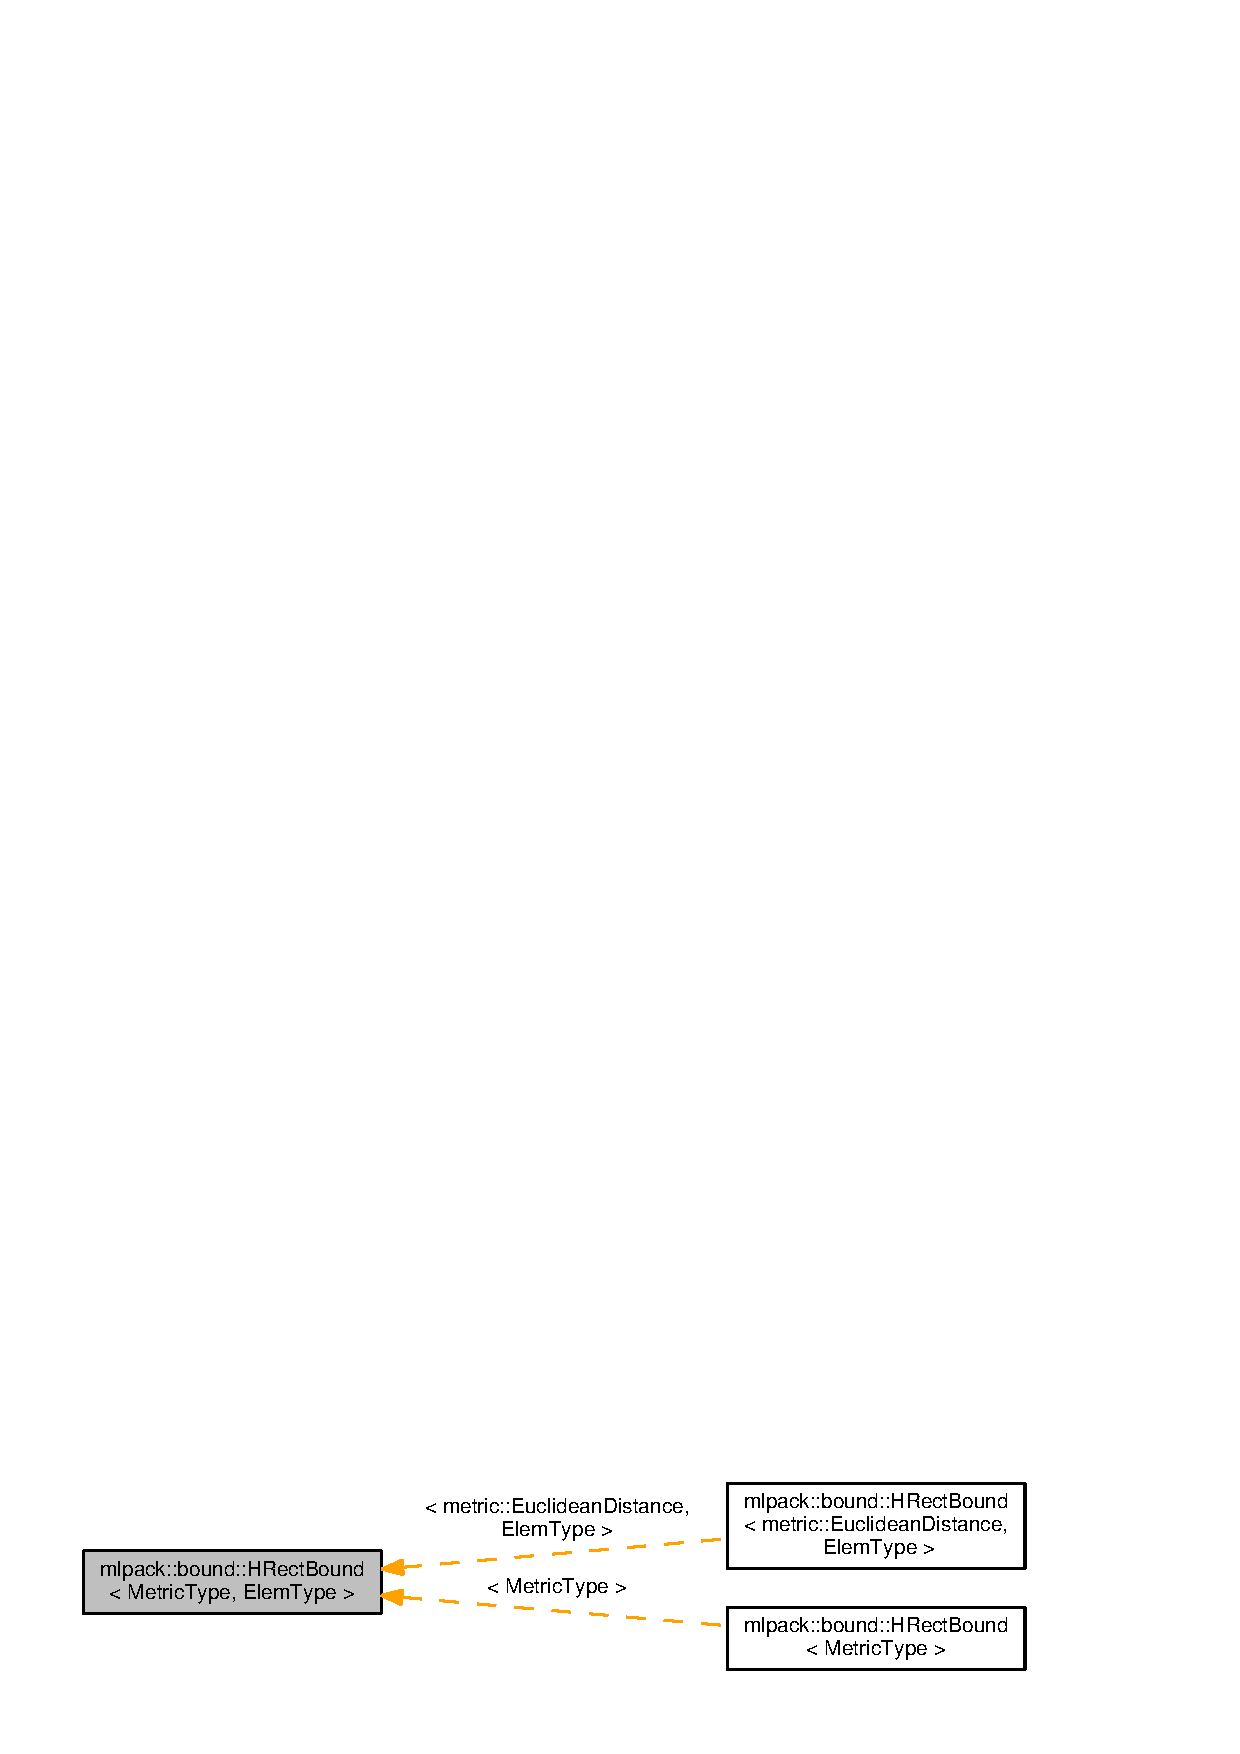
\includegraphics[width=350pt]{classmlpack_1_1bound_1_1HRectBound__inherit__graph}
\end{center}
\end{figure}
\subsection*{Public Member Functions}
\begin{DoxyCompactItemize}
\item 
{\bf H\+Rect\+Bound} ()
\begin{DoxyCompactList}\small\item\em Empty constructor; creates a bound of dimensionality 0. \end{DoxyCompactList}\item 
{\bf H\+Rect\+Bound} (const size\+\_\+t dimension)
\begin{DoxyCompactList}\small\item\em Initializes to specified dimensionality with each dimension the empty set. \end{DoxyCompactList}\item 
{\bf H\+Rect\+Bound} (const {\bf H\+Rect\+Bound} \&other)
\begin{DoxyCompactList}\small\item\em Copy constructor; necessary to prevent memory leaks. \end{DoxyCompactList}\item 
{\bf H\+Rect\+Bound} ({\bf H\+Rect\+Bound} \&\&other)
\begin{DoxyCompactList}\small\item\em Move constructor\+: take possession of another bound\textquotesingle{}s information. \end{DoxyCompactList}\item 
{\bf $\sim$\+H\+Rect\+Bound} ()
\begin{DoxyCompactList}\small\item\em Destructor\+: clean up memory. \end{DoxyCompactList}\item 
void {\bf Center} (arma\+::\+Col$<$ Elem\+Type $>$ \&center) const 
\begin{DoxyCompactList}\small\item\em Calculates the center of the range, placing it into the given vector. \end{DoxyCompactList}\item 
void {\bf Clear} ()
\begin{DoxyCompactList}\small\item\em Resets all dimensions to the empty set (so that this bound contains nothing). \end{DoxyCompactList}\item 
{\footnotesize template$<$typename Vec\+Type $>$ }\\bool {\bf Contains} (const Vec\+Type \&point) const 
\begin{DoxyCompactList}\small\item\em Determines if a point is within this bound. \end{DoxyCompactList}\item 
bool {\bf Contains} (const {\bf H\+Rect\+Bound} \&bound) const 
\begin{DoxyCompactList}\small\item\em Determines if this bound partially contains a bound. \end{DoxyCompactList}\item 
Elem\+Type {\bf Diameter} () const 
\begin{DoxyCompactList}\small\item\em Returns the diameter of the hyperrectangle (that is, the longest diagonal). \end{DoxyCompactList}\item 
size\+\_\+t {\bf Dim} () const 
\begin{DoxyCompactList}\small\item\em Gets the dimensionality. \end{DoxyCompactList}\item 
{\footnotesize template$<$typename Vec\+Type $>$ }\\Elem\+Type {\bf Max\+Distance} (const Vec\+Type \&point, typename {\bf std\+::enable\+\_\+if\+\_\+t}$<$ {\bf Is\+Vector}$<$ Vec\+Type $>$\+::value $>$ $\ast$=0) const 
\begin{DoxyCompactList}\small\item\em Calculates maximum bound-\/to-\/point squared distance. \end{DoxyCompactList}\item 
Elem\+Type {\bf Max\+Distance} (const {\bf H\+Rect\+Bound} \&other) const 
\begin{DoxyCompactList}\small\item\em Computes maximum distance. \end{DoxyCompactList}\item 
{\footnotesize template$<$typename Vec\+Type $>$ }\\Elem\+Type {\bf Min\+Distance} (const Vec\+Type \&point, typename {\bf std\+::enable\+\_\+if\+\_\+t}$<$ {\bf Is\+Vector}$<$ Vec\+Type $>$\+::value $>$ $\ast$=0) const 
\begin{DoxyCompactList}\small\item\em Calculates minimum bound-\/to-\/point distance. \end{DoxyCompactList}\item 
Elem\+Type {\bf Min\+Distance} (const {\bf H\+Rect\+Bound} \&other) const 
\begin{DoxyCompactList}\small\item\em Calculates minimum bound-\/to-\/bound distance. \end{DoxyCompactList}\item 
Elem\+Type {\bf Min\+Width} () const 
\begin{DoxyCompactList}\small\item\em Get the minimum width of the bound. \end{DoxyCompactList}\item 
Elem\+Type \& {\bf Min\+Width} ()
\begin{DoxyCompactList}\small\item\em Modify the minimum width of the bound. \end{DoxyCompactList}\item 
{\bf H\+Rect\+Bound} {\bf operator\&} (const {\bf H\+Rect\+Bound} \&bound) const 
\begin{DoxyCompactList}\small\item\em Returns the intersection of this bound and another. \end{DoxyCompactList}\item 
{\bf H\+Rect\+Bound} \& {\bf operator\&=} (const {\bf H\+Rect\+Bound} \&bound)
\begin{DoxyCompactList}\small\item\em Intersects this bound with another. \end{DoxyCompactList}\item 
{\bf H\+Rect\+Bound} \& {\bf operator=} (const {\bf H\+Rect\+Bound} \&other)
\begin{DoxyCompactList}\small\item\em Same as copy constructor; necessary to prevent memory leaks. \end{DoxyCompactList}\item 
{\bf math\+::\+Range\+Type}$<$ Elem\+Type $>$ \& {\bf operator[$\,$]} (const size\+\_\+t i)
\begin{DoxyCompactList}\small\item\em Get the range for a particular dimension. \end{DoxyCompactList}\item 
const {\bf math\+::\+Range\+Type}$<$ Elem\+Type $>$ \& {\bf operator[$\,$]} (const size\+\_\+t i) const 
\begin{DoxyCompactList}\small\item\em Modify the range for a particular dimension. No bounds checking. \end{DoxyCompactList}\item 
{\footnotesize template$<$typename Mat\+Type $>$ }\\{\bf H\+Rect\+Bound} \& {\bf operator$\vert$=} (const Mat\+Type \&data)
\begin{DoxyCompactList}\small\item\em Expands this region to include new points. \end{DoxyCompactList}\item 
{\bf H\+Rect\+Bound} \& {\bf operator$\vert$=} (const {\bf H\+Rect\+Bound} \&other)
\begin{DoxyCompactList}\small\item\em Expands this region to encompass another bound. \end{DoxyCompactList}\item 
Elem\+Type {\bf Overlap} (const {\bf H\+Rect\+Bound} \&bound) const 
\begin{DoxyCompactList}\small\item\em Returns the volume of overlap of this bound and another. \end{DoxyCompactList}\item 
{\bf math\+::\+Range\+Type}$<$ Elem\+Type $>$ {\bf Range\+Distance} (const {\bf H\+Rect\+Bound} \&other) const 
\begin{DoxyCompactList}\small\item\em Calculates minimum and maximum bound-\/to-\/bound distance. \end{DoxyCompactList}\item 
{\footnotesize template$<$typename Vec\+Type $>$ }\\{\bf math\+::\+Range\+Type}$<$ Elem\+Type $>$ {\bf Range\+Distance} (const Vec\+Type \&point, typename {\bf std\+::enable\+\_\+if\+\_\+t}$<$ {\bf Is\+Vector}$<$ Vec\+Type $>$\+::value $>$ $\ast$=0) const 
\begin{DoxyCompactList}\small\item\em Calculates minimum and maximum bound-\/to-\/point distance. \end{DoxyCompactList}\item 
{\footnotesize template$<$typename Archive $>$ }\\void {\bf Serialize} (Archive \&ar, const unsigned int version)
\begin{DoxyCompactList}\small\item\em Serialize the bound object. \end{DoxyCompactList}\item 
Elem\+Type {\bf Volume} () const 
\begin{DoxyCompactList}\small\item\em Calculate the volume of the hyperrectangle. \end{DoxyCompactList}\end{DoxyCompactItemize}
\subsection*{Private Attributes}
\begin{DoxyCompactItemize}
\item 
{\bf math\+::\+Range\+Type}$<$ Elem\+Type $>$ $\ast$ {\bf bounds}
\begin{DoxyCompactList}\small\item\em The bounds for each dimension. \end{DoxyCompactList}\item 
size\+\_\+t {\bf dim}
\begin{DoxyCompactList}\small\item\em The dimensionality of the bound. \end{DoxyCompactList}\item 
Elem\+Type {\bf min\+Width}
\begin{DoxyCompactList}\small\item\em Cached minimum width of bound. \end{DoxyCompactList}\end{DoxyCompactItemize}


\subsection{Detailed Description}
\subsubsection*{template$<$typename Metric\+Type = metric\+::\+L\+Metric$<$2, true$>$, typename Elem\+Type = double$>$\\*
class mlpack\+::bound\+::\+H\+Rect\+Bound$<$ Metric\+Type, Elem\+Type $>$}

Hyper-\/rectangle bound for an L-\/metric. 

This should be used in conjunction with the L\+Metric class. Be sure to use the same template parameters for L\+Metric as you do for \doxyref{H\+Rect\+Bound}{p.}{classmlpack_1_1bound_1_1HRectBound} -- otherwise odd results may occur.


\begin{DoxyTemplParams}{Template Parameters}
{\em Metric\+Type} & Type of metric to use; must be of type L\+Metric. \\
\hline
{\em Elem\+Type} & Element type (double/float/int/etc.). \\
\hline
\end{DoxyTemplParams}


Definition at line 54 of file hrectbound.\+hpp.



\subsection{Constructor \& Destructor Documentation}
\index{mlpack\+::bound\+::\+H\+Rect\+Bound@{mlpack\+::bound\+::\+H\+Rect\+Bound}!H\+Rect\+Bound@{H\+Rect\+Bound}}
\index{H\+Rect\+Bound@{H\+Rect\+Bound}!mlpack\+::bound\+::\+H\+Rect\+Bound@{mlpack\+::bound\+::\+H\+Rect\+Bound}}
\subsubsection[{H\+Rect\+Bound()}]{\setlength{\rightskip}{0pt plus 5cm}template$<$typename Metric\+Type = metric\+::\+L\+Metric$<$2, true$>$, typename Elem\+Type = double$>$ {\bf mlpack\+::bound\+::\+H\+Rect\+Bound}$<$ Metric\+Type, Elem\+Type $>$\+::{\bf H\+Rect\+Bound} (
\begin{DoxyParamCaption}
{}
\end{DoxyParamCaption}
)}\label{classmlpack_1_1bound_1_1HRectBound_a7849495ec67b4173c77ed1561bbf0139}


Empty constructor; creates a bound of dimensionality 0. 

\index{mlpack\+::bound\+::\+H\+Rect\+Bound@{mlpack\+::bound\+::\+H\+Rect\+Bound}!H\+Rect\+Bound@{H\+Rect\+Bound}}
\index{H\+Rect\+Bound@{H\+Rect\+Bound}!mlpack\+::bound\+::\+H\+Rect\+Bound@{mlpack\+::bound\+::\+H\+Rect\+Bound}}
\subsubsection[{H\+Rect\+Bound(const size\+\_\+t dimension)}]{\setlength{\rightskip}{0pt plus 5cm}template$<$typename Metric\+Type = metric\+::\+L\+Metric$<$2, true$>$, typename Elem\+Type = double$>$ {\bf mlpack\+::bound\+::\+H\+Rect\+Bound}$<$ Metric\+Type, Elem\+Type $>$\+::{\bf H\+Rect\+Bound} (
\begin{DoxyParamCaption}
\item[{const size\+\_\+t}]{dimension}
\end{DoxyParamCaption}
)}\label{classmlpack_1_1bound_1_1HRectBound_ae97a6b35d5dd299742b190288b91bb04}


Initializes to specified dimensionality with each dimension the empty set. 

\index{mlpack\+::bound\+::\+H\+Rect\+Bound@{mlpack\+::bound\+::\+H\+Rect\+Bound}!H\+Rect\+Bound@{H\+Rect\+Bound}}
\index{H\+Rect\+Bound@{H\+Rect\+Bound}!mlpack\+::bound\+::\+H\+Rect\+Bound@{mlpack\+::bound\+::\+H\+Rect\+Bound}}
\subsubsection[{H\+Rect\+Bound(const H\+Rect\+Bound \&other)}]{\setlength{\rightskip}{0pt plus 5cm}template$<$typename Metric\+Type = metric\+::\+L\+Metric$<$2, true$>$, typename Elem\+Type = double$>$ {\bf mlpack\+::bound\+::\+H\+Rect\+Bound}$<$ Metric\+Type, Elem\+Type $>$\+::{\bf H\+Rect\+Bound} (
\begin{DoxyParamCaption}
\item[{const {\bf H\+Rect\+Bound}$<$ Metric\+Type, Elem\+Type $>$ \&}]{other}
\end{DoxyParamCaption}
)}\label{classmlpack_1_1bound_1_1HRectBound_a59989c5667ad4c47d26f8076ed782691}


Copy constructor; necessary to prevent memory leaks. 

\index{mlpack\+::bound\+::\+H\+Rect\+Bound@{mlpack\+::bound\+::\+H\+Rect\+Bound}!H\+Rect\+Bound@{H\+Rect\+Bound}}
\index{H\+Rect\+Bound@{H\+Rect\+Bound}!mlpack\+::bound\+::\+H\+Rect\+Bound@{mlpack\+::bound\+::\+H\+Rect\+Bound}}
\subsubsection[{H\+Rect\+Bound(\+H\+Rect\+Bound \&\&other)}]{\setlength{\rightskip}{0pt plus 5cm}template$<$typename Metric\+Type = metric\+::\+L\+Metric$<$2, true$>$, typename Elem\+Type = double$>$ {\bf mlpack\+::bound\+::\+H\+Rect\+Bound}$<$ Metric\+Type, Elem\+Type $>$\+::{\bf H\+Rect\+Bound} (
\begin{DoxyParamCaption}
\item[{{\bf H\+Rect\+Bound}$<$ Metric\+Type, Elem\+Type $>$ \&\&}]{other}
\end{DoxyParamCaption}
)}\label{classmlpack_1_1bound_1_1HRectBound_a11c7ffc300b01cffc275f3fd27d65d7b}


Move constructor\+: take possession of another bound\textquotesingle{}s information. 

\index{mlpack\+::bound\+::\+H\+Rect\+Bound@{mlpack\+::bound\+::\+H\+Rect\+Bound}!````~H\+Rect\+Bound@{$\sim$\+H\+Rect\+Bound}}
\index{````~H\+Rect\+Bound@{$\sim$\+H\+Rect\+Bound}!mlpack\+::bound\+::\+H\+Rect\+Bound@{mlpack\+::bound\+::\+H\+Rect\+Bound}}
\subsubsection[{$\sim$\+H\+Rect\+Bound()}]{\setlength{\rightskip}{0pt plus 5cm}template$<$typename Metric\+Type = metric\+::\+L\+Metric$<$2, true$>$, typename Elem\+Type = double$>$ {\bf mlpack\+::bound\+::\+H\+Rect\+Bound}$<$ Metric\+Type, Elem\+Type $>$\+::$\sim${\bf H\+Rect\+Bound} (
\begin{DoxyParamCaption}
{}
\end{DoxyParamCaption}
)}\label{classmlpack_1_1bound_1_1HRectBound_abea4f8eee5140670331b4d0d3afa7d2c}


Destructor\+: clean up memory. 



\subsection{Member Function Documentation}
\index{mlpack\+::bound\+::\+H\+Rect\+Bound@{mlpack\+::bound\+::\+H\+Rect\+Bound}!Center@{Center}}
\index{Center@{Center}!mlpack\+::bound\+::\+H\+Rect\+Bound@{mlpack\+::bound\+::\+H\+Rect\+Bound}}
\subsubsection[{Center(arma\+::\+Col$<$ Elem\+Type $>$ \&center) const }]{\setlength{\rightskip}{0pt plus 5cm}template$<$typename Metric\+Type = metric\+::\+L\+Metric$<$2, true$>$, typename Elem\+Type = double$>$ void {\bf mlpack\+::bound\+::\+H\+Rect\+Bound}$<$ Metric\+Type, Elem\+Type $>$\+::Center (
\begin{DoxyParamCaption}
\item[{arma\+::\+Col$<$ Elem\+Type $>$ \&}]{center}
\end{DoxyParamCaption}
) const}\label{classmlpack_1_1bound_1_1HRectBound_ab1b554dff9988b1cb42ddf56ac0b50c4}


Calculates the center of the range, placing it into the given vector. 


\begin{DoxyParams}{Parameters}
{\em center} & Vector which the center will be written to. \\
\hline
\end{DoxyParams}


Referenced by mlpack\+::tree\+::\+Rectangle\+Tree$<$ Metric\+Type, Statistic\+Type, Mat\+Type, Split\+Type, Descent\+Type, Auxiliary\+Information\+Type $>$\+::\+Center(), and mlpack\+::tree\+::\+Octree$<$ Metric\+Type, Statistic\+Type, Mat\+Type $>$\+::\+Center().

\index{mlpack\+::bound\+::\+H\+Rect\+Bound@{mlpack\+::bound\+::\+H\+Rect\+Bound}!Clear@{Clear}}
\index{Clear@{Clear}!mlpack\+::bound\+::\+H\+Rect\+Bound@{mlpack\+::bound\+::\+H\+Rect\+Bound}}
\subsubsection[{Clear()}]{\setlength{\rightskip}{0pt plus 5cm}template$<$typename Metric\+Type = metric\+::\+L\+Metric$<$2, true$>$, typename Elem\+Type = double$>$ void {\bf mlpack\+::bound\+::\+H\+Rect\+Bound}$<$ Metric\+Type, Elem\+Type $>$\+::Clear (
\begin{DoxyParamCaption}
{}
\end{DoxyParamCaption}
)}\label{classmlpack_1_1bound_1_1HRectBound_a7225cb0def075ca37b6c42a57a3f93ca}


Resets all dimensions to the empty set (so that this bound contains nothing). 

\index{mlpack\+::bound\+::\+H\+Rect\+Bound@{mlpack\+::bound\+::\+H\+Rect\+Bound}!Contains@{Contains}}
\index{Contains@{Contains}!mlpack\+::bound\+::\+H\+Rect\+Bound@{mlpack\+::bound\+::\+H\+Rect\+Bound}}
\subsubsection[{Contains(const Vec\+Type \&point) const }]{\setlength{\rightskip}{0pt plus 5cm}template$<$typename Metric\+Type = metric\+::\+L\+Metric$<$2, true$>$, typename Elem\+Type = double$>$ template$<$typename Vec\+Type $>$ bool {\bf mlpack\+::bound\+::\+H\+Rect\+Bound}$<$ Metric\+Type, Elem\+Type $>$\+::Contains (
\begin{DoxyParamCaption}
\item[{const Vec\+Type \&}]{point}
\end{DoxyParamCaption}
) const}\label{classmlpack_1_1bound_1_1HRectBound_aae1da0abdbb86b27908d8bddf43c1855}


Determines if a point is within this bound. 

\index{mlpack\+::bound\+::\+H\+Rect\+Bound@{mlpack\+::bound\+::\+H\+Rect\+Bound}!Contains@{Contains}}
\index{Contains@{Contains}!mlpack\+::bound\+::\+H\+Rect\+Bound@{mlpack\+::bound\+::\+H\+Rect\+Bound}}
\subsubsection[{Contains(const H\+Rect\+Bound \&bound) const }]{\setlength{\rightskip}{0pt plus 5cm}template$<$typename Metric\+Type = metric\+::\+L\+Metric$<$2, true$>$, typename Elem\+Type = double$>$ bool {\bf mlpack\+::bound\+::\+H\+Rect\+Bound}$<$ Metric\+Type, Elem\+Type $>$\+::Contains (
\begin{DoxyParamCaption}
\item[{const {\bf H\+Rect\+Bound}$<$ Metric\+Type, Elem\+Type $>$ \&}]{bound}
\end{DoxyParamCaption}
) const}\label{classmlpack_1_1bound_1_1HRectBound_a5a8c9ac48126696093c9f5ec7f3db0f8}


Determines if this bound partially contains a bound. 

\index{mlpack\+::bound\+::\+H\+Rect\+Bound@{mlpack\+::bound\+::\+H\+Rect\+Bound}!Diameter@{Diameter}}
\index{Diameter@{Diameter}!mlpack\+::bound\+::\+H\+Rect\+Bound@{mlpack\+::bound\+::\+H\+Rect\+Bound}}
\subsubsection[{Diameter() const }]{\setlength{\rightskip}{0pt plus 5cm}template$<$typename Metric\+Type = metric\+::\+L\+Metric$<$2, true$>$, typename Elem\+Type = double$>$ Elem\+Type {\bf mlpack\+::bound\+::\+H\+Rect\+Bound}$<$ Metric\+Type, Elem\+Type $>$\+::Diameter (
\begin{DoxyParamCaption}
{}
\end{DoxyParamCaption}
) const}\label{classmlpack_1_1bound_1_1HRectBound_a9f5a5acc60b647953068fc924a7b3de8}


Returns the diameter of the hyperrectangle (that is, the longest diagonal). 

\index{mlpack\+::bound\+::\+H\+Rect\+Bound@{mlpack\+::bound\+::\+H\+Rect\+Bound}!Dim@{Dim}}
\index{Dim@{Dim}!mlpack\+::bound\+::\+H\+Rect\+Bound@{mlpack\+::bound\+::\+H\+Rect\+Bound}}
\subsubsection[{Dim() const }]{\setlength{\rightskip}{0pt plus 5cm}template$<$typename Metric\+Type = metric\+::\+L\+Metric$<$2, true$>$, typename Elem\+Type = double$>$ size\+\_\+t {\bf mlpack\+::bound\+::\+H\+Rect\+Bound}$<$ Metric\+Type, Elem\+Type $>$\+::Dim (
\begin{DoxyParamCaption}
{}
\end{DoxyParamCaption}
) const\hspace{0.3cm}{\ttfamily [inline]}}\label{classmlpack_1_1bound_1_1HRectBound_a8c7b2e30979dbd7b483721ffd8407e8c}


Gets the dimensionality. 



Definition at line 90 of file hrectbound.\+hpp.

\index{mlpack\+::bound\+::\+H\+Rect\+Bound@{mlpack\+::bound\+::\+H\+Rect\+Bound}!Max\+Distance@{Max\+Distance}}
\index{Max\+Distance@{Max\+Distance}!mlpack\+::bound\+::\+H\+Rect\+Bound@{mlpack\+::bound\+::\+H\+Rect\+Bound}}
\subsubsection[{Max\+Distance(const Vec\+Type \&point, typename std\+::enable\+\_\+if\+\_\+t$<$ Is\+Vector$<$ Vec\+Type $>$\+::value $>$ $\ast$=0) const }]{\setlength{\rightskip}{0pt plus 5cm}template$<$typename Metric\+Type = metric\+::\+L\+Metric$<$2, true$>$, typename Elem\+Type = double$>$ template$<$typename Vec\+Type $>$ Elem\+Type {\bf mlpack\+::bound\+::\+H\+Rect\+Bound}$<$ Metric\+Type, Elem\+Type $>$\+::Max\+Distance (
\begin{DoxyParamCaption}
\item[{const Vec\+Type \&}]{point, }
\item[{typename {\bf std\+::enable\+\_\+if\+\_\+t}$<$ {\bf Is\+Vector}$<$ Vec\+Type $>$\+::value $>$ $\ast$}]{ = {\ttfamily 0}}
\end{DoxyParamCaption}
) const}\label{classmlpack_1_1bound_1_1HRectBound_ae68fbe401588fc248371dc76517c7b5c}


Calculates maximum bound-\/to-\/point squared distance. 


\begin{DoxyParams}{Parameters}
{\em point} & Point to which the maximum distance is requested. \\
\hline
\end{DoxyParams}


Referenced by mlpack\+::tree\+::\+Rectangle\+Tree$<$ Metric\+Type, Statistic\+Type, Mat\+Type, Split\+Type, Descent\+Type, Auxiliary\+Information\+Type $>$\+::\+Max\+Distance().

\index{mlpack\+::bound\+::\+H\+Rect\+Bound@{mlpack\+::bound\+::\+H\+Rect\+Bound}!Max\+Distance@{Max\+Distance}}
\index{Max\+Distance@{Max\+Distance}!mlpack\+::bound\+::\+H\+Rect\+Bound@{mlpack\+::bound\+::\+H\+Rect\+Bound}}
\subsubsection[{Max\+Distance(const H\+Rect\+Bound \&other) const }]{\setlength{\rightskip}{0pt plus 5cm}template$<$typename Metric\+Type = metric\+::\+L\+Metric$<$2, true$>$, typename Elem\+Type = double$>$ Elem\+Type {\bf mlpack\+::bound\+::\+H\+Rect\+Bound}$<$ Metric\+Type, Elem\+Type $>$\+::Max\+Distance (
\begin{DoxyParamCaption}
\item[{const {\bf H\+Rect\+Bound}$<$ Metric\+Type, Elem\+Type $>$ \&}]{other}
\end{DoxyParamCaption}
) const}\label{classmlpack_1_1bound_1_1HRectBound_adb66fb1753871f4a03c50cf4fb709e8c}


Computes maximum distance. 


\begin{DoxyParams}{Parameters}
{\em other} & Bound to which the maximum distance is requested. \\
\hline
\end{DoxyParams}
\index{mlpack\+::bound\+::\+H\+Rect\+Bound@{mlpack\+::bound\+::\+H\+Rect\+Bound}!Min\+Distance@{Min\+Distance}}
\index{Min\+Distance@{Min\+Distance}!mlpack\+::bound\+::\+H\+Rect\+Bound@{mlpack\+::bound\+::\+H\+Rect\+Bound}}
\subsubsection[{Min\+Distance(const Vec\+Type \&point, typename std\+::enable\+\_\+if\+\_\+t$<$ Is\+Vector$<$ Vec\+Type $>$\+::value $>$ $\ast$=0) const }]{\setlength{\rightskip}{0pt plus 5cm}template$<$typename Metric\+Type = metric\+::\+L\+Metric$<$2, true$>$, typename Elem\+Type = double$>$ template$<$typename Vec\+Type $>$ Elem\+Type {\bf mlpack\+::bound\+::\+H\+Rect\+Bound}$<$ Metric\+Type, Elem\+Type $>$\+::Min\+Distance (
\begin{DoxyParamCaption}
\item[{const Vec\+Type \&}]{point, }
\item[{typename {\bf std\+::enable\+\_\+if\+\_\+t}$<$ {\bf Is\+Vector}$<$ Vec\+Type $>$\+::value $>$ $\ast$}]{ = {\ttfamily 0}}
\end{DoxyParamCaption}
) const}\label{classmlpack_1_1bound_1_1HRectBound_aaea70c9638f5123e3d83c1322fbdd721}


Calculates minimum bound-\/to-\/point distance. 


\begin{DoxyParams}{Parameters}
{\em point} & Point to which the minimum distance is requested. \\
\hline
\end{DoxyParams}


Referenced by mlpack\+::tree\+::\+Rectangle\+Tree$<$ Metric\+Type, Statistic\+Type, Mat\+Type, Split\+Type, Descent\+Type, Auxiliary\+Information\+Type $>$\+::\+Min\+Distance().

\index{mlpack\+::bound\+::\+H\+Rect\+Bound@{mlpack\+::bound\+::\+H\+Rect\+Bound}!Min\+Distance@{Min\+Distance}}
\index{Min\+Distance@{Min\+Distance}!mlpack\+::bound\+::\+H\+Rect\+Bound@{mlpack\+::bound\+::\+H\+Rect\+Bound}}
\subsubsection[{Min\+Distance(const H\+Rect\+Bound \&other) const }]{\setlength{\rightskip}{0pt plus 5cm}template$<$typename Metric\+Type = metric\+::\+L\+Metric$<$2, true$>$, typename Elem\+Type = double$>$ Elem\+Type {\bf mlpack\+::bound\+::\+H\+Rect\+Bound}$<$ Metric\+Type, Elem\+Type $>$\+::Min\+Distance (
\begin{DoxyParamCaption}
\item[{const {\bf H\+Rect\+Bound}$<$ Metric\+Type, Elem\+Type $>$ \&}]{other}
\end{DoxyParamCaption}
) const}\label{classmlpack_1_1bound_1_1HRectBound_ac3f469c5b97a1900d9d235f53db17e10}


Calculates minimum bound-\/to-\/bound distance. 


\begin{DoxyParams}{Parameters}
{\em other} & Bound to which the minimum distance is requested. \\
\hline
\end{DoxyParams}
\index{mlpack\+::bound\+::\+H\+Rect\+Bound@{mlpack\+::bound\+::\+H\+Rect\+Bound}!Min\+Width@{Min\+Width}}
\index{Min\+Width@{Min\+Width}!mlpack\+::bound\+::\+H\+Rect\+Bound@{mlpack\+::bound\+::\+H\+Rect\+Bound}}
\subsubsection[{Min\+Width() const }]{\setlength{\rightskip}{0pt plus 5cm}template$<$typename Metric\+Type = metric\+::\+L\+Metric$<$2, true$>$, typename Elem\+Type = double$>$ Elem\+Type {\bf mlpack\+::bound\+::\+H\+Rect\+Bound}$<$ Metric\+Type, Elem\+Type $>$\+::Min\+Width (
\begin{DoxyParamCaption}
{}
\end{DoxyParamCaption}
) const\hspace{0.3cm}{\ttfamily [inline]}}\label{classmlpack_1_1bound_1_1HRectBound_a00ac407e260373af5490aa57f879a892}


Get the minimum width of the bound. 



Definition at line 100 of file hrectbound.\+hpp.



Referenced by mlpack\+::tree\+::\+Rectangle\+Tree$<$ Metric\+Type, Statistic\+Type, Mat\+Type, Split\+Type, Descent\+Type, Auxiliary\+Information\+Type $>$\+::\+Minimum\+Bound\+Distance().

\index{mlpack\+::bound\+::\+H\+Rect\+Bound@{mlpack\+::bound\+::\+H\+Rect\+Bound}!Min\+Width@{Min\+Width}}
\index{Min\+Width@{Min\+Width}!mlpack\+::bound\+::\+H\+Rect\+Bound@{mlpack\+::bound\+::\+H\+Rect\+Bound}}
\subsubsection[{Min\+Width()}]{\setlength{\rightskip}{0pt plus 5cm}template$<$typename Metric\+Type = metric\+::\+L\+Metric$<$2, true$>$, typename Elem\+Type = double$>$ Elem\+Type\& {\bf mlpack\+::bound\+::\+H\+Rect\+Bound}$<$ Metric\+Type, Elem\+Type $>$\+::Min\+Width (
\begin{DoxyParamCaption}
{}
\end{DoxyParamCaption}
)\hspace{0.3cm}{\ttfamily [inline]}}\label{classmlpack_1_1bound_1_1HRectBound_a1f96e4e87ad18cea349cb2b4e4d43d06}


Modify the minimum width of the bound. 



Definition at line 102 of file hrectbound.\+hpp.

\index{mlpack\+::bound\+::\+H\+Rect\+Bound@{mlpack\+::bound\+::\+H\+Rect\+Bound}!operator\&@{operator\&}}
\index{operator\&@{operator\&}!mlpack\+::bound\+::\+H\+Rect\+Bound@{mlpack\+::bound\+::\+H\+Rect\+Bound}}
\subsubsection[{operator\&(const H\+Rect\+Bound \&bound) const }]{\setlength{\rightskip}{0pt plus 5cm}template$<$typename Metric\+Type = metric\+::\+L\+Metric$<$2, true$>$, typename Elem\+Type = double$>$ {\bf H\+Rect\+Bound} {\bf mlpack\+::bound\+::\+H\+Rect\+Bound}$<$ Metric\+Type, Elem\+Type $>$\+::operator\& (
\begin{DoxyParamCaption}
\item[{const {\bf H\+Rect\+Bound}$<$ Metric\+Type, Elem\+Type $>$ \&}]{bound}
\end{DoxyParamCaption}
) const}\label{classmlpack_1_1bound_1_1HRectBound_a69925c7af964171f2a2f3e55cd46e06e}


Returns the intersection of this bound and another. 

\index{mlpack\+::bound\+::\+H\+Rect\+Bound@{mlpack\+::bound\+::\+H\+Rect\+Bound}!operator\&=@{operator\&=}}
\index{operator\&=@{operator\&=}!mlpack\+::bound\+::\+H\+Rect\+Bound@{mlpack\+::bound\+::\+H\+Rect\+Bound}}
\subsubsection[{operator\&=(const H\+Rect\+Bound \&bound)}]{\setlength{\rightskip}{0pt plus 5cm}template$<$typename Metric\+Type = metric\+::\+L\+Metric$<$2, true$>$, typename Elem\+Type = double$>$ {\bf H\+Rect\+Bound}\& {\bf mlpack\+::bound\+::\+H\+Rect\+Bound}$<$ Metric\+Type, Elem\+Type $>$\+::operator\&= (
\begin{DoxyParamCaption}
\item[{const {\bf H\+Rect\+Bound}$<$ Metric\+Type, Elem\+Type $>$ \&}]{bound}
\end{DoxyParamCaption}
)}\label{classmlpack_1_1bound_1_1HRectBound_a39c9285e39a56a9b633494e3d05bcafe}


Intersects this bound with another. 

\index{mlpack\+::bound\+::\+H\+Rect\+Bound@{mlpack\+::bound\+::\+H\+Rect\+Bound}!operator=@{operator=}}
\index{operator=@{operator=}!mlpack\+::bound\+::\+H\+Rect\+Bound@{mlpack\+::bound\+::\+H\+Rect\+Bound}}
\subsubsection[{operator=(const H\+Rect\+Bound \&other)}]{\setlength{\rightskip}{0pt plus 5cm}template$<$typename Metric\+Type = metric\+::\+L\+Metric$<$2, true$>$, typename Elem\+Type = double$>$ {\bf H\+Rect\+Bound}\& {\bf mlpack\+::bound\+::\+H\+Rect\+Bound}$<$ Metric\+Type, Elem\+Type $>$\+::operator= (
\begin{DoxyParamCaption}
\item[{const {\bf H\+Rect\+Bound}$<$ Metric\+Type, Elem\+Type $>$ \&}]{other}
\end{DoxyParamCaption}
)}\label{classmlpack_1_1bound_1_1HRectBound_a78d1fde04fc5d71d5d303ec2d0592b93}


Same as copy constructor; necessary to prevent memory leaks. 

\index{mlpack\+::bound\+::\+H\+Rect\+Bound@{mlpack\+::bound\+::\+H\+Rect\+Bound}!operator[$\,$]@{operator[]}}
\index{operator[$\,$]@{operator[]}!mlpack\+::bound\+::\+H\+Rect\+Bound@{mlpack\+::bound\+::\+H\+Rect\+Bound}}
\subsubsection[{operator[](const size\+\_\+t i)}]{\setlength{\rightskip}{0pt plus 5cm}template$<$typename Metric\+Type = metric\+::\+L\+Metric$<$2, true$>$, typename Elem\+Type = double$>$ {\bf math\+::\+Range\+Type}$<$Elem\+Type$>$\& {\bf mlpack\+::bound\+::\+H\+Rect\+Bound}$<$ Metric\+Type, Elem\+Type $>$\+::operator[$\,$] (
\begin{DoxyParamCaption}
\item[{const size\+\_\+t}]{i}
\end{DoxyParamCaption}
)\hspace{0.3cm}{\ttfamily [inline]}}\label{classmlpack_1_1bound_1_1HRectBound_ab8fec960cc08494d0d77cb08d1eae736}


Get the range for a particular dimension. 

No bounds checking. Be careful\+: this may make \doxyref{Min\+Width()}{p.}{classmlpack_1_1bound_1_1HRectBound_a1f96e4e87ad18cea349cb2b4e4d43d06} invalid. 

Definition at line 94 of file hrectbound.\+hpp.

\index{mlpack\+::bound\+::\+H\+Rect\+Bound@{mlpack\+::bound\+::\+H\+Rect\+Bound}!operator[$\,$]@{operator[]}}
\index{operator[$\,$]@{operator[]}!mlpack\+::bound\+::\+H\+Rect\+Bound@{mlpack\+::bound\+::\+H\+Rect\+Bound}}
\subsubsection[{operator[](const size\+\_\+t i) const }]{\setlength{\rightskip}{0pt plus 5cm}template$<$typename Metric\+Type = metric\+::\+L\+Metric$<$2, true$>$, typename Elem\+Type = double$>$ const {\bf math\+::\+Range\+Type}$<$Elem\+Type$>$\& {\bf mlpack\+::bound\+::\+H\+Rect\+Bound}$<$ Metric\+Type, Elem\+Type $>$\+::operator[$\,$] (
\begin{DoxyParamCaption}
\item[{const size\+\_\+t}]{i}
\end{DoxyParamCaption}
) const\hspace{0.3cm}{\ttfamily [inline]}}\label{classmlpack_1_1bound_1_1HRectBound_a43cee085e1a73b10fa83daf390b0e86d}


Modify the range for a particular dimension. No bounds checking. 



Definition at line 96 of file hrectbound.\+hpp.

\index{mlpack\+::bound\+::\+H\+Rect\+Bound@{mlpack\+::bound\+::\+H\+Rect\+Bound}!operator\texttt{"|}=@{operator\texttt{"|}=}}
\index{operator\texttt{"|}=@{operator\texttt{"|}=}!mlpack\+::bound\+::\+H\+Rect\+Bound@{mlpack\+::bound\+::\+H\+Rect\+Bound}}
\subsubsection[{operator\texttt{"|}=(const Mat\+Type \&data)}]{\setlength{\rightskip}{0pt plus 5cm}template$<$typename Metric\+Type = metric\+::\+L\+Metric$<$2, true$>$, typename Elem\+Type = double$>$ template$<$typename Mat\+Type $>$ {\bf H\+Rect\+Bound}\& {\bf mlpack\+::bound\+::\+H\+Rect\+Bound}$<$ Metric\+Type, Elem\+Type $>$\+::operator$\vert$= (
\begin{DoxyParamCaption}
\item[{const Mat\+Type \&}]{data}
\end{DoxyParamCaption}
)}\label{classmlpack_1_1bound_1_1HRectBound_af7c4cc88ead1ab897c6069da5da5babb}


Expands this region to include new points. 


\begin{DoxyTemplParams}{Template Parameters}
{\em Mat\+Type} & Type of matrix; could be Mat, Sp\+Mat, a subview, or just a vector. \\
\hline
\end{DoxyTemplParams}

\begin{DoxyParams}{Parameters}
{\em data} & Data points to expand this region to include. \\
\hline
\end{DoxyParams}
\index{mlpack\+::bound\+::\+H\+Rect\+Bound@{mlpack\+::bound\+::\+H\+Rect\+Bound}!operator\texttt{"|}=@{operator\texttt{"|}=}}
\index{operator\texttt{"|}=@{operator\texttt{"|}=}!mlpack\+::bound\+::\+H\+Rect\+Bound@{mlpack\+::bound\+::\+H\+Rect\+Bound}}
\subsubsection[{operator\texttt{"|}=(const H\+Rect\+Bound \&other)}]{\setlength{\rightskip}{0pt plus 5cm}template$<$typename Metric\+Type = metric\+::\+L\+Metric$<$2, true$>$, typename Elem\+Type = double$>$ {\bf H\+Rect\+Bound}\& {\bf mlpack\+::bound\+::\+H\+Rect\+Bound}$<$ Metric\+Type, Elem\+Type $>$\+::operator$\vert$= (
\begin{DoxyParamCaption}
\item[{const {\bf H\+Rect\+Bound}$<$ Metric\+Type, Elem\+Type $>$ \&}]{other}
\end{DoxyParamCaption}
)}\label{classmlpack_1_1bound_1_1HRectBound_a17237d2c86a069c58ab8efef25f215a5}


Expands this region to encompass another bound. 

\index{mlpack\+::bound\+::\+H\+Rect\+Bound@{mlpack\+::bound\+::\+H\+Rect\+Bound}!Overlap@{Overlap}}
\index{Overlap@{Overlap}!mlpack\+::bound\+::\+H\+Rect\+Bound@{mlpack\+::bound\+::\+H\+Rect\+Bound}}
\subsubsection[{Overlap(const H\+Rect\+Bound \&bound) const }]{\setlength{\rightskip}{0pt plus 5cm}template$<$typename Metric\+Type = metric\+::\+L\+Metric$<$2, true$>$, typename Elem\+Type = double$>$ Elem\+Type {\bf mlpack\+::bound\+::\+H\+Rect\+Bound}$<$ Metric\+Type, Elem\+Type $>$\+::Overlap (
\begin{DoxyParamCaption}
\item[{const {\bf H\+Rect\+Bound}$<$ Metric\+Type, Elem\+Type $>$ \&}]{bound}
\end{DoxyParamCaption}
) const}\label{classmlpack_1_1bound_1_1HRectBound_a5579214d3bd322e01e6824077fce376a}


Returns the volume of overlap of this bound and another. 

\index{mlpack\+::bound\+::\+H\+Rect\+Bound@{mlpack\+::bound\+::\+H\+Rect\+Bound}!Range\+Distance@{Range\+Distance}}
\index{Range\+Distance@{Range\+Distance}!mlpack\+::bound\+::\+H\+Rect\+Bound@{mlpack\+::bound\+::\+H\+Rect\+Bound}}
\subsubsection[{Range\+Distance(const H\+Rect\+Bound \&other) const }]{\setlength{\rightskip}{0pt plus 5cm}template$<$typename Metric\+Type = metric\+::\+L\+Metric$<$2, true$>$, typename Elem\+Type = double$>$ {\bf math\+::\+Range\+Type}$<$Elem\+Type$>$ {\bf mlpack\+::bound\+::\+H\+Rect\+Bound}$<$ Metric\+Type, Elem\+Type $>$\+::Range\+Distance (
\begin{DoxyParamCaption}
\item[{const {\bf H\+Rect\+Bound}$<$ Metric\+Type, Elem\+Type $>$ \&}]{other}
\end{DoxyParamCaption}
) const}\label{classmlpack_1_1bound_1_1HRectBound_a924c37907ab98cf2ac658abd983bc576}


Calculates minimum and maximum bound-\/to-\/bound distance. 


\begin{DoxyParams}{Parameters}
{\em other} & Bound to which the minimum and maximum distances are requested. \\
\hline
\end{DoxyParams}


Referenced by mlpack\+::tree\+::\+Rectangle\+Tree$<$ Metric\+Type, Statistic\+Type, Mat\+Type, Split\+Type, Descent\+Type, Auxiliary\+Information\+Type $>$\+::\+Range\+Distance().

\index{mlpack\+::bound\+::\+H\+Rect\+Bound@{mlpack\+::bound\+::\+H\+Rect\+Bound}!Range\+Distance@{Range\+Distance}}
\index{Range\+Distance@{Range\+Distance}!mlpack\+::bound\+::\+H\+Rect\+Bound@{mlpack\+::bound\+::\+H\+Rect\+Bound}}
\subsubsection[{Range\+Distance(const Vec\+Type \&point, typename std\+::enable\+\_\+if\+\_\+t$<$ Is\+Vector$<$ Vec\+Type $>$\+::value $>$ $\ast$=0) const }]{\setlength{\rightskip}{0pt plus 5cm}template$<$typename Metric\+Type = metric\+::\+L\+Metric$<$2, true$>$, typename Elem\+Type = double$>$ template$<$typename Vec\+Type $>$ {\bf math\+::\+Range\+Type}$<$Elem\+Type$>$ {\bf mlpack\+::bound\+::\+H\+Rect\+Bound}$<$ Metric\+Type, Elem\+Type $>$\+::Range\+Distance (
\begin{DoxyParamCaption}
\item[{const Vec\+Type \&}]{point, }
\item[{typename {\bf std\+::enable\+\_\+if\+\_\+t}$<$ {\bf Is\+Vector}$<$ Vec\+Type $>$\+::value $>$ $\ast$}]{ = {\ttfamily 0}}
\end{DoxyParamCaption}
) const}\label{classmlpack_1_1bound_1_1HRectBound_ab0922db32cb17f3d50b999855e1ae548}


Calculates minimum and maximum bound-\/to-\/point distance. 


\begin{DoxyParams}{Parameters}
{\em point} & Point to which the minimum and maximum distances are requested. \\
\hline
\end{DoxyParams}
\index{mlpack\+::bound\+::\+H\+Rect\+Bound@{mlpack\+::bound\+::\+H\+Rect\+Bound}!Serialize@{Serialize}}
\index{Serialize@{Serialize}!mlpack\+::bound\+::\+H\+Rect\+Bound@{mlpack\+::bound\+::\+H\+Rect\+Bound}}
\subsubsection[{Serialize(\+Archive \&ar, const unsigned int version)}]{\setlength{\rightskip}{0pt plus 5cm}template$<$typename Metric\+Type = metric\+::\+L\+Metric$<$2, true$>$, typename Elem\+Type = double$>$ template$<$typename Archive $>$ void {\bf mlpack\+::bound\+::\+H\+Rect\+Bound}$<$ Metric\+Type, Elem\+Type $>$\+::Serialize (
\begin{DoxyParamCaption}
\item[{Archive \&}]{ar, }
\item[{const unsigned int}]{version}
\end{DoxyParamCaption}
)}\label{classmlpack_1_1bound_1_1HRectBound_a22b55e4bc300c5dfdf43265630ed9fe8}


Serialize the bound object. 

\index{mlpack\+::bound\+::\+H\+Rect\+Bound@{mlpack\+::bound\+::\+H\+Rect\+Bound}!Volume@{Volume}}
\index{Volume@{Volume}!mlpack\+::bound\+::\+H\+Rect\+Bound@{mlpack\+::bound\+::\+H\+Rect\+Bound}}
\subsubsection[{Volume() const }]{\setlength{\rightskip}{0pt plus 5cm}template$<$typename Metric\+Type = metric\+::\+L\+Metric$<$2, true$>$, typename Elem\+Type = double$>$ Elem\+Type {\bf mlpack\+::bound\+::\+H\+Rect\+Bound}$<$ Metric\+Type, Elem\+Type $>$\+::Volume (
\begin{DoxyParamCaption}
{}
\end{DoxyParamCaption}
) const}\label{classmlpack_1_1bound_1_1HRectBound_a329adc60ec2ad2b31a538e06aae2afdb}


Calculate the volume of the hyperrectangle. 

\begin{DoxyReturn}{Returns}
Volume of the hyperrectangle. 
\end{DoxyReturn}


\subsection{Member Data Documentation}
\index{mlpack\+::bound\+::\+H\+Rect\+Bound@{mlpack\+::bound\+::\+H\+Rect\+Bound}!bounds@{bounds}}
\index{bounds@{bounds}!mlpack\+::bound\+::\+H\+Rect\+Bound@{mlpack\+::bound\+::\+H\+Rect\+Bound}}
\subsubsection[{bounds}]{\setlength{\rightskip}{0pt plus 5cm}template$<$typename Metric\+Type = metric\+::\+L\+Metric$<$2, true$>$, typename Elem\+Type = double$>$ {\bf math\+::\+Range\+Type}$<$Elem\+Type$>$$\ast$ {\bf mlpack\+::bound\+::\+H\+Rect\+Bound}$<$ Metric\+Type, Elem\+Type $>$\+::bounds\hspace{0.3cm}{\ttfamily [private]}}\label{classmlpack_1_1bound_1_1HRectBound_a96b248175ef3a7febeb727b6b215c128}


The bounds for each dimension. 



Definition at line 227 of file hrectbound.\+hpp.

\index{mlpack\+::bound\+::\+H\+Rect\+Bound@{mlpack\+::bound\+::\+H\+Rect\+Bound}!dim@{dim}}
\index{dim@{dim}!mlpack\+::bound\+::\+H\+Rect\+Bound@{mlpack\+::bound\+::\+H\+Rect\+Bound}}
\subsubsection[{dim}]{\setlength{\rightskip}{0pt plus 5cm}template$<$typename Metric\+Type = metric\+::\+L\+Metric$<$2, true$>$, typename Elem\+Type = double$>$ size\+\_\+t {\bf mlpack\+::bound\+::\+H\+Rect\+Bound}$<$ Metric\+Type, Elem\+Type $>$\+::dim\hspace{0.3cm}{\ttfamily [private]}}\label{classmlpack_1_1bound_1_1HRectBound_a251168b43839929f825ad7ffde339614}


The dimensionality of the bound. 



Definition at line 225 of file hrectbound.\+hpp.

\index{mlpack\+::bound\+::\+H\+Rect\+Bound@{mlpack\+::bound\+::\+H\+Rect\+Bound}!min\+Width@{min\+Width}}
\index{min\+Width@{min\+Width}!mlpack\+::bound\+::\+H\+Rect\+Bound@{mlpack\+::bound\+::\+H\+Rect\+Bound}}
\subsubsection[{min\+Width}]{\setlength{\rightskip}{0pt plus 5cm}template$<$typename Metric\+Type = metric\+::\+L\+Metric$<$2, true$>$, typename Elem\+Type = double$>$ Elem\+Type {\bf mlpack\+::bound\+::\+H\+Rect\+Bound}$<$ Metric\+Type, Elem\+Type $>$\+::min\+Width\hspace{0.3cm}{\ttfamily [private]}}\label{classmlpack_1_1bound_1_1HRectBound_a5057297738a7dff66d599b1275977112}


Cached minimum width of bound. 



Definition at line 229 of file hrectbound.\+hpp.



The documentation for this class was generated from the following file\+:\begin{DoxyCompactItemize}
\item 
src/mlpack/core/tree/{\bf hrectbound.\+hpp}\end{DoxyCompactItemize}

\section{Is\+L\+Metric$<$ Metric\+Type $>$ Struct Template Reference}
\label{structmlpack_1_1bound_1_1meta_1_1IsLMetric}\index{Is\+L\+Metric$<$ Metric\+Type $>$@{Is\+L\+Metric$<$ Metric\+Type $>$}}


Utility struct where Value is true if and only if the argument is of type L\+Metric.  


\subsection*{Static Public Attributes}
\begin{DoxyCompactItemize}
\item 
static const bool \textbf{ Value} = false
\end{DoxyCompactItemize}


\subsection{Detailed Description}
\subsubsection*{template$<$typename Metric\+Type$>$\newline
struct mlpack\+::bound\+::meta\+::\+Is\+L\+Metric$<$ Metric\+Type $>$}

Utility struct where Value is true if and only if the argument is of type L\+Metric. 



Definition at line 30 of file hrectbound.\+hpp.



\subsection{Member Data Documentation}
\mbox{\label{structmlpack_1_1bound_1_1meta_1_1IsLMetric_a2cbb7037a76934614ab6ca3cc713d6ef}} 
\index{mlpack\+::bound\+::meta\+::\+Is\+L\+Metric@{mlpack\+::bound\+::meta\+::\+Is\+L\+Metric}!Value@{Value}}
\index{Value@{Value}!mlpack\+::bound\+::meta\+::\+Is\+L\+Metric@{mlpack\+::bound\+::meta\+::\+Is\+L\+Metric}}
\subsubsection{Value}
{\footnotesize\ttfamily const bool Value = false\hspace{0.3cm}{\ttfamily [static]}}



Definition at line 32 of file hrectbound.\+hpp.



The documentation for this struct was generated from the following file\+:\begin{DoxyCompactItemize}
\item 
/home/aakash/mlpack/src/mlpack/core/tree/\textbf{ hrectbound.\+hpp}\end{DoxyCompactItemize}

\section{mlpack\+:\+:bound\+:\+:meta\+:\+:Is\+L\+Metric$<$ metric\+:\+:L\+Metric$<$ Power, Take\+Root $>$ $>$ Struct Template Reference}
\label{structmlpack_1_1bound_1_1meta_1_1IsLMetric_3_01metric_1_1LMetric_3_01Power_00_01TakeRoot_01_4_01_4}\index{mlpack\+::bound\+::meta\+::\+Is\+L\+Metric$<$ metric\+::\+L\+Metric$<$ Power, Take\+Root $>$ $>$@{mlpack\+::bound\+::meta\+::\+Is\+L\+Metric$<$ metric\+::\+L\+Metric$<$ Power, Take\+Root $>$ $>$}}


Specialization for \doxyref{Is\+L\+Metric}{p.}{structmlpack_1_1bound_1_1meta_1_1IsLMetric} when the argument is of type L\+Metric.  


\subsection*{Static Public Attributes}
\begin{DoxyCompactItemize}
\item 
static const bool {\bf Value} = true
\end{DoxyCompactItemize}


\subsection{Detailed Description}
\subsubsection*{template$<$int Power, bool Take\+Root$>$\\*
struct mlpack\+::bound\+::meta\+::\+Is\+L\+Metric$<$ metric\+::\+L\+Metric$<$ Power, Take\+Root $>$ $>$}

Specialization for \doxyref{Is\+L\+Metric}{p.}{structmlpack_1_1bound_1_1meta_1_1IsLMetric} when the argument is of type L\+Metric. 

Definition at line 37 of file hrectbound.\+hpp.



\subsection{Member Data Documentation}
\index{mlpack\+::bound\+::meta\+::\+Is\+L\+Metric$<$ metric\+::\+L\+Metric$<$ Power, Take\+Root $>$ $>$@{mlpack\+::bound\+::meta\+::\+Is\+L\+Metric$<$ metric\+::\+L\+Metric$<$ Power, Take\+Root $>$ $>$}!Value@{Value}}
\index{Value@{Value}!mlpack\+::bound\+::meta\+::\+Is\+L\+Metric$<$ metric\+::\+L\+Metric$<$ Power, Take\+Root $>$ $>$@{mlpack\+::bound\+::meta\+::\+Is\+L\+Metric$<$ metric\+::\+L\+Metric$<$ Power, Take\+Root $>$ $>$}}
\subsubsection[{Value}]{\setlength{\rightskip}{0pt plus 5cm}template$<$int Power, bool Take\+Root$>$ const bool {\bf mlpack\+::bound\+::meta\+::\+Is\+L\+Metric}$<$ {\bf metric\+::\+L\+Metric}$<$ Power, Take\+Root $>$ $>$\+::Value = true\hspace{0.3cm}{\ttfamily [static]}}\label{structmlpack_1_1bound_1_1meta_1_1IsLMetric_3_01metric_1_1LMetric_3_01Power_00_01TakeRoot_01_4_01_4_ae622da651a7afb0a2a943b007ce7d066}


Definition at line 39 of file hrectbound.\+hpp.



The documentation for this struct was generated from the following file\+:\begin{DoxyCompactItemize}
\item 
src/mlpack/core/tree/{\bf hrectbound.\+hpp}\end{DoxyCompactItemize}

\section{mlpack\+:\+:cf\+:\+:CF Class Reference}
\label{classmlpack_1_1cf_1_1CF}\index{mlpack\+::cf\+::\+CF@{mlpack\+::cf\+::\+CF}}


This class implements Collaborative Filtering (\doxyref{CF}{p.}{classmlpack_1_1cf_1_1CF}).  


\subsection*{Classes}
\begin{DoxyCompactItemize}
\item 
struct {\bf Candidate\+Cmp}
\begin{DoxyCompactList}\small\item\em Compare two candidates based on the value. \end{DoxyCompactList}\end{DoxyCompactItemize}
\subsection*{Public Member Functions}
\begin{DoxyCompactItemize}
\item 
{\bf CF} (const size\+\_\+t {\bf num\+Users\+For\+Similarity}=5, const size\+\_\+t {\bf rank}=0)
\begin{DoxyCompactList}\small\item\em Initialize the \doxyref{CF}{p.}{classmlpack_1_1cf_1_1CF} object without performing any factorization. \end{DoxyCompactList}\item 
{\footnotesize template$<$typename Factorizer\+Type  = amf\+::\+N\+M\+F\+A\+L\+S\+Factorizer$>$ }\\{\bf CF} (const arma\+::mat \&data, Factorizer\+Type factorizer=Factorizer\+Type(), const size\+\_\+t {\bf num\+Users\+For\+Similarity}=5, const size\+\_\+t {\bf rank}=0)
\begin{DoxyCompactList}\small\item\em Initialize the \doxyref{CF}{p.}{classmlpack_1_1cf_1_1CF} object using an instantiated factorizer, immediately factorizing the given data to create a model. \end{DoxyCompactList}\item 
{\footnotesize template$<$typename Factorizer\+Type  = amf\+::\+N\+M\+F\+A\+L\+S\+Factorizer$>$ }\\{\bf CF} (const arma\+::sp\+\_\+mat \&data, Factorizer\+Type factorizer=Factorizer\+Type(), const size\+\_\+t {\bf num\+Users\+For\+Similarity}=5, const size\+\_\+t {\bf rank}=0, const typename {\bf std\+::enable\+\_\+if\+\_\+t}$<$ !{\bf Factorizer\+Traits}$<$ Factorizer\+Type $>$\+::Uses\+Coordinate\+List $>$ $\ast$=0)
\begin{DoxyCompactList}\small\item\em Initialize the \doxyref{CF}{p.}{classmlpack_1_1cf_1_1CF} object using an instantiated factorizer, immediately factorizing the given data to create a model. \end{DoxyCompactList}\item 
const arma\+::sp\+\_\+mat \& {\bf Cleaned\+Data} () const 
\begin{DoxyCompactList}\small\item\em Get the cleaned data matrix. \end{DoxyCompactList}\item 
void {\bf Get\+Recommendations} (const size\+\_\+t num\+Recs, arma\+::\+Mat$<$ size\+\_\+t $>$ \&recommendations)
\begin{DoxyCompactList}\small\item\em Generates the given number of recommendations for all users. \end{DoxyCompactList}\item 
void {\bf Get\+Recommendations} (const size\+\_\+t num\+Recs, arma\+::\+Mat$<$ size\+\_\+t $>$ \&recommendations, const arma\+::\+Col$<$ size\+\_\+t $>$ \&users)
\begin{DoxyCompactList}\small\item\em Generates the given number of recommendations for the specified users. \end{DoxyCompactList}\item 
const arma\+::mat \& {\bf H} () const 
\begin{DoxyCompactList}\small\item\em Get the Item Matrix. \end{DoxyCompactList}\item 
void {\bf Num\+Users\+For\+Similarity} (const size\+\_\+t num)
\begin{DoxyCompactList}\small\item\em Sets number of users for calculating similarity. \end{DoxyCompactList}\item 
size\+\_\+t {\bf Num\+Users\+For\+Similarity} () const 
\begin{DoxyCompactList}\small\item\em Gets number of users for calculating similarity. \end{DoxyCompactList}\item 
double {\bf Predict} (const size\+\_\+t user, const size\+\_\+t item) const 
\begin{DoxyCompactList}\small\item\em Predict the rating of an item by a particular user. \end{DoxyCompactList}\item 
void {\bf Predict} (const arma\+::\+Mat$<$ size\+\_\+t $>$ \&combinations, arma\+::vec \&predictions) const 
\begin{DoxyCompactList}\small\item\em Predict ratings for each user-\/item combination in the given coordinate list matrix. \end{DoxyCompactList}\item 
void {\bf Rank} (const size\+\_\+t rank\+Value)
\begin{DoxyCompactList}\small\item\em Sets rank parameter for matrix factorization. \end{DoxyCompactList}\item 
size\+\_\+t {\bf Rank} () const 
\begin{DoxyCompactList}\small\item\em Gets rank parameter for matrix factorization. \end{DoxyCompactList}\item 
{\footnotesize template$<$typename Archive $>$ }\\void {\bf Serialize} (Archive \&ar, const unsigned int)
\begin{DoxyCompactList}\small\item\em Serialize the \doxyref{CF}{p.}{classmlpack_1_1cf_1_1CF} model to the given archive. \end{DoxyCompactList}\item 
{\footnotesize template$<$typename Factorizer\+Type  = amf\+::\+N\+M\+F\+A\+L\+S\+Factorizer$>$ }\\void {\bf Train} (const arma\+::mat \&data, Factorizer\+Type factorizer=Factorizer\+Type())
\begin{DoxyCompactList}\small\item\em Train the \doxyref{CF}{p.}{classmlpack_1_1cf_1_1CF} model (i.\+e. \end{DoxyCompactList}\item 
{\footnotesize template$<$typename Factorizer\+Type  = amf\+::\+N\+M\+F\+A\+L\+S\+Factorizer$>$ }\\void {\bf Train} (const arma\+::sp\+\_\+mat \&data, Factorizer\+Type factorizer=Factorizer\+Type(), const typename {\bf std\+::enable\+\_\+if\+\_\+t}$<$ !{\bf Factorizer\+Traits}$<$ Factorizer\+Type $>$\+::Uses\+Coordinate\+List $>$ $\ast$=0)
\begin{DoxyCompactList}\small\item\em Train the \doxyref{CF}{p.}{classmlpack_1_1cf_1_1CF} model (i.\+e. \end{DoxyCompactList}\item 
const arma\+::mat \& {\bf W} () const 
\begin{DoxyCompactList}\small\item\em Get the User Matrix. \end{DoxyCompactList}\end{DoxyCompactItemize}
\subsection*{Static Public Member Functions}
\begin{DoxyCompactItemize}
\item 
static void {\bf Clean\+Data} (const arma\+::mat \&data, arma\+::sp\+\_\+mat \&{\bf cleaned\+Data})
\begin{DoxyCompactList}\small\item\em Converts the User, Item, Value Matrix to User-\/\+Item Table. \end{DoxyCompactList}\end{DoxyCompactItemize}
\subsection*{Private Types}
\begin{DoxyCompactItemize}
\item 
typedef std\+::pair$<$ double, size\+\_\+t $>$ {\bf Candidate}
\begin{DoxyCompactList}\small\item\em Candidate represents a possible recommendation (value, item). \end{DoxyCompactList}\end{DoxyCompactItemize}
\subsection*{Private Attributes}
\begin{DoxyCompactItemize}
\item 
arma\+::sp\+\_\+mat {\bf cleaned\+Data}
\begin{DoxyCompactList}\small\item\em Cleaned data matrix. \end{DoxyCompactList}\item 
arma\+::mat {\bf h}
\begin{DoxyCompactList}\small\item\em Item matrix. \end{DoxyCompactList}\item 
size\+\_\+t {\bf num\+Users\+For\+Similarity}
\begin{DoxyCompactList}\small\item\em Number of users for similarity. \end{DoxyCompactList}\item 
size\+\_\+t {\bf rank}
\begin{DoxyCompactList}\small\item\em Rank used for matrix factorization. \end{DoxyCompactList}\item 
arma\+::mat {\bf w}
\begin{DoxyCompactList}\small\item\em User matrix. \end{DoxyCompactList}\end{DoxyCompactItemize}


\subsection{Detailed Description}
This class implements Collaborative Filtering (\doxyref{CF}{p.}{classmlpack_1_1cf_1_1CF}). 

This implementation presently supports Alternating Least Squares (A\+LS) for collaborative filtering.

A simple example of how to run Collaborative Filtering is shown below.


\begin{DoxyCode}
\textcolor{keyword}{extern} arma::mat data; \textcolor{comment}{// (user, item, rating) table}
\textcolor{keyword}{extern} arma::Col<size\_t> users; \textcolor{comment}{// users seeking recommendations}
arma::Mat<size\_t> recommendations; \textcolor{comment}{// Recommendations}

CF cf(data); \textcolor{comment}{// Default options.}

\textcolor{comment}{// Generate 10 recommendations for all users.}
cf.GetRecommendations(10, recommendations);

\textcolor{comment}{// Generate 10 recommendations for specified users.}
cf.GetRecommendations(10, recommendations, users);
\end{DoxyCode}


The data matrix is a (user, item, rating) table. Each column in the matrix should have three rows. The first represents the user; the second represents the item; and the third represents the rating. The user and item, while they are in a matrix that holds doubles, should hold integer (or size\+\_\+t) values. The user and item indices are assumed to start at 0.


\begin{DoxyTemplParams}{Template Parameters}
{\em Factorizer\+Type} & The type of matrix factorization to use to decompose the rating matrix (a W and H matrix). This must implement the method Apply(arma\+::sp\+\_\+mat\& data, size\+\_\+t rank, arma\+::mat\& W, arma\+::mat\& H). \\
\hline
\end{DoxyTemplParams}


Definition at line 80 of file cf.\+hpp.



\subsection{Member Typedef Documentation}
\index{mlpack\+::cf\+::\+CF@{mlpack\+::cf\+::\+CF}!Candidate@{Candidate}}
\index{Candidate@{Candidate}!mlpack\+::cf\+::\+CF@{mlpack\+::cf\+::\+CF}}
\subsubsection[{Candidate}]{\setlength{\rightskip}{0pt plus 5cm}typedef std\+::pair$<$double, size\+\_\+t$>$ {\bf mlpack\+::cf\+::\+C\+F\+::\+Candidate}\hspace{0.3cm}{\ttfamily [private]}}\label{classmlpack_1_1cf_1_1CF_a91246d2c0be1f78414e4c842b317456f}


Candidate represents a possible recommendation (value, item). 



Definition at line 266 of file cf.\+hpp.



\subsection{Constructor \& Destructor Documentation}
\index{mlpack\+::cf\+::\+CF@{mlpack\+::cf\+::\+CF}!CF@{CF}}
\index{CF@{CF}!mlpack\+::cf\+::\+CF@{mlpack\+::cf\+::\+CF}}
\subsubsection[{C\+F(const size\+\_\+t num\+Users\+For\+Similarity=5, const size\+\_\+t rank=0)}]{\setlength{\rightskip}{0pt plus 5cm}mlpack\+::cf\+::\+C\+F\+::\+CF (
\begin{DoxyParamCaption}
\item[{const size\+\_\+t}]{num\+Users\+For\+Similarity = {\ttfamily 5}, }
\item[{const size\+\_\+t}]{rank = {\ttfamily 0}}
\end{DoxyParamCaption}
)}\label{classmlpack_1_1cf_1_1CF_abfe08bf5832880b9ac532453536b5648}


Initialize the \doxyref{CF}{p.}{classmlpack_1_1cf_1_1CF} object without performing any factorization. 

Be sure to call \doxyref{Train()}{p.}{classmlpack_1_1cf_1_1CF_ab1f6b2154dc41152880e78dde66f13d5} before calling \doxyref{Get\+Recommendations()}{p.}{classmlpack_1_1cf_1_1CF_a750e80f81b8361cfdd713e1179e9e952} or any other functions! \index{mlpack\+::cf\+::\+CF@{mlpack\+::cf\+::\+CF}!CF@{CF}}
\index{CF@{CF}!mlpack\+::cf\+::\+CF@{mlpack\+::cf\+::\+CF}}
\subsubsection[{C\+F(const arma\+::mat \&data, Factorizer\+Type factorizer=\+Factorizer\+Type(), const size\+\_\+t num\+Users\+For\+Similarity=5, const size\+\_\+t rank=0)}]{\setlength{\rightskip}{0pt plus 5cm}template$<$typename Factorizer\+Type  = amf\+::\+N\+M\+F\+A\+L\+S\+Factorizer$>$ mlpack\+::cf\+::\+C\+F\+::\+CF (
\begin{DoxyParamCaption}
\item[{const arma\+::mat \&}]{data, }
\item[{Factorizer\+Type}]{factorizer = {\ttfamily FactorizerType()}, }
\item[{const size\+\_\+t}]{num\+Users\+For\+Similarity = {\ttfamily 5}, }
\item[{const size\+\_\+t}]{rank = {\ttfamily 0}}
\end{DoxyParamCaption}
)}\label{classmlpack_1_1cf_1_1CF_a84b7548da97de84b862205146a25f294}


Initialize the \doxyref{CF}{p.}{classmlpack_1_1cf_1_1CF} object using an instantiated factorizer, immediately factorizing the given data to create a model. 

There are parameters that can be set; default values are provided for each of them. If the rank is left unset (or is set to 0), a simple density-\/based heuristic will be used to choose a rank.

The provided dataset should be a coordinate list; that is, a 3-\/row matrix where each column corresponds to a (user, item, rating) entry in the matrix.


\begin{DoxyParams}{Parameters}
{\em data} & Data matrix\+: coordinate list or dense matrix. \\
\hline
{\em factorizer} & Instantiated factorizer object. \\
\hline
{\em num\+Users\+For\+Similarity} & Size of the neighborhood. \\
\hline
{\em rank} & Rank parameter for matrix factorization. \\
\hline
\end{DoxyParams}
\index{mlpack\+::cf\+::\+CF@{mlpack\+::cf\+::\+CF}!CF@{CF}}
\index{CF@{CF}!mlpack\+::cf\+::\+CF@{mlpack\+::cf\+::\+CF}}
\subsubsection[{C\+F(const arma\+::sp\+\_\+mat \&data, Factorizer\+Type factorizer=\+Factorizer\+Type(), const size\+\_\+t num\+Users\+For\+Similarity=5, const size\+\_\+t rank=0, const typename std\+::enable\+\_\+if\+\_\+t$<$ "!Factorizer\+Traits$<$ Factorizer\+Type $>$\+::\+Uses\+Coordinate\+List $>$ $\ast$=0)}]{\setlength{\rightskip}{0pt plus 5cm}template$<$typename Factorizer\+Type  = amf\+::\+N\+M\+F\+A\+L\+S\+Factorizer$>$ mlpack\+::cf\+::\+C\+F\+::\+CF (
\begin{DoxyParamCaption}
\item[{const arma\+::sp\+\_\+mat \&}]{data, }
\item[{Factorizer\+Type}]{factorizer = {\ttfamily FactorizerType()}, }
\item[{const size\+\_\+t}]{num\+Users\+For\+Similarity = {\ttfamily 5}, }
\item[{const size\+\_\+t}]{rank = {\ttfamily 0}, }
\item[{const typename {\bf std\+::enable\+\_\+if\+\_\+t}$<$ !{\bf Factorizer\+Traits}$<$ Factorizer\+Type $>$\+::Uses\+Coordinate\+List $>$ $\ast$}]{ = {\ttfamily 0}}
\end{DoxyParamCaption}
)}\label{classmlpack_1_1cf_1_1CF_a3c7bf3d8b701f1fa24fce1dc04057c6e}


Initialize the \doxyref{CF}{p.}{classmlpack_1_1cf_1_1CF} object using an instantiated factorizer, immediately factorizing the given data to create a model. 

There are parameters that can be set; default values are provided for each of them. If the rank is left unset (or is set to 0), a simple density-\/based heuristic will be used to choose a rank. Data will be considered in the format of items vs. users and will be passed directly to the factorizer without cleaning. This overload of the constructor will only be available if the factorizer does not use a coordinate list (i.\+e. if Uses\+Coordinate\+List is false).

The U and T template parameters are for S\+F\+I\+N\+AE, so that this overload is only available when the Factorizer\+Type uses a coordinate list.


\begin{DoxyParams}{Parameters}
{\em data} & Sparse matrix data. \\
\hline
{\em factorizer} & Instantiated factorizer object. \\
\hline
{\em num\+Users\+For\+Similarity} & Size of the neighborhood. \\
\hline
{\em rank} & Rank parameter for matrix factorization. \\
\hline
\end{DoxyParams}


\subsection{Member Function Documentation}
\index{mlpack\+::cf\+::\+CF@{mlpack\+::cf\+::\+CF}!Clean\+Data@{Clean\+Data}}
\index{Clean\+Data@{Clean\+Data}!mlpack\+::cf\+::\+CF@{mlpack\+::cf\+::\+CF}}
\subsubsection[{Clean\+Data(const arma\+::mat \&data, arma\+::sp\+\_\+mat \&cleaned\+Data)}]{\setlength{\rightskip}{0pt plus 5cm}static void mlpack\+::cf\+::\+C\+F\+::\+Clean\+Data (
\begin{DoxyParamCaption}
\item[{const arma\+::mat \&}]{data, }
\item[{arma\+::sp\+\_\+mat \&}]{cleaned\+Data}
\end{DoxyParamCaption}
)\hspace{0.3cm}{\ttfamily [static]}}\label{classmlpack_1_1cf_1_1CF_acd2c6a96690e0811245451f72ddb0ce6}


Converts the User, Item, Value Matrix to User-\/\+Item Table. 

\index{mlpack\+::cf\+::\+CF@{mlpack\+::cf\+::\+CF}!Cleaned\+Data@{Cleaned\+Data}}
\index{Cleaned\+Data@{Cleaned\+Data}!mlpack\+::cf\+::\+CF@{mlpack\+::cf\+::\+CF}}
\subsubsection[{Cleaned\+Data() const }]{\setlength{\rightskip}{0pt plus 5cm}const arma\+::sp\+\_\+mat\& mlpack\+::cf\+::\+C\+F\+::\+Cleaned\+Data (
\begin{DoxyParamCaption}
{}
\end{DoxyParamCaption}
) const\hspace{0.3cm}{\ttfamily [inline]}}\label{classmlpack_1_1cf_1_1CF_ad45412f766fd70deae43b398430c0c70}


Get the cleaned data matrix. 



Definition at line 199 of file cf.\+hpp.

\index{mlpack\+::cf\+::\+CF@{mlpack\+::cf\+::\+CF}!Get\+Recommendations@{Get\+Recommendations}}
\index{Get\+Recommendations@{Get\+Recommendations}!mlpack\+::cf\+::\+CF@{mlpack\+::cf\+::\+CF}}
\subsubsection[{Get\+Recommendations(const size\+\_\+t num\+Recs, arma\+::\+Mat$<$ size\+\_\+t $>$ \&recommendations)}]{\setlength{\rightskip}{0pt plus 5cm}void mlpack\+::cf\+::\+C\+F\+::\+Get\+Recommendations (
\begin{DoxyParamCaption}
\item[{const size\+\_\+t}]{num\+Recs, }
\item[{arma\+::\+Mat$<$ size\+\_\+t $>$ \&}]{recommendations}
\end{DoxyParamCaption}
)}\label{classmlpack_1_1cf_1_1CF_a750e80f81b8361cfdd713e1179e9e952}


Generates the given number of recommendations for all users. 


\begin{DoxyParams}{Parameters}
{\em num\+Recs} & Number of Recommendations \\
\hline
{\em recommendations} & Matrix to save recommendations into. \\
\hline
\end{DoxyParams}
\index{mlpack\+::cf\+::\+CF@{mlpack\+::cf\+::\+CF}!Get\+Recommendations@{Get\+Recommendations}}
\index{Get\+Recommendations@{Get\+Recommendations}!mlpack\+::cf\+::\+CF@{mlpack\+::cf\+::\+CF}}
\subsubsection[{Get\+Recommendations(const size\+\_\+t num\+Recs, arma\+::\+Mat$<$ size\+\_\+t $>$ \&recommendations, const arma\+::\+Col$<$ size\+\_\+t $>$ \&users)}]{\setlength{\rightskip}{0pt plus 5cm}void mlpack\+::cf\+::\+C\+F\+::\+Get\+Recommendations (
\begin{DoxyParamCaption}
\item[{const size\+\_\+t}]{num\+Recs, }
\item[{arma\+::\+Mat$<$ size\+\_\+t $>$ \&}]{recommendations, }
\item[{const arma\+::\+Col$<$ size\+\_\+t $>$ \&}]{users}
\end{DoxyParamCaption}
)}\label{classmlpack_1_1cf_1_1CF_a110f511fe79a90c1133df0fb213abaad}


Generates the given number of recommendations for the specified users. 


\begin{DoxyParams}{Parameters}
{\em num\+Recs} & Number of Recommendations \\
\hline
{\em recommendations} & Matrix to save recommendations \\
\hline
{\em users} & Users for which recommendations are to be generated \\
\hline
\end{DoxyParams}
\index{mlpack\+::cf\+::\+CF@{mlpack\+::cf\+::\+CF}!H@{H}}
\index{H@{H}!mlpack\+::cf\+::\+CF@{mlpack\+::cf\+::\+CF}}
\subsubsection[{H() const }]{\setlength{\rightskip}{0pt plus 5cm}const arma\+::mat\& mlpack\+::cf\+::\+C\+F\+::H (
\begin{DoxyParamCaption}
{}
\end{DoxyParamCaption}
) const\hspace{0.3cm}{\ttfamily [inline]}}\label{classmlpack_1_1cf_1_1CF_a1f168b756723bc158997ec26332128b7}


Get the Item Matrix. 



Definition at line 197 of file cf.\+hpp.

\index{mlpack\+::cf\+::\+CF@{mlpack\+::cf\+::\+CF}!Num\+Users\+For\+Similarity@{Num\+Users\+For\+Similarity}}
\index{Num\+Users\+For\+Similarity@{Num\+Users\+For\+Similarity}!mlpack\+::cf\+::\+CF@{mlpack\+::cf\+::\+CF}}
\subsubsection[{Num\+Users\+For\+Similarity(const size\+\_\+t num)}]{\setlength{\rightskip}{0pt plus 5cm}void mlpack\+::cf\+::\+C\+F\+::\+Num\+Users\+For\+Similarity (
\begin{DoxyParamCaption}
\item[{const size\+\_\+t}]{num}
\end{DoxyParamCaption}
)\hspace{0.3cm}{\ttfamily [inline]}}\label{classmlpack_1_1cf_1_1CF_a0077bbf91567fd19392a27c44b600633}


Sets number of users for calculating similarity. 



Definition at line 165 of file cf.\+hpp.



References mlpack\+::\+Log\+::\+Warn.

\index{mlpack\+::cf\+::\+CF@{mlpack\+::cf\+::\+CF}!Num\+Users\+For\+Similarity@{Num\+Users\+For\+Similarity}}
\index{Num\+Users\+For\+Similarity@{Num\+Users\+For\+Similarity}!mlpack\+::cf\+::\+CF@{mlpack\+::cf\+::\+CF}}
\subsubsection[{Num\+Users\+For\+Similarity() const }]{\setlength{\rightskip}{0pt plus 5cm}size\+\_\+t mlpack\+::cf\+::\+C\+F\+::\+Num\+Users\+For\+Similarity (
\begin{DoxyParamCaption}
{}
\end{DoxyParamCaption}
) const\hspace{0.3cm}{\ttfamily [inline]}}\label{classmlpack_1_1cf_1_1CF_afd989e7380c9e5209bdd81b207c5f3fa}


Gets number of users for calculating similarity. 



Definition at line 177 of file cf.\+hpp.

\index{mlpack\+::cf\+::\+CF@{mlpack\+::cf\+::\+CF}!Predict@{Predict}}
\index{Predict@{Predict}!mlpack\+::cf\+::\+CF@{mlpack\+::cf\+::\+CF}}
\subsubsection[{Predict(const size\+\_\+t user, const size\+\_\+t item) const }]{\setlength{\rightskip}{0pt plus 5cm}double mlpack\+::cf\+::\+C\+F\+::\+Predict (
\begin{DoxyParamCaption}
\item[{const size\+\_\+t}]{user, }
\item[{const size\+\_\+t}]{item}
\end{DoxyParamCaption}
) const}\label{classmlpack_1_1cf_1_1CF_a7d0fa02c1159db7306c25ad699afbf65}


Predict the rating of an item by a particular user. 


\begin{DoxyParams}{Parameters}
{\em user} & User to predict for. \\
\hline
{\em item} & Item to predict for. \\
\hline
\end{DoxyParams}
\index{mlpack\+::cf\+::\+CF@{mlpack\+::cf\+::\+CF}!Predict@{Predict}}
\index{Predict@{Predict}!mlpack\+::cf\+::\+CF@{mlpack\+::cf\+::\+CF}}
\subsubsection[{Predict(const arma\+::\+Mat$<$ size\+\_\+t $>$ \&combinations, arma\+::vec \&predictions) const }]{\setlength{\rightskip}{0pt plus 5cm}void mlpack\+::cf\+::\+C\+F\+::\+Predict (
\begin{DoxyParamCaption}
\item[{const arma\+::\+Mat$<$ size\+\_\+t $>$ \&}]{combinations, }
\item[{arma\+::vec \&}]{predictions}
\end{DoxyParamCaption}
) const}\label{classmlpack_1_1cf_1_1CF_a08dcd2b9349e7c203675547d7a53b3e8}


Predict ratings for each user-\/item combination in the given coordinate list matrix. 

The matrix \textquotesingle{}combinations\textquotesingle{} should have two rows and number of columns equal to the number of desired predictions. The first element of each column corresponds to the user index, and the second element of each column corresponds to the item index. The output vector \textquotesingle{}predictions\textquotesingle{} will have length equal to combinations.\+n\+\_\+cols, and predictions[i] will be equal to the prediction for the user/item combination in combinations.\+col(i).


\begin{DoxyParams}{Parameters}
{\em combinations} & User/item combinations to predict. \\
\hline
{\em predictions} & Predicted ratings for each user/item combination. \\
\hline
\end{DoxyParams}
\index{mlpack\+::cf\+::\+CF@{mlpack\+::cf\+::\+CF}!Rank@{Rank}}
\index{Rank@{Rank}!mlpack\+::cf\+::\+CF@{mlpack\+::cf\+::\+CF}}
\subsubsection[{Rank(const size\+\_\+t rank\+Value)}]{\setlength{\rightskip}{0pt plus 5cm}void mlpack\+::cf\+::\+C\+F\+::\+Rank (
\begin{DoxyParamCaption}
\item[{const size\+\_\+t}]{rank\+Value}
\end{DoxyParamCaption}
)\hspace{0.3cm}{\ttfamily [inline]}}\label{classmlpack_1_1cf_1_1CF_ab74fd3fd9d29c8cac7fd773f3bcf6555}


Sets rank parameter for matrix factorization. 



Definition at line 183 of file cf.\+hpp.

\index{mlpack\+::cf\+::\+CF@{mlpack\+::cf\+::\+CF}!Rank@{Rank}}
\index{Rank@{Rank}!mlpack\+::cf\+::\+CF@{mlpack\+::cf\+::\+CF}}
\subsubsection[{Rank() const }]{\setlength{\rightskip}{0pt plus 5cm}size\+\_\+t mlpack\+::cf\+::\+C\+F\+::\+Rank (
\begin{DoxyParamCaption}
{}
\end{DoxyParamCaption}
) const\hspace{0.3cm}{\ttfamily [inline]}}\label{classmlpack_1_1cf_1_1CF_a37871ff8c6c6cc94f6fecfaa3ba8b05d}


Gets rank parameter for matrix factorization. 



Definition at line 189 of file cf.\+hpp.

\index{mlpack\+::cf\+::\+CF@{mlpack\+::cf\+::\+CF}!Serialize@{Serialize}}
\index{Serialize@{Serialize}!mlpack\+::cf\+::\+CF@{mlpack\+::cf\+::\+CF}}
\subsubsection[{Serialize(\+Archive \&ar, const unsigned int)}]{\setlength{\rightskip}{0pt plus 5cm}template$<$typename Archive $>$ void mlpack\+::cf\+::\+C\+F\+::\+Serialize (
\begin{DoxyParamCaption}
\item[{Archive \&}]{ar, }
\item[{const unsigned}]{int}
\end{DoxyParamCaption}
)}\label{classmlpack_1_1cf_1_1CF_aefcee66f4d248da2cfc77064e03b0115}


Serialize the \doxyref{CF}{p.}{classmlpack_1_1cf_1_1CF} model to the given archive. 

\index{mlpack\+::cf\+::\+CF@{mlpack\+::cf\+::\+CF}!Train@{Train}}
\index{Train@{Train}!mlpack\+::cf\+::\+CF@{mlpack\+::cf\+::\+CF}}
\subsubsection[{Train(const arma\+::mat \&data, Factorizer\+Type factorizer=\+Factorizer\+Type())}]{\setlength{\rightskip}{0pt plus 5cm}template$<$typename Factorizer\+Type  = amf\+::\+N\+M\+F\+A\+L\+S\+Factorizer$>$ void mlpack\+::cf\+::\+C\+F\+::\+Train (
\begin{DoxyParamCaption}
\item[{const arma\+::mat \&}]{data, }
\item[{Factorizer\+Type}]{factorizer = {\ttfamily FactorizerType()}}
\end{DoxyParamCaption}
)}\label{classmlpack_1_1cf_1_1CF_ab1f6b2154dc41152880e78dde66f13d5}


Train the \doxyref{CF}{p.}{classmlpack_1_1cf_1_1CF} model (i.\+e. 

factorize the input matrix) using the parameters that have already been set for the model (specifically, the rank parameter), and optionally, using the given Factorizer\+Type.


\begin{DoxyParams}{Parameters}
{\em data} & Input dataset; coordinate list or dense matrix. \\
\hline
{\em factorizer} & Instantiated factorizer. \\
\hline
\end{DoxyParams}
\index{mlpack\+::cf\+::\+CF@{mlpack\+::cf\+::\+CF}!Train@{Train}}
\index{Train@{Train}!mlpack\+::cf\+::\+CF@{mlpack\+::cf\+::\+CF}}
\subsubsection[{Train(const arma\+::sp\+\_\+mat \&data, Factorizer\+Type factorizer=\+Factorizer\+Type(), const typename std\+::enable\+\_\+if\+\_\+t$<$ "!Factorizer\+Traits$<$ Factorizer\+Type $>$\+::\+Uses\+Coordinate\+List $>$ $\ast$=0)}]{\setlength{\rightskip}{0pt plus 5cm}template$<$typename Factorizer\+Type  = amf\+::\+N\+M\+F\+A\+L\+S\+Factorizer$>$ void mlpack\+::cf\+::\+C\+F\+::\+Train (
\begin{DoxyParamCaption}
\item[{const arma\+::sp\+\_\+mat \&}]{data, }
\item[{Factorizer\+Type}]{factorizer = {\ttfamily FactorizerType()}, }
\item[{const typename {\bf std\+::enable\+\_\+if\+\_\+t}$<$ !{\bf Factorizer\+Traits}$<$ Factorizer\+Type $>$\+::Uses\+Coordinate\+List $>$ $\ast$}]{ = {\ttfamily 0}}
\end{DoxyParamCaption}
)}\label{classmlpack_1_1cf_1_1CF_a33f979fae58921d9fbf1b9ca302536f8}


Train the \doxyref{CF}{p.}{classmlpack_1_1cf_1_1CF} model (i.\+e. 

factorize the input matrix) using the parameters that have already been set for the model (specifically, the rank parameter), and optionally, using the given Factorizer\+Type.


\begin{DoxyParams}{Parameters}
{\em data} & Sparse matrix data. \\
\hline
{\em factorizer} & Instantiated factorizer. \\
\hline
\end{DoxyParams}
\index{mlpack\+::cf\+::\+CF@{mlpack\+::cf\+::\+CF}!W@{W}}
\index{W@{W}!mlpack\+::cf\+::\+CF@{mlpack\+::cf\+::\+CF}}
\subsubsection[{W() const }]{\setlength{\rightskip}{0pt plus 5cm}const arma\+::mat\& mlpack\+::cf\+::\+C\+F\+::W (
\begin{DoxyParamCaption}
{}
\end{DoxyParamCaption}
) const\hspace{0.3cm}{\ttfamily [inline]}}\label{classmlpack_1_1cf_1_1CF_abb5a7d4887a68c7551807464ffcc4175}


Get the User Matrix. 



Definition at line 195 of file cf.\+hpp.



\subsection{Member Data Documentation}
\index{mlpack\+::cf\+::\+CF@{mlpack\+::cf\+::\+CF}!cleaned\+Data@{cleaned\+Data}}
\index{cleaned\+Data@{cleaned\+Data}!mlpack\+::cf\+::\+CF@{mlpack\+::cf\+::\+CF}}
\subsubsection[{cleaned\+Data}]{\setlength{\rightskip}{0pt plus 5cm}arma\+::sp\+\_\+mat mlpack\+::cf\+::\+C\+F\+::cleaned\+Data\hspace{0.3cm}{\ttfamily [private]}}\label{classmlpack_1_1cf_1_1CF_a1ecb77b22bae1edeab4020cbe669e9f7}


Cleaned data matrix. 



Definition at line 263 of file cf.\+hpp.

\index{mlpack\+::cf\+::\+CF@{mlpack\+::cf\+::\+CF}!h@{h}}
\index{h@{h}!mlpack\+::cf\+::\+CF@{mlpack\+::cf\+::\+CF}}
\subsubsection[{h}]{\setlength{\rightskip}{0pt plus 5cm}arma\+::mat mlpack\+::cf\+::\+C\+F\+::h\hspace{0.3cm}{\ttfamily [private]}}\label{classmlpack_1_1cf_1_1CF_a69afa043f85f8142fc8d4516dad21c3d}


Item matrix. 



Definition at line 261 of file cf.\+hpp.

\index{mlpack\+::cf\+::\+CF@{mlpack\+::cf\+::\+CF}!num\+Users\+For\+Similarity@{num\+Users\+For\+Similarity}}
\index{num\+Users\+For\+Similarity@{num\+Users\+For\+Similarity}!mlpack\+::cf\+::\+CF@{mlpack\+::cf\+::\+CF}}
\subsubsection[{num\+Users\+For\+Similarity}]{\setlength{\rightskip}{0pt plus 5cm}size\+\_\+t mlpack\+::cf\+::\+C\+F\+::num\+Users\+For\+Similarity\hspace{0.3cm}{\ttfamily [private]}}\label{classmlpack_1_1cf_1_1CF_a61d6d860984a5d012d10d1f16cec5e98}


Number of users for similarity. 



Definition at line 255 of file cf.\+hpp.

\index{mlpack\+::cf\+::\+CF@{mlpack\+::cf\+::\+CF}!rank@{rank}}
\index{rank@{rank}!mlpack\+::cf\+::\+CF@{mlpack\+::cf\+::\+CF}}
\subsubsection[{rank}]{\setlength{\rightskip}{0pt plus 5cm}size\+\_\+t mlpack\+::cf\+::\+C\+F\+::rank\hspace{0.3cm}{\ttfamily [private]}}\label{classmlpack_1_1cf_1_1CF_aee8c0fc0008741132316a422eb4357c2}


Rank used for matrix factorization. 



Definition at line 257 of file cf.\+hpp.

\index{mlpack\+::cf\+::\+CF@{mlpack\+::cf\+::\+CF}!w@{w}}
\index{w@{w}!mlpack\+::cf\+::\+CF@{mlpack\+::cf\+::\+CF}}
\subsubsection[{w}]{\setlength{\rightskip}{0pt plus 5cm}arma\+::mat mlpack\+::cf\+::\+C\+F\+::w\hspace{0.3cm}{\ttfamily [private]}}\label{classmlpack_1_1cf_1_1CF_ab042e5fd412d335ac462f9f0f8445975}


User matrix. 



Definition at line 259 of file cf.\+hpp.



The documentation for this class was generated from the following file\+:\begin{DoxyCompactItemize}
\item 
src/mlpack/methods/cf/{\bf cf.\+hpp}\end{DoxyCompactItemize}

\section{mlpack\+:\+:cf\+:\+:CF\+:\+:Candidate\+Cmp Struct Reference}
\label{structmlpack_1_1cf_1_1CF_1_1CandidateCmp}\index{mlpack\+::cf\+::\+C\+F\+::\+Candidate\+Cmp@{mlpack\+::cf\+::\+C\+F\+::\+Candidate\+Cmp}}


Compare two candidates based on the value.  


\subsection*{Public Member Functions}
\begin{DoxyCompactItemize}
\item 
bool {\bf operator()} (const {\bf Candidate} \&c1, const {\bf Candidate} \&c2)
\end{DoxyCompactItemize}


\subsection{Detailed Description}
Compare two candidates based on the value. 

Definition at line 269 of file cf.\+hpp.



\subsection{Member Function Documentation}
\index{mlpack\+::cf\+::\+C\+F\+::\+Candidate\+Cmp@{mlpack\+::cf\+::\+C\+F\+::\+Candidate\+Cmp}!operator()@{operator()}}
\index{operator()@{operator()}!mlpack\+::cf\+::\+C\+F\+::\+Candidate\+Cmp@{mlpack\+::cf\+::\+C\+F\+::\+Candidate\+Cmp}}
\subsubsection[{operator()(const Candidate \&c1, const Candidate \&c2)}]{\setlength{\rightskip}{0pt plus 5cm}bool mlpack\+::cf\+::\+C\+F\+::\+Candidate\+Cmp\+::operator() (
\begin{DoxyParamCaption}
\item[{const {\bf Candidate} \&}]{c1, }
\item[{const {\bf Candidate} \&}]{c2}
\end{DoxyParamCaption}
)\hspace{0.3cm}{\ttfamily [inline]}}\label{structmlpack_1_1cf_1_1CF_1_1CandidateCmp_a9f499763c2577b9c9dbafe384f6fe7f2}


Definition at line 270 of file cf.\+hpp.



The documentation for this struct was generated from the following file\+:\begin{DoxyCompactItemize}
\item 
src/mlpack/methods/cf/{\bf cf.\+hpp}\end{DoxyCompactItemize}

\section{mlpack\+:\+:cf\+:\+:Dummy\+Class Class Reference}
\label{classmlpack_1_1cf_1_1DummyClass}\index{mlpack\+::cf\+::\+Dummy\+Class@{mlpack\+::cf\+::\+Dummy\+Class}}


This class acts as a dummy class for passing as template parameter.  




\subsection{Detailed Description}
This class acts as a dummy class for passing as template parameter. 

Passing this class as a template parameter to class \doxyref{S\+V\+D\+Wrapper}{p.}{classmlpack_1_1cf_1_1SVDWrapper} will force \doxyref{S\+V\+D\+Wrapper}{p.}{classmlpack_1_1cf_1_1SVDWrapper} to use Armadillo\textquotesingle{}s S\+VD implementation. 

Definition at line 27 of file svd\+\_\+wrapper.\+hpp.



The documentation for this class was generated from the following file\+:\begin{DoxyCompactItemize}
\item 
src/mlpack/methods/cf/{\bf svd\+\_\+wrapper.\+hpp}\end{DoxyCompactItemize}

\section{mlpack\+:\+:cf\+:\+:Factorizer\+Traits$<$ Factorizer\+Type $>$ Struct Template Reference}
\label{structmlpack_1_1cf_1_1FactorizerTraits}\index{mlpack\+::cf\+::\+Factorizer\+Traits$<$ Factorizer\+Type $>$@{mlpack\+::cf\+::\+Factorizer\+Traits$<$ Factorizer\+Type $>$}}


Template class for factorizer traits.  


\subsection*{Static Public Attributes}
\begin{DoxyCompactItemize}
\item 
static const bool {\bf Uses\+Coordinate\+List} = false
\begin{DoxyCompactList}\small\item\em If true, then the passed data matrix is used for factorizer.\+Apply(). \end{DoxyCompactList}\end{DoxyCompactItemize}


\subsection{Detailed Description}
\subsubsection*{template$<$typename Factorizer\+Type$>$\\*
struct mlpack\+::cf\+::\+Factorizer\+Traits$<$ Factorizer\+Type $>$}

Template class for factorizer traits. 

This stores the default values for the variables to be assumed for a given factorizer. If any of the factorizers needs to have a different value for the traits, a template specialization has be wriiten for that factorizer. An example can be found in the module for Regularized S\+VD. 

Definition at line 39 of file cf.\+hpp.



\subsection{Member Data Documentation}
\index{mlpack\+::cf\+::\+Factorizer\+Traits@{mlpack\+::cf\+::\+Factorizer\+Traits}!Uses\+Coordinate\+List@{Uses\+Coordinate\+List}}
\index{Uses\+Coordinate\+List@{Uses\+Coordinate\+List}!mlpack\+::cf\+::\+Factorizer\+Traits@{mlpack\+::cf\+::\+Factorizer\+Traits}}
\subsubsection[{Uses\+Coordinate\+List}]{\setlength{\rightskip}{0pt plus 5cm}template$<$typename Factorizer\+Type $>$ const bool {\bf mlpack\+::cf\+::\+Factorizer\+Traits}$<$ Factorizer\+Type $>$\+::Uses\+Coordinate\+List = false\hspace{0.3cm}{\ttfamily [static]}}\label{structmlpack_1_1cf_1_1FactorizerTraits_a743e4a7898ba755119696a21fae0d2a1}


If true, then the passed data matrix is used for factorizer.\+Apply(). 

Otherwise, it is modified into a form suitable for factorization. 

Definition at line 45 of file cf.\+hpp.



The documentation for this struct was generated from the following file\+:\begin{DoxyCompactItemize}
\item 
src/mlpack/methods/cf/{\bf cf.\+hpp}\end{DoxyCompactItemize}

\section{mlpack\+:\+:cf\+:\+:Factorizer\+Traits$<$ mlpack\+:\+:svd\+:\+:Regularized\+S\+VD$<$$>$ $>$ Class Template Reference}
\label{classmlpack_1_1cf_1_1FactorizerTraits_3_01mlpack_1_1svd_1_1RegularizedSVD_3_4_01_4}\index{mlpack\+::cf\+::\+Factorizer\+Traits$<$ mlpack\+::svd\+::\+Regularized\+S\+V\+D$<$$>$ $>$@{mlpack\+::cf\+::\+Factorizer\+Traits$<$ mlpack\+::svd\+::\+Regularized\+S\+V\+D$<$$>$ $>$}}


Factorizer traits of Regularized S\+VD.  


\subsection*{Static Public Attributes}
\begin{DoxyCompactItemize}
\item 
static const bool {\bf Uses\+Coordinate\+List} = true
\begin{DoxyCompactList}\small\item\em Data provided to Regularized\+S\+VD need not be cleaned. \end{DoxyCompactList}\end{DoxyCompactItemize}


\subsection{Detailed Description}
\subsubsection*{template$<$$>$\\*
class mlpack\+::cf\+::\+Factorizer\+Traits$<$ mlpack\+::svd\+::\+Regularized\+S\+V\+D$<$$>$ $>$}

Factorizer traits of Regularized S\+VD. 

Definition at line 109 of file regularized\+\_\+svd.\+hpp.



\subsection{Member Data Documentation}
\index{mlpack\+::cf\+::\+Factorizer\+Traits$<$ mlpack\+::svd\+::\+Regularized\+S\+V\+D$<$$>$ $>$@{mlpack\+::cf\+::\+Factorizer\+Traits$<$ mlpack\+::svd\+::\+Regularized\+S\+V\+D$<$$>$ $>$}!Uses\+Coordinate\+List@{Uses\+Coordinate\+List}}
\index{Uses\+Coordinate\+List@{Uses\+Coordinate\+List}!mlpack\+::cf\+::\+Factorizer\+Traits$<$ mlpack\+::svd\+::\+Regularized\+S\+V\+D$<$$>$ $>$@{mlpack\+::cf\+::\+Factorizer\+Traits$<$ mlpack\+::svd\+::\+Regularized\+S\+V\+D$<$$>$ $>$}}
\subsubsection[{Uses\+Coordinate\+List}]{\setlength{\rightskip}{0pt plus 5cm}const bool {\bf mlpack\+::cf\+::\+Factorizer\+Traits}$<$ {\bf mlpack\+::svd\+::\+Regularized\+S\+VD}$<$$>$ $>$\+::Uses\+Coordinate\+List = true\hspace{0.3cm}{\ttfamily [static]}}\label{classmlpack_1_1cf_1_1FactorizerTraits_3_01mlpack_1_1svd_1_1RegularizedSVD_3_4_01_4_a411173411fda1dc5f60861ea42aa1cf9}


Data provided to Regularized\+S\+VD need not be cleaned. 



Definition at line 113 of file regularized\+\_\+svd.\+hpp.



The documentation for this class was generated from the following file\+:\begin{DoxyCompactItemize}
\item 
src/mlpack/methods/regularized\+\_\+svd/{\bf regularized\+\_\+svd.\+hpp}\end{DoxyCompactItemize}

\section{S\+V\+D\+Wrapper$<$ Factorizer $>$ Class Template Reference}
\label{classmlpack_1_1cf_1_1SVDWrapper}\index{S\+V\+D\+Wrapper$<$ Factorizer $>$@{S\+V\+D\+Wrapper$<$ Factorizer $>$}}


This class acts as the wrapper for all S\+VD factorizers which are incompatible with CF module.  


\subsection*{Public Member Functions}
\begin{DoxyCompactItemize}
\item 
\textbf{ S\+V\+D\+Wrapper} (const Factorizer \&factorizer=Factorizer())
\item 
double \textbf{ Apply} (const arma\+::mat \&V, arma\+::mat \&W, arma\+::mat \&sigma, arma\+::mat \&H) const
\begin{DoxyCompactList}\small\item\em Factorizer function which takes S\+VD of the given matrix and returns the frobenius norm of error. \end{DoxyCompactList}\item 
double \textbf{ Apply} (const arma\+::mat \&V, size\+\_\+t r, arma\+::mat \&W, arma\+::mat \&H) const
\begin{DoxyCompactList}\small\item\em Factorizer function which computes S\+VD and returns matrices as required by CF module. \end{DoxyCompactList}\end{DoxyCompactItemize}


\subsection{Detailed Description}
\subsubsection*{template$<$class Factorizer = Dummy\+Class$>$\newline
class mlpack\+::cf\+::\+S\+V\+D\+Wrapper$<$ Factorizer $>$}

This class acts as the wrapper for all S\+VD factorizers which are incompatible with CF module. 

Normally S\+VD factrorizers implement Apply method which takes matrix V and factorizes it into P, sigma and Q where V = P $\ast$ sigma $\ast$ trans(\+Q). But CF module requires factrorization to be V = W $\ast$ H. This class multiplies P and sigma and takes the first \textquotesingle{}r\textquotesingle{} eigenvectors out where \textquotesingle{}r\textquotesingle{} is the rank of factorization. Q matrix is transposed and trimmed to support the rank of factorization. The Factroizer class should implement Apply which takes matrices P, sigma, Q and V as their parameter respectively. 

Definition at line 40 of file svd\+\_\+wrapper.\+hpp.



\subsection{Constructor \& Destructor Documentation}
\mbox{\label{classmlpack_1_1cf_1_1SVDWrapper_a062f6d1d0cbae52c35ee6cdc7c0e12e2}} 
\index{mlpack\+::cf\+::\+S\+V\+D\+Wrapper@{mlpack\+::cf\+::\+S\+V\+D\+Wrapper}!S\+V\+D\+Wrapper@{S\+V\+D\+Wrapper}}
\index{S\+V\+D\+Wrapper@{S\+V\+D\+Wrapper}!mlpack\+::cf\+::\+S\+V\+D\+Wrapper@{mlpack\+::cf\+::\+S\+V\+D\+Wrapper}}
\subsubsection{S\+V\+D\+Wrapper()}
{\footnotesize\ttfamily \textbf{ S\+V\+D\+Wrapper} (\begin{DoxyParamCaption}\item[{const Factorizer \&}]{factorizer = {\ttfamily Factorizer()} }\end{DoxyParamCaption})\hspace{0.3cm}{\ttfamily [inline]}}



Definition at line 44 of file svd\+\_\+wrapper.\+hpp.



\subsection{Member Function Documentation}
\mbox{\label{classmlpack_1_1cf_1_1SVDWrapper_a9a4d773f77543202c714b0bd8871cd36}} 
\index{mlpack\+::cf\+::\+S\+V\+D\+Wrapper@{mlpack\+::cf\+::\+S\+V\+D\+Wrapper}!Apply@{Apply}}
\index{Apply@{Apply}!mlpack\+::cf\+::\+S\+V\+D\+Wrapper@{mlpack\+::cf\+::\+S\+V\+D\+Wrapper}}
\subsubsection{Apply()\hspace{0.1cm}{\footnotesize\ttfamily [1/2]}}
{\footnotesize\ttfamily double Apply (\begin{DoxyParamCaption}\item[{const arma\+::mat \&}]{V,  }\item[{arma\+::mat \&}]{W,  }\item[{arma\+::mat \&}]{sigma,  }\item[{arma\+::mat \&}]{H }\end{DoxyParamCaption}) const}



Factorizer function which takes S\+VD of the given matrix and returns the frobenius norm of error. 


\begin{DoxyParams}{Parameters}
{\em V} & input matrix \\
\hline
{\em W} & first unitary matrix \\
\hline
{\em sigma} & eigenvalue matrix \\
\hline
{\em H} & second unitary matrix\\
\hline
\end{DoxyParams}
\begin{DoxyNote}{Note}
V = W $\ast$ sigma $\ast$ arma\+::trans(\+H) 
\end{DoxyNote}
\mbox{\label{classmlpack_1_1cf_1_1SVDWrapper_ac2389a00421a05b85aca1c1b7acf0341}} 
\index{mlpack\+::cf\+::\+S\+V\+D\+Wrapper@{mlpack\+::cf\+::\+S\+V\+D\+Wrapper}!Apply@{Apply}}
\index{Apply@{Apply}!mlpack\+::cf\+::\+S\+V\+D\+Wrapper@{mlpack\+::cf\+::\+S\+V\+D\+Wrapper}}
\subsubsection{Apply()\hspace{0.1cm}{\footnotesize\ttfamily [2/2]}}
{\footnotesize\ttfamily double Apply (\begin{DoxyParamCaption}\item[{const arma\+::mat \&}]{V,  }\item[{size\+\_\+t}]{r,  }\item[{arma\+::mat \&}]{W,  }\item[{arma\+::mat \&}]{H }\end{DoxyParamCaption}) const}



Factorizer function which computes S\+VD and returns matrices as required by CF module. 


\begin{DoxyParams}{Parameters}
{\em V} & input matrix \\
\hline
{\em r} & rank \\
\hline
{\em W} & first unitary matrix \\
\hline
{\em H} & second unitary matrix\\
\hline
\end{DoxyParams}
\begin{DoxyNote}{Note}
V = W $\ast$ H 
\end{DoxyNote}


The documentation for this class was generated from the following file\+:\begin{DoxyCompactItemize}
\item 
/home/aakash/mlpack/src/mlpack/methods/cf/\textbf{ svd\+\_\+wrapper.\+hpp}\end{DoxyCompactItemize}

\section{mlpack\+:\+:C\+LI Class Reference}
\label{classmlpack_1_1CLI}\index{mlpack\+::\+C\+LI@{mlpack\+::\+C\+LI}}


Parses the command line for parameters and holds user-\/specified parameters.  


\subsection*{Public Member Functions}
\begin{DoxyCompactItemize}
\item 
{\bf $\sim$\+C\+LI} ()
\begin{DoxyCompactList}\small\item\em Destructor. \end{DoxyCompactList}\end{DoxyCompactItemize}
\subsection*{Static Public Member Functions}
\begin{DoxyCompactItemize}
\item 
{\footnotesize template$<$class T $>$ }\\static void {\bf Add} (const T \&default\+Value, const {\bf std\+::string} \&identifier, const {\bf std\+::string} \&description, const char alias= \textquotesingle{}\textbackslash{}0\textquotesingle{}, const bool required=false, const bool input=true, const bool no\+Transpose=false)
\begin{DoxyCompactList}\small\item\em Adds a parameter to the hierarchy; use the P\+A\+R\+A\+M\+\_\+$\ast$() macros instead of this (i.\+e. \end{DoxyCompactList}\item 
static void {\bf Destroy} ()
\begin{DoxyCompactList}\small\item\em Destroy the \doxyref{C\+LI}{p.}{classmlpack_1_1CLI} object. \end{DoxyCompactList}\item 
{\footnotesize template$<$typename T $>$ }\\static T \& {\bf Get\+Param} (const {\bf std\+::string} \&identifier)
\begin{DoxyCompactList}\small\item\em Grab the value of type T found while parsing. \end{DoxyCompactList}\item 
{\footnotesize template$<$typename T $>$ }\\static T \& {\bf Get\+Raw\+Param} (const {\bf std\+::string} \&identifier)
\begin{DoxyCompactList}\small\item\em Get the raw value of the parameter before the processing that \doxyref{Get\+Param()}{p.}{classmlpack_1_1CLI_ad5ba2689bb15a8f609fc51c27a3f7637} would normally do. \end{DoxyCompactList}\item 
static {\bf C\+LI} \& {\bf Get\+Singleton} ()
\begin{DoxyCompactList}\small\item\em Retrieve the singleton. \end{DoxyCompactList}\item 
{\footnotesize template$<$typename T $>$ }\\static {\bf util\+::\+Parameter\+Type}$<$ T $>$\+::type \& {\bf Get\+Unmapped\+Param} (const {\bf std\+::string} \&identifier)
\begin{DoxyCompactList}\small\item\em Get the unmapped (i.\+e. \end{DoxyCompactList}\item 
static bool {\bf Has\+Param} (const {\bf std\+::string} \&identifier)
\begin{DoxyCompactList}\small\item\em See if the specified flag was found while parsing. \end{DoxyCompactList}\item 
static {\bf std\+::string} {\bf Hyphenate\+String} (const {\bf std\+::string} \&str, int padding)
\begin{DoxyCompactList}\small\item\em Hyphenate a string or split it onto multiple 80-\/character lines, with some amount of padding on each line. \end{DoxyCompactList}\item 
static void {\bf Parse\+Command\+Line} (int argc, char $\ast$$\ast$argv)
\begin{DoxyCompactList}\small\item\em Parses the commandline for arguments. \end{DoxyCompactList}\item 
static void {\bf Print\+Help} (const {\bf std\+::string} \&param=\char`\"{}\char`\"{})
\begin{DoxyCompactList}\small\item\em Print out the help info for the given parameter (or all parameters if no argument is specified). \end{DoxyCompactList}\item 
static void {\bf Register\+Program\+Doc} ({\bf util\+::\+Program\+Doc} $\ast${\bf doc})
\begin{DoxyCompactList}\small\item\em Registers a Program\+Doc object, which contains documentation about the program. \end{DoxyCompactList}\end{DoxyCompactItemize}
\subsection*{Public Attributes}
\begin{DoxyCompactItemize}
\item 
{\bf util\+::\+Program\+Doc} $\ast$ {\bf doc}
\begin{DoxyCompactList}\small\item\em Pointer to the Program\+Doc object. \end{DoxyCompactList}\end{DoxyCompactItemize}
\subsection*{Private Member Functions}
\begin{DoxyCompactItemize}
\item 
{\bf C\+LI} ()
\begin{DoxyCompactList}\small\item\em Make the constructor private, to preclude unauthorized instances. \end{DoxyCompactList}\item 
{\bf C\+LI} (const {\bf C\+LI} \&other)
\begin{DoxyCompactList}\small\item\em Private copy constructor; we don\textquotesingle{}t want copies floating around. \end{DoxyCompactList}\item 
{\footnotesize template$<$typename T $>$ }\\void {\bf Add\+Option} (const char $\ast$opt\+Id, const char $\ast$descr, const typename {\bf std\+::enable\+\_\+if\+\_\+t}$<$!{\bf util\+::\+Is\+Std\+Vector}$<$ T $>$\+::value $>$ $\ast$=0)
\begin{DoxyCompactList}\small\item\em Add an option if it is not a vector type. \end{DoxyCompactList}\item 
{\footnotesize template$<$typename T $>$ }\\void {\bf Add\+Option} (const char $\ast$opt\+Id, const char $\ast$descr, const typename {\bf std\+::enable\+\_\+if\+\_\+t}$<$ {\bf util\+::\+Is\+Std\+Vector}$<$ T $>$\+::value $>$ $\ast$=0)
\begin{DoxyCompactList}\small\item\em Add an option if it is a vector type. \end{DoxyCompactList}\end{DoxyCompactItemize}
\subsection*{Static Private Member Functions}
\begin{DoxyCompactItemize}
\item 
static void {\bf Add\+Alias} (const {\bf std\+::string} \&alias, const {\bf std\+::string} \&original)
\begin{DoxyCompactList}\small\item\em Maps a given alias to a given parameter. \end{DoxyCompactList}\item 
static char {\bf Alias\+Reverse\+Lookup} (const {\bf std\+::string} \&value)
\begin{DoxyCompactList}\small\item\em Returns an alias, if given the name of the original. \end{DoxyCompactList}\end{DoxyCompactItemize}
\subsection*{Private Attributes}
\begin{DoxyCompactItemize}
\item 
std\+::map$<$ char, {\bf std\+::string} $>$ {\bf aliases}
\begin{DoxyCompactList}\small\item\em Convenience map from alias values to names. \end{DoxyCompactList}\item 
po\+::options\+\_\+description {\bf desc}
\begin{DoxyCompactList}\small\item\em The documentation and names of options. \end{DoxyCompactList}\item 
bool {\bf did\+Parse}
\begin{DoxyCompactList}\small\item\em True, if \doxyref{C\+LI}{p.}{classmlpack_1_1CLI} was used to parse command line options. \end{DoxyCompactList}\item 
std\+::list$<$ {\bf std\+::string} $>$ {\bf output\+Options}
\begin{DoxyCompactList}\small\item\em Convenience list of output options. \end{DoxyCompactList}\item 
std\+::map$<$ {\bf std\+::string}, {\bf util\+::\+Param\+Data} $>$ {\bf parameters}
\begin{DoxyCompactList}\small\item\em Map of parameters. \end{DoxyCompactList}\item 
{\bf std\+::string} {\bf program\+Name}
\begin{DoxyCompactList}\small\item\em Holds the name of the program for --version. \end{DoxyCompactList}\item 
std\+::list$<$ {\bf std\+::string} $>$ {\bf required\+Options}
\begin{DoxyCompactList}\small\item\em Convenience list of required options. \end{DoxyCompactList}\item 
{\bf Timers} {\bf timer}
\begin{DoxyCompactList}\small\item\em Holds the timer objects. \end{DoxyCompactList}\item 
po\+::variables\+\_\+map {\bf vmap}
\begin{DoxyCompactList}\small\item\em Values of the options given by user. \end{DoxyCompactList}\end{DoxyCompactItemize}
\subsection*{Static Private Attributes}
\begin{DoxyCompactItemize}
\item 
static {\bf C\+LI} $\ast$ {\bf singleton}
\begin{DoxyCompactList}\small\item\em The singleton itself. \end{DoxyCompactList}\end{DoxyCompactItemize}


\subsection{Detailed Description}
Parses the command line for parameters and holds user-\/specified parameters. 

The \doxyref{C\+LI}{p.}{classmlpack_1_1CLI} class is a subsystem by which parameters for machine learning methods can be specified and accessed. In conjunction with the macros P\+A\+R\+A\+M\+\_\+\+D\+O\+U\+B\+LE, P\+A\+R\+A\+M\+\_\+\+I\+NT, P\+A\+R\+A\+M\+\_\+\+S\+T\+R\+I\+NG, P\+A\+R\+A\+M\+\_\+\+F\+L\+AG, and others, this class aims to make user configurability of mlpack methods very easy. There are only three methods in \doxyref{C\+LI}{p.}{classmlpack_1_1CLI} that a user should need\+: \doxyref{C\+L\+I\+::\+Parse\+Command\+Line()}{p.}{classmlpack_1_1CLI_a1033e1179084cef018a95c42740f662f}, \doxyref{C\+L\+I\+::\+Get\+Param()}{p.}{classmlpack_1_1CLI_ad5ba2689bb15a8f609fc51c27a3f7637}, and \doxyref{C\+L\+I\+::\+Has\+Param()}{p.}{classmlpack_1_1CLI_a6326c29f1487b69658e8e9f9c70689f8} (in addition to the P\+A\+R\+A\+M\+\_\+$\ast$() macros).\subsection{Adding parameters to a program}\label{classmlpack_1_1CLI_addparam}

\begin{DoxyCode}
$ ./executable --bar=5
\end{DoxyCode}


\begin{DoxyNote}{Note}
The = is optional; a space can also be used.
\end{DoxyNote}
A parameter is specified by using one of the following macros (this is not a complete list; see core/io/cli.\+hpp)\+:


\begin{DoxyItemize}
\item \doxyref{P\+A\+R\+A\+M\+\_\+\+F\+L\+A\+G(\+I\+D, D\+E\+S\+C, A\+L\+I\+A\+S)}{p.}{param_8hpp_a59a38dfe16c56a278bd89817216a3739}
\item P\+A\+R\+A\+M\+\_\+\+D\+O\+U\+B\+L\+E(\+I\+D, D\+E\+S\+C, A\+L\+I\+A\+S, D\+E\+F)
\item P\+A\+R\+A\+M\+\_\+\+I\+N\+T(\+I\+D, D\+E\+S\+C, A\+L\+I\+A\+S, D\+E\+F)
\item P\+A\+R\+A\+M\+\_\+\+S\+T\+R\+I\+N\+G(\+I\+D, D\+E\+S\+C, A\+L\+I\+A\+S, D\+E\+F)
\end{DoxyItemize}


\begin{DoxyParams}{Parameters}
{\em ID} & Name of the parameter. \\
\hline
{\em D\+E\+SC} & Short description of the parameter (one/two sentences). \\
\hline
{\em A\+L\+I\+AS} & An alias for the parameter. \\
\hline
{\em D\+EF} & Default value of the parameter.\\
\hline
\end{DoxyParams}
The flag (boolean) type automatically defaults to false; it is specified merely as a flag on the command line (no \textquotesingle{}=true\textquotesingle{} is required).

Here is an example of a few parameters being defined; this is for the K\+NN executable (methods/neighbor\+\_\+search/knn\+\_\+main.\+cpp)\+:


\begin{DoxyCode}
PARAM\_STRING\_REQ(\textcolor{stringliteral}{"reference\_file"}, \textcolor{stringliteral}{"File containing the reference dataset."},
    \textcolor{stringliteral}{"r"});
PARAM\_STRING\_REQ(\textcolor{stringliteral}{"distances\_file"}, \textcolor{stringliteral}{"File to output distances into."}, \textcolor{stringliteral}{"d"});
PARAM\_STRING\_REQ(\textcolor{stringliteral}{"neighbors\_file"}, \textcolor{stringliteral}{"File to output neighbors into."}, \textcolor{stringliteral}{"n"});
PARAM\_INT\_REQ(\textcolor{stringliteral}{"k"}, \textcolor{stringliteral}{"Number of furthest neighbors to find."}, \textcolor{stringliteral}{"k"});
PARAM\_STRING(\textcolor{stringliteral}{"query\_file"}, \textcolor{stringliteral}{"File containing query points (optional)."}, \textcolor{stringliteral}{"q"},
    \textcolor{stringliteral}{""});
PARAM\_INT(\textcolor{stringliteral}{"leaf\_size"}, \textcolor{stringliteral}{"Leaf size for tree building."}, \textcolor{stringliteral}{"l"}, 20);
PARAM_FLAG(\textcolor{stringliteral}{"naive"}, \textcolor{stringliteral}{"If true, O(n^2) naive mode is used for computation."},
    \textcolor{stringliteral}{"N"});
PARAM_FLAG(\textcolor{stringliteral}{"single\_mode"}, \textcolor{stringliteral}{"If true, single-tree search is used (as opposed "}
    \textcolor{stringliteral}{"to dual-tree search."}, \textcolor{stringliteral}{"s"});
\end{DoxyCode}


More documentation is available on the P\+A\+R\+A\+M\+\_\+$\ast$() macros in the documentation for core/io/cli.\+hpp.\subsection{Documenting the program itself}\label{classmlpack_1_1CLI_programinfo}
In addition to allowing documentation for each individual parameter and module, the \doxyref{P\+R\+O\+G\+R\+A\+M\+\_\+\+I\+N\+F\+O()}{p.}{param_8hpp_ad781e52fa8bee6ec70cabb646fa16e00} macro provides support for documenting the program itself. There should only be one instance of the \doxyref{P\+R\+O\+G\+R\+A\+M\+\_\+\+I\+N\+F\+O()}{p.}{param_8hpp_ad781e52fa8bee6ec70cabb646fa16e00} macro. Below is an example\+:


\begin{DoxyCode}
PROGRAM_INFO(\textcolor{stringliteral}{"Maximum Variance Unfolding"}, \textcolor{stringliteral}{"This program performs maximum "}
   \textcolor{stringliteral}{"variance unfolding on the given dataset, writing a lower-dimensional "}
   \textcolor{stringliteral}{"unfolded dataset to the given output file."});
\end{DoxyCode}


This description should be verbose, and explain to a non-\/expert user what the program does and how to use it. If relevant, paper citations should be included.\subsection{Parsing the command line with C\+LI}\label{classmlpack_1_1CLI_parsecli}
To have \doxyref{C\+LI}{p.}{classmlpack_1_1CLI} parse the command line at the beginning of code execution, only a call to \doxyref{Parse\+Command\+Line()}{p.}{classmlpack_1_1CLI_a1033e1179084cef018a95c42740f662f} is necessary\+:


\begin{DoxyCode}
\textcolor{keywordtype}{int} main(\textcolor{keywordtype}{int} argc, \textcolor{keywordtype}{char}** argv)
\{
  CLI::ParseCommandLine(argc, argv);

  ...
\}
\end{DoxyCode}


\doxyref{C\+LI}{p.}{classmlpack_1_1CLI} provides --help and --info options which give nicely formatted documentation of each option; the documentation is generated from the D\+E\+SC arguments in the P\+A\+R\+A\+M\+\_\+$\ast$() macros.\subsection{Getting parameters with C\+LI}\label{classmlpack_1_1CLI_getparam}
When the parameters have been defined, the next important thing is how to access them. For this, the \doxyref{Has\+Param()}{p.}{classmlpack_1_1CLI_a6326c29f1487b69658e8e9f9c70689f8} and \doxyref{Get\+Param()}{p.}{classmlpack_1_1CLI_ad5ba2689bb15a8f609fc51c27a3f7637} methods are used. For instance, to see if the user passed the flag (boolean) \char`\"{}naive\char`\"{}\+:


\begin{DoxyCode}
\textcolor{keywordflow}{if} (CLI::HasParam(\textcolor{stringliteral}{"naive"}))
\{
  Log::Info << \textcolor{stringliteral}{"Naive has been passed!"} << std::endl;
\}
\end{DoxyCode}


To get the value of a parameter, such as a string, use Get\+Param\+:


\begin{DoxyCode}
\textcolor{keyword}{const} std::string filename = CLI::GetParam<std::string>(\textcolor{stringliteral}{"filename"});
\end{DoxyCode}


\begin{DoxyNote}{Note}
Options should only be defined in files which define {\ttfamily main()} (that is, main executables). If options are defined elsewhere, they may be spuriously included into other executables and confuse users. Similarly, if your executable has options which you did not define, it is probably because the option is defined somewhere else and included in your executable.
\end{DoxyNote}
\begin{DoxyRefDesc}{Bug}
\item[{\bf Bug}]The {\bfseries C\+O\+U\+N\+T\+ER} variable is used in most cases to guarantee a unique global identifier for options declared using the P\+A\+R\+A\+M\+\_\+$\ast$() macros. However, not all compilers have this support--most notably, gcc $<$ 4.\+3. In that case, the {\bfseries L\+I\+NE} macro is used as an attempt to get a unique global identifier, but collisions are still possible, and they produce bizarre error messages. See {\tt https\+://github.\+com/mlpack/mlpack/issues/100} for more information. \end{DoxyRefDesc}


Definition at line 175 of file cli.\+hpp.



\subsection{Constructor \& Destructor Documentation}
\index{mlpack\+::\+C\+LI@{mlpack\+::\+C\+LI}!````~C\+LI@{$\sim$\+C\+LI}}
\index{````~C\+LI@{$\sim$\+C\+LI}!mlpack\+::\+C\+LI@{mlpack\+::\+C\+LI}}
\subsubsection[{$\sim$\+C\+L\+I()}]{\setlength{\rightskip}{0pt plus 5cm}mlpack\+::\+C\+L\+I\+::$\sim$\+C\+LI (
\begin{DoxyParamCaption}
{}
\end{DoxyParamCaption}
)}\label{classmlpack_1_1CLI_a6590d36f559d67da2456d48ee63944c3}


Destructor. 

\index{mlpack\+::\+C\+LI@{mlpack\+::\+C\+LI}!C\+LI@{C\+LI}}
\index{C\+LI@{C\+LI}!mlpack\+::\+C\+LI@{mlpack\+::\+C\+LI}}
\subsubsection[{C\+L\+I()}]{\setlength{\rightskip}{0pt plus 5cm}mlpack\+::\+C\+L\+I\+::\+C\+LI (
\begin{DoxyParamCaption}
{}
\end{DoxyParamCaption}
)\hspace{0.3cm}{\ttfamily [private]}}\label{classmlpack_1_1CLI_a10cdb32649d6ab95d38e9f8d6be96ffe}


Make the constructor private, to preclude unauthorized instances. 

\index{mlpack\+::\+C\+LI@{mlpack\+::\+C\+LI}!C\+LI@{C\+LI}}
\index{C\+LI@{C\+LI}!mlpack\+::\+C\+LI@{mlpack\+::\+C\+LI}}
\subsubsection[{C\+L\+I(const C\+L\+I \&other)}]{\setlength{\rightskip}{0pt plus 5cm}mlpack\+::\+C\+L\+I\+::\+C\+LI (
\begin{DoxyParamCaption}
\item[{const {\bf C\+LI} \&}]{other}
\end{DoxyParamCaption}
)\hspace{0.3cm}{\ttfamily [private]}}\label{classmlpack_1_1CLI_a0aa566255cc1232287b86fe65786c8e7}


Private copy constructor; we don\textquotesingle{}t want copies floating around. 



\subsection{Member Function Documentation}
\index{mlpack\+::\+C\+LI@{mlpack\+::\+C\+LI}!Add@{Add}}
\index{Add@{Add}!mlpack\+::\+C\+LI@{mlpack\+::\+C\+LI}}
\subsubsection[{Add(const T \&default\+Value, const std\+::string \&identifier, const std\+::string \&description, const char alias= \textquotesingle{}\textbackslash{}0\textquotesingle{}, const bool required=false, const bool input=true, const bool no\+Transpose=false)}]{\setlength{\rightskip}{0pt plus 5cm}template$<$class T $>$ static void mlpack\+::\+C\+L\+I\+::\+Add (
\begin{DoxyParamCaption}
\item[{const T \&}]{default\+Value, }
\item[{const {\bf std\+::string} \&}]{identifier, }
\item[{const {\bf std\+::string} \&}]{description, }
\item[{const char}]{alias = {\ttfamily \textquotesingle{}\textbackslash{}0\textquotesingle{}}, }
\item[{const bool}]{required = {\ttfamily false}, }
\item[{const bool}]{input = {\ttfamily true}, }
\item[{const bool}]{no\+Transpose = {\ttfamily false}}
\end{DoxyParamCaption}
)\hspace{0.3cm}{\ttfamily [static]}}\label{classmlpack_1_1CLI_a8f3de51a7d06d086e25d1c8c9664cefe}


Adds a parameter to the hierarchy; use the P\+A\+R\+A\+M\+\_\+$\ast$() macros instead of this (i.\+e. 

P\+A\+R\+A\+M\+\_\+\+I\+N\+T()).


\begin{DoxyParams}{Parameters}
{\em identifier} & The name of the parameter. \\
\hline
{\em description} & Short string description of the parameter. \\
\hline
{\em alias} & An alias for the parameter, defaults to \textquotesingle{}\textbackslash{}0\textquotesingle{} (no alias). \\
\hline
{\em required} & Indicates if parameter must be set on command line. \\
\hline
{\em input} & If true, the parameter is an input (not output) parameter. \\
\hline
{\em no\+Transpose} & If the parameter is a matrix and this is true, then the matrix will not be transposed on loading. \\
\hline
\end{DoxyParams}
\index{mlpack\+::\+C\+LI@{mlpack\+::\+C\+LI}!Add\+Alias@{Add\+Alias}}
\index{Add\+Alias@{Add\+Alias}!mlpack\+::\+C\+LI@{mlpack\+::\+C\+LI}}
\subsubsection[{Add\+Alias(const std\+::string \&alias, const std\+::string \&original)}]{\setlength{\rightskip}{0pt plus 5cm}static void mlpack\+::\+C\+L\+I\+::\+Add\+Alias (
\begin{DoxyParamCaption}
\item[{const {\bf std\+::string} \&}]{alias, }
\item[{const {\bf std\+::string} \&}]{original}
\end{DoxyParamCaption}
)\hspace{0.3cm}{\ttfamily [static]}, {\ttfamily [private]}}\label{classmlpack_1_1CLI_aaa371d0e68a9eff8638ecb99605c8b29}


Maps a given alias to a given parameter. 


\begin{DoxyParams}{Parameters}
{\em alias} & The name of the alias to be mapped. \\
\hline
{\em original} & The name of the parameter to be mapped. \\
\hline
\end{DoxyParams}
\index{mlpack\+::\+C\+LI@{mlpack\+::\+C\+LI}!Add\+Option@{Add\+Option}}
\index{Add\+Option@{Add\+Option}!mlpack\+::\+C\+LI@{mlpack\+::\+C\+LI}}
\subsubsection[{Add\+Option(const char $\ast$opt\+Id, const char $\ast$descr, const typename std\+::enable\+\_\+if\+\_\+t$<$"!util\+::\+Is\+Std\+Vector$<$ T $>$\+::value $>$ $\ast$=0)}]{\setlength{\rightskip}{0pt plus 5cm}template$<$typename T $>$ void mlpack\+::\+C\+L\+I\+::\+Add\+Option (
\begin{DoxyParamCaption}
\item[{const char $\ast$}]{opt\+Id, }
\item[{const char $\ast$}]{descr, }
\item[{const typename {\bf std\+::enable\+\_\+if\+\_\+t}$<$!{\bf util\+::\+Is\+Std\+Vector}$<$ T $>$\+::value $>$ $\ast$}]{ = {\ttfamily 0}}
\end{DoxyParamCaption}
)\hspace{0.3cm}{\ttfamily [private]}}\label{classmlpack_1_1CLI_af0f19c02fd53ba8bcb0dc3ce6b11b942}


Add an option if it is not a vector type. 

This is a utility function used by \doxyref{C\+L\+I\+::\+Add}{p.}{classmlpack_1_1CLI_a8f3de51a7d06d086e25d1c8c9664cefe}.


\begin{DoxyTemplParams}{Template Parameters}
{\em Type} & of parameter. \\
\hline
\end{DoxyTemplParams}

\begin{DoxyParams}{Parameters}
{\em opt\+Id} & Name of parameter. \\
\hline
{\em descr} & Description. \\
\hline
\end{DoxyParams}
\index{mlpack\+::\+C\+LI@{mlpack\+::\+C\+LI}!Add\+Option@{Add\+Option}}
\index{Add\+Option@{Add\+Option}!mlpack\+::\+C\+LI@{mlpack\+::\+C\+LI}}
\subsubsection[{Add\+Option(const char $\ast$opt\+Id, const char $\ast$descr, const typename std\+::enable\+\_\+if\+\_\+t$<$ util\+::\+Is\+Std\+Vector$<$ T $>$\+::value $>$ $\ast$=0)}]{\setlength{\rightskip}{0pt plus 5cm}template$<$typename T $>$ void mlpack\+::\+C\+L\+I\+::\+Add\+Option (
\begin{DoxyParamCaption}
\item[{const char $\ast$}]{opt\+Id, }
\item[{const char $\ast$}]{descr, }
\item[{const typename {\bf std\+::enable\+\_\+if\+\_\+t}$<$ {\bf util\+::\+Is\+Std\+Vector}$<$ T $>$\+::value $>$ $\ast$}]{ = {\ttfamily 0}}
\end{DoxyParamCaption}
)\hspace{0.3cm}{\ttfamily [private]}}\label{classmlpack_1_1CLI_a6af305235aef54caa5f2cc88be3e43f1}


Add an option if it is a vector type. 

This is a utility function used by \doxyref{C\+L\+I\+::\+Add}{p.}{classmlpack_1_1CLI_a8f3de51a7d06d086e25d1c8c9664cefe}.


\begin{DoxyTemplParams}{Template Parameters}
{\em Type} & of parameter. \\
\hline
\end{DoxyTemplParams}

\begin{DoxyParams}{Parameters}
{\em opt\+Id} & Name of parameter. \\
\hline
{\em descr} & Description. \\
\hline
\end{DoxyParams}
\index{mlpack\+::\+C\+LI@{mlpack\+::\+C\+LI}!Alias\+Reverse\+Lookup@{Alias\+Reverse\+Lookup}}
\index{Alias\+Reverse\+Lookup@{Alias\+Reverse\+Lookup}!mlpack\+::\+C\+LI@{mlpack\+::\+C\+LI}}
\subsubsection[{Alias\+Reverse\+Lookup(const std\+::string \&value)}]{\setlength{\rightskip}{0pt plus 5cm}static char mlpack\+::\+C\+L\+I\+::\+Alias\+Reverse\+Lookup (
\begin{DoxyParamCaption}
\item[{const {\bf std\+::string} \&}]{value}
\end{DoxyParamCaption}
)\hspace{0.3cm}{\ttfamily [static]}, {\ttfamily [private]}}\label{classmlpack_1_1CLI_af79542eb8b3212c7f73855a4ca93e481}


Returns an alias, if given the name of the original. 


\begin{DoxyParams}{Parameters}
{\em value} & The value in a key\+:value pair where the key is an alias. \\
\hline
\end{DoxyParams}
\begin{DoxyReturn}{Returns}
The alias associated with value. 
\end{DoxyReturn}
\index{mlpack\+::\+C\+LI@{mlpack\+::\+C\+LI}!Destroy@{Destroy}}
\index{Destroy@{Destroy}!mlpack\+::\+C\+LI@{mlpack\+::\+C\+LI}}
\subsubsection[{Destroy()}]{\setlength{\rightskip}{0pt plus 5cm}static void mlpack\+::\+C\+L\+I\+::\+Destroy (
\begin{DoxyParamCaption}
{}
\end{DoxyParamCaption}
)\hspace{0.3cm}{\ttfamily [static]}}\label{classmlpack_1_1CLI_a4f5b42c89f22052530cace3815bfff32}


Destroy the \doxyref{C\+LI}{p.}{classmlpack_1_1CLI} object. 

This resets the pointer to the singleton, so in case someone tries to access it after destruction, a new one will be made (the program will not fail). \index{mlpack\+::\+C\+LI@{mlpack\+::\+C\+LI}!Get\+Param@{Get\+Param}}
\index{Get\+Param@{Get\+Param}!mlpack\+::\+C\+LI@{mlpack\+::\+C\+LI}}
\subsubsection[{Get\+Param(const std\+::string \&identifier)}]{\setlength{\rightskip}{0pt plus 5cm}template$<$typename T $>$ static T\& mlpack\+::\+C\+L\+I\+::\+Get\+Param (
\begin{DoxyParamCaption}
\item[{const {\bf std\+::string} \&}]{identifier}
\end{DoxyParamCaption}
)\hspace{0.3cm}{\ttfamily [static]}}\label{classmlpack_1_1CLI_ad5ba2689bb15a8f609fc51c27a3f7637}


Grab the value of type T found while parsing. 

You can set the value using this reference safely.


\begin{DoxyParams}{Parameters}
{\em identifier} & The name of the parameter in question. \\
\hline
\end{DoxyParams}
\index{mlpack\+::\+C\+LI@{mlpack\+::\+C\+LI}!Get\+Raw\+Param@{Get\+Raw\+Param}}
\index{Get\+Raw\+Param@{Get\+Raw\+Param}!mlpack\+::\+C\+LI@{mlpack\+::\+C\+LI}}
\subsubsection[{Get\+Raw\+Param(const std\+::string \&identifier)}]{\setlength{\rightskip}{0pt plus 5cm}template$<$typename T $>$ static T\& mlpack\+::\+C\+L\+I\+::\+Get\+Raw\+Param (
\begin{DoxyParamCaption}
\item[{const {\bf std\+::string} \&}]{identifier}
\end{DoxyParamCaption}
)\hspace{0.3cm}{\ttfamily [static]}}\label{classmlpack_1_1CLI_a145d1c2bf2b158e8f4405a602715ca8b}


Get the raw value of the parameter before the processing that \doxyref{Get\+Param()}{p.}{classmlpack_1_1CLI_ad5ba2689bb15a8f609fc51c27a3f7637} would normally do. 

Note that this does not perform any data loading or manipulation like \doxyref{Get\+Param()}{p.}{classmlpack_1_1CLI_ad5ba2689bb15a8f609fc51c27a3f7637} does. So if you want to access a matrix or model (or similar) parameter before it is loaded, this is the method to use.


\begin{DoxyParams}{Parameters}
{\em identifier} & The name of the parameter in question. \\
\hline
\end{DoxyParams}
\index{mlpack\+::\+C\+LI@{mlpack\+::\+C\+LI}!Get\+Singleton@{Get\+Singleton}}
\index{Get\+Singleton@{Get\+Singleton}!mlpack\+::\+C\+LI@{mlpack\+::\+C\+LI}}
\subsubsection[{Get\+Singleton()}]{\setlength{\rightskip}{0pt plus 5cm}static {\bf C\+LI}\& mlpack\+::\+C\+L\+I\+::\+Get\+Singleton (
\begin{DoxyParamCaption}
{}
\end{DoxyParamCaption}
)\hspace{0.3cm}{\ttfamily [static]}}\label{classmlpack_1_1CLI_a69e68116871214c7d98bcbfedc3cde2d}


Retrieve the singleton. 

Not exposed to the outside, so as to spare users some ungainly x.\+Get\+Singleton().foo() syntax.

In this case, the singleton is used to store data for the static methods, as there is no point in defining static methods only to have users call private instance methods.

\begin{DoxyReturn}{Returns}
The singleton instance for use in the static methods. 
\end{DoxyReturn}
\index{mlpack\+::\+C\+LI@{mlpack\+::\+C\+LI}!Get\+Unmapped\+Param@{Get\+Unmapped\+Param}}
\index{Get\+Unmapped\+Param@{Get\+Unmapped\+Param}!mlpack\+::\+C\+LI@{mlpack\+::\+C\+LI}}
\subsubsection[{Get\+Unmapped\+Param(const std\+::string \&identifier)}]{\setlength{\rightskip}{0pt plus 5cm}template$<$typename T $>$ static {\bf util\+::\+Parameter\+Type}$<$T$>$\+::type\& mlpack\+::\+C\+L\+I\+::\+Get\+Unmapped\+Param (
\begin{DoxyParamCaption}
\item[{const {\bf std\+::string} \&}]{identifier}
\end{DoxyParamCaption}
)\hspace{0.3cm}{\ttfamily [static]}}\label{classmlpack_1_1CLI_a619b5c9337a4a622739b1d845a727db3}


Get the unmapped (i.\+e. 

what the user specifies on the command-\/line) value of type Parameter\+Type$<$\+T$>$\+::value found while parsing. You can set the value using this reference safely. You should not need to use this function unless you are doing something tricky (like getting the filename a user specified for a matrix parameter or something).


\begin{DoxyParams}{Parameters}
{\em identifier} & The name of the parameter in question. \\
\hline
\end{DoxyParams}
\index{mlpack\+::\+C\+LI@{mlpack\+::\+C\+LI}!Has\+Param@{Has\+Param}}
\index{Has\+Param@{Has\+Param}!mlpack\+::\+C\+LI@{mlpack\+::\+C\+LI}}
\subsubsection[{Has\+Param(const std\+::string \&identifier)}]{\setlength{\rightskip}{0pt plus 5cm}static bool mlpack\+::\+C\+L\+I\+::\+Has\+Param (
\begin{DoxyParamCaption}
\item[{const {\bf std\+::string} \&}]{identifier}
\end{DoxyParamCaption}
)\hspace{0.3cm}{\ttfamily [static]}}\label{classmlpack_1_1CLI_a6326c29f1487b69658e8e9f9c70689f8}


See if the specified flag was found while parsing. 


\begin{DoxyParams}{Parameters}
{\em identifier} & The name of the parameter in question. \\
\hline
\end{DoxyParams}
\index{mlpack\+::\+C\+LI@{mlpack\+::\+C\+LI}!Hyphenate\+String@{Hyphenate\+String}}
\index{Hyphenate\+String@{Hyphenate\+String}!mlpack\+::\+C\+LI@{mlpack\+::\+C\+LI}}
\subsubsection[{Hyphenate\+String(const std\+::string \&str, int padding)}]{\setlength{\rightskip}{0pt plus 5cm}static {\bf std\+::string} mlpack\+::\+C\+L\+I\+::\+Hyphenate\+String (
\begin{DoxyParamCaption}
\item[{const {\bf std\+::string} \&}]{str, }
\item[{int}]{padding}
\end{DoxyParamCaption}
)\hspace{0.3cm}{\ttfamily [static]}}\label{classmlpack_1_1CLI_a26a6935007798a90d2632c3f05245f33}


Hyphenate a string or split it onto multiple 80-\/character lines, with some amount of padding on each line. 

This is ued for option output.


\begin{DoxyParams}{Parameters}
{\em str} & String to hyphenate (splits are on \textquotesingle{} \textquotesingle{}). \\
\hline
{\em padding} & Amount of padding on the left for each new line. \\
\hline
\end{DoxyParams}
\index{mlpack\+::\+C\+LI@{mlpack\+::\+C\+LI}!Parse\+Command\+Line@{Parse\+Command\+Line}}
\index{Parse\+Command\+Line@{Parse\+Command\+Line}!mlpack\+::\+C\+LI@{mlpack\+::\+C\+LI}}
\subsubsection[{Parse\+Command\+Line(int argc, char $\ast$$\ast$argv)}]{\setlength{\rightskip}{0pt plus 5cm}static void mlpack\+::\+C\+L\+I\+::\+Parse\+Command\+Line (
\begin{DoxyParamCaption}
\item[{int}]{argc, }
\item[{char $\ast$$\ast$}]{argv}
\end{DoxyParamCaption}
)\hspace{0.3cm}{\ttfamily [static]}}\label{classmlpack_1_1CLI_a1033e1179084cef018a95c42740f662f}


Parses the commandline for arguments. 


\begin{DoxyParams}{Parameters}
{\em argc} & The number of arguments on the commandline. \\
\hline
{\em argv} & The array of arguments as strings. \\
\hline
\end{DoxyParams}
\index{mlpack\+::\+C\+LI@{mlpack\+::\+C\+LI}!Print\+Help@{Print\+Help}}
\index{Print\+Help@{Print\+Help}!mlpack\+::\+C\+LI@{mlpack\+::\+C\+LI}}
\subsubsection[{Print\+Help(const std\+::string \&param="""")}]{\setlength{\rightskip}{0pt plus 5cm}static void mlpack\+::\+C\+L\+I\+::\+Print\+Help (
\begin{DoxyParamCaption}
\item[{const {\bf std\+::string} \&}]{param = {\ttfamily \char`\"{}\char`\"{}}}
\end{DoxyParamCaption}
)\hspace{0.3cm}{\ttfamily [static]}}\label{classmlpack_1_1CLI_a549e31f19f0b34f093b03679774c2e00}


Print out the help info for the given parameter (or all parameters if no argument is specified). 

\index{mlpack\+::\+C\+LI@{mlpack\+::\+C\+LI}!Register\+Program\+Doc@{Register\+Program\+Doc}}
\index{Register\+Program\+Doc@{Register\+Program\+Doc}!mlpack\+::\+C\+LI@{mlpack\+::\+C\+LI}}
\subsubsection[{Register\+Program\+Doc(util\+::\+Program\+Doc $\ast$doc)}]{\setlength{\rightskip}{0pt plus 5cm}static void mlpack\+::\+C\+L\+I\+::\+Register\+Program\+Doc (
\begin{DoxyParamCaption}
\item[{{\bf util\+::\+Program\+Doc} $\ast$}]{doc}
\end{DoxyParamCaption}
)\hspace{0.3cm}{\ttfamily [static]}}\label{classmlpack_1_1CLI_a1387710297754b9e9cee337c0048abab}


Registers a Program\+Doc object, which contains documentation about the program. 

If this method has been called before (that is, if two Program\+Docs are instantiated in the program), a fatal error will occur.


\begin{DoxyParams}{Parameters}
{\em doc} & Pointer to the Program\+Doc object. \\
\hline
\end{DoxyParams}


\subsection{Member Data Documentation}
\index{mlpack\+::\+C\+LI@{mlpack\+::\+C\+LI}!aliases@{aliases}}
\index{aliases@{aliases}!mlpack\+::\+C\+LI@{mlpack\+::\+C\+LI}}
\subsubsection[{aliases}]{\setlength{\rightskip}{0pt plus 5cm}std\+::map$<$char, {\bf std\+::string}$>$ mlpack\+::\+C\+L\+I\+::aliases\hspace{0.3cm}{\ttfamily [private]}}\label{classmlpack_1_1CLI_abc6bf37bcee5acf0deaafbd8e5f21dbb}


Convenience map from alias values to names. 



Definition at line 310 of file cli.\+hpp.

\index{mlpack\+::\+C\+LI@{mlpack\+::\+C\+LI}!desc@{desc}}
\index{desc@{desc}!mlpack\+::\+C\+LI@{mlpack\+::\+C\+LI}}
\subsubsection[{desc}]{\setlength{\rightskip}{0pt plus 5cm}po\+::options\+\_\+description mlpack\+::\+C\+L\+I\+::desc\hspace{0.3cm}{\ttfamily [private]}}\label{classmlpack_1_1CLI_ad07794e7e7cb51ca8aef9165fdd3e83a}


The documentation and names of options. 



Definition at line 300 of file cli.\+hpp.

\index{mlpack\+::\+C\+LI@{mlpack\+::\+C\+LI}!did\+Parse@{did\+Parse}}
\index{did\+Parse@{did\+Parse}!mlpack\+::\+C\+LI@{mlpack\+::\+C\+LI}}
\subsubsection[{did\+Parse}]{\setlength{\rightskip}{0pt plus 5cm}bool mlpack\+::\+C\+L\+I\+::did\+Parse\hspace{0.3cm}{\ttfamily [private]}}\label{classmlpack_1_1CLI_aefcfe29fde9ffab0987b22ddb9335bae}


True, if \doxyref{C\+LI}{p.}{classmlpack_1_1CLI} was used to parse command line options. 



Definition at line 319 of file cli.\+hpp.

\index{mlpack\+::\+C\+LI@{mlpack\+::\+C\+LI}!doc@{doc}}
\index{doc@{doc}!mlpack\+::\+C\+LI@{mlpack\+::\+C\+LI}}
\subsubsection[{doc}]{\setlength{\rightskip}{0pt plus 5cm}{\bf util\+::\+Program\+Doc}$\ast$ mlpack\+::\+C\+L\+I\+::doc}\label{classmlpack_1_1CLI_ae3f7adb8b51b578121c46821a86548f1}


Pointer to the Program\+Doc object. 



Definition at line 333 of file cli.\+hpp.

\index{mlpack\+::\+C\+LI@{mlpack\+::\+C\+LI}!output\+Options@{output\+Options}}
\index{output\+Options@{output\+Options}!mlpack\+::\+C\+LI@{mlpack\+::\+C\+LI}}
\subsubsection[{output\+Options}]{\setlength{\rightskip}{0pt plus 5cm}std\+::list$<${\bf std\+::string}$>$ mlpack\+::\+C\+L\+I\+::output\+Options\hspace{0.3cm}{\ttfamily [private]}}\label{classmlpack_1_1CLI_a0655cbb006d03d77e9f24c66109795df}


Convenience list of output options. 



Definition at line 306 of file cli.\+hpp.

\index{mlpack\+::\+C\+LI@{mlpack\+::\+C\+LI}!parameters@{parameters}}
\index{parameters@{parameters}!mlpack\+::\+C\+LI@{mlpack\+::\+C\+LI}}
\subsubsection[{parameters}]{\setlength{\rightskip}{0pt plus 5cm}std\+::map$<${\bf std\+::string}, {\bf util\+::\+Param\+Data}$>$ mlpack\+::\+C\+L\+I\+::parameters\hspace{0.3cm}{\ttfamily [private]}}\label{classmlpack_1_1CLI_a2f07a60a407cfb4f53346a585af337b0}


Map of parameters. 



Definition at line 313 of file cli.\+hpp.

\index{mlpack\+::\+C\+LI@{mlpack\+::\+C\+LI}!program\+Name@{program\+Name}}
\index{program\+Name@{program\+Name}!mlpack\+::\+C\+LI@{mlpack\+::\+C\+LI}}
\subsubsection[{program\+Name}]{\setlength{\rightskip}{0pt plus 5cm}{\bf std\+::string} mlpack\+::\+C\+L\+I\+::program\+Name\hspace{0.3cm}{\ttfamily [private]}}\label{classmlpack_1_1CLI_a11f647501dcca51fd44e695ea12c34e8}


Holds the name of the program for --version. 

This is the true program name (argv[0]) not what is given in Program\+Doc. 

Definition at line 323 of file cli.\+hpp.

\index{mlpack\+::\+C\+LI@{mlpack\+::\+C\+LI}!required\+Options@{required\+Options}}
\index{required\+Options@{required\+Options}!mlpack\+::\+C\+LI@{mlpack\+::\+C\+LI}}
\subsubsection[{required\+Options}]{\setlength{\rightskip}{0pt plus 5cm}std\+::list$<${\bf std\+::string}$>$ mlpack\+::\+C\+L\+I\+::required\+Options\hspace{0.3cm}{\ttfamily [private]}}\label{classmlpack_1_1CLI_a541ac19cca46a88a55545f553bf3c3ff}


Convenience list of required options. 



Definition at line 308 of file cli.\+hpp.

\index{mlpack\+::\+C\+LI@{mlpack\+::\+C\+LI}!singleton@{singleton}}
\index{singleton@{singleton}!mlpack\+::\+C\+LI@{mlpack\+::\+C\+LI}}
\subsubsection[{singleton}]{\setlength{\rightskip}{0pt plus 5cm}{\bf C\+LI}$\ast$ mlpack\+::\+C\+L\+I\+::singleton\hspace{0.3cm}{\ttfamily [static]}, {\ttfamily [private]}}\label{classmlpack_1_1CLI_a5b1935a9dc23280d5b1749265efd6129}


The singleton itself. 



Definition at line 316 of file cli.\+hpp.

\index{mlpack\+::\+C\+LI@{mlpack\+::\+C\+LI}!timer@{timer}}
\index{timer@{timer}!mlpack\+::\+C\+LI@{mlpack\+::\+C\+LI}}
\subsubsection[{timer}]{\setlength{\rightskip}{0pt plus 5cm}{\bf Timers} mlpack\+::\+C\+L\+I\+::timer\hspace{0.3cm}{\ttfamily [private]}}\label{classmlpack_1_1CLI_a4ae620f2f1c4359fdb65afab8a0e0885}


Holds the timer objects. 



Definition at line 326 of file cli.\+hpp.

\index{mlpack\+::\+C\+LI@{mlpack\+::\+C\+LI}!vmap@{vmap}}
\index{vmap@{vmap}!mlpack\+::\+C\+LI@{mlpack\+::\+C\+LI}}
\subsubsection[{vmap}]{\setlength{\rightskip}{0pt plus 5cm}po\+::variables\+\_\+map mlpack\+::\+C\+L\+I\+::vmap\hspace{0.3cm}{\ttfamily [private]}}\label{classmlpack_1_1CLI_ae4f8241a1832fb36ba80a27c3fe9d4f6}


Values of the options given by user. 



Definition at line 303 of file cli.\+hpp.



The documentation for this class was generated from the following file\+:\begin{DoxyCompactItemize}
\item 
src/mlpack/core/util/{\bf cli.\+hpp}\end{DoxyCompactItemize}

\doxysection{Custom\+Imputation$<$ T $>$ Class Template Reference}
\label{classmlpack_1_1data_1_1CustomImputation}\index{CustomImputation$<$ T $>$@{CustomImputation$<$ T $>$}}


A simple custom imputation class.  


\doxysubsection*{Public Member Functions}
\begin{DoxyCompactItemize}
\item 
\textbf{ Custom\+Imputation} (T custom\+Value)
\item 
void \textbf{ Impute} (arma\+::\+Mat$<$ T $>$ \&input, const T \&mapped\+Value, const size\+\_\+t dimension, const bool column\+Major=true)
\begin{DoxyCompactList}\small\item\em Impute function searches through the input looking for mapped\+Value and replaces it with the user-\/defined custom value of the given dimension. \end{DoxyCompactList}\end{DoxyCompactItemize}


\doxysubsection{Detailed Description}
\subsubsection*{template$<$typename T$>$\newline
class mlpack\+::data\+::\+Custom\+Imputation$<$ T $>$}

A simple custom imputation class. 


\begin{DoxyTemplParams}{Template Parameters}
{\em T} & Type of armadillo matrix \\
\hline
\end{DoxyTemplParams}


Definition at line 24 of file custom\+\_\+imputation.\+hpp.



\doxysubsection{Constructor \& Destructor Documentation}
\mbox{\label{classmlpack_1_1data_1_1CustomImputation_a66df4ec3bf18ec99c7cd44df6ef1f092}} 
\index{CustomImputation$<$ T $>$@{CustomImputation$<$ T $>$}!CustomImputation@{CustomImputation}}
\index{CustomImputation@{CustomImputation}!CustomImputation$<$ T $>$@{CustomImputation$<$ T $>$}}
\doxysubsubsection{CustomImputation()}
{\footnotesize\ttfamily \textbf{ Custom\+Imputation} (\begin{DoxyParamCaption}\item[{T}]{custom\+Value }\end{DoxyParamCaption})\hspace{0.3cm}{\ttfamily [inline]}}



Definition at line 27 of file custom\+\_\+imputation.\+hpp.



\doxysubsection{Member Function Documentation}
\mbox{\label{classmlpack_1_1data_1_1CustomImputation_a94b8353ed4d68b10e2dd59d5e7dc15ca}} 
\index{CustomImputation$<$ T $>$@{CustomImputation$<$ T $>$}!Impute@{Impute}}
\index{Impute@{Impute}!CustomImputation$<$ T $>$@{CustomImputation$<$ T $>$}}
\doxysubsubsection{Impute()}
{\footnotesize\ttfamily void Impute (\begin{DoxyParamCaption}\item[{arma\+::\+Mat$<$ T $>$ \&}]{input,  }\item[{const T \&}]{mapped\+Value,  }\item[{const size\+\_\+t}]{dimension,  }\item[{const bool}]{column\+Major = {\ttfamily true} }\end{DoxyParamCaption})\hspace{0.3cm}{\ttfamily [inline]}}



Impute function searches through the input looking for mapped\+Value and replaces it with the user-\/defined custom value of the given dimension. 

The result is overwritten to the input, not creating any copy. Custom value must be set when initializing the \doxyref{Custom\+Imputation}{p.}{classmlpack_1_1data_1_1CustomImputation} object.


\begin{DoxyParams}{Parameters}
{\em input} & Matrix that contains mapped\+Value. \\
\hline
{\em mapped\+Value} & Value that the user wants to get rid of. \\
\hline
{\em dimension} & Index of the dimension of the mapped\+Value. \\
\hline
{\em column\+Major} & State of whether the input matrix is column\+Major or not. \\
\hline
\end{DoxyParams}


Definition at line 44 of file custom\+\_\+imputation.\+hpp.



The documentation for this class was generated from the following file\+:\begin{DoxyCompactItemize}
\item 
/home/aakash/mlpack/src/mlpack/core/data/imputation\+\_\+methods/\textbf{ custom\+\_\+imputation.\+hpp}\end{DoxyCompactItemize}

\section{mlpack\+:\+:data\+:\+:Dataset\+Mapper$<$ Policy\+Type $>$ Class Template Reference}
\label{classmlpack_1_1data_1_1DatasetMapper}\index{mlpack\+::data\+::\+Dataset\+Mapper$<$ Policy\+Type $>$@{mlpack\+::data\+::\+Dataset\+Mapper$<$ Policy\+Type $>$}}


Auxiliary information for a dataset, including mappings to/from strings and the datatype of each dimension.  


\subsection*{Public Member Functions}
\begin{DoxyCompactItemize}
\item 
{\bf Dataset\+Mapper} (const size\+\_\+t dimensionality=0)
\begin{DoxyCompactList}\small\item\em Create the \doxyref{Dataset\+Mapper}{p.}{classmlpack_1_1data_1_1DatasetMapper} object with the given dimensionality. \end{DoxyCompactList}\item 
{\bf Dataset\+Mapper} (Policy\+Type \&{\bf policy}, const size\+\_\+t dimensionality=0)
\begin{DoxyCompactList}\small\item\em Create the \doxyref{Dataset\+Mapper}{p.}{classmlpack_1_1data_1_1DatasetMapper} object with the given policy and dimensionality. \end{DoxyCompactList}\item 
size\+\_\+t {\bf Dimensionality} () const 
\begin{DoxyCompactList}\small\item\em Get the dimensionality of the \doxyref{Dataset\+Mapper}{p.}{classmlpack_1_1data_1_1DatasetMapper} object (that is, how many dimensions it has information for). \end{DoxyCompactList}\item 
{\footnotesize template$<$typename T $>$ }\\void {\bf Map\+First\+Pass} (const {\bf std\+::string} \&{\bf string}, const size\+\_\+t dimension)
\begin{DoxyCompactList}\small\item\em Preprocessing\+: during a first pass of the data, pass the strings on to the Map\+Policy if they are needed. \end{DoxyCompactList}\item 
{\footnotesize template$<$typename T $>$ }\\T {\bf Map\+String} (const {\bf std\+::string} \&{\bf string}, const size\+\_\+t dimension)
\begin{DoxyCompactList}\small\item\em Given the string and the dimension to which it belongs, return its numeric mapping. \end{DoxyCompactList}\item 
{\footnotesize template$<$typename eT $>$ }\\void {\bf Map\+Tokens} (const std\+::vector$<$ {\bf std\+::string} $>$ \&tokens, size\+\_\+t \&row, arma\+::\+Mat$<$ eT $>$ \&matrix)
\begin{DoxyCompactList}\small\item\em Map\+Tokens turns vector of strings into numeric variables and puts them into a given matrix. \end{DoxyCompactList}\item 
size\+\_\+t {\bf Num\+Mappings} (const size\+\_\+t dimension) const 
\begin{DoxyCompactList}\small\item\em Get the number of mappings for a particular dimension. \end{DoxyCompactList}\item 
const Policy\+Type \& {\bf Policy} () const 
\begin{DoxyCompactList}\small\item\em Return the policy of the mapper. \end{DoxyCompactList}\item 
Policy\+Type \& {\bf Policy} ()
\begin{DoxyCompactList}\small\item\em Modify the policy of the mapper (be careful!). \end{DoxyCompactList}\item 
void {\bf Policy} (Policy\+Type \&\&{\bf policy})
\begin{DoxyCompactList}\small\item\em Modify (Replace) the policy of the mapper with a new policy. \end{DoxyCompactList}\item 
{\footnotesize template$<$typename Archive $>$ }\\void {\bf Serialize} (Archive \&ar, const unsigned int)
\begin{DoxyCompactList}\small\item\em Serialize the dataset information. \end{DoxyCompactList}\item 
{\bf Datatype} {\bf Type} (const size\+\_\+t dimension) const 
\begin{DoxyCompactList}\small\item\em Return the type of a given dimension (numeric or categorical). \end{DoxyCompactList}\item 
{\bf Datatype} \& {\bf Type} (const size\+\_\+t dimension)
\begin{DoxyCompactList}\small\item\em Modify the type of a given dimension (be careful!). \end{DoxyCompactList}\item 
const {\bf std\+::string} \& {\bf Unmap\+String} (const size\+\_\+t value, const size\+\_\+t dimension)
\begin{DoxyCompactList}\small\item\em Return the string that corresponds to a given value in a given dimension. \end{DoxyCompactList}\item 
Policy\+Type\+::\+Mapped\+Type {\bf Unmap\+Value} (const {\bf std\+::string} \&{\bf string}, const size\+\_\+t dimension)
\begin{DoxyCompactList}\small\item\em Return the value that corresponds to a given string in a given dimension. \end{DoxyCompactList}\end{DoxyCompactItemize}
\subsection*{Private Types}
\begin{DoxyCompactItemize}
\item 
using {\bf Bi\+Map\+Type} = boost\+::bimap$<$ {\bf std\+::string}, typename Policy\+Type\+::\+Mapped\+Type $>$
\item 
using {\bf Map\+Type} = std\+::unordered\+\_\+map$<$ size\+\_\+t, std\+::pair$<$ {\bf Bi\+Map\+Type}, size\+\_\+t $>$$>$
\end{DoxyCompactItemize}
\subsection*{Private Attributes}
\begin{DoxyCompactItemize}
\item 
{\bf Map\+Type} {\bf maps}
\begin{DoxyCompactList}\small\item\em maps object stores string and numerical pairs. \end{DoxyCompactList}\item 
Policy\+Type {\bf policy}
\begin{DoxyCompactList}\small\item\em policy object tells dataset mapper how the categorical values should be \end{DoxyCompactList}\item 
std\+::vector$<$ {\bf Datatype} $>$ {\bf types}
\begin{DoxyCompactList}\small\item\em Types of each dimension. \end{DoxyCompactList}\end{DoxyCompactItemize}


\subsection{Detailed Description}
\subsubsection*{template$<$typename Policy\+Type$>$\\*
class mlpack\+::data\+::\+Dataset\+Mapper$<$ Policy\+Type $>$}

Auxiliary information for a dataset, including mappings to/from strings and the datatype of each dimension. 

\doxyref{Dataset\+Mapper}{p.}{classmlpack_1_1data_1_1DatasetMapper} objects are optionally produced by \doxyref{data\+::\+Load()}{p.}{namespacemlpack_1_1data_a19805d6585ac8b0be7c4e4b7f081977c}, and store the type of each dimension (Datatype\+::numeric or Datatype\+::categorical) as well as mappings from strings to unsigned integers and vice versa.


\begin{DoxyTemplParams}{Template Parameters}
{\em Policy\+Type} & Mapping policy used to specify \doxyref{Map\+String()}{p.}{classmlpack_1_1data_1_1DatasetMapper_a8cd218e53f40e74a8e87d505a4b4cf76}; \\
\hline
\end{DoxyTemplParams}


Definition at line 36 of file dataset\+\_\+mapper.\+hpp.



\subsection{Member Typedef Documentation}
\index{mlpack\+::data\+::\+Dataset\+Mapper@{mlpack\+::data\+::\+Dataset\+Mapper}!Bi\+Map\+Type@{Bi\+Map\+Type}}
\index{Bi\+Map\+Type@{Bi\+Map\+Type}!mlpack\+::data\+::\+Dataset\+Mapper@{mlpack\+::data\+::\+Dataset\+Mapper}}
\subsubsection[{Bi\+Map\+Type}]{\setlength{\rightskip}{0pt plus 5cm}template$<$typename Policy\+Type$>$ using {\bf mlpack\+::data\+::\+Dataset\+Mapper}$<$ Policy\+Type $>$\+::{\bf Bi\+Map\+Type} =  boost\+::bimap$<${\bf std\+::string}, typename Policy\+Type\+::\+Mapped\+Type$>$\hspace{0.3cm}{\ttfamily [private]}}\label{classmlpack_1_1data_1_1DatasetMapper_a5e8d36a41c2b73f0bda421099e185edd}


Definition at line 157 of file dataset\+\_\+mapper.\+hpp.

\index{mlpack\+::data\+::\+Dataset\+Mapper@{mlpack\+::data\+::\+Dataset\+Mapper}!Map\+Type@{Map\+Type}}
\index{Map\+Type@{Map\+Type}!mlpack\+::data\+::\+Dataset\+Mapper@{mlpack\+::data\+::\+Dataset\+Mapper}}
\subsubsection[{Map\+Type}]{\setlength{\rightskip}{0pt plus 5cm}template$<$typename Policy\+Type$>$ using {\bf mlpack\+::data\+::\+Dataset\+Mapper}$<$ Policy\+Type $>$\+::{\bf Map\+Type} =  std\+::unordered\+\_\+map$<$size\+\_\+t, std\+::pair$<${\bf Bi\+Map\+Type}, size\+\_\+t$>$$>$\hspace{0.3cm}{\ttfamily [private]}}\label{classmlpack_1_1data_1_1DatasetMapper_af8b63c078c1e6caec1a5bb81c74f4007}


Definition at line 162 of file dataset\+\_\+mapper.\+hpp.



\subsection{Constructor \& Destructor Documentation}
\index{mlpack\+::data\+::\+Dataset\+Mapper@{mlpack\+::data\+::\+Dataset\+Mapper}!Dataset\+Mapper@{Dataset\+Mapper}}
\index{Dataset\+Mapper@{Dataset\+Mapper}!mlpack\+::data\+::\+Dataset\+Mapper@{mlpack\+::data\+::\+Dataset\+Mapper}}
\subsubsection[{Dataset\+Mapper(const size\+\_\+t dimensionality=0)}]{\setlength{\rightskip}{0pt plus 5cm}template$<$typename Policy\+Type$>$ {\bf mlpack\+::data\+::\+Dataset\+Mapper}$<$ Policy\+Type $>$\+::{\bf Dataset\+Mapper} (
\begin{DoxyParamCaption}
\item[{const size\+\_\+t}]{dimensionality = {\ttfamily 0}}
\end{DoxyParamCaption}
)\hspace{0.3cm}{\ttfamily [explicit]}}\label{classmlpack_1_1data_1_1DatasetMapper_a9c16f7a8e4ede5e53f80cf0ba77d614e}


Create the \doxyref{Dataset\+Mapper}{p.}{classmlpack_1_1data_1_1DatasetMapper} object with the given dimensionality. 

Note that the dimensionality cannot be changed later; you will have to create a new \doxyref{Dataset\+Mapper}{p.}{classmlpack_1_1data_1_1DatasetMapper} object. \index{mlpack\+::data\+::\+Dataset\+Mapper@{mlpack\+::data\+::\+Dataset\+Mapper}!Dataset\+Mapper@{Dataset\+Mapper}}
\index{Dataset\+Mapper@{Dataset\+Mapper}!mlpack\+::data\+::\+Dataset\+Mapper@{mlpack\+::data\+::\+Dataset\+Mapper}}
\subsubsection[{Dataset\+Mapper(\+Policy\+Type \&policy, const size\+\_\+t dimensionality=0)}]{\setlength{\rightskip}{0pt plus 5cm}template$<$typename Policy\+Type$>$ {\bf mlpack\+::data\+::\+Dataset\+Mapper}$<$ Policy\+Type $>$\+::{\bf Dataset\+Mapper} (
\begin{DoxyParamCaption}
\item[{Policy\+Type \&}]{policy, }
\item[{const size\+\_\+t}]{dimensionality = {\ttfamily 0}}
\end{DoxyParamCaption}
)\hspace{0.3cm}{\ttfamily [explicit]}}\label{classmlpack_1_1data_1_1DatasetMapper_a7abd9613c4eff3dfea4f68a248382031}


Create the \doxyref{Dataset\+Mapper}{p.}{classmlpack_1_1data_1_1DatasetMapper} object with the given policy and dimensionality. 

Note that the dimensionality cannot be changed later; you will have to create a new \doxyref{Dataset\+Mapper}{p.}{classmlpack_1_1data_1_1DatasetMapper} object. Policy can be modified by the modifier. 

\subsection{Member Function Documentation}
\index{mlpack\+::data\+::\+Dataset\+Mapper@{mlpack\+::data\+::\+Dataset\+Mapper}!Dimensionality@{Dimensionality}}
\index{Dimensionality@{Dimensionality}!mlpack\+::data\+::\+Dataset\+Mapper@{mlpack\+::data\+::\+Dataset\+Mapper}}
\subsubsection[{Dimensionality() const }]{\setlength{\rightskip}{0pt plus 5cm}template$<$typename Policy\+Type$>$ size\+\_\+t {\bf mlpack\+::data\+::\+Dataset\+Mapper}$<$ Policy\+Type $>$\+::Dimensionality (
\begin{DoxyParamCaption}
{}
\end{DoxyParamCaption}
) const}\label{classmlpack_1_1data_1_1DatasetMapper_ae9d064609c2f15ad760705ce16c1c6ee}


Get the dimensionality of the \doxyref{Dataset\+Mapper}{p.}{classmlpack_1_1data_1_1DatasetMapper} object (that is, how many dimensions it has information for). 

If this object was created by a call to \doxyref{mlpack\+::data\+::\+Load()}{p.}{namespacemlpack_1_1data_a19805d6585ac8b0be7c4e4b7f081977c}, then the dimensionality will be the same as the number of rows (dimensions) in the dataset. \index{mlpack\+::data\+::\+Dataset\+Mapper@{mlpack\+::data\+::\+Dataset\+Mapper}!Map\+First\+Pass@{Map\+First\+Pass}}
\index{Map\+First\+Pass@{Map\+First\+Pass}!mlpack\+::data\+::\+Dataset\+Mapper@{mlpack\+::data\+::\+Dataset\+Mapper}}
\subsubsection[{Map\+First\+Pass(const std\+::string \&string, const size\+\_\+t dimension)}]{\setlength{\rightskip}{0pt plus 5cm}template$<$typename Policy\+Type$>$ template$<$typename T $>$ void {\bf mlpack\+::data\+::\+Dataset\+Mapper}$<$ Policy\+Type $>$\+::Map\+First\+Pass (
\begin{DoxyParamCaption}
\item[{const {\bf std\+::string} \&}]{string, }
\item[{const size\+\_\+t}]{dimension}
\end{DoxyParamCaption}
)}\label{classmlpack_1_1data_1_1DatasetMapper_af7298ed7371f0f5a9e6037a7979e011b}


Preprocessing\+: during a first pass of the data, pass the strings on to the Map\+Policy if they are needed. 


\begin{DoxyParams}{Parameters}
{\em string} & String to map. \\
\hline
{\em dimension} & Dimension to map for. \\
\hline
\end{DoxyParams}
\index{mlpack\+::data\+::\+Dataset\+Mapper@{mlpack\+::data\+::\+Dataset\+Mapper}!Map\+String@{Map\+String}}
\index{Map\+String@{Map\+String}!mlpack\+::data\+::\+Dataset\+Mapper@{mlpack\+::data\+::\+Dataset\+Mapper}}
\subsubsection[{Map\+String(const std\+::string \&string, const size\+\_\+t dimension)}]{\setlength{\rightskip}{0pt plus 5cm}template$<$typename Policy\+Type$>$ template$<$typename T $>$ T {\bf mlpack\+::data\+::\+Dataset\+Mapper}$<$ Policy\+Type $>$\+::Map\+String (
\begin{DoxyParamCaption}
\item[{const {\bf std\+::string} \&}]{string, }
\item[{const size\+\_\+t}]{dimension}
\end{DoxyParamCaption}
)}\label{classmlpack_1_1data_1_1DatasetMapper_a8cd218e53f40e74a8e87d505a4b4cf76}


Given the string and the dimension to which it belongs, return its numeric mapping. 

If no mapping yet exists, the string is added to the list of mappings for the given dimension. The dimension parameter refers to the index of the dimension of the string (i.\+e. the row in the dataset).


\begin{DoxyTemplParams}{Template Parameters}
{\em T} & Numeric type to map to (int/double/float/etc.). \\
\hline
\end{DoxyTemplParams}

\begin{DoxyParams}{Parameters}
{\em string} & String to find/create mapping for. \\
\hline
{\em dimension} & Index of the dimension of the string. \\
\hline
\end{DoxyParams}
\index{mlpack\+::data\+::\+Dataset\+Mapper@{mlpack\+::data\+::\+Dataset\+Mapper}!Map\+Tokens@{Map\+Tokens}}
\index{Map\+Tokens@{Map\+Tokens}!mlpack\+::data\+::\+Dataset\+Mapper@{mlpack\+::data\+::\+Dataset\+Mapper}}
\subsubsection[{Map\+Tokens(const std\+::vector$<$ std\+::string $>$ \&tokens, size\+\_\+t \&row, arma\+::\+Mat$<$ e\+T $>$ \&matrix)}]{\setlength{\rightskip}{0pt plus 5cm}template$<$typename Policy\+Type$>$ template$<$typename eT $>$ void {\bf mlpack\+::data\+::\+Dataset\+Mapper}$<$ Policy\+Type $>$\+::Map\+Tokens (
\begin{DoxyParamCaption}
\item[{const std\+::vector$<$ {\bf std\+::string} $>$ \&}]{tokens, }
\item[{size\+\_\+t \&}]{row, }
\item[{arma\+::\+Mat$<$ eT $>$ \&}]{matrix}
\end{DoxyParamCaption}
)}\label{classmlpack_1_1data_1_1DatasetMapper_a3d8edc5e1b28d178df5096cd7fb5e5d5}


Map\+Tokens turns vector of strings into numeric variables and puts them into a given matrix. 

It is uses mapping policy to store categorical values to maps. How it determines whether a value is categorical and how it stores the categorical value into map and replaces with the numerical value all depends on the mapping policy object\textquotesingle{}s \doxyref{Map\+Tokens()}{p.}{classmlpack_1_1data_1_1DatasetMapper_a3d8edc5e1b28d178df5096cd7fb5e5d5} funciton.


\begin{DoxyTemplParams}{Template Parameters}
{\em eT} & Type of armadillo matrix. \\
\hline
\end{DoxyTemplParams}

\begin{DoxyParams}{Parameters}
{\em tokens} & Vector of variables inside a dimension. \\
\hline
{\em row} & Position of the given tokens. \\
\hline
{\em matrix} & Matrix to save the data into. \\
\hline
\end{DoxyParams}
\index{mlpack\+::data\+::\+Dataset\+Mapper@{mlpack\+::data\+::\+Dataset\+Mapper}!Num\+Mappings@{Num\+Mappings}}
\index{Num\+Mappings@{Num\+Mappings}!mlpack\+::data\+::\+Dataset\+Mapper@{mlpack\+::data\+::\+Dataset\+Mapper}}
\subsubsection[{Num\+Mappings(const size\+\_\+t dimension) const }]{\setlength{\rightskip}{0pt plus 5cm}template$<$typename Policy\+Type$>$ size\+\_\+t {\bf mlpack\+::data\+::\+Dataset\+Mapper}$<$ Policy\+Type $>$\+::Num\+Mappings (
\begin{DoxyParamCaption}
\item[{const size\+\_\+t}]{dimension}
\end{DoxyParamCaption}
) const}\label{classmlpack_1_1data_1_1DatasetMapper_a4c8d01ac25fa3614576fbe8652382e02}


Get the number of mappings for a particular dimension. 

If the dimension is numeric, then this will return 0. \index{mlpack\+::data\+::\+Dataset\+Mapper@{mlpack\+::data\+::\+Dataset\+Mapper}!Policy@{Policy}}
\index{Policy@{Policy}!mlpack\+::data\+::\+Dataset\+Mapper@{mlpack\+::data\+::\+Dataset\+Mapper}}
\subsubsection[{Policy() const }]{\setlength{\rightskip}{0pt plus 5cm}template$<$typename Policy\+Type$>$ const Policy\+Type\& {\bf mlpack\+::data\+::\+Dataset\+Mapper}$<$ Policy\+Type $>$\+::Policy (
\begin{DoxyParamCaption}
{}
\end{DoxyParamCaption}
) const}\label{classmlpack_1_1data_1_1DatasetMapper_abe9e4d581578543e9b4a991ed88a33d1}


Return the policy of the mapper. 



Referenced by mlpack\+::data\+::\+Dataset\+Mapper$<$ Policy\+Type $>$\+::\+Serialize().

\index{mlpack\+::data\+::\+Dataset\+Mapper@{mlpack\+::data\+::\+Dataset\+Mapper}!Policy@{Policy}}
\index{Policy@{Policy}!mlpack\+::data\+::\+Dataset\+Mapper@{mlpack\+::data\+::\+Dataset\+Mapper}}
\subsubsection[{Policy()}]{\setlength{\rightskip}{0pt plus 5cm}template$<$typename Policy\+Type$>$ Policy\+Type\& {\bf mlpack\+::data\+::\+Dataset\+Mapper}$<$ Policy\+Type $>$\+::Policy (
\begin{DoxyParamCaption}
{}
\end{DoxyParamCaption}
)}\label{classmlpack_1_1data_1_1DatasetMapper_a4f8fa3eb9620a7e9e56cd30a9c2ade7f}


Modify the policy of the mapper (be careful!). 

\index{mlpack\+::data\+::\+Dataset\+Mapper@{mlpack\+::data\+::\+Dataset\+Mapper}!Policy@{Policy}}
\index{Policy@{Policy}!mlpack\+::data\+::\+Dataset\+Mapper@{mlpack\+::data\+::\+Dataset\+Mapper}}
\subsubsection[{Policy(\+Policy\+Type \&\&policy)}]{\setlength{\rightskip}{0pt plus 5cm}template$<$typename Policy\+Type$>$ void {\bf mlpack\+::data\+::\+Dataset\+Mapper}$<$ Policy\+Type $>$\+::Policy (
\begin{DoxyParamCaption}
\item[{Policy\+Type \&\&}]{policy}
\end{DoxyParamCaption}
)}\label{classmlpack_1_1data_1_1DatasetMapper_a8674ec5db12763fa40de2a58a35e0bf2}


Modify (Replace) the policy of the mapper with a new policy. 

\index{mlpack\+::data\+::\+Dataset\+Mapper@{mlpack\+::data\+::\+Dataset\+Mapper}!Serialize@{Serialize}}
\index{Serialize@{Serialize}!mlpack\+::data\+::\+Dataset\+Mapper@{mlpack\+::data\+::\+Dataset\+Mapper}}
\subsubsection[{Serialize(\+Archive \&ar, const unsigned int)}]{\setlength{\rightskip}{0pt plus 5cm}template$<$typename Policy\+Type$>$ template$<$typename Archive $>$ void {\bf mlpack\+::data\+::\+Dataset\+Mapper}$<$ Policy\+Type $>$\+::Serialize (
\begin{DoxyParamCaption}
\item[{Archive \&}]{ar, }
\item[{const unsigned}]{int}
\end{DoxyParamCaption}
)\hspace{0.3cm}{\ttfamily [inline]}}\label{classmlpack_1_1data_1_1DatasetMapper_abb2b94c14e1723bfbcfd900359a62e8a}


Serialize the dataset information. 



Definition at line 138 of file dataset\+\_\+mapper.\+hpp.



References mlpack\+::data\+::\+Create\+N\+V\+P(), mlpack\+::data\+::\+Dataset\+Mapper$<$ Policy\+Type $>$\+::maps, mlpack\+::data\+::\+Dataset\+Mapper$<$ Policy\+Type $>$\+::\+Policy(), and mlpack\+::data\+::\+Dataset\+Mapper$<$ Policy\+Type $>$\+::types.

\index{mlpack\+::data\+::\+Dataset\+Mapper@{mlpack\+::data\+::\+Dataset\+Mapper}!Type@{Type}}
\index{Type@{Type}!mlpack\+::data\+::\+Dataset\+Mapper@{mlpack\+::data\+::\+Dataset\+Mapper}}
\subsubsection[{Type(const size\+\_\+t dimension) const }]{\setlength{\rightskip}{0pt plus 5cm}template$<$typename Policy\+Type$>$ {\bf Datatype} {\bf mlpack\+::data\+::\+Dataset\+Mapper}$<$ Policy\+Type $>$\+::Type (
\begin{DoxyParamCaption}
\item[{const size\+\_\+t}]{dimension}
\end{DoxyParamCaption}
) const}\label{classmlpack_1_1data_1_1DatasetMapper_ac9b3d6d8688cea1819bc8df4516bf37d}


Return the type of a given dimension (numeric or categorical). 

\index{mlpack\+::data\+::\+Dataset\+Mapper@{mlpack\+::data\+::\+Dataset\+Mapper}!Type@{Type}}
\index{Type@{Type}!mlpack\+::data\+::\+Dataset\+Mapper@{mlpack\+::data\+::\+Dataset\+Mapper}}
\subsubsection[{Type(const size\+\_\+t dimension)}]{\setlength{\rightskip}{0pt plus 5cm}template$<$typename Policy\+Type$>$ {\bf Datatype}\& {\bf mlpack\+::data\+::\+Dataset\+Mapper}$<$ Policy\+Type $>$\+::Type (
\begin{DoxyParamCaption}
\item[{const size\+\_\+t}]{dimension}
\end{DoxyParamCaption}
)}\label{classmlpack_1_1data_1_1DatasetMapper_ae978b5fe45d9872bbf3d1089952090c4}


Modify the type of a given dimension (be careful!). 

\index{mlpack\+::data\+::\+Dataset\+Mapper@{mlpack\+::data\+::\+Dataset\+Mapper}!Unmap\+String@{Unmap\+String}}
\index{Unmap\+String@{Unmap\+String}!mlpack\+::data\+::\+Dataset\+Mapper@{mlpack\+::data\+::\+Dataset\+Mapper}}
\subsubsection[{Unmap\+String(const size\+\_\+t value, const size\+\_\+t dimension)}]{\setlength{\rightskip}{0pt plus 5cm}template$<$typename Policy\+Type$>$ const {\bf std\+::string}\& {\bf mlpack\+::data\+::\+Dataset\+Mapper}$<$ Policy\+Type $>$\+::Unmap\+String (
\begin{DoxyParamCaption}
\item[{const size\+\_\+t}]{value, }
\item[{const size\+\_\+t}]{dimension}
\end{DoxyParamCaption}
)}\label{classmlpack_1_1data_1_1DatasetMapper_a18ecaf8879808727e9165dc26b069564}


Return the string that corresponds to a given value in a given dimension. 

If the string is not a valid mapping in the given dimension, a std\+::invalid\+\_\+argument is thrown.


\begin{DoxyParams}{Parameters}
{\em value} & Mapped value for string. \\
\hline
{\em dimension} & Dimension to unmap string from. \\
\hline
\end{DoxyParams}
\index{mlpack\+::data\+::\+Dataset\+Mapper@{mlpack\+::data\+::\+Dataset\+Mapper}!Unmap\+Value@{Unmap\+Value}}
\index{Unmap\+Value@{Unmap\+Value}!mlpack\+::data\+::\+Dataset\+Mapper@{mlpack\+::data\+::\+Dataset\+Mapper}}
\subsubsection[{Unmap\+Value(const std\+::string \&string, const size\+\_\+t dimension)}]{\setlength{\rightskip}{0pt plus 5cm}template$<$typename Policy\+Type$>$ Policy\+Type\+::\+Mapped\+Type {\bf mlpack\+::data\+::\+Dataset\+Mapper}$<$ Policy\+Type $>$\+::Unmap\+Value (
\begin{DoxyParamCaption}
\item[{const {\bf std\+::string} \&}]{string, }
\item[{const size\+\_\+t}]{dimension}
\end{DoxyParamCaption}
)}\label{classmlpack_1_1data_1_1DatasetMapper_a93acc59bf57a9f75636a2f7eace384d1}


Return the value that corresponds to a given string in a given dimension. 

If the value is not a valid mapping in the given dimension, a std\+::invalid\+\_\+argument is thrown.


\begin{DoxyParams}{Parameters}
{\em string} & Mapped string for value. \\
\hline
{\em dimension} & Dimension to unmap string from. \\
\hline
\end{DoxyParams}


\subsection{Member Data Documentation}
\index{mlpack\+::data\+::\+Dataset\+Mapper@{mlpack\+::data\+::\+Dataset\+Mapper}!maps@{maps}}
\index{maps@{maps}!mlpack\+::data\+::\+Dataset\+Mapper@{mlpack\+::data\+::\+Dataset\+Mapper}}
\subsubsection[{maps}]{\setlength{\rightskip}{0pt plus 5cm}template$<$typename Policy\+Type$>$ {\bf Map\+Type} {\bf mlpack\+::data\+::\+Dataset\+Mapper}$<$ Policy\+Type $>$\+::maps\hspace{0.3cm}{\ttfamily [private]}}\label{classmlpack_1_1data_1_1DatasetMapper_a3b360d6cbb89faf4574aa04d3632671e}


maps object stores string and numerical pairs. 



Definition at line 165 of file dataset\+\_\+mapper.\+hpp.



Referenced by mlpack\+::data\+::\+Dataset\+Mapper$<$ Policy\+Type $>$\+::\+Serialize().

\index{mlpack\+::data\+::\+Dataset\+Mapper@{mlpack\+::data\+::\+Dataset\+Mapper}!policy@{policy}}
\index{policy@{policy}!mlpack\+::data\+::\+Dataset\+Mapper@{mlpack\+::data\+::\+Dataset\+Mapper}}
\subsubsection[{policy}]{\setlength{\rightskip}{0pt plus 5cm}template$<$typename Policy\+Type$>$ Policy\+Type {\bf mlpack\+::data\+::\+Dataset\+Mapper}$<$ Policy\+Type $>$\+::policy\hspace{0.3cm}{\ttfamily [private]}}\label{classmlpack_1_1data_1_1DatasetMapper_a379d553cfa7f8a9d02a6710a59677e4f}


policy object tells dataset mapper how the categorical values should be 



Definition at line 169 of file dataset\+\_\+mapper.\+hpp.

\index{mlpack\+::data\+::\+Dataset\+Mapper@{mlpack\+::data\+::\+Dataset\+Mapper}!types@{types}}
\index{types@{types}!mlpack\+::data\+::\+Dataset\+Mapper@{mlpack\+::data\+::\+Dataset\+Mapper}}
\subsubsection[{types}]{\setlength{\rightskip}{0pt plus 5cm}template$<$typename Policy\+Type$>$ std\+::vector$<${\bf Datatype}$>$ {\bf mlpack\+::data\+::\+Dataset\+Mapper}$<$ Policy\+Type $>$\+::types\hspace{0.3cm}{\ttfamily [private]}}\label{classmlpack_1_1data_1_1DatasetMapper_a5740188736300b964f8c4f6efbc85924}


Types of each dimension. 



Definition at line 154 of file dataset\+\_\+mapper.\+hpp.



Referenced by mlpack\+::data\+::\+Dataset\+Mapper$<$ Policy\+Type $>$\+::\+Serialize().



The documentation for this class was generated from the following file\+:\begin{DoxyCompactItemize}
\item 
src/mlpack/core/data/{\bf dataset\+\_\+mapper.\+hpp}\end{DoxyCompactItemize}

\section{mlpack\+:\+:data\+:\+:First\+Array\+Shim$<$ T $>$ Struct Template Reference}
\label{structmlpack_1_1data_1_1FirstArrayShim}\index{mlpack\+::data\+::\+First\+Array\+Shim$<$ T $>$@{mlpack\+::data\+::\+First\+Array\+Shim$<$ T $>$}}


A first shim for arrays.  


\subsection*{Public Member Functions}
\begin{DoxyCompactItemize}
\item 
{\bf First\+Array\+Shim} (T $\ast${\bf t}, const size\+\_\+t {\bf len}, const {\bf std\+::string} \&{\bf name})
\begin{DoxyCompactList}\small\item\em Construct the first shim with the given objects, length, and name. \end{DoxyCompactList}\end{DoxyCompactItemize}
\subsection*{Public Attributes}
\begin{DoxyCompactItemize}
\item 
const size\+\_\+t {\bf len}
\item 
const {\bf std\+::string} \& {\bf name}
\item 
T $\ast$ {\bf t}
\end{DoxyCompactItemize}


\subsection{Detailed Description}
\subsubsection*{template$<$typename T$>$\\*
struct mlpack\+::data\+::\+First\+Array\+Shim$<$ T $>$}

A first shim for arrays. 

This shim\textquotesingle{}s purpose is to be caught by our overloads of operator$<$$<$, operator\&, and operator$>$$>$, which then creates a second shim. 

Definition at line 63 of file serialization\+\_\+shim.\+hpp.



\subsection{Constructor \& Destructor Documentation}
\index{mlpack\+::data\+::\+First\+Array\+Shim@{mlpack\+::data\+::\+First\+Array\+Shim}!First\+Array\+Shim@{First\+Array\+Shim}}
\index{First\+Array\+Shim@{First\+Array\+Shim}!mlpack\+::data\+::\+First\+Array\+Shim@{mlpack\+::data\+::\+First\+Array\+Shim}}
\subsubsection[{First\+Array\+Shim(\+T $\ast$t, const size\+\_\+t len, const std\+::string \&name)}]{\setlength{\rightskip}{0pt plus 5cm}template$<$typename T$>$ {\bf mlpack\+::data\+::\+First\+Array\+Shim}$<$ T $>$\+::{\bf First\+Array\+Shim} (
\begin{DoxyParamCaption}
\item[{T $\ast$}]{t, }
\item[{const size\+\_\+t}]{len, }
\item[{const {\bf std\+::string} \&}]{name}
\end{DoxyParamCaption}
)\hspace{0.3cm}{\ttfamily [inline]}}\label{structmlpack_1_1data_1_1FirstArrayShim_a6881f6a692c5116c1318465cd8cca8c2}


Construct the first shim with the given objects, length, and name. 



Definition at line 264 of file serialization\+\_\+shim.\+hpp.



\subsection{Member Data Documentation}
\index{mlpack\+::data\+::\+First\+Array\+Shim@{mlpack\+::data\+::\+First\+Array\+Shim}!len@{len}}
\index{len@{len}!mlpack\+::data\+::\+First\+Array\+Shim@{mlpack\+::data\+::\+First\+Array\+Shim}}
\subsubsection[{len}]{\setlength{\rightskip}{0pt plus 5cm}template$<$typename T$>$ const size\+\_\+t {\bf mlpack\+::data\+::\+First\+Array\+Shim}$<$ T $>$\+::len}\label{structmlpack_1_1data_1_1FirstArrayShim_a42873366008c3c9dcf282a40a2964c0f}


Definition at line 268 of file serialization\+\_\+shim.\+hpp.



Referenced by mlpack\+::data\+::operator\&(), and mlpack\+::data\+::operator$>$$>$().

\index{mlpack\+::data\+::\+First\+Array\+Shim@{mlpack\+::data\+::\+First\+Array\+Shim}!name@{name}}
\index{name@{name}!mlpack\+::data\+::\+First\+Array\+Shim@{mlpack\+::data\+::\+First\+Array\+Shim}}
\subsubsection[{name}]{\setlength{\rightskip}{0pt plus 5cm}template$<$typename T$>$ const {\bf std\+::string}\& {\bf mlpack\+::data\+::\+First\+Array\+Shim}$<$ T $>$\+::name}\label{structmlpack_1_1data_1_1FirstArrayShim_a727f7dfc23ba3990365250a844d5d7e5}


Definition at line 269 of file serialization\+\_\+shim.\+hpp.



Referenced by mlpack\+::data\+::operator\&(), and mlpack\+::data\+::operator$>$$>$().

\index{mlpack\+::data\+::\+First\+Array\+Shim@{mlpack\+::data\+::\+First\+Array\+Shim}!t@{t}}
\index{t@{t}!mlpack\+::data\+::\+First\+Array\+Shim@{mlpack\+::data\+::\+First\+Array\+Shim}}
\subsubsection[{t}]{\setlength{\rightskip}{0pt plus 5cm}template$<$typename T$>$ T$\ast$ {\bf mlpack\+::data\+::\+First\+Array\+Shim}$<$ T $>$\+::t}\label{structmlpack_1_1data_1_1FirstArrayShim_a25e9d34be6b4bb73c79071c1d8c8b589}


Definition at line 267 of file serialization\+\_\+shim.\+hpp.



Referenced by mlpack\+::data\+::operator\&(), and mlpack\+::data\+::operator$>$$>$().



The documentation for this struct was generated from the following file\+:\begin{DoxyCompactItemize}
\item 
src/mlpack/core/data/{\bf serialization\+\_\+shim.\+hpp}\end{DoxyCompactItemize}

\section{mlpack\+:\+:data\+:\+:First\+Normal\+Array\+Shim$<$ T $>$ Struct Template Reference}
\label{structmlpack_1_1data_1_1FirstNormalArrayShim}\index{mlpack\+::data\+::\+First\+Normal\+Array\+Shim$<$ T $>$@{mlpack\+::data\+::\+First\+Normal\+Array\+Shim$<$ T $>$}}


A first shim for arrays without a Serialize() method.  


\subsection*{Public Member Functions}
\begin{DoxyCompactItemize}
\item 
{\bf First\+Normal\+Array\+Shim} (T $\ast${\bf t}, const size\+\_\+t {\bf len}, const {\bf std\+::string} \&{\bf name})
\begin{DoxyCompactList}\small\item\em Construct the first shim with the given objects, length, and name. \end{DoxyCompactList}\end{DoxyCompactItemize}
\subsection*{Public Attributes}
\begin{DoxyCompactItemize}
\item 
const size\+\_\+t {\bf len}
\item 
const {\bf std\+::string} \& {\bf name}
\item 
T $\ast$ {\bf t}
\end{DoxyCompactItemize}


\subsection{Detailed Description}
\subsubsection*{template$<$typename T$>$\\*
struct mlpack\+::data\+::\+First\+Normal\+Array\+Shim$<$ T $>$}

A first shim for arrays without a Serialize() method. 

This shim\textquotesingle{}s purpose is to be caught by our overloads of operator$<$$<$, operator\&, and operator$>$$>$, which then creates a second shim. 

Definition at line 64 of file serialization\+\_\+shim.\+hpp.



\subsection{Constructor \& Destructor Documentation}
\index{mlpack\+::data\+::\+First\+Normal\+Array\+Shim@{mlpack\+::data\+::\+First\+Normal\+Array\+Shim}!First\+Normal\+Array\+Shim@{First\+Normal\+Array\+Shim}}
\index{First\+Normal\+Array\+Shim@{First\+Normal\+Array\+Shim}!mlpack\+::data\+::\+First\+Normal\+Array\+Shim@{mlpack\+::data\+::\+First\+Normal\+Array\+Shim}}
\subsubsection[{First\+Normal\+Array\+Shim(\+T $\ast$t, const size\+\_\+t len, const std\+::string \&name)}]{\setlength{\rightskip}{0pt plus 5cm}template$<$typename T$>$ {\bf mlpack\+::data\+::\+First\+Normal\+Array\+Shim}$<$ T $>$\+::{\bf First\+Normal\+Array\+Shim} (
\begin{DoxyParamCaption}
\item[{T $\ast$}]{t, }
\item[{const size\+\_\+t}]{len, }
\item[{const {\bf std\+::string} \&}]{name}
\end{DoxyParamCaption}
)\hspace{0.3cm}{\ttfamily [inline]}}\label{structmlpack_1_1data_1_1FirstNormalArrayShim_a0107f29193bd5367b0e45cfd9159b0c9}


Construct the first shim with the given objects, length, and name. 



Definition at line 281 of file serialization\+\_\+shim.\+hpp.



\subsection{Member Data Documentation}
\index{mlpack\+::data\+::\+First\+Normal\+Array\+Shim@{mlpack\+::data\+::\+First\+Normal\+Array\+Shim}!len@{len}}
\index{len@{len}!mlpack\+::data\+::\+First\+Normal\+Array\+Shim@{mlpack\+::data\+::\+First\+Normal\+Array\+Shim}}
\subsubsection[{len}]{\setlength{\rightskip}{0pt plus 5cm}template$<$typename T$>$ const size\+\_\+t {\bf mlpack\+::data\+::\+First\+Normal\+Array\+Shim}$<$ T $>$\+::len}\label{structmlpack_1_1data_1_1FirstNormalArrayShim_ae49b595bc9f15dfbd579a1729f8a8c2b}


Definition at line 285 of file serialization\+\_\+shim.\+hpp.



Referenced by mlpack\+::data\+::operator\&(), and mlpack\+::data\+::operator$>$$>$().

\index{mlpack\+::data\+::\+First\+Normal\+Array\+Shim@{mlpack\+::data\+::\+First\+Normal\+Array\+Shim}!name@{name}}
\index{name@{name}!mlpack\+::data\+::\+First\+Normal\+Array\+Shim@{mlpack\+::data\+::\+First\+Normal\+Array\+Shim}}
\subsubsection[{name}]{\setlength{\rightskip}{0pt plus 5cm}template$<$typename T$>$ const {\bf std\+::string}\& {\bf mlpack\+::data\+::\+First\+Normal\+Array\+Shim}$<$ T $>$\+::name}\label{structmlpack_1_1data_1_1FirstNormalArrayShim_a9238fa4b73eac8e4245fcb546eeb0ac9}


Definition at line 286 of file serialization\+\_\+shim.\+hpp.



Referenced by mlpack\+::data\+::operator\&(), and mlpack\+::data\+::operator$>$$>$().

\index{mlpack\+::data\+::\+First\+Normal\+Array\+Shim@{mlpack\+::data\+::\+First\+Normal\+Array\+Shim}!t@{t}}
\index{t@{t}!mlpack\+::data\+::\+First\+Normal\+Array\+Shim@{mlpack\+::data\+::\+First\+Normal\+Array\+Shim}}
\subsubsection[{t}]{\setlength{\rightskip}{0pt plus 5cm}template$<$typename T$>$ T$\ast$ {\bf mlpack\+::data\+::\+First\+Normal\+Array\+Shim}$<$ T $>$\+::t}\label{structmlpack_1_1data_1_1FirstNormalArrayShim_a885e1053095f85e3cad274628e428b58}


Definition at line 284 of file serialization\+\_\+shim.\+hpp.



Referenced by mlpack\+::data\+::operator\&(), and mlpack\+::data\+::operator$>$$>$().



The documentation for this struct was generated from the following file\+:\begin{DoxyCompactItemize}
\item 
src/mlpack/core/data/{\bf serialization\+\_\+shim.\+hpp}\end{DoxyCompactItemize}

\section{mlpack\+:\+:data\+:\+:First\+Shim$<$ T $>$ Struct Template Reference}
\label{structmlpack_1_1data_1_1FirstShim}\index{mlpack\+::data\+::\+First\+Shim$<$ T $>$@{mlpack\+::data\+::\+First\+Shim$<$ T $>$}}


The first shim\+: simply holds the object and its name.  


\subsection*{Public Member Functions}
\begin{DoxyCompactItemize}
\item 
{\bf First\+Shim} (T \&{\bf t}, const {\bf std\+::string} \&{\bf name})
\begin{DoxyCompactList}\small\item\em Construct the first shim with the given object and name. \end{DoxyCompactList}\end{DoxyCompactItemize}
\subsection*{Public Attributes}
\begin{DoxyCompactItemize}
\item 
const {\bf std\+::string} \& {\bf name}
\item 
T \& {\bf t}
\end{DoxyCompactItemize}


\subsection{Detailed Description}
\subsubsection*{template$<$typename T$>$\\*
struct mlpack\+::data\+::\+First\+Shim$<$ T $>$}

The first shim\+: simply holds the object and its name. 

This shim\textquotesingle{}s purpose is to be caught by our overloads of operator$<$$<$, operator\&, and operator$>$$>$, which then creates a second shim. 

Definition at line 62 of file serialization\+\_\+shim.\+hpp.



\subsection{Constructor \& Destructor Documentation}
\index{mlpack\+::data\+::\+First\+Shim@{mlpack\+::data\+::\+First\+Shim}!First\+Shim@{First\+Shim}}
\index{First\+Shim@{First\+Shim}!mlpack\+::data\+::\+First\+Shim@{mlpack\+::data\+::\+First\+Shim}}
\subsubsection[{First\+Shim(\+T \&t, const std\+::string \&name)}]{\setlength{\rightskip}{0pt plus 5cm}template$<$typename T$>$ {\bf mlpack\+::data\+::\+First\+Shim}$<$ T $>$\+::{\bf First\+Shim} (
\begin{DoxyParamCaption}
\item[{T \&}]{t, }
\item[{const {\bf std\+::string} \&}]{name}
\end{DoxyParamCaption}
)\hspace{0.3cm}{\ttfamily [inline]}}\label{structmlpack_1_1data_1_1FirstShim_a520c036ecce8ec824185acd8ea476f73}


Construct the first shim with the given object and name. 



Definition at line 249 of file serialization\+\_\+shim.\+hpp.



\subsection{Member Data Documentation}
\index{mlpack\+::data\+::\+First\+Shim@{mlpack\+::data\+::\+First\+Shim}!name@{name}}
\index{name@{name}!mlpack\+::data\+::\+First\+Shim@{mlpack\+::data\+::\+First\+Shim}}
\subsubsection[{name}]{\setlength{\rightskip}{0pt plus 5cm}template$<$typename T$>$ const {\bf std\+::string}\& {\bf mlpack\+::data\+::\+First\+Shim}$<$ T $>$\+::name}\label{structmlpack_1_1data_1_1FirstShim_ab867bdeb087f15492791cc6d2caf3b64}


Definition at line 252 of file serialization\+\_\+shim.\+hpp.



Referenced by mlpack\+::data\+::operator\&(), and mlpack\+::data\+::operator$>$$>$().

\index{mlpack\+::data\+::\+First\+Shim@{mlpack\+::data\+::\+First\+Shim}!t@{t}}
\index{t@{t}!mlpack\+::data\+::\+First\+Shim@{mlpack\+::data\+::\+First\+Shim}}
\subsubsection[{t}]{\setlength{\rightskip}{0pt plus 5cm}template$<$typename T$>$ T\& {\bf mlpack\+::data\+::\+First\+Shim}$<$ T $>$\+::t}\label{structmlpack_1_1data_1_1FirstShim_acbad0c5a84898c5e05c9dce76bc6a2ef}


Definition at line 251 of file serialization\+\_\+shim.\+hpp.



Referenced by mlpack\+::data\+::operator\&(), and mlpack\+::data\+::operator$>$$>$().



The documentation for this struct was generated from the following file\+:\begin{DoxyCompactItemize}
\item 
src/mlpack/core/data/{\bf serialization\+\_\+shim.\+hpp}\end{DoxyCompactItemize}

\doxysection{Has\+Serialize$<$ T $>$ Struct Template Reference}
\label{structmlpack_1_1data_1_1HasSerialize}\index{HasSerialize$<$ T $>$@{HasSerialize$<$ T $>$}}
\doxysubsection*{Classes}
\begin{DoxyCompactItemize}
\item 
struct \textbf{ check}
\end{DoxyCompactItemize}
\doxysubsection*{Public Types}
\begin{DoxyCompactItemize}
\item 
typedef char \textbf{ no}[2]
\item 
typedef char \textbf{ yes}[1]
\end{DoxyCompactItemize}
\doxysubsection*{Static Public Member Functions}
\begin{DoxyCompactItemize}
\item 
{\footnotesize template$<$typename $>$ }\\static \textbf{ no} \& \textbf{ chk} (...)
\item 
{\footnotesize template$<$typename U $>$ }\\static \textbf{ yes} \& \textbf{ chk} (\textbf{ check}$<$ U, typename \textbf{ std\+::enable\+\_\+if\+\_\+t}$<$ std\+::is\+\_\+class$<$ U $>$\+::\textbf{ value} $>$ $\ast$, typename \textbf{ std\+::enable\+\_\+if\+\_\+t}$<$ \textbf{ Has\+Serialize\+Function}$<$ U $>$\+::\textbf{ value} $>$ $\ast$ $>$ $\ast$)
\end{DoxyCompactItemize}
\doxysubsection*{Static Public Attributes}
\begin{DoxyCompactItemize}
\item 
static const bool \textbf{ value} = (sizeof(\textbf{ chk}$<$T$>$(0)) == sizeof(\textbf{ yes}))
\end{DoxyCompactItemize}


\doxysubsection{Detailed Description}
\subsubsection*{template$<$typename T$>$\newline
struct mlpack\+::data\+::\+Has\+Serialize$<$ T $>$}



Definition at line 47 of file has\+\_\+serialize.\+hpp.



\doxysubsection{Member Typedef Documentation}
\mbox{\label{structmlpack_1_1data_1_1HasSerialize_a60b821c13604c22450353fa73865c3af}} 
\index{HasSerialize$<$ T $>$@{HasSerialize$<$ T $>$}!no@{no}}
\index{no@{no}!HasSerialize$<$ T $>$@{HasSerialize$<$ T $>$}}
\doxysubsubsection{no}
{\footnotesize\ttfamily typedef char no[2]}



Definition at line 51 of file has\+\_\+serialize.\+hpp.

\mbox{\label{structmlpack_1_1data_1_1HasSerialize_a8d05d9e44de47fbffe6082ba732f35d3}} 
\index{HasSerialize$<$ T $>$@{HasSerialize$<$ T $>$}!yes@{yes}}
\index{yes@{yes}!HasSerialize$<$ T $>$@{HasSerialize$<$ T $>$}}
\doxysubsubsection{yes}
{\footnotesize\ttfamily typedef char yes[1]}



Definition at line 50 of file has\+\_\+serialize.\+hpp.



\doxysubsection{Member Function Documentation}
\mbox{\label{structmlpack_1_1data_1_1HasSerialize_a0f08a85124143fdc0b47ebd46d3b8ae0}} 
\index{HasSerialize$<$ T $>$@{HasSerialize$<$ T $>$}!chk@{chk}}
\index{chk@{chk}!HasSerialize$<$ T $>$@{HasSerialize$<$ T $>$}}
\doxysubsubsection{chk()\hspace{0.1cm}{\footnotesize\ttfamily [1/2]}}
{\footnotesize\ttfamily static \textbf{ no}\& chk (\begin{DoxyParamCaption}\item[{}]{... }\end{DoxyParamCaption})\hspace{0.3cm}{\ttfamily [static]}}

\mbox{\label{structmlpack_1_1data_1_1HasSerialize_ac6d85ee58c02c18bc2cc8b07fc5fa2c9}} 
\index{HasSerialize$<$ T $>$@{HasSerialize$<$ T $>$}!chk@{chk}}
\index{chk@{chk}!HasSerialize$<$ T $>$@{HasSerialize$<$ T $>$}}
\doxysubsubsection{chk()\hspace{0.1cm}{\footnotesize\ttfamily [2/2]}}
{\footnotesize\ttfamily static \textbf{ yes}\& chk (\begin{DoxyParamCaption}\item[{\textbf{ check}$<$ U, typename \textbf{ std\+::enable\+\_\+if\+\_\+t}$<$ std\+::is\+\_\+class$<$ U $>$\+::\textbf{ value} $>$ $\ast$, typename \textbf{ std\+::enable\+\_\+if\+\_\+t}$<$ \textbf{ Has\+Serialize\+Function}$<$ U $>$\+::\textbf{ value} $>$ $\ast$ $>$ $\ast$}]{ }\end{DoxyParamCaption})\hspace{0.3cm}{\ttfamily [static]}}



\doxysubsection{Member Data Documentation}
\mbox{\label{structmlpack_1_1data_1_1HasSerialize_a11ddd051208250c32dc4985abcafa86d}} 
\index{HasSerialize$<$ T $>$@{HasSerialize$<$ T $>$}!value@{value}}
\index{value@{value}!HasSerialize$<$ T $>$@{HasSerialize$<$ T $>$}}
\doxysubsubsection{value}
{\footnotesize\ttfamily const bool value = (sizeof(\textbf{ chk}$<$T$>$(0)) == sizeof(\textbf{ yes}))\hspace{0.3cm}{\ttfamily [static]}}



Definition at line 59 of file has\+\_\+serialize.\+hpp.



The documentation for this struct was generated from the following file\+:\begin{DoxyCompactItemize}
\item 
/home/aakash/mlpack/src/mlpack/core/data/\textbf{ has\+\_\+serialize.\+hpp}\end{DoxyCompactItemize}

\section{mlpack\+:\+:data\+:\+:Has\+Serialize$<$ T $>$\+:\+:check$<$ U, V, W $>$ Struct Template Reference}
\label{structmlpack_1_1data_1_1HasSerialize_1_1check}\index{mlpack\+::data\+::\+Has\+Serialize$<$ T $>$\+::check$<$ U, V, W $>$@{mlpack\+::data\+::\+Has\+Serialize$<$ T $>$\+::check$<$ U, V, W $>$}}


\subsection{Detailed Description}
\subsubsection*{template$<$typename T$>$\\*
template$<$typename U, typename V, typename W$>$\\*
struct mlpack\+::data\+::\+Has\+Serialize$<$ T $>$\+::check$<$ U, V, W $>$}



Definition at line 51 of file serialization\+\_\+shim.\+hpp.



The documentation for this struct was generated from the following file\+:\begin{DoxyCompactItemize}
\item 
src/mlpack/core/data/{\bf serialization\+\_\+shim.\+hpp}\end{DoxyCompactItemize}

\section{Has\+Serialize\+Function$<$ T $>$ Struct Template Reference}
\label{structmlpack_1_1data_1_1HasSerializeFunction}\index{Has\+Serialize\+Function$<$ T $>$@{Has\+Serialize\+Function$<$ T $>$}}
\subsection*{Public Types}
\begin{DoxyCompactItemize}
\item 
{\footnotesize template$<$typename C $>$ }\\using \textbf{ Non\+Static\+Serialize} = void(C\+::$\ast$)(cereal\+::\+X\+M\+L\+Output\+Archive \&, const uint32\+\_\+t version)
\item 
{\footnotesize template$<$typename $>$ }\\using \textbf{ Static\+Serialize} = void($\ast$)(cereal\+::\+X\+M\+L\+Output\+Archive \&, const uint32\+\_\+t version)
\end{DoxyCompactItemize}
\subsection*{Static Public Attributes}
\begin{DoxyCompactItemize}
\item 
static const bool \textbf{ value}
\end{DoxyCompactItemize}


\subsection{Detailed Description}
\subsubsection*{template$<$typename T$>$\newline
struct mlpack\+::data\+::\+Has\+Serialize\+Function$<$ T $>$}



Definition at line 32 of file has\+\_\+serialize.\+hpp.



\subsection{Member Typedef Documentation}
\mbox{\label{structmlpack_1_1data_1_1HasSerializeFunction_aae165da8d6b21c90f92c6a5743ef2a34}} 
\index{mlpack\+::data\+::\+Has\+Serialize\+Function@{mlpack\+::data\+::\+Has\+Serialize\+Function}!Non\+Static\+Serialize@{Non\+Static\+Serialize}}
\index{Non\+Static\+Serialize@{Non\+Static\+Serialize}!mlpack\+::data\+::\+Has\+Serialize\+Function@{mlpack\+::data\+::\+Has\+Serialize\+Function}}
\subsubsection{Non\+Static\+Serialize}
{\footnotesize\ttfamily using \textbf{ Non\+Static\+Serialize} =  void(C\+::$\ast$)(cereal\+::\+X\+M\+L\+Output\+Archive\&, const uint32\+\_\+t version)}



Definition at line 36 of file has\+\_\+serialize.\+hpp.

\mbox{\label{structmlpack_1_1data_1_1HasSerializeFunction_a4d5a24efca8a97af89629fb4f9ad2835}} 
\index{mlpack\+::data\+::\+Has\+Serialize\+Function@{mlpack\+::data\+::\+Has\+Serialize\+Function}!Static\+Serialize@{Static\+Serialize}}
\index{Static\+Serialize@{Static\+Serialize}!mlpack\+::data\+::\+Has\+Serialize\+Function@{mlpack\+::data\+::\+Has\+Serialize\+Function}}
\subsubsection{Static\+Serialize}
{\footnotesize\ttfamily using \textbf{ Static\+Serialize} =  void($\ast$)(cereal\+::\+X\+M\+L\+Output\+Archive\&, const uint32\+\_\+t version)}



Definition at line 40 of file has\+\_\+serialize.\+hpp.



\subsection{Member Data Documentation}
\mbox{\label{structmlpack_1_1data_1_1HasSerializeFunction_a11ddd051208250c32dc4985abcafa86d}} 
\index{mlpack\+::data\+::\+Has\+Serialize\+Function@{mlpack\+::data\+::\+Has\+Serialize\+Function}!value@{value}}
\index{value@{value}!mlpack\+::data\+::\+Has\+Serialize\+Function@{mlpack\+::data\+::\+Has\+Serialize\+Function}}
\subsubsection{value}
{\footnotesize\ttfamily const bool value\hspace{0.3cm}{\ttfamily [static]}}

{\bfseries Initial value\+:}
\begin{DoxyCode}
= HasSerializeCheck<T, NonStaticSerialize>::value ||
                            HasSerializeCheck<T, StaticSerialize>::value
\end{DoxyCode}


Definition at line 42 of file has\+\_\+serialize.\+hpp.



The documentation for this struct was generated from the following file\+:\begin{DoxyCompactItemize}
\item 
/home/aakash/mlpack/src/mlpack/core/data/\textbf{ has\+\_\+serialize.\+hpp}\end{DoxyCompactItemize}

\doxysection{Imputer$<$ T, Mapper\+Type, Strategy\+Type $>$ Class Template Reference}
\label{classmlpack_1_1data_1_1Imputer}\index{Imputer$<$ T, MapperType, StrategyType $>$@{Imputer$<$ T, MapperType, StrategyType $>$}}


Given a dataset of a particular datatype, replace user-\/specified missing value with a variable dependent on the Strategy\+Type and Mapper\+Type.  


\doxysubsection*{Public Member Functions}
\begin{DoxyCompactItemize}
\item 
\textbf{ Imputer} (Mapper\+Type mapper, bool column\+Major=true)
\item 
\textbf{ Imputer} (Mapper\+Type mapper, Strategy\+Type strategy, bool column\+Major=true)
\item 
void \textbf{ Impute} (arma\+::\+Mat$<$ T $>$ \&input, const std\+::string \&missing\+Value, const size\+\_\+t dimension)
\begin{DoxyCompactList}\small\item\em Given an input dataset, replace missing values of a dimension with given imputation strategy. \end{DoxyCompactList}\item 
Mapper\+Type \& \textbf{ Mapper} ()
\begin{DoxyCompactList}\small\item\em Modify the given mapper. \end{DoxyCompactList}\item 
const Mapper\+Type \& \textbf{ Mapper} () const
\begin{DoxyCompactList}\small\item\em Get the mapper. \end{DoxyCompactList}\item 
Strategy\+Type \& \textbf{ Strategy} ()
\begin{DoxyCompactList}\small\item\em Modify the given strategy. \end{DoxyCompactList}\item 
const Strategy\+Type \& \textbf{ Strategy} () const
\begin{DoxyCompactList}\small\item\em Get the strategy. \end{DoxyCompactList}\end{DoxyCompactItemize}


\doxysubsection{Detailed Description}
\subsubsection*{template$<$typename T, typename Mapper\+Type, typename Strategy\+Type$>$\newline
class mlpack\+::data\+::\+Imputer$<$ T, Mapper\+Type, Strategy\+Type $>$}

Given a dataset of a particular datatype, replace user-\/specified missing value with a variable dependent on the Strategy\+Type and Mapper\+Type. 


\begin{DoxyTemplParams}{Template Parameters}
{\em T} & Type of armadillo matrix used for imputation strategy. \\
\hline
{\em Mapper\+Type} & \doxyref{Dataset\+Mapper}{p.}{classmlpack_1_1data_1_1DatasetMapper} that is used to hold dataset information. \\
\hline
{\em Strategy\+Type} & Imputation strategy used. \\
\hline
\end{DoxyTemplParams}


Definition at line 33 of file imputer.\+hpp.



\doxysubsection{Constructor \& Destructor Documentation}
\mbox{\label{classmlpack_1_1data_1_1Imputer_af07cd09470861d680086ad905201ee6f}} 
\index{Imputer$<$ T, MapperType, StrategyType $>$@{Imputer$<$ T, MapperType, StrategyType $>$}!Imputer@{Imputer}}
\index{Imputer@{Imputer}!Imputer$<$ T, MapperType, StrategyType $>$@{Imputer$<$ T, MapperType, StrategyType $>$}}
\doxysubsubsection{Imputer()\hspace{0.1cm}{\footnotesize\ttfamily [1/2]}}
{\footnotesize\ttfamily \textbf{ Imputer} (\begin{DoxyParamCaption}\item[{Mapper\+Type}]{mapper,  }\item[{bool}]{column\+Major = {\ttfamily true} }\end{DoxyParamCaption})\hspace{0.3cm}{\ttfamily [inline]}}



Definition at line 36 of file imputer.\+hpp.

\mbox{\label{classmlpack_1_1data_1_1Imputer_a47c7f6712c90870900f25e87d606c967}} 
\index{Imputer$<$ T, MapperType, StrategyType $>$@{Imputer$<$ T, MapperType, StrategyType $>$}!Imputer@{Imputer}}
\index{Imputer@{Imputer}!Imputer$<$ T, MapperType, StrategyType $>$@{Imputer$<$ T, MapperType, StrategyType $>$}}
\doxysubsubsection{Imputer()\hspace{0.1cm}{\footnotesize\ttfamily [2/2]}}
{\footnotesize\ttfamily \textbf{ Imputer} (\begin{DoxyParamCaption}\item[{Mapper\+Type}]{mapper,  }\item[{Strategy\+Type}]{strategy,  }\item[{bool}]{column\+Major = {\ttfamily true} }\end{DoxyParamCaption})\hspace{0.3cm}{\ttfamily [inline]}}



Definition at line 43 of file imputer.\+hpp.



\doxysubsection{Member Function Documentation}
\mbox{\label{classmlpack_1_1data_1_1Imputer_a3b5626c5417b3b150766d6f4662af835}} 
\index{Imputer$<$ T, MapperType, StrategyType $>$@{Imputer$<$ T, MapperType, StrategyType $>$}!Impute@{Impute}}
\index{Impute@{Impute}!Imputer$<$ T, MapperType, StrategyType $>$@{Imputer$<$ T, MapperType, StrategyType $>$}}
\doxysubsubsection{Impute()}
{\footnotesize\ttfamily void Impute (\begin{DoxyParamCaption}\item[{arma\+::\+Mat$<$ T $>$ \&}]{input,  }\item[{const std\+::string \&}]{missing\+Value,  }\item[{const size\+\_\+t}]{dimension }\end{DoxyParamCaption})\hspace{0.3cm}{\ttfamily [inline]}}



Given an input dataset, replace missing values of a dimension with given imputation strategy. 

This function does not produce output matrix, but overwrites the result into the input matrix.


\begin{DoxyParams}{Parameters}
{\em input} & Input dataset to apply imputation. \\
\hline
{\em missing\+Value} & User defined missing value; it can be anything. \\
\hline
{\em dimension} & Dimension to apply the imputation. \\
\hline
\end{DoxyParams}


Definition at line 60 of file imputer.\+hpp.

\mbox{\label{classmlpack_1_1data_1_1Imputer_a0acbae6a0e7eecc95f119a528ec03cf6}} 
\index{Imputer$<$ T, MapperType, StrategyType $>$@{Imputer$<$ T, MapperType, StrategyType $>$}!Mapper@{Mapper}}
\index{Mapper@{Mapper}!Imputer$<$ T, MapperType, StrategyType $>$@{Imputer$<$ T, MapperType, StrategyType $>$}}
\doxysubsubsection{Mapper()\hspace{0.1cm}{\footnotesize\ttfamily [1/2]}}
{\footnotesize\ttfamily Mapper\+Type\& Mapper (\begin{DoxyParamCaption}{ }\end{DoxyParamCaption})\hspace{0.3cm}{\ttfamily [inline]}}



Modify the given mapper. 



Definition at line 78 of file imputer.\+hpp.

\mbox{\label{classmlpack_1_1data_1_1Imputer_a87e363dfc694f34e372457cb97ddd06a}} 
\index{Imputer$<$ T, MapperType, StrategyType $>$@{Imputer$<$ T, MapperType, StrategyType $>$}!Mapper@{Mapper}}
\index{Mapper@{Mapper}!Imputer$<$ T, MapperType, StrategyType $>$@{Imputer$<$ T, MapperType, StrategyType $>$}}
\doxysubsubsection{Mapper()\hspace{0.1cm}{\footnotesize\ttfamily [2/2]}}
{\footnotesize\ttfamily const Mapper\+Type\& Mapper (\begin{DoxyParamCaption}{ }\end{DoxyParamCaption}) const\hspace{0.3cm}{\ttfamily [inline]}}



Get the mapper. 



Definition at line 75 of file imputer.\+hpp.

\mbox{\label{classmlpack_1_1data_1_1Imputer_a554de7f415b36c637a84114af459fe01}} 
\index{Imputer$<$ T, MapperType, StrategyType $>$@{Imputer$<$ T, MapperType, StrategyType $>$}!Strategy@{Strategy}}
\index{Strategy@{Strategy}!Imputer$<$ T, MapperType, StrategyType $>$@{Imputer$<$ T, MapperType, StrategyType $>$}}
\doxysubsubsection{Strategy()\hspace{0.1cm}{\footnotesize\ttfamily [1/2]}}
{\footnotesize\ttfamily Strategy\+Type\& Strategy (\begin{DoxyParamCaption}{ }\end{DoxyParamCaption})\hspace{0.3cm}{\ttfamily [inline]}}



Modify the given strategy. 



Definition at line 72 of file imputer.\+hpp.

\mbox{\label{classmlpack_1_1data_1_1Imputer_aa84fc741ce7197be555b8aaeea41a090}} 
\index{Imputer$<$ T, MapperType, StrategyType $>$@{Imputer$<$ T, MapperType, StrategyType $>$}!Strategy@{Strategy}}
\index{Strategy@{Strategy}!Imputer$<$ T, MapperType, StrategyType $>$@{Imputer$<$ T, MapperType, StrategyType $>$}}
\doxysubsubsection{Strategy()\hspace{0.1cm}{\footnotesize\ttfamily [2/2]}}
{\footnotesize\ttfamily const Strategy\+Type\& Strategy (\begin{DoxyParamCaption}{ }\end{DoxyParamCaption}) const\hspace{0.3cm}{\ttfamily [inline]}}



Get the strategy. 



Definition at line 69 of file imputer.\+hpp.



The documentation for this class was generated from the following file\+:\begin{DoxyCompactItemize}
\item 
/home/aakash/mlpack/src/mlpack/core/data/\textbf{ imputer.\+hpp}\end{DoxyCompactItemize}

\doxysection{Increment\+Policy Class Reference}
\label{classmlpack_1_1data_1_1IncrementPolicy}\index{IncrementPolicy@{IncrementPolicy}}


\doxyref{Increment\+Policy}{p.}{classmlpack_1_1data_1_1IncrementPolicy} is used as a helper class for \doxyref{Dataset\+Mapper}{p.}{classmlpack_1_1data_1_1DatasetMapper}.  


\doxysubsection*{Public Types}
\begin{DoxyCompactItemize}
\item 
using \textbf{ Mapped\+Type} = size\+\_\+t
\end{DoxyCompactItemize}
\doxysubsection*{Public Member Functions}
\begin{DoxyCompactItemize}
\item 
\textbf{ Increment\+Policy} (const bool force\+All\+Mappings=false)
\item 
{\footnotesize template$<$typename T , typename Input\+Type $>$ }\\void \textbf{ Map\+First\+Pass} (const Input\+Type \&input, const size\+\_\+t dim, std\+::vector$<$ \textbf{ Datatype} $>$ \&types)
\begin{DoxyCompactList}\small\item\em Determine if the dimension is numeric or categorical. \end{DoxyCompactList}\item 
{\footnotesize template$<$typename Map\+Type , typename T , typename Input\+Type $>$ }\\T \textbf{ Map\+String} (const Input\+Type \&input, const size\+\_\+t dimension, Map\+Type \&maps, std\+::vector$<$ \textbf{ Datatype} $>$ \&types)
\begin{DoxyCompactList}\small\item\em Given the input and the dimension to which the it belongs, and the maps and types given by the \doxyref{Dataset\+Mapper}{p.}{classmlpack_1_1data_1_1DatasetMapper} class, returns its numeric mapping. \end{DoxyCompactList}\end{DoxyCompactItemize}
\doxysubsection*{Static Public Attributes}
\begin{DoxyCompactItemize}
\item 
static const bool \textbf{ Needs\+First\+Pass} = true
\begin{DoxyCompactList}\small\item\em We do need a first pass over the data to set the dimension types right. \end{DoxyCompactList}\end{DoxyCompactItemize}


\doxysubsection{Detailed Description}
\doxyref{Increment\+Policy}{p.}{classmlpack_1_1data_1_1IncrementPolicy} is used as a helper class for \doxyref{Dataset\+Mapper}{p.}{classmlpack_1_1data_1_1DatasetMapper}. 

It tells how the strings should be mapped. Purpose of this policy is to map all dimension if one of the variables in a dimension turns out to be a categorical variable. \doxyref{Increment\+Policy}{p.}{classmlpack_1_1data_1_1IncrementPolicy} maps strings to incrementing unsigned integers (size\+\_\+t). The first input to be mapped will be mapped to 0, the next to 1 and so on.

If the \textquotesingle{}force\+All\+Mappings\textquotesingle{} parameter is set to true, this will always map. Otherwise, inputs will only be mapped if they cannot be cast to the output type via a stringstream extraction. 

Definition at line 33 of file increment\+\_\+policy.\+hpp.



\doxysubsection{Member Typedef Documentation}
\mbox{\label{classmlpack_1_1data_1_1IncrementPolicy_af69dde245ce7bff33371d70e40886cdb}} 
\index{IncrementPolicy@{IncrementPolicy}!MappedType@{MappedType}}
\index{MappedType@{MappedType}!IncrementPolicy@{IncrementPolicy}}
\doxysubsubsection{MappedType}
{\footnotesize\ttfamily using \textbf{ Mapped\+Type} =  size\+\_\+t}



Definition at line 40 of file increment\+\_\+policy.\+hpp.



\doxysubsection{Constructor \& Destructor Documentation}
\mbox{\label{classmlpack_1_1data_1_1IncrementPolicy_a2dd7eacb1bec6fc7c6e71e7e9bc159e0}} 
\index{IncrementPolicy@{IncrementPolicy}!IncrementPolicy@{IncrementPolicy}}
\index{IncrementPolicy@{IncrementPolicy}!IncrementPolicy@{IncrementPolicy}}
\doxysubsubsection{IncrementPolicy()}
{\footnotesize\ttfamily \textbf{ Increment\+Policy} (\begin{DoxyParamCaption}\item[{const bool}]{force\+All\+Mappings = {\ttfamily false} }\end{DoxyParamCaption})\hspace{0.3cm}{\ttfamily [inline]}}



Definition at line 36 of file increment\+\_\+policy.\+hpp.



\doxysubsection{Member Function Documentation}
\mbox{\label{classmlpack_1_1data_1_1IncrementPolicy_abee97eb223d917dcd8f4da68e59cee46}} 
\index{IncrementPolicy@{IncrementPolicy}!MapFirstPass@{MapFirstPass}}
\index{MapFirstPass@{MapFirstPass}!IncrementPolicy@{IncrementPolicy}}
\doxysubsubsection{MapFirstPass()}
{\footnotesize\ttfamily void Map\+First\+Pass (\begin{DoxyParamCaption}\item[{const Input\+Type \&}]{input,  }\item[{const size\+\_\+t}]{dim,  }\item[{std\+::vector$<$ \textbf{ Datatype} $>$ \&}]{types }\end{DoxyParamCaption})\hspace{0.3cm}{\ttfamily [inline]}}



Determine if the dimension is numeric or categorical. 



Definition at line 49 of file increment\+\_\+policy.\+hpp.



References mlpack\+::data\+::categorical.

\mbox{\label{classmlpack_1_1data_1_1IncrementPolicy_ab39961e90a7e1a33d0f1ab3d4004b807}} 
\index{IncrementPolicy@{IncrementPolicy}!MapString@{MapString}}
\index{MapString@{MapString}!IncrementPolicy@{IncrementPolicy}}
\doxysubsubsection{MapString()}
{\footnotesize\ttfamily T Map\+String (\begin{DoxyParamCaption}\item[{const Input\+Type \&}]{input,  }\item[{const size\+\_\+t}]{dimension,  }\item[{Map\+Type \&}]{maps,  }\item[{std\+::vector$<$ \textbf{ Datatype} $>$ \&}]{types }\end{DoxyParamCaption})\hspace{0.3cm}{\ttfamily [inline]}}



Given the input and the dimension to which the it belongs, and the maps and types given by the \doxyref{Dataset\+Mapper}{p.}{classmlpack_1_1data_1_1DatasetMapper} class, returns its numeric mapping. 

If no mapping yet exists, the input is added to the list of mappings for the given dimension. This function is used as a helper function for \doxyref{Dataset\+Mapper}{p.}{classmlpack_1_1data_1_1DatasetMapper} class.


\begin{DoxyTemplParams}{Template Parameters}
{\em Map\+Type} & Type of unordered\+\_\+map that contains mapped value pairs \\
\hline
\end{DoxyTemplParams}

\begin{DoxyParams}{Parameters}
{\em input} & Input to find/create mapping for. \\
\hline
{\em dimension} & Index of the dimension of the input. \\
\hline
{\em maps} & Unordered map given by the \doxyref{Dataset\+Mapper}{p.}{classmlpack_1_1data_1_1DatasetMapper}. \\
\hline
{\em types} & Vector containing the type information about each dimensions. \\
\hline
\end{DoxyParams}


Definition at line 90 of file increment\+\_\+policy.\+hpp.



References mlpack\+::data\+::categorical, and mlpack\+::data\+::numeric.



\doxysubsection{Member Data Documentation}
\mbox{\label{classmlpack_1_1data_1_1IncrementPolicy_a6ef7d83a1da0e9f1d02b61f62e852079}} 
\index{IncrementPolicy@{IncrementPolicy}!NeedsFirstPass@{NeedsFirstPass}}
\index{NeedsFirstPass@{NeedsFirstPass}!IncrementPolicy@{IncrementPolicy}}
\doxysubsubsection{NeedsFirstPass}
{\footnotesize\ttfamily const bool Needs\+First\+Pass = true\hspace{0.3cm}{\ttfamily [static]}}



We do need a first pass over the data to set the dimension types right. 



Definition at line 43 of file increment\+\_\+policy.\+hpp.



The documentation for this class was generated from the following file\+:\begin{DoxyCompactItemize}
\item 
/home/aakash/mlpack/src/mlpack/core/data/map\+\_\+policies/\textbf{ increment\+\_\+policy.\+hpp}\end{DoxyCompactItemize}

\doxysection{Listwise\+Deletion$<$ T $>$ Class Template Reference}
\label{classmlpack_1_1data_1_1ListwiseDeletion}\index{ListwiseDeletion$<$ T $>$@{ListwiseDeletion$<$ T $>$}}


A complete-\/case analysis to remove the values containing mapped\+Value.  


\doxysubsection*{Public Member Functions}
\begin{DoxyCompactItemize}
\item 
void \textbf{ Impute} (arma\+::\+Mat$<$ T $>$ \&input, const T \&mapped\+Value, const size\+\_\+t dimension, const bool column\+Major=true)
\begin{DoxyCompactList}\small\item\em Impute function searches through the input looking for mapped\+Value and remove the whole row or column. \end{DoxyCompactList}\end{DoxyCompactItemize}


\doxysubsection{Detailed Description}
\subsubsection*{template$<$typename T$>$\newline
class mlpack\+::data\+::\+Listwise\+Deletion$<$ T $>$}

A complete-\/case analysis to remove the values containing mapped\+Value. 

Removes all data for a case that has one or more missing values. 
\begin{DoxyTemplParams}{Template Parameters}
{\em T} & Type of armadillo matrix \\
\hline
\end{DoxyTemplParams}


Definition at line 25 of file listwise\+\_\+deletion.\+hpp.



\doxysubsection{Member Function Documentation}
\mbox{\label{classmlpack_1_1data_1_1ListwiseDeletion_a94b8353ed4d68b10e2dd59d5e7dc15ca}} 
\index{ListwiseDeletion$<$ T $>$@{ListwiseDeletion$<$ T $>$}!Impute@{Impute}}
\index{Impute@{Impute}!ListwiseDeletion$<$ T $>$@{ListwiseDeletion$<$ T $>$}}
\doxysubsubsection{Impute()}
{\footnotesize\ttfamily void Impute (\begin{DoxyParamCaption}\item[{arma\+::\+Mat$<$ T $>$ \&}]{input,  }\item[{const T \&}]{mapped\+Value,  }\item[{const size\+\_\+t}]{dimension,  }\item[{const bool}]{column\+Major = {\ttfamily true} }\end{DoxyParamCaption})\hspace{0.3cm}{\ttfamily [inline]}}



Impute function searches through the input looking for mapped\+Value and remove the whole row or column. 

The result is overwritten to the input.


\begin{DoxyParams}{Parameters}
{\em input} & Matrix that contains mapped\+Value. \\
\hline
{\em mapped\+Value} & Value that the user wants to get rid of. \\
\hline
{\em dimension} & Index of the dimension of the mapped\+Value. \\
\hline
{\em column\+Major} & State of whether the input matrix is column\+Major or not. \\
\hline
\end{DoxyParams}


Definition at line 37 of file listwise\+\_\+deletion.\+hpp.



The documentation for this class was generated from the following file\+:\begin{DoxyCompactItemize}
\item 
/home/aakash/mlpack/src/mlpack/core/data/imputation\+\_\+methods/\textbf{ listwise\+\_\+deletion.\+hpp}\end{DoxyCompactItemize}

\section{mlpack\+:\+:data\+:\+:Load\+C\+SV Class Reference}
\label{classmlpack_1_1data_1_1LoadCSV}\index{mlpack\+::data\+::\+Load\+C\+SV@{mlpack\+::data\+::\+Load\+C\+SV}}


Load the csv file.\+This class use boost\+::spirit to implement the parser, please refer to following link {\tt http\+://theboostcpplibraries.\+com/boost.\+spirit} for quick review.  


\subsection*{Classes}
\begin{DoxyCompactItemize}
\item 
struct {\bf Elem\+Parser}
\end{DoxyCompactItemize}
\subsection*{Public Member Functions}
\begin{DoxyCompactItemize}
\item 
{\bf Load\+C\+SV} ({\bf std\+::string} {\bf file}, bool fatal=false)
\item 
size\+\_\+t {\bf Col\+Size} ()
\item 
{\footnotesize template$<$typename T , typename Map\+Policy $>$ }\\void {\bf Get\+Matrix\+Size} (size\+\_\+t \&rows, size\+\_\+t \&cols, {\bf Dataset\+Mapper}$<$ Map\+Policy $>$ \&info)
\begin{DoxyCompactList}\small\item\em Peek at the file to determine the number of rows and columns in the matrix, assuming a non-\/transposed matrix. \end{DoxyCompactList}\item 
{\footnotesize template$<$typename T , typename Map\+Policy $>$ }\\void {\bf Get\+Transpose\+Matrix\+Size} (size\+\_\+t \&rows, size\+\_\+t \&cols, {\bf Dataset\+Mapper}$<$ Map\+Policy $>$ \&info)
\item 
{\footnotesize template$<$typename T , typename Policy\+Type $>$ }\\void {\bf Load} (arma\+::\+Mat$<$ T $>$ \&inout, {\bf Dataset\+Mapper}$<$ Policy\+Type $>$ \&info\+Set, bool transpose=true)
\item 
size\+\_\+t {\bf Row\+Size} ()
\end{DoxyCompactItemize}
\subsection*{Private Types}
\begin{DoxyCompactItemize}
\item 
using {\bf iter\+\_\+type} = boost\+::iterator\+\_\+range$<$ std\+::string\+::iterator $>$
\end{DoxyCompactItemize}
\subsection*{Private Member Functions}
\begin{DoxyCompactItemize}
\item 
bool {\bf Can\+Open} ()
\item 
boost\+::spirit\+::qi\+::rule$<$ std\+::string\+::iterator, {\bf iter\+\_\+type}(), boost\+::spirit\+::ascii\+::space\+\_\+type $>$ {\bf Create\+Char\+Rule} () const 
\item 
{\footnotesize template$<$typename T $>$ }\\boost\+::spirit\+::qi\+::rule$<$ std\+::string\+::iterator, T(), boost\+::spirit\+::ascii\+::space\+\_\+type $>$ {\bf Create\+Num\+Rule} () const 
\item 
{\footnotesize template$<$typename T , typename Policy\+Type $>$ }\\void {\bf Non\+Tranpose\+Parse} (arma\+::\+Mat$<$ T $>$ \&inout, {\bf Dataset\+Mapper}$<$ Policy\+Type $>$ \&info\+Set)
\item 
{\footnotesize template$<$typename T , typename Policy\+Type $>$ }\\void {\bf Tranpose\+Parse} (arma\+::\+Mat$<$ T $>$ \&inout, {\bf Dataset\+Mapper}$<$ Policy\+Type $>$ \&info\+Set)
\item 
{\footnotesize template$<$typename T , typename Policy\+Type $>$ }\\bool {\bf Tranpose\+Parse\+Impl} (arma\+::\+Mat$<$ T $>$ \&inout, {\bf Dataset\+Mapper}$<$ Policy\+Type $>$ \&info\+Set)
\end{DoxyCompactItemize}
\subsection*{Private Attributes}
\begin{DoxyCompactItemize}
\item 
{\bf std\+::string} {\bf extension}
\item 
bool {\bf fatal\+If\+Open\+Fail}
\item 
{\bf std\+::string} {\bf file\+Name}
\item 
std\+::ifstream {\bf in\+File}
\end{DoxyCompactItemize}


\subsection{Detailed Description}
Load the csv file.\+This class use boost\+::spirit to implement the parser, please refer to following link {\tt http\+://theboostcpplibraries.\+com/boost.\+spirit} for quick review. 

Definition at line 36 of file load\+\_\+csv.\+hpp.



\subsection{Member Typedef Documentation}
\index{mlpack\+::data\+::\+Load\+C\+SV@{mlpack\+::data\+::\+Load\+C\+SV}!iter\+\_\+type@{iter\+\_\+type}}
\index{iter\+\_\+type@{iter\+\_\+type}!mlpack\+::data\+::\+Load\+C\+SV@{mlpack\+::data\+::\+Load\+C\+SV}}
\subsubsection[{iter\+\_\+type}]{\setlength{\rightskip}{0pt plus 5cm}using {\bf mlpack\+::data\+::\+Load\+C\+S\+V\+::iter\+\_\+type} =  boost\+::iterator\+\_\+range$<$std\+::string\+::iterator$>$\hspace{0.3cm}{\ttfamily [private]}}\label{classmlpack_1_1data_1_1LoadCSV_aca41856ec0293c244c1c95a36e4b9941}


Definition at line 186 of file load\+\_\+csv.\+hpp.



\subsection{Constructor \& Destructor Documentation}
\index{mlpack\+::data\+::\+Load\+C\+SV@{mlpack\+::data\+::\+Load\+C\+SV}!Load\+C\+SV@{Load\+C\+SV}}
\index{Load\+C\+SV@{Load\+C\+SV}!mlpack\+::data\+::\+Load\+C\+SV@{mlpack\+::data\+::\+Load\+C\+SV}}
\subsubsection[{Load\+C\+S\+V(std\+::string file, bool fatal=false)}]{\setlength{\rightskip}{0pt plus 5cm}mlpack\+::data\+::\+Load\+C\+S\+V\+::\+Load\+C\+SV (
\begin{DoxyParamCaption}
\item[{{\bf std\+::string}}]{file, }
\item[{bool}]{fatal = {\ttfamily false}}
\end{DoxyParamCaption}
)\hspace{0.3cm}{\ttfamily [explicit]}}\label{classmlpack_1_1data_1_1LoadCSV_a3a80fb23a4415455d5583cab79544913}


\subsection{Member Function Documentation}
\index{mlpack\+::data\+::\+Load\+C\+SV@{mlpack\+::data\+::\+Load\+C\+SV}!Can\+Open@{Can\+Open}}
\index{Can\+Open@{Can\+Open}!mlpack\+::data\+::\+Load\+C\+SV@{mlpack\+::data\+::\+Load\+C\+SV}}
\subsubsection[{Can\+Open()}]{\setlength{\rightskip}{0pt plus 5cm}bool mlpack\+::data\+::\+Load\+C\+S\+V\+::\+Can\+Open (
\begin{DoxyParamCaption}
{}
\end{DoxyParamCaption}
)\hspace{0.3cm}{\ttfamily [private]}}\label{classmlpack_1_1data_1_1LoadCSV_aa0ada0f53879df706d266304eac1b3e2}


Referenced by Load(), and mlpack\+::data\+::\+Load\+C\+S\+V\+::\+Elem\+Parser\+::\+Parser().

\index{mlpack\+::data\+::\+Load\+C\+SV@{mlpack\+::data\+::\+Load\+C\+SV}!Col\+Size@{Col\+Size}}
\index{Col\+Size@{Col\+Size}!mlpack\+::data\+::\+Load\+C\+SV@{mlpack\+::data\+::\+Load\+C\+SV}}
\subsubsection[{Col\+Size()}]{\setlength{\rightskip}{0pt plus 5cm}size\+\_\+t mlpack\+::data\+::\+Load\+C\+S\+V\+::\+Col\+Size (
\begin{DoxyParamCaption}
{}
\end{DoxyParamCaption}
)}\label{classmlpack_1_1data_1_1LoadCSV_abf39098beb23cc69b050839062ade0e5}


Referenced by Load().

\index{mlpack\+::data\+::\+Load\+C\+SV@{mlpack\+::data\+::\+Load\+C\+SV}!Create\+Char\+Rule@{Create\+Char\+Rule}}
\index{Create\+Char\+Rule@{Create\+Char\+Rule}!mlpack\+::data\+::\+Load\+C\+SV@{mlpack\+::data\+::\+Load\+C\+SV}}
\subsubsection[{Create\+Char\+Rule() const }]{\setlength{\rightskip}{0pt plus 5cm}boost\+::spirit\+::qi\+::rule$<$std\+::string\+::iterator, {\bf iter\+\_\+type}(), boost\+::spirit\+::ascii\+::space\+\_\+type$>$ mlpack\+::data\+::\+Load\+C\+S\+V\+::\+Create\+Char\+Rule (
\begin{DoxyParamCaption}
{}
\end{DoxyParamCaption}
) const\hspace{0.3cm}{\ttfamily [private]}}\label{classmlpack_1_1data_1_1LoadCSV_a4ea647f72a708737fd989167c2b3a991}


Referenced by Create\+Num\+Rule(), Get\+Matrix\+Size(), Get\+Transpose\+Matrix\+Size(), Non\+Tranpose\+Parse(), and Tranpose\+Parse\+Impl().

\index{mlpack\+::data\+::\+Load\+C\+SV@{mlpack\+::data\+::\+Load\+C\+SV}!Create\+Num\+Rule@{Create\+Num\+Rule}}
\index{Create\+Num\+Rule@{Create\+Num\+Rule}!mlpack\+::data\+::\+Load\+C\+SV@{mlpack\+::data\+::\+Load\+C\+SV}}
\subsubsection[{Create\+Num\+Rule() const }]{\setlength{\rightskip}{0pt plus 5cm}template$<$typename T $>$ boost\+::spirit\+::qi\+::rule$<$std\+::string\+::iterator, T(), boost\+::spirit\+::ascii\+::space\+\_\+type$>$ mlpack\+::data\+::\+Load\+C\+S\+V\+::\+Create\+Num\+Rule (
\begin{DoxyParamCaption}
{}
\end{DoxyParamCaption}
) const\hspace{0.3cm}{\ttfamily [inline]}, {\ttfamily [private]}}\label{classmlpack_1_1data_1_1LoadCSV_af65a3a5b9e33a5926eeed1dfa361e725}


Definition at line 318 of file load\+\_\+csv.\+hpp.



References Create\+Char\+Rule(), and extension.

\index{mlpack\+::data\+::\+Load\+C\+SV@{mlpack\+::data\+::\+Load\+C\+SV}!Get\+Matrix\+Size@{Get\+Matrix\+Size}}
\index{Get\+Matrix\+Size@{Get\+Matrix\+Size}!mlpack\+::data\+::\+Load\+C\+SV@{mlpack\+::data\+::\+Load\+C\+SV}}
\subsubsection[{Get\+Matrix\+Size(size\+\_\+t \&rows, size\+\_\+t \&cols, Dataset\+Mapper$<$ Map\+Policy $>$ \&info)}]{\setlength{\rightskip}{0pt plus 5cm}template$<$typename T , typename Map\+Policy $>$ void mlpack\+::data\+::\+Load\+C\+S\+V\+::\+Get\+Matrix\+Size (
\begin{DoxyParamCaption}
\item[{size\+\_\+t \&}]{rows, }
\item[{size\+\_\+t \&}]{cols, }
\item[{{\bf Dataset\+Mapper}$<$ Map\+Policy $>$ \&}]{info}
\end{DoxyParamCaption}
)\hspace{0.3cm}{\ttfamily [inline]}}\label{classmlpack_1_1data_1_1LoadCSV_ad52ba08f12e45c089aaeb53017a16168}


Peek at the file to determine the number of rows and columns in the matrix, assuming a non-\/transposed matrix. 

This will also take a first pass over the data for \doxyref{Dataset\+Mapper}{p.}{classmlpack_1_1data_1_1DatasetMapper}, if Map\+Policy\+::\+Needs\+First\+Pass is true. The info object will be re-\/initialized with the correct dimensionality.


\begin{DoxyParams}{Parameters}
{\em rows} & Variable to be filled with the number of rows. \\
\hline
{\em cols} & Variable to be filled with the number of columns. \\
\hline
{\em info} & \doxyref{Dataset\+Mapper}{p.}{classmlpack_1_1data_1_1DatasetMapper} object to use for first pass. \\
\hline
\end{DoxyParams}


Definition at line 73 of file load\+\_\+csv.\+hpp.



References Create\+Char\+Rule(), in\+File, and string().

\index{mlpack\+::data\+::\+Load\+C\+SV@{mlpack\+::data\+::\+Load\+C\+SV}!Get\+Transpose\+Matrix\+Size@{Get\+Transpose\+Matrix\+Size}}
\index{Get\+Transpose\+Matrix\+Size@{Get\+Transpose\+Matrix\+Size}!mlpack\+::data\+::\+Load\+C\+SV@{mlpack\+::data\+::\+Load\+C\+SV}}
\subsubsection[{Get\+Transpose\+Matrix\+Size(size\+\_\+t \&rows, size\+\_\+t \&cols, Dataset\+Mapper$<$ Map\+Policy $>$ \&info)}]{\setlength{\rightskip}{0pt plus 5cm}template$<$typename T , typename Map\+Policy $>$ void mlpack\+::data\+::\+Load\+C\+S\+V\+::\+Get\+Transpose\+Matrix\+Size (
\begin{DoxyParamCaption}
\item[{size\+\_\+t \&}]{rows, }
\item[{size\+\_\+t \&}]{cols, }
\item[{{\bf Dataset\+Mapper}$<$ Map\+Policy $>$ \&}]{info}
\end{DoxyParamCaption}
)\hspace{0.3cm}{\ttfamily [inline]}}\label{classmlpack_1_1data_1_1LoadCSV_ada3323a7ca0ec5f955fb26ab10d05f5d}


Definition at line 133 of file load\+\_\+csv.\+hpp.



References Create\+Char\+Rule(), in\+File, and string().

\index{mlpack\+::data\+::\+Load\+C\+SV@{mlpack\+::data\+::\+Load\+C\+SV}!Load@{Load}}
\index{Load@{Load}!mlpack\+::data\+::\+Load\+C\+SV@{mlpack\+::data\+::\+Load\+C\+SV}}
\subsubsection[{Load(arma\+::\+Mat$<$ T $>$ \&inout, Dataset\+Mapper$<$ Policy\+Type $>$ \&info\+Set, bool transpose=true)}]{\setlength{\rightskip}{0pt plus 5cm}template$<$typename T , typename Policy\+Type $>$ void mlpack\+::data\+::\+Load\+C\+S\+V\+::\+Load (
\begin{DoxyParamCaption}
\item[{arma\+::\+Mat$<$ T $>$ \&}]{inout, }
\item[{{\bf Dataset\+Mapper}$<$ Policy\+Type $>$ \&}]{info\+Set, }
\item[{bool}]{transpose = {\ttfamily true}}
\end{DoxyParamCaption}
)\hspace{0.3cm}{\ttfamily [inline]}}\label{classmlpack_1_1data_1_1LoadCSV_ae13f7084cf28e281b3aa822f0ce04fe7}


Definition at line 42 of file load\+\_\+csv.\+hpp.



References Can\+Open(), Col\+Size(), Non\+Tranpose\+Parse(), Row\+Size(), and Tranpose\+Parse().

\index{mlpack\+::data\+::\+Load\+C\+SV@{mlpack\+::data\+::\+Load\+C\+SV}!Non\+Tranpose\+Parse@{Non\+Tranpose\+Parse}}
\index{Non\+Tranpose\+Parse@{Non\+Tranpose\+Parse}!mlpack\+::data\+::\+Load\+C\+SV@{mlpack\+::data\+::\+Load\+C\+SV}}
\subsubsection[{Non\+Tranpose\+Parse(arma\+::\+Mat$<$ T $>$ \&inout, Dataset\+Mapper$<$ Policy\+Type $>$ \&info\+Set)}]{\setlength{\rightskip}{0pt plus 5cm}template$<$typename T , typename Policy\+Type $>$ void mlpack\+::data\+::\+Load\+C\+S\+V\+::\+Non\+Tranpose\+Parse (
\begin{DoxyParamCaption}
\item[{arma\+::\+Mat$<$ T $>$ \&}]{inout, }
\item[{{\bf Dataset\+Mapper}$<$ Policy\+Type $>$ \&}]{info\+Set}
\end{DoxyParamCaption}
)\hspace{0.3cm}{\ttfamily [inline]}, {\ttfamily [private]}}\label{classmlpack_1_1data_1_1LoadCSV_a3dc03a3b1baec22fa1bb79f670104478}


Definition at line 212 of file load\+\_\+csv.\+hpp.



References Create\+Char\+Rule(), in\+File, and string().



Referenced by Load().

\index{mlpack\+::data\+::\+Load\+C\+SV@{mlpack\+::data\+::\+Load\+C\+SV}!Row\+Size@{Row\+Size}}
\index{Row\+Size@{Row\+Size}!mlpack\+::data\+::\+Load\+C\+SV@{mlpack\+::data\+::\+Load\+C\+SV}}
\subsubsection[{Row\+Size()}]{\setlength{\rightskip}{0pt plus 5cm}size\+\_\+t mlpack\+::data\+::\+Load\+C\+S\+V\+::\+Row\+Size (
\begin{DoxyParamCaption}
{}
\end{DoxyParamCaption}
)}\label{classmlpack_1_1data_1_1LoadCSV_a4f9bb3dcd883e33617bfa451e830c01d}


Referenced by Load().

\index{mlpack\+::data\+::\+Load\+C\+SV@{mlpack\+::data\+::\+Load\+C\+SV}!Tranpose\+Parse@{Tranpose\+Parse}}
\index{Tranpose\+Parse@{Tranpose\+Parse}!mlpack\+::data\+::\+Load\+C\+SV@{mlpack\+::data\+::\+Load\+C\+SV}}
\subsubsection[{Tranpose\+Parse(arma\+::\+Mat$<$ T $>$ \&inout, Dataset\+Mapper$<$ Policy\+Type $>$ \&info\+Set)}]{\setlength{\rightskip}{0pt plus 5cm}template$<$typename T , typename Policy\+Type $>$ void mlpack\+::data\+::\+Load\+C\+S\+V\+::\+Tranpose\+Parse (
\begin{DoxyParamCaption}
\item[{arma\+::\+Mat$<$ T $>$ \&}]{inout, }
\item[{{\bf Dataset\+Mapper}$<$ Policy\+Type $>$ \&}]{info\+Set}
\end{DoxyParamCaption}
)\hspace{0.3cm}{\ttfamily [inline]}, {\ttfamily [private]}}\label{classmlpack_1_1data_1_1LoadCSV_acb5e7fc11c378f4812a24218f8288fc1}


Definition at line 260 of file load\+\_\+csv.\+hpp.



References Tranpose\+Parse\+Impl().



Referenced by Load().

\index{mlpack\+::data\+::\+Load\+C\+SV@{mlpack\+::data\+::\+Load\+C\+SV}!Tranpose\+Parse\+Impl@{Tranpose\+Parse\+Impl}}
\index{Tranpose\+Parse\+Impl@{Tranpose\+Parse\+Impl}!mlpack\+::data\+::\+Load\+C\+SV@{mlpack\+::data\+::\+Load\+C\+SV}}
\subsubsection[{Tranpose\+Parse\+Impl(arma\+::\+Mat$<$ T $>$ \&inout, Dataset\+Mapper$<$ Policy\+Type $>$ \&info\+Set)}]{\setlength{\rightskip}{0pt plus 5cm}template$<$typename T , typename Policy\+Type $>$ bool mlpack\+::data\+::\+Load\+C\+S\+V\+::\+Tranpose\+Parse\+Impl (
\begin{DoxyParamCaption}
\item[{arma\+::\+Mat$<$ T $>$ \&}]{inout, }
\item[{{\bf Dataset\+Mapper}$<$ Policy\+Type $>$ \&}]{info\+Set}
\end{DoxyParamCaption}
)\hspace{0.3cm}{\ttfamily [inline]}, {\ttfamily [private]}}\label{classmlpack_1_1data_1_1LoadCSV_a404ab555e4f50364808bdfe847bb6de4}


Definition at line 272 of file load\+\_\+csv.\+hpp.



References Create\+Char\+Rule(), in\+File, and string().



Referenced by Tranpose\+Parse().



\subsection{Member Data Documentation}
\index{mlpack\+::data\+::\+Load\+C\+SV@{mlpack\+::data\+::\+Load\+C\+SV}!extension@{extension}}
\index{extension@{extension}!mlpack\+::data\+::\+Load\+C\+SV@{mlpack\+::data\+::\+Load\+C\+SV}}
\subsubsection[{extension}]{\setlength{\rightskip}{0pt plus 5cm}{\bf std\+::string} mlpack\+::data\+::\+Load\+C\+S\+V\+::extension\hspace{0.3cm}{\ttfamily [private]}}\label{classmlpack_1_1data_1_1LoadCSV_aabe360c952da56ee91b64ade44b9e24d}


Definition at line 351 of file load\+\_\+csv.\+hpp.



Referenced by Create\+Num\+Rule().

\index{mlpack\+::data\+::\+Load\+C\+SV@{mlpack\+::data\+::\+Load\+C\+SV}!fatal\+If\+Open\+Fail@{fatal\+If\+Open\+Fail}}
\index{fatal\+If\+Open\+Fail@{fatal\+If\+Open\+Fail}!mlpack\+::data\+::\+Load\+C\+SV@{mlpack\+::data\+::\+Load\+C\+SV}}
\subsubsection[{fatal\+If\+Open\+Fail}]{\setlength{\rightskip}{0pt plus 5cm}bool mlpack\+::data\+::\+Load\+C\+S\+V\+::fatal\+If\+Open\+Fail\hspace{0.3cm}{\ttfamily [private]}}\label{classmlpack_1_1data_1_1LoadCSV_a8a11c9e0906d6ec36776dcfd0732b3d6}


Definition at line 352 of file load\+\_\+csv.\+hpp.

\index{mlpack\+::data\+::\+Load\+C\+SV@{mlpack\+::data\+::\+Load\+C\+SV}!file\+Name@{file\+Name}}
\index{file\+Name@{file\+Name}!mlpack\+::data\+::\+Load\+C\+SV@{mlpack\+::data\+::\+Load\+C\+SV}}
\subsubsection[{file\+Name}]{\setlength{\rightskip}{0pt plus 5cm}{\bf std\+::string} mlpack\+::data\+::\+Load\+C\+S\+V\+::file\+Name\hspace{0.3cm}{\ttfamily [private]}}\label{classmlpack_1_1data_1_1LoadCSV_ac510e24026756943cf7466d34e2c1485}


Definition at line 353 of file load\+\_\+csv.\+hpp.

\index{mlpack\+::data\+::\+Load\+C\+SV@{mlpack\+::data\+::\+Load\+C\+SV}!in\+File@{in\+File}}
\index{in\+File@{in\+File}!mlpack\+::data\+::\+Load\+C\+SV@{mlpack\+::data\+::\+Load\+C\+SV}}
\subsubsection[{in\+File}]{\setlength{\rightskip}{0pt plus 5cm}std\+::ifstream mlpack\+::data\+::\+Load\+C\+S\+V\+::in\+File\hspace{0.3cm}{\ttfamily [private]}}\label{classmlpack_1_1data_1_1LoadCSV_abedd86c7536f0d5d3b1be168dcccabd9}


Definition at line 354 of file load\+\_\+csv.\+hpp.



Referenced by Get\+Matrix\+Size(), Get\+Transpose\+Matrix\+Size(), Non\+Tranpose\+Parse(), and Tranpose\+Parse\+Impl().



The documentation for this class was generated from the following file\+:\begin{DoxyCompactItemize}
\item 
src/mlpack/core/data/{\bf load\+\_\+csv.\+hpp}\end{DoxyCompactItemize}

\section{mlpack\+:\+:data\+:\+:Load\+C\+SV\+:\+:Elem\+Parser Struct Reference}
\label{structmlpack_1_1data_1_1LoadCSV_1_1ElemParser}\index{mlpack\+::data\+::\+Load\+C\+S\+V\+::\+Elem\+Parser@{mlpack\+::data\+::\+Load\+C\+S\+V\+::\+Elem\+Parser}}
\subsection*{Static Public Member Functions}
\begin{DoxyCompactItemize}
\item 
{\footnotesize template$<$typename T $>$ }\\static std\+::enable\+\_\+if$<$ std\+::is\+\_\+integral$<$ T $>$\+::value, boost\+::spirit\+::qi\+::int\+\_\+parser$<$ T $>$ $>$\+::type {\bf Parser} ()
\item 
{\footnotesize template$<$typename T $>$ }\\static std\+::enable\+\_\+if$<$ std\+::is\+\_\+floating\+\_\+point$<$ T $>$\+::value, boost\+::spirit\+::qi\+::real\+\_\+parser$<$ T $>$ $>$\+::type {\bf Parser} ()
\end{DoxyCompactItemize}


\subsection{Detailed Description}


Definition at line 188 of file load\+\_\+csv.\+hpp.



\subsection{Member Function Documentation}
\index{mlpack\+::data\+::\+Load\+C\+S\+V\+::\+Elem\+Parser@{mlpack\+::data\+::\+Load\+C\+S\+V\+::\+Elem\+Parser}!Parser@{Parser}}
\index{Parser@{Parser}!mlpack\+::data\+::\+Load\+C\+S\+V\+::\+Elem\+Parser@{mlpack\+::data\+::\+Load\+C\+S\+V\+::\+Elem\+Parser}}
\subsubsection[{Parser()}]{\setlength{\rightskip}{0pt plus 5cm}template$<$typename T $>$ static std\+::enable\+\_\+if$<$std\+::is\+\_\+integral$<$T$>$\+::value, boost\+::spirit\+::qi\+::int\+\_\+parser$<$T$>$ $>$\+::type mlpack\+::data\+::\+Load\+C\+S\+V\+::\+Elem\+Parser\+::\+Parser (
\begin{DoxyParamCaption}
{}
\end{DoxyParamCaption}
)\hspace{0.3cm}{\ttfamily [inline]}, {\ttfamily [static]}}\label{structmlpack_1_1data_1_1LoadCSV_1_1ElemParser_a8ab118fbbb58cfb97fa4896023c10eb1}


Definition at line 194 of file load\+\_\+csv.\+hpp.

\index{mlpack\+::data\+::\+Load\+C\+S\+V\+::\+Elem\+Parser@{mlpack\+::data\+::\+Load\+C\+S\+V\+::\+Elem\+Parser}!Parser@{Parser}}
\index{Parser@{Parser}!mlpack\+::data\+::\+Load\+C\+S\+V\+::\+Elem\+Parser@{mlpack\+::data\+::\+Load\+C\+S\+V\+::\+Elem\+Parser}}
\subsubsection[{Parser()}]{\setlength{\rightskip}{0pt plus 5cm}template$<$typename T $>$ static std\+::enable\+\_\+if$<$std\+::is\+\_\+floating\+\_\+point$<$T$>$\+::value, boost\+::spirit\+::qi\+::real\+\_\+parser$<$T$>$ $>$\+::type mlpack\+::data\+::\+Load\+C\+S\+V\+::\+Elem\+Parser\+::\+Parser (
\begin{DoxyParamCaption}
{}
\end{DoxyParamCaption}
)\hspace{0.3cm}{\ttfamily [inline]}, {\ttfamily [static]}}\label{structmlpack_1_1data_1_1LoadCSV_1_1ElemParser_af342f3b09bc6c7b33e05d41928ee1ce2}


Definition at line 203 of file load\+\_\+csv.\+hpp.



References mlpack\+::data\+::\+Load\+C\+S\+V\+::\+Can\+Open().



The documentation for this struct was generated from the following file\+:\begin{DoxyCompactItemize}
\item 
src/mlpack/core/data/{\bf load\+\_\+csv.\+hpp}\end{DoxyCompactItemize}

\section{mlpack\+:\+:data\+:\+:Mean\+Imputation$<$ T $>$ Class Template Reference}
\label{classmlpack_1_1data_1_1MeanImputation}\index{mlpack\+::data\+::\+Mean\+Imputation$<$ T $>$@{mlpack\+::data\+::\+Mean\+Imputation$<$ T $>$}}


A simple mean imputation class.  


\subsection*{Public Member Functions}
\begin{DoxyCompactItemize}
\item 
void {\bf Impute} (arma\+::\+Mat$<$ T $>$ \&input, const T \&mapped\+Value, const size\+\_\+t dimension, const bool column\+Major=true)
\begin{DoxyCompactList}\small\item\em Impute function searches through the input looking for mapped\+Value and replaces it with the mean of the given dimension. \end{DoxyCompactList}\end{DoxyCompactItemize}


\subsection{Detailed Description}
\subsubsection*{template$<$typename T$>$\\*
class mlpack\+::data\+::\+Mean\+Imputation$<$ T $>$}

A simple mean imputation class. 


\begin{DoxyTemplParams}{Template Parameters}
{\em T} & Type of armadillo matrix \\
\hline
\end{DoxyTemplParams}


Definition at line 24 of file mean\+\_\+imputation.\+hpp.



\subsection{Member Function Documentation}
\index{mlpack\+::data\+::\+Mean\+Imputation@{mlpack\+::data\+::\+Mean\+Imputation}!Impute@{Impute}}
\index{Impute@{Impute}!mlpack\+::data\+::\+Mean\+Imputation@{mlpack\+::data\+::\+Mean\+Imputation}}
\subsubsection[{Impute(arma\+::\+Mat$<$ T $>$ \&input, const T \&mapped\+Value, const size\+\_\+t dimension, const bool column\+Major=true)}]{\setlength{\rightskip}{0pt plus 5cm}template$<$typename T $>$ void {\bf mlpack\+::data\+::\+Mean\+Imputation}$<$ T $>$\+::Impute (
\begin{DoxyParamCaption}
\item[{arma\+::\+Mat$<$ T $>$ \&}]{input, }
\item[{const T \&}]{mapped\+Value, }
\item[{const size\+\_\+t}]{dimension, }
\item[{const bool}]{column\+Major = {\ttfamily true}}
\end{DoxyParamCaption}
)\hspace{0.3cm}{\ttfamily [inline]}}\label{classmlpack_1_1data_1_1MeanImputation_a1499059ca0fc769bc2d325038b625ab6}


Impute function searches through the input looking for mapped\+Value and replaces it with the mean of the given dimension. 

The result is overwritten to the input matrix.


\begin{DoxyParams}{Parameters}
{\em input} & Matrix that contains mapped\+Value. \\
\hline
{\em mapped\+Value} & Value that the user wants to get rid of. \\
\hline
{\em dimension} & Index of the dimension of the mapped\+Value. \\
\hline
{\em column\+Major} & State of whether the input matrix is column\+Major or not. \\
\hline
\end{DoxyParams}


Definition at line 37 of file mean\+\_\+imputation.\+hpp.



References mlpack\+::\+Log\+::\+Fatal.



The documentation for this class was generated from the following file\+:\begin{DoxyCompactItemize}
\item 
src/mlpack/core/data/imputation\+\_\+methods/{\bf mean\+\_\+imputation.\+hpp}\end{DoxyCompactItemize}

\section{mlpack\+:\+:data\+:\+:Median\+Imputation$<$ T $>$ Class Template Reference}
\label{classmlpack_1_1data_1_1MedianImputation}\index{mlpack\+::data\+::\+Median\+Imputation$<$ T $>$@{mlpack\+::data\+::\+Median\+Imputation$<$ T $>$}}


This is a class implementation of simple median imputation.  


\subsection*{Public Member Functions}
\begin{DoxyCompactItemize}
\item 
void {\bf Impute} (arma\+::\+Mat$<$ T $>$ \&input, const T \&mapped\+Value, const size\+\_\+t dimension, const bool column\+Major=true)
\begin{DoxyCompactList}\small\item\em Impute function searches through the input looking for mapped\+Value and replaces it with the median of the given dimension. \end{DoxyCompactList}\end{DoxyCompactItemize}


\subsection{Detailed Description}
\subsubsection*{template$<$typename T$>$\\*
class mlpack\+::data\+::\+Median\+Imputation$<$ T $>$}

This is a class implementation of simple median imputation. 

replace missing value with middle or average of middle values 
\begin{DoxyTemplParams}{Template Parameters}
{\em T} & Type of armadillo matrix \\
\hline
\end{DoxyTemplParams}


Definition at line 25 of file median\+\_\+imputation.\+hpp.



\subsection{Member Function Documentation}
\index{mlpack\+::data\+::\+Median\+Imputation@{mlpack\+::data\+::\+Median\+Imputation}!Impute@{Impute}}
\index{Impute@{Impute}!mlpack\+::data\+::\+Median\+Imputation@{mlpack\+::data\+::\+Median\+Imputation}}
\subsubsection[{Impute(arma\+::\+Mat$<$ T $>$ \&input, const T \&mapped\+Value, const size\+\_\+t dimension, const bool column\+Major=true)}]{\setlength{\rightskip}{0pt plus 5cm}template$<$typename T $>$ void {\bf mlpack\+::data\+::\+Median\+Imputation}$<$ T $>$\+::Impute (
\begin{DoxyParamCaption}
\item[{arma\+::\+Mat$<$ T $>$ \&}]{input, }
\item[{const T \&}]{mapped\+Value, }
\item[{const size\+\_\+t}]{dimension, }
\item[{const bool}]{column\+Major = {\ttfamily true}}
\end{DoxyParamCaption}
)\hspace{0.3cm}{\ttfamily [inline]}}\label{classmlpack_1_1data_1_1MedianImputation_aad25c37ce0be6e531dbefc044fbb6117}


Impute function searches through the input looking for mapped\+Value and replaces it with the median of the given dimension. 

The result is overwritten to the input matrix.


\begin{DoxyParams}{Parameters}
{\em input} & Matrix that contains mapped\+Value. \\
\hline
{\em mapped\+Value} & Value that the user wants to get rid of. \\
\hline
{\em dimension} & Index of the dimension of the mapped\+Value. \\
\hline
{\em column\+Major} & State of whether the input matrix is column\+Major or not. \\
\hline
\end{DoxyParams}


Definition at line 38 of file median\+\_\+imputation.\+hpp.



The documentation for this class was generated from the following file\+:\begin{DoxyCompactItemize}
\item 
src/mlpack/core/data/imputation\+\_\+methods/{\bf median\+\_\+imputation.\+hpp}\end{DoxyCompactItemize}

\section{mlpack\+:\+:data\+:\+:Missing\+Policy Class Reference}
\label{classmlpack_1_1data_1_1MissingPolicy}\index{mlpack\+::data\+::\+Missing\+Policy@{mlpack\+::data\+::\+Missing\+Policy}}


\doxyref{Missing\+Policy}{p.}{classmlpack_1_1data_1_1MissingPolicy} is used as a helper class for \doxyref{Dataset\+Mapper}{p.}{classmlpack_1_1data_1_1DatasetMapper}.  


\subsection*{Public Types}
\begin{DoxyCompactItemize}
\item 
using {\bf Mapped\+Type} = double
\end{DoxyCompactItemize}
\subsection*{Public Member Functions}
\begin{DoxyCompactItemize}
\item 
{\bf Missing\+Policy} ()
\item 
{\bf Missing\+Policy} ({\bf std\+::set}$<$ {\bf std\+::string} $>$ {\bf missing\+Set})
\begin{DoxyCompactList}\small\item\em Create the \doxyref{Missing\+Policy}{p.}{classmlpack_1_1data_1_1MissingPolicy} object with the given missing\+Set. \end{DoxyCompactList}\item 
{\footnotesize template$<$typename T $>$ }\\void {\bf Map\+First\+Pass} (const {\bf std\+::string} \&, const size\+\_\+t)
\begin{DoxyCompactList}\small\item\em There is nothing for us to do here, but this is required by the Map\+Policy type. \end{DoxyCompactList}\item 
{\footnotesize template$<$typename Map\+Type , typename T $>$ }\\T {\bf Map\+String} (const {\bf std\+::string} \&{\bf string}, const size\+\_\+t dimension, Map\+Type \&maps, std\+::vector$<$ {\bf Datatype} $>$ \&)
\begin{DoxyCompactList}\small\item\em Given the string and the dimension to which it belongs by the user, and the maps and types given by the \doxyref{Dataset\+Mapper}{p.}{classmlpack_1_1data_1_1DatasetMapper} class, returns its numeric mapping. \end{DoxyCompactList}\item 
{\footnotesize template$<$typename eT , typename Map\+Type $>$ }\\void {\bf Map\+Tokens} (const std\+::vector$<$ {\bf std\+::string} $>$ \&tokens, size\+\_\+t \&row, arma\+::\+Mat$<$ eT $>$ \&matrix, Map\+Type \&maps, std\+::vector$<$ {\bf Datatype} $>$ \&types)
\begin{DoxyCompactList}\small\item\em Map\+Tokens turns vector of strings into numeric variables and puts them into a given matrix. \end{DoxyCompactList}\end{DoxyCompactItemize}
\subsection*{Static Public Attributes}
\begin{DoxyCompactItemize}
\item 
static const bool {\bf Needs\+First\+Pass} = false
\begin{DoxyCompactList}\small\item\em This doesn\textquotesingle{}t need a first pass over the data to set up. \end{DoxyCompactList}\end{DoxyCompactItemize}
\subsection*{Private Attributes}
\begin{DoxyCompactItemize}
\item 
{\bf std\+::set}$<$ {\bf std\+::string} $>$ {\bf missing\+Set}
\end{DoxyCompactItemize}


\subsection{Detailed Description}
\doxyref{Missing\+Policy}{p.}{classmlpack_1_1data_1_1MissingPolicy} is used as a helper class for \doxyref{Dataset\+Mapper}{p.}{classmlpack_1_1data_1_1DatasetMapper}. 

It tells how the strings should be mapped. Purpose of this policy is to map all user-\/defined missing variables into maps so that users can decide what to do with the corrupted data. User-\/defined missing variables are given by the missing\+Set. Note that \doxyref{Missing\+Policy}{p.}{classmlpack_1_1data_1_1MissingPolicy} does not change type of features. 

Definition at line 31 of file missing\+\_\+policy.\+hpp.



\subsection{Member Typedef Documentation}
\index{mlpack\+::data\+::\+Missing\+Policy@{mlpack\+::data\+::\+Missing\+Policy}!Mapped\+Type@{Mapped\+Type}}
\index{Mapped\+Type@{Mapped\+Type}!mlpack\+::data\+::\+Missing\+Policy@{mlpack\+::data\+::\+Missing\+Policy}}
\subsubsection[{Mapped\+Type}]{\setlength{\rightskip}{0pt plus 5cm}using {\bf mlpack\+::data\+::\+Missing\+Policy\+::\+Mapped\+Type} =  double}\label{classmlpack_1_1data_1_1MissingPolicy_a093159435747f5b07673ae6fcba98f89}


Definition at line 35 of file missing\+\_\+policy.\+hpp.



\subsection{Constructor \& Destructor Documentation}
\index{mlpack\+::data\+::\+Missing\+Policy@{mlpack\+::data\+::\+Missing\+Policy}!Missing\+Policy@{Missing\+Policy}}
\index{Missing\+Policy@{Missing\+Policy}!mlpack\+::data\+::\+Missing\+Policy@{mlpack\+::data\+::\+Missing\+Policy}}
\subsubsection[{Missing\+Policy()}]{\setlength{\rightskip}{0pt plus 5cm}mlpack\+::data\+::\+Missing\+Policy\+::\+Missing\+Policy (
\begin{DoxyParamCaption}
{}
\end{DoxyParamCaption}
)\hspace{0.3cm}{\ttfamily [inline]}}\label{classmlpack_1_1data_1_1MissingPolicy_a8f579fdbf1c7a1a5832a60531066ec76}


Definition at line 37 of file missing\+\_\+policy.\+hpp.

\index{mlpack\+::data\+::\+Missing\+Policy@{mlpack\+::data\+::\+Missing\+Policy}!Missing\+Policy@{Missing\+Policy}}
\index{Missing\+Policy@{Missing\+Policy}!mlpack\+::data\+::\+Missing\+Policy@{mlpack\+::data\+::\+Missing\+Policy}}
\subsubsection[{Missing\+Policy(std\+::set$<$ std\+::string $>$ missing\+Set)}]{\setlength{\rightskip}{0pt plus 5cm}mlpack\+::data\+::\+Missing\+Policy\+::\+Missing\+Policy (
\begin{DoxyParamCaption}
\item[{{\bf std\+::set}$<$ {\bf std\+::string} $>$}]{missing\+Set}
\end{DoxyParamCaption}
)\hspace{0.3cm}{\ttfamily [inline]}, {\ttfamily [explicit]}}\label{classmlpack_1_1data_1_1MissingPolicy_a5b649c67ccc2cb1b5704aaefbe66ac95}


Create the \doxyref{Missing\+Policy}{p.}{classmlpack_1_1data_1_1MissingPolicy} object with the given missing\+Set. 

Note that the missing\+Set cannot be changed later; you will have to create a new \doxyref{Missing\+Policy}{p.}{classmlpack_1_1data_1_1MissingPolicy} object.


\begin{DoxyParams}{Parameters}
{\em missing\+Set} & Set of strings that should be mapped. \\
\hline
\end{DoxyParams}


Definition at line 49 of file missing\+\_\+policy.\+hpp.



\subsection{Member Function Documentation}
\index{mlpack\+::data\+::\+Missing\+Policy@{mlpack\+::data\+::\+Missing\+Policy}!Map\+First\+Pass@{Map\+First\+Pass}}
\index{Map\+First\+Pass@{Map\+First\+Pass}!mlpack\+::data\+::\+Missing\+Policy@{mlpack\+::data\+::\+Missing\+Policy}}
\subsubsection[{Map\+First\+Pass(const std\+::string \&, const size\+\_\+t)}]{\setlength{\rightskip}{0pt plus 5cm}template$<$typename T $>$ void mlpack\+::data\+::\+Missing\+Policy\+::\+Map\+First\+Pass (
\begin{DoxyParamCaption}
\item[{const {\bf std\+::string} \&}]{, }
\item[{const size\+\_\+t}]{}
\end{DoxyParamCaption}
)\hspace{0.3cm}{\ttfamily [inline]}}\label{classmlpack_1_1data_1_1MissingPolicy_a978f5894b8f237a126dfc96e3e491790}


There is nothing for us to do here, but this is required by the Map\+Policy type. 



Definition at line 63 of file missing\+\_\+policy.\+hpp.

\index{mlpack\+::data\+::\+Missing\+Policy@{mlpack\+::data\+::\+Missing\+Policy}!Map\+String@{Map\+String}}
\index{Map\+String@{Map\+String}!mlpack\+::data\+::\+Missing\+Policy@{mlpack\+::data\+::\+Missing\+Policy}}
\subsubsection[{Map\+String(const std\+::string \&string, const size\+\_\+t dimension, Map\+Type \&maps, std\+::vector$<$ Datatype $>$ \&)}]{\setlength{\rightskip}{0pt plus 5cm}template$<$typename Map\+Type , typename T $>$ T mlpack\+::data\+::\+Missing\+Policy\+::\+Map\+String (
\begin{DoxyParamCaption}
\item[{const {\bf std\+::string} \&}]{string, }
\item[{const size\+\_\+t}]{dimension, }
\item[{Map\+Type \&}]{maps, }
\item[{std\+::vector$<$ {\bf Datatype} $>$ \&}]{}
\end{DoxyParamCaption}
)\hspace{0.3cm}{\ttfamily [inline]}}\label{classmlpack_1_1data_1_1MissingPolicy_a3c88da433a1e46ba5da8612a7346018d}


Given the string and the dimension to which it belongs by the user, and the maps and types given by the \doxyref{Dataset\+Mapper}{p.}{classmlpack_1_1data_1_1DatasetMapper} class, returns its numeric mapping. 

If no mapping yet exists and the string is included in the missing\+Set, the string is added to the list of mappings for the given dimension. This function is used as a helper function for \doxyref{Dataset\+Mapper}{p.}{classmlpack_1_1data_1_1DatasetMapper} class.


\begin{DoxyTemplParams}{Template Parameters}
{\em Map\+Type} & Type of unordered\+\_\+map that contains mapped value pairs \\
\hline
\end{DoxyTemplParams}

\begin{DoxyParams}{Parameters}
{\em string} & String to find/create mapping for. \\
\hline
{\em dimension} & Index of the dimension of the string. \\
\hline
{\em maps} & Unordered map given by the \doxyref{Dataset\+Mapper}{p.}{classmlpack_1_1data_1_1DatasetMapper}. \\
\hline
{\em types} & Vector containing the type information about each dimensions. \\
\hline
\end{DoxyParams}


Definition at line 83 of file missing\+\_\+policy.\+hpp.



References missing\+Set.



Referenced by Map\+Tokens().

\index{mlpack\+::data\+::\+Missing\+Policy@{mlpack\+::data\+::\+Missing\+Policy}!Map\+Tokens@{Map\+Tokens}}
\index{Map\+Tokens@{Map\+Tokens}!mlpack\+::data\+::\+Missing\+Policy@{mlpack\+::data\+::\+Missing\+Policy}}
\subsubsection[{Map\+Tokens(const std\+::vector$<$ std\+::string $>$ \&tokens, size\+\_\+t \&row, arma\+::\+Mat$<$ e\+T $>$ \&matrix, Map\+Type \&maps, std\+::vector$<$ Datatype $>$ \&types)}]{\setlength{\rightskip}{0pt plus 5cm}template$<$typename eT , typename Map\+Type $>$ void mlpack\+::data\+::\+Missing\+Policy\+::\+Map\+Tokens (
\begin{DoxyParamCaption}
\item[{const std\+::vector$<$ {\bf std\+::string} $>$ \&}]{tokens, }
\item[{size\+\_\+t \&}]{row, }
\item[{arma\+::\+Mat$<$ eT $>$ \&}]{matrix, }
\item[{Map\+Type \&}]{maps, }
\item[{std\+::vector$<$ {\bf Datatype} $>$ \&}]{types}
\end{DoxyParamCaption}
)\hspace{0.3cm}{\ttfamily [inline]}}\label{classmlpack_1_1data_1_1MissingPolicy_ae4ec80386944552fe7c0a175a01fff6d}


Map\+Tokens turns vector of strings into numeric variables and puts them into a given matrix. 

It is used as a helper function when trying to load files. Each dimension\textquotesingle{}s tokens are given in to this function. If one of the tokens turns out to be a string or one of the missing\+Set\textquotesingle{}s variables, only the token responsible for it should be mapped using the \doxyref{Map\+String()}{p.}{classmlpack_1_1data_1_1MissingPolicy_a3c88da433a1e46ba5da8612a7346018d} funciton.


\begin{DoxyTemplParams}{Template Parameters}
{\em eT} & Type of armadillo matrix. \\
\hline
{\em Map\+Type} & Type of unordered\+\_\+map that contains mapped value pairs. \\
\hline
\end{DoxyTemplParams}

\begin{DoxyParams}{Parameters}
{\em tokens} & Vector of variables inside a dimension. \\
\hline
{\em row} & Position of the given tokens. \\
\hline
{\em matrix} & Matrix to save the data into. \\
\hline
{\em maps} & Maps given by the \doxyref{Dataset\+Mapper}{p.}{classmlpack_1_1data_1_1DatasetMapper} class. \\
\hline
{\em types} & Types of each dimensions given by the \doxyref{Dataset\+Mapper}{p.}{classmlpack_1_1data_1_1DatasetMapper} class. \\
\hline
\end{DoxyParams}


Definition at line 140 of file missing\+\_\+policy.\+hpp.



References Map\+String(), and missing\+Set.



\subsection{Member Data Documentation}
\index{mlpack\+::data\+::\+Missing\+Policy@{mlpack\+::data\+::\+Missing\+Policy}!missing\+Set@{missing\+Set}}
\index{missing\+Set@{missing\+Set}!mlpack\+::data\+::\+Missing\+Policy@{mlpack\+::data\+::\+Missing\+Policy}}
\subsubsection[{missing\+Set}]{\setlength{\rightskip}{0pt plus 5cm}{\bf std\+::set}$<${\bf std\+::string}$>$ mlpack\+::data\+::\+Missing\+Policy\+::missing\+Set\hspace{0.3cm}{\ttfamily [private]}}\label{classmlpack_1_1data_1_1MissingPolicy_a00021ac351541a1fd6815ba39011d104}


Definition at line 171 of file missing\+\_\+policy.\+hpp.



Referenced by Map\+String(), and Map\+Tokens().

\index{mlpack\+::data\+::\+Missing\+Policy@{mlpack\+::data\+::\+Missing\+Policy}!Needs\+First\+Pass@{Needs\+First\+Pass}}
\index{Needs\+First\+Pass@{Needs\+First\+Pass}!mlpack\+::data\+::\+Missing\+Policy@{mlpack\+::data\+::\+Missing\+Policy}}
\subsubsection[{Needs\+First\+Pass}]{\setlength{\rightskip}{0pt plus 5cm}const bool mlpack\+::data\+::\+Missing\+Policy\+::\+Needs\+First\+Pass = false\hspace{0.3cm}{\ttfamily [static]}}\label{classmlpack_1_1data_1_1MissingPolicy_a6644072cce4d7a4d2cbeab002a528012}


This doesn\textquotesingle{}t need a first pass over the data to set up. 



Definition at line 56 of file missing\+\_\+policy.\+hpp.



The documentation for this class was generated from the following file\+:\begin{DoxyCompactItemize}
\item 
src/mlpack/core/data/map\+\_\+policies/{\bf missing\+\_\+policy.\+hpp}\end{DoxyCompactItemize}

\section{mlpack\+:\+:data\+:\+:Pointer\+Shim$<$ T $>$ Struct Template Reference}
\label{structmlpack_1_1data_1_1PointerShim}\index{mlpack\+::data\+::\+Pointer\+Shim$<$ T $>$@{mlpack\+::data\+::\+Pointer\+Shim$<$ T $>$}}


A shim for pointers.  




Inheritance diagram for mlpack\+:\+:data\+:\+:Pointer\+Shim$<$ T $>$\+:
\nopagebreak
\begin{figure}[H]
\begin{center}
\leavevmode
\includegraphics[width=200pt]{structmlpack_1_1data_1_1PointerShim__inherit__graph}
\end{center}
\end{figure}


\subsection{Detailed Description}
\subsubsection*{template$<$typename T$>$\\*
struct mlpack\+::data\+::\+Pointer\+Shim$<$ T $>$}

A shim for pointers. 

Only the type of this shim is used, so it is created with a static\+\_\+cast$<$$>$, and then later static\+\_\+cast$<$$>$ed back to the original type. 

Definition at line 68 of file serialization\+\_\+shim.\+hpp.



The documentation for this struct was generated from the following file\+:\begin{DoxyCompactItemize}
\item 
src/mlpack/core/data/{\bf serialization\+\_\+shim.\+hpp}\end{DoxyCompactItemize}

\section{mlpack\+:\+:data\+:\+:Second\+Array\+Shim$<$ T $>$ Struct Template Reference}
\label{structmlpack_1_1data_1_1SecondArrayShim}\index{mlpack\+::data\+::\+Second\+Array\+Shim$<$ T $>$@{mlpack\+::data\+::\+Second\+Array\+Shim$<$ T $>$}}


A shim for objects in an array; this is basically like the \doxyref{Second\+Shim}{p.}{structmlpack_1_1data_1_1SecondShim}, but for arrays that hold objects that have Serialize() methods instead of \doxyref{serialize()}{p.}{structmlpack_1_1data_1_1SecondArrayShim_a9b7f34ee88e73a99ced7ca803c6c010d} methods.  


\subsection*{Public Member Functions}
\begin{DoxyCompactItemize}
\item 
{\bf Second\+Array\+Shim} (T $\ast${\bf t}, const size\+\_\+t {\bf len})
\begin{DoxyCompactList}\small\item\em Construct the shim. \end{DoxyCompactList}\item 
{\footnotesize template$<$typename Archive $>$ }\\void {\bf serialize} (Archive \&ar, const unsigned int)
\begin{DoxyCompactList}\small\item\em A wrapper for Serialize() for each element. \end{DoxyCompactList}\end{DoxyCompactItemize}
\subsection*{Public Attributes}
\begin{DoxyCompactItemize}
\item 
const size\+\_\+t {\bf len}
\item 
T $\ast$ {\bf t}
\end{DoxyCompactItemize}


\subsection{Detailed Description}
\subsubsection*{template$<$typename T$>$\\*
struct mlpack\+::data\+::\+Second\+Array\+Shim$<$ T $>$}

A shim for objects in an array; this is basically like the \doxyref{Second\+Shim}{p.}{structmlpack_1_1data_1_1SecondShim}, but for arrays that hold objects that have Serialize() methods instead of \doxyref{serialize()}{p.}{structmlpack_1_1data_1_1SecondArrayShim_a9b7f34ee88e73a99ced7ca803c6c010d} methods. 

Definition at line 66 of file serialization\+\_\+shim.\+hpp.



\subsection{Constructor \& Destructor Documentation}
\index{mlpack\+::data\+::\+Second\+Array\+Shim@{mlpack\+::data\+::\+Second\+Array\+Shim}!Second\+Array\+Shim@{Second\+Array\+Shim}}
\index{Second\+Array\+Shim@{Second\+Array\+Shim}!mlpack\+::data\+::\+Second\+Array\+Shim@{mlpack\+::data\+::\+Second\+Array\+Shim}}
\subsubsection[{Second\+Array\+Shim(\+T $\ast$t, const size\+\_\+t len)}]{\setlength{\rightskip}{0pt plus 5cm}template$<$typename T$>$ {\bf mlpack\+::data\+::\+Second\+Array\+Shim}$<$ T $>$\+::{\bf Second\+Array\+Shim} (
\begin{DoxyParamCaption}
\item[{T $\ast$}]{t, }
\item[{const size\+\_\+t}]{len}
\end{DoxyParamCaption}
)\hspace{0.3cm}{\ttfamily [inline]}}\label{structmlpack_1_1data_1_1SecondArrayShim_a8306dd2be5200f5fc45d7606c6952b5c}


Construct the shim. 



Definition at line 319 of file serialization\+\_\+shim.\+hpp.



\subsection{Member Function Documentation}
\index{mlpack\+::data\+::\+Second\+Array\+Shim@{mlpack\+::data\+::\+Second\+Array\+Shim}!serialize@{serialize}}
\index{serialize@{serialize}!mlpack\+::data\+::\+Second\+Array\+Shim@{mlpack\+::data\+::\+Second\+Array\+Shim}}
\subsubsection[{serialize(\+Archive \&ar, const unsigned int)}]{\setlength{\rightskip}{0pt plus 5cm}template$<$typename T$>$ template$<$typename Archive $>$ void {\bf mlpack\+::data\+::\+Second\+Array\+Shim}$<$ T $>$\+::serialize (
\begin{DoxyParamCaption}
\item[{Archive \&}]{ar, }
\item[{const unsigned}]{int}
\end{DoxyParamCaption}
)\hspace{0.3cm}{\ttfamily [inline]}}\label{structmlpack_1_1data_1_1SecondArrayShim_a9b7f34ee88e73a99ced7ca803c6c010d}


A wrapper for Serialize() for each element. 



Definition at line 323 of file serialization\+\_\+shim.\+hpp.



References mlpack\+::data\+::\+Create\+N\+V\+P().



\subsection{Member Data Documentation}
\index{mlpack\+::data\+::\+Second\+Array\+Shim@{mlpack\+::data\+::\+Second\+Array\+Shim}!len@{len}}
\index{len@{len}!mlpack\+::data\+::\+Second\+Array\+Shim@{mlpack\+::data\+::\+Second\+Array\+Shim}}
\subsubsection[{len}]{\setlength{\rightskip}{0pt plus 5cm}template$<$typename T$>$ const size\+\_\+t {\bf mlpack\+::data\+::\+Second\+Array\+Shim}$<$ T $>$\+::len}\label{structmlpack_1_1data_1_1SecondArrayShim_a523c6a43afbca67ecbde52f2f16363a4}


Definition at line 331 of file serialization\+\_\+shim.\+hpp.

\index{mlpack\+::data\+::\+Second\+Array\+Shim@{mlpack\+::data\+::\+Second\+Array\+Shim}!t@{t}}
\index{t@{t}!mlpack\+::data\+::\+Second\+Array\+Shim@{mlpack\+::data\+::\+Second\+Array\+Shim}}
\subsubsection[{t}]{\setlength{\rightskip}{0pt plus 5cm}template$<$typename T$>$ T$\ast$ {\bf mlpack\+::data\+::\+Second\+Array\+Shim}$<$ T $>$\+::t}\label{structmlpack_1_1data_1_1SecondArrayShim_aef237d32b095584aa22f96d932a048c6}


Definition at line 330 of file serialization\+\_\+shim.\+hpp.



The documentation for this struct was generated from the following file\+:\begin{DoxyCompactItemize}
\item 
src/mlpack/core/data/{\bf serialization\+\_\+shim.\+hpp}\end{DoxyCompactItemize}

\section{mlpack\+:\+:data\+:\+:Second\+Normal\+Array\+Shim$<$ T $>$ Struct Template Reference}
\label{structmlpack_1_1data_1_1SecondNormalArrayShim}\index{mlpack\+::data\+::\+Second\+Normal\+Array\+Shim$<$ T $>$@{mlpack\+::data\+::\+Second\+Normal\+Array\+Shim$<$ T $>$}}


A shim for objects in an array which do not have a Serialize() function.  


\subsection*{Public Member Functions}
\begin{DoxyCompactItemize}
\item 
{\bf Second\+Normal\+Array\+Shim} (T $\ast${\bf t}, const size\+\_\+t {\bf len})
\begin{DoxyCompactList}\small\item\em Construct the shim. \end{DoxyCompactList}\item 
{\footnotesize template$<$typename Archive $>$ }\\void {\bf serialize} (Archive \&ar, const unsigned int)
\begin{DoxyCompactList}\small\item\em A wrapper for make\+\_\+array(). \end{DoxyCompactList}\end{DoxyCompactItemize}
\subsection*{Public Attributes}
\begin{DoxyCompactItemize}
\item 
const size\+\_\+t {\bf len}
\item 
T $\ast$ {\bf t}
\end{DoxyCompactItemize}


\subsection{Detailed Description}
\subsubsection*{template$<$typename T$>$\\*
struct mlpack\+::data\+::\+Second\+Normal\+Array\+Shim$<$ T $>$}

A shim for objects in an array which do not have a Serialize() function. 

This is like the \doxyref{Second\+Shim}{p.}{structmlpack_1_1data_1_1SecondShim} class. 

Definition at line 67 of file serialization\+\_\+shim.\+hpp.



\subsection{Constructor \& Destructor Documentation}
\index{mlpack\+::data\+::\+Second\+Normal\+Array\+Shim@{mlpack\+::data\+::\+Second\+Normal\+Array\+Shim}!Second\+Normal\+Array\+Shim@{Second\+Normal\+Array\+Shim}}
\index{Second\+Normal\+Array\+Shim@{Second\+Normal\+Array\+Shim}!mlpack\+::data\+::\+Second\+Normal\+Array\+Shim@{mlpack\+::data\+::\+Second\+Normal\+Array\+Shim}}
\subsubsection[{Second\+Normal\+Array\+Shim(\+T $\ast$t, const size\+\_\+t len)}]{\setlength{\rightskip}{0pt plus 5cm}template$<$typename T$>$ {\bf mlpack\+::data\+::\+Second\+Normal\+Array\+Shim}$<$ T $>$\+::{\bf Second\+Normal\+Array\+Shim} (
\begin{DoxyParamCaption}
\item[{T $\ast$}]{t, }
\item[{const size\+\_\+t}]{len}
\end{DoxyParamCaption}
)\hspace{0.3cm}{\ttfamily [inline]}}\label{structmlpack_1_1data_1_1SecondNormalArrayShim_a80f77b75370a0b0504b048a846ebdbc2}


Construct the shim. 



Definition at line 342 of file serialization\+\_\+shim.\+hpp.



\subsection{Member Function Documentation}
\index{mlpack\+::data\+::\+Second\+Normal\+Array\+Shim@{mlpack\+::data\+::\+Second\+Normal\+Array\+Shim}!serialize@{serialize}}
\index{serialize@{serialize}!mlpack\+::data\+::\+Second\+Normal\+Array\+Shim@{mlpack\+::data\+::\+Second\+Normal\+Array\+Shim}}
\subsubsection[{serialize(\+Archive \&ar, const unsigned int)}]{\setlength{\rightskip}{0pt plus 5cm}template$<$typename T$>$ template$<$typename Archive $>$ void {\bf mlpack\+::data\+::\+Second\+Normal\+Array\+Shim}$<$ T $>$\+::serialize (
\begin{DoxyParamCaption}
\item[{Archive \&}]{ar, }
\item[{const unsigned}]{int}
\end{DoxyParamCaption}
)\hspace{0.3cm}{\ttfamily [inline]}}\label{structmlpack_1_1data_1_1SecondNormalArrayShim_afdb741e03b48eaecca386a5c0d9d0d24}


A wrapper for make\+\_\+array(). 



Definition at line 346 of file serialization\+\_\+shim.\+hpp.



\subsection{Member Data Documentation}
\index{mlpack\+::data\+::\+Second\+Normal\+Array\+Shim@{mlpack\+::data\+::\+Second\+Normal\+Array\+Shim}!len@{len}}
\index{len@{len}!mlpack\+::data\+::\+Second\+Normal\+Array\+Shim@{mlpack\+::data\+::\+Second\+Normal\+Array\+Shim}}
\subsubsection[{len}]{\setlength{\rightskip}{0pt plus 5cm}template$<$typename T$>$ const size\+\_\+t {\bf mlpack\+::data\+::\+Second\+Normal\+Array\+Shim}$<$ T $>$\+::len}\label{structmlpack_1_1data_1_1SecondNormalArrayShim_a87b78ded878ac4b3c9fd0a1571d6922e}


Definition at line 352 of file serialization\+\_\+shim.\+hpp.

\index{mlpack\+::data\+::\+Second\+Normal\+Array\+Shim@{mlpack\+::data\+::\+Second\+Normal\+Array\+Shim}!t@{t}}
\index{t@{t}!mlpack\+::data\+::\+Second\+Normal\+Array\+Shim@{mlpack\+::data\+::\+Second\+Normal\+Array\+Shim}}
\subsubsection[{t}]{\setlength{\rightskip}{0pt plus 5cm}template$<$typename T$>$ T$\ast$ {\bf mlpack\+::data\+::\+Second\+Normal\+Array\+Shim}$<$ T $>$\+::t}\label{structmlpack_1_1data_1_1SecondNormalArrayShim_aa33fa8cfc1ea6d0a879b1585ab211aac}


Definition at line 351 of file serialization\+\_\+shim.\+hpp.



The documentation for this struct was generated from the following file\+:\begin{DoxyCompactItemize}
\item 
src/mlpack/core/data/{\bf serialization\+\_\+shim.\+hpp}\end{DoxyCompactItemize}

\section{mlpack\+:\+:data\+:\+:Second\+Shim$<$ T $>$ Struct Template Reference}
\label{structmlpack_1_1data_1_1SecondShim}\index{mlpack\+::data\+::\+Second\+Shim$<$ T $>$@{mlpack\+::data\+::\+Second\+Shim$<$ T $>$}}


The second shim\+: wrap the call to Serialize() inside of a \doxyref{serialize()}{p.}{structmlpack_1_1data_1_1SecondShim_af876ca6368e66bbfebbfa8ca25ad3b45} function, so that an archive type can call \doxyref{serialize()}{p.}{structmlpack_1_1data_1_1SecondShim_af876ca6368e66bbfebbfa8ca25ad3b45} on a \doxyref{Second\+Shim}{p.}{structmlpack_1_1data_1_1SecondShim} object and this gets forwarded correctly to our object\textquotesingle{}s Serialize() function.  


\subsection*{Public Member Functions}
\begin{DoxyCompactItemize}
\item 
{\bf Second\+Shim} (T \&{\bf t})
\begin{DoxyCompactList}\small\item\em Construct the second shim. The name isn\textquotesingle{}t necessary for this shim. \end{DoxyCompactList}\item 
{\footnotesize template$<$typename Archive $>$ }\\void {\bf serialize} (Archive \&ar, const unsigned int version)
\begin{DoxyCompactList}\small\item\em A wrapper for t.\+Serialize(). \end{DoxyCompactList}\end{DoxyCompactItemize}
\subsection*{Public Attributes}
\begin{DoxyCompactItemize}
\item 
T \& {\bf t}
\end{DoxyCompactItemize}


\subsection{Detailed Description}
\subsubsection*{template$<$typename T$>$\\*
struct mlpack\+::data\+::\+Second\+Shim$<$ T $>$}

The second shim\+: wrap the call to Serialize() inside of a \doxyref{serialize()}{p.}{structmlpack_1_1data_1_1SecondShim_af876ca6368e66bbfebbfa8ca25ad3b45} function, so that an archive type can call \doxyref{serialize()}{p.}{structmlpack_1_1data_1_1SecondShim_af876ca6368e66bbfebbfa8ca25ad3b45} on a \doxyref{Second\+Shim}{p.}{structmlpack_1_1data_1_1SecondShim} object and this gets forwarded correctly to our object\textquotesingle{}s Serialize() function. 

Definition at line 65 of file serialization\+\_\+shim.\+hpp.



\subsection{Constructor \& Destructor Documentation}
\index{mlpack\+::data\+::\+Second\+Shim@{mlpack\+::data\+::\+Second\+Shim}!Second\+Shim@{Second\+Shim}}
\index{Second\+Shim@{Second\+Shim}!mlpack\+::data\+::\+Second\+Shim@{mlpack\+::data\+::\+Second\+Shim}}
\subsubsection[{Second\+Shim(\+T \&t)}]{\setlength{\rightskip}{0pt plus 5cm}template$<$typename T$>$ {\bf mlpack\+::data\+::\+Second\+Shim}$<$ T $>$\+::{\bf Second\+Shim} (
\begin{DoxyParamCaption}
\item[{T \&}]{t}
\end{DoxyParamCaption}
)\hspace{0.3cm}{\ttfamily [inline]}}\label{structmlpack_1_1data_1_1SecondShim_a28b59057a739256d3a3d76dae9e55593}


Construct the second shim. The name isn\textquotesingle{}t necessary for this shim. 



Definition at line 298 of file serialization\+\_\+shim.\+hpp.



\subsection{Member Function Documentation}
\index{mlpack\+::data\+::\+Second\+Shim@{mlpack\+::data\+::\+Second\+Shim}!serialize@{serialize}}
\index{serialize@{serialize}!mlpack\+::data\+::\+Second\+Shim@{mlpack\+::data\+::\+Second\+Shim}}
\subsubsection[{serialize(\+Archive \&ar, const unsigned int version)}]{\setlength{\rightskip}{0pt plus 5cm}template$<$typename T$>$ template$<$typename Archive $>$ void {\bf mlpack\+::data\+::\+Second\+Shim}$<$ T $>$\+::serialize (
\begin{DoxyParamCaption}
\item[{Archive \&}]{ar, }
\item[{const unsigned int}]{version}
\end{DoxyParamCaption}
)\hspace{0.3cm}{\ttfamily [inline]}}\label{structmlpack_1_1data_1_1SecondShim_af876ca6368e66bbfebbfa8ca25ad3b45}


A wrapper for t.\+Serialize(). 



Definition at line 302 of file serialization\+\_\+shim.\+hpp.



\subsection{Member Data Documentation}
\index{mlpack\+::data\+::\+Second\+Shim@{mlpack\+::data\+::\+Second\+Shim}!t@{t}}
\index{t@{t}!mlpack\+::data\+::\+Second\+Shim@{mlpack\+::data\+::\+Second\+Shim}}
\subsubsection[{t}]{\setlength{\rightskip}{0pt plus 5cm}template$<$typename T$>$ T\& {\bf mlpack\+::data\+::\+Second\+Shim}$<$ T $>$\+::t}\label{structmlpack_1_1data_1_1SecondShim_ac22f3c2713a99424e941ca10ab645d94}


Definition at line 307 of file serialization\+\_\+shim.\+hpp.



The documentation for this struct was generated from the following file\+:\begin{DoxyCompactItemize}
\item 
src/mlpack/core/data/{\bf serialization\+\_\+shim.\+hpp}\end{DoxyCompactItemize}

\section{mlpack\+:\+:dbscan\+:\+:D\+B\+S\+C\+AN$<$ Range\+Search\+Type, Point\+Selection\+Policy $>$ Class Template Reference}
\label{classmlpack_1_1dbscan_1_1DBSCAN}\index{mlpack\+::dbscan\+::\+D\+B\+S\+C\+A\+N$<$ Range\+Search\+Type, Point\+Selection\+Policy $>$@{mlpack\+::dbscan\+::\+D\+B\+S\+C\+A\+N$<$ Range\+Search\+Type, Point\+Selection\+Policy $>$}}


\doxyref{D\+B\+S\+C\+AN}{p.}{classmlpack_1_1dbscan_1_1DBSCAN} (Density-\/\+Based Spatial Clustering of Applications with Noise) is a clustering technique described in the following paper\+:  


\subsection*{Public Member Functions}
\begin{DoxyCompactItemize}
\item 
{\bf D\+B\+S\+C\+AN} (const double {\bf epsilon}, const size\+\_\+t {\bf min\+Points}, Range\+Search\+Type {\bf range\+Search}=Range\+Search\+Type(), Point\+Selection\+Policy {\bf point\+Selector}=Point\+Selection\+Policy())
\begin{DoxyCompactList}\small\item\em Construct the \doxyref{D\+B\+S\+C\+AN}{p.}{classmlpack_1_1dbscan_1_1DBSCAN} object with the given parameters. \end{DoxyCompactList}\item 
{\footnotesize template$<$typename Mat\+Type $>$ }\\size\+\_\+t {\bf Cluster} (const Mat\+Type \&data, arma\+::mat \&centroids)
\begin{DoxyCompactList}\small\item\em Performs \doxyref{D\+B\+S\+C\+AN}{p.}{classmlpack_1_1dbscan_1_1DBSCAN} clustering on the data, returning number of clusters and also the centroid of each cluster. \end{DoxyCompactList}\item 
{\footnotesize template$<$typename Mat\+Type $>$ }\\size\+\_\+t {\bf Cluster} (const Mat\+Type \&data, arma\+::\+Row$<$ size\+\_\+t $>$ \&assignments)
\begin{DoxyCompactList}\small\item\em Performs \doxyref{D\+B\+S\+C\+AN}{p.}{classmlpack_1_1dbscan_1_1DBSCAN} clustering on the data, returning number of clusters and also the list of cluster assignments. \end{DoxyCompactList}\item 
{\footnotesize template$<$typename Mat\+Type $>$ }\\size\+\_\+t {\bf Cluster} (const Mat\+Type \&data, arma\+::\+Row$<$ size\+\_\+t $>$ \&assignments, arma\+::mat \&centroids)
\begin{DoxyCompactList}\small\item\em Performs \doxyref{D\+B\+S\+C\+AN}{p.}{classmlpack_1_1dbscan_1_1DBSCAN} clustering on the data, returning number of clusters, the centroid of each cluster and also the list of cluster assignments. \end{DoxyCompactList}\end{DoxyCompactItemize}
\subsection*{Private Member Functions}
\begin{DoxyCompactItemize}
\item 
{\footnotesize template$<$typename Mat\+Type $>$ }\\size\+\_\+t {\bf Process\+Point} (const Mat\+Type \&data, boost\+::dynamic\+\_\+bitset$<$$>$ \&unvisited, const size\+\_\+t index, arma\+::\+Row$<$ size\+\_\+t $>$ \&assignments, const size\+\_\+t current\+Cluster, const std\+::vector$<$ std\+::vector$<$ size\+\_\+t $>$$>$ \&neighbors, const std\+::vector$<$ std\+::vector$<$ double $>$$>$ \&distances, const bool top\+Level=true)
\begin{DoxyCompactList}\small\item\em This function processes the point at index. \end{DoxyCompactList}\end{DoxyCompactItemize}
\subsection*{Private Attributes}
\begin{DoxyCompactItemize}
\item 
double {\bf epsilon}
\begin{DoxyCompactList}\small\item\em Maximum distance between two points to be part of same cluster. \end{DoxyCompactList}\item 
size\+\_\+t {\bf min\+Points}
\begin{DoxyCompactList}\small\item\em Minimum number of points to be in the epsilon-\/neighborhood (including itself) for the point to be a core-\/point. \end{DoxyCompactList}\item 
Point\+Selection\+Policy {\bf point\+Selector}
\begin{DoxyCompactList}\small\item\em Instantiated point selection policy. \end{DoxyCompactList}\item 
Range\+Search\+Type {\bf range\+Search}
\begin{DoxyCompactList}\small\item\em Instantiated range search policy. \end{DoxyCompactList}\end{DoxyCompactItemize}


\subsection{Detailed Description}
\subsubsection*{template$<$typename Range\+Search\+Type = range\+::\+Range\+Search$<$$>$, typename Point\+Selection\+Policy = Random\+Point\+Selection$>$\\*
class mlpack\+::dbscan\+::\+D\+B\+S\+C\+A\+N$<$ Range\+Search\+Type, Point\+Selection\+Policy $>$}

\doxyref{D\+B\+S\+C\+AN}{p.}{classmlpack_1_1dbscan_1_1DBSCAN} (Density-\/\+Based Spatial Clustering of Applications with Noise) is a clustering technique described in the following paper\+: 


\begin{DoxyCode}
@inproceedings\{ester1996density,
  title=\{A density-based algorithm \textcolor{keywordflow}{for} discovering clusters in large spatial
      databases with noise.\},
  author=\{Ester, M. and Kriegel, H.-P. and Sander, J. and Xu, X.\},
  booktitle=\{Proceedings of the Second International Conference on Knowledge
      Discovery and Data Mining (KDD \textcolor{stringliteral}{'96)\},}
\textcolor{stringliteral}{  pages=\{226--231\},}
\textcolor{stringliteral}{  year=\{1996\}}
\textcolor{stringliteral}{\}}
\end{DoxyCode}


The \doxyref{D\+B\+S\+C\+AN}{p.}{classmlpack_1_1dbscan_1_1DBSCAN} algorithm iteratively clusters points using range searches with a specified radius parameter. This implementation allows configuration of the range search technique used and the point selection strategy by means of template parameters.


\begin{DoxyTemplParams}{Template Parameters}
{\em Range\+Search\+Type} & Class to use for range searching. \\
\hline
{\em Point\+Selection\+Policy} & Strategy for selecting next point to cluster with. \\
\hline
\end{DoxyTemplParams}


Definition at line 46 of file dbscan.\+hpp.



\subsection{Constructor \& Destructor Documentation}
\index{mlpack\+::dbscan\+::\+D\+B\+S\+C\+AN@{mlpack\+::dbscan\+::\+D\+B\+S\+C\+AN}!D\+B\+S\+C\+AN@{D\+B\+S\+C\+AN}}
\index{D\+B\+S\+C\+AN@{D\+B\+S\+C\+AN}!mlpack\+::dbscan\+::\+D\+B\+S\+C\+AN@{mlpack\+::dbscan\+::\+D\+B\+S\+C\+AN}}
\subsubsection[{D\+B\+S\+C\+A\+N(const double epsilon, const size\+\_\+t min\+Points, Range\+Search\+Type range\+Search=\+Range\+Search\+Type(), Point\+Selection\+Policy point\+Selector=\+Point\+Selection\+Policy())}]{\setlength{\rightskip}{0pt plus 5cm}template$<$typename Range\+Search\+Type  = range\+::\+Range\+Search$<$$>$, typename Point\+Selection\+Policy  = Random\+Point\+Selection$>$ {\bf mlpack\+::dbscan\+::\+D\+B\+S\+C\+AN}$<$ Range\+Search\+Type, Point\+Selection\+Policy $>$\+::{\bf D\+B\+S\+C\+AN} (
\begin{DoxyParamCaption}
\item[{const double}]{epsilon, }
\item[{const size\+\_\+t}]{min\+Points, }
\item[{Range\+Search\+Type}]{range\+Search = {\ttfamily RangeSearchType()}, }
\item[{Point\+Selection\+Policy}]{point\+Selector = {\ttfamily PointSelectionPolicy()}}
\end{DoxyParamCaption}
)}\label{classmlpack_1_1dbscan_1_1DBSCAN_a96f5c29a196bdfe1196f4aff882509a7}


Construct the \doxyref{D\+B\+S\+C\+AN}{p.}{classmlpack_1_1dbscan_1_1DBSCAN} object with the given parameters. 


\begin{DoxyParams}{Parameters}
{\em epsilon} & Size of range query. \\
\hline
{\em min\+Points} & Minimum number of points for each cluster. \\
\hline
{\em range\+Search} & Optional instantiated Range\+Search object. \\
\hline
{\em point\+Selector} & OptionL instantiated Point\+Selection\+Policy object. \\
\hline
\end{DoxyParams}


\subsection{Member Function Documentation}
\index{mlpack\+::dbscan\+::\+D\+B\+S\+C\+AN@{mlpack\+::dbscan\+::\+D\+B\+S\+C\+AN}!Cluster@{Cluster}}
\index{Cluster@{Cluster}!mlpack\+::dbscan\+::\+D\+B\+S\+C\+AN@{mlpack\+::dbscan\+::\+D\+B\+S\+C\+AN}}
\subsubsection[{Cluster(const Mat\+Type \&data, arma\+::mat \&centroids)}]{\setlength{\rightskip}{0pt plus 5cm}template$<$typename Range\+Search\+Type  = range\+::\+Range\+Search$<$$>$, typename Point\+Selection\+Policy  = Random\+Point\+Selection$>$ template$<$typename Mat\+Type $>$ size\+\_\+t {\bf mlpack\+::dbscan\+::\+D\+B\+S\+C\+AN}$<$ Range\+Search\+Type, Point\+Selection\+Policy $>$\+::Cluster (
\begin{DoxyParamCaption}
\item[{const Mat\+Type \&}]{data, }
\item[{arma\+::mat \&}]{centroids}
\end{DoxyParamCaption}
)}\label{classmlpack_1_1dbscan_1_1DBSCAN_a800a24ccb55712c169e44d13750d8f06}


Performs \doxyref{D\+B\+S\+C\+AN}{p.}{classmlpack_1_1dbscan_1_1DBSCAN} clustering on the data, returning number of clusters and also the centroid of each cluster. 


\begin{DoxyTemplParams}{Template Parameters}
{\em Mat\+Type} & Type of matrix (arma\+::mat or arma\+::sp\+\_\+mat). \\
\hline
\end{DoxyTemplParams}

\begin{DoxyParams}{Parameters}
{\em data} & Dataset to cluster. \\
\hline
{\em centroids} & Matrix in which centroids are stored. \\
\hline
\end{DoxyParams}
\index{mlpack\+::dbscan\+::\+D\+B\+S\+C\+AN@{mlpack\+::dbscan\+::\+D\+B\+S\+C\+AN}!Cluster@{Cluster}}
\index{Cluster@{Cluster}!mlpack\+::dbscan\+::\+D\+B\+S\+C\+AN@{mlpack\+::dbscan\+::\+D\+B\+S\+C\+AN}}
\subsubsection[{Cluster(const Mat\+Type \&data, arma\+::\+Row$<$ size\+\_\+t $>$ \&assignments)}]{\setlength{\rightskip}{0pt plus 5cm}template$<$typename Range\+Search\+Type  = range\+::\+Range\+Search$<$$>$, typename Point\+Selection\+Policy  = Random\+Point\+Selection$>$ template$<$typename Mat\+Type $>$ size\+\_\+t {\bf mlpack\+::dbscan\+::\+D\+B\+S\+C\+AN}$<$ Range\+Search\+Type, Point\+Selection\+Policy $>$\+::Cluster (
\begin{DoxyParamCaption}
\item[{const Mat\+Type \&}]{data, }
\item[{arma\+::\+Row$<$ size\+\_\+t $>$ \&}]{assignments}
\end{DoxyParamCaption}
)}\label{classmlpack_1_1dbscan_1_1DBSCAN_a7c8d6d6a6b9af8c6c411ac956c29e7b2}


Performs \doxyref{D\+B\+S\+C\+AN}{p.}{classmlpack_1_1dbscan_1_1DBSCAN} clustering on the data, returning number of clusters and also the list of cluster assignments. 


\begin{DoxyTemplParams}{Template Parameters}
{\em Mat\+Type} & Type of matrix (arma\+::mat or arma\+::sp\+\_\+mat). \\
\hline
\end{DoxyTemplParams}

\begin{DoxyParams}{Parameters}
{\em data} & Dataset to cluster. \\
\hline
{\em assignments} & Vector to store cluster assignments. \\
\hline
\end{DoxyParams}
\index{mlpack\+::dbscan\+::\+D\+B\+S\+C\+AN@{mlpack\+::dbscan\+::\+D\+B\+S\+C\+AN}!Cluster@{Cluster}}
\index{Cluster@{Cluster}!mlpack\+::dbscan\+::\+D\+B\+S\+C\+AN@{mlpack\+::dbscan\+::\+D\+B\+S\+C\+AN}}
\subsubsection[{Cluster(const Mat\+Type \&data, arma\+::\+Row$<$ size\+\_\+t $>$ \&assignments, arma\+::mat \&centroids)}]{\setlength{\rightskip}{0pt plus 5cm}template$<$typename Range\+Search\+Type  = range\+::\+Range\+Search$<$$>$, typename Point\+Selection\+Policy  = Random\+Point\+Selection$>$ template$<$typename Mat\+Type $>$ size\+\_\+t {\bf mlpack\+::dbscan\+::\+D\+B\+S\+C\+AN}$<$ Range\+Search\+Type, Point\+Selection\+Policy $>$\+::Cluster (
\begin{DoxyParamCaption}
\item[{const Mat\+Type \&}]{data, }
\item[{arma\+::\+Row$<$ size\+\_\+t $>$ \&}]{assignments, }
\item[{arma\+::mat \&}]{centroids}
\end{DoxyParamCaption}
)}\label{classmlpack_1_1dbscan_1_1DBSCAN_a12dbd7b0ad7628a390c39561350a1b66}


Performs \doxyref{D\+B\+S\+C\+AN}{p.}{classmlpack_1_1dbscan_1_1DBSCAN} clustering on the data, returning number of clusters, the centroid of each cluster and also the list of cluster assignments. 

If assignments[i] == assignments.\+n\+\_\+elem -\/ 1, then the point is considered \char`\"{}noise\char`\"{}.


\begin{DoxyTemplParams}{Template Parameters}
{\em Mat\+Type} & Type of matrix (arma\+::mat or arma\+::sp\+\_\+mat). \\
\hline
\end{DoxyTemplParams}

\begin{DoxyParams}{Parameters}
{\em data} & Dataset to cluster. \\
\hline
{\em assignments} & Vector to store cluster assignments. \\
\hline
{\em centroids} & Matrix in which centroids are stored. \\
\hline
\end{DoxyParams}
\index{mlpack\+::dbscan\+::\+D\+B\+S\+C\+AN@{mlpack\+::dbscan\+::\+D\+B\+S\+C\+AN}!Process\+Point@{Process\+Point}}
\index{Process\+Point@{Process\+Point}!mlpack\+::dbscan\+::\+D\+B\+S\+C\+AN@{mlpack\+::dbscan\+::\+D\+B\+S\+C\+AN}}
\subsubsection[{Process\+Point(const Mat\+Type \&data, boost\+::dynamic\+\_\+bitset$<$$>$ \&unvisited, const size\+\_\+t index, arma\+::\+Row$<$ size\+\_\+t $>$ \&assignments, const size\+\_\+t current\+Cluster, const std\+::vector$<$ std\+::vector$<$ size\+\_\+t $>$$>$ \&neighbors, const std\+::vector$<$ std\+::vector$<$ double $>$$>$ \&distances, const bool top\+Level=true)}]{\setlength{\rightskip}{0pt plus 5cm}template$<$typename Range\+Search\+Type  = range\+::\+Range\+Search$<$$>$, typename Point\+Selection\+Policy  = Random\+Point\+Selection$>$ template$<$typename Mat\+Type $>$ size\+\_\+t {\bf mlpack\+::dbscan\+::\+D\+B\+S\+C\+AN}$<$ Range\+Search\+Type, Point\+Selection\+Policy $>$\+::Process\+Point (
\begin{DoxyParamCaption}
\item[{const Mat\+Type \&}]{data, }
\item[{boost\+::dynamic\+\_\+bitset$<$$>$ \&}]{unvisited, }
\item[{const size\+\_\+t}]{index, }
\item[{arma\+::\+Row$<$ size\+\_\+t $>$ \&}]{assignments, }
\item[{const size\+\_\+t}]{current\+Cluster, }
\item[{const std\+::vector$<$ std\+::vector$<$ size\+\_\+t $>$$>$ \&}]{neighbors, }
\item[{const std\+::vector$<$ std\+::vector$<$ double $>$$>$ \&}]{distances, }
\item[{const bool}]{top\+Level = {\ttfamily true}}
\end{DoxyParamCaption}
)\hspace{0.3cm}{\ttfamily [private]}}\label{classmlpack_1_1dbscan_1_1DBSCAN_a2fb7ebf28d845367dcbedbc8fd1a6a8a}


This function processes the point at index. 

It marks the point as visited, checks if the given point is core or non-\/core. If it is a core point, it expands the cluster, otherwise it returns.


\begin{DoxyTemplParams}{Template Parameters}
{\em Mat\+Type} & Type of matrix (arma\+::mat or arma\+::sp\+\_\+mat). \\
\hline
\end{DoxyTemplParams}

\begin{DoxyParams}{Parameters}
{\em data} & Dataset to cluster. \\
\hline
{\em unvisited} & Remembers if a point has been visited. \\
\hline
{\em index} & Index of point to be visited now. \\
\hline
{\em assignments} & Vector to store cluster assignments. \\
\hline
{\em current\+Cluster} & Index of cluster which will be assigned to points in current cluster. \\
\hline
{\em neighbors} & Matrix containing list of neighbors for each point which fall in its epsilon-\/neighborhood. \\
\hline
{\em distances} & Matrix containing list of distances for each point which fall in its epsilon-\/neighborhood. \\
\hline
{\em top\+Level} & If true, then current point is the first point in the current cluster, helps in detecting noise. \\
\hline
\end{DoxyParams}


\subsection{Member Data Documentation}
\index{mlpack\+::dbscan\+::\+D\+B\+S\+C\+AN@{mlpack\+::dbscan\+::\+D\+B\+S\+C\+AN}!epsilon@{epsilon}}
\index{epsilon@{epsilon}!mlpack\+::dbscan\+::\+D\+B\+S\+C\+AN@{mlpack\+::dbscan\+::\+D\+B\+S\+C\+AN}}
\subsubsection[{epsilon}]{\setlength{\rightskip}{0pt plus 5cm}template$<$typename Range\+Search\+Type  = range\+::\+Range\+Search$<$$>$, typename Point\+Selection\+Policy  = Random\+Point\+Selection$>$ double {\bf mlpack\+::dbscan\+::\+D\+B\+S\+C\+AN}$<$ Range\+Search\+Type, Point\+Selection\+Policy $>$\+::epsilon\hspace{0.3cm}{\ttfamily [private]}}\label{classmlpack_1_1dbscan_1_1DBSCAN_a17c67662e8349108561b2e0404b98f41}


Maximum distance between two points to be part of same cluster. 



Definition at line 104 of file dbscan.\+hpp.

\index{mlpack\+::dbscan\+::\+D\+B\+S\+C\+AN@{mlpack\+::dbscan\+::\+D\+B\+S\+C\+AN}!min\+Points@{min\+Points}}
\index{min\+Points@{min\+Points}!mlpack\+::dbscan\+::\+D\+B\+S\+C\+AN@{mlpack\+::dbscan\+::\+D\+B\+S\+C\+AN}}
\subsubsection[{min\+Points}]{\setlength{\rightskip}{0pt plus 5cm}template$<$typename Range\+Search\+Type  = range\+::\+Range\+Search$<$$>$, typename Point\+Selection\+Policy  = Random\+Point\+Selection$>$ size\+\_\+t {\bf mlpack\+::dbscan\+::\+D\+B\+S\+C\+AN}$<$ Range\+Search\+Type, Point\+Selection\+Policy $>$\+::min\+Points\hspace{0.3cm}{\ttfamily [private]}}\label{classmlpack_1_1dbscan_1_1DBSCAN_a7b5ed90af8fc7fad58d4a70edca60933}


Minimum number of points to be in the epsilon-\/neighborhood (including itself) for the point to be a core-\/point. 



Definition at line 108 of file dbscan.\+hpp.

\index{mlpack\+::dbscan\+::\+D\+B\+S\+C\+AN@{mlpack\+::dbscan\+::\+D\+B\+S\+C\+AN}!point\+Selector@{point\+Selector}}
\index{point\+Selector@{point\+Selector}!mlpack\+::dbscan\+::\+D\+B\+S\+C\+AN@{mlpack\+::dbscan\+::\+D\+B\+S\+C\+AN}}
\subsubsection[{point\+Selector}]{\setlength{\rightskip}{0pt plus 5cm}template$<$typename Range\+Search\+Type  = range\+::\+Range\+Search$<$$>$, typename Point\+Selection\+Policy  = Random\+Point\+Selection$>$ Point\+Selection\+Policy {\bf mlpack\+::dbscan\+::\+D\+B\+S\+C\+AN}$<$ Range\+Search\+Type, Point\+Selection\+Policy $>$\+::point\+Selector\hspace{0.3cm}{\ttfamily [private]}}\label{classmlpack_1_1dbscan_1_1DBSCAN_a20ad4ad8d5aa72869a1a677d18335119}


Instantiated point selection policy. 



Definition at line 114 of file dbscan.\+hpp.

\index{mlpack\+::dbscan\+::\+D\+B\+S\+C\+AN@{mlpack\+::dbscan\+::\+D\+B\+S\+C\+AN}!range\+Search@{range\+Search}}
\index{range\+Search@{range\+Search}!mlpack\+::dbscan\+::\+D\+B\+S\+C\+AN@{mlpack\+::dbscan\+::\+D\+B\+S\+C\+AN}}
\subsubsection[{range\+Search}]{\setlength{\rightskip}{0pt plus 5cm}template$<$typename Range\+Search\+Type  = range\+::\+Range\+Search$<$$>$, typename Point\+Selection\+Policy  = Random\+Point\+Selection$>$ Range\+Search\+Type {\bf mlpack\+::dbscan\+::\+D\+B\+S\+C\+AN}$<$ Range\+Search\+Type, Point\+Selection\+Policy $>$\+::range\+Search\hspace{0.3cm}{\ttfamily [private]}}\label{classmlpack_1_1dbscan_1_1DBSCAN_a327125b2edf34c005f43d0642d306879}


Instantiated range search policy. 



Definition at line 111 of file dbscan.\+hpp.



The documentation for this class was generated from the following file\+:\begin{DoxyCompactItemize}
\item 
src/mlpack/methods/dbscan/{\bf dbscan.\+hpp}\end{DoxyCompactItemize}

\doxysection{Random\+Point\+Selection Class Reference}
\label{classmlpack_1_1dbscan_1_1RandomPointSelection}\index{RandomPointSelection@{RandomPointSelection}}


This class can be used to randomly select the next point to use for \doxyref{DBSCAN}{p.}{classmlpack_1_1dbscan_1_1DBSCAN}.  


\doxysubsection*{Public Member Functions}
\begin{DoxyCompactItemize}
\item 
{\footnotesize template$<$typename Mat\+Type $>$ }\\size\+\_\+t \textbf{ Select} (const size\+\_\+t, const Mat\+Type \&data)
\begin{DoxyCompactList}\small\item\em Select the next point to use, randomly. \end{DoxyCompactList}\end{DoxyCompactItemize}


\doxysubsection{Detailed Description}
This class can be used to randomly select the next point to use for \doxyref{DBSCAN}{p.}{classmlpack_1_1dbscan_1_1DBSCAN}. 

Definition at line 23 of file random\+\_\+point\+\_\+selection.\+hpp.



\doxysubsection{Member Function Documentation}
\mbox{\label{classmlpack_1_1dbscan_1_1RandomPointSelection_a640a2e01689f58d88ac361757c7579c6}} 
\index{RandomPointSelection@{RandomPointSelection}!Select@{Select}}
\index{Select@{Select}!RandomPointSelection@{RandomPointSelection}}
\doxysubsubsection{Select()}
{\footnotesize\ttfamily size\+\_\+t Select (\begin{DoxyParamCaption}\item[{const}]{size\+\_\+t,  }\item[{const Mat\+Type \&}]{data }\end{DoxyParamCaption})\hspace{0.3cm}{\ttfamily [inline]}}



Select the next point to use, randomly. 


\begin{DoxyParams}{Parameters}
{\em $\ast$} & (point) Unused data. \\
\hline
{\em data} & Dataset to cluster. \\
\hline
\end{DoxyParams}


Definition at line 33 of file random\+\_\+point\+\_\+selection.\+hpp.



References mlpack\+::math\+::\+Rand\+Int().



The documentation for this class was generated from the following file\+:\begin{DoxyCompactItemize}
\item 
/home/aakash/mlpack/src/mlpack/methods/dbscan/\textbf{ random\+\_\+point\+\_\+selection.\+hpp}\end{DoxyCompactItemize}

\section{mlpack\+:\+:decision\+\_\+stump\+:\+:Decision\+Stump$<$ Mat\+Type $>$ Class Template Reference}
\label{classmlpack_1_1decision__stump_1_1DecisionStump}\index{mlpack\+::decision\+\_\+stump\+::\+Decision\+Stump$<$ Mat\+Type $>$@{mlpack\+::decision\+\_\+stump\+::\+Decision\+Stump$<$ Mat\+Type $>$}}


This class implements a decision stump.  


\subsection*{Public Member Functions}
\begin{DoxyCompactItemize}
\item 
{\bf Decision\+Stump} (const Mat\+Type \&data, const arma\+::\+Row$<$ size\+\_\+t $>$ \&labels, const size\+\_\+t {\bf classes}, const size\+\_\+t {\bf bucket\+Size}=10)
\begin{DoxyCompactList}\small\item\em Constructor. \end{DoxyCompactList}\item 
{\bf Decision\+Stump} (const {\bf Decision\+Stump}$<$$>$ \&other, const Mat\+Type \&data, const arma\+::\+Row$<$ size\+\_\+t $>$ \&labels, const arma\+::rowvec \&weights)
\begin{DoxyCompactList}\small\item\em Alternate constructor which copies the parameters bucket\+Size and classes from an already initiated decision stump, other. \end{DoxyCompactList}\item 
{\bf Decision\+Stump} ()
\begin{DoxyCompactList}\small\item\em Create a decision stump without training. \end{DoxyCompactList}\item 
const arma\+::\+Col$<$ size\+\_\+t $>$ {\bf Bin\+Labels} () const 
\begin{DoxyCompactList}\small\item\em Access the labels for each split bin. \end{DoxyCompactList}\item 
arma\+::\+Col$<$ size\+\_\+t $>$ \& {\bf Bin\+Labels} ()
\begin{DoxyCompactList}\small\item\em Modify the labels for each split bin (be careful!). \end{DoxyCompactList}\item 
void {\bf Classify} (const Mat\+Type \&test, arma\+::\+Row$<$ size\+\_\+t $>$ \&predicted\+Labels)
\begin{DoxyCompactList}\small\item\em Classification function. \end{DoxyCompactList}\item 
{\footnotesize template$<$typename Archive $>$ }\\void {\bf Serialize} (Archive \&ar, const unsigned int)
\begin{DoxyCompactList}\small\item\em Serialize the decision stump. \end{DoxyCompactList}\item 
const arma\+::vec \& {\bf Split} () const 
\begin{DoxyCompactList}\small\item\em Access the splitting values. \end{DoxyCompactList}\item 
arma\+::vec \& {\bf Split} ()
\begin{DoxyCompactList}\small\item\em Modify the splitting values (be careful!). \end{DoxyCompactList}\item 
size\+\_\+t {\bf Split\+Dimension} () const 
\begin{DoxyCompactList}\small\item\em Access the splitting dimension. \end{DoxyCompactList}\item 
size\+\_\+t \& {\bf Split\+Dimension} ()
\begin{DoxyCompactList}\small\item\em Modify the splitting dimension (be careful!). \end{DoxyCompactList}\item 
void {\bf Train} (const Mat\+Type \&data, const arma\+::\+Row$<$ size\+\_\+t $>$ \&labels, const size\+\_\+t {\bf classes}, const size\+\_\+t {\bf bucket\+Size})
\begin{DoxyCompactList}\small\item\em Train the decision stump on the given data. \end{DoxyCompactList}\item 
void {\bf Train} (const Mat\+Type \&data, const arma\+::\+Row$<$ size\+\_\+t $>$ \&labels, const arma\+::rowvec \&weights, const size\+\_\+t {\bf classes}, const size\+\_\+t {\bf bucket\+Size})
\begin{DoxyCompactList}\small\item\em Train the decision stump on the given data, with the given weights. \end{DoxyCompactList}\end{DoxyCompactItemize}
\subsection*{Private Member Functions}
\begin{DoxyCompactItemize}
\item 
{\footnotesize template$<$bool Use\+Weights, typename Vec\+Type , typename Weight\+Vec\+Type $>$ }\\double {\bf Calculate\+Entropy} (const Vec\+Type \&labels, const Weight\+Vec\+Type \&weights)
\begin{DoxyCompactList}\small\item\em Calculate the entropy of the given dimension. \end{DoxyCompactList}\item 
{\footnotesize template$<$typename Vec\+Type $>$ }\\double {\bf Count\+Most\+Freq} (const Vec\+Type \&sub\+Cols)
\begin{DoxyCompactList}\small\item\em Count the most frequently occurring element in sub\+Cols. \end{DoxyCompactList}\item 
{\footnotesize template$<$typename Vec\+Type $>$ }\\int {\bf Is\+Distinct} (const Vec\+Type \&feature\+Row)
\begin{DoxyCompactList}\small\item\em Returns 1 if all the values of feature\+Row are not same. \end{DoxyCompactList}\item 
void {\bf Merge\+Ranges} ()
\begin{DoxyCompactList}\small\item\em After the \char`\"{}split\char`\"{} matrix has been set up, merge ranges with identical class labels. \end{DoxyCompactList}\item 
{\footnotesize template$<$bool Use\+Weights, typename Vec\+Type $>$ }\\double {\bf Setup\+Split\+Dimension} (const Vec\+Type \&dimension, const arma\+::\+Row$<$ size\+\_\+t $>$ \&labels, const arma\+::rowvec \&weightD)
\begin{DoxyCompactList}\small\item\em Sets up dimension as if it were splitting on it and finds entropy when splitting on dimension. \end{DoxyCompactList}\item 
{\footnotesize template$<$bool Use\+Weights$>$ }\\void {\bf Train} (const Mat\+Type \&data, const arma\+::\+Row$<$ size\+\_\+t $>$ \&labels, const arma\+::rowvec \&weights)
\begin{DoxyCompactList}\small\item\em Train the decision stump on the given data and labels. \end{DoxyCompactList}\item 
{\footnotesize template$<$typename Vec\+Type $>$ }\\void {\bf Train\+On\+Dim} (const Vec\+Type \&dimension, const arma\+::\+Row$<$ size\+\_\+t $>$ \&labels)
\begin{DoxyCompactList}\small\item\em After having decided the dimension on which to split, train on that dimension. \end{DoxyCompactList}\end{DoxyCompactItemize}
\subsection*{Private Attributes}
\begin{DoxyCompactItemize}
\item 
arma\+::\+Col$<$ size\+\_\+t $>$ {\bf bin\+Labels}
\begin{DoxyCompactList}\small\item\em Stores the labels for each splitting bin. \end{DoxyCompactList}\item 
size\+\_\+t {\bf bucket\+Size}
\begin{DoxyCompactList}\small\item\em The minimum number of points in a bucket. \end{DoxyCompactList}\item 
size\+\_\+t {\bf classes}
\begin{DoxyCompactList}\small\item\em The number of classes (we must store this for boosting). \end{DoxyCompactList}\item 
arma\+::vec {\bf split}
\begin{DoxyCompactList}\small\item\em Stores the splitting values after training. \end{DoxyCompactList}\item 
size\+\_\+t {\bf split\+Dimension}
\begin{DoxyCompactList}\small\item\em Stores the value of the dimension on which to split. \end{DoxyCompactList}\end{DoxyCompactItemize}


\subsection{Detailed Description}
\subsubsection*{template$<$typename Mat\+Type = arma\+::mat$>$\\*
class mlpack\+::decision\+\_\+stump\+::\+Decision\+Stump$<$ Mat\+Type $>$}

This class implements a decision stump. 

It constructs a single level decision tree, i.\+e., a decision stump. It uses entropy to decide splitting ranges.

The stump is parameterized by a splitting dimension (the dimension on which points are split), a vector of bin split values, and a vector of labels for each bin. Bin i is specified by the range [split[i], split[i + 1]). The last bin has range up to  (split[i + 1] does not exist in that case). Points that are below the first bin will take the label of the first bin.


\begin{DoxyTemplParams}{Template Parameters}
{\em Mat\+Type} & Type of matrix that is being used (sparse or dense). \\
\hline
\end{DoxyTemplParams}


Definition at line 34 of file decision\+\_\+stump.\+hpp.



\subsection{Constructor \& Destructor Documentation}
\index{mlpack\+::decision\+\_\+stump\+::\+Decision\+Stump@{mlpack\+::decision\+\_\+stump\+::\+Decision\+Stump}!Decision\+Stump@{Decision\+Stump}}
\index{Decision\+Stump@{Decision\+Stump}!mlpack\+::decision\+\_\+stump\+::\+Decision\+Stump@{mlpack\+::decision\+\_\+stump\+::\+Decision\+Stump}}
\subsubsection[{Decision\+Stump(const Mat\+Type \&data, const arma\+::\+Row$<$ size\+\_\+t $>$ \&labels, const size\+\_\+t classes, const size\+\_\+t bucket\+Size=10)}]{\setlength{\rightskip}{0pt plus 5cm}template$<$typename Mat\+Type = arma\+::mat$>$ {\bf mlpack\+::decision\+\_\+stump\+::\+Decision\+Stump}$<$ Mat\+Type $>$\+::{\bf Decision\+Stump} (
\begin{DoxyParamCaption}
\item[{const Mat\+Type \&}]{data, }
\item[{const arma\+::\+Row$<$ size\+\_\+t $>$ \&}]{labels, }
\item[{const size\+\_\+t}]{classes, }
\item[{const size\+\_\+t}]{bucket\+Size = {\ttfamily 10}}
\end{DoxyParamCaption}
)}\label{classmlpack_1_1decision__stump_1_1DecisionStump_a8fff9dafeb2e916841de3fcd87a48ae7}


Constructor. 

Train on the provided data. Generate a decision stump from data.


\begin{DoxyParams}{Parameters}
{\em data} & Input, training data. \\
\hline
{\em labels} & Labels of training data. \\
\hline
{\em classes} & Number of distinct classes in labels. \\
\hline
{\em bucket\+Size} & Minimum size of bucket when splitting. \\
\hline
\end{DoxyParams}
\index{mlpack\+::decision\+\_\+stump\+::\+Decision\+Stump@{mlpack\+::decision\+\_\+stump\+::\+Decision\+Stump}!Decision\+Stump@{Decision\+Stump}}
\index{Decision\+Stump@{Decision\+Stump}!mlpack\+::decision\+\_\+stump\+::\+Decision\+Stump@{mlpack\+::decision\+\_\+stump\+::\+Decision\+Stump}}
\subsubsection[{Decision\+Stump(const Decision\+Stump$<$$>$ \&other, const Mat\+Type \&data, const arma\+::\+Row$<$ size\+\_\+t $>$ \&labels, const arma\+::rowvec \&weights)}]{\setlength{\rightskip}{0pt plus 5cm}template$<$typename Mat\+Type = arma\+::mat$>$ {\bf mlpack\+::decision\+\_\+stump\+::\+Decision\+Stump}$<$ Mat\+Type $>$\+::{\bf Decision\+Stump} (
\begin{DoxyParamCaption}
\item[{const {\bf Decision\+Stump}$<$$>$ \&}]{other, }
\item[{const Mat\+Type \&}]{data, }
\item[{const arma\+::\+Row$<$ size\+\_\+t $>$ \&}]{labels, }
\item[{const arma\+::rowvec \&}]{weights}
\end{DoxyParamCaption}
)}\label{classmlpack_1_1decision__stump_1_1DecisionStump_afcb1a2c351946b2488ef7587fcc88a4b}


Alternate constructor which copies the parameters bucket\+Size and classes from an already initiated decision stump, other. 

It appropriately sets the weight vector.


\begin{DoxyParams}{Parameters}
{\em other} & The other initiated Decision Stump object from which we copy the values. \\
\hline
{\em data} & The data on which to train this object on. \\
\hline
{\em labels} & The labels of data. \\
\hline
{\em weights} & Weight vector to use while training. For boosting purposes. \\
\hline
\end{DoxyParams}
\index{mlpack\+::decision\+\_\+stump\+::\+Decision\+Stump@{mlpack\+::decision\+\_\+stump\+::\+Decision\+Stump}!Decision\+Stump@{Decision\+Stump}}
\index{Decision\+Stump@{Decision\+Stump}!mlpack\+::decision\+\_\+stump\+::\+Decision\+Stump@{mlpack\+::decision\+\_\+stump\+::\+Decision\+Stump}}
\subsubsection[{Decision\+Stump()}]{\setlength{\rightskip}{0pt plus 5cm}template$<$typename Mat\+Type = arma\+::mat$>$ {\bf mlpack\+::decision\+\_\+stump\+::\+Decision\+Stump}$<$ Mat\+Type $>$\+::{\bf Decision\+Stump} (
\begin{DoxyParamCaption}
{}
\end{DoxyParamCaption}
)}\label{classmlpack_1_1decision__stump_1_1DecisionStump_aa8aded56fb62e2272ec8ee0193ad3a7d}


Create a decision stump without training. 

This stump will not be useful and will always return a class of 0 for anything that is to be classified, so it would be a prudent idea to call \doxyref{Train()}{p.}{classmlpack_1_1decision__stump_1_1DecisionStump_a27a2c93e3492f112e1e820efa4ff4623} after using this constructor. 

\subsection{Member Function Documentation}
\index{mlpack\+::decision\+\_\+stump\+::\+Decision\+Stump@{mlpack\+::decision\+\_\+stump\+::\+Decision\+Stump}!Bin\+Labels@{Bin\+Labels}}
\index{Bin\+Labels@{Bin\+Labels}!mlpack\+::decision\+\_\+stump\+::\+Decision\+Stump@{mlpack\+::decision\+\_\+stump\+::\+Decision\+Stump}}
\subsubsection[{Bin\+Labels() const }]{\setlength{\rightskip}{0pt plus 5cm}template$<$typename Mat\+Type = arma\+::mat$>$ const arma\+::\+Col$<$size\+\_\+t$>$ {\bf mlpack\+::decision\+\_\+stump\+::\+Decision\+Stump}$<$ Mat\+Type $>$\+::Bin\+Labels (
\begin{DoxyParamCaption}
{}
\end{DoxyParamCaption}
) const\hspace{0.3cm}{\ttfamily [inline]}}\label{classmlpack_1_1decision__stump_1_1DecisionStump_a6cc7931cae8b4a40b872ffcdeba8bad9}


Access the labels for each split bin. 



Definition at line 127 of file decision\+\_\+stump.\+hpp.



References mlpack\+::decision\+\_\+stump\+::\+Decision\+Stump$<$ Mat\+Type $>$\+::bin\+Labels.

\index{mlpack\+::decision\+\_\+stump\+::\+Decision\+Stump@{mlpack\+::decision\+\_\+stump\+::\+Decision\+Stump}!Bin\+Labels@{Bin\+Labels}}
\index{Bin\+Labels@{Bin\+Labels}!mlpack\+::decision\+\_\+stump\+::\+Decision\+Stump@{mlpack\+::decision\+\_\+stump\+::\+Decision\+Stump}}
\subsubsection[{Bin\+Labels()}]{\setlength{\rightskip}{0pt plus 5cm}template$<$typename Mat\+Type = arma\+::mat$>$ arma\+::\+Col$<$size\+\_\+t$>$\& {\bf mlpack\+::decision\+\_\+stump\+::\+Decision\+Stump}$<$ Mat\+Type $>$\+::Bin\+Labels (
\begin{DoxyParamCaption}
{}
\end{DoxyParamCaption}
)\hspace{0.3cm}{\ttfamily [inline]}}\label{classmlpack_1_1decision__stump_1_1DecisionStump_a0f9269d1536f733d70d4dc68a5d6d9a1}


Modify the labels for each split bin (be careful!). 



Definition at line 129 of file decision\+\_\+stump.\+hpp.



References mlpack\+::decision\+\_\+stump\+::\+Decision\+Stump$<$ Mat\+Type $>$\+::bin\+Labels, and mlpack\+::decision\+\_\+stump\+::\+Decision\+Stump$<$ Mat\+Type $>$\+::\+Serialize().

\index{mlpack\+::decision\+\_\+stump\+::\+Decision\+Stump@{mlpack\+::decision\+\_\+stump\+::\+Decision\+Stump}!Calculate\+Entropy@{Calculate\+Entropy}}
\index{Calculate\+Entropy@{Calculate\+Entropy}!mlpack\+::decision\+\_\+stump\+::\+Decision\+Stump@{mlpack\+::decision\+\_\+stump\+::\+Decision\+Stump}}
\subsubsection[{Calculate\+Entropy(const Vec\+Type \&labels, const Weight\+Vec\+Type \&weights)}]{\setlength{\rightskip}{0pt plus 5cm}template$<$typename Mat\+Type = arma\+::mat$>$ template$<$bool Use\+Weights, typename Vec\+Type , typename Weight\+Vec\+Type $>$ double {\bf mlpack\+::decision\+\_\+stump\+::\+Decision\+Stump}$<$ Mat\+Type $>$\+::Calculate\+Entropy (
\begin{DoxyParamCaption}
\item[{const Vec\+Type \&}]{labels, }
\item[{const Weight\+Vec\+Type \&}]{weights}
\end{DoxyParamCaption}
)\hspace{0.3cm}{\ttfamily [private]}}\label{classmlpack_1_1decision__stump_1_1DecisionStump_aace55730a18bb05a03dfd915ce5ce431}


Calculate the entropy of the given dimension. 


\begin{DoxyParams}{Parameters}
{\em labels} & Corresponding labels of the dimension. \\
\hline
{\em classes} & Number of classes. \\
\hline
{\em weights} & Weights for this set of labels. \\
\hline
\end{DoxyParams}

\begin{DoxyTemplParams}{Template Parameters}
{\em Use\+Weights} & If true, the weights in the weight vector will be used (otherwise they are ignored). \\
\hline
\end{DoxyTemplParams}
\index{mlpack\+::decision\+\_\+stump\+::\+Decision\+Stump@{mlpack\+::decision\+\_\+stump\+::\+Decision\+Stump}!Classify@{Classify}}
\index{Classify@{Classify}!mlpack\+::decision\+\_\+stump\+::\+Decision\+Stump@{mlpack\+::decision\+\_\+stump\+::\+Decision\+Stump}}
\subsubsection[{Classify(const Mat\+Type \&test, arma\+::\+Row$<$ size\+\_\+t $>$ \&predicted\+Labels)}]{\setlength{\rightskip}{0pt plus 5cm}template$<$typename Mat\+Type = arma\+::mat$>$ void {\bf mlpack\+::decision\+\_\+stump\+::\+Decision\+Stump}$<$ Mat\+Type $>$\+::Classify (
\begin{DoxyParamCaption}
\item[{const Mat\+Type \&}]{test, }
\item[{arma\+::\+Row$<$ size\+\_\+t $>$ \&}]{predicted\+Labels}
\end{DoxyParamCaption}
)}\label{classmlpack_1_1decision__stump_1_1DecisionStump_a487c14f8bf590e8804466018bf583938}


Classification function. 

After training, classify test, and put the predicted classes in predicted\+Labels.


\begin{DoxyParams}{Parameters}
{\em test} & Testing data or data to classify. \\
\hline
{\em predicted\+Labels} & Vector to store the predicted classes after classifying test data. \\
\hline
\end{DoxyParams}
\index{mlpack\+::decision\+\_\+stump\+::\+Decision\+Stump@{mlpack\+::decision\+\_\+stump\+::\+Decision\+Stump}!Count\+Most\+Freq@{Count\+Most\+Freq}}
\index{Count\+Most\+Freq@{Count\+Most\+Freq}!mlpack\+::decision\+\_\+stump\+::\+Decision\+Stump@{mlpack\+::decision\+\_\+stump\+::\+Decision\+Stump}}
\subsubsection[{Count\+Most\+Freq(const Vec\+Type \&sub\+Cols)}]{\setlength{\rightskip}{0pt plus 5cm}template$<$typename Mat\+Type = arma\+::mat$>$ template$<$typename Vec\+Type $>$ double {\bf mlpack\+::decision\+\_\+stump\+::\+Decision\+Stump}$<$ Mat\+Type $>$\+::Count\+Most\+Freq (
\begin{DoxyParamCaption}
\item[{const Vec\+Type \&}]{sub\+Cols}
\end{DoxyParamCaption}
)\hspace{0.3cm}{\ttfamily [private]}}\label{classmlpack_1_1decision__stump_1_1DecisionStump_a11f0b8560e6b5671c3e21215108980e5}


Count the most frequently occurring element in sub\+Cols. 


\begin{DoxyParams}{Parameters}
{\em sub\+Cols} & The vector in which to find the most frequently occurring element. \\
\hline
\end{DoxyParams}
\index{mlpack\+::decision\+\_\+stump\+::\+Decision\+Stump@{mlpack\+::decision\+\_\+stump\+::\+Decision\+Stump}!Is\+Distinct@{Is\+Distinct}}
\index{Is\+Distinct@{Is\+Distinct}!mlpack\+::decision\+\_\+stump\+::\+Decision\+Stump@{mlpack\+::decision\+\_\+stump\+::\+Decision\+Stump}}
\subsubsection[{Is\+Distinct(const Vec\+Type \&feature\+Row)}]{\setlength{\rightskip}{0pt plus 5cm}template$<$typename Mat\+Type = arma\+::mat$>$ template$<$typename Vec\+Type $>$ int {\bf mlpack\+::decision\+\_\+stump\+::\+Decision\+Stump}$<$ Mat\+Type $>$\+::Is\+Distinct (
\begin{DoxyParamCaption}
\item[{const Vec\+Type \&}]{feature\+Row}
\end{DoxyParamCaption}
)\hspace{0.3cm}{\ttfamily [private]}}\label{classmlpack_1_1decision__stump_1_1DecisionStump_a4d7c68e9e31cc52465b679237969cba6}


Returns 1 if all the values of feature\+Row are not same. 


\begin{DoxyParams}{Parameters}
{\em feature\+Row} & The dimension which is checked for identical values. \\
\hline
\end{DoxyParams}
\index{mlpack\+::decision\+\_\+stump\+::\+Decision\+Stump@{mlpack\+::decision\+\_\+stump\+::\+Decision\+Stump}!Merge\+Ranges@{Merge\+Ranges}}
\index{Merge\+Ranges@{Merge\+Ranges}!mlpack\+::decision\+\_\+stump\+::\+Decision\+Stump@{mlpack\+::decision\+\_\+stump\+::\+Decision\+Stump}}
\subsubsection[{Merge\+Ranges()}]{\setlength{\rightskip}{0pt plus 5cm}template$<$typename Mat\+Type = arma\+::mat$>$ void {\bf mlpack\+::decision\+\_\+stump\+::\+Decision\+Stump}$<$ Mat\+Type $>$\+::Merge\+Ranges (
\begin{DoxyParamCaption}
{}
\end{DoxyParamCaption}
)\hspace{0.3cm}{\ttfamily [private]}}\label{classmlpack_1_1decision__stump_1_1DecisionStump_a54866a31124123b5df89197c377ab1d1}


After the \char`\"{}split\char`\"{} matrix has been set up, merge ranges with identical class labels. 

\index{mlpack\+::decision\+\_\+stump\+::\+Decision\+Stump@{mlpack\+::decision\+\_\+stump\+::\+Decision\+Stump}!Serialize@{Serialize}}
\index{Serialize@{Serialize}!mlpack\+::decision\+\_\+stump\+::\+Decision\+Stump@{mlpack\+::decision\+\_\+stump\+::\+Decision\+Stump}}
\subsubsection[{Serialize(\+Archive \&ar, const unsigned int)}]{\setlength{\rightskip}{0pt plus 5cm}template$<$typename Mat\+Type = arma\+::mat$>$ template$<$typename Archive $>$ void {\bf mlpack\+::decision\+\_\+stump\+::\+Decision\+Stump}$<$ Mat\+Type $>$\+::Serialize (
\begin{DoxyParamCaption}
\item[{Archive \&}]{ar, }
\item[{const unsigned}]{int}
\end{DoxyParamCaption}
)}\label{classmlpack_1_1decision__stump_1_1DecisionStump_acc2b60d287fc25f696178780e42761b9}


Serialize the decision stump. 



Referenced by mlpack\+::decision\+\_\+stump\+::\+Decision\+Stump$<$ Mat\+Type $>$\+::\+Bin\+Labels().

\index{mlpack\+::decision\+\_\+stump\+::\+Decision\+Stump@{mlpack\+::decision\+\_\+stump\+::\+Decision\+Stump}!Setup\+Split\+Dimension@{Setup\+Split\+Dimension}}
\index{Setup\+Split\+Dimension@{Setup\+Split\+Dimension}!mlpack\+::decision\+\_\+stump\+::\+Decision\+Stump@{mlpack\+::decision\+\_\+stump\+::\+Decision\+Stump}}
\subsubsection[{Setup\+Split\+Dimension(const Vec\+Type \&dimension, const arma\+::\+Row$<$ size\+\_\+t $>$ \&labels, const arma\+::rowvec \&weight\+D)}]{\setlength{\rightskip}{0pt plus 5cm}template$<$typename Mat\+Type = arma\+::mat$>$ template$<$bool Use\+Weights, typename Vec\+Type $>$ double {\bf mlpack\+::decision\+\_\+stump\+::\+Decision\+Stump}$<$ Mat\+Type $>$\+::Setup\+Split\+Dimension (
\begin{DoxyParamCaption}
\item[{const Vec\+Type \&}]{dimension, }
\item[{const arma\+::\+Row$<$ size\+\_\+t $>$ \&}]{labels, }
\item[{const arma\+::rowvec \&}]{weightD}
\end{DoxyParamCaption}
)\hspace{0.3cm}{\ttfamily [private]}}\label{classmlpack_1_1decision__stump_1_1DecisionStump_a6f0648887f46a0b916927f9dbecccc6a}


Sets up dimension as if it were splitting on it and finds entropy when splitting on dimension. 


\begin{DoxyParams}{Parameters}
{\em dimension} & A row from the training data, which might be a candidate for the splitting dimension. \\
\hline
\end{DoxyParams}

\begin{DoxyTemplParams}{Template Parameters}
{\em Use\+Weights} & Whether we need to run a weighted Decision Stump. \\
\hline
\end{DoxyTemplParams}
\index{mlpack\+::decision\+\_\+stump\+::\+Decision\+Stump@{mlpack\+::decision\+\_\+stump\+::\+Decision\+Stump}!Split@{Split}}
\index{Split@{Split}!mlpack\+::decision\+\_\+stump\+::\+Decision\+Stump@{mlpack\+::decision\+\_\+stump\+::\+Decision\+Stump}}
\subsubsection[{Split() const }]{\setlength{\rightskip}{0pt plus 5cm}template$<$typename Mat\+Type = arma\+::mat$>$ const arma\+::vec\& {\bf mlpack\+::decision\+\_\+stump\+::\+Decision\+Stump}$<$ Mat\+Type $>$\+::Split (
\begin{DoxyParamCaption}
{}
\end{DoxyParamCaption}
) const\hspace{0.3cm}{\ttfamily [inline]}}\label{classmlpack_1_1decision__stump_1_1DecisionStump_a2480c235fd94c1c2d5f62483ffaffa5c}


Access the splitting values. 



Definition at line 122 of file decision\+\_\+stump.\+hpp.



References mlpack\+::decision\+\_\+stump\+::\+Decision\+Stump$<$ Mat\+Type $>$\+::split.

\index{mlpack\+::decision\+\_\+stump\+::\+Decision\+Stump@{mlpack\+::decision\+\_\+stump\+::\+Decision\+Stump}!Split@{Split}}
\index{Split@{Split}!mlpack\+::decision\+\_\+stump\+::\+Decision\+Stump@{mlpack\+::decision\+\_\+stump\+::\+Decision\+Stump}}
\subsubsection[{Split()}]{\setlength{\rightskip}{0pt plus 5cm}template$<$typename Mat\+Type = arma\+::mat$>$ arma\+::vec\& {\bf mlpack\+::decision\+\_\+stump\+::\+Decision\+Stump}$<$ Mat\+Type $>$\+::Split (
\begin{DoxyParamCaption}
{}
\end{DoxyParamCaption}
)\hspace{0.3cm}{\ttfamily [inline]}}\label{classmlpack_1_1decision__stump_1_1DecisionStump_a0428ba9a9720eb134f9d0329c36b9537}


Modify the splitting values (be careful!). 



Definition at line 124 of file decision\+\_\+stump.\+hpp.



References mlpack\+::decision\+\_\+stump\+::\+Decision\+Stump$<$ Mat\+Type $>$\+::split.

\index{mlpack\+::decision\+\_\+stump\+::\+Decision\+Stump@{mlpack\+::decision\+\_\+stump\+::\+Decision\+Stump}!Split\+Dimension@{Split\+Dimension}}
\index{Split\+Dimension@{Split\+Dimension}!mlpack\+::decision\+\_\+stump\+::\+Decision\+Stump@{mlpack\+::decision\+\_\+stump\+::\+Decision\+Stump}}
\subsubsection[{Split\+Dimension() const }]{\setlength{\rightskip}{0pt plus 5cm}template$<$typename Mat\+Type = arma\+::mat$>$ size\+\_\+t {\bf mlpack\+::decision\+\_\+stump\+::\+Decision\+Stump}$<$ Mat\+Type $>$\+::Split\+Dimension (
\begin{DoxyParamCaption}
{}
\end{DoxyParamCaption}
) const\hspace{0.3cm}{\ttfamily [inline]}}\label{classmlpack_1_1decision__stump_1_1DecisionStump_a22c2f20d02636d83d5ab5faa12f442f2}


Access the splitting dimension. 



Definition at line 117 of file decision\+\_\+stump.\+hpp.



References mlpack\+::decision\+\_\+stump\+::\+Decision\+Stump$<$ Mat\+Type $>$\+::split\+Dimension.

\index{mlpack\+::decision\+\_\+stump\+::\+Decision\+Stump@{mlpack\+::decision\+\_\+stump\+::\+Decision\+Stump}!Split\+Dimension@{Split\+Dimension}}
\index{Split\+Dimension@{Split\+Dimension}!mlpack\+::decision\+\_\+stump\+::\+Decision\+Stump@{mlpack\+::decision\+\_\+stump\+::\+Decision\+Stump}}
\subsubsection[{Split\+Dimension()}]{\setlength{\rightskip}{0pt plus 5cm}template$<$typename Mat\+Type = arma\+::mat$>$ size\+\_\+t\& {\bf mlpack\+::decision\+\_\+stump\+::\+Decision\+Stump}$<$ Mat\+Type $>$\+::Split\+Dimension (
\begin{DoxyParamCaption}
{}
\end{DoxyParamCaption}
)\hspace{0.3cm}{\ttfamily [inline]}}\label{classmlpack_1_1decision__stump_1_1DecisionStump_a9d845822c6d006074fba8ddcceb21c7a}


Modify the splitting dimension (be careful!). 



Definition at line 119 of file decision\+\_\+stump.\+hpp.



References mlpack\+::decision\+\_\+stump\+::\+Decision\+Stump$<$ Mat\+Type $>$\+::split\+Dimension.

\index{mlpack\+::decision\+\_\+stump\+::\+Decision\+Stump@{mlpack\+::decision\+\_\+stump\+::\+Decision\+Stump}!Train@{Train}}
\index{Train@{Train}!mlpack\+::decision\+\_\+stump\+::\+Decision\+Stump@{mlpack\+::decision\+\_\+stump\+::\+Decision\+Stump}}
\subsubsection[{Train(const Mat\+Type \&data, const arma\+::\+Row$<$ size\+\_\+t $>$ \&labels, const size\+\_\+t classes, const size\+\_\+t bucket\+Size)}]{\setlength{\rightskip}{0pt plus 5cm}template$<$typename Mat\+Type = arma\+::mat$>$ void {\bf mlpack\+::decision\+\_\+stump\+::\+Decision\+Stump}$<$ Mat\+Type $>$\+::Train (
\begin{DoxyParamCaption}
\item[{const Mat\+Type \&}]{data, }
\item[{const arma\+::\+Row$<$ size\+\_\+t $>$ \&}]{labels, }
\item[{const size\+\_\+t}]{classes, }
\item[{const size\+\_\+t}]{bucket\+Size}
\end{DoxyParamCaption}
)}\label{classmlpack_1_1decision__stump_1_1DecisionStump_a27a2c93e3492f112e1e820efa4ff4623}


Train the decision stump on the given data. 

This completely overwrites any previous training data, so after training the stump may be completely different.


\begin{DoxyParams}{Parameters}
{\em data} & Dataset to train on. \\
\hline
{\em labels} & Labels for each point in the dataset. \\
\hline
{\em classes} & Number of classes in the dataset. \\
\hline
{\em bucket\+Size} & Minimum size of bucket when splitting. \\
\hline
\end{DoxyParams}
\index{mlpack\+::decision\+\_\+stump\+::\+Decision\+Stump@{mlpack\+::decision\+\_\+stump\+::\+Decision\+Stump}!Train@{Train}}
\index{Train@{Train}!mlpack\+::decision\+\_\+stump\+::\+Decision\+Stump@{mlpack\+::decision\+\_\+stump\+::\+Decision\+Stump}}
\subsubsection[{Train(const Mat\+Type \&data, const arma\+::\+Row$<$ size\+\_\+t $>$ \&labels, const arma\+::rowvec \&weights, const size\+\_\+t classes, const size\+\_\+t bucket\+Size)}]{\setlength{\rightskip}{0pt plus 5cm}template$<$typename Mat\+Type = arma\+::mat$>$ void {\bf mlpack\+::decision\+\_\+stump\+::\+Decision\+Stump}$<$ Mat\+Type $>$\+::Train (
\begin{DoxyParamCaption}
\item[{const Mat\+Type \&}]{data, }
\item[{const arma\+::\+Row$<$ size\+\_\+t $>$ \&}]{labels, }
\item[{const arma\+::rowvec \&}]{weights, }
\item[{const size\+\_\+t}]{classes, }
\item[{const size\+\_\+t}]{bucket\+Size}
\end{DoxyParamCaption}
)}\label{classmlpack_1_1decision__stump_1_1DecisionStump_a3ceed134fdd6266faff98d21f8c55953}


Train the decision stump on the given data, with the given weights. 

This completely overwrites any previous training data, so after training the stump may be completely different.


\begin{DoxyParams}{Parameters}
{\em data} & Dataset to train on. \\
\hline
{\em labels} & Labels for each point in the dataset. \\
\hline
{\em weights} & Weights for each point in the dataset. \\
\hline
{\em classes} & Number of classes in the dataset. \\
\hline
{\em bucket\+Size} & Minimum size of bucket when splitting. \\
\hline
\end{DoxyParams}
\index{mlpack\+::decision\+\_\+stump\+::\+Decision\+Stump@{mlpack\+::decision\+\_\+stump\+::\+Decision\+Stump}!Train@{Train}}
\index{Train@{Train}!mlpack\+::decision\+\_\+stump\+::\+Decision\+Stump@{mlpack\+::decision\+\_\+stump\+::\+Decision\+Stump}}
\subsubsection[{Train(const Mat\+Type \&data, const arma\+::\+Row$<$ size\+\_\+t $>$ \&labels, const arma\+::rowvec \&weights)}]{\setlength{\rightskip}{0pt plus 5cm}template$<$typename Mat\+Type = arma\+::mat$>$ template$<$bool Use\+Weights$>$ void {\bf mlpack\+::decision\+\_\+stump\+::\+Decision\+Stump}$<$ Mat\+Type $>$\+::Train (
\begin{DoxyParamCaption}
\item[{const Mat\+Type \&}]{data, }
\item[{const arma\+::\+Row$<$ size\+\_\+t $>$ \&}]{labels, }
\item[{const arma\+::rowvec \&}]{weights}
\end{DoxyParamCaption}
)\hspace{0.3cm}{\ttfamily [private]}}\label{classmlpack_1_1decision__stump_1_1DecisionStump_a9bf86a451ee8ec6a751966792d4a1caa}


Train the decision stump on the given data and labels. 


\begin{DoxyParams}{Parameters}
{\em data} & Dataset to train on. \\
\hline
{\em labels} & Labels for dataset. \\
\hline
{\em weights} & Weights for this set of labels. \\
\hline
\end{DoxyParams}

\begin{DoxyTemplParams}{Template Parameters}
{\em Use\+Weights} & If true, the weights in the weight vector will be used (otherwise they are ignored). \\
\hline
\end{DoxyTemplParams}
\index{mlpack\+::decision\+\_\+stump\+::\+Decision\+Stump@{mlpack\+::decision\+\_\+stump\+::\+Decision\+Stump}!Train\+On\+Dim@{Train\+On\+Dim}}
\index{Train\+On\+Dim@{Train\+On\+Dim}!mlpack\+::decision\+\_\+stump\+::\+Decision\+Stump@{mlpack\+::decision\+\_\+stump\+::\+Decision\+Stump}}
\subsubsection[{Train\+On\+Dim(const Vec\+Type \&dimension, const arma\+::\+Row$<$ size\+\_\+t $>$ \&labels)}]{\setlength{\rightskip}{0pt plus 5cm}template$<$typename Mat\+Type = arma\+::mat$>$ template$<$typename Vec\+Type $>$ void {\bf mlpack\+::decision\+\_\+stump\+::\+Decision\+Stump}$<$ Mat\+Type $>$\+::Train\+On\+Dim (
\begin{DoxyParamCaption}
\item[{const Vec\+Type \&}]{dimension, }
\item[{const arma\+::\+Row$<$ size\+\_\+t $>$ \&}]{labels}
\end{DoxyParamCaption}
)\hspace{0.3cm}{\ttfamily [private]}}\label{classmlpack_1_1decision__stump_1_1DecisionStump_a88a827b157f089c67e1f51c5cf16494e}


After having decided the dimension on which to split, train on that dimension. 


\begin{DoxyTemplParams}{Template Parameters}
{\em dimension} & dimension is the dimension decided by the constructor on which we now train the decision stump. \\
\hline
\end{DoxyTemplParams}


\subsection{Member Data Documentation}
\index{mlpack\+::decision\+\_\+stump\+::\+Decision\+Stump@{mlpack\+::decision\+\_\+stump\+::\+Decision\+Stump}!bin\+Labels@{bin\+Labels}}
\index{bin\+Labels@{bin\+Labels}!mlpack\+::decision\+\_\+stump\+::\+Decision\+Stump@{mlpack\+::decision\+\_\+stump\+::\+Decision\+Stump}}
\subsubsection[{bin\+Labels}]{\setlength{\rightskip}{0pt plus 5cm}template$<$typename Mat\+Type = arma\+::mat$>$ arma\+::\+Col$<$size\+\_\+t$>$ {\bf mlpack\+::decision\+\_\+stump\+::\+Decision\+Stump}$<$ Mat\+Type $>$\+::bin\+Labels\hspace{0.3cm}{\ttfamily [private]}}\label{classmlpack_1_1decision__stump_1_1DecisionStump_ac56f4fc99d6f679857a0c01373613917}


Stores the labels for each splitting bin. 



Definition at line 146 of file decision\+\_\+stump.\+hpp.



Referenced by mlpack\+::decision\+\_\+stump\+::\+Decision\+Stump$<$ Mat\+Type $>$\+::\+Bin\+Labels().

\index{mlpack\+::decision\+\_\+stump\+::\+Decision\+Stump@{mlpack\+::decision\+\_\+stump\+::\+Decision\+Stump}!bucket\+Size@{bucket\+Size}}
\index{bucket\+Size@{bucket\+Size}!mlpack\+::decision\+\_\+stump\+::\+Decision\+Stump@{mlpack\+::decision\+\_\+stump\+::\+Decision\+Stump}}
\subsubsection[{bucket\+Size}]{\setlength{\rightskip}{0pt plus 5cm}template$<$typename Mat\+Type = arma\+::mat$>$ size\+\_\+t {\bf mlpack\+::decision\+\_\+stump\+::\+Decision\+Stump}$<$ Mat\+Type $>$\+::bucket\+Size\hspace{0.3cm}{\ttfamily [private]}}\label{classmlpack_1_1decision__stump_1_1DecisionStump_ac6d1a84c7b7e4058307648578d6662f3}


The minimum number of points in a bucket. 



Definition at line 139 of file decision\+\_\+stump.\+hpp.

\index{mlpack\+::decision\+\_\+stump\+::\+Decision\+Stump@{mlpack\+::decision\+\_\+stump\+::\+Decision\+Stump}!classes@{classes}}
\index{classes@{classes}!mlpack\+::decision\+\_\+stump\+::\+Decision\+Stump@{mlpack\+::decision\+\_\+stump\+::\+Decision\+Stump}}
\subsubsection[{classes}]{\setlength{\rightskip}{0pt plus 5cm}template$<$typename Mat\+Type = arma\+::mat$>$ size\+\_\+t {\bf mlpack\+::decision\+\_\+stump\+::\+Decision\+Stump}$<$ Mat\+Type $>$\+::classes\hspace{0.3cm}{\ttfamily [private]}}\label{classmlpack_1_1decision__stump_1_1DecisionStump_a12067df40b150eb1106a5181554c5e5e}


The number of classes (we must store this for boosting). 



Definition at line 137 of file decision\+\_\+stump.\+hpp.

\index{mlpack\+::decision\+\_\+stump\+::\+Decision\+Stump@{mlpack\+::decision\+\_\+stump\+::\+Decision\+Stump}!split@{split}}
\index{split@{split}!mlpack\+::decision\+\_\+stump\+::\+Decision\+Stump@{mlpack\+::decision\+\_\+stump\+::\+Decision\+Stump}}
\subsubsection[{split}]{\setlength{\rightskip}{0pt plus 5cm}template$<$typename Mat\+Type = arma\+::mat$>$ arma\+::vec {\bf mlpack\+::decision\+\_\+stump\+::\+Decision\+Stump}$<$ Mat\+Type $>$\+::split\hspace{0.3cm}{\ttfamily [private]}}\label{classmlpack_1_1decision__stump_1_1DecisionStump_a2b06f53397b241918f0e23a2a7c3bbce}


Stores the splitting values after training. 



Definition at line 144 of file decision\+\_\+stump.\+hpp.



Referenced by mlpack\+::decision\+\_\+stump\+::\+Decision\+Stump$<$ Mat\+Type $>$\+::\+Split().

\index{mlpack\+::decision\+\_\+stump\+::\+Decision\+Stump@{mlpack\+::decision\+\_\+stump\+::\+Decision\+Stump}!split\+Dimension@{split\+Dimension}}
\index{split\+Dimension@{split\+Dimension}!mlpack\+::decision\+\_\+stump\+::\+Decision\+Stump@{mlpack\+::decision\+\_\+stump\+::\+Decision\+Stump}}
\subsubsection[{split\+Dimension}]{\setlength{\rightskip}{0pt plus 5cm}template$<$typename Mat\+Type = arma\+::mat$>$ size\+\_\+t {\bf mlpack\+::decision\+\_\+stump\+::\+Decision\+Stump}$<$ Mat\+Type $>$\+::split\+Dimension\hspace{0.3cm}{\ttfamily [private]}}\label{classmlpack_1_1decision__stump_1_1DecisionStump_a8cf3e07273acc240e40f017ee5159dc1}


Stores the value of the dimension on which to split. 



Definition at line 142 of file decision\+\_\+stump.\+hpp.



Referenced by mlpack\+::decision\+\_\+stump\+::\+Decision\+Stump$<$ Mat\+Type $>$\+::\+Split\+Dimension().



The documentation for this class was generated from the following file\+:\begin{DoxyCompactItemize}
\item 
src/mlpack/methods/decision\+\_\+stump/{\bf decision\+\_\+stump.\+hpp}\end{DoxyCompactItemize}

\doxysection{DTree$<$ Mat\+Type, Tag\+Type $>$ Class Template Reference}
\label{classmlpack_1_1det_1_1DTree}\index{DTree$<$ MatType, TagType $>$@{DTree$<$ MatType, TagType $>$}}


A density estimation tree is similar to both a decision tree and a space partitioning tree (like a kd-\/tree).  


\doxysubsection*{Public Types}
\begin{DoxyCompactItemize}
\item 
typedef Mat\+Type\+::elem\+\_\+type \textbf{ Elem\+Type}
\begin{DoxyCompactList}\small\item\em The actual, underlying type we\textquotesingle{}re working with. \end{DoxyCompactList}\item 
typedef arma\+::\+Col$<$ \textbf{ Elem\+Type} $>$ \textbf{ Stat\+Type}
\begin{DoxyCompactList}\small\item\em The statistic type we are holding. \end{DoxyCompactList}\item 
typedef Mat\+Type\+::vec\+\_\+type \textbf{ Vec\+Type}
\begin{DoxyCompactList}\small\item\em The type of vector we are using. \end{DoxyCompactList}\end{DoxyCompactItemize}
\doxysubsection*{Public Member Functions}
\begin{DoxyCompactItemize}
\item 
\textbf{ DTree} ()
\begin{DoxyCompactList}\small\item\em Create an empty density estimation tree. \end{DoxyCompactList}\item 
\textbf{ DTree} (const \textbf{ DTree} \&obj)
\begin{DoxyCompactList}\small\item\em Create a tree that is the copy of the given tree. \end{DoxyCompactList}\item 
\textbf{ DTree} (const \textbf{ Stat\+Type} \&max\+Vals, const \textbf{ Stat\+Type} \&min\+Vals, const size\+\_\+t start, const size\+\_\+t end, const double log\+Neg\+Error)
\begin{DoxyCompactList}\small\item\em Create a child node of a density estimation tree given the bounding box specified by max\+Vals and min\+Vals, using the size given in start and end and the specified error. \end{DoxyCompactList}\item 
\textbf{ DTree} (const \textbf{ Stat\+Type} \&max\+Vals, const \textbf{ Stat\+Type} \&min\+Vals, const size\+\_\+t total\+Points)
\begin{DoxyCompactList}\small\item\em Create a density estimation tree with the given bounds and the given number of total points. \end{DoxyCompactList}\item 
\textbf{ DTree} (const \textbf{ Stat\+Type} \&max\+Vals, const \textbf{ Stat\+Type} \&min\+Vals, const size\+\_\+t total\+Points, const size\+\_\+t start, const size\+\_\+t end)
\begin{DoxyCompactList}\small\item\em Create a child node of a density estimation tree given the bounding box specified by max\+Vals and min\+Vals, using the size given in start and end, and calculating the error with the total number of points given. \end{DoxyCompactList}\item 
\textbf{ DTree} (\textbf{ DTree} \&\&obj)
\begin{DoxyCompactList}\small\item\em Create a tree by taking ownership of another tree (move constructor). \end{DoxyCompactList}\item 
\textbf{ DTree} (Mat\+Type \&data)
\begin{DoxyCompactList}\small\item\em Create a density estimation tree on the given data. \end{DoxyCompactList}\item 
\textbf{ $\sim$\+DTree} ()
\begin{DoxyCompactList}\small\item\em Clean up memory allocated by the tree. \end{DoxyCompactList}\item 
double \textbf{ Alpha\+Upper} () const
\begin{DoxyCompactList}\small\item\em Return the upper part of the alpha sum. \end{DoxyCompactList}\item 
Tag\+Type \textbf{ Bucket\+Tag} () const
\begin{DoxyCompactList}\small\item\em Return the current bucket\textquotesingle{}s ID, if leaf, or -\/1 otherwise. \end{DoxyCompactList}\item 
\textbf{ DTree} \& \textbf{ Child} (const size\+\_\+t child) const
\begin{DoxyCompactList}\small\item\em Return the specified child (0 will be left, 1 will be right). \end{DoxyCompactList}\item 
\textbf{ DTree} $\ast$\& \textbf{ Child\+Ptr} (const size\+\_\+t child)
\item 
double \textbf{ Compute\+Value} (const \textbf{ Vec\+Type} \&query) const
\begin{DoxyCompactList}\small\item\em Compute the logarithm of the density estimate of a given query point. \end{DoxyCompactList}\item 
void \textbf{ Compute\+Variable\+Importance} (arma\+::vec \&importances) const
\begin{DoxyCompactList}\small\item\em Compute the variable importance of each dimension in the learned tree. \end{DoxyCompactList}\item 
size\+\_\+t \textbf{ End} () const
\begin{DoxyCompactList}\small\item\em Return the first index of a point not contained in this node. \end{DoxyCompactList}\item 
Tag\+Type \textbf{ Find\+Bucket} (const \textbf{ Vec\+Type} \&query) const
\begin{DoxyCompactList}\small\item\em Return the tag of the leaf containing the query. \end{DoxyCompactList}\item 
double \textbf{ Grow} (Mat\+Type \&data, arma\+::\+Col$<$ size\+\_\+t $>$ \&old\+From\+New, const bool use\+Vol\+Reg=false, const size\+\_\+t max\+Leaf\+Size=10, const size\+\_\+t min\+Leaf\+Size=5)
\begin{DoxyCompactList}\small\item\em Greedily expand the tree. \end{DoxyCompactList}\item 
\textbf{ DTree} $\ast$ \textbf{ Left} () const
\begin{DoxyCompactList}\small\item\em Return the left child. \end{DoxyCompactList}\item 
double \textbf{ Log\+Negative\+Error} (const size\+\_\+t total\+Points) const
\begin{DoxyCompactList}\small\item\em Compute the log-\/negative-\/error for this point, given the total number of points in the dataset. \end{DoxyCompactList}\item 
double \textbf{ Log\+Neg\+Error} () const
\begin{DoxyCompactList}\small\item\em Return the log negative error of this node. \end{DoxyCompactList}\item 
double \textbf{ Log\+Volume} () const
\begin{DoxyCompactList}\small\item\em Return the inverse of the volume of this node. \end{DoxyCompactList}\item 
const \textbf{ Stat\+Type} \& \textbf{ Max\+Vals} () const
\begin{DoxyCompactList}\small\item\em Return the maximum values. \end{DoxyCompactList}\item 
const \textbf{ Stat\+Type} \& \textbf{ Min\+Vals} () const
\begin{DoxyCompactList}\small\item\em Return the minimum values. \end{DoxyCompactList}\item 
size\+\_\+t \textbf{ Num\+Children} () const
\begin{DoxyCompactList}\small\item\em Return the number of children in this node. \end{DoxyCompactList}\item 
\textbf{ DTree} \& \textbf{ operator=} (const \textbf{ DTree} \&obj)
\begin{DoxyCompactList}\small\item\em Copy the given tree. \end{DoxyCompactList}\item 
\textbf{ DTree} \& \textbf{ operator=} (\textbf{ DTree} \&\&obj)
\begin{DoxyCompactList}\small\item\em Take ownership of the given tree (move operator). \end{DoxyCompactList}\item 
double \textbf{ Prune\+And\+Update} (const double old\+Alpha, const size\+\_\+t points, const bool use\+Vol\+Reg=false)
\begin{DoxyCompactList}\small\item\em Perform alpha pruning on a tree. \end{DoxyCompactList}\item 
double \textbf{ Ratio} () const
\begin{DoxyCompactList}\small\item\em Return the ratio of points in this node to the points in the whole dataset. \end{DoxyCompactList}\item 
\textbf{ DTree} $\ast$ \textbf{ Right} () const
\begin{DoxyCompactList}\small\item\em Return the right child. \end{DoxyCompactList}\item 
bool \textbf{ Root} () const
\begin{DoxyCompactList}\small\item\em Return whether or not this is the root of the tree. \end{DoxyCompactList}\item 
{\footnotesize template$<$typename Archive $>$ }\\void \textbf{ serialize} (Archive \&ar, const uint32\+\_\+t)
\begin{DoxyCompactList}\small\item\em Serialize the density estimation tree. \end{DoxyCompactList}\item 
size\+\_\+t \textbf{ Split\+Dim} () const
\begin{DoxyCompactList}\small\item\em Return the split dimension of this node. \end{DoxyCompactList}\item 
\textbf{ Elem\+Type} \textbf{ Split\+Value} () const
\begin{DoxyCompactList}\small\item\em Return the split value of this node. \end{DoxyCompactList}\item 
size\+\_\+t \textbf{ Start} () const
\begin{DoxyCompactList}\small\item\em Return the starting index of points contained in this node. \end{DoxyCompactList}\item 
size\+\_\+t \textbf{ Subtree\+Leaves} () const
\begin{DoxyCompactList}\small\item\em Return the number of leaves which are descendants of this node. \end{DoxyCompactList}\item 
double \textbf{ Subtree\+Leaves\+Log\+Neg\+Error} () const
\begin{DoxyCompactList}\small\item\em Return the log negative error of all descendants of this node. \end{DoxyCompactList}\item 
Tag\+Type \textbf{ Tag\+Tree} (const Tag\+Type \&tag=0, bool every\+Node=false)
\begin{DoxyCompactList}\small\item\em Index the buckets for possible usage later; this results in every leaf in the tree having a specific tag (accessible with \doxyref{Bucket\+Tag()}{p.}{classmlpack_1_1det_1_1DTree_a2376602e2b6dec1df59d2fc967452870}). \end{DoxyCompactList}\item 
bool \textbf{ Within\+Range} (const \textbf{ Vec\+Type} \&query) const
\begin{DoxyCompactList}\small\item\em Return whether a query point is within the range of this node. \end{DoxyCompactList}\end{DoxyCompactItemize}


\doxysubsection{Detailed Description}
\subsubsection*{template$<$typename Mat\+Type = arma\+::mat, typename Tag\+Type = int$>$\newline
class mlpack\+::det\+::\+DTree$<$ Mat\+Type, Tag\+Type $>$}

A density estimation tree is similar to both a decision tree and a space partitioning tree (like a kd-\/tree). 

Each leaf represents a constant-\/density hyper-\/rectangle. The tree is constructed in such a way as to minimize the integrated square error between the probability distribution of the tree and the observed probability distribution of the data. Because the tree is similar to a decision tree, the density estimation tree can provide very fast density estimates for a given point.

For more information, see the following paper\+:


\begin{DoxyCode}{0}
\DoxyCodeLine{@incollection\{ram2011,}
\DoxyCodeLine{  author = \{Ram, Parikshit and Gray, Alexander G.\},}
\DoxyCodeLine{  title = \{Density estimation trees\},}
\DoxyCodeLine{  booktitle = \{\{Proceedings of the 17th ACM SIGKDD International Conference}
\DoxyCodeLine{      on Knowledge Discovery and Data Mining\}\},}
\DoxyCodeLine{  series = \{KDD \textcolor{stringliteral}{'11\},}}
\DoxyCodeLine{\textcolor{stringliteral}{  year = \{2011\},}}
\DoxyCodeLine{\textcolor{stringliteral}{  pages = \{627-\/-\/635\}}}
\DoxyCodeLine{\textcolor{stringliteral}{\}}}

\end{DoxyCode}
 

Definition at line 46 of file dtree.\+hpp.



\doxysubsection{Member Typedef Documentation}
\mbox{\label{classmlpack_1_1det_1_1DTree_a227d0c7e23e98fcd6c81ecab357a791f}} 
\index{DTree$<$ MatType, TagType $>$@{DTree$<$ MatType, TagType $>$}!ElemType@{ElemType}}
\index{ElemType@{ElemType}!DTree$<$ MatType, TagType $>$@{DTree$<$ MatType, TagType $>$}}
\doxysubsubsection{ElemType}
{\footnotesize\ttfamily typedef Mat\+Type\+::elem\+\_\+type \textbf{ Elem\+Type}}



The actual, underlying type we\textquotesingle{}re working with. 



Definition at line 50 of file dtree.\+hpp.

\mbox{\label{classmlpack_1_1det_1_1DTree_a5932a1a525043a5f2679749a681dc51f}} 
\index{DTree$<$ MatType, TagType $>$@{DTree$<$ MatType, TagType $>$}!StatType@{StatType}}
\index{StatType@{StatType}!DTree$<$ MatType, TagType $>$@{DTree$<$ MatType, TagType $>$}}
\doxysubsubsection{StatType}
{\footnotesize\ttfamily typedef arma\+::\+Col$<$\textbf{ Elem\+Type}$>$ \textbf{ Stat\+Type}}



The statistic type we are holding. 



Definition at line 54 of file dtree.\+hpp.

\mbox{\label{classmlpack_1_1det_1_1DTree_a528fde5f43fe390e444521297a503089}} 
\index{DTree$<$ MatType, TagType $>$@{DTree$<$ MatType, TagType $>$}!VecType@{VecType}}
\index{VecType@{VecType}!DTree$<$ MatType, TagType $>$@{DTree$<$ MatType, TagType $>$}}
\doxysubsubsection{VecType}
{\footnotesize\ttfamily typedef Mat\+Type\+::vec\+\_\+type \textbf{ Vec\+Type}}



The type of vector we are using. 



Definition at line 52 of file dtree.\+hpp.



\doxysubsection{Constructor \& Destructor Documentation}
\mbox{\label{classmlpack_1_1det_1_1DTree_aeb922a13b4645b611d04538638632b6e}} 
\index{DTree$<$ MatType, TagType $>$@{DTree$<$ MatType, TagType $>$}!DTree@{DTree}}
\index{DTree@{DTree}!DTree$<$ MatType, TagType $>$@{DTree$<$ MatType, TagType $>$}}
\doxysubsubsection{DTree()\hspace{0.1cm}{\footnotesize\ttfamily [1/7]}}
{\footnotesize\ttfamily \textbf{ DTree} (\begin{DoxyParamCaption}{ }\end{DoxyParamCaption})}



Create an empty density estimation tree. 

\mbox{\label{classmlpack_1_1det_1_1DTree_a202734b3555cef7a0fc346ba8abb719d}} 
\index{DTree$<$ MatType, TagType $>$@{DTree$<$ MatType, TagType $>$}!DTree@{DTree}}
\index{DTree@{DTree}!DTree$<$ MatType, TagType $>$@{DTree$<$ MatType, TagType $>$}}
\doxysubsubsection{DTree()\hspace{0.1cm}{\footnotesize\ttfamily [2/7]}}
{\footnotesize\ttfamily \textbf{ DTree} (\begin{DoxyParamCaption}\item[{const \textbf{ DTree}$<$ Mat\+Type, Tag\+Type $>$ \&}]{obj }\end{DoxyParamCaption})}



Create a tree that is the copy of the given tree. 


\begin{DoxyParams}{Parameters}
{\em obj} & Tree to copy. \\
\hline
\end{DoxyParams}
\mbox{\label{classmlpack_1_1det_1_1DTree_a2fa51451baba8caec9c5d91fc798203c}} 
\index{DTree$<$ MatType, TagType $>$@{DTree$<$ MatType, TagType $>$}!DTree@{DTree}}
\index{DTree@{DTree}!DTree$<$ MatType, TagType $>$@{DTree$<$ MatType, TagType $>$}}
\doxysubsubsection{DTree()\hspace{0.1cm}{\footnotesize\ttfamily [3/7]}}
{\footnotesize\ttfamily \textbf{ DTree} (\begin{DoxyParamCaption}\item[{\textbf{ DTree}$<$ Mat\+Type, Tag\+Type $>$ \&\&}]{obj }\end{DoxyParamCaption})}



Create a tree by taking ownership of another tree (move constructor). 


\begin{DoxyParams}{Parameters}
{\em obj} & Tree to take ownership of. \\
\hline
\end{DoxyParams}
\mbox{\label{classmlpack_1_1det_1_1DTree_add20405870ac7af34582f789b988a3ab}} 
\index{DTree$<$ MatType, TagType $>$@{DTree$<$ MatType, TagType $>$}!DTree@{DTree}}
\index{DTree@{DTree}!DTree$<$ MatType, TagType $>$@{DTree$<$ MatType, TagType $>$}}
\doxysubsubsection{DTree()\hspace{0.1cm}{\footnotesize\ttfamily [4/7]}}
{\footnotesize\ttfamily \textbf{ DTree} (\begin{DoxyParamCaption}\item[{const \textbf{ Stat\+Type} \&}]{max\+Vals,  }\item[{const \textbf{ Stat\+Type} \&}]{min\+Vals,  }\item[{const size\+\_\+t}]{total\+Points }\end{DoxyParamCaption})}



Create a density estimation tree with the given bounds and the given number of total points. 

Children will not be created.


\begin{DoxyParams}{Parameters}
{\em max\+Vals} & Maximum values of the bounding box. \\
\hline
{\em min\+Vals} & Minimum values of the bounding box. \\
\hline
{\em total\+Points} & Total number of points in the dataset. \\
\hline
\end{DoxyParams}
\mbox{\label{classmlpack_1_1det_1_1DTree_af84844af66ccc68af167e35e1beab91f}} 
\index{DTree$<$ MatType, TagType $>$@{DTree$<$ MatType, TagType $>$}!DTree@{DTree}}
\index{DTree@{DTree}!DTree$<$ MatType, TagType $>$@{DTree$<$ MatType, TagType $>$}}
\doxysubsubsection{DTree()\hspace{0.1cm}{\footnotesize\ttfamily [5/7]}}
{\footnotesize\ttfamily \textbf{ DTree} (\begin{DoxyParamCaption}\item[{Mat\+Type \&}]{data }\end{DoxyParamCaption})}



Create a density estimation tree on the given data. 

Children will be created following the procedure outlined in the paper. The data will be modified; it will be reordered similar to the way Binary\+Space\+Tree modifies datasets.


\begin{DoxyParams}{Parameters}
{\em data} & Dataset to build tree on. \\
\hline
\end{DoxyParams}
\mbox{\label{classmlpack_1_1det_1_1DTree_a0c03d5fb1f36b32039df0bd07c9facc4}} 
\index{DTree$<$ MatType, TagType $>$@{DTree$<$ MatType, TagType $>$}!DTree@{DTree}}
\index{DTree@{DTree}!DTree$<$ MatType, TagType $>$@{DTree$<$ MatType, TagType $>$}}
\doxysubsubsection{DTree()\hspace{0.1cm}{\footnotesize\ttfamily [6/7]}}
{\footnotesize\ttfamily \textbf{ DTree} (\begin{DoxyParamCaption}\item[{const \textbf{ Stat\+Type} \&}]{max\+Vals,  }\item[{const \textbf{ Stat\+Type} \&}]{min\+Vals,  }\item[{const size\+\_\+t}]{start,  }\item[{const size\+\_\+t}]{end,  }\item[{const double}]{log\+Neg\+Error }\end{DoxyParamCaption})}



Create a child node of a density estimation tree given the bounding box specified by max\+Vals and min\+Vals, using the size given in start and end and the specified error. 

Children of this node will not be created recursively.


\begin{DoxyParams}{Parameters}
{\em max\+Vals} & Upper bound of bounding box. \\
\hline
{\em min\+Vals} & Lower bound of bounding box. \\
\hline
{\em start} & Start of points represented by this node in the data matrix. \\
\hline
{\em end} & End of points represented by this node in the data matrix. \\
\hline
{\em log\+Neg\+Error} & log-\/negative error of this node. \\
\hline
\end{DoxyParams}
\mbox{\label{classmlpack_1_1det_1_1DTree_a4dbae2510438c52132ee54812beaaffc}} 
\index{DTree$<$ MatType, TagType $>$@{DTree$<$ MatType, TagType $>$}!DTree@{DTree}}
\index{DTree@{DTree}!DTree$<$ MatType, TagType $>$@{DTree$<$ MatType, TagType $>$}}
\doxysubsubsection{DTree()\hspace{0.1cm}{\footnotesize\ttfamily [7/7]}}
{\footnotesize\ttfamily \textbf{ DTree} (\begin{DoxyParamCaption}\item[{const \textbf{ Stat\+Type} \&}]{max\+Vals,  }\item[{const \textbf{ Stat\+Type} \&}]{min\+Vals,  }\item[{const size\+\_\+t}]{total\+Points,  }\item[{const size\+\_\+t}]{start,  }\item[{const size\+\_\+t}]{end }\end{DoxyParamCaption})}



Create a child node of a density estimation tree given the bounding box specified by max\+Vals and min\+Vals, using the size given in start and end, and calculating the error with the total number of points given. 

Children of this node will not be created recursively.


\begin{DoxyParams}{Parameters}
{\em max\+Vals} & Upper bound of bounding box. \\
\hline
{\em min\+Vals} & Lower bound of bounding box. \\
\hline
{\em total\+Points} & Total number of points. \\
\hline
{\em start} & Start of points represented by this node in the data matrix. \\
\hline
{\em end} & End of points represented by this node in the data matrix. \\
\hline
\end{DoxyParams}
\mbox{\label{classmlpack_1_1det_1_1DTree_afdcf08945ef6a9e395acc1cea13582b1}} 
\index{DTree$<$ MatType, TagType $>$@{DTree$<$ MatType, TagType $>$}!````~DTree@{$\sim$DTree}}
\index{````~DTree@{$\sim$DTree}!DTree$<$ MatType, TagType $>$@{DTree$<$ MatType, TagType $>$}}
\doxysubsubsection{$\sim$DTree()}
{\footnotesize\ttfamily $\sim$\textbf{ DTree} (\begin{DoxyParamCaption}{ }\end{DoxyParamCaption})}



Clean up memory allocated by the tree. 



\doxysubsection{Member Function Documentation}
\mbox{\label{classmlpack_1_1det_1_1DTree_ac68e0c97d89449fb5b376c5efea143af}} 
\index{DTree$<$ MatType, TagType $>$@{DTree$<$ MatType, TagType $>$}!AlphaUpper@{AlphaUpper}}
\index{AlphaUpper@{AlphaUpper}!DTree$<$ MatType, TagType $>$@{DTree$<$ MatType, TagType $>$}}
\doxysubsubsection{AlphaUpper()}
{\footnotesize\ttfamily double Alpha\+Upper (\begin{DoxyParamCaption}{ }\end{DoxyParamCaption}) const\hspace{0.3cm}{\ttfamily [inline]}}



Return the upper part of the alpha sum. 



Definition at line 307 of file dtree.\+hpp.

\mbox{\label{classmlpack_1_1det_1_1DTree_a2376602e2b6dec1df59d2fc967452870}} 
\index{DTree$<$ MatType, TagType $>$@{DTree$<$ MatType, TagType $>$}!BucketTag@{BucketTag}}
\index{BucketTag@{BucketTag}!DTree$<$ MatType, TagType $>$@{DTree$<$ MatType, TagType $>$}}
\doxysubsubsection{BucketTag()}
{\footnotesize\ttfamily Tag\+Type Bucket\+Tag (\begin{DoxyParamCaption}{ }\end{DoxyParamCaption}) const\hspace{0.3cm}{\ttfamily [inline]}}



Return the current bucket\textquotesingle{}s ID, if leaf, or -\/1 otherwise. 



Definition at line 309 of file dtree.\+hpp.

\mbox{\label{classmlpack_1_1det_1_1DTree_a638d657170d691d9f1558a18510cd1a3}} 
\index{DTree$<$ MatType, TagType $>$@{DTree$<$ MatType, TagType $>$}!Child@{Child}}
\index{Child@{Child}!DTree$<$ MatType, TagType $>$@{DTree$<$ MatType, TagType $>$}}
\doxysubsubsection{Child()}
{\footnotesize\ttfamily \textbf{ DTree}\& Child (\begin{DoxyParamCaption}\item[{const size\+\_\+t}]{child }\end{DoxyParamCaption}) const\hspace{0.3cm}{\ttfamily [inline]}}



Return the specified child (0 will be left, 1 will be right). 

If the index is greater than 1, this will return the right child.


\begin{DoxyParams}{Parameters}
{\em child} & Index of child to return. \\
\hline
\end{DoxyParams}


Definition at line 319 of file dtree.\+hpp.

\mbox{\label{classmlpack_1_1det_1_1DTree_a16587a63237ee25fe1fd3ab68e9b3386}} 
\index{DTree$<$ MatType, TagType $>$@{DTree$<$ MatType, TagType $>$}!ChildPtr@{ChildPtr}}
\index{ChildPtr@{ChildPtr}!DTree$<$ MatType, TagType $>$@{DTree$<$ MatType, TagType $>$}}
\doxysubsubsection{ChildPtr()}
{\footnotesize\ttfamily \textbf{ DTree}$\ast$\& Child\+Ptr (\begin{DoxyParamCaption}\item[{const size\+\_\+t}]{child }\end{DoxyParamCaption})\hspace{0.3cm}{\ttfamily [inline]}}



Definition at line 321 of file dtree.\+hpp.

\mbox{\label{classmlpack_1_1det_1_1DTree_a460008bb2c0ae3a0f30ed8dc5584064c}} 
\index{DTree$<$ MatType, TagType $>$@{DTree$<$ MatType, TagType $>$}!ComputeValue@{ComputeValue}}
\index{ComputeValue@{ComputeValue}!DTree$<$ MatType, TagType $>$@{DTree$<$ MatType, TagType $>$}}
\doxysubsubsection{ComputeValue()}
{\footnotesize\ttfamily double Compute\+Value (\begin{DoxyParamCaption}\item[{const \textbf{ Vec\+Type} \&}]{query }\end{DoxyParamCaption}) const}



Compute the logarithm of the density estimate of a given query point. 


\begin{DoxyParams}{Parameters}
{\em query} & Point to estimate density of. \\
\hline
\end{DoxyParams}
\mbox{\label{classmlpack_1_1det_1_1DTree_a1adcb64ec2d66b8299df1271a1ed1cac}} 
\index{DTree$<$ MatType, TagType $>$@{DTree$<$ MatType, TagType $>$}!ComputeVariableImportance@{ComputeVariableImportance}}
\index{ComputeVariableImportance@{ComputeVariableImportance}!DTree$<$ MatType, TagType $>$@{DTree$<$ MatType, TagType $>$}}
\doxysubsubsection{ComputeVariableImportance()}
{\footnotesize\ttfamily void Compute\+Variable\+Importance (\begin{DoxyParamCaption}\item[{arma\+::vec \&}]{importances }\end{DoxyParamCaption}) const}



Compute the variable importance of each dimension in the learned tree. 


\begin{DoxyParams}{Parameters}
{\em importances} & Vector to store the calculated importances in. \\
\hline
\end{DoxyParams}
\mbox{\label{classmlpack_1_1det_1_1DTree_a8d5a763647411c8a0f06e031c4611a0f}} 
\index{DTree$<$ MatType, TagType $>$@{DTree$<$ MatType, TagType $>$}!End@{End}}
\index{End@{End}!DTree$<$ MatType, TagType $>$@{DTree$<$ MatType, TagType $>$}}
\doxysubsubsection{End()}
{\footnotesize\ttfamily size\+\_\+t End (\begin{DoxyParamCaption}{ }\end{DoxyParamCaption}) const\hspace{0.3cm}{\ttfamily [inline]}}



Return the first index of a point not contained in this node. 



Definition at line 284 of file dtree.\+hpp.

\mbox{\label{classmlpack_1_1det_1_1DTree_aca51d21d7b498e518a14668c1158df37}} 
\index{DTree$<$ MatType, TagType $>$@{DTree$<$ MatType, TagType $>$}!FindBucket@{FindBucket}}
\index{FindBucket@{FindBucket}!DTree$<$ MatType, TagType $>$@{DTree$<$ MatType, TagType $>$}}
\doxysubsubsection{FindBucket()}
{\footnotesize\ttfamily Tag\+Type Find\+Bucket (\begin{DoxyParamCaption}\item[{const \textbf{ Vec\+Type} \&}]{query }\end{DoxyParamCaption}) const}



Return the tag of the leaf containing the query. 

This is useful for generating class memberships.


\begin{DoxyParams}{Parameters}
{\em query} & Query to search for. \\
\hline
\end{DoxyParams}
\mbox{\label{classmlpack_1_1det_1_1DTree_a25cf9236f42d3a49303271e7809dd222}} 
\index{DTree$<$ MatType, TagType $>$@{DTree$<$ MatType, TagType $>$}!Grow@{Grow}}
\index{Grow@{Grow}!DTree$<$ MatType, TagType $>$@{DTree$<$ MatType, TagType $>$}}
\doxysubsubsection{Grow()}
{\footnotesize\ttfamily double Grow (\begin{DoxyParamCaption}\item[{Mat\+Type \&}]{data,  }\item[{arma\+::\+Col$<$ size\+\_\+t $>$ \&}]{old\+From\+New,  }\item[{const bool}]{use\+Vol\+Reg = {\ttfamily false},  }\item[{const size\+\_\+t}]{max\+Leaf\+Size = {\ttfamily 10},  }\item[{const size\+\_\+t}]{min\+Leaf\+Size = {\ttfamily 5} }\end{DoxyParamCaption})}



Greedily expand the tree. 

The points in the dataset will be reordered during tree growth.


\begin{DoxyParams}{Parameters}
{\em data} & Dataset to build tree on. \\
\hline
{\em old\+From\+New} & Mappings from old points to new points. \\
\hline
{\em use\+Vol\+Reg} & If true, volume regularization is used. \\
\hline
{\em max\+Leaf\+Size} & Maximum size of a leaf. \\
\hline
{\em min\+Leaf\+Size} & Minimum size of a leaf. \\
\hline
\end{DoxyParams}
\mbox{\label{classmlpack_1_1det_1_1DTree_a79cce69b3ecde079bd57239a87c64c19}} 
\index{DTree$<$ MatType, TagType $>$@{DTree$<$ MatType, TagType $>$}!Left@{Left}}
\index{Left@{Left}!DTree$<$ MatType, TagType $>$@{DTree$<$ MatType, TagType $>$}}
\doxysubsubsection{Left()}
{\footnotesize\ttfamily \textbf{ DTree}$\ast$ Left (\begin{DoxyParamCaption}{ }\end{DoxyParamCaption}) const\hspace{0.3cm}{\ttfamily [inline]}}



Return the left child. 



Definition at line 301 of file dtree.\+hpp.

\mbox{\label{classmlpack_1_1det_1_1DTree_a0bc8836adf076875ac64f2e74cef34bb}} 
\index{DTree$<$ MatType, TagType $>$@{DTree$<$ MatType, TagType $>$}!LogNegativeError@{LogNegativeError}}
\index{LogNegativeError@{LogNegativeError}!DTree$<$ MatType, TagType $>$@{DTree$<$ MatType, TagType $>$}}
\doxysubsubsection{LogNegativeError()}
{\footnotesize\ttfamily double Log\+Negative\+Error (\begin{DoxyParamCaption}\item[{const size\+\_\+t}]{total\+Points }\end{DoxyParamCaption}) const}



Compute the log-\/negative-\/error for this point, given the total number of points in the dataset. 


\begin{DoxyParams}{Parameters}
{\em total\+Points} & Total number of points in the dataset. \\
\hline
\end{DoxyParams}
\mbox{\label{classmlpack_1_1det_1_1DTree_a38a7244bcf0177609f89719fab505337}} 
\index{DTree$<$ MatType, TagType $>$@{DTree$<$ MatType, TagType $>$}!LogNegError@{LogNegError}}
\index{LogNegError@{LogNegError}!DTree$<$ MatType, TagType $>$@{DTree$<$ MatType, TagType $>$}}
\doxysubsubsection{LogNegError()}
{\footnotesize\ttfamily double Log\+Neg\+Error (\begin{DoxyParamCaption}{ }\end{DoxyParamCaption}) const\hspace{0.3cm}{\ttfamily [inline]}}



Return the log negative error of this node. 



Definition at line 290 of file dtree.\+hpp.

\mbox{\label{classmlpack_1_1det_1_1DTree_a7b35659c3302722bb6ecb80dccba9cb6}} 
\index{DTree$<$ MatType, TagType $>$@{DTree$<$ MatType, TagType $>$}!LogVolume@{LogVolume}}
\index{LogVolume@{LogVolume}!DTree$<$ MatType, TagType $>$@{DTree$<$ MatType, TagType $>$}}
\doxysubsubsection{LogVolume()}
{\footnotesize\ttfamily double Log\+Volume (\begin{DoxyParamCaption}{ }\end{DoxyParamCaption}) const\hspace{0.3cm}{\ttfamily [inline]}}



Return the inverse of the volume of this node. 



Definition at line 299 of file dtree.\+hpp.

\mbox{\label{classmlpack_1_1det_1_1DTree_a8b237dd32e6d7606276b495e55c323e4}} 
\index{DTree$<$ MatType, TagType $>$@{DTree$<$ MatType, TagType $>$}!MaxVals@{MaxVals}}
\index{MaxVals@{MaxVals}!DTree$<$ MatType, TagType $>$@{DTree$<$ MatType, TagType $>$}}
\doxysubsubsection{MaxVals()}
{\footnotesize\ttfamily const \textbf{ Stat\+Type}\& Max\+Vals (\begin{DoxyParamCaption}{ }\end{DoxyParamCaption}) const\hspace{0.3cm}{\ttfamily [inline]}}



Return the maximum values. 



Definition at line 324 of file dtree.\+hpp.

\mbox{\label{classmlpack_1_1det_1_1DTree_a936a9325f501d7eae72eda0b13359e92}} 
\index{DTree$<$ MatType, TagType $>$@{DTree$<$ MatType, TagType $>$}!MinVals@{MinVals}}
\index{MinVals@{MinVals}!DTree$<$ MatType, TagType $>$@{DTree$<$ MatType, TagType $>$}}
\doxysubsubsection{MinVals()}
{\footnotesize\ttfamily const \textbf{ Stat\+Type}\& Min\+Vals (\begin{DoxyParamCaption}{ }\end{DoxyParamCaption}) const\hspace{0.3cm}{\ttfamily [inline]}}



Return the minimum values. 



Definition at line 327 of file dtree.\+hpp.

\mbox{\label{classmlpack_1_1det_1_1DTree_a1f7ec083be66d58a3e02e12956bf005e}} 
\index{DTree$<$ MatType, TagType $>$@{DTree$<$ MatType, TagType $>$}!NumChildren@{NumChildren}}
\index{NumChildren@{NumChildren}!DTree$<$ MatType, TagType $>$@{DTree$<$ MatType, TagType $>$}}
\doxysubsubsection{NumChildren()}
{\footnotesize\ttfamily size\+\_\+t Num\+Children (\begin{DoxyParamCaption}{ }\end{DoxyParamCaption}) const\hspace{0.3cm}{\ttfamily [inline]}}



Return the number of children in this node. 



Definition at line 311 of file dtree.\+hpp.

\mbox{\label{classmlpack_1_1det_1_1DTree_a35c6e5aef1d33499c875e794245e834d}} 
\index{DTree$<$ MatType, TagType $>$@{DTree$<$ MatType, TagType $>$}!operator=@{operator=}}
\index{operator=@{operator=}!DTree$<$ MatType, TagType $>$@{DTree$<$ MatType, TagType $>$}}
\doxysubsubsection{operator=()\hspace{0.1cm}{\footnotesize\ttfamily [1/2]}}
{\footnotesize\ttfamily \textbf{ DTree}\& operator= (\begin{DoxyParamCaption}\item[{const \textbf{ DTree}$<$ Mat\+Type, Tag\+Type $>$ \&}]{obj }\end{DoxyParamCaption})}



Copy the given tree. 


\begin{DoxyParams}{Parameters}
{\em obj} & Tree to copy. \\
\hline
\end{DoxyParams}
\mbox{\label{classmlpack_1_1det_1_1DTree_a44a35572d5d5bbdc6286d0b45e2e4220}} 
\index{DTree$<$ MatType, TagType $>$@{DTree$<$ MatType, TagType $>$}!operator=@{operator=}}
\index{operator=@{operator=}!DTree$<$ MatType, TagType $>$@{DTree$<$ MatType, TagType $>$}}
\doxysubsubsection{operator=()\hspace{0.1cm}{\footnotesize\ttfamily [2/2]}}
{\footnotesize\ttfamily \textbf{ DTree}\& operator= (\begin{DoxyParamCaption}\item[{\textbf{ DTree}$<$ Mat\+Type, Tag\+Type $>$ \&\&}]{obj }\end{DoxyParamCaption})}



Take ownership of the given tree (move operator). 


\begin{DoxyParams}{Parameters}
{\em obj} & Tree to take ownership of. \\
\hline
\end{DoxyParams}
\mbox{\label{classmlpack_1_1det_1_1DTree_ac6a3d2b5cdf33af3808b659e45750203}} 
\index{DTree$<$ MatType, TagType $>$@{DTree$<$ MatType, TagType $>$}!PruneAndUpdate@{PruneAndUpdate}}
\index{PruneAndUpdate@{PruneAndUpdate}!DTree$<$ MatType, TagType $>$@{DTree$<$ MatType, TagType $>$}}
\doxysubsubsection{PruneAndUpdate()}
{\footnotesize\ttfamily double Prune\+And\+Update (\begin{DoxyParamCaption}\item[{const double}]{old\+Alpha,  }\item[{const size\+\_\+t}]{points,  }\item[{const bool}]{use\+Vol\+Reg = {\ttfamily false} }\end{DoxyParamCaption})}



Perform alpha pruning on a tree. 

Returns the new value of alpha.


\begin{DoxyParams}{Parameters}
{\em old\+Alpha} & Old value of alpha. \\
\hline
{\em points} & Total number of points in dataset. \\
\hline
{\em use\+Vol\+Reg} & If true, volume regularization is used. \\
\hline
\end{DoxyParams}
\begin{DoxyReturn}{Returns}
New value of alpha. 
\end{DoxyReturn}
\mbox{\label{classmlpack_1_1det_1_1DTree_a0052f2d1427761ea25fb01a05d966a40}} 
\index{DTree$<$ MatType, TagType $>$@{DTree$<$ MatType, TagType $>$}!Ratio@{Ratio}}
\index{Ratio@{Ratio}!DTree$<$ MatType, TagType $>$@{DTree$<$ MatType, TagType $>$}}
\doxysubsubsection{Ratio()}
{\footnotesize\ttfamily double Ratio (\begin{DoxyParamCaption}{ }\end{DoxyParamCaption}) const\hspace{0.3cm}{\ttfamily [inline]}}



Return the ratio of points in this node to the points in the whole dataset. 



Definition at line 297 of file dtree.\+hpp.

\mbox{\label{classmlpack_1_1det_1_1DTree_a307f2b17aaa261c5ad13c9ede094da2a}} 
\index{DTree$<$ MatType, TagType $>$@{DTree$<$ MatType, TagType $>$}!Right@{Right}}
\index{Right@{Right}!DTree$<$ MatType, TagType $>$@{DTree$<$ MatType, TagType $>$}}
\doxysubsubsection{Right()}
{\footnotesize\ttfamily \textbf{ DTree}$\ast$ Right (\begin{DoxyParamCaption}{ }\end{DoxyParamCaption}) const\hspace{0.3cm}{\ttfamily [inline]}}



Return the right child. 



Definition at line 303 of file dtree.\+hpp.

\mbox{\label{classmlpack_1_1det_1_1DTree_ae294c1fd88f903e9d9869d8cface6b39}} 
\index{DTree$<$ MatType, TagType $>$@{DTree$<$ MatType, TagType $>$}!Root@{Root}}
\index{Root@{Root}!DTree$<$ MatType, TagType $>$@{DTree$<$ MatType, TagType $>$}}
\doxysubsubsection{Root()}
{\footnotesize\ttfamily bool Root (\begin{DoxyParamCaption}{ }\end{DoxyParamCaption}) const\hspace{0.3cm}{\ttfamily [inline]}}



Return whether or not this is the root of the tree. 



Definition at line 305 of file dtree.\+hpp.

\mbox{\label{classmlpack_1_1det_1_1DTree_a65cba07328997659bec80b9879b15a51}} 
\index{DTree$<$ MatType, TagType $>$@{DTree$<$ MatType, TagType $>$}!serialize@{serialize}}
\index{serialize@{serialize}!DTree$<$ MatType, TagType $>$@{DTree$<$ MatType, TagType $>$}}
\doxysubsubsection{serialize()}
{\footnotesize\ttfamily void serialize (\begin{DoxyParamCaption}\item[{Archive \&}]{ar,  }\item[{const uint32\+\_\+t}]{ }\end{DoxyParamCaption})}



Serialize the density estimation tree. 

\mbox{\label{classmlpack_1_1det_1_1DTree_a46ee4cbf7c7a198da7b47edb54fb39ad}} 
\index{DTree$<$ MatType, TagType $>$@{DTree$<$ MatType, TagType $>$}!SplitDim@{SplitDim}}
\index{SplitDim@{SplitDim}!DTree$<$ MatType, TagType $>$@{DTree$<$ MatType, TagType $>$}}
\doxysubsubsection{SplitDim()}
{\footnotesize\ttfamily size\+\_\+t Split\+Dim (\begin{DoxyParamCaption}{ }\end{DoxyParamCaption}) const\hspace{0.3cm}{\ttfamily [inline]}}



Return the split dimension of this node. 



Definition at line 286 of file dtree.\+hpp.

\mbox{\label{classmlpack_1_1det_1_1DTree_a36af2c64784fb9719046edd8fcba57c8}} 
\index{DTree$<$ MatType, TagType $>$@{DTree$<$ MatType, TagType $>$}!SplitValue@{SplitValue}}
\index{SplitValue@{SplitValue}!DTree$<$ MatType, TagType $>$@{DTree$<$ MatType, TagType $>$}}
\doxysubsubsection{SplitValue()}
{\footnotesize\ttfamily \textbf{ Elem\+Type} Split\+Value (\begin{DoxyParamCaption}{ }\end{DoxyParamCaption}) const\hspace{0.3cm}{\ttfamily [inline]}}



Return the split value of this node. 



Definition at line 288 of file dtree.\+hpp.

\mbox{\label{classmlpack_1_1det_1_1DTree_af08dc5cd1920c643d789d89f8386d24e}} 
\index{DTree$<$ MatType, TagType $>$@{DTree$<$ MatType, TagType $>$}!Start@{Start}}
\index{Start@{Start}!DTree$<$ MatType, TagType $>$@{DTree$<$ MatType, TagType $>$}}
\doxysubsubsection{Start()}
{\footnotesize\ttfamily size\+\_\+t Start (\begin{DoxyParamCaption}{ }\end{DoxyParamCaption}) const\hspace{0.3cm}{\ttfamily [inline]}}



Return the starting index of points contained in this node. 



Definition at line 282 of file dtree.\+hpp.

\mbox{\label{classmlpack_1_1det_1_1DTree_a2328d45aa8b19c2aa22b4cf0f3ec9c02}} 
\index{DTree$<$ MatType, TagType $>$@{DTree$<$ MatType, TagType $>$}!SubtreeLeaves@{SubtreeLeaves}}
\index{SubtreeLeaves@{SubtreeLeaves}!DTree$<$ MatType, TagType $>$@{DTree$<$ MatType, TagType $>$}}
\doxysubsubsection{SubtreeLeaves()}
{\footnotesize\ttfamily size\+\_\+t Subtree\+Leaves (\begin{DoxyParamCaption}{ }\end{DoxyParamCaption}) const\hspace{0.3cm}{\ttfamily [inline]}}



Return the number of leaves which are descendants of this node. 



Definition at line 294 of file dtree.\+hpp.

\mbox{\label{classmlpack_1_1det_1_1DTree_ace34bbc6045e759256ddb44ceb7e457c}} 
\index{DTree$<$ MatType, TagType $>$@{DTree$<$ MatType, TagType $>$}!SubtreeLeavesLogNegError@{SubtreeLeavesLogNegError}}
\index{SubtreeLeavesLogNegError@{SubtreeLeavesLogNegError}!DTree$<$ MatType, TagType $>$@{DTree$<$ MatType, TagType $>$}}
\doxysubsubsection{SubtreeLeavesLogNegError()}
{\footnotesize\ttfamily double Subtree\+Leaves\+Log\+Neg\+Error (\begin{DoxyParamCaption}{ }\end{DoxyParamCaption}) const\hspace{0.3cm}{\ttfamily [inline]}}



Return the log negative error of all descendants of this node. 



Definition at line 292 of file dtree.\+hpp.

\mbox{\label{classmlpack_1_1det_1_1DTree_aefc8f6cc31c99760ada618ed3b3976f8}} 
\index{DTree$<$ MatType, TagType $>$@{DTree$<$ MatType, TagType $>$}!TagTree@{TagTree}}
\index{TagTree@{TagTree}!DTree$<$ MatType, TagType $>$@{DTree$<$ MatType, TagType $>$}}
\doxysubsubsection{TagTree()}
{\footnotesize\ttfamily Tag\+Type Tag\+Tree (\begin{DoxyParamCaption}\item[{const Tag\+Type \&}]{tag = {\ttfamily 0},  }\item[{bool}]{every\+Node = {\ttfamily false} }\end{DoxyParamCaption})}



Index the buckets for possible usage later; this results in every leaf in the tree having a specific tag (accessible with \doxyref{Bucket\+Tag()}{p.}{classmlpack_1_1det_1_1DTree_a2376602e2b6dec1df59d2fc967452870}). 

This function calls itself recursively. The tag is incremented with {\ttfamily operator++()}, so any {\ttfamily Tag\+Type} overriding it will do.


\begin{DoxyParams}{Parameters}
{\em tag} & Tag for the next leaf; leave at 0 for the initial call. \\
\hline
{\em every\+Node} & Whether to increment on every node, not just leaves. \\
\hline
\end{DoxyParams}
\mbox{\label{classmlpack_1_1det_1_1DTree_a79f2c56cc6146455d078590734bee5f7}} 
\index{DTree$<$ MatType, TagType $>$@{DTree$<$ MatType, TagType $>$}!WithinRange@{WithinRange}}
\index{WithinRange@{WithinRange}!DTree$<$ MatType, TagType $>$@{DTree$<$ MatType, TagType $>$}}
\doxysubsubsection{WithinRange()}
{\footnotesize\ttfamily bool Within\+Range (\begin{DoxyParamCaption}\item[{const \textbf{ Vec\+Type} \&}]{query }\end{DoxyParamCaption}) const}



Return whether a query point is within the range of this node. 



The documentation for this class was generated from the following file\+:\begin{DoxyCompactItemize}
\item 
/home/aakash/mlpack/src/mlpack/methods/det/\textbf{ dtree.\+hpp}\end{DoxyCompactItemize}

\doxysection{Discrete\+Distribution Class Reference}
\label{classmlpack_1_1distribution_1_1DiscreteDistribution}\index{DiscreteDistribution@{DiscreteDistribution}}


A discrete distribution where the only observations are discrete observations.  


\doxysubsection*{Public Member Functions}
\begin{DoxyCompactItemize}
\item 
\textbf{ Discrete\+Distribution} ()
\begin{DoxyCompactList}\small\item\em Default constructor, which creates a distribution that has no observations. \end{DoxyCompactList}\item 
\textbf{ Discrete\+Distribution} (const arma\+::\+Col$<$ size\+\_\+t $>$ \&num\+Observations)
\begin{DoxyCompactList}\small\item\em Define the multidimensional discrete distribution as having num\+Observations possible observations. \end{DoxyCompactList}\item 
\textbf{ Discrete\+Distribution} (const size\+\_\+t num\+Observations)
\begin{DoxyCompactList}\small\item\em Define the discrete distribution as having num\+Observations possible observations. \end{DoxyCompactList}\item 
\textbf{ Discrete\+Distribution} (const std\+::vector$<$ arma\+::vec $>$ \&probabilities)
\begin{DoxyCompactList}\small\item\em Define the multidimensional discrete distribution as having the given probabilities for each observation. \end{DoxyCompactList}\item 
size\+\_\+t \textbf{ Dimensionality} () const
\begin{DoxyCompactList}\small\item\em Get the dimensionality of the distribution. \end{DoxyCompactList}\item 
void \textbf{ Log\+Probability} (const arma\+::mat \&x, arma\+::vec \&log\+Probabilities) const
\begin{DoxyCompactList}\small\item\em Returns the \doxyref{Log}{p.}{classmlpack_1_1Log} probability of the given matrix. \end{DoxyCompactList}\item 
double \textbf{ Log\+Probability} (const arma\+::vec \&observation) const
\begin{DoxyCompactList}\small\item\em Return the log probability of the given observation. \end{DoxyCompactList}\item 
arma\+::vec \& \textbf{ Probabilities} (const size\+\_\+t dim=0)
\begin{DoxyCompactList}\small\item\em Return the vector of probabilities for the given dimension. \end{DoxyCompactList}\item 
const arma\+::vec \& \textbf{ Probabilities} (const size\+\_\+t dim=0) const
\begin{DoxyCompactList}\small\item\em Modify the vector of probabilities for the given dimension. \end{DoxyCompactList}\item 
void \textbf{ Probability} (const arma\+::mat \&x, arma\+::vec \&probabilities) const
\begin{DoxyCompactList}\small\item\em Calculates the Discrete probability density function for each data point (column) in the given matrix. \end{DoxyCompactList}\item 
double \textbf{ Probability} (const arma\+::vec \&observation) const
\begin{DoxyCompactList}\small\item\em Return the probability of the given observation. \end{DoxyCompactList}\item 
arma\+::vec \textbf{ Random} () const
\begin{DoxyCompactList}\small\item\em Return a randomly generated observation (one-\/dimensional vector; one observation) according to the probability distribution defined by this object. \end{DoxyCompactList}\item 
{\footnotesize template$<$typename Archive $>$ }\\void \textbf{ serialize} (Archive \&ar, const uint32\+\_\+t)
\begin{DoxyCompactList}\small\item\em Serialize the distribution. \end{DoxyCompactList}\item 
void \textbf{ Train} (const arma\+::mat \&observations)
\begin{DoxyCompactList}\small\item\em Estimate the probability distribution directly from the given observations. \end{DoxyCompactList}\item 
void \textbf{ Train} (const arma\+::mat \&observations, const arma\+::vec \&probabilities)
\begin{DoxyCompactList}\small\item\em Estimate the probability distribution from the given observations, taking into account the probability of each observation actually being from this distribution. \end{DoxyCompactList}\end{DoxyCompactItemize}


\doxysubsection{Detailed Description}
A discrete distribution where the only observations are discrete observations. 

This is useful (for example) with discrete Hidden Markov Models, where observations are non-\/negative integers representing specific emissions.

No bounds checking is performed for observations, so if an invalid observation is passed (i.\+e. observation $>$ num\+Observations), a crash will probably occur.

This distribution only supports one-\/dimensional observations, so when passing an arma\+::vec as an observation, it should only have one dimension (vec.\+n\+\_\+rows == 1). Any additional dimensions will simply be ignored.

\begin{DoxyNote}{Note}
This class, like every other class in mlpack, uses arma\+::vec to represent observations. While a discrete distribution only has positive integers (size\+\_\+t) as observations, these can be converted to doubles (which is what arma\+::vec holds). This distribution internally converts those doubles back into size\+\_\+t before comparisons. 
\end{DoxyNote}


Definition at line 45 of file discrete\+\_\+distribution.\+hpp.



\doxysubsection{Constructor \& Destructor Documentation}
\mbox{\label{classmlpack_1_1distribution_1_1DiscreteDistribution_a354d0d2ba43923b6f81b1747809dace0}} 
\index{DiscreteDistribution@{DiscreteDistribution}!DiscreteDistribution@{DiscreteDistribution}}
\index{DiscreteDistribution@{DiscreteDistribution}!DiscreteDistribution@{DiscreteDistribution}}
\doxysubsubsection{DiscreteDistribution()\hspace{0.1cm}{\footnotesize\ttfamily [1/4]}}
{\footnotesize\ttfamily \textbf{ Discrete\+Distribution} (\begin{DoxyParamCaption}{ }\end{DoxyParamCaption})\hspace{0.3cm}{\ttfamily [inline]}}



Default constructor, which creates a distribution that has no observations. 



Definition at line 52 of file discrete\+\_\+distribution.\+hpp.

\mbox{\label{classmlpack_1_1distribution_1_1DiscreteDistribution_ae715f8fa95dfd6f96f94348dcd9bf5a6}} 
\index{DiscreteDistribution@{DiscreteDistribution}!DiscreteDistribution@{DiscreteDistribution}}
\index{DiscreteDistribution@{DiscreteDistribution}!DiscreteDistribution@{DiscreteDistribution}}
\doxysubsubsection{DiscreteDistribution()\hspace{0.1cm}{\footnotesize\ttfamily [2/4]}}
{\footnotesize\ttfamily \textbf{ Discrete\+Distribution} (\begin{DoxyParamCaption}\item[{const size\+\_\+t}]{num\+Observations }\end{DoxyParamCaption})\hspace{0.3cm}{\ttfamily [inline]}}



Define the discrete distribution as having num\+Observations possible observations. 

The probability in each state will be set to (1 / num\+Observations).


\begin{DoxyParams}{Parameters}
{\em num\+Observations} & Number of possible observations this distribution can have. \\
\hline
\end{DoxyParams}


Definition at line 63 of file discrete\+\_\+distribution.\+hpp.

\mbox{\label{classmlpack_1_1distribution_1_1DiscreteDistribution_ad61f6ecc3bc550bdff56da47871813b5}} 
\index{DiscreteDistribution@{DiscreteDistribution}!DiscreteDistribution@{DiscreteDistribution}}
\index{DiscreteDistribution@{DiscreteDistribution}!DiscreteDistribution@{DiscreteDistribution}}
\doxysubsubsection{DiscreteDistribution()\hspace{0.1cm}{\footnotesize\ttfamily [3/4]}}
{\footnotesize\ttfamily \textbf{ Discrete\+Distribution} (\begin{DoxyParamCaption}\item[{const arma\+::\+Col$<$ size\+\_\+t $>$ \&}]{num\+Observations }\end{DoxyParamCaption})\hspace{0.3cm}{\ttfamily [inline]}}



Define the multidimensional discrete distribution as having num\+Observations possible observations. 

The probability in each state will be set to (1 / num\+Observations of each dimension).


\begin{DoxyParams}{Parameters}
{\em num\+Observations} & Number of possible observations this distribution can have. \\
\hline
\end{DoxyParams}


Definition at line 76 of file discrete\+\_\+distribution.\+hpp.

\mbox{\label{classmlpack_1_1distribution_1_1DiscreteDistribution_ac11a63ab01caa525fede366a32f0371d}} 
\index{DiscreteDistribution@{DiscreteDistribution}!DiscreteDistribution@{DiscreteDistribution}}
\index{DiscreteDistribution@{DiscreteDistribution}!DiscreteDistribution@{DiscreteDistribution}}
\doxysubsubsection{DiscreteDistribution()\hspace{0.1cm}{\footnotesize\ttfamily [4/4]}}
{\footnotesize\ttfamily \textbf{ Discrete\+Distribution} (\begin{DoxyParamCaption}\item[{const std\+::vector$<$ arma\+::vec $>$ \&}]{probabilities }\end{DoxyParamCaption})\hspace{0.3cm}{\ttfamily [inline]}}



Define the multidimensional discrete distribution as having the given probabilities for each observation. 


\begin{DoxyParams}{Parameters}
{\em probabilities} & Probabilities of each possible observation. \\
\hline
\end{DoxyParams}


Definition at line 98 of file discrete\+\_\+distribution.\+hpp.



\doxysubsection{Member Function Documentation}
\mbox{\label{classmlpack_1_1distribution_1_1DiscreteDistribution_a78eda6bfb9e9462afa0fc85e32abe1af}} 
\index{DiscreteDistribution@{DiscreteDistribution}!Dimensionality@{Dimensionality}}
\index{Dimensionality@{Dimensionality}!DiscreteDistribution@{DiscreteDistribution}}
\doxysubsubsection{Dimensionality()}
{\footnotesize\ttfamily size\+\_\+t Dimensionality (\begin{DoxyParamCaption}{ }\end{DoxyParamCaption}) const\hspace{0.3cm}{\ttfamily [inline]}}



Get the dimensionality of the distribution. 



Definition at line 117 of file discrete\+\_\+distribution.\+hpp.

\mbox{\label{classmlpack_1_1distribution_1_1DiscreteDistribution_aabd4dbf56bd3d719aede447516d68296}} 
\index{DiscreteDistribution@{DiscreteDistribution}!LogProbability@{LogProbability}}
\index{LogProbability@{LogProbability}!DiscreteDistribution@{DiscreteDistribution}}
\doxysubsubsection{LogProbability()\hspace{0.1cm}{\footnotesize\ttfamily [1/2]}}
{\footnotesize\ttfamily void Log\+Probability (\begin{DoxyParamCaption}\item[{const arma\+::mat \&}]{x,  }\item[{arma\+::vec \&}]{log\+Probabilities }\end{DoxyParamCaption}) const\hspace{0.3cm}{\ttfamily [inline]}}



Returns the \doxyref{Log}{p.}{classmlpack_1_1Log} probability of the given matrix. 

These values are stored in log\+Probabilities.


\begin{DoxyParams}{Parameters}
{\em x} & List of observations. \\
\hline
{\em log\+Probabilities} & Output log-\/probabilities for each input observation. \\
\hline
\end{DoxyParams}


Definition at line 194 of file discrete\+\_\+distribution.\+hpp.



References Discrete\+Distribution\+::\+Probability().

\mbox{\label{classmlpack_1_1distribution_1_1DiscreteDistribution_a7063c1fb92f512f32bf44542c7528739}} 
\index{DiscreteDistribution@{DiscreteDistribution}!LogProbability@{LogProbability}}
\index{LogProbability@{LogProbability}!DiscreteDistribution@{DiscreteDistribution}}
\doxysubsubsection{LogProbability()\hspace{0.1cm}{\footnotesize\ttfamily [2/2]}}
{\footnotesize\ttfamily double Log\+Probability (\begin{DoxyParamCaption}\item[{const arma\+::vec \&}]{observation }\end{DoxyParamCaption}) const\hspace{0.3cm}{\ttfamily [inline]}}



Return the log probability of the given observation. 

If the observation is greater than the number of possible observations, then a crash will probably occur -- bounds checking is not performed.


\begin{DoxyParams}{Parameters}
{\em observation} & Observation to return the log probability of. \\
\hline
\end{DoxyParams}
\begin{DoxyReturn}{Returns}
\doxyref{Log}{p.}{classmlpack_1_1Log} probability of the given observation. 
\end{DoxyReturn}


Definition at line 166 of file discrete\+\_\+distribution.\+hpp.



References Discrete\+Distribution\+::\+Probability().

\mbox{\label{classmlpack_1_1distribution_1_1DiscreteDistribution_a5345d11b5eb6c28dbf0f252e1110909b}} 
\index{DiscreteDistribution@{DiscreteDistribution}!Probabilities@{Probabilities}}
\index{Probabilities@{Probabilities}!DiscreteDistribution@{DiscreteDistribution}}
\doxysubsubsection{Probabilities()\hspace{0.1cm}{\footnotesize\ttfamily [1/2]}}
{\footnotesize\ttfamily arma\+::vec\& Probabilities (\begin{DoxyParamCaption}\item[{const size\+\_\+t}]{dim = {\ttfamily 0} }\end{DoxyParamCaption})\hspace{0.3cm}{\ttfamily [inline]}}



Return the vector of probabilities for the given dimension. 



Definition at line 232 of file discrete\+\_\+distribution.\+hpp.

\mbox{\label{classmlpack_1_1distribution_1_1DiscreteDistribution_a5742ca9717cead69c579e7a1af5f487d}} 
\index{DiscreteDistribution@{DiscreteDistribution}!Probabilities@{Probabilities}}
\index{Probabilities@{Probabilities}!DiscreteDistribution@{DiscreteDistribution}}
\doxysubsubsection{Probabilities()\hspace{0.1cm}{\footnotesize\ttfamily [2/2]}}
{\footnotesize\ttfamily const arma\+::vec\& Probabilities (\begin{DoxyParamCaption}\item[{const size\+\_\+t}]{dim = {\ttfamily 0} }\end{DoxyParamCaption}) const\hspace{0.3cm}{\ttfamily [inline]}}



Modify the vector of probabilities for the given dimension. 



Definition at line 234 of file discrete\+\_\+distribution.\+hpp.

\mbox{\label{classmlpack_1_1distribution_1_1DiscreteDistribution_a1e516aca34e9c99caf1431a822d87fc6}} 
\index{DiscreteDistribution@{DiscreteDistribution}!Probability@{Probability}}
\index{Probability@{Probability}!DiscreteDistribution@{DiscreteDistribution}}
\doxysubsubsection{Probability()\hspace{0.1cm}{\footnotesize\ttfamily [1/2]}}
{\footnotesize\ttfamily void Probability (\begin{DoxyParamCaption}\item[{const arma\+::mat \&}]{x,  }\item[{arma\+::vec \&}]{probabilities }\end{DoxyParamCaption}) const\hspace{0.3cm}{\ttfamily [inline]}}



Calculates the Discrete probability density function for each data point (column) in the given matrix. 


\begin{DoxyParams}{Parameters}
{\em x} & List of observations. \\
\hline
{\em probabilities} & Output probabilities for each input observation. \\
\hline
\end{DoxyParams}


Definition at line 179 of file discrete\+\_\+distribution.\+hpp.



References Discrete\+Distribution\+::\+Probability().

\mbox{\label{classmlpack_1_1distribution_1_1DiscreteDistribution_ab72935d592516e77511d0b5e703c0d41}} 
\index{DiscreteDistribution@{DiscreteDistribution}!Probability@{Probability}}
\index{Probability@{Probability}!DiscreteDistribution@{DiscreteDistribution}}
\doxysubsubsection{Probability()\hspace{0.1cm}{\footnotesize\ttfamily [2/2]}}
{\footnotesize\ttfamily double Probability (\begin{DoxyParamCaption}\item[{const arma\+::vec \&}]{observation }\end{DoxyParamCaption}) const\hspace{0.3cm}{\ttfamily [inline]}}



Return the probability of the given observation. 

If the observation is greater than the number of possible observations, then a crash will probably occur -- bounds checking is not performed.


\begin{DoxyParams}{Parameters}
{\em observation} & Observation to return the probability of. \\
\hline
\end{DoxyParams}
\begin{DoxyReturn}{Returns}
Probability of the given observation. 
\end{DoxyReturn}


Definition at line 127 of file discrete\+\_\+distribution.\+hpp.



References Log\+::\+Fatal.



Referenced by Discrete\+Distribution\+::\+Log\+Probability(), and Discrete\+Distribution\+::\+Probability().

\mbox{\label{classmlpack_1_1distribution_1_1DiscreteDistribution_a2c6f8d5bb4eacf7de767d2172b320756}} 
\index{DiscreteDistribution@{DiscreteDistribution}!Random@{Random}}
\index{Random@{Random}!DiscreteDistribution@{DiscreteDistribution}}
\doxysubsubsection{Random()}
{\footnotesize\ttfamily arma\+::vec Random (\begin{DoxyParamCaption}{ }\end{DoxyParamCaption}) const}



Return a randomly generated observation (one-\/dimensional vector; one observation) according to the probability distribution defined by this object. 

\begin{DoxyReturn}{Returns}
Random observation. 
\end{DoxyReturn}


Referenced by Mock\+Categorical\+Data(), and Aggregated\+Policy$<$ Policy\+Type $>$\+::\+Sample().

\mbox{\label{classmlpack_1_1distribution_1_1DiscreteDistribution_a65cba07328997659bec80b9879b15a51}} 
\index{DiscreteDistribution@{DiscreteDistribution}!serialize@{serialize}}
\index{serialize@{serialize}!DiscreteDistribution@{DiscreteDistribution}}
\doxysubsubsection{serialize()}
{\footnotesize\ttfamily void serialize (\begin{DoxyParamCaption}\item[{Archive \&}]{ar,  }\item[{const uint32\+\_\+t}]{ }\end{DoxyParamCaption})\hspace{0.3cm}{\ttfamily [inline]}}



Serialize the distribution. 



Definition at line 241 of file discrete\+\_\+distribution.\+hpp.

\mbox{\label{classmlpack_1_1distribution_1_1DiscreteDistribution_a269c6f8a40ce41a5f7b6d035aef58238}} 
\index{DiscreteDistribution@{DiscreteDistribution}!Train@{Train}}
\index{Train@{Train}!DiscreteDistribution@{DiscreteDistribution}}
\doxysubsubsection{Train()\hspace{0.1cm}{\footnotesize\ttfamily [1/2]}}
{\footnotesize\ttfamily void Train (\begin{DoxyParamCaption}\item[{const arma\+::mat \&}]{observations }\end{DoxyParamCaption})}



Estimate the probability distribution directly from the given observations. 

If any of the observations is greater than num\+Observations, a crash is likely to occur.


\begin{DoxyParams}{Parameters}
{\em observations} & List of observations. \\
\hline
\end{DoxyParams}
\mbox{\label{classmlpack_1_1distribution_1_1DiscreteDistribution_ad71152f8853ac60c92a165ed72384125}} 
\index{DiscreteDistribution@{DiscreteDistribution}!Train@{Train}}
\index{Train@{Train}!DiscreteDistribution@{DiscreteDistribution}}
\doxysubsubsection{Train()\hspace{0.1cm}{\footnotesize\ttfamily [2/2]}}
{\footnotesize\ttfamily void Train (\begin{DoxyParamCaption}\item[{const arma\+::mat \&}]{observations,  }\item[{const arma\+::vec \&}]{probabilities }\end{DoxyParamCaption})}



Estimate the probability distribution from the given observations, taking into account the probability of each observation actually being from this distribution. 


\begin{DoxyParams}{Parameters}
{\em observations} & List of observations. \\
\hline
{\em probabilities} & List of probabilities that each observation is actually from this distribution. \\
\hline
\end{DoxyParams}


The documentation for this class was generated from the following file\+:\begin{DoxyCompactItemize}
\item 
/home/aakash/mlpack/src/mlpack/core/dists/\textbf{ discrete\+\_\+distribution.\+hpp}\end{DoxyCompactItemize}

\section{Gamma\+Distribution Class Reference}
\label{classmlpack_1_1distribution_1_1GammaDistribution}\index{Gamma\+Distribution@{Gamma\+Distribution}}


This class represents the Gamma distribution.  


\subsection*{Public Member Functions}
\begin{DoxyCompactItemize}
\item 
\textbf{ Gamma\+Distribution} (const size\+\_\+t dimensionality=0)
\begin{DoxyCompactList}\small\item\em Construct the Gamma distribution with the given number of dimensions (default 0); each parameter will be initialized to 0. \end{DoxyCompactList}\item 
\textbf{ Gamma\+Distribution} (const arma\+::mat \&data, const double tol=1e-\/8)
\begin{DoxyCompactList}\small\item\em Construct the Gamma distribution, training on the given parameters. \end{DoxyCompactList}\item 
\textbf{ Gamma\+Distribution} (const arma\+::vec \&alpha, const arma\+::vec \&beta)
\begin{DoxyCompactList}\small\item\em Construct the Gamma distribution given two vectors alpha and beta. \end{DoxyCompactList}\item 
\textbf{ $\sim$\+Gamma\+Distribution} ()
\begin{DoxyCompactList}\small\item\em Destructor. \end{DoxyCompactList}\item 
double \textbf{ Alpha} (const size\+\_\+t dim) const
\begin{DoxyCompactList}\small\item\em Get the alpha parameter of the given dimension. \end{DoxyCompactList}\item 
double \& \textbf{ Alpha} (const size\+\_\+t dim)
\begin{DoxyCompactList}\small\item\em Modify the alpha parameter of the given dimension. \end{DoxyCompactList}\item 
double \textbf{ Beta} (const size\+\_\+t dim) const
\begin{DoxyCompactList}\small\item\em Get the beta parameter of the given dimension. \end{DoxyCompactList}\item 
double \& \textbf{ Beta} (const size\+\_\+t dim)
\begin{DoxyCompactList}\small\item\em Modify the beta parameter of the given dimension. \end{DoxyCompactList}\item 
size\+\_\+t \textbf{ Dimensionality} () const
\begin{DoxyCompactList}\small\item\em Get the dimensionality of the distribution. \end{DoxyCompactList}\item 
void \textbf{ Log\+Probability} (const arma\+::mat \&observations, arma\+::vec \&log\+Probabilities) const
\begin{DoxyCompactList}\small\item\em This function returns the logarithm of the probability of a group of observations. \end{DoxyCompactList}\item 
double \textbf{ Log\+Probability} (double x, const size\+\_\+t dim) const
\begin{DoxyCompactList}\small\item\em This function returns the logarithm of the probability of a single observation. \end{DoxyCompactList}\item 
void \textbf{ Probability} (const arma\+::mat \&observations, arma\+::vec \&probabilities) const
\begin{DoxyCompactList}\small\item\em This function returns the probability of a group of observations. \end{DoxyCompactList}\item 
double \textbf{ Probability} (double x, const size\+\_\+t dim) const
\begin{DoxyCompactList}\small\item\em This is a shortcut to the Probability(arma\+::mat\&, arma\+::vec\&) function for when we want to evaluate only the probability of one dimension of the gamma. \end{DoxyCompactList}\item 
arma\+::vec \textbf{ Random} () const
\begin{DoxyCompactList}\small\item\em This function returns an observation of this distribution. \end{DoxyCompactList}\item 
void \textbf{ Train} (const arma\+::mat \&rdata, const double tol=1e-\/8)
\begin{DoxyCompactList}\small\item\em This function trains (fits distribution parameters) to new data or the dataset the object owns. \end{DoxyCompactList}\item 
void \textbf{ Train} (const arma\+::mat \&observations, const arma\+::vec \&probabilities, const double tol=1e-\/8)
\begin{DoxyCompactList}\small\item\em Fits an alpha and beta parameter according to observation probabilities. \end{DoxyCompactList}\item 
void \textbf{ Train} (const arma\+::vec \&log\+Meanx\+Vec, const arma\+::vec \&mean\+Logx\+Vec, const arma\+::vec \&meanx\+Vec, const double tol=1e-\/8)
\begin{DoxyCompactList}\small\item\em This function trains (fits distribution parameters) to a dataset with pre-\/computed statistics log\+Meanx, mean\+Logx, meanx for each dimension. \end{DoxyCompactList}\end{DoxyCompactItemize}


\subsection{Detailed Description}
This class represents the Gamma distribution. 

It supports training a Gamma distribution on a given dataset and accessing the fitted alpha and beta parameters.

This class supports multidimensional Gamma distributions; however, it is assumed that each dimension is independent; therefore, a multidimensional Gamma distribution here may be seen as a set of independent single-\/dimensional Gamma distributions---and the parameters are estimated under this assumption.

The estimation algorithm used can be found in the following paper\+:


\begin{DoxyCode}
@techreport\{minka2002estimating,
  title=\{Estimating a \{G\}amma distribution\},
  author=\{Minka, Thomas P.\},
  institution=\{Microsoft Research\},
  address=\{Cambridge, U.K.\},
  year=\{2002\}
\}
\end{DoxyCode}
 

Definition at line 51 of file gamma\+\_\+distribution.\+hpp.



\subsection{Constructor \& Destructor Documentation}
\mbox{\label{classmlpack_1_1distribution_1_1GammaDistribution_aad5c9deb1c53fda3075ce214ec9f68c2}} 
\index{mlpack\+::distribution\+::\+Gamma\+Distribution@{mlpack\+::distribution\+::\+Gamma\+Distribution}!Gamma\+Distribution@{Gamma\+Distribution}}
\index{Gamma\+Distribution@{Gamma\+Distribution}!mlpack\+::distribution\+::\+Gamma\+Distribution@{mlpack\+::distribution\+::\+Gamma\+Distribution}}
\subsubsection{Gamma\+Distribution()\hspace{0.1cm}{\footnotesize\ttfamily [1/3]}}
{\footnotesize\ttfamily \textbf{ Gamma\+Distribution} (\begin{DoxyParamCaption}\item[{const size\+\_\+t}]{dimensionality = {\ttfamily 0} }\end{DoxyParamCaption})}



Construct the Gamma distribution with the given number of dimensions (default 0); each parameter will be initialized to 0. 


\begin{DoxyParams}{Parameters}
{\em dimensionality} & Number of dimensions. \\
\hline
\end{DoxyParams}
\mbox{\label{classmlpack_1_1distribution_1_1GammaDistribution_ae89433aa9673a783c3da50e1c8370def}} 
\index{mlpack\+::distribution\+::\+Gamma\+Distribution@{mlpack\+::distribution\+::\+Gamma\+Distribution}!Gamma\+Distribution@{Gamma\+Distribution}}
\index{Gamma\+Distribution@{Gamma\+Distribution}!mlpack\+::distribution\+::\+Gamma\+Distribution@{mlpack\+::distribution\+::\+Gamma\+Distribution}}
\subsubsection{Gamma\+Distribution()\hspace{0.1cm}{\footnotesize\ttfamily [2/3]}}
{\footnotesize\ttfamily \textbf{ Gamma\+Distribution} (\begin{DoxyParamCaption}\item[{const arma\+::mat \&}]{data,  }\item[{const double}]{tol = {\ttfamily 1e-\/8} }\end{DoxyParamCaption})}



Construct the Gamma distribution, training on the given parameters. 


\begin{DoxyParams}{Parameters}
{\em data} & Data to train the distribution on. \\
\hline
{\em tol} & Convergence tolerance. This is {\itshape not} an absolute measure\+: It will stop the approximation once the {\itshape change} in the value is smaller than tol. \\
\hline
\end{DoxyParams}
\mbox{\label{classmlpack_1_1distribution_1_1GammaDistribution_a9267054c34f06ce056eb9e1e76334199}} 
\index{mlpack\+::distribution\+::\+Gamma\+Distribution@{mlpack\+::distribution\+::\+Gamma\+Distribution}!Gamma\+Distribution@{Gamma\+Distribution}}
\index{Gamma\+Distribution@{Gamma\+Distribution}!mlpack\+::distribution\+::\+Gamma\+Distribution@{mlpack\+::distribution\+::\+Gamma\+Distribution}}
\subsubsection{Gamma\+Distribution()\hspace{0.1cm}{\footnotesize\ttfamily [3/3]}}
{\footnotesize\ttfamily \textbf{ Gamma\+Distribution} (\begin{DoxyParamCaption}\item[{const arma\+::vec \&}]{alpha,  }\item[{const arma\+::vec \&}]{beta }\end{DoxyParamCaption})}



Construct the Gamma distribution given two vectors alpha and beta. 


\begin{DoxyParams}{Parameters}
{\em alpha} & The vector of alphas, one per dimension. \\
\hline
{\em beta} & The vector of betas, one per dimension. \\
\hline
\end{DoxyParams}
\mbox{\label{classmlpack_1_1distribution_1_1GammaDistribution_a3dfc2487502db9fd91b7a16a44f0014e}} 
\index{mlpack\+::distribution\+::\+Gamma\+Distribution@{mlpack\+::distribution\+::\+Gamma\+Distribution}!````~Gamma\+Distribution@{$\sim$\+Gamma\+Distribution}}
\index{````~Gamma\+Distribution@{$\sim$\+Gamma\+Distribution}!mlpack\+::distribution\+::\+Gamma\+Distribution@{mlpack\+::distribution\+::\+Gamma\+Distribution}}
\subsubsection{$\sim$\+Gamma\+Distribution()}
{\footnotesize\ttfamily $\sim$\textbf{ Gamma\+Distribution} (\begin{DoxyParamCaption}{ }\end{DoxyParamCaption})\hspace{0.3cm}{\ttfamily [inline]}}



Destructor. 



Definition at line 83 of file gamma\+\_\+distribution.\+hpp.



References Gamma\+Distribution\+::\+Log\+Probability(), Gamma\+Distribution\+::\+Probability(), Gamma\+Distribution\+::\+Random(), and Gamma\+Distribution\+::\+Train().



\subsection{Member Function Documentation}
\mbox{\label{classmlpack_1_1distribution_1_1GammaDistribution_ab0770061da842c3d1ef78b6c13d6b324}} 
\index{mlpack\+::distribution\+::\+Gamma\+Distribution@{mlpack\+::distribution\+::\+Gamma\+Distribution}!Alpha@{Alpha}}
\index{Alpha@{Alpha}!mlpack\+::distribution\+::\+Gamma\+Distribution@{mlpack\+::distribution\+::\+Gamma\+Distribution}}
\subsubsection{Alpha()\hspace{0.1cm}{\footnotesize\ttfamily [1/2]}}
{\footnotesize\ttfamily double Alpha (\begin{DoxyParamCaption}\item[{const size\+\_\+t}]{dim }\end{DoxyParamCaption}) const\hspace{0.3cm}{\ttfamily [inline]}}



Get the alpha parameter of the given dimension. 



Definition at line 196 of file gamma\+\_\+distribution.\+hpp.

\mbox{\label{classmlpack_1_1distribution_1_1GammaDistribution_af677766dff71e1394fb7531aa73ec755}} 
\index{mlpack\+::distribution\+::\+Gamma\+Distribution@{mlpack\+::distribution\+::\+Gamma\+Distribution}!Alpha@{Alpha}}
\index{Alpha@{Alpha}!mlpack\+::distribution\+::\+Gamma\+Distribution@{mlpack\+::distribution\+::\+Gamma\+Distribution}}
\subsubsection{Alpha()\hspace{0.1cm}{\footnotesize\ttfamily [2/2]}}
{\footnotesize\ttfamily double\& Alpha (\begin{DoxyParamCaption}\item[{const size\+\_\+t}]{dim }\end{DoxyParamCaption})\hspace{0.3cm}{\ttfamily [inline]}}



Modify the alpha parameter of the given dimension. 



Definition at line 198 of file gamma\+\_\+distribution.\+hpp.

\mbox{\label{classmlpack_1_1distribution_1_1GammaDistribution_a4a58618c95fbb488db0201f02d722d17}} 
\index{mlpack\+::distribution\+::\+Gamma\+Distribution@{mlpack\+::distribution\+::\+Gamma\+Distribution}!Beta@{Beta}}
\index{Beta@{Beta}!mlpack\+::distribution\+::\+Gamma\+Distribution@{mlpack\+::distribution\+::\+Gamma\+Distribution}}
\subsubsection{Beta()\hspace{0.1cm}{\footnotesize\ttfamily [1/2]}}
{\footnotesize\ttfamily double Beta (\begin{DoxyParamCaption}\item[{const size\+\_\+t}]{dim }\end{DoxyParamCaption}) const\hspace{0.3cm}{\ttfamily [inline]}}



Get the beta parameter of the given dimension. 



Definition at line 201 of file gamma\+\_\+distribution.\+hpp.

\mbox{\label{classmlpack_1_1distribution_1_1GammaDistribution_aca929e6fd58776c990e0a59545283e4f}} 
\index{mlpack\+::distribution\+::\+Gamma\+Distribution@{mlpack\+::distribution\+::\+Gamma\+Distribution}!Beta@{Beta}}
\index{Beta@{Beta}!mlpack\+::distribution\+::\+Gamma\+Distribution@{mlpack\+::distribution\+::\+Gamma\+Distribution}}
\subsubsection{Beta()\hspace{0.1cm}{\footnotesize\ttfamily [2/2]}}
{\footnotesize\ttfamily double\& Beta (\begin{DoxyParamCaption}\item[{const size\+\_\+t}]{dim }\end{DoxyParamCaption})\hspace{0.3cm}{\ttfamily [inline]}}



Modify the beta parameter of the given dimension. 



Definition at line 203 of file gamma\+\_\+distribution.\+hpp.

\mbox{\label{classmlpack_1_1distribution_1_1GammaDistribution_a78eda6bfb9e9462afa0fc85e32abe1af}} 
\index{mlpack\+::distribution\+::\+Gamma\+Distribution@{mlpack\+::distribution\+::\+Gamma\+Distribution}!Dimensionality@{Dimensionality}}
\index{Dimensionality@{Dimensionality}!mlpack\+::distribution\+::\+Gamma\+Distribution@{mlpack\+::distribution\+::\+Gamma\+Distribution}}
\subsubsection{Dimensionality()}
{\footnotesize\ttfamily size\+\_\+t Dimensionality (\begin{DoxyParamCaption}{ }\end{DoxyParamCaption}) const\hspace{0.3cm}{\ttfamily [inline]}}



Get the dimensionality of the distribution. 



Definition at line 206 of file gamma\+\_\+distribution.\+hpp.

\mbox{\label{classmlpack_1_1distribution_1_1GammaDistribution_a10aa8675001ec75323be892d23b4a2cb}} 
\index{mlpack\+::distribution\+::\+Gamma\+Distribution@{mlpack\+::distribution\+::\+Gamma\+Distribution}!Log\+Probability@{Log\+Probability}}
\index{Log\+Probability@{Log\+Probability}!mlpack\+::distribution\+::\+Gamma\+Distribution@{mlpack\+::distribution\+::\+Gamma\+Distribution}}
\subsubsection{Log\+Probability()\hspace{0.1cm}{\footnotesize\ttfamily [1/2]}}
{\footnotesize\ttfamily void Log\+Probability (\begin{DoxyParamCaption}\item[{const arma\+::mat \&}]{observations,  }\item[{arma\+::vec \&}]{log\+Probabilities }\end{DoxyParamCaption}) const}



This function returns the logarithm of the probability of a group of observations. 

The logarithm of the probability of a value x is

\[ \log(\frac{x^{(\alpha - 1)}}{\Gamma(\alpha) \beta^\alpha} e^ {-\frac{x}{\beta}}) \]

for one dimension. This implementation assumes each dimension is independent, so the product rule is used.


\begin{DoxyParams}{Parameters}
{\em observations} & Matrix of observations, one per column. \\
\hline
{\em log\+Probabilities} & Column vector of log probabilities, one per observation. \\
\hline
\end{DoxyParams}


Referenced by Gamma\+Distribution\+::$\sim$\+Gamma\+Distribution().

\mbox{\label{classmlpack_1_1distribution_1_1GammaDistribution_a61f67c6ba839aa711f4eb108b31dfc56}} 
\index{mlpack\+::distribution\+::\+Gamma\+Distribution@{mlpack\+::distribution\+::\+Gamma\+Distribution}!Log\+Probability@{Log\+Probability}}
\index{Log\+Probability@{Log\+Probability}!mlpack\+::distribution\+::\+Gamma\+Distribution@{mlpack\+::distribution\+::\+Gamma\+Distribution}}
\subsubsection{Log\+Probability()\hspace{0.1cm}{\footnotesize\ttfamily [2/2]}}
{\footnotesize\ttfamily double Log\+Probability (\begin{DoxyParamCaption}\item[{double}]{x,  }\item[{const size\+\_\+t}]{dim }\end{DoxyParamCaption}) const}



This function returns the logarithm of the probability of a single observation. 


\begin{DoxyParams}{Parameters}
{\em x} & The 1-\/dimensional observation. \\
\hline
{\em dim} & The dimension for which to calculate the probability. \\
\hline
\end{DoxyParams}
\mbox{\label{classmlpack_1_1distribution_1_1GammaDistribution_aea9691b5cbbb57e28db1de846a50b44e}} 
\index{mlpack\+::distribution\+::\+Gamma\+Distribution@{mlpack\+::distribution\+::\+Gamma\+Distribution}!Probability@{Probability}}
\index{Probability@{Probability}!mlpack\+::distribution\+::\+Gamma\+Distribution@{mlpack\+::distribution\+::\+Gamma\+Distribution}}
\subsubsection{Probability()\hspace{0.1cm}{\footnotesize\ttfamily [1/2]}}
{\footnotesize\ttfamily void Probability (\begin{DoxyParamCaption}\item[{const arma\+::mat \&}]{observations,  }\item[{arma\+::vec \&}]{probabilities }\end{DoxyParamCaption}) const}



This function returns the probability of a group of observations. 

The probability of the value x is

\[ \frac{x^{(\alpha - 1)}}{\Gamma(\alpha) \beta^\alpha} e^{-\frac{x}{\beta}} \]

for one dimension. This implementation assumes each dimension is independent, so the product rule is used.


\begin{DoxyParams}{Parameters}
{\em observations} & Matrix of observations, one per column. \\
\hline
{\em probabilities} & Column vector of probabilities, one per observation. \\
\hline
\end{DoxyParams}


Referenced by Gamma\+Distribution\+::$\sim$\+Gamma\+Distribution().

\mbox{\label{classmlpack_1_1distribution_1_1GammaDistribution_a6f2d582a78ea604f0c682f81932ad539}} 
\index{mlpack\+::distribution\+::\+Gamma\+Distribution@{mlpack\+::distribution\+::\+Gamma\+Distribution}!Probability@{Probability}}
\index{Probability@{Probability}!mlpack\+::distribution\+::\+Gamma\+Distribution@{mlpack\+::distribution\+::\+Gamma\+Distribution}}
\subsubsection{Probability()\hspace{0.1cm}{\footnotesize\ttfamily [2/2]}}
{\footnotesize\ttfamily double Probability (\begin{DoxyParamCaption}\item[{double}]{x,  }\item[{const size\+\_\+t}]{dim }\end{DoxyParamCaption}) const}



This is a shortcut to the Probability(arma\+::mat\&, arma\+::vec\&) function for when we want to evaluate only the probability of one dimension of the gamma. 


\begin{DoxyParams}{Parameters}
{\em x} & The 1-\/dimensional observation. \\
\hline
{\em dim} & The dimension for which to calculate the probability. \\
\hline
\end{DoxyParams}
\mbox{\label{classmlpack_1_1distribution_1_1GammaDistribution_a2c6f8d5bb4eacf7de767d2172b320756}} 
\index{mlpack\+::distribution\+::\+Gamma\+Distribution@{mlpack\+::distribution\+::\+Gamma\+Distribution}!Random@{Random}}
\index{Random@{Random}!mlpack\+::distribution\+::\+Gamma\+Distribution@{mlpack\+::distribution\+::\+Gamma\+Distribution}}
\subsubsection{Random()}
{\footnotesize\ttfamily arma\+::vec Random (\begin{DoxyParamCaption}{ }\end{DoxyParamCaption}) const}



This function returns an observation of this distribution. 



Referenced by Gamma\+Distribution\+::$\sim$\+Gamma\+Distribution().

\mbox{\label{classmlpack_1_1distribution_1_1GammaDistribution_aa026c530ceb9b6eb76ffe66dcb8d257b}} 
\index{mlpack\+::distribution\+::\+Gamma\+Distribution@{mlpack\+::distribution\+::\+Gamma\+Distribution}!Train@{Train}}
\index{Train@{Train}!mlpack\+::distribution\+::\+Gamma\+Distribution@{mlpack\+::distribution\+::\+Gamma\+Distribution}}
\subsubsection{Train()\hspace{0.1cm}{\footnotesize\ttfamily [1/3]}}
{\footnotesize\ttfamily void Train (\begin{DoxyParamCaption}\item[{const arma\+::mat \&}]{rdata,  }\item[{const double}]{tol = {\ttfamily 1e-\/8} }\end{DoxyParamCaption})}



This function trains (fits distribution parameters) to new data or the dataset the object owns. 


\begin{DoxyParams}{Parameters}
{\em rdata} & Reference data to fit parameters to. \\
\hline
{\em tol} & Convergence tolerance. This is {\itshape not} an absolute measure\+: It will stop the approximation once the {\itshape change} in the value is smaller than tol. \\
\hline
\end{DoxyParams}


Referenced by Gamma\+Distribution\+::$\sim$\+Gamma\+Distribution().

\mbox{\label{classmlpack_1_1distribution_1_1GammaDistribution_a7585f30a098bb6b0ceac0ede43255eba}} 
\index{mlpack\+::distribution\+::\+Gamma\+Distribution@{mlpack\+::distribution\+::\+Gamma\+Distribution}!Train@{Train}}
\index{Train@{Train}!mlpack\+::distribution\+::\+Gamma\+Distribution@{mlpack\+::distribution\+::\+Gamma\+Distribution}}
\subsubsection{Train()\hspace{0.1cm}{\footnotesize\ttfamily [2/3]}}
{\footnotesize\ttfamily void Train (\begin{DoxyParamCaption}\item[{const arma\+::mat \&}]{observations,  }\item[{const arma\+::vec \&}]{probabilities,  }\item[{const double}]{tol = {\ttfamily 1e-\/8} }\end{DoxyParamCaption})}



Fits an alpha and beta parameter according to observation probabilities. 

This method is not yet implemented.


\begin{DoxyParams}{Parameters}
{\em observations} & The reference data, one observation per column. \\
\hline
{\em probabilities} & The probability of each observation. One value per column of the observations matrix. \\
\hline
{\em tol} & Convergence tolerance. This is {\itshape not} an absolute measure\+: It will stop the approximation once the {\itshape change} in the value is smaller than tol. \\
\hline
\end{DoxyParams}
\mbox{\label{classmlpack_1_1distribution_1_1GammaDistribution_a6999bb3e85b101307b6c28d12aae0b4d}} 
\index{mlpack\+::distribution\+::\+Gamma\+Distribution@{mlpack\+::distribution\+::\+Gamma\+Distribution}!Train@{Train}}
\index{Train@{Train}!mlpack\+::distribution\+::\+Gamma\+Distribution@{mlpack\+::distribution\+::\+Gamma\+Distribution}}
\subsubsection{Train()\hspace{0.1cm}{\footnotesize\ttfamily [3/3]}}
{\footnotesize\ttfamily void Train (\begin{DoxyParamCaption}\item[{const arma\+::vec \&}]{log\+Meanx\+Vec,  }\item[{const arma\+::vec \&}]{mean\+Logx\+Vec,  }\item[{const arma\+::vec \&}]{meanx\+Vec,  }\item[{const double}]{tol = {\ttfamily 1e-\/8} }\end{DoxyParamCaption})}



This function trains (fits distribution parameters) to a dataset with pre-\/computed statistics log\+Meanx, mean\+Logx, meanx for each dimension. 


\begin{DoxyParams}{Parameters}
{\em log\+Meanx\+Vec} & Is each dimension\textquotesingle{}s logarithm of the mean (log(mean(x))). \\
\hline
{\em mean\+Logx\+Vec} & Is each dimension\textquotesingle{}s mean of logarithms (mean(log(x))). \\
\hline
{\em meanx\+Vec} & Is each dimension\textquotesingle{}s mean (mean(x)). \\
\hline
{\em tol} & Convergence tolerance. This is {\itshape not} an absolute measure\+: It will stop the approximation once the {\itshape change} in the value is smaller than tol. \\
\hline
\end{DoxyParams}


The documentation for this class was generated from the following file\+:\begin{DoxyCompactItemize}
\item 
/home/aakash/mlpack/src/mlpack/core/dists/\textbf{ gamma\+\_\+distribution.\+hpp}\end{DoxyCompactItemize}

\section{Gaussian\+Distribution Class Reference}
\label{classmlpack_1_1distribution_1_1GaussianDistribution}\index{Gaussian\+Distribution@{Gaussian\+Distribution}}


A single multivariate Gaussian distribution.  


\subsection*{Public Member Functions}
\begin{DoxyCompactItemize}
\item 
\textbf{ Gaussian\+Distribution} ()
\begin{DoxyCompactList}\small\item\em Default constructor, which creates a Gaussian with zero dimension. \end{DoxyCompactList}\item 
\textbf{ Gaussian\+Distribution} (const size\+\_\+t dimension)
\begin{DoxyCompactList}\small\item\em Create a Gaussian distribution with zero mean and identity covariance with the given dimensionality. \end{DoxyCompactList}\item 
\textbf{ Gaussian\+Distribution} (const arma\+::vec \&mean, const arma\+::mat \&covariance)
\begin{DoxyCompactList}\small\item\em Create a Gaussian distribution with the given mean and covariance. \end{DoxyCompactList}\item 
const arma\+::mat \& \textbf{ Covariance} () const
\begin{DoxyCompactList}\small\item\em Return the covariance matrix. \end{DoxyCompactList}\item 
void \textbf{ Covariance} (const arma\+::mat \&covariance)
\begin{DoxyCompactList}\small\item\em Set the covariance. \end{DoxyCompactList}\item 
void \textbf{ Covariance} (arma\+::mat \&\&covariance)
\item 
size\+\_\+t \textbf{ Dimensionality} () const
\begin{DoxyCompactList}\small\item\em Return the dimensionality of this distribution. \end{DoxyCompactList}\item 
const arma\+::mat \& \textbf{ Inv\+Cov} () const
\begin{DoxyCompactList}\small\item\em Return the inv\+Cov. \end{DoxyCompactList}\item 
double \textbf{ Log\+Det\+Cov} () const
\begin{DoxyCompactList}\small\item\em Return the log\+Det\+Cov. \end{DoxyCompactList}\item 
double \textbf{ Log\+Probability} (const arma\+::vec \&observation) const
\begin{DoxyCompactList}\small\item\em Return the log probability of the given observation. \end{DoxyCompactList}\item 
void \textbf{ Log\+Probability} (const arma\+::mat \&x, arma\+::vec \&log\+Probabilities) const
\begin{DoxyCompactList}\small\item\em Returns the Log probability of the given matrix. \end{DoxyCompactList}\item 
const arma\+::vec \& \textbf{ Mean} () const
\begin{DoxyCompactList}\small\item\em Return the mean. \end{DoxyCompactList}\item 
arma\+::vec \& \textbf{ Mean} ()
\begin{DoxyCompactList}\small\item\em Return a modifiable copy of the mean. \end{DoxyCompactList}\item 
double \textbf{ Probability} (const arma\+::vec \&observation) const
\begin{DoxyCompactList}\small\item\em Return the probability of the given observation. \end{DoxyCompactList}\item 
void \textbf{ Probability} (const arma\+::mat \&x, arma\+::vec \&probabilities) const
\begin{DoxyCompactList}\small\item\em Calculates the multivariate Gaussian probability density function for each data point (column) in the given matrix. \end{DoxyCompactList}\item 
arma\+::vec \textbf{ Random} () const
\begin{DoxyCompactList}\small\item\em Return a randomly generated observation according to the probability distribution defined by this object. \end{DoxyCompactList}\item 
{\footnotesize template$<$typename Archive $>$ }\\void \textbf{ serialize} (Archive \&ar, const uint32\+\_\+t)
\begin{DoxyCompactList}\small\item\em Serialize the distribution. \end{DoxyCompactList}\item 
void \textbf{ Train} (const arma\+::mat \&observations)
\begin{DoxyCompactList}\small\item\em Estimate the Gaussian distribution directly from the given observations. \end{DoxyCompactList}\item 
void \textbf{ Train} (const arma\+::mat \&observations, const arma\+::vec \&probabilities)
\begin{DoxyCompactList}\small\item\em Estimate the Gaussian distribution from the given observations, taking into account the probability of each observation actually being from this distribution. \end{DoxyCompactList}\end{DoxyCompactItemize}


\subsection{Detailed Description}
A single multivariate Gaussian distribution. 

Definition at line 24 of file gaussian\+\_\+distribution.\+hpp.



\subsection{Constructor \& Destructor Documentation}
\mbox{\label{classmlpack_1_1distribution_1_1GaussianDistribution_a53336d1b90883f2d488956588e1b3a92}} 
\index{mlpack\+::distribution\+::\+Gaussian\+Distribution@{mlpack\+::distribution\+::\+Gaussian\+Distribution}!Gaussian\+Distribution@{Gaussian\+Distribution}}
\index{Gaussian\+Distribution@{Gaussian\+Distribution}!mlpack\+::distribution\+::\+Gaussian\+Distribution@{mlpack\+::distribution\+::\+Gaussian\+Distribution}}
\subsubsection{Gaussian\+Distribution()\hspace{0.1cm}{\footnotesize\ttfamily [1/3]}}
{\footnotesize\ttfamily \textbf{ Gaussian\+Distribution} (\begin{DoxyParamCaption}{ }\end{DoxyParamCaption})\hspace{0.3cm}{\ttfamily [inline]}}



Default constructor, which creates a Gaussian with zero dimension. 



Definition at line 45 of file gaussian\+\_\+distribution.\+hpp.



Referenced by Gaussian\+Distribution\+::\+Gaussian\+Distribution().

\mbox{\label{classmlpack_1_1distribution_1_1GaussianDistribution_a050cc3343306ceecd93f1ac9681c5e9f}} 
\index{mlpack\+::distribution\+::\+Gaussian\+Distribution@{mlpack\+::distribution\+::\+Gaussian\+Distribution}!Gaussian\+Distribution@{Gaussian\+Distribution}}
\index{Gaussian\+Distribution@{Gaussian\+Distribution}!mlpack\+::distribution\+::\+Gaussian\+Distribution@{mlpack\+::distribution\+::\+Gaussian\+Distribution}}
\subsubsection{Gaussian\+Distribution()\hspace{0.1cm}{\footnotesize\ttfamily [2/3]}}
{\footnotesize\ttfamily \textbf{ Gaussian\+Distribution} (\begin{DoxyParamCaption}\item[{const size\+\_\+t}]{dimension }\end{DoxyParamCaption})\hspace{0.3cm}{\ttfamily [inline]}}



Create a Gaussian distribution with zero mean and identity covariance with the given dimensionality. 



Definition at line 51 of file gaussian\+\_\+distribution.\+hpp.



References Gaussian\+Distribution\+::\+Gaussian\+Distribution().

\mbox{\label{classmlpack_1_1distribution_1_1GaussianDistribution_af7cc39bc7a94d9714077d9806bc5bd8c}} 
\index{mlpack\+::distribution\+::\+Gaussian\+Distribution@{mlpack\+::distribution\+::\+Gaussian\+Distribution}!Gaussian\+Distribution@{Gaussian\+Distribution}}
\index{Gaussian\+Distribution@{Gaussian\+Distribution}!mlpack\+::distribution\+::\+Gaussian\+Distribution@{mlpack\+::distribution\+::\+Gaussian\+Distribution}}
\subsubsection{Gaussian\+Distribution()\hspace{0.1cm}{\footnotesize\ttfamily [3/3]}}
{\footnotesize\ttfamily \textbf{ Gaussian\+Distribution} (\begin{DoxyParamCaption}\item[{const arma\+::vec \&}]{mean,  }\item[{const arma\+::mat \&}]{covariance }\end{DoxyParamCaption})}



Create a Gaussian distribution with the given mean and covariance. 

covariance is expected to be positive definite. 

\subsection{Member Function Documentation}
\mbox{\label{classmlpack_1_1distribution_1_1GaussianDistribution_a7cab8a0b8c0deac1833f3e489fa52daf}} 
\index{mlpack\+::distribution\+::\+Gaussian\+Distribution@{mlpack\+::distribution\+::\+Gaussian\+Distribution}!Covariance@{Covariance}}
\index{Covariance@{Covariance}!mlpack\+::distribution\+::\+Gaussian\+Distribution@{mlpack\+::distribution\+::\+Gaussian\+Distribution}}
\subsubsection{Covariance()\hspace{0.1cm}{\footnotesize\ttfamily [1/3]}}
{\footnotesize\ttfamily const arma\+::mat\& Covariance (\begin{DoxyParamCaption}{ }\end{DoxyParamCaption}) const\hspace{0.3cm}{\ttfamily [inline]}}



Return the covariance matrix. 



Definition at line 156 of file gaussian\+\_\+distribution.\+hpp.

\mbox{\label{classmlpack_1_1distribution_1_1GaussianDistribution_a46cee4ce00705ebf88f655a0c29e4f18}} 
\index{mlpack\+::distribution\+::\+Gaussian\+Distribution@{mlpack\+::distribution\+::\+Gaussian\+Distribution}!Covariance@{Covariance}}
\index{Covariance@{Covariance}!mlpack\+::distribution\+::\+Gaussian\+Distribution@{mlpack\+::distribution\+::\+Gaussian\+Distribution}}
\subsubsection{Covariance()\hspace{0.1cm}{\footnotesize\ttfamily [2/3]}}
{\footnotesize\ttfamily void Covariance (\begin{DoxyParamCaption}\item[{const arma\+::mat \&}]{covariance }\end{DoxyParamCaption})}



Set the covariance. 

\mbox{\label{classmlpack_1_1distribution_1_1GaussianDistribution_a6420d8fe7bf6a71560c29f9182d1630b}} 
\index{mlpack\+::distribution\+::\+Gaussian\+Distribution@{mlpack\+::distribution\+::\+Gaussian\+Distribution}!Covariance@{Covariance}}
\index{Covariance@{Covariance}!mlpack\+::distribution\+::\+Gaussian\+Distribution@{mlpack\+::distribution\+::\+Gaussian\+Distribution}}
\subsubsection{Covariance()\hspace{0.1cm}{\footnotesize\ttfamily [3/3]}}
{\footnotesize\ttfamily void Covariance (\begin{DoxyParamCaption}\item[{arma\+::mat \&\&}]{covariance }\end{DoxyParamCaption})}

\mbox{\label{classmlpack_1_1distribution_1_1GaussianDistribution_a78eda6bfb9e9462afa0fc85e32abe1af}} 
\index{mlpack\+::distribution\+::\+Gaussian\+Distribution@{mlpack\+::distribution\+::\+Gaussian\+Distribution}!Dimensionality@{Dimensionality}}
\index{Dimensionality@{Dimensionality}!mlpack\+::distribution\+::\+Gaussian\+Distribution@{mlpack\+::distribution\+::\+Gaussian\+Distribution}}
\subsubsection{Dimensionality()}
{\footnotesize\ttfamily size\+\_\+t Dimensionality (\begin{DoxyParamCaption}{ }\end{DoxyParamCaption}) const\hspace{0.3cm}{\ttfamily [inline]}}



Return the dimensionality of this distribution. 



Definition at line 69 of file gaussian\+\_\+distribution.\+hpp.

\mbox{\label{classmlpack_1_1distribution_1_1GaussianDistribution_a0f98cea1a02c1da3ac5bc8415578642b}} 
\index{mlpack\+::distribution\+::\+Gaussian\+Distribution@{mlpack\+::distribution\+::\+Gaussian\+Distribution}!Inv\+Cov@{Inv\+Cov}}
\index{Inv\+Cov@{Inv\+Cov}!mlpack\+::distribution\+::\+Gaussian\+Distribution@{mlpack\+::distribution\+::\+Gaussian\+Distribution}}
\subsubsection{Inv\+Cov()}
{\footnotesize\ttfamily const arma\+::mat\& Inv\+Cov (\begin{DoxyParamCaption}{ }\end{DoxyParamCaption}) const\hspace{0.3cm}{\ttfamily [inline]}}



Return the inv\+Cov. 



Definition at line 166 of file gaussian\+\_\+distribution.\+hpp.

\mbox{\label{classmlpack_1_1distribution_1_1GaussianDistribution_abe34707f59b9f2193bbd38cf8df9ad28}} 
\index{mlpack\+::distribution\+::\+Gaussian\+Distribution@{mlpack\+::distribution\+::\+Gaussian\+Distribution}!Log\+Det\+Cov@{Log\+Det\+Cov}}
\index{Log\+Det\+Cov@{Log\+Det\+Cov}!mlpack\+::distribution\+::\+Gaussian\+Distribution@{mlpack\+::distribution\+::\+Gaussian\+Distribution}}
\subsubsection{Log\+Det\+Cov()}
{\footnotesize\ttfamily double Log\+Det\+Cov (\begin{DoxyParamCaption}{ }\end{DoxyParamCaption}) const\hspace{0.3cm}{\ttfamily [inline]}}



Return the log\+Det\+Cov. 



Definition at line 169 of file gaussian\+\_\+distribution.\+hpp.

\mbox{\label{classmlpack_1_1distribution_1_1GaussianDistribution_a7063c1fb92f512f32bf44542c7528739}} 
\index{mlpack\+::distribution\+::\+Gaussian\+Distribution@{mlpack\+::distribution\+::\+Gaussian\+Distribution}!Log\+Probability@{Log\+Probability}}
\index{Log\+Probability@{Log\+Probability}!mlpack\+::distribution\+::\+Gaussian\+Distribution@{mlpack\+::distribution\+::\+Gaussian\+Distribution}}
\subsubsection{Log\+Probability()\hspace{0.1cm}{\footnotesize\ttfamily [1/2]}}
{\footnotesize\ttfamily double Log\+Probability (\begin{DoxyParamCaption}\item[{const arma\+::vec \&}]{observation }\end{DoxyParamCaption}) const}



Return the log probability of the given observation. 



Referenced by Gaussian\+Distribution\+::\+Probability().

\mbox{\label{classmlpack_1_1distribution_1_1GaussianDistribution_aabd4dbf56bd3d719aede447516d68296}} 
\index{mlpack\+::distribution\+::\+Gaussian\+Distribution@{mlpack\+::distribution\+::\+Gaussian\+Distribution}!Log\+Probability@{Log\+Probability}}
\index{Log\+Probability@{Log\+Probability}!mlpack\+::distribution\+::\+Gaussian\+Distribution@{mlpack\+::distribution\+::\+Gaussian\+Distribution}}
\subsubsection{Log\+Probability()\hspace{0.1cm}{\footnotesize\ttfamily [2/2]}}
{\footnotesize\ttfamily void Log\+Probability (\begin{DoxyParamCaption}\item[{const arma\+::mat \&}]{x,  }\item[{arma\+::vec \&}]{log\+Probabilities }\end{DoxyParamCaption}) const\hspace{0.3cm}{\ttfamily [inline]}}



Returns the Log probability of the given matrix. 

These values are stored in log\+Probabilities.


\begin{DoxyParams}{Parameters}
{\em x} & List of observations. \\
\hline
{\em log\+Probabilities} & Output log probabilities for each input observation. \\
\hline
\end{DoxyParams}


Definition at line 108 of file gaussian\+\_\+distribution.\+hpp.



References Gaussian\+Distribution\+::\+Random(), and Gaussian\+Distribution\+::\+Train().

\mbox{\label{classmlpack_1_1distribution_1_1GaussianDistribution_a6db5f5d76cbd055347cecd9ca90eea86}} 
\index{mlpack\+::distribution\+::\+Gaussian\+Distribution@{mlpack\+::distribution\+::\+Gaussian\+Distribution}!Mean@{Mean}}
\index{Mean@{Mean}!mlpack\+::distribution\+::\+Gaussian\+Distribution@{mlpack\+::distribution\+::\+Gaussian\+Distribution}}
\subsubsection{Mean()\hspace{0.1cm}{\footnotesize\ttfamily [1/2]}}
{\footnotesize\ttfamily const arma\+::vec\& Mean (\begin{DoxyParamCaption}{ }\end{DoxyParamCaption}) const\hspace{0.3cm}{\ttfamily [inline]}}



Return the mean. 



Definition at line 146 of file gaussian\+\_\+distribution.\+hpp.

\mbox{\label{classmlpack_1_1distribution_1_1GaussianDistribution_a94becb1cd872c0334328c37f130db253}} 
\index{mlpack\+::distribution\+::\+Gaussian\+Distribution@{mlpack\+::distribution\+::\+Gaussian\+Distribution}!Mean@{Mean}}
\index{Mean@{Mean}!mlpack\+::distribution\+::\+Gaussian\+Distribution@{mlpack\+::distribution\+::\+Gaussian\+Distribution}}
\subsubsection{Mean()\hspace{0.1cm}{\footnotesize\ttfamily [2/2]}}
{\footnotesize\ttfamily arma\+::vec\& Mean (\begin{DoxyParamCaption}{ }\end{DoxyParamCaption})\hspace{0.3cm}{\ttfamily [inline]}}



Return a modifiable copy of the mean. 



Definition at line 151 of file gaussian\+\_\+distribution.\+hpp.

\mbox{\label{classmlpack_1_1distribution_1_1GaussianDistribution_ab72935d592516e77511d0b5e703c0d41}} 
\index{mlpack\+::distribution\+::\+Gaussian\+Distribution@{mlpack\+::distribution\+::\+Gaussian\+Distribution}!Probability@{Probability}}
\index{Probability@{Probability}!mlpack\+::distribution\+::\+Gaussian\+Distribution@{mlpack\+::distribution\+::\+Gaussian\+Distribution}}
\subsubsection{Probability()\hspace{0.1cm}{\footnotesize\ttfamily [1/2]}}
{\footnotesize\ttfamily double Probability (\begin{DoxyParamCaption}\item[{const arma\+::vec \&}]{observation }\end{DoxyParamCaption}) const\hspace{0.3cm}{\ttfamily [inline]}}



Return the probability of the given observation. 



Definition at line 74 of file gaussian\+\_\+distribution.\+hpp.



References Gaussian\+Distribution\+::\+Log\+Probability().

\mbox{\label{classmlpack_1_1distribution_1_1GaussianDistribution_a1e516aca34e9c99caf1431a822d87fc6}} 
\index{mlpack\+::distribution\+::\+Gaussian\+Distribution@{mlpack\+::distribution\+::\+Gaussian\+Distribution}!Probability@{Probability}}
\index{Probability@{Probability}!mlpack\+::distribution\+::\+Gaussian\+Distribution@{mlpack\+::distribution\+::\+Gaussian\+Distribution}}
\subsubsection{Probability()\hspace{0.1cm}{\footnotesize\ttfamily [2/2]}}
{\footnotesize\ttfamily void Probability (\begin{DoxyParamCaption}\item[{const arma\+::mat \&}]{x,  }\item[{arma\+::vec \&}]{probabilities }\end{DoxyParamCaption}) const\hspace{0.3cm}{\ttfamily [inline]}}



Calculates the multivariate Gaussian probability density function for each data point (column) in the given matrix. 


\begin{DoxyParams}{Parameters}
{\em x} & List of observations. \\
\hline
{\em probabilities} & Output probabilities for each input observation. \\
\hline
\end{DoxyParams}


Definition at line 91 of file gaussian\+\_\+distribution.\+hpp.



References Gaussian\+Distribution\+::\+Log\+Probability().

\mbox{\label{classmlpack_1_1distribution_1_1GaussianDistribution_a2c6f8d5bb4eacf7de767d2172b320756}} 
\index{mlpack\+::distribution\+::\+Gaussian\+Distribution@{mlpack\+::distribution\+::\+Gaussian\+Distribution}!Random@{Random}}
\index{Random@{Random}!mlpack\+::distribution\+::\+Gaussian\+Distribution@{mlpack\+::distribution\+::\+Gaussian\+Distribution}}
\subsubsection{Random()}
{\footnotesize\ttfamily arma\+::vec Random (\begin{DoxyParamCaption}{ }\end{DoxyParamCaption}) const}



Return a randomly generated observation according to the probability distribution defined by this object. 

\begin{DoxyReturn}{Returns}
Random observation from this Gaussian distribution. 
\end{DoxyReturn}


Referenced by Logistic\+Regression\+Test\+Data(), and Gaussian\+Distribution\+::\+Log\+Probability().

\mbox{\label{classmlpack_1_1distribution_1_1GaussianDistribution_a65cba07328997659bec80b9879b15a51}} 
\index{mlpack\+::distribution\+::\+Gaussian\+Distribution@{mlpack\+::distribution\+::\+Gaussian\+Distribution}!serialize@{serialize}}
\index{serialize@{serialize}!mlpack\+::distribution\+::\+Gaussian\+Distribution@{mlpack\+::distribution\+::\+Gaussian\+Distribution}}
\subsubsection{serialize()}
{\footnotesize\ttfamily void serialize (\begin{DoxyParamCaption}\item[{Archive \&}]{ar,  }\item[{const uint32\+\_\+t}]{ }\end{DoxyParamCaption})\hspace{0.3cm}{\ttfamily [inline]}}



Serialize the distribution. 



Definition at line 175 of file gaussian\+\_\+distribution.\+hpp.

\mbox{\label{classmlpack_1_1distribution_1_1GaussianDistribution_a269c6f8a40ce41a5f7b6d035aef58238}} 
\index{mlpack\+::distribution\+::\+Gaussian\+Distribution@{mlpack\+::distribution\+::\+Gaussian\+Distribution}!Train@{Train}}
\index{Train@{Train}!mlpack\+::distribution\+::\+Gaussian\+Distribution@{mlpack\+::distribution\+::\+Gaussian\+Distribution}}
\subsubsection{Train()\hspace{0.1cm}{\footnotesize\ttfamily [1/2]}}
{\footnotesize\ttfamily void Train (\begin{DoxyParamCaption}\item[{const arma\+::mat \&}]{observations }\end{DoxyParamCaption})}



Estimate the Gaussian distribution directly from the given observations. 


\begin{DoxyParams}{Parameters}
{\em observations} & List of observations. \\
\hline
\end{DoxyParams}


Referenced by Gaussian\+Distribution\+::\+Log\+Probability().

\mbox{\label{classmlpack_1_1distribution_1_1GaussianDistribution_ad71152f8853ac60c92a165ed72384125}} 
\index{mlpack\+::distribution\+::\+Gaussian\+Distribution@{mlpack\+::distribution\+::\+Gaussian\+Distribution}!Train@{Train}}
\index{Train@{Train}!mlpack\+::distribution\+::\+Gaussian\+Distribution@{mlpack\+::distribution\+::\+Gaussian\+Distribution}}
\subsubsection{Train()\hspace{0.1cm}{\footnotesize\ttfamily [2/2]}}
{\footnotesize\ttfamily void Train (\begin{DoxyParamCaption}\item[{const arma\+::mat \&}]{observations,  }\item[{const arma\+::vec \&}]{probabilities }\end{DoxyParamCaption})}



Estimate the Gaussian distribution from the given observations, taking into account the probability of each observation actually being from this distribution. 



The documentation for this class was generated from the following file\+:\begin{DoxyCompactItemize}
\item 
/home/aakash/mlpack/src/mlpack/core/dists/\textbf{ gaussian\+\_\+distribution.\+hpp}\end{DoxyCompactItemize}

\section{mlpack\+:\+:distribution\+:\+:Laplace\+Distribution Class Reference}
\label{classmlpack_1_1distribution_1_1LaplaceDistribution}\index{mlpack\+::distribution\+::\+Laplace\+Distribution@{mlpack\+::distribution\+::\+Laplace\+Distribution}}


The multivariate Laplace distribution centered at 0 has pdf.  


\subsection*{Public Member Functions}
\begin{DoxyCompactItemize}
\item 
{\bf Laplace\+Distribution} ()
\begin{DoxyCompactList}\small\item\em Default constructor, which creates a Laplace distribution with zero dimension and zero scale parameter. \end{DoxyCompactList}\item 
{\bf Laplace\+Distribution} (const size\+\_\+t dimensionality, const double {\bf scale})
\begin{DoxyCompactList}\small\item\em Construct the Laplace distribution with the given scale and dimensionality. \end{DoxyCompactList}\item 
{\bf Laplace\+Distribution} (const arma\+::vec \&{\bf mean}, const double {\bf scale})
\begin{DoxyCompactList}\small\item\em Construct the Laplace distribution with the given mean and scale parameter. \end{DoxyCompactList}\item 
size\+\_\+t {\bf Dimensionality} () const 
\begin{DoxyCompactList}\small\item\em Return the dimensionality of this distribution. \end{DoxyCompactList}\item 
void {\bf Estimate} (const arma\+::mat \&observations)
\begin{DoxyCompactList}\small\item\em Estimate the Laplace distribution directly from the given observations. \end{DoxyCompactList}\item 
void {\bf Estimate} (const arma\+::mat \&observations, const arma\+::vec \&probabilities)
\begin{DoxyCompactList}\small\item\em Estimate the Laplace distribution from the given observations, taking into account the probability of each observation actually being from this distribution. \end{DoxyCompactList}\item 
double {\bf Log\+Probability} (const arma\+::vec \&observation) const 
\begin{DoxyCompactList}\small\item\em Return the log probability of the given observation. \end{DoxyCompactList}\item 
const arma\+::vec \& {\bf Mean} () const 
\begin{DoxyCompactList}\small\item\em Return the mean. \end{DoxyCompactList}\item 
arma\+::vec \& {\bf Mean} ()
\begin{DoxyCompactList}\small\item\em Modify the mean. \end{DoxyCompactList}\item 
double {\bf Probability} (const arma\+::vec \&observation) const 
\begin{DoxyCompactList}\small\item\em Return the probability of the given observation. \end{DoxyCompactList}\item 
arma\+::vec {\bf Random} () const 
\begin{DoxyCompactList}\small\item\em Return a randomly generated observation according to the probability distribution defined by this object. \end{DoxyCompactList}\item 
double {\bf Scale} () const 
\begin{DoxyCompactList}\small\item\em Return the scale parameter. \end{DoxyCompactList}\item 
double \& {\bf Scale} ()
\begin{DoxyCompactList}\small\item\em Modify the scale parameter. \end{DoxyCompactList}\item 
{\footnotesize template$<$typename Archive $>$ }\\void {\bf Serialize} (Archive \&ar, const unsigned int)
\begin{DoxyCompactList}\small\item\em Serialize the distribution. \end{DoxyCompactList}\end{DoxyCompactItemize}
\subsection*{Private Attributes}
\begin{DoxyCompactItemize}
\item 
arma\+::vec {\bf mean}
\begin{DoxyCompactList}\small\item\em Mean of the distribution. \end{DoxyCompactList}\item 
double {\bf scale}
\begin{DoxyCompactList}\small\item\em Scale parameter of the distribution. \end{DoxyCompactList}\end{DoxyCompactItemize}


\subsection{Detailed Description}
The multivariate Laplace distribution centered at 0 has pdf. 

\[ f(x|\theta) = \frac{1}{2 \theta}\exp\left(-\frac{\|x - \mu\|}{\theta}\right) \]

given scale parameter $\theta$ and mean $\mu$. This implementation assumes a diagonal covariance, but a rewrite to support arbitrary covariances is possible.

See the following paper for more information on the non-\/diagonal-\/covariance Laplace distribution and estimation techniques\+:


\begin{DoxyCode}
@article\{eltoft2006multivariate,
  title=\{\{On the Multivariate Laplace Distribution\}\},
  author=\{Eltoft, Torbj\(\backslash\)orn and Kim, Taesu and Lee, Te-Won\},
  journal=\{IEEE Signal Processing Letters\},
  volume=\{13\},
  number=\{5\},
  pages=\{300--304\},
  year=\{2006\}
\}
\end{DoxyCode}


Note that because of the diagonal covariance restriction, much of the algebra in the paper above becomes simplified, and the P\+DF takes roughly the same form as the univariate case. 

Definition at line 49 of file laplace\+\_\+distribution.\+hpp.



\subsection{Constructor \& Destructor Documentation}
\index{mlpack\+::distribution\+::\+Laplace\+Distribution@{mlpack\+::distribution\+::\+Laplace\+Distribution}!Laplace\+Distribution@{Laplace\+Distribution}}
\index{Laplace\+Distribution@{Laplace\+Distribution}!mlpack\+::distribution\+::\+Laplace\+Distribution@{mlpack\+::distribution\+::\+Laplace\+Distribution}}
\subsubsection[{Laplace\+Distribution()}]{\setlength{\rightskip}{0pt plus 5cm}mlpack\+::distribution\+::\+Laplace\+Distribution\+::\+Laplace\+Distribution (
\begin{DoxyParamCaption}
{}
\end{DoxyParamCaption}
)\hspace{0.3cm}{\ttfamily [inline]}}\label{classmlpack_1_1distribution_1_1LaplaceDistribution_a86ffa697bf4433eeedd821e21814e8c1}


Default constructor, which creates a Laplace distribution with zero dimension and zero scale parameter. 



Definition at line 56 of file laplace\+\_\+distribution.\+hpp.

\index{mlpack\+::distribution\+::\+Laplace\+Distribution@{mlpack\+::distribution\+::\+Laplace\+Distribution}!Laplace\+Distribution@{Laplace\+Distribution}}
\index{Laplace\+Distribution@{Laplace\+Distribution}!mlpack\+::distribution\+::\+Laplace\+Distribution@{mlpack\+::distribution\+::\+Laplace\+Distribution}}
\subsubsection[{Laplace\+Distribution(const size\+\_\+t dimensionality, const double scale)}]{\setlength{\rightskip}{0pt plus 5cm}mlpack\+::distribution\+::\+Laplace\+Distribution\+::\+Laplace\+Distribution (
\begin{DoxyParamCaption}
\item[{const size\+\_\+t}]{dimensionality, }
\item[{const double}]{scale}
\end{DoxyParamCaption}
)\hspace{0.3cm}{\ttfamily [inline]}}\label{classmlpack_1_1distribution_1_1LaplaceDistribution_a7640d9e44274543a3de23efcdffb5dc4}


Construct the Laplace distribution with the given scale and dimensionality. 

The mean is initialized to zero.


\begin{DoxyParams}{Parameters}
{\em dimensionality} & Dimensionality of distribution. \\
\hline
{\em scale} & Scale of distribution. \\
\hline
\end{DoxyParams}


Definition at line 65 of file laplace\+\_\+distribution.\+hpp.

\index{mlpack\+::distribution\+::\+Laplace\+Distribution@{mlpack\+::distribution\+::\+Laplace\+Distribution}!Laplace\+Distribution@{Laplace\+Distribution}}
\index{Laplace\+Distribution@{Laplace\+Distribution}!mlpack\+::distribution\+::\+Laplace\+Distribution@{mlpack\+::distribution\+::\+Laplace\+Distribution}}
\subsubsection[{Laplace\+Distribution(const arma\+::vec \&mean, const double scale)}]{\setlength{\rightskip}{0pt plus 5cm}mlpack\+::distribution\+::\+Laplace\+Distribution\+::\+Laplace\+Distribution (
\begin{DoxyParamCaption}
\item[{const arma\+::vec \&}]{mean, }
\item[{const double}]{scale}
\end{DoxyParamCaption}
)\hspace{0.3cm}{\ttfamily [inline]}}\label{classmlpack_1_1distribution_1_1LaplaceDistribution_a43085e00709c404e239e2e1e1b81ac8d}


Construct the Laplace distribution with the given mean and scale parameter. 


\begin{DoxyParams}{Parameters}
{\em mean} & Mean of distribution. \\
\hline
{\em scale} & Scale of distribution. \\
\hline
\end{DoxyParams}


Definition at line 74 of file laplace\+\_\+distribution.\+hpp.



\subsection{Member Function Documentation}
\index{mlpack\+::distribution\+::\+Laplace\+Distribution@{mlpack\+::distribution\+::\+Laplace\+Distribution}!Dimensionality@{Dimensionality}}
\index{Dimensionality@{Dimensionality}!mlpack\+::distribution\+::\+Laplace\+Distribution@{mlpack\+::distribution\+::\+Laplace\+Distribution}}
\subsubsection[{Dimensionality() const }]{\setlength{\rightskip}{0pt plus 5cm}size\+\_\+t mlpack\+::distribution\+::\+Laplace\+Distribution\+::\+Dimensionality (
\begin{DoxyParamCaption}
{}
\end{DoxyParamCaption}
) const\hspace{0.3cm}{\ttfamily [inline]}}\label{classmlpack_1_1distribution_1_1LaplaceDistribution_aee5446188abfc0e81ef81bfa2c3aa0ea}


Return the dimensionality of this distribution. 



Definition at line 78 of file laplace\+\_\+distribution.\+hpp.



References mean.

\index{mlpack\+::distribution\+::\+Laplace\+Distribution@{mlpack\+::distribution\+::\+Laplace\+Distribution}!Estimate@{Estimate}}
\index{Estimate@{Estimate}!mlpack\+::distribution\+::\+Laplace\+Distribution@{mlpack\+::distribution\+::\+Laplace\+Distribution}}
\subsubsection[{Estimate(const arma\+::mat \&observations)}]{\setlength{\rightskip}{0pt plus 5cm}void mlpack\+::distribution\+::\+Laplace\+Distribution\+::\+Estimate (
\begin{DoxyParamCaption}
\item[{const arma\+::mat \&}]{observations}
\end{DoxyParamCaption}
)}\label{classmlpack_1_1distribution_1_1LaplaceDistribution_a4049953f22414dc7346e63dba1dc2a7f}


Estimate the Laplace distribution directly from the given observations. 


\begin{DoxyParams}{Parameters}
{\em observations} & List of observations. \\
\hline
\end{DoxyParams}


Referenced by Random().

\index{mlpack\+::distribution\+::\+Laplace\+Distribution@{mlpack\+::distribution\+::\+Laplace\+Distribution}!Estimate@{Estimate}}
\index{Estimate@{Estimate}!mlpack\+::distribution\+::\+Laplace\+Distribution@{mlpack\+::distribution\+::\+Laplace\+Distribution}}
\subsubsection[{Estimate(const arma\+::mat \&observations, const arma\+::vec \&probabilities)}]{\setlength{\rightskip}{0pt plus 5cm}void mlpack\+::distribution\+::\+Laplace\+Distribution\+::\+Estimate (
\begin{DoxyParamCaption}
\item[{const arma\+::mat \&}]{observations, }
\item[{const arma\+::vec \&}]{probabilities}
\end{DoxyParamCaption}
)}\label{classmlpack_1_1distribution_1_1LaplaceDistribution_a8004eccd6468c5aa44e08c08e82b567e}


Estimate the Laplace distribution from the given observations, taking into account the probability of each observation actually being from this distribution. 

\index{mlpack\+::distribution\+::\+Laplace\+Distribution@{mlpack\+::distribution\+::\+Laplace\+Distribution}!Log\+Probability@{Log\+Probability}}
\index{Log\+Probability@{Log\+Probability}!mlpack\+::distribution\+::\+Laplace\+Distribution@{mlpack\+::distribution\+::\+Laplace\+Distribution}}
\subsubsection[{Log\+Probability(const arma\+::vec \&observation) const }]{\setlength{\rightskip}{0pt plus 5cm}double mlpack\+::distribution\+::\+Laplace\+Distribution\+::\+Log\+Probability (
\begin{DoxyParamCaption}
\item[{const arma\+::vec \&}]{observation}
\end{DoxyParamCaption}
) const}\label{classmlpack_1_1distribution_1_1LaplaceDistribution_a12e472d07678ac943481ccdcf8147b4a}


Return the log probability of the given observation. 



Referenced by Probability().

\index{mlpack\+::distribution\+::\+Laplace\+Distribution@{mlpack\+::distribution\+::\+Laplace\+Distribution}!Mean@{Mean}}
\index{Mean@{Mean}!mlpack\+::distribution\+::\+Laplace\+Distribution@{mlpack\+::distribution\+::\+Laplace\+Distribution}}
\subsubsection[{Mean() const }]{\setlength{\rightskip}{0pt plus 5cm}const arma\+::vec\& mlpack\+::distribution\+::\+Laplace\+Distribution\+::\+Mean (
\begin{DoxyParamCaption}
{}
\end{DoxyParamCaption}
) const\hspace{0.3cm}{\ttfamily [inline]}}\label{classmlpack_1_1distribution_1_1LaplaceDistribution_a55159319b94c25e95a4290f1d2ea4a36}


Return the mean. 



Definition at line 134 of file laplace\+\_\+distribution.\+hpp.



References mean.

\index{mlpack\+::distribution\+::\+Laplace\+Distribution@{mlpack\+::distribution\+::\+Laplace\+Distribution}!Mean@{Mean}}
\index{Mean@{Mean}!mlpack\+::distribution\+::\+Laplace\+Distribution@{mlpack\+::distribution\+::\+Laplace\+Distribution}}
\subsubsection[{Mean()}]{\setlength{\rightskip}{0pt plus 5cm}arma\+::vec\& mlpack\+::distribution\+::\+Laplace\+Distribution\+::\+Mean (
\begin{DoxyParamCaption}
{}
\end{DoxyParamCaption}
)\hspace{0.3cm}{\ttfamily [inline]}}\label{classmlpack_1_1distribution_1_1LaplaceDistribution_ad6ef2371088601675600f75fff21ea49}


Modify the mean. 



Definition at line 136 of file laplace\+\_\+distribution.\+hpp.



References mean.

\index{mlpack\+::distribution\+::\+Laplace\+Distribution@{mlpack\+::distribution\+::\+Laplace\+Distribution}!Probability@{Probability}}
\index{Probability@{Probability}!mlpack\+::distribution\+::\+Laplace\+Distribution@{mlpack\+::distribution\+::\+Laplace\+Distribution}}
\subsubsection[{Probability(const arma\+::vec \&observation) const }]{\setlength{\rightskip}{0pt plus 5cm}double mlpack\+::distribution\+::\+Laplace\+Distribution\+::\+Probability (
\begin{DoxyParamCaption}
\item[{const arma\+::vec \&}]{observation}
\end{DoxyParamCaption}
) const\hspace{0.3cm}{\ttfamily [inline]}}\label{classmlpack_1_1distribution_1_1LaplaceDistribution_acdfa14719772fee675dbe8b6726e110d}


Return the probability of the given observation. 



Definition at line 83 of file laplace\+\_\+distribution.\+hpp.



References Log\+Probability().

\index{mlpack\+::distribution\+::\+Laplace\+Distribution@{mlpack\+::distribution\+::\+Laplace\+Distribution}!Random@{Random}}
\index{Random@{Random}!mlpack\+::distribution\+::\+Laplace\+Distribution@{mlpack\+::distribution\+::\+Laplace\+Distribution}}
\subsubsection[{Random() const }]{\setlength{\rightskip}{0pt plus 5cm}arma\+::vec mlpack\+::distribution\+::\+Laplace\+Distribution\+::\+Random (
\begin{DoxyParamCaption}
{}
\end{DoxyParamCaption}
) const\hspace{0.3cm}{\ttfamily [inline]}}\label{classmlpack_1_1distribution_1_1LaplaceDistribution_a0414b3b74f6d5785df01683a02264612}


Return a randomly generated observation according to the probability distribution defined by this object. 

This is inlined for speed.

\begin{DoxyReturn}{Returns}
Random observation from this Laplace distribution. 
\end{DoxyReturn}


Definition at line 99 of file laplace\+\_\+distribution.\+hpp.



References Estimate(), mean, and scale.

\index{mlpack\+::distribution\+::\+Laplace\+Distribution@{mlpack\+::distribution\+::\+Laplace\+Distribution}!Scale@{Scale}}
\index{Scale@{Scale}!mlpack\+::distribution\+::\+Laplace\+Distribution@{mlpack\+::distribution\+::\+Laplace\+Distribution}}
\subsubsection[{Scale() const }]{\setlength{\rightskip}{0pt plus 5cm}double mlpack\+::distribution\+::\+Laplace\+Distribution\+::\+Scale (
\begin{DoxyParamCaption}
{}
\end{DoxyParamCaption}
) const\hspace{0.3cm}{\ttfamily [inline]}}\label{classmlpack_1_1distribution_1_1LaplaceDistribution_ac55210a0fbe7d81606525a62b969e155}


Return the scale parameter. 



Definition at line 139 of file laplace\+\_\+distribution.\+hpp.



References scale.

\index{mlpack\+::distribution\+::\+Laplace\+Distribution@{mlpack\+::distribution\+::\+Laplace\+Distribution}!Scale@{Scale}}
\index{Scale@{Scale}!mlpack\+::distribution\+::\+Laplace\+Distribution@{mlpack\+::distribution\+::\+Laplace\+Distribution}}
\subsubsection[{Scale()}]{\setlength{\rightskip}{0pt plus 5cm}double\& mlpack\+::distribution\+::\+Laplace\+Distribution\+::\+Scale (
\begin{DoxyParamCaption}
{}
\end{DoxyParamCaption}
)\hspace{0.3cm}{\ttfamily [inline]}}\label{classmlpack_1_1distribution_1_1LaplaceDistribution_aa44f8f78f051c2d8740468f8ff1594a2}


Modify the scale parameter. 



Definition at line 141 of file laplace\+\_\+distribution.\+hpp.



References scale.

\index{mlpack\+::distribution\+::\+Laplace\+Distribution@{mlpack\+::distribution\+::\+Laplace\+Distribution}!Serialize@{Serialize}}
\index{Serialize@{Serialize}!mlpack\+::distribution\+::\+Laplace\+Distribution@{mlpack\+::distribution\+::\+Laplace\+Distribution}}
\subsubsection[{Serialize(\+Archive \&ar, const unsigned int)}]{\setlength{\rightskip}{0pt plus 5cm}template$<$typename Archive $>$ void mlpack\+::distribution\+::\+Laplace\+Distribution\+::\+Serialize (
\begin{DoxyParamCaption}
\item[{Archive \&}]{ar, }
\item[{const unsigned}]{int}
\end{DoxyParamCaption}
)\hspace{0.3cm}{\ttfamily [inline]}}\label{classmlpack_1_1distribution_1_1LaplaceDistribution_acef77a8c280cbbc851579635e0f9b754}


Serialize the distribution. 



Definition at line 147 of file laplace\+\_\+distribution.\+hpp.



References mlpack\+::data\+::\+Create\+N\+V\+P(), mean, and scale.



\subsection{Member Data Documentation}
\index{mlpack\+::distribution\+::\+Laplace\+Distribution@{mlpack\+::distribution\+::\+Laplace\+Distribution}!mean@{mean}}
\index{mean@{mean}!mlpack\+::distribution\+::\+Laplace\+Distribution@{mlpack\+::distribution\+::\+Laplace\+Distribution}}
\subsubsection[{mean}]{\setlength{\rightskip}{0pt plus 5cm}arma\+::vec mlpack\+::distribution\+::\+Laplace\+Distribution\+::mean\hspace{0.3cm}{\ttfamily [private]}}\label{classmlpack_1_1distribution_1_1LaplaceDistribution_a3e7efd65f6eb1cd156ba1b1562773b4b}


Mean of the distribution. 



Definition at line 155 of file laplace\+\_\+distribution.\+hpp.



Referenced by Dimensionality(), Mean(), Random(), and Serialize().

\index{mlpack\+::distribution\+::\+Laplace\+Distribution@{mlpack\+::distribution\+::\+Laplace\+Distribution}!scale@{scale}}
\index{scale@{scale}!mlpack\+::distribution\+::\+Laplace\+Distribution@{mlpack\+::distribution\+::\+Laplace\+Distribution}}
\subsubsection[{scale}]{\setlength{\rightskip}{0pt plus 5cm}double mlpack\+::distribution\+::\+Laplace\+Distribution\+::scale\hspace{0.3cm}{\ttfamily [private]}}\label{classmlpack_1_1distribution_1_1LaplaceDistribution_a8bbf1dcc34d9b5cebd1bc364f7d2cb65}


Scale parameter of the distribution. 



Definition at line 157 of file laplace\+\_\+distribution.\+hpp.



Referenced by Random(), Scale(), and Serialize().



The documentation for this class was generated from the following file\+:\begin{DoxyCompactItemize}
\item 
src/mlpack/core/dists/{\bf laplace\+\_\+distribution.\+hpp}\end{DoxyCompactItemize}

\section{mlpack\+:\+:distribution\+:\+:Regression\+Distribution Class Reference}
\label{classmlpack_1_1distribution_1_1RegressionDistribution}\index{mlpack\+::distribution\+::\+Regression\+Distribution@{mlpack\+::distribution\+::\+Regression\+Distribution}}


A class that represents a univariate conditionally Gaussian distribution.  


\subsection*{Public Member Functions}
\begin{DoxyCompactItemize}
\item 
{\bf Regression\+Distribution} ()
\begin{DoxyCompactList}\small\item\em Default constructor, which creates a Gaussian with zero dimension. \end{DoxyCompactList}\item 
{\bf Regression\+Distribution} (const arma\+::mat \&predictors, const arma\+::vec \&responses)
\begin{DoxyCompactList}\small\item\em Create a Conditional Gaussian distribution with conditional mean function obtained by running Regression\+Function on predictors, responses. \end{DoxyCompactList}\item 
size\+\_\+t {\bf Dimensionality} () const 
\begin{DoxyCompactList}\small\item\em Return the dimensionality. \end{DoxyCompactList}\item 
const {\bf Gaussian\+Distribution} \& {\bf Err} () const 
\begin{DoxyCompactList}\small\item\em Return error distribution. \end{DoxyCompactList}\item 
{\bf Gaussian\+Distribution} \& {\bf Err} ()
\begin{DoxyCompactList}\small\item\em Modify error distribution. \end{DoxyCompactList}\item 
double {\bf Log\+Probability} (const arma\+::vec \&observation) const 
\begin{DoxyCompactList}\small\item\em Evaluate log probability density function of given observation. \end{DoxyCompactList}\item 
const arma\+::vec \& {\bf Parameters} () const 
\begin{DoxyCompactList}\small\item\em Return the parameters (the b vector). \end{DoxyCompactList}\item 
void {\bf Predict} (const arma\+::mat \&points, arma\+::vec \&predictions) const 
\begin{DoxyCompactList}\small\item\em Calculate y\+\_\+i for each data point in points. \end{DoxyCompactList}\item 
double {\bf Probability} (const arma\+::vec \&observation) const 
\begin{DoxyCompactList}\small\item\em Evaluate probability density function of given observation. \end{DoxyCompactList}\item 
const {\bf regression\+::\+Linear\+Regression} \& {\bf Rf} () const 
\begin{DoxyCompactList}\small\item\em Return regression function. \end{DoxyCompactList}\item 
{\bf regression\+::\+Linear\+Regression} \& {\bf Rf} ()
\begin{DoxyCompactList}\small\item\em Modify regression function. \end{DoxyCompactList}\item 
{\footnotesize template$<$typename Archive $>$ }\\void {\bf Serialize} (Archive \&ar, const unsigned int)
\begin{DoxyCompactList}\small\item\em Serialize the distribution. \end{DoxyCompactList}\item 
void {\bf Train} (const arma\+::mat \&observations)
\begin{DoxyCompactList}\small\item\em Estimate the Gaussian distribution directly from the given observations. \end{DoxyCompactList}\item 
void {\bf Train} (const arma\+::mat \&observations, const arma\+::vec \&weights)
\begin{DoxyCompactList}\small\item\em Estimate parameters using provided observation weights. \end{DoxyCompactList}\end{DoxyCompactItemize}
\subsection*{Private Attributes}
\begin{DoxyCompactItemize}
\item 
{\bf Gaussian\+Distribution} {\bf err}
\begin{DoxyCompactList}\small\item\em Error distribution. \end{DoxyCompactList}\item 
{\bf regression\+::\+Linear\+Regression} {\bf rf}
\begin{DoxyCompactList}\small\item\em Regression function for representing conditional mean. \end{DoxyCompactList}\end{DoxyCompactItemize}


\subsection{Detailed Description}
A class that represents a univariate conditionally Gaussian distribution. 

Can be used as an emission distribution with the hmm class to implement H\+MM regression (H\+M\+MR) as described in {\tt https\+://www.\+ima.\+umn.\+edu/preprints/\+January1994/1195.\+pdf} The hmm observations should have the dependent variable in the first row, with the independent variables in the other rows. 

Definition at line 30 of file regression\+\_\+distribution.\+hpp.



\subsection{Constructor \& Destructor Documentation}
\index{mlpack\+::distribution\+::\+Regression\+Distribution@{mlpack\+::distribution\+::\+Regression\+Distribution}!Regression\+Distribution@{Regression\+Distribution}}
\index{Regression\+Distribution@{Regression\+Distribution}!mlpack\+::distribution\+::\+Regression\+Distribution@{mlpack\+::distribution\+::\+Regression\+Distribution}}
\subsubsection[{Regression\+Distribution()}]{\setlength{\rightskip}{0pt plus 5cm}mlpack\+::distribution\+::\+Regression\+Distribution\+::\+Regression\+Distribution (
\begin{DoxyParamCaption}
{}
\end{DoxyParamCaption}
)\hspace{0.3cm}{\ttfamily [inline]}}\label{classmlpack_1_1distribution_1_1RegressionDistribution_a04e57f869f787f5f7ba9d5d897b56b9b}


Default constructor, which creates a Gaussian with zero dimension. 



Definition at line 42 of file regression\+\_\+distribution.\+hpp.

\index{mlpack\+::distribution\+::\+Regression\+Distribution@{mlpack\+::distribution\+::\+Regression\+Distribution}!Regression\+Distribution@{Regression\+Distribution}}
\index{Regression\+Distribution@{Regression\+Distribution}!mlpack\+::distribution\+::\+Regression\+Distribution@{mlpack\+::distribution\+::\+Regression\+Distribution}}
\subsubsection[{Regression\+Distribution(const arma\+::mat \&predictors, const arma\+::vec \&responses)}]{\setlength{\rightskip}{0pt plus 5cm}mlpack\+::distribution\+::\+Regression\+Distribution\+::\+Regression\+Distribution (
\begin{DoxyParamCaption}
\item[{const arma\+::mat \&}]{predictors, }
\item[{const arma\+::vec \&}]{responses}
\end{DoxyParamCaption}
)\hspace{0.3cm}{\ttfamily [inline]}}\label{classmlpack_1_1distribution_1_1RegressionDistribution_abceed28a81a615771c19c5ad5bf77313}


Create a Conditional Gaussian distribution with conditional mean function obtained by running Regression\+Function on predictors, responses. 


\begin{DoxyParams}{Parameters}
{\em predictors} & Matrix of predictors (X). \\
\hline
{\em responses} & Vector of responses (y). \\
\hline
\end{DoxyParams}


Definition at line 51 of file regression\+\_\+distribution.\+hpp.



References mlpack\+::regression\+::\+Linear\+Regression\+::\+Compute\+Error(), and mlpack\+::distribution\+::\+Gaussian\+Distribution\+::\+Covariance().



\subsection{Member Function Documentation}
\index{mlpack\+::distribution\+::\+Regression\+Distribution@{mlpack\+::distribution\+::\+Regression\+Distribution}!Dimensionality@{Dimensionality}}
\index{Dimensionality@{Dimensionality}!mlpack\+::distribution\+::\+Regression\+Distribution@{mlpack\+::distribution\+::\+Regression\+Distribution}}
\subsubsection[{Dimensionality() const }]{\setlength{\rightskip}{0pt plus 5cm}size\+\_\+t mlpack\+::distribution\+::\+Regression\+Distribution\+::\+Dimensionality (
\begin{DoxyParamCaption}
{}
\end{DoxyParamCaption}
) const\hspace{0.3cm}{\ttfamily [inline]}}\label{classmlpack_1_1distribution_1_1RegressionDistribution_a8d63dbe51faa2f23011624c2d4385c68}


Return the dimensionality. 



Definition at line 123 of file regression\+\_\+distribution.\+hpp.



References mlpack\+::regression\+::\+Linear\+Regression\+::\+Parameters().

\index{mlpack\+::distribution\+::\+Regression\+Distribution@{mlpack\+::distribution\+::\+Regression\+Distribution}!Err@{Err}}
\index{Err@{Err}!mlpack\+::distribution\+::\+Regression\+Distribution@{mlpack\+::distribution\+::\+Regression\+Distribution}}
\subsubsection[{Err() const }]{\setlength{\rightskip}{0pt plus 5cm}const {\bf Gaussian\+Distribution}\& mlpack\+::distribution\+::\+Regression\+Distribution\+::\+Err (
\begin{DoxyParamCaption}
{}
\end{DoxyParamCaption}
) const\hspace{0.3cm}{\ttfamily [inline]}}\label{classmlpack_1_1distribution_1_1RegressionDistribution_a6d00806e36cabaaf4747773fe605ba11}


Return error distribution. 



Definition at line 77 of file regression\+\_\+distribution.\+hpp.



References err.

\index{mlpack\+::distribution\+::\+Regression\+Distribution@{mlpack\+::distribution\+::\+Regression\+Distribution}!Err@{Err}}
\index{Err@{Err}!mlpack\+::distribution\+::\+Regression\+Distribution@{mlpack\+::distribution\+::\+Regression\+Distribution}}
\subsubsection[{Err()}]{\setlength{\rightskip}{0pt plus 5cm}{\bf Gaussian\+Distribution}\& mlpack\+::distribution\+::\+Regression\+Distribution\+::\+Err (
\begin{DoxyParamCaption}
{}
\end{DoxyParamCaption}
)\hspace{0.3cm}{\ttfamily [inline]}}\label{classmlpack_1_1distribution_1_1RegressionDistribution_a7864d28a8e888c8367341dcb373b9159}


Modify error distribution. 



Definition at line 79 of file regression\+\_\+distribution.\+hpp.



References err, Probability(), and Train().

\index{mlpack\+::distribution\+::\+Regression\+Distribution@{mlpack\+::distribution\+::\+Regression\+Distribution}!Log\+Probability@{Log\+Probability}}
\index{Log\+Probability@{Log\+Probability}!mlpack\+::distribution\+::\+Regression\+Distribution@{mlpack\+::distribution\+::\+Regression\+Distribution}}
\subsubsection[{Log\+Probability(const arma\+::vec \&observation) const }]{\setlength{\rightskip}{0pt plus 5cm}double mlpack\+::distribution\+::\+Regression\+Distribution\+::\+Log\+Probability (
\begin{DoxyParamCaption}
\item[{const arma\+::vec \&}]{observation}
\end{DoxyParamCaption}
) const\hspace{0.3cm}{\ttfamily [inline]}}\label{classmlpack_1_1distribution_1_1RegressionDistribution_a46b67ea1537c4914de15c41286bf9faf}


Evaluate log probability density function of given observation. 


\begin{DoxyParams}{Parameters}
{\em observation} & point to evaluate log probability at \\
\hline
\end{DoxyParams}


Definition at line 107 of file regression\+\_\+distribution.\+hpp.



References Predict(), and Probability().

\index{mlpack\+::distribution\+::\+Regression\+Distribution@{mlpack\+::distribution\+::\+Regression\+Distribution}!Parameters@{Parameters}}
\index{Parameters@{Parameters}!mlpack\+::distribution\+::\+Regression\+Distribution@{mlpack\+::distribution\+::\+Regression\+Distribution}}
\subsubsection[{Parameters() const }]{\setlength{\rightskip}{0pt plus 5cm}const arma\+::vec\& mlpack\+::distribution\+::\+Regression\+Distribution\+::\+Parameters (
\begin{DoxyParamCaption}
{}
\end{DoxyParamCaption}
) const\hspace{0.3cm}{\ttfamily [inline]}}\label{classmlpack_1_1distribution_1_1RegressionDistribution_a00ee499217ac66a1a339d9d506289f87}


Return the parameters (the b vector). 



Definition at line 120 of file regression\+\_\+distribution.\+hpp.



References mlpack\+::regression\+::\+Linear\+Regression\+::\+Parameters().

\index{mlpack\+::distribution\+::\+Regression\+Distribution@{mlpack\+::distribution\+::\+Regression\+Distribution}!Predict@{Predict}}
\index{Predict@{Predict}!mlpack\+::distribution\+::\+Regression\+Distribution@{mlpack\+::distribution\+::\+Regression\+Distribution}}
\subsubsection[{Predict(const arma\+::mat \&points, arma\+::vec \&predictions) const }]{\setlength{\rightskip}{0pt plus 5cm}void mlpack\+::distribution\+::\+Regression\+Distribution\+::\+Predict (
\begin{DoxyParamCaption}
\item[{const arma\+::mat \&}]{points, }
\item[{arma\+::vec \&}]{predictions}
\end{DoxyParamCaption}
) const}\label{classmlpack_1_1distribution_1_1RegressionDistribution_a8ccce41b87587054b321948c3d5111c8}


Calculate y\+\_\+i for each data point in points. 


\begin{DoxyParams}{Parameters}
{\em points} & the data points to calculate with. \\
\hline
{\em predictions} & y, will contain calculated values on completion. \\
\hline
\end{DoxyParams}


Referenced by Log\+Probability().

\index{mlpack\+::distribution\+::\+Regression\+Distribution@{mlpack\+::distribution\+::\+Regression\+Distribution}!Probability@{Probability}}
\index{Probability@{Probability}!mlpack\+::distribution\+::\+Regression\+Distribution@{mlpack\+::distribution\+::\+Regression\+Distribution}}
\subsubsection[{Probability(const arma\+::vec \&observation) const }]{\setlength{\rightskip}{0pt plus 5cm}double mlpack\+::distribution\+::\+Regression\+Distribution\+::\+Probability (
\begin{DoxyParamCaption}
\item[{const arma\+::vec \&}]{observation}
\end{DoxyParamCaption}
) const}\label{classmlpack_1_1distribution_1_1RegressionDistribution_a123eaa62908186bf9cc83c34311f2f61}


Evaluate probability density function of given observation. 


\begin{DoxyParams}{Parameters}
{\em observation} & point to evaluate probability at \\
\hline
\end{DoxyParams}


Referenced by Err(), and Log\+Probability().

\index{mlpack\+::distribution\+::\+Regression\+Distribution@{mlpack\+::distribution\+::\+Regression\+Distribution}!Rf@{Rf}}
\index{Rf@{Rf}!mlpack\+::distribution\+::\+Regression\+Distribution@{mlpack\+::distribution\+::\+Regression\+Distribution}}
\subsubsection[{Rf() const }]{\setlength{\rightskip}{0pt plus 5cm}const {\bf regression\+::\+Linear\+Regression}\& mlpack\+::distribution\+::\+Regression\+Distribution\+::\+Rf (
\begin{DoxyParamCaption}
{}
\end{DoxyParamCaption}
) const\hspace{0.3cm}{\ttfamily [inline]}}\label{classmlpack_1_1distribution_1_1RegressionDistribution_af8ea5f46d3b3f52070ca69b5ddab2ffb}


Return regression function. 



Definition at line 72 of file regression\+\_\+distribution.\+hpp.



References rf.

\index{mlpack\+::distribution\+::\+Regression\+Distribution@{mlpack\+::distribution\+::\+Regression\+Distribution}!Rf@{Rf}}
\index{Rf@{Rf}!mlpack\+::distribution\+::\+Regression\+Distribution@{mlpack\+::distribution\+::\+Regression\+Distribution}}
\subsubsection[{Rf()}]{\setlength{\rightskip}{0pt plus 5cm}{\bf regression\+::\+Linear\+Regression}\& mlpack\+::distribution\+::\+Regression\+Distribution\+::\+Rf (
\begin{DoxyParamCaption}
{}
\end{DoxyParamCaption}
)\hspace{0.3cm}{\ttfamily [inline]}}\label{classmlpack_1_1distribution_1_1RegressionDistribution_a854bcc37110425ee2785aba6e47eaa15}


Modify regression function. 



Definition at line 74 of file regression\+\_\+distribution.\+hpp.



References rf.

\index{mlpack\+::distribution\+::\+Regression\+Distribution@{mlpack\+::distribution\+::\+Regression\+Distribution}!Serialize@{Serialize}}
\index{Serialize@{Serialize}!mlpack\+::distribution\+::\+Regression\+Distribution@{mlpack\+::distribution\+::\+Regression\+Distribution}}
\subsubsection[{Serialize(\+Archive \&ar, const unsigned int)}]{\setlength{\rightskip}{0pt plus 5cm}template$<$typename Archive $>$ void mlpack\+::distribution\+::\+Regression\+Distribution\+::\+Serialize (
\begin{DoxyParamCaption}
\item[{Archive \&}]{ar, }
\item[{const unsigned}]{int}
\end{DoxyParamCaption}
)\hspace{0.3cm}{\ttfamily [inline]}}\label{classmlpack_1_1distribution_1_1RegressionDistribution_a2d87668437affed9e7e2d976d379360b}


Serialize the distribution. 



Definition at line 65 of file regression\+\_\+distribution.\+hpp.



References mlpack\+::data\+::\+Create\+N\+V\+P().

\index{mlpack\+::distribution\+::\+Regression\+Distribution@{mlpack\+::distribution\+::\+Regression\+Distribution}!Train@{Train}}
\index{Train@{Train}!mlpack\+::distribution\+::\+Regression\+Distribution@{mlpack\+::distribution\+::\+Regression\+Distribution}}
\subsubsection[{Train(const arma\+::mat \&observations)}]{\setlength{\rightskip}{0pt plus 5cm}void mlpack\+::distribution\+::\+Regression\+Distribution\+::\+Train (
\begin{DoxyParamCaption}
\item[{const arma\+::mat \&}]{observations}
\end{DoxyParamCaption}
)}\label{classmlpack_1_1distribution_1_1RegressionDistribution_a42f52fc4c59d7032899730fa9063b772}


Estimate the Gaussian distribution directly from the given observations. 


\begin{DoxyParams}{Parameters}
{\em observations} & List of observations. \\
\hline
\end{DoxyParams}


Referenced by Err().

\index{mlpack\+::distribution\+::\+Regression\+Distribution@{mlpack\+::distribution\+::\+Regression\+Distribution}!Train@{Train}}
\index{Train@{Train}!mlpack\+::distribution\+::\+Regression\+Distribution@{mlpack\+::distribution\+::\+Regression\+Distribution}}
\subsubsection[{Train(const arma\+::mat \&observations, const arma\+::vec \&weights)}]{\setlength{\rightskip}{0pt plus 5cm}void mlpack\+::distribution\+::\+Regression\+Distribution\+::\+Train (
\begin{DoxyParamCaption}
\item[{const arma\+::mat \&}]{observations, }
\item[{const arma\+::vec \&}]{weights}
\end{DoxyParamCaption}
)}\label{classmlpack_1_1distribution_1_1RegressionDistribution_ac074fe586a0b666c79fc33cf40144471}


Estimate parameters using provided observation weights. 


\begin{DoxyParams}{Parameters}
{\em weights} & probability that given observation is from distribution \\
\hline
\end{DoxyParams}


\subsection{Member Data Documentation}
\index{mlpack\+::distribution\+::\+Regression\+Distribution@{mlpack\+::distribution\+::\+Regression\+Distribution}!err@{err}}
\index{err@{err}!mlpack\+::distribution\+::\+Regression\+Distribution@{mlpack\+::distribution\+::\+Regression\+Distribution}}
\subsubsection[{err}]{\setlength{\rightskip}{0pt plus 5cm}{\bf Gaussian\+Distribution} mlpack\+::distribution\+::\+Regression\+Distribution\+::err\hspace{0.3cm}{\ttfamily [private]}}\label{classmlpack_1_1distribution_1_1RegressionDistribution_a6a7e22ec080d7e0085813231b9e384e0}


Error distribution. 



Definition at line 36 of file regression\+\_\+distribution.\+hpp.



Referenced by Err().

\index{mlpack\+::distribution\+::\+Regression\+Distribution@{mlpack\+::distribution\+::\+Regression\+Distribution}!rf@{rf}}
\index{rf@{rf}!mlpack\+::distribution\+::\+Regression\+Distribution@{mlpack\+::distribution\+::\+Regression\+Distribution}}
\subsubsection[{rf}]{\setlength{\rightskip}{0pt plus 5cm}{\bf regression\+::\+Linear\+Regression} mlpack\+::distribution\+::\+Regression\+Distribution\+::rf\hspace{0.3cm}{\ttfamily [private]}}\label{classmlpack_1_1distribution_1_1RegressionDistribution_ad8b0c4f275bae93da112cc899be046c3}


Regression function for representing conditional mean. 



Definition at line 34 of file regression\+\_\+distribution.\+hpp.



Referenced by Rf().



The documentation for this class was generated from the following file\+:\begin{DoxyCompactItemize}
\item 
src/mlpack/core/dists/{\bf regression\+\_\+distribution.\+hpp}\end{DoxyCompactItemize}

\section{D\+T\+B\+Rules$<$ Metric\+Type, Tree\+Type $>$ Class Template Reference}
\label{classmlpack_1_1emst_1_1DTBRules}\index{D\+T\+B\+Rules$<$ Metric\+Type, Tree\+Type $>$@{D\+T\+B\+Rules$<$ Metric\+Type, Tree\+Type $>$}}
\subsection*{Public Types}
\begin{DoxyCompactItemize}
\item 
typedef \textbf{ tree\+::\+Traversal\+Info}$<$ Tree\+Type $>$ \textbf{ Traversal\+Info\+Type}
\end{DoxyCompactItemize}
\subsection*{Public Member Functions}
\begin{DoxyCompactItemize}
\item 
\textbf{ D\+T\+B\+Rules} (const arma\+::mat \&data\+Set, \textbf{ Union\+Find} \&connections, arma\+::vec \&neighbors\+Distances, arma\+::\+Col$<$ size\+\_\+t $>$ \&neighbors\+In\+Component, arma\+::\+Col$<$ size\+\_\+t $>$ \&neighbors\+Out\+Component, Metric\+Type \&metric)
\item 
double \textbf{ Base\+Case} (const size\+\_\+t query\+Index, const size\+\_\+t reference\+Index)
\item 
size\+\_\+t \textbf{ Base\+Cases} () const
\begin{DoxyCompactList}\small\item\em Get the number of base cases performed. \end{DoxyCompactList}\item 
size\+\_\+t \& \textbf{ Base\+Cases} ()
\begin{DoxyCompactList}\small\item\em Modify the number of base cases performed. \end{DoxyCompactList}\item 
double \textbf{ Rescore} (const size\+\_\+t query\+Index, Tree\+Type \&reference\+Node, const double old\+Score)
\begin{DoxyCompactList}\small\item\em Re-\/evaluate the score for recursion order. \end{DoxyCompactList}\item 
double \textbf{ Rescore} (Tree\+Type \&query\+Node, Tree\+Type \&reference\+Node, const double old\+Score) const
\begin{DoxyCompactList}\small\item\em Re-\/evaluate the score for recursion order. \end{DoxyCompactList}\item 
double \textbf{ Score} (const size\+\_\+t query\+Index, Tree\+Type \&reference\+Node)
\begin{DoxyCompactList}\small\item\em Get the score for recursion order. \end{DoxyCompactList}\item 
double \textbf{ Score} (Tree\+Type \&query\+Node, Tree\+Type \&reference\+Node)
\begin{DoxyCompactList}\small\item\em Get the score for recursion order. \end{DoxyCompactList}\item 
size\+\_\+t \textbf{ Scores} () const
\begin{DoxyCompactList}\small\item\em Get the number of node combinations that have been scored. \end{DoxyCompactList}\item 
size\+\_\+t \& \textbf{ Scores} ()
\begin{DoxyCompactList}\small\item\em Modify the number of node combinations that have been scored. \end{DoxyCompactList}\item 
const \textbf{ Traversal\+Info\+Type} \& \textbf{ Traversal\+Info} () const
\item 
\textbf{ Traversal\+Info\+Type} \& \textbf{ Traversal\+Info} ()
\end{DoxyCompactItemize}


\subsection{Detailed Description}
\subsubsection*{template$<$typename Metric\+Type, typename Tree\+Type$>$\newline
class mlpack\+::emst\+::\+D\+T\+B\+Rules$<$ Metric\+Type, Tree\+Type $>$}



Definition at line 23 of file dtb\+\_\+rules.\+hpp.



\subsection{Member Typedef Documentation}
\mbox{\label{classmlpack_1_1emst_1_1DTBRules_ab5f079db10d0a6813eefeb1115e894cb}} 
\index{mlpack\+::emst\+::\+D\+T\+B\+Rules@{mlpack\+::emst\+::\+D\+T\+B\+Rules}!Traversal\+Info\+Type@{Traversal\+Info\+Type}}
\index{Traversal\+Info\+Type@{Traversal\+Info\+Type}!mlpack\+::emst\+::\+D\+T\+B\+Rules@{mlpack\+::emst\+::\+D\+T\+B\+Rules}}
\subsubsection{Traversal\+Info\+Type}
{\footnotesize\ttfamily typedef \textbf{ tree\+::\+Traversal\+Info}$<$Tree\+Type$>$ \textbf{ Traversal\+Info\+Type}}



Definition at line 85 of file dtb\+\_\+rules.\+hpp.



\subsection{Constructor \& Destructor Documentation}
\mbox{\label{classmlpack_1_1emst_1_1DTBRules_a35c2f81de4f2561c34326a7c360a3c4e}} 
\index{mlpack\+::emst\+::\+D\+T\+B\+Rules@{mlpack\+::emst\+::\+D\+T\+B\+Rules}!D\+T\+B\+Rules@{D\+T\+B\+Rules}}
\index{D\+T\+B\+Rules@{D\+T\+B\+Rules}!mlpack\+::emst\+::\+D\+T\+B\+Rules@{mlpack\+::emst\+::\+D\+T\+B\+Rules}}
\subsubsection{D\+T\+B\+Rules()}
{\footnotesize\ttfamily \textbf{ D\+T\+B\+Rules} (\begin{DoxyParamCaption}\item[{const arma\+::mat \&}]{data\+Set,  }\item[{\textbf{ Union\+Find} \&}]{connections,  }\item[{arma\+::vec \&}]{neighbors\+Distances,  }\item[{arma\+::\+Col$<$ size\+\_\+t $>$ \&}]{neighbors\+In\+Component,  }\item[{arma\+::\+Col$<$ size\+\_\+t $>$ \&}]{neighbors\+Out\+Component,  }\item[{Metric\+Type \&}]{metric }\end{DoxyParamCaption})}



\subsection{Member Function Documentation}
\mbox{\label{classmlpack_1_1emst_1_1DTBRules_abac50f780bb5e1bc12dd0d16d850cacc}} 
\index{mlpack\+::emst\+::\+D\+T\+B\+Rules@{mlpack\+::emst\+::\+D\+T\+B\+Rules}!Base\+Case@{Base\+Case}}
\index{Base\+Case@{Base\+Case}!mlpack\+::emst\+::\+D\+T\+B\+Rules@{mlpack\+::emst\+::\+D\+T\+B\+Rules}}
\subsubsection{Base\+Case()}
{\footnotesize\ttfamily double Base\+Case (\begin{DoxyParamCaption}\item[{const size\+\_\+t}]{query\+Index,  }\item[{const size\+\_\+t}]{reference\+Index }\end{DoxyParamCaption})}

\mbox{\label{classmlpack_1_1emst_1_1DTBRules_a3f4bd5d0aa64ea090796725f7755287d}} 
\index{mlpack\+::emst\+::\+D\+T\+B\+Rules@{mlpack\+::emst\+::\+D\+T\+B\+Rules}!Base\+Cases@{Base\+Cases}}
\index{Base\+Cases@{Base\+Cases}!mlpack\+::emst\+::\+D\+T\+B\+Rules@{mlpack\+::emst\+::\+D\+T\+B\+Rules}}
\subsubsection{Base\+Cases()\hspace{0.1cm}{\footnotesize\ttfamily [1/2]}}
{\footnotesize\ttfamily size\+\_\+t Base\+Cases (\begin{DoxyParamCaption}{ }\end{DoxyParamCaption}) const\hspace{0.3cm}{\ttfamily [inline]}}



Get the number of base cases performed. 



Definition at line 91 of file dtb\+\_\+rules.\+hpp.

\mbox{\label{classmlpack_1_1emst_1_1DTBRules_ab93e60b3671ebddbe95a890f1e1b2768}} 
\index{mlpack\+::emst\+::\+D\+T\+B\+Rules@{mlpack\+::emst\+::\+D\+T\+B\+Rules}!Base\+Cases@{Base\+Cases}}
\index{Base\+Cases@{Base\+Cases}!mlpack\+::emst\+::\+D\+T\+B\+Rules@{mlpack\+::emst\+::\+D\+T\+B\+Rules}}
\subsubsection{Base\+Cases()\hspace{0.1cm}{\footnotesize\ttfamily [2/2]}}
{\footnotesize\ttfamily size\+\_\+t\& Base\+Cases (\begin{DoxyParamCaption}{ }\end{DoxyParamCaption})\hspace{0.3cm}{\ttfamily [inline]}}



Modify the number of base cases performed. 



Definition at line 93 of file dtb\+\_\+rules.\+hpp.

\mbox{\label{classmlpack_1_1emst_1_1DTBRules_a6f97dd07745e07a2d7ff3d4a42347e48}} 
\index{mlpack\+::emst\+::\+D\+T\+B\+Rules@{mlpack\+::emst\+::\+D\+T\+B\+Rules}!Rescore@{Rescore}}
\index{Rescore@{Rescore}!mlpack\+::emst\+::\+D\+T\+B\+Rules@{mlpack\+::emst\+::\+D\+T\+B\+Rules}}
\subsubsection{Rescore()\hspace{0.1cm}{\footnotesize\ttfamily [1/2]}}
{\footnotesize\ttfamily double Rescore (\begin{DoxyParamCaption}\item[{const size\+\_\+t}]{query\+Index,  }\item[{Tree\+Type \&}]{reference\+Node,  }\item[{const double}]{old\+Score }\end{DoxyParamCaption})}



Re-\/evaluate the score for recursion order. 

A low score indicates priority for recursion, while D\+B\+L\+\_\+\+M\+AX indicates that the node should not be recursed into at all (it should be pruned). This is used when the score has already been calculated, but another recursion may have modified the bounds for pruning. So the old score is checked against the new pruning bound.


\begin{DoxyParams}{Parameters}
{\em query\+Index} & Index of query point. \\
\hline
{\em reference\+Node} & Candidate node to be recursed into. \\
\hline
{\em old\+Score} & Old score produced by \doxyref{Score()}{p.}{classmlpack_1_1emst_1_1DTBRules_a53d373b7aeee359b0e686f823c602b1c} (or \doxyref{Rescore()}{p.}{classmlpack_1_1emst_1_1DTBRules_a6f97dd07745e07a2d7ff3d4a42347e48}). \\
\hline
\end{DoxyParams}
\mbox{\label{classmlpack_1_1emst_1_1DTBRules_a536e5a7cbce35b9be7443775d32e11f5}} 
\index{mlpack\+::emst\+::\+D\+T\+B\+Rules@{mlpack\+::emst\+::\+D\+T\+B\+Rules}!Rescore@{Rescore}}
\index{Rescore@{Rescore}!mlpack\+::emst\+::\+D\+T\+B\+Rules@{mlpack\+::emst\+::\+D\+T\+B\+Rules}}
\subsubsection{Rescore()\hspace{0.1cm}{\footnotesize\ttfamily [2/2]}}
{\footnotesize\ttfamily double Rescore (\begin{DoxyParamCaption}\item[{Tree\+Type \&}]{query\+Node,  }\item[{Tree\+Type \&}]{reference\+Node,  }\item[{const double}]{old\+Score }\end{DoxyParamCaption}) const}



Re-\/evaluate the score for recursion order. 

A low score indicates priority for recursion, while D\+B\+L\+\_\+\+M\+AX indicates that the node should not be recursed into at all (it should be pruned). This is used when the score has already been calculated, but another recursion may have modified the bounds for pruning. So the old score is checked against the new pruning bound.


\begin{DoxyParams}{Parameters}
{\em query\+Node} & Candidate query node to recurse into. \\
\hline
{\em reference\+Node} & Candidate reference node to recurse into. \\
\hline
{\em old\+Score} & Old score produced by Socre() (or \doxyref{Rescore()}{p.}{classmlpack_1_1emst_1_1DTBRules_a6f97dd07745e07a2d7ff3d4a42347e48}). \\
\hline
\end{DoxyParams}
\mbox{\label{classmlpack_1_1emst_1_1DTBRules_a53d373b7aeee359b0e686f823c602b1c}} 
\index{mlpack\+::emst\+::\+D\+T\+B\+Rules@{mlpack\+::emst\+::\+D\+T\+B\+Rules}!Score@{Score}}
\index{Score@{Score}!mlpack\+::emst\+::\+D\+T\+B\+Rules@{mlpack\+::emst\+::\+D\+T\+B\+Rules}}
\subsubsection{Score()\hspace{0.1cm}{\footnotesize\ttfamily [1/2]}}
{\footnotesize\ttfamily double Score (\begin{DoxyParamCaption}\item[{const size\+\_\+t}]{query\+Index,  }\item[{Tree\+Type \&}]{reference\+Node }\end{DoxyParamCaption})}



Get the score for recursion order. 

A low score indicates priority for recursion, while D\+B\+L\+\_\+\+M\+AX indicates that the node should not be recursed into at all (it should be pruned).


\begin{DoxyParams}{Parameters}
{\em query\+Index} & Index of query point. \\
\hline
{\em reference\+Node} & Candidate node to be recursed into. \\
\hline
\end{DoxyParams}
\mbox{\label{classmlpack_1_1emst_1_1DTBRules_a05b142945ef94221b628a75961f48b02}} 
\index{mlpack\+::emst\+::\+D\+T\+B\+Rules@{mlpack\+::emst\+::\+D\+T\+B\+Rules}!Score@{Score}}
\index{Score@{Score}!mlpack\+::emst\+::\+D\+T\+B\+Rules@{mlpack\+::emst\+::\+D\+T\+B\+Rules}}
\subsubsection{Score()\hspace{0.1cm}{\footnotesize\ttfamily [2/2]}}
{\footnotesize\ttfamily double Score (\begin{DoxyParamCaption}\item[{Tree\+Type \&}]{query\+Node,  }\item[{Tree\+Type \&}]{reference\+Node }\end{DoxyParamCaption})}



Get the score for recursion order. 

A low score indicates priority for recursionm while D\+B\+L\+\_\+\+M\+AX indicates that the node should not be recursed into at all (it should be pruned).


\begin{DoxyParams}{Parameters}
{\em query\+Node} & Candidate query node to recurse into. \\
\hline
{\em reference\+Node} & Candidate reference node to recurse into. \\
\hline
\end{DoxyParams}
\mbox{\label{classmlpack_1_1emst_1_1DTBRules_a4d1e40c0bf406280a237ca1b487e3c62}} 
\index{mlpack\+::emst\+::\+D\+T\+B\+Rules@{mlpack\+::emst\+::\+D\+T\+B\+Rules}!Scores@{Scores}}
\index{Scores@{Scores}!mlpack\+::emst\+::\+D\+T\+B\+Rules@{mlpack\+::emst\+::\+D\+T\+B\+Rules}}
\subsubsection{Scores()\hspace{0.1cm}{\footnotesize\ttfamily [1/2]}}
{\footnotesize\ttfamily size\+\_\+t Scores (\begin{DoxyParamCaption}{ }\end{DoxyParamCaption}) const\hspace{0.3cm}{\ttfamily [inline]}}



Get the number of node combinations that have been scored. 



Definition at line 96 of file dtb\+\_\+rules.\+hpp.

\mbox{\label{classmlpack_1_1emst_1_1DTBRules_a8c3486626c1d3c0a10cdb27a8faa198f}} 
\index{mlpack\+::emst\+::\+D\+T\+B\+Rules@{mlpack\+::emst\+::\+D\+T\+B\+Rules}!Scores@{Scores}}
\index{Scores@{Scores}!mlpack\+::emst\+::\+D\+T\+B\+Rules@{mlpack\+::emst\+::\+D\+T\+B\+Rules}}
\subsubsection{Scores()\hspace{0.1cm}{\footnotesize\ttfamily [2/2]}}
{\footnotesize\ttfamily size\+\_\+t\& Scores (\begin{DoxyParamCaption}{ }\end{DoxyParamCaption})\hspace{0.3cm}{\ttfamily [inline]}}



Modify the number of node combinations that have been scored. 



Definition at line 98 of file dtb\+\_\+rules.\+hpp.

\mbox{\label{classmlpack_1_1emst_1_1DTBRules_ab5c6f4ae7c3b71b808403a7b7454f26f}} 
\index{mlpack\+::emst\+::\+D\+T\+B\+Rules@{mlpack\+::emst\+::\+D\+T\+B\+Rules}!Traversal\+Info@{Traversal\+Info}}
\index{Traversal\+Info@{Traversal\+Info}!mlpack\+::emst\+::\+D\+T\+B\+Rules@{mlpack\+::emst\+::\+D\+T\+B\+Rules}}
\subsubsection{Traversal\+Info()\hspace{0.1cm}{\footnotesize\ttfamily [1/2]}}
{\footnotesize\ttfamily const \textbf{ Traversal\+Info\+Type}\& Traversal\+Info (\begin{DoxyParamCaption}{ }\end{DoxyParamCaption}) const\hspace{0.3cm}{\ttfamily [inline]}}



Definition at line 87 of file dtb\+\_\+rules.\+hpp.

\mbox{\label{classmlpack_1_1emst_1_1DTBRules_a4027bb90e756a4520d55978459c7f83e}} 
\index{mlpack\+::emst\+::\+D\+T\+B\+Rules@{mlpack\+::emst\+::\+D\+T\+B\+Rules}!Traversal\+Info@{Traversal\+Info}}
\index{Traversal\+Info@{Traversal\+Info}!mlpack\+::emst\+::\+D\+T\+B\+Rules@{mlpack\+::emst\+::\+D\+T\+B\+Rules}}
\subsubsection{Traversal\+Info()\hspace{0.1cm}{\footnotesize\ttfamily [2/2]}}
{\footnotesize\ttfamily \textbf{ Traversal\+Info\+Type}\& Traversal\+Info (\begin{DoxyParamCaption}{ }\end{DoxyParamCaption})\hspace{0.3cm}{\ttfamily [inline]}}



Definition at line 88 of file dtb\+\_\+rules.\+hpp.



The documentation for this class was generated from the following file\+:\begin{DoxyCompactItemize}
\item 
/home/aakash/mlpack/src/mlpack/methods/emst/\textbf{ dtb\+\_\+rules.\+hpp}\end{DoxyCompactItemize}

\section{mlpack\+:\+:emst\+:\+:D\+T\+B\+Stat Class Reference}
\label{classmlpack_1_1emst_1_1DTBStat}\index{mlpack\+::emst\+::\+D\+T\+B\+Stat@{mlpack\+::emst\+::\+D\+T\+B\+Stat}}


A statistic for use with mlpack trees, which stores the upper bound on distance to nearest neighbors and the component which this node belongs to.  


\subsection*{Public Member Functions}
\begin{DoxyCompactItemize}
\item 
{\bf D\+T\+B\+Stat} ()
\begin{DoxyCompactList}\small\item\em A generic initializer. \end{DoxyCompactList}\item 
{\footnotesize template$<$typename Tree\+Type $>$ }\\{\bf D\+T\+B\+Stat} (const Tree\+Type \&node)
\begin{DoxyCompactList}\small\item\em This is called when a node is finished initializing. \end{DoxyCompactList}\item 
double {\bf Bound} () const 
\begin{DoxyCompactList}\small\item\em Get the total bound for pruning. \end{DoxyCompactList}\item 
double \& {\bf Bound} ()
\begin{DoxyCompactList}\small\item\em Modify the total bound for pruning. \end{DoxyCompactList}\item 
int {\bf Component\+Membership} () const 
\begin{DoxyCompactList}\small\item\em Get the component membership of this node. \end{DoxyCompactList}\item 
int \& {\bf Component\+Membership} ()
\begin{DoxyCompactList}\small\item\em Modify the component membership of this node. \end{DoxyCompactList}\item 
double {\bf Max\+Neighbor\+Distance} () const 
\begin{DoxyCompactList}\small\item\em Get the maximum neighbor distance. \end{DoxyCompactList}\item 
double \& {\bf Max\+Neighbor\+Distance} ()
\begin{DoxyCompactList}\small\item\em Modify the maximum neighbor distance. \end{DoxyCompactList}\item 
double {\bf Min\+Neighbor\+Distance} () const 
\begin{DoxyCompactList}\small\item\em Get the minimum neighbor distance. \end{DoxyCompactList}\item 
double \& {\bf Min\+Neighbor\+Distance} ()
\begin{DoxyCompactList}\small\item\em Modify the minimum neighbor distance. \end{DoxyCompactList}\end{DoxyCompactItemize}
\subsection*{Private Attributes}
\begin{DoxyCompactItemize}
\item 
double {\bf bound}
\begin{DoxyCompactList}\small\item\em Total bound for pruning. \end{DoxyCompactList}\item 
int {\bf component\+Membership}
\begin{DoxyCompactList}\small\item\em The index of the component that all points in this node belong to. \end{DoxyCompactList}\item 
double {\bf max\+Neighbor\+Distance}
\begin{DoxyCompactList}\small\item\em Upper bound on the distance to the nearest neighbor of any point in this node. \end{DoxyCompactList}\item 
double {\bf min\+Neighbor\+Distance}
\begin{DoxyCompactList}\small\item\em Lower bound on the distance to the nearest neighbor of any point in this node. \end{DoxyCompactList}\end{DoxyCompactItemize}


\subsection{Detailed Description}
A statistic for use with mlpack trees, which stores the upper bound on distance to nearest neighbors and the component which this node belongs to. 

Definition at line 24 of file dtb\+\_\+stat.\+hpp.



\subsection{Constructor \& Destructor Documentation}
\index{mlpack\+::emst\+::\+D\+T\+B\+Stat@{mlpack\+::emst\+::\+D\+T\+B\+Stat}!D\+T\+B\+Stat@{D\+T\+B\+Stat}}
\index{D\+T\+B\+Stat@{D\+T\+B\+Stat}!mlpack\+::emst\+::\+D\+T\+B\+Stat@{mlpack\+::emst\+::\+D\+T\+B\+Stat}}
\subsubsection[{D\+T\+B\+Stat()}]{\setlength{\rightskip}{0pt plus 5cm}mlpack\+::emst\+::\+D\+T\+B\+Stat\+::\+D\+T\+B\+Stat (
\begin{DoxyParamCaption}
{}
\end{DoxyParamCaption}
)\hspace{0.3cm}{\ttfamily [inline]}}\label{classmlpack_1_1emst_1_1DTBStat_ac23aa772f9cabd62691015eddd681f9d}


A generic initializer. 

Sets the maximum neighbor distance to its default, and the component membership to -\/1 (no component). 

Definition at line 49 of file dtb\+\_\+stat.\+hpp.

\index{mlpack\+::emst\+::\+D\+T\+B\+Stat@{mlpack\+::emst\+::\+D\+T\+B\+Stat}!D\+T\+B\+Stat@{D\+T\+B\+Stat}}
\index{D\+T\+B\+Stat@{D\+T\+B\+Stat}!mlpack\+::emst\+::\+D\+T\+B\+Stat@{mlpack\+::emst\+::\+D\+T\+B\+Stat}}
\subsubsection[{D\+T\+B\+Stat(const Tree\+Type \&node)}]{\setlength{\rightskip}{0pt plus 5cm}template$<$typename Tree\+Type $>$ mlpack\+::emst\+::\+D\+T\+B\+Stat\+::\+D\+T\+B\+Stat (
\begin{DoxyParamCaption}
\item[{const Tree\+Type \&}]{node}
\end{DoxyParamCaption}
)\hspace{0.3cm}{\ttfamily [inline]}}\label{classmlpack_1_1emst_1_1DTBStat_a4efbd10debca9069b65369d4d7d7dc61}


This is called when a node is finished initializing. 

We set the maximum neighbor distance to its default, and if possible, we set the component membership of the node (if it has only one point and no children).


\begin{DoxyParams}{Parameters}
{\em node} & Node that has been finished. \\
\hline
\end{DoxyParams}


Definition at line 63 of file dtb\+\_\+stat.\+hpp.



\subsection{Member Function Documentation}
\index{mlpack\+::emst\+::\+D\+T\+B\+Stat@{mlpack\+::emst\+::\+D\+T\+B\+Stat}!Bound@{Bound}}
\index{Bound@{Bound}!mlpack\+::emst\+::\+D\+T\+B\+Stat@{mlpack\+::emst\+::\+D\+T\+B\+Stat}}
\subsubsection[{Bound() const }]{\setlength{\rightskip}{0pt plus 5cm}double mlpack\+::emst\+::\+D\+T\+B\+Stat\+::\+Bound (
\begin{DoxyParamCaption}
{}
\end{DoxyParamCaption}
) const\hspace{0.3cm}{\ttfamily [inline]}}\label{classmlpack_1_1emst_1_1DTBStat_a1281a354e68b8b530991f00ead273ab7}


Get the total bound for pruning. 



Definition at line 82 of file dtb\+\_\+stat.\+hpp.



References bound.

\index{mlpack\+::emst\+::\+D\+T\+B\+Stat@{mlpack\+::emst\+::\+D\+T\+B\+Stat}!Bound@{Bound}}
\index{Bound@{Bound}!mlpack\+::emst\+::\+D\+T\+B\+Stat@{mlpack\+::emst\+::\+D\+T\+B\+Stat}}
\subsubsection[{Bound()}]{\setlength{\rightskip}{0pt plus 5cm}double\& mlpack\+::emst\+::\+D\+T\+B\+Stat\+::\+Bound (
\begin{DoxyParamCaption}
{}
\end{DoxyParamCaption}
)\hspace{0.3cm}{\ttfamily [inline]}}\label{classmlpack_1_1emst_1_1DTBStat_a4b012ca44df04edc1415d864237fd803}


Modify the total bound for pruning. 



Definition at line 84 of file dtb\+\_\+stat.\+hpp.



References bound.

\index{mlpack\+::emst\+::\+D\+T\+B\+Stat@{mlpack\+::emst\+::\+D\+T\+B\+Stat}!Component\+Membership@{Component\+Membership}}
\index{Component\+Membership@{Component\+Membership}!mlpack\+::emst\+::\+D\+T\+B\+Stat@{mlpack\+::emst\+::\+D\+T\+B\+Stat}}
\subsubsection[{Component\+Membership() const }]{\setlength{\rightskip}{0pt plus 5cm}int mlpack\+::emst\+::\+D\+T\+B\+Stat\+::\+Component\+Membership (
\begin{DoxyParamCaption}
{}
\end{DoxyParamCaption}
) const\hspace{0.3cm}{\ttfamily [inline]}}\label{classmlpack_1_1emst_1_1DTBStat_ab0f9d10acfccac79a700db1de637976d}


Get the component membership of this node. 



Definition at line 87 of file dtb\+\_\+stat.\+hpp.



References component\+Membership.

\index{mlpack\+::emst\+::\+D\+T\+B\+Stat@{mlpack\+::emst\+::\+D\+T\+B\+Stat}!Component\+Membership@{Component\+Membership}}
\index{Component\+Membership@{Component\+Membership}!mlpack\+::emst\+::\+D\+T\+B\+Stat@{mlpack\+::emst\+::\+D\+T\+B\+Stat}}
\subsubsection[{Component\+Membership()}]{\setlength{\rightskip}{0pt plus 5cm}int\& mlpack\+::emst\+::\+D\+T\+B\+Stat\+::\+Component\+Membership (
\begin{DoxyParamCaption}
{}
\end{DoxyParamCaption}
)\hspace{0.3cm}{\ttfamily [inline]}}\label{classmlpack_1_1emst_1_1DTBStat_a0a6a534e36afba2fe1c814add951b12d}


Modify the component membership of this node. 



Definition at line 89 of file dtb\+\_\+stat.\+hpp.



References component\+Membership.

\index{mlpack\+::emst\+::\+D\+T\+B\+Stat@{mlpack\+::emst\+::\+D\+T\+B\+Stat}!Max\+Neighbor\+Distance@{Max\+Neighbor\+Distance}}
\index{Max\+Neighbor\+Distance@{Max\+Neighbor\+Distance}!mlpack\+::emst\+::\+D\+T\+B\+Stat@{mlpack\+::emst\+::\+D\+T\+B\+Stat}}
\subsubsection[{Max\+Neighbor\+Distance() const }]{\setlength{\rightskip}{0pt plus 5cm}double mlpack\+::emst\+::\+D\+T\+B\+Stat\+::\+Max\+Neighbor\+Distance (
\begin{DoxyParamCaption}
{}
\end{DoxyParamCaption}
) const\hspace{0.3cm}{\ttfamily [inline]}}\label{classmlpack_1_1emst_1_1DTBStat_a25c16bef1e6e6377d0edebbebeae0f47}


Get the maximum neighbor distance. 



Definition at line 72 of file dtb\+\_\+stat.\+hpp.



References max\+Neighbor\+Distance.

\index{mlpack\+::emst\+::\+D\+T\+B\+Stat@{mlpack\+::emst\+::\+D\+T\+B\+Stat}!Max\+Neighbor\+Distance@{Max\+Neighbor\+Distance}}
\index{Max\+Neighbor\+Distance@{Max\+Neighbor\+Distance}!mlpack\+::emst\+::\+D\+T\+B\+Stat@{mlpack\+::emst\+::\+D\+T\+B\+Stat}}
\subsubsection[{Max\+Neighbor\+Distance()}]{\setlength{\rightskip}{0pt plus 5cm}double\& mlpack\+::emst\+::\+D\+T\+B\+Stat\+::\+Max\+Neighbor\+Distance (
\begin{DoxyParamCaption}
{}
\end{DoxyParamCaption}
)\hspace{0.3cm}{\ttfamily [inline]}}\label{classmlpack_1_1emst_1_1DTBStat_a567d86f58deb1a1711fca6f8506265d0}


Modify the maximum neighbor distance. 



Definition at line 74 of file dtb\+\_\+stat.\+hpp.



References max\+Neighbor\+Distance.

\index{mlpack\+::emst\+::\+D\+T\+B\+Stat@{mlpack\+::emst\+::\+D\+T\+B\+Stat}!Min\+Neighbor\+Distance@{Min\+Neighbor\+Distance}}
\index{Min\+Neighbor\+Distance@{Min\+Neighbor\+Distance}!mlpack\+::emst\+::\+D\+T\+B\+Stat@{mlpack\+::emst\+::\+D\+T\+B\+Stat}}
\subsubsection[{Min\+Neighbor\+Distance() const }]{\setlength{\rightskip}{0pt plus 5cm}double mlpack\+::emst\+::\+D\+T\+B\+Stat\+::\+Min\+Neighbor\+Distance (
\begin{DoxyParamCaption}
{}
\end{DoxyParamCaption}
) const\hspace{0.3cm}{\ttfamily [inline]}}\label{classmlpack_1_1emst_1_1DTBStat_a7dafb71d8465a983f56d280fffe6ebe1}


Get the minimum neighbor distance. 



Definition at line 77 of file dtb\+\_\+stat.\+hpp.



References min\+Neighbor\+Distance.

\index{mlpack\+::emst\+::\+D\+T\+B\+Stat@{mlpack\+::emst\+::\+D\+T\+B\+Stat}!Min\+Neighbor\+Distance@{Min\+Neighbor\+Distance}}
\index{Min\+Neighbor\+Distance@{Min\+Neighbor\+Distance}!mlpack\+::emst\+::\+D\+T\+B\+Stat@{mlpack\+::emst\+::\+D\+T\+B\+Stat}}
\subsubsection[{Min\+Neighbor\+Distance()}]{\setlength{\rightskip}{0pt plus 5cm}double\& mlpack\+::emst\+::\+D\+T\+B\+Stat\+::\+Min\+Neighbor\+Distance (
\begin{DoxyParamCaption}
{}
\end{DoxyParamCaption}
)\hspace{0.3cm}{\ttfamily [inline]}}\label{classmlpack_1_1emst_1_1DTBStat_a5bc57cb6da8f39b9147c19c4a5555c07}


Modify the minimum neighbor distance. 



Definition at line 79 of file dtb\+\_\+stat.\+hpp.



References min\+Neighbor\+Distance.



\subsection{Member Data Documentation}
\index{mlpack\+::emst\+::\+D\+T\+B\+Stat@{mlpack\+::emst\+::\+D\+T\+B\+Stat}!bound@{bound}}
\index{bound@{bound}!mlpack\+::emst\+::\+D\+T\+B\+Stat@{mlpack\+::emst\+::\+D\+T\+B\+Stat}}
\subsubsection[{bound}]{\setlength{\rightskip}{0pt plus 5cm}double mlpack\+::emst\+::\+D\+T\+B\+Stat\+::bound\hspace{0.3cm}{\ttfamily [private]}}\label{classmlpack_1_1emst_1_1DTBStat_a98449afba1b711496f10633caa8a9d00}


Total bound for pruning. 



Definition at line 36 of file dtb\+\_\+stat.\+hpp.



Referenced by Bound().

\index{mlpack\+::emst\+::\+D\+T\+B\+Stat@{mlpack\+::emst\+::\+D\+T\+B\+Stat}!component\+Membership@{component\+Membership}}
\index{component\+Membership@{component\+Membership}!mlpack\+::emst\+::\+D\+T\+B\+Stat@{mlpack\+::emst\+::\+D\+T\+B\+Stat}}
\subsubsection[{component\+Membership}]{\setlength{\rightskip}{0pt plus 5cm}int mlpack\+::emst\+::\+D\+T\+B\+Stat\+::component\+Membership\hspace{0.3cm}{\ttfamily [private]}}\label{classmlpack_1_1emst_1_1DTBStat_a90fd79a9aa5820272e1e49d5ca8a41c4}


The index of the component that all points in this node belong to. 

This is the same index returned by \doxyref{Union\+Find}{p.}{classmlpack_1_1emst_1_1UnionFind} for all points in this node. If points in this node are in different components, this value will be negative. 

Definition at line 42 of file dtb\+\_\+stat.\+hpp.



Referenced by Component\+Membership().

\index{mlpack\+::emst\+::\+D\+T\+B\+Stat@{mlpack\+::emst\+::\+D\+T\+B\+Stat}!max\+Neighbor\+Distance@{max\+Neighbor\+Distance}}
\index{max\+Neighbor\+Distance@{max\+Neighbor\+Distance}!mlpack\+::emst\+::\+D\+T\+B\+Stat@{mlpack\+::emst\+::\+D\+T\+B\+Stat}}
\subsubsection[{max\+Neighbor\+Distance}]{\setlength{\rightskip}{0pt plus 5cm}double mlpack\+::emst\+::\+D\+T\+B\+Stat\+::max\+Neighbor\+Distance\hspace{0.3cm}{\ttfamily [private]}}\label{classmlpack_1_1emst_1_1DTBStat_aaff491401534543996a95ee9a082f8f1}


Upper bound on the distance to the nearest neighbor of any point in this node. 



Definition at line 29 of file dtb\+\_\+stat.\+hpp.



Referenced by Max\+Neighbor\+Distance().

\index{mlpack\+::emst\+::\+D\+T\+B\+Stat@{mlpack\+::emst\+::\+D\+T\+B\+Stat}!min\+Neighbor\+Distance@{min\+Neighbor\+Distance}}
\index{min\+Neighbor\+Distance@{min\+Neighbor\+Distance}!mlpack\+::emst\+::\+D\+T\+B\+Stat@{mlpack\+::emst\+::\+D\+T\+B\+Stat}}
\subsubsection[{min\+Neighbor\+Distance}]{\setlength{\rightskip}{0pt plus 5cm}double mlpack\+::emst\+::\+D\+T\+B\+Stat\+::min\+Neighbor\+Distance\hspace{0.3cm}{\ttfamily [private]}}\label{classmlpack_1_1emst_1_1DTBStat_aab78436dac6dc917bc6b25a024634ce9}


Lower bound on the distance to the nearest neighbor of any point in this node. 



Definition at line 33 of file dtb\+\_\+stat.\+hpp.



Referenced by Min\+Neighbor\+Distance().



The documentation for this class was generated from the following file\+:\begin{DoxyCompactItemize}
\item 
src/mlpack/methods/emst/{\bf dtb\+\_\+stat.\+hpp}\end{DoxyCompactItemize}

\doxysection{Dual\+Tree\+Boruvka$<$ Metric\+Type, Mat\+Type, Tree\+Type $>$ Class Template Reference}
\label{classmlpack_1_1emst_1_1DualTreeBoruvka}\index{DualTreeBoruvka$<$ MetricType, MatType, TreeType $>$@{DualTreeBoruvka$<$ MetricType, MatType, TreeType $>$}}


Performs the MST calculation using the Dual-\/\+Tree Boruvka algorithm, using any type of tree.  


\doxysubsection*{Public Types}
\begin{DoxyCompactItemize}
\item 
typedef Tree\+Type$<$ Metric\+Type, \textbf{ DTBStat}, Mat\+Type $>$ \textbf{ Tree}
\begin{DoxyCompactList}\small\item\em Convenience typedef. \end{DoxyCompactList}\end{DoxyCompactItemize}
\doxysubsection*{Public Member Functions}
\begin{DoxyCompactItemize}
\item 
\textbf{ Dual\+Tree\+Boruvka} (const Mat\+Type \&dataset, const bool naive=false, const Metric\+Type metric=Metric\+Type())
\begin{DoxyCompactList}\small\item\em Create the tree from the given dataset. \end{DoxyCompactList}\item 
\textbf{ Dual\+Tree\+Boruvka} (\textbf{ Tree} $\ast$tree, const Metric\+Type metric=Metric\+Type())
\begin{DoxyCompactList}\small\item\em Create the \doxyref{Dual\+Tree\+Boruvka}{p.}{classmlpack_1_1emst_1_1DualTreeBoruvka} object with an already initialized tree. \end{DoxyCompactList}\item 
\textbf{ $\sim$\+Dual\+Tree\+Boruvka} ()
\begin{DoxyCompactList}\small\item\em Delete the tree, if it was created inside the object. \end{DoxyCompactList}\item 
void \textbf{ Compute\+MST} (arma\+::mat \&results)
\begin{DoxyCompactList}\small\item\em Iteratively find the nearest neighbor of each component until the MST is complete. \end{DoxyCompactList}\end{DoxyCompactItemize}


\doxysubsection{Detailed Description}
\subsubsection*{template$<$typename Metric\+Type = metric\+::\+Euclidean\+Distance, typename Mat\+Type = arma\+::mat, template$<$ typename Tree\+Metric\+Type, typename Tree\+Stat\+Type, typename Tree\+Mat\+Type $>$ class Tree\+Type = tree\+::\+KDTree$>$\newline
class mlpack\+::emst\+::\+Dual\+Tree\+Boruvka$<$ Metric\+Type, Mat\+Type, Tree\+Type $>$}

Performs the MST calculation using the Dual-\/\+Tree Boruvka algorithm, using any type of tree. 

For more information on the algorithm, see the following citation\+:


\begin{DoxyCode}{0}
\DoxyCodeLine{@inproceedings\{}
\DoxyCodeLine{  author = \{March, W.B., Ram, P., and Gray, A.G.\},}
\DoxyCodeLine{  title = \{\{Fast Euclidean Minimum Spanning Tree: Algorithm, Analysis,}
\DoxyCodeLine{     Applications.\}\},}
\DoxyCodeLine{  booktitle = \{Proceedings of the 16th ACM SIGKDD International Conference}
\DoxyCodeLine{     on Knowledge Discovery and Data Mining\}}
\DoxyCodeLine{  series = \{KDD 2010\},}
\DoxyCodeLine{  year = \{2010\}}
\DoxyCodeLine{\}}

\end{DoxyCode}


General usage of this class might be like this\+:


\begin{DoxyCode}{0}
\DoxyCodeLine{\textcolor{keyword}{extern} arma::mat data; \textcolor{comment}{// We want to find the MST of this dataset.}}
\DoxyCodeLine{DualTreeBoruvka<> dtb(data); \textcolor{comment}{// Create the tree with default options.}}
\DoxyCodeLine{}
\DoxyCodeLine{\textcolor{comment}{// Find the MST.}}
\DoxyCodeLine{arma::mat mstResults;}
\DoxyCodeLine{dtb.ComputeMST(mstResults);}

\end{DoxyCode}


More advanced usage of the class can use different types of trees, pass in an already-\/built tree, or compute the MST using the O(n$^\wedge$2) naive algorithm.


\begin{DoxyTemplParams}{Template Parameters}
{\em Metric\+Type} & The metric to use. \\
\hline
{\em Mat\+Type} & The type of data matrix to use. \\
\hline
{\em Tree\+Type} & Type of tree to use. This should follow the Tree\+Type policy API. \\
\hline
\end{DoxyTemplParams}


Definition at line 83 of file dtb.\+hpp.



\doxysubsection{Member Typedef Documentation}
\mbox{\label{classmlpack_1_1emst_1_1DualTreeBoruvka_add9de6c53980696f4a41e4d1d3b71942}} 
\index{DualTreeBoruvka$<$ MetricType, MatType, TreeType $>$@{DualTreeBoruvka$<$ MetricType, MatType, TreeType $>$}!Tree@{Tree}}
\index{Tree@{Tree}!DualTreeBoruvka$<$ MetricType, MatType, TreeType $>$@{DualTreeBoruvka$<$ MetricType, MatType, TreeType $>$}}
\doxysubsubsection{Tree}
{\footnotesize\ttfamily typedef Tree\+Type$<$Metric\+Type, \textbf{ DTBStat}, Mat\+Type$>$ \textbf{ Tree}}



Convenience typedef. 



Definition at line 87 of file dtb.\+hpp.



\doxysubsection{Constructor \& Destructor Documentation}
\mbox{\label{classmlpack_1_1emst_1_1DualTreeBoruvka_ace5bd00e87dc4694e14549f154aaef4e}} 
\index{DualTreeBoruvka$<$ MetricType, MatType, TreeType $>$@{DualTreeBoruvka$<$ MetricType, MatType, TreeType $>$}!DualTreeBoruvka@{DualTreeBoruvka}}
\index{DualTreeBoruvka@{DualTreeBoruvka}!DualTreeBoruvka$<$ MetricType, MatType, TreeType $>$@{DualTreeBoruvka$<$ MetricType, MatType, TreeType $>$}}
\doxysubsubsection{DualTreeBoruvka()\hspace{0.1cm}{\footnotesize\ttfamily [1/2]}}
{\footnotesize\ttfamily \textbf{ Dual\+Tree\+Boruvka} (\begin{DoxyParamCaption}\item[{const Mat\+Type \&}]{dataset,  }\item[{const bool}]{naive = {\ttfamily false},  }\item[{const Metric\+Type}]{metric = {\ttfamily MetricType()} }\end{DoxyParamCaption})}



Create the tree from the given dataset. 

This copies the dataset to an internal copy, because tree-\/building modifies the dataset.


\begin{DoxyParams}{Parameters}
{\em dataset} & Dataset to build a tree for. \\
\hline
{\em naive} & Whether the computation should be done in O(n$^\wedge$2) naive mode. \\
\hline
{\em metric} & An optional instantiated metric to use. \\
\hline
\end{DoxyParams}
\mbox{\label{classmlpack_1_1emst_1_1DualTreeBoruvka_aa7be00b83431cd517b956c46913e6a72}} 
\index{DualTreeBoruvka$<$ MetricType, MatType, TreeType $>$@{DualTreeBoruvka$<$ MetricType, MatType, TreeType $>$}!DualTreeBoruvka@{DualTreeBoruvka}}
\index{DualTreeBoruvka@{DualTreeBoruvka}!DualTreeBoruvka$<$ MetricType, MatType, TreeType $>$@{DualTreeBoruvka$<$ MetricType, MatType, TreeType $>$}}
\doxysubsubsection{DualTreeBoruvka()\hspace{0.1cm}{\footnotesize\ttfamily [2/2]}}
{\footnotesize\ttfamily \textbf{ Dual\+Tree\+Boruvka} (\begin{DoxyParamCaption}\item[{\textbf{ Tree} $\ast$}]{tree,  }\item[{const Metric\+Type}]{metric = {\ttfamily MetricType()} }\end{DoxyParamCaption})}



Create the \doxyref{Dual\+Tree\+Boruvka}{p.}{classmlpack_1_1emst_1_1DualTreeBoruvka} object with an already initialized tree. 

This will not copy the dataset, and can save a little processing power. Naive mode is not available as an option for this constructor; instead, to run naive computation, construct a tree with all the points in one leaf (i.\+e. leaf\+Size = number of points).

\begin{DoxyNote}{Note}
Because tree-\/building (at least with Binary\+Space\+Tree) modifies the ordering of a matrix, be sure you pass the modified matrix to this object! In addition, mapping the points of the matrix back to their original indices is not done when this constructor is used.
\end{DoxyNote}

\begin{DoxyParams}{Parameters}
{\em tree} & Pre-\/built tree. \\
\hline
{\em metric} & An optional instantiated metric to use. \\
\hline
\end{DoxyParams}
\mbox{\label{classmlpack_1_1emst_1_1DualTreeBoruvka_ae413c24d961195f2ae5fd856454900f0}} 
\index{DualTreeBoruvka$<$ MetricType, MatType, TreeType $>$@{DualTreeBoruvka$<$ MetricType, MatType, TreeType $>$}!````~DualTreeBoruvka@{$\sim$DualTreeBoruvka}}
\index{````~DualTreeBoruvka@{$\sim$DualTreeBoruvka}!DualTreeBoruvka$<$ MetricType, MatType, TreeType $>$@{DualTreeBoruvka$<$ MetricType, MatType, TreeType $>$}}
\doxysubsubsection{$\sim$DualTreeBoruvka()}
{\footnotesize\ttfamily $\sim$\textbf{ Dual\+Tree\+Boruvka} (\begin{DoxyParamCaption}{ }\end{DoxyParamCaption})}



Delete the tree, if it was created inside the object. 



\doxysubsection{Member Function Documentation}
\mbox{\label{classmlpack_1_1emst_1_1DualTreeBoruvka_a47d46f4bccd05a45cfe752c4630088ef}} 
\index{DualTreeBoruvka$<$ MetricType, MatType, TreeType $>$@{DualTreeBoruvka$<$ MetricType, MatType, TreeType $>$}!ComputeMST@{ComputeMST}}
\index{ComputeMST@{ComputeMST}!DualTreeBoruvka$<$ MetricType, MatType, TreeType $>$@{DualTreeBoruvka$<$ MetricType, MatType, TreeType $>$}}
\doxysubsubsection{ComputeMST()}
{\footnotesize\ttfamily void Compute\+MST (\begin{DoxyParamCaption}\item[{arma\+::mat \&}]{results }\end{DoxyParamCaption})}



Iteratively find the nearest neighbor of each component until the MST is complete. 

The results will be a 3xN matrix (with N equal to the number of edges in the minimum spanning tree). The first row will contain the lesser index of the edge; the second row will contain the greater index of the edge; and the third row will contain the distance between the two edges.


\begin{DoxyParams}{Parameters}
{\em results} & Matrix which results will be stored in. \\
\hline
\end{DoxyParams}


The documentation for this class was generated from the following file\+:\begin{DoxyCompactItemize}
\item 
/home/aakash/mlpack/src/mlpack/methods/emst/\textbf{ dtb.\+hpp}\end{DoxyCompactItemize}

\section{mlpack\+:\+:emst\+:\+:Dual\+Tree\+Boruvka$<$ Metric\+Type, Mat\+Type, Tree\+Type $>$\+:\+:Sort\+Edges\+Helper Struct Reference}
\label{structmlpack_1_1emst_1_1DualTreeBoruvka_1_1SortEdgesHelper}\index{mlpack\+::emst\+::\+Dual\+Tree\+Boruvka$<$ Metric\+Type, Mat\+Type, Tree\+Type $>$\+::\+Sort\+Edges\+Helper@{mlpack\+::emst\+::\+Dual\+Tree\+Boruvka$<$ Metric\+Type, Mat\+Type, Tree\+Type $>$\+::\+Sort\+Edges\+Helper}}


For sorting the edge list after the computation.  


\subsection*{Public Member Functions}
\begin{DoxyCompactItemize}
\item 
bool {\bf operator()} (const {\bf Edge\+Pair} \&pairA, const {\bf Edge\+Pair} \&pairB)
\end{DoxyCompactItemize}


\subsection{Detailed Description}
\subsubsection*{template$<$typename Metric\+Type = metric\+::\+Euclidean\+Distance, typename Mat\+Type = arma\+::mat, template$<$ typename Tree\+Metric\+Type, typename Tree\+Stat\+Type, typename Tree\+Mat\+Type $>$ class Tree\+Type = tree\+::\+K\+D\+Tree$>$\\*
struct mlpack\+::emst\+::\+Dual\+Tree\+Boruvka$<$ Metric\+Type, Mat\+Type, Tree\+Type $>$\+::\+Sort\+Edges\+Helper}

For sorting the edge list after the computation. 

Definition at line 122 of file dtb.\+hpp.



\subsection{Member Function Documentation}
\index{mlpack\+::emst\+::\+Dual\+Tree\+Boruvka\+::\+Sort\+Edges\+Helper@{mlpack\+::emst\+::\+Dual\+Tree\+Boruvka\+::\+Sort\+Edges\+Helper}!operator()@{operator()}}
\index{operator()@{operator()}!mlpack\+::emst\+::\+Dual\+Tree\+Boruvka\+::\+Sort\+Edges\+Helper@{mlpack\+::emst\+::\+Dual\+Tree\+Boruvka\+::\+Sort\+Edges\+Helper}}
\subsubsection[{operator()(const Edge\+Pair \&pair\+A, const Edge\+Pair \&pair\+B)}]{\setlength{\rightskip}{0pt plus 5cm}template$<$typename Metric\+Type  = metric\+::\+Euclidean\+Distance, typename Mat\+Type  = arma\+::mat, template$<$ typename Tree\+Metric\+Type, typename Tree\+Stat\+Type, typename Tree\+Mat\+Type $>$ class Tree\+Type = tree\+::\+K\+D\+Tree$>$ bool {\bf mlpack\+::emst\+::\+Dual\+Tree\+Boruvka}$<$ Metric\+Type, Mat\+Type, Tree\+Type $>$\+::Sort\+Edges\+Helper\+::operator() (
\begin{DoxyParamCaption}
\item[{const {\bf Edge\+Pair} \&}]{pairA, }
\item[{const {\bf Edge\+Pair} \&}]{pairB}
\end{DoxyParamCaption}
)\hspace{0.3cm}{\ttfamily [inline]}}\label{structmlpack_1_1emst_1_1DualTreeBoruvka_1_1SortEdgesHelper_a59726387b62b52ed6894008591f06ca4}


Definition at line 124 of file dtb.\+hpp.



References mlpack\+::emst\+::\+Dual\+Tree\+Boruvka$<$ Metric\+Type, Mat\+Type, Tree\+Type $>$\+::\+Add\+All\+Edges(), mlpack\+::emst\+::\+Dual\+Tree\+Boruvka$<$ Metric\+Type, Mat\+Type, Tree\+Type $>$\+::\+Add\+Edge(), mlpack\+::emst\+::\+Dual\+Tree\+Boruvka$<$ Metric\+Type, Mat\+Type, Tree\+Type $>$\+::\+Cleanup(), mlpack\+::emst\+::\+Dual\+Tree\+Boruvka$<$ Metric\+Type, Mat\+Type, Tree\+Type $>$\+::\+Cleanup\+Helper(), mlpack\+::emst\+::\+Dual\+Tree\+Boruvka$<$ Metric\+Type, Mat\+Type, Tree\+Type $>$\+::\+Compute\+M\+S\+T(), mlpack\+::emst\+::\+Edge\+Pair\+::\+Distance(), mlpack\+::emst\+::\+Dual\+Tree\+Boruvka$<$ Metric\+Type, Mat\+Type, Tree\+Type $>$\+::\+Dual\+Tree\+Boruvka(), mlpack\+::emst\+::\+Dual\+Tree\+Boruvka$<$ Metric\+Type, Mat\+Type, Tree\+Type $>$\+::\+Emit\+Results(), mlpack\+::emst\+::\+Dual\+Tree\+Boruvka$<$ Metric\+Type, Mat\+Type, Tree\+Type $>$\+::\+Sort\+Fun, and mlpack\+::emst\+::\+Dual\+Tree\+Boruvka$<$ Metric\+Type, Mat\+Type, Tree\+Type $>$\+::$\sim$\+Dual\+Tree\+Boruvka().



The documentation for this struct was generated from the following file\+:\begin{DoxyCompactItemize}
\item 
src/mlpack/methods/emst/{\bf dtb.\+hpp}\end{DoxyCompactItemize}

\section{Edge\+Pair Class Reference}
\label{classmlpack_1_1emst_1_1EdgePair}\index{Edge\+Pair@{Edge\+Pair}}


An edge pair is simply two indices and a distance.  


\subsection*{Public Member Functions}
\begin{DoxyCompactItemize}
\item 
\textbf{ Edge\+Pair} (const size\+\_\+t lesser, const size\+\_\+t greater, const double dist)
\begin{DoxyCompactList}\small\item\em Initialize an \doxyref{Edge\+Pair}{p.}{classmlpack_1_1emst_1_1EdgePair} with two indices and a distance. \end{DoxyCompactList}\item 
double \textbf{ Distance} () const
\begin{DoxyCompactList}\small\item\em Get the distance. \end{DoxyCompactList}\item 
double \& \textbf{ Distance} ()
\begin{DoxyCompactList}\small\item\em Modify the distance. \end{DoxyCompactList}\item 
size\+\_\+t \textbf{ Greater} () const
\begin{DoxyCompactList}\small\item\em Get the greater index. \end{DoxyCompactList}\item 
size\+\_\+t \& \textbf{ Greater} ()
\begin{DoxyCompactList}\small\item\em Modify the greater index. \end{DoxyCompactList}\item 
size\+\_\+t \textbf{ Lesser} () const
\begin{DoxyCompactList}\small\item\em Get the lesser index. \end{DoxyCompactList}\item 
size\+\_\+t \& \textbf{ Lesser} ()
\begin{DoxyCompactList}\small\item\em Modify the lesser index. \end{DoxyCompactList}\end{DoxyCompactItemize}


\subsection{Detailed Description}
An edge pair is simply two indices and a distance. 

It is used as the basic element of an edge list when computing a minimum spanning tree. 

Definition at line 28 of file edge\+\_\+pair.\+hpp.



\subsection{Constructor \& Destructor Documentation}
\mbox{\label{classmlpack_1_1emst_1_1EdgePair_af3f7bffad4afa6cf42a2638be0323fad}} 
\index{mlpack\+::emst\+::\+Edge\+Pair@{mlpack\+::emst\+::\+Edge\+Pair}!Edge\+Pair@{Edge\+Pair}}
\index{Edge\+Pair@{Edge\+Pair}!mlpack\+::emst\+::\+Edge\+Pair@{mlpack\+::emst\+::\+Edge\+Pair}}
\subsubsection{Edge\+Pair()}
{\footnotesize\ttfamily \textbf{ Edge\+Pair} (\begin{DoxyParamCaption}\item[{const size\+\_\+t}]{lesser,  }\item[{const size\+\_\+t}]{greater,  }\item[{const double}]{dist }\end{DoxyParamCaption})\hspace{0.3cm}{\ttfamily [inline]}}



Initialize an \doxyref{Edge\+Pair}{p.}{classmlpack_1_1emst_1_1EdgePair} with two indices and a distance. 

The indices are called lesser and greater, implying that they be sorted before calling Init. However, this is not necessary for functionality; it is just a way to keep the edge list organized in other code. 

Definition at line 45 of file edge\+\_\+pair.\+hpp.



\subsection{Member Function Documentation}
\mbox{\label{classmlpack_1_1emst_1_1EdgePair_a2a7bfdfb655cc5a9fbf9f8613121eb52}} 
\index{mlpack\+::emst\+::\+Edge\+Pair@{mlpack\+::emst\+::\+Edge\+Pair}!Distance@{Distance}}
\index{Distance@{Distance}!mlpack\+::emst\+::\+Edge\+Pair@{mlpack\+::emst\+::\+Edge\+Pair}}
\subsubsection{Distance()\hspace{0.1cm}{\footnotesize\ttfamily [1/2]}}
{\footnotesize\ttfamily double Distance (\begin{DoxyParamCaption}{ }\end{DoxyParamCaption}) const\hspace{0.3cm}{\ttfamily [inline]}}



Get the distance. 



Definition at line 63 of file edge\+\_\+pair.\+hpp.

\mbox{\label{classmlpack_1_1emst_1_1EdgePair_a63e78be68aebecbecf7e06763f39f31c}} 
\index{mlpack\+::emst\+::\+Edge\+Pair@{mlpack\+::emst\+::\+Edge\+Pair}!Distance@{Distance}}
\index{Distance@{Distance}!mlpack\+::emst\+::\+Edge\+Pair@{mlpack\+::emst\+::\+Edge\+Pair}}
\subsubsection{Distance()\hspace{0.1cm}{\footnotesize\ttfamily [2/2]}}
{\footnotesize\ttfamily double\& Distance (\begin{DoxyParamCaption}{ }\end{DoxyParamCaption})\hspace{0.3cm}{\ttfamily [inline]}}



Modify the distance. 



Definition at line 65 of file edge\+\_\+pair.\+hpp.

\mbox{\label{classmlpack_1_1emst_1_1EdgePair_aedc0e9385d1e0e671eda49c2784c8216}} 
\index{mlpack\+::emst\+::\+Edge\+Pair@{mlpack\+::emst\+::\+Edge\+Pair}!Greater@{Greater}}
\index{Greater@{Greater}!mlpack\+::emst\+::\+Edge\+Pair@{mlpack\+::emst\+::\+Edge\+Pair}}
\subsubsection{Greater()\hspace{0.1cm}{\footnotesize\ttfamily [1/2]}}
{\footnotesize\ttfamily size\+\_\+t Greater (\begin{DoxyParamCaption}{ }\end{DoxyParamCaption}) const\hspace{0.3cm}{\ttfamily [inline]}}



Get the greater index. 



Definition at line 58 of file edge\+\_\+pair.\+hpp.

\mbox{\label{classmlpack_1_1emst_1_1EdgePair_ae1bcb2f0c03f9208e17cd75741d96e43}} 
\index{mlpack\+::emst\+::\+Edge\+Pair@{mlpack\+::emst\+::\+Edge\+Pair}!Greater@{Greater}}
\index{Greater@{Greater}!mlpack\+::emst\+::\+Edge\+Pair@{mlpack\+::emst\+::\+Edge\+Pair}}
\subsubsection{Greater()\hspace{0.1cm}{\footnotesize\ttfamily [2/2]}}
{\footnotesize\ttfamily size\+\_\+t\& Greater (\begin{DoxyParamCaption}{ }\end{DoxyParamCaption})\hspace{0.3cm}{\ttfamily [inline]}}



Modify the greater index. 



Definition at line 60 of file edge\+\_\+pair.\+hpp.

\mbox{\label{classmlpack_1_1emst_1_1EdgePair_a63d103ffd628dd98d4d5e35bd05f385d}} 
\index{mlpack\+::emst\+::\+Edge\+Pair@{mlpack\+::emst\+::\+Edge\+Pair}!Lesser@{Lesser}}
\index{Lesser@{Lesser}!mlpack\+::emst\+::\+Edge\+Pair@{mlpack\+::emst\+::\+Edge\+Pair}}
\subsubsection{Lesser()\hspace{0.1cm}{\footnotesize\ttfamily [1/2]}}
{\footnotesize\ttfamily size\+\_\+t Lesser (\begin{DoxyParamCaption}{ }\end{DoxyParamCaption}) const\hspace{0.3cm}{\ttfamily [inline]}}



Get the lesser index. 



Definition at line 53 of file edge\+\_\+pair.\+hpp.

\mbox{\label{classmlpack_1_1emst_1_1EdgePair_a8cae10dbf99f3609608acf2ab0e001f3}} 
\index{mlpack\+::emst\+::\+Edge\+Pair@{mlpack\+::emst\+::\+Edge\+Pair}!Lesser@{Lesser}}
\index{Lesser@{Lesser}!mlpack\+::emst\+::\+Edge\+Pair@{mlpack\+::emst\+::\+Edge\+Pair}}
\subsubsection{Lesser()\hspace{0.1cm}{\footnotesize\ttfamily [2/2]}}
{\footnotesize\ttfamily size\+\_\+t\& Lesser (\begin{DoxyParamCaption}{ }\end{DoxyParamCaption})\hspace{0.3cm}{\ttfamily [inline]}}



Modify the lesser index. 



Definition at line 55 of file edge\+\_\+pair.\+hpp.



The documentation for this class was generated from the following file\+:\begin{DoxyCompactItemize}
\item 
/home/aakash/mlpack/src/mlpack/methods/emst/\textbf{ edge\+\_\+pair.\+hpp}\end{DoxyCompactItemize}

\section{mlpack\+:\+:emst\+:\+:Union\+Find Class Reference}
\label{classmlpack_1_1emst_1_1UnionFind}\index{mlpack\+::emst\+::\+Union\+Find@{mlpack\+::emst\+::\+Union\+Find}}


A Union-\/\+Find data structure.  


\subsection*{Public Member Functions}
\begin{DoxyCompactItemize}
\item 
{\bf Union\+Find} (const size\+\_\+t size)
\begin{DoxyCompactList}\small\item\em Construct the object with the given size. \end{DoxyCompactList}\item 
{\bf $\sim$\+Union\+Find} ()
\begin{DoxyCompactList}\small\item\em Destroy the object (nothing to do). \end{DoxyCompactList}\item 
size\+\_\+t {\bf Find} (const size\+\_\+t x)
\begin{DoxyCompactList}\small\item\em Returns the component containing an element. \end{DoxyCompactList}\item 
void {\bf Union} (const size\+\_\+t x, const size\+\_\+t y)
\begin{DoxyCompactList}\small\item\em Union the components containing x and y. \end{DoxyCompactList}\end{DoxyCompactItemize}
\subsection*{Private Attributes}
\begin{DoxyCompactItemize}
\item 
arma\+::\+Col$<$ size\+\_\+t $>$ {\bf parent}
\item 
arma\+::ivec {\bf rank}
\end{DoxyCompactItemize}


\subsection{Detailed Description}
A Union-\/\+Find data structure. 

See Cormen, Rivest, \& Stein for details. The structure tracks the components of a graph. Each point in the graph is initially in its own component. Calling Union(x, y) unites the components indexed by x and y. Find(x) returns the index of the component containing point x. 

Definition at line 30 of file union\+\_\+find.\+hpp.



\subsection{Constructor \& Destructor Documentation}
\index{mlpack\+::emst\+::\+Union\+Find@{mlpack\+::emst\+::\+Union\+Find}!Union\+Find@{Union\+Find}}
\index{Union\+Find@{Union\+Find}!mlpack\+::emst\+::\+Union\+Find@{mlpack\+::emst\+::\+Union\+Find}}
\subsubsection[{Union\+Find(const size\+\_\+t size)}]{\setlength{\rightskip}{0pt plus 5cm}mlpack\+::emst\+::\+Union\+Find\+::\+Union\+Find (
\begin{DoxyParamCaption}
\item[{const size\+\_\+t}]{size}
\end{DoxyParamCaption}
)\hspace{0.3cm}{\ttfamily [inline]}}\label{classmlpack_1_1emst_1_1UnionFind_ab784c7257b0bdefd6b626b8b7300524f}


Construct the object with the given size. 



Definition at line 38 of file union\+\_\+find.\+hpp.

\index{mlpack\+::emst\+::\+Union\+Find@{mlpack\+::emst\+::\+Union\+Find}!````~Union\+Find@{$\sim$\+Union\+Find}}
\index{````~Union\+Find@{$\sim$\+Union\+Find}!mlpack\+::emst\+::\+Union\+Find@{mlpack\+::emst\+::\+Union\+Find}}
\subsubsection[{$\sim$\+Union\+Find()}]{\setlength{\rightskip}{0pt plus 5cm}mlpack\+::emst\+::\+Union\+Find\+::$\sim$\+Union\+Find (
\begin{DoxyParamCaption}
{}
\end{DoxyParamCaption}
)\hspace{0.3cm}{\ttfamily [inline]}}\label{classmlpack_1_1emst_1_1UnionFind_a838e4718b49262b14c1563e13c665fe9}


Destroy the object (nothing to do). 



Definition at line 48 of file union\+\_\+find.\+hpp.



\subsection{Member Function Documentation}
\index{mlpack\+::emst\+::\+Union\+Find@{mlpack\+::emst\+::\+Union\+Find}!Find@{Find}}
\index{Find@{Find}!mlpack\+::emst\+::\+Union\+Find@{mlpack\+::emst\+::\+Union\+Find}}
\subsubsection[{Find(const size\+\_\+t x)}]{\setlength{\rightskip}{0pt plus 5cm}size\+\_\+t mlpack\+::emst\+::\+Union\+Find\+::\+Find (
\begin{DoxyParamCaption}
\item[{const size\+\_\+t}]{x}
\end{DoxyParamCaption}
)\hspace{0.3cm}{\ttfamily [inline]}}\label{classmlpack_1_1emst_1_1UnionFind_add632a5cd5315f030e16511437c964e2}


Returns the component containing an element. 


\begin{DoxyParams}{Parameters}
{\em x} & the component to be found \\
\hline
\end{DoxyParams}
\begin{DoxyReturn}{Returns}
The index of the component containing x 
\end{DoxyReturn}


Definition at line 56 of file union\+\_\+find.\+hpp.



Referenced by Union().

\index{mlpack\+::emst\+::\+Union\+Find@{mlpack\+::emst\+::\+Union\+Find}!Union@{Union}}
\index{Union@{Union}!mlpack\+::emst\+::\+Union\+Find@{mlpack\+::emst\+::\+Union\+Find}}
\subsubsection[{Union(const size\+\_\+t x, const size\+\_\+t y)}]{\setlength{\rightskip}{0pt plus 5cm}void mlpack\+::emst\+::\+Union\+Find\+::\+Union (
\begin{DoxyParamCaption}
\item[{const size\+\_\+t}]{x, }
\item[{const size\+\_\+t}]{y}
\end{DoxyParamCaption}
)\hspace{0.3cm}{\ttfamily [inline]}}\label{classmlpack_1_1emst_1_1UnionFind_a9b2bf577b1d0011478897724afb04a80}


Union the components containing x and y. 


\begin{DoxyParams}{Parameters}
{\em x} & one component \\
\hline
{\em y} & the other component \\
\hline
\end{DoxyParams}


Definition at line 76 of file union\+\_\+find.\+hpp.



References Find().



\subsection{Member Data Documentation}
\index{mlpack\+::emst\+::\+Union\+Find@{mlpack\+::emst\+::\+Union\+Find}!parent@{parent}}
\index{parent@{parent}!mlpack\+::emst\+::\+Union\+Find@{mlpack\+::emst\+::\+Union\+Find}}
\subsubsection[{parent}]{\setlength{\rightskip}{0pt plus 5cm}arma\+::\+Col$<$size\+\_\+t$>$ mlpack\+::emst\+::\+Union\+Find\+::parent\hspace{0.3cm}{\ttfamily [private]}}\label{classmlpack_1_1emst_1_1UnionFind_ab989de421794b4bc4ab930bec5a2c40b}


Definition at line 33 of file union\+\_\+find.\+hpp.

\index{mlpack\+::emst\+::\+Union\+Find@{mlpack\+::emst\+::\+Union\+Find}!rank@{rank}}
\index{rank@{rank}!mlpack\+::emst\+::\+Union\+Find@{mlpack\+::emst\+::\+Union\+Find}}
\subsubsection[{rank}]{\setlength{\rightskip}{0pt plus 5cm}arma\+::ivec mlpack\+::emst\+::\+Union\+Find\+::rank\hspace{0.3cm}{\ttfamily [private]}}\label{classmlpack_1_1emst_1_1UnionFind_a19f06f49e59750a0c06c1d781fc31476}


Definition at line 34 of file union\+\_\+find.\+hpp.



The documentation for this class was generated from the following file\+:\begin{DoxyCompactItemize}
\item 
src/mlpack/methods/emst/{\bf union\+\_\+find.\+hpp}\end{DoxyCompactItemize}

\section{Fast\+M\+KS$<$ Kernel\+Type, Mat\+Type, Tree\+Type $>$ Class Template Reference}
\label{classmlpack_1_1fastmks_1_1FastMKS}\index{Fast\+M\+K\+S$<$ Kernel\+Type, Mat\+Type, Tree\+Type $>$@{Fast\+M\+K\+S$<$ Kernel\+Type, Mat\+Type, Tree\+Type $>$}}


An implementation of fast exact max-\/kernel search.  




Inheritance diagram for Fast\+M\+KS$<$ Kernel\+Type, Mat\+Type, Tree\+Type $>$\+:
\nopagebreak
\begin{figure}[H]
\begin{center}
\leavevmode
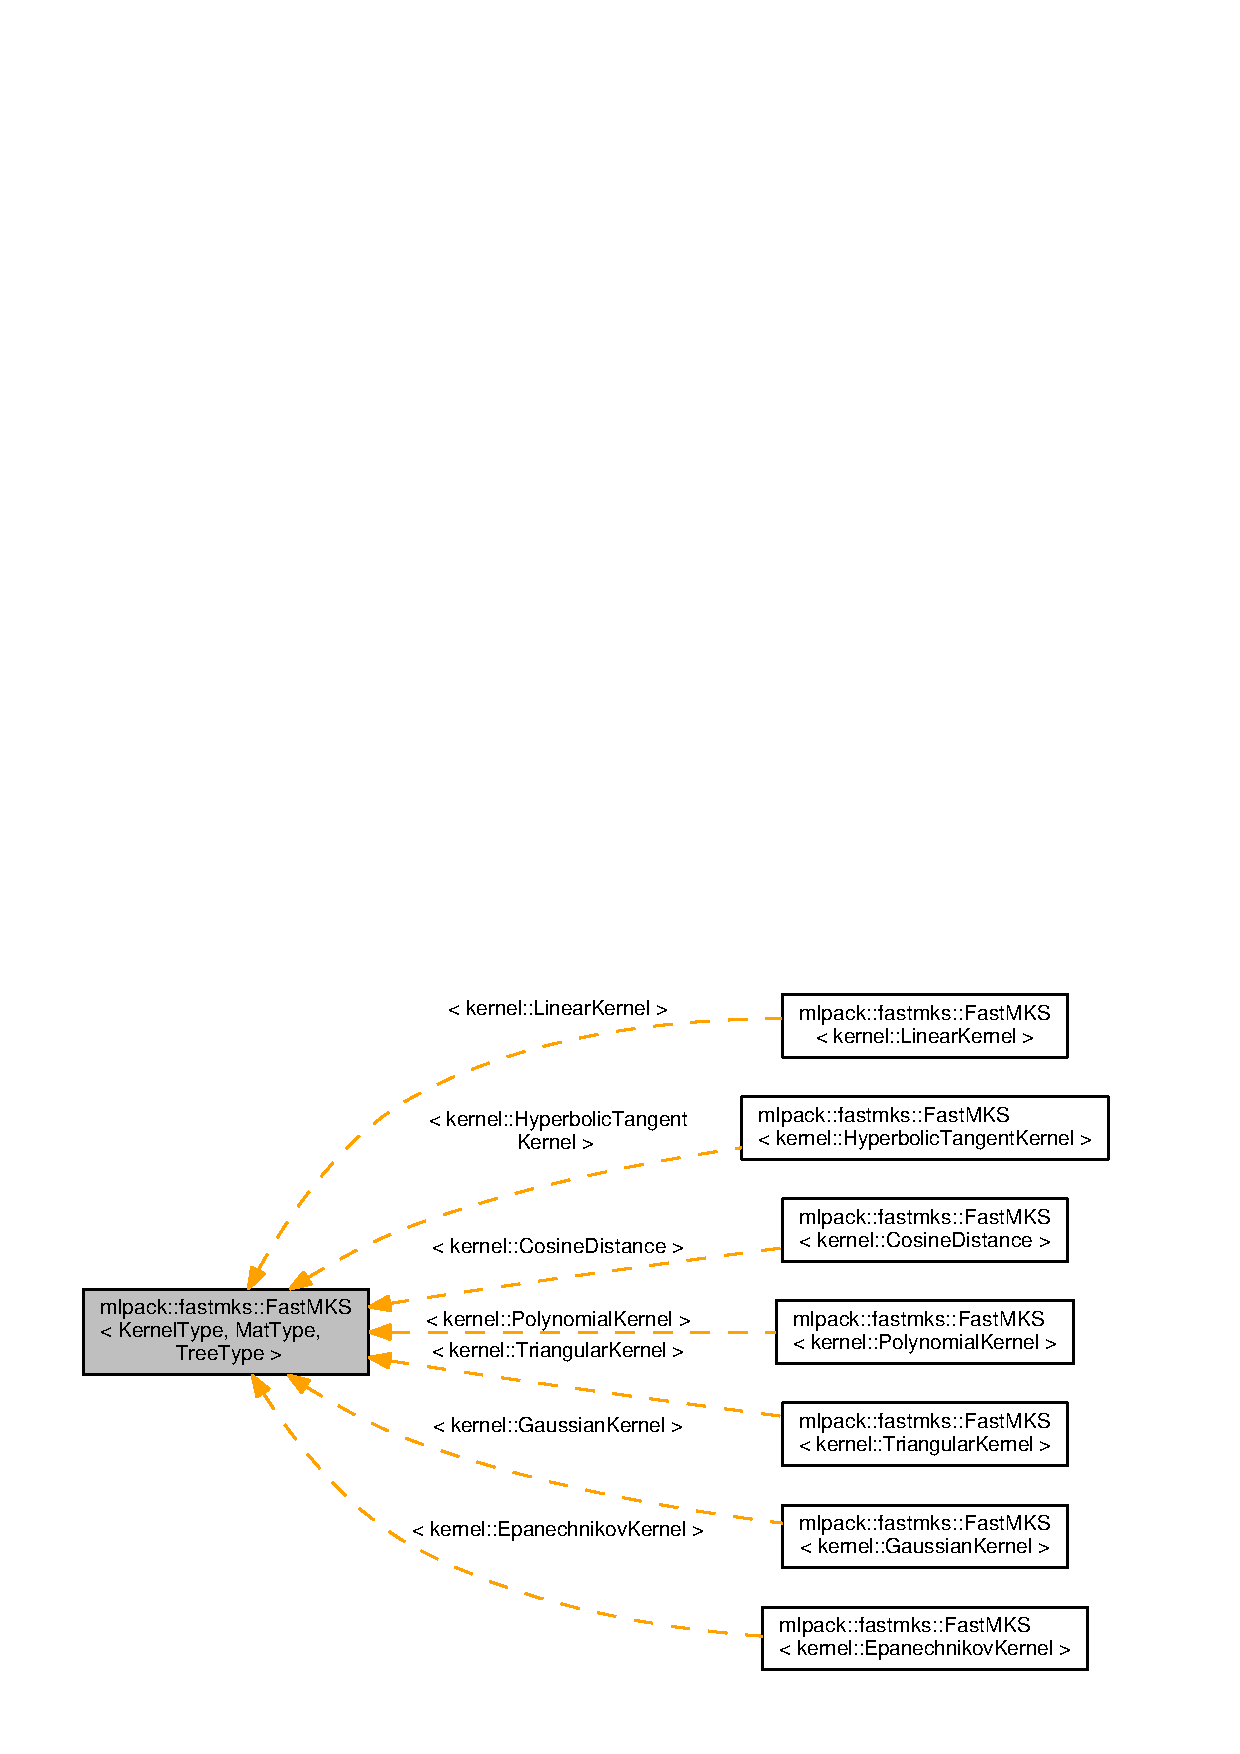
\includegraphics[width=350pt]{classmlpack_1_1fastmks_1_1FastMKS__inherit__graph}
\end{center}
\end{figure}
\subsection*{Public Types}
\begin{DoxyCompactItemize}
\item 
typedef Tree\+Type$<$ \textbf{ metric\+::\+I\+P\+Metric}$<$ Kernel\+Type $>$, \textbf{ Fast\+M\+K\+S\+Stat}, Mat\+Type $>$ \textbf{ Tree}
\begin{DoxyCompactList}\small\item\em Convenience typedef. \end{DoxyCompactList}\end{DoxyCompactItemize}
\subsection*{Public Member Functions}
\begin{DoxyCompactItemize}
\item 
\textbf{ Fast\+M\+KS} (const bool single\+Mode=false, const bool naive=false)
\begin{DoxyCompactList}\small\item\em Create the \doxyref{Fast\+M\+KS}{p.}{classmlpack_1_1fastmks_1_1FastMKS} object with an empty reference set and default kernel. \end{DoxyCompactList}\item 
\textbf{ Fast\+M\+KS} (const Mat\+Type \&reference\+Set, const bool single\+Mode=false, const bool naive=false)
\begin{DoxyCompactList}\small\item\em Create the \doxyref{Fast\+M\+KS}{p.}{classmlpack_1_1fastmks_1_1FastMKS} object with the given reference set (this is the set that is searched). \end{DoxyCompactList}\item 
\textbf{ Fast\+M\+KS} (const Mat\+Type \&reference\+Set, Kernel\+Type \&kernel, const bool single\+Mode=false, const bool naive=false)
\begin{DoxyCompactList}\small\item\em Create the \doxyref{Fast\+M\+KS}{p.}{classmlpack_1_1fastmks_1_1FastMKS} object using the reference set (this is the set that is searched) with an initialized kernel. \end{DoxyCompactList}\item 
\textbf{ Fast\+M\+KS} (Mat\+Type \&\&reference\+Set, const bool single\+Mode=false, const bool naive=false)
\begin{DoxyCompactList}\small\item\em Create the \doxyref{Fast\+M\+KS}{p.}{classmlpack_1_1fastmks_1_1FastMKS} object with the given reference set (this is the set that is searched), taking ownership of the reference set. \end{DoxyCompactList}\item 
\textbf{ Fast\+M\+KS} (Mat\+Type \&\&reference\+Set, Kernel\+Type \&kernel, const bool single\+Mode=false, const bool naive=false)
\begin{DoxyCompactList}\small\item\em Create the \doxyref{Fast\+M\+KS}{p.}{classmlpack_1_1fastmks_1_1FastMKS} object using the reference set (this is the set that is searched) with an initialized kernel, taking ownership of the reference set. \end{DoxyCompactList}\item 
\textbf{ Fast\+M\+KS} (\textbf{ Tree} $\ast$reference\+Tree, const bool single\+Mode=false)
\begin{DoxyCompactList}\small\item\em Create the \doxyref{Fast\+M\+KS}{p.}{classmlpack_1_1fastmks_1_1FastMKS} object with an already-\/initialized tree built on the reference points. \end{DoxyCompactList}\item 
\textbf{ Fast\+M\+KS} (const \textbf{ Fast\+M\+KS} \&other)
\begin{DoxyCompactList}\small\item\em Copy the parameters of the given model. \end{DoxyCompactList}\item 
\textbf{ Fast\+M\+KS} (\textbf{ Fast\+M\+KS} \&\&other)
\begin{DoxyCompactList}\small\item\em Take ownership of the given model. \end{DoxyCompactList}\item 
\textbf{ $\sim$\+Fast\+M\+KS} ()
\begin{DoxyCompactList}\small\item\em Destructor for the \doxyref{Fast\+M\+KS}{p.}{classmlpack_1_1fastmks_1_1FastMKS} object. \end{DoxyCompactList}\item 
const \textbf{ metric\+::\+I\+P\+Metric}$<$ Kernel\+Type $>$ \& \textbf{ Metric} () const
\begin{DoxyCompactList}\small\item\em Get the inner-\/product metric induced by the given kernel. \end{DoxyCompactList}\item 
\textbf{ metric\+::\+I\+P\+Metric}$<$ Kernel\+Type $>$ \& \textbf{ Metric} ()
\begin{DoxyCompactList}\small\item\em Modify the inner-\/product metric induced by the given kernel. \end{DoxyCompactList}\item 
bool \textbf{ Naive} () const
\begin{DoxyCompactList}\small\item\em Get whether or not brute-\/force (naive) search is used. \end{DoxyCompactList}\item 
bool \& \textbf{ Naive} ()
\begin{DoxyCompactList}\small\item\em Modify whether or not brute-\/force (naive) search is used. \end{DoxyCompactList}\item 
\textbf{ Fast\+M\+KS} \& \textbf{ operator=} (const \textbf{ Fast\+M\+KS} \&other)
\begin{DoxyCompactList}\small\item\em Assign this model to be a copy of the given model. \end{DoxyCompactList}\item 
\textbf{ Fast\+M\+KS} \& \textbf{ operator=} (\textbf{ Fast\+M\+KS} \&\&other)
\begin{DoxyCompactList}\small\item\em Move assignment operator. \end{DoxyCompactList}\item 
void \textbf{ Search} (const Mat\+Type \&query\+Set, const size\+\_\+t k, arma\+::\+Mat$<$ size\+\_\+t $>$ \&indices, arma\+::mat \&kernels)
\begin{DoxyCompactList}\small\item\em Search for the points in the reference set with maximum kernel evaluation to each point in the given query set. \end{DoxyCompactList}\item 
void \textbf{ Search} (\textbf{ Tree} $\ast$query\+Set, const size\+\_\+t k, arma\+::\+Mat$<$ size\+\_\+t $>$ \&indices, arma\+::mat \&kernels)
\begin{DoxyCompactList}\small\item\em Search for the points in the reference set with maximum kernel evaluation to each point in the query set corresponding to the given pre-\/built query tree. \end{DoxyCompactList}\item 
void \textbf{ Search} (const size\+\_\+t k, arma\+::\+Mat$<$ size\+\_\+t $>$ \&indices, arma\+::mat \&products)
\begin{DoxyCompactList}\small\item\em Search for the maximum inner products of the query set (or if no query set was passed, the reference set is used). \end{DoxyCompactList}\item 
{\footnotesize template$<$typename Archive $>$ }\\void \textbf{ serialize} (Archive \&ar, const uint32\+\_\+t)
\begin{DoxyCompactList}\small\item\em Serialize the model. \end{DoxyCompactList}\item 
bool \textbf{ Single\+Mode} () const
\begin{DoxyCompactList}\small\item\em Get whether or not single-\/tree search is used. \end{DoxyCompactList}\item 
bool \& \textbf{ Single\+Mode} ()
\begin{DoxyCompactList}\small\item\em Modify whether or not single-\/tree search is used. \end{DoxyCompactList}\item 
void \textbf{ Train} (const Mat\+Type \&reference\+Set)
\begin{DoxyCompactList}\small\item\em \char`\"{}\+Train\char`\"{} the \doxyref{Fast\+M\+KS}{p.}{classmlpack_1_1fastmks_1_1FastMKS} model on the given reference set (this will just build a tree, if the current search mode is not naive mode). \end{DoxyCompactList}\item 
void \textbf{ Train} (const Mat\+Type \&reference\+Set, Kernel\+Type \&kernel)
\begin{DoxyCompactList}\small\item\em \char`\"{}\+Train\char`\"{} the \doxyref{Fast\+M\+KS}{p.}{classmlpack_1_1fastmks_1_1FastMKS} model on the given reference set and use the given kernel. \end{DoxyCompactList}\item 
void \textbf{ Train} (Mat\+Type \&\&reference\+Set)
\begin{DoxyCompactList}\small\item\em \char`\"{}\+Train\char`\"{} the \doxyref{Fast\+M\+KS}{p.}{classmlpack_1_1fastmks_1_1FastMKS} model on the given reference set (this will just build a tree, if the current search mode is not naive mode). \end{DoxyCompactList}\item 
void \textbf{ Train} (Mat\+Type \&\&reference\+Set, Kernel\+Type \&kernel)
\begin{DoxyCompactList}\small\item\em \char`\"{}\+Train\char`\"{} the \doxyref{Fast\+M\+KS}{p.}{classmlpack_1_1fastmks_1_1FastMKS} model on the given reference set and use the given kernel. \end{DoxyCompactList}\item 
void \textbf{ Train} (\textbf{ Tree} $\ast$reference\+Tree)
\begin{DoxyCompactList}\small\item\em Train the \doxyref{Fast\+M\+KS}{p.}{classmlpack_1_1fastmks_1_1FastMKS} model on the given reference tree. \end{DoxyCompactList}\end{DoxyCompactItemize}


\subsection{Detailed Description}
\subsubsection*{template$<$typename Kernel\+Type, typename Mat\+Type = arma\+::mat, template$<$ typename Tree\+Metric\+Type, typename Tree\+Stat\+Type, typename Tree\+Mat\+Type $>$ class Tree\+Type = tree\+::\+Standard\+Cover\+Tree$>$\newline
class mlpack\+::fastmks\+::\+Fast\+M\+K\+S$<$ Kernel\+Type, Mat\+Type, Tree\+Type $>$}

An implementation of fast exact max-\/kernel search. 

Given a query dataset and a reference dataset (or optionally just a reference dataset which is also used as the query dataset), fast exact max-\/kernel search finds, for each point in the query dataset, the k points in the reference set with maximum kernel value K(p\+\_\+q, p\+\_\+r), where k is a specified parameter and K() is a Mercer kernel.

For more information, see the following paper.


\begin{DoxyCode}
@inproceedings\{curtin2013fast,
  title=\{Fast Exact Max-Kernel Search\},
  author=\{Curtin, Ryan R. and Ram, Parikshit and Gray, Alexander G.\},
  booktitle=\{Proceedings of the 2013 SIAM International Conference on Data
      Mining (SDM 13)\},
  year=\{2013\}
\}
\end{DoxyCode}


This class allows specification of the type of kernel and also of the type of tree. \doxyref{Fast\+M\+KS}{p.}{classmlpack_1_1fastmks_1_1FastMKS} can be run on kernels that work on arbitrary objects -- however, this only works with cover trees and other trees that are built only on points in the dataset (and not centroids of regions or anything like that).


\begin{DoxyTemplParams}{Template Parameters}
{\em Kernel\+Type} & Type of kernel to run \doxyref{Fast\+M\+KS}{p.}{classmlpack_1_1fastmks_1_1FastMKS} with. \\
\hline
{\em Mat\+Type} & Type of data matrix (usually arma\+::mat). \\
\hline
{\em Tree\+Type} & Type of tree to run \doxyref{Fast\+M\+KS}{p.}{classmlpack_1_1fastmks_1_1FastMKS} with; it must satisfy the Tree\+Type policy A\+PI. \\
\hline
\end{DoxyTemplParams}


Definition at line 63 of file fastmks.\+hpp.



\subsection{Member Typedef Documentation}
\mbox{\label{classmlpack_1_1fastmks_1_1FastMKS_ae9d9e44675a5326d3998fabdb3f33c74}} 
\index{mlpack\+::fastmks\+::\+Fast\+M\+KS@{mlpack\+::fastmks\+::\+Fast\+M\+KS}!Tree@{Tree}}
\index{Tree@{Tree}!mlpack\+::fastmks\+::\+Fast\+M\+KS@{mlpack\+::fastmks\+::\+Fast\+M\+KS}}
\subsubsection{Tree}
{\footnotesize\ttfamily typedef Tree\+Type$<$\textbf{ metric\+::\+I\+P\+Metric}$<$Kernel\+Type$>$, \textbf{ Fast\+M\+K\+S\+Stat}, Mat\+Type$>$ \textbf{ Tree}}



Convenience typedef. 



Definition at line 67 of file fastmks.\+hpp.



\subsection{Constructor \& Destructor Documentation}
\mbox{\label{classmlpack_1_1fastmks_1_1FastMKS_a8929924ebf7292b49847f01e0565d551}} 
\index{mlpack\+::fastmks\+::\+Fast\+M\+KS@{mlpack\+::fastmks\+::\+Fast\+M\+KS}!Fast\+M\+KS@{Fast\+M\+KS}}
\index{Fast\+M\+KS@{Fast\+M\+KS}!mlpack\+::fastmks\+::\+Fast\+M\+KS@{mlpack\+::fastmks\+::\+Fast\+M\+KS}}
\subsubsection{Fast\+M\+K\+S()\hspace{0.1cm}{\footnotesize\ttfamily [1/8]}}
{\footnotesize\ttfamily \textbf{ Fast\+M\+KS} (\begin{DoxyParamCaption}\item[{const bool}]{single\+Mode = {\ttfamily false},  }\item[{const bool}]{naive = {\ttfamily false} }\end{DoxyParamCaption})}



Create the \doxyref{Fast\+M\+KS}{p.}{classmlpack_1_1fastmks_1_1FastMKS} object with an empty reference set and default kernel. 

Make sure to call \doxyref{Train()}{p.}{classmlpack_1_1fastmks_1_1FastMKS_ad3fd386abe263b5cf9461366485cb62d} before \doxyref{Search()}{p.}{classmlpack_1_1fastmks_1_1FastMKS_af0704791dd9b3290639bb23a591e0ac8} is called!


\begin{DoxyParams}{Parameters}
{\em single\+Mode} & Whether or not to run single-\/tree search. \\
\hline
{\em naive} & Whether or not to run brute-\/force (naive) search. \\
\hline
\end{DoxyParams}
\mbox{\label{classmlpack_1_1fastmks_1_1FastMKS_afee6c99ec9f30b076de479ba7b771ae2}} 
\index{mlpack\+::fastmks\+::\+Fast\+M\+KS@{mlpack\+::fastmks\+::\+Fast\+M\+KS}!Fast\+M\+KS@{Fast\+M\+KS}}
\index{Fast\+M\+KS@{Fast\+M\+KS}!mlpack\+::fastmks\+::\+Fast\+M\+KS@{mlpack\+::fastmks\+::\+Fast\+M\+KS}}
\subsubsection{Fast\+M\+K\+S()\hspace{0.1cm}{\footnotesize\ttfamily [2/8]}}
{\footnotesize\ttfamily \textbf{ Fast\+M\+KS} (\begin{DoxyParamCaption}\item[{const Mat\+Type \&}]{reference\+Set,  }\item[{const bool}]{single\+Mode = {\ttfamily false},  }\item[{const bool}]{naive = {\ttfamily false} }\end{DoxyParamCaption})}



Create the \doxyref{Fast\+M\+KS}{p.}{classmlpack_1_1fastmks_1_1FastMKS} object with the given reference set (this is the set that is searched). 

Optionally, specify whether or not single-\/tree search or naive (brute-\/force) search should be used.


\begin{DoxyParams}{Parameters}
{\em reference\+Set} & Set of reference data. \\
\hline
{\em single\+Mode} & Whether or not to run single-\/tree search. \\
\hline
{\em naive} & Whether or not to run brute-\/force (naive) search. \\
\hline
\end{DoxyParams}
\mbox{\label{classmlpack_1_1fastmks_1_1FastMKS_a8dfc666eb77095ea4fafdd88aaf5dfd9}} 
\index{mlpack\+::fastmks\+::\+Fast\+M\+KS@{mlpack\+::fastmks\+::\+Fast\+M\+KS}!Fast\+M\+KS@{Fast\+M\+KS}}
\index{Fast\+M\+KS@{Fast\+M\+KS}!mlpack\+::fastmks\+::\+Fast\+M\+KS@{mlpack\+::fastmks\+::\+Fast\+M\+KS}}
\subsubsection{Fast\+M\+K\+S()\hspace{0.1cm}{\footnotesize\ttfamily [3/8]}}
{\footnotesize\ttfamily \textbf{ Fast\+M\+KS} (\begin{DoxyParamCaption}\item[{const Mat\+Type \&}]{reference\+Set,  }\item[{Kernel\+Type \&}]{kernel,  }\item[{const bool}]{single\+Mode = {\ttfamily false},  }\item[{const bool}]{naive = {\ttfamily false} }\end{DoxyParamCaption})}



Create the \doxyref{Fast\+M\+KS}{p.}{classmlpack_1_1fastmks_1_1FastMKS} object using the reference set (this is the set that is searched) with an initialized kernel. 

This is useful for when the kernel stores state. Optionally, specify whether or not single-\/tree search or naive (brute-\/force) search should be used.


\begin{DoxyParams}{Parameters}
{\em reference\+Set} & Reference set of data for \doxyref{Fast\+M\+KS}{p.}{classmlpack_1_1fastmks_1_1FastMKS}. \\
\hline
{\em kernel} & Initialized kernel. \\
\hline
{\em single\+Mode} & Whether or not to run single-\/tree search. \\
\hline
{\em naive} & Whether or not to run brute-\/force (naive) search. \\
\hline
\end{DoxyParams}
\mbox{\label{classmlpack_1_1fastmks_1_1FastMKS_adad457dfd833ec0cb9d9d2cfb3ccf233}} 
\index{mlpack\+::fastmks\+::\+Fast\+M\+KS@{mlpack\+::fastmks\+::\+Fast\+M\+KS}!Fast\+M\+KS@{Fast\+M\+KS}}
\index{Fast\+M\+KS@{Fast\+M\+KS}!mlpack\+::fastmks\+::\+Fast\+M\+KS@{mlpack\+::fastmks\+::\+Fast\+M\+KS}}
\subsubsection{Fast\+M\+K\+S()\hspace{0.1cm}{\footnotesize\ttfamily [4/8]}}
{\footnotesize\ttfamily \textbf{ Fast\+M\+KS} (\begin{DoxyParamCaption}\item[{Mat\+Type \&\&}]{reference\+Set,  }\item[{const bool}]{single\+Mode = {\ttfamily false},  }\item[{const bool}]{naive = {\ttfamily false} }\end{DoxyParamCaption})}



Create the \doxyref{Fast\+M\+KS}{p.}{classmlpack_1_1fastmks_1_1FastMKS} object with the given reference set (this is the set that is searched), taking ownership of the reference set. 

Optionally, specify whether or not single-\/tree search or naive (brute-\/force) search should be used.


\begin{DoxyParams}{Parameters}
{\em reference\+Set} & Set of reference data. \\
\hline
{\em single\+Mode} & Whether or not to run single-\/tree search. \\
\hline
{\em naive} & Whether or not to run brute-\/force (naive) search. \\
\hline
\end{DoxyParams}
\mbox{\label{classmlpack_1_1fastmks_1_1FastMKS_a3920de429037b75eea30b02ab5f8ba27}} 
\index{mlpack\+::fastmks\+::\+Fast\+M\+KS@{mlpack\+::fastmks\+::\+Fast\+M\+KS}!Fast\+M\+KS@{Fast\+M\+KS}}
\index{Fast\+M\+KS@{Fast\+M\+KS}!mlpack\+::fastmks\+::\+Fast\+M\+KS@{mlpack\+::fastmks\+::\+Fast\+M\+KS}}
\subsubsection{Fast\+M\+K\+S()\hspace{0.1cm}{\footnotesize\ttfamily [5/8]}}
{\footnotesize\ttfamily \textbf{ Fast\+M\+KS} (\begin{DoxyParamCaption}\item[{Mat\+Type \&\&}]{reference\+Set,  }\item[{Kernel\+Type \&}]{kernel,  }\item[{const bool}]{single\+Mode = {\ttfamily false},  }\item[{const bool}]{naive = {\ttfamily false} }\end{DoxyParamCaption})}



Create the \doxyref{Fast\+M\+KS}{p.}{classmlpack_1_1fastmks_1_1FastMKS} object using the reference set (this is the set that is searched) with an initialized kernel, taking ownership of the reference set. 

This is useful for when the kernel stores state. Optionally, specify whether or not single-\/tree search or naive (brute-\/force) search should be used.


\begin{DoxyParams}{Parameters}
{\em reference\+Set} & Reference set of data for \doxyref{Fast\+M\+KS}{p.}{classmlpack_1_1fastmks_1_1FastMKS}. \\
\hline
{\em kernel} & Initialized kernel. \\
\hline
{\em single\+Mode} & Whether or not to run single-\/tree search. \\
\hline
{\em naive} & Whether or not to run brute-\/force (naive) search. \\
\hline
\end{DoxyParams}
\mbox{\label{classmlpack_1_1fastmks_1_1FastMKS_a7e1243e858cce013126f02acbe503770}} 
\index{mlpack\+::fastmks\+::\+Fast\+M\+KS@{mlpack\+::fastmks\+::\+Fast\+M\+KS}!Fast\+M\+KS@{Fast\+M\+KS}}
\index{Fast\+M\+KS@{Fast\+M\+KS}!mlpack\+::fastmks\+::\+Fast\+M\+KS@{mlpack\+::fastmks\+::\+Fast\+M\+KS}}
\subsubsection{Fast\+M\+K\+S()\hspace{0.1cm}{\footnotesize\ttfamily [6/8]}}
{\footnotesize\ttfamily \textbf{ Fast\+M\+KS} (\begin{DoxyParamCaption}\item[{\textbf{ Tree} $\ast$}]{reference\+Tree,  }\item[{const bool}]{single\+Mode = {\ttfamily false} }\end{DoxyParamCaption})}



Create the \doxyref{Fast\+M\+KS}{p.}{classmlpack_1_1fastmks_1_1FastMKS} object with an already-\/initialized tree built on the reference points. 

Be sure that the tree is built with the metric type I\+P\+Metric$<$\+Kernel\+Type$>$. Optionally, whether or not to run single-\/tree search can be specified. Brute-\/force search is not available with this constructor since a tree is given (use one of the other constructors).


\begin{DoxyParams}{Parameters}
{\em reference\+Tree} & Tree built on reference data. \\
\hline
{\em single\+Mode} & Whether or not to run single-\/tree search. \\
\hline
\end{DoxyParams}
\mbox{\label{classmlpack_1_1fastmks_1_1FastMKS_ae87575a643a4a978674954bb7624d514}} 
\index{mlpack\+::fastmks\+::\+Fast\+M\+KS@{mlpack\+::fastmks\+::\+Fast\+M\+KS}!Fast\+M\+KS@{Fast\+M\+KS}}
\index{Fast\+M\+KS@{Fast\+M\+KS}!mlpack\+::fastmks\+::\+Fast\+M\+KS@{mlpack\+::fastmks\+::\+Fast\+M\+KS}}
\subsubsection{Fast\+M\+K\+S()\hspace{0.1cm}{\footnotesize\ttfamily [7/8]}}
{\footnotesize\ttfamily \textbf{ Fast\+M\+KS} (\begin{DoxyParamCaption}\item[{const \textbf{ Fast\+M\+KS}$<$ Kernel\+Type, Mat\+Type, Tree\+Type $>$ \&}]{other }\end{DoxyParamCaption})}



Copy the parameters of the given model. 

\mbox{\label{classmlpack_1_1fastmks_1_1FastMKS_ae44d8a17127cf60eef6d1d6e6b967a9c}} 
\index{mlpack\+::fastmks\+::\+Fast\+M\+KS@{mlpack\+::fastmks\+::\+Fast\+M\+KS}!Fast\+M\+KS@{Fast\+M\+KS}}
\index{Fast\+M\+KS@{Fast\+M\+KS}!mlpack\+::fastmks\+::\+Fast\+M\+KS@{mlpack\+::fastmks\+::\+Fast\+M\+KS}}
\subsubsection{Fast\+M\+K\+S()\hspace{0.1cm}{\footnotesize\ttfamily [8/8]}}
{\footnotesize\ttfamily \textbf{ Fast\+M\+KS} (\begin{DoxyParamCaption}\item[{\textbf{ Fast\+M\+KS}$<$ Kernel\+Type, Mat\+Type, Tree\+Type $>$ \&\&}]{other }\end{DoxyParamCaption})}



Take ownership of the given model. 

\mbox{\label{classmlpack_1_1fastmks_1_1FastMKS_a587b1748da4da938d879b494d3d73ae6}} 
\index{mlpack\+::fastmks\+::\+Fast\+M\+KS@{mlpack\+::fastmks\+::\+Fast\+M\+KS}!````~Fast\+M\+KS@{$\sim$\+Fast\+M\+KS}}
\index{````~Fast\+M\+KS@{$\sim$\+Fast\+M\+KS}!mlpack\+::fastmks\+::\+Fast\+M\+KS@{mlpack\+::fastmks\+::\+Fast\+M\+KS}}
\subsubsection{$\sim$\+Fast\+M\+K\+S()}
{\footnotesize\ttfamily $\sim$\textbf{ Fast\+M\+KS} (\begin{DoxyParamCaption}{ }\end{DoxyParamCaption})}



Destructor for the \doxyref{Fast\+M\+KS}{p.}{classmlpack_1_1fastmks_1_1FastMKS} object. 



\subsection{Member Function Documentation}
\mbox{\label{classmlpack_1_1fastmks_1_1FastMKS_a783d5d06bf6589a56a297ba89a8eb75e}} 
\index{mlpack\+::fastmks\+::\+Fast\+M\+KS@{mlpack\+::fastmks\+::\+Fast\+M\+KS}!Metric@{Metric}}
\index{Metric@{Metric}!mlpack\+::fastmks\+::\+Fast\+M\+KS@{mlpack\+::fastmks\+::\+Fast\+M\+KS}}
\subsubsection{Metric()\hspace{0.1cm}{\footnotesize\ttfamily [1/2]}}
{\footnotesize\ttfamily const \textbf{ metric\+::\+I\+P\+Metric}$<$Kernel\+Type$>$\& Metric (\begin{DoxyParamCaption}{ }\end{DoxyParamCaption}) const\hspace{0.3cm}{\ttfamily [inline]}}



Get the inner-\/product metric induced by the given kernel. 



Definition at line 291 of file fastmks.\+hpp.

\mbox{\label{classmlpack_1_1fastmks_1_1FastMKS_aeafbdda6260df07dffa6e97262ed5dcc}} 
\index{mlpack\+::fastmks\+::\+Fast\+M\+KS@{mlpack\+::fastmks\+::\+Fast\+M\+KS}!Metric@{Metric}}
\index{Metric@{Metric}!mlpack\+::fastmks\+::\+Fast\+M\+KS@{mlpack\+::fastmks\+::\+Fast\+M\+KS}}
\subsubsection{Metric()\hspace{0.1cm}{\footnotesize\ttfamily [2/2]}}
{\footnotesize\ttfamily \textbf{ metric\+::\+I\+P\+Metric}$<$Kernel\+Type$>$\& Metric (\begin{DoxyParamCaption}{ }\end{DoxyParamCaption})\hspace{0.3cm}{\ttfamily [inline]}}



Modify the inner-\/product metric induced by the given kernel. 



Definition at line 293 of file fastmks.\+hpp.

\mbox{\label{classmlpack_1_1fastmks_1_1FastMKS_a343230e7d7344e3f7d5f5f2eb89cf2c5}} 
\index{mlpack\+::fastmks\+::\+Fast\+M\+KS@{mlpack\+::fastmks\+::\+Fast\+M\+KS}!Naive@{Naive}}
\index{Naive@{Naive}!mlpack\+::fastmks\+::\+Fast\+M\+KS@{mlpack\+::fastmks\+::\+Fast\+M\+KS}}
\subsubsection{Naive()\hspace{0.1cm}{\footnotesize\ttfamily [1/2]}}
{\footnotesize\ttfamily bool Naive (\begin{DoxyParamCaption}{ }\end{DoxyParamCaption}) const\hspace{0.3cm}{\ttfamily [inline]}}



Get whether or not brute-\/force (naive) search is used. 



Definition at line 301 of file fastmks.\+hpp.

\mbox{\label{classmlpack_1_1fastmks_1_1FastMKS_af7d397adca3f411b4e2d2f977b280ce6}} 
\index{mlpack\+::fastmks\+::\+Fast\+M\+KS@{mlpack\+::fastmks\+::\+Fast\+M\+KS}!Naive@{Naive}}
\index{Naive@{Naive}!mlpack\+::fastmks\+::\+Fast\+M\+KS@{mlpack\+::fastmks\+::\+Fast\+M\+KS}}
\subsubsection{Naive()\hspace{0.1cm}{\footnotesize\ttfamily [2/2]}}
{\footnotesize\ttfamily bool\& Naive (\begin{DoxyParamCaption}{ }\end{DoxyParamCaption})\hspace{0.3cm}{\ttfamily [inline]}}



Modify whether or not brute-\/force (naive) search is used. 



Definition at line 303 of file fastmks.\+hpp.

\mbox{\label{classmlpack_1_1fastmks_1_1FastMKS_aa972b5311cdff2c681beb64da448b084}} 
\index{mlpack\+::fastmks\+::\+Fast\+M\+KS@{mlpack\+::fastmks\+::\+Fast\+M\+KS}!operator=@{operator=}}
\index{operator=@{operator=}!mlpack\+::fastmks\+::\+Fast\+M\+KS@{mlpack\+::fastmks\+::\+Fast\+M\+KS}}
\subsubsection{operator=()\hspace{0.1cm}{\footnotesize\ttfamily [1/2]}}
{\footnotesize\ttfamily \textbf{ Fast\+M\+KS}\& operator= (\begin{DoxyParamCaption}\item[{const \textbf{ Fast\+M\+KS}$<$ Kernel\+Type, Mat\+Type, Tree\+Type $>$ \&}]{other }\end{DoxyParamCaption})}



Assign this model to be a copy of the given model. 

\mbox{\label{classmlpack_1_1fastmks_1_1FastMKS_a49fd929bf8784789ec55d4c7acd96070}} 
\index{mlpack\+::fastmks\+::\+Fast\+M\+KS@{mlpack\+::fastmks\+::\+Fast\+M\+KS}!operator=@{operator=}}
\index{operator=@{operator=}!mlpack\+::fastmks\+::\+Fast\+M\+KS@{mlpack\+::fastmks\+::\+Fast\+M\+KS}}
\subsubsection{operator=()\hspace{0.1cm}{\footnotesize\ttfamily [2/2]}}
{\footnotesize\ttfamily \textbf{ Fast\+M\+KS}\& operator= (\begin{DoxyParamCaption}\item[{\textbf{ Fast\+M\+KS}$<$ Kernel\+Type, Mat\+Type, Tree\+Type $>$ \&\&}]{other }\end{DoxyParamCaption})}



Move assignment operator. 

\mbox{\label{classmlpack_1_1fastmks_1_1FastMKS_af0704791dd9b3290639bb23a591e0ac8}} 
\index{mlpack\+::fastmks\+::\+Fast\+M\+KS@{mlpack\+::fastmks\+::\+Fast\+M\+KS}!Search@{Search}}
\index{Search@{Search}!mlpack\+::fastmks\+::\+Fast\+M\+KS@{mlpack\+::fastmks\+::\+Fast\+M\+KS}}
\subsubsection{Search()\hspace{0.1cm}{\footnotesize\ttfamily [1/3]}}
{\footnotesize\ttfamily void Search (\begin{DoxyParamCaption}\item[{const Mat\+Type \&}]{query\+Set,  }\item[{const size\+\_\+t}]{k,  }\item[{arma\+::\+Mat$<$ size\+\_\+t $>$ \&}]{indices,  }\item[{arma\+::mat \&}]{kernels }\end{DoxyParamCaption})}



Search for the points in the reference set with maximum kernel evaluation to each point in the given query set. 

The resulting kernel evaluations are stored in the kernels matrix, and the corresponding point indices are stored in the indices matrix. The results for each point in the query set are stored in the corresponding column of the kernels and products matrices; for instance, the index of the point with maximum kernel evaluation to point 4 in the query set will be stored in row 0 and column 4 of the indices matrix.

If query\+Set only contains a few points, the extra overhead of building a tree to perform dual-\/tree search may not be warranted, and it may be faster to use single-\/tree search, either by setting single\+Mode to false in the constructor or with \doxyref{Single\+Mode()}{p.}{classmlpack_1_1fastmks_1_1FastMKS_adadacd63ddeadf138d834b1fdc632773}.


\begin{DoxyParams}{Parameters}
{\em query\+Set} & Set of query points (can be a single point). \\
\hline
{\em k} & The number of maximum kernels to find. \\
\hline
{\em indices} & Matrix to store resulting indices of max-\/kernel search in. \\
\hline
{\em kernels} & Matrix to store resulting max-\/kernel values in. \\
\hline
\end{DoxyParams}
\mbox{\label{classmlpack_1_1fastmks_1_1FastMKS_a58abd056551df0f13890ddc350594740}} 
\index{mlpack\+::fastmks\+::\+Fast\+M\+KS@{mlpack\+::fastmks\+::\+Fast\+M\+KS}!Search@{Search}}
\index{Search@{Search}!mlpack\+::fastmks\+::\+Fast\+M\+KS@{mlpack\+::fastmks\+::\+Fast\+M\+KS}}
\subsubsection{Search()\hspace{0.1cm}{\footnotesize\ttfamily [2/3]}}
{\footnotesize\ttfamily void Search (\begin{DoxyParamCaption}\item[{\textbf{ Tree} $\ast$}]{query\+Set,  }\item[{const size\+\_\+t}]{k,  }\item[{arma\+::\+Mat$<$ size\+\_\+t $>$ \&}]{indices,  }\item[{arma\+::mat \&}]{kernels }\end{DoxyParamCaption})}



Search for the points in the reference set with maximum kernel evaluation to each point in the query set corresponding to the given pre-\/built query tree. 

The resulting kernel evaluations are stored in the kernels matrix, and the corresponding point indices are stored in the indices matrix. The results for each point in the query set are stored in the corresponding column of the kernels and products matrices; for instance, the index of the point with maximum kernel evaluation to point 4 in the query set will be stored in row 0 and column 4 of the indices matrix.

This will throw an exception if called while the \doxyref{Fast\+M\+KS}{p.}{classmlpack_1_1fastmks_1_1FastMKS} object has \textquotesingle{}single\textquotesingle{} set to true.

Be aware that if your tree modifies the original input matrix, the results here are with respect to the modified input matrix (that is, query\+Tree-\/$>$Dataset()).


\begin{DoxyParams}{Parameters}
{\em query\+Set} & Tree built on query points. \\
\hline
{\em k} & The number of maximum kernels to find. \\
\hline
{\em indices} & Matrix to store resulting indices of max-\/kernel search in. \\
\hline
{\em kernels} & Matrix to store resulting max-\/kernel values in. \\
\hline
\end{DoxyParams}
\mbox{\label{classmlpack_1_1fastmks_1_1FastMKS_aa0b0df843179afabdec5a3bc50c68704}} 
\index{mlpack\+::fastmks\+::\+Fast\+M\+KS@{mlpack\+::fastmks\+::\+Fast\+M\+KS}!Search@{Search}}
\index{Search@{Search}!mlpack\+::fastmks\+::\+Fast\+M\+KS@{mlpack\+::fastmks\+::\+Fast\+M\+KS}}
\subsubsection{Search()\hspace{0.1cm}{\footnotesize\ttfamily [3/3]}}
{\footnotesize\ttfamily void Search (\begin{DoxyParamCaption}\item[{const size\+\_\+t}]{k,  }\item[{arma\+::\+Mat$<$ size\+\_\+t $>$ \&}]{indices,  }\item[{arma\+::mat \&}]{products }\end{DoxyParamCaption})}



Search for the maximum inner products of the query set (or if no query set was passed, the reference set is used). 

The resulting maximum inner products are stored in the products matrix and the corresponding point indices are stores in the indices matrix. The results for each point in the query set are stored in the corresponding column of the indices and products matrices; for instance, the index of the point with maximum inner product to point 4 in the query set will be stored in row 0 and column 4 of the indices matrix.


\begin{DoxyParams}{Parameters}
{\em k} & The number of maximum kernels to find. \\
\hline
{\em indices} & Matrix to store resulting indices of max-\/kernel search in. \\
\hline
{\em products} & Matrix to store resulting max-\/kernel values in. \\
\hline
\end{DoxyParams}
\mbox{\label{classmlpack_1_1fastmks_1_1FastMKS_a65cba07328997659bec80b9879b15a51}} 
\index{mlpack\+::fastmks\+::\+Fast\+M\+KS@{mlpack\+::fastmks\+::\+Fast\+M\+KS}!serialize@{serialize}}
\index{serialize@{serialize}!mlpack\+::fastmks\+::\+Fast\+M\+KS@{mlpack\+::fastmks\+::\+Fast\+M\+KS}}
\subsubsection{serialize()}
{\footnotesize\ttfamily void serialize (\begin{DoxyParamCaption}\item[{Archive \&}]{ar,  }\item[{const uint32\+\_\+t}]{ }\end{DoxyParamCaption})}



Serialize the model. 



Referenced by Fast\+M\+K\+S$<$ mlpack\+::kernel\+::\+Cosine\+Distance $>$\+::\+Naive().

\mbox{\label{classmlpack_1_1fastmks_1_1FastMKS_a7477b3e8499a6158bbe177e7f30d4947}} 
\index{mlpack\+::fastmks\+::\+Fast\+M\+KS@{mlpack\+::fastmks\+::\+Fast\+M\+KS}!Single\+Mode@{Single\+Mode}}
\index{Single\+Mode@{Single\+Mode}!mlpack\+::fastmks\+::\+Fast\+M\+KS@{mlpack\+::fastmks\+::\+Fast\+M\+KS}}
\subsubsection{Single\+Mode()\hspace{0.1cm}{\footnotesize\ttfamily [1/2]}}
{\footnotesize\ttfamily bool Single\+Mode (\begin{DoxyParamCaption}{ }\end{DoxyParamCaption}) const\hspace{0.3cm}{\ttfamily [inline]}}



Get whether or not single-\/tree search is used. 



Definition at line 296 of file fastmks.\+hpp.

\mbox{\label{classmlpack_1_1fastmks_1_1FastMKS_adadacd63ddeadf138d834b1fdc632773}} 
\index{mlpack\+::fastmks\+::\+Fast\+M\+KS@{mlpack\+::fastmks\+::\+Fast\+M\+KS}!Single\+Mode@{Single\+Mode}}
\index{Single\+Mode@{Single\+Mode}!mlpack\+::fastmks\+::\+Fast\+M\+KS@{mlpack\+::fastmks\+::\+Fast\+M\+KS}}
\subsubsection{Single\+Mode()\hspace{0.1cm}{\footnotesize\ttfamily [2/2]}}
{\footnotesize\ttfamily bool\& Single\+Mode (\begin{DoxyParamCaption}{ }\end{DoxyParamCaption})\hspace{0.3cm}{\ttfamily [inline]}}



Modify whether or not single-\/tree search is used. 



Definition at line 298 of file fastmks.\+hpp.

\mbox{\label{classmlpack_1_1fastmks_1_1FastMKS_ad3fd386abe263b5cf9461366485cb62d}} 
\index{mlpack\+::fastmks\+::\+Fast\+M\+KS@{mlpack\+::fastmks\+::\+Fast\+M\+KS}!Train@{Train}}
\index{Train@{Train}!mlpack\+::fastmks\+::\+Fast\+M\+KS@{mlpack\+::fastmks\+::\+Fast\+M\+KS}}
\subsubsection{Train()\hspace{0.1cm}{\footnotesize\ttfamily [1/5]}}
{\footnotesize\ttfamily void Train (\begin{DoxyParamCaption}\item[{const Mat\+Type \&}]{reference\+Set }\end{DoxyParamCaption})}



\char`\"{}\+Train\char`\"{} the \doxyref{Fast\+M\+KS}{p.}{classmlpack_1_1fastmks_1_1FastMKS} model on the given reference set (this will just build a tree, if the current search mode is not naive mode). 


\begin{DoxyParams}{Parameters}
{\em reference\+Set} & Set of reference points. \\
\hline
\end{DoxyParams}
\mbox{\label{classmlpack_1_1fastmks_1_1FastMKS_a9af17008ca7cb2ed611e9e9ed5fdeb53}} 
\index{mlpack\+::fastmks\+::\+Fast\+M\+KS@{mlpack\+::fastmks\+::\+Fast\+M\+KS}!Train@{Train}}
\index{Train@{Train}!mlpack\+::fastmks\+::\+Fast\+M\+KS@{mlpack\+::fastmks\+::\+Fast\+M\+KS}}
\subsubsection{Train()\hspace{0.1cm}{\footnotesize\ttfamily [2/5]}}
{\footnotesize\ttfamily void Train (\begin{DoxyParamCaption}\item[{const Mat\+Type \&}]{reference\+Set,  }\item[{Kernel\+Type \&}]{kernel }\end{DoxyParamCaption})}



\char`\"{}\+Train\char`\"{} the \doxyref{Fast\+M\+KS}{p.}{classmlpack_1_1fastmks_1_1FastMKS} model on the given reference set and use the given kernel. 

This will just build a tree and replace the metric, if the current search mode is not naive mode.


\begin{DoxyParams}{Parameters}
{\em reference\+Set} & Set of reference points. \\
\hline
{\em kernel} & Kernel to use for search. \\
\hline
\end{DoxyParams}
\mbox{\label{classmlpack_1_1fastmks_1_1FastMKS_aa53a1056d8a4e4fae0049ba42b5e8dd7}} 
\index{mlpack\+::fastmks\+::\+Fast\+M\+KS@{mlpack\+::fastmks\+::\+Fast\+M\+KS}!Train@{Train}}
\index{Train@{Train}!mlpack\+::fastmks\+::\+Fast\+M\+KS@{mlpack\+::fastmks\+::\+Fast\+M\+KS}}
\subsubsection{Train()\hspace{0.1cm}{\footnotesize\ttfamily [3/5]}}
{\footnotesize\ttfamily void Train (\begin{DoxyParamCaption}\item[{Mat\+Type \&\&}]{reference\+Set }\end{DoxyParamCaption})}



\char`\"{}\+Train\char`\"{} the \doxyref{Fast\+M\+KS}{p.}{classmlpack_1_1fastmks_1_1FastMKS} model on the given reference set (this will just build a tree, if the current search mode is not naive mode). 

This takes ownership of the reference set.


\begin{DoxyParams}{Parameters}
{\em reference\+Set} & Set of reference points. \\
\hline
\end{DoxyParams}
\mbox{\label{classmlpack_1_1fastmks_1_1FastMKS_aa9bdecc510e909eb1e92f1c9275421bb}} 
\index{mlpack\+::fastmks\+::\+Fast\+M\+KS@{mlpack\+::fastmks\+::\+Fast\+M\+KS}!Train@{Train}}
\index{Train@{Train}!mlpack\+::fastmks\+::\+Fast\+M\+KS@{mlpack\+::fastmks\+::\+Fast\+M\+KS}}
\subsubsection{Train()\hspace{0.1cm}{\footnotesize\ttfamily [4/5]}}
{\footnotesize\ttfamily void Train (\begin{DoxyParamCaption}\item[{Mat\+Type \&\&}]{reference\+Set,  }\item[{Kernel\+Type \&}]{kernel }\end{DoxyParamCaption})}



\char`\"{}\+Train\char`\"{} the \doxyref{Fast\+M\+KS}{p.}{classmlpack_1_1fastmks_1_1FastMKS} model on the given reference set and use the given kernel. 

This will just build a tree and replace the metric, if the current search mode is not naive mode. This takes ownership of the reference set.


\begin{DoxyParams}{Parameters}
{\em reference\+Set} & Set of reference points. \\
\hline
{\em kernel} & Kernel to use for search. \\
\hline
\end{DoxyParams}
\mbox{\label{classmlpack_1_1fastmks_1_1FastMKS_a3d1133fe6bda66e7143fd7aab27cbd04}} 
\index{mlpack\+::fastmks\+::\+Fast\+M\+KS@{mlpack\+::fastmks\+::\+Fast\+M\+KS}!Train@{Train}}
\index{Train@{Train}!mlpack\+::fastmks\+::\+Fast\+M\+KS@{mlpack\+::fastmks\+::\+Fast\+M\+KS}}
\subsubsection{Train()\hspace{0.1cm}{\footnotesize\ttfamily [5/5]}}
{\footnotesize\ttfamily void Train (\begin{DoxyParamCaption}\item[{\textbf{ Tree} $\ast$}]{reference\+Tree }\end{DoxyParamCaption})}



Train the \doxyref{Fast\+M\+KS}{p.}{classmlpack_1_1fastmks_1_1FastMKS} model on the given reference tree. 

This takes ownership of the tree, so you do not need to delete it! This will throw an exception if the model is searching in naive mode (i.\+e. if \doxyref{Naive()}{p.}{classmlpack_1_1fastmks_1_1FastMKS_af7d397adca3f411b4e2d2f977b280ce6} == true).


\begin{DoxyParams}{Parameters}
{\em reference\+Tree} & Tree to use as reference data. \\
\hline
\end{DoxyParams}


The documentation for this class was generated from the following file\+:\begin{DoxyCompactItemize}
\item 
/home/aakash/mlpack/src/mlpack/methods/fastmks/\textbf{ fastmks.\+hpp}\end{DoxyCompactItemize}

\section{mlpack\+:\+:fastmks\+:\+:Fast\+M\+KS$<$ Kernel\+Type, Mat\+Type, Tree\+Type $>$\+:\+:Candidate\+Cmp Struct Reference}
\label{structmlpack_1_1fastmks_1_1FastMKS_1_1CandidateCmp}\index{mlpack\+::fastmks\+::\+Fast\+M\+K\+S$<$ Kernel\+Type, Mat\+Type, Tree\+Type $>$\+::\+Candidate\+Cmp@{mlpack\+::fastmks\+::\+Fast\+M\+K\+S$<$ Kernel\+Type, Mat\+Type, Tree\+Type $>$\+::\+Candidate\+Cmp}}


Compare two candidates based on the value.  


\subsection*{Public Member Functions}
\begin{DoxyCompactItemize}
\item 
bool {\bf operator()} (const {\bf Candidate} \&c1, const {\bf Candidate} \&c2)
\end{DoxyCompactItemize}


\subsection{Detailed Description}
\subsubsection*{template$<$typename Kernel\+Type, typename Mat\+Type = arma\+::mat, template$<$ typename Tree\+Metric\+Type, typename Tree\+Stat\+Type, typename Tree\+Mat\+Type $>$ class Tree\+Type = tree\+::\+Standard\+Cover\+Tree$>$\\*
struct mlpack\+::fastmks\+::\+Fast\+M\+K\+S$<$ Kernel\+Type, Mat\+Type, Tree\+Type $>$\+::\+Candidate\+Cmp}

Compare two candidates based on the value. 

Definition at line 277 of file fastmks.\+hpp.



\subsection{Member Function Documentation}
\index{mlpack\+::fastmks\+::\+Fast\+M\+K\+S\+::\+Candidate\+Cmp@{mlpack\+::fastmks\+::\+Fast\+M\+K\+S\+::\+Candidate\+Cmp}!operator()@{operator()}}
\index{operator()@{operator()}!mlpack\+::fastmks\+::\+Fast\+M\+K\+S\+::\+Candidate\+Cmp@{mlpack\+::fastmks\+::\+Fast\+M\+K\+S\+::\+Candidate\+Cmp}}
\subsubsection[{operator()(const Candidate \&c1, const Candidate \&c2)}]{\setlength{\rightskip}{0pt plus 5cm}template$<$typename Kernel\+Type, typename Mat\+Type = arma\+::mat, template$<$ typename Tree\+Metric\+Type, typename Tree\+Stat\+Type, typename Tree\+Mat\+Type $>$ class Tree\+Type = tree\+::\+Standard\+Cover\+Tree$>$ bool {\bf mlpack\+::fastmks\+::\+Fast\+M\+KS}$<$ Kernel\+Type, Mat\+Type, Tree\+Type $>$\+::Candidate\+Cmp\+::operator() (
\begin{DoxyParamCaption}
\item[{const {\bf Candidate} \&}]{c1, }
\item[{const {\bf Candidate} \&}]{c2}
\end{DoxyParamCaption}
)\hspace{0.3cm}{\ttfamily [inline]}}\label{structmlpack_1_1fastmks_1_1FastMKS_1_1CandidateCmp_a1023e61a24080ed4ee122983e8813755}


Definition at line 278 of file fastmks.\+hpp.



The documentation for this struct was generated from the following file\+:\begin{DoxyCompactItemize}
\item 
src/mlpack/methods/fastmks/{\bf fastmks.\+hpp}\end{DoxyCompactItemize}

\section{mlpack\+:\+:fastmks\+:\+:Fast\+M\+K\+S\+Model Class Reference}
\label{classmlpack_1_1fastmks_1_1FastMKSModel}\index{mlpack\+::fastmks\+::\+Fast\+M\+K\+S\+Model@{mlpack\+::fastmks\+::\+Fast\+M\+K\+S\+Model}}


A utility struct to contain all the possible \doxyref{Fast\+M\+KS}{p.}{classmlpack_1_1fastmks_1_1FastMKS} models, for use by the mlpack\+\_\+fastmks program.  


\subsection*{Public Types}
\begin{DoxyCompactItemize}
\item 
enum {\bf Kernel\+Types} \{ \\*
{\bf L\+I\+N\+E\+A\+R\+\_\+\+K\+E\+R\+N\+EL}, 
\\*
{\bf P\+O\+L\+Y\+N\+O\+M\+I\+A\+L\+\_\+\+K\+E\+R\+N\+EL}, 
\\*
{\bf C\+O\+S\+I\+N\+E\+\_\+\+D\+I\+S\+T\+A\+N\+CE}, 
\\*
{\bf G\+A\+U\+S\+S\+I\+A\+N\+\_\+\+K\+E\+R\+N\+EL}, 
\\*
{\bf E\+P\+A\+N\+E\+C\+H\+N\+I\+K\+O\+V\+\_\+\+K\+E\+R\+N\+EL}, 
\\*
{\bf T\+R\+I\+A\+N\+G\+U\+L\+A\+R\+\_\+\+K\+E\+R\+N\+EL}, 
\\*
{\bf H\+Y\+P\+T\+A\+N\+\_\+\+K\+E\+R\+N\+EL}
 \}\begin{DoxyCompactList}\small\item\em A list of all the kernels we support. \end{DoxyCompactList}
\end{DoxyCompactItemize}
\subsection*{Public Member Functions}
\begin{DoxyCompactItemize}
\item 
{\bf Fast\+M\+K\+S\+Model} (const int {\bf kernel\+Type}={\bf L\+I\+N\+E\+A\+R\+\_\+\+K\+E\+R\+N\+EL})
\begin{DoxyCompactList}\small\item\em Create the \doxyref{Fast\+M\+K\+S\+Model}{p.}{classmlpack_1_1fastmks_1_1FastMKSModel} with the given kernel type. \end{DoxyCompactList}\item 
{\bf Fast\+M\+K\+S\+Model} (const {\bf Fast\+M\+K\+S\+Model} \&other)
\begin{DoxyCompactList}\small\item\em Copy constructor. \end{DoxyCompactList}\item 
{\bf Fast\+M\+K\+S\+Model} ({\bf Fast\+M\+K\+S\+Model} \&\&other)
\begin{DoxyCompactList}\small\item\em Move constructor. \end{DoxyCompactList}\item 
{\bf $\sim$\+Fast\+M\+K\+S\+Model} ()
\begin{DoxyCompactList}\small\item\em Clean memory. \end{DoxyCompactList}\item 
{\footnotesize template$<$typename T\+Kernel\+Type $>$ }\\void {\bf Build\+Model} (const arma\+::mat \&reference\+Data, T\+Kernel\+Type \&kernel, const bool single\+Mode, const bool naive, const double base)
\begin{DoxyCompactList}\small\item\em Build the model on the given reference set. \end{DoxyCompactList}\item 
int {\bf Kernel\+Type} () const 
\begin{DoxyCompactList}\small\item\em Get the kernel type. \end{DoxyCompactList}\item 
int \& {\bf Kernel\+Type} ()
\begin{DoxyCompactList}\small\item\em Modify the kernel type. \end{DoxyCompactList}\item 
bool {\bf Naive} () const 
\begin{DoxyCompactList}\small\item\em Get whether or not naive search is used. \end{DoxyCompactList}\item 
bool \& {\bf Naive} ()
\begin{DoxyCompactList}\small\item\em Set whether or not naive search is used. \end{DoxyCompactList}\item 
{\bf Fast\+M\+K\+S\+Model} \& {\bf operator=} (const {\bf Fast\+M\+K\+S\+Model} \&other)
\begin{DoxyCompactList}\small\item\em Copy assignment operator. \end{DoxyCompactList}\item 
void {\bf Search} (const arma\+::mat \&query\+Set, const size\+\_\+t k, arma\+::\+Mat$<$ size\+\_\+t $>$ \&indices, arma\+::mat \&kernels, const double base)
\begin{DoxyCompactList}\small\item\em Search with a different query set. \end{DoxyCompactList}\item 
void {\bf Search} (const size\+\_\+t k, arma\+::\+Mat$<$ size\+\_\+t $>$ \&indices, arma\+::mat \&kernels)
\begin{DoxyCompactList}\small\item\em Search with the reference set as the query set. \end{DoxyCompactList}\item 
{\footnotesize template$<$typename Archive $>$ }\\void {\bf Serialize} (Archive \&ar, const unsigned int)
\begin{DoxyCompactList}\small\item\em Serialize the model. \end{DoxyCompactList}\item 
bool {\bf Single\+Mode} () const 
\begin{DoxyCompactList}\small\item\em Get whether or not single-\/tree search is used. \end{DoxyCompactList}\item 
bool \& {\bf Single\+Mode} ()
\begin{DoxyCompactList}\small\item\em Set whether or not single-\/tree search is used. \end{DoxyCompactList}\end{DoxyCompactItemize}
\subsection*{Private Member Functions}
\begin{DoxyCompactItemize}
\item 
{\footnotesize template$<$typename Fast\+M\+K\+S\+Type $>$ }\\void {\bf Search} (Fast\+M\+K\+S\+Type \&f, const arma\+::mat \&query\+Set, const size\+\_\+t k, arma\+::\+Mat$<$ size\+\_\+t $>$ \&indices, arma\+::mat \&kernels, const double base)
\begin{DoxyCompactList}\small\item\em Build a query tree and execute the search. \end{DoxyCompactList}\end{DoxyCompactItemize}
\subsection*{Private Attributes}
\begin{DoxyCompactItemize}
\item 
{\bf Fast\+M\+KS}$<$ {\bf kernel\+::\+Cosine\+Distance} $>$ $\ast$ {\bf cosine}
\begin{DoxyCompactList}\small\item\em This will only be non-\/\+N\+U\+LL if this is the type of kernel we are using. \end{DoxyCompactList}\item 
{\bf Fast\+M\+KS}$<$ {\bf kernel\+::\+Epanechnikov\+Kernel} $>$ $\ast$ {\bf epan}
\begin{DoxyCompactList}\small\item\em This will only be non-\/\+N\+U\+LL if this is the type of kernel we are using. \end{DoxyCompactList}\item 
{\bf Fast\+M\+KS}$<$ {\bf kernel\+::\+Gaussian\+Kernel} $>$ $\ast$ {\bf gaussian}
\begin{DoxyCompactList}\small\item\em This will only be non-\/\+N\+U\+LL if this is the type of kernel we are using. \end{DoxyCompactList}\item 
{\bf Fast\+M\+KS}$<$ {\bf kernel\+::\+Hyperbolic\+Tangent\+Kernel} $>$ $\ast$ {\bf hyptan}
\begin{DoxyCompactList}\small\item\em This will only be non-\/\+N\+U\+LL if this is the type of kernel we are using. \end{DoxyCompactList}\item 
int {\bf kernel\+Type}
\begin{DoxyCompactList}\small\item\em The type of kernel we are using. \end{DoxyCompactList}\item 
{\bf Fast\+M\+KS}$<$ {\bf kernel\+::\+Linear\+Kernel} $>$ $\ast$ {\bf linear}
\begin{DoxyCompactList}\small\item\em This will only be non-\/\+N\+U\+LL if this is the type of kernel we are using. \end{DoxyCompactList}\item 
{\bf Fast\+M\+KS}$<$ {\bf kernel\+::\+Polynomial\+Kernel} $>$ $\ast$ {\bf polynomial}
\begin{DoxyCompactList}\small\item\em This will only be non-\/\+N\+U\+LL if this is the type of kernel we are using. \end{DoxyCompactList}\item 
{\bf Fast\+M\+KS}$<$ {\bf kernel\+::\+Triangular\+Kernel} $>$ $\ast$ {\bf triangular}
\begin{DoxyCompactList}\small\item\em This will only be non-\/\+N\+U\+LL if this is the type of kernel we are using. \end{DoxyCompactList}\end{DoxyCompactItemize}


\subsection{Detailed Description}
A utility struct to contain all the possible \doxyref{Fast\+M\+KS}{p.}{classmlpack_1_1fastmks_1_1FastMKS} models, for use by the mlpack\+\_\+fastmks program. 



Definition at line 34 of file fastmks\+\_\+model.\+hpp.



\subsection{Member Enumeration Documentation}
\index{mlpack\+::fastmks\+::\+Fast\+M\+K\+S\+Model@{mlpack\+::fastmks\+::\+Fast\+M\+K\+S\+Model}!Kernel\+Types@{Kernel\+Types}}
\index{Kernel\+Types@{Kernel\+Types}!mlpack\+::fastmks\+::\+Fast\+M\+K\+S\+Model@{mlpack\+::fastmks\+::\+Fast\+M\+K\+S\+Model}}
\subsubsection[{Kernel\+Types}]{\setlength{\rightskip}{0pt plus 5cm}enum {\bf mlpack\+::fastmks\+::\+Fast\+M\+K\+S\+Model\+::\+Kernel\+Types}}\label{classmlpack_1_1fastmks_1_1FastMKSModel_a668603530129fd3d20e964ed52965d6a}


A list of all the kernels we support. 

\begin{Desc}
\item[Enumerator]\par
\begin{description}
\index{L\+I\+N\+E\+A\+R\+\_\+\+K\+E\+R\+N\+EL@{L\+I\+N\+E\+A\+R\+\_\+\+K\+E\+R\+N\+EL}!mlpack\+::fastmks\+::\+Fast\+M\+K\+S\+Model@{mlpack\+::fastmks\+::\+Fast\+M\+K\+S\+Model}}\index{mlpack\+::fastmks\+::\+Fast\+M\+K\+S\+Model@{mlpack\+::fastmks\+::\+Fast\+M\+K\+S\+Model}!L\+I\+N\+E\+A\+R\+\_\+\+K\+E\+R\+N\+EL@{L\+I\+N\+E\+A\+R\+\_\+\+K\+E\+R\+N\+EL}}\item[{\em 
L\+I\+N\+E\+A\+R\+\_\+\+K\+E\+R\+N\+EL\label{classmlpack_1_1fastmks_1_1FastMKSModel_a668603530129fd3d20e964ed52965d6aa2d25afc2058b5ed027e5e1ed5a9f7f7a}
}]\index{P\+O\+L\+Y\+N\+O\+M\+I\+A\+L\+\_\+\+K\+E\+R\+N\+EL@{P\+O\+L\+Y\+N\+O\+M\+I\+A\+L\+\_\+\+K\+E\+R\+N\+EL}!mlpack\+::fastmks\+::\+Fast\+M\+K\+S\+Model@{mlpack\+::fastmks\+::\+Fast\+M\+K\+S\+Model}}\index{mlpack\+::fastmks\+::\+Fast\+M\+K\+S\+Model@{mlpack\+::fastmks\+::\+Fast\+M\+K\+S\+Model}!P\+O\+L\+Y\+N\+O\+M\+I\+A\+L\+\_\+\+K\+E\+R\+N\+EL@{P\+O\+L\+Y\+N\+O\+M\+I\+A\+L\+\_\+\+K\+E\+R\+N\+EL}}\item[{\em 
P\+O\+L\+Y\+N\+O\+M\+I\+A\+L\+\_\+\+K\+E\+R\+N\+EL\label{classmlpack_1_1fastmks_1_1FastMKSModel_a668603530129fd3d20e964ed52965d6aa11037192c544497fe575b97c7276fe31}
}]\index{C\+O\+S\+I\+N\+E\+\_\+\+D\+I\+S\+T\+A\+N\+CE@{C\+O\+S\+I\+N\+E\+\_\+\+D\+I\+S\+T\+A\+N\+CE}!mlpack\+::fastmks\+::\+Fast\+M\+K\+S\+Model@{mlpack\+::fastmks\+::\+Fast\+M\+K\+S\+Model}}\index{mlpack\+::fastmks\+::\+Fast\+M\+K\+S\+Model@{mlpack\+::fastmks\+::\+Fast\+M\+K\+S\+Model}!C\+O\+S\+I\+N\+E\+\_\+\+D\+I\+S\+T\+A\+N\+CE@{C\+O\+S\+I\+N\+E\+\_\+\+D\+I\+S\+T\+A\+N\+CE}}\item[{\em 
C\+O\+S\+I\+N\+E\+\_\+\+D\+I\+S\+T\+A\+N\+CE\label{classmlpack_1_1fastmks_1_1FastMKSModel_a668603530129fd3d20e964ed52965d6aa6e49d9b04b4ebe2afae952090d880d4a}
}]\index{G\+A\+U\+S\+S\+I\+A\+N\+\_\+\+K\+E\+R\+N\+EL@{G\+A\+U\+S\+S\+I\+A\+N\+\_\+\+K\+E\+R\+N\+EL}!mlpack\+::fastmks\+::\+Fast\+M\+K\+S\+Model@{mlpack\+::fastmks\+::\+Fast\+M\+K\+S\+Model}}\index{mlpack\+::fastmks\+::\+Fast\+M\+K\+S\+Model@{mlpack\+::fastmks\+::\+Fast\+M\+K\+S\+Model}!G\+A\+U\+S\+S\+I\+A\+N\+\_\+\+K\+E\+R\+N\+EL@{G\+A\+U\+S\+S\+I\+A\+N\+\_\+\+K\+E\+R\+N\+EL}}\item[{\em 
G\+A\+U\+S\+S\+I\+A\+N\+\_\+\+K\+E\+R\+N\+EL\label{classmlpack_1_1fastmks_1_1FastMKSModel_a668603530129fd3d20e964ed52965d6aa2c0451a3d4d6971ae6319ec588361d73}
}]\index{E\+P\+A\+N\+E\+C\+H\+N\+I\+K\+O\+V\+\_\+\+K\+E\+R\+N\+EL@{E\+P\+A\+N\+E\+C\+H\+N\+I\+K\+O\+V\+\_\+\+K\+E\+R\+N\+EL}!mlpack\+::fastmks\+::\+Fast\+M\+K\+S\+Model@{mlpack\+::fastmks\+::\+Fast\+M\+K\+S\+Model}}\index{mlpack\+::fastmks\+::\+Fast\+M\+K\+S\+Model@{mlpack\+::fastmks\+::\+Fast\+M\+K\+S\+Model}!E\+P\+A\+N\+E\+C\+H\+N\+I\+K\+O\+V\+\_\+\+K\+E\+R\+N\+EL@{E\+P\+A\+N\+E\+C\+H\+N\+I\+K\+O\+V\+\_\+\+K\+E\+R\+N\+EL}}\item[{\em 
E\+P\+A\+N\+E\+C\+H\+N\+I\+K\+O\+V\+\_\+\+K\+E\+R\+N\+EL\label{classmlpack_1_1fastmks_1_1FastMKSModel_a668603530129fd3d20e964ed52965d6aac79726dba8f0695dee7d9f173ca4a342}
}]\index{T\+R\+I\+A\+N\+G\+U\+L\+A\+R\+\_\+\+K\+E\+R\+N\+EL@{T\+R\+I\+A\+N\+G\+U\+L\+A\+R\+\_\+\+K\+E\+R\+N\+EL}!mlpack\+::fastmks\+::\+Fast\+M\+K\+S\+Model@{mlpack\+::fastmks\+::\+Fast\+M\+K\+S\+Model}}\index{mlpack\+::fastmks\+::\+Fast\+M\+K\+S\+Model@{mlpack\+::fastmks\+::\+Fast\+M\+K\+S\+Model}!T\+R\+I\+A\+N\+G\+U\+L\+A\+R\+\_\+\+K\+E\+R\+N\+EL@{T\+R\+I\+A\+N\+G\+U\+L\+A\+R\+\_\+\+K\+E\+R\+N\+EL}}\item[{\em 
T\+R\+I\+A\+N\+G\+U\+L\+A\+R\+\_\+\+K\+E\+R\+N\+EL\label{classmlpack_1_1fastmks_1_1FastMKSModel_a668603530129fd3d20e964ed52965d6aa22e72f2def86ee9390e216b784274e4c}
}]\index{H\+Y\+P\+T\+A\+N\+\_\+\+K\+E\+R\+N\+EL@{H\+Y\+P\+T\+A\+N\+\_\+\+K\+E\+R\+N\+EL}!mlpack\+::fastmks\+::\+Fast\+M\+K\+S\+Model@{mlpack\+::fastmks\+::\+Fast\+M\+K\+S\+Model}}\index{mlpack\+::fastmks\+::\+Fast\+M\+K\+S\+Model@{mlpack\+::fastmks\+::\+Fast\+M\+K\+S\+Model}!H\+Y\+P\+T\+A\+N\+\_\+\+K\+E\+R\+N\+EL@{H\+Y\+P\+T\+A\+N\+\_\+\+K\+E\+R\+N\+EL}}\item[{\em 
H\+Y\+P\+T\+A\+N\+\_\+\+K\+E\+R\+N\+EL\label{classmlpack_1_1fastmks_1_1FastMKSModel_a668603530129fd3d20e964ed52965d6aa2d7e1baebeb6cfa73418d803639a3dec}
}]\end{description}
\end{Desc}


Definition at line 38 of file fastmks\+\_\+model.\+hpp.



\subsection{Constructor \& Destructor Documentation}
\index{mlpack\+::fastmks\+::\+Fast\+M\+K\+S\+Model@{mlpack\+::fastmks\+::\+Fast\+M\+K\+S\+Model}!Fast\+M\+K\+S\+Model@{Fast\+M\+K\+S\+Model}}
\index{Fast\+M\+K\+S\+Model@{Fast\+M\+K\+S\+Model}!mlpack\+::fastmks\+::\+Fast\+M\+K\+S\+Model@{mlpack\+::fastmks\+::\+Fast\+M\+K\+S\+Model}}
\subsubsection[{Fast\+M\+K\+S\+Model(const int kernel\+Type=\+L\+I\+N\+E\+A\+R\+\_\+\+K\+E\+R\+N\+E\+L)}]{\setlength{\rightskip}{0pt plus 5cm}mlpack\+::fastmks\+::\+Fast\+M\+K\+S\+Model\+::\+Fast\+M\+K\+S\+Model (
\begin{DoxyParamCaption}
\item[{const int}]{kernel\+Type = {\ttfamily {\bf L\+I\+N\+E\+A\+R\+\_\+\+K\+E\+R\+N\+EL}}}
\end{DoxyParamCaption}
)}\label{classmlpack_1_1fastmks_1_1FastMKSModel_afb4a69a44e92d3fb2faa08e8643ba52c}


Create the \doxyref{Fast\+M\+K\+S\+Model}{p.}{classmlpack_1_1fastmks_1_1FastMKSModel} with the given kernel type. 

\index{mlpack\+::fastmks\+::\+Fast\+M\+K\+S\+Model@{mlpack\+::fastmks\+::\+Fast\+M\+K\+S\+Model}!Fast\+M\+K\+S\+Model@{Fast\+M\+K\+S\+Model}}
\index{Fast\+M\+K\+S\+Model@{Fast\+M\+K\+S\+Model}!mlpack\+::fastmks\+::\+Fast\+M\+K\+S\+Model@{mlpack\+::fastmks\+::\+Fast\+M\+K\+S\+Model}}
\subsubsection[{Fast\+M\+K\+S\+Model(const Fast\+M\+K\+S\+Model \&other)}]{\setlength{\rightskip}{0pt plus 5cm}mlpack\+::fastmks\+::\+Fast\+M\+K\+S\+Model\+::\+Fast\+M\+K\+S\+Model (
\begin{DoxyParamCaption}
\item[{const {\bf Fast\+M\+K\+S\+Model} \&}]{other}
\end{DoxyParamCaption}
)}\label{classmlpack_1_1fastmks_1_1FastMKSModel_aed40286a3473846ef1c2cd5c9894ddc7}


Copy constructor. 

\index{mlpack\+::fastmks\+::\+Fast\+M\+K\+S\+Model@{mlpack\+::fastmks\+::\+Fast\+M\+K\+S\+Model}!Fast\+M\+K\+S\+Model@{Fast\+M\+K\+S\+Model}}
\index{Fast\+M\+K\+S\+Model@{Fast\+M\+K\+S\+Model}!mlpack\+::fastmks\+::\+Fast\+M\+K\+S\+Model@{mlpack\+::fastmks\+::\+Fast\+M\+K\+S\+Model}}
\subsubsection[{Fast\+M\+K\+S\+Model(\+Fast\+M\+K\+S\+Model \&\&other)}]{\setlength{\rightskip}{0pt plus 5cm}mlpack\+::fastmks\+::\+Fast\+M\+K\+S\+Model\+::\+Fast\+M\+K\+S\+Model (
\begin{DoxyParamCaption}
\item[{{\bf Fast\+M\+K\+S\+Model} \&\&}]{other}
\end{DoxyParamCaption}
)}\label{classmlpack_1_1fastmks_1_1FastMKSModel_ace50dd21244f081eb8c606047bdd3460}


Move constructor. 

\index{mlpack\+::fastmks\+::\+Fast\+M\+K\+S\+Model@{mlpack\+::fastmks\+::\+Fast\+M\+K\+S\+Model}!````~Fast\+M\+K\+S\+Model@{$\sim$\+Fast\+M\+K\+S\+Model}}
\index{````~Fast\+M\+K\+S\+Model@{$\sim$\+Fast\+M\+K\+S\+Model}!mlpack\+::fastmks\+::\+Fast\+M\+K\+S\+Model@{mlpack\+::fastmks\+::\+Fast\+M\+K\+S\+Model}}
\subsubsection[{$\sim$\+Fast\+M\+K\+S\+Model()}]{\setlength{\rightskip}{0pt plus 5cm}mlpack\+::fastmks\+::\+Fast\+M\+K\+S\+Model\+::$\sim$\+Fast\+M\+K\+S\+Model (
\begin{DoxyParamCaption}
{}
\end{DoxyParamCaption}
)}\label{classmlpack_1_1fastmks_1_1FastMKSModel_a679284d364c7272c38f4fad12473b9b0}


Clean memory. 



\subsection{Member Function Documentation}
\index{mlpack\+::fastmks\+::\+Fast\+M\+K\+S\+Model@{mlpack\+::fastmks\+::\+Fast\+M\+K\+S\+Model}!Build\+Model@{Build\+Model}}
\index{Build\+Model@{Build\+Model}!mlpack\+::fastmks\+::\+Fast\+M\+K\+S\+Model@{mlpack\+::fastmks\+::\+Fast\+M\+K\+S\+Model}}
\subsubsection[{Build\+Model(const arma\+::mat \&reference\+Data, T\+Kernel\+Type \&kernel, const bool single\+Mode, const bool naive, const double base)}]{\setlength{\rightskip}{0pt plus 5cm}template$<$typename T\+Kernel\+Type $>$ void mlpack\+::fastmks\+::\+Fast\+M\+K\+S\+Model\+::\+Build\+Model (
\begin{DoxyParamCaption}
\item[{const arma\+::mat \&}]{reference\+Data, }
\item[{T\+Kernel\+Type \&}]{kernel, }
\item[{const bool}]{single\+Mode, }
\item[{const bool}]{naive, }
\item[{const double}]{base}
\end{DoxyParamCaption}
)}\label{classmlpack_1_1fastmks_1_1FastMKSModel_a96b0f48586bb92a38c8fc055f5b5adb3}


Build the model on the given reference set. 

Make sure kernel\+Type is equal to the correct entry in Kernel\+Types for the given Kernel\+Type class! \index{mlpack\+::fastmks\+::\+Fast\+M\+K\+S\+Model@{mlpack\+::fastmks\+::\+Fast\+M\+K\+S\+Model}!Kernel\+Type@{Kernel\+Type}}
\index{Kernel\+Type@{Kernel\+Type}!mlpack\+::fastmks\+::\+Fast\+M\+K\+S\+Model@{mlpack\+::fastmks\+::\+Fast\+M\+K\+S\+Model}}
\subsubsection[{Kernel\+Type() const }]{\setlength{\rightskip}{0pt plus 5cm}int mlpack\+::fastmks\+::\+Fast\+M\+K\+S\+Model\+::\+Kernel\+Type (
\begin{DoxyParamCaption}
{}
\end{DoxyParamCaption}
) const\hspace{0.3cm}{\ttfamily [inline]}}\label{classmlpack_1_1fastmks_1_1FastMKSModel_af295122856dd30acfd76f9a0986a7a69}


Get the kernel type. 



Definition at line 90 of file fastmks\+\_\+model.\+hpp.



References kernel\+Type.

\index{mlpack\+::fastmks\+::\+Fast\+M\+K\+S\+Model@{mlpack\+::fastmks\+::\+Fast\+M\+K\+S\+Model}!Kernel\+Type@{Kernel\+Type}}
\index{Kernel\+Type@{Kernel\+Type}!mlpack\+::fastmks\+::\+Fast\+M\+K\+S\+Model@{mlpack\+::fastmks\+::\+Fast\+M\+K\+S\+Model}}
\subsubsection[{Kernel\+Type()}]{\setlength{\rightskip}{0pt plus 5cm}int\& mlpack\+::fastmks\+::\+Fast\+M\+K\+S\+Model\+::\+Kernel\+Type (
\begin{DoxyParamCaption}
{}
\end{DoxyParamCaption}
)\hspace{0.3cm}{\ttfamily [inline]}}\label{classmlpack_1_1fastmks_1_1FastMKSModel_aaf260871fd78a2a91b451e6a9cd382a9}


Modify the kernel type. 



Definition at line 92 of file fastmks\+\_\+model.\+hpp.



References kernel\+Type, Search(), and Serialize().

\index{mlpack\+::fastmks\+::\+Fast\+M\+K\+S\+Model@{mlpack\+::fastmks\+::\+Fast\+M\+K\+S\+Model}!Naive@{Naive}}
\index{Naive@{Naive}!mlpack\+::fastmks\+::\+Fast\+M\+K\+S\+Model@{mlpack\+::fastmks\+::\+Fast\+M\+K\+S\+Model}}
\subsubsection[{Naive() const }]{\setlength{\rightskip}{0pt plus 5cm}bool mlpack\+::fastmks\+::\+Fast\+M\+K\+S\+Model\+::\+Naive (
\begin{DoxyParamCaption}
{}
\end{DoxyParamCaption}
) const}\label{classmlpack_1_1fastmks_1_1FastMKSModel_a9eee5349bfd2bac8ad685f7119fdd353}


Get whether or not naive search is used. 

\index{mlpack\+::fastmks\+::\+Fast\+M\+K\+S\+Model@{mlpack\+::fastmks\+::\+Fast\+M\+K\+S\+Model}!Naive@{Naive}}
\index{Naive@{Naive}!mlpack\+::fastmks\+::\+Fast\+M\+K\+S\+Model@{mlpack\+::fastmks\+::\+Fast\+M\+K\+S\+Model}}
\subsubsection[{Naive()}]{\setlength{\rightskip}{0pt plus 5cm}bool\& mlpack\+::fastmks\+::\+Fast\+M\+K\+S\+Model\+::\+Naive (
\begin{DoxyParamCaption}
{}
\end{DoxyParamCaption}
)}\label{classmlpack_1_1fastmks_1_1FastMKSModel_ae240f5b65049bc9229dd0f023ee643d4}


Set whether or not naive search is used. 

\index{mlpack\+::fastmks\+::\+Fast\+M\+K\+S\+Model@{mlpack\+::fastmks\+::\+Fast\+M\+K\+S\+Model}!operator=@{operator=}}
\index{operator=@{operator=}!mlpack\+::fastmks\+::\+Fast\+M\+K\+S\+Model@{mlpack\+::fastmks\+::\+Fast\+M\+K\+S\+Model}}
\subsubsection[{operator=(const Fast\+M\+K\+S\+Model \&other)}]{\setlength{\rightskip}{0pt plus 5cm}{\bf Fast\+M\+K\+S\+Model}\& mlpack\+::fastmks\+::\+Fast\+M\+K\+S\+Model\+::operator= (
\begin{DoxyParamCaption}
\item[{const {\bf Fast\+M\+K\+S\+Model} \&}]{other}
\end{DoxyParamCaption}
)}\label{classmlpack_1_1fastmks_1_1FastMKSModel_a541b7b94cd3ec69b2c4be5b2adf5526a}


Copy assignment operator. 

\index{mlpack\+::fastmks\+::\+Fast\+M\+K\+S\+Model@{mlpack\+::fastmks\+::\+Fast\+M\+K\+S\+Model}!Search@{Search}}
\index{Search@{Search}!mlpack\+::fastmks\+::\+Fast\+M\+K\+S\+Model@{mlpack\+::fastmks\+::\+Fast\+M\+K\+S\+Model}}
\subsubsection[{Search(const arma\+::mat \&query\+Set, const size\+\_\+t k, arma\+::\+Mat$<$ size\+\_\+t $>$ \&indices, arma\+::mat \&kernels, const double base)}]{\setlength{\rightskip}{0pt plus 5cm}void mlpack\+::fastmks\+::\+Fast\+M\+K\+S\+Model\+::\+Search (
\begin{DoxyParamCaption}
\item[{const arma\+::mat \&}]{query\+Set, }
\item[{const size\+\_\+t}]{k, }
\item[{arma\+::\+Mat$<$ size\+\_\+t $>$ \&}]{indices, }
\item[{arma\+::mat \&}]{kernels, }
\item[{const double}]{base}
\end{DoxyParamCaption}
)}\label{classmlpack_1_1fastmks_1_1FastMKSModel_af4145209e6e57ad196dd80db7c8e7229}


Search with a different query set. 


\begin{DoxyParams}{Parameters}
{\em query\+Set} & Set to search with. \\
\hline
{\em k} & Number of max-\/kernel candidates to search for. \\
\hline
{\em indices} & A matrix in which to store the indices of max-\/kernel candidates. \\
\hline
{\em kernels} & A matrix in which to store the max-\/kernel candidate kernel values. \\
\hline
{\em base} & Base to use for cover tree building (if in dual-\/tree search mode). \\
\hline
\end{DoxyParams}


Referenced by Kernel\+Type().

\index{mlpack\+::fastmks\+::\+Fast\+M\+K\+S\+Model@{mlpack\+::fastmks\+::\+Fast\+M\+K\+S\+Model}!Search@{Search}}
\index{Search@{Search}!mlpack\+::fastmks\+::\+Fast\+M\+K\+S\+Model@{mlpack\+::fastmks\+::\+Fast\+M\+K\+S\+Model}}
\subsubsection[{Search(const size\+\_\+t k, arma\+::\+Mat$<$ size\+\_\+t $>$ \&indices, arma\+::mat \&kernels)}]{\setlength{\rightskip}{0pt plus 5cm}void mlpack\+::fastmks\+::\+Fast\+M\+K\+S\+Model\+::\+Search (
\begin{DoxyParamCaption}
\item[{const size\+\_\+t}]{k, }
\item[{arma\+::\+Mat$<$ size\+\_\+t $>$ \&}]{indices, }
\item[{arma\+::mat \&}]{kernels}
\end{DoxyParamCaption}
)}\label{classmlpack_1_1fastmks_1_1FastMKSModel_a82da676ac7d1808d3ee059ccce1828fc}


Search with the reference set as the query set. 


\begin{DoxyParams}{Parameters}
{\em k} & Number of max-\/kernel candidates to search for. \\
\hline
{\em indices} & A matrix in which to store the indices of max-\/kernel candidates. \\
\hline
{\em kernels} & A matrix in which to store the max-\/kernel candidate kernel values. \\
\hline
\end{DoxyParams}
\index{mlpack\+::fastmks\+::\+Fast\+M\+K\+S\+Model@{mlpack\+::fastmks\+::\+Fast\+M\+K\+S\+Model}!Search@{Search}}
\index{Search@{Search}!mlpack\+::fastmks\+::\+Fast\+M\+K\+S\+Model@{mlpack\+::fastmks\+::\+Fast\+M\+K\+S\+Model}}
\subsubsection[{Search(\+Fast\+M\+K\+S\+Type \&f, const arma\+::mat \&query\+Set, const size\+\_\+t k, arma\+::\+Mat$<$ size\+\_\+t $>$ \&indices, arma\+::mat \&kernels, const double base)}]{\setlength{\rightskip}{0pt plus 5cm}template$<$typename Fast\+M\+K\+S\+Type $>$ void mlpack\+::fastmks\+::\+Fast\+M\+K\+S\+Model\+::\+Search (
\begin{DoxyParamCaption}
\item[{Fast\+M\+K\+S\+Type \&}]{f, }
\item[{const arma\+::mat \&}]{query\+Set, }
\item[{const size\+\_\+t}]{k, }
\item[{arma\+::\+Mat$<$ size\+\_\+t $>$ \&}]{indices, }
\item[{arma\+::mat \&}]{kernels, }
\item[{const double}]{base}
\end{DoxyParamCaption}
)\hspace{0.3cm}{\ttfamily [private]}}\label{classmlpack_1_1fastmks_1_1FastMKSModel_abbc607a693495f7ed5d1f935cee6d551}


Build a query tree and execute the search. 

\index{mlpack\+::fastmks\+::\+Fast\+M\+K\+S\+Model@{mlpack\+::fastmks\+::\+Fast\+M\+K\+S\+Model}!Serialize@{Serialize}}
\index{Serialize@{Serialize}!mlpack\+::fastmks\+::\+Fast\+M\+K\+S\+Model@{mlpack\+::fastmks\+::\+Fast\+M\+K\+S\+Model}}
\subsubsection[{Serialize(\+Archive \&ar, const unsigned int)}]{\setlength{\rightskip}{0pt plus 5cm}template$<$typename Archive $>$ void mlpack\+::fastmks\+::\+Fast\+M\+K\+S\+Model\+::\+Serialize (
\begin{DoxyParamCaption}
\item[{Archive \&}]{ar, }
\item[{const unsigned}]{int}
\end{DoxyParamCaption}
)}\label{classmlpack_1_1fastmks_1_1FastMKSModel_a7bad3f3fffec6feebe5c10c3c5c9059b}


Serialize the model. 



Referenced by Kernel\+Type().

\index{mlpack\+::fastmks\+::\+Fast\+M\+K\+S\+Model@{mlpack\+::fastmks\+::\+Fast\+M\+K\+S\+Model}!Single\+Mode@{Single\+Mode}}
\index{Single\+Mode@{Single\+Mode}!mlpack\+::fastmks\+::\+Fast\+M\+K\+S\+Model@{mlpack\+::fastmks\+::\+Fast\+M\+K\+S\+Model}}
\subsubsection[{Single\+Mode() const }]{\setlength{\rightskip}{0pt plus 5cm}bool mlpack\+::fastmks\+::\+Fast\+M\+K\+S\+Model\+::\+Single\+Mode (
\begin{DoxyParamCaption}
{}
\end{DoxyParamCaption}
) const}\label{classmlpack_1_1fastmks_1_1FastMKSModel_a7c51b75af767d3e3ae1321a016336db1}


Get whether or not single-\/tree search is used. 

\index{mlpack\+::fastmks\+::\+Fast\+M\+K\+S\+Model@{mlpack\+::fastmks\+::\+Fast\+M\+K\+S\+Model}!Single\+Mode@{Single\+Mode}}
\index{Single\+Mode@{Single\+Mode}!mlpack\+::fastmks\+::\+Fast\+M\+K\+S\+Model@{mlpack\+::fastmks\+::\+Fast\+M\+K\+S\+Model}}
\subsubsection[{Single\+Mode()}]{\setlength{\rightskip}{0pt plus 5cm}bool\& mlpack\+::fastmks\+::\+Fast\+M\+K\+S\+Model\+::\+Single\+Mode (
\begin{DoxyParamCaption}
{}
\end{DoxyParamCaption}
)}\label{classmlpack_1_1fastmks_1_1FastMKSModel_a192b9498fd49e86afc9484d86117b268}


Set whether or not single-\/tree search is used. 



\subsection{Member Data Documentation}
\index{mlpack\+::fastmks\+::\+Fast\+M\+K\+S\+Model@{mlpack\+::fastmks\+::\+Fast\+M\+K\+S\+Model}!cosine@{cosine}}
\index{cosine@{cosine}!mlpack\+::fastmks\+::\+Fast\+M\+K\+S\+Model@{mlpack\+::fastmks\+::\+Fast\+M\+K\+S\+Model}}
\subsubsection[{cosine}]{\setlength{\rightskip}{0pt plus 5cm}{\bf Fast\+M\+KS}$<${\bf kernel\+::\+Cosine\+Distance}$>$$\ast$ mlpack\+::fastmks\+::\+Fast\+M\+K\+S\+Model\+::cosine\hspace{0.3cm}{\ttfamily [private]}}\label{classmlpack_1_1fastmks_1_1FastMKSModel_a95df856ccffb0f983524d4ff53a745a3}


This will only be non-\/\+N\+U\+LL if this is the type of kernel we are using. 



Definition at line 140 of file fastmks\+\_\+model.\+hpp.

\index{mlpack\+::fastmks\+::\+Fast\+M\+K\+S\+Model@{mlpack\+::fastmks\+::\+Fast\+M\+K\+S\+Model}!epan@{epan}}
\index{epan@{epan}!mlpack\+::fastmks\+::\+Fast\+M\+K\+S\+Model@{mlpack\+::fastmks\+::\+Fast\+M\+K\+S\+Model}}
\subsubsection[{epan}]{\setlength{\rightskip}{0pt plus 5cm}{\bf Fast\+M\+KS}$<${\bf kernel\+::\+Epanechnikov\+Kernel}$>$$\ast$ mlpack\+::fastmks\+::\+Fast\+M\+K\+S\+Model\+::epan\hspace{0.3cm}{\ttfamily [private]}}\label{classmlpack_1_1fastmks_1_1FastMKSModel_af6ce723917589dbf7ba31bbf94189001}


This will only be non-\/\+N\+U\+LL if this is the type of kernel we are using. 



Definition at line 144 of file fastmks\+\_\+model.\+hpp.

\index{mlpack\+::fastmks\+::\+Fast\+M\+K\+S\+Model@{mlpack\+::fastmks\+::\+Fast\+M\+K\+S\+Model}!gaussian@{gaussian}}
\index{gaussian@{gaussian}!mlpack\+::fastmks\+::\+Fast\+M\+K\+S\+Model@{mlpack\+::fastmks\+::\+Fast\+M\+K\+S\+Model}}
\subsubsection[{gaussian}]{\setlength{\rightskip}{0pt plus 5cm}{\bf Fast\+M\+KS}$<${\bf kernel\+::\+Gaussian\+Kernel}$>$$\ast$ mlpack\+::fastmks\+::\+Fast\+M\+K\+S\+Model\+::gaussian\hspace{0.3cm}{\ttfamily [private]}}\label{classmlpack_1_1fastmks_1_1FastMKSModel_a74caea7b5cd906f093c1a578f77b4118}


This will only be non-\/\+N\+U\+LL if this is the type of kernel we are using. 



Definition at line 142 of file fastmks\+\_\+model.\+hpp.

\index{mlpack\+::fastmks\+::\+Fast\+M\+K\+S\+Model@{mlpack\+::fastmks\+::\+Fast\+M\+K\+S\+Model}!hyptan@{hyptan}}
\index{hyptan@{hyptan}!mlpack\+::fastmks\+::\+Fast\+M\+K\+S\+Model@{mlpack\+::fastmks\+::\+Fast\+M\+K\+S\+Model}}
\subsubsection[{hyptan}]{\setlength{\rightskip}{0pt plus 5cm}{\bf Fast\+M\+KS}$<${\bf kernel\+::\+Hyperbolic\+Tangent\+Kernel}$>$$\ast$ mlpack\+::fastmks\+::\+Fast\+M\+K\+S\+Model\+::hyptan\hspace{0.3cm}{\ttfamily [private]}}\label{classmlpack_1_1fastmks_1_1FastMKSModel_ad75e38931f33a3849cbd258d9b0d3bf7}


This will only be non-\/\+N\+U\+LL if this is the type of kernel we are using. 



Definition at line 148 of file fastmks\+\_\+model.\+hpp.

\index{mlpack\+::fastmks\+::\+Fast\+M\+K\+S\+Model@{mlpack\+::fastmks\+::\+Fast\+M\+K\+S\+Model}!kernel\+Type@{kernel\+Type}}
\index{kernel\+Type@{kernel\+Type}!mlpack\+::fastmks\+::\+Fast\+M\+K\+S\+Model@{mlpack\+::fastmks\+::\+Fast\+M\+K\+S\+Model}}
\subsubsection[{kernel\+Type}]{\setlength{\rightskip}{0pt plus 5cm}int mlpack\+::fastmks\+::\+Fast\+M\+K\+S\+Model\+::kernel\+Type\hspace{0.3cm}{\ttfamily [private]}}\label{classmlpack_1_1fastmks_1_1FastMKSModel_ac54c71905a1b66ee8347e9e4324e80b4}


The type of kernel we are using. 



Definition at line 133 of file fastmks\+\_\+model.\+hpp.



Referenced by Kernel\+Type().

\index{mlpack\+::fastmks\+::\+Fast\+M\+K\+S\+Model@{mlpack\+::fastmks\+::\+Fast\+M\+K\+S\+Model}!linear@{linear}}
\index{linear@{linear}!mlpack\+::fastmks\+::\+Fast\+M\+K\+S\+Model@{mlpack\+::fastmks\+::\+Fast\+M\+K\+S\+Model}}
\subsubsection[{linear}]{\setlength{\rightskip}{0pt plus 5cm}{\bf Fast\+M\+KS}$<${\bf kernel\+::\+Linear\+Kernel}$>$$\ast$ mlpack\+::fastmks\+::\+Fast\+M\+K\+S\+Model\+::linear\hspace{0.3cm}{\ttfamily [private]}}\label{classmlpack_1_1fastmks_1_1FastMKSModel_ac6c01c51f992d0264d300813fa86f500}


This will only be non-\/\+N\+U\+LL if this is the type of kernel we are using. 



Definition at line 136 of file fastmks\+\_\+model.\+hpp.

\index{mlpack\+::fastmks\+::\+Fast\+M\+K\+S\+Model@{mlpack\+::fastmks\+::\+Fast\+M\+K\+S\+Model}!polynomial@{polynomial}}
\index{polynomial@{polynomial}!mlpack\+::fastmks\+::\+Fast\+M\+K\+S\+Model@{mlpack\+::fastmks\+::\+Fast\+M\+K\+S\+Model}}
\subsubsection[{polynomial}]{\setlength{\rightskip}{0pt plus 5cm}{\bf Fast\+M\+KS}$<${\bf kernel\+::\+Polynomial\+Kernel}$>$$\ast$ mlpack\+::fastmks\+::\+Fast\+M\+K\+S\+Model\+::polynomial\hspace{0.3cm}{\ttfamily [private]}}\label{classmlpack_1_1fastmks_1_1FastMKSModel_a76a339985644e87f755bc0e276afa84a}


This will only be non-\/\+N\+U\+LL if this is the type of kernel we are using. 



Definition at line 138 of file fastmks\+\_\+model.\+hpp.

\index{mlpack\+::fastmks\+::\+Fast\+M\+K\+S\+Model@{mlpack\+::fastmks\+::\+Fast\+M\+K\+S\+Model}!triangular@{triangular}}
\index{triangular@{triangular}!mlpack\+::fastmks\+::\+Fast\+M\+K\+S\+Model@{mlpack\+::fastmks\+::\+Fast\+M\+K\+S\+Model}}
\subsubsection[{triangular}]{\setlength{\rightskip}{0pt plus 5cm}{\bf Fast\+M\+KS}$<${\bf kernel\+::\+Triangular\+Kernel}$>$$\ast$ mlpack\+::fastmks\+::\+Fast\+M\+K\+S\+Model\+::triangular\hspace{0.3cm}{\ttfamily [private]}}\label{classmlpack_1_1fastmks_1_1FastMKSModel_a70ad1d2d8fce4fd3d3926c8108ea2777}


This will only be non-\/\+N\+U\+LL if this is the type of kernel we are using. 



Definition at line 146 of file fastmks\+\_\+model.\+hpp.



The documentation for this class was generated from the following file\+:\begin{DoxyCompactItemize}
\item 
src/mlpack/methods/fastmks/{\bf fastmks\+\_\+model.\+hpp}\end{DoxyCompactItemize}

\doxysection{Fast\+MKSRules$<$ Kernel\+Type, Tree\+Type $>$ Class Template Reference}
\label{classmlpack_1_1fastmks_1_1FastMKSRules}\index{FastMKSRules$<$ KernelType, TreeType $>$@{FastMKSRules$<$ KernelType, TreeType $>$}}


The \doxyref{Fast\+MKSRules}{p.}{classmlpack_1_1fastmks_1_1FastMKSRules} class is a template helper class used by \doxyref{Fast\+MKS}{p.}{classmlpack_1_1fastmks_1_1FastMKS} class when performing exact max-\/kernel search.  


\doxysubsection*{Public Types}
\begin{DoxyCompactItemize}
\item 
typedef \textbf{ tree\+::\+Traversal\+Info}$<$ Tree\+Type $>$ \textbf{ Traversal\+Info\+Type}
\end{DoxyCompactItemize}
\doxysubsection*{Public Member Functions}
\begin{DoxyCompactItemize}
\item 
\textbf{ Fast\+MKSRules} (const typename Tree\+Type\+::\+Mat \&reference\+Set, const typename Tree\+Type\+::\+Mat \&query\+Set, const size\+\_\+t k, Kernel\+Type \&kernel)
\begin{DoxyCompactList}\small\item\em Construct the \doxyref{Fast\+MKSRules}{p.}{classmlpack_1_1fastmks_1_1FastMKSRules} object. \end{DoxyCompactList}\item 
double \textbf{ Base\+Case} (const size\+\_\+t query\+Index, const size\+\_\+t reference\+Index)
\begin{DoxyCompactList}\small\item\em Compute the base case (kernel value) between two points. \end{DoxyCompactList}\item 
size\+\_\+t \& \textbf{ Base\+Cases} ()
\begin{DoxyCompactList}\small\item\em Modify the number of times \doxyref{Base\+Case()}{p.}{classmlpack_1_1fastmks_1_1FastMKSRules_abac50f780bb5e1bc12dd0d16d850cacc} was called. \end{DoxyCompactList}\item 
size\+\_\+t \textbf{ Base\+Cases} () const
\begin{DoxyCompactList}\small\item\em Get the number of times \doxyref{Base\+Case()}{p.}{classmlpack_1_1fastmks_1_1FastMKSRules_abac50f780bb5e1bc12dd0d16d850cacc} was called. \end{DoxyCompactList}\item 
void \textbf{ Get\+Results} (arma\+::\+Mat$<$ size\+\_\+t $>$ \&indices, arma\+::mat \&products)
\begin{DoxyCompactList}\small\item\em Store the list of candidates for each query point in the given matrices. \end{DoxyCompactList}\item 
size\+\_\+t \textbf{ Minimum\+Base\+Cases} () const
\begin{DoxyCompactList}\small\item\em Get the minimum number of base cases we need to perform to have acceptable results. \end{DoxyCompactList}\item 
double \textbf{ Rescore} (const size\+\_\+t query\+Index, Tree\+Type \&reference\+Node, const double old\+Score) const
\begin{DoxyCompactList}\small\item\em Re-\/evaluate the score for recursion order. \end{DoxyCompactList}\item 
double \textbf{ Rescore} (Tree\+Type \&query\+Node, Tree\+Type \&reference\+Node, const double old\+Score) const
\begin{DoxyCompactList}\small\item\em Re-\/evaluate the score for recursion order. \end{DoxyCompactList}\item 
double \textbf{ Score} (const size\+\_\+t query\+Index, Tree\+Type \&reference\+Node)
\begin{DoxyCompactList}\small\item\em Get the score for recursion order. \end{DoxyCompactList}\item 
double \textbf{ Score} (Tree\+Type \&query\+Node, Tree\+Type \&reference\+Node)
\begin{DoxyCompactList}\small\item\em Get the score for recursion order. \end{DoxyCompactList}\item 
size\+\_\+t \& \textbf{ Scores} ()
\begin{DoxyCompactList}\small\item\em Modify the number of times \doxyref{Score()}{p.}{classmlpack_1_1fastmks_1_1FastMKSRules_a53d373b7aeee359b0e686f823c602b1c} was called. \end{DoxyCompactList}\item 
size\+\_\+t \textbf{ Scores} () const
\begin{DoxyCompactList}\small\item\em Get the number of times \doxyref{Score()}{p.}{classmlpack_1_1fastmks_1_1FastMKSRules_a53d373b7aeee359b0e686f823c602b1c} was called. \end{DoxyCompactList}\item 
\textbf{ Traversal\+Info\+Type} \& \textbf{ Traversal\+Info} ()
\item 
const \textbf{ Traversal\+Info\+Type} \& \textbf{ Traversal\+Info} () const
\end{DoxyCompactItemize}


\doxysubsection{Detailed Description}
\subsubsection*{template$<$typename Kernel\+Type, typename Tree\+Type$>$\newline
class mlpack\+::fastmks\+::\+Fast\+MKSRules$<$ Kernel\+Type, Tree\+Type $>$}

The \doxyref{Fast\+MKSRules}{p.}{classmlpack_1_1fastmks_1_1FastMKSRules} class is a template helper class used by \doxyref{Fast\+MKS}{p.}{classmlpack_1_1fastmks_1_1FastMKS} class when performing exact max-\/kernel search. 

For each point in the query dataset, it keeps track of the k best candidates in the reference dataset.


\begin{DoxyTemplParams}{Template Parameters}
{\em Kernel\+Type} & Type of kernel to run \doxyref{Fast\+MKS}{p.}{classmlpack_1_1fastmks_1_1FastMKS} with. \\
\hline
{\em Tree\+Type} & Type of tree to run \doxyref{Fast\+MKS}{p.}{classmlpack_1_1fastmks_1_1FastMKS} with; it must satisfy the Tree\+Type policy API. \\
\hline
\end{DoxyTemplParams}


Definition at line 34 of file fastmks\+\_\+rules.\+hpp.



\doxysubsection{Member Typedef Documentation}
\mbox{\label{classmlpack_1_1fastmks_1_1FastMKSRules_ab5f079db10d0a6813eefeb1115e894cb}} 
\index{FastMKSRules$<$ KernelType, TreeType $>$@{FastMKSRules$<$ KernelType, TreeType $>$}!TraversalInfoType@{TraversalInfoType}}
\index{TraversalInfoType@{TraversalInfoType}!FastMKSRules$<$ KernelType, TreeType $>$@{FastMKSRules$<$ KernelType, TreeType $>$}}
\doxysubsubsection{TraversalInfoType}
{\footnotesize\ttfamily typedef \textbf{ tree\+::\+Traversal\+Info}$<$Tree\+Type$>$ \textbf{ Traversal\+Info\+Type}}



Definition at line 122 of file fastmks\+\_\+rules.\+hpp.



\doxysubsection{Constructor \& Destructor Documentation}
\mbox{\label{classmlpack_1_1fastmks_1_1FastMKSRules_aef348931ec8b852e6bdfd93ae99f45fe}} 
\index{FastMKSRules$<$ KernelType, TreeType $>$@{FastMKSRules$<$ KernelType, TreeType $>$}!FastMKSRules@{FastMKSRules}}
\index{FastMKSRules@{FastMKSRules}!FastMKSRules$<$ KernelType, TreeType $>$@{FastMKSRules$<$ KernelType, TreeType $>$}}
\doxysubsubsection{FastMKSRules()}
{\footnotesize\ttfamily \textbf{ Fast\+MKSRules} (\begin{DoxyParamCaption}\item[{const typename Tree\+Type\+::\+Mat \&}]{reference\+Set,  }\item[{const typename Tree\+Type\+::\+Mat \&}]{query\+Set,  }\item[{const size\+\_\+t}]{k,  }\item[{Kernel\+Type \&}]{kernel }\end{DoxyParamCaption})}



Construct the \doxyref{Fast\+MKSRules}{p.}{classmlpack_1_1fastmks_1_1FastMKSRules} object. 

This is usually done from within the \doxyref{Fast\+MKS}{p.}{classmlpack_1_1fastmks_1_1FastMKS} class at search time.


\begin{DoxyParams}{Parameters}
{\em reference\+Set} & Set of reference data. \\
\hline
{\em query\+Set} & Set of query data. \\
\hline
{\em k} & Number of candidates to search for. \\
\hline
{\em kernel} & Kernel to run \doxyref{Fast\+MKS}{p.}{classmlpack_1_1fastmks_1_1FastMKS} with. \\
\hline
\end{DoxyParams}


\doxysubsection{Member Function Documentation}
\mbox{\label{classmlpack_1_1fastmks_1_1FastMKSRules_abac50f780bb5e1bc12dd0d16d850cacc}} 
\index{FastMKSRules$<$ KernelType, TreeType $>$@{FastMKSRules$<$ KernelType, TreeType $>$}!BaseCase@{BaseCase}}
\index{BaseCase@{BaseCase}!FastMKSRules$<$ KernelType, TreeType $>$@{FastMKSRules$<$ KernelType, TreeType $>$}}
\doxysubsubsection{BaseCase()}
{\footnotesize\ttfamily double Base\+Case (\begin{DoxyParamCaption}\item[{const size\+\_\+t}]{query\+Index,  }\item[{const size\+\_\+t}]{reference\+Index }\end{DoxyParamCaption})}



Compute the base case (kernel value) between two points. 

\mbox{\label{classmlpack_1_1fastmks_1_1FastMKSRules_ab93e60b3671ebddbe95a890f1e1b2768}} 
\index{FastMKSRules$<$ KernelType, TreeType $>$@{FastMKSRules$<$ KernelType, TreeType $>$}!BaseCases@{BaseCases}}
\index{BaseCases@{BaseCases}!FastMKSRules$<$ KernelType, TreeType $>$@{FastMKSRules$<$ KernelType, TreeType $>$}}
\doxysubsubsection{BaseCases()\hspace{0.1cm}{\footnotesize\ttfamily [1/2]}}
{\footnotesize\ttfamily size\+\_\+t\& Base\+Cases (\begin{DoxyParamCaption}{ }\end{DoxyParamCaption})\hspace{0.3cm}{\ttfamily [inline]}}



Modify the number of times \doxyref{Base\+Case()}{p.}{classmlpack_1_1fastmks_1_1FastMKSRules_abac50f780bb5e1bc12dd0d16d850cacc} was called. 



Definition at line 115 of file fastmks\+\_\+rules.\+hpp.

\mbox{\label{classmlpack_1_1fastmks_1_1FastMKSRules_a3f4bd5d0aa64ea090796725f7755287d}} 
\index{FastMKSRules$<$ KernelType, TreeType $>$@{FastMKSRules$<$ KernelType, TreeType $>$}!BaseCases@{BaseCases}}
\index{BaseCases@{BaseCases}!FastMKSRules$<$ KernelType, TreeType $>$@{FastMKSRules$<$ KernelType, TreeType $>$}}
\doxysubsubsection{BaseCases()\hspace{0.1cm}{\footnotesize\ttfamily [2/2]}}
{\footnotesize\ttfamily size\+\_\+t Base\+Cases (\begin{DoxyParamCaption}{ }\end{DoxyParamCaption}) const\hspace{0.3cm}{\ttfamily [inline]}}



Get the number of times \doxyref{Base\+Case()}{p.}{classmlpack_1_1fastmks_1_1FastMKSRules_abac50f780bb5e1bc12dd0d16d850cacc} was called. 



Definition at line 113 of file fastmks\+\_\+rules.\+hpp.

\mbox{\label{classmlpack_1_1fastmks_1_1FastMKSRules_aa6f7caaccb12c9c5000c45860cbf546b}} 
\index{FastMKSRules$<$ KernelType, TreeType $>$@{FastMKSRules$<$ KernelType, TreeType $>$}!GetResults@{GetResults}}
\index{GetResults@{GetResults}!FastMKSRules$<$ KernelType, TreeType $>$@{FastMKSRules$<$ KernelType, TreeType $>$}}
\doxysubsubsection{GetResults()}
{\footnotesize\ttfamily void Get\+Results (\begin{DoxyParamCaption}\item[{arma\+::\+Mat$<$ size\+\_\+t $>$ \&}]{indices,  }\item[{arma\+::mat \&}]{products }\end{DoxyParamCaption})}



Store the list of candidates for each query point in the given matrices. 


\begin{DoxyParams}{Parameters}
{\em indices} & Matrix storing lists of candidate for each query point. \\
\hline
{\em products} & Matrix storing kernel value for each candidate. \\
\hline
\end{DoxyParams}
\mbox{\label{classmlpack_1_1fastmks_1_1FastMKSRules_a469f61784f9cce8f2574c23823405768}} 
\index{FastMKSRules$<$ KernelType, TreeType $>$@{FastMKSRules$<$ KernelType, TreeType $>$}!MinimumBaseCases@{MinimumBaseCases}}
\index{MinimumBaseCases@{MinimumBaseCases}!FastMKSRules$<$ KernelType, TreeType $>$@{FastMKSRules$<$ KernelType, TreeType $>$}}
\doxysubsubsection{MinimumBaseCases()}
{\footnotesize\ttfamily size\+\_\+t Minimum\+Base\+Cases (\begin{DoxyParamCaption}{ }\end{DoxyParamCaption}) const\hspace{0.3cm}{\ttfamily [inline]}}



Get the minimum number of base cases we need to perform to have acceptable results. 



Definition at line 129 of file fastmks\+\_\+rules.\+hpp.

\mbox{\label{classmlpack_1_1fastmks_1_1FastMKSRules_ae0ad46f30e80aadc5bc476d46886540f}} 
\index{FastMKSRules$<$ KernelType, TreeType $>$@{FastMKSRules$<$ KernelType, TreeType $>$}!Rescore@{Rescore}}
\index{Rescore@{Rescore}!FastMKSRules$<$ KernelType, TreeType $>$@{FastMKSRules$<$ KernelType, TreeType $>$}}
\doxysubsubsection{Rescore()\hspace{0.1cm}{\footnotesize\ttfamily [1/2]}}
{\footnotesize\ttfamily double Rescore (\begin{DoxyParamCaption}\item[{const size\+\_\+t}]{query\+Index,  }\item[{Tree\+Type \&}]{reference\+Node,  }\item[{const double}]{old\+Score }\end{DoxyParamCaption}) const}



Re-\/evaluate the score for recursion order. 

A low score indicates priority for recursion, while DBL\+\_\+\+MAX indicates that a node should not be recursed into at all (it should be pruned). This is used when the score has already been calculated, but another recursion may have modified the bounds for pruning. So the old score is checked against the new pruning bound.


\begin{DoxyParams}{Parameters}
{\em query\+Index} & Index of query point. \\
\hline
{\em reference\+Node} & Candidate node to be recursed into. \\
\hline
{\em old\+Score} & Old score produced by \doxyref{Score()}{p.}{classmlpack_1_1fastmks_1_1FastMKSRules_a53d373b7aeee359b0e686f823c602b1c} (or \doxyref{Rescore()}{p.}{classmlpack_1_1fastmks_1_1FastMKSRules_ae0ad46f30e80aadc5bc476d46886540f}). \\
\hline
\end{DoxyParams}
\mbox{\label{classmlpack_1_1fastmks_1_1FastMKSRules_a536e5a7cbce35b9be7443775d32e11f5}} 
\index{FastMKSRules$<$ KernelType, TreeType $>$@{FastMKSRules$<$ KernelType, TreeType $>$}!Rescore@{Rescore}}
\index{Rescore@{Rescore}!FastMKSRules$<$ KernelType, TreeType $>$@{FastMKSRules$<$ KernelType, TreeType $>$}}
\doxysubsubsection{Rescore()\hspace{0.1cm}{\footnotesize\ttfamily [2/2]}}
{\footnotesize\ttfamily double Rescore (\begin{DoxyParamCaption}\item[{Tree\+Type \&}]{query\+Node,  }\item[{Tree\+Type \&}]{reference\+Node,  }\item[{const double}]{old\+Score }\end{DoxyParamCaption}) const}



Re-\/evaluate the score for recursion order. 

A low score indicates priority for recursion, while DBL\+\_\+\+MAX indicates that a node should not be recursed into at all (it should be pruned). This is used when the score has already been calculated, but another recursion may have modified the bounds for pruning. So the old score is checked against the new pruning bound.


\begin{DoxyParams}{Parameters}
{\em query\+Node} & Candidate query node to be recursed into. \\
\hline
{\em reference\+Node} & Candidate reference node to be recursed into. \\
\hline
{\em old\+Score} & Old score produced by \doxyref{Score()}{p.}{classmlpack_1_1fastmks_1_1FastMKSRules_a53d373b7aeee359b0e686f823c602b1c} (or \doxyref{Rescore()}{p.}{classmlpack_1_1fastmks_1_1FastMKSRules_ae0ad46f30e80aadc5bc476d46886540f}). \\
\hline
\end{DoxyParams}
\mbox{\label{classmlpack_1_1fastmks_1_1FastMKSRules_a53d373b7aeee359b0e686f823c602b1c}} 
\index{FastMKSRules$<$ KernelType, TreeType $>$@{FastMKSRules$<$ KernelType, TreeType $>$}!Score@{Score}}
\index{Score@{Score}!FastMKSRules$<$ KernelType, TreeType $>$@{FastMKSRules$<$ KernelType, TreeType $>$}}
\doxysubsubsection{Score()\hspace{0.1cm}{\footnotesize\ttfamily [1/2]}}
{\footnotesize\ttfamily double Score (\begin{DoxyParamCaption}\item[{const size\+\_\+t}]{query\+Index,  }\item[{Tree\+Type \&}]{reference\+Node }\end{DoxyParamCaption})}



Get the score for recursion order. 

A low score indicates priority for recursion, while DBL\+\_\+\+MAX indicates that the node should not be recursed into at all (it should be pruned).


\begin{DoxyParams}{Parameters}
{\em query\+Index} & Index of query point. \\
\hline
{\em reference\+Node} & Candidate to be recursed into. \\
\hline
\end{DoxyParams}
\mbox{\label{classmlpack_1_1fastmks_1_1FastMKSRules_a05b142945ef94221b628a75961f48b02}} 
\index{FastMKSRules$<$ KernelType, TreeType $>$@{FastMKSRules$<$ KernelType, TreeType $>$}!Score@{Score}}
\index{Score@{Score}!FastMKSRules$<$ KernelType, TreeType $>$@{FastMKSRules$<$ KernelType, TreeType $>$}}
\doxysubsubsection{Score()\hspace{0.1cm}{\footnotesize\ttfamily [2/2]}}
{\footnotesize\ttfamily double Score (\begin{DoxyParamCaption}\item[{Tree\+Type \&}]{query\+Node,  }\item[{Tree\+Type \&}]{reference\+Node }\end{DoxyParamCaption})}



Get the score for recursion order. 

A low score indicates priority for recursion, while DBL\+\_\+\+MAX indicates that the node should not be recursed into at all (it should be pruned).


\begin{DoxyParams}{Parameters}
{\em query\+Node} & Candidate query node to be recursed into. \\
\hline
{\em reference\+Node} & Candidate reference node to be recursed into. \\
\hline
\end{DoxyParams}
\mbox{\label{classmlpack_1_1fastmks_1_1FastMKSRules_a8c3486626c1d3c0a10cdb27a8faa198f}} 
\index{FastMKSRules$<$ KernelType, TreeType $>$@{FastMKSRules$<$ KernelType, TreeType $>$}!Scores@{Scores}}
\index{Scores@{Scores}!FastMKSRules$<$ KernelType, TreeType $>$@{FastMKSRules$<$ KernelType, TreeType $>$}}
\doxysubsubsection{Scores()\hspace{0.1cm}{\footnotesize\ttfamily [1/2]}}
{\footnotesize\ttfamily size\+\_\+t\& Scores (\begin{DoxyParamCaption}{ }\end{DoxyParamCaption})\hspace{0.3cm}{\ttfamily [inline]}}



Modify the number of times \doxyref{Score()}{p.}{classmlpack_1_1fastmks_1_1FastMKSRules_a53d373b7aeee359b0e686f823c602b1c} was called. 



Definition at line 120 of file fastmks\+\_\+rules.\+hpp.

\mbox{\label{classmlpack_1_1fastmks_1_1FastMKSRules_a4d1e40c0bf406280a237ca1b487e3c62}} 
\index{FastMKSRules$<$ KernelType, TreeType $>$@{FastMKSRules$<$ KernelType, TreeType $>$}!Scores@{Scores}}
\index{Scores@{Scores}!FastMKSRules$<$ KernelType, TreeType $>$@{FastMKSRules$<$ KernelType, TreeType $>$}}
\doxysubsubsection{Scores()\hspace{0.1cm}{\footnotesize\ttfamily [2/2]}}
{\footnotesize\ttfamily size\+\_\+t Scores (\begin{DoxyParamCaption}{ }\end{DoxyParamCaption}) const\hspace{0.3cm}{\ttfamily [inline]}}



Get the number of times \doxyref{Score()}{p.}{classmlpack_1_1fastmks_1_1FastMKSRules_a53d373b7aeee359b0e686f823c602b1c} was called. 



Definition at line 118 of file fastmks\+\_\+rules.\+hpp.

\mbox{\label{classmlpack_1_1fastmks_1_1FastMKSRules_a4027bb90e756a4520d55978459c7f83e}} 
\index{FastMKSRules$<$ KernelType, TreeType $>$@{FastMKSRules$<$ KernelType, TreeType $>$}!TraversalInfo@{TraversalInfo}}
\index{TraversalInfo@{TraversalInfo}!FastMKSRules$<$ KernelType, TreeType $>$@{FastMKSRules$<$ KernelType, TreeType $>$}}
\doxysubsubsection{TraversalInfo()\hspace{0.1cm}{\footnotesize\ttfamily [1/2]}}
{\footnotesize\ttfamily \textbf{ Traversal\+Info\+Type}\& Traversal\+Info (\begin{DoxyParamCaption}{ }\end{DoxyParamCaption})\hspace{0.3cm}{\ttfamily [inline]}}



Definition at line 125 of file fastmks\+\_\+rules.\+hpp.

\mbox{\label{classmlpack_1_1fastmks_1_1FastMKSRules_ab5c6f4ae7c3b71b808403a7b7454f26f}} 
\index{FastMKSRules$<$ KernelType, TreeType $>$@{FastMKSRules$<$ KernelType, TreeType $>$}!TraversalInfo@{TraversalInfo}}
\index{TraversalInfo@{TraversalInfo}!FastMKSRules$<$ KernelType, TreeType $>$@{FastMKSRules$<$ KernelType, TreeType $>$}}
\doxysubsubsection{TraversalInfo()\hspace{0.1cm}{\footnotesize\ttfamily [2/2]}}
{\footnotesize\ttfamily const \textbf{ Traversal\+Info\+Type}\& Traversal\+Info (\begin{DoxyParamCaption}{ }\end{DoxyParamCaption}) const\hspace{0.3cm}{\ttfamily [inline]}}



Definition at line 124 of file fastmks\+\_\+rules.\+hpp.



The documentation for this class was generated from the following file\+:\begin{DoxyCompactItemize}
\item 
/home/aakash/mlpack/src/mlpack/methods/fastmks/\textbf{ fastmks\+\_\+rules.\+hpp}\end{DoxyCompactItemize}

\section{mlpack\+:\+:fastmks\+:\+:Fast\+M\+K\+S\+Rules$<$ Kernel\+Type, Tree\+Type $>$\+:\+:Candidate\+Cmp Struct Reference}
\label{structmlpack_1_1fastmks_1_1FastMKSRules_1_1CandidateCmp}\index{mlpack\+::fastmks\+::\+Fast\+M\+K\+S\+Rules$<$ Kernel\+Type, Tree\+Type $>$\+::\+Candidate\+Cmp@{mlpack\+::fastmks\+::\+Fast\+M\+K\+S\+Rules$<$ Kernel\+Type, Tree\+Type $>$\+::\+Candidate\+Cmp}}


Compare two candidates based on the value.  


\subsection*{Public Member Functions}
\begin{DoxyCompactItemize}
\item 
bool {\bf operator()} (const {\bf Candidate} \&c1, const {\bf Candidate} \&c2) const 
\end{DoxyCompactItemize}


\subsection{Detailed Description}
\subsubsection*{template$<$typename Kernel\+Type, typename Tree\+Type$>$\\*
struct mlpack\+::fastmks\+::\+Fast\+M\+K\+S\+Rules$<$ Kernel\+Type, Tree\+Type $>$\+::\+Candidate\+Cmp}

Compare two candidates based on the value. 

Definition at line 137 of file fastmks\+\_\+rules.\+hpp.



\subsection{Member Function Documentation}
\index{mlpack\+::fastmks\+::\+Fast\+M\+K\+S\+Rules\+::\+Candidate\+Cmp@{mlpack\+::fastmks\+::\+Fast\+M\+K\+S\+Rules\+::\+Candidate\+Cmp}!operator()@{operator()}}
\index{operator()@{operator()}!mlpack\+::fastmks\+::\+Fast\+M\+K\+S\+Rules\+::\+Candidate\+Cmp@{mlpack\+::fastmks\+::\+Fast\+M\+K\+S\+Rules\+::\+Candidate\+Cmp}}
\subsubsection[{operator()(const Candidate \&c1, const Candidate \&c2) const }]{\setlength{\rightskip}{0pt plus 5cm}template$<$typename Kernel\+Type , typename Tree\+Type $>$ bool {\bf mlpack\+::fastmks\+::\+Fast\+M\+K\+S\+Rules}$<$ Kernel\+Type, Tree\+Type $>$\+::Candidate\+Cmp\+::operator() (
\begin{DoxyParamCaption}
\item[{const {\bf Candidate} \&}]{c1, }
\item[{const {\bf Candidate} \&}]{c2}
\end{DoxyParamCaption}
) const\hspace{0.3cm}{\ttfamily [inline]}}\label{structmlpack_1_1fastmks_1_1FastMKSRules_1_1CandidateCmp_a74561f512827ddd944e1506e3ab4fae3}


Definition at line 138 of file fastmks\+\_\+rules.\+hpp.



The documentation for this struct was generated from the following file\+:\begin{DoxyCompactItemize}
\item 
src/mlpack/methods/fastmks/{\bf fastmks\+\_\+rules.\+hpp}\end{DoxyCompactItemize}

\section{Fast\+M\+K\+S\+Stat Class Reference}
\label{classmlpack_1_1fastmks_1_1FastMKSStat}\index{Fast\+M\+K\+S\+Stat@{Fast\+M\+K\+S\+Stat}}


The statistic used in trees with \doxyref{Fast\+M\+KS}{p.}{classmlpack_1_1fastmks_1_1FastMKS}.  


\subsection*{Public Member Functions}
\begin{DoxyCompactItemize}
\item 
\textbf{ Fast\+M\+K\+S\+Stat} ()
\begin{DoxyCompactList}\small\item\em Default initialization. \end{DoxyCompactList}\item 
{\footnotesize template$<$typename Tree\+Type $>$ }\\\textbf{ Fast\+M\+K\+S\+Stat} (const Tree\+Type \&node)
\begin{DoxyCompactList}\small\item\em Initialize this statistic for the given tree node. \end{DoxyCompactList}\item 
double \textbf{ Bound} () const
\begin{DoxyCompactList}\small\item\em Get the bound. \end{DoxyCompactList}\item 
double \& \textbf{ Bound} ()
\begin{DoxyCompactList}\small\item\em Modify the bound. \end{DoxyCompactList}\item 
double \textbf{ Last\+Kernel} () const
\begin{DoxyCompactList}\small\item\em Get the last kernel evaluation. \end{DoxyCompactList}\item 
double \& \textbf{ Last\+Kernel} ()
\begin{DoxyCompactList}\small\item\em Modify the last kernel evaluation. \end{DoxyCompactList}\item 
void $\ast$ \textbf{ Last\+Kernel\+Node} () const
\begin{DoxyCompactList}\small\item\em Get the address of the node corresponding to the last distance evaluation. \end{DoxyCompactList}\item 
void $\ast$\& \textbf{ Last\+Kernel\+Node} ()
\begin{DoxyCompactList}\small\item\em Modify the address of the node corresponding to the last distance evaluation. \end{DoxyCompactList}\item 
double \textbf{ Self\+Kernel} () const
\begin{DoxyCompactList}\small\item\em Get the self-\/kernel. \end{DoxyCompactList}\item 
double \& \textbf{ Self\+Kernel} ()
\begin{DoxyCompactList}\small\item\em Modify the self-\/kernel. \end{DoxyCompactList}\item 
{\footnotesize template$<$typename Archive $>$ }\\void \textbf{ serialize} (Archive \&ar, const uint32\+\_\+t)
\begin{DoxyCompactList}\small\item\em Serialize the statistic. \end{DoxyCompactList}\end{DoxyCompactItemize}


\subsection{Detailed Description}
The statistic used in trees with \doxyref{Fast\+M\+KS}{p.}{classmlpack_1_1fastmks_1_1FastMKS}. 

This stores both the bound and the self-\/kernels for each node in the tree. 

Definition at line 25 of file fastmks\+\_\+stat.\+hpp.



\subsection{Constructor \& Destructor Documentation}
\mbox{\label{classmlpack_1_1fastmks_1_1FastMKSStat_a4b735ae05f53c60fdebe6c290948f7a1}} 
\index{mlpack\+::fastmks\+::\+Fast\+M\+K\+S\+Stat@{mlpack\+::fastmks\+::\+Fast\+M\+K\+S\+Stat}!Fast\+M\+K\+S\+Stat@{Fast\+M\+K\+S\+Stat}}
\index{Fast\+M\+K\+S\+Stat@{Fast\+M\+K\+S\+Stat}!mlpack\+::fastmks\+::\+Fast\+M\+K\+S\+Stat@{mlpack\+::fastmks\+::\+Fast\+M\+K\+S\+Stat}}
\subsubsection{Fast\+M\+K\+S\+Stat()\hspace{0.1cm}{\footnotesize\ttfamily [1/2]}}
{\footnotesize\ttfamily \textbf{ Fast\+M\+K\+S\+Stat} (\begin{DoxyParamCaption}{ }\end{DoxyParamCaption})\hspace{0.3cm}{\ttfamily [inline]}}



Default initialization. 



Definition at line 31 of file fastmks\+\_\+stat.\+hpp.

\mbox{\label{classmlpack_1_1fastmks_1_1FastMKSStat_a6ef665db9fa464e43659b7428b6ca7b7}} 
\index{mlpack\+::fastmks\+::\+Fast\+M\+K\+S\+Stat@{mlpack\+::fastmks\+::\+Fast\+M\+K\+S\+Stat}!Fast\+M\+K\+S\+Stat@{Fast\+M\+K\+S\+Stat}}
\index{Fast\+M\+K\+S\+Stat@{Fast\+M\+K\+S\+Stat}!mlpack\+::fastmks\+::\+Fast\+M\+K\+S\+Stat@{mlpack\+::fastmks\+::\+Fast\+M\+K\+S\+Stat}}
\subsubsection{Fast\+M\+K\+S\+Stat()\hspace{0.1cm}{\footnotesize\ttfamily [2/2]}}
{\footnotesize\ttfamily \textbf{ Fast\+M\+K\+S\+Stat} (\begin{DoxyParamCaption}\item[{const Tree\+Type \&}]{node }\end{DoxyParamCaption})\hspace{0.3cm}{\ttfamily [inline]}}



Initialize this statistic for the given tree node. 

The Tree\+Type\textquotesingle{}s metric better be I\+P\+Metric with some kernel type (that is, Metric().Kernel() must exist).


\begin{DoxyParams}{Parameters}
{\em node} & Node that this statistic is built for. \\
\hline
\end{DoxyParams}


Definition at line 46 of file fastmks\+\_\+stat.\+hpp.



\subsection{Member Function Documentation}
\mbox{\label{classmlpack_1_1fastmks_1_1FastMKSStat_abe1eb75f967ca19571a77a1e90faa0ad}} 
\index{mlpack\+::fastmks\+::\+Fast\+M\+K\+S\+Stat@{mlpack\+::fastmks\+::\+Fast\+M\+K\+S\+Stat}!Bound@{Bound}}
\index{Bound@{Bound}!mlpack\+::fastmks\+::\+Fast\+M\+K\+S\+Stat@{mlpack\+::fastmks\+::\+Fast\+M\+K\+S\+Stat}}
\subsubsection{Bound()\hspace{0.1cm}{\footnotesize\ttfamily [1/2]}}
{\footnotesize\ttfamily double Bound (\begin{DoxyParamCaption}{ }\end{DoxyParamCaption}) const\hspace{0.3cm}{\ttfamily [inline]}}



Get the bound. 



Definition at line 86 of file fastmks\+\_\+stat.\+hpp.

\mbox{\label{classmlpack_1_1fastmks_1_1FastMKSStat_a421b6e4a396e0c1057e297e39a7d1b8b}} 
\index{mlpack\+::fastmks\+::\+Fast\+M\+K\+S\+Stat@{mlpack\+::fastmks\+::\+Fast\+M\+K\+S\+Stat}!Bound@{Bound}}
\index{Bound@{Bound}!mlpack\+::fastmks\+::\+Fast\+M\+K\+S\+Stat@{mlpack\+::fastmks\+::\+Fast\+M\+K\+S\+Stat}}
\subsubsection{Bound()\hspace{0.1cm}{\footnotesize\ttfamily [2/2]}}
{\footnotesize\ttfamily double\& Bound (\begin{DoxyParamCaption}{ }\end{DoxyParamCaption})\hspace{0.3cm}{\ttfamily [inline]}}



Modify the bound. 



Definition at line 88 of file fastmks\+\_\+stat.\+hpp.

\mbox{\label{classmlpack_1_1fastmks_1_1FastMKSStat_a1c098b3cbf382af0167e214f1b1793df}} 
\index{mlpack\+::fastmks\+::\+Fast\+M\+K\+S\+Stat@{mlpack\+::fastmks\+::\+Fast\+M\+K\+S\+Stat}!Last\+Kernel@{Last\+Kernel}}
\index{Last\+Kernel@{Last\+Kernel}!mlpack\+::fastmks\+::\+Fast\+M\+K\+S\+Stat@{mlpack\+::fastmks\+::\+Fast\+M\+K\+S\+Stat}}
\subsubsection{Last\+Kernel()\hspace{0.1cm}{\footnotesize\ttfamily [1/2]}}
{\footnotesize\ttfamily double Last\+Kernel (\begin{DoxyParamCaption}{ }\end{DoxyParamCaption}) const\hspace{0.3cm}{\ttfamily [inline]}}



Get the last kernel evaluation. 



Definition at line 91 of file fastmks\+\_\+stat.\+hpp.

\mbox{\label{classmlpack_1_1fastmks_1_1FastMKSStat_ab4475c8138fb5064f96d8bb5f495c394}} 
\index{mlpack\+::fastmks\+::\+Fast\+M\+K\+S\+Stat@{mlpack\+::fastmks\+::\+Fast\+M\+K\+S\+Stat}!Last\+Kernel@{Last\+Kernel}}
\index{Last\+Kernel@{Last\+Kernel}!mlpack\+::fastmks\+::\+Fast\+M\+K\+S\+Stat@{mlpack\+::fastmks\+::\+Fast\+M\+K\+S\+Stat}}
\subsubsection{Last\+Kernel()\hspace{0.1cm}{\footnotesize\ttfamily [2/2]}}
{\footnotesize\ttfamily double\& Last\+Kernel (\begin{DoxyParamCaption}{ }\end{DoxyParamCaption})\hspace{0.3cm}{\ttfamily [inline]}}



Modify the last kernel evaluation. 



Definition at line 93 of file fastmks\+\_\+stat.\+hpp.

\mbox{\label{classmlpack_1_1fastmks_1_1FastMKSStat_a9762f381f4cfed4daeab756766174441}} 
\index{mlpack\+::fastmks\+::\+Fast\+M\+K\+S\+Stat@{mlpack\+::fastmks\+::\+Fast\+M\+K\+S\+Stat}!Last\+Kernel\+Node@{Last\+Kernel\+Node}}
\index{Last\+Kernel\+Node@{Last\+Kernel\+Node}!mlpack\+::fastmks\+::\+Fast\+M\+K\+S\+Stat@{mlpack\+::fastmks\+::\+Fast\+M\+K\+S\+Stat}}
\subsubsection{Last\+Kernel\+Node()\hspace{0.1cm}{\footnotesize\ttfamily [1/2]}}
{\footnotesize\ttfamily void$\ast$ Last\+Kernel\+Node (\begin{DoxyParamCaption}{ }\end{DoxyParamCaption}) const\hspace{0.3cm}{\ttfamily [inline]}}



Get the address of the node corresponding to the last distance evaluation. 



Definition at line 96 of file fastmks\+\_\+stat.\+hpp.

\mbox{\label{classmlpack_1_1fastmks_1_1FastMKSStat_acafc003034f6b7b4308743647714ca11}} 
\index{mlpack\+::fastmks\+::\+Fast\+M\+K\+S\+Stat@{mlpack\+::fastmks\+::\+Fast\+M\+K\+S\+Stat}!Last\+Kernel\+Node@{Last\+Kernel\+Node}}
\index{Last\+Kernel\+Node@{Last\+Kernel\+Node}!mlpack\+::fastmks\+::\+Fast\+M\+K\+S\+Stat@{mlpack\+::fastmks\+::\+Fast\+M\+K\+S\+Stat}}
\subsubsection{Last\+Kernel\+Node()\hspace{0.1cm}{\footnotesize\ttfamily [2/2]}}
{\footnotesize\ttfamily void$\ast$\& Last\+Kernel\+Node (\begin{DoxyParamCaption}{ }\end{DoxyParamCaption})\hspace{0.3cm}{\ttfamily [inline]}}



Modify the address of the node corresponding to the last distance evaluation. 



Definition at line 99 of file fastmks\+\_\+stat.\+hpp.

\mbox{\label{classmlpack_1_1fastmks_1_1FastMKSStat_a4391eb3baa79e9ea32b148a478360926}} 
\index{mlpack\+::fastmks\+::\+Fast\+M\+K\+S\+Stat@{mlpack\+::fastmks\+::\+Fast\+M\+K\+S\+Stat}!Self\+Kernel@{Self\+Kernel}}
\index{Self\+Kernel@{Self\+Kernel}!mlpack\+::fastmks\+::\+Fast\+M\+K\+S\+Stat@{mlpack\+::fastmks\+::\+Fast\+M\+K\+S\+Stat}}
\subsubsection{Self\+Kernel()\hspace{0.1cm}{\footnotesize\ttfamily [1/2]}}
{\footnotesize\ttfamily double Self\+Kernel (\begin{DoxyParamCaption}{ }\end{DoxyParamCaption}) const\hspace{0.3cm}{\ttfamily [inline]}}



Get the self-\/kernel. 



Definition at line 81 of file fastmks\+\_\+stat.\+hpp.

\mbox{\label{classmlpack_1_1fastmks_1_1FastMKSStat_a795f26be6663bd4d5a27a6f303035c04}} 
\index{mlpack\+::fastmks\+::\+Fast\+M\+K\+S\+Stat@{mlpack\+::fastmks\+::\+Fast\+M\+K\+S\+Stat}!Self\+Kernel@{Self\+Kernel}}
\index{Self\+Kernel@{Self\+Kernel}!mlpack\+::fastmks\+::\+Fast\+M\+K\+S\+Stat@{mlpack\+::fastmks\+::\+Fast\+M\+K\+S\+Stat}}
\subsubsection{Self\+Kernel()\hspace{0.1cm}{\footnotesize\ttfamily [2/2]}}
{\footnotesize\ttfamily double\& Self\+Kernel (\begin{DoxyParamCaption}{ }\end{DoxyParamCaption})\hspace{0.3cm}{\ttfamily [inline]}}



Modify the self-\/kernel. 



Definition at line 83 of file fastmks\+\_\+stat.\+hpp.

\mbox{\label{classmlpack_1_1fastmks_1_1FastMKSStat_a65cba07328997659bec80b9879b15a51}} 
\index{mlpack\+::fastmks\+::\+Fast\+M\+K\+S\+Stat@{mlpack\+::fastmks\+::\+Fast\+M\+K\+S\+Stat}!serialize@{serialize}}
\index{serialize@{serialize}!mlpack\+::fastmks\+::\+Fast\+M\+K\+S\+Stat@{mlpack\+::fastmks\+::\+Fast\+M\+K\+S\+Stat}}
\subsubsection{serialize()}
{\footnotesize\ttfamily void serialize (\begin{DoxyParamCaption}\item[{Archive \&}]{ar,  }\item[{const uint32\+\_\+t}]{ }\end{DoxyParamCaption})\hspace{0.3cm}{\ttfamily [inline]}}



Serialize the statistic. 



Definition at line 103 of file fastmks\+\_\+stat.\+hpp.



The documentation for this class was generated from the following file\+:\begin{DoxyCompactItemize}
\item 
/home/aakash/mlpack/src/mlpack/methods/fastmks/\textbf{ fastmks\+\_\+stat.\+hpp}\end{DoxyCompactItemize}

\doxysection{Diagonal\+Constraint Class Reference}
\label{classmlpack_1_1gmm_1_1DiagonalConstraint}\index{DiagonalConstraint@{DiagonalConstraint}}


Force a covariance matrix to be diagonal.  


\doxysubsection*{Static Public Member Functions}
\begin{DoxyCompactItemize}
\item 
static void \textbf{ Apply\+Constraint} (arma\+::mat \&covariance)
\begin{DoxyCompactList}\small\item\em Force a covariance matrix to be diagonal. \end{DoxyCompactList}\item 
static void \textbf{ Apply\+Constraint} (arma\+::vec \&diag\+Covariance)
\begin{DoxyCompactList}\small\item\em Apply the diagonal constraint to the given diagonal covariance matrix (which is represented as a vector), and ensure each value on the diagonal is at least 1e-\/10. \end{DoxyCompactList}\item 
{\footnotesize template$<$typename Archive $>$ }\\static void \textbf{ serialize} (Archive \&, const uint32\+\_\+t)
\begin{DoxyCompactList}\small\item\em Serialize the constraint (which holds nothing, so, nothing to do). \end{DoxyCompactList}\end{DoxyCompactItemize}


\doxysubsection{Detailed Description}
Force a covariance matrix to be diagonal. 

Definition at line 23 of file diagonal\+\_\+constraint.\+hpp.



\doxysubsection{Member Function Documentation}
\mbox{\label{classmlpack_1_1gmm_1_1DiagonalConstraint_a1e68c9489180b84b3a8d1e265a3d8a8f}} 
\index{DiagonalConstraint@{DiagonalConstraint}!ApplyConstraint@{ApplyConstraint}}
\index{ApplyConstraint@{ApplyConstraint}!DiagonalConstraint@{DiagonalConstraint}}
\doxysubsubsection{ApplyConstraint()\hspace{0.1cm}{\footnotesize\ttfamily [1/2]}}
{\footnotesize\ttfamily static void Apply\+Constraint (\begin{DoxyParamCaption}\item[{arma\+::mat \&}]{covariance }\end{DoxyParamCaption})\hspace{0.3cm}{\ttfamily [inline]}, {\ttfamily [static]}}



Force a covariance matrix to be diagonal. 



Definition at line 27 of file diagonal\+\_\+constraint.\+hpp.

\mbox{\label{classmlpack_1_1gmm_1_1DiagonalConstraint_a5262e4a927a389167cfc7714de4df883}} 
\index{DiagonalConstraint@{DiagonalConstraint}!ApplyConstraint@{ApplyConstraint}}
\index{ApplyConstraint@{ApplyConstraint}!DiagonalConstraint@{DiagonalConstraint}}
\doxysubsubsection{ApplyConstraint()\hspace{0.1cm}{\footnotesize\ttfamily [2/2]}}
{\footnotesize\ttfamily static void Apply\+Constraint (\begin{DoxyParamCaption}\item[{arma\+::vec \&}]{diag\+Covariance }\end{DoxyParamCaption})\hspace{0.3cm}{\ttfamily [inline]}, {\ttfamily [static]}}



Apply the diagonal constraint to the given diagonal covariance matrix (which is represented as a vector), and ensure each value on the diagonal is at least 1e-\/10. 



Definition at line 38 of file diagonal\+\_\+constraint.\+hpp.

\mbox{\label{classmlpack_1_1gmm_1_1DiagonalConstraint_a408eb4ebf27591742383f36e84641a80}} 
\index{DiagonalConstraint@{DiagonalConstraint}!serialize@{serialize}}
\index{serialize@{serialize}!DiagonalConstraint@{DiagonalConstraint}}
\doxysubsubsection{serialize()}
{\footnotesize\ttfamily static void serialize (\begin{DoxyParamCaption}\item[{Archive \&}]{,  }\item[{const uint32\+\_\+t}]{ }\end{DoxyParamCaption})\hspace{0.3cm}{\ttfamily [inline]}, {\ttfamily [static]}}



Serialize the constraint (which holds nothing, so, nothing to do). 



Definition at line 47 of file diagonal\+\_\+constraint.\+hpp.



The documentation for this class was generated from the following file\+:\begin{DoxyCompactItemize}
\item 
/home/aakash/mlpack/src/mlpack/methods/gmm/\textbf{ diagonal\+\_\+constraint.\+hpp}\end{DoxyCompactItemize}

\section{mlpack\+:\+:gmm\+:\+:Eigenvalue\+Ratio\+Constraint Class Reference}
\label{classmlpack_1_1gmm_1_1EigenvalueRatioConstraint}\index{mlpack\+::gmm\+::\+Eigenvalue\+Ratio\+Constraint@{mlpack\+::gmm\+::\+Eigenvalue\+Ratio\+Constraint}}


Given a vector of eigenvalue ratios, ensure that the covariance matrix always has those eigenvalue ratios.  


\subsection*{Public Member Functions}
\begin{DoxyCompactItemize}
\item 
{\bf Eigenvalue\+Ratio\+Constraint} (const arma\+::vec \&{\bf ratios})
\begin{DoxyCompactList}\small\item\em Create the \doxyref{Eigenvalue\+Ratio\+Constraint}{p.}{classmlpack_1_1gmm_1_1EigenvalueRatioConstraint} object with the given vector of eigenvalue ratios. \end{DoxyCompactList}\item 
void {\bf Apply\+Constraint} (arma\+::mat \&covariance) const 
\begin{DoxyCompactList}\small\item\em Apply the eigenvalue ratio constraint to the given covariance matrix. \end{DoxyCompactList}\item 
{\footnotesize template$<$typename Archive $>$ }\\void {\bf Serialize} (Archive \&ar, const unsigned int)
\begin{DoxyCompactList}\small\item\em Serialize the constraint. \end{DoxyCompactList}\end{DoxyCompactItemize}
\subsection*{Private Attributes}
\begin{DoxyCompactItemize}
\item 
const arma\+::vec {\bf ratios}
\begin{DoxyCompactList}\small\item\em Ratios for eigenvalues. \end{DoxyCompactList}\end{DoxyCompactItemize}


\subsection{Detailed Description}
Given a vector of eigenvalue ratios, ensure that the covariance matrix always has those eigenvalue ratios. 

When you create this object, make sure that the vector of ratios that you pass does not go out of scope, because this object holds a reference to that vector instead of copying it. (This doesn\textquotesingle{}t apply if you are deserializing the object from a file.) 

Definition at line 27 of file eigenvalue\+\_\+ratio\+\_\+constraint.\+hpp.



\subsection{Constructor \& Destructor Documentation}
\index{mlpack\+::gmm\+::\+Eigenvalue\+Ratio\+Constraint@{mlpack\+::gmm\+::\+Eigenvalue\+Ratio\+Constraint}!Eigenvalue\+Ratio\+Constraint@{Eigenvalue\+Ratio\+Constraint}}
\index{Eigenvalue\+Ratio\+Constraint@{Eigenvalue\+Ratio\+Constraint}!mlpack\+::gmm\+::\+Eigenvalue\+Ratio\+Constraint@{mlpack\+::gmm\+::\+Eigenvalue\+Ratio\+Constraint}}
\subsubsection[{Eigenvalue\+Ratio\+Constraint(const arma\+::vec \&ratios)}]{\setlength{\rightskip}{0pt plus 5cm}mlpack\+::gmm\+::\+Eigenvalue\+Ratio\+Constraint\+::\+Eigenvalue\+Ratio\+Constraint (
\begin{DoxyParamCaption}
\item[{const arma\+::vec \&}]{ratios}
\end{DoxyParamCaption}
)\hspace{0.3cm}{\ttfamily [inline]}}\label{classmlpack_1_1gmm_1_1EigenvalueRatioConstraint_a945a78deed68fd4488455816ab163643}


Create the \doxyref{Eigenvalue\+Ratio\+Constraint}{p.}{classmlpack_1_1gmm_1_1EigenvalueRatioConstraint} object with the given vector of eigenvalue ratios. 

These ratios are with respect to the first eigenvalue, which is the largest eigenvalue, so the first element of the vector should be 1. In addition, all other elements should be less than or equal to 1. 

Definition at line 36 of file eigenvalue\+\_\+ratio\+\_\+constraint.\+hpp.



References mlpack\+::\+Log\+::\+Fatal, and mlpack\+::\+Log\+::\+Warn.



\subsection{Member Function Documentation}
\index{mlpack\+::gmm\+::\+Eigenvalue\+Ratio\+Constraint@{mlpack\+::gmm\+::\+Eigenvalue\+Ratio\+Constraint}!Apply\+Constraint@{Apply\+Constraint}}
\index{Apply\+Constraint@{Apply\+Constraint}!mlpack\+::gmm\+::\+Eigenvalue\+Ratio\+Constraint@{mlpack\+::gmm\+::\+Eigenvalue\+Ratio\+Constraint}}
\subsubsection[{Apply\+Constraint(arma\+::mat \&covariance) const }]{\setlength{\rightskip}{0pt plus 5cm}void mlpack\+::gmm\+::\+Eigenvalue\+Ratio\+Constraint\+::\+Apply\+Constraint (
\begin{DoxyParamCaption}
\item[{arma\+::mat \&}]{covariance}
\end{DoxyParamCaption}
) const\hspace{0.3cm}{\ttfamily [inline]}}\label{classmlpack_1_1gmm_1_1EigenvalueRatioConstraint_a6f58aef5f979a05ad6ac029e92ceb418}


Apply the eigenvalue ratio constraint to the given covariance matrix. 



Definition at line 62 of file eigenvalue\+\_\+ratio\+\_\+constraint.\+hpp.



References ratios.

\index{mlpack\+::gmm\+::\+Eigenvalue\+Ratio\+Constraint@{mlpack\+::gmm\+::\+Eigenvalue\+Ratio\+Constraint}!Serialize@{Serialize}}
\index{Serialize@{Serialize}!mlpack\+::gmm\+::\+Eigenvalue\+Ratio\+Constraint@{mlpack\+::gmm\+::\+Eigenvalue\+Ratio\+Constraint}}
\subsubsection[{Serialize(\+Archive \&ar, const unsigned int)}]{\setlength{\rightskip}{0pt plus 5cm}template$<$typename Archive $>$ void mlpack\+::gmm\+::\+Eigenvalue\+Ratio\+Constraint\+::\+Serialize (
\begin{DoxyParamCaption}
\item[{Archive \&}]{ar, }
\item[{const unsigned}]{int}
\end{DoxyParamCaption}
)\hspace{0.3cm}{\ttfamily [inline]}}\label{classmlpack_1_1gmm_1_1EigenvalueRatioConstraint_a9bfb4e35331f8f0db887b87c1b9b9ae3}


Serialize the constraint. 



Definition at line 81 of file eigenvalue\+\_\+ratio\+\_\+constraint.\+hpp.



References mlpack\+::data\+::\+Create\+N\+V\+P(), and ratios.



\subsection{Member Data Documentation}
\index{mlpack\+::gmm\+::\+Eigenvalue\+Ratio\+Constraint@{mlpack\+::gmm\+::\+Eigenvalue\+Ratio\+Constraint}!ratios@{ratios}}
\index{ratios@{ratios}!mlpack\+::gmm\+::\+Eigenvalue\+Ratio\+Constraint@{mlpack\+::gmm\+::\+Eigenvalue\+Ratio\+Constraint}}
\subsubsection[{ratios}]{\setlength{\rightskip}{0pt plus 5cm}const arma\+::vec mlpack\+::gmm\+::\+Eigenvalue\+Ratio\+Constraint\+::ratios\hspace{0.3cm}{\ttfamily [private]}}\label{classmlpack_1_1gmm_1_1EigenvalueRatioConstraint_a3aa2de5d1b7a96c719aebc3f98b7e533}


Ratios for eigenvalues. 



Definition at line 90 of file eigenvalue\+\_\+ratio\+\_\+constraint.\+hpp.



Referenced by Apply\+Constraint(), and Serialize().



The documentation for this class was generated from the following file\+:\begin{DoxyCompactItemize}
\item 
src/mlpack/methods/gmm/{\bf eigenvalue\+\_\+ratio\+\_\+constraint.\+hpp}\end{DoxyCompactItemize}

\section{mlpack\+:\+:gmm\+:\+:E\+M\+Fit$<$ Initial\+Clustering\+Type, Covariance\+Constraint\+Policy $>$ Class Template Reference}
\label{classmlpack_1_1gmm_1_1EMFit}\index{mlpack\+::gmm\+::\+E\+M\+Fit$<$ Initial\+Clustering\+Type, Covariance\+Constraint\+Policy $>$@{mlpack\+::gmm\+::\+E\+M\+Fit$<$ Initial\+Clustering\+Type, Covariance\+Constraint\+Policy $>$}}


This class contains methods which can fit a \doxyref{G\+MM}{p.}{classmlpack_1_1gmm_1_1GMM} to observations using the EM algorithm.  


\subsection*{Public Member Functions}
\begin{DoxyCompactItemize}
\item 
{\bf E\+M\+Fit} (const size\+\_\+t {\bf max\+Iterations}=300, const double {\bf tolerance}=1e-\/10, Initial\+Clustering\+Type clusterer=\+Initial\+Clustering\+Type(), Covariance\+Constraint\+Policy constraint=\+Covariance\+Constraint\+Policy())
\begin{DoxyCompactList}\small\item\em Construct the \doxyref{E\+M\+Fit}{p.}{classmlpack_1_1gmm_1_1EMFit} object, optionally passing an Initial\+Clustering\+Type object (just in case it needs to store state). \end{DoxyCompactList}\item 
const Initial\+Clustering\+Type \& {\bf Clusterer} () const 
\begin{DoxyCompactList}\small\item\em Get the clusterer. \end{DoxyCompactList}\item 
Initial\+Clustering\+Type \& {\bf Clusterer} ()
\begin{DoxyCompactList}\small\item\em Modify the clusterer. \end{DoxyCompactList}\item 
const Covariance\+Constraint\+Policy \& {\bf Constraint} () const 
\begin{DoxyCompactList}\small\item\em Get the covariance constraint policy class. \end{DoxyCompactList}\item 
Covariance\+Constraint\+Policy \& {\bf Constraint} ()
\begin{DoxyCompactList}\small\item\em Modify the covariance constraint policy class. \end{DoxyCompactList}\item 
void {\bf Estimate} (const arma\+::mat \&observations, std\+::vector$<$ {\bf distribution\+::\+Gaussian\+Distribution} $>$ \&dists, arma\+::vec \&weights, const bool use\+Initial\+Model=false)
\begin{DoxyCompactList}\small\item\em Fit the observations to a Gaussian mixture model (\doxyref{G\+MM}{p.}{classmlpack_1_1gmm_1_1GMM}) using the EM algorithm. \end{DoxyCompactList}\item 
void {\bf Estimate} (const arma\+::mat \&observations, const arma\+::vec \&probabilities, std\+::vector$<$ {\bf distribution\+::\+Gaussian\+Distribution} $>$ \&dists, arma\+::vec \&weights, const bool use\+Initial\+Model=false)
\begin{DoxyCompactList}\small\item\em Fit the observations to a Gaussian mixture model (\doxyref{G\+MM}{p.}{classmlpack_1_1gmm_1_1GMM}) using the EM algorithm, taking into account the probabilities of each point being from this mixture. \end{DoxyCompactList}\item 
size\+\_\+t {\bf Max\+Iterations} () const 
\begin{DoxyCompactList}\small\item\em Get the maximum number of iterations of the EM algorithm. \end{DoxyCompactList}\item 
size\+\_\+t \& {\bf Max\+Iterations} ()
\begin{DoxyCompactList}\small\item\em Modify the maximum number of iterations of the EM algorithm. \end{DoxyCompactList}\item 
{\footnotesize template$<$typename Archive $>$ }\\void {\bf Serialize} (Archive \&ar, const unsigned int version)
\begin{DoxyCompactList}\small\item\em Serialize the fitter. \end{DoxyCompactList}\item 
double {\bf Tolerance} () const 
\begin{DoxyCompactList}\small\item\em Get the tolerance for the convergence of the EM algorithm. \end{DoxyCompactList}\item 
double \& {\bf Tolerance} ()
\begin{DoxyCompactList}\small\item\em Modify the tolerance for the convergence of the EM algorithm. \end{DoxyCompactList}\end{DoxyCompactItemize}
\subsection*{Private Member Functions}
\begin{DoxyCompactItemize}
\item 
void {\bf Initial\+Clustering} (const arma\+::mat \&observations, std\+::vector$<$ {\bf distribution\+::\+Gaussian\+Distribution} $>$ \&dists, arma\+::vec \&weights)
\begin{DoxyCompactList}\small\item\em Run the clusterer, and then turn the cluster assignments into Gaussians. \end{DoxyCompactList}\item 
double {\bf Log\+Likelihood} (const arma\+::mat \&data, const std\+::vector$<$ {\bf distribution\+::\+Gaussian\+Distribution} $>$ \&dists, const arma\+::vec \&weights) const 
\begin{DoxyCompactList}\small\item\em Calculate the log-\/likelihood of a model. \end{DoxyCompactList}\end{DoxyCompactItemize}
\subsection*{Private Attributes}
\begin{DoxyCompactItemize}
\item 
Initial\+Clustering\+Type {\bf clusterer}
\begin{DoxyCompactList}\small\item\em Object which will perform the clustering. \end{DoxyCompactList}\item 
Covariance\+Constraint\+Policy {\bf constraint}
\begin{DoxyCompactList}\small\item\em Object which applies constraints to the covariance matrix. \end{DoxyCompactList}\item 
size\+\_\+t {\bf max\+Iterations}
\begin{DoxyCompactList}\small\item\em Maximum iterations of EM algorithm. \end{DoxyCompactList}\item 
double {\bf tolerance}
\begin{DoxyCompactList}\small\item\em Tolerance for convergence of EM. \end{DoxyCompactList}\end{DoxyCompactItemize}


\subsection{Detailed Description}
\subsubsection*{template$<$typename Initial\+Clustering\+Type = kmeans\+::\+K\+Means$<$$>$, typename Covariance\+Constraint\+Policy = Positive\+Definite\+Constraint$>$\\*
class mlpack\+::gmm\+::\+E\+M\+Fit$<$ Initial\+Clustering\+Type, Covariance\+Constraint\+Policy $>$}

This class contains methods which can fit a \doxyref{G\+MM}{p.}{classmlpack_1_1gmm_1_1GMM} to observations using the EM algorithm. 

It requires an initial clustering mechanism, which is by default the K\+Means algorithm. The clustering mechanism must implement the following method\+:


\begin{DoxyItemize}
\item void Cluster(const arma\+::mat\& observations, const size\+\_\+t clusters, arma\+::\+Row$<$size\+\_\+t$>$\& assignments);
\end{DoxyItemize}

This method should create \textquotesingle{}clusters\textquotesingle{} clusters, and return the assignment of each point to a cluster. 

Definition at line 43 of file em\+\_\+fit.\+hpp.



\subsection{Constructor \& Destructor Documentation}
\index{mlpack\+::gmm\+::\+E\+M\+Fit@{mlpack\+::gmm\+::\+E\+M\+Fit}!E\+M\+Fit@{E\+M\+Fit}}
\index{E\+M\+Fit@{E\+M\+Fit}!mlpack\+::gmm\+::\+E\+M\+Fit@{mlpack\+::gmm\+::\+E\+M\+Fit}}
\subsubsection[{E\+M\+Fit(const size\+\_\+t max\+Iterations=300, const double tolerance=1e-\/10, Initial\+Clustering\+Type clusterer=\+Initial\+Clustering\+Type(), Covariance\+Constraint\+Policy constraint=\+Covariance\+Constraint\+Policy())}]{\setlength{\rightskip}{0pt plus 5cm}template$<$typename Initial\+Clustering\+Type  = kmeans\+::\+K\+Means$<$$>$, typename Covariance\+Constraint\+Policy  = Positive\+Definite\+Constraint$>$ {\bf mlpack\+::gmm\+::\+E\+M\+Fit}$<$ Initial\+Clustering\+Type, Covariance\+Constraint\+Policy $>$\+::{\bf E\+M\+Fit} (
\begin{DoxyParamCaption}
\item[{const size\+\_\+t}]{max\+Iterations = {\ttfamily 300}, }
\item[{const double}]{tolerance = {\ttfamily 1e-\/10}, }
\item[{Initial\+Clustering\+Type}]{clusterer = {\ttfamily InitialClusteringType()}, }
\item[{Covariance\+Constraint\+Policy}]{constraint = {\ttfamily CovarianceConstraintPolicy()}}
\end{DoxyParamCaption}
)}\label{classmlpack_1_1gmm_1_1EMFit_a629f0c991f79d2baa3fb09c49ba3834f}


Construct the \doxyref{E\+M\+Fit}{p.}{classmlpack_1_1gmm_1_1EMFit} object, optionally passing an Initial\+Clustering\+Type object (just in case it needs to store state). 

Setting the maximum number of iterations to 0 means that the EM algorithm will iterate until convergence (with the given tolerance).

The parameter force\+Positive controls whether or not the covariance matrices are checked for positive definiteness at each iteration. This could be a time-\/consuming task, so, if you know your data is well-\/behaved, you can set it to false and save some runtime.


\begin{DoxyParams}{Parameters}
{\em max\+Iterations} & Maximum number of iterations for EM. \\
\hline
{\em tolerance} & Log-\/likelihood tolerance required for convergence. \\
\hline
{\em force\+Positive} & Check for positive-\/definiteness of each covariance matrix at each iteration. \\
\hline
{\em clusterer} & Object which will perform the initial clustering. \\
\hline
\end{DoxyParams}


\subsection{Member Function Documentation}
\index{mlpack\+::gmm\+::\+E\+M\+Fit@{mlpack\+::gmm\+::\+E\+M\+Fit}!Clusterer@{Clusterer}}
\index{Clusterer@{Clusterer}!mlpack\+::gmm\+::\+E\+M\+Fit@{mlpack\+::gmm\+::\+E\+M\+Fit}}
\subsubsection[{Clusterer() const }]{\setlength{\rightskip}{0pt plus 5cm}template$<$typename Initial\+Clustering\+Type  = kmeans\+::\+K\+Means$<$$>$, typename Covariance\+Constraint\+Policy  = Positive\+Definite\+Constraint$>$ const Initial\+Clustering\+Type\& {\bf mlpack\+::gmm\+::\+E\+M\+Fit}$<$ Initial\+Clustering\+Type, Covariance\+Constraint\+Policy $>$\+::Clusterer (
\begin{DoxyParamCaption}
{}
\end{DoxyParamCaption}
) const\hspace{0.3cm}{\ttfamily [inline]}}\label{classmlpack_1_1gmm_1_1EMFit_a9552740fd3dd1625320b402e5773b17d}


Get the clusterer. 



Definition at line 112 of file em\+\_\+fit.\+hpp.



References mlpack\+::gmm\+::\+E\+M\+Fit$<$ Initial\+Clustering\+Type, Covariance\+Constraint\+Policy $>$\+::clusterer.

\index{mlpack\+::gmm\+::\+E\+M\+Fit@{mlpack\+::gmm\+::\+E\+M\+Fit}!Clusterer@{Clusterer}}
\index{Clusterer@{Clusterer}!mlpack\+::gmm\+::\+E\+M\+Fit@{mlpack\+::gmm\+::\+E\+M\+Fit}}
\subsubsection[{Clusterer()}]{\setlength{\rightskip}{0pt plus 5cm}template$<$typename Initial\+Clustering\+Type  = kmeans\+::\+K\+Means$<$$>$, typename Covariance\+Constraint\+Policy  = Positive\+Definite\+Constraint$>$ Initial\+Clustering\+Type\& {\bf mlpack\+::gmm\+::\+E\+M\+Fit}$<$ Initial\+Clustering\+Type, Covariance\+Constraint\+Policy $>$\+::Clusterer (
\begin{DoxyParamCaption}
{}
\end{DoxyParamCaption}
)\hspace{0.3cm}{\ttfamily [inline]}}\label{classmlpack_1_1gmm_1_1EMFit_a707dba7c98fcf7cc828bdef8e6d299d1}


Modify the clusterer. 



Definition at line 114 of file em\+\_\+fit.\+hpp.



References mlpack\+::gmm\+::\+E\+M\+Fit$<$ Initial\+Clustering\+Type, Covariance\+Constraint\+Policy $>$\+::clusterer.

\index{mlpack\+::gmm\+::\+E\+M\+Fit@{mlpack\+::gmm\+::\+E\+M\+Fit}!Constraint@{Constraint}}
\index{Constraint@{Constraint}!mlpack\+::gmm\+::\+E\+M\+Fit@{mlpack\+::gmm\+::\+E\+M\+Fit}}
\subsubsection[{Constraint() const }]{\setlength{\rightskip}{0pt plus 5cm}template$<$typename Initial\+Clustering\+Type  = kmeans\+::\+K\+Means$<$$>$, typename Covariance\+Constraint\+Policy  = Positive\+Definite\+Constraint$>$ const Covariance\+Constraint\+Policy\& {\bf mlpack\+::gmm\+::\+E\+M\+Fit}$<$ Initial\+Clustering\+Type, Covariance\+Constraint\+Policy $>$\+::Constraint (
\begin{DoxyParamCaption}
{}
\end{DoxyParamCaption}
) const\hspace{0.3cm}{\ttfamily [inline]}}\label{classmlpack_1_1gmm_1_1EMFit_a3837a426192b5aa6583c780efc7964cb}


Get the covariance constraint policy class. 



Definition at line 117 of file em\+\_\+fit.\+hpp.



References mlpack\+::gmm\+::\+E\+M\+Fit$<$ Initial\+Clustering\+Type, Covariance\+Constraint\+Policy $>$\+::constraint.

\index{mlpack\+::gmm\+::\+E\+M\+Fit@{mlpack\+::gmm\+::\+E\+M\+Fit}!Constraint@{Constraint}}
\index{Constraint@{Constraint}!mlpack\+::gmm\+::\+E\+M\+Fit@{mlpack\+::gmm\+::\+E\+M\+Fit}}
\subsubsection[{Constraint()}]{\setlength{\rightskip}{0pt plus 5cm}template$<$typename Initial\+Clustering\+Type  = kmeans\+::\+K\+Means$<$$>$, typename Covariance\+Constraint\+Policy  = Positive\+Definite\+Constraint$>$ Covariance\+Constraint\+Policy\& {\bf mlpack\+::gmm\+::\+E\+M\+Fit}$<$ Initial\+Clustering\+Type, Covariance\+Constraint\+Policy $>$\+::Constraint (
\begin{DoxyParamCaption}
{}
\end{DoxyParamCaption}
)\hspace{0.3cm}{\ttfamily [inline]}}\label{classmlpack_1_1gmm_1_1EMFit_abd646e32dea239c90f312fe0f29b0abf}


Modify the covariance constraint policy class. 



Definition at line 119 of file em\+\_\+fit.\+hpp.



References mlpack\+::gmm\+::\+E\+M\+Fit$<$ Initial\+Clustering\+Type, Covariance\+Constraint\+Policy $>$\+::constraint.

\index{mlpack\+::gmm\+::\+E\+M\+Fit@{mlpack\+::gmm\+::\+E\+M\+Fit}!Estimate@{Estimate}}
\index{Estimate@{Estimate}!mlpack\+::gmm\+::\+E\+M\+Fit@{mlpack\+::gmm\+::\+E\+M\+Fit}}
\subsubsection[{Estimate(const arma\+::mat \&observations, std\+::vector$<$ distribution\+::\+Gaussian\+Distribution $>$ \&dists, arma\+::vec \&weights, const bool use\+Initial\+Model=false)}]{\setlength{\rightskip}{0pt plus 5cm}template$<$typename Initial\+Clustering\+Type  = kmeans\+::\+K\+Means$<$$>$, typename Covariance\+Constraint\+Policy  = Positive\+Definite\+Constraint$>$ void {\bf mlpack\+::gmm\+::\+E\+M\+Fit}$<$ Initial\+Clustering\+Type, Covariance\+Constraint\+Policy $>$\+::Estimate (
\begin{DoxyParamCaption}
\item[{const arma\+::mat \&}]{observations, }
\item[{std\+::vector$<$ {\bf distribution\+::\+Gaussian\+Distribution} $>$ \&}]{dists, }
\item[{arma\+::vec \&}]{weights, }
\item[{const bool}]{use\+Initial\+Model = {\ttfamily false}}
\end{DoxyParamCaption}
)}\label{classmlpack_1_1gmm_1_1EMFit_a866986fd0df110ec1b32d25d71ac6a23}


Fit the observations to a Gaussian mixture model (\doxyref{G\+MM}{p.}{classmlpack_1_1gmm_1_1GMM}) using the EM algorithm. 

The size of the vectors (indicating the number of components) must already be set. Optionally, if use\+Initial\+Model is set to true, then the model given in the means, covariances, and weights parameters is used as the initial model, instead of using the Initial\+Clustering\+Type\+::\+Cluster() option.


\begin{DoxyParams}{Parameters}
{\em observations} & List of observations to train on. \\
\hline
{\em means} & Vector to store trained means in. \\
\hline
{\em covariances} & Vector to store trained covariances in. \\
\hline
{\em weights} & Vector to store a priori weights in. \\
\hline
{\em use\+Initial\+Model} & If true, the given model is used for the initial clustering. \\
\hline
\end{DoxyParams}
\index{mlpack\+::gmm\+::\+E\+M\+Fit@{mlpack\+::gmm\+::\+E\+M\+Fit}!Estimate@{Estimate}}
\index{Estimate@{Estimate}!mlpack\+::gmm\+::\+E\+M\+Fit@{mlpack\+::gmm\+::\+E\+M\+Fit}}
\subsubsection[{Estimate(const arma\+::mat \&observations, const arma\+::vec \&probabilities, std\+::vector$<$ distribution\+::\+Gaussian\+Distribution $>$ \&dists, arma\+::vec \&weights, const bool use\+Initial\+Model=false)}]{\setlength{\rightskip}{0pt plus 5cm}template$<$typename Initial\+Clustering\+Type  = kmeans\+::\+K\+Means$<$$>$, typename Covariance\+Constraint\+Policy  = Positive\+Definite\+Constraint$>$ void {\bf mlpack\+::gmm\+::\+E\+M\+Fit}$<$ Initial\+Clustering\+Type, Covariance\+Constraint\+Policy $>$\+::Estimate (
\begin{DoxyParamCaption}
\item[{const arma\+::mat \&}]{observations, }
\item[{const arma\+::vec \&}]{probabilities, }
\item[{std\+::vector$<$ {\bf distribution\+::\+Gaussian\+Distribution} $>$ \&}]{dists, }
\item[{arma\+::vec \&}]{weights, }
\item[{const bool}]{use\+Initial\+Model = {\ttfamily false}}
\end{DoxyParamCaption}
)}\label{classmlpack_1_1gmm_1_1EMFit_a213279d43424371e9fdd270b93a5cef9}


Fit the observations to a Gaussian mixture model (\doxyref{G\+MM}{p.}{classmlpack_1_1gmm_1_1GMM}) using the EM algorithm, taking into account the probabilities of each point being from this mixture. 

The size of the vectors (indicating the number of components) must already be set. Optionally, if use\+Initial\+Model is set to true, then the model given in the means, covariances, and weights parameters is used as the initial model, instead of using the Initial\+Clustering\+Type\+::\+Cluster() option.


\begin{DoxyParams}{Parameters}
{\em observations} & List of observations to train on. \\
\hline
{\em probabilities} & Probability of each point being from this model. \\
\hline
{\em means} & Vector to store trained means in. \\
\hline
{\em covariances} & Vector to store trained covariances in. \\
\hline
{\em weights} & Vector to store a priori weights in. \\
\hline
{\em use\+Initial\+Model} & If true, the given model is used for the initial clustering. \\
\hline
\end{DoxyParams}
\index{mlpack\+::gmm\+::\+E\+M\+Fit@{mlpack\+::gmm\+::\+E\+M\+Fit}!Initial\+Clustering@{Initial\+Clustering}}
\index{Initial\+Clustering@{Initial\+Clustering}!mlpack\+::gmm\+::\+E\+M\+Fit@{mlpack\+::gmm\+::\+E\+M\+Fit}}
\subsubsection[{Initial\+Clustering(const arma\+::mat \&observations, std\+::vector$<$ distribution\+::\+Gaussian\+Distribution $>$ \&dists, arma\+::vec \&weights)}]{\setlength{\rightskip}{0pt plus 5cm}template$<$typename Initial\+Clustering\+Type  = kmeans\+::\+K\+Means$<$$>$, typename Covariance\+Constraint\+Policy  = Positive\+Definite\+Constraint$>$ void {\bf mlpack\+::gmm\+::\+E\+M\+Fit}$<$ Initial\+Clustering\+Type, Covariance\+Constraint\+Policy $>$\+::Initial\+Clustering (
\begin{DoxyParamCaption}
\item[{const arma\+::mat \&}]{observations, }
\item[{std\+::vector$<$ {\bf distribution\+::\+Gaussian\+Distribution} $>$ \&}]{dists, }
\item[{arma\+::vec \&}]{weights}
\end{DoxyParamCaption}
)\hspace{0.3cm}{\ttfamily [private]}}\label{classmlpack_1_1gmm_1_1EMFit_ae9d13d0112224ce200118d85cc1f4856}


Run the clusterer, and then turn the cluster assignments into Gaussians. 

This is a helper function for both overloads of \doxyref{Estimate()}{p.}{classmlpack_1_1gmm_1_1EMFit_a866986fd0df110ec1b32d25d71ac6a23}. The vectors must be already set to the number of clusters.


\begin{DoxyParams}{Parameters}
{\em observations} & List of observations. \\
\hline
{\em means} & Vector to store means in. \\
\hline
{\em covariances} & Vector to store covariances in. \\
\hline
{\em weights} & Vector to store a priori weights in. \\
\hline
\end{DoxyParams}


Referenced by mlpack\+::gmm\+::\+E\+M\+Fit$<$ Initial\+Clustering\+Type, Covariance\+Constraint\+Policy $>$\+::\+Tolerance().

\index{mlpack\+::gmm\+::\+E\+M\+Fit@{mlpack\+::gmm\+::\+E\+M\+Fit}!Log\+Likelihood@{Log\+Likelihood}}
\index{Log\+Likelihood@{Log\+Likelihood}!mlpack\+::gmm\+::\+E\+M\+Fit@{mlpack\+::gmm\+::\+E\+M\+Fit}}
\subsubsection[{Log\+Likelihood(const arma\+::mat \&data, const std\+::vector$<$ distribution\+::\+Gaussian\+Distribution $>$ \&dists, const arma\+::vec \&weights) const }]{\setlength{\rightskip}{0pt plus 5cm}template$<$typename Initial\+Clustering\+Type  = kmeans\+::\+K\+Means$<$$>$, typename Covariance\+Constraint\+Policy  = Positive\+Definite\+Constraint$>$ double {\bf mlpack\+::gmm\+::\+E\+M\+Fit}$<$ Initial\+Clustering\+Type, Covariance\+Constraint\+Policy $>$\+::Log\+Likelihood (
\begin{DoxyParamCaption}
\item[{const arma\+::mat \&}]{data, }
\item[{const std\+::vector$<$ {\bf distribution\+::\+Gaussian\+Distribution} $>$ \&}]{dists, }
\item[{const arma\+::vec \&}]{weights}
\end{DoxyParamCaption}
) const\hspace{0.3cm}{\ttfamily [private]}}\label{classmlpack_1_1gmm_1_1EMFit_a331b4e87ccd48fb56019cfd039c7d266}


Calculate the log-\/likelihood of a model. 

Yes, this is reimplemented in the \doxyref{G\+MM}{p.}{classmlpack_1_1gmm_1_1GMM} code. Intuition suggests that the log-\/likelihood is not the best way to determine if the EM algorithm has converged.


\begin{DoxyParams}{Parameters}
{\em data} & Data matrix. \\
\hline
{\em means} & Vector of means. \\
\hline
{\em covariances} & Vector of covariance matrices. \\
\hline
{\em weights} & Vector of a priori weights. \\
\hline
\end{DoxyParams}


Referenced by mlpack\+::gmm\+::\+E\+M\+Fit$<$ Initial\+Clustering\+Type, Covariance\+Constraint\+Policy $>$\+::\+Tolerance().

\index{mlpack\+::gmm\+::\+E\+M\+Fit@{mlpack\+::gmm\+::\+E\+M\+Fit}!Max\+Iterations@{Max\+Iterations}}
\index{Max\+Iterations@{Max\+Iterations}!mlpack\+::gmm\+::\+E\+M\+Fit@{mlpack\+::gmm\+::\+E\+M\+Fit}}
\subsubsection[{Max\+Iterations() const }]{\setlength{\rightskip}{0pt plus 5cm}template$<$typename Initial\+Clustering\+Type  = kmeans\+::\+K\+Means$<$$>$, typename Covariance\+Constraint\+Policy  = Positive\+Definite\+Constraint$>$ size\+\_\+t {\bf mlpack\+::gmm\+::\+E\+M\+Fit}$<$ Initial\+Clustering\+Type, Covariance\+Constraint\+Policy $>$\+::Max\+Iterations (
\begin{DoxyParamCaption}
{}
\end{DoxyParamCaption}
) const\hspace{0.3cm}{\ttfamily [inline]}}\label{classmlpack_1_1gmm_1_1EMFit_af6c593e716a094b742d2d157f52ca75e}


Get the maximum number of iterations of the EM algorithm. 



Definition at line 122 of file em\+\_\+fit.\+hpp.



References mlpack\+::gmm\+::\+E\+M\+Fit$<$ Initial\+Clustering\+Type, Covariance\+Constraint\+Policy $>$\+::max\+Iterations.

\index{mlpack\+::gmm\+::\+E\+M\+Fit@{mlpack\+::gmm\+::\+E\+M\+Fit}!Max\+Iterations@{Max\+Iterations}}
\index{Max\+Iterations@{Max\+Iterations}!mlpack\+::gmm\+::\+E\+M\+Fit@{mlpack\+::gmm\+::\+E\+M\+Fit}}
\subsubsection[{Max\+Iterations()}]{\setlength{\rightskip}{0pt plus 5cm}template$<$typename Initial\+Clustering\+Type  = kmeans\+::\+K\+Means$<$$>$, typename Covariance\+Constraint\+Policy  = Positive\+Definite\+Constraint$>$ size\+\_\+t\& {\bf mlpack\+::gmm\+::\+E\+M\+Fit}$<$ Initial\+Clustering\+Type, Covariance\+Constraint\+Policy $>$\+::Max\+Iterations (
\begin{DoxyParamCaption}
{}
\end{DoxyParamCaption}
)\hspace{0.3cm}{\ttfamily [inline]}}\label{classmlpack_1_1gmm_1_1EMFit_ab1d0543bde9b1a4f2431e599a4470d93}


Modify the maximum number of iterations of the EM algorithm. 



Definition at line 124 of file em\+\_\+fit.\+hpp.



References mlpack\+::gmm\+::\+E\+M\+Fit$<$ Initial\+Clustering\+Type, Covariance\+Constraint\+Policy $>$\+::max\+Iterations.

\index{mlpack\+::gmm\+::\+E\+M\+Fit@{mlpack\+::gmm\+::\+E\+M\+Fit}!Serialize@{Serialize}}
\index{Serialize@{Serialize}!mlpack\+::gmm\+::\+E\+M\+Fit@{mlpack\+::gmm\+::\+E\+M\+Fit}}
\subsubsection[{Serialize(\+Archive \&ar, const unsigned int version)}]{\setlength{\rightskip}{0pt plus 5cm}template$<$typename Initial\+Clustering\+Type  = kmeans\+::\+K\+Means$<$$>$, typename Covariance\+Constraint\+Policy  = Positive\+Definite\+Constraint$>$ template$<$typename Archive $>$ void {\bf mlpack\+::gmm\+::\+E\+M\+Fit}$<$ Initial\+Clustering\+Type, Covariance\+Constraint\+Policy $>$\+::Serialize (
\begin{DoxyParamCaption}
\item[{Archive \&}]{ar, }
\item[{const unsigned int}]{version}
\end{DoxyParamCaption}
)}\label{classmlpack_1_1gmm_1_1EMFit_a86bf5dcce8f31358af461ad78f055b37}


Serialize the fitter. 



Referenced by mlpack\+::gmm\+::\+E\+M\+Fit$<$ Initial\+Clustering\+Type, Covariance\+Constraint\+Policy $>$\+::\+Tolerance().

\index{mlpack\+::gmm\+::\+E\+M\+Fit@{mlpack\+::gmm\+::\+E\+M\+Fit}!Tolerance@{Tolerance}}
\index{Tolerance@{Tolerance}!mlpack\+::gmm\+::\+E\+M\+Fit@{mlpack\+::gmm\+::\+E\+M\+Fit}}
\subsubsection[{Tolerance() const }]{\setlength{\rightskip}{0pt plus 5cm}template$<$typename Initial\+Clustering\+Type  = kmeans\+::\+K\+Means$<$$>$, typename Covariance\+Constraint\+Policy  = Positive\+Definite\+Constraint$>$ double {\bf mlpack\+::gmm\+::\+E\+M\+Fit}$<$ Initial\+Clustering\+Type, Covariance\+Constraint\+Policy $>$\+::Tolerance (
\begin{DoxyParamCaption}
{}
\end{DoxyParamCaption}
) const\hspace{0.3cm}{\ttfamily [inline]}}\label{classmlpack_1_1gmm_1_1EMFit_aa3aad8721a7e8538ea9c3cdacc35a996}


Get the tolerance for the convergence of the EM algorithm. 



Definition at line 127 of file em\+\_\+fit.\+hpp.



References mlpack\+::gmm\+::\+E\+M\+Fit$<$ Initial\+Clustering\+Type, Covariance\+Constraint\+Policy $>$\+::tolerance.

\index{mlpack\+::gmm\+::\+E\+M\+Fit@{mlpack\+::gmm\+::\+E\+M\+Fit}!Tolerance@{Tolerance}}
\index{Tolerance@{Tolerance}!mlpack\+::gmm\+::\+E\+M\+Fit@{mlpack\+::gmm\+::\+E\+M\+Fit}}
\subsubsection[{Tolerance()}]{\setlength{\rightskip}{0pt plus 5cm}template$<$typename Initial\+Clustering\+Type  = kmeans\+::\+K\+Means$<$$>$, typename Covariance\+Constraint\+Policy  = Positive\+Definite\+Constraint$>$ double\& {\bf mlpack\+::gmm\+::\+E\+M\+Fit}$<$ Initial\+Clustering\+Type, Covariance\+Constraint\+Policy $>$\+::Tolerance (
\begin{DoxyParamCaption}
{}
\end{DoxyParamCaption}
)\hspace{0.3cm}{\ttfamily [inline]}}\label{classmlpack_1_1gmm_1_1EMFit_a9bdffd46ef67bec866e5819fdc56bf2b}


Modify the tolerance for the convergence of the EM algorithm. 



Definition at line 129 of file em\+\_\+fit.\+hpp.



References mlpack\+::gmm\+::\+E\+M\+Fit$<$ Initial\+Clustering\+Type, Covariance\+Constraint\+Policy $>$\+::\+Initial\+Clustering(), mlpack\+::gmm\+::\+E\+M\+Fit$<$ Initial\+Clustering\+Type, Covariance\+Constraint\+Policy $>$\+::\+Log\+Likelihood(), mlpack\+::gmm\+::\+E\+M\+Fit$<$ Initial\+Clustering\+Type, Covariance\+Constraint\+Policy $>$\+::\+Serialize(), and mlpack\+::gmm\+::\+E\+M\+Fit$<$ Initial\+Clustering\+Type, Covariance\+Constraint\+Policy $>$\+::tolerance.



\subsection{Member Data Documentation}
\index{mlpack\+::gmm\+::\+E\+M\+Fit@{mlpack\+::gmm\+::\+E\+M\+Fit}!clusterer@{clusterer}}
\index{clusterer@{clusterer}!mlpack\+::gmm\+::\+E\+M\+Fit@{mlpack\+::gmm\+::\+E\+M\+Fit}}
\subsubsection[{clusterer}]{\setlength{\rightskip}{0pt plus 5cm}template$<$typename Initial\+Clustering\+Type  = kmeans\+::\+K\+Means$<$$>$, typename Covariance\+Constraint\+Policy  = Positive\+Definite\+Constraint$>$ Initial\+Clustering\+Type {\bf mlpack\+::gmm\+::\+E\+M\+Fit}$<$ Initial\+Clustering\+Type, Covariance\+Constraint\+Policy $>$\+::clusterer\hspace{0.3cm}{\ttfamily [private]}}\label{classmlpack_1_1gmm_1_1EMFit_ae2c22954de90170cb1f96e36d35fcf5e}


Object which will perform the clustering. 



Definition at line 170 of file em\+\_\+fit.\+hpp.



Referenced by mlpack\+::gmm\+::\+E\+M\+Fit$<$ Initial\+Clustering\+Type, Covariance\+Constraint\+Policy $>$\+::\+Clusterer().

\index{mlpack\+::gmm\+::\+E\+M\+Fit@{mlpack\+::gmm\+::\+E\+M\+Fit}!constraint@{constraint}}
\index{constraint@{constraint}!mlpack\+::gmm\+::\+E\+M\+Fit@{mlpack\+::gmm\+::\+E\+M\+Fit}}
\subsubsection[{constraint}]{\setlength{\rightskip}{0pt plus 5cm}template$<$typename Initial\+Clustering\+Type  = kmeans\+::\+K\+Means$<$$>$, typename Covariance\+Constraint\+Policy  = Positive\+Definite\+Constraint$>$ Covariance\+Constraint\+Policy {\bf mlpack\+::gmm\+::\+E\+M\+Fit}$<$ Initial\+Clustering\+Type, Covariance\+Constraint\+Policy $>$\+::constraint\hspace{0.3cm}{\ttfamily [private]}}\label{classmlpack_1_1gmm_1_1EMFit_a7dceacbb8ad05fa9ffca11dac4a1e372}


Object which applies constraints to the covariance matrix. 



Definition at line 172 of file em\+\_\+fit.\+hpp.



Referenced by mlpack\+::gmm\+::\+E\+M\+Fit$<$ Initial\+Clustering\+Type, Covariance\+Constraint\+Policy $>$\+::\+Constraint().

\index{mlpack\+::gmm\+::\+E\+M\+Fit@{mlpack\+::gmm\+::\+E\+M\+Fit}!max\+Iterations@{max\+Iterations}}
\index{max\+Iterations@{max\+Iterations}!mlpack\+::gmm\+::\+E\+M\+Fit@{mlpack\+::gmm\+::\+E\+M\+Fit}}
\subsubsection[{max\+Iterations}]{\setlength{\rightskip}{0pt plus 5cm}template$<$typename Initial\+Clustering\+Type  = kmeans\+::\+K\+Means$<$$>$, typename Covariance\+Constraint\+Policy  = Positive\+Definite\+Constraint$>$ size\+\_\+t {\bf mlpack\+::gmm\+::\+E\+M\+Fit}$<$ Initial\+Clustering\+Type, Covariance\+Constraint\+Policy $>$\+::max\+Iterations\hspace{0.3cm}{\ttfamily [private]}}\label{classmlpack_1_1gmm_1_1EMFit_a7cec14ec7765af815fe30e3899c6812c}


Maximum iterations of EM algorithm. 



Definition at line 166 of file em\+\_\+fit.\+hpp.



Referenced by mlpack\+::gmm\+::\+E\+M\+Fit$<$ Initial\+Clustering\+Type, Covariance\+Constraint\+Policy $>$\+::\+Max\+Iterations().

\index{mlpack\+::gmm\+::\+E\+M\+Fit@{mlpack\+::gmm\+::\+E\+M\+Fit}!tolerance@{tolerance}}
\index{tolerance@{tolerance}!mlpack\+::gmm\+::\+E\+M\+Fit@{mlpack\+::gmm\+::\+E\+M\+Fit}}
\subsubsection[{tolerance}]{\setlength{\rightskip}{0pt plus 5cm}template$<$typename Initial\+Clustering\+Type  = kmeans\+::\+K\+Means$<$$>$, typename Covariance\+Constraint\+Policy  = Positive\+Definite\+Constraint$>$ double {\bf mlpack\+::gmm\+::\+E\+M\+Fit}$<$ Initial\+Clustering\+Type, Covariance\+Constraint\+Policy $>$\+::tolerance\hspace{0.3cm}{\ttfamily [private]}}\label{classmlpack_1_1gmm_1_1EMFit_aa068530ec69e3fc9b329f68adb6f6716}


Tolerance for convergence of EM. 



Definition at line 168 of file em\+\_\+fit.\+hpp.



Referenced by mlpack\+::gmm\+::\+E\+M\+Fit$<$ Initial\+Clustering\+Type, Covariance\+Constraint\+Policy $>$\+::\+Tolerance().



The documentation for this class was generated from the following file\+:\begin{DoxyCompactItemize}
\item 
src/mlpack/methods/gmm/{\bf em\+\_\+fit.\+hpp}\end{DoxyCompactItemize}

\section{mlpack\+:\+:gmm\+:\+:G\+MM Class Reference}
\label{classmlpack_1_1gmm_1_1GMM}\index{mlpack\+::gmm\+::\+G\+MM@{mlpack\+::gmm\+::\+G\+MM}}


A Gaussian Mixture Model (\doxyref{G\+MM}{p.}{classmlpack_1_1gmm_1_1GMM}).  


\subsection*{Public Member Functions}
\begin{DoxyCompactItemize}
\item 
{\bf G\+MM} ()
\begin{DoxyCompactList}\small\item\em Create an empty Gaussian Mixture Model, with zero gaussians. \end{DoxyCompactList}\item 
{\bf G\+MM} (const size\+\_\+t {\bf gaussians}, const size\+\_\+t {\bf dimensionality})
\begin{DoxyCompactList}\small\item\em Create a \doxyref{G\+MM}{p.}{classmlpack_1_1gmm_1_1GMM} with the given number of Gaussians, each of which have the specified dimensionality. \end{DoxyCompactList}\item 
{\bf G\+MM} (const std\+::vector$<$ {\bf distribution\+::\+Gaussian\+Distribution} $>$ \&{\bf dists}, const arma\+::vec \&{\bf weights})
\begin{DoxyCompactList}\small\item\em Create a \doxyref{G\+MM}{p.}{classmlpack_1_1gmm_1_1GMM} with the given dists and weights. \end{DoxyCompactList}\item 
{\bf G\+MM} (const {\bf G\+MM} \&other)
\begin{DoxyCompactList}\small\item\em Copy constructor for G\+M\+Ms. \end{DoxyCompactList}\item 
void {\bf Classify} (const arma\+::mat \&observations, arma\+::\+Row$<$ size\+\_\+t $>$ \&labels) const 
\begin{DoxyCompactList}\small\item\em Classify the given observations as being from an individual component in this \doxyref{G\+MM}{p.}{classmlpack_1_1gmm_1_1GMM}. \end{DoxyCompactList}\item 
const {\bf distribution\+::\+Gaussian\+Distribution} \& {\bf Component} (size\+\_\+t i) const 
\begin{DoxyCompactList}\small\item\em Return a const reference to a component distribution. \end{DoxyCompactList}\item 
{\bf distribution\+::\+Gaussian\+Distribution} \& {\bf Component} (size\+\_\+t i)
\begin{DoxyCompactList}\small\item\em Return a reference to a component distribution. \end{DoxyCompactList}\item 
size\+\_\+t {\bf Dimensionality} () const 
\begin{DoxyCompactList}\small\item\em Return the dimensionality of the model. \end{DoxyCompactList}\item 
size\+\_\+t {\bf Gaussians} () const 
\begin{DoxyCompactList}\small\item\em Return the number of gaussians in the model. \end{DoxyCompactList}\item 
{\bf G\+MM} \& {\bf operator=} (const {\bf G\+MM} \&other)
\begin{DoxyCompactList}\small\item\em Copy operator for G\+M\+Ms. \end{DoxyCompactList}\item 
double {\bf Probability} (const arma\+::vec \&observation) const 
\begin{DoxyCompactList}\small\item\em Return the probability that the given observation came from this distribution. \end{DoxyCompactList}\item 
double {\bf Probability} (const arma\+::vec \&observation, const size\+\_\+t component) const 
\begin{DoxyCompactList}\small\item\em Return the probability that the given observation came from the given Gaussian component in this distribution. \end{DoxyCompactList}\item 
arma\+::vec {\bf Random} () const 
\begin{DoxyCompactList}\small\item\em Return a randomly generated observation according to the probability distribution defined by this object. \end{DoxyCompactList}\item 
{\footnotesize template$<$typename Archive $>$ }\\void {\bf Serialize} (Archive \&ar, const unsigned int)
\begin{DoxyCompactList}\small\item\em Serialize the \doxyref{G\+MM}{p.}{classmlpack_1_1gmm_1_1GMM}. \end{DoxyCompactList}\item 
{\footnotesize template$<$typename Fitting\+Type  = E\+M\+Fit$<$$>$$>$ }\\double {\bf Train} (const arma\+::mat \&observations, const size\+\_\+t trials=1, const bool use\+Existing\+Model=false, Fitting\+Type fitter=Fitting\+Type())
\begin{DoxyCompactList}\small\item\em Estimate the probability distribution directly from the given observations, using the given algorithm in the Fitting\+Type class to fit the data. \end{DoxyCompactList}\item 
{\footnotesize template$<$typename Fitting\+Type  = E\+M\+Fit$<$$>$$>$ }\\double {\bf Train} (const arma\+::mat \&observations, const arma\+::vec \&probabilities, const size\+\_\+t trials=1, const bool use\+Existing\+Model=false, Fitting\+Type fitter=Fitting\+Type())
\begin{DoxyCompactList}\small\item\em Estimate the probability distribution directly from the given observations, taking into account the probability of each observation actually being from this distribution, and using the given algorithm in the Fitting\+Type class to fit the data. \end{DoxyCompactList}\item 
const arma\+::vec \& {\bf Weights} () const 
\begin{DoxyCompactList}\small\item\em Return a const reference to the a priori weights of each Gaussian. \end{DoxyCompactList}\item 
arma\+::vec \& {\bf Weights} ()
\begin{DoxyCompactList}\small\item\em Return a reference to the a priori weights of each Gaussian. \end{DoxyCompactList}\end{DoxyCompactItemize}
\subsection*{Private Member Functions}
\begin{DoxyCompactItemize}
\item 
double {\bf Log\+Likelihood} (const arma\+::mat \&data\+Points, const std\+::vector$<$ {\bf distribution\+::\+Gaussian\+Distribution} $>$ \&distsL, const arma\+::vec \&{\bf weights}) const 
\begin{DoxyCompactList}\small\item\em This function computes the loglikelihood of the given model. \end{DoxyCompactList}\end{DoxyCompactItemize}
\subsection*{Private Attributes}
\begin{DoxyCompactItemize}
\item 
size\+\_\+t {\bf dimensionality}
\begin{DoxyCompactList}\small\item\em The dimensionality of the model. \end{DoxyCompactList}\item 
std\+::vector$<$ {\bf distribution\+::\+Gaussian\+Distribution} $>$ {\bf dists}
\begin{DoxyCompactList}\small\item\em Vector of Gaussians. \end{DoxyCompactList}\item 
size\+\_\+t {\bf gaussians}
\begin{DoxyCompactList}\small\item\em The number of Gaussians in the model. \end{DoxyCompactList}\item 
arma\+::vec {\bf weights}
\begin{DoxyCompactList}\small\item\em Vector of a priori weights for each Gaussian. \end{DoxyCompactList}\end{DoxyCompactItemize}


\subsection{Detailed Description}
A Gaussian Mixture Model (\doxyref{G\+MM}{p.}{classmlpack_1_1gmm_1_1GMM}). 

This class uses maximum likelihood loss functions to estimate the parameters of the \doxyref{G\+MM}{p.}{classmlpack_1_1gmm_1_1GMM} on a given dataset via the given fitting mechanism, defined by the Fitting\+Type template parameter. The \doxyref{G\+MM}{p.}{classmlpack_1_1gmm_1_1GMM} can be trained using normal data, or data with probabilities of being from this \doxyref{G\+MM}{p.}{classmlpack_1_1gmm_1_1GMM} (see \doxyref{G\+M\+M\+::\+Train()}{p.}{classmlpack_1_1gmm_1_1GMM_aaff2ee51dbb56489878aaca88f3a972b} for more information).

The \doxyref{Train()}{p.}{classmlpack_1_1gmm_1_1GMM_aaff2ee51dbb56489878aaca88f3a972b} method uses a template type \textquotesingle{}Fitting\+Type\textquotesingle{}. The Fitting\+Type template class must provide a way for the \doxyref{G\+MM}{p.}{classmlpack_1_1gmm_1_1GMM} to train on data. It must provide the following two functions\+:


\begin{DoxyCode}
\textcolor{keywordtype}{void} Estimate(\textcolor{keyword}{const} arma::mat& observations,
              std::vector<distribution::GaussianDistribution>& dists,
              arma::vec& weights);

\textcolor{keywordtype}{void} Estimate(\textcolor{keyword}{const} arma::mat& observations,
              \textcolor{keyword}{const} arma::vec& probabilities,
              std::vector<distribution::GaussianDistribution>& dists,
              arma::vec& weights);
\end{DoxyCode}


These functions should produce a trained \doxyref{G\+MM}{p.}{classmlpack_1_1gmm_1_1GMM} from the given observations and probabilities. These may modify the size of the model (by increasing the size of the mean and covariance vectors as well as the weight vectors), but the method should expect that these vectors are already set to the size of the \doxyref{G\+MM}{p.}{classmlpack_1_1gmm_1_1GMM} as specified in the constructor.

For a sample implementation, see the \doxyref{E\+M\+Fit}{p.}{classmlpack_1_1gmm_1_1EMFit} class; this class uses the EM algorithm to train a \doxyref{G\+MM}{p.}{classmlpack_1_1gmm_1_1GMM}, and is the default fitting type for the \doxyref{Train()}{p.}{classmlpack_1_1gmm_1_1GMM_aaff2ee51dbb56489878aaca88f3a972b} method.

The \doxyref{G\+MM}{p.}{classmlpack_1_1gmm_1_1GMM}, once trained, can be used to generate random points from the distribution and estimate the probability of points being from the distribution. The parameters of the \doxyref{G\+MM}{p.}{classmlpack_1_1gmm_1_1GMM} can be obtained through the accessors and mutators.

Example use\+:


\begin{DoxyCode}
\textcolor{comment}{// Set up a mixture of 5 gaussians in a 4-dimensional space.}
GMM g(5, 4);

\textcolor{comment}{// Train the GMM given the data observations, using the default EM fitting}
\textcolor{comment}{// mechanism.}
g.Train(data);

\textcolor{comment}{// Get the probability of 'observation' being observed from this GMM.}
\textcolor{keywordtype}{double} probability = g.Probability(observation);

\textcolor{comment}{// Get a random observation from the GMM.}
arma::vec observation = g.Random();
\end{DoxyCode}
 

Definition at line 79 of file gmm.\+hpp.



\subsection{Constructor \& Destructor Documentation}
\index{mlpack\+::gmm\+::\+G\+MM@{mlpack\+::gmm\+::\+G\+MM}!G\+MM@{G\+MM}}
\index{G\+MM@{G\+MM}!mlpack\+::gmm\+::\+G\+MM@{mlpack\+::gmm\+::\+G\+MM}}
\subsubsection[{G\+M\+M()}]{\setlength{\rightskip}{0pt plus 5cm}mlpack\+::gmm\+::\+G\+M\+M\+::\+G\+MM (
\begin{DoxyParamCaption}
{}
\end{DoxyParamCaption}
)\hspace{0.3cm}{\ttfamily [inline]}}\label{classmlpack_1_1gmm_1_1GMM_af13b579d8aca40510534154aa3e57c98}


Create an empty Gaussian Mixture Model, with zero gaussians. 



Definition at line 97 of file gmm.\+hpp.



References mlpack\+::\+Log\+::\+Debug.



Referenced by G\+M\+M().

\index{mlpack\+::gmm\+::\+G\+MM@{mlpack\+::gmm\+::\+G\+MM}!G\+MM@{G\+MM}}
\index{G\+MM@{G\+MM}!mlpack\+::gmm\+::\+G\+MM@{mlpack\+::gmm\+::\+G\+MM}}
\subsubsection[{G\+M\+M(const size\+\_\+t gaussians, const size\+\_\+t dimensionality)}]{\setlength{\rightskip}{0pt plus 5cm}mlpack\+::gmm\+::\+G\+M\+M\+::\+G\+MM (
\begin{DoxyParamCaption}
\item[{const size\+\_\+t}]{gaussians, }
\item[{const size\+\_\+t}]{dimensionality}
\end{DoxyParamCaption}
)}\label{classmlpack_1_1gmm_1_1GMM_ad6a3b13f5c2d94fe231cc1150864a597}


Create a \doxyref{G\+MM}{p.}{classmlpack_1_1gmm_1_1GMM} with the given number of Gaussians, each of which have the specified dimensionality. 

The means and covariances will be set to 0.


\begin{DoxyParams}{Parameters}
{\em gaussians} & Number of Gaussians in this \doxyref{G\+MM}{p.}{classmlpack_1_1gmm_1_1GMM}. \\
\hline
{\em dimensionality} & Dimensionality of each Gaussian. \\
\hline
\end{DoxyParams}
\index{mlpack\+::gmm\+::\+G\+MM@{mlpack\+::gmm\+::\+G\+MM}!G\+MM@{G\+MM}}
\index{G\+MM@{G\+MM}!mlpack\+::gmm\+::\+G\+MM@{mlpack\+::gmm\+::\+G\+MM}}
\subsubsection[{G\+M\+M(const std\+::vector$<$ distribution\+::\+Gaussian\+Distribution $>$ \&dists, const arma\+::vec \&weights)}]{\setlength{\rightskip}{0pt plus 5cm}mlpack\+::gmm\+::\+G\+M\+M\+::\+G\+MM (
\begin{DoxyParamCaption}
\item[{const std\+::vector$<$ {\bf distribution\+::\+Gaussian\+Distribution} $>$ \&}]{dists, }
\item[{const arma\+::vec \&}]{weights}
\end{DoxyParamCaption}
)\hspace{0.3cm}{\ttfamily [inline]}}\label{classmlpack_1_1gmm_1_1GMM_a403d2b1d78fc749d2764704b5cc635d7}


Create a \doxyref{G\+MM}{p.}{classmlpack_1_1gmm_1_1GMM} with the given dists and weights. 


\begin{DoxyParams}{Parameters}
{\em dists} & Distributions of the model. \\
\hline
{\em weights} & Weights of the model. \\
\hline
\end{DoxyParams}


Definition at line 123 of file gmm.\+hpp.



References G\+M\+M(), and operator=().

\index{mlpack\+::gmm\+::\+G\+MM@{mlpack\+::gmm\+::\+G\+MM}!G\+MM@{G\+MM}}
\index{G\+MM@{G\+MM}!mlpack\+::gmm\+::\+G\+MM@{mlpack\+::gmm\+::\+G\+MM}}
\subsubsection[{G\+M\+M(const G\+M\+M \&other)}]{\setlength{\rightskip}{0pt plus 5cm}mlpack\+::gmm\+::\+G\+M\+M\+::\+G\+MM (
\begin{DoxyParamCaption}
\item[{const {\bf G\+MM} \&}]{other}
\end{DoxyParamCaption}
)}\label{classmlpack_1_1gmm_1_1GMM_a2dd9158c9ebbd86149816e8ec51c2082}


Copy constructor for G\+M\+Ms. 



\subsection{Member Function Documentation}
\index{mlpack\+::gmm\+::\+G\+MM@{mlpack\+::gmm\+::\+G\+MM}!Classify@{Classify}}
\index{Classify@{Classify}!mlpack\+::gmm\+::\+G\+MM@{mlpack\+::gmm\+::\+G\+MM}}
\subsubsection[{Classify(const arma\+::mat \&observations, arma\+::\+Row$<$ size\+\_\+t $>$ \&labels) const }]{\setlength{\rightskip}{0pt plus 5cm}void mlpack\+::gmm\+::\+G\+M\+M\+::\+Classify (
\begin{DoxyParamCaption}
\item[{const arma\+::mat \&}]{observations, }
\item[{arma\+::\+Row$<$ size\+\_\+t $>$ \&}]{labels}
\end{DoxyParamCaption}
) const}\label{classmlpack_1_1gmm_1_1GMM_aa32a2615534ec6f21c2e749be1c4e851}


Classify the given observations as being from an individual component in this \doxyref{G\+MM}{p.}{classmlpack_1_1gmm_1_1GMM}. 

The resultant classifications are stored in the \textquotesingle{}labels\textquotesingle{} object, and each label will be between 0 and (\doxyref{Gaussians()}{p.}{classmlpack_1_1gmm_1_1GMM_a8efcb0139531931d570de77328297846} -\/ 1). Supposing that a point was classified with label 2, and that our \doxyref{G\+MM}{p.}{classmlpack_1_1gmm_1_1GMM} object was called \textquotesingle{}gmm\textquotesingle{}, one could access the relevant Gaussian distribution as follows\+:


\begin{DoxyCode}
arma::vec mean = gmm.Means()[2];
arma::mat covariance = gmm.Covariances()[2];
\textcolor{keywordtype}{double} priorWeight = gmm.Weights()[2];
\end{DoxyCode}



\begin{DoxyParams}{Parameters}
{\em observations} & List of observations to classify. \\
\hline
{\em labels} & Object which will be filled with labels. \\
\hline
\end{DoxyParams}


Referenced by Weights().

\index{mlpack\+::gmm\+::\+G\+MM@{mlpack\+::gmm\+::\+G\+MM}!Component@{Component}}
\index{Component@{Component}!mlpack\+::gmm\+::\+G\+MM@{mlpack\+::gmm\+::\+G\+MM}}
\subsubsection[{Component(size\+\_\+t i) const }]{\setlength{\rightskip}{0pt plus 5cm}const {\bf distribution\+::\+Gaussian\+Distribution}\& mlpack\+::gmm\+::\+G\+M\+M\+::\+Component (
\begin{DoxyParamCaption}
\item[{size\+\_\+t}]{i}
\end{DoxyParamCaption}
) const\hspace{0.3cm}{\ttfamily [inline]}}\label{classmlpack_1_1gmm_1_1GMM_a17e101975b7496e499eb4cf8bff50b89}


Return a const reference to a component distribution. 


\begin{DoxyParams}{Parameters}
{\em i} & index of component. \\
\hline
\end{DoxyParams}


Definition at line 146 of file gmm.\+hpp.

\index{mlpack\+::gmm\+::\+G\+MM@{mlpack\+::gmm\+::\+G\+MM}!Component@{Component}}
\index{Component@{Component}!mlpack\+::gmm\+::\+G\+MM@{mlpack\+::gmm\+::\+G\+MM}}
\subsubsection[{Component(size\+\_\+t i)}]{\setlength{\rightskip}{0pt plus 5cm}{\bf distribution\+::\+Gaussian\+Distribution}\& mlpack\+::gmm\+::\+G\+M\+M\+::\+Component (
\begin{DoxyParamCaption}
\item[{size\+\_\+t}]{i}
\end{DoxyParamCaption}
)\hspace{0.3cm}{\ttfamily [inline]}}\label{classmlpack_1_1gmm_1_1GMM_a586b59080e6a53ca3de8b5e6a39b5955}


Return a reference to a component distribution. 


\begin{DoxyParams}{Parameters}
{\em i} & index of component. \\
\hline
\end{DoxyParams}


Definition at line 153 of file gmm.\+hpp.

\index{mlpack\+::gmm\+::\+G\+MM@{mlpack\+::gmm\+::\+G\+MM}!Dimensionality@{Dimensionality}}
\index{Dimensionality@{Dimensionality}!mlpack\+::gmm\+::\+G\+MM@{mlpack\+::gmm\+::\+G\+MM}}
\subsubsection[{Dimensionality() const }]{\setlength{\rightskip}{0pt plus 5cm}size\+\_\+t mlpack\+::gmm\+::\+G\+M\+M\+::\+Dimensionality (
\begin{DoxyParamCaption}
{}
\end{DoxyParamCaption}
) const\hspace{0.3cm}{\ttfamily [inline]}}\label{classmlpack_1_1gmm_1_1GMM_ab4de2999f32be33f4a0945647df8fe8b}


Return the dimensionality of the model. 



Definition at line 139 of file gmm.\+hpp.



References dimensionality.

\index{mlpack\+::gmm\+::\+G\+MM@{mlpack\+::gmm\+::\+G\+MM}!Gaussians@{Gaussians}}
\index{Gaussians@{Gaussians}!mlpack\+::gmm\+::\+G\+MM@{mlpack\+::gmm\+::\+G\+MM}}
\subsubsection[{Gaussians() const }]{\setlength{\rightskip}{0pt plus 5cm}size\+\_\+t mlpack\+::gmm\+::\+G\+M\+M\+::\+Gaussians (
\begin{DoxyParamCaption}
{}
\end{DoxyParamCaption}
) const\hspace{0.3cm}{\ttfamily [inline]}}\label{classmlpack_1_1gmm_1_1GMM_a8efcb0139531931d570de77328297846}


Return the number of gaussians in the model. 



Definition at line 137 of file gmm.\+hpp.



References gaussians.

\index{mlpack\+::gmm\+::\+G\+MM@{mlpack\+::gmm\+::\+G\+MM}!Log\+Likelihood@{Log\+Likelihood}}
\index{Log\+Likelihood@{Log\+Likelihood}!mlpack\+::gmm\+::\+G\+MM@{mlpack\+::gmm\+::\+G\+MM}}
\subsubsection[{Log\+Likelihood(const arma\+::mat \&data\+Points, const std\+::vector$<$ distribution\+::\+Gaussian\+Distribution $>$ \&dists\+L, const arma\+::vec \&weights) const }]{\setlength{\rightskip}{0pt plus 5cm}double mlpack\+::gmm\+::\+G\+M\+M\+::\+Log\+Likelihood (
\begin{DoxyParamCaption}
\item[{const arma\+::mat \&}]{data\+Points, }
\item[{const std\+::vector$<$ {\bf distribution\+::\+Gaussian\+Distribution} $>$ \&}]{distsL, }
\item[{const arma\+::vec \&}]{weights}
\end{DoxyParamCaption}
) const\hspace{0.3cm}{\ttfamily [private]}}\label{classmlpack_1_1gmm_1_1GMM_af65d34a4697118184206c46ebf5c7360}


This function computes the loglikelihood of the given model. 

This function is used by \doxyref{G\+M\+M\+::\+Train()}{p.}{classmlpack_1_1gmm_1_1GMM_aaff2ee51dbb56489878aaca88f3a972b}.


\begin{DoxyParams}{Parameters}
{\em data\+Points} & Observations to calculate the likelihood for. \\
\hline
{\em means} & Means of the given mixture model. \\
\hline
{\em covars} & Covariances of the given mixture model. \\
\hline
{\em weights} & Weights of the given mixture model. \\
\hline
\end{DoxyParams}


Referenced by Weights().

\index{mlpack\+::gmm\+::\+G\+MM@{mlpack\+::gmm\+::\+G\+MM}!operator=@{operator=}}
\index{operator=@{operator=}!mlpack\+::gmm\+::\+G\+MM@{mlpack\+::gmm\+::\+G\+MM}}
\subsubsection[{operator=(const G\+M\+M \&other)}]{\setlength{\rightskip}{0pt plus 5cm}{\bf G\+MM}\& mlpack\+::gmm\+::\+G\+M\+M\+::operator= (
\begin{DoxyParamCaption}
\item[{const {\bf G\+MM} \&}]{other}
\end{DoxyParamCaption}
)}\label{classmlpack_1_1gmm_1_1GMM_af1d99d49d10b2b7c09055a8932e1b30e}


Copy operator for G\+M\+Ms. 



Referenced by G\+M\+M().

\index{mlpack\+::gmm\+::\+G\+MM@{mlpack\+::gmm\+::\+G\+MM}!Probability@{Probability}}
\index{Probability@{Probability}!mlpack\+::gmm\+::\+G\+MM@{mlpack\+::gmm\+::\+G\+MM}}
\subsubsection[{Probability(const arma\+::vec \&observation) const }]{\setlength{\rightskip}{0pt plus 5cm}double mlpack\+::gmm\+::\+G\+M\+M\+::\+Probability (
\begin{DoxyParamCaption}
\item[{const arma\+::vec \&}]{observation}
\end{DoxyParamCaption}
) const}\label{classmlpack_1_1gmm_1_1GMM_ac6e14ce071d6a315487e8cc01dde70d2}


Return the probability that the given observation came from this distribution. 


\begin{DoxyParams}{Parameters}
{\em observation} & Observation to evaluate the probability of. \\
\hline
\end{DoxyParams}


Referenced by Weights().

\index{mlpack\+::gmm\+::\+G\+MM@{mlpack\+::gmm\+::\+G\+MM}!Probability@{Probability}}
\index{Probability@{Probability}!mlpack\+::gmm\+::\+G\+MM@{mlpack\+::gmm\+::\+G\+MM}}
\subsubsection[{Probability(const arma\+::vec \&observation, const size\+\_\+t component) const }]{\setlength{\rightskip}{0pt plus 5cm}double mlpack\+::gmm\+::\+G\+M\+M\+::\+Probability (
\begin{DoxyParamCaption}
\item[{const arma\+::vec \&}]{observation, }
\item[{const size\+\_\+t}]{component}
\end{DoxyParamCaption}
) const}\label{classmlpack_1_1gmm_1_1GMM_a8611424418519d3b56d787bf1c2cf7b0}


Return the probability that the given observation came from the given Gaussian component in this distribution. 


\begin{DoxyParams}{Parameters}
{\em observation} & Observation to evaluate the probability of. \\
\hline
{\em component} & Index of the component of the \doxyref{G\+MM}{p.}{classmlpack_1_1gmm_1_1GMM} to be considered. \\
\hline
\end{DoxyParams}
\index{mlpack\+::gmm\+::\+G\+MM@{mlpack\+::gmm\+::\+G\+MM}!Random@{Random}}
\index{Random@{Random}!mlpack\+::gmm\+::\+G\+MM@{mlpack\+::gmm\+::\+G\+MM}}
\subsubsection[{Random() const }]{\setlength{\rightskip}{0pt plus 5cm}arma\+::vec mlpack\+::gmm\+::\+G\+M\+M\+::\+Random (
\begin{DoxyParamCaption}
{}
\end{DoxyParamCaption}
) const}\label{classmlpack_1_1gmm_1_1GMM_a3037b0529e22a4005c694c4bf297a7e2}


Return a randomly generated observation according to the probability distribution defined by this object. 

\begin{DoxyReturn}{Returns}
Random observation from this \doxyref{G\+MM}{p.}{classmlpack_1_1gmm_1_1GMM}. 
\end{DoxyReturn}


Referenced by Weights().

\index{mlpack\+::gmm\+::\+G\+MM@{mlpack\+::gmm\+::\+G\+MM}!Serialize@{Serialize}}
\index{Serialize@{Serialize}!mlpack\+::gmm\+::\+G\+MM@{mlpack\+::gmm\+::\+G\+MM}}
\subsubsection[{Serialize(\+Archive \&ar, const unsigned int)}]{\setlength{\rightskip}{0pt plus 5cm}template$<$typename Archive $>$ void mlpack\+::gmm\+::\+G\+M\+M\+::\+Serialize (
\begin{DoxyParamCaption}
\item[{Archive \&}]{ar, }
\item[{const unsigned}]{int}
\end{DoxyParamCaption}
)}\label{classmlpack_1_1gmm_1_1GMM_a42f747d2ffcb22d510a7e4092ae0b7e8}


Serialize the \doxyref{G\+MM}{p.}{classmlpack_1_1gmm_1_1GMM}. 



Referenced by Weights().

\index{mlpack\+::gmm\+::\+G\+MM@{mlpack\+::gmm\+::\+G\+MM}!Train@{Train}}
\index{Train@{Train}!mlpack\+::gmm\+::\+G\+MM@{mlpack\+::gmm\+::\+G\+MM}}
\subsubsection[{Train(const arma\+::mat \&observations, const size\+\_\+t trials=1, const bool use\+Existing\+Model=false, Fitting\+Type fitter=\+Fitting\+Type())}]{\setlength{\rightskip}{0pt plus 5cm}template$<$typename Fitting\+Type  = E\+M\+Fit$<$$>$$>$ double mlpack\+::gmm\+::\+G\+M\+M\+::\+Train (
\begin{DoxyParamCaption}
\item[{const arma\+::mat \&}]{observations, }
\item[{const size\+\_\+t}]{trials = {\ttfamily 1}, }
\item[{const bool}]{use\+Existing\+Model = {\ttfamily false}, }
\item[{Fitting\+Type}]{fitter = {\ttfamily FittingType()}}
\end{DoxyParamCaption}
)}\label{classmlpack_1_1gmm_1_1GMM_aaff2ee51dbb56489878aaca88f3a972b}


Estimate the probability distribution directly from the given observations, using the given algorithm in the Fitting\+Type class to fit the data. 

The fitting will be performed \textquotesingle{}trials\textquotesingle{} times; from these trials, the model with the greatest log-\/likelihood will be selected. By default, only one trial is performed. The log-\/likelihood of the best fitting is returned.

Optionally, the existing model can be used as an initial model for the estimation by setting \textquotesingle{}use\+Existing\+Model\textquotesingle{} to true. If the fitting procedure is deterministic after the initial position is given, then \textquotesingle{}trials\textquotesingle{} should be set to 1.


\begin{DoxyTemplParams}{Template Parameters}
{\em Fitting\+Type} & The type of fitting method which should be used (E\+M\+Fit$<$$>$ is suggested). \\
\hline
\end{DoxyTemplParams}

\begin{DoxyParams}{Parameters}
{\em observations} & Observations of the model. \\
\hline
{\em trials} & Number of trials to perform; the model in these trials with the greatest log-\/likelihood will be selected. \\
\hline
{\em use\+Existing\+Model} & If true, the existing model is used as an initial model for the estimation. \\
\hline
\end{DoxyParams}
\begin{DoxyReturn}{Returns}
The log-\/likelihood of the best fit. 
\end{DoxyReturn}


Referenced by Weights().

\index{mlpack\+::gmm\+::\+G\+MM@{mlpack\+::gmm\+::\+G\+MM}!Train@{Train}}
\index{Train@{Train}!mlpack\+::gmm\+::\+G\+MM@{mlpack\+::gmm\+::\+G\+MM}}
\subsubsection[{Train(const arma\+::mat \&observations, const arma\+::vec \&probabilities, const size\+\_\+t trials=1, const bool use\+Existing\+Model=false, Fitting\+Type fitter=\+Fitting\+Type())}]{\setlength{\rightskip}{0pt plus 5cm}template$<$typename Fitting\+Type  = E\+M\+Fit$<$$>$$>$ double mlpack\+::gmm\+::\+G\+M\+M\+::\+Train (
\begin{DoxyParamCaption}
\item[{const arma\+::mat \&}]{observations, }
\item[{const arma\+::vec \&}]{probabilities, }
\item[{const size\+\_\+t}]{trials = {\ttfamily 1}, }
\item[{const bool}]{use\+Existing\+Model = {\ttfamily false}, }
\item[{Fitting\+Type}]{fitter = {\ttfamily FittingType()}}
\end{DoxyParamCaption}
)}\label{classmlpack_1_1gmm_1_1GMM_a3ffb7983540ababdedda09f53b33c3aa}


Estimate the probability distribution directly from the given observations, taking into account the probability of each observation actually being from this distribution, and using the given algorithm in the Fitting\+Type class to fit the data. 

The fitting will be performed \textquotesingle{}trials\textquotesingle{} times; from these trials, the model with the greatest log-\/likelihood will be selected. By default, only one trial is performed. The log-\/likelihood of the best fitting is returned.

Optionally, the existing model can be used as an initial model for the estimation by setting \textquotesingle{}use\+Existing\+Model\textquotesingle{} to true. If the fitting procedure is deterministic after the initial position is given, then \textquotesingle{}trials\textquotesingle{} should be set to 1.


\begin{DoxyParams}{Parameters}
{\em observations} & Observations of the model. \\
\hline
{\em probabilities} & Probability of each observation being from this distribution. \\
\hline
{\em trials} & Number of trials to perform; the model in these trials with the greatest log-\/likelihood will be selected. \\
\hline
{\em use\+Existing\+Model} & If true, the existing model is used as an initial model for the estimation. \\
\hline
\end{DoxyParams}
\begin{DoxyReturn}{Returns}
The log-\/likelihood of the best fit. 
\end{DoxyReturn}
\index{mlpack\+::gmm\+::\+G\+MM@{mlpack\+::gmm\+::\+G\+MM}!Weights@{Weights}}
\index{Weights@{Weights}!mlpack\+::gmm\+::\+G\+MM@{mlpack\+::gmm\+::\+G\+MM}}
\subsubsection[{Weights() const }]{\setlength{\rightskip}{0pt plus 5cm}const arma\+::vec\& mlpack\+::gmm\+::\+G\+M\+M\+::\+Weights (
\begin{DoxyParamCaption}
{}
\end{DoxyParamCaption}
) const\hspace{0.3cm}{\ttfamily [inline]}}\label{classmlpack_1_1gmm_1_1GMM_a20f4e112944e1299107f0b5ff6071c20}


Return a const reference to the a priori weights of each Gaussian. 



Definition at line 156 of file gmm.\+hpp.



References weights.

\index{mlpack\+::gmm\+::\+G\+MM@{mlpack\+::gmm\+::\+G\+MM}!Weights@{Weights}}
\index{Weights@{Weights}!mlpack\+::gmm\+::\+G\+MM@{mlpack\+::gmm\+::\+G\+MM}}
\subsubsection[{Weights()}]{\setlength{\rightskip}{0pt plus 5cm}arma\+::vec\& mlpack\+::gmm\+::\+G\+M\+M\+::\+Weights (
\begin{DoxyParamCaption}
{}
\end{DoxyParamCaption}
)\hspace{0.3cm}{\ttfamily [inline]}}\label{classmlpack_1_1gmm_1_1GMM_a526fb59ae2c52f09e5c4c9a81e3f1b8f}


Return a reference to the a priori weights of each Gaussian. 



Definition at line 158 of file gmm.\+hpp.



References Classify(), Log\+Likelihood(), Probability(), Random(), Serialize(), Train(), and weights.



\subsection{Member Data Documentation}
\index{mlpack\+::gmm\+::\+G\+MM@{mlpack\+::gmm\+::\+G\+MM}!dimensionality@{dimensionality}}
\index{dimensionality@{dimensionality}!mlpack\+::gmm\+::\+G\+MM@{mlpack\+::gmm\+::\+G\+MM}}
\subsubsection[{dimensionality}]{\setlength{\rightskip}{0pt plus 5cm}size\+\_\+t mlpack\+::gmm\+::\+G\+M\+M\+::dimensionality\hspace{0.3cm}{\ttfamily [private]}}\label{classmlpack_1_1gmm_1_1GMM_a050283bded04ed3a4560d9687968827e}


The dimensionality of the model. 



Definition at line 85 of file gmm.\+hpp.



Referenced by Dimensionality().

\index{mlpack\+::gmm\+::\+G\+MM@{mlpack\+::gmm\+::\+G\+MM}!dists@{dists}}
\index{dists@{dists}!mlpack\+::gmm\+::\+G\+MM@{mlpack\+::gmm\+::\+G\+MM}}
\subsubsection[{dists}]{\setlength{\rightskip}{0pt plus 5cm}std\+::vector$<${\bf distribution\+::\+Gaussian\+Distribution}$>$ mlpack\+::gmm\+::\+G\+M\+M\+::dists\hspace{0.3cm}{\ttfamily [private]}}\label{classmlpack_1_1gmm_1_1GMM_a0ebf41f54695be5dac0141f661527c12}


Vector of Gaussians. 



Definition at line 88 of file gmm.\+hpp.

\index{mlpack\+::gmm\+::\+G\+MM@{mlpack\+::gmm\+::\+G\+MM}!gaussians@{gaussians}}
\index{gaussians@{gaussians}!mlpack\+::gmm\+::\+G\+MM@{mlpack\+::gmm\+::\+G\+MM}}
\subsubsection[{gaussians}]{\setlength{\rightskip}{0pt plus 5cm}size\+\_\+t mlpack\+::gmm\+::\+G\+M\+M\+::gaussians\hspace{0.3cm}{\ttfamily [private]}}\label{classmlpack_1_1gmm_1_1GMM_aa56ad9ae3ab3239bb4eeca657800e39c}


The number of Gaussians in the model. 



Definition at line 83 of file gmm.\+hpp.



Referenced by Gaussians().

\index{mlpack\+::gmm\+::\+G\+MM@{mlpack\+::gmm\+::\+G\+MM}!weights@{weights}}
\index{weights@{weights}!mlpack\+::gmm\+::\+G\+MM@{mlpack\+::gmm\+::\+G\+MM}}
\subsubsection[{weights}]{\setlength{\rightskip}{0pt plus 5cm}arma\+::vec mlpack\+::gmm\+::\+G\+M\+M\+::weights\hspace{0.3cm}{\ttfamily [private]}}\label{classmlpack_1_1gmm_1_1GMM_aaaa49f6ce741d6925648b05481e8eafd}


Vector of a priori weights for each Gaussian. 



Definition at line 91 of file gmm.\+hpp.



Referenced by Weights().



The documentation for this class was generated from the following file\+:\begin{DoxyCompactItemize}
\item 
src/mlpack/methods/gmm/{\bf gmm.\+hpp}\end{DoxyCompactItemize}

\doxysection{No\+Constraint Class Reference}
\label{classmlpack_1_1gmm_1_1NoConstraint}\index{NoConstraint@{NoConstraint}}


This class enforces no constraint on the covariance matrix.  


\doxysubsection*{Static Public Member Functions}
\begin{DoxyCompactItemize}
\item 
static void \textbf{ Apply\+Constraint} (const arma\+::mat \&)
\begin{DoxyCompactList}\small\item\em Do nothing, and do not modify the covariance matrix. \end{DoxyCompactList}\item 
{\footnotesize template$<$typename Archive $>$ }\\static void \textbf{ serialize} (Archive \&, const uint32\+\_\+t)
\begin{DoxyCompactList}\small\item\em Serialize the object (nothing to do). \end{DoxyCompactList}\end{DoxyCompactItemize}


\doxysubsection{Detailed Description}
This class enforces no constraint on the covariance matrix. 

It\textquotesingle{}s faster this way, although depending on your situation you may end up with a non-\/invertible covariance matrix. 

Definition at line 25 of file no\+\_\+constraint.\+hpp.



\doxysubsection{Member Function Documentation}
\mbox{\label{classmlpack_1_1gmm_1_1NoConstraint_a8d4f28dc4f28a693d03c5b3d7fd64cd3}} 
\index{NoConstraint@{NoConstraint}!ApplyConstraint@{ApplyConstraint}}
\index{ApplyConstraint@{ApplyConstraint}!NoConstraint@{NoConstraint}}
\doxysubsubsection{ApplyConstraint()}
{\footnotesize\ttfamily static void Apply\+Constraint (\begin{DoxyParamCaption}\item[{const arma\+::mat \&}]{ }\end{DoxyParamCaption})\hspace{0.3cm}{\ttfamily [inline]}, {\ttfamily [static]}}



Do nothing, and do not modify the covariance matrix. 



Definition at line 29 of file no\+\_\+constraint.\+hpp.

\mbox{\label{classmlpack_1_1gmm_1_1NoConstraint_a408eb4ebf27591742383f36e84641a80}} 
\index{NoConstraint@{NoConstraint}!serialize@{serialize}}
\index{serialize@{serialize}!NoConstraint@{NoConstraint}}
\doxysubsubsection{serialize()}
{\footnotesize\ttfamily static void serialize (\begin{DoxyParamCaption}\item[{Archive \&}]{,  }\item[{const uint32\+\_\+t}]{ }\end{DoxyParamCaption})\hspace{0.3cm}{\ttfamily [inline]}, {\ttfamily [static]}}



Serialize the object (nothing to do). 



Definition at line 33 of file no\+\_\+constraint.\+hpp.



The documentation for this class was generated from the following file\+:\begin{DoxyCompactItemize}
\item 
/home/aakash/mlpack/src/mlpack/methods/gmm/\textbf{ no\+\_\+constraint.\+hpp}\end{DoxyCompactItemize}

\section{Positive\+Definite\+Constraint Class Reference}
\label{classmlpack_1_1gmm_1_1PositiveDefiniteConstraint}\index{Positive\+Definite\+Constraint@{Positive\+Definite\+Constraint}}


Given a covariance matrix, force the matrix to be positive definite.  


\subsection*{Static Public Member Functions}
\begin{DoxyCompactItemize}
\item 
static void \textbf{ Apply\+Constraint} (arma\+::mat \&covariance)
\begin{DoxyCompactList}\small\item\em Apply the positive definiteness constraint to the given covariance matrix, and ensure each value on the diagonal is at least 1e-\/50. \end{DoxyCompactList}\item 
static void \textbf{ Apply\+Constraint} (arma\+::vec \&diag\+Covariance)
\begin{DoxyCompactList}\small\item\em Apply the positive definiteness constraint to the given diagonal covariance matrix (which is represented as a vector), and ensure each value on the diagonal is at least 1e-\/50. \end{DoxyCompactList}\item 
{\footnotesize template$<$typename Archive $>$ }\\static void \textbf{ serialize} (Archive \&, const uint32\+\_\+t)
\begin{DoxyCompactList}\small\item\em Serialize the constraint (which stores nothing, so, nothing to do). \end{DoxyCompactList}\end{DoxyCompactItemize}


\subsection{Detailed Description}
Given a covariance matrix, force the matrix to be positive definite. 

Also force a minimum value on the diagonal, so that even if the matrix is invertible, it doesn\textquotesingle{}t cause problems with Cholesky decompositions. The forcing here is also done in order to bring the condition number of the matrix under 1e5 (10k), which should help with numerical stability. 

Definition at line 27 of file positive\+\_\+definite\+\_\+constraint.\+hpp.



\subsection{Member Function Documentation}
\mbox{\label{classmlpack_1_1gmm_1_1PositiveDefiniteConstraint_a1e68c9489180b84b3a8d1e265a3d8a8f}} 
\index{mlpack\+::gmm\+::\+Positive\+Definite\+Constraint@{mlpack\+::gmm\+::\+Positive\+Definite\+Constraint}!Apply\+Constraint@{Apply\+Constraint}}
\index{Apply\+Constraint@{Apply\+Constraint}!mlpack\+::gmm\+::\+Positive\+Definite\+Constraint@{mlpack\+::gmm\+::\+Positive\+Definite\+Constraint}}
\subsubsection{Apply\+Constraint()\hspace{0.1cm}{\footnotesize\ttfamily [1/2]}}
{\footnotesize\ttfamily static void Apply\+Constraint (\begin{DoxyParamCaption}\item[{arma\+::mat \&}]{covariance }\end{DoxyParamCaption})\hspace{0.3cm}{\ttfamily [inline]}, {\ttfamily [static]}}



Apply the positive definiteness constraint to the given covariance matrix, and ensure each value on the diagonal is at least 1e-\/50. 


\begin{DoxyParams}{Parameters}
{\em covariance} & Covariance matrix. \\
\hline
\end{DoxyParams}


Definition at line 36 of file positive\+\_\+definite\+\_\+constraint.\+hpp.

\mbox{\label{classmlpack_1_1gmm_1_1PositiveDefiniteConstraint_a5262e4a927a389167cfc7714de4df883}} 
\index{mlpack\+::gmm\+::\+Positive\+Definite\+Constraint@{mlpack\+::gmm\+::\+Positive\+Definite\+Constraint}!Apply\+Constraint@{Apply\+Constraint}}
\index{Apply\+Constraint@{Apply\+Constraint}!mlpack\+::gmm\+::\+Positive\+Definite\+Constraint@{mlpack\+::gmm\+::\+Positive\+Definite\+Constraint}}
\subsubsection{Apply\+Constraint()\hspace{0.1cm}{\footnotesize\ttfamily [2/2]}}
{\footnotesize\ttfamily static void Apply\+Constraint (\begin{DoxyParamCaption}\item[{arma\+::vec \&}]{diag\+Covariance }\end{DoxyParamCaption})\hspace{0.3cm}{\ttfamily [inline]}, {\ttfamily [static]}}



Apply the positive definiteness constraint to the given diagonal covariance matrix (which is represented as a vector), and ensure each value on the diagonal is at least 1e-\/50. 



Definition at line 75 of file positive\+\_\+definite\+\_\+constraint.\+hpp.

\mbox{\label{classmlpack_1_1gmm_1_1PositiveDefiniteConstraint_a408eb4ebf27591742383f36e84641a80}} 
\index{mlpack\+::gmm\+::\+Positive\+Definite\+Constraint@{mlpack\+::gmm\+::\+Positive\+Definite\+Constraint}!serialize@{serialize}}
\index{serialize@{serialize}!mlpack\+::gmm\+::\+Positive\+Definite\+Constraint@{mlpack\+::gmm\+::\+Positive\+Definite\+Constraint}}
\subsubsection{serialize()}
{\footnotesize\ttfamily static void serialize (\begin{DoxyParamCaption}\item[{Archive \&}]{,  }\item[{const uint32\+\_\+t}]{ }\end{DoxyParamCaption})\hspace{0.3cm}{\ttfamily [inline]}, {\ttfamily [static]}}



Serialize the constraint (which stores nothing, so, nothing to do). 



Definition at line 100 of file positive\+\_\+definite\+\_\+constraint.\+hpp.



The documentation for this class was generated from the following file\+:\begin{DoxyCompactItemize}
\item 
/home/aakash/mlpack/src/mlpack/methods/gmm/\textbf{ positive\+\_\+definite\+\_\+constraint.\+hpp}\end{DoxyCompactItemize}

\section{H\+MM$<$ Distribution $>$ Class Template Reference}
\label{classmlpack_1_1hmm_1_1HMM}\index{H\+M\+M$<$ Distribution $>$@{H\+M\+M$<$ Distribution $>$}}


A class that represents a Hidden Markov Model with an arbitrary type of emission distribution.  




Inheritance diagram for H\+MM$<$ Distribution $>$\+:
\nopagebreak
\begin{figure}[H]
\begin{center}
\leavevmode
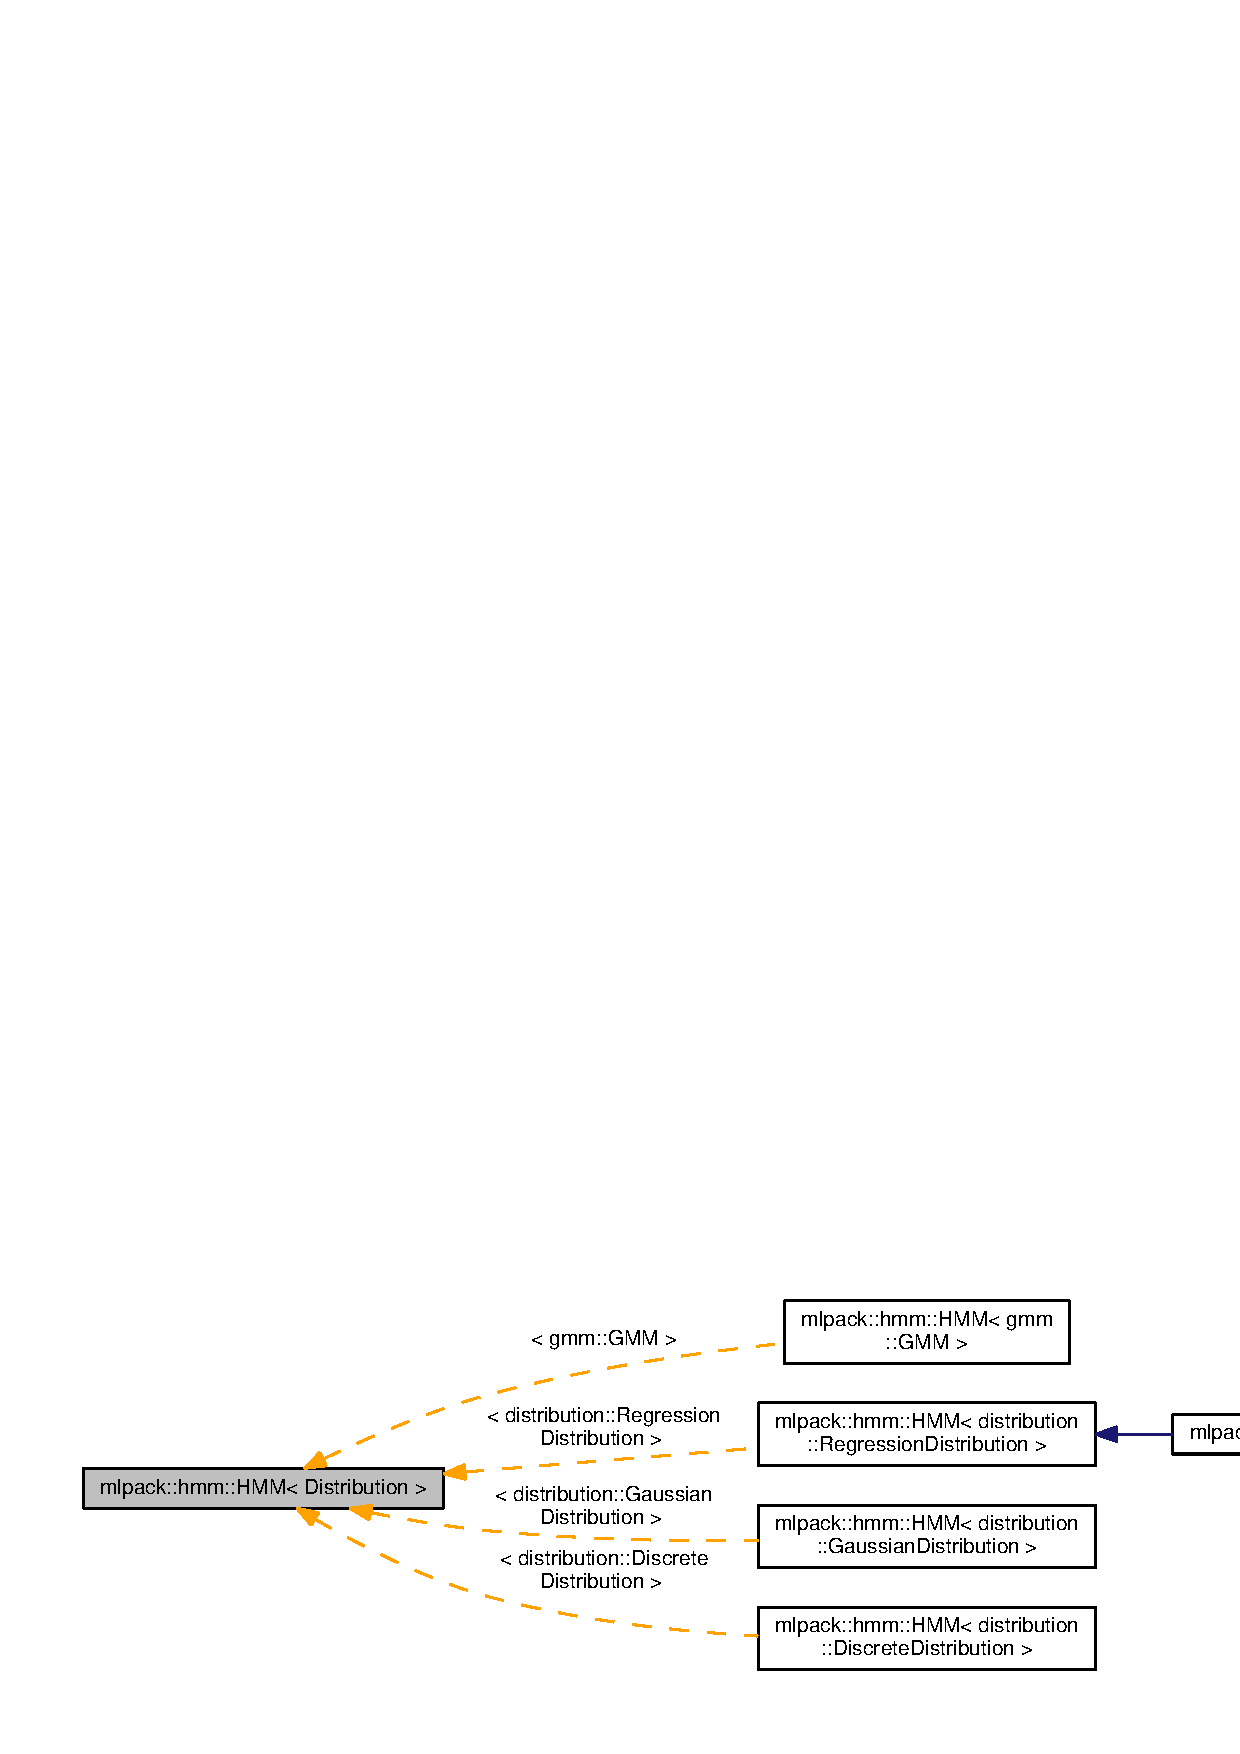
\includegraphics[width=350pt]{classmlpack_1_1hmm_1_1HMM__inherit__graph}
\end{center}
\end{figure}
\subsection*{Public Member Functions}
\begin{DoxyCompactItemize}
\item 
\textbf{ H\+MM} (const size\+\_\+t states=0, const Distribution emissions=Distribution(), const double tolerance=1e-\/5)
\begin{DoxyCompactList}\small\item\em Create the Hidden Markov Model with the given number of hidden states and the given default distribution for emissions. \end{DoxyCompactList}\item 
\textbf{ H\+MM} (const arma\+::vec \&initial, const arma\+::mat \&transition, const std\+::vector$<$ Distribution $>$ \&\textbf{ emission}, const double tolerance=1e-\/5)
\begin{DoxyCompactList}\small\item\em Create the Hidden Markov Model with the given initial probability vector, the given transition matrix, and the given emission distributions. \end{DoxyCompactList}\item 
size\+\_\+t \textbf{ Dimensionality} () const
\begin{DoxyCompactList}\small\item\em Get the dimensionality of observations. \end{DoxyCompactList}\item 
size\+\_\+t \& \textbf{ Dimensionality} ()
\begin{DoxyCompactList}\small\item\em Set the dimensionality of observations. \end{DoxyCompactList}\item 
const std\+::vector$<$ Distribution $>$ \& \textbf{ Emission} () const
\begin{DoxyCompactList}\small\item\em Return the emission distributions. \end{DoxyCompactList}\item 
std\+::vector$<$ Distribution $>$ \& \textbf{ Emission} ()
\begin{DoxyCompactList}\small\item\em Return a modifiable emission probability matrix reference. \end{DoxyCompactList}\item 
double \textbf{ Emission\+Log\+Likelihood} (const arma\+::vec \&emission\+Log\+Prob, double \&log\+Likelihood, arma\+::vec \&forward\+Log\+Prob) const
\begin{DoxyCompactList}\small\item\em Compute the log-\/likelihood of the given emission probability up to time t, storing the result in log\+Likelihood. \end{DoxyCompactList}\item 
double \textbf{ Emission\+Log\+Scale\+Factor} (const arma\+::vec \&emission\+Log\+Prob, arma\+::vec \&forward\+Log\+Prob) const
\begin{DoxyCompactList}\small\item\em Compute the log of the scaling factor of the given emission probability at time t. \end{DoxyCompactList}\item 
double \textbf{ Estimate} (const arma\+::mat \&data\+Seq, arma\+::mat \&state\+Prob, arma\+::mat \&forward\+Prob, arma\+::mat \&backward\+Prob, arma\+::vec \&scales) const
\begin{DoxyCompactList}\small\item\em Estimate the probabilities of each hidden state at each time step for each given data observation, using the Forward-\/\+Backward algorithm. \end{DoxyCompactList}\item 
double \textbf{ Estimate} (const arma\+::mat \&data\+Seq, arma\+::mat \&state\+Prob) const
\begin{DoxyCompactList}\small\item\em Estimate the probabilities of each hidden state at each time step of each given data observation, using the Forward-\/\+Backward algorithm. \end{DoxyCompactList}\item 
void \textbf{ Filter} (const arma\+::mat \&data\+Seq, arma\+::mat \&filter\+Seq, size\+\_\+t ahead=0) const
\begin{DoxyCompactList}\small\item\em \doxyref{H\+MM}{p.}{classmlpack_1_1hmm_1_1HMM} filtering. \end{DoxyCompactList}\item 
void \textbf{ Generate} (const size\+\_\+t length, arma\+::mat \&data\+Sequence, arma\+::\+Row$<$ size\+\_\+t $>$ \&state\+Sequence, const size\+\_\+t start\+State=0) const
\begin{DoxyCompactList}\small\item\em Generate a random data sequence of the given length. \end{DoxyCompactList}\item 
const arma\+::vec \& \textbf{ Initial} () const
\begin{DoxyCompactList}\small\item\em Return the vector of initial state probabilities. \end{DoxyCompactList}\item 
arma\+::vec \& \textbf{ Initial} ()
\begin{DoxyCompactList}\small\item\em Modify the vector of initial state probabilities. \end{DoxyCompactList}\item 
{\footnotesize template$<$typename Archive $>$ }\\void \textbf{ load} (Archive \&ar, const uint32\+\_\+t version)
\begin{DoxyCompactList}\small\item\em Load the object. \end{DoxyCompactList}\item 
double \textbf{ Log\+Estimate} (const arma\+::mat \&data\+Seq, arma\+::mat \&state\+Log\+Prob, arma\+::mat \&forward\+Log\+Prob, arma\+::mat \&backward\+Log\+Prob, arma\+::vec \&log\+Scales) const
\begin{DoxyCompactList}\small\item\em Estimate the probabilities of each hidden state at each time step for each given data observation, using the Forward-\/\+Backward algorithm. \end{DoxyCompactList}\item 
double \textbf{ Log\+Likelihood} (const arma\+::mat \&data\+Seq) const
\begin{DoxyCompactList}\small\item\em Compute the log-\/likelihood of the given data sequence. \end{DoxyCompactList}\item 
double \textbf{ Log\+Likelihood} (const arma\+::vec \&data, double \&log\+Likelihood, arma\+::vec \&forward\+Log\+Prob) const
\begin{DoxyCompactList}\small\item\em Compute the log-\/likelihood of the given data up to time t, storing the result in log\+Likelihood. \end{DoxyCompactList}\item 
double \textbf{ Log\+Scale\+Factor} (const arma\+::vec \&data, arma\+::vec \&forward\+Log\+Prob) const
\begin{DoxyCompactList}\small\item\em Compute the log of the scaling factor of the given data at time t. \end{DoxyCompactList}\item 
double \textbf{ Predict} (const arma\+::mat \&data\+Seq, arma\+::\+Row$<$ size\+\_\+t $>$ \&state\+Seq) const
\begin{DoxyCompactList}\small\item\em Compute the most probable hidden state sequence for the given data sequence, using the Viterbi algorithm, returning the log-\/likelihood of the most likely state sequence. \end{DoxyCompactList}\item 
{\footnotesize template$<$typename Archive $>$ }\\void \textbf{ save} (Archive \&ar, const uint32\+\_\+t version) const
\begin{DoxyCompactList}\small\item\em Save the object. \end{DoxyCompactList}\item 
void \textbf{ Smooth} (const arma\+::mat \&data\+Seq, arma\+::mat \&smooth\+Seq) const
\begin{DoxyCompactList}\small\item\em \doxyref{H\+MM}{p.}{classmlpack_1_1hmm_1_1HMM} smoothing. \end{DoxyCompactList}\item 
double \textbf{ Tolerance} () const
\begin{DoxyCompactList}\small\item\em Get the tolerance of the Baum-\/\+Welch algorithm. \end{DoxyCompactList}\item 
double \& \textbf{ Tolerance} ()
\begin{DoxyCompactList}\small\item\em Modify the tolerance of the Baum-\/\+Welch algorithm. \end{DoxyCompactList}\item 
double \textbf{ Train} (const std\+::vector$<$ arma\+::mat $>$ \&data\+Seq)
\begin{DoxyCompactList}\small\item\em Train the model using the Baum-\/\+Welch algorithm, with only the given unlabeled observations. \end{DoxyCompactList}\item 
void \textbf{ Train} (const std\+::vector$<$ arma\+::mat $>$ \&data\+Seq, const std\+::vector$<$ arma\+::\+Row$<$ size\+\_\+t $>$ $>$ \&state\+Seq)
\begin{DoxyCompactList}\small\item\em Train the model using the given labeled observations; the transition and emission matrices are directly estimated. \end{DoxyCompactList}\item 
const arma\+::mat \& \textbf{ Transition} () const
\begin{DoxyCompactList}\small\item\em Return the transition matrix. \end{DoxyCompactList}\item 
arma\+::mat \& \textbf{ Transition} ()
\begin{DoxyCompactList}\small\item\em Return a modifiable transition matrix reference. \end{DoxyCompactList}\end{DoxyCompactItemize}
\subsection*{Protected Member Functions}
\begin{DoxyCompactItemize}
\item 
void \textbf{ Backward} (const arma\+::mat \&data\+Seq, const arma\+::vec \&log\+Scales, arma\+::mat \&backward\+Log\+Prob, arma\+::mat \&log\+Probs) const
\begin{DoxyCompactList}\small\item\em The Backward algorithm (part of the Forward-\/\+Backward algorithm). \end{DoxyCompactList}\item 
void \textbf{ Forward} (const arma\+::mat \&data\+Seq, arma\+::vec \&log\+Scales, arma\+::mat \&forward\+Log\+Prob, arma\+::mat \&log\+Probs) const
\begin{DoxyCompactList}\small\item\em The Forward algorithm (part of the Forward-\/\+Backward algorithm). \end{DoxyCompactList}\item 
arma\+::vec \textbf{ Forward\+At\+T0} (const arma\+::vec \&emission\+Log\+Prob, double \&log\+Scales) const
\begin{DoxyCompactList}\small\item\em Given emission probabilities, computes forward probabilities at time t=0. \end{DoxyCompactList}\item 
arma\+::vec \textbf{ Forward\+At\+Tn} (const arma\+::vec \&emission\+Log\+Prob, double \&log\+Scales, const arma\+::vec \&prev\+Forward\+Log\+Prob) const
\begin{DoxyCompactList}\small\item\em Given emission probabilities, computes forward probabilities for time t$>$0. \end{DoxyCompactList}\end{DoxyCompactItemize}
\subsection*{Protected Attributes}
\begin{DoxyCompactItemize}
\item 
std\+::vector$<$ Distribution $>$ \textbf{ emission}
\begin{DoxyCompactList}\small\item\em Set of emission probability distributions; one for each state. \end{DoxyCompactList}\item 
arma\+::mat \textbf{ log\+Transition}
\begin{DoxyCompactList}\small\item\em Transition probability matrix. No need to be mutable in mlpack 4.\+0. \end{DoxyCompactList}\item 
arma\+::mat \textbf{ transition\+Proxy}
\begin{DoxyCompactList}\small\item\em A proxy variable in linear space for log\+Transition. \end{DoxyCompactList}\end{DoxyCompactItemize}


\subsection{Detailed Description}
\subsubsection*{template$<$typename Distribution = distribution\+::\+Discrete\+Distribution$>$\newline
class mlpack\+::hmm\+::\+H\+M\+M$<$ Distribution $>$}

A class that represents a Hidden Markov Model with an arbitrary type of emission distribution. 

This \doxyref{H\+MM}{p.}{classmlpack_1_1hmm_1_1HMM} class supports training (supervised and unsupervised), prediction of state sequences via the Viterbi algorithm, estimation of state probabilities, generation of random sequences, and calculation of the log-\/likelihood of a given sequence.

The template parameter, Distribution, specifies the distribution which the emissions follow. The class should implement the following functions\+:


\begin{DoxyCode}
\textcolor{keyword}{class }Distribution
\{
 \textcolor{keyword}{public}:
  \textcolor{comment}{// The type of observation used by this distribution.}
  \textcolor{keyword}{typedef} something DataType;

  \textcolor{comment}{// Return the probability of the given observation.}
  \textcolor{keywordtype}{double} Probability(\textcolor{keyword}{const} DataType& observation) \textcolor{keyword}{const};

  \textcolor{comment}{// Estimate the distribution based on the given observations.}
  \textcolor{keywordtype}{double} Train(\textcolor{keyword}{const} std::vector<DataType>& observations);

  \textcolor{comment}{// Estimate the distribution based on the given observations, given also}
  \textcolor{comment}{// the probability of each observation coming from this distribution.}
  \textcolor{keywordtype}{double} Train(\textcolor{keyword}{const} std::vector<DataType>& observations,
               \textcolor{keyword}{const} std::vector<double>& probabilities);
\};
\end{DoxyCode}


See the \doxyref{mlpack\+::distribution\+::\+Discrete\+Distribution}{p.}{classmlpack_1_1distribution_1_1DiscreteDistribution} class for an example. One would use the Discrete\+Distribution class when the observations are non-\/negative integers. Other distributions could be Gaussians, a mixture of Gaussians (G\+MM), or any other probability distribution implementing the four Distribution functions.

Usage of the \doxyref{H\+MM}{p.}{classmlpack_1_1hmm_1_1HMM} class generally involves either training an \doxyref{H\+MM}{p.}{classmlpack_1_1hmm_1_1HMM} or loading an already-\/known \doxyref{H\+MM}{p.}{classmlpack_1_1hmm_1_1HMM} and taking probability measurements of sequences. Example code for supervised training of a Gaussian \doxyref{H\+MM}{p.}{classmlpack_1_1hmm_1_1HMM} (that is, where the emission output distribution is a single Gaussian for each hidden state) is given below.


\begin{DoxyCode}
\textcolor{keyword}{extern} arma::mat observations; \textcolor{comment}{// Each column is an observation.}
\textcolor{keyword}{extern} arma::Row<size\_t> states; \textcolor{comment}{// Hidden states for each observation.}
\textcolor{comment}{// Create an untrained HMM with 5 hidden states and default (N(0, 1))}
\textcolor{comment}{// Gaussian distributions with the dimensionality of the dataset.}
HMM<GaussianDistribution> hmm(5, GaussianDistribution(observations.n\_rows));

\textcolor{comment}{// Train the HMM (the labels could be omitted to perform unsupervised}
\textcolor{comment}{// training).}
hmm.Train(observations, states);
\end{DoxyCode}


Once initialized, the \doxyref{H\+MM}{p.}{classmlpack_1_1hmm_1_1HMM} can evaluate the probability of a certain sequence (with \doxyref{Log\+Likelihood()}{p.}{classmlpack_1_1hmm_1_1HMM_aa8f3f0b515cc08f9476e435bb2d13210}), predict the most likely sequence of hidden states (with \doxyref{Predict()}{p.}{classmlpack_1_1hmm_1_1HMM_a3b7ef0aafafd5d5a4300c07b110807a4}), generate a sequence (with \doxyref{Generate()}{p.}{classmlpack_1_1hmm_1_1HMM_aaada1e3c4a467d13ded6cfbb0d332898}), or estimate the probabilities of each state for a sequence of observations (with \doxyref{Train()}{p.}{classmlpack_1_1hmm_1_1HMM_a0b3a1148721ee3e77bad0b987ca3973d}).


\begin{DoxyTemplParams}{Template Parameters}
{\em Distribution} & Type of emission distribution for this \doxyref{H\+MM}{p.}{classmlpack_1_1hmm_1_1HMM}. \\
\hline
\end{DoxyTemplParams}


Definition at line 85 of file hmm.\+hpp.



\subsection{Constructor \& Destructor Documentation}
\mbox{\label{classmlpack_1_1hmm_1_1HMM_a20f7ef2bfbbbfe4b01733e1e0104e17b}} 
\index{mlpack\+::hmm\+::\+H\+MM@{mlpack\+::hmm\+::\+H\+MM}!H\+MM@{H\+MM}}
\index{H\+MM@{H\+MM}!mlpack\+::hmm\+::\+H\+MM@{mlpack\+::hmm\+::\+H\+MM}}
\subsubsection{H\+M\+M()\hspace{0.1cm}{\footnotesize\ttfamily [1/2]}}
{\footnotesize\ttfamily \textbf{ H\+MM} (\begin{DoxyParamCaption}\item[{const size\+\_\+t}]{states = {\ttfamily 0},  }\item[{const Distribution}]{emissions = {\ttfamily Distribution()},  }\item[{const double}]{tolerance = {\ttfamily 1e-\/5} }\end{DoxyParamCaption})}



Create the Hidden Markov Model with the given number of hidden states and the given default distribution for emissions. 

The dimensionality of the observations is taken from the emissions variable, so it is important that the given default emission distribution is set with the correct dimensionality. Alternately, set the dimensionality with \doxyref{Dimensionality()}{p.}{classmlpack_1_1hmm_1_1HMM_a787adc650f11b9430f6bd0b937bbe6b0}. Optionally, the tolerance for convergence of the Baum-\/\+Welch algorithm can be set.

By default, the transition matrix and initial probability vector are set to contain equal probability for each state.


\begin{DoxyParams}{Parameters}
{\em states} & Number of states. \\
\hline
{\em emissions} & Default distribution for emissions. \\
\hline
{\em tolerance} & Tolerance for convergence of training algorithm (Baum-\/\+Welch). \\
\hline
\end{DoxyParams}
\mbox{\label{classmlpack_1_1hmm_1_1HMM_ac173a0c0e119519329525a892f8848e7}} 
\index{mlpack\+::hmm\+::\+H\+MM@{mlpack\+::hmm\+::\+H\+MM}!H\+MM@{H\+MM}}
\index{H\+MM@{H\+MM}!mlpack\+::hmm\+::\+H\+MM@{mlpack\+::hmm\+::\+H\+MM}}
\subsubsection{H\+M\+M()\hspace{0.1cm}{\footnotesize\ttfamily [2/2]}}
{\footnotesize\ttfamily \textbf{ H\+MM} (\begin{DoxyParamCaption}\item[{const arma\+::vec \&}]{initial,  }\item[{const arma\+::mat \&}]{transition,  }\item[{const std\+::vector$<$ Distribution $>$ \&}]{emission,  }\item[{const double}]{tolerance = {\ttfamily 1e-\/5} }\end{DoxyParamCaption})}



Create the Hidden Markov Model with the given initial probability vector, the given transition matrix, and the given emission distributions. 

The dimensionality of the observations of the \doxyref{H\+MM}{p.}{classmlpack_1_1hmm_1_1HMM} are taken from the given emission distributions. Alternately, the dimensionality can be set with \doxyref{Dimensionality()}{p.}{classmlpack_1_1hmm_1_1HMM_a787adc650f11b9430f6bd0b937bbe6b0}.

The initial state probability vector should have length equal to the number of states, and each entry represents the probability of being in the given state at time T = 0 (the beginning of a sequence).

The transition matrix should be such that T(i, j) is the probability of transition to state i from state j. The columns of the matrix should sum to 1.

The emission matrix should be such that E(i, j) is the probability of emission i while in state j. The columns of the matrix should sum to 1.

Optionally, the tolerance for convergence of the Baum-\/\+Welch algorithm can be set.


\begin{DoxyParams}{Parameters}
{\em initial} & Initial state probabilities. \\
\hline
{\em transition} & Transition matrix. \\
\hline
{\em emission} & Emission distributions. \\
\hline
{\em tolerance} & Tolerance for convergence of training algorithm (Baum-\/\+Welch). \\
\hline
\end{DoxyParams}


\subsection{Member Function Documentation}
\mbox{\label{classmlpack_1_1hmm_1_1HMM_af0853e02f080f2c0eac23e18edafd67d}} 
\index{mlpack\+::hmm\+::\+H\+MM@{mlpack\+::hmm\+::\+H\+MM}!Backward@{Backward}}
\index{Backward@{Backward}!mlpack\+::hmm\+::\+H\+MM@{mlpack\+::hmm\+::\+H\+MM}}
\subsubsection{Backward()}
{\footnotesize\ttfamily void Backward (\begin{DoxyParamCaption}\item[{const arma\+::mat \&}]{data\+Seq,  }\item[{const arma\+::vec \&}]{log\+Scales,  }\item[{arma\+::mat \&}]{backward\+Log\+Prob,  }\item[{arma\+::mat \&}]{log\+Probs }\end{DoxyParamCaption}) const\hspace{0.3cm}{\ttfamily [protected]}}



The Backward algorithm (part of the Forward-\/\+Backward algorithm). 

Computes backward probabilities for each state for each observation in the given data sequence, using the scaling factors found (presumably) by \doxyref{Forward()}{p.}{classmlpack_1_1hmm_1_1HMM_a1ec1e2d6393bbb69840a184ac35ac2ba}. The returned matrix has rows equal to the number of hidden states and columns equal to the number of observations.


\begin{DoxyParams}{Parameters}
{\em data\+Seq} & Data sequence to compute probabilities for. \\
\hline
{\em log\+Scales} & Vector of log of scaling factors. \\
\hline
{\em backward\+Log\+Prob} & Matrix in which backward probabilities will be saved. \\
\hline
\end{DoxyParams}


Referenced by H\+M\+M$<$ mlpack\+::distribution\+::\+Discrete\+Distribution $>$\+::\+Tolerance().

\mbox{\label{classmlpack_1_1hmm_1_1HMM_a78eda6bfb9e9462afa0fc85e32abe1af}} 
\index{mlpack\+::hmm\+::\+H\+MM@{mlpack\+::hmm\+::\+H\+MM}!Dimensionality@{Dimensionality}}
\index{Dimensionality@{Dimensionality}!mlpack\+::hmm\+::\+H\+MM@{mlpack\+::hmm\+::\+H\+MM}}
\subsubsection{Dimensionality()\hspace{0.1cm}{\footnotesize\ttfamily [1/2]}}
{\footnotesize\ttfamily size\+\_\+t Dimensionality (\begin{DoxyParamCaption}{ }\end{DoxyParamCaption}) const\hspace{0.3cm}{\ttfamily [inline]}}



Get the dimensionality of observations. 



Definition at line 420 of file hmm.\+hpp.

\mbox{\label{classmlpack_1_1hmm_1_1HMM_a787adc650f11b9430f6bd0b937bbe6b0}} 
\index{mlpack\+::hmm\+::\+H\+MM@{mlpack\+::hmm\+::\+H\+MM}!Dimensionality@{Dimensionality}}
\index{Dimensionality@{Dimensionality}!mlpack\+::hmm\+::\+H\+MM@{mlpack\+::hmm\+::\+H\+MM}}
\subsubsection{Dimensionality()\hspace{0.1cm}{\footnotesize\ttfamily [2/2]}}
{\footnotesize\ttfamily size\+\_\+t\& Dimensionality (\begin{DoxyParamCaption}{ }\end{DoxyParamCaption})\hspace{0.3cm}{\ttfamily [inline]}}



Set the dimensionality of observations. 



Definition at line 422 of file hmm.\+hpp.

\mbox{\label{classmlpack_1_1hmm_1_1HMM_ae0939befd9369e7605f50a8f5489cebd}} 
\index{mlpack\+::hmm\+::\+H\+MM@{mlpack\+::hmm\+::\+H\+MM}!Emission@{Emission}}
\index{Emission@{Emission}!mlpack\+::hmm\+::\+H\+MM@{mlpack\+::hmm\+::\+H\+MM}}
\subsubsection{Emission()\hspace{0.1cm}{\footnotesize\ttfamily [1/2]}}
{\footnotesize\ttfamily const std\+::vector$<$Distribution$>$\& Emission (\begin{DoxyParamCaption}{ }\end{DoxyParamCaption}) const\hspace{0.3cm}{\ttfamily [inline]}}



Return the emission distributions. 



Definition at line 415 of file hmm.\+hpp.

\mbox{\label{classmlpack_1_1hmm_1_1HMM_ace6dae9e34d19c372294bef69e317f27}} 
\index{mlpack\+::hmm\+::\+H\+MM@{mlpack\+::hmm\+::\+H\+MM}!Emission@{Emission}}
\index{Emission@{Emission}!mlpack\+::hmm\+::\+H\+MM@{mlpack\+::hmm\+::\+H\+MM}}
\subsubsection{Emission()\hspace{0.1cm}{\footnotesize\ttfamily [2/2]}}
{\footnotesize\ttfamily std\+::vector$<$Distribution$>$\& Emission (\begin{DoxyParamCaption}{ }\end{DoxyParamCaption})\hspace{0.3cm}{\ttfamily [inline]}}



Return a modifiable emission probability matrix reference. 



Definition at line 417 of file hmm.\+hpp.

\mbox{\label{classmlpack_1_1hmm_1_1HMM_a2d90005d72558c5bcf7ce5f708e838da}} 
\index{mlpack\+::hmm\+::\+H\+MM@{mlpack\+::hmm\+::\+H\+MM}!Emission\+Log\+Likelihood@{Emission\+Log\+Likelihood}}
\index{Emission\+Log\+Likelihood@{Emission\+Log\+Likelihood}!mlpack\+::hmm\+::\+H\+MM@{mlpack\+::hmm\+::\+H\+MM}}
\subsubsection{Emission\+Log\+Likelihood()}
{\footnotesize\ttfamily double Emission\+Log\+Likelihood (\begin{DoxyParamCaption}\item[{const arma\+::vec \&}]{emission\+Log\+Prob,  }\item[{double \&}]{log\+Likelihood,  }\item[{arma\+::vec \&}]{forward\+Log\+Prob }\end{DoxyParamCaption}) const}



Compute the log-\/likelihood of the given emission probability up to time t, storing the result in log\+Likelihood. 

This is meant for incremental or streaming computation of the log-\/likelihood of a sequence. For the first data point, provide an empty forward\+Log\+Prob vector.


\begin{DoxyParams}{Parameters}
{\em emission\+Log\+Prob} & emission probability at time t. \\
\hline
{\em log\+Likelihood} & Log-\/likelihood of the given sequence of emission probability up to time t-\/1. This will be overwritten with the log-\/likelihood of the given emission probability up to time t. \\
\hline
{\em forward\+Log\+Prob} & Vector in which forward probabilities will be saved. Passing forward\+Log\+Prob as an empty vector indicates the start of the sequence (i.\+e. time t=0). \\
\hline
\end{DoxyParams}
\begin{DoxyReturn}{Returns}
Log-\/likelihood of the given sequence of emission up to time t. 
\end{DoxyReturn}
\mbox{\label{classmlpack_1_1hmm_1_1HMM_aec5e2b525c29a039a482a5c4e9833a77}} 
\index{mlpack\+::hmm\+::\+H\+MM@{mlpack\+::hmm\+::\+H\+MM}!Emission\+Log\+Scale\+Factor@{Emission\+Log\+Scale\+Factor}}
\index{Emission\+Log\+Scale\+Factor@{Emission\+Log\+Scale\+Factor}!mlpack\+::hmm\+::\+H\+MM@{mlpack\+::hmm\+::\+H\+MM}}
\subsubsection{Emission\+Log\+Scale\+Factor()}
{\footnotesize\ttfamily double Emission\+Log\+Scale\+Factor (\begin{DoxyParamCaption}\item[{const arma\+::vec \&}]{emission\+Log\+Prob,  }\item[{arma\+::vec \&}]{forward\+Log\+Prob }\end{DoxyParamCaption}) const}



Compute the log of the scaling factor of the given emission probability at time t. 

To calculate the log-\/likelihood for the whole sequence, accumulate log scale over the entire sequence This is meant for incremental or streaming computation of the log-\/likelihood of a sequence. For the first data point, provide an empty forward\+Log\+Prob vector.


\begin{DoxyParams}{Parameters}
{\em emission\+Log\+Prob} & emission probability at time t. \\
\hline
{\em forward\+Log\+Prob} & Vector in which forward probabilities will be saved. Passing forward\+Log\+Prob as an empty vector indicates the start of the sequence (i.\+e. time t=0). \\
\hline
\end{DoxyParams}
\begin{DoxyReturn}{Returns}
Log scale factor of the given sequence of emission at time t. 
\end{DoxyReturn}
\mbox{\label{classmlpack_1_1hmm_1_1HMM_a73a4437336c8af18d51958a6abdd588d}} 
\index{mlpack\+::hmm\+::\+H\+MM@{mlpack\+::hmm\+::\+H\+MM}!Estimate@{Estimate}}
\index{Estimate@{Estimate}!mlpack\+::hmm\+::\+H\+MM@{mlpack\+::hmm\+::\+H\+MM}}
\subsubsection{Estimate()\hspace{0.1cm}{\footnotesize\ttfamily [1/2]}}
{\footnotesize\ttfamily double Estimate (\begin{DoxyParamCaption}\item[{const arma\+::mat \&}]{data\+Seq,  }\item[{arma\+::mat \&}]{state\+Prob,  }\item[{arma\+::mat \&}]{forward\+Prob,  }\item[{arma\+::mat \&}]{backward\+Prob,  }\item[{arma\+::vec \&}]{scales }\end{DoxyParamCaption}) const}



Estimate the probabilities of each hidden state at each time step for each given data observation, using the Forward-\/\+Backward algorithm. 

Each matrix which is returned has columns equal to the number of data observations, and rows equal to the number of hidden states in the model. The log-\/likelihood of the most probable sequence is returned.


\begin{DoxyParams}{Parameters}
{\em data\+Seq} & Sequence of observations. \\
\hline
{\em state\+Prob} & Matrix in which the probabilities of each state at each time interval will be stored. \\
\hline
{\em forward\+Prob} & Matrix in which the forward probabilities of each state at each time interval will be stored. \\
\hline
{\em backward\+Prob} & Matrix in which the backward probabilities of each state at each time interval will be stored. \\
\hline
{\em scales} & Vector in which the scaling factors at each time interval will be stored. \\
\hline
\end{DoxyParams}
\begin{DoxyReturn}{Returns}
Log-\/likelihood of most likely state sequence. 
\end{DoxyReturn}
\mbox{\label{classmlpack_1_1hmm_1_1HMM_aba5d63e40a43faa5a2999bd47bed6c9f}} 
\index{mlpack\+::hmm\+::\+H\+MM@{mlpack\+::hmm\+::\+H\+MM}!Estimate@{Estimate}}
\index{Estimate@{Estimate}!mlpack\+::hmm\+::\+H\+MM@{mlpack\+::hmm\+::\+H\+MM}}
\subsubsection{Estimate()\hspace{0.1cm}{\footnotesize\ttfamily [2/2]}}
{\footnotesize\ttfamily double Estimate (\begin{DoxyParamCaption}\item[{const arma\+::mat \&}]{data\+Seq,  }\item[{arma\+::mat \&}]{state\+Prob }\end{DoxyParamCaption}) const}



Estimate the probabilities of each hidden state at each time step of each given data observation, using the Forward-\/\+Backward algorithm. 

The returned matrix of state probabilities has columns equal to the number of data observations, and rows equal to the number of hidden states in the model. The log-\/likelihood of the most probable sequence is returned.


\begin{DoxyParams}{Parameters}
{\em data\+Seq} & Sequence of observations. \\
\hline
{\em state\+Prob} & Probabilities of each state at each time interval. \\
\hline
\end{DoxyParams}
\begin{DoxyReturn}{Returns}
Log-\/likelihood of most likely state sequence. 
\end{DoxyReturn}
\mbox{\label{classmlpack_1_1hmm_1_1HMM_ab197c1fe906f9f2c81d7c0c8f1bb430a}} 
\index{mlpack\+::hmm\+::\+H\+MM@{mlpack\+::hmm\+::\+H\+MM}!Filter@{Filter}}
\index{Filter@{Filter}!mlpack\+::hmm\+::\+H\+MM@{mlpack\+::hmm\+::\+H\+MM}}
\subsubsection{Filter()}
{\footnotesize\ttfamily void Filter (\begin{DoxyParamCaption}\item[{const arma\+::mat \&}]{data\+Seq,  }\item[{arma\+::mat \&}]{filter\+Seq,  }\item[{size\+\_\+t}]{ahead = {\ttfamily 0} }\end{DoxyParamCaption}) const}



\doxyref{H\+MM}{p.}{classmlpack_1_1hmm_1_1HMM} filtering. 

Computes the k-\/step-\/ahead expected emission at each time conditioned only on prior observations. That is E\{ Y[t+k] $\vert$ Y[0], ..., Y[t] \}. The returned matrix has columns equal to the number of observations. Note that the expectation may not be meaningful for discrete emissions.


\begin{DoxyParams}{Parameters}
{\em data\+Seq} & Sequence of observations. \\
\hline
{\em filter\+Seq} & Vector in which the expected emission sequence will be stored. \\
\hline
{\em ahead} & Number of steps ahead (k) for expectations. \\
\hline
\end{DoxyParams}
\mbox{\label{classmlpack_1_1hmm_1_1HMM_a1ec1e2d6393bbb69840a184ac35ac2ba}} 
\index{mlpack\+::hmm\+::\+H\+MM@{mlpack\+::hmm\+::\+H\+MM}!Forward@{Forward}}
\index{Forward@{Forward}!mlpack\+::hmm\+::\+H\+MM@{mlpack\+::hmm\+::\+H\+MM}}
\subsubsection{Forward()}
{\footnotesize\ttfamily void Forward (\begin{DoxyParamCaption}\item[{const arma\+::mat \&}]{data\+Seq,  }\item[{arma\+::vec \&}]{log\+Scales,  }\item[{arma\+::mat \&}]{forward\+Log\+Prob,  }\item[{arma\+::mat \&}]{log\+Probs }\end{DoxyParamCaption}) const\hspace{0.3cm}{\ttfamily [protected]}}



The Forward algorithm (part of the Forward-\/\+Backward algorithm). 

Computes forward probabilities for each state for each observation in the given data sequence. The returned matrix has rows equal to the number of hidden states and columns equal to the number of observations.


\begin{DoxyParams}{Parameters}
{\em data\+Seq} & Data sequence to compute probabilities for. \\
\hline
{\em log\+Scales} & Vector in which the log of scaling factors will be saved. \\
\hline
{\em forward\+Log\+Prob} & Matrix in which forward probabilities will be saved. \\
\hline
\end{DoxyParams}


Referenced by H\+M\+M$<$ mlpack\+::distribution\+::\+Discrete\+Distribution $>$\+::\+Tolerance().

\mbox{\label{classmlpack_1_1hmm_1_1HMM_a945acce7d1f14e9e85352e67810ad028}} 
\index{mlpack\+::hmm\+::\+H\+MM@{mlpack\+::hmm\+::\+H\+MM}!Forward\+At\+T0@{Forward\+At\+T0}}
\index{Forward\+At\+T0@{Forward\+At\+T0}!mlpack\+::hmm\+::\+H\+MM@{mlpack\+::hmm\+::\+H\+MM}}
\subsubsection{Forward\+At\+T0()}
{\footnotesize\ttfamily arma\+::vec Forward\+At\+T0 (\begin{DoxyParamCaption}\item[{const arma\+::vec \&}]{emission\+Log\+Prob,  }\item[{double \&}]{log\+Scales }\end{DoxyParamCaption}) const\hspace{0.3cm}{\ttfamily [protected]}}



Given emission probabilities, computes forward probabilities at time t=0. 


\begin{DoxyParams}{Parameters}
{\em emission\+Log\+Prob} & Emission probability at time t=0. \\
\hline
{\em log\+Scales} & Vector in which the log of scaling factors will be saved. \\
\hline
\end{DoxyParams}
\begin{DoxyReturn}{Returns}
Forward probabilities 
\end{DoxyReturn}


Referenced by H\+M\+M$<$ mlpack\+::distribution\+::\+Discrete\+Distribution $>$\+::\+Tolerance().

\mbox{\label{classmlpack_1_1hmm_1_1HMM_ae75539834ab1cc313fac3cef5c411efe}} 
\index{mlpack\+::hmm\+::\+H\+MM@{mlpack\+::hmm\+::\+H\+MM}!Forward\+At\+Tn@{Forward\+At\+Tn}}
\index{Forward\+At\+Tn@{Forward\+At\+Tn}!mlpack\+::hmm\+::\+H\+MM@{mlpack\+::hmm\+::\+H\+MM}}
\subsubsection{Forward\+At\+Tn()}
{\footnotesize\ttfamily arma\+::vec Forward\+At\+Tn (\begin{DoxyParamCaption}\item[{const arma\+::vec \&}]{emission\+Log\+Prob,  }\item[{double \&}]{log\+Scales,  }\item[{const arma\+::vec \&}]{prev\+Forward\+Log\+Prob }\end{DoxyParamCaption}) const\hspace{0.3cm}{\ttfamily [protected]}}



Given emission probabilities, computes forward probabilities for time t$>$0. 


\begin{DoxyParams}{Parameters}
{\em emission\+Log\+Prob} & Emission probability at time t$>$0. \\
\hline
{\em log\+Scales} & Vector in which the log of scaling factors will be saved. \\
\hline
{\em prev\+Forward\+Log\+Prob} & Previous forward probabilities. \\
\hline
\end{DoxyParams}
\begin{DoxyReturn}{Returns}
Forward probabilities 
\end{DoxyReturn}


Referenced by H\+M\+M$<$ mlpack\+::distribution\+::\+Discrete\+Distribution $>$\+::\+Tolerance().

\mbox{\label{classmlpack_1_1hmm_1_1HMM_aaada1e3c4a467d13ded6cfbb0d332898}} 
\index{mlpack\+::hmm\+::\+H\+MM@{mlpack\+::hmm\+::\+H\+MM}!Generate@{Generate}}
\index{Generate@{Generate}!mlpack\+::hmm\+::\+H\+MM@{mlpack\+::hmm\+::\+H\+MM}}
\subsubsection{Generate()}
{\footnotesize\ttfamily void Generate (\begin{DoxyParamCaption}\item[{const size\+\_\+t}]{length,  }\item[{arma\+::mat \&}]{data\+Sequence,  }\item[{arma\+::\+Row$<$ size\+\_\+t $>$ \&}]{state\+Sequence,  }\item[{const size\+\_\+t}]{start\+State = {\ttfamily 0} }\end{DoxyParamCaption}) const}



Generate a random data sequence of the given length. 

The data sequence is stored in the data\+Sequence parameter, and the state sequence is stored in the state\+Sequence parameter. Each column of data\+Sequence represents a random observation.


\begin{DoxyParams}{Parameters}
{\em length} & Length of random sequence to generate. \\
\hline
{\em data\+Sequence} & Vector to store data in. \\
\hline
{\em state\+Sequence} & Vector to store states in. \\
\hline
{\em start\+State} & Hidden state to start sequence in (default 0). \\
\hline
\end{DoxyParams}
\mbox{\label{classmlpack_1_1hmm_1_1HMM_a4c983e4a77757824d9ca4e1ada75dcf5}} 
\index{mlpack\+::hmm\+::\+H\+MM@{mlpack\+::hmm\+::\+H\+MM}!Initial@{Initial}}
\index{Initial@{Initial}!mlpack\+::hmm\+::\+H\+MM@{mlpack\+::hmm\+::\+H\+MM}}
\subsubsection{Initial()\hspace{0.1cm}{\footnotesize\ttfamily [1/2]}}
{\footnotesize\ttfamily const arma\+::vec\& Initial (\begin{DoxyParamCaption}{ }\end{DoxyParamCaption}) const\hspace{0.3cm}{\ttfamily [inline]}}



Return the vector of initial state probabilities. 



Definition at line 397 of file hmm.\+hpp.

\mbox{\label{classmlpack_1_1hmm_1_1HMM_ad0b8d2c553f50a26456393e194358df8}} 
\index{mlpack\+::hmm\+::\+H\+MM@{mlpack\+::hmm\+::\+H\+MM}!Initial@{Initial}}
\index{Initial@{Initial}!mlpack\+::hmm\+::\+H\+MM@{mlpack\+::hmm\+::\+H\+MM}}
\subsubsection{Initial()\hspace{0.1cm}{\footnotesize\ttfamily [2/2]}}
{\footnotesize\ttfamily arma\+::vec\& Initial (\begin{DoxyParamCaption}{ }\end{DoxyParamCaption})\hspace{0.3cm}{\ttfamily [inline]}}



Modify the vector of initial state probabilities. 



Definition at line 399 of file hmm.\+hpp.

\mbox{\label{classmlpack_1_1hmm_1_1HMM_ac604f3bed03d700b41501b6ed8b5b759}} 
\index{mlpack\+::hmm\+::\+H\+MM@{mlpack\+::hmm\+::\+H\+MM}!load@{load}}
\index{load@{load}!mlpack\+::hmm\+::\+H\+MM@{mlpack\+::hmm\+::\+H\+MM}}
\subsubsection{load()}
{\footnotesize\ttfamily void load (\begin{DoxyParamCaption}\item[{Archive \&}]{ar,  }\item[{const uint32\+\_\+t}]{version }\end{DoxyParamCaption})}



Load the object. 



Referenced by H\+M\+M$<$ mlpack\+::distribution\+::\+Discrete\+Distribution $>$\+::\+Tolerance().

\mbox{\label{classmlpack_1_1hmm_1_1HMM_af1f16adb7b69040e9bc7711ca1fa1fe8}} 
\index{mlpack\+::hmm\+::\+H\+MM@{mlpack\+::hmm\+::\+H\+MM}!Log\+Estimate@{Log\+Estimate}}
\index{Log\+Estimate@{Log\+Estimate}!mlpack\+::hmm\+::\+H\+MM@{mlpack\+::hmm\+::\+H\+MM}}
\subsubsection{Log\+Estimate()}
{\footnotesize\ttfamily double Log\+Estimate (\begin{DoxyParamCaption}\item[{const arma\+::mat \&}]{data\+Seq,  }\item[{arma\+::mat \&}]{state\+Log\+Prob,  }\item[{arma\+::mat \&}]{forward\+Log\+Prob,  }\item[{arma\+::mat \&}]{backward\+Log\+Prob,  }\item[{arma\+::vec \&}]{log\+Scales }\end{DoxyParamCaption}) const}



Estimate the probabilities of each hidden state at each time step for each given data observation, using the Forward-\/\+Backward algorithm. 

Each matrix which is returned has columns equal to the number of data observations, and rows equal to the number of hidden states in the model. The log-\/likelihood of the most probable sequence is returned.


\begin{DoxyParams}{Parameters}
{\em data\+Seq} & Sequence of observations. \\
\hline
{\em state\+Log\+Prob} & Matrix in which the log probabilities of each state at each time interval will be stored. \\
\hline
{\em forward\+Log\+Prob} & Matrix in which the forward log probabilities of each state at each time interval will be stored. \\
\hline
{\em backward\+Log\+Prob} & Matrix in which the backward log probabilities of each state at each time interval will be stored. \\
\hline
{\em log\+Scales} & Vector in which the log of scaling factors at each time interval will be stored. \\
\hline
\end{DoxyParams}
\begin{DoxyReturn}{Returns}
Log-\/likelihood of most likely state sequence. 
\end{DoxyReturn}
\mbox{\label{classmlpack_1_1hmm_1_1HMM_aa8f3f0b515cc08f9476e435bb2d13210}} 
\index{mlpack\+::hmm\+::\+H\+MM@{mlpack\+::hmm\+::\+H\+MM}!Log\+Likelihood@{Log\+Likelihood}}
\index{Log\+Likelihood@{Log\+Likelihood}!mlpack\+::hmm\+::\+H\+MM@{mlpack\+::hmm\+::\+H\+MM}}
\subsubsection{Log\+Likelihood()\hspace{0.1cm}{\footnotesize\ttfamily [1/2]}}
{\footnotesize\ttfamily double Log\+Likelihood (\begin{DoxyParamCaption}\item[{const arma\+::mat \&}]{data\+Seq }\end{DoxyParamCaption}) const}



Compute the log-\/likelihood of the given data sequence. 


\begin{DoxyParams}{Parameters}
{\em data\+Seq} & Data sequence to evaluate the likelihood of. \\
\hline
\end{DoxyParams}
\begin{DoxyReturn}{Returns}
Log-\/likelihood of the given sequence. 
\end{DoxyReturn}
\mbox{\label{classmlpack_1_1hmm_1_1HMM_a7c59285838016d2f540e6aad3f1d37f5}} 
\index{mlpack\+::hmm\+::\+H\+MM@{mlpack\+::hmm\+::\+H\+MM}!Log\+Likelihood@{Log\+Likelihood}}
\index{Log\+Likelihood@{Log\+Likelihood}!mlpack\+::hmm\+::\+H\+MM@{mlpack\+::hmm\+::\+H\+MM}}
\subsubsection{Log\+Likelihood()\hspace{0.1cm}{\footnotesize\ttfamily [2/2]}}
{\footnotesize\ttfamily double Log\+Likelihood (\begin{DoxyParamCaption}\item[{const arma\+::vec \&}]{data,  }\item[{double \&}]{log\+Likelihood,  }\item[{arma\+::vec \&}]{forward\+Log\+Prob }\end{DoxyParamCaption}) const}



Compute the log-\/likelihood of the given data up to time t, storing the result in log\+Likelihood. 

This is meant for incremental or streaming computation of the log-\/likelihood of a sequence. For the first data point, provide an empty forward\+Log\+Prob vector.


\begin{DoxyParams}{Parameters}
{\em data} & observation at time t. \\
\hline
{\em log\+Likelihood} & Log-\/likelihood of the given sequence of data up to time t-\/1. \\
\hline
{\em forward\+Log\+Prob} & Vector in which forward probabilities will be saved. Passing forward\+Log\+Prob as an empty vector indicates the start of the sequence (i.\+e. time t=0). \\
\hline
\end{DoxyParams}
\begin{DoxyReturn}{Returns}
Log-\/likelihood of the given sequence of data up to time t. 
\end{DoxyReturn}
\mbox{\label{classmlpack_1_1hmm_1_1HMM_a51246be9ab15d6af29cf3e60ed1c57c5}} 
\index{mlpack\+::hmm\+::\+H\+MM@{mlpack\+::hmm\+::\+H\+MM}!Log\+Scale\+Factor@{Log\+Scale\+Factor}}
\index{Log\+Scale\+Factor@{Log\+Scale\+Factor}!mlpack\+::hmm\+::\+H\+MM@{mlpack\+::hmm\+::\+H\+MM}}
\subsubsection{Log\+Scale\+Factor()}
{\footnotesize\ttfamily double Log\+Scale\+Factor (\begin{DoxyParamCaption}\item[{const arma\+::vec \&}]{data,  }\item[{arma\+::vec \&}]{forward\+Log\+Prob }\end{DoxyParamCaption}) const}



Compute the log of the scaling factor of the given data at time t. 

To calculate the log-\/likelihood for the whole sequence, accumulate the log scale factor (the return value of this function) over the entire sequence. This is meant for incremental or streaming computation of the log-\/likelihood of a sequence. For the first data point, provide an empty forward\+Log\+Prob vector.


\begin{DoxyParams}{Parameters}
{\em data} & observation at time t. \\
\hline
{\em forward\+Log\+Prob} & Vector in which forward probabilities will be saved. Passing forward\+Log\+Prob as an empty vector indicates the start of the sequence (i.\+e. time t=0). \\
\hline
\end{DoxyParams}
\begin{DoxyReturn}{Returns}
Log scale factor of the given sequence of data up at time t. 
\end{DoxyReturn}
\mbox{\label{classmlpack_1_1hmm_1_1HMM_a3b7ef0aafafd5d5a4300c07b110807a4}} 
\index{mlpack\+::hmm\+::\+H\+MM@{mlpack\+::hmm\+::\+H\+MM}!Predict@{Predict}}
\index{Predict@{Predict}!mlpack\+::hmm\+::\+H\+MM@{mlpack\+::hmm\+::\+H\+MM}}
\subsubsection{Predict()}
{\footnotesize\ttfamily double Predict (\begin{DoxyParamCaption}\item[{const arma\+::mat \&}]{data\+Seq,  }\item[{arma\+::\+Row$<$ size\+\_\+t $>$ \&}]{state\+Seq }\end{DoxyParamCaption}) const}



Compute the most probable hidden state sequence for the given data sequence, using the Viterbi algorithm, returning the log-\/likelihood of the most likely state sequence. 


\begin{DoxyParams}{Parameters}
{\em data\+Seq} & Sequence of observations. \\
\hline
{\em state\+Seq} & Vector in which the most probable state sequence will be stored. \\
\hline
\end{DoxyParams}
\begin{DoxyReturn}{Returns}
Log-\/likelihood of most probable state sequence. 
\end{DoxyReturn}
\mbox{\label{classmlpack_1_1hmm_1_1HMM_ad17c3ded534d1294e5fac2d2e16da3ba}} 
\index{mlpack\+::hmm\+::\+H\+MM@{mlpack\+::hmm\+::\+H\+MM}!save@{save}}
\index{save@{save}!mlpack\+::hmm\+::\+H\+MM@{mlpack\+::hmm\+::\+H\+MM}}
\subsubsection{save()}
{\footnotesize\ttfamily void save (\begin{DoxyParamCaption}\item[{Archive \&}]{ar,  }\item[{const uint32\+\_\+t}]{version }\end{DoxyParamCaption}) const}



Save the object. 



Referenced by H\+M\+M$<$ mlpack\+::distribution\+::\+Discrete\+Distribution $>$\+::\+Tolerance().

\mbox{\label{classmlpack_1_1hmm_1_1HMM_a0139a3d883c28d6f45e15097c08bbf41}} 
\index{mlpack\+::hmm\+::\+H\+MM@{mlpack\+::hmm\+::\+H\+MM}!Smooth@{Smooth}}
\index{Smooth@{Smooth}!mlpack\+::hmm\+::\+H\+MM@{mlpack\+::hmm\+::\+H\+MM}}
\subsubsection{Smooth()}
{\footnotesize\ttfamily void Smooth (\begin{DoxyParamCaption}\item[{const arma\+::mat \&}]{data\+Seq,  }\item[{arma\+::mat \&}]{smooth\+Seq }\end{DoxyParamCaption}) const}



\doxyref{H\+MM}{p.}{classmlpack_1_1hmm_1_1HMM} smoothing. 

Computes expected emission at each time conditioned on all observations. That is E\{ Y[t] $\vert$ Y[0], ..., Y[T] \}. The returned matrix has columns equal to the number of observations. Note that the expectation may not be meaningful for discrete emissions.


\begin{DoxyParams}{Parameters}
{\em data\+Seq} & Sequence of observations. \\
\hline
{\em smooth\+Seq} & Vector in which the expected emission sequence will be stored. \\
\hline
\end{DoxyParams}
\mbox{\label{classmlpack_1_1hmm_1_1HMM_a7b5af5c1a84c507cbaa7f999ea5a4fda}} 
\index{mlpack\+::hmm\+::\+H\+MM@{mlpack\+::hmm\+::\+H\+MM}!Tolerance@{Tolerance}}
\index{Tolerance@{Tolerance}!mlpack\+::hmm\+::\+H\+MM@{mlpack\+::hmm\+::\+H\+MM}}
\subsubsection{Tolerance()\hspace{0.1cm}{\footnotesize\ttfamily [1/2]}}
{\footnotesize\ttfamily double Tolerance (\begin{DoxyParamCaption}{ }\end{DoxyParamCaption}) const\hspace{0.3cm}{\ttfamily [inline]}}



Get the tolerance of the Baum-\/\+Welch algorithm. 



Definition at line 425 of file hmm.\+hpp.

\mbox{\label{classmlpack_1_1hmm_1_1HMM_a3d9fac84af16250f5a3689692e8f2173}} 
\index{mlpack\+::hmm\+::\+H\+MM@{mlpack\+::hmm\+::\+H\+MM}!Tolerance@{Tolerance}}
\index{Tolerance@{Tolerance}!mlpack\+::hmm\+::\+H\+MM@{mlpack\+::hmm\+::\+H\+MM}}
\subsubsection{Tolerance()\hspace{0.1cm}{\footnotesize\ttfamily [2/2]}}
{\footnotesize\ttfamily double\& Tolerance (\begin{DoxyParamCaption}{ }\end{DoxyParamCaption})\hspace{0.3cm}{\ttfamily [inline]}}



Modify the tolerance of the Baum-\/\+Welch algorithm. 



Definition at line 427 of file hmm.\+hpp.

\mbox{\label{classmlpack_1_1hmm_1_1HMM_a0b3a1148721ee3e77bad0b987ca3973d}} 
\index{mlpack\+::hmm\+::\+H\+MM@{mlpack\+::hmm\+::\+H\+MM}!Train@{Train}}
\index{Train@{Train}!mlpack\+::hmm\+::\+H\+MM@{mlpack\+::hmm\+::\+H\+MM}}
\subsubsection{Train()\hspace{0.1cm}{\footnotesize\ttfamily [1/2]}}
{\footnotesize\ttfamily double Train (\begin{DoxyParamCaption}\item[{const std\+::vector$<$ arma\+::mat $>$ \&}]{data\+Seq }\end{DoxyParamCaption})}



Train the model using the Baum-\/\+Welch algorithm, with only the given unlabeled observations. 

Instead of giving a guess transition and emission matrix here, do that in the constructor. Each matrix in the vector of data sequences holds an individual data sequence; each point in each individual data sequence should be a column in the matrix. The number of rows in each matrix should be equal to the dimensionality of the \doxyref{H\+MM}{p.}{classmlpack_1_1hmm_1_1HMM} (which is set in the constructor).

It is preferable to use the other overload of \doxyref{Train()}{p.}{classmlpack_1_1hmm_1_1HMM_a0b3a1148721ee3e77bad0b987ca3973d}, with labeled data. That will produce much better results. However, if labeled data is unavailable, this will work. In addition, it is possible to use \doxyref{Train()}{p.}{classmlpack_1_1hmm_1_1HMM_a0b3a1148721ee3e77bad0b987ca3973d} with labeled data first, and then continue to train the model using this overload of \doxyref{Train()}{p.}{classmlpack_1_1hmm_1_1HMM_a0b3a1148721ee3e77bad0b987ca3973d} with unlabeled data.

The tolerance of the Baum-\/\+Welch algorithm can be set either in the constructor or with the \doxyref{Tolerance()}{p.}{classmlpack_1_1hmm_1_1HMM_a3d9fac84af16250f5a3689692e8f2173} method. When the change in log-\/likelihood of the model between iterations is less than the tolerance, the Baum-\/\+Welch algorithm terminates.

\begin{DoxyNote}{Note}
\doxyref{Train()}{p.}{classmlpack_1_1hmm_1_1HMM_a0b3a1148721ee3e77bad0b987ca3973d} can be called multiple times with different sequences; each time it is called, it uses the current parameters of the \doxyref{H\+MM}{p.}{classmlpack_1_1hmm_1_1HMM} as a starting point for training.
\end{DoxyNote}

\begin{DoxyParams}{Parameters}
{\em data\+Seq} & Vector of observation sequences. \\
\hline
\end{DoxyParams}
\begin{DoxyReturn}{Returns}
Log-\/likelihood of state sequence. 
\end{DoxyReturn}
\mbox{\label{classmlpack_1_1hmm_1_1HMM_a2cacf650f3d30e9da07be7a0aa2ded81}} 
\index{mlpack\+::hmm\+::\+H\+MM@{mlpack\+::hmm\+::\+H\+MM}!Train@{Train}}
\index{Train@{Train}!mlpack\+::hmm\+::\+H\+MM@{mlpack\+::hmm\+::\+H\+MM}}
\subsubsection{Train()\hspace{0.1cm}{\footnotesize\ttfamily [2/2]}}
{\footnotesize\ttfamily void Train (\begin{DoxyParamCaption}\item[{const std\+::vector$<$ arma\+::mat $>$ \&}]{data\+Seq,  }\item[{const std\+::vector$<$ arma\+::\+Row$<$ size\+\_\+t $>$ $>$ \&}]{state\+Seq }\end{DoxyParamCaption})}



Train the model using the given labeled observations; the transition and emission matrices are directly estimated. 

Each matrix in the vector of data sequences corresponds to a vector in the vector of state sequences. Each point in each individual data sequence should be a column in the matrix, and its state should be the corresponding element in the state sequence vector. For instance, data\+Seq[0].col(3) corresponds to the fourth observation in the first data sequence, and its state is state\+Seq[0][3]. The number of rows in each matrix should be equal to the dimensionality of the \doxyref{H\+MM}{p.}{classmlpack_1_1hmm_1_1HMM} (which is set in the constructor).

\begin{DoxyNote}{Note}
\doxyref{Train()}{p.}{classmlpack_1_1hmm_1_1HMM_a0b3a1148721ee3e77bad0b987ca3973d} can be called multiple times with different sequences; each time it is called, it uses the current parameters of the \doxyref{H\+MM}{p.}{classmlpack_1_1hmm_1_1HMM} as a starting point for training.
\end{DoxyNote}

\begin{DoxyParams}{Parameters}
{\em data\+Seq} & Vector of observation sequences. \\
\hline
{\em state\+Seq} & Vector of state sequences, corresponding to each observation. \\
\hline
\end{DoxyParams}
\mbox{\label{classmlpack_1_1hmm_1_1HMM_a103b830306d8c8d66a753f63e84ba5de}} 
\index{mlpack\+::hmm\+::\+H\+MM@{mlpack\+::hmm\+::\+H\+MM}!Transition@{Transition}}
\index{Transition@{Transition}!mlpack\+::hmm\+::\+H\+MM@{mlpack\+::hmm\+::\+H\+MM}}
\subsubsection{Transition()\hspace{0.1cm}{\footnotesize\ttfamily [1/2]}}
{\footnotesize\ttfamily const arma\+::mat\& Transition (\begin{DoxyParamCaption}{ }\end{DoxyParamCaption}) const\hspace{0.3cm}{\ttfamily [inline]}}



Return the transition matrix. 



Definition at line 406 of file hmm.\+hpp.

\mbox{\label{classmlpack_1_1hmm_1_1HMM_a08c5d391f5ea34e09497663673c5a16a}} 
\index{mlpack\+::hmm\+::\+H\+MM@{mlpack\+::hmm\+::\+H\+MM}!Transition@{Transition}}
\index{Transition@{Transition}!mlpack\+::hmm\+::\+H\+MM@{mlpack\+::hmm\+::\+H\+MM}}
\subsubsection{Transition()\hspace{0.1cm}{\footnotesize\ttfamily [2/2]}}
{\footnotesize\ttfamily arma\+::mat\& Transition (\begin{DoxyParamCaption}{ }\end{DoxyParamCaption})\hspace{0.3cm}{\ttfamily [inline]}}



Return a modifiable transition matrix reference. 



Definition at line 408 of file hmm.\+hpp.



\subsection{Member Data Documentation}
\mbox{\label{classmlpack_1_1hmm_1_1HMM_aa9f403ff2a03db91a1614d9e32c21783}} 
\index{mlpack\+::hmm\+::\+H\+MM@{mlpack\+::hmm\+::\+H\+MM}!emission@{emission}}
\index{emission@{emission}!mlpack\+::hmm\+::\+H\+MM@{mlpack\+::hmm\+::\+H\+MM}}
\subsubsection{emission}
{\footnotesize\ttfamily std\+::vector$<$Distribution$>$ emission\hspace{0.3cm}{\ttfamily [protected]}}



Set of emission probability distributions; one for each state. 



Definition at line 497 of file hmm.\+hpp.



Referenced by H\+M\+M$<$ mlpack\+::distribution\+::\+Discrete\+Distribution $>$\+::\+Emission().

\mbox{\label{classmlpack_1_1hmm_1_1HMM_a46e0ed8f87152b5819d73057a19524fd}} 
\index{mlpack\+::hmm\+::\+H\+MM@{mlpack\+::hmm\+::\+H\+MM}!log\+Transition@{log\+Transition}}
\index{log\+Transition@{log\+Transition}!mlpack\+::hmm\+::\+H\+MM@{mlpack\+::hmm\+::\+H\+MM}}
\subsubsection{log\+Transition}
{\footnotesize\ttfamily arma\+::mat log\+Transition\hspace{0.3cm}{\ttfamily [mutable]}, {\ttfamily [protected]}}



Transition probability matrix. No need to be mutable in mlpack 4.\+0. 



Definition at line 506 of file hmm.\+hpp.

\mbox{\label{classmlpack_1_1hmm_1_1HMM_a8ccc277a880972d6b9f7738f9cea5457}} 
\index{mlpack\+::hmm\+::\+H\+MM@{mlpack\+::hmm\+::\+H\+MM}!transition\+Proxy@{transition\+Proxy}}
\index{transition\+Proxy@{transition\+Proxy}!mlpack\+::hmm\+::\+H\+MM@{mlpack\+::hmm\+::\+H\+MM}}
\subsubsection{transition\+Proxy}
{\footnotesize\ttfamily arma\+::mat transition\+Proxy\hspace{0.3cm}{\ttfamily [protected]}}



A proxy variable in linear space for log\+Transition. 

Should be removed in mlpack 4.\+0. 

Definition at line 503 of file hmm.\+hpp.



Referenced by H\+M\+M$<$ mlpack\+::distribution\+::\+Discrete\+Distribution $>$\+::\+Transition().



The documentation for this class was generated from the following file\+:\begin{DoxyCompactItemize}
\item 
/home/aakash/mlpack/src/mlpack/methods/hmm/\textbf{ hmm.\+hpp}\end{DoxyCompactItemize}

\section{H\+M\+M\+Model Class Reference}
\label{classmlpack_1_1hmm_1_1HMMModel}\index{H\+M\+M\+Model@{H\+M\+M\+Model}}


A serializable \doxyref{H\+MM}{p.}{classmlpack_1_1hmm_1_1HMM} model that also stores the type.  


\subsection*{Public Member Functions}
\begin{DoxyCompactItemize}
\item 
\textbf{ H\+M\+M\+Model} (const \textbf{ H\+M\+M\+Type} type=H\+M\+M\+Type\+::\+Discrete\+H\+MM)
\begin{DoxyCompactList}\small\item\em Construct a model of the given type. \end{DoxyCompactList}\item 
\textbf{ H\+M\+M\+Model} (const \textbf{ H\+M\+M\+Model} \&other)
\begin{DoxyCompactList}\small\item\em Copy another model. \end{DoxyCompactList}\item 
\textbf{ H\+M\+M\+Model} (\textbf{ H\+M\+M\+Model} \&\&other)
\begin{DoxyCompactList}\small\item\em Take ownership of another model. \end{DoxyCompactList}\item 
\textbf{ $\sim$\+H\+M\+M\+Model} ()
\begin{DoxyCompactList}\small\item\em Clean memory. \end{DoxyCompactList}\item 
\textbf{ H\+MM}$<$ \textbf{ gmm\+::\+Diagonal\+G\+MM} $>$ $\ast$ \textbf{ Diag\+G\+M\+M\+H\+MM} ()
\item 
\textbf{ H\+MM}$<$ \textbf{ distribution\+::\+Discrete\+Distribution} $>$ $\ast$ \textbf{ Discrete\+H\+MM} ()
\begin{DoxyCompactList}\small\item\em Accessor methods for discrete\+H\+MM, gaussian\+H\+MM, gmm\+H\+MM, and diag\+G\+M\+M\+H\+MM. \end{DoxyCompactList}\item 
\textbf{ H\+MM}$<$ \textbf{ distribution\+::\+Gaussian\+Distribution} $>$ $\ast$ \textbf{ Gaussian\+H\+MM} ()
\item 
\textbf{ H\+MM}$<$ \textbf{ gmm\+::\+G\+MM} $>$ $\ast$ \textbf{ G\+M\+M\+H\+MM} ()
\item 
\textbf{ H\+M\+M\+Model} \& \textbf{ operator=} (const \textbf{ H\+M\+M\+Model} \&other)
\begin{DoxyCompactList}\small\item\em Copy assignment operator. \end{DoxyCompactList}\item 
\textbf{ H\+M\+M\+Model} \& \textbf{ operator=} (\textbf{ H\+M\+M\+Model} \&\&other)
\begin{DoxyCompactList}\small\item\em Move assignment operator. \end{DoxyCompactList}\item 
{\footnotesize template$<$typename Action\+Type , typename Extra\+Info\+Type $>$ }\\void \textbf{ Perform\+Action} (Extra\+Info\+Type $\ast$x)
\begin{DoxyCompactList}\small\item\em Given a functor type, perform that functor with the optional extra info on the \doxyref{H\+MM}{p.}{classmlpack_1_1hmm_1_1HMM}. \end{DoxyCompactList}\item 
{\footnotesize template$<$typename Archive $>$ }\\void \textbf{ serialize} (Archive \&ar, const uint32\+\_\+t)
\begin{DoxyCompactList}\small\item\em Serialize the model. \end{DoxyCompactList}\item 
\textbf{ H\+M\+M\+Type} \textbf{ Type} ()
\end{DoxyCompactItemize}


\subsection{Detailed Description}
A serializable \doxyref{H\+MM}{p.}{classmlpack_1_1hmm_1_1HMM} model that also stores the type. 

Definition at line 33 of file hmm\+\_\+model.\+hpp.



\subsection{Constructor \& Destructor Documentation}
\mbox{\label{classmlpack_1_1hmm_1_1HMMModel_a390e8b55464a25c9106acf1ec5ad1488}} 
\index{mlpack\+::hmm\+::\+H\+M\+M\+Model@{mlpack\+::hmm\+::\+H\+M\+M\+Model}!H\+M\+M\+Model@{H\+M\+M\+Model}}
\index{H\+M\+M\+Model@{H\+M\+M\+Model}!mlpack\+::hmm\+::\+H\+M\+M\+Model@{mlpack\+::hmm\+::\+H\+M\+M\+Model}}
\subsubsection{H\+M\+M\+Model()\hspace{0.1cm}{\footnotesize\ttfamily [1/3]}}
{\footnotesize\ttfamily \textbf{ H\+M\+M\+Model} (\begin{DoxyParamCaption}\item[{const \textbf{ H\+M\+M\+Type}}]{type = {\ttfamily HMMType\+:\+:DiscreteHMM} }\end{DoxyParamCaption})\hspace{0.3cm}{\ttfamily [inline]}}



Construct a model of the given type. 



Definition at line 49 of file hmm\+\_\+model.\+hpp.



References mlpack\+::hmm\+::\+Diagonal\+Gaussian\+Mixture\+Model\+H\+MM, mlpack\+::hmm\+::\+Discrete\+H\+MM, mlpack\+::hmm\+::\+Gaussian\+H\+MM, and mlpack\+::hmm\+::\+Gaussian\+Mixture\+Model\+H\+MM.

\mbox{\label{classmlpack_1_1hmm_1_1HMMModel_aa24c85f7311a3b2c0e56e6c0af64a100}} 
\index{mlpack\+::hmm\+::\+H\+M\+M\+Model@{mlpack\+::hmm\+::\+H\+M\+M\+Model}!H\+M\+M\+Model@{H\+M\+M\+Model}}
\index{H\+M\+M\+Model@{H\+M\+M\+Model}!mlpack\+::hmm\+::\+H\+M\+M\+Model@{mlpack\+::hmm\+::\+H\+M\+M\+Model}}
\subsubsection{H\+M\+M\+Model()\hspace{0.1cm}{\footnotesize\ttfamily [2/3]}}
{\footnotesize\ttfamily \textbf{ H\+M\+M\+Model} (\begin{DoxyParamCaption}\item[{const \textbf{ H\+M\+M\+Model} \&}]{other }\end{DoxyParamCaption})\hspace{0.3cm}{\ttfamily [inline]}}



Copy another model. 



Definition at line 67 of file hmm\+\_\+model.\+hpp.



References mlpack\+::hmm\+::\+Diagonal\+Gaussian\+Mixture\+Model\+H\+MM, mlpack\+::hmm\+::\+Discrete\+H\+MM, mlpack\+::hmm\+::\+Gaussian\+H\+MM, and mlpack\+::hmm\+::\+Gaussian\+Mixture\+Model\+H\+MM.

\mbox{\label{classmlpack_1_1hmm_1_1HMMModel_a58c371f45d81ee7e8158eb77a24fd935}} 
\index{mlpack\+::hmm\+::\+H\+M\+M\+Model@{mlpack\+::hmm\+::\+H\+M\+M\+Model}!H\+M\+M\+Model@{H\+M\+M\+Model}}
\index{H\+M\+M\+Model@{H\+M\+M\+Model}!mlpack\+::hmm\+::\+H\+M\+M\+Model@{mlpack\+::hmm\+::\+H\+M\+M\+Model}}
\subsubsection{H\+M\+M\+Model()\hspace{0.1cm}{\footnotesize\ttfamily [3/3]}}
{\footnotesize\ttfamily \textbf{ H\+M\+M\+Model} (\begin{DoxyParamCaption}\item[{\textbf{ H\+M\+M\+Model} \&\&}]{other }\end{DoxyParamCaption})\hspace{0.3cm}{\ttfamily [inline]}}



Take ownership of another model. 



Definition at line 87 of file hmm\+\_\+model.\+hpp.



References mlpack\+::hmm\+::\+Discrete\+H\+MM.

\mbox{\label{classmlpack_1_1hmm_1_1HMMModel_a4fd07df52b6b55fe5b479af8e0ed0c02}} 
\index{mlpack\+::hmm\+::\+H\+M\+M\+Model@{mlpack\+::hmm\+::\+H\+M\+M\+Model}!````~H\+M\+M\+Model@{$\sim$\+H\+M\+M\+Model}}
\index{````~H\+M\+M\+Model@{$\sim$\+H\+M\+M\+Model}!mlpack\+::hmm\+::\+H\+M\+M\+Model@{mlpack\+::hmm\+::\+H\+M\+M\+Model}}
\subsubsection{$\sim$\+H\+M\+M\+Model()}
{\footnotesize\ttfamily $\sim$\textbf{ H\+M\+M\+Model} (\begin{DoxyParamCaption}{ }\end{DoxyParamCaption})\hspace{0.3cm}{\ttfamily [inline]}}



Clean memory. 



Definition at line 153 of file hmm\+\_\+model.\+hpp.



\subsection{Member Function Documentation}
\mbox{\label{classmlpack_1_1hmm_1_1HMMModel_af3732737f455722f698f56a63724a278}} 
\index{mlpack\+::hmm\+::\+H\+M\+M\+Model@{mlpack\+::hmm\+::\+H\+M\+M\+Model}!Diag\+G\+M\+M\+H\+MM@{Diag\+G\+M\+M\+H\+MM}}
\index{Diag\+G\+M\+M\+H\+MM@{Diag\+G\+M\+M\+H\+MM}!mlpack\+::hmm\+::\+H\+M\+M\+Model@{mlpack\+::hmm\+::\+H\+M\+M\+Model}}
\subsubsection{Diag\+G\+M\+M\+H\+M\+M()}
{\footnotesize\ttfamily \textbf{ H\+MM}$<$\textbf{ gmm\+::\+Diagonal\+G\+MM}$>$$\ast$ Diag\+G\+M\+M\+H\+MM (\begin{DoxyParamCaption}{ }\end{DoxyParamCaption})\hspace{0.3cm}{\ttfamily [inline]}}



Definition at line 234 of file hmm\+\_\+model.\+hpp.

\mbox{\label{classmlpack_1_1hmm_1_1HMMModel_a72e392b1ce6bc20b0cc1dd7678737ca7}} 
\index{mlpack\+::hmm\+::\+H\+M\+M\+Model@{mlpack\+::hmm\+::\+H\+M\+M\+Model}!Discrete\+H\+MM@{Discrete\+H\+MM}}
\index{Discrete\+H\+MM@{Discrete\+H\+MM}!mlpack\+::hmm\+::\+H\+M\+M\+Model@{mlpack\+::hmm\+::\+H\+M\+M\+Model}}
\subsubsection{Discrete\+H\+M\+M()}
{\footnotesize\ttfamily \textbf{ H\+MM}$<$\textbf{ distribution\+::\+Discrete\+Distribution}$>$$\ast$ Discrete\+H\+MM (\begin{DoxyParamCaption}{ }\end{DoxyParamCaption})\hspace{0.3cm}{\ttfamily [inline]}}



Accessor methods for discrete\+H\+MM, gaussian\+H\+MM, gmm\+H\+MM, and diag\+G\+M\+M\+H\+MM. 

Note that an instatiation of this class will only contain one type of \doxyref{H\+MM}{p.}{classmlpack_1_1hmm_1_1HMM} (as indicated by the \char`\"{}type\char`\"{} instance variable) -\/ the other two pointers will be N\+U\+LL.

For instance, if the \doxyref{H\+M\+M\+Model}{p.}{classmlpack_1_1hmm_1_1HMMModel} object holds a discrete \doxyref{H\+MM}{p.}{classmlpack_1_1hmm_1_1HMM}, then\+: type --$>$ Discrete\+H\+MM gaussian\+H\+MM --$>$ N\+U\+LL gmm\+H\+MM --$>$ N\+U\+LL diag\+G\+M\+M\+H\+MM --$>$ N\+U\+LL discrete\+H\+MM --$>$ H\+M\+M$<$\+Discrete\+Distribution$>$ object and hence, calls to \doxyref{G\+M\+M\+H\+M\+M()}{p.}{classmlpack_1_1hmm_1_1HMMModel_ad1de8c5e86d191107b69aa94d5e3454a}, \doxyref{Diag\+G\+M\+M\+H\+M\+M()}{p.}{classmlpack_1_1hmm_1_1HMMModel_af3732737f455722f698f56a63724a278} and \doxyref{Gaussian\+H\+M\+M()}{p.}{classmlpack_1_1hmm_1_1HMMModel_a6f3b808adcc4b8860d3a0ffa5cd5edf2} will return N\+U\+LL. Only the call to \doxyref{Discrete\+H\+M\+M()}{p.}{classmlpack_1_1hmm_1_1HMMModel_a72e392b1ce6bc20b0cc1dd7678737ca7} will return a non N\+U\+LL pointer.

Hence, in practice, a user should be careful to first check the type of \doxyref{H\+MM}{p.}{classmlpack_1_1hmm_1_1HMM} (by calling the \doxyref{Type()}{p.}{classmlpack_1_1hmm_1_1HMMModel_addcc3610a14299b695cf108a2be94a95} accessor) and then perform subsequent actions, to avoid null pointer dereferences. 

Definition at line 231 of file hmm\+\_\+model.\+hpp.

\mbox{\label{classmlpack_1_1hmm_1_1HMMModel_a6f3b808adcc4b8860d3a0ffa5cd5edf2}} 
\index{mlpack\+::hmm\+::\+H\+M\+M\+Model@{mlpack\+::hmm\+::\+H\+M\+M\+Model}!Gaussian\+H\+MM@{Gaussian\+H\+MM}}
\index{Gaussian\+H\+MM@{Gaussian\+H\+MM}!mlpack\+::hmm\+::\+H\+M\+M\+Model@{mlpack\+::hmm\+::\+H\+M\+M\+Model}}
\subsubsection{Gaussian\+H\+M\+M()}
{\footnotesize\ttfamily \textbf{ H\+MM}$<$\textbf{ distribution\+::\+Gaussian\+Distribution}$>$$\ast$ Gaussian\+H\+MM (\begin{DoxyParamCaption}{ }\end{DoxyParamCaption})\hspace{0.3cm}{\ttfamily [inline]}}



Definition at line 232 of file hmm\+\_\+model.\+hpp.

\mbox{\label{classmlpack_1_1hmm_1_1HMMModel_ad1de8c5e86d191107b69aa94d5e3454a}} 
\index{mlpack\+::hmm\+::\+H\+M\+M\+Model@{mlpack\+::hmm\+::\+H\+M\+M\+Model}!G\+M\+M\+H\+MM@{G\+M\+M\+H\+MM}}
\index{G\+M\+M\+H\+MM@{G\+M\+M\+H\+MM}!mlpack\+::hmm\+::\+H\+M\+M\+Model@{mlpack\+::hmm\+::\+H\+M\+M\+Model}}
\subsubsection{G\+M\+M\+H\+M\+M()}
{\footnotesize\ttfamily \textbf{ H\+MM}$<$\textbf{ gmm\+::\+G\+MM}$>$$\ast$ G\+M\+M\+H\+MM (\begin{DoxyParamCaption}{ }\end{DoxyParamCaption})\hspace{0.3cm}{\ttfamily [inline]}}



Definition at line 233 of file hmm\+\_\+model.\+hpp.

\mbox{\label{classmlpack_1_1hmm_1_1HMMModel_acd95a7ce40a4c99a45a784b1927c948b}} 
\index{mlpack\+::hmm\+::\+H\+M\+M\+Model@{mlpack\+::hmm\+::\+H\+M\+M\+Model}!operator=@{operator=}}
\index{operator=@{operator=}!mlpack\+::hmm\+::\+H\+M\+M\+Model@{mlpack\+::hmm\+::\+H\+M\+M\+Model}}
\subsubsection{operator=()\hspace{0.1cm}{\footnotesize\ttfamily [1/2]}}
{\footnotesize\ttfamily \textbf{ H\+M\+M\+Model}\& operator= (\begin{DoxyParamCaption}\item[{const \textbf{ H\+M\+M\+Model} \&}]{other }\end{DoxyParamCaption})\hspace{0.3cm}{\ttfamily [inline]}}



Copy assignment operator. 



Definition at line 102 of file hmm\+\_\+model.\+hpp.



References mlpack\+::hmm\+::\+Diagonal\+Gaussian\+Mixture\+Model\+H\+MM, mlpack\+::hmm\+::\+Discrete\+H\+MM, mlpack\+::hmm\+::\+Gaussian\+H\+MM, and mlpack\+::hmm\+::\+Gaussian\+Mixture\+Model\+H\+MM.

\mbox{\label{classmlpack_1_1hmm_1_1HMMModel_a7a1ad87855c1fc4132b2b1092154fc54}} 
\index{mlpack\+::hmm\+::\+H\+M\+M\+Model@{mlpack\+::hmm\+::\+H\+M\+M\+Model}!operator=@{operator=}}
\index{operator=@{operator=}!mlpack\+::hmm\+::\+H\+M\+M\+Model@{mlpack\+::hmm\+::\+H\+M\+M\+Model}}
\subsubsection{operator=()\hspace{0.1cm}{\footnotesize\ttfamily [2/2]}}
{\footnotesize\ttfamily \textbf{ H\+M\+M\+Model}\& operator= (\begin{DoxyParamCaption}\item[{\textbf{ H\+M\+M\+Model} \&\&}]{other }\end{DoxyParamCaption})\hspace{0.3cm}{\ttfamily [inline]}}



Move assignment operator. 



Definition at line 133 of file hmm\+\_\+model.\+hpp.



References mlpack\+::hmm\+::\+Discrete\+H\+MM.

\mbox{\label{classmlpack_1_1hmm_1_1HMMModel_a894b9bd55c11b70c9cfbf6e078bb89d8}} 
\index{mlpack\+::hmm\+::\+H\+M\+M\+Model@{mlpack\+::hmm\+::\+H\+M\+M\+Model}!Perform\+Action@{Perform\+Action}}
\index{Perform\+Action@{Perform\+Action}!mlpack\+::hmm\+::\+H\+M\+M\+Model@{mlpack\+::hmm\+::\+H\+M\+M\+Model}}
\subsubsection{Perform\+Action()}
{\footnotesize\ttfamily void Perform\+Action (\begin{DoxyParamCaption}\item[{Extra\+Info\+Type $\ast$}]{x }\end{DoxyParamCaption})\hspace{0.3cm}{\ttfamily [inline]}}



Given a functor type, perform that functor with the optional extra info on the \doxyref{H\+MM}{p.}{classmlpack_1_1hmm_1_1HMM}. 



Definition at line 167 of file hmm\+\_\+model.\+hpp.



References mlpack\+::hmm\+::\+Diagonal\+Gaussian\+Mixture\+Model\+H\+MM, mlpack\+::hmm\+::\+Discrete\+H\+MM, mlpack\+::hmm\+::\+Gaussian\+H\+MM, and mlpack\+::hmm\+::\+Gaussian\+Mixture\+Model\+H\+MM.

\mbox{\label{classmlpack_1_1hmm_1_1HMMModel_a65cba07328997659bec80b9879b15a51}} 
\index{mlpack\+::hmm\+::\+H\+M\+M\+Model@{mlpack\+::hmm\+::\+H\+M\+M\+Model}!serialize@{serialize}}
\index{serialize@{serialize}!mlpack\+::hmm\+::\+H\+M\+M\+Model@{mlpack\+::hmm\+::\+H\+M\+M\+Model}}
\subsubsection{serialize()}
{\footnotesize\ttfamily void serialize (\begin{DoxyParamCaption}\item[{Archive \&}]{ar,  }\item[{const uint32\+\_\+t}]{ }\end{DoxyParamCaption})\hspace{0.3cm}{\ttfamily [inline]}}



Serialize the model. 



Definition at line 181 of file hmm\+\_\+model.\+hpp.



References C\+E\+R\+E\+A\+L\+\_\+\+P\+O\+I\+N\+T\+ER, mlpack\+::hmm\+::\+Diagonal\+Gaussian\+Mixture\+Model\+H\+MM, mlpack\+::hmm\+::\+Discrete\+H\+MM, mlpack\+::hmm\+::\+Gaussian\+H\+MM, and mlpack\+::hmm\+::\+Gaussian\+Mixture\+Model\+H\+MM.

\mbox{\label{classmlpack_1_1hmm_1_1HMMModel_addcc3610a14299b695cf108a2be94a95}} 
\index{mlpack\+::hmm\+::\+H\+M\+M\+Model@{mlpack\+::hmm\+::\+H\+M\+M\+Model}!Type@{Type}}
\index{Type@{Type}!mlpack\+::hmm\+::\+H\+M\+M\+Model@{mlpack\+::hmm\+::\+H\+M\+M\+Model}}
\subsubsection{Type()}
{\footnotesize\ttfamily \textbf{ H\+M\+M\+Type} Type (\begin{DoxyParamCaption}{ }\end{DoxyParamCaption})\hspace{0.3cm}{\ttfamily [inline]}}



Definition at line 210 of file hmm\+\_\+model.\+hpp.



The documentation for this class was generated from the following file\+:\begin{DoxyCompactItemize}
\item 
/home/aakash/mlpack/src/mlpack/methods/hmm/\textbf{ hmm\+\_\+model.\+hpp}\end{DoxyCompactItemize}

\section{mlpack\+:\+:hmm\+:\+:H\+M\+M\+Regression Class Reference}
\label{classmlpack_1_1hmm_1_1HMMRegression}\index{mlpack\+::hmm\+::\+H\+M\+M\+Regression@{mlpack\+::hmm\+::\+H\+M\+M\+Regression}}


A class that represents a Hidden Markov Model Regression (H\+M\+MR).  




Inheritance diagram for mlpack\+:\+:hmm\+:\+:H\+M\+M\+Regression\+:
\nopagebreak
\begin{figure}[H]
\begin{center}
\leavevmode
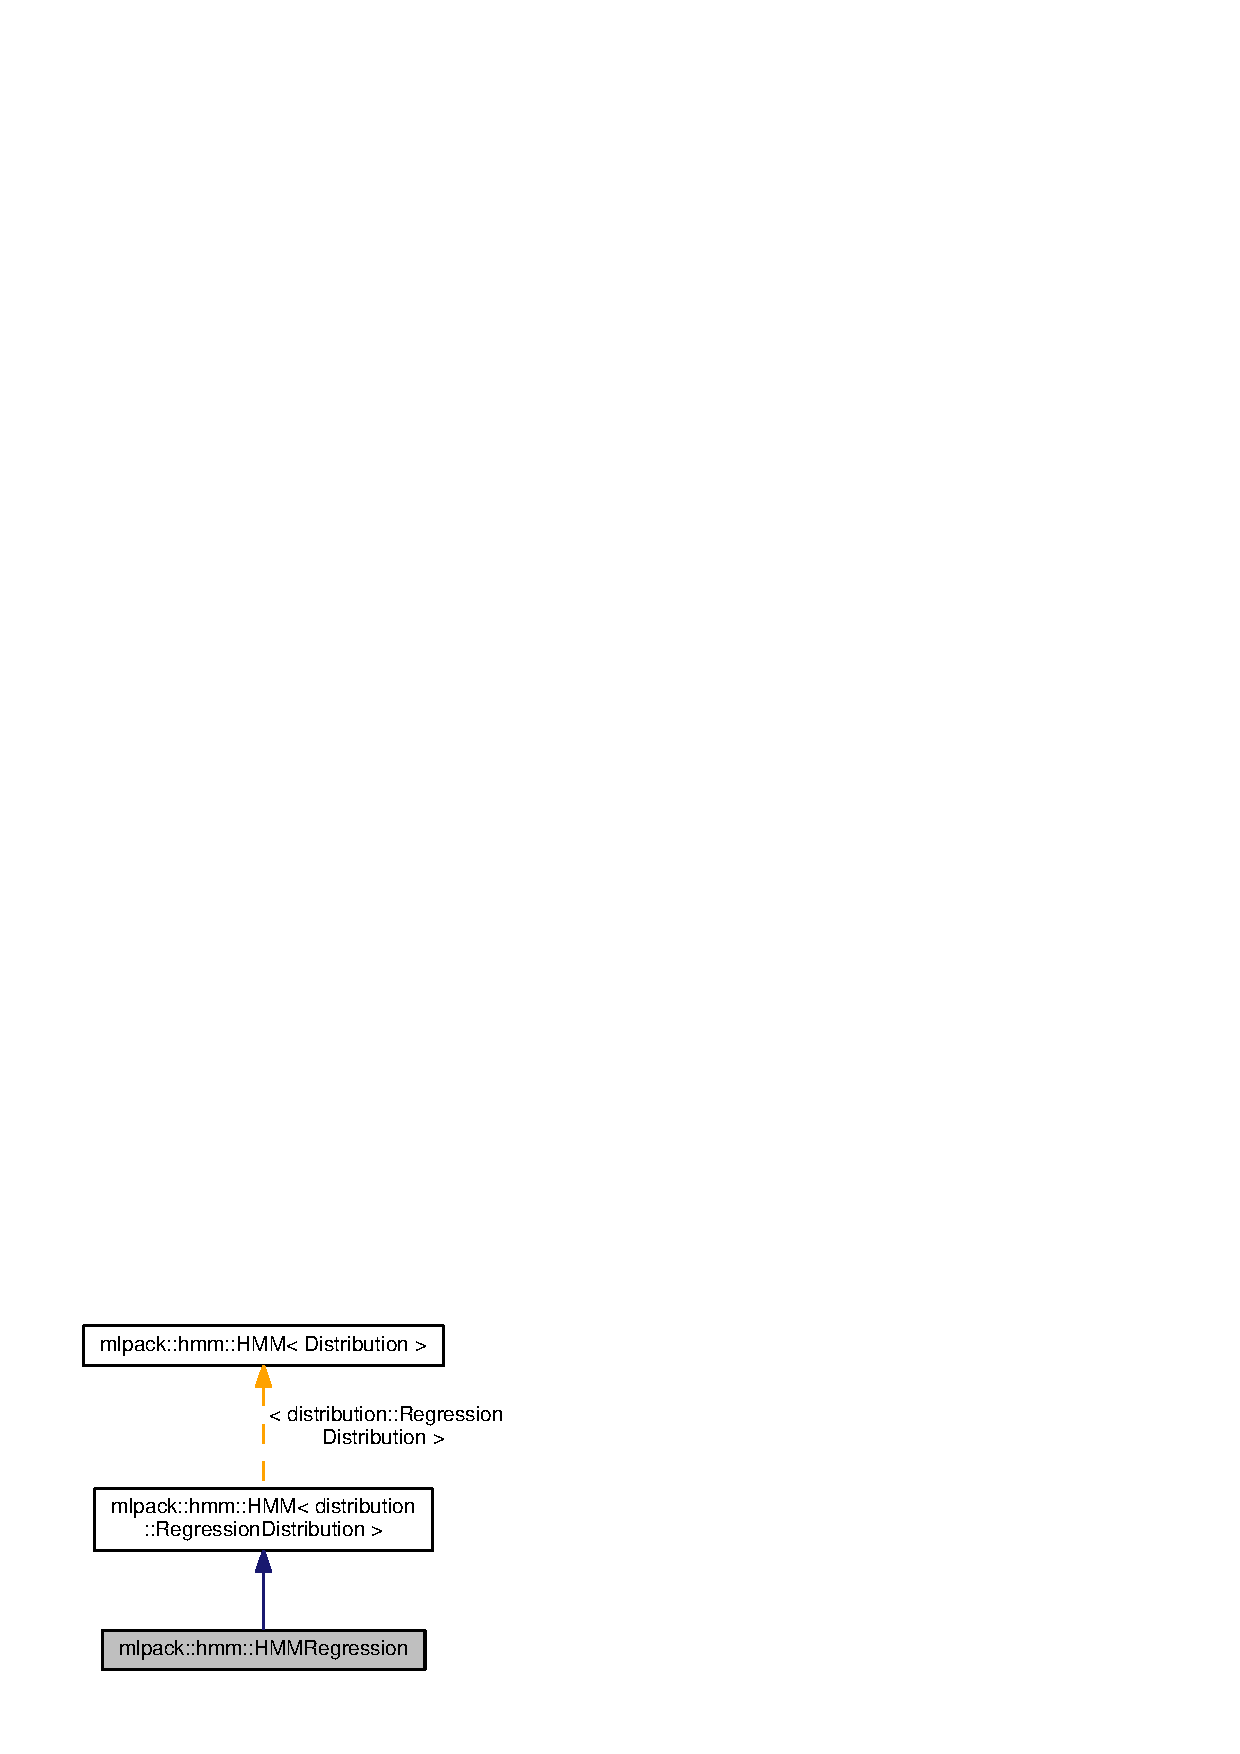
\includegraphics[width=246pt]{classmlpack_1_1hmm_1_1HMMRegression__inherit__graph}
\end{center}
\end{figure}
\subsection*{Public Member Functions}
\begin{DoxyCompactItemize}
\item 
{\bf H\+M\+M\+Regression} (const size\+\_\+t states, const {\bf distribution\+::\+Regression\+Distribution} emissions, const double {\bf tolerance}=1e-\/5)
\begin{DoxyCompactList}\small\item\em Create the Hidden Markov Model Regression with the given number of hidden states and the given default regression emission. \end{DoxyCompactList}\item 
{\bf H\+M\+M\+Regression} (const arma\+::vec \&{\bf initial}, const arma\+::mat \&{\bf transition}, const std\+::vector$<$ {\bf distribution\+::\+Regression\+Distribution} $>$ \&{\bf emission}, const double {\bf tolerance}=1e-\/5)
\begin{DoxyCompactList}\small\item\em Create the Hidden Markov Model Regression with the given initial probability vector, the given transition matrix, and the given regression emission distributions. \end{DoxyCompactList}\item 
double {\bf Estimate} (const arma\+::mat \&predictors, const arma\+::vec \&responses, arma\+::mat \&state\+Prob, arma\+::mat \&forward\+Prob, arma\+::mat \&backward\+Prob, arma\+::vec \&scales) const 
\begin{DoxyCompactList}\small\item\em Estimate the probabilities of each hidden state at each time step for each given data observation, using the Forward-\/\+Backward algorithm. \end{DoxyCompactList}\item 
double {\bf Estimate} (const arma\+::mat \&predictors, const arma\+::vec \&responses, arma\+::mat \&state\+Prob) const 
\begin{DoxyCompactList}\small\item\em Estimate the probabilities of each hidden state at each time step of each given data observation, using the Forward-\/\+Backward algorithm. \end{DoxyCompactList}\item 
void {\bf Filter} (const arma\+::mat \&predictors, const arma\+::vec \&responses, arma\+::vec \&filter\+Seq, size\+\_\+t ahead=0) const 
\begin{DoxyCompactList}\small\item\em H\+M\+MR filtering. \end{DoxyCompactList}\item 
double {\bf Log\+Likelihood} (const arma\+::mat \&predictors, const arma\+::vec \&responses) const 
\begin{DoxyCompactList}\small\item\em Compute the log-\/likelihood of the given predictors and responses. \end{DoxyCompactList}\item 
double {\bf Predict} (const arma\+::mat \&predictors, const arma\+::vec \&responses, arma\+::\+Row$<$ size\+\_\+t $>$ \&state\+Seq) const 
\begin{DoxyCompactList}\small\item\em Compute the most probable hidden state sequence for the given predictors and responses, using the Viterbi algorithm, returning the log-\/likelihood of the most likely state sequence. \end{DoxyCompactList}\item 
void {\bf Smooth} (const arma\+::mat \&predictors, const arma\+::vec \&responses, arma\+::vec \&smooth\+Seq) const 
\begin{DoxyCompactList}\small\item\em \doxyref{H\+MM}{p.}{classmlpack_1_1hmm_1_1HMM} smoothing. \end{DoxyCompactList}\item 
void {\bf Train} (const std\+::vector$<$ arma\+::mat $>$ \&predictors, const std\+::vector$<$ arma\+::vec $>$ \&responses)
\begin{DoxyCompactList}\small\item\em Train the model using the Baum-\/\+Welch algorithm, with only the given predictors and responses. \end{DoxyCompactList}\item 
void {\bf Train} (const std\+::vector$<$ arma\+::mat $>$ \&predictors, const std\+::vector$<$ arma\+::vec $>$ \&responses, const std\+::vector$<$ arma\+::\+Row$<$ size\+\_\+t $>$ $>$ \&state\+Seq)
\begin{DoxyCompactList}\small\item\em Train the model using the given labeled observations; the transition and regression emissions are directly estimated. \end{DoxyCompactList}\end{DoxyCompactItemize}
\subsection*{Private Member Functions}
\begin{DoxyCompactItemize}
\item 
void {\bf Backward} (const arma\+::mat \&predictors, const arma\+::vec \&responses, const arma\+::vec \&scales, arma\+::mat \&backward\+Prob) const 
\begin{DoxyCompactList}\small\item\em The Backward algorithm (part of the Forward-\/\+Backward algorithm). \end{DoxyCompactList}\item 
void {\bf Forward} (const arma\+::mat \&predictors, const arma\+::vec \&responses, arma\+::vec \&scales, arma\+::mat \&forward\+Prob) const 
\begin{DoxyCompactList}\small\item\em The Forward algorithm (part of the Forward-\/\+Backward algorithm). \end{DoxyCompactList}\item 
void {\bf Stack\+Data} (const std\+::vector$<$ arma\+::mat $>$ \&predictors, const std\+::vector$<$ arma\+::vec $>$ \&responses, std\+::vector$<$ arma\+::mat $>$ \&data\+Seq) const 
\begin{DoxyCompactList}\small\item\em Utility functions to facilitate the use of the \doxyref{H\+MM}{p.}{classmlpack_1_1hmm_1_1HMM} class for H\+M\+MR. \end{DoxyCompactList}\item 
void {\bf Stack\+Data} (const arma\+::mat \&predictors, const arma\+::vec \&responses, arma\+::mat \&data\+Seq) const 
\end{DoxyCompactItemize}
\subsection*{Additional Inherited Members}


\subsection{Detailed Description}
A class that represents a Hidden Markov Model Regression (H\+M\+MR). 

H\+M\+MR is an extension of Hidden Markov Models to regression analysis. The method is described in (Fridman, 1993) {\tt https\+://www.\+ima.\+umn.\+edu/preprints/\+January1994/1195.\+pdf} An H\+M\+MR is a linear regression model whose coefficients are determined by a finite-\/state Markov chain. The error terms are conditionally independently normally distributed with zero mean and state-\/dependent variance. Let Q\+\_\+t be a finite-\/state Markov chain, X\+\_\+t a vector of predictors and Y\+\_\+t a response. The H\+M\+MR is Y\+\_\+t = X\+\_\+t \{Q\+\_\+t\} + \{Q\+\_\+t\} 

This H\+M\+MR class supports training (supervised and unsupervised), prediction of state sequences via the Viterbi algorithm, estimation of state probabilities, filtering and smoothing of responses, and calculation of the log-\/likelihood of a given sequence.

Usage of the H\+M\+MR class generally involves either training an H\+M\+MR or loading an already-\/known H\+M\+MR and using to filter a sequence. Example code for supervised training of an H\+M\+MR is given below.


\begin{DoxyCode}
\textcolor{comment}{// Each column is a vector of predictors for a single observation.}
arma::mat predictors(5, 100, arma::fill::randn);
\textcolor{comment}{// Responses for each observation}
arma::vec responses(100, arma::fill::randn);

\textcolor{comment}{// Create an untrained HMMR with 3 hidden states}
RegressionDistribution rd(predictors, responses);
arma::mat transition(\textcolor{stringliteral}{"0.5 0.5;"} \textcolor{stringliteral}{"0.5 0.5;"});
std::vector<RegressionDistribution> emissions(2,rd);
HMMRegression hmmr(\textcolor{stringliteral}{"0.9 0.1"}, transition, emissions);

 \textcolor{comment}{// Train the HMM (supply a state sequence to perform supervised training)}
std::vector<arma::mat> predictorsSeq(1, predictors);
std::vector< arma::vec> responsesSeq(1, responses);
hmmr.Train(predictorsSeq, responsesSeq);
hmm.Train(observations, states);
\end{DoxyCode}


Once initialized, the H\+M\+MR can evaluate the probability of a certain sequence (with \doxyref{Log\+Likelihood()}{p.}{classmlpack_1_1hmm_1_1HMMRegression_aaf56d0c2d4502c8fb6e46acaa93faa47}), predict the most likely sequence of hidden states (with \doxyref{Predict()}{p.}{classmlpack_1_1hmm_1_1HMMRegression_a577783458d593dad59ac92fb7b3b266c}), estimate the probabilities of each state for a sequence of observations (with \doxyref{Estimate()}{p.}{classmlpack_1_1hmm_1_1HMMRegression_a04bdac3f5b6616b578130535263d8b91}), or perform filtering or smoothing of observations. 

Definition at line 69 of file hmm\+\_\+regression.\+hpp.



\subsection{Constructor \& Destructor Documentation}
\index{mlpack\+::hmm\+::\+H\+M\+M\+Regression@{mlpack\+::hmm\+::\+H\+M\+M\+Regression}!H\+M\+M\+Regression@{H\+M\+M\+Regression}}
\index{H\+M\+M\+Regression@{H\+M\+M\+Regression}!mlpack\+::hmm\+::\+H\+M\+M\+Regression@{mlpack\+::hmm\+::\+H\+M\+M\+Regression}}
\subsubsection[{H\+M\+M\+Regression(const size\+\_\+t states, const distribution\+::\+Regression\+Distribution emissions, const double tolerance=1e-\/5)}]{\setlength{\rightskip}{0pt plus 5cm}mlpack\+::hmm\+::\+H\+M\+M\+Regression\+::\+H\+M\+M\+Regression (
\begin{DoxyParamCaption}
\item[{const size\+\_\+t}]{states, }
\item[{const {\bf distribution\+::\+Regression\+Distribution}}]{emissions, }
\item[{const double}]{tolerance = {\ttfamily 1e-\/5}}
\end{DoxyParamCaption}
)\hspace{0.3cm}{\ttfamily [inline]}}\label{classmlpack_1_1hmm_1_1HMMRegression_af6df0f1e7761564f877a1e974511f2a3}


Create the Hidden Markov Model Regression with the given number of hidden states and the given default regression emission. 

The dimensionality of the observations is taken from the emissions variable, so it is important that the given default emission distribution is set with the correct dimensionality. Alternately, set the dimensionality with \doxyref{Dimensionality()}{p.}{classmlpack_1_1hmm_1_1HMM_a5bfe57d1c239278113cac519f9da2106}. Optionally, the tolerance for convergence of the Baum-\/\+Welch algorithm can be set.

By default, the transition matrix and initial probability vector are set to contain equal probability for each state.


\begin{DoxyParams}{Parameters}
{\em states} & Number of states. \\
\hline
{\em emissions} & Default distribution for emissions. \\
\hline
{\em tolerance} & Tolerance for convergence of training algorithm (Baum-\/\+Welch). \\
\hline
\end{DoxyParams}


Definition at line 89 of file hmm\+\_\+regression.\+hpp.

\index{mlpack\+::hmm\+::\+H\+M\+M\+Regression@{mlpack\+::hmm\+::\+H\+M\+M\+Regression}!H\+M\+M\+Regression@{H\+M\+M\+Regression}}
\index{H\+M\+M\+Regression@{H\+M\+M\+Regression}!mlpack\+::hmm\+::\+H\+M\+M\+Regression@{mlpack\+::hmm\+::\+H\+M\+M\+Regression}}
\subsubsection[{H\+M\+M\+Regression(const arma\+::vec \&initial, const arma\+::mat \&transition, const std\+::vector$<$ distribution\+::\+Regression\+Distribution $>$ \&emission, const double tolerance=1e-\/5)}]{\setlength{\rightskip}{0pt plus 5cm}mlpack\+::hmm\+::\+H\+M\+M\+Regression\+::\+H\+M\+M\+Regression (
\begin{DoxyParamCaption}
\item[{const arma\+::vec \&}]{initial, }
\item[{const arma\+::mat \&}]{transition, }
\item[{const std\+::vector$<$ {\bf distribution\+::\+Regression\+Distribution} $>$ \&}]{emission, }
\item[{const double}]{tolerance = {\ttfamily 1e-\/5}}
\end{DoxyParamCaption}
)\hspace{0.3cm}{\ttfamily [inline]}}\label{classmlpack_1_1hmm_1_1HMMRegression_aaa7414c3eb9f4fb19a1b2d1c699f6333}


Create the Hidden Markov Model Regression with the given initial probability vector, the given transition matrix, and the given regression emission distributions. 

The dimensionality of the observations of the H\+M\+MR are taken from the given emission distributions. Alternately, the dimensionality can be set with \doxyref{Dimensionality()}{p.}{classmlpack_1_1hmm_1_1HMM_a5bfe57d1c239278113cac519f9da2106}.

The initial state probability vector should have length equal to the number of states, and each entry represents the probability of being in the given state at time T = 0 (the beginning of a sequence).

The transition matrix should be such that T(i, j) is the probability of transition to state i from state j. The columns of the matrix should sum to 1.

Optionally, the tolerance for convergence of the Baum-\/\+Welch algorithm can be set.


\begin{DoxyParams}{Parameters}
{\em initial} & Initial state probabilities. \\
\hline
{\em transition} & Transition matrix. \\
\hline
{\em emission} & Emission distributions. \\
\hline
{\em tolerance} & Tolerance for convergence of training algorithm (Baum-\/\+Welch). \\
\hline
\end{DoxyParams}


Definition at line 119 of file hmm\+\_\+regression.\+hpp.



References Backward(), Estimate(), Filter(), Forward(), Log\+Likelihood(), Predict(), Smooth(), Stack\+Data(), and Train().



\subsection{Member Function Documentation}
\index{mlpack\+::hmm\+::\+H\+M\+M\+Regression@{mlpack\+::hmm\+::\+H\+M\+M\+Regression}!Backward@{Backward}}
\index{Backward@{Backward}!mlpack\+::hmm\+::\+H\+M\+M\+Regression@{mlpack\+::hmm\+::\+H\+M\+M\+Regression}}
\subsubsection[{Backward(const arma\+::mat \&predictors, const arma\+::vec \&responses, const arma\+::vec \&scales, arma\+::mat \&backward\+Prob) const }]{\setlength{\rightskip}{0pt plus 5cm}void mlpack\+::hmm\+::\+H\+M\+M\+Regression\+::\+Backward (
\begin{DoxyParamCaption}
\item[{const arma\+::mat \&}]{predictors, }
\item[{const arma\+::vec \&}]{responses, }
\item[{const arma\+::vec \&}]{scales, }
\item[{arma\+::mat \&}]{backward\+Prob}
\end{DoxyParamCaption}
) const\hspace{0.3cm}{\ttfamily [private]}}\label{classmlpack_1_1hmm_1_1HMMRegression_acc00e1764b74ec5f84f24516c71ce09c}


The Backward algorithm (part of the Forward-\/\+Backward algorithm). 

Computes backward probabilities for each state for each observation in the given data sequence, using the scaling factors found (presumably) by \doxyref{Forward()}{p.}{classmlpack_1_1hmm_1_1HMMRegression_a6f037a9bef339480de70685b500dd335}. The returned matrix has rows equal to the number of hidden states and columns equal to the number of observations.


\begin{DoxyParams}{Parameters}
{\em predictors} & Vector of predictor sequences. \\
\hline
{\em responses} & Vector of response sequences. \\
\hline
{\em scales} & Vector of scaling factors. \\
\hline
{\em backward\+Prob} & Matrix in which backward probabilities will be saved. \\
\hline
\end{DoxyParams}


Referenced by H\+M\+M\+Regression().

\index{mlpack\+::hmm\+::\+H\+M\+M\+Regression@{mlpack\+::hmm\+::\+H\+M\+M\+Regression}!Estimate@{Estimate}}
\index{Estimate@{Estimate}!mlpack\+::hmm\+::\+H\+M\+M\+Regression@{mlpack\+::hmm\+::\+H\+M\+M\+Regression}}
\subsubsection[{Estimate(const arma\+::mat \&predictors, const arma\+::vec \&responses, arma\+::mat \&state\+Prob, arma\+::mat \&forward\+Prob, arma\+::mat \&backward\+Prob, arma\+::vec \&scales) const }]{\setlength{\rightskip}{0pt plus 5cm}double mlpack\+::hmm\+::\+H\+M\+M\+Regression\+::\+Estimate (
\begin{DoxyParamCaption}
\item[{const arma\+::mat \&}]{predictors, }
\item[{const arma\+::vec \&}]{responses, }
\item[{arma\+::mat \&}]{state\+Prob, }
\item[{arma\+::mat \&}]{forward\+Prob, }
\item[{arma\+::mat \&}]{backward\+Prob, }
\item[{arma\+::vec \&}]{scales}
\end{DoxyParamCaption}
) const}\label{classmlpack_1_1hmm_1_1HMMRegression_a04bdac3f5b6616b578130535263d8b91}


Estimate the probabilities of each hidden state at each time step for each given data observation, using the Forward-\/\+Backward algorithm. 

Each matrix which is returned has columns equal to the number of data observations, and rows equal to the number of hidden states in the model. The log-\/likelihood of the most probable sequence is returned.


\begin{DoxyParams}{Parameters}
{\em predictors} & Vector of predictor sequences. \\
\hline
{\em responses} & Vector of response sequences. \\
\hline
{\em state\+Prob} & Matrix in which the probabilities of each state at each time interval will be stored. \\
\hline
{\em forward\+Prob} & Matrix in which the forward probabilities of each state at each time interval will be stored. \\
\hline
{\em backward\+Prob} & Matrix in which the backward probabilities of each state at each time interval will be stored. \\
\hline
{\em scales} & Vector in which the scaling factors at each time interval will be stored. \\
\hline
\end{DoxyParams}
\begin{DoxyReturn}{Returns}
Log-\/likelihood of most likely state sequence. 
\end{DoxyReturn}


Referenced by H\+M\+M\+Regression().

\index{mlpack\+::hmm\+::\+H\+M\+M\+Regression@{mlpack\+::hmm\+::\+H\+M\+M\+Regression}!Estimate@{Estimate}}
\index{Estimate@{Estimate}!mlpack\+::hmm\+::\+H\+M\+M\+Regression@{mlpack\+::hmm\+::\+H\+M\+M\+Regression}}
\subsubsection[{Estimate(const arma\+::mat \&predictors, const arma\+::vec \&responses, arma\+::mat \&state\+Prob) const }]{\setlength{\rightskip}{0pt plus 5cm}double mlpack\+::hmm\+::\+H\+M\+M\+Regression\+::\+Estimate (
\begin{DoxyParamCaption}
\item[{const arma\+::mat \&}]{predictors, }
\item[{const arma\+::vec \&}]{responses, }
\item[{arma\+::mat \&}]{state\+Prob}
\end{DoxyParamCaption}
) const}\label{classmlpack_1_1hmm_1_1HMMRegression_a047ea47bc41f5c16ef61542f07ad9b89}


Estimate the probabilities of each hidden state at each time step of each given data observation, using the Forward-\/\+Backward algorithm. 

The returned matrix of state probabilities has columns equal to the number of data observations, and rows equal to the number of hidden states in the model. The log-\/likelihood of the most probable sequence is returned.


\begin{DoxyParams}{Parameters}
{\em predictors} & Vector of predictor sequences. \\
\hline
{\em responses} & Vector of response sequences. \\
\hline
{\em state\+Prob} & Probabilities of each state at each time interval. \\
\hline
\end{DoxyParams}
\begin{DoxyReturn}{Returns}
Log-\/likelihood of most likely state sequence. 
\end{DoxyReturn}
\index{mlpack\+::hmm\+::\+H\+M\+M\+Regression@{mlpack\+::hmm\+::\+H\+M\+M\+Regression}!Filter@{Filter}}
\index{Filter@{Filter}!mlpack\+::hmm\+::\+H\+M\+M\+Regression@{mlpack\+::hmm\+::\+H\+M\+M\+Regression}}
\subsubsection[{Filter(const arma\+::mat \&predictors, const arma\+::vec \&responses, arma\+::vec \&filter\+Seq, size\+\_\+t ahead=0) const }]{\setlength{\rightskip}{0pt plus 5cm}void mlpack\+::hmm\+::\+H\+M\+M\+Regression\+::\+Filter (
\begin{DoxyParamCaption}
\item[{const arma\+::mat \&}]{predictors, }
\item[{const arma\+::vec \&}]{responses, }
\item[{arma\+::vec \&}]{filter\+Seq, }
\item[{size\+\_\+t}]{ahead = {\ttfamily 0}}
\end{DoxyParamCaption}
) const}\label{classmlpack_1_1hmm_1_1HMMRegression_a106bc8d5c186c2aee1bcfcf1437f632a}


H\+M\+MR filtering. 

Computes the k-\/step-\/ahead expected response at each time conditioned only on prior observations. That is E\{ Y[t+k] $\vert$ Y[0], ..., Y[t] \}. The returned matrix has columns equal to the number of observations. Note that the expectation may not be meaningful for discrete emissions.


\begin{DoxyParams}{Parameters}
{\em predictors} & Vector of predictor sequences. \\
\hline
{\em responses} & Vector of response sequences. \\
\hline
{\em initial} & Distribution of initial state. \\
\hline
{\em ahead} & Number of steps ahead (k) for expectations. \\
\hline
{\em filter\+Seq} & Vector in which the expected emission sequence will be stored. \\
\hline
\end{DoxyParams}


Referenced by H\+M\+M\+Regression().

\index{mlpack\+::hmm\+::\+H\+M\+M\+Regression@{mlpack\+::hmm\+::\+H\+M\+M\+Regression}!Forward@{Forward}}
\index{Forward@{Forward}!mlpack\+::hmm\+::\+H\+M\+M\+Regression@{mlpack\+::hmm\+::\+H\+M\+M\+Regression}}
\subsubsection[{Forward(const arma\+::mat \&predictors, const arma\+::vec \&responses, arma\+::vec \&scales, arma\+::mat \&forward\+Prob) const }]{\setlength{\rightskip}{0pt plus 5cm}void mlpack\+::hmm\+::\+H\+M\+M\+Regression\+::\+Forward (
\begin{DoxyParamCaption}
\item[{const arma\+::mat \&}]{predictors, }
\item[{const arma\+::vec \&}]{responses, }
\item[{arma\+::vec \&}]{scales, }
\item[{arma\+::mat \&}]{forward\+Prob}
\end{DoxyParamCaption}
) const\hspace{0.3cm}{\ttfamily [private]}}\label{classmlpack_1_1hmm_1_1HMMRegression_a6f037a9bef339480de70685b500dd335}


The Forward algorithm (part of the Forward-\/\+Backward algorithm). 

Computes forward probabilities for each state for each observation in the given data sequence. The returned matrix has rows equal to the number of hidden states and columns equal to the number of observations.


\begin{DoxyParams}{Parameters}
{\em predictors} & Vector of predictor sequences. \\
\hline
{\em responses} & Vector of response sequences. \\
\hline
{\em scales} & Vector in which scaling factors will be saved. \\
\hline
{\em forward\+Prob} & Matrix in which forward probabilities will be saved. \\
\hline
\end{DoxyParams}


Referenced by H\+M\+M\+Regression().

\index{mlpack\+::hmm\+::\+H\+M\+M\+Regression@{mlpack\+::hmm\+::\+H\+M\+M\+Regression}!Log\+Likelihood@{Log\+Likelihood}}
\index{Log\+Likelihood@{Log\+Likelihood}!mlpack\+::hmm\+::\+H\+M\+M\+Regression@{mlpack\+::hmm\+::\+H\+M\+M\+Regression}}
\subsubsection[{Log\+Likelihood(const arma\+::mat \&predictors, const arma\+::vec \&responses) const }]{\setlength{\rightskip}{0pt plus 5cm}double mlpack\+::hmm\+::\+H\+M\+M\+Regression\+::\+Log\+Likelihood (
\begin{DoxyParamCaption}
\item[{const arma\+::mat \&}]{predictors, }
\item[{const arma\+::vec \&}]{responses}
\end{DoxyParamCaption}
) const}\label{classmlpack_1_1hmm_1_1HMMRegression_aaf56d0c2d4502c8fb6e46acaa93faa47}


Compute the log-\/likelihood of the given predictors and responses. 


\begin{DoxyParams}{Parameters}
{\em predictors} & Vector of predictor sequences. \\
\hline
{\em responses} & Vector of response sequences. \\
\hline
\end{DoxyParams}
\begin{DoxyReturn}{Returns}
Log-\/likelihood of the given sequence. 
\end{DoxyReturn}


Referenced by H\+M\+M\+Regression().

\index{mlpack\+::hmm\+::\+H\+M\+M\+Regression@{mlpack\+::hmm\+::\+H\+M\+M\+Regression}!Predict@{Predict}}
\index{Predict@{Predict}!mlpack\+::hmm\+::\+H\+M\+M\+Regression@{mlpack\+::hmm\+::\+H\+M\+M\+Regression}}
\subsubsection[{Predict(const arma\+::mat \&predictors, const arma\+::vec \&responses, arma\+::\+Row$<$ size\+\_\+t $>$ \&state\+Seq) const }]{\setlength{\rightskip}{0pt plus 5cm}double mlpack\+::hmm\+::\+H\+M\+M\+Regression\+::\+Predict (
\begin{DoxyParamCaption}
\item[{const arma\+::mat \&}]{predictors, }
\item[{const arma\+::vec \&}]{responses, }
\item[{arma\+::\+Row$<$ size\+\_\+t $>$ \&}]{state\+Seq}
\end{DoxyParamCaption}
) const}\label{classmlpack_1_1hmm_1_1HMMRegression_a577783458d593dad59ac92fb7b3b266c}


Compute the most probable hidden state sequence for the given predictors and responses, using the Viterbi algorithm, returning the log-\/likelihood of the most likely state sequence. 


\begin{DoxyParams}{Parameters}
{\em predictors} & Vector of predictor sequences. \\
\hline
{\em responses} & Vector of response sequences. \\
\hline
{\em state\+Seq} & Vector in which the most probable state sequence will be stored. \\
\hline
\end{DoxyParams}
\begin{DoxyReturn}{Returns}
Log-\/likelihood of most probable state sequence. 
\end{DoxyReturn}


Referenced by H\+M\+M\+Regression().

\index{mlpack\+::hmm\+::\+H\+M\+M\+Regression@{mlpack\+::hmm\+::\+H\+M\+M\+Regression}!Smooth@{Smooth}}
\index{Smooth@{Smooth}!mlpack\+::hmm\+::\+H\+M\+M\+Regression@{mlpack\+::hmm\+::\+H\+M\+M\+Regression}}
\subsubsection[{Smooth(const arma\+::mat \&predictors, const arma\+::vec \&responses, arma\+::vec \&smooth\+Seq) const }]{\setlength{\rightskip}{0pt plus 5cm}void mlpack\+::hmm\+::\+H\+M\+M\+Regression\+::\+Smooth (
\begin{DoxyParamCaption}
\item[{const arma\+::mat \&}]{predictors, }
\item[{const arma\+::vec \&}]{responses, }
\item[{arma\+::vec \&}]{smooth\+Seq}
\end{DoxyParamCaption}
) const}\label{classmlpack_1_1hmm_1_1HMMRegression_a5a4c77b693d2d6801422bdfff2b57e14}


\doxyref{H\+MM}{p.}{classmlpack_1_1hmm_1_1HMM} smoothing. 

Computes expected emission at each time conditioned on all observations. That is E\{ Y[t] $\vert$ Y[0], ..., Y[T] \}. The returned matrix has columns equal to the number of observations. Note that the expectation may not be meaningful for discrete emissions.


\begin{DoxyParams}{Parameters}
{\em predictors} & Vector of predictor sequences. \\
\hline
{\em responses} & Vector of response sequences.. \\
\hline
{\em initial} & Distribution of initial state. \\
\hline
{\em smooth\+Seq} & Vector in which the expected emission sequence will be stored. \\
\hline
\end{DoxyParams}


Referenced by H\+M\+M\+Regression().

\index{mlpack\+::hmm\+::\+H\+M\+M\+Regression@{mlpack\+::hmm\+::\+H\+M\+M\+Regression}!Stack\+Data@{Stack\+Data}}
\index{Stack\+Data@{Stack\+Data}!mlpack\+::hmm\+::\+H\+M\+M\+Regression@{mlpack\+::hmm\+::\+H\+M\+M\+Regression}}
\subsubsection[{Stack\+Data(const std\+::vector$<$ arma\+::mat $>$ \&predictors, const std\+::vector$<$ arma\+::vec $>$ \&responses, std\+::vector$<$ arma\+::mat $>$ \&data\+Seq) const }]{\setlength{\rightskip}{0pt plus 5cm}void mlpack\+::hmm\+::\+H\+M\+M\+Regression\+::\+Stack\+Data (
\begin{DoxyParamCaption}
\item[{const std\+::vector$<$ arma\+::mat $>$ \&}]{predictors, }
\item[{const std\+::vector$<$ arma\+::vec $>$ \&}]{responses, }
\item[{std\+::vector$<$ arma\+::mat $>$ \&}]{data\+Seq}
\end{DoxyParamCaption}
) const\hspace{0.3cm}{\ttfamily [private]}}\label{classmlpack_1_1hmm_1_1HMMRegression_ae8c8df1763cdf593eeae0955487a1080}


Utility functions to facilitate the use of the \doxyref{H\+MM}{p.}{classmlpack_1_1hmm_1_1HMM} class for H\+M\+MR. 



Referenced by H\+M\+M\+Regression().

\index{mlpack\+::hmm\+::\+H\+M\+M\+Regression@{mlpack\+::hmm\+::\+H\+M\+M\+Regression}!Stack\+Data@{Stack\+Data}}
\index{Stack\+Data@{Stack\+Data}!mlpack\+::hmm\+::\+H\+M\+M\+Regression@{mlpack\+::hmm\+::\+H\+M\+M\+Regression}}
\subsubsection[{Stack\+Data(const arma\+::mat \&predictors, const arma\+::vec \&responses, arma\+::mat \&data\+Seq) const }]{\setlength{\rightskip}{0pt plus 5cm}void mlpack\+::hmm\+::\+H\+M\+M\+Regression\+::\+Stack\+Data (
\begin{DoxyParamCaption}
\item[{const arma\+::mat \&}]{predictors, }
\item[{const arma\+::vec \&}]{responses, }
\item[{arma\+::mat \&}]{data\+Seq}
\end{DoxyParamCaption}
) const\hspace{0.3cm}{\ttfamily [private]}}\label{classmlpack_1_1hmm_1_1HMMRegression_a1c5e64dd601eb1eb70ddad9a4ef413a8}
\index{mlpack\+::hmm\+::\+H\+M\+M\+Regression@{mlpack\+::hmm\+::\+H\+M\+M\+Regression}!Train@{Train}}
\index{Train@{Train}!mlpack\+::hmm\+::\+H\+M\+M\+Regression@{mlpack\+::hmm\+::\+H\+M\+M\+Regression}}
\subsubsection[{Train(const std\+::vector$<$ arma\+::mat $>$ \&predictors, const std\+::vector$<$ arma\+::vec $>$ \&responses)}]{\setlength{\rightskip}{0pt plus 5cm}void mlpack\+::hmm\+::\+H\+M\+M\+Regression\+::\+Train (
\begin{DoxyParamCaption}
\item[{const std\+::vector$<$ arma\+::mat $>$ \&}]{predictors, }
\item[{const std\+::vector$<$ arma\+::vec $>$ \&}]{responses}
\end{DoxyParamCaption}
)}\label{classmlpack_1_1hmm_1_1HMMRegression_a5028034d1d33ca83b8268955aa5e6d30}


Train the model using the Baum-\/\+Welch algorithm, with only the given predictors and responses. 

Instead of giving a guess transition and emission here, do that in the constructor. Each matrix in the vector of predictors corresponds to an individual data sequence, and likewise for each vec in the vector of responses. The number of rows in each matrix of predictors plus one should be equal to the dimensionality of the \doxyref{H\+MM}{p.}{classmlpack_1_1hmm_1_1HMM} (which is set in the constructor).

It is preferable to use the other overload of \doxyref{Train()}{p.}{classmlpack_1_1hmm_1_1HMMRegression_a5028034d1d33ca83b8268955aa5e6d30}, with labeled data. That will produce much better results. However, if labeled data is unavailable, this will work. In addition, it is possible to use \doxyref{Train()}{p.}{classmlpack_1_1hmm_1_1HMMRegression_a5028034d1d33ca83b8268955aa5e6d30} with labeled data first, and then continue to train the model using this overload of \doxyref{Train()}{p.}{classmlpack_1_1hmm_1_1HMMRegression_a5028034d1d33ca83b8268955aa5e6d30} with unlabeled data.

The tolerance of the Baum-\/\+Welch algorithm can be set either in the constructor or with the \doxyref{Tolerance()}{p.}{classmlpack_1_1hmm_1_1HMM_ab588ae02998cf353e819f2ef8613e481} method. When the change in log-\/likelihood of the model between iterations is less than the tolerance, the Baum-\/\+Welch algorithm terminates.

\begin{DoxyNote}{Note}
\doxyref{Train()}{p.}{classmlpack_1_1hmm_1_1HMMRegression_a5028034d1d33ca83b8268955aa5e6d30} can be called multiple times with different sequences; each time it is called, it uses the current parameters of the \doxyref{H\+MM}{p.}{classmlpack_1_1hmm_1_1HMM} as a starting point for training. 
\end{DoxyNote}

\begin{DoxyParams}{Parameters}
{\em predictors} & Vector of predictor sequences. \\
\hline
{\em responses} & Vector of response sequences. \\
\hline
\end{DoxyParams}


Referenced by H\+M\+M\+Regression().

\index{mlpack\+::hmm\+::\+H\+M\+M\+Regression@{mlpack\+::hmm\+::\+H\+M\+M\+Regression}!Train@{Train}}
\index{Train@{Train}!mlpack\+::hmm\+::\+H\+M\+M\+Regression@{mlpack\+::hmm\+::\+H\+M\+M\+Regression}}
\subsubsection[{Train(const std\+::vector$<$ arma\+::mat $>$ \&predictors, const std\+::vector$<$ arma\+::vec $>$ \&responses, const std\+::vector$<$ arma\+::\+Row$<$ size\+\_\+t $>$ $>$ \&state\+Seq)}]{\setlength{\rightskip}{0pt plus 5cm}void mlpack\+::hmm\+::\+H\+M\+M\+Regression\+::\+Train (
\begin{DoxyParamCaption}
\item[{const std\+::vector$<$ arma\+::mat $>$ \&}]{predictors, }
\item[{const std\+::vector$<$ arma\+::vec $>$ \&}]{responses, }
\item[{const std\+::vector$<$ arma\+::\+Row$<$ size\+\_\+t $>$ $>$ \&}]{state\+Seq}
\end{DoxyParamCaption}
)}\label{classmlpack_1_1hmm_1_1HMMRegression_ad47aa641f2520b4d4fa4284914a46b73}


Train the model using the given labeled observations; the transition and regression emissions are directly estimated. 

Each matrix in the vector of predictors corresponds to an individual data sequence, and likewise for each vec in the vector of responses. The number of rows in each matrix of predictors plus one should be equal to the dimensionality of the \doxyref{H\+MM}{p.}{classmlpack_1_1hmm_1_1HMM} (which is set in the constructor).

\begin{DoxyNote}{Note}
\doxyref{Train()}{p.}{classmlpack_1_1hmm_1_1HMMRegression_a5028034d1d33ca83b8268955aa5e6d30} can be called multiple times with different sequences; each time it is called, it uses the current parameters of the H\+M\+MR as a starting point for training. 
\end{DoxyNote}

\begin{DoxyParams}{Parameters}
{\em predictors} & Vector of predictor sequences. \\
\hline
{\em responses} & Vector of response sequences. \\
\hline
{\em state\+Seq} & Vector of state sequences, corresponding to each observation. \\
\hline
\end{DoxyParams}


The documentation for this class was generated from the following file\+:\begin{DoxyCompactItemize}
\item 
src/mlpack/methods/hmm/{\bf hmm\+\_\+regression.\+hpp}\end{DoxyCompactItemize}

\section{mlpack\+:\+:kernel\+:\+:Cosine\+Distance Class Reference}
\label{classmlpack_1_1kernel_1_1CosineDistance}\index{mlpack\+::kernel\+::\+Cosine\+Distance@{mlpack\+::kernel\+::\+Cosine\+Distance}}


The cosine distance (or cosine similarity).  


\subsection*{Public Member Functions}
\begin{DoxyCompactItemize}
\item 
{\footnotesize template$<$typename Archive $>$ }\\void {\bf Serialize} (Archive \&, const unsigned int)
\begin{DoxyCompactList}\small\item\em Serialize the class (there\textquotesingle{}s nothing to save). \end{DoxyCompactList}\end{DoxyCompactItemize}
\subsection*{Static Public Member Functions}
\begin{DoxyCompactItemize}
\item 
{\footnotesize template$<$typename Vec\+TypeA , typename Vec\+TypeB $>$ }\\static double {\bf Evaluate} (const Vec\+TypeA \&a, const Vec\+TypeB \&b)
\begin{DoxyCompactList}\small\item\em Computes the cosine distance between two points. \end{DoxyCompactList}\end{DoxyCompactItemize}


\subsection{Detailed Description}
The cosine distance (or cosine similarity). 

It is defined by

\[ d(a, b) = \frac{a^T b}{|| a || || b ||} \]

and this class assumes the standard L2 inner product. 

Definition at line 31 of file cosine\+\_\+distance.\+hpp.



\subsection{Member Function Documentation}
\index{mlpack\+::kernel\+::\+Cosine\+Distance@{mlpack\+::kernel\+::\+Cosine\+Distance}!Evaluate@{Evaluate}}
\index{Evaluate@{Evaluate}!mlpack\+::kernel\+::\+Cosine\+Distance@{mlpack\+::kernel\+::\+Cosine\+Distance}}
\subsubsection[{Evaluate(const Vec\+Type\+A \&a, const Vec\+Type\+B \&b)}]{\setlength{\rightskip}{0pt plus 5cm}template$<$typename Vec\+TypeA , typename Vec\+TypeB $>$ static double mlpack\+::kernel\+::\+Cosine\+Distance\+::\+Evaluate (
\begin{DoxyParamCaption}
\item[{const Vec\+TypeA \&}]{a, }
\item[{const Vec\+TypeB \&}]{b}
\end{DoxyParamCaption}
)\hspace{0.3cm}{\ttfamily [static]}}\label{classmlpack_1_1kernel_1_1CosineDistance_ad317e3f97456618ae1c7d92e3120ac13}


Computes the cosine distance between two points. 


\begin{DoxyParams}{Parameters}
{\em a} & First vector. \\
\hline
{\em b} & Second vector. \\
\hline
\end{DoxyParams}
\begin{DoxyReturn}{Returns}
d(a, b). 
\end{DoxyReturn}
\index{mlpack\+::kernel\+::\+Cosine\+Distance@{mlpack\+::kernel\+::\+Cosine\+Distance}!Serialize@{Serialize}}
\index{Serialize@{Serialize}!mlpack\+::kernel\+::\+Cosine\+Distance@{mlpack\+::kernel\+::\+Cosine\+Distance}}
\subsubsection[{Serialize(\+Archive \&, const unsigned int)}]{\setlength{\rightskip}{0pt plus 5cm}template$<$typename Archive $>$ void mlpack\+::kernel\+::\+Cosine\+Distance\+::\+Serialize (
\begin{DoxyParamCaption}
\item[{Archive \&}]{, }
\item[{const unsigned}]{int}
\end{DoxyParamCaption}
)\hspace{0.3cm}{\ttfamily [inline]}}\label{classmlpack_1_1kernel_1_1CosineDistance_af64dc7c4f0d0a839bc1aec6ba14e2548}


Serialize the class (there\textquotesingle{}s nothing to save). 



Definition at line 46 of file cosine\+\_\+distance.\+hpp.



The documentation for this class was generated from the following file\+:\begin{DoxyCompactItemize}
\item 
src/mlpack/core/kernels/{\bf cosine\+\_\+distance.\+hpp}\end{DoxyCompactItemize}

\doxysection{Epanechnikov\+Kernel Class Reference}
\label{classmlpack_1_1kernel_1_1EpanechnikovKernel}\index{EpanechnikovKernel@{EpanechnikovKernel}}


The Epanechnikov kernel, defined as.  


\doxysubsection*{Public Member Functions}
\begin{DoxyCompactItemize}
\item 
\textbf{ Epanechnikov\+Kernel} (const double bandwidth=1.\+0)
\begin{DoxyCompactList}\small\item\em Instantiate the Epanechnikov kernel with the given bandwidth (default 1.\+0). \end{DoxyCompactList}\item 
{\footnotesize template$<$typename Vec\+TypeA , typename Vec\+TypeB $>$ }\\double \textbf{ Convolution\+Integral} (const Vec\+TypeA \&a, const Vec\+TypeB \&b)
\begin{DoxyCompactList}\small\item\em Obtains the convolution integral [integral of K($\vert$$\vert$x-\/a$\vert$$\vert$) K($\vert$$\vert$b-\/x$\vert$$\vert$) dx] for the two vectors. \end{DoxyCompactList}\item 
double \textbf{ Evaluate} (const double distance) const
\begin{DoxyCompactList}\small\item\em Evaluate the Epanechnikov kernel given that the distance between the two input points is known. \end{DoxyCompactList}\item 
{\footnotesize template$<$typename Vec\+TypeA , typename Vec\+TypeB $>$ }\\double \textbf{ Evaluate} (const Vec\+TypeA \&a, const Vec\+TypeB \&b) const
\begin{DoxyCompactList}\small\item\em Evaluate the Epanechnikov kernel on the given two inputs. \end{DoxyCompactList}\item 
double \textbf{ Gradient} (const double distance) const
\begin{DoxyCompactList}\small\item\em Evaluate the Gradient of Epanechnikov kernel given that the distance between the two input points is known. \end{DoxyCompactList}\item 
double \textbf{ Gradient\+For\+Squared\+Distance} (const double distance\+Squared) const
\begin{DoxyCompactList}\small\item\em Evaluate the Gradient of Epanechnikov kernel given that the squared distance between the two input points is known. \end{DoxyCompactList}\item 
double \textbf{ Normalizer} (const size\+\_\+t dimension)
\begin{DoxyCompactList}\small\item\em Compute the normalizer of this Epanechnikov kernel for the given dimension. \end{DoxyCompactList}\item 
{\footnotesize template$<$typename Archive $>$ }\\void \textbf{ serialize} (Archive \&ar, const uint32\+\_\+t version)
\begin{DoxyCompactList}\small\item\em Serialize the kernel. \end{DoxyCompactList}\end{DoxyCompactItemize}


\doxysubsection{Detailed Description}
The Epanechnikov kernel, defined as. 

\[ K(x, y) = \max \{0, 1 - || x - y ||^2_2 / b^2 \} \]

where $ b $ is the bandwidth the of the kernel (defaults to 1.\+0). 

Definition at line 30 of file epanechnikov\+\_\+kernel.\+hpp.



\doxysubsection{Constructor \& Destructor Documentation}
\mbox{\label{classmlpack_1_1kernel_1_1EpanechnikovKernel_ad3880022e464ae367ed9b7342f0cdf37}} 
\index{EpanechnikovKernel@{EpanechnikovKernel}!EpanechnikovKernel@{EpanechnikovKernel}}
\index{EpanechnikovKernel@{EpanechnikovKernel}!EpanechnikovKernel@{EpanechnikovKernel}}
\doxysubsubsection{EpanechnikovKernel()}
{\footnotesize\ttfamily \textbf{ Epanechnikov\+Kernel} (\begin{DoxyParamCaption}\item[{const double}]{bandwidth = {\ttfamily 1.0} }\end{DoxyParamCaption})\hspace{0.3cm}{\ttfamily [inline]}}



Instantiate the Epanechnikov kernel with the given bandwidth (default 1.\+0). 


\begin{DoxyParams}{Parameters}
{\em bandwidth} & Bandwidth of the kernel. \\
\hline
\end{DoxyParams}


Definition at line 38 of file epanechnikov\+\_\+kernel.\+hpp.



\doxysubsection{Member Function Documentation}
\mbox{\label{classmlpack_1_1kernel_1_1EpanechnikovKernel_af3077f924263d1932950f4f7176c93eb}} 
\index{EpanechnikovKernel@{EpanechnikovKernel}!ConvolutionIntegral@{ConvolutionIntegral}}
\index{ConvolutionIntegral@{ConvolutionIntegral}!EpanechnikovKernel@{EpanechnikovKernel}}
\doxysubsubsection{ConvolutionIntegral()}
{\footnotesize\ttfamily double Convolution\+Integral (\begin{DoxyParamCaption}\item[{const Vec\+TypeA \&}]{a,  }\item[{const Vec\+TypeB \&}]{b }\end{DoxyParamCaption})}



Obtains the convolution integral [integral of K($\vert$$\vert$x-\/a$\vert$$\vert$) K($\vert$$\vert$b-\/x$\vert$$\vert$) dx] for the two vectors. 


\begin{DoxyTemplParams}{Template Parameters}
{\em Vec\+Type} & Type of vector (arma\+::vec, arma\+::spvec should be expected). \\
\hline
\end{DoxyTemplParams}

\begin{DoxyParams}{Parameters}
{\em a} & First vector. \\
\hline
{\em b} & Second vector. \\
\hline
\end{DoxyParams}
\begin{DoxyReturn}{Returns}
the convolution integral value. 
\end{DoxyReturn}
\mbox{\label{classmlpack_1_1kernel_1_1EpanechnikovKernel_a5602dee5d3ad98a183b9a11d9e0ed225}} 
\index{EpanechnikovKernel@{EpanechnikovKernel}!Evaluate@{Evaluate}}
\index{Evaluate@{Evaluate}!EpanechnikovKernel@{EpanechnikovKernel}}
\doxysubsubsection{Evaluate()\hspace{0.1cm}{\footnotesize\ttfamily [1/2]}}
{\footnotesize\ttfamily double Evaluate (\begin{DoxyParamCaption}\item[{const double}]{distance }\end{DoxyParamCaption}) const}



Evaluate the Epanechnikov kernel given that the distance between the two input points is known. 

\mbox{\label{classmlpack_1_1kernel_1_1EpanechnikovKernel_a84c3aeba25ea7703bd2d4f85a54301da}} 
\index{EpanechnikovKernel@{EpanechnikovKernel}!Evaluate@{Evaluate}}
\index{Evaluate@{Evaluate}!EpanechnikovKernel@{EpanechnikovKernel}}
\doxysubsubsection{Evaluate()\hspace{0.1cm}{\footnotesize\ttfamily [2/2]}}
{\footnotesize\ttfamily double Evaluate (\begin{DoxyParamCaption}\item[{const Vec\+TypeA \&}]{a,  }\item[{const Vec\+TypeB \&}]{b }\end{DoxyParamCaption}) const}



Evaluate the Epanechnikov kernel on the given two inputs. 


\begin{DoxyTemplParams}{Template Parameters}
{\em Vec\+TypeA} & Type of first vector. \\
\hline
{\em Vec\+TypeB} & Type of second vector. \\
\hline
\end{DoxyTemplParams}

\begin{DoxyParams}{Parameters}
{\em a} & One input vector. \\
\hline
{\em b} & The other input vector. \\
\hline
\end{DoxyParams}
\mbox{\label{classmlpack_1_1kernel_1_1EpanechnikovKernel_ac83f017e98c3f23c603fb26b50b82cfd}} 
\index{EpanechnikovKernel@{EpanechnikovKernel}!Gradient@{Gradient}}
\index{Gradient@{Gradient}!EpanechnikovKernel@{EpanechnikovKernel}}
\doxysubsubsection{Gradient()}
{\footnotesize\ttfamily double Gradient (\begin{DoxyParamCaption}\item[{const double}]{distance }\end{DoxyParamCaption}) const}



Evaluate the Gradient of Epanechnikov kernel given that the distance between the two input points is known. 

\mbox{\label{classmlpack_1_1kernel_1_1EpanechnikovKernel_aa993982e3ab29e7c8a299012dbe42cc5}} 
\index{EpanechnikovKernel@{EpanechnikovKernel}!GradientForSquaredDistance@{GradientForSquaredDistance}}
\index{GradientForSquaredDistance@{GradientForSquaredDistance}!EpanechnikovKernel@{EpanechnikovKernel}}
\doxysubsubsection{GradientForSquaredDistance()}
{\footnotesize\ttfamily double Gradient\+For\+Squared\+Distance (\begin{DoxyParamCaption}\item[{const double}]{distance\+Squared }\end{DoxyParamCaption}) const}



Evaluate the Gradient of Epanechnikov kernel given that the squared distance between the two input points is known. 

\mbox{\label{classmlpack_1_1kernel_1_1EpanechnikovKernel_aa500736f2a5dac08fa9027543c2b05cb}} 
\index{EpanechnikovKernel@{EpanechnikovKernel}!Normalizer@{Normalizer}}
\index{Normalizer@{Normalizer}!EpanechnikovKernel@{EpanechnikovKernel}}
\doxysubsubsection{Normalizer()}
{\footnotesize\ttfamily double Normalizer (\begin{DoxyParamCaption}\item[{const size\+\_\+t}]{dimension }\end{DoxyParamCaption})}



Compute the normalizer of this Epanechnikov kernel for the given dimension. 


\begin{DoxyParams}{Parameters}
{\em dimension} & Dimension to calculate the normalizer for. \\
\hline
\end{DoxyParams}
\mbox{\label{classmlpack_1_1kernel_1_1EpanechnikovKernel_a72d63b74c8166dff8e1a9006905ad9ca}} 
\index{EpanechnikovKernel@{EpanechnikovKernel}!serialize@{serialize}}
\index{serialize@{serialize}!EpanechnikovKernel@{EpanechnikovKernel}}
\doxysubsubsection{serialize()}
{\footnotesize\ttfamily void serialize (\begin{DoxyParamCaption}\item[{Archive \&}]{ar,  }\item[{const uint32\+\_\+t}]{version }\end{DoxyParamCaption})}



Serialize the kernel. 



The documentation for this class was generated from the following file\+:\begin{DoxyCompactItemize}
\item 
/home/aakash/mlpack/src/mlpack/core/kernels/\textbf{ epanechnikov\+\_\+kernel.\+hpp}\end{DoxyCompactItemize}

\section{Example\+Kernel Class Reference}
\label{classmlpack_1_1kernel_1_1ExampleKernel}\index{Example\+Kernel@{Example\+Kernel}}


An example kernel function.  


\subsection*{Public Member Functions}
\begin{DoxyCompactItemize}
\item 
\textbf{ Example\+Kernel} ()
\begin{DoxyCompactList}\small\item\em The default constructor, which takes no parameters. \end{DoxyCompactList}\item 
{\footnotesize template$<$typename Archive $>$ }\\void \textbf{ serialize} (Archive \&, const uint32\+\_\+t)
\begin{DoxyCompactList}\small\item\em Serializes the kernel. \end{DoxyCompactList}\end{DoxyCompactItemize}
\subsection*{Static Public Member Functions}
\begin{DoxyCompactItemize}
\item 
{\footnotesize template$<$typename Vec\+TypeA , typename Vec\+TypeB $>$ }\\static double \textbf{ Convolution\+Integral} (const Vec\+TypeA \&, const Vec\+TypeB \&)
\begin{DoxyCompactList}\small\item\em Obtains the convolution integral [integral K($\vert$$\vert$x-\/a$\vert$$\vert$)K($\vert$$\vert$b-\/x$\vert$$\vert$)dx] for the two vectors. \end{DoxyCompactList}\item 
{\footnotesize template$<$typename Vec\+TypeA , typename Vec\+TypeB $>$ }\\static double \textbf{ Evaluate} (const Vec\+TypeA \&, const Vec\+TypeB \&)
\begin{DoxyCompactList}\small\item\em Evaluates the kernel function for two given vectors. \end{DoxyCompactList}\item 
static double \textbf{ Normalizer} ()
\begin{DoxyCompactList}\small\item\em Obtains the normalizing volume for the kernel with dimension \$dimension\$. \end{DoxyCompactList}\end{DoxyCompactItemize}


\subsection{Detailed Description}
An example kernel function. 

This is not a useful kernel, but it implements the two functions necessary to satisfy the Kernel policy (so that a class can be used whenever an mlpack method calls for a {\ttfamily typename Kernel} template parameter.

All that is necessary is a constructor and an {\ttfamily \doxyref{Evaluate()}{p.}{classmlpack_1_1kernel_1_1ExampleKernel_adb822097969089daac573baeb5c9b184}} function. More methods could be added; for instance, one useful idea is a constructor which takes parameters for a kernel (for instance, the width of the Gaussian for a Gaussian kernel). However, mlpack methods cannot count on these various constructors existing, which is why most methods allow passing an already-\/instantiated kernel object (and by default the method will construct the kernel with the default constructor). So, for instance,


\begin{DoxyCode}
GaussianKernel k(5.0);
KernelPCA<GaussianKernel> kpca(dataset, k);
\end{DoxyCode}


will set up kernel P\+CA using a Gaussian kernel with a width of 5.\+0, but


\begin{DoxyCode}
KernelPCA<GaussianKernel> kpca(dataset);
\end{DoxyCode}


will create the kernel with the default constructor. It is important (but not strictly mandatory) that your default constructor still gives a working kernel.

\begin{DoxyNote}{Note}
Not all kernels require state. For instance, the regular dot product needs no parameters. In that case, no local variables are necessary and {\ttfamily \doxyref{Evaluate()}{p.}{classmlpack_1_1kernel_1_1ExampleKernel_adb822097969089daac573baeb5c9b184}} can (and should) be declared static. However, for greater generalization, mlpack methods expect all kernels to require state and hence must store instantiated kernel functions; this is why a default constructor is necessary. 
\end{DoxyNote}


Definition at line 76 of file example\+\_\+kernel.\+hpp.



\subsection{Constructor \& Destructor Documentation}
\mbox{\label{classmlpack_1_1kernel_1_1ExampleKernel_ae749bed5678e12147a188ec9eab90ace}} 
\index{mlpack\+::kernel\+::\+Example\+Kernel@{mlpack\+::kernel\+::\+Example\+Kernel}!Example\+Kernel@{Example\+Kernel}}
\index{Example\+Kernel@{Example\+Kernel}!mlpack\+::kernel\+::\+Example\+Kernel@{mlpack\+::kernel\+::\+Example\+Kernel}}
\subsubsection{Example\+Kernel()}
{\footnotesize\ttfamily \textbf{ Example\+Kernel} (\begin{DoxyParamCaption}{ }\end{DoxyParamCaption})\hspace{0.3cm}{\ttfamily [inline]}}



The default constructor, which takes no parameters. 

Because our simple example kernel has no internal parameters that need to be stored, the constructor does not need to do anything. For a more complex example, see the \doxyref{Gaussian\+Kernel}{p.}{classmlpack_1_1kernel_1_1GaussianKernel}, which stores an internal parameter. 

Definition at line 85 of file example\+\_\+kernel.\+hpp.



\subsection{Member Function Documentation}
\mbox{\label{classmlpack_1_1kernel_1_1ExampleKernel_a74f0cef3d02d0bba7327397f500d942c}} 
\index{mlpack\+::kernel\+::\+Example\+Kernel@{mlpack\+::kernel\+::\+Example\+Kernel}!Convolution\+Integral@{Convolution\+Integral}}
\index{Convolution\+Integral@{Convolution\+Integral}!mlpack\+::kernel\+::\+Example\+Kernel@{mlpack\+::kernel\+::\+Example\+Kernel}}
\subsubsection{Convolution\+Integral()}
{\footnotesize\ttfamily static double Convolution\+Integral (\begin{DoxyParamCaption}\item[{const Vec\+TypeA \&}]{,  }\item[{const Vec\+TypeB \&}]{ }\end{DoxyParamCaption})\hspace{0.3cm}{\ttfamily [inline]}, {\ttfamily [static]}}



Obtains the convolution integral [integral K($\vert$$\vert$x-\/a$\vert$$\vert$)K($\vert$$\vert$b-\/x$\vert$$\vert$)dx] for the two vectors. 

In this case, because our simple example kernel has no internal parameters, we can declare the function static. For a more complex example which cannot be declared static, see the \doxyref{Gaussian\+Kernel}{p.}{classmlpack_1_1kernel_1_1GaussianKernel}, which stores an internal parameter.


\begin{DoxyTemplParams}{Template Parameters}
{\em Vec\+TypeA} & Type of first vector (arma\+::vec, arma\+::sp\+\_\+vec should be expected). \\
\hline
{\em Vec\+TypeB} & Type of second vector (arma\+::vec, arma\+::sp\+\_\+vec). \\
\hline
\end{DoxyTemplParams}

\begin{DoxyParams}{Parameters}
{\em $\ast$} & (a) First vector. \\
\hline
{\em $\ast$} & (b) Second vector. \\
\hline
\end{DoxyParams}
\begin{DoxyReturn}{Returns}
the convolution integral value. 
\end{DoxyReturn}


Definition at line 126 of file example\+\_\+kernel.\+hpp.

\mbox{\label{classmlpack_1_1kernel_1_1ExampleKernel_adb822097969089daac573baeb5c9b184}} 
\index{mlpack\+::kernel\+::\+Example\+Kernel@{mlpack\+::kernel\+::\+Example\+Kernel}!Evaluate@{Evaluate}}
\index{Evaluate@{Evaluate}!mlpack\+::kernel\+::\+Example\+Kernel@{mlpack\+::kernel\+::\+Example\+Kernel}}
\subsubsection{Evaluate()}
{\footnotesize\ttfamily static double Evaluate (\begin{DoxyParamCaption}\item[{const Vec\+TypeA \&}]{,  }\item[{const Vec\+TypeB \&}]{ }\end{DoxyParamCaption})\hspace{0.3cm}{\ttfamily [inline]}, {\ttfamily [static]}}



Evaluates the kernel function for two given vectors. 

In this case, because our simple example kernel has no internal parameters, we can declare the function static. For a more complex example which cannot be declared static, see the \doxyref{Gaussian\+Kernel}{p.}{classmlpack_1_1kernel_1_1GaussianKernel}, which stores an internal parameter.


\begin{DoxyTemplParams}{Template Parameters}
{\em Vec\+TypeA} & Type of first vector (arma\+::vec, arma\+::sp\+\_\+vec should be expected). \\
\hline
{\em Vec\+TypeB} & Type of second vector (arma\+::vec, arma\+::sp\+\_\+vec). \\
\hline
\end{DoxyTemplParams}

\begin{DoxyParams}{Parameters}
{\em $\ast$} & (a) First vector. \\
\hline
{\em $\ast$} & (b) Second vector. \\
\hline
\end{DoxyParams}
\begin{DoxyReturn}{Returns}
K(a, b). 
\end{DoxyReturn}


Definition at line 101 of file example\+\_\+kernel.\+hpp.

\mbox{\label{classmlpack_1_1kernel_1_1ExampleKernel_a451ae0fa79b59e479c6393647a6713d8}} 
\index{mlpack\+::kernel\+::\+Example\+Kernel@{mlpack\+::kernel\+::\+Example\+Kernel}!Normalizer@{Normalizer}}
\index{Normalizer@{Normalizer}!mlpack\+::kernel\+::\+Example\+Kernel@{mlpack\+::kernel\+::\+Example\+Kernel}}
\subsubsection{Normalizer()}
{\footnotesize\ttfamily static double Normalizer (\begin{DoxyParamCaption}{ }\end{DoxyParamCaption})\hspace{0.3cm}{\ttfamily [inline]}, {\ttfamily [static]}}



Obtains the normalizing volume for the kernel with dimension \$dimension\$. 

In this case, because our simple example kernel has no internal parameters, we can declare the function static. For a more complex example which cannot be declared static, see the \doxyref{Gaussian\+Kernel}{p.}{classmlpack_1_1kernel_1_1GaussianKernel}, which stores an internal parameter.

\begin{DoxyReturn}{Returns}
the normalization constant. 
\end{DoxyReturn}


Definition at line 138 of file example\+\_\+kernel.\+hpp.

\mbox{\label{classmlpack_1_1kernel_1_1ExampleKernel_aa2ccb5a0533a6ba0abe6dfc1f98fbafb}} 
\index{mlpack\+::kernel\+::\+Example\+Kernel@{mlpack\+::kernel\+::\+Example\+Kernel}!serialize@{serialize}}
\index{serialize@{serialize}!mlpack\+::kernel\+::\+Example\+Kernel@{mlpack\+::kernel\+::\+Example\+Kernel}}
\subsubsection{serialize()}
{\footnotesize\ttfamily void serialize (\begin{DoxyParamCaption}\item[{Archive \&}]{,  }\item[{const uint32\+\_\+t}]{ }\end{DoxyParamCaption})\hspace{0.3cm}{\ttfamily [inline]}}



Serializes the kernel. 

In this case, the kernel has no members, so we do not need to do anything at all. 

Definition at line 109 of file example\+\_\+kernel.\+hpp.



The documentation for this class was generated from the following file\+:\begin{DoxyCompactItemize}
\item 
/home/aakash/mlpack/src/mlpack/core/kernels/\textbf{ example\+\_\+kernel.\+hpp}\end{DoxyCompactItemize}

\doxysection{Gaussian\+Kernel Class Reference}
\label{classmlpack_1_1kernel_1_1GaussianKernel}\index{GaussianKernel@{GaussianKernel}}


The standard Gaussian kernel.  


\doxysubsection*{Public Member Functions}
\begin{DoxyCompactItemize}
\item 
\textbf{ Gaussian\+Kernel} ()
\begin{DoxyCompactList}\small\item\em Default constructor; sets bandwidth to 1.\+0. \end{DoxyCompactList}\item 
\textbf{ Gaussian\+Kernel} (const double bandwidth)
\begin{DoxyCompactList}\small\item\em Construct the Gaussian kernel with a custom bandwidth. \end{DoxyCompactList}\item 
double \textbf{ Bandwidth} () const
\begin{DoxyCompactList}\small\item\em Get the bandwidth. \end{DoxyCompactList}\item 
void \textbf{ Bandwidth} (const double bandwidth)
\begin{DoxyCompactList}\small\item\em Modify the bandwidth. \end{DoxyCompactList}\item 
{\footnotesize template$<$typename Vec\+TypeA , typename Vec\+TypeB $>$ }\\double \textbf{ Convolution\+Integral} (const Vec\+TypeA \&a, const Vec\+TypeB \&b)
\begin{DoxyCompactList}\small\item\em Obtain a convolution integral of the Gaussian kernel. \end{DoxyCompactList}\item 
double \textbf{ Evaluate} (const double t) const
\begin{DoxyCompactList}\small\item\em Evaluation of the Gaussian kernel given the distance between two points. \end{DoxyCompactList}\item 
{\footnotesize template$<$typename Vec\+TypeA , typename Vec\+TypeB $>$ }\\double \textbf{ Evaluate} (const Vec\+TypeA \&a, const Vec\+TypeB \&b) const
\begin{DoxyCompactList}\small\item\em Evaluation of the Gaussian kernel. \end{DoxyCompactList}\item 
double \textbf{ Gamma} () const
\begin{DoxyCompactList}\small\item\em Get the precalculated constant. \end{DoxyCompactList}\item 
double \textbf{ Gradient} (const double t) const
\begin{DoxyCompactList}\small\item\em Evaluation of the gradient of Gaussian kernel given the distance between two points. \end{DoxyCompactList}\item 
double \textbf{ Gradient\+For\+Squared\+Distance} (const double t) const
\begin{DoxyCompactList}\small\item\em Evaluation of the gradient of Gaussian kernel given the squared distance between two points. \end{DoxyCompactList}\item 
double \textbf{ Normalizer} (const size\+\_\+t dimension)
\begin{DoxyCompactList}\small\item\em Obtain the normalization constant of the Gaussian kernel. \end{DoxyCompactList}\item 
{\footnotesize template$<$typename Archive $>$ }\\void \textbf{ serialize} (Archive \&ar, const uint32\+\_\+t)
\begin{DoxyCompactList}\small\item\em Serialize the kernel. \end{DoxyCompactList}\end{DoxyCompactItemize}


\doxysubsection{Detailed Description}
The standard Gaussian kernel. 

Given two vectors $ x $, $ y $, and a bandwidth $ \mu $ (set in the constructor),

\[ K(x, y) = \exp(-\frac{|| x - y ||^2}{2 \mu^2}). \]

The implementation is all in the header file because it is so simple. 

Definition at line 34 of file gaussian\+\_\+kernel.\+hpp.



\doxysubsection{Constructor \& Destructor Documentation}
\mbox{\label{classmlpack_1_1kernel_1_1GaussianKernel_a3e3737b271f9d6a43319dd5aedc8390e}} 
\index{GaussianKernel@{GaussianKernel}!GaussianKernel@{GaussianKernel}}
\index{GaussianKernel@{GaussianKernel}!GaussianKernel@{GaussianKernel}}
\doxysubsubsection{GaussianKernel()\hspace{0.1cm}{\footnotesize\ttfamily [1/2]}}
{\footnotesize\ttfamily \textbf{ Gaussian\+Kernel} (\begin{DoxyParamCaption}{ }\end{DoxyParamCaption})\hspace{0.3cm}{\ttfamily [inline]}}



Default constructor; sets bandwidth to 1.\+0. 



Definition at line 40 of file gaussian\+\_\+kernel.\+hpp.

\mbox{\label{classmlpack_1_1kernel_1_1GaussianKernel_a863246483e645a55547661d9d470667e}} 
\index{GaussianKernel@{GaussianKernel}!GaussianKernel@{GaussianKernel}}
\index{GaussianKernel@{GaussianKernel}!GaussianKernel@{GaussianKernel}}
\doxysubsubsection{GaussianKernel()\hspace{0.1cm}{\footnotesize\ttfamily [2/2]}}
{\footnotesize\ttfamily \textbf{ Gaussian\+Kernel} (\begin{DoxyParamCaption}\item[{const double}]{bandwidth }\end{DoxyParamCaption})\hspace{0.3cm}{\ttfamily [inline]}}



Construct the Gaussian kernel with a custom bandwidth. 


\begin{DoxyParams}{Parameters}
{\em bandwidth} & The bandwidth of the kernel ( $\mu$). \\
\hline
\end{DoxyParams}


Definition at line 48 of file gaussian\+\_\+kernel.\+hpp.



\doxysubsection{Member Function Documentation}
\mbox{\label{classmlpack_1_1kernel_1_1GaussianKernel_ae9cbd816179d6c36036139ccc8fea8c8}} 
\index{GaussianKernel@{GaussianKernel}!Bandwidth@{Bandwidth}}
\index{Bandwidth@{Bandwidth}!GaussianKernel@{GaussianKernel}}
\doxysubsubsection{Bandwidth()\hspace{0.1cm}{\footnotesize\ttfamily [1/2]}}
{\footnotesize\ttfamily double Bandwidth (\begin{DoxyParamCaption}{ }\end{DoxyParamCaption}) const\hspace{0.3cm}{\ttfamily [inline]}}



Get the bandwidth. 



Definition at line 135 of file gaussian\+\_\+kernel.\+hpp.

\mbox{\label{classmlpack_1_1kernel_1_1GaussianKernel_a73bfbbc3f9a234670309c4895a7321e1}} 
\index{GaussianKernel@{GaussianKernel}!Bandwidth@{Bandwidth}}
\index{Bandwidth@{Bandwidth}!GaussianKernel@{GaussianKernel}}
\doxysubsubsection{Bandwidth()\hspace{0.1cm}{\footnotesize\ttfamily [2/2]}}
{\footnotesize\ttfamily void Bandwidth (\begin{DoxyParamCaption}\item[{const double}]{bandwidth }\end{DoxyParamCaption})\hspace{0.3cm}{\ttfamily [inline]}}



Modify the bandwidth. 

This takes an argument because we must update the precalculated constant (gamma). 

Definition at line 139 of file gaussian\+\_\+kernel.\+hpp.

\mbox{\label{classmlpack_1_1kernel_1_1GaussianKernel_af3077f924263d1932950f4f7176c93eb}} 
\index{GaussianKernel@{GaussianKernel}!ConvolutionIntegral@{ConvolutionIntegral}}
\index{ConvolutionIntegral@{ConvolutionIntegral}!GaussianKernel@{GaussianKernel}}
\doxysubsubsection{ConvolutionIntegral()}
{\footnotesize\ttfamily double Convolution\+Integral (\begin{DoxyParamCaption}\item[{const Vec\+TypeA \&}]{a,  }\item[{const Vec\+TypeB \&}]{b }\end{DoxyParamCaption})\hspace{0.3cm}{\ttfamily [inline]}}



Obtain a convolution integral of the Gaussian kernel. 


\begin{DoxyParams}{Parameters}
{\em a} & First vector. \\
\hline
{\em b} & Second vector. \\
\hline
\end{DoxyParams}
\begin{DoxyReturn}{Returns}
The convolution integral. 
\end{DoxyReturn}


Definition at line 127 of file gaussian\+\_\+kernel.\+hpp.



References LMetric$<$ TPower, TTake\+Root $>$\+::\+Evaluate(), Gaussian\+Kernel\+::\+Evaluate(), and Gaussian\+Kernel\+::\+Normalizer().

\mbox{\label{classmlpack_1_1kernel_1_1GaussianKernel_a031ed73efe13c6e6bc805006bd249238}} 
\index{GaussianKernel@{GaussianKernel}!Evaluate@{Evaluate}}
\index{Evaluate@{Evaluate}!GaussianKernel@{GaussianKernel}}
\doxysubsubsection{Evaluate()\hspace{0.1cm}{\footnotesize\ttfamily [1/2]}}
{\footnotesize\ttfamily double Evaluate (\begin{DoxyParamCaption}\item[{const double}]{t }\end{DoxyParamCaption}) const\hspace{0.3cm}{\ttfamily [inline]}}



Evaluation of the Gaussian kernel given the distance between two points. 


\begin{DoxyParams}{Parameters}
{\em t} & The distance between the two points the kernel is evaluated on. \\
\hline
\end{DoxyParams}
\begin{DoxyReturn}{Returns}
K(t) using the bandwidth ( $\mu$) specified in the constructor. 
\end{DoxyReturn}


Definition at line 78 of file gaussian\+\_\+kernel.\+hpp.

\mbox{\label{classmlpack_1_1kernel_1_1GaussianKernel_a84c3aeba25ea7703bd2d4f85a54301da}} 
\index{GaussianKernel@{GaussianKernel}!Evaluate@{Evaluate}}
\index{Evaluate@{Evaluate}!GaussianKernel@{GaussianKernel}}
\doxysubsubsection{Evaluate()\hspace{0.1cm}{\footnotesize\ttfamily [2/2]}}
{\footnotesize\ttfamily double Evaluate (\begin{DoxyParamCaption}\item[{const Vec\+TypeA \&}]{a,  }\item[{const Vec\+TypeB \&}]{b }\end{DoxyParamCaption}) const\hspace{0.3cm}{\ttfamily [inline]}}



Evaluation of the Gaussian kernel. 

This could be generalized to use any distance metric, not the Euclidean distance, but for now, the Euclidean distance is used.


\begin{DoxyTemplParams}{Template Parameters}
{\em Vec\+Type} & Type of vector (likely arma\+::vec or arma\+::spvec). \\
\hline
\end{DoxyTemplParams}

\begin{DoxyParams}{Parameters}
{\em a} & First vector. \\
\hline
{\em b} & Second vector. \\
\hline
\end{DoxyParams}
\begin{DoxyReturn}{Returns}
K(a, b) using the bandwidth ( $\mu$) specified in the constructor. 
\end{DoxyReturn}


Definition at line 65 of file gaussian\+\_\+kernel.\+hpp.



References LMetric$<$ TPower, TTake\+Root $>$\+::\+Evaluate().



Referenced by Gaussian\+Kernel\+::\+Convolution\+Integral().

\mbox{\label{classmlpack_1_1kernel_1_1GaussianKernel_aebe61d5199ae22a5d9101a5cee3dfbd7}} 
\index{GaussianKernel@{GaussianKernel}!Gamma@{Gamma}}
\index{Gamma@{Gamma}!GaussianKernel@{GaussianKernel}}
\doxysubsubsection{Gamma()}
{\footnotesize\ttfamily double Gamma (\begin{DoxyParamCaption}{ }\end{DoxyParamCaption}) const\hspace{0.3cm}{\ttfamily [inline]}}



Get the precalculated constant. 



Definition at line 146 of file gaussian\+\_\+kernel.\+hpp.

\mbox{\label{classmlpack_1_1kernel_1_1GaussianKernel_a6abdb9c6ceb3252af988ab5fb5f13764}} 
\index{GaussianKernel@{GaussianKernel}!Gradient@{Gradient}}
\index{Gradient@{Gradient}!GaussianKernel@{GaussianKernel}}
\doxysubsubsection{Gradient()}
{\footnotesize\ttfamily double Gradient (\begin{DoxyParamCaption}\item[{const double}]{t }\end{DoxyParamCaption}) const\hspace{0.3cm}{\ttfamily [inline]}}



Evaluation of the gradient of Gaussian kernel given the distance between two points. 


\begin{DoxyParams}{Parameters}
{\em t} & The distance between the two points the kernel is evaluated on. \\
\hline
\end{DoxyParams}
\begin{DoxyReturn}{Returns}
K(t) using the bandwidth ( $\mu$) specified in the constructor. 
\end{DoxyReturn}


Definition at line 92 of file gaussian\+\_\+kernel.\+hpp.

\mbox{\label{classmlpack_1_1kernel_1_1GaussianKernel_a7f2c3729f3cac0b0b327ec28ccb8e1d3}} 
\index{GaussianKernel@{GaussianKernel}!GradientForSquaredDistance@{GradientForSquaredDistance}}
\index{GradientForSquaredDistance@{GradientForSquaredDistance}!GaussianKernel@{GaussianKernel}}
\doxysubsubsection{GradientForSquaredDistance()}
{\footnotesize\ttfamily double Gradient\+For\+Squared\+Distance (\begin{DoxyParamCaption}\item[{const double}]{t }\end{DoxyParamCaption}) const\hspace{0.3cm}{\ttfamily [inline]}}



Evaluation of the gradient of Gaussian kernel given the squared distance between two points. 


\begin{DoxyParams}{Parameters}
{\em t} & The squared distance between the two points \\
\hline
\end{DoxyParams}
\begin{DoxyReturn}{Returns}
K(t) using the bandwidth ( $\mu$) specified in the constructor. 
\end{DoxyReturn}


Definition at line 104 of file gaussian\+\_\+kernel.\+hpp.

\mbox{\label{classmlpack_1_1kernel_1_1GaussianKernel_aa500736f2a5dac08fa9027543c2b05cb}} 
\index{GaussianKernel@{GaussianKernel}!Normalizer@{Normalizer}}
\index{Normalizer@{Normalizer}!GaussianKernel@{GaussianKernel}}
\doxysubsubsection{Normalizer()}
{\footnotesize\ttfamily double Normalizer (\begin{DoxyParamCaption}\item[{const size\+\_\+t}]{dimension }\end{DoxyParamCaption})\hspace{0.3cm}{\ttfamily [inline]}}



Obtain the normalization constant of the Gaussian kernel. 


\begin{DoxyParams}{Parameters}
{\em dimension} & \\
\hline
\end{DoxyParams}
\begin{DoxyReturn}{Returns}
the normalization constant 
\end{DoxyReturn}


Definition at line 114 of file gaussian\+\_\+kernel.\+hpp.



References M\+\_\+\+PI.



Referenced by Gaussian\+Kernel\+::\+Convolution\+Integral().

\mbox{\label{classmlpack_1_1kernel_1_1GaussianKernel_a65cba07328997659bec80b9879b15a51}} 
\index{GaussianKernel@{GaussianKernel}!serialize@{serialize}}
\index{serialize@{serialize}!GaussianKernel@{GaussianKernel}}
\doxysubsubsection{serialize()}
{\footnotesize\ttfamily void serialize (\begin{DoxyParamCaption}\item[{Archive \&}]{ar,  }\item[{const uint32\+\_\+t}]{ }\end{DoxyParamCaption})\hspace{0.3cm}{\ttfamily [inline]}}



Serialize the kernel. 



Definition at line 150 of file gaussian\+\_\+kernel.\+hpp.



The documentation for this class was generated from the following file\+:\begin{DoxyCompactItemize}
\item 
/home/aakash/mlpack/src/mlpack/core/kernels/\textbf{ gaussian\+\_\+kernel.\+hpp}\end{DoxyCompactItemize}

\section{mlpack\+:\+:kernel\+:\+:Hyperbolic\+Tangent\+Kernel Class Reference}
\label{classmlpack_1_1kernel_1_1HyperbolicTangentKernel}\index{mlpack\+::kernel\+::\+Hyperbolic\+Tangent\+Kernel@{mlpack\+::kernel\+::\+Hyperbolic\+Tangent\+Kernel}}


Hyperbolic tangent kernel.  


\subsection*{Public Member Functions}
\begin{DoxyCompactItemize}
\item 
{\bf Hyperbolic\+Tangent\+Kernel} ()
\begin{DoxyCompactList}\small\item\em This constructor sets the default scale to 1.\+0 and offset to 0.\+0. \end{DoxyCompactList}\item 
{\bf Hyperbolic\+Tangent\+Kernel} (double {\bf scale}, double {\bf offset})
\begin{DoxyCompactList}\small\item\em Construct the hyperbolic tangent kernel with custom scale factor and offset. \end{DoxyCompactList}\item 
{\footnotesize template$<$typename Vec\+TypeA , typename Vec\+TypeB $>$ }\\double {\bf Evaluate} (const Vec\+TypeA \&a, const Vec\+TypeB \&b)
\begin{DoxyCompactList}\small\item\em Evaluate the hyperbolic tangent kernel. \end{DoxyCompactList}\item 
double {\bf Offset} () const 
\begin{DoxyCompactList}\small\item\em Get offset for the kernel. \end{DoxyCompactList}\item 
double \& {\bf Offset} ()
\begin{DoxyCompactList}\small\item\em Modify offset for the kernel. \end{DoxyCompactList}\item 
double {\bf Scale} () const 
\begin{DoxyCompactList}\small\item\em Get scale factor. \end{DoxyCompactList}\item 
double \& {\bf Scale} ()
\begin{DoxyCompactList}\small\item\em Modify scale factor. \end{DoxyCompactList}\item 
{\footnotesize template$<$typename Archive $>$ }\\void {\bf Serialize} (Archive \&ar, const unsigned int)
\begin{DoxyCompactList}\small\item\em Serialize the kernel. \end{DoxyCompactList}\end{DoxyCompactItemize}
\subsection*{Private Attributes}
\begin{DoxyCompactItemize}
\item 
double {\bf offset}
\item 
double {\bf scale}
\end{DoxyCompactItemize}


\subsection{Detailed Description}
Hyperbolic tangent kernel. 

For any two vectors $ x $, $ y $ and a given scale $ s $ and offset $ t $

\[ K(x, y) = \tanh(s <x, y> + t) \] 

Definition at line 28 of file hyperbolic\+\_\+tangent\+\_\+kernel.\+hpp.



\subsection{Constructor \& Destructor Documentation}
\index{mlpack\+::kernel\+::\+Hyperbolic\+Tangent\+Kernel@{mlpack\+::kernel\+::\+Hyperbolic\+Tangent\+Kernel}!Hyperbolic\+Tangent\+Kernel@{Hyperbolic\+Tangent\+Kernel}}
\index{Hyperbolic\+Tangent\+Kernel@{Hyperbolic\+Tangent\+Kernel}!mlpack\+::kernel\+::\+Hyperbolic\+Tangent\+Kernel@{mlpack\+::kernel\+::\+Hyperbolic\+Tangent\+Kernel}}
\subsubsection[{Hyperbolic\+Tangent\+Kernel()}]{\setlength{\rightskip}{0pt plus 5cm}mlpack\+::kernel\+::\+Hyperbolic\+Tangent\+Kernel\+::\+Hyperbolic\+Tangent\+Kernel (
\begin{DoxyParamCaption}
{}
\end{DoxyParamCaption}
)\hspace{0.3cm}{\ttfamily [inline]}}\label{classmlpack_1_1kernel_1_1HyperbolicTangentKernel_afa9f40ba3290589444163d6f0a45247f}


This constructor sets the default scale to 1.\+0 and offset to 0.\+0. 



Definition at line 34 of file hyperbolic\+\_\+tangent\+\_\+kernel.\+hpp.

\index{mlpack\+::kernel\+::\+Hyperbolic\+Tangent\+Kernel@{mlpack\+::kernel\+::\+Hyperbolic\+Tangent\+Kernel}!Hyperbolic\+Tangent\+Kernel@{Hyperbolic\+Tangent\+Kernel}}
\index{Hyperbolic\+Tangent\+Kernel@{Hyperbolic\+Tangent\+Kernel}!mlpack\+::kernel\+::\+Hyperbolic\+Tangent\+Kernel@{mlpack\+::kernel\+::\+Hyperbolic\+Tangent\+Kernel}}
\subsubsection[{Hyperbolic\+Tangent\+Kernel(double scale, double offset)}]{\setlength{\rightskip}{0pt plus 5cm}mlpack\+::kernel\+::\+Hyperbolic\+Tangent\+Kernel\+::\+Hyperbolic\+Tangent\+Kernel (
\begin{DoxyParamCaption}
\item[{double}]{scale, }
\item[{double}]{offset}
\end{DoxyParamCaption}
)\hspace{0.3cm}{\ttfamily [inline]}}\label{classmlpack_1_1kernel_1_1HyperbolicTangentKernel_ae1a31f6d0b15b156451712aa0741f26b}


Construct the hyperbolic tangent kernel with custom scale factor and offset. 


\begin{DoxyParams}{Parameters}
{\em scale} & Scaling factor for $<$x, y$>$. \\
\hline
{\em offset} & Kernel offset. \\
\hline
\end{DoxyParams}


Definition at line 44 of file hyperbolic\+\_\+tangent\+\_\+kernel.\+hpp.



\subsection{Member Function Documentation}
\index{mlpack\+::kernel\+::\+Hyperbolic\+Tangent\+Kernel@{mlpack\+::kernel\+::\+Hyperbolic\+Tangent\+Kernel}!Evaluate@{Evaluate}}
\index{Evaluate@{Evaluate}!mlpack\+::kernel\+::\+Hyperbolic\+Tangent\+Kernel@{mlpack\+::kernel\+::\+Hyperbolic\+Tangent\+Kernel}}
\subsubsection[{Evaluate(const Vec\+Type\+A \&a, const Vec\+Type\+B \&b)}]{\setlength{\rightskip}{0pt plus 5cm}template$<$typename Vec\+TypeA , typename Vec\+TypeB $>$ double mlpack\+::kernel\+::\+Hyperbolic\+Tangent\+Kernel\+::\+Evaluate (
\begin{DoxyParamCaption}
\item[{const Vec\+TypeA \&}]{a, }
\item[{const Vec\+TypeB \&}]{b}
\end{DoxyParamCaption}
)\hspace{0.3cm}{\ttfamily [inline]}}\label{classmlpack_1_1kernel_1_1HyperbolicTangentKernel_a98757405d0e08bef9d0f32a61a9549cc}


Evaluate the hyperbolic tangent kernel. 

This evaluation uses Armadillo\textquotesingle{}s dot() function.


\begin{DoxyTemplParams}{Template Parameters}
{\em Vec\+TypeA} & Type of first vector (should be arma\+::vec or arma\+::sp\+\_\+vec). \\
\hline
{\em Vec\+TypeB} & Type of second vector (arma\+::vec / arma\+::sp\+\_\+vec). \\
\hline
\end{DoxyTemplParams}

\begin{DoxyParams}{Parameters}
{\em a} & First vector. \\
\hline
{\em b} & Second vector. \\
\hline
\end{DoxyParams}
\begin{DoxyReturn}{Returns}
K(a, b). 
\end{DoxyReturn}


Definition at line 60 of file hyperbolic\+\_\+tangent\+\_\+kernel.\+hpp.



References offset, and scale.

\index{mlpack\+::kernel\+::\+Hyperbolic\+Tangent\+Kernel@{mlpack\+::kernel\+::\+Hyperbolic\+Tangent\+Kernel}!Offset@{Offset}}
\index{Offset@{Offset}!mlpack\+::kernel\+::\+Hyperbolic\+Tangent\+Kernel@{mlpack\+::kernel\+::\+Hyperbolic\+Tangent\+Kernel}}
\subsubsection[{Offset() const }]{\setlength{\rightskip}{0pt plus 5cm}double mlpack\+::kernel\+::\+Hyperbolic\+Tangent\+Kernel\+::\+Offset (
\begin{DoxyParamCaption}
{}
\end{DoxyParamCaption}
) const\hspace{0.3cm}{\ttfamily [inline]}}\label{classmlpack_1_1kernel_1_1HyperbolicTangentKernel_a6bf4a131db46bab6c2f7730a38030e3a}


Get offset for the kernel. 



Definition at line 71 of file hyperbolic\+\_\+tangent\+\_\+kernel.\+hpp.



References offset.

\index{mlpack\+::kernel\+::\+Hyperbolic\+Tangent\+Kernel@{mlpack\+::kernel\+::\+Hyperbolic\+Tangent\+Kernel}!Offset@{Offset}}
\index{Offset@{Offset}!mlpack\+::kernel\+::\+Hyperbolic\+Tangent\+Kernel@{mlpack\+::kernel\+::\+Hyperbolic\+Tangent\+Kernel}}
\subsubsection[{Offset()}]{\setlength{\rightskip}{0pt plus 5cm}double\& mlpack\+::kernel\+::\+Hyperbolic\+Tangent\+Kernel\+::\+Offset (
\begin{DoxyParamCaption}
{}
\end{DoxyParamCaption}
)\hspace{0.3cm}{\ttfamily [inline]}}\label{classmlpack_1_1kernel_1_1HyperbolicTangentKernel_a7cbaf664ca2c4e0b79f5e236cab8af2d}


Modify offset for the kernel. 



Definition at line 73 of file hyperbolic\+\_\+tangent\+\_\+kernel.\+hpp.



References offset.

\index{mlpack\+::kernel\+::\+Hyperbolic\+Tangent\+Kernel@{mlpack\+::kernel\+::\+Hyperbolic\+Tangent\+Kernel}!Scale@{Scale}}
\index{Scale@{Scale}!mlpack\+::kernel\+::\+Hyperbolic\+Tangent\+Kernel@{mlpack\+::kernel\+::\+Hyperbolic\+Tangent\+Kernel}}
\subsubsection[{Scale() const }]{\setlength{\rightskip}{0pt plus 5cm}double mlpack\+::kernel\+::\+Hyperbolic\+Tangent\+Kernel\+::\+Scale (
\begin{DoxyParamCaption}
{}
\end{DoxyParamCaption}
) const\hspace{0.3cm}{\ttfamily [inline]}}\label{classmlpack_1_1kernel_1_1HyperbolicTangentKernel_a6b583368f635e94f92e7ad9625ff5a1a}


Get scale factor. 



Definition at line 66 of file hyperbolic\+\_\+tangent\+\_\+kernel.\+hpp.



References scale.

\index{mlpack\+::kernel\+::\+Hyperbolic\+Tangent\+Kernel@{mlpack\+::kernel\+::\+Hyperbolic\+Tangent\+Kernel}!Scale@{Scale}}
\index{Scale@{Scale}!mlpack\+::kernel\+::\+Hyperbolic\+Tangent\+Kernel@{mlpack\+::kernel\+::\+Hyperbolic\+Tangent\+Kernel}}
\subsubsection[{Scale()}]{\setlength{\rightskip}{0pt plus 5cm}double\& mlpack\+::kernel\+::\+Hyperbolic\+Tangent\+Kernel\+::\+Scale (
\begin{DoxyParamCaption}
{}
\end{DoxyParamCaption}
)\hspace{0.3cm}{\ttfamily [inline]}}\label{classmlpack_1_1kernel_1_1HyperbolicTangentKernel_a1a3a6b933bbe7f71bd905784f9360d8d}


Modify scale factor. 



Definition at line 68 of file hyperbolic\+\_\+tangent\+\_\+kernel.\+hpp.



References scale.

\index{mlpack\+::kernel\+::\+Hyperbolic\+Tangent\+Kernel@{mlpack\+::kernel\+::\+Hyperbolic\+Tangent\+Kernel}!Serialize@{Serialize}}
\index{Serialize@{Serialize}!mlpack\+::kernel\+::\+Hyperbolic\+Tangent\+Kernel@{mlpack\+::kernel\+::\+Hyperbolic\+Tangent\+Kernel}}
\subsubsection[{Serialize(\+Archive \&ar, const unsigned int)}]{\setlength{\rightskip}{0pt plus 5cm}template$<$typename Archive $>$ void mlpack\+::kernel\+::\+Hyperbolic\+Tangent\+Kernel\+::\+Serialize (
\begin{DoxyParamCaption}
\item[{Archive \&}]{ar, }
\item[{const unsigned}]{int}
\end{DoxyParamCaption}
)\hspace{0.3cm}{\ttfamily [inline]}}\label{classmlpack_1_1kernel_1_1HyperbolicTangentKernel_a59ac706f30a339c2f09eb7fbccf48c56}


Serialize the kernel. 



Definition at line 77 of file hyperbolic\+\_\+tangent\+\_\+kernel.\+hpp.



References mlpack\+::data\+::\+Create\+N\+V\+P(), offset, and scale.



\subsection{Member Data Documentation}
\index{mlpack\+::kernel\+::\+Hyperbolic\+Tangent\+Kernel@{mlpack\+::kernel\+::\+Hyperbolic\+Tangent\+Kernel}!offset@{offset}}
\index{offset@{offset}!mlpack\+::kernel\+::\+Hyperbolic\+Tangent\+Kernel@{mlpack\+::kernel\+::\+Hyperbolic\+Tangent\+Kernel}}
\subsubsection[{offset}]{\setlength{\rightskip}{0pt plus 5cm}double mlpack\+::kernel\+::\+Hyperbolic\+Tangent\+Kernel\+::offset\hspace{0.3cm}{\ttfamily [private]}}\label{classmlpack_1_1kernel_1_1HyperbolicTangentKernel_a7fa7810cbab749d93de8f4994f55919d}


Definition at line 85 of file hyperbolic\+\_\+tangent\+\_\+kernel.\+hpp.



Referenced by Evaluate(), Offset(), and Serialize().

\index{mlpack\+::kernel\+::\+Hyperbolic\+Tangent\+Kernel@{mlpack\+::kernel\+::\+Hyperbolic\+Tangent\+Kernel}!scale@{scale}}
\index{scale@{scale}!mlpack\+::kernel\+::\+Hyperbolic\+Tangent\+Kernel@{mlpack\+::kernel\+::\+Hyperbolic\+Tangent\+Kernel}}
\subsubsection[{scale}]{\setlength{\rightskip}{0pt plus 5cm}double mlpack\+::kernel\+::\+Hyperbolic\+Tangent\+Kernel\+::scale\hspace{0.3cm}{\ttfamily [private]}}\label{classmlpack_1_1kernel_1_1HyperbolicTangentKernel_ac7fc2bb9399ec5ebbbf1b45f5eb14f44}


Definition at line 84 of file hyperbolic\+\_\+tangent\+\_\+kernel.\+hpp.



Referenced by Evaluate(), Scale(), and Serialize().



The documentation for this class was generated from the following file\+:\begin{DoxyCompactItemize}
\item 
src/mlpack/core/kernels/{\bf hyperbolic\+\_\+tangent\+\_\+kernel.\+hpp}\end{DoxyCompactItemize}

\section{mlpack\+:\+:kernel\+:\+:Kernel\+Traits$<$ Kernel\+Type $>$ Class Template Reference}
\label{classmlpack_1_1kernel_1_1KernelTraits}\index{mlpack\+::kernel\+::\+Kernel\+Traits$<$ Kernel\+Type $>$@{mlpack\+::kernel\+::\+Kernel\+Traits$<$ Kernel\+Type $>$}}


This is a template class that can provide information about various kernels.  


\subsection*{Static Public Attributes}
\begin{DoxyCompactItemize}
\item 
static const bool {\bf Is\+Normalized} = false
\begin{DoxyCompactList}\small\item\em If true, then the kernel is normalized\+: K(x, x) = K(y, y) = 1 for all x. \end{DoxyCompactList}\item 
static const bool {\bf Uses\+Squared\+Distance} = false
\begin{DoxyCompactList}\small\item\em If true, then the kernel include a squared distance, $\vert$$\vert$x -\/ y$\vert$$\vert$$^\wedge$2 . \end{DoxyCompactList}\end{DoxyCompactItemize}


\subsection{Detailed Description}
\subsubsection*{template$<$typename Kernel\+Type$>$\\*
class mlpack\+::kernel\+::\+Kernel\+Traits$<$ Kernel\+Type $>$}

This is a template class that can provide information about various kernels. 

By default, this class will provide the weakest possible assumptions on kernels, and each kernel should override values as necessary. If a kernel doesn\textquotesingle{}t need to override a value, then there\textquotesingle{}s no need to write a \doxyref{Kernel\+Traits}{p.}{classmlpack_1_1kernel_1_1KernelTraits} specialization for that class. 

Definition at line 27 of file kernel\+\_\+traits.\+hpp.



\subsection{Member Data Documentation}
\index{mlpack\+::kernel\+::\+Kernel\+Traits@{mlpack\+::kernel\+::\+Kernel\+Traits}!Is\+Normalized@{Is\+Normalized}}
\index{Is\+Normalized@{Is\+Normalized}!mlpack\+::kernel\+::\+Kernel\+Traits@{mlpack\+::kernel\+::\+Kernel\+Traits}}
\subsubsection[{Is\+Normalized}]{\setlength{\rightskip}{0pt plus 5cm}template$<$typename Kernel\+Type $>$ const bool {\bf mlpack\+::kernel\+::\+Kernel\+Traits}$<$ Kernel\+Type $>$\+::Is\+Normalized = false\hspace{0.3cm}{\ttfamily [static]}}\label{classmlpack_1_1kernel_1_1KernelTraits_a57dad77da8e7a9b8c8c91fd06c091ecf}


If true, then the kernel is normalized\+: K(x, x) = K(y, y) = 1 for all x. 



Definition at line 33 of file kernel\+\_\+traits.\+hpp.

\index{mlpack\+::kernel\+::\+Kernel\+Traits@{mlpack\+::kernel\+::\+Kernel\+Traits}!Uses\+Squared\+Distance@{Uses\+Squared\+Distance}}
\index{Uses\+Squared\+Distance@{Uses\+Squared\+Distance}!mlpack\+::kernel\+::\+Kernel\+Traits@{mlpack\+::kernel\+::\+Kernel\+Traits}}
\subsubsection[{Uses\+Squared\+Distance}]{\setlength{\rightskip}{0pt plus 5cm}template$<$typename Kernel\+Type $>$ const bool {\bf mlpack\+::kernel\+::\+Kernel\+Traits}$<$ Kernel\+Type $>$\+::Uses\+Squared\+Distance = false\hspace{0.3cm}{\ttfamily [static]}}\label{classmlpack_1_1kernel_1_1KernelTraits_a6bf58f67ce8d1a1b7366f1b771d87c25}


If true, then the kernel include a squared distance, $\vert$$\vert$x -\/ y$\vert$$\vert$$^\wedge$2 . 



Definition at line 38 of file kernel\+\_\+traits.\+hpp.



The documentation for this class was generated from the following file\+:\begin{DoxyCompactItemize}
\item 
src/mlpack/core/kernels/{\bf kernel\+\_\+traits.\+hpp}\end{DoxyCompactItemize}

\doxysection{Kernel\+Traits$<$ Cosine\+Distance $>$ Class Reference}
\label{classmlpack_1_1kernel_1_1KernelTraits_3_01CosineDistance_01_4}\index{KernelTraits$<$ CosineDistance $>$@{KernelTraits$<$ CosineDistance $>$}}


Kernel traits for the cosine distance.  


\doxysubsection*{Static Public Attributes}
\begin{DoxyCompactItemize}
\item 
static const bool \textbf{ Is\+Normalized} = true
\begin{DoxyCompactList}\small\item\em The cosine kernel is normalized\+: K(x, x) = 1 for all x. \end{DoxyCompactList}\item 
static const bool \textbf{ Uses\+Squared\+Distance} = false
\begin{DoxyCompactList}\small\item\em The cosine kernel doesn\textquotesingle{}t include a squared distance. \end{DoxyCompactList}\end{DoxyCompactItemize}


\doxysubsection{Detailed Description}
Kernel traits for the cosine distance. 

Definition at line 51 of file cosine\+\_\+distance.\+hpp.



\doxysubsection{Member Data Documentation}
\mbox{\label{classmlpack_1_1kernel_1_1KernelTraits_3_01CosineDistance_01_4_a213c74e1e7c01890b64c8b9e88f8c0dc}} 
\index{KernelTraits$<$ CosineDistance $>$@{KernelTraits$<$ CosineDistance $>$}!IsNormalized@{IsNormalized}}
\index{IsNormalized@{IsNormalized}!KernelTraits$<$ CosineDistance $>$@{KernelTraits$<$ CosineDistance $>$}}
\doxysubsubsection{IsNormalized}
{\footnotesize\ttfamily const bool Is\+Normalized = true\hspace{0.3cm}{\ttfamily [static]}}



The cosine kernel is normalized\+: K(x, x) = 1 for all x. 



Definition at line 55 of file cosine\+\_\+distance.\+hpp.

\mbox{\label{classmlpack_1_1kernel_1_1KernelTraits_3_01CosineDistance_01_4_a12fc177e124e69c8efbac5b08e5c5196}} 
\index{KernelTraits$<$ CosineDistance $>$@{KernelTraits$<$ CosineDistance $>$}!UsesSquaredDistance@{UsesSquaredDistance}}
\index{UsesSquaredDistance@{UsesSquaredDistance}!KernelTraits$<$ CosineDistance $>$@{KernelTraits$<$ CosineDistance $>$}}
\doxysubsubsection{UsesSquaredDistance}
{\footnotesize\ttfamily const bool Uses\+Squared\+Distance = false\hspace{0.3cm}{\ttfamily [static]}}



The cosine kernel doesn\textquotesingle{}t include a squared distance. 



Definition at line 58 of file cosine\+\_\+distance.\+hpp.



The documentation for this class was generated from the following file\+:\begin{DoxyCompactItemize}
\item 
/home/aakash/mlpack/src/mlpack/core/kernels/\textbf{ cosine\+\_\+distance.\+hpp}\end{DoxyCompactItemize}

\section{Kernel\+Traits$<$ Epanechnikov\+Kernel $>$ Class Template Reference}
\label{classmlpack_1_1kernel_1_1KernelTraits_3_01EpanechnikovKernel_01_4}\index{Kernel\+Traits$<$ Epanechnikov\+Kernel $>$@{Kernel\+Traits$<$ Epanechnikov\+Kernel $>$}}


Kernel traits for the Epanechnikov kernel.  


\subsection*{Static Public Attributes}
\begin{DoxyCompactItemize}
\item 
static const bool \textbf{ Is\+Normalized} = true
\begin{DoxyCompactList}\small\item\em The Epanechnikov kernel is normalized\+: K(x, x) = 1 for all x. \end{DoxyCompactList}\item 
static const bool \textbf{ Uses\+Squared\+Distance} = true
\begin{DoxyCompactList}\small\item\em The Epanechnikov kernel includes a squared distance. \end{DoxyCompactList}\end{DoxyCompactItemize}


\subsection{Detailed Description}
\subsubsection*{template$<$$>$\newline
class mlpack\+::kernel\+::\+Kernel\+Traits$<$ Epanechnikov\+Kernel $>$}

Kernel traits for the Epanechnikov kernel. 

Definition at line 107 of file epanechnikov\+\_\+kernel.\+hpp.



\subsection{Member Data Documentation}
\mbox{\label{classmlpack_1_1kernel_1_1KernelTraits_3_01EpanechnikovKernel_01_4_a213c74e1e7c01890b64c8b9e88f8c0dc}} 
\index{mlpack\+::kernel\+::\+Kernel\+Traits$<$ Epanechnikov\+Kernel $>$@{mlpack\+::kernel\+::\+Kernel\+Traits$<$ Epanechnikov\+Kernel $>$}!Is\+Normalized@{Is\+Normalized}}
\index{Is\+Normalized@{Is\+Normalized}!mlpack\+::kernel\+::\+Kernel\+Traits$<$ Epanechnikov\+Kernel $>$@{mlpack\+::kernel\+::\+Kernel\+Traits$<$ Epanechnikov\+Kernel $>$}}
\subsubsection{Is\+Normalized}
{\footnotesize\ttfamily const bool Is\+Normalized = true\hspace{0.3cm}{\ttfamily [static]}}



The Epanechnikov kernel is normalized\+: K(x, x) = 1 for all x. 



Definition at line 111 of file epanechnikov\+\_\+kernel.\+hpp.

\mbox{\label{classmlpack_1_1kernel_1_1KernelTraits_3_01EpanechnikovKernel_01_4_a12fc177e124e69c8efbac5b08e5c5196}} 
\index{mlpack\+::kernel\+::\+Kernel\+Traits$<$ Epanechnikov\+Kernel $>$@{mlpack\+::kernel\+::\+Kernel\+Traits$<$ Epanechnikov\+Kernel $>$}!Uses\+Squared\+Distance@{Uses\+Squared\+Distance}}
\index{Uses\+Squared\+Distance@{Uses\+Squared\+Distance}!mlpack\+::kernel\+::\+Kernel\+Traits$<$ Epanechnikov\+Kernel $>$@{mlpack\+::kernel\+::\+Kernel\+Traits$<$ Epanechnikov\+Kernel $>$}}
\subsubsection{Uses\+Squared\+Distance}
{\footnotesize\ttfamily const bool Uses\+Squared\+Distance = true\hspace{0.3cm}{\ttfamily [static]}}



The Epanechnikov kernel includes a squared distance. 



Definition at line 113 of file epanechnikov\+\_\+kernel.\+hpp.



The documentation for this class was generated from the following file\+:\begin{DoxyCompactItemize}
\item 
/home/aakash/mlpack/src/mlpack/core/kernels/\textbf{ epanechnikov\+\_\+kernel.\+hpp}\end{DoxyCompactItemize}

\section{mlpack\+:\+:kernel\+:\+:Kernel\+Traits$<$ Gaussian\+Kernel $>$ Class Template Reference}
\label{classmlpack_1_1kernel_1_1KernelTraits_3_01GaussianKernel_01_4}\index{mlpack\+::kernel\+::\+Kernel\+Traits$<$ Gaussian\+Kernel $>$@{mlpack\+::kernel\+::\+Kernel\+Traits$<$ Gaussian\+Kernel $>$}}


Kernel traits for the Gaussian kernel.  


\subsection*{Static Public Attributes}
\begin{DoxyCompactItemize}
\item 
static const bool {\bf Is\+Normalized} = true
\begin{DoxyCompactList}\small\item\em The Gaussian kernel is normalized\+: K(x, x) = 1 for all x. \end{DoxyCompactList}\item 
static const bool {\bf Uses\+Squared\+Distance} = true
\begin{DoxyCompactList}\small\item\em The Gaussian kernel includes a squared distance. \end{DoxyCompactList}\end{DoxyCompactItemize}


\subsection{Detailed Description}
\subsubsection*{template$<$$>$\\*
class mlpack\+::kernel\+::\+Kernel\+Traits$<$ Gaussian\+Kernel $>$}

Kernel traits for the Gaussian kernel. 

Definition at line 167 of file gaussian\+\_\+kernel.\+hpp.



\subsection{Member Data Documentation}
\index{mlpack\+::kernel\+::\+Kernel\+Traits$<$ Gaussian\+Kernel $>$@{mlpack\+::kernel\+::\+Kernel\+Traits$<$ Gaussian\+Kernel $>$}!Is\+Normalized@{Is\+Normalized}}
\index{Is\+Normalized@{Is\+Normalized}!mlpack\+::kernel\+::\+Kernel\+Traits$<$ Gaussian\+Kernel $>$@{mlpack\+::kernel\+::\+Kernel\+Traits$<$ Gaussian\+Kernel $>$}}
\subsubsection[{Is\+Normalized}]{\setlength{\rightskip}{0pt plus 5cm}const bool {\bf mlpack\+::kernel\+::\+Kernel\+Traits}$<$ {\bf Gaussian\+Kernel} $>$\+::Is\+Normalized = true\hspace{0.3cm}{\ttfamily [static]}}\label{classmlpack_1_1kernel_1_1KernelTraits_3_01GaussianKernel_01_4_a05bdf2730803d7205420dc6d3fd35f87}


The Gaussian kernel is normalized\+: K(x, x) = 1 for all x. 



Definition at line 171 of file gaussian\+\_\+kernel.\+hpp.

\index{mlpack\+::kernel\+::\+Kernel\+Traits$<$ Gaussian\+Kernel $>$@{mlpack\+::kernel\+::\+Kernel\+Traits$<$ Gaussian\+Kernel $>$}!Uses\+Squared\+Distance@{Uses\+Squared\+Distance}}
\index{Uses\+Squared\+Distance@{Uses\+Squared\+Distance}!mlpack\+::kernel\+::\+Kernel\+Traits$<$ Gaussian\+Kernel $>$@{mlpack\+::kernel\+::\+Kernel\+Traits$<$ Gaussian\+Kernel $>$}}
\subsubsection[{Uses\+Squared\+Distance}]{\setlength{\rightskip}{0pt plus 5cm}const bool {\bf mlpack\+::kernel\+::\+Kernel\+Traits}$<$ {\bf Gaussian\+Kernel} $>$\+::Uses\+Squared\+Distance = true\hspace{0.3cm}{\ttfamily [static]}}\label{classmlpack_1_1kernel_1_1KernelTraits_3_01GaussianKernel_01_4_a860c5920304139c60a51fe7bb84f0a81}


The Gaussian kernel includes a squared distance. 



Definition at line 173 of file gaussian\+\_\+kernel.\+hpp.



The documentation for this class was generated from the following file\+:\begin{DoxyCompactItemize}
\item 
src/mlpack/core/kernels/{\bf gaussian\+\_\+kernel.\+hpp}\end{DoxyCompactItemize}

\section{mlpack\+:\+:kernel\+:\+:Kernel\+Traits$<$ Laplacian\+Kernel $>$ Class Template Reference}
\label{classmlpack_1_1kernel_1_1KernelTraits_3_01LaplacianKernel_01_4}\index{mlpack\+::kernel\+::\+Kernel\+Traits$<$ Laplacian\+Kernel $>$@{mlpack\+::kernel\+::\+Kernel\+Traits$<$ Laplacian\+Kernel $>$}}


Kernel traits of the Laplacian kernel.  


\subsection*{Static Public Attributes}
\begin{DoxyCompactItemize}
\item 
static const bool {\bf Is\+Normalized} = true
\begin{DoxyCompactList}\small\item\em The Laplacian kernel is normalized\+: K(x, x) = 1 for all x. \end{DoxyCompactList}\item 
static const bool {\bf Uses\+Squared\+Distance} = false
\begin{DoxyCompactList}\small\item\em The Laplacian kernel doesn\textquotesingle{}t include a squared distance. \end{DoxyCompactList}\end{DoxyCompactItemize}


\subsection{Detailed Description}
\subsubsection*{template$<$$>$\\*
class mlpack\+::kernel\+::\+Kernel\+Traits$<$ Laplacian\+Kernel $>$}

Kernel traits of the Laplacian kernel. 

Definition at line 113 of file laplacian\+\_\+kernel.\+hpp.



\subsection{Member Data Documentation}
\index{mlpack\+::kernel\+::\+Kernel\+Traits$<$ Laplacian\+Kernel $>$@{mlpack\+::kernel\+::\+Kernel\+Traits$<$ Laplacian\+Kernel $>$}!Is\+Normalized@{Is\+Normalized}}
\index{Is\+Normalized@{Is\+Normalized}!mlpack\+::kernel\+::\+Kernel\+Traits$<$ Laplacian\+Kernel $>$@{mlpack\+::kernel\+::\+Kernel\+Traits$<$ Laplacian\+Kernel $>$}}
\subsubsection[{Is\+Normalized}]{\setlength{\rightskip}{0pt plus 5cm}const bool {\bf mlpack\+::kernel\+::\+Kernel\+Traits}$<$ {\bf Laplacian\+Kernel} $>$\+::Is\+Normalized = true\hspace{0.3cm}{\ttfamily [static]}}\label{classmlpack_1_1kernel_1_1KernelTraits_3_01LaplacianKernel_01_4_a3057882456025fdf59e196dc1eeeff93}


The Laplacian kernel is normalized\+: K(x, x) = 1 for all x. 



Definition at line 117 of file laplacian\+\_\+kernel.\+hpp.

\index{mlpack\+::kernel\+::\+Kernel\+Traits$<$ Laplacian\+Kernel $>$@{mlpack\+::kernel\+::\+Kernel\+Traits$<$ Laplacian\+Kernel $>$}!Uses\+Squared\+Distance@{Uses\+Squared\+Distance}}
\index{Uses\+Squared\+Distance@{Uses\+Squared\+Distance}!mlpack\+::kernel\+::\+Kernel\+Traits$<$ Laplacian\+Kernel $>$@{mlpack\+::kernel\+::\+Kernel\+Traits$<$ Laplacian\+Kernel $>$}}
\subsubsection[{Uses\+Squared\+Distance}]{\setlength{\rightskip}{0pt plus 5cm}const bool {\bf mlpack\+::kernel\+::\+Kernel\+Traits}$<$ {\bf Laplacian\+Kernel} $>$\+::Uses\+Squared\+Distance = false\hspace{0.3cm}{\ttfamily [static]}}\label{classmlpack_1_1kernel_1_1KernelTraits_3_01LaplacianKernel_01_4_a0cd108cbdbd6d26afdbf9ba2ce89e0d6}


The Laplacian kernel doesn\textquotesingle{}t include a squared distance. 



Definition at line 119 of file laplacian\+\_\+kernel.\+hpp.



The documentation for this class was generated from the following file\+:\begin{DoxyCompactItemize}
\item 
src/mlpack/core/kernels/{\bf laplacian\+\_\+kernel.\+hpp}\end{DoxyCompactItemize}

\section{Kernel\+Traits$<$ Spherical\+Kernel $>$ Class Template Reference}
\label{classmlpack_1_1kernel_1_1KernelTraits_3_01SphericalKernel_01_4}\index{Kernel\+Traits$<$ Spherical\+Kernel $>$@{Kernel\+Traits$<$ Spherical\+Kernel $>$}}


Kernel traits for the spherical kernel.  


\subsection*{Static Public Attributes}
\begin{DoxyCompactItemize}
\item 
static const bool \textbf{ Is\+Normalized} = true
\begin{DoxyCompactList}\small\item\em The spherical kernel is normalized\+: K(x, x) = 1 for all x. \end{DoxyCompactList}\item 
static const bool \textbf{ Uses\+Squared\+Distance} = false
\begin{DoxyCompactList}\small\item\em The spherical kernel doesn\textquotesingle{}t include a squared distance. \end{DoxyCompactList}\end{DoxyCompactItemize}


\subsection{Detailed Description}
\subsubsection*{template$<$$>$\newline
class mlpack\+::kernel\+::\+Kernel\+Traits$<$ Spherical\+Kernel $>$}

Kernel traits for the spherical kernel. 

Definition at line 120 of file spherical\+\_\+kernel.\+hpp.



\subsection{Member Data Documentation}
\mbox{\label{classmlpack_1_1kernel_1_1KernelTraits_3_01SphericalKernel_01_4_a213c74e1e7c01890b64c8b9e88f8c0dc}} 
\index{mlpack\+::kernel\+::\+Kernel\+Traits$<$ Spherical\+Kernel $>$@{mlpack\+::kernel\+::\+Kernel\+Traits$<$ Spherical\+Kernel $>$}!Is\+Normalized@{Is\+Normalized}}
\index{Is\+Normalized@{Is\+Normalized}!mlpack\+::kernel\+::\+Kernel\+Traits$<$ Spherical\+Kernel $>$@{mlpack\+::kernel\+::\+Kernel\+Traits$<$ Spherical\+Kernel $>$}}
\subsubsection{Is\+Normalized}
{\footnotesize\ttfamily const bool Is\+Normalized = true\hspace{0.3cm}{\ttfamily [static]}}



The spherical kernel is normalized\+: K(x, x) = 1 for all x. 



Definition at line 124 of file spherical\+\_\+kernel.\+hpp.

\mbox{\label{classmlpack_1_1kernel_1_1KernelTraits_3_01SphericalKernel_01_4_a12fc177e124e69c8efbac5b08e5c5196}} 
\index{mlpack\+::kernel\+::\+Kernel\+Traits$<$ Spherical\+Kernel $>$@{mlpack\+::kernel\+::\+Kernel\+Traits$<$ Spherical\+Kernel $>$}!Uses\+Squared\+Distance@{Uses\+Squared\+Distance}}
\index{Uses\+Squared\+Distance@{Uses\+Squared\+Distance}!mlpack\+::kernel\+::\+Kernel\+Traits$<$ Spherical\+Kernel $>$@{mlpack\+::kernel\+::\+Kernel\+Traits$<$ Spherical\+Kernel $>$}}
\subsubsection{Uses\+Squared\+Distance}
{\footnotesize\ttfamily const bool Uses\+Squared\+Distance = false\hspace{0.3cm}{\ttfamily [static]}}



The spherical kernel doesn\textquotesingle{}t include a squared distance. 



Definition at line 126 of file spherical\+\_\+kernel.\+hpp.



The documentation for this class was generated from the following file\+:\begin{DoxyCompactItemize}
\item 
/home/aakash/mlpack/src/mlpack/core/kernels/\textbf{ spherical\+\_\+kernel.\+hpp}\end{DoxyCompactItemize}

\section{mlpack\+:\+:kernel\+:\+:Kernel\+Traits$<$ Triangular\+Kernel $>$ Class Template Reference}
\label{classmlpack_1_1kernel_1_1KernelTraits_3_01TriangularKernel_01_4}\index{mlpack\+::kernel\+::\+Kernel\+Traits$<$ Triangular\+Kernel $>$@{mlpack\+::kernel\+::\+Kernel\+Traits$<$ Triangular\+Kernel $>$}}


Kernel traits for the triangular kernel.  


\subsection*{Static Public Attributes}
\begin{DoxyCompactItemize}
\item 
static const bool {\bf Is\+Normalized} = true
\begin{DoxyCompactList}\small\item\em The triangular kernel is normalized\+: K(x, x) = 1 for all x. \end{DoxyCompactList}\item 
static const bool {\bf Uses\+Squared\+Distance} = false
\begin{DoxyCompactList}\small\item\em The triangular kernel doesn\textquotesingle{}t include a squared distance. \end{DoxyCompactList}\end{DoxyCompactItemize}


\subsection{Detailed Description}
\subsubsection*{template$<$$>$\\*
class mlpack\+::kernel\+::\+Kernel\+Traits$<$ Triangular\+Kernel $>$}

Kernel traits for the triangular kernel. 

Definition at line 102 of file triangular\+\_\+kernel.\+hpp.



\subsection{Member Data Documentation}
\index{mlpack\+::kernel\+::\+Kernel\+Traits$<$ Triangular\+Kernel $>$@{mlpack\+::kernel\+::\+Kernel\+Traits$<$ Triangular\+Kernel $>$}!Is\+Normalized@{Is\+Normalized}}
\index{Is\+Normalized@{Is\+Normalized}!mlpack\+::kernel\+::\+Kernel\+Traits$<$ Triangular\+Kernel $>$@{mlpack\+::kernel\+::\+Kernel\+Traits$<$ Triangular\+Kernel $>$}}
\subsubsection[{Is\+Normalized}]{\setlength{\rightskip}{0pt plus 5cm}const bool {\bf mlpack\+::kernel\+::\+Kernel\+Traits}$<$ {\bf Triangular\+Kernel} $>$\+::Is\+Normalized = true\hspace{0.3cm}{\ttfamily [static]}}\label{classmlpack_1_1kernel_1_1KernelTraits_3_01TriangularKernel_01_4_a443782152a0f1637fef710d41b84414f}


The triangular kernel is normalized\+: K(x, x) = 1 for all x. 



Definition at line 106 of file triangular\+\_\+kernel.\+hpp.

\index{mlpack\+::kernel\+::\+Kernel\+Traits$<$ Triangular\+Kernel $>$@{mlpack\+::kernel\+::\+Kernel\+Traits$<$ Triangular\+Kernel $>$}!Uses\+Squared\+Distance@{Uses\+Squared\+Distance}}
\index{Uses\+Squared\+Distance@{Uses\+Squared\+Distance}!mlpack\+::kernel\+::\+Kernel\+Traits$<$ Triangular\+Kernel $>$@{mlpack\+::kernel\+::\+Kernel\+Traits$<$ Triangular\+Kernel $>$}}
\subsubsection[{Uses\+Squared\+Distance}]{\setlength{\rightskip}{0pt plus 5cm}const bool {\bf mlpack\+::kernel\+::\+Kernel\+Traits}$<$ {\bf Triangular\+Kernel} $>$\+::Uses\+Squared\+Distance = false\hspace{0.3cm}{\ttfamily [static]}}\label{classmlpack_1_1kernel_1_1KernelTraits_3_01TriangularKernel_01_4_a87e4ff5300e761844d221a52b33d1868}


The triangular kernel doesn\textquotesingle{}t include a squared distance. 



Definition at line 108 of file triangular\+\_\+kernel.\+hpp.



The documentation for this class was generated from the following file\+:\begin{DoxyCompactItemize}
\item 
src/mlpack/core/kernels/{\bf triangular\+\_\+kernel.\+hpp}\end{DoxyCompactItemize}

\section{mlpack\+:\+:kernel\+:\+:K\+Means\+Selection$<$ Clustering\+Type, max\+Iterations $>$ Class Template Reference}
\label{classmlpack_1_1kernel_1_1KMeansSelection}\index{mlpack\+::kernel\+::\+K\+Means\+Selection$<$ Clustering\+Type, max\+Iterations $>$@{mlpack\+::kernel\+::\+K\+Means\+Selection$<$ Clustering\+Type, max\+Iterations $>$}}


Implementation of the kmeans sampling scheme.  


\subsection*{Static Public Member Functions}
\begin{DoxyCompactItemize}
\item 
static const arma\+::mat $\ast$ {\bf Select} (const arma\+::mat \&data, const size\+\_\+t m)
\begin{DoxyCompactList}\small\item\em Use the K-\/\+Means clustering method to select the specified number of points in the dataset. \end{DoxyCompactList}\end{DoxyCompactItemize}


\subsection{Detailed Description}
\subsubsection*{template$<$typename Clustering\+Type = kmeans\+::\+K\+Means$<$$>$, size\+\_\+t max\+Iterations = 5$>$\\*
class mlpack\+::kernel\+::\+K\+Means\+Selection$<$ Clustering\+Type, max\+Iterations $>$}

Implementation of the kmeans sampling scheme. 


\begin{DoxyTemplParams}{Template Parameters}
{\em Clustering\+Type} & Type of clustering. \\
\hline
{\em max\+Iterations} & Maximum number of iterations allowed before giving up. \\
\hline
\end{DoxyTemplParams}


Definition at line 29 of file kmeans\+\_\+selection.\+hpp.



\subsection{Member Function Documentation}
\index{mlpack\+::kernel\+::\+K\+Means\+Selection@{mlpack\+::kernel\+::\+K\+Means\+Selection}!Select@{Select}}
\index{Select@{Select}!mlpack\+::kernel\+::\+K\+Means\+Selection@{mlpack\+::kernel\+::\+K\+Means\+Selection}}
\subsubsection[{Select(const arma\+::mat \&data, const size\+\_\+t m)}]{\setlength{\rightskip}{0pt plus 5cm}template$<$typename Clustering\+Type  = kmeans\+::\+K\+Means$<$$>$, size\+\_\+t max\+Iterations = 5$>$ static const arma\+::mat$\ast$ {\bf mlpack\+::kernel\+::\+K\+Means\+Selection}$<$ Clustering\+Type, max\+Iterations $>$\+::Select (
\begin{DoxyParamCaption}
\item[{const arma\+::mat \&}]{data, }
\item[{const size\+\_\+t}]{m}
\end{DoxyParamCaption}
)\hspace{0.3cm}{\ttfamily [inline]}, {\ttfamily [static]}}\label{classmlpack_1_1kernel_1_1KMeansSelection_a69393d7db2fc76532c8bf0192a0489f0}


Use the K-\/\+Means clustering method to select the specified number of points in the dataset. 

You are responsible for deleting the returned matrix!


\begin{DoxyParams}{Parameters}
{\em data} & Dataset to sample from. \\
\hline
{\em m} & Number of points to select. \\
\hline
\end{DoxyParams}
\begin{DoxyReturn}{Returns}
Matrix pointer in which centroids are stored. 
\end{DoxyReturn}


Definition at line 40 of file kmeans\+\_\+selection.\+hpp.



The documentation for this class was generated from the following file\+:\begin{DoxyCompactItemize}
\item 
src/mlpack/methods/nystroem\+\_\+method/{\bf kmeans\+\_\+selection.\+hpp}\end{DoxyCompactItemize}

\section{Laplacian\+Kernel Class Reference}
\label{classmlpack_1_1kernel_1_1LaplacianKernel}\index{Laplacian\+Kernel@{Laplacian\+Kernel}}


The standard Laplacian kernel.  


\subsection*{Public Member Functions}
\begin{DoxyCompactItemize}
\item 
\textbf{ Laplacian\+Kernel} ()
\begin{DoxyCompactList}\small\item\em Default constructor; sets bandwidth to 1.\+0. \end{DoxyCompactList}\item 
\textbf{ Laplacian\+Kernel} (double bandwidth)
\begin{DoxyCompactList}\small\item\em Construct the Laplacian kernel with a custom bandwidth. \end{DoxyCompactList}\item 
double \textbf{ Bandwidth} () const
\begin{DoxyCompactList}\small\item\em Get the bandwidth. \end{DoxyCompactList}\item 
double \& \textbf{ Bandwidth} ()
\begin{DoxyCompactList}\small\item\em Modify the bandwidth. \end{DoxyCompactList}\item 
{\footnotesize template$<$typename Vec\+TypeA , typename Vec\+TypeB $>$ }\\double \textbf{ Evaluate} (const Vec\+TypeA \&a, const Vec\+TypeB \&b) const
\begin{DoxyCompactList}\small\item\em Evaluation of the Laplacian kernel. \end{DoxyCompactList}\item 
double \textbf{ Evaluate} (const double t) const
\begin{DoxyCompactList}\small\item\em Evaluation of the Laplacian kernel given the distance between two points. \end{DoxyCompactList}\item 
double \textbf{ Gradient} (const double t) const
\begin{DoxyCompactList}\small\item\em Evaluation of the gradient of the Laplacian kernel given the distance between two points. \end{DoxyCompactList}\item 
{\footnotesize template$<$typename Archive $>$ }\\void \textbf{ serialize} (Archive \&ar, const uint32\+\_\+t)
\begin{DoxyCompactList}\small\item\em Serialize the kernel. \end{DoxyCompactList}\end{DoxyCompactItemize}


\subsection{Detailed Description}
The standard Laplacian kernel. 

Given two vectors $ x $, $ y $, and a bandwidth $ \mu $ (set in the constructor),

\[ K(x, y) = \exp(-\frac{|| x - y ||}{\mu}). \]

The implementation is all in the header file because it is so simple. 

Definition at line 30 of file laplacian\+\_\+kernel.\+hpp.



\subsection{Constructor \& Destructor Documentation}
\mbox{\label{classmlpack_1_1kernel_1_1LaplacianKernel_a8bfe7f6ab7ae7fc69ef672bd2a8caec8}} 
\index{mlpack\+::kernel\+::\+Laplacian\+Kernel@{mlpack\+::kernel\+::\+Laplacian\+Kernel}!Laplacian\+Kernel@{Laplacian\+Kernel}}
\index{Laplacian\+Kernel@{Laplacian\+Kernel}!mlpack\+::kernel\+::\+Laplacian\+Kernel@{mlpack\+::kernel\+::\+Laplacian\+Kernel}}
\subsubsection{Laplacian\+Kernel()\hspace{0.1cm}{\footnotesize\ttfamily [1/2]}}
{\footnotesize\ttfamily \textbf{ Laplacian\+Kernel} (\begin{DoxyParamCaption}{ }\end{DoxyParamCaption})\hspace{0.3cm}{\ttfamily [inline]}}



Default constructor; sets bandwidth to 1.\+0. 



Definition at line 36 of file laplacian\+\_\+kernel.\+hpp.

\mbox{\label{classmlpack_1_1kernel_1_1LaplacianKernel_adad3af357ff4d5ea13e7a146437bde42}} 
\index{mlpack\+::kernel\+::\+Laplacian\+Kernel@{mlpack\+::kernel\+::\+Laplacian\+Kernel}!Laplacian\+Kernel@{Laplacian\+Kernel}}
\index{Laplacian\+Kernel@{Laplacian\+Kernel}!mlpack\+::kernel\+::\+Laplacian\+Kernel@{mlpack\+::kernel\+::\+Laplacian\+Kernel}}
\subsubsection{Laplacian\+Kernel()\hspace{0.1cm}{\footnotesize\ttfamily [2/2]}}
{\footnotesize\ttfamily \textbf{ Laplacian\+Kernel} (\begin{DoxyParamCaption}\item[{double}]{bandwidth }\end{DoxyParamCaption})\hspace{0.3cm}{\ttfamily [inline]}}



Construct the Laplacian kernel with a custom bandwidth. 


\begin{DoxyParams}{Parameters}
{\em bandwidth} & The bandwidth of the kernel ( $\mu$). \\
\hline
\end{DoxyParams}


Definition at line 44 of file laplacian\+\_\+kernel.\+hpp.



\subsection{Member Function Documentation}
\mbox{\label{classmlpack_1_1kernel_1_1LaplacianKernel_ae9cbd816179d6c36036139ccc8fea8c8}} 
\index{mlpack\+::kernel\+::\+Laplacian\+Kernel@{mlpack\+::kernel\+::\+Laplacian\+Kernel}!Bandwidth@{Bandwidth}}
\index{Bandwidth@{Bandwidth}!mlpack\+::kernel\+::\+Laplacian\+Kernel@{mlpack\+::kernel\+::\+Laplacian\+Kernel}}
\subsubsection{Bandwidth()\hspace{0.1cm}{\footnotesize\ttfamily [1/2]}}
{\footnotesize\ttfamily double Bandwidth (\begin{DoxyParamCaption}{ }\end{DoxyParamCaption}) const\hspace{0.3cm}{\ttfamily [inline]}}



Get the bandwidth. 



Definition at line 95 of file laplacian\+\_\+kernel.\+hpp.

\mbox{\label{classmlpack_1_1kernel_1_1LaplacianKernel_a202e9a76b6f5f948e98e68a374ae8ea4}} 
\index{mlpack\+::kernel\+::\+Laplacian\+Kernel@{mlpack\+::kernel\+::\+Laplacian\+Kernel}!Bandwidth@{Bandwidth}}
\index{Bandwidth@{Bandwidth}!mlpack\+::kernel\+::\+Laplacian\+Kernel@{mlpack\+::kernel\+::\+Laplacian\+Kernel}}
\subsubsection{Bandwidth()\hspace{0.1cm}{\footnotesize\ttfamily [2/2]}}
{\footnotesize\ttfamily double\& Bandwidth (\begin{DoxyParamCaption}{ }\end{DoxyParamCaption})\hspace{0.3cm}{\ttfamily [inline]}}



Modify the bandwidth. 



Definition at line 97 of file laplacian\+\_\+kernel.\+hpp.

\mbox{\label{classmlpack_1_1kernel_1_1LaplacianKernel_a84c3aeba25ea7703bd2d4f85a54301da}} 
\index{mlpack\+::kernel\+::\+Laplacian\+Kernel@{mlpack\+::kernel\+::\+Laplacian\+Kernel}!Evaluate@{Evaluate}}
\index{Evaluate@{Evaluate}!mlpack\+::kernel\+::\+Laplacian\+Kernel@{mlpack\+::kernel\+::\+Laplacian\+Kernel}}
\subsubsection{Evaluate()\hspace{0.1cm}{\footnotesize\ttfamily [1/2]}}
{\footnotesize\ttfamily double Evaluate (\begin{DoxyParamCaption}\item[{const Vec\+TypeA \&}]{a,  }\item[{const Vec\+TypeB \&}]{b }\end{DoxyParamCaption}) const\hspace{0.3cm}{\ttfamily [inline]}}



Evaluation of the Laplacian kernel. 

This could be generalized to use any distance metric, not the Euclidean distance, but for now, the Euclidean distance is used.


\begin{DoxyTemplParams}{Template Parameters}
{\em Vec\+TypeA} & Type of first vector (likely arma\+::vec or arma\+::sp\+\_\+vec). \\
\hline
{\em Vec\+TypeB} & Type of second vector (arma\+::vec / arma\+::sp\+\_\+vec). \\
\hline
\end{DoxyTemplParams}

\begin{DoxyParams}{Parameters}
{\em a} & First vector. \\
\hline
{\em b} & Second vector. \\
\hline
\end{DoxyParams}
\begin{DoxyReturn}{Returns}
K(a, b) using the bandwidth ( $\mu$) specified in the constructor. 
\end{DoxyReturn}


Definition at line 61 of file laplacian\+\_\+kernel.\+hpp.



References L\+Metric$<$ T\+Power, T\+Take\+Root $>$\+::\+Evaluate().

\mbox{\label{classmlpack_1_1kernel_1_1LaplacianKernel_a031ed73efe13c6e6bc805006bd249238}} 
\index{mlpack\+::kernel\+::\+Laplacian\+Kernel@{mlpack\+::kernel\+::\+Laplacian\+Kernel}!Evaluate@{Evaluate}}
\index{Evaluate@{Evaluate}!mlpack\+::kernel\+::\+Laplacian\+Kernel@{mlpack\+::kernel\+::\+Laplacian\+Kernel}}
\subsubsection{Evaluate()\hspace{0.1cm}{\footnotesize\ttfamily [2/2]}}
{\footnotesize\ttfamily double Evaluate (\begin{DoxyParamCaption}\item[{const double}]{t }\end{DoxyParamCaption}) const\hspace{0.3cm}{\ttfamily [inline]}}



Evaluation of the Laplacian kernel given the distance between two points. 


\begin{DoxyParams}{Parameters}
{\em t} & The distance between the two points the kernel should be evaluated on. \\
\hline
\end{DoxyParams}
\begin{DoxyReturn}{Returns}
K(t) using the bandwidth ( $\mu$) specified in the constructor. 
\end{DoxyReturn}


Definition at line 75 of file laplacian\+\_\+kernel.\+hpp.

\mbox{\label{classmlpack_1_1kernel_1_1LaplacianKernel_a6abdb9c6ceb3252af988ab5fb5f13764}} 
\index{mlpack\+::kernel\+::\+Laplacian\+Kernel@{mlpack\+::kernel\+::\+Laplacian\+Kernel}!Gradient@{Gradient}}
\index{Gradient@{Gradient}!mlpack\+::kernel\+::\+Laplacian\+Kernel@{mlpack\+::kernel\+::\+Laplacian\+Kernel}}
\subsubsection{Gradient()}
{\footnotesize\ttfamily double Gradient (\begin{DoxyParamCaption}\item[{const double}]{t }\end{DoxyParamCaption}) const\hspace{0.3cm}{\ttfamily [inline]}}



Evaluation of the gradient of the Laplacian kernel given the distance between two points. 


\begin{DoxyParams}{Parameters}
{\em t} & The distance between the two points the kernel should be evaluated on. \\
\hline
\end{DoxyParams}
\begin{DoxyReturn}{Returns}
K(t) using the bandwidth ( $\mu$) specified in the constructor. 
\end{DoxyReturn}


Definition at line 90 of file laplacian\+\_\+kernel.\+hpp.

\mbox{\label{classmlpack_1_1kernel_1_1LaplacianKernel_a65cba07328997659bec80b9879b15a51}} 
\index{mlpack\+::kernel\+::\+Laplacian\+Kernel@{mlpack\+::kernel\+::\+Laplacian\+Kernel}!serialize@{serialize}}
\index{serialize@{serialize}!mlpack\+::kernel\+::\+Laplacian\+Kernel@{mlpack\+::kernel\+::\+Laplacian\+Kernel}}
\subsubsection{serialize()}
{\footnotesize\ttfamily void serialize (\begin{DoxyParamCaption}\item[{Archive \&}]{ar,  }\item[{const uint32\+\_\+t}]{ }\end{DoxyParamCaption})\hspace{0.3cm}{\ttfamily [inline]}}



Serialize the kernel. 



Definition at line 101 of file laplacian\+\_\+kernel.\+hpp.



The documentation for this class was generated from the following file\+:\begin{DoxyCompactItemize}
\item 
/home/aakash/mlpack/src/mlpack/core/kernels/\textbf{ laplacian\+\_\+kernel.\+hpp}\end{DoxyCompactItemize}

\section{Linear\+Kernel Class Reference}
\label{classmlpack_1_1kernel_1_1LinearKernel}\index{Linear\+Kernel@{Linear\+Kernel}}


The simple linear kernel (dot product).  


\subsection*{Public Member Functions}
\begin{DoxyCompactItemize}
\item 
\textbf{ Linear\+Kernel} ()
\begin{DoxyCompactList}\small\item\em This constructor does nothing; the linear kernel has no parameters to store. \end{DoxyCompactList}\item 
{\footnotesize template$<$typename Archive $>$ }\\void \textbf{ serialize} (Archive \&, const uint32\+\_\+t)
\begin{DoxyCompactList}\small\item\em Serialize the kernel (it has no members... do nothing). \end{DoxyCompactList}\end{DoxyCompactItemize}
\subsection*{Static Public Member Functions}
\begin{DoxyCompactItemize}
\item 
{\footnotesize template$<$typename Vec\+TypeA , typename Vec\+TypeB $>$ }\\static double \textbf{ Evaluate} (const Vec\+TypeA \&a, const Vec\+TypeB \&b)
\begin{DoxyCompactList}\small\item\em Simple evaluation of the dot product. \end{DoxyCompactList}\end{DoxyCompactItemize}


\subsection{Detailed Description}
The simple linear kernel (dot product). 

For any two vectors $ x $ and $ y $,

\[ K(x, y) = x^T y \]

This kernel has no parameters and therefore the evaluation can be static. 

Definition at line 32 of file linear\+\_\+kernel.\+hpp.



\subsection{Constructor \& Destructor Documentation}
\mbox{\label{classmlpack_1_1kernel_1_1LinearKernel_a4250bde5222c9a9c476fcabe3cd1dc79}} 
\index{mlpack\+::kernel\+::\+Linear\+Kernel@{mlpack\+::kernel\+::\+Linear\+Kernel}!Linear\+Kernel@{Linear\+Kernel}}
\index{Linear\+Kernel@{Linear\+Kernel}!mlpack\+::kernel\+::\+Linear\+Kernel@{mlpack\+::kernel\+::\+Linear\+Kernel}}
\subsubsection{Linear\+Kernel()}
{\footnotesize\ttfamily \textbf{ Linear\+Kernel} (\begin{DoxyParamCaption}{ }\end{DoxyParamCaption})\hspace{0.3cm}{\ttfamily [inline]}}



This constructor does nothing; the linear kernel has no parameters to store. 



Definition at line 39 of file linear\+\_\+kernel.\+hpp.



\subsection{Member Function Documentation}
\mbox{\label{classmlpack_1_1kernel_1_1LinearKernel_a9cf31d3d6cf687f6f78a15ec94f46380}} 
\index{mlpack\+::kernel\+::\+Linear\+Kernel@{mlpack\+::kernel\+::\+Linear\+Kernel}!Evaluate@{Evaluate}}
\index{Evaluate@{Evaluate}!mlpack\+::kernel\+::\+Linear\+Kernel@{mlpack\+::kernel\+::\+Linear\+Kernel}}
\subsubsection{Evaluate()}
{\footnotesize\ttfamily static double Evaluate (\begin{DoxyParamCaption}\item[{const Vec\+TypeA \&}]{a,  }\item[{const Vec\+TypeB \&}]{b }\end{DoxyParamCaption})\hspace{0.3cm}{\ttfamily [inline]}, {\ttfamily [static]}}



Simple evaluation of the dot product. 

This evaluation uses Armadillo\textquotesingle{}s dot() function.


\begin{DoxyTemplParams}{Template Parameters}
{\em Vec\+TypeA} & Type of first vector (should be arma\+::vec or arma\+::sp\+\_\+vec). \\
\hline
{\em Vec\+TypeB} & Type of second vector (arma\+::vec / arma\+::sp\+\_\+vec). \\
\hline
\end{DoxyTemplParams}

\begin{DoxyParams}{Parameters}
{\em a} & First vector. \\
\hline
{\em b} & Second vector. \\
\hline
\end{DoxyParams}
\begin{DoxyReturn}{Returns}
K(a, b). 
\end{DoxyReturn}


Definition at line 53 of file linear\+\_\+kernel.\+hpp.

\mbox{\label{classmlpack_1_1kernel_1_1LinearKernel_aa2ccb5a0533a6ba0abe6dfc1f98fbafb}} 
\index{mlpack\+::kernel\+::\+Linear\+Kernel@{mlpack\+::kernel\+::\+Linear\+Kernel}!serialize@{serialize}}
\index{serialize@{serialize}!mlpack\+::kernel\+::\+Linear\+Kernel@{mlpack\+::kernel\+::\+Linear\+Kernel}}
\subsubsection{serialize()}
{\footnotesize\ttfamily void serialize (\begin{DoxyParamCaption}\item[{Archive \&}]{,  }\item[{const uint32\+\_\+t}]{ }\end{DoxyParamCaption})\hspace{0.3cm}{\ttfamily [inline]}}



Serialize the kernel (it has no members... do nothing). 



Definition at line 60 of file linear\+\_\+kernel.\+hpp.



The documentation for this class was generated from the following file\+:\begin{DoxyCompactItemize}
\item 
/home/aakash/mlpack/src/mlpack/core/kernels/\textbf{ linear\+\_\+kernel.\+hpp}\end{DoxyCompactItemize}

\section{mlpack\+:\+:kernel\+:\+:Nystroem\+Method$<$ Kernel\+Type, Point\+Selection\+Policy $>$ Class Template Reference}
\label{classmlpack_1_1kernel_1_1NystroemMethod}\index{mlpack\+::kernel\+::\+Nystroem\+Method$<$ Kernel\+Type, Point\+Selection\+Policy $>$@{mlpack\+::kernel\+::\+Nystroem\+Method$<$ Kernel\+Type, Point\+Selection\+Policy $>$}}
\subsection*{Public Member Functions}
\begin{DoxyCompactItemize}
\item 
{\bf Nystroem\+Method} (const arma\+::mat \&{\bf data}, Kernel\+Type \&{\bf kernel}, const size\+\_\+t {\bf rank})
\begin{DoxyCompactList}\small\item\em Create the \doxyref{Nystroem\+Method}{p.}{classmlpack_1_1kernel_1_1NystroemMethod} object. \end{DoxyCompactList}\item 
void {\bf Apply} (arma\+::mat \&output)
\begin{DoxyCompactList}\small\item\em Apply the low-\/rank factorization to obtain an output matrix G such that K\textquotesingle{} = G $\ast$ G$^\wedge$T. \end{DoxyCompactList}\item 
void {\bf Get\+Kernel\+Matrix} (const arma\+::mat $\ast${\bf data}, arma\+::mat \&mini\+Kernel, arma\+::mat \&semi\+Kernel)
\begin{DoxyCompactList}\small\item\em Construct the kernel matrix with matrix that contains the selected points. \end{DoxyCompactList}\item 
void {\bf Get\+Kernel\+Matrix} (const arma\+::\+Col$<$ size\+\_\+t $>$ \&selected\+Points, arma\+::mat \&mini\+Kernel, arma\+::mat \&semi\+Kernel)
\begin{DoxyCompactList}\small\item\em Construct the kernel matrix with the selected points. \end{DoxyCompactList}\end{DoxyCompactItemize}
\subsection*{Private Attributes}
\begin{DoxyCompactItemize}
\item 
const arma\+::mat \& {\bf data}
\begin{DoxyCompactList}\small\item\em The reference dataset. \end{DoxyCompactList}\item 
Kernel\+Type \& {\bf kernel}
\begin{DoxyCompactList}\small\item\em The locally stored kernel, if it is necessary. \end{DoxyCompactList}\item 
const size\+\_\+t {\bf rank}
\begin{DoxyCompactList}\small\item\em Rank used for matrix approximation. \end{DoxyCompactList}\end{DoxyCompactItemize}


\subsection{Detailed Description}
\subsubsection*{template$<$typename Kernel\+Type, typename Point\+Selection\+Policy = K\+Means\+Selection$<$$>$$>$\\*
class mlpack\+::kernel\+::\+Nystroem\+Method$<$ Kernel\+Type, Point\+Selection\+Policy $>$}



Definition at line 28 of file nystroem\+\_\+method.\+hpp.



\subsection{Constructor \& Destructor Documentation}
\index{mlpack\+::kernel\+::\+Nystroem\+Method@{mlpack\+::kernel\+::\+Nystroem\+Method}!Nystroem\+Method@{Nystroem\+Method}}
\index{Nystroem\+Method@{Nystroem\+Method}!mlpack\+::kernel\+::\+Nystroem\+Method@{mlpack\+::kernel\+::\+Nystroem\+Method}}
\subsubsection[{Nystroem\+Method(const arma\+::mat \&data, Kernel\+Type \&kernel, const size\+\_\+t rank)}]{\setlength{\rightskip}{0pt plus 5cm}template$<$typename Kernel\+Type, typename Point\+Selection\+Policy = K\+Means\+Selection$<$$>$$>$ {\bf mlpack\+::kernel\+::\+Nystroem\+Method}$<$ Kernel\+Type, Point\+Selection\+Policy $>$\+::{\bf Nystroem\+Method} (
\begin{DoxyParamCaption}
\item[{const arma\+::mat \&}]{data, }
\item[{Kernel\+Type \&}]{kernel, }
\item[{const size\+\_\+t}]{rank}
\end{DoxyParamCaption}
)}\label{classmlpack_1_1kernel_1_1NystroemMethod_aff067b9ed60a8d8f43d89dd1cf0c0c3e}


Create the \doxyref{Nystroem\+Method}{p.}{classmlpack_1_1kernel_1_1NystroemMethod} object. 

The constructor here does not really do anything.


\begin{DoxyParams}{Parameters}
{\em data} & Data matrix. \\
\hline
{\em kernel} & Kernel to be used for computation. \\
\hline
{\em rank} & Rank to be used for matrix approximation. \\
\hline
\end{DoxyParams}


\subsection{Member Function Documentation}
\index{mlpack\+::kernel\+::\+Nystroem\+Method@{mlpack\+::kernel\+::\+Nystroem\+Method}!Apply@{Apply}}
\index{Apply@{Apply}!mlpack\+::kernel\+::\+Nystroem\+Method@{mlpack\+::kernel\+::\+Nystroem\+Method}}
\subsubsection[{Apply(arma\+::mat \&output)}]{\setlength{\rightskip}{0pt plus 5cm}template$<$typename Kernel\+Type, typename Point\+Selection\+Policy = K\+Means\+Selection$<$$>$$>$ void {\bf mlpack\+::kernel\+::\+Nystroem\+Method}$<$ Kernel\+Type, Point\+Selection\+Policy $>$\+::Apply (
\begin{DoxyParamCaption}
\item[{arma\+::mat \&}]{output}
\end{DoxyParamCaption}
)}\label{classmlpack_1_1kernel_1_1NystroemMethod_aa2a18bb56a2b173d89dfc0ecd12f0c51}


Apply the low-\/rank factorization to obtain an output matrix G such that K\textquotesingle{} = G $\ast$ G$^\wedge$T. 


\begin{DoxyParams}{Parameters}
{\em output} & Matrix to store kernel approximation into. \\
\hline
\end{DoxyParams}


Referenced by mlpack\+::kpca\+::\+Nystroem\+Kernel\+Rule$<$ Kernel\+Type, Point\+Selection\+Policy $>$\+::\+Apply\+Kernel\+Matrix().

\index{mlpack\+::kernel\+::\+Nystroem\+Method@{mlpack\+::kernel\+::\+Nystroem\+Method}!Get\+Kernel\+Matrix@{Get\+Kernel\+Matrix}}
\index{Get\+Kernel\+Matrix@{Get\+Kernel\+Matrix}!mlpack\+::kernel\+::\+Nystroem\+Method@{mlpack\+::kernel\+::\+Nystroem\+Method}}
\subsubsection[{Get\+Kernel\+Matrix(const arma\+::mat $\ast$data, arma\+::mat \&mini\+Kernel, arma\+::mat \&semi\+Kernel)}]{\setlength{\rightskip}{0pt plus 5cm}template$<$typename Kernel\+Type, typename Point\+Selection\+Policy = K\+Means\+Selection$<$$>$$>$ void {\bf mlpack\+::kernel\+::\+Nystroem\+Method}$<$ Kernel\+Type, Point\+Selection\+Policy $>$\+::Get\+Kernel\+Matrix (
\begin{DoxyParamCaption}
\item[{const arma\+::mat $\ast$}]{data, }
\item[{arma\+::mat \&}]{mini\+Kernel, }
\item[{arma\+::mat \&}]{semi\+Kernel}
\end{DoxyParamCaption}
)}\label{classmlpack_1_1kernel_1_1NystroemMethod_a463658ec4d82568efd51745bbad63c95}


Construct the kernel matrix with matrix that contains the selected points. 


\begin{DoxyParams}{Parameters}
{\em data} & Data matrix pointer. \\
\hline
{\em mini\+Kernel} & to store the constructed mini-\/kernel matrix in. \\
\hline
{\em mini\+Kernel} & to store the constructed semi-\/kernel matrix in. \\
\hline
\end{DoxyParams}
\index{mlpack\+::kernel\+::\+Nystroem\+Method@{mlpack\+::kernel\+::\+Nystroem\+Method}!Get\+Kernel\+Matrix@{Get\+Kernel\+Matrix}}
\index{Get\+Kernel\+Matrix@{Get\+Kernel\+Matrix}!mlpack\+::kernel\+::\+Nystroem\+Method@{mlpack\+::kernel\+::\+Nystroem\+Method}}
\subsubsection[{Get\+Kernel\+Matrix(const arma\+::\+Col$<$ size\+\_\+t $>$ \&selected\+Points, arma\+::mat \&mini\+Kernel, arma\+::mat \&semi\+Kernel)}]{\setlength{\rightskip}{0pt plus 5cm}template$<$typename Kernel\+Type, typename Point\+Selection\+Policy = K\+Means\+Selection$<$$>$$>$ void {\bf mlpack\+::kernel\+::\+Nystroem\+Method}$<$ Kernel\+Type, Point\+Selection\+Policy $>$\+::Get\+Kernel\+Matrix (
\begin{DoxyParamCaption}
\item[{const arma\+::\+Col$<$ size\+\_\+t $>$ \&}]{selected\+Points, }
\item[{arma\+::mat \&}]{mini\+Kernel, }
\item[{arma\+::mat \&}]{semi\+Kernel}
\end{DoxyParamCaption}
)}\label{classmlpack_1_1kernel_1_1NystroemMethod_ae3e650190d2e0b60bd5dbd581afcd9f9}


Construct the kernel matrix with the selected points. 


\begin{DoxyParams}{Parameters}
{\em points} & Indices of selected points. \\
\hline
{\em mini\+Kernel} & to store the constructed mini-\/kernel matrix in. \\
\hline
{\em mini\+Kernel} & to store the constructed semi-\/kernel matrix in. \\
\hline
\end{DoxyParams}


\subsection{Member Data Documentation}
\index{mlpack\+::kernel\+::\+Nystroem\+Method@{mlpack\+::kernel\+::\+Nystroem\+Method}!data@{data}}
\index{data@{data}!mlpack\+::kernel\+::\+Nystroem\+Method@{mlpack\+::kernel\+::\+Nystroem\+Method}}
\subsubsection[{data}]{\setlength{\rightskip}{0pt plus 5cm}template$<$typename Kernel\+Type, typename Point\+Selection\+Policy = K\+Means\+Selection$<$$>$$>$ const arma\+::mat\& {\bf mlpack\+::kernel\+::\+Nystroem\+Method}$<$ Kernel\+Type, Point\+Selection\+Policy $>$\+::data\hspace{0.3cm}{\ttfamily [private]}}\label{classmlpack_1_1kernel_1_1NystroemMethod_a2a4bccb0d30a6afbf46842e89744e3d7}


The reference dataset. 



Definition at line 73 of file nystroem\+\_\+method.\+hpp.

\index{mlpack\+::kernel\+::\+Nystroem\+Method@{mlpack\+::kernel\+::\+Nystroem\+Method}!kernel@{kernel}}
\index{kernel@{kernel}!mlpack\+::kernel\+::\+Nystroem\+Method@{mlpack\+::kernel\+::\+Nystroem\+Method}}
\subsubsection[{kernel}]{\setlength{\rightskip}{0pt plus 5cm}template$<$typename Kernel\+Type, typename Point\+Selection\+Policy = K\+Means\+Selection$<$$>$$>$ Kernel\+Type\& {\bf mlpack\+::kernel\+::\+Nystroem\+Method}$<$ Kernel\+Type, Point\+Selection\+Policy $>$\+::kernel\hspace{0.3cm}{\ttfamily [private]}}\label{classmlpack_1_1kernel_1_1NystroemMethod_affff94f2ea3da4ff16108956e07f9c41}


The locally stored kernel, if it is necessary. 



Definition at line 75 of file nystroem\+\_\+method.\+hpp.

\index{mlpack\+::kernel\+::\+Nystroem\+Method@{mlpack\+::kernel\+::\+Nystroem\+Method}!rank@{rank}}
\index{rank@{rank}!mlpack\+::kernel\+::\+Nystroem\+Method@{mlpack\+::kernel\+::\+Nystroem\+Method}}
\subsubsection[{rank}]{\setlength{\rightskip}{0pt plus 5cm}template$<$typename Kernel\+Type, typename Point\+Selection\+Policy = K\+Means\+Selection$<$$>$$>$ const size\+\_\+t {\bf mlpack\+::kernel\+::\+Nystroem\+Method}$<$ Kernel\+Type, Point\+Selection\+Policy $>$\+::rank\hspace{0.3cm}{\ttfamily [private]}}\label{classmlpack_1_1kernel_1_1NystroemMethod_af42b5d799cd59c80b976eb2e9bbab3d0}


Rank used for matrix approximation. 



Definition at line 77 of file nystroem\+\_\+method.\+hpp.



The documentation for this class was generated from the following file\+:\begin{DoxyCompactItemize}
\item 
src/mlpack/methods/nystroem\+\_\+method/{\bf nystroem\+\_\+method.\+hpp}\end{DoxyCompactItemize}

\doxysection{Ordered\+Selection Class Reference}
\label{classmlpack_1_1kernel_1_1OrderedSelection}\index{OrderedSelection@{OrderedSelection}}
\doxysubsection*{Static Public Member Functions}
\begin{DoxyCompactItemize}
\item 
static const arma\+::\+Col$<$ size\+\_\+t $>$ \textbf{ Select} (const arma\+::mat \&, const size\+\_\+t m)
\begin{DoxyCompactList}\small\item\em Select the specified number of points in the dataset. \end{DoxyCompactList}\end{DoxyCompactItemize}


\doxysubsection{Detailed Description}


Definition at line 22 of file ordered\+\_\+selection.\+hpp.



\doxysubsection{Member Function Documentation}
\mbox{\label{classmlpack_1_1kernel_1_1OrderedSelection_a12e96f27b338680c246f78d86d8046c2}} 
\index{OrderedSelection@{OrderedSelection}!Select@{Select}}
\index{Select@{Select}!OrderedSelection@{OrderedSelection}}
\doxysubsubsection{Select()}
{\footnotesize\ttfamily static const arma\+::\+Col$<$size\+\_\+t$>$ Select (\begin{DoxyParamCaption}\item[{const arma\+::mat \&}]{,  }\item[{const size\+\_\+t}]{m }\end{DoxyParamCaption})\hspace{0.3cm}{\ttfamily [inline]}, {\ttfamily [static]}}



Select the specified number of points in the dataset. 


\begin{DoxyParams}{Parameters}
{\em $\ast$} & (data) Dataset to sample from. \\
\hline
{\em m} & Number of points to select. \\
\hline
\end{DoxyParams}
\begin{DoxyReturn}{Returns}
Indices of selected points from the dataset. 
\end{DoxyReturn}


Definition at line 32 of file ordered\+\_\+selection.\+hpp.



The documentation for this class was generated from the following file\+:\begin{DoxyCompactItemize}
\item 
/home/aakash/mlpack/src/mlpack/methods/nystroem\+\_\+method/\textbf{ ordered\+\_\+selection.\+hpp}\end{DoxyCompactItemize}

\section{Polynomial\+Kernel Class Reference}
\label{classmlpack_1_1kernel_1_1PolynomialKernel}\index{Polynomial\+Kernel@{Polynomial\+Kernel}}


The simple polynomial kernel.  


\subsection*{Public Member Functions}
\begin{DoxyCompactItemize}
\item 
\textbf{ Polynomial\+Kernel} (const double degree=2.\+0, const double offset=0.\+0)
\begin{DoxyCompactList}\small\item\em Construct the Polynomial Kernel with the given offset and degree. \end{DoxyCompactList}\item 
const double \& \textbf{ Degree} () const
\begin{DoxyCompactList}\small\item\em Get the degree of the polynomial. \end{DoxyCompactList}\item 
double \& \textbf{ Degree} ()
\begin{DoxyCompactList}\small\item\em Modify the degree of the polynomial. \end{DoxyCompactList}\item 
{\footnotesize template$<$typename Vec\+TypeA , typename Vec\+TypeB $>$ }\\double \textbf{ Evaluate} (const Vec\+TypeA \&a, const Vec\+TypeB \&b) const
\begin{DoxyCompactList}\small\item\em Simple evaluation of the dot product. \end{DoxyCompactList}\item 
const double \& \textbf{ Offset} () const
\begin{DoxyCompactList}\small\item\em Get the offset of the dot product of the arguments. \end{DoxyCompactList}\item 
double \& \textbf{ Offset} ()
\begin{DoxyCompactList}\small\item\em Modify the offset of the dot product of the arguments. \end{DoxyCompactList}\item 
{\footnotesize template$<$typename Archive $>$ }\\void \textbf{ serialize} (Archive \&ar, const uint32\+\_\+t)
\begin{DoxyCompactList}\small\item\em Serialize the kernel. \end{DoxyCompactList}\end{DoxyCompactItemize}


\subsection{Detailed Description}
The simple polynomial kernel. 

For any two vectors $ x $, $ y $, $ degree $ and $ offset $,

\[ K(x, y) = (x^T * y + offset) ^ {degree}. \] 

Definition at line 28 of file polynomial\+\_\+kernel.\+hpp.



\subsection{Constructor \& Destructor Documentation}
\mbox{\label{classmlpack_1_1kernel_1_1PolynomialKernel_af759f8b4e6594aed10ad2cea9435aed2}} 
\index{mlpack\+::kernel\+::\+Polynomial\+Kernel@{mlpack\+::kernel\+::\+Polynomial\+Kernel}!Polynomial\+Kernel@{Polynomial\+Kernel}}
\index{Polynomial\+Kernel@{Polynomial\+Kernel}!mlpack\+::kernel\+::\+Polynomial\+Kernel@{mlpack\+::kernel\+::\+Polynomial\+Kernel}}
\subsubsection{Polynomial\+Kernel()}
{\footnotesize\ttfamily \textbf{ Polynomial\+Kernel} (\begin{DoxyParamCaption}\item[{const double}]{degree = {\ttfamily 2.0},  }\item[{const double}]{offset = {\ttfamily 0.0} }\end{DoxyParamCaption})\hspace{0.3cm}{\ttfamily [inline]}}



Construct the Polynomial Kernel with the given offset and degree. 

If the arguments are omitted, the default degree is 2 and the default offset is 0.


\begin{DoxyParams}{Parameters}
{\em offset} & Offset of the dot product of the arguments. \\
\hline
{\em degree} & Degree of the polynomial. \\
\hline
\end{DoxyParams}


Definition at line 38 of file polynomial\+\_\+kernel.\+hpp.



\subsection{Member Function Documentation}
\mbox{\label{classmlpack_1_1kernel_1_1PolynomialKernel_ad897bde89ec0a2ee23fcf7202063a86d}} 
\index{mlpack\+::kernel\+::\+Polynomial\+Kernel@{mlpack\+::kernel\+::\+Polynomial\+Kernel}!Degree@{Degree}}
\index{Degree@{Degree}!mlpack\+::kernel\+::\+Polynomial\+Kernel@{mlpack\+::kernel\+::\+Polynomial\+Kernel}}
\subsubsection{Degree()\hspace{0.1cm}{\footnotesize\ttfamily [1/2]}}
{\footnotesize\ttfamily const double\& Degree (\begin{DoxyParamCaption}{ }\end{DoxyParamCaption}) const\hspace{0.3cm}{\ttfamily [inline]}}



Get the degree of the polynomial. 



Definition at line 61 of file polynomial\+\_\+kernel.\+hpp.

\mbox{\label{classmlpack_1_1kernel_1_1PolynomialKernel_a62edea5a8a07e7d2b54f250f03007687}} 
\index{mlpack\+::kernel\+::\+Polynomial\+Kernel@{mlpack\+::kernel\+::\+Polynomial\+Kernel}!Degree@{Degree}}
\index{Degree@{Degree}!mlpack\+::kernel\+::\+Polynomial\+Kernel@{mlpack\+::kernel\+::\+Polynomial\+Kernel}}
\subsubsection{Degree()\hspace{0.1cm}{\footnotesize\ttfamily [2/2]}}
{\footnotesize\ttfamily double\& Degree (\begin{DoxyParamCaption}{ }\end{DoxyParamCaption})\hspace{0.3cm}{\ttfamily [inline]}}



Modify the degree of the polynomial. 



Definition at line 63 of file polynomial\+\_\+kernel.\+hpp.

\mbox{\label{classmlpack_1_1kernel_1_1PolynomialKernel_a84c3aeba25ea7703bd2d4f85a54301da}} 
\index{mlpack\+::kernel\+::\+Polynomial\+Kernel@{mlpack\+::kernel\+::\+Polynomial\+Kernel}!Evaluate@{Evaluate}}
\index{Evaluate@{Evaluate}!mlpack\+::kernel\+::\+Polynomial\+Kernel@{mlpack\+::kernel\+::\+Polynomial\+Kernel}}
\subsubsection{Evaluate()}
{\footnotesize\ttfamily double Evaluate (\begin{DoxyParamCaption}\item[{const Vec\+TypeA \&}]{a,  }\item[{const Vec\+TypeB \&}]{b }\end{DoxyParamCaption}) const\hspace{0.3cm}{\ttfamily [inline]}}



Simple evaluation of the dot product. 

This evaluation uses Armadillo\textquotesingle{}s dot() function.


\begin{DoxyTemplParams}{Template Parameters}
{\em Vec\+TypeA} & Type of first vector (should be arma\+::vec or arma\+::sp\+\_\+vec). \\
\hline
{\em Vec\+TypeB} & Type of second vector (arma\+::vec / arma\+::sp\+\_\+vec). \\
\hline
\end{DoxyTemplParams}

\begin{DoxyParams}{Parameters}
{\em a} & First vector. \\
\hline
{\em b} & Second vector. \\
\hline
\end{DoxyParams}
\begin{DoxyReturn}{Returns}
K(a, b). 
\end{DoxyReturn}


Definition at line 55 of file polynomial\+\_\+kernel.\+hpp.

\mbox{\label{classmlpack_1_1kernel_1_1PolynomialKernel_a9e3dd48cd75fe62a88d7d5a74a31aef0}} 
\index{mlpack\+::kernel\+::\+Polynomial\+Kernel@{mlpack\+::kernel\+::\+Polynomial\+Kernel}!Offset@{Offset}}
\index{Offset@{Offset}!mlpack\+::kernel\+::\+Polynomial\+Kernel@{mlpack\+::kernel\+::\+Polynomial\+Kernel}}
\subsubsection{Offset()\hspace{0.1cm}{\footnotesize\ttfamily [1/2]}}
{\footnotesize\ttfamily const double\& Offset (\begin{DoxyParamCaption}{ }\end{DoxyParamCaption}) const\hspace{0.3cm}{\ttfamily [inline]}}



Get the offset of the dot product of the arguments. 



Definition at line 66 of file polynomial\+\_\+kernel.\+hpp.

\mbox{\label{classmlpack_1_1kernel_1_1PolynomialKernel_a37ef08fdb2295b040e6c3a59cf907249}} 
\index{mlpack\+::kernel\+::\+Polynomial\+Kernel@{mlpack\+::kernel\+::\+Polynomial\+Kernel}!Offset@{Offset}}
\index{Offset@{Offset}!mlpack\+::kernel\+::\+Polynomial\+Kernel@{mlpack\+::kernel\+::\+Polynomial\+Kernel}}
\subsubsection{Offset()\hspace{0.1cm}{\footnotesize\ttfamily [2/2]}}
{\footnotesize\ttfamily double\& Offset (\begin{DoxyParamCaption}{ }\end{DoxyParamCaption})\hspace{0.3cm}{\ttfamily [inline]}}



Modify the offset of the dot product of the arguments. 



Definition at line 68 of file polynomial\+\_\+kernel.\+hpp.

\mbox{\label{classmlpack_1_1kernel_1_1PolynomialKernel_a65cba07328997659bec80b9879b15a51}} 
\index{mlpack\+::kernel\+::\+Polynomial\+Kernel@{mlpack\+::kernel\+::\+Polynomial\+Kernel}!serialize@{serialize}}
\index{serialize@{serialize}!mlpack\+::kernel\+::\+Polynomial\+Kernel@{mlpack\+::kernel\+::\+Polynomial\+Kernel}}
\subsubsection{serialize()}
{\footnotesize\ttfamily void serialize (\begin{DoxyParamCaption}\item[{Archive \&}]{ar,  }\item[{const uint32\+\_\+t}]{ }\end{DoxyParamCaption})\hspace{0.3cm}{\ttfamily [inline]}}



Serialize the kernel. 



Definition at line 72 of file polynomial\+\_\+kernel.\+hpp.



The documentation for this class was generated from the following file\+:\begin{DoxyCompactItemize}
\item 
/home/aakash/mlpack/src/mlpack/core/kernels/\textbf{ polynomial\+\_\+kernel.\+hpp}\end{DoxyCompactItemize}

\section{P\+Spectrum\+String\+Kernel Class Reference}
\label{classmlpack_1_1kernel_1_1PSpectrumStringKernel}\index{P\+Spectrum\+String\+Kernel@{P\+Spectrum\+String\+Kernel}}


The p-\/spectrum string kernel.  


\subsection*{Public Member Functions}
\begin{DoxyCompactItemize}
\item 
\textbf{ P\+Spectrum\+String\+Kernel} (const std\+::vector$<$ std\+::vector$<$ std\+::string $>$ $>$ \&datasets, const size\+\_\+t p)
\begin{DoxyCompactList}\small\item\em Initialize the \doxyref{P\+Spectrum\+String\+Kernel}{p.}{classmlpack_1_1kernel_1_1PSpectrumStringKernel} with the given string datasets. \end{DoxyCompactList}\item 
const std\+::vector$<$ std\+::vector$<$ std\+::map$<$ std\+::string, int $>$ $>$ $>$ \& \textbf{ Counts} () const
\begin{DoxyCompactList}\small\item\em Access the lists of substrings. \end{DoxyCompactList}\item 
std\+::vector$<$ std\+::vector$<$ std\+::map$<$ std\+::string, int $>$ $>$ $>$ \& \textbf{ Counts} ()
\begin{DoxyCompactList}\small\item\em Modify the lists of substrings. \end{DoxyCompactList}\item 
{\footnotesize template$<$typename Vec\+Type $>$ }\\double \textbf{ Evaluate} (const Vec\+Type \&a, const Vec\+Type \&b) const
\begin{DoxyCompactList}\small\item\em Evaluate the kernel for the string indices given. \end{DoxyCompactList}\item 
size\+\_\+t \textbf{ P} () const
\begin{DoxyCompactList}\small\item\em Access the value of p. \end{DoxyCompactList}\item 
size\+\_\+t \& \textbf{ P} ()
\begin{DoxyCompactList}\small\item\em Modify the value of p. \end{DoxyCompactList}\end{DoxyCompactItemize}


\subsection{Detailed Description}
The p-\/spectrum string kernel. 

Given a length p, the p-\/spectrum kernel finds the contiguous subsequence match count between two strings. The kernel will take every possible substring of length p of one string and count how many times it appears in the other string.

The string kernel, when created, must be passed a reference to a series of string datasets (std\+::vector$<$std\+::vector$<$std\+::string$>$ $>$\&). This is because mlpack only supports datasets which are Armadillo matrices -- and a dataset of variable-\/length strings cannot be easily cast into an Armadillo matrix.

Therefore, once the \doxyref{P\+Spectrum\+String\+Kernel}{p.}{classmlpack_1_1kernel_1_1PSpectrumStringKernel} is created with a reference to the string datasets, a \char`\"{}fake\char`\"{} Armadillo data matrix must be created, which simply holds indices to the strings they represent. This \char`\"{}fake\char`\"{} matrix has two rows and n columns (where n is the number of strings in the dataset). The first row holds the index of the dataset (remember, the kernel can have multiple datasets), and the second row holds the index of the string. A fake matrix containing only strings from dataset 0 might look like this\+:

[[0 0 0 0 0 0 0 0 0] [0 1 2 3 4 5 6 7 8]]

This fake matrix is then given to the machine learning method, which will eventually call P\+Spectrum\+String\+Kernel\+::\+Evaluate(a, b), where a and b are two columns of the fake matrix. The string kernel will then map these fake columns back to the strings they represent, and then correctly evaluate the kernel.

Unfortunately, not every machine learning method will work with this kernel. Only machine learning methods which do not ever operate on the explicit representation of points can use this kernel. So, for instance, one cannot build a kd-\/tree on strings, because the Binary\+Space\+Tree$<$$>$ class will split the data according to the fake data matrix -- resulting in a meaningless tree. This kernel was originally written for the Fast\+M\+KS method; so, at the very least, it will work with that. 

Definition at line 65 of file pspectrum\+\_\+string\+\_\+kernel.\+hpp.



\subsection{Constructor \& Destructor Documentation}
\mbox{\label{classmlpack_1_1kernel_1_1PSpectrumStringKernel_a47cbfdf26b3615d6db222d23d4e644d4}} 
\index{mlpack\+::kernel\+::\+P\+Spectrum\+String\+Kernel@{mlpack\+::kernel\+::\+P\+Spectrum\+String\+Kernel}!P\+Spectrum\+String\+Kernel@{P\+Spectrum\+String\+Kernel}}
\index{P\+Spectrum\+String\+Kernel@{P\+Spectrum\+String\+Kernel}!mlpack\+::kernel\+::\+P\+Spectrum\+String\+Kernel@{mlpack\+::kernel\+::\+P\+Spectrum\+String\+Kernel}}
\subsubsection{P\+Spectrum\+String\+Kernel()}
{\footnotesize\ttfamily \textbf{ P\+Spectrum\+String\+Kernel} (\begin{DoxyParamCaption}\item[{const std\+::vector$<$ std\+::vector$<$ std\+::string $>$ $>$ \&}]{datasets,  }\item[{const size\+\_\+t}]{p }\end{DoxyParamCaption})}



Initialize the \doxyref{P\+Spectrum\+String\+Kernel}{p.}{classmlpack_1_1kernel_1_1PSpectrumStringKernel} with the given string datasets. 

For more information on this, see the general class documentation.


\begin{DoxyParams}{Parameters}
{\em datasets} & Sets of string data. \\
\hline
{\em p} & The length of substrings to search. \\
\hline
\end{DoxyParams}


\subsection{Member Function Documentation}
\mbox{\label{classmlpack_1_1kernel_1_1PSpectrumStringKernel_ac234cd7efb1abfdc125c85a7ac055327}} 
\index{mlpack\+::kernel\+::\+P\+Spectrum\+String\+Kernel@{mlpack\+::kernel\+::\+P\+Spectrum\+String\+Kernel}!Counts@{Counts}}
\index{Counts@{Counts}!mlpack\+::kernel\+::\+P\+Spectrum\+String\+Kernel@{mlpack\+::kernel\+::\+P\+Spectrum\+String\+Kernel}}
\subsubsection{Counts()\hspace{0.1cm}{\footnotesize\ttfamily [1/2]}}
{\footnotesize\ttfamily const std\+::vector$<$std\+::vector$<$std\+::map$<$std\+::string, int$>$ $>$ $>$\& Counts (\begin{DoxyParamCaption}{ }\end{DoxyParamCaption}) const\hspace{0.3cm}{\ttfamily [inline]}}



Access the lists of substrings. 



Definition at line 93 of file pspectrum\+\_\+string\+\_\+kernel.\+hpp.

\mbox{\label{classmlpack_1_1kernel_1_1PSpectrumStringKernel_a6af5550e3efc25fc95bda59c318cc313}} 
\index{mlpack\+::kernel\+::\+P\+Spectrum\+String\+Kernel@{mlpack\+::kernel\+::\+P\+Spectrum\+String\+Kernel}!Counts@{Counts}}
\index{Counts@{Counts}!mlpack\+::kernel\+::\+P\+Spectrum\+String\+Kernel@{mlpack\+::kernel\+::\+P\+Spectrum\+String\+Kernel}}
\subsubsection{Counts()\hspace{0.1cm}{\footnotesize\ttfamily [2/2]}}
{\footnotesize\ttfamily std\+::vector$<$std\+::vector$<$std\+::map$<$std\+::string, int$>$ $>$ $>$\& Counts (\begin{DoxyParamCaption}{ }\end{DoxyParamCaption})\hspace{0.3cm}{\ttfamily [inline]}}



Modify the lists of substrings. 



Definition at line 96 of file pspectrum\+\_\+string\+\_\+kernel.\+hpp.

\mbox{\label{classmlpack_1_1kernel_1_1PSpectrumStringKernel_a18c0420cf974d5223049f21f796abc5f}} 
\index{mlpack\+::kernel\+::\+P\+Spectrum\+String\+Kernel@{mlpack\+::kernel\+::\+P\+Spectrum\+String\+Kernel}!Evaluate@{Evaluate}}
\index{Evaluate@{Evaluate}!mlpack\+::kernel\+::\+P\+Spectrum\+String\+Kernel@{mlpack\+::kernel\+::\+P\+Spectrum\+String\+Kernel}}
\subsubsection{Evaluate()}
{\footnotesize\ttfamily double Evaluate (\begin{DoxyParamCaption}\item[{const Vec\+Type \&}]{a,  }\item[{const Vec\+Type \&}]{b }\end{DoxyParamCaption}) const}



Evaluate the kernel for the string indices given. 

As mentioned in the class documentation, a and b should be 2-\/element vectors, where the first element contains the index of the dataset and the second element contains the index of the string. Therefore, if [2 3] is passed for a, the string used will be datasets[2][3] (datasets is of type std\+::vector$<$std\+::vector$<$std\+::string$>$ $>$\&).


\begin{DoxyParams}{Parameters}
{\em a} & Index of string and dataset for first string. \\
\hline
{\em b} & Index of string and dataset for second string. \\
\hline
\end{DoxyParams}
\mbox{\label{classmlpack_1_1kernel_1_1PSpectrumStringKernel_ad0b1284cb7df64984925548091781d48}} 
\index{mlpack\+::kernel\+::\+P\+Spectrum\+String\+Kernel@{mlpack\+::kernel\+::\+P\+Spectrum\+String\+Kernel}!P@{P}}
\index{P@{P}!mlpack\+::kernel\+::\+P\+Spectrum\+String\+Kernel@{mlpack\+::kernel\+::\+P\+Spectrum\+String\+Kernel}}
\subsubsection{P()\hspace{0.1cm}{\footnotesize\ttfamily [1/2]}}
{\footnotesize\ttfamily size\+\_\+t P (\begin{DoxyParamCaption}{ }\end{DoxyParamCaption}) const\hspace{0.3cm}{\ttfamily [inline]}}



Access the value of p. 



Definition at line 100 of file pspectrum\+\_\+string\+\_\+kernel.\+hpp.

\mbox{\label{classmlpack_1_1kernel_1_1PSpectrumStringKernel_a97c58660ce444396887bca51b1c831a9}} 
\index{mlpack\+::kernel\+::\+P\+Spectrum\+String\+Kernel@{mlpack\+::kernel\+::\+P\+Spectrum\+String\+Kernel}!P@{P}}
\index{P@{P}!mlpack\+::kernel\+::\+P\+Spectrum\+String\+Kernel@{mlpack\+::kernel\+::\+P\+Spectrum\+String\+Kernel}}
\subsubsection{P()\hspace{0.1cm}{\footnotesize\ttfamily [2/2]}}
{\footnotesize\ttfamily size\+\_\+t\& P (\begin{DoxyParamCaption}{ }\end{DoxyParamCaption})\hspace{0.3cm}{\ttfamily [inline]}}



Modify the value of p. 



Definition at line 102 of file pspectrum\+\_\+string\+\_\+kernel.\+hpp.



The documentation for this class was generated from the following file\+:\begin{DoxyCompactItemize}
\item 
/home/aakash/mlpack/src/mlpack/core/kernels/\textbf{ pspectrum\+\_\+string\+\_\+kernel.\+hpp}\end{DoxyCompactItemize}

\section{mlpack\+:\+:kernel\+:\+:Random\+Selection Class Reference}
\label{classmlpack_1_1kernel_1_1RandomSelection}\index{mlpack\+::kernel\+::\+Random\+Selection@{mlpack\+::kernel\+::\+Random\+Selection}}
\subsection*{Static Public Member Functions}
\begin{DoxyCompactItemize}
\item 
static const arma\+::\+Col$<$ size\+\_\+t $>$ {\bf Select} (const arma\+::mat \&data, const size\+\_\+t m)
\begin{DoxyCompactList}\small\item\em Randomly select the specified number of points in the dataset. \end{DoxyCompactList}\end{DoxyCompactItemize}


\subsection{Detailed Description}


Definition at line 22 of file random\+\_\+selection.\+hpp.



\subsection{Member Function Documentation}
\index{mlpack\+::kernel\+::\+Random\+Selection@{mlpack\+::kernel\+::\+Random\+Selection}!Select@{Select}}
\index{Select@{Select}!mlpack\+::kernel\+::\+Random\+Selection@{mlpack\+::kernel\+::\+Random\+Selection}}
\subsubsection[{Select(const arma\+::mat \&data, const size\+\_\+t m)}]{\setlength{\rightskip}{0pt plus 5cm}static const arma\+::\+Col$<$size\+\_\+t$>$ mlpack\+::kernel\+::\+Random\+Selection\+::\+Select (
\begin{DoxyParamCaption}
\item[{const arma\+::mat \&}]{data, }
\item[{const size\+\_\+t}]{m}
\end{DoxyParamCaption}
)\hspace{0.3cm}{\ttfamily [inline]}, {\ttfamily [static]}}\label{classmlpack_1_1kernel_1_1RandomSelection_ab8af71457c6e7a7a0f8e5fb1326fd80a}


Randomly select the specified number of points in the dataset. 


\begin{DoxyParams}{Parameters}
{\em data} & Dataset to sample from. \\
\hline
{\em m} & Number of points to select. \\
\hline
\end{DoxyParams}
\begin{DoxyReturn}{Returns}
Indices of selected points from the dataset. 
\end{DoxyReturn}


Definition at line 32 of file random\+\_\+selection.\+hpp.



References mlpack\+::math\+::\+Rand\+Int().



The documentation for this class was generated from the following file\+:\begin{DoxyCompactItemize}
\item 
src/mlpack/methods/nystroem\+\_\+method/{\bf random\+\_\+selection.\+hpp}\end{DoxyCompactItemize}

\doxysection{Spherical\+Kernel Class Reference}
\label{classmlpack_1_1kernel_1_1SphericalKernel}\index{SphericalKernel@{SphericalKernel}}


The spherical kernel, which is 1 when the distance between the two argument points is less than or equal to the bandwidth, or 0 otherwise.  


\doxysubsection*{Public Member Functions}
\begin{DoxyCompactItemize}
\item 
\textbf{ Spherical\+Kernel} (const double bandwidth=1.\+0)
\begin{DoxyCompactList}\small\item\em Construct the \doxyref{Spherical\+Kernel}{p.}{classmlpack_1_1kernel_1_1SphericalKernel} with the given bandwidth. \end{DoxyCompactList}\item 
{\footnotesize template$<$typename Vec\+TypeA , typename Vec\+TypeB $>$ }\\double \textbf{ Convolution\+Integral} (const Vec\+TypeA \&a, const Vec\+TypeB \&b) const
\begin{DoxyCompactList}\small\item\em Obtains the convolution integral [integral K($\vert$$\vert$x-\/a$\vert$$\vert$)K($\vert$$\vert$b-\/x$\vert$$\vert$)dx] for the two vectors. \end{DoxyCompactList}\item 
double \textbf{ Evaluate} (const double t) const
\begin{DoxyCompactList}\small\item\em Evaluate the kernel when only a distance is given, not two points. \end{DoxyCompactList}\item 
{\footnotesize template$<$typename Vec\+TypeA , typename Vec\+TypeB $>$ }\\double \textbf{ Evaluate} (const Vec\+TypeA \&a, const Vec\+TypeB \&b) const
\begin{DoxyCompactList}\small\item\em Evaluate the spherical kernel with the given two vectors. \end{DoxyCompactList}\item 
double \textbf{ Gradient} (double t)
\item 
double \textbf{ Normalizer} (size\+\_\+t dimension) const
\item 
{\footnotesize template$<$typename Archive $>$ }\\void \textbf{ serialize} (Archive \&ar, const uint32\+\_\+t)
\begin{DoxyCompactList}\small\item\em Serialize the object. \end{DoxyCompactList}\end{DoxyCompactItemize}


\doxysubsection{Detailed Description}
The spherical kernel, which is 1 when the distance between the two argument points is less than or equal to the bandwidth, or 0 otherwise. 

Definition at line 23 of file spherical\+\_\+kernel.\+hpp.



\doxysubsection{Constructor \& Destructor Documentation}
\mbox{\label{classmlpack_1_1kernel_1_1SphericalKernel_af1adb8ad3b56cf32b9800d2d842d3c8d}} 
\index{SphericalKernel@{SphericalKernel}!SphericalKernel@{SphericalKernel}}
\index{SphericalKernel@{SphericalKernel}!SphericalKernel@{SphericalKernel}}
\doxysubsubsection{SphericalKernel()}
{\footnotesize\ttfamily \textbf{ Spherical\+Kernel} (\begin{DoxyParamCaption}\item[{const double}]{bandwidth = {\ttfamily 1.0} }\end{DoxyParamCaption})\hspace{0.3cm}{\ttfamily [inline]}}



Construct the \doxyref{Spherical\+Kernel}{p.}{classmlpack_1_1kernel_1_1SphericalKernel} with the given bandwidth. 



Definition at line 29 of file spherical\+\_\+kernel.\+hpp.



\doxysubsection{Member Function Documentation}
\mbox{\label{classmlpack_1_1kernel_1_1SphericalKernel_a9bcc650e49c4b0578d4eb5a62810622a}} 
\index{SphericalKernel@{SphericalKernel}!ConvolutionIntegral@{ConvolutionIntegral}}
\index{ConvolutionIntegral@{ConvolutionIntegral}!SphericalKernel@{SphericalKernel}}
\doxysubsubsection{ConvolutionIntegral()}
{\footnotesize\ttfamily double Convolution\+Integral (\begin{DoxyParamCaption}\item[{const Vec\+TypeA \&}]{a,  }\item[{const Vec\+TypeB \&}]{b }\end{DoxyParamCaption}) const\hspace{0.3cm}{\ttfamily [inline]}}



Obtains the convolution integral [integral K($\vert$$\vert$x-\/a$\vert$$\vert$)K($\vert$$\vert$b-\/x$\vert$$\vert$)dx] for the two vectors. 


\begin{DoxyTemplParams}{Template Parameters}
{\em Vec\+TypeA} & Type of first vector (arma\+::vec, arma\+::sp\+\_\+vec should be expected). \\
\hline
{\em Vec\+TypeB} & Type of second vector. \\
\hline
\end{DoxyTemplParams}

\begin{DoxyParams}{Parameters}
{\em a} & First vector. \\
\hline
{\em b} & Second vector. \\
\hline
\end{DoxyParams}
\begin{DoxyReturn}{Returns}
The convolution integral value. 
\end{DoxyReturn}


Definition at line 62 of file spherical\+\_\+kernel.\+hpp.



References LMetric$<$ TPower, TTake\+Root $>$\+::\+Evaluate(), Log\+::\+Fatal, and Spherical\+Kernel\+::\+Normalizer().

\mbox{\label{classmlpack_1_1kernel_1_1SphericalKernel_a031ed73efe13c6e6bc805006bd249238}} 
\index{SphericalKernel@{SphericalKernel}!Evaluate@{Evaluate}}
\index{Evaluate@{Evaluate}!SphericalKernel@{SphericalKernel}}
\doxysubsubsection{Evaluate()\hspace{0.1cm}{\footnotesize\ttfamily [1/2]}}
{\footnotesize\ttfamily double Evaluate (\begin{DoxyParamCaption}\item[{const double}]{t }\end{DoxyParamCaption}) const\hspace{0.3cm}{\ttfamily [inline]}}



Evaluate the kernel when only a distance is given, not two points. 


\begin{DoxyParams}{Parameters}
{\em t} & Argument to kernel. \\
\hline
\end{DoxyParams}


Definition at line 96 of file spherical\+\_\+kernel.\+hpp.

\mbox{\label{classmlpack_1_1kernel_1_1SphericalKernel_a84c3aeba25ea7703bd2d4f85a54301da}} 
\index{SphericalKernel@{SphericalKernel}!Evaluate@{Evaluate}}
\index{Evaluate@{Evaluate}!SphericalKernel@{SphericalKernel}}
\doxysubsubsection{Evaluate()\hspace{0.1cm}{\footnotesize\ttfamily [2/2]}}
{\footnotesize\ttfamily double Evaluate (\begin{DoxyParamCaption}\item[{const Vec\+TypeA \&}]{a,  }\item[{const Vec\+TypeB \&}]{b }\end{DoxyParamCaption}) const\hspace{0.3cm}{\ttfamily [inline]}}



Evaluate the spherical kernel with the given two vectors. 


\begin{DoxyTemplParams}{Template Parameters}
{\em Vec\+TypeA} & Type of first vector. \\
\hline
{\em Vec\+TypeB} & Type of second vector. \\
\hline
\end{DoxyTemplParams}

\begin{DoxyParams}{Parameters}
{\em a} & First vector. \\
\hline
{\em b} & Second vector. \\
\hline
\end{DoxyParams}
\begin{DoxyReturn}{Returns}
The kernel evaluation between the two vectors. 
\end{DoxyReturn}


Definition at line 44 of file spherical\+\_\+kernel.\+hpp.



References LMetric$<$ TPower, TTake\+Root $>$\+::\+Evaluate().

\mbox{\label{classmlpack_1_1kernel_1_1SphericalKernel_af4d3d89832c78fff51f19ae81c720011}} 
\index{SphericalKernel@{SphericalKernel}!Gradient@{Gradient}}
\index{Gradient@{Gradient}!SphericalKernel@{SphericalKernel}}
\doxysubsubsection{Gradient()}
{\footnotesize\ttfamily double Gradient (\begin{DoxyParamCaption}\item[{double}]{t }\end{DoxyParamCaption})\hspace{0.3cm}{\ttfamily [inline]}}



Definition at line 100 of file spherical\+\_\+kernel.\+hpp.

\mbox{\label{classmlpack_1_1kernel_1_1SphericalKernel_a945f6339551eba9cf1164a84899a5427}} 
\index{SphericalKernel@{SphericalKernel}!Normalizer@{Normalizer}}
\index{Normalizer@{Normalizer}!SphericalKernel@{SphericalKernel}}
\doxysubsubsection{Normalizer()}
{\footnotesize\ttfamily double Normalizer (\begin{DoxyParamCaption}\item[{size\+\_\+t}]{dimension }\end{DoxyParamCaption}) const\hspace{0.3cm}{\ttfamily [inline]}}



Definition at line 85 of file spherical\+\_\+kernel.\+hpp.



References M\+\_\+\+PI.



Referenced by Spherical\+Kernel\+::\+Convolution\+Integral().

\mbox{\label{classmlpack_1_1kernel_1_1SphericalKernel_a65cba07328997659bec80b9879b15a51}} 
\index{SphericalKernel@{SphericalKernel}!serialize@{serialize}}
\index{serialize@{serialize}!SphericalKernel@{SphericalKernel}}
\doxysubsubsection{serialize()}
{\footnotesize\ttfamily void serialize (\begin{DoxyParamCaption}\item[{Archive \&}]{ar,  }\item[{const uint32\+\_\+t}]{ }\end{DoxyParamCaption})\hspace{0.3cm}{\ttfamily [inline]}}



Serialize the object. 



Definition at line 107 of file spherical\+\_\+kernel.\+hpp.



The documentation for this class was generated from the following file\+:\begin{DoxyCompactItemize}
\item 
/home/aakash/mlpack/src/mlpack/core/kernels/\textbf{ spherical\+\_\+kernel.\+hpp}\end{DoxyCompactItemize}

\section{Triangular\+Kernel Class Reference}
\label{classmlpack_1_1kernel_1_1TriangularKernel}\index{Triangular\+Kernel@{Triangular\+Kernel}}


The trivially simple triangular kernel, defined by.  


\subsection*{Public Member Functions}
\begin{DoxyCompactItemize}
\item 
\textbf{ Triangular\+Kernel} (const double bandwidth=1.\+0)
\begin{DoxyCompactList}\small\item\em Initialize the triangular kernel with the given bandwidth (default 1.\+0). \end{DoxyCompactList}\item 
double \textbf{ Bandwidth} () const
\begin{DoxyCompactList}\small\item\em Get the bandwidth of the kernel. \end{DoxyCompactList}\item 
double \& \textbf{ Bandwidth} ()
\begin{DoxyCompactList}\small\item\em Modify the bandwidth of the kernel. \end{DoxyCompactList}\item 
{\footnotesize template$<$typename Vec\+TypeA , typename Vec\+TypeB $>$ }\\double \textbf{ Evaluate} (const Vec\+TypeA \&a, const Vec\+TypeB \&b) const
\begin{DoxyCompactList}\small\item\em Evaluate the triangular kernel for the two given vectors. \end{DoxyCompactList}\item 
double \textbf{ Evaluate} (const double distance) const
\begin{DoxyCompactList}\small\item\em Evaluate the triangular kernel given that the distance between the two points is known. \end{DoxyCompactList}\item 
double \textbf{ Gradient} (const double distance) const
\begin{DoxyCompactList}\small\item\em Evaluate the gradient of triangular kernel given that the distance between the two points is known. \end{DoxyCompactList}\item 
{\footnotesize template$<$typename Archive $>$ }\\void \textbf{ serialize} (Archive \&ar, const uint32\+\_\+t)
\begin{DoxyCompactList}\small\item\em Serialize the kernel. \end{DoxyCompactList}\end{DoxyCompactItemize}


\subsection{Detailed Description}
The trivially simple triangular kernel, defined by. 

\[ K(x, y) = \max \{ 0, 1 - \frac{|| x - y ||_2}{b} \} \]

where $ b $ is the bandwidth of the kernel. 

Definition at line 30 of file triangular\+\_\+kernel.\+hpp.



\subsection{Constructor \& Destructor Documentation}
\mbox{\label{classmlpack_1_1kernel_1_1TriangularKernel_a98b424666885d8f2fad1842a0a2351ed}} 
\index{mlpack\+::kernel\+::\+Triangular\+Kernel@{mlpack\+::kernel\+::\+Triangular\+Kernel}!Triangular\+Kernel@{Triangular\+Kernel}}
\index{Triangular\+Kernel@{Triangular\+Kernel}!mlpack\+::kernel\+::\+Triangular\+Kernel@{mlpack\+::kernel\+::\+Triangular\+Kernel}}
\subsubsection{Triangular\+Kernel()}
{\footnotesize\ttfamily \textbf{ Triangular\+Kernel} (\begin{DoxyParamCaption}\item[{const double}]{bandwidth = {\ttfamily 1.0} }\end{DoxyParamCaption})\hspace{0.3cm}{\ttfamily [inline]}}



Initialize the triangular kernel with the given bandwidth (default 1.\+0). 


\begin{DoxyParams}{Parameters}
{\em bandwidth} & Bandwidth of the triangular kernel. \\
\hline
\end{DoxyParams}


Definition at line 38 of file triangular\+\_\+kernel.\+hpp.



\subsection{Member Function Documentation}
\mbox{\label{classmlpack_1_1kernel_1_1TriangularKernel_ae9cbd816179d6c36036139ccc8fea8c8}} 
\index{mlpack\+::kernel\+::\+Triangular\+Kernel@{mlpack\+::kernel\+::\+Triangular\+Kernel}!Bandwidth@{Bandwidth}}
\index{Bandwidth@{Bandwidth}!mlpack\+::kernel\+::\+Triangular\+Kernel@{mlpack\+::kernel\+::\+Triangular\+Kernel}}
\subsubsection{Bandwidth()\hspace{0.1cm}{\footnotesize\ttfamily [1/2]}}
{\footnotesize\ttfamily double Bandwidth (\begin{DoxyParamCaption}{ }\end{DoxyParamCaption}) const\hspace{0.3cm}{\ttfamily [inline]}}



Get the bandwidth of the kernel. 



Definition at line 90 of file triangular\+\_\+kernel.\+hpp.

\mbox{\label{classmlpack_1_1kernel_1_1TriangularKernel_a202e9a76b6f5f948e98e68a374ae8ea4}} 
\index{mlpack\+::kernel\+::\+Triangular\+Kernel@{mlpack\+::kernel\+::\+Triangular\+Kernel}!Bandwidth@{Bandwidth}}
\index{Bandwidth@{Bandwidth}!mlpack\+::kernel\+::\+Triangular\+Kernel@{mlpack\+::kernel\+::\+Triangular\+Kernel}}
\subsubsection{Bandwidth()\hspace{0.1cm}{\footnotesize\ttfamily [2/2]}}
{\footnotesize\ttfamily double\& Bandwidth (\begin{DoxyParamCaption}{ }\end{DoxyParamCaption})\hspace{0.3cm}{\ttfamily [inline]}}



Modify the bandwidth of the kernel. 



Definition at line 92 of file triangular\+\_\+kernel.\+hpp.

\mbox{\label{classmlpack_1_1kernel_1_1TriangularKernel_a84c3aeba25ea7703bd2d4f85a54301da}} 
\index{mlpack\+::kernel\+::\+Triangular\+Kernel@{mlpack\+::kernel\+::\+Triangular\+Kernel}!Evaluate@{Evaluate}}
\index{Evaluate@{Evaluate}!mlpack\+::kernel\+::\+Triangular\+Kernel@{mlpack\+::kernel\+::\+Triangular\+Kernel}}
\subsubsection{Evaluate()\hspace{0.1cm}{\footnotesize\ttfamily [1/2]}}
{\footnotesize\ttfamily double Evaluate (\begin{DoxyParamCaption}\item[{const Vec\+TypeA \&}]{a,  }\item[{const Vec\+TypeB \&}]{b }\end{DoxyParamCaption}) const\hspace{0.3cm}{\ttfamily [inline]}}



Evaluate the triangular kernel for the two given vectors. 


\begin{DoxyTemplParams}{Template Parameters}
{\em Vec\+TypeA} & Type of first vector. \\
\hline
{\em Vec\+TypeB} & Type of second vector. \\
\hline
\end{DoxyTemplParams}

\begin{DoxyParams}{Parameters}
{\em a} & First vector. \\
\hline
{\em b} & Second vector. \\
\hline
\end{DoxyParams}


Definition at line 49 of file triangular\+\_\+kernel.\+hpp.



References L\+Metric$<$ T\+Power, T\+Take\+Root $>$\+::\+Evaluate().

\mbox{\label{classmlpack_1_1kernel_1_1TriangularKernel_a5602dee5d3ad98a183b9a11d9e0ed225}} 
\index{mlpack\+::kernel\+::\+Triangular\+Kernel@{mlpack\+::kernel\+::\+Triangular\+Kernel}!Evaluate@{Evaluate}}
\index{Evaluate@{Evaluate}!mlpack\+::kernel\+::\+Triangular\+Kernel@{mlpack\+::kernel\+::\+Triangular\+Kernel}}
\subsubsection{Evaluate()\hspace{0.1cm}{\footnotesize\ttfamily [2/2]}}
{\footnotesize\ttfamily double Evaluate (\begin{DoxyParamCaption}\item[{const double}]{distance }\end{DoxyParamCaption}) const\hspace{0.3cm}{\ttfamily [inline]}}



Evaluate the triangular kernel given that the distance between the two points is known. 


\begin{DoxyParams}{Parameters}
{\em distance} & The distance between the two points. \\
\hline
\end{DoxyParams}


Definition at line 61 of file triangular\+\_\+kernel.\+hpp.

\mbox{\label{classmlpack_1_1kernel_1_1TriangularKernel_ac83f017e98c3f23c603fb26b50b82cfd}} 
\index{mlpack\+::kernel\+::\+Triangular\+Kernel@{mlpack\+::kernel\+::\+Triangular\+Kernel}!Gradient@{Gradient}}
\index{Gradient@{Gradient}!mlpack\+::kernel\+::\+Triangular\+Kernel@{mlpack\+::kernel\+::\+Triangular\+Kernel}}
\subsubsection{Gradient()}
{\footnotesize\ttfamily double Gradient (\begin{DoxyParamCaption}\item[{const double}]{distance }\end{DoxyParamCaption}) const\hspace{0.3cm}{\ttfamily [inline]}}



Evaluate the gradient of triangular kernel given that the distance between the two points is known. 


\begin{DoxyParams}{Parameters}
{\em distance} & The distance between the two points. \\
\hline
\end{DoxyParams}


Definition at line 73 of file triangular\+\_\+kernel.\+hpp.

\mbox{\label{classmlpack_1_1kernel_1_1TriangularKernel_a65cba07328997659bec80b9879b15a51}} 
\index{mlpack\+::kernel\+::\+Triangular\+Kernel@{mlpack\+::kernel\+::\+Triangular\+Kernel}!serialize@{serialize}}
\index{serialize@{serialize}!mlpack\+::kernel\+::\+Triangular\+Kernel@{mlpack\+::kernel\+::\+Triangular\+Kernel}}
\subsubsection{serialize()}
{\footnotesize\ttfamily void serialize (\begin{DoxyParamCaption}\item[{Archive \&}]{ar,  }\item[{const uint32\+\_\+t}]{ }\end{DoxyParamCaption})\hspace{0.3cm}{\ttfamily [inline]}}



Serialize the kernel. 



Definition at line 96 of file triangular\+\_\+kernel.\+hpp.



The documentation for this class was generated from the following file\+:\begin{DoxyCompactItemize}
\item 
/home/aakash/mlpack/src/mlpack/core/kernels/\textbf{ triangular\+\_\+kernel.\+hpp}\end{DoxyCompactItemize}

\section{mlpack\+:\+:kmeans\+:\+:Allow\+Empty\+Clusters Class Reference}
\label{classmlpack_1_1kmeans_1_1AllowEmptyClusters}\index{mlpack\+::kmeans\+::\+Allow\+Empty\+Clusters@{mlpack\+::kmeans\+::\+Allow\+Empty\+Clusters}}


Policy which allows K-\/\+Means to create empty clusters without any error being reported.  


\subsection*{Public Member Functions}
\begin{DoxyCompactItemize}
\item 
{\bf Allow\+Empty\+Clusters} ()
\begin{DoxyCompactList}\small\item\em Default constructor required by Empty\+Cluster\+Policy policy. \end{DoxyCompactList}\item 
{\footnotesize template$<$typename Archive $>$ }\\void {\bf Serialize} (Archive \&, const unsigned int)
\begin{DoxyCompactList}\small\item\em Serialize the empty cluster policy (nothing to do). \end{DoxyCompactList}\end{DoxyCompactItemize}
\subsection*{Static Public Member Functions}
\begin{DoxyCompactItemize}
\item 
{\footnotesize template$<$typename Metric\+Type , typename Mat\+Type $>$ }\\static {\bf force\+\_\+inline} size\+\_\+t {\bf Empty\+Cluster} (const Mat\+Type \&, const size\+\_\+t empty\+Cluster, const arma\+::mat \&old\+Centroids, arma\+::mat \&new\+Centroids, arma\+::\+Col$<$ size\+\_\+t $>$ \&, Metric\+Type \&, const size\+\_\+t)
\begin{DoxyCompactList}\small\item\em This function allows empty clusters to persist simply by leaving the empty cluster in its last position. \end{DoxyCompactList}\end{DoxyCompactItemize}


\subsection{Detailed Description}
Policy which allows K-\/\+Means to create empty clusters without any error being reported. 

Definition at line 25 of file allow\+\_\+empty\+\_\+clusters.\+hpp.



\subsection{Constructor \& Destructor Documentation}
\index{mlpack\+::kmeans\+::\+Allow\+Empty\+Clusters@{mlpack\+::kmeans\+::\+Allow\+Empty\+Clusters}!Allow\+Empty\+Clusters@{Allow\+Empty\+Clusters}}
\index{Allow\+Empty\+Clusters@{Allow\+Empty\+Clusters}!mlpack\+::kmeans\+::\+Allow\+Empty\+Clusters@{mlpack\+::kmeans\+::\+Allow\+Empty\+Clusters}}
\subsubsection[{Allow\+Empty\+Clusters()}]{\setlength{\rightskip}{0pt plus 5cm}mlpack\+::kmeans\+::\+Allow\+Empty\+Clusters\+::\+Allow\+Empty\+Clusters (
\begin{DoxyParamCaption}
{}
\end{DoxyParamCaption}
)\hspace{0.3cm}{\ttfamily [inline]}}\label{classmlpack_1_1kmeans_1_1AllowEmptyClusters_a8879ce327a1c1e5e5943309dfd9e2fea}


Default constructor required by Empty\+Cluster\+Policy policy. 



Definition at line 29 of file allow\+\_\+empty\+\_\+clusters.\+hpp.



\subsection{Member Function Documentation}
\index{mlpack\+::kmeans\+::\+Allow\+Empty\+Clusters@{mlpack\+::kmeans\+::\+Allow\+Empty\+Clusters}!Empty\+Cluster@{Empty\+Cluster}}
\index{Empty\+Cluster@{Empty\+Cluster}!mlpack\+::kmeans\+::\+Allow\+Empty\+Clusters@{mlpack\+::kmeans\+::\+Allow\+Empty\+Clusters}}
\subsubsection[{Empty\+Cluster(const Mat\+Type \&, const size\+\_\+t empty\+Cluster, const arma\+::mat \&old\+Centroids, arma\+::mat \&new\+Centroids, arma\+::\+Col$<$ size\+\_\+t $>$ \&, Metric\+Type \&, const size\+\_\+t)}]{\setlength{\rightskip}{0pt plus 5cm}template$<$typename Metric\+Type , typename Mat\+Type $>$ static {\bf force\+\_\+inline} size\+\_\+t mlpack\+::kmeans\+::\+Allow\+Empty\+Clusters\+::\+Empty\+Cluster (
\begin{DoxyParamCaption}
\item[{const Mat\+Type \&}]{, }
\item[{const size\+\_\+t}]{empty\+Cluster, }
\item[{const arma\+::mat \&}]{old\+Centroids, }
\item[{arma\+::mat \&}]{new\+Centroids, }
\item[{arma\+::\+Col$<$ size\+\_\+t $>$ \&}]{, }
\item[{Metric\+Type \&}]{, }
\item[{const size\+\_\+t}]{}
\end{DoxyParamCaption}
)\hspace{0.3cm}{\ttfamily [inline]}, {\ttfamily [static]}}\label{classmlpack_1_1kmeans_1_1AllowEmptyClusters_aecc9a2c9af3720584d1ae3f272fb4692}


This function allows empty clusters to persist simply by leaving the empty cluster in its last position. 


\begin{DoxyTemplParams}{Template Parameters}
{\em Mat\+Type} & Type of data (arma\+::mat or arma\+::spmat). \\
\hline
\end{DoxyTemplParams}

\begin{DoxyParams}{Parameters}
{\em data} & Dataset on which clustering is being performed. \\
\hline
{\em empty\+Cluster} & Index of cluster which is empty. \\
\hline
{\em old\+Centroids} & Centroids of each cluster (one per column) at the start of the iteration. \\
\hline
{\em new\+Centroids} & Centroids of each cluster (one per column) at the end of the iteration. \\
\hline
{\em cluster\+Counts} & Number of points in each cluster. \\
\hline
{\em assignments} & Cluster assignments of each point. \\
\hline
{\em iteration} & Number of iteration.\\
\hline
\end{DoxyParams}
\begin{DoxyReturn}{Returns}
Number of points changed (0). 
\end{DoxyReturn}


Definition at line 49 of file allow\+\_\+empty\+\_\+clusters.\+hpp.

\index{mlpack\+::kmeans\+::\+Allow\+Empty\+Clusters@{mlpack\+::kmeans\+::\+Allow\+Empty\+Clusters}!Serialize@{Serialize}}
\index{Serialize@{Serialize}!mlpack\+::kmeans\+::\+Allow\+Empty\+Clusters@{mlpack\+::kmeans\+::\+Allow\+Empty\+Clusters}}
\subsubsection[{Serialize(\+Archive \&, const unsigned int)}]{\setlength{\rightskip}{0pt plus 5cm}template$<$typename Archive $>$ void mlpack\+::kmeans\+::\+Allow\+Empty\+Clusters\+::\+Serialize (
\begin{DoxyParamCaption}
\item[{Archive \&}]{, }
\item[{const unsigned}]{int}
\end{DoxyParamCaption}
)\hspace{0.3cm}{\ttfamily [inline]}}\label{classmlpack_1_1kmeans_1_1AllowEmptyClusters_a0e9cb3342e0fcdc23b0614c7087d8624}


Serialize the empty cluster policy (nothing to do). 



Definition at line 65 of file allow\+\_\+empty\+\_\+clusters.\+hpp.



The documentation for this class was generated from the following file\+:\begin{DoxyCompactItemize}
\item 
src/mlpack/methods/kmeans/{\bf allow\+\_\+empty\+\_\+clusters.\+hpp}\end{DoxyCompactItemize}

\doxysection{Dual\+Tree\+KMeans$<$ Metric\+Type, Mat\+Type, Tree\+Type $>$ Class Template Reference}
\label{classmlpack_1_1kmeans_1_1DualTreeKMeans}\index{DualTreeKMeans$<$ MetricType, MatType, TreeType $>$@{DualTreeKMeans$<$ MetricType, MatType, TreeType $>$}}


An algorithm for an exact Lloyd iteration which simply uses dual-\/tree nearest-\/neighbor search to find the nearest centroid for each point in the dataset.  


\doxysubsection*{Public Types}
\begin{DoxyCompactItemize}
\item 
{\footnotesize template$<$typename Tree\+Metric\+Type , typename Ignored\+Stat\+Type , typename Tree\+Mat\+Type $>$ }\\using \textbf{ NNSTree\+Type} = Tree\+Type$<$ Tree\+Metric\+Type, \textbf{ Dual\+Tree\+KMeans\+Statistic}, Tree\+Mat\+Type $>$
\item 
typedef Tree\+Type$<$ Metric\+Type, \textbf{ Dual\+Tree\+KMeans\+Statistic}, Mat\+Type $>$ \textbf{ Tree}
\begin{DoxyCompactList}\small\item\em Convenience typedef. \end{DoxyCompactList}\end{DoxyCompactItemize}
\doxysubsection*{Public Member Functions}
\begin{DoxyCompactItemize}
\item 
\textbf{ Dual\+Tree\+KMeans} (const Mat\+Type \&dataset, Metric\+Type \&metric)
\begin{DoxyCompactList}\small\item\em Construct the \doxyref{Dual\+Tree\+KMeans}{p.}{classmlpack_1_1kmeans_1_1DualTreeKMeans} object, which will construct a tree on the points. \end{DoxyCompactList}\item 
\textbf{ $\sim$\+Dual\+Tree\+KMeans} ()
\begin{DoxyCompactList}\small\item\em Delete the tree constructed by the \doxyref{Dual\+Tree\+KMeans}{p.}{classmlpack_1_1kmeans_1_1DualTreeKMeans} object. \end{DoxyCompactList}\item 
size\+\_\+t \& \textbf{ Distance\+Calculations} ()
\begin{DoxyCompactList}\small\item\em Modify the number of distance calculations. \end{DoxyCompactList}\item 
size\+\_\+t \textbf{ Distance\+Calculations} () const
\begin{DoxyCompactList}\small\item\em Return the number of distance calculations. \end{DoxyCompactList}\item 
double \textbf{ Iterate} (const arma\+::mat \&centroids, arma\+::mat \&new\+Centroids, arma\+::\+Col$<$ size\+\_\+t $>$ \&counts)
\begin{DoxyCompactList}\small\item\em Run a single iteration of the dual-\/tree nearest neighbor algorithm for k-\/means, updating the given centroids into the new\+Centroids matrix. \end{DoxyCompactList}\end{DoxyCompactItemize}


\doxysubsection{Detailed Description}
\subsubsection*{template$<$typename Metric\+Type, typename Mat\+Type, template$<$ typename Tree\+Metric\+Type, typename Tree\+Stat\+Type, typename Tree\+Mat\+Type $>$ class Tree\+Type = tree\+::\+KDTree$>$\newline
class mlpack\+::kmeans\+::\+Dual\+Tree\+KMeans$<$ Metric\+Type, Mat\+Type, Tree\+Type $>$}

An algorithm for an exact Lloyd iteration which simply uses dual-\/tree nearest-\/neighbor search to find the nearest centroid for each point in the dataset. 

The conditions under which this will perform best are probably limited to the case where k is close to the number of points in the dataset, and the number of iterations of the k-\/means algorithm will be few. 

Definition at line 41 of file dual\+\_\+tree\+\_\+kmeans.\+hpp.



\doxysubsection{Member Typedef Documentation}
\mbox{\label{classmlpack_1_1kmeans_1_1DualTreeKMeans_a5b3ef294d06f18f1075d54975f0e7aad}} 
\index{DualTreeKMeans$<$ MetricType, MatType, TreeType $>$@{DualTreeKMeans$<$ MetricType, MatType, TreeType $>$}!NNSTreeType@{NNSTreeType}}
\index{NNSTreeType@{NNSTreeType}!DualTreeKMeans$<$ MetricType, MatType, TreeType $>$@{DualTreeKMeans$<$ MetricType, MatType, TreeType $>$}}
\doxysubsubsection{NNSTreeType}
{\footnotesize\ttfamily using \textbf{ NNSTree\+Type} =  Tree\+Type$<$Tree\+Metric\+Type, \textbf{ Dual\+Tree\+KMeans\+Statistic}, Tree\+Mat\+Type$>$}



Definition at line 50 of file dual\+\_\+tree\+\_\+kmeans.\+hpp.

\mbox{\label{classmlpack_1_1kmeans_1_1DualTreeKMeans_acaad795a6a26818330dd2476ec5e8731}} 
\index{DualTreeKMeans$<$ MetricType, MatType, TreeType $>$@{DualTreeKMeans$<$ MetricType, MatType, TreeType $>$}!Tree@{Tree}}
\index{Tree@{Tree}!DualTreeKMeans$<$ MetricType, MatType, TreeType $>$@{DualTreeKMeans$<$ MetricType, MatType, TreeType $>$}}
\doxysubsubsection{Tree}
{\footnotesize\ttfamily typedef Tree\+Type$<$Metric\+Type, \textbf{ Dual\+Tree\+KMeans\+Statistic}, Mat\+Type$>$ \textbf{ Tree}}



Convenience typedef. 



Definition at line 45 of file dual\+\_\+tree\+\_\+kmeans.\+hpp.



\doxysubsection{Constructor \& Destructor Documentation}
\mbox{\label{classmlpack_1_1kmeans_1_1DualTreeKMeans_a6c9ca881ce3156575e49ee41509c9e84}} 
\index{DualTreeKMeans$<$ MetricType, MatType, TreeType $>$@{DualTreeKMeans$<$ MetricType, MatType, TreeType $>$}!DualTreeKMeans@{DualTreeKMeans}}
\index{DualTreeKMeans@{DualTreeKMeans}!DualTreeKMeans$<$ MetricType, MatType, TreeType $>$@{DualTreeKMeans$<$ MetricType, MatType, TreeType $>$}}
\doxysubsubsection{DualTreeKMeans()}
{\footnotesize\ttfamily \textbf{ Dual\+Tree\+KMeans} (\begin{DoxyParamCaption}\item[{const Mat\+Type \&}]{dataset,  }\item[{Metric\+Type \&}]{metric }\end{DoxyParamCaption})}



Construct the \doxyref{Dual\+Tree\+KMeans}{p.}{classmlpack_1_1kmeans_1_1DualTreeKMeans} object, which will construct a tree on the points. 

\mbox{\label{classmlpack_1_1kmeans_1_1DualTreeKMeans_a41aea8db220102203364a89819766541}} 
\index{DualTreeKMeans$<$ MetricType, MatType, TreeType $>$@{DualTreeKMeans$<$ MetricType, MatType, TreeType $>$}!````~DualTreeKMeans@{$\sim$DualTreeKMeans}}
\index{````~DualTreeKMeans@{$\sim$DualTreeKMeans}!DualTreeKMeans$<$ MetricType, MatType, TreeType $>$@{DualTreeKMeans$<$ MetricType, MatType, TreeType $>$}}
\doxysubsubsection{$\sim$DualTreeKMeans()}
{\footnotesize\ttfamily $\sim$\textbf{ Dual\+Tree\+KMeans} (\begin{DoxyParamCaption}{ }\end{DoxyParamCaption})}



Delete the tree constructed by the \doxyref{Dual\+Tree\+KMeans}{p.}{classmlpack_1_1kmeans_1_1DualTreeKMeans} object. 



\doxysubsection{Member Function Documentation}
\mbox{\label{classmlpack_1_1kmeans_1_1DualTreeKMeans_a7fd6d18544595d62025c4b740f8664ab}} 
\index{DualTreeKMeans$<$ MetricType, MatType, TreeType $>$@{DualTreeKMeans$<$ MetricType, MatType, TreeType $>$}!DistanceCalculations@{DistanceCalculations}}
\index{DistanceCalculations@{DistanceCalculations}!DualTreeKMeans$<$ MetricType, MatType, TreeType $>$@{DualTreeKMeans$<$ MetricType, MatType, TreeType $>$}}
\doxysubsubsection{DistanceCalculations()\hspace{0.1cm}{\footnotesize\ttfamily [1/2]}}
{\footnotesize\ttfamily size\+\_\+t\& Distance\+Calculations (\begin{DoxyParamCaption}{ }\end{DoxyParamCaption})\hspace{0.3cm}{\ttfamily [inline]}}



Modify the number of distance calculations. 



Definition at line 79 of file dual\+\_\+tree\+\_\+kmeans.\+hpp.

\mbox{\label{classmlpack_1_1kmeans_1_1DualTreeKMeans_a6ab05a40f496b49e405530a1d39120ef}} 
\index{DualTreeKMeans$<$ MetricType, MatType, TreeType $>$@{DualTreeKMeans$<$ MetricType, MatType, TreeType $>$}!DistanceCalculations@{DistanceCalculations}}
\index{DistanceCalculations@{DistanceCalculations}!DualTreeKMeans$<$ MetricType, MatType, TreeType $>$@{DualTreeKMeans$<$ MetricType, MatType, TreeType $>$}}
\doxysubsubsection{DistanceCalculations()\hspace{0.1cm}{\footnotesize\ttfamily [2/2]}}
{\footnotesize\ttfamily size\+\_\+t Distance\+Calculations (\begin{DoxyParamCaption}{ }\end{DoxyParamCaption}) const\hspace{0.3cm}{\ttfamily [inline]}}



Return the number of distance calculations. 



Definition at line 77 of file dual\+\_\+tree\+\_\+kmeans.\+hpp.

\mbox{\label{classmlpack_1_1kmeans_1_1DualTreeKMeans_a1618db5fb0d2893a50f0c8614d970453}} 
\index{DualTreeKMeans$<$ MetricType, MatType, TreeType $>$@{DualTreeKMeans$<$ MetricType, MatType, TreeType $>$}!Iterate@{Iterate}}
\index{Iterate@{Iterate}!DualTreeKMeans$<$ MetricType, MatType, TreeType $>$@{DualTreeKMeans$<$ MetricType, MatType, TreeType $>$}}
\doxysubsubsection{Iterate()}
{\footnotesize\ttfamily double Iterate (\begin{DoxyParamCaption}\item[{const arma\+::mat \&}]{centroids,  }\item[{arma\+::mat \&}]{new\+Centroids,  }\item[{arma\+::\+Col$<$ size\+\_\+t $>$ \&}]{counts }\end{DoxyParamCaption})}



Run a single iteration of the dual-\/tree nearest neighbor algorithm for k-\/means, updating the given centroids into the new\+Centroids matrix. 


\begin{DoxyParams}{Parameters}
{\em centroids} & Current cluster centroids. \\
\hline
{\em new\+Centroids} & New cluster centroids. \\
\hline
{\em counts} & Current counts, to be overwritten with new counts. \\
\hline
\end{DoxyParams}


The documentation for this class was generated from the following file\+:\begin{DoxyCompactItemize}
\item 
/home/aakash/mlpack/src/mlpack/methods/kmeans/\textbf{ dual\+\_\+tree\+\_\+kmeans.\+hpp}\end{DoxyCompactItemize}

\section{Dual\+Tree\+K\+Means\+Rules$<$ Metric\+Type, Tree\+Type $>$ Class Template Reference}
\label{classmlpack_1_1kmeans_1_1DualTreeKMeansRules}\index{Dual\+Tree\+K\+Means\+Rules$<$ Metric\+Type, Tree\+Type $>$@{Dual\+Tree\+K\+Means\+Rules$<$ Metric\+Type, Tree\+Type $>$}}
\subsection*{Public Types}
\begin{DoxyCompactItemize}
\item 
typedef \textbf{ tree\+::\+Traversal\+Info}$<$ Tree\+Type $>$ \textbf{ Traversal\+Info\+Type}
\end{DoxyCompactItemize}
\subsection*{Public Member Functions}
\begin{DoxyCompactItemize}
\item 
\textbf{ Dual\+Tree\+K\+Means\+Rules} (const arma\+::mat \&centroids, const arma\+::mat \&dataset, arma\+::\+Row$<$ size\+\_\+t $>$ \&assignments, arma\+::vec \&upper\+Bounds, arma\+::vec \&lower\+Bounds, Metric\+Type \&metric, const std\+::vector$<$ bool $>$ \&pruned\+Points, const std\+::vector$<$ size\+\_\+t $>$ \&old\+From\+New\+Centroids, std\+::vector$<$ bool $>$ \&visited)
\item 
double \textbf{ Base\+Case} (const size\+\_\+t query\+Index, const size\+\_\+t reference\+Index)
\item 
size\+\_\+t \textbf{ Base\+Cases} () const
\item 
size\+\_\+t \& \textbf{ Base\+Cases} ()
\item 
size\+\_\+t \textbf{ Minimum\+Base\+Cases} () const
\begin{DoxyCompactList}\small\item\em Get the minimum number of base cases needed for correct results for each query point. \end{DoxyCompactList}\item 
double \textbf{ Rescore} (const size\+\_\+t query\+Index, Tree\+Type \&reference\+Node, const double old\+Score)
\item 
double \textbf{ Rescore} (Tree\+Type \&query\+Node, Tree\+Type \&reference\+Node, const double old\+Score)
\item 
double \textbf{ Score} (const size\+\_\+t query\+Index, Tree\+Type \&reference\+Node)
\item 
double \textbf{ Score} (Tree\+Type \&query\+Node, Tree\+Type \&reference\+Node)
\item 
size\+\_\+t \textbf{ Scores} () const
\item 
size\+\_\+t \& \textbf{ Scores} ()
\item 
\textbf{ Traversal\+Info\+Type} \& \textbf{ Traversal\+Info} ()
\item 
const \textbf{ Traversal\+Info\+Type} \& \textbf{ Traversal\+Info} () const
\end{DoxyCompactItemize}


\subsection{Detailed Description}
\subsubsection*{template$<$typename Metric\+Type, typename Tree\+Type$>$\newline
class mlpack\+::kmeans\+::\+Dual\+Tree\+K\+Means\+Rules$<$ Metric\+Type, Tree\+Type $>$}



Definition at line 23 of file dual\+\_\+tree\+\_\+kmeans\+\_\+rules.\+hpp.



\subsection{Member Typedef Documentation}
\mbox{\label{classmlpack_1_1kmeans_1_1DualTreeKMeansRules_ab5f079db10d0a6813eefeb1115e894cb}} 
\index{mlpack\+::kmeans\+::\+Dual\+Tree\+K\+Means\+Rules@{mlpack\+::kmeans\+::\+Dual\+Tree\+K\+Means\+Rules}!Traversal\+Info\+Type@{Traversal\+Info\+Type}}
\index{Traversal\+Info\+Type@{Traversal\+Info\+Type}!mlpack\+::kmeans\+::\+Dual\+Tree\+K\+Means\+Rules@{mlpack\+::kmeans\+::\+Dual\+Tree\+K\+Means\+Rules}}
\subsubsection{Traversal\+Info\+Type}
{\footnotesize\ttfamily typedef \textbf{ tree\+::\+Traversal\+Info}$<$Tree\+Type$>$ \textbf{ Traversal\+Info\+Type}}



Definition at line 47 of file dual\+\_\+tree\+\_\+kmeans\+\_\+rules.\+hpp.



\subsection{Constructor \& Destructor Documentation}
\mbox{\label{classmlpack_1_1kmeans_1_1DualTreeKMeansRules_a6bd12aafc51bdfe31d7d8d51f3ad2775}} 
\index{mlpack\+::kmeans\+::\+Dual\+Tree\+K\+Means\+Rules@{mlpack\+::kmeans\+::\+Dual\+Tree\+K\+Means\+Rules}!Dual\+Tree\+K\+Means\+Rules@{Dual\+Tree\+K\+Means\+Rules}}
\index{Dual\+Tree\+K\+Means\+Rules@{Dual\+Tree\+K\+Means\+Rules}!mlpack\+::kmeans\+::\+Dual\+Tree\+K\+Means\+Rules@{mlpack\+::kmeans\+::\+Dual\+Tree\+K\+Means\+Rules}}
\subsubsection{Dual\+Tree\+K\+Means\+Rules()}
{\footnotesize\ttfamily \textbf{ Dual\+Tree\+K\+Means\+Rules} (\begin{DoxyParamCaption}\item[{const arma\+::mat \&}]{centroids,  }\item[{const arma\+::mat \&}]{dataset,  }\item[{arma\+::\+Row$<$ size\+\_\+t $>$ \&}]{assignments,  }\item[{arma\+::vec \&}]{upper\+Bounds,  }\item[{arma\+::vec \&}]{lower\+Bounds,  }\item[{Metric\+Type \&}]{metric,  }\item[{const std\+::vector$<$ bool $>$ \&}]{pruned\+Points,  }\item[{const std\+::vector$<$ size\+\_\+t $>$ \&}]{old\+From\+New\+Centroids,  }\item[{std\+::vector$<$ bool $>$ \&}]{visited }\end{DoxyParamCaption})}



\subsection{Member Function Documentation}
\mbox{\label{classmlpack_1_1kmeans_1_1DualTreeKMeansRules_abac50f780bb5e1bc12dd0d16d850cacc}} 
\index{mlpack\+::kmeans\+::\+Dual\+Tree\+K\+Means\+Rules@{mlpack\+::kmeans\+::\+Dual\+Tree\+K\+Means\+Rules}!Base\+Case@{Base\+Case}}
\index{Base\+Case@{Base\+Case}!mlpack\+::kmeans\+::\+Dual\+Tree\+K\+Means\+Rules@{mlpack\+::kmeans\+::\+Dual\+Tree\+K\+Means\+Rules}}
\subsubsection{Base\+Case()}
{\footnotesize\ttfamily double Base\+Case (\begin{DoxyParamCaption}\item[{const size\+\_\+t}]{query\+Index,  }\item[{const size\+\_\+t}]{reference\+Index }\end{DoxyParamCaption})}

\mbox{\label{classmlpack_1_1kmeans_1_1DualTreeKMeansRules_a3f4bd5d0aa64ea090796725f7755287d}} 
\index{mlpack\+::kmeans\+::\+Dual\+Tree\+K\+Means\+Rules@{mlpack\+::kmeans\+::\+Dual\+Tree\+K\+Means\+Rules}!Base\+Cases@{Base\+Cases}}
\index{Base\+Cases@{Base\+Cases}!mlpack\+::kmeans\+::\+Dual\+Tree\+K\+Means\+Rules@{mlpack\+::kmeans\+::\+Dual\+Tree\+K\+Means\+Rules}}
\subsubsection{Base\+Cases()\hspace{0.1cm}{\footnotesize\ttfamily [1/2]}}
{\footnotesize\ttfamily size\+\_\+t Base\+Cases (\begin{DoxyParamCaption}{ }\end{DoxyParamCaption}) const\hspace{0.3cm}{\ttfamily [inline]}}



Definition at line 52 of file dual\+\_\+tree\+\_\+kmeans\+\_\+rules.\+hpp.

\mbox{\label{classmlpack_1_1kmeans_1_1DualTreeKMeansRules_ab93e60b3671ebddbe95a890f1e1b2768}} 
\index{mlpack\+::kmeans\+::\+Dual\+Tree\+K\+Means\+Rules@{mlpack\+::kmeans\+::\+Dual\+Tree\+K\+Means\+Rules}!Base\+Cases@{Base\+Cases}}
\index{Base\+Cases@{Base\+Cases}!mlpack\+::kmeans\+::\+Dual\+Tree\+K\+Means\+Rules@{mlpack\+::kmeans\+::\+Dual\+Tree\+K\+Means\+Rules}}
\subsubsection{Base\+Cases()\hspace{0.1cm}{\footnotesize\ttfamily [2/2]}}
{\footnotesize\ttfamily size\+\_\+t\& Base\+Cases (\begin{DoxyParamCaption}{ }\end{DoxyParamCaption})\hspace{0.3cm}{\ttfamily [inline]}}



Definition at line 53 of file dual\+\_\+tree\+\_\+kmeans\+\_\+rules.\+hpp.

\mbox{\label{classmlpack_1_1kmeans_1_1DualTreeKMeansRules_a469f61784f9cce8f2574c23823405768}} 
\index{mlpack\+::kmeans\+::\+Dual\+Tree\+K\+Means\+Rules@{mlpack\+::kmeans\+::\+Dual\+Tree\+K\+Means\+Rules}!Minimum\+Base\+Cases@{Minimum\+Base\+Cases}}
\index{Minimum\+Base\+Cases@{Minimum\+Base\+Cases}!mlpack\+::kmeans\+::\+Dual\+Tree\+K\+Means\+Rules@{mlpack\+::kmeans\+::\+Dual\+Tree\+K\+Means\+Rules}}
\subsubsection{Minimum\+Base\+Cases()}
{\footnotesize\ttfamily size\+\_\+t Minimum\+Base\+Cases (\begin{DoxyParamCaption}{ }\end{DoxyParamCaption}) const\hspace{0.3cm}{\ttfamily [inline]}}



Get the minimum number of base cases needed for correct results for each query point. 

This only matters in defeatist search mode. 

Definition at line 60 of file dual\+\_\+tree\+\_\+kmeans\+\_\+rules.\+hpp.

\mbox{\label{classmlpack_1_1kmeans_1_1DualTreeKMeansRules_a6f97dd07745e07a2d7ff3d4a42347e48}} 
\index{mlpack\+::kmeans\+::\+Dual\+Tree\+K\+Means\+Rules@{mlpack\+::kmeans\+::\+Dual\+Tree\+K\+Means\+Rules}!Rescore@{Rescore}}
\index{Rescore@{Rescore}!mlpack\+::kmeans\+::\+Dual\+Tree\+K\+Means\+Rules@{mlpack\+::kmeans\+::\+Dual\+Tree\+K\+Means\+Rules}}
\subsubsection{Rescore()\hspace{0.1cm}{\footnotesize\ttfamily [1/2]}}
{\footnotesize\ttfamily double Rescore (\begin{DoxyParamCaption}\item[{const size\+\_\+t}]{query\+Index,  }\item[{Tree\+Type \&}]{reference\+Node,  }\item[{const double}]{old\+Score }\end{DoxyParamCaption})}

\mbox{\label{classmlpack_1_1kmeans_1_1DualTreeKMeansRules_a355b654f0c696bfe4f7be6d98c96d1ee}} 
\index{mlpack\+::kmeans\+::\+Dual\+Tree\+K\+Means\+Rules@{mlpack\+::kmeans\+::\+Dual\+Tree\+K\+Means\+Rules}!Rescore@{Rescore}}
\index{Rescore@{Rescore}!mlpack\+::kmeans\+::\+Dual\+Tree\+K\+Means\+Rules@{mlpack\+::kmeans\+::\+Dual\+Tree\+K\+Means\+Rules}}
\subsubsection{Rescore()\hspace{0.1cm}{\footnotesize\ttfamily [2/2]}}
{\footnotesize\ttfamily double Rescore (\begin{DoxyParamCaption}\item[{Tree\+Type \&}]{query\+Node,  }\item[{Tree\+Type \&}]{reference\+Node,  }\item[{const double}]{old\+Score }\end{DoxyParamCaption})}

\mbox{\label{classmlpack_1_1kmeans_1_1DualTreeKMeansRules_a53d373b7aeee359b0e686f823c602b1c}} 
\index{mlpack\+::kmeans\+::\+Dual\+Tree\+K\+Means\+Rules@{mlpack\+::kmeans\+::\+Dual\+Tree\+K\+Means\+Rules}!Score@{Score}}
\index{Score@{Score}!mlpack\+::kmeans\+::\+Dual\+Tree\+K\+Means\+Rules@{mlpack\+::kmeans\+::\+Dual\+Tree\+K\+Means\+Rules}}
\subsubsection{Score()\hspace{0.1cm}{\footnotesize\ttfamily [1/2]}}
{\footnotesize\ttfamily double Score (\begin{DoxyParamCaption}\item[{const size\+\_\+t}]{query\+Index,  }\item[{Tree\+Type \&}]{reference\+Node }\end{DoxyParamCaption})}

\mbox{\label{classmlpack_1_1kmeans_1_1DualTreeKMeansRules_a05b142945ef94221b628a75961f48b02}} 
\index{mlpack\+::kmeans\+::\+Dual\+Tree\+K\+Means\+Rules@{mlpack\+::kmeans\+::\+Dual\+Tree\+K\+Means\+Rules}!Score@{Score}}
\index{Score@{Score}!mlpack\+::kmeans\+::\+Dual\+Tree\+K\+Means\+Rules@{mlpack\+::kmeans\+::\+Dual\+Tree\+K\+Means\+Rules}}
\subsubsection{Score()\hspace{0.1cm}{\footnotesize\ttfamily [2/2]}}
{\footnotesize\ttfamily double Score (\begin{DoxyParamCaption}\item[{Tree\+Type \&}]{query\+Node,  }\item[{Tree\+Type \&}]{reference\+Node }\end{DoxyParamCaption})}

\mbox{\label{classmlpack_1_1kmeans_1_1DualTreeKMeansRules_a4d1e40c0bf406280a237ca1b487e3c62}} 
\index{mlpack\+::kmeans\+::\+Dual\+Tree\+K\+Means\+Rules@{mlpack\+::kmeans\+::\+Dual\+Tree\+K\+Means\+Rules}!Scores@{Scores}}
\index{Scores@{Scores}!mlpack\+::kmeans\+::\+Dual\+Tree\+K\+Means\+Rules@{mlpack\+::kmeans\+::\+Dual\+Tree\+K\+Means\+Rules}}
\subsubsection{Scores()\hspace{0.1cm}{\footnotesize\ttfamily [1/2]}}
{\footnotesize\ttfamily size\+\_\+t Scores (\begin{DoxyParamCaption}{ }\end{DoxyParamCaption}) const\hspace{0.3cm}{\ttfamily [inline]}}



Definition at line 55 of file dual\+\_\+tree\+\_\+kmeans\+\_\+rules.\+hpp.

\mbox{\label{classmlpack_1_1kmeans_1_1DualTreeKMeansRules_a8c3486626c1d3c0a10cdb27a8faa198f}} 
\index{mlpack\+::kmeans\+::\+Dual\+Tree\+K\+Means\+Rules@{mlpack\+::kmeans\+::\+Dual\+Tree\+K\+Means\+Rules}!Scores@{Scores}}
\index{Scores@{Scores}!mlpack\+::kmeans\+::\+Dual\+Tree\+K\+Means\+Rules@{mlpack\+::kmeans\+::\+Dual\+Tree\+K\+Means\+Rules}}
\subsubsection{Scores()\hspace{0.1cm}{\footnotesize\ttfamily [2/2]}}
{\footnotesize\ttfamily size\+\_\+t\& Scores (\begin{DoxyParamCaption}{ }\end{DoxyParamCaption})\hspace{0.3cm}{\ttfamily [inline]}}



Definition at line 56 of file dual\+\_\+tree\+\_\+kmeans\+\_\+rules.\+hpp.

\mbox{\label{classmlpack_1_1kmeans_1_1DualTreeKMeansRules_a4027bb90e756a4520d55978459c7f83e}} 
\index{mlpack\+::kmeans\+::\+Dual\+Tree\+K\+Means\+Rules@{mlpack\+::kmeans\+::\+Dual\+Tree\+K\+Means\+Rules}!Traversal\+Info@{Traversal\+Info}}
\index{Traversal\+Info@{Traversal\+Info}!mlpack\+::kmeans\+::\+Dual\+Tree\+K\+Means\+Rules@{mlpack\+::kmeans\+::\+Dual\+Tree\+K\+Means\+Rules}}
\subsubsection{Traversal\+Info()\hspace{0.1cm}{\footnotesize\ttfamily [1/2]}}
{\footnotesize\ttfamily \textbf{ Traversal\+Info\+Type}\& Traversal\+Info (\begin{DoxyParamCaption}{ }\end{DoxyParamCaption})\hspace{0.3cm}{\ttfamily [inline]}}



Definition at line 49 of file dual\+\_\+tree\+\_\+kmeans\+\_\+rules.\+hpp.

\mbox{\label{classmlpack_1_1kmeans_1_1DualTreeKMeansRules_ab5c6f4ae7c3b71b808403a7b7454f26f}} 
\index{mlpack\+::kmeans\+::\+Dual\+Tree\+K\+Means\+Rules@{mlpack\+::kmeans\+::\+Dual\+Tree\+K\+Means\+Rules}!Traversal\+Info@{Traversal\+Info}}
\index{Traversal\+Info@{Traversal\+Info}!mlpack\+::kmeans\+::\+Dual\+Tree\+K\+Means\+Rules@{mlpack\+::kmeans\+::\+Dual\+Tree\+K\+Means\+Rules}}
\subsubsection{Traversal\+Info()\hspace{0.1cm}{\footnotesize\ttfamily [2/2]}}
{\footnotesize\ttfamily const \textbf{ Traversal\+Info\+Type}\& Traversal\+Info (\begin{DoxyParamCaption}{ }\end{DoxyParamCaption}) const\hspace{0.3cm}{\ttfamily [inline]}}



Definition at line 50 of file dual\+\_\+tree\+\_\+kmeans\+\_\+rules.\+hpp.



The documentation for this class was generated from the following file\+:\begin{DoxyCompactItemize}
\item 
/home/aakash/mlpack/src/mlpack/methods/kmeans/\textbf{ dual\+\_\+tree\+\_\+kmeans\+\_\+rules.\+hpp}\end{DoxyCompactItemize}

\section{Dual\+Tree\+K\+Means\+Statistic Class Reference}
\label{classmlpack_1_1kmeans_1_1DualTreeKMeansStatistic}\index{Dual\+Tree\+K\+Means\+Statistic@{Dual\+Tree\+K\+Means\+Statistic}}


Inheritance diagram for Dual\+Tree\+K\+Means\+Statistic\+:
\nopagebreak
\begin{figure}[H]
\begin{center}
\leavevmode
\includegraphics[width=244pt]{classmlpack_1_1kmeans_1_1DualTreeKMeansStatistic__inherit__graph}
\end{center}
\end{figure}
\subsection*{Public Member Functions}
\begin{DoxyCompactItemize}
\item 
\textbf{ Dual\+Tree\+K\+Means\+Statistic} ()
\item 
{\footnotesize template$<$typename Tree\+Type $>$ }\\\textbf{ Dual\+Tree\+K\+Means\+Statistic} (Tree\+Type \&node)
\item 
const arma\+::vec \& \textbf{ Centroid} () const
\item 
arma\+::vec \& \textbf{ Centroid} ()
\item 
double \textbf{ Lower\+Bound} () const
\item 
double \& \textbf{ Lower\+Bound} ()
\item 
size\+\_\+t \textbf{ Num\+True\+Children} () const
\item 
size\+\_\+t \textbf{ Owner} () const
\item 
size\+\_\+t \& \textbf{ Owner} ()
\item 
size\+\_\+t \textbf{ Pruned} () const
\item 
size\+\_\+t \& \textbf{ Pruned} ()
\item 
double \textbf{ Static\+Lower\+Bound\+Movement} () const
\item 
double \& \textbf{ Static\+Lower\+Bound\+Movement} ()
\item 
bool \textbf{ Static\+Pruned} () const
\item 
bool \& \textbf{ Static\+Pruned} ()
\item 
double \textbf{ Static\+Upper\+Bound\+Movement} () const
\item 
double \& \textbf{ Static\+Upper\+Bound\+Movement} ()
\item 
void $\ast$ \textbf{ True\+Child} (const size\+\_\+t i) const
\item 
void $\ast$\& \textbf{ True\+Child} (const size\+\_\+t i)
\item 
void $\ast$ \textbf{ True\+Parent} () const
\item 
void $\ast$\& \textbf{ True\+Parent} ()
\item 
double \textbf{ Upper\+Bound} () const
\item 
double \& \textbf{ Upper\+Bound} ()
\end{DoxyCompactItemize}


\subsection{Detailed Description}


Definition at line 20 of file dual\+\_\+tree\+\_\+kmeans\+\_\+statistic.\+hpp.



\subsection{Constructor \& Destructor Documentation}
\mbox{\label{classmlpack_1_1kmeans_1_1DualTreeKMeansStatistic_ae4bbc0cf4377a786c3b504f951ba7046}} 
\index{mlpack\+::kmeans\+::\+Dual\+Tree\+K\+Means\+Statistic@{mlpack\+::kmeans\+::\+Dual\+Tree\+K\+Means\+Statistic}!Dual\+Tree\+K\+Means\+Statistic@{Dual\+Tree\+K\+Means\+Statistic}}
\index{Dual\+Tree\+K\+Means\+Statistic@{Dual\+Tree\+K\+Means\+Statistic}!mlpack\+::kmeans\+::\+Dual\+Tree\+K\+Means\+Statistic@{mlpack\+::kmeans\+::\+Dual\+Tree\+K\+Means\+Statistic}}
\subsubsection{Dual\+Tree\+K\+Means\+Statistic()\hspace{0.1cm}{\footnotesize\ttfamily [1/2]}}
{\footnotesize\ttfamily \textbf{ Dual\+Tree\+K\+Means\+Statistic} (\begin{DoxyParamCaption}{ }\end{DoxyParamCaption})\hspace{0.3cm}{\ttfamily [inline]}}



Definition at line 24 of file dual\+\_\+tree\+\_\+kmeans\+\_\+statistic.\+hpp.

\mbox{\label{classmlpack_1_1kmeans_1_1DualTreeKMeansStatistic_ad07d3f8a650ad69028309aa13787eb13}} 
\index{mlpack\+::kmeans\+::\+Dual\+Tree\+K\+Means\+Statistic@{mlpack\+::kmeans\+::\+Dual\+Tree\+K\+Means\+Statistic}!Dual\+Tree\+K\+Means\+Statistic@{Dual\+Tree\+K\+Means\+Statistic}}
\index{Dual\+Tree\+K\+Means\+Statistic@{Dual\+Tree\+K\+Means\+Statistic}!mlpack\+::kmeans\+::\+Dual\+Tree\+K\+Means\+Statistic@{mlpack\+::kmeans\+::\+Dual\+Tree\+K\+Means\+Statistic}}
\subsubsection{Dual\+Tree\+K\+Means\+Statistic()\hspace{0.1cm}{\footnotesize\ttfamily [2/2]}}
{\footnotesize\ttfamily \textbf{ Dual\+Tree\+K\+Means\+Statistic} (\begin{DoxyParamCaption}\item[{Tree\+Type \&}]{node }\end{DoxyParamCaption})\hspace{0.3cm}{\ttfamily [inline]}}



Definition at line 40 of file dual\+\_\+tree\+\_\+kmeans\+\_\+statistic.\+hpp.



\subsection{Member Function Documentation}
\mbox{\label{classmlpack_1_1kmeans_1_1DualTreeKMeansStatistic_a8d1b09bb5ee8c048e57746774a6e502e}} 
\index{mlpack\+::kmeans\+::\+Dual\+Tree\+K\+Means\+Statistic@{mlpack\+::kmeans\+::\+Dual\+Tree\+K\+Means\+Statistic}!Centroid@{Centroid}}
\index{Centroid@{Centroid}!mlpack\+::kmeans\+::\+Dual\+Tree\+K\+Means\+Statistic@{mlpack\+::kmeans\+::\+Dual\+Tree\+K\+Means\+Statistic}}
\subsubsection{Centroid()\hspace{0.1cm}{\footnotesize\ttfamily [1/2]}}
{\footnotesize\ttfamily const arma\+::vec\& Centroid (\begin{DoxyParamCaption}{ }\end{DoxyParamCaption}) const\hspace{0.3cm}{\ttfamily [inline]}}



Definition at line 81 of file dual\+\_\+tree\+\_\+kmeans\+\_\+statistic.\+hpp.

\mbox{\label{classmlpack_1_1kmeans_1_1DualTreeKMeansStatistic_a656ee900ec6d5a1548d3023d7df8bb9a}} 
\index{mlpack\+::kmeans\+::\+Dual\+Tree\+K\+Means\+Statistic@{mlpack\+::kmeans\+::\+Dual\+Tree\+K\+Means\+Statistic}!Centroid@{Centroid}}
\index{Centroid@{Centroid}!mlpack\+::kmeans\+::\+Dual\+Tree\+K\+Means\+Statistic@{mlpack\+::kmeans\+::\+Dual\+Tree\+K\+Means\+Statistic}}
\subsubsection{Centroid()\hspace{0.1cm}{\footnotesize\ttfamily [2/2]}}
{\footnotesize\ttfamily arma\+::vec\& Centroid (\begin{DoxyParamCaption}{ }\end{DoxyParamCaption})\hspace{0.3cm}{\ttfamily [inline]}}



Definition at line 82 of file dual\+\_\+tree\+\_\+kmeans\+\_\+statistic.\+hpp.

\mbox{\label{classmlpack_1_1kmeans_1_1DualTreeKMeansStatistic_aa685759f5922c85cfd4324b013452acc}} 
\index{mlpack\+::kmeans\+::\+Dual\+Tree\+K\+Means\+Statistic@{mlpack\+::kmeans\+::\+Dual\+Tree\+K\+Means\+Statistic}!Lower\+Bound@{Lower\+Bound}}
\index{Lower\+Bound@{Lower\+Bound}!mlpack\+::kmeans\+::\+Dual\+Tree\+K\+Means\+Statistic@{mlpack\+::kmeans\+::\+Dual\+Tree\+K\+Means\+Statistic}}
\subsubsection{Lower\+Bound()\hspace{0.1cm}{\footnotesize\ttfamily [1/2]}}
{\footnotesize\ttfamily double Lower\+Bound (\begin{DoxyParamCaption}{ }\end{DoxyParamCaption}) const\hspace{0.3cm}{\ttfamily [inline]}}



Definition at line 78 of file dual\+\_\+tree\+\_\+kmeans\+\_\+statistic.\+hpp.

\mbox{\label{classmlpack_1_1kmeans_1_1DualTreeKMeansStatistic_a07dfef5c510f360a388ea83388f6dc9e}} 
\index{mlpack\+::kmeans\+::\+Dual\+Tree\+K\+Means\+Statistic@{mlpack\+::kmeans\+::\+Dual\+Tree\+K\+Means\+Statistic}!Lower\+Bound@{Lower\+Bound}}
\index{Lower\+Bound@{Lower\+Bound}!mlpack\+::kmeans\+::\+Dual\+Tree\+K\+Means\+Statistic@{mlpack\+::kmeans\+::\+Dual\+Tree\+K\+Means\+Statistic}}
\subsubsection{Lower\+Bound()\hspace{0.1cm}{\footnotesize\ttfamily [2/2]}}
{\footnotesize\ttfamily double\& Lower\+Bound (\begin{DoxyParamCaption}{ }\end{DoxyParamCaption})\hspace{0.3cm}{\ttfamily [inline]}}



Definition at line 79 of file dual\+\_\+tree\+\_\+kmeans\+\_\+statistic.\+hpp.

\mbox{\label{classmlpack_1_1kmeans_1_1DualTreeKMeansStatistic_a3868027cf542938adb12a4bb597ff53e}} 
\index{mlpack\+::kmeans\+::\+Dual\+Tree\+K\+Means\+Statistic@{mlpack\+::kmeans\+::\+Dual\+Tree\+K\+Means\+Statistic}!Num\+True\+Children@{Num\+True\+Children}}
\index{Num\+True\+Children@{Num\+True\+Children}!mlpack\+::kmeans\+::\+Dual\+Tree\+K\+Means\+Statistic@{mlpack\+::kmeans\+::\+Dual\+Tree\+K\+Means\+Statistic}}
\subsubsection{Num\+True\+Children()}
{\footnotesize\ttfamily size\+\_\+t Num\+True\+Children (\begin{DoxyParamCaption}{ }\end{DoxyParamCaption}) const\hspace{0.3cm}{\ttfamily [inline]}}



Definition at line 105 of file dual\+\_\+tree\+\_\+kmeans\+\_\+statistic.\+hpp.

\mbox{\label{classmlpack_1_1kmeans_1_1DualTreeKMeansStatistic_add77f6a2ece7cc80c5a8865cbf650d39}} 
\index{mlpack\+::kmeans\+::\+Dual\+Tree\+K\+Means\+Statistic@{mlpack\+::kmeans\+::\+Dual\+Tree\+K\+Means\+Statistic}!Owner@{Owner}}
\index{Owner@{Owner}!mlpack\+::kmeans\+::\+Dual\+Tree\+K\+Means\+Statistic@{mlpack\+::kmeans\+::\+Dual\+Tree\+K\+Means\+Statistic}}
\subsubsection{Owner()\hspace{0.1cm}{\footnotesize\ttfamily [1/2]}}
{\footnotesize\ttfamily size\+\_\+t Owner (\begin{DoxyParamCaption}{ }\end{DoxyParamCaption}) const\hspace{0.3cm}{\ttfamily [inline]}}



Definition at line 84 of file dual\+\_\+tree\+\_\+kmeans\+\_\+statistic.\+hpp.

\mbox{\label{classmlpack_1_1kmeans_1_1DualTreeKMeansStatistic_ab6ffbf89c0e4cc471da490443889e991}} 
\index{mlpack\+::kmeans\+::\+Dual\+Tree\+K\+Means\+Statistic@{mlpack\+::kmeans\+::\+Dual\+Tree\+K\+Means\+Statistic}!Owner@{Owner}}
\index{Owner@{Owner}!mlpack\+::kmeans\+::\+Dual\+Tree\+K\+Means\+Statistic@{mlpack\+::kmeans\+::\+Dual\+Tree\+K\+Means\+Statistic}}
\subsubsection{Owner()\hspace{0.1cm}{\footnotesize\ttfamily [2/2]}}
{\footnotesize\ttfamily size\+\_\+t\& Owner (\begin{DoxyParamCaption}{ }\end{DoxyParamCaption})\hspace{0.3cm}{\ttfamily [inline]}}



Definition at line 85 of file dual\+\_\+tree\+\_\+kmeans\+\_\+statistic.\+hpp.

\mbox{\label{classmlpack_1_1kmeans_1_1DualTreeKMeansStatistic_a1c6359156768721a6cb316bd56f039c7}} 
\index{mlpack\+::kmeans\+::\+Dual\+Tree\+K\+Means\+Statistic@{mlpack\+::kmeans\+::\+Dual\+Tree\+K\+Means\+Statistic}!Pruned@{Pruned}}
\index{Pruned@{Pruned}!mlpack\+::kmeans\+::\+Dual\+Tree\+K\+Means\+Statistic@{mlpack\+::kmeans\+::\+Dual\+Tree\+K\+Means\+Statistic}}
\subsubsection{Pruned()\hspace{0.1cm}{\footnotesize\ttfamily [1/2]}}
{\footnotesize\ttfamily size\+\_\+t Pruned (\begin{DoxyParamCaption}{ }\end{DoxyParamCaption}) const\hspace{0.3cm}{\ttfamily [inline]}}



Definition at line 87 of file dual\+\_\+tree\+\_\+kmeans\+\_\+statistic.\+hpp.

\mbox{\label{classmlpack_1_1kmeans_1_1DualTreeKMeansStatistic_ad46a79b6924140c2a85e7a54ad2afd1a}} 
\index{mlpack\+::kmeans\+::\+Dual\+Tree\+K\+Means\+Statistic@{mlpack\+::kmeans\+::\+Dual\+Tree\+K\+Means\+Statistic}!Pruned@{Pruned}}
\index{Pruned@{Pruned}!mlpack\+::kmeans\+::\+Dual\+Tree\+K\+Means\+Statistic@{mlpack\+::kmeans\+::\+Dual\+Tree\+K\+Means\+Statistic}}
\subsubsection{Pruned()\hspace{0.1cm}{\footnotesize\ttfamily [2/2]}}
{\footnotesize\ttfamily size\+\_\+t\& Pruned (\begin{DoxyParamCaption}{ }\end{DoxyParamCaption})\hspace{0.3cm}{\ttfamily [inline]}}



Definition at line 88 of file dual\+\_\+tree\+\_\+kmeans\+\_\+statistic.\+hpp.

\mbox{\label{classmlpack_1_1kmeans_1_1DualTreeKMeansStatistic_a2001cf08b014feb94371cc8b39152064}} 
\index{mlpack\+::kmeans\+::\+Dual\+Tree\+K\+Means\+Statistic@{mlpack\+::kmeans\+::\+Dual\+Tree\+K\+Means\+Statistic}!Static\+Lower\+Bound\+Movement@{Static\+Lower\+Bound\+Movement}}
\index{Static\+Lower\+Bound\+Movement@{Static\+Lower\+Bound\+Movement}!mlpack\+::kmeans\+::\+Dual\+Tree\+K\+Means\+Statistic@{mlpack\+::kmeans\+::\+Dual\+Tree\+K\+Means\+Statistic}}
\subsubsection{Static\+Lower\+Bound\+Movement()\hspace{0.1cm}{\footnotesize\ttfamily [1/2]}}
{\footnotesize\ttfamily double Static\+Lower\+Bound\+Movement (\begin{DoxyParamCaption}{ }\end{DoxyParamCaption}) const\hspace{0.3cm}{\ttfamily [inline]}}



Definition at line 96 of file dual\+\_\+tree\+\_\+kmeans\+\_\+statistic.\+hpp.

\mbox{\label{classmlpack_1_1kmeans_1_1DualTreeKMeansStatistic_abd65ad8192ec72ca0b349ba5ca323600}} 
\index{mlpack\+::kmeans\+::\+Dual\+Tree\+K\+Means\+Statistic@{mlpack\+::kmeans\+::\+Dual\+Tree\+K\+Means\+Statistic}!Static\+Lower\+Bound\+Movement@{Static\+Lower\+Bound\+Movement}}
\index{Static\+Lower\+Bound\+Movement@{Static\+Lower\+Bound\+Movement}!mlpack\+::kmeans\+::\+Dual\+Tree\+K\+Means\+Statistic@{mlpack\+::kmeans\+::\+Dual\+Tree\+K\+Means\+Statistic}}
\subsubsection{Static\+Lower\+Bound\+Movement()\hspace{0.1cm}{\footnotesize\ttfamily [2/2]}}
{\footnotesize\ttfamily double\& Static\+Lower\+Bound\+Movement (\begin{DoxyParamCaption}{ }\end{DoxyParamCaption})\hspace{0.3cm}{\ttfamily [inline]}}



Definition at line 97 of file dual\+\_\+tree\+\_\+kmeans\+\_\+statistic.\+hpp.

\mbox{\label{classmlpack_1_1kmeans_1_1DualTreeKMeansStatistic_a53c2228b52ce984497248a9f192ddaa2}} 
\index{mlpack\+::kmeans\+::\+Dual\+Tree\+K\+Means\+Statistic@{mlpack\+::kmeans\+::\+Dual\+Tree\+K\+Means\+Statistic}!Static\+Pruned@{Static\+Pruned}}
\index{Static\+Pruned@{Static\+Pruned}!mlpack\+::kmeans\+::\+Dual\+Tree\+K\+Means\+Statistic@{mlpack\+::kmeans\+::\+Dual\+Tree\+K\+Means\+Statistic}}
\subsubsection{Static\+Pruned()\hspace{0.1cm}{\footnotesize\ttfamily [1/2]}}
{\footnotesize\ttfamily bool Static\+Pruned (\begin{DoxyParamCaption}{ }\end{DoxyParamCaption}) const\hspace{0.3cm}{\ttfamily [inline]}}



Definition at line 90 of file dual\+\_\+tree\+\_\+kmeans\+\_\+statistic.\+hpp.

\mbox{\label{classmlpack_1_1kmeans_1_1DualTreeKMeansStatistic_a2488b36c60e3ac332ee9e22e8d4d42dd}} 
\index{mlpack\+::kmeans\+::\+Dual\+Tree\+K\+Means\+Statistic@{mlpack\+::kmeans\+::\+Dual\+Tree\+K\+Means\+Statistic}!Static\+Pruned@{Static\+Pruned}}
\index{Static\+Pruned@{Static\+Pruned}!mlpack\+::kmeans\+::\+Dual\+Tree\+K\+Means\+Statistic@{mlpack\+::kmeans\+::\+Dual\+Tree\+K\+Means\+Statistic}}
\subsubsection{Static\+Pruned()\hspace{0.1cm}{\footnotesize\ttfamily [2/2]}}
{\footnotesize\ttfamily bool\& Static\+Pruned (\begin{DoxyParamCaption}{ }\end{DoxyParamCaption})\hspace{0.3cm}{\ttfamily [inline]}}



Definition at line 91 of file dual\+\_\+tree\+\_\+kmeans\+\_\+statistic.\+hpp.

\mbox{\label{classmlpack_1_1kmeans_1_1DualTreeKMeansStatistic_aee9f5d1c2d148ee4f8487579e692fcd1}} 
\index{mlpack\+::kmeans\+::\+Dual\+Tree\+K\+Means\+Statistic@{mlpack\+::kmeans\+::\+Dual\+Tree\+K\+Means\+Statistic}!Static\+Upper\+Bound\+Movement@{Static\+Upper\+Bound\+Movement}}
\index{Static\+Upper\+Bound\+Movement@{Static\+Upper\+Bound\+Movement}!mlpack\+::kmeans\+::\+Dual\+Tree\+K\+Means\+Statistic@{mlpack\+::kmeans\+::\+Dual\+Tree\+K\+Means\+Statistic}}
\subsubsection{Static\+Upper\+Bound\+Movement()\hspace{0.1cm}{\footnotesize\ttfamily [1/2]}}
{\footnotesize\ttfamily double Static\+Upper\+Bound\+Movement (\begin{DoxyParamCaption}{ }\end{DoxyParamCaption}) const\hspace{0.3cm}{\ttfamily [inline]}}



Definition at line 93 of file dual\+\_\+tree\+\_\+kmeans\+\_\+statistic.\+hpp.

\mbox{\label{classmlpack_1_1kmeans_1_1DualTreeKMeansStatistic_a379c0b1aeb4ef7c1ba3b6c4536d140d5}} 
\index{mlpack\+::kmeans\+::\+Dual\+Tree\+K\+Means\+Statistic@{mlpack\+::kmeans\+::\+Dual\+Tree\+K\+Means\+Statistic}!Static\+Upper\+Bound\+Movement@{Static\+Upper\+Bound\+Movement}}
\index{Static\+Upper\+Bound\+Movement@{Static\+Upper\+Bound\+Movement}!mlpack\+::kmeans\+::\+Dual\+Tree\+K\+Means\+Statistic@{mlpack\+::kmeans\+::\+Dual\+Tree\+K\+Means\+Statistic}}
\subsubsection{Static\+Upper\+Bound\+Movement()\hspace{0.1cm}{\footnotesize\ttfamily [2/2]}}
{\footnotesize\ttfamily double\& Static\+Upper\+Bound\+Movement (\begin{DoxyParamCaption}{ }\end{DoxyParamCaption})\hspace{0.3cm}{\ttfamily [inline]}}



Definition at line 94 of file dual\+\_\+tree\+\_\+kmeans\+\_\+statistic.\+hpp.

\mbox{\label{classmlpack_1_1kmeans_1_1DualTreeKMeansStatistic_a3a834eb10b8b5c8ef0b77616579a4b9d}} 
\index{mlpack\+::kmeans\+::\+Dual\+Tree\+K\+Means\+Statistic@{mlpack\+::kmeans\+::\+Dual\+Tree\+K\+Means\+Statistic}!True\+Child@{True\+Child}}
\index{True\+Child@{True\+Child}!mlpack\+::kmeans\+::\+Dual\+Tree\+K\+Means\+Statistic@{mlpack\+::kmeans\+::\+Dual\+Tree\+K\+Means\+Statistic}}
\subsubsection{True\+Child()\hspace{0.1cm}{\footnotesize\ttfamily [1/2]}}
{\footnotesize\ttfamily void$\ast$ True\+Child (\begin{DoxyParamCaption}\item[{const size\+\_\+t}]{i }\end{DoxyParamCaption}) const\hspace{0.3cm}{\ttfamily [inline]}}



Definition at line 102 of file dual\+\_\+tree\+\_\+kmeans\+\_\+statistic.\+hpp.

\mbox{\label{classmlpack_1_1kmeans_1_1DualTreeKMeansStatistic_a9b84c63a2e48d222e5ffe1dc1ee2e11c}} 
\index{mlpack\+::kmeans\+::\+Dual\+Tree\+K\+Means\+Statistic@{mlpack\+::kmeans\+::\+Dual\+Tree\+K\+Means\+Statistic}!True\+Child@{True\+Child}}
\index{True\+Child@{True\+Child}!mlpack\+::kmeans\+::\+Dual\+Tree\+K\+Means\+Statistic@{mlpack\+::kmeans\+::\+Dual\+Tree\+K\+Means\+Statistic}}
\subsubsection{True\+Child()\hspace{0.1cm}{\footnotesize\ttfamily [2/2]}}
{\footnotesize\ttfamily void$\ast$\& True\+Child (\begin{DoxyParamCaption}\item[{const size\+\_\+t}]{i }\end{DoxyParamCaption})\hspace{0.3cm}{\ttfamily [inline]}}



Definition at line 103 of file dual\+\_\+tree\+\_\+kmeans\+\_\+statistic.\+hpp.

\mbox{\label{classmlpack_1_1kmeans_1_1DualTreeKMeansStatistic_a5d76088594ffa23921e04424ebbbbcc8}} 
\index{mlpack\+::kmeans\+::\+Dual\+Tree\+K\+Means\+Statistic@{mlpack\+::kmeans\+::\+Dual\+Tree\+K\+Means\+Statistic}!True\+Parent@{True\+Parent}}
\index{True\+Parent@{True\+Parent}!mlpack\+::kmeans\+::\+Dual\+Tree\+K\+Means\+Statistic@{mlpack\+::kmeans\+::\+Dual\+Tree\+K\+Means\+Statistic}}
\subsubsection{True\+Parent()\hspace{0.1cm}{\footnotesize\ttfamily [1/2]}}
{\footnotesize\ttfamily void$\ast$ True\+Parent (\begin{DoxyParamCaption}{ }\end{DoxyParamCaption}) const\hspace{0.3cm}{\ttfamily [inline]}}



Definition at line 99 of file dual\+\_\+tree\+\_\+kmeans\+\_\+statistic.\+hpp.

\mbox{\label{classmlpack_1_1kmeans_1_1DualTreeKMeansStatistic_afd9de4c738ef44724c26f353a5ff40b1}} 
\index{mlpack\+::kmeans\+::\+Dual\+Tree\+K\+Means\+Statistic@{mlpack\+::kmeans\+::\+Dual\+Tree\+K\+Means\+Statistic}!True\+Parent@{True\+Parent}}
\index{True\+Parent@{True\+Parent}!mlpack\+::kmeans\+::\+Dual\+Tree\+K\+Means\+Statistic@{mlpack\+::kmeans\+::\+Dual\+Tree\+K\+Means\+Statistic}}
\subsubsection{True\+Parent()\hspace{0.1cm}{\footnotesize\ttfamily [2/2]}}
{\footnotesize\ttfamily void$\ast$\& True\+Parent (\begin{DoxyParamCaption}{ }\end{DoxyParamCaption})\hspace{0.3cm}{\ttfamily [inline]}}



Definition at line 100 of file dual\+\_\+tree\+\_\+kmeans\+\_\+statistic.\+hpp.

\mbox{\label{classmlpack_1_1kmeans_1_1DualTreeKMeansStatistic_a7b4b0b81a682ae9cb8d5279e149d0711}} 
\index{mlpack\+::kmeans\+::\+Dual\+Tree\+K\+Means\+Statistic@{mlpack\+::kmeans\+::\+Dual\+Tree\+K\+Means\+Statistic}!Upper\+Bound@{Upper\+Bound}}
\index{Upper\+Bound@{Upper\+Bound}!mlpack\+::kmeans\+::\+Dual\+Tree\+K\+Means\+Statistic@{mlpack\+::kmeans\+::\+Dual\+Tree\+K\+Means\+Statistic}}
\subsubsection{Upper\+Bound()\hspace{0.1cm}{\footnotesize\ttfamily [1/2]}}
{\footnotesize\ttfamily double Upper\+Bound (\begin{DoxyParamCaption}{ }\end{DoxyParamCaption}) const\hspace{0.3cm}{\ttfamily [inline]}}



Definition at line 75 of file dual\+\_\+tree\+\_\+kmeans\+\_\+statistic.\+hpp.

\mbox{\label{classmlpack_1_1kmeans_1_1DualTreeKMeansStatistic_a8ca22dd7e7fef0daedaf688ff37b5d05}} 
\index{mlpack\+::kmeans\+::\+Dual\+Tree\+K\+Means\+Statistic@{mlpack\+::kmeans\+::\+Dual\+Tree\+K\+Means\+Statistic}!Upper\+Bound@{Upper\+Bound}}
\index{Upper\+Bound@{Upper\+Bound}!mlpack\+::kmeans\+::\+Dual\+Tree\+K\+Means\+Statistic@{mlpack\+::kmeans\+::\+Dual\+Tree\+K\+Means\+Statistic}}
\subsubsection{Upper\+Bound()\hspace{0.1cm}{\footnotesize\ttfamily [2/2]}}
{\footnotesize\ttfamily double\& Upper\+Bound (\begin{DoxyParamCaption}{ }\end{DoxyParamCaption})\hspace{0.3cm}{\ttfamily [inline]}}



Definition at line 76 of file dual\+\_\+tree\+\_\+kmeans\+\_\+statistic.\+hpp.



The documentation for this class was generated from the following file\+:\begin{DoxyCompactItemize}
\item 
/home/aakash/mlpack/src/mlpack/methods/kmeans/\textbf{ dual\+\_\+tree\+\_\+kmeans\+\_\+statistic.\+hpp}\end{DoxyCompactItemize}

\section{mlpack\+:\+:kmeans\+:\+:Elkan\+K\+Means$<$ Metric\+Type, Mat\+Type $>$ Class Template Reference}
\label{classmlpack_1_1kmeans_1_1ElkanKMeans}\index{mlpack\+::kmeans\+::\+Elkan\+K\+Means$<$ Metric\+Type, Mat\+Type $>$@{mlpack\+::kmeans\+::\+Elkan\+K\+Means$<$ Metric\+Type, Mat\+Type $>$}}
\subsection*{Public Member Functions}
\begin{DoxyCompactItemize}
\item 
{\bf Elkan\+K\+Means} (const Mat\+Type \&{\bf dataset}, Metric\+Type \&{\bf metric})
\begin{DoxyCompactList}\small\item\em Construct the \doxyref{Elkan\+K\+Means}{p.}{classmlpack_1_1kmeans_1_1ElkanKMeans} object, which must store several sets of bounds. \end{DoxyCompactList}\item 
size\+\_\+t {\bf Distance\+Calculations} () const 
\item 
double {\bf Iterate} (const arma\+::mat \&centroids, arma\+::mat \&new\+Centroids, arma\+::\+Col$<$ size\+\_\+t $>$ \&counts)
\begin{DoxyCompactList}\small\item\em Run a single iteration of Elkan\textquotesingle{}s algorithm, updating the given centroids into the new\+Centroids matrix. \end{DoxyCompactList}\end{DoxyCompactItemize}
\subsection*{Private Attributes}
\begin{DoxyCompactItemize}
\item 
arma\+::\+Col$<$ size\+\_\+t $>$ {\bf assignments}
\begin{DoxyCompactList}\small\item\em Holds the index of the cluster that owns each point. \end{DoxyCompactList}\item 
arma\+::mat {\bf cluster\+Distances}
\begin{DoxyCompactList}\small\item\em Holds intra-\/cluster distances. \end{DoxyCompactList}\item 
const Mat\+Type \& {\bf dataset}
\begin{DoxyCompactList}\small\item\em The dataset. \end{DoxyCompactList}\item 
size\+\_\+t {\bf distance\+Calculations}
\begin{DoxyCompactList}\small\item\em Track distance calculations. \end{DoxyCompactList}\item 
arma\+::mat {\bf lower\+Bounds}
\begin{DoxyCompactList}\small\item\em Lower bounds on the distance between each point and each cluster. \end{DoxyCompactList}\item 
Metric\+Type \& {\bf metric}
\begin{DoxyCompactList}\small\item\em The instantiated metric. \end{DoxyCompactList}\item 
arma\+::vec {\bf min\+Cluster\+Distances}
\begin{DoxyCompactList}\small\item\em Half the distance from a cluster to its nearest cluster (s(c)). \end{DoxyCompactList}\item 
arma\+::vec {\bf upper\+Bounds}
\begin{DoxyCompactList}\small\item\em Upper bounds on the distance between each point and its closest cluster. \end{DoxyCompactList}\end{DoxyCompactItemize}


\subsection{Detailed Description}
\subsubsection*{template$<$typename Metric\+Type, typename Mat\+Type$>$\\*
class mlpack\+::kmeans\+::\+Elkan\+K\+Means$<$ Metric\+Type, Mat\+Type $>$}



Definition at line 19 of file elkan\+\_\+kmeans.\+hpp.



\subsection{Constructor \& Destructor Documentation}
\index{mlpack\+::kmeans\+::\+Elkan\+K\+Means@{mlpack\+::kmeans\+::\+Elkan\+K\+Means}!Elkan\+K\+Means@{Elkan\+K\+Means}}
\index{Elkan\+K\+Means@{Elkan\+K\+Means}!mlpack\+::kmeans\+::\+Elkan\+K\+Means@{mlpack\+::kmeans\+::\+Elkan\+K\+Means}}
\subsubsection[{Elkan\+K\+Means(const Mat\+Type \&dataset, Metric\+Type \&metric)}]{\setlength{\rightskip}{0pt plus 5cm}template$<$typename Metric\+Type , typename Mat\+Type $>$ {\bf mlpack\+::kmeans\+::\+Elkan\+K\+Means}$<$ Metric\+Type, Mat\+Type $>$\+::{\bf Elkan\+K\+Means} (
\begin{DoxyParamCaption}
\item[{const Mat\+Type \&}]{dataset, }
\item[{Metric\+Type \&}]{metric}
\end{DoxyParamCaption}
)}\label{classmlpack_1_1kmeans_1_1ElkanKMeans_ad180c261f75659c4b1c725067c76a7da}


Construct the \doxyref{Elkan\+K\+Means}{p.}{classmlpack_1_1kmeans_1_1ElkanKMeans} object, which must store several sets of bounds. 



\subsection{Member Function Documentation}
\index{mlpack\+::kmeans\+::\+Elkan\+K\+Means@{mlpack\+::kmeans\+::\+Elkan\+K\+Means}!Distance\+Calculations@{Distance\+Calculations}}
\index{Distance\+Calculations@{Distance\+Calculations}!mlpack\+::kmeans\+::\+Elkan\+K\+Means@{mlpack\+::kmeans\+::\+Elkan\+K\+Means}}
\subsubsection[{Distance\+Calculations() const }]{\setlength{\rightskip}{0pt plus 5cm}template$<$typename Metric\+Type , typename Mat\+Type $>$ size\+\_\+t {\bf mlpack\+::kmeans\+::\+Elkan\+K\+Means}$<$ Metric\+Type, Mat\+Type $>$\+::Distance\+Calculations (
\begin{DoxyParamCaption}
{}
\end{DoxyParamCaption}
) const\hspace{0.3cm}{\ttfamily [inline]}}\label{classmlpack_1_1kmeans_1_1ElkanKMeans_abc46fa7d419a2825113225def7359a5c}


Definition at line 39 of file elkan\+\_\+kmeans.\+hpp.



References mlpack\+::kmeans\+::\+Elkan\+K\+Means$<$ Metric\+Type, Mat\+Type $>$\+::distance\+Calculations.

\index{mlpack\+::kmeans\+::\+Elkan\+K\+Means@{mlpack\+::kmeans\+::\+Elkan\+K\+Means}!Iterate@{Iterate}}
\index{Iterate@{Iterate}!mlpack\+::kmeans\+::\+Elkan\+K\+Means@{mlpack\+::kmeans\+::\+Elkan\+K\+Means}}
\subsubsection[{Iterate(const arma\+::mat \&centroids, arma\+::mat \&new\+Centroids, arma\+::\+Col$<$ size\+\_\+t $>$ \&counts)}]{\setlength{\rightskip}{0pt plus 5cm}template$<$typename Metric\+Type , typename Mat\+Type $>$ double {\bf mlpack\+::kmeans\+::\+Elkan\+K\+Means}$<$ Metric\+Type, Mat\+Type $>$\+::Iterate (
\begin{DoxyParamCaption}
\item[{const arma\+::mat \&}]{centroids, }
\item[{arma\+::mat \&}]{new\+Centroids, }
\item[{arma\+::\+Col$<$ size\+\_\+t $>$ \&}]{counts}
\end{DoxyParamCaption}
)}\label{classmlpack_1_1kmeans_1_1ElkanKMeans_aeb7f0e74e33136b32a6bd545a9e4f548}


Run a single iteration of Elkan\textquotesingle{}s algorithm, updating the given centroids into the new\+Centroids matrix. 


\begin{DoxyParams}{Parameters}
{\em centroids} & Current cluster centroids. \\
\hline
{\em new\+Centroids} & New cluster centroids. \\
\hline
{\em counts} & Current counts, to be overwritten with new counts. \\
\hline
\end{DoxyParams}


\subsection{Member Data Documentation}
\index{mlpack\+::kmeans\+::\+Elkan\+K\+Means@{mlpack\+::kmeans\+::\+Elkan\+K\+Means}!assignments@{assignments}}
\index{assignments@{assignments}!mlpack\+::kmeans\+::\+Elkan\+K\+Means@{mlpack\+::kmeans\+::\+Elkan\+K\+Means}}
\subsubsection[{assignments}]{\setlength{\rightskip}{0pt plus 5cm}template$<$typename Metric\+Type , typename Mat\+Type $>$ arma\+::\+Col$<$size\+\_\+t$>$ {\bf mlpack\+::kmeans\+::\+Elkan\+K\+Means}$<$ Metric\+Type, Mat\+Type $>$\+::assignments\hspace{0.3cm}{\ttfamily [private]}}\label{classmlpack_1_1kmeans_1_1ElkanKMeans_aad1de4bf0d05f40271141d5d7309b3f6}


Holds the index of the cluster that owns each point. 



Definition at line 53 of file elkan\+\_\+kmeans.\+hpp.

\index{mlpack\+::kmeans\+::\+Elkan\+K\+Means@{mlpack\+::kmeans\+::\+Elkan\+K\+Means}!cluster\+Distances@{cluster\+Distances}}
\index{cluster\+Distances@{cluster\+Distances}!mlpack\+::kmeans\+::\+Elkan\+K\+Means@{mlpack\+::kmeans\+::\+Elkan\+K\+Means}}
\subsubsection[{cluster\+Distances}]{\setlength{\rightskip}{0pt plus 5cm}template$<$typename Metric\+Type , typename Mat\+Type $>$ arma\+::mat {\bf mlpack\+::kmeans\+::\+Elkan\+K\+Means}$<$ Metric\+Type, Mat\+Type $>$\+::cluster\+Distances\hspace{0.3cm}{\ttfamily [private]}}\label{classmlpack_1_1kmeans_1_1ElkanKMeans_a3898a4d3e921da178eabdf95a5d03b54}


Holds intra-\/cluster distances. 



Definition at line 48 of file elkan\+\_\+kmeans.\+hpp.

\index{mlpack\+::kmeans\+::\+Elkan\+K\+Means@{mlpack\+::kmeans\+::\+Elkan\+K\+Means}!dataset@{dataset}}
\index{dataset@{dataset}!mlpack\+::kmeans\+::\+Elkan\+K\+Means@{mlpack\+::kmeans\+::\+Elkan\+K\+Means}}
\subsubsection[{dataset}]{\setlength{\rightskip}{0pt plus 5cm}template$<$typename Metric\+Type , typename Mat\+Type $>$ const Mat\+Type\& {\bf mlpack\+::kmeans\+::\+Elkan\+K\+Means}$<$ Metric\+Type, Mat\+Type $>$\+::dataset\hspace{0.3cm}{\ttfamily [private]}}\label{classmlpack_1_1kmeans_1_1ElkanKMeans_ada8ac50620930388a221defd8386db5e}


The dataset. 



Definition at line 43 of file elkan\+\_\+kmeans.\+hpp.

\index{mlpack\+::kmeans\+::\+Elkan\+K\+Means@{mlpack\+::kmeans\+::\+Elkan\+K\+Means}!distance\+Calculations@{distance\+Calculations}}
\index{distance\+Calculations@{distance\+Calculations}!mlpack\+::kmeans\+::\+Elkan\+K\+Means@{mlpack\+::kmeans\+::\+Elkan\+K\+Means}}
\subsubsection[{distance\+Calculations}]{\setlength{\rightskip}{0pt plus 5cm}template$<$typename Metric\+Type , typename Mat\+Type $>$ size\+\_\+t {\bf mlpack\+::kmeans\+::\+Elkan\+K\+Means}$<$ Metric\+Type, Mat\+Type $>$\+::distance\+Calculations\hspace{0.3cm}{\ttfamily [private]}}\label{classmlpack_1_1kmeans_1_1ElkanKMeans_ab4f21358a80a8fe164150c8e410282d1}


Track distance calculations. 



Definition at line 61 of file elkan\+\_\+kmeans.\+hpp.



Referenced by mlpack\+::kmeans\+::\+Elkan\+K\+Means$<$ Metric\+Type, Mat\+Type $>$\+::\+Distance\+Calculations().

\index{mlpack\+::kmeans\+::\+Elkan\+K\+Means@{mlpack\+::kmeans\+::\+Elkan\+K\+Means}!lower\+Bounds@{lower\+Bounds}}
\index{lower\+Bounds@{lower\+Bounds}!mlpack\+::kmeans\+::\+Elkan\+K\+Means@{mlpack\+::kmeans\+::\+Elkan\+K\+Means}}
\subsubsection[{lower\+Bounds}]{\setlength{\rightskip}{0pt plus 5cm}template$<$typename Metric\+Type , typename Mat\+Type $>$ arma\+::mat {\bf mlpack\+::kmeans\+::\+Elkan\+K\+Means}$<$ Metric\+Type, Mat\+Type $>$\+::lower\+Bounds\hspace{0.3cm}{\ttfamily [private]}}\label{classmlpack_1_1kmeans_1_1ElkanKMeans_aef925405ef0b46bcaa1b76dd0f4cc8b8}


Lower bounds on the distance between each point and each cluster. 



Definition at line 58 of file elkan\+\_\+kmeans.\+hpp.

\index{mlpack\+::kmeans\+::\+Elkan\+K\+Means@{mlpack\+::kmeans\+::\+Elkan\+K\+Means}!metric@{metric}}
\index{metric@{metric}!mlpack\+::kmeans\+::\+Elkan\+K\+Means@{mlpack\+::kmeans\+::\+Elkan\+K\+Means}}
\subsubsection[{metric}]{\setlength{\rightskip}{0pt plus 5cm}template$<$typename Metric\+Type , typename Mat\+Type $>$ Metric\+Type\& {\bf mlpack\+::kmeans\+::\+Elkan\+K\+Means}$<$ Metric\+Type, Mat\+Type $>$\+::metric\hspace{0.3cm}{\ttfamily [private]}}\label{classmlpack_1_1kmeans_1_1ElkanKMeans_aad24b1baebcb04fa2250c7a0b4c8b574}


The instantiated metric. 



Definition at line 45 of file elkan\+\_\+kmeans.\+hpp.

\index{mlpack\+::kmeans\+::\+Elkan\+K\+Means@{mlpack\+::kmeans\+::\+Elkan\+K\+Means}!min\+Cluster\+Distances@{min\+Cluster\+Distances}}
\index{min\+Cluster\+Distances@{min\+Cluster\+Distances}!mlpack\+::kmeans\+::\+Elkan\+K\+Means@{mlpack\+::kmeans\+::\+Elkan\+K\+Means}}
\subsubsection[{min\+Cluster\+Distances}]{\setlength{\rightskip}{0pt plus 5cm}template$<$typename Metric\+Type , typename Mat\+Type $>$ arma\+::vec {\bf mlpack\+::kmeans\+::\+Elkan\+K\+Means}$<$ Metric\+Type, Mat\+Type $>$\+::min\+Cluster\+Distances\hspace{0.3cm}{\ttfamily [private]}}\label{classmlpack_1_1kmeans_1_1ElkanKMeans_a41a424de65f191f2283130a627e3854e}


Half the distance from a cluster to its nearest cluster (s(c)). 



Definition at line 50 of file elkan\+\_\+kmeans.\+hpp.

\index{mlpack\+::kmeans\+::\+Elkan\+K\+Means@{mlpack\+::kmeans\+::\+Elkan\+K\+Means}!upper\+Bounds@{upper\+Bounds}}
\index{upper\+Bounds@{upper\+Bounds}!mlpack\+::kmeans\+::\+Elkan\+K\+Means@{mlpack\+::kmeans\+::\+Elkan\+K\+Means}}
\subsubsection[{upper\+Bounds}]{\setlength{\rightskip}{0pt plus 5cm}template$<$typename Metric\+Type , typename Mat\+Type $>$ arma\+::vec {\bf mlpack\+::kmeans\+::\+Elkan\+K\+Means}$<$ Metric\+Type, Mat\+Type $>$\+::upper\+Bounds\hspace{0.3cm}{\ttfamily [private]}}\label{classmlpack_1_1kmeans_1_1ElkanKMeans_af83223d3e1702ac1fc2eb0a0e1f861d4}


Upper bounds on the distance between each point and its closest cluster. 



Definition at line 56 of file elkan\+\_\+kmeans.\+hpp.



The documentation for this class was generated from the following file\+:\begin{DoxyCompactItemize}
\item 
src/mlpack/methods/kmeans/{\bf elkan\+\_\+kmeans.\+hpp}\end{DoxyCompactItemize}

\section{mlpack\+:\+:kmeans\+:\+:Hamerly\+K\+Means$<$ Metric\+Type, Mat\+Type $>$ Class Template Reference}
\label{classmlpack_1_1kmeans_1_1HamerlyKMeans}\index{mlpack\+::kmeans\+::\+Hamerly\+K\+Means$<$ Metric\+Type, Mat\+Type $>$@{mlpack\+::kmeans\+::\+Hamerly\+K\+Means$<$ Metric\+Type, Mat\+Type $>$}}
\subsection*{Public Member Functions}
\begin{DoxyCompactItemize}
\item 
{\bf Hamerly\+K\+Means} (const Mat\+Type \&{\bf dataset}, Metric\+Type \&{\bf metric})
\begin{DoxyCompactList}\small\item\em Construct the \doxyref{Hamerly\+K\+Means}{p.}{classmlpack_1_1kmeans_1_1HamerlyKMeans} object, which must store several sets of bounds. \end{DoxyCompactList}\item 
size\+\_\+t {\bf Distance\+Calculations} () const 
\item 
double {\bf Iterate} (const arma\+::mat \&centroids, arma\+::mat \&new\+Centroids, arma\+::\+Col$<$ size\+\_\+t $>$ \&counts)
\begin{DoxyCompactList}\small\item\em Run a single iteration of Hamerly\textquotesingle{}s algorithm, updating the given centroids into the new\+Centroids matrix. \end{DoxyCompactList}\end{DoxyCompactItemize}
\subsection*{Private Attributes}
\begin{DoxyCompactItemize}
\item 
arma\+::\+Col$<$ size\+\_\+t $>$ {\bf assignments}
\begin{DoxyCompactList}\small\item\em Assignments for each point. \end{DoxyCompactList}\item 
const Mat\+Type \& {\bf dataset}
\begin{DoxyCompactList}\small\item\em The dataset. \end{DoxyCompactList}\item 
size\+\_\+t {\bf distance\+Calculations}
\begin{DoxyCompactList}\small\item\em Track distance calculations. \end{DoxyCompactList}\item 
arma\+::vec {\bf lower\+Bounds}
\begin{DoxyCompactList}\small\item\em Lower bounds for each point. \end{DoxyCompactList}\item 
Metric\+Type \& {\bf metric}
\begin{DoxyCompactList}\small\item\em The instantiated metric. \end{DoxyCompactList}\item 
arma\+::vec {\bf min\+Cluster\+Distances}
\begin{DoxyCompactList}\small\item\em Minimum cluster distances from each cluster. \end{DoxyCompactList}\item 
arma\+::vec {\bf upper\+Bounds}
\begin{DoxyCompactList}\small\item\em Upper bounds for each point. \end{DoxyCompactList}\end{DoxyCompactItemize}


\subsection{Detailed Description}
\subsubsection*{template$<$typename Metric\+Type, typename Mat\+Type$>$\\*
class mlpack\+::kmeans\+::\+Hamerly\+K\+Means$<$ Metric\+Type, Mat\+Type $>$}



Definition at line 19 of file hamerly\+\_\+kmeans.\+hpp.



\subsection{Constructor \& Destructor Documentation}
\index{mlpack\+::kmeans\+::\+Hamerly\+K\+Means@{mlpack\+::kmeans\+::\+Hamerly\+K\+Means}!Hamerly\+K\+Means@{Hamerly\+K\+Means}}
\index{Hamerly\+K\+Means@{Hamerly\+K\+Means}!mlpack\+::kmeans\+::\+Hamerly\+K\+Means@{mlpack\+::kmeans\+::\+Hamerly\+K\+Means}}
\subsubsection[{Hamerly\+K\+Means(const Mat\+Type \&dataset, Metric\+Type \&metric)}]{\setlength{\rightskip}{0pt plus 5cm}template$<$typename Metric\+Type , typename Mat\+Type $>$ {\bf mlpack\+::kmeans\+::\+Hamerly\+K\+Means}$<$ Metric\+Type, Mat\+Type $>$\+::{\bf Hamerly\+K\+Means} (
\begin{DoxyParamCaption}
\item[{const Mat\+Type \&}]{dataset, }
\item[{Metric\+Type \&}]{metric}
\end{DoxyParamCaption}
)}\label{classmlpack_1_1kmeans_1_1HamerlyKMeans_ab285c14510d8891976142339db55c086}


Construct the \doxyref{Hamerly\+K\+Means}{p.}{classmlpack_1_1kmeans_1_1HamerlyKMeans} object, which must store several sets of bounds. 



\subsection{Member Function Documentation}
\index{mlpack\+::kmeans\+::\+Hamerly\+K\+Means@{mlpack\+::kmeans\+::\+Hamerly\+K\+Means}!Distance\+Calculations@{Distance\+Calculations}}
\index{Distance\+Calculations@{Distance\+Calculations}!mlpack\+::kmeans\+::\+Hamerly\+K\+Means@{mlpack\+::kmeans\+::\+Hamerly\+K\+Means}}
\subsubsection[{Distance\+Calculations() const }]{\setlength{\rightskip}{0pt plus 5cm}template$<$typename Metric\+Type , typename Mat\+Type $>$ size\+\_\+t {\bf mlpack\+::kmeans\+::\+Hamerly\+K\+Means}$<$ Metric\+Type, Mat\+Type $>$\+::Distance\+Calculations (
\begin{DoxyParamCaption}
{}
\end{DoxyParamCaption}
) const\hspace{0.3cm}{\ttfamily [inline]}}\label{classmlpack_1_1kmeans_1_1HamerlyKMeans_a983572e500bc9f20ba6f82fd6c5db880}


Definition at line 40 of file hamerly\+\_\+kmeans.\+hpp.



References mlpack\+::kmeans\+::\+Hamerly\+K\+Means$<$ Metric\+Type, Mat\+Type $>$\+::distance\+Calculations.

\index{mlpack\+::kmeans\+::\+Hamerly\+K\+Means@{mlpack\+::kmeans\+::\+Hamerly\+K\+Means}!Iterate@{Iterate}}
\index{Iterate@{Iterate}!mlpack\+::kmeans\+::\+Hamerly\+K\+Means@{mlpack\+::kmeans\+::\+Hamerly\+K\+Means}}
\subsubsection[{Iterate(const arma\+::mat \&centroids, arma\+::mat \&new\+Centroids, arma\+::\+Col$<$ size\+\_\+t $>$ \&counts)}]{\setlength{\rightskip}{0pt plus 5cm}template$<$typename Metric\+Type , typename Mat\+Type $>$ double {\bf mlpack\+::kmeans\+::\+Hamerly\+K\+Means}$<$ Metric\+Type, Mat\+Type $>$\+::Iterate (
\begin{DoxyParamCaption}
\item[{const arma\+::mat \&}]{centroids, }
\item[{arma\+::mat \&}]{new\+Centroids, }
\item[{arma\+::\+Col$<$ size\+\_\+t $>$ \&}]{counts}
\end{DoxyParamCaption}
)}\label{classmlpack_1_1kmeans_1_1HamerlyKMeans_a215d94b6a47365a400d66bd3df0ffc88}


Run a single iteration of Hamerly\textquotesingle{}s algorithm, updating the given centroids into the new\+Centroids matrix. 


\begin{DoxyParams}{Parameters}
{\em centroids} & Current cluster centroids. \\
\hline
{\em new\+Centroids} & New cluster centroids. \\
\hline
{\em counts} & Current counts, to be overwritten with new counts. \\
\hline
\end{DoxyParams}


\subsection{Member Data Documentation}
\index{mlpack\+::kmeans\+::\+Hamerly\+K\+Means@{mlpack\+::kmeans\+::\+Hamerly\+K\+Means}!assignments@{assignments}}
\index{assignments@{assignments}!mlpack\+::kmeans\+::\+Hamerly\+K\+Means@{mlpack\+::kmeans\+::\+Hamerly\+K\+Means}}
\subsubsection[{assignments}]{\setlength{\rightskip}{0pt plus 5cm}template$<$typename Metric\+Type , typename Mat\+Type $>$ arma\+::\+Col$<$size\+\_\+t$>$ {\bf mlpack\+::kmeans\+::\+Hamerly\+K\+Means}$<$ Metric\+Type, Mat\+Type $>$\+::assignments\hspace{0.3cm}{\ttfamily [private]}}\label{classmlpack_1_1kmeans_1_1HamerlyKMeans_a4ac91d96d102698c8c70963449310b1c}


Assignments for each point. 



Definition at line 56 of file hamerly\+\_\+kmeans.\+hpp.

\index{mlpack\+::kmeans\+::\+Hamerly\+K\+Means@{mlpack\+::kmeans\+::\+Hamerly\+K\+Means}!dataset@{dataset}}
\index{dataset@{dataset}!mlpack\+::kmeans\+::\+Hamerly\+K\+Means@{mlpack\+::kmeans\+::\+Hamerly\+K\+Means}}
\subsubsection[{dataset}]{\setlength{\rightskip}{0pt plus 5cm}template$<$typename Metric\+Type , typename Mat\+Type $>$ const Mat\+Type\& {\bf mlpack\+::kmeans\+::\+Hamerly\+K\+Means}$<$ Metric\+Type, Mat\+Type $>$\+::dataset\hspace{0.3cm}{\ttfamily [private]}}\label{classmlpack_1_1kmeans_1_1HamerlyKMeans_a0f74227421385ad1106510a186e3eb29}


The dataset. 



Definition at line 44 of file hamerly\+\_\+kmeans.\+hpp.

\index{mlpack\+::kmeans\+::\+Hamerly\+K\+Means@{mlpack\+::kmeans\+::\+Hamerly\+K\+Means}!distance\+Calculations@{distance\+Calculations}}
\index{distance\+Calculations@{distance\+Calculations}!mlpack\+::kmeans\+::\+Hamerly\+K\+Means@{mlpack\+::kmeans\+::\+Hamerly\+K\+Means}}
\subsubsection[{distance\+Calculations}]{\setlength{\rightskip}{0pt plus 5cm}template$<$typename Metric\+Type , typename Mat\+Type $>$ size\+\_\+t {\bf mlpack\+::kmeans\+::\+Hamerly\+K\+Means}$<$ Metric\+Type, Mat\+Type $>$\+::distance\+Calculations\hspace{0.3cm}{\ttfamily [private]}}\label{classmlpack_1_1kmeans_1_1HamerlyKMeans_a26782b884dd04e6c771a5e262581a25f}


Track distance calculations. 



Definition at line 59 of file hamerly\+\_\+kmeans.\+hpp.



Referenced by mlpack\+::kmeans\+::\+Hamerly\+K\+Means$<$ Metric\+Type, Mat\+Type $>$\+::\+Distance\+Calculations().

\index{mlpack\+::kmeans\+::\+Hamerly\+K\+Means@{mlpack\+::kmeans\+::\+Hamerly\+K\+Means}!lower\+Bounds@{lower\+Bounds}}
\index{lower\+Bounds@{lower\+Bounds}!mlpack\+::kmeans\+::\+Hamerly\+K\+Means@{mlpack\+::kmeans\+::\+Hamerly\+K\+Means}}
\subsubsection[{lower\+Bounds}]{\setlength{\rightskip}{0pt plus 5cm}template$<$typename Metric\+Type , typename Mat\+Type $>$ arma\+::vec {\bf mlpack\+::kmeans\+::\+Hamerly\+K\+Means}$<$ Metric\+Type, Mat\+Type $>$\+::lower\+Bounds\hspace{0.3cm}{\ttfamily [private]}}\label{classmlpack_1_1kmeans_1_1HamerlyKMeans_a616bbbe264fd8b92a221c23dbf2258c8}


Lower bounds for each point. 



Definition at line 54 of file hamerly\+\_\+kmeans.\+hpp.

\index{mlpack\+::kmeans\+::\+Hamerly\+K\+Means@{mlpack\+::kmeans\+::\+Hamerly\+K\+Means}!metric@{metric}}
\index{metric@{metric}!mlpack\+::kmeans\+::\+Hamerly\+K\+Means@{mlpack\+::kmeans\+::\+Hamerly\+K\+Means}}
\subsubsection[{metric}]{\setlength{\rightskip}{0pt plus 5cm}template$<$typename Metric\+Type , typename Mat\+Type $>$ Metric\+Type\& {\bf mlpack\+::kmeans\+::\+Hamerly\+K\+Means}$<$ Metric\+Type, Mat\+Type $>$\+::metric\hspace{0.3cm}{\ttfamily [private]}}\label{classmlpack_1_1kmeans_1_1HamerlyKMeans_a82405ab7e7804d450f22e485be4d9115}


The instantiated metric. 



Definition at line 46 of file hamerly\+\_\+kmeans.\+hpp.

\index{mlpack\+::kmeans\+::\+Hamerly\+K\+Means@{mlpack\+::kmeans\+::\+Hamerly\+K\+Means}!min\+Cluster\+Distances@{min\+Cluster\+Distances}}
\index{min\+Cluster\+Distances@{min\+Cluster\+Distances}!mlpack\+::kmeans\+::\+Hamerly\+K\+Means@{mlpack\+::kmeans\+::\+Hamerly\+K\+Means}}
\subsubsection[{min\+Cluster\+Distances}]{\setlength{\rightskip}{0pt plus 5cm}template$<$typename Metric\+Type , typename Mat\+Type $>$ arma\+::vec {\bf mlpack\+::kmeans\+::\+Hamerly\+K\+Means}$<$ Metric\+Type, Mat\+Type $>$\+::min\+Cluster\+Distances\hspace{0.3cm}{\ttfamily [private]}}\label{classmlpack_1_1kmeans_1_1HamerlyKMeans_a61fa7dc50ba2e189199366e178c1c323}


Minimum cluster distances from each cluster. 



Definition at line 49 of file hamerly\+\_\+kmeans.\+hpp.

\index{mlpack\+::kmeans\+::\+Hamerly\+K\+Means@{mlpack\+::kmeans\+::\+Hamerly\+K\+Means}!upper\+Bounds@{upper\+Bounds}}
\index{upper\+Bounds@{upper\+Bounds}!mlpack\+::kmeans\+::\+Hamerly\+K\+Means@{mlpack\+::kmeans\+::\+Hamerly\+K\+Means}}
\subsubsection[{upper\+Bounds}]{\setlength{\rightskip}{0pt plus 5cm}template$<$typename Metric\+Type , typename Mat\+Type $>$ arma\+::vec {\bf mlpack\+::kmeans\+::\+Hamerly\+K\+Means}$<$ Metric\+Type, Mat\+Type $>$\+::upper\+Bounds\hspace{0.3cm}{\ttfamily [private]}}\label{classmlpack_1_1kmeans_1_1HamerlyKMeans_a7116862b233b21ce00e18eac1786700b}


Upper bounds for each point. 



Definition at line 52 of file hamerly\+\_\+kmeans.\+hpp.



The documentation for this class was generated from the following file\+:\begin{DoxyCompactItemize}
\item 
src/mlpack/methods/kmeans/{\bf hamerly\+\_\+kmeans.\+hpp}\end{DoxyCompactItemize}

\section{mlpack\+:\+:kmeans\+:\+:Kill\+Empty\+Clusters Class Reference}
\label{classmlpack_1_1kmeans_1_1KillEmptyClusters}\index{mlpack\+::kmeans\+::\+Kill\+Empty\+Clusters@{mlpack\+::kmeans\+::\+Kill\+Empty\+Clusters}}


Policy which allows K-\/\+Means to \char`\"{}kill\char`\"{} empty clusters without any error being reported.  


\subsection*{Public Member Functions}
\begin{DoxyCompactItemize}
\item 
{\bf Kill\+Empty\+Clusters} ()
\begin{DoxyCompactList}\small\item\em Default constructor required by Empty\+Cluster\+Policy policy. \end{DoxyCompactList}\item 
{\footnotesize template$<$typename Archive $>$ }\\void {\bf Serialize} (Archive \&, const unsigned int)
\begin{DoxyCompactList}\small\item\em Serialize the empty cluster policy (nothing to do). \end{DoxyCompactList}\end{DoxyCompactItemize}
\subsection*{Static Public Member Functions}
\begin{DoxyCompactItemize}
\item 
{\footnotesize template$<$typename Metric\+Type , typename Mat\+Type $>$ }\\static {\bf force\+\_\+inline} size\+\_\+t {\bf Empty\+Cluster} (const Mat\+Type \&, const size\+\_\+t empty\+Cluster, const arma\+::mat \&, arma\+::mat \&new\+Centroids, arma\+::\+Col$<$ size\+\_\+t $>$ \&, Metric\+Type \&, const size\+\_\+t)
\begin{DoxyCompactList}\small\item\em This function sets an empty cluster found during k-\/means to all D\+B\+L\+\_\+\+M\+AX (i.\+e. \end{DoxyCompactList}\end{DoxyCompactItemize}


\subsection{Detailed Description}
Policy which allows K-\/\+Means to \char`\"{}kill\char`\"{} empty clusters without any error being reported. 

This means the centroids will be filled with D\+B\+L\+\_\+\+M\+AX. 

Definition at line 25 of file kill\+\_\+empty\+\_\+clusters.\+hpp.



\subsection{Constructor \& Destructor Documentation}
\index{mlpack\+::kmeans\+::\+Kill\+Empty\+Clusters@{mlpack\+::kmeans\+::\+Kill\+Empty\+Clusters}!Kill\+Empty\+Clusters@{Kill\+Empty\+Clusters}}
\index{Kill\+Empty\+Clusters@{Kill\+Empty\+Clusters}!mlpack\+::kmeans\+::\+Kill\+Empty\+Clusters@{mlpack\+::kmeans\+::\+Kill\+Empty\+Clusters}}
\subsubsection[{Kill\+Empty\+Clusters()}]{\setlength{\rightskip}{0pt plus 5cm}mlpack\+::kmeans\+::\+Kill\+Empty\+Clusters\+::\+Kill\+Empty\+Clusters (
\begin{DoxyParamCaption}
{}
\end{DoxyParamCaption}
)\hspace{0.3cm}{\ttfamily [inline]}}\label{classmlpack_1_1kmeans_1_1KillEmptyClusters_a9d86952920ecd0bd2e4ba96975632e30}


Default constructor required by Empty\+Cluster\+Policy policy. 



Definition at line 29 of file kill\+\_\+empty\+\_\+clusters.\+hpp.



\subsection{Member Function Documentation}
\index{mlpack\+::kmeans\+::\+Kill\+Empty\+Clusters@{mlpack\+::kmeans\+::\+Kill\+Empty\+Clusters}!Empty\+Cluster@{Empty\+Cluster}}
\index{Empty\+Cluster@{Empty\+Cluster}!mlpack\+::kmeans\+::\+Kill\+Empty\+Clusters@{mlpack\+::kmeans\+::\+Kill\+Empty\+Clusters}}
\subsubsection[{Empty\+Cluster(const Mat\+Type \&, const size\+\_\+t empty\+Cluster, const arma\+::mat \&, arma\+::mat \&new\+Centroids, arma\+::\+Col$<$ size\+\_\+t $>$ \&, Metric\+Type \&, const size\+\_\+t)}]{\setlength{\rightskip}{0pt plus 5cm}template$<$typename Metric\+Type , typename Mat\+Type $>$ static {\bf force\+\_\+inline} size\+\_\+t mlpack\+::kmeans\+::\+Kill\+Empty\+Clusters\+::\+Empty\+Cluster (
\begin{DoxyParamCaption}
\item[{const Mat\+Type \&}]{, }
\item[{const size\+\_\+t}]{empty\+Cluster, }
\item[{const arma\+::mat \&}]{, }
\item[{arma\+::mat \&}]{new\+Centroids, }
\item[{arma\+::\+Col$<$ size\+\_\+t $>$ \&}]{, }
\item[{Metric\+Type \&}]{, }
\item[{const size\+\_\+t}]{}
\end{DoxyParamCaption}
)\hspace{0.3cm}{\ttfamily [inline]}, {\ttfamily [static]}}\label{classmlpack_1_1kmeans_1_1KillEmptyClusters_a84fcee6efcec8c09c4bec3cf1148c94b}


This function sets an empty cluster found during k-\/means to all D\+B\+L\+\_\+\+M\+AX (i.\+e. 

an invalid \char`\"{}dead\char`\"{} cluster).


\begin{DoxyTemplParams}{Template Parameters}
{\em Mat\+Type} & Type of data (arma\+::mat or arma\+::spmat). \\
\hline
\end{DoxyTemplParams}

\begin{DoxyParams}{Parameters}
{\em data} & Dataset on which clustering is being performed. \\
\hline
{\em empty\+Cluster} & Index of cluster which is empty. \\
\hline
{\em old\+Centroids} & Centroids of each cluster (one per column) at the start of the iteration. \\
\hline
{\em new\+Centroids} & Centroids of each cluster (one per column) at the end of the iteration. \\
\hline
{\em cluster\+Counts} & Number of points in each cluster. \\
\hline
{\em assignments} & Cluster assignments of each point. \\
\hline
{\em iteration} & Number of iteration.\\
\hline
\end{DoxyParams}
\begin{DoxyReturn}{Returns}
Number of points changed (0). 
\end{DoxyReturn}


Definition at line 49 of file kill\+\_\+empty\+\_\+clusters.\+hpp.

\index{mlpack\+::kmeans\+::\+Kill\+Empty\+Clusters@{mlpack\+::kmeans\+::\+Kill\+Empty\+Clusters}!Serialize@{Serialize}}
\index{Serialize@{Serialize}!mlpack\+::kmeans\+::\+Kill\+Empty\+Clusters@{mlpack\+::kmeans\+::\+Kill\+Empty\+Clusters}}
\subsubsection[{Serialize(\+Archive \&, const unsigned int)}]{\setlength{\rightskip}{0pt plus 5cm}template$<$typename Archive $>$ void mlpack\+::kmeans\+::\+Kill\+Empty\+Clusters\+::\+Serialize (
\begin{DoxyParamCaption}
\item[{Archive \&}]{, }
\item[{const unsigned}]{int}
\end{DoxyParamCaption}
)\hspace{0.3cm}{\ttfamily [inline]}}\label{classmlpack_1_1kmeans_1_1KillEmptyClusters_a9ca2c1a14acf22b34359debd4fe3c201}


Serialize the empty cluster policy (nothing to do). 



Definition at line 65 of file kill\+\_\+empty\+\_\+clusters.\+hpp.



The documentation for this class was generated from the following file\+:\begin{DoxyCompactItemize}
\item 
src/mlpack/methods/kmeans/{\bf kill\+\_\+empty\+\_\+clusters.\+hpp}\end{DoxyCompactItemize}

\section{mlpack\+:\+:kmeans\+:\+:K\+Means$<$ Metric\+Type, Initial\+Partition\+Policy, Empty\+Cluster\+Policy, Lloyd\+Step\+Type, Mat\+Type $>$ Class Template Reference}
\label{classmlpack_1_1kmeans_1_1KMeans}\index{mlpack\+::kmeans\+::\+K\+Means$<$ Metric\+Type, Initial\+Partition\+Policy, Empty\+Cluster\+Policy, Lloyd\+Step\+Type, Mat\+Type $>$@{mlpack\+::kmeans\+::\+K\+Means$<$ Metric\+Type, Initial\+Partition\+Policy, Empty\+Cluster\+Policy, Lloyd\+Step\+Type, Mat\+Type $>$}}


This class implements K-\/\+Means clustering, using a variety of possible implementations of Lloyd\textquotesingle{}s algorithm.  


\subsection*{Public Member Functions}
\begin{DoxyCompactItemize}
\item 
{\bf K\+Means} (const size\+\_\+t {\bf max\+Iterations}=1000, const Metric\+Type {\bf metric}=Metric\+Type(), const Initial\+Partition\+Policy {\bf partitioner}=Initial\+Partition\+Policy(), const Empty\+Cluster\+Policy {\bf empty\+Cluster\+Action}=Empty\+Cluster\+Policy())
\begin{DoxyCompactList}\small\item\em Create a K-\/\+Means object and (optionally) set the parameters which K-\/\+Means will be run with. \end{DoxyCompactList}\item 
void {\bf Cluster} (const Mat\+Type \&data, const size\+\_\+t clusters, arma\+::\+Row$<$ size\+\_\+t $>$ \&assignments, const bool initial\+Guess=false)
\begin{DoxyCompactList}\small\item\em Perform k-\/means clustering on the data, returning a list of cluster assignments. \end{DoxyCompactList}\item 
void {\bf Cluster} (const Mat\+Type \&data, const size\+\_\+t clusters, arma\+::mat \&centroids, const bool initial\+Guess=false)
\begin{DoxyCompactList}\small\item\em Perform k-\/means clustering on the data, returning the centroids of each cluster in the centroids matrix. \end{DoxyCompactList}\item 
void {\bf Cluster} (const Mat\+Type \&data, const size\+\_\+t clusters, arma\+::\+Row$<$ size\+\_\+t $>$ \&assignments, arma\+::mat \&centroids, const bool initial\+Assignment\+Guess=false, const bool initial\+Centroid\+Guess=false)
\begin{DoxyCompactList}\small\item\em Perform k-\/means clustering on the data, returning a list of cluster assignments and also the centroids of each cluster. \end{DoxyCompactList}\item 
const Empty\+Cluster\+Policy \& {\bf Empty\+Cluster\+Action} () const 
\begin{DoxyCompactList}\small\item\em Get the empty cluster policy. \end{DoxyCompactList}\item 
Empty\+Cluster\+Policy \& {\bf Empty\+Cluster\+Action} ()
\begin{DoxyCompactList}\small\item\em Modify the empty cluster policy. \end{DoxyCompactList}\item 
size\+\_\+t {\bf Max\+Iterations} () const 
\begin{DoxyCompactList}\small\item\em Get the maximum number of iterations. \end{DoxyCompactList}\item 
size\+\_\+t \& {\bf Max\+Iterations} ()
\begin{DoxyCompactList}\small\item\em Set the maximum number of iterations. \end{DoxyCompactList}\item 
const Metric\+Type \& {\bf Metric} () const 
\begin{DoxyCompactList}\small\item\em Get the distance metric. \end{DoxyCompactList}\item 
Metric\+Type \& {\bf Metric} ()
\begin{DoxyCompactList}\small\item\em Modify the distance metric. \end{DoxyCompactList}\item 
const Initial\+Partition\+Policy \& {\bf Partitioner} () const 
\begin{DoxyCompactList}\small\item\em Get the initial partitioning policy. \end{DoxyCompactList}\item 
Initial\+Partition\+Policy \& {\bf Partitioner} ()
\begin{DoxyCompactList}\small\item\em Modify the initial partitioning policy. \end{DoxyCompactList}\item 
{\footnotesize template$<$typename Archive $>$ }\\void {\bf Serialize} (Archive \&ar, const unsigned int version)
\begin{DoxyCompactList}\small\item\em Serialize the k-\/means object. \end{DoxyCompactList}\end{DoxyCompactItemize}
\subsection*{Private Attributes}
\begin{DoxyCompactItemize}
\item 
Empty\+Cluster\+Policy {\bf empty\+Cluster\+Action}
\begin{DoxyCompactList}\small\item\em Instantiated empty cluster policy. \end{DoxyCompactList}\item 
size\+\_\+t {\bf max\+Iterations}
\begin{DoxyCompactList}\small\item\em Maximum number of iterations before giving up. \end{DoxyCompactList}\item 
Metric\+Type {\bf metric}
\begin{DoxyCompactList}\small\item\em Instantiated distance metric. \end{DoxyCompactList}\item 
Initial\+Partition\+Policy {\bf partitioner}
\begin{DoxyCompactList}\small\item\em Instantiated initial partitioning policy. \end{DoxyCompactList}\end{DoxyCompactItemize}


\subsection{Detailed Description}
\subsubsection*{template$<$typename Metric\+Type = metric\+::\+Euclidean\+Distance, typename Initial\+Partition\+Policy = Sample\+Initialization, typename Empty\+Cluster\+Policy = Max\+Variance\+New\+Cluster, template$<$ class, class $>$ class Lloyd\+Step\+Type = Naive\+K\+Means, typename Mat\+Type = arma\+::mat$>$\\*
class mlpack\+::kmeans\+::\+K\+Means$<$ Metric\+Type, Initial\+Partition\+Policy, Empty\+Cluster\+Policy, Lloyd\+Step\+Type, Mat\+Type $>$}

This class implements K-\/\+Means clustering, using a variety of possible implementations of Lloyd\textquotesingle{}s algorithm. 

Four template parameters can (optionally) be supplied\+: the distance metric to use, the policy for how to find the initial partition of the data, the actions to be taken when an empty cluster is encountered, and the implementation of a single Lloyd step to use.

A simple example of how to run K-\/\+Means clustering is shown below.


\begin{DoxyCode}
\textcolor{keyword}{extern} arma::mat data; \textcolor{comment}{// Dataset we want to run K-Means on.}
arma::Row<size\_t> assignments; \textcolor{comment}{// Cluster assignments.}
arma::mat centroids; \textcolor{comment}{// Cluster centroids.}

KMeans<> k; \textcolor{comment}{// Default options.}
k.Cluster(data, 3, assignments, centroids); \textcolor{comment}{// 3 clusters.}

\textcolor{comment}{// Cluster using the Manhattan distance, 100 iterations maximum, saving only}
\textcolor{comment}{// the centroids.}
KMeans<metric::ManhattanDistance> k(100);
k.Cluster(data, 6, centroids); \textcolor{comment}{// 6 clusters.}
\end{DoxyCode}



\begin{DoxyTemplParams}{Template Parameters}
{\em Metric\+Type} & The distance metric to use for this \doxyref{K\+Means}{p.}{classmlpack_1_1kmeans_1_1KMeans}; see \doxyref{metric\+::\+L\+Metric}{p.}{classmlpack_1_1metric_1_1LMetric} for an example. \\
\hline
{\em Initial\+Partition\+Policy} & Initial partitioning policy; must implement a default constructor and either \textquotesingle{}void Cluster(const arma\+::mat\&, const size\+\_\+t, arma\+::\+Row$<$size\+\_\+t$>$\&)\textquotesingle{} or \textquotesingle{}void Cluster(const arma\+::mat\&, const size\+\_\+t, arma\+::mat\&)\textquotesingle{}. \\
\hline
{\em Empty\+Cluster\+Policy} & Policy for what to do on an empty cluster; must implement a default constructor and \textquotesingle{}void Empty\+Cluster(const arma\+::mat\& data, const size\+\_\+t empty\+Cluster, const arma\+::mat\& old\+Centroids, arma\+::mat\& new\+Centroids, arma\+::\+Col$<$size\+\_\+t$>$\& counts, Metric\+Type\& metric, const size\+\_\+t iteration)\textquotesingle{}. \\
\hline
{\em Lloyd\+Step\+Type} & Implementation of single Lloyd step to use.\\
\hline
\end{DoxyTemplParams}
\begin{DoxySeeAlso}{See also}
\doxyref{Random\+Partition}{p.}{classmlpack_1_1kmeans_1_1RandomPartition}, \doxyref{Sample\+Initialization}{p.}{classmlpack_1_1kmeans_1_1SampleInitialization}, \doxyref{Refined\+Start}{p.}{classmlpack_1_1kmeans_1_1RefinedStart}, \doxyref{Allow\+Empty\+Clusters}{p.}{classmlpack_1_1kmeans_1_1AllowEmptyClusters}, \doxyref{Max\+Variance\+New\+Cluster}{p.}{classmlpack_1_1kmeans_1_1MaxVarianceNewCluster}, \doxyref{Naive\+K\+Means}{p.}{classmlpack_1_1kmeans_1_1NaiveKMeans}, \doxyref{Elkan\+K\+Means}{p.}{classmlpack_1_1kmeans_1_1ElkanKMeans} 
\end{DoxySeeAlso}


Definition at line 73 of file kmeans.\+hpp.



\subsection{Constructor \& Destructor Documentation}
\index{mlpack\+::kmeans\+::\+K\+Means@{mlpack\+::kmeans\+::\+K\+Means}!K\+Means@{K\+Means}}
\index{K\+Means@{K\+Means}!mlpack\+::kmeans\+::\+K\+Means@{mlpack\+::kmeans\+::\+K\+Means}}
\subsubsection[{K\+Means(const size\+\_\+t max\+Iterations=1000, const Metric\+Type metric=\+Metric\+Type(), const Initial\+Partition\+Policy partitioner=\+Initial\+Partition\+Policy(), const Empty\+Cluster\+Policy empty\+Cluster\+Action=\+Empty\+Cluster\+Policy())}]{\setlength{\rightskip}{0pt plus 5cm}template$<$typename Metric\+Type = metric\+::\+Euclidean\+Distance, typename Initial\+Partition\+Policy = Sample\+Initialization, typename Empty\+Cluster\+Policy = Max\+Variance\+New\+Cluster, template$<$ class, class $>$ class Lloyd\+Step\+Type = Naive\+K\+Means, typename Mat\+Type = arma\+::mat$>$ {\bf mlpack\+::kmeans\+::\+K\+Means}$<$ Metric\+Type, Initial\+Partition\+Policy, Empty\+Cluster\+Policy, Lloyd\+Step\+Type, Mat\+Type $>$\+::{\bf K\+Means} (
\begin{DoxyParamCaption}
\item[{const size\+\_\+t}]{max\+Iterations = {\ttfamily 1000}, }
\item[{const Metric\+Type}]{metric = {\ttfamily MetricType()}, }
\item[{const Initial\+Partition\+Policy}]{partitioner = {\ttfamily InitialPartitionPolicy()}, }
\item[{const Empty\+Cluster\+Policy}]{empty\+Cluster\+Action = {\ttfamily EmptyClusterPolicy()}}
\end{DoxyParamCaption}
)}\label{classmlpack_1_1kmeans_1_1KMeans_affcec7ef6583964a4afda7c70a29e4da}


Create a K-\/\+Means object and (optionally) set the parameters which K-\/\+Means will be run with. 


\begin{DoxyParams}{Parameters}
{\em max\+Iterations} & Maximum number of iterations allowed before giving up (0 is valid, but the algorithm may never terminate). \\
\hline
{\em metric} & Optional Metric\+Type object; for when the metric has state it needs to store. \\
\hline
{\em partitioner} & Optional Initial\+Partition\+Policy object; for when a specially initialized partitioning policy is required. \\
\hline
{\em empty\+Cluster\+Action} & Optional Empty\+Cluster\+Policy object; for when a specially initialized empty cluster policy is required. \\
\hline
\end{DoxyParams}


\subsection{Member Function Documentation}
\index{mlpack\+::kmeans\+::\+K\+Means@{mlpack\+::kmeans\+::\+K\+Means}!Cluster@{Cluster}}
\index{Cluster@{Cluster}!mlpack\+::kmeans\+::\+K\+Means@{mlpack\+::kmeans\+::\+K\+Means}}
\subsubsection[{Cluster(const Mat\+Type \&data, const size\+\_\+t clusters, arma\+::\+Row$<$ size\+\_\+t $>$ \&assignments, const bool initial\+Guess=false)}]{\setlength{\rightskip}{0pt plus 5cm}template$<$typename Metric\+Type = metric\+::\+Euclidean\+Distance, typename Initial\+Partition\+Policy = Sample\+Initialization, typename Empty\+Cluster\+Policy = Max\+Variance\+New\+Cluster, template$<$ class, class $>$ class Lloyd\+Step\+Type = Naive\+K\+Means, typename Mat\+Type = arma\+::mat$>$ void {\bf mlpack\+::kmeans\+::\+K\+Means}$<$ Metric\+Type, Initial\+Partition\+Policy, Empty\+Cluster\+Policy, Lloyd\+Step\+Type, Mat\+Type $>$\+::Cluster (
\begin{DoxyParamCaption}
\item[{const Mat\+Type \&}]{data, }
\item[{const size\+\_\+t}]{clusters, }
\item[{arma\+::\+Row$<$ size\+\_\+t $>$ \&}]{assignments, }
\item[{const bool}]{initial\+Guess = {\ttfamily false}}
\end{DoxyParamCaption}
)}\label{classmlpack_1_1kmeans_1_1KMeans_a4acb46f121570f776571ba8771fe512c}


Perform k-\/means clustering on the data, returning a list of cluster assignments. 

Optionally, the vector of assignments can be set to an initial guess of the cluster assignments; to do this, set initial\+Guess to true.


\begin{DoxyTemplParams}{Template Parameters}
{\em Mat\+Type} & Type of matrix (arma\+::mat or arma\+::sp\+\_\+mat). \\
\hline
\end{DoxyTemplParams}

\begin{DoxyParams}{Parameters}
{\em data} & Dataset to cluster. \\
\hline
{\em clusters} & Number of clusters to compute. \\
\hline
{\em assignments} & Vector to store cluster assignments in. \\
\hline
{\em initial\+Guess} & If true, then it is assumed that assignments has a list of initial cluster assignments. \\
\hline
\end{DoxyParams}
\index{mlpack\+::kmeans\+::\+K\+Means@{mlpack\+::kmeans\+::\+K\+Means}!Cluster@{Cluster}}
\index{Cluster@{Cluster}!mlpack\+::kmeans\+::\+K\+Means@{mlpack\+::kmeans\+::\+K\+Means}}
\subsubsection[{Cluster(const Mat\+Type \&data, const size\+\_\+t clusters, arma\+::mat \&centroids, const bool initial\+Guess=false)}]{\setlength{\rightskip}{0pt plus 5cm}template$<$typename Metric\+Type = metric\+::\+Euclidean\+Distance, typename Initial\+Partition\+Policy = Sample\+Initialization, typename Empty\+Cluster\+Policy = Max\+Variance\+New\+Cluster, template$<$ class, class $>$ class Lloyd\+Step\+Type = Naive\+K\+Means, typename Mat\+Type = arma\+::mat$>$ void {\bf mlpack\+::kmeans\+::\+K\+Means}$<$ Metric\+Type, Initial\+Partition\+Policy, Empty\+Cluster\+Policy, Lloyd\+Step\+Type, Mat\+Type $>$\+::Cluster (
\begin{DoxyParamCaption}
\item[{const Mat\+Type \&}]{data, }
\item[{const size\+\_\+t}]{clusters, }
\item[{arma\+::mat \&}]{centroids, }
\item[{const bool}]{initial\+Guess = {\ttfamily false}}
\end{DoxyParamCaption}
)}\label{classmlpack_1_1kmeans_1_1KMeans_a5fa29de0157992a38d0111446ce37c4e}


Perform k-\/means clustering on the data, returning the centroids of each cluster in the centroids matrix. 

Optionally, the initial centroids can be specified by filling the centroids matrix with the initial centroids and specifying initial\+Guess = true.


\begin{DoxyTemplParams}{Template Parameters}
{\em Mat\+Type} & Type of matrix (arma\+::mat or arma\+::sp\+\_\+mat). \\
\hline
\end{DoxyTemplParams}

\begin{DoxyParams}{Parameters}
{\em data} & Dataset to cluster. \\
\hline
{\em clusters} & Number of clusters to compute. \\
\hline
{\em centroids} & Matrix in which centroids are stored. \\
\hline
{\em initial\+Guess} & If true, then it is assumed that centroids contains the initial cluster centroids. \\
\hline
\end{DoxyParams}
\index{mlpack\+::kmeans\+::\+K\+Means@{mlpack\+::kmeans\+::\+K\+Means}!Cluster@{Cluster}}
\index{Cluster@{Cluster}!mlpack\+::kmeans\+::\+K\+Means@{mlpack\+::kmeans\+::\+K\+Means}}
\subsubsection[{Cluster(const Mat\+Type \&data, const size\+\_\+t clusters, arma\+::\+Row$<$ size\+\_\+t $>$ \&assignments, arma\+::mat \&centroids, const bool initial\+Assignment\+Guess=false, const bool initial\+Centroid\+Guess=false)}]{\setlength{\rightskip}{0pt plus 5cm}template$<$typename Metric\+Type = metric\+::\+Euclidean\+Distance, typename Initial\+Partition\+Policy = Sample\+Initialization, typename Empty\+Cluster\+Policy = Max\+Variance\+New\+Cluster, template$<$ class, class $>$ class Lloyd\+Step\+Type = Naive\+K\+Means, typename Mat\+Type = arma\+::mat$>$ void {\bf mlpack\+::kmeans\+::\+K\+Means}$<$ Metric\+Type, Initial\+Partition\+Policy, Empty\+Cluster\+Policy, Lloyd\+Step\+Type, Mat\+Type $>$\+::Cluster (
\begin{DoxyParamCaption}
\item[{const Mat\+Type \&}]{data, }
\item[{const size\+\_\+t}]{clusters, }
\item[{arma\+::\+Row$<$ size\+\_\+t $>$ \&}]{assignments, }
\item[{arma\+::mat \&}]{centroids, }
\item[{const bool}]{initial\+Assignment\+Guess = {\ttfamily false}, }
\item[{const bool}]{initial\+Centroid\+Guess = {\ttfamily false}}
\end{DoxyParamCaption}
)}\label{classmlpack_1_1kmeans_1_1KMeans_af232d4db65f7410656de2384775be129}


Perform k-\/means clustering on the data, returning a list of cluster assignments and also the centroids of each cluster. 

Optionally, the vector of assignments can be set to an initial guess of the cluster assignments; to do this, set initial\+Assignment\+Guess to true. Another way to set initial cluster guesses is to fill the centroids matrix with the centroid guesses, and then set initial\+Centroid\+Guess to true. initial\+Assignment\+Guess supersedes initial\+Centroid\+Guess, so if both are set to true, the assignments vector is used.


\begin{DoxyTemplParams}{Template Parameters}
{\em Mat\+Type} & Type of matrix (arma\+::mat or arma\+::sp\+\_\+mat). \\
\hline
\end{DoxyTemplParams}

\begin{DoxyParams}{Parameters}
{\em data} & Dataset to cluster. \\
\hline
{\em clusters} & Number of clusters to compute. \\
\hline
{\em assignments} & Vector to store cluster assignments in. \\
\hline
{\em centroids} & Matrix in which centroids are stored. \\
\hline
{\em initial\+Assignment\+Guess} & If true, then it is assumed that assignments has a list of initial cluster assignments. \\
\hline
{\em initial\+Centroid\+Guess} & If true, then it is assumed that centroids contains the initial centroids of each cluster. \\
\hline
\end{DoxyParams}
\index{mlpack\+::kmeans\+::\+K\+Means@{mlpack\+::kmeans\+::\+K\+Means}!Empty\+Cluster\+Action@{Empty\+Cluster\+Action}}
\index{Empty\+Cluster\+Action@{Empty\+Cluster\+Action}!mlpack\+::kmeans\+::\+K\+Means@{mlpack\+::kmeans\+::\+K\+Means}}
\subsubsection[{Empty\+Cluster\+Action() const }]{\setlength{\rightskip}{0pt plus 5cm}template$<$typename Metric\+Type = metric\+::\+Euclidean\+Distance, typename Initial\+Partition\+Policy = Sample\+Initialization, typename Empty\+Cluster\+Policy = Max\+Variance\+New\+Cluster, template$<$ class, class $>$ class Lloyd\+Step\+Type = Naive\+K\+Means, typename Mat\+Type = arma\+::mat$>$ const Empty\+Cluster\+Policy\& {\bf mlpack\+::kmeans\+::\+K\+Means}$<$ Metric\+Type, Initial\+Partition\+Policy, Empty\+Cluster\+Policy, Lloyd\+Step\+Type, Mat\+Type $>$\+::Empty\+Cluster\+Action (
\begin{DoxyParamCaption}
{}
\end{DoxyParamCaption}
) const\hspace{0.3cm}{\ttfamily [inline]}}\label{classmlpack_1_1kmeans_1_1KMeans_a7ae0154a5246f06aeec06fffa85ba23b}


Get the empty cluster policy. 



Definition at line 174 of file kmeans.\+hpp.



References mlpack\+::kmeans\+::\+K\+Means$<$ Metric\+Type, Initial\+Partition\+Policy, Empty\+Cluster\+Policy, Lloyd\+Step\+Type, Mat\+Type $>$\+::empty\+Cluster\+Action.

\index{mlpack\+::kmeans\+::\+K\+Means@{mlpack\+::kmeans\+::\+K\+Means}!Empty\+Cluster\+Action@{Empty\+Cluster\+Action}}
\index{Empty\+Cluster\+Action@{Empty\+Cluster\+Action}!mlpack\+::kmeans\+::\+K\+Means@{mlpack\+::kmeans\+::\+K\+Means}}
\subsubsection[{Empty\+Cluster\+Action()}]{\setlength{\rightskip}{0pt plus 5cm}template$<$typename Metric\+Type = metric\+::\+Euclidean\+Distance, typename Initial\+Partition\+Policy = Sample\+Initialization, typename Empty\+Cluster\+Policy = Max\+Variance\+New\+Cluster, template$<$ class, class $>$ class Lloyd\+Step\+Type = Naive\+K\+Means, typename Mat\+Type = arma\+::mat$>$ Empty\+Cluster\+Policy\& {\bf mlpack\+::kmeans\+::\+K\+Means}$<$ Metric\+Type, Initial\+Partition\+Policy, Empty\+Cluster\+Policy, Lloyd\+Step\+Type, Mat\+Type $>$\+::Empty\+Cluster\+Action (
\begin{DoxyParamCaption}
{}
\end{DoxyParamCaption}
)\hspace{0.3cm}{\ttfamily [inline]}}\label{classmlpack_1_1kmeans_1_1KMeans_afd1af6204831b30517f590287ec36ef9}


Modify the empty cluster policy. 



Definition at line 177 of file kmeans.\+hpp.



References mlpack\+::kmeans\+::\+K\+Means$<$ Metric\+Type, Initial\+Partition\+Policy, Empty\+Cluster\+Policy, Lloyd\+Step\+Type, Mat\+Type $>$\+::empty\+Cluster\+Action, and mlpack\+::kmeans\+::\+K\+Means$<$ Metric\+Type, Initial\+Partition\+Policy, Empty\+Cluster\+Policy, Lloyd\+Step\+Type, Mat\+Type $>$\+::\+Serialize().

\index{mlpack\+::kmeans\+::\+K\+Means@{mlpack\+::kmeans\+::\+K\+Means}!Max\+Iterations@{Max\+Iterations}}
\index{Max\+Iterations@{Max\+Iterations}!mlpack\+::kmeans\+::\+K\+Means@{mlpack\+::kmeans\+::\+K\+Means}}
\subsubsection[{Max\+Iterations() const }]{\setlength{\rightskip}{0pt plus 5cm}template$<$typename Metric\+Type = metric\+::\+Euclidean\+Distance, typename Initial\+Partition\+Policy = Sample\+Initialization, typename Empty\+Cluster\+Policy = Max\+Variance\+New\+Cluster, template$<$ class, class $>$ class Lloyd\+Step\+Type = Naive\+K\+Means, typename Mat\+Type = arma\+::mat$>$ size\+\_\+t {\bf mlpack\+::kmeans\+::\+K\+Means}$<$ Metric\+Type, Initial\+Partition\+Policy, Empty\+Cluster\+Policy, Lloyd\+Step\+Type, Mat\+Type $>$\+::Max\+Iterations (
\begin{DoxyParamCaption}
{}
\end{DoxyParamCaption}
) const\hspace{0.3cm}{\ttfamily [inline]}}\label{classmlpack_1_1kmeans_1_1KMeans_a01b24902c64bbf045491d69c746d6a50}


Get the maximum number of iterations. 



Definition at line 159 of file kmeans.\+hpp.



References mlpack\+::kmeans\+::\+K\+Means$<$ Metric\+Type, Initial\+Partition\+Policy, Empty\+Cluster\+Policy, Lloyd\+Step\+Type, Mat\+Type $>$\+::max\+Iterations.

\index{mlpack\+::kmeans\+::\+K\+Means@{mlpack\+::kmeans\+::\+K\+Means}!Max\+Iterations@{Max\+Iterations}}
\index{Max\+Iterations@{Max\+Iterations}!mlpack\+::kmeans\+::\+K\+Means@{mlpack\+::kmeans\+::\+K\+Means}}
\subsubsection[{Max\+Iterations()}]{\setlength{\rightskip}{0pt plus 5cm}template$<$typename Metric\+Type = metric\+::\+Euclidean\+Distance, typename Initial\+Partition\+Policy = Sample\+Initialization, typename Empty\+Cluster\+Policy = Max\+Variance\+New\+Cluster, template$<$ class, class $>$ class Lloyd\+Step\+Type = Naive\+K\+Means, typename Mat\+Type = arma\+::mat$>$ size\+\_\+t\& {\bf mlpack\+::kmeans\+::\+K\+Means}$<$ Metric\+Type, Initial\+Partition\+Policy, Empty\+Cluster\+Policy, Lloyd\+Step\+Type, Mat\+Type $>$\+::Max\+Iterations (
\begin{DoxyParamCaption}
{}
\end{DoxyParamCaption}
)\hspace{0.3cm}{\ttfamily [inline]}}\label{classmlpack_1_1kmeans_1_1KMeans_a9a2c68696852406ad2748bb0fa44eedf}


Set the maximum number of iterations. 



Definition at line 161 of file kmeans.\+hpp.



References mlpack\+::kmeans\+::\+K\+Means$<$ Metric\+Type, Initial\+Partition\+Policy, Empty\+Cluster\+Policy, Lloyd\+Step\+Type, Mat\+Type $>$\+::max\+Iterations.

\index{mlpack\+::kmeans\+::\+K\+Means@{mlpack\+::kmeans\+::\+K\+Means}!Metric@{Metric}}
\index{Metric@{Metric}!mlpack\+::kmeans\+::\+K\+Means@{mlpack\+::kmeans\+::\+K\+Means}}
\subsubsection[{Metric() const }]{\setlength{\rightskip}{0pt plus 5cm}template$<$typename Metric\+Type = metric\+::\+Euclidean\+Distance, typename Initial\+Partition\+Policy = Sample\+Initialization, typename Empty\+Cluster\+Policy = Max\+Variance\+New\+Cluster, template$<$ class, class $>$ class Lloyd\+Step\+Type = Naive\+K\+Means, typename Mat\+Type = arma\+::mat$>$ const Metric\+Type\& {\bf mlpack\+::kmeans\+::\+K\+Means}$<$ Metric\+Type, Initial\+Partition\+Policy, Empty\+Cluster\+Policy, Lloyd\+Step\+Type, Mat\+Type $>$\+::Metric (
\begin{DoxyParamCaption}
{}
\end{DoxyParamCaption}
) const\hspace{0.3cm}{\ttfamily [inline]}}\label{classmlpack_1_1kmeans_1_1KMeans_ada82dc0c553d651916714832e5c16f9c}


Get the distance metric. 



Definition at line 164 of file kmeans.\+hpp.



References mlpack\+::kmeans\+::\+K\+Means$<$ Metric\+Type, Initial\+Partition\+Policy, Empty\+Cluster\+Policy, Lloyd\+Step\+Type, Mat\+Type $>$\+::metric.

\index{mlpack\+::kmeans\+::\+K\+Means@{mlpack\+::kmeans\+::\+K\+Means}!Metric@{Metric}}
\index{Metric@{Metric}!mlpack\+::kmeans\+::\+K\+Means@{mlpack\+::kmeans\+::\+K\+Means}}
\subsubsection[{Metric()}]{\setlength{\rightskip}{0pt plus 5cm}template$<$typename Metric\+Type = metric\+::\+Euclidean\+Distance, typename Initial\+Partition\+Policy = Sample\+Initialization, typename Empty\+Cluster\+Policy = Max\+Variance\+New\+Cluster, template$<$ class, class $>$ class Lloyd\+Step\+Type = Naive\+K\+Means, typename Mat\+Type = arma\+::mat$>$ Metric\+Type\& {\bf mlpack\+::kmeans\+::\+K\+Means}$<$ Metric\+Type, Initial\+Partition\+Policy, Empty\+Cluster\+Policy, Lloyd\+Step\+Type, Mat\+Type $>$\+::Metric (
\begin{DoxyParamCaption}
{}
\end{DoxyParamCaption}
)\hspace{0.3cm}{\ttfamily [inline]}}\label{classmlpack_1_1kmeans_1_1KMeans_ab6991f9bff882d8c50be0f350993dbf0}


Modify the distance metric. 



Definition at line 166 of file kmeans.\+hpp.



References mlpack\+::kmeans\+::\+K\+Means$<$ Metric\+Type, Initial\+Partition\+Policy, Empty\+Cluster\+Policy, Lloyd\+Step\+Type, Mat\+Type $>$\+::metric.

\index{mlpack\+::kmeans\+::\+K\+Means@{mlpack\+::kmeans\+::\+K\+Means}!Partitioner@{Partitioner}}
\index{Partitioner@{Partitioner}!mlpack\+::kmeans\+::\+K\+Means@{mlpack\+::kmeans\+::\+K\+Means}}
\subsubsection[{Partitioner() const }]{\setlength{\rightskip}{0pt plus 5cm}template$<$typename Metric\+Type = metric\+::\+Euclidean\+Distance, typename Initial\+Partition\+Policy = Sample\+Initialization, typename Empty\+Cluster\+Policy = Max\+Variance\+New\+Cluster, template$<$ class, class $>$ class Lloyd\+Step\+Type = Naive\+K\+Means, typename Mat\+Type = arma\+::mat$>$ const Initial\+Partition\+Policy\& {\bf mlpack\+::kmeans\+::\+K\+Means}$<$ Metric\+Type, Initial\+Partition\+Policy, Empty\+Cluster\+Policy, Lloyd\+Step\+Type, Mat\+Type $>$\+::Partitioner (
\begin{DoxyParamCaption}
{}
\end{DoxyParamCaption}
) const\hspace{0.3cm}{\ttfamily [inline]}}\label{classmlpack_1_1kmeans_1_1KMeans_a6b6845b04dfef81863cd2ca3f609d0d5}


Get the initial partitioning policy. 



Definition at line 169 of file kmeans.\+hpp.



References mlpack\+::kmeans\+::\+K\+Means$<$ Metric\+Type, Initial\+Partition\+Policy, Empty\+Cluster\+Policy, Lloyd\+Step\+Type, Mat\+Type $>$\+::partitioner.

\index{mlpack\+::kmeans\+::\+K\+Means@{mlpack\+::kmeans\+::\+K\+Means}!Partitioner@{Partitioner}}
\index{Partitioner@{Partitioner}!mlpack\+::kmeans\+::\+K\+Means@{mlpack\+::kmeans\+::\+K\+Means}}
\subsubsection[{Partitioner()}]{\setlength{\rightskip}{0pt plus 5cm}template$<$typename Metric\+Type = metric\+::\+Euclidean\+Distance, typename Initial\+Partition\+Policy = Sample\+Initialization, typename Empty\+Cluster\+Policy = Max\+Variance\+New\+Cluster, template$<$ class, class $>$ class Lloyd\+Step\+Type = Naive\+K\+Means, typename Mat\+Type = arma\+::mat$>$ Initial\+Partition\+Policy\& {\bf mlpack\+::kmeans\+::\+K\+Means}$<$ Metric\+Type, Initial\+Partition\+Policy, Empty\+Cluster\+Policy, Lloyd\+Step\+Type, Mat\+Type $>$\+::Partitioner (
\begin{DoxyParamCaption}
{}
\end{DoxyParamCaption}
)\hspace{0.3cm}{\ttfamily [inline]}}\label{classmlpack_1_1kmeans_1_1KMeans_a103b87719a3ac5ef4879633c1c5d4bb4}


Modify the initial partitioning policy. 



Definition at line 171 of file kmeans.\+hpp.



References mlpack\+::kmeans\+::\+K\+Means$<$ Metric\+Type, Initial\+Partition\+Policy, Empty\+Cluster\+Policy, Lloyd\+Step\+Type, Mat\+Type $>$\+::partitioner.

\index{mlpack\+::kmeans\+::\+K\+Means@{mlpack\+::kmeans\+::\+K\+Means}!Serialize@{Serialize}}
\index{Serialize@{Serialize}!mlpack\+::kmeans\+::\+K\+Means@{mlpack\+::kmeans\+::\+K\+Means}}
\subsubsection[{Serialize(\+Archive \&ar, const unsigned int version)}]{\setlength{\rightskip}{0pt plus 5cm}template$<$typename Metric\+Type = metric\+::\+Euclidean\+Distance, typename Initial\+Partition\+Policy = Sample\+Initialization, typename Empty\+Cluster\+Policy = Max\+Variance\+New\+Cluster, template$<$ class, class $>$ class Lloyd\+Step\+Type = Naive\+K\+Means, typename Mat\+Type = arma\+::mat$>$ template$<$typename Archive $>$ void {\bf mlpack\+::kmeans\+::\+K\+Means}$<$ Metric\+Type, Initial\+Partition\+Policy, Empty\+Cluster\+Policy, Lloyd\+Step\+Type, Mat\+Type $>$\+::Serialize (
\begin{DoxyParamCaption}
\item[{Archive \&}]{ar, }
\item[{const unsigned int}]{version}
\end{DoxyParamCaption}
)}\label{classmlpack_1_1kmeans_1_1KMeans_afba744b80f7b960f3eea494b07dc87f0}


Serialize the k-\/means object. 



Referenced by mlpack\+::kmeans\+::\+K\+Means$<$ Metric\+Type, Initial\+Partition\+Policy, Empty\+Cluster\+Policy, Lloyd\+Step\+Type, Mat\+Type $>$\+::\+Empty\+Cluster\+Action().



\subsection{Member Data Documentation}
\index{mlpack\+::kmeans\+::\+K\+Means@{mlpack\+::kmeans\+::\+K\+Means}!empty\+Cluster\+Action@{empty\+Cluster\+Action}}
\index{empty\+Cluster\+Action@{empty\+Cluster\+Action}!mlpack\+::kmeans\+::\+K\+Means@{mlpack\+::kmeans\+::\+K\+Means}}
\subsubsection[{empty\+Cluster\+Action}]{\setlength{\rightskip}{0pt plus 5cm}template$<$typename Metric\+Type = metric\+::\+Euclidean\+Distance, typename Initial\+Partition\+Policy = Sample\+Initialization, typename Empty\+Cluster\+Policy = Max\+Variance\+New\+Cluster, template$<$ class, class $>$ class Lloyd\+Step\+Type = Naive\+K\+Means, typename Mat\+Type = arma\+::mat$>$ Empty\+Cluster\+Policy {\bf mlpack\+::kmeans\+::\+K\+Means}$<$ Metric\+Type, Initial\+Partition\+Policy, Empty\+Cluster\+Policy, Lloyd\+Step\+Type, Mat\+Type $>$\+::empty\+Cluster\+Action\hspace{0.3cm}{\ttfamily [private]}}\label{classmlpack_1_1kmeans_1_1KMeans_ae6b9eb8f0b802c347b59147d0682dd84}


Instantiated empty cluster policy. 



Definition at line 191 of file kmeans.\+hpp.



Referenced by mlpack\+::kmeans\+::\+K\+Means$<$ Metric\+Type, Initial\+Partition\+Policy, Empty\+Cluster\+Policy, Lloyd\+Step\+Type, Mat\+Type $>$\+::\+Empty\+Cluster\+Action().

\index{mlpack\+::kmeans\+::\+K\+Means@{mlpack\+::kmeans\+::\+K\+Means}!max\+Iterations@{max\+Iterations}}
\index{max\+Iterations@{max\+Iterations}!mlpack\+::kmeans\+::\+K\+Means@{mlpack\+::kmeans\+::\+K\+Means}}
\subsubsection[{max\+Iterations}]{\setlength{\rightskip}{0pt plus 5cm}template$<$typename Metric\+Type = metric\+::\+Euclidean\+Distance, typename Initial\+Partition\+Policy = Sample\+Initialization, typename Empty\+Cluster\+Policy = Max\+Variance\+New\+Cluster, template$<$ class, class $>$ class Lloyd\+Step\+Type = Naive\+K\+Means, typename Mat\+Type = arma\+::mat$>$ size\+\_\+t {\bf mlpack\+::kmeans\+::\+K\+Means}$<$ Metric\+Type, Initial\+Partition\+Policy, Empty\+Cluster\+Policy, Lloyd\+Step\+Type, Mat\+Type $>$\+::max\+Iterations\hspace{0.3cm}{\ttfamily [private]}}\label{classmlpack_1_1kmeans_1_1KMeans_a6266e8621059f1c9c7069de2eec231d2}


Maximum number of iterations before giving up. 



Definition at line 185 of file kmeans.\+hpp.



Referenced by mlpack\+::kmeans\+::\+K\+Means$<$ Metric\+Type, Initial\+Partition\+Policy, Empty\+Cluster\+Policy, Lloyd\+Step\+Type, Mat\+Type $>$\+::\+Max\+Iterations().

\index{mlpack\+::kmeans\+::\+K\+Means@{mlpack\+::kmeans\+::\+K\+Means}!metric@{metric}}
\index{metric@{metric}!mlpack\+::kmeans\+::\+K\+Means@{mlpack\+::kmeans\+::\+K\+Means}}
\subsubsection[{metric}]{\setlength{\rightskip}{0pt plus 5cm}template$<$typename Metric\+Type = metric\+::\+Euclidean\+Distance, typename Initial\+Partition\+Policy = Sample\+Initialization, typename Empty\+Cluster\+Policy = Max\+Variance\+New\+Cluster, template$<$ class, class $>$ class Lloyd\+Step\+Type = Naive\+K\+Means, typename Mat\+Type = arma\+::mat$>$ Metric\+Type {\bf mlpack\+::kmeans\+::\+K\+Means}$<$ Metric\+Type, Initial\+Partition\+Policy, Empty\+Cluster\+Policy, Lloyd\+Step\+Type, Mat\+Type $>$\+::metric\hspace{0.3cm}{\ttfamily [private]}}\label{classmlpack_1_1kmeans_1_1KMeans_a1dfcaa33234c8334804840754d82927d}


Instantiated distance metric. 



Definition at line 187 of file kmeans.\+hpp.



Referenced by mlpack\+::kmeans\+::\+K\+Means$<$ Metric\+Type, Initial\+Partition\+Policy, Empty\+Cluster\+Policy, Lloyd\+Step\+Type, Mat\+Type $>$\+::\+Metric().

\index{mlpack\+::kmeans\+::\+K\+Means@{mlpack\+::kmeans\+::\+K\+Means}!partitioner@{partitioner}}
\index{partitioner@{partitioner}!mlpack\+::kmeans\+::\+K\+Means@{mlpack\+::kmeans\+::\+K\+Means}}
\subsubsection[{partitioner}]{\setlength{\rightskip}{0pt plus 5cm}template$<$typename Metric\+Type = metric\+::\+Euclidean\+Distance, typename Initial\+Partition\+Policy = Sample\+Initialization, typename Empty\+Cluster\+Policy = Max\+Variance\+New\+Cluster, template$<$ class, class $>$ class Lloyd\+Step\+Type = Naive\+K\+Means, typename Mat\+Type = arma\+::mat$>$ Initial\+Partition\+Policy {\bf mlpack\+::kmeans\+::\+K\+Means}$<$ Metric\+Type, Initial\+Partition\+Policy, Empty\+Cluster\+Policy, Lloyd\+Step\+Type, Mat\+Type $>$\+::partitioner\hspace{0.3cm}{\ttfamily [private]}}\label{classmlpack_1_1kmeans_1_1KMeans_aac89d410ac613a9f845992af40d41483}


Instantiated initial partitioning policy. 



Definition at line 189 of file kmeans.\+hpp.



Referenced by mlpack\+::kmeans\+::\+K\+Means$<$ Metric\+Type, Initial\+Partition\+Policy, Empty\+Cluster\+Policy, Lloyd\+Step\+Type, Mat\+Type $>$\+::\+Partitioner().



The documentation for this class was generated from the following file\+:\begin{DoxyCompactItemize}
\item 
src/mlpack/methods/kmeans/{\bf kmeans.\+hpp}\end{DoxyCompactItemize}

\section{mlpack\+:\+:kmeans\+:\+:Max\+Variance\+New\+Cluster Class Reference}
\label{classmlpack_1_1kmeans_1_1MaxVarianceNewCluster}\index{mlpack\+::kmeans\+::\+Max\+Variance\+New\+Cluster@{mlpack\+::kmeans\+::\+Max\+Variance\+New\+Cluster}}


When an empty cluster is detected, this class takes the point furthest from the centroid of the cluster with maximum variance as a new cluster.  


\subsection*{Public Member Functions}
\begin{DoxyCompactItemize}
\item 
{\bf Max\+Variance\+New\+Cluster} ()
\begin{DoxyCompactList}\small\item\em Default constructor required by Empty\+Cluster\+Policy. \end{DoxyCompactList}\item 
{\footnotesize template$<$typename Metric\+Type , typename Mat\+Type $>$ }\\size\+\_\+t {\bf Empty\+Cluster} (const Mat\+Type \&data, const size\+\_\+t empty\+Cluster, const arma\+::mat \&old\+Centroids, arma\+::mat \&new\+Centroids, arma\+::\+Col$<$ size\+\_\+t $>$ \&cluster\+Counts, Metric\+Type \&metric, const size\+\_\+t {\bf iteration})
\begin{DoxyCompactList}\small\item\em Take the point furthest from the centroid of the cluster with maximum variance to be a new cluster. \end{DoxyCompactList}\item 
{\footnotesize template$<$typename Archive $>$ }\\void {\bf Serialize} (Archive \&ar, const unsigned int version)
\begin{DoxyCompactList}\small\item\em Serialize the object. \end{DoxyCompactList}\end{DoxyCompactItemize}
\subsection*{Private Member Functions}
\begin{DoxyCompactItemize}
\item 
{\footnotesize template$<$typename Metric\+Type , typename Mat\+Type $>$ }\\void {\bf Precalculate} (const Mat\+Type \&data, const arma\+::mat \&old\+Centroids, arma\+::\+Col$<$ size\+\_\+t $>$ \&cluster\+Counts, Metric\+Type \&metric)
\begin{DoxyCompactList}\small\item\em Called when we are on a new iteration. \end{DoxyCompactList}\end{DoxyCompactItemize}
\subsection*{Private Attributes}
\begin{DoxyCompactItemize}
\item 
arma\+::\+Row$<$ size\+\_\+t $>$ {\bf assignments}
\begin{DoxyCompactList}\small\item\em Cached assignments for each point. \end{DoxyCompactList}\item 
size\+\_\+t {\bf iteration}
\begin{DoxyCompactList}\small\item\em Index of iteration for which variance is cached. \end{DoxyCompactList}\item 
arma\+::vec {\bf variances}
\begin{DoxyCompactList}\small\item\em Cached variances for each cluster. \end{DoxyCompactList}\end{DoxyCompactItemize}


\subsection{Detailed Description}
When an empty cluster is detected, this class takes the point furthest from the centroid of the cluster with maximum variance as a new cluster. 

Definition at line 26 of file max\+\_\+variance\+\_\+new\+\_\+cluster.\+hpp.



\subsection{Constructor \& Destructor Documentation}
\index{mlpack\+::kmeans\+::\+Max\+Variance\+New\+Cluster@{mlpack\+::kmeans\+::\+Max\+Variance\+New\+Cluster}!Max\+Variance\+New\+Cluster@{Max\+Variance\+New\+Cluster}}
\index{Max\+Variance\+New\+Cluster@{Max\+Variance\+New\+Cluster}!mlpack\+::kmeans\+::\+Max\+Variance\+New\+Cluster@{mlpack\+::kmeans\+::\+Max\+Variance\+New\+Cluster}}
\subsubsection[{Max\+Variance\+New\+Cluster()}]{\setlength{\rightskip}{0pt plus 5cm}mlpack\+::kmeans\+::\+Max\+Variance\+New\+Cluster\+::\+Max\+Variance\+New\+Cluster (
\begin{DoxyParamCaption}
{}
\end{DoxyParamCaption}
)\hspace{0.3cm}{\ttfamily [inline]}}\label{classmlpack_1_1kmeans_1_1MaxVarianceNewCluster_a44e417460f632365dcf7de278b8dd84b}


Default constructor required by Empty\+Cluster\+Policy. 



Definition at line 30 of file max\+\_\+variance\+\_\+new\+\_\+cluster.\+hpp.



References Empty\+Cluster(), iteration, and Serialize().



\subsection{Member Function Documentation}
\index{mlpack\+::kmeans\+::\+Max\+Variance\+New\+Cluster@{mlpack\+::kmeans\+::\+Max\+Variance\+New\+Cluster}!Empty\+Cluster@{Empty\+Cluster}}
\index{Empty\+Cluster@{Empty\+Cluster}!mlpack\+::kmeans\+::\+Max\+Variance\+New\+Cluster@{mlpack\+::kmeans\+::\+Max\+Variance\+New\+Cluster}}
\subsubsection[{Empty\+Cluster(const Mat\+Type \&data, const size\+\_\+t empty\+Cluster, const arma\+::mat \&old\+Centroids, arma\+::mat \&new\+Centroids, arma\+::\+Col$<$ size\+\_\+t $>$ \&cluster\+Counts, Metric\+Type \&metric, const size\+\_\+t iteration)}]{\setlength{\rightskip}{0pt plus 5cm}template$<$typename Metric\+Type , typename Mat\+Type $>$ size\+\_\+t mlpack\+::kmeans\+::\+Max\+Variance\+New\+Cluster\+::\+Empty\+Cluster (
\begin{DoxyParamCaption}
\item[{const Mat\+Type \&}]{data, }
\item[{const size\+\_\+t}]{empty\+Cluster, }
\item[{const arma\+::mat \&}]{old\+Centroids, }
\item[{arma\+::mat \&}]{new\+Centroids, }
\item[{arma\+::\+Col$<$ size\+\_\+t $>$ \&}]{cluster\+Counts, }
\item[{Metric\+Type \&}]{metric, }
\item[{const size\+\_\+t}]{iteration}
\end{DoxyParamCaption}
)}\label{classmlpack_1_1kmeans_1_1MaxVarianceNewCluster_ab7c4d0e064929e75c1731d44c950ae1a}


Take the point furthest from the centroid of the cluster with maximum variance to be a new cluster. 


\begin{DoxyTemplParams}{Template Parameters}
{\em Mat\+Type} & Type of data (arma\+::mat or arma\+::sp\+\_\+mat). \\
\hline
\end{DoxyTemplParams}

\begin{DoxyParams}{Parameters}
{\em data} & Dataset on which clustering is being performed. \\
\hline
{\em empty\+Cluster} & Index of cluster which is empty. \\
\hline
{\em old\+Centroids} & Centroids of each cluster (one per column), at the start of the iteration. \\
\hline
{\em new\+Centroids} & Centroids of each cluster (one per column), at the end of the iteration. This will be modified! \\
\hline
{\em cluster\+Counts} & Number of points in each cluster. \\
\hline
{\em assignments} & Cluster assignments of each point.\\
\hline
\end{DoxyParams}
\begin{DoxyReturn}{Returns}
Number of points changed. 
\end{DoxyReturn}


Referenced by Max\+Variance\+New\+Cluster().

\index{mlpack\+::kmeans\+::\+Max\+Variance\+New\+Cluster@{mlpack\+::kmeans\+::\+Max\+Variance\+New\+Cluster}!Precalculate@{Precalculate}}
\index{Precalculate@{Precalculate}!mlpack\+::kmeans\+::\+Max\+Variance\+New\+Cluster@{mlpack\+::kmeans\+::\+Max\+Variance\+New\+Cluster}}
\subsubsection[{Precalculate(const Mat\+Type \&data, const arma\+::mat \&old\+Centroids, arma\+::\+Col$<$ size\+\_\+t $>$ \&cluster\+Counts, Metric\+Type \&metric)}]{\setlength{\rightskip}{0pt plus 5cm}template$<$typename Metric\+Type , typename Mat\+Type $>$ void mlpack\+::kmeans\+::\+Max\+Variance\+New\+Cluster\+::\+Precalculate (
\begin{DoxyParamCaption}
\item[{const Mat\+Type \&}]{data, }
\item[{const arma\+::mat \&}]{old\+Centroids, }
\item[{arma\+::\+Col$<$ size\+\_\+t $>$ \&}]{cluster\+Counts, }
\item[{Metric\+Type \&}]{metric}
\end{DoxyParamCaption}
)\hspace{0.3cm}{\ttfamily [private]}}\label{classmlpack_1_1kmeans_1_1MaxVarianceNewCluster_a8e3a01fd204f8c5a83260ef0e4f38def}


Called when we are on a new iteration. 

\index{mlpack\+::kmeans\+::\+Max\+Variance\+New\+Cluster@{mlpack\+::kmeans\+::\+Max\+Variance\+New\+Cluster}!Serialize@{Serialize}}
\index{Serialize@{Serialize}!mlpack\+::kmeans\+::\+Max\+Variance\+New\+Cluster@{mlpack\+::kmeans\+::\+Max\+Variance\+New\+Cluster}}
\subsubsection[{Serialize(\+Archive \&ar, const unsigned int version)}]{\setlength{\rightskip}{0pt plus 5cm}template$<$typename Archive $>$ void mlpack\+::kmeans\+::\+Max\+Variance\+New\+Cluster\+::\+Serialize (
\begin{DoxyParamCaption}
\item[{Archive \&}]{ar, }
\item[{const unsigned int}]{version}
\end{DoxyParamCaption}
)}\label{classmlpack_1_1kmeans_1_1MaxVarianceNewCluster_afeae1e0429a721f5847de913a9968ef3}


Serialize the object. 



Referenced by Max\+Variance\+New\+Cluster().



\subsection{Member Data Documentation}
\index{mlpack\+::kmeans\+::\+Max\+Variance\+New\+Cluster@{mlpack\+::kmeans\+::\+Max\+Variance\+New\+Cluster}!assignments@{assignments}}
\index{assignments@{assignments}!mlpack\+::kmeans\+::\+Max\+Variance\+New\+Cluster@{mlpack\+::kmeans\+::\+Max\+Variance\+New\+Cluster}}
\subsubsection[{assignments}]{\setlength{\rightskip}{0pt plus 5cm}arma\+::\+Row$<$size\+\_\+t$>$ mlpack\+::kmeans\+::\+Max\+Variance\+New\+Cluster\+::assignments\hspace{0.3cm}{\ttfamily [private]}}\label{classmlpack_1_1kmeans_1_1MaxVarianceNewCluster_acd34e7a1fc23227a825666c4d6ebfa3a}


Cached assignments for each point. 



Definition at line 67 of file max\+\_\+variance\+\_\+new\+\_\+cluster.\+hpp.

\index{mlpack\+::kmeans\+::\+Max\+Variance\+New\+Cluster@{mlpack\+::kmeans\+::\+Max\+Variance\+New\+Cluster}!iteration@{iteration}}
\index{iteration@{iteration}!mlpack\+::kmeans\+::\+Max\+Variance\+New\+Cluster@{mlpack\+::kmeans\+::\+Max\+Variance\+New\+Cluster}}
\subsubsection[{iteration}]{\setlength{\rightskip}{0pt plus 5cm}size\+\_\+t mlpack\+::kmeans\+::\+Max\+Variance\+New\+Cluster\+::iteration\hspace{0.3cm}{\ttfamily [private]}}\label{classmlpack_1_1kmeans_1_1MaxVarianceNewCluster_aab5ea8a18dfdf8e9e0d25c00caff611d}


Index of iteration for which variance is cached. 



Definition at line 63 of file max\+\_\+variance\+\_\+new\+\_\+cluster.\+hpp.



Referenced by Max\+Variance\+New\+Cluster().

\index{mlpack\+::kmeans\+::\+Max\+Variance\+New\+Cluster@{mlpack\+::kmeans\+::\+Max\+Variance\+New\+Cluster}!variances@{variances}}
\index{variances@{variances}!mlpack\+::kmeans\+::\+Max\+Variance\+New\+Cluster@{mlpack\+::kmeans\+::\+Max\+Variance\+New\+Cluster}}
\subsubsection[{variances}]{\setlength{\rightskip}{0pt plus 5cm}arma\+::vec mlpack\+::kmeans\+::\+Max\+Variance\+New\+Cluster\+::variances\hspace{0.3cm}{\ttfamily [private]}}\label{classmlpack_1_1kmeans_1_1MaxVarianceNewCluster_a2548cde6d67b71eb9a9d533c370012be}


Cached variances for each cluster. 



Definition at line 65 of file max\+\_\+variance\+\_\+new\+\_\+cluster.\+hpp.



The documentation for this class was generated from the following file\+:\begin{DoxyCompactItemize}
\item 
src/mlpack/methods/kmeans/{\bf max\+\_\+variance\+\_\+new\+\_\+cluster.\+hpp}\end{DoxyCompactItemize}

\section{mlpack\+:\+:kmeans\+:\+:Naive\+K\+Means$<$ Metric\+Type, Mat\+Type $>$ Class Template Reference}
\label{classmlpack_1_1kmeans_1_1NaiveKMeans}\index{mlpack\+::kmeans\+::\+Naive\+K\+Means$<$ Metric\+Type, Mat\+Type $>$@{mlpack\+::kmeans\+::\+Naive\+K\+Means$<$ Metric\+Type, Mat\+Type $>$}}


This is an implementation of a single iteration of Lloyd\textquotesingle{}s algorithm for k-\/means.  


\subsection*{Public Member Functions}
\begin{DoxyCompactItemize}
\item 
{\bf Naive\+K\+Means} (const Mat\+Type \&{\bf dataset}, Metric\+Type \&{\bf metric})
\begin{DoxyCompactList}\small\item\em Construct the \doxyref{Naive\+K\+Means}{p.}{classmlpack_1_1kmeans_1_1NaiveKMeans} object with the given dataset and metric. \end{DoxyCompactList}\item 
size\+\_\+t {\bf Distance\+Calculations} () const 
\item 
double {\bf Iterate} (const arma\+::mat \&centroids, arma\+::mat \&new\+Centroids, arma\+::\+Col$<$ size\+\_\+t $>$ \&counts)
\begin{DoxyCompactList}\small\item\em Run a single iteration of the Lloyd algorithm, updating the given centroids into the new\+Centroids matrix. \end{DoxyCompactList}\end{DoxyCompactItemize}
\subsection*{Private Attributes}
\begin{DoxyCompactItemize}
\item 
const Mat\+Type \& {\bf dataset}
\begin{DoxyCompactList}\small\item\em The dataset. \end{DoxyCompactList}\item 
size\+\_\+t {\bf distance\+Calculations}
\begin{DoxyCompactList}\small\item\em Number of distance calculations. \end{DoxyCompactList}\item 
Metric\+Type \& {\bf metric}
\begin{DoxyCompactList}\small\item\em The instantiated metric. \end{DoxyCompactList}\end{DoxyCompactItemize}


\subsection{Detailed Description}
\subsubsection*{template$<$typename Metric\+Type, typename Mat\+Type$>$\\*
class mlpack\+::kmeans\+::\+Naive\+K\+Means$<$ Metric\+Type, Mat\+Type $>$}

This is an implementation of a single iteration of Lloyd\textquotesingle{}s algorithm for k-\/means. 

If your intention is to run the full k-\/means algorithm, you are looking for the \doxyref{mlpack\+::kmeans\+::\+K\+Means}{p.}{classmlpack_1_1kmeans_1_1KMeans} class instead of this one. This class is used by \doxyref{K\+Means}{p.}{classmlpack_1_1kmeans_1_1KMeans} as the actual implementation of the Lloyd iteration.


\begin{DoxyParams}{Parameters}
{\em Metric\+Type} & Type of metric used with this implementation. \\
\hline
{\em Mat\+Type} & Matrix type (arma\+::mat or arma\+::sp\+\_\+mat). \\
\hline
\end{DoxyParams}


Definition at line 30 of file naive\+\_\+kmeans.\+hpp.



\subsection{Constructor \& Destructor Documentation}
\index{mlpack\+::kmeans\+::\+Naive\+K\+Means@{mlpack\+::kmeans\+::\+Naive\+K\+Means}!Naive\+K\+Means@{Naive\+K\+Means}}
\index{Naive\+K\+Means@{Naive\+K\+Means}!mlpack\+::kmeans\+::\+Naive\+K\+Means@{mlpack\+::kmeans\+::\+Naive\+K\+Means}}
\subsubsection[{Naive\+K\+Means(const Mat\+Type \&dataset, Metric\+Type \&metric)}]{\setlength{\rightskip}{0pt plus 5cm}template$<$typename Metric\+Type , typename Mat\+Type $>$ {\bf mlpack\+::kmeans\+::\+Naive\+K\+Means}$<$ Metric\+Type, Mat\+Type $>$\+::{\bf Naive\+K\+Means} (
\begin{DoxyParamCaption}
\item[{const Mat\+Type \&}]{dataset, }
\item[{Metric\+Type \&}]{metric}
\end{DoxyParamCaption}
)}\label{classmlpack_1_1kmeans_1_1NaiveKMeans_affb36bf55850bb284edb63810b1f79c2}


Construct the \doxyref{Naive\+K\+Means}{p.}{classmlpack_1_1kmeans_1_1NaiveKMeans} object with the given dataset and metric. 


\begin{DoxyParams}{Parameters}
{\em dataset} & Dataset. \\
\hline
{\em metric} & Instantiated metric. \\
\hline
\end{DoxyParams}


\subsection{Member Function Documentation}
\index{mlpack\+::kmeans\+::\+Naive\+K\+Means@{mlpack\+::kmeans\+::\+Naive\+K\+Means}!Distance\+Calculations@{Distance\+Calculations}}
\index{Distance\+Calculations@{Distance\+Calculations}!mlpack\+::kmeans\+::\+Naive\+K\+Means@{mlpack\+::kmeans\+::\+Naive\+K\+Means}}
\subsubsection[{Distance\+Calculations() const }]{\setlength{\rightskip}{0pt plus 5cm}template$<$typename Metric\+Type , typename Mat\+Type $>$ size\+\_\+t {\bf mlpack\+::kmeans\+::\+Naive\+K\+Means}$<$ Metric\+Type, Mat\+Type $>$\+::Distance\+Calculations (
\begin{DoxyParamCaption}
{}
\end{DoxyParamCaption}
) const\hspace{0.3cm}{\ttfamily [inline]}}\label{classmlpack_1_1kmeans_1_1NaiveKMeans_a2733d965435b70248a6d58ce9a7bd643}


Definition at line 55 of file naive\+\_\+kmeans.\+hpp.



References mlpack\+::kmeans\+::\+Naive\+K\+Means$<$ Metric\+Type, Mat\+Type $>$\+::distance\+Calculations.

\index{mlpack\+::kmeans\+::\+Naive\+K\+Means@{mlpack\+::kmeans\+::\+Naive\+K\+Means}!Iterate@{Iterate}}
\index{Iterate@{Iterate}!mlpack\+::kmeans\+::\+Naive\+K\+Means@{mlpack\+::kmeans\+::\+Naive\+K\+Means}}
\subsubsection[{Iterate(const arma\+::mat \&centroids, arma\+::mat \&new\+Centroids, arma\+::\+Col$<$ size\+\_\+t $>$ \&counts)}]{\setlength{\rightskip}{0pt plus 5cm}template$<$typename Metric\+Type , typename Mat\+Type $>$ double {\bf mlpack\+::kmeans\+::\+Naive\+K\+Means}$<$ Metric\+Type, Mat\+Type $>$\+::Iterate (
\begin{DoxyParamCaption}
\item[{const arma\+::mat \&}]{centroids, }
\item[{arma\+::mat \&}]{new\+Centroids, }
\item[{arma\+::\+Col$<$ size\+\_\+t $>$ \&}]{counts}
\end{DoxyParamCaption}
)}\label{classmlpack_1_1kmeans_1_1NaiveKMeans_acdceec4c68f5958ec8b0c66ecbb0fa77}


Run a single iteration of the Lloyd algorithm, updating the given centroids into the new\+Centroids matrix. 

If any cluster is empty (that is, if any cluster has no points assigned to it), then the centroid associated with that cluster may be filled with invalid data (it will be corrected later).


\begin{DoxyParams}{Parameters}
{\em centroids} & Current cluster centroids. \\
\hline
{\em new\+Centroids} & New cluster centroids. \\
\hline
{\em counts} & Number of points in each cluster at the end of the iteration. \\
\hline
\end{DoxyParams}


\subsection{Member Data Documentation}
\index{mlpack\+::kmeans\+::\+Naive\+K\+Means@{mlpack\+::kmeans\+::\+Naive\+K\+Means}!dataset@{dataset}}
\index{dataset@{dataset}!mlpack\+::kmeans\+::\+Naive\+K\+Means@{mlpack\+::kmeans\+::\+Naive\+K\+Means}}
\subsubsection[{dataset}]{\setlength{\rightskip}{0pt plus 5cm}template$<$typename Metric\+Type , typename Mat\+Type $>$ const Mat\+Type\& {\bf mlpack\+::kmeans\+::\+Naive\+K\+Means}$<$ Metric\+Type, Mat\+Type $>$\+::dataset\hspace{0.3cm}{\ttfamily [private]}}\label{classmlpack_1_1kmeans_1_1NaiveKMeans_ab53c2659b67e187dd57d7f26e174adcb}


The dataset. 



Definition at line 59 of file naive\+\_\+kmeans.\+hpp.

\index{mlpack\+::kmeans\+::\+Naive\+K\+Means@{mlpack\+::kmeans\+::\+Naive\+K\+Means}!distance\+Calculations@{distance\+Calculations}}
\index{distance\+Calculations@{distance\+Calculations}!mlpack\+::kmeans\+::\+Naive\+K\+Means@{mlpack\+::kmeans\+::\+Naive\+K\+Means}}
\subsubsection[{distance\+Calculations}]{\setlength{\rightskip}{0pt plus 5cm}template$<$typename Metric\+Type , typename Mat\+Type $>$ size\+\_\+t {\bf mlpack\+::kmeans\+::\+Naive\+K\+Means}$<$ Metric\+Type, Mat\+Type $>$\+::distance\+Calculations\hspace{0.3cm}{\ttfamily [private]}}\label{classmlpack_1_1kmeans_1_1NaiveKMeans_a2fd92120132106940681edccb2a0df97}


Number of distance calculations. 



Definition at line 64 of file naive\+\_\+kmeans.\+hpp.



Referenced by mlpack\+::kmeans\+::\+Naive\+K\+Means$<$ Metric\+Type, Mat\+Type $>$\+::\+Distance\+Calculations().

\index{mlpack\+::kmeans\+::\+Naive\+K\+Means@{mlpack\+::kmeans\+::\+Naive\+K\+Means}!metric@{metric}}
\index{metric@{metric}!mlpack\+::kmeans\+::\+Naive\+K\+Means@{mlpack\+::kmeans\+::\+Naive\+K\+Means}}
\subsubsection[{metric}]{\setlength{\rightskip}{0pt plus 5cm}template$<$typename Metric\+Type , typename Mat\+Type $>$ Metric\+Type\& {\bf mlpack\+::kmeans\+::\+Naive\+K\+Means}$<$ Metric\+Type, Mat\+Type $>$\+::metric\hspace{0.3cm}{\ttfamily [private]}}\label{classmlpack_1_1kmeans_1_1NaiveKMeans_a14541b70d795b048b926c1205fe53aa5}


The instantiated metric. 



Definition at line 61 of file naive\+\_\+kmeans.\+hpp.



The documentation for this class was generated from the following file\+:\begin{DoxyCompactItemize}
\item 
src/mlpack/methods/kmeans/{\bf naive\+\_\+kmeans.\+hpp}\end{DoxyCompactItemize}

\section{mlpack\+:\+:kmeans\+:\+:Pelleg\+Moore\+K\+Means$<$ Metric\+Type, Mat\+Type $>$ Class Template Reference}
\label{classmlpack_1_1kmeans_1_1PellegMooreKMeans}\index{mlpack\+::kmeans\+::\+Pelleg\+Moore\+K\+Means$<$ Metric\+Type, Mat\+Type $>$@{mlpack\+::kmeans\+::\+Pelleg\+Moore\+K\+Means$<$ Metric\+Type, Mat\+Type $>$}}


An implementation of Pelleg-\/\+Moore\textquotesingle{}s \textquotesingle{}blacklist\textquotesingle{} algorithm for k-\/means clustering.  


\subsection*{Public Types}
\begin{DoxyCompactItemize}
\item 
typedef {\bf tree\+::\+K\+D\+Tree}$<$ Metric\+Type, {\bf Pelleg\+Moore\+K\+Means\+Statistic}, Mat\+Type $>$ {\bf Tree\+Type}
\begin{DoxyCompactList}\small\item\em Convenience typedef for the tree. \end{DoxyCompactList}\end{DoxyCompactItemize}
\subsection*{Public Member Functions}
\begin{DoxyCompactItemize}
\item 
{\bf Pelleg\+Moore\+K\+Means} (const Mat\+Type \&{\bf dataset}, Metric\+Type \&{\bf metric})
\begin{DoxyCompactList}\small\item\em Construct the \doxyref{Pelleg\+Moore\+K\+Means}{p.}{classmlpack_1_1kmeans_1_1PellegMooreKMeans} object, which must construct a tree. \end{DoxyCompactList}\item 
{\bf $\sim$\+Pelleg\+Moore\+K\+Means} ()
\begin{DoxyCompactList}\small\item\em Delete the tree constructed by the \doxyref{Pelleg\+Moore\+K\+Means}{p.}{classmlpack_1_1kmeans_1_1PellegMooreKMeans} object. \end{DoxyCompactList}\item 
size\+\_\+t {\bf Distance\+Calculations} () const 
\begin{DoxyCompactList}\small\item\em Return the number of distance calculations. \end{DoxyCompactList}\item 
size\+\_\+t \& {\bf Distance\+Calculations} ()
\begin{DoxyCompactList}\small\item\em Modify the number of distance calculations. \end{DoxyCompactList}\item 
double {\bf Iterate} (const arma\+::mat \&centroids, arma\+::mat \&new\+Centroids, arma\+::\+Col$<$ size\+\_\+t $>$ \&counts)
\begin{DoxyCompactList}\small\item\em Run a single iteration of the Pelleg-\/\+Moore blacklist algorithm, updating the given centroids into the new\+Centroids matrix. \end{DoxyCompactList}\end{DoxyCompactItemize}
\subsection*{Private Attributes}
\begin{DoxyCompactItemize}
\item 
const Mat\+Type \& {\bf dataset}
\begin{DoxyCompactList}\small\item\em The dataset we are using. \end{DoxyCompactList}\item 
const Mat\+Type \& {\bf dataset\+Orig}
\begin{DoxyCompactList}\small\item\em The original dataset reference. \end{DoxyCompactList}\item 
size\+\_\+t {\bf distance\+Calculations}
\begin{DoxyCompactList}\small\item\em Track distance calculations. \end{DoxyCompactList}\item 
Metric\+Type \& {\bf metric}
\begin{DoxyCompactList}\small\item\em The metric. \end{DoxyCompactList}\item 
{\bf Tree\+Type} $\ast$ {\bf tree}
\begin{DoxyCompactList}\small\item\em The tree built on the points. \end{DoxyCompactList}\end{DoxyCompactItemize}


\subsection{Detailed Description}
\subsubsection*{template$<$typename Metric\+Type, typename Mat\+Type$>$\\*
class mlpack\+::kmeans\+::\+Pelleg\+Moore\+K\+Means$<$ Metric\+Type, Mat\+Type $>$}

An implementation of Pelleg-\/\+Moore\textquotesingle{}s \textquotesingle{}blacklist\textquotesingle{} algorithm for k-\/means clustering. 

This algorithm builds a kd-\/tree on the data points and traverses it in order to determine the closest clusters to each point.

For more information on the algorithm, see


\begin{DoxyCode}
@inproceedings\{pelleg1999accelerating,
    title=\{Accelerating exact k-means algorithms with geometric reasoning\},
    author=\{Pelleg, Dan and Moore, Andrew W.\},
    booktitle=\{Proceedings of the Fifth ACM SIGKDD International Conference
      on Knowledge Discovery and Data Mining (KDD \textcolor{stringliteral}{'99)\},}
\textcolor{stringliteral}{pages=\{277--281\},}
\textcolor{stringliteral}{year=\{1999\},}
\textcolor{stringliteral}{organization=\{ACM\}}
\textcolor{stringliteral}{\}}
\end{DoxyCode}
 

Definition at line 42 of file pelleg\+\_\+moore\+\_\+kmeans.\+hpp.



\subsection{Member Typedef Documentation}
\index{mlpack\+::kmeans\+::\+Pelleg\+Moore\+K\+Means@{mlpack\+::kmeans\+::\+Pelleg\+Moore\+K\+Means}!Tree\+Type@{Tree\+Type}}
\index{Tree\+Type@{Tree\+Type}!mlpack\+::kmeans\+::\+Pelleg\+Moore\+K\+Means@{mlpack\+::kmeans\+::\+Pelleg\+Moore\+K\+Means}}
\subsubsection[{Tree\+Type}]{\setlength{\rightskip}{0pt plus 5cm}template$<$typename Metric\+Type , typename Mat\+Type $>$ typedef {\bf tree\+::\+K\+D\+Tree}$<$Metric\+Type, {\bf Pelleg\+Moore\+K\+Means\+Statistic}, Mat\+Type$>$ {\bf mlpack\+::kmeans\+::\+Pelleg\+Moore\+K\+Means}$<$ Metric\+Type, Mat\+Type $>$\+::{\bf Tree\+Type}}\label{classmlpack_1_1kmeans_1_1PellegMooreKMeans_a30c4482f3546d9ffdb99f406a4e28168}


Convenience typedef for the tree. 



Definition at line 74 of file pelleg\+\_\+moore\+\_\+kmeans.\+hpp.



\subsection{Constructor \& Destructor Documentation}
\index{mlpack\+::kmeans\+::\+Pelleg\+Moore\+K\+Means@{mlpack\+::kmeans\+::\+Pelleg\+Moore\+K\+Means}!Pelleg\+Moore\+K\+Means@{Pelleg\+Moore\+K\+Means}}
\index{Pelleg\+Moore\+K\+Means@{Pelleg\+Moore\+K\+Means}!mlpack\+::kmeans\+::\+Pelleg\+Moore\+K\+Means@{mlpack\+::kmeans\+::\+Pelleg\+Moore\+K\+Means}}
\subsubsection[{Pelleg\+Moore\+K\+Means(const Mat\+Type \&dataset, Metric\+Type \&metric)}]{\setlength{\rightskip}{0pt plus 5cm}template$<$typename Metric\+Type , typename Mat\+Type $>$ {\bf mlpack\+::kmeans\+::\+Pelleg\+Moore\+K\+Means}$<$ Metric\+Type, Mat\+Type $>$\+::{\bf Pelleg\+Moore\+K\+Means} (
\begin{DoxyParamCaption}
\item[{const Mat\+Type \&}]{dataset, }
\item[{Metric\+Type \&}]{metric}
\end{DoxyParamCaption}
)}\label{classmlpack_1_1kmeans_1_1PellegMooreKMeans_a30c827eb9caee16997e4a330ff8c224a}


Construct the \doxyref{Pelleg\+Moore\+K\+Means}{p.}{classmlpack_1_1kmeans_1_1PellegMooreKMeans} object, which must construct a tree. 

\index{mlpack\+::kmeans\+::\+Pelleg\+Moore\+K\+Means@{mlpack\+::kmeans\+::\+Pelleg\+Moore\+K\+Means}!````~Pelleg\+Moore\+K\+Means@{$\sim$\+Pelleg\+Moore\+K\+Means}}
\index{````~Pelleg\+Moore\+K\+Means@{$\sim$\+Pelleg\+Moore\+K\+Means}!mlpack\+::kmeans\+::\+Pelleg\+Moore\+K\+Means@{mlpack\+::kmeans\+::\+Pelleg\+Moore\+K\+Means}}
\subsubsection[{$\sim$\+Pelleg\+Moore\+K\+Means()}]{\setlength{\rightskip}{0pt plus 5cm}template$<$typename Metric\+Type , typename Mat\+Type $>$ {\bf mlpack\+::kmeans\+::\+Pelleg\+Moore\+K\+Means}$<$ Metric\+Type, Mat\+Type $>$\+::$\sim${\bf Pelleg\+Moore\+K\+Means} (
\begin{DoxyParamCaption}
{}
\end{DoxyParamCaption}
)}\label{classmlpack_1_1kmeans_1_1PellegMooreKMeans_ae4cddb2c70f9e94e5a262f4cf90be2cc}


Delete the tree constructed by the \doxyref{Pelleg\+Moore\+K\+Means}{p.}{classmlpack_1_1kmeans_1_1PellegMooreKMeans} object. 



\subsection{Member Function Documentation}
\index{mlpack\+::kmeans\+::\+Pelleg\+Moore\+K\+Means@{mlpack\+::kmeans\+::\+Pelleg\+Moore\+K\+Means}!Distance\+Calculations@{Distance\+Calculations}}
\index{Distance\+Calculations@{Distance\+Calculations}!mlpack\+::kmeans\+::\+Pelleg\+Moore\+K\+Means@{mlpack\+::kmeans\+::\+Pelleg\+Moore\+K\+Means}}
\subsubsection[{Distance\+Calculations() const }]{\setlength{\rightskip}{0pt plus 5cm}template$<$typename Metric\+Type , typename Mat\+Type $>$ size\+\_\+t {\bf mlpack\+::kmeans\+::\+Pelleg\+Moore\+K\+Means}$<$ Metric\+Type, Mat\+Type $>$\+::Distance\+Calculations (
\begin{DoxyParamCaption}
{}
\end{DoxyParamCaption}
) const\hspace{0.3cm}{\ttfamily [inline]}}\label{classmlpack_1_1kmeans_1_1PellegMooreKMeans_af033b397235931727c52e74535b44b3c}


Return the number of distance calculations. 



Definition at line 68 of file pelleg\+\_\+moore\+\_\+kmeans.\+hpp.



References mlpack\+::kmeans\+::\+Pelleg\+Moore\+K\+Means$<$ Metric\+Type, Mat\+Type $>$\+::distance\+Calculations.

\index{mlpack\+::kmeans\+::\+Pelleg\+Moore\+K\+Means@{mlpack\+::kmeans\+::\+Pelleg\+Moore\+K\+Means}!Distance\+Calculations@{Distance\+Calculations}}
\index{Distance\+Calculations@{Distance\+Calculations}!mlpack\+::kmeans\+::\+Pelleg\+Moore\+K\+Means@{mlpack\+::kmeans\+::\+Pelleg\+Moore\+K\+Means}}
\subsubsection[{Distance\+Calculations()}]{\setlength{\rightskip}{0pt plus 5cm}template$<$typename Metric\+Type , typename Mat\+Type $>$ size\+\_\+t\& {\bf mlpack\+::kmeans\+::\+Pelleg\+Moore\+K\+Means}$<$ Metric\+Type, Mat\+Type $>$\+::Distance\+Calculations (
\begin{DoxyParamCaption}
{}
\end{DoxyParamCaption}
)\hspace{0.3cm}{\ttfamily [inline]}}\label{classmlpack_1_1kmeans_1_1PellegMooreKMeans_a7d142dfdaac93129ba67d54845234735}


Modify the number of distance calculations. 



Definition at line 70 of file pelleg\+\_\+moore\+\_\+kmeans.\+hpp.



References mlpack\+::kmeans\+::\+Pelleg\+Moore\+K\+Means$<$ Metric\+Type, Mat\+Type $>$\+::distance\+Calculations.

\index{mlpack\+::kmeans\+::\+Pelleg\+Moore\+K\+Means@{mlpack\+::kmeans\+::\+Pelleg\+Moore\+K\+Means}!Iterate@{Iterate}}
\index{Iterate@{Iterate}!mlpack\+::kmeans\+::\+Pelleg\+Moore\+K\+Means@{mlpack\+::kmeans\+::\+Pelleg\+Moore\+K\+Means}}
\subsubsection[{Iterate(const arma\+::mat \&centroids, arma\+::mat \&new\+Centroids, arma\+::\+Col$<$ size\+\_\+t $>$ \&counts)}]{\setlength{\rightskip}{0pt plus 5cm}template$<$typename Metric\+Type , typename Mat\+Type $>$ double {\bf mlpack\+::kmeans\+::\+Pelleg\+Moore\+K\+Means}$<$ Metric\+Type, Mat\+Type $>$\+::Iterate (
\begin{DoxyParamCaption}
\item[{const arma\+::mat \&}]{centroids, }
\item[{arma\+::mat \&}]{new\+Centroids, }
\item[{arma\+::\+Col$<$ size\+\_\+t $>$ \&}]{counts}
\end{DoxyParamCaption}
)}\label{classmlpack_1_1kmeans_1_1PellegMooreKMeans_a1b08977bcccd29c85ea078a7b15c813c}


Run a single iteration of the Pelleg-\/\+Moore blacklist algorithm, updating the given centroids into the new\+Centroids matrix. 


\begin{DoxyParams}{Parameters}
{\em centroids} & Current cluster centroids. \\
\hline
{\em new\+Centroids} & New cluster centroids. \\
\hline
{\em counts} & Current counts, to be overwritten with new counts. \\
\hline
\end{DoxyParams}


\subsection{Member Data Documentation}
\index{mlpack\+::kmeans\+::\+Pelleg\+Moore\+K\+Means@{mlpack\+::kmeans\+::\+Pelleg\+Moore\+K\+Means}!dataset@{dataset}}
\index{dataset@{dataset}!mlpack\+::kmeans\+::\+Pelleg\+Moore\+K\+Means@{mlpack\+::kmeans\+::\+Pelleg\+Moore\+K\+Means}}
\subsubsection[{dataset}]{\setlength{\rightskip}{0pt plus 5cm}template$<$typename Metric\+Type , typename Mat\+Type $>$ const Mat\+Type\& {\bf mlpack\+::kmeans\+::\+Pelleg\+Moore\+K\+Means}$<$ Metric\+Type, Mat\+Type $>$\+::dataset\hspace{0.3cm}{\ttfamily [private]}}\label{classmlpack_1_1kmeans_1_1PellegMooreKMeans_a537074853854f2f65b1ecdba5cc3da52}


The dataset we are using. 



Definition at line 82 of file pelleg\+\_\+moore\+\_\+kmeans.\+hpp.

\index{mlpack\+::kmeans\+::\+Pelleg\+Moore\+K\+Means@{mlpack\+::kmeans\+::\+Pelleg\+Moore\+K\+Means}!dataset\+Orig@{dataset\+Orig}}
\index{dataset\+Orig@{dataset\+Orig}!mlpack\+::kmeans\+::\+Pelleg\+Moore\+K\+Means@{mlpack\+::kmeans\+::\+Pelleg\+Moore\+K\+Means}}
\subsubsection[{dataset\+Orig}]{\setlength{\rightskip}{0pt plus 5cm}template$<$typename Metric\+Type , typename Mat\+Type $>$ const Mat\+Type\& {\bf mlpack\+::kmeans\+::\+Pelleg\+Moore\+K\+Means}$<$ Metric\+Type, Mat\+Type $>$\+::dataset\+Orig\hspace{0.3cm}{\ttfamily [private]}}\label{classmlpack_1_1kmeans_1_1PellegMooreKMeans_a49ae6af14879550363cba8c0b8ad05fd}


The original dataset reference. 



Definition at line 78 of file pelleg\+\_\+moore\+\_\+kmeans.\+hpp.

\index{mlpack\+::kmeans\+::\+Pelleg\+Moore\+K\+Means@{mlpack\+::kmeans\+::\+Pelleg\+Moore\+K\+Means}!distance\+Calculations@{distance\+Calculations}}
\index{distance\+Calculations@{distance\+Calculations}!mlpack\+::kmeans\+::\+Pelleg\+Moore\+K\+Means@{mlpack\+::kmeans\+::\+Pelleg\+Moore\+K\+Means}}
\subsubsection[{distance\+Calculations}]{\setlength{\rightskip}{0pt plus 5cm}template$<$typename Metric\+Type , typename Mat\+Type $>$ size\+\_\+t {\bf mlpack\+::kmeans\+::\+Pelleg\+Moore\+K\+Means}$<$ Metric\+Type, Mat\+Type $>$\+::distance\+Calculations\hspace{0.3cm}{\ttfamily [private]}}\label{classmlpack_1_1kmeans_1_1PellegMooreKMeans_aba58f0a3adf22bce8580bdfb6b0722c1}


Track distance calculations. 



Definition at line 87 of file pelleg\+\_\+moore\+\_\+kmeans.\+hpp.



Referenced by mlpack\+::kmeans\+::\+Pelleg\+Moore\+K\+Means$<$ Metric\+Type, Mat\+Type $>$\+::\+Distance\+Calculations().

\index{mlpack\+::kmeans\+::\+Pelleg\+Moore\+K\+Means@{mlpack\+::kmeans\+::\+Pelleg\+Moore\+K\+Means}!metric@{metric}}
\index{metric@{metric}!mlpack\+::kmeans\+::\+Pelleg\+Moore\+K\+Means@{mlpack\+::kmeans\+::\+Pelleg\+Moore\+K\+Means}}
\subsubsection[{metric}]{\setlength{\rightskip}{0pt plus 5cm}template$<$typename Metric\+Type , typename Mat\+Type $>$ Metric\+Type\& {\bf mlpack\+::kmeans\+::\+Pelleg\+Moore\+K\+Means}$<$ Metric\+Type, Mat\+Type $>$\+::metric\hspace{0.3cm}{\ttfamily [private]}}\label{classmlpack_1_1kmeans_1_1PellegMooreKMeans_a5d7bb81684c5baf941a373463dabcdf7}


The metric. 



Definition at line 84 of file pelleg\+\_\+moore\+\_\+kmeans.\+hpp.

\index{mlpack\+::kmeans\+::\+Pelleg\+Moore\+K\+Means@{mlpack\+::kmeans\+::\+Pelleg\+Moore\+K\+Means}!tree@{tree}}
\index{tree@{tree}!mlpack\+::kmeans\+::\+Pelleg\+Moore\+K\+Means@{mlpack\+::kmeans\+::\+Pelleg\+Moore\+K\+Means}}
\subsubsection[{tree}]{\setlength{\rightskip}{0pt plus 5cm}template$<$typename Metric\+Type , typename Mat\+Type $>$ {\bf Tree\+Type}$\ast$ {\bf mlpack\+::kmeans\+::\+Pelleg\+Moore\+K\+Means}$<$ Metric\+Type, Mat\+Type $>$\+::tree\hspace{0.3cm}{\ttfamily [private]}}\label{classmlpack_1_1kmeans_1_1PellegMooreKMeans_a5cf76f1fa0dcb38b2dce63d3fcecf326}


The tree built on the points. 



Definition at line 80 of file pelleg\+\_\+moore\+\_\+kmeans.\+hpp.



The documentation for this class was generated from the following file\+:\begin{DoxyCompactItemize}
\item 
src/mlpack/methods/kmeans/{\bf pelleg\+\_\+moore\+\_\+kmeans.\+hpp}\end{DoxyCompactItemize}

\section{Pelleg\+Moore\+K\+Means\+Rules$<$ Metric\+Type, Tree\+Type $>$ Class Template Reference}
\label{classmlpack_1_1kmeans_1_1PellegMooreKMeansRules}\index{Pelleg\+Moore\+K\+Means\+Rules$<$ Metric\+Type, Tree\+Type $>$@{Pelleg\+Moore\+K\+Means\+Rules$<$ Metric\+Type, Tree\+Type $>$}}


The rules class for the single-\/tree Pelleg-\/\+Moore kd-\/tree traversal for k-\/means clustering.  


\subsection*{Public Member Functions}
\begin{DoxyCompactItemize}
\item 
\textbf{ Pelleg\+Moore\+K\+Means\+Rules} (const typename Tree\+Type\+::\+Mat \&dataset, const arma\+::mat \&centroids, arma\+::mat \&new\+Centroids, arma\+::\+Col$<$ size\+\_\+t $>$ \&counts, Metric\+Type \&metric)
\begin{DoxyCompactList}\small\item\em Create the \doxyref{Pelleg\+Moore\+K\+Means\+Rules}{p.}{classmlpack_1_1kmeans_1_1PellegMooreKMeansRules} object. \end{DoxyCompactList}\item 
double \textbf{ Base\+Case} (const size\+\_\+t query\+Index, const size\+\_\+t reference\+Index)
\begin{DoxyCompactList}\small\item\em The \doxyref{Base\+Case()}{p.}{classmlpack_1_1kmeans_1_1PellegMooreKMeansRules_abac50f780bb5e1bc12dd0d16d850cacc} function for this single-\/tree algorithm does nothing. \end{DoxyCompactList}\item 
size\+\_\+t \textbf{ Distance\+Calculations} () const
\begin{DoxyCompactList}\small\item\em Get the number of distance calculations that have been performed. \end{DoxyCompactList}\item 
size\+\_\+t \& \textbf{ Distance\+Calculations} ()
\begin{DoxyCompactList}\small\item\em Modify the number of distance calculations that have been performed. \end{DoxyCompactList}\item 
double \textbf{ Rescore} (const size\+\_\+t query\+Index, Tree\+Type \&reference\+Node, const double old\+Score)
\begin{DoxyCompactList}\small\item\em Rescore to determine if a node can be pruned. \end{DoxyCompactList}\item 
double \textbf{ Score} (const size\+\_\+t query\+Index, Tree\+Type \&reference\+Node)
\begin{DoxyCompactList}\small\item\em Determine if a cluster can be pruned, and if not, perform point-\/to-\/cluster comparisons. \end{DoxyCompactList}\end{DoxyCompactItemize}


\subsection{Detailed Description}
\subsubsection*{template$<$typename Metric\+Type, typename Tree\+Type$>$\newline
class mlpack\+::kmeans\+::\+Pelleg\+Moore\+K\+Means\+Rules$<$ Metric\+Type, Tree\+Type $>$}

The rules class for the single-\/tree Pelleg-\/\+Moore kd-\/tree traversal for k-\/means clustering. 

Although Tree\+Type is a free template parameter, this particular implementation is specialized to trees with hyper-\/rectangle bounds due to the pruning rule used to determine if one cluster dominates a node with respect to another cluster.

Our implementation here abuses the single-\/tree algorithm abstractions a little bit. Instead of doing a traversal for a particular query point, in this case we consider all clusters at once---so the query point is entirely ignored during in \doxyref{Base\+Case()}{p.}{classmlpack_1_1kmeans_1_1PellegMooreKMeansRules_abac50f780bb5e1bc12dd0d16d850cacc} and \doxyref{Score()}{p.}{classmlpack_1_1kmeans_1_1PellegMooreKMeansRules_a53d373b7aeee359b0e686f823c602b1c}. 

Definition at line 33 of file pelleg\+\_\+moore\+\_\+kmeans\+\_\+rules.\+hpp.



\subsection{Constructor \& Destructor Documentation}
\mbox{\label{classmlpack_1_1kmeans_1_1PellegMooreKMeansRules_a28420bc0b2f82c299c32c547d1be0ed1}} 
\index{mlpack\+::kmeans\+::\+Pelleg\+Moore\+K\+Means\+Rules@{mlpack\+::kmeans\+::\+Pelleg\+Moore\+K\+Means\+Rules}!Pelleg\+Moore\+K\+Means\+Rules@{Pelleg\+Moore\+K\+Means\+Rules}}
\index{Pelleg\+Moore\+K\+Means\+Rules@{Pelleg\+Moore\+K\+Means\+Rules}!mlpack\+::kmeans\+::\+Pelleg\+Moore\+K\+Means\+Rules@{mlpack\+::kmeans\+::\+Pelleg\+Moore\+K\+Means\+Rules}}
\subsubsection{Pelleg\+Moore\+K\+Means\+Rules()}
{\footnotesize\ttfamily \textbf{ Pelleg\+Moore\+K\+Means\+Rules} (\begin{DoxyParamCaption}\item[{const typename Tree\+Type\+::\+Mat \&}]{dataset,  }\item[{const arma\+::mat \&}]{centroids,  }\item[{arma\+::mat \&}]{new\+Centroids,  }\item[{arma\+::\+Col$<$ size\+\_\+t $>$ \&}]{counts,  }\item[{Metric\+Type \&}]{metric }\end{DoxyParamCaption})}



Create the \doxyref{Pelleg\+Moore\+K\+Means\+Rules}{p.}{classmlpack_1_1kmeans_1_1PellegMooreKMeansRules} object. 


\begin{DoxyParams}{Parameters}
{\em dataset} & The dataset that the tree is built on. \\
\hline
{\em centroids} & The current centroids. \\
\hline
{\em new\+Centroids} & New centroids after this iteration (output). \\
\hline
{\em counts} & Current cluster counts, to be replaced with new cluster counts. \\
\hline
{\em metric} & Instantiated metric. \\
\hline
\end{DoxyParams}


\subsection{Member Function Documentation}
\mbox{\label{classmlpack_1_1kmeans_1_1PellegMooreKMeansRules_abac50f780bb5e1bc12dd0d16d850cacc}} 
\index{mlpack\+::kmeans\+::\+Pelleg\+Moore\+K\+Means\+Rules@{mlpack\+::kmeans\+::\+Pelleg\+Moore\+K\+Means\+Rules}!Base\+Case@{Base\+Case}}
\index{Base\+Case@{Base\+Case}!mlpack\+::kmeans\+::\+Pelleg\+Moore\+K\+Means\+Rules@{mlpack\+::kmeans\+::\+Pelleg\+Moore\+K\+Means\+Rules}}
\subsubsection{Base\+Case()}
{\footnotesize\ttfamily double Base\+Case (\begin{DoxyParamCaption}\item[{const size\+\_\+t}]{query\+Index,  }\item[{const size\+\_\+t}]{reference\+Index }\end{DoxyParamCaption})}



The \doxyref{Base\+Case()}{p.}{classmlpack_1_1kmeans_1_1PellegMooreKMeansRules_abac50f780bb5e1bc12dd0d16d850cacc} function for this single-\/tree algorithm does nothing. 

Instead, point-\/to-\/cluster comparisons are handled as necessary in \doxyref{Score()}{p.}{classmlpack_1_1kmeans_1_1PellegMooreKMeansRules_a53d373b7aeee359b0e686f823c602b1c}.


\begin{DoxyParams}{Parameters}
{\em query\+Index} & Index of query point (fake, will be ignored). \\
\hline
{\em reference\+Index} & Index of reference point. \\
\hline
\end{DoxyParams}
\mbox{\label{classmlpack_1_1kmeans_1_1PellegMooreKMeansRules_a6ab05a40f496b49e405530a1d39120ef}} 
\index{mlpack\+::kmeans\+::\+Pelleg\+Moore\+K\+Means\+Rules@{mlpack\+::kmeans\+::\+Pelleg\+Moore\+K\+Means\+Rules}!Distance\+Calculations@{Distance\+Calculations}}
\index{Distance\+Calculations@{Distance\+Calculations}!mlpack\+::kmeans\+::\+Pelleg\+Moore\+K\+Means\+Rules@{mlpack\+::kmeans\+::\+Pelleg\+Moore\+K\+Means\+Rules}}
\subsubsection{Distance\+Calculations()\hspace{0.1cm}{\footnotesize\ttfamily [1/2]}}
{\footnotesize\ttfamily size\+\_\+t Distance\+Calculations (\begin{DoxyParamCaption}{ }\end{DoxyParamCaption}) const\hspace{0.3cm}{\ttfamily [inline]}}



Get the number of distance calculations that have been performed. 



Definition at line 84 of file pelleg\+\_\+moore\+\_\+kmeans\+\_\+rules.\+hpp.

\mbox{\label{classmlpack_1_1kmeans_1_1PellegMooreKMeansRules_a7fd6d18544595d62025c4b740f8664ab}} 
\index{mlpack\+::kmeans\+::\+Pelleg\+Moore\+K\+Means\+Rules@{mlpack\+::kmeans\+::\+Pelleg\+Moore\+K\+Means\+Rules}!Distance\+Calculations@{Distance\+Calculations}}
\index{Distance\+Calculations@{Distance\+Calculations}!mlpack\+::kmeans\+::\+Pelleg\+Moore\+K\+Means\+Rules@{mlpack\+::kmeans\+::\+Pelleg\+Moore\+K\+Means\+Rules}}
\subsubsection{Distance\+Calculations()\hspace{0.1cm}{\footnotesize\ttfamily [2/2]}}
{\footnotesize\ttfamily size\+\_\+t\& Distance\+Calculations (\begin{DoxyParamCaption}{ }\end{DoxyParamCaption})\hspace{0.3cm}{\ttfamily [inline]}}



Modify the number of distance calculations that have been performed. 



Definition at line 86 of file pelleg\+\_\+moore\+\_\+kmeans\+\_\+rules.\+hpp.

\mbox{\label{classmlpack_1_1kmeans_1_1PellegMooreKMeansRules_a6f97dd07745e07a2d7ff3d4a42347e48}} 
\index{mlpack\+::kmeans\+::\+Pelleg\+Moore\+K\+Means\+Rules@{mlpack\+::kmeans\+::\+Pelleg\+Moore\+K\+Means\+Rules}!Rescore@{Rescore}}
\index{Rescore@{Rescore}!mlpack\+::kmeans\+::\+Pelleg\+Moore\+K\+Means\+Rules@{mlpack\+::kmeans\+::\+Pelleg\+Moore\+K\+Means\+Rules}}
\subsubsection{Rescore()}
{\footnotesize\ttfamily double Rescore (\begin{DoxyParamCaption}\item[{const size\+\_\+t}]{query\+Index,  }\item[{Tree\+Type \&}]{reference\+Node,  }\item[{const double}]{old\+Score }\end{DoxyParamCaption})}



Rescore to determine if a node can be pruned. 

In this case, a node can never be pruned during rescoring, so this just returns old\+Score.


\begin{DoxyParams}{Parameters}
{\em query\+Index} & Index of query point (fake, will be ignored). \\
\hline
{\em reference\+Node} & Node containing points in the dataset. \\
\hline
{\em old\+Score} & Resulting score from \doxyref{Score()}{p.}{classmlpack_1_1kmeans_1_1PellegMooreKMeansRules_a53d373b7aeee359b0e686f823c602b1c}. \\
\hline
\end{DoxyParams}
\mbox{\label{classmlpack_1_1kmeans_1_1PellegMooreKMeansRules_a53d373b7aeee359b0e686f823c602b1c}} 
\index{mlpack\+::kmeans\+::\+Pelleg\+Moore\+K\+Means\+Rules@{mlpack\+::kmeans\+::\+Pelleg\+Moore\+K\+Means\+Rules}!Score@{Score}}
\index{Score@{Score}!mlpack\+::kmeans\+::\+Pelleg\+Moore\+K\+Means\+Rules@{mlpack\+::kmeans\+::\+Pelleg\+Moore\+K\+Means\+Rules}}
\subsubsection{Score()}
{\footnotesize\ttfamily double Score (\begin{DoxyParamCaption}\item[{const size\+\_\+t}]{query\+Index,  }\item[{Tree\+Type \&}]{reference\+Node }\end{DoxyParamCaption})}



Determine if a cluster can be pruned, and if not, perform point-\/to-\/cluster comparisons. 

The point-\/to-\/cluster comparisons are performed here and not in \doxyref{Base\+Case()}{p.}{classmlpack_1_1kmeans_1_1PellegMooreKMeansRules_abac50f780bb5e1bc12dd0d16d850cacc} because of the complexity of managing the blacklist.


\begin{DoxyParams}{Parameters}
{\em query\+Index} & Index of query point (fake, will be ignored). \\
\hline
{\em reference\+Node} & Node containing points in the dataset. \\
\hline
\end{DoxyParams}


The documentation for this class was generated from the following file\+:\begin{DoxyCompactItemize}
\item 
/home/aakash/mlpack/src/mlpack/methods/kmeans/\textbf{ pelleg\+\_\+moore\+\_\+kmeans\+\_\+rules.\+hpp}\end{DoxyCompactItemize}

\doxysection{Pelleg\+Moore\+KMeans\+Statistic Class Reference}
\label{classmlpack_1_1kmeans_1_1PellegMooreKMeansStatistic}\index{PellegMooreKMeansStatistic@{PellegMooreKMeansStatistic}}


A statistic for trees which holds the blacklist for Pelleg-\/\+Moore k-\/means clustering (which represents the clusters that cannot possibly own any points in a node).  


\doxysubsection*{Public Member Functions}
\begin{DoxyCompactItemize}
\item 
\textbf{ Pelleg\+Moore\+KMeans\+Statistic} ()
\begin{DoxyCompactList}\small\item\em Initialize the statistic without a node (this does nothing). \end{DoxyCompactList}\item 
{\footnotesize template$<$typename Tree\+Type $>$ }\\\textbf{ Pelleg\+Moore\+KMeans\+Statistic} (Tree\+Type \&node)
\begin{DoxyCompactList}\small\item\em Initialize the statistic for a node; this calculates the centroid and caches it. \end{DoxyCompactList}\item 
arma\+::uvec \& \textbf{ Blacklist} ()
\begin{DoxyCompactList}\small\item\em Modify the cluster blacklist. \end{DoxyCompactList}\item 
const arma\+::uvec \& \textbf{ Blacklist} () const
\begin{DoxyCompactList}\small\item\em Get the cluster blacklist. \end{DoxyCompactList}\item 
arma\+::vec \& \textbf{ Centroid} ()
\begin{DoxyCompactList}\small\item\em Modify the node\textquotesingle{}s centroid (be careful!). \end{DoxyCompactList}\item 
const arma\+::vec \& \textbf{ Centroid} () const
\begin{DoxyCompactList}\small\item\em Get the node\textquotesingle{}s centroid. \end{DoxyCompactList}\end{DoxyCompactItemize}


\doxysubsection{Detailed Description}
A statistic for trees which holds the blacklist for Pelleg-\/\+Moore k-\/means clustering (which represents the clusters that cannot possibly own any points in a node). 

Definition at line 24 of file pelleg\+\_\+moore\+\_\+kmeans\+\_\+statistic.\+hpp.



\doxysubsection{Constructor \& Destructor Documentation}
\mbox{\label{classmlpack_1_1kmeans_1_1PellegMooreKMeansStatistic_ab90ad4a48d4ee000bd4406ebb09ff3e8}} 
\index{PellegMooreKMeansStatistic@{PellegMooreKMeansStatistic}!PellegMooreKMeansStatistic@{PellegMooreKMeansStatistic}}
\index{PellegMooreKMeansStatistic@{PellegMooreKMeansStatistic}!PellegMooreKMeansStatistic@{PellegMooreKMeansStatistic}}
\doxysubsubsection{PellegMooreKMeansStatistic()\hspace{0.1cm}{\footnotesize\ttfamily [1/2]}}
{\footnotesize\ttfamily \textbf{ Pelleg\+Moore\+KMeans\+Statistic} (\begin{DoxyParamCaption}{ }\end{DoxyParamCaption})\hspace{0.3cm}{\ttfamily [inline]}}



Initialize the statistic without a node (this does nothing). 



Definition at line 28 of file pelleg\+\_\+moore\+\_\+kmeans\+\_\+statistic.\+hpp.

\mbox{\label{classmlpack_1_1kmeans_1_1PellegMooreKMeansStatistic_aba9397b219e4149d384a16923863566f}} 
\index{PellegMooreKMeansStatistic@{PellegMooreKMeansStatistic}!PellegMooreKMeansStatistic@{PellegMooreKMeansStatistic}}
\index{PellegMooreKMeansStatistic@{PellegMooreKMeansStatistic}!PellegMooreKMeansStatistic@{PellegMooreKMeansStatistic}}
\doxysubsubsection{PellegMooreKMeansStatistic()\hspace{0.1cm}{\footnotesize\ttfamily [2/2]}}
{\footnotesize\ttfamily \textbf{ Pelleg\+Moore\+KMeans\+Statistic} (\begin{DoxyParamCaption}\item[{Tree\+Type \&}]{node }\end{DoxyParamCaption})\hspace{0.3cm}{\ttfamily [inline]}}



Initialize the statistic for a node; this calculates the centroid and caches it. 



Definition at line 33 of file pelleg\+\_\+moore\+\_\+kmeans\+\_\+statistic.\+hpp.



\doxysubsection{Member Function Documentation}
\mbox{\label{classmlpack_1_1kmeans_1_1PellegMooreKMeansStatistic_a28e7826933df4b13a45abc649a34f44a}} 
\index{PellegMooreKMeansStatistic@{PellegMooreKMeansStatistic}!Blacklist@{Blacklist}}
\index{Blacklist@{Blacklist}!PellegMooreKMeansStatistic@{PellegMooreKMeansStatistic}}
\doxysubsubsection{Blacklist()\hspace{0.1cm}{\footnotesize\ttfamily [1/2]}}
{\footnotesize\ttfamily arma\+::uvec\& Blacklist (\begin{DoxyParamCaption}{ }\end{DoxyParamCaption})\hspace{0.3cm}{\ttfamily [inline]}}



Modify the cluster blacklist. 



Definition at line 59 of file pelleg\+\_\+moore\+\_\+kmeans\+\_\+statistic.\+hpp.

\mbox{\label{classmlpack_1_1kmeans_1_1PellegMooreKMeansStatistic_afb656efc6b69a7d77423276348a75c6e}} 
\index{PellegMooreKMeansStatistic@{PellegMooreKMeansStatistic}!Blacklist@{Blacklist}}
\index{Blacklist@{Blacklist}!PellegMooreKMeansStatistic@{PellegMooreKMeansStatistic}}
\doxysubsubsection{Blacklist()\hspace{0.1cm}{\footnotesize\ttfamily [2/2]}}
{\footnotesize\ttfamily const arma\+::uvec\& Blacklist (\begin{DoxyParamCaption}{ }\end{DoxyParamCaption}) const\hspace{0.3cm}{\ttfamily [inline]}}



Get the cluster blacklist. 



Definition at line 57 of file pelleg\+\_\+moore\+\_\+kmeans\+\_\+statistic.\+hpp.

\mbox{\label{classmlpack_1_1kmeans_1_1PellegMooreKMeansStatistic_a656ee900ec6d5a1548d3023d7df8bb9a}} 
\index{PellegMooreKMeansStatistic@{PellegMooreKMeansStatistic}!Centroid@{Centroid}}
\index{Centroid@{Centroid}!PellegMooreKMeansStatistic@{PellegMooreKMeansStatistic}}
\doxysubsubsection{Centroid()\hspace{0.1cm}{\footnotesize\ttfamily [1/2]}}
{\footnotesize\ttfamily arma\+::vec\& Centroid (\begin{DoxyParamCaption}{ }\end{DoxyParamCaption})\hspace{0.3cm}{\ttfamily [inline]}}



Modify the node\textquotesingle{}s centroid (be careful!). 



Definition at line 64 of file pelleg\+\_\+moore\+\_\+kmeans\+\_\+statistic.\+hpp.

\mbox{\label{classmlpack_1_1kmeans_1_1PellegMooreKMeansStatistic_a8d1b09bb5ee8c048e57746774a6e502e}} 
\index{PellegMooreKMeansStatistic@{PellegMooreKMeansStatistic}!Centroid@{Centroid}}
\index{Centroid@{Centroid}!PellegMooreKMeansStatistic@{PellegMooreKMeansStatistic}}
\doxysubsubsection{Centroid()\hspace{0.1cm}{\footnotesize\ttfamily [2/2]}}
{\footnotesize\ttfamily const arma\+::vec\& Centroid (\begin{DoxyParamCaption}{ }\end{DoxyParamCaption}) const\hspace{0.3cm}{\ttfamily [inline]}}



Get the node\textquotesingle{}s centroid. 



Definition at line 62 of file pelleg\+\_\+moore\+\_\+kmeans\+\_\+statistic.\+hpp.



The documentation for this class was generated from the following file\+:\begin{DoxyCompactItemize}
\item 
/home/aakash/mlpack/src/mlpack/methods/kmeans/\textbf{ pelleg\+\_\+moore\+\_\+kmeans\+\_\+statistic.\+hpp}\end{DoxyCompactItemize}

\section{mlpack\+:\+:kmeans\+:\+:Random\+Partition Class Reference}
\label{classmlpack_1_1kmeans_1_1RandomPartition}\index{mlpack\+::kmeans\+::\+Random\+Partition@{mlpack\+::kmeans\+::\+Random\+Partition}}


A very simple partitioner which partitions the data randomly into the number of desired clusters.  


\subsection*{Public Member Functions}
\begin{DoxyCompactItemize}
\item 
{\bf Random\+Partition} ()
\begin{DoxyCompactList}\small\item\em Empty constructor, required by the Initial\+Partition\+Policy policy. \end{DoxyCompactList}\item 
{\footnotesize template$<$typename Archive $>$ }\\void {\bf Serialize} (Archive \&, const unsigned int)
\begin{DoxyCompactList}\small\item\em Serialize the partitioner (nothing to do). \end{DoxyCompactList}\end{DoxyCompactItemize}
\subsection*{Static Public Member Functions}
\begin{DoxyCompactItemize}
\item 
{\footnotesize template$<$typename Mat\+Type $>$ }\\static void {\bf Cluster} (const Mat\+Type \&data, const size\+\_\+t clusters, arma\+::\+Row$<$ size\+\_\+t $>$ \&assignments)
\begin{DoxyCompactList}\small\item\em Partition the given dataset into the given number of clusters. \end{DoxyCompactList}\end{DoxyCompactItemize}


\subsection{Detailed Description}
A very simple partitioner which partitions the data randomly into the number of desired clusters. 

It has no parameters, and so an instance of the class is not even necessary. 

Definition at line 26 of file random\+\_\+partition.\+hpp.



\subsection{Constructor \& Destructor Documentation}
\index{mlpack\+::kmeans\+::\+Random\+Partition@{mlpack\+::kmeans\+::\+Random\+Partition}!Random\+Partition@{Random\+Partition}}
\index{Random\+Partition@{Random\+Partition}!mlpack\+::kmeans\+::\+Random\+Partition@{mlpack\+::kmeans\+::\+Random\+Partition}}
\subsubsection[{Random\+Partition()}]{\setlength{\rightskip}{0pt plus 5cm}mlpack\+::kmeans\+::\+Random\+Partition\+::\+Random\+Partition (
\begin{DoxyParamCaption}
{}
\end{DoxyParamCaption}
)\hspace{0.3cm}{\ttfamily [inline]}}\label{classmlpack_1_1kmeans_1_1RandomPartition_aa66681c22f1b6322663f2072e77e738e}


Empty constructor, required by the Initial\+Partition\+Policy policy. 



Definition at line 30 of file random\+\_\+partition.\+hpp.



\subsection{Member Function Documentation}
\index{mlpack\+::kmeans\+::\+Random\+Partition@{mlpack\+::kmeans\+::\+Random\+Partition}!Cluster@{Cluster}}
\index{Cluster@{Cluster}!mlpack\+::kmeans\+::\+Random\+Partition@{mlpack\+::kmeans\+::\+Random\+Partition}}
\subsubsection[{Cluster(const Mat\+Type \&data, const size\+\_\+t clusters, arma\+::\+Row$<$ size\+\_\+t $>$ \&assignments)}]{\setlength{\rightskip}{0pt plus 5cm}template$<$typename Mat\+Type $>$ static void mlpack\+::kmeans\+::\+Random\+Partition\+::\+Cluster (
\begin{DoxyParamCaption}
\item[{const Mat\+Type \&}]{data, }
\item[{const size\+\_\+t}]{clusters, }
\item[{arma\+::\+Row$<$ size\+\_\+t $>$ \&}]{assignments}
\end{DoxyParamCaption}
)\hspace{0.3cm}{\ttfamily [inline]}, {\ttfamily [static]}}\label{classmlpack_1_1kmeans_1_1RandomPartition_abfb2b7260783da88534396fcceefac71}


Partition the given dataset into the given number of clusters. 

Assignments are random, and the number of points in each cluster should be equal (or approximately equal).


\begin{DoxyTemplParams}{Template Parameters}
{\em Mat\+Type} & Type of data (arma\+::mat or arma\+::sp\+\_\+mat). \\
\hline
\end{DoxyTemplParams}

\begin{DoxyParams}{Parameters}
{\em data} & Dataset to partition. \\
\hline
{\em clusters} & Number of clusters to split dataset into. \\
\hline
{\em assignments} & Vector to store cluster assignments into. Values will be between 0 and (clusters -\/ 1). \\
\hline
\end{DoxyParams}


Definition at line 44 of file random\+\_\+partition.\+hpp.

\index{mlpack\+::kmeans\+::\+Random\+Partition@{mlpack\+::kmeans\+::\+Random\+Partition}!Serialize@{Serialize}}
\index{Serialize@{Serialize}!mlpack\+::kmeans\+::\+Random\+Partition@{mlpack\+::kmeans\+::\+Random\+Partition}}
\subsubsection[{Serialize(\+Archive \&, const unsigned int)}]{\setlength{\rightskip}{0pt plus 5cm}template$<$typename Archive $>$ void mlpack\+::kmeans\+::\+Random\+Partition\+::\+Serialize (
\begin{DoxyParamCaption}
\item[{Archive \&}]{, }
\item[{const unsigned}]{int}
\end{DoxyParamCaption}
)\hspace{0.3cm}{\ttfamily [inline]}}\label{classmlpack_1_1kmeans_1_1RandomPartition_aa2d882e3cab51734c36cf3e55a1e79f8}


Serialize the partitioner (nothing to do). 



Definition at line 55 of file random\+\_\+partition.\+hpp.



The documentation for this class was generated from the following file\+:\begin{DoxyCompactItemize}
\item 
src/mlpack/methods/kmeans/{\bf random\+\_\+partition.\+hpp}\end{DoxyCompactItemize}

\section{mlpack\+:\+:kmeans\+:\+:Refined\+Start Class Reference}
\label{classmlpack_1_1kmeans_1_1RefinedStart}\index{mlpack\+::kmeans\+::\+Refined\+Start@{mlpack\+::kmeans\+::\+Refined\+Start}}


A refined approach for choosing initial points for k-\/means clustering.  


\subsection*{Public Member Functions}
\begin{DoxyCompactItemize}
\item 
{\bf Refined\+Start} (const size\+\_\+t {\bf samplings}=100, const double {\bf percentage}=0.\+02)
\begin{DoxyCompactList}\small\item\em Create the \doxyref{Refined\+Start}{p.}{classmlpack_1_1kmeans_1_1RefinedStart} object, optionally specifying parameters for the number of samplings to perform and the percentage of the dataset to use in each sampling. \end{DoxyCompactList}\item 
{\footnotesize template$<$typename Mat\+Type $>$ }\\void {\bf Cluster} (const Mat\+Type \&data, const size\+\_\+t clusters, arma\+::mat \&centroids) const 
\begin{DoxyCompactList}\small\item\em Partition the given dataset into the given number of clusters according to the random sampling scheme outlined in Bradley and Fayyad\textquotesingle{}s paper, and return centroids. \end{DoxyCompactList}\item 
{\footnotesize template$<$typename Mat\+Type $>$ }\\void {\bf Cluster} (const Mat\+Type \&data, const size\+\_\+t clusters, arma\+::\+Row$<$ size\+\_\+t $>$ \&assignments) const 
\begin{DoxyCompactList}\small\item\em Partition the given dataset into the given number of clusters according to the random sampling scheme outlined in Bradley and Fayyad\textquotesingle{}s paper, and return point assignments. \end{DoxyCompactList}\item 
double {\bf Percentage} () const 
\begin{DoxyCompactList}\small\item\em Get the percentage of the data used by each subsampling. \end{DoxyCompactList}\item 
double \& {\bf Percentage} ()
\begin{DoxyCompactList}\small\item\em Modify the percentage of the data used by each subsampling. \end{DoxyCompactList}\item 
size\+\_\+t {\bf Samplings} () const 
\begin{DoxyCompactList}\small\item\em Get the number of samplings that will be performed. \end{DoxyCompactList}\item 
size\+\_\+t \& {\bf Samplings} ()
\begin{DoxyCompactList}\small\item\em Modify the number of samplings that will be performed. \end{DoxyCompactList}\item 
{\footnotesize template$<$typename Archive $>$ }\\void {\bf Serialize} (Archive \&ar, const unsigned int)
\begin{DoxyCompactList}\small\item\em Serialize the object. \end{DoxyCompactList}\end{DoxyCompactItemize}
\subsection*{Private Attributes}
\begin{DoxyCompactItemize}
\item 
double {\bf percentage}
\begin{DoxyCompactList}\small\item\em The percentage of the data to use for each subsampling. \end{DoxyCompactList}\item 
size\+\_\+t {\bf samplings}
\begin{DoxyCompactList}\small\item\em The number of samplings to perform. \end{DoxyCompactList}\end{DoxyCompactItemize}


\subsection{Detailed Description}
A refined approach for choosing initial points for k-\/means clustering. 

This approach runs k-\/means several times on random subsets of the data, and then clusters those solutions to select refined initial cluster assignments. It is an implementation of the following paper\+:

\{bradley1998refining, title=\{Refining initial points for k-\/means clustering\}, author=\{Bradley, Paul S and Fayyad, Usama M\}, booktitle=\{Proceedings of the Fifteenth International Conference on Machine Learning (I\+C\+ML 1998)\}, volume=\{66\}, year=\{1998\} \} 

Definition at line 37 of file refined\+\_\+start.\+hpp.



\subsection{Constructor \& Destructor Documentation}
\index{mlpack\+::kmeans\+::\+Refined\+Start@{mlpack\+::kmeans\+::\+Refined\+Start}!Refined\+Start@{Refined\+Start}}
\index{Refined\+Start@{Refined\+Start}!mlpack\+::kmeans\+::\+Refined\+Start@{mlpack\+::kmeans\+::\+Refined\+Start}}
\subsubsection[{Refined\+Start(const size\+\_\+t samplings=100, const double percentage=0.\+02)}]{\setlength{\rightskip}{0pt plus 5cm}mlpack\+::kmeans\+::\+Refined\+Start\+::\+Refined\+Start (
\begin{DoxyParamCaption}
\item[{const size\+\_\+t}]{samplings = {\ttfamily 100}, }
\item[{const double}]{percentage = {\ttfamily 0.02}}
\end{DoxyParamCaption}
)\hspace{0.3cm}{\ttfamily [inline]}}\label{classmlpack_1_1kmeans_1_1RefinedStart_adde167739b1f6a60b818ecba61b36075}


Create the \doxyref{Refined\+Start}{p.}{classmlpack_1_1kmeans_1_1RefinedStart} object, optionally specifying parameters for the number of samplings to perform and the percentage of the dataset to use in each sampling. 



Definition at line 45 of file refined\+\_\+start.\+hpp.



References Cluster().



\subsection{Member Function Documentation}
\index{mlpack\+::kmeans\+::\+Refined\+Start@{mlpack\+::kmeans\+::\+Refined\+Start}!Cluster@{Cluster}}
\index{Cluster@{Cluster}!mlpack\+::kmeans\+::\+Refined\+Start@{mlpack\+::kmeans\+::\+Refined\+Start}}
\subsubsection[{Cluster(const Mat\+Type \&data, const size\+\_\+t clusters, arma\+::mat \&centroids) const }]{\setlength{\rightskip}{0pt plus 5cm}template$<$typename Mat\+Type $>$ void mlpack\+::kmeans\+::\+Refined\+Start\+::\+Cluster (
\begin{DoxyParamCaption}
\item[{const Mat\+Type \&}]{data, }
\item[{const size\+\_\+t}]{clusters, }
\item[{arma\+::mat \&}]{centroids}
\end{DoxyParamCaption}
) const}\label{classmlpack_1_1kmeans_1_1RefinedStart_a890ccabc318ff518e8a88e75f9f0e7d9}


Partition the given dataset into the given number of clusters according to the random sampling scheme outlined in Bradley and Fayyad\textquotesingle{}s paper, and return centroids. 


\begin{DoxyTemplParams}{Template Parameters}
{\em Mat\+Type} & Type of data (arma\+::mat or arma\+::sp\+\_\+mat). \\
\hline
\end{DoxyTemplParams}

\begin{DoxyParams}{Parameters}
{\em data} & Dataset to partition. \\
\hline
{\em clusters} & Number of clusters to split dataset into. \\
\hline
{\em centroids} & Matrix to store centroids into. \\
\hline
\end{DoxyParams}


Referenced by Refined\+Start().

\index{mlpack\+::kmeans\+::\+Refined\+Start@{mlpack\+::kmeans\+::\+Refined\+Start}!Cluster@{Cluster}}
\index{Cluster@{Cluster}!mlpack\+::kmeans\+::\+Refined\+Start@{mlpack\+::kmeans\+::\+Refined\+Start}}
\subsubsection[{Cluster(const Mat\+Type \&data, const size\+\_\+t clusters, arma\+::\+Row$<$ size\+\_\+t $>$ \&assignments) const }]{\setlength{\rightskip}{0pt plus 5cm}template$<$typename Mat\+Type $>$ void mlpack\+::kmeans\+::\+Refined\+Start\+::\+Cluster (
\begin{DoxyParamCaption}
\item[{const Mat\+Type \&}]{data, }
\item[{const size\+\_\+t}]{clusters, }
\item[{arma\+::\+Row$<$ size\+\_\+t $>$ \&}]{assignments}
\end{DoxyParamCaption}
) const}\label{classmlpack_1_1kmeans_1_1RefinedStart_acee9423ccf7d4cc259611ef9fe1c2199}


Partition the given dataset into the given number of clusters according to the random sampling scheme outlined in Bradley and Fayyad\textquotesingle{}s paper, and return point assignments. 


\begin{DoxyTemplParams}{Template Parameters}
{\em Mat\+Type} & Type of data (arma\+::mat or arma\+::sp\+\_\+mat). \\
\hline
\end{DoxyTemplParams}

\begin{DoxyParams}{Parameters}
{\em data} & Dataset to partition. \\
\hline
{\em clusters} & Number of clusters to split dataset into. \\
\hline
{\em assignments} & Vector to store cluster assignments into. Values will be between 0 and (clusters -\/ 1). \\
\hline
\end{DoxyParams}
\index{mlpack\+::kmeans\+::\+Refined\+Start@{mlpack\+::kmeans\+::\+Refined\+Start}!Percentage@{Percentage}}
\index{Percentage@{Percentage}!mlpack\+::kmeans\+::\+Refined\+Start@{mlpack\+::kmeans\+::\+Refined\+Start}}
\subsubsection[{Percentage() const }]{\setlength{\rightskip}{0pt plus 5cm}double mlpack\+::kmeans\+::\+Refined\+Start\+::\+Percentage (
\begin{DoxyParamCaption}
{}
\end{DoxyParamCaption}
) const\hspace{0.3cm}{\ttfamily [inline]}}\label{classmlpack_1_1kmeans_1_1RefinedStart_aedb68e69d98b83790dcf86d5ce0b898a}


Get the percentage of the data used by each subsampling. 



Definition at line 86 of file refined\+\_\+start.\+hpp.



References percentage.

\index{mlpack\+::kmeans\+::\+Refined\+Start@{mlpack\+::kmeans\+::\+Refined\+Start}!Percentage@{Percentage}}
\index{Percentage@{Percentage}!mlpack\+::kmeans\+::\+Refined\+Start@{mlpack\+::kmeans\+::\+Refined\+Start}}
\subsubsection[{Percentage()}]{\setlength{\rightskip}{0pt plus 5cm}double\& mlpack\+::kmeans\+::\+Refined\+Start\+::\+Percentage (
\begin{DoxyParamCaption}
{}
\end{DoxyParamCaption}
)\hspace{0.3cm}{\ttfamily [inline]}}\label{classmlpack_1_1kmeans_1_1RefinedStart_a43b1e93b34096dab2168f59e9b996e22}


Modify the percentage of the data used by each subsampling. 



Definition at line 88 of file refined\+\_\+start.\+hpp.



References percentage.

\index{mlpack\+::kmeans\+::\+Refined\+Start@{mlpack\+::kmeans\+::\+Refined\+Start}!Samplings@{Samplings}}
\index{Samplings@{Samplings}!mlpack\+::kmeans\+::\+Refined\+Start@{mlpack\+::kmeans\+::\+Refined\+Start}}
\subsubsection[{Samplings() const }]{\setlength{\rightskip}{0pt plus 5cm}size\+\_\+t mlpack\+::kmeans\+::\+Refined\+Start\+::\+Samplings (
\begin{DoxyParamCaption}
{}
\end{DoxyParamCaption}
) const\hspace{0.3cm}{\ttfamily [inline]}}\label{classmlpack_1_1kmeans_1_1RefinedStart_af3e5baee99d8a819727a4dc4de3de832}


Get the number of samplings that will be performed. 



Definition at line 81 of file refined\+\_\+start.\+hpp.



References samplings.

\index{mlpack\+::kmeans\+::\+Refined\+Start@{mlpack\+::kmeans\+::\+Refined\+Start}!Samplings@{Samplings}}
\index{Samplings@{Samplings}!mlpack\+::kmeans\+::\+Refined\+Start@{mlpack\+::kmeans\+::\+Refined\+Start}}
\subsubsection[{Samplings()}]{\setlength{\rightskip}{0pt plus 5cm}size\+\_\+t\& mlpack\+::kmeans\+::\+Refined\+Start\+::\+Samplings (
\begin{DoxyParamCaption}
{}
\end{DoxyParamCaption}
)\hspace{0.3cm}{\ttfamily [inline]}}\label{classmlpack_1_1kmeans_1_1RefinedStart_a6ea1474663b9ab0a81ced2618da4088f}


Modify the number of samplings that will be performed. 



Definition at line 83 of file refined\+\_\+start.\+hpp.



References samplings.

\index{mlpack\+::kmeans\+::\+Refined\+Start@{mlpack\+::kmeans\+::\+Refined\+Start}!Serialize@{Serialize}}
\index{Serialize@{Serialize}!mlpack\+::kmeans\+::\+Refined\+Start@{mlpack\+::kmeans\+::\+Refined\+Start}}
\subsubsection[{Serialize(\+Archive \&ar, const unsigned int)}]{\setlength{\rightskip}{0pt plus 5cm}template$<$typename Archive $>$ void mlpack\+::kmeans\+::\+Refined\+Start\+::\+Serialize (
\begin{DoxyParamCaption}
\item[{Archive \&}]{ar, }
\item[{const unsigned}]{int}
\end{DoxyParamCaption}
)\hspace{0.3cm}{\ttfamily [inline]}}\label{classmlpack_1_1kmeans_1_1RefinedStart_a352f8bc1555fa578ce96454c2765bdbf}


Serialize the object. 



Definition at line 92 of file refined\+\_\+start.\+hpp.



References mlpack\+::data\+::\+Create\+N\+V\+P(), percentage, and samplings.



\subsection{Member Data Documentation}
\index{mlpack\+::kmeans\+::\+Refined\+Start@{mlpack\+::kmeans\+::\+Refined\+Start}!percentage@{percentage}}
\index{percentage@{percentage}!mlpack\+::kmeans\+::\+Refined\+Start@{mlpack\+::kmeans\+::\+Refined\+Start}}
\subsubsection[{percentage}]{\setlength{\rightskip}{0pt plus 5cm}double mlpack\+::kmeans\+::\+Refined\+Start\+::percentage\hspace{0.3cm}{\ttfamily [private]}}\label{classmlpack_1_1kmeans_1_1RefinedStart_a12e904e46c1c8d2b38c9f4e4a2c95477}


The percentage of the data to use for each subsampling. 



Definition at line 102 of file refined\+\_\+start.\+hpp.



Referenced by Percentage(), and Serialize().

\index{mlpack\+::kmeans\+::\+Refined\+Start@{mlpack\+::kmeans\+::\+Refined\+Start}!samplings@{samplings}}
\index{samplings@{samplings}!mlpack\+::kmeans\+::\+Refined\+Start@{mlpack\+::kmeans\+::\+Refined\+Start}}
\subsubsection[{samplings}]{\setlength{\rightskip}{0pt plus 5cm}size\+\_\+t mlpack\+::kmeans\+::\+Refined\+Start\+::samplings\hspace{0.3cm}{\ttfamily [private]}}\label{classmlpack_1_1kmeans_1_1RefinedStart_a61b896a0eac690c67f258bf127beab15}


The number of samplings to perform. 



Definition at line 100 of file refined\+\_\+start.\+hpp.



Referenced by Samplings(), and Serialize().



The documentation for this class was generated from the following file\+:\begin{DoxyCompactItemize}
\item 
src/mlpack/methods/kmeans/{\bf refined\+\_\+start.\+hpp}\end{DoxyCompactItemize}

\section{Sample\+Initialization Class Reference}
\label{classmlpack_1_1kmeans_1_1SampleInitialization}\index{Sample\+Initialization@{Sample\+Initialization}}
\subsection*{Public Member Functions}
\begin{DoxyCompactItemize}
\item 
\textbf{ Sample\+Initialization} ()
\begin{DoxyCompactList}\small\item\em Empty constructor, required by the Initial\+Partition\+Policy type definition. \end{DoxyCompactList}\end{DoxyCompactItemize}
\subsection*{Static Public Member Functions}
\begin{DoxyCompactItemize}
\item 
{\footnotesize template$<$typename Mat\+Type $>$ }\\static void \textbf{ Cluster} (const Mat\+Type \&data, const size\+\_\+t clusters, arma\+::mat \&centroids)
\begin{DoxyCompactList}\small\item\em Initialize the centroids matrix by randomly sampling points from the data matrix. \end{DoxyCompactList}\end{DoxyCompactItemize}


\subsection{Detailed Description}


Definition at line 23 of file sample\+\_\+initialization.\+hpp.



\subsection{Constructor \& Destructor Documentation}
\mbox{\label{classmlpack_1_1kmeans_1_1SampleInitialization_a47289aac77d670ddc14b58336fb5b051}} 
\index{mlpack\+::kmeans\+::\+Sample\+Initialization@{mlpack\+::kmeans\+::\+Sample\+Initialization}!Sample\+Initialization@{Sample\+Initialization}}
\index{Sample\+Initialization@{Sample\+Initialization}!mlpack\+::kmeans\+::\+Sample\+Initialization@{mlpack\+::kmeans\+::\+Sample\+Initialization}}
\subsubsection{Sample\+Initialization()}
{\footnotesize\ttfamily \textbf{ Sample\+Initialization} (\begin{DoxyParamCaption}{ }\end{DoxyParamCaption})\hspace{0.3cm}{\ttfamily [inline]}}



Empty constructor, required by the Initial\+Partition\+Policy type definition. 



Definition at line 27 of file sample\+\_\+initialization.\+hpp.



\subsection{Member Function Documentation}
\mbox{\label{classmlpack_1_1kmeans_1_1SampleInitialization_a8ee4dff98d318a0f5586140c5846ef39}} 
\index{mlpack\+::kmeans\+::\+Sample\+Initialization@{mlpack\+::kmeans\+::\+Sample\+Initialization}!Cluster@{Cluster}}
\index{Cluster@{Cluster}!mlpack\+::kmeans\+::\+Sample\+Initialization@{mlpack\+::kmeans\+::\+Sample\+Initialization}}
\subsubsection{Cluster()}
{\footnotesize\ttfamily static void Cluster (\begin{DoxyParamCaption}\item[{const Mat\+Type \&}]{data,  }\item[{const size\+\_\+t}]{clusters,  }\item[{arma\+::mat \&}]{centroids }\end{DoxyParamCaption})\hspace{0.3cm}{\ttfamily [inline]}, {\ttfamily [static]}}



Initialize the centroids matrix by randomly sampling points from the data matrix. 


\begin{DoxyParams}{Parameters}
{\em data} & Dataset. \\
\hline
{\em clusters} & Number of clusters. \\
\hline
{\em centroids} & Matrix to put initial centroids into. \\
\hline
\end{DoxyParams}


Definition at line 38 of file sample\+\_\+initialization.\+hpp.



References mlpack\+::math\+::\+Rand\+Int().



The documentation for this class was generated from the following file\+:\begin{DoxyCompactItemize}
\item 
/home/aakash/mlpack/src/mlpack/methods/kmeans/\textbf{ sample\+\_\+initialization.\+hpp}\end{DoxyCompactItemize}

\doxysection{Kernel\+PCA$<$ Kernel\+Type, Kernel\+Rule $>$ Class Template Reference}
\label{classmlpack_1_1kpca_1_1KernelPCA}\index{KernelPCA$<$ KernelType, KernelRule $>$@{KernelPCA$<$ KernelType, KernelRule $>$}}


This class performs kernel principal components analysis (Kernel PCA), for a given kernel.  


\doxysubsection*{Public Member Functions}
\begin{DoxyCompactItemize}
\item 
\textbf{ Kernel\+PCA} (const Kernel\+Type kernel=Kernel\+Type(), const bool center\+Transformed\+Data=false)
\begin{DoxyCompactList}\small\item\em Construct the \doxyref{Kernel\+PCA}{p.}{classmlpack_1_1kpca_1_1KernelPCA} object, optionally passing a kernel. \end{DoxyCompactList}\item 
void \textbf{ Apply} (arma\+::mat \&data, const size\+\_\+t new\+Dimension)
\begin{DoxyCompactList}\small\item\em Apply dimensionality reduction using Kernel Principal Component Analysis to the provided data set. \end{DoxyCompactList}\item 
void \textbf{ Apply} (const arma\+::mat \&data, arma\+::mat \&transformed\+Data, arma\+::vec \&eigval)
\begin{DoxyCompactList}\small\item\em Apply Kernel Principal Component Analysis to the provided data set. \end{DoxyCompactList}\item 
void \textbf{ Apply} (const arma\+::mat \&data, arma\+::mat \&transformed\+Data, arma\+::vec \&eigval, arma\+::mat \&eigvec)
\begin{DoxyCompactList}\small\item\em Apply Kernel Principal Components Analysis to the provided data set. \end{DoxyCompactList}\item 
void \textbf{ Apply} (const arma\+::mat \&data, arma\+::mat \&transformed\+Data, arma\+::vec \&eigval, arma\+::mat \&eigvec, const size\+\_\+t new\+Dimension)
\begin{DoxyCompactList}\small\item\em Apply Kernel Principal Components Analysis to the provided data set. \end{DoxyCompactList}\item 
bool \& \textbf{ Center\+Transformed\+Data} ()
\begin{DoxyCompactList}\small\item\em Return whether or not the transformed data is centered. \end{DoxyCompactList}\item 
bool \textbf{ Center\+Transformed\+Data} () const
\begin{DoxyCompactList}\small\item\em Return whether or not the transformed data is centered. \end{DoxyCompactList}\item 
Kernel\+Type \& \textbf{ Kernel} ()
\begin{DoxyCompactList}\small\item\em Modify the kernel. \end{DoxyCompactList}\item 
const Kernel\+Type \& \textbf{ Kernel} () const
\begin{DoxyCompactList}\small\item\em Get the kernel. \end{DoxyCompactList}\end{DoxyCompactItemize}


\doxysubsection{Detailed Description}
\subsubsection*{template$<$typename Kernel\+Type, typename Kernel\+Rule = Naive\+Kernel\+Rule$<$\+Kernel\+Type$>$$>$\newline
class mlpack\+::kpca\+::\+Kernel\+PCA$<$ Kernel\+Type, Kernel\+Rule $>$}

This class performs kernel principal components analysis (Kernel PCA), for a given kernel. 

This is a standard machine learning technique and is well-\/documented on the Internet and in standard texts. It is often used as a dimensionality reduction technique, and can also be useful in mapping linearly inseparable classes of points to different spaces where they are linearly separable.

The performance of the method is highly dependent on the kernel choice. There are numerous available kernels in the \doxyref{mlpack\+::kernel}{p.}{namespacemlpack_1_1kernel} namespace (see files in mlpack/core/kernels/) and it is easy to write your own; see other implementations for examples. 

Definition at line 40 of file kernel\+\_\+pca.\+hpp.



\doxysubsection{Constructor \& Destructor Documentation}
\mbox{\label{classmlpack_1_1kpca_1_1KernelPCA_acd937631070c2e90436fbc2db6cb2491}} 
\index{KernelPCA$<$ KernelType, KernelRule $>$@{KernelPCA$<$ KernelType, KernelRule $>$}!KernelPCA@{KernelPCA}}
\index{KernelPCA@{KernelPCA}!KernelPCA$<$ KernelType, KernelRule $>$@{KernelPCA$<$ KernelType, KernelRule $>$}}
\doxysubsubsection{KernelPCA()}
{\footnotesize\ttfamily \textbf{ Kernel\+PCA} (\begin{DoxyParamCaption}\item[{const Kernel\+Type}]{kernel = {\ttfamily KernelType()},  }\item[{const bool}]{center\+Transformed\+Data = {\ttfamily false} }\end{DoxyParamCaption})}



Construct the \doxyref{Kernel\+PCA}{p.}{classmlpack_1_1kpca_1_1KernelPCA} object, optionally passing a kernel. 

Optionally, the transformed data can be centered about the origin; to do this, pass \textquotesingle{}true\textquotesingle{} for center\+Transformed\+Data. This will take slightly longer (but not much).


\begin{DoxyParams}{Parameters}
{\em kernel} & Kernel to be used for computation. \\
\hline
{\em center\+Transformed\+Data} & Center transformed data. \\
\hline
\end{DoxyParams}


\doxysubsection{Member Function Documentation}
\mbox{\label{classmlpack_1_1kpca_1_1KernelPCA_afe19e2aabe4af32fac98d18297c35316}} 
\index{KernelPCA$<$ KernelType, KernelRule $>$@{KernelPCA$<$ KernelType, KernelRule $>$}!Apply@{Apply}}
\index{Apply@{Apply}!KernelPCA$<$ KernelType, KernelRule $>$@{KernelPCA$<$ KernelType, KernelRule $>$}}
\doxysubsubsection{Apply()\hspace{0.1cm}{\footnotesize\ttfamily [1/4]}}
{\footnotesize\ttfamily void Apply (\begin{DoxyParamCaption}\item[{arma\+::mat \&}]{data,  }\item[{const size\+\_\+t}]{new\+Dimension }\end{DoxyParamCaption})}



Apply dimensionality reduction using Kernel Principal Component Analysis to the provided data set. 

The data matrix will be modified in-\/place. Note that the dimension can be larger than the existing dimension because KPCA works on the kernel matrix, not the covariance matrix. This means the new dimension can be as large as the number of points (columns) in the dataset. Note that if you specify new\+Dimension to be larger than the current dimension of the data (the number of rows), then it\textquotesingle{}s not really \char`\"{}dimensionality reduction\char`\"{}...


\begin{DoxyParams}{Parameters}
{\em data} & Data matrix. \\
\hline
{\em new\+Dimension} & New dimension for the dataset. \\
\hline
\end{DoxyParams}
\mbox{\label{classmlpack_1_1kpca_1_1KernelPCA_af7512c50d7e08e2dff7a574613e45840}} 
\index{KernelPCA$<$ KernelType, KernelRule $>$@{KernelPCA$<$ KernelType, KernelRule $>$}!Apply@{Apply}}
\index{Apply@{Apply}!KernelPCA$<$ KernelType, KernelRule $>$@{KernelPCA$<$ KernelType, KernelRule $>$}}
\doxysubsubsection{Apply()\hspace{0.1cm}{\footnotesize\ttfamily [2/4]}}
{\footnotesize\ttfamily void Apply (\begin{DoxyParamCaption}\item[{const arma\+::mat \&}]{data,  }\item[{arma\+::mat \&}]{transformed\+Data,  }\item[{arma\+::vec \&}]{eigval }\end{DoxyParamCaption})}



Apply Kernel Principal Component Analysis to the provided data set. 


\begin{DoxyParams}{Parameters}
{\em data} & Data matrix. \\
\hline
{\em transformed\+Data} & Matrix to output results into. \\
\hline
{\em eigval} & KPCA eigenvalues will be written to this vector. \\
\hline
\end{DoxyParams}
\mbox{\label{classmlpack_1_1kpca_1_1KernelPCA_aafe044ec4b7a51e09c8820e26e5704d3}} 
\index{KernelPCA$<$ KernelType, KernelRule $>$@{KernelPCA$<$ KernelType, KernelRule $>$}!Apply@{Apply}}
\index{Apply@{Apply}!KernelPCA$<$ KernelType, KernelRule $>$@{KernelPCA$<$ KernelType, KernelRule $>$}}
\doxysubsubsection{Apply()\hspace{0.1cm}{\footnotesize\ttfamily [3/4]}}
{\footnotesize\ttfamily void Apply (\begin{DoxyParamCaption}\item[{const arma\+::mat \&}]{data,  }\item[{arma\+::mat \&}]{transformed\+Data,  }\item[{arma\+::vec \&}]{eigval,  }\item[{arma\+::mat \&}]{eigvec }\end{DoxyParamCaption})}



Apply Kernel Principal Components Analysis to the provided data set. 


\begin{DoxyParams}{Parameters}
{\em data} & Data matrix. \\
\hline
{\em transformed\+Data} & Matrix to output results into. \\
\hline
{\em eigval} & KPCA eigenvalues will be written to this vector. \\
\hline
{\em eigvec} & KPCA eigenvectors will be written to this matrix. \\
\hline
\end{DoxyParams}
\mbox{\label{classmlpack_1_1kpca_1_1KernelPCA_a856a3d7bb0dca4d5beaca3710b9da857}} 
\index{KernelPCA$<$ KernelType, KernelRule $>$@{KernelPCA$<$ KernelType, KernelRule $>$}!Apply@{Apply}}
\index{Apply@{Apply}!KernelPCA$<$ KernelType, KernelRule $>$@{KernelPCA$<$ KernelType, KernelRule $>$}}
\doxysubsubsection{Apply()\hspace{0.1cm}{\footnotesize\ttfamily [4/4]}}
{\footnotesize\ttfamily void Apply (\begin{DoxyParamCaption}\item[{const arma\+::mat \&}]{data,  }\item[{arma\+::mat \&}]{transformed\+Data,  }\item[{arma\+::vec \&}]{eigval,  }\item[{arma\+::mat \&}]{eigvec,  }\item[{const size\+\_\+t}]{new\+Dimension }\end{DoxyParamCaption})}



Apply Kernel Principal Components Analysis to the provided data set. 


\begin{DoxyParams}{Parameters}
{\em data} & Data matrix. \\
\hline
{\em transformed\+Data} & Matrix to output results into. \\
\hline
{\em eigval} & KPCA eigenvalues will be written to this vector. \\
\hline
{\em eigvec} & KPCA eigenvectors will be written to this matrix. \\
\hline
{\em new\+Dimension} & New dimension for the dataset. \\
\hline
\end{DoxyParams}
\mbox{\label{classmlpack_1_1kpca_1_1KernelPCA_a58b45fe79f520f3114261f08bbd1ac2f}} 
\index{KernelPCA$<$ KernelType, KernelRule $>$@{KernelPCA$<$ KernelType, KernelRule $>$}!CenterTransformedData@{CenterTransformedData}}
\index{CenterTransformedData@{CenterTransformedData}!KernelPCA$<$ KernelType, KernelRule $>$@{KernelPCA$<$ KernelType, KernelRule $>$}}
\doxysubsubsection{CenterTransformedData()\hspace{0.1cm}{\footnotesize\ttfamily [1/2]}}
{\footnotesize\ttfamily bool\& Center\+Transformed\+Data (\begin{DoxyParamCaption}{ }\end{DoxyParamCaption})\hspace{0.3cm}{\ttfamily [inline]}}



Return whether or not the transformed data is centered. 



Definition at line 117 of file kernel\+\_\+pca.\+hpp.

\mbox{\label{classmlpack_1_1kpca_1_1KernelPCA_aac3950c39b833cdb3c7b521530acd255}} 
\index{KernelPCA$<$ KernelType, KernelRule $>$@{KernelPCA$<$ KernelType, KernelRule $>$}!CenterTransformedData@{CenterTransformedData}}
\index{CenterTransformedData@{CenterTransformedData}!KernelPCA$<$ KernelType, KernelRule $>$@{KernelPCA$<$ KernelType, KernelRule $>$}}
\doxysubsubsection{CenterTransformedData()\hspace{0.1cm}{\footnotesize\ttfamily [2/2]}}
{\footnotesize\ttfamily bool Center\+Transformed\+Data (\begin{DoxyParamCaption}{ }\end{DoxyParamCaption}) const\hspace{0.3cm}{\ttfamily [inline]}}



Return whether or not the transformed data is centered. 



Definition at line 115 of file kernel\+\_\+pca.\+hpp.

\mbox{\label{classmlpack_1_1kpca_1_1KernelPCA_ab8d1bedeac8344d80e50d819790a117a}} 
\index{KernelPCA$<$ KernelType, KernelRule $>$@{KernelPCA$<$ KernelType, KernelRule $>$}!Kernel@{Kernel}}
\index{Kernel@{Kernel}!KernelPCA$<$ KernelType, KernelRule $>$@{KernelPCA$<$ KernelType, KernelRule $>$}}
\doxysubsubsection{Kernel()\hspace{0.1cm}{\footnotesize\ttfamily [1/2]}}
{\footnotesize\ttfamily Kernel\+Type\& Kernel (\begin{DoxyParamCaption}{ }\end{DoxyParamCaption})\hspace{0.3cm}{\ttfamily [inline]}}



Modify the kernel. 



Definition at line 112 of file kernel\+\_\+pca.\+hpp.

\mbox{\label{classmlpack_1_1kpca_1_1KernelPCA_a917492b75cc17298bc58c3d28e2944fb}} 
\index{KernelPCA$<$ KernelType, KernelRule $>$@{KernelPCA$<$ KernelType, KernelRule $>$}!Kernel@{Kernel}}
\index{Kernel@{Kernel}!KernelPCA$<$ KernelType, KernelRule $>$@{KernelPCA$<$ KernelType, KernelRule $>$}}
\doxysubsubsection{Kernel()\hspace{0.1cm}{\footnotesize\ttfamily [2/2]}}
{\footnotesize\ttfamily const Kernel\+Type\& Kernel (\begin{DoxyParamCaption}{ }\end{DoxyParamCaption}) const\hspace{0.3cm}{\ttfamily [inline]}}



Get the kernel. 



Definition at line 110 of file kernel\+\_\+pca.\+hpp.



The documentation for this class was generated from the following file\+:\begin{DoxyCompactItemize}
\item 
/home/aakash/mlpack/src/mlpack/methods/kernel\+\_\+pca/\textbf{ kernel\+\_\+pca.\+hpp}\end{DoxyCompactItemize}

\section{mlpack\+:\+:kpca\+:\+:Naive\+Kernel\+Rule$<$ Kernel\+Type $>$ Class Template Reference}
\label{classmlpack_1_1kpca_1_1NaiveKernelRule}\index{mlpack\+::kpca\+::\+Naive\+Kernel\+Rule$<$ Kernel\+Type $>$@{mlpack\+::kpca\+::\+Naive\+Kernel\+Rule$<$ Kernel\+Type $>$}}
\subsection*{Static Public Member Functions}
\begin{DoxyCompactItemize}
\item 
static void {\bf Apply\+Kernel\+Matrix} (const arma\+::mat \&data, arma\+::mat \&transformed\+Data, arma\+::vec \&eigval, arma\+::mat \&eigvec, const size\+\_\+t, Kernel\+Type kernel=Kernel\+Type())
\begin{DoxyCompactList}\small\item\em Construct the exact kernel matrix. \end{DoxyCompactList}\end{DoxyCompactItemize}


\subsection{Detailed Description}
\subsubsection*{template$<$typename Kernel\+Type$>$\\*
class mlpack\+::kpca\+::\+Naive\+Kernel\+Rule$<$ Kernel\+Type $>$}



Definition at line 22 of file naive\+\_\+method.\+hpp.



\subsection{Member Function Documentation}
\index{mlpack\+::kpca\+::\+Naive\+Kernel\+Rule@{mlpack\+::kpca\+::\+Naive\+Kernel\+Rule}!Apply\+Kernel\+Matrix@{Apply\+Kernel\+Matrix}}
\index{Apply\+Kernel\+Matrix@{Apply\+Kernel\+Matrix}!mlpack\+::kpca\+::\+Naive\+Kernel\+Rule@{mlpack\+::kpca\+::\+Naive\+Kernel\+Rule}}
\subsubsection[{Apply\+Kernel\+Matrix(const arma\+::mat \&data, arma\+::mat \&transformed\+Data, arma\+::vec \&eigval, arma\+::mat \&eigvec, const size\+\_\+t, Kernel\+Type kernel=\+Kernel\+Type())}]{\setlength{\rightskip}{0pt plus 5cm}template$<$typename Kernel\+Type $>$ static void {\bf mlpack\+::kpca\+::\+Naive\+Kernel\+Rule}$<$ Kernel\+Type $>$\+::Apply\+Kernel\+Matrix (
\begin{DoxyParamCaption}
\item[{const arma\+::mat \&}]{data, }
\item[{arma\+::mat \&}]{transformed\+Data, }
\item[{arma\+::vec \&}]{eigval, }
\item[{arma\+::mat \&}]{eigvec, }
\item[{const size\+\_\+t}]{, }
\item[{Kernel\+Type}]{kernel = {\ttfamily KernelType()}}
\end{DoxyParamCaption}
)\hspace{0.3cm}{\ttfamily [inline]}, {\ttfamily [static]}}\label{classmlpack_1_1kpca_1_1NaiveKernelRule_acb736987f865d1fe8cadc08049abd856}


Construct the exact kernel matrix. 


\begin{DoxyParams}{Parameters}
{\em data} & Input data points. \\
\hline
{\em transformed\+Data} & Matrix to output results into. \\
\hline
{\em eigval} & K\+P\+CA eigenvalues will be written to this vector. \\
\hline
{\em eigvec} & K\+P\+CA eigenvectors will be written to this matrix. \\
\hline
{\em rank} & Rank to be used for matrix approximation. \\
\hline
{\em kernel} & Kernel to be used for computation. \\
\hline
\end{DoxyParams}


Definition at line 35 of file naive\+\_\+method.\+hpp.



The documentation for this class was generated from the following file\+:\begin{DoxyCompactItemize}
\item 
src/mlpack/methods/kernel\+\_\+pca/kernel\+\_\+rules/{\bf naive\+\_\+method.\+hpp}\end{DoxyCompactItemize}

\section{Nystroem\+Kernel\+Rule$<$ Kernel\+Type, Point\+Selection\+Policy $>$ Class Template Reference}
\label{classmlpack_1_1kpca_1_1NystroemKernelRule}\index{Nystroem\+Kernel\+Rule$<$ Kernel\+Type, Point\+Selection\+Policy $>$@{Nystroem\+Kernel\+Rule$<$ Kernel\+Type, Point\+Selection\+Policy $>$}}
\subsection*{Static Public Member Functions}
\begin{DoxyCompactItemize}
\item 
static void \textbf{ Apply\+Kernel\+Matrix} (const arma\+::mat \&data, arma\+::mat \&transformed\+Data, arma\+::vec \&eigval, arma\+::mat \&eigvec, const size\+\_\+t rank, Kernel\+Type kernel=Kernel\+Type())
\begin{DoxyCompactList}\small\item\em Construct the kernel matrix approximation using the nystroem method. \end{DoxyCompactList}\end{DoxyCompactItemize}


\subsection{Detailed Description}
\subsubsection*{template$<$typename Kernel\+Type, typename Point\+Selection\+Policy = kernel\+::\+K\+Means\+Selection$<$$>$$>$\newline
class mlpack\+::kpca\+::\+Nystroem\+Kernel\+Rule$<$ Kernel\+Type, Point\+Selection\+Policy $>$}



Definition at line 27 of file nystroem\+\_\+method.\+hpp.



\subsection{Member Function Documentation}
\mbox{\label{classmlpack_1_1kpca_1_1NystroemKernelRule_a9043568ae7d441d997df28a9963c2c39}} 
\index{mlpack\+::kpca\+::\+Nystroem\+Kernel\+Rule@{mlpack\+::kpca\+::\+Nystroem\+Kernel\+Rule}!Apply\+Kernel\+Matrix@{Apply\+Kernel\+Matrix}}
\index{Apply\+Kernel\+Matrix@{Apply\+Kernel\+Matrix}!mlpack\+::kpca\+::\+Nystroem\+Kernel\+Rule@{mlpack\+::kpca\+::\+Nystroem\+Kernel\+Rule}}
\subsubsection{Apply\+Kernel\+Matrix()}
{\footnotesize\ttfamily static void Apply\+Kernel\+Matrix (\begin{DoxyParamCaption}\item[{const arma\+::mat \&}]{data,  }\item[{arma\+::mat \&}]{transformed\+Data,  }\item[{arma\+::vec \&}]{eigval,  }\item[{arma\+::mat \&}]{eigvec,  }\item[{const size\+\_\+t}]{rank,  }\item[{Kernel\+Type}]{kernel = {\ttfamily KernelType()} }\end{DoxyParamCaption})\hspace{0.3cm}{\ttfamily [inline]}, {\ttfamily [static]}}



Construct the kernel matrix approximation using the nystroem method. 


\begin{DoxyParams}{Parameters}
{\em data} & Input data points. \\
\hline
{\em transformed\+Data} & Matrix to output results into. \\
\hline
{\em eigval} & K\+P\+CA eigenvalues will be written to this vector. \\
\hline
{\em eigvec} & K\+P\+CA eigenvectors will be written to this matrix. \\
\hline
{\em rank} & Rank to be used for matrix approximation. \\
\hline
{\em kernel} & Kernel to be used for computation. \\
\hline
\end{DoxyParams}


Definition at line 40 of file nystroem\+\_\+method.\+hpp.



References Nystroem\+Method$<$ Kernel\+Type, Point\+Selection\+Policy $>$\+::\+Apply(), and mlpack\+::math\+::\+Center().



The documentation for this class was generated from the following file\+:\begin{DoxyCompactItemize}
\item 
/home/aakash/mlpack/src/mlpack/methods/kernel\+\_\+pca/kernel\+\_\+rules/\textbf{ nystroem\+\_\+method.\+hpp}\end{DoxyCompactItemize}

\section{Local\+Coordinate\+Coding Class Reference}
\label{classmlpack_1_1lcc_1_1LocalCoordinateCoding}\index{Local\+Coordinate\+Coding@{Local\+Coordinate\+Coding}}


An implementation of Local Coordinate Coding (L\+CC) that codes data which approximately lives on a manifold using a variation of l1-\/norm regularized sparse coding; in L\+CC, the penalty on the absolute value of each point\textquotesingle{}s coefficient for each atom is weighted by the squared distance of that point to that atom.  


\subsection*{Public Member Functions}
\begin{DoxyCompactItemize}
\item 
{\footnotesize template$<$typename Dictionary\+Initializer  = sparse\+\_\+coding\+::\+Data\+Dependent\+Random\+Initializer$>$ }\\\textbf{ Local\+Coordinate\+Coding} (const arma\+::mat \&data, const size\+\_\+t atoms, const double lambda, const size\+\_\+t max\+Iterations=0, const double tolerance=0.\+01, const Dictionary\+Initializer \&initializer=Dictionary\+Initializer())
\begin{DoxyCompactList}\small\item\em Set the parameters to \doxyref{Local\+Coordinate\+Coding}{p.}{classmlpack_1_1lcc_1_1LocalCoordinateCoding}, and train the dictionary. \end{DoxyCompactList}\item 
\textbf{ Local\+Coordinate\+Coding} (const size\+\_\+t atoms=0, const double lambda=0.\+0, const size\+\_\+t max\+Iterations=0, const double tolerance=0.\+01)
\begin{DoxyCompactList}\small\item\em Set the parameters to \doxyref{Local\+Coordinate\+Coding}{p.}{classmlpack_1_1lcc_1_1LocalCoordinateCoding}. \end{DoxyCompactList}\item 
size\+\_\+t \textbf{ Atoms} () const
\begin{DoxyCompactList}\small\item\em Get the number of atoms. \end{DoxyCompactList}\item 
size\+\_\+t \& \textbf{ Atoms} ()
\begin{DoxyCompactList}\small\item\em Modify the number of atoms. \end{DoxyCompactList}\item 
const arma\+::mat \& \textbf{ Dictionary} () const
\begin{DoxyCompactList}\small\item\em Accessor for dictionary. \end{DoxyCompactList}\item 
arma\+::mat \& \textbf{ Dictionary} ()
\begin{DoxyCompactList}\small\item\em Mutator for dictionary. \end{DoxyCompactList}\item 
void \textbf{ Encode} (const arma\+::mat \&data, arma\+::mat \&codes)
\begin{DoxyCompactList}\small\item\em Code each point via distance-\/weighted L\+A\+RS. \end{DoxyCompactList}\item 
double \textbf{ Lambda} () const
\begin{DoxyCompactList}\small\item\em Get the L1 regularization parameter. \end{DoxyCompactList}\item 
double \& \textbf{ Lambda} ()
\begin{DoxyCompactList}\small\item\em Modify the L1 regularization parameter. \end{DoxyCompactList}\item 
size\+\_\+t \textbf{ Max\+Iterations} () const
\begin{DoxyCompactList}\small\item\em Get the maximum number of iterations. \end{DoxyCompactList}\item 
size\+\_\+t \& \textbf{ Max\+Iterations} ()
\begin{DoxyCompactList}\small\item\em Modify the maximum number of iterations. \end{DoxyCompactList}\item 
double \textbf{ Objective} (const arma\+::mat \&data, const arma\+::mat \&codes, const arma\+::uvec \&adjacencies) const
\begin{DoxyCompactList}\small\item\em Compute objective function given the list of adjacencies. \end{DoxyCompactList}\item 
void \textbf{ Optimize\+Dictionary} (const arma\+::mat \&data, const arma\+::mat \&codes, const arma\+::uvec \&adjacencies)
\begin{DoxyCompactList}\small\item\em Learn dictionary by solving linear system. \end{DoxyCompactList}\item 
{\footnotesize template$<$typename Archive $>$ }\\void \textbf{ serialize} (Archive \&ar, const uint32\+\_\+t)
\begin{DoxyCompactList}\small\item\em Serialize the model. \end{DoxyCompactList}\item 
double \textbf{ Tolerance} () const
\begin{DoxyCompactList}\small\item\em Get the objective tolerance. \end{DoxyCompactList}\item 
double \& \textbf{ Tolerance} ()
\begin{DoxyCompactList}\small\item\em Modify the objective tolerance. \end{DoxyCompactList}\item 
{\footnotesize template$<$typename Dictionary\+Initializer  = sparse\+\_\+coding\+::\+Data\+Dependent\+Random\+Initializer$>$ }\\double \textbf{ Train} (const arma\+::mat \&data, const Dictionary\+Initializer \&initializer=Dictionary\+Initializer())
\begin{DoxyCompactList}\small\item\em Run local coordinate coding. \end{DoxyCompactList}\end{DoxyCompactItemize}


\subsection{Detailed Description}
An implementation of Local Coordinate Coding (L\+CC) that codes data which approximately lives on a manifold using a variation of l1-\/norm regularized sparse coding; in L\+CC, the penalty on the absolute value of each point\textquotesingle{}s coefficient for each atom is weighted by the squared distance of that point to that atom. 

Let d be the number of dimensions in the original space, m the number of training points, and k the number of atoms in the dictionary (the dimension of the learned feature space). The training data X is a d-\/by-\/m matrix where each column is a point and each row is a dimension. The dictionary D is a d-\/by-\/k matrix, and the sparse codes matrix Z is a k-\/by-\/m matrix. This program seeks to minimize the objective\+: min\+\_\+\{D,Z\} $\vert$$\vert$X -\/ D Z$\vert$$\vert$\+\_\+\{Fro\}$^\wedge$2
\begin{DoxyItemize}
\item lambda sum\+\_\+\{i=1\}$^\wedge$m sum\+\_\+\{j=1\}$^\wedge$k dist(\+X\+\_\+i,\+D\+\_\+j)$^\wedge$2 Z\+\_\+i$^\wedge$j where lambda $>$ 0.
\end{DoxyItemize}

This problem is solved by an algorithm that alternates between a dictionary learning step and a sparse coding step. The dictionary learning step updates the dictionary D by solving a linear system (note that the objective is a positive definite quadratic program). The sparse coding step involves solving a large number of weighted l1-\/norm regularized linear regression problems problems; this can be done efficiently using L\+A\+RS, an algorithm that can solve the L\+A\+S\+SO (paper below).

The papers are listed below.


\begin{DoxyCode}
@incollection\{NIPS2009\_0719,
  title = \{Nonlinear Learning \textcolor{keyword}{using} Local Coordinate Coding\},
  author = \{Kai Yu and Tong Zhang and Yihong Gong\},
  booktitle = \{Advances in Neural Information Processing Systems 22\},
  editor = \{Y. Bengio and D. Schuurmans and J. Lafferty and C. K. I. Williams
      and A. Culotta\},
  pages = \{2223--2231\},
  year = \{2009\}
\}
\end{DoxyCode}



\begin{DoxyCode}
@article\{efron2004least,
  title=\{Least angle regression\},
  author=\{Efron, B. and Hastie, T. and Johnstone, I. and Tibshirani, R.\},
  journal=\{The Annals of statistics\},
  volume=\{32\},
  number=\{2\},
  pages=\{407--499\},
  year=\{2004\},
  publisher=\{Institute of Mathematical Statistics\}
\}
\end{DoxyCode}
 

Definition at line 79 of file lcc.\+hpp.



\subsection{Constructor \& Destructor Documentation}
\mbox{\label{classmlpack_1_1lcc_1_1LocalCoordinateCoding_a15b0241f026927b7cfdf007d97cf6548}} 
\index{mlpack\+::lcc\+::\+Local\+Coordinate\+Coding@{mlpack\+::lcc\+::\+Local\+Coordinate\+Coding}!Local\+Coordinate\+Coding@{Local\+Coordinate\+Coding}}
\index{Local\+Coordinate\+Coding@{Local\+Coordinate\+Coding}!mlpack\+::lcc\+::\+Local\+Coordinate\+Coding@{mlpack\+::lcc\+::\+Local\+Coordinate\+Coding}}
\subsubsection{Local\+Coordinate\+Coding()\hspace{0.1cm}{\footnotesize\ttfamily [1/2]}}
{\footnotesize\ttfamily \textbf{ Local\+Coordinate\+Coding} (\begin{DoxyParamCaption}\item[{const arma\+::mat \&}]{data,  }\item[{const size\+\_\+t}]{atoms,  }\item[{const double}]{lambda,  }\item[{const size\+\_\+t}]{max\+Iterations = {\ttfamily 0},  }\item[{const double}]{tolerance = {\ttfamily 0.01},  }\item[{const Dictionary\+Initializer \&}]{initializer = {\ttfamily DictionaryInitializer()} }\end{DoxyParamCaption})}



Set the parameters to \doxyref{Local\+Coordinate\+Coding}{p.}{classmlpack_1_1lcc_1_1LocalCoordinateCoding}, and train the dictionary. 

This constructor will also initialize the dictionary using the given Dictionary\+Initializer before training.

If you want to initialize the dictionary to a custom matrix, consider either writing your own Dictionary\+Initializer class (with void Initialize(const arma\+::mat\& data, arma\+::mat\& dictionary) function), or call the constructor that does not take a data matrix, then call \doxyref{Dictionary()}{p.}{classmlpack_1_1lcc_1_1LocalCoordinateCoding_a3146526cfc85ff339121972d67c73f62} to set the dictionary matrix to a matrix of your choosing, and then call \doxyref{Train()}{p.}{classmlpack_1_1lcc_1_1LocalCoordinateCoding_a69503a211de26a7b35e7e7867cf20246} with \doxyref{sparse\+\_\+coding\+::\+Nothing\+Initializer}{p.}{classmlpack_1_1sparse__coding_1_1NothingInitializer} (i.\+e. Train$<$sparse\+\_\+coding\+::\+Nothing\+Initializer$>$(data)).


\begin{DoxyParams}{Parameters}
{\em data} & Data matrix. \\
\hline
{\em atoms} & Number of atoms in dictionary. \\
\hline
{\em lambda} & Regularization parameter for weighted l1-\/norm penalty. \\
\hline
{\em max\+Iterations} & Maximum number of iterations for training (0 runs until convergence). \\
\hline
{\em tolerance} & Tolerance for the objective function. \\
\hline
{\em initializer} & Intializer to use. \\
\hline
\end{DoxyParams}
\mbox{\label{classmlpack_1_1lcc_1_1LocalCoordinateCoding_a8329ff2638ecb900188bb72f1826678a}} 
\index{mlpack\+::lcc\+::\+Local\+Coordinate\+Coding@{mlpack\+::lcc\+::\+Local\+Coordinate\+Coding}!Local\+Coordinate\+Coding@{Local\+Coordinate\+Coding}}
\index{Local\+Coordinate\+Coding@{Local\+Coordinate\+Coding}!mlpack\+::lcc\+::\+Local\+Coordinate\+Coding@{mlpack\+::lcc\+::\+Local\+Coordinate\+Coding}}
\subsubsection{Local\+Coordinate\+Coding()\hspace{0.1cm}{\footnotesize\ttfamily [2/2]}}
{\footnotesize\ttfamily \textbf{ Local\+Coordinate\+Coding} (\begin{DoxyParamCaption}\item[{const size\+\_\+t}]{atoms = {\ttfamily 0},  }\item[{const double}]{lambda = {\ttfamily 0.0},  }\item[{const size\+\_\+t}]{max\+Iterations = {\ttfamily 0},  }\item[{const double}]{tolerance = {\ttfamily 0.01} }\end{DoxyParamCaption})}



Set the parameters to \doxyref{Local\+Coordinate\+Coding}{p.}{classmlpack_1_1lcc_1_1LocalCoordinateCoding}. 

This constructor will not train the model, and a subsequent call to \doxyref{Train()}{p.}{classmlpack_1_1lcc_1_1LocalCoordinateCoding_a69503a211de26a7b35e7e7867cf20246} will be required before the model can encode points with \doxyref{Encode()}{p.}{classmlpack_1_1lcc_1_1LocalCoordinateCoding_a4b2741b0e146d6eb6a09e30f228ea309}. The default values for atoms and lambda should be changed if you intend to train the model!


\begin{DoxyParams}{Parameters}
{\em atoms} & Number of atoms in dictionary. \\
\hline
{\em lambda} & Regularization parameter for weighted l1-\/norm penalty. \\
\hline
{\em max\+Iterations} & Maximum number of iterations for training (0 runs until convergence). \\
\hline
{\em tolerance} & Tolerance for the objective function. \\
\hline
\end{DoxyParams}


\subsection{Member Function Documentation}
\mbox{\label{classmlpack_1_1lcc_1_1LocalCoordinateCoding_ac1a924c2cc0b117283fc8aba76a92a07}} 
\index{mlpack\+::lcc\+::\+Local\+Coordinate\+Coding@{mlpack\+::lcc\+::\+Local\+Coordinate\+Coding}!Atoms@{Atoms}}
\index{Atoms@{Atoms}!mlpack\+::lcc\+::\+Local\+Coordinate\+Coding@{mlpack\+::lcc\+::\+Local\+Coordinate\+Coding}}
\subsubsection{Atoms()\hspace{0.1cm}{\footnotesize\ttfamily [1/2]}}
{\footnotesize\ttfamily size\+\_\+t Atoms (\begin{DoxyParamCaption}{ }\end{DoxyParamCaption}) const\hspace{0.3cm}{\ttfamily [inline]}}



Get the number of atoms. 



Definition at line 182 of file lcc.\+hpp.

\mbox{\label{classmlpack_1_1lcc_1_1LocalCoordinateCoding_a30a05b58ad809476c03aba6df5970b52}} 
\index{mlpack\+::lcc\+::\+Local\+Coordinate\+Coding@{mlpack\+::lcc\+::\+Local\+Coordinate\+Coding}!Atoms@{Atoms}}
\index{Atoms@{Atoms}!mlpack\+::lcc\+::\+Local\+Coordinate\+Coding@{mlpack\+::lcc\+::\+Local\+Coordinate\+Coding}}
\subsubsection{Atoms()\hspace{0.1cm}{\footnotesize\ttfamily [2/2]}}
{\footnotesize\ttfamily size\+\_\+t\& Atoms (\begin{DoxyParamCaption}{ }\end{DoxyParamCaption})\hspace{0.3cm}{\ttfamily [inline]}}



Modify the number of atoms. 



Definition at line 184 of file lcc.\+hpp.

\mbox{\label{classmlpack_1_1lcc_1_1LocalCoordinateCoding_a29bceb0b46c45a45594c9feb0e743171}} 
\index{mlpack\+::lcc\+::\+Local\+Coordinate\+Coding@{mlpack\+::lcc\+::\+Local\+Coordinate\+Coding}!Dictionary@{Dictionary}}
\index{Dictionary@{Dictionary}!mlpack\+::lcc\+::\+Local\+Coordinate\+Coding@{mlpack\+::lcc\+::\+Local\+Coordinate\+Coding}}
\subsubsection{Dictionary()\hspace{0.1cm}{\footnotesize\ttfamily [1/2]}}
{\footnotesize\ttfamily const arma\+::mat\& Dictionary (\begin{DoxyParamCaption}{ }\end{DoxyParamCaption}) const\hspace{0.3cm}{\ttfamily [inline]}}



Accessor for dictionary. 



Definition at line 187 of file lcc.\+hpp.

\mbox{\label{classmlpack_1_1lcc_1_1LocalCoordinateCoding_a3146526cfc85ff339121972d67c73f62}} 
\index{mlpack\+::lcc\+::\+Local\+Coordinate\+Coding@{mlpack\+::lcc\+::\+Local\+Coordinate\+Coding}!Dictionary@{Dictionary}}
\index{Dictionary@{Dictionary}!mlpack\+::lcc\+::\+Local\+Coordinate\+Coding@{mlpack\+::lcc\+::\+Local\+Coordinate\+Coding}}
\subsubsection{Dictionary()\hspace{0.1cm}{\footnotesize\ttfamily [2/2]}}
{\footnotesize\ttfamily arma\+::mat\& Dictionary (\begin{DoxyParamCaption}{ }\end{DoxyParamCaption})\hspace{0.3cm}{\ttfamily [inline]}}



Mutator for dictionary. 



Definition at line 189 of file lcc.\+hpp.

\mbox{\label{classmlpack_1_1lcc_1_1LocalCoordinateCoding_a4b2741b0e146d6eb6a09e30f228ea309}} 
\index{mlpack\+::lcc\+::\+Local\+Coordinate\+Coding@{mlpack\+::lcc\+::\+Local\+Coordinate\+Coding}!Encode@{Encode}}
\index{Encode@{Encode}!mlpack\+::lcc\+::\+Local\+Coordinate\+Coding@{mlpack\+::lcc\+::\+Local\+Coordinate\+Coding}}
\subsubsection{Encode()}
{\footnotesize\ttfamily void Encode (\begin{DoxyParamCaption}\item[{const arma\+::mat \&}]{data,  }\item[{arma\+::mat \&}]{codes }\end{DoxyParamCaption})}



Code each point via distance-\/weighted L\+A\+RS. 


\begin{DoxyParams}{Parameters}
{\em data} & Matrix containing points to encode. \\
\hline
{\em codes} & Output matrix to store codes in. \\
\hline
\end{DoxyParams}
\mbox{\label{classmlpack_1_1lcc_1_1LocalCoordinateCoding_a53535041275cedd0ec3de67ca032aa94}} 
\index{mlpack\+::lcc\+::\+Local\+Coordinate\+Coding@{mlpack\+::lcc\+::\+Local\+Coordinate\+Coding}!Lambda@{Lambda}}
\index{Lambda@{Lambda}!mlpack\+::lcc\+::\+Local\+Coordinate\+Coding@{mlpack\+::lcc\+::\+Local\+Coordinate\+Coding}}
\subsubsection{Lambda()\hspace{0.1cm}{\footnotesize\ttfamily [1/2]}}
{\footnotesize\ttfamily double Lambda (\begin{DoxyParamCaption}{ }\end{DoxyParamCaption}) const\hspace{0.3cm}{\ttfamily [inline]}}



Get the L1 regularization parameter. 



Definition at line 192 of file lcc.\+hpp.

\mbox{\label{classmlpack_1_1lcc_1_1LocalCoordinateCoding_aaf66629b989a326453647f42443c6a0c}} 
\index{mlpack\+::lcc\+::\+Local\+Coordinate\+Coding@{mlpack\+::lcc\+::\+Local\+Coordinate\+Coding}!Lambda@{Lambda}}
\index{Lambda@{Lambda}!mlpack\+::lcc\+::\+Local\+Coordinate\+Coding@{mlpack\+::lcc\+::\+Local\+Coordinate\+Coding}}
\subsubsection{Lambda()\hspace{0.1cm}{\footnotesize\ttfamily [2/2]}}
{\footnotesize\ttfamily double\& Lambda (\begin{DoxyParamCaption}{ }\end{DoxyParamCaption})\hspace{0.3cm}{\ttfamily [inline]}}



Modify the L1 regularization parameter. 



Definition at line 194 of file lcc.\+hpp.

\mbox{\label{classmlpack_1_1lcc_1_1LocalCoordinateCoding_a420770944a5b0c7a852c4ec372c4a2d1}} 
\index{mlpack\+::lcc\+::\+Local\+Coordinate\+Coding@{mlpack\+::lcc\+::\+Local\+Coordinate\+Coding}!Max\+Iterations@{Max\+Iterations}}
\index{Max\+Iterations@{Max\+Iterations}!mlpack\+::lcc\+::\+Local\+Coordinate\+Coding@{mlpack\+::lcc\+::\+Local\+Coordinate\+Coding}}
\subsubsection{Max\+Iterations()\hspace{0.1cm}{\footnotesize\ttfamily [1/2]}}
{\footnotesize\ttfamily size\+\_\+t Max\+Iterations (\begin{DoxyParamCaption}{ }\end{DoxyParamCaption}) const\hspace{0.3cm}{\ttfamily [inline]}}



Get the maximum number of iterations. 



Definition at line 197 of file lcc.\+hpp.

\mbox{\label{classmlpack_1_1lcc_1_1LocalCoordinateCoding_acda675ab4ab86b95c92bc33bc391a61b}} 
\index{mlpack\+::lcc\+::\+Local\+Coordinate\+Coding@{mlpack\+::lcc\+::\+Local\+Coordinate\+Coding}!Max\+Iterations@{Max\+Iterations}}
\index{Max\+Iterations@{Max\+Iterations}!mlpack\+::lcc\+::\+Local\+Coordinate\+Coding@{mlpack\+::lcc\+::\+Local\+Coordinate\+Coding}}
\subsubsection{Max\+Iterations()\hspace{0.1cm}{\footnotesize\ttfamily [2/2]}}
{\footnotesize\ttfamily size\+\_\+t\& Max\+Iterations (\begin{DoxyParamCaption}{ }\end{DoxyParamCaption})\hspace{0.3cm}{\ttfamily [inline]}}



Modify the maximum number of iterations. 



Definition at line 199 of file lcc.\+hpp.

\mbox{\label{classmlpack_1_1lcc_1_1LocalCoordinateCoding_aced0f8934c63965a4553f21487ef4c8e}} 
\index{mlpack\+::lcc\+::\+Local\+Coordinate\+Coding@{mlpack\+::lcc\+::\+Local\+Coordinate\+Coding}!Objective@{Objective}}
\index{Objective@{Objective}!mlpack\+::lcc\+::\+Local\+Coordinate\+Coding@{mlpack\+::lcc\+::\+Local\+Coordinate\+Coding}}
\subsubsection{Objective()}
{\footnotesize\ttfamily double Objective (\begin{DoxyParamCaption}\item[{const arma\+::mat \&}]{data,  }\item[{const arma\+::mat \&}]{codes,  }\item[{const arma\+::uvec \&}]{adjacencies }\end{DoxyParamCaption}) const}



Compute objective function given the list of adjacencies. 


\begin{DoxyParams}{Parameters}
{\em data} & Matrix containing points to encode. \\
\hline
{\em codes} & Output matrix to store codes in. \\
\hline
{\em adjacencies} & Indices of entries (unrolled column by column) of the coding matrix Z that are non-\/zero (the adjacency matrix for the bipartite graph of points and atoms) \\
\hline
\end{DoxyParams}
\mbox{\label{classmlpack_1_1lcc_1_1LocalCoordinateCoding_a7c8eaa20c6d04664f81f262e480b9f63}} 
\index{mlpack\+::lcc\+::\+Local\+Coordinate\+Coding@{mlpack\+::lcc\+::\+Local\+Coordinate\+Coding}!Optimize\+Dictionary@{Optimize\+Dictionary}}
\index{Optimize\+Dictionary@{Optimize\+Dictionary}!mlpack\+::lcc\+::\+Local\+Coordinate\+Coding@{mlpack\+::lcc\+::\+Local\+Coordinate\+Coding}}
\subsubsection{Optimize\+Dictionary()}
{\footnotesize\ttfamily void Optimize\+Dictionary (\begin{DoxyParamCaption}\item[{const arma\+::mat \&}]{data,  }\item[{const arma\+::mat \&}]{codes,  }\item[{const arma\+::uvec \&}]{adjacencies }\end{DoxyParamCaption})}



Learn dictionary by solving linear system. 


\begin{DoxyParams}{Parameters}
{\em data} & Matrix containing points to encode. \\
\hline
{\em codes} & Output matrix to store codes in. \\
\hline
{\em adjacencies} & Indices of entries (unrolled column by column) of the coding matrix Z that are non-\/zero (the adjacency matrix for the bipartite graph of points and atoms) \\
\hline
\end{DoxyParams}
\mbox{\label{classmlpack_1_1lcc_1_1LocalCoordinateCoding_a65cba07328997659bec80b9879b15a51}} 
\index{mlpack\+::lcc\+::\+Local\+Coordinate\+Coding@{mlpack\+::lcc\+::\+Local\+Coordinate\+Coding}!serialize@{serialize}}
\index{serialize@{serialize}!mlpack\+::lcc\+::\+Local\+Coordinate\+Coding@{mlpack\+::lcc\+::\+Local\+Coordinate\+Coding}}
\subsubsection{serialize()}
{\footnotesize\ttfamily void serialize (\begin{DoxyParamCaption}\item[{Archive \&}]{ar,  }\item[{const uint32\+\_\+t}]{ }\end{DoxyParamCaption})}



Serialize the model. 



Referenced by Local\+Coordinate\+Coding\+::\+Tolerance().

\mbox{\label{classmlpack_1_1lcc_1_1LocalCoordinateCoding_a7b5af5c1a84c507cbaa7f999ea5a4fda}} 
\index{mlpack\+::lcc\+::\+Local\+Coordinate\+Coding@{mlpack\+::lcc\+::\+Local\+Coordinate\+Coding}!Tolerance@{Tolerance}}
\index{Tolerance@{Tolerance}!mlpack\+::lcc\+::\+Local\+Coordinate\+Coding@{mlpack\+::lcc\+::\+Local\+Coordinate\+Coding}}
\subsubsection{Tolerance()\hspace{0.1cm}{\footnotesize\ttfamily [1/2]}}
{\footnotesize\ttfamily double Tolerance (\begin{DoxyParamCaption}{ }\end{DoxyParamCaption}) const\hspace{0.3cm}{\ttfamily [inline]}}



Get the objective tolerance. 



Definition at line 202 of file lcc.\+hpp.

\mbox{\label{classmlpack_1_1lcc_1_1LocalCoordinateCoding_a3d9fac84af16250f5a3689692e8f2173}} 
\index{mlpack\+::lcc\+::\+Local\+Coordinate\+Coding@{mlpack\+::lcc\+::\+Local\+Coordinate\+Coding}!Tolerance@{Tolerance}}
\index{Tolerance@{Tolerance}!mlpack\+::lcc\+::\+Local\+Coordinate\+Coding@{mlpack\+::lcc\+::\+Local\+Coordinate\+Coding}}
\subsubsection{Tolerance()\hspace{0.1cm}{\footnotesize\ttfamily [2/2]}}
{\footnotesize\ttfamily double\& Tolerance (\begin{DoxyParamCaption}{ }\end{DoxyParamCaption})\hspace{0.3cm}{\ttfamily [inline]}}



Modify the objective tolerance. 



Definition at line 204 of file lcc.\+hpp.



References Local\+Coordinate\+Coding\+::serialize().

\mbox{\label{classmlpack_1_1lcc_1_1LocalCoordinateCoding_a69503a211de26a7b35e7e7867cf20246}} 
\index{mlpack\+::lcc\+::\+Local\+Coordinate\+Coding@{mlpack\+::lcc\+::\+Local\+Coordinate\+Coding}!Train@{Train}}
\index{Train@{Train}!mlpack\+::lcc\+::\+Local\+Coordinate\+Coding@{mlpack\+::lcc\+::\+Local\+Coordinate\+Coding}}
\subsubsection{Train()}
{\footnotesize\ttfamily double Train (\begin{DoxyParamCaption}\item[{const arma\+::mat \&}]{data,  }\item[{const Dictionary\+Initializer \&}]{initializer = {\ttfamily DictionaryInitializer()} }\end{DoxyParamCaption})}



Run local coordinate coding. 


\begin{DoxyParams}{Parameters}
{\em data} & Data matrix. \\
\hline
{\em initializer} & Intializer to use. \\
\hline
\end{DoxyParams}
\begin{DoxyReturn}{Returns}
The final objective value. 
\end{DoxyReturn}


The documentation for this class was generated from the following file\+:\begin{DoxyCompactItemize}
\item 
/home/aakash/mlpack/src/mlpack/methods/local\+\_\+coordinate\+\_\+coding/\textbf{ lcc.\+hpp}\end{DoxyCompactItemize}

\section{mlpack\+:\+:Log Class Reference}
\label{classmlpack_1_1Log}\index{mlpack\+::\+Log@{mlpack\+::\+Log}}


Provides a convenient way to give formatted output.  


\subsection*{Static Public Member Functions}
\begin{DoxyCompactItemize}
\item 
static void {\bf Assert} (bool condition, const {\bf std\+::string} \&message=\char`\"{}Assert Failed.\char`\"{})
\begin{DoxyCompactList}\small\item\em Checks if the specified condition is true. \end{DoxyCompactList}\end{DoxyCompactItemize}
\subsection*{Static Public Attributes}
\begin{DoxyCompactItemize}
\item 
static std\+::ostream \& {\bf cout}
\begin{DoxyCompactList}\small\item\em Reference to cout, if necessary. \end{DoxyCompactList}\item 
static M\+L\+P\+A\+C\+K\+\_\+\+E\+X\+P\+O\+RT {\bf util\+::\+Null\+Out\+Stream} {\bf Debug}
\begin{DoxyCompactList}\small\item\em M\+L\+P\+A\+C\+K\+\_\+\+E\+X\+P\+O\+RT is required for global variables, so that they are properly exported by the Windows compiler. \end{DoxyCompactList}\item 
static M\+L\+P\+A\+C\+K\+\_\+\+E\+X\+P\+O\+RT {\bf util\+::\+Prefixed\+Out\+Stream} {\bf Fatal}
\begin{DoxyCompactList}\small\item\em Prints fatal messages prefixed with [F\+A\+T\+AL], then terminates the program. \end{DoxyCompactList}\item 
static M\+L\+P\+A\+C\+K\+\_\+\+E\+X\+P\+O\+RT {\bf util\+::\+Prefixed\+Out\+Stream} {\bf Info}
\begin{DoxyCompactList}\small\item\em Prints informational messages if --verbose is specified, prefixed with [I\+N\+FO ]. \end{DoxyCompactList}\item 
static M\+L\+P\+A\+C\+K\+\_\+\+E\+X\+P\+O\+RT {\bf util\+::\+Prefixed\+Out\+Stream} {\bf Warn}
\begin{DoxyCompactList}\small\item\em Prints warning messages prefixed with [W\+A\+RN ]. \end{DoxyCompactList}\end{DoxyCompactItemize}


\subsection{Detailed Description}
Provides a convenient way to give formatted output. 

The \doxyref{Log}{p.}{classmlpack_1_1Log} class has four members which can be used in the same way ostreams can be used\+:


\begin{DoxyItemize}
\item \doxyref{Log\+::\+Debug}{p.}{classmlpack_1_1Log_a80ba817a1abcf742c7463b1e74bf55da}
\item \doxyref{Log\+::\+Info}{p.}{classmlpack_1_1Log_a403428883bc3b47cf96924abb6a40adf}
\item \doxyref{Log\+::\+Warn}{p.}{classmlpack_1_1Log_abbf3c5ac36654c0a8f17be3549388b38}
\item \doxyref{Log\+::\+Fatal}{p.}{classmlpack_1_1Log_a396b80849caab1ec8a856f9d06c31a1d}
\end{DoxyItemize}

Each of these will prefix a tag to the output (for easy filtering), and the fatal output will terminate the program when a newline is encountered. An example is given below.


\begin{DoxyCode}
Log::Info << \textcolor{stringliteral}{"Checking a condition."} << std::endl;
\textcolor{keywordflow}{if} (!someCondition())
  Log::Warn << \textcolor{stringliteral}{"someCondition() is not satisfied!"} << std::endl;
Log::Info << \textcolor{stringliteral}{"Checking an important condition."} << std::endl;
\textcolor{keywordflow}{if} (!someImportantCondition())
\{
  Log::Fatal << \textcolor{stringliteral}{"someImportantCondition() is not satisfied! Terminating."};
  Log::Fatal << std::endl;
\}
\end{DoxyCode}


Any messages sent to \doxyref{Log\+::\+Debug}{p.}{classmlpack_1_1Log_a80ba817a1abcf742c7463b1e74bf55da} will not be shown when compiling in non-\/debug mode. Messages to \doxyref{Log\+::\+Info}{p.}{classmlpack_1_1Log_a403428883bc3b47cf96924abb6a40adf} will only be shown when the --verbose flag is given to the program (or rather, the \doxyref{C\+LI}{p.}{classmlpack_1_1CLI} class).

\begin{DoxySeeAlso}{See also}
Prefixed\+Out\+Stream, Null\+Out\+Stream, \doxyref{C\+LI}{p.}{classmlpack_1_1CLI} 
\end{DoxySeeAlso}


Definition at line 56 of file log.\+hpp.



\subsection{Member Function Documentation}
\index{mlpack\+::\+Log@{mlpack\+::\+Log}!Assert@{Assert}}
\index{Assert@{Assert}!mlpack\+::\+Log@{mlpack\+::\+Log}}
\subsubsection[{Assert(bool condition, const std\+::string \&message=""Assert Failed."")}]{\setlength{\rightskip}{0pt plus 5cm}static void mlpack\+::\+Log\+::\+Assert (
\begin{DoxyParamCaption}
\item[{bool}]{condition, }
\item[{const {\bf std\+::string} \&}]{message = {\ttfamily \char`\"{}Assert~Failed.\char`\"{}}}
\end{DoxyParamCaption}
)\hspace{0.3cm}{\ttfamily [static]}}\label{classmlpack_1_1Log_a894b6a6ce578301d1d4404416e8496d3}


Checks if the specified condition is true. 

If not, halts program execution and prints a custom error message. Does nothing in non-\/debug mode. 

Referenced by mlpack\+::emst\+::\+Edge\+Pair\+::\+Edge\+Pair(), and mlpack\+::tree\+::split\+::\+Perform\+Split().



\subsection{Member Data Documentation}
\index{mlpack\+::\+Log@{mlpack\+::\+Log}!cout@{cout}}
\index{cout@{cout}!mlpack\+::\+Log@{mlpack\+::\+Log}}
\subsubsection[{cout}]{\setlength{\rightskip}{0pt plus 5cm}std\+::ostream\& mlpack\+::\+Log\+::cout\hspace{0.3cm}{\ttfamily [static]}}\label{classmlpack_1_1Log_aaae645acd77959d7754961f7292bc8c6}


Reference to cout, if necessary. 



Definition at line 93 of file log.\+hpp.

\index{mlpack\+::\+Log@{mlpack\+::\+Log}!Debug@{Debug}}
\index{Debug@{Debug}!mlpack\+::\+Log@{mlpack\+::\+Log}}
\subsubsection[{Debug}]{\setlength{\rightskip}{0pt plus 5cm}M\+L\+P\+A\+C\+K\+\_\+\+E\+X\+P\+O\+RT {\bf util\+::\+Null\+Out\+Stream} mlpack\+::\+Log\+::\+Debug\hspace{0.3cm}{\ttfamily [static]}}\label{classmlpack_1_1Log_a80ba817a1abcf742c7463b1e74bf55da}


M\+L\+P\+A\+C\+K\+\_\+\+E\+X\+P\+O\+RT is required for global variables, so that they are properly exported by the Windows compiler. 

Dumps debug output into the bit nether regions. 

Definition at line 79 of file log.\+hpp.



Referenced by mlpack\+::gmm\+::\+G\+M\+M\+::\+G\+M\+M(), and mlpack\+::distribution\+::\+Discrete\+Distribution\+::\+Probability().

\index{mlpack\+::\+Log@{mlpack\+::\+Log}!Fatal@{Fatal}}
\index{Fatal@{Fatal}!mlpack\+::\+Log@{mlpack\+::\+Log}}
\subsubsection[{Fatal}]{\setlength{\rightskip}{0pt plus 5cm}M\+L\+P\+A\+C\+K\+\_\+\+E\+X\+P\+O\+RT {\bf util\+::\+Prefixed\+Out\+Stream} mlpack\+::\+Log\+::\+Fatal\hspace{0.3cm}{\ttfamily [static]}}\label{classmlpack_1_1Log_a396b80849caab1ec8a856f9d06c31a1d}


Prints fatal messages prefixed with [F\+A\+T\+AL], then terminates the program. 



Definition at line 90 of file log.\+hpp.



Referenced by mlpack\+::kernel\+::\+Spherical\+Kernel\+::\+Convolution\+Integral(), mlpack\+::gmm\+::\+Eigenvalue\+Ratio\+Constraint\+::\+Eigenvalue\+Ratio\+Constraint(), and mlpack\+::data\+::\+Mean\+Imputation$<$ T $>$\+::\+Impute().

\index{mlpack\+::\+Log@{mlpack\+::\+Log}!Info@{Info}}
\index{Info@{Info}!mlpack\+::\+Log@{mlpack\+::\+Log}}
\subsubsection[{Info}]{\setlength{\rightskip}{0pt plus 5cm}M\+L\+P\+A\+C\+K\+\_\+\+E\+X\+P\+O\+RT {\bf util\+::\+Prefixed\+Out\+Stream} mlpack\+::\+Log\+::\+Info\hspace{0.3cm}{\ttfamily [static]}}\label{classmlpack_1_1Log_a403428883bc3b47cf96924abb6a40adf}


Prints informational messages if --verbose is specified, prefixed with [I\+N\+FO ]. 



Definition at line 84 of file log.\+hpp.



Referenced by mlpack\+::amf\+::\+Simple\+Residue\+Termination\+::\+Is\+Converged(), and mlpack\+::amf\+::\+Simple\+Tolerance\+Termination$<$ Mat\+Type $>$\+::\+Is\+Converged().

\index{mlpack\+::\+Log@{mlpack\+::\+Log}!Warn@{Warn}}
\index{Warn@{Warn}!mlpack\+::\+Log@{mlpack\+::\+Log}}
\subsubsection[{Warn}]{\setlength{\rightskip}{0pt plus 5cm}M\+L\+P\+A\+C\+K\+\_\+\+E\+X\+P\+O\+RT {\bf util\+::\+Prefixed\+Out\+Stream} mlpack\+::\+Log\+::\+Warn\hspace{0.3cm}{\ttfamily [static]}}\label{classmlpack_1_1Log_abbf3c5ac36654c0a8f17be3549388b38}


Prints warning messages prefixed with [W\+A\+RN ]. 



Definition at line 87 of file log.\+hpp.



Referenced by mlpack\+::gmm\+::\+Eigenvalue\+Ratio\+Constraint\+::\+Eigenvalue\+Ratio\+Constraint(), mlpack\+::amf\+::\+Random\+Acol\+Initialization$<$ columns\+To\+Average $>$\+::\+Initialize(), mlpack\+::amf\+::\+Max\+Iteration\+Termination\+::\+Max\+Iteration\+Termination(), and mlpack\+::cf\+::\+C\+F\+::\+Num\+Users\+For\+Similarity().



The documentation for this class was generated from the following file\+:\begin{DoxyCompactItemize}
\item 
src/mlpack/core/util/{\bf log.\+hpp}\end{DoxyCompactItemize}

\section{mlpack\+:\+:math\+:\+:Columns\+To\+Blocks Class Reference}
\label{classmlpack_1_1math_1_1ColumnsToBlocks}\index{mlpack\+::math\+::\+Columns\+To\+Blocks@{mlpack\+::math\+::\+Columns\+To\+Blocks}}


Transform the columns of the given matrix into a block format.  


\subsection*{Public Member Functions}
\begin{DoxyCompactItemize}
\item 
{\bf Columns\+To\+Blocks} (size\+\_\+t {\bf rows}, size\+\_\+t {\bf cols}, size\+\_\+t {\bf block\+Height}=0, size\+\_\+t {\bf block\+Width}=0)
\begin{DoxyCompactList}\small\item\em Constructor a \doxyref{Columns\+To\+Blocks}{p.}{classmlpack_1_1math_1_1ColumnsToBlocks} object with the given parameters. \end{DoxyCompactList}\item 
void {\bf Block\+Height} (const size\+\_\+t value)
\begin{DoxyCompactList}\small\item\em Set the height of each block; see the constructor for more details. \end{DoxyCompactList}\item 
size\+\_\+t {\bf Block\+Height} () const 
\begin{DoxyCompactList}\small\item\em Get the block height. \end{DoxyCompactList}\item 
void {\bf Block\+Width} (size\+\_\+t value)
\begin{DoxyCompactList}\small\item\em Set the width of each block; see the constructor for more details. \end{DoxyCompactList}\item 
size\+\_\+t {\bf Block\+Width} () const 
\begin{DoxyCompactList}\small\item\em Get the block width. \end{DoxyCompactList}\item 
void {\bf Buf\+Size} (const size\+\_\+t value)
\begin{DoxyCompactList}\small\item\em Modify the buffer size (the size of the margin around each column of the input). \end{DoxyCompactList}\item 
size\+\_\+t {\bf Buf\+Size} () const 
\begin{DoxyCompactList}\small\item\em Get the buffer size. \end{DoxyCompactList}\item 
void {\bf Buf\+Value} (const double value)
\begin{DoxyCompactList}\small\item\em Modify the value used for buffer cells; the default is -\/1. \end{DoxyCompactList}\item 
double {\bf Buf\+Value} () const 
\begin{DoxyCompactList}\small\item\em Get the value used for buffer cells. \end{DoxyCompactList}\item 
void {\bf Cols} (const size\+\_\+t value)
\begin{DoxyCompactList}\small\item\em Set the number of blocks per column. \end{DoxyCompactList}\item 
size\+\_\+t {\bf Cols} () const 
\begin{DoxyCompactList}\small\item\em Return the number of blocks per column. \end{DoxyCompactList}\item 
void {\bf Max\+Range} (const double value)
\begin{DoxyCompactList}\small\item\em Set the maximum of the range the input will be scaled to, if scaling is enabled (see \doxyref{Scale()}{p.}{classmlpack_1_1math_1_1ColumnsToBlocks_a60908f633dbe9813c3b3fe59c738510d}). \end{DoxyCompactList}\item 
double {\bf Max\+Range} () const 
\begin{DoxyCompactList}\small\item\em Get the maximum of the range the input will be scaled to, if scaling is enabled (see \doxyref{Scale()}{p.}{classmlpack_1_1math_1_1ColumnsToBlocks_a60908f633dbe9813c3b3fe59c738510d}). \end{DoxyCompactList}\item 
void {\bf Min\+Range} (const double value)
\begin{DoxyCompactList}\small\item\em Set the minimum of the range the input will be scaled to, if scaling is enabled (see \doxyref{Scale()}{p.}{classmlpack_1_1math_1_1ColumnsToBlocks_a60908f633dbe9813c3b3fe59c738510d}). \end{DoxyCompactList}\item 
double {\bf Min\+Range} () const 
\begin{DoxyCompactList}\small\item\em Get the minimum of the range the input will be scaled to, if scaling is enabled (see \doxyref{Scale()}{p.}{classmlpack_1_1math_1_1ColumnsToBlocks_a60908f633dbe9813c3b3fe59c738510d}). \end{DoxyCompactList}\item 
void {\bf Rows} (const size\+\_\+t value)
\begin{DoxyCompactList}\small\item\em Set the number of blocks per row. \end{DoxyCompactList}\item 
size\+\_\+t {\bf Rows} () const 
\begin{DoxyCompactList}\small\item\em Modify the number of blocks per row. \end{DoxyCompactList}\item 
void {\bf Scale} (const bool value)
\begin{DoxyCompactList}\small\item\em Set whether or not scaling is enabled (see also \doxyref{Max\+Range()}{p.}{classmlpack_1_1math_1_1ColumnsToBlocks_a3443e4d95d40a7896fcd8db2dc5150ec} and \doxyref{Min\+Range()}{p.}{classmlpack_1_1math_1_1ColumnsToBlocks_af07029d3dca8c2798818f106962f17c4}). \end{DoxyCompactList}\item 
bool {\bf Scale} () const 
\begin{DoxyCompactList}\small\item\em Get whether or not scaling is enabled (see also \doxyref{Max\+Range()}{p.}{classmlpack_1_1math_1_1ColumnsToBlocks_a3443e4d95d40a7896fcd8db2dc5150ec} and \doxyref{Min\+Range()}{p.}{classmlpack_1_1math_1_1ColumnsToBlocks_af07029d3dca8c2798818f106962f17c4}). \end{DoxyCompactList}\item 
void {\bf Transform} (const arma\+::mat \&maximal\+Inputs, arma\+::mat \&output)
\begin{DoxyCompactList}\small\item\em Transform the columns of the input matrix into blocks. \end{DoxyCompactList}\end{DoxyCompactItemize}
\subsection*{Private Member Functions}
\begin{DoxyCompactItemize}
\item 
bool {\bf Is\+Perfect\+Square} (size\+\_\+t value) const 
\begin{DoxyCompactList}\small\item\em Determine whether or not the number is a perfect square. \end{DoxyCompactList}\end{DoxyCompactItemize}
\subsection*{Private Attributes}
\begin{DoxyCompactItemize}
\item 
size\+\_\+t {\bf block\+Height}
\begin{DoxyCompactList}\small\item\em The height of each block. \end{DoxyCompactList}\item 
size\+\_\+t {\bf block\+Width}
\begin{DoxyCompactList}\small\item\em The width of each block. \end{DoxyCompactList}\item 
size\+\_\+t {\bf buf\+Size}
\begin{DoxyCompactList}\small\item\em The size of the buffer around each block. \end{DoxyCompactList}\item 
double {\bf buf\+Value}
\begin{DoxyCompactList}\small\item\em The value of the buffer around each block. \end{DoxyCompactList}\item 
size\+\_\+t {\bf cols}
\begin{DoxyCompactList}\small\item\em The number of blocks in each column. \end{DoxyCompactList}\item 
double {\bf max\+Range}
\begin{DoxyCompactList}\small\item\em The maximum of the range to be scaled to (if scaling is enabled). \end{DoxyCompactList}\item 
double {\bf min\+Range}
\begin{DoxyCompactList}\small\item\em The minimum of the range to be scaled to (if scaling is enabled). \end{DoxyCompactList}\item 
size\+\_\+t {\bf rows}
\begin{DoxyCompactList}\small\item\em The number of blocks in each row. \end{DoxyCompactList}\item 
bool {\bf scale}
\begin{DoxyCompactList}\small\item\em Whether or not scaling is enabled. \end{DoxyCompactList}\end{DoxyCompactItemize}


\subsection{Detailed Description}
Transform the columns of the given matrix into a block format. 

This could be useful with the \doxyref{mlpack\+::nn\+::\+Maximal\+Inputs()}{p.}{namespacemlpack_1_1nn_a5fcd73722265acc12d00ba8d32db6f17} function, if your training samples are images. Roughly speaking, given a matrix

[[A] [B] [C] [D]]

then the \doxyref{Columns\+To\+Blocks}{p.}{classmlpack_1_1math_1_1ColumnsToBlocks} class can transform this to something like

[[m m m m m] [m A m B m] [m m m m m] [m C m D m] [m m m m m]]

where A through D are vectors and may themselves be reshaped by \doxyref{Columns\+To\+Blocks}{p.}{classmlpack_1_1math_1_1ColumnsToBlocks}.

An example usage of the \doxyref{Columns\+To\+Blocks}{p.}{classmlpack_1_1math_1_1ColumnsToBlocks} class with the output of \doxyref{Maximal\+Inputs()}{p.}{namespacemlpack_1_1nn_a5fcd73722265acc12d00ba8d32db6f17} is given below; this assumes that the images are square, and will return a matrix with a one-\/element margin, with each maximal input (that is, each column of the maximal\+Input matrix) as a square block in the output matrix. 5 rows and columns of blocks will be in the output matrix.


\begin{DoxyCode}
\textcolor{comment}{// We assume we have a sparse autoencoder 'encoder'.}
arma::mat maximalInput; \textcolor{comment}{// Store the features learned by sparse autoencoder}
mlpack::nn::MaximalInputs(encoder.Parameters(), maximalInput);

arma::mat outputs;
\textcolor{keyword}{const} \textcolor{keywordtype}{bool} scale = \textcolor{keyword}{true};

ColumnsToBlocks ctb(5, 5);
arma::mat output;
ctb.Transform(maximalInput, output);
\textcolor{comment}{// You can save the output as a pgm, this may help you visualize the training}
\textcolor{comment}{// results.}
output.save(fileName, arma::pgm\_binary);
\end{DoxyCode}


Another example of usage is given below, on a sample matrix.


\begin{DoxyCode}
\textcolor{comment}{// This matrix has two columns.}
arma::mat input;
input << -1.0000 << 0.1429 << arma::endr
      << -0.7143 << 0.4286 << arma::endr
      << -0.4286 << 0.7143 << arma::endr
      << -0.1429 << 1.0000 << arma::endr;

arma::mat output;
ColumnsToBlocks ctb(1, 2);
ctb.Transform(input, output);

\textcolor{comment}{// The columns of the input will be reshaped as a square which is}
\textcolor{comment}{// surrounded by padding value -1 (this value could be changed with the}
\textcolor{comment}{// BufValue() method):}
\textcolor{comment}{// -1.0000  -1.0000  -1.0000  -1.0000  -1.0000  -1.0000  -1.0000}
\textcolor{comment}{// -1.0000  -1.0000  -0.4286  -1.0000   0.1429   0.7143  -1.0000}
\textcolor{comment}{// -1.0000  -0.7143  -0.1429  -1.0000   0.4286   1.0000  -1.0000}
\textcolor{comment}{// -1.0000  -1.0000  -1.0000  -1.0000  -1.0000  -1.0000  -1.0000}

\textcolor{comment}{// Now, let's change some parameters; let's have each input column output not}
\textcolor{comment}{// as a square, but as a 4x1 vector.}
ctb.BlockWidth(1);
ctb.BlockHeight(4);
ctb.Transform(input, output);

\textcolor{comment}{// The output here will be similar, but each maximal input is 4x1:}
\textcolor{comment}{// -1.0000 -1.0000 -1.0000 -1.0000 -1.0000}
\textcolor{comment}{// -1.0000 -1.0000 -1.0000  0.1429 -1.0000}
\textcolor{comment}{// -1.0000 -0.7143 -1.0000  0.4286 -1.0000}
\textcolor{comment}{// -1.0000 -0.4286 -1.0000  0.7143 -1.0000}
\textcolor{comment}{// -1.0000 -0.1429 -1.0000  1.0000 -1.0000}
\textcolor{comment}{// -1.0000 -1.0000 -1.0000 -1.0000 -1.0000}
\end{DoxyCode}


The \doxyref{Columns\+To\+Blocks}{p.}{classmlpack_1_1math_1_1ColumnsToBlocks} class can also, depending on the parameters, scale the input to a given range (useful for exporting to P\+GM, for instance), and also set the buffer size and value. See the \doxyref{Scale()}{p.}{classmlpack_1_1math_1_1ColumnsToBlocks_a60908f633dbe9813c3b3fe59c738510d}, \doxyref{Min\+Range()}{p.}{classmlpack_1_1math_1_1ColumnsToBlocks_af07029d3dca8c2798818f106962f17c4}, \doxyref{Max\+Range()}{p.}{classmlpack_1_1math_1_1ColumnsToBlocks_a3443e4d95d40a7896fcd8db2dc5150ec}, \doxyref{Buf\+Size()}{p.}{classmlpack_1_1math_1_1ColumnsToBlocks_a4ffbf94e3d92fb61b111dfaa52c5014a}, and \doxyref{Buf\+Value()}{p.}{classmlpack_1_1math_1_1ColumnsToBlocks_a474f46a23c47d64fc4bcba23f4ad1ae2} methods for more details. 

Definition at line 106 of file columns\+\_\+to\+\_\+blocks.\+hpp.



\subsection{Constructor \& Destructor Documentation}
\index{mlpack\+::math\+::\+Columns\+To\+Blocks@{mlpack\+::math\+::\+Columns\+To\+Blocks}!Columns\+To\+Blocks@{Columns\+To\+Blocks}}
\index{Columns\+To\+Blocks@{Columns\+To\+Blocks}!mlpack\+::math\+::\+Columns\+To\+Blocks@{mlpack\+::math\+::\+Columns\+To\+Blocks}}
\subsubsection[{Columns\+To\+Blocks(size\+\_\+t rows, size\+\_\+t cols, size\+\_\+t block\+Height=0, size\+\_\+t block\+Width=0)}]{\setlength{\rightskip}{0pt plus 5cm}mlpack\+::math\+::\+Columns\+To\+Blocks\+::\+Columns\+To\+Blocks (
\begin{DoxyParamCaption}
\item[{size\+\_\+t}]{rows, }
\item[{size\+\_\+t}]{cols, }
\item[{size\+\_\+t}]{block\+Height = {\ttfamily 0}, }
\item[{size\+\_\+t}]{block\+Width = {\ttfamily 0}}
\end{DoxyParamCaption}
)}\label{classmlpack_1_1math_1_1ColumnsToBlocks_a7915c8416a0927e431d98332888c90e2}


Constructor a \doxyref{Columns\+To\+Blocks}{p.}{classmlpack_1_1math_1_1ColumnsToBlocks} object with the given parameters. 

The rows and cols parameters control the number of blocks per row and column of the output matrix, respectively, and the block\+Height and block\+Width parameters control the size of the individual blocks. If block\+Height and block\+Width are specified, then (block\+Height $\ast$ block\+Width) must be equal to the number of rows in the input matrix when \doxyref{Transform()}{p.}{classmlpack_1_1math_1_1ColumnsToBlocks_aafdb4ac610de65cfd8c8b10783fdd3fd} is called. If block\+Height and block\+Width are not specified, then the square root of the number of rows of the input matrix will be taken when \doxyref{Transform()}{p.}{classmlpack_1_1math_1_1ColumnsToBlocks_aafdb4ac610de65cfd8c8b10783fdd3fd} is called and that will be used as the block width and height.

Note that the \doxyref{Columns\+To\+Blocks}{p.}{classmlpack_1_1math_1_1ColumnsToBlocks} object can also scale the inputs to a given range; see \doxyref{Scale()}{p.}{classmlpack_1_1math_1_1ColumnsToBlocks_a60908f633dbe9813c3b3fe59c738510d}, \doxyref{Min\+Range()}{p.}{classmlpack_1_1math_1_1ColumnsToBlocks_af07029d3dca8c2798818f106962f17c4}, and \doxyref{Max\+Range()}{p.}{classmlpack_1_1math_1_1ColumnsToBlocks_a3443e4d95d40a7896fcd8db2dc5150ec}, and the buffer (margin) size can also be set with \doxyref{Buf\+Size()}{p.}{classmlpack_1_1math_1_1ColumnsToBlocks_a4ffbf94e3d92fb61b111dfaa52c5014a}, and the value used for the buffer can be set with \doxyref{Buf\+Value()}{p.}{classmlpack_1_1math_1_1ColumnsToBlocks_a474f46a23c47d64fc4bcba23f4ad1ae2}.


\begin{DoxyParams}{Parameters}
{\em rows} & Number of blocks in each column of the output matrix. \\
\hline
{\em cols} & Number of blocks in each row of the output matrix. \\
\hline
{\em block\+Height} & Height of each block. \\
\hline
{\em block\+Width} & Width of each block.\\
\hline
\end{DoxyParams}
\begin{DoxyWarning}{Warning}
block\+Height $\ast$ block\+Width must be equal to maximal\+Inputs.\+n\+\_\+rows. 
\end{DoxyWarning}


\subsection{Member Function Documentation}
\index{mlpack\+::math\+::\+Columns\+To\+Blocks@{mlpack\+::math\+::\+Columns\+To\+Blocks}!Block\+Height@{Block\+Height}}
\index{Block\+Height@{Block\+Height}!mlpack\+::math\+::\+Columns\+To\+Blocks@{mlpack\+::math\+::\+Columns\+To\+Blocks}}
\subsubsection[{Block\+Height(const size\+\_\+t value)}]{\setlength{\rightskip}{0pt plus 5cm}void mlpack\+::math\+::\+Columns\+To\+Blocks\+::\+Block\+Height (
\begin{DoxyParamCaption}
\item[{const size\+\_\+t}]{value}
\end{DoxyParamCaption}
)\hspace{0.3cm}{\ttfamily [inline]}}\label{classmlpack_1_1math_1_1ColumnsToBlocks_a64d47416dce000e6be28299a966b46e1}


Set the height of each block; see the constructor for more details. 



Definition at line 149 of file columns\+\_\+to\+\_\+blocks.\+hpp.



References block\+Height.

\index{mlpack\+::math\+::\+Columns\+To\+Blocks@{mlpack\+::math\+::\+Columns\+To\+Blocks}!Block\+Height@{Block\+Height}}
\index{Block\+Height@{Block\+Height}!mlpack\+::math\+::\+Columns\+To\+Blocks@{mlpack\+::math\+::\+Columns\+To\+Blocks}}
\subsubsection[{Block\+Height() const }]{\setlength{\rightskip}{0pt plus 5cm}size\+\_\+t mlpack\+::math\+::\+Columns\+To\+Blocks\+::\+Block\+Height (
\begin{DoxyParamCaption}
{}
\end{DoxyParamCaption}
) const\hspace{0.3cm}{\ttfamily [inline]}}\label{classmlpack_1_1math_1_1ColumnsToBlocks_abd9c9375f943d94ccf64d7dc72f2ac97}


Get the block height. 



Definition at line 151 of file columns\+\_\+to\+\_\+blocks.\+hpp.



References block\+Height.

\index{mlpack\+::math\+::\+Columns\+To\+Blocks@{mlpack\+::math\+::\+Columns\+To\+Blocks}!Block\+Width@{Block\+Width}}
\index{Block\+Width@{Block\+Width}!mlpack\+::math\+::\+Columns\+To\+Blocks@{mlpack\+::math\+::\+Columns\+To\+Blocks}}
\subsubsection[{Block\+Width(size\+\_\+t value)}]{\setlength{\rightskip}{0pt plus 5cm}void mlpack\+::math\+::\+Columns\+To\+Blocks\+::\+Block\+Width (
\begin{DoxyParamCaption}
\item[{size\+\_\+t}]{value}
\end{DoxyParamCaption}
)\hspace{0.3cm}{\ttfamily [inline]}}\label{classmlpack_1_1math_1_1ColumnsToBlocks_ab9fa3eeb480b51b7dacd73bbb3981b49}


Set the width of each block; see the constructor for more details. 



Definition at line 154 of file columns\+\_\+to\+\_\+blocks.\+hpp.



References block\+Width.

\index{mlpack\+::math\+::\+Columns\+To\+Blocks@{mlpack\+::math\+::\+Columns\+To\+Blocks}!Block\+Width@{Block\+Width}}
\index{Block\+Width@{Block\+Width}!mlpack\+::math\+::\+Columns\+To\+Blocks@{mlpack\+::math\+::\+Columns\+To\+Blocks}}
\subsubsection[{Block\+Width() const }]{\setlength{\rightskip}{0pt plus 5cm}size\+\_\+t mlpack\+::math\+::\+Columns\+To\+Blocks\+::\+Block\+Width (
\begin{DoxyParamCaption}
{}
\end{DoxyParamCaption}
) const\hspace{0.3cm}{\ttfamily [inline]}}\label{classmlpack_1_1math_1_1ColumnsToBlocks_a06e1108fc9435a21c1591a62f971a4e8}


Get the block width. 



Definition at line 156 of file columns\+\_\+to\+\_\+blocks.\+hpp.



References block\+Width.

\index{mlpack\+::math\+::\+Columns\+To\+Blocks@{mlpack\+::math\+::\+Columns\+To\+Blocks}!Buf\+Size@{Buf\+Size}}
\index{Buf\+Size@{Buf\+Size}!mlpack\+::math\+::\+Columns\+To\+Blocks@{mlpack\+::math\+::\+Columns\+To\+Blocks}}
\subsubsection[{Buf\+Size(const size\+\_\+t value)}]{\setlength{\rightskip}{0pt plus 5cm}void mlpack\+::math\+::\+Columns\+To\+Blocks\+::\+Buf\+Size (
\begin{DoxyParamCaption}
\item[{const size\+\_\+t}]{value}
\end{DoxyParamCaption}
)\hspace{0.3cm}{\ttfamily [inline]}}\label{classmlpack_1_1math_1_1ColumnsToBlocks_a4ffbf94e3d92fb61b111dfaa52c5014a}


Modify the buffer size (the size of the margin around each column of the input). 

The default value is 1. 

Definition at line 160 of file columns\+\_\+to\+\_\+blocks.\+hpp.



References buf\+Size.

\index{mlpack\+::math\+::\+Columns\+To\+Blocks@{mlpack\+::math\+::\+Columns\+To\+Blocks}!Buf\+Size@{Buf\+Size}}
\index{Buf\+Size@{Buf\+Size}!mlpack\+::math\+::\+Columns\+To\+Blocks@{mlpack\+::math\+::\+Columns\+To\+Blocks}}
\subsubsection[{Buf\+Size() const }]{\setlength{\rightskip}{0pt plus 5cm}size\+\_\+t mlpack\+::math\+::\+Columns\+To\+Blocks\+::\+Buf\+Size (
\begin{DoxyParamCaption}
{}
\end{DoxyParamCaption}
) const\hspace{0.3cm}{\ttfamily [inline]}}\label{classmlpack_1_1math_1_1ColumnsToBlocks_a430176d7f252cae0c9d1b00a6ac70e15}


Get the buffer size. 



Definition at line 162 of file columns\+\_\+to\+\_\+blocks.\+hpp.



References buf\+Size.

\index{mlpack\+::math\+::\+Columns\+To\+Blocks@{mlpack\+::math\+::\+Columns\+To\+Blocks}!Buf\+Value@{Buf\+Value}}
\index{Buf\+Value@{Buf\+Value}!mlpack\+::math\+::\+Columns\+To\+Blocks@{mlpack\+::math\+::\+Columns\+To\+Blocks}}
\subsubsection[{Buf\+Value(const double value)}]{\setlength{\rightskip}{0pt plus 5cm}void mlpack\+::math\+::\+Columns\+To\+Blocks\+::\+Buf\+Value (
\begin{DoxyParamCaption}
\item[{const double}]{value}
\end{DoxyParamCaption}
)\hspace{0.3cm}{\ttfamily [inline]}}\label{classmlpack_1_1math_1_1ColumnsToBlocks_a474f46a23c47d64fc4bcba23f4ad1ae2}


Modify the value used for buffer cells; the default is -\/1. 



Definition at line 165 of file columns\+\_\+to\+\_\+blocks.\+hpp.



References buf\+Value.

\index{mlpack\+::math\+::\+Columns\+To\+Blocks@{mlpack\+::math\+::\+Columns\+To\+Blocks}!Buf\+Value@{Buf\+Value}}
\index{Buf\+Value@{Buf\+Value}!mlpack\+::math\+::\+Columns\+To\+Blocks@{mlpack\+::math\+::\+Columns\+To\+Blocks}}
\subsubsection[{Buf\+Value() const }]{\setlength{\rightskip}{0pt plus 5cm}double mlpack\+::math\+::\+Columns\+To\+Blocks\+::\+Buf\+Value (
\begin{DoxyParamCaption}
{}
\end{DoxyParamCaption}
) const\hspace{0.3cm}{\ttfamily [inline]}}\label{classmlpack_1_1math_1_1ColumnsToBlocks_a51d2cc309f4b46ad0ffa444457bd750b}


Get the value used for buffer cells. 



Definition at line 167 of file columns\+\_\+to\+\_\+blocks.\+hpp.



References buf\+Value.

\index{mlpack\+::math\+::\+Columns\+To\+Blocks@{mlpack\+::math\+::\+Columns\+To\+Blocks}!Cols@{Cols}}
\index{Cols@{Cols}!mlpack\+::math\+::\+Columns\+To\+Blocks@{mlpack\+::math\+::\+Columns\+To\+Blocks}}
\subsubsection[{Cols(const size\+\_\+t value)}]{\setlength{\rightskip}{0pt plus 5cm}void mlpack\+::math\+::\+Columns\+To\+Blocks\+::\+Cols (
\begin{DoxyParamCaption}
\item[{const size\+\_\+t}]{value}
\end{DoxyParamCaption}
)\hspace{0.3cm}{\ttfamily [inline]}}\label{classmlpack_1_1math_1_1ColumnsToBlocks_a184ecca1d614a04b37f68ab7dfbf94ba}


Set the number of blocks per column. 



Definition at line 196 of file columns\+\_\+to\+\_\+blocks.\+hpp.

\index{mlpack\+::math\+::\+Columns\+To\+Blocks@{mlpack\+::math\+::\+Columns\+To\+Blocks}!Cols@{Cols}}
\index{Cols@{Cols}!mlpack\+::math\+::\+Columns\+To\+Blocks@{mlpack\+::math\+::\+Columns\+To\+Blocks}}
\subsubsection[{Cols() const }]{\setlength{\rightskip}{0pt plus 5cm}size\+\_\+t mlpack\+::math\+::\+Columns\+To\+Blocks\+::\+Cols (
\begin{DoxyParamCaption}
{}
\end{DoxyParamCaption}
) const\hspace{0.3cm}{\ttfamily [inline]}}\label{classmlpack_1_1math_1_1ColumnsToBlocks_a39c1cde1b7c402596d841b897017b570}


Return the number of blocks per column. 



Definition at line 198 of file columns\+\_\+to\+\_\+blocks.\+hpp.



References cols, and Is\+Perfect\+Square().

\index{mlpack\+::math\+::\+Columns\+To\+Blocks@{mlpack\+::math\+::\+Columns\+To\+Blocks}!Is\+Perfect\+Square@{Is\+Perfect\+Square}}
\index{Is\+Perfect\+Square@{Is\+Perfect\+Square}!mlpack\+::math\+::\+Columns\+To\+Blocks@{mlpack\+::math\+::\+Columns\+To\+Blocks}}
\subsubsection[{Is\+Perfect\+Square(size\+\_\+t value) const }]{\setlength{\rightskip}{0pt plus 5cm}bool mlpack\+::math\+::\+Columns\+To\+Blocks\+::\+Is\+Perfect\+Square (
\begin{DoxyParamCaption}
\item[{size\+\_\+t}]{value}
\end{DoxyParamCaption}
) const\hspace{0.3cm}{\ttfamily [private]}}\label{classmlpack_1_1math_1_1ColumnsToBlocks_a946664e7afed821d2106430f72d83bac}


Determine whether or not the number is a perfect square. 



Referenced by Cols().

\index{mlpack\+::math\+::\+Columns\+To\+Blocks@{mlpack\+::math\+::\+Columns\+To\+Blocks}!Max\+Range@{Max\+Range}}
\index{Max\+Range@{Max\+Range}!mlpack\+::math\+::\+Columns\+To\+Blocks@{mlpack\+::math\+::\+Columns\+To\+Blocks}}
\subsubsection[{Max\+Range(const double value)}]{\setlength{\rightskip}{0pt plus 5cm}void mlpack\+::math\+::\+Columns\+To\+Blocks\+::\+Max\+Range (
\begin{DoxyParamCaption}
\item[{const double}]{value}
\end{DoxyParamCaption}
)\hspace{0.3cm}{\ttfamily [inline]}}\label{classmlpack_1_1math_1_1ColumnsToBlocks_a3443e4d95d40a7896fcd8db2dc5150ec}


Set the maximum of the range the input will be scaled to, if scaling is enabled (see \doxyref{Scale()}{p.}{classmlpack_1_1math_1_1ColumnsToBlocks_a60908f633dbe9813c3b3fe59c738510d}). 



Definition at line 171 of file columns\+\_\+to\+\_\+blocks.\+hpp.



References max\+Range.

\index{mlpack\+::math\+::\+Columns\+To\+Blocks@{mlpack\+::math\+::\+Columns\+To\+Blocks}!Max\+Range@{Max\+Range}}
\index{Max\+Range@{Max\+Range}!mlpack\+::math\+::\+Columns\+To\+Blocks@{mlpack\+::math\+::\+Columns\+To\+Blocks}}
\subsubsection[{Max\+Range() const }]{\setlength{\rightskip}{0pt plus 5cm}double mlpack\+::math\+::\+Columns\+To\+Blocks\+::\+Max\+Range (
\begin{DoxyParamCaption}
{}
\end{DoxyParamCaption}
) const\hspace{0.3cm}{\ttfamily [inline]}}\label{classmlpack_1_1math_1_1ColumnsToBlocks_a1cb6c75c34baee85739b96c7b1259ba2}


Get the maximum of the range the input will be scaled to, if scaling is enabled (see \doxyref{Scale()}{p.}{classmlpack_1_1math_1_1ColumnsToBlocks_a60908f633dbe9813c3b3fe59c738510d}). 



Definition at line 174 of file columns\+\_\+to\+\_\+blocks.\+hpp.



References max\+Range.

\index{mlpack\+::math\+::\+Columns\+To\+Blocks@{mlpack\+::math\+::\+Columns\+To\+Blocks}!Min\+Range@{Min\+Range}}
\index{Min\+Range@{Min\+Range}!mlpack\+::math\+::\+Columns\+To\+Blocks@{mlpack\+::math\+::\+Columns\+To\+Blocks}}
\subsubsection[{Min\+Range(const double value)}]{\setlength{\rightskip}{0pt plus 5cm}void mlpack\+::math\+::\+Columns\+To\+Blocks\+::\+Min\+Range (
\begin{DoxyParamCaption}
\item[{const double}]{value}
\end{DoxyParamCaption}
)\hspace{0.3cm}{\ttfamily [inline]}}\label{classmlpack_1_1math_1_1ColumnsToBlocks_af07029d3dca8c2798818f106962f17c4}


Set the minimum of the range the input will be scaled to, if scaling is enabled (see \doxyref{Scale()}{p.}{classmlpack_1_1math_1_1ColumnsToBlocks_a60908f633dbe9813c3b3fe59c738510d}). 



Definition at line 178 of file columns\+\_\+to\+\_\+blocks.\+hpp.



References min\+Range.

\index{mlpack\+::math\+::\+Columns\+To\+Blocks@{mlpack\+::math\+::\+Columns\+To\+Blocks}!Min\+Range@{Min\+Range}}
\index{Min\+Range@{Min\+Range}!mlpack\+::math\+::\+Columns\+To\+Blocks@{mlpack\+::math\+::\+Columns\+To\+Blocks}}
\subsubsection[{Min\+Range() const }]{\setlength{\rightskip}{0pt plus 5cm}double mlpack\+::math\+::\+Columns\+To\+Blocks\+::\+Min\+Range (
\begin{DoxyParamCaption}
{}
\end{DoxyParamCaption}
) const\hspace{0.3cm}{\ttfamily [inline]}}\label{classmlpack_1_1math_1_1ColumnsToBlocks_a658165824e10b9db6bb5f7efb73b812a}


Get the minimum of the range the input will be scaled to, if scaling is enabled (see \doxyref{Scale()}{p.}{classmlpack_1_1math_1_1ColumnsToBlocks_a60908f633dbe9813c3b3fe59c738510d}). 



Definition at line 181 of file columns\+\_\+to\+\_\+blocks.\+hpp.



References min\+Range.

\index{mlpack\+::math\+::\+Columns\+To\+Blocks@{mlpack\+::math\+::\+Columns\+To\+Blocks}!Rows@{Rows}}
\index{Rows@{Rows}!mlpack\+::math\+::\+Columns\+To\+Blocks@{mlpack\+::math\+::\+Columns\+To\+Blocks}}
\subsubsection[{Rows(const size\+\_\+t value)}]{\setlength{\rightskip}{0pt plus 5cm}void mlpack\+::math\+::\+Columns\+To\+Blocks\+::\+Rows (
\begin{DoxyParamCaption}
\item[{const size\+\_\+t}]{value}
\end{DoxyParamCaption}
)\hspace{0.3cm}{\ttfamily [inline]}}\label{classmlpack_1_1math_1_1ColumnsToBlocks_a06d16ee20a7995f4b12818af15e1c47e}


Set the number of blocks per row. 



Definition at line 191 of file columns\+\_\+to\+\_\+blocks.\+hpp.

\index{mlpack\+::math\+::\+Columns\+To\+Blocks@{mlpack\+::math\+::\+Columns\+To\+Blocks}!Rows@{Rows}}
\index{Rows@{Rows}!mlpack\+::math\+::\+Columns\+To\+Blocks@{mlpack\+::math\+::\+Columns\+To\+Blocks}}
\subsubsection[{Rows() const }]{\setlength{\rightskip}{0pt plus 5cm}size\+\_\+t mlpack\+::math\+::\+Columns\+To\+Blocks\+::\+Rows (
\begin{DoxyParamCaption}
{}
\end{DoxyParamCaption}
) const\hspace{0.3cm}{\ttfamily [inline]}}\label{classmlpack_1_1math_1_1ColumnsToBlocks_a9dd1065d8c81c6135975f43e2e7852c1}


Modify the number of blocks per row. 



Definition at line 193 of file columns\+\_\+to\+\_\+blocks.\+hpp.



References rows.

\index{mlpack\+::math\+::\+Columns\+To\+Blocks@{mlpack\+::math\+::\+Columns\+To\+Blocks}!Scale@{Scale}}
\index{Scale@{Scale}!mlpack\+::math\+::\+Columns\+To\+Blocks@{mlpack\+::math\+::\+Columns\+To\+Blocks}}
\subsubsection[{Scale(const bool value)}]{\setlength{\rightskip}{0pt plus 5cm}void mlpack\+::math\+::\+Columns\+To\+Blocks\+::\+Scale (
\begin{DoxyParamCaption}
\item[{const bool}]{value}
\end{DoxyParamCaption}
)\hspace{0.3cm}{\ttfamily [inline]}}\label{classmlpack_1_1math_1_1ColumnsToBlocks_a60908f633dbe9813c3b3fe59c738510d}


Set whether or not scaling is enabled (see also \doxyref{Max\+Range()}{p.}{classmlpack_1_1math_1_1ColumnsToBlocks_a3443e4d95d40a7896fcd8db2dc5150ec} and \doxyref{Min\+Range()}{p.}{classmlpack_1_1math_1_1ColumnsToBlocks_af07029d3dca8c2798818f106962f17c4}). 



Definition at line 185 of file columns\+\_\+to\+\_\+blocks.\+hpp.



References scale.

\index{mlpack\+::math\+::\+Columns\+To\+Blocks@{mlpack\+::math\+::\+Columns\+To\+Blocks}!Scale@{Scale}}
\index{Scale@{Scale}!mlpack\+::math\+::\+Columns\+To\+Blocks@{mlpack\+::math\+::\+Columns\+To\+Blocks}}
\subsubsection[{Scale() const }]{\setlength{\rightskip}{0pt plus 5cm}bool mlpack\+::math\+::\+Columns\+To\+Blocks\+::\+Scale (
\begin{DoxyParamCaption}
{}
\end{DoxyParamCaption}
) const\hspace{0.3cm}{\ttfamily [inline]}}\label{classmlpack_1_1math_1_1ColumnsToBlocks_ada73a689ab9be3cdc9150b85b53acf15}


Get whether or not scaling is enabled (see also \doxyref{Max\+Range()}{p.}{classmlpack_1_1math_1_1ColumnsToBlocks_a3443e4d95d40a7896fcd8db2dc5150ec} and \doxyref{Min\+Range()}{p.}{classmlpack_1_1math_1_1ColumnsToBlocks_af07029d3dca8c2798818f106962f17c4}). 



Definition at line 188 of file columns\+\_\+to\+\_\+blocks.\+hpp.



References scale.

\index{mlpack\+::math\+::\+Columns\+To\+Blocks@{mlpack\+::math\+::\+Columns\+To\+Blocks}!Transform@{Transform}}
\index{Transform@{Transform}!mlpack\+::math\+::\+Columns\+To\+Blocks@{mlpack\+::math\+::\+Columns\+To\+Blocks}}
\subsubsection[{Transform(const arma\+::mat \&maximal\+Inputs, arma\+::mat \&output)}]{\setlength{\rightskip}{0pt plus 5cm}void mlpack\+::math\+::\+Columns\+To\+Blocks\+::\+Transform (
\begin{DoxyParamCaption}
\item[{const arma\+::mat \&}]{maximal\+Inputs, }
\item[{arma\+::mat \&}]{output}
\end{DoxyParamCaption}
)}\label{classmlpack_1_1math_1_1ColumnsToBlocks_aafdb4ac610de65cfd8c8b10783fdd3fd}


Transform the columns of the input matrix into blocks. 

If block\+Height and block\+Width were not specified in the constructor (and \doxyref{Block\+Height()}{p.}{classmlpack_1_1math_1_1ColumnsToBlocks_a64d47416dce000e6be28299a966b46e1} and \doxyref{Block\+Width()}{p.}{classmlpack_1_1math_1_1ColumnsToBlocks_ab9fa3eeb480b51b7dacd73bbb3981b49} were not called), then the number of rows in the input matrix must be a perfect square.


\begin{DoxyParams}{Parameters}
{\em input} & Input matrix to transform. \\
\hline
{\em output} & Matrix to store transformed output in. \\
\hline
\end{DoxyParams}


\subsection{Member Data Documentation}
\index{mlpack\+::math\+::\+Columns\+To\+Blocks@{mlpack\+::math\+::\+Columns\+To\+Blocks}!block\+Height@{block\+Height}}
\index{block\+Height@{block\+Height}!mlpack\+::math\+::\+Columns\+To\+Blocks@{mlpack\+::math\+::\+Columns\+To\+Blocks}}
\subsubsection[{block\+Height}]{\setlength{\rightskip}{0pt plus 5cm}size\+\_\+t mlpack\+::math\+::\+Columns\+To\+Blocks\+::block\+Height\hspace{0.3cm}{\ttfamily [private]}}\label{classmlpack_1_1math_1_1ColumnsToBlocks_ae5113c21097179ecee5246d870101327}


The height of each block. 



Definition at line 205 of file columns\+\_\+to\+\_\+blocks.\+hpp.



Referenced by Block\+Height().

\index{mlpack\+::math\+::\+Columns\+To\+Blocks@{mlpack\+::math\+::\+Columns\+To\+Blocks}!block\+Width@{block\+Width}}
\index{block\+Width@{block\+Width}!mlpack\+::math\+::\+Columns\+To\+Blocks@{mlpack\+::math\+::\+Columns\+To\+Blocks}}
\subsubsection[{block\+Width}]{\setlength{\rightskip}{0pt plus 5cm}size\+\_\+t mlpack\+::math\+::\+Columns\+To\+Blocks\+::block\+Width\hspace{0.3cm}{\ttfamily [private]}}\label{classmlpack_1_1math_1_1ColumnsToBlocks_aafc1b6ee11c0352a3280b2713905722a}


The width of each block. 



Definition at line 207 of file columns\+\_\+to\+\_\+blocks.\+hpp.



Referenced by Block\+Width().

\index{mlpack\+::math\+::\+Columns\+To\+Blocks@{mlpack\+::math\+::\+Columns\+To\+Blocks}!buf\+Size@{buf\+Size}}
\index{buf\+Size@{buf\+Size}!mlpack\+::math\+::\+Columns\+To\+Blocks@{mlpack\+::math\+::\+Columns\+To\+Blocks}}
\subsubsection[{buf\+Size}]{\setlength{\rightskip}{0pt plus 5cm}size\+\_\+t mlpack\+::math\+::\+Columns\+To\+Blocks\+::buf\+Size\hspace{0.3cm}{\ttfamily [private]}}\label{classmlpack_1_1math_1_1ColumnsToBlocks_a42b0deb418f670948b62a1011db2ec12}


The size of the buffer around each block. 



Definition at line 209 of file columns\+\_\+to\+\_\+blocks.\+hpp.



Referenced by Buf\+Size().

\index{mlpack\+::math\+::\+Columns\+To\+Blocks@{mlpack\+::math\+::\+Columns\+To\+Blocks}!buf\+Value@{buf\+Value}}
\index{buf\+Value@{buf\+Value}!mlpack\+::math\+::\+Columns\+To\+Blocks@{mlpack\+::math\+::\+Columns\+To\+Blocks}}
\subsubsection[{buf\+Value}]{\setlength{\rightskip}{0pt plus 5cm}double mlpack\+::math\+::\+Columns\+To\+Blocks\+::buf\+Value\hspace{0.3cm}{\ttfamily [private]}}\label{classmlpack_1_1math_1_1ColumnsToBlocks_afbe46a3b36ad2a612d13abe3ac583f66}


The value of the buffer around each block. 



Definition at line 211 of file columns\+\_\+to\+\_\+blocks.\+hpp.



Referenced by Buf\+Value().

\index{mlpack\+::math\+::\+Columns\+To\+Blocks@{mlpack\+::math\+::\+Columns\+To\+Blocks}!cols@{cols}}
\index{cols@{cols}!mlpack\+::math\+::\+Columns\+To\+Blocks@{mlpack\+::math\+::\+Columns\+To\+Blocks}}
\subsubsection[{cols}]{\setlength{\rightskip}{0pt plus 5cm}size\+\_\+t mlpack\+::math\+::\+Columns\+To\+Blocks\+::cols\hspace{0.3cm}{\ttfamily [private]}}\label{classmlpack_1_1math_1_1ColumnsToBlocks_a09e6628da9716d734312a4d856f530db}


The number of blocks in each column. 



Definition at line 221 of file columns\+\_\+to\+\_\+blocks.\+hpp.



Referenced by Cols().

\index{mlpack\+::math\+::\+Columns\+To\+Blocks@{mlpack\+::math\+::\+Columns\+To\+Blocks}!max\+Range@{max\+Range}}
\index{max\+Range@{max\+Range}!mlpack\+::math\+::\+Columns\+To\+Blocks@{mlpack\+::math\+::\+Columns\+To\+Blocks}}
\subsubsection[{max\+Range}]{\setlength{\rightskip}{0pt plus 5cm}double mlpack\+::math\+::\+Columns\+To\+Blocks\+::max\+Range\hspace{0.3cm}{\ttfamily [private]}}\label{classmlpack_1_1math_1_1ColumnsToBlocks_adc8ebf9c886366a78c2cc3914811d96c}


The maximum of the range to be scaled to (if scaling is enabled). 



Definition at line 215 of file columns\+\_\+to\+\_\+blocks.\+hpp.



Referenced by Max\+Range().

\index{mlpack\+::math\+::\+Columns\+To\+Blocks@{mlpack\+::math\+::\+Columns\+To\+Blocks}!min\+Range@{min\+Range}}
\index{min\+Range@{min\+Range}!mlpack\+::math\+::\+Columns\+To\+Blocks@{mlpack\+::math\+::\+Columns\+To\+Blocks}}
\subsubsection[{min\+Range}]{\setlength{\rightskip}{0pt plus 5cm}double mlpack\+::math\+::\+Columns\+To\+Blocks\+::min\+Range\hspace{0.3cm}{\ttfamily [private]}}\label{classmlpack_1_1math_1_1ColumnsToBlocks_a884c3da2bc4a8e384e44497dcdeea41f}


The minimum of the range to be scaled to (if scaling is enabled). 



Definition at line 213 of file columns\+\_\+to\+\_\+blocks.\+hpp.



Referenced by Min\+Range().

\index{mlpack\+::math\+::\+Columns\+To\+Blocks@{mlpack\+::math\+::\+Columns\+To\+Blocks}!rows@{rows}}
\index{rows@{rows}!mlpack\+::math\+::\+Columns\+To\+Blocks@{mlpack\+::math\+::\+Columns\+To\+Blocks}}
\subsubsection[{rows}]{\setlength{\rightskip}{0pt plus 5cm}size\+\_\+t mlpack\+::math\+::\+Columns\+To\+Blocks\+::rows\hspace{0.3cm}{\ttfamily [private]}}\label{classmlpack_1_1math_1_1ColumnsToBlocks_a50f54d45683070b15d097b6a934a2a5f}


The number of blocks in each row. 



Definition at line 219 of file columns\+\_\+to\+\_\+blocks.\+hpp.



Referenced by Rows().

\index{mlpack\+::math\+::\+Columns\+To\+Blocks@{mlpack\+::math\+::\+Columns\+To\+Blocks}!scale@{scale}}
\index{scale@{scale}!mlpack\+::math\+::\+Columns\+To\+Blocks@{mlpack\+::math\+::\+Columns\+To\+Blocks}}
\subsubsection[{scale}]{\setlength{\rightskip}{0pt plus 5cm}bool mlpack\+::math\+::\+Columns\+To\+Blocks\+::scale\hspace{0.3cm}{\ttfamily [private]}}\label{classmlpack_1_1math_1_1ColumnsToBlocks_a6966f8a1128dee0b9c6b13c8f1cef6ce}


Whether or not scaling is enabled. 



Definition at line 217 of file columns\+\_\+to\+\_\+blocks.\+hpp.



Referenced by Scale().



The documentation for this class was generated from the following file\+:\begin{DoxyCompactItemize}
\item 
src/mlpack/core/math/{\bf columns\+\_\+to\+\_\+blocks.\+hpp}\end{DoxyCompactItemize}

\section{mlpack\+:\+:math\+:\+:Range\+Type$<$ T $>$ Class Template Reference}
\label{classmlpack_1_1math_1_1RangeType}\index{mlpack\+::math\+::\+Range\+Type$<$ T $>$@{mlpack\+::math\+::\+Range\+Type$<$ T $>$}}


Simple real-\/valued range.  




Inheritance diagram for mlpack\+:\+:math\+:\+:Range\+Type$<$ T $>$\+:
\nopagebreak
\begin{figure}[H]
\begin{center}
\leavevmode
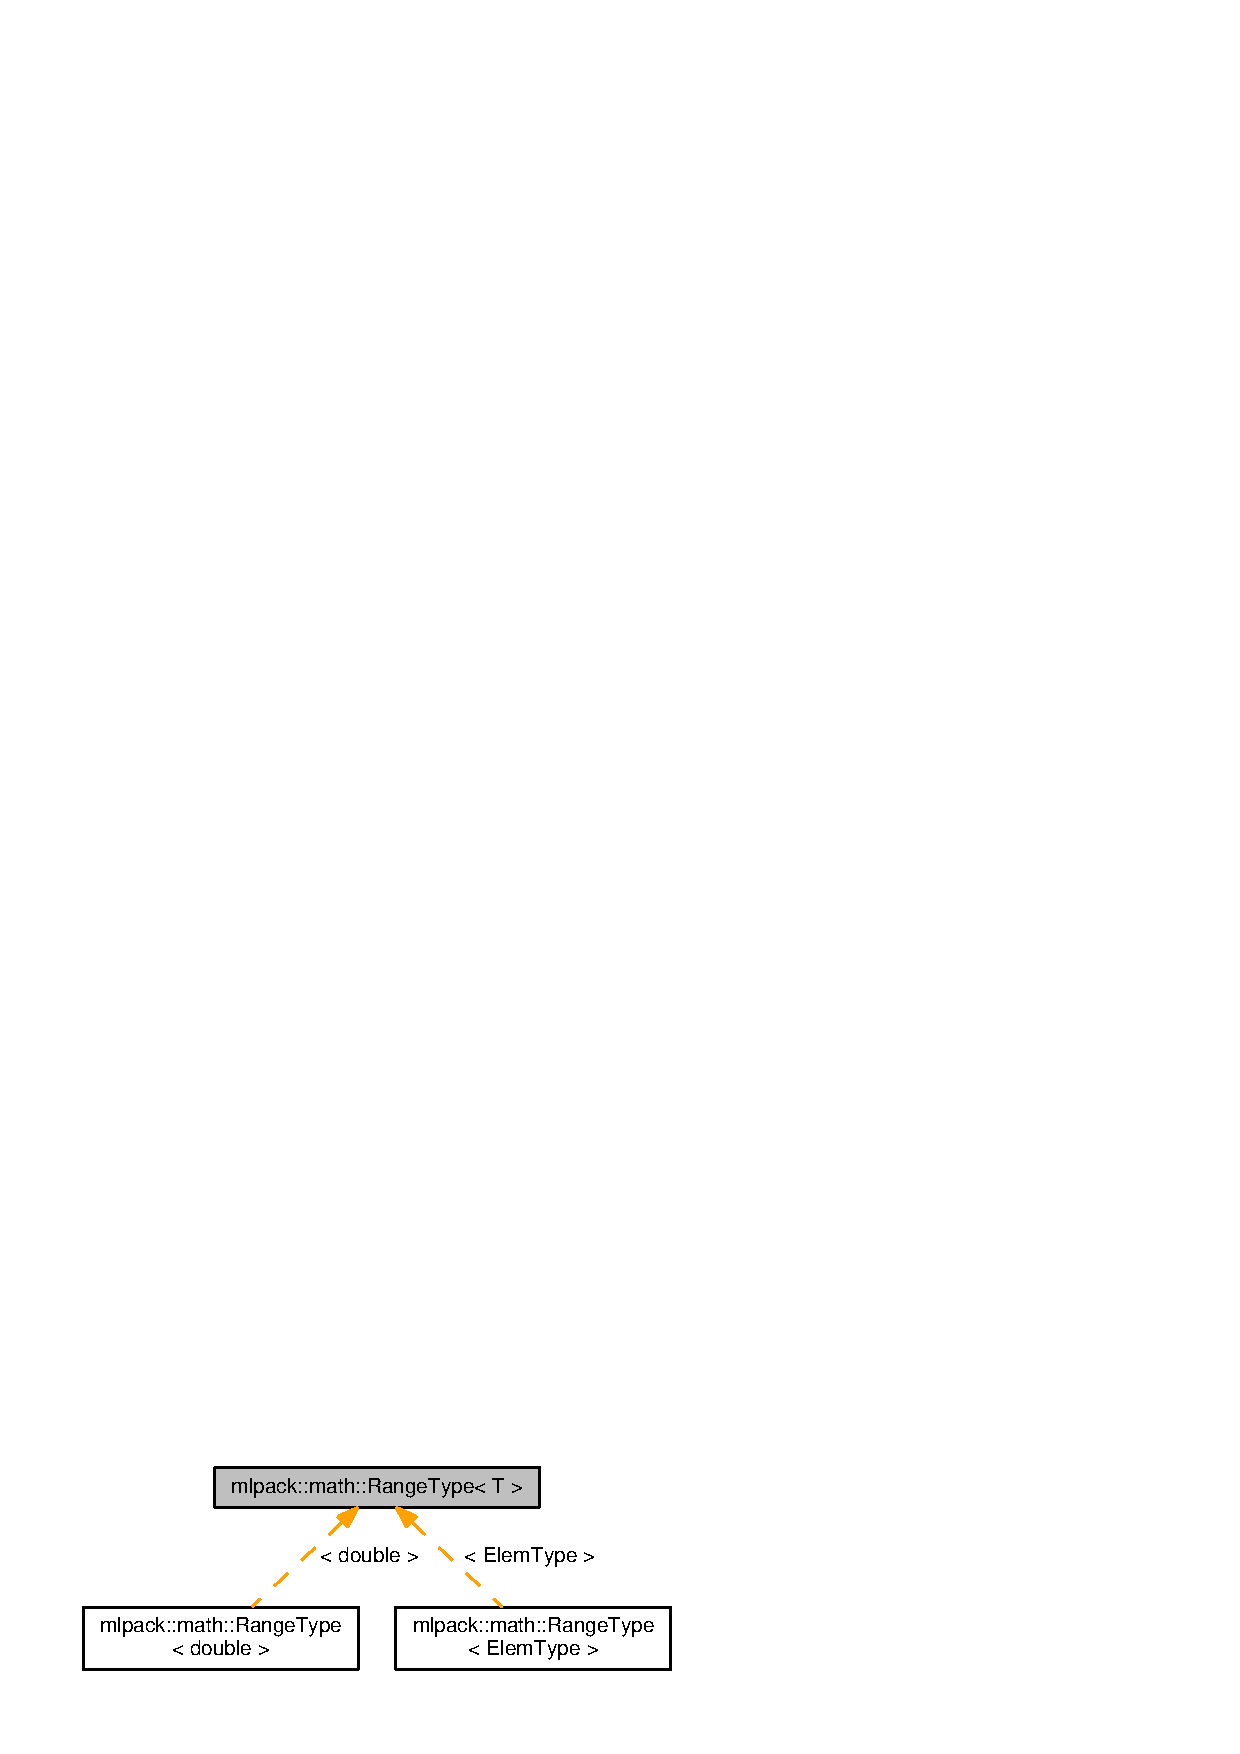
\includegraphics[width=326pt]{classmlpack_1_1math_1_1RangeType__inherit__graph}
\end{center}
\end{figure}
\subsection*{Public Member Functions}
\begin{DoxyCompactItemize}
\item 
{\bf Range\+Type} ()
\begin{DoxyCompactList}\small\item\em The upper bound. \end{DoxyCompactList}\item 
{\bf Range\+Type} (const T point)
\item 
{\bf Range\+Type} (const T {\bf lo}, const T {\bf hi})
\begin{DoxyCompactList}\small\item\em Initializes to specified range. \end{DoxyCompactList}\item 
bool {\bf Contains} (const T d) const 
\begin{DoxyCompactList}\small\item\em Determines if a point is contained within the range. \end{DoxyCompactList}\item 
bool {\bf Contains} (const {\bf Range\+Type} \&r) const 
\begin{DoxyCompactList}\small\item\em Determines if another range overlaps with this one. \end{DoxyCompactList}\item 
T {\bf Hi} () const 
\begin{DoxyCompactList}\small\item\em Get the upper bound. \end{DoxyCompactList}\item 
T \& {\bf Hi} ()
\begin{DoxyCompactList}\small\item\em Modify the upper bound. \end{DoxyCompactList}\item 
T {\bf Lo} () const 
\begin{DoxyCompactList}\small\item\em Get the lower bound. \end{DoxyCompactList}\item 
T \& {\bf Lo} ()
\begin{DoxyCompactList}\small\item\em Modify the lower bound. \end{DoxyCompactList}\item 
T {\bf Mid} () const 
\begin{DoxyCompactList}\small\item\em Gets the midpoint of this range. \end{DoxyCompactList}\item 
bool {\bf operator!=} (const {\bf Range\+Type} \&rhs) const 
\begin{DoxyCompactList}\small\item\em Compare with another range for strict equality. \end{DoxyCompactList}\item 
{\bf Range\+Type} {\bf operator\&} (const {\bf Range\+Type} \&rhs) const 
\begin{DoxyCompactList}\small\item\em Shrinks this range to be the overlap with another range; this makes an empty set if there is no overlap. \end{DoxyCompactList}\item 
{\bf Range\+Type} \& {\bf operator\&=} (const {\bf Range\+Type} \&rhs)
\begin{DoxyCompactList}\small\item\em Shrinks this range to be the overlap with another range; this makes an empty set if there is no overlap. \end{DoxyCompactList}\item 
{\bf Range\+Type} {\bf operator$\ast$} (const T d) const 
\begin{DoxyCompactList}\small\item\em Scale the bounds by the given double. \end{DoxyCompactList}\item 
{\bf Range\+Type} \& {\bf operator$\ast$=} (const T d)
\begin{DoxyCompactList}\small\item\em Scale the bounds by the given double. \end{DoxyCompactList}\item 
bool {\bf operator$<$} (const {\bf Range\+Type} \&rhs) const 
\begin{DoxyCompactList}\small\item\em Compare with another range. \end{DoxyCompactList}\item 
bool {\bf operator==} (const {\bf Range\+Type} \&rhs) const 
\begin{DoxyCompactList}\small\item\em Compare with another range for strict equality. \end{DoxyCompactList}\item 
bool {\bf operator$>$} (const {\bf Range\+Type} \&rhs) const 
\begin{DoxyCompactList}\small\item\em Compare with another range. \end{DoxyCompactList}\item 
{\bf Range\+Type} {\bf operator$\vert$} (const {\bf Range\+Type} \&rhs) const 
\begin{DoxyCompactList}\small\item\em Expands this range to include another range. \end{DoxyCompactList}\item 
{\bf Range\+Type} \& {\bf operator$\vert$=} (const {\bf Range\+Type} \&rhs)
\begin{DoxyCompactList}\small\item\em Expands this range to include another range. \end{DoxyCompactList}\item 
{\footnotesize template$<$typename Archive $>$ }\\void {\bf Serialize} (Archive \&ar, const unsigned int version)
\begin{DoxyCompactList}\small\item\em Serialize the range object. \end{DoxyCompactList}\item 
T {\bf Width} () const 
\begin{DoxyCompactList}\small\item\em Gets the span of the range (hi -\/ lo). \end{DoxyCompactList}\end{DoxyCompactItemize}
\subsection*{Private Attributes}
\begin{DoxyCompactItemize}
\item 
T {\bf hi}
\begin{DoxyCompactList}\small\item\em The lower bound. \end{DoxyCompactList}\item 
T {\bf lo}
\end{DoxyCompactItemize}
\subsection*{Friends}
\begin{DoxyCompactItemize}
\item 
{\footnotesize template$<$typename TT $>$ }\\{\bf Range\+Type}$<$ TT $>$ {\bf operator$\ast$} (const TT d, const {\bf Range\+Type}$<$ TT $>$ \&r)
\begin{DoxyCompactList}\small\item\em Scale the bounds by the given double. \end{DoxyCompactList}\end{DoxyCompactItemize}


\subsection{Detailed Description}
\subsubsection*{template$<$typename T = double$>$\\*
class mlpack\+::math\+::\+Range\+Type$<$ T $>$}

Simple real-\/valued range. 

It contains an upper and lower bound.

Note that until mlpack 3.\+0.\+0, this class is named Range\+Type$<$$>$ and for the specification where T is double, you can use \doxyref{math\+::\+Range}{p.}{namespacemlpack_1_1math_a927179bb8d2d0fb6164df385ab51cbce}. As of mlpack 3.\+0.\+0, this class will be renamed \doxyref{math\+::\+Range$<$$>$}{p.}{namespacemlpack_1_1math_a927179bb8d2d0fb6164df385ab51cbce}.


\begin{DoxyTemplParams}{Template Parameters}
{\em T} & type of element held by this range. \\
\hline
\end{DoxyTemplParams}


Definition at line 19 of file range.\+hpp.



\subsection{Constructor \& Destructor Documentation}
\index{mlpack\+::math\+::\+Range\+Type@{mlpack\+::math\+::\+Range\+Type}!Range\+Type@{Range\+Type}}
\index{Range\+Type@{Range\+Type}!mlpack\+::math\+::\+Range\+Type@{mlpack\+::math\+::\+Range\+Type}}
\subsubsection[{Range\+Type()}]{\setlength{\rightskip}{0pt plus 5cm}template$<$typename T = double$>$ {\bf mlpack\+::math\+::\+Range\+Type}$<$ T $>$\+::{\bf Range\+Type} (
\begin{DoxyParamCaption}
{}
\end{DoxyParamCaption}
)\hspace{0.3cm}{\ttfamily [inline]}}\label{classmlpack_1_1math_1_1RangeType_aa9dc5e0da2aa57a1fac8674ab6ba7636}


The upper bound. 

Initialize to an empty set (where lo $>$ hi). \index{mlpack\+::math\+::\+Range\+Type@{mlpack\+::math\+::\+Range\+Type}!Range\+Type@{Range\+Type}}
\index{Range\+Type@{Range\+Type}!mlpack\+::math\+::\+Range\+Type@{mlpack\+::math\+::\+Range\+Type}}
\subsubsection[{Range\+Type(const T point)}]{\setlength{\rightskip}{0pt plus 5cm}template$<$typename T = double$>$ {\bf mlpack\+::math\+::\+Range\+Type}$<$ T $>$\+::{\bf Range\+Type} (
\begin{DoxyParamCaption}
\item[{const T}]{point}
\end{DoxyParamCaption}
)\hspace{0.3cm}{\ttfamily [inline]}}\label{classmlpack_1_1math_1_1RangeType_a8ec3ab4774569ce2707310e112444741}
\index{mlpack\+::math\+::\+Range\+Type@{mlpack\+::math\+::\+Range\+Type}!Range\+Type@{Range\+Type}}
\index{Range\+Type@{Range\+Type}!mlpack\+::math\+::\+Range\+Type@{mlpack\+::math\+::\+Range\+Type}}
\subsubsection[{Range\+Type(const T lo, const T hi)}]{\setlength{\rightskip}{0pt plus 5cm}template$<$typename T = double$>$ {\bf mlpack\+::math\+::\+Range\+Type}$<$ T $>$\+::{\bf Range\+Type} (
\begin{DoxyParamCaption}
\item[{const T}]{lo, }
\item[{const T}]{hi}
\end{DoxyParamCaption}
)\hspace{0.3cm}{\ttfamily [inline]}}\label{classmlpack_1_1math_1_1RangeType_a279d9692c6e47a51aa663efb2aeb78ce}


Initializes to specified range. 


\begin{DoxyParams}{Parameters}
{\em lo} & Lower bound of the range. \\
\hline
{\em hi} & Upper bound of the range. \\
\hline
\end{DoxyParams}


\subsection{Member Function Documentation}
\index{mlpack\+::math\+::\+Range\+Type@{mlpack\+::math\+::\+Range\+Type}!Contains@{Contains}}
\index{Contains@{Contains}!mlpack\+::math\+::\+Range\+Type@{mlpack\+::math\+::\+Range\+Type}}
\subsubsection[{Contains(const T d) const }]{\setlength{\rightskip}{0pt plus 5cm}template$<$typename T = double$>$ bool {\bf mlpack\+::math\+::\+Range\+Type}$<$ T $>$\+::Contains (
\begin{DoxyParamCaption}
\item[{const T}]{d}
\end{DoxyParamCaption}
) const\hspace{0.3cm}{\ttfamily [inline]}}\label{classmlpack_1_1math_1_1RangeType_ab8bab8c1f83b6913e7ab23093318139e}


Determines if a point is contained within the range. 


\begin{DoxyParams}{Parameters}
{\em d} & Point to check. \\
\hline
\end{DoxyParams}


Referenced by mlpack\+::math\+::\+Range\+Type$<$ Elem\+Type $>$\+::\+Hi().

\index{mlpack\+::math\+::\+Range\+Type@{mlpack\+::math\+::\+Range\+Type}!Contains@{Contains}}
\index{Contains@{Contains}!mlpack\+::math\+::\+Range\+Type@{mlpack\+::math\+::\+Range\+Type}}
\subsubsection[{Contains(const Range\+Type \&r) const }]{\setlength{\rightskip}{0pt plus 5cm}template$<$typename T = double$>$ bool {\bf mlpack\+::math\+::\+Range\+Type}$<$ T $>$\+::Contains (
\begin{DoxyParamCaption}
\item[{const {\bf Range\+Type}$<$ T $>$ \&}]{r}
\end{DoxyParamCaption}
) const\hspace{0.3cm}{\ttfamily [inline]}}\label{classmlpack_1_1math_1_1RangeType_ad91099415ee2fc8629f25494a6c9e9e7}


Determines if another range overlaps with this one. 


\begin{DoxyParams}{Parameters}
{\em r} & Other range.\\
\hline
\end{DoxyParams}
\begin{DoxyReturn}{Returns}
true if ranges overlap at all. 
\end{DoxyReturn}
\index{mlpack\+::math\+::\+Range\+Type@{mlpack\+::math\+::\+Range\+Type}!Hi@{Hi}}
\index{Hi@{Hi}!mlpack\+::math\+::\+Range\+Type@{mlpack\+::math\+::\+Range\+Type}}
\subsubsection[{Hi() const }]{\setlength{\rightskip}{0pt plus 5cm}template$<$typename T = double$>$ T {\bf mlpack\+::math\+::\+Range\+Type}$<$ T $>$\+::Hi (
\begin{DoxyParamCaption}
{}
\end{DoxyParamCaption}
) const\hspace{0.3cm}{\ttfamily [inline]}}\label{classmlpack_1_1math_1_1RangeType_a30320a27a7fca811aa0c42be3d759489}


Get the upper bound. 



Definition at line 66 of file range.\+hpp.



Referenced by mlpack\+::bound\+::\+Hollow\+Ball\+Bound$<$ T\+Metric\+Type, Elem\+Type $>$\+::\+Diameter(), mlpack\+::bound\+::\+Hollow\+Ball\+Bound$<$ T\+Metric\+Type, Elem\+Type $>$\+::\+Min\+Width(), and mlpack\+::bound\+::\+Hollow\+Ball\+Bound$<$ T\+Metric\+Type, Elem\+Type $>$\+::\+Outer\+Radius().

\index{mlpack\+::math\+::\+Range\+Type@{mlpack\+::math\+::\+Range\+Type}!Hi@{Hi}}
\index{Hi@{Hi}!mlpack\+::math\+::\+Range\+Type@{mlpack\+::math\+::\+Range\+Type}}
\subsubsection[{Hi()}]{\setlength{\rightskip}{0pt plus 5cm}template$<$typename T = double$>$ T\& {\bf mlpack\+::math\+::\+Range\+Type}$<$ T $>$\+::Hi (
\begin{DoxyParamCaption}
{}
\end{DoxyParamCaption}
)\hspace{0.3cm}{\ttfamily [inline]}}\label{classmlpack_1_1math_1_1RangeType_aa50f33f01e11870cc915ce8b81826a9a}


Modify the upper bound. 



Definition at line 68 of file range.\+hpp.

\index{mlpack\+::math\+::\+Range\+Type@{mlpack\+::math\+::\+Range\+Type}!Lo@{Lo}}
\index{Lo@{Lo}!mlpack\+::math\+::\+Range\+Type@{mlpack\+::math\+::\+Range\+Type}}
\subsubsection[{Lo() const }]{\setlength{\rightskip}{0pt plus 5cm}template$<$typename T = double$>$ T {\bf mlpack\+::math\+::\+Range\+Type}$<$ T $>$\+::Lo (
\begin{DoxyParamCaption}
{}
\end{DoxyParamCaption}
) const\hspace{0.3cm}{\ttfamily [inline]}}\label{classmlpack_1_1math_1_1RangeType_affdaad3db9564b758adcb1c483be352d}


Get the lower bound. 



Definition at line 61 of file range.\+hpp.



Referenced by mlpack\+::bound\+::\+Hollow\+Ball\+Bound$<$ T\+Metric\+Type, Elem\+Type $>$\+::\+Inner\+Radius().

\index{mlpack\+::math\+::\+Range\+Type@{mlpack\+::math\+::\+Range\+Type}!Lo@{Lo}}
\index{Lo@{Lo}!mlpack\+::math\+::\+Range\+Type@{mlpack\+::math\+::\+Range\+Type}}
\subsubsection[{Lo()}]{\setlength{\rightskip}{0pt plus 5cm}template$<$typename T = double$>$ T\& {\bf mlpack\+::math\+::\+Range\+Type}$<$ T $>$\+::Lo (
\begin{DoxyParamCaption}
{}
\end{DoxyParamCaption}
)\hspace{0.3cm}{\ttfamily [inline]}}\label{classmlpack_1_1math_1_1RangeType_a964e83a1e46ee5f1a9da64298b3130bc}


Modify the lower bound. 



Definition at line 63 of file range.\+hpp.

\index{mlpack\+::math\+::\+Range\+Type@{mlpack\+::math\+::\+Range\+Type}!Mid@{Mid}}
\index{Mid@{Mid}!mlpack\+::math\+::\+Range\+Type@{mlpack\+::math\+::\+Range\+Type}}
\subsubsection[{Mid() const }]{\setlength{\rightskip}{0pt plus 5cm}template$<$typename T = double$>$ T {\bf mlpack\+::math\+::\+Range\+Type}$<$ T $>$\+::Mid (
\begin{DoxyParamCaption}
{}
\end{DoxyParamCaption}
) const\hspace{0.3cm}{\ttfamily [inline]}}\label{classmlpack_1_1math_1_1RangeType_afe79cfa514b739081ca9b95621762ba2}


Gets the midpoint of this range. 



Referenced by mlpack\+::math\+::\+Range\+Type$<$ Elem\+Type $>$\+::\+Hi().

\index{mlpack\+::math\+::\+Range\+Type@{mlpack\+::math\+::\+Range\+Type}!operator"!=@{operator"!=}}
\index{operator"!=@{operator"!=}!mlpack\+::math\+::\+Range\+Type@{mlpack\+::math\+::\+Range\+Type}}
\subsubsection[{operator"!=(const Range\+Type \&rhs) const }]{\setlength{\rightskip}{0pt plus 5cm}template$<$typename T = double$>$ bool {\bf mlpack\+::math\+::\+Range\+Type}$<$ T $>$\+::operator!= (
\begin{DoxyParamCaption}
\item[{const {\bf Range\+Type}$<$ T $>$ \&}]{rhs}
\end{DoxyParamCaption}
) const\hspace{0.3cm}{\ttfamily [inline]}}\label{classmlpack_1_1math_1_1RangeType_a845fd008ffe87bdcb1d6dd2d67cf03f3}


Compare with another range for strict equality. 


\begin{DoxyParams}{Parameters}
{\em rhs} & Other range. \\
\hline
\end{DoxyParams}


Referenced by mlpack\+::math\+::\+Range\+Type$<$ Elem\+Type $>$\+::\+Hi().

\index{mlpack\+::math\+::\+Range\+Type@{mlpack\+::math\+::\+Range\+Type}!operator\&@{operator\&}}
\index{operator\&@{operator\&}!mlpack\+::math\+::\+Range\+Type@{mlpack\+::math\+::\+Range\+Type}}
\subsubsection[{operator\&(const Range\+Type \&rhs) const }]{\setlength{\rightskip}{0pt plus 5cm}template$<$typename T = double$>$ {\bf Range\+Type} {\bf mlpack\+::math\+::\+Range\+Type}$<$ T $>$\+::operator\& (
\begin{DoxyParamCaption}
\item[{const {\bf Range\+Type}$<$ T $>$ \&}]{rhs}
\end{DoxyParamCaption}
) const\hspace{0.3cm}{\ttfamily [inline]}}\label{classmlpack_1_1math_1_1RangeType_a964656d2d3d2f8d34ba4fbe2bbccff4f}


Shrinks this range to be the overlap with another range; this makes an empty set if there is no overlap. 


\begin{DoxyParams}{Parameters}
{\em rhs} & Other range. \\
\hline
\end{DoxyParams}


Referenced by mlpack\+::math\+::\+Range\+Type$<$ Elem\+Type $>$\+::\+Hi().

\index{mlpack\+::math\+::\+Range\+Type@{mlpack\+::math\+::\+Range\+Type}!operator\&=@{operator\&=}}
\index{operator\&=@{operator\&=}!mlpack\+::math\+::\+Range\+Type@{mlpack\+::math\+::\+Range\+Type}}
\subsubsection[{operator\&=(const Range\+Type \&rhs)}]{\setlength{\rightskip}{0pt plus 5cm}template$<$typename T = double$>$ {\bf Range\+Type}\& {\bf mlpack\+::math\+::\+Range\+Type}$<$ T $>$\+::operator\&= (
\begin{DoxyParamCaption}
\item[{const {\bf Range\+Type}$<$ T $>$ \&}]{rhs}
\end{DoxyParamCaption}
)\hspace{0.3cm}{\ttfamily [inline]}}\label{classmlpack_1_1math_1_1RangeType_affe6e9c2dccdef8af887f4e405afe4ce}


Shrinks this range to be the overlap with another range; this makes an empty set if there is no overlap. 


\begin{DoxyParams}{Parameters}
{\em rhs} & Other range. \\
\hline
\end{DoxyParams}


Referenced by mlpack\+::math\+::\+Range\+Type$<$ Elem\+Type $>$\+::\+Hi().

\index{mlpack\+::math\+::\+Range\+Type@{mlpack\+::math\+::\+Range\+Type}!operator$\ast$@{operator$\ast$}}
\index{operator$\ast$@{operator$\ast$}!mlpack\+::math\+::\+Range\+Type@{mlpack\+::math\+::\+Range\+Type}}
\subsubsection[{operator$\ast$(const T d) const }]{\setlength{\rightskip}{0pt plus 5cm}template$<$typename T = double$>$ {\bf Range\+Type} {\bf mlpack\+::math\+::\+Range\+Type}$<$ T $>$\+::operator$\ast$ (
\begin{DoxyParamCaption}
\item[{const T}]{d}
\end{DoxyParamCaption}
) const\hspace{0.3cm}{\ttfamily [inline]}}\label{classmlpack_1_1math_1_1RangeType_a1abe16789fa26c947a0d72f87f1cd605}


Scale the bounds by the given double. 


\begin{DoxyParams}{Parameters}
{\em d} & Scaling factor. \\
\hline
\end{DoxyParams}


Referenced by mlpack\+::math\+::\+Range\+Type$<$ Elem\+Type $>$\+::\+Hi().

\index{mlpack\+::math\+::\+Range\+Type@{mlpack\+::math\+::\+Range\+Type}!operator$\ast$=@{operator$\ast$=}}
\index{operator$\ast$=@{operator$\ast$=}!mlpack\+::math\+::\+Range\+Type@{mlpack\+::math\+::\+Range\+Type}}
\subsubsection[{operator$\ast$=(const T d)}]{\setlength{\rightskip}{0pt plus 5cm}template$<$typename T = double$>$ {\bf Range\+Type}\& {\bf mlpack\+::math\+::\+Range\+Type}$<$ T $>$\+::operator$\ast$= (
\begin{DoxyParamCaption}
\item[{const T}]{d}
\end{DoxyParamCaption}
)\hspace{0.3cm}{\ttfamily [inline]}}\label{classmlpack_1_1math_1_1RangeType_ae138a96e1149bc8c925a4ebe32a9182b}


Scale the bounds by the given double. 


\begin{DoxyParams}{Parameters}
{\em d} & Scaling factor. \\
\hline
\end{DoxyParams}


Referenced by mlpack\+::math\+::\+Range\+Type$<$ Elem\+Type $>$\+::\+Hi().

\index{mlpack\+::math\+::\+Range\+Type@{mlpack\+::math\+::\+Range\+Type}!operator$<$@{operator$<$}}
\index{operator$<$@{operator$<$}!mlpack\+::math\+::\+Range\+Type@{mlpack\+::math\+::\+Range\+Type}}
\subsubsection[{operator$<$(const Range\+Type \&rhs) const }]{\setlength{\rightskip}{0pt plus 5cm}template$<$typename T = double$>$ bool {\bf mlpack\+::math\+::\+Range\+Type}$<$ T $>$\+::operator$<$ (
\begin{DoxyParamCaption}
\item[{const {\bf Range\+Type}$<$ T $>$ \&}]{rhs}
\end{DoxyParamCaption}
) const\hspace{0.3cm}{\ttfamily [inline]}}\label{classmlpack_1_1math_1_1RangeType_af176272d1a5c2392bbaecb16bed70a67}


Compare with another range. 

For Range objects x and y, x $<$ y means that x is strictly less than y and does not overlap at all.


\begin{DoxyParams}{Parameters}
{\em rhs} & Other range. \\
\hline
\end{DoxyParams}


Referenced by mlpack\+::math\+::\+Range\+Type$<$ Elem\+Type $>$\+::\+Hi().

\index{mlpack\+::math\+::\+Range\+Type@{mlpack\+::math\+::\+Range\+Type}!operator==@{operator==}}
\index{operator==@{operator==}!mlpack\+::math\+::\+Range\+Type@{mlpack\+::math\+::\+Range\+Type}}
\subsubsection[{operator==(const Range\+Type \&rhs) const }]{\setlength{\rightskip}{0pt plus 5cm}template$<$typename T = double$>$ bool {\bf mlpack\+::math\+::\+Range\+Type}$<$ T $>$\+::operator== (
\begin{DoxyParamCaption}
\item[{const {\bf Range\+Type}$<$ T $>$ \&}]{rhs}
\end{DoxyParamCaption}
) const\hspace{0.3cm}{\ttfamily [inline]}}\label{classmlpack_1_1math_1_1RangeType_a40acac41f9e9868a695d2ae119086949}


Compare with another range for strict equality. 


\begin{DoxyParams}{Parameters}
{\em rhs} & Other range. \\
\hline
\end{DoxyParams}


Referenced by mlpack\+::math\+::\+Range\+Type$<$ Elem\+Type $>$\+::\+Hi().

\index{mlpack\+::math\+::\+Range\+Type@{mlpack\+::math\+::\+Range\+Type}!operator$>$@{operator$>$}}
\index{operator$>$@{operator$>$}!mlpack\+::math\+::\+Range\+Type@{mlpack\+::math\+::\+Range\+Type}}
\subsubsection[{operator$>$(const Range\+Type \&rhs) const }]{\setlength{\rightskip}{0pt plus 5cm}template$<$typename T = double$>$ bool {\bf mlpack\+::math\+::\+Range\+Type}$<$ T $>$\+::operator$>$ (
\begin{DoxyParamCaption}
\item[{const {\bf Range\+Type}$<$ T $>$ \&}]{rhs}
\end{DoxyParamCaption}
) const\hspace{0.3cm}{\ttfamily [inline]}}\label{classmlpack_1_1math_1_1RangeType_a38b646ce7331c861a4c732382b35a3e3}


Compare with another range. 

For Range objects x and y, x $<$ y means that x is strictly less than y and does not overlap at all.


\begin{DoxyParams}{Parameters}
{\em rhs} & Other range. \\
\hline
\end{DoxyParams}


Referenced by mlpack\+::math\+::\+Range\+Type$<$ Elem\+Type $>$\+::\+Hi().

\index{mlpack\+::math\+::\+Range\+Type@{mlpack\+::math\+::\+Range\+Type}!operator\texttt{"|}@{operator\texttt{"|}}}
\index{operator\texttt{"|}@{operator\texttt{"|}}!mlpack\+::math\+::\+Range\+Type@{mlpack\+::math\+::\+Range\+Type}}
\subsubsection[{operator\texttt{"|}(const Range\+Type \&rhs) const }]{\setlength{\rightskip}{0pt plus 5cm}template$<$typename T = double$>$ {\bf Range\+Type} {\bf mlpack\+::math\+::\+Range\+Type}$<$ T $>$\+::operator$\vert$ (
\begin{DoxyParamCaption}
\item[{const {\bf Range\+Type}$<$ T $>$ \&}]{rhs}
\end{DoxyParamCaption}
) const\hspace{0.3cm}{\ttfamily [inline]}}\label{classmlpack_1_1math_1_1RangeType_aa950e53b4fd6a990fba3fd30c8cab9a5}


Expands this range to include another range. 


\begin{DoxyParams}{Parameters}
{\em rhs} & Range to include. \\
\hline
\end{DoxyParams}


Referenced by mlpack\+::math\+::\+Range\+Type$<$ Elem\+Type $>$\+::\+Hi().

\index{mlpack\+::math\+::\+Range\+Type@{mlpack\+::math\+::\+Range\+Type}!operator\texttt{"|}=@{operator\texttt{"|}=}}
\index{operator\texttt{"|}=@{operator\texttt{"|}=}!mlpack\+::math\+::\+Range\+Type@{mlpack\+::math\+::\+Range\+Type}}
\subsubsection[{operator\texttt{"|}=(const Range\+Type \&rhs)}]{\setlength{\rightskip}{0pt plus 5cm}template$<$typename T = double$>$ {\bf Range\+Type}\& {\bf mlpack\+::math\+::\+Range\+Type}$<$ T $>$\+::operator$\vert$= (
\begin{DoxyParamCaption}
\item[{const {\bf Range\+Type}$<$ T $>$ \&}]{rhs}
\end{DoxyParamCaption}
)\hspace{0.3cm}{\ttfamily [inline]}}\label{classmlpack_1_1math_1_1RangeType_ae0fa05a40cc26e2262e01e39687c8cfc}


Expands this range to include another range. 


\begin{DoxyParams}{Parameters}
{\em rhs} & Range to include. \\
\hline
\end{DoxyParams}


Referenced by mlpack\+::math\+::\+Range\+Type$<$ Elem\+Type $>$\+::\+Hi().

\index{mlpack\+::math\+::\+Range\+Type@{mlpack\+::math\+::\+Range\+Type}!Serialize@{Serialize}}
\index{Serialize@{Serialize}!mlpack\+::math\+::\+Range\+Type@{mlpack\+::math\+::\+Range\+Type}}
\subsubsection[{Serialize(\+Archive \&ar, const unsigned int version)}]{\setlength{\rightskip}{0pt plus 5cm}template$<$typename T = double$>$ template$<$typename Archive $>$ void {\bf mlpack\+::math\+::\+Range\+Type}$<$ T $>$\+::Serialize (
\begin{DoxyParamCaption}
\item[{Archive \&}]{ar, }
\item[{const unsigned int}]{version}
\end{DoxyParamCaption}
)}\label{classmlpack_1_1math_1_1RangeType_afc2f3c72daf9eed64c999bf25281c55f}


Serialize the range object. 



Referenced by mlpack\+::math\+::\+Range\+Type$<$ Elem\+Type $>$\+::\+Hi().

\index{mlpack\+::math\+::\+Range\+Type@{mlpack\+::math\+::\+Range\+Type}!Width@{Width}}
\index{Width@{Width}!mlpack\+::math\+::\+Range\+Type@{mlpack\+::math\+::\+Range\+Type}}
\subsubsection[{Width() const }]{\setlength{\rightskip}{0pt plus 5cm}template$<$typename T = double$>$ T {\bf mlpack\+::math\+::\+Range\+Type}$<$ T $>$\+::Width (
\begin{DoxyParamCaption}
{}
\end{DoxyParamCaption}
) const\hspace{0.3cm}{\ttfamily [inline]}}\label{classmlpack_1_1math_1_1RangeType_ad5ad509adcaf1ce2d364abc270e658f0}


Gets the span of the range (hi -\/ lo). 



Referenced by mlpack\+::math\+::\+Range\+Type$<$ Elem\+Type $>$\+::\+Hi().



\subsection{Friends And Related Function Documentation}
\index{mlpack\+::math\+::\+Range\+Type@{mlpack\+::math\+::\+Range\+Type}!operator$\ast$@{operator$\ast$}}
\index{operator$\ast$@{operator$\ast$}!mlpack\+::math\+::\+Range\+Type@{mlpack\+::math\+::\+Range\+Type}}
\subsubsection[{operator$\ast$}]{\setlength{\rightskip}{0pt plus 5cm}template$<$typename T = double$>$ template$<$typename TT $>$ {\bf Range\+Type}$<$TT$>$ operator$\ast$ (
\begin{DoxyParamCaption}
\item[{const TT}]{d, }
\item[{const {\bf Range\+Type}$<$ TT $>$ \&}]{r}
\end{DoxyParamCaption}
)\hspace{0.3cm}{\ttfamily [friend]}}\label{classmlpack_1_1math_1_1RangeType_acbe6947af2537dd97b592d55e0b51f85}


Scale the bounds by the given double. 


\begin{DoxyParams}{Parameters}
{\em d} & Scaling factor. \\
\hline
\end{DoxyParams}


\subsection{Member Data Documentation}
\index{mlpack\+::math\+::\+Range\+Type@{mlpack\+::math\+::\+Range\+Type}!hi@{hi}}
\index{hi@{hi}!mlpack\+::math\+::\+Range\+Type@{mlpack\+::math\+::\+Range\+Type}}
\subsubsection[{hi}]{\setlength{\rightskip}{0pt plus 5cm}template$<$typename T = double$>$ T {\bf mlpack\+::math\+::\+Range\+Type}$<$ T $>$\+::hi\hspace{0.3cm}{\ttfamily [private]}}\label{classmlpack_1_1math_1_1RangeType_a45f06704de97b24f0b83aa5ff2ebcac5}


The lower bound. 



Definition at line 38 of file range.\+hpp.



Referenced by mlpack\+::math\+::\+Range\+Type$<$ Elem\+Type $>$\+::\+Hi().

\index{mlpack\+::math\+::\+Range\+Type@{mlpack\+::math\+::\+Range\+Type}!lo@{lo}}
\index{lo@{lo}!mlpack\+::math\+::\+Range\+Type@{mlpack\+::math\+::\+Range\+Type}}
\subsubsection[{lo}]{\setlength{\rightskip}{0pt plus 5cm}template$<$typename T = double$>$ T {\bf mlpack\+::math\+::\+Range\+Type}$<$ T $>$\+::lo\hspace{0.3cm}{\ttfamily [private]}}\label{classmlpack_1_1math_1_1RangeType_a57179131bdd1f7eae0ed22e7f0914a81}


Definition at line 37 of file range.\+hpp.



Referenced by mlpack\+::math\+::\+Range\+Type$<$ Elem\+Type $>$\+::\+Lo().



The documentation for this class was generated from the following file\+:\begin{DoxyCompactItemize}
\item 
src/mlpack/core/math/{\bf range.\+hpp}\end{DoxyCompactItemize}

\section{mlpack\+:\+:matrix\+\_\+completion\+:\+:Matrix\+Completion Class Reference}
\label{classmlpack_1_1matrix__completion_1_1MatrixCompletion}\index{mlpack\+::matrix\+\_\+completion\+::\+Matrix\+Completion@{mlpack\+::matrix\+\_\+completion\+::\+Matrix\+Completion}}


This class implements the popular nuclear norm minimization heuristic for matrix completion problems.  


\subsection*{Public Member Functions}
\begin{DoxyCompactItemize}
\item 
{\bf Matrix\+Completion} (const size\+\_\+t {\bf m}, const size\+\_\+t {\bf n}, const arma\+::umat \&{\bf indices}, const arma\+::vec \&{\bf values}, const size\+\_\+t r)
\begin{DoxyCompactList}\small\item\em Construct a matrix completion problem, specifying the maximum rank of the solution. \end{DoxyCompactList}\item 
{\bf Matrix\+Completion} (const size\+\_\+t {\bf m}, const size\+\_\+t {\bf n}, const arma\+::umat \&{\bf indices}, const arma\+::vec \&{\bf values}, const arma\+::mat \&initial\+Point)
\begin{DoxyCompactList}\small\item\em Construct a matrix completion problem, specifying the initial point of the optimization. \end{DoxyCompactList}\item 
{\bf Matrix\+Completion} (const size\+\_\+t {\bf m}, const size\+\_\+t {\bf n}, const arma\+::umat \&{\bf indices}, const arma\+::vec \&{\bf values})
\begin{DoxyCompactList}\small\item\em Construct a matrix completion problem. \end{DoxyCompactList}\item 
void {\bf Recover} (arma\+::mat \&recovered)
\begin{DoxyCompactList}\small\item\em Solve the underlying S\+DP to fill in the remaining values. \end{DoxyCompactList}\item 
const {\bf optimization\+::\+L\+R\+S\+DP}$<$ {\bf optimization\+::\+S\+DP}$<$ arma\+::sp\+\_\+mat $>$ $>$ \& {\bf Sdp} () const 
\begin{DoxyCompactList}\small\item\em Return the underlying S\+DP. \end{DoxyCompactList}\item 
{\bf optimization\+::\+L\+R\+S\+DP}$<$ {\bf optimization\+::\+S\+DP}$<$ arma\+::sp\+\_\+mat $>$ $>$ \& {\bf Sdp} ()
\begin{DoxyCompactList}\small\item\em Modify the underlying S\+DP. \end{DoxyCompactList}\end{DoxyCompactItemize}
\subsection*{Private Member Functions}
\begin{DoxyCompactItemize}
\item 
void {\bf Check\+Values} ()
\begin{DoxyCompactList}\small\item\em Validate the input matrices. \end{DoxyCompactList}\item 
void {\bf Init\+S\+DP} ()
\begin{DoxyCompactList}\small\item\em Initialize the S\+DP. \end{DoxyCompactList}\end{DoxyCompactItemize}
\subsection*{Static Private Member Functions}
\begin{DoxyCompactItemize}
\item 
static size\+\_\+t {\bf Default\+Rank} (const size\+\_\+t {\bf m}, const size\+\_\+t {\bf n}, const size\+\_\+t p)
\begin{DoxyCompactList}\small\item\em Select a rank of the matrix given that is of size m x n and has p known elements. \end{DoxyCompactList}\end{DoxyCompactItemize}
\subsection*{Private Attributes}
\begin{DoxyCompactItemize}
\item 
arma\+::umat {\bf indices}
\begin{DoxyCompactList}\small\item\em Matrix containing the indices of the known entries (has two rows). \end{DoxyCompactList}\item 
size\+\_\+t {\bf m}
\begin{DoxyCompactList}\small\item\em Number of rows in original matrix. \end{DoxyCompactList}\item 
size\+\_\+t {\bf n}
\begin{DoxyCompactList}\small\item\em Number of columns in original matrix. \end{DoxyCompactList}\item 
{\bf optimization\+::\+L\+R\+S\+DP}$<$ {\bf optimization\+::\+S\+DP}$<$ arma\+::sp\+\_\+mat $>$ $>$ {\bf sdp}
\begin{DoxyCompactList}\small\item\em The underlying S\+DP to be solved. \end{DoxyCompactList}\item 
arma\+::mat {\bf values}
\begin{DoxyCompactList}\small\item\em Vector containing the values of the known entries. \end{DoxyCompactList}\end{DoxyCompactItemize}


\subsection{Detailed Description}
This class implements the popular nuclear norm minimization heuristic for matrix completion problems. 

That is, given known values M\+\_\+ij\textquotesingle{}s, the following optimization problem (semi-\/definite program) is solved to fill in the remaining unknown values of X

min $\vert$$\vert$\+X$\vert$$\vert$\+\_\+$\ast$ subj to X\+\_\+ij = M\+\_\+ij

where $\vert$$\vert$\+X$\vert$$\vert$\+\_\+$\ast$ denotes the nuclear norm (sum of singular values of X).

For a theoretical treatment of the conditions necessary for exact recovery, see the following paper\+:

A Simpler Appoarch to Matrix Completion. Benjamin Recht. J\+M\+LR 11. {\tt http\+://arxiv.\+org/pdf/0910.\+0651v2.\+pdf}

An example of how to use this class is shown below\+:


\begin{DoxyCode}
\textcolor{keywordtype}{size\_t} m, n;         \textcolor{comment}{// size of unknown matrix}
arma::umat indices;  \textcolor{comment}{// contains the known indices [2 x n\_entries]}
arma::vec values;    \textcolor{comment}{// contains the known values [n\_entries]}
arma::mat recovered; \textcolor{comment}{// will contain the completed matrix}

MatrixCompletion mc(m, n, indices, values);
mc.Recover(recovered);
\end{DoxyCode}


\begin{DoxySeeAlso}{See also}
L\+R\+S\+DP 
\end{DoxySeeAlso}


Definition at line 53 of file matrix\+\_\+completion.\+hpp.



\subsection{Constructor \& Destructor Documentation}
\index{mlpack\+::matrix\+\_\+completion\+::\+Matrix\+Completion@{mlpack\+::matrix\+\_\+completion\+::\+Matrix\+Completion}!Matrix\+Completion@{Matrix\+Completion}}
\index{Matrix\+Completion@{Matrix\+Completion}!mlpack\+::matrix\+\_\+completion\+::\+Matrix\+Completion@{mlpack\+::matrix\+\_\+completion\+::\+Matrix\+Completion}}
\subsubsection[{Matrix\+Completion(const size\+\_\+t m, const size\+\_\+t n, const arma\+::umat \&indices, const arma\+::vec \&values, const size\+\_\+t r)}]{\setlength{\rightskip}{0pt plus 5cm}mlpack\+::matrix\+\_\+completion\+::\+Matrix\+Completion\+::\+Matrix\+Completion (
\begin{DoxyParamCaption}
\item[{const size\+\_\+t}]{m, }
\item[{const size\+\_\+t}]{n, }
\item[{const arma\+::umat \&}]{indices, }
\item[{const arma\+::vec \&}]{values, }
\item[{const size\+\_\+t}]{r}
\end{DoxyParamCaption}
)}\label{classmlpack_1_1matrix__completion_1_1MatrixCompletion_ac10286ac5d7b8ca5e5dd35a35578ead8}


Construct a matrix completion problem, specifying the maximum rank of the solution. 


\begin{DoxyParams}{Parameters}
{\em m} & Number of rows of original matrix. \\
\hline
{\em n} & Number of columns of original matrix. \\
\hline
{\em indices} & Matrix containing the indices of the known entries (must be [2 x p]). \\
\hline
{\em values} & Vector containing the values of the known entries (must be length p). \\
\hline
{\em r} & Maximum rank of solution. \\
\hline
\end{DoxyParams}
\index{mlpack\+::matrix\+\_\+completion\+::\+Matrix\+Completion@{mlpack\+::matrix\+\_\+completion\+::\+Matrix\+Completion}!Matrix\+Completion@{Matrix\+Completion}}
\index{Matrix\+Completion@{Matrix\+Completion}!mlpack\+::matrix\+\_\+completion\+::\+Matrix\+Completion@{mlpack\+::matrix\+\_\+completion\+::\+Matrix\+Completion}}
\subsubsection[{Matrix\+Completion(const size\+\_\+t m, const size\+\_\+t n, const arma\+::umat \&indices, const arma\+::vec \&values, const arma\+::mat \&initial\+Point)}]{\setlength{\rightskip}{0pt plus 5cm}mlpack\+::matrix\+\_\+completion\+::\+Matrix\+Completion\+::\+Matrix\+Completion (
\begin{DoxyParamCaption}
\item[{const size\+\_\+t}]{m, }
\item[{const size\+\_\+t}]{n, }
\item[{const arma\+::umat \&}]{indices, }
\item[{const arma\+::vec \&}]{values, }
\item[{const arma\+::mat \&}]{initial\+Point}
\end{DoxyParamCaption}
)}\label{classmlpack_1_1matrix__completion_1_1MatrixCompletion_ae45afbffa59ab7dffe0416470b891e8c}


Construct a matrix completion problem, specifying the initial point of the optimization. 


\begin{DoxyParams}{Parameters}
{\em m} & Number of rows of original matrix. \\
\hline
{\em n} & Number of columns of original matrix. \\
\hline
{\em indices} & Matrix containing the indices of the known entries (must be [2 x p]). \\
\hline
{\em values} & Vector containing the values of the known entries (must be length p). \\
\hline
{\em initial\+Point} & Starting point for the S\+DP optimization. \\
\hline
\end{DoxyParams}
\index{mlpack\+::matrix\+\_\+completion\+::\+Matrix\+Completion@{mlpack\+::matrix\+\_\+completion\+::\+Matrix\+Completion}!Matrix\+Completion@{Matrix\+Completion}}
\index{Matrix\+Completion@{Matrix\+Completion}!mlpack\+::matrix\+\_\+completion\+::\+Matrix\+Completion@{mlpack\+::matrix\+\_\+completion\+::\+Matrix\+Completion}}
\subsubsection[{Matrix\+Completion(const size\+\_\+t m, const size\+\_\+t n, const arma\+::umat \&indices, const arma\+::vec \&values)}]{\setlength{\rightskip}{0pt plus 5cm}mlpack\+::matrix\+\_\+completion\+::\+Matrix\+Completion\+::\+Matrix\+Completion (
\begin{DoxyParamCaption}
\item[{const size\+\_\+t}]{m, }
\item[{const size\+\_\+t}]{n, }
\item[{const arma\+::umat \&}]{indices, }
\item[{const arma\+::vec \&}]{values}
\end{DoxyParamCaption}
)}\label{classmlpack_1_1matrix__completion_1_1MatrixCompletion_a782331f3bf9dbb03c9e5ccc69e2aa180}


Construct a matrix completion problem. 


\begin{DoxyParams}{Parameters}
{\em m} & Number of rows of original matrix. \\
\hline
{\em n} & Number of columns of original matrix. \\
\hline
{\em indices} & Matrix containing the indices of the known entries (must be [2 x p]). \\
\hline
{\em values} & Vector containing the values of the known entries (must be length p). \\
\hline
\end{DoxyParams}


\subsection{Member Function Documentation}
\index{mlpack\+::matrix\+\_\+completion\+::\+Matrix\+Completion@{mlpack\+::matrix\+\_\+completion\+::\+Matrix\+Completion}!Check\+Values@{Check\+Values}}
\index{Check\+Values@{Check\+Values}!mlpack\+::matrix\+\_\+completion\+::\+Matrix\+Completion@{mlpack\+::matrix\+\_\+completion\+::\+Matrix\+Completion}}
\subsubsection[{Check\+Values()}]{\setlength{\rightskip}{0pt plus 5cm}void mlpack\+::matrix\+\_\+completion\+::\+Matrix\+Completion\+::\+Check\+Values (
\begin{DoxyParamCaption}
{}
\end{DoxyParamCaption}
)\hspace{0.3cm}{\ttfamily [private]}}\label{classmlpack_1_1matrix__completion_1_1MatrixCompletion_a7b9e4dd2ec9b82afb04787e1cdaa90a2}


Validate the input matrices. 

\index{mlpack\+::matrix\+\_\+completion\+::\+Matrix\+Completion@{mlpack\+::matrix\+\_\+completion\+::\+Matrix\+Completion}!Default\+Rank@{Default\+Rank}}
\index{Default\+Rank@{Default\+Rank}!mlpack\+::matrix\+\_\+completion\+::\+Matrix\+Completion@{mlpack\+::matrix\+\_\+completion\+::\+Matrix\+Completion}}
\subsubsection[{Default\+Rank(const size\+\_\+t m, const size\+\_\+t n, const size\+\_\+t p)}]{\setlength{\rightskip}{0pt plus 5cm}static size\+\_\+t mlpack\+::matrix\+\_\+completion\+::\+Matrix\+Completion\+::\+Default\+Rank (
\begin{DoxyParamCaption}
\item[{const size\+\_\+t}]{m, }
\item[{const size\+\_\+t}]{n, }
\item[{const size\+\_\+t}]{p}
\end{DoxyParamCaption}
)\hspace{0.3cm}{\ttfamily [static]}, {\ttfamily [private]}}\label{classmlpack_1_1matrix__completion_1_1MatrixCompletion_a1b40157c16060090be5313913ce9a0a1}


Select a rank of the matrix given that is of size m x n and has p known elements. 

\index{mlpack\+::matrix\+\_\+completion\+::\+Matrix\+Completion@{mlpack\+::matrix\+\_\+completion\+::\+Matrix\+Completion}!Init\+S\+DP@{Init\+S\+DP}}
\index{Init\+S\+DP@{Init\+S\+DP}!mlpack\+::matrix\+\_\+completion\+::\+Matrix\+Completion@{mlpack\+::matrix\+\_\+completion\+::\+Matrix\+Completion}}
\subsubsection[{Init\+S\+D\+P()}]{\setlength{\rightskip}{0pt plus 5cm}void mlpack\+::matrix\+\_\+completion\+::\+Matrix\+Completion\+::\+Init\+S\+DP (
\begin{DoxyParamCaption}
{}
\end{DoxyParamCaption}
)\hspace{0.3cm}{\ttfamily [private]}}\label{classmlpack_1_1matrix__completion_1_1MatrixCompletion_a3145e17b0cbbfbb0a158f38ad3d4cbef}


Initialize the S\+DP. 

\index{mlpack\+::matrix\+\_\+completion\+::\+Matrix\+Completion@{mlpack\+::matrix\+\_\+completion\+::\+Matrix\+Completion}!Recover@{Recover}}
\index{Recover@{Recover}!mlpack\+::matrix\+\_\+completion\+::\+Matrix\+Completion@{mlpack\+::matrix\+\_\+completion\+::\+Matrix\+Completion}}
\subsubsection[{Recover(arma\+::mat \&recovered)}]{\setlength{\rightskip}{0pt plus 5cm}void mlpack\+::matrix\+\_\+completion\+::\+Matrix\+Completion\+::\+Recover (
\begin{DoxyParamCaption}
\item[{arma\+::mat \&}]{recovered}
\end{DoxyParamCaption}
)}\label{classmlpack_1_1matrix__completion_1_1MatrixCompletion_af486903584214c283bc7354e18ce6fbd}


Solve the underlying S\+DP to fill in the remaining values. 


\begin{DoxyParams}{Parameters}
{\em recovered} & Will contain the completed matrix. \\
\hline
\end{DoxyParams}
\index{mlpack\+::matrix\+\_\+completion\+::\+Matrix\+Completion@{mlpack\+::matrix\+\_\+completion\+::\+Matrix\+Completion}!Sdp@{Sdp}}
\index{Sdp@{Sdp}!mlpack\+::matrix\+\_\+completion\+::\+Matrix\+Completion@{mlpack\+::matrix\+\_\+completion\+::\+Matrix\+Completion}}
\subsubsection[{Sdp() const }]{\setlength{\rightskip}{0pt plus 5cm}const {\bf optimization\+::\+L\+R\+S\+DP}$<${\bf optimization\+::\+S\+DP}$<$arma\+::sp\+\_\+mat$>$ $>$\& mlpack\+::matrix\+\_\+completion\+::\+Matrix\+Completion\+::\+Sdp (
\begin{DoxyParamCaption}
{}
\end{DoxyParamCaption}
) const\hspace{0.3cm}{\ttfamily [inline]}}\label{classmlpack_1_1matrix__completion_1_1MatrixCompletion_a6097ff2e54766f26b0e8c33bb7f30a08}


Return the underlying S\+DP. 



Definition at line 115 of file matrix\+\_\+completion.\+hpp.



References sdp.

\index{mlpack\+::matrix\+\_\+completion\+::\+Matrix\+Completion@{mlpack\+::matrix\+\_\+completion\+::\+Matrix\+Completion}!Sdp@{Sdp}}
\index{Sdp@{Sdp}!mlpack\+::matrix\+\_\+completion\+::\+Matrix\+Completion@{mlpack\+::matrix\+\_\+completion\+::\+Matrix\+Completion}}
\subsubsection[{Sdp()}]{\setlength{\rightskip}{0pt plus 5cm}{\bf optimization\+::\+L\+R\+S\+DP}$<${\bf optimization\+::\+S\+DP}$<$arma\+::sp\+\_\+mat$>$ $>$\& mlpack\+::matrix\+\_\+completion\+::\+Matrix\+Completion\+::\+Sdp (
\begin{DoxyParamCaption}
{}
\end{DoxyParamCaption}
)\hspace{0.3cm}{\ttfamily [inline]}}\label{classmlpack_1_1matrix__completion_1_1MatrixCompletion_a37e28472f6e6ea283fddd41c35b9d03c}


Modify the underlying S\+DP. 



Definition at line 117 of file matrix\+\_\+completion.\+hpp.



References sdp.



\subsection{Member Data Documentation}
\index{mlpack\+::matrix\+\_\+completion\+::\+Matrix\+Completion@{mlpack\+::matrix\+\_\+completion\+::\+Matrix\+Completion}!indices@{indices}}
\index{indices@{indices}!mlpack\+::matrix\+\_\+completion\+::\+Matrix\+Completion@{mlpack\+::matrix\+\_\+completion\+::\+Matrix\+Completion}}
\subsubsection[{indices}]{\setlength{\rightskip}{0pt plus 5cm}arma\+::umat mlpack\+::matrix\+\_\+completion\+::\+Matrix\+Completion\+::indices\hspace{0.3cm}{\ttfamily [private]}}\label{classmlpack_1_1matrix__completion_1_1MatrixCompletion_a2966b9f707643aa4775002d6a26af255}


Matrix containing the indices of the known entries (has two rows). 



Definition at line 125 of file matrix\+\_\+completion.\+hpp.

\index{mlpack\+::matrix\+\_\+completion\+::\+Matrix\+Completion@{mlpack\+::matrix\+\_\+completion\+::\+Matrix\+Completion}!m@{m}}
\index{m@{m}!mlpack\+::matrix\+\_\+completion\+::\+Matrix\+Completion@{mlpack\+::matrix\+\_\+completion\+::\+Matrix\+Completion}}
\subsubsection[{m}]{\setlength{\rightskip}{0pt plus 5cm}size\+\_\+t mlpack\+::matrix\+\_\+completion\+::\+Matrix\+Completion\+::m\hspace{0.3cm}{\ttfamily [private]}}\label{classmlpack_1_1matrix__completion_1_1MatrixCompletion_ab0177338a3308b55c52ec2972d93eeb1}


Number of rows in original matrix. 



Definition at line 121 of file matrix\+\_\+completion.\+hpp.

\index{mlpack\+::matrix\+\_\+completion\+::\+Matrix\+Completion@{mlpack\+::matrix\+\_\+completion\+::\+Matrix\+Completion}!n@{n}}
\index{n@{n}!mlpack\+::matrix\+\_\+completion\+::\+Matrix\+Completion@{mlpack\+::matrix\+\_\+completion\+::\+Matrix\+Completion}}
\subsubsection[{n}]{\setlength{\rightskip}{0pt plus 5cm}size\+\_\+t mlpack\+::matrix\+\_\+completion\+::\+Matrix\+Completion\+::n\hspace{0.3cm}{\ttfamily [private]}}\label{classmlpack_1_1matrix__completion_1_1MatrixCompletion_ada1f30af3dd744f73ac4e1802c2bfca2}


Number of columns in original matrix. 



Definition at line 123 of file matrix\+\_\+completion.\+hpp.

\index{mlpack\+::matrix\+\_\+completion\+::\+Matrix\+Completion@{mlpack\+::matrix\+\_\+completion\+::\+Matrix\+Completion}!sdp@{sdp}}
\index{sdp@{sdp}!mlpack\+::matrix\+\_\+completion\+::\+Matrix\+Completion@{mlpack\+::matrix\+\_\+completion\+::\+Matrix\+Completion}}
\subsubsection[{sdp}]{\setlength{\rightskip}{0pt plus 5cm}{\bf optimization\+::\+L\+R\+S\+DP}$<${\bf optimization\+::\+S\+DP}$<$arma\+::sp\+\_\+mat$>$ $>$ mlpack\+::matrix\+\_\+completion\+::\+Matrix\+Completion\+::sdp\hspace{0.3cm}{\ttfamily [private]}}\label{classmlpack_1_1matrix__completion_1_1MatrixCompletion_a3c30c67a9a103697f1cdbf186639d68c}


The underlying S\+DP to be solved. 



Definition at line 130 of file matrix\+\_\+completion.\+hpp.



Referenced by Sdp().

\index{mlpack\+::matrix\+\_\+completion\+::\+Matrix\+Completion@{mlpack\+::matrix\+\_\+completion\+::\+Matrix\+Completion}!values@{values}}
\index{values@{values}!mlpack\+::matrix\+\_\+completion\+::\+Matrix\+Completion@{mlpack\+::matrix\+\_\+completion\+::\+Matrix\+Completion}}
\subsubsection[{values}]{\setlength{\rightskip}{0pt plus 5cm}arma\+::mat mlpack\+::matrix\+\_\+completion\+::\+Matrix\+Completion\+::values\hspace{0.3cm}{\ttfamily [private]}}\label{classmlpack_1_1matrix__completion_1_1MatrixCompletion_a460786684fa309192016bdfef5d4b1c9}


Vector containing the values of the known entries. 



Definition at line 127 of file matrix\+\_\+completion.\+hpp.



The documentation for this class was generated from the following file\+:\begin{DoxyCompactItemize}
\item 
src/mlpack/methods/matrix\+\_\+completion/{\bf matrix\+\_\+completion.\+hpp}\end{DoxyCompactItemize}

\section{Mean\+Shift$<$ Use\+Kernel, Kernel\+Type, Mat\+Type $>$ Class Template Reference}
\label{classmlpack_1_1meanshift_1_1MeanShift}\index{Mean\+Shift$<$ Use\+Kernel, Kernel\+Type, Mat\+Type $>$@{Mean\+Shift$<$ Use\+Kernel, Kernel\+Type, Mat\+Type $>$}}


This class implements mean shift clustering.  


\subsection*{Public Member Functions}
\begin{DoxyCompactItemize}
\item 
\textbf{ Mean\+Shift} (const double radius=0, const size\+\_\+t max\+Iterations=1000, const Kernel\+Type kernel=Kernel\+Type())
\begin{DoxyCompactList}\small\item\em Create a mean shift object and set the parameters which mean shift will be run with. \end{DoxyCompactList}\item 
void \textbf{ Cluster} (const Mat\+Type \&data, arma\+::\+Row$<$ size\+\_\+t $>$ \&assignments, arma\+::mat \&centroids, bool force\+Convergence=true, bool use\+Seeds=true)
\begin{DoxyCompactList}\small\item\em Perform mean shift clustering on the data, returning a list of cluster assignments and centroids. \end{DoxyCompactList}\item 
double \textbf{ Estimate\+Radius} (const Mat\+Type \&data, const double ratio=0.\+2)
\begin{DoxyCompactList}\small\item\em Give an estimation of radius based on given dataset. \end{DoxyCompactList}\item 
const Kernel\+Type \& \textbf{ Kernel} () const
\begin{DoxyCompactList}\small\item\em Get the kernel. \end{DoxyCompactList}\item 
Kernel\+Type \& \textbf{ Kernel} ()
\begin{DoxyCompactList}\small\item\em Modify the kernel. \end{DoxyCompactList}\item 
size\+\_\+t \textbf{ Max\+Iterations} () const
\begin{DoxyCompactList}\small\item\em Get the maximum number of iterations. \end{DoxyCompactList}\item 
size\+\_\+t \& \textbf{ Max\+Iterations} ()
\begin{DoxyCompactList}\small\item\em Set the maximum number of iterations. \end{DoxyCompactList}\item 
double \textbf{ Radius} () const
\begin{DoxyCompactList}\small\item\em Get the radius. \end{DoxyCompactList}\item 
void \textbf{ Radius} (double radius)
\begin{DoxyCompactList}\small\item\em Set the radius. \end{DoxyCompactList}\end{DoxyCompactItemize}


\subsection{Detailed Description}
\subsubsection*{template$<$bool Use\+Kernel = false, typename Kernel\+Type = kernel\+::\+Gaussian\+Kernel, typename Mat\+Type = arma\+::mat$>$\newline
class mlpack\+::meanshift\+::\+Mean\+Shift$<$ Use\+Kernel, Kernel\+Type, Mat\+Type $>$}

This class implements mean shift clustering. 

For each point in dataset, apply mean shift algorithm until maximum iterations or convergence. Then remove duplicate centroids.

A simple example of how to run mean shift clustering is shown below.


\begin{DoxyCode}
\textcolor{keyword}{extern} arma::mat data; \textcolor{comment}{// Dataset we want to run mean shift on.}
arma::Row<size\_t> assignments; \textcolor{comment}{// Cluster assignments.}
arma::mat centroids; \textcolor{comment}{// Cluster centroids.}
\textcolor{keywordtype}{bool} forceConvergence = \textcolor{keyword}{true}; \textcolor{comment}{// Flag whether to force each centroid seed}
to converge regardless of maxIterations.

MeanShift<> meanShift();
meanShift.Cluster(dataset, assignments, centroids, forceConvergence);
\end{DoxyCode}



\begin{DoxyTemplParams}{Template Parameters}
{\em Use\+Kernel} & Use kernel or mean to calculate new centroid. If false, Kernel\+Type will be ignored. \\
\hline
{\em Kernel\+Type} & The kernel to use. \\
\hline
{\em Mat\+Type} & The type of matrix the data is stored in. \\
\hline
\end{DoxyTemplParams}


Definition at line 51 of file mean\+\_\+shift.\+hpp.



\subsection{Constructor \& Destructor Documentation}
\mbox{\label{classmlpack_1_1meanshift_1_1MeanShift_a2d412008ae2244778bfd2afb1e292858}} 
\index{mlpack\+::meanshift\+::\+Mean\+Shift@{mlpack\+::meanshift\+::\+Mean\+Shift}!Mean\+Shift@{Mean\+Shift}}
\index{Mean\+Shift@{Mean\+Shift}!mlpack\+::meanshift\+::\+Mean\+Shift@{mlpack\+::meanshift\+::\+Mean\+Shift}}
\subsubsection{Mean\+Shift()}
{\footnotesize\ttfamily \textbf{ Mean\+Shift} (\begin{DoxyParamCaption}\item[{const double}]{radius = {\ttfamily 0},  }\item[{const size\+\_\+t}]{max\+Iterations = {\ttfamily 1000},  }\item[{const Kernel\+Type}]{kernel = {\ttfamily KernelType()} }\end{DoxyParamCaption})}



Create a mean shift object and set the parameters which mean shift will be run with. 


\begin{DoxyParams}{Parameters}
{\em radius} & If distance of two centroids is less than it, one will be removed. If this value isn\textquotesingle{}t positive, an estimation will be given when clustering. \\
\hline
{\em max\+Iterations} & Maximum number of iterations allowed before giving up iterations will terminate. \\
\hline
{\em kernel} & Optional Kernel\+Type object. \\
\hline
\end{DoxyParams}


\subsection{Member Function Documentation}
\mbox{\label{classmlpack_1_1meanshift_1_1MeanShift_ae6c156618ab407e37eb42f6843e46005}} 
\index{mlpack\+::meanshift\+::\+Mean\+Shift@{mlpack\+::meanshift\+::\+Mean\+Shift}!Cluster@{Cluster}}
\index{Cluster@{Cluster}!mlpack\+::meanshift\+::\+Mean\+Shift@{mlpack\+::meanshift\+::\+Mean\+Shift}}
\subsubsection{Cluster()}
{\footnotesize\ttfamily void Cluster (\begin{DoxyParamCaption}\item[{const Mat\+Type \&}]{data,  }\item[{arma\+::\+Row$<$ size\+\_\+t $>$ \&}]{assignments,  }\item[{arma\+::mat \&}]{centroids,  }\item[{bool}]{force\+Convergence = {\ttfamily true},  }\item[{bool}]{use\+Seeds = {\ttfamily true} }\end{DoxyParamCaption})}



Perform mean shift clustering on the data, returning a list of cluster assignments and centroids. 


\begin{DoxyTemplParams}{Template Parameters}
{\em Mat\+Type} & Type of matrix. \\
\hline
\end{DoxyTemplParams}

\begin{DoxyParams}{Parameters}
{\em data} & Dataset to cluster. \\
\hline
{\em assignments} & Vector to store cluster assignments in. \\
\hline
{\em centroids} & Matrix in which centroids are stored. \\
\hline
{\em force\+Convergence} & Flag whether to force each centroid seed to converge regardless of max\+Iterations. \\
\hline
{\em use\+Seeds} & Set true to use seeds. \\
\hline
\end{DoxyParams}
\mbox{\label{classmlpack_1_1meanshift_1_1MeanShift_a18e16a5764b4b09cd46402c5ac40e711}} 
\index{mlpack\+::meanshift\+::\+Mean\+Shift@{mlpack\+::meanshift\+::\+Mean\+Shift}!Estimate\+Radius@{Estimate\+Radius}}
\index{Estimate\+Radius@{Estimate\+Radius}!mlpack\+::meanshift\+::\+Mean\+Shift@{mlpack\+::meanshift\+::\+Mean\+Shift}}
\subsubsection{Estimate\+Radius()}
{\footnotesize\ttfamily double Estimate\+Radius (\begin{DoxyParamCaption}\item[{const Mat\+Type \&}]{data,  }\item[{const double}]{ratio = {\ttfamily 0.2} }\end{DoxyParamCaption})}



Give an estimation of radius based on given dataset. 


\begin{DoxyParams}{Parameters}
{\em data} & Dataset for estimation. \\
\hline
{\em ratio} & Percentage of dataset to use for nearest neighbor search. \\
\hline
\end{DoxyParams}
\mbox{\label{classmlpack_1_1meanshift_1_1MeanShift_a917492b75cc17298bc58c3d28e2944fb}} 
\index{mlpack\+::meanshift\+::\+Mean\+Shift@{mlpack\+::meanshift\+::\+Mean\+Shift}!Kernel@{Kernel}}
\index{Kernel@{Kernel}!mlpack\+::meanshift\+::\+Mean\+Shift@{mlpack\+::meanshift\+::\+Mean\+Shift}}
\subsubsection{Kernel()\hspace{0.1cm}{\footnotesize\ttfamily [1/2]}}
{\footnotesize\ttfamily const Kernel\+Type\& Kernel (\begin{DoxyParamCaption}{ }\end{DoxyParamCaption}) const\hspace{0.3cm}{\ttfamily [inline]}}



Get the kernel. 



Definition at line 106 of file mean\+\_\+shift.\+hpp.

\mbox{\label{classmlpack_1_1meanshift_1_1MeanShift_ab8d1bedeac8344d80e50d819790a117a}} 
\index{mlpack\+::meanshift\+::\+Mean\+Shift@{mlpack\+::meanshift\+::\+Mean\+Shift}!Kernel@{Kernel}}
\index{Kernel@{Kernel}!mlpack\+::meanshift\+::\+Mean\+Shift@{mlpack\+::meanshift\+::\+Mean\+Shift}}
\subsubsection{Kernel()\hspace{0.1cm}{\footnotesize\ttfamily [2/2]}}
{\footnotesize\ttfamily Kernel\+Type\& Kernel (\begin{DoxyParamCaption}{ }\end{DoxyParamCaption})\hspace{0.3cm}{\ttfamily [inline]}}



Modify the kernel. 



Definition at line 108 of file mean\+\_\+shift.\+hpp.

\mbox{\label{classmlpack_1_1meanshift_1_1MeanShift_a420770944a5b0c7a852c4ec372c4a2d1}} 
\index{mlpack\+::meanshift\+::\+Mean\+Shift@{mlpack\+::meanshift\+::\+Mean\+Shift}!Max\+Iterations@{Max\+Iterations}}
\index{Max\+Iterations@{Max\+Iterations}!mlpack\+::meanshift\+::\+Mean\+Shift@{mlpack\+::meanshift\+::\+Mean\+Shift}}
\subsubsection{Max\+Iterations()\hspace{0.1cm}{\footnotesize\ttfamily [1/2]}}
{\footnotesize\ttfamily size\+\_\+t Max\+Iterations (\begin{DoxyParamCaption}{ }\end{DoxyParamCaption}) const\hspace{0.3cm}{\ttfamily [inline]}}



Get the maximum number of iterations. 



Definition at line 96 of file mean\+\_\+shift.\+hpp.

\mbox{\label{classmlpack_1_1meanshift_1_1MeanShift_acda675ab4ab86b95c92bc33bc391a61b}} 
\index{mlpack\+::meanshift\+::\+Mean\+Shift@{mlpack\+::meanshift\+::\+Mean\+Shift}!Max\+Iterations@{Max\+Iterations}}
\index{Max\+Iterations@{Max\+Iterations}!mlpack\+::meanshift\+::\+Mean\+Shift@{mlpack\+::meanshift\+::\+Mean\+Shift}}
\subsubsection{Max\+Iterations()\hspace{0.1cm}{\footnotesize\ttfamily [2/2]}}
{\footnotesize\ttfamily size\+\_\+t\& Max\+Iterations (\begin{DoxyParamCaption}{ }\end{DoxyParamCaption})\hspace{0.3cm}{\ttfamily [inline]}}



Set the maximum number of iterations. 



Definition at line 98 of file mean\+\_\+shift.\+hpp.

\mbox{\label{classmlpack_1_1meanshift_1_1MeanShift_a02d5a1a7e8669d3c22506ecd9a811df8}} 
\index{mlpack\+::meanshift\+::\+Mean\+Shift@{mlpack\+::meanshift\+::\+Mean\+Shift}!Radius@{Radius}}
\index{Radius@{Radius}!mlpack\+::meanshift\+::\+Mean\+Shift@{mlpack\+::meanshift\+::\+Mean\+Shift}}
\subsubsection{Radius()\hspace{0.1cm}{\footnotesize\ttfamily [1/2]}}
{\footnotesize\ttfamily double Radius (\begin{DoxyParamCaption}{ }\end{DoxyParamCaption}) const\hspace{0.3cm}{\ttfamily [inline]}}



Get the radius. 



Definition at line 101 of file mean\+\_\+shift.\+hpp.

\mbox{\label{classmlpack_1_1meanshift_1_1MeanShift_ae12840857c3632026e7c513e0f19e52d}} 
\index{mlpack\+::meanshift\+::\+Mean\+Shift@{mlpack\+::meanshift\+::\+Mean\+Shift}!Radius@{Radius}}
\index{Radius@{Radius}!mlpack\+::meanshift\+::\+Mean\+Shift@{mlpack\+::meanshift\+::\+Mean\+Shift}}
\subsubsection{Radius()\hspace{0.1cm}{\footnotesize\ttfamily [2/2]}}
{\footnotesize\ttfamily void Radius (\begin{DoxyParamCaption}\item[{double}]{radius }\end{DoxyParamCaption})}



Set the radius. 



The documentation for this class was generated from the following file\+:\begin{DoxyCompactItemize}
\item 
/home/aakash/mlpack/src/mlpack/methods/mean\+\_\+shift/\textbf{ mean\+\_\+shift.\+hpp}\end{DoxyCompactItemize}

\section{I\+P\+Metric$<$ Kernel\+Type $>$ Class Template Reference}
\label{classmlpack_1_1metric_1_1IPMetric}\index{I\+P\+Metric$<$ Kernel\+Type $>$@{I\+P\+Metric$<$ Kernel\+Type $>$}}


The inner product metric, \doxyref{I\+P\+Metric}{p.}{classmlpack_1_1metric_1_1IPMetric}, takes a given Mercer kernel (Kernel\+Type), and when \doxyref{Evaluate()}{p.}{classmlpack_1_1metric_1_1IPMetric_a55e03560fb8c7923de4a43df9a265437} is called, returns the distance between the two points in kernel space\+:  




Inheritance diagram for I\+P\+Metric$<$ Kernel\+Type $>$\+:
\nopagebreak
\begin{figure}[H]
\begin{center}
\leavevmode
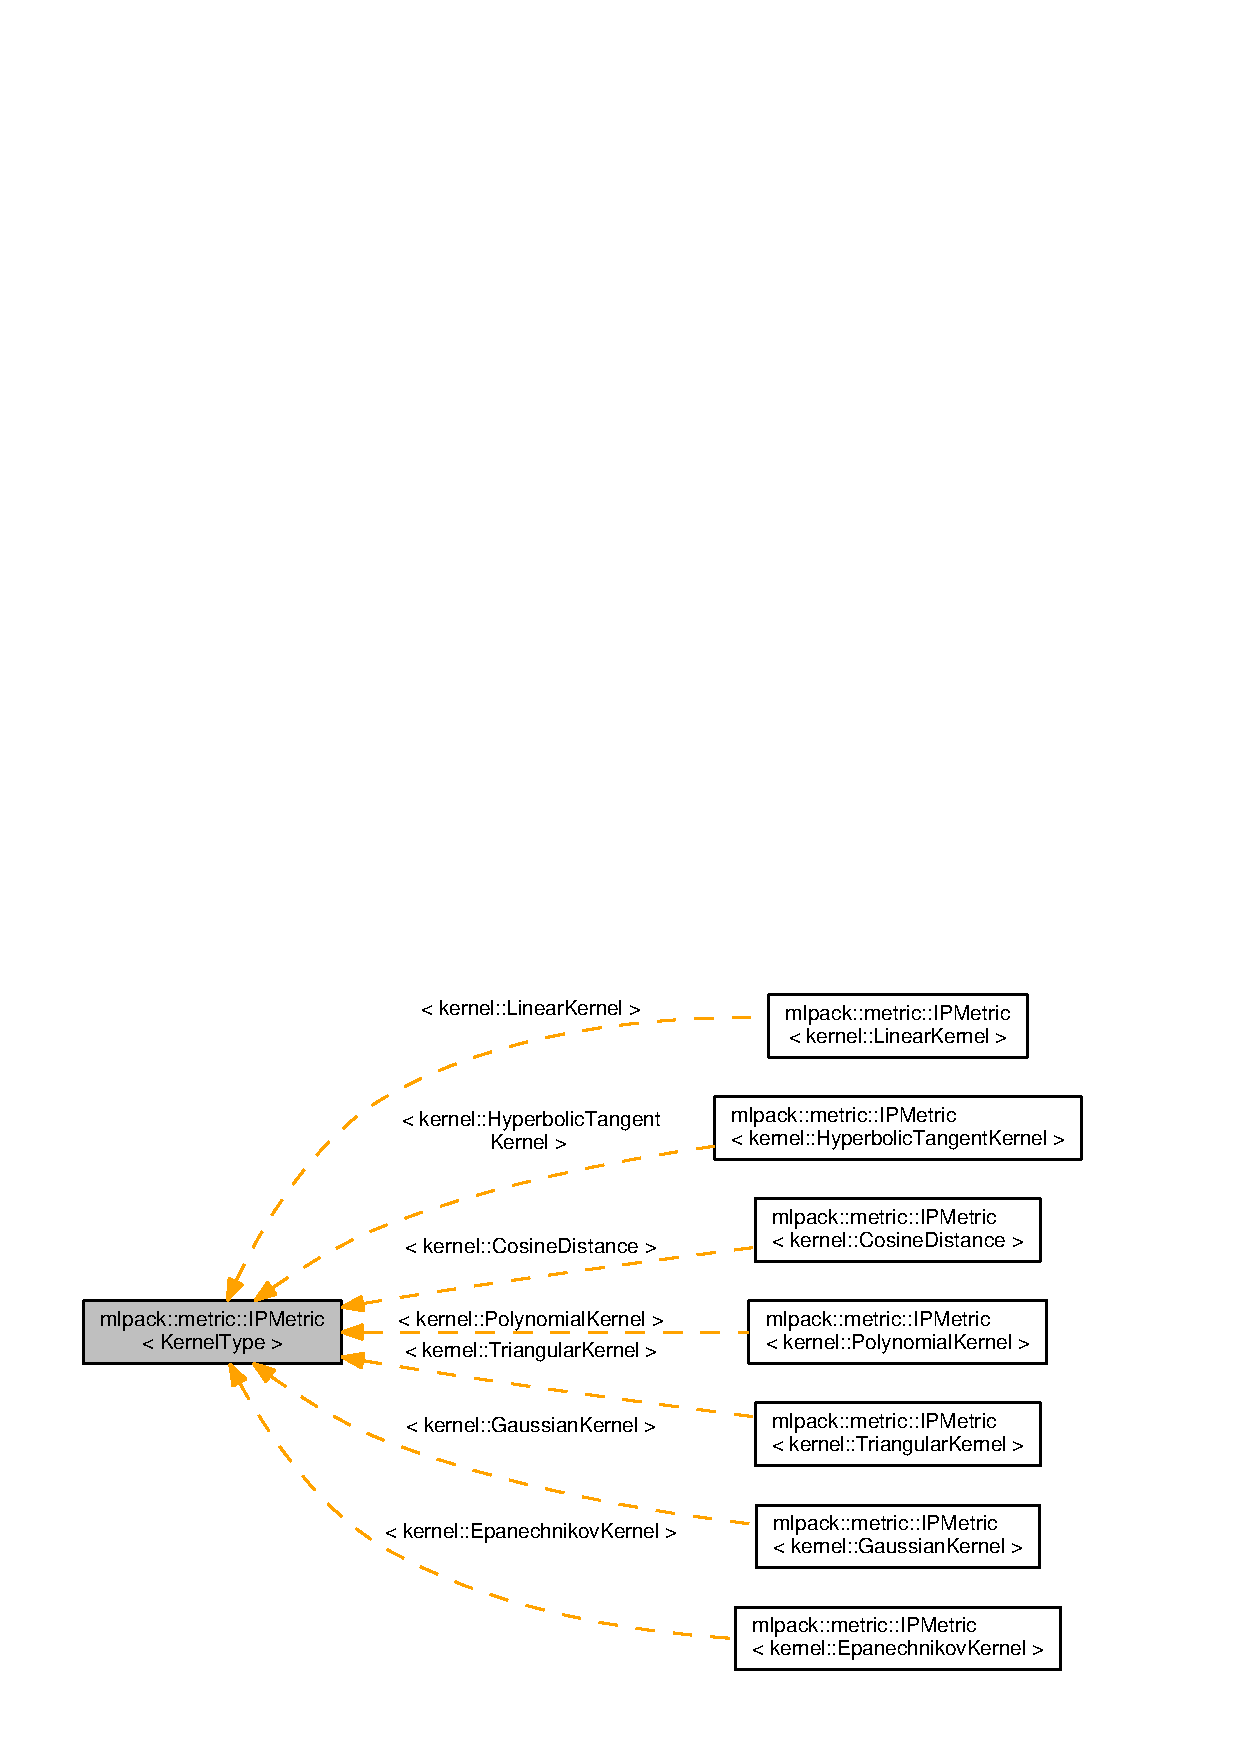
\includegraphics[width=350pt]{classmlpack_1_1metric_1_1IPMetric__inherit__graph}
\end{center}
\end{figure}
\subsection*{Public Member Functions}
\begin{DoxyCompactItemize}
\item 
\textbf{ I\+P\+Metric} ()
\begin{DoxyCompactList}\small\item\em Create the \doxyref{I\+P\+Metric}{p.}{classmlpack_1_1metric_1_1IPMetric} without an instantiated kernel. \end{DoxyCompactList}\item 
\textbf{ I\+P\+Metric} (Kernel\+Type \&kernel)
\begin{DoxyCompactList}\small\item\em Create the \doxyref{I\+P\+Metric}{p.}{classmlpack_1_1metric_1_1IPMetric} with an instantiated kernel. \end{DoxyCompactList}\item 
\textbf{ I\+P\+Metric} (const \textbf{ I\+P\+Metric} \&other)
\begin{DoxyCompactList}\small\item\em Copy the parameters of the given metric. \end{DoxyCompactList}\item 
\textbf{ $\sim$\+I\+P\+Metric} ()
\begin{DoxyCompactList}\small\item\em Destroy the \doxyref{I\+P\+Metric}{p.}{classmlpack_1_1metric_1_1IPMetric} object. \end{DoxyCompactList}\item 
{\footnotesize template$<$typename Vec\+TypeA , typename Vec\+TypeB $>$ }\\Vec\+Type\+A\+::elem\+\_\+type \textbf{ Evaluate} (const Vec\+TypeA \&a, const Vec\+TypeB \&b)
\begin{DoxyCompactList}\small\item\em Evaluate the metric. \end{DoxyCompactList}\item 
const Kernel\+Type \& \textbf{ Kernel} () const
\begin{DoxyCompactList}\small\item\em Get the kernel. \end{DoxyCompactList}\item 
Kernel\+Type \& \textbf{ Kernel} ()
\begin{DoxyCompactList}\small\item\em Modify the kernel. \end{DoxyCompactList}\item 
\textbf{ I\+P\+Metric} \& \textbf{ operator=} (const \textbf{ I\+P\+Metric} \&other)
\begin{DoxyCompactList}\small\item\em Assign this metric to be a copy of the given metric. \end{DoxyCompactList}\item 
{\footnotesize template$<$typename Archive $>$ }\\void \textbf{ serialize} (Archive \&ar, const uint32\+\_\+t version)
\begin{DoxyCompactList}\small\item\em Serialize the metric. \end{DoxyCompactList}\end{DoxyCompactItemize}


\subsection{Detailed Description}
\subsubsection*{template$<$typename Kernel\+Type$>$\newline
class mlpack\+::metric\+::\+I\+P\+Metric$<$ Kernel\+Type $>$}

The inner product metric, \doxyref{I\+P\+Metric}{p.}{classmlpack_1_1metric_1_1IPMetric}, takes a given Mercer kernel (Kernel\+Type), and when \doxyref{Evaluate()}{p.}{classmlpack_1_1metric_1_1IPMetric_a55e03560fb8c7923de4a43df9a265437} is called, returns the distance between the two points in kernel space\+: 

\[ d(x, y) = \sqrt{ K(x, x) + K(y, y) - 2K(x, y) }. \]


\begin{DoxyTemplParams}{Template Parameters}
{\em Kernel\+Type} & Type of Kernel to use. This must be a Mercer kernel (positive definite), otherwise the metric may not be valid. \\
\hline
\end{DoxyTemplParams}


Definition at line 32 of file ip\+\_\+metric.\+hpp.



\subsection{Constructor \& Destructor Documentation}
\mbox{\label{classmlpack_1_1metric_1_1IPMetric_a0774938d01373c8d5aaeebfc930c4e3d}} 
\index{mlpack\+::metric\+::\+I\+P\+Metric@{mlpack\+::metric\+::\+I\+P\+Metric}!I\+P\+Metric@{I\+P\+Metric}}
\index{I\+P\+Metric@{I\+P\+Metric}!mlpack\+::metric\+::\+I\+P\+Metric@{mlpack\+::metric\+::\+I\+P\+Metric}}
\subsubsection{I\+P\+Metric()\hspace{0.1cm}{\footnotesize\ttfamily [1/3]}}
{\footnotesize\ttfamily \textbf{ I\+P\+Metric} (\begin{DoxyParamCaption}{ }\end{DoxyParamCaption})}



Create the \doxyref{I\+P\+Metric}{p.}{classmlpack_1_1metric_1_1IPMetric} without an instantiated kernel. 

\mbox{\label{classmlpack_1_1metric_1_1IPMetric_a83bc1993b4d2626112ba0169e8fdd5b9}} 
\index{mlpack\+::metric\+::\+I\+P\+Metric@{mlpack\+::metric\+::\+I\+P\+Metric}!I\+P\+Metric@{I\+P\+Metric}}
\index{I\+P\+Metric@{I\+P\+Metric}!mlpack\+::metric\+::\+I\+P\+Metric@{mlpack\+::metric\+::\+I\+P\+Metric}}
\subsubsection{I\+P\+Metric()\hspace{0.1cm}{\footnotesize\ttfamily [2/3]}}
{\footnotesize\ttfamily \textbf{ I\+P\+Metric} (\begin{DoxyParamCaption}\item[{Kernel\+Type \&}]{kernel }\end{DoxyParamCaption})}



Create the \doxyref{I\+P\+Metric}{p.}{classmlpack_1_1metric_1_1IPMetric} with an instantiated kernel. 

\mbox{\label{classmlpack_1_1metric_1_1IPMetric_acb6ac7e7c6b1cdeffaccfa96b5573c99}} 
\index{mlpack\+::metric\+::\+I\+P\+Metric@{mlpack\+::metric\+::\+I\+P\+Metric}!````~I\+P\+Metric@{$\sim$\+I\+P\+Metric}}
\index{````~I\+P\+Metric@{$\sim$\+I\+P\+Metric}!mlpack\+::metric\+::\+I\+P\+Metric@{mlpack\+::metric\+::\+I\+P\+Metric}}
\subsubsection{$\sim$\+I\+P\+Metric()}
{\footnotesize\ttfamily $\sim$\textbf{ I\+P\+Metric} (\begin{DoxyParamCaption}{ }\end{DoxyParamCaption})}



Destroy the \doxyref{I\+P\+Metric}{p.}{classmlpack_1_1metric_1_1IPMetric} object. 

\mbox{\label{classmlpack_1_1metric_1_1IPMetric_a068775d03b4fe6ccf17bd833c152bf86}} 
\index{mlpack\+::metric\+::\+I\+P\+Metric@{mlpack\+::metric\+::\+I\+P\+Metric}!I\+P\+Metric@{I\+P\+Metric}}
\index{I\+P\+Metric@{I\+P\+Metric}!mlpack\+::metric\+::\+I\+P\+Metric@{mlpack\+::metric\+::\+I\+P\+Metric}}
\subsubsection{I\+P\+Metric()\hspace{0.1cm}{\footnotesize\ttfamily [3/3]}}
{\footnotesize\ttfamily \textbf{ I\+P\+Metric} (\begin{DoxyParamCaption}\item[{const \textbf{ I\+P\+Metric}$<$ Kernel\+Type $>$ \&}]{other }\end{DoxyParamCaption})}



Copy the parameters of the given metric. 



\subsection{Member Function Documentation}
\mbox{\label{classmlpack_1_1metric_1_1IPMetric_a55e03560fb8c7923de4a43df9a265437}} 
\index{mlpack\+::metric\+::\+I\+P\+Metric@{mlpack\+::metric\+::\+I\+P\+Metric}!Evaluate@{Evaluate}}
\index{Evaluate@{Evaluate}!mlpack\+::metric\+::\+I\+P\+Metric@{mlpack\+::metric\+::\+I\+P\+Metric}}
\subsubsection{Evaluate()}
{\footnotesize\ttfamily Vec\+Type\+A\+::elem\+\_\+type Evaluate (\begin{DoxyParamCaption}\item[{const Vec\+TypeA \&}]{a,  }\item[{const Vec\+TypeB \&}]{b }\end{DoxyParamCaption})}



Evaluate the metric. 


\begin{DoxyTemplParams}{Template Parameters}
{\em Vec\+TypeA} & Type of first vector. \\
\hline
{\em Vec\+TypeB} & Type of second vector. \\
\hline
\end{DoxyTemplParams}

\begin{DoxyParams}{Parameters}
{\em a} & First vector. \\
\hline
{\em b} & Second vector. \\
\hline
\end{DoxyParams}
\begin{DoxyReturn}{Returns}
Distance between the two points in kernel space. 
\end{DoxyReturn}
\mbox{\label{classmlpack_1_1metric_1_1IPMetric_a917492b75cc17298bc58c3d28e2944fb}} 
\index{mlpack\+::metric\+::\+I\+P\+Metric@{mlpack\+::metric\+::\+I\+P\+Metric}!Kernel@{Kernel}}
\index{Kernel@{Kernel}!mlpack\+::metric\+::\+I\+P\+Metric@{mlpack\+::metric\+::\+I\+P\+Metric}}
\subsubsection{Kernel()\hspace{0.1cm}{\footnotesize\ttfamily [1/2]}}
{\footnotesize\ttfamily const Kernel\+Type\& Kernel (\begin{DoxyParamCaption}{ }\end{DoxyParamCaption}) const\hspace{0.3cm}{\ttfamily [inline]}}



Get the kernel. 



Definition at line 63 of file ip\+\_\+metric.\+hpp.

\mbox{\label{classmlpack_1_1metric_1_1IPMetric_ab8d1bedeac8344d80e50d819790a117a}} 
\index{mlpack\+::metric\+::\+I\+P\+Metric@{mlpack\+::metric\+::\+I\+P\+Metric}!Kernel@{Kernel}}
\index{Kernel@{Kernel}!mlpack\+::metric\+::\+I\+P\+Metric@{mlpack\+::metric\+::\+I\+P\+Metric}}
\subsubsection{Kernel()\hspace{0.1cm}{\footnotesize\ttfamily [2/2]}}
{\footnotesize\ttfamily Kernel\+Type\& Kernel (\begin{DoxyParamCaption}{ }\end{DoxyParamCaption})\hspace{0.3cm}{\ttfamily [inline]}}



Modify the kernel. 



Definition at line 65 of file ip\+\_\+metric.\+hpp.

\mbox{\label{classmlpack_1_1metric_1_1IPMetric_af19fbcb2dbe02750f2815fb015ab52ef}} 
\index{mlpack\+::metric\+::\+I\+P\+Metric@{mlpack\+::metric\+::\+I\+P\+Metric}!operator=@{operator=}}
\index{operator=@{operator=}!mlpack\+::metric\+::\+I\+P\+Metric@{mlpack\+::metric\+::\+I\+P\+Metric}}
\subsubsection{operator=()}
{\footnotesize\ttfamily \textbf{ I\+P\+Metric}\& operator= (\begin{DoxyParamCaption}\item[{const \textbf{ I\+P\+Metric}$<$ Kernel\+Type $>$ \&}]{other }\end{DoxyParamCaption})}



Assign this metric to be a copy of the given metric. 

\mbox{\label{classmlpack_1_1metric_1_1IPMetric_a72d63b74c8166dff8e1a9006905ad9ca}} 
\index{mlpack\+::metric\+::\+I\+P\+Metric@{mlpack\+::metric\+::\+I\+P\+Metric}!serialize@{serialize}}
\index{serialize@{serialize}!mlpack\+::metric\+::\+I\+P\+Metric@{mlpack\+::metric\+::\+I\+P\+Metric}}
\subsubsection{serialize()}
{\footnotesize\ttfamily void serialize (\begin{DoxyParamCaption}\item[{Archive \&}]{ar,  }\item[{const uint32\+\_\+t}]{version }\end{DoxyParamCaption})}



Serialize the metric. 



Referenced by I\+P\+Metric$<$ mlpack\+::kernel\+::\+Cosine\+Distance $>$\+::\+Kernel().



The documentation for this class was generated from the following file\+:\begin{DoxyCompactItemize}
\item 
/home/aakash/mlpack/src/mlpack/core/metrics/\textbf{ ip\+\_\+metric.\+hpp}\end{DoxyCompactItemize}

\section{L\+Metric$<$ T\+Power, T\+Take\+Root $>$ Class Template Reference}
\label{classmlpack_1_1metric_1_1LMetric}\index{L\+Metric$<$ T\+Power, T\+Take\+Root $>$@{L\+Metric$<$ T\+Power, T\+Take\+Root $>$}}


The L\+\_\+p metric for arbitrary integer p, with an option to take the root.  




Inheritance diagram for L\+Metric$<$ T\+Power, T\+Take\+Root $>$\+:
\nopagebreak
\begin{figure}[H]
\begin{center}
\leavevmode
\includegraphics[width=200pt]{classmlpack_1_1metric_1_1LMetric__inherit__graph}
\end{center}
\end{figure}
\subsection*{Public Member Functions}
\begin{DoxyCompactItemize}
\item 
\textbf{ L\+Metric} ()
\begin{DoxyCompactList}\small\item\em Default constructor does nothing, but is required to satisfy the Metric policy. \end{DoxyCompactList}\item 
{\footnotesize template$<$typename Archive $>$ }\\void \textbf{ serialize} (Archive \&, const uint32\+\_\+t)
\begin{DoxyCompactList}\small\item\em Serialize the metric (nothing to do). \end{DoxyCompactList}\end{DoxyCompactItemize}
\subsection*{Static Public Member Functions}
\begin{DoxyCompactItemize}
\item 
{\footnotesize template$<$typename Vec\+TypeA , typename Vec\+TypeB $>$ }\\static Vec\+Type\+A\+::elem\+\_\+type \textbf{ Evaluate} (const Vec\+TypeA \&a, const Vec\+TypeB \&b)
\begin{DoxyCompactList}\small\item\em Computes the distance between two points. \end{DoxyCompactList}\end{DoxyCompactItemize}
\subsection*{Static Public Attributes}
\begin{DoxyCompactItemize}
\item 
static const int \textbf{ Power} = T\+Power
\begin{DoxyCompactList}\small\item\em The power of the metric. \end{DoxyCompactList}\item 
static const bool \textbf{ Take\+Root} = T\+Take\+Root
\begin{DoxyCompactList}\small\item\em Whether or not the root is taken. \end{DoxyCompactList}\end{DoxyCompactItemize}


\subsection{Detailed Description}
\subsubsection*{template$<$int T\+Power, bool T\+Take\+Root = true$>$\newline
class mlpack\+::metric\+::\+L\+Metric$<$ T\+Power, T\+Take\+Root $>$}

The L\+\_\+p metric for arbitrary integer p, with an option to take the root. 

This class implements the standard L\+\_\+p metric for two arbitrary vectors $ x $ and $ y $ of dimensionality $ n $\+:

\[ d(x, y) = \left( \sum_{i = 1}^{n} | x_i - y_i |^p \right)^{\frac{1}{p}}. \]

The value of p is given as a template parameter.

In addition, the function $ d(x, y) $ can be simplified, neglecting the p-\/root calculation. This is done by specifying the Take\+Root template parameter to be false. Then,

\[ d(x, y) = \sum_{i = 1}^{n} | x_i - y_i |^p \]

It is faster to compute that distance, so Take\+Root is by default off. However, when Take\+Root is false, the distance given is not actually a true metric -- it does not satisfy the triangle inequality. Some mlpack methods do not require the triangle inequality to operate correctly (such as the Binary\+Space\+Tree), but setting Take\+Root = false in some cases will cause incorrect results.

A few convenience typedefs are given\+:


\begin{DoxyItemize}
\item Manhattan\+Distance
\item Euclidean\+Distance
\item Squared\+Euclidean\+Distance
\end{DoxyItemize}


\begin{DoxyTemplParams}{Template Parameters}
{\em Power} & Power of metric; i.\+e. Power = 1 gives the L1-\/norm (Manhattan distance). \\
\hline
{\em Take\+Root} & If true, the Power\textquotesingle{}th root of the result is taken before it is returned. Setting this to false causes the metric to not satisfy the Triangle Inequality (be careful!). \\
\hline
\end{DoxyTemplParams}


Definition at line 63 of file lmetric.\+hpp.



\subsection{Constructor \& Destructor Documentation}
\mbox{\label{classmlpack_1_1metric_1_1LMetric_ad296b4c8538551ddcef38a49d0842ca7}} 
\index{mlpack\+::metric\+::\+L\+Metric@{mlpack\+::metric\+::\+L\+Metric}!L\+Metric@{L\+Metric}}
\index{L\+Metric@{L\+Metric}!mlpack\+::metric\+::\+L\+Metric@{mlpack\+::metric\+::\+L\+Metric}}
\subsubsection{L\+Metric()}
{\footnotesize\ttfamily \textbf{ L\+Metric} (\begin{DoxyParamCaption}{ }\end{DoxyParamCaption})\hspace{0.3cm}{\ttfamily [inline]}}



Default constructor does nothing, but is required to satisfy the Metric policy. 



Definition at line 70 of file lmetric.\+hpp.



\subsection{Member Function Documentation}
\mbox{\label{classmlpack_1_1metric_1_1LMetric_af39380107875eb94f0efef7d37cc57df}} 
\index{mlpack\+::metric\+::\+L\+Metric@{mlpack\+::metric\+::\+L\+Metric}!Evaluate@{Evaluate}}
\index{Evaluate@{Evaluate}!mlpack\+::metric\+::\+L\+Metric@{mlpack\+::metric\+::\+L\+Metric}}
\subsubsection{Evaluate()}
{\footnotesize\ttfamily static Vec\+Type\+A\+::elem\+\_\+type Evaluate (\begin{DoxyParamCaption}\item[{const Vec\+TypeA \&}]{a,  }\item[{const Vec\+TypeB \&}]{b }\end{DoxyParamCaption})\hspace{0.3cm}{\ttfamily [static]}}



Computes the distance between two points. 


\begin{DoxyTemplParams}{Template Parameters}
{\em Vec\+TypeA} & Type of first vector (generally arma\+::vec or arma\+::sp\+\_\+vec). \\
\hline
{\em Vec\+TypeB} & Type of second vector. \\
\hline
\end{DoxyTemplParams}

\begin{DoxyParams}{Parameters}
{\em a} & First vector. \\
\hline
{\em b} & Second vector. \\
\hline
\end{DoxyParams}
\begin{DoxyReturn}{Returns}
Distance between vectors a and b. 
\end{DoxyReturn}


Referenced by K\+Means\+Plus\+Plus\+Initialization\+::\+Cluster(), Spherical\+Kernel\+::\+Convolution\+Integral(), Gaussian\+Kernel\+::\+Convolution\+Integral(), Spherical\+Kernel\+::\+Evaluate(), Triangular\+Kernel\+::\+Evaluate(), Laplacian\+Kernel\+::\+Evaluate(), Gaussian\+Kernel\+::\+Evaluate(), Cauchy\+Kernel\+::\+Evaluate(), and L\+Metric$<$ T\+Power, true $>$\+::\+L\+Metric().

\mbox{\label{classmlpack_1_1metric_1_1LMetric_aa2ccb5a0533a6ba0abe6dfc1f98fbafb}} 
\index{mlpack\+::metric\+::\+L\+Metric@{mlpack\+::metric\+::\+L\+Metric}!serialize@{serialize}}
\index{serialize@{serialize}!mlpack\+::metric\+::\+L\+Metric@{mlpack\+::metric\+::\+L\+Metric}}
\subsubsection{serialize()}
{\footnotesize\ttfamily void serialize (\begin{DoxyParamCaption}\item[{Archive \&}]{,  }\item[{const uint32\+\_\+t}]{ }\end{DoxyParamCaption})\hspace{0.3cm}{\ttfamily [inline]}}



Serialize the metric (nothing to do). 



Definition at line 88 of file lmetric.\+hpp.



\subsection{Member Data Documentation}
\mbox{\label{classmlpack_1_1metric_1_1LMetric_add828b673634e896b13f47cc7fb331f5}} 
\index{mlpack\+::metric\+::\+L\+Metric@{mlpack\+::metric\+::\+L\+Metric}!Power@{Power}}
\index{Power@{Power}!mlpack\+::metric\+::\+L\+Metric@{mlpack\+::metric\+::\+L\+Metric}}
\subsubsection{Power}
{\footnotesize\ttfamily const int Power = T\+Power\hspace{0.3cm}{\ttfamily [static]}}



The power of the metric. 



Definition at line 91 of file lmetric.\+hpp.

\mbox{\label{classmlpack_1_1metric_1_1LMetric_a0615e7186f9a9847e2f71d2d2622579d}} 
\index{mlpack\+::metric\+::\+L\+Metric@{mlpack\+::metric\+::\+L\+Metric}!Take\+Root@{Take\+Root}}
\index{Take\+Root@{Take\+Root}!mlpack\+::metric\+::\+L\+Metric@{mlpack\+::metric\+::\+L\+Metric}}
\subsubsection{Take\+Root}
{\footnotesize\ttfamily const bool Take\+Root = T\+Take\+Root\hspace{0.3cm}{\ttfamily [static]}}



Whether or not the root is taken. 



Definition at line 93 of file lmetric.\+hpp.



The documentation for this class was generated from the following file\+:\begin{DoxyCompactItemize}
\item 
/home/aakash/mlpack/src/mlpack/core/metrics/\textbf{ lmetric.\+hpp}\end{DoxyCompactItemize}

\section{Mahalanobis\+Distance$<$ Take\+Root $>$ Class Template Reference}
\label{classmlpack_1_1metric_1_1MahalanobisDistance}\index{Mahalanobis\+Distance$<$ Take\+Root $>$@{Mahalanobis\+Distance$<$ Take\+Root $>$}}


The Mahalanobis distance, which is essentially a stretched Euclidean distance.  


\subsection*{Public Member Functions}
\begin{DoxyCompactItemize}
\item 
\textbf{ Mahalanobis\+Distance} ()
\begin{DoxyCompactList}\small\item\em Initialize the Mahalanobis distance with the empty matrix as covariance. \end{DoxyCompactList}\item 
\textbf{ Mahalanobis\+Distance} (const size\+\_\+t dimensionality)
\begin{DoxyCompactList}\small\item\em Initialize the Mahalanobis distance with the identity matrix of the given dimensionality. \end{DoxyCompactList}\item 
\textbf{ Mahalanobis\+Distance} (arma\+::mat covariance)
\begin{DoxyCompactList}\small\item\em Initialize the Mahalanobis distance with the given covariance matrix. \end{DoxyCompactList}\item 
const arma\+::mat \& \textbf{ Covariance} () const
\begin{DoxyCompactList}\small\item\em Access the covariance matrix. \end{DoxyCompactList}\item 
arma\+::mat \& \textbf{ Covariance} ()
\begin{DoxyCompactList}\small\item\em Modify the covariance matrix. \end{DoxyCompactList}\item 
{\footnotesize template$<$typename Vec\+TypeA , typename Vec\+TypeB $>$ }\\double \textbf{ Evaluate} (const Vec\+TypeA \&a, const Vec\+TypeB \&b)
\begin{DoxyCompactList}\small\item\em Evaluate the distance between the two given points using this Mahalanobis distance. \end{DoxyCompactList}\item 
{\footnotesize template$<$typename Archive $>$ }\\void \textbf{ serialize} (Archive \&ar, const uint32\+\_\+t version)
\begin{DoxyCompactList}\small\item\em Serialize the Mahalanobis distance. \end{DoxyCompactList}\end{DoxyCompactItemize}


\subsection{Detailed Description}
\subsubsection*{template$<$bool Take\+Root = true$>$\newline
class mlpack\+::metric\+::\+Mahalanobis\+Distance$<$ Take\+Root $>$}

The Mahalanobis distance, which is essentially a stretched Euclidean distance. 

Given a square covariance matrix $ Q $ of size $ d $ x $ d $, where $ d $ is the dimensionality of the points it will be evaluating, and given two vectors $ x $ and $ y $ also of dimensionality $ d $,

\[ d(x, y) = \sqrt{(x - y)^T Q (x - y)} \]

where Q is the covariance matrix.

Because each evaluation multiplies (x\+\_\+1 -\/ x\+\_\+2) by the covariance matrix, it is typically much quicker to use an \doxyref{L\+Metric}{p.}{classmlpack_1_1metric_1_1LMetric} and simply stretch the actual dataset itself before performing any evaluations. However, this class is provided for convenience.

If you wish to use the K\+NN class or other tree-\/based algorithms with this distance, it is recommended to instead stretch the dataset first, by decomposing Q = L$^\wedge$T L (perhaps via a Cholesky decomposition), and then multiply the data by L. If you still wish to use the K\+NN class with a custom distance anyway, you will need to use a different tree type than the default K\+D\+Tree, which only works with the \doxyref{L\+Metric}{p.}{classmlpack_1_1metric_1_1LMetric} class.

Similar to the \doxyref{L\+Metric}{p.}{classmlpack_1_1metric_1_1LMetric} class, this offers a template parameter Take\+Root which, when set to false, will instead evaluate the distance

\[ d(x, y) = (x - y)^T Q (x - y) \]

which is faster to evaluate.


\begin{DoxyTemplParams}{Template Parameters}
{\em Take\+Root} & If true, takes the root of the output. It is slightly faster to leave this at the default of false, but this means the metric may not satisfy the triangle inequality and may not be usable for methods that expect a true metric. \\
\hline
\end{DoxyTemplParams}


Definition at line 60 of file mahalanobis\+\_\+distance.\+hpp.



\subsection{Constructor \& Destructor Documentation}
\mbox{\label{classmlpack_1_1metric_1_1MahalanobisDistance_a00cbb536d89ebdafc57f3a481aa772e4}} 
\index{mlpack\+::metric\+::\+Mahalanobis\+Distance@{mlpack\+::metric\+::\+Mahalanobis\+Distance}!Mahalanobis\+Distance@{Mahalanobis\+Distance}}
\index{Mahalanobis\+Distance@{Mahalanobis\+Distance}!mlpack\+::metric\+::\+Mahalanobis\+Distance@{mlpack\+::metric\+::\+Mahalanobis\+Distance}}
\subsubsection{Mahalanobis\+Distance()\hspace{0.1cm}{\footnotesize\ttfamily [1/3]}}
{\footnotesize\ttfamily \textbf{ Mahalanobis\+Distance} (\begin{DoxyParamCaption}{ }\end{DoxyParamCaption})\hspace{0.3cm}{\ttfamily [inline]}}



Initialize the Mahalanobis distance with the empty matrix as covariance. 

Don\textquotesingle{}t call \doxyref{Evaluate()}{p.}{classmlpack_1_1metric_1_1MahalanobisDistance_a7bc3cfc0ee3750ba84ee4dc7f62994ae} until you set the covariance with \doxyref{Covariance()}{p.}{classmlpack_1_1metric_1_1MahalanobisDistance_aa65080f46932c7155e87b017e8fa58f5}! 

Definition at line 67 of file mahalanobis\+\_\+distance.\+hpp.

\mbox{\label{classmlpack_1_1metric_1_1MahalanobisDistance_a68f439d98cd6d071ed45bd91f47ebfcb}} 
\index{mlpack\+::metric\+::\+Mahalanobis\+Distance@{mlpack\+::metric\+::\+Mahalanobis\+Distance}!Mahalanobis\+Distance@{Mahalanobis\+Distance}}
\index{Mahalanobis\+Distance@{Mahalanobis\+Distance}!mlpack\+::metric\+::\+Mahalanobis\+Distance@{mlpack\+::metric\+::\+Mahalanobis\+Distance}}
\subsubsection{Mahalanobis\+Distance()\hspace{0.1cm}{\footnotesize\ttfamily [2/3]}}
{\footnotesize\ttfamily \textbf{ Mahalanobis\+Distance} (\begin{DoxyParamCaption}\item[{const size\+\_\+t}]{dimensionality }\end{DoxyParamCaption})\hspace{0.3cm}{\ttfamily [inline]}}



Initialize the Mahalanobis distance with the identity matrix of the given dimensionality. 


\begin{DoxyParams}{Parameters}
{\em dimensionality} & Dimesnsionality of the covariance matrix. \\
\hline
\end{DoxyParams}


Definition at line 75 of file mahalanobis\+\_\+distance.\+hpp.

\mbox{\label{classmlpack_1_1metric_1_1MahalanobisDistance_a385234d4f1d914f7786c481fa805c31c}} 
\index{mlpack\+::metric\+::\+Mahalanobis\+Distance@{mlpack\+::metric\+::\+Mahalanobis\+Distance}!Mahalanobis\+Distance@{Mahalanobis\+Distance}}
\index{Mahalanobis\+Distance@{Mahalanobis\+Distance}!mlpack\+::metric\+::\+Mahalanobis\+Distance@{mlpack\+::metric\+::\+Mahalanobis\+Distance}}
\subsubsection{Mahalanobis\+Distance()\hspace{0.1cm}{\footnotesize\ttfamily [3/3]}}
{\footnotesize\ttfamily \textbf{ Mahalanobis\+Distance} (\begin{DoxyParamCaption}\item[{arma\+::mat}]{covariance }\end{DoxyParamCaption})\hspace{0.3cm}{\ttfamily [inline]}}



Initialize the Mahalanobis distance with the given covariance matrix. 

The given covariance matrix will be copied (this is not optimal).


\begin{DoxyParams}{Parameters}
{\em covariance} & The covariance matrix to use for this distance. \\
\hline
\end{DoxyParams}


Definition at line 84 of file mahalanobis\+\_\+distance.\+hpp.



References Mahalanobis\+Distance$<$ Take\+Root $>$\+::\+Evaluate().



\subsection{Member Function Documentation}
\mbox{\label{classmlpack_1_1metric_1_1MahalanobisDistance_a7cab8a0b8c0deac1833f3e489fa52daf}} 
\index{mlpack\+::metric\+::\+Mahalanobis\+Distance@{mlpack\+::metric\+::\+Mahalanobis\+Distance}!Covariance@{Covariance}}
\index{Covariance@{Covariance}!mlpack\+::metric\+::\+Mahalanobis\+Distance@{mlpack\+::metric\+::\+Mahalanobis\+Distance}}
\subsubsection{Covariance()\hspace{0.1cm}{\footnotesize\ttfamily [1/2]}}
{\footnotesize\ttfamily const arma\+::mat\& Covariance (\begin{DoxyParamCaption}{ }\end{DoxyParamCaption}) const\hspace{0.3cm}{\ttfamily [inline]}}



Access the covariance matrix. 

\begin{DoxyReturn}{Returns}
Constant reference to the covariance matrix. 
\end{DoxyReturn}


Definition at line 104 of file mahalanobis\+\_\+distance.\+hpp.

\mbox{\label{classmlpack_1_1metric_1_1MahalanobisDistance_aa65080f46932c7155e87b017e8fa58f5}} 
\index{mlpack\+::metric\+::\+Mahalanobis\+Distance@{mlpack\+::metric\+::\+Mahalanobis\+Distance}!Covariance@{Covariance}}
\index{Covariance@{Covariance}!mlpack\+::metric\+::\+Mahalanobis\+Distance@{mlpack\+::metric\+::\+Mahalanobis\+Distance}}
\subsubsection{Covariance()\hspace{0.1cm}{\footnotesize\ttfamily [2/2]}}
{\footnotesize\ttfamily arma\+::mat\& Covariance (\begin{DoxyParamCaption}{ }\end{DoxyParamCaption})\hspace{0.3cm}{\ttfamily [inline]}}



Modify the covariance matrix. 

\begin{DoxyReturn}{Returns}
Reference to the covariance matrix. 
\end{DoxyReturn}


Definition at line 111 of file mahalanobis\+\_\+distance.\+hpp.



References Mahalanobis\+Distance$<$ Take\+Root $>$\+::serialize().

\mbox{\label{classmlpack_1_1metric_1_1MahalanobisDistance_a7bc3cfc0ee3750ba84ee4dc7f62994ae}} 
\index{mlpack\+::metric\+::\+Mahalanobis\+Distance@{mlpack\+::metric\+::\+Mahalanobis\+Distance}!Evaluate@{Evaluate}}
\index{Evaluate@{Evaluate}!mlpack\+::metric\+::\+Mahalanobis\+Distance@{mlpack\+::metric\+::\+Mahalanobis\+Distance}}
\subsubsection{Evaluate()}
{\footnotesize\ttfamily double Evaluate (\begin{DoxyParamCaption}\item[{const Vec\+TypeA \&}]{a,  }\item[{const Vec\+TypeB \&}]{b }\end{DoxyParamCaption})}



Evaluate the distance between the two given points using this Mahalanobis distance. 

If the covariance matrix has not been set (i.\+e. if you used the empty constructor and did not later modify the covariance matrix), calling this method will probably result in a crash.


\begin{DoxyParams}{Parameters}
{\em a} & First vector. \\
\hline
{\em b} & Second vector. \\
\hline
\end{DoxyParams}


Referenced by Mahalanobis\+Distance$<$ Take\+Root $>$\+::\+Mahalanobis\+Distance().

\mbox{\label{classmlpack_1_1metric_1_1MahalanobisDistance_a72d63b74c8166dff8e1a9006905ad9ca}} 
\index{mlpack\+::metric\+::\+Mahalanobis\+Distance@{mlpack\+::metric\+::\+Mahalanobis\+Distance}!serialize@{serialize}}
\index{serialize@{serialize}!mlpack\+::metric\+::\+Mahalanobis\+Distance@{mlpack\+::metric\+::\+Mahalanobis\+Distance}}
\subsubsection{serialize()}
{\footnotesize\ttfamily void serialize (\begin{DoxyParamCaption}\item[{Archive \&}]{ar,  }\item[{const uint32\+\_\+t}]{version }\end{DoxyParamCaption})}



Serialize the Mahalanobis distance. 



Referenced by Mahalanobis\+Distance$<$ Take\+Root $>$\+::\+Covariance().



The documentation for this class was generated from the following file\+:\begin{DoxyCompactItemize}
\item 
/home/aakash/mlpack/src/mlpack/core/metrics/\textbf{ mahalanobis\+\_\+distance.\+hpp}\end{DoxyCompactItemize}

\doxysection{MVU Class Reference}
\label{classmlpack_1_1mvu_1_1MVU}\index{MVU@{MVU}}


The \doxyref{MVU}{p.}{classmlpack_1_1mvu_1_1MVU} class is meant to provide a good abstraction for users.  


\doxysubsection*{Public Member Functions}
\begin{DoxyCompactItemize}
\item 
\textbf{ MVU} (const arma\+::mat \&data\+In)
\item 
void \textbf{ Unfold} (const size\+\_\+t new\+Dim, const size\+\_\+t num\+Neighbors, arma\+::mat \&output\+Coordinates)
\end{DoxyCompactItemize}


\doxysubsection{Detailed Description}
The \doxyref{MVU}{p.}{classmlpack_1_1mvu_1_1MVU} class is meant to provide a good abstraction for users. 

The dataset needs to be provided, as well as several parameters.


\begin{DoxyItemize}
\item dataset
\item new dimensionality 
\end{DoxyItemize}

Definition at line 32 of file mvu.\+hpp.



\doxysubsection{Constructor \& Destructor Documentation}
\mbox{\label{classmlpack_1_1mvu_1_1MVU_aed7c8b336becf90caa0c7b293621e8f4}} 
\index{MVU@{MVU}!MVU@{MVU}}
\index{MVU@{MVU}!MVU@{MVU}}
\doxysubsubsection{MVU()}
{\footnotesize\ttfamily \textbf{ MVU} (\begin{DoxyParamCaption}\item[{const arma\+::mat \&}]{data\+In }\end{DoxyParamCaption})}



\doxysubsection{Member Function Documentation}
\mbox{\label{classmlpack_1_1mvu_1_1MVU_a2fb5d5ffa149a4451a7140ba8c62970b}} 
\index{MVU@{MVU}!Unfold@{Unfold}}
\index{Unfold@{Unfold}!MVU@{MVU}}
\doxysubsubsection{Unfold()}
{\footnotesize\ttfamily void Unfold (\begin{DoxyParamCaption}\item[{const size\+\_\+t}]{new\+Dim,  }\item[{const size\+\_\+t}]{num\+Neighbors,  }\item[{arma\+::mat \&}]{output\+Coordinates }\end{DoxyParamCaption})}



The documentation for this class was generated from the following file\+:\begin{DoxyCompactItemize}
\item 
/home/aakash/mlpack/src/mlpack/methods/mvu/\textbf{ mvu.\+hpp}\end{DoxyCompactItemize}

\section{mlpack\+:\+:naive\+\_\+bayes\+:\+:Naive\+Bayes\+Classifier$<$ Mat\+Type $>$ Class Template Reference}
\label{classmlpack_1_1naive__bayes_1_1NaiveBayesClassifier}\index{mlpack\+::naive\+\_\+bayes\+::\+Naive\+Bayes\+Classifier$<$ Mat\+Type $>$@{mlpack\+::naive\+\_\+bayes\+::\+Naive\+Bayes\+Classifier$<$ Mat\+Type $>$}}


The simple Naive Bayes classifier.  


\subsection*{Public Member Functions}
\begin{DoxyCompactItemize}
\item 
{\bf Naive\+Bayes\+Classifier} (const Mat\+Type \&data, const arma\+::\+Row$<$ size\+\_\+t $>$ \&labels, const size\+\_\+t classes, const bool incremental\+Variance=false)
\begin{DoxyCompactList}\small\item\em Initializes the classifier as per the input and then trains it by calculating the sample mean and variances. \end{DoxyCompactList}\item 
{\bf Naive\+Bayes\+Classifier} (const size\+\_\+t dimensionality=0, const size\+\_\+t classes=0)
\begin{DoxyCompactList}\small\item\em Initialize the Naive Bayes classifier without performing training. \end{DoxyCompactList}\item 
void {\bf Classify} (const Mat\+Type \&data, arma\+::\+Row$<$ size\+\_\+t $>$ \&results)
\begin{DoxyCompactList}\small\item\em Given a bunch of data points, this function evaluates the class of each of those data points, and puts it in the vector \textquotesingle{}results\textquotesingle{}. \end{DoxyCompactList}\item 
const Mat\+Type \& {\bf Means} () const 
\begin{DoxyCompactList}\small\item\em Get the sample means for each class. \end{DoxyCompactList}\item 
Mat\+Type \& {\bf Means} ()
\begin{DoxyCompactList}\small\item\em Modify the sample means for each class. \end{DoxyCompactList}\item 
const arma\+::vec \& {\bf Probabilities} () const 
\begin{DoxyCompactList}\small\item\em Get the prior probabilities for each class. \end{DoxyCompactList}\item 
arma\+::vec \& {\bf Probabilities} ()
\begin{DoxyCompactList}\small\item\em Modify the prior probabilities for each class. \end{DoxyCompactList}\item 
{\footnotesize template$<$typename Archive $>$ }\\void {\bf Serialize} (Archive \&ar, const unsigned int)
\begin{DoxyCompactList}\small\item\em Serialize the classifier. \end{DoxyCompactList}\item 
void {\bf Train} (const Mat\+Type \&data, const arma\+::\+Row$<$ size\+\_\+t $>$ \&labels, const bool incremental=true)
\begin{DoxyCompactList}\small\item\em Train the Naive Bayes classifier on the given dataset. \end{DoxyCompactList}\item 
{\footnotesize template$<$typename Vec\+Type $>$ }\\void {\bf Train} (const Vec\+Type \&point, const size\+\_\+t label)
\begin{DoxyCompactList}\small\item\em Train the Naive Bayes classifier on the given point. \end{DoxyCompactList}\item 
const Mat\+Type \& {\bf Variances} () const 
\begin{DoxyCompactList}\small\item\em Get the sample variances for each class. \end{DoxyCompactList}\item 
Mat\+Type \& {\bf Variances} ()
\begin{DoxyCompactList}\small\item\em Modify the sample variances for each class. \end{DoxyCompactList}\end{DoxyCompactItemize}
\subsection*{Private Attributes}
\begin{DoxyCompactItemize}
\item 
Mat\+Type {\bf means}
\begin{DoxyCompactList}\small\item\em Sample mean for each class. \end{DoxyCompactList}\item 
arma\+::vec {\bf probabilities}
\begin{DoxyCompactList}\small\item\em Class probabilities. \end{DoxyCompactList}\item 
size\+\_\+t {\bf training\+Points}
\begin{DoxyCompactList}\small\item\em Number of training points seen so far. \end{DoxyCompactList}\item 
Mat\+Type {\bf variances}
\begin{DoxyCompactList}\small\item\em Sample variances for each class. \end{DoxyCompactList}\end{DoxyCompactItemize}


\subsection{Detailed Description}
\subsubsection*{template$<$typename Mat\+Type = arma\+::mat$>$\\*
class mlpack\+::naive\+\_\+bayes\+::\+Naive\+Bayes\+Classifier$<$ Mat\+Type $>$}

The simple Naive Bayes classifier. 

This class trains on the data by calculating the sample mean and variance of the features with respect to each of the labels, and also the class probabilities. The class labels are assumed to be positive integers (starting with 0), and are expected to be the last row of the data input to the constructor.

Mathematically, it computes P(X\+\_\+i = x\+\_\+i $\vert$ Y = y\+\_\+j) for each feature X\+\_\+i for each of the labels y\+\_\+j. Alongwith this, it also computes the class probabilities P(Y = y\+\_\+j).

For classifying a data point (x\+\_\+1, x\+\_\+2, ..., x\+\_\+n), it computes the following\+: arg max\+\_\+y(P(Y = y)$\ast$P(X\+\_\+1 = x\+\_\+1 $\vert$ Y = y) $\ast$ ... $\ast$ P(X\+\_\+n = x\+\_\+n $\vert$ Y = y))

Example use\+:


\begin{DoxyCode}
\textcolor{keyword}{extern} arma::mat training\_data, testing\_data;
NaiveBayesClassifier<> nbc(training\_data, 5);
arma::vec results;

nbc.Classify(testing\_data, results);
\end{DoxyCode}
 

Definition at line 47 of file naive\+\_\+bayes\+\_\+classifier.\+hpp.



\subsection{Constructor \& Destructor Documentation}
\index{mlpack\+::naive\+\_\+bayes\+::\+Naive\+Bayes\+Classifier@{mlpack\+::naive\+\_\+bayes\+::\+Naive\+Bayes\+Classifier}!Naive\+Bayes\+Classifier@{Naive\+Bayes\+Classifier}}
\index{Naive\+Bayes\+Classifier@{Naive\+Bayes\+Classifier}!mlpack\+::naive\+\_\+bayes\+::\+Naive\+Bayes\+Classifier@{mlpack\+::naive\+\_\+bayes\+::\+Naive\+Bayes\+Classifier}}
\subsubsection[{Naive\+Bayes\+Classifier(const Mat\+Type \&data, const arma\+::\+Row$<$ size\+\_\+t $>$ \&labels, const size\+\_\+t classes, const bool incremental\+Variance=false)}]{\setlength{\rightskip}{0pt plus 5cm}template$<$typename Mat\+Type  = arma\+::mat$>$ {\bf mlpack\+::naive\+\_\+bayes\+::\+Naive\+Bayes\+Classifier}$<$ Mat\+Type $>$\+::{\bf Naive\+Bayes\+Classifier} (
\begin{DoxyParamCaption}
\item[{const Mat\+Type \&}]{data, }
\item[{const arma\+::\+Row$<$ size\+\_\+t $>$ \&}]{labels, }
\item[{const size\+\_\+t}]{classes, }
\item[{const bool}]{incremental\+Variance = {\ttfamily false}}
\end{DoxyParamCaption}
)}\label{classmlpack_1_1naive__bayes_1_1NaiveBayesClassifier_a27aa5f96b14a7e73dde1b994049965f4}


Initializes the classifier as per the input and then trains it by calculating the sample mean and variances. 

Example use\+: 
\begin{DoxyCode}
\textcolor{keyword}{extern} arma::mat training\_data, testing\_data;
\textcolor{keyword}{extern} arma::Row<size\_t> labels;
NaiveBayesClassifier nbc(training\_data, labels, 5);
\end{DoxyCode}



\begin{DoxyParams}{Parameters}
{\em data} & Training data points. \\
\hline
{\em labels} & Labels corresponding to training data points. \\
\hline
{\em classes} & Number of classes in this classifier. \\
\hline
{\em incremental\+Variance} & If true, an incremental algorithm is used to calculate the variance; this can prevent loss of precision in some cases, but will be somewhat slower to calculate. \\
\hline
\end{DoxyParams}
\index{mlpack\+::naive\+\_\+bayes\+::\+Naive\+Bayes\+Classifier@{mlpack\+::naive\+\_\+bayes\+::\+Naive\+Bayes\+Classifier}!Naive\+Bayes\+Classifier@{Naive\+Bayes\+Classifier}}
\index{Naive\+Bayes\+Classifier@{Naive\+Bayes\+Classifier}!mlpack\+::naive\+\_\+bayes\+::\+Naive\+Bayes\+Classifier@{mlpack\+::naive\+\_\+bayes\+::\+Naive\+Bayes\+Classifier}}
\subsubsection[{Naive\+Bayes\+Classifier(const size\+\_\+t dimensionality=0, const size\+\_\+t classes=0)}]{\setlength{\rightskip}{0pt plus 5cm}template$<$typename Mat\+Type  = arma\+::mat$>$ {\bf mlpack\+::naive\+\_\+bayes\+::\+Naive\+Bayes\+Classifier}$<$ Mat\+Type $>$\+::{\bf Naive\+Bayes\+Classifier} (
\begin{DoxyParamCaption}
\item[{const size\+\_\+t}]{dimensionality = {\ttfamily 0}, }
\item[{const size\+\_\+t}]{classes = {\ttfamily 0}}
\end{DoxyParamCaption}
)}\label{classmlpack_1_1naive__bayes_1_1NaiveBayesClassifier_af2ba8935d9db48b8db3030a8610d2491}


Initialize the Naive Bayes classifier without performing training. 

All of the parameters of the model will be initialized to zero. Be sure to use \doxyref{Train()}{p.}{classmlpack_1_1naive__bayes_1_1NaiveBayesClassifier_a9439d0a83f597b91d523aaeefc0d2a96} before calling \doxyref{Classify()}{p.}{classmlpack_1_1naive__bayes_1_1NaiveBayesClassifier_a566d9abe10898de6749d74b9aa4f7220}, otherwise the results may be meaningless. 

\subsection{Member Function Documentation}
\index{mlpack\+::naive\+\_\+bayes\+::\+Naive\+Bayes\+Classifier@{mlpack\+::naive\+\_\+bayes\+::\+Naive\+Bayes\+Classifier}!Classify@{Classify}}
\index{Classify@{Classify}!mlpack\+::naive\+\_\+bayes\+::\+Naive\+Bayes\+Classifier@{mlpack\+::naive\+\_\+bayes\+::\+Naive\+Bayes\+Classifier}}
\subsubsection[{Classify(const Mat\+Type \&data, arma\+::\+Row$<$ size\+\_\+t $>$ \&results)}]{\setlength{\rightskip}{0pt plus 5cm}template$<$typename Mat\+Type  = arma\+::mat$>$ void {\bf mlpack\+::naive\+\_\+bayes\+::\+Naive\+Bayes\+Classifier}$<$ Mat\+Type $>$\+::Classify (
\begin{DoxyParamCaption}
\item[{const Mat\+Type \&}]{data, }
\item[{arma\+::\+Row$<$ size\+\_\+t $>$ \&}]{results}
\end{DoxyParamCaption}
)}\label{classmlpack_1_1naive__bayes_1_1NaiveBayesClassifier_a566d9abe10898de6749d74b9aa4f7220}


Given a bunch of data points, this function evaluates the class of each of those data points, and puts it in the vector \textquotesingle{}results\textquotesingle{}. 


\begin{DoxyCode}
arma::mat test\_data; \textcolor{comment}{// each column is a test point}
arma::Row<size\_t> results;
...
nbc.Classify(test\_data, &results);
\end{DoxyCode}



\begin{DoxyParams}{Parameters}
{\em data} & List of data points. \\
\hline
{\em results} & Vector that class predictions will be placed into. \\
\hline
\end{DoxyParams}
\index{mlpack\+::naive\+\_\+bayes\+::\+Naive\+Bayes\+Classifier@{mlpack\+::naive\+\_\+bayes\+::\+Naive\+Bayes\+Classifier}!Means@{Means}}
\index{Means@{Means}!mlpack\+::naive\+\_\+bayes\+::\+Naive\+Bayes\+Classifier@{mlpack\+::naive\+\_\+bayes\+::\+Naive\+Bayes\+Classifier}}
\subsubsection[{Means() const }]{\setlength{\rightskip}{0pt plus 5cm}template$<$typename Mat\+Type  = arma\+::mat$>$ const Mat\+Type\& {\bf mlpack\+::naive\+\_\+bayes\+::\+Naive\+Bayes\+Classifier}$<$ Mat\+Type $>$\+::Means (
\begin{DoxyParamCaption}
{}
\end{DoxyParamCaption}
) const\hspace{0.3cm}{\ttfamily [inline]}}\label{classmlpack_1_1naive__bayes_1_1NaiveBayesClassifier_a00c4df4fb43e1f1965c1c4dda73d1fc3}


Get the sample means for each class. 



Definition at line 129 of file naive\+\_\+bayes\+\_\+classifier.\+hpp.



References mlpack\+::naive\+\_\+bayes\+::\+Naive\+Bayes\+Classifier$<$ Mat\+Type $>$\+::means.

\index{mlpack\+::naive\+\_\+bayes\+::\+Naive\+Bayes\+Classifier@{mlpack\+::naive\+\_\+bayes\+::\+Naive\+Bayes\+Classifier}!Means@{Means}}
\index{Means@{Means}!mlpack\+::naive\+\_\+bayes\+::\+Naive\+Bayes\+Classifier@{mlpack\+::naive\+\_\+bayes\+::\+Naive\+Bayes\+Classifier}}
\subsubsection[{Means()}]{\setlength{\rightskip}{0pt plus 5cm}template$<$typename Mat\+Type  = arma\+::mat$>$ Mat\+Type\& {\bf mlpack\+::naive\+\_\+bayes\+::\+Naive\+Bayes\+Classifier}$<$ Mat\+Type $>$\+::Means (
\begin{DoxyParamCaption}
{}
\end{DoxyParamCaption}
)\hspace{0.3cm}{\ttfamily [inline]}}\label{classmlpack_1_1naive__bayes_1_1NaiveBayesClassifier_a31803d8ea383b0c1e45caf9d4fa3b480}


Modify the sample means for each class. 



Definition at line 131 of file naive\+\_\+bayes\+\_\+classifier.\+hpp.



References mlpack\+::naive\+\_\+bayes\+::\+Naive\+Bayes\+Classifier$<$ Mat\+Type $>$\+::means.

\index{mlpack\+::naive\+\_\+bayes\+::\+Naive\+Bayes\+Classifier@{mlpack\+::naive\+\_\+bayes\+::\+Naive\+Bayes\+Classifier}!Probabilities@{Probabilities}}
\index{Probabilities@{Probabilities}!mlpack\+::naive\+\_\+bayes\+::\+Naive\+Bayes\+Classifier@{mlpack\+::naive\+\_\+bayes\+::\+Naive\+Bayes\+Classifier}}
\subsubsection[{Probabilities() const }]{\setlength{\rightskip}{0pt plus 5cm}template$<$typename Mat\+Type  = arma\+::mat$>$ const arma\+::vec\& {\bf mlpack\+::naive\+\_\+bayes\+::\+Naive\+Bayes\+Classifier}$<$ Mat\+Type $>$\+::Probabilities (
\begin{DoxyParamCaption}
{}
\end{DoxyParamCaption}
) const\hspace{0.3cm}{\ttfamily [inline]}}\label{classmlpack_1_1naive__bayes_1_1NaiveBayesClassifier_a5f82b58bb155c60d6f35071e4535d727}


Get the prior probabilities for each class. 



Definition at line 139 of file naive\+\_\+bayes\+\_\+classifier.\+hpp.



References mlpack\+::naive\+\_\+bayes\+::\+Naive\+Bayes\+Classifier$<$ Mat\+Type $>$\+::probabilities.

\index{mlpack\+::naive\+\_\+bayes\+::\+Naive\+Bayes\+Classifier@{mlpack\+::naive\+\_\+bayes\+::\+Naive\+Bayes\+Classifier}!Probabilities@{Probabilities}}
\index{Probabilities@{Probabilities}!mlpack\+::naive\+\_\+bayes\+::\+Naive\+Bayes\+Classifier@{mlpack\+::naive\+\_\+bayes\+::\+Naive\+Bayes\+Classifier}}
\subsubsection[{Probabilities()}]{\setlength{\rightskip}{0pt plus 5cm}template$<$typename Mat\+Type  = arma\+::mat$>$ arma\+::vec\& {\bf mlpack\+::naive\+\_\+bayes\+::\+Naive\+Bayes\+Classifier}$<$ Mat\+Type $>$\+::Probabilities (
\begin{DoxyParamCaption}
{}
\end{DoxyParamCaption}
)\hspace{0.3cm}{\ttfamily [inline]}}\label{classmlpack_1_1naive__bayes_1_1NaiveBayesClassifier_ae41541dc69c7153c33a14185130b82d8}


Modify the prior probabilities for each class. 



Definition at line 141 of file naive\+\_\+bayes\+\_\+classifier.\+hpp.



References mlpack\+::naive\+\_\+bayes\+::\+Naive\+Bayes\+Classifier$<$ Mat\+Type $>$\+::probabilities, and mlpack\+::naive\+\_\+bayes\+::\+Naive\+Bayes\+Classifier$<$ Mat\+Type $>$\+::\+Serialize().

\index{mlpack\+::naive\+\_\+bayes\+::\+Naive\+Bayes\+Classifier@{mlpack\+::naive\+\_\+bayes\+::\+Naive\+Bayes\+Classifier}!Serialize@{Serialize}}
\index{Serialize@{Serialize}!mlpack\+::naive\+\_\+bayes\+::\+Naive\+Bayes\+Classifier@{mlpack\+::naive\+\_\+bayes\+::\+Naive\+Bayes\+Classifier}}
\subsubsection[{Serialize(\+Archive \&ar, const unsigned int)}]{\setlength{\rightskip}{0pt plus 5cm}template$<$typename Mat\+Type  = arma\+::mat$>$ template$<$typename Archive $>$ void {\bf mlpack\+::naive\+\_\+bayes\+::\+Naive\+Bayes\+Classifier}$<$ Mat\+Type $>$\+::Serialize (
\begin{DoxyParamCaption}
\item[{Archive \&}]{ar, }
\item[{const unsigned}]{int}
\end{DoxyParamCaption}
)}\label{classmlpack_1_1naive__bayes_1_1NaiveBayesClassifier_a209b49a629e119848aae27771cd57ecd}


Serialize the classifier. 



Referenced by mlpack\+::naive\+\_\+bayes\+::\+Naive\+Bayes\+Classifier$<$ Mat\+Type $>$\+::\+Probabilities().

\index{mlpack\+::naive\+\_\+bayes\+::\+Naive\+Bayes\+Classifier@{mlpack\+::naive\+\_\+bayes\+::\+Naive\+Bayes\+Classifier}!Train@{Train}}
\index{Train@{Train}!mlpack\+::naive\+\_\+bayes\+::\+Naive\+Bayes\+Classifier@{mlpack\+::naive\+\_\+bayes\+::\+Naive\+Bayes\+Classifier}}
\subsubsection[{Train(const Mat\+Type \&data, const arma\+::\+Row$<$ size\+\_\+t $>$ \&labels, const bool incremental=true)}]{\setlength{\rightskip}{0pt plus 5cm}template$<$typename Mat\+Type  = arma\+::mat$>$ void {\bf mlpack\+::naive\+\_\+bayes\+::\+Naive\+Bayes\+Classifier}$<$ Mat\+Type $>$\+::Train (
\begin{DoxyParamCaption}
\item[{const Mat\+Type \&}]{data, }
\item[{const arma\+::\+Row$<$ size\+\_\+t $>$ \&}]{labels, }
\item[{const bool}]{incremental = {\ttfamily true}}
\end{DoxyParamCaption}
)}\label{classmlpack_1_1naive__bayes_1_1NaiveBayesClassifier_a9439d0a83f597b91d523aaeefc0d2a96}


Train the Naive Bayes classifier on the given dataset. 

If the incremental algorithm is used, the current model is used as a starting point (this is the default). If the incremental algorithm is not used, then the current model is ignored and the new model will be trained only on the given data. Note that even if the incremental algorithm is not used, the data must have the same dimensionality and number of classes that the model was initialized with. If you want to change the dimensionality or number of classes, either re-\/initialize or call \doxyref{Means()}{p.}{classmlpack_1_1naive__bayes_1_1NaiveBayesClassifier_a31803d8ea383b0c1e45caf9d4fa3b480}, \doxyref{Variances()}{p.}{classmlpack_1_1naive__bayes_1_1NaiveBayesClassifier_abe5b082c716f0620177180a782db588e}, and \doxyref{Probabilities()}{p.}{classmlpack_1_1naive__bayes_1_1NaiveBayesClassifier_ae41541dc69c7153c33a14185130b82d8} individually to set them to the right size.


\begin{DoxyParams}{Parameters}
{\em data} & The dataset to train on. \\
\hline
{\em incremental} & Whether or not to use the incremental algorithm for training. \\
\hline
\end{DoxyParams}
\index{mlpack\+::naive\+\_\+bayes\+::\+Naive\+Bayes\+Classifier@{mlpack\+::naive\+\_\+bayes\+::\+Naive\+Bayes\+Classifier}!Train@{Train}}
\index{Train@{Train}!mlpack\+::naive\+\_\+bayes\+::\+Naive\+Bayes\+Classifier@{mlpack\+::naive\+\_\+bayes\+::\+Naive\+Bayes\+Classifier}}
\subsubsection[{Train(const Vec\+Type \&point, const size\+\_\+t label)}]{\setlength{\rightskip}{0pt plus 5cm}template$<$typename Mat\+Type  = arma\+::mat$>$ template$<$typename Vec\+Type $>$ void {\bf mlpack\+::naive\+\_\+bayes\+::\+Naive\+Bayes\+Classifier}$<$ Mat\+Type $>$\+::Train (
\begin{DoxyParamCaption}
\item[{const Vec\+Type \&}]{point, }
\item[{const size\+\_\+t}]{label}
\end{DoxyParamCaption}
)}\label{classmlpack_1_1naive__bayes_1_1NaiveBayesClassifier_a47c0920d78fef6719bd2e5d41ea5ed52}


Train the Naive Bayes classifier on the given point. 

This will use the incremental algorithm for updating the model parameters. The data must be the same dimensionality as the existing model parameters.


\begin{DoxyParams}{Parameters}
{\em point} & Data point to train on. \\
\hline
{\em label} & Label of data point. \\
\hline
\end{DoxyParams}
\index{mlpack\+::naive\+\_\+bayes\+::\+Naive\+Bayes\+Classifier@{mlpack\+::naive\+\_\+bayes\+::\+Naive\+Bayes\+Classifier}!Variances@{Variances}}
\index{Variances@{Variances}!mlpack\+::naive\+\_\+bayes\+::\+Naive\+Bayes\+Classifier@{mlpack\+::naive\+\_\+bayes\+::\+Naive\+Bayes\+Classifier}}
\subsubsection[{Variances() const }]{\setlength{\rightskip}{0pt plus 5cm}template$<$typename Mat\+Type  = arma\+::mat$>$ const Mat\+Type\& {\bf mlpack\+::naive\+\_\+bayes\+::\+Naive\+Bayes\+Classifier}$<$ Mat\+Type $>$\+::Variances (
\begin{DoxyParamCaption}
{}
\end{DoxyParamCaption}
) const\hspace{0.3cm}{\ttfamily [inline]}}\label{classmlpack_1_1naive__bayes_1_1NaiveBayesClassifier_aa9a802c8a6f22ba4d211d035d3fc470d}


Get the sample variances for each class. 



Definition at line 134 of file naive\+\_\+bayes\+\_\+classifier.\+hpp.



References mlpack\+::naive\+\_\+bayes\+::\+Naive\+Bayes\+Classifier$<$ Mat\+Type $>$\+::variances.

\index{mlpack\+::naive\+\_\+bayes\+::\+Naive\+Bayes\+Classifier@{mlpack\+::naive\+\_\+bayes\+::\+Naive\+Bayes\+Classifier}!Variances@{Variances}}
\index{Variances@{Variances}!mlpack\+::naive\+\_\+bayes\+::\+Naive\+Bayes\+Classifier@{mlpack\+::naive\+\_\+bayes\+::\+Naive\+Bayes\+Classifier}}
\subsubsection[{Variances()}]{\setlength{\rightskip}{0pt plus 5cm}template$<$typename Mat\+Type  = arma\+::mat$>$ Mat\+Type\& {\bf mlpack\+::naive\+\_\+bayes\+::\+Naive\+Bayes\+Classifier}$<$ Mat\+Type $>$\+::Variances (
\begin{DoxyParamCaption}
{}
\end{DoxyParamCaption}
)\hspace{0.3cm}{\ttfamily [inline]}}\label{classmlpack_1_1naive__bayes_1_1NaiveBayesClassifier_abe5b082c716f0620177180a782db588e}


Modify the sample variances for each class. 



Definition at line 136 of file naive\+\_\+bayes\+\_\+classifier.\+hpp.



References mlpack\+::naive\+\_\+bayes\+::\+Naive\+Bayes\+Classifier$<$ Mat\+Type $>$\+::variances.



\subsection{Member Data Documentation}
\index{mlpack\+::naive\+\_\+bayes\+::\+Naive\+Bayes\+Classifier@{mlpack\+::naive\+\_\+bayes\+::\+Naive\+Bayes\+Classifier}!means@{means}}
\index{means@{means}!mlpack\+::naive\+\_\+bayes\+::\+Naive\+Bayes\+Classifier@{mlpack\+::naive\+\_\+bayes\+::\+Naive\+Bayes\+Classifier}}
\subsubsection[{means}]{\setlength{\rightskip}{0pt plus 5cm}template$<$typename Mat\+Type  = arma\+::mat$>$ Mat\+Type {\bf mlpack\+::naive\+\_\+bayes\+::\+Naive\+Bayes\+Classifier}$<$ Mat\+Type $>$\+::means\hspace{0.3cm}{\ttfamily [private]}}\label{classmlpack_1_1naive__bayes_1_1NaiveBayesClassifier_af50fa618926013933a71f5185e4c829d}


Sample mean for each class. 



Definition at line 149 of file naive\+\_\+bayes\+\_\+classifier.\+hpp.



Referenced by mlpack\+::naive\+\_\+bayes\+::\+Naive\+Bayes\+Classifier$<$ Mat\+Type $>$\+::\+Means().

\index{mlpack\+::naive\+\_\+bayes\+::\+Naive\+Bayes\+Classifier@{mlpack\+::naive\+\_\+bayes\+::\+Naive\+Bayes\+Classifier}!probabilities@{probabilities}}
\index{probabilities@{probabilities}!mlpack\+::naive\+\_\+bayes\+::\+Naive\+Bayes\+Classifier@{mlpack\+::naive\+\_\+bayes\+::\+Naive\+Bayes\+Classifier}}
\subsubsection[{probabilities}]{\setlength{\rightskip}{0pt plus 5cm}template$<$typename Mat\+Type  = arma\+::mat$>$ arma\+::vec {\bf mlpack\+::naive\+\_\+bayes\+::\+Naive\+Bayes\+Classifier}$<$ Mat\+Type $>$\+::probabilities\hspace{0.3cm}{\ttfamily [private]}}\label{classmlpack_1_1naive__bayes_1_1NaiveBayesClassifier_abf6beeca22ee20c34d59f37b2591f052}


Class probabilities. 



Definition at line 153 of file naive\+\_\+bayes\+\_\+classifier.\+hpp.



Referenced by mlpack\+::naive\+\_\+bayes\+::\+Naive\+Bayes\+Classifier$<$ Mat\+Type $>$\+::\+Probabilities().

\index{mlpack\+::naive\+\_\+bayes\+::\+Naive\+Bayes\+Classifier@{mlpack\+::naive\+\_\+bayes\+::\+Naive\+Bayes\+Classifier}!training\+Points@{training\+Points}}
\index{training\+Points@{training\+Points}!mlpack\+::naive\+\_\+bayes\+::\+Naive\+Bayes\+Classifier@{mlpack\+::naive\+\_\+bayes\+::\+Naive\+Bayes\+Classifier}}
\subsubsection[{training\+Points}]{\setlength{\rightskip}{0pt plus 5cm}template$<$typename Mat\+Type  = arma\+::mat$>$ size\+\_\+t {\bf mlpack\+::naive\+\_\+bayes\+::\+Naive\+Bayes\+Classifier}$<$ Mat\+Type $>$\+::training\+Points\hspace{0.3cm}{\ttfamily [private]}}\label{classmlpack_1_1naive__bayes_1_1NaiveBayesClassifier_a7309b5829e5e7d40ef7831055b653042}


Number of training points seen so far. 



Definition at line 155 of file naive\+\_\+bayes\+\_\+classifier.\+hpp.

\index{mlpack\+::naive\+\_\+bayes\+::\+Naive\+Bayes\+Classifier@{mlpack\+::naive\+\_\+bayes\+::\+Naive\+Bayes\+Classifier}!variances@{variances}}
\index{variances@{variances}!mlpack\+::naive\+\_\+bayes\+::\+Naive\+Bayes\+Classifier@{mlpack\+::naive\+\_\+bayes\+::\+Naive\+Bayes\+Classifier}}
\subsubsection[{variances}]{\setlength{\rightskip}{0pt plus 5cm}template$<$typename Mat\+Type  = arma\+::mat$>$ Mat\+Type {\bf mlpack\+::naive\+\_\+bayes\+::\+Naive\+Bayes\+Classifier}$<$ Mat\+Type $>$\+::variances\hspace{0.3cm}{\ttfamily [private]}}\label{classmlpack_1_1naive__bayes_1_1NaiveBayesClassifier_aea01921c2d5af0ca1d586d2427601a91}


Sample variances for each class. 



Definition at line 151 of file naive\+\_\+bayes\+\_\+classifier.\+hpp.



Referenced by mlpack\+::naive\+\_\+bayes\+::\+Naive\+Bayes\+Classifier$<$ Mat\+Type $>$\+::\+Variances().



The documentation for this class was generated from the following file\+:\begin{DoxyCompactItemize}
\item 
src/mlpack/methods/naive\+\_\+bayes/{\bf naive\+\_\+bayes\+\_\+classifier.\+hpp}\end{DoxyCompactItemize}

\section{mlpack\+:\+:nca\+:\+:N\+CA$<$ Metric\+Type, Optimizer\+Type $>$ Class Template Reference}
\label{classmlpack_1_1nca_1_1NCA}\index{mlpack\+::nca\+::\+N\+C\+A$<$ Metric\+Type, Optimizer\+Type $>$@{mlpack\+::nca\+::\+N\+C\+A$<$ Metric\+Type, Optimizer\+Type $>$}}


An implementation of Neighborhood Components Analysis, both a linear dimensionality reduction technique and a distance learning technique.  


\subsection*{Public Member Functions}
\begin{DoxyCompactItemize}
\item 
{\bf N\+CA} (const arma\+::mat \&{\bf dataset}, const arma\+::\+Row$<$ size\+\_\+t $>$ \&{\bf labels}, Metric\+Type {\bf metric}=Metric\+Type())
\begin{DoxyCompactList}\small\item\em Construct the Neighborhood Components Analysis object. \end{DoxyCompactList}\item 
const arma\+::mat \& {\bf Dataset} () const 
\begin{DoxyCompactList}\small\item\em Get the dataset reference. \end{DoxyCompactList}\item 
const arma\+::\+Row$<$ size\+\_\+t $>$ \& {\bf Labels} () const 
\begin{DoxyCompactList}\small\item\em Get the labels reference. \end{DoxyCompactList}\item 
void {\bf Learn\+Distance} (arma\+::mat \&output\+Matrix)
\begin{DoxyCompactList}\small\item\em Perform Neighborhood Components Analysis. \end{DoxyCompactList}\item 
const Optimizer\+Type$<$ {\bf Softmax\+Error\+Function}$<$ Metric\+Type $>$ $>$ \& {\bf Optimizer} () const 
\begin{DoxyCompactList}\small\item\em Get the optimizer. \end{DoxyCompactList}\item 
Optimizer\+Type$<$ {\bf Softmax\+Error\+Function}$<$ Metric\+Type $>$ $>$ \& {\bf Optimizer} ()
\end{DoxyCompactItemize}
\subsection*{Private Attributes}
\begin{DoxyCompactItemize}
\item 
const arma\+::mat \& {\bf dataset}
\begin{DoxyCompactList}\small\item\em Dataset reference. \end{DoxyCompactList}\item 
{\bf Softmax\+Error\+Function}$<$ Metric\+Type $>$ {\bf error\+Function}
\begin{DoxyCompactList}\small\item\em The function to optimize. \end{DoxyCompactList}\item 
const arma\+::\+Row$<$ size\+\_\+t $>$ \& {\bf labels}
\begin{DoxyCompactList}\small\item\em Labels reference. \end{DoxyCompactList}\item 
Metric\+Type {\bf metric}
\begin{DoxyCompactList}\small\item\em Metric to be used. \end{DoxyCompactList}\item 
Optimizer\+Type$<$ {\bf Softmax\+Error\+Function}$<$ Metric\+Type $>$ $>$ {\bf optimizer}
\begin{DoxyCompactList}\small\item\em The optimizer to use. \end{DoxyCompactList}\end{DoxyCompactItemize}


\subsection{Detailed Description}
\subsubsection*{template$<$typename Metric\+Type = metric\+::\+Squared\+Euclidean\+Distance, template$<$ typename $>$ class Optimizer\+Type = optimization\+::\+Standard\+S\+GD$>$\\*
class mlpack\+::nca\+::\+N\+C\+A$<$ Metric\+Type, Optimizer\+Type $>$}

An implementation of Neighborhood Components Analysis, both a linear dimensionality reduction technique and a distance learning technique. 

The method seeks to improve k-\/nearest-\/neighbor classification on a dataset by scaling the dimensions. The method is nonparametric, and does not require a value of k. It works by using stochastic (\char`\"{}soft\char`\"{}) neighbor assignments and using optimization techniques over the gradient of the accuracy of the neighbor assignments.

For more details, see the following published paper\+:


\begin{DoxyCode}
@inproceedings\{Goldberger2004,
  author = \{Goldberger, Jacob and Roweis, Sam and Hinton, Geoff and
      Salakhutdinov, Ruslan\},
  booktitle = \{Advances in Neural Information Processing Systems 17\},
  pages = \{513--520\},
  publisher = \{MIT Press\},
  title = \{\{Neighbourhood Components Analysis\}\},
  year = \{2004\}
\}
\end{DoxyCode}
 

Definition at line 49 of file nca.\+hpp.



\subsection{Constructor \& Destructor Documentation}
\index{mlpack\+::nca\+::\+N\+CA@{mlpack\+::nca\+::\+N\+CA}!N\+CA@{N\+CA}}
\index{N\+CA@{N\+CA}!mlpack\+::nca\+::\+N\+CA@{mlpack\+::nca\+::\+N\+CA}}
\subsubsection[{N\+C\+A(const arma\+::mat \&dataset, const arma\+::\+Row$<$ size\+\_\+t $>$ \&labels, Metric\+Type metric=\+Metric\+Type())}]{\setlength{\rightskip}{0pt plus 5cm}template$<$typename Metric\+Type  = metric\+::\+Squared\+Euclidean\+Distance, template$<$ typename $>$ class Optimizer\+Type = optimization\+::\+Standard\+S\+GD$>$ {\bf mlpack\+::nca\+::\+N\+CA}$<$ Metric\+Type, Optimizer\+Type $>$\+::{\bf N\+CA} (
\begin{DoxyParamCaption}
\item[{const arma\+::mat \&}]{dataset, }
\item[{const arma\+::\+Row$<$ size\+\_\+t $>$ \&}]{labels, }
\item[{Metric\+Type}]{metric = {\ttfamily MetricType()}}
\end{DoxyParamCaption}
)}\label{classmlpack_1_1nca_1_1NCA_a2b87114c9ce1cebd20ce48524f4a9c54}


Construct the Neighborhood Components Analysis object. 

This simply stores the reference to the dataset and labels as well as the parameters for optimization before the actual optimization is performed.


\begin{DoxyParams}{Parameters}
{\em dataset} & Input dataset. \\
\hline
{\em labels} & Input dataset labels. \\
\hline
{\em step\+Size} & Step size for stochastic gradient descent. \\
\hline
{\em max\+Iterations} & Maximum iterations for stochastic gradient descent. \\
\hline
{\em tolerance} & Tolerance for termination of stochastic gradient descent. \\
\hline
{\em shuffle} & Whether or not to shuffle the dataset during S\+GD. \\
\hline
{\em metric} & Instantiated metric to use. \\
\hline
\end{DoxyParams}


\subsection{Member Function Documentation}
\index{mlpack\+::nca\+::\+N\+CA@{mlpack\+::nca\+::\+N\+CA}!Dataset@{Dataset}}
\index{Dataset@{Dataset}!mlpack\+::nca\+::\+N\+CA@{mlpack\+::nca\+::\+N\+CA}}
\subsubsection[{Dataset() const }]{\setlength{\rightskip}{0pt plus 5cm}template$<$typename Metric\+Type  = metric\+::\+Squared\+Euclidean\+Distance, template$<$ typename $>$ class Optimizer\+Type = optimization\+::\+Standard\+S\+GD$>$ const arma\+::mat\& {\bf mlpack\+::nca\+::\+N\+CA}$<$ Metric\+Type, Optimizer\+Type $>$\+::Dataset (
\begin{DoxyParamCaption}
{}
\end{DoxyParamCaption}
) const\hspace{0.3cm}{\ttfamily [inline]}}\label{classmlpack_1_1nca_1_1NCA_aa71006c7c95a57abf850a7d7d23ee681}


Get the dataset reference. 



Definition at line 81 of file nca.\+hpp.



References mlpack\+::nca\+::\+N\+C\+A$<$ Metric\+Type, Optimizer\+Type $>$\+::dataset.

\index{mlpack\+::nca\+::\+N\+CA@{mlpack\+::nca\+::\+N\+CA}!Labels@{Labels}}
\index{Labels@{Labels}!mlpack\+::nca\+::\+N\+CA@{mlpack\+::nca\+::\+N\+CA}}
\subsubsection[{Labels() const }]{\setlength{\rightskip}{0pt plus 5cm}template$<$typename Metric\+Type  = metric\+::\+Squared\+Euclidean\+Distance, template$<$ typename $>$ class Optimizer\+Type = optimization\+::\+Standard\+S\+GD$>$ const arma\+::\+Row$<$size\+\_\+t$>$\& {\bf mlpack\+::nca\+::\+N\+CA}$<$ Metric\+Type, Optimizer\+Type $>$\+::Labels (
\begin{DoxyParamCaption}
{}
\end{DoxyParamCaption}
) const\hspace{0.3cm}{\ttfamily [inline]}}\label{classmlpack_1_1nca_1_1NCA_a8edc80ced277d8cb374447f737b29854}


Get the labels reference. 



Definition at line 83 of file nca.\+hpp.



References mlpack\+::nca\+::\+N\+C\+A$<$ Metric\+Type, Optimizer\+Type $>$\+::labels.

\index{mlpack\+::nca\+::\+N\+CA@{mlpack\+::nca\+::\+N\+CA}!Learn\+Distance@{Learn\+Distance}}
\index{Learn\+Distance@{Learn\+Distance}!mlpack\+::nca\+::\+N\+CA@{mlpack\+::nca\+::\+N\+CA}}
\subsubsection[{Learn\+Distance(arma\+::mat \&output\+Matrix)}]{\setlength{\rightskip}{0pt plus 5cm}template$<$typename Metric\+Type  = metric\+::\+Squared\+Euclidean\+Distance, template$<$ typename $>$ class Optimizer\+Type = optimization\+::\+Standard\+S\+GD$>$ void {\bf mlpack\+::nca\+::\+N\+CA}$<$ Metric\+Type, Optimizer\+Type $>$\+::Learn\+Distance (
\begin{DoxyParamCaption}
\item[{arma\+::mat \&}]{output\+Matrix}
\end{DoxyParamCaption}
)}\label{classmlpack_1_1nca_1_1NCA_ab986c503437c2c2c0cbd9f47a02b9f9a}


Perform Neighborhood Components Analysis. 

The output distance learning matrix is written into the passed reference. If \doxyref{Learn\+Distance()}{p.}{classmlpack_1_1nca_1_1NCA_ab986c503437c2c2c0cbd9f47a02b9f9a} is called with an output\+Matrix which has the correct size (dataset.\+n\+\_\+rows x dataset.\+n\+\_\+rows), that matrix will be used as the starting point for optimization.


\begin{DoxyParams}{Parameters}
{\em output\+\_\+matrix} & Covariance matrix of Mahalanobis distance. \\
\hline
\end{DoxyParams}
\index{mlpack\+::nca\+::\+N\+CA@{mlpack\+::nca\+::\+N\+CA}!Optimizer@{Optimizer}}
\index{Optimizer@{Optimizer}!mlpack\+::nca\+::\+N\+CA@{mlpack\+::nca\+::\+N\+CA}}
\subsubsection[{Optimizer() const }]{\setlength{\rightskip}{0pt plus 5cm}template$<$typename Metric\+Type  = metric\+::\+Squared\+Euclidean\+Distance, template$<$ typename $>$ class Optimizer\+Type = optimization\+::\+Standard\+S\+GD$>$ const Optimizer\+Type$<${\bf Softmax\+Error\+Function}$<$Metric\+Type$>$ $>$\& {\bf mlpack\+::nca\+::\+N\+CA}$<$ Metric\+Type, Optimizer\+Type $>$\+::Optimizer (
\begin{DoxyParamCaption}
{}
\end{DoxyParamCaption}
) const\hspace{0.3cm}{\ttfamily [inline]}}\label{classmlpack_1_1nca_1_1NCA_aced0927300b593f25ebf47c4550f0084}


Get the optimizer. 



Definition at line 86 of file nca.\+hpp.



References mlpack\+::nca\+::\+N\+C\+A$<$ Metric\+Type, Optimizer\+Type $>$\+::optimizer.

\index{mlpack\+::nca\+::\+N\+CA@{mlpack\+::nca\+::\+N\+CA}!Optimizer@{Optimizer}}
\index{Optimizer@{Optimizer}!mlpack\+::nca\+::\+N\+CA@{mlpack\+::nca\+::\+N\+CA}}
\subsubsection[{Optimizer()}]{\setlength{\rightskip}{0pt plus 5cm}template$<$typename Metric\+Type  = metric\+::\+Squared\+Euclidean\+Distance, template$<$ typename $>$ class Optimizer\+Type = optimization\+::\+Standard\+S\+GD$>$ Optimizer\+Type$<${\bf Softmax\+Error\+Function}$<$Metric\+Type$>$ $>$\& {\bf mlpack\+::nca\+::\+N\+CA}$<$ Metric\+Type, Optimizer\+Type $>$\+::Optimizer (
\begin{DoxyParamCaption}
{}
\end{DoxyParamCaption}
)\hspace{0.3cm}{\ttfamily [inline]}}\label{classmlpack_1_1nca_1_1NCA_a7637894d6d48a1a4624ecbe7df26a9a7}


Definition at line 88 of file nca.\+hpp.



References mlpack\+::nca\+::\+N\+C\+A$<$ Metric\+Type, Optimizer\+Type $>$\+::optimizer.



\subsection{Member Data Documentation}
\index{mlpack\+::nca\+::\+N\+CA@{mlpack\+::nca\+::\+N\+CA}!dataset@{dataset}}
\index{dataset@{dataset}!mlpack\+::nca\+::\+N\+CA@{mlpack\+::nca\+::\+N\+CA}}
\subsubsection[{dataset}]{\setlength{\rightskip}{0pt plus 5cm}template$<$typename Metric\+Type  = metric\+::\+Squared\+Euclidean\+Distance, template$<$ typename $>$ class Optimizer\+Type = optimization\+::\+Standard\+S\+GD$>$ const arma\+::mat\& {\bf mlpack\+::nca\+::\+N\+CA}$<$ Metric\+Type, Optimizer\+Type $>$\+::dataset\hspace{0.3cm}{\ttfamily [private]}}\label{classmlpack_1_1nca_1_1NCA_ac487cf1f5402ba9a908ec4ef3081df6e}


Dataset reference. 



Definition at line 93 of file nca.\+hpp.



Referenced by mlpack\+::nca\+::\+N\+C\+A$<$ Metric\+Type, Optimizer\+Type $>$\+::\+Dataset().

\index{mlpack\+::nca\+::\+N\+CA@{mlpack\+::nca\+::\+N\+CA}!error\+Function@{error\+Function}}
\index{error\+Function@{error\+Function}!mlpack\+::nca\+::\+N\+CA@{mlpack\+::nca\+::\+N\+CA}}
\subsubsection[{error\+Function}]{\setlength{\rightskip}{0pt plus 5cm}template$<$typename Metric\+Type  = metric\+::\+Squared\+Euclidean\+Distance, template$<$ typename $>$ class Optimizer\+Type = optimization\+::\+Standard\+S\+GD$>$ {\bf Softmax\+Error\+Function}$<$Metric\+Type$>$ {\bf mlpack\+::nca\+::\+N\+CA}$<$ Metric\+Type, Optimizer\+Type $>$\+::error\+Function\hspace{0.3cm}{\ttfamily [private]}}\label{classmlpack_1_1nca_1_1NCA_a26fbbdee3f3b88e3f9d50fadfe6a2d86}


The function to optimize. 



Definition at line 101 of file nca.\+hpp.

\index{mlpack\+::nca\+::\+N\+CA@{mlpack\+::nca\+::\+N\+CA}!labels@{labels}}
\index{labels@{labels}!mlpack\+::nca\+::\+N\+CA@{mlpack\+::nca\+::\+N\+CA}}
\subsubsection[{labels}]{\setlength{\rightskip}{0pt plus 5cm}template$<$typename Metric\+Type  = metric\+::\+Squared\+Euclidean\+Distance, template$<$ typename $>$ class Optimizer\+Type = optimization\+::\+Standard\+S\+GD$>$ const arma\+::\+Row$<$size\+\_\+t$>$\& {\bf mlpack\+::nca\+::\+N\+CA}$<$ Metric\+Type, Optimizer\+Type $>$\+::labels\hspace{0.3cm}{\ttfamily [private]}}\label{classmlpack_1_1nca_1_1NCA_a8cf11316cd7928f4ca57576f9c68222f}


Labels reference. 



Definition at line 95 of file nca.\+hpp.



Referenced by mlpack\+::nca\+::\+N\+C\+A$<$ Metric\+Type, Optimizer\+Type $>$\+::\+Labels().

\index{mlpack\+::nca\+::\+N\+CA@{mlpack\+::nca\+::\+N\+CA}!metric@{metric}}
\index{metric@{metric}!mlpack\+::nca\+::\+N\+CA@{mlpack\+::nca\+::\+N\+CA}}
\subsubsection[{metric}]{\setlength{\rightskip}{0pt plus 5cm}template$<$typename Metric\+Type  = metric\+::\+Squared\+Euclidean\+Distance, template$<$ typename $>$ class Optimizer\+Type = optimization\+::\+Standard\+S\+GD$>$ Metric\+Type {\bf mlpack\+::nca\+::\+N\+CA}$<$ Metric\+Type, Optimizer\+Type $>$\+::metric\hspace{0.3cm}{\ttfamily [private]}}\label{classmlpack_1_1nca_1_1NCA_a71324ff6da7977d717c7da5461b4a150}


Metric to be used. 



Definition at line 98 of file nca.\+hpp.

\index{mlpack\+::nca\+::\+N\+CA@{mlpack\+::nca\+::\+N\+CA}!optimizer@{optimizer}}
\index{optimizer@{optimizer}!mlpack\+::nca\+::\+N\+CA@{mlpack\+::nca\+::\+N\+CA}}
\subsubsection[{optimizer}]{\setlength{\rightskip}{0pt plus 5cm}template$<$typename Metric\+Type  = metric\+::\+Squared\+Euclidean\+Distance, template$<$ typename $>$ class Optimizer\+Type = optimization\+::\+Standard\+S\+GD$>$ Optimizer\+Type$<${\bf Softmax\+Error\+Function}$<$Metric\+Type$>$ $>$ {\bf mlpack\+::nca\+::\+N\+CA}$<$ Metric\+Type, Optimizer\+Type $>$\+::optimizer\hspace{0.3cm}{\ttfamily [private]}}\label{classmlpack_1_1nca_1_1NCA_adf45426906d25fb7b257ae213c8381ad}


The optimizer to use. 



Definition at line 104 of file nca.\+hpp.



Referenced by mlpack\+::nca\+::\+N\+C\+A$<$ Metric\+Type, Optimizer\+Type $>$\+::\+Optimizer().



The documentation for this class was generated from the following file\+:\begin{DoxyCompactItemize}
\item 
src/mlpack/methods/nca/{\bf nca.\+hpp}\end{DoxyCompactItemize}

\section{mlpack\+:\+:nca\+:\+:Softmax\+Error\+Function$<$ Metric\+Type $>$ Class Template Reference}
\label{classmlpack_1_1nca_1_1SoftmaxErrorFunction}\index{mlpack\+::nca\+::\+Softmax\+Error\+Function$<$ Metric\+Type $>$@{mlpack\+::nca\+::\+Softmax\+Error\+Function$<$ Metric\+Type $>$}}


The \char`\"{}softmax\char`\"{} stochastic neighbor assignment probability function.  


\subsection*{Public Member Functions}
\begin{DoxyCompactItemize}
\item 
{\bf Softmax\+Error\+Function} (const arma\+::mat \&{\bf dataset}, const arma\+::\+Row$<$ size\+\_\+t $>$ \&{\bf labels}, Metric\+Type {\bf metric}=Metric\+Type())
\begin{DoxyCompactList}\small\item\em Initialize with the given kernel; useful when the kernel has some state to store, which is set elsewhere. \end{DoxyCompactList}\item 
double {\bf Evaluate} (const arma\+::mat \&covariance)
\begin{DoxyCompactList}\small\item\em Evaluate the softmax function for the given covariance matrix. \end{DoxyCompactList}\item 
double {\bf Evaluate} (const arma\+::mat \&covariance, const size\+\_\+t i)
\begin{DoxyCompactList}\small\item\em Evaluate the softmax objective function for the given covariance matrix on only one point of the dataset. \end{DoxyCompactList}\item 
const arma\+::mat {\bf Get\+Initial\+Point} () const 
\begin{DoxyCompactList}\small\item\em Get the initial point. \end{DoxyCompactList}\item 
void {\bf Gradient} (const arma\+::mat \&covariance, arma\+::mat \&gradient)
\begin{DoxyCompactList}\small\item\em Evaluate the gradient of the softmax function for the given covariance matrix. \end{DoxyCompactList}\item 
void {\bf Gradient} (const arma\+::mat \&covariance, const size\+\_\+t i, arma\+::mat \&gradient)
\begin{DoxyCompactList}\small\item\em Evaluate the gradient of the softmax function for the given covariance matrix on only one point of the dataset. \end{DoxyCompactList}\item 
size\+\_\+t {\bf Num\+Functions} () const 
\begin{DoxyCompactList}\small\item\em Get the number of functions the objective function can be decomposed into. \end{DoxyCompactList}\end{DoxyCompactItemize}
\subsection*{Private Member Functions}
\begin{DoxyCompactItemize}
\item 
void {\bf Precalculate} (const arma\+::mat \&coordinates)
\begin{DoxyCompactList}\small\item\em Precalculate the denominators and numerators that will make up the p\+\_\+ij, but only if the coordinates matrix is different than the last coordinates the \doxyref{Precalculate()}{p.}{classmlpack_1_1nca_1_1SoftmaxErrorFunction_a436b90591cf003ba82b8a4953b7eadaf} method was run with. \end{DoxyCompactList}\end{DoxyCompactItemize}
\subsection*{Private Attributes}
\begin{DoxyCompactItemize}
\item 
const arma\+::mat \& {\bf dataset}
\begin{DoxyCompactList}\small\item\em The dataset. \end{DoxyCompactList}\item 
arma\+::vec {\bf denominators}
\begin{DoxyCompactList}\small\item\em Holds denominators for calculation of p\+\_\+ij, for the non-\/separable \doxyref{Evaluate()}{p.}{classmlpack_1_1nca_1_1SoftmaxErrorFunction_a60fcd093a9a44400cfcd6d259357d26e} and \doxyref{Gradient()}{p.}{classmlpack_1_1nca_1_1SoftmaxErrorFunction_a98d77dc2745f01a14aed76aa4735155f}. \end{DoxyCompactList}\item 
const arma\+::\+Row$<$ size\+\_\+t $>$ \& {\bf labels}
\begin{DoxyCompactList}\small\item\em Labels for each point in the dataset. \end{DoxyCompactList}\item 
arma\+::mat {\bf last\+Coordinates}
\begin{DoxyCompactList}\small\item\em Last coordinates. Used for the non-\/separable \doxyref{Evaluate()}{p.}{classmlpack_1_1nca_1_1SoftmaxErrorFunction_a60fcd093a9a44400cfcd6d259357d26e} and \doxyref{Gradient()}{p.}{classmlpack_1_1nca_1_1SoftmaxErrorFunction_a98d77dc2745f01a14aed76aa4735155f}. \end{DoxyCompactList}\item 
Metric\+Type {\bf metric}
\begin{DoxyCompactList}\small\item\em The instantiated metric. \end{DoxyCompactList}\item 
arma\+::vec {\bf p}
\begin{DoxyCompactList}\small\item\em Holds calculated p\+\_\+i, for the non-\/separable \doxyref{Evaluate()}{p.}{classmlpack_1_1nca_1_1SoftmaxErrorFunction_a60fcd093a9a44400cfcd6d259357d26e} and \doxyref{Gradient()}{p.}{classmlpack_1_1nca_1_1SoftmaxErrorFunction_a98d77dc2745f01a14aed76aa4735155f}. \end{DoxyCompactList}\item 
bool {\bf precalculated}
\begin{DoxyCompactList}\small\item\em False if nothing has ever been precalculated (only at construction time). \end{DoxyCompactList}\item 
arma\+::mat {\bf stretched\+Dataset}
\begin{DoxyCompactList}\small\item\em Stretched dataset. Kept internal to avoid memory reallocations. \end{DoxyCompactList}\end{DoxyCompactItemize}


\subsection{Detailed Description}
\subsubsection*{template$<$typename Metric\+Type = metric\+::\+Squared\+Euclidean\+Distance$>$\\*
class mlpack\+::nca\+::\+Softmax\+Error\+Function$<$ Metric\+Type $>$}

The \char`\"{}softmax\char`\"{} stochastic neighbor assignment probability function. 

The actual function is

p\+\_\+ij = (exp(-\/$\vert$$\vert$ A x\+\_\+i -\/ A x\+\_\+j $\vert$$\vert$ $^\wedge$ 2)) / (sum\+\_\+\{k != i\} (exp(-\/$\vert$$\vert$ A x\+\_\+i -\/ A x\+\_\+k $\vert$$\vert$ $^\wedge$ 2)))

where x\+\_\+n represents a point and A is the current scaling matrix.

This class is more flexible than the original paper, allowing an arbitrary metric function to be used in place of $\vert$$\vert$ A x\+\_\+i -\/ A x\+\_\+j $\vert$$\vert$$^\wedge$2, meaning that the squared Euclidean distance is not the only allowed metric for \doxyref{N\+CA}{p.}{classmlpack_1_1nca_1_1NCA}. However, that is probably the best way to use this class.

In addition to the standard \doxyref{Evaluate()}{p.}{classmlpack_1_1nca_1_1SoftmaxErrorFunction_a60fcd093a9a44400cfcd6d259357d26e} and \doxyref{Gradient()}{p.}{classmlpack_1_1nca_1_1SoftmaxErrorFunction_a98d77dc2745f01a14aed76aa4735155f} functions which mlpack optimizers use, overloads of \doxyref{Evaluate()}{p.}{classmlpack_1_1nca_1_1SoftmaxErrorFunction_a60fcd093a9a44400cfcd6d259357d26e} and \doxyref{Gradient()}{p.}{classmlpack_1_1nca_1_1SoftmaxErrorFunction_a98d77dc2745f01a14aed76aa4735155f} are given which only operate on one point in the dataset. This is useful for optimizers like stochastic gradient descent (see \doxyref{mlpack\+::optimization\+::\+S\+GD}{p.}{classmlpack_1_1optimization_1_1SGD}). 

Definition at line 42 of file nca\+\_\+softmax\+\_\+error\+\_\+function.\+hpp.



\subsection{Constructor \& Destructor Documentation}
\index{mlpack\+::nca\+::\+Softmax\+Error\+Function@{mlpack\+::nca\+::\+Softmax\+Error\+Function}!Softmax\+Error\+Function@{Softmax\+Error\+Function}}
\index{Softmax\+Error\+Function@{Softmax\+Error\+Function}!mlpack\+::nca\+::\+Softmax\+Error\+Function@{mlpack\+::nca\+::\+Softmax\+Error\+Function}}
\subsubsection[{Softmax\+Error\+Function(const arma\+::mat \&dataset, const arma\+::\+Row$<$ size\+\_\+t $>$ \&labels, Metric\+Type metric=\+Metric\+Type())}]{\setlength{\rightskip}{0pt plus 5cm}template$<$typename Metric\+Type = metric\+::\+Squared\+Euclidean\+Distance$>$ {\bf mlpack\+::nca\+::\+Softmax\+Error\+Function}$<$ Metric\+Type $>$\+::{\bf Softmax\+Error\+Function} (
\begin{DoxyParamCaption}
\item[{const arma\+::mat \&}]{dataset, }
\item[{const arma\+::\+Row$<$ size\+\_\+t $>$ \&}]{labels, }
\item[{Metric\+Type}]{metric = {\ttfamily MetricType()}}
\end{DoxyParamCaption}
)}\label{classmlpack_1_1nca_1_1SoftmaxErrorFunction_ae91e96bf31977e0ca88c7805a7d7e978}


Initialize with the given kernel; useful when the kernel has some state to store, which is set elsewhere. 

If no kernel is given, an empty kernel is used; this way, you can call the constructor with no arguments. A reference to the dataset we will be optimizing over is also required.


\begin{DoxyParams}{Parameters}
{\em dataset} & Matrix containing the dataset. \\
\hline
{\em labels} & Vector of class labels for each point in the dataset. \\
\hline
{\em kernel} & Instantiated kernel (optional). \\
\hline
\end{DoxyParams}


\subsection{Member Function Documentation}
\index{mlpack\+::nca\+::\+Softmax\+Error\+Function@{mlpack\+::nca\+::\+Softmax\+Error\+Function}!Evaluate@{Evaluate}}
\index{Evaluate@{Evaluate}!mlpack\+::nca\+::\+Softmax\+Error\+Function@{mlpack\+::nca\+::\+Softmax\+Error\+Function}}
\subsubsection[{Evaluate(const arma\+::mat \&covariance)}]{\setlength{\rightskip}{0pt plus 5cm}template$<$typename Metric\+Type = metric\+::\+Squared\+Euclidean\+Distance$>$ double {\bf mlpack\+::nca\+::\+Softmax\+Error\+Function}$<$ Metric\+Type $>$\+::Evaluate (
\begin{DoxyParamCaption}
\item[{const arma\+::mat \&}]{covariance}
\end{DoxyParamCaption}
)}\label{classmlpack_1_1nca_1_1SoftmaxErrorFunction_a60fcd093a9a44400cfcd6d259357d26e}


Evaluate the softmax function for the given covariance matrix. 

This is the non-\/separable implementation, where the objective function is not decomposed into the sum of several objective functions.


\begin{DoxyParams}{Parameters}
{\em covariance} & Covariance matrix of Mahalanobis distance. \\
\hline
\end{DoxyParams}
\index{mlpack\+::nca\+::\+Softmax\+Error\+Function@{mlpack\+::nca\+::\+Softmax\+Error\+Function}!Evaluate@{Evaluate}}
\index{Evaluate@{Evaluate}!mlpack\+::nca\+::\+Softmax\+Error\+Function@{mlpack\+::nca\+::\+Softmax\+Error\+Function}}
\subsubsection[{Evaluate(const arma\+::mat \&covariance, const size\+\_\+t i)}]{\setlength{\rightskip}{0pt plus 5cm}template$<$typename Metric\+Type = metric\+::\+Squared\+Euclidean\+Distance$>$ double {\bf mlpack\+::nca\+::\+Softmax\+Error\+Function}$<$ Metric\+Type $>$\+::Evaluate (
\begin{DoxyParamCaption}
\item[{const arma\+::mat \&}]{covariance, }
\item[{const size\+\_\+t}]{i}
\end{DoxyParamCaption}
)}\label{classmlpack_1_1nca_1_1SoftmaxErrorFunction_aab64c0f64a6ba941e930551faa7a65b6}


Evaluate the softmax objective function for the given covariance matrix on only one point of the dataset. 

This is the separable implementation, where the objective function is decomposed into the sum of many objective functions, and here, only one of those constituent objective functions is returned.


\begin{DoxyParams}{Parameters}
{\em covariance} & Covariance matrix of Mahalanobis distance. \\
\hline
{\em i} & Index of point to use for objective function. \\
\hline
\end{DoxyParams}
\index{mlpack\+::nca\+::\+Softmax\+Error\+Function@{mlpack\+::nca\+::\+Softmax\+Error\+Function}!Get\+Initial\+Point@{Get\+Initial\+Point}}
\index{Get\+Initial\+Point@{Get\+Initial\+Point}!mlpack\+::nca\+::\+Softmax\+Error\+Function@{mlpack\+::nca\+::\+Softmax\+Error\+Function}}
\subsubsection[{Get\+Initial\+Point() const }]{\setlength{\rightskip}{0pt plus 5cm}template$<$typename Metric\+Type = metric\+::\+Squared\+Euclidean\+Distance$>$ const arma\+::mat {\bf mlpack\+::nca\+::\+Softmax\+Error\+Function}$<$ Metric\+Type $>$\+::Get\+Initial\+Point (
\begin{DoxyParamCaption}
{}
\end{DoxyParamCaption}
) const}\label{classmlpack_1_1nca_1_1SoftmaxErrorFunction_a46a4bfef990e09a9e44d63750386829b}


Get the initial point. 

\index{mlpack\+::nca\+::\+Softmax\+Error\+Function@{mlpack\+::nca\+::\+Softmax\+Error\+Function}!Gradient@{Gradient}}
\index{Gradient@{Gradient}!mlpack\+::nca\+::\+Softmax\+Error\+Function@{mlpack\+::nca\+::\+Softmax\+Error\+Function}}
\subsubsection[{Gradient(const arma\+::mat \&covariance, arma\+::mat \&gradient)}]{\setlength{\rightskip}{0pt plus 5cm}template$<$typename Metric\+Type = metric\+::\+Squared\+Euclidean\+Distance$>$ void {\bf mlpack\+::nca\+::\+Softmax\+Error\+Function}$<$ Metric\+Type $>$\+::Gradient (
\begin{DoxyParamCaption}
\item[{const arma\+::mat \&}]{covariance, }
\item[{arma\+::mat \&}]{gradient}
\end{DoxyParamCaption}
)}\label{classmlpack_1_1nca_1_1SoftmaxErrorFunction_a98d77dc2745f01a14aed76aa4735155f}


Evaluate the gradient of the softmax function for the given covariance matrix. 

This is the non-\/separable implementation, where the objective function is not decomposed into the sum of several objective functions.


\begin{DoxyParams}{Parameters}
{\em covariance} & Covariance matrix of Mahalanobis distance. \\
\hline
{\em gradient} & Matrix to store the calculated gradient in. \\
\hline
\end{DoxyParams}
\index{mlpack\+::nca\+::\+Softmax\+Error\+Function@{mlpack\+::nca\+::\+Softmax\+Error\+Function}!Gradient@{Gradient}}
\index{Gradient@{Gradient}!mlpack\+::nca\+::\+Softmax\+Error\+Function@{mlpack\+::nca\+::\+Softmax\+Error\+Function}}
\subsubsection[{Gradient(const arma\+::mat \&covariance, const size\+\_\+t i, arma\+::mat \&gradient)}]{\setlength{\rightskip}{0pt plus 5cm}template$<$typename Metric\+Type = metric\+::\+Squared\+Euclidean\+Distance$>$ void {\bf mlpack\+::nca\+::\+Softmax\+Error\+Function}$<$ Metric\+Type $>$\+::Gradient (
\begin{DoxyParamCaption}
\item[{const arma\+::mat \&}]{covariance, }
\item[{const size\+\_\+t}]{i, }
\item[{arma\+::mat \&}]{gradient}
\end{DoxyParamCaption}
)}\label{classmlpack_1_1nca_1_1SoftmaxErrorFunction_a706948e7cba12f1840dc4c98cb7b1367}


Evaluate the gradient of the softmax function for the given covariance matrix on only one point of the dataset. 

This is the separable implementation, where the objective function is decomposed into the sum of many objective functions, and here, only one of those constituent objective functions is returned.


\begin{DoxyParams}{Parameters}
{\em covariance} & Covariance matrix of Mahalanobis distance. \\
\hline
{\em i} & Index of point to use for objective function. \\
\hline
{\em gradient} & Matrix to store the calculated gradient in. \\
\hline
\end{DoxyParams}
\index{mlpack\+::nca\+::\+Softmax\+Error\+Function@{mlpack\+::nca\+::\+Softmax\+Error\+Function}!Num\+Functions@{Num\+Functions}}
\index{Num\+Functions@{Num\+Functions}!mlpack\+::nca\+::\+Softmax\+Error\+Function@{mlpack\+::nca\+::\+Softmax\+Error\+Function}}
\subsubsection[{Num\+Functions() const }]{\setlength{\rightskip}{0pt plus 5cm}template$<$typename Metric\+Type = metric\+::\+Squared\+Euclidean\+Distance$>$ size\+\_\+t {\bf mlpack\+::nca\+::\+Softmax\+Error\+Function}$<$ Metric\+Type $>$\+::Num\+Functions (
\begin{DoxyParamCaption}
{}
\end{DoxyParamCaption}
) const\hspace{0.3cm}{\ttfamily [inline]}}\label{classmlpack_1_1nca_1_1SoftmaxErrorFunction_a899db3723fbab16e64238a4d567afa05}


Get the number of functions the objective function can be decomposed into. 

This is just the number of points in the dataset. 

Definition at line 114 of file nca\+\_\+softmax\+\_\+error\+\_\+function.\+hpp.

\index{mlpack\+::nca\+::\+Softmax\+Error\+Function@{mlpack\+::nca\+::\+Softmax\+Error\+Function}!Precalculate@{Precalculate}}
\index{Precalculate@{Precalculate}!mlpack\+::nca\+::\+Softmax\+Error\+Function@{mlpack\+::nca\+::\+Softmax\+Error\+Function}}
\subsubsection[{Precalculate(const arma\+::mat \&coordinates)}]{\setlength{\rightskip}{0pt plus 5cm}template$<$typename Metric\+Type = metric\+::\+Squared\+Euclidean\+Distance$>$ void {\bf mlpack\+::nca\+::\+Softmax\+Error\+Function}$<$ Metric\+Type $>$\+::Precalculate (
\begin{DoxyParamCaption}
\item[{const arma\+::mat \&}]{coordinates}
\end{DoxyParamCaption}
)\hspace{0.3cm}{\ttfamily [private]}}\label{classmlpack_1_1nca_1_1SoftmaxErrorFunction_a436b90591cf003ba82b8a4953b7eadaf}


Precalculate the denominators and numerators that will make up the p\+\_\+ij, but only if the coordinates matrix is different than the last coordinates the \doxyref{Precalculate()}{p.}{classmlpack_1_1nca_1_1SoftmaxErrorFunction_a436b90591cf003ba82b8a4953b7eadaf} method was run with. 

This method is only called by the non-\/separable \doxyref{Evaluate()}{p.}{classmlpack_1_1nca_1_1SoftmaxErrorFunction_a60fcd093a9a44400cfcd6d259357d26e} and \doxyref{Gradient()}{p.}{classmlpack_1_1nca_1_1SoftmaxErrorFunction_a98d77dc2745f01a14aed76aa4735155f}.

This will update last\+\_\+coordinates\+\_\+ and stretched\+\_\+dataset\+\_\+, and also calculate the p\+\_\+i and denominators\+\_\+ which are used in the calculation of p\+\_\+i or p\+\_\+ij. The calculation will be O((n $\ast$ (n + 1)) / 2), which is not great.


\begin{DoxyParams}{Parameters}
{\em coordinates} & Coordinates matrix to use for precalculation. \\
\hline
\end{DoxyParams}


\subsection{Member Data Documentation}
\index{mlpack\+::nca\+::\+Softmax\+Error\+Function@{mlpack\+::nca\+::\+Softmax\+Error\+Function}!dataset@{dataset}}
\index{dataset@{dataset}!mlpack\+::nca\+::\+Softmax\+Error\+Function@{mlpack\+::nca\+::\+Softmax\+Error\+Function}}
\subsubsection[{dataset}]{\setlength{\rightskip}{0pt plus 5cm}template$<$typename Metric\+Type = metric\+::\+Squared\+Euclidean\+Distance$>$ const arma\+::mat\& {\bf mlpack\+::nca\+::\+Softmax\+Error\+Function}$<$ Metric\+Type $>$\+::dataset\hspace{0.3cm}{\ttfamily [private]}}\label{classmlpack_1_1nca_1_1SoftmaxErrorFunction_a9b4a79cbe8a8be32c8972b01ee2073d9}


The dataset. 



Definition at line 118 of file nca\+\_\+softmax\+\_\+error\+\_\+function.\+hpp.

\index{mlpack\+::nca\+::\+Softmax\+Error\+Function@{mlpack\+::nca\+::\+Softmax\+Error\+Function}!denominators@{denominators}}
\index{denominators@{denominators}!mlpack\+::nca\+::\+Softmax\+Error\+Function@{mlpack\+::nca\+::\+Softmax\+Error\+Function}}
\subsubsection[{denominators}]{\setlength{\rightskip}{0pt plus 5cm}template$<$typename Metric\+Type = metric\+::\+Squared\+Euclidean\+Distance$>$ arma\+::vec {\bf mlpack\+::nca\+::\+Softmax\+Error\+Function}$<$ Metric\+Type $>$\+::denominators\hspace{0.3cm}{\ttfamily [private]}}\label{classmlpack_1_1nca_1_1SoftmaxErrorFunction_a63f3fc50872eabdcfe5ab9eb8a6af22b}


Holds denominators for calculation of p\+\_\+ij, for the non-\/separable \doxyref{Evaluate()}{p.}{classmlpack_1_1nca_1_1SoftmaxErrorFunction_a60fcd093a9a44400cfcd6d259357d26e} and \doxyref{Gradient()}{p.}{classmlpack_1_1nca_1_1SoftmaxErrorFunction_a98d77dc2745f01a14aed76aa4735155f}. 



Definition at line 133 of file nca\+\_\+softmax\+\_\+error\+\_\+function.\+hpp.

\index{mlpack\+::nca\+::\+Softmax\+Error\+Function@{mlpack\+::nca\+::\+Softmax\+Error\+Function}!labels@{labels}}
\index{labels@{labels}!mlpack\+::nca\+::\+Softmax\+Error\+Function@{mlpack\+::nca\+::\+Softmax\+Error\+Function}}
\subsubsection[{labels}]{\setlength{\rightskip}{0pt plus 5cm}template$<$typename Metric\+Type = metric\+::\+Squared\+Euclidean\+Distance$>$ const arma\+::\+Row$<$size\+\_\+t$>$\& {\bf mlpack\+::nca\+::\+Softmax\+Error\+Function}$<$ Metric\+Type $>$\+::labels\hspace{0.3cm}{\ttfamily [private]}}\label{classmlpack_1_1nca_1_1SoftmaxErrorFunction_afe9c3d9edb331845c0b6ce28444cc484}


Labels for each point in the dataset. 



Definition at line 120 of file nca\+\_\+softmax\+\_\+error\+\_\+function.\+hpp.

\index{mlpack\+::nca\+::\+Softmax\+Error\+Function@{mlpack\+::nca\+::\+Softmax\+Error\+Function}!last\+Coordinates@{last\+Coordinates}}
\index{last\+Coordinates@{last\+Coordinates}!mlpack\+::nca\+::\+Softmax\+Error\+Function@{mlpack\+::nca\+::\+Softmax\+Error\+Function}}
\subsubsection[{last\+Coordinates}]{\setlength{\rightskip}{0pt plus 5cm}template$<$typename Metric\+Type = metric\+::\+Squared\+Euclidean\+Distance$>$ arma\+::mat {\bf mlpack\+::nca\+::\+Softmax\+Error\+Function}$<$ Metric\+Type $>$\+::last\+Coordinates\hspace{0.3cm}{\ttfamily [private]}}\label{classmlpack_1_1nca_1_1SoftmaxErrorFunction_a68407bb96a6b4a3e3b92d3661c177f88}


Last coordinates. Used for the non-\/separable \doxyref{Evaluate()}{p.}{classmlpack_1_1nca_1_1SoftmaxErrorFunction_a60fcd093a9a44400cfcd6d259357d26e} and \doxyref{Gradient()}{p.}{classmlpack_1_1nca_1_1SoftmaxErrorFunction_a98d77dc2745f01a14aed76aa4735155f}. 



Definition at line 126 of file nca\+\_\+softmax\+\_\+error\+\_\+function.\+hpp.

\index{mlpack\+::nca\+::\+Softmax\+Error\+Function@{mlpack\+::nca\+::\+Softmax\+Error\+Function}!metric@{metric}}
\index{metric@{metric}!mlpack\+::nca\+::\+Softmax\+Error\+Function@{mlpack\+::nca\+::\+Softmax\+Error\+Function}}
\subsubsection[{metric}]{\setlength{\rightskip}{0pt plus 5cm}template$<$typename Metric\+Type = metric\+::\+Squared\+Euclidean\+Distance$>$ Metric\+Type {\bf mlpack\+::nca\+::\+Softmax\+Error\+Function}$<$ Metric\+Type $>$\+::metric\hspace{0.3cm}{\ttfamily [private]}}\label{classmlpack_1_1nca_1_1SoftmaxErrorFunction_abb8345f6eaaebc416f8e57808785e034}


The instantiated metric. 



Definition at line 123 of file nca\+\_\+softmax\+\_\+error\+\_\+function.\+hpp.

\index{mlpack\+::nca\+::\+Softmax\+Error\+Function@{mlpack\+::nca\+::\+Softmax\+Error\+Function}!p@{p}}
\index{p@{p}!mlpack\+::nca\+::\+Softmax\+Error\+Function@{mlpack\+::nca\+::\+Softmax\+Error\+Function}}
\subsubsection[{p}]{\setlength{\rightskip}{0pt plus 5cm}template$<$typename Metric\+Type = metric\+::\+Squared\+Euclidean\+Distance$>$ arma\+::vec {\bf mlpack\+::nca\+::\+Softmax\+Error\+Function}$<$ Metric\+Type $>$\+::p\hspace{0.3cm}{\ttfamily [private]}}\label{classmlpack_1_1nca_1_1SoftmaxErrorFunction_a768e2c60c0f491e57d8a9d3e240f3c0f}


Holds calculated p\+\_\+i, for the non-\/separable \doxyref{Evaluate()}{p.}{classmlpack_1_1nca_1_1SoftmaxErrorFunction_a60fcd093a9a44400cfcd6d259357d26e} and \doxyref{Gradient()}{p.}{classmlpack_1_1nca_1_1SoftmaxErrorFunction_a98d77dc2745f01a14aed76aa4735155f}. 



Definition at line 130 of file nca\+\_\+softmax\+\_\+error\+\_\+function.\+hpp.

\index{mlpack\+::nca\+::\+Softmax\+Error\+Function@{mlpack\+::nca\+::\+Softmax\+Error\+Function}!precalculated@{precalculated}}
\index{precalculated@{precalculated}!mlpack\+::nca\+::\+Softmax\+Error\+Function@{mlpack\+::nca\+::\+Softmax\+Error\+Function}}
\subsubsection[{precalculated}]{\setlength{\rightskip}{0pt plus 5cm}template$<$typename Metric\+Type = metric\+::\+Squared\+Euclidean\+Distance$>$ bool {\bf mlpack\+::nca\+::\+Softmax\+Error\+Function}$<$ Metric\+Type $>$\+::precalculated\hspace{0.3cm}{\ttfamily [private]}}\label{classmlpack_1_1nca_1_1SoftmaxErrorFunction_a7bc17888d9ab1ce6920c72d85f618ff7}


False if nothing has ever been precalculated (only at construction time). 



Definition at line 136 of file nca\+\_\+softmax\+\_\+error\+\_\+function.\+hpp.

\index{mlpack\+::nca\+::\+Softmax\+Error\+Function@{mlpack\+::nca\+::\+Softmax\+Error\+Function}!stretched\+Dataset@{stretched\+Dataset}}
\index{stretched\+Dataset@{stretched\+Dataset}!mlpack\+::nca\+::\+Softmax\+Error\+Function@{mlpack\+::nca\+::\+Softmax\+Error\+Function}}
\subsubsection[{stretched\+Dataset}]{\setlength{\rightskip}{0pt plus 5cm}template$<$typename Metric\+Type = metric\+::\+Squared\+Euclidean\+Distance$>$ arma\+::mat {\bf mlpack\+::nca\+::\+Softmax\+Error\+Function}$<$ Metric\+Type $>$\+::stretched\+Dataset\hspace{0.3cm}{\ttfamily [private]}}\label{classmlpack_1_1nca_1_1SoftmaxErrorFunction_a11759ec30b7853559df670867e57ceb4}


Stretched dataset. Kept internal to avoid memory reallocations. 



Definition at line 128 of file nca\+\_\+softmax\+\_\+error\+\_\+function.\+hpp.



The documentation for this class was generated from the following file\+:\begin{DoxyCompactItemize}
\item 
src/mlpack/methods/nca/{\bf nca\+\_\+softmax\+\_\+error\+\_\+function.\+hpp}\end{DoxyCompactItemize}

\section{mlpack\+:\+:neighbor\+:\+:Bi\+Search\+Visitor$<$ Sort\+Policy $>$ Class Template Reference}
\label{classmlpack_1_1neighbor_1_1BiSearchVisitor}\index{mlpack\+::neighbor\+::\+Bi\+Search\+Visitor$<$ Sort\+Policy $>$@{mlpack\+::neighbor\+::\+Bi\+Search\+Visitor$<$ Sort\+Policy $>$}}


\doxyref{Bi\+Search\+Visitor}{p.}{classmlpack_1_1neighbor_1_1BiSearchVisitor} executes a bichromatic neighbor search on the given N\+S\+Type.  




Inheritance diagram for mlpack\+:\+:neighbor\+:\+:Bi\+Search\+Visitor$<$ Sort\+Policy $>$\+:
\nopagebreak
\begin{figure}[H]
\begin{center}
\leavevmode
\includegraphics[width=181pt]{classmlpack_1_1neighbor_1_1BiSearchVisitor__inherit__graph}
\end{center}
\end{figure}
\subsection*{Public Types}
\begin{DoxyCompactItemize}
\item 
{\footnotesize template$<$template$<$ typename Tree\+Metric\+Type, typename Tree\+Stat\+Type, typename Tree\+Mat\+Type $>$ class Tree\+Type$>$ }\\using {\bf N\+S\+TypeT} = {\bf N\+S\+Type}$<$ Sort\+Policy, Tree\+Type $>$
\begin{DoxyCompactList}\small\item\em Alias template necessary for visual c++ compiler. \end{DoxyCompactList}\end{DoxyCompactItemize}
\subsection*{Public Member Functions}
\begin{DoxyCompactItemize}
\item 
{\bf Bi\+Search\+Visitor} (const arma\+::mat \&{\bf query\+Set}, const size\+\_\+t {\bf k}, arma\+::\+Mat$<$ size\+\_\+t $>$ \&{\bf neighbors}, arma\+::mat \&{\bf distances}, const size\+\_\+t {\bf leaf\+Size}, const double {\bf tau}, const double {\bf rho})
\begin{DoxyCompactList}\small\item\em Construct the \doxyref{Bi\+Search\+Visitor}{p.}{classmlpack_1_1neighbor_1_1BiSearchVisitor}. \end{DoxyCompactList}\item 
{\footnotesize template$<$template$<$ typename Tree\+Metric\+Type, typename Tree\+Stat\+Type, typename Tree\+Mat\+Type $>$ class Tree\+Type$>$ }\\void {\bf operator()} ({\bf N\+S\+TypeT}$<$ Tree\+Type $>$ $\ast$ns) const 
\begin{DoxyCompactList}\small\item\em Default Bichromatic neighbor search on the given N\+S\+Type instance. \end{DoxyCompactList}\item 
void {\bf operator()} ({\bf N\+S\+TypeT}$<$ {\bf tree\+::\+K\+D\+Tree} $>$ $\ast$ns) const 
\begin{DoxyCompactList}\small\item\em Bichromatic neighbor search on the given N\+S\+Type specialized for K\+D\+Trees. \end{DoxyCompactList}\item 
void {\bf operator()} ({\bf N\+S\+TypeT}$<$ {\bf tree\+::\+Ball\+Tree} $>$ $\ast$ns) const 
\begin{DoxyCompactList}\small\item\em Bichromatic neighbor search on the given N\+S\+Type specialized for Ball\+Trees. \end{DoxyCompactList}\item 
void {\bf operator()} ({\bf Spill\+K\+NN} $\ast$ns) const 
\begin{DoxyCompactList}\small\item\em Bichromatic neighbor search specialized for S\+P\+Trees. \end{DoxyCompactList}\item 
void {\bf operator()} ({\bf N\+S\+TypeT}$<$ {\bf tree\+::\+Octree} $>$ $\ast$ns) const 
\begin{DoxyCompactList}\small\item\em Bichromatic neighbor search specialized for octrees. \end{DoxyCompactList}\end{DoxyCompactItemize}
\subsection*{Private Member Functions}
\begin{DoxyCompactItemize}
\item 
{\footnotesize template$<$typename N\+S\+Type $>$ }\\void {\bf Search\+Leaf} ({\bf N\+S\+Type} $\ast$ns) const 
\begin{DoxyCompactList}\small\item\em Bichromatic neighbor search on the given N\+S\+Type considering the leaf\+Size. \end{DoxyCompactList}\end{DoxyCompactItemize}
\subsection*{Private Attributes}
\begin{DoxyCompactItemize}
\item 
arma\+::mat \& {\bf distances}
\begin{DoxyCompactList}\small\item\em The result matrix for distances. \end{DoxyCompactList}\item 
const size\+\_\+t {\bf k}
\begin{DoxyCompactList}\small\item\em The number of neighbors to search for. \end{DoxyCompactList}\item 
const size\+\_\+t {\bf leaf\+Size}
\begin{DoxyCompactList}\small\item\em The number of points in a leaf (for Binary\+Space\+Trees). \end{DoxyCompactList}\item 
arma\+::\+Mat$<$ size\+\_\+t $>$ \& {\bf neighbors}
\begin{DoxyCompactList}\small\item\em The result matrix for neighbors. \end{DoxyCompactList}\item 
const arma\+::mat \& {\bf query\+Set}
\begin{DoxyCompactList}\small\item\em The query set for the bichromatic search. \end{DoxyCompactList}\item 
const double {\bf rho}
\begin{DoxyCompactList}\small\item\em Balance threshold (for spill trees). \end{DoxyCompactList}\item 
const double {\bf tau}
\begin{DoxyCompactList}\small\item\em Overlapping size (for spill trees). \end{DoxyCompactList}\end{DoxyCompactItemize}


\subsection{Detailed Description}
\subsubsection*{template$<$typename Sort\+Policy$>$\\*
class mlpack\+::neighbor\+::\+Bi\+Search\+Visitor$<$ Sort\+Policy $>$}

\doxyref{Bi\+Search\+Visitor}{p.}{classmlpack_1_1neighbor_1_1BiSearchVisitor} executes a bichromatic neighbor search on the given N\+S\+Type. 

We use template specialization to differentiate those tree types that accept leaf\+Size as a parameter. In these cases, before doing neighbor search, a query tree with proper leaf\+Size is built from the query\+Set. 

Definition at line 98 of file ns\+\_\+model.\+hpp.



\subsection{Member Typedef Documentation}
\index{mlpack\+::neighbor\+::\+Bi\+Search\+Visitor@{mlpack\+::neighbor\+::\+Bi\+Search\+Visitor}!N\+S\+TypeT@{N\+S\+TypeT}}
\index{N\+S\+TypeT@{N\+S\+TypeT}!mlpack\+::neighbor\+::\+Bi\+Search\+Visitor@{mlpack\+::neighbor\+::\+Bi\+Search\+Visitor}}
\subsubsection[{N\+S\+TypeT}]{\setlength{\rightskip}{0pt plus 5cm}template$<$typename Sort\+Policy $>$ template$<$template$<$ typename Tree\+Metric\+Type, typename Tree\+Stat\+Type, typename Tree\+Mat\+Type $>$ class Tree\+Type$>$ using {\bf mlpack\+::neighbor\+::\+Bi\+Search\+Visitor}$<$ Sort\+Policy $>$\+::{\bf N\+S\+TypeT} =  {\bf N\+S\+Type}$<$Sort\+Policy, Tree\+Type$>$}\label{classmlpack_1_1neighbor_1_1BiSearchVisitor_a48ba45ca5097eb56f5c8e60be4f0f993}


Alias template necessary for visual c++ compiler. 



Definition at line 125 of file ns\+\_\+model.\+hpp.



\subsection{Constructor \& Destructor Documentation}
\index{mlpack\+::neighbor\+::\+Bi\+Search\+Visitor@{mlpack\+::neighbor\+::\+Bi\+Search\+Visitor}!Bi\+Search\+Visitor@{Bi\+Search\+Visitor}}
\index{Bi\+Search\+Visitor@{Bi\+Search\+Visitor}!mlpack\+::neighbor\+::\+Bi\+Search\+Visitor@{mlpack\+::neighbor\+::\+Bi\+Search\+Visitor}}
\subsubsection[{Bi\+Search\+Visitor(const arma\+::mat \&query\+Set, const size\+\_\+t k, arma\+::\+Mat$<$ size\+\_\+t $>$ \&neighbors, arma\+::mat \&distances, const size\+\_\+t leaf\+Size, const double tau, const double rho)}]{\setlength{\rightskip}{0pt plus 5cm}template$<$typename Sort\+Policy $>$ {\bf mlpack\+::neighbor\+::\+Bi\+Search\+Visitor}$<$ Sort\+Policy $>$\+::{\bf Bi\+Search\+Visitor} (
\begin{DoxyParamCaption}
\item[{const arma\+::mat \&}]{query\+Set, }
\item[{const size\+\_\+t}]{k, }
\item[{arma\+::\+Mat$<$ size\+\_\+t $>$ \&}]{neighbors, }
\item[{arma\+::mat \&}]{distances, }
\item[{const size\+\_\+t}]{leaf\+Size, }
\item[{const double}]{tau, }
\item[{const double}]{rho}
\end{DoxyParamCaption}
)}\label{classmlpack_1_1neighbor_1_1BiSearchVisitor_a9cef64cf3703ba7794bfc34609573254}


Construct the \doxyref{Bi\+Search\+Visitor}{p.}{classmlpack_1_1neighbor_1_1BiSearchVisitor}. 



\subsection{Member Function Documentation}
\index{mlpack\+::neighbor\+::\+Bi\+Search\+Visitor@{mlpack\+::neighbor\+::\+Bi\+Search\+Visitor}!operator()@{operator()}}
\index{operator()@{operator()}!mlpack\+::neighbor\+::\+Bi\+Search\+Visitor@{mlpack\+::neighbor\+::\+Bi\+Search\+Visitor}}
\subsubsection[{operator()(\+N\+S\+Type\+T$<$ Tree\+Type $>$ $\ast$ns) const }]{\setlength{\rightskip}{0pt plus 5cm}template$<$typename Sort\+Policy $>$ template$<$template$<$ typename Tree\+Metric\+Type, typename Tree\+Stat\+Type, typename Tree\+Mat\+Type $>$ class Tree\+Type$>$ void {\bf mlpack\+::neighbor\+::\+Bi\+Search\+Visitor}$<$ Sort\+Policy $>$\+::operator() (
\begin{DoxyParamCaption}
\item[{{\bf N\+S\+TypeT}$<$ Tree\+Type $>$ $\ast$}]{ns}
\end{DoxyParamCaption}
) const}\label{classmlpack_1_1neighbor_1_1BiSearchVisitor_a1aec48334a853cd5485b14aba57c905a}


Default Bichromatic neighbor search on the given N\+S\+Type instance. 

\index{mlpack\+::neighbor\+::\+Bi\+Search\+Visitor@{mlpack\+::neighbor\+::\+Bi\+Search\+Visitor}!operator()@{operator()}}
\index{operator()@{operator()}!mlpack\+::neighbor\+::\+Bi\+Search\+Visitor@{mlpack\+::neighbor\+::\+Bi\+Search\+Visitor}}
\subsubsection[{operator()(\+N\+S\+Type\+T$<$ tree\+::\+K\+D\+Tree $>$ $\ast$ns) const }]{\setlength{\rightskip}{0pt plus 5cm}template$<$typename Sort\+Policy $>$ void {\bf mlpack\+::neighbor\+::\+Bi\+Search\+Visitor}$<$ Sort\+Policy $>$\+::operator() (
\begin{DoxyParamCaption}
\item[{{\bf N\+S\+TypeT}$<$ {\bf tree\+::\+K\+D\+Tree} $>$ $\ast$}]{ns}
\end{DoxyParamCaption}
) const}\label{classmlpack_1_1neighbor_1_1BiSearchVisitor_aad59acf8b330929c8a6c2b9c8d02c6ed}


Bichromatic neighbor search on the given N\+S\+Type specialized for K\+D\+Trees. 

\index{mlpack\+::neighbor\+::\+Bi\+Search\+Visitor@{mlpack\+::neighbor\+::\+Bi\+Search\+Visitor}!operator()@{operator()}}
\index{operator()@{operator()}!mlpack\+::neighbor\+::\+Bi\+Search\+Visitor@{mlpack\+::neighbor\+::\+Bi\+Search\+Visitor}}
\subsubsection[{operator()(\+N\+S\+Type\+T$<$ tree\+::\+Ball\+Tree $>$ $\ast$ns) const }]{\setlength{\rightskip}{0pt plus 5cm}template$<$typename Sort\+Policy $>$ void {\bf mlpack\+::neighbor\+::\+Bi\+Search\+Visitor}$<$ Sort\+Policy $>$\+::operator() (
\begin{DoxyParamCaption}
\item[{{\bf N\+S\+TypeT}$<$ {\bf tree\+::\+Ball\+Tree} $>$ $\ast$}]{ns}
\end{DoxyParamCaption}
) const}\label{classmlpack_1_1neighbor_1_1BiSearchVisitor_a1b93a8bab0f8a16d8df10333a23a4e42}


Bichromatic neighbor search on the given N\+S\+Type specialized for Ball\+Trees. 

\index{mlpack\+::neighbor\+::\+Bi\+Search\+Visitor@{mlpack\+::neighbor\+::\+Bi\+Search\+Visitor}!operator()@{operator()}}
\index{operator()@{operator()}!mlpack\+::neighbor\+::\+Bi\+Search\+Visitor@{mlpack\+::neighbor\+::\+Bi\+Search\+Visitor}}
\subsubsection[{operator()(\+Spill\+K\+N\+N $\ast$ns) const }]{\setlength{\rightskip}{0pt plus 5cm}template$<$typename Sort\+Policy $>$ void {\bf mlpack\+::neighbor\+::\+Bi\+Search\+Visitor}$<$ Sort\+Policy $>$\+::operator() (
\begin{DoxyParamCaption}
\item[{{\bf Spill\+K\+NN} $\ast$}]{ns}
\end{DoxyParamCaption}
) const}\label{classmlpack_1_1neighbor_1_1BiSearchVisitor_aea6908ed9f9d8eddd2286635848f42b7}


Bichromatic neighbor search specialized for S\+P\+Trees. 

\index{mlpack\+::neighbor\+::\+Bi\+Search\+Visitor@{mlpack\+::neighbor\+::\+Bi\+Search\+Visitor}!operator()@{operator()}}
\index{operator()@{operator()}!mlpack\+::neighbor\+::\+Bi\+Search\+Visitor@{mlpack\+::neighbor\+::\+Bi\+Search\+Visitor}}
\subsubsection[{operator()(\+N\+S\+Type\+T$<$ tree\+::\+Octree $>$ $\ast$ns) const }]{\setlength{\rightskip}{0pt plus 5cm}template$<$typename Sort\+Policy $>$ void {\bf mlpack\+::neighbor\+::\+Bi\+Search\+Visitor}$<$ Sort\+Policy $>$\+::operator() (
\begin{DoxyParamCaption}
\item[{{\bf N\+S\+TypeT}$<$ {\bf tree\+::\+Octree} $>$ $\ast$}]{ns}
\end{DoxyParamCaption}
) const}\label{classmlpack_1_1neighbor_1_1BiSearchVisitor_abe032f7d8701021bf0287d39902cfecb}


Bichromatic neighbor search specialized for octrees. 

\index{mlpack\+::neighbor\+::\+Bi\+Search\+Visitor@{mlpack\+::neighbor\+::\+Bi\+Search\+Visitor}!Search\+Leaf@{Search\+Leaf}}
\index{Search\+Leaf@{Search\+Leaf}!mlpack\+::neighbor\+::\+Bi\+Search\+Visitor@{mlpack\+::neighbor\+::\+Bi\+Search\+Visitor}}
\subsubsection[{Search\+Leaf(\+N\+S\+Type $\ast$ns) const }]{\setlength{\rightskip}{0pt plus 5cm}template$<$typename Sort\+Policy $>$ template$<$typename N\+S\+Type $>$ void {\bf mlpack\+::neighbor\+::\+Bi\+Search\+Visitor}$<$ Sort\+Policy $>$\+::Search\+Leaf (
\begin{DoxyParamCaption}
\item[{{\bf N\+S\+Type} $\ast$}]{ns}
\end{DoxyParamCaption}
) const\hspace{0.3cm}{\ttfamily [private]}}\label{classmlpack_1_1neighbor_1_1BiSearchVisitor_a9f47d5776881a49aac1ca97afbe7af9d}


Bichromatic neighbor search on the given N\+S\+Type considering the leaf\+Size. 



\subsection{Member Data Documentation}
\index{mlpack\+::neighbor\+::\+Bi\+Search\+Visitor@{mlpack\+::neighbor\+::\+Bi\+Search\+Visitor}!distances@{distances}}
\index{distances@{distances}!mlpack\+::neighbor\+::\+Bi\+Search\+Visitor@{mlpack\+::neighbor\+::\+Bi\+Search\+Visitor}}
\subsubsection[{distances}]{\setlength{\rightskip}{0pt plus 5cm}template$<$typename Sort\+Policy $>$ arma\+::mat\& {\bf mlpack\+::neighbor\+::\+Bi\+Search\+Visitor}$<$ Sort\+Policy $>$\+::distances\hspace{0.3cm}{\ttfamily [private]}}\label{classmlpack_1_1neighbor_1_1BiSearchVisitor_a2b63a9c5a9d58ffd421821cf7ee0b98a}


The result matrix for distances. 



Definition at line 108 of file ns\+\_\+model.\+hpp.

\index{mlpack\+::neighbor\+::\+Bi\+Search\+Visitor@{mlpack\+::neighbor\+::\+Bi\+Search\+Visitor}!k@{k}}
\index{k@{k}!mlpack\+::neighbor\+::\+Bi\+Search\+Visitor@{mlpack\+::neighbor\+::\+Bi\+Search\+Visitor}}
\subsubsection[{k}]{\setlength{\rightskip}{0pt plus 5cm}template$<$typename Sort\+Policy $>$ const size\+\_\+t {\bf mlpack\+::neighbor\+::\+Bi\+Search\+Visitor}$<$ Sort\+Policy $>$\+::k\hspace{0.3cm}{\ttfamily [private]}}\label{classmlpack_1_1neighbor_1_1BiSearchVisitor_ad9fef0f23d9ace94e52e830041a200af}


The number of neighbors to search for. 



Definition at line 104 of file ns\+\_\+model.\+hpp.

\index{mlpack\+::neighbor\+::\+Bi\+Search\+Visitor@{mlpack\+::neighbor\+::\+Bi\+Search\+Visitor}!leaf\+Size@{leaf\+Size}}
\index{leaf\+Size@{leaf\+Size}!mlpack\+::neighbor\+::\+Bi\+Search\+Visitor@{mlpack\+::neighbor\+::\+Bi\+Search\+Visitor}}
\subsubsection[{leaf\+Size}]{\setlength{\rightskip}{0pt plus 5cm}template$<$typename Sort\+Policy $>$ const size\+\_\+t {\bf mlpack\+::neighbor\+::\+Bi\+Search\+Visitor}$<$ Sort\+Policy $>$\+::leaf\+Size\hspace{0.3cm}{\ttfamily [private]}}\label{classmlpack_1_1neighbor_1_1BiSearchVisitor_ac4b38df2a51700117a564cc8da17f124}


The number of points in a leaf (for Binary\+Space\+Trees). 



Definition at line 110 of file ns\+\_\+model.\+hpp.

\index{mlpack\+::neighbor\+::\+Bi\+Search\+Visitor@{mlpack\+::neighbor\+::\+Bi\+Search\+Visitor}!neighbors@{neighbors}}
\index{neighbors@{neighbors}!mlpack\+::neighbor\+::\+Bi\+Search\+Visitor@{mlpack\+::neighbor\+::\+Bi\+Search\+Visitor}}
\subsubsection[{neighbors}]{\setlength{\rightskip}{0pt plus 5cm}template$<$typename Sort\+Policy $>$ arma\+::\+Mat$<$size\+\_\+t$>$\& {\bf mlpack\+::neighbor\+::\+Bi\+Search\+Visitor}$<$ Sort\+Policy $>$\+::neighbors\hspace{0.3cm}{\ttfamily [private]}}\label{classmlpack_1_1neighbor_1_1BiSearchVisitor_a3c0d892a9080b660854a5af9940450c9}


The result matrix for neighbors. 



Definition at line 106 of file ns\+\_\+model.\+hpp.

\index{mlpack\+::neighbor\+::\+Bi\+Search\+Visitor@{mlpack\+::neighbor\+::\+Bi\+Search\+Visitor}!query\+Set@{query\+Set}}
\index{query\+Set@{query\+Set}!mlpack\+::neighbor\+::\+Bi\+Search\+Visitor@{mlpack\+::neighbor\+::\+Bi\+Search\+Visitor}}
\subsubsection[{query\+Set}]{\setlength{\rightskip}{0pt plus 5cm}template$<$typename Sort\+Policy $>$ const arma\+::mat\& {\bf mlpack\+::neighbor\+::\+Bi\+Search\+Visitor}$<$ Sort\+Policy $>$\+::query\+Set\hspace{0.3cm}{\ttfamily [private]}}\label{classmlpack_1_1neighbor_1_1BiSearchVisitor_a8a9934294b83ddf623ad0a4e82bf9e6f}


The query set for the bichromatic search. 



Definition at line 102 of file ns\+\_\+model.\+hpp.

\index{mlpack\+::neighbor\+::\+Bi\+Search\+Visitor@{mlpack\+::neighbor\+::\+Bi\+Search\+Visitor}!rho@{rho}}
\index{rho@{rho}!mlpack\+::neighbor\+::\+Bi\+Search\+Visitor@{mlpack\+::neighbor\+::\+Bi\+Search\+Visitor}}
\subsubsection[{rho}]{\setlength{\rightskip}{0pt plus 5cm}template$<$typename Sort\+Policy $>$ const double {\bf mlpack\+::neighbor\+::\+Bi\+Search\+Visitor}$<$ Sort\+Policy $>$\+::rho\hspace{0.3cm}{\ttfamily [private]}}\label{classmlpack_1_1neighbor_1_1BiSearchVisitor_a703bcf75c871ee234228ebc77a31ba93}


Balance threshold (for spill trees). 



Definition at line 114 of file ns\+\_\+model.\+hpp.

\index{mlpack\+::neighbor\+::\+Bi\+Search\+Visitor@{mlpack\+::neighbor\+::\+Bi\+Search\+Visitor}!tau@{tau}}
\index{tau@{tau}!mlpack\+::neighbor\+::\+Bi\+Search\+Visitor@{mlpack\+::neighbor\+::\+Bi\+Search\+Visitor}}
\subsubsection[{tau}]{\setlength{\rightskip}{0pt plus 5cm}template$<$typename Sort\+Policy $>$ const double {\bf mlpack\+::neighbor\+::\+Bi\+Search\+Visitor}$<$ Sort\+Policy $>$\+::tau\hspace{0.3cm}{\ttfamily [private]}}\label{classmlpack_1_1neighbor_1_1BiSearchVisitor_abecca2f8bfca435f7df622478e18c043}


Overlapping size (for spill trees). 



Definition at line 112 of file ns\+\_\+model.\+hpp.



The documentation for this class was generated from the following file\+:\begin{DoxyCompactItemize}
\item 
src/mlpack/methods/neighbor\+\_\+search/{\bf ns\+\_\+model.\+hpp}\end{DoxyCompactItemize}

\section{mlpack\+:\+:neighbor\+:\+:Delete\+Visitor Class Reference}
\label{classmlpack_1_1neighbor_1_1DeleteVisitor}\index{mlpack\+::neighbor\+::\+Delete\+Visitor@{mlpack\+::neighbor\+::\+Delete\+Visitor}}


\doxyref{Delete\+Visitor}{p.}{classmlpack_1_1neighbor_1_1DeleteVisitor} deletes the given N\+S\+Type instance.  




Inheritance diagram for mlpack\+:\+:neighbor\+:\+:Delete\+Visitor\+:
\nopagebreak
\begin{figure}[H]
\begin{center}
\leavevmode
\includegraphics[width=169pt]{classmlpack_1_1neighbor_1_1DeleteVisitor__inherit__graph}
\end{center}
\end{figure}
\subsection*{Public Member Functions}
\begin{DoxyCompactItemize}
\item 
{\footnotesize template$<$typename N\+S\+Type $>$ }\\void {\bf operator()} ({\bf N\+S\+Type} $\ast$ns) const 
\begin{DoxyCompactList}\small\item\em Delete the N\+S\+Type object. \end{DoxyCompactList}\end{DoxyCompactItemize}


\subsection{Detailed Description}
\doxyref{Delete\+Visitor}{p.}{classmlpack_1_1neighbor_1_1DeleteVisitor} deletes the given N\+S\+Type instance. 

Definition at line 247 of file ns\+\_\+model.\+hpp.



\subsection{Member Function Documentation}
\index{mlpack\+::neighbor\+::\+Delete\+Visitor@{mlpack\+::neighbor\+::\+Delete\+Visitor}!operator()@{operator()}}
\index{operator()@{operator()}!mlpack\+::neighbor\+::\+Delete\+Visitor@{mlpack\+::neighbor\+::\+Delete\+Visitor}}
\subsubsection[{operator()(\+N\+S\+Type $\ast$ns) const }]{\setlength{\rightskip}{0pt plus 5cm}template$<$typename N\+S\+Type $>$ void mlpack\+::neighbor\+::\+Delete\+Visitor\+::operator() (
\begin{DoxyParamCaption}
\item[{{\bf N\+S\+Type} $\ast$}]{ns}
\end{DoxyParamCaption}
) const}\label{classmlpack_1_1neighbor_1_1DeleteVisitor_aaff45a5e3e69644ab55b0c28beaf1402}


Delete the N\+S\+Type object. 



The documentation for this class was generated from the following file\+:\begin{DoxyCompactItemize}
\item 
src/mlpack/methods/neighbor\+\_\+search/{\bf ns\+\_\+model.\+hpp}\end{DoxyCompactItemize}

\section{mlpack\+:\+:neighbor\+:\+:Drusilla\+Select$<$ Mat\+Type $>$ Class Template Reference}
\label{classmlpack_1_1neighbor_1_1DrusillaSelect}\index{mlpack\+::neighbor\+::\+Drusilla\+Select$<$ Mat\+Type $>$@{mlpack\+::neighbor\+::\+Drusilla\+Select$<$ Mat\+Type $>$}}
\subsection*{Public Member Functions}
\begin{DoxyCompactItemize}
\item 
{\bf Drusilla\+Select} (const Mat\+Type \&reference\+Set, const size\+\_\+t {\bf l}, const size\+\_\+t {\bf m})
\begin{DoxyCompactList}\small\item\em Construct the \doxyref{Drusilla\+Select}{p.}{classmlpack_1_1neighbor_1_1DrusillaSelect} object with the given reference set (this is the set that will be searched). \end{DoxyCompactList}\item 
{\bf Drusilla\+Select} (const size\+\_\+t {\bf l}, const size\+\_\+t {\bf m})
\begin{DoxyCompactList}\small\item\em Construct the \doxyref{Drusilla\+Select}{p.}{classmlpack_1_1neighbor_1_1DrusillaSelect} object with no given reference set. \end{DoxyCompactList}\item 
const arma\+::\+Col$<$ size\+\_\+t $>$ \& {\bf Candidate\+Indices} () const 
\begin{DoxyCompactList}\small\item\em Access the indices of points in the candidate set. \end{DoxyCompactList}\item 
arma\+::\+Col$<$ size\+\_\+t $>$ \& {\bf Candidate\+Indices} ()
\begin{DoxyCompactList}\small\item\em Modify the indices of points in the candidate set. Be careful! \end{DoxyCompactList}\item 
const Mat\+Type \& {\bf Candidate\+Set} () const 
\begin{DoxyCompactList}\small\item\em Access the candidate set. \end{DoxyCompactList}\item 
Mat\+Type \& {\bf Candidate\+Set} ()
\begin{DoxyCompactList}\small\item\em Modify the candidate set. Be careful! \end{DoxyCompactList}\item 
void {\bf Search} (const Mat\+Type \&query\+Set, const size\+\_\+t k, arma\+::\+Mat$<$ size\+\_\+t $>$ \&neighbors, arma\+::mat \&distances)
\begin{DoxyCompactList}\small\item\em Search for the k furthest neighbors of the given query set. \end{DoxyCompactList}\item 
{\footnotesize template$<$typename Archive $>$ }\\void {\bf Serialize} (Archive \&ar, const unsigned int)
\begin{DoxyCompactList}\small\item\em Serialize the model. \end{DoxyCompactList}\item 
void {\bf Train} (const Mat\+Type \&reference\+Set, const size\+\_\+t {\bf l}=0, const size\+\_\+t {\bf m}=0)
\begin{DoxyCompactList}\small\item\em Build the set of candidate points on the given reference set. \end{DoxyCompactList}\end{DoxyCompactItemize}
\subsection*{Private Attributes}
\begin{DoxyCompactItemize}
\item 
arma\+::\+Col$<$ size\+\_\+t $>$ {\bf candidate\+Indices}
\begin{DoxyCompactList}\small\item\em Indices of each point in the reference set. \end{DoxyCompactList}\item 
Mat\+Type {\bf candidate\+Set}
\begin{DoxyCompactList}\small\item\em The reference set. \end{DoxyCompactList}\item 
size\+\_\+t {\bf l}
\begin{DoxyCompactList}\small\item\em The number of projections. \end{DoxyCompactList}\item 
size\+\_\+t {\bf m}
\begin{DoxyCompactList}\small\item\em The number of points in each projection. \end{DoxyCompactList}\end{DoxyCompactItemize}


\subsection{Detailed Description}
\subsubsection*{template$<$typename Mat\+Type = arma\+::mat$>$\\*
class mlpack\+::neighbor\+::\+Drusilla\+Select$<$ Mat\+Type $>$}



Definition at line 39 of file drusilla\+\_\+select.\+hpp.



\subsection{Constructor \& Destructor Documentation}
\index{mlpack\+::neighbor\+::\+Drusilla\+Select@{mlpack\+::neighbor\+::\+Drusilla\+Select}!Drusilla\+Select@{Drusilla\+Select}}
\index{Drusilla\+Select@{Drusilla\+Select}!mlpack\+::neighbor\+::\+Drusilla\+Select@{mlpack\+::neighbor\+::\+Drusilla\+Select}}
\subsubsection[{Drusilla\+Select(const Mat\+Type \&reference\+Set, const size\+\_\+t l, const size\+\_\+t m)}]{\setlength{\rightskip}{0pt plus 5cm}template$<$typename Mat\+Type = arma\+::mat$>$ {\bf mlpack\+::neighbor\+::\+Drusilla\+Select}$<$ Mat\+Type $>$\+::{\bf Drusilla\+Select} (
\begin{DoxyParamCaption}
\item[{const Mat\+Type \&}]{reference\+Set, }
\item[{const size\+\_\+t}]{l, }
\item[{const size\+\_\+t}]{m}
\end{DoxyParamCaption}
)}\label{classmlpack_1_1neighbor_1_1DrusillaSelect_a900aed33eb2eb2cfb8de1af122c8759b}


Construct the \doxyref{Drusilla\+Select}{p.}{classmlpack_1_1neighbor_1_1DrusillaSelect} object with the given reference set (this is the set that will be searched). 

The resulting set of candidate points that will be searched at query time will have size l$\ast$m.


\begin{DoxyParams}{Parameters}
{\em reference\+Set} & Set of reference data. \\
\hline
{\em l} & Number of projections. \\
\hline
{\em m} & Number of elements to store for each projection. \\
\hline
\end{DoxyParams}
\index{mlpack\+::neighbor\+::\+Drusilla\+Select@{mlpack\+::neighbor\+::\+Drusilla\+Select}!Drusilla\+Select@{Drusilla\+Select}}
\index{Drusilla\+Select@{Drusilla\+Select}!mlpack\+::neighbor\+::\+Drusilla\+Select@{mlpack\+::neighbor\+::\+Drusilla\+Select}}
\subsubsection[{Drusilla\+Select(const size\+\_\+t l, const size\+\_\+t m)}]{\setlength{\rightskip}{0pt plus 5cm}template$<$typename Mat\+Type = arma\+::mat$>$ {\bf mlpack\+::neighbor\+::\+Drusilla\+Select}$<$ Mat\+Type $>$\+::{\bf Drusilla\+Select} (
\begin{DoxyParamCaption}
\item[{const size\+\_\+t}]{l, }
\item[{const size\+\_\+t}]{m}
\end{DoxyParamCaption}
)}\label{classmlpack_1_1neighbor_1_1DrusillaSelect_a16b5817e964a3e44537bfb27c5f797b3}


Construct the \doxyref{Drusilla\+Select}{p.}{classmlpack_1_1neighbor_1_1DrusillaSelect} object with no given reference set. 

Be sure to call \doxyref{Train()}{p.}{classmlpack_1_1neighbor_1_1DrusillaSelect_a857e030245f5d06ef6054d301f11dbd9} before calling \doxyref{Search()}{p.}{classmlpack_1_1neighbor_1_1DrusillaSelect_a1965322eddadbdcfed13ca83aa2d16e0}!


\begin{DoxyParams}{Parameters}
{\em l} & Number of projections. \\
\hline
{\em m} & Number of elements to store for each projection. \\
\hline
\end{DoxyParams}


\subsection{Member Function Documentation}
\index{mlpack\+::neighbor\+::\+Drusilla\+Select@{mlpack\+::neighbor\+::\+Drusilla\+Select}!Candidate\+Indices@{Candidate\+Indices}}
\index{Candidate\+Indices@{Candidate\+Indices}!mlpack\+::neighbor\+::\+Drusilla\+Select@{mlpack\+::neighbor\+::\+Drusilla\+Select}}
\subsubsection[{Candidate\+Indices() const }]{\setlength{\rightskip}{0pt plus 5cm}template$<$typename Mat\+Type = arma\+::mat$>$ const arma\+::\+Col$<$size\+\_\+t$>$\& {\bf mlpack\+::neighbor\+::\+Drusilla\+Select}$<$ Mat\+Type $>$\+::Candidate\+Indices (
\begin{DoxyParamCaption}
{}
\end{DoxyParamCaption}
) const\hspace{0.3cm}{\ttfamily [inline]}}\label{classmlpack_1_1neighbor_1_1DrusillaSelect_ae7a0c2e378c03a6e4eab2fd2a148e567}


Access the indices of points in the candidate set. 



Definition at line 108 of file drusilla\+\_\+select.\+hpp.



References mlpack\+::neighbor\+::\+Drusilla\+Select$<$ Mat\+Type $>$\+::candidate\+Indices.

\index{mlpack\+::neighbor\+::\+Drusilla\+Select@{mlpack\+::neighbor\+::\+Drusilla\+Select}!Candidate\+Indices@{Candidate\+Indices}}
\index{Candidate\+Indices@{Candidate\+Indices}!mlpack\+::neighbor\+::\+Drusilla\+Select@{mlpack\+::neighbor\+::\+Drusilla\+Select}}
\subsubsection[{Candidate\+Indices()}]{\setlength{\rightskip}{0pt plus 5cm}template$<$typename Mat\+Type = arma\+::mat$>$ arma\+::\+Col$<$size\+\_\+t$>$\& {\bf mlpack\+::neighbor\+::\+Drusilla\+Select}$<$ Mat\+Type $>$\+::Candidate\+Indices (
\begin{DoxyParamCaption}
{}
\end{DoxyParamCaption}
)\hspace{0.3cm}{\ttfamily [inline]}}\label{classmlpack_1_1neighbor_1_1DrusillaSelect_a56c12579560c3fee93d0e375d68828a6}


Modify the indices of points in the candidate set. Be careful! 



Definition at line 110 of file drusilla\+\_\+select.\+hpp.



References mlpack\+::neighbor\+::\+Drusilla\+Select$<$ Mat\+Type $>$\+::candidate\+Indices.

\index{mlpack\+::neighbor\+::\+Drusilla\+Select@{mlpack\+::neighbor\+::\+Drusilla\+Select}!Candidate\+Set@{Candidate\+Set}}
\index{Candidate\+Set@{Candidate\+Set}!mlpack\+::neighbor\+::\+Drusilla\+Select@{mlpack\+::neighbor\+::\+Drusilla\+Select}}
\subsubsection[{Candidate\+Set() const }]{\setlength{\rightskip}{0pt plus 5cm}template$<$typename Mat\+Type = arma\+::mat$>$ const Mat\+Type\& {\bf mlpack\+::neighbor\+::\+Drusilla\+Select}$<$ Mat\+Type $>$\+::Candidate\+Set (
\begin{DoxyParamCaption}
{}
\end{DoxyParamCaption}
) const\hspace{0.3cm}{\ttfamily [inline]}}\label{classmlpack_1_1neighbor_1_1DrusillaSelect_ad2dabae595053d1dc7a2b0ca838bb2b6}


Access the candidate set. 



Definition at line 103 of file drusilla\+\_\+select.\+hpp.



References mlpack\+::neighbor\+::\+Drusilla\+Select$<$ Mat\+Type $>$\+::candidate\+Set.

\index{mlpack\+::neighbor\+::\+Drusilla\+Select@{mlpack\+::neighbor\+::\+Drusilla\+Select}!Candidate\+Set@{Candidate\+Set}}
\index{Candidate\+Set@{Candidate\+Set}!mlpack\+::neighbor\+::\+Drusilla\+Select@{mlpack\+::neighbor\+::\+Drusilla\+Select}}
\subsubsection[{Candidate\+Set()}]{\setlength{\rightskip}{0pt plus 5cm}template$<$typename Mat\+Type = arma\+::mat$>$ Mat\+Type\& {\bf mlpack\+::neighbor\+::\+Drusilla\+Select}$<$ Mat\+Type $>$\+::Candidate\+Set (
\begin{DoxyParamCaption}
{}
\end{DoxyParamCaption}
)\hspace{0.3cm}{\ttfamily [inline]}}\label{classmlpack_1_1neighbor_1_1DrusillaSelect_ae21fc77c0406003252a9065cbad8c9fc}


Modify the candidate set. Be careful! 



Definition at line 105 of file drusilla\+\_\+select.\+hpp.



References mlpack\+::neighbor\+::\+Drusilla\+Select$<$ Mat\+Type $>$\+::candidate\+Set.

\index{mlpack\+::neighbor\+::\+Drusilla\+Select@{mlpack\+::neighbor\+::\+Drusilla\+Select}!Search@{Search}}
\index{Search@{Search}!mlpack\+::neighbor\+::\+Drusilla\+Select@{mlpack\+::neighbor\+::\+Drusilla\+Select}}
\subsubsection[{Search(const Mat\+Type \&query\+Set, const size\+\_\+t k, arma\+::\+Mat$<$ size\+\_\+t $>$ \&neighbors, arma\+::mat \&distances)}]{\setlength{\rightskip}{0pt plus 5cm}template$<$typename Mat\+Type = arma\+::mat$>$ void {\bf mlpack\+::neighbor\+::\+Drusilla\+Select}$<$ Mat\+Type $>$\+::Search (
\begin{DoxyParamCaption}
\item[{const Mat\+Type \&}]{query\+Set, }
\item[{const size\+\_\+t}]{k, }
\item[{arma\+::\+Mat$<$ size\+\_\+t $>$ \&}]{neighbors, }
\item[{arma\+::mat \&}]{distances}
\end{DoxyParamCaption}
)}\label{classmlpack_1_1neighbor_1_1DrusillaSelect_a1965322eddadbdcfed13ca83aa2d16e0}


Search for the k furthest neighbors of the given query set. 

(The query set can contain just one point\+: that is okay.) The results will be stored in the given neighbors and distances matrices, in the same format as the \doxyref{Neighbor\+Search}{p.}{classmlpack_1_1neighbor_1_1NeighborSearch} and \doxyref{L\+S\+H\+Search}{p.}{classmlpack_1_1neighbor_1_1LSHSearch} classes. That is, each column in the neighbors and distances matrices will refer to a single query point, and the k\textquotesingle{}th row in that column will refer to the k\textquotesingle{}th candidate neighbor or distance for that query point.


\begin{DoxyParams}{Parameters}
{\em query\+Set} & Set of query points to search. \\
\hline
{\em k} & Number of furthest neighbors to search for. \\
\hline
{\em neighbors} & Matrix to store resulting neighbors in. \\
\hline
{\em distances} & Matrix to store resulting distances in. \\
\hline
\end{DoxyParams}
\index{mlpack\+::neighbor\+::\+Drusilla\+Select@{mlpack\+::neighbor\+::\+Drusilla\+Select}!Serialize@{Serialize}}
\index{Serialize@{Serialize}!mlpack\+::neighbor\+::\+Drusilla\+Select@{mlpack\+::neighbor\+::\+Drusilla\+Select}}
\subsubsection[{Serialize(\+Archive \&ar, const unsigned int)}]{\setlength{\rightskip}{0pt plus 5cm}template$<$typename Mat\+Type = arma\+::mat$>$ template$<$typename Archive $>$ void {\bf mlpack\+::neighbor\+::\+Drusilla\+Select}$<$ Mat\+Type $>$\+::Serialize (
\begin{DoxyParamCaption}
\item[{Archive \&}]{ar, }
\item[{const unsigned}]{int}
\end{DoxyParamCaption}
)}\label{classmlpack_1_1neighbor_1_1DrusillaSelect_a3046560bc3a78515b08f9f20baff35f1}


Serialize the model. 

\index{mlpack\+::neighbor\+::\+Drusilla\+Select@{mlpack\+::neighbor\+::\+Drusilla\+Select}!Train@{Train}}
\index{Train@{Train}!mlpack\+::neighbor\+::\+Drusilla\+Select@{mlpack\+::neighbor\+::\+Drusilla\+Select}}
\subsubsection[{Train(const Mat\+Type \&reference\+Set, const size\+\_\+t l=0, const size\+\_\+t m=0)}]{\setlength{\rightskip}{0pt plus 5cm}template$<$typename Mat\+Type = arma\+::mat$>$ void {\bf mlpack\+::neighbor\+::\+Drusilla\+Select}$<$ Mat\+Type $>$\+::Train (
\begin{DoxyParamCaption}
\item[{const Mat\+Type \&}]{reference\+Set, }
\item[{const size\+\_\+t}]{l = {\ttfamily 0}, }
\item[{const size\+\_\+t}]{m = {\ttfamily 0}}
\end{DoxyParamCaption}
)}\label{classmlpack_1_1neighbor_1_1DrusillaSelect_a857e030245f5d06ef6054d301f11dbd9}


Build the set of candidate points on the given reference set. 

If l and m are left unspecified, then the values set in the constructor will be used instead.


\begin{DoxyParams}{Parameters}
{\em reference\+Set} & Set to extract candidate points from. \\
\hline
{\em l} & Number of projections. \\
\hline
{\em m} & Number of elements to store for each projection. \\
\hline
\end{DoxyParams}


\subsection{Member Data Documentation}
\index{mlpack\+::neighbor\+::\+Drusilla\+Select@{mlpack\+::neighbor\+::\+Drusilla\+Select}!candidate\+Indices@{candidate\+Indices}}
\index{candidate\+Indices@{candidate\+Indices}!mlpack\+::neighbor\+::\+Drusilla\+Select@{mlpack\+::neighbor\+::\+Drusilla\+Select}}
\subsubsection[{candidate\+Indices}]{\setlength{\rightskip}{0pt plus 5cm}template$<$typename Mat\+Type = arma\+::mat$>$ arma\+::\+Col$<$size\+\_\+t$>$ {\bf mlpack\+::neighbor\+::\+Drusilla\+Select}$<$ Mat\+Type $>$\+::candidate\+Indices\hspace{0.3cm}{\ttfamily [private]}}\label{classmlpack_1_1neighbor_1_1DrusillaSelect_a8f0d0b279d94f6e2dcfc5c573dcb720a}


Indices of each point in the reference set. 



Definition at line 116 of file drusilla\+\_\+select.\+hpp.



Referenced by mlpack\+::neighbor\+::\+Drusilla\+Select$<$ Mat\+Type $>$\+::\+Candidate\+Indices().

\index{mlpack\+::neighbor\+::\+Drusilla\+Select@{mlpack\+::neighbor\+::\+Drusilla\+Select}!candidate\+Set@{candidate\+Set}}
\index{candidate\+Set@{candidate\+Set}!mlpack\+::neighbor\+::\+Drusilla\+Select@{mlpack\+::neighbor\+::\+Drusilla\+Select}}
\subsubsection[{candidate\+Set}]{\setlength{\rightskip}{0pt plus 5cm}template$<$typename Mat\+Type = arma\+::mat$>$ Mat\+Type {\bf mlpack\+::neighbor\+::\+Drusilla\+Select}$<$ Mat\+Type $>$\+::candidate\+Set\hspace{0.3cm}{\ttfamily [private]}}\label{classmlpack_1_1neighbor_1_1DrusillaSelect_a162940ffc534e86501bd7e289bc93812}


The reference set. 



Definition at line 114 of file drusilla\+\_\+select.\+hpp.



Referenced by mlpack\+::neighbor\+::\+Drusilla\+Select$<$ Mat\+Type $>$\+::\+Candidate\+Set().

\index{mlpack\+::neighbor\+::\+Drusilla\+Select@{mlpack\+::neighbor\+::\+Drusilla\+Select}!l@{l}}
\index{l@{l}!mlpack\+::neighbor\+::\+Drusilla\+Select@{mlpack\+::neighbor\+::\+Drusilla\+Select}}
\subsubsection[{l}]{\setlength{\rightskip}{0pt plus 5cm}template$<$typename Mat\+Type = arma\+::mat$>$ size\+\_\+t {\bf mlpack\+::neighbor\+::\+Drusilla\+Select}$<$ Mat\+Type $>$\+::l\hspace{0.3cm}{\ttfamily [private]}}\label{classmlpack_1_1neighbor_1_1DrusillaSelect_a9d203807eb1cd6b7a4a370492f451991}


The number of projections. 



Definition at line 119 of file drusilla\+\_\+select.\+hpp.

\index{mlpack\+::neighbor\+::\+Drusilla\+Select@{mlpack\+::neighbor\+::\+Drusilla\+Select}!m@{m}}
\index{m@{m}!mlpack\+::neighbor\+::\+Drusilla\+Select@{mlpack\+::neighbor\+::\+Drusilla\+Select}}
\subsubsection[{m}]{\setlength{\rightskip}{0pt plus 5cm}template$<$typename Mat\+Type = arma\+::mat$>$ size\+\_\+t {\bf mlpack\+::neighbor\+::\+Drusilla\+Select}$<$ Mat\+Type $>$\+::m\hspace{0.3cm}{\ttfamily [private]}}\label{classmlpack_1_1neighbor_1_1DrusillaSelect_aeb5d9efdde464149de433529dc2b7742}


The number of points in each projection. 



Definition at line 121 of file drusilla\+\_\+select.\+hpp.



The documentation for this class was generated from the following file\+:\begin{DoxyCompactItemize}
\item 
src/mlpack/methods/approx\+\_\+kfn/{\bf drusilla\+\_\+select.\+hpp}\end{DoxyCompactItemize}

\section{mlpack\+:\+:neighbor\+:\+:Epsilon\+Visitor Class Reference}
\label{classmlpack_1_1neighbor_1_1EpsilonVisitor}\index{mlpack\+::neighbor\+::\+Epsilon\+Visitor@{mlpack\+::neighbor\+::\+Epsilon\+Visitor}}


\doxyref{Epsilon\+Visitor}{p.}{classmlpack_1_1neighbor_1_1EpsilonVisitor} exposes the Epsilon method of the given N\+S\+Type.  




Inheritance diagram for mlpack\+:\+:neighbor\+:\+:Epsilon\+Visitor\+:
\nopagebreak
\begin{figure}[H]
\begin{center}
\leavevmode
\includegraphics[width=173pt]{classmlpack_1_1neighbor_1_1EpsilonVisitor__inherit__graph}
\end{center}
\end{figure}
\subsection*{Public Member Functions}
\begin{DoxyCompactItemize}
\item 
{\footnotesize template$<$typename N\+S\+Type $>$ }\\double \& {\bf operator()} ({\bf N\+S\+Type} $\ast$ns) const 
\begin{DoxyCompactList}\small\item\em Return epsilon, the approximation parameter. \end{DoxyCompactList}\end{DoxyCompactItemize}


\subsection{Detailed Description}
\doxyref{Epsilon\+Visitor}{p.}{classmlpack_1_1neighbor_1_1EpsilonVisitor} exposes the Epsilon method of the given N\+S\+Type. 

Definition at line 225 of file ns\+\_\+model.\+hpp.



\subsection{Member Function Documentation}
\index{mlpack\+::neighbor\+::\+Epsilon\+Visitor@{mlpack\+::neighbor\+::\+Epsilon\+Visitor}!operator()@{operator()}}
\index{operator()@{operator()}!mlpack\+::neighbor\+::\+Epsilon\+Visitor@{mlpack\+::neighbor\+::\+Epsilon\+Visitor}}
\subsubsection[{operator()(\+N\+S\+Type $\ast$ns) const }]{\setlength{\rightskip}{0pt plus 5cm}template$<$typename N\+S\+Type $>$ double\& mlpack\+::neighbor\+::\+Epsilon\+Visitor\+::operator() (
\begin{DoxyParamCaption}
\item[{{\bf N\+S\+Type} $\ast$}]{ns}
\end{DoxyParamCaption}
) const}\label{classmlpack_1_1neighbor_1_1EpsilonVisitor_a30322baf30dc534e9d1981574d37cb57}


Return epsilon, the approximation parameter. 



The documentation for this class was generated from the following file\+:\begin{DoxyCompactItemize}
\item 
src/mlpack/methods/neighbor\+\_\+search/{\bf ns\+\_\+model.\+hpp}\end{DoxyCompactItemize}

\section{mlpack\+:\+:neighbor\+:\+:Furthest\+Neighbor\+Sort Class Reference}
\label{classmlpack_1_1neighbor_1_1FurthestNeighborSort}\index{mlpack\+::neighbor\+::\+Furthest\+Neighbor\+Sort@{mlpack\+::neighbor\+::\+Furthest\+Neighbor\+Sort}}


This class implements the necessary methods for the Sort\+Policy template parameter of the \doxyref{Neighbor\+Search}{p.}{classmlpack_1_1neighbor_1_1NeighborSearch} class.  


\subsection*{Static Public Member Functions}
\begin{DoxyCompactItemize}
\item 
static double {\bf Best\+Distance} ()
\begin{DoxyCompactList}\small\item\em Return what should represent the best possible distance with this particular sort policy. \end{DoxyCompactList}\item 
{\footnotesize template$<$typename Tree\+Type $>$ }\\static double {\bf Best\+Node\+To\+Node\+Distance} (const Tree\+Type $\ast$query\+Node, const Tree\+Type $\ast$reference\+Node)
\begin{DoxyCompactList}\small\item\em Return the best possible distance between two nodes. \end{DoxyCompactList}\item 
{\footnotesize template$<$typename Tree\+Type $>$ }\\static double {\bf Best\+Node\+To\+Node\+Distance} (const Tree\+Type $\ast$query\+Node, const Tree\+Type $\ast$reference\+Node, const double center\+To\+Center\+Distance)
\begin{DoxyCompactList}\small\item\em Return the best possible distance between two nodes, given that the distance between the centers of the two nodes has already been calculated. \end{DoxyCompactList}\item 
{\footnotesize template$<$typename Tree\+Type $>$ }\\static double {\bf Best\+Node\+To\+Node\+Distance} (const Tree\+Type $\ast$query\+Node, const Tree\+Type $\ast$reference\+Node, const Tree\+Type $\ast$reference\+Child\+Node, const double center\+To\+Center\+Distance)
\begin{DoxyCompactList}\small\item\em Return the best possible distance between the query node and the reference child node given the base case distance between the query node and the reference node. \end{DoxyCompactList}\item 
{\footnotesize template$<$typename Vec\+Type , typename Tree\+Type $>$ }\\static double {\bf Best\+Point\+To\+Node\+Distance} (const Vec\+Type \&query\+Point, const Tree\+Type $\ast$reference\+Node)
\begin{DoxyCompactList}\small\item\em Return the best possible distance between a node and a point. \end{DoxyCompactList}\item 
{\footnotesize template$<$typename Vec\+Type , typename Tree\+Type $>$ }\\static double {\bf Best\+Point\+To\+Node\+Distance} (const Vec\+Type \&query\+Point, const Tree\+Type $\ast$reference\+Node, const double point\+To\+Center\+Distance)
\begin{DoxyCompactList}\small\item\em Return the best possible distance between a point and a node, given that the distance between the point and the center of the node has already been calculated. \end{DoxyCompactList}\item 
static double {\bf Combine\+Best} (const double a, const double b)
\begin{DoxyCompactList}\small\item\em Return the best combination of the two distances. \end{DoxyCompactList}\item 
static double {\bf Combine\+Worst} (const double a, const double b)
\begin{DoxyCompactList}\small\item\em Return the worst combination of the two distances. \end{DoxyCompactList}\item 
static double {\bf Convert\+To\+Distance} (const double score)
\begin{DoxyCompactList}\small\item\em Convert the given score back to a distance. \end{DoxyCompactList}\item 
static double {\bf Convert\+To\+Score} (const double distance)
\begin{DoxyCompactList}\small\item\em Convert the given distance to a score. \end{DoxyCompactList}\item 
{\footnotesize template$<$typename Vec\+Type , typename Tree\+Type $>$ }\\static size\+\_\+t {\bf Get\+Best\+Child} (const Vec\+Type \&query\+Point, Tree\+Type \&reference\+Node)
\begin{DoxyCompactList}\small\item\em Return the best child according to this sort policy. \end{DoxyCompactList}\item 
{\footnotesize template$<$typename Tree\+Type $>$ }\\static size\+\_\+t {\bf Get\+Best\+Child} (const Tree\+Type \&query\+Node, Tree\+Type \&reference\+Node)
\begin{DoxyCompactList}\small\item\em Return the best child according to this sort policy. \end{DoxyCompactList}\item 
static bool {\bf Is\+Better} (const double value, const double ref)
\begin{DoxyCompactList}\small\item\em Return whether or not value is \char`\"{}better\char`\"{} than ref. \end{DoxyCompactList}\item 
static double {\bf Relax} (const double value, const double epsilon)
\begin{DoxyCompactList}\small\item\em Return the given value relaxed. \end{DoxyCompactList}\item 
static double {\bf Worst\+Distance} ()
\begin{DoxyCompactList}\small\item\em Return what should represent the worst possible distance with this particular sort policy. \end{DoxyCompactList}\end{DoxyCompactItemize}


\subsection{Detailed Description}
This class implements the necessary methods for the Sort\+Policy template parameter of the \doxyref{Neighbor\+Search}{p.}{classmlpack_1_1neighbor_1_1NeighborSearch} class. 

The sorting policy here is that the minimum distance is the best (so, when used with \doxyref{Neighbor\+Search}{p.}{classmlpack_1_1neighbor_1_1NeighborSearch}, the output is furthest neighbors). 

Definition at line 27 of file furthest\+\_\+neighbor\+\_\+sort.\+hpp.



\subsection{Member Function Documentation}
\index{mlpack\+::neighbor\+::\+Furthest\+Neighbor\+Sort@{mlpack\+::neighbor\+::\+Furthest\+Neighbor\+Sort}!Best\+Distance@{Best\+Distance}}
\index{Best\+Distance@{Best\+Distance}!mlpack\+::neighbor\+::\+Furthest\+Neighbor\+Sort@{mlpack\+::neighbor\+::\+Furthest\+Neighbor\+Sort}}
\subsubsection[{Best\+Distance()}]{\setlength{\rightskip}{0pt plus 5cm}static double mlpack\+::neighbor\+::\+Furthest\+Neighbor\+Sort\+::\+Best\+Distance (
\begin{DoxyParamCaption}
{}
\end{DoxyParamCaption}
)\hspace{0.3cm}{\ttfamily [inline]}, {\ttfamily [static]}}\label{classmlpack_1_1neighbor_1_1FurthestNeighborSort_a24e85dec805cc1f264a138501ee24731}


Return what should represent the best possible distance with this particular sort policy. 

In our case, this should be the maximum possible distance, D\+B\+L\+\_\+\+M\+AX.

\begin{DoxyReturn}{Returns}
D\+B\+L\+\_\+\+M\+AX 
\end{DoxyReturn}


Definition at line 138 of file furthest\+\_\+neighbor\+\_\+sort.\+hpp.

\index{mlpack\+::neighbor\+::\+Furthest\+Neighbor\+Sort@{mlpack\+::neighbor\+::\+Furthest\+Neighbor\+Sort}!Best\+Node\+To\+Node\+Distance@{Best\+Node\+To\+Node\+Distance}}
\index{Best\+Node\+To\+Node\+Distance@{Best\+Node\+To\+Node\+Distance}!mlpack\+::neighbor\+::\+Furthest\+Neighbor\+Sort@{mlpack\+::neighbor\+::\+Furthest\+Neighbor\+Sort}}
\subsubsection[{Best\+Node\+To\+Node\+Distance(const Tree\+Type $\ast$query\+Node, const Tree\+Type $\ast$reference\+Node)}]{\setlength{\rightskip}{0pt plus 5cm}template$<$typename Tree\+Type $>$ static double mlpack\+::neighbor\+::\+Furthest\+Neighbor\+Sort\+::\+Best\+Node\+To\+Node\+Distance (
\begin{DoxyParamCaption}
\item[{const Tree\+Type $\ast$}]{query\+Node, }
\item[{const Tree\+Type $\ast$}]{reference\+Node}
\end{DoxyParamCaption}
)\hspace{0.3cm}{\ttfamily [static]}}\label{classmlpack_1_1neighbor_1_1FurthestNeighborSort_aae51f34ae4b6cc8e680e11419ecbefe2}


Return the best possible distance between two nodes. 

In our case, this is the maximum distance between the two tree nodes using the given distance function. 

Referenced by Is\+Better().

\index{mlpack\+::neighbor\+::\+Furthest\+Neighbor\+Sort@{mlpack\+::neighbor\+::\+Furthest\+Neighbor\+Sort}!Best\+Node\+To\+Node\+Distance@{Best\+Node\+To\+Node\+Distance}}
\index{Best\+Node\+To\+Node\+Distance@{Best\+Node\+To\+Node\+Distance}!mlpack\+::neighbor\+::\+Furthest\+Neighbor\+Sort@{mlpack\+::neighbor\+::\+Furthest\+Neighbor\+Sort}}
\subsubsection[{Best\+Node\+To\+Node\+Distance(const Tree\+Type $\ast$query\+Node, const Tree\+Type $\ast$reference\+Node, const double center\+To\+Center\+Distance)}]{\setlength{\rightskip}{0pt plus 5cm}template$<$typename Tree\+Type $>$ static double mlpack\+::neighbor\+::\+Furthest\+Neighbor\+Sort\+::\+Best\+Node\+To\+Node\+Distance (
\begin{DoxyParamCaption}
\item[{const Tree\+Type $\ast$}]{query\+Node, }
\item[{const Tree\+Type $\ast$}]{reference\+Node, }
\item[{const double}]{center\+To\+Center\+Distance}
\end{DoxyParamCaption}
)\hspace{0.3cm}{\ttfamily [static]}}\label{classmlpack_1_1neighbor_1_1FurthestNeighborSort_ac33c263a2ad24c6aa1b1f812b1328200}


Return the best possible distance between two nodes, given that the distance between the centers of the two nodes has already been calculated. 

This is used in conjunction with trees that have self-\/children (like cover trees). \index{mlpack\+::neighbor\+::\+Furthest\+Neighbor\+Sort@{mlpack\+::neighbor\+::\+Furthest\+Neighbor\+Sort}!Best\+Node\+To\+Node\+Distance@{Best\+Node\+To\+Node\+Distance}}
\index{Best\+Node\+To\+Node\+Distance@{Best\+Node\+To\+Node\+Distance}!mlpack\+::neighbor\+::\+Furthest\+Neighbor\+Sort@{mlpack\+::neighbor\+::\+Furthest\+Neighbor\+Sort}}
\subsubsection[{Best\+Node\+To\+Node\+Distance(const Tree\+Type $\ast$query\+Node, const Tree\+Type $\ast$reference\+Node, const Tree\+Type $\ast$reference\+Child\+Node, const double center\+To\+Center\+Distance)}]{\setlength{\rightskip}{0pt plus 5cm}template$<$typename Tree\+Type $>$ static double mlpack\+::neighbor\+::\+Furthest\+Neighbor\+Sort\+::\+Best\+Node\+To\+Node\+Distance (
\begin{DoxyParamCaption}
\item[{const Tree\+Type $\ast$}]{query\+Node, }
\item[{const Tree\+Type $\ast$}]{reference\+Node, }
\item[{const Tree\+Type $\ast$}]{reference\+Child\+Node, }
\item[{const double}]{center\+To\+Center\+Distance}
\end{DoxyParamCaption}
)\hspace{0.3cm}{\ttfamily [static]}}\label{classmlpack_1_1neighbor_1_1FurthestNeighborSort_a2723d2714fb8ef4eb2823f8f0e1d236f}


Return the best possible distance between the query node and the reference child node given the base case distance between the query node and the reference node. 

Tree\+Type\+::\+Parent\+Distance() must be implemented to use this.


\begin{DoxyParams}{Parameters}
{\em query\+Node} & Query node. \\
\hline
{\em reference\+Node} & Reference node. \\
\hline
{\em reference\+Child\+Node} & Child of reference node which is being inspected. \\
\hline
{\em center\+To\+Center\+Distance} & Distance between centers of query node and reference node. \\
\hline
\end{DoxyParams}
\index{mlpack\+::neighbor\+::\+Furthest\+Neighbor\+Sort@{mlpack\+::neighbor\+::\+Furthest\+Neighbor\+Sort}!Best\+Point\+To\+Node\+Distance@{Best\+Point\+To\+Node\+Distance}}
\index{Best\+Point\+To\+Node\+Distance@{Best\+Point\+To\+Node\+Distance}!mlpack\+::neighbor\+::\+Furthest\+Neighbor\+Sort@{mlpack\+::neighbor\+::\+Furthest\+Neighbor\+Sort}}
\subsubsection[{Best\+Point\+To\+Node\+Distance(const Vec\+Type \&query\+Point, const Tree\+Type $\ast$reference\+Node)}]{\setlength{\rightskip}{0pt plus 5cm}template$<$typename Vec\+Type , typename Tree\+Type $>$ static double mlpack\+::neighbor\+::\+Furthest\+Neighbor\+Sort\+::\+Best\+Point\+To\+Node\+Distance (
\begin{DoxyParamCaption}
\item[{const Vec\+Type \&}]{query\+Point, }
\item[{const Tree\+Type $\ast$}]{reference\+Node}
\end{DoxyParamCaption}
)\hspace{0.3cm}{\ttfamily [static]}}\label{classmlpack_1_1neighbor_1_1FurthestNeighborSort_a34bb0125bd76ce88e8667beda05999ca}


Return the best possible distance between a node and a point. 

In our case, this is the maximum distance between the tree node and the point using the given distance function. 

Referenced by Is\+Better().

\index{mlpack\+::neighbor\+::\+Furthest\+Neighbor\+Sort@{mlpack\+::neighbor\+::\+Furthest\+Neighbor\+Sort}!Best\+Point\+To\+Node\+Distance@{Best\+Point\+To\+Node\+Distance}}
\index{Best\+Point\+To\+Node\+Distance@{Best\+Point\+To\+Node\+Distance}!mlpack\+::neighbor\+::\+Furthest\+Neighbor\+Sort@{mlpack\+::neighbor\+::\+Furthest\+Neighbor\+Sort}}
\subsubsection[{Best\+Point\+To\+Node\+Distance(const Vec\+Type \&query\+Point, const Tree\+Type $\ast$reference\+Node, const double point\+To\+Center\+Distance)}]{\setlength{\rightskip}{0pt plus 5cm}template$<$typename Vec\+Type , typename Tree\+Type $>$ static double mlpack\+::neighbor\+::\+Furthest\+Neighbor\+Sort\+::\+Best\+Point\+To\+Node\+Distance (
\begin{DoxyParamCaption}
\item[{const Vec\+Type \&}]{query\+Point, }
\item[{const Tree\+Type $\ast$}]{reference\+Node, }
\item[{const double}]{point\+To\+Center\+Distance}
\end{DoxyParamCaption}
)\hspace{0.3cm}{\ttfamily [static]}}\label{classmlpack_1_1neighbor_1_1FurthestNeighborSort_ae0693c24eebbc8e2434a66fc23846b29}


Return the best possible distance between a point and a node, given that the distance between the point and the center of the node has already been calculated. 

This is used in conjunction with trees that have self-\/children (like cover trees). \index{mlpack\+::neighbor\+::\+Furthest\+Neighbor\+Sort@{mlpack\+::neighbor\+::\+Furthest\+Neighbor\+Sort}!Combine\+Best@{Combine\+Best}}
\index{Combine\+Best@{Combine\+Best}!mlpack\+::neighbor\+::\+Furthest\+Neighbor\+Sort@{mlpack\+::neighbor\+::\+Furthest\+Neighbor\+Sort}}
\subsubsection[{Combine\+Best(const double a, const double b)}]{\setlength{\rightskip}{0pt plus 5cm}static double mlpack\+::neighbor\+::\+Furthest\+Neighbor\+Sort\+::\+Combine\+Best (
\begin{DoxyParamCaption}
\item[{const double}]{a, }
\item[{const double}]{b}
\end{DoxyParamCaption}
)\hspace{0.3cm}{\ttfamily [inline]}, {\ttfamily [static]}}\label{classmlpack_1_1neighbor_1_1FurthestNeighborSort_af18ff3e6418df212e4183053e16f0e53}


Return the best combination of the two distances. 



Definition at line 143 of file furthest\+\_\+neighbor\+\_\+sort.\+hpp.

\index{mlpack\+::neighbor\+::\+Furthest\+Neighbor\+Sort@{mlpack\+::neighbor\+::\+Furthest\+Neighbor\+Sort}!Combine\+Worst@{Combine\+Worst}}
\index{Combine\+Worst@{Combine\+Worst}!mlpack\+::neighbor\+::\+Furthest\+Neighbor\+Sort@{mlpack\+::neighbor\+::\+Furthest\+Neighbor\+Sort}}
\subsubsection[{Combine\+Worst(const double a, const double b)}]{\setlength{\rightskip}{0pt plus 5cm}static double mlpack\+::neighbor\+::\+Furthest\+Neighbor\+Sort\+::\+Combine\+Worst (
\begin{DoxyParamCaption}
\item[{const double}]{a, }
\item[{const double}]{b}
\end{DoxyParamCaption}
)\hspace{0.3cm}{\ttfamily [inline]}, {\ttfamily [static]}}\label{classmlpack_1_1neighbor_1_1FurthestNeighborSort_a047b9d3ccb95d1735442bffbfee0482d}


Return the worst combination of the two distances. 



Definition at line 153 of file furthest\+\_\+neighbor\+\_\+sort.\+hpp.

\index{mlpack\+::neighbor\+::\+Furthest\+Neighbor\+Sort@{mlpack\+::neighbor\+::\+Furthest\+Neighbor\+Sort}!Convert\+To\+Distance@{Convert\+To\+Distance}}
\index{Convert\+To\+Distance@{Convert\+To\+Distance}!mlpack\+::neighbor\+::\+Furthest\+Neighbor\+Sort@{mlpack\+::neighbor\+::\+Furthest\+Neighbor\+Sort}}
\subsubsection[{Convert\+To\+Distance(const double score)}]{\setlength{\rightskip}{0pt plus 5cm}static double mlpack\+::neighbor\+::\+Furthest\+Neighbor\+Sort\+::\+Convert\+To\+Distance (
\begin{DoxyParamCaption}
\item[{const double}]{score}
\end{DoxyParamCaption}
)\hspace{0.3cm}{\ttfamily [inline]}, {\ttfamily [static]}}\label{classmlpack_1_1neighbor_1_1FurthestNeighborSort_a208751cd6ff98429009bc0583e6d3086}


Convert the given score back to a distance. 

This is the inverse of the operation of converting a distance to a score, and again, for furthest neighbor search, corresponds to inverting the value. 

Definition at line 193 of file furthest\+\_\+neighbor\+\_\+sort.\+hpp.



References Convert\+To\+Score().

\index{mlpack\+::neighbor\+::\+Furthest\+Neighbor\+Sort@{mlpack\+::neighbor\+::\+Furthest\+Neighbor\+Sort}!Convert\+To\+Score@{Convert\+To\+Score}}
\index{Convert\+To\+Score@{Convert\+To\+Score}!mlpack\+::neighbor\+::\+Furthest\+Neighbor\+Sort@{mlpack\+::neighbor\+::\+Furthest\+Neighbor\+Sort}}
\subsubsection[{Convert\+To\+Score(const double distance)}]{\setlength{\rightskip}{0pt plus 5cm}static double mlpack\+::neighbor\+::\+Furthest\+Neighbor\+Sort\+::\+Convert\+To\+Score (
\begin{DoxyParamCaption}
\item[{const double}]{distance}
\end{DoxyParamCaption}
)\hspace{0.3cm}{\ttfamily [inline]}, {\ttfamily [static]}}\label{classmlpack_1_1neighbor_1_1FurthestNeighborSort_a9fb94f962f9a231ced472ae9286faff4}


Convert the given distance to a score. 

Lower scores are better, but for furthest neighbor search, larger distances are better. Therefore we must invert the given distance. 

Definition at line 178 of file furthest\+\_\+neighbor\+\_\+sort.\+hpp.



Referenced by Convert\+To\+Distance().

\index{mlpack\+::neighbor\+::\+Furthest\+Neighbor\+Sort@{mlpack\+::neighbor\+::\+Furthest\+Neighbor\+Sort}!Get\+Best\+Child@{Get\+Best\+Child}}
\index{Get\+Best\+Child@{Get\+Best\+Child}!mlpack\+::neighbor\+::\+Furthest\+Neighbor\+Sort@{mlpack\+::neighbor\+::\+Furthest\+Neighbor\+Sort}}
\subsubsection[{Get\+Best\+Child(const Vec\+Type \&query\+Point, Tree\+Type \&reference\+Node)}]{\setlength{\rightskip}{0pt plus 5cm}template$<$typename Vec\+Type , typename Tree\+Type $>$ static size\+\_\+t mlpack\+::neighbor\+::\+Furthest\+Neighbor\+Sort\+::\+Get\+Best\+Child (
\begin{DoxyParamCaption}
\item[{const Vec\+Type \&}]{query\+Point, }
\item[{Tree\+Type \&}]{reference\+Node}
\end{DoxyParamCaption}
)\hspace{0.3cm}{\ttfamily [inline]}, {\ttfamily [static]}}\label{classmlpack_1_1neighbor_1_1FurthestNeighborSort_a6c342c104ea5a45133336f62393e50b8}


Return the best child according to this sort policy. 

In this case it will return the one with the maximum distance. 

Definition at line 107 of file furthest\+\_\+neighbor\+\_\+sort.\+hpp.

\index{mlpack\+::neighbor\+::\+Furthest\+Neighbor\+Sort@{mlpack\+::neighbor\+::\+Furthest\+Neighbor\+Sort}!Get\+Best\+Child@{Get\+Best\+Child}}
\index{Get\+Best\+Child@{Get\+Best\+Child}!mlpack\+::neighbor\+::\+Furthest\+Neighbor\+Sort@{mlpack\+::neighbor\+::\+Furthest\+Neighbor\+Sort}}
\subsubsection[{Get\+Best\+Child(const Tree\+Type \&query\+Node, Tree\+Type \&reference\+Node)}]{\setlength{\rightskip}{0pt plus 5cm}template$<$typename Tree\+Type $>$ static size\+\_\+t mlpack\+::neighbor\+::\+Furthest\+Neighbor\+Sort\+::\+Get\+Best\+Child (
\begin{DoxyParamCaption}
\item[{const Tree\+Type \&}]{query\+Node, }
\item[{Tree\+Type \&}]{reference\+Node}
\end{DoxyParamCaption}
)\hspace{0.3cm}{\ttfamily [inline]}, {\ttfamily [static]}}\label{classmlpack_1_1neighbor_1_1FurthestNeighborSort_a740d5dde928a00b8d69470b5d432c4f3}


Return the best child according to this sort policy. 

In this case it will return the one with the maximum distance. 

Definition at line 117 of file furthest\+\_\+neighbor\+\_\+sort.\+hpp.

\index{mlpack\+::neighbor\+::\+Furthest\+Neighbor\+Sort@{mlpack\+::neighbor\+::\+Furthest\+Neighbor\+Sort}!Is\+Better@{Is\+Better}}
\index{Is\+Better@{Is\+Better}!mlpack\+::neighbor\+::\+Furthest\+Neighbor\+Sort@{mlpack\+::neighbor\+::\+Furthest\+Neighbor\+Sort}}
\subsubsection[{Is\+Better(const double value, const double ref)}]{\setlength{\rightskip}{0pt plus 5cm}static bool mlpack\+::neighbor\+::\+Furthest\+Neighbor\+Sort\+::\+Is\+Better (
\begin{DoxyParamCaption}
\item[{const double}]{value, }
\item[{const double}]{ref}
\end{DoxyParamCaption}
)\hspace{0.3cm}{\ttfamily [inline]}, {\ttfamily [static]}}\label{classmlpack_1_1neighbor_1_1FurthestNeighborSort_ad958c571e89184874ef8cd8675d563e7}


Return whether or not value is \char`\"{}better\char`\"{} than ref. 

In this case, that means that the value is greater than or equal to the reference.


\begin{DoxyParams}{Parameters}
{\em value} & Value to compare \\
\hline
{\em ref} & Value to compare with\\
\hline
\end{DoxyParams}
\begin{DoxyReturn}{Returns}
bool indicating whether or not (value $>$= ref). 
\end{DoxyReturn}


Definition at line 39 of file furthest\+\_\+neighbor\+\_\+sort.\+hpp.



References Best\+Node\+To\+Node\+Distance(), and Best\+Point\+To\+Node\+Distance().

\index{mlpack\+::neighbor\+::\+Furthest\+Neighbor\+Sort@{mlpack\+::neighbor\+::\+Furthest\+Neighbor\+Sort}!Relax@{Relax}}
\index{Relax@{Relax}!mlpack\+::neighbor\+::\+Furthest\+Neighbor\+Sort@{mlpack\+::neighbor\+::\+Furthest\+Neighbor\+Sort}}
\subsubsection[{Relax(const double value, const double epsilon)}]{\setlength{\rightskip}{0pt plus 5cm}static double mlpack\+::neighbor\+::\+Furthest\+Neighbor\+Sort\+::\+Relax (
\begin{DoxyParamCaption}
\item[{const double}]{value, }
\item[{const double}]{epsilon}
\end{DoxyParamCaption}
)\hspace{0.3cm}{\ttfamily [inline]}, {\ttfamily [static]}}\label{classmlpack_1_1neighbor_1_1FurthestNeighborSort_ad7a36c4c393e76b2b36622f92e106069}


Return the given value relaxed. 


\begin{DoxyParams}{Parameters}
{\em value} & Value to relax. \\
\hline
{\em epsilon} & Relative error (non-\/negative).\\
\hline
\end{DoxyParams}
\begin{DoxyReturn}{Returns}
double Value relaxed. 
\end{DoxyReturn}


Definition at line 164 of file furthest\+\_\+neighbor\+\_\+sort.\+hpp.

\index{mlpack\+::neighbor\+::\+Furthest\+Neighbor\+Sort@{mlpack\+::neighbor\+::\+Furthest\+Neighbor\+Sort}!Worst\+Distance@{Worst\+Distance}}
\index{Worst\+Distance@{Worst\+Distance}!mlpack\+::neighbor\+::\+Furthest\+Neighbor\+Sort@{mlpack\+::neighbor\+::\+Furthest\+Neighbor\+Sort}}
\subsubsection[{Worst\+Distance()}]{\setlength{\rightskip}{0pt plus 5cm}static double mlpack\+::neighbor\+::\+Furthest\+Neighbor\+Sort\+::\+Worst\+Distance (
\begin{DoxyParamCaption}
{}
\end{DoxyParamCaption}
)\hspace{0.3cm}{\ttfamily [inline]}, {\ttfamily [static]}}\label{classmlpack_1_1neighbor_1_1FurthestNeighborSort_aba7d6c7a4077d3573e4e4b39c9f190d9}


Return what should represent the worst possible distance with this particular sort policy. 

In our case, this should be the minimum possible distance, 0.

\begin{DoxyReturn}{Returns}
0 
\end{DoxyReturn}


Definition at line 129 of file furthest\+\_\+neighbor\+\_\+sort.\+hpp.



The documentation for this class was generated from the following file\+:\begin{DoxyCompactItemize}
\item 
src/mlpack/methods/neighbor\+\_\+search/sort\+\_\+policies/{\bf furthest\+\_\+neighbor\+\_\+sort.\+hpp}\end{DoxyCompactItemize}

\section{mlpack\+:\+:neighbor\+:\+:L\+S\+H\+Search$<$ Sort\+Policy $>$ Class Template Reference}
\label{classmlpack_1_1neighbor_1_1LSHSearch}\index{mlpack\+::neighbor\+::\+L\+S\+H\+Search$<$ Sort\+Policy $>$@{mlpack\+::neighbor\+::\+L\+S\+H\+Search$<$ Sort\+Policy $>$}}


The \doxyref{L\+S\+H\+Search}{p.}{classmlpack_1_1neighbor_1_1LSHSearch} class; this class builds a hash on the reference set and uses this hash to compute the distance-\/approximate nearest-\/neighbors of the given queries.  


\subsection*{Classes}
\begin{DoxyCompactItemize}
\item 
struct {\bf Candidate\+Cmp}
\begin{DoxyCompactList}\small\item\em Compare two candidates based on the distance. \end{DoxyCompactList}\end{DoxyCompactItemize}
\subsection*{Public Member Functions}
\begin{DoxyCompactItemize}
\item 
{\bf L\+S\+H\+Search} (const arma\+::mat \&{\bf reference\+Set}, const arma\+::cube \&{\bf projections}, const double {\bf hash\+Width}=0.\+0, const size\+\_\+t {\bf second\+Hash\+Size}=99901, const size\+\_\+t {\bf bucket\+Size}=500)
\begin{DoxyCompactList}\small\item\em This function initializes the L\+SH class. \end{DoxyCompactList}\item 
{\bf L\+S\+H\+Search} (const arma\+::mat \&{\bf reference\+Set}, const size\+\_\+t {\bf num\+Proj}, const size\+\_\+t {\bf num\+Tables}, const double {\bf hash\+Width}=0.\+0, const size\+\_\+t {\bf second\+Hash\+Size}=99901, const size\+\_\+t {\bf bucket\+Size}=500)
\begin{DoxyCompactList}\small\item\em This function initializes the L\+SH class. \end{DoxyCompactList}\item 
{\bf L\+S\+H\+Search} ()
\begin{DoxyCompactList}\small\item\em Create an untrained L\+SH model. \end{DoxyCompactList}\item 
{\bf L\+S\+H\+Search} (const {\bf L\+S\+H\+Search} \&other)
\begin{DoxyCompactList}\small\item\em Copy the given L\+SH model. \end{DoxyCompactList}\item 
{\bf L\+S\+H\+Search} ({\bf L\+S\+H\+Search} \&\&other)
\begin{DoxyCompactList}\small\item\em Take ownership of the given L\+SH model. \end{DoxyCompactList}\item 
{\bf $\sim$\+L\+S\+H\+Search} ()
\begin{DoxyCompactList}\small\item\em Clean memory. \end{DoxyCompactList}\item 
size\+\_\+t {\bf Bucket\+Size} () const 
\begin{DoxyCompactList}\small\item\em Get the bucket size of the second hash. \end{DoxyCompactList}\item 
size\+\_\+t {\bf Distance\+Evaluations} () const 
\begin{DoxyCompactList}\small\item\em Return the number of distance evaluations performed. \end{DoxyCompactList}\item 
size\+\_\+t \& {\bf Distance\+Evaluations} ()
\begin{DoxyCompactList}\small\item\em Modify the number of distance evaluations performed. \end{DoxyCompactList}\item 
size\+\_\+t {\bf Num\+Projections} () const 
\begin{DoxyCompactList}\small\item\em Get the number of projections. \end{DoxyCompactList}\item 
const arma\+::mat \& {\bf Offsets} () const 
\begin{DoxyCompactList}\small\item\em Get the offsets \textquotesingle{}b\textquotesingle{} for each of the projections. (One \textquotesingle{}b\textquotesingle{} per column.) \end{DoxyCompactList}\item 
{\bf L\+S\+H\+Search} \& {\bf operator=} (const {\bf L\+S\+H\+Search} \&other)
\begin{DoxyCompactList}\small\item\em Copy the given L\+SH model. \end{DoxyCompactList}\item 
{\bf L\+S\+H\+Search} \& {\bf operator=} ({\bf L\+S\+H\+Search} \&\&other)
\begin{DoxyCompactList}\small\item\em Take ownership of the given L\+SH model. \end{DoxyCompactList}\item 
const arma\+::cube \& {\bf Projections} ()
\begin{DoxyCompactList}\small\item\em Get the projection tables. \end{DoxyCompactList}\item 
void {\bf Projections} (const arma\+::cube \&proj\+Tables)
\begin{DoxyCompactList}\small\item\em Change the projection tables (this retrains the L\+SH model). \end{DoxyCompactList}\item 
const arma\+::mat \& {\bf Reference\+Set} () const 
\begin{DoxyCompactList}\small\item\em Return the reference dataset. \end{DoxyCompactList}\item 
void {\bf Search} (const arma\+::mat \&query\+Set, const size\+\_\+t k, arma\+::\+Mat$<$ size\+\_\+t $>$ \&resulting\+Neighbors, arma\+::mat \&distances, const size\+\_\+t num\+Tables\+To\+Search=0, const size\+\_\+t T=0)
\begin{DoxyCompactList}\small\item\em Compute the nearest neighbors of the points in the given query set and store the output in the given matrices. \end{DoxyCompactList}\item 
void {\bf Search} (const size\+\_\+t k, arma\+::\+Mat$<$ size\+\_\+t $>$ \&resulting\+Neighbors, arma\+::mat \&distances, const size\+\_\+t num\+Tables\+To\+Search=0, size\+\_\+t T=0)
\begin{DoxyCompactList}\small\item\em Compute the nearest neighbors and store the output in the given matrices. \end{DoxyCompactList}\item 
const std\+::vector$<$ arma\+::\+Col$<$ size\+\_\+t $>$ $>$ \& {\bf Second\+Hash\+Table} () const 
\begin{DoxyCompactList}\small\item\em Get the second hash table. \end{DoxyCompactList}\item 
const arma\+::vec \& {\bf Second\+Hash\+Weights} () const 
\begin{DoxyCompactList}\small\item\em Get the weights of the second hash. \end{DoxyCompactList}\item 
{\footnotesize template$<$typename Archive $>$ }\\void {\bf Serialize} (Archive \&ar, const unsigned int version)
\begin{DoxyCompactList}\small\item\em Serialize the L\+SH model. \end{DoxyCompactList}\item 
void {\bf Train} (const arma\+::mat \&{\bf reference\+Set}, const size\+\_\+t {\bf num\+Proj}, const size\+\_\+t {\bf num\+Tables}, const double {\bf hash\+Width}=0.\+0, const size\+\_\+t {\bf second\+Hash\+Size}=99901, const size\+\_\+t {\bf bucket\+Size}=500, const arma\+::cube \&projection=arma\+::cube())
\begin{DoxyCompactList}\small\item\em Train the L\+SH model on the given dataset. \end{DoxyCompactList}\end{DoxyCompactItemize}
\subsection*{Static Public Member Functions}
\begin{DoxyCompactItemize}
\item 
static double {\bf Compute\+Recall} (const arma\+::\+Mat$<$ size\+\_\+t $>$ \&found\+Neighbors, const arma\+::\+Mat$<$ size\+\_\+t $>$ \&real\+Neighbors)
\begin{DoxyCompactList}\small\item\em Compute the recall (\% of neighbors found) given the neighbors returned by \doxyref{L\+S\+H\+Search\+::\+Search}{p.}{classmlpack_1_1neighbor_1_1LSHSearch_a6544db04dfac2ee9b81a4ca029c6f223} and a \char`\"{}ground truth\char`\"{} set of neighbors. \end{DoxyCompactList}\end{DoxyCompactItemize}
\subsection*{Private Types}
\begin{DoxyCompactItemize}
\item 
typedef std\+::pair$<$ double, size\+\_\+t $>$ {\bf Candidate}
\begin{DoxyCompactList}\small\item\em Candidate represents a possible candidate neighbor (distance, index). \end{DoxyCompactList}\item 
typedef std\+::priority\+\_\+queue$<$ {\bf Candidate}, std\+::vector$<$ {\bf Candidate} $>$, {\bf Candidate\+Cmp} $>$ {\bf Candidate\+List}
\begin{DoxyCompactList}\small\item\em Use a priority queue to represent the list of candidate neighbors. \end{DoxyCompactList}\end{DoxyCompactItemize}
\subsection*{Private Member Functions}
\begin{DoxyCompactItemize}
\item 
void {\bf Base\+Case} (const size\+\_\+t query\+Index, const arma\+::uvec \&reference\+Indices, const size\+\_\+t k, arma\+::\+Mat$<$ size\+\_\+t $>$ \&neighbors, arma\+::mat \&distances) const 
\begin{DoxyCompactList}\small\item\em This is a helper function that computes the distance of the query to the neighbor candidates and appropriately stores the best \textquotesingle{}k\textquotesingle{} candidates. \end{DoxyCompactList}\item 
void {\bf Base\+Case} (const size\+\_\+t query\+Index, const arma\+::uvec \&reference\+Indices, const size\+\_\+t k, const arma\+::mat \&query\+Set, arma\+::\+Mat$<$ size\+\_\+t $>$ \&neighbors, arma\+::mat \&distances) const 
\begin{DoxyCompactList}\small\item\em This is a helper function that computes the distance of the query to the neighbor candidates and appropriately stores the best \textquotesingle{}k\textquotesingle{} candidates. \end{DoxyCompactList}\item 
void {\bf Get\+Additional\+Probing\+Bins} (const arma\+::vec \&query\+Code, const arma\+::vec \&query\+Code\+Not\+Floored, const size\+\_\+t T, arma\+::mat \&additional\+Probing\+Bins) const 
\begin{DoxyCompactList}\small\item\em This function implements the core idea behind Multiprobe L\+SH. \end{DoxyCompactList}\item 
bool {\bf Perturbation\+Expand} (std\+::vector$<$ bool $>$ \&A) const 
\begin{DoxyCompactList}\small\item\em Inline function used by Get\+Additional\+Probing\+Bins. \end{DoxyCompactList}\item 
double {\bf Perturbation\+Score} (const std\+::vector$<$ bool $>$ \&A, const arma\+::vec \&scores) const 
\begin{DoxyCompactList}\small\item\em Returns the score of a perturbation vector generated by perturbation set A. \end{DoxyCompactList}\item 
bool {\bf Perturbation\+Shift} (std\+::vector$<$ bool $>$ \&A) const 
\begin{DoxyCompactList}\small\item\em Inline function used by Get\+Additional\+Probing\+Bins. \end{DoxyCompactList}\item 
bool {\bf Perturbation\+Valid} (const std\+::vector$<$ bool $>$ \&A) const 
\begin{DoxyCompactList}\small\item\em Return true if perturbation set A is valid. \end{DoxyCompactList}\item 
{\footnotesize template$<$typename Vec\+Type $>$ }\\void {\bf Return\+Indices\+From\+Table} (const Vec\+Type \&query\+Point, arma\+::uvec \&reference\+Indices, size\+\_\+t num\+Tables\+To\+Search, const size\+\_\+t T) const 
\begin{DoxyCompactList}\small\item\em This function takes a query and hashes it into each of the hash tables to get keys for the query and then the key is hashed to a bucket of the second hash table and all the points (if any) in those buckets are collected as the potential neighbor candidates. \end{DoxyCompactList}\end{DoxyCompactItemize}
\subsection*{Private Attributes}
\begin{DoxyCompactItemize}
\item 
arma\+::\+Col$<$ size\+\_\+t $>$ {\bf bucket\+Content\+Size}
\begin{DoxyCompactList}\small\item\em The number of elements present in each hash bucket; should be second\+Hash\+Size. \end{DoxyCompactList}\item 
arma\+::\+Col$<$ size\+\_\+t $>$ {\bf bucket\+Row\+In\+Hash\+Table}
\begin{DoxyCompactList}\small\item\em For a particular hash value, points to the row in second\+Hash\+Table corresponding to this value. \end{DoxyCompactList}\item 
size\+\_\+t {\bf bucket\+Size}
\begin{DoxyCompactList}\small\item\em The bucket size of the second hash. \end{DoxyCompactList}\item 
size\+\_\+t {\bf distance\+Evaluations}
\begin{DoxyCompactList}\small\item\em The number of distance evaluations. \end{DoxyCompactList}\item 
double {\bf hash\+Width}
\begin{DoxyCompactList}\small\item\em The hash width. \end{DoxyCompactList}\item 
size\+\_\+t {\bf num\+Proj}
\begin{DoxyCompactList}\small\item\em The number of projections. \end{DoxyCompactList}\item 
size\+\_\+t {\bf num\+Tables}
\begin{DoxyCompactList}\small\item\em The number of hash tables. \end{DoxyCompactList}\item 
arma\+::mat {\bf offsets}
\begin{DoxyCompactList}\small\item\em The list of the offsets \textquotesingle{}b\textquotesingle{} for each of the projection for each table. \end{DoxyCompactList}\item 
bool {\bf owns\+Set}
\begin{DoxyCompactList}\small\item\em If true, we own the reference set. \end{DoxyCompactList}\item 
arma\+::cube {\bf projections}
\begin{DoxyCompactList}\small\item\em The arma\+::cube containing the projection matrix of each table. \end{DoxyCompactList}\item 
const arma\+::mat $\ast$ {\bf reference\+Set}
\begin{DoxyCompactList}\small\item\em Reference dataset. \end{DoxyCompactList}\item 
size\+\_\+t {\bf second\+Hash\+Size}
\begin{DoxyCompactList}\small\item\em The big prime representing the size of the second hash. \end{DoxyCompactList}\item 
std\+::vector$<$ arma\+::\+Col$<$ size\+\_\+t $>$ $>$ {\bf second\+Hash\+Table}
\begin{DoxyCompactList}\small\item\em The final hash table; should be ($<$ second\+Hash\+Size) vectors each with ($<$= bucket\+Size) elements. \end{DoxyCompactList}\item 
arma\+::vec {\bf second\+Hash\+Weights}
\begin{DoxyCompactList}\small\item\em The weights of the second hash. \end{DoxyCompactList}\end{DoxyCompactItemize}


\subsection{Detailed Description}
\subsubsection*{template$<$typename Sort\+Policy = Nearest\+Neighbor\+Sort$>$\\*
class mlpack\+::neighbor\+::\+L\+S\+H\+Search$<$ Sort\+Policy $>$}

The \doxyref{L\+S\+H\+Search}{p.}{classmlpack_1_1neighbor_1_1LSHSearch} class; this class builds a hash on the reference set and uses this hash to compute the distance-\/approximate nearest-\/neighbors of the given queries. 


\begin{DoxyTemplParams}{Template Parameters}
{\em Sort\+Policy} & The sort policy for distances; see \doxyref{Nearest\+Neighbor\+Sort}{p.}{classmlpack_1_1neighbor_1_1NearestNeighborSort}. \\
\hline
\end{DoxyTemplParams}


Definition at line 62 of file lsh\+\_\+search.\+hpp.



\subsection{Member Typedef Documentation}
\index{mlpack\+::neighbor\+::\+L\+S\+H\+Search@{mlpack\+::neighbor\+::\+L\+S\+H\+Search}!Candidate@{Candidate}}
\index{Candidate@{Candidate}!mlpack\+::neighbor\+::\+L\+S\+H\+Search@{mlpack\+::neighbor\+::\+L\+S\+H\+Search}}
\subsubsection[{Candidate}]{\setlength{\rightskip}{0pt plus 5cm}template$<$typename Sort\+Policy  = Nearest\+Neighbor\+Sort$>$ typedef std\+::pair$<$double, size\+\_\+t$>$ {\bf mlpack\+::neighbor\+::\+L\+S\+H\+Search}$<$ Sort\+Policy $>$\+::{\bf Candidate}\hspace{0.3cm}{\ttfamily [private]}}\label{classmlpack_1_1neighbor_1_1LSHSearch_a9810f49c59b50c0765ef1be98d55b7c7}


Candidate represents a possible candidate neighbor (distance, index). 



Definition at line 460 of file lsh\+\_\+search.\+hpp.

\index{mlpack\+::neighbor\+::\+L\+S\+H\+Search@{mlpack\+::neighbor\+::\+L\+S\+H\+Search}!Candidate\+List@{Candidate\+List}}
\index{Candidate\+List@{Candidate\+List}!mlpack\+::neighbor\+::\+L\+S\+H\+Search@{mlpack\+::neighbor\+::\+L\+S\+H\+Search}}
\subsubsection[{Candidate\+List}]{\setlength{\rightskip}{0pt plus 5cm}template$<$typename Sort\+Policy  = Nearest\+Neighbor\+Sort$>$ typedef std\+::priority\+\_\+queue$<${\bf Candidate}, std\+::vector$<${\bf Candidate}$>$, {\bf Candidate\+Cmp}$>$ {\bf mlpack\+::neighbor\+::\+L\+S\+H\+Search}$<$ Sort\+Policy $>$\+::{\bf Candidate\+List}\hspace{0.3cm}{\ttfamily [private]}}\label{classmlpack_1_1neighbor_1_1LSHSearch_aaa566acc84a1175490463732014723d1}


Use a priority queue to represent the list of candidate neighbors. 



Definition at line 472 of file lsh\+\_\+search.\+hpp.



\subsection{Constructor \& Destructor Documentation}
\index{mlpack\+::neighbor\+::\+L\+S\+H\+Search@{mlpack\+::neighbor\+::\+L\+S\+H\+Search}!L\+S\+H\+Search@{L\+S\+H\+Search}}
\index{L\+S\+H\+Search@{L\+S\+H\+Search}!mlpack\+::neighbor\+::\+L\+S\+H\+Search@{mlpack\+::neighbor\+::\+L\+S\+H\+Search}}
\subsubsection[{L\+S\+H\+Search(const arma\+::mat \&reference\+Set, const arma\+::cube \&projections, const double hash\+Width=0.\+0, const size\+\_\+t second\+Hash\+Size=99901, const size\+\_\+t bucket\+Size=500)}]{\setlength{\rightskip}{0pt plus 5cm}template$<$typename Sort\+Policy  = Nearest\+Neighbor\+Sort$>$ {\bf mlpack\+::neighbor\+::\+L\+S\+H\+Search}$<$ Sort\+Policy $>$\+::{\bf L\+S\+H\+Search} (
\begin{DoxyParamCaption}
\item[{const arma\+::mat \&}]{reference\+Set, }
\item[{const arma\+::cube \&}]{projections, }
\item[{const double}]{hash\+Width = {\ttfamily 0.0}, }
\item[{const size\+\_\+t}]{second\+Hash\+Size = {\ttfamily 99901}, }
\item[{const size\+\_\+t}]{bucket\+Size = {\ttfamily 500}}
\end{DoxyParamCaption}
)}\label{classmlpack_1_1neighbor_1_1LSHSearch_aef85d7eda320d6db8eaf9b94e489587c}


This function initializes the L\+SH class. 

It builds the hash on the reference set with 2-\/stable distributions. See the individual functions performing the hashing for details on how the hashing is done.


\begin{DoxyParams}{Parameters}
{\em reference\+Set} & Set of reference points and the set of queries. \\
\hline
{\em projections} & Cube of projection tables. For a cube of size (a, b, c) we set num\+Proj = a, num\+Tables = c. b is the reference set dimensionality. \\
\hline
{\em hash\+Width} & The width of hash for every table. If 0 (the default) is provided, then the hash width is automatically obtained by computing the average pairwise distance of 25 pairs. This should be a reasonable upper bound on the nearest-\/neighbor distance in general. \\
\hline
{\em second\+Hash\+Size} & The size of the second hash table. This should be a large prime number. \\
\hline
{\em bucket\+Size} & The size of the bucket in the second hash table. This is the maximum number of points that can be hashed into single bucket. A value of 0 indicates that there is no limit (so the second hash table can be arbitrarily large---be careful!). \\
\hline
\end{DoxyParams}
\index{mlpack\+::neighbor\+::\+L\+S\+H\+Search@{mlpack\+::neighbor\+::\+L\+S\+H\+Search}!L\+S\+H\+Search@{L\+S\+H\+Search}}
\index{L\+S\+H\+Search@{L\+S\+H\+Search}!mlpack\+::neighbor\+::\+L\+S\+H\+Search@{mlpack\+::neighbor\+::\+L\+S\+H\+Search}}
\subsubsection[{L\+S\+H\+Search(const arma\+::mat \&reference\+Set, const size\+\_\+t num\+Proj, const size\+\_\+t num\+Tables, const double hash\+Width=0.\+0, const size\+\_\+t second\+Hash\+Size=99901, const size\+\_\+t bucket\+Size=500)}]{\setlength{\rightskip}{0pt plus 5cm}template$<$typename Sort\+Policy  = Nearest\+Neighbor\+Sort$>$ {\bf mlpack\+::neighbor\+::\+L\+S\+H\+Search}$<$ Sort\+Policy $>$\+::{\bf L\+S\+H\+Search} (
\begin{DoxyParamCaption}
\item[{const arma\+::mat \&}]{reference\+Set, }
\item[{const size\+\_\+t}]{num\+Proj, }
\item[{const size\+\_\+t}]{num\+Tables, }
\item[{const double}]{hash\+Width = {\ttfamily 0.0}, }
\item[{const size\+\_\+t}]{second\+Hash\+Size = {\ttfamily 99901}, }
\item[{const size\+\_\+t}]{bucket\+Size = {\ttfamily 500}}
\end{DoxyParamCaption}
)}\label{classmlpack_1_1neighbor_1_1LSHSearch_aa73976fa89f5358aa51e0640124d1947}


This function initializes the L\+SH class. 

It builds the hash one the reference set using the provided projections. See the individual functions performing the hashing for details on how the hashing is done.


\begin{DoxyParams}{Parameters}
{\em reference\+Set} & Set of reference points and the set of queries. \\
\hline
{\em num\+Proj} & Number of projections in each hash table (anything between 10-\/50 might be a decent choice). \\
\hline
{\em num\+Tables} & Total number of hash tables (anything between 10-\/20 should suffice). \\
\hline
{\em hash\+Width} & The width of hash for every table. If 0 (the default) is provided, then the hash width is automatically obtained by computing the average pairwise distance of 25 pairs. This should be a reasonable upper bound on the nearest-\/neighbor distance in general. \\
\hline
{\em second\+Hash\+Size} & The size of the second hash table. This should be a large prime number. \\
\hline
{\em bucket\+Size} & The size of the bucket in the second hash table. This is the maximum number of points that can be hashed into single bucket. A value of 0 indicates that there is no limit (so the second hash table can be arbitrarily large---be careful!). \\
\hline
\end{DoxyParams}
\index{mlpack\+::neighbor\+::\+L\+S\+H\+Search@{mlpack\+::neighbor\+::\+L\+S\+H\+Search}!L\+S\+H\+Search@{L\+S\+H\+Search}}
\index{L\+S\+H\+Search@{L\+S\+H\+Search}!mlpack\+::neighbor\+::\+L\+S\+H\+Search@{mlpack\+::neighbor\+::\+L\+S\+H\+Search}}
\subsubsection[{L\+S\+H\+Search()}]{\setlength{\rightskip}{0pt plus 5cm}template$<$typename Sort\+Policy  = Nearest\+Neighbor\+Sort$>$ {\bf mlpack\+::neighbor\+::\+L\+S\+H\+Search}$<$ Sort\+Policy $>$\+::{\bf L\+S\+H\+Search} (
\begin{DoxyParamCaption}
{}
\end{DoxyParamCaption}
)}\label{classmlpack_1_1neighbor_1_1LSHSearch_a499b01e2439a996689ab924361358d18}


Create an untrained L\+SH model. 

Be sure to call \doxyref{Train()}{p.}{classmlpack_1_1neighbor_1_1LSHSearch_a059328483c99eef38fd5855214a25f4a} before calling \doxyref{Search()}{p.}{classmlpack_1_1neighbor_1_1LSHSearch_a6544db04dfac2ee9b81a4ca029c6f223}; otherwise, an exception will be thrown when \doxyref{Search()}{p.}{classmlpack_1_1neighbor_1_1LSHSearch_a6544db04dfac2ee9b81a4ca029c6f223} is called. \index{mlpack\+::neighbor\+::\+L\+S\+H\+Search@{mlpack\+::neighbor\+::\+L\+S\+H\+Search}!L\+S\+H\+Search@{L\+S\+H\+Search}}
\index{L\+S\+H\+Search@{L\+S\+H\+Search}!mlpack\+::neighbor\+::\+L\+S\+H\+Search@{mlpack\+::neighbor\+::\+L\+S\+H\+Search}}
\subsubsection[{L\+S\+H\+Search(const L\+S\+H\+Search \&other)}]{\setlength{\rightskip}{0pt plus 5cm}template$<$typename Sort\+Policy  = Nearest\+Neighbor\+Sort$>$ {\bf mlpack\+::neighbor\+::\+L\+S\+H\+Search}$<$ Sort\+Policy $>$\+::{\bf L\+S\+H\+Search} (
\begin{DoxyParamCaption}
\item[{const {\bf L\+S\+H\+Search}$<$ Sort\+Policy $>$ \&}]{other}
\end{DoxyParamCaption}
)}\label{classmlpack_1_1neighbor_1_1LSHSearch_ad11a269e110ec7276c6c349eee2b5732}


Copy the given L\+SH model. 


\begin{DoxyParams}{Parameters}
{\em other} & Other L\+SH model to copy. \\
\hline
\end{DoxyParams}
\index{mlpack\+::neighbor\+::\+L\+S\+H\+Search@{mlpack\+::neighbor\+::\+L\+S\+H\+Search}!L\+S\+H\+Search@{L\+S\+H\+Search}}
\index{L\+S\+H\+Search@{L\+S\+H\+Search}!mlpack\+::neighbor\+::\+L\+S\+H\+Search@{mlpack\+::neighbor\+::\+L\+S\+H\+Search}}
\subsubsection[{L\+S\+H\+Search(\+L\+S\+H\+Search \&\&other)}]{\setlength{\rightskip}{0pt plus 5cm}template$<$typename Sort\+Policy  = Nearest\+Neighbor\+Sort$>$ {\bf mlpack\+::neighbor\+::\+L\+S\+H\+Search}$<$ Sort\+Policy $>$\+::{\bf L\+S\+H\+Search} (
\begin{DoxyParamCaption}
\item[{{\bf L\+S\+H\+Search}$<$ Sort\+Policy $>$ \&\&}]{other}
\end{DoxyParamCaption}
)}\label{classmlpack_1_1neighbor_1_1LSHSearch_a4cef2e985f92c91f9ad6d2bf702f0186}


Take ownership of the given L\+SH model. 


\begin{DoxyParams}{Parameters}
{\em other} & Other L\+SH model to take ownership of. \\
\hline
\end{DoxyParams}
\index{mlpack\+::neighbor\+::\+L\+S\+H\+Search@{mlpack\+::neighbor\+::\+L\+S\+H\+Search}!````~L\+S\+H\+Search@{$\sim$\+L\+S\+H\+Search}}
\index{````~L\+S\+H\+Search@{$\sim$\+L\+S\+H\+Search}!mlpack\+::neighbor\+::\+L\+S\+H\+Search@{mlpack\+::neighbor\+::\+L\+S\+H\+Search}}
\subsubsection[{$\sim$\+L\+S\+H\+Search()}]{\setlength{\rightskip}{0pt plus 5cm}template$<$typename Sort\+Policy  = Nearest\+Neighbor\+Sort$>$ {\bf mlpack\+::neighbor\+::\+L\+S\+H\+Search}$<$ Sort\+Policy $>$\+::$\sim${\bf L\+S\+H\+Search} (
\begin{DoxyParamCaption}
{}
\end{DoxyParamCaption}
)}\label{classmlpack_1_1neighbor_1_1LSHSearch_af3204354ed10d2e154e159ab05b0cce9}


Clean memory. 



\subsection{Member Function Documentation}
\index{mlpack\+::neighbor\+::\+L\+S\+H\+Search@{mlpack\+::neighbor\+::\+L\+S\+H\+Search}!Base\+Case@{Base\+Case}}
\index{Base\+Case@{Base\+Case}!mlpack\+::neighbor\+::\+L\+S\+H\+Search@{mlpack\+::neighbor\+::\+L\+S\+H\+Search}}
\subsubsection[{Base\+Case(const size\+\_\+t query\+Index, const arma\+::uvec \&reference\+Indices, const size\+\_\+t k, arma\+::\+Mat$<$ size\+\_\+t $>$ \&neighbors, arma\+::mat \&distances) const }]{\setlength{\rightskip}{0pt plus 5cm}template$<$typename Sort\+Policy  = Nearest\+Neighbor\+Sort$>$ void {\bf mlpack\+::neighbor\+::\+L\+S\+H\+Search}$<$ Sort\+Policy $>$\+::Base\+Case (
\begin{DoxyParamCaption}
\item[{const size\+\_\+t}]{query\+Index, }
\item[{const arma\+::uvec \&}]{reference\+Indices, }
\item[{const size\+\_\+t}]{k, }
\item[{arma\+::\+Mat$<$ size\+\_\+t $>$ \&}]{neighbors, }
\item[{arma\+::mat \&}]{distances}
\end{DoxyParamCaption}
) const\hspace{0.3cm}{\ttfamily [private]}}\label{classmlpack_1_1neighbor_1_1LSHSearch_a45fa853f65a5f41ceac8f7e4c242f61a}


This is a helper function that computes the distance of the query to the neighbor candidates and appropriately stores the best \textquotesingle{}k\textquotesingle{} candidates. 

This is specific to the monochromatic search case, where the query set is the reference set.


\begin{DoxyParams}{Parameters}
{\em query\+Index} & The index of the query in question \\
\hline
{\em reference\+Indices} & The vector of indices of candidate neighbors for the query. \\
\hline
{\em k} & Number of neighbors to search for. \\
\hline
{\em neighbors} & Matrix holding output neighbors. \\
\hline
{\em distances} & Matrix holding output distances. \\
\hline
\end{DoxyParams}


Referenced by mlpack\+::neighbor\+::\+L\+S\+H\+Search$<$ Sort\+Policy $>$\+::\+Projections().

\index{mlpack\+::neighbor\+::\+L\+S\+H\+Search@{mlpack\+::neighbor\+::\+L\+S\+H\+Search}!Base\+Case@{Base\+Case}}
\index{Base\+Case@{Base\+Case}!mlpack\+::neighbor\+::\+L\+S\+H\+Search@{mlpack\+::neighbor\+::\+L\+S\+H\+Search}}
\subsubsection[{Base\+Case(const size\+\_\+t query\+Index, const arma\+::uvec \&reference\+Indices, const size\+\_\+t k, const arma\+::mat \&query\+Set, arma\+::\+Mat$<$ size\+\_\+t $>$ \&neighbors, arma\+::mat \&distances) const }]{\setlength{\rightskip}{0pt plus 5cm}template$<$typename Sort\+Policy  = Nearest\+Neighbor\+Sort$>$ void {\bf mlpack\+::neighbor\+::\+L\+S\+H\+Search}$<$ Sort\+Policy $>$\+::Base\+Case (
\begin{DoxyParamCaption}
\item[{const size\+\_\+t}]{query\+Index, }
\item[{const arma\+::uvec \&}]{reference\+Indices, }
\item[{const size\+\_\+t}]{k, }
\item[{const arma\+::mat \&}]{query\+Set, }
\item[{arma\+::\+Mat$<$ size\+\_\+t $>$ \&}]{neighbors, }
\item[{arma\+::mat \&}]{distances}
\end{DoxyParamCaption}
) const\hspace{0.3cm}{\ttfamily [private]}}\label{classmlpack_1_1neighbor_1_1LSHSearch_a74f887b39607db3bdf5c7989b3c80b76}


This is a helper function that computes the distance of the query to the neighbor candidates and appropriately stores the best \textquotesingle{}k\textquotesingle{} candidates. 

This is specific to bichromatic search, where the query set is not the same as the reference set.


\begin{DoxyParams}{Parameters}
{\em query\+Index} & The index of the query in question \\
\hline
{\em reference\+Indices} & The vector of indices of candidate neighbors for the query. \\
\hline
{\em k} & Number of neighbors to search for. \\
\hline
{\em query\+Set} & Set of query points. \\
\hline
{\em neighbors} & Matrix holding output neighbors. \\
\hline
{\em distances} & Matrix holding output distances. \\
\hline
\end{DoxyParams}
\index{mlpack\+::neighbor\+::\+L\+S\+H\+Search@{mlpack\+::neighbor\+::\+L\+S\+H\+Search}!Bucket\+Size@{Bucket\+Size}}
\index{Bucket\+Size@{Bucket\+Size}!mlpack\+::neighbor\+::\+L\+S\+H\+Search@{mlpack\+::neighbor\+::\+L\+S\+H\+Search}}
\subsubsection[{Bucket\+Size() const }]{\setlength{\rightskip}{0pt plus 5cm}template$<$typename Sort\+Policy  = Nearest\+Neighbor\+Sort$>$ size\+\_\+t {\bf mlpack\+::neighbor\+::\+L\+S\+H\+Search}$<$ Sort\+Policy $>$\+::Bucket\+Size (
\begin{DoxyParamCaption}
{}
\end{DoxyParamCaption}
) const\hspace{0.3cm}{\ttfamily [inline]}}\label{classmlpack_1_1neighbor_1_1LSHSearch_a09fcb9c8823a1232f0187c76109dfea6}


Get the bucket size of the second hash. 



Definition at line 280 of file lsh\+\_\+search.\+hpp.



References mlpack\+::neighbor\+::\+L\+S\+H\+Search$<$ Sort\+Policy $>$\+::bucket\+Size.

\index{mlpack\+::neighbor\+::\+L\+S\+H\+Search@{mlpack\+::neighbor\+::\+L\+S\+H\+Search}!Compute\+Recall@{Compute\+Recall}}
\index{Compute\+Recall@{Compute\+Recall}!mlpack\+::neighbor\+::\+L\+S\+H\+Search@{mlpack\+::neighbor\+::\+L\+S\+H\+Search}}
\subsubsection[{Compute\+Recall(const arma\+::\+Mat$<$ size\+\_\+t $>$ \&found\+Neighbors, const arma\+::\+Mat$<$ size\+\_\+t $>$ \&real\+Neighbors)}]{\setlength{\rightskip}{0pt plus 5cm}template$<$typename Sort\+Policy  = Nearest\+Neighbor\+Sort$>$ static double {\bf mlpack\+::neighbor\+::\+L\+S\+H\+Search}$<$ Sort\+Policy $>$\+::Compute\+Recall (
\begin{DoxyParamCaption}
\item[{const arma\+::\+Mat$<$ size\+\_\+t $>$ \&}]{found\+Neighbors, }
\item[{const arma\+::\+Mat$<$ size\+\_\+t $>$ \&}]{real\+Neighbors}
\end{DoxyParamCaption}
)\hspace{0.3cm}{\ttfamily [static]}}\label{classmlpack_1_1neighbor_1_1LSHSearch_a297b1782802c92780f037cf726bdc8d2}


Compute the recall (\% of neighbors found) given the neighbors returned by \doxyref{L\+S\+H\+Search\+::\+Search}{p.}{classmlpack_1_1neighbor_1_1LSHSearch_a6544db04dfac2ee9b81a4ca029c6f223} and a \char`\"{}ground truth\char`\"{} set of neighbors. 

The recall returned will be in the range [0, 1].


\begin{DoxyParams}{Parameters}
{\em found\+Neighbors} & Set of neighbors to compute recall of. \\
\hline
{\em real\+Neighbors} & Set of \char`\"{}ground truth\char`\"{} neighbors to compute recall against. \\
\hline
\end{DoxyParams}
\index{mlpack\+::neighbor\+::\+L\+S\+H\+Search@{mlpack\+::neighbor\+::\+L\+S\+H\+Search}!Distance\+Evaluations@{Distance\+Evaluations}}
\index{Distance\+Evaluations@{Distance\+Evaluations}!mlpack\+::neighbor\+::\+L\+S\+H\+Search@{mlpack\+::neighbor\+::\+L\+S\+H\+Search}}
\subsubsection[{Distance\+Evaluations() const }]{\setlength{\rightskip}{0pt plus 5cm}template$<$typename Sort\+Policy  = Nearest\+Neighbor\+Sort$>$ size\+\_\+t {\bf mlpack\+::neighbor\+::\+L\+S\+H\+Search}$<$ Sort\+Policy $>$\+::Distance\+Evaluations (
\begin{DoxyParamCaption}
{}
\end{DoxyParamCaption}
) const\hspace{0.3cm}{\ttfamily [inline]}}\label{classmlpack_1_1neighbor_1_1LSHSearch_a0667d5e5b01dfd9b2694b1291603e9f2}


Return the number of distance evaluations performed. 



Definition at line 263 of file lsh\+\_\+search.\+hpp.



References mlpack\+::neighbor\+::\+L\+S\+H\+Search$<$ Sort\+Policy $>$\+::distance\+Evaluations.

\index{mlpack\+::neighbor\+::\+L\+S\+H\+Search@{mlpack\+::neighbor\+::\+L\+S\+H\+Search}!Distance\+Evaluations@{Distance\+Evaluations}}
\index{Distance\+Evaluations@{Distance\+Evaluations}!mlpack\+::neighbor\+::\+L\+S\+H\+Search@{mlpack\+::neighbor\+::\+L\+S\+H\+Search}}
\subsubsection[{Distance\+Evaluations()}]{\setlength{\rightskip}{0pt plus 5cm}template$<$typename Sort\+Policy  = Nearest\+Neighbor\+Sort$>$ size\+\_\+t\& {\bf mlpack\+::neighbor\+::\+L\+S\+H\+Search}$<$ Sort\+Policy $>$\+::Distance\+Evaluations (
\begin{DoxyParamCaption}
{}
\end{DoxyParamCaption}
)\hspace{0.3cm}{\ttfamily [inline]}}\label{classmlpack_1_1neighbor_1_1LSHSearch_a78b0fbb840d90d166297f747ea70953f}


Modify the number of distance evaluations performed. 



Definition at line 265 of file lsh\+\_\+search.\+hpp.



References mlpack\+::neighbor\+::\+L\+S\+H\+Search$<$ Sort\+Policy $>$\+::distance\+Evaluations.

\index{mlpack\+::neighbor\+::\+L\+S\+H\+Search@{mlpack\+::neighbor\+::\+L\+S\+H\+Search}!Get\+Additional\+Probing\+Bins@{Get\+Additional\+Probing\+Bins}}
\index{Get\+Additional\+Probing\+Bins@{Get\+Additional\+Probing\+Bins}!mlpack\+::neighbor\+::\+L\+S\+H\+Search@{mlpack\+::neighbor\+::\+L\+S\+H\+Search}}
\subsubsection[{Get\+Additional\+Probing\+Bins(const arma\+::vec \&query\+Code, const arma\+::vec \&query\+Code\+Not\+Floored, const size\+\_\+t T, arma\+::mat \&additional\+Probing\+Bins) const }]{\setlength{\rightskip}{0pt plus 5cm}template$<$typename Sort\+Policy  = Nearest\+Neighbor\+Sort$>$ void {\bf mlpack\+::neighbor\+::\+L\+S\+H\+Search}$<$ Sort\+Policy $>$\+::Get\+Additional\+Probing\+Bins (
\begin{DoxyParamCaption}
\item[{const arma\+::vec \&}]{query\+Code, }
\item[{const arma\+::vec \&}]{query\+Code\+Not\+Floored, }
\item[{const size\+\_\+t}]{T, }
\item[{arma\+::mat \&}]{additional\+Probing\+Bins}
\end{DoxyParamCaption}
) const\hspace{0.3cm}{\ttfamily [private]}}\label{classmlpack_1_1neighbor_1_1LSHSearch_a570a4704f9ad01a79231e74dfa6364ba}


This function implements the core idea behind Multiprobe L\+SH. 

It is called by Return\+Indices\+From\+Tables when T $>$ 0. Given a query\textquotesingle{}s code and its projection location, Get\+Additional\+Probing\+Bins will calculate the T most likely alternative bin codes (other than query\+Code) where a query\textquotesingle{}s neighbors might be found in.


\begin{DoxyParams}{Parameters}
{\em query\+Code} & vector containing the num\+Proj-\/dimensional query code. \\
\hline
{\em query\+Code\+Not\+Floored} & vector containing the projection location of the query. \\
\hline
{\em T} & number of additional probing bins. \\
\hline
{\em additional\+Probing\+Bins} & matrix. Each column will hold one additional bin. \\
\hline
\end{DoxyParams}


Referenced by mlpack\+::neighbor\+::\+L\+S\+H\+Search$<$ Sort\+Policy $>$\+::\+Projections().

\index{mlpack\+::neighbor\+::\+L\+S\+H\+Search@{mlpack\+::neighbor\+::\+L\+S\+H\+Search}!Num\+Projections@{Num\+Projections}}
\index{Num\+Projections@{Num\+Projections}!mlpack\+::neighbor\+::\+L\+S\+H\+Search@{mlpack\+::neighbor\+::\+L\+S\+H\+Search}}
\subsubsection[{Num\+Projections() const }]{\setlength{\rightskip}{0pt plus 5cm}template$<$typename Sort\+Policy  = Nearest\+Neighbor\+Sort$>$ size\+\_\+t {\bf mlpack\+::neighbor\+::\+L\+S\+H\+Search}$<$ Sort\+Policy $>$\+::Num\+Projections (
\begin{DoxyParamCaption}
{}
\end{DoxyParamCaption}
) const\hspace{0.3cm}{\ttfamily [inline]}}\label{classmlpack_1_1neighbor_1_1LSHSearch_a812b124cef808b3dce508cad0148c456}


Get the number of projections. 



Definition at line 271 of file lsh\+\_\+search.\+hpp.

\index{mlpack\+::neighbor\+::\+L\+S\+H\+Search@{mlpack\+::neighbor\+::\+L\+S\+H\+Search}!Offsets@{Offsets}}
\index{Offsets@{Offsets}!mlpack\+::neighbor\+::\+L\+S\+H\+Search@{mlpack\+::neighbor\+::\+L\+S\+H\+Search}}
\subsubsection[{Offsets() const }]{\setlength{\rightskip}{0pt plus 5cm}template$<$typename Sort\+Policy  = Nearest\+Neighbor\+Sort$>$ const arma\+::mat\& {\bf mlpack\+::neighbor\+::\+L\+S\+H\+Search}$<$ Sort\+Policy $>$\+::Offsets (
\begin{DoxyParamCaption}
{}
\end{DoxyParamCaption}
) const\hspace{0.3cm}{\ttfamily [inline]}}\label{classmlpack_1_1neighbor_1_1LSHSearch_a451e52da1f5b157923dfa8bbf2cf4114}


Get the offsets \textquotesingle{}b\textquotesingle{} for each of the projections. (One \textquotesingle{}b\textquotesingle{} per column.) 



Definition at line 274 of file lsh\+\_\+search.\+hpp.



References mlpack\+::neighbor\+::\+L\+S\+H\+Search$<$ Sort\+Policy $>$\+::offsets.

\index{mlpack\+::neighbor\+::\+L\+S\+H\+Search@{mlpack\+::neighbor\+::\+L\+S\+H\+Search}!operator=@{operator=}}
\index{operator=@{operator=}!mlpack\+::neighbor\+::\+L\+S\+H\+Search@{mlpack\+::neighbor\+::\+L\+S\+H\+Search}}
\subsubsection[{operator=(const L\+S\+H\+Search \&other)}]{\setlength{\rightskip}{0pt plus 5cm}template$<$typename Sort\+Policy  = Nearest\+Neighbor\+Sort$>$ {\bf L\+S\+H\+Search}\& {\bf mlpack\+::neighbor\+::\+L\+S\+H\+Search}$<$ Sort\+Policy $>$\+::operator= (
\begin{DoxyParamCaption}
\item[{const {\bf L\+S\+H\+Search}$<$ Sort\+Policy $>$ \&}]{other}
\end{DoxyParamCaption}
)}\label{classmlpack_1_1neighbor_1_1LSHSearch_a7909241131e350629cae10f9c2812246}


Copy the given L\+SH model. 


\begin{DoxyParams}{Parameters}
{\em other} & Other L\+SH model to copy. \\
\hline
\end{DoxyParams}
\index{mlpack\+::neighbor\+::\+L\+S\+H\+Search@{mlpack\+::neighbor\+::\+L\+S\+H\+Search}!operator=@{operator=}}
\index{operator=@{operator=}!mlpack\+::neighbor\+::\+L\+S\+H\+Search@{mlpack\+::neighbor\+::\+L\+S\+H\+Search}}
\subsubsection[{operator=(\+L\+S\+H\+Search \&\&other)}]{\setlength{\rightskip}{0pt plus 5cm}template$<$typename Sort\+Policy  = Nearest\+Neighbor\+Sort$>$ {\bf L\+S\+H\+Search}\& {\bf mlpack\+::neighbor\+::\+L\+S\+H\+Search}$<$ Sort\+Policy $>$\+::operator= (
\begin{DoxyParamCaption}
\item[{{\bf L\+S\+H\+Search}$<$ Sort\+Policy $>$ \&\&}]{other}
\end{DoxyParamCaption}
)}\label{classmlpack_1_1neighbor_1_1LSHSearch_a12f7af5d52b4b6750569ce898332e6e8}


Take ownership of the given L\+SH model. 


\begin{DoxyParams}{Parameters}
{\em other} & Other L\+SH model to take ownership of. \\
\hline
\end{DoxyParams}
\index{mlpack\+::neighbor\+::\+L\+S\+H\+Search@{mlpack\+::neighbor\+::\+L\+S\+H\+Search}!Perturbation\+Expand@{Perturbation\+Expand}}
\index{Perturbation\+Expand@{Perturbation\+Expand}!mlpack\+::neighbor\+::\+L\+S\+H\+Search@{mlpack\+::neighbor\+::\+L\+S\+H\+Search}}
\subsubsection[{Perturbation\+Expand(std\+::vector$<$ bool $>$ \&\+A) const }]{\setlength{\rightskip}{0pt plus 5cm}template$<$typename Sort\+Policy  = Nearest\+Neighbor\+Sort$>$ bool {\bf mlpack\+::neighbor\+::\+L\+S\+H\+Search}$<$ Sort\+Policy $>$\+::Perturbation\+Expand (
\begin{DoxyParamCaption}
\item[{std\+::vector$<$ bool $>$ \&}]{A}
\end{DoxyParamCaption}
) const\hspace{0.3cm}{\ttfamily [private]}}\label{classmlpack_1_1neighbor_1_1LSHSearch_aa0534cdf7ea0bbdb607aa7bbdc0a1d19}


Inline function used by Get\+Additional\+Probing\+Bins. 

The vector expansion operation adds the element [1 + (largest\+\_\+element)] to a vector A, where largest\+\_\+element is the largest element of A. Returns true if resulting vector is valid, otherwise false.


\begin{DoxyParams}{Parameters}
{\em A} & perturbation set to expand. \\
\hline
\end{DoxyParams}


Referenced by mlpack\+::neighbor\+::\+L\+S\+H\+Search$<$ Sort\+Policy $>$\+::\+Projections().

\index{mlpack\+::neighbor\+::\+L\+S\+H\+Search@{mlpack\+::neighbor\+::\+L\+S\+H\+Search}!Perturbation\+Score@{Perturbation\+Score}}
\index{Perturbation\+Score@{Perturbation\+Score}!mlpack\+::neighbor\+::\+L\+S\+H\+Search@{mlpack\+::neighbor\+::\+L\+S\+H\+Search}}
\subsubsection[{Perturbation\+Score(const std\+::vector$<$ bool $>$ \&\+A, const arma\+::vec \&scores) const }]{\setlength{\rightskip}{0pt plus 5cm}template$<$typename Sort\+Policy  = Nearest\+Neighbor\+Sort$>$ double {\bf mlpack\+::neighbor\+::\+L\+S\+H\+Search}$<$ Sort\+Policy $>$\+::Perturbation\+Score (
\begin{DoxyParamCaption}
\item[{const std\+::vector$<$ bool $>$ \&}]{A, }
\item[{const arma\+::vec \&}]{scores}
\end{DoxyParamCaption}
) const\hspace{0.3cm}{\ttfamily [private]}}\label{classmlpack_1_1neighbor_1_1LSHSearch_a300884ec85737aa4b202a34cf1c6738f}


Returns the score of a perturbation vector generated by perturbation set A. 

The score of a pertubation set (vector) is the sum of scores of the participating actions. 
\begin{DoxyParams}{Parameters}
{\em A} & perturbation set to compute the score of. \\
\hline
{\em scores} & vector containing score of each perturbation. \\
\hline
\end{DoxyParams}


Referenced by mlpack\+::neighbor\+::\+L\+S\+H\+Search$<$ Sort\+Policy $>$\+::\+Projections().

\index{mlpack\+::neighbor\+::\+L\+S\+H\+Search@{mlpack\+::neighbor\+::\+L\+S\+H\+Search}!Perturbation\+Shift@{Perturbation\+Shift}}
\index{Perturbation\+Shift@{Perturbation\+Shift}!mlpack\+::neighbor\+::\+L\+S\+H\+Search@{mlpack\+::neighbor\+::\+L\+S\+H\+Search}}
\subsubsection[{Perturbation\+Shift(std\+::vector$<$ bool $>$ \&\+A) const }]{\setlength{\rightskip}{0pt plus 5cm}template$<$typename Sort\+Policy  = Nearest\+Neighbor\+Sort$>$ bool {\bf mlpack\+::neighbor\+::\+L\+S\+H\+Search}$<$ Sort\+Policy $>$\+::Perturbation\+Shift (
\begin{DoxyParamCaption}
\item[{std\+::vector$<$ bool $>$ \&}]{A}
\end{DoxyParamCaption}
) const\hspace{0.3cm}{\ttfamily [private]}}\label{classmlpack_1_1neighbor_1_1LSHSearch_a934d84eff8e9ae6135e2d61282cc46ee}


Inline function used by Get\+Additional\+Probing\+Bins. 

The vector shift operation replaces the largest element of a vector A with (largest element)
\begin{DoxyItemize}
\item 1. Returns true if resulting vector is valid, otherwise false.
\end{DoxyItemize}


\begin{DoxyParams}{Parameters}
{\em A} & perturbation set to shift. \\
\hline
\end{DoxyParams}


Referenced by mlpack\+::neighbor\+::\+L\+S\+H\+Search$<$ Sort\+Policy $>$\+::\+Projections().

\index{mlpack\+::neighbor\+::\+L\+S\+H\+Search@{mlpack\+::neighbor\+::\+L\+S\+H\+Search}!Perturbation\+Valid@{Perturbation\+Valid}}
\index{Perturbation\+Valid@{Perturbation\+Valid}!mlpack\+::neighbor\+::\+L\+S\+H\+Search@{mlpack\+::neighbor\+::\+L\+S\+H\+Search}}
\subsubsection[{Perturbation\+Valid(const std\+::vector$<$ bool $>$ \&\+A) const }]{\setlength{\rightskip}{0pt plus 5cm}template$<$typename Sort\+Policy  = Nearest\+Neighbor\+Sort$>$ bool {\bf mlpack\+::neighbor\+::\+L\+S\+H\+Search}$<$ Sort\+Policy $>$\+::Perturbation\+Valid (
\begin{DoxyParamCaption}
\item[{const std\+::vector$<$ bool $>$ \&}]{A}
\end{DoxyParamCaption}
) const\hspace{0.3cm}{\ttfamily [private]}}\label{classmlpack_1_1neighbor_1_1LSHSearch_ae546118148bf557acc91d927de5961b9}


Return true if perturbation set A is valid. 

A perturbation set is invalid if it contains two (or more) actions for the same dimension or dimensions that are larger than the query\+Code\textquotesingle{}s dimensions.


\begin{DoxyParams}{Parameters}
{\em A} & perturbation set to validate. \\
\hline
\end{DoxyParams}


Referenced by mlpack\+::neighbor\+::\+L\+S\+H\+Search$<$ Sort\+Policy $>$\+::\+Projections().

\index{mlpack\+::neighbor\+::\+L\+S\+H\+Search@{mlpack\+::neighbor\+::\+L\+S\+H\+Search}!Projections@{Projections}}
\index{Projections@{Projections}!mlpack\+::neighbor\+::\+L\+S\+H\+Search@{mlpack\+::neighbor\+::\+L\+S\+H\+Search}}
\subsubsection[{Projections()}]{\setlength{\rightskip}{0pt plus 5cm}template$<$typename Sort\+Policy  = Nearest\+Neighbor\+Sort$>$ const arma\+::cube\& {\bf mlpack\+::neighbor\+::\+L\+S\+H\+Search}$<$ Sort\+Policy $>$\+::Projections (
\begin{DoxyParamCaption}
{}
\end{DoxyParamCaption}
)\hspace{0.3cm}{\ttfamily [inline]}}\label{classmlpack_1_1neighbor_1_1LSHSearch_a2f030442f07899615b2ca39b55bddc5e}


Get the projection tables. 



Definition at line 287 of file lsh\+\_\+search.\+hpp.



References mlpack\+::neighbor\+::\+L\+S\+H\+Search$<$ Sort\+Policy $>$\+::projections.

\index{mlpack\+::neighbor\+::\+L\+S\+H\+Search@{mlpack\+::neighbor\+::\+L\+S\+H\+Search}!Projections@{Projections}}
\index{Projections@{Projections}!mlpack\+::neighbor\+::\+L\+S\+H\+Search@{mlpack\+::neighbor\+::\+L\+S\+H\+Search}}
\subsubsection[{Projections(const arma\+::cube \&proj\+Tables)}]{\setlength{\rightskip}{0pt plus 5cm}template$<$typename Sort\+Policy  = Nearest\+Neighbor\+Sort$>$ void {\bf mlpack\+::neighbor\+::\+L\+S\+H\+Search}$<$ Sort\+Policy $>$\+::Projections (
\begin{DoxyParamCaption}
\item[{const arma\+::cube \&}]{proj\+Tables}
\end{DoxyParamCaption}
)\hspace{0.3cm}{\ttfamily [inline]}}\label{classmlpack_1_1neighbor_1_1LSHSearch_abbfc3d50967c7907dc755ce0925a4522}


Change the projection tables (this retrains the L\+SH model). 



Definition at line 290 of file lsh\+\_\+search.\+hpp.



References mlpack\+::neighbor\+::\+L\+S\+H\+Search$<$ Sort\+Policy $>$\+::\+Base\+Case(), mlpack\+::neighbor\+::\+L\+S\+H\+Search$<$ Sort\+Policy $>$\+::bucket\+Size, mlpack\+::neighbor\+::\+L\+S\+H\+Search$<$ Sort\+Policy $>$\+::\+Get\+Additional\+Probing\+Bins(), mlpack\+::neighbor\+::\+L\+S\+H\+Search$<$ Sort\+Policy $>$\+::hash\+Width, mlpack\+::neighbor\+::\+L\+S\+H\+Search$<$ Sort\+Policy $>$\+::\+Perturbation\+Expand(), mlpack\+::neighbor\+::\+L\+S\+H\+Search$<$ Sort\+Policy $>$\+::\+Perturbation\+Score(), mlpack\+::neighbor\+::\+L\+S\+H\+Search$<$ Sort\+Policy $>$\+::\+Perturbation\+Shift(), mlpack\+::neighbor\+::\+L\+S\+H\+Search$<$ Sort\+Policy $>$\+::\+Perturbation\+Valid(), mlpack\+::neighbor\+::\+L\+S\+H\+Search$<$ Sort\+Policy $>$\+::\+Return\+Indices\+From\+Table(), mlpack\+::neighbor\+::\+L\+S\+H\+Search$<$ Sort\+Policy $>$\+::second\+Hash\+Size, and mlpack\+::neighbor\+::\+L\+S\+H\+Search$<$ Sort\+Policy $>$\+::\+Train().

\index{mlpack\+::neighbor\+::\+L\+S\+H\+Search@{mlpack\+::neighbor\+::\+L\+S\+H\+Search}!Reference\+Set@{Reference\+Set}}
\index{Reference\+Set@{Reference\+Set}!mlpack\+::neighbor\+::\+L\+S\+H\+Search@{mlpack\+::neighbor\+::\+L\+S\+H\+Search}}
\subsubsection[{Reference\+Set() const }]{\setlength{\rightskip}{0pt plus 5cm}template$<$typename Sort\+Policy  = Nearest\+Neighbor\+Sort$>$ const arma\+::mat\& {\bf mlpack\+::neighbor\+::\+L\+S\+H\+Search}$<$ Sort\+Policy $>$\+::Reference\+Set (
\begin{DoxyParamCaption}
{}
\end{DoxyParamCaption}
) const\hspace{0.3cm}{\ttfamily [inline]}}\label{classmlpack_1_1neighbor_1_1LSHSearch_ab3080a9c8940e0740b3bae3a287a6087}


Return the reference dataset. 



Definition at line 268 of file lsh\+\_\+search.\+hpp.



References mlpack\+::neighbor\+::\+L\+S\+H\+Search$<$ Sort\+Policy $>$\+::reference\+Set.

\index{mlpack\+::neighbor\+::\+L\+S\+H\+Search@{mlpack\+::neighbor\+::\+L\+S\+H\+Search}!Return\+Indices\+From\+Table@{Return\+Indices\+From\+Table}}
\index{Return\+Indices\+From\+Table@{Return\+Indices\+From\+Table}!mlpack\+::neighbor\+::\+L\+S\+H\+Search@{mlpack\+::neighbor\+::\+L\+S\+H\+Search}}
\subsubsection[{Return\+Indices\+From\+Table(const Vec\+Type \&query\+Point, arma\+::uvec \&reference\+Indices, size\+\_\+t num\+Tables\+To\+Search, const size\+\_\+t T) const }]{\setlength{\rightskip}{0pt plus 5cm}template$<$typename Sort\+Policy  = Nearest\+Neighbor\+Sort$>$ template$<$typename Vec\+Type $>$ void {\bf mlpack\+::neighbor\+::\+L\+S\+H\+Search}$<$ Sort\+Policy $>$\+::Return\+Indices\+From\+Table (
\begin{DoxyParamCaption}
\item[{const Vec\+Type \&}]{query\+Point, }
\item[{arma\+::uvec \&}]{reference\+Indices, }
\item[{size\+\_\+t}]{num\+Tables\+To\+Search, }
\item[{const size\+\_\+t}]{T}
\end{DoxyParamCaption}
) const\hspace{0.3cm}{\ttfamily [private]}}\label{classmlpack_1_1neighbor_1_1LSHSearch_a263e7065ecf300787fc3403182217150}


This function takes a query and hashes it into each of the hash tables to get keys for the query and then the key is hashed to a bucket of the second hash table and all the points (if any) in those buckets are collected as the potential neighbor candidates. 


\begin{DoxyParams}{Parameters}
{\em query\+Point} & The query point currently being processed. \\
\hline
{\em reference\+Indices} & The list of neighbor candidates obtained from hashing the query into all the hash tables and eventually into multiple buckets of the second hash table. \\
\hline
{\em num\+Tables\+To\+Search} & The number of tables to perform the search in. If 0, all tables are searched. \\
\hline
{\em T} & The number of additional probing bins for multiprobe L\+SH. If 0, single-\/probe is used. \\
\hline
\end{DoxyParams}


Referenced by mlpack\+::neighbor\+::\+L\+S\+H\+Search$<$ Sort\+Policy $>$\+::\+Projections().

\index{mlpack\+::neighbor\+::\+L\+S\+H\+Search@{mlpack\+::neighbor\+::\+L\+S\+H\+Search}!Search@{Search}}
\index{Search@{Search}!mlpack\+::neighbor\+::\+L\+S\+H\+Search@{mlpack\+::neighbor\+::\+L\+S\+H\+Search}}
\subsubsection[{Search(const arma\+::mat \&query\+Set, const size\+\_\+t k, arma\+::\+Mat$<$ size\+\_\+t $>$ \&resulting\+Neighbors, arma\+::mat \&distances, const size\+\_\+t num\+Tables\+To\+Search=0, const size\+\_\+t T=0)}]{\setlength{\rightskip}{0pt plus 5cm}template$<$typename Sort\+Policy  = Nearest\+Neighbor\+Sort$>$ void {\bf mlpack\+::neighbor\+::\+L\+S\+H\+Search}$<$ Sort\+Policy $>$\+::Search (
\begin{DoxyParamCaption}
\item[{const arma\+::mat \&}]{query\+Set, }
\item[{const size\+\_\+t}]{k, }
\item[{arma\+::\+Mat$<$ size\+\_\+t $>$ \&}]{resulting\+Neighbors, }
\item[{arma\+::mat \&}]{distances, }
\item[{const size\+\_\+t}]{num\+Tables\+To\+Search = {\ttfamily 0}, }
\item[{const size\+\_\+t}]{T = {\ttfamily 0}}
\end{DoxyParamCaption}
)}\label{classmlpack_1_1neighbor_1_1LSHSearch_a6544db04dfac2ee9b81a4ca029c6f223}


Compute the nearest neighbors of the points in the given query set and store the output in the given matrices. 

The matrices will be set to the size of n columns by k rows, where n is the number of points in the query dataset and k is the number of neighbors being searched for.


\begin{DoxyParams}{Parameters}
{\em query\+Set} & Set of query points. \\
\hline
{\em k} & Number of neighbors to search for. \\
\hline
{\em resulting\+Neighbors} & Matrix storing lists of neighbors for each query point. \\
\hline
{\em distances} & Matrix storing distances of neighbors for each query point. \\
\hline
{\em num\+Tables\+To\+Search} & This parameter allows the user to have control over the number of hash tables to be searched. This allows the user to pick the number of tables it can afford for the time available without having to build hashing for every table size. By default, this is set to zero in which case all tables are considered. \\
\hline
{\em T} & The number of additional probing bins to examine with multiprobe L\+SH. If T = 0, classic single-\/probe L\+SH is run (default). \\
\hline
\end{DoxyParams}
\index{mlpack\+::neighbor\+::\+L\+S\+H\+Search@{mlpack\+::neighbor\+::\+L\+S\+H\+Search}!Search@{Search}}
\index{Search@{Search}!mlpack\+::neighbor\+::\+L\+S\+H\+Search@{mlpack\+::neighbor\+::\+L\+S\+H\+Search}}
\subsubsection[{Search(const size\+\_\+t k, arma\+::\+Mat$<$ size\+\_\+t $>$ \&resulting\+Neighbors, arma\+::mat \&distances, const size\+\_\+t num\+Tables\+To\+Search=0, size\+\_\+t T=0)}]{\setlength{\rightskip}{0pt plus 5cm}template$<$typename Sort\+Policy  = Nearest\+Neighbor\+Sort$>$ void {\bf mlpack\+::neighbor\+::\+L\+S\+H\+Search}$<$ Sort\+Policy $>$\+::Search (
\begin{DoxyParamCaption}
\item[{const size\+\_\+t}]{k, }
\item[{arma\+::\+Mat$<$ size\+\_\+t $>$ \&}]{resulting\+Neighbors, }
\item[{arma\+::mat \&}]{distances, }
\item[{const size\+\_\+t}]{num\+Tables\+To\+Search = {\ttfamily 0}, }
\item[{size\+\_\+t}]{T = {\ttfamily 0}}
\end{DoxyParamCaption}
)}\label{classmlpack_1_1neighbor_1_1LSHSearch_a50718c600e219c50673806335e067639}


Compute the nearest neighbors and store the output in the given matrices. 

The matrices will be set to the size of n columns by k rows, where n is the number of points in the query dataset and k is the number of neighbors being searched for.


\begin{DoxyParams}{Parameters}
{\em k} & Number of neighbors to search for. \\
\hline
{\em resulting\+Neighbors} & Matrix storing lists of neighbors for each query point. \\
\hline
{\em distances} & Matrix storing distances of neighbors for each query point. \\
\hline
{\em num\+Tables\+To\+Search} & This parameter allows the user to have control over the number of hash tables to be searched. This allows the user to pick the number of tables it can afford for the time available without having to build hashing for every table size. By default, this is set to zero in which case all tables are considered. \\
\hline
\end{DoxyParams}
\index{mlpack\+::neighbor\+::\+L\+S\+H\+Search@{mlpack\+::neighbor\+::\+L\+S\+H\+Search}!Second\+Hash\+Table@{Second\+Hash\+Table}}
\index{Second\+Hash\+Table@{Second\+Hash\+Table}!mlpack\+::neighbor\+::\+L\+S\+H\+Search@{mlpack\+::neighbor\+::\+L\+S\+H\+Search}}
\subsubsection[{Second\+Hash\+Table() const }]{\setlength{\rightskip}{0pt plus 5cm}template$<$typename Sort\+Policy  = Nearest\+Neighbor\+Sort$>$ const std\+::vector$<$arma\+::\+Col$<$size\+\_\+t$>$ $>$\& {\bf mlpack\+::neighbor\+::\+L\+S\+H\+Search}$<$ Sort\+Policy $>$\+::Second\+Hash\+Table (
\begin{DoxyParamCaption}
{}
\end{DoxyParamCaption}
) const\hspace{0.3cm}{\ttfamily [inline]}}\label{classmlpack_1_1neighbor_1_1LSHSearch_a7d8f7cb8e60dfa71c79a9c5062176f29}


Get the second hash table. 



Definition at line 283 of file lsh\+\_\+search.\+hpp.



References mlpack\+::neighbor\+::\+L\+S\+H\+Search$<$ Sort\+Policy $>$\+::second\+Hash\+Table.

\index{mlpack\+::neighbor\+::\+L\+S\+H\+Search@{mlpack\+::neighbor\+::\+L\+S\+H\+Search}!Second\+Hash\+Weights@{Second\+Hash\+Weights}}
\index{Second\+Hash\+Weights@{Second\+Hash\+Weights}!mlpack\+::neighbor\+::\+L\+S\+H\+Search@{mlpack\+::neighbor\+::\+L\+S\+H\+Search}}
\subsubsection[{Second\+Hash\+Weights() const }]{\setlength{\rightskip}{0pt plus 5cm}template$<$typename Sort\+Policy  = Nearest\+Neighbor\+Sort$>$ const arma\+::vec\& {\bf mlpack\+::neighbor\+::\+L\+S\+H\+Search}$<$ Sort\+Policy $>$\+::Second\+Hash\+Weights (
\begin{DoxyParamCaption}
{}
\end{DoxyParamCaption}
) const\hspace{0.3cm}{\ttfamily [inline]}}\label{classmlpack_1_1neighbor_1_1LSHSearch_a2ad10d1a5d5ed1eeb9fac80153f732d8}


Get the weights of the second hash. 



Definition at line 277 of file lsh\+\_\+search.\+hpp.



References mlpack\+::neighbor\+::\+L\+S\+H\+Search$<$ Sort\+Policy $>$\+::second\+Hash\+Weights.

\index{mlpack\+::neighbor\+::\+L\+S\+H\+Search@{mlpack\+::neighbor\+::\+L\+S\+H\+Search}!Serialize@{Serialize}}
\index{Serialize@{Serialize}!mlpack\+::neighbor\+::\+L\+S\+H\+Search@{mlpack\+::neighbor\+::\+L\+S\+H\+Search}}
\subsubsection[{Serialize(\+Archive \&ar, const unsigned int version)}]{\setlength{\rightskip}{0pt plus 5cm}template$<$typename Sort\+Policy  = Nearest\+Neighbor\+Sort$>$ template$<$typename Archive $>$ void {\bf mlpack\+::neighbor\+::\+L\+S\+H\+Search}$<$ Sort\+Policy $>$\+::Serialize (
\begin{DoxyParamCaption}
\item[{Archive \&}]{ar, }
\item[{const unsigned int}]{version}
\end{DoxyParamCaption}
)}\label{classmlpack_1_1neighbor_1_1LSHSearch_ac9eaae49e102152a9dc5a9c793c6e6ef}


Serialize the L\+SH model. 


\begin{DoxyParams}{Parameters}
{\em ar} & Archive to serialize to. \\
\hline
\end{DoxyParams}
\index{mlpack\+::neighbor\+::\+L\+S\+H\+Search@{mlpack\+::neighbor\+::\+L\+S\+H\+Search}!Train@{Train}}
\index{Train@{Train}!mlpack\+::neighbor\+::\+L\+S\+H\+Search@{mlpack\+::neighbor\+::\+L\+S\+H\+Search}}
\subsubsection[{Train(const arma\+::mat \&reference\+Set, const size\+\_\+t num\+Proj, const size\+\_\+t num\+Tables, const double hash\+Width=0.\+0, const size\+\_\+t second\+Hash\+Size=99901, const size\+\_\+t bucket\+Size=500, const arma\+::cube \&projection=arma\+::cube())}]{\setlength{\rightskip}{0pt plus 5cm}template$<$typename Sort\+Policy  = Nearest\+Neighbor\+Sort$>$ void {\bf mlpack\+::neighbor\+::\+L\+S\+H\+Search}$<$ Sort\+Policy $>$\+::Train (
\begin{DoxyParamCaption}
\item[{const arma\+::mat \&}]{reference\+Set, }
\item[{const size\+\_\+t}]{num\+Proj, }
\item[{const size\+\_\+t}]{num\+Tables, }
\item[{const double}]{hash\+Width = {\ttfamily 0.0}, }
\item[{const size\+\_\+t}]{second\+Hash\+Size = {\ttfamily 99901}, }
\item[{const size\+\_\+t}]{bucket\+Size = {\ttfamily 500}, }
\item[{const arma\+::cube \&}]{projection = {\ttfamily arma\+:\+:cube()}}
\end{DoxyParamCaption}
)}\label{classmlpack_1_1neighbor_1_1LSHSearch_a059328483c99eef38fd5855214a25f4a}


Train the L\+SH model on the given dataset. 

If a correctly-\/sized projection cube is not provided, this means building new hash tables. Otherwise, we use the projections provided by the user.


\begin{DoxyParams}{Parameters}
{\em reference\+Set} & Set of reference points and the set of queries. \\
\hline
{\em num\+Proj} & Number of projections in each hash table (anything between 10-\/50 might be a decent choice). \\
\hline
{\em num\+Tables} & Total number of hash tables (anything between 10-\/20 should suffice). \\
\hline
{\em hash\+Width} & The width of hash for every table. If 0 (the default) is provided, then the hash width is automatically obtained by computing the average pairwise distance of 25 pairs. This should be a reasonable upper bound on the nearest-\/neighbor distance in general. \\
\hline
{\em second\+Hash\+Size} & The size of the second hash table. This should be a large prime number. \\
\hline
{\em bucket\+Size} & The size of the bucket in the second hash table. This is the maximum number of points that can be hashed into single bucket. A value of 0 indicates that there is no limit (so the second hash table can be arbitrarily large---be careful!). \\
\hline
{\em projections} & Cube of projection tables. For a cube of size (a, b, c) we set num\+Proj = a, num\+Tables = c. b is the reference set dimensionality. \\
\hline
\end{DoxyParams}


Referenced by mlpack\+::neighbor\+::\+L\+S\+H\+Search$<$ Sort\+Policy $>$\+::\+Projections().



\subsection{Member Data Documentation}
\index{mlpack\+::neighbor\+::\+L\+S\+H\+Search@{mlpack\+::neighbor\+::\+L\+S\+H\+Search}!bucket\+Content\+Size@{bucket\+Content\+Size}}
\index{bucket\+Content\+Size@{bucket\+Content\+Size}!mlpack\+::neighbor\+::\+L\+S\+H\+Search@{mlpack\+::neighbor\+::\+L\+S\+H\+Search}}
\subsubsection[{bucket\+Content\+Size}]{\setlength{\rightskip}{0pt plus 5cm}template$<$typename Sort\+Policy  = Nearest\+Neighbor\+Sort$>$ arma\+::\+Col$<$size\+\_\+t$>$ {\bf mlpack\+::neighbor\+::\+L\+S\+H\+Search}$<$ Sort\+Policy $>$\+::bucket\+Content\+Size\hspace{0.3cm}{\ttfamily [private]}}\label{classmlpack_1_1neighbor_1_1LSHSearch_a4a19df9419a4d0c13840754dc32c133e}


The number of elements present in each hash bucket; should be second\+Hash\+Size. 



Definition at line 450 of file lsh\+\_\+search.\+hpp.

\index{mlpack\+::neighbor\+::\+L\+S\+H\+Search@{mlpack\+::neighbor\+::\+L\+S\+H\+Search}!bucket\+Row\+In\+Hash\+Table@{bucket\+Row\+In\+Hash\+Table}}
\index{bucket\+Row\+In\+Hash\+Table@{bucket\+Row\+In\+Hash\+Table}!mlpack\+::neighbor\+::\+L\+S\+H\+Search@{mlpack\+::neighbor\+::\+L\+S\+H\+Search}}
\subsubsection[{bucket\+Row\+In\+Hash\+Table}]{\setlength{\rightskip}{0pt plus 5cm}template$<$typename Sort\+Policy  = Nearest\+Neighbor\+Sort$>$ arma\+::\+Col$<$size\+\_\+t$>$ {\bf mlpack\+::neighbor\+::\+L\+S\+H\+Search}$<$ Sort\+Policy $>$\+::bucket\+Row\+In\+Hash\+Table\hspace{0.3cm}{\ttfamily [private]}}\label{classmlpack_1_1neighbor_1_1LSHSearch_a0a3799ccf59d8b450c4695670a500835}


For a particular hash value, points to the row in second\+Hash\+Table corresponding to this value. 

Length second\+Hash\+Size. 

Definition at line 454 of file lsh\+\_\+search.\+hpp.

\index{mlpack\+::neighbor\+::\+L\+S\+H\+Search@{mlpack\+::neighbor\+::\+L\+S\+H\+Search}!bucket\+Size@{bucket\+Size}}
\index{bucket\+Size@{bucket\+Size}!mlpack\+::neighbor\+::\+L\+S\+H\+Search@{mlpack\+::neighbor\+::\+L\+S\+H\+Search}}
\subsubsection[{bucket\+Size}]{\setlength{\rightskip}{0pt plus 5cm}template$<$typename Sort\+Policy  = Nearest\+Neighbor\+Sort$>$ size\+\_\+t {\bf mlpack\+::neighbor\+::\+L\+S\+H\+Search}$<$ Sort\+Policy $>$\+::bucket\+Size\hspace{0.3cm}{\ttfamily [private]}}\label{classmlpack_1_1neighbor_1_1LSHSearch_a9cfd125d3b1abbe53c1d5fafec722814}


The bucket size of the second hash. 



Definition at line 442 of file lsh\+\_\+search.\+hpp.



Referenced by mlpack\+::neighbor\+::\+L\+S\+H\+Search$<$ Sort\+Policy $>$\+::\+Bucket\+Size(), and mlpack\+::neighbor\+::\+L\+S\+H\+Search$<$ Sort\+Policy $>$\+::\+Projections().

\index{mlpack\+::neighbor\+::\+L\+S\+H\+Search@{mlpack\+::neighbor\+::\+L\+S\+H\+Search}!distance\+Evaluations@{distance\+Evaluations}}
\index{distance\+Evaluations@{distance\+Evaluations}!mlpack\+::neighbor\+::\+L\+S\+H\+Search@{mlpack\+::neighbor\+::\+L\+S\+H\+Search}}
\subsubsection[{distance\+Evaluations}]{\setlength{\rightskip}{0pt plus 5cm}template$<$typename Sort\+Policy  = Nearest\+Neighbor\+Sort$>$ size\+\_\+t {\bf mlpack\+::neighbor\+::\+L\+S\+H\+Search}$<$ Sort\+Policy $>$\+::distance\+Evaluations\hspace{0.3cm}{\ttfamily [private]}}\label{classmlpack_1_1neighbor_1_1LSHSearch_af88898b3e73bef9e6b1ba37b0f458918}


The number of distance evaluations. 



Definition at line 457 of file lsh\+\_\+search.\+hpp.



Referenced by mlpack\+::neighbor\+::\+L\+S\+H\+Search$<$ Sort\+Policy $>$\+::\+Distance\+Evaluations().

\index{mlpack\+::neighbor\+::\+L\+S\+H\+Search@{mlpack\+::neighbor\+::\+L\+S\+H\+Search}!hash\+Width@{hash\+Width}}
\index{hash\+Width@{hash\+Width}!mlpack\+::neighbor\+::\+L\+S\+H\+Search@{mlpack\+::neighbor\+::\+L\+S\+H\+Search}}
\subsubsection[{hash\+Width}]{\setlength{\rightskip}{0pt plus 5cm}template$<$typename Sort\+Policy  = Nearest\+Neighbor\+Sort$>$ double {\bf mlpack\+::neighbor\+::\+L\+S\+H\+Search}$<$ Sort\+Policy $>$\+::hash\+Width\hspace{0.3cm}{\ttfamily [private]}}\label{classmlpack_1_1neighbor_1_1LSHSearch_ac765c095b3b77eb485f801bc3fbd7ca8}


The hash width. 



Definition at line 433 of file lsh\+\_\+search.\+hpp.



Referenced by mlpack\+::neighbor\+::\+L\+S\+H\+Search$<$ Sort\+Policy $>$\+::\+Projections().

\index{mlpack\+::neighbor\+::\+L\+S\+H\+Search@{mlpack\+::neighbor\+::\+L\+S\+H\+Search}!num\+Proj@{num\+Proj}}
\index{num\+Proj@{num\+Proj}!mlpack\+::neighbor\+::\+L\+S\+H\+Search@{mlpack\+::neighbor\+::\+L\+S\+H\+Search}}
\subsubsection[{num\+Proj}]{\setlength{\rightskip}{0pt plus 5cm}template$<$typename Sort\+Policy  = Nearest\+Neighbor\+Sort$>$ size\+\_\+t {\bf mlpack\+::neighbor\+::\+L\+S\+H\+Search}$<$ Sort\+Policy $>$\+::num\+Proj\hspace{0.3cm}{\ttfamily [private]}}\label{classmlpack_1_1neighbor_1_1LSHSearch_ade500324c9dac3e002300b1ce94b31ee}


The number of projections. 



Definition at line 422 of file lsh\+\_\+search.\+hpp.

\index{mlpack\+::neighbor\+::\+L\+S\+H\+Search@{mlpack\+::neighbor\+::\+L\+S\+H\+Search}!num\+Tables@{num\+Tables}}
\index{num\+Tables@{num\+Tables}!mlpack\+::neighbor\+::\+L\+S\+H\+Search@{mlpack\+::neighbor\+::\+L\+S\+H\+Search}}
\subsubsection[{num\+Tables}]{\setlength{\rightskip}{0pt plus 5cm}template$<$typename Sort\+Policy  = Nearest\+Neighbor\+Sort$>$ size\+\_\+t {\bf mlpack\+::neighbor\+::\+L\+S\+H\+Search}$<$ Sort\+Policy $>$\+::num\+Tables\hspace{0.3cm}{\ttfamily [private]}}\label{classmlpack_1_1neighbor_1_1LSHSearch_a3d7a6952a9fd15e58fc81878c741a2a2}


The number of hash tables. 



Definition at line 424 of file lsh\+\_\+search.\+hpp.

\index{mlpack\+::neighbor\+::\+L\+S\+H\+Search@{mlpack\+::neighbor\+::\+L\+S\+H\+Search}!offsets@{offsets}}
\index{offsets@{offsets}!mlpack\+::neighbor\+::\+L\+S\+H\+Search@{mlpack\+::neighbor\+::\+L\+S\+H\+Search}}
\subsubsection[{offsets}]{\setlength{\rightskip}{0pt plus 5cm}template$<$typename Sort\+Policy  = Nearest\+Neighbor\+Sort$>$ arma\+::mat {\bf mlpack\+::neighbor\+::\+L\+S\+H\+Search}$<$ Sort\+Policy $>$\+::offsets\hspace{0.3cm}{\ttfamily [private]}}\label{classmlpack_1_1neighbor_1_1LSHSearch_af4596a8eab77eb80e1c549471211ed9a}


The list of the offsets \textquotesingle{}b\textquotesingle{} for each of the projection for each table. 



Definition at line 430 of file lsh\+\_\+search.\+hpp.



Referenced by mlpack\+::neighbor\+::\+L\+S\+H\+Search$<$ Sort\+Policy $>$\+::\+Offsets().

\index{mlpack\+::neighbor\+::\+L\+S\+H\+Search@{mlpack\+::neighbor\+::\+L\+S\+H\+Search}!owns\+Set@{owns\+Set}}
\index{owns\+Set@{owns\+Set}!mlpack\+::neighbor\+::\+L\+S\+H\+Search@{mlpack\+::neighbor\+::\+L\+S\+H\+Search}}
\subsubsection[{owns\+Set}]{\setlength{\rightskip}{0pt plus 5cm}template$<$typename Sort\+Policy  = Nearest\+Neighbor\+Sort$>$ bool {\bf mlpack\+::neighbor\+::\+L\+S\+H\+Search}$<$ Sort\+Policy $>$\+::owns\+Set\hspace{0.3cm}{\ttfamily [private]}}\label{classmlpack_1_1neighbor_1_1LSHSearch_a366edfae78c37d16b86322a3bca42027}


If true, we own the reference set. 



Definition at line 419 of file lsh\+\_\+search.\+hpp.

\index{mlpack\+::neighbor\+::\+L\+S\+H\+Search@{mlpack\+::neighbor\+::\+L\+S\+H\+Search}!projections@{projections}}
\index{projections@{projections}!mlpack\+::neighbor\+::\+L\+S\+H\+Search@{mlpack\+::neighbor\+::\+L\+S\+H\+Search}}
\subsubsection[{projections}]{\setlength{\rightskip}{0pt plus 5cm}template$<$typename Sort\+Policy  = Nearest\+Neighbor\+Sort$>$ arma\+::cube {\bf mlpack\+::neighbor\+::\+L\+S\+H\+Search}$<$ Sort\+Policy $>$\+::projections\hspace{0.3cm}{\ttfamily [private]}}\label{classmlpack_1_1neighbor_1_1LSHSearch_af28c150d1fbfe310cd7c04aecdff2c47}


The arma\+::cube containing the projection matrix of each table. 



Definition at line 427 of file lsh\+\_\+search.\+hpp.



Referenced by mlpack\+::neighbor\+::\+L\+S\+H\+Search$<$ Sort\+Policy $>$\+::\+Projections().

\index{mlpack\+::neighbor\+::\+L\+S\+H\+Search@{mlpack\+::neighbor\+::\+L\+S\+H\+Search}!reference\+Set@{reference\+Set}}
\index{reference\+Set@{reference\+Set}!mlpack\+::neighbor\+::\+L\+S\+H\+Search@{mlpack\+::neighbor\+::\+L\+S\+H\+Search}}
\subsubsection[{reference\+Set}]{\setlength{\rightskip}{0pt plus 5cm}template$<$typename Sort\+Policy  = Nearest\+Neighbor\+Sort$>$ const arma\+::mat$\ast$ {\bf mlpack\+::neighbor\+::\+L\+S\+H\+Search}$<$ Sort\+Policy $>$\+::reference\+Set\hspace{0.3cm}{\ttfamily [private]}}\label{classmlpack_1_1neighbor_1_1LSHSearch_ab131bc24b9ad07ee9ff9eb7e4c600e62}


Reference dataset. 



Definition at line 417 of file lsh\+\_\+search.\+hpp.



Referenced by mlpack\+::neighbor\+::\+L\+S\+H\+Search$<$ Sort\+Policy $>$\+::\+Reference\+Set().

\index{mlpack\+::neighbor\+::\+L\+S\+H\+Search@{mlpack\+::neighbor\+::\+L\+S\+H\+Search}!second\+Hash\+Size@{second\+Hash\+Size}}
\index{second\+Hash\+Size@{second\+Hash\+Size}!mlpack\+::neighbor\+::\+L\+S\+H\+Search@{mlpack\+::neighbor\+::\+L\+S\+H\+Search}}
\subsubsection[{second\+Hash\+Size}]{\setlength{\rightskip}{0pt plus 5cm}template$<$typename Sort\+Policy  = Nearest\+Neighbor\+Sort$>$ size\+\_\+t {\bf mlpack\+::neighbor\+::\+L\+S\+H\+Search}$<$ Sort\+Policy $>$\+::second\+Hash\+Size\hspace{0.3cm}{\ttfamily [private]}}\label{classmlpack_1_1neighbor_1_1LSHSearch_a23a181b89e6a7a6024bc4c941acdc3a4}


The big prime representing the size of the second hash. 



Definition at line 436 of file lsh\+\_\+search.\+hpp.



Referenced by mlpack\+::neighbor\+::\+L\+S\+H\+Search$<$ Sort\+Policy $>$\+::\+Projections().

\index{mlpack\+::neighbor\+::\+L\+S\+H\+Search@{mlpack\+::neighbor\+::\+L\+S\+H\+Search}!second\+Hash\+Table@{second\+Hash\+Table}}
\index{second\+Hash\+Table@{second\+Hash\+Table}!mlpack\+::neighbor\+::\+L\+S\+H\+Search@{mlpack\+::neighbor\+::\+L\+S\+H\+Search}}
\subsubsection[{second\+Hash\+Table}]{\setlength{\rightskip}{0pt plus 5cm}template$<$typename Sort\+Policy  = Nearest\+Neighbor\+Sort$>$ std\+::vector$<$arma\+::\+Col$<$size\+\_\+t$>$ $>$ {\bf mlpack\+::neighbor\+::\+L\+S\+H\+Search}$<$ Sort\+Policy $>$\+::second\+Hash\+Table\hspace{0.3cm}{\ttfamily [private]}}\label{classmlpack_1_1neighbor_1_1LSHSearch_a04fb9f531f1f9d5a2cc4ea54e2f6bc1d}


The final hash table; should be ($<$ second\+Hash\+Size) vectors each with ($<$= bucket\+Size) elements. 



Definition at line 446 of file lsh\+\_\+search.\+hpp.



Referenced by mlpack\+::neighbor\+::\+L\+S\+H\+Search$<$ Sort\+Policy $>$\+::\+Second\+Hash\+Table().

\index{mlpack\+::neighbor\+::\+L\+S\+H\+Search@{mlpack\+::neighbor\+::\+L\+S\+H\+Search}!second\+Hash\+Weights@{second\+Hash\+Weights}}
\index{second\+Hash\+Weights@{second\+Hash\+Weights}!mlpack\+::neighbor\+::\+L\+S\+H\+Search@{mlpack\+::neighbor\+::\+L\+S\+H\+Search}}
\subsubsection[{second\+Hash\+Weights}]{\setlength{\rightskip}{0pt plus 5cm}template$<$typename Sort\+Policy  = Nearest\+Neighbor\+Sort$>$ arma\+::vec {\bf mlpack\+::neighbor\+::\+L\+S\+H\+Search}$<$ Sort\+Policy $>$\+::second\+Hash\+Weights\hspace{0.3cm}{\ttfamily [private]}}\label{classmlpack_1_1neighbor_1_1LSHSearch_aabdc27407c4c6d722b6b39fd8988dea6}


The weights of the second hash. 



Definition at line 439 of file lsh\+\_\+search.\+hpp.



Referenced by mlpack\+::neighbor\+::\+L\+S\+H\+Search$<$ Sort\+Policy $>$\+::\+Second\+Hash\+Weights().



The documentation for this class was generated from the following file\+:\begin{DoxyCompactItemize}
\item 
src/mlpack/methods/lsh/{\bf lsh\+\_\+search.\+hpp}\end{DoxyCompactItemize}

\section{mlpack\+:\+:neighbor\+:\+:L\+S\+H\+Search$<$ Sort\+Policy $>$\+:\+:Candidate\+Cmp Struct Reference}
\label{structmlpack_1_1neighbor_1_1LSHSearch_1_1CandidateCmp}\index{mlpack\+::neighbor\+::\+L\+S\+H\+Search$<$ Sort\+Policy $>$\+::\+Candidate\+Cmp@{mlpack\+::neighbor\+::\+L\+S\+H\+Search$<$ Sort\+Policy $>$\+::\+Candidate\+Cmp}}


Compare two candidates based on the distance.  


\subsection*{Public Member Functions}
\begin{DoxyCompactItemize}
\item 
bool {\bf operator()} (const {\bf Candidate} \&c1, const {\bf Candidate} \&c2)
\end{DoxyCompactItemize}


\subsection{Detailed Description}
\subsubsection*{template$<$typename Sort\+Policy = Nearest\+Neighbor\+Sort$>$\\*
struct mlpack\+::neighbor\+::\+L\+S\+H\+Search$<$ Sort\+Policy $>$\+::\+Candidate\+Cmp}

Compare two candidates based on the distance. 

Definition at line 463 of file lsh\+\_\+search.\+hpp.



\subsection{Member Function Documentation}
\index{mlpack\+::neighbor\+::\+L\+S\+H\+Search\+::\+Candidate\+Cmp@{mlpack\+::neighbor\+::\+L\+S\+H\+Search\+::\+Candidate\+Cmp}!operator()@{operator()}}
\index{operator()@{operator()}!mlpack\+::neighbor\+::\+L\+S\+H\+Search\+::\+Candidate\+Cmp@{mlpack\+::neighbor\+::\+L\+S\+H\+Search\+::\+Candidate\+Cmp}}
\subsubsection[{operator()(const Candidate \&c1, const Candidate \&c2)}]{\setlength{\rightskip}{0pt plus 5cm}template$<$typename Sort\+Policy  = Nearest\+Neighbor\+Sort$>$ bool {\bf mlpack\+::neighbor\+::\+L\+S\+H\+Search}$<$ Sort\+Policy $>$\+::Candidate\+Cmp\+::operator() (
\begin{DoxyParamCaption}
\item[{const {\bf Candidate} \&}]{c1, }
\item[{const {\bf Candidate} \&}]{c2}
\end{DoxyParamCaption}
)\hspace{0.3cm}{\ttfamily [inline]}}\label{structmlpack_1_1neighbor_1_1LSHSearch_1_1CandidateCmp_a2580749a8d245113553eb59652d74c1e}


Definition at line 464 of file lsh\+\_\+search.\+hpp.



The documentation for this struct was generated from the following file\+:\begin{DoxyCompactItemize}
\item 
src/mlpack/methods/lsh/{\bf lsh\+\_\+search.\+hpp}\end{DoxyCompactItemize}

\section{mlpack\+:\+:neighbor\+:\+:Mono\+Search\+Visitor Class Reference}
\label{classmlpack_1_1neighbor_1_1MonoSearchVisitor}\index{mlpack\+::neighbor\+::\+Mono\+Search\+Visitor@{mlpack\+::neighbor\+::\+Mono\+Search\+Visitor}}


\doxyref{Mono\+Search\+Visitor}{p.}{classmlpack_1_1neighbor_1_1MonoSearchVisitor} executes a monochromatic neighbor search on the given N\+S\+Type.  




Inheritance diagram for mlpack\+:\+:neighbor\+:\+:Mono\+Search\+Visitor\+:
\nopagebreak
\begin{figure}[H]
\begin{center}
\leavevmode
\includegraphics[width=196pt]{classmlpack_1_1neighbor_1_1MonoSearchVisitor__inherit__graph}
\end{center}
\end{figure}
\subsection*{Public Member Functions}
\begin{DoxyCompactItemize}
\item 
{\bf Mono\+Search\+Visitor} (const size\+\_\+t {\bf k}, arma\+::\+Mat$<$ size\+\_\+t $>$ \&{\bf neighbors}, arma\+::mat \&{\bf distances})
\begin{DoxyCompactList}\small\item\em Construct the \doxyref{Mono\+Search\+Visitor}{p.}{classmlpack_1_1neighbor_1_1MonoSearchVisitor} object with the given parameters. \end{DoxyCompactList}\item 
{\footnotesize template$<$typename N\+S\+Type $>$ }\\void {\bf operator()} ({\bf N\+S\+Type} $\ast$ns) const 
\begin{DoxyCompactList}\small\item\em Perform monochromatic nearest neighbor search. \end{DoxyCompactList}\end{DoxyCompactItemize}
\subsection*{Private Attributes}
\begin{DoxyCompactItemize}
\item 
arma\+::mat \& {\bf distances}
\begin{DoxyCompactList}\small\item\em Result matrix for distances. \end{DoxyCompactList}\item 
const size\+\_\+t {\bf k}
\begin{DoxyCompactList}\small\item\em Number of neighbors to search for. \end{DoxyCompactList}\item 
arma\+::\+Mat$<$ size\+\_\+t $>$ \& {\bf neighbors}
\begin{DoxyCompactList}\small\item\em Result matrix for neighbors. \end{DoxyCompactList}\end{DoxyCompactItemize}


\subsection{Detailed Description}
\doxyref{Mono\+Search\+Visitor}{p.}{classmlpack_1_1neighbor_1_1MonoSearchVisitor} executes a monochromatic neighbor search on the given N\+S\+Type. 

We don\textquotesingle{}t make any difference for different instantiations of N\+S\+Type. 

Definition at line 66 of file ns\+\_\+model.\+hpp.



\subsection{Constructor \& Destructor Documentation}
\index{mlpack\+::neighbor\+::\+Mono\+Search\+Visitor@{mlpack\+::neighbor\+::\+Mono\+Search\+Visitor}!Mono\+Search\+Visitor@{Mono\+Search\+Visitor}}
\index{Mono\+Search\+Visitor@{Mono\+Search\+Visitor}!mlpack\+::neighbor\+::\+Mono\+Search\+Visitor@{mlpack\+::neighbor\+::\+Mono\+Search\+Visitor}}
\subsubsection[{Mono\+Search\+Visitor(const size\+\_\+t k, arma\+::\+Mat$<$ size\+\_\+t $>$ \&neighbors, arma\+::mat \&distances)}]{\setlength{\rightskip}{0pt plus 5cm}mlpack\+::neighbor\+::\+Mono\+Search\+Visitor\+::\+Mono\+Search\+Visitor (
\begin{DoxyParamCaption}
\item[{const size\+\_\+t}]{k, }
\item[{arma\+::\+Mat$<$ size\+\_\+t $>$ \&}]{neighbors, }
\item[{arma\+::mat \&}]{distances}
\end{DoxyParamCaption}
)\hspace{0.3cm}{\ttfamily [inline]}}\label{classmlpack_1_1neighbor_1_1MonoSearchVisitor_ac5350a1c609621d6833514b9930caae5}


Construct the \doxyref{Mono\+Search\+Visitor}{p.}{classmlpack_1_1neighbor_1_1MonoSearchVisitor} object with the given parameters. 



Definition at line 82 of file ns\+\_\+model.\+hpp.



\subsection{Member Function Documentation}
\index{mlpack\+::neighbor\+::\+Mono\+Search\+Visitor@{mlpack\+::neighbor\+::\+Mono\+Search\+Visitor}!operator()@{operator()}}
\index{operator()@{operator()}!mlpack\+::neighbor\+::\+Mono\+Search\+Visitor@{mlpack\+::neighbor\+::\+Mono\+Search\+Visitor}}
\subsubsection[{operator()(\+N\+S\+Type $\ast$ns) const }]{\setlength{\rightskip}{0pt plus 5cm}template$<$typename N\+S\+Type $>$ void mlpack\+::neighbor\+::\+Mono\+Search\+Visitor\+::operator() (
\begin{DoxyParamCaption}
\item[{{\bf N\+S\+Type} $\ast$}]{ns}
\end{DoxyParamCaption}
) const}\label{classmlpack_1_1neighbor_1_1MonoSearchVisitor_a656b316ab0c9b4332d4c42635392363f}


Perform monochromatic nearest neighbor search. 



\subsection{Member Data Documentation}
\index{mlpack\+::neighbor\+::\+Mono\+Search\+Visitor@{mlpack\+::neighbor\+::\+Mono\+Search\+Visitor}!distances@{distances}}
\index{distances@{distances}!mlpack\+::neighbor\+::\+Mono\+Search\+Visitor@{mlpack\+::neighbor\+::\+Mono\+Search\+Visitor}}
\subsubsection[{distances}]{\setlength{\rightskip}{0pt plus 5cm}arma\+::mat\& mlpack\+::neighbor\+::\+Mono\+Search\+Visitor\+::distances\hspace{0.3cm}{\ttfamily [private]}}\label{classmlpack_1_1neighbor_1_1MonoSearchVisitor_a0cce1316f8409e3ce0ea087de6302fb9}


Result matrix for distances. 



Definition at line 74 of file ns\+\_\+model.\+hpp.

\index{mlpack\+::neighbor\+::\+Mono\+Search\+Visitor@{mlpack\+::neighbor\+::\+Mono\+Search\+Visitor}!k@{k}}
\index{k@{k}!mlpack\+::neighbor\+::\+Mono\+Search\+Visitor@{mlpack\+::neighbor\+::\+Mono\+Search\+Visitor}}
\subsubsection[{k}]{\setlength{\rightskip}{0pt plus 5cm}const size\+\_\+t mlpack\+::neighbor\+::\+Mono\+Search\+Visitor\+::k\hspace{0.3cm}{\ttfamily [private]}}\label{classmlpack_1_1neighbor_1_1MonoSearchVisitor_ad1ecde9a787f1c1234a7fd42729038b9}


Number of neighbors to search for. 



Definition at line 70 of file ns\+\_\+model.\+hpp.

\index{mlpack\+::neighbor\+::\+Mono\+Search\+Visitor@{mlpack\+::neighbor\+::\+Mono\+Search\+Visitor}!neighbors@{neighbors}}
\index{neighbors@{neighbors}!mlpack\+::neighbor\+::\+Mono\+Search\+Visitor@{mlpack\+::neighbor\+::\+Mono\+Search\+Visitor}}
\subsubsection[{neighbors}]{\setlength{\rightskip}{0pt plus 5cm}arma\+::\+Mat$<$size\+\_\+t$>$\& mlpack\+::neighbor\+::\+Mono\+Search\+Visitor\+::neighbors\hspace{0.3cm}{\ttfamily [private]}}\label{classmlpack_1_1neighbor_1_1MonoSearchVisitor_a733ee8d7d499834951e790e3e5d2003b}


Result matrix for neighbors. 



Definition at line 72 of file ns\+\_\+model.\+hpp.



The documentation for this class was generated from the following file\+:\begin{DoxyCompactItemize}
\item 
src/mlpack/methods/neighbor\+\_\+search/{\bf ns\+\_\+model.\+hpp}\end{DoxyCompactItemize}

\section{mlpack\+:\+:neighbor\+:\+:Nearest\+Neighbor\+Sort Class Reference}
\label{classmlpack_1_1neighbor_1_1NearestNeighborSort}\index{mlpack\+::neighbor\+::\+Nearest\+Neighbor\+Sort@{mlpack\+::neighbor\+::\+Nearest\+Neighbor\+Sort}}


This class implements the necessary methods for the Sort\+Policy template parameter of the \doxyref{Neighbor\+Search}{p.}{classmlpack_1_1neighbor_1_1NeighborSearch} class.  


\subsection*{Static Public Member Functions}
\begin{DoxyCompactItemize}
\item 
static double {\bf Best\+Distance} ()
\begin{DoxyCompactList}\small\item\em Return what should represent the best possible distance with this particular sort policy. \end{DoxyCompactList}\item 
{\footnotesize template$<$typename Tree\+Type $>$ }\\static double {\bf Best\+Node\+To\+Node\+Distance} (const Tree\+Type $\ast$query\+Node, const Tree\+Type $\ast$reference\+Node)
\begin{DoxyCompactList}\small\item\em Return the best possible distance between two nodes. \end{DoxyCompactList}\item 
{\footnotesize template$<$typename Tree\+Type $>$ }\\static double {\bf Best\+Node\+To\+Node\+Distance} (const Tree\+Type $\ast$query\+Node, const Tree\+Type $\ast$reference\+Node, const double center\+To\+Center\+Distance)
\begin{DoxyCompactList}\small\item\em Return the best possible distance between two nodes, given that the distance between the centers of the two nodes has already been calculated. \end{DoxyCompactList}\item 
{\footnotesize template$<$typename Tree\+Type $>$ }\\static double {\bf Best\+Node\+To\+Node\+Distance} (const Tree\+Type $\ast$query\+Node, const Tree\+Type $\ast$reference\+Node, const Tree\+Type $\ast$reference\+Child\+Node, const double center\+To\+Center\+Distance)
\begin{DoxyCompactList}\small\item\em Return the best possible distance between the query node and the reference child node given the base case distance between the query node and the reference node. \end{DoxyCompactList}\item 
{\footnotesize template$<$typename Vec\+Type , typename Tree\+Type $>$ }\\static double {\bf Best\+Point\+To\+Node\+Distance} (const Vec\+Type \&query\+Point, const Tree\+Type $\ast$reference\+Node)
\begin{DoxyCompactList}\small\item\em Return the best possible distance between a node and a point. \end{DoxyCompactList}\item 
{\footnotesize template$<$typename Vec\+Type , typename Tree\+Type $>$ }\\static double {\bf Best\+Point\+To\+Node\+Distance} (const Vec\+Type \&query\+Point, const Tree\+Type $\ast$reference\+Node, const double point\+To\+Center\+Distance)
\begin{DoxyCompactList}\small\item\em Return the best possible distance between a point and a node, given that the distance between the point and the center of the node has already been calculated. \end{DoxyCompactList}\item 
static double {\bf Combine\+Best} (const double a, const double b)
\begin{DoxyCompactList}\small\item\em Return the best combination of the two distances. \end{DoxyCompactList}\item 
static double {\bf Combine\+Worst} (const double a, const double b)
\begin{DoxyCompactList}\small\item\em Return the worst combination of the two distances. \end{DoxyCompactList}\item 
static double {\bf Convert\+To\+Distance} (const double score)
\begin{DoxyCompactList}\small\item\em Convert the given score to a distance. \end{DoxyCompactList}\item 
static double {\bf Convert\+To\+Score} (const double distance)
\begin{DoxyCompactList}\small\item\em Convert the given distance into a score. \end{DoxyCompactList}\item 
{\footnotesize template$<$typename Vec\+Type , typename Tree\+Type $>$ }\\static size\+\_\+t {\bf Get\+Best\+Child} (const Vec\+Type \&query\+Point, Tree\+Type \&reference\+Node)
\begin{DoxyCompactList}\small\item\em Return the best child according to this sort policy. \end{DoxyCompactList}\item 
{\footnotesize template$<$typename Tree\+Type $>$ }\\static size\+\_\+t {\bf Get\+Best\+Child} (const Tree\+Type \&query\+Node, Tree\+Type \&reference\+Node)
\begin{DoxyCompactList}\small\item\em Return the best child according to this sort policy. \end{DoxyCompactList}\item 
static bool {\bf Is\+Better} (const double value, const double ref)
\begin{DoxyCompactList}\small\item\em Return whether or not value is \char`\"{}better\char`\"{} than ref. \end{DoxyCompactList}\item 
static double {\bf Relax} (const double value, const double epsilon)
\begin{DoxyCompactList}\small\item\em Return the given value relaxed. \end{DoxyCompactList}\item 
static double {\bf Worst\+Distance} ()
\begin{DoxyCompactList}\small\item\em Return what should represent the worst possible distance with this particular sort policy. \end{DoxyCompactList}\end{DoxyCompactItemize}


\subsection{Detailed Description}
This class implements the necessary methods for the Sort\+Policy template parameter of the \doxyref{Neighbor\+Search}{p.}{classmlpack_1_1neighbor_1_1NeighborSearch} class. 

The sorting policy here is that the minimum distance is the best (so, when used with \doxyref{Neighbor\+Search}{p.}{classmlpack_1_1neighbor_1_1NeighborSearch}, the output is nearest neighbors).

This class is also meant to serve as a guide to implement a custom Sort\+Policy. All of the methods implemented here must be implemented by any other Sort\+Policy classes. 

Definition at line 31 of file nearest\+\_\+neighbor\+\_\+sort.\+hpp.



\subsection{Member Function Documentation}
\index{mlpack\+::neighbor\+::\+Nearest\+Neighbor\+Sort@{mlpack\+::neighbor\+::\+Nearest\+Neighbor\+Sort}!Best\+Distance@{Best\+Distance}}
\index{Best\+Distance@{Best\+Distance}!mlpack\+::neighbor\+::\+Nearest\+Neighbor\+Sort@{mlpack\+::neighbor\+::\+Nearest\+Neighbor\+Sort}}
\subsubsection[{Best\+Distance()}]{\setlength{\rightskip}{0pt plus 5cm}static double mlpack\+::neighbor\+::\+Nearest\+Neighbor\+Sort\+::\+Best\+Distance (
\begin{DoxyParamCaption}
{}
\end{DoxyParamCaption}
)\hspace{0.3cm}{\ttfamily [inline]}, {\ttfamily [static]}}\label{classmlpack_1_1neighbor_1_1NearestNeighborSort_a28088b8b3a2ac429689b2984c2152391}


Return what should represent the best possible distance with this particular sort policy. 

In our case, this should be the minimum possible distance, 0.\+0.

\begin{DoxyReturn}{Returns}
0.\+0 
\end{DoxyReturn}


Definition at line 142 of file nearest\+\_\+neighbor\+\_\+sort.\+hpp.

\index{mlpack\+::neighbor\+::\+Nearest\+Neighbor\+Sort@{mlpack\+::neighbor\+::\+Nearest\+Neighbor\+Sort}!Best\+Node\+To\+Node\+Distance@{Best\+Node\+To\+Node\+Distance}}
\index{Best\+Node\+To\+Node\+Distance@{Best\+Node\+To\+Node\+Distance}!mlpack\+::neighbor\+::\+Nearest\+Neighbor\+Sort@{mlpack\+::neighbor\+::\+Nearest\+Neighbor\+Sort}}
\subsubsection[{Best\+Node\+To\+Node\+Distance(const Tree\+Type $\ast$query\+Node, const Tree\+Type $\ast$reference\+Node)}]{\setlength{\rightskip}{0pt plus 5cm}template$<$typename Tree\+Type $>$ static double mlpack\+::neighbor\+::\+Nearest\+Neighbor\+Sort\+::\+Best\+Node\+To\+Node\+Distance (
\begin{DoxyParamCaption}
\item[{const Tree\+Type $\ast$}]{query\+Node, }
\item[{const Tree\+Type $\ast$}]{reference\+Node}
\end{DoxyParamCaption}
)\hspace{0.3cm}{\ttfamily [static]}}\label{classmlpack_1_1neighbor_1_1NearestNeighborSort_a9120c367d9f388f3a1324ee681afb50f}


Return the best possible distance between two nodes. 

In our case, this is the minimum distance between the two tree nodes using the given distance function. 

Referenced by Is\+Better().

\index{mlpack\+::neighbor\+::\+Nearest\+Neighbor\+Sort@{mlpack\+::neighbor\+::\+Nearest\+Neighbor\+Sort}!Best\+Node\+To\+Node\+Distance@{Best\+Node\+To\+Node\+Distance}}
\index{Best\+Node\+To\+Node\+Distance@{Best\+Node\+To\+Node\+Distance}!mlpack\+::neighbor\+::\+Nearest\+Neighbor\+Sort@{mlpack\+::neighbor\+::\+Nearest\+Neighbor\+Sort}}
\subsubsection[{Best\+Node\+To\+Node\+Distance(const Tree\+Type $\ast$query\+Node, const Tree\+Type $\ast$reference\+Node, const double center\+To\+Center\+Distance)}]{\setlength{\rightskip}{0pt plus 5cm}template$<$typename Tree\+Type $>$ static double mlpack\+::neighbor\+::\+Nearest\+Neighbor\+Sort\+::\+Best\+Node\+To\+Node\+Distance (
\begin{DoxyParamCaption}
\item[{const Tree\+Type $\ast$}]{query\+Node, }
\item[{const Tree\+Type $\ast$}]{reference\+Node, }
\item[{const double}]{center\+To\+Center\+Distance}
\end{DoxyParamCaption}
)\hspace{0.3cm}{\ttfamily [static]}}\label{classmlpack_1_1neighbor_1_1NearestNeighborSort_aa9da2c0019e513f083075a1668b78677}


Return the best possible distance between two nodes, given that the distance between the centers of the two nodes has already been calculated. 

This is used in conjunction with trees that have self-\/children (like cover trees). \index{mlpack\+::neighbor\+::\+Nearest\+Neighbor\+Sort@{mlpack\+::neighbor\+::\+Nearest\+Neighbor\+Sort}!Best\+Node\+To\+Node\+Distance@{Best\+Node\+To\+Node\+Distance}}
\index{Best\+Node\+To\+Node\+Distance@{Best\+Node\+To\+Node\+Distance}!mlpack\+::neighbor\+::\+Nearest\+Neighbor\+Sort@{mlpack\+::neighbor\+::\+Nearest\+Neighbor\+Sort}}
\subsubsection[{Best\+Node\+To\+Node\+Distance(const Tree\+Type $\ast$query\+Node, const Tree\+Type $\ast$reference\+Node, const Tree\+Type $\ast$reference\+Child\+Node, const double center\+To\+Center\+Distance)}]{\setlength{\rightskip}{0pt plus 5cm}template$<$typename Tree\+Type $>$ static double mlpack\+::neighbor\+::\+Nearest\+Neighbor\+Sort\+::\+Best\+Node\+To\+Node\+Distance (
\begin{DoxyParamCaption}
\item[{const Tree\+Type $\ast$}]{query\+Node, }
\item[{const Tree\+Type $\ast$}]{reference\+Node, }
\item[{const Tree\+Type $\ast$}]{reference\+Child\+Node, }
\item[{const double}]{center\+To\+Center\+Distance}
\end{DoxyParamCaption}
)\hspace{0.3cm}{\ttfamily [static]}}\label{classmlpack_1_1neighbor_1_1NearestNeighborSort_a3be442522d474b7bc7b3b3a2fe6b7172}


Return the best possible distance between the query node and the reference child node given the base case distance between the query node and the reference node. 

Tree\+Type\+::\+Parent\+Distance() must be implemented to use this.


\begin{DoxyParams}{Parameters}
{\em query\+Node} & Query node. \\
\hline
{\em reference\+Node} & Reference node. \\
\hline
{\em reference\+Child\+Node} & Child of reference node which is being inspected. \\
\hline
{\em center\+To\+Center\+Distance} & Distance between centers of query node and reference node. \\
\hline
\end{DoxyParams}
\index{mlpack\+::neighbor\+::\+Nearest\+Neighbor\+Sort@{mlpack\+::neighbor\+::\+Nearest\+Neighbor\+Sort}!Best\+Point\+To\+Node\+Distance@{Best\+Point\+To\+Node\+Distance}}
\index{Best\+Point\+To\+Node\+Distance@{Best\+Point\+To\+Node\+Distance}!mlpack\+::neighbor\+::\+Nearest\+Neighbor\+Sort@{mlpack\+::neighbor\+::\+Nearest\+Neighbor\+Sort}}
\subsubsection[{Best\+Point\+To\+Node\+Distance(const Vec\+Type \&query\+Point, const Tree\+Type $\ast$reference\+Node)}]{\setlength{\rightskip}{0pt plus 5cm}template$<$typename Vec\+Type , typename Tree\+Type $>$ static double mlpack\+::neighbor\+::\+Nearest\+Neighbor\+Sort\+::\+Best\+Point\+To\+Node\+Distance (
\begin{DoxyParamCaption}
\item[{const Vec\+Type \&}]{query\+Point, }
\item[{const Tree\+Type $\ast$}]{reference\+Node}
\end{DoxyParamCaption}
)\hspace{0.3cm}{\ttfamily [static]}}\label{classmlpack_1_1neighbor_1_1NearestNeighborSort_ad5b0a95e4e0e48a21bbacd18fbf9e25a}


Return the best possible distance between a node and a point. 

In our case, this is the minimum distance between the tree node and the point using the given distance function. 

Referenced by Is\+Better().

\index{mlpack\+::neighbor\+::\+Nearest\+Neighbor\+Sort@{mlpack\+::neighbor\+::\+Nearest\+Neighbor\+Sort}!Best\+Point\+To\+Node\+Distance@{Best\+Point\+To\+Node\+Distance}}
\index{Best\+Point\+To\+Node\+Distance@{Best\+Point\+To\+Node\+Distance}!mlpack\+::neighbor\+::\+Nearest\+Neighbor\+Sort@{mlpack\+::neighbor\+::\+Nearest\+Neighbor\+Sort}}
\subsubsection[{Best\+Point\+To\+Node\+Distance(const Vec\+Type \&query\+Point, const Tree\+Type $\ast$reference\+Node, const double point\+To\+Center\+Distance)}]{\setlength{\rightskip}{0pt plus 5cm}template$<$typename Vec\+Type , typename Tree\+Type $>$ static double mlpack\+::neighbor\+::\+Nearest\+Neighbor\+Sort\+::\+Best\+Point\+To\+Node\+Distance (
\begin{DoxyParamCaption}
\item[{const Vec\+Type \&}]{query\+Point, }
\item[{const Tree\+Type $\ast$}]{reference\+Node, }
\item[{const double}]{point\+To\+Center\+Distance}
\end{DoxyParamCaption}
)\hspace{0.3cm}{\ttfamily [static]}}\label{classmlpack_1_1neighbor_1_1NearestNeighborSort_a90f1d067704c8d8a673929ef7df20645}


Return the best possible distance between a point and a node, given that the distance between the point and the center of the node has already been calculated. 

This is used in conjunction with trees that have self-\/children (like cover trees). \index{mlpack\+::neighbor\+::\+Nearest\+Neighbor\+Sort@{mlpack\+::neighbor\+::\+Nearest\+Neighbor\+Sort}!Combine\+Best@{Combine\+Best}}
\index{Combine\+Best@{Combine\+Best}!mlpack\+::neighbor\+::\+Nearest\+Neighbor\+Sort@{mlpack\+::neighbor\+::\+Nearest\+Neighbor\+Sort}}
\subsubsection[{Combine\+Best(const double a, const double b)}]{\setlength{\rightskip}{0pt plus 5cm}static double mlpack\+::neighbor\+::\+Nearest\+Neighbor\+Sort\+::\+Combine\+Best (
\begin{DoxyParamCaption}
\item[{const double}]{a, }
\item[{const double}]{b}
\end{DoxyParamCaption}
)\hspace{0.3cm}{\ttfamily [inline]}, {\ttfamily [static]}}\label{classmlpack_1_1neighbor_1_1NearestNeighborSort_a3bca1c7d746d1bd05ba9f9bb1c02f7ef}


Return the best combination of the two distances. 



Definition at line 147 of file nearest\+\_\+neighbor\+\_\+sort.\+hpp.

\index{mlpack\+::neighbor\+::\+Nearest\+Neighbor\+Sort@{mlpack\+::neighbor\+::\+Nearest\+Neighbor\+Sort}!Combine\+Worst@{Combine\+Worst}}
\index{Combine\+Worst@{Combine\+Worst}!mlpack\+::neighbor\+::\+Nearest\+Neighbor\+Sort@{mlpack\+::neighbor\+::\+Nearest\+Neighbor\+Sort}}
\subsubsection[{Combine\+Worst(const double a, const double b)}]{\setlength{\rightskip}{0pt plus 5cm}static double mlpack\+::neighbor\+::\+Nearest\+Neighbor\+Sort\+::\+Combine\+Worst (
\begin{DoxyParamCaption}
\item[{const double}]{a, }
\item[{const double}]{b}
\end{DoxyParamCaption}
)\hspace{0.3cm}{\ttfamily [inline]}, {\ttfamily [static]}}\label{classmlpack_1_1neighbor_1_1NearestNeighborSort_a0ae96d40894f4a1e8feab57b802d229a}


Return the worst combination of the two distances. 



Definition at line 155 of file nearest\+\_\+neighbor\+\_\+sort.\+hpp.

\index{mlpack\+::neighbor\+::\+Nearest\+Neighbor\+Sort@{mlpack\+::neighbor\+::\+Nearest\+Neighbor\+Sort}!Convert\+To\+Distance@{Convert\+To\+Distance}}
\index{Convert\+To\+Distance@{Convert\+To\+Distance}!mlpack\+::neighbor\+::\+Nearest\+Neighbor\+Sort@{mlpack\+::neighbor\+::\+Nearest\+Neighbor\+Sort}}
\subsubsection[{Convert\+To\+Distance(const double score)}]{\setlength{\rightskip}{0pt plus 5cm}static double mlpack\+::neighbor\+::\+Nearest\+Neighbor\+Sort\+::\+Convert\+To\+Distance (
\begin{DoxyParamCaption}
\item[{const double}]{score}
\end{DoxyParamCaption}
)\hspace{0.3cm}{\ttfamily [inline]}, {\ttfamily [static]}}\label{classmlpack_1_1neighbor_1_1NearestNeighborSort_a55fc7712a469b8cca7e7dfd2eb777421}


Convert the given score to a distance. 

This is the inverse of the operation provided by \doxyref{Convert\+To\+Score()}{p.}{classmlpack_1_1neighbor_1_1NearestNeighborSort_a4bbefc72bc410336cdbde222053b98ba}. For nearest neighbor search, there is no need for any change. 

Definition at line 192 of file nearest\+\_\+neighbor\+\_\+sort.\+hpp.

\index{mlpack\+::neighbor\+::\+Nearest\+Neighbor\+Sort@{mlpack\+::neighbor\+::\+Nearest\+Neighbor\+Sort}!Convert\+To\+Score@{Convert\+To\+Score}}
\index{Convert\+To\+Score@{Convert\+To\+Score}!mlpack\+::neighbor\+::\+Nearest\+Neighbor\+Sort@{mlpack\+::neighbor\+::\+Nearest\+Neighbor\+Sort}}
\subsubsection[{Convert\+To\+Score(const double distance)}]{\setlength{\rightskip}{0pt plus 5cm}static double mlpack\+::neighbor\+::\+Nearest\+Neighbor\+Sort\+::\+Convert\+To\+Score (
\begin{DoxyParamCaption}
\item[{const double}]{distance}
\end{DoxyParamCaption}
)\hspace{0.3cm}{\ttfamily [inline]}, {\ttfamily [static]}}\label{classmlpack_1_1neighbor_1_1NearestNeighborSort_a4bbefc72bc410336cdbde222053b98ba}


Convert the given distance into a score. 

Lower scores are better, so in the case of nearest neighbor sort where lower distances are better, we just return the distance. 

Definition at line 182 of file nearest\+\_\+neighbor\+\_\+sort.\+hpp.

\index{mlpack\+::neighbor\+::\+Nearest\+Neighbor\+Sort@{mlpack\+::neighbor\+::\+Nearest\+Neighbor\+Sort}!Get\+Best\+Child@{Get\+Best\+Child}}
\index{Get\+Best\+Child@{Get\+Best\+Child}!mlpack\+::neighbor\+::\+Nearest\+Neighbor\+Sort@{mlpack\+::neighbor\+::\+Nearest\+Neighbor\+Sort}}
\subsubsection[{Get\+Best\+Child(const Vec\+Type \&query\+Point, Tree\+Type \&reference\+Node)}]{\setlength{\rightskip}{0pt plus 5cm}template$<$typename Vec\+Type , typename Tree\+Type $>$ static size\+\_\+t mlpack\+::neighbor\+::\+Nearest\+Neighbor\+Sort\+::\+Get\+Best\+Child (
\begin{DoxyParamCaption}
\item[{const Vec\+Type \&}]{query\+Point, }
\item[{Tree\+Type \&}]{reference\+Node}
\end{DoxyParamCaption}
)\hspace{0.3cm}{\ttfamily [inline]}, {\ttfamily [static]}}\label{classmlpack_1_1neighbor_1_1NearestNeighborSort_a31bd4942adf8b19708e561bcaaf7411b}


Return the best child according to this sort policy. 

In this case it will return the one with the minimum distance. 

Definition at line 111 of file nearest\+\_\+neighbor\+\_\+sort.\+hpp.

\index{mlpack\+::neighbor\+::\+Nearest\+Neighbor\+Sort@{mlpack\+::neighbor\+::\+Nearest\+Neighbor\+Sort}!Get\+Best\+Child@{Get\+Best\+Child}}
\index{Get\+Best\+Child@{Get\+Best\+Child}!mlpack\+::neighbor\+::\+Nearest\+Neighbor\+Sort@{mlpack\+::neighbor\+::\+Nearest\+Neighbor\+Sort}}
\subsubsection[{Get\+Best\+Child(const Tree\+Type \&query\+Node, Tree\+Type \&reference\+Node)}]{\setlength{\rightskip}{0pt plus 5cm}template$<$typename Tree\+Type $>$ static size\+\_\+t mlpack\+::neighbor\+::\+Nearest\+Neighbor\+Sort\+::\+Get\+Best\+Child (
\begin{DoxyParamCaption}
\item[{const Tree\+Type \&}]{query\+Node, }
\item[{Tree\+Type \&}]{reference\+Node}
\end{DoxyParamCaption}
)\hspace{0.3cm}{\ttfamily [inline]}, {\ttfamily [static]}}\label{classmlpack_1_1neighbor_1_1NearestNeighborSort_ad9c7325f25bbe53cd9f567cff9cccd50}


Return the best child according to this sort policy. 

In this case it will return the one with the minimum distance. 

Definition at line 121 of file nearest\+\_\+neighbor\+\_\+sort.\+hpp.

\index{mlpack\+::neighbor\+::\+Nearest\+Neighbor\+Sort@{mlpack\+::neighbor\+::\+Nearest\+Neighbor\+Sort}!Is\+Better@{Is\+Better}}
\index{Is\+Better@{Is\+Better}!mlpack\+::neighbor\+::\+Nearest\+Neighbor\+Sort@{mlpack\+::neighbor\+::\+Nearest\+Neighbor\+Sort}}
\subsubsection[{Is\+Better(const double value, const double ref)}]{\setlength{\rightskip}{0pt plus 5cm}static bool mlpack\+::neighbor\+::\+Nearest\+Neighbor\+Sort\+::\+Is\+Better (
\begin{DoxyParamCaption}
\item[{const double}]{value, }
\item[{const double}]{ref}
\end{DoxyParamCaption}
)\hspace{0.3cm}{\ttfamily [inline]}, {\ttfamily [static]}}\label{classmlpack_1_1neighbor_1_1NearestNeighborSort_a307c9c97dad78042ac2d1d2cb3b6a4d5}


Return whether or not value is \char`\"{}better\char`\"{} than ref. 

In this case, that means that the value is less than or equal to the reference.


\begin{DoxyParams}{Parameters}
{\em value} & Value to compare \\
\hline
{\em ref} & Value to compare with\\
\hline
\end{DoxyParams}
\begin{DoxyReturn}{Returns}
bool indicating whether or not (value $<$= ref). 
\end{DoxyReturn}


Definition at line 43 of file nearest\+\_\+neighbor\+\_\+sort.\+hpp.



References Best\+Node\+To\+Node\+Distance(), and Best\+Point\+To\+Node\+Distance().

\index{mlpack\+::neighbor\+::\+Nearest\+Neighbor\+Sort@{mlpack\+::neighbor\+::\+Nearest\+Neighbor\+Sort}!Relax@{Relax}}
\index{Relax@{Relax}!mlpack\+::neighbor\+::\+Nearest\+Neighbor\+Sort@{mlpack\+::neighbor\+::\+Nearest\+Neighbor\+Sort}}
\subsubsection[{Relax(const double value, const double epsilon)}]{\setlength{\rightskip}{0pt plus 5cm}static double mlpack\+::neighbor\+::\+Nearest\+Neighbor\+Sort\+::\+Relax (
\begin{DoxyParamCaption}
\item[{const double}]{value, }
\item[{const double}]{epsilon}
\end{DoxyParamCaption}
)\hspace{0.3cm}{\ttfamily [inline]}, {\ttfamily [static]}}\label{classmlpack_1_1neighbor_1_1NearestNeighborSort_a01ffdabb65b1c2c5184b6dbd07a1debf}


Return the given value relaxed. 


\begin{DoxyParams}{Parameters}
{\em value} & Value to relax. \\
\hline
{\em epsilon} & Relative error (non-\/negative).\\
\hline
\end{DoxyParams}
\begin{DoxyReturn}{Returns}
double Value relaxed. 
\end{DoxyReturn}


Definition at line 170 of file nearest\+\_\+neighbor\+\_\+sort.\+hpp.

\index{mlpack\+::neighbor\+::\+Nearest\+Neighbor\+Sort@{mlpack\+::neighbor\+::\+Nearest\+Neighbor\+Sort}!Worst\+Distance@{Worst\+Distance}}
\index{Worst\+Distance@{Worst\+Distance}!mlpack\+::neighbor\+::\+Nearest\+Neighbor\+Sort@{mlpack\+::neighbor\+::\+Nearest\+Neighbor\+Sort}}
\subsubsection[{Worst\+Distance()}]{\setlength{\rightskip}{0pt plus 5cm}static double mlpack\+::neighbor\+::\+Nearest\+Neighbor\+Sort\+::\+Worst\+Distance (
\begin{DoxyParamCaption}
{}
\end{DoxyParamCaption}
)\hspace{0.3cm}{\ttfamily [inline]}, {\ttfamily [static]}}\label{classmlpack_1_1neighbor_1_1NearestNeighborSort_a248a9497cda65a7b19afb69e5fc07ffc}


Return what should represent the worst possible distance with this particular sort policy. 

In our case, this should be the maximum possible distance, D\+B\+L\+\_\+\+M\+AX.

\begin{DoxyReturn}{Returns}
D\+B\+L\+\_\+\+M\+AX 
\end{DoxyReturn}


Definition at line 133 of file nearest\+\_\+neighbor\+\_\+sort.\+hpp.



The documentation for this class was generated from the following file\+:\begin{DoxyCompactItemize}
\item 
src/mlpack/methods/neighbor\+\_\+search/sort\+\_\+policies/{\bf nearest\+\_\+neighbor\+\_\+sort.\+hpp}\end{DoxyCompactItemize}

\section{mlpack\+:\+:neighbor\+:\+:Neighbor\+Search$<$ Sort\+Policy, Metric\+Type, Mat\+Type, Tree\+Type, Dual\+Tree\+Traversal\+Type, Single\+Tree\+Traversal\+Type $>$ Class Template Reference}
\label{classmlpack_1_1neighbor_1_1NeighborSearch}\index{mlpack\+::neighbor\+::\+Neighbor\+Search$<$ Sort\+Policy, Metric\+Type, Mat\+Type, Tree\+Type, Dual\+Tree\+Traversal\+Type, Single\+Tree\+Traversal\+Type $>$@{mlpack\+::neighbor\+::\+Neighbor\+Search$<$ Sort\+Policy, Metric\+Type, Mat\+Type, Tree\+Type, Dual\+Tree\+Traversal\+Type, Single\+Tree\+Traversal\+Type $>$}}


The \doxyref{Neighbor\+Search}{p.}{classmlpack_1_1neighbor_1_1NeighborSearch} class is a template class for performing distance-\/based neighbor searches.  


\subsection*{Public Types}
\begin{DoxyCompactItemize}
\item 
typedef Tree\+Type$<$ Metric\+Type, {\bf Neighbor\+Search\+Stat}$<$ Sort\+Policy $>$, Mat\+Type $>$ {\bf Tree}
\begin{DoxyCompactList}\small\item\em Convenience typedef. \end{DoxyCompactList}\end{DoxyCompactItemize}
\subsection*{Public Member Functions}
\begin{DoxyCompactItemize}
\item 
{\bf Neighbor\+Search} (const Mat\+Type \&{\bf reference\+Set}, const {\bf Neighbor\+Search\+Mode} mode={\bf D\+U\+A\+L\+\_\+\+T\+R\+E\+E\+\_\+\+M\+O\+DE}, const double {\bf epsilon}=0, const Metric\+Type {\bf metric}=Metric\+Type())
\begin{DoxyCompactList}\small\item\em Initialize the \doxyref{Neighbor\+Search}{p.}{classmlpack_1_1neighbor_1_1NeighborSearch} object, passing a reference dataset (this is the dataset which is searched). \end{DoxyCompactList}\item 
{\bf Neighbor\+Search} (Mat\+Type \&\&{\bf reference\+Set}, const {\bf Neighbor\+Search\+Mode} mode={\bf D\+U\+A\+L\+\_\+\+T\+R\+E\+E\+\_\+\+M\+O\+DE}, const double {\bf epsilon}=0, const Metric\+Type {\bf metric}=Metric\+Type())
\begin{DoxyCompactList}\small\item\em Initialize the \doxyref{Neighbor\+Search}{p.}{classmlpack_1_1neighbor_1_1NeighborSearch} object, taking ownership of the reference dataset (this is the dataset which is searched). \end{DoxyCompactList}\item 
{\bf Neighbor\+Search} (const {\bf Tree} \&{\bf reference\+Tree}, const {\bf Neighbor\+Search\+Mode} mode={\bf D\+U\+A\+L\+\_\+\+T\+R\+E\+E\+\_\+\+M\+O\+DE}, const double {\bf epsilon}=0, const Metric\+Type {\bf metric}=Metric\+Type())
\begin{DoxyCompactList}\small\item\em Initialize the \doxyref{Neighbor\+Search}{p.}{classmlpack_1_1neighbor_1_1NeighborSearch} object with a copy of the given pre-\/constructed reference tree (this is the tree built on the points that will be searched). \end{DoxyCompactList}\item 
{\bf Neighbor\+Search} ({\bf Tree} \&\&{\bf reference\+Tree}, const {\bf Neighbor\+Search\+Mode} mode={\bf D\+U\+A\+L\+\_\+\+T\+R\+E\+E\+\_\+\+M\+O\+DE}, const double {\bf epsilon}=0, const Metric\+Type {\bf metric}=Metric\+Type())
\begin{DoxyCompactList}\small\item\em Initialize the \doxyref{Neighbor\+Search}{p.}{classmlpack_1_1neighbor_1_1NeighborSearch} object with the given pre-\/constructed reference tree (this is the tree built on the points that will be searched). \end{DoxyCompactList}\item 
{\bf Neighbor\+Search} (const {\bf Neighbor\+Search\+Mode} mode={\bf D\+U\+A\+L\+\_\+\+T\+R\+E\+E\+\_\+\+M\+O\+DE}, const double {\bf epsilon}=0, const Metric\+Type {\bf metric}=Metric\+Type())
\begin{DoxyCompactList}\small\item\em Create a \doxyref{Neighbor\+Search}{p.}{classmlpack_1_1neighbor_1_1NeighborSearch} object without any reference data. \end{DoxyCompactList}\item 
{\bf Neighbor\+Search} (const {\bf Neighbor\+Search} \&other)
\begin{DoxyCompactList}\small\item\em Construct the \doxyref{Neighbor\+Search}{p.}{classmlpack_1_1neighbor_1_1NeighborSearch} object by copying the given \doxyref{Neighbor\+Search}{p.}{classmlpack_1_1neighbor_1_1NeighborSearch} object. \end{DoxyCompactList}\item 
{\bf Neighbor\+Search} ({\bf Neighbor\+Search} \&\&other)
\begin{DoxyCompactList}\small\item\em Construct the \doxyref{Neighbor\+Search}{p.}{classmlpack_1_1neighbor_1_1NeighborSearch} object by taking ownership of the given \doxyref{Neighbor\+Search}{p.}{classmlpack_1_1neighbor_1_1NeighborSearch} object. \end{DoxyCompactList}\item 
{\bf $\sim$\+Neighbor\+Search} ()
\begin{DoxyCompactList}\small\item\em Delete the \doxyref{Neighbor\+Search}{p.}{classmlpack_1_1neighbor_1_1NeighborSearch} object. \end{DoxyCompactList}\item 
size\+\_\+t {\bf Base\+Cases} () const 
\begin{DoxyCompactList}\small\item\em Return the total number of base case evaluations performed during the last search. \end{DoxyCompactList}\item 
double {\bf Epsilon} () const 
\begin{DoxyCompactList}\small\item\em Access the relative error to be considered in approximate search. \end{DoxyCompactList}\item 
double \& {\bf Epsilon} ()
\begin{DoxyCompactList}\small\item\em Modify the relative error to be considered in approximate search. \end{DoxyCompactList}\item 
{\bf Neighbor\+Search} \& {\bf operator=} (const {\bf Neighbor\+Search} \&other)
\begin{DoxyCompactList}\small\item\em Copy the given \doxyref{Neighbor\+Search}{p.}{classmlpack_1_1neighbor_1_1NeighborSearch} object. \end{DoxyCompactList}\item 
{\bf Neighbor\+Search} \& {\bf operator=} ({\bf Neighbor\+Search} \&\&other)
\begin{DoxyCompactList}\small\item\em Take ownership of the given \doxyref{Neighbor\+Search}{p.}{classmlpack_1_1neighbor_1_1NeighborSearch} object. \end{DoxyCompactList}\item 
const Mat\+Type \& {\bf Reference\+Set} () const 
\begin{DoxyCompactList}\small\item\em Access the reference dataset. \end{DoxyCompactList}\item 
const {\bf Tree} \& {\bf Reference\+Tree} () const 
\begin{DoxyCompactList}\small\item\em Access the reference tree. \end{DoxyCompactList}\item 
{\bf Tree} \& {\bf Reference\+Tree} ()
\begin{DoxyCompactList}\small\item\em Modify the reference tree. \end{DoxyCompactList}\item 
size\+\_\+t {\bf Scores} () const 
\begin{DoxyCompactList}\small\item\em Return the number of node combination scores during the last search. \end{DoxyCompactList}\item 
void {\bf Search} (const Mat\+Type \&query\+Set, const size\+\_\+t k, arma\+::\+Mat$<$ size\+\_\+t $>$ \&neighbors, arma\+::mat \&distances)
\begin{DoxyCompactList}\small\item\em For each point in the query set, compute the nearest neighbors and store the output in the given matrices. \end{DoxyCompactList}\item 
void {\bf Search} ({\bf Tree} \&query\+Tree, const size\+\_\+t k, arma\+::\+Mat$<$ size\+\_\+t $>$ \&neighbors, arma\+::mat \&distances, bool same\+Set=false)
\begin{DoxyCompactList}\small\item\em Given a pre-\/built query tree, search for the nearest neighbors of each point in the query tree, storing the output in the given matrices. \end{DoxyCompactList}\item 
void {\bf Search} (const size\+\_\+t k, arma\+::\+Mat$<$ size\+\_\+t $>$ \&neighbors, arma\+::mat \&distances)
\begin{DoxyCompactList}\small\item\em Search for the nearest neighbors of every point in the reference set. \end{DoxyCompactList}\item 
{\bf Neighbor\+Search\+Mode} {\bf Search\+Mode} () const 
\begin{DoxyCompactList}\small\item\em Access the search mode. \end{DoxyCompactList}\item 
{\bf Neighbor\+Search\+Mode} \& {\bf Search\+Mode} ()
\begin{DoxyCompactList}\small\item\em Modify the search mode. \end{DoxyCompactList}\item 
{\footnotesize template$<$typename Archive $>$ }\\void {\bf Serialize} (Archive \&ar, const unsigned int)
\begin{DoxyCompactList}\small\item\em Serialize the \doxyref{Neighbor\+Search}{p.}{classmlpack_1_1neighbor_1_1NeighborSearch} model. \end{DoxyCompactList}\item 
void {\bf Train} (const Mat\+Type \&{\bf reference\+Set})
\begin{DoxyCompactList}\small\item\em Set the reference set to a new reference set, and build a tree if necessary. \end{DoxyCompactList}\item 
void {\bf Train} (Mat\+Type \&\&{\bf reference\+Set})
\begin{DoxyCompactList}\small\item\em Set the reference set to a new reference set, taking ownership of the set, and build a tree if necessary. \end{DoxyCompactList}\item 
void {\bf Train} (const {\bf Tree} \&{\bf reference\+Tree})
\begin{DoxyCompactList}\small\item\em Set the reference tree as a copy of the given reference tree. \end{DoxyCompactList}\item 
void {\bf Train} ({\bf Tree} \&\&{\bf reference\+Tree})
\begin{DoxyCompactList}\small\item\em Set the reference tree to a new reference tree. \end{DoxyCompactList}\end{DoxyCompactItemize}
\subsection*{Static Public Member Functions}
\begin{DoxyCompactItemize}
\item 
static double {\bf Effective\+Error} (arma\+::mat \&found\+Distances, arma\+::mat \&real\+Distances)
\begin{DoxyCompactList}\small\item\em Calculate the average relative error (effective error) between the distances calculated and the true distances provided. \end{DoxyCompactList}\item 
static double {\bf Recall} (arma\+::\+Mat$<$ size\+\_\+t $>$ \&found\+Neighbors, arma\+::\+Mat$<$ size\+\_\+t $>$ \&real\+Neighbors)
\begin{DoxyCompactList}\small\item\em Calculate the recall (\% of neighbors found) given the list of found neighbors and the true set of neighbors. \end{DoxyCompactList}\end{DoxyCompactItemize}
\subsection*{Private Attributes}
\begin{DoxyCompactItemize}
\item 
size\+\_\+t {\bf base\+Cases}
\begin{DoxyCompactList}\small\item\em The total number of base cases. \end{DoxyCompactList}\item 
double {\bf epsilon}
\begin{DoxyCompactList}\small\item\em Indicates the relative error to be considered in approximate search. \end{DoxyCompactList}\item 
Metric\+Type {\bf metric}
\begin{DoxyCompactList}\small\item\em Instantiation of metric. \end{DoxyCompactList}\item 
std\+::vector$<$ size\+\_\+t $>$ {\bf old\+From\+New\+References}
\begin{DoxyCompactList}\small\item\em Permutations of reference points during tree building. \end{DoxyCompactList}\item 
const Mat\+Type $\ast$ {\bf reference\+Set}
\begin{DoxyCompactList}\small\item\em Reference dataset. In some situations we may be the owner of this. \end{DoxyCompactList}\item 
{\bf Tree} $\ast$ {\bf reference\+Tree}
\begin{DoxyCompactList}\small\item\em Pointer to the root of the reference tree. \end{DoxyCompactList}\item 
size\+\_\+t {\bf scores}
\begin{DoxyCompactList}\small\item\em The total number of scores (applicable for non-\/naive search). \end{DoxyCompactList}\item 
{\bf Neighbor\+Search\+Mode} {\bf search\+Mode}
\begin{DoxyCompactList}\small\item\em Indicates the neighbor search mode. \end{DoxyCompactList}\item 
bool {\bf set\+Owner}
\begin{DoxyCompactList}\small\item\em If true, we own the reference set. \end{DoxyCompactList}\item 
bool {\bf tree\+Needs\+Reset}
\begin{DoxyCompactList}\small\item\em If this is true, the reference tree bounds need to be reset on a call to \doxyref{Search()}{p.}{classmlpack_1_1neighbor_1_1NeighborSearch_aa38e2a58f4d4d93e43ffa5c26e5ac298} without a query set. \end{DoxyCompactList}\item 
bool {\bf tree\+Owner}
\begin{DoxyCompactList}\small\item\em If true, this object created the trees and is responsible for them. \end{DoxyCompactList}\end{DoxyCompactItemize}


\subsection{Detailed Description}
\subsubsection*{template$<$typename Sort\+Policy = Nearest\+Neighbor\+Sort, typename Metric\+Type = mlpack\+::metric\+::\+Euclidean\+Distance, typename Mat\+Type = arma\+::mat, template$<$ typename Tree\+Metric\+Type, typename Tree\+Stat\+Type, typename Tree\+Mat\+Type $>$ class Tree\+Type = tree\+::\+K\+D\+Tree, template$<$ typename Rule\+Type $>$ class Dual\+Tree\+Traversal\+Type = Tree\+Type$<$\+Metric\+Type,                      Neighbor\+Search\+Stat$<$\+Sort\+Policy$>$,                      Mat\+Type$>$\+::template Dual\+Tree\+Traverser, template$<$ typename Rule\+Type $>$ class Single\+Tree\+Traversal\+Type = Tree\+Type$<$\+Metric\+Type,                      Neighbor\+Search\+Stat$<$\+Sort\+Policy$>$,                      Mat\+Type$>$\+::template Single\+Tree\+Traverser$>$\\*
class mlpack\+::neighbor\+::\+Neighbor\+Search$<$ Sort\+Policy, Metric\+Type, Mat\+Type, Tree\+Type, Dual\+Tree\+Traversal\+Type, Single\+Tree\+Traversal\+Type $>$}

The \doxyref{Neighbor\+Search}{p.}{classmlpack_1_1neighbor_1_1NeighborSearch} class is a template class for performing distance-\/based neighbor searches. 

It takes a query dataset and a reference dataset (or just a reference dataset) and, for each point in the query dataset, finds the k neighbors in the reference dataset which have the \textquotesingle{}best\textquotesingle{} distance according to a given sorting policy. A constructor is given which takes only a reference dataset, and if that constructor is used, the given reference dataset is also used as the query dataset.

The template parameters Sort\+Policy and Metric define the sort function used and the metric (distance function) used. More information on those classes can be found in the \doxyref{Nearest\+Neighbor\+Sort}{p.}{classmlpack_1_1neighbor_1_1NearestNeighborSort} class and the \doxyref{kernel\+::\+Example\+Kernel}{p.}{classmlpack_1_1kernel_1_1ExampleKernel} class.


\begin{DoxyTemplParams}{Template Parameters}
{\em Sort\+Policy} & The sort policy for distances; see \doxyref{Nearest\+Neighbor\+Sort}{p.}{classmlpack_1_1neighbor_1_1NearestNeighborSort}. \\
\hline
{\em Metric\+Type} & The metric to use for computation. \\
\hline
{\em Mat\+Type} & The type of data matrix. \\
\hline
{\em Tree\+Type} & The tree type to use; must adhere to the Tree\+Type A\+PI. \\
\hline
{\em Dual\+Tree\+Traversal\+Type} & The type of dual tree traversal to use (defaults to the tree\textquotesingle{}s default traverser). \\
\hline
{\em Single\+Tree\+Traversal\+Type} & The type of single tree traversal to use (defaults to the tree\textquotesingle{}s default traverser). \\
\hline
\end{DoxyTemplParams}


Definition at line 83 of file neighbor\+\_\+search.\+hpp.



\subsection{Member Typedef Documentation}
\index{mlpack\+::neighbor\+::\+Neighbor\+Search@{mlpack\+::neighbor\+::\+Neighbor\+Search}!Tree@{Tree}}
\index{Tree@{Tree}!mlpack\+::neighbor\+::\+Neighbor\+Search@{mlpack\+::neighbor\+::\+Neighbor\+Search}}
\subsubsection[{Tree}]{\setlength{\rightskip}{0pt plus 5cm}template$<$typename Sort\+Policy = Nearest\+Neighbor\+Sort, typename Metric\+Type = mlpack\+::metric\+::\+Euclidean\+Distance, typename Mat\+Type = arma\+::mat, template$<$ typename Tree\+Metric\+Type, typename Tree\+Stat\+Type, typename Tree\+Mat\+Type $>$ class Tree\+Type = tree\+::\+K\+D\+Tree, template$<$ typename Rule\+Type $>$ class Dual\+Tree\+Traversal\+Type = Tree\+Type$<$\+Metric\+Type,                      Neighbor\+Search\+Stat$<$\+Sort\+Policy$>$,                      Mat\+Type$>$\+::template Dual\+Tree\+Traverser, template$<$ typename Rule\+Type $>$ class Single\+Tree\+Traversal\+Type = Tree\+Type$<$\+Metric\+Type,                      Neighbor\+Search\+Stat$<$\+Sort\+Policy$>$,                      Mat\+Type$>$\+::template Single\+Tree\+Traverser$>$ typedef Tree\+Type$<$Metric\+Type, {\bf Neighbor\+Search\+Stat}$<$Sort\+Policy$>$, Mat\+Type$>$ {\bf mlpack\+::neighbor\+::\+Neighbor\+Search}$<$ Sort\+Policy, Metric\+Type, Mat\+Type, Tree\+Type, Dual\+Tree\+Traversal\+Type, Single\+Tree\+Traversal\+Type $>$\+::{\bf Tree}}\label{classmlpack_1_1neighbor_1_1NeighborSearch_a3960fb4f9887fe8af0311808f0036819}


Convenience typedef. 



Definition at line 87 of file neighbor\+\_\+search.\+hpp.



\subsection{Constructor \& Destructor Documentation}
\index{mlpack\+::neighbor\+::\+Neighbor\+Search@{mlpack\+::neighbor\+::\+Neighbor\+Search}!Neighbor\+Search@{Neighbor\+Search}}
\index{Neighbor\+Search@{Neighbor\+Search}!mlpack\+::neighbor\+::\+Neighbor\+Search@{mlpack\+::neighbor\+::\+Neighbor\+Search}}
\subsubsection[{Neighbor\+Search(const Mat\+Type \&reference\+Set, const Neighbor\+Search\+Mode mode=\+D\+U\+A\+L\+\_\+\+T\+R\+E\+E\+\_\+\+M\+O\+D\+E, const double epsilon=0, const Metric\+Type metric=\+Metric\+Type())}]{\setlength{\rightskip}{0pt plus 5cm}template$<$typename Sort\+Policy = Nearest\+Neighbor\+Sort, typename Metric\+Type = mlpack\+::metric\+::\+Euclidean\+Distance, typename Mat\+Type = arma\+::mat, template$<$ typename Tree\+Metric\+Type, typename Tree\+Stat\+Type, typename Tree\+Mat\+Type $>$ class Tree\+Type = tree\+::\+K\+D\+Tree, template$<$ typename Rule\+Type $>$ class Dual\+Tree\+Traversal\+Type = Tree\+Type$<$\+Metric\+Type,                      Neighbor\+Search\+Stat$<$\+Sort\+Policy$>$,                      Mat\+Type$>$\+::template Dual\+Tree\+Traverser, template$<$ typename Rule\+Type $>$ class Single\+Tree\+Traversal\+Type = Tree\+Type$<$\+Metric\+Type,                      Neighbor\+Search\+Stat$<$\+Sort\+Policy$>$,                      Mat\+Type$>$\+::template Single\+Tree\+Traverser$>$ {\bf mlpack\+::neighbor\+::\+Neighbor\+Search}$<$ Sort\+Policy, Metric\+Type, Mat\+Type, Tree\+Type, Dual\+Tree\+Traversal\+Type, Single\+Tree\+Traversal\+Type $>$\+::{\bf Neighbor\+Search} (
\begin{DoxyParamCaption}
\item[{const Mat\+Type \&}]{reference\+Set, }
\item[{const {\bf Neighbor\+Search\+Mode}}]{mode = {\ttfamily {\bf D\+U\+A\+L\+\_\+\+T\+R\+E\+E\+\_\+\+M\+O\+DE}}, }
\item[{const double}]{epsilon = {\ttfamily 0}, }
\item[{const Metric\+Type}]{metric = {\ttfamily MetricType()}}
\end{DoxyParamCaption}
)}\label{classmlpack_1_1neighbor_1_1NeighborSearch_a3d96c045b02d692f548ea81f4d8f818e}


Initialize the \doxyref{Neighbor\+Search}{p.}{classmlpack_1_1neighbor_1_1NeighborSearch} object, passing a reference dataset (this is the dataset which is searched). 

Optionally, perform the computation in a different mode. An initialized distance metric can be given, for cases where the metric has internal data (i.\+e. the distance\+::\+Mahalanobis\+Distance class).

This method will copy the matrices to internal copies, which are rearranged during tree-\/building. You can avoid this extra copy by pre-\/constructing the trees and passing them using a different constructor, or by using the construct that takes an rvalue reference to the dataset.


\begin{DoxyParams}{Parameters}
{\em reference\+Set} & Set of reference points. \\
\hline
{\em mode} & Neighbor search mode. \\
\hline
{\em epsilon} & Relative approximate error (non-\/negative). \\
\hline
{\em metric} & An optional instance of the Metric\+Type class. \\
\hline
\end{DoxyParams}
\index{mlpack\+::neighbor\+::\+Neighbor\+Search@{mlpack\+::neighbor\+::\+Neighbor\+Search}!Neighbor\+Search@{Neighbor\+Search}}
\index{Neighbor\+Search@{Neighbor\+Search}!mlpack\+::neighbor\+::\+Neighbor\+Search@{mlpack\+::neighbor\+::\+Neighbor\+Search}}
\subsubsection[{Neighbor\+Search(\+Mat\+Type \&\&reference\+Set, const Neighbor\+Search\+Mode mode=\+D\+U\+A\+L\+\_\+\+T\+R\+E\+E\+\_\+\+M\+O\+D\+E, const double epsilon=0, const Metric\+Type metric=\+Metric\+Type())}]{\setlength{\rightskip}{0pt plus 5cm}template$<$typename Sort\+Policy = Nearest\+Neighbor\+Sort, typename Metric\+Type = mlpack\+::metric\+::\+Euclidean\+Distance, typename Mat\+Type = arma\+::mat, template$<$ typename Tree\+Metric\+Type, typename Tree\+Stat\+Type, typename Tree\+Mat\+Type $>$ class Tree\+Type = tree\+::\+K\+D\+Tree, template$<$ typename Rule\+Type $>$ class Dual\+Tree\+Traversal\+Type = Tree\+Type$<$\+Metric\+Type,                      Neighbor\+Search\+Stat$<$\+Sort\+Policy$>$,                      Mat\+Type$>$\+::template Dual\+Tree\+Traverser, template$<$ typename Rule\+Type $>$ class Single\+Tree\+Traversal\+Type = Tree\+Type$<$\+Metric\+Type,                      Neighbor\+Search\+Stat$<$\+Sort\+Policy$>$,                      Mat\+Type$>$\+::template Single\+Tree\+Traverser$>$ {\bf mlpack\+::neighbor\+::\+Neighbor\+Search}$<$ Sort\+Policy, Metric\+Type, Mat\+Type, Tree\+Type, Dual\+Tree\+Traversal\+Type, Single\+Tree\+Traversal\+Type $>$\+::{\bf Neighbor\+Search} (
\begin{DoxyParamCaption}
\item[{Mat\+Type \&\&}]{reference\+Set, }
\item[{const {\bf Neighbor\+Search\+Mode}}]{mode = {\ttfamily {\bf D\+U\+A\+L\+\_\+\+T\+R\+E\+E\+\_\+\+M\+O\+DE}}, }
\item[{const double}]{epsilon = {\ttfamily 0}, }
\item[{const Metric\+Type}]{metric = {\ttfamily MetricType()}}
\end{DoxyParamCaption}
)}\label{classmlpack_1_1neighbor_1_1NeighborSearch_a352315dc48e3cb5c8fc8ef8b0baec4b9}


Initialize the \doxyref{Neighbor\+Search}{p.}{classmlpack_1_1neighbor_1_1NeighborSearch} object, taking ownership of the reference dataset (this is the dataset which is searched). 

Optionally, perform the computation in a different mode. An initialized distance metric can be given, for cases where the metric has internal data (i.\+e. the distance\+::\+Mahalanobis\+Distance class).

This method will not copy the data matrix, but will take ownership of it, and depending on the type of tree used, may rearrange the points. If you would rather a copy be made, consider using the constructor that takes a const reference to the data instead.


\begin{DoxyParams}{Parameters}
{\em reference\+Set} & Set of reference points. \\
\hline
{\em mode} & Neighbor search mode. \\
\hline
{\em epsilon} & Relative approximate error (non-\/negative). \\
\hline
{\em metric} & An optional instance of the Metric\+Type class. \\
\hline
\end{DoxyParams}
\index{mlpack\+::neighbor\+::\+Neighbor\+Search@{mlpack\+::neighbor\+::\+Neighbor\+Search}!Neighbor\+Search@{Neighbor\+Search}}
\index{Neighbor\+Search@{Neighbor\+Search}!mlpack\+::neighbor\+::\+Neighbor\+Search@{mlpack\+::neighbor\+::\+Neighbor\+Search}}
\subsubsection[{Neighbor\+Search(const Tree \&reference\+Tree, const Neighbor\+Search\+Mode mode=\+D\+U\+A\+L\+\_\+\+T\+R\+E\+E\+\_\+\+M\+O\+D\+E, const double epsilon=0, const Metric\+Type metric=\+Metric\+Type())}]{\setlength{\rightskip}{0pt plus 5cm}template$<$typename Sort\+Policy = Nearest\+Neighbor\+Sort, typename Metric\+Type = mlpack\+::metric\+::\+Euclidean\+Distance, typename Mat\+Type = arma\+::mat, template$<$ typename Tree\+Metric\+Type, typename Tree\+Stat\+Type, typename Tree\+Mat\+Type $>$ class Tree\+Type = tree\+::\+K\+D\+Tree, template$<$ typename Rule\+Type $>$ class Dual\+Tree\+Traversal\+Type = Tree\+Type$<$\+Metric\+Type,                      Neighbor\+Search\+Stat$<$\+Sort\+Policy$>$,                      Mat\+Type$>$\+::template Dual\+Tree\+Traverser, template$<$ typename Rule\+Type $>$ class Single\+Tree\+Traversal\+Type = Tree\+Type$<$\+Metric\+Type,                      Neighbor\+Search\+Stat$<$\+Sort\+Policy$>$,                      Mat\+Type$>$\+::template Single\+Tree\+Traverser$>$ {\bf mlpack\+::neighbor\+::\+Neighbor\+Search}$<$ Sort\+Policy, Metric\+Type, Mat\+Type, Tree\+Type, Dual\+Tree\+Traversal\+Type, Single\+Tree\+Traversal\+Type $>$\+::{\bf Neighbor\+Search} (
\begin{DoxyParamCaption}
\item[{const {\bf Tree} \&}]{reference\+Tree, }
\item[{const {\bf Neighbor\+Search\+Mode}}]{mode = {\ttfamily {\bf D\+U\+A\+L\+\_\+\+T\+R\+E\+E\+\_\+\+M\+O\+DE}}, }
\item[{const double}]{epsilon = {\ttfamily 0}, }
\item[{const Metric\+Type}]{metric = {\ttfamily MetricType()}}
\end{DoxyParamCaption}
)}\label{classmlpack_1_1neighbor_1_1NeighborSearch_af94774708c31c2b9c3f86135557224ce}


Initialize the \doxyref{Neighbor\+Search}{p.}{classmlpack_1_1neighbor_1_1NeighborSearch} object with a copy of the given pre-\/constructed reference tree (this is the tree built on the points that will be searched). 

Optionally, choose to use single-\/tree mode. Naive mode is not available as an option for this constructor. Additionally, an instantiated distance metric can be given, for cases where the distance metric holds data.

This method will copy the given tree. You can avoid this copy by using the construct that takes a rvalue reference to the tree.

\begin{DoxyNote}{Note}
Mapping the points of the matrix back to their original indices is not done when this constructor is used, so if the tree type you are using maps points (like Binary\+Space\+Tree), then you will have to perform the re-\/mapping manually. 
\end{DoxyNote}

\begin{DoxyParams}{Parameters}
{\em reference\+Tree} & Pre-\/built tree for reference points. \\
\hline
{\em mode} & Neighbor search mode. \\
\hline
{\em epsilon} & Relative approximate error (non-\/negative). \\
\hline
{\em metric} & Instantiated distance metric. \\
\hline
\end{DoxyParams}
\index{mlpack\+::neighbor\+::\+Neighbor\+Search@{mlpack\+::neighbor\+::\+Neighbor\+Search}!Neighbor\+Search@{Neighbor\+Search}}
\index{Neighbor\+Search@{Neighbor\+Search}!mlpack\+::neighbor\+::\+Neighbor\+Search@{mlpack\+::neighbor\+::\+Neighbor\+Search}}
\subsubsection[{Neighbor\+Search(\+Tree \&\&reference\+Tree, const Neighbor\+Search\+Mode mode=\+D\+U\+A\+L\+\_\+\+T\+R\+E\+E\+\_\+\+M\+O\+D\+E, const double epsilon=0, const Metric\+Type metric=\+Metric\+Type())}]{\setlength{\rightskip}{0pt plus 5cm}template$<$typename Sort\+Policy = Nearest\+Neighbor\+Sort, typename Metric\+Type = mlpack\+::metric\+::\+Euclidean\+Distance, typename Mat\+Type = arma\+::mat, template$<$ typename Tree\+Metric\+Type, typename Tree\+Stat\+Type, typename Tree\+Mat\+Type $>$ class Tree\+Type = tree\+::\+K\+D\+Tree, template$<$ typename Rule\+Type $>$ class Dual\+Tree\+Traversal\+Type = Tree\+Type$<$\+Metric\+Type,                      Neighbor\+Search\+Stat$<$\+Sort\+Policy$>$,                      Mat\+Type$>$\+::template Dual\+Tree\+Traverser, template$<$ typename Rule\+Type $>$ class Single\+Tree\+Traversal\+Type = Tree\+Type$<$\+Metric\+Type,                      Neighbor\+Search\+Stat$<$\+Sort\+Policy$>$,                      Mat\+Type$>$\+::template Single\+Tree\+Traverser$>$ {\bf mlpack\+::neighbor\+::\+Neighbor\+Search}$<$ Sort\+Policy, Metric\+Type, Mat\+Type, Tree\+Type, Dual\+Tree\+Traversal\+Type, Single\+Tree\+Traversal\+Type $>$\+::{\bf Neighbor\+Search} (
\begin{DoxyParamCaption}
\item[{{\bf Tree} \&\&}]{reference\+Tree, }
\item[{const {\bf Neighbor\+Search\+Mode}}]{mode = {\ttfamily {\bf D\+U\+A\+L\+\_\+\+T\+R\+E\+E\+\_\+\+M\+O\+DE}}, }
\item[{const double}]{epsilon = {\ttfamily 0}, }
\item[{const Metric\+Type}]{metric = {\ttfamily MetricType()}}
\end{DoxyParamCaption}
)}\label{classmlpack_1_1neighbor_1_1NeighborSearch_a61596c37c527f077c651c3bf73cbb351}


Initialize the \doxyref{Neighbor\+Search}{p.}{classmlpack_1_1neighbor_1_1NeighborSearch} object with the given pre-\/constructed reference tree (this is the tree built on the points that will be searched). 

Optionally, choose to use single-\/tree mode. Naive mode is not available as an option for this constructor. Additionally, an instantiated distance metric can be given, for cases where the distance metric holds data.

This method will take ownership of the given tree. There is no copying of the data matrices (because tree-\/building is not necessary), so this is the constructor to use when copies absolutely must be avoided.

\begin{DoxyNote}{Note}
Mapping the points of the matrix back to their original indices is not done when this constructor is used, so if the tree type you are using maps points (like Binary\+Space\+Tree), then you will have to perform the re-\/mapping manually. 
\end{DoxyNote}

\begin{DoxyParams}{Parameters}
{\em reference\+Tree} & Pre-\/built tree for reference points. \\
\hline
{\em mode} & Neighbor search mode. \\
\hline
{\em epsilon} & Relative approximate error (non-\/negative). \\
\hline
{\em metric} & Instantiated distance metric. \\
\hline
\end{DoxyParams}
\index{mlpack\+::neighbor\+::\+Neighbor\+Search@{mlpack\+::neighbor\+::\+Neighbor\+Search}!Neighbor\+Search@{Neighbor\+Search}}
\index{Neighbor\+Search@{Neighbor\+Search}!mlpack\+::neighbor\+::\+Neighbor\+Search@{mlpack\+::neighbor\+::\+Neighbor\+Search}}
\subsubsection[{Neighbor\+Search(const Neighbor\+Search\+Mode mode=\+D\+U\+A\+L\+\_\+\+T\+R\+E\+E\+\_\+\+M\+O\+D\+E, const double epsilon=0, const Metric\+Type metric=\+Metric\+Type())}]{\setlength{\rightskip}{0pt plus 5cm}template$<$typename Sort\+Policy = Nearest\+Neighbor\+Sort, typename Metric\+Type = mlpack\+::metric\+::\+Euclidean\+Distance, typename Mat\+Type = arma\+::mat, template$<$ typename Tree\+Metric\+Type, typename Tree\+Stat\+Type, typename Tree\+Mat\+Type $>$ class Tree\+Type = tree\+::\+K\+D\+Tree, template$<$ typename Rule\+Type $>$ class Dual\+Tree\+Traversal\+Type = Tree\+Type$<$\+Metric\+Type,                      Neighbor\+Search\+Stat$<$\+Sort\+Policy$>$,                      Mat\+Type$>$\+::template Dual\+Tree\+Traverser, template$<$ typename Rule\+Type $>$ class Single\+Tree\+Traversal\+Type = Tree\+Type$<$\+Metric\+Type,                      Neighbor\+Search\+Stat$<$\+Sort\+Policy$>$,                      Mat\+Type$>$\+::template Single\+Tree\+Traverser$>$ {\bf mlpack\+::neighbor\+::\+Neighbor\+Search}$<$ Sort\+Policy, Metric\+Type, Mat\+Type, Tree\+Type, Dual\+Tree\+Traversal\+Type, Single\+Tree\+Traversal\+Type $>$\+::{\bf Neighbor\+Search} (
\begin{DoxyParamCaption}
\item[{const {\bf Neighbor\+Search\+Mode}}]{mode = {\ttfamily {\bf D\+U\+A\+L\+\_\+\+T\+R\+E\+E\+\_\+\+M\+O\+DE}}, }
\item[{const double}]{epsilon = {\ttfamily 0}, }
\item[{const Metric\+Type}]{metric = {\ttfamily MetricType()}}
\end{DoxyParamCaption}
)}\label{classmlpack_1_1neighbor_1_1NeighborSearch_af6c4a4e7f3f3f891d399eead8a1263f8}


Create a \doxyref{Neighbor\+Search}{p.}{classmlpack_1_1neighbor_1_1NeighborSearch} object without any reference data. 

If \doxyref{Search()}{p.}{classmlpack_1_1neighbor_1_1NeighborSearch_aa38e2a58f4d4d93e43ffa5c26e5ac298} is called before a reference set is set with \doxyref{Train()}{p.}{classmlpack_1_1neighbor_1_1NeighborSearch_afaef875683c28b8ef8089469757e819f}, an exception will be thrown.


\begin{DoxyParams}{Parameters}
{\em mode} & Neighbor search mode. \\
\hline
{\em epsilon} & Relative approximate error (non-\/negative). \\
\hline
{\em metric} & Instantiated metric. \\
\hline
\end{DoxyParams}
\index{mlpack\+::neighbor\+::\+Neighbor\+Search@{mlpack\+::neighbor\+::\+Neighbor\+Search}!Neighbor\+Search@{Neighbor\+Search}}
\index{Neighbor\+Search@{Neighbor\+Search}!mlpack\+::neighbor\+::\+Neighbor\+Search@{mlpack\+::neighbor\+::\+Neighbor\+Search}}
\subsubsection[{Neighbor\+Search(const Neighbor\+Search \&other)}]{\setlength{\rightskip}{0pt plus 5cm}template$<$typename Sort\+Policy = Nearest\+Neighbor\+Sort, typename Metric\+Type = mlpack\+::metric\+::\+Euclidean\+Distance, typename Mat\+Type = arma\+::mat, template$<$ typename Tree\+Metric\+Type, typename Tree\+Stat\+Type, typename Tree\+Mat\+Type $>$ class Tree\+Type = tree\+::\+K\+D\+Tree, template$<$ typename Rule\+Type $>$ class Dual\+Tree\+Traversal\+Type = Tree\+Type$<$\+Metric\+Type,                      Neighbor\+Search\+Stat$<$\+Sort\+Policy$>$,                      Mat\+Type$>$\+::template Dual\+Tree\+Traverser, template$<$ typename Rule\+Type $>$ class Single\+Tree\+Traversal\+Type = Tree\+Type$<$\+Metric\+Type,                      Neighbor\+Search\+Stat$<$\+Sort\+Policy$>$,                      Mat\+Type$>$\+::template Single\+Tree\+Traverser$>$ {\bf mlpack\+::neighbor\+::\+Neighbor\+Search}$<$ Sort\+Policy, Metric\+Type, Mat\+Type, Tree\+Type, Dual\+Tree\+Traversal\+Type, Single\+Tree\+Traversal\+Type $>$\+::{\bf Neighbor\+Search} (
\begin{DoxyParamCaption}
\item[{const {\bf Neighbor\+Search}$<$ Sort\+Policy, Metric\+Type, Mat\+Type, Tree\+Type, Dual\+Tree\+Traversal\+Type, Single\+Tree\+Traversal\+Type $>$ \&}]{other}
\end{DoxyParamCaption}
)}\label{classmlpack_1_1neighbor_1_1NeighborSearch_a2bd4412701f6201597a721463cddf6d7}


Construct the \doxyref{Neighbor\+Search}{p.}{classmlpack_1_1neighbor_1_1NeighborSearch} object by copying the given \doxyref{Neighbor\+Search}{p.}{classmlpack_1_1neighbor_1_1NeighborSearch} object. 


\begin{DoxyParams}{Parameters}
{\em other} & \doxyref{Neighbor\+Search}{p.}{classmlpack_1_1neighbor_1_1NeighborSearch} object to copy. \\
\hline
\end{DoxyParams}
\index{mlpack\+::neighbor\+::\+Neighbor\+Search@{mlpack\+::neighbor\+::\+Neighbor\+Search}!Neighbor\+Search@{Neighbor\+Search}}
\index{Neighbor\+Search@{Neighbor\+Search}!mlpack\+::neighbor\+::\+Neighbor\+Search@{mlpack\+::neighbor\+::\+Neighbor\+Search}}
\subsubsection[{Neighbor\+Search(\+Neighbor\+Search \&\&other)}]{\setlength{\rightskip}{0pt plus 5cm}template$<$typename Sort\+Policy = Nearest\+Neighbor\+Sort, typename Metric\+Type = mlpack\+::metric\+::\+Euclidean\+Distance, typename Mat\+Type = arma\+::mat, template$<$ typename Tree\+Metric\+Type, typename Tree\+Stat\+Type, typename Tree\+Mat\+Type $>$ class Tree\+Type = tree\+::\+K\+D\+Tree, template$<$ typename Rule\+Type $>$ class Dual\+Tree\+Traversal\+Type = Tree\+Type$<$\+Metric\+Type,                      Neighbor\+Search\+Stat$<$\+Sort\+Policy$>$,                      Mat\+Type$>$\+::template Dual\+Tree\+Traverser, template$<$ typename Rule\+Type $>$ class Single\+Tree\+Traversal\+Type = Tree\+Type$<$\+Metric\+Type,                      Neighbor\+Search\+Stat$<$\+Sort\+Policy$>$,                      Mat\+Type$>$\+::template Single\+Tree\+Traverser$>$ {\bf mlpack\+::neighbor\+::\+Neighbor\+Search}$<$ Sort\+Policy, Metric\+Type, Mat\+Type, Tree\+Type, Dual\+Tree\+Traversal\+Type, Single\+Tree\+Traversal\+Type $>$\+::{\bf Neighbor\+Search} (
\begin{DoxyParamCaption}
\item[{{\bf Neighbor\+Search}$<$ Sort\+Policy, Metric\+Type, Mat\+Type, Tree\+Type, Dual\+Tree\+Traversal\+Type, Single\+Tree\+Traversal\+Type $>$ \&\&}]{other}
\end{DoxyParamCaption}
)}\label{classmlpack_1_1neighbor_1_1NeighborSearch_addaead9b2fb976b21e64d24f4258a2be}


Construct the \doxyref{Neighbor\+Search}{p.}{classmlpack_1_1neighbor_1_1NeighborSearch} object by taking ownership of the given \doxyref{Neighbor\+Search}{p.}{classmlpack_1_1neighbor_1_1NeighborSearch} object. 


\begin{DoxyParams}{Parameters}
{\em other} & \doxyref{Neighbor\+Search}{p.}{classmlpack_1_1neighbor_1_1NeighborSearch} object to take ownership of. \\
\hline
\end{DoxyParams}
\index{mlpack\+::neighbor\+::\+Neighbor\+Search@{mlpack\+::neighbor\+::\+Neighbor\+Search}!````~Neighbor\+Search@{$\sim$\+Neighbor\+Search}}
\index{````~Neighbor\+Search@{$\sim$\+Neighbor\+Search}!mlpack\+::neighbor\+::\+Neighbor\+Search@{mlpack\+::neighbor\+::\+Neighbor\+Search}}
\subsubsection[{$\sim$\+Neighbor\+Search()}]{\setlength{\rightskip}{0pt plus 5cm}template$<$typename Sort\+Policy = Nearest\+Neighbor\+Sort, typename Metric\+Type = mlpack\+::metric\+::\+Euclidean\+Distance, typename Mat\+Type = arma\+::mat, template$<$ typename Tree\+Metric\+Type, typename Tree\+Stat\+Type, typename Tree\+Mat\+Type $>$ class Tree\+Type = tree\+::\+K\+D\+Tree, template$<$ typename Rule\+Type $>$ class Dual\+Tree\+Traversal\+Type = Tree\+Type$<$\+Metric\+Type,                      Neighbor\+Search\+Stat$<$\+Sort\+Policy$>$,                      Mat\+Type$>$\+::template Dual\+Tree\+Traverser, template$<$ typename Rule\+Type $>$ class Single\+Tree\+Traversal\+Type = Tree\+Type$<$\+Metric\+Type,                      Neighbor\+Search\+Stat$<$\+Sort\+Policy$>$,                      Mat\+Type$>$\+::template Single\+Tree\+Traverser$>$ {\bf mlpack\+::neighbor\+::\+Neighbor\+Search}$<$ Sort\+Policy, Metric\+Type, Mat\+Type, Tree\+Type, Dual\+Tree\+Traversal\+Type, Single\+Tree\+Traversal\+Type $>$\+::$\sim${\bf Neighbor\+Search} (
\begin{DoxyParamCaption}
{}
\end{DoxyParamCaption}
)}\label{classmlpack_1_1neighbor_1_1NeighborSearch_a30023a0e353a6a304f18b3aed1f30a55}


Delete the \doxyref{Neighbor\+Search}{p.}{classmlpack_1_1neighbor_1_1NeighborSearch} object. 

The tree is the only member we are responsible for deleting. The others will take care of themselves. 

\subsection{Member Function Documentation}
\index{mlpack\+::neighbor\+::\+Neighbor\+Search@{mlpack\+::neighbor\+::\+Neighbor\+Search}!Base\+Cases@{Base\+Cases}}
\index{Base\+Cases@{Base\+Cases}!mlpack\+::neighbor\+::\+Neighbor\+Search@{mlpack\+::neighbor\+::\+Neighbor\+Search}}
\subsubsection[{Base\+Cases() const }]{\setlength{\rightskip}{0pt plus 5cm}template$<$typename Sort\+Policy = Nearest\+Neighbor\+Sort, typename Metric\+Type = mlpack\+::metric\+::\+Euclidean\+Distance, typename Mat\+Type = arma\+::mat, template$<$ typename Tree\+Metric\+Type, typename Tree\+Stat\+Type, typename Tree\+Mat\+Type $>$ class Tree\+Type = tree\+::\+K\+D\+Tree, template$<$ typename Rule\+Type $>$ class Dual\+Tree\+Traversal\+Type = Tree\+Type$<$\+Metric\+Type,                      Neighbor\+Search\+Stat$<$\+Sort\+Policy$>$,                      Mat\+Type$>$\+::template Dual\+Tree\+Traverser, template$<$ typename Rule\+Type $>$ class Single\+Tree\+Traversal\+Type = Tree\+Type$<$\+Metric\+Type,                      Neighbor\+Search\+Stat$<$\+Sort\+Policy$>$,                      Mat\+Type$>$\+::template Single\+Tree\+Traverser$>$ size\+\_\+t {\bf mlpack\+::neighbor\+::\+Neighbor\+Search}$<$ Sort\+Policy, Metric\+Type, Mat\+Type, Tree\+Type, Dual\+Tree\+Traversal\+Type, Single\+Tree\+Traversal\+Type $>$\+::Base\+Cases (
\begin{DoxyParamCaption}
{}
\end{DoxyParamCaption}
) const\hspace{0.3cm}{\ttfamily [inline]}}\label{classmlpack_1_1neighbor_1_1NeighborSearch_a33b2d3c5e13b408fec3341e209504cc8}


Return the total number of base case evaluations performed during the last search. 



Definition at line 380 of file neighbor\+\_\+search.\+hpp.



References mlpack\+::neighbor\+::\+Neighbor\+Search$<$ Sort\+Policy, Metric\+Type, Mat\+Type, Tree\+Type, Dual\+Tree\+Traversal\+Type, Single\+Tree\+Traversal\+Type $>$\+::base\+Cases.

\index{mlpack\+::neighbor\+::\+Neighbor\+Search@{mlpack\+::neighbor\+::\+Neighbor\+Search}!Effective\+Error@{Effective\+Error}}
\index{Effective\+Error@{Effective\+Error}!mlpack\+::neighbor\+::\+Neighbor\+Search@{mlpack\+::neighbor\+::\+Neighbor\+Search}}
\subsubsection[{Effective\+Error(arma\+::mat \&found\+Distances, arma\+::mat \&real\+Distances)}]{\setlength{\rightskip}{0pt plus 5cm}template$<$typename Sort\+Policy = Nearest\+Neighbor\+Sort, typename Metric\+Type = mlpack\+::metric\+::\+Euclidean\+Distance, typename Mat\+Type = arma\+::mat, template$<$ typename Tree\+Metric\+Type, typename Tree\+Stat\+Type, typename Tree\+Mat\+Type $>$ class Tree\+Type = tree\+::\+K\+D\+Tree, template$<$ typename Rule\+Type $>$ class Dual\+Tree\+Traversal\+Type = Tree\+Type$<$\+Metric\+Type,                      Neighbor\+Search\+Stat$<$\+Sort\+Policy$>$,                      Mat\+Type$>$\+::template Dual\+Tree\+Traverser, template$<$ typename Rule\+Type $>$ class Single\+Tree\+Traversal\+Type = Tree\+Type$<$\+Metric\+Type,                      Neighbor\+Search\+Stat$<$\+Sort\+Policy$>$,                      Mat\+Type$>$\+::template Single\+Tree\+Traverser$>$ static double {\bf mlpack\+::neighbor\+::\+Neighbor\+Search}$<$ Sort\+Policy, Metric\+Type, Mat\+Type, Tree\+Type, Dual\+Tree\+Traversal\+Type, Single\+Tree\+Traversal\+Type $>$\+::Effective\+Error (
\begin{DoxyParamCaption}
\item[{arma\+::mat \&}]{found\+Distances, }
\item[{arma\+::mat \&}]{real\+Distances}
\end{DoxyParamCaption}
)\hspace{0.3cm}{\ttfamily [static]}}\label{classmlpack_1_1neighbor_1_1NeighborSearch_aaf5280eb5e6feaa304dd7bf77badef73}


Calculate the average relative error (effective error) between the distances calculated and the true distances provided. 

The input matrices must have the same size.

Cases where the true distance is zero (the same point) or the calculated distance is Sort\+Policy\+::\+Worst\+Distance() (didn\textquotesingle{}t find enough points) will be ignored.


\begin{DoxyParams}{Parameters}
{\em found\+Distances} & Matrix storing lists of calculated distances for each query point. \\
\hline
{\em real\+Distances} & Matrix storing lists of true best distances for each query point. \\
\hline
\end{DoxyParams}
\begin{DoxyReturn}{Returns}
Average relative error. 
\end{DoxyReturn}
\index{mlpack\+::neighbor\+::\+Neighbor\+Search@{mlpack\+::neighbor\+::\+Neighbor\+Search}!Epsilon@{Epsilon}}
\index{Epsilon@{Epsilon}!mlpack\+::neighbor\+::\+Neighbor\+Search@{mlpack\+::neighbor\+::\+Neighbor\+Search}}
\subsubsection[{Epsilon() const }]{\setlength{\rightskip}{0pt plus 5cm}template$<$typename Sort\+Policy = Nearest\+Neighbor\+Sort, typename Metric\+Type = mlpack\+::metric\+::\+Euclidean\+Distance, typename Mat\+Type = arma\+::mat, template$<$ typename Tree\+Metric\+Type, typename Tree\+Stat\+Type, typename Tree\+Mat\+Type $>$ class Tree\+Type = tree\+::\+K\+D\+Tree, template$<$ typename Rule\+Type $>$ class Dual\+Tree\+Traversal\+Type = Tree\+Type$<$\+Metric\+Type,                      Neighbor\+Search\+Stat$<$\+Sort\+Policy$>$,                      Mat\+Type$>$\+::template Dual\+Tree\+Traverser, template$<$ typename Rule\+Type $>$ class Single\+Tree\+Traversal\+Type = Tree\+Type$<$\+Metric\+Type,                      Neighbor\+Search\+Stat$<$\+Sort\+Policy$>$,                      Mat\+Type$>$\+::template Single\+Tree\+Traverser$>$ double {\bf mlpack\+::neighbor\+::\+Neighbor\+Search}$<$ Sort\+Policy, Metric\+Type, Mat\+Type, Tree\+Type, Dual\+Tree\+Traversal\+Type, Single\+Tree\+Traversal\+Type $>$\+::Epsilon (
\begin{DoxyParamCaption}
{}
\end{DoxyParamCaption}
) const\hspace{0.3cm}{\ttfamily [inline]}}\label{classmlpack_1_1neighbor_1_1NeighborSearch_a64caddda792ac15e85bfc1c1a1995163}


Access the relative error to be considered in approximate search. 



Definition at line 391 of file neighbor\+\_\+search.\+hpp.



References mlpack\+::neighbor\+::\+Neighbor\+Search$<$ Sort\+Policy, Metric\+Type, Mat\+Type, Tree\+Type, Dual\+Tree\+Traversal\+Type, Single\+Tree\+Traversal\+Type $>$\+::epsilon.

\index{mlpack\+::neighbor\+::\+Neighbor\+Search@{mlpack\+::neighbor\+::\+Neighbor\+Search}!Epsilon@{Epsilon}}
\index{Epsilon@{Epsilon}!mlpack\+::neighbor\+::\+Neighbor\+Search@{mlpack\+::neighbor\+::\+Neighbor\+Search}}
\subsubsection[{Epsilon()}]{\setlength{\rightskip}{0pt plus 5cm}template$<$typename Sort\+Policy = Nearest\+Neighbor\+Sort, typename Metric\+Type = mlpack\+::metric\+::\+Euclidean\+Distance, typename Mat\+Type = arma\+::mat, template$<$ typename Tree\+Metric\+Type, typename Tree\+Stat\+Type, typename Tree\+Mat\+Type $>$ class Tree\+Type = tree\+::\+K\+D\+Tree, template$<$ typename Rule\+Type $>$ class Dual\+Tree\+Traversal\+Type = Tree\+Type$<$\+Metric\+Type,                      Neighbor\+Search\+Stat$<$\+Sort\+Policy$>$,                      Mat\+Type$>$\+::template Dual\+Tree\+Traverser, template$<$ typename Rule\+Type $>$ class Single\+Tree\+Traversal\+Type = Tree\+Type$<$\+Metric\+Type,                      Neighbor\+Search\+Stat$<$\+Sort\+Policy$>$,                      Mat\+Type$>$\+::template Single\+Tree\+Traverser$>$ double\& {\bf mlpack\+::neighbor\+::\+Neighbor\+Search}$<$ Sort\+Policy, Metric\+Type, Mat\+Type, Tree\+Type, Dual\+Tree\+Traversal\+Type, Single\+Tree\+Traversal\+Type $>$\+::Epsilon (
\begin{DoxyParamCaption}
{}
\end{DoxyParamCaption}
)\hspace{0.3cm}{\ttfamily [inline]}}\label{classmlpack_1_1neighbor_1_1NeighborSearch_ae56b2db591a2b76ab27dbc0227d1bfbd}


Modify the relative error to be considered in approximate search. 



Definition at line 393 of file neighbor\+\_\+search.\+hpp.



References mlpack\+::neighbor\+::\+Neighbor\+Search$<$ Sort\+Policy, Metric\+Type, Mat\+Type, Tree\+Type, Dual\+Tree\+Traversal\+Type, Single\+Tree\+Traversal\+Type $>$\+::epsilon.

\index{mlpack\+::neighbor\+::\+Neighbor\+Search@{mlpack\+::neighbor\+::\+Neighbor\+Search}!operator=@{operator=}}
\index{operator=@{operator=}!mlpack\+::neighbor\+::\+Neighbor\+Search@{mlpack\+::neighbor\+::\+Neighbor\+Search}}
\subsubsection[{operator=(const Neighbor\+Search \&other)}]{\setlength{\rightskip}{0pt plus 5cm}template$<$typename Sort\+Policy = Nearest\+Neighbor\+Sort, typename Metric\+Type = mlpack\+::metric\+::\+Euclidean\+Distance, typename Mat\+Type = arma\+::mat, template$<$ typename Tree\+Metric\+Type, typename Tree\+Stat\+Type, typename Tree\+Mat\+Type $>$ class Tree\+Type = tree\+::\+K\+D\+Tree, template$<$ typename Rule\+Type $>$ class Dual\+Tree\+Traversal\+Type = Tree\+Type$<$\+Metric\+Type,                      Neighbor\+Search\+Stat$<$\+Sort\+Policy$>$,                      Mat\+Type$>$\+::template Dual\+Tree\+Traverser, template$<$ typename Rule\+Type $>$ class Single\+Tree\+Traversal\+Type = Tree\+Type$<$\+Metric\+Type,                      Neighbor\+Search\+Stat$<$\+Sort\+Policy$>$,                      Mat\+Type$>$\+::template Single\+Tree\+Traverser$>$ {\bf Neighbor\+Search}\& {\bf mlpack\+::neighbor\+::\+Neighbor\+Search}$<$ Sort\+Policy, Metric\+Type, Mat\+Type, Tree\+Type, Dual\+Tree\+Traversal\+Type, Single\+Tree\+Traversal\+Type $>$\+::operator= (
\begin{DoxyParamCaption}
\item[{const {\bf Neighbor\+Search}$<$ Sort\+Policy, Metric\+Type, Mat\+Type, Tree\+Type, Dual\+Tree\+Traversal\+Type, Single\+Tree\+Traversal\+Type $>$ \&}]{other}
\end{DoxyParamCaption}
)}\label{classmlpack_1_1neighbor_1_1NeighborSearch_aaee347e7b81cd6b3a8d67c81997f0a6b}


Copy the given \doxyref{Neighbor\+Search}{p.}{classmlpack_1_1neighbor_1_1NeighborSearch} object. 


\begin{DoxyParams}{Parameters}
{\em other} & \doxyref{Neighbor\+Search}{p.}{classmlpack_1_1neighbor_1_1NeighborSearch} object to copy. \\
\hline
\end{DoxyParams}
\index{mlpack\+::neighbor\+::\+Neighbor\+Search@{mlpack\+::neighbor\+::\+Neighbor\+Search}!operator=@{operator=}}
\index{operator=@{operator=}!mlpack\+::neighbor\+::\+Neighbor\+Search@{mlpack\+::neighbor\+::\+Neighbor\+Search}}
\subsubsection[{operator=(\+Neighbor\+Search \&\&other)}]{\setlength{\rightskip}{0pt plus 5cm}template$<$typename Sort\+Policy = Nearest\+Neighbor\+Sort, typename Metric\+Type = mlpack\+::metric\+::\+Euclidean\+Distance, typename Mat\+Type = arma\+::mat, template$<$ typename Tree\+Metric\+Type, typename Tree\+Stat\+Type, typename Tree\+Mat\+Type $>$ class Tree\+Type = tree\+::\+K\+D\+Tree, template$<$ typename Rule\+Type $>$ class Dual\+Tree\+Traversal\+Type = Tree\+Type$<$\+Metric\+Type,                      Neighbor\+Search\+Stat$<$\+Sort\+Policy$>$,                      Mat\+Type$>$\+::template Dual\+Tree\+Traverser, template$<$ typename Rule\+Type $>$ class Single\+Tree\+Traversal\+Type = Tree\+Type$<$\+Metric\+Type,                      Neighbor\+Search\+Stat$<$\+Sort\+Policy$>$,                      Mat\+Type$>$\+::template Single\+Tree\+Traverser$>$ {\bf Neighbor\+Search}\& {\bf mlpack\+::neighbor\+::\+Neighbor\+Search}$<$ Sort\+Policy, Metric\+Type, Mat\+Type, Tree\+Type, Dual\+Tree\+Traversal\+Type, Single\+Tree\+Traversal\+Type $>$\+::operator= (
\begin{DoxyParamCaption}
\item[{{\bf Neighbor\+Search}$<$ Sort\+Policy, Metric\+Type, Mat\+Type, Tree\+Type, Dual\+Tree\+Traversal\+Type, Single\+Tree\+Traversal\+Type $>$ \&\&}]{other}
\end{DoxyParamCaption}
)}\label{classmlpack_1_1neighbor_1_1NeighborSearch_a7d4c6556174107f1352501198bf3b021}


Take ownership of the given \doxyref{Neighbor\+Search}{p.}{classmlpack_1_1neighbor_1_1NeighborSearch} object. 


\begin{DoxyParams}{Parameters}
{\em other} & \doxyref{Neighbor\+Search}{p.}{classmlpack_1_1neighbor_1_1NeighborSearch} object to take ownership of. \\
\hline
\end{DoxyParams}
\index{mlpack\+::neighbor\+::\+Neighbor\+Search@{mlpack\+::neighbor\+::\+Neighbor\+Search}!Recall@{Recall}}
\index{Recall@{Recall}!mlpack\+::neighbor\+::\+Neighbor\+Search@{mlpack\+::neighbor\+::\+Neighbor\+Search}}
\subsubsection[{Recall(arma\+::\+Mat$<$ size\+\_\+t $>$ \&found\+Neighbors, arma\+::\+Mat$<$ size\+\_\+t $>$ \&real\+Neighbors)}]{\setlength{\rightskip}{0pt plus 5cm}template$<$typename Sort\+Policy = Nearest\+Neighbor\+Sort, typename Metric\+Type = mlpack\+::metric\+::\+Euclidean\+Distance, typename Mat\+Type = arma\+::mat, template$<$ typename Tree\+Metric\+Type, typename Tree\+Stat\+Type, typename Tree\+Mat\+Type $>$ class Tree\+Type = tree\+::\+K\+D\+Tree, template$<$ typename Rule\+Type $>$ class Dual\+Tree\+Traversal\+Type = Tree\+Type$<$\+Metric\+Type,                      Neighbor\+Search\+Stat$<$\+Sort\+Policy$>$,                      Mat\+Type$>$\+::template Dual\+Tree\+Traverser, template$<$ typename Rule\+Type $>$ class Single\+Tree\+Traversal\+Type = Tree\+Type$<$\+Metric\+Type,                      Neighbor\+Search\+Stat$<$\+Sort\+Policy$>$,                      Mat\+Type$>$\+::template Single\+Tree\+Traverser$>$ static double {\bf mlpack\+::neighbor\+::\+Neighbor\+Search}$<$ Sort\+Policy, Metric\+Type, Mat\+Type, Tree\+Type, Dual\+Tree\+Traversal\+Type, Single\+Tree\+Traversal\+Type $>$\+::Recall (
\begin{DoxyParamCaption}
\item[{arma\+::\+Mat$<$ size\+\_\+t $>$ \&}]{found\+Neighbors, }
\item[{arma\+::\+Mat$<$ size\+\_\+t $>$ \&}]{real\+Neighbors}
\end{DoxyParamCaption}
)\hspace{0.3cm}{\ttfamily [static]}}\label{classmlpack_1_1neighbor_1_1NeighborSearch_a2c91e05636e7122400313270feca1d12}


Calculate the recall (\% of neighbors found) given the list of found neighbors and the true set of neighbors. 

The recall returned will be in the range [0, 1].


\begin{DoxyParams}{Parameters}
{\em found\+Neighbors} & Matrix storing lists of calculated neighbors for each query point. \\
\hline
{\em real\+Neighbors} & Matrix storing lists of true best neighbors for each query point. \\
\hline
\end{DoxyParams}
\begin{DoxyReturn}{Returns}
Recall. 
\end{DoxyReturn}
\index{mlpack\+::neighbor\+::\+Neighbor\+Search@{mlpack\+::neighbor\+::\+Neighbor\+Search}!Reference\+Set@{Reference\+Set}}
\index{Reference\+Set@{Reference\+Set}!mlpack\+::neighbor\+::\+Neighbor\+Search@{mlpack\+::neighbor\+::\+Neighbor\+Search}}
\subsubsection[{Reference\+Set() const }]{\setlength{\rightskip}{0pt plus 5cm}template$<$typename Sort\+Policy = Nearest\+Neighbor\+Sort, typename Metric\+Type = mlpack\+::metric\+::\+Euclidean\+Distance, typename Mat\+Type = arma\+::mat, template$<$ typename Tree\+Metric\+Type, typename Tree\+Stat\+Type, typename Tree\+Mat\+Type $>$ class Tree\+Type = tree\+::\+K\+D\+Tree, template$<$ typename Rule\+Type $>$ class Dual\+Tree\+Traversal\+Type = Tree\+Type$<$\+Metric\+Type,                      Neighbor\+Search\+Stat$<$\+Sort\+Policy$>$,                      Mat\+Type$>$\+::template Dual\+Tree\+Traverser, template$<$ typename Rule\+Type $>$ class Single\+Tree\+Traversal\+Type = Tree\+Type$<$\+Metric\+Type,                      Neighbor\+Search\+Stat$<$\+Sort\+Policy$>$,                      Mat\+Type$>$\+::template Single\+Tree\+Traverser$>$ const Mat\+Type\& {\bf mlpack\+::neighbor\+::\+Neighbor\+Search}$<$ Sort\+Policy, Metric\+Type, Mat\+Type, Tree\+Type, Dual\+Tree\+Traversal\+Type, Single\+Tree\+Traversal\+Type $>$\+::Reference\+Set (
\begin{DoxyParamCaption}
{}
\end{DoxyParamCaption}
) const\hspace{0.3cm}{\ttfamily [inline]}}\label{classmlpack_1_1neighbor_1_1NeighborSearch_a6661389e9e9fdd662d36f347bc15945d}


Access the reference dataset. 



Definition at line 396 of file neighbor\+\_\+search.\+hpp.



References mlpack\+::neighbor\+::\+Neighbor\+Search$<$ Sort\+Policy, Metric\+Type, Mat\+Type, Tree\+Type, Dual\+Tree\+Traversal\+Type, Single\+Tree\+Traversal\+Type $>$\+::reference\+Set.

\index{mlpack\+::neighbor\+::\+Neighbor\+Search@{mlpack\+::neighbor\+::\+Neighbor\+Search}!Reference\+Tree@{Reference\+Tree}}
\index{Reference\+Tree@{Reference\+Tree}!mlpack\+::neighbor\+::\+Neighbor\+Search@{mlpack\+::neighbor\+::\+Neighbor\+Search}}
\subsubsection[{Reference\+Tree() const }]{\setlength{\rightskip}{0pt plus 5cm}template$<$typename Sort\+Policy = Nearest\+Neighbor\+Sort, typename Metric\+Type = mlpack\+::metric\+::\+Euclidean\+Distance, typename Mat\+Type = arma\+::mat, template$<$ typename Tree\+Metric\+Type, typename Tree\+Stat\+Type, typename Tree\+Mat\+Type $>$ class Tree\+Type = tree\+::\+K\+D\+Tree, template$<$ typename Rule\+Type $>$ class Dual\+Tree\+Traversal\+Type = Tree\+Type$<$\+Metric\+Type,                      Neighbor\+Search\+Stat$<$\+Sort\+Policy$>$,                      Mat\+Type$>$\+::template Dual\+Tree\+Traverser, template$<$ typename Rule\+Type $>$ class Single\+Tree\+Traversal\+Type = Tree\+Type$<$\+Metric\+Type,                      Neighbor\+Search\+Stat$<$\+Sort\+Policy$>$,                      Mat\+Type$>$\+::template Single\+Tree\+Traverser$>$ const {\bf Tree}\& {\bf mlpack\+::neighbor\+::\+Neighbor\+Search}$<$ Sort\+Policy, Metric\+Type, Mat\+Type, Tree\+Type, Dual\+Tree\+Traversal\+Type, Single\+Tree\+Traversal\+Type $>$\+::Reference\+Tree (
\begin{DoxyParamCaption}
{}
\end{DoxyParamCaption}
) const\hspace{0.3cm}{\ttfamily [inline]}}\label{classmlpack_1_1neighbor_1_1NeighborSearch_a94c87b9c41801e25320f418e21872c1e}


Access the reference tree. 



Definition at line 399 of file neighbor\+\_\+search.\+hpp.



References mlpack\+::neighbor\+::\+Neighbor\+Search$<$ Sort\+Policy, Metric\+Type, Mat\+Type, Tree\+Type, Dual\+Tree\+Traversal\+Type, Single\+Tree\+Traversal\+Type $>$\+::reference\+Tree.

\index{mlpack\+::neighbor\+::\+Neighbor\+Search@{mlpack\+::neighbor\+::\+Neighbor\+Search}!Reference\+Tree@{Reference\+Tree}}
\index{Reference\+Tree@{Reference\+Tree}!mlpack\+::neighbor\+::\+Neighbor\+Search@{mlpack\+::neighbor\+::\+Neighbor\+Search}}
\subsubsection[{Reference\+Tree()}]{\setlength{\rightskip}{0pt plus 5cm}template$<$typename Sort\+Policy = Nearest\+Neighbor\+Sort, typename Metric\+Type = mlpack\+::metric\+::\+Euclidean\+Distance, typename Mat\+Type = arma\+::mat, template$<$ typename Tree\+Metric\+Type, typename Tree\+Stat\+Type, typename Tree\+Mat\+Type $>$ class Tree\+Type = tree\+::\+K\+D\+Tree, template$<$ typename Rule\+Type $>$ class Dual\+Tree\+Traversal\+Type = Tree\+Type$<$\+Metric\+Type,                      Neighbor\+Search\+Stat$<$\+Sort\+Policy$>$,                      Mat\+Type$>$\+::template Dual\+Tree\+Traverser, template$<$ typename Rule\+Type $>$ class Single\+Tree\+Traversal\+Type = Tree\+Type$<$\+Metric\+Type,                      Neighbor\+Search\+Stat$<$\+Sort\+Policy$>$,                      Mat\+Type$>$\+::template Single\+Tree\+Traverser$>$ {\bf Tree}\& {\bf mlpack\+::neighbor\+::\+Neighbor\+Search}$<$ Sort\+Policy, Metric\+Type, Mat\+Type, Tree\+Type, Dual\+Tree\+Traversal\+Type, Single\+Tree\+Traversal\+Type $>$\+::Reference\+Tree (
\begin{DoxyParamCaption}
{}
\end{DoxyParamCaption}
)\hspace{0.3cm}{\ttfamily [inline]}}\label{classmlpack_1_1neighbor_1_1NeighborSearch_aea8c3a20b9051e7f21b88bd7005317a3}


Modify the reference tree. 



Definition at line 401 of file neighbor\+\_\+search.\+hpp.



References mlpack\+::neighbor\+::\+Neighbor\+Search$<$ Sort\+Policy, Metric\+Type, Mat\+Type, Tree\+Type, Dual\+Tree\+Traversal\+Type, Single\+Tree\+Traversal\+Type $>$\+::reference\+Tree, and mlpack\+::neighbor\+::\+Neighbor\+Search$<$ Sort\+Policy, Metric\+Type, Mat\+Type, Tree\+Type, Dual\+Tree\+Traversal\+Type, Single\+Tree\+Traversal\+Type $>$\+::\+Serialize().

\index{mlpack\+::neighbor\+::\+Neighbor\+Search@{mlpack\+::neighbor\+::\+Neighbor\+Search}!Scores@{Scores}}
\index{Scores@{Scores}!mlpack\+::neighbor\+::\+Neighbor\+Search@{mlpack\+::neighbor\+::\+Neighbor\+Search}}
\subsubsection[{Scores() const }]{\setlength{\rightskip}{0pt plus 5cm}template$<$typename Sort\+Policy = Nearest\+Neighbor\+Sort, typename Metric\+Type = mlpack\+::metric\+::\+Euclidean\+Distance, typename Mat\+Type = arma\+::mat, template$<$ typename Tree\+Metric\+Type, typename Tree\+Stat\+Type, typename Tree\+Mat\+Type $>$ class Tree\+Type = tree\+::\+K\+D\+Tree, template$<$ typename Rule\+Type $>$ class Dual\+Tree\+Traversal\+Type = Tree\+Type$<$\+Metric\+Type,                      Neighbor\+Search\+Stat$<$\+Sort\+Policy$>$,                      Mat\+Type$>$\+::template Dual\+Tree\+Traverser, template$<$ typename Rule\+Type $>$ class Single\+Tree\+Traversal\+Type = Tree\+Type$<$\+Metric\+Type,                      Neighbor\+Search\+Stat$<$\+Sort\+Policy$>$,                      Mat\+Type$>$\+::template Single\+Tree\+Traverser$>$ size\+\_\+t {\bf mlpack\+::neighbor\+::\+Neighbor\+Search}$<$ Sort\+Policy, Metric\+Type, Mat\+Type, Tree\+Type, Dual\+Tree\+Traversal\+Type, Single\+Tree\+Traversal\+Type $>$\+::Scores (
\begin{DoxyParamCaption}
{}
\end{DoxyParamCaption}
) const\hspace{0.3cm}{\ttfamily [inline]}}\label{classmlpack_1_1neighbor_1_1NeighborSearch_a0e18ff5e39676f0128916b72859d9f3f}


Return the number of node combination scores during the last search. 



Definition at line 383 of file neighbor\+\_\+search.\+hpp.



References mlpack\+::neighbor\+::\+Neighbor\+Search$<$ Sort\+Policy, Metric\+Type, Mat\+Type, Tree\+Type, Dual\+Tree\+Traversal\+Type, Single\+Tree\+Traversal\+Type $>$\+::scores.

\index{mlpack\+::neighbor\+::\+Neighbor\+Search@{mlpack\+::neighbor\+::\+Neighbor\+Search}!Search@{Search}}
\index{Search@{Search}!mlpack\+::neighbor\+::\+Neighbor\+Search@{mlpack\+::neighbor\+::\+Neighbor\+Search}}
\subsubsection[{Search(const Mat\+Type \&query\+Set, const size\+\_\+t k, arma\+::\+Mat$<$ size\+\_\+t $>$ \&neighbors, arma\+::mat \&distances)}]{\setlength{\rightskip}{0pt plus 5cm}template$<$typename Sort\+Policy = Nearest\+Neighbor\+Sort, typename Metric\+Type = mlpack\+::metric\+::\+Euclidean\+Distance, typename Mat\+Type = arma\+::mat, template$<$ typename Tree\+Metric\+Type, typename Tree\+Stat\+Type, typename Tree\+Mat\+Type $>$ class Tree\+Type = tree\+::\+K\+D\+Tree, template$<$ typename Rule\+Type $>$ class Dual\+Tree\+Traversal\+Type = Tree\+Type$<$\+Metric\+Type,                      Neighbor\+Search\+Stat$<$\+Sort\+Policy$>$,                      Mat\+Type$>$\+::template Dual\+Tree\+Traverser, template$<$ typename Rule\+Type $>$ class Single\+Tree\+Traversal\+Type = Tree\+Type$<$\+Metric\+Type,                      Neighbor\+Search\+Stat$<$\+Sort\+Policy$>$,                      Mat\+Type$>$\+::template Single\+Tree\+Traverser$>$ void {\bf mlpack\+::neighbor\+::\+Neighbor\+Search}$<$ Sort\+Policy, Metric\+Type, Mat\+Type, Tree\+Type, Dual\+Tree\+Traversal\+Type, Single\+Tree\+Traversal\+Type $>$\+::Search (
\begin{DoxyParamCaption}
\item[{const Mat\+Type \&}]{query\+Set, }
\item[{const size\+\_\+t}]{k, }
\item[{arma\+::\+Mat$<$ size\+\_\+t $>$ \&}]{neighbors, }
\item[{arma\+::mat \&}]{distances}
\end{DoxyParamCaption}
)}\label{classmlpack_1_1neighbor_1_1NeighborSearch_aa38e2a58f4d4d93e43ffa5c26e5ac298}


For each point in the query set, compute the nearest neighbors and store the output in the given matrices. 

The matrices will be set to the size of n columns by k rows, where n is the number of points in the query dataset and k is the number of neighbors being searched for.

If query\+Set contains only a few query points, the extra cost of building a tree on the points for dual-\/tree search may not be warranted, and it may be worthwhile to set single\+Mode = false (either in the constructor or with Single\+Mode()).


\begin{DoxyParams}{Parameters}
{\em query\+Set} & Set of query points (can be just one point). \\
\hline
{\em k} & Number of neighbors to search for. \\
\hline
{\em neighbors} & Matrix storing lists of neighbors for each query point. \\
\hline
{\em distances} & Matrix storing distances of neighbors for each query point. \\
\hline
\end{DoxyParams}
\index{mlpack\+::neighbor\+::\+Neighbor\+Search@{mlpack\+::neighbor\+::\+Neighbor\+Search}!Search@{Search}}
\index{Search@{Search}!mlpack\+::neighbor\+::\+Neighbor\+Search@{mlpack\+::neighbor\+::\+Neighbor\+Search}}
\subsubsection[{Search(\+Tree \&query\+Tree, const size\+\_\+t k, arma\+::\+Mat$<$ size\+\_\+t $>$ \&neighbors, arma\+::mat \&distances, bool same\+Set=false)}]{\setlength{\rightskip}{0pt plus 5cm}template$<$typename Sort\+Policy = Nearest\+Neighbor\+Sort, typename Metric\+Type = mlpack\+::metric\+::\+Euclidean\+Distance, typename Mat\+Type = arma\+::mat, template$<$ typename Tree\+Metric\+Type, typename Tree\+Stat\+Type, typename Tree\+Mat\+Type $>$ class Tree\+Type = tree\+::\+K\+D\+Tree, template$<$ typename Rule\+Type $>$ class Dual\+Tree\+Traversal\+Type = Tree\+Type$<$\+Metric\+Type,                      Neighbor\+Search\+Stat$<$\+Sort\+Policy$>$,                      Mat\+Type$>$\+::template Dual\+Tree\+Traverser, template$<$ typename Rule\+Type $>$ class Single\+Tree\+Traversal\+Type = Tree\+Type$<$\+Metric\+Type,                      Neighbor\+Search\+Stat$<$\+Sort\+Policy$>$,                      Mat\+Type$>$\+::template Single\+Tree\+Traverser$>$ void {\bf mlpack\+::neighbor\+::\+Neighbor\+Search}$<$ Sort\+Policy, Metric\+Type, Mat\+Type, Tree\+Type, Dual\+Tree\+Traversal\+Type, Single\+Tree\+Traversal\+Type $>$\+::Search (
\begin{DoxyParamCaption}
\item[{{\bf Tree} \&}]{query\+Tree, }
\item[{const size\+\_\+t}]{k, }
\item[{arma\+::\+Mat$<$ size\+\_\+t $>$ \&}]{neighbors, }
\item[{arma\+::mat \&}]{distances, }
\item[{bool}]{same\+Set = {\ttfamily false}}
\end{DoxyParamCaption}
)}\label{classmlpack_1_1neighbor_1_1NeighborSearch_aab8c55603878488d69374f8475f11ce8}


Given a pre-\/built query tree, search for the nearest neighbors of each point in the query tree, storing the output in the given matrices. 

The matrices will be set to the size of n columns by k rows, where n is the number of points in the query dataset and k is the number of neighbors being searched for.

Note that if you are calling \doxyref{Search()}{p.}{classmlpack_1_1neighbor_1_1NeighborSearch_aa38e2a58f4d4d93e43ffa5c26e5ac298} multiple times with a single query tree, you need to reset the bounds in the statistic of each query node, otherwise the result may be wrong! You can do this by calling Tree\+Type\+::\+Stat()\+::\+Reset() on each node in the query tree.


\begin{DoxyParams}{Parameters}
{\em query\+Tree} & Tree built on query points. \\
\hline
{\em k} & Number of neighbors to search for. \\
\hline
{\em neighbors} & Matrix storing lists of neighbors for each query point. \\
\hline
{\em distances} & Matrix storing distances of neighbors for each query point. \\
\hline
{\em same\+Set} & Denotes whether or not the reference and query sets are the same. \\
\hline
\end{DoxyParams}
\index{mlpack\+::neighbor\+::\+Neighbor\+Search@{mlpack\+::neighbor\+::\+Neighbor\+Search}!Search@{Search}}
\index{Search@{Search}!mlpack\+::neighbor\+::\+Neighbor\+Search@{mlpack\+::neighbor\+::\+Neighbor\+Search}}
\subsubsection[{Search(const size\+\_\+t k, arma\+::\+Mat$<$ size\+\_\+t $>$ \&neighbors, arma\+::mat \&distances)}]{\setlength{\rightskip}{0pt plus 5cm}template$<$typename Sort\+Policy = Nearest\+Neighbor\+Sort, typename Metric\+Type = mlpack\+::metric\+::\+Euclidean\+Distance, typename Mat\+Type = arma\+::mat, template$<$ typename Tree\+Metric\+Type, typename Tree\+Stat\+Type, typename Tree\+Mat\+Type $>$ class Tree\+Type = tree\+::\+K\+D\+Tree, template$<$ typename Rule\+Type $>$ class Dual\+Tree\+Traversal\+Type = Tree\+Type$<$\+Metric\+Type,                      Neighbor\+Search\+Stat$<$\+Sort\+Policy$>$,                      Mat\+Type$>$\+::template Dual\+Tree\+Traverser, template$<$ typename Rule\+Type $>$ class Single\+Tree\+Traversal\+Type = Tree\+Type$<$\+Metric\+Type,                      Neighbor\+Search\+Stat$<$\+Sort\+Policy$>$,                      Mat\+Type$>$\+::template Single\+Tree\+Traverser$>$ void {\bf mlpack\+::neighbor\+::\+Neighbor\+Search}$<$ Sort\+Policy, Metric\+Type, Mat\+Type, Tree\+Type, Dual\+Tree\+Traversal\+Type, Single\+Tree\+Traversal\+Type $>$\+::Search (
\begin{DoxyParamCaption}
\item[{const size\+\_\+t}]{k, }
\item[{arma\+::\+Mat$<$ size\+\_\+t $>$ \&}]{neighbors, }
\item[{arma\+::mat \&}]{distances}
\end{DoxyParamCaption}
)}\label{classmlpack_1_1neighbor_1_1NeighborSearch_a1ee72f753ad23efc31d16140b31481c1}


Search for the nearest neighbors of every point in the reference set. 

This is basically equivalent to calling any other overload of \doxyref{Search()}{p.}{classmlpack_1_1neighbor_1_1NeighborSearch_aa38e2a58f4d4d93e43ffa5c26e5ac298} with the reference set as the query set; so, this lets you do all-\/k-\/nearest-\/neighbors search. The results are stored in the given matrices. The matrices will be set to the size of n columns by k rows, where n is the number of points in the query dataset and k is the number of neighbors being searched for.


\begin{DoxyParams}{Parameters}
{\em k} & Number of neighbors to search for. \\
\hline
{\em neighbors} & Matrix storing lists of neighbors for each query point. \\
\hline
{\em distances} & Matrix storing distances of neighbors for each query point. \\
\hline
\end{DoxyParams}
\index{mlpack\+::neighbor\+::\+Neighbor\+Search@{mlpack\+::neighbor\+::\+Neighbor\+Search}!Search\+Mode@{Search\+Mode}}
\index{Search\+Mode@{Search\+Mode}!mlpack\+::neighbor\+::\+Neighbor\+Search@{mlpack\+::neighbor\+::\+Neighbor\+Search}}
\subsubsection[{Search\+Mode() const }]{\setlength{\rightskip}{0pt plus 5cm}template$<$typename Sort\+Policy = Nearest\+Neighbor\+Sort, typename Metric\+Type = mlpack\+::metric\+::\+Euclidean\+Distance, typename Mat\+Type = arma\+::mat, template$<$ typename Tree\+Metric\+Type, typename Tree\+Stat\+Type, typename Tree\+Mat\+Type $>$ class Tree\+Type = tree\+::\+K\+D\+Tree, template$<$ typename Rule\+Type $>$ class Dual\+Tree\+Traversal\+Type = Tree\+Type$<$\+Metric\+Type,                      Neighbor\+Search\+Stat$<$\+Sort\+Policy$>$,                      Mat\+Type$>$\+::template Dual\+Tree\+Traverser, template$<$ typename Rule\+Type $>$ class Single\+Tree\+Traversal\+Type = Tree\+Type$<$\+Metric\+Type,                      Neighbor\+Search\+Stat$<$\+Sort\+Policy$>$,                      Mat\+Type$>$\+::template Single\+Tree\+Traverser$>$ {\bf Neighbor\+Search\+Mode} {\bf mlpack\+::neighbor\+::\+Neighbor\+Search}$<$ Sort\+Policy, Metric\+Type, Mat\+Type, Tree\+Type, Dual\+Tree\+Traversal\+Type, Single\+Tree\+Traversal\+Type $>$\+::Search\+Mode (
\begin{DoxyParamCaption}
{}
\end{DoxyParamCaption}
) const\hspace{0.3cm}{\ttfamily [inline]}}\label{classmlpack_1_1neighbor_1_1NeighborSearch_a60968ce78a1e39b6d145f592ea309daf}


Access the search mode. 



Definition at line 386 of file neighbor\+\_\+search.\+hpp.



References mlpack\+::neighbor\+::\+Neighbor\+Search$<$ Sort\+Policy, Metric\+Type, Mat\+Type, Tree\+Type, Dual\+Tree\+Traversal\+Type, Single\+Tree\+Traversal\+Type $>$\+::search\+Mode.

\index{mlpack\+::neighbor\+::\+Neighbor\+Search@{mlpack\+::neighbor\+::\+Neighbor\+Search}!Search\+Mode@{Search\+Mode}}
\index{Search\+Mode@{Search\+Mode}!mlpack\+::neighbor\+::\+Neighbor\+Search@{mlpack\+::neighbor\+::\+Neighbor\+Search}}
\subsubsection[{Search\+Mode()}]{\setlength{\rightskip}{0pt plus 5cm}template$<$typename Sort\+Policy = Nearest\+Neighbor\+Sort, typename Metric\+Type = mlpack\+::metric\+::\+Euclidean\+Distance, typename Mat\+Type = arma\+::mat, template$<$ typename Tree\+Metric\+Type, typename Tree\+Stat\+Type, typename Tree\+Mat\+Type $>$ class Tree\+Type = tree\+::\+K\+D\+Tree, template$<$ typename Rule\+Type $>$ class Dual\+Tree\+Traversal\+Type = Tree\+Type$<$\+Metric\+Type,                      Neighbor\+Search\+Stat$<$\+Sort\+Policy$>$,                      Mat\+Type$>$\+::template Dual\+Tree\+Traverser, template$<$ typename Rule\+Type $>$ class Single\+Tree\+Traversal\+Type = Tree\+Type$<$\+Metric\+Type,                      Neighbor\+Search\+Stat$<$\+Sort\+Policy$>$,                      Mat\+Type$>$\+::template Single\+Tree\+Traverser$>$ {\bf Neighbor\+Search\+Mode}\& {\bf mlpack\+::neighbor\+::\+Neighbor\+Search}$<$ Sort\+Policy, Metric\+Type, Mat\+Type, Tree\+Type, Dual\+Tree\+Traversal\+Type, Single\+Tree\+Traversal\+Type $>$\+::Search\+Mode (
\begin{DoxyParamCaption}
{}
\end{DoxyParamCaption}
)\hspace{0.3cm}{\ttfamily [inline]}}\label{classmlpack_1_1neighbor_1_1NeighborSearch_a5be895660a28c5accdea8cf688b5e020}


Modify the search mode. 



Definition at line 388 of file neighbor\+\_\+search.\+hpp.



References mlpack\+::neighbor\+::\+Neighbor\+Search$<$ Sort\+Policy, Metric\+Type, Mat\+Type, Tree\+Type, Dual\+Tree\+Traversal\+Type, Single\+Tree\+Traversal\+Type $>$\+::search\+Mode.

\index{mlpack\+::neighbor\+::\+Neighbor\+Search@{mlpack\+::neighbor\+::\+Neighbor\+Search}!Serialize@{Serialize}}
\index{Serialize@{Serialize}!mlpack\+::neighbor\+::\+Neighbor\+Search@{mlpack\+::neighbor\+::\+Neighbor\+Search}}
\subsubsection[{Serialize(\+Archive \&ar, const unsigned int)}]{\setlength{\rightskip}{0pt plus 5cm}template$<$typename Sort\+Policy = Nearest\+Neighbor\+Sort, typename Metric\+Type = mlpack\+::metric\+::\+Euclidean\+Distance, typename Mat\+Type = arma\+::mat, template$<$ typename Tree\+Metric\+Type, typename Tree\+Stat\+Type, typename Tree\+Mat\+Type $>$ class Tree\+Type = tree\+::\+K\+D\+Tree, template$<$ typename Rule\+Type $>$ class Dual\+Tree\+Traversal\+Type = Tree\+Type$<$\+Metric\+Type,                      Neighbor\+Search\+Stat$<$\+Sort\+Policy$>$,                      Mat\+Type$>$\+::template Dual\+Tree\+Traverser, template$<$ typename Rule\+Type $>$ class Single\+Tree\+Traversal\+Type = Tree\+Type$<$\+Metric\+Type,                      Neighbor\+Search\+Stat$<$\+Sort\+Policy$>$,                      Mat\+Type$>$\+::template Single\+Tree\+Traverser$>$ template$<$typename Archive $>$ void {\bf mlpack\+::neighbor\+::\+Neighbor\+Search}$<$ Sort\+Policy, Metric\+Type, Mat\+Type, Tree\+Type, Dual\+Tree\+Traversal\+Type, Single\+Tree\+Traversal\+Type $>$\+::Serialize (
\begin{DoxyParamCaption}
\item[{Archive \&}]{ar, }
\item[{const unsigned}]{int}
\end{DoxyParamCaption}
)}\label{classmlpack_1_1neighbor_1_1NeighborSearch_a86dcdd264303430172ec30ca4d313c53}


Serialize the \doxyref{Neighbor\+Search}{p.}{classmlpack_1_1neighbor_1_1NeighborSearch} model. 



Referenced by mlpack\+::neighbor\+::\+Neighbor\+Search$<$ Sort\+Policy, Metric\+Type, Mat\+Type, Tree\+Type, Dual\+Tree\+Traversal\+Type, Single\+Tree\+Traversal\+Type $>$\+::\+Reference\+Tree().

\index{mlpack\+::neighbor\+::\+Neighbor\+Search@{mlpack\+::neighbor\+::\+Neighbor\+Search}!Train@{Train}}
\index{Train@{Train}!mlpack\+::neighbor\+::\+Neighbor\+Search@{mlpack\+::neighbor\+::\+Neighbor\+Search}}
\subsubsection[{Train(const Mat\+Type \&reference\+Set)}]{\setlength{\rightskip}{0pt plus 5cm}template$<$typename Sort\+Policy = Nearest\+Neighbor\+Sort, typename Metric\+Type = mlpack\+::metric\+::\+Euclidean\+Distance, typename Mat\+Type = arma\+::mat, template$<$ typename Tree\+Metric\+Type, typename Tree\+Stat\+Type, typename Tree\+Mat\+Type $>$ class Tree\+Type = tree\+::\+K\+D\+Tree, template$<$ typename Rule\+Type $>$ class Dual\+Tree\+Traversal\+Type = Tree\+Type$<$\+Metric\+Type,                      Neighbor\+Search\+Stat$<$\+Sort\+Policy$>$,                      Mat\+Type$>$\+::template Dual\+Tree\+Traverser, template$<$ typename Rule\+Type $>$ class Single\+Tree\+Traversal\+Type = Tree\+Type$<$\+Metric\+Type,                      Neighbor\+Search\+Stat$<$\+Sort\+Policy$>$,                      Mat\+Type$>$\+::template Single\+Tree\+Traverser$>$ void {\bf mlpack\+::neighbor\+::\+Neighbor\+Search}$<$ Sort\+Policy, Metric\+Type, Mat\+Type, Tree\+Type, Dual\+Tree\+Traversal\+Type, Single\+Tree\+Traversal\+Type $>$\+::Train (
\begin{DoxyParamCaption}
\item[{const Mat\+Type \&}]{reference\+Set}
\end{DoxyParamCaption}
)}\label{classmlpack_1_1neighbor_1_1NeighborSearch_afaef875683c28b8ef8089469757e819f}


Set the reference set to a new reference set, and build a tree if necessary. 

This method is called \textquotesingle{}\doxyref{Train()}{p.}{classmlpack_1_1neighbor_1_1NeighborSearch_afaef875683c28b8ef8089469757e819f}\textquotesingle{} in order to match the rest of the mlpack abstractions, even though calling this \char`\"{}training\char`\"{} is maybe a bit of a stretch.


\begin{DoxyParams}{Parameters}
{\em reference\+Set} & New set of reference data. \\
\hline
\end{DoxyParams}
\index{mlpack\+::neighbor\+::\+Neighbor\+Search@{mlpack\+::neighbor\+::\+Neighbor\+Search}!Train@{Train}}
\index{Train@{Train}!mlpack\+::neighbor\+::\+Neighbor\+Search@{mlpack\+::neighbor\+::\+Neighbor\+Search}}
\subsubsection[{Train(\+Mat\+Type \&\&reference\+Set)}]{\setlength{\rightskip}{0pt plus 5cm}template$<$typename Sort\+Policy = Nearest\+Neighbor\+Sort, typename Metric\+Type = mlpack\+::metric\+::\+Euclidean\+Distance, typename Mat\+Type = arma\+::mat, template$<$ typename Tree\+Metric\+Type, typename Tree\+Stat\+Type, typename Tree\+Mat\+Type $>$ class Tree\+Type = tree\+::\+K\+D\+Tree, template$<$ typename Rule\+Type $>$ class Dual\+Tree\+Traversal\+Type = Tree\+Type$<$\+Metric\+Type,                      Neighbor\+Search\+Stat$<$\+Sort\+Policy$>$,                      Mat\+Type$>$\+::template Dual\+Tree\+Traverser, template$<$ typename Rule\+Type $>$ class Single\+Tree\+Traversal\+Type = Tree\+Type$<$\+Metric\+Type,                      Neighbor\+Search\+Stat$<$\+Sort\+Policy$>$,                      Mat\+Type$>$\+::template Single\+Tree\+Traverser$>$ void {\bf mlpack\+::neighbor\+::\+Neighbor\+Search}$<$ Sort\+Policy, Metric\+Type, Mat\+Type, Tree\+Type, Dual\+Tree\+Traversal\+Type, Single\+Tree\+Traversal\+Type $>$\+::Train (
\begin{DoxyParamCaption}
\item[{Mat\+Type \&\&}]{reference\+Set}
\end{DoxyParamCaption}
)}\label{classmlpack_1_1neighbor_1_1NeighborSearch_a574193c2e26ca71af167d7c932bf51ef}


Set the reference set to a new reference set, taking ownership of the set, and build a tree if necessary. 

This method is called \textquotesingle{}\doxyref{Train()}{p.}{classmlpack_1_1neighbor_1_1NeighborSearch_afaef875683c28b8ef8089469757e819f}\textquotesingle{} in order to match the rest of the mlpack abstractions, even though calling this \char`\"{}training\char`\"{} is maybe a bit of a stretch.


\begin{DoxyParams}{Parameters}
{\em reference\+Set} & New set of reference data. \\
\hline
\end{DoxyParams}
\index{mlpack\+::neighbor\+::\+Neighbor\+Search@{mlpack\+::neighbor\+::\+Neighbor\+Search}!Train@{Train}}
\index{Train@{Train}!mlpack\+::neighbor\+::\+Neighbor\+Search@{mlpack\+::neighbor\+::\+Neighbor\+Search}}
\subsubsection[{Train(const Tree \&reference\+Tree)}]{\setlength{\rightskip}{0pt plus 5cm}template$<$typename Sort\+Policy = Nearest\+Neighbor\+Sort, typename Metric\+Type = mlpack\+::metric\+::\+Euclidean\+Distance, typename Mat\+Type = arma\+::mat, template$<$ typename Tree\+Metric\+Type, typename Tree\+Stat\+Type, typename Tree\+Mat\+Type $>$ class Tree\+Type = tree\+::\+K\+D\+Tree, template$<$ typename Rule\+Type $>$ class Dual\+Tree\+Traversal\+Type = Tree\+Type$<$\+Metric\+Type,                      Neighbor\+Search\+Stat$<$\+Sort\+Policy$>$,                      Mat\+Type$>$\+::template Dual\+Tree\+Traverser, template$<$ typename Rule\+Type $>$ class Single\+Tree\+Traversal\+Type = Tree\+Type$<$\+Metric\+Type,                      Neighbor\+Search\+Stat$<$\+Sort\+Policy$>$,                      Mat\+Type$>$\+::template Single\+Tree\+Traverser$>$ void {\bf mlpack\+::neighbor\+::\+Neighbor\+Search}$<$ Sort\+Policy, Metric\+Type, Mat\+Type, Tree\+Type, Dual\+Tree\+Traversal\+Type, Single\+Tree\+Traversal\+Type $>$\+::Train (
\begin{DoxyParamCaption}
\item[{const {\bf Tree} \&}]{reference\+Tree}
\end{DoxyParamCaption}
)}\label{classmlpack_1_1neighbor_1_1NeighborSearch_a25f82c7dd2450941d8dc75ab1113a9af}


Set the reference tree as a copy of the given reference tree. 

This method will copy the given tree. You can avoid this copy by using the \doxyref{Train()}{p.}{classmlpack_1_1neighbor_1_1NeighborSearch_afaef875683c28b8ef8089469757e819f} method that takes a rvalue reference to the tree.


\begin{DoxyParams}{Parameters}
{\em reference\+Tree} & Pre-\/built tree for reference points. \\
\hline
\end{DoxyParams}
\index{mlpack\+::neighbor\+::\+Neighbor\+Search@{mlpack\+::neighbor\+::\+Neighbor\+Search}!Train@{Train}}
\index{Train@{Train}!mlpack\+::neighbor\+::\+Neighbor\+Search@{mlpack\+::neighbor\+::\+Neighbor\+Search}}
\subsubsection[{Train(\+Tree \&\&reference\+Tree)}]{\setlength{\rightskip}{0pt plus 5cm}template$<$typename Sort\+Policy = Nearest\+Neighbor\+Sort, typename Metric\+Type = mlpack\+::metric\+::\+Euclidean\+Distance, typename Mat\+Type = arma\+::mat, template$<$ typename Tree\+Metric\+Type, typename Tree\+Stat\+Type, typename Tree\+Mat\+Type $>$ class Tree\+Type = tree\+::\+K\+D\+Tree, template$<$ typename Rule\+Type $>$ class Dual\+Tree\+Traversal\+Type = Tree\+Type$<$\+Metric\+Type,                      Neighbor\+Search\+Stat$<$\+Sort\+Policy$>$,                      Mat\+Type$>$\+::template Dual\+Tree\+Traverser, template$<$ typename Rule\+Type $>$ class Single\+Tree\+Traversal\+Type = Tree\+Type$<$\+Metric\+Type,                      Neighbor\+Search\+Stat$<$\+Sort\+Policy$>$,                      Mat\+Type$>$\+::template Single\+Tree\+Traverser$>$ void {\bf mlpack\+::neighbor\+::\+Neighbor\+Search}$<$ Sort\+Policy, Metric\+Type, Mat\+Type, Tree\+Type, Dual\+Tree\+Traversal\+Type, Single\+Tree\+Traversal\+Type $>$\+::Train (
\begin{DoxyParamCaption}
\item[{{\bf Tree} \&\&}]{reference\+Tree}
\end{DoxyParamCaption}
)}\label{classmlpack_1_1neighbor_1_1NeighborSearch_a11324a983037f6e84526dfe709af5784}


Set the reference tree to a new reference tree. 

This method will take ownership of the given tree.


\begin{DoxyParams}{Parameters}
{\em reference\+Tree} & Pre-\/built tree for reference points. \\
\hline
\end{DoxyParams}


\subsection{Member Data Documentation}
\index{mlpack\+::neighbor\+::\+Neighbor\+Search@{mlpack\+::neighbor\+::\+Neighbor\+Search}!base\+Cases@{base\+Cases}}
\index{base\+Cases@{base\+Cases}!mlpack\+::neighbor\+::\+Neighbor\+Search@{mlpack\+::neighbor\+::\+Neighbor\+Search}}
\subsubsection[{base\+Cases}]{\setlength{\rightskip}{0pt plus 5cm}template$<$typename Sort\+Policy = Nearest\+Neighbor\+Sort, typename Metric\+Type = mlpack\+::metric\+::\+Euclidean\+Distance, typename Mat\+Type = arma\+::mat, template$<$ typename Tree\+Metric\+Type, typename Tree\+Stat\+Type, typename Tree\+Mat\+Type $>$ class Tree\+Type = tree\+::\+K\+D\+Tree, template$<$ typename Rule\+Type $>$ class Dual\+Tree\+Traversal\+Type = Tree\+Type$<$\+Metric\+Type,                      Neighbor\+Search\+Stat$<$\+Sort\+Policy$>$,                      Mat\+Type$>$\+::template Dual\+Tree\+Traverser, template$<$ typename Rule\+Type $>$ class Single\+Tree\+Traversal\+Type = Tree\+Type$<$\+Metric\+Type,                      Neighbor\+Search\+Stat$<$\+Sort\+Policy$>$,                      Mat\+Type$>$\+::template Single\+Tree\+Traverser$>$ size\+\_\+t {\bf mlpack\+::neighbor\+::\+Neighbor\+Search}$<$ Sort\+Policy, Metric\+Type, Mat\+Type, Tree\+Type, Dual\+Tree\+Traversal\+Type, Single\+Tree\+Traversal\+Type $>$\+::base\+Cases\hspace{0.3cm}{\ttfamily [private]}}\label{classmlpack_1_1neighbor_1_1NeighborSearch_aee06866cee4bae43f4aaca591c5eb55c}


The total number of base cases. 



Definition at line 429 of file neighbor\+\_\+search.\+hpp.



Referenced by mlpack\+::neighbor\+::\+Neighbor\+Search$<$ Sort\+Policy, Metric\+Type, Mat\+Type, Tree\+Type, Dual\+Tree\+Traversal\+Type, Single\+Tree\+Traversal\+Type $>$\+::\+Base\+Cases().

\index{mlpack\+::neighbor\+::\+Neighbor\+Search@{mlpack\+::neighbor\+::\+Neighbor\+Search}!epsilon@{epsilon}}
\index{epsilon@{epsilon}!mlpack\+::neighbor\+::\+Neighbor\+Search@{mlpack\+::neighbor\+::\+Neighbor\+Search}}
\subsubsection[{epsilon}]{\setlength{\rightskip}{0pt plus 5cm}template$<$typename Sort\+Policy = Nearest\+Neighbor\+Sort, typename Metric\+Type = mlpack\+::metric\+::\+Euclidean\+Distance, typename Mat\+Type = arma\+::mat, template$<$ typename Tree\+Metric\+Type, typename Tree\+Stat\+Type, typename Tree\+Mat\+Type $>$ class Tree\+Type = tree\+::\+K\+D\+Tree, template$<$ typename Rule\+Type $>$ class Dual\+Tree\+Traversal\+Type = Tree\+Type$<$\+Metric\+Type,                      Neighbor\+Search\+Stat$<$\+Sort\+Policy$>$,                      Mat\+Type$>$\+::template Dual\+Tree\+Traverser, template$<$ typename Rule\+Type $>$ class Single\+Tree\+Traversal\+Type = Tree\+Type$<$\+Metric\+Type,                      Neighbor\+Search\+Stat$<$\+Sort\+Policy$>$,                      Mat\+Type$>$\+::template Single\+Tree\+Traverser$>$ double {\bf mlpack\+::neighbor\+::\+Neighbor\+Search}$<$ Sort\+Policy, Metric\+Type, Mat\+Type, Tree\+Type, Dual\+Tree\+Traversal\+Type, Single\+Tree\+Traversal\+Type $>$\+::epsilon\hspace{0.3cm}{\ttfamily [private]}}\label{classmlpack_1_1neighbor_1_1NeighborSearch_a02d14564a86b37365a5aa6ff67d9f8f2}


Indicates the relative error to be considered in approximate search. 



Definition at line 423 of file neighbor\+\_\+search.\+hpp.



Referenced by mlpack\+::neighbor\+::\+Neighbor\+Search$<$ Sort\+Policy, Metric\+Type, Mat\+Type, Tree\+Type, Dual\+Tree\+Traversal\+Type, Single\+Tree\+Traversal\+Type $>$\+::\+Epsilon().

\index{mlpack\+::neighbor\+::\+Neighbor\+Search@{mlpack\+::neighbor\+::\+Neighbor\+Search}!metric@{metric}}
\index{metric@{metric}!mlpack\+::neighbor\+::\+Neighbor\+Search@{mlpack\+::neighbor\+::\+Neighbor\+Search}}
\subsubsection[{metric}]{\setlength{\rightskip}{0pt plus 5cm}template$<$typename Sort\+Policy = Nearest\+Neighbor\+Sort, typename Metric\+Type = mlpack\+::metric\+::\+Euclidean\+Distance, typename Mat\+Type = arma\+::mat, template$<$ typename Tree\+Metric\+Type, typename Tree\+Stat\+Type, typename Tree\+Mat\+Type $>$ class Tree\+Type = tree\+::\+K\+D\+Tree, template$<$ typename Rule\+Type $>$ class Dual\+Tree\+Traversal\+Type = Tree\+Type$<$\+Metric\+Type,                      Neighbor\+Search\+Stat$<$\+Sort\+Policy$>$,                      Mat\+Type$>$\+::template Dual\+Tree\+Traverser, template$<$ typename Rule\+Type $>$ class Single\+Tree\+Traversal\+Type = Tree\+Type$<$\+Metric\+Type,                      Neighbor\+Search\+Stat$<$\+Sort\+Policy$>$,                      Mat\+Type$>$\+::template Single\+Tree\+Traverser$>$ Metric\+Type {\bf mlpack\+::neighbor\+::\+Neighbor\+Search}$<$ Sort\+Policy, Metric\+Type, Mat\+Type, Tree\+Type, Dual\+Tree\+Traversal\+Type, Single\+Tree\+Traversal\+Type $>$\+::metric\hspace{0.3cm}{\ttfamily [private]}}\label{classmlpack_1_1neighbor_1_1NeighborSearch_aa68d8dd825fe1e2afe6ae76a3451f44a}


Instantiation of metric. 



Definition at line 426 of file neighbor\+\_\+search.\+hpp.

\index{mlpack\+::neighbor\+::\+Neighbor\+Search@{mlpack\+::neighbor\+::\+Neighbor\+Search}!old\+From\+New\+References@{old\+From\+New\+References}}
\index{old\+From\+New\+References@{old\+From\+New\+References}!mlpack\+::neighbor\+::\+Neighbor\+Search@{mlpack\+::neighbor\+::\+Neighbor\+Search}}
\subsubsection[{old\+From\+New\+References}]{\setlength{\rightskip}{0pt plus 5cm}template$<$typename Sort\+Policy = Nearest\+Neighbor\+Sort, typename Metric\+Type = mlpack\+::metric\+::\+Euclidean\+Distance, typename Mat\+Type = arma\+::mat, template$<$ typename Tree\+Metric\+Type, typename Tree\+Stat\+Type, typename Tree\+Mat\+Type $>$ class Tree\+Type = tree\+::\+K\+D\+Tree, template$<$ typename Rule\+Type $>$ class Dual\+Tree\+Traversal\+Type = Tree\+Type$<$\+Metric\+Type,                      Neighbor\+Search\+Stat$<$\+Sort\+Policy$>$,                      Mat\+Type$>$\+::template Dual\+Tree\+Traverser, template$<$ typename Rule\+Type $>$ class Single\+Tree\+Traversal\+Type = Tree\+Type$<$\+Metric\+Type,                      Neighbor\+Search\+Stat$<$\+Sort\+Policy$>$,                      Mat\+Type$>$\+::template Single\+Tree\+Traverser$>$ std\+::vector$<$size\+\_\+t$>$ {\bf mlpack\+::neighbor\+::\+Neighbor\+Search}$<$ Sort\+Policy, Metric\+Type, Mat\+Type, Tree\+Type, Dual\+Tree\+Traversal\+Type, Single\+Tree\+Traversal\+Type $>$\+::old\+From\+New\+References\hspace{0.3cm}{\ttfamily [private]}}\label{classmlpack_1_1neighbor_1_1NeighborSearch_a2350329e79ee826a1a0bf5f998a69a16}


Permutations of reference points during tree building. 



Definition at line 409 of file neighbor\+\_\+search.\+hpp.

\index{mlpack\+::neighbor\+::\+Neighbor\+Search@{mlpack\+::neighbor\+::\+Neighbor\+Search}!reference\+Set@{reference\+Set}}
\index{reference\+Set@{reference\+Set}!mlpack\+::neighbor\+::\+Neighbor\+Search@{mlpack\+::neighbor\+::\+Neighbor\+Search}}
\subsubsection[{reference\+Set}]{\setlength{\rightskip}{0pt plus 5cm}template$<$typename Sort\+Policy = Nearest\+Neighbor\+Sort, typename Metric\+Type = mlpack\+::metric\+::\+Euclidean\+Distance, typename Mat\+Type = arma\+::mat, template$<$ typename Tree\+Metric\+Type, typename Tree\+Stat\+Type, typename Tree\+Mat\+Type $>$ class Tree\+Type = tree\+::\+K\+D\+Tree, template$<$ typename Rule\+Type $>$ class Dual\+Tree\+Traversal\+Type = Tree\+Type$<$\+Metric\+Type,                      Neighbor\+Search\+Stat$<$\+Sort\+Policy$>$,                      Mat\+Type$>$\+::template Dual\+Tree\+Traverser, template$<$ typename Rule\+Type $>$ class Single\+Tree\+Traversal\+Type = Tree\+Type$<$\+Metric\+Type,                      Neighbor\+Search\+Stat$<$\+Sort\+Policy$>$,                      Mat\+Type$>$\+::template Single\+Tree\+Traverser$>$ const Mat\+Type$\ast$ {\bf mlpack\+::neighbor\+::\+Neighbor\+Search}$<$ Sort\+Policy, Metric\+Type, Mat\+Type, Tree\+Type, Dual\+Tree\+Traversal\+Type, Single\+Tree\+Traversal\+Type $>$\+::reference\+Set\hspace{0.3cm}{\ttfamily [private]}}\label{classmlpack_1_1neighbor_1_1NeighborSearch_ae188a34bb4003b946f65319d4d353402}


Reference dataset. In some situations we may be the owner of this. 



Definition at line 413 of file neighbor\+\_\+search.\+hpp.



Referenced by mlpack\+::neighbor\+::\+Neighbor\+Search$<$ Sort\+Policy, Metric\+Type, Mat\+Type, Tree\+Type, Dual\+Tree\+Traversal\+Type, Single\+Tree\+Traversal\+Type $>$\+::\+Reference\+Set().

\index{mlpack\+::neighbor\+::\+Neighbor\+Search@{mlpack\+::neighbor\+::\+Neighbor\+Search}!reference\+Tree@{reference\+Tree}}
\index{reference\+Tree@{reference\+Tree}!mlpack\+::neighbor\+::\+Neighbor\+Search@{mlpack\+::neighbor\+::\+Neighbor\+Search}}
\subsubsection[{reference\+Tree}]{\setlength{\rightskip}{0pt plus 5cm}template$<$typename Sort\+Policy = Nearest\+Neighbor\+Sort, typename Metric\+Type = mlpack\+::metric\+::\+Euclidean\+Distance, typename Mat\+Type = arma\+::mat, template$<$ typename Tree\+Metric\+Type, typename Tree\+Stat\+Type, typename Tree\+Mat\+Type $>$ class Tree\+Type = tree\+::\+K\+D\+Tree, template$<$ typename Rule\+Type $>$ class Dual\+Tree\+Traversal\+Type = Tree\+Type$<$\+Metric\+Type,                      Neighbor\+Search\+Stat$<$\+Sort\+Policy$>$,                      Mat\+Type$>$\+::template Dual\+Tree\+Traverser, template$<$ typename Rule\+Type $>$ class Single\+Tree\+Traversal\+Type = Tree\+Type$<$\+Metric\+Type,                      Neighbor\+Search\+Stat$<$\+Sort\+Policy$>$,                      Mat\+Type$>$\+::template Single\+Tree\+Traverser$>$ {\bf Tree}$\ast$ {\bf mlpack\+::neighbor\+::\+Neighbor\+Search}$<$ Sort\+Policy, Metric\+Type, Mat\+Type, Tree\+Type, Dual\+Tree\+Traversal\+Type, Single\+Tree\+Traversal\+Type $>$\+::reference\+Tree\hspace{0.3cm}{\ttfamily [private]}}\label{classmlpack_1_1neighbor_1_1NeighborSearch_afa89993a2ba3ccec0068abdf0c992e62}


Pointer to the root of the reference tree. 



Definition at line 411 of file neighbor\+\_\+search.\+hpp.



Referenced by mlpack\+::neighbor\+::\+Neighbor\+Search$<$ Sort\+Policy, Metric\+Type, Mat\+Type, Tree\+Type, Dual\+Tree\+Traversal\+Type, Single\+Tree\+Traversal\+Type $>$\+::\+Reference\+Tree().

\index{mlpack\+::neighbor\+::\+Neighbor\+Search@{mlpack\+::neighbor\+::\+Neighbor\+Search}!scores@{scores}}
\index{scores@{scores}!mlpack\+::neighbor\+::\+Neighbor\+Search@{mlpack\+::neighbor\+::\+Neighbor\+Search}}
\subsubsection[{scores}]{\setlength{\rightskip}{0pt plus 5cm}template$<$typename Sort\+Policy = Nearest\+Neighbor\+Sort, typename Metric\+Type = mlpack\+::metric\+::\+Euclidean\+Distance, typename Mat\+Type = arma\+::mat, template$<$ typename Tree\+Metric\+Type, typename Tree\+Stat\+Type, typename Tree\+Mat\+Type $>$ class Tree\+Type = tree\+::\+K\+D\+Tree, template$<$ typename Rule\+Type $>$ class Dual\+Tree\+Traversal\+Type = Tree\+Type$<$\+Metric\+Type,                      Neighbor\+Search\+Stat$<$\+Sort\+Policy$>$,                      Mat\+Type$>$\+::template Dual\+Tree\+Traverser, template$<$ typename Rule\+Type $>$ class Single\+Tree\+Traversal\+Type = Tree\+Type$<$\+Metric\+Type,                      Neighbor\+Search\+Stat$<$\+Sort\+Policy$>$,                      Mat\+Type$>$\+::template Single\+Tree\+Traverser$>$ size\+\_\+t {\bf mlpack\+::neighbor\+::\+Neighbor\+Search}$<$ Sort\+Policy, Metric\+Type, Mat\+Type, Tree\+Type, Dual\+Tree\+Traversal\+Type, Single\+Tree\+Traversal\+Type $>$\+::scores\hspace{0.3cm}{\ttfamily [private]}}\label{classmlpack_1_1neighbor_1_1NeighborSearch_adcd3070fb70f2f35affe697009575796}


The total number of scores (applicable for non-\/naive search). 



Definition at line 431 of file neighbor\+\_\+search.\+hpp.



Referenced by mlpack\+::neighbor\+::\+Neighbor\+Search$<$ Sort\+Policy, Metric\+Type, Mat\+Type, Tree\+Type, Dual\+Tree\+Traversal\+Type, Single\+Tree\+Traversal\+Type $>$\+::\+Scores().

\index{mlpack\+::neighbor\+::\+Neighbor\+Search@{mlpack\+::neighbor\+::\+Neighbor\+Search}!search\+Mode@{search\+Mode}}
\index{search\+Mode@{search\+Mode}!mlpack\+::neighbor\+::\+Neighbor\+Search@{mlpack\+::neighbor\+::\+Neighbor\+Search}}
\subsubsection[{search\+Mode}]{\setlength{\rightskip}{0pt plus 5cm}template$<$typename Sort\+Policy = Nearest\+Neighbor\+Sort, typename Metric\+Type = mlpack\+::metric\+::\+Euclidean\+Distance, typename Mat\+Type = arma\+::mat, template$<$ typename Tree\+Metric\+Type, typename Tree\+Stat\+Type, typename Tree\+Mat\+Type $>$ class Tree\+Type = tree\+::\+K\+D\+Tree, template$<$ typename Rule\+Type $>$ class Dual\+Tree\+Traversal\+Type = Tree\+Type$<$\+Metric\+Type,                      Neighbor\+Search\+Stat$<$\+Sort\+Policy$>$,                      Mat\+Type$>$\+::template Dual\+Tree\+Traverser, template$<$ typename Rule\+Type $>$ class Single\+Tree\+Traversal\+Type = Tree\+Type$<$\+Metric\+Type,                      Neighbor\+Search\+Stat$<$\+Sort\+Policy$>$,                      Mat\+Type$>$\+::template Single\+Tree\+Traverser$>$ {\bf Neighbor\+Search\+Mode} {\bf mlpack\+::neighbor\+::\+Neighbor\+Search}$<$ Sort\+Policy, Metric\+Type, Mat\+Type, Tree\+Type, Dual\+Tree\+Traversal\+Type, Single\+Tree\+Traversal\+Type $>$\+::search\+Mode\hspace{0.3cm}{\ttfamily [private]}}\label{classmlpack_1_1neighbor_1_1NeighborSearch_ac0023bf70f4812bbecbea766f7fbb8ae}


Indicates the neighbor search mode. 



Definition at line 421 of file neighbor\+\_\+search.\+hpp.



Referenced by mlpack\+::neighbor\+::\+Neighbor\+Search$<$ Sort\+Policy, Metric\+Type, Mat\+Type, Tree\+Type, Dual\+Tree\+Traversal\+Type, Single\+Tree\+Traversal\+Type $>$\+::\+Search\+Mode().

\index{mlpack\+::neighbor\+::\+Neighbor\+Search@{mlpack\+::neighbor\+::\+Neighbor\+Search}!set\+Owner@{set\+Owner}}
\index{set\+Owner@{set\+Owner}!mlpack\+::neighbor\+::\+Neighbor\+Search@{mlpack\+::neighbor\+::\+Neighbor\+Search}}
\subsubsection[{set\+Owner}]{\setlength{\rightskip}{0pt plus 5cm}template$<$typename Sort\+Policy = Nearest\+Neighbor\+Sort, typename Metric\+Type = mlpack\+::metric\+::\+Euclidean\+Distance, typename Mat\+Type = arma\+::mat, template$<$ typename Tree\+Metric\+Type, typename Tree\+Stat\+Type, typename Tree\+Mat\+Type $>$ class Tree\+Type = tree\+::\+K\+D\+Tree, template$<$ typename Rule\+Type $>$ class Dual\+Tree\+Traversal\+Type = Tree\+Type$<$\+Metric\+Type,                      Neighbor\+Search\+Stat$<$\+Sort\+Policy$>$,                      Mat\+Type$>$\+::template Dual\+Tree\+Traverser, template$<$ typename Rule\+Type $>$ class Single\+Tree\+Traversal\+Type = Tree\+Type$<$\+Metric\+Type,                      Neighbor\+Search\+Stat$<$\+Sort\+Policy$>$,                      Mat\+Type$>$\+::template Single\+Tree\+Traverser$>$ bool {\bf mlpack\+::neighbor\+::\+Neighbor\+Search}$<$ Sort\+Policy, Metric\+Type, Mat\+Type, Tree\+Type, Dual\+Tree\+Traversal\+Type, Single\+Tree\+Traversal\+Type $>$\+::set\+Owner\hspace{0.3cm}{\ttfamily [private]}}\label{classmlpack_1_1neighbor_1_1NeighborSearch_a91b455c873acbc3b47c6413268a8e39a}


If true, we own the reference set. 



Definition at line 418 of file neighbor\+\_\+search.\+hpp.

\index{mlpack\+::neighbor\+::\+Neighbor\+Search@{mlpack\+::neighbor\+::\+Neighbor\+Search}!tree\+Needs\+Reset@{tree\+Needs\+Reset}}
\index{tree\+Needs\+Reset@{tree\+Needs\+Reset}!mlpack\+::neighbor\+::\+Neighbor\+Search@{mlpack\+::neighbor\+::\+Neighbor\+Search}}
\subsubsection[{tree\+Needs\+Reset}]{\setlength{\rightskip}{0pt plus 5cm}template$<$typename Sort\+Policy = Nearest\+Neighbor\+Sort, typename Metric\+Type = mlpack\+::metric\+::\+Euclidean\+Distance, typename Mat\+Type = arma\+::mat, template$<$ typename Tree\+Metric\+Type, typename Tree\+Stat\+Type, typename Tree\+Mat\+Type $>$ class Tree\+Type = tree\+::\+K\+D\+Tree, template$<$ typename Rule\+Type $>$ class Dual\+Tree\+Traversal\+Type = Tree\+Type$<$\+Metric\+Type,                      Neighbor\+Search\+Stat$<$\+Sort\+Policy$>$,                      Mat\+Type$>$\+::template Dual\+Tree\+Traverser, template$<$ typename Rule\+Type $>$ class Single\+Tree\+Traversal\+Type = Tree\+Type$<$\+Metric\+Type,                      Neighbor\+Search\+Stat$<$\+Sort\+Policy$>$,                      Mat\+Type$>$\+::template Single\+Tree\+Traverser$>$ bool {\bf mlpack\+::neighbor\+::\+Neighbor\+Search}$<$ Sort\+Policy, Metric\+Type, Mat\+Type, Tree\+Type, Dual\+Tree\+Traversal\+Type, Single\+Tree\+Traversal\+Type $>$\+::tree\+Needs\+Reset\hspace{0.3cm}{\ttfamily [private]}}\label{classmlpack_1_1neighbor_1_1NeighborSearch_add79c0279ba6d78ed04c59a9109774d4}


If this is true, the reference tree bounds need to be reset on a call to \doxyref{Search()}{p.}{classmlpack_1_1neighbor_1_1NeighborSearch_aa38e2a58f4d4d93e43ffa5c26e5ac298} without a query set. 



Definition at line 435 of file neighbor\+\_\+search.\+hpp.

\index{mlpack\+::neighbor\+::\+Neighbor\+Search@{mlpack\+::neighbor\+::\+Neighbor\+Search}!tree\+Owner@{tree\+Owner}}
\index{tree\+Owner@{tree\+Owner}!mlpack\+::neighbor\+::\+Neighbor\+Search@{mlpack\+::neighbor\+::\+Neighbor\+Search}}
\subsubsection[{tree\+Owner}]{\setlength{\rightskip}{0pt plus 5cm}template$<$typename Sort\+Policy = Nearest\+Neighbor\+Sort, typename Metric\+Type = mlpack\+::metric\+::\+Euclidean\+Distance, typename Mat\+Type = arma\+::mat, template$<$ typename Tree\+Metric\+Type, typename Tree\+Stat\+Type, typename Tree\+Mat\+Type $>$ class Tree\+Type = tree\+::\+K\+D\+Tree, template$<$ typename Rule\+Type $>$ class Dual\+Tree\+Traversal\+Type = Tree\+Type$<$\+Metric\+Type,                      Neighbor\+Search\+Stat$<$\+Sort\+Policy$>$,                      Mat\+Type$>$\+::template Dual\+Tree\+Traverser, template$<$ typename Rule\+Type $>$ class Single\+Tree\+Traversal\+Type = Tree\+Type$<$\+Metric\+Type,                      Neighbor\+Search\+Stat$<$\+Sort\+Policy$>$,                      Mat\+Type$>$\+::template Single\+Tree\+Traverser$>$ bool {\bf mlpack\+::neighbor\+::\+Neighbor\+Search}$<$ Sort\+Policy, Metric\+Type, Mat\+Type, Tree\+Type, Dual\+Tree\+Traversal\+Type, Single\+Tree\+Traversal\+Type $>$\+::tree\+Owner\hspace{0.3cm}{\ttfamily [private]}}\label{classmlpack_1_1neighbor_1_1NeighborSearch_a03ab4c317b79619050ba1936a4b57508}


If true, this object created the trees and is responsible for them. 



Definition at line 416 of file neighbor\+\_\+search.\+hpp.



The documentation for this class was generated from the following file\+:\begin{DoxyCompactItemize}
\item 
src/mlpack/methods/neighbor\+\_\+search/{\bf neighbor\+\_\+search.\+hpp}\end{DoxyCompactItemize}

\section{Neighbor\+Search\+Rules$<$ Sort\+Policy, Metric\+Type, Tree\+Type $>$ Class Template Reference}
\label{classmlpack_1_1neighbor_1_1NeighborSearchRules}\index{Neighbor\+Search\+Rules$<$ Sort\+Policy, Metric\+Type, Tree\+Type $>$@{Neighbor\+Search\+Rules$<$ Sort\+Policy, Metric\+Type, Tree\+Type $>$}}


The \doxyref{Neighbor\+Search\+Rules}{p.}{classmlpack_1_1neighbor_1_1NeighborSearchRules} class is a template helper class used by \doxyref{Neighbor\+Search}{p.}{classmlpack_1_1neighbor_1_1NeighborSearch} class when performing distance-\/based neighbor searches.  


\subsection*{Classes}
\begin{DoxyCompactItemize}
\item 
struct \textbf{ Candidate\+Cmp}
\begin{DoxyCompactList}\small\item\em Compare two candidates based on the distance. \end{DoxyCompactList}\end{DoxyCompactItemize}
\subsection*{Public Types}
\begin{DoxyCompactItemize}
\item 
typedef \textbf{ tree\+::\+Traversal\+Info}$<$ Tree\+Type $>$ \textbf{ Traversal\+Info\+Type}
\begin{DoxyCompactList}\small\item\em Convenience typedef. \end{DoxyCompactList}\end{DoxyCompactItemize}
\subsection*{Public Member Functions}
\begin{DoxyCompactItemize}
\item 
\textbf{ Neighbor\+Search\+Rules} (const typename Tree\+Type\+::\+Mat \&\textbf{ reference\+Set}, const typename Tree\+Type\+::\+Mat \&\textbf{ query\+Set}, const size\+\_\+t \textbf{ k}, Metric\+Type \&\textbf{ metric}, const double \textbf{ epsilon}=0, const bool \textbf{ same\+Set}=false)
\begin{DoxyCompactList}\small\item\em Construct the \doxyref{Neighbor\+Search\+Rules}{p.}{classmlpack_1_1neighbor_1_1NeighborSearchRules} object. \end{DoxyCompactList}\item 
double \textbf{ Base\+Case} (const size\+\_\+t query\+Index, const size\+\_\+t reference\+Index)
\begin{DoxyCompactList}\small\item\em Get the distance from the query point to the reference point. \end{DoxyCompactList}\item 
size\+\_\+t \textbf{ Base\+Cases} () const
\begin{DoxyCompactList}\small\item\em Get the number of base cases that have been performed. \end{DoxyCompactList}\item 
size\+\_\+t \& \textbf{ Base\+Cases} ()
\begin{DoxyCompactList}\small\item\em Modify the number of base cases that have been performed. \end{DoxyCompactList}\item 
size\+\_\+t \textbf{ Get\+Best\+Child} (const size\+\_\+t query\+Index, Tree\+Type \&reference\+Node)
\begin{DoxyCompactList}\small\item\em Get the child node with the best score. \end{DoxyCompactList}\item 
size\+\_\+t \textbf{ Get\+Best\+Child} (const Tree\+Type \&query\+Node, Tree\+Type \&reference\+Node)
\begin{DoxyCompactList}\small\item\em Get the child node with the best score. \end{DoxyCompactList}\item 
void \textbf{ Get\+Results} (arma\+::\+Mat$<$ size\+\_\+t $>$ \&neighbors, arma\+::mat \&distances)
\begin{DoxyCompactList}\small\item\em Store the list of candidates for each query point in the given matrices. \end{DoxyCompactList}\item 
size\+\_\+t \textbf{ Minimum\+Base\+Cases} () const
\begin{DoxyCompactList}\small\item\em Get the minimum number of base cases we need to perform to have acceptable results. \end{DoxyCompactList}\item 
double \textbf{ Rescore} (const size\+\_\+t query\+Index, Tree\+Type \&reference\+Node, const double old\+Score) const
\begin{DoxyCompactList}\small\item\em Re-\/evaluate the score for recursion order. \end{DoxyCompactList}\item 
double \textbf{ Rescore} (Tree\+Type \&query\+Node, Tree\+Type \&reference\+Node, const double old\+Score) const
\begin{DoxyCompactList}\small\item\em Re-\/evaluate the score for recursion order. \end{DoxyCompactList}\item 
double \textbf{ Score} (const size\+\_\+t query\+Index, Tree\+Type \&reference\+Node)
\begin{DoxyCompactList}\small\item\em Get the score for recursion order. \end{DoxyCompactList}\item 
double \textbf{ Score} (Tree\+Type \&query\+Node, Tree\+Type \&reference\+Node)
\begin{DoxyCompactList}\small\item\em Get the score for recursion order. \end{DoxyCompactList}\item 
size\+\_\+t \textbf{ Scores} () const
\begin{DoxyCompactList}\small\item\em Get the number of scores that have been performed. \end{DoxyCompactList}\item 
size\+\_\+t \& \textbf{ Scores} ()
\begin{DoxyCompactList}\small\item\em Modify the number of scores that have been performed. \end{DoxyCompactList}\item 
const \textbf{ Traversal\+Info\+Type} \& \textbf{ Traversal\+Info} () const
\begin{DoxyCompactList}\small\item\em Get the traversal info. \end{DoxyCompactList}\item 
\textbf{ Traversal\+Info\+Type} \& \textbf{ Traversal\+Info} ()
\begin{DoxyCompactList}\small\item\em Modify the traversal info. \end{DoxyCompactList}\end{DoxyCompactItemize}
\subsection*{Protected Types}
\begin{DoxyCompactItemize}
\item 
typedef std\+::pair$<$ double, size\+\_\+t $>$ \textbf{ Candidate}
\begin{DoxyCompactList}\small\item\em Candidate represents a possible candidate neighbor (distance, index). \end{DoxyCompactList}\item 
typedef std\+::priority\+\_\+queue$<$ \textbf{ Candidate}, std\+::vector$<$ \textbf{ Candidate} $>$, \textbf{ Candidate\+Cmp} $>$ \textbf{ Candidate\+List}
\begin{DoxyCompactList}\small\item\em Use a priority queue to represent the list of candidate neighbors. \end{DoxyCompactList}\end{DoxyCompactItemize}
\subsection*{Protected Member Functions}
\begin{DoxyCompactItemize}
\item 
double \textbf{ Calculate\+Bound} (Tree\+Type \&query\+Node) const
\begin{DoxyCompactList}\small\item\em Recalculate the bound for a given query node. \end{DoxyCompactList}\item 
void \textbf{ Insert\+Neighbor} (const size\+\_\+t query\+Index, const size\+\_\+t neighbor, const double distance)
\begin{DoxyCompactList}\small\item\em Helper function to insert a point into the list of candidate points. \end{DoxyCompactList}\end{DoxyCompactItemize}
\subsection*{Protected Attributes}
\begin{DoxyCompactItemize}
\item 
size\+\_\+t \textbf{ base\+Cases}
\begin{DoxyCompactList}\small\item\em The number of base cases that have been performed. \end{DoxyCompactList}\item 
std\+::vector$<$ \textbf{ Candidate\+List} $>$ \textbf{ candidates}
\begin{DoxyCompactList}\small\item\em Set of candidate neighbors for each point. \end{DoxyCompactList}\item 
const double \textbf{ epsilon}
\begin{DoxyCompactList}\small\item\em Relative error to be considered in approximate search. \end{DoxyCompactList}\item 
const size\+\_\+t \textbf{ k}
\begin{DoxyCompactList}\small\item\em Number of neighbors to search for. \end{DoxyCompactList}\item 
double \textbf{ last\+Base\+Case}
\begin{DoxyCompactList}\small\item\em The last base case result. \end{DoxyCompactList}\item 
size\+\_\+t \textbf{ last\+Query\+Index}
\begin{DoxyCompactList}\small\item\em The last query point \doxyref{Base\+Case()}{p.}{classmlpack_1_1neighbor_1_1NeighborSearchRules_abac50f780bb5e1bc12dd0d16d850cacc} was called with. \end{DoxyCompactList}\item 
size\+\_\+t \textbf{ last\+Reference\+Index}
\begin{DoxyCompactList}\small\item\em The last reference point \doxyref{Base\+Case()}{p.}{classmlpack_1_1neighbor_1_1NeighborSearchRules_abac50f780bb5e1bc12dd0d16d850cacc} was called with. \end{DoxyCompactList}\item 
Metric\+Type \& \textbf{ metric}
\begin{DoxyCompactList}\small\item\em The instantiated metric. \end{DoxyCompactList}\item 
const Tree\+Type\+::\+Mat \& \textbf{ query\+Set}
\begin{DoxyCompactList}\small\item\em The query set. \end{DoxyCompactList}\item 
const Tree\+Type\+::\+Mat \& \textbf{ reference\+Set}
\begin{DoxyCompactList}\small\item\em The reference set. \end{DoxyCompactList}\item 
bool \textbf{ same\+Set}
\begin{DoxyCompactList}\small\item\em Denotes whether or not the reference and query sets are the same. \end{DoxyCompactList}\item 
size\+\_\+t \textbf{ scores}
\begin{DoxyCompactList}\small\item\em The number of scores that have been performed. \end{DoxyCompactList}\item 
\textbf{ Traversal\+Info\+Type} \textbf{ traversal\+Info}
\begin{DoxyCompactList}\small\item\em Traversal info for the parent combination; this is updated by the traversal before each call to \doxyref{Score()}{p.}{classmlpack_1_1neighbor_1_1NeighborSearchRules_a53d373b7aeee359b0e686f823c602b1c}. \end{DoxyCompactList}\end{DoxyCompactItemize}


\subsection{Detailed Description}
\subsubsection*{template$<$typename Sort\+Policy, typename Metric\+Type, typename Tree\+Type$>$\newline
class mlpack\+::neighbor\+::\+Neighbor\+Search\+Rules$<$ Sort\+Policy, Metric\+Type, Tree\+Type $>$}

The \doxyref{Neighbor\+Search\+Rules}{p.}{classmlpack_1_1neighbor_1_1NeighborSearchRules} class is a template helper class used by \doxyref{Neighbor\+Search}{p.}{classmlpack_1_1neighbor_1_1NeighborSearch} class when performing distance-\/based neighbor searches. 

For each point in the query dataset, it keeps track of the k neighbors in the reference dataset which have the \textquotesingle{}best\textquotesingle{} distance according to a given sorting policy.


\begin{DoxyTemplParams}{Template Parameters}
{\em Sort\+Policy} & The sort policy for distances. \\
\hline
{\em Metric\+Type} & The metric to use for computation. \\
\hline
{\em Tree\+Type} & The tree type to use; must adhere to the Tree\+Type A\+PI. \\
\hline
\end{DoxyTemplParams}


Definition at line 35 of file neighbor\+\_\+search\+\_\+rules.\+hpp.



\subsection{Member Typedef Documentation}
\mbox{\label{classmlpack_1_1neighbor_1_1NeighborSearchRules_a25f2752ae2dd3aa1e6b36257252e9c63}} 
\index{mlpack\+::neighbor\+::\+Neighbor\+Search\+Rules@{mlpack\+::neighbor\+::\+Neighbor\+Search\+Rules}!Candidate@{Candidate}}
\index{Candidate@{Candidate}!mlpack\+::neighbor\+::\+Neighbor\+Search\+Rules@{mlpack\+::neighbor\+::\+Neighbor\+Search\+Rules}}
\subsubsection{Candidate}
{\footnotesize\ttfamily typedef std\+::pair$<$double, size\+\_\+t$>$ \textbf{ Candidate}\hspace{0.3cm}{\ttfamily [protected]}}



Candidate represents a possible candidate neighbor (distance, index). 



Definition at line 172 of file neighbor\+\_\+search\+\_\+rules.\+hpp.

\mbox{\label{classmlpack_1_1neighbor_1_1NeighborSearchRules_a971deda91e33f8ac7c017c8caab84593}} 
\index{mlpack\+::neighbor\+::\+Neighbor\+Search\+Rules@{mlpack\+::neighbor\+::\+Neighbor\+Search\+Rules}!Candidate\+List@{Candidate\+List}}
\index{Candidate\+List@{Candidate\+List}!mlpack\+::neighbor\+::\+Neighbor\+Search\+Rules@{mlpack\+::neighbor\+::\+Neighbor\+Search\+Rules}}
\subsubsection{Candidate\+List}
{\footnotesize\ttfamily typedef std\+::priority\+\_\+queue$<$\textbf{ Candidate}, std\+::vector$<$\textbf{ Candidate}$>$, \textbf{ Candidate\+Cmp}$>$ \textbf{ Candidate\+List}\hspace{0.3cm}{\ttfamily [protected]}}



Use a priority queue to represent the list of candidate neighbors. 



Definition at line 184 of file neighbor\+\_\+search\+\_\+rules.\+hpp.

\mbox{\label{classmlpack_1_1neighbor_1_1NeighborSearchRules_ab5f079db10d0a6813eefeb1115e894cb}} 
\index{mlpack\+::neighbor\+::\+Neighbor\+Search\+Rules@{mlpack\+::neighbor\+::\+Neighbor\+Search\+Rules}!Traversal\+Info\+Type@{Traversal\+Info\+Type}}
\index{Traversal\+Info\+Type@{Traversal\+Info\+Type}!mlpack\+::neighbor\+::\+Neighbor\+Search\+Rules@{mlpack\+::neighbor\+::\+Neighbor\+Search\+Rules}}
\subsubsection{Traversal\+Info\+Type}
{\footnotesize\ttfamily typedef \textbf{ tree\+::\+Traversal\+Info}$<$Tree\+Type$>$ \textbf{ Traversal\+Info\+Type}}



Convenience typedef. 



Definition at line 153 of file neighbor\+\_\+search\+\_\+rules.\+hpp.



\subsection{Constructor \& Destructor Documentation}
\mbox{\label{classmlpack_1_1neighbor_1_1NeighborSearchRules_a7557d10b0de13c95132f2f73697a4e17}} 
\index{mlpack\+::neighbor\+::\+Neighbor\+Search\+Rules@{mlpack\+::neighbor\+::\+Neighbor\+Search\+Rules}!Neighbor\+Search\+Rules@{Neighbor\+Search\+Rules}}
\index{Neighbor\+Search\+Rules@{Neighbor\+Search\+Rules}!mlpack\+::neighbor\+::\+Neighbor\+Search\+Rules@{mlpack\+::neighbor\+::\+Neighbor\+Search\+Rules}}
\subsubsection{Neighbor\+Search\+Rules()}
{\footnotesize\ttfamily \textbf{ Neighbor\+Search\+Rules} (\begin{DoxyParamCaption}\item[{const typename Tree\+Type\+::\+Mat \&}]{reference\+Set,  }\item[{const typename Tree\+Type\+::\+Mat \&}]{query\+Set,  }\item[{const size\+\_\+t}]{k,  }\item[{Metric\+Type \&}]{metric,  }\item[{const double}]{epsilon = {\ttfamily 0},  }\item[{const bool}]{same\+Set = {\ttfamily false} }\end{DoxyParamCaption})}



Construct the \doxyref{Neighbor\+Search\+Rules}{p.}{classmlpack_1_1neighbor_1_1NeighborSearchRules} object. 

This is usually done from within the \doxyref{Neighbor\+Search}{p.}{classmlpack_1_1neighbor_1_1NeighborSearch} class at search time.


\begin{DoxyParams}{Parameters}
{\em reference\+Set} & Set of reference data. \\
\hline
{\em query\+Set} & Set of query data. \\
\hline
{\em k} & Number of neighbors to search for. \\
\hline
{\em metric} & Instantiated metric. \\
\hline
{\em epsilon} & Relative approximate error. \\
\hline
{\em same\+Set} & If true, the query and reference set are taken to be the same, and a query point will not return itself in the results. \\
\hline
\end{DoxyParams}


\subsection{Member Function Documentation}
\mbox{\label{classmlpack_1_1neighbor_1_1NeighborSearchRules_abac50f780bb5e1bc12dd0d16d850cacc}} 
\index{mlpack\+::neighbor\+::\+Neighbor\+Search\+Rules@{mlpack\+::neighbor\+::\+Neighbor\+Search\+Rules}!Base\+Case@{Base\+Case}}
\index{Base\+Case@{Base\+Case}!mlpack\+::neighbor\+::\+Neighbor\+Search\+Rules@{mlpack\+::neighbor\+::\+Neighbor\+Search\+Rules}}
\subsubsection{Base\+Case()}
{\footnotesize\ttfamily double Base\+Case (\begin{DoxyParamCaption}\item[{const size\+\_\+t}]{query\+Index,  }\item[{const size\+\_\+t}]{reference\+Index }\end{DoxyParamCaption})}



Get the distance from the query point to the reference point. 

This will update the list of candidates with the new point if appropriate and will track the number of base cases (number of points evaluated).


\begin{DoxyParams}{Parameters}
{\em query\+Index} & Index of query point. \\
\hline
{\em reference\+Index} & Index of reference point. \\
\hline
\end{DoxyParams}
\mbox{\label{classmlpack_1_1neighbor_1_1NeighborSearchRules_a3f4bd5d0aa64ea090796725f7755287d}} 
\index{mlpack\+::neighbor\+::\+Neighbor\+Search\+Rules@{mlpack\+::neighbor\+::\+Neighbor\+Search\+Rules}!Base\+Cases@{Base\+Cases}}
\index{Base\+Cases@{Base\+Cases}!mlpack\+::neighbor\+::\+Neighbor\+Search\+Rules@{mlpack\+::neighbor\+::\+Neighbor\+Search\+Rules}}
\subsubsection{Base\+Cases()\hspace{0.1cm}{\footnotesize\ttfamily [1/2]}}
{\footnotesize\ttfamily size\+\_\+t Base\+Cases (\begin{DoxyParamCaption}{ }\end{DoxyParamCaption}) const\hspace{0.3cm}{\ttfamily [inline]}}



Get the number of base cases that have been performed. 



Definition at line 143 of file neighbor\+\_\+search\+\_\+rules.\+hpp.



References Neighbor\+Search\+Rules$<$ Sort\+Policy, Metric\+Type, Tree\+Type $>$\+::base\+Cases.

\mbox{\label{classmlpack_1_1neighbor_1_1NeighborSearchRules_ab93e60b3671ebddbe95a890f1e1b2768}} 
\index{mlpack\+::neighbor\+::\+Neighbor\+Search\+Rules@{mlpack\+::neighbor\+::\+Neighbor\+Search\+Rules}!Base\+Cases@{Base\+Cases}}
\index{Base\+Cases@{Base\+Cases}!mlpack\+::neighbor\+::\+Neighbor\+Search\+Rules@{mlpack\+::neighbor\+::\+Neighbor\+Search\+Rules}}
\subsubsection{Base\+Cases()\hspace{0.1cm}{\footnotesize\ttfamily [2/2]}}
{\footnotesize\ttfamily size\+\_\+t\& Base\+Cases (\begin{DoxyParamCaption}{ }\end{DoxyParamCaption})\hspace{0.3cm}{\ttfamily [inline]}}



Modify the number of base cases that have been performed. 



Definition at line 145 of file neighbor\+\_\+search\+\_\+rules.\+hpp.



References Neighbor\+Search\+Rules$<$ Sort\+Policy, Metric\+Type, Tree\+Type $>$\+::base\+Cases.

\mbox{\label{classmlpack_1_1neighbor_1_1NeighborSearchRules_aa8ed73a529bc1e6bd8c49c30f7e93462}} 
\index{mlpack\+::neighbor\+::\+Neighbor\+Search\+Rules@{mlpack\+::neighbor\+::\+Neighbor\+Search\+Rules}!Calculate\+Bound@{Calculate\+Bound}}
\index{Calculate\+Bound@{Calculate\+Bound}!mlpack\+::neighbor\+::\+Neighbor\+Search\+Rules@{mlpack\+::neighbor\+::\+Neighbor\+Search\+Rules}}
\subsubsection{Calculate\+Bound()}
{\footnotesize\ttfamily double Calculate\+Bound (\begin{DoxyParamCaption}\item[{Tree\+Type \&}]{query\+Node }\end{DoxyParamCaption}) const\hspace{0.3cm}{\ttfamily [protected]}}



Recalculate the bound for a given query node. 

\mbox{\label{classmlpack_1_1neighbor_1_1NeighborSearchRules_a2c457831ca0a541db042ec68a235a8d5}} 
\index{mlpack\+::neighbor\+::\+Neighbor\+Search\+Rules@{mlpack\+::neighbor\+::\+Neighbor\+Search\+Rules}!Get\+Best\+Child@{Get\+Best\+Child}}
\index{Get\+Best\+Child@{Get\+Best\+Child}!mlpack\+::neighbor\+::\+Neighbor\+Search\+Rules@{mlpack\+::neighbor\+::\+Neighbor\+Search\+Rules}}
\subsubsection{Get\+Best\+Child()\hspace{0.1cm}{\footnotesize\ttfamily [1/2]}}
{\footnotesize\ttfamily size\+\_\+t Get\+Best\+Child (\begin{DoxyParamCaption}\item[{const size\+\_\+t}]{query\+Index,  }\item[{Tree\+Type \&}]{reference\+Node }\end{DoxyParamCaption})}



Get the child node with the best score. 


\begin{DoxyParams}{Parameters}
{\em query\+Index} & Index of query point. \\
\hline
{\em reference\+Node} & Candidate node to be recursed into. \\
\hline
\end{DoxyParams}
\mbox{\label{classmlpack_1_1neighbor_1_1NeighborSearchRules_a9e005f9b8655b905dd040604dd47fac9}} 
\index{mlpack\+::neighbor\+::\+Neighbor\+Search\+Rules@{mlpack\+::neighbor\+::\+Neighbor\+Search\+Rules}!Get\+Best\+Child@{Get\+Best\+Child}}
\index{Get\+Best\+Child@{Get\+Best\+Child}!mlpack\+::neighbor\+::\+Neighbor\+Search\+Rules@{mlpack\+::neighbor\+::\+Neighbor\+Search\+Rules}}
\subsubsection{Get\+Best\+Child()\hspace{0.1cm}{\footnotesize\ttfamily [2/2]}}
{\footnotesize\ttfamily size\+\_\+t Get\+Best\+Child (\begin{DoxyParamCaption}\item[{const Tree\+Type \&}]{query\+Node,  }\item[{Tree\+Type \&}]{reference\+Node }\end{DoxyParamCaption})}



Get the child node with the best score. 


\begin{DoxyParams}{Parameters}
{\em query\+Node} & Node to be considered. \\
\hline
{\em reference\+Node} & Candidate node to be recursed into. \\
\hline
\end{DoxyParams}
\mbox{\label{classmlpack_1_1neighbor_1_1NeighborSearchRules_add24e5e55e4b8555dbd941b137a44491}} 
\index{mlpack\+::neighbor\+::\+Neighbor\+Search\+Rules@{mlpack\+::neighbor\+::\+Neighbor\+Search\+Rules}!Get\+Results@{Get\+Results}}
\index{Get\+Results@{Get\+Results}!mlpack\+::neighbor\+::\+Neighbor\+Search\+Rules@{mlpack\+::neighbor\+::\+Neighbor\+Search\+Rules}}
\subsubsection{Get\+Results()}
{\footnotesize\ttfamily void Get\+Results (\begin{DoxyParamCaption}\item[{arma\+::\+Mat$<$ size\+\_\+t $>$ \&}]{neighbors,  }\item[{arma\+::mat \&}]{distances }\end{DoxyParamCaption})}



Store the list of candidates for each query point in the given matrices. 


\begin{DoxyParams}{Parameters}
{\em neighbors} & Matrix storing lists of neighbors for each query point. \\
\hline
{\em distances} & Matrix storing distances of neighbors for each query point. \\
\hline
\end{DoxyParams}
\mbox{\label{classmlpack_1_1neighbor_1_1NeighborSearchRules_a64b3c9d35e4c5a3932c3b2b390c3ad04}} 
\index{mlpack\+::neighbor\+::\+Neighbor\+Search\+Rules@{mlpack\+::neighbor\+::\+Neighbor\+Search\+Rules}!Insert\+Neighbor@{Insert\+Neighbor}}
\index{Insert\+Neighbor@{Insert\+Neighbor}!mlpack\+::neighbor\+::\+Neighbor\+Search\+Rules@{mlpack\+::neighbor\+::\+Neighbor\+Search\+Rules}}
\subsubsection{Insert\+Neighbor()}
{\footnotesize\ttfamily void Insert\+Neighbor (\begin{DoxyParamCaption}\item[{const size\+\_\+t}]{query\+Index,  }\item[{const size\+\_\+t}]{neighbor,  }\item[{const double}]{distance }\end{DoxyParamCaption})\hspace{0.3cm}{\ttfamily [protected]}}



Helper function to insert a point into the list of candidate points. 


\begin{DoxyParams}{Parameters}
{\em query\+Index} & Index of point whose neighbors we are inserting into. \\
\hline
{\em neighbor} & Index of reference point which is being inserted. \\
\hline
{\em distance} & Distance from query point to reference point. \\
\hline
\end{DoxyParams}
\mbox{\label{classmlpack_1_1neighbor_1_1NeighborSearchRules_a469f61784f9cce8f2574c23823405768}} 
\index{mlpack\+::neighbor\+::\+Neighbor\+Search\+Rules@{mlpack\+::neighbor\+::\+Neighbor\+Search\+Rules}!Minimum\+Base\+Cases@{Minimum\+Base\+Cases}}
\index{Minimum\+Base\+Cases@{Minimum\+Base\+Cases}!mlpack\+::neighbor\+::\+Neighbor\+Search\+Rules@{mlpack\+::neighbor\+::\+Neighbor\+Search\+Rules}}
\subsubsection{Minimum\+Base\+Cases()}
{\footnotesize\ttfamily size\+\_\+t Minimum\+Base\+Cases (\begin{DoxyParamCaption}{ }\end{DoxyParamCaption}) const\hspace{0.3cm}{\ttfamily [inline]}}



Get the minimum number of base cases we need to perform to have acceptable results. 

This is only needed in defeatist search mode. 

Definition at line 162 of file neighbor\+\_\+search\+\_\+rules.\+hpp.



References Neighbor\+Search\+Rules$<$ Sort\+Policy, Metric\+Type, Tree\+Type $>$\+::k.

\mbox{\label{classmlpack_1_1neighbor_1_1NeighborSearchRules_ae0ad46f30e80aadc5bc476d46886540f}} 
\index{mlpack\+::neighbor\+::\+Neighbor\+Search\+Rules@{mlpack\+::neighbor\+::\+Neighbor\+Search\+Rules}!Rescore@{Rescore}}
\index{Rescore@{Rescore}!mlpack\+::neighbor\+::\+Neighbor\+Search\+Rules@{mlpack\+::neighbor\+::\+Neighbor\+Search\+Rules}}
\subsubsection{Rescore()\hspace{0.1cm}{\footnotesize\ttfamily [1/2]}}
{\footnotesize\ttfamily double Rescore (\begin{DoxyParamCaption}\item[{const size\+\_\+t}]{query\+Index,  }\item[{Tree\+Type \&}]{reference\+Node,  }\item[{const double}]{old\+Score }\end{DoxyParamCaption}) const}



Re-\/evaluate the score for recursion order. 

A low score indicates priority for recursion, while D\+B\+L\+\_\+\+M\+AX indicates that the node should not be recursed into at all (it should be pruned). This is used when the score has already been calculated, but another recursion may have modified the bounds for pruning. So the old score is checked against the new pruning bound.


\begin{DoxyParams}{Parameters}
{\em query\+Index} & Index of query point. \\
\hline
{\em reference\+Node} & Candidate node to be recursed into. \\
\hline
{\em old\+Score} & Old score produced by \doxyref{Score()}{p.}{classmlpack_1_1neighbor_1_1NeighborSearchRules_a53d373b7aeee359b0e686f823c602b1c} (or \doxyref{Rescore()}{p.}{classmlpack_1_1neighbor_1_1NeighborSearchRules_ae0ad46f30e80aadc5bc476d46886540f}). \\
\hline
\end{DoxyParams}
\mbox{\label{classmlpack_1_1neighbor_1_1NeighborSearchRules_a536e5a7cbce35b9be7443775d32e11f5}} 
\index{mlpack\+::neighbor\+::\+Neighbor\+Search\+Rules@{mlpack\+::neighbor\+::\+Neighbor\+Search\+Rules}!Rescore@{Rescore}}
\index{Rescore@{Rescore}!mlpack\+::neighbor\+::\+Neighbor\+Search\+Rules@{mlpack\+::neighbor\+::\+Neighbor\+Search\+Rules}}
\subsubsection{Rescore()\hspace{0.1cm}{\footnotesize\ttfamily [2/2]}}
{\footnotesize\ttfamily double Rescore (\begin{DoxyParamCaption}\item[{Tree\+Type \&}]{query\+Node,  }\item[{Tree\+Type \&}]{reference\+Node,  }\item[{const double}]{old\+Score }\end{DoxyParamCaption}) const}



Re-\/evaluate the score for recursion order. 

A low score indicates priority for recursion, while D\+B\+L\+\_\+\+M\+AX indicates that the node should not be recursed into at all (it should be pruned). This is used when the score has already been calculated, but another recursion may have modified the bounds for pruning. So the old score is checked against the new pruning bound.


\begin{DoxyParams}{Parameters}
{\em query\+Node} & Candidate query node to recurse into. \\
\hline
{\em reference\+Node} & Candidate reference node to recurse into. \\
\hline
{\em old\+Score} & Old score produced by Socre() (or \doxyref{Rescore()}{p.}{classmlpack_1_1neighbor_1_1NeighborSearchRules_ae0ad46f30e80aadc5bc476d46886540f}). \\
\hline
\end{DoxyParams}
\mbox{\label{classmlpack_1_1neighbor_1_1NeighborSearchRules_a53d373b7aeee359b0e686f823c602b1c}} 
\index{mlpack\+::neighbor\+::\+Neighbor\+Search\+Rules@{mlpack\+::neighbor\+::\+Neighbor\+Search\+Rules}!Score@{Score}}
\index{Score@{Score}!mlpack\+::neighbor\+::\+Neighbor\+Search\+Rules@{mlpack\+::neighbor\+::\+Neighbor\+Search\+Rules}}
\subsubsection{Score()\hspace{0.1cm}{\footnotesize\ttfamily [1/2]}}
{\footnotesize\ttfamily double Score (\begin{DoxyParamCaption}\item[{const size\+\_\+t}]{query\+Index,  }\item[{Tree\+Type \&}]{reference\+Node }\end{DoxyParamCaption})}



Get the score for recursion order. 

A low score indicates priority for recursion, while D\+B\+L\+\_\+\+M\+AX indicates that the node should not be recursed into at all (it should be pruned).


\begin{DoxyParams}{Parameters}
{\em query\+Index} & Index of query point. \\
\hline
{\em reference\+Node} & Candidate node to be recursed into. \\
\hline
\end{DoxyParams}
\mbox{\label{classmlpack_1_1neighbor_1_1NeighborSearchRules_a05b142945ef94221b628a75961f48b02}} 
\index{mlpack\+::neighbor\+::\+Neighbor\+Search\+Rules@{mlpack\+::neighbor\+::\+Neighbor\+Search\+Rules}!Score@{Score}}
\index{Score@{Score}!mlpack\+::neighbor\+::\+Neighbor\+Search\+Rules@{mlpack\+::neighbor\+::\+Neighbor\+Search\+Rules}}
\subsubsection{Score()\hspace{0.1cm}{\footnotesize\ttfamily [2/2]}}
{\footnotesize\ttfamily double Score (\begin{DoxyParamCaption}\item[{Tree\+Type \&}]{query\+Node,  }\item[{Tree\+Type \&}]{reference\+Node }\end{DoxyParamCaption})}



Get the score for recursion order. 

A low score indicates priority for recursionm while D\+B\+L\+\_\+\+M\+AX indicates that the node should not be recursed into at all (it should be pruned).


\begin{DoxyParams}{Parameters}
{\em query\+Node} & Candidate query node to recurse into. \\
\hline
{\em reference\+Node} & Candidate reference node to recurse into. \\
\hline
\end{DoxyParams}
\mbox{\label{classmlpack_1_1neighbor_1_1NeighborSearchRules_a4d1e40c0bf406280a237ca1b487e3c62}} 
\index{mlpack\+::neighbor\+::\+Neighbor\+Search\+Rules@{mlpack\+::neighbor\+::\+Neighbor\+Search\+Rules}!Scores@{Scores}}
\index{Scores@{Scores}!mlpack\+::neighbor\+::\+Neighbor\+Search\+Rules@{mlpack\+::neighbor\+::\+Neighbor\+Search\+Rules}}
\subsubsection{Scores()\hspace{0.1cm}{\footnotesize\ttfamily [1/2]}}
{\footnotesize\ttfamily size\+\_\+t Scores (\begin{DoxyParamCaption}{ }\end{DoxyParamCaption}) const\hspace{0.3cm}{\ttfamily [inline]}}



Get the number of scores that have been performed. 



Definition at line 148 of file neighbor\+\_\+search\+\_\+rules.\+hpp.



References Neighbor\+Search\+Rules$<$ Sort\+Policy, Metric\+Type, Tree\+Type $>$\+::scores.

\mbox{\label{classmlpack_1_1neighbor_1_1NeighborSearchRules_a8c3486626c1d3c0a10cdb27a8faa198f}} 
\index{mlpack\+::neighbor\+::\+Neighbor\+Search\+Rules@{mlpack\+::neighbor\+::\+Neighbor\+Search\+Rules}!Scores@{Scores}}
\index{Scores@{Scores}!mlpack\+::neighbor\+::\+Neighbor\+Search\+Rules@{mlpack\+::neighbor\+::\+Neighbor\+Search\+Rules}}
\subsubsection{Scores()\hspace{0.1cm}{\footnotesize\ttfamily [2/2]}}
{\footnotesize\ttfamily size\+\_\+t\& Scores (\begin{DoxyParamCaption}{ }\end{DoxyParamCaption})\hspace{0.3cm}{\ttfamily [inline]}}



Modify the number of scores that have been performed. 



Definition at line 150 of file neighbor\+\_\+search\+\_\+rules.\+hpp.



References Neighbor\+Search\+Rules$<$ Sort\+Policy, Metric\+Type, Tree\+Type $>$\+::scores.

\mbox{\label{classmlpack_1_1neighbor_1_1NeighborSearchRules_ab5c6f4ae7c3b71b808403a7b7454f26f}} 
\index{mlpack\+::neighbor\+::\+Neighbor\+Search\+Rules@{mlpack\+::neighbor\+::\+Neighbor\+Search\+Rules}!Traversal\+Info@{Traversal\+Info}}
\index{Traversal\+Info@{Traversal\+Info}!mlpack\+::neighbor\+::\+Neighbor\+Search\+Rules@{mlpack\+::neighbor\+::\+Neighbor\+Search\+Rules}}
\subsubsection{Traversal\+Info()\hspace{0.1cm}{\footnotesize\ttfamily [1/2]}}
{\footnotesize\ttfamily const \textbf{ Traversal\+Info\+Type}\& Traversal\+Info (\begin{DoxyParamCaption}{ }\end{DoxyParamCaption}) const\hspace{0.3cm}{\ttfamily [inline]}}



Get the traversal info. 



Definition at line 156 of file neighbor\+\_\+search\+\_\+rules.\+hpp.



References Neighbor\+Search\+Rules$<$ Sort\+Policy, Metric\+Type, Tree\+Type $>$\+::traversal\+Info.

\mbox{\label{classmlpack_1_1neighbor_1_1NeighborSearchRules_a4027bb90e756a4520d55978459c7f83e}} 
\index{mlpack\+::neighbor\+::\+Neighbor\+Search\+Rules@{mlpack\+::neighbor\+::\+Neighbor\+Search\+Rules}!Traversal\+Info@{Traversal\+Info}}
\index{Traversal\+Info@{Traversal\+Info}!mlpack\+::neighbor\+::\+Neighbor\+Search\+Rules@{mlpack\+::neighbor\+::\+Neighbor\+Search\+Rules}}
\subsubsection{Traversal\+Info()\hspace{0.1cm}{\footnotesize\ttfamily [2/2]}}
{\footnotesize\ttfamily \textbf{ Traversal\+Info\+Type}\& Traversal\+Info (\begin{DoxyParamCaption}{ }\end{DoxyParamCaption})\hspace{0.3cm}{\ttfamily [inline]}}



Modify the traversal info. 



Definition at line 158 of file neighbor\+\_\+search\+\_\+rules.\+hpp.



References Neighbor\+Search\+Rules$<$ Sort\+Policy, Metric\+Type, Tree\+Type $>$\+::traversal\+Info.



\subsection{Member Data Documentation}
\mbox{\label{classmlpack_1_1neighbor_1_1NeighborSearchRules_a06e4c7b3f942c628e2b3584e7ba02cbf}} 
\index{mlpack\+::neighbor\+::\+Neighbor\+Search\+Rules@{mlpack\+::neighbor\+::\+Neighbor\+Search\+Rules}!base\+Cases@{base\+Cases}}
\index{base\+Cases@{base\+Cases}!mlpack\+::neighbor\+::\+Neighbor\+Search\+Rules@{mlpack\+::neighbor\+::\+Neighbor\+Search\+Rules}}
\subsubsection{base\+Cases}
{\footnotesize\ttfamily size\+\_\+t base\+Cases\hspace{0.3cm}{\ttfamily [protected]}}



The number of base cases that have been performed. 



Definition at line 209 of file neighbor\+\_\+search\+\_\+rules.\+hpp.



Referenced by Neighbor\+Search\+Rules$<$ Sort\+Policy, Metric\+Type, Tree\+Type $>$\+::\+Base\+Cases().

\mbox{\label{classmlpack_1_1neighbor_1_1NeighborSearchRules_a2fd8d0cb021bd3b0175cff2fd44a4cda}} 
\index{mlpack\+::neighbor\+::\+Neighbor\+Search\+Rules@{mlpack\+::neighbor\+::\+Neighbor\+Search\+Rules}!candidates@{candidates}}
\index{candidates@{candidates}!mlpack\+::neighbor\+::\+Neighbor\+Search\+Rules@{mlpack\+::neighbor\+::\+Neighbor\+Search\+Rules}}
\subsubsection{candidates}
{\footnotesize\ttfamily std\+::vector$<$\textbf{ Candidate\+List}$>$ candidates\hspace{0.3cm}{\ttfamily [protected]}}



Set of candidate neighbors for each point. 



Definition at line 187 of file neighbor\+\_\+search\+\_\+rules.\+hpp.

\mbox{\label{classmlpack_1_1neighbor_1_1NeighborSearchRules_ac29df3dcbefa1ce189e5990bde994025}} 
\index{mlpack\+::neighbor\+::\+Neighbor\+Search\+Rules@{mlpack\+::neighbor\+::\+Neighbor\+Search\+Rules}!epsilon@{epsilon}}
\index{epsilon@{epsilon}!mlpack\+::neighbor\+::\+Neighbor\+Search\+Rules@{mlpack\+::neighbor\+::\+Neighbor\+Search\+Rules}}
\subsubsection{epsilon}
{\footnotesize\ttfamily const double epsilon\hspace{0.3cm}{\ttfamily [protected]}}



Relative error to be considered in approximate search. 



Definition at line 199 of file neighbor\+\_\+search\+\_\+rules.\+hpp.

\mbox{\label{classmlpack_1_1neighbor_1_1NeighborSearchRules_af004d46789d32b9155f2c0eb5b771181}} 
\index{mlpack\+::neighbor\+::\+Neighbor\+Search\+Rules@{mlpack\+::neighbor\+::\+Neighbor\+Search\+Rules}!k@{k}}
\index{k@{k}!mlpack\+::neighbor\+::\+Neighbor\+Search\+Rules@{mlpack\+::neighbor\+::\+Neighbor\+Search\+Rules}}
\subsubsection{k}
{\footnotesize\ttfamily const size\+\_\+t k\hspace{0.3cm}{\ttfamily [protected]}}



Number of neighbors to search for. 



Definition at line 190 of file neighbor\+\_\+search\+\_\+rules.\+hpp.



Referenced by Neighbor\+Search\+Rules$<$ Sort\+Policy, Metric\+Type, Tree\+Type $>$\+::\+Minimum\+Base\+Cases().

\mbox{\label{classmlpack_1_1neighbor_1_1NeighborSearchRules_a5210d29f3192b5e01426740502013a0d}} 
\index{mlpack\+::neighbor\+::\+Neighbor\+Search\+Rules@{mlpack\+::neighbor\+::\+Neighbor\+Search\+Rules}!last\+Base\+Case@{last\+Base\+Case}}
\index{last\+Base\+Case@{last\+Base\+Case}!mlpack\+::neighbor\+::\+Neighbor\+Search\+Rules@{mlpack\+::neighbor\+::\+Neighbor\+Search\+Rules}}
\subsubsection{last\+Base\+Case}
{\footnotesize\ttfamily double last\+Base\+Case\hspace{0.3cm}{\ttfamily [protected]}}



The last base case result. 



Definition at line 206 of file neighbor\+\_\+search\+\_\+rules.\+hpp.

\mbox{\label{classmlpack_1_1neighbor_1_1NeighborSearchRules_a89e87b0301224505aa09b8c85738a364}} 
\index{mlpack\+::neighbor\+::\+Neighbor\+Search\+Rules@{mlpack\+::neighbor\+::\+Neighbor\+Search\+Rules}!last\+Query\+Index@{last\+Query\+Index}}
\index{last\+Query\+Index@{last\+Query\+Index}!mlpack\+::neighbor\+::\+Neighbor\+Search\+Rules@{mlpack\+::neighbor\+::\+Neighbor\+Search\+Rules}}
\subsubsection{last\+Query\+Index}
{\footnotesize\ttfamily size\+\_\+t last\+Query\+Index\hspace{0.3cm}{\ttfamily [protected]}}



The last query point \doxyref{Base\+Case()}{p.}{classmlpack_1_1neighbor_1_1NeighborSearchRules_abac50f780bb5e1bc12dd0d16d850cacc} was called with. 



Definition at line 202 of file neighbor\+\_\+search\+\_\+rules.\+hpp.

\mbox{\label{classmlpack_1_1neighbor_1_1NeighborSearchRules_ad83397af4d986c7afc78e3d1f31f9276}} 
\index{mlpack\+::neighbor\+::\+Neighbor\+Search\+Rules@{mlpack\+::neighbor\+::\+Neighbor\+Search\+Rules}!last\+Reference\+Index@{last\+Reference\+Index}}
\index{last\+Reference\+Index@{last\+Reference\+Index}!mlpack\+::neighbor\+::\+Neighbor\+Search\+Rules@{mlpack\+::neighbor\+::\+Neighbor\+Search\+Rules}}
\subsubsection{last\+Reference\+Index}
{\footnotesize\ttfamily size\+\_\+t last\+Reference\+Index\hspace{0.3cm}{\ttfamily [protected]}}



The last reference point \doxyref{Base\+Case()}{p.}{classmlpack_1_1neighbor_1_1NeighborSearchRules_abac50f780bb5e1bc12dd0d16d850cacc} was called with. 



Definition at line 204 of file neighbor\+\_\+search\+\_\+rules.\+hpp.

\mbox{\label{classmlpack_1_1neighbor_1_1NeighborSearchRules_abc0ef94d224e16bddfe3ded53dfb5133}} 
\index{mlpack\+::neighbor\+::\+Neighbor\+Search\+Rules@{mlpack\+::neighbor\+::\+Neighbor\+Search\+Rules}!metric@{metric}}
\index{metric@{metric}!mlpack\+::neighbor\+::\+Neighbor\+Search\+Rules@{mlpack\+::neighbor\+::\+Neighbor\+Search\+Rules}}
\subsubsection{metric}
{\footnotesize\ttfamily Metric\+Type\& metric\hspace{0.3cm}{\ttfamily [protected]}}



The instantiated metric. 



Definition at line 193 of file neighbor\+\_\+search\+\_\+rules.\+hpp.

\mbox{\label{classmlpack_1_1neighbor_1_1NeighborSearchRules_a39e4662e24522711a354d019c6d27366}} 
\index{mlpack\+::neighbor\+::\+Neighbor\+Search\+Rules@{mlpack\+::neighbor\+::\+Neighbor\+Search\+Rules}!query\+Set@{query\+Set}}
\index{query\+Set@{query\+Set}!mlpack\+::neighbor\+::\+Neighbor\+Search\+Rules@{mlpack\+::neighbor\+::\+Neighbor\+Search\+Rules}}
\subsubsection{query\+Set}
{\footnotesize\ttfamily const Tree\+Type\+::\+Mat\& query\+Set\hspace{0.3cm}{\ttfamily [protected]}}



The query set. 



Definition at line 169 of file neighbor\+\_\+search\+\_\+rules.\+hpp.

\mbox{\label{classmlpack_1_1neighbor_1_1NeighborSearchRules_aebdb2895a33036194826de9631543c7e}} 
\index{mlpack\+::neighbor\+::\+Neighbor\+Search\+Rules@{mlpack\+::neighbor\+::\+Neighbor\+Search\+Rules}!reference\+Set@{reference\+Set}}
\index{reference\+Set@{reference\+Set}!mlpack\+::neighbor\+::\+Neighbor\+Search\+Rules@{mlpack\+::neighbor\+::\+Neighbor\+Search\+Rules}}
\subsubsection{reference\+Set}
{\footnotesize\ttfamily const Tree\+Type\+::\+Mat\& reference\+Set\hspace{0.3cm}{\ttfamily [protected]}}



The reference set. 



Definition at line 166 of file neighbor\+\_\+search\+\_\+rules.\+hpp.

\mbox{\label{classmlpack_1_1neighbor_1_1NeighborSearchRules_a500d895c970c9ee5d0c77ff7b8508cfc}} 
\index{mlpack\+::neighbor\+::\+Neighbor\+Search\+Rules@{mlpack\+::neighbor\+::\+Neighbor\+Search\+Rules}!same\+Set@{same\+Set}}
\index{same\+Set@{same\+Set}!mlpack\+::neighbor\+::\+Neighbor\+Search\+Rules@{mlpack\+::neighbor\+::\+Neighbor\+Search\+Rules}}
\subsubsection{same\+Set}
{\footnotesize\ttfamily bool same\+Set\hspace{0.3cm}{\ttfamily [protected]}}



Denotes whether or not the reference and query sets are the same. 



Definition at line 196 of file neighbor\+\_\+search\+\_\+rules.\+hpp.

\mbox{\label{classmlpack_1_1neighbor_1_1NeighborSearchRules_aecc3c9a30f1be1fe8b602374bde73e7b}} 
\index{mlpack\+::neighbor\+::\+Neighbor\+Search\+Rules@{mlpack\+::neighbor\+::\+Neighbor\+Search\+Rules}!scores@{scores}}
\index{scores@{scores}!mlpack\+::neighbor\+::\+Neighbor\+Search\+Rules@{mlpack\+::neighbor\+::\+Neighbor\+Search\+Rules}}
\subsubsection{scores}
{\footnotesize\ttfamily size\+\_\+t scores\hspace{0.3cm}{\ttfamily [protected]}}



The number of scores that have been performed. 



Definition at line 211 of file neighbor\+\_\+search\+\_\+rules.\+hpp.



Referenced by Neighbor\+Search\+Rules$<$ Sort\+Policy, Metric\+Type, Tree\+Type $>$\+::\+Scores().

\mbox{\label{classmlpack_1_1neighbor_1_1NeighborSearchRules_aa987143b3965542c77c85c8212abedbe}} 
\index{mlpack\+::neighbor\+::\+Neighbor\+Search\+Rules@{mlpack\+::neighbor\+::\+Neighbor\+Search\+Rules}!traversal\+Info@{traversal\+Info}}
\index{traversal\+Info@{traversal\+Info}!mlpack\+::neighbor\+::\+Neighbor\+Search\+Rules@{mlpack\+::neighbor\+::\+Neighbor\+Search\+Rules}}
\subsubsection{traversal\+Info}
{\footnotesize\ttfamily \textbf{ Traversal\+Info\+Type} traversal\+Info\hspace{0.3cm}{\ttfamily [protected]}}



Traversal info for the parent combination; this is updated by the traversal before each call to \doxyref{Score()}{p.}{classmlpack_1_1neighbor_1_1NeighborSearchRules_a53d373b7aeee359b0e686f823c602b1c}. 



Definition at line 215 of file neighbor\+\_\+search\+\_\+rules.\+hpp.



Referenced by Neighbor\+Search\+Rules$<$ Sort\+Policy, Metric\+Type, Tree\+Type $>$\+::\+Traversal\+Info().



The documentation for this class was generated from the following file\+:\begin{DoxyCompactItemize}
\item 
/home/aakash/mlpack/src/mlpack/methods/neighbor\+\_\+search/\textbf{ neighbor\+\_\+search\+\_\+rules.\+hpp}\end{DoxyCompactItemize}

\section{Neighbor\+Search\+Rules$<$ Sort\+Policy, Metric\+Type, Tree\+Type $>$\+:\+:Candidate\+Cmp Struct Reference}
\label{structmlpack_1_1neighbor_1_1NeighborSearchRules_1_1CandidateCmp}\index{Neighbor\+Search\+Rules$<$ Sort\+Policy, Metric\+Type, Tree\+Type $>$\+::\+Candidate\+Cmp@{Neighbor\+Search\+Rules$<$ Sort\+Policy, Metric\+Type, Tree\+Type $>$\+::\+Candidate\+Cmp}}


Compare two candidates based on the distance.  


\subsection*{Public Member Functions}
\begin{DoxyCompactItemize}
\item 
bool \textbf{ operator()} (const \textbf{ Candidate} \&c1, const \textbf{ Candidate} \&c2)
\end{DoxyCompactItemize}


\subsection{Detailed Description}
\subsubsection*{template$<$typename Sort\+Policy, typename Metric\+Type, typename Tree\+Type$>$\newline
struct mlpack\+::neighbor\+::\+Neighbor\+Search\+Rules$<$ Sort\+Policy, Metric\+Type, Tree\+Type $>$\+::\+Candidate\+Cmp}

Compare two candidates based on the distance. 

Definition at line 175 of file neighbor\+\_\+search\+\_\+rules.\+hpp.



\subsection{Member Function Documentation}
\mbox{\label{structmlpack_1_1neighbor_1_1NeighborSearchRules_1_1CandidateCmp_a1774b25e773200aae4c9892fe8717e38}} 
\index{mlpack\+::neighbor\+::\+Neighbor\+Search\+Rules\+::\+Candidate\+Cmp@{mlpack\+::neighbor\+::\+Neighbor\+Search\+Rules\+::\+Candidate\+Cmp}!operator()@{operator()}}
\index{operator()@{operator()}!mlpack\+::neighbor\+::\+Neighbor\+Search\+Rules\+::\+Candidate\+Cmp@{mlpack\+::neighbor\+::\+Neighbor\+Search\+Rules\+::\+Candidate\+Cmp}}
\subsubsection{operator()()}
{\footnotesize\ttfamily bool operator() (\begin{DoxyParamCaption}\item[{const \textbf{ Candidate} \&}]{c1,  }\item[{const \textbf{ Candidate} \&}]{c2 }\end{DoxyParamCaption})\hspace{0.3cm}{\ttfamily [inline]}}



Definition at line 176 of file neighbor\+\_\+search\+\_\+rules.\+hpp.



The documentation for this struct was generated from the following file\+:\begin{DoxyCompactItemize}
\item 
/home/aakash/mlpack/src/mlpack/methods/neighbor\+\_\+search/\textbf{ neighbor\+\_\+search\+\_\+rules.\+hpp}\end{DoxyCompactItemize}

\section{mlpack\+:\+:neighbor\+:\+:Neighbor\+Search\+Stat$<$ Sort\+Policy $>$ Class Template Reference}
\label{classmlpack_1_1neighbor_1_1NeighborSearchStat}\index{mlpack\+::neighbor\+::\+Neighbor\+Search\+Stat$<$ Sort\+Policy $>$@{mlpack\+::neighbor\+::\+Neighbor\+Search\+Stat$<$ Sort\+Policy $>$}}


Extra data for each node in the tree.  




Inheritance diagram for mlpack\+:\+:neighbor\+:\+:Neighbor\+Search\+Stat$<$ Sort\+Policy $>$\+:
\nopagebreak
\begin{figure}[H]
\begin{center}
\leavevmode
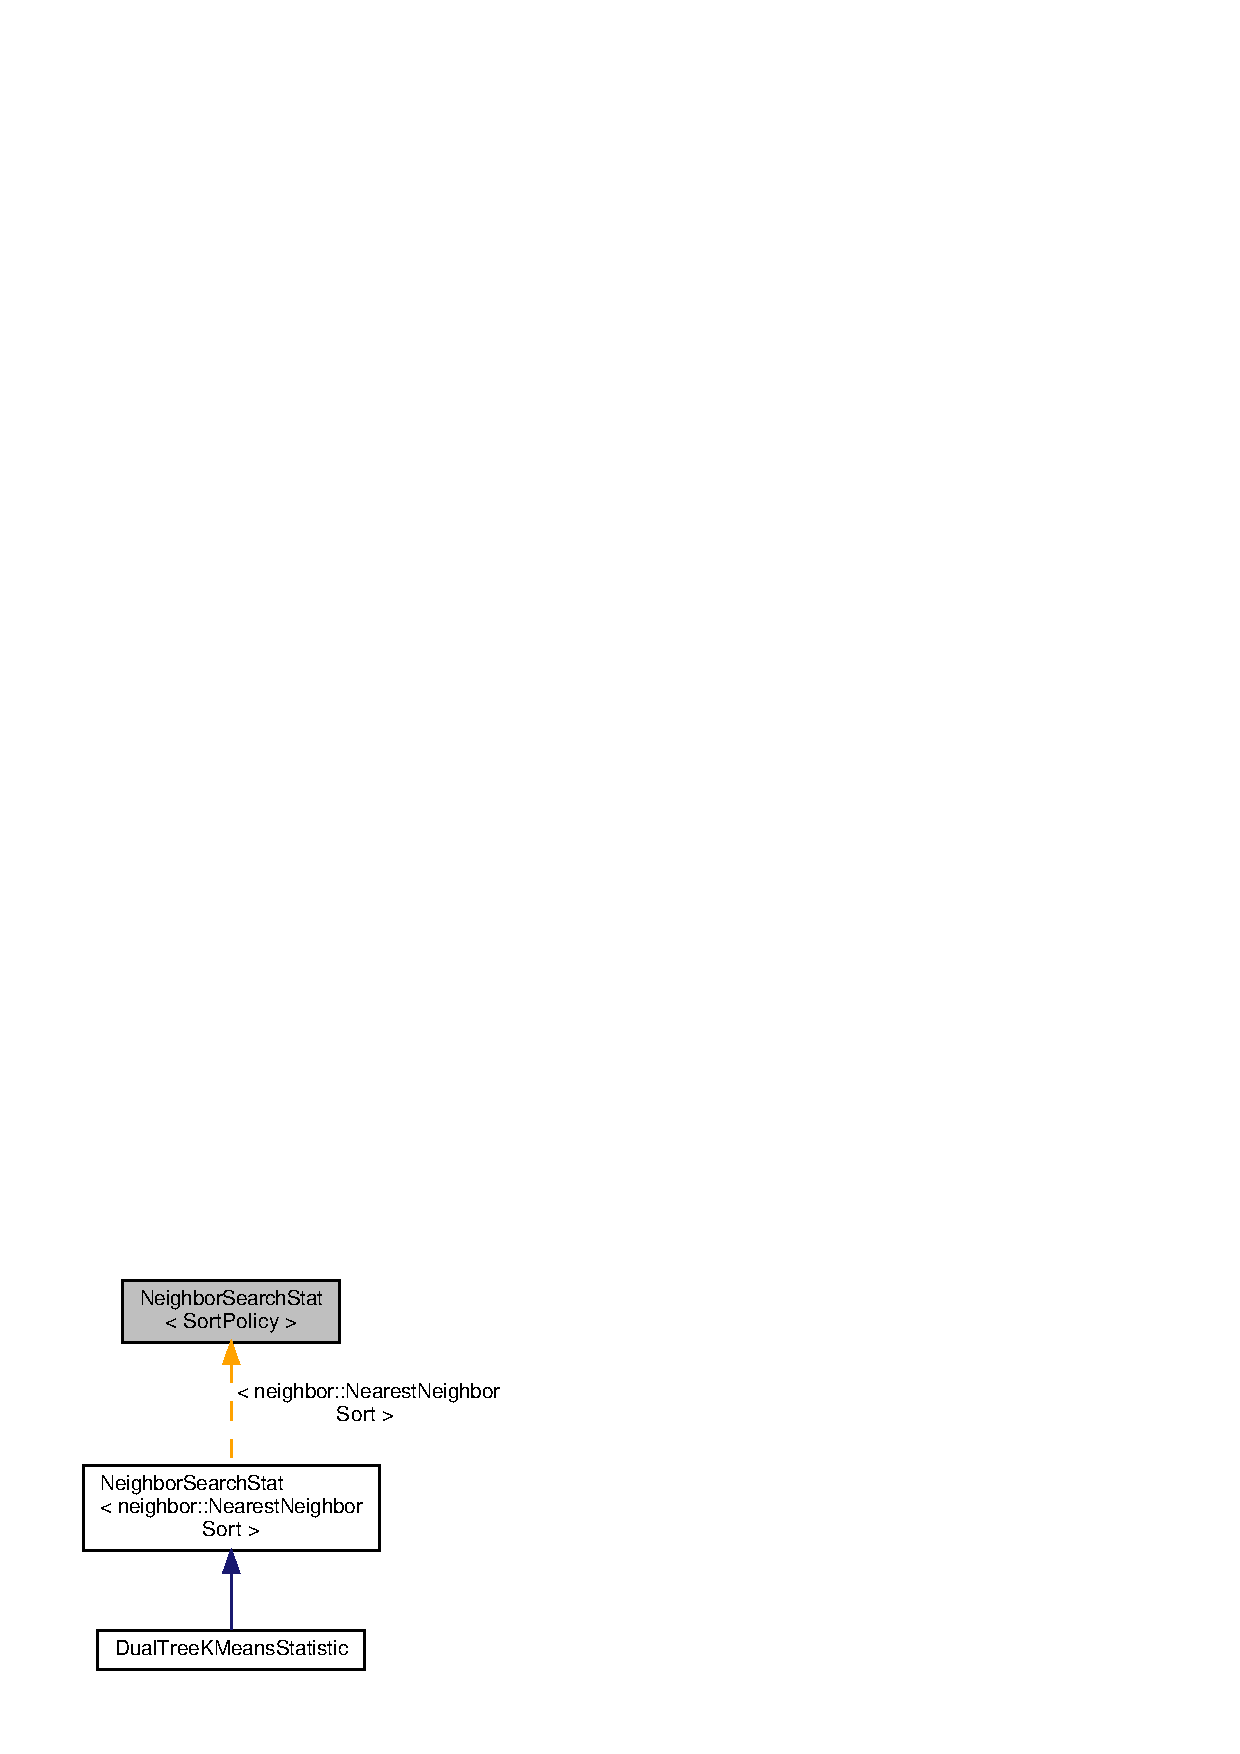
\includegraphics[width=269pt]{classmlpack_1_1neighbor_1_1NeighborSearchStat__inherit__graph}
\end{center}
\end{figure}
\subsection*{Public Member Functions}
\begin{DoxyCompactItemize}
\item 
{\bf Neighbor\+Search\+Stat} ()
\begin{DoxyCompactList}\small\item\em Initialize the statistic with the worst possible distance according to our sorting policy. \end{DoxyCompactList}\item 
{\footnotesize template$<$typename Tree\+Type $>$ }\\{\bf Neighbor\+Search\+Stat} (Tree\+Type \&)
\begin{DoxyCompactList}\small\item\em Initialization for a fully initialized node. \end{DoxyCompactList}\item 
double {\bf Aux\+Bound} () const 
\begin{DoxyCompactList}\small\item\em Get the aux bound. \end{DoxyCompactList}\item 
double \& {\bf Aux\+Bound} ()
\begin{DoxyCompactList}\small\item\em Modify the aux bound. \end{DoxyCompactList}\item 
double {\bf First\+Bound} () const 
\begin{DoxyCompactList}\small\item\em Get the first bound. \end{DoxyCompactList}\item 
double \& {\bf First\+Bound} ()
\begin{DoxyCompactList}\small\item\em Modify the first bound. \end{DoxyCompactList}\item 
double {\bf Last\+Distance} () const 
\begin{DoxyCompactList}\small\item\em Get the last distance calculation. \end{DoxyCompactList}\item 
double \& {\bf Last\+Distance} ()
\begin{DoxyCompactList}\small\item\em Modify the last distance calculation. \end{DoxyCompactList}\item 
void {\bf Reset} ()
\begin{DoxyCompactList}\small\item\em Reset statistic parameters to initial values. \end{DoxyCompactList}\item 
double {\bf Second\+Bound} () const 
\begin{DoxyCompactList}\small\item\em Get the second bound. \end{DoxyCompactList}\item 
double \& {\bf Second\+Bound} ()
\begin{DoxyCompactList}\small\item\em Modify the second bound. \end{DoxyCompactList}\item 
{\footnotesize template$<$typename Archive $>$ }\\void {\bf Serialize} (Archive \&ar, const unsigned int)
\begin{DoxyCompactList}\small\item\em Serialize the statistic to/from an archive. \end{DoxyCompactList}\end{DoxyCompactItemize}
\subsection*{Private Attributes}
\begin{DoxyCompactItemize}
\item 
double {\bf aux\+Bound}
\begin{DoxyCompactList}\small\item\em The aux bound on the node\textquotesingle{}s neighbor distances (B\+\_\+aux). \end{DoxyCompactList}\item 
double {\bf first\+Bound}
\begin{DoxyCompactList}\small\item\em The first bound on the node\textquotesingle{}s neighbor distances (B\+\_\+1). \end{DoxyCompactList}\item 
double {\bf last\+Distance}
\begin{DoxyCompactList}\small\item\em The last distance evaluation. \end{DoxyCompactList}\item 
double {\bf second\+Bound}
\begin{DoxyCompactList}\small\item\em The second bound on the node\textquotesingle{}s neighbor distances (B\+\_\+2). \end{DoxyCompactList}\end{DoxyCompactItemize}


\subsection{Detailed Description}
\subsubsection*{template$<$typename Sort\+Policy$>$\\*
class mlpack\+::neighbor\+::\+Neighbor\+Search\+Stat$<$ Sort\+Policy $>$}

Extra data for each node in the tree. 

For neighbor searches, each node only needs to store a bound on neighbor distances. 

Definition at line 26 of file neighbor\+\_\+search\+\_\+stat.\+hpp.



\subsection{Constructor \& Destructor Documentation}
\index{mlpack\+::neighbor\+::\+Neighbor\+Search\+Stat@{mlpack\+::neighbor\+::\+Neighbor\+Search\+Stat}!Neighbor\+Search\+Stat@{Neighbor\+Search\+Stat}}
\index{Neighbor\+Search\+Stat@{Neighbor\+Search\+Stat}!mlpack\+::neighbor\+::\+Neighbor\+Search\+Stat@{mlpack\+::neighbor\+::\+Neighbor\+Search\+Stat}}
\subsubsection[{Neighbor\+Search\+Stat()}]{\setlength{\rightskip}{0pt plus 5cm}template$<$typename Sort\+Policy$>$ {\bf mlpack\+::neighbor\+::\+Neighbor\+Search\+Stat}$<$ Sort\+Policy $>$\+::{\bf Neighbor\+Search\+Stat} (
\begin{DoxyParamCaption}
{}
\end{DoxyParamCaption}
)\hspace{0.3cm}{\ttfamily [inline]}}\label{classmlpack_1_1neighbor_1_1NeighborSearchStat_a8efff59b8f2413ffc7f1a9b0fed02b45}


Initialize the statistic with the worst possible distance according to our sorting policy. 



Definition at line 48 of file neighbor\+\_\+search\+\_\+stat.\+hpp.

\index{mlpack\+::neighbor\+::\+Neighbor\+Search\+Stat@{mlpack\+::neighbor\+::\+Neighbor\+Search\+Stat}!Neighbor\+Search\+Stat@{Neighbor\+Search\+Stat}}
\index{Neighbor\+Search\+Stat@{Neighbor\+Search\+Stat}!mlpack\+::neighbor\+::\+Neighbor\+Search\+Stat@{mlpack\+::neighbor\+::\+Neighbor\+Search\+Stat}}
\subsubsection[{Neighbor\+Search\+Stat(\+Tree\+Type \&)}]{\setlength{\rightskip}{0pt plus 5cm}template$<$typename Sort\+Policy$>$ template$<$typename Tree\+Type $>$ {\bf mlpack\+::neighbor\+::\+Neighbor\+Search\+Stat}$<$ Sort\+Policy $>$\+::{\bf Neighbor\+Search\+Stat} (
\begin{DoxyParamCaption}
\item[{Tree\+Type \&}]{}
\end{DoxyParamCaption}
)\hspace{0.3cm}{\ttfamily [inline]}}\label{classmlpack_1_1neighbor_1_1NeighborSearchStat_a8775e2180ed292dddc75a06b59d1a5b0}


Initialization for a fully initialized node. 

In this case, we don\textquotesingle{}t need to worry about the node. 

Definition at line 59 of file neighbor\+\_\+search\+\_\+stat.\+hpp.



\subsection{Member Function Documentation}
\index{mlpack\+::neighbor\+::\+Neighbor\+Search\+Stat@{mlpack\+::neighbor\+::\+Neighbor\+Search\+Stat}!Aux\+Bound@{Aux\+Bound}}
\index{Aux\+Bound@{Aux\+Bound}!mlpack\+::neighbor\+::\+Neighbor\+Search\+Stat@{mlpack\+::neighbor\+::\+Neighbor\+Search\+Stat}}
\subsubsection[{Aux\+Bound() const }]{\setlength{\rightskip}{0pt plus 5cm}template$<$typename Sort\+Policy$>$ double {\bf mlpack\+::neighbor\+::\+Neighbor\+Search\+Stat}$<$ Sort\+Policy $>$\+::Aux\+Bound (
\begin{DoxyParamCaption}
{}
\end{DoxyParamCaption}
) const\hspace{0.3cm}{\ttfamily [inline]}}\label{classmlpack_1_1neighbor_1_1NeighborSearchStat_ad11b80578aff64bfa2f6e983b3288321}


Get the aux bound. 



Definition at line 85 of file neighbor\+\_\+search\+\_\+stat.\+hpp.

\index{mlpack\+::neighbor\+::\+Neighbor\+Search\+Stat@{mlpack\+::neighbor\+::\+Neighbor\+Search\+Stat}!Aux\+Bound@{Aux\+Bound}}
\index{Aux\+Bound@{Aux\+Bound}!mlpack\+::neighbor\+::\+Neighbor\+Search\+Stat@{mlpack\+::neighbor\+::\+Neighbor\+Search\+Stat}}
\subsubsection[{Aux\+Bound()}]{\setlength{\rightskip}{0pt plus 5cm}template$<$typename Sort\+Policy$>$ double\& {\bf mlpack\+::neighbor\+::\+Neighbor\+Search\+Stat}$<$ Sort\+Policy $>$\+::Aux\+Bound (
\begin{DoxyParamCaption}
{}
\end{DoxyParamCaption}
)\hspace{0.3cm}{\ttfamily [inline]}}\label{classmlpack_1_1neighbor_1_1NeighborSearchStat_ad74ffebaf7f9230e02e36709006aa1d5}


Modify the aux bound. 



Definition at line 87 of file neighbor\+\_\+search\+\_\+stat.\+hpp.

\index{mlpack\+::neighbor\+::\+Neighbor\+Search\+Stat@{mlpack\+::neighbor\+::\+Neighbor\+Search\+Stat}!First\+Bound@{First\+Bound}}
\index{First\+Bound@{First\+Bound}!mlpack\+::neighbor\+::\+Neighbor\+Search\+Stat@{mlpack\+::neighbor\+::\+Neighbor\+Search\+Stat}}
\subsubsection[{First\+Bound() const }]{\setlength{\rightskip}{0pt plus 5cm}template$<$typename Sort\+Policy$>$ double {\bf mlpack\+::neighbor\+::\+Neighbor\+Search\+Stat}$<$ Sort\+Policy $>$\+::First\+Bound (
\begin{DoxyParamCaption}
{}
\end{DoxyParamCaption}
) const\hspace{0.3cm}{\ttfamily [inline]}}\label{classmlpack_1_1neighbor_1_1NeighborSearchStat_a9947fb2ce911f6cab5a60b246034e834}


Get the first bound. 



Definition at line 77 of file neighbor\+\_\+search\+\_\+stat.\+hpp.

\index{mlpack\+::neighbor\+::\+Neighbor\+Search\+Stat@{mlpack\+::neighbor\+::\+Neighbor\+Search\+Stat}!First\+Bound@{First\+Bound}}
\index{First\+Bound@{First\+Bound}!mlpack\+::neighbor\+::\+Neighbor\+Search\+Stat@{mlpack\+::neighbor\+::\+Neighbor\+Search\+Stat}}
\subsubsection[{First\+Bound()}]{\setlength{\rightskip}{0pt plus 5cm}template$<$typename Sort\+Policy$>$ double\& {\bf mlpack\+::neighbor\+::\+Neighbor\+Search\+Stat}$<$ Sort\+Policy $>$\+::First\+Bound (
\begin{DoxyParamCaption}
{}
\end{DoxyParamCaption}
)\hspace{0.3cm}{\ttfamily [inline]}}\label{classmlpack_1_1neighbor_1_1NeighborSearchStat_a22d0c08e69280a0edc81b743b023a532}


Modify the first bound. 



Definition at line 79 of file neighbor\+\_\+search\+\_\+stat.\+hpp.

\index{mlpack\+::neighbor\+::\+Neighbor\+Search\+Stat@{mlpack\+::neighbor\+::\+Neighbor\+Search\+Stat}!Last\+Distance@{Last\+Distance}}
\index{Last\+Distance@{Last\+Distance}!mlpack\+::neighbor\+::\+Neighbor\+Search\+Stat@{mlpack\+::neighbor\+::\+Neighbor\+Search\+Stat}}
\subsubsection[{Last\+Distance() const }]{\setlength{\rightskip}{0pt plus 5cm}template$<$typename Sort\+Policy$>$ double {\bf mlpack\+::neighbor\+::\+Neighbor\+Search\+Stat}$<$ Sort\+Policy $>$\+::Last\+Distance (
\begin{DoxyParamCaption}
{}
\end{DoxyParamCaption}
) const\hspace{0.3cm}{\ttfamily [inline]}}\label{classmlpack_1_1neighbor_1_1NeighborSearchStat_ac25b9e91da7ab7ffc5b9627895fbe850}


Get the last distance calculation. 



Definition at line 89 of file neighbor\+\_\+search\+\_\+stat.\+hpp.

\index{mlpack\+::neighbor\+::\+Neighbor\+Search\+Stat@{mlpack\+::neighbor\+::\+Neighbor\+Search\+Stat}!Last\+Distance@{Last\+Distance}}
\index{Last\+Distance@{Last\+Distance}!mlpack\+::neighbor\+::\+Neighbor\+Search\+Stat@{mlpack\+::neighbor\+::\+Neighbor\+Search\+Stat}}
\subsubsection[{Last\+Distance()}]{\setlength{\rightskip}{0pt plus 5cm}template$<$typename Sort\+Policy$>$ double\& {\bf mlpack\+::neighbor\+::\+Neighbor\+Search\+Stat}$<$ Sort\+Policy $>$\+::Last\+Distance (
\begin{DoxyParamCaption}
{}
\end{DoxyParamCaption}
)\hspace{0.3cm}{\ttfamily [inline]}}\label{classmlpack_1_1neighbor_1_1NeighborSearchStat_a3a6e26b47746a46056788a42d8626429}


Modify the last distance calculation. 



Definition at line 91 of file neighbor\+\_\+search\+\_\+stat.\+hpp.

\index{mlpack\+::neighbor\+::\+Neighbor\+Search\+Stat@{mlpack\+::neighbor\+::\+Neighbor\+Search\+Stat}!Reset@{Reset}}
\index{Reset@{Reset}!mlpack\+::neighbor\+::\+Neighbor\+Search\+Stat@{mlpack\+::neighbor\+::\+Neighbor\+Search\+Stat}}
\subsubsection[{Reset()}]{\setlength{\rightskip}{0pt plus 5cm}template$<$typename Sort\+Policy$>$ void {\bf mlpack\+::neighbor\+::\+Neighbor\+Search\+Stat}$<$ Sort\+Policy $>$\+::Reset (
\begin{DoxyParamCaption}
{}
\end{DoxyParamCaption}
)\hspace{0.3cm}{\ttfamily [inline]}}\label{classmlpack_1_1neighbor_1_1NeighborSearchStat_a7caf5ae24f1dd2aeb5dc69af6f9f4882}


Reset statistic parameters to initial values. 



Definition at line 68 of file neighbor\+\_\+search\+\_\+stat.\+hpp.

\index{mlpack\+::neighbor\+::\+Neighbor\+Search\+Stat@{mlpack\+::neighbor\+::\+Neighbor\+Search\+Stat}!Second\+Bound@{Second\+Bound}}
\index{Second\+Bound@{Second\+Bound}!mlpack\+::neighbor\+::\+Neighbor\+Search\+Stat@{mlpack\+::neighbor\+::\+Neighbor\+Search\+Stat}}
\subsubsection[{Second\+Bound() const }]{\setlength{\rightskip}{0pt plus 5cm}template$<$typename Sort\+Policy$>$ double {\bf mlpack\+::neighbor\+::\+Neighbor\+Search\+Stat}$<$ Sort\+Policy $>$\+::Second\+Bound (
\begin{DoxyParamCaption}
{}
\end{DoxyParamCaption}
) const\hspace{0.3cm}{\ttfamily [inline]}}\label{classmlpack_1_1neighbor_1_1NeighborSearchStat_a533cb2659b7148fdd734c808f1a3aeb9}


Get the second bound. 



Definition at line 81 of file neighbor\+\_\+search\+\_\+stat.\+hpp.

\index{mlpack\+::neighbor\+::\+Neighbor\+Search\+Stat@{mlpack\+::neighbor\+::\+Neighbor\+Search\+Stat}!Second\+Bound@{Second\+Bound}}
\index{Second\+Bound@{Second\+Bound}!mlpack\+::neighbor\+::\+Neighbor\+Search\+Stat@{mlpack\+::neighbor\+::\+Neighbor\+Search\+Stat}}
\subsubsection[{Second\+Bound()}]{\setlength{\rightskip}{0pt plus 5cm}template$<$typename Sort\+Policy$>$ double\& {\bf mlpack\+::neighbor\+::\+Neighbor\+Search\+Stat}$<$ Sort\+Policy $>$\+::Second\+Bound (
\begin{DoxyParamCaption}
{}
\end{DoxyParamCaption}
)\hspace{0.3cm}{\ttfamily [inline]}}\label{classmlpack_1_1neighbor_1_1NeighborSearchStat_a79c94b6ddfd951d46d60a35a64291f70}


Modify the second bound. 



Definition at line 83 of file neighbor\+\_\+search\+\_\+stat.\+hpp.

\index{mlpack\+::neighbor\+::\+Neighbor\+Search\+Stat@{mlpack\+::neighbor\+::\+Neighbor\+Search\+Stat}!Serialize@{Serialize}}
\index{Serialize@{Serialize}!mlpack\+::neighbor\+::\+Neighbor\+Search\+Stat@{mlpack\+::neighbor\+::\+Neighbor\+Search\+Stat}}
\subsubsection[{Serialize(\+Archive \&ar, const unsigned int)}]{\setlength{\rightskip}{0pt plus 5cm}template$<$typename Sort\+Policy$>$ template$<$typename Archive $>$ void {\bf mlpack\+::neighbor\+::\+Neighbor\+Search\+Stat}$<$ Sort\+Policy $>$\+::Serialize (
\begin{DoxyParamCaption}
\item[{Archive \&}]{ar, }
\item[{const unsigned}]{int}
\end{DoxyParamCaption}
)\hspace{0.3cm}{\ttfamily [inline]}}\label{classmlpack_1_1neighbor_1_1NeighborSearchStat_ad93d4e645c6cb03c346c43a7db9e98fb}


Serialize the statistic to/from an archive. 



Definition at line 95 of file neighbor\+\_\+search\+\_\+stat.\+hpp.



\subsection{Member Data Documentation}
\index{mlpack\+::neighbor\+::\+Neighbor\+Search\+Stat@{mlpack\+::neighbor\+::\+Neighbor\+Search\+Stat}!aux\+Bound@{aux\+Bound}}
\index{aux\+Bound@{aux\+Bound}!mlpack\+::neighbor\+::\+Neighbor\+Search\+Stat@{mlpack\+::neighbor\+::\+Neighbor\+Search\+Stat}}
\subsubsection[{aux\+Bound}]{\setlength{\rightskip}{0pt plus 5cm}template$<$typename Sort\+Policy$>$ double {\bf mlpack\+::neighbor\+::\+Neighbor\+Search\+Stat}$<$ Sort\+Policy $>$\+::aux\+Bound\hspace{0.3cm}{\ttfamily [private]}}\label{classmlpack_1_1neighbor_1_1NeighborSearchStat_a3ee0117fca9864d170ee426771064538}


The aux bound on the node\textquotesingle{}s neighbor distances (B\+\_\+aux). 

This represents the best descendant candidate distance (used to calculate second\+Bound). 

Definition at line 39 of file neighbor\+\_\+search\+\_\+stat.\+hpp.



Referenced by mlpack\+::neighbor\+::\+Neighbor\+Search\+Stat$<$ neighbor\+::\+Nearest\+Neighbor\+Sort $>$\+::\+Aux\+Bound().

\index{mlpack\+::neighbor\+::\+Neighbor\+Search\+Stat@{mlpack\+::neighbor\+::\+Neighbor\+Search\+Stat}!first\+Bound@{first\+Bound}}
\index{first\+Bound@{first\+Bound}!mlpack\+::neighbor\+::\+Neighbor\+Search\+Stat@{mlpack\+::neighbor\+::\+Neighbor\+Search\+Stat}}
\subsubsection[{first\+Bound}]{\setlength{\rightskip}{0pt plus 5cm}template$<$typename Sort\+Policy$>$ double {\bf mlpack\+::neighbor\+::\+Neighbor\+Search\+Stat}$<$ Sort\+Policy $>$\+::first\+Bound\hspace{0.3cm}{\ttfamily [private]}}\label{classmlpack_1_1neighbor_1_1NeighborSearchStat_ab555ed384690f47d9cbef7697c27b05c}


The first bound on the node\textquotesingle{}s neighbor distances (B\+\_\+1). 

This represents the worst candidate distance of any descendants of this node. 

Definition at line 31 of file neighbor\+\_\+search\+\_\+stat.\+hpp.



Referenced by mlpack\+::neighbor\+::\+Neighbor\+Search\+Stat$<$ neighbor\+::\+Nearest\+Neighbor\+Sort $>$\+::\+First\+Bound().

\index{mlpack\+::neighbor\+::\+Neighbor\+Search\+Stat@{mlpack\+::neighbor\+::\+Neighbor\+Search\+Stat}!last\+Distance@{last\+Distance}}
\index{last\+Distance@{last\+Distance}!mlpack\+::neighbor\+::\+Neighbor\+Search\+Stat@{mlpack\+::neighbor\+::\+Neighbor\+Search\+Stat}}
\subsubsection[{last\+Distance}]{\setlength{\rightskip}{0pt plus 5cm}template$<$typename Sort\+Policy$>$ double {\bf mlpack\+::neighbor\+::\+Neighbor\+Search\+Stat}$<$ Sort\+Policy $>$\+::last\+Distance\hspace{0.3cm}{\ttfamily [private]}}\label{classmlpack_1_1neighbor_1_1NeighborSearchStat_ac009992f1081ef962a16023f8e00c691}


The last distance evaluation. 



Definition at line 41 of file neighbor\+\_\+search\+\_\+stat.\+hpp.



Referenced by mlpack\+::neighbor\+::\+Neighbor\+Search\+Stat$<$ neighbor\+::\+Nearest\+Neighbor\+Sort $>$\+::\+Last\+Distance().

\index{mlpack\+::neighbor\+::\+Neighbor\+Search\+Stat@{mlpack\+::neighbor\+::\+Neighbor\+Search\+Stat}!second\+Bound@{second\+Bound}}
\index{second\+Bound@{second\+Bound}!mlpack\+::neighbor\+::\+Neighbor\+Search\+Stat@{mlpack\+::neighbor\+::\+Neighbor\+Search\+Stat}}
\subsubsection[{second\+Bound}]{\setlength{\rightskip}{0pt plus 5cm}template$<$typename Sort\+Policy$>$ double {\bf mlpack\+::neighbor\+::\+Neighbor\+Search\+Stat}$<$ Sort\+Policy $>$\+::second\+Bound\hspace{0.3cm}{\ttfamily [private]}}\label{classmlpack_1_1neighbor_1_1NeighborSearchStat_a42c403ceeff0a2bbc4c386924c8dcf05}


The second bound on the node\textquotesingle{}s neighbor distances (B\+\_\+2). 

This represents a bound on the worst distance of any descendants of this node assembled using the best descendant candidate distance modified by the furthest descendant distance. 

Definition at line 36 of file neighbor\+\_\+search\+\_\+stat.\+hpp.



Referenced by mlpack\+::neighbor\+::\+Neighbor\+Search\+Stat$<$ neighbor\+::\+Nearest\+Neighbor\+Sort $>$\+::\+Second\+Bound().



The documentation for this class was generated from the following file\+:\begin{DoxyCompactItemize}
\item 
src/mlpack/methods/neighbor\+\_\+search/{\bf neighbor\+\_\+search\+\_\+stat.\+hpp}\end{DoxyCompactItemize}

\doxysection{NSModel$<$ Sort\+Policy $>$ Class Template Reference}
\label{classmlpack_1_1neighbor_1_1NSModel}\index{NSModel$<$ SortPolicy $>$@{NSModel$<$ SortPolicy $>$}}


The \doxyref{NSModel}{p.}{classmlpack_1_1neighbor_1_1NSModel} class provides an easy way to serialize a model, abstracts away the different types of trees, and also reflects the \doxyref{Neighbor\+Search}{p.}{classmlpack_1_1neighbor_1_1NeighborSearch} API.  


\doxysubsection*{Public Types}
\begin{DoxyCompactItemize}
\item 
enum \textbf{ Tree\+Types} \{ \newline
\textbf{ KD\+\_\+\+TREE}
, \newline
\textbf{ COVER\+\_\+\+TREE}
, \newline
\textbf{ R\+\_\+\+TREE}
, \newline
\textbf{ R\+\_\+\+STAR\+\_\+\+TREE}
, \newline
\textbf{ BALL\+\_\+\+TREE}
, \newline
\textbf{ X\+\_\+\+TREE}
, \newline
\textbf{ HILBERT\+\_\+\+R\+\_\+\+TREE}
, \newline
\textbf{ R\+\_\+\+PLUS\+\_\+\+TREE}
, \newline
\textbf{ R\+\_\+\+PLUS\+\_\+\+PLUS\+\_\+\+TREE}
, \newline
\textbf{ VP\+\_\+\+TREE}
, \newline
\textbf{ RP\+\_\+\+TREE}
, \newline
\textbf{ MAX\+\_\+\+RP\+\_\+\+TREE}
, \newline
\textbf{ SPILL\+\_\+\+TREE}
, \newline
\textbf{ UB\+\_\+\+TREE}
, \newline
\textbf{ OCTREE}
 \}
\begin{DoxyCompactList}\small\item\em Enum type to identify each accepted tree type. \end{DoxyCompactList}\end{DoxyCompactItemize}
\doxysubsection*{Public Member Functions}
\begin{DoxyCompactItemize}
\item 
\textbf{ NSModel} (const \textbf{ NSModel} \&other)
\begin{DoxyCompactList}\small\item\em Copy the given \doxyref{NSModel}{p.}{classmlpack_1_1neighbor_1_1NSModel}. \end{DoxyCompactList}\item 
\textbf{ NSModel} (\textbf{ NSModel} \&\&other)
\begin{DoxyCompactList}\small\item\em Take ownership of the given \doxyref{NSModel}{p.}{classmlpack_1_1neighbor_1_1NSModel}. \end{DoxyCompactList}\item 
\textbf{ NSModel} (\textbf{ Tree\+Types} tree\+Type=Tree\+Types\+::\+KD\+\_\+\+TREE, bool random\+Basis=false)
\begin{DoxyCompactList}\small\item\em Initialize the \doxyref{NSModel}{p.}{classmlpack_1_1neighbor_1_1NSModel} with the given type and whether or not a random basis should be used. \end{DoxyCompactList}\item 
\textbf{ $\sim$\+NSModel} ()
\begin{DoxyCompactList}\small\item\em Clean memory, if necessary. \end{DoxyCompactList}\item 
void \textbf{ Build\+Model} (arma\+::mat \&\&reference\+Set, const \textbf{ Neighbor\+Search\+Mode} search\+Mode, const double epsilon=0)
\begin{DoxyCompactList}\small\item\em Build the reference tree. \end{DoxyCompactList}\item 
const arma\+::mat \& \textbf{ Dataset} () const
\begin{DoxyCompactList}\small\item\em Expose the dataset. \end{DoxyCompactList}\item 
double \& \textbf{ Epsilon} ()
\item 
double \textbf{ Epsilon} () const
\begin{DoxyCompactList}\small\item\em Expose Epsilon. \end{DoxyCompactList}\item 
void \textbf{ Initialize\+Model} (const \textbf{ Neighbor\+Search\+Mode} search\+Mode, const double epsilon)
\begin{DoxyCompactList}\small\item\em Initialize the model type. (This does not perform any training.) \end{DoxyCompactList}\item 
size\+\_\+t \& \textbf{ Leaf\+Size} ()
\item 
size\+\_\+t \textbf{ Leaf\+Size} () const
\begin{DoxyCompactList}\small\item\em Expose Leaf\+Size. \end{DoxyCompactList}\item 
\textbf{ NSModel} \& \textbf{ operator=} (const \textbf{ NSModel} \&other)
\begin{DoxyCompactList}\small\item\em Copy the given \doxyref{NSModel}{p.}{classmlpack_1_1neighbor_1_1NSModel}. \end{DoxyCompactList}\item 
\textbf{ NSModel} \& \textbf{ operator=} (\textbf{ NSModel} \&\&other)
\begin{DoxyCompactList}\small\item\em Take ownership of the given \doxyref{NSModel}{p.}{classmlpack_1_1neighbor_1_1NSModel}. \end{DoxyCompactList}\item 
bool \& \textbf{ Random\+Basis} ()
\item 
bool \textbf{ Random\+Basis} () const
\begin{DoxyCompactList}\small\item\em Expose random\+Basis. \end{DoxyCompactList}\item 
double \& \textbf{ Rho} ()
\item 
double \textbf{ Rho} () const
\begin{DoxyCompactList}\small\item\em Expose Rho. \end{DoxyCompactList}\item 
void \textbf{ Search} (arma\+::mat \&\&query\+Set, const size\+\_\+t k, arma\+::\+Mat$<$ size\+\_\+t $>$ \&neighbors, arma\+::mat \&distances)
\begin{DoxyCompactList}\small\item\em Perform neighbor search. The query set will be reordered. \end{DoxyCompactList}\item 
void \textbf{ Search} (const size\+\_\+t k, arma\+::\+Mat$<$ size\+\_\+t $>$ \&neighbors, arma\+::mat \&distances)
\begin{DoxyCompactList}\small\item\em Perform monochromatic neighbor search. \end{DoxyCompactList}\item 
\textbf{ Neighbor\+Search\+Mode} \& \textbf{ Search\+Mode} ()
\item 
\textbf{ Neighbor\+Search\+Mode} \textbf{ Search\+Mode} () const
\begin{DoxyCompactList}\small\item\em Expose Search\+Mode. \end{DoxyCompactList}\item 
{\footnotesize template$<$typename Archive $>$ }\\void \textbf{ serialize} (Archive \&ar, const uint32\+\_\+t)
\begin{DoxyCompactList}\small\item\em Serialize the neighbor search model. \end{DoxyCompactList}\item 
double \& \textbf{ Tau} ()
\item 
double \textbf{ Tau} () const
\begin{DoxyCompactList}\small\item\em Expose Tau. \end{DoxyCompactList}\item 
std\+::string \textbf{ Tree\+Name} () const
\begin{DoxyCompactList}\small\item\em Return a string representation of the current tree type. \end{DoxyCompactList}\item 
\textbf{ Tree\+Types} \& \textbf{ Tree\+Type} ()
\item 
\textbf{ Tree\+Types} \textbf{ Tree\+Type} () const
\begin{DoxyCompactList}\small\item\em Expose tree\+Type. \end{DoxyCompactList}\end{DoxyCompactItemize}


\doxysubsection{Detailed Description}
\subsubsection*{template$<$typename Sort\+Policy$>$\newline
class mlpack\+::neighbor\+::\+NSModel$<$ Sort\+Policy $>$}

The \doxyref{NSModel}{p.}{classmlpack_1_1neighbor_1_1NSModel} class provides an easy way to serialize a model, abstracts away the different types of trees, and also reflects the \doxyref{Neighbor\+Search}{p.}{classmlpack_1_1neighbor_1_1NeighborSearch} API. 

This class is meant to be used by the command-\/line mlpack\+\_\+knn and mlpack\+\_\+kfn programs, and thus does not have the same complete functionality and flexibility as the \doxyref{Neighbor\+Search}{p.}{classmlpack_1_1neighbor_1_1NeighborSearch} class. So if you are using it outside of mlpack\+\_\+knn and mlpack\+\_\+kfn, be aware that it is limited!


\begin{DoxyTemplParams}{Template Parameters}
{\em Sort\+Policy} & The sort policy for distances; see Nearest\+Neighbor\+Sort. \\
\hline
\end{DoxyTemplParams}


Definition at line 333 of file ns\+\_\+model.\+hpp.



\doxysubsection{Member Enumeration Documentation}
\mbox{\label{classmlpack_1_1neighbor_1_1NSModel_a6597b8539c6114170dc185d332ba4c8d}} 
\index{NSModel$<$ SortPolicy $>$@{NSModel$<$ SortPolicy $>$}!TreeTypes@{TreeTypes}}
\index{TreeTypes@{TreeTypes}!NSModel$<$ SortPolicy $>$@{NSModel$<$ SortPolicy $>$}}
\doxysubsubsection{TreeTypes}
{\footnotesize\ttfamily enum \textbf{ Tree\+Types}}



Enum type to identify each accepted tree type. 

\begin{DoxyEnumFields}{Enumerator}
\raisebox{\heightof{T}}[0pt][0pt]{\index{KD\_TREE@{KD\_TREE}!NSModel$<$ SortPolicy $>$@{NSModel$<$ SortPolicy $>$}}\index{NSModel$<$ SortPolicy $>$@{NSModel$<$ SortPolicy $>$}!KD\_TREE@{KD\_TREE}}}\mbox{\label{classmlpack_1_1neighbor_1_1NSModel_a6597b8539c6114170dc185d332ba4c8daa688e9cd1158916bc183aa517724568c}} 
KD\+\_\+\+TREE&\\
\hline

\raisebox{\heightof{T}}[0pt][0pt]{\index{COVER\_TREE@{COVER\_TREE}!NSModel$<$ SortPolicy $>$@{NSModel$<$ SortPolicy $>$}}\index{NSModel$<$ SortPolicy $>$@{NSModel$<$ SortPolicy $>$}!COVER\_TREE@{COVER\_TREE}}}\mbox{\label{classmlpack_1_1neighbor_1_1NSModel_a6597b8539c6114170dc185d332ba4c8da92f172b47c8ae18ed401f8bf9f5ecad3}} 
COVER\+\_\+\+TREE&\\
\hline

\raisebox{\heightof{T}}[0pt][0pt]{\index{R\_TREE@{R\_TREE}!NSModel$<$ SortPolicy $>$@{NSModel$<$ SortPolicy $>$}}\index{NSModel$<$ SortPolicy $>$@{NSModel$<$ SortPolicy $>$}!R\_TREE@{R\_TREE}}}\mbox{\label{classmlpack_1_1neighbor_1_1NSModel_a6597b8539c6114170dc185d332ba4c8da2a93dc779a94d5f09b72ffbdc5ac9cd9}} 
R\+\_\+\+TREE&\\
\hline

\raisebox{\heightof{T}}[0pt][0pt]{\index{R\_STAR\_TREE@{R\_STAR\_TREE}!NSModel$<$ SortPolicy $>$@{NSModel$<$ SortPolicy $>$}}\index{NSModel$<$ SortPolicy $>$@{NSModel$<$ SortPolicy $>$}!R\_STAR\_TREE@{R\_STAR\_TREE}}}\mbox{\label{classmlpack_1_1neighbor_1_1NSModel_a6597b8539c6114170dc185d332ba4c8dae5b37a52c347bc7ef3d23fde0941d27b}} 
R\+\_\+\+STAR\+\_\+\+TREE&\\
\hline

\raisebox{\heightof{T}}[0pt][0pt]{\index{BALL\_TREE@{BALL\_TREE}!NSModel$<$ SortPolicy $>$@{NSModel$<$ SortPolicy $>$}}\index{NSModel$<$ SortPolicy $>$@{NSModel$<$ SortPolicy $>$}!BALL\_TREE@{BALL\_TREE}}}\mbox{\label{classmlpack_1_1neighbor_1_1NSModel_a6597b8539c6114170dc185d332ba4c8da994ef1bcca8841d5b7d1431b99fcb10d}} 
BALL\+\_\+\+TREE&\\
\hline

\raisebox{\heightof{T}}[0pt][0pt]{\index{X\_TREE@{X\_TREE}!NSModel$<$ SortPolicy $>$@{NSModel$<$ SortPolicy $>$}}\index{NSModel$<$ SortPolicy $>$@{NSModel$<$ SortPolicy $>$}!X\_TREE@{X\_TREE}}}\mbox{\label{classmlpack_1_1neighbor_1_1NSModel_a6597b8539c6114170dc185d332ba4c8da6560e35678b39452afce0f0fcc7f6059}} 
X\+\_\+\+TREE&\\
\hline

\raisebox{\heightof{T}}[0pt][0pt]{\index{HILBERT\_R\_TREE@{HILBERT\_R\_TREE}!NSModel$<$ SortPolicy $>$@{NSModel$<$ SortPolicy $>$}}\index{NSModel$<$ SortPolicy $>$@{NSModel$<$ SortPolicy $>$}!HILBERT\_R\_TREE@{HILBERT\_R\_TREE}}}\mbox{\label{classmlpack_1_1neighbor_1_1NSModel_a6597b8539c6114170dc185d332ba4c8da470c5bcf4135483a37e9a87f061e1c5c}} 
HILBERT\+\_\+\+R\+\_\+\+TREE&\\
\hline

\raisebox{\heightof{T}}[0pt][0pt]{\index{R\_PLUS\_TREE@{R\_PLUS\_TREE}!NSModel$<$ SortPolicy $>$@{NSModel$<$ SortPolicy $>$}}\index{NSModel$<$ SortPolicy $>$@{NSModel$<$ SortPolicy $>$}!R\_PLUS\_TREE@{R\_PLUS\_TREE}}}\mbox{\label{classmlpack_1_1neighbor_1_1NSModel_a6597b8539c6114170dc185d332ba4c8da4e91a297c1504b34ca1a9cdcd6ba22ff}} 
R\+\_\+\+PLUS\+\_\+\+TREE&\\
\hline

\raisebox{\heightof{T}}[0pt][0pt]{\index{R\_PLUS\_PLUS\_TREE@{R\_PLUS\_PLUS\_TREE}!NSModel$<$ SortPolicy $>$@{NSModel$<$ SortPolicy $>$}}\index{NSModel$<$ SortPolicy $>$@{NSModel$<$ SortPolicy $>$}!R\_PLUS\_PLUS\_TREE@{R\_PLUS\_PLUS\_TREE}}}\mbox{\label{classmlpack_1_1neighbor_1_1NSModel_a6597b8539c6114170dc185d332ba4c8da1208f6f2a7b337e4edbd02a8de98d3f5}} 
R\+\_\+\+PLUS\+\_\+\+PLUS\+\_\+\+TREE&\\
\hline

\raisebox{\heightof{T}}[0pt][0pt]{\index{VP\_TREE@{VP\_TREE}!NSModel$<$ SortPolicy $>$@{NSModel$<$ SortPolicy $>$}}\index{NSModel$<$ SortPolicy $>$@{NSModel$<$ SortPolicy $>$}!VP\_TREE@{VP\_TREE}}}\mbox{\label{classmlpack_1_1neighbor_1_1NSModel_a6597b8539c6114170dc185d332ba4c8daa8a6aade44830d33165414079bf8dd1c}} 
VP\+\_\+\+TREE&\\
\hline

\raisebox{\heightof{T}}[0pt][0pt]{\index{RP\_TREE@{RP\_TREE}!NSModel$<$ SortPolicy $>$@{NSModel$<$ SortPolicy $>$}}\index{NSModel$<$ SortPolicy $>$@{NSModel$<$ SortPolicy $>$}!RP\_TREE@{RP\_TREE}}}\mbox{\label{classmlpack_1_1neighbor_1_1NSModel_a6597b8539c6114170dc185d332ba4c8dae6815061fe1e77dc1b2ae96b07b40250}} 
RP\+\_\+\+TREE&\\
\hline

\raisebox{\heightof{T}}[0pt][0pt]{\index{MAX\_RP\_TREE@{MAX\_RP\_TREE}!NSModel$<$ SortPolicy $>$@{NSModel$<$ SortPolicy $>$}}\index{NSModel$<$ SortPolicy $>$@{NSModel$<$ SortPolicy $>$}!MAX\_RP\_TREE@{MAX\_RP\_TREE}}}\mbox{\label{classmlpack_1_1neighbor_1_1NSModel_a6597b8539c6114170dc185d332ba4c8da0e4ed6912ca7a8232754df8771365c96}} 
MAX\+\_\+\+RP\+\_\+\+TREE&\\
\hline

\raisebox{\heightof{T}}[0pt][0pt]{\index{SPILL\_TREE@{SPILL\_TREE}!NSModel$<$ SortPolicy $>$@{NSModel$<$ SortPolicy $>$}}\index{NSModel$<$ SortPolicy $>$@{NSModel$<$ SortPolicy $>$}!SPILL\_TREE@{SPILL\_TREE}}}\mbox{\label{classmlpack_1_1neighbor_1_1NSModel_a6597b8539c6114170dc185d332ba4c8dae380b83ef5a8ba2c32c569705a8b66fc}} 
SPILL\+\_\+\+TREE&\\
\hline

\raisebox{\heightof{T}}[0pt][0pt]{\index{UB\_TREE@{UB\_TREE}!NSModel$<$ SortPolicy $>$@{NSModel$<$ SortPolicy $>$}}\index{NSModel$<$ SortPolicy $>$@{NSModel$<$ SortPolicy $>$}!UB\_TREE@{UB\_TREE}}}\mbox{\label{classmlpack_1_1neighbor_1_1NSModel_a6597b8539c6114170dc185d332ba4c8dae36341db74fc7194b238cf7c528a7fbc}} 
UB\+\_\+\+TREE&\\
\hline

\raisebox{\heightof{T}}[0pt][0pt]{\index{OCTREE@{OCTREE}!NSModel$<$ SortPolicy $>$@{NSModel$<$ SortPolicy $>$}}\index{NSModel$<$ SortPolicy $>$@{NSModel$<$ SortPolicy $>$}!OCTREE@{OCTREE}}}\mbox{\label{classmlpack_1_1neighbor_1_1NSModel_a6597b8539c6114170dc185d332ba4c8daabefbb1ea7a801b1b00c9b0709dcec50}} 
OCTREE&\\
\hline

\end{DoxyEnumFields}


Definition at line 337 of file ns\+\_\+model.\+hpp.



\doxysubsection{Constructor \& Destructor Documentation}
\mbox{\label{classmlpack_1_1neighbor_1_1NSModel_a79e4c6c22da7f04fc8f9a5bae9b688e1}} 
\index{NSModel$<$ SortPolicy $>$@{NSModel$<$ SortPolicy $>$}!NSModel@{NSModel}}
\index{NSModel@{NSModel}!NSModel$<$ SortPolicy $>$@{NSModel$<$ SortPolicy $>$}}
\doxysubsubsection{NSModel()\hspace{0.1cm}{\footnotesize\ttfamily [1/3]}}
{\footnotesize\ttfamily \textbf{ NSModel} (\begin{DoxyParamCaption}\item[{\textbf{ Tree\+Types}}]{tree\+Type = {\ttfamily TreeTypes\+:\+:KD\+\_\+TREE},  }\item[{bool}]{random\+Basis = {\ttfamily false} }\end{DoxyParamCaption})}



Initialize the \doxyref{NSModel}{p.}{classmlpack_1_1neighbor_1_1NSModel} with the given type and whether or not a random basis should be used. 


\begin{DoxyParams}{Parameters}
{\em tree\+Type} & Type of tree to use. \\
\hline
{\em random\+Basis} & Whether or not to project the points onto a random basis before searching. \\
\hline
\end{DoxyParams}
\mbox{\label{classmlpack_1_1neighbor_1_1NSModel_a6377c3a4b61de368dedff9fa95304359}} 
\index{NSModel$<$ SortPolicy $>$@{NSModel$<$ SortPolicy $>$}!NSModel@{NSModel}}
\index{NSModel@{NSModel}!NSModel$<$ SortPolicy $>$@{NSModel$<$ SortPolicy $>$}}
\doxysubsubsection{NSModel()\hspace{0.1cm}{\footnotesize\ttfamily [2/3]}}
{\footnotesize\ttfamily \textbf{ NSModel} (\begin{DoxyParamCaption}\item[{const \textbf{ NSModel}$<$ Sort\+Policy $>$ \&}]{other }\end{DoxyParamCaption})}



Copy the given \doxyref{NSModel}{p.}{classmlpack_1_1neighbor_1_1NSModel}. 


\begin{DoxyParams}{Parameters}
{\em other} & Model to copy. \\
\hline
\end{DoxyParams}
\mbox{\label{classmlpack_1_1neighbor_1_1NSModel_a8eba8cadae0d4294becc60ec69cf158d}} 
\index{NSModel$<$ SortPolicy $>$@{NSModel$<$ SortPolicy $>$}!NSModel@{NSModel}}
\index{NSModel@{NSModel}!NSModel$<$ SortPolicy $>$@{NSModel$<$ SortPolicy $>$}}
\doxysubsubsection{NSModel()\hspace{0.1cm}{\footnotesize\ttfamily [3/3]}}
{\footnotesize\ttfamily \textbf{ NSModel} (\begin{DoxyParamCaption}\item[{\textbf{ NSModel}$<$ Sort\+Policy $>$ \&\&}]{other }\end{DoxyParamCaption})}



Take ownership of the given \doxyref{NSModel}{p.}{classmlpack_1_1neighbor_1_1NSModel}. 


\begin{DoxyParams}{Parameters}
{\em other} & Model to take ownership of. \\
\hline
\end{DoxyParams}
\mbox{\label{classmlpack_1_1neighbor_1_1NSModel_a25d5032163e2f4db1c2330d689df8434}} 
\index{NSModel$<$ SortPolicy $>$@{NSModel$<$ SortPolicy $>$}!````~NSModel@{$\sim$NSModel}}
\index{````~NSModel@{$\sim$NSModel}!NSModel$<$ SortPolicy $>$@{NSModel$<$ SortPolicy $>$}}
\doxysubsubsection{$\sim$NSModel()}
{\footnotesize\ttfamily $\sim$\textbf{ NSModel} (\begin{DoxyParamCaption}{ }\end{DoxyParamCaption})}



Clean memory, if necessary. 



\doxysubsection{Member Function Documentation}
\mbox{\label{classmlpack_1_1neighbor_1_1NSModel_aa5cbba6575bb949e63ace34052516eb6}} 
\index{NSModel$<$ SortPolicy $>$@{NSModel$<$ SortPolicy $>$}!BuildModel@{BuildModel}}
\index{BuildModel@{BuildModel}!NSModel$<$ SortPolicy $>$@{NSModel$<$ SortPolicy $>$}}
\doxysubsubsection{BuildModel()}
{\footnotesize\ttfamily void Build\+Model (\begin{DoxyParamCaption}\item[{arma\+::mat \&\&}]{reference\+Set,  }\item[{const \textbf{ Neighbor\+Search\+Mode}}]{search\+Mode,  }\item[{const double}]{epsilon = {\ttfamily 0} }\end{DoxyParamCaption})}



Build the reference tree. 

\mbox{\label{classmlpack_1_1neighbor_1_1NSModel_aff320b9a86b77a150e630c01d5888273}} 
\index{NSModel$<$ SortPolicy $>$@{NSModel$<$ SortPolicy $>$}!Dataset@{Dataset}}
\index{Dataset@{Dataset}!NSModel$<$ SortPolicy $>$@{NSModel$<$ SortPolicy $>$}}
\doxysubsubsection{Dataset()}
{\footnotesize\ttfamily const arma\+::mat\& Dataset (\begin{DoxyParamCaption}{ }\end{DoxyParamCaption}) const}



Expose the dataset. 

\mbox{\label{classmlpack_1_1neighbor_1_1NSModel_ab6a080993b32456443eced5df2f8b9b9}} 
\index{NSModel$<$ SortPolicy $>$@{NSModel$<$ SortPolicy $>$}!Epsilon@{Epsilon}}
\index{Epsilon@{Epsilon}!NSModel$<$ SortPolicy $>$@{NSModel$<$ SortPolicy $>$}}
\doxysubsubsection{Epsilon()\hspace{0.1cm}{\footnotesize\ttfamily [1/2]}}
{\footnotesize\ttfamily double\& Epsilon (\begin{DoxyParamCaption}{ }\end{DoxyParamCaption})}

\mbox{\label{classmlpack_1_1neighbor_1_1NSModel_af6d960193bb5db37e51416e12bf720de}} 
\index{NSModel$<$ SortPolicy $>$@{NSModel$<$ SortPolicy $>$}!Epsilon@{Epsilon}}
\index{Epsilon@{Epsilon}!NSModel$<$ SortPolicy $>$@{NSModel$<$ SortPolicy $>$}}
\doxysubsubsection{Epsilon()\hspace{0.1cm}{\footnotesize\ttfamily [2/2]}}
{\footnotesize\ttfamily double Epsilon (\begin{DoxyParamCaption}{ }\end{DoxyParamCaption}) const}



Expose Epsilon. 

\mbox{\label{classmlpack_1_1neighbor_1_1NSModel_a407a10954f142968edc38f36c321c6b8}} 
\index{NSModel$<$ SortPolicy $>$@{NSModel$<$ SortPolicy $>$}!InitializeModel@{InitializeModel}}
\index{InitializeModel@{InitializeModel}!NSModel$<$ SortPolicy $>$@{NSModel$<$ SortPolicy $>$}}
\doxysubsubsection{InitializeModel()}
{\footnotesize\ttfamily void Initialize\+Model (\begin{DoxyParamCaption}\item[{const \textbf{ Neighbor\+Search\+Mode}}]{search\+Mode,  }\item[{const double}]{epsilon }\end{DoxyParamCaption})}



Initialize the model type. (This does not perform any training.) 

\mbox{\label{classmlpack_1_1neighbor_1_1NSModel_a0966773f5b7ef0c324ed40b1cf4b94d1}} 
\index{NSModel$<$ SortPolicy $>$@{NSModel$<$ SortPolicy $>$}!LeafSize@{LeafSize}}
\index{LeafSize@{LeafSize}!NSModel$<$ SortPolicy $>$@{NSModel$<$ SortPolicy $>$}}
\doxysubsubsection{LeafSize()\hspace{0.1cm}{\footnotesize\ttfamily [1/2]}}
{\footnotesize\ttfamily size\+\_\+t\& Leaf\+Size (\begin{DoxyParamCaption}{ }\end{DoxyParamCaption})\hspace{0.3cm}{\ttfamily [inline]}}



Definition at line 430 of file ns\+\_\+model.\+hpp.

\mbox{\label{classmlpack_1_1neighbor_1_1NSModel_ab81b93ebb200783ca4c5747f31889fa0}} 
\index{NSModel$<$ SortPolicy $>$@{NSModel$<$ SortPolicy $>$}!LeafSize@{LeafSize}}
\index{LeafSize@{LeafSize}!NSModel$<$ SortPolicy $>$@{NSModel$<$ SortPolicy $>$}}
\doxysubsubsection{LeafSize()\hspace{0.1cm}{\footnotesize\ttfamily [2/2]}}
{\footnotesize\ttfamily size\+\_\+t Leaf\+Size (\begin{DoxyParamCaption}{ }\end{DoxyParamCaption}) const\hspace{0.3cm}{\ttfamily [inline]}}



Expose Leaf\+Size. 



Definition at line 429 of file ns\+\_\+model.\+hpp.

\mbox{\label{classmlpack_1_1neighbor_1_1NSModel_a8423369eb2979b36475f0e3fd533c274}} 
\index{NSModel$<$ SortPolicy $>$@{NSModel$<$ SortPolicy $>$}!operator=@{operator=}}
\index{operator=@{operator=}!NSModel$<$ SortPolicy $>$@{NSModel$<$ SortPolicy $>$}}
\doxysubsubsection{operator=()\hspace{0.1cm}{\footnotesize\ttfamily [1/2]}}
{\footnotesize\ttfamily \textbf{ NSModel}\& operator= (\begin{DoxyParamCaption}\item[{const \textbf{ NSModel}$<$ Sort\+Policy $>$ \&}]{other }\end{DoxyParamCaption})}



Copy the given \doxyref{NSModel}{p.}{classmlpack_1_1neighbor_1_1NSModel}. 


\begin{DoxyParams}{Parameters}
{\em other} & Model to copy. \\
\hline
\end{DoxyParams}
\mbox{\label{classmlpack_1_1neighbor_1_1NSModel_a9a971bffd9a24a23a0e2216b24a60cf3}} 
\index{NSModel$<$ SortPolicy $>$@{NSModel$<$ SortPolicy $>$}!operator=@{operator=}}
\index{operator=@{operator=}!NSModel$<$ SortPolicy $>$@{NSModel$<$ SortPolicy $>$}}
\doxysubsubsection{operator=()\hspace{0.1cm}{\footnotesize\ttfamily [2/2]}}
{\footnotesize\ttfamily \textbf{ NSModel}\& operator= (\begin{DoxyParamCaption}\item[{\textbf{ NSModel}$<$ Sort\+Policy $>$ \&\&}]{other }\end{DoxyParamCaption})}



Take ownership of the given \doxyref{NSModel}{p.}{classmlpack_1_1neighbor_1_1NSModel}. 


\begin{DoxyParams}{Parameters}
{\em other} & Model to take ownership of. \\
\hline
\end{DoxyParams}
\mbox{\label{classmlpack_1_1neighbor_1_1NSModel_a8111114602e748b38c0875f82f323544}} 
\index{NSModel$<$ SortPolicy $>$@{NSModel$<$ SortPolicy $>$}!RandomBasis@{RandomBasis}}
\index{RandomBasis@{RandomBasis}!NSModel$<$ SortPolicy $>$@{NSModel$<$ SortPolicy $>$}}
\doxysubsubsection{RandomBasis()\hspace{0.1cm}{\footnotesize\ttfamily [1/2]}}
{\footnotesize\ttfamily bool\& Random\+Basis (\begin{DoxyParamCaption}{ }\end{DoxyParamCaption})\hspace{0.3cm}{\ttfamily [inline]}}



Definition at line 450 of file ns\+\_\+model.\+hpp.

\mbox{\label{classmlpack_1_1neighbor_1_1NSModel_ae3053ad1e3b42eb1ae4105aecd060cf6}} 
\index{NSModel$<$ SortPolicy $>$@{NSModel$<$ SortPolicy $>$}!RandomBasis@{RandomBasis}}
\index{RandomBasis@{RandomBasis}!NSModel$<$ SortPolicy $>$@{NSModel$<$ SortPolicy $>$}}
\doxysubsubsection{RandomBasis()\hspace{0.1cm}{\footnotesize\ttfamily [2/2]}}
{\footnotesize\ttfamily bool Random\+Basis (\begin{DoxyParamCaption}{ }\end{DoxyParamCaption}) const\hspace{0.3cm}{\ttfamily [inline]}}



Expose random\+Basis. 



Definition at line 449 of file ns\+\_\+model.\+hpp.

\mbox{\label{classmlpack_1_1neighbor_1_1NSModel_a10001faac75d91c05a3c0bfd711b901a}} 
\index{NSModel$<$ SortPolicy $>$@{NSModel$<$ SortPolicy $>$}!Rho@{Rho}}
\index{Rho@{Rho}!NSModel$<$ SortPolicy $>$@{NSModel$<$ SortPolicy $>$}}
\doxysubsubsection{Rho()\hspace{0.1cm}{\footnotesize\ttfamily [1/2]}}
{\footnotesize\ttfamily double\& Rho (\begin{DoxyParamCaption}{ }\end{DoxyParamCaption})\hspace{0.3cm}{\ttfamily [inline]}}



Definition at line 438 of file ns\+\_\+model.\+hpp.

\mbox{\label{classmlpack_1_1neighbor_1_1NSModel_a309719b378c0bb1962982a8162e58e84}} 
\index{NSModel$<$ SortPolicy $>$@{NSModel$<$ SortPolicy $>$}!Rho@{Rho}}
\index{Rho@{Rho}!NSModel$<$ SortPolicy $>$@{NSModel$<$ SortPolicy $>$}}
\doxysubsubsection{Rho()\hspace{0.1cm}{\footnotesize\ttfamily [2/2]}}
{\footnotesize\ttfamily double Rho (\begin{DoxyParamCaption}{ }\end{DoxyParamCaption}) const\hspace{0.3cm}{\ttfamily [inline]}}



Expose Rho. 



Definition at line 437 of file ns\+\_\+model.\+hpp.

\mbox{\label{classmlpack_1_1neighbor_1_1NSModel_af621a93ffd3ff29728b4f4d2380ccfd5}} 
\index{NSModel$<$ SortPolicy $>$@{NSModel$<$ SortPolicy $>$}!Search@{Search}}
\index{Search@{Search}!NSModel$<$ SortPolicy $>$@{NSModel$<$ SortPolicy $>$}}
\doxysubsubsection{Search()\hspace{0.1cm}{\footnotesize\ttfamily [1/2]}}
{\footnotesize\ttfamily void Search (\begin{DoxyParamCaption}\item[{arma\+::mat \&\&}]{query\+Set,  }\item[{const size\+\_\+t}]{k,  }\item[{arma\+::\+Mat$<$ size\+\_\+t $>$ \&}]{neighbors,  }\item[{arma\+::mat \&}]{distances }\end{DoxyParamCaption})}



Perform neighbor search. The query set will be reordered. 

\mbox{\label{classmlpack_1_1neighbor_1_1NSModel_a619c7d4931e628a0c199159c57b34cbd}} 
\index{NSModel$<$ SortPolicy $>$@{NSModel$<$ SortPolicy $>$}!Search@{Search}}
\index{Search@{Search}!NSModel$<$ SortPolicy $>$@{NSModel$<$ SortPolicy $>$}}
\doxysubsubsection{Search()\hspace{0.1cm}{\footnotesize\ttfamily [2/2]}}
{\footnotesize\ttfamily void Search (\begin{DoxyParamCaption}\item[{const size\+\_\+t}]{k,  }\item[{arma\+::\+Mat$<$ size\+\_\+t $>$ \&}]{neighbors,  }\item[{arma\+::mat \&}]{distances }\end{DoxyParamCaption})}



Perform monochromatic neighbor search. 

\mbox{\label{classmlpack_1_1neighbor_1_1NSModel_a6071cc412821cb4ce4364fbc2a0a8533}} 
\index{NSModel$<$ SortPolicy $>$@{NSModel$<$ SortPolicy $>$}!SearchMode@{SearchMode}}
\index{SearchMode@{SearchMode}!NSModel$<$ SortPolicy $>$@{NSModel$<$ SortPolicy $>$}}
\doxysubsubsection{SearchMode()\hspace{0.1cm}{\footnotesize\ttfamily [1/2]}}
{\footnotesize\ttfamily \textbf{ Neighbor\+Search\+Mode}\& Search\+Mode (\begin{DoxyParamCaption}{ }\end{DoxyParamCaption})}

\mbox{\label{classmlpack_1_1neighbor_1_1NSModel_a23cdc4b734a3dc41722aaded92244fd4}} 
\index{NSModel$<$ SortPolicy $>$@{NSModel$<$ SortPolicy $>$}!SearchMode@{SearchMode}}
\index{SearchMode@{SearchMode}!NSModel$<$ SortPolicy $>$@{NSModel$<$ SortPolicy $>$}}
\doxysubsubsection{SearchMode()\hspace{0.1cm}{\footnotesize\ttfamily [2/2]}}
{\footnotesize\ttfamily \textbf{ Neighbor\+Search\+Mode} Search\+Mode (\begin{DoxyParamCaption}{ }\end{DoxyParamCaption}) const}



Expose Search\+Mode. 

\mbox{\label{classmlpack_1_1neighbor_1_1NSModel_a65cba07328997659bec80b9879b15a51}} 
\index{NSModel$<$ SortPolicy $>$@{NSModel$<$ SortPolicy $>$}!serialize@{serialize}}
\index{serialize@{serialize}!NSModel$<$ SortPolicy $>$@{NSModel$<$ SortPolicy $>$}}
\doxysubsubsection{serialize()}
{\footnotesize\ttfamily void serialize (\begin{DoxyParamCaption}\item[{Archive \&}]{ar,  }\item[{const uint32\+\_\+t}]{ }\end{DoxyParamCaption})}



Serialize the neighbor search model. 

\mbox{\label{classmlpack_1_1neighbor_1_1NSModel_ad522d61ed716a322376adea25ebdbc90}} 
\index{NSModel$<$ SortPolicy $>$@{NSModel$<$ SortPolicy $>$}!Tau@{Tau}}
\index{Tau@{Tau}!NSModel$<$ SortPolicy $>$@{NSModel$<$ SortPolicy $>$}}
\doxysubsubsection{Tau()\hspace{0.1cm}{\footnotesize\ttfamily [1/2]}}
{\footnotesize\ttfamily double\& Tau (\begin{DoxyParamCaption}{ }\end{DoxyParamCaption})\hspace{0.3cm}{\ttfamily [inline]}}



Definition at line 434 of file ns\+\_\+model.\+hpp.

\mbox{\label{classmlpack_1_1neighbor_1_1NSModel_a4a4b0fafde4cc4c856a53025dc8c4c21}} 
\index{NSModel$<$ SortPolicy $>$@{NSModel$<$ SortPolicy $>$}!Tau@{Tau}}
\index{Tau@{Tau}!NSModel$<$ SortPolicy $>$@{NSModel$<$ SortPolicy $>$}}
\doxysubsubsection{Tau()\hspace{0.1cm}{\footnotesize\ttfamily [2/2]}}
{\footnotesize\ttfamily double Tau (\begin{DoxyParamCaption}{ }\end{DoxyParamCaption}) const\hspace{0.3cm}{\ttfamily [inline]}}



Expose Tau. 



Definition at line 433 of file ns\+\_\+model.\+hpp.

\mbox{\label{classmlpack_1_1neighbor_1_1NSModel_a98cbe53c61f1681514056f78a89a57b8}} 
\index{NSModel$<$ SortPolicy $>$@{NSModel$<$ SortPolicy $>$}!TreeName@{TreeName}}
\index{TreeName@{TreeName}!NSModel$<$ SortPolicy $>$@{NSModel$<$ SortPolicy $>$}}
\doxysubsubsection{TreeName()}
{\footnotesize\ttfamily std\+::string Tree\+Name (\begin{DoxyParamCaption}{ }\end{DoxyParamCaption}) const}



Return a string representation of the current tree type. 

\mbox{\label{classmlpack_1_1neighbor_1_1NSModel_a56b0460c7769ea1ef9d8314026ef36c6}} 
\index{NSModel$<$ SortPolicy $>$@{NSModel$<$ SortPolicy $>$}!TreeType@{TreeType}}
\index{TreeType@{TreeType}!NSModel$<$ SortPolicy $>$@{NSModel$<$ SortPolicy $>$}}
\doxysubsubsection{TreeType()\hspace{0.1cm}{\footnotesize\ttfamily [1/2]}}
{\footnotesize\ttfamily \textbf{ Tree\+Types}\& Tree\+Type (\begin{DoxyParamCaption}{ }\end{DoxyParamCaption})\hspace{0.3cm}{\ttfamily [inline]}}



Definition at line 446 of file ns\+\_\+model.\+hpp.

\mbox{\label{classmlpack_1_1neighbor_1_1NSModel_adb3d0b75d7754ec6741d890232576ffc}} 
\index{NSModel$<$ SortPolicy $>$@{NSModel$<$ SortPolicy $>$}!TreeType@{TreeType}}
\index{TreeType@{TreeType}!NSModel$<$ SortPolicy $>$@{NSModel$<$ SortPolicy $>$}}
\doxysubsubsection{TreeType()\hspace{0.1cm}{\footnotesize\ttfamily [2/2]}}
{\footnotesize\ttfamily \textbf{ Tree\+Types} Tree\+Type (\begin{DoxyParamCaption}{ }\end{DoxyParamCaption}) const\hspace{0.3cm}{\ttfamily [inline]}}



Expose tree\+Type. 



Definition at line 445 of file ns\+\_\+model.\+hpp.



The documentation for this class was generated from the following file\+:\begin{DoxyCompactItemize}
\item 
/home/aakash/mlpack/src/mlpack/methods/neighbor\+\_\+search/\textbf{ ns\+\_\+model.\+hpp}\end{DoxyCompactItemize}

\section{mlpack\+:\+:neighbor\+:\+:N\+S\+Model\+Name$<$ Sort\+Policy $>$ Struct Template Reference}
\label{structmlpack_1_1neighbor_1_1NSModelName}\index{mlpack\+::neighbor\+::\+N\+S\+Model\+Name$<$ Sort\+Policy $>$@{mlpack\+::neighbor\+::\+N\+S\+Model\+Name$<$ Sort\+Policy $>$}}
\subsection*{Static Public Member Functions}
\begin{DoxyCompactItemize}
\item 
static const {\bf std\+::string} {\bf Name} ()
\end{DoxyCompactItemize}


\subsection{Detailed Description}
\subsubsection*{template$<$typename Sort\+Policy$>$\\*
struct mlpack\+::neighbor\+::\+N\+S\+Model\+Name$<$ Sort\+Policy $>$}



Definition at line 45 of file ns\+\_\+model.\+hpp.



\subsection{Member Function Documentation}
\index{mlpack\+::neighbor\+::\+N\+S\+Model\+Name@{mlpack\+::neighbor\+::\+N\+S\+Model\+Name}!Name@{Name}}
\index{Name@{Name}!mlpack\+::neighbor\+::\+N\+S\+Model\+Name@{mlpack\+::neighbor\+::\+N\+S\+Model\+Name}}
\subsubsection[{Name()}]{\setlength{\rightskip}{0pt plus 5cm}template$<$typename Sort\+Policy $>$ static const {\bf std\+::string} {\bf mlpack\+::neighbor\+::\+N\+S\+Model\+Name}$<$ Sort\+Policy $>$\+::Name (
\begin{DoxyParamCaption}
{}
\end{DoxyParamCaption}
)\hspace{0.3cm}{\ttfamily [inline]}, {\ttfamily [static]}}\label{structmlpack_1_1neighbor_1_1NSModelName_ab67f5d0ae1797be059084fb855626022}


Definition at line 47 of file ns\+\_\+model.\+hpp.



The documentation for this struct was generated from the following file\+:\begin{DoxyCompactItemize}
\item 
src/mlpack/methods/neighbor\+\_\+search/{\bf ns\+\_\+model.\+hpp}\end{DoxyCompactItemize}

\section{mlpack\+:\+:neighbor\+:\+:N\+S\+Model\+Name$<$ Furthest\+Neighbor\+Sort $>$ Struct Template Reference}
\label{structmlpack_1_1neighbor_1_1NSModelName_3_01FurthestNeighborSort_01_4}\index{mlpack\+::neighbor\+::\+N\+S\+Model\+Name$<$ Furthest\+Neighbor\+Sort $>$@{mlpack\+::neighbor\+::\+N\+S\+Model\+Name$<$ Furthest\+Neighbor\+Sort $>$}}
\subsection*{Static Public Member Functions}
\begin{DoxyCompactItemize}
\item 
static const {\bf std\+::string} {\bf Name} ()
\end{DoxyCompactItemize}


\subsection{Detailed Description}
\subsubsection*{template$<$$>$\\*
struct mlpack\+::neighbor\+::\+N\+S\+Model\+Name$<$ Furthest\+Neighbor\+Sort $>$}



Definition at line 57 of file ns\+\_\+model.\+hpp.



\subsection{Member Function Documentation}
\index{mlpack\+::neighbor\+::\+N\+S\+Model\+Name$<$ Furthest\+Neighbor\+Sort $>$@{mlpack\+::neighbor\+::\+N\+S\+Model\+Name$<$ Furthest\+Neighbor\+Sort $>$}!Name@{Name}}
\index{Name@{Name}!mlpack\+::neighbor\+::\+N\+S\+Model\+Name$<$ Furthest\+Neighbor\+Sort $>$@{mlpack\+::neighbor\+::\+N\+S\+Model\+Name$<$ Furthest\+Neighbor\+Sort $>$}}
\subsubsection[{Name()}]{\setlength{\rightskip}{0pt plus 5cm}static const {\bf std\+::string} {\bf mlpack\+::neighbor\+::\+N\+S\+Model\+Name}$<$ {\bf Furthest\+Neighbor\+Sort} $>$\+::Name (
\begin{DoxyParamCaption}
{}
\end{DoxyParamCaption}
)\hspace{0.3cm}{\ttfamily [inline]}, {\ttfamily [static]}}\label{structmlpack_1_1neighbor_1_1NSModelName_3_01FurthestNeighborSort_01_4_a233bc8bdf84e3b2083878a5e9d63d61e}


Definition at line 59 of file ns\+\_\+model.\+hpp.



The documentation for this struct was generated from the following file\+:\begin{DoxyCompactItemize}
\item 
src/mlpack/methods/neighbor\+\_\+search/{\bf ns\+\_\+model.\+hpp}\end{DoxyCompactItemize}

\section{mlpack\+:\+:neighbor\+:\+:N\+S\+Model\+Name$<$ Nearest\+Neighbor\+Sort $>$ Struct Template Reference}
\label{structmlpack_1_1neighbor_1_1NSModelName_3_01NearestNeighborSort_01_4}\index{mlpack\+::neighbor\+::\+N\+S\+Model\+Name$<$ Nearest\+Neighbor\+Sort $>$@{mlpack\+::neighbor\+::\+N\+S\+Model\+Name$<$ Nearest\+Neighbor\+Sort $>$}}
\subsection*{Static Public Member Functions}
\begin{DoxyCompactItemize}
\item 
static const {\bf std\+::string} {\bf Name} ()
\end{DoxyCompactItemize}


\subsection{Detailed Description}
\subsubsection*{template$<$$>$\\*
struct mlpack\+::neighbor\+::\+N\+S\+Model\+Name$<$ Nearest\+Neighbor\+Sort $>$}



Definition at line 51 of file ns\+\_\+model.\+hpp.



\subsection{Member Function Documentation}
\index{mlpack\+::neighbor\+::\+N\+S\+Model\+Name$<$ Nearest\+Neighbor\+Sort $>$@{mlpack\+::neighbor\+::\+N\+S\+Model\+Name$<$ Nearest\+Neighbor\+Sort $>$}!Name@{Name}}
\index{Name@{Name}!mlpack\+::neighbor\+::\+N\+S\+Model\+Name$<$ Nearest\+Neighbor\+Sort $>$@{mlpack\+::neighbor\+::\+N\+S\+Model\+Name$<$ Nearest\+Neighbor\+Sort $>$}}
\subsubsection[{Name()}]{\setlength{\rightskip}{0pt plus 5cm}static const {\bf std\+::string} {\bf mlpack\+::neighbor\+::\+N\+S\+Model\+Name}$<$ {\bf Nearest\+Neighbor\+Sort} $>$\+::Name (
\begin{DoxyParamCaption}
{}
\end{DoxyParamCaption}
)\hspace{0.3cm}{\ttfamily [inline]}, {\ttfamily [static]}}\label{structmlpack_1_1neighbor_1_1NSModelName_3_01NearestNeighborSort_01_4_ab7dfd9e6a93ad186162642b477f5f0e5}


Definition at line 53 of file ns\+\_\+model.\+hpp.



The documentation for this struct was generated from the following file\+:\begin{DoxyCompactItemize}
\item 
src/mlpack/methods/neighbor\+\_\+search/{\bf ns\+\_\+model.\+hpp}\end{DoxyCompactItemize}

\doxysection{QDAFN$<$ Mat\+Type $>$ Class Template Reference}
\label{classmlpack_1_1neighbor_1_1QDAFN}\index{QDAFN$<$ MatType $>$@{QDAFN$<$ MatType $>$}}
\doxysubsection*{Public Member Functions}
\begin{DoxyCompactItemize}
\item 
\textbf{ QDAFN} (const Mat\+Type \&reference\+Set, const size\+\_\+t l, const size\+\_\+t m)
\begin{DoxyCompactList}\small\item\em Construct the \doxyref{QDAFN}{p.}{classmlpack_1_1neighbor_1_1QDAFN} object with the given reference set (this is the set that will be searched). \end{DoxyCompactList}\item 
\textbf{ QDAFN} (const size\+\_\+t l, const size\+\_\+t m)
\begin{DoxyCompactList}\small\item\em Construct the \doxyref{QDAFN}{p.}{classmlpack_1_1neighbor_1_1QDAFN} object but do not train it. \end{DoxyCompactList}\item 
Mat\+Type \& \textbf{ Candidate\+Set} (const size\+\_\+t t)
\begin{DoxyCompactList}\small\item\em Modify the candidate set for the given projection table. Careful! \end{DoxyCompactList}\item 
const Mat\+Type \& \textbf{ Candidate\+Set} (const size\+\_\+t t) const
\begin{DoxyCompactList}\small\item\em Get the candidate set for the given projection table. \end{DoxyCompactList}\item 
size\+\_\+t \textbf{ Num\+Projections} () const
\begin{DoxyCompactList}\small\item\em Get the number of projections. \end{DoxyCompactList}\item 
void \textbf{ Search} (const Mat\+Type \&query\+Set, const size\+\_\+t k, arma\+::\+Mat$<$ size\+\_\+t $>$ \&neighbors, arma\+::mat \&distances)
\begin{DoxyCompactList}\small\item\em Search for the k furthest neighbors of the given query set. \end{DoxyCompactList}\item 
{\footnotesize template$<$typename Archive $>$ }\\void \textbf{ serialize} (Archive \&ar, const uint32\+\_\+t)
\begin{DoxyCompactList}\small\item\em Serialize the model. \end{DoxyCompactList}\item 
void \textbf{ Train} (const Mat\+Type \&reference\+Set, const size\+\_\+t l=0, const size\+\_\+t m=0)
\begin{DoxyCompactList}\small\item\em Train the \doxyref{QDAFN}{p.}{classmlpack_1_1neighbor_1_1QDAFN} model on the given reference set, optionally setting new parameters for the number of projections/tables (l) and the number of elements stored for each projection/table (m). \end{DoxyCompactList}\end{DoxyCompactItemize}


\doxysubsection{Detailed Description}
\subsubsection*{template$<$typename Mat\+Type = arma\+::mat$>$\newline
class mlpack\+::neighbor\+::\+QDAFN$<$ Mat\+Type $>$}



Definition at line 34 of file qdafn.\+hpp.



\doxysubsection{Constructor \& Destructor Documentation}
\mbox{\label{classmlpack_1_1neighbor_1_1QDAFN_a4776f610347419ede2b9f2c3197cf662}} 
\index{QDAFN$<$ MatType $>$@{QDAFN$<$ MatType $>$}!QDAFN@{QDAFN}}
\index{QDAFN@{QDAFN}!QDAFN$<$ MatType $>$@{QDAFN$<$ MatType $>$}}
\doxysubsubsection{QDAFN()\hspace{0.1cm}{\footnotesize\ttfamily [1/2]}}
{\footnotesize\ttfamily \textbf{ QDAFN} (\begin{DoxyParamCaption}\item[{const size\+\_\+t}]{l,  }\item[{const size\+\_\+t}]{m }\end{DoxyParamCaption})}



Construct the \doxyref{QDAFN}{p.}{classmlpack_1_1neighbor_1_1QDAFN} object but do not train it. 

Be sure to call \doxyref{Train()}{p.}{classmlpack_1_1neighbor_1_1QDAFN_a025c46810d0d83a17834f3f8364b479e} before calling \doxyref{Search()}{p.}{classmlpack_1_1neighbor_1_1QDAFN_a0de302ca0602fe721ac01f073d5e630f}.


\begin{DoxyParams}{Parameters}
{\em l} & Number of projections. \\
\hline
{\em m} & Number of elements to store for each projection. \\
\hline
\end{DoxyParams}
\mbox{\label{classmlpack_1_1neighbor_1_1QDAFN_a019fd45b08dfa9494b54a45ee41a2fb1}} 
\index{QDAFN$<$ MatType $>$@{QDAFN$<$ MatType $>$}!QDAFN@{QDAFN}}
\index{QDAFN@{QDAFN}!QDAFN$<$ MatType $>$@{QDAFN$<$ MatType $>$}}
\doxysubsubsection{QDAFN()\hspace{0.1cm}{\footnotesize\ttfamily [2/2]}}
{\footnotesize\ttfamily \textbf{ QDAFN} (\begin{DoxyParamCaption}\item[{const Mat\+Type \&}]{reference\+Set,  }\item[{const size\+\_\+t}]{l,  }\item[{const size\+\_\+t}]{m }\end{DoxyParamCaption})}



Construct the \doxyref{QDAFN}{p.}{classmlpack_1_1neighbor_1_1QDAFN} object with the given reference set (this is the set that will be searched). 


\begin{DoxyParams}{Parameters}
{\em reference\+Set} & Set of reference data. \\
\hline
{\em l} & Number of projections. \\
\hline
{\em m} & Number of elements to store for each projection. \\
\hline
\end{DoxyParams}


\doxysubsection{Member Function Documentation}
\mbox{\label{classmlpack_1_1neighbor_1_1QDAFN_a958b1a642bdb58840b4fd77de9e29609}} 
\index{QDAFN$<$ MatType $>$@{QDAFN$<$ MatType $>$}!CandidateSet@{CandidateSet}}
\index{CandidateSet@{CandidateSet}!QDAFN$<$ MatType $>$@{QDAFN$<$ MatType $>$}}
\doxysubsubsection{CandidateSet()\hspace{0.1cm}{\footnotesize\ttfamily [1/2]}}
{\footnotesize\ttfamily Mat\+Type\& Candidate\+Set (\begin{DoxyParamCaption}\item[{const size\+\_\+t}]{t }\end{DoxyParamCaption})\hspace{0.3cm}{\ttfamily [inline]}}



Modify the candidate set for the given projection table. Careful! 



Definition at line 92 of file qdafn.\+hpp.

\mbox{\label{classmlpack_1_1neighbor_1_1QDAFN_a9d1760e2d90f9adcd1349c313e397b5e}} 
\index{QDAFN$<$ MatType $>$@{QDAFN$<$ MatType $>$}!CandidateSet@{CandidateSet}}
\index{CandidateSet@{CandidateSet}!QDAFN$<$ MatType $>$@{QDAFN$<$ MatType $>$}}
\doxysubsubsection{CandidateSet()\hspace{0.1cm}{\footnotesize\ttfamily [2/2]}}
{\footnotesize\ttfamily const Mat\+Type\& Candidate\+Set (\begin{DoxyParamCaption}\item[{const size\+\_\+t}]{t }\end{DoxyParamCaption}) const\hspace{0.3cm}{\ttfamily [inline]}}



Get the candidate set for the given projection table. 



Definition at line 90 of file qdafn.\+hpp.

\mbox{\label{classmlpack_1_1neighbor_1_1QDAFN_a1781bad06c46fac9a519e8cbc66c7758}} 
\index{QDAFN$<$ MatType $>$@{QDAFN$<$ MatType $>$}!NumProjections@{NumProjections}}
\index{NumProjections@{NumProjections}!QDAFN$<$ MatType $>$@{QDAFN$<$ MatType $>$}}
\doxysubsubsection{NumProjections()}
{\footnotesize\ttfamily size\+\_\+t Num\+Projections (\begin{DoxyParamCaption}{ }\end{DoxyParamCaption}) const\hspace{0.3cm}{\ttfamily [inline]}}



Get the number of projections. 



Definition at line 87 of file qdafn.\+hpp.

\mbox{\label{classmlpack_1_1neighbor_1_1QDAFN_a0de302ca0602fe721ac01f073d5e630f}} 
\index{QDAFN$<$ MatType $>$@{QDAFN$<$ MatType $>$}!Search@{Search}}
\index{Search@{Search}!QDAFN$<$ MatType $>$@{QDAFN$<$ MatType $>$}}
\doxysubsubsection{Search()}
{\footnotesize\ttfamily void Search (\begin{DoxyParamCaption}\item[{const Mat\+Type \&}]{query\+Set,  }\item[{const size\+\_\+t}]{k,  }\item[{arma\+::\+Mat$<$ size\+\_\+t $>$ \&}]{neighbors,  }\item[{arma\+::mat \&}]{distances }\end{DoxyParamCaption})}



Search for the k furthest neighbors of the given query set. 

(The query set can contain just one point, that is okay.) The results will be stored in the given neighbors and distances matrices, in the same format as the mlpack \doxyref{Neighbor\+Search}{p.}{classmlpack_1_1neighbor_1_1NeighborSearch} and \doxyref{LSHSearch}{p.}{classmlpack_1_1neighbor_1_1LSHSearch} classes. \mbox{\label{classmlpack_1_1neighbor_1_1QDAFN_a65cba07328997659bec80b9879b15a51}} 
\index{QDAFN$<$ MatType $>$@{QDAFN$<$ MatType $>$}!serialize@{serialize}}
\index{serialize@{serialize}!QDAFN$<$ MatType $>$@{QDAFN$<$ MatType $>$}}
\doxysubsubsection{serialize()}
{\footnotesize\ttfamily void serialize (\begin{DoxyParamCaption}\item[{Archive \&}]{ar,  }\item[{const uint32\+\_\+t}]{ }\end{DoxyParamCaption})}



Serialize the model. 

\mbox{\label{classmlpack_1_1neighbor_1_1QDAFN_a025c46810d0d83a17834f3f8364b479e}} 
\index{QDAFN$<$ MatType $>$@{QDAFN$<$ MatType $>$}!Train@{Train}}
\index{Train@{Train}!QDAFN$<$ MatType $>$@{QDAFN$<$ MatType $>$}}
\doxysubsubsection{Train()}
{\footnotesize\ttfamily void Train (\begin{DoxyParamCaption}\item[{const Mat\+Type \&}]{reference\+Set,  }\item[{const size\+\_\+t}]{l = {\ttfamily 0},  }\item[{const size\+\_\+t}]{m = {\ttfamily 0} }\end{DoxyParamCaption})}



Train the \doxyref{QDAFN}{p.}{classmlpack_1_1neighbor_1_1QDAFN} model on the given reference set, optionally setting new parameters for the number of projections/tables (l) and the number of elements stored for each projection/table (m). 


\begin{DoxyParams}{Parameters}
{\em reference\+Set} & Reference set to train on. \\
\hline
{\em l} & Number of projections. \\
\hline
{\em m} & Number of elements to store for each projection. \\
\hline
\end{DoxyParams}


The documentation for this class was generated from the following file\+:\begin{DoxyCompactItemize}
\item 
/home/aakash/mlpack/src/mlpack/methods/approx\+\_\+kfn/\textbf{ qdafn.\+hpp}\end{DoxyCompactItemize}

\doxysection{RAModel Class Reference}
\label{classmlpack_1_1neighbor_1_1RAModel}\index{RAModel@{RAModel}}


The \doxyref{RAModel}{p.}{classmlpack_1_1neighbor_1_1RAModel} class provides an abstraction for the \doxyref{RASearch}{p.}{classmlpack_1_1neighbor_1_1RASearch} class, abstracting away the Tree\+Type parameter and allowing it to be specified at runtime in this class.  


\doxysubsection*{Public Types}
\begin{DoxyCompactItemize}
\item 
enum \textbf{ Tree\+Types} \{ \newline
\textbf{ KD\+\_\+\+TREE}
, \newline
\textbf{ COVER\+\_\+\+TREE}
, \newline
\textbf{ R\+\_\+\+TREE}
, \newline
\textbf{ R\+\_\+\+STAR\+\_\+\+TREE}
, \newline
\textbf{ X\+\_\+\+TREE}
, \newline
\textbf{ HILBERT\+\_\+\+R\+\_\+\+TREE}
, \newline
\textbf{ R\+\_\+\+PLUS\+\_\+\+TREE}
, \newline
\textbf{ R\+\_\+\+PLUS\+\_\+\+PLUS\+\_\+\+TREE}
, \newline
\textbf{ UB\+\_\+\+TREE}
, \newline
\textbf{ OCTREE}
 \}
\begin{DoxyCompactList}\small\item\em The list of tree types we can use with \doxyref{RASearch}{p.}{classmlpack_1_1neighbor_1_1RASearch}. \end{DoxyCompactList}\end{DoxyCompactItemize}
\doxysubsection*{Public Member Functions}
\begin{DoxyCompactItemize}
\item 
\textbf{ RAModel} (const \textbf{ RAModel} \&other)
\begin{DoxyCompactList}\small\item\em Copy the given \doxyref{RAModel}{p.}{classmlpack_1_1neighbor_1_1RAModel}. \end{DoxyCompactList}\item 
\textbf{ RAModel} (\textbf{ RAModel} \&\&other)
\begin{DoxyCompactList}\small\item\em Take ownership of the given \doxyref{RAModel}{p.}{classmlpack_1_1neighbor_1_1RAModel}. \end{DoxyCompactList}\item 
\textbf{ RAModel} (\textbf{ Tree\+Types} tree\+Type=Tree\+Types\+::\+KD\+\_\+\+TREE, bool random\+Basis=false)
\begin{DoxyCompactList}\small\item\em Initialize the \doxyref{RAModel}{p.}{classmlpack_1_1neighbor_1_1RAModel} with the given type and whether or not a random basis should be used. \end{DoxyCompactList}\item 
\textbf{ $\sim$\+RAModel} ()
\begin{DoxyCompactList}\small\item\em Clean memory, if necessary. \end{DoxyCompactList}\item 
double \& \textbf{ Alpha} ()
\begin{DoxyCompactList}\small\item\em Modify the desired success probability. \end{DoxyCompactList}\item 
double \textbf{ Alpha} () const
\begin{DoxyCompactList}\small\item\em Get the desired success probability. \end{DoxyCompactList}\item 
void \textbf{ Build\+Model} (arma\+::mat \&\&reference\+Set, const size\+\_\+t leaf\+Size, const bool naive, const bool single\+Mode)
\begin{DoxyCompactList}\small\item\em Build the reference tree. \end{DoxyCompactList}\item 
const arma\+::mat \& \textbf{ Dataset} () const
\begin{DoxyCompactList}\small\item\em Expose the dataset. \end{DoxyCompactList}\item 
bool \& \textbf{ First\+Leaf\+Exact} ()
\begin{DoxyCompactList}\small\item\em Modify whether or not we traverse to the first leaf without approximation. \end{DoxyCompactList}\item 
bool \textbf{ First\+Leaf\+Exact} () const
\begin{DoxyCompactList}\small\item\em Get whether or not we traverse to the first leaf without approximation. \end{DoxyCompactList}\item 
void \textbf{ Initialize\+Model} (const bool naive, const bool single\+Mode)
\begin{DoxyCompactList}\small\item\em Initialize the model\textquotesingle{}s memory. \end{DoxyCompactList}\item 
size\+\_\+t \& \textbf{ Leaf\+Size} ()
\begin{DoxyCompactList}\small\item\em Modify the leaf size (only relevant when the kd-\/tree is used). \end{DoxyCompactList}\item 
size\+\_\+t \textbf{ Leaf\+Size} () const
\begin{DoxyCompactList}\small\item\em Get the leaf size (only relevant when the kd-\/tree is used). \end{DoxyCompactList}\item 
bool \& \textbf{ Naive} ()
\begin{DoxyCompactList}\small\item\em Modify whether or not naive search is being used. \end{DoxyCompactList}\item 
bool \textbf{ Naive} () const
\begin{DoxyCompactList}\small\item\em Get whether or not naive search is being used. \end{DoxyCompactList}\item 
\textbf{ RAModel} \& \textbf{ operator=} (const \textbf{ RAModel} \&other)
\begin{DoxyCompactList}\small\item\em Copy the given \doxyref{RAModel}{p.}{classmlpack_1_1neighbor_1_1RAModel}. \end{DoxyCompactList}\item 
\textbf{ RAModel} \& \textbf{ operator=} (\textbf{ RAModel} \&\&other)
\begin{DoxyCompactList}\small\item\em Take ownership of the given \doxyref{RAModel}{p.}{classmlpack_1_1neighbor_1_1RAModel}. \end{DoxyCompactList}\item 
bool \& \textbf{ Random\+Basis} ()
\begin{DoxyCompactList}\small\item\em Modify whether or not a random basis is being used. \end{DoxyCompactList}\item 
bool \textbf{ Random\+Basis} () const
\begin{DoxyCompactList}\small\item\em Get whether or not a random basis is being used. \end{DoxyCompactList}\item 
bool \& \textbf{ Sample\+At\+Leaves} ()
\begin{DoxyCompactList}\small\item\em Modify whether or not sampling is done at the leaves. \end{DoxyCompactList}\item 
bool \textbf{ Sample\+At\+Leaves} () const
\begin{DoxyCompactList}\small\item\em Get whether or not sampling is done at the leaves. \end{DoxyCompactList}\item 
void \textbf{ Search} (arma\+::mat \&\&query\+Set, const size\+\_\+t k, arma\+::\+Mat$<$ size\+\_\+t $>$ \&neighbors, arma\+::mat \&distances)
\begin{DoxyCompactList}\small\item\em Perform rank-\/approximate neighbor search, taking ownership of the query set. \end{DoxyCompactList}\item 
void \textbf{ Search} (const size\+\_\+t k, arma\+::\+Mat$<$ size\+\_\+t $>$ \&neighbors, arma\+::mat \&distances)
\begin{DoxyCompactList}\small\item\em Perform rank-\/approximate neighbor search, using the reference set as the query set. \end{DoxyCompactList}\item 
{\footnotesize template$<$typename Archive $>$ }\\void \textbf{ serialize} (Archive \&ar, const uint32\+\_\+t)
\begin{DoxyCompactList}\small\item\em Serialize the model. \end{DoxyCompactList}\item 
bool \& \textbf{ Single\+Mode} ()
\begin{DoxyCompactList}\small\item\em Modify whether or not single-\/tree search is being used. \end{DoxyCompactList}\item 
bool \textbf{ Single\+Mode} () const
\begin{DoxyCompactList}\small\item\em Get whether or not single-\/tree search is being used. \end{DoxyCompactList}\item 
size\+\_\+t \& \textbf{ Single\+Sample\+Limit} ()
\begin{DoxyCompactList}\small\item\em Modify the limit on the size of a node that can be approximation. \end{DoxyCompactList}\item 
size\+\_\+t \textbf{ Single\+Sample\+Limit} () const
\begin{DoxyCompactList}\small\item\em Get the limit on the size of a node that can be approximated. \end{DoxyCompactList}\item 
double \& \textbf{ Tau} ()
\begin{DoxyCompactList}\small\item\em Modify the rank-\/approximation in percentile of the data. \end{DoxyCompactList}\item 
double \textbf{ Tau} () const
\begin{DoxyCompactList}\small\item\em Get the rank-\/approximation in percentile of the data. \end{DoxyCompactList}\item 
std\+::string \textbf{ Tree\+Name} () const
\begin{DoxyCompactList}\small\item\em Get the name of the tree type. \end{DoxyCompactList}\item 
\textbf{ Tree\+Types} \& \textbf{ Tree\+Type} ()
\begin{DoxyCompactList}\small\item\em Modify the type of tree being used. \end{DoxyCompactList}\item 
\textbf{ Tree\+Types} \textbf{ Tree\+Type} () const
\begin{DoxyCompactList}\small\item\em Get the type of tree being used. \end{DoxyCompactList}\end{DoxyCompactItemize}


\doxysubsection{Detailed Description}
The \doxyref{RAModel}{p.}{classmlpack_1_1neighbor_1_1RAModel} class provides an abstraction for the \doxyref{RASearch}{p.}{classmlpack_1_1neighbor_1_1RASearch} class, abstracting away the Tree\+Type parameter and allowing it to be specified at runtime in this class. 

This class is written for the sake of the \textquotesingle{}allkrann\textquotesingle{} program, but is not necessarily restricted to that use. 

Definition at line 257 of file ra\+\_\+model.\+hpp.



\doxysubsection{Member Enumeration Documentation}
\mbox{\label{classmlpack_1_1neighbor_1_1RAModel_a6597b8539c6114170dc185d332ba4c8d}} 
\index{RAModel@{RAModel}!TreeTypes@{TreeTypes}}
\index{TreeTypes@{TreeTypes}!RAModel@{RAModel}}
\doxysubsubsection{TreeTypes}
{\footnotesize\ttfamily enum \textbf{ Tree\+Types}}



The list of tree types we can use with \doxyref{RASearch}{p.}{classmlpack_1_1neighbor_1_1RASearch}. 

Does not include ball trees; see \#338. \begin{DoxyEnumFields}{Enumerator}
\raisebox{\heightof{T}}[0pt][0pt]{\index{KD\_TREE@{KD\_TREE}!RAModel@{RAModel}}\index{RAModel@{RAModel}!KD\_TREE@{KD\_TREE}}}\mbox{\label{classmlpack_1_1neighbor_1_1RAModel_a6597b8539c6114170dc185d332ba4c8daa688e9cd1158916bc183aa517724568c}} 
KD\+\_\+\+TREE&\\
\hline

\raisebox{\heightof{T}}[0pt][0pt]{\index{COVER\_TREE@{COVER\_TREE}!RAModel@{RAModel}}\index{RAModel@{RAModel}!COVER\_TREE@{COVER\_TREE}}}\mbox{\label{classmlpack_1_1neighbor_1_1RAModel_a6597b8539c6114170dc185d332ba4c8da92f172b47c8ae18ed401f8bf9f5ecad3}} 
COVER\+\_\+\+TREE&\\
\hline

\raisebox{\heightof{T}}[0pt][0pt]{\index{R\_TREE@{R\_TREE}!RAModel@{RAModel}}\index{RAModel@{RAModel}!R\_TREE@{R\_TREE}}}\mbox{\label{classmlpack_1_1neighbor_1_1RAModel_a6597b8539c6114170dc185d332ba4c8da2a93dc779a94d5f09b72ffbdc5ac9cd9}} 
R\+\_\+\+TREE&\\
\hline

\raisebox{\heightof{T}}[0pt][0pt]{\index{R\_STAR\_TREE@{R\_STAR\_TREE}!RAModel@{RAModel}}\index{RAModel@{RAModel}!R\_STAR\_TREE@{R\_STAR\_TREE}}}\mbox{\label{classmlpack_1_1neighbor_1_1RAModel_a6597b8539c6114170dc185d332ba4c8dae5b37a52c347bc7ef3d23fde0941d27b}} 
R\+\_\+\+STAR\+\_\+\+TREE&\\
\hline

\raisebox{\heightof{T}}[0pt][0pt]{\index{X\_TREE@{X\_TREE}!RAModel@{RAModel}}\index{RAModel@{RAModel}!X\_TREE@{X\_TREE}}}\mbox{\label{classmlpack_1_1neighbor_1_1RAModel_a6597b8539c6114170dc185d332ba4c8da6560e35678b39452afce0f0fcc7f6059}} 
X\+\_\+\+TREE&\\
\hline

\raisebox{\heightof{T}}[0pt][0pt]{\index{HILBERT\_R\_TREE@{HILBERT\_R\_TREE}!RAModel@{RAModel}}\index{RAModel@{RAModel}!HILBERT\_R\_TREE@{HILBERT\_R\_TREE}}}\mbox{\label{classmlpack_1_1neighbor_1_1RAModel_a6597b8539c6114170dc185d332ba4c8da470c5bcf4135483a37e9a87f061e1c5c}} 
HILBERT\+\_\+\+R\+\_\+\+TREE&\\
\hline

\raisebox{\heightof{T}}[0pt][0pt]{\index{R\_PLUS\_TREE@{R\_PLUS\_TREE}!RAModel@{RAModel}}\index{RAModel@{RAModel}!R\_PLUS\_TREE@{R\_PLUS\_TREE}}}\mbox{\label{classmlpack_1_1neighbor_1_1RAModel_a6597b8539c6114170dc185d332ba4c8da4e91a297c1504b34ca1a9cdcd6ba22ff}} 
R\+\_\+\+PLUS\+\_\+\+TREE&\\
\hline

\raisebox{\heightof{T}}[0pt][0pt]{\index{R\_PLUS\_PLUS\_TREE@{R\_PLUS\_PLUS\_TREE}!RAModel@{RAModel}}\index{RAModel@{RAModel}!R\_PLUS\_PLUS\_TREE@{R\_PLUS\_PLUS\_TREE}}}\mbox{\label{classmlpack_1_1neighbor_1_1RAModel_a6597b8539c6114170dc185d332ba4c8da1208f6f2a7b337e4edbd02a8de98d3f5}} 
R\+\_\+\+PLUS\+\_\+\+PLUS\+\_\+\+TREE&\\
\hline

\raisebox{\heightof{T}}[0pt][0pt]{\index{UB\_TREE@{UB\_TREE}!RAModel@{RAModel}}\index{RAModel@{RAModel}!UB\_TREE@{UB\_TREE}}}\mbox{\label{classmlpack_1_1neighbor_1_1RAModel_a6597b8539c6114170dc185d332ba4c8dae36341db74fc7194b238cf7c528a7fbc}} 
UB\+\_\+\+TREE&\\
\hline

\raisebox{\heightof{T}}[0pt][0pt]{\index{OCTREE@{OCTREE}!RAModel@{RAModel}}\index{RAModel@{RAModel}!OCTREE@{OCTREE}}}\mbox{\label{classmlpack_1_1neighbor_1_1RAModel_a6597b8539c6114170dc185d332ba4c8daabefbb1ea7a801b1b00c9b0709dcec50}} 
OCTREE&\\
\hline

\end{DoxyEnumFields}


Definition at line 264 of file ra\+\_\+model.\+hpp.



\doxysubsection{Constructor \& Destructor Documentation}
\mbox{\label{classmlpack_1_1neighbor_1_1RAModel_aa46e3dcacefb0a08694fb0521c2d05b3}} 
\index{RAModel@{RAModel}!RAModel@{RAModel}}
\index{RAModel@{RAModel}!RAModel@{RAModel}}
\doxysubsubsection{RAModel()\hspace{0.1cm}{\footnotesize\ttfamily [1/3]}}
{\footnotesize\ttfamily \textbf{ RAModel} (\begin{DoxyParamCaption}\item[{\textbf{ Tree\+Types}}]{tree\+Type = {\ttfamily TreeTypes\+:\+:KD\+\_\+TREE},  }\item[{bool}]{random\+Basis = {\ttfamily false} }\end{DoxyParamCaption})}



Initialize the \doxyref{RAModel}{p.}{classmlpack_1_1neighbor_1_1RAModel} with the given type and whether or not a random basis should be used. 

\mbox{\label{classmlpack_1_1neighbor_1_1RAModel_a8ef591cea1595a3b3ddd49c91bd9c6ed}} 
\index{RAModel@{RAModel}!RAModel@{RAModel}}
\index{RAModel@{RAModel}!RAModel@{RAModel}}
\doxysubsubsection{RAModel()\hspace{0.1cm}{\footnotesize\ttfamily [2/3]}}
{\footnotesize\ttfamily \textbf{ RAModel} (\begin{DoxyParamCaption}\item[{const \textbf{ RAModel} \&}]{other }\end{DoxyParamCaption})}



Copy the given \doxyref{RAModel}{p.}{classmlpack_1_1neighbor_1_1RAModel}. 


\begin{DoxyParams}{Parameters}
{\em other} & \doxyref{RAModel}{p.}{classmlpack_1_1neighbor_1_1RAModel} to copy. \\
\hline
\end{DoxyParams}
\mbox{\label{classmlpack_1_1neighbor_1_1RAModel_a26c8c355e98626832fb83d58fd47e79b}} 
\index{RAModel@{RAModel}!RAModel@{RAModel}}
\index{RAModel@{RAModel}!RAModel@{RAModel}}
\doxysubsubsection{RAModel()\hspace{0.1cm}{\footnotesize\ttfamily [3/3]}}
{\footnotesize\ttfamily \textbf{ RAModel} (\begin{DoxyParamCaption}\item[{\textbf{ RAModel} \&\&}]{other }\end{DoxyParamCaption})}



Take ownership of the given \doxyref{RAModel}{p.}{classmlpack_1_1neighbor_1_1RAModel}. 


\begin{DoxyParams}{Parameters}
{\em other} & \doxyref{RAModel}{p.}{classmlpack_1_1neighbor_1_1RAModel} to take ownership of. \\
\hline
\end{DoxyParams}
\mbox{\label{classmlpack_1_1neighbor_1_1RAModel_a86741564b1d28a800d1c52993f36b8b6}} 
\index{RAModel@{RAModel}!````~RAModel@{$\sim$RAModel}}
\index{````~RAModel@{$\sim$RAModel}!RAModel@{RAModel}}
\doxysubsubsection{$\sim$RAModel()}
{\footnotesize\ttfamily $\sim$\textbf{ RAModel} (\begin{DoxyParamCaption}{ }\end{DoxyParamCaption})}



Clean memory, if necessary. 



\doxysubsection{Member Function Documentation}
\mbox{\label{classmlpack_1_1neighbor_1_1RAModel_acbb0e4747a3a307bee88bad71e5eeaf1}} 
\index{RAModel@{RAModel}!Alpha@{Alpha}}
\index{Alpha@{Alpha}!RAModel@{RAModel}}
\doxysubsubsection{Alpha()\hspace{0.1cm}{\footnotesize\ttfamily [1/2]}}
{\footnotesize\ttfamily double\& Alpha (\begin{DoxyParamCaption}{ }\end{DoxyParamCaption})\hspace{0.3cm}{\ttfamily [inline]}}



Modify the desired success probability. 



Definition at line 355 of file ra\+\_\+model.\+hpp.



References RAWrapper\+Base\+::\+Alpha().

\mbox{\label{classmlpack_1_1neighbor_1_1RAModel_a500ecd077d5cc5fdbf6ceb095d8de9e1}} 
\index{RAModel@{RAModel}!Alpha@{Alpha}}
\index{Alpha@{Alpha}!RAModel@{RAModel}}
\doxysubsubsection{Alpha()\hspace{0.1cm}{\footnotesize\ttfamily [2/2]}}
{\footnotesize\ttfamily double Alpha (\begin{DoxyParamCaption}{ }\end{DoxyParamCaption}) const\hspace{0.3cm}{\ttfamily [inline]}}



Get the desired success probability. 



Definition at line 353 of file ra\+\_\+model.\+hpp.



References RAWrapper\+Base\+::\+Alpha().

\mbox{\label{classmlpack_1_1neighbor_1_1RAModel_a394d212c5373090724aaea3ba24b482e}} 
\index{RAModel@{RAModel}!BuildModel@{BuildModel}}
\index{BuildModel@{BuildModel}!RAModel@{RAModel}}
\doxysubsubsection{BuildModel()}
{\footnotesize\ttfamily void Build\+Model (\begin{DoxyParamCaption}\item[{arma\+::mat \&\&}]{reference\+Set,  }\item[{const size\+\_\+t}]{leaf\+Size,  }\item[{const bool}]{naive,  }\item[{const bool}]{single\+Mode }\end{DoxyParamCaption})}



Build the reference tree. 

\mbox{\label{classmlpack_1_1neighbor_1_1RAModel_aff320b9a86b77a150e630c01d5888273}} 
\index{RAModel@{RAModel}!Dataset@{Dataset}}
\index{Dataset@{Dataset}!RAModel@{RAModel}}
\doxysubsubsection{Dataset()}
{\footnotesize\ttfamily const arma\+::mat\& Dataset (\begin{DoxyParamCaption}{ }\end{DoxyParamCaption}) const\hspace{0.3cm}{\ttfamily [inline]}}



Expose the dataset. 



Definition at line 335 of file ra\+\_\+model.\+hpp.



References RAWrapper\+Base\+::\+Dataset().

\mbox{\label{classmlpack_1_1neighbor_1_1RAModel_aca2eb648feb965d3bcb0b0b73f8b2b0f}} 
\index{RAModel@{RAModel}!FirstLeafExact@{FirstLeafExact}}
\index{FirstLeafExact@{FirstLeafExact}!RAModel@{RAModel}}
\doxysubsubsection{FirstLeafExact()\hspace{0.1cm}{\footnotesize\ttfamily [1/2]}}
{\footnotesize\ttfamily bool\& First\+Leaf\+Exact (\begin{DoxyParamCaption}{ }\end{DoxyParamCaption})\hspace{0.3cm}{\ttfamily [inline]}}



Modify whether or not we traverse to the first leaf without approximation. 



Definition at line 365 of file ra\+\_\+model.\+hpp.



References RAWrapper\+Base\+::\+First\+Leaf\+Exact().

\mbox{\label{classmlpack_1_1neighbor_1_1RAModel_a17ec6e467897eb8aee3b519e0758e77d}} 
\index{RAModel@{RAModel}!FirstLeafExact@{FirstLeafExact}}
\index{FirstLeafExact@{FirstLeafExact}!RAModel@{RAModel}}
\doxysubsubsection{FirstLeafExact()\hspace{0.1cm}{\footnotesize\ttfamily [2/2]}}
{\footnotesize\ttfamily bool First\+Leaf\+Exact (\begin{DoxyParamCaption}{ }\end{DoxyParamCaption}) const\hspace{0.3cm}{\ttfamily [inline]}}



Get whether or not we traverse to the first leaf without approximation. 



Definition at line 363 of file ra\+\_\+model.\+hpp.



References RAWrapper\+Base\+::\+First\+Leaf\+Exact().

\mbox{\label{classmlpack_1_1neighbor_1_1RAModel_a7f40b35e0dbe4860397eeeda65197d64}} 
\index{RAModel@{RAModel}!InitializeModel@{InitializeModel}}
\index{InitializeModel@{InitializeModel}!RAModel@{RAModel}}
\doxysubsubsection{InitializeModel()}
{\footnotesize\ttfamily void Initialize\+Model (\begin{DoxyParamCaption}\item[{const bool}]{naive,  }\item[{const bool}]{single\+Mode }\end{DoxyParamCaption})}



Initialize the model\textquotesingle{}s memory. 

\mbox{\label{classmlpack_1_1neighbor_1_1RAModel_a0966773f5b7ef0c324ed40b1cf4b94d1}} 
\index{RAModel@{RAModel}!LeafSize@{LeafSize}}
\index{LeafSize@{LeafSize}!RAModel@{RAModel}}
\doxysubsubsection{LeafSize()\hspace{0.1cm}{\footnotesize\ttfamily [1/2]}}
{\footnotesize\ttfamily size\+\_\+t\& Leaf\+Size (\begin{DoxyParamCaption}{ }\end{DoxyParamCaption})\hspace{0.3cm}{\ttfamily [inline]}}



Modify the leaf size (only relevant when the kd-\/tree is used). 



Definition at line 375 of file ra\+\_\+model.\+hpp.

\mbox{\label{classmlpack_1_1neighbor_1_1RAModel_ab81b93ebb200783ca4c5747f31889fa0}} 
\index{RAModel@{RAModel}!LeafSize@{LeafSize}}
\index{LeafSize@{LeafSize}!RAModel@{RAModel}}
\doxysubsubsection{LeafSize()\hspace{0.1cm}{\footnotesize\ttfamily [2/2]}}
{\footnotesize\ttfamily size\+\_\+t Leaf\+Size (\begin{DoxyParamCaption}{ }\end{DoxyParamCaption}) const\hspace{0.3cm}{\ttfamily [inline]}}



Get the leaf size (only relevant when the kd-\/tree is used). 



Definition at line 373 of file ra\+\_\+model.\+hpp.

\mbox{\label{classmlpack_1_1neighbor_1_1RAModel_af7d397adca3f411b4e2d2f977b280ce6}} 
\index{RAModel@{RAModel}!Naive@{Naive}}
\index{Naive@{Naive}!RAModel@{RAModel}}
\doxysubsubsection{Naive()\hspace{0.1cm}{\footnotesize\ttfamily [1/2]}}
{\footnotesize\ttfamily bool\& Naive (\begin{DoxyParamCaption}{ }\end{DoxyParamCaption})\hspace{0.3cm}{\ttfamily [inline]}}



Modify whether or not naive search is being used. 



Definition at line 345 of file ra\+\_\+model.\+hpp.



References RAWrapper\+Base\+::\+Naive().

\mbox{\label{classmlpack_1_1neighbor_1_1RAModel_a343230e7d7344e3f7d5f5f2eb89cf2c5}} 
\index{RAModel@{RAModel}!Naive@{Naive}}
\index{Naive@{Naive}!RAModel@{RAModel}}
\doxysubsubsection{Naive()\hspace{0.1cm}{\footnotesize\ttfamily [2/2]}}
{\footnotesize\ttfamily bool Naive (\begin{DoxyParamCaption}{ }\end{DoxyParamCaption}) const\hspace{0.3cm}{\ttfamily [inline]}}



Get whether or not naive search is being used. 



Definition at line 343 of file ra\+\_\+model.\+hpp.



References RAWrapper\+Base\+::\+Naive().

\mbox{\label{classmlpack_1_1neighbor_1_1RAModel_af3824273bd64946059c529f5c7ecb846}} 
\index{RAModel@{RAModel}!operator=@{operator=}}
\index{operator=@{operator=}!RAModel@{RAModel}}
\doxysubsubsection{operator=()\hspace{0.1cm}{\footnotesize\ttfamily [1/2]}}
{\footnotesize\ttfamily \textbf{ RAModel}\& operator= (\begin{DoxyParamCaption}\item[{const \textbf{ RAModel} \&}]{other }\end{DoxyParamCaption})}



Copy the given \doxyref{RAModel}{p.}{classmlpack_1_1neighbor_1_1RAModel}. 


\begin{DoxyParams}{Parameters}
{\em other} & \doxyref{RAModel}{p.}{classmlpack_1_1neighbor_1_1RAModel} to copy. \\
\hline
\end{DoxyParams}
\mbox{\label{classmlpack_1_1neighbor_1_1RAModel_a9a431b4c5f393618c059481e1dc15db3}} 
\index{RAModel@{RAModel}!operator=@{operator=}}
\index{operator=@{operator=}!RAModel@{RAModel}}
\doxysubsubsection{operator=()\hspace{0.1cm}{\footnotesize\ttfamily [2/2]}}
{\footnotesize\ttfamily \textbf{ RAModel}\& operator= (\begin{DoxyParamCaption}\item[{\textbf{ RAModel} \&\&}]{other }\end{DoxyParamCaption})}



Take ownership of the given \doxyref{RAModel}{p.}{classmlpack_1_1neighbor_1_1RAModel}. 


\begin{DoxyParams}{Parameters}
{\em other} & \doxyref{RAModel}{p.}{classmlpack_1_1neighbor_1_1RAModel} to take ownership of. \\
\hline
\end{DoxyParams}
\mbox{\label{classmlpack_1_1neighbor_1_1RAModel_a8111114602e748b38c0875f82f323544}} 
\index{RAModel@{RAModel}!RandomBasis@{RandomBasis}}
\index{RandomBasis@{RandomBasis}!RAModel@{RAModel}}
\doxysubsubsection{RandomBasis()\hspace{0.1cm}{\footnotesize\ttfamily [1/2]}}
{\footnotesize\ttfamily bool\& Random\+Basis (\begin{DoxyParamCaption}{ }\end{DoxyParamCaption})\hspace{0.3cm}{\ttfamily [inline]}}



Modify whether or not a random basis is being used. 

Be sure to rebuild the model using \doxyref{Build\+Model()}{p.}{classmlpack_1_1neighbor_1_1RAModel_a394d212c5373090724aaea3ba24b482e}. 

Definition at line 386 of file ra\+\_\+model.\+hpp.

\mbox{\label{classmlpack_1_1neighbor_1_1RAModel_ae3053ad1e3b42eb1ae4105aecd060cf6}} 
\index{RAModel@{RAModel}!RandomBasis@{RandomBasis}}
\index{RandomBasis@{RandomBasis}!RAModel@{RAModel}}
\doxysubsubsection{RandomBasis()\hspace{0.1cm}{\footnotesize\ttfamily [2/2]}}
{\footnotesize\ttfamily bool Random\+Basis (\begin{DoxyParamCaption}{ }\end{DoxyParamCaption}) const\hspace{0.3cm}{\ttfamily [inline]}}



Get whether or not a random basis is being used. 



Definition at line 383 of file ra\+\_\+model.\+hpp.

\mbox{\label{classmlpack_1_1neighbor_1_1RAModel_a9f6d54dd0424f827becc2e2e9969b1bb}} 
\index{RAModel@{RAModel}!SampleAtLeaves@{SampleAtLeaves}}
\index{SampleAtLeaves@{SampleAtLeaves}!RAModel@{RAModel}}
\doxysubsubsection{SampleAtLeaves()\hspace{0.1cm}{\footnotesize\ttfamily [1/2]}}
{\footnotesize\ttfamily bool\& Sample\+At\+Leaves (\begin{DoxyParamCaption}{ }\end{DoxyParamCaption})\hspace{0.3cm}{\ttfamily [inline]}}



Modify whether or not sampling is done at the leaves. 



Definition at line 360 of file ra\+\_\+model.\+hpp.



References RAWrapper\+Base\+::\+Sample\+At\+Leaves().

\mbox{\label{classmlpack_1_1neighbor_1_1RAModel_aa9dd91d6b96e1d0b343c3cec27372036}} 
\index{RAModel@{RAModel}!SampleAtLeaves@{SampleAtLeaves}}
\index{SampleAtLeaves@{SampleAtLeaves}!RAModel@{RAModel}}
\doxysubsubsection{SampleAtLeaves()\hspace{0.1cm}{\footnotesize\ttfamily [2/2]}}
{\footnotesize\ttfamily bool Sample\+At\+Leaves (\begin{DoxyParamCaption}{ }\end{DoxyParamCaption}) const\hspace{0.3cm}{\ttfamily [inline]}}



Get whether or not sampling is done at the leaves. 



Definition at line 358 of file ra\+\_\+model.\+hpp.



References RAWrapper\+Base\+::\+Sample\+At\+Leaves().

\mbox{\label{classmlpack_1_1neighbor_1_1RAModel_af621a93ffd3ff29728b4f4d2380ccfd5}} 
\index{RAModel@{RAModel}!Search@{Search}}
\index{Search@{Search}!RAModel@{RAModel}}
\doxysubsubsection{Search()\hspace{0.1cm}{\footnotesize\ttfamily [1/2]}}
{\footnotesize\ttfamily void Search (\begin{DoxyParamCaption}\item[{arma\+::mat \&\&}]{query\+Set,  }\item[{const size\+\_\+t}]{k,  }\item[{arma\+::\+Mat$<$ size\+\_\+t $>$ \&}]{neighbors,  }\item[{arma\+::mat \&}]{distances }\end{DoxyParamCaption})}



Perform rank-\/approximate neighbor search, taking ownership of the query set. 

\mbox{\label{classmlpack_1_1neighbor_1_1RAModel_a619c7d4931e628a0c199159c57b34cbd}} 
\index{RAModel@{RAModel}!Search@{Search}}
\index{Search@{Search}!RAModel@{RAModel}}
\doxysubsubsection{Search()\hspace{0.1cm}{\footnotesize\ttfamily [2/2]}}
{\footnotesize\ttfamily void Search (\begin{DoxyParamCaption}\item[{const size\+\_\+t}]{k,  }\item[{arma\+::\+Mat$<$ size\+\_\+t $>$ \&}]{neighbors,  }\item[{arma\+::mat \&}]{distances }\end{DoxyParamCaption})}



Perform rank-\/approximate neighbor search, using the reference set as the query set. 

\mbox{\label{classmlpack_1_1neighbor_1_1RAModel_a65cba07328997659bec80b9879b15a51}} 
\index{RAModel@{RAModel}!serialize@{serialize}}
\index{serialize@{serialize}!RAModel@{RAModel}}
\doxysubsubsection{serialize()}
{\footnotesize\ttfamily void serialize (\begin{DoxyParamCaption}\item[{Archive \&}]{ar,  }\item[{const uint32\+\_\+t}]{ }\end{DoxyParamCaption})}



Serialize the model. 

\mbox{\label{classmlpack_1_1neighbor_1_1RAModel_adadacd63ddeadf138d834b1fdc632773}} 
\index{RAModel@{RAModel}!SingleMode@{SingleMode}}
\index{SingleMode@{SingleMode}!RAModel@{RAModel}}
\doxysubsubsection{SingleMode()\hspace{0.1cm}{\footnotesize\ttfamily [1/2]}}
{\footnotesize\ttfamily bool\& Single\+Mode (\begin{DoxyParamCaption}{ }\end{DoxyParamCaption})\hspace{0.3cm}{\ttfamily [inline]}}



Modify whether or not single-\/tree search is being used. 



Definition at line 340 of file ra\+\_\+model.\+hpp.



References RAWrapper\+Base\+::\+Single\+Mode().

\mbox{\label{classmlpack_1_1neighbor_1_1RAModel_a7477b3e8499a6158bbe177e7f30d4947}} 
\index{RAModel@{RAModel}!SingleMode@{SingleMode}}
\index{SingleMode@{SingleMode}!RAModel@{RAModel}}
\doxysubsubsection{SingleMode()\hspace{0.1cm}{\footnotesize\ttfamily [2/2]}}
{\footnotesize\ttfamily bool Single\+Mode (\begin{DoxyParamCaption}{ }\end{DoxyParamCaption}) const\hspace{0.3cm}{\ttfamily [inline]}}



Get whether or not single-\/tree search is being used. 



Definition at line 338 of file ra\+\_\+model.\+hpp.



References RAWrapper\+Base\+::\+Single\+Mode().

\mbox{\label{classmlpack_1_1neighbor_1_1RAModel_ae78a7b8e9c96a2dbf646a27efee047b1}} 
\index{RAModel@{RAModel}!SingleSampleLimit@{SingleSampleLimit}}
\index{SingleSampleLimit@{SingleSampleLimit}!RAModel@{RAModel}}
\doxysubsubsection{SingleSampleLimit()\hspace{0.1cm}{\footnotesize\ttfamily [1/2]}}
{\footnotesize\ttfamily size\+\_\+t\& Single\+Sample\+Limit (\begin{DoxyParamCaption}{ }\end{DoxyParamCaption})\hspace{0.3cm}{\ttfamily [inline]}}



Modify the limit on the size of a node that can be approximation. 



Definition at line 370 of file ra\+\_\+model.\+hpp.



References RAWrapper\+Base\+::\+Single\+Sample\+Limit().

\mbox{\label{classmlpack_1_1neighbor_1_1RAModel_a3a2580f686a9de3078e499b1280e2a9f}} 
\index{RAModel@{RAModel}!SingleSampleLimit@{SingleSampleLimit}}
\index{SingleSampleLimit@{SingleSampleLimit}!RAModel@{RAModel}}
\doxysubsubsection{SingleSampleLimit()\hspace{0.1cm}{\footnotesize\ttfamily [2/2]}}
{\footnotesize\ttfamily size\+\_\+t Single\+Sample\+Limit (\begin{DoxyParamCaption}{ }\end{DoxyParamCaption}) const\hspace{0.3cm}{\ttfamily [inline]}}



Get the limit on the size of a node that can be approximated. 



Definition at line 368 of file ra\+\_\+model.\+hpp.



References RAWrapper\+Base\+::\+Single\+Sample\+Limit().

\mbox{\label{classmlpack_1_1neighbor_1_1RAModel_ad522d61ed716a322376adea25ebdbc90}} 
\index{RAModel@{RAModel}!Tau@{Tau}}
\index{Tau@{Tau}!RAModel@{RAModel}}
\doxysubsubsection{Tau()\hspace{0.1cm}{\footnotesize\ttfamily [1/2]}}
{\footnotesize\ttfamily double\& Tau (\begin{DoxyParamCaption}{ }\end{DoxyParamCaption})\hspace{0.3cm}{\ttfamily [inline]}}



Modify the rank-\/approximation in percentile of the data. 



Definition at line 350 of file ra\+\_\+model.\+hpp.



References RAWrapper\+Base\+::\+Tau().

\mbox{\label{classmlpack_1_1neighbor_1_1RAModel_a4a4b0fafde4cc4c856a53025dc8c4c21}} 
\index{RAModel@{RAModel}!Tau@{Tau}}
\index{Tau@{Tau}!RAModel@{RAModel}}
\doxysubsubsection{Tau()\hspace{0.1cm}{\footnotesize\ttfamily [2/2]}}
{\footnotesize\ttfamily double Tau (\begin{DoxyParamCaption}{ }\end{DoxyParamCaption}) const\hspace{0.3cm}{\ttfamily [inline]}}



Get the rank-\/approximation in percentile of the data. 



Definition at line 348 of file ra\+\_\+model.\+hpp.



References RAWrapper\+Base\+::\+Tau().

\mbox{\label{classmlpack_1_1neighbor_1_1RAModel_a98cbe53c61f1681514056f78a89a57b8}} 
\index{RAModel@{RAModel}!TreeName@{TreeName}}
\index{TreeName@{TreeName}!RAModel@{RAModel}}
\doxysubsubsection{TreeName()}
{\footnotesize\ttfamily std\+::string Tree\+Name (\begin{DoxyParamCaption}{ }\end{DoxyParamCaption}) const}



Get the name of the tree type. 

\mbox{\label{classmlpack_1_1neighbor_1_1RAModel_a56b0460c7769ea1ef9d8314026ef36c6}} 
\index{RAModel@{RAModel}!TreeType@{TreeType}}
\index{TreeType@{TreeType}!RAModel@{RAModel}}
\doxysubsubsection{TreeType()\hspace{0.1cm}{\footnotesize\ttfamily [1/2]}}
{\footnotesize\ttfamily \textbf{ Tree\+Types}\& Tree\+Type (\begin{DoxyParamCaption}{ }\end{DoxyParamCaption})\hspace{0.3cm}{\ttfamily [inline]}}



Modify the type of tree being used. 



Definition at line 380 of file ra\+\_\+model.\+hpp.

\mbox{\label{classmlpack_1_1neighbor_1_1RAModel_adb3d0b75d7754ec6741d890232576ffc}} 
\index{RAModel@{RAModel}!TreeType@{TreeType}}
\index{TreeType@{TreeType}!RAModel@{RAModel}}
\doxysubsubsection{TreeType()\hspace{0.1cm}{\footnotesize\ttfamily [2/2]}}
{\footnotesize\ttfamily \textbf{ Tree\+Types} Tree\+Type (\begin{DoxyParamCaption}{ }\end{DoxyParamCaption}) const\hspace{0.3cm}{\ttfamily [inline]}}



Get the type of tree being used. 



Definition at line 378 of file ra\+\_\+model.\+hpp.



The documentation for this class was generated from the following file\+:\begin{DoxyCompactItemize}
\item 
/home/aakash/mlpack/src/mlpack/methods/rann/\textbf{ ra\+\_\+model.\+hpp}\end{DoxyCompactItemize}

\section{mlpack\+:\+:neighbor\+:\+:R\+A\+Query\+Stat$<$ Sort\+Policy $>$ Class Template Reference}
\label{classmlpack_1_1neighbor_1_1RAQueryStat}\index{mlpack\+::neighbor\+::\+R\+A\+Query\+Stat$<$ Sort\+Policy $>$@{mlpack\+::neighbor\+::\+R\+A\+Query\+Stat$<$ Sort\+Policy $>$}}


Extra data for each node in the tree.  


\subsection*{Public Member Functions}
\begin{DoxyCompactItemize}
\item 
{\bf R\+A\+Query\+Stat} ()
\begin{DoxyCompactList}\small\item\em Initialize the statistic with the worst possible distance according to our sorting policy. \end{DoxyCompactList}\item 
{\footnotesize template$<$typename Tree\+Type $>$ }\\{\bf R\+A\+Query\+Stat} (const Tree\+Type \&)
\begin{DoxyCompactList}\small\item\em Initialization for a node. \end{DoxyCompactList}\item 
double {\bf Bound} () const 
\begin{DoxyCompactList}\small\item\em Get the bound. \end{DoxyCompactList}\item 
double \& {\bf Bound} ()
\begin{DoxyCompactList}\small\item\em Modify the bound. \end{DoxyCompactList}\item 
size\+\_\+t {\bf Num\+Samples\+Made} () const 
\begin{DoxyCompactList}\small\item\em Get the number of samples made. \end{DoxyCompactList}\item 
size\+\_\+t \& {\bf Num\+Samples\+Made} ()
\begin{DoxyCompactList}\small\item\em Modify the number of samples made. \end{DoxyCompactList}\item 
{\footnotesize template$<$typename Archive $>$ }\\void {\bf Serialize} (Archive \&ar, const unsigned int)
\begin{DoxyCompactList}\small\item\em Serialize the statistic. \end{DoxyCompactList}\end{DoxyCompactItemize}
\subsection*{Private Attributes}
\begin{DoxyCompactItemize}
\item 
double {\bf bound}
\begin{DoxyCompactList}\small\item\em The bound on the node\textquotesingle{}s neighbor distances. \end{DoxyCompactList}\item 
size\+\_\+t {\bf num\+Samples\+Made}
\begin{DoxyCompactList}\small\item\em The minimum number of samples made by any query in this node. \end{DoxyCompactList}\end{DoxyCompactItemize}


\subsection{Detailed Description}
\subsubsection*{template$<$typename Sort\+Policy$>$\\*
class mlpack\+::neighbor\+::\+R\+A\+Query\+Stat$<$ Sort\+Policy $>$}

Extra data for each node in the tree. 

For neighbor searches, each node only needs to store a bound on neighbor distances.

Every query is required to make a minimum number of samples to guarantee the desired approximation error. The \textquotesingle{}num\+Samples\+Made\textquotesingle{} keeps track of the minimum number of samples made by all queries in the node in question. 

Definition at line 35 of file ra\+\_\+query\+\_\+stat.\+hpp.



\subsection{Constructor \& Destructor Documentation}
\index{mlpack\+::neighbor\+::\+R\+A\+Query\+Stat@{mlpack\+::neighbor\+::\+R\+A\+Query\+Stat}!R\+A\+Query\+Stat@{R\+A\+Query\+Stat}}
\index{R\+A\+Query\+Stat@{R\+A\+Query\+Stat}!mlpack\+::neighbor\+::\+R\+A\+Query\+Stat@{mlpack\+::neighbor\+::\+R\+A\+Query\+Stat}}
\subsubsection[{R\+A\+Query\+Stat()}]{\setlength{\rightskip}{0pt plus 5cm}template$<$typename Sort\+Policy $>$ {\bf mlpack\+::neighbor\+::\+R\+A\+Query\+Stat}$<$ Sort\+Policy $>$\+::{\bf R\+A\+Query\+Stat} (
\begin{DoxyParamCaption}
{}
\end{DoxyParamCaption}
)\hspace{0.3cm}{\ttfamily [inline]}}\label{classmlpack_1_1neighbor_1_1RAQueryStat_af7f28b132170cfd3ea5c968297964e59}


Initialize the statistic with the worst possible distance according to our sorting policy. 



Definition at line 42 of file ra\+\_\+query\+\_\+stat.\+hpp.

\index{mlpack\+::neighbor\+::\+R\+A\+Query\+Stat@{mlpack\+::neighbor\+::\+R\+A\+Query\+Stat}!R\+A\+Query\+Stat@{R\+A\+Query\+Stat}}
\index{R\+A\+Query\+Stat@{R\+A\+Query\+Stat}!mlpack\+::neighbor\+::\+R\+A\+Query\+Stat@{mlpack\+::neighbor\+::\+R\+A\+Query\+Stat}}
\subsubsection[{R\+A\+Query\+Stat(const Tree\+Type \&)}]{\setlength{\rightskip}{0pt plus 5cm}template$<$typename Sort\+Policy $>$ template$<$typename Tree\+Type $>$ {\bf mlpack\+::neighbor\+::\+R\+A\+Query\+Stat}$<$ Sort\+Policy $>$\+::{\bf R\+A\+Query\+Stat} (
\begin{DoxyParamCaption}
\item[{const Tree\+Type \&}]{}
\end{DoxyParamCaption}
)\hspace{0.3cm}{\ttfamily [inline]}}\label{classmlpack_1_1neighbor_1_1RAQueryStat_aa366819b315d62722f2a17f30413c9b0}


Initialization for a node. 



Definition at line 48 of file ra\+\_\+query\+\_\+stat.\+hpp.



\subsection{Member Function Documentation}
\index{mlpack\+::neighbor\+::\+R\+A\+Query\+Stat@{mlpack\+::neighbor\+::\+R\+A\+Query\+Stat}!Bound@{Bound}}
\index{Bound@{Bound}!mlpack\+::neighbor\+::\+R\+A\+Query\+Stat@{mlpack\+::neighbor\+::\+R\+A\+Query\+Stat}}
\subsubsection[{Bound() const }]{\setlength{\rightskip}{0pt plus 5cm}template$<$typename Sort\+Policy $>$ double {\bf mlpack\+::neighbor\+::\+R\+A\+Query\+Stat}$<$ Sort\+Policy $>$\+::Bound (
\begin{DoxyParamCaption}
{}
\end{DoxyParamCaption}
) const\hspace{0.3cm}{\ttfamily [inline]}}\label{classmlpack_1_1neighbor_1_1RAQueryStat_a404611ae48f09f2e5e553c712a4c436a}


Get the bound. 



Definition at line 54 of file ra\+\_\+query\+\_\+stat.\+hpp.



References mlpack\+::neighbor\+::\+R\+A\+Query\+Stat$<$ Sort\+Policy $>$\+::bound.

\index{mlpack\+::neighbor\+::\+R\+A\+Query\+Stat@{mlpack\+::neighbor\+::\+R\+A\+Query\+Stat}!Bound@{Bound}}
\index{Bound@{Bound}!mlpack\+::neighbor\+::\+R\+A\+Query\+Stat@{mlpack\+::neighbor\+::\+R\+A\+Query\+Stat}}
\subsubsection[{Bound()}]{\setlength{\rightskip}{0pt plus 5cm}template$<$typename Sort\+Policy $>$ double\& {\bf mlpack\+::neighbor\+::\+R\+A\+Query\+Stat}$<$ Sort\+Policy $>$\+::Bound (
\begin{DoxyParamCaption}
{}
\end{DoxyParamCaption}
)\hspace{0.3cm}{\ttfamily [inline]}}\label{classmlpack_1_1neighbor_1_1RAQueryStat_a60864f3dcc8cbc72b50bc028f8768b14}


Modify the bound. 



Definition at line 56 of file ra\+\_\+query\+\_\+stat.\+hpp.



References mlpack\+::neighbor\+::\+R\+A\+Query\+Stat$<$ Sort\+Policy $>$\+::bound.

\index{mlpack\+::neighbor\+::\+R\+A\+Query\+Stat@{mlpack\+::neighbor\+::\+R\+A\+Query\+Stat}!Num\+Samples\+Made@{Num\+Samples\+Made}}
\index{Num\+Samples\+Made@{Num\+Samples\+Made}!mlpack\+::neighbor\+::\+R\+A\+Query\+Stat@{mlpack\+::neighbor\+::\+R\+A\+Query\+Stat}}
\subsubsection[{Num\+Samples\+Made() const }]{\setlength{\rightskip}{0pt plus 5cm}template$<$typename Sort\+Policy $>$ size\+\_\+t {\bf mlpack\+::neighbor\+::\+R\+A\+Query\+Stat}$<$ Sort\+Policy $>$\+::Num\+Samples\+Made (
\begin{DoxyParamCaption}
{}
\end{DoxyParamCaption}
) const\hspace{0.3cm}{\ttfamily [inline]}}\label{classmlpack_1_1neighbor_1_1RAQueryStat_a42349c72c731ecb8aa94350f24378d4d}


Get the number of samples made. 



Definition at line 59 of file ra\+\_\+query\+\_\+stat.\+hpp.



References mlpack\+::neighbor\+::\+R\+A\+Query\+Stat$<$ Sort\+Policy $>$\+::num\+Samples\+Made.

\index{mlpack\+::neighbor\+::\+R\+A\+Query\+Stat@{mlpack\+::neighbor\+::\+R\+A\+Query\+Stat}!Num\+Samples\+Made@{Num\+Samples\+Made}}
\index{Num\+Samples\+Made@{Num\+Samples\+Made}!mlpack\+::neighbor\+::\+R\+A\+Query\+Stat@{mlpack\+::neighbor\+::\+R\+A\+Query\+Stat}}
\subsubsection[{Num\+Samples\+Made()}]{\setlength{\rightskip}{0pt plus 5cm}template$<$typename Sort\+Policy $>$ size\+\_\+t\& {\bf mlpack\+::neighbor\+::\+R\+A\+Query\+Stat}$<$ Sort\+Policy $>$\+::Num\+Samples\+Made (
\begin{DoxyParamCaption}
{}
\end{DoxyParamCaption}
)\hspace{0.3cm}{\ttfamily [inline]}}\label{classmlpack_1_1neighbor_1_1RAQueryStat_aefe583d9e61bf2f49d8469699408f19f}


Modify the number of samples made. 



Definition at line 61 of file ra\+\_\+query\+\_\+stat.\+hpp.



References mlpack\+::neighbor\+::\+R\+A\+Query\+Stat$<$ Sort\+Policy $>$\+::num\+Samples\+Made.

\index{mlpack\+::neighbor\+::\+R\+A\+Query\+Stat@{mlpack\+::neighbor\+::\+R\+A\+Query\+Stat}!Serialize@{Serialize}}
\index{Serialize@{Serialize}!mlpack\+::neighbor\+::\+R\+A\+Query\+Stat@{mlpack\+::neighbor\+::\+R\+A\+Query\+Stat}}
\subsubsection[{Serialize(\+Archive \&ar, const unsigned int)}]{\setlength{\rightskip}{0pt plus 5cm}template$<$typename Sort\+Policy $>$ template$<$typename Archive $>$ void {\bf mlpack\+::neighbor\+::\+R\+A\+Query\+Stat}$<$ Sort\+Policy $>$\+::Serialize (
\begin{DoxyParamCaption}
\item[{Archive \&}]{ar, }
\item[{const unsigned}]{int}
\end{DoxyParamCaption}
)\hspace{0.3cm}{\ttfamily [inline]}}\label{classmlpack_1_1neighbor_1_1RAQueryStat_a21ebbf2fbd08b559e3cc8843c39641d3}


Serialize the statistic. 



Definition at line 65 of file ra\+\_\+query\+\_\+stat.\+hpp.



References mlpack\+::neighbor\+::\+R\+A\+Query\+Stat$<$ Sort\+Policy $>$\+::bound, mlpack\+::data\+::\+Create\+N\+V\+P(), and mlpack\+::neighbor\+::\+R\+A\+Query\+Stat$<$ Sort\+Policy $>$\+::num\+Samples\+Made.



\subsection{Member Data Documentation}
\index{mlpack\+::neighbor\+::\+R\+A\+Query\+Stat@{mlpack\+::neighbor\+::\+R\+A\+Query\+Stat}!bound@{bound}}
\index{bound@{bound}!mlpack\+::neighbor\+::\+R\+A\+Query\+Stat@{mlpack\+::neighbor\+::\+R\+A\+Query\+Stat}}
\subsubsection[{bound}]{\setlength{\rightskip}{0pt plus 5cm}template$<$typename Sort\+Policy $>$ double {\bf mlpack\+::neighbor\+::\+R\+A\+Query\+Stat}$<$ Sort\+Policy $>$\+::bound\hspace{0.3cm}{\ttfamily [private]}}\label{classmlpack_1_1neighbor_1_1RAQueryStat_a702796c4b0dde428c875fae7a4241767}


The bound on the node\textquotesingle{}s neighbor distances. 



Definition at line 73 of file ra\+\_\+query\+\_\+stat.\+hpp.



Referenced by mlpack\+::neighbor\+::\+R\+A\+Query\+Stat$<$ Sort\+Policy $>$\+::\+Bound(), and mlpack\+::neighbor\+::\+R\+A\+Query\+Stat$<$ Sort\+Policy $>$\+::\+Serialize().

\index{mlpack\+::neighbor\+::\+R\+A\+Query\+Stat@{mlpack\+::neighbor\+::\+R\+A\+Query\+Stat}!num\+Samples\+Made@{num\+Samples\+Made}}
\index{num\+Samples\+Made@{num\+Samples\+Made}!mlpack\+::neighbor\+::\+R\+A\+Query\+Stat@{mlpack\+::neighbor\+::\+R\+A\+Query\+Stat}}
\subsubsection[{num\+Samples\+Made}]{\setlength{\rightskip}{0pt plus 5cm}template$<$typename Sort\+Policy $>$ size\+\_\+t {\bf mlpack\+::neighbor\+::\+R\+A\+Query\+Stat}$<$ Sort\+Policy $>$\+::num\+Samples\+Made\hspace{0.3cm}{\ttfamily [private]}}\label{classmlpack_1_1neighbor_1_1RAQueryStat_a3cd7914ee8302a753a0df4dc1869655b}


The minimum number of samples made by any query in this node. 



Definition at line 75 of file ra\+\_\+query\+\_\+stat.\+hpp.



Referenced by mlpack\+::neighbor\+::\+R\+A\+Query\+Stat$<$ Sort\+Policy $>$\+::\+Num\+Samples\+Made(), and mlpack\+::neighbor\+::\+R\+A\+Query\+Stat$<$ Sort\+Policy $>$\+::\+Serialize().



The documentation for this class was generated from the following file\+:\begin{DoxyCompactItemize}
\item 
src/mlpack/methods/rann/{\bf ra\+\_\+query\+\_\+stat.\+hpp}\end{DoxyCompactItemize}

\doxysection{RASearch$<$ Sort\+Policy, Metric\+Type, Mat\+Type, Tree\+Type $>$ Class Template Reference}
\label{classmlpack_1_1neighbor_1_1RASearch}\index{RASearch$<$ SortPolicy, MetricType, MatType, TreeType $>$@{RASearch$<$ SortPolicy, MetricType, MatType, TreeType $>$}}


The \doxyref{RASearch}{p.}{classmlpack_1_1neighbor_1_1RASearch} class\+: This class provides a generic manner to perform rank-\/approximate search via random-\/sampling.  




Inheritance diagram for RASearch$<$ Sort\+Policy, Metric\+Type, Mat\+Type, Tree\+Type $>$\+:\nopagebreak
\begin{figure}[H]
\begin{center}
\leavevmode
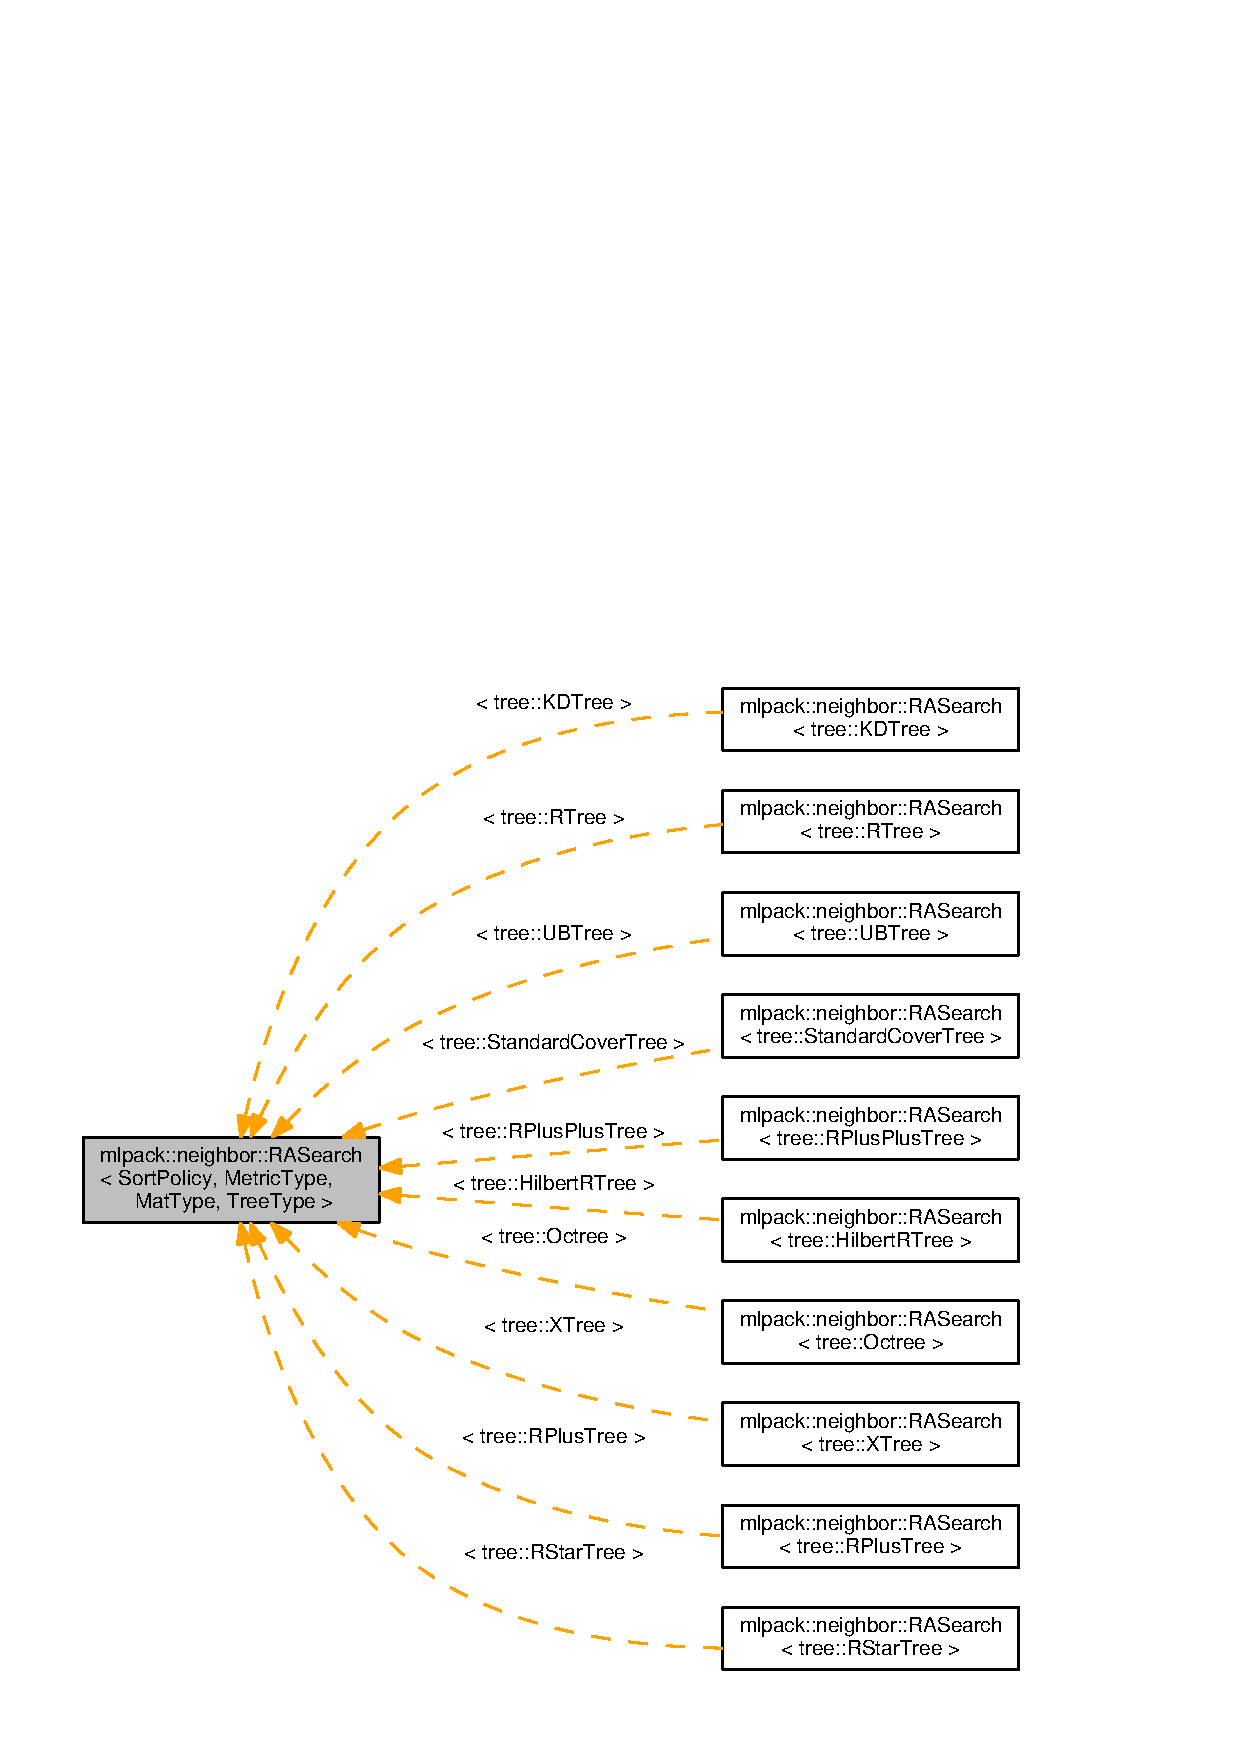
\includegraphics[width=265pt]{classmlpack_1_1neighbor_1_1RASearch__inherit__graph}
\end{center}
\end{figure}
\doxysubsection*{Public Types}
\begin{DoxyCompactItemize}
\item 
typedef Tree\+Type$<$ Metric\+Type, \textbf{ RAQuery\+Stat}$<$ Sort\+Policy $>$, Mat\+Type $>$ \textbf{ Tree}
\begin{DoxyCompactList}\small\item\em Convenience typedef. \end{DoxyCompactList}\end{DoxyCompactItemize}
\doxysubsection*{Public Member Functions}
\begin{DoxyCompactItemize}
\item 
\textbf{ RASearch} (const bool naive=false, const bool single\+Mode=false, const double tau=5, const double alpha=0.\+95, const bool sample\+At\+Leaves=false, const bool first\+Leaf\+Exact=false, const size\+\_\+t single\+Sample\+Limit=20, const Metric\+Type metric=Metric\+Type())
\begin{DoxyCompactList}\small\item\em Create an \doxyref{RASearch}{p.}{classmlpack_1_1neighbor_1_1RASearch} object with no reference data. \end{DoxyCompactList}\item 
\textbf{ RASearch} (Mat\+Type reference\+Set, const bool naive=false, const bool single\+Mode=false, const double tau=5, const double alpha=0.\+95, const bool sample\+At\+Leaves=false, const bool first\+Leaf\+Exact=false, const size\+\_\+t single\+Sample\+Limit=20, const Metric\+Type metric=Metric\+Type())
\begin{DoxyCompactList}\small\item\em Initialize the \doxyref{RASearch}{p.}{classmlpack_1_1neighbor_1_1RASearch} object, passing both a reference dataset (this is the dataset that will be searched). \end{DoxyCompactList}\item 
\textbf{ RASearch} (\textbf{ Tree} $\ast$reference\+Tree, const bool single\+Mode=false, const double tau=5, const double alpha=0.\+95, const bool sample\+At\+Leaves=false, const bool first\+Leaf\+Exact=false, const size\+\_\+t single\+Sample\+Limit=20, const Metric\+Type metric=Metric\+Type())
\begin{DoxyCompactList}\small\item\em Initialize the \doxyref{RASearch}{p.}{classmlpack_1_1neighbor_1_1RASearch} object with the given pre-\/constructed reference tree. \end{DoxyCompactList}\item 
\textbf{ $\sim$\+RASearch} ()
\begin{DoxyCompactList}\small\item\em Delete the \doxyref{RASearch}{p.}{classmlpack_1_1neighbor_1_1RASearch} object. \end{DoxyCompactList}\item 
double \& \textbf{ Alpha} ()
\begin{DoxyCompactList}\small\item\em Modify the desired success probability. \end{DoxyCompactList}\item 
double \textbf{ Alpha} () const
\begin{DoxyCompactList}\small\item\em Get the desired success probability. \end{DoxyCompactList}\item 
bool \& \textbf{ First\+Leaf\+Exact} ()
\begin{DoxyCompactList}\small\item\em Modify whether or not we traverse to the first leaf without approximation. \end{DoxyCompactList}\item 
bool \textbf{ First\+Leaf\+Exact} () const
\begin{DoxyCompactList}\small\item\em Get whether or not we traverse to the first leaf without approximation. \end{DoxyCompactList}\item 
bool \& \textbf{ Naive} ()
\begin{DoxyCompactList}\small\item\em Modify whether or not naive (brute-\/force) search is used. \end{DoxyCompactList}\item 
bool \textbf{ Naive} () const
\begin{DoxyCompactList}\small\item\em Get whether or not naive (brute-\/force) search is used. \end{DoxyCompactList}\item 
const Mat\+Type \& \textbf{ Reference\+Set} () const
\begin{DoxyCompactList}\small\item\em Access the reference set. \end{DoxyCompactList}\item 
void \textbf{ Reset\+Query\+Tree} (\textbf{ Tree} $\ast$query\+Tree) const
\begin{DoxyCompactList}\small\item\em This function recursively resets the \doxyref{RAQuery\+Stat}{p.}{classmlpack_1_1neighbor_1_1RAQueryStat} of the given query tree to set \textquotesingle{}bound\textquotesingle{} to Sort\+Policy\+::\+Worst\+Distance and \textquotesingle{}num\+Samples\+Made\textquotesingle{} to 0. \end{DoxyCompactList}\item 
bool \& \textbf{ Sample\+At\+Leaves} ()
\begin{DoxyCompactList}\small\item\em Modify whether or not sampling is done at the leaves. \end{DoxyCompactList}\item 
bool \textbf{ Sample\+At\+Leaves} () const
\begin{DoxyCompactList}\small\item\em Get whether or not sampling is done at the leaves. \end{DoxyCompactList}\item 
void \textbf{ Search} (const Mat\+Type \&query\+Set, const size\+\_\+t k, arma\+::\+Mat$<$ size\+\_\+t $>$ \&neighbors, arma\+::mat \&distances)
\begin{DoxyCompactList}\small\item\em Compute the rank approximate nearest neighbors of each query point in the query set and store the output in the given matrices. \end{DoxyCompactList}\item 
void \textbf{ Search} (const size\+\_\+t k, arma\+::\+Mat$<$ size\+\_\+t $>$ \&neighbors, arma\+::mat \&distances)
\begin{DoxyCompactList}\small\item\em Compute the rank approximate nearest neighbors of each point in the reference set (that is, the query set is taken to be the reference set), and store the output in the given matrices. \end{DoxyCompactList}\item 
void \textbf{ Search} (\textbf{ Tree} $\ast$query\+Tree, const size\+\_\+t k, arma\+::\+Mat$<$ size\+\_\+t $>$ \&neighbors, arma\+::mat \&distances)
\begin{DoxyCompactList}\small\item\em Compute the rank approximate nearest neighbors of each point in the pre-\/built query tree and store the output in the given matrices. \end{DoxyCompactList}\item 
{\footnotesize template$<$typename Archive $>$ }\\void \textbf{ serialize} (Archive \&ar, const uint32\+\_\+t)
\begin{DoxyCompactList}\small\item\em Serialize the object. \end{DoxyCompactList}\item 
bool \& \textbf{ Single\+Mode} ()
\begin{DoxyCompactList}\small\item\em Modify whether or not single-\/tree search is used. \end{DoxyCompactList}\item 
bool \textbf{ Single\+Mode} () const
\begin{DoxyCompactList}\small\item\em Get whether or not single-\/tree search is used. \end{DoxyCompactList}\item 
size\+\_\+t \& \textbf{ Single\+Sample\+Limit} ()
\begin{DoxyCompactList}\small\item\em Modify the limit on the size of a node that can be approximation. \end{DoxyCompactList}\item 
size\+\_\+t \textbf{ Single\+Sample\+Limit} () const
\begin{DoxyCompactList}\small\item\em Get the limit on the size of a node that can be approximated. \end{DoxyCompactList}\item 
double \& \textbf{ Tau} ()
\begin{DoxyCompactList}\small\item\em Modify the rank-\/approximation in percentile of the data. \end{DoxyCompactList}\item 
double \textbf{ Tau} () const
\begin{DoxyCompactList}\small\item\em Get the rank-\/approximation in percentile of the data. \end{DoxyCompactList}\item 
void \textbf{ Train} (Mat\+Type reference\+Set)
\begin{DoxyCompactList}\small\item\em \char`\"{}\+Train\char`\"{} the model on the given reference set. \end{DoxyCompactList}\item 
void \textbf{ Train} (\textbf{ Tree} $\ast$reference\+Tree)
\begin{DoxyCompactList}\small\item\em Set the reference tree to a new reference tree. \end{DoxyCompactList}\end{DoxyCompactItemize}


\doxysubsection{Detailed Description}
\subsubsection*{template$<$typename Sort\+Policy = Nearest\+Neighbor\+Sort, typename Metric\+Type = metric\+::\+Euclidean\+Distance, typename Mat\+Type = arma\+::mat, template$<$ typename Tree\+Metric\+Type, typename Tree\+Stat\+Type, typename Tree\+Mat\+Type $>$ class Tree\+Type = tree\+::\+KDTree$>$\newline
class mlpack\+::neighbor\+::\+RASearch$<$ Sort\+Policy, Metric\+Type, Mat\+Type, Tree\+Type $>$}

The \doxyref{RASearch}{p.}{classmlpack_1_1neighbor_1_1RASearch} class\+: This class provides a generic manner to perform rank-\/approximate search via random-\/sampling. 

If the \textquotesingle{}naive\textquotesingle{} option is chosen, this rank-\/approximate search will be done by randomly sampling from the whole set. If the \textquotesingle{}naive\textquotesingle{} option is not chosen, the sampling is done in a stratified manner in the tree as mentioned in the algorithms in Figure 2 of the following paper\+:


\begin{DoxyCode}{0}
\DoxyCodeLine{@inproceedings\{ram2009rank,}
\DoxyCodeLine{  title=\{\{Rank-\/Approximate Nearest Neighbor Search: Retaining Meaning and}
\DoxyCodeLine{      Speed in High Dimensions\}\},}
\DoxyCodeLine{  author=\{\{Ram, P. and Lee, D. and Ouyang, H. and Gray, A. G.\}\},}
\DoxyCodeLine{  booktitle=\{\{Advances of Neural Information Processing Systems\}\},}
\DoxyCodeLine{  year=\{2009\}}
\DoxyCodeLine{\}}

\end{DoxyCode}


\doxyref{RASearch}{p.}{classmlpack_1_1neighbor_1_1RASearch} is currently known to not work with ball trees (\#356).


\begin{DoxyTemplParams}{Template Parameters}
{\em Sort\+Policy} & The sort policy for distances; see Nearest\+Neighbor\+Sort. \\
\hline
{\em Metric\+Type} & The metric to use for computation. \\
\hline
{\em Tree\+Type} & The tree type to use. \\
\hline
\end{DoxyTemplParams}


Definition at line 77 of file ra\+\_\+search.\+hpp.



\doxysubsection{Member Typedef Documentation}
\mbox{\label{classmlpack_1_1neighbor_1_1RASearch_a23f60d6d543928c40d96f87711eeba19}} 
\index{RASearch$<$ SortPolicy, MetricType, MatType, TreeType $>$@{RASearch$<$ SortPolicy, MetricType, MatType, TreeType $>$}!Tree@{Tree}}
\index{Tree@{Tree}!RASearch$<$ SortPolicy, MetricType, MatType, TreeType $>$@{RASearch$<$ SortPolicy, MetricType, MatType, TreeType $>$}}
\doxysubsubsection{Tree}
{\footnotesize\ttfamily typedef Tree\+Type$<$Metric\+Type, \textbf{ RAQuery\+Stat}$<$Sort\+Policy$>$, Mat\+Type$>$ \textbf{ Tree}}



Convenience typedef. 



Definition at line 81 of file ra\+\_\+search.\+hpp.



\doxysubsection{Constructor \& Destructor Documentation}
\mbox{\label{classmlpack_1_1neighbor_1_1RASearch_a2e2e09ad4d126aa5c72648e5e36198ae}} 
\index{RASearch$<$ SortPolicy, MetricType, MatType, TreeType $>$@{RASearch$<$ SortPolicy, MetricType, MatType, TreeType $>$}!RASearch@{RASearch}}
\index{RASearch@{RASearch}!RASearch$<$ SortPolicy, MetricType, MatType, TreeType $>$@{RASearch$<$ SortPolicy, MetricType, MatType, TreeType $>$}}
\doxysubsubsection{RASearch()\hspace{0.1cm}{\footnotesize\ttfamily [1/3]}}
{\footnotesize\ttfamily \textbf{ RASearch} (\begin{DoxyParamCaption}\item[{Mat\+Type}]{reference\+Set,  }\item[{const bool}]{naive = {\ttfamily false},  }\item[{const bool}]{single\+Mode = {\ttfamily false},  }\item[{const double}]{tau = {\ttfamily 5},  }\item[{const double}]{alpha = {\ttfamily 0.95},  }\item[{const bool}]{sample\+At\+Leaves = {\ttfamily false},  }\item[{const bool}]{first\+Leaf\+Exact = {\ttfamily false},  }\item[{const size\+\_\+t}]{single\+Sample\+Limit = {\ttfamily 20},  }\item[{const Metric\+Type}]{metric = {\ttfamily MetricType()} }\end{DoxyParamCaption})}



Initialize the \doxyref{RASearch}{p.}{classmlpack_1_1neighbor_1_1RASearch} object, passing both a reference dataset (this is the dataset that will be searched). 

Optionally, perform the computation in naive mode or single-\/tree mode. An initialized distance metric can be given, for cases where the metric has internal data (i.\+e. the distance\+::\+Mahalanobis\+Distance class).

This method will copy the matrices to internal copies, which are rearranged during tree-\/building. If you don\textquotesingle{}t need to keep the reference dataset, you can use std\+::move() to remove the overhead of making copies. Using std\+::move() transfers the ownership of the dataset.

tau, the rank-\/approximation parameter, specifies that we are looking for k neighbors with probability alpha of being in the top tau percent of nearest neighbors. So, as an example, if our dataset has 1000 points, and we want 5 nearest neighbors with 95\% probability of being in the top 5\% of nearest neighbors (or, the top 50 nearest neighbors), we set k = 5, tau = 5, and alpha = 0.\+95.

The method will fail (and throw a std\+::invalid\+\_\+argument exception) if the value of tau is too low\+: tau must be set such that the number of points in the corresponding percentile of the data is greater than k. Thus, if we choose tau = 0.\+1 with a dataset of 1000 points and k = 5, then we are attempting to choose 5 nearest neighbors out of the closest 1 point -- this is invalid.


\begin{DoxyParams}{Parameters}
{\em reference\+Set} & Set of reference points. \\
\hline
{\em naive} & If true, the rank-\/approximate search will be performed by directly sampling the whole set instead of using the stratified sampling on the tree. \\
\hline
{\em single\+Mode} & If true, single-\/tree search will be used (as opposed to dual-\/tree search). This is useful when \doxyref{Search()}{p.}{classmlpack_1_1neighbor_1_1RASearch_a0de302ca0602fe721ac01f073d5e630f} will be called with few query points. \\
\hline
{\em metric} & An optional instance of the Metric\+Type class. \\
\hline
{\em tau} & The rank-\/approximation in percentile of the data. The default value is 5\%. \\
\hline
{\em alpha} & The desired success probability. The default value is 0.\+95. \\
\hline
{\em sample\+At\+Leaves} & Sample at leaves for faster but less accurate computation. This defaults to \textquotesingle{}false\textquotesingle{}. \\
\hline
{\em first\+Leaf\+Exact} & Traverse to the first leaf without approximation. This can ensure that the query definitely finds its (near) duplicate if there exists one. This defaults to \textquotesingle{}false\textquotesingle{} for now. \\
\hline
{\em single\+Sample\+Limit} & The limit on the largest node that can be approximated by sampling. This defaults to 20. \\
\hline
\end{DoxyParams}
\mbox{\label{classmlpack_1_1neighbor_1_1RASearch_a71c2c551b7ed51e42515edd5ab00b255}} 
\index{RASearch$<$ SortPolicy, MetricType, MatType, TreeType $>$@{RASearch$<$ SortPolicy, MetricType, MatType, TreeType $>$}!RASearch@{RASearch}}
\index{RASearch@{RASearch}!RASearch$<$ SortPolicy, MetricType, MatType, TreeType $>$@{RASearch$<$ SortPolicy, MetricType, MatType, TreeType $>$}}
\doxysubsubsection{RASearch()\hspace{0.1cm}{\footnotesize\ttfamily [2/3]}}
{\footnotesize\ttfamily \textbf{ RASearch} (\begin{DoxyParamCaption}\item[{\textbf{ Tree} $\ast$}]{reference\+Tree,  }\item[{const bool}]{single\+Mode = {\ttfamily false},  }\item[{const double}]{tau = {\ttfamily 5},  }\item[{const double}]{alpha = {\ttfamily 0.95},  }\item[{const bool}]{sample\+At\+Leaves = {\ttfamily false},  }\item[{const bool}]{first\+Leaf\+Exact = {\ttfamily false},  }\item[{const size\+\_\+t}]{single\+Sample\+Limit = {\ttfamily 20},  }\item[{const Metric\+Type}]{metric = {\ttfamily MetricType()} }\end{DoxyParamCaption})}



Initialize the \doxyref{RASearch}{p.}{classmlpack_1_1neighbor_1_1RASearch} object with the given pre-\/constructed reference tree. 

It is assumed that the points in the tree\textquotesingle{}s dataset correspond to the reference set. Optionally, choose to use single-\/tree mode. Naive mode is not available as an option for this constructor; instead, to run naive computation, use a different constructor. Additionally, an instantiated distance metric can be given, for cases where the distance metric holds data.

There is no copying of the data matrices in this constructor (because tree-\/building is not necessary), so this is the constructor to use when copies absolutely must be avoided.

tau, the rank-\/approximation parameter, specifies that we are looking for k neighbors with probability alpha of being in the top tau percent of nearest neighbors. So, as an example, if our dataset has 1000 points, and we want 5 nearest neighbors with 95\% probability of being in the top 5\% of nearest neighbors (or, the top 50 nearest neighbors), we set k = 5, tau = 5, and alpha = 0.\+95.

The method will fail (and throw a std\+::invalid\+\_\+argument exception) if the value of tau is too low\+: tau must be set such that the number of points in the corresponding percentile of the data is greater than k. Thus, if we choose tau = 0.\+1 with a dataset of 1000 points and k = 5, then we are attempting to choose 5 nearest neighbors out of the closest 1 point -- this is invalid.

\begin{DoxyNote}{Note}
Tree-\/building may (at least with Binary\+Space\+Tree) modify the ordering of a matrix, so be aware that the results you get from \doxyref{Search()}{p.}{classmlpack_1_1neighbor_1_1RASearch_a0de302ca0602fe721ac01f073d5e630f} will correspond to the modified matrix.
\end{DoxyNote}

\begin{DoxyParams}{Parameters}
{\em reference\+Tree} & Pre-\/built tree for reference points. \\
\hline
{\em single\+Mode} & Whether single-\/tree computation should be used (as opposed to dual-\/tree computation). \\
\hline
{\em tau} & The rank-\/approximation in percentile of the data. The default value is 5\%. \\
\hline
{\em alpha} & The desired success probability. The default value is 0.\+95. \\
\hline
{\em sample\+At\+Leaves} & Sample at leaves for faster but less accurate computation. This defaults to \textquotesingle{}false\textquotesingle{}. \\
\hline
{\em first\+Leaf\+Exact} & Traverse to the first leaf without approximation. This can ensure that the query definitely finds its (near) duplicate if there exists one. This defaults to \textquotesingle{}false\textquotesingle{} for now. \\
\hline
{\em single\+Sample\+Limit} & The limit on the largest node that can be approximated by sampling. This defaults to 20. \\
\hline
{\em metric} & Instantiated distance metric. \\
\hline
\end{DoxyParams}
\mbox{\label{classmlpack_1_1neighbor_1_1RASearch_a796e8bc5d64b5f5d479be42faa9156d1}} 
\index{RASearch$<$ SortPolicy, MetricType, MatType, TreeType $>$@{RASearch$<$ SortPolicy, MetricType, MatType, TreeType $>$}!RASearch@{RASearch}}
\index{RASearch@{RASearch}!RASearch$<$ SortPolicy, MetricType, MatType, TreeType $>$@{RASearch$<$ SortPolicy, MetricType, MatType, TreeType $>$}}
\doxysubsubsection{RASearch()\hspace{0.1cm}{\footnotesize\ttfamily [3/3]}}
{\footnotesize\ttfamily \textbf{ RASearch} (\begin{DoxyParamCaption}\item[{const bool}]{naive = {\ttfamily false},  }\item[{const bool}]{single\+Mode = {\ttfamily false},  }\item[{const double}]{tau = {\ttfamily 5},  }\item[{const double}]{alpha = {\ttfamily 0.95},  }\item[{const bool}]{sample\+At\+Leaves = {\ttfamily false},  }\item[{const bool}]{first\+Leaf\+Exact = {\ttfamily false},  }\item[{const size\+\_\+t}]{single\+Sample\+Limit = {\ttfamily 20},  }\item[{const Metric\+Type}]{metric = {\ttfamily MetricType()} }\end{DoxyParamCaption})}



Create an \doxyref{RASearch}{p.}{classmlpack_1_1neighbor_1_1RASearch} object with no reference data. 

If \doxyref{Search()}{p.}{classmlpack_1_1neighbor_1_1RASearch_a0de302ca0602fe721ac01f073d5e630f} is called before a reference set is set with \doxyref{Train()}{p.}{classmlpack_1_1neighbor_1_1RASearch_a27ba39af83e3cb01f2e6fbec159adf0e}, an exception will be thrown.


\begin{DoxyParams}{Parameters}
{\em naive} & Whether naive (brute-\/force) search should be used. \\
\hline
{\em single\+Mode} & Whether single-\/tree computation should be used (as opposed to dual-\/tree computation). \\
\hline
{\em tau} & The rank-\/approximation in percentile of the data. The default value is 5\%. \\
\hline
{\em alpha} & The desired success probability. The default value is 0.\+95. \\
\hline
{\em sample\+At\+Leaves} & Sample at leaves for faster but less accurate computation. This defaults to \textquotesingle{}false\textquotesingle{}. \\
\hline
{\em first\+Leaf\+Exact} & Traverse to the first leaf without approximation. This can ensure that the query definitely finds its (near) duplicate if there exists one. This defaults to \textquotesingle{}false\textquotesingle{} for now. \\
\hline
{\em single\+Sample\+Limit} & The limit on the largest node that can be approximated by sampling. This defaults to 20. \\
\hline
{\em metric} & Instantiated distance metric. \\
\hline
\end{DoxyParams}
\mbox{\label{classmlpack_1_1neighbor_1_1RASearch_a68b835e379f6b9375bbe6874357eb978}} 
\index{RASearch$<$ SortPolicy, MetricType, MatType, TreeType $>$@{RASearch$<$ SortPolicy, MetricType, MatType, TreeType $>$}!````~RASearch@{$\sim$RASearch}}
\index{````~RASearch@{$\sim$RASearch}!RASearch$<$ SortPolicy, MetricType, MatType, TreeType $>$@{RASearch$<$ SortPolicy, MetricType, MatType, TreeType $>$}}
\doxysubsubsection{$\sim$RASearch()}
{\footnotesize\ttfamily $\sim$\textbf{ RASearch} (\begin{DoxyParamCaption}{ }\end{DoxyParamCaption})}



Delete the \doxyref{RASearch}{p.}{classmlpack_1_1neighbor_1_1RASearch} object. 

The tree is the only member we are responsible for deleting. The others will take care of themselves. 

\doxysubsection{Member Function Documentation}
\mbox{\label{classmlpack_1_1neighbor_1_1RASearch_acbb0e4747a3a307bee88bad71e5eeaf1}} 
\index{RASearch$<$ SortPolicy, MetricType, MatType, TreeType $>$@{RASearch$<$ SortPolicy, MetricType, MatType, TreeType $>$}!Alpha@{Alpha}}
\index{Alpha@{Alpha}!RASearch$<$ SortPolicy, MetricType, MatType, TreeType $>$@{RASearch$<$ SortPolicy, MetricType, MatType, TreeType $>$}}
\doxysubsubsection{Alpha()\hspace{0.1cm}{\footnotesize\ttfamily [1/2]}}
{\footnotesize\ttfamily double\& Alpha (\begin{DoxyParamCaption}{ }\end{DoxyParamCaption})\hspace{0.3cm}{\ttfamily [inline]}}



Modify the desired success probability. 



Definition at line 344 of file ra\+\_\+search.\+hpp.

\mbox{\label{classmlpack_1_1neighbor_1_1RASearch_a500ecd077d5cc5fdbf6ceb095d8de9e1}} 
\index{RASearch$<$ SortPolicy, MetricType, MatType, TreeType $>$@{RASearch$<$ SortPolicy, MetricType, MatType, TreeType $>$}!Alpha@{Alpha}}
\index{Alpha@{Alpha}!RASearch$<$ SortPolicy, MetricType, MatType, TreeType $>$@{RASearch$<$ SortPolicy, MetricType, MatType, TreeType $>$}}
\doxysubsubsection{Alpha()\hspace{0.1cm}{\footnotesize\ttfamily [2/2]}}
{\footnotesize\ttfamily double Alpha (\begin{DoxyParamCaption}{ }\end{DoxyParamCaption}) const\hspace{0.3cm}{\ttfamily [inline]}}



Get the desired success probability. 



Definition at line 342 of file ra\+\_\+search.\+hpp.

\mbox{\label{classmlpack_1_1neighbor_1_1RASearch_aca2eb648feb965d3bcb0b0b73f8b2b0f}} 
\index{RASearch$<$ SortPolicy, MetricType, MatType, TreeType $>$@{RASearch$<$ SortPolicy, MetricType, MatType, TreeType $>$}!FirstLeafExact@{FirstLeafExact}}
\index{FirstLeafExact@{FirstLeafExact}!RASearch$<$ SortPolicy, MetricType, MatType, TreeType $>$@{RASearch$<$ SortPolicy, MetricType, MatType, TreeType $>$}}
\doxysubsubsection{FirstLeafExact()\hspace{0.1cm}{\footnotesize\ttfamily [1/2]}}
{\footnotesize\ttfamily bool\& First\+Leaf\+Exact (\begin{DoxyParamCaption}{ }\end{DoxyParamCaption})\hspace{0.3cm}{\ttfamily [inline]}}



Modify whether or not we traverse to the first leaf without approximation. 



Definition at line 354 of file ra\+\_\+search.\+hpp.

\mbox{\label{classmlpack_1_1neighbor_1_1RASearch_a17ec6e467897eb8aee3b519e0758e77d}} 
\index{RASearch$<$ SortPolicy, MetricType, MatType, TreeType $>$@{RASearch$<$ SortPolicy, MetricType, MatType, TreeType $>$}!FirstLeafExact@{FirstLeafExact}}
\index{FirstLeafExact@{FirstLeafExact}!RASearch$<$ SortPolicy, MetricType, MatType, TreeType $>$@{RASearch$<$ SortPolicy, MetricType, MatType, TreeType $>$}}
\doxysubsubsection{FirstLeafExact()\hspace{0.1cm}{\footnotesize\ttfamily [2/2]}}
{\footnotesize\ttfamily bool First\+Leaf\+Exact (\begin{DoxyParamCaption}{ }\end{DoxyParamCaption}) const\hspace{0.3cm}{\ttfamily [inline]}}



Get whether or not we traverse to the first leaf without approximation. 



Definition at line 352 of file ra\+\_\+search.\+hpp.

\mbox{\label{classmlpack_1_1neighbor_1_1RASearch_af7d397adca3f411b4e2d2f977b280ce6}} 
\index{RASearch$<$ SortPolicy, MetricType, MatType, TreeType $>$@{RASearch$<$ SortPolicy, MetricType, MatType, TreeType $>$}!Naive@{Naive}}
\index{Naive@{Naive}!RASearch$<$ SortPolicy, MetricType, MatType, TreeType $>$@{RASearch$<$ SortPolicy, MetricType, MatType, TreeType $>$}}
\doxysubsubsection{Naive()\hspace{0.1cm}{\footnotesize\ttfamily [1/2]}}
{\footnotesize\ttfamily bool\& Naive (\begin{DoxyParamCaption}{ }\end{DoxyParamCaption})\hspace{0.3cm}{\ttfamily [inline]}}



Modify whether or not naive (brute-\/force) search is used. 



Definition at line 329 of file ra\+\_\+search.\+hpp.

\mbox{\label{classmlpack_1_1neighbor_1_1RASearch_a343230e7d7344e3f7d5f5f2eb89cf2c5}} 
\index{RASearch$<$ SortPolicy, MetricType, MatType, TreeType $>$@{RASearch$<$ SortPolicy, MetricType, MatType, TreeType $>$}!Naive@{Naive}}
\index{Naive@{Naive}!RASearch$<$ SortPolicy, MetricType, MatType, TreeType $>$@{RASearch$<$ SortPolicy, MetricType, MatType, TreeType $>$}}
\doxysubsubsection{Naive()\hspace{0.1cm}{\footnotesize\ttfamily [2/2]}}
{\footnotesize\ttfamily bool Naive (\begin{DoxyParamCaption}{ }\end{DoxyParamCaption}) const\hspace{0.3cm}{\ttfamily [inline]}}



Get whether or not naive (brute-\/force) search is used. 



Definition at line 327 of file ra\+\_\+search.\+hpp.

\mbox{\label{classmlpack_1_1neighbor_1_1RASearch_a0a975940b302b4efec85bbe2d8b36251}} 
\index{RASearch$<$ SortPolicy, MetricType, MatType, TreeType $>$@{RASearch$<$ SortPolicy, MetricType, MatType, TreeType $>$}!ReferenceSet@{ReferenceSet}}
\index{ReferenceSet@{ReferenceSet}!RASearch$<$ SortPolicy, MetricType, MatType, TreeType $>$@{RASearch$<$ SortPolicy, MetricType, MatType, TreeType $>$}}
\doxysubsubsection{ReferenceSet()}
{\footnotesize\ttfamily const Mat\+Type\& Reference\+Set (\begin{DoxyParamCaption}{ }\end{DoxyParamCaption}) const\hspace{0.3cm}{\ttfamily [inline]}}



Access the reference set. 



Definition at line 324 of file ra\+\_\+search.\+hpp.

\mbox{\label{classmlpack_1_1neighbor_1_1RASearch_a769fa33810494d3cc0abdd8578daba67}} 
\index{RASearch$<$ SortPolicy, MetricType, MatType, TreeType $>$@{RASearch$<$ SortPolicy, MetricType, MatType, TreeType $>$}!ResetQueryTree@{ResetQueryTree}}
\index{ResetQueryTree@{ResetQueryTree}!RASearch$<$ SortPolicy, MetricType, MatType, TreeType $>$@{RASearch$<$ SortPolicy, MetricType, MatType, TreeType $>$}}
\doxysubsubsection{ResetQueryTree()}
{\footnotesize\ttfamily void Reset\+Query\+Tree (\begin{DoxyParamCaption}\item[{\textbf{ Tree} $\ast$}]{query\+Tree }\end{DoxyParamCaption}) const}



This function recursively resets the \doxyref{RAQuery\+Stat}{p.}{classmlpack_1_1neighbor_1_1RAQueryStat} of the given query tree to set \textquotesingle{}bound\textquotesingle{} to Sort\+Policy\+::\+Worst\+Distance and \textquotesingle{}num\+Samples\+Made\textquotesingle{} to 0. 

This allows a user to perform multiple searches with the same query tree, possibly with different levels of approximation without requiring to build a new pair of trees for every new (approximate) search.

If \doxyref{Search()}{p.}{classmlpack_1_1neighbor_1_1RASearch_a0de302ca0602fe721ac01f073d5e630f} is called multiple times with the same query tree without calling \doxyref{Reset\+Query\+Tree()}{p.}{classmlpack_1_1neighbor_1_1RASearch_a769fa33810494d3cc0abdd8578daba67}, the results may not satisfy the theoretical guarantees provided by the rank-\/approximate neighbor search algorithm.


\begin{DoxyParams}{Parameters}
{\em query\+Tree} & Tree whose statistics should be reset. \\
\hline
\end{DoxyParams}
\mbox{\label{classmlpack_1_1neighbor_1_1RASearch_a9f6d54dd0424f827becc2e2e9969b1bb}} 
\index{RASearch$<$ SortPolicy, MetricType, MatType, TreeType $>$@{RASearch$<$ SortPolicy, MetricType, MatType, TreeType $>$}!SampleAtLeaves@{SampleAtLeaves}}
\index{SampleAtLeaves@{SampleAtLeaves}!RASearch$<$ SortPolicy, MetricType, MatType, TreeType $>$@{RASearch$<$ SortPolicy, MetricType, MatType, TreeType $>$}}
\doxysubsubsection{SampleAtLeaves()\hspace{0.1cm}{\footnotesize\ttfamily [1/2]}}
{\footnotesize\ttfamily bool\& Sample\+At\+Leaves (\begin{DoxyParamCaption}{ }\end{DoxyParamCaption})\hspace{0.3cm}{\ttfamily [inline]}}



Modify whether or not sampling is done at the leaves. 



Definition at line 349 of file ra\+\_\+search.\+hpp.

\mbox{\label{classmlpack_1_1neighbor_1_1RASearch_aa9dd91d6b96e1d0b343c3cec27372036}} 
\index{RASearch$<$ SortPolicy, MetricType, MatType, TreeType $>$@{RASearch$<$ SortPolicy, MetricType, MatType, TreeType $>$}!SampleAtLeaves@{SampleAtLeaves}}
\index{SampleAtLeaves@{SampleAtLeaves}!RASearch$<$ SortPolicy, MetricType, MatType, TreeType $>$@{RASearch$<$ SortPolicy, MetricType, MatType, TreeType $>$}}
\doxysubsubsection{SampleAtLeaves()\hspace{0.1cm}{\footnotesize\ttfamily [2/2]}}
{\footnotesize\ttfamily bool Sample\+At\+Leaves (\begin{DoxyParamCaption}{ }\end{DoxyParamCaption}) const\hspace{0.3cm}{\ttfamily [inline]}}



Get whether or not sampling is done at the leaves. 



Definition at line 347 of file ra\+\_\+search.\+hpp.

\mbox{\label{classmlpack_1_1neighbor_1_1RASearch_a0de302ca0602fe721ac01f073d5e630f}} 
\index{RASearch$<$ SortPolicy, MetricType, MatType, TreeType $>$@{RASearch$<$ SortPolicy, MetricType, MatType, TreeType $>$}!Search@{Search}}
\index{Search@{Search}!RASearch$<$ SortPolicy, MetricType, MatType, TreeType $>$@{RASearch$<$ SortPolicy, MetricType, MatType, TreeType $>$}}
\doxysubsubsection{Search()\hspace{0.1cm}{\footnotesize\ttfamily [1/3]}}
{\footnotesize\ttfamily void Search (\begin{DoxyParamCaption}\item[{const Mat\+Type \&}]{query\+Set,  }\item[{const size\+\_\+t}]{k,  }\item[{arma\+::\+Mat$<$ size\+\_\+t $>$ \&}]{neighbors,  }\item[{arma\+::mat \&}]{distances }\end{DoxyParamCaption})}



Compute the rank approximate nearest neighbors of each query point in the query set and store the output in the given matrices. 

The matrices will be set to the size of n columns by k rows, where n is the number of points in the query dataset and k is the number of neighbors being searched for.

If query\+Set is small or only contains one point, it can be faster to do single-\/tree search; single-\/tree search can be set with the \doxyref{Single\+Mode()}{p.}{classmlpack_1_1neighbor_1_1RASearch_adadacd63ddeadf138d834b1fdc632773} function or in the constructor.


\begin{DoxyParams}{Parameters}
{\em query\+Set} & Set of query points (can be a single point). \\
\hline
{\em k} & Number of neighbors to search for. \\
\hline
{\em neighbors} & Matrix storing lists of neighbors for each query point. \\
\hline
{\em distances} & Matrix storing distances of neighbors for each query point. \\
\hline
\end{DoxyParams}
\mbox{\label{classmlpack_1_1neighbor_1_1RASearch_a619c7d4931e628a0c199159c57b34cbd}} 
\index{RASearch$<$ SortPolicy, MetricType, MatType, TreeType $>$@{RASearch$<$ SortPolicy, MetricType, MatType, TreeType $>$}!Search@{Search}}
\index{Search@{Search}!RASearch$<$ SortPolicy, MetricType, MatType, TreeType $>$@{RASearch$<$ SortPolicy, MetricType, MatType, TreeType $>$}}
\doxysubsubsection{Search()\hspace{0.1cm}{\footnotesize\ttfamily [2/3]}}
{\footnotesize\ttfamily void Search (\begin{DoxyParamCaption}\item[{const size\+\_\+t}]{k,  }\item[{arma\+::\+Mat$<$ size\+\_\+t $>$ \&}]{neighbors,  }\item[{arma\+::mat \&}]{distances }\end{DoxyParamCaption})}



Compute the rank approximate nearest neighbors of each point in the reference set (that is, the query set is taken to be the reference set), and store the output in the given matrices. 

The matrices will be set to the size of n columns by k rows, where n is the number of points in the query dataset and k is the number of neighbors being searched for.


\begin{DoxyParams}{Parameters}
{\em k} & Number of neighbors to search for. \\
\hline
{\em neighbors} & Matrix storing lists of neighbors for each point. \\
\hline
{\em distances} & Matrix storing distances of neighbors for each query point. \\
\hline
\end{DoxyParams}
\mbox{\label{classmlpack_1_1neighbor_1_1RASearch_a9a8b402b4af23e9ebe2143139b3a6b00}} 
\index{RASearch$<$ SortPolicy, MetricType, MatType, TreeType $>$@{RASearch$<$ SortPolicy, MetricType, MatType, TreeType $>$}!Search@{Search}}
\index{Search@{Search}!RASearch$<$ SortPolicy, MetricType, MatType, TreeType $>$@{RASearch$<$ SortPolicy, MetricType, MatType, TreeType $>$}}
\doxysubsubsection{Search()\hspace{0.1cm}{\footnotesize\ttfamily [3/3]}}
{\footnotesize\ttfamily void Search (\begin{DoxyParamCaption}\item[{\textbf{ Tree} $\ast$}]{query\+Tree,  }\item[{const size\+\_\+t}]{k,  }\item[{arma\+::\+Mat$<$ size\+\_\+t $>$ \&}]{neighbors,  }\item[{arma\+::mat \&}]{distances }\end{DoxyParamCaption})}



Compute the rank approximate nearest neighbors of each point in the pre-\/built query tree and store the output in the given matrices. 

The matrices will be set to the size of n columns by k rows, where n is the number of points in the query dataset and k is the number of neighbors being searched for.

If single\+Mode or naive is enabled, then this method will throw a std\+::invalid\+\_\+argument exception; calling this function implies a dual-\/tree algorithm.

\begin{DoxyNote}{Note}
If the tree type you are using modifies the data matrix, be aware that the results returned from this function will be with respect to the modified data matrix.
\end{DoxyNote}

\begin{DoxyParams}{Parameters}
{\em query\+Tree} & Tree built on query points. \\
\hline
{\em k} & Number of neighbors to search for. \\
\hline
{\em neighbors} & Matrix storing lists of neighbors for each query point. \\
\hline
{\em distances} & Matrix storing distances of neighbors for each query point. \\
\hline
\end{DoxyParams}
\mbox{\label{classmlpack_1_1neighbor_1_1RASearch_a65cba07328997659bec80b9879b15a51}} 
\index{RASearch$<$ SortPolicy, MetricType, MatType, TreeType $>$@{RASearch$<$ SortPolicy, MetricType, MatType, TreeType $>$}!serialize@{serialize}}
\index{serialize@{serialize}!RASearch$<$ SortPolicy, MetricType, MatType, TreeType $>$@{RASearch$<$ SortPolicy, MetricType, MatType, TreeType $>$}}
\doxysubsubsection{serialize()}
{\footnotesize\ttfamily void serialize (\begin{DoxyParamCaption}\item[{Archive \&}]{ar,  }\item[{const uint32\+\_\+t}]{ }\end{DoxyParamCaption})}



Serialize the object. 

\mbox{\label{classmlpack_1_1neighbor_1_1RASearch_adadacd63ddeadf138d834b1fdc632773}} 
\index{RASearch$<$ SortPolicy, MetricType, MatType, TreeType $>$@{RASearch$<$ SortPolicy, MetricType, MatType, TreeType $>$}!SingleMode@{SingleMode}}
\index{SingleMode@{SingleMode}!RASearch$<$ SortPolicy, MetricType, MatType, TreeType $>$@{RASearch$<$ SortPolicy, MetricType, MatType, TreeType $>$}}
\doxysubsubsection{SingleMode()\hspace{0.1cm}{\footnotesize\ttfamily [1/2]}}
{\footnotesize\ttfamily bool\& Single\+Mode (\begin{DoxyParamCaption}{ }\end{DoxyParamCaption})\hspace{0.3cm}{\ttfamily [inline]}}



Modify whether or not single-\/tree search is used. 



Definition at line 334 of file ra\+\_\+search.\+hpp.

\mbox{\label{classmlpack_1_1neighbor_1_1RASearch_a7477b3e8499a6158bbe177e7f30d4947}} 
\index{RASearch$<$ SortPolicy, MetricType, MatType, TreeType $>$@{RASearch$<$ SortPolicy, MetricType, MatType, TreeType $>$}!SingleMode@{SingleMode}}
\index{SingleMode@{SingleMode}!RASearch$<$ SortPolicy, MetricType, MatType, TreeType $>$@{RASearch$<$ SortPolicy, MetricType, MatType, TreeType $>$}}
\doxysubsubsection{SingleMode()\hspace{0.1cm}{\footnotesize\ttfamily [2/2]}}
{\footnotesize\ttfamily bool Single\+Mode (\begin{DoxyParamCaption}{ }\end{DoxyParamCaption}) const\hspace{0.3cm}{\ttfamily [inline]}}



Get whether or not single-\/tree search is used. 



Definition at line 332 of file ra\+\_\+search.\+hpp.

\mbox{\label{classmlpack_1_1neighbor_1_1RASearch_ae78a7b8e9c96a2dbf646a27efee047b1}} 
\index{RASearch$<$ SortPolicy, MetricType, MatType, TreeType $>$@{RASearch$<$ SortPolicy, MetricType, MatType, TreeType $>$}!SingleSampleLimit@{SingleSampleLimit}}
\index{SingleSampleLimit@{SingleSampleLimit}!RASearch$<$ SortPolicy, MetricType, MatType, TreeType $>$@{RASearch$<$ SortPolicy, MetricType, MatType, TreeType $>$}}
\doxysubsubsection{SingleSampleLimit()\hspace{0.1cm}{\footnotesize\ttfamily [1/2]}}
{\footnotesize\ttfamily size\+\_\+t\& Single\+Sample\+Limit (\begin{DoxyParamCaption}{ }\end{DoxyParamCaption})\hspace{0.3cm}{\ttfamily [inline]}}



Modify the limit on the size of a node that can be approximation. 



Definition at line 359 of file ra\+\_\+search.\+hpp.

\mbox{\label{classmlpack_1_1neighbor_1_1RASearch_a3a2580f686a9de3078e499b1280e2a9f}} 
\index{RASearch$<$ SortPolicy, MetricType, MatType, TreeType $>$@{RASearch$<$ SortPolicy, MetricType, MatType, TreeType $>$}!SingleSampleLimit@{SingleSampleLimit}}
\index{SingleSampleLimit@{SingleSampleLimit}!RASearch$<$ SortPolicy, MetricType, MatType, TreeType $>$@{RASearch$<$ SortPolicy, MetricType, MatType, TreeType $>$}}
\doxysubsubsection{SingleSampleLimit()\hspace{0.1cm}{\footnotesize\ttfamily [2/2]}}
{\footnotesize\ttfamily size\+\_\+t Single\+Sample\+Limit (\begin{DoxyParamCaption}{ }\end{DoxyParamCaption}) const\hspace{0.3cm}{\ttfamily [inline]}}



Get the limit on the size of a node that can be approximated. 



Definition at line 357 of file ra\+\_\+search.\+hpp.

\mbox{\label{classmlpack_1_1neighbor_1_1RASearch_ad522d61ed716a322376adea25ebdbc90}} 
\index{RASearch$<$ SortPolicy, MetricType, MatType, TreeType $>$@{RASearch$<$ SortPolicy, MetricType, MatType, TreeType $>$}!Tau@{Tau}}
\index{Tau@{Tau}!RASearch$<$ SortPolicy, MetricType, MatType, TreeType $>$@{RASearch$<$ SortPolicy, MetricType, MatType, TreeType $>$}}
\doxysubsubsection{Tau()\hspace{0.1cm}{\footnotesize\ttfamily [1/2]}}
{\footnotesize\ttfamily double\& Tau (\begin{DoxyParamCaption}{ }\end{DoxyParamCaption})\hspace{0.3cm}{\ttfamily [inline]}}



Modify the rank-\/approximation in percentile of the data. 



Definition at line 339 of file ra\+\_\+search.\+hpp.

\mbox{\label{classmlpack_1_1neighbor_1_1RASearch_a4a4b0fafde4cc4c856a53025dc8c4c21}} 
\index{RASearch$<$ SortPolicy, MetricType, MatType, TreeType $>$@{RASearch$<$ SortPolicy, MetricType, MatType, TreeType $>$}!Tau@{Tau}}
\index{Tau@{Tau}!RASearch$<$ SortPolicy, MetricType, MatType, TreeType $>$@{RASearch$<$ SortPolicy, MetricType, MatType, TreeType $>$}}
\doxysubsubsection{Tau()\hspace{0.1cm}{\footnotesize\ttfamily [2/2]}}
{\footnotesize\ttfamily double Tau (\begin{DoxyParamCaption}{ }\end{DoxyParamCaption}) const\hspace{0.3cm}{\ttfamily [inline]}}



Get the rank-\/approximation in percentile of the data. 



Definition at line 337 of file ra\+\_\+search.\+hpp.

\mbox{\label{classmlpack_1_1neighbor_1_1RASearch_a27ba39af83e3cb01f2e6fbec159adf0e}} 
\index{RASearch$<$ SortPolicy, MetricType, MatType, TreeType $>$@{RASearch$<$ SortPolicy, MetricType, MatType, TreeType $>$}!Train@{Train}}
\index{Train@{Train}!RASearch$<$ SortPolicy, MetricType, MatType, TreeType $>$@{RASearch$<$ SortPolicy, MetricType, MatType, TreeType $>$}}
\doxysubsubsection{Train()\hspace{0.1cm}{\footnotesize\ttfamily [1/2]}}
{\footnotesize\ttfamily void Train (\begin{DoxyParamCaption}\item[{Mat\+Type}]{reference\+Set }\end{DoxyParamCaption})}



\char`\"{}\+Train\char`\"{} the model on the given reference set. 

If tree-\/based search is being used (if \doxyref{Naive()}{p.}{classmlpack_1_1neighbor_1_1RASearch_af7d397adca3f411b4e2d2f977b280ce6} is false), the reference tree is rebuilt. Thus, a copy of the reference dataset is made. If you don\textquotesingle{}t need to keep the dataset, you can avoid copying by using std\+::move(). This transfers the ownership of the dataset.


\begin{DoxyParams}{Parameters}
{\em reference\+Set} & New reference set to use. \\
\hline
\end{DoxyParams}
\mbox{\label{classmlpack_1_1neighbor_1_1RASearch_a3d1133fe6bda66e7143fd7aab27cbd04}} 
\index{RASearch$<$ SortPolicy, MetricType, MatType, TreeType $>$@{RASearch$<$ SortPolicy, MetricType, MatType, TreeType $>$}!Train@{Train}}
\index{Train@{Train}!RASearch$<$ SortPolicy, MetricType, MatType, TreeType $>$@{RASearch$<$ SortPolicy, MetricType, MatType, TreeType $>$}}
\doxysubsubsection{Train()\hspace{0.1cm}{\footnotesize\ttfamily [2/2]}}
{\footnotesize\ttfamily void Train (\begin{DoxyParamCaption}\item[{\textbf{ Tree} $\ast$}]{reference\+Tree }\end{DoxyParamCaption})}



Set the reference tree to a new reference tree. 



The documentation for this class was generated from the following file\+:\begin{DoxyCompactItemize}
\item 
/home/aakash/mlpack/src/mlpack/methods/rann/\textbf{ ra\+\_\+search.\+hpp}\end{DoxyCompactItemize}

\section{mlpack\+:\+:neighbor\+:\+:R\+A\+Search\+Rules$<$ Sort\+Policy, Metric\+Type, Tree\+Type $>$ Class Template Reference}
\label{classmlpack_1_1neighbor_1_1RASearchRules}\index{mlpack\+::neighbor\+::\+R\+A\+Search\+Rules$<$ Sort\+Policy, Metric\+Type, Tree\+Type $>$@{mlpack\+::neighbor\+::\+R\+A\+Search\+Rules$<$ Sort\+Policy, Metric\+Type, Tree\+Type $>$}}


The \doxyref{R\+A\+Search\+Rules}{p.}{classmlpack_1_1neighbor_1_1RASearchRules} class is a template helper class used by \doxyref{R\+A\+Search}{p.}{classmlpack_1_1neighbor_1_1RASearch} class when performing rank-\/approximate search via random-\/sampling.  


\subsection*{Classes}
\begin{DoxyCompactItemize}
\item 
struct {\bf Candidate\+Cmp}
\begin{DoxyCompactList}\small\item\em Compare two candidates based on the distance. \end{DoxyCompactList}\end{DoxyCompactItemize}
\subsection*{Public Types}
\begin{DoxyCompactItemize}
\item 
typedef {\bf tree\+::\+Traversal\+Info}$<$ Tree\+Type $>$ {\bf Traversal\+Info\+Type}
\end{DoxyCompactItemize}
\subsection*{Public Member Functions}
\begin{DoxyCompactItemize}
\item 
{\bf R\+A\+Search\+Rules} (const arma\+::mat \&{\bf reference\+Set}, const arma\+::mat \&{\bf query\+Set}, const size\+\_\+t {\bf k}, Metric\+Type \&{\bf metric}, const double tau=5, const double {\bf alpha}=0.\+95, const bool naive=false, const bool {\bf sample\+At\+Leaves}=false, const bool {\bf first\+Leaf\+Exact}=false, const size\+\_\+t {\bf single\+Sample\+Limit}=20, const bool {\bf same\+Set}=false)
\begin{DoxyCompactList}\small\item\em Construct the \doxyref{R\+A\+Search\+Rules}{p.}{classmlpack_1_1neighbor_1_1RASearchRules} object. \end{DoxyCompactList}\item 
double {\bf Base\+Case} (const size\+\_\+t query\+Index, const size\+\_\+t reference\+Index)
\begin{DoxyCompactList}\small\item\em Get the distance from the query point to the reference point. \end{DoxyCompactList}\item 
void {\bf Get\+Results} (arma\+::\+Mat$<$ size\+\_\+t $>$ \&neighbors, arma\+::mat \&distances)
\begin{DoxyCompactList}\small\item\em Store the list of candidates for each query point in the given matrices. \end{DoxyCompactList}\item 
size\+\_\+t {\bf Num\+Dist\+Computations} ()
\item 
size\+\_\+t {\bf Num\+Effective\+Samples} ()
\item 
double {\bf Rescore} (const size\+\_\+t query\+Index, Tree\+Type \&reference\+Node, const double old\+Score)
\begin{DoxyCompactList}\small\item\em Re-\/evaluate the score for recursion order. \end{DoxyCompactList}\item 
double {\bf Rescore} (Tree\+Type \&query\+Node, Tree\+Type \&reference\+Node, const double old\+Score)
\begin{DoxyCompactList}\small\item\em Re-\/evaluate the score for recursion order. \end{DoxyCompactList}\item 
double {\bf Score} (const size\+\_\+t query\+Index, Tree\+Type \&reference\+Node)
\begin{DoxyCompactList}\small\item\em Get the score for recursion order. \end{DoxyCompactList}\item 
double {\bf Score} (const size\+\_\+t query\+Index, Tree\+Type \&reference\+Node, const double base\+Case\+Result)
\begin{DoxyCompactList}\small\item\em Get the score for recursion order. \end{DoxyCompactList}\item 
double {\bf Score} (Tree\+Type \&query\+Node, Tree\+Type \&reference\+Node)
\begin{DoxyCompactList}\small\item\em Get the score for recursion order. \end{DoxyCompactList}\item 
double {\bf Score} (Tree\+Type \&query\+Node, Tree\+Type \&reference\+Node, const double base\+Case\+Result)
\begin{DoxyCompactList}\small\item\em Get the score for recursion order, passing the base case result (in the situation where it may be needed to calculate the recursion order). \end{DoxyCompactList}\item 
const {\bf Traversal\+Info\+Type} \& {\bf Traversal\+Info} () const 
\item 
{\bf Traversal\+Info\+Type} \& {\bf Traversal\+Info} ()
\end{DoxyCompactItemize}
\subsection*{Private Types}
\begin{DoxyCompactItemize}
\item 
typedef std\+::pair$<$ double, size\+\_\+t $>$ {\bf Candidate}
\begin{DoxyCompactList}\small\item\em Candidate represents a possible candidate neighbor (distance, index). \end{DoxyCompactList}\item 
typedef std\+::priority\+\_\+queue$<$ {\bf Candidate}, std\+::vector$<$ {\bf Candidate} $>$, {\bf Candidate\+Cmp} $>$ {\bf Candidate\+List}
\begin{DoxyCompactList}\small\item\em Use a priority queue to represent the list of candidate neighbors. \end{DoxyCompactList}\end{DoxyCompactItemize}
\subsection*{Private Member Functions}
\begin{DoxyCompactItemize}
\item 
void {\bf Insert\+Neighbor} (const size\+\_\+t query\+Index, const size\+\_\+t neighbor, const double distance)
\begin{DoxyCompactList}\small\item\em Helper function to insert a point into the list of candidate points. \end{DoxyCompactList}\item 
double {\bf Score} (const size\+\_\+t query\+Index, Tree\+Type \&reference\+Node, const double distance, const double best\+Distance)
\begin{DoxyCompactList}\small\item\em Perform actual scoring for single-\/tree case. \end{DoxyCompactList}\item 
double {\bf Score} (Tree\+Type \&query\+Node, Tree\+Type \&reference\+Node, const double distance, const double best\+Distance)
\begin{DoxyCompactList}\small\item\em Perform actual scoring for dual-\/tree case. \end{DoxyCompactList}\end{DoxyCompactItemize}
\subsection*{Private Attributes}
\begin{DoxyCompactItemize}
\item 
std\+::vector$<$ {\bf Candidate\+List} $>$ {\bf candidates}
\begin{DoxyCompactList}\small\item\em Set of candidate neighbors for each point. \end{DoxyCompactList}\item 
bool {\bf first\+Leaf\+Exact}
\begin{DoxyCompactList}\small\item\em Whether to do exact computation on the first leaf before any sampling. \end{DoxyCompactList}\item 
const size\+\_\+t {\bf k}
\begin{DoxyCompactList}\small\item\em Number of neighbors to search for. \end{DoxyCompactList}\item 
Metric\+Type \& {\bf metric}
\begin{DoxyCompactList}\small\item\em The instantiated metric. \end{DoxyCompactList}\item 
size\+\_\+t {\bf num\+Dist\+Computations}
\item 
arma\+::\+Col$<$ size\+\_\+t $>$ {\bf num\+Samples\+Made}
\begin{DoxyCompactList}\small\item\em The number of samples made for every query. \end{DoxyCompactList}\item 
size\+\_\+t {\bf num\+Samples\+Reqd}
\begin{DoxyCompactList}\small\item\em The minimum number of samples required per query. \end{DoxyCompactList}\item 
const arma\+::mat \& {\bf query\+Set}
\begin{DoxyCompactList}\small\item\em The query set. \end{DoxyCompactList}\item 
const arma\+::mat \& {\bf reference\+Set}
\begin{DoxyCompactList}\small\item\em The reference set. \end{DoxyCompactList}\item 
bool {\bf same\+Set}
\begin{DoxyCompactList}\small\item\em If the query and reference set are identical, this is true. \end{DoxyCompactList}\item 
bool {\bf sample\+At\+Leaves}
\begin{DoxyCompactList}\small\item\em Whether to sample at leaves or just use all of it. \end{DoxyCompactList}\item 
double {\bf sampling\+Ratio}
\begin{DoxyCompactList}\small\item\em The sampling ratio. \end{DoxyCompactList}\item 
size\+\_\+t {\bf single\+Sample\+Limit}
\begin{DoxyCompactList}\small\item\em The limit on the largest node that can be approximated by sampling. \end{DoxyCompactList}\item 
{\bf Traversal\+Info\+Type} {\bf traversal\+Info}
\end{DoxyCompactItemize}


\subsection{Detailed Description}
\subsubsection*{template$<$typename Sort\+Policy, typename Metric\+Type, typename Tree\+Type$>$\\*
class mlpack\+::neighbor\+::\+R\+A\+Search\+Rules$<$ Sort\+Policy, Metric\+Type, Tree\+Type $>$}

The \doxyref{R\+A\+Search\+Rules}{p.}{classmlpack_1_1neighbor_1_1RASearchRules} class is a template helper class used by \doxyref{R\+A\+Search}{p.}{classmlpack_1_1neighbor_1_1RASearch} class when performing rank-\/approximate search via random-\/sampling. 


\begin{DoxyTemplParams}{Template Parameters}
{\em Sort\+Policy} & The sort policy for distances. \\
\hline
{\em Metric\+Type} & The metric to use for computation. \\
\hline
{\em Tree\+Type} & The tree type to use; must adhere to the Tree\+Type A\+PI. \\
\hline
\end{DoxyTemplParams}


Definition at line 31 of file ra\+\_\+search\+\_\+rules.\+hpp.



\subsection{Member Typedef Documentation}
\index{mlpack\+::neighbor\+::\+R\+A\+Search\+Rules@{mlpack\+::neighbor\+::\+R\+A\+Search\+Rules}!Candidate@{Candidate}}
\index{Candidate@{Candidate}!mlpack\+::neighbor\+::\+R\+A\+Search\+Rules@{mlpack\+::neighbor\+::\+R\+A\+Search\+Rules}}
\subsubsection[{Candidate}]{\setlength{\rightskip}{0pt plus 5cm}template$<$typename Sort\+Policy , typename Metric\+Type , typename Tree\+Type $>$ typedef std\+::pair$<$double, size\+\_\+t$>$ {\bf mlpack\+::neighbor\+::\+R\+A\+Search\+Rules}$<$ Sort\+Policy, Metric\+Type, Tree\+Type $>$\+::{\bf Candidate}\hspace{0.3cm}{\ttfamily [private]}}\label{classmlpack_1_1neighbor_1_1RASearchRules_a7bf30b57538897d6ed365d404f765287}


Candidate represents a possible candidate neighbor (distance, index). 



Definition at line 250 of file ra\+\_\+search\+\_\+rules.\+hpp.

\index{mlpack\+::neighbor\+::\+R\+A\+Search\+Rules@{mlpack\+::neighbor\+::\+R\+A\+Search\+Rules}!Candidate\+List@{Candidate\+List}}
\index{Candidate\+List@{Candidate\+List}!mlpack\+::neighbor\+::\+R\+A\+Search\+Rules@{mlpack\+::neighbor\+::\+R\+A\+Search\+Rules}}
\subsubsection[{Candidate\+List}]{\setlength{\rightskip}{0pt plus 5cm}template$<$typename Sort\+Policy , typename Metric\+Type , typename Tree\+Type $>$ typedef std\+::priority\+\_\+queue$<${\bf Candidate}, std\+::vector$<${\bf Candidate}$>$, {\bf Candidate\+Cmp}$>$ {\bf mlpack\+::neighbor\+::\+R\+A\+Search\+Rules}$<$ Sort\+Policy, Metric\+Type, Tree\+Type $>$\+::{\bf Candidate\+List}\hspace{0.3cm}{\ttfamily [private]}}\label{classmlpack_1_1neighbor_1_1RASearchRules_ac321e04aab417e35740383bfc8cfce7b}


Use a priority queue to represent the list of candidate neighbors. 



Definition at line 262 of file ra\+\_\+search\+\_\+rules.\+hpp.

\index{mlpack\+::neighbor\+::\+R\+A\+Search\+Rules@{mlpack\+::neighbor\+::\+R\+A\+Search\+Rules}!Traversal\+Info\+Type@{Traversal\+Info\+Type}}
\index{Traversal\+Info\+Type@{Traversal\+Info\+Type}!mlpack\+::neighbor\+::\+R\+A\+Search\+Rules@{mlpack\+::neighbor\+::\+R\+A\+Search\+Rules}}
\subsubsection[{Traversal\+Info\+Type}]{\setlength{\rightskip}{0pt plus 5cm}template$<$typename Sort\+Policy , typename Metric\+Type , typename Tree\+Type $>$ typedef {\bf tree\+::\+Traversal\+Info}$<$Tree\+Type$>$ {\bf mlpack\+::neighbor\+::\+R\+A\+Search\+Rules}$<$ Sort\+Policy, Metric\+Type, Tree\+Type $>$\+::{\bf Traversal\+Info\+Type}}\label{classmlpack_1_1neighbor_1_1RASearchRules_a595bf80f195226db1b28fe5a137af0b0}


Definition at line 237 of file ra\+\_\+search\+\_\+rules.\+hpp.



\subsection{Constructor \& Destructor Documentation}
\index{mlpack\+::neighbor\+::\+R\+A\+Search\+Rules@{mlpack\+::neighbor\+::\+R\+A\+Search\+Rules}!R\+A\+Search\+Rules@{R\+A\+Search\+Rules}}
\index{R\+A\+Search\+Rules@{R\+A\+Search\+Rules}!mlpack\+::neighbor\+::\+R\+A\+Search\+Rules@{mlpack\+::neighbor\+::\+R\+A\+Search\+Rules}}
\subsubsection[{R\+A\+Search\+Rules(const arma\+::mat \&reference\+Set, const arma\+::mat \&query\+Set, const size\+\_\+t k, Metric\+Type \&metric, const double tau=5, const double alpha=0.\+95, const bool naive=false, const bool sample\+At\+Leaves=false, const bool first\+Leaf\+Exact=false, const size\+\_\+t single\+Sample\+Limit=20, const bool same\+Set=false)}]{\setlength{\rightskip}{0pt plus 5cm}template$<$typename Sort\+Policy , typename Metric\+Type , typename Tree\+Type $>$ {\bf mlpack\+::neighbor\+::\+R\+A\+Search\+Rules}$<$ Sort\+Policy, Metric\+Type, Tree\+Type $>$\+::{\bf R\+A\+Search\+Rules} (
\begin{DoxyParamCaption}
\item[{const arma\+::mat \&}]{reference\+Set, }
\item[{const arma\+::mat \&}]{query\+Set, }
\item[{const size\+\_\+t}]{k, }
\item[{Metric\+Type \&}]{metric, }
\item[{const double}]{tau = {\ttfamily 5}, }
\item[{const double}]{alpha = {\ttfamily 0.95}, }
\item[{const bool}]{naive = {\ttfamily false}, }
\item[{const bool}]{sample\+At\+Leaves = {\ttfamily false}, }
\item[{const bool}]{first\+Leaf\+Exact = {\ttfamily false}, }
\item[{const size\+\_\+t}]{single\+Sample\+Limit = {\ttfamily 20}, }
\item[{const bool}]{same\+Set = {\ttfamily false}}
\end{DoxyParamCaption}
)}\label{classmlpack_1_1neighbor_1_1RASearchRules_a4d8b11ae2e3fa5d5447e9b4e9633e8a5}


Construct the \doxyref{R\+A\+Search\+Rules}{p.}{classmlpack_1_1neighbor_1_1RASearchRules} object. 

This is usually done from within the \doxyref{R\+A\+Search}{p.}{classmlpack_1_1neighbor_1_1RASearch} class at search time.


\begin{DoxyParams}{Parameters}
{\em reference\+Set} & Set of reference data. \\
\hline
{\em query\+Set} & Set of query data. \\
\hline
{\em k} & Number of neighbors to search for. \\
\hline
{\em metric} & Instantiated metric. \\
\hline
{\em tau} & The rank-\/approximation in percentile of the data. \\
\hline
{\em alpha} & The desired success probability. \\
\hline
{\em naive} & If true, the rank-\/approximate search will be performed by directly sampling the whole set instead of using the stratified sampling on the tree. \\
\hline
{\em sample\+At\+Leaves} & Sample at leaves for faster but less accurate computation. \\
\hline
{\em first\+Leaf\+Exact} & Traverse to the first leaf without approximation. \\
\hline
{\em single\+Sample\+Limit} & The limit on the largest node that can be approximated by sampling. \\
\hline
{\em same\+Set} & If true, the query and reference set are taken to be the same, and a query point will not return itself in the results. \\
\hline
\end{DoxyParams}


\subsection{Member Function Documentation}
\index{mlpack\+::neighbor\+::\+R\+A\+Search\+Rules@{mlpack\+::neighbor\+::\+R\+A\+Search\+Rules}!Base\+Case@{Base\+Case}}
\index{Base\+Case@{Base\+Case}!mlpack\+::neighbor\+::\+R\+A\+Search\+Rules@{mlpack\+::neighbor\+::\+R\+A\+Search\+Rules}}
\subsubsection[{Base\+Case(const size\+\_\+t query\+Index, const size\+\_\+t reference\+Index)}]{\setlength{\rightskip}{0pt plus 5cm}template$<$typename Sort\+Policy , typename Metric\+Type , typename Tree\+Type $>$ double {\bf mlpack\+::neighbor\+::\+R\+A\+Search\+Rules}$<$ Sort\+Policy, Metric\+Type, Tree\+Type $>$\+::Base\+Case (
\begin{DoxyParamCaption}
\item[{const size\+\_\+t}]{query\+Index, }
\item[{const size\+\_\+t}]{reference\+Index}
\end{DoxyParamCaption}
)}\label{classmlpack_1_1neighbor_1_1RASearchRules_a04043cd033205b49c5c8bed14ed003ef}


Get the distance from the query point to the reference point. 

This will update the list of candidates with the new point if appropriate.


\begin{DoxyParams}{Parameters}
{\em query\+Index} & Index of query point. \\
\hline
{\em reference\+Index} & Index of reference point. \\
\hline
\end{DoxyParams}
\index{mlpack\+::neighbor\+::\+R\+A\+Search\+Rules@{mlpack\+::neighbor\+::\+R\+A\+Search\+Rules}!Get\+Results@{Get\+Results}}
\index{Get\+Results@{Get\+Results}!mlpack\+::neighbor\+::\+R\+A\+Search\+Rules@{mlpack\+::neighbor\+::\+R\+A\+Search\+Rules}}
\subsubsection[{Get\+Results(arma\+::\+Mat$<$ size\+\_\+t $>$ \&neighbors, arma\+::mat \&distances)}]{\setlength{\rightskip}{0pt plus 5cm}template$<$typename Sort\+Policy , typename Metric\+Type , typename Tree\+Type $>$ void {\bf mlpack\+::neighbor\+::\+R\+A\+Search\+Rules}$<$ Sort\+Policy, Metric\+Type, Tree\+Type $>$\+::Get\+Results (
\begin{DoxyParamCaption}
\item[{arma\+::\+Mat$<$ size\+\_\+t $>$ \&}]{neighbors, }
\item[{arma\+::mat \&}]{distances}
\end{DoxyParamCaption}
)}\label{classmlpack_1_1neighbor_1_1RASearchRules_a6af20ef141ce3e6b32a08d3a18e99889}


Store the list of candidates for each query point in the given matrices. 


\begin{DoxyParams}{Parameters}
{\em neighbors} & Matrix storing lists of neighbors for each query point. \\
\hline
{\em distances} & Matrix storing distances of neighbors for each query point. \\
\hline
\end{DoxyParams}
\index{mlpack\+::neighbor\+::\+R\+A\+Search\+Rules@{mlpack\+::neighbor\+::\+R\+A\+Search\+Rules}!Insert\+Neighbor@{Insert\+Neighbor}}
\index{Insert\+Neighbor@{Insert\+Neighbor}!mlpack\+::neighbor\+::\+R\+A\+Search\+Rules@{mlpack\+::neighbor\+::\+R\+A\+Search\+Rules}}
\subsubsection[{Insert\+Neighbor(const size\+\_\+t query\+Index, const size\+\_\+t neighbor, const double distance)}]{\setlength{\rightskip}{0pt plus 5cm}template$<$typename Sort\+Policy , typename Metric\+Type , typename Tree\+Type $>$ void {\bf mlpack\+::neighbor\+::\+R\+A\+Search\+Rules}$<$ Sort\+Policy, Metric\+Type, Tree\+Type $>$\+::Insert\+Neighbor (
\begin{DoxyParamCaption}
\item[{const size\+\_\+t}]{query\+Index, }
\item[{const size\+\_\+t}]{neighbor, }
\item[{const double}]{distance}
\end{DoxyParamCaption}
)\hspace{0.3cm}{\ttfamily [private]}}\label{classmlpack_1_1neighbor_1_1RASearchRules_a52051948b35f27a398c84ff8d749f100}


Helper function to insert a point into the list of candidate points. 


\begin{DoxyParams}{Parameters}
{\em query\+Index} & Index of point whose neighbors we are inserting into. \\
\hline
{\em neighbor} & Index of reference point which is being inserted. \\
\hline
{\em distance} & Distance from query point to reference point. \\
\hline
\end{DoxyParams}
\index{mlpack\+::neighbor\+::\+R\+A\+Search\+Rules@{mlpack\+::neighbor\+::\+R\+A\+Search\+Rules}!Num\+Dist\+Computations@{Num\+Dist\+Computations}}
\index{Num\+Dist\+Computations@{Num\+Dist\+Computations}!mlpack\+::neighbor\+::\+R\+A\+Search\+Rules@{mlpack\+::neighbor\+::\+R\+A\+Search\+Rules}}
\subsubsection[{Num\+Dist\+Computations()}]{\setlength{\rightskip}{0pt plus 5cm}template$<$typename Sort\+Policy , typename Metric\+Type , typename Tree\+Type $>$ size\+\_\+t {\bf mlpack\+::neighbor\+::\+R\+A\+Search\+Rules}$<$ Sort\+Policy, Metric\+Type, Tree\+Type $>$\+::Num\+Dist\+Computations (
\begin{DoxyParamCaption}
{}
\end{DoxyParamCaption}
)\hspace{0.3cm}{\ttfamily [inline]}}\label{classmlpack_1_1neighbor_1_1RASearchRules_ac330f6e8079d98c995881219675d2199}


Definition at line 228 of file ra\+\_\+search\+\_\+rules.\+hpp.



References mlpack\+::neighbor\+::\+R\+A\+Search\+Rules$<$ Sort\+Policy, Metric\+Type, Tree\+Type $>$\+::num\+Dist\+Computations.

\index{mlpack\+::neighbor\+::\+R\+A\+Search\+Rules@{mlpack\+::neighbor\+::\+R\+A\+Search\+Rules}!Num\+Effective\+Samples@{Num\+Effective\+Samples}}
\index{Num\+Effective\+Samples@{Num\+Effective\+Samples}!mlpack\+::neighbor\+::\+R\+A\+Search\+Rules@{mlpack\+::neighbor\+::\+R\+A\+Search\+Rules}}
\subsubsection[{Num\+Effective\+Samples()}]{\setlength{\rightskip}{0pt plus 5cm}template$<$typename Sort\+Policy , typename Metric\+Type , typename Tree\+Type $>$ size\+\_\+t {\bf mlpack\+::neighbor\+::\+R\+A\+Search\+Rules}$<$ Sort\+Policy, Metric\+Type, Tree\+Type $>$\+::Num\+Effective\+Samples (
\begin{DoxyParamCaption}
{}
\end{DoxyParamCaption}
)\hspace{0.3cm}{\ttfamily [inline]}}\label{classmlpack_1_1neighbor_1_1RASearchRules_a345f53d0e65721c9d14cb13772872400}


Definition at line 229 of file ra\+\_\+search\+\_\+rules.\+hpp.



References mlpack\+::neighbor\+::\+R\+A\+Search\+Rules$<$ Sort\+Policy, Metric\+Type, Tree\+Type $>$\+::num\+Samples\+Made.

\index{mlpack\+::neighbor\+::\+R\+A\+Search\+Rules@{mlpack\+::neighbor\+::\+R\+A\+Search\+Rules}!Rescore@{Rescore}}
\index{Rescore@{Rescore}!mlpack\+::neighbor\+::\+R\+A\+Search\+Rules@{mlpack\+::neighbor\+::\+R\+A\+Search\+Rules}}
\subsubsection[{Rescore(const size\+\_\+t query\+Index, Tree\+Type \&reference\+Node, const double old\+Score)}]{\setlength{\rightskip}{0pt plus 5cm}template$<$typename Sort\+Policy , typename Metric\+Type , typename Tree\+Type $>$ double {\bf mlpack\+::neighbor\+::\+R\+A\+Search\+Rules}$<$ Sort\+Policy, Metric\+Type, Tree\+Type $>$\+::Rescore (
\begin{DoxyParamCaption}
\item[{const size\+\_\+t}]{query\+Index, }
\item[{Tree\+Type \&}]{reference\+Node, }
\item[{const double}]{old\+Score}
\end{DoxyParamCaption}
)}\label{classmlpack_1_1neighbor_1_1RASearchRules_a0ef2f7df444c8e48566ee9d9f2eee04a}


Re-\/evaluate the score for recursion order. 

A low score indicates priority for recursion, while D\+B\+L\+\_\+\+M\+AX indicates that the node should not be recursed into at all (it should be pruned). This is used when the score has already been calculated, but another recursion may have modified the bounds for pruning. So the old score is checked against the new pruning bound.

For rank-\/approximation, it also checks if the number of samples left for a query to satisfy the rank constraint is small enough at this point of the algorithm, then this node is approximated by sampling and given a new score of \textquotesingle{}D\+B\+L\+\_\+\+M\+AX\textquotesingle{}.


\begin{DoxyParams}{Parameters}
{\em query\+Index} & Index of query point. \\
\hline
{\em reference\+Node} & Candidate node to be recursed into. \\
\hline
{\em old\+Score} & Old score produced by \doxyref{Score()}{p.}{classmlpack_1_1neighbor_1_1RASearchRules_aecec6c616cb42dd9213b7fc28b42e59b} (or \doxyref{Rescore()}{p.}{classmlpack_1_1neighbor_1_1RASearchRules_a0ef2f7df444c8e48566ee9d9f2eee04a}). \\
\hline
\end{DoxyParams}
\index{mlpack\+::neighbor\+::\+R\+A\+Search\+Rules@{mlpack\+::neighbor\+::\+R\+A\+Search\+Rules}!Rescore@{Rescore}}
\index{Rescore@{Rescore}!mlpack\+::neighbor\+::\+R\+A\+Search\+Rules@{mlpack\+::neighbor\+::\+R\+A\+Search\+Rules}}
\subsubsection[{Rescore(\+Tree\+Type \&query\+Node, Tree\+Type \&reference\+Node, const double old\+Score)}]{\setlength{\rightskip}{0pt plus 5cm}template$<$typename Sort\+Policy , typename Metric\+Type , typename Tree\+Type $>$ double {\bf mlpack\+::neighbor\+::\+R\+A\+Search\+Rules}$<$ Sort\+Policy, Metric\+Type, Tree\+Type $>$\+::Rescore (
\begin{DoxyParamCaption}
\item[{Tree\+Type \&}]{query\+Node, }
\item[{Tree\+Type \&}]{reference\+Node, }
\item[{const double}]{old\+Score}
\end{DoxyParamCaption}
)}\label{classmlpack_1_1neighbor_1_1RASearchRules_ab1b7e932026c8da2ebe1a0850ef74e1b}


Re-\/evaluate the score for recursion order. 

A low score indicates priority for recursion, while D\+B\+L\+\_\+\+M\+AX indicates that the node should not be recursed into at all (it should be pruned). This is used when the score has already been calculated, but another recursion may have modified the bounds for pruning. So the old score is checked against the new pruning bound.

For the rank-\/approximation, we check if the reference\+Node can be approximated by sampling. If it can be, enough samples are made for every query in the query\+Node. No further query-\/tree traversal is performed.

The \textquotesingle{}Num\+Samples\+Made\textquotesingle{} query stat is propagated up the tree. And then if pruning occurs (by distance or by sampling), the \textquotesingle{}Num\+Samples\+Made\textquotesingle{} stat is not propagated down the tree. If no pruning occurs, the stat is propagated down the tree.


\begin{DoxyParams}{Parameters}
{\em query\+Node} & Candidate query node to recurse into. \\
\hline
{\em reference\+Node} & Candidate reference node to recurse into. \\
\hline
{\em old\+Score} & Old score produced by Socre() (or \doxyref{Rescore()}{p.}{classmlpack_1_1neighbor_1_1RASearchRules_a0ef2f7df444c8e48566ee9d9f2eee04a}). \\
\hline
\end{DoxyParams}
\index{mlpack\+::neighbor\+::\+R\+A\+Search\+Rules@{mlpack\+::neighbor\+::\+R\+A\+Search\+Rules}!Score@{Score}}
\index{Score@{Score}!mlpack\+::neighbor\+::\+R\+A\+Search\+Rules@{mlpack\+::neighbor\+::\+R\+A\+Search\+Rules}}
\subsubsection[{Score(const size\+\_\+t query\+Index, Tree\+Type \&reference\+Node)}]{\setlength{\rightskip}{0pt plus 5cm}template$<$typename Sort\+Policy , typename Metric\+Type , typename Tree\+Type $>$ double {\bf mlpack\+::neighbor\+::\+R\+A\+Search\+Rules}$<$ Sort\+Policy, Metric\+Type, Tree\+Type $>$\+::Score (
\begin{DoxyParamCaption}
\item[{const size\+\_\+t}]{query\+Index, }
\item[{Tree\+Type \&}]{reference\+Node}
\end{DoxyParamCaption}
)}\label{classmlpack_1_1neighbor_1_1RASearchRules_aecec6c616cb42dd9213b7fc28b42e59b}


Get the score for recursion order. 

A low score indicates priority for recursion, while D\+B\+L\+\_\+\+M\+AX indicates that the node should not be recursed into at all (it should be pruned).

For rank-\/approximation, the scoring function first checks if pruning by distance is possible. If yes, then the node is given the score of \textquotesingle{}D\+B\+L\+\_\+\+M\+AX\textquotesingle{} and the expected number of samples from that node are added to the number of samples made for the query.

If no, then the function tries to see if the node can be pruned by approximation. If number of samples required from this node is small enough, then that number of samples are acquired from this node and the score is set to be \textquotesingle{}D\+B\+L\+\_\+\+M\+AX\textquotesingle{}.

If the pruning by approximation is not possible either, the algorithm continues with the usual tree-\/traversal.


\begin{DoxyParams}{Parameters}
{\em query\+Index} & Index of query point. \\
\hline
{\em reference\+Node} & Candidate node to be recursed into. \\
\hline
\end{DoxyParams}
\index{mlpack\+::neighbor\+::\+R\+A\+Search\+Rules@{mlpack\+::neighbor\+::\+R\+A\+Search\+Rules}!Score@{Score}}
\index{Score@{Score}!mlpack\+::neighbor\+::\+R\+A\+Search\+Rules@{mlpack\+::neighbor\+::\+R\+A\+Search\+Rules}}
\subsubsection[{Score(const size\+\_\+t query\+Index, Tree\+Type \&reference\+Node, const double base\+Case\+Result)}]{\setlength{\rightskip}{0pt plus 5cm}template$<$typename Sort\+Policy , typename Metric\+Type , typename Tree\+Type $>$ double {\bf mlpack\+::neighbor\+::\+R\+A\+Search\+Rules}$<$ Sort\+Policy, Metric\+Type, Tree\+Type $>$\+::Score (
\begin{DoxyParamCaption}
\item[{const size\+\_\+t}]{query\+Index, }
\item[{Tree\+Type \&}]{reference\+Node, }
\item[{const double}]{base\+Case\+Result}
\end{DoxyParamCaption}
)}\label{classmlpack_1_1neighbor_1_1RASearchRules_a99bf0fe9e89f02c6d528e8336412b586}


Get the score for recursion order. 

A low score indicates priority for recursion, while D\+B\+L\+\_\+\+M\+AX indicates that the node should not be recursed into at all (it should be pruned).

For rank-\/approximation, the scoring function first checks if pruning by distance is possible. If yes, then the node is given the score of \textquotesingle{}D\+B\+L\+\_\+\+M\+AX\textquotesingle{} and the expected number of samples from that node are added to the number of samples made for the query.

If no, then the function tries to see if the node can be pruned by approximation. If number of samples required from this node is small enough, then that number of samples are acquired from this node and the score is set to be \textquotesingle{}D\+B\+L\+\_\+\+M\+AX\textquotesingle{}.

If the pruning by approximation is not possible either, the algorithm continues with the usual tree-\/traversal.


\begin{DoxyParams}{Parameters}
{\em query\+Index} & Index of query point. \\
\hline
{\em reference\+Node} & Candidate node to be recursed into. \\
\hline
{\em base\+Case\+Result} & Result of Base\+Case(query\+Index, reference\+Node). \\
\hline
\end{DoxyParams}
\index{mlpack\+::neighbor\+::\+R\+A\+Search\+Rules@{mlpack\+::neighbor\+::\+R\+A\+Search\+Rules}!Score@{Score}}
\index{Score@{Score}!mlpack\+::neighbor\+::\+R\+A\+Search\+Rules@{mlpack\+::neighbor\+::\+R\+A\+Search\+Rules}}
\subsubsection[{Score(\+Tree\+Type \&query\+Node, Tree\+Type \&reference\+Node)}]{\setlength{\rightskip}{0pt plus 5cm}template$<$typename Sort\+Policy , typename Metric\+Type , typename Tree\+Type $>$ double {\bf mlpack\+::neighbor\+::\+R\+A\+Search\+Rules}$<$ Sort\+Policy, Metric\+Type, Tree\+Type $>$\+::Score (
\begin{DoxyParamCaption}
\item[{Tree\+Type \&}]{query\+Node, }
\item[{Tree\+Type \&}]{reference\+Node}
\end{DoxyParamCaption}
)}\label{classmlpack_1_1neighbor_1_1RASearchRules_a67cc346d0a0372bf508f13a1bc90fba1}


Get the score for recursion order. 

A low score indicates priority for recursionm while D\+B\+L\+\_\+\+M\+AX indicates that the node should not be recursed into at all (it should be pruned).

For the rank-\/approximation, we check if the reference\+Node can be approximated by sampling. If it can be, enough samples are made for every query in the query\+Node. No further query-\/tree traversal is performed.

The \textquotesingle{}Num\+Samples\+Made\textquotesingle{} query stat is propagated up the tree. And then if pruning occurs (by distance or by sampling), the \textquotesingle{}Num\+Samples\+Made\textquotesingle{} stat is not propagated down the tree. If no pruning occurs, the stat is propagated down the tree.


\begin{DoxyParams}{Parameters}
{\em query\+Node} & Candidate query node to recurse into. \\
\hline
{\em reference\+Node} & Candidate reference node to recurse into. \\
\hline
\end{DoxyParams}
\index{mlpack\+::neighbor\+::\+R\+A\+Search\+Rules@{mlpack\+::neighbor\+::\+R\+A\+Search\+Rules}!Score@{Score}}
\index{Score@{Score}!mlpack\+::neighbor\+::\+R\+A\+Search\+Rules@{mlpack\+::neighbor\+::\+R\+A\+Search\+Rules}}
\subsubsection[{Score(\+Tree\+Type \&query\+Node, Tree\+Type \&reference\+Node, const double base\+Case\+Result)}]{\setlength{\rightskip}{0pt plus 5cm}template$<$typename Sort\+Policy , typename Metric\+Type , typename Tree\+Type $>$ double {\bf mlpack\+::neighbor\+::\+R\+A\+Search\+Rules}$<$ Sort\+Policy, Metric\+Type, Tree\+Type $>$\+::Score (
\begin{DoxyParamCaption}
\item[{Tree\+Type \&}]{query\+Node, }
\item[{Tree\+Type \&}]{reference\+Node, }
\item[{const double}]{base\+Case\+Result}
\end{DoxyParamCaption}
)}\label{classmlpack_1_1neighbor_1_1RASearchRules_a43c10090e916f7d397aad449ad05735f}


Get the score for recursion order, passing the base case result (in the situation where it may be needed to calculate the recursion order). 

A low score indicates priority for recursion, while D\+B\+L\+\_\+\+M\+AX indicates that the node should not be recursed into at all (it should be pruned).

For the rank-\/approximation, we check if the reference\+Node can be approximated by sampling. If it can be, enough samples are made for every query in the query\+Node. No further query-\/tree traversal is performed.

The \textquotesingle{}Num\+Samples\+Made\textquotesingle{} query stat is propagated up the tree. And then if pruning occurs (by distance or by sampling), the \textquotesingle{}Num\+Samples\+Made\textquotesingle{} stat is not propagated down the tree. If no pruning occurs, the stat is propagated down the tree.


\begin{DoxyParams}{Parameters}
{\em query\+Node} & Candidate query node to recurse into. \\
\hline
{\em reference\+Node} & Candidate reference node to recurse into. \\
\hline
{\em base\+Case\+Result} & Result of Base\+Case(query\+Index, reference\+Node). \\
\hline
\end{DoxyParams}
\index{mlpack\+::neighbor\+::\+R\+A\+Search\+Rules@{mlpack\+::neighbor\+::\+R\+A\+Search\+Rules}!Score@{Score}}
\index{Score@{Score}!mlpack\+::neighbor\+::\+R\+A\+Search\+Rules@{mlpack\+::neighbor\+::\+R\+A\+Search\+Rules}}
\subsubsection[{Score(const size\+\_\+t query\+Index, Tree\+Type \&reference\+Node, const double distance, const double best\+Distance)}]{\setlength{\rightskip}{0pt plus 5cm}template$<$typename Sort\+Policy , typename Metric\+Type , typename Tree\+Type $>$ double {\bf mlpack\+::neighbor\+::\+R\+A\+Search\+Rules}$<$ Sort\+Policy, Metric\+Type, Tree\+Type $>$\+::Score (
\begin{DoxyParamCaption}
\item[{const size\+\_\+t}]{query\+Index, }
\item[{Tree\+Type \&}]{reference\+Node, }
\item[{const double}]{distance, }
\item[{const double}]{best\+Distance}
\end{DoxyParamCaption}
)\hspace{0.3cm}{\ttfamily [private]}}\label{classmlpack_1_1neighbor_1_1RASearchRules_a318f1323e382838e8189ca43ddb5f246}


Perform actual scoring for single-\/tree case. 

\index{mlpack\+::neighbor\+::\+R\+A\+Search\+Rules@{mlpack\+::neighbor\+::\+R\+A\+Search\+Rules}!Score@{Score}}
\index{Score@{Score}!mlpack\+::neighbor\+::\+R\+A\+Search\+Rules@{mlpack\+::neighbor\+::\+R\+A\+Search\+Rules}}
\subsubsection[{Score(\+Tree\+Type \&query\+Node, Tree\+Type \&reference\+Node, const double distance, const double best\+Distance)}]{\setlength{\rightskip}{0pt plus 5cm}template$<$typename Sort\+Policy , typename Metric\+Type , typename Tree\+Type $>$ double {\bf mlpack\+::neighbor\+::\+R\+A\+Search\+Rules}$<$ Sort\+Policy, Metric\+Type, Tree\+Type $>$\+::Score (
\begin{DoxyParamCaption}
\item[{Tree\+Type \&}]{query\+Node, }
\item[{Tree\+Type \&}]{reference\+Node, }
\item[{const double}]{distance, }
\item[{const double}]{best\+Distance}
\end{DoxyParamCaption}
)\hspace{0.3cm}{\ttfamily [private]}}\label{classmlpack_1_1neighbor_1_1RASearchRules_ab1a37212480c77803637ee31432251ec}


Perform actual scoring for dual-\/tree case. 

\index{mlpack\+::neighbor\+::\+R\+A\+Search\+Rules@{mlpack\+::neighbor\+::\+R\+A\+Search\+Rules}!Traversal\+Info@{Traversal\+Info}}
\index{Traversal\+Info@{Traversal\+Info}!mlpack\+::neighbor\+::\+R\+A\+Search\+Rules@{mlpack\+::neighbor\+::\+R\+A\+Search\+Rules}}
\subsubsection[{Traversal\+Info() const }]{\setlength{\rightskip}{0pt plus 5cm}template$<$typename Sort\+Policy , typename Metric\+Type , typename Tree\+Type $>$ const {\bf Traversal\+Info\+Type}\& {\bf mlpack\+::neighbor\+::\+R\+A\+Search\+Rules}$<$ Sort\+Policy, Metric\+Type, Tree\+Type $>$\+::Traversal\+Info (
\begin{DoxyParamCaption}
{}
\end{DoxyParamCaption}
) const\hspace{0.3cm}{\ttfamily [inline]}}\label{classmlpack_1_1neighbor_1_1RASearchRules_aa14107e65fee40320ef82ffccbc10875}


Definition at line 239 of file ra\+\_\+search\+\_\+rules.\+hpp.



References mlpack\+::neighbor\+::\+R\+A\+Search\+Rules$<$ Sort\+Policy, Metric\+Type, Tree\+Type $>$\+::traversal\+Info.

\index{mlpack\+::neighbor\+::\+R\+A\+Search\+Rules@{mlpack\+::neighbor\+::\+R\+A\+Search\+Rules}!Traversal\+Info@{Traversal\+Info}}
\index{Traversal\+Info@{Traversal\+Info}!mlpack\+::neighbor\+::\+R\+A\+Search\+Rules@{mlpack\+::neighbor\+::\+R\+A\+Search\+Rules}}
\subsubsection[{Traversal\+Info()}]{\setlength{\rightskip}{0pt plus 5cm}template$<$typename Sort\+Policy , typename Metric\+Type , typename Tree\+Type $>$ {\bf Traversal\+Info\+Type}\& {\bf mlpack\+::neighbor\+::\+R\+A\+Search\+Rules}$<$ Sort\+Policy, Metric\+Type, Tree\+Type $>$\+::Traversal\+Info (
\begin{DoxyParamCaption}
{}
\end{DoxyParamCaption}
)\hspace{0.3cm}{\ttfamily [inline]}}\label{classmlpack_1_1neighbor_1_1RASearchRules_aebf9794fc98aa1f8ea0acd81233a8f80}


Definition at line 240 of file ra\+\_\+search\+\_\+rules.\+hpp.



References mlpack\+::neighbor\+::\+R\+A\+Search\+Rules$<$ Sort\+Policy, Metric\+Type, Tree\+Type $>$\+::traversal\+Info.



\subsection{Member Data Documentation}
\index{mlpack\+::neighbor\+::\+R\+A\+Search\+Rules@{mlpack\+::neighbor\+::\+R\+A\+Search\+Rules}!candidates@{candidates}}
\index{candidates@{candidates}!mlpack\+::neighbor\+::\+R\+A\+Search\+Rules@{mlpack\+::neighbor\+::\+R\+A\+Search\+Rules}}
\subsubsection[{candidates}]{\setlength{\rightskip}{0pt plus 5cm}template$<$typename Sort\+Policy , typename Metric\+Type , typename Tree\+Type $>$ std\+::vector$<${\bf Candidate\+List}$>$ {\bf mlpack\+::neighbor\+::\+R\+A\+Search\+Rules}$<$ Sort\+Policy, Metric\+Type, Tree\+Type $>$\+::candidates\hspace{0.3cm}{\ttfamily [private]}}\label{classmlpack_1_1neighbor_1_1RASearchRules_aa5937a3d417febb280d2db8b62abd441}


Set of candidate neighbors for each point. 



Definition at line 265 of file ra\+\_\+search\+\_\+rules.\+hpp.

\index{mlpack\+::neighbor\+::\+R\+A\+Search\+Rules@{mlpack\+::neighbor\+::\+R\+A\+Search\+Rules}!first\+Leaf\+Exact@{first\+Leaf\+Exact}}
\index{first\+Leaf\+Exact@{first\+Leaf\+Exact}!mlpack\+::neighbor\+::\+R\+A\+Search\+Rules@{mlpack\+::neighbor\+::\+R\+A\+Search\+Rules}}
\subsubsection[{first\+Leaf\+Exact}]{\setlength{\rightskip}{0pt plus 5cm}template$<$typename Sort\+Policy , typename Metric\+Type , typename Tree\+Type $>$ bool {\bf mlpack\+::neighbor\+::\+R\+A\+Search\+Rules}$<$ Sort\+Policy, Metric\+Type, Tree\+Type $>$\+::first\+Leaf\+Exact\hspace{0.3cm}{\ttfamily [private]}}\label{classmlpack_1_1neighbor_1_1RASearchRules_aee9f688b1e22ffc6152f07598227f1af}


Whether to do exact computation on the first leaf before any sampling. 



Definition at line 277 of file ra\+\_\+search\+\_\+rules.\+hpp.

\index{mlpack\+::neighbor\+::\+R\+A\+Search\+Rules@{mlpack\+::neighbor\+::\+R\+A\+Search\+Rules}!k@{k}}
\index{k@{k}!mlpack\+::neighbor\+::\+R\+A\+Search\+Rules@{mlpack\+::neighbor\+::\+R\+A\+Search\+Rules}}
\subsubsection[{k}]{\setlength{\rightskip}{0pt plus 5cm}template$<$typename Sort\+Policy , typename Metric\+Type , typename Tree\+Type $>$ const size\+\_\+t {\bf mlpack\+::neighbor\+::\+R\+A\+Search\+Rules}$<$ Sort\+Policy, Metric\+Type, Tree\+Type $>$\+::k\hspace{0.3cm}{\ttfamily [private]}}\label{classmlpack_1_1neighbor_1_1RASearchRules_a5291336a60329c528c0bab71e46429f5}


Number of neighbors to search for. 



Definition at line 268 of file ra\+\_\+search\+\_\+rules.\+hpp.

\index{mlpack\+::neighbor\+::\+R\+A\+Search\+Rules@{mlpack\+::neighbor\+::\+R\+A\+Search\+Rules}!metric@{metric}}
\index{metric@{metric}!mlpack\+::neighbor\+::\+R\+A\+Search\+Rules@{mlpack\+::neighbor\+::\+R\+A\+Search\+Rules}}
\subsubsection[{metric}]{\setlength{\rightskip}{0pt plus 5cm}template$<$typename Sort\+Policy , typename Metric\+Type , typename Tree\+Type $>$ Metric\+Type\& {\bf mlpack\+::neighbor\+::\+R\+A\+Search\+Rules}$<$ Sort\+Policy, Metric\+Type, Tree\+Type $>$\+::metric\hspace{0.3cm}{\ttfamily [private]}}\label{classmlpack_1_1neighbor_1_1RASearchRules_a39a48dc48445713707688480328cc7d0}


The instantiated metric. 



Definition at line 271 of file ra\+\_\+search\+\_\+rules.\+hpp.

\index{mlpack\+::neighbor\+::\+R\+A\+Search\+Rules@{mlpack\+::neighbor\+::\+R\+A\+Search\+Rules}!num\+Dist\+Computations@{num\+Dist\+Computations}}
\index{num\+Dist\+Computations@{num\+Dist\+Computations}!mlpack\+::neighbor\+::\+R\+A\+Search\+Rules@{mlpack\+::neighbor\+::\+R\+A\+Search\+Rules}}
\subsubsection[{num\+Dist\+Computations}]{\setlength{\rightskip}{0pt plus 5cm}template$<$typename Sort\+Policy , typename Metric\+Type , typename Tree\+Type $>$ size\+\_\+t {\bf mlpack\+::neighbor\+::\+R\+A\+Search\+Rules}$<$ Sort\+Policy, Metric\+Type, Tree\+Type $>$\+::num\+Dist\+Computations\hspace{0.3cm}{\ttfamily [private]}}\label{classmlpack_1_1neighbor_1_1RASearchRules_a4f344e7cbe096b65a5630c44fb853bcb}


Definition at line 292 of file ra\+\_\+search\+\_\+rules.\+hpp.



Referenced by mlpack\+::neighbor\+::\+R\+A\+Search\+Rules$<$ Sort\+Policy, Metric\+Type, Tree\+Type $>$\+::\+Num\+Dist\+Computations().

\index{mlpack\+::neighbor\+::\+R\+A\+Search\+Rules@{mlpack\+::neighbor\+::\+R\+A\+Search\+Rules}!num\+Samples\+Made@{num\+Samples\+Made}}
\index{num\+Samples\+Made@{num\+Samples\+Made}!mlpack\+::neighbor\+::\+R\+A\+Search\+Rules@{mlpack\+::neighbor\+::\+R\+A\+Search\+Rules}}
\subsubsection[{num\+Samples\+Made}]{\setlength{\rightskip}{0pt plus 5cm}template$<$typename Sort\+Policy , typename Metric\+Type , typename Tree\+Type $>$ arma\+::\+Col$<$size\+\_\+t$>$ {\bf mlpack\+::neighbor\+::\+R\+A\+Search\+Rules}$<$ Sort\+Policy, Metric\+Type, Tree\+Type $>$\+::num\+Samples\+Made\hspace{0.3cm}{\ttfamily [private]}}\label{classmlpack_1_1neighbor_1_1RASearchRules_a743d34199cea283a411b4273625f45e3}


The number of samples made for every query. 



Definition at line 286 of file ra\+\_\+search\+\_\+rules.\+hpp.



Referenced by mlpack\+::neighbor\+::\+R\+A\+Search\+Rules$<$ Sort\+Policy, Metric\+Type, Tree\+Type $>$\+::\+Num\+Effective\+Samples().

\index{mlpack\+::neighbor\+::\+R\+A\+Search\+Rules@{mlpack\+::neighbor\+::\+R\+A\+Search\+Rules}!num\+Samples\+Reqd@{num\+Samples\+Reqd}}
\index{num\+Samples\+Reqd@{num\+Samples\+Reqd}!mlpack\+::neighbor\+::\+R\+A\+Search\+Rules@{mlpack\+::neighbor\+::\+R\+A\+Search\+Rules}}
\subsubsection[{num\+Samples\+Reqd}]{\setlength{\rightskip}{0pt plus 5cm}template$<$typename Sort\+Policy , typename Metric\+Type , typename Tree\+Type $>$ size\+\_\+t {\bf mlpack\+::neighbor\+::\+R\+A\+Search\+Rules}$<$ Sort\+Policy, Metric\+Type, Tree\+Type $>$\+::num\+Samples\+Reqd\hspace{0.3cm}{\ttfamily [private]}}\label{classmlpack_1_1neighbor_1_1RASearchRules_aeb00aa72b98e76453fa7905d387a25ca}


The minimum number of samples required per query. 



Definition at line 283 of file ra\+\_\+search\+\_\+rules.\+hpp.

\index{mlpack\+::neighbor\+::\+R\+A\+Search\+Rules@{mlpack\+::neighbor\+::\+R\+A\+Search\+Rules}!query\+Set@{query\+Set}}
\index{query\+Set@{query\+Set}!mlpack\+::neighbor\+::\+R\+A\+Search\+Rules@{mlpack\+::neighbor\+::\+R\+A\+Search\+Rules}}
\subsubsection[{query\+Set}]{\setlength{\rightskip}{0pt plus 5cm}template$<$typename Sort\+Policy , typename Metric\+Type , typename Tree\+Type $>$ const arma\+::mat\& {\bf mlpack\+::neighbor\+::\+R\+A\+Search\+Rules}$<$ Sort\+Policy, Metric\+Type, Tree\+Type $>$\+::query\+Set\hspace{0.3cm}{\ttfamily [private]}}\label{classmlpack_1_1neighbor_1_1RASearchRules_a45f4b523edeaec45c008c6afdafe0b15}


The query set. 



Definition at line 247 of file ra\+\_\+search\+\_\+rules.\+hpp.

\index{mlpack\+::neighbor\+::\+R\+A\+Search\+Rules@{mlpack\+::neighbor\+::\+R\+A\+Search\+Rules}!reference\+Set@{reference\+Set}}
\index{reference\+Set@{reference\+Set}!mlpack\+::neighbor\+::\+R\+A\+Search\+Rules@{mlpack\+::neighbor\+::\+R\+A\+Search\+Rules}}
\subsubsection[{reference\+Set}]{\setlength{\rightskip}{0pt plus 5cm}template$<$typename Sort\+Policy , typename Metric\+Type , typename Tree\+Type $>$ const arma\+::mat\& {\bf mlpack\+::neighbor\+::\+R\+A\+Search\+Rules}$<$ Sort\+Policy, Metric\+Type, Tree\+Type $>$\+::reference\+Set\hspace{0.3cm}{\ttfamily [private]}}\label{classmlpack_1_1neighbor_1_1RASearchRules_ad68fb2a917750a04891ab7038fe14c1c}


The reference set. 



Definition at line 244 of file ra\+\_\+search\+\_\+rules.\+hpp.

\index{mlpack\+::neighbor\+::\+R\+A\+Search\+Rules@{mlpack\+::neighbor\+::\+R\+A\+Search\+Rules}!same\+Set@{same\+Set}}
\index{same\+Set@{same\+Set}!mlpack\+::neighbor\+::\+R\+A\+Search\+Rules@{mlpack\+::neighbor\+::\+R\+A\+Search\+Rules}}
\subsubsection[{same\+Set}]{\setlength{\rightskip}{0pt plus 5cm}template$<$typename Sort\+Policy , typename Metric\+Type , typename Tree\+Type $>$ bool {\bf mlpack\+::neighbor\+::\+R\+A\+Search\+Rules}$<$ Sort\+Policy, Metric\+Type, Tree\+Type $>$\+::same\+Set\hspace{0.3cm}{\ttfamily [private]}}\label{classmlpack_1_1neighbor_1_1RASearchRules_af17962e454af4aed23f0d7adaae22778}


If the query and reference set are identical, this is true. 



Definition at line 295 of file ra\+\_\+search\+\_\+rules.\+hpp.

\index{mlpack\+::neighbor\+::\+R\+A\+Search\+Rules@{mlpack\+::neighbor\+::\+R\+A\+Search\+Rules}!sample\+At\+Leaves@{sample\+At\+Leaves}}
\index{sample\+At\+Leaves@{sample\+At\+Leaves}!mlpack\+::neighbor\+::\+R\+A\+Search\+Rules@{mlpack\+::neighbor\+::\+R\+A\+Search\+Rules}}
\subsubsection[{sample\+At\+Leaves}]{\setlength{\rightskip}{0pt plus 5cm}template$<$typename Sort\+Policy , typename Metric\+Type , typename Tree\+Type $>$ bool {\bf mlpack\+::neighbor\+::\+R\+A\+Search\+Rules}$<$ Sort\+Policy, Metric\+Type, Tree\+Type $>$\+::sample\+At\+Leaves\hspace{0.3cm}{\ttfamily [private]}}\label{classmlpack_1_1neighbor_1_1RASearchRules_aff207b85035a96adaa2ddd9e5c2b1eb8}


Whether to sample at leaves or just use all of it. 



Definition at line 274 of file ra\+\_\+search\+\_\+rules.\+hpp.

\index{mlpack\+::neighbor\+::\+R\+A\+Search\+Rules@{mlpack\+::neighbor\+::\+R\+A\+Search\+Rules}!sampling\+Ratio@{sampling\+Ratio}}
\index{sampling\+Ratio@{sampling\+Ratio}!mlpack\+::neighbor\+::\+R\+A\+Search\+Rules@{mlpack\+::neighbor\+::\+R\+A\+Search\+Rules}}
\subsubsection[{sampling\+Ratio}]{\setlength{\rightskip}{0pt plus 5cm}template$<$typename Sort\+Policy , typename Metric\+Type , typename Tree\+Type $>$ double {\bf mlpack\+::neighbor\+::\+R\+A\+Search\+Rules}$<$ Sort\+Policy, Metric\+Type, Tree\+Type $>$\+::sampling\+Ratio\hspace{0.3cm}{\ttfamily [private]}}\label{classmlpack_1_1neighbor_1_1RASearchRules_a80c829f23240a95f839feec344e6bdd4}


The sampling ratio. 



Definition at line 289 of file ra\+\_\+search\+\_\+rules.\+hpp.

\index{mlpack\+::neighbor\+::\+R\+A\+Search\+Rules@{mlpack\+::neighbor\+::\+R\+A\+Search\+Rules}!single\+Sample\+Limit@{single\+Sample\+Limit}}
\index{single\+Sample\+Limit@{single\+Sample\+Limit}!mlpack\+::neighbor\+::\+R\+A\+Search\+Rules@{mlpack\+::neighbor\+::\+R\+A\+Search\+Rules}}
\subsubsection[{single\+Sample\+Limit}]{\setlength{\rightskip}{0pt plus 5cm}template$<$typename Sort\+Policy , typename Metric\+Type , typename Tree\+Type $>$ size\+\_\+t {\bf mlpack\+::neighbor\+::\+R\+A\+Search\+Rules}$<$ Sort\+Policy, Metric\+Type, Tree\+Type $>$\+::single\+Sample\+Limit\hspace{0.3cm}{\ttfamily [private]}}\label{classmlpack_1_1neighbor_1_1RASearchRules_a3f9d1c8e6b9339a68b559b725a914c52}


The limit on the largest node that can be approximated by sampling. 



Definition at line 280 of file ra\+\_\+search\+\_\+rules.\+hpp.

\index{mlpack\+::neighbor\+::\+R\+A\+Search\+Rules@{mlpack\+::neighbor\+::\+R\+A\+Search\+Rules}!traversal\+Info@{traversal\+Info}}
\index{traversal\+Info@{traversal\+Info}!mlpack\+::neighbor\+::\+R\+A\+Search\+Rules@{mlpack\+::neighbor\+::\+R\+A\+Search\+Rules}}
\subsubsection[{traversal\+Info}]{\setlength{\rightskip}{0pt plus 5cm}template$<$typename Sort\+Policy , typename Metric\+Type , typename Tree\+Type $>$ {\bf Traversal\+Info\+Type} {\bf mlpack\+::neighbor\+::\+R\+A\+Search\+Rules}$<$ Sort\+Policy, Metric\+Type, Tree\+Type $>$\+::traversal\+Info\hspace{0.3cm}{\ttfamily [private]}}\label{classmlpack_1_1neighbor_1_1RASearchRules_a39c0c64915315f578cc4c7b695cdcd2b}


Definition at line 297 of file ra\+\_\+search\+\_\+rules.\+hpp.



Referenced by mlpack\+::neighbor\+::\+R\+A\+Search\+Rules$<$ Sort\+Policy, Metric\+Type, Tree\+Type $>$\+::\+Traversal\+Info().



The documentation for this class was generated from the following file\+:\begin{DoxyCompactItemize}
\item 
src/mlpack/methods/rann/{\bf ra\+\_\+search\+\_\+rules.\+hpp}\end{DoxyCompactItemize}

\section{mlpack\+:\+:neighbor\+:\+:R\+A\+Search\+Rules$<$ Sort\+Policy, Metric\+Type, Tree\+Type $>$\+:\+:Candidate\+Cmp Struct Reference}
\label{structmlpack_1_1neighbor_1_1RASearchRules_1_1CandidateCmp}\index{mlpack\+::neighbor\+::\+R\+A\+Search\+Rules$<$ Sort\+Policy, Metric\+Type, Tree\+Type $>$\+::\+Candidate\+Cmp@{mlpack\+::neighbor\+::\+R\+A\+Search\+Rules$<$ Sort\+Policy, Metric\+Type, Tree\+Type $>$\+::\+Candidate\+Cmp}}


Compare two candidates based on the distance.  


\subsection*{Public Member Functions}
\begin{DoxyCompactItemize}
\item 
bool {\bf operator()} (const {\bf Candidate} \&c1, const {\bf Candidate} \&c2)
\end{DoxyCompactItemize}


\subsection{Detailed Description}
\subsubsection*{template$<$typename Sort\+Policy, typename Metric\+Type, typename Tree\+Type$>$\\*
struct mlpack\+::neighbor\+::\+R\+A\+Search\+Rules$<$ Sort\+Policy, Metric\+Type, Tree\+Type $>$\+::\+Candidate\+Cmp}

Compare two candidates based on the distance. 

Definition at line 253 of file ra\+\_\+search\+\_\+rules.\+hpp.



\subsection{Member Function Documentation}
\index{mlpack\+::neighbor\+::\+R\+A\+Search\+Rules\+::\+Candidate\+Cmp@{mlpack\+::neighbor\+::\+R\+A\+Search\+Rules\+::\+Candidate\+Cmp}!operator()@{operator()}}
\index{operator()@{operator()}!mlpack\+::neighbor\+::\+R\+A\+Search\+Rules\+::\+Candidate\+Cmp@{mlpack\+::neighbor\+::\+R\+A\+Search\+Rules\+::\+Candidate\+Cmp}}
\subsubsection[{operator()(const Candidate \&c1, const Candidate \&c2)}]{\setlength{\rightskip}{0pt plus 5cm}template$<$typename Sort\+Policy , typename Metric\+Type , typename Tree\+Type $>$ bool {\bf mlpack\+::neighbor\+::\+R\+A\+Search\+Rules}$<$ Sort\+Policy, Metric\+Type, Tree\+Type $>$\+::Candidate\+Cmp\+::operator() (
\begin{DoxyParamCaption}
\item[{const {\bf Candidate} \&}]{c1, }
\item[{const {\bf Candidate} \&}]{c2}
\end{DoxyParamCaption}
)\hspace{0.3cm}{\ttfamily [inline]}}\label{structmlpack_1_1neighbor_1_1RASearchRules_1_1CandidateCmp_a760bfd12ee9f7bc780c11f20b80045b2}


Definition at line 254 of file ra\+\_\+search\+\_\+rules.\+hpp.



The documentation for this struct was generated from the following file\+:\begin{DoxyCompactItemize}
\item 
src/mlpack/methods/rann/{\bf ra\+\_\+search\+\_\+rules.\+hpp}\end{DoxyCompactItemize}

\doxysection{RAUtil Class Reference}
\label{classmlpack_1_1neighbor_1_1RAUtil}\index{RAUtil@{RAUtil}}
\doxysubsection*{Static Public Member Functions}
\begin{DoxyCompactItemize}
\item 
static size\+\_\+t \textbf{ Minimum\+Samples\+Reqd} (const size\+\_\+t n, const size\+\_\+t k, const double tau, const double \textbf{ alpha})
\begin{DoxyCompactList}\small\item\em Compute the minimum number of samples required to guarantee the given rank-\/approximation and success probability. \end{DoxyCompactList}\item 
static void \textbf{ Obtain\+Distinct\+Samples} (const size\+\_\+t num\+Samples, const size\+\_\+t range\+Upper\+Bound, arma\+::uvec \&distinct\+Samples)
\begin{DoxyCompactList}\small\item\em Pick up desired number of samples (with replacement) from a given range of integers so that only the distinct samples are returned from the range [0 -\/ specified upper bound) \end{DoxyCompactList}\item 
static double \textbf{ Success\+Probability} (const size\+\_\+t n, const size\+\_\+t k, const size\+\_\+t m, const size\+\_\+t t)
\begin{DoxyCompactList}\small\item\em Compute the success probability of obtaining \textquotesingle{}k\textquotesingle{}-\/neighbors from a set of size \textquotesingle{}n\textquotesingle{} within the top \textquotesingle{}t\textquotesingle{} neighbors if \textquotesingle{}m\textquotesingle{} samples are made. \end{DoxyCompactList}\end{DoxyCompactItemize}


\doxysubsection{Detailed Description}


Definition at line 21 of file ra\+\_\+util.\+hpp.



\doxysubsection{Member Function Documentation}
\mbox{\label{classmlpack_1_1neighbor_1_1RAUtil_a34c5d076bf5742259b0aa836a4b90b3f}} 
\index{RAUtil@{RAUtil}!MinimumSamplesReqd@{MinimumSamplesReqd}}
\index{MinimumSamplesReqd@{MinimumSamplesReqd}!RAUtil@{RAUtil}}
\doxysubsubsection{MinimumSamplesReqd()}
{\footnotesize\ttfamily static size\+\_\+t Minimum\+Samples\+Reqd (\begin{DoxyParamCaption}\item[{const size\+\_\+t}]{n,  }\item[{const size\+\_\+t}]{k,  }\item[{const double}]{tau,  }\item[{const double}]{alpha }\end{DoxyParamCaption})\hspace{0.3cm}{\ttfamily [static]}}



Compute the minimum number of samples required to guarantee the given rank-\/approximation and success probability. 


\begin{DoxyParams}{Parameters}
{\em n} & Size of the set to be sampled from. \\
\hline
{\em k} & The number of neighbors required within the rank-\/approximation. \\
\hline
{\em tau} & The rank-\/approximation in percentile of the data. \\
\hline
{\em alpha} & The success probability desired. \\
\hline
\end{DoxyParams}
\mbox{\label{classmlpack_1_1neighbor_1_1RAUtil_ad5fc80f20a067e172fc74a93d26f5b54}} 
\index{RAUtil@{RAUtil}!ObtainDistinctSamples@{ObtainDistinctSamples}}
\index{ObtainDistinctSamples@{ObtainDistinctSamples}!RAUtil@{RAUtil}}
\doxysubsubsection{ObtainDistinctSamples()}
{\footnotesize\ttfamily static void Obtain\+Distinct\+Samples (\begin{DoxyParamCaption}\item[{const size\+\_\+t}]{num\+Samples,  }\item[{const size\+\_\+t}]{range\+Upper\+Bound,  }\item[{arma\+::uvec \&}]{distinct\+Samples }\end{DoxyParamCaption})\hspace{0.3cm}{\ttfamily [static]}}



Pick up desired number of samples (with replacement) from a given range of integers so that only the distinct samples are returned from the range [0 -\/ specified upper bound) 


\begin{DoxyParams}{Parameters}
{\em num\+Samples} & Number of random samples. \\
\hline
{\em range\+Upper\+Bound} & The upper bound on the range of integers. \\
\hline
{\em distinct\+Samples} & The list of the distinct samples. \\
\hline
\end{DoxyParams}
\mbox{\label{classmlpack_1_1neighbor_1_1RAUtil_a16ac37a048359f866b494b3973275098}} 
\index{RAUtil@{RAUtil}!SuccessProbability@{SuccessProbability}}
\index{SuccessProbability@{SuccessProbability}!RAUtil@{RAUtil}}
\doxysubsubsection{SuccessProbability()}
{\footnotesize\ttfamily static double Success\+Probability (\begin{DoxyParamCaption}\item[{const size\+\_\+t}]{n,  }\item[{const size\+\_\+t}]{k,  }\item[{const size\+\_\+t}]{m,  }\item[{const size\+\_\+t}]{t }\end{DoxyParamCaption})\hspace{0.3cm}{\ttfamily [static]}}



Compute the success probability of obtaining \textquotesingle{}k\textquotesingle{}-\/neighbors from a set of size \textquotesingle{}n\textquotesingle{} within the top \textquotesingle{}t\textquotesingle{} neighbors if \textquotesingle{}m\textquotesingle{} samples are made. 


\begin{DoxyParams}{Parameters}
{\em n} & Size of the set being sampled from. \\
\hline
{\em k} & The number of neighbors required within the rank-\/approximation. \\
\hline
{\em m} & The number of random samples. \\
\hline
{\em t} & The desired rank-\/approximation. \\
\hline
\end{DoxyParams}


The documentation for this class was generated from the following file\+:\begin{DoxyCompactItemize}
\item 
/home/aakash/mlpack/src/mlpack/methods/rann/\textbf{ ra\+\_\+util.\+hpp}\end{DoxyCompactItemize}

\input{classmlpack_1_1neighbor_1_1ReferenceSetVisitor}
\section{mlpack\+:\+:neighbor\+:\+:Search\+Mode\+Visitor Class Reference}
\label{classmlpack_1_1neighbor_1_1SearchModeVisitor}\index{mlpack\+::neighbor\+::\+Search\+Mode\+Visitor@{mlpack\+::neighbor\+::\+Search\+Mode\+Visitor}}


\doxyref{Search\+Mode\+Visitor}{p.}{classmlpack_1_1neighbor_1_1SearchModeVisitor} exposes the Search\+Mode() method of the given N\+S\+Type.  




Inheritance diagram for mlpack\+:\+:neighbor\+:\+:Search\+Mode\+Visitor\+:
\nopagebreak
\begin{figure}[H]
\begin{center}
\leavevmode
\includegraphics[width=182pt]{classmlpack_1_1neighbor_1_1SearchModeVisitor__inherit__graph}
\end{center}
\end{figure}
\subsection*{Public Member Functions}
\begin{DoxyCompactItemize}
\item 
{\footnotesize template$<$typename N\+S\+Type $>$ }\\{\bf Neighbor\+Search\+Mode} \& {\bf operator()} ({\bf N\+S\+Type} $\ast$ns) const 
\begin{DoxyCompactList}\small\item\em Return the search mode. \end{DoxyCompactList}\end{DoxyCompactItemize}


\subsection{Detailed Description}
\doxyref{Search\+Mode\+Visitor}{p.}{classmlpack_1_1neighbor_1_1SearchModeVisitor} exposes the Search\+Mode() method of the given N\+S\+Type. 

Definition at line 214 of file ns\+\_\+model.\+hpp.



\subsection{Member Function Documentation}
\index{mlpack\+::neighbor\+::\+Search\+Mode\+Visitor@{mlpack\+::neighbor\+::\+Search\+Mode\+Visitor}!operator()@{operator()}}
\index{operator()@{operator()}!mlpack\+::neighbor\+::\+Search\+Mode\+Visitor@{mlpack\+::neighbor\+::\+Search\+Mode\+Visitor}}
\subsubsection[{operator()(\+N\+S\+Type $\ast$ns) const }]{\setlength{\rightskip}{0pt plus 5cm}template$<$typename N\+S\+Type $>$ {\bf Neighbor\+Search\+Mode}\& mlpack\+::neighbor\+::\+Search\+Mode\+Visitor\+::operator() (
\begin{DoxyParamCaption}
\item[{{\bf N\+S\+Type} $\ast$}]{ns}
\end{DoxyParamCaption}
) const}\label{classmlpack_1_1neighbor_1_1SearchModeVisitor_ab916dc454b39fc37dbf96a0d32e8033b}


Return the search mode. 



The documentation for this class was generated from the following file\+:\begin{DoxyCompactItemize}
\item 
src/mlpack/methods/neighbor\+\_\+search/{\bf ns\+\_\+model.\+hpp}\end{DoxyCompactItemize}

\section{mlpack\+:\+:neighbor\+:\+:Train\+Visitor$<$ Sort\+Policy $>$ Class Template Reference}
\label{classmlpack_1_1neighbor_1_1TrainVisitor}\index{mlpack\+::neighbor\+::\+Train\+Visitor$<$ Sort\+Policy $>$@{mlpack\+::neighbor\+::\+Train\+Visitor$<$ Sort\+Policy $>$}}


\doxyref{Train\+Visitor}{p.}{classmlpack_1_1neighbor_1_1TrainVisitor} sets the reference set to a new reference set on the given N\+S\+Type.  




Inheritance diagram for mlpack\+:\+:neighbor\+:\+:Train\+Visitor$<$ Sort\+Policy $>$\+:
\nopagebreak
\begin{figure}[H]
\begin{center}
\leavevmode
\includegraphics[width=190pt]{classmlpack_1_1neighbor_1_1TrainVisitor__inherit__graph}
\end{center}
\end{figure}
\subsection*{Public Types}
\begin{DoxyCompactItemize}
\item 
{\footnotesize template$<$template$<$ typename Tree\+Metric\+Type, typename Tree\+Stat\+Type, typename Tree\+Mat\+Type $>$ class Tree\+Type$>$ }\\using {\bf N\+S\+TypeT} = {\bf N\+S\+Type}$<$ Sort\+Policy, Tree\+Type $>$
\begin{DoxyCompactList}\small\item\em Alias template necessary for visual c++ compiler. \end{DoxyCompactList}\end{DoxyCompactItemize}
\subsection*{Public Member Functions}
\begin{DoxyCompactItemize}
\item 
{\bf Train\+Visitor} (arma\+::mat \&\&{\bf reference\+Set}, const size\+\_\+t {\bf leaf\+Size}, const double {\bf tau}, const double {\bf rho})
\begin{DoxyCompactList}\small\item\em Construct the \doxyref{Train\+Visitor}{p.}{classmlpack_1_1neighbor_1_1TrainVisitor} object with the given reference set, leaf\+Size for Binary\+Space\+Trees, and tau and rho for spill trees. \end{DoxyCompactList}\item 
{\footnotesize template$<$template$<$ typename Tree\+Metric\+Type, typename Tree\+Stat\+Type, typename Tree\+Mat\+Type $>$ class Tree\+Type$>$ }\\void {\bf operator()} ({\bf N\+S\+TypeT}$<$ Tree\+Type $>$ $\ast$ns) const 
\begin{DoxyCompactList}\small\item\em Default Train on the given N\+S\+Type instance. \end{DoxyCompactList}\item 
void {\bf operator()} ({\bf N\+S\+TypeT}$<$ {\bf tree\+::\+K\+D\+Tree} $>$ $\ast$ns) const 
\begin{DoxyCompactList}\small\item\em Train on the given N\+S\+Type specialized for K\+D\+Trees. \end{DoxyCompactList}\item 
void {\bf operator()} ({\bf N\+S\+TypeT}$<$ {\bf tree\+::\+Ball\+Tree} $>$ $\ast$ns) const 
\begin{DoxyCompactList}\small\item\em Train on the given N\+S\+Type specialized for Ball\+Trees. \end{DoxyCompactList}\item 
void {\bf operator()} ({\bf Spill\+K\+NN} $\ast$ns) const 
\begin{DoxyCompactList}\small\item\em Train specialized for S\+P\+Trees. \end{DoxyCompactList}\item 
void {\bf operator()} ({\bf N\+S\+TypeT}$<$ {\bf tree\+::\+Octree} $>$ $\ast$ns) const 
\begin{DoxyCompactList}\small\item\em Train specialized for octrees. \end{DoxyCompactList}\end{DoxyCompactItemize}
\subsection*{Private Member Functions}
\begin{DoxyCompactItemize}
\item 
{\footnotesize template$<$typename N\+S\+Type $>$ }\\void {\bf Train\+Leaf} ({\bf N\+S\+Type} $\ast$ns) const 
\begin{DoxyCompactList}\small\item\em Train on the given N\+S\+Type considering the leaf\+Size. \end{DoxyCompactList}\end{DoxyCompactItemize}
\subsection*{Private Attributes}
\begin{DoxyCompactItemize}
\item 
size\+\_\+t {\bf leaf\+Size}
\begin{DoxyCompactList}\small\item\em The leaf size, used only by Binary\+Space\+Tree. \end{DoxyCompactList}\item 
arma\+::mat \&\& {\bf reference\+Set}
\begin{DoxyCompactList}\small\item\em The reference set to use for training. \end{DoxyCompactList}\item 
const double {\bf rho}
\begin{DoxyCompactList}\small\item\em Balance threshold (for spill trees). \end{DoxyCompactList}\item 
const double {\bf tau}
\begin{DoxyCompactList}\small\item\em Overlapping size (for spill trees). \end{DoxyCompactList}\end{DoxyCompactItemize}


\subsection{Detailed Description}
\subsubsection*{template$<$typename Sort\+Policy$>$\\*
class mlpack\+::neighbor\+::\+Train\+Visitor$<$ Sort\+Policy $>$}

\doxyref{Train\+Visitor}{p.}{classmlpack_1_1neighbor_1_1TrainVisitor} sets the reference set to a new reference set on the given N\+S\+Type. 

We use template specialization to differentiate those tree types that accept leaf\+Size as a parameter. In these cases, a reference tree with proper leaf\+Size is built from the reference\+Set. 

Definition at line 35 of file neighbor\+\_\+search.\+hpp.



\subsection{Member Typedef Documentation}
\index{mlpack\+::neighbor\+::\+Train\+Visitor@{mlpack\+::neighbor\+::\+Train\+Visitor}!N\+S\+TypeT@{N\+S\+TypeT}}
\index{N\+S\+TypeT@{N\+S\+TypeT}!mlpack\+::neighbor\+::\+Train\+Visitor@{mlpack\+::neighbor\+::\+Train\+Visitor}}
\subsubsection[{N\+S\+TypeT}]{\setlength{\rightskip}{0pt plus 5cm}template$<$typename Sort\+Policy $>$ template$<$template$<$ typename Tree\+Metric\+Type, typename Tree\+Stat\+Type, typename Tree\+Mat\+Type $>$ class Tree\+Type$>$ using {\bf mlpack\+::neighbor\+::\+Train\+Visitor}$<$ Sort\+Policy $>$\+::{\bf N\+S\+TypeT} =  {\bf N\+S\+Type}$<$Sort\+Policy, Tree\+Type$>$}\label{classmlpack_1_1neighbor_1_1TrainVisitor_a350245ce87a7f9bf6b0ea8a8984325aa}


Alias template necessary for visual c++ compiler. 



Definition at line 183 of file ns\+\_\+model.\+hpp.



\subsection{Constructor \& Destructor Documentation}
\index{mlpack\+::neighbor\+::\+Train\+Visitor@{mlpack\+::neighbor\+::\+Train\+Visitor}!Train\+Visitor@{Train\+Visitor}}
\index{Train\+Visitor@{Train\+Visitor}!mlpack\+::neighbor\+::\+Train\+Visitor@{mlpack\+::neighbor\+::\+Train\+Visitor}}
\subsubsection[{Train\+Visitor(arma\+::mat \&\&reference\+Set, const size\+\_\+t leaf\+Size, const double tau, const double rho)}]{\setlength{\rightskip}{0pt plus 5cm}template$<$typename Sort\+Policy $>$ {\bf mlpack\+::neighbor\+::\+Train\+Visitor}$<$ Sort\+Policy $>$\+::{\bf Train\+Visitor} (
\begin{DoxyParamCaption}
\item[{arma\+::mat \&\&}]{reference\+Set, }
\item[{const size\+\_\+t}]{leaf\+Size, }
\item[{const double}]{tau, }
\item[{const double}]{rho}
\end{DoxyParamCaption}
)}\label{classmlpack_1_1neighbor_1_1TrainVisitor_a407bf9c8b98b65b8e259c6a627d68b50}


Construct the \doxyref{Train\+Visitor}{p.}{classmlpack_1_1neighbor_1_1TrainVisitor} object with the given reference set, leaf\+Size for Binary\+Space\+Trees, and tau and rho for spill trees. 



\subsection{Member Function Documentation}
\index{mlpack\+::neighbor\+::\+Train\+Visitor@{mlpack\+::neighbor\+::\+Train\+Visitor}!operator()@{operator()}}
\index{operator()@{operator()}!mlpack\+::neighbor\+::\+Train\+Visitor@{mlpack\+::neighbor\+::\+Train\+Visitor}}
\subsubsection[{operator()(\+N\+S\+Type\+T$<$ Tree\+Type $>$ $\ast$ns) const }]{\setlength{\rightskip}{0pt plus 5cm}template$<$typename Sort\+Policy $>$ template$<$template$<$ typename Tree\+Metric\+Type, typename Tree\+Stat\+Type, typename Tree\+Mat\+Type $>$ class Tree\+Type$>$ void {\bf mlpack\+::neighbor\+::\+Train\+Visitor}$<$ Sort\+Policy $>$\+::operator() (
\begin{DoxyParamCaption}
\item[{{\bf N\+S\+TypeT}$<$ Tree\+Type $>$ $\ast$}]{ns}
\end{DoxyParamCaption}
) const}\label{classmlpack_1_1neighbor_1_1TrainVisitor_a82b653b4b9a7193311cfde864d2329ac}


Default Train on the given N\+S\+Type instance. 

\index{mlpack\+::neighbor\+::\+Train\+Visitor@{mlpack\+::neighbor\+::\+Train\+Visitor}!operator()@{operator()}}
\index{operator()@{operator()}!mlpack\+::neighbor\+::\+Train\+Visitor@{mlpack\+::neighbor\+::\+Train\+Visitor}}
\subsubsection[{operator()(\+N\+S\+Type\+T$<$ tree\+::\+K\+D\+Tree $>$ $\ast$ns) const }]{\setlength{\rightskip}{0pt plus 5cm}template$<$typename Sort\+Policy $>$ void {\bf mlpack\+::neighbor\+::\+Train\+Visitor}$<$ Sort\+Policy $>$\+::operator() (
\begin{DoxyParamCaption}
\item[{{\bf N\+S\+TypeT}$<$ {\bf tree\+::\+K\+D\+Tree} $>$ $\ast$}]{ns}
\end{DoxyParamCaption}
) const}\label{classmlpack_1_1neighbor_1_1TrainVisitor_a1ce93b8e995255f66cf901b7c3bf2e3b}


Train on the given N\+S\+Type specialized for K\+D\+Trees. 

\index{mlpack\+::neighbor\+::\+Train\+Visitor@{mlpack\+::neighbor\+::\+Train\+Visitor}!operator()@{operator()}}
\index{operator()@{operator()}!mlpack\+::neighbor\+::\+Train\+Visitor@{mlpack\+::neighbor\+::\+Train\+Visitor}}
\subsubsection[{operator()(\+N\+S\+Type\+T$<$ tree\+::\+Ball\+Tree $>$ $\ast$ns) const }]{\setlength{\rightskip}{0pt plus 5cm}template$<$typename Sort\+Policy $>$ void {\bf mlpack\+::neighbor\+::\+Train\+Visitor}$<$ Sort\+Policy $>$\+::operator() (
\begin{DoxyParamCaption}
\item[{{\bf N\+S\+TypeT}$<$ {\bf tree\+::\+Ball\+Tree} $>$ $\ast$}]{ns}
\end{DoxyParamCaption}
) const}\label{classmlpack_1_1neighbor_1_1TrainVisitor_afd0d39efb81a1ba3df2a511f0edf1fff}


Train on the given N\+S\+Type specialized for Ball\+Trees. 

\index{mlpack\+::neighbor\+::\+Train\+Visitor@{mlpack\+::neighbor\+::\+Train\+Visitor}!operator()@{operator()}}
\index{operator()@{operator()}!mlpack\+::neighbor\+::\+Train\+Visitor@{mlpack\+::neighbor\+::\+Train\+Visitor}}
\subsubsection[{operator()(\+Spill\+K\+N\+N $\ast$ns) const }]{\setlength{\rightskip}{0pt plus 5cm}template$<$typename Sort\+Policy $>$ void {\bf mlpack\+::neighbor\+::\+Train\+Visitor}$<$ Sort\+Policy $>$\+::operator() (
\begin{DoxyParamCaption}
\item[{{\bf Spill\+K\+NN} $\ast$}]{ns}
\end{DoxyParamCaption}
) const}\label{classmlpack_1_1neighbor_1_1TrainVisitor_a5a3a8aad3b1ff5e7abb7d83f745e42b1}


Train specialized for S\+P\+Trees. 

\index{mlpack\+::neighbor\+::\+Train\+Visitor@{mlpack\+::neighbor\+::\+Train\+Visitor}!operator()@{operator()}}
\index{operator()@{operator()}!mlpack\+::neighbor\+::\+Train\+Visitor@{mlpack\+::neighbor\+::\+Train\+Visitor}}
\subsubsection[{operator()(\+N\+S\+Type\+T$<$ tree\+::\+Octree $>$ $\ast$ns) const }]{\setlength{\rightskip}{0pt plus 5cm}template$<$typename Sort\+Policy $>$ void {\bf mlpack\+::neighbor\+::\+Train\+Visitor}$<$ Sort\+Policy $>$\+::operator() (
\begin{DoxyParamCaption}
\item[{{\bf N\+S\+TypeT}$<$ {\bf tree\+::\+Octree} $>$ $\ast$}]{ns}
\end{DoxyParamCaption}
) const}\label{classmlpack_1_1neighbor_1_1TrainVisitor_af03a79ebe19e1fe493697c7a34d93717}


Train specialized for octrees. 

\index{mlpack\+::neighbor\+::\+Train\+Visitor@{mlpack\+::neighbor\+::\+Train\+Visitor}!Train\+Leaf@{Train\+Leaf}}
\index{Train\+Leaf@{Train\+Leaf}!mlpack\+::neighbor\+::\+Train\+Visitor@{mlpack\+::neighbor\+::\+Train\+Visitor}}
\subsubsection[{Train\+Leaf(\+N\+S\+Type $\ast$ns) const }]{\setlength{\rightskip}{0pt plus 5cm}template$<$typename Sort\+Policy $>$ template$<$typename N\+S\+Type $>$ void {\bf mlpack\+::neighbor\+::\+Train\+Visitor}$<$ Sort\+Policy $>$\+::Train\+Leaf (
\begin{DoxyParamCaption}
\item[{{\bf N\+S\+Type} $\ast$}]{ns}
\end{DoxyParamCaption}
) const\hspace{0.3cm}{\ttfamily [private]}}\label{classmlpack_1_1neighbor_1_1TrainVisitor_a32c488be7dafe48bc16b6c379ab69502}


Train on the given N\+S\+Type considering the leaf\+Size. 



\subsection{Member Data Documentation}
\index{mlpack\+::neighbor\+::\+Train\+Visitor@{mlpack\+::neighbor\+::\+Train\+Visitor}!leaf\+Size@{leaf\+Size}}
\index{leaf\+Size@{leaf\+Size}!mlpack\+::neighbor\+::\+Train\+Visitor@{mlpack\+::neighbor\+::\+Train\+Visitor}}
\subsubsection[{leaf\+Size}]{\setlength{\rightskip}{0pt plus 5cm}template$<$typename Sort\+Policy $>$ size\+\_\+t {\bf mlpack\+::neighbor\+::\+Train\+Visitor}$<$ Sort\+Policy $>$\+::leaf\+Size\hspace{0.3cm}{\ttfamily [private]}}\label{classmlpack_1_1neighbor_1_1TrainVisitor_a0925087f122c9c1a87f4a2c9e19c59e7}


The leaf size, used only by Binary\+Space\+Tree. 



Definition at line 168 of file ns\+\_\+model.\+hpp.

\index{mlpack\+::neighbor\+::\+Train\+Visitor@{mlpack\+::neighbor\+::\+Train\+Visitor}!reference\+Set@{reference\+Set}}
\index{reference\+Set@{reference\+Set}!mlpack\+::neighbor\+::\+Train\+Visitor@{mlpack\+::neighbor\+::\+Train\+Visitor}}
\subsubsection[{reference\+Set}]{\setlength{\rightskip}{0pt plus 5cm}template$<$typename Sort\+Policy $>$ arma\+::mat\&\& {\bf mlpack\+::neighbor\+::\+Train\+Visitor}$<$ Sort\+Policy $>$\+::reference\+Set\hspace{0.3cm}{\ttfamily [private]}}\label{classmlpack_1_1neighbor_1_1TrainVisitor_a697ed27ce824f4f76d4e89961eeae535}


The reference set to use for training. 



Definition at line 166 of file ns\+\_\+model.\+hpp.

\index{mlpack\+::neighbor\+::\+Train\+Visitor@{mlpack\+::neighbor\+::\+Train\+Visitor}!rho@{rho}}
\index{rho@{rho}!mlpack\+::neighbor\+::\+Train\+Visitor@{mlpack\+::neighbor\+::\+Train\+Visitor}}
\subsubsection[{rho}]{\setlength{\rightskip}{0pt plus 5cm}template$<$typename Sort\+Policy $>$ const double {\bf mlpack\+::neighbor\+::\+Train\+Visitor}$<$ Sort\+Policy $>$\+::rho\hspace{0.3cm}{\ttfamily [private]}}\label{classmlpack_1_1neighbor_1_1TrainVisitor_a16da61f6b5d113d4504a3c68b39b79cf}


Balance threshold (for spill trees). 



Definition at line 172 of file ns\+\_\+model.\+hpp.

\index{mlpack\+::neighbor\+::\+Train\+Visitor@{mlpack\+::neighbor\+::\+Train\+Visitor}!tau@{tau}}
\index{tau@{tau}!mlpack\+::neighbor\+::\+Train\+Visitor@{mlpack\+::neighbor\+::\+Train\+Visitor}}
\subsubsection[{tau}]{\setlength{\rightskip}{0pt plus 5cm}template$<$typename Sort\+Policy $>$ const double {\bf mlpack\+::neighbor\+::\+Train\+Visitor}$<$ Sort\+Policy $>$\+::tau\hspace{0.3cm}{\ttfamily [private]}}\label{classmlpack_1_1neighbor_1_1TrainVisitor_ac1fafaeb4821e5626577f11663e5a8bd}


Overlapping size (for spill trees). 



Definition at line 170 of file ns\+\_\+model.\+hpp.



The documentation for this class was generated from the following files\+:\begin{DoxyCompactItemize}
\item 
src/mlpack/methods/neighbor\+\_\+search/{\bf neighbor\+\_\+search.\+hpp}\item 
src/mlpack/methods/neighbor\+\_\+search/{\bf ns\+\_\+model.\+hpp}\end{DoxyCompactItemize}

\section{Sparse\+Autoencoder Class Reference}
\label{classmlpack_1_1nn_1_1SparseAutoencoder}\index{Sparse\+Autoencoder@{Sparse\+Autoencoder}}


A sparse autoencoder is a neural network whose aim to learn compressed representations of the data, typically for dimensionality reduction, with a constraint on the activity of the neurons in the network.  


\subsection*{Public Member Functions}
\begin{DoxyCompactItemize}
\item 
{\footnotesize template$<$typename Optimizer\+Type  = ens\+::\+L\+\_\+\+B\+F\+GS$>$ }\\\textbf{ Sparse\+Autoencoder} (const arma\+::mat \&data, const size\+\_\+t visible\+Size, const size\+\_\+t hidden\+Size, const double lambda=0.\+0001, const double beta=3, const double rho=0.\+01, Optimizer\+Type optimizer=Optimizer\+Type())
\begin{DoxyCompactList}\small\item\em Construct the sparse autoencoder model with the given training data. \end{DoxyCompactList}\item 
{\footnotesize template$<$typename Optimizer\+Type , typename... Callback\+Types$>$ }\\\textbf{ Sparse\+Autoencoder} (const arma\+::mat \&data, const size\+\_\+t visible\+Size, const size\+\_\+t hidden\+Size, const double lambda, const double beta, const double rho, Optimizer\+Type optimizer, Callback\+Types \&\&... callbacks)
\begin{DoxyCompactList}\small\item\em Construct the sparse autoencoder model with the given training data. \end{DoxyCompactList}\item 
void \textbf{ Beta} (const double b)
\begin{DoxyCompactList}\small\item\em Sets the KL divergence parameter. \end{DoxyCompactList}\item 
double \textbf{ Beta} () const
\begin{DoxyCompactList}\small\item\em Gets the KL divergence parameter. \end{DoxyCompactList}\item 
void \textbf{ Get\+New\+Features} (arma\+::mat \&data, arma\+::mat \&features)
\begin{DoxyCompactList}\small\item\em Transforms the provided data into the representation learned by the sparse autoencoder. \end{DoxyCompactList}\item 
void \textbf{ Hidden\+Size} (const size\+\_\+t hidden)
\begin{DoxyCompactList}\small\item\em Sets size of the hidden layer. \end{DoxyCompactList}\item 
size\+\_\+t \textbf{ Hidden\+Size} () const
\begin{DoxyCompactList}\small\item\em Gets the size of the hidden layer. \end{DoxyCompactList}\item 
void \textbf{ Lambda} (const double l)
\begin{DoxyCompactList}\small\item\em Sets the L2-\/regularization parameter. \end{DoxyCompactList}\item 
double \textbf{ Lambda} () const
\begin{DoxyCompactList}\small\item\em Gets the L2-\/regularization parameter. \end{DoxyCompactList}\item 
void \textbf{ Rho} (const double r)
\begin{DoxyCompactList}\small\item\em Sets the sparsity parameter. \end{DoxyCompactList}\item 
double \textbf{ Rho} () const
\begin{DoxyCompactList}\small\item\em Gets the sparsity parameter. \end{DoxyCompactList}\item 
void \textbf{ Sigmoid} (const arma\+::mat \&x, arma\+::mat \&output) const
\begin{DoxyCompactList}\small\item\em Returns the elementwise sigmoid of the passed matrix, where the sigmoid function of a real number \textquotesingle{}x\textquotesingle{} is [1 / (1 + exp(-\/x))]. \end{DoxyCompactList}\item 
void \textbf{ Visible\+Size} (const size\+\_\+t visible)
\begin{DoxyCompactList}\small\item\em Sets size of the visible layer. \end{DoxyCompactList}\item 
size\+\_\+t \textbf{ Visible\+Size} () const
\begin{DoxyCompactList}\small\item\em Gets size of the visible layer. \end{DoxyCompactList}\end{DoxyCompactItemize}


\subsection{Detailed Description}
A sparse autoencoder is a neural network whose aim to learn compressed representations of the data, typically for dimensionality reduction, with a constraint on the activity of the neurons in the network. 

Sparse autoencoders can be stacked together to learn a hierarchy of features, which provide a better representation of the data for classification. This is a method used in the recently developed field of deep learning. More technical details about the model can be found on the following webpage\+:

{\tt http\+://deeplearning.\+stanford.\+edu/wiki/index.\+php/\+U\+F\+L\+D\+L\+\_\+\+Tutorial}

An example of how to use the interface is shown below\+:


\begin{DoxyCode}
arma::mat data; \textcolor{comment}{// Data matrix.}
\textcolor{keyword}{const} \textcolor{keywordtype}{size\_t} vSize = 64; \textcolor{comment}{// Size of visible layer, depends on the data.}
\textcolor{keyword}{const} \textcolor{keywordtype}{size\_t} hSize = 25; \textcolor{comment}{// Size of hidden layer, depends on requirements.}

\textcolor{comment}{// Train the model using default options.}
SparseAutoencoder encoder1(data, vSize, hSize);

\textcolor{keyword}{const} \textcolor{keywordtype}{size\_t} numBasis = 5; \textcolor{comment}{// Parameter required for L-BFGS algorithm.}
\textcolor{keyword}{const} \textcolor{keywordtype}{size\_t} numIterations = 100; \textcolor{comment}{// Maximum number of iterations.}

\textcolor{comment}{// Use an instantiated optimizer for the training.}
SparseAutoencoderFunction saf(data, vSize, hSize);
L\_BFGS<SparseAutoencoderFunction> optimizer(saf, numBasis, numIterations);
SparseAutoencoder<L\_BFGS> encoder2(optimizer);

arma::mat features1, features2; \textcolor{comment}{// Matrices for storing new representations.}

\textcolor{comment}{// Get new representations from the trained models.}
encoder1.GetNewFeatures(data, features1);
encoder2.GetNewFeatures(data, features2);
\end{DoxyCode}


This implementation allows the use of arbitrary mlpack optimizers via the Optimizer\+Type template parameter. 

Definition at line 63 of file sparse\+\_\+autoencoder.\+hpp.



\subsection{Constructor \& Destructor Documentation}
\mbox{\label{classmlpack_1_1nn_1_1SparseAutoencoder_a5fbf00d7a7ca616f6128c15d72dac06f}} 
\index{mlpack\+::nn\+::\+Sparse\+Autoencoder@{mlpack\+::nn\+::\+Sparse\+Autoencoder}!Sparse\+Autoencoder@{Sparse\+Autoencoder}}
\index{Sparse\+Autoencoder@{Sparse\+Autoencoder}!mlpack\+::nn\+::\+Sparse\+Autoencoder@{mlpack\+::nn\+::\+Sparse\+Autoencoder}}
\subsubsection{Sparse\+Autoencoder()\hspace{0.1cm}{\footnotesize\ttfamily [1/2]}}
{\footnotesize\ttfamily \textbf{ Sparse\+Autoencoder} (\begin{DoxyParamCaption}\item[{const arma\+::mat \&}]{data,  }\item[{const size\+\_\+t}]{visible\+Size,  }\item[{const size\+\_\+t}]{hidden\+Size,  }\item[{const double}]{lambda = {\ttfamily 0.0001},  }\item[{const double}]{beta = {\ttfamily 3},  }\item[{const double}]{rho = {\ttfamily 0.01},  }\item[{Optimizer\+Type}]{optimizer = {\ttfamily OptimizerType()} }\end{DoxyParamCaption})}



Construct the sparse autoencoder model with the given training data. 

This will train the model. The parameters \textquotesingle{}lambda\textquotesingle{}, \textquotesingle{}beta\textquotesingle{} and \textquotesingle{}rho\textquotesingle{} can be set optionally. Changing these parameters will have an effect on regularization and sparsity of the model.


\begin{DoxyTemplParams}{Template Parameters}
{\em Optimizer\+Type} & The optimizer to use. \\
\hline
\end{DoxyTemplParams}

\begin{DoxyParams}{Parameters}
{\em data} & Input data with each column as one example. \\
\hline
{\em visible\+Size} & Size of input vector expected at the visible layer. \\
\hline
{\em hidden\+Size} & Size of input vector expected at the hidden layer. \\
\hline
{\em lambda} & L2-\/regularization parameter. \\
\hline
{\em beta} & KL divergence parameter. \\
\hline
{\em rho} & Sparsity parameter. \\
\hline
{\em optimizer} & Desired optimizer. \\
\hline
\end{DoxyParams}
\mbox{\label{classmlpack_1_1nn_1_1SparseAutoencoder_a29f0cbc477c227939ebaaf99b0b94ea5}} 
\index{mlpack\+::nn\+::\+Sparse\+Autoencoder@{mlpack\+::nn\+::\+Sparse\+Autoencoder}!Sparse\+Autoencoder@{Sparse\+Autoencoder}}
\index{Sparse\+Autoencoder@{Sparse\+Autoencoder}!mlpack\+::nn\+::\+Sparse\+Autoencoder@{mlpack\+::nn\+::\+Sparse\+Autoencoder}}
\subsubsection{Sparse\+Autoencoder()\hspace{0.1cm}{\footnotesize\ttfamily [2/2]}}
{\footnotesize\ttfamily \textbf{ Sparse\+Autoencoder} (\begin{DoxyParamCaption}\item[{const arma\+::mat \&}]{data,  }\item[{const size\+\_\+t}]{visible\+Size,  }\item[{const size\+\_\+t}]{hidden\+Size,  }\item[{const double}]{lambda,  }\item[{const double}]{beta,  }\item[{const double}]{rho,  }\item[{Optimizer\+Type}]{optimizer,  }\item[{Callback\+Types \&\&...}]{callbacks }\end{DoxyParamCaption})}



Construct the sparse autoencoder model with the given training data. 

This will train the model. The parameters \textquotesingle{}lambda\textquotesingle{}, \textquotesingle{}beta\textquotesingle{} and \textquotesingle{}rho\textquotesingle{} can be set optionally. Changing these parameters will have an effect on regularization and sparsity of the model.


\begin{DoxyTemplParams}{Template Parameters}
{\em Optimizer\+Type} & The optimizer to use. \\
\hline
{\em Callback\+Types} & Types of Callback Functions. \\
\hline
\end{DoxyTemplParams}

\begin{DoxyParams}{Parameters}
{\em data} & Input data with each column as one example. \\
\hline
{\em visible\+Size} & Size of input vector expected at the visible layer. \\
\hline
{\em hidden\+Size} & Size of input vector expected at the hidden layer. \\
\hline
{\em lambda} & L2-\/regularization parameter. \\
\hline
{\em beta} & KL divergence parameter. \\
\hline
{\em rho} & Sparsity parameter. \\
\hline
{\em optimizer} & Desired optimizer. \\
\hline
{\em callbacks} & Callback function for ensmallen optimizer {\ttfamily Optimizer\+Type}. See {\tt https\+://www.\+ensmallen.\+org/docs.\+html\#callback-\/documentation}. \\
\hline
\end{DoxyParams}


\subsection{Member Function Documentation}
\mbox{\label{classmlpack_1_1nn_1_1SparseAutoencoder_ac48f9c3723fbeb5d97e8382b706bb20d}} 
\index{mlpack\+::nn\+::\+Sparse\+Autoencoder@{mlpack\+::nn\+::\+Sparse\+Autoencoder}!Beta@{Beta}}
\index{Beta@{Beta}!mlpack\+::nn\+::\+Sparse\+Autoencoder@{mlpack\+::nn\+::\+Sparse\+Autoencoder}}
\subsubsection{Beta()\hspace{0.1cm}{\footnotesize\ttfamily [1/2]}}
{\footnotesize\ttfamily void Beta (\begin{DoxyParamCaption}\item[{const double}]{b }\end{DoxyParamCaption})\hspace{0.3cm}{\ttfamily [inline]}}



Sets the KL divergence parameter. 



Definition at line 177 of file sparse\+\_\+autoencoder.\+hpp.

\mbox{\label{classmlpack_1_1nn_1_1SparseAutoencoder_ad1b9206255af52171cb88dfb7c326576}} 
\index{mlpack\+::nn\+::\+Sparse\+Autoencoder@{mlpack\+::nn\+::\+Sparse\+Autoencoder}!Beta@{Beta}}
\index{Beta@{Beta}!mlpack\+::nn\+::\+Sparse\+Autoencoder@{mlpack\+::nn\+::\+Sparse\+Autoencoder}}
\subsubsection{Beta()\hspace{0.1cm}{\footnotesize\ttfamily [2/2]}}
{\footnotesize\ttfamily double Beta (\begin{DoxyParamCaption}{ }\end{DoxyParamCaption}) const\hspace{0.3cm}{\ttfamily [inline]}}



Gets the KL divergence parameter. 



Definition at line 183 of file sparse\+\_\+autoencoder.\+hpp.

\mbox{\label{classmlpack_1_1nn_1_1SparseAutoencoder_ad16d07cc1fe0b0df569ab3c0ca0562fb}} 
\index{mlpack\+::nn\+::\+Sparse\+Autoencoder@{mlpack\+::nn\+::\+Sparse\+Autoencoder}!Get\+New\+Features@{Get\+New\+Features}}
\index{Get\+New\+Features@{Get\+New\+Features}!mlpack\+::nn\+::\+Sparse\+Autoencoder@{mlpack\+::nn\+::\+Sparse\+Autoencoder}}
\subsubsection{Get\+New\+Features()}
{\footnotesize\ttfamily void Get\+New\+Features (\begin{DoxyParamCaption}\item[{arma\+::mat \&}]{data,  }\item[{arma\+::mat \&}]{features }\end{DoxyParamCaption})}



Transforms the provided data into the representation learned by the sparse autoencoder. 

The function basically performs a feedforward computation using the learned weights, and returns the hidden layer activations.


\begin{DoxyParams}{Parameters}
{\em data} & Matrix of the provided data. \\
\hline
{\em features} & The hidden layer representation of the provided data. \\
\hline
\end{DoxyParams}
\mbox{\label{classmlpack_1_1nn_1_1SparseAutoencoder_aef6f7e6478c5268a8762768f2bed7cf3}} 
\index{mlpack\+::nn\+::\+Sparse\+Autoencoder@{mlpack\+::nn\+::\+Sparse\+Autoencoder}!Hidden\+Size@{Hidden\+Size}}
\index{Hidden\+Size@{Hidden\+Size}!mlpack\+::nn\+::\+Sparse\+Autoencoder@{mlpack\+::nn\+::\+Sparse\+Autoencoder}}
\subsubsection{Hidden\+Size()\hspace{0.1cm}{\footnotesize\ttfamily [1/2]}}
{\footnotesize\ttfamily void Hidden\+Size (\begin{DoxyParamCaption}\item[{const size\+\_\+t}]{hidden }\end{DoxyParamCaption})\hspace{0.3cm}{\ttfamily [inline]}}



Sets size of the hidden layer. 



Definition at line 153 of file sparse\+\_\+autoencoder.\+hpp.

\mbox{\label{classmlpack_1_1nn_1_1SparseAutoencoder_a820e775a98d21ef0d06283a445e0813a}} 
\index{mlpack\+::nn\+::\+Sparse\+Autoencoder@{mlpack\+::nn\+::\+Sparse\+Autoencoder}!Hidden\+Size@{Hidden\+Size}}
\index{Hidden\+Size@{Hidden\+Size}!mlpack\+::nn\+::\+Sparse\+Autoencoder@{mlpack\+::nn\+::\+Sparse\+Autoencoder}}
\subsubsection{Hidden\+Size()\hspace{0.1cm}{\footnotesize\ttfamily [2/2]}}
{\footnotesize\ttfamily size\+\_\+t Hidden\+Size (\begin{DoxyParamCaption}{ }\end{DoxyParamCaption}) const\hspace{0.3cm}{\ttfamily [inline]}}



Gets the size of the hidden layer. 



Definition at line 159 of file sparse\+\_\+autoencoder.\+hpp.

\mbox{\label{classmlpack_1_1nn_1_1SparseAutoencoder_af476ed1916ad9b39eaddd7e7ac108f4b}} 
\index{mlpack\+::nn\+::\+Sparse\+Autoencoder@{mlpack\+::nn\+::\+Sparse\+Autoencoder}!Lambda@{Lambda}}
\index{Lambda@{Lambda}!mlpack\+::nn\+::\+Sparse\+Autoencoder@{mlpack\+::nn\+::\+Sparse\+Autoencoder}}
\subsubsection{Lambda()\hspace{0.1cm}{\footnotesize\ttfamily [1/2]}}
{\footnotesize\ttfamily void Lambda (\begin{DoxyParamCaption}\item[{const double}]{l }\end{DoxyParamCaption})\hspace{0.3cm}{\ttfamily [inline]}}



Sets the L2-\/regularization parameter. 



Definition at line 165 of file sparse\+\_\+autoencoder.\+hpp.

\mbox{\label{classmlpack_1_1nn_1_1SparseAutoencoder_a53535041275cedd0ec3de67ca032aa94}} 
\index{mlpack\+::nn\+::\+Sparse\+Autoencoder@{mlpack\+::nn\+::\+Sparse\+Autoencoder}!Lambda@{Lambda}}
\index{Lambda@{Lambda}!mlpack\+::nn\+::\+Sparse\+Autoencoder@{mlpack\+::nn\+::\+Sparse\+Autoencoder}}
\subsubsection{Lambda()\hspace{0.1cm}{\footnotesize\ttfamily [2/2]}}
{\footnotesize\ttfamily double Lambda (\begin{DoxyParamCaption}{ }\end{DoxyParamCaption}) const\hspace{0.3cm}{\ttfamily [inline]}}



Gets the L2-\/regularization parameter. 



Definition at line 171 of file sparse\+\_\+autoencoder.\+hpp.

\mbox{\label{classmlpack_1_1nn_1_1SparseAutoencoder_a97ac05cf618f1f137a4aa8fcd4e48539}} 
\index{mlpack\+::nn\+::\+Sparse\+Autoencoder@{mlpack\+::nn\+::\+Sparse\+Autoencoder}!Rho@{Rho}}
\index{Rho@{Rho}!mlpack\+::nn\+::\+Sparse\+Autoencoder@{mlpack\+::nn\+::\+Sparse\+Autoencoder}}
\subsubsection{Rho()\hspace{0.1cm}{\footnotesize\ttfamily [1/2]}}
{\footnotesize\ttfamily void Rho (\begin{DoxyParamCaption}\item[{const double}]{r }\end{DoxyParamCaption})\hspace{0.3cm}{\ttfamily [inline]}}



Sets the sparsity parameter. 



Definition at line 189 of file sparse\+\_\+autoencoder.\+hpp.

\mbox{\label{classmlpack_1_1nn_1_1SparseAutoencoder_a309719b378c0bb1962982a8162e58e84}} 
\index{mlpack\+::nn\+::\+Sparse\+Autoencoder@{mlpack\+::nn\+::\+Sparse\+Autoencoder}!Rho@{Rho}}
\index{Rho@{Rho}!mlpack\+::nn\+::\+Sparse\+Autoencoder@{mlpack\+::nn\+::\+Sparse\+Autoencoder}}
\subsubsection{Rho()\hspace{0.1cm}{\footnotesize\ttfamily [2/2]}}
{\footnotesize\ttfamily double Rho (\begin{DoxyParamCaption}{ }\end{DoxyParamCaption}) const\hspace{0.3cm}{\ttfamily [inline]}}



Gets the sparsity parameter. 



Definition at line 195 of file sparse\+\_\+autoencoder.\+hpp.

\mbox{\label{classmlpack_1_1nn_1_1SparseAutoencoder_a78a48b3c359a36dbc1d6936d7c8ba276}} 
\index{mlpack\+::nn\+::\+Sparse\+Autoencoder@{mlpack\+::nn\+::\+Sparse\+Autoencoder}!Sigmoid@{Sigmoid}}
\index{Sigmoid@{Sigmoid}!mlpack\+::nn\+::\+Sparse\+Autoencoder@{mlpack\+::nn\+::\+Sparse\+Autoencoder}}
\subsubsection{Sigmoid()}
{\footnotesize\ttfamily void Sigmoid (\begin{DoxyParamCaption}\item[{const arma\+::mat \&}]{x,  }\item[{arma\+::mat \&}]{output }\end{DoxyParamCaption}) const\hspace{0.3cm}{\ttfamily [inline]}}



Returns the elementwise sigmoid of the passed matrix, where the sigmoid function of a real number \textquotesingle{}x\textquotesingle{} is [1 / (1 + exp(-\/x))]. 


\begin{DoxyParams}{Parameters}
{\em x} & Matrix of real values for which we require the sigmoid activation. \\
\hline
{\em output} & Output matrix. \\
\hline
\end{DoxyParams}


Definition at line 135 of file sparse\+\_\+autoencoder.\+hpp.

\mbox{\label{classmlpack_1_1nn_1_1SparseAutoencoder_a56ba0c1d534d55c931e725914b00a100}} 
\index{mlpack\+::nn\+::\+Sparse\+Autoencoder@{mlpack\+::nn\+::\+Sparse\+Autoencoder}!Visible\+Size@{Visible\+Size}}
\index{Visible\+Size@{Visible\+Size}!mlpack\+::nn\+::\+Sparse\+Autoencoder@{mlpack\+::nn\+::\+Sparse\+Autoencoder}}
\subsubsection{Visible\+Size()\hspace{0.1cm}{\footnotesize\ttfamily [1/2]}}
{\footnotesize\ttfamily void Visible\+Size (\begin{DoxyParamCaption}\item[{const size\+\_\+t}]{visible }\end{DoxyParamCaption})\hspace{0.3cm}{\ttfamily [inline]}}



Sets size of the visible layer. 



Definition at line 141 of file sparse\+\_\+autoencoder.\+hpp.

\mbox{\label{classmlpack_1_1nn_1_1SparseAutoencoder_a3cea635d43096bb8cd925c74dcdd1d48}} 
\index{mlpack\+::nn\+::\+Sparse\+Autoencoder@{mlpack\+::nn\+::\+Sparse\+Autoencoder}!Visible\+Size@{Visible\+Size}}
\index{Visible\+Size@{Visible\+Size}!mlpack\+::nn\+::\+Sparse\+Autoencoder@{mlpack\+::nn\+::\+Sparse\+Autoencoder}}
\subsubsection{Visible\+Size()\hspace{0.1cm}{\footnotesize\ttfamily [2/2]}}
{\footnotesize\ttfamily size\+\_\+t Visible\+Size (\begin{DoxyParamCaption}{ }\end{DoxyParamCaption}) const\hspace{0.3cm}{\ttfamily [inline]}}



Gets size of the visible layer. 



Definition at line 147 of file sparse\+\_\+autoencoder.\+hpp.



The documentation for this class was generated from the following file\+:\begin{DoxyCompactItemize}
\item 
/home/aakash/mlpack/src/mlpack/methods/sparse\+\_\+autoencoder/\textbf{ sparse\+\_\+autoencoder.\+hpp}\end{DoxyCompactItemize}

\section{mlpack\+:\+:nn\+:\+:Sparse\+Autoencoder\+Function Class Reference}
\label{classmlpack_1_1nn_1_1SparseAutoencoderFunction}\index{mlpack\+::nn\+::\+Sparse\+Autoencoder\+Function@{mlpack\+::nn\+::\+Sparse\+Autoencoder\+Function}}


This is a class for the sparse autoencoder objective function.  


\subsection*{Public Member Functions}
\begin{DoxyCompactItemize}
\item 
{\bf Sparse\+Autoencoder\+Function} (const arma\+::mat \&{\bf data}, const size\+\_\+t {\bf visible\+Size}, const size\+\_\+t {\bf hidden\+Size}, const double {\bf lambda}=0.\+0001, const double {\bf beta}=3, const double {\bf rho}=0.\+01)
\begin{DoxyCompactList}\small\item\em Construct the sparse autoencoder objective function with the given parameters. \end{DoxyCompactList}\item 
void {\bf Beta} (const double b)
\begin{DoxyCompactList}\small\item\em Sets the KL divergence parameter. \end{DoxyCompactList}\item 
double {\bf Beta} () const 
\begin{DoxyCompactList}\small\item\em Gets the KL divergence parameter. \end{DoxyCompactList}\item 
double {\bf Evaluate} (const arma\+::mat \&parameters) const 
\begin{DoxyCompactList}\small\item\em Evaluates the objective function of the sparse autoencoder model using the given parameters. \end{DoxyCompactList}\item 
const arma\+::mat \& {\bf Get\+Initial\+Point} () const 
\begin{DoxyCompactList}\small\item\em Return the initial point for the optimization. \end{DoxyCompactList}\item 
void {\bf Gradient} (const arma\+::mat \&parameters, arma\+::mat \&gradient) const 
\begin{DoxyCompactList}\small\item\em Evaluates the gradient values of the objective function given the current set of parameters. \end{DoxyCompactList}\item 
void {\bf Hidden\+Size} (const size\+\_\+t hidden)
\begin{DoxyCompactList}\small\item\em Sets size of the hidden layer. \end{DoxyCompactList}\item 
size\+\_\+t {\bf Hidden\+Size} () const 
\begin{DoxyCompactList}\small\item\em Gets the size of the hidden layer. \end{DoxyCompactList}\item 
const arma\+::mat {\bf Initialize\+Weights} ()
\begin{DoxyCompactList}\small\item\em Initializes the parameters of the model to suitable values. \end{DoxyCompactList}\item 
void {\bf Lambda} (const double l)
\begin{DoxyCompactList}\small\item\em Sets the L2-\/regularization parameter. \end{DoxyCompactList}\item 
double {\bf Lambda} () const 
\begin{DoxyCompactList}\small\item\em Gets the L2-\/regularization parameter. \end{DoxyCompactList}\item 
void {\bf Rho} (const double r)
\begin{DoxyCompactList}\small\item\em Sets the sparsity parameter. \end{DoxyCompactList}\item 
double {\bf Rho} () const 
\begin{DoxyCompactList}\small\item\em Gets the sparsity parameter. \end{DoxyCompactList}\item 
void {\bf Sigmoid} (const arma\+::mat \&x, arma\+::mat \&output) const 
\begin{DoxyCompactList}\small\item\em Returns the elementwise sigmoid of the passed matrix, where the sigmoid function of a real number \textquotesingle{}x\textquotesingle{} is [1 / (1 + exp(-\/x))]. \end{DoxyCompactList}\item 
void {\bf Visible\+Size} (const size\+\_\+t visible)
\begin{DoxyCompactList}\small\item\em Sets size of the visible layer. \end{DoxyCompactList}\item 
size\+\_\+t {\bf Visible\+Size} () const 
\begin{DoxyCompactList}\small\item\em Gets size of the visible layer. \end{DoxyCompactList}\end{DoxyCompactItemize}
\subsection*{Private Attributes}
\begin{DoxyCompactItemize}
\item 
double {\bf beta}
\begin{DoxyCompactList}\small\item\em KL divergence parameter. \end{DoxyCompactList}\item 
const arma\+::mat \& {\bf data}
\begin{DoxyCompactList}\small\item\em The matrix of data points. \end{DoxyCompactList}\item 
size\+\_\+t {\bf hidden\+Size}
\begin{DoxyCompactList}\small\item\em Size of the hidden layer. \end{DoxyCompactList}\item 
arma\+::mat {\bf initial\+Point}
\begin{DoxyCompactList}\small\item\em Initial parameter vector. \end{DoxyCompactList}\item 
double {\bf lambda}
\begin{DoxyCompactList}\small\item\em L2-\/regularization parameter. \end{DoxyCompactList}\item 
double {\bf rho}
\begin{DoxyCompactList}\small\item\em Sparsity parameter. \end{DoxyCompactList}\item 
size\+\_\+t {\bf visible\+Size}
\begin{DoxyCompactList}\small\item\em Size of the visible layer. \end{DoxyCompactList}\end{DoxyCompactItemize}


\subsection{Detailed Description}
This is a class for the sparse autoencoder objective function. 

It can be used to create learning models like self-\/taught learning, stacked autoencoders, conditional random fields (C\+R\+Fs), and so forth. 

Definition at line 26 of file sparse\+\_\+autoencoder\+\_\+function.\+hpp.



\subsection{Constructor \& Destructor Documentation}
\index{mlpack\+::nn\+::\+Sparse\+Autoencoder\+Function@{mlpack\+::nn\+::\+Sparse\+Autoencoder\+Function}!Sparse\+Autoencoder\+Function@{Sparse\+Autoencoder\+Function}}
\index{Sparse\+Autoencoder\+Function@{Sparse\+Autoencoder\+Function}!mlpack\+::nn\+::\+Sparse\+Autoencoder\+Function@{mlpack\+::nn\+::\+Sparse\+Autoencoder\+Function}}
\subsubsection[{Sparse\+Autoencoder\+Function(const arma\+::mat \&data, const size\+\_\+t visible\+Size, const size\+\_\+t hidden\+Size, const double lambda=0.\+0001, const double beta=3, const double rho=0.\+01)}]{\setlength{\rightskip}{0pt plus 5cm}mlpack\+::nn\+::\+Sparse\+Autoencoder\+Function\+::\+Sparse\+Autoencoder\+Function (
\begin{DoxyParamCaption}
\item[{const arma\+::mat \&}]{data, }
\item[{const size\+\_\+t}]{visible\+Size, }
\item[{const size\+\_\+t}]{hidden\+Size, }
\item[{const double}]{lambda = {\ttfamily 0.0001}, }
\item[{const double}]{beta = {\ttfamily 3}, }
\item[{const double}]{rho = {\ttfamily 0.01}}
\end{DoxyParamCaption}
)}\label{classmlpack_1_1nn_1_1SparseAutoencoderFunction_ac4e1e2d010199ffec31441a6649f2441}


Construct the sparse autoencoder objective function with the given parameters. 


\begin{DoxyParams}{Parameters}
{\em data} & The data matrix. \\
\hline
{\em visible\+Size} & Size of input vector expected at the visible layer. \\
\hline
{\em hidden\+Size} & Size of input vector expected at the hidden layer. \\
\hline
{\em lambda} & L2-\/regularization parameter. \\
\hline
{\em beta} & KL divergence parameter. \\
\hline
{\em rho} & Sparsity parameter. \\
\hline
\end{DoxyParams}


\subsection{Member Function Documentation}
\index{mlpack\+::nn\+::\+Sparse\+Autoencoder\+Function@{mlpack\+::nn\+::\+Sparse\+Autoencoder\+Function}!Beta@{Beta}}
\index{Beta@{Beta}!mlpack\+::nn\+::\+Sparse\+Autoencoder\+Function@{mlpack\+::nn\+::\+Sparse\+Autoencoder\+Function}}
\subsubsection[{Beta(const double b)}]{\setlength{\rightskip}{0pt plus 5cm}void mlpack\+::nn\+::\+Sparse\+Autoencoder\+Function\+::\+Beta (
\begin{DoxyParamCaption}
\item[{const double}]{b}
\end{DoxyParamCaption}
)\hspace{0.3cm}{\ttfamily [inline]}}\label{classmlpack_1_1nn_1_1SparseAutoencoderFunction_a59d3cac3141fc927436298424900a16a}


Sets the KL divergence parameter. 



Definition at line 124 of file sparse\+\_\+autoencoder\+\_\+function.\+hpp.



References beta.

\index{mlpack\+::nn\+::\+Sparse\+Autoencoder\+Function@{mlpack\+::nn\+::\+Sparse\+Autoencoder\+Function}!Beta@{Beta}}
\index{Beta@{Beta}!mlpack\+::nn\+::\+Sparse\+Autoencoder\+Function@{mlpack\+::nn\+::\+Sparse\+Autoencoder\+Function}}
\subsubsection[{Beta() const }]{\setlength{\rightskip}{0pt plus 5cm}double mlpack\+::nn\+::\+Sparse\+Autoencoder\+Function\+::\+Beta (
\begin{DoxyParamCaption}
{}
\end{DoxyParamCaption}
) const\hspace{0.3cm}{\ttfamily [inline]}}\label{classmlpack_1_1nn_1_1SparseAutoencoderFunction_a89273ef718ac04f7ecfbf7bd8b784f73}


Gets the KL divergence parameter. 



Definition at line 130 of file sparse\+\_\+autoencoder\+\_\+function.\+hpp.



References beta.

\index{mlpack\+::nn\+::\+Sparse\+Autoencoder\+Function@{mlpack\+::nn\+::\+Sparse\+Autoencoder\+Function}!Evaluate@{Evaluate}}
\index{Evaluate@{Evaluate}!mlpack\+::nn\+::\+Sparse\+Autoencoder\+Function@{mlpack\+::nn\+::\+Sparse\+Autoencoder\+Function}}
\subsubsection[{Evaluate(const arma\+::mat \&parameters) const }]{\setlength{\rightskip}{0pt plus 5cm}double mlpack\+::nn\+::\+Sparse\+Autoencoder\+Function\+::\+Evaluate (
\begin{DoxyParamCaption}
\item[{const arma\+::mat \&}]{parameters}
\end{DoxyParamCaption}
) const}\label{classmlpack_1_1nn_1_1SparseAutoencoderFunction_a61d91a61e414f422ad6316c460361745}


Evaluates the objective function of the sparse autoencoder model using the given parameters. 

The cost function has terms for the reconstruction error, regularization cost and the sparsity cost. The objective function takes a low value when the model is able to reconstruct the data well using weights which are low in value and when the average activations of neurons in the hidden layers agrees well with the sparsity parameter \textquotesingle{}rho\textquotesingle{}.


\begin{DoxyParams}{Parameters}
{\em parameters} & Current values of the model parameters. \\
\hline
\end{DoxyParams}
\index{mlpack\+::nn\+::\+Sparse\+Autoencoder\+Function@{mlpack\+::nn\+::\+Sparse\+Autoencoder\+Function}!Get\+Initial\+Point@{Get\+Initial\+Point}}
\index{Get\+Initial\+Point@{Get\+Initial\+Point}!mlpack\+::nn\+::\+Sparse\+Autoencoder\+Function@{mlpack\+::nn\+::\+Sparse\+Autoencoder\+Function}}
\subsubsection[{Get\+Initial\+Point() const }]{\setlength{\rightskip}{0pt plus 5cm}const arma\+::mat\& mlpack\+::nn\+::\+Sparse\+Autoencoder\+Function\+::\+Get\+Initial\+Point (
\begin{DoxyParamCaption}
{}
\end{DoxyParamCaption}
) const\hspace{0.3cm}{\ttfamily [inline]}}\label{classmlpack_1_1nn_1_1SparseAutoencoderFunction_aeef74bf38bfdb6cb48f6f182f4918d60}


Return the initial point for the optimization. 



Definition at line 85 of file sparse\+\_\+autoencoder\+\_\+function.\+hpp.



References initial\+Point.

\index{mlpack\+::nn\+::\+Sparse\+Autoencoder\+Function@{mlpack\+::nn\+::\+Sparse\+Autoencoder\+Function}!Gradient@{Gradient}}
\index{Gradient@{Gradient}!mlpack\+::nn\+::\+Sparse\+Autoencoder\+Function@{mlpack\+::nn\+::\+Sparse\+Autoencoder\+Function}}
\subsubsection[{Gradient(const arma\+::mat \&parameters, arma\+::mat \&gradient) const }]{\setlength{\rightskip}{0pt plus 5cm}void mlpack\+::nn\+::\+Sparse\+Autoencoder\+Function\+::\+Gradient (
\begin{DoxyParamCaption}
\item[{const arma\+::mat \&}]{parameters, }
\item[{arma\+::mat \&}]{gradient}
\end{DoxyParamCaption}
) const}\label{classmlpack_1_1nn_1_1SparseAutoencoderFunction_ac9308a0b499a8754cd2efeca6e499992}


Evaluates the gradient values of the objective function given the current set of parameters. 

The function performs a feedforward pass and computes the error in reconstructing the data points. It then uses the backpropagation algorithm to compute the gradient values.


\begin{DoxyParams}{Parameters}
{\em parameters} & Current values of the model parameters. \\
\hline
{\em gradient} & Matrix where gradient values will be stored. \\
\hline
\end{DoxyParams}
\index{mlpack\+::nn\+::\+Sparse\+Autoencoder\+Function@{mlpack\+::nn\+::\+Sparse\+Autoencoder\+Function}!Hidden\+Size@{Hidden\+Size}}
\index{Hidden\+Size@{Hidden\+Size}!mlpack\+::nn\+::\+Sparse\+Autoencoder\+Function@{mlpack\+::nn\+::\+Sparse\+Autoencoder\+Function}}
\subsubsection[{Hidden\+Size(const size\+\_\+t hidden)}]{\setlength{\rightskip}{0pt plus 5cm}void mlpack\+::nn\+::\+Sparse\+Autoencoder\+Function\+::\+Hidden\+Size (
\begin{DoxyParamCaption}
\item[{const size\+\_\+t}]{hidden}
\end{DoxyParamCaption}
)\hspace{0.3cm}{\ttfamily [inline]}}\label{classmlpack_1_1nn_1_1SparseAutoencoderFunction_a136a92c1a864818176476ea02fa05c34}


Sets size of the hidden layer. 



Definition at line 100 of file sparse\+\_\+autoencoder\+\_\+function.\+hpp.

\index{mlpack\+::nn\+::\+Sparse\+Autoencoder\+Function@{mlpack\+::nn\+::\+Sparse\+Autoencoder\+Function}!Hidden\+Size@{Hidden\+Size}}
\index{Hidden\+Size@{Hidden\+Size}!mlpack\+::nn\+::\+Sparse\+Autoencoder\+Function@{mlpack\+::nn\+::\+Sparse\+Autoencoder\+Function}}
\subsubsection[{Hidden\+Size() const }]{\setlength{\rightskip}{0pt plus 5cm}size\+\_\+t mlpack\+::nn\+::\+Sparse\+Autoencoder\+Function\+::\+Hidden\+Size (
\begin{DoxyParamCaption}
{}
\end{DoxyParamCaption}
) const\hspace{0.3cm}{\ttfamily [inline]}}\label{classmlpack_1_1nn_1_1SparseAutoencoderFunction_a1017c39355421a41c588b118a711ef89}


Gets the size of the hidden layer. 



Definition at line 106 of file sparse\+\_\+autoencoder\+\_\+function.\+hpp.



References hidden\+Size.

\index{mlpack\+::nn\+::\+Sparse\+Autoencoder\+Function@{mlpack\+::nn\+::\+Sparse\+Autoencoder\+Function}!Initialize\+Weights@{Initialize\+Weights}}
\index{Initialize\+Weights@{Initialize\+Weights}!mlpack\+::nn\+::\+Sparse\+Autoencoder\+Function@{mlpack\+::nn\+::\+Sparse\+Autoencoder\+Function}}
\subsubsection[{Initialize\+Weights()}]{\setlength{\rightskip}{0pt plus 5cm}const arma\+::mat mlpack\+::nn\+::\+Sparse\+Autoencoder\+Function\+::\+Initialize\+Weights (
\begin{DoxyParamCaption}
{}
\end{DoxyParamCaption}
)}\label{classmlpack_1_1nn_1_1SparseAutoencoderFunction_ac6dbc2870e997c55c9e779d643738bee}


Initializes the parameters of the model to suitable values. 

\index{mlpack\+::nn\+::\+Sparse\+Autoencoder\+Function@{mlpack\+::nn\+::\+Sparse\+Autoencoder\+Function}!Lambda@{Lambda}}
\index{Lambda@{Lambda}!mlpack\+::nn\+::\+Sparse\+Autoencoder\+Function@{mlpack\+::nn\+::\+Sparse\+Autoencoder\+Function}}
\subsubsection[{Lambda(const double l)}]{\setlength{\rightskip}{0pt plus 5cm}void mlpack\+::nn\+::\+Sparse\+Autoencoder\+Function\+::\+Lambda (
\begin{DoxyParamCaption}
\item[{const double}]{l}
\end{DoxyParamCaption}
)\hspace{0.3cm}{\ttfamily [inline]}}\label{classmlpack_1_1nn_1_1SparseAutoencoderFunction_a732d5a82a16e1338f985992126e30254}


Sets the L2-\/regularization parameter. 



Definition at line 112 of file sparse\+\_\+autoencoder\+\_\+function.\+hpp.



References lambda.

\index{mlpack\+::nn\+::\+Sparse\+Autoencoder\+Function@{mlpack\+::nn\+::\+Sparse\+Autoencoder\+Function}!Lambda@{Lambda}}
\index{Lambda@{Lambda}!mlpack\+::nn\+::\+Sparse\+Autoencoder\+Function@{mlpack\+::nn\+::\+Sparse\+Autoencoder\+Function}}
\subsubsection[{Lambda() const }]{\setlength{\rightskip}{0pt plus 5cm}double mlpack\+::nn\+::\+Sparse\+Autoencoder\+Function\+::\+Lambda (
\begin{DoxyParamCaption}
{}
\end{DoxyParamCaption}
) const\hspace{0.3cm}{\ttfamily [inline]}}\label{classmlpack_1_1nn_1_1SparseAutoencoderFunction_a6cf88c7fecd025952b3e066efaab7e7e}


Gets the L2-\/regularization parameter. 



Definition at line 118 of file sparse\+\_\+autoencoder\+\_\+function.\+hpp.



References lambda.

\index{mlpack\+::nn\+::\+Sparse\+Autoencoder\+Function@{mlpack\+::nn\+::\+Sparse\+Autoencoder\+Function}!Rho@{Rho}}
\index{Rho@{Rho}!mlpack\+::nn\+::\+Sparse\+Autoencoder\+Function@{mlpack\+::nn\+::\+Sparse\+Autoencoder\+Function}}
\subsubsection[{Rho(const double r)}]{\setlength{\rightskip}{0pt plus 5cm}void mlpack\+::nn\+::\+Sparse\+Autoencoder\+Function\+::\+Rho (
\begin{DoxyParamCaption}
\item[{const double}]{r}
\end{DoxyParamCaption}
)\hspace{0.3cm}{\ttfamily [inline]}}\label{classmlpack_1_1nn_1_1SparseAutoencoderFunction_a259127347c3809ab3857af6afade4979}


Sets the sparsity parameter. 



Definition at line 136 of file sparse\+\_\+autoencoder\+\_\+function.\+hpp.



References rho.

\index{mlpack\+::nn\+::\+Sparse\+Autoencoder\+Function@{mlpack\+::nn\+::\+Sparse\+Autoencoder\+Function}!Rho@{Rho}}
\index{Rho@{Rho}!mlpack\+::nn\+::\+Sparse\+Autoencoder\+Function@{mlpack\+::nn\+::\+Sparse\+Autoencoder\+Function}}
\subsubsection[{Rho() const }]{\setlength{\rightskip}{0pt plus 5cm}double mlpack\+::nn\+::\+Sparse\+Autoencoder\+Function\+::\+Rho (
\begin{DoxyParamCaption}
{}
\end{DoxyParamCaption}
) const\hspace{0.3cm}{\ttfamily [inline]}}\label{classmlpack_1_1nn_1_1SparseAutoencoderFunction_a79a7a23677578e239fee4b49ab3745ed}


Gets the sparsity parameter. 



Definition at line 142 of file sparse\+\_\+autoencoder\+\_\+function.\+hpp.



References rho.

\index{mlpack\+::nn\+::\+Sparse\+Autoencoder\+Function@{mlpack\+::nn\+::\+Sparse\+Autoencoder\+Function}!Sigmoid@{Sigmoid}}
\index{Sigmoid@{Sigmoid}!mlpack\+::nn\+::\+Sparse\+Autoencoder\+Function@{mlpack\+::nn\+::\+Sparse\+Autoencoder\+Function}}
\subsubsection[{Sigmoid(const arma\+::mat \&x, arma\+::mat \&output) const }]{\setlength{\rightskip}{0pt plus 5cm}void mlpack\+::nn\+::\+Sparse\+Autoencoder\+Function\+::\+Sigmoid (
\begin{DoxyParamCaption}
\item[{const arma\+::mat \&}]{x, }
\item[{arma\+::mat \&}]{output}
\end{DoxyParamCaption}
) const\hspace{0.3cm}{\ttfamily [inline]}}\label{classmlpack_1_1nn_1_1SparseAutoencoderFunction_adadb0e8dd4f2d1c3153e1fe07169608e}


Returns the elementwise sigmoid of the passed matrix, where the sigmoid function of a real number \textquotesingle{}x\textquotesingle{} is [1 / (1 + exp(-\/x))]. 


\begin{DoxyParams}{Parameters}
{\em x} & Matrix of real values for which we require the sigmoid activation. \\
\hline
\end{DoxyParams}


Definition at line 79 of file sparse\+\_\+autoencoder\+\_\+function.\+hpp.

\index{mlpack\+::nn\+::\+Sparse\+Autoencoder\+Function@{mlpack\+::nn\+::\+Sparse\+Autoencoder\+Function}!Visible\+Size@{Visible\+Size}}
\index{Visible\+Size@{Visible\+Size}!mlpack\+::nn\+::\+Sparse\+Autoencoder\+Function@{mlpack\+::nn\+::\+Sparse\+Autoencoder\+Function}}
\subsubsection[{Visible\+Size(const size\+\_\+t visible)}]{\setlength{\rightskip}{0pt plus 5cm}void mlpack\+::nn\+::\+Sparse\+Autoencoder\+Function\+::\+Visible\+Size (
\begin{DoxyParamCaption}
\item[{const size\+\_\+t}]{visible}
\end{DoxyParamCaption}
)\hspace{0.3cm}{\ttfamily [inline]}}\label{classmlpack_1_1nn_1_1SparseAutoencoderFunction_a95a722dfc72661c0c364c71d2bbe0c9d}


Sets size of the visible layer. 



Definition at line 88 of file sparse\+\_\+autoencoder\+\_\+function.\+hpp.

\index{mlpack\+::nn\+::\+Sparse\+Autoencoder\+Function@{mlpack\+::nn\+::\+Sparse\+Autoencoder\+Function}!Visible\+Size@{Visible\+Size}}
\index{Visible\+Size@{Visible\+Size}!mlpack\+::nn\+::\+Sparse\+Autoencoder\+Function@{mlpack\+::nn\+::\+Sparse\+Autoencoder\+Function}}
\subsubsection[{Visible\+Size() const }]{\setlength{\rightskip}{0pt plus 5cm}size\+\_\+t mlpack\+::nn\+::\+Sparse\+Autoencoder\+Function\+::\+Visible\+Size (
\begin{DoxyParamCaption}
{}
\end{DoxyParamCaption}
) const\hspace{0.3cm}{\ttfamily [inline]}}\label{classmlpack_1_1nn_1_1SparseAutoencoderFunction_a0dff953045fe4e6c02f9c4c786e61acc}


Gets size of the visible layer. 



Definition at line 94 of file sparse\+\_\+autoencoder\+\_\+function.\+hpp.



References visible\+Size.



\subsection{Member Data Documentation}
\index{mlpack\+::nn\+::\+Sparse\+Autoencoder\+Function@{mlpack\+::nn\+::\+Sparse\+Autoencoder\+Function}!beta@{beta}}
\index{beta@{beta}!mlpack\+::nn\+::\+Sparse\+Autoencoder\+Function@{mlpack\+::nn\+::\+Sparse\+Autoencoder\+Function}}
\subsubsection[{beta}]{\setlength{\rightskip}{0pt plus 5cm}double mlpack\+::nn\+::\+Sparse\+Autoencoder\+Function\+::beta\hspace{0.3cm}{\ttfamily [private]}}\label{classmlpack_1_1nn_1_1SparseAutoencoderFunction_a3f3dde80bd9f6d86b131de5c7b8873a8}


KL divergence parameter. 



Definition at line 159 of file sparse\+\_\+autoencoder\+\_\+function.\+hpp.



Referenced by Beta().

\index{mlpack\+::nn\+::\+Sparse\+Autoencoder\+Function@{mlpack\+::nn\+::\+Sparse\+Autoencoder\+Function}!data@{data}}
\index{data@{data}!mlpack\+::nn\+::\+Sparse\+Autoencoder\+Function@{mlpack\+::nn\+::\+Sparse\+Autoencoder\+Function}}
\subsubsection[{data}]{\setlength{\rightskip}{0pt plus 5cm}const arma\+::mat\& mlpack\+::nn\+::\+Sparse\+Autoencoder\+Function\+::data\hspace{0.3cm}{\ttfamily [private]}}\label{classmlpack_1_1nn_1_1SparseAutoencoderFunction_a92c4fa02c4f73458da18997ae99bb266}


The matrix of data points. 



Definition at line 149 of file sparse\+\_\+autoencoder\+\_\+function.\+hpp.

\index{mlpack\+::nn\+::\+Sparse\+Autoencoder\+Function@{mlpack\+::nn\+::\+Sparse\+Autoencoder\+Function}!hidden\+Size@{hidden\+Size}}
\index{hidden\+Size@{hidden\+Size}!mlpack\+::nn\+::\+Sparse\+Autoencoder\+Function@{mlpack\+::nn\+::\+Sparse\+Autoencoder\+Function}}
\subsubsection[{hidden\+Size}]{\setlength{\rightskip}{0pt plus 5cm}size\+\_\+t mlpack\+::nn\+::\+Sparse\+Autoencoder\+Function\+::hidden\+Size\hspace{0.3cm}{\ttfamily [private]}}\label{classmlpack_1_1nn_1_1SparseAutoencoderFunction_a9e486091967e75767f3e4c31aab838f6}


Size of the hidden layer. 



Definition at line 155 of file sparse\+\_\+autoencoder\+\_\+function.\+hpp.



Referenced by Hidden\+Size().

\index{mlpack\+::nn\+::\+Sparse\+Autoencoder\+Function@{mlpack\+::nn\+::\+Sparse\+Autoencoder\+Function}!initial\+Point@{initial\+Point}}
\index{initial\+Point@{initial\+Point}!mlpack\+::nn\+::\+Sparse\+Autoencoder\+Function@{mlpack\+::nn\+::\+Sparse\+Autoencoder\+Function}}
\subsubsection[{initial\+Point}]{\setlength{\rightskip}{0pt plus 5cm}arma\+::mat mlpack\+::nn\+::\+Sparse\+Autoencoder\+Function\+::initial\+Point\hspace{0.3cm}{\ttfamily [private]}}\label{classmlpack_1_1nn_1_1SparseAutoencoderFunction_a915ad80131a89c5dacc0829b5fb050c2}


Initial parameter vector. 



Definition at line 151 of file sparse\+\_\+autoencoder\+\_\+function.\+hpp.



Referenced by Get\+Initial\+Point().

\index{mlpack\+::nn\+::\+Sparse\+Autoencoder\+Function@{mlpack\+::nn\+::\+Sparse\+Autoencoder\+Function}!lambda@{lambda}}
\index{lambda@{lambda}!mlpack\+::nn\+::\+Sparse\+Autoencoder\+Function@{mlpack\+::nn\+::\+Sparse\+Autoencoder\+Function}}
\subsubsection[{lambda}]{\setlength{\rightskip}{0pt plus 5cm}double mlpack\+::nn\+::\+Sparse\+Autoencoder\+Function\+::lambda\hspace{0.3cm}{\ttfamily [private]}}\label{classmlpack_1_1nn_1_1SparseAutoencoderFunction_a265662d7e4cc5b9b11d01f96ffa34dfb}


L2-\/regularization parameter. 



Definition at line 157 of file sparse\+\_\+autoencoder\+\_\+function.\+hpp.



Referenced by Lambda().

\index{mlpack\+::nn\+::\+Sparse\+Autoencoder\+Function@{mlpack\+::nn\+::\+Sparse\+Autoencoder\+Function}!rho@{rho}}
\index{rho@{rho}!mlpack\+::nn\+::\+Sparse\+Autoencoder\+Function@{mlpack\+::nn\+::\+Sparse\+Autoencoder\+Function}}
\subsubsection[{rho}]{\setlength{\rightskip}{0pt plus 5cm}double mlpack\+::nn\+::\+Sparse\+Autoencoder\+Function\+::rho\hspace{0.3cm}{\ttfamily [private]}}\label{classmlpack_1_1nn_1_1SparseAutoencoderFunction_a9afee0f01482da62e7fb812103e809d0}


Sparsity parameter. 



Definition at line 161 of file sparse\+\_\+autoencoder\+\_\+function.\+hpp.



Referenced by Rho().

\index{mlpack\+::nn\+::\+Sparse\+Autoencoder\+Function@{mlpack\+::nn\+::\+Sparse\+Autoencoder\+Function}!visible\+Size@{visible\+Size}}
\index{visible\+Size@{visible\+Size}!mlpack\+::nn\+::\+Sparse\+Autoencoder\+Function@{mlpack\+::nn\+::\+Sparse\+Autoencoder\+Function}}
\subsubsection[{visible\+Size}]{\setlength{\rightskip}{0pt plus 5cm}size\+\_\+t mlpack\+::nn\+::\+Sparse\+Autoencoder\+Function\+::visible\+Size\hspace{0.3cm}{\ttfamily [private]}}\label{classmlpack_1_1nn_1_1SparseAutoencoderFunction_a7cc85a163755fcdd9f7ab105ce5ee1a7}


Size of the visible layer. 



Definition at line 153 of file sparse\+\_\+autoencoder\+\_\+function.\+hpp.



Referenced by Visible\+Size().



The documentation for this class was generated from the following file\+:\begin{DoxyCompactItemize}
\item 
src/mlpack/methods/sparse\+\_\+autoencoder/{\bf sparse\+\_\+autoencoder\+\_\+function.\+hpp}\end{DoxyCompactItemize}

\section{mlpack\+:\+:optimization\+:\+:Ada\+Delta$<$ Decomposable\+Function\+Type $>$ Class Template Reference}
\label{classmlpack_1_1optimization_1_1AdaDelta}\index{mlpack\+::optimization\+::\+Ada\+Delta$<$ Decomposable\+Function\+Type $>$@{mlpack\+::optimization\+::\+Ada\+Delta$<$ Decomposable\+Function\+Type $>$}}


Adadelta is an optimizer that uses two ideas to improve upon the two main drawbacks of the Adagrad method\+:  


\subsection*{Public Member Functions}
\begin{DoxyCompactItemize}
\item 
{\bf Ada\+Delta} (Decomposable\+Function\+Type \&{\bf function}, const double {\bf rho}=0.\+95, const double {\bf eps}=1e-\/6, const size\+\_\+t max\+Iterations=100000, const double tolerance=1e-\/5, const bool shuffle=true)
\begin{DoxyCompactList}\small\item\em Construct the \doxyref{Ada\+Delta}{p.}{classmlpack_1_1optimization_1_1AdaDelta} optimizer with the given function and parameters. \end{DoxyCompactList}\item 
double {\bf Epsilon} () const 
\begin{DoxyCompactList}\small\item\em Get the value used to initialise the mean squared gradient parameter. \end{DoxyCompactList}\item 
double \& {\bf Epsilon} ()
\begin{DoxyCompactList}\small\item\em Modify the value used to initialise the mean squared gradient parameter. \end{DoxyCompactList}\item 
const Decomposable\+Function\+Type \& {\bf Function} () const 
\begin{DoxyCompactList}\small\item\em Get the instantiated function to be optimized. \end{DoxyCompactList}\item 
Decomposable\+Function\+Type \& {\bf Function} ()
\begin{DoxyCompactList}\small\item\em Modify the instantiated function. \end{DoxyCompactList}\item 
size\+\_\+t {\bf Max\+Iterations} () const 
\begin{DoxyCompactList}\small\item\em Get the maximum number of iterations (0 indicates no limit). \end{DoxyCompactList}\item 
size\+\_\+t \& {\bf Max\+Iterations} ()
\begin{DoxyCompactList}\small\item\em Modify the maximum number of iterations (0 indicates no limit). \end{DoxyCompactList}\item 
double {\bf Optimize} (arma\+::mat \&iterate)
\begin{DoxyCompactList}\small\item\em Optimize the given function using \doxyref{Ada\+Delta}{p.}{classmlpack_1_1optimization_1_1AdaDelta}. \end{DoxyCompactList}\item 
double {\bf Rho} () const 
\begin{DoxyCompactList}\small\item\em Get the smoothing parameter. \end{DoxyCompactList}\item 
double \& {\bf Rho} ()
\begin{DoxyCompactList}\small\item\em Modify the smoothing parameter. \end{DoxyCompactList}\item 
bool {\bf Shuffle} () const 
\begin{DoxyCompactList}\small\item\em Get whether or not the individual functions are shuffled. \end{DoxyCompactList}\item 
bool \& {\bf Shuffle} ()
\begin{DoxyCompactList}\small\item\em Modify whether or not the individual functions are shuffled. \end{DoxyCompactList}\item 
double {\bf Tolerance} () const 
\begin{DoxyCompactList}\small\item\em Get the tolerance for termination. \end{DoxyCompactList}\item 
double \& {\bf Tolerance} ()
\begin{DoxyCompactList}\small\item\em Modify the tolerance for termination. \end{DoxyCompactList}\end{DoxyCompactItemize}
\subsection*{Private Attributes}
\begin{DoxyCompactItemize}
\item 
double {\bf eps}
\begin{DoxyCompactList}\small\item\em The value used to initialise the mean squared gradient parameter. \end{DoxyCompactList}\item 
Decomposable\+Function\+Type \& {\bf function}
\begin{DoxyCompactList}\small\item\em The instantiated function. \end{DoxyCompactList}\item 
size\+\_\+t {\bf max\+Iterations}
\begin{DoxyCompactList}\small\item\em The maximum number of allowed iterations. \end{DoxyCompactList}\item 
double {\bf rho}
\begin{DoxyCompactList}\small\item\em The smoothing parameter. \end{DoxyCompactList}\item 
bool {\bf shuffle}
\begin{DoxyCompactList}\small\item\em Controls whether or not the individual functions are shuffled when iterating. \end{DoxyCompactList}\item 
double {\bf tolerance}
\begin{DoxyCompactList}\small\item\em The tolerance for termination. \end{DoxyCompactList}\end{DoxyCompactItemize}


\subsection{Detailed Description}
\subsubsection*{template$<$typename Decomposable\+Function\+Type$>$\\*
class mlpack\+::optimization\+::\+Ada\+Delta$<$ Decomposable\+Function\+Type $>$}

Adadelta is an optimizer that uses two ideas to improve upon the two main drawbacks of the Adagrad method\+: 


\begin{DoxyItemize}
\item Accumulate Over Window
\item Correct Units with Hessian Approximation
\end{DoxyItemize}

For more information, see the following.


\begin{DoxyCode}
@article\{Zeiler2012,
  author    = \{Matthew D. Zeiler\},
  title     = \{\{ADADELTA:\} An Adaptive Learning Rate Method\},
  journal   = \{CoRR\},
  year      = \{2012\}
\}
\end{DoxyCode}


For \doxyref{Ada\+Delta}{p.}{classmlpack_1_1optimization_1_1AdaDelta} to work, a Decomposable\+Function\+Type template parameter is required. This class must implement the following function\+:

size\+\_\+t Num\+Functions(); double Evaluate(const arma\+::mat\& coordinates, const size\+\_\+t i); void Gradient(const arma\+::mat\& coordinates, const size\+\_\+t i, arma\+::mat\& gradient);

Num\+Functions() should return the number of functions ( $n$), and in the other two functions, the parameter i refers to which individual function (or gradient) is being evaluated. So, for the case of a data-\/dependent function, such as N\+CA (see \doxyref{mlpack\+::nca\+::\+N\+CA}{p.}{classmlpack_1_1nca_1_1NCA}), Num\+Functions() should return the number of points in the dataset, and Evaluate(coordinates, 0) will evaluate the objective function on the first point in the dataset (presumably, the dataset is held internally in the Decomposable\+Function\+Type).


\begin{DoxyTemplParams}{Template Parameters}
{\em Decomposable\+Function\+Type} & Decomposable objective function type to be minimized. \\
\hline
\end{DoxyTemplParams}


Definition at line 63 of file ada\+\_\+delta.\+hpp.



\subsection{Constructor \& Destructor Documentation}
\index{mlpack\+::optimization\+::\+Ada\+Delta@{mlpack\+::optimization\+::\+Ada\+Delta}!Ada\+Delta@{Ada\+Delta}}
\index{Ada\+Delta@{Ada\+Delta}!mlpack\+::optimization\+::\+Ada\+Delta@{mlpack\+::optimization\+::\+Ada\+Delta}}
\subsubsection[{Ada\+Delta(\+Decomposable\+Function\+Type \&function, const double rho=0.\+95, const double eps=1e-\/6, const size\+\_\+t max\+Iterations=100000, const double tolerance=1e-\/5, const bool shuffle=true)}]{\setlength{\rightskip}{0pt plus 5cm}template$<$typename Decomposable\+Function\+Type $>$ {\bf mlpack\+::optimization\+::\+Ada\+Delta}$<$ Decomposable\+Function\+Type $>$\+::{\bf Ada\+Delta} (
\begin{DoxyParamCaption}
\item[{Decomposable\+Function\+Type \&}]{function, }
\item[{const double}]{rho = {\ttfamily 0.95}, }
\item[{const double}]{eps = {\ttfamily 1e-\/6}, }
\item[{const size\+\_\+t}]{max\+Iterations = {\ttfamily 100000}, }
\item[{const double}]{tolerance = {\ttfamily 1e-\/5}, }
\item[{const bool}]{shuffle = {\ttfamily true}}
\end{DoxyParamCaption}
)}\label{classmlpack_1_1optimization_1_1AdaDelta_afe555f09f1ddd619ee0b48aeb5a8a321}


Construct the \doxyref{Ada\+Delta}{p.}{classmlpack_1_1optimization_1_1AdaDelta} optimizer with the given function and parameters. 

The defaults here are not necessarily good for the given problem, so it is suggested that the values used be tailored to the task at hand. The maximum number of iterations refers to the maximum number of points that are processed (i.\+e., one iteration equals one point; one iteration does not equal one pass over the dataset).


\begin{DoxyParams}{Parameters}
{\em function} & Function to be optimized (minimized). \\
\hline
{\em rho} & Smoothing constant \\
\hline
{\em eps} & Value used to initialise the mean squared gradient parameter. \\
\hline
{\em max\+Iterations} & Maximum number of iterations allowed (0 means no limit). \\
\hline
{\em tolerance} & Maximum absolute tolerance to terminate algorithm. \\
\hline
{\em shuffle} & If true, the function order is shuffled; otherwise, each function is visited in linear order. \\
\hline
\end{DoxyParams}


\subsection{Member Function Documentation}
\index{mlpack\+::optimization\+::\+Ada\+Delta@{mlpack\+::optimization\+::\+Ada\+Delta}!Epsilon@{Epsilon}}
\index{Epsilon@{Epsilon}!mlpack\+::optimization\+::\+Ada\+Delta@{mlpack\+::optimization\+::\+Ada\+Delta}}
\subsubsection[{Epsilon() const }]{\setlength{\rightskip}{0pt plus 5cm}template$<$typename Decomposable\+Function\+Type $>$ double {\bf mlpack\+::optimization\+::\+Ada\+Delta}$<$ Decomposable\+Function\+Type $>$\+::Epsilon (
\begin{DoxyParamCaption}
{}
\end{DoxyParamCaption}
) const\hspace{0.3cm}{\ttfamily [inline]}}\label{classmlpack_1_1optimization_1_1AdaDelta_ab0e90a059982337e72c439c90c0ccd96}


Get the value used to initialise the mean squared gradient parameter. 



Definition at line 111 of file ada\+\_\+delta.\+hpp.



References mlpack\+::optimization\+::\+Ada\+Delta$<$ Decomposable\+Function\+Type $>$\+::eps.

\index{mlpack\+::optimization\+::\+Ada\+Delta@{mlpack\+::optimization\+::\+Ada\+Delta}!Epsilon@{Epsilon}}
\index{Epsilon@{Epsilon}!mlpack\+::optimization\+::\+Ada\+Delta@{mlpack\+::optimization\+::\+Ada\+Delta}}
\subsubsection[{Epsilon()}]{\setlength{\rightskip}{0pt plus 5cm}template$<$typename Decomposable\+Function\+Type $>$ double\& {\bf mlpack\+::optimization\+::\+Ada\+Delta}$<$ Decomposable\+Function\+Type $>$\+::Epsilon (
\begin{DoxyParamCaption}
{}
\end{DoxyParamCaption}
)\hspace{0.3cm}{\ttfamily [inline]}}\label{classmlpack_1_1optimization_1_1AdaDelta_a9c73431710b7b132e04e58c7d41f0082}


Modify the value used to initialise the mean squared gradient parameter. 



Definition at line 113 of file ada\+\_\+delta.\+hpp.



References mlpack\+::optimization\+::\+Ada\+Delta$<$ Decomposable\+Function\+Type $>$\+::eps.

\index{mlpack\+::optimization\+::\+Ada\+Delta@{mlpack\+::optimization\+::\+Ada\+Delta}!Function@{Function}}
\index{Function@{Function}!mlpack\+::optimization\+::\+Ada\+Delta@{mlpack\+::optimization\+::\+Ada\+Delta}}
\subsubsection[{Function() const }]{\setlength{\rightskip}{0pt plus 5cm}template$<$typename Decomposable\+Function\+Type $>$ const Decomposable\+Function\+Type\& {\bf mlpack\+::optimization\+::\+Ada\+Delta}$<$ Decomposable\+Function\+Type $>$\+::Function (
\begin{DoxyParamCaption}
{}
\end{DoxyParamCaption}
) const\hspace{0.3cm}{\ttfamily [inline]}}\label{classmlpack_1_1optimization_1_1AdaDelta_a0db4ce1195b7edbd8dea8e6746c6612f}


Get the instantiated function to be optimized. 



Definition at line 101 of file ada\+\_\+delta.\+hpp.

\index{mlpack\+::optimization\+::\+Ada\+Delta@{mlpack\+::optimization\+::\+Ada\+Delta}!Function@{Function}}
\index{Function@{Function}!mlpack\+::optimization\+::\+Ada\+Delta@{mlpack\+::optimization\+::\+Ada\+Delta}}
\subsubsection[{Function()}]{\setlength{\rightskip}{0pt plus 5cm}template$<$typename Decomposable\+Function\+Type $>$ Decomposable\+Function\+Type\& {\bf mlpack\+::optimization\+::\+Ada\+Delta}$<$ Decomposable\+Function\+Type $>$\+::Function (
\begin{DoxyParamCaption}
{}
\end{DoxyParamCaption}
)\hspace{0.3cm}{\ttfamily [inline]}}\label{classmlpack_1_1optimization_1_1AdaDelta_ad0205451386948b4b9c09a4d3fed59ad}


Modify the instantiated function. 



Definition at line 103 of file ada\+\_\+delta.\+hpp.

\index{mlpack\+::optimization\+::\+Ada\+Delta@{mlpack\+::optimization\+::\+Ada\+Delta}!Max\+Iterations@{Max\+Iterations}}
\index{Max\+Iterations@{Max\+Iterations}!mlpack\+::optimization\+::\+Ada\+Delta@{mlpack\+::optimization\+::\+Ada\+Delta}}
\subsubsection[{Max\+Iterations() const }]{\setlength{\rightskip}{0pt plus 5cm}template$<$typename Decomposable\+Function\+Type $>$ size\+\_\+t {\bf mlpack\+::optimization\+::\+Ada\+Delta}$<$ Decomposable\+Function\+Type $>$\+::Max\+Iterations (
\begin{DoxyParamCaption}
{}
\end{DoxyParamCaption}
) const\hspace{0.3cm}{\ttfamily [inline]}}\label{classmlpack_1_1optimization_1_1AdaDelta_a500124f0dc953ade5965c388106200c4}


Get the maximum number of iterations (0 indicates no limit). 



Definition at line 116 of file ada\+\_\+delta.\+hpp.



References mlpack\+::optimization\+::\+Ada\+Delta$<$ Decomposable\+Function\+Type $>$\+::max\+Iterations.

\index{mlpack\+::optimization\+::\+Ada\+Delta@{mlpack\+::optimization\+::\+Ada\+Delta}!Max\+Iterations@{Max\+Iterations}}
\index{Max\+Iterations@{Max\+Iterations}!mlpack\+::optimization\+::\+Ada\+Delta@{mlpack\+::optimization\+::\+Ada\+Delta}}
\subsubsection[{Max\+Iterations()}]{\setlength{\rightskip}{0pt plus 5cm}template$<$typename Decomposable\+Function\+Type $>$ size\+\_\+t\& {\bf mlpack\+::optimization\+::\+Ada\+Delta}$<$ Decomposable\+Function\+Type $>$\+::Max\+Iterations (
\begin{DoxyParamCaption}
{}
\end{DoxyParamCaption}
)\hspace{0.3cm}{\ttfamily [inline]}}\label{classmlpack_1_1optimization_1_1AdaDelta_a99ee0230eedffd0dd9a20bc07024a4c8}


Modify the maximum number of iterations (0 indicates no limit). 



Definition at line 118 of file ada\+\_\+delta.\+hpp.



References mlpack\+::optimization\+::\+Ada\+Delta$<$ Decomposable\+Function\+Type $>$\+::max\+Iterations.

\index{mlpack\+::optimization\+::\+Ada\+Delta@{mlpack\+::optimization\+::\+Ada\+Delta}!Optimize@{Optimize}}
\index{Optimize@{Optimize}!mlpack\+::optimization\+::\+Ada\+Delta@{mlpack\+::optimization\+::\+Ada\+Delta}}
\subsubsection[{Optimize(arma\+::mat \&iterate)}]{\setlength{\rightskip}{0pt plus 5cm}template$<$typename Decomposable\+Function\+Type $>$ double {\bf mlpack\+::optimization\+::\+Ada\+Delta}$<$ Decomposable\+Function\+Type $>$\+::Optimize (
\begin{DoxyParamCaption}
\item[{arma\+::mat \&}]{iterate}
\end{DoxyParamCaption}
)}\label{classmlpack_1_1optimization_1_1AdaDelta_af8697def83fd2451446dcfe97b7c4088}


Optimize the given function using \doxyref{Ada\+Delta}{p.}{classmlpack_1_1optimization_1_1AdaDelta}. 

The given starting point will be modified to store the finishing point of the algorithm, and the final objective value is returned.


\begin{DoxyParams}{Parameters}
{\em iterate} & Starting point (will be modified). \\
\hline
\end{DoxyParams}
\begin{DoxyReturn}{Returns}
Objective value of the final point. 
\end{DoxyReturn}
\index{mlpack\+::optimization\+::\+Ada\+Delta@{mlpack\+::optimization\+::\+Ada\+Delta}!Rho@{Rho}}
\index{Rho@{Rho}!mlpack\+::optimization\+::\+Ada\+Delta@{mlpack\+::optimization\+::\+Ada\+Delta}}
\subsubsection[{Rho() const }]{\setlength{\rightskip}{0pt plus 5cm}template$<$typename Decomposable\+Function\+Type $>$ double {\bf mlpack\+::optimization\+::\+Ada\+Delta}$<$ Decomposable\+Function\+Type $>$\+::Rho (
\begin{DoxyParamCaption}
{}
\end{DoxyParamCaption}
) const\hspace{0.3cm}{\ttfamily [inline]}}\label{classmlpack_1_1optimization_1_1AdaDelta_a613a359459c13f08be2f7e1fa9a82ccc}


Get the smoothing parameter. 



Definition at line 106 of file ada\+\_\+delta.\+hpp.



References mlpack\+::optimization\+::\+Ada\+Delta$<$ Decomposable\+Function\+Type $>$\+::rho.

\index{mlpack\+::optimization\+::\+Ada\+Delta@{mlpack\+::optimization\+::\+Ada\+Delta}!Rho@{Rho}}
\index{Rho@{Rho}!mlpack\+::optimization\+::\+Ada\+Delta@{mlpack\+::optimization\+::\+Ada\+Delta}}
\subsubsection[{Rho()}]{\setlength{\rightskip}{0pt plus 5cm}template$<$typename Decomposable\+Function\+Type $>$ double\& {\bf mlpack\+::optimization\+::\+Ada\+Delta}$<$ Decomposable\+Function\+Type $>$\+::Rho (
\begin{DoxyParamCaption}
{}
\end{DoxyParamCaption}
)\hspace{0.3cm}{\ttfamily [inline]}}\label{classmlpack_1_1optimization_1_1AdaDelta_a2ab5deb5aa954f0b7300fffdec0d46b9}


Modify the smoothing parameter. 



Definition at line 108 of file ada\+\_\+delta.\+hpp.



References mlpack\+::optimization\+::\+Ada\+Delta$<$ Decomposable\+Function\+Type $>$\+::rho.

\index{mlpack\+::optimization\+::\+Ada\+Delta@{mlpack\+::optimization\+::\+Ada\+Delta}!Shuffle@{Shuffle}}
\index{Shuffle@{Shuffle}!mlpack\+::optimization\+::\+Ada\+Delta@{mlpack\+::optimization\+::\+Ada\+Delta}}
\subsubsection[{Shuffle() const }]{\setlength{\rightskip}{0pt plus 5cm}template$<$typename Decomposable\+Function\+Type $>$ bool {\bf mlpack\+::optimization\+::\+Ada\+Delta}$<$ Decomposable\+Function\+Type $>$\+::Shuffle (
\begin{DoxyParamCaption}
{}
\end{DoxyParamCaption}
) const\hspace{0.3cm}{\ttfamily [inline]}}\label{classmlpack_1_1optimization_1_1AdaDelta_a05a6a896c254b958e12f33ca65d675f8}


Get whether or not the individual functions are shuffled. 



Definition at line 126 of file ada\+\_\+delta.\+hpp.



References mlpack\+::optimization\+::\+Ada\+Delta$<$ Decomposable\+Function\+Type $>$\+::shuffle.

\index{mlpack\+::optimization\+::\+Ada\+Delta@{mlpack\+::optimization\+::\+Ada\+Delta}!Shuffle@{Shuffle}}
\index{Shuffle@{Shuffle}!mlpack\+::optimization\+::\+Ada\+Delta@{mlpack\+::optimization\+::\+Ada\+Delta}}
\subsubsection[{Shuffle()}]{\setlength{\rightskip}{0pt plus 5cm}template$<$typename Decomposable\+Function\+Type $>$ bool\& {\bf mlpack\+::optimization\+::\+Ada\+Delta}$<$ Decomposable\+Function\+Type $>$\+::Shuffle (
\begin{DoxyParamCaption}
{}
\end{DoxyParamCaption}
)\hspace{0.3cm}{\ttfamily [inline]}}\label{classmlpack_1_1optimization_1_1AdaDelta_a8dc1f0b1a9f4e92065b3e807a04421b5}


Modify whether or not the individual functions are shuffled. 



Definition at line 128 of file ada\+\_\+delta.\+hpp.



References mlpack\+::optimization\+::\+Ada\+Delta$<$ Decomposable\+Function\+Type $>$\+::shuffle.

\index{mlpack\+::optimization\+::\+Ada\+Delta@{mlpack\+::optimization\+::\+Ada\+Delta}!Tolerance@{Tolerance}}
\index{Tolerance@{Tolerance}!mlpack\+::optimization\+::\+Ada\+Delta@{mlpack\+::optimization\+::\+Ada\+Delta}}
\subsubsection[{Tolerance() const }]{\setlength{\rightskip}{0pt plus 5cm}template$<$typename Decomposable\+Function\+Type $>$ double {\bf mlpack\+::optimization\+::\+Ada\+Delta}$<$ Decomposable\+Function\+Type $>$\+::Tolerance (
\begin{DoxyParamCaption}
{}
\end{DoxyParamCaption}
) const\hspace{0.3cm}{\ttfamily [inline]}}\label{classmlpack_1_1optimization_1_1AdaDelta_af982aa4fdc5b11f2d1f54a7aa3cf0b75}


Get the tolerance for termination. 



Definition at line 121 of file ada\+\_\+delta.\+hpp.



References mlpack\+::optimization\+::\+Ada\+Delta$<$ Decomposable\+Function\+Type $>$\+::tolerance.

\index{mlpack\+::optimization\+::\+Ada\+Delta@{mlpack\+::optimization\+::\+Ada\+Delta}!Tolerance@{Tolerance}}
\index{Tolerance@{Tolerance}!mlpack\+::optimization\+::\+Ada\+Delta@{mlpack\+::optimization\+::\+Ada\+Delta}}
\subsubsection[{Tolerance()}]{\setlength{\rightskip}{0pt plus 5cm}template$<$typename Decomposable\+Function\+Type $>$ double\& {\bf mlpack\+::optimization\+::\+Ada\+Delta}$<$ Decomposable\+Function\+Type $>$\+::Tolerance (
\begin{DoxyParamCaption}
{}
\end{DoxyParamCaption}
)\hspace{0.3cm}{\ttfamily [inline]}}\label{classmlpack_1_1optimization_1_1AdaDelta_a5608018b50e044d47c02ae96b5e817a1}


Modify the tolerance for termination. 



Definition at line 123 of file ada\+\_\+delta.\+hpp.



References mlpack\+::optimization\+::\+Ada\+Delta$<$ Decomposable\+Function\+Type $>$\+::tolerance.



\subsection{Member Data Documentation}
\index{mlpack\+::optimization\+::\+Ada\+Delta@{mlpack\+::optimization\+::\+Ada\+Delta}!eps@{eps}}
\index{eps@{eps}!mlpack\+::optimization\+::\+Ada\+Delta@{mlpack\+::optimization\+::\+Ada\+Delta}}
\subsubsection[{eps}]{\setlength{\rightskip}{0pt plus 5cm}template$<$typename Decomposable\+Function\+Type $>$ double {\bf mlpack\+::optimization\+::\+Ada\+Delta}$<$ Decomposable\+Function\+Type $>$\+::eps\hspace{0.3cm}{\ttfamily [private]}}\label{classmlpack_1_1optimization_1_1AdaDelta_a8daa7c2a8b22f982cf1271c10334f046}


The value used to initialise the mean squared gradient parameter. 



Definition at line 138 of file ada\+\_\+delta.\+hpp.



Referenced by mlpack\+::optimization\+::\+Ada\+Delta$<$ Decomposable\+Function\+Type $>$\+::\+Epsilon().

\index{mlpack\+::optimization\+::\+Ada\+Delta@{mlpack\+::optimization\+::\+Ada\+Delta}!function@{function}}
\index{function@{function}!mlpack\+::optimization\+::\+Ada\+Delta@{mlpack\+::optimization\+::\+Ada\+Delta}}
\subsubsection[{function}]{\setlength{\rightskip}{0pt plus 5cm}template$<$typename Decomposable\+Function\+Type $>$ Decomposable\+Function\+Type\& {\bf mlpack\+::optimization\+::\+Ada\+Delta}$<$ Decomposable\+Function\+Type $>$\+::function\hspace{0.3cm}{\ttfamily [private]}}\label{classmlpack_1_1optimization_1_1AdaDelta_ab2803c3e4c5d6d2e67797c570d5a57cd}


The instantiated function. 



Definition at line 132 of file ada\+\_\+delta.\+hpp.

\index{mlpack\+::optimization\+::\+Ada\+Delta@{mlpack\+::optimization\+::\+Ada\+Delta}!max\+Iterations@{max\+Iterations}}
\index{max\+Iterations@{max\+Iterations}!mlpack\+::optimization\+::\+Ada\+Delta@{mlpack\+::optimization\+::\+Ada\+Delta}}
\subsubsection[{max\+Iterations}]{\setlength{\rightskip}{0pt plus 5cm}template$<$typename Decomposable\+Function\+Type $>$ size\+\_\+t {\bf mlpack\+::optimization\+::\+Ada\+Delta}$<$ Decomposable\+Function\+Type $>$\+::max\+Iterations\hspace{0.3cm}{\ttfamily [private]}}\label{classmlpack_1_1optimization_1_1AdaDelta_a57d20d8ef11d20b0b064dfc0651f62c4}


The maximum number of allowed iterations. 



Definition at line 141 of file ada\+\_\+delta.\+hpp.



Referenced by mlpack\+::optimization\+::\+Ada\+Delta$<$ Decomposable\+Function\+Type $>$\+::\+Max\+Iterations().

\index{mlpack\+::optimization\+::\+Ada\+Delta@{mlpack\+::optimization\+::\+Ada\+Delta}!rho@{rho}}
\index{rho@{rho}!mlpack\+::optimization\+::\+Ada\+Delta@{mlpack\+::optimization\+::\+Ada\+Delta}}
\subsubsection[{rho}]{\setlength{\rightskip}{0pt plus 5cm}template$<$typename Decomposable\+Function\+Type $>$ double {\bf mlpack\+::optimization\+::\+Ada\+Delta}$<$ Decomposable\+Function\+Type $>$\+::rho\hspace{0.3cm}{\ttfamily [private]}}\label{classmlpack_1_1optimization_1_1AdaDelta_abff6a9dd8b5252baa7d7fcda79fa8cee}


The smoothing parameter. 



Definition at line 135 of file ada\+\_\+delta.\+hpp.



Referenced by mlpack\+::optimization\+::\+Ada\+Delta$<$ Decomposable\+Function\+Type $>$\+::\+Rho().

\index{mlpack\+::optimization\+::\+Ada\+Delta@{mlpack\+::optimization\+::\+Ada\+Delta}!shuffle@{shuffle}}
\index{shuffle@{shuffle}!mlpack\+::optimization\+::\+Ada\+Delta@{mlpack\+::optimization\+::\+Ada\+Delta}}
\subsubsection[{shuffle}]{\setlength{\rightskip}{0pt plus 5cm}template$<$typename Decomposable\+Function\+Type $>$ bool {\bf mlpack\+::optimization\+::\+Ada\+Delta}$<$ Decomposable\+Function\+Type $>$\+::shuffle\hspace{0.3cm}{\ttfamily [private]}}\label{classmlpack_1_1optimization_1_1AdaDelta_a3056efd630103c20bf94cd775974ca1b}


Controls whether or not the individual functions are shuffled when iterating. 



Definition at line 148 of file ada\+\_\+delta.\+hpp.



Referenced by mlpack\+::optimization\+::\+Ada\+Delta$<$ Decomposable\+Function\+Type $>$\+::\+Shuffle().

\index{mlpack\+::optimization\+::\+Ada\+Delta@{mlpack\+::optimization\+::\+Ada\+Delta}!tolerance@{tolerance}}
\index{tolerance@{tolerance}!mlpack\+::optimization\+::\+Ada\+Delta@{mlpack\+::optimization\+::\+Ada\+Delta}}
\subsubsection[{tolerance}]{\setlength{\rightskip}{0pt plus 5cm}template$<$typename Decomposable\+Function\+Type $>$ double {\bf mlpack\+::optimization\+::\+Ada\+Delta}$<$ Decomposable\+Function\+Type $>$\+::tolerance\hspace{0.3cm}{\ttfamily [private]}}\label{classmlpack_1_1optimization_1_1AdaDelta_a8cf0f7421523cd4592fc881f3f80d112}


The tolerance for termination. 



Definition at line 144 of file ada\+\_\+delta.\+hpp.



Referenced by mlpack\+::optimization\+::\+Ada\+Delta$<$ Decomposable\+Function\+Type $>$\+::\+Tolerance().



The documentation for this class was generated from the following file\+:\begin{DoxyCompactItemize}
\item 
src/mlpack/core/optimizers/adadelta/{\bf ada\+\_\+delta.\+hpp}\end{DoxyCompactItemize}

\section{mlpack\+:\+:optimization\+:\+:Adam$<$ Decomposable\+Function\+Type $>$ Class Template Reference}
\label{classmlpack_1_1optimization_1_1Adam}\index{mlpack\+::optimization\+::\+Adam$<$ Decomposable\+Function\+Type $>$@{mlpack\+::optimization\+::\+Adam$<$ Decomposable\+Function\+Type $>$}}


\doxyref{Adam}{p.}{classmlpack_1_1optimization_1_1Adam} is an optimizer that computes individual adaptive learning rates for different parameters from estimates of first and second moments of the gradients.  


\subsection*{Public Member Functions}
\begin{DoxyCompactItemize}
\item 
{\bf Adam} (Decomposable\+Function\+Type \&{\bf function}, const double {\bf step\+Size}=0.\+001, const double {\bf beta1}=0.\+9, const double {\bf beta2}=0.\+999, const double {\bf eps}=1e-\/8, const size\+\_\+t max\+Iterations=100000, const double tolerance=1e-\/5, const bool shuffle=true, const bool ada\+Max=false)
\begin{DoxyCompactList}\small\item\em Construct the \doxyref{Adam}{p.}{classmlpack_1_1optimization_1_1Adam} optimizer with the given function and parameters. \end{DoxyCompactList}\item 
bool {\bf Ada\+Max} () const 
\begin{DoxyCompactList}\small\item\em Get whether or not the Ada\+Max optimizer is specified. \end{DoxyCompactList}\item 
bool \& {\bf Ada\+Max} ()
\begin{DoxyCompactList}\small\item\em Modify wehther or not the Ada\+Max optimizer is to be used. \end{DoxyCompactList}\item 
double {\bf Beta1} () const 
\begin{DoxyCompactList}\small\item\em Get the smoothing parameter. \end{DoxyCompactList}\item 
double \& {\bf Beta1} ()
\begin{DoxyCompactList}\small\item\em Modify the smoothing parameter. \end{DoxyCompactList}\item 
double {\bf Beta2} () const 
\begin{DoxyCompactList}\small\item\em Get the second moment coefficient. \end{DoxyCompactList}\item 
double \& {\bf Beta2} ()
\begin{DoxyCompactList}\small\item\em Modify the second moment coefficient. \end{DoxyCompactList}\item 
double {\bf Epsilon} () const 
\begin{DoxyCompactList}\small\item\em Get the value used to initialise the mean squared gradient parameter. \end{DoxyCompactList}\item 
double \& {\bf Epsilon} ()
\begin{DoxyCompactList}\small\item\em Modify the value used to initialise the mean squared gradient parameter. \end{DoxyCompactList}\item 
const Decomposable\+Function\+Type \& {\bf Function} () const 
\begin{DoxyCompactList}\small\item\em Get the instantiated function to be optimized. \end{DoxyCompactList}\item 
Decomposable\+Function\+Type \& {\bf Function} ()
\begin{DoxyCompactList}\small\item\em Modify the instantiated function. \end{DoxyCompactList}\item 
size\+\_\+t {\bf Max\+Iterations} () const 
\begin{DoxyCompactList}\small\item\em Get the maximum number of iterations (0 indicates no limit). \end{DoxyCompactList}\item 
size\+\_\+t \& {\bf Max\+Iterations} ()
\begin{DoxyCompactList}\small\item\em Modify the maximum number of iterations (0 indicates no limit). \end{DoxyCompactList}\item 
double {\bf Optimize} (arma\+::mat \&iterate)
\begin{DoxyCompactList}\small\item\em Optimize the given function using \doxyref{Adam}{p.}{classmlpack_1_1optimization_1_1Adam}. \end{DoxyCompactList}\item 
bool {\bf Shuffle} () const 
\begin{DoxyCompactList}\small\item\em Get whether or not the individual functions are shuffled. \end{DoxyCompactList}\item 
bool \& {\bf Shuffle} ()
\begin{DoxyCompactList}\small\item\em Modify whether or not the individual functions are shuffled. \end{DoxyCompactList}\item 
double {\bf Step\+Size} () const 
\begin{DoxyCompactList}\small\item\em Get the step size. \end{DoxyCompactList}\item 
double \& {\bf Step\+Size} ()
\begin{DoxyCompactList}\small\item\em Modify the step size. \end{DoxyCompactList}\item 
double {\bf Tolerance} () const 
\begin{DoxyCompactList}\small\item\em Get the tolerance for termination. \end{DoxyCompactList}\item 
double \& {\bf Tolerance} ()
\begin{DoxyCompactList}\small\item\em Modify the tolerance for termination. \end{DoxyCompactList}\end{DoxyCompactItemize}
\subsection*{Private Attributes}
\begin{DoxyCompactItemize}
\item 
bool {\bf ada\+Max}
\begin{DoxyCompactList}\small\item\em Specifies whether or not the Ada\+Max optimizer is to be used. \end{DoxyCompactList}\item 
double {\bf beta1}
\begin{DoxyCompactList}\small\item\em Exponential decay rate for the first moment estimates. \end{DoxyCompactList}\item 
double {\bf beta2}
\begin{DoxyCompactList}\small\item\em Exponential decay rate for the weighted infinity norm estimates. \end{DoxyCompactList}\item 
double {\bf eps}
\begin{DoxyCompactList}\small\item\em The value used to initialise the mean squared gradient parameter. \end{DoxyCompactList}\item 
Decomposable\+Function\+Type \& {\bf function}
\begin{DoxyCompactList}\small\item\em The instantiated function. \end{DoxyCompactList}\item 
size\+\_\+t {\bf max\+Iterations}
\begin{DoxyCompactList}\small\item\em The maximum number of allowed iterations. \end{DoxyCompactList}\item 
bool {\bf shuffle}
\begin{DoxyCompactList}\small\item\em Controls whether or not the individual functions are shuffled when iterating. \end{DoxyCompactList}\item 
double {\bf step\+Size}
\begin{DoxyCompactList}\small\item\em The step size for each example. \end{DoxyCompactList}\item 
double {\bf tolerance}
\begin{DoxyCompactList}\small\item\em The tolerance for termination. \end{DoxyCompactList}\end{DoxyCompactItemize}


\subsection{Detailed Description}
\subsubsection*{template$<$typename Decomposable\+Function\+Type$>$\\*
class mlpack\+::optimization\+::\+Adam$<$ Decomposable\+Function\+Type $>$}

\doxyref{Adam}{p.}{classmlpack_1_1optimization_1_1Adam} is an optimizer that computes individual adaptive learning rates for different parameters from estimates of first and second moments of the gradients. 

Ada\+Max is a variant of \doxyref{Adam}{p.}{classmlpack_1_1optimization_1_1Adam} based on the infinity norm as given in the section 7 of the following paper.

For more information, see the following.


\begin{DoxyCode}
@article\{Kingma2014,
  author    = \{Diederik P. Kingma and Jimmy Ba\},
  title     = \{Adam: \{A\} Method \textcolor{keywordflow}{for} Stochastic Optimization\},
  journal   = \{CoRR\},
  year      = \{2014\}
\}
\end{DoxyCode}


For \doxyref{Adam}{p.}{classmlpack_1_1optimization_1_1Adam} and Ada\+Max to work, a Decomposable\+Function\+Type template parameter is required. This class must implement the following function\+:

size\+\_\+t Num\+Functions(); double Evaluate(const arma\+::mat\& coordinates, const size\+\_\+t i); void Gradient(const arma\+::mat\& coordinates, const size\+\_\+t i, arma\+::mat\& gradient);

Num\+Functions() should return the number of functions ( $n$), and in the other two functions, the parameter i refers to which individual function (or gradient) is being evaluated. So, for the case of a data-\/dependent function, such as N\+CA (see \doxyref{mlpack\+::nca\+::\+N\+CA}{p.}{classmlpack_1_1nca_1_1NCA}), Num\+Functions() should return the number of points in the dataset, and Evaluate(coordinates, 0) will evaluate the objective function on the first point in the dataset (presumably, the dataset is held internally in the Decomposable\+Function\+Type).


\begin{DoxyTemplParams}{Template Parameters}
{\em Decomposable\+Function\+Type} & Decomposable objective function type to be minimized. \\
\hline
\end{DoxyTemplParams}


Definition at line 65 of file adam.\+hpp.



\subsection{Constructor \& Destructor Documentation}
\index{mlpack\+::optimization\+::\+Adam@{mlpack\+::optimization\+::\+Adam}!Adam@{Adam}}
\index{Adam@{Adam}!mlpack\+::optimization\+::\+Adam@{mlpack\+::optimization\+::\+Adam}}
\subsubsection[{Adam(\+Decomposable\+Function\+Type \&function, const double step\+Size=0.\+001, const double beta1=0.\+9, const double beta2=0.\+999, const double eps=1e-\/8, const size\+\_\+t max\+Iterations=100000, const double tolerance=1e-\/5, const bool shuffle=true, const bool ada\+Max=false)}]{\setlength{\rightskip}{0pt plus 5cm}template$<$typename Decomposable\+Function\+Type $>$ {\bf mlpack\+::optimization\+::\+Adam}$<$ Decomposable\+Function\+Type $>$\+::{\bf Adam} (
\begin{DoxyParamCaption}
\item[{Decomposable\+Function\+Type \&}]{function, }
\item[{const double}]{step\+Size = {\ttfamily 0.001}, }
\item[{const double}]{beta1 = {\ttfamily 0.9}, }
\item[{const double}]{beta2 = {\ttfamily 0.999}, }
\item[{const double}]{eps = {\ttfamily 1e-\/8}, }
\item[{const size\+\_\+t}]{max\+Iterations = {\ttfamily 100000}, }
\item[{const double}]{tolerance = {\ttfamily 1e-\/5}, }
\item[{const bool}]{shuffle = {\ttfamily true}, }
\item[{const bool}]{ada\+Max = {\ttfamily false}}
\end{DoxyParamCaption}
)}\label{classmlpack_1_1optimization_1_1Adam_a505d3a8f04c5f59677b456a29f5921c9}


Construct the \doxyref{Adam}{p.}{classmlpack_1_1optimization_1_1Adam} optimizer with the given function and parameters. 

The defaults here are not necessarily good for the given problem, so it is suggested that the values used be tailored to the task at hand. The maximum number of iterations refers to the maximum number of points that are processed (i.\+e., one iteration equals one point; one iteration does not equal one pass over the dataset).


\begin{DoxyParams}{Parameters}
{\em function} & Function to be optimized (minimized). \\
\hline
{\em step\+Size} & Step size for each iteration. \\
\hline
{\em beta1} & Exponential decay rate for the first moment estimates. \\
\hline
{\em beta2} & Exponential decay rate for the weighted infinity norm estimates. \\
\hline
{\em eps} & Value used to initialise the mean squared gradient parameter. \\
\hline
{\em max\+Iterations} & Maximum number of iterations allowed (0 means no limit). \\
\hline
{\em tolerance} & Maximum absolute tolerance to terminate algorithm. \\
\hline
{\em shuffle} & If true, the function order is shuffled; otherwise, each function is visited in linear order. \\
\hline
{\em ada\+Max} & If true, then the Ada\+Max optimizer is used; otherwise, by default the \doxyref{Adam}{p.}{classmlpack_1_1optimization_1_1Adam} optimizer is used. \\
\hline
\end{DoxyParams}


\subsection{Member Function Documentation}
\index{mlpack\+::optimization\+::\+Adam@{mlpack\+::optimization\+::\+Adam}!Ada\+Max@{Ada\+Max}}
\index{Ada\+Max@{Ada\+Max}!mlpack\+::optimization\+::\+Adam@{mlpack\+::optimization\+::\+Adam}}
\subsubsection[{Ada\+Max() const }]{\setlength{\rightskip}{0pt plus 5cm}template$<$typename Decomposable\+Function\+Type $>$ bool {\bf mlpack\+::optimization\+::\+Adam}$<$ Decomposable\+Function\+Type $>$\+::Ada\+Max (
\begin{DoxyParamCaption}
{}
\end{DoxyParamCaption}
) const\hspace{0.3cm}{\ttfamily [inline]}}\label{classmlpack_1_1optimization_1_1Adam_a997272dbb67581475e614e6bd9b8da61}


Get whether or not the Ada\+Max optimizer is specified. 



Definition at line 151 of file adam.\+hpp.



References mlpack\+::optimization\+::\+Adam$<$ Decomposable\+Function\+Type $>$\+::ada\+Max.

\index{mlpack\+::optimization\+::\+Adam@{mlpack\+::optimization\+::\+Adam}!Ada\+Max@{Ada\+Max}}
\index{Ada\+Max@{Ada\+Max}!mlpack\+::optimization\+::\+Adam@{mlpack\+::optimization\+::\+Adam}}
\subsubsection[{Ada\+Max()}]{\setlength{\rightskip}{0pt plus 5cm}template$<$typename Decomposable\+Function\+Type $>$ bool\& {\bf mlpack\+::optimization\+::\+Adam}$<$ Decomposable\+Function\+Type $>$\+::Ada\+Max (
\begin{DoxyParamCaption}
{}
\end{DoxyParamCaption}
)\hspace{0.3cm}{\ttfamily [inline]}}\label{classmlpack_1_1optimization_1_1Adam_ab88d5a769f447ac07bc298b30586179a}


Modify wehther or not the Ada\+Max optimizer is to be used. 



Definition at line 153 of file adam.\+hpp.



References mlpack\+::optimization\+::\+Adam$<$ Decomposable\+Function\+Type $>$\+::ada\+Max.

\index{mlpack\+::optimization\+::\+Adam@{mlpack\+::optimization\+::\+Adam}!Beta1@{Beta1}}
\index{Beta1@{Beta1}!mlpack\+::optimization\+::\+Adam@{mlpack\+::optimization\+::\+Adam}}
\subsubsection[{Beta1() const }]{\setlength{\rightskip}{0pt plus 5cm}template$<$typename Decomposable\+Function\+Type $>$ double {\bf mlpack\+::optimization\+::\+Adam}$<$ Decomposable\+Function\+Type $>$\+::Beta1 (
\begin{DoxyParamCaption}
{}
\end{DoxyParamCaption}
) const\hspace{0.3cm}{\ttfamily [inline]}}\label{classmlpack_1_1optimization_1_1Adam_ad538e121215045522d3e502832e0e073}


Get the smoothing parameter. 



Definition at line 121 of file adam.\+hpp.



References mlpack\+::optimization\+::\+Adam$<$ Decomposable\+Function\+Type $>$\+::beta1.

\index{mlpack\+::optimization\+::\+Adam@{mlpack\+::optimization\+::\+Adam}!Beta1@{Beta1}}
\index{Beta1@{Beta1}!mlpack\+::optimization\+::\+Adam@{mlpack\+::optimization\+::\+Adam}}
\subsubsection[{Beta1()}]{\setlength{\rightskip}{0pt plus 5cm}template$<$typename Decomposable\+Function\+Type $>$ double\& {\bf mlpack\+::optimization\+::\+Adam}$<$ Decomposable\+Function\+Type $>$\+::Beta1 (
\begin{DoxyParamCaption}
{}
\end{DoxyParamCaption}
)\hspace{0.3cm}{\ttfamily [inline]}}\label{classmlpack_1_1optimization_1_1Adam_ad20f27515ccd3de39787edb97c05f165}


Modify the smoothing parameter. 



Definition at line 123 of file adam.\+hpp.



References mlpack\+::optimization\+::\+Adam$<$ Decomposable\+Function\+Type $>$\+::beta1.

\index{mlpack\+::optimization\+::\+Adam@{mlpack\+::optimization\+::\+Adam}!Beta2@{Beta2}}
\index{Beta2@{Beta2}!mlpack\+::optimization\+::\+Adam@{mlpack\+::optimization\+::\+Adam}}
\subsubsection[{Beta2() const }]{\setlength{\rightskip}{0pt plus 5cm}template$<$typename Decomposable\+Function\+Type $>$ double {\bf mlpack\+::optimization\+::\+Adam}$<$ Decomposable\+Function\+Type $>$\+::Beta2 (
\begin{DoxyParamCaption}
{}
\end{DoxyParamCaption}
) const\hspace{0.3cm}{\ttfamily [inline]}}\label{classmlpack_1_1optimization_1_1Adam_a369459b40c453cd8f9f1162361e9d70c}


Get the second moment coefficient. 



Definition at line 126 of file adam.\+hpp.



References mlpack\+::optimization\+::\+Adam$<$ Decomposable\+Function\+Type $>$\+::beta2.

\index{mlpack\+::optimization\+::\+Adam@{mlpack\+::optimization\+::\+Adam}!Beta2@{Beta2}}
\index{Beta2@{Beta2}!mlpack\+::optimization\+::\+Adam@{mlpack\+::optimization\+::\+Adam}}
\subsubsection[{Beta2()}]{\setlength{\rightskip}{0pt plus 5cm}template$<$typename Decomposable\+Function\+Type $>$ double\& {\bf mlpack\+::optimization\+::\+Adam}$<$ Decomposable\+Function\+Type $>$\+::Beta2 (
\begin{DoxyParamCaption}
{}
\end{DoxyParamCaption}
)\hspace{0.3cm}{\ttfamily [inline]}}\label{classmlpack_1_1optimization_1_1Adam_abeaaf93a97f99eb8c7e73f24764e74cc}


Modify the second moment coefficient. 



Definition at line 128 of file adam.\+hpp.



References mlpack\+::optimization\+::\+Adam$<$ Decomposable\+Function\+Type $>$\+::beta2.

\index{mlpack\+::optimization\+::\+Adam@{mlpack\+::optimization\+::\+Adam}!Epsilon@{Epsilon}}
\index{Epsilon@{Epsilon}!mlpack\+::optimization\+::\+Adam@{mlpack\+::optimization\+::\+Adam}}
\subsubsection[{Epsilon() const }]{\setlength{\rightskip}{0pt plus 5cm}template$<$typename Decomposable\+Function\+Type $>$ double {\bf mlpack\+::optimization\+::\+Adam}$<$ Decomposable\+Function\+Type $>$\+::Epsilon (
\begin{DoxyParamCaption}
{}
\end{DoxyParamCaption}
) const\hspace{0.3cm}{\ttfamily [inline]}}\label{classmlpack_1_1optimization_1_1Adam_a71178e9a83c6a2bfebd29037cf9a377b}


Get the value used to initialise the mean squared gradient parameter. 



Definition at line 131 of file adam.\+hpp.



References mlpack\+::optimization\+::\+Adam$<$ Decomposable\+Function\+Type $>$\+::eps.

\index{mlpack\+::optimization\+::\+Adam@{mlpack\+::optimization\+::\+Adam}!Epsilon@{Epsilon}}
\index{Epsilon@{Epsilon}!mlpack\+::optimization\+::\+Adam@{mlpack\+::optimization\+::\+Adam}}
\subsubsection[{Epsilon()}]{\setlength{\rightskip}{0pt plus 5cm}template$<$typename Decomposable\+Function\+Type $>$ double\& {\bf mlpack\+::optimization\+::\+Adam}$<$ Decomposable\+Function\+Type $>$\+::Epsilon (
\begin{DoxyParamCaption}
{}
\end{DoxyParamCaption}
)\hspace{0.3cm}{\ttfamily [inline]}}\label{classmlpack_1_1optimization_1_1Adam_a5383ad9795720cf9fe216c109055e835}


Modify the value used to initialise the mean squared gradient parameter. 



Definition at line 133 of file adam.\+hpp.



References mlpack\+::optimization\+::\+Adam$<$ Decomposable\+Function\+Type $>$\+::eps.

\index{mlpack\+::optimization\+::\+Adam@{mlpack\+::optimization\+::\+Adam}!Function@{Function}}
\index{Function@{Function}!mlpack\+::optimization\+::\+Adam@{mlpack\+::optimization\+::\+Adam}}
\subsubsection[{Function() const }]{\setlength{\rightskip}{0pt plus 5cm}template$<$typename Decomposable\+Function\+Type $>$ const Decomposable\+Function\+Type\& {\bf mlpack\+::optimization\+::\+Adam}$<$ Decomposable\+Function\+Type $>$\+::Function (
\begin{DoxyParamCaption}
{}
\end{DoxyParamCaption}
) const\hspace{0.3cm}{\ttfamily [inline]}}\label{classmlpack_1_1optimization_1_1Adam_a27a671448a1a2ed681ca31746686c3c8}


Get the instantiated function to be optimized. 



Definition at line 111 of file adam.\+hpp.

\index{mlpack\+::optimization\+::\+Adam@{mlpack\+::optimization\+::\+Adam}!Function@{Function}}
\index{Function@{Function}!mlpack\+::optimization\+::\+Adam@{mlpack\+::optimization\+::\+Adam}}
\subsubsection[{Function()}]{\setlength{\rightskip}{0pt plus 5cm}template$<$typename Decomposable\+Function\+Type $>$ Decomposable\+Function\+Type\& {\bf mlpack\+::optimization\+::\+Adam}$<$ Decomposable\+Function\+Type $>$\+::Function (
\begin{DoxyParamCaption}
{}
\end{DoxyParamCaption}
)\hspace{0.3cm}{\ttfamily [inline]}}\label{classmlpack_1_1optimization_1_1Adam_a0d72d275a978a23cb4c9a5f556ce7a8e}


Modify the instantiated function. 



Definition at line 113 of file adam.\+hpp.

\index{mlpack\+::optimization\+::\+Adam@{mlpack\+::optimization\+::\+Adam}!Max\+Iterations@{Max\+Iterations}}
\index{Max\+Iterations@{Max\+Iterations}!mlpack\+::optimization\+::\+Adam@{mlpack\+::optimization\+::\+Adam}}
\subsubsection[{Max\+Iterations() const }]{\setlength{\rightskip}{0pt plus 5cm}template$<$typename Decomposable\+Function\+Type $>$ size\+\_\+t {\bf mlpack\+::optimization\+::\+Adam}$<$ Decomposable\+Function\+Type $>$\+::Max\+Iterations (
\begin{DoxyParamCaption}
{}
\end{DoxyParamCaption}
) const\hspace{0.3cm}{\ttfamily [inline]}}\label{classmlpack_1_1optimization_1_1Adam_a2c6089a426b12a338dfd1578db148b86}


Get the maximum number of iterations (0 indicates no limit). 



Definition at line 136 of file adam.\+hpp.



References mlpack\+::optimization\+::\+Adam$<$ Decomposable\+Function\+Type $>$\+::max\+Iterations.

\index{mlpack\+::optimization\+::\+Adam@{mlpack\+::optimization\+::\+Adam}!Max\+Iterations@{Max\+Iterations}}
\index{Max\+Iterations@{Max\+Iterations}!mlpack\+::optimization\+::\+Adam@{mlpack\+::optimization\+::\+Adam}}
\subsubsection[{Max\+Iterations()}]{\setlength{\rightskip}{0pt plus 5cm}template$<$typename Decomposable\+Function\+Type $>$ size\+\_\+t\& {\bf mlpack\+::optimization\+::\+Adam}$<$ Decomposable\+Function\+Type $>$\+::Max\+Iterations (
\begin{DoxyParamCaption}
{}
\end{DoxyParamCaption}
)\hspace{0.3cm}{\ttfamily [inline]}}\label{classmlpack_1_1optimization_1_1Adam_af65e3e290bbf7ee1c3b95b119e2f9bea}


Modify the maximum number of iterations (0 indicates no limit). 



Definition at line 138 of file adam.\+hpp.



References mlpack\+::optimization\+::\+Adam$<$ Decomposable\+Function\+Type $>$\+::max\+Iterations.

\index{mlpack\+::optimization\+::\+Adam@{mlpack\+::optimization\+::\+Adam}!Optimize@{Optimize}}
\index{Optimize@{Optimize}!mlpack\+::optimization\+::\+Adam@{mlpack\+::optimization\+::\+Adam}}
\subsubsection[{Optimize(arma\+::mat \&iterate)}]{\setlength{\rightskip}{0pt plus 5cm}template$<$typename Decomposable\+Function\+Type $>$ double {\bf mlpack\+::optimization\+::\+Adam}$<$ Decomposable\+Function\+Type $>$\+::Optimize (
\begin{DoxyParamCaption}
\item[{arma\+::mat \&}]{iterate}
\end{DoxyParamCaption}
)}\label{classmlpack_1_1optimization_1_1Adam_a7c378485d3abc4570a4ff99071c03bbd}


Optimize the given function using \doxyref{Adam}{p.}{classmlpack_1_1optimization_1_1Adam}. 

The given starting point will be modified to store the finishing point of the algorithm, and the final objective value is returned.


\begin{DoxyParams}{Parameters}
{\em iterate} & Starting point (will be modified). \\
\hline
\end{DoxyParams}
\begin{DoxyReturn}{Returns}
Objective value of the final point. 
\end{DoxyReturn}
\index{mlpack\+::optimization\+::\+Adam@{mlpack\+::optimization\+::\+Adam}!Shuffle@{Shuffle}}
\index{Shuffle@{Shuffle}!mlpack\+::optimization\+::\+Adam@{mlpack\+::optimization\+::\+Adam}}
\subsubsection[{Shuffle() const }]{\setlength{\rightskip}{0pt plus 5cm}template$<$typename Decomposable\+Function\+Type $>$ bool {\bf mlpack\+::optimization\+::\+Adam}$<$ Decomposable\+Function\+Type $>$\+::Shuffle (
\begin{DoxyParamCaption}
{}
\end{DoxyParamCaption}
) const\hspace{0.3cm}{\ttfamily [inline]}}\label{classmlpack_1_1optimization_1_1Adam_aa31296e322e6041a8b3496f783734c79}


Get whether or not the individual functions are shuffled. 



Definition at line 146 of file adam.\+hpp.



References mlpack\+::optimization\+::\+Adam$<$ Decomposable\+Function\+Type $>$\+::shuffle.

\index{mlpack\+::optimization\+::\+Adam@{mlpack\+::optimization\+::\+Adam}!Shuffle@{Shuffle}}
\index{Shuffle@{Shuffle}!mlpack\+::optimization\+::\+Adam@{mlpack\+::optimization\+::\+Adam}}
\subsubsection[{Shuffle()}]{\setlength{\rightskip}{0pt plus 5cm}template$<$typename Decomposable\+Function\+Type $>$ bool\& {\bf mlpack\+::optimization\+::\+Adam}$<$ Decomposable\+Function\+Type $>$\+::Shuffle (
\begin{DoxyParamCaption}
{}
\end{DoxyParamCaption}
)\hspace{0.3cm}{\ttfamily [inline]}}\label{classmlpack_1_1optimization_1_1Adam_aacf9ce0ffd3c4176daba05e7819864ea}


Modify whether or not the individual functions are shuffled. 



Definition at line 148 of file adam.\+hpp.



References mlpack\+::optimization\+::\+Adam$<$ Decomposable\+Function\+Type $>$\+::shuffle.

\index{mlpack\+::optimization\+::\+Adam@{mlpack\+::optimization\+::\+Adam}!Step\+Size@{Step\+Size}}
\index{Step\+Size@{Step\+Size}!mlpack\+::optimization\+::\+Adam@{mlpack\+::optimization\+::\+Adam}}
\subsubsection[{Step\+Size() const }]{\setlength{\rightskip}{0pt plus 5cm}template$<$typename Decomposable\+Function\+Type $>$ double {\bf mlpack\+::optimization\+::\+Adam}$<$ Decomposable\+Function\+Type $>$\+::Step\+Size (
\begin{DoxyParamCaption}
{}
\end{DoxyParamCaption}
) const\hspace{0.3cm}{\ttfamily [inline]}}\label{classmlpack_1_1optimization_1_1Adam_a4f3945c5c625d4979a7cf1f31561867b}


Get the step size. 



Definition at line 116 of file adam.\+hpp.



References mlpack\+::optimization\+::\+Adam$<$ Decomposable\+Function\+Type $>$\+::step\+Size.

\index{mlpack\+::optimization\+::\+Adam@{mlpack\+::optimization\+::\+Adam}!Step\+Size@{Step\+Size}}
\index{Step\+Size@{Step\+Size}!mlpack\+::optimization\+::\+Adam@{mlpack\+::optimization\+::\+Adam}}
\subsubsection[{Step\+Size()}]{\setlength{\rightskip}{0pt plus 5cm}template$<$typename Decomposable\+Function\+Type $>$ double\& {\bf mlpack\+::optimization\+::\+Adam}$<$ Decomposable\+Function\+Type $>$\+::Step\+Size (
\begin{DoxyParamCaption}
{}
\end{DoxyParamCaption}
)\hspace{0.3cm}{\ttfamily [inline]}}\label{classmlpack_1_1optimization_1_1Adam_aede55fc25b025637bc414dc679b1a576}


Modify the step size. 



Definition at line 118 of file adam.\+hpp.



References mlpack\+::optimization\+::\+Adam$<$ Decomposable\+Function\+Type $>$\+::step\+Size.

\index{mlpack\+::optimization\+::\+Adam@{mlpack\+::optimization\+::\+Adam}!Tolerance@{Tolerance}}
\index{Tolerance@{Tolerance}!mlpack\+::optimization\+::\+Adam@{mlpack\+::optimization\+::\+Adam}}
\subsubsection[{Tolerance() const }]{\setlength{\rightskip}{0pt plus 5cm}template$<$typename Decomposable\+Function\+Type $>$ double {\bf mlpack\+::optimization\+::\+Adam}$<$ Decomposable\+Function\+Type $>$\+::Tolerance (
\begin{DoxyParamCaption}
{}
\end{DoxyParamCaption}
) const\hspace{0.3cm}{\ttfamily [inline]}}\label{classmlpack_1_1optimization_1_1Adam_a8eda9c96d536058a2e64831e9ff91e72}


Get the tolerance for termination. 



Definition at line 141 of file adam.\+hpp.



References mlpack\+::optimization\+::\+Adam$<$ Decomposable\+Function\+Type $>$\+::tolerance.

\index{mlpack\+::optimization\+::\+Adam@{mlpack\+::optimization\+::\+Adam}!Tolerance@{Tolerance}}
\index{Tolerance@{Tolerance}!mlpack\+::optimization\+::\+Adam@{mlpack\+::optimization\+::\+Adam}}
\subsubsection[{Tolerance()}]{\setlength{\rightskip}{0pt plus 5cm}template$<$typename Decomposable\+Function\+Type $>$ double\& {\bf mlpack\+::optimization\+::\+Adam}$<$ Decomposable\+Function\+Type $>$\+::Tolerance (
\begin{DoxyParamCaption}
{}
\end{DoxyParamCaption}
)\hspace{0.3cm}{\ttfamily [inline]}}\label{classmlpack_1_1optimization_1_1Adam_a87ec9ebf00a64f81c2f4a2fe76e17648}


Modify the tolerance for termination. 



Definition at line 143 of file adam.\+hpp.



References mlpack\+::optimization\+::\+Adam$<$ Decomposable\+Function\+Type $>$\+::tolerance.



\subsection{Member Data Documentation}
\index{mlpack\+::optimization\+::\+Adam@{mlpack\+::optimization\+::\+Adam}!ada\+Max@{ada\+Max}}
\index{ada\+Max@{ada\+Max}!mlpack\+::optimization\+::\+Adam@{mlpack\+::optimization\+::\+Adam}}
\subsubsection[{ada\+Max}]{\setlength{\rightskip}{0pt plus 5cm}template$<$typename Decomposable\+Function\+Type $>$ bool {\bf mlpack\+::optimization\+::\+Adam}$<$ Decomposable\+Function\+Type $>$\+::ada\+Max\hspace{0.3cm}{\ttfamily [private]}}\label{classmlpack_1_1optimization_1_1Adam_affc1110c741360c3be99cf150058fb6d}


Specifies whether or not the Ada\+Max optimizer is to be used. 



Definition at line 182 of file adam.\+hpp.



Referenced by mlpack\+::optimization\+::\+Adam$<$ Decomposable\+Function\+Type $>$\+::\+Ada\+Max().

\index{mlpack\+::optimization\+::\+Adam@{mlpack\+::optimization\+::\+Adam}!beta1@{beta1}}
\index{beta1@{beta1}!mlpack\+::optimization\+::\+Adam@{mlpack\+::optimization\+::\+Adam}}
\subsubsection[{beta1}]{\setlength{\rightskip}{0pt plus 5cm}template$<$typename Decomposable\+Function\+Type $>$ double {\bf mlpack\+::optimization\+::\+Adam}$<$ Decomposable\+Function\+Type $>$\+::beta1\hspace{0.3cm}{\ttfamily [private]}}\label{classmlpack_1_1optimization_1_1Adam_afa2dd9b21d0942283d5243ce1d319b70}


Exponential decay rate for the first moment estimates. 



Definition at line 163 of file adam.\+hpp.



Referenced by mlpack\+::optimization\+::\+Adam$<$ Decomposable\+Function\+Type $>$\+::\+Beta1().

\index{mlpack\+::optimization\+::\+Adam@{mlpack\+::optimization\+::\+Adam}!beta2@{beta2}}
\index{beta2@{beta2}!mlpack\+::optimization\+::\+Adam@{mlpack\+::optimization\+::\+Adam}}
\subsubsection[{beta2}]{\setlength{\rightskip}{0pt plus 5cm}template$<$typename Decomposable\+Function\+Type $>$ double {\bf mlpack\+::optimization\+::\+Adam}$<$ Decomposable\+Function\+Type $>$\+::beta2\hspace{0.3cm}{\ttfamily [private]}}\label{classmlpack_1_1optimization_1_1Adam_adef01fba112e464a7d1d8e92a81aaadb}


Exponential decay rate for the weighted infinity norm estimates. 



Definition at line 166 of file adam.\+hpp.



Referenced by mlpack\+::optimization\+::\+Adam$<$ Decomposable\+Function\+Type $>$\+::\+Beta2().

\index{mlpack\+::optimization\+::\+Adam@{mlpack\+::optimization\+::\+Adam}!eps@{eps}}
\index{eps@{eps}!mlpack\+::optimization\+::\+Adam@{mlpack\+::optimization\+::\+Adam}}
\subsubsection[{eps}]{\setlength{\rightskip}{0pt plus 5cm}template$<$typename Decomposable\+Function\+Type $>$ double {\bf mlpack\+::optimization\+::\+Adam}$<$ Decomposable\+Function\+Type $>$\+::eps\hspace{0.3cm}{\ttfamily [private]}}\label{classmlpack_1_1optimization_1_1Adam_a034aa918d9a0b60c392ceecaea2f7ef8}


The value used to initialise the mean squared gradient parameter. 



Definition at line 169 of file adam.\+hpp.



Referenced by mlpack\+::optimization\+::\+Adam$<$ Decomposable\+Function\+Type $>$\+::\+Epsilon().

\index{mlpack\+::optimization\+::\+Adam@{mlpack\+::optimization\+::\+Adam}!function@{function}}
\index{function@{function}!mlpack\+::optimization\+::\+Adam@{mlpack\+::optimization\+::\+Adam}}
\subsubsection[{function}]{\setlength{\rightskip}{0pt plus 5cm}template$<$typename Decomposable\+Function\+Type $>$ Decomposable\+Function\+Type\& {\bf mlpack\+::optimization\+::\+Adam}$<$ Decomposable\+Function\+Type $>$\+::function\hspace{0.3cm}{\ttfamily [private]}}\label{classmlpack_1_1optimization_1_1Adam_af308f2c8a08bdfe130d0c6fd6a1f7b67}


The instantiated function. 



Definition at line 157 of file adam.\+hpp.

\index{mlpack\+::optimization\+::\+Adam@{mlpack\+::optimization\+::\+Adam}!max\+Iterations@{max\+Iterations}}
\index{max\+Iterations@{max\+Iterations}!mlpack\+::optimization\+::\+Adam@{mlpack\+::optimization\+::\+Adam}}
\subsubsection[{max\+Iterations}]{\setlength{\rightskip}{0pt plus 5cm}template$<$typename Decomposable\+Function\+Type $>$ size\+\_\+t {\bf mlpack\+::optimization\+::\+Adam}$<$ Decomposable\+Function\+Type $>$\+::max\+Iterations\hspace{0.3cm}{\ttfamily [private]}}\label{classmlpack_1_1optimization_1_1Adam_aa787186bf9e208864c265f771b142450}


The maximum number of allowed iterations. 



Definition at line 172 of file adam.\+hpp.



Referenced by mlpack\+::optimization\+::\+Adam$<$ Decomposable\+Function\+Type $>$\+::\+Max\+Iterations().

\index{mlpack\+::optimization\+::\+Adam@{mlpack\+::optimization\+::\+Adam}!shuffle@{shuffle}}
\index{shuffle@{shuffle}!mlpack\+::optimization\+::\+Adam@{mlpack\+::optimization\+::\+Adam}}
\subsubsection[{shuffle}]{\setlength{\rightskip}{0pt plus 5cm}template$<$typename Decomposable\+Function\+Type $>$ bool {\bf mlpack\+::optimization\+::\+Adam}$<$ Decomposable\+Function\+Type $>$\+::shuffle\hspace{0.3cm}{\ttfamily [private]}}\label{classmlpack_1_1optimization_1_1Adam_a10d379c675624ea5fcfed3990469f227}


Controls whether or not the individual functions are shuffled when iterating. 



Definition at line 179 of file adam.\+hpp.



Referenced by mlpack\+::optimization\+::\+Adam$<$ Decomposable\+Function\+Type $>$\+::\+Shuffle().

\index{mlpack\+::optimization\+::\+Adam@{mlpack\+::optimization\+::\+Adam}!step\+Size@{step\+Size}}
\index{step\+Size@{step\+Size}!mlpack\+::optimization\+::\+Adam@{mlpack\+::optimization\+::\+Adam}}
\subsubsection[{step\+Size}]{\setlength{\rightskip}{0pt plus 5cm}template$<$typename Decomposable\+Function\+Type $>$ double {\bf mlpack\+::optimization\+::\+Adam}$<$ Decomposable\+Function\+Type $>$\+::step\+Size\hspace{0.3cm}{\ttfamily [private]}}\label{classmlpack_1_1optimization_1_1Adam_a78eb21d8bb4f31a559635f881b88c3af}


The step size for each example. 



Definition at line 160 of file adam.\+hpp.



Referenced by mlpack\+::optimization\+::\+Adam$<$ Decomposable\+Function\+Type $>$\+::\+Step\+Size().

\index{mlpack\+::optimization\+::\+Adam@{mlpack\+::optimization\+::\+Adam}!tolerance@{tolerance}}
\index{tolerance@{tolerance}!mlpack\+::optimization\+::\+Adam@{mlpack\+::optimization\+::\+Adam}}
\subsubsection[{tolerance}]{\setlength{\rightskip}{0pt plus 5cm}template$<$typename Decomposable\+Function\+Type $>$ double {\bf mlpack\+::optimization\+::\+Adam}$<$ Decomposable\+Function\+Type $>$\+::tolerance\hspace{0.3cm}{\ttfamily [private]}}\label{classmlpack_1_1optimization_1_1Adam_a5e2bb73d504950407ecdc5780cdaff0d}


The tolerance for termination. 



Definition at line 175 of file adam.\+hpp.



Referenced by mlpack\+::optimization\+::\+Adam$<$ Decomposable\+Function\+Type $>$\+::\+Tolerance().



The documentation for this class was generated from the following file\+:\begin{DoxyCompactItemize}
\item 
src/mlpack/core/optimizers/adam/{\bf adam.\+hpp}\end{DoxyCompactItemize}

\section{mlpack\+:\+:optimization\+:\+:Aug\+Lagrangian$<$ Lagrangian\+Function $>$ Class Template Reference}
\label{classmlpack_1_1optimization_1_1AugLagrangian}\index{mlpack\+::optimization\+::\+Aug\+Lagrangian$<$ Lagrangian\+Function $>$@{mlpack\+::optimization\+::\+Aug\+Lagrangian$<$ Lagrangian\+Function $>$}}


The \doxyref{Aug\+Lagrangian}{p.}{classmlpack_1_1optimization_1_1AugLagrangian} class implements the Augmented Lagrangian method of optimization.  




Inheritance diagram for mlpack\+:\+:optimization\+:\+:Aug\+Lagrangian$<$ Lagrangian\+Function $>$\+:
\nopagebreak
\begin{figure}[H]
\begin{center}
\leavevmode
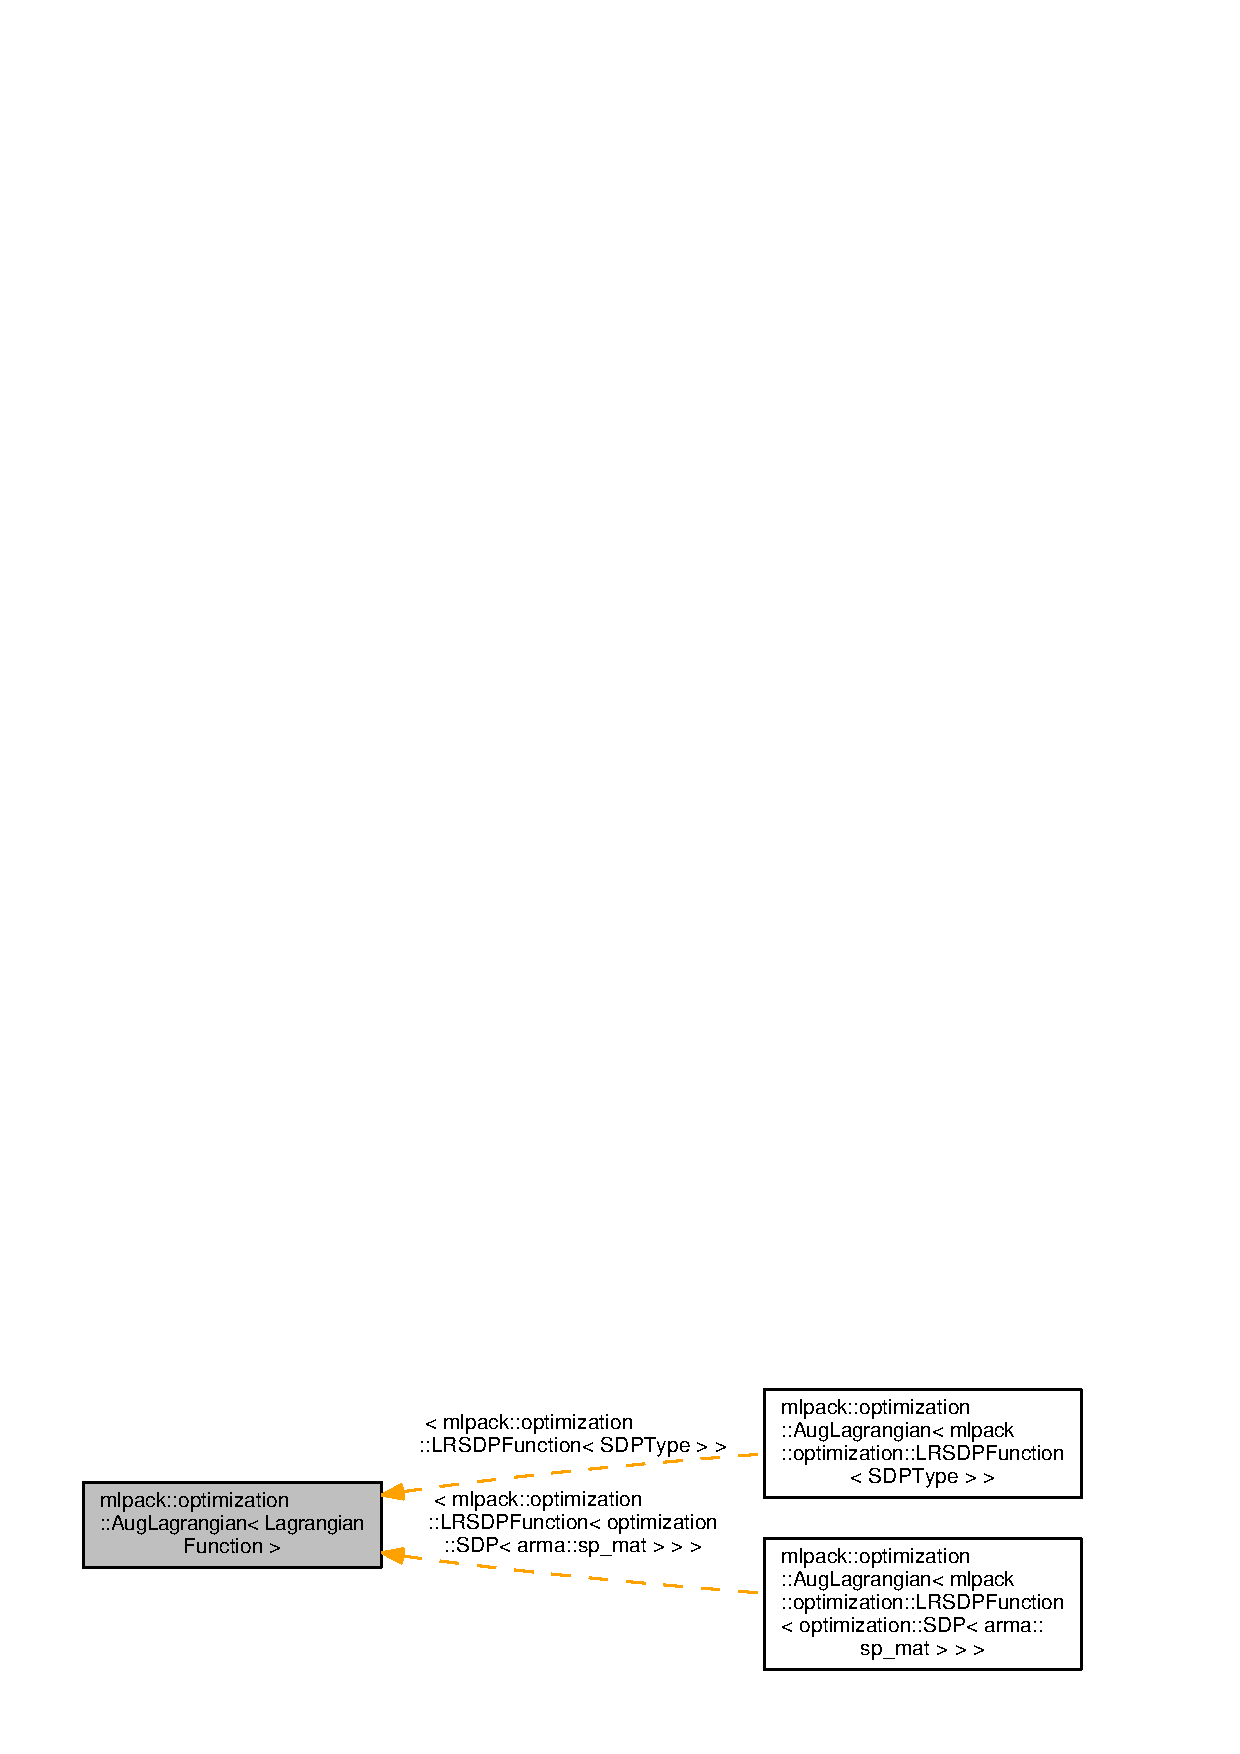
\includegraphics[width=350pt]{classmlpack_1_1optimization_1_1AugLagrangian__inherit__graph}
\end{center}
\end{figure}
\subsection*{Public Types}
\begin{DoxyCompactItemize}
\item 
typedef {\bf L\+\_\+\+B\+F\+GS}$<$ {\bf Aug\+Lagrangian\+Function}$<$ Lagrangian\+Function $>$ $>$ {\bf L\+\_\+\+B\+F\+G\+S\+Type}
\begin{DoxyCompactList}\small\item\em Shorthand for the type of the L-\/\+B\+F\+GS optimizer we\textquotesingle{}ll be using. \end{DoxyCompactList}\end{DoxyCompactItemize}
\subsection*{Public Member Functions}
\begin{DoxyCompactItemize}
\item 
{\bf Aug\+Lagrangian} (Lagrangian\+Function \&{\bf function})
\begin{DoxyCompactList}\small\item\em Initialize the Augmented Lagrangian with the default L-\/\+B\+F\+GS optimizer. \end{DoxyCompactList}\item 
{\bf Aug\+Lagrangian} ({\bf Aug\+Lagrangian\+Function}$<$ Lagrangian\+Function $>$ \&{\bf augfunc}, {\bf L\+\_\+\+B\+F\+G\+S\+Type} \&{\bf lbfgs})
\begin{DoxyCompactList}\small\item\em Initialize the Augmented Lagrangian with a custom L-\/\+B\+F\+GS optimizer. \end{DoxyCompactList}\item 
const Lagrangian\+Function \& {\bf Function} () const 
\begin{DoxyCompactList}\small\item\em Get the Lagrangian\+Function. \end{DoxyCompactList}\item 
Lagrangian\+Function \& {\bf Function} ()
\begin{DoxyCompactList}\small\item\em Modify the Lagrangian\+Function. \end{DoxyCompactList}\item 
const arma\+::vec \& {\bf Lambda} () const 
\begin{DoxyCompactList}\small\item\em Get the Lagrange multipliers. \end{DoxyCompactList}\item 
arma\+::vec \& {\bf Lambda} ()
\begin{DoxyCompactList}\small\item\em Modify the Lagrange multipliers (i.\+e. set them before optimization). \end{DoxyCompactList}\item 
const {\bf L\+\_\+\+B\+F\+G\+S\+Type} \& {\bf L\+B\+F\+GS} () const 
\begin{DoxyCompactList}\small\item\em Get the L-\/\+B\+F\+GS object used for the actual optimization. \end{DoxyCompactList}\item 
{\bf L\+\_\+\+B\+F\+G\+S\+Type} \& {\bf L\+B\+F\+GS} ()
\begin{DoxyCompactList}\small\item\em Modify the L-\/\+B\+F\+GS object used for the actual optimization. \end{DoxyCompactList}\item 
bool {\bf Optimize} (arma\+::mat \&coordinates, const size\+\_\+t max\+Iterations=1000)
\begin{DoxyCompactList}\small\item\em Optimize the function. \end{DoxyCompactList}\item 
bool {\bf Optimize} (arma\+::mat \&coordinates, const arma\+::vec \&init\+Lambda, const double init\+Sigma, const size\+\_\+t max\+Iterations=1000)
\begin{DoxyCompactList}\small\item\em Optimize the function, giving initial estimates for the Lagrange multipliers. \end{DoxyCompactList}\item 
double {\bf Sigma} () const 
\begin{DoxyCompactList}\small\item\em Get the penalty parameter. \end{DoxyCompactList}\item 
double \& {\bf Sigma} ()
\begin{DoxyCompactList}\small\item\em Modify the penalty parameter. \end{DoxyCompactList}\end{DoxyCompactItemize}
\subsection*{Private Attributes}
\begin{DoxyCompactItemize}
\item 
{\bf Aug\+Lagrangian\+Function}$<$ Lagrangian\+Function $>$ {\bf augfunc}
\begin{DoxyCompactList}\small\item\em Internally used \doxyref{Aug\+Lagrangian\+Function}{p.}{classmlpack_1_1optimization_1_1AugLagrangianFunction} which holds the function we are optimizing. \end{DoxyCompactList}\item 
Lagrangian\+Function \& {\bf function}
\begin{DoxyCompactList}\small\item\em Function to be optimized. \end{DoxyCompactList}\item 
{\bf L\+\_\+\+B\+F\+G\+S\+Type} \& {\bf lbfgs}
\begin{DoxyCompactList}\small\item\em The L-\/\+B\+F\+GS optimizer that we will use. \end{DoxyCompactList}\item 
{\bf L\+\_\+\+B\+F\+G\+S\+Type} {\bf lbfgs\+Internal}
\begin{DoxyCompactList}\small\item\em If the user did not pass an \doxyref{L\+\_\+\+B\+F\+GS}{p.}{classmlpack_1_1optimization_1_1L__BFGS} object, we\textquotesingle{}ll use our own internal one. \end{DoxyCompactList}\end{DoxyCompactItemize}


\subsection{Detailed Description}
\subsubsection*{template$<$typename Lagrangian\+Function$>$\\*
class mlpack\+::optimization\+::\+Aug\+Lagrangian$<$ Lagrangian\+Function $>$}

The \doxyref{Aug\+Lagrangian}{p.}{classmlpack_1_1optimization_1_1AugLagrangian} class implements the Augmented Lagrangian method of optimization. 

In this scheme, a penalty term is added to the Lagrangian. This method is also called the \char`\"{}method of multipliers\char`\"{}.

The template class Lagrangian\+Function must implement the following five methods\+:


\begin{DoxyItemize}
\item double Evaluate(const arma\+::mat\& coordinates);
\item void Gradient(const arma\+::mat\& coordinates, arma\+::mat\& gradient);
\item size\+\_\+t Num\+Constraints();
\item double Evaluate\+Constraint(size\+\_\+t index, const arma\+::mat\& coordinates);
\item double Gradient\+Constraint(size\+\_\+t index, const arma\+::mat\& coordinates, arma\+::mat\& gradient);
\end{DoxyItemize}

The number of constraints must be greater than or equal to 0, and Evaluate\+Constraint() should evaluate the constraint at the given index for the given coordinates. Evaluate() should provide the objective function value for the given coordinates.


\begin{DoxyTemplParams}{Template Parameters}
{\em Lagrangian\+Function} & Function which can be optimized by this class. \\
\hline
\end{DoxyTemplParams}


Definition at line 49 of file aug\+\_\+lagrangian.\+hpp.



\subsection{Member Typedef Documentation}
\index{mlpack\+::optimization\+::\+Aug\+Lagrangian@{mlpack\+::optimization\+::\+Aug\+Lagrangian}!L\+\_\+\+B\+F\+G\+S\+Type@{L\+\_\+\+B\+F\+G\+S\+Type}}
\index{L\+\_\+\+B\+F\+G\+S\+Type@{L\+\_\+\+B\+F\+G\+S\+Type}!mlpack\+::optimization\+::\+Aug\+Lagrangian@{mlpack\+::optimization\+::\+Aug\+Lagrangian}}
\subsubsection[{L\+\_\+\+B\+F\+G\+S\+Type}]{\setlength{\rightskip}{0pt plus 5cm}template$<$typename Lagrangian\+Function$>$ typedef {\bf L\+\_\+\+B\+F\+GS}$<${\bf Aug\+Lagrangian\+Function}$<$Lagrangian\+Function$>$ $>$ {\bf mlpack\+::optimization\+::\+Aug\+Lagrangian}$<$ Lagrangian\+Function $>$\+::{\bf L\+\_\+\+B\+F\+G\+S\+Type}}\label{classmlpack_1_1optimization_1_1AugLagrangian_a9236e1d59fd814bda0d65523808b34f1}


Shorthand for the type of the L-\/\+B\+F\+GS optimizer we\textquotesingle{}ll be using. 



Definition at line 54 of file aug\+\_\+lagrangian.\+hpp.



\subsection{Constructor \& Destructor Documentation}
\index{mlpack\+::optimization\+::\+Aug\+Lagrangian@{mlpack\+::optimization\+::\+Aug\+Lagrangian}!Aug\+Lagrangian@{Aug\+Lagrangian}}
\index{Aug\+Lagrangian@{Aug\+Lagrangian}!mlpack\+::optimization\+::\+Aug\+Lagrangian@{mlpack\+::optimization\+::\+Aug\+Lagrangian}}
\subsubsection[{Aug\+Lagrangian(\+Lagrangian\+Function \&function)}]{\setlength{\rightskip}{0pt plus 5cm}template$<$typename Lagrangian\+Function$>$ {\bf mlpack\+::optimization\+::\+Aug\+Lagrangian}$<$ Lagrangian\+Function $>$\+::{\bf Aug\+Lagrangian} (
\begin{DoxyParamCaption}
\item[{Lagrangian\+Function \&}]{function}
\end{DoxyParamCaption}
)}\label{classmlpack_1_1optimization_1_1AugLagrangian_aec18ad1aa9167e55aff6578e5b5d6a9d}


Initialize the Augmented Lagrangian with the default L-\/\+B\+F\+GS optimizer. 

We limit the number of L-\/\+B\+F\+GS iterations to 1000, rather than the unlimited default L-\/\+B\+F\+GS.


\begin{DoxyParams}{Parameters}
{\em function} & The function to be optimized. \\
\hline
\end{DoxyParams}
\index{mlpack\+::optimization\+::\+Aug\+Lagrangian@{mlpack\+::optimization\+::\+Aug\+Lagrangian}!Aug\+Lagrangian@{Aug\+Lagrangian}}
\index{Aug\+Lagrangian@{Aug\+Lagrangian}!mlpack\+::optimization\+::\+Aug\+Lagrangian@{mlpack\+::optimization\+::\+Aug\+Lagrangian}}
\subsubsection[{Aug\+Lagrangian(\+Aug\+Lagrangian\+Function$<$ Lagrangian\+Function $>$ \&augfunc, L\+\_\+\+B\+F\+G\+S\+Type \&lbfgs)}]{\setlength{\rightskip}{0pt plus 5cm}template$<$typename Lagrangian\+Function$>$ {\bf mlpack\+::optimization\+::\+Aug\+Lagrangian}$<$ Lagrangian\+Function $>$\+::{\bf Aug\+Lagrangian} (
\begin{DoxyParamCaption}
\item[{{\bf Aug\+Lagrangian\+Function}$<$ Lagrangian\+Function $>$ \&}]{augfunc, }
\item[{{\bf L\+\_\+\+B\+F\+G\+S\+Type} \&}]{lbfgs}
\end{DoxyParamCaption}
)}\label{classmlpack_1_1optimization_1_1AugLagrangian_aaa67574d7611a09e0b48ec0ae0852477}


Initialize the Augmented Lagrangian with a custom L-\/\+B\+F\+GS optimizer. 


\begin{DoxyParams}{Parameters}
{\em function} & The function to be optimized. This must be a pre-\/created utility \doxyref{Aug\+Lagrangian\+Function}{p.}{classmlpack_1_1optimization_1_1AugLagrangianFunction}. \\
\hline
{\em lbfgs} & The custom L-\/\+B\+F\+GS optimizer to be used. This should have already been initialized with the given \doxyref{Aug\+Lagrangian\+Function}{p.}{classmlpack_1_1optimization_1_1AugLagrangianFunction}. \\
\hline
\end{DoxyParams}


\subsection{Member Function Documentation}
\index{mlpack\+::optimization\+::\+Aug\+Lagrangian@{mlpack\+::optimization\+::\+Aug\+Lagrangian}!Function@{Function}}
\index{Function@{Function}!mlpack\+::optimization\+::\+Aug\+Lagrangian@{mlpack\+::optimization\+::\+Aug\+Lagrangian}}
\subsubsection[{Function() const }]{\setlength{\rightskip}{0pt plus 5cm}template$<$typename Lagrangian\+Function$>$ const Lagrangian\+Function\& {\bf mlpack\+::optimization\+::\+Aug\+Lagrangian}$<$ Lagrangian\+Function $>$\+::Function (
\begin{DoxyParamCaption}
{}
\end{DoxyParamCaption}
) const\hspace{0.3cm}{\ttfamily [inline]}}\label{classmlpack_1_1optimization_1_1AugLagrangian_a5db2c48f10cec8f6e4054da64c6a3daf}


Get the Lagrangian\+Function. 



Definition at line 107 of file aug\+\_\+lagrangian.\+hpp.

\index{mlpack\+::optimization\+::\+Aug\+Lagrangian@{mlpack\+::optimization\+::\+Aug\+Lagrangian}!Function@{Function}}
\index{Function@{Function}!mlpack\+::optimization\+::\+Aug\+Lagrangian@{mlpack\+::optimization\+::\+Aug\+Lagrangian}}
\subsubsection[{Function()}]{\setlength{\rightskip}{0pt plus 5cm}template$<$typename Lagrangian\+Function$>$ Lagrangian\+Function\& {\bf mlpack\+::optimization\+::\+Aug\+Lagrangian}$<$ Lagrangian\+Function $>$\+::Function (
\begin{DoxyParamCaption}
{}
\end{DoxyParamCaption}
)\hspace{0.3cm}{\ttfamily [inline]}}\label{classmlpack_1_1optimization_1_1AugLagrangian_af34a54aaa33a2002d04e38d1581444fa}


Modify the Lagrangian\+Function. 



Definition at line 109 of file aug\+\_\+lagrangian.\+hpp.

\index{mlpack\+::optimization\+::\+Aug\+Lagrangian@{mlpack\+::optimization\+::\+Aug\+Lagrangian}!Lambda@{Lambda}}
\index{Lambda@{Lambda}!mlpack\+::optimization\+::\+Aug\+Lagrangian@{mlpack\+::optimization\+::\+Aug\+Lagrangian}}
\subsubsection[{Lambda() const }]{\setlength{\rightskip}{0pt plus 5cm}template$<$typename Lagrangian\+Function$>$ const arma\+::vec\& {\bf mlpack\+::optimization\+::\+Aug\+Lagrangian}$<$ Lagrangian\+Function $>$\+::Lambda (
\begin{DoxyParamCaption}
{}
\end{DoxyParamCaption}
) const\hspace{0.3cm}{\ttfamily [inline]}}\label{classmlpack_1_1optimization_1_1AugLagrangian_ab912c3bb7da9c0d2e725b0a689521d8b}


Get the Lagrange multipliers. 



Definition at line 117 of file aug\+\_\+lagrangian.\+hpp.

\index{mlpack\+::optimization\+::\+Aug\+Lagrangian@{mlpack\+::optimization\+::\+Aug\+Lagrangian}!Lambda@{Lambda}}
\index{Lambda@{Lambda}!mlpack\+::optimization\+::\+Aug\+Lagrangian@{mlpack\+::optimization\+::\+Aug\+Lagrangian}}
\subsubsection[{Lambda()}]{\setlength{\rightskip}{0pt plus 5cm}template$<$typename Lagrangian\+Function$>$ arma\+::vec\& {\bf mlpack\+::optimization\+::\+Aug\+Lagrangian}$<$ Lagrangian\+Function $>$\+::Lambda (
\begin{DoxyParamCaption}
{}
\end{DoxyParamCaption}
)\hspace{0.3cm}{\ttfamily [inline]}}\label{classmlpack_1_1optimization_1_1AugLagrangian_a9fe03b08a49d6e209ca4e5bd92e89bac}


Modify the Lagrange multipliers (i.\+e. set them before optimization). 



Definition at line 119 of file aug\+\_\+lagrangian.\+hpp.

\index{mlpack\+::optimization\+::\+Aug\+Lagrangian@{mlpack\+::optimization\+::\+Aug\+Lagrangian}!L\+B\+F\+GS@{L\+B\+F\+GS}}
\index{L\+B\+F\+GS@{L\+B\+F\+GS}!mlpack\+::optimization\+::\+Aug\+Lagrangian@{mlpack\+::optimization\+::\+Aug\+Lagrangian}}
\subsubsection[{L\+B\+F\+G\+S() const }]{\setlength{\rightskip}{0pt plus 5cm}template$<$typename Lagrangian\+Function$>$ const {\bf L\+\_\+\+B\+F\+G\+S\+Type}\& {\bf mlpack\+::optimization\+::\+Aug\+Lagrangian}$<$ Lagrangian\+Function $>$\+::L\+B\+F\+GS (
\begin{DoxyParamCaption}
{}
\end{DoxyParamCaption}
) const\hspace{0.3cm}{\ttfamily [inline]}}\label{classmlpack_1_1optimization_1_1AugLagrangian_a33258b734b9da547cca6c2ffed584fee}


Get the L-\/\+B\+F\+GS object used for the actual optimization. 



Definition at line 112 of file aug\+\_\+lagrangian.\+hpp.

\index{mlpack\+::optimization\+::\+Aug\+Lagrangian@{mlpack\+::optimization\+::\+Aug\+Lagrangian}!L\+B\+F\+GS@{L\+B\+F\+GS}}
\index{L\+B\+F\+GS@{L\+B\+F\+GS}!mlpack\+::optimization\+::\+Aug\+Lagrangian@{mlpack\+::optimization\+::\+Aug\+Lagrangian}}
\subsubsection[{L\+B\+F\+G\+S()}]{\setlength{\rightskip}{0pt plus 5cm}template$<$typename Lagrangian\+Function$>$ {\bf L\+\_\+\+B\+F\+G\+S\+Type}\& {\bf mlpack\+::optimization\+::\+Aug\+Lagrangian}$<$ Lagrangian\+Function $>$\+::L\+B\+F\+GS (
\begin{DoxyParamCaption}
{}
\end{DoxyParamCaption}
)\hspace{0.3cm}{\ttfamily [inline]}}\label{classmlpack_1_1optimization_1_1AugLagrangian_a205c6a195944624a9e312f0822fd9775}


Modify the L-\/\+B\+F\+GS object used for the actual optimization. 



Definition at line 114 of file aug\+\_\+lagrangian.\+hpp.

\index{mlpack\+::optimization\+::\+Aug\+Lagrangian@{mlpack\+::optimization\+::\+Aug\+Lagrangian}!Optimize@{Optimize}}
\index{Optimize@{Optimize}!mlpack\+::optimization\+::\+Aug\+Lagrangian@{mlpack\+::optimization\+::\+Aug\+Lagrangian}}
\subsubsection[{Optimize(arma\+::mat \&coordinates, const size\+\_\+t max\+Iterations=1000)}]{\setlength{\rightskip}{0pt plus 5cm}template$<$typename Lagrangian\+Function$>$ bool {\bf mlpack\+::optimization\+::\+Aug\+Lagrangian}$<$ Lagrangian\+Function $>$\+::Optimize (
\begin{DoxyParamCaption}
\item[{arma\+::mat \&}]{coordinates, }
\item[{const size\+\_\+t}]{max\+Iterations = {\ttfamily 1000}}
\end{DoxyParamCaption}
)}\label{classmlpack_1_1optimization_1_1AugLagrangian_a3236fe0e8dc522bde55a1d31fe5797d7}


Optimize the function. 

The value \textquotesingle{}1\textquotesingle{} is used for the initial value of each Lagrange multiplier. To set the Lagrange multipliers yourself, use the other overload of \doxyref{Optimize()}{p.}{classmlpack_1_1optimization_1_1AugLagrangian_a3236fe0e8dc522bde55a1d31fe5797d7}.


\begin{DoxyParams}{Parameters}
{\em coordinates} & Output matrix to store the optimized coordinates in. \\
\hline
{\em max\+Iterations} & Maximum number of iterations of the Augmented Lagrangian algorithm. 0 indicates no maximum. \\
\hline
{\em sigma} & Initial penalty parameter. \\
\hline
\end{DoxyParams}
\index{mlpack\+::optimization\+::\+Aug\+Lagrangian@{mlpack\+::optimization\+::\+Aug\+Lagrangian}!Optimize@{Optimize}}
\index{Optimize@{Optimize}!mlpack\+::optimization\+::\+Aug\+Lagrangian@{mlpack\+::optimization\+::\+Aug\+Lagrangian}}
\subsubsection[{Optimize(arma\+::mat \&coordinates, const arma\+::vec \&init\+Lambda, const double init\+Sigma, const size\+\_\+t max\+Iterations=1000)}]{\setlength{\rightskip}{0pt plus 5cm}template$<$typename Lagrangian\+Function$>$ bool {\bf mlpack\+::optimization\+::\+Aug\+Lagrangian}$<$ Lagrangian\+Function $>$\+::Optimize (
\begin{DoxyParamCaption}
\item[{arma\+::mat \&}]{coordinates, }
\item[{const arma\+::vec \&}]{init\+Lambda, }
\item[{const double}]{init\+Sigma, }
\item[{const size\+\_\+t}]{max\+Iterations = {\ttfamily 1000}}
\end{DoxyParamCaption}
)}\label{classmlpack_1_1optimization_1_1AugLagrangian_a9d8b8fab9e1a3502b87dcc8a525a4c12}


Optimize the function, giving initial estimates for the Lagrange multipliers. 

The vector of Lagrange multipliers will be modified to contain the Lagrange multipliers of the final solution (if one is found).


\begin{DoxyParams}{Parameters}
{\em coordinates} & Output matrix to store the optimized coordinates in. \\
\hline
{\em init\+Lambda} & Vector of initial Lagrange multipliers. Should have length equal to the number of constraints. \\
\hline
{\em init\+Sigma} & Initial penalty parameter. \\
\hline
{\em max\+Iterations} & Maximum number of iterations of the Augmented Lagrangian algorithm. 0 indicates no maximum. \\
\hline
\end{DoxyParams}
\index{mlpack\+::optimization\+::\+Aug\+Lagrangian@{mlpack\+::optimization\+::\+Aug\+Lagrangian}!Sigma@{Sigma}}
\index{Sigma@{Sigma}!mlpack\+::optimization\+::\+Aug\+Lagrangian@{mlpack\+::optimization\+::\+Aug\+Lagrangian}}
\subsubsection[{Sigma() const }]{\setlength{\rightskip}{0pt plus 5cm}template$<$typename Lagrangian\+Function$>$ double {\bf mlpack\+::optimization\+::\+Aug\+Lagrangian}$<$ Lagrangian\+Function $>$\+::Sigma (
\begin{DoxyParamCaption}
{}
\end{DoxyParamCaption}
) const\hspace{0.3cm}{\ttfamily [inline]}}\label{classmlpack_1_1optimization_1_1AugLagrangian_a04eaf73441a0650405e3b74b903d1eae}


Get the penalty parameter. 



Definition at line 122 of file aug\+\_\+lagrangian.\+hpp.

\index{mlpack\+::optimization\+::\+Aug\+Lagrangian@{mlpack\+::optimization\+::\+Aug\+Lagrangian}!Sigma@{Sigma}}
\index{Sigma@{Sigma}!mlpack\+::optimization\+::\+Aug\+Lagrangian@{mlpack\+::optimization\+::\+Aug\+Lagrangian}}
\subsubsection[{Sigma()}]{\setlength{\rightskip}{0pt plus 5cm}template$<$typename Lagrangian\+Function$>$ double\& {\bf mlpack\+::optimization\+::\+Aug\+Lagrangian}$<$ Lagrangian\+Function $>$\+::Sigma (
\begin{DoxyParamCaption}
{}
\end{DoxyParamCaption}
)\hspace{0.3cm}{\ttfamily [inline]}}\label{classmlpack_1_1optimization_1_1AugLagrangian_a9af7e955a86bd977d442b7acd6a59ae7}


Modify the penalty parameter. 



Definition at line 124 of file aug\+\_\+lagrangian.\+hpp.



\subsection{Member Data Documentation}
\index{mlpack\+::optimization\+::\+Aug\+Lagrangian@{mlpack\+::optimization\+::\+Aug\+Lagrangian}!augfunc@{augfunc}}
\index{augfunc@{augfunc}!mlpack\+::optimization\+::\+Aug\+Lagrangian@{mlpack\+::optimization\+::\+Aug\+Lagrangian}}
\subsubsection[{augfunc}]{\setlength{\rightskip}{0pt plus 5cm}template$<$typename Lagrangian\+Function$>$ {\bf Aug\+Lagrangian\+Function}$<$Lagrangian\+Function$>$ {\bf mlpack\+::optimization\+::\+Aug\+Lagrangian}$<$ Lagrangian\+Function $>$\+::augfunc\hspace{0.3cm}{\ttfamily [private]}}\label{classmlpack_1_1optimization_1_1AugLagrangian_a303c0e7e199987eb678316a8532989f5}


Internally used \doxyref{Aug\+Lagrangian\+Function}{p.}{classmlpack_1_1optimization_1_1AugLagrangianFunction} which holds the function we are optimizing. 

This isn\textquotesingle{}t publically accessible, but we provide ways to get to the Lagrange multipliers and the penalty parameter sigma. 

Definition at line 133 of file aug\+\_\+lagrangian.\+hpp.



Referenced by mlpack\+::optimization\+::\+Aug\+Lagrangian$<$ mlpack\+::optimization\+::\+L\+R\+S\+D\+P\+Function$<$ optimization\+::\+S\+D\+P$<$ arma\+::sp\+\_\+mat $>$ $>$ $>$\+::\+Lambda(), and mlpack\+::optimization\+::\+Aug\+Lagrangian$<$ mlpack\+::optimization\+::\+L\+R\+S\+D\+P\+Function$<$ optimization\+::\+S\+D\+P$<$ arma\+::sp\+\_\+mat $>$ $>$ $>$\+::\+Sigma().

\index{mlpack\+::optimization\+::\+Aug\+Lagrangian@{mlpack\+::optimization\+::\+Aug\+Lagrangian}!function@{function}}
\index{function@{function}!mlpack\+::optimization\+::\+Aug\+Lagrangian@{mlpack\+::optimization\+::\+Aug\+Lagrangian}}
\subsubsection[{function}]{\setlength{\rightskip}{0pt plus 5cm}template$<$typename Lagrangian\+Function$>$ Lagrangian\+Function\& {\bf mlpack\+::optimization\+::\+Aug\+Lagrangian}$<$ Lagrangian\+Function $>$\+::function\hspace{0.3cm}{\ttfamily [private]}}\label{classmlpack_1_1optimization_1_1AugLagrangian_a12cd00a9fc80ceb26ccecd438ae1d3eb}


Function to be optimized. 



Definition at line 128 of file aug\+\_\+lagrangian.\+hpp.

\index{mlpack\+::optimization\+::\+Aug\+Lagrangian@{mlpack\+::optimization\+::\+Aug\+Lagrangian}!lbfgs@{lbfgs}}
\index{lbfgs@{lbfgs}!mlpack\+::optimization\+::\+Aug\+Lagrangian@{mlpack\+::optimization\+::\+Aug\+Lagrangian}}
\subsubsection[{lbfgs}]{\setlength{\rightskip}{0pt plus 5cm}template$<$typename Lagrangian\+Function$>$ {\bf L\+\_\+\+B\+F\+G\+S\+Type}\& {\bf mlpack\+::optimization\+::\+Aug\+Lagrangian}$<$ Lagrangian\+Function $>$\+::lbfgs\hspace{0.3cm}{\ttfamily [private]}}\label{classmlpack_1_1optimization_1_1AugLagrangian_adebbf0a697a0b09ce96ddfc50abcc132}


The L-\/\+B\+F\+GS optimizer that we will use. 



Definition at line 139 of file aug\+\_\+lagrangian.\+hpp.



Referenced by mlpack\+::optimization\+::\+Aug\+Lagrangian$<$ mlpack\+::optimization\+::\+L\+R\+S\+D\+P\+Function$<$ optimization\+::\+S\+D\+P$<$ arma\+::sp\+\_\+mat $>$ $>$ $>$\+::\+L\+B\+F\+G\+S().

\index{mlpack\+::optimization\+::\+Aug\+Lagrangian@{mlpack\+::optimization\+::\+Aug\+Lagrangian}!lbfgs\+Internal@{lbfgs\+Internal}}
\index{lbfgs\+Internal@{lbfgs\+Internal}!mlpack\+::optimization\+::\+Aug\+Lagrangian@{mlpack\+::optimization\+::\+Aug\+Lagrangian}}
\subsubsection[{lbfgs\+Internal}]{\setlength{\rightskip}{0pt plus 5cm}template$<$typename Lagrangian\+Function$>$ {\bf L\+\_\+\+B\+F\+G\+S\+Type} {\bf mlpack\+::optimization\+::\+Aug\+Lagrangian}$<$ Lagrangian\+Function $>$\+::lbfgs\+Internal\hspace{0.3cm}{\ttfamily [private]}}\label{classmlpack_1_1optimization_1_1AugLagrangian_a6126a13f9a48f896b3060a8883b67dc7}


If the user did not pass an \doxyref{L\+\_\+\+B\+F\+GS}{p.}{classmlpack_1_1optimization_1_1L__BFGS} object, we\textquotesingle{}ll use our own internal one. 



Definition at line 136 of file aug\+\_\+lagrangian.\+hpp.



The documentation for this class was generated from the following file\+:\begin{DoxyCompactItemize}
\item 
src/mlpack/core/optimizers/aug\+\_\+lagrangian/{\bf aug\+\_\+lagrangian.\+hpp}\end{DoxyCompactItemize}

\section{mlpack\+:\+:optimization\+:\+:Aug\+Lagrangian\+Function$<$ Lagrangian\+Function $>$ Class Template Reference}
\label{classmlpack_1_1optimization_1_1AugLagrangianFunction}\index{mlpack\+::optimization\+::\+Aug\+Lagrangian\+Function$<$ Lagrangian\+Function $>$@{mlpack\+::optimization\+::\+Aug\+Lagrangian\+Function$<$ Lagrangian\+Function $>$}}


This is a utility class used by \doxyref{Aug\+Lagrangian}{p.}{classmlpack_1_1optimization_1_1AugLagrangian}, meant to wrap a Lagrangian\+Function into a function usable by a simple optimizer like L-\/\+B\+F\+GS.  




Inheritance diagram for mlpack\+:\+:optimization\+:\+:Aug\+Lagrangian\+Function$<$ Lagrangian\+Function $>$\+:
\nopagebreak
\begin{figure}[H]
\begin{center}
\leavevmode
\includegraphics[width=350pt]{classmlpack_1_1optimization_1_1AugLagrangianFunction__inherit__graph}
\end{center}
\end{figure}
\subsection*{Public Member Functions}
\begin{DoxyCompactItemize}
\item 
{\bf Aug\+Lagrangian\+Function} (Lagrangian\+Function \&{\bf function})
\begin{DoxyCompactList}\small\item\em Initialize the \doxyref{Aug\+Lagrangian\+Function}{p.}{classmlpack_1_1optimization_1_1AugLagrangianFunction}, but don\textquotesingle{}t set the Lagrange multipliers or penalty parameters yet. \end{DoxyCompactList}\item 
{\bf Aug\+Lagrangian\+Function} (Lagrangian\+Function \&{\bf function}, const arma\+::vec \&{\bf lambda}, const double {\bf sigma})
\begin{DoxyCompactList}\small\item\em Initialize the \doxyref{Aug\+Lagrangian\+Function}{p.}{classmlpack_1_1optimization_1_1AugLagrangianFunction} with the given Lagrangian\+Function, Lagrange multipliers, and initial penalty parameter. \end{DoxyCompactList}\item 
double {\bf Evaluate} (const arma\+::mat \&coordinates) const 
\begin{DoxyCompactList}\small\item\em Evaluate the objective function of the Augmented Lagrangian function, which is the standard Lagrangian function evaluation plus a penalty term, which penalizes unsatisfied constraints. \end{DoxyCompactList}\item 
{\footnotesize template$<$$>$ }\\double {\bf Evaluate} (const arma\+::mat \&coordinates) const
\item 
{\footnotesize template$<$$>$ }\\double {\bf Evaluate} (const arma\+::mat \&coordinates) const
\item 
const Lagrangian\+Function \& {\bf Function} () const 
\begin{DoxyCompactList}\small\item\em Get the Lagrangian function. \end{DoxyCompactList}\item 
Lagrangian\+Function \& {\bf Function} ()
\begin{DoxyCompactList}\small\item\em Modify the Lagrangian function. \end{DoxyCompactList}\item 
const arma\+::mat \& {\bf Get\+Initial\+Point} () const 
\begin{DoxyCompactList}\small\item\em Get the initial point of the optimization (supplied by the Lagrangian\+Function). \end{DoxyCompactList}\item 
void {\bf Gradient} (const arma\+::mat \&coordinates, arma\+::mat \&gradient) const 
\begin{DoxyCompactList}\small\item\em Evaluate the gradient of the Augmented Lagrangian function. \end{DoxyCompactList}\item 
{\footnotesize template$<$$>$ }\\void {\bf Gradient} (const arma\+::mat \&coordinates, arma\+::mat \&gradient) const
\item 
{\footnotesize template$<$$>$ }\\void {\bf Gradient} (const arma\+::mat \&coordinates, arma\+::mat \&gradient) const
\item 
const arma\+::vec \& {\bf Lambda} () const 
\begin{DoxyCompactList}\small\item\em Get the Lagrange multipliers. \end{DoxyCompactList}\item 
arma\+::vec \& {\bf Lambda} ()
\begin{DoxyCompactList}\small\item\em Modify the Lagrange multipliers. \end{DoxyCompactList}\item 
double {\bf Sigma} () const 
\begin{DoxyCompactList}\small\item\em Get sigma (the penalty parameter). \end{DoxyCompactList}\item 
double \& {\bf Sigma} ()
\begin{DoxyCompactList}\small\item\em Modify sigma (the penalty parameter). \end{DoxyCompactList}\end{DoxyCompactItemize}
\subsection*{Private Attributes}
\begin{DoxyCompactItemize}
\item 
Lagrangian\+Function \& {\bf function}
\begin{DoxyCompactList}\small\item\em Instantiation of the function to be optimized. \end{DoxyCompactList}\item 
arma\+::vec {\bf lambda}
\begin{DoxyCompactList}\small\item\em The Lagrange multipliers. \end{DoxyCompactList}\item 
double {\bf sigma}
\begin{DoxyCompactList}\small\item\em The penalty parameter. \end{DoxyCompactList}\end{DoxyCompactItemize}


\subsection{Detailed Description}
\subsubsection*{template$<$typename Lagrangian\+Function$>$\\*
class mlpack\+::optimization\+::\+Aug\+Lagrangian\+Function$<$ Lagrangian\+Function $>$}

This is a utility class used by \doxyref{Aug\+Lagrangian}{p.}{classmlpack_1_1optimization_1_1AugLagrangian}, meant to wrap a Lagrangian\+Function into a function usable by a simple optimizer like L-\/\+B\+F\+GS. 

Given a Lagrangian\+Function which follows the format outlined in the documentation for \doxyref{Aug\+Lagrangian}{p.}{classmlpack_1_1optimization_1_1AugLagrangian}, this class provides \doxyref{Evaluate()}{p.}{classmlpack_1_1optimization_1_1AugLagrangianFunction_a0e61ccaaa0b9b3a8b37d3e038e3e0499}, \doxyref{Gradient()}{p.}{classmlpack_1_1optimization_1_1AugLagrangianFunction_ad2cfa503dc2b7f1c8e2f87fe46fb8f32}, and \doxyref{Get\+Initial\+Point()}{p.}{classmlpack_1_1optimization_1_1AugLagrangianFunction_a5f40253bac9682d0ed3303cb36b4c030} functions which allow this class to be used with a simple optimizer like L-\/\+B\+F\+GS.

This class can be specialized for your particular implementation -- commonly, a faster method for computing the overall objective and gradient of the augmented Lagrangian function can be implemented than the naive, default implementation given. Use class template specialization and re-\/implement all of the methods (unfortunately, C++ specialization rules mean you have to re-\/implement everything).


\begin{DoxyTemplParams}{Template Parameters}
{\em Lagrangian\+Function} & Lagrangian function to be used. \\
\hline
\end{DoxyTemplParams}


Definition at line 38 of file aug\+\_\+lagrangian\+\_\+function.\+hpp.



\subsection{Constructor \& Destructor Documentation}
\index{mlpack\+::optimization\+::\+Aug\+Lagrangian\+Function@{mlpack\+::optimization\+::\+Aug\+Lagrangian\+Function}!Aug\+Lagrangian\+Function@{Aug\+Lagrangian\+Function}}
\index{Aug\+Lagrangian\+Function@{Aug\+Lagrangian\+Function}!mlpack\+::optimization\+::\+Aug\+Lagrangian\+Function@{mlpack\+::optimization\+::\+Aug\+Lagrangian\+Function}}
\subsubsection[{Aug\+Lagrangian\+Function(\+Lagrangian\+Function \&function)}]{\setlength{\rightskip}{0pt plus 5cm}template$<$typename Lagrangian\+Function$>$ {\bf mlpack\+::optimization\+::\+Aug\+Lagrangian\+Function}$<$ Lagrangian\+Function $>$\+::{\bf Aug\+Lagrangian\+Function} (
\begin{DoxyParamCaption}
\item[{Lagrangian\+Function \&}]{function}
\end{DoxyParamCaption}
)}\label{classmlpack_1_1optimization_1_1AugLagrangianFunction_a813922250131034e190f7e54d3006c6d}


Initialize the \doxyref{Aug\+Lagrangian\+Function}{p.}{classmlpack_1_1optimization_1_1AugLagrangianFunction}, but don\textquotesingle{}t set the Lagrange multipliers or penalty parameters yet. 

Make sure you set the Lagrange multipliers before you use this...


\begin{DoxyParams}{Parameters}
{\em function} & Lagrangian function. \\
\hline
\end{DoxyParams}
\index{mlpack\+::optimization\+::\+Aug\+Lagrangian\+Function@{mlpack\+::optimization\+::\+Aug\+Lagrangian\+Function}!Aug\+Lagrangian\+Function@{Aug\+Lagrangian\+Function}}
\index{Aug\+Lagrangian\+Function@{Aug\+Lagrangian\+Function}!mlpack\+::optimization\+::\+Aug\+Lagrangian\+Function@{mlpack\+::optimization\+::\+Aug\+Lagrangian\+Function}}
\subsubsection[{Aug\+Lagrangian\+Function(\+Lagrangian\+Function \&function, const arma\+::vec \&lambda, const double sigma)}]{\setlength{\rightskip}{0pt plus 5cm}template$<$typename Lagrangian\+Function$>$ {\bf mlpack\+::optimization\+::\+Aug\+Lagrangian\+Function}$<$ Lagrangian\+Function $>$\+::{\bf Aug\+Lagrangian\+Function} (
\begin{DoxyParamCaption}
\item[{Lagrangian\+Function \&}]{function, }
\item[{const arma\+::vec \&}]{lambda, }
\item[{const double}]{sigma}
\end{DoxyParamCaption}
)}\label{classmlpack_1_1optimization_1_1AugLagrangianFunction_acd42530195dc3c1b7c68a31b7c2d5766}


Initialize the \doxyref{Aug\+Lagrangian\+Function}{p.}{classmlpack_1_1optimization_1_1AugLagrangianFunction} with the given Lagrangian\+Function, Lagrange multipliers, and initial penalty parameter. 


\begin{DoxyParams}{Parameters}
{\em function} & Lagrangian function. \\
\hline
{\em lambda} & Initial Lagrange multipliers. \\
\hline
{\em sigma} & Initial penalty parameter. \\
\hline
\end{DoxyParams}


\subsection{Member Function Documentation}
\index{mlpack\+::optimization\+::\+Aug\+Lagrangian\+Function@{mlpack\+::optimization\+::\+Aug\+Lagrangian\+Function}!Evaluate@{Evaluate}}
\index{Evaluate@{Evaluate}!mlpack\+::optimization\+::\+Aug\+Lagrangian\+Function@{mlpack\+::optimization\+::\+Aug\+Lagrangian\+Function}}
\subsubsection[{Evaluate(const arma\+::mat \&coordinates) const }]{\setlength{\rightskip}{0pt plus 5cm}template$<$typename Lagrangian\+Function$>$ double {\bf mlpack\+::optimization\+::\+Aug\+Lagrangian\+Function}$<$ Lagrangian\+Function $>$\+::Evaluate (
\begin{DoxyParamCaption}
\item[{const arma\+::mat \&}]{coordinates}
\end{DoxyParamCaption}
) const}\label{classmlpack_1_1optimization_1_1AugLagrangianFunction_a0e61ccaaa0b9b3a8b37d3e038e3e0499}


Evaluate the objective function of the Augmented Lagrangian function, which is the standard Lagrangian function evaluation plus a penalty term, which penalizes unsatisfied constraints. 


\begin{DoxyParams}{Parameters}
{\em coordinates} & Coordinates to evaluate function at. \\
\hline
\end{DoxyParams}
\begin{DoxyReturn}{Returns}
Objective function. 
\end{DoxyReturn}
\index{mlpack\+::optimization\+::\+Aug\+Lagrangian\+Function@{mlpack\+::optimization\+::\+Aug\+Lagrangian\+Function}!Evaluate@{Evaluate}}
\index{Evaluate@{Evaluate}!mlpack\+::optimization\+::\+Aug\+Lagrangian\+Function@{mlpack\+::optimization\+::\+Aug\+Lagrangian\+Function}}
\subsubsection[{Evaluate(const arma\+::mat \&coordinates) const}]{\setlength{\rightskip}{0pt plus 5cm}template$<$$>$ double {\bf mlpack\+::optimization\+::\+Aug\+Lagrangian\+Function}$<$ {\bf L\+R\+S\+D\+P\+Function}$<$ {\bf S\+DP}$<$ arma\+::sp\+\_\+mat $>$ $>$ $>$\+::Evaluate (
\begin{DoxyParamCaption}
\item[{const arma\+::mat \&}]{coordinates}
\end{DoxyParamCaption}
) const\hspace{0.3cm}{\ttfamily [inline]}}\label{classmlpack_1_1optimization_1_1AugLagrangianFunction_a2dc1ebda7f1b111220907ec6d7b2d854}
\index{mlpack\+::optimization\+::\+Aug\+Lagrangian\+Function@{mlpack\+::optimization\+::\+Aug\+Lagrangian\+Function}!Evaluate@{Evaluate}}
\index{Evaluate@{Evaluate}!mlpack\+::optimization\+::\+Aug\+Lagrangian\+Function@{mlpack\+::optimization\+::\+Aug\+Lagrangian\+Function}}
\subsubsection[{Evaluate(const arma\+::mat \&coordinates) const}]{\setlength{\rightskip}{0pt plus 5cm}template$<$$>$ double {\bf mlpack\+::optimization\+::\+Aug\+Lagrangian\+Function}$<$ {\bf L\+R\+S\+D\+P\+Function}$<$ {\bf S\+DP}$<$ arma\+::mat $>$ $>$ $>$\+::Evaluate (
\begin{DoxyParamCaption}
\item[{const arma\+::mat \&}]{coordinates}
\end{DoxyParamCaption}
) const\hspace{0.3cm}{\ttfamily [inline]}}\label{classmlpack_1_1optimization_1_1AugLagrangianFunction_a38546cd74fa75aac61e6f0127650d1b1}
\index{mlpack\+::optimization\+::\+Aug\+Lagrangian\+Function@{mlpack\+::optimization\+::\+Aug\+Lagrangian\+Function}!Function@{Function}}
\index{Function@{Function}!mlpack\+::optimization\+::\+Aug\+Lagrangian\+Function@{mlpack\+::optimization\+::\+Aug\+Lagrangian\+Function}}
\subsubsection[{Function() const }]{\setlength{\rightskip}{0pt plus 5cm}template$<$typename Lagrangian\+Function$>$ const Lagrangian\+Function\& {\bf mlpack\+::optimization\+::\+Aug\+Lagrangian\+Function}$<$ Lagrangian\+Function $>$\+::Function (
\begin{DoxyParamCaption}
{}
\end{DoxyParamCaption}
) const\hspace{0.3cm}{\ttfamily [inline]}}\label{classmlpack_1_1optimization_1_1AugLagrangianFunction_a929504b06d04989a1ae9f9b44c551b33}


Get the Lagrangian function. 



Definition at line 98 of file aug\+\_\+lagrangian\+\_\+function.\+hpp.

\index{mlpack\+::optimization\+::\+Aug\+Lagrangian\+Function@{mlpack\+::optimization\+::\+Aug\+Lagrangian\+Function}!Function@{Function}}
\index{Function@{Function}!mlpack\+::optimization\+::\+Aug\+Lagrangian\+Function@{mlpack\+::optimization\+::\+Aug\+Lagrangian\+Function}}
\subsubsection[{Function()}]{\setlength{\rightskip}{0pt plus 5cm}template$<$typename Lagrangian\+Function$>$ Lagrangian\+Function\& {\bf mlpack\+::optimization\+::\+Aug\+Lagrangian\+Function}$<$ Lagrangian\+Function $>$\+::Function (
\begin{DoxyParamCaption}
{}
\end{DoxyParamCaption}
)\hspace{0.3cm}{\ttfamily [inline]}}\label{classmlpack_1_1optimization_1_1AugLagrangianFunction_acb6306bdf1e2c0316cf1b2038c75db53}


Modify the Lagrangian function. 



Definition at line 100 of file aug\+\_\+lagrangian\+\_\+function.\+hpp.

\index{mlpack\+::optimization\+::\+Aug\+Lagrangian\+Function@{mlpack\+::optimization\+::\+Aug\+Lagrangian\+Function}!Get\+Initial\+Point@{Get\+Initial\+Point}}
\index{Get\+Initial\+Point@{Get\+Initial\+Point}!mlpack\+::optimization\+::\+Aug\+Lagrangian\+Function@{mlpack\+::optimization\+::\+Aug\+Lagrangian\+Function}}
\subsubsection[{Get\+Initial\+Point() const }]{\setlength{\rightskip}{0pt plus 5cm}template$<$typename Lagrangian\+Function$>$ const arma\+::mat\& {\bf mlpack\+::optimization\+::\+Aug\+Lagrangian\+Function}$<$ Lagrangian\+Function $>$\+::Get\+Initial\+Point (
\begin{DoxyParamCaption}
{}
\end{DoxyParamCaption}
) const}\label{classmlpack_1_1optimization_1_1AugLagrangianFunction_a5f40253bac9682d0ed3303cb36b4c030}


Get the initial point of the optimization (supplied by the Lagrangian\+Function). 

\begin{DoxyReturn}{Returns}
Initial point. 
\end{DoxyReturn}
\index{mlpack\+::optimization\+::\+Aug\+Lagrangian\+Function@{mlpack\+::optimization\+::\+Aug\+Lagrangian\+Function}!Gradient@{Gradient}}
\index{Gradient@{Gradient}!mlpack\+::optimization\+::\+Aug\+Lagrangian\+Function@{mlpack\+::optimization\+::\+Aug\+Lagrangian\+Function}}
\subsubsection[{Gradient(const arma\+::mat \&coordinates, arma\+::mat \&gradient) const }]{\setlength{\rightskip}{0pt plus 5cm}template$<$typename Lagrangian\+Function$>$ void {\bf mlpack\+::optimization\+::\+Aug\+Lagrangian\+Function}$<$ Lagrangian\+Function $>$\+::Gradient (
\begin{DoxyParamCaption}
\item[{const arma\+::mat \&}]{coordinates, }
\item[{arma\+::mat \&}]{gradient}
\end{DoxyParamCaption}
) const}\label{classmlpack_1_1optimization_1_1AugLagrangianFunction_ad2cfa503dc2b7f1c8e2f87fe46fb8f32}


Evaluate the gradient of the Augmented Lagrangian function. 


\begin{DoxyParams}{Parameters}
{\em coordinates} & Coordinates to evaluate gradient at. \\
\hline
{\em gradient} & Matrix to store gradient into. \\
\hline
\end{DoxyParams}
\index{mlpack\+::optimization\+::\+Aug\+Lagrangian\+Function@{mlpack\+::optimization\+::\+Aug\+Lagrangian\+Function}!Gradient@{Gradient}}
\index{Gradient@{Gradient}!mlpack\+::optimization\+::\+Aug\+Lagrangian\+Function@{mlpack\+::optimization\+::\+Aug\+Lagrangian\+Function}}
\subsubsection[{Gradient(const arma\+::mat \&coordinates, arma\+::mat \&gradient) const}]{\setlength{\rightskip}{0pt plus 5cm}template$<$$>$ void {\bf mlpack\+::optimization\+::\+Aug\+Lagrangian\+Function}$<$ {\bf L\+R\+S\+D\+P\+Function}$<$ {\bf S\+DP}$<$ arma\+::sp\+\_\+mat $>$ $>$ $>$\+::Gradient (
\begin{DoxyParamCaption}
\item[{const arma\+::mat \&}]{coordinates, }
\item[{arma\+::mat \&}]{gradient}
\end{DoxyParamCaption}
) const\hspace{0.3cm}{\ttfamily [inline]}}\label{classmlpack_1_1optimization_1_1AugLagrangianFunction_aca660f9dee4472f38f6e595f913d242b}
\index{mlpack\+::optimization\+::\+Aug\+Lagrangian\+Function@{mlpack\+::optimization\+::\+Aug\+Lagrangian\+Function}!Gradient@{Gradient}}
\index{Gradient@{Gradient}!mlpack\+::optimization\+::\+Aug\+Lagrangian\+Function@{mlpack\+::optimization\+::\+Aug\+Lagrangian\+Function}}
\subsubsection[{Gradient(const arma\+::mat \&coordinates, arma\+::mat \&gradient) const}]{\setlength{\rightskip}{0pt plus 5cm}template$<$$>$ void {\bf mlpack\+::optimization\+::\+Aug\+Lagrangian\+Function}$<$ {\bf L\+R\+S\+D\+P\+Function}$<$ {\bf S\+DP}$<$ arma\+::mat $>$ $>$ $>$\+::Gradient (
\begin{DoxyParamCaption}
\item[{const arma\+::mat \&}]{coordinates, }
\item[{arma\+::mat \&}]{gradient}
\end{DoxyParamCaption}
) const\hspace{0.3cm}{\ttfamily [inline]}}\label{classmlpack_1_1optimization_1_1AugLagrangianFunction_a644fc45033faf0cbaa558cdfb3aef46f}
\index{mlpack\+::optimization\+::\+Aug\+Lagrangian\+Function@{mlpack\+::optimization\+::\+Aug\+Lagrangian\+Function}!Lambda@{Lambda}}
\index{Lambda@{Lambda}!mlpack\+::optimization\+::\+Aug\+Lagrangian\+Function@{mlpack\+::optimization\+::\+Aug\+Lagrangian\+Function}}
\subsubsection[{Lambda() const }]{\setlength{\rightskip}{0pt plus 5cm}template$<$typename Lagrangian\+Function$>$ const arma\+::vec\& {\bf mlpack\+::optimization\+::\+Aug\+Lagrangian\+Function}$<$ Lagrangian\+Function $>$\+::Lambda (
\begin{DoxyParamCaption}
{}
\end{DoxyParamCaption}
) const\hspace{0.3cm}{\ttfamily [inline]}}\label{classmlpack_1_1optimization_1_1AugLagrangianFunction_ad9cbc51527d214e92b6cfaa1540bb906}


Get the Lagrange multipliers. 



Definition at line 88 of file aug\+\_\+lagrangian\+\_\+function.\+hpp.

\index{mlpack\+::optimization\+::\+Aug\+Lagrangian\+Function@{mlpack\+::optimization\+::\+Aug\+Lagrangian\+Function}!Lambda@{Lambda}}
\index{Lambda@{Lambda}!mlpack\+::optimization\+::\+Aug\+Lagrangian\+Function@{mlpack\+::optimization\+::\+Aug\+Lagrangian\+Function}}
\subsubsection[{Lambda()}]{\setlength{\rightskip}{0pt plus 5cm}template$<$typename Lagrangian\+Function$>$ arma\+::vec\& {\bf mlpack\+::optimization\+::\+Aug\+Lagrangian\+Function}$<$ Lagrangian\+Function $>$\+::Lambda (
\begin{DoxyParamCaption}
{}
\end{DoxyParamCaption}
)\hspace{0.3cm}{\ttfamily [inline]}}\label{classmlpack_1_1optimization_1_1AugLagrangianFunction_a805bd11de0728edb772aaf3899d1a7c3}


Modify the Lagrange multipliers. 



Definition at line 90 of file aug\+\_\+lagrangian\+\_\+function.\+hpp.

\index{mlpack\+::optimization\+::\+Aug\+Lagrangian\+Function@{mlpack\+::optimization\+::\+Aug\+Lagrangian\+Function}!Sigma@{Sigma}}
\index{Sigma@{Sigma}!mlpack\+::optimization\+::\+Aug\+Lagrangian\+Function@{mlpack\+::optimization\+::\+Aug\+Lagrangian\+Function}}
\subsubsection[{Sigma() const }]{\setlength{\rightskip}{0pt plus 5cm}template$<$typename Lagrangian\+Function$>$ double {\bf mlpack\+::optimization\+::\+Aug\+Lagrangian\+Function}$<$ Lagrangian\+Function $>$\+::Sigma (
\begin{DoxyParamCaption}
{}
\end{DoxyParamCaption}
) const\hspace{0.3cm}{\ttfamily [inline]}}\label{classmlpack_1_1optimization_1_1AugLagrangianFunction_ab7edf9fc872296c0237268455ff20b25}


Get sigma (the penalty parameter). 



Definition at line 93 of file aug\+\_\+lagrangian\+\_\+function.\+hpp.

\index{mlpack\+::optimization\+::\+Aug\+Lagrangian\+Function@{mlpack\+::optimization\+::\+Aug\+Lagrangian\+Function}!Sigma@{Sigma}}
\index{Sigma@{Sigma}!mlpack\+::optimization\+::\+Aug\+Lagrangian\+Function@{mlpack\+::optimization\+::\+Aug\+Lagrangian\+Function}}
\subsubsection[{Sigma()}]{\setlength{\rightskip}{0pt plus 5cm}template$<$typename Lagrangian\+Function$>$ double\& {\bf mlpack\+::optimization\+::\+Aug\+Lagrangian\+Function}$<$ Lagrangian\+Function $>$\+::Sigma (
\begin{DoxyParamCaption}
{}
\end{DoxyParamCaption}
)\hspace{0.3cm}{\ttfamily [inline]}}\label{classmlpack_1_1optimization_1_1AugLagrangianFunction_a55ab77c3b4bad5851e22a47642ce6df1}


Modify sigma (the penalty parameter). 



Definition at line 95 of file aug\+\_\+lagrangian\+\_\+function.\+hpp.



\subsection{Member Data Documentation}
\index{mlpack\+::optimization\+::\+Aug\+Lagrangian\+Function@{mlpack\+::optimization\+::\+Aug\+Lagrangian\+Function}!function@{function}}
\index{function@{function}!mlpack\+::optimization\+::\+Aug\+Lagrangian\+Function@{mlpack\+::optimization\+::\+Aug\+Lagrangian\+Function}}
\subsubsection[{function}]{\setlength{\rightskip}{0pt plus 5cm}template$<$typename Lagrangian\+Function$>$ Lagrangian\+Function\& {\bf mlpack\+::optimization\+::\+Aug\+Lagrangian\+Function}$<$ Lagrangian\+Function $>$\+::function\hspace{0.3cm}{\ttfamily [private]}}\label{classmlpack_1_1optimization_1_1AugLagrangianFunction_ab4797b0f1d3ca6a13d45cc44e2c1783f}


Instantiation of the function to be optimized. 



Definition at line 104 of file aug\+\_\+lagrangian\+\_\+function.\+hpp.

\index{mlpack\+::optimization\+::\+Aug\+Lagrangian\+Function@{mlpack\+::optimization\+::\+Aug\+Lagrangian\+Function}!lambda@{lambda}}
\index{lambda@{lambda}!mlpack\+::optimization\+::\+Aug\+Lagrangian\+Function@{mlpack\+::optimization\+::\+Aug\+Lagrangian\+Function}}
\subsubsection[{lambda}]{\setlength{\rightskip}{0pt plus 5cm}template$<$typename Lagrangian\+Function$>$ arma\+::vec {\bf mlpack\+::optimization\+::\+Aug\+Lagrangian\+Function}$<$ Lagrangian\+Function $>$\+::lambda\hspace{0.3cm}{\ttfamily [private]}}\label{classmlpack_1_1optimization_1_1AugLagrangianFunction_aaffaf8ec6e9ffeb76ebdcaa61ffd7f6e}


The Lagrange multipliers. 



Definition at line 107 of file aug\+\_\+lagrangian\+\_\+function.\+hpp.



Referenced by mlpack\+::optimization\+::\+Aug\+Lagrangian\+Function$<$ mlpack\+::optimization\+::\+L\+R\+S\+D\+P\+Function$<$ optimization\+::\+S\+D\+P$<$ arma\+::sp\+\_\+mat $>$ $>$ $>$\+::\+Lambda().

\index{mlpack\+::optimization\+::\+Aug\+Lagrangian\+Function@{mlpack\+::optimization\+::\+Aug\+Lagrangian\+Function}!sigma@{sigma}}
\index{sigma@{sigma}!mlpack\+::optimization\+::\+Aug\+Lagrangian\+Function@{mlpack\+::optimization\+::\+Aug\+Lagrangian\+Function}}
\subsubsection[{sigma}]{\setlength{\rightskip}{0pt plus 5cm}template$<$typename Lagrangian\+Function$>$ double {\bf mlpack\+::optimization\+::\+Aug\+Lagrangian\+Function}$<$ Lagrangian\+Function $>$\+::sigma\hspace{0.3cm}{\ttfamily [private]}}\label{classmlpack_1_1optimization_1_1AugLagrangianFunction_a90691f7a2b650b3da8405e09fc5ed5df}


The penalty parameter. 



Definition at line 109 of file aug\+\_\+lagrangian\+\_\+function.\+hpp.



Referenced by mlpack\+::optimization\+::\+Aug\+Lagrangian\+Function$<$ mlpack\+::optimization\+::\+L\+R\+S\+D\+P\+Function$<$ optimization\+::\+S\+D\+P$<$ arma\+::sp\+\_\+mat $>$ $>$ $>$\+::\+Sigma().



The documentation for this class was generated from the following file\+:\begin{DoxyCompactItemize}
\item 
src/mlpack/core/optimizers/aug\+\_\+lagrangian/{\bf aug\+\_\+lagrangian\+\_\+function.\+hpp}\end{DoxyCompactItemize}

\section{mlpack\+:\+:optimization\+:\+:Aug\+Lagrangian\+Test\+Function Class Reference}
\label{classmlpack_1_1optimization_1_1AugLagrangianTestFunction}\index{mlpack\+::optimization\+::\+Aug\+Lagrangian\+Test\+Function@{mlpack\+::optimization\+::\+Aug\+Lagrangian\+Test\+Function}}


This function is taken from \char`\"{}\+Practical Mathematical Optimization\char`\"{} (Snyman), section 5.\+3.\+8 (\char`\"{}\+Application of the Augmented Lagrangian Method\char`\"{}).  


\subsection*{Public Member Functions}
\begin{DoxyCompactItemize}
\item 
{\bf Aug\+Lagrangian\+Test\+Function} ()
\item 
{\bf Aug\+Lagrangian\+Test\+Function} (const arma\+::mat \&initial\+\_\+point)
\item 
double {\bf Evaluate} (const arma\+::mat \&coordinates)
\item 
double {\bf Evaluate\+Constraint} (const size\+\_\+t index, const arma\+::mat \&coordinates)
\item 
const arma\+::mat \& {\bf Get\+Initial\+Point} () const 
\item 
void {\bf Gradient} (const arma\+::mat \&coordinates, arma\+::mat \&gradient)
\item 
void {\bf Gradient\+Constraint} (const size\+\_\+t index, const arma\+::mat \&coordinates, arma\+::mat \&gradient)
\item 
size\+\_\+t {\bf Num\+Constraints} () const 
\end{DoxyCompactItemize}
\subsection*{Private Attributes}
\begin{DoxyCompactItemize}
\item 
arma\+::mat {\bf initial\+Point}
\end{DoxyCompactItemize}


\subsection{Detailed Description}
This function is taken from \char`\"{}\+Practical Mathematical Optimization\char`\"{} (Snyman), section 5.\+3.\+8 (\char`\"{}\+Application of the Augmented Lagrangian Method\char`\"{}). 

It has only one constraint.

The minimum that satisfies the constraint is x = [1, 4], with an objective value of 70. 

Definition at line 28 of file aug\+\_\+lagrangian\+\_\+test\+\_\+functions.\+hpp.



\subsection{Constructor \& Destructor Documentation}
\index{mlpack\+::optimization\+::\+Aug\+Lagrangian\+Test\+Function@{mlpack\+::optimization\+::\+Aug\+Lagrangian\+Test\+Function}!Aug\+Lagrangian\+Test\+Function@{Aug\+Lagrangian\+Test\+Function}}
\index{Aug\+Lagrangian\+Test\+Function@{Aug\+Lagrangian\+Test\+Function}!mlpack\+::optimization\+::\+Aug\+Lagrangian\+Test\+Function@{mlpack\+::optimization\+::\+Aug\+Lagrangian\+Test\+Function}}
\subsubsection[{Aug\+Lagrangian\+Test\+Function()}]{\setlength{\rightskip}{0pt plus 5cm}mlpack\+::optimization\+::\+Aug\+Lagrangian\+Test\+Function\+::\+Aug\+Lagrangian\+Test\+Function (
\begin{DoxyParamCaption}
{}
\end{DoxyParamCaption}
)}\label{classmlpack_1_1optimization_1_1AugLagrangianTestFunction_ad881628b1b254e1b622fe582d35ab0f8}
\index{mlpack\+::optimization\+::\+Aug\+Lagrangian\+Test\+Function@{mlpack\+::optimization\+::\+Aug\+Lagrangian\+Test\+Function}!Aug\+Lagrangian\+Test\+Function@{Aug\+Lagrangian\+Test\+Function}}
\index{Aug\+Lagrangian\+Test\+Function@{Aug\+Lagrangian\+Test\+Function}!mlpack\+::optimization\+::\+Aug\+Lagrangian\+Test\+Function@{mlpack\+::optimization\+::\+Aug\+Lagrangian\+Test\+Function}}
\subsubsection[{Aug\+Lagrangian\+Test\+Function(const arma\+::mat \&initial\+\_\+point)}]{\setlength{\rightskip}{0pt plus 5cm}mlpack\+::optimization\+::\+Aug\+Lagrangian\+Test\+Function\+::\+Aug\+Lagrangian\+Test\+Function (
\begin{DoxyParamCaption}
\item[{const arma\+::mat \&}]{initial\+\_\+point}
\end{DoxyParamCaption}
)}\label{classmlpack_1_1optimization_1_1AugLagrangianTestFunction_a913b0481bdaade09fb1513e7b3bbe7ee}


\subsection{Member Function Documentation}
\index{mlpack\+::optimization\+::\+Aug\+Lagrangian\+Test\+Function@{mlpack\+::optimization\+::\+Aug\+Lagrangian\+Test\+Function}!Evaluate@{Evaluate}}
\index{Evaluate@{Evaluate}!mlpack\+::optimization\+::\+Aug\+Lagrangian\+Test\+Function@{mlpack\+::optimization\+::\+Aug\+Lagrangian\+Test\+Function}}
\subsubsection[{Evaluate(const arma\+::mat \&coordinates)}]{\setlength{\rightskip}{0pt plus 5cm}double mlpack\+::optimization\+::\+Aug\+Lagrangian\+Test\+Function\+::\+Evaluate (
\begin{DoxyParamCaption}
\item[{const arma\+::mat \&}]{coordinates}
\end{DoxyParamCaption}
)}\label{classmlpack_1_1optimization_1_1AugLagrangianTestFunction_a9263b6611f9a8fda7e8612522f0f2e76}
\index{mlpack\+::optimization\+::\+Aug\+Lagrangian\+Test\+Function@{mlpack\+::optimization\+::\+Aug\+Lagrangian\+Test\+Function}!Evaluate\+Constraint@{Evaluate\+Constraint}}
\index{Evaluate\+Constraint@{Evaluate\+Constraint}!mlpack\+::optimization\+::\+Aug\+Lagrangian\+Test\+Function@{mlpack\+::optimization\+::\+Aug\+Lagrangian\+Test\+Function}}
\subsubsection[{Evaluate\+Constraint(const size\+\_\+t index, const arma\+::mat \&coordinates)}]{\setlength{\rightskip}{0pt plus 5cm}double mlpack\+::optimization\+::\+Aug\+Lagrangian\+Test\+Function\+::\+Evaluate\+Constraint (
\begin{DoxyParamCaption}
\item[{const size\+\_\+t}]{index, }
\item[{const arma\+::mat \&}]{coordinates}
\end{DoxyParamCaption}
)}\label{classmlpack_1_1optimization_1_1AugLagrangianTestFunction_af5fd75a0e8f39c0da51c6b4c2b93e789}


Referenced by Num\+Constraints(), and mlpack\+::optimization\+::\+Gockenbach\+Function\+::\+Num\+Constraints().

\index{mlpack\+::optimization\+::\+Aug\+Lagrangian\+Test\+Function@{mlpack\+::optimization\+::\+Aug\+Lagrangian\+Test\+Function}!Get\+Initial\+Point@{Get\+Initial\+Point}}
\index{Get\+Initial\+Point@{Get\+Initial\+Point}!mlpack\+::optimization\+::\+Aug\+Lagrangian\+Test\+Function@{mlpack\+::optimization\+::\+Aug\+Lagrangian\+Test\+Function}}
\subsubsection[{Get\+Initial\+Point() const }]{\setlength{\rightskip}{0pt plus 5cm}const arma\+::mat\& mlpack\+::optimization\+::\+Aug\+Lagrangian\+Test\+Function\+::\+Get\+Initial\+Point (
\begin{DoxyParamCaption}
{}
\end{DoxyParamCaption}
) const\hspace{0.3cm}{\ttfamily [inline]}}\label{classmlpack_1_1optimization_1_1AugLagrangianTestFunction_a360d90e3af11cb754e692617af22c672}


Definition at line 44 of file aug\+\_\+lagrangian\+\_\+test\+\_\+functions.\+hpp.



References initial\+Point.

\index{mlpack\+::optimization\+::\+Aug\+Lagrangian\+Test\+Function@{mlpack\+::optimization\+::\+Aug\+Lagrangian\+Test\+Function}!Gradient@{Gradient}}
\index{Gradient@{Gradient}!mlpack\+::optimization\+::\+Aug\+Lagrangian\+Test\+Function@{mlpack\+::optimization\+::\+Aug\+Lagrangian\+Test\+Function}}
\subsubsection[{Gradient(const arma\+::mat \&coordinates, arma\+::mat \&gradient)}]{\setlength{\rightskip}{0pt plus 5cm}void mlpack\+::optimization\+::\+Aug\+Lagrangian\+Test\+Function\+::\+Gradient (
\begin{DoxyParamCaption}
\item[{const arma\+::mat \&}]{coordinates, }
\item[{arma\+::mat \&}]{gradient}
\end{DoxyParamCaption}
)}\label{classmlpack_1_1optimization_1_1AugLagrangianTestFunction_a9a4ed0ff63676098335d0d2d5bf40d27}
\index{mlpack\+::optimization\+::\+Aug\+Lagrangian\+Test\+Function@{mlpack\+::optimization\+::\+Aug\+Lagrangian\+Test\+Function}!Gradient\+Constraint@{Gradient\+Constraint}}
\index{Gradient\+Constraint@{Gradient\+Constraint}!mlpack\+::optimization\+::\+Aug\+Lagrangian\+Test\+Function@{mlpack\+::optimization\+::\+Aug\+Lagrangian\+Test\+Function}}
\subsubsection[{Gradient\+Constraint(const size\+\_\+t index, const arma\+::mat \&coordinates, arma\+::mat \&gradient)}]{\setlength{\rightskip}{0pt plus 5cm}void mlpack\+::optimization\+::\+Aug\+Lagrangian\+Test\+Function\+::\+Gradient\+Constraint (
\begin{DoxyParamCaption}
\item[{const size\+\_\+t}]{index, }
\item[{const arma\+::mat \&}]{coordinates, }
\item[{arma\+::mat \&}]{gradient}
\end{DoxyParamCaption}
)}\label{classmlpack_1_1optimization_1_1AugLagrangianTestFunction_a816d90b1353fd98358d22fd624512083}


Referenced by Num\+Constraints(), and mlpack\+::optimization\+::\+Gockenbach\+Function\+::\+Num\+Constraints().

\index{mlpack\+::optimization\+::\+Aug\+Lagrangian\+Test\+Function@{mlpack\+::optimization\+::\+Aug\+Lagrangian\+Test\+Function}!Num\+Constraints@{Num\+Constraints}}
\index{Num\+Constraints@{Num\+Constraints}!mlpack\+::optimization\+::\+Aug\+Lagrangian\+Test\+Function@{mlpack\+::optimization\+::\+Aug\+Lagrangian\+Test\+Function}}
\subsubsection[{Num\+Constraints() const }]{\setlength{\rightskip}{0pt plus 5cm}size\+\_\+t mlpack\+::optimization\+::\+Aug\+Lagrangian\+Test\+Function\+::\+Num\+Constraints (
\begin{DoxyParamCaption}
{}
\end{DoxyParamCaption}
) const\hspace{0.3cm}{\ttfamily [inline]}}\label{classmlpack_1_1optimization_1_1AugLagrangianTestFunction_a2badead8e3fe8225090df61b3aa646c3}


Definition at line 37 of file aug\+\_\+lagrangian\+\_\+test\+\_\+functions.\+hpp.



References Evaluate\+Constraint(), and Gradient\+Constraint().



\subsection{Member Data Documentation}
\index{mlpack\+::optimization\+::\+Aug\+Lagrangian\+Test\+Function@{mlpack\+::optimization\+::\+Aug\+Lagrangian\+Test\+Function}!initial\+Point@{initial\+Point}}
\index{initial\+Point@{initial\+Point}!mlpack\+::optimization\+::\+Aug\+Lagrangian\+Test\+Function@{mlpack\+::optimization\+::\+Aug\+Lagrangian\+Test\+Function}}
\subsubsection[{initial\+Point}]{\setlength{\rightskip}{0pt plus 5cm}arma\+::mat mlpack\+::optimization\+::\+Aug\+Lagrangian\+Test\+Function\+::initial\+Point\hspace{0.3cm}{\ttfamily [private]}}\label{classmlpack_1_1optimization_1_1AugLagrangianTestFunction_a22e207c6ef9cc281246507bb9915253c}


Definition at line 47 of file aug\+\_\+lagrangian\+\_\+test\+\_\+functions.\+hpp.



Referenced by Get\+Initial\+Point(), and mlpack\+::optimization\+::\+Gockenbach\+Function\+::\+Get\+Initial\+Point().



The documentation for this class was generated from the following file\+:\begin{DoxyCompactItemize}
\item 
src/mlpack/core/optimizers/aug\+\_\+lagrangian/{\bf aug\+\_\+lagrangian\+\_\+test\+\_\+functions.\+hpp}\end{DoxyCompactItemize}

\section{mlpack\+:\+:optimization\+:\+:Exponential\+Schedule Class Reference}
\label{classmlpack_1_1optimization_1_1ExponentialSchedule}\index{mlpack\+::optimization\+::\+Exponential\+Schedule@{mlpack\+::optimization\+::\+Exponential\+Schedule}}


The exponential cooling schedule cools the temperature T at every step according to the equation.  


\subsection*{Public Member Functions}
\begin{DoxyCompactItemize}
\item 
{\bf Exponential\+Schedule} (const double {\bf lambda}=0.\+001)
\item 
double {\bf Lambda} () const 
\begin{DoxyCompactList}\small\item\em Get the cooling speed, lambda. \end{DoxyCompactList}\item 
double \& {\bf Lambda} ()
\begin{DoxyCompactList}\small\item\em Modify the cooling speed, lambda. \end{DoxyCompactList}\item 
double {\bf Next\+Temperature} (const double current\+Temperature, const double)
\begin{DoxyCompactList}\small\item\em Returns the next temperature given current status. \end{DoxyCompactList}\end{DoxyCompactItemize}
\subsection*{Private Attributes}
\begin{DoxyCompactItemize}
\item 
double {\bf lambda}
\begin{DoxyCompactList}\small\item\em The cooling speed. \end{DoxyCompactList}\end{DoxyCompactItemize}


\subsection{Detailed Description}
The exponential cooling schedule cools the temperature T at every step according to the equation. 

\[ T_{n+1} = (1-\lambda) T_{n} \]

where $ 0<\lambda<1 $ is the cooling speed. The smaller $ \lambda $ is, the slower the cooling speed, and better the final result will be. Some literature uses $ \alpha = (-1 \lambda) $ instead. In practice, $ \alpha $ is very close to 1 and will be awkward to input (e.\+g. alpha = 0.\+999999 vs lambda = 1e-\/6). 

Definition at line 32 of file exponential\+\_\+schedule.\+hpp.



\subsection{Constructor \& Destructor Documentation}
\index{mlpack\+::optimization\+::\+Exponential\+Schedule@{mlpack\+::optimization\+::\+Exponential\+Schedule}!Exponential\+Schedule@{Exponential\+Schedule}}
\index{Exponential\+Schedule@{Exponential\+Schedule}!mlpack\+::optimization\+::\+Exponential\+Schedule@{mlpack\+::optimization\+::\+Exponential\+Schedule}}
\subsubsection[{Exponential\+Schedule(const double lambda=0.\+001)}]{\setlength{\rightskip}{0pt plus 5cm}mlpack\+::optimization\+::\+Exponential\+Schedule\+::\+Exponential\+Schedule (
\begin{DoxyParamCaption}
\item[{const double}]{lambda = {\ttfamily 0.001}}
\end{DoxyParamCaption}
)\hspace{0.3cm}{\ttfamily [inline]}}\label{classmlpack_1_1optimization_1_1ExponentialSchedule_a45a0f4195092bb5bbabbe475de4df083}


Definition at line 40 of file exponential\+\_\+schedule.\+hpp.



\subsection{Member Function Documentation}
\index{mlpack\+::optimization\+::\+Exponential\+Schedule@{mlpack\+::optimization\+::\+Exponential\+Schedule}!Lambda@{Lambda}}
\index{Lambda@{Lambda}!mlpack\+::optimization\+::\+Exponential\+Schedule@{mlpack\+::optimization\+::\+Exponential\+Schedule}}
\subsubsection[{Lambda() const }]{\setlength{\rightskip}{0pt plus 5cm}double mlpack\+::optimization\+::\+Exponential\+Schedule\+::\+Lambda (
\begin{DoxyParamCaption}
{}
\end{DoxyParamCaption}
) const\hspace{0.3cm}{\ttfamily [inline]}}\label{classmlpack_1_1optimization_1_1ExponentialSchedule_a15154641a7772538bd5e9f8e05c7aeb8}


Get the cooling speed, lambda. 



Definition at line 57 of file exponential\+\_\+schedule.\+hpp.



References lambda.

\index{mlpack\+::optimization\+::\+Exponential\+Schedule@{mlpack\+::optimization\+::\+Exponential\+Schedule}!Lambda@{Lambda}}
\index{Lambda@{Lambda}!mlpack\+::optimization\+::\+Exponential\+Schedule@{mlpack\+::optimization\+::\+Exponential\+Schedule}}
\subsubsection[{Lambda()}]{\setlength{\rightskip}{0pt plus 5cm}double\& mlpack\+::optimization\+::\+Exponential\+Schedule\+::\+Lambda (
\begin{DoxyParamCaption}
{}
\end{DoxyParamCaption}
)\hspace{0.3cm}{\ttfamily [inline]}}\label{classmlpack_1_1optimization_1_1ExponentialSchedule_a556ae22c3d48f25416239bcbe0c45505}


Modify the cooling speed, lambda. 



Definition at line 59 of file exponential\+\_\+schedule.\+hpp.



References lambda.

\index{mlpack\+::optimization\+::\+Exponential\+Schedule@{mlpack\+::optimization\+::\+Exponential\+Schedule}!Next\+Temperature@{Next\+Temperature}}
\index{Next\+Temperature@{Next\+Temperature}!mlpack\+::optimization\+::\+Exponential\+Schedule@{mlpack\+::optimization\+::\+Exponential\+Schedule}}
\subsubsection[{Next\+Temperature(const double current\+Temperature, const double)}]{\setlength{\rightskip}{0pt plus 5cm}double mlpack\+::optimization\+::\+Exponential\+Schedule\+::\+Next\+Temperature (
\begin{DoxyParamCaption}
\item[{const double}]{current\+Temperature, }
\item[{const double}]{}
\end{DoxyParamCaption}
)\hspace{0.3cm}{\ttfamily [inline]}}\label{classmlpack_1_1optimization_1_1ExponentialSchedule_af066502a3f7746ba857203114daa6a89}


Returns the next temperature given current status. 

The current system\textquotesingle{}s energy is not used in this calculation.


\begin{DoxyParams}{Parameters}
{\em current\+Temperature} & Current temperature of system. \\
\hline
{\em current\+Energy} & Current energy of system (not used). \\
\hline
\end{DoxyParams}


Definition at line 49 of file exponential\+\_\+schedule.\+hpp.



References lambda.



\subsection{Member Data Documentation}
\index{mlpack\+::optimization\+::\+Exponential\+Schedule@{mlpack\+::optimization\+::\+Exponential\+Schedule}!lambda@{lambda}}
\index{lambda@{lambda}!mlpack\+::optimization\+::\+Exponential\+Schedule@{mlpack\+::optimization\+::\+Exponential\+Schedule}}
\subsubsection[{lambda}]{\setlength{\rightskip}{0pt plus 5cm}double mlpack\+::optimization\+::\+Exponential\+Schedule\+::lambda\hspace{0.3cm}{\ttfamily [private]}}\label{classmlpack_1_1optimization_1_1ExponentialSchedule_adc7beb2e3179c579f16c5eddcaf80291}


The cooling speed. 



Definition at line 63 of file exponential\+\_\+schedule.\+hpp.



Referenced by Lambda(), and Next\+Temperature().



The documentation for this class was generated from the following file\+:\begin{DoxyCompactItemize}
\item 
src/mlpack/core/optimizers/sa/{\bf exponential\+\_\+schedule.\+hpp}\end{DoxyCompactItemize}

\section{mlpack\+:\+:optimization\+:\+:Gockenbach\+Function Class Reference}
\label{classmlpack_1_1optimization_1_1GockenbachFunction}\index{mlpack\+::optimization\+::\+Gockenbach\+Function@{mlpack\+::optimization\+::\+Gockenbach\+Function}}


This function is taken from M.  


\subsection*{Public Member Functions}
\begin{DoxyCompactItemize}
\item 
{\bf Gockenbach\+Function} ()
\item 
{\bf Gockenbach\+Function} (const arma\+::mat \&initial\+\_\+point)
\item 
double {\bf Evaluate} (const arma\+::mat \&coordinates)
\item 
double {\bf Evaluate\+Constraint} (const size\+\_\+t index, const arma\+::mat \&coordinates)
\item 
const arma\+::mat \& {\bf Get\+Initial\+Point} () const 
\item 
void {\bf Gradient} (const arma\+::mat \&coordinates, arma\+::mat \&gradient)
\item 
void {\bf Gradient\+Constraint} (const size\+\_\+t index, const arma\+::mat \&coordinates, arma\+::mat \&gradient)
\item 
size\+\_\+t {\bf Num\+Constraints} () const 
\end{DoxyCompactItemize}
\subsection*{Private Attributes}
\begin{DoxyCompactItemize}
\item 
arma\+::mat {\bf initial\+Point}
\end{DoxyCompactItemize}


\subsection{Detailed Description}
This function is taken from M. 

Gockenbach\textquotesingle{}s lectures on general nonlinear programs, found at\+: {\tt http\+://www.\+math.\+mtu.\+edu/$\sim$msgocken/ma5630spring2003/lectures/nlp/nlp.\+pdf}

The program we are using is example 2.\+5 from this document. I have arbitrarily decided that this will be called the Gockenbach function.

The minimum that satisfies the two constraints is given as x = [0.\+12288, -\/1.\+1078, 0.\+015100], with an objective value of about 29.\+634. 

Definition at line 61 of file aug\+\_\+lagrangian\+\_\+test\+\_\+functions.\+hpp.



\subsection{Constructor \& Destructor Documentation}
\index{mlpack\+::optimization\+::\+Gockenbach\+Function@{mlpack\+::optimization\+::\+Gockenbach\+Function}!Gockenbach\+Function@{Gockenbach\+Function}}
\index{Gockenbach\+Function@{Gockenbach\+Function}!mlpack\+::optimization\+::\+Gockenbach\+Function@{mlpack\+::optimization\+::\+Gockenbach\+Function}}
\subsubsection[{Gockenbach\+Function()}]{\setlength{\rightskip}{0pt plus 5cm}mlpack\+::optimization\+::\+Gockenbach\+Function\+::\+Gockenbach\+Function (
\begin{DoxyParamCaption}
{}
\end{DoxyParamCaption}
)}\label{classmlpack_1_1optimization_1_1GockenbachFunction_aaad2388dd86d0591d5eadcdfc0f18c2f}
\index{mlpack\+::optimization\+::\+Gockenbach\+Function@{mlpack\+::optimization\+::\+Gockenbach\+Function}!Gockenbach\+Function@{Gockenbach\+Function}}
\index{Gockenbach\+Function@{Gockenbach\+Function}!mlpack\+::optimization\+::\+Gockenbach\+Function@{mlpack\+::optimization\+::\+Gockenbach\+Function}}
\subsubsection[{Gockenbach\+Function(const arma\+::mat \&initial\+\_\+point)}]{\setlength{\rightskip}{0pt plus 5cm}mlpack\+::optimization\+::\+Gockenbach\+Function\+::\+Gockenbach\+Function (
\begin{DoxyParamCaption}
\item[{const arma\+::mat \&}]{initial\+\_\+point}
\end{DoxyParamCaption}
)}\label{classmlpack_1_1optimization_1_1GockenbachFunction_aa6bd79a3bfdc679542c910b25904da47}


\subsection{Member Function Documentation}
\index{mlpack\+::optimization\+::\+Gockenbach\+Function@{mlpack\+::optimization\+::\+Gockenbach\+Function}!Evaluate@{Evaluate}}
\index{Evaluate@{Evaluate}!mlpack\+::optimization\+::\+Gockenbach\+Function@{mlpack\+::optimization\+::\+Gockenbach\+Function}}
\subsubsection[{Evaluate(const arma\+::mat \&coordinates)}]{\setlength{\rightskip}{0pt plus 5cm}double mlpack\+::optimization\+::\+Gockenbach\+Function\+::\+Evaluate (
\begin{DoxyParamCaption}
\item[{const arma\+::mat \&}]{coordinates}
\end{DoxyParamCaption}
)}\label{classmlpack_1_1optimization_1_1GockenbachFunction_a08683cc694d1cdb51dddd24d3b60f88a}
\index{mlpack\+::optimization\+::\+Gockenbach\+Function@{mlpack\+::optimization\+::\+Gockenbach\+Function}!Evaluate\+Constraint@{Evaluate\+Constraint}}
\index{Evaluate\+Constraint@{Evaluate\+Constraint}!mlpack\+::optimization\+::\+Gockenbach\+Function@{mlpack\+::optimization\+::\+Gockenbach\+Function}}
\subsubsection[{Evaluate\+Constraint(const size\+\_\+t index, const arma\+::mat \&coordinates)}]{\setlength{\rightskip}{0pt plus 5cm}double mlpack\+::optimization\+::\+Gockenbach\+Function\+::\+Evaluate\+Constraint (
\begin{DoxyParamCaption}
\item[{const size\+\_\+t}]{index, }
\item[{const arma\+::mat \&}]{coordinates}
\end{DoxyParamCaption}
)}\label{classmlpack_1_1optimization_1_1GockenbachFunction_a221752195c8d69171e42ff499e028ab1}
\index{mlpack\+::optimization\+::\+Gockenbach\+Function@{mlpack\+::optimization\+::\+Gockenbach\+Function}!Get\+Initial\+Point@{Get\+Initial\+Point}}
\index{Get\+Initial\+Point@{Get\+Initial\+Point}!mlpack\+::optimization\+::\+Gockenbach\+Function@{mlpack\+::optimization\+::\+Gockenbach\+Function}}
\subsubsection[{Get\+Initial\+Point() const }]{\setlength{\rightskip}{0pt plus 5cm}const arma\+::mat\& mlpack\+::optimization\+::\+Gockenbach\+Function\+::\+Get\+Initial\+Point (
\begin{DoxyParamCaption}
{}
\end{DoxyParamCaption}
) const\hspace{0.3cm}{\ttfamily [inline]}}\label{classmlpack_1_1optimization_1_1GockenbachFunction_a78a73d4f39a7ff163de0167de3efa843}


Definition at line 77 of file aug\+\_\+lagrangian\+\_\+test\+\_\+functions.\+hpp.



References mlpack\+::optimization\+::\+Aug\+Lagrangian\+Test\+Function\+::initial\+Point.

\index{mlpack\+::optimization\+::\+Gockenbach\+Function@{mlpack\+::optimization\+::\+Gockenbach\+Function}!Gradient@{Gradient}}
\index{Gradient@{Gradient}!mlpack\+::optimization\+::\+Gockenbach\+Function@{mlpack\+::optimization\+::\+Gockenbach\+Function}}
\subsubsection[{Gradient(const arma\+::mat \&coordinates, arma\+::mat \&gradient)}]{\setlength{\rightskip}{0pt plus 5cm}void mlpack\+::optimization\+::\+Gockenbach\+Function\+::\+Gradient (
\begin{DoxyParamCaption}
\item[{const arma\+::mat \&}]{coordinates, }
\item[{arma\+::mat \&}]{gradient}
\end{DoxyParamCaption}
)}\label{classmlpack_1_1optimization_1_1GockenbachFunction_ab0d361b7a8b1cecbb85657c53d198843}
\index{mlpack\+::optimization\+::\+Gockenbach\+Function@{mlpack\+::optimization\+::\+Gockenbach\+Function}!Gradient\+Constraint@{Gradient\+Constraint}}
\index{Gradient\+Constraint@{Gradient\+Constraint}!mlpack\+::optimization\+::\+Gockenbach\+Function@{mlpack\+::optimization\+::\+Gockenbach\+Function}}
\subsubsection[{Gradient\+Constraint(const size\+\_\+t index, const arma\+::mat \&coordinates, arma\+::mat \&gradient)}]{\setlength{\rightskip}{0pt plus 5cm}void mlpack\+::optimization\+::\+Gockenbach\+Function\+::\+Gradient\+Constraint (
\begin{DoxyParamCaption}
\item[{const size\+\_\+t}]{index, }
\item[{const arma\+::mat \&}]{coordinates, }
\item[{arma\+::mat \&}]{gradient}
\end{DoxyParamCaption}
)}\label{classmlpack_1_1optimization_1_1GockenbachFunction_a6cdc11ff58584870ecc96fc4b135fc35}
\index{mlpack\+::optimization\+::\+Gockenbach\+Function@{mlpack\+::optimization\+::\+Gockenbach\+Function}!Num\+Constraints@{Num\+Constraints}}
\index{Num\+Constraints@{Num\+Constraints}!mlpack\+::optimization\+::\+Gockenbach\+Function@{mlpack\+::optimization\+::\+Gockenbach\+Function}}
\subsubsection[{Num\+Constraints() const }]{\setlength{\rightskip}{0pt plus 5cm}size\+\_\+t mlpack\+::optimization\+::\+Gockenbach\+Function\+::\+Num\+Constraints (
\begin{DoxyParamCaption}
{}
\end{DoxyParamCaption}
) const\hspace{0.3cm}{\ttfamily [inline]}}\label{classmlpack_1_1optimization_1_1GockenbachFunction_ac7b1dd9767dd4a08687138a3951ca090}


Definition at line 70 of file aug\+\_\+lagrangian\+\_\+test\+\_\+functions.\+hpp.



References mlpack\+::optimization\+::\+Aug\+Lagrangian\+Test\+Function\+::\+Evaluate\+Constraint(), and mlpack\+::optimization\+::\+Aug\+Lagrangian\+Test\+Function\+::\+Gradient\+Constraint().



\subsection{Member Data Documentation}
\index{mlpack\+::optimization\+::\+Gockenbach\+Function@{mlpack\+::optimization\+::\+Gockenbach\+Function}!initial\+Point@{initial\+Point}}
\index{initial\+Point@{initial\+Point}!mlpack\+::optimization\+::\+Gockenbach\+Function@{mlpack\+::optimization\+::\+Gockenbach\+Function}}
\subsubsection[{initial\+Point}]{\setlength{\rightskip}{0pt plus 5cm}arma\+::mat mlpack\+::optimization\+::\+Gockenbach\+Function\+::initial\+Point\hspace{0.3cm}{\ttfamily [private]}}\label{classmlpack_1_1optimization_1_1GockenbachFunction_a244c71dbc7aae79eb991f84ced05f326}


Definition at line 80 of file aug\+\_\+lagrangian\+\_\+test\+\_\+functions.\+hpp.



The documentation for this class was generated from the following file\+:\begin{DoxyCompactItemize}
\item 
src/mlpack/core/optimizers/aug\+\_\+lagrangian/{\bf aug\+\_\+lagrangian\+\_\+test\+\_\+functions.\+hpp}\end{DoxyCompactItemize}

\section{mlpack\+:\+:optimization\+:\+:Gradient\+Descent$<$ Function\+Type $>$ Class Template Reference}
\label{classmlpack_1_1optimization_1_1GradientDescent}\index{mlpack\+::optimization\+::\+Gradient\+Descent$<$ Function\+Type $>$@{mlpack\+::optimization\+::\+Gradient\+Descent$<$ Function\+Type $>$}}


Gradient Descent is a technique to minimize a function.  


\subsection*{Public Member Functions}
\begin{DoxyCompactItemize}
\item 
{\bf Gradient\+Descent} (Function\+Type \&{\bf function}, const double {\bf step\+Size}=0.\+01, const size\+\_\+t {\bf max\+Iterations}=100000, const double {\bf tolerance}=1e-\/5)
\begin{DoxyCompactList}\small\item\em Construct the Gradient Descent optimizer with the given function and parameters. \end{DoxyCompactList}\item 
const Function\+Type \& {\bf Function} () const 
\begin{DoxyCompactList}\small\item\em Get the instantiated function to be optimized. \end{DoxyCompactList}\item 
Function\+Type \& {\bf Function} ()
\begin{DoxyCompactList}\small\item\em Modify the instantiated function. \end{DoxyCompactList}\item 
size\+\_\+t {\bf Max\+Iterations} () const 
\begin{DoxyCompactList}\small\item\em Get the maximum number of iterations (0 indicates no limit). \end{DoxyCompactList}\item 
size\+\_\+t \& {\bf Max\+Iterations} ()
\begin{DoxyCompactList}\small\item\em Modify the maximum number of iterations (0 indicates no limit). \end{DoxyCompactList}\item 
double {\bf Optimize} (arma\+::mat \&iterate)
\begin{DoxyCompactList}\small\item\em Optimize the given function using gradient descent. \end{DoxyCompactList}\item 
double {\bf Step\+Size} () const 
\begin{DoxyCompactList}\small\item\em Get the step size. \end{DoxyCompactList}\item 
double \& {\bf Step\+Size} ()
\begin{DoxyCompactList}\small\item\em Modify the step size. \end{DoxyCompactList}\item 
double {\bf Tolerance} () const 
\begin{DoxyCompactList}\small\item\em Get the tolerance for termination. \end{DoxyCompactList}\item 
double \& {\bf Tolerance} ()
\begin{DoxyCompactList}\small\item\em Modify the tolerance for termination. \end{DoxyCompactList}\end{DoxyCompactItemize}
\subsection*{Private Attributes}
\begin{DoxyCompactItemize}
\item 
Function\+Type \& {\bf function}
\begin{DoxyCompactList}\small\item\em The instantiated function. \end{DoxyCompactList}\item 
size\+\_\+t {\bf max\+Iterations}
\begin{DoxyCompactList}\small\item\em The maximum number of allowed iterations. \end{DoxyCompactList}\item 
double {\bf step\+Size}
\begin{DoxyCompactList}\small\item\em The step size for each example. \end{DoxyCompactList}\item 
double {\bf tolerance}
\begin{DoxyCompactList}\small\item\em The tolerance for termination. \end{DoxyCompactList}\end{DoxyCompactItemize}


\subsection{Detailed Description}
\subsubsection*{template$<$typename Function\+Type$>$\\*
class mlpack\+::optimization\+::\+Gradient\+Descent$<$ Function\+Type $>$}

Gradient Descent is a technique to minimize a function. 

To find a local minimum of a function using gradient descent, one takes steps proportional to the negative of the gradient of the function at the current point, producing the following update scheme\+:

\[ A_{j + 1} = A_j + \alpha \nabla F(A) \]

where $ \alpha $ is a parameter which specifies the step size. $ F $ is the function being optimized. The algorithm continues until $ j $ reaches the maximum number of iterations---or when an update produces an improvement within a certain tolerance $ \epsilon $. That is,

\[ | F(A_{j + 1}) - F(A_j) | < \epsilon. \]

The parameter $\epsilon$ is specified by the tolerance parameter to the constructor.

For Gradient Descent to work, a Function\+Type template parameter is required. This class must implement the following function\+:

double Evaluate(const arma\+::mat\& coordinates); void Gradient(const arma\+::mat\& coordinates, arma\+::mat\& gradient);


\begin{DoxyTemplParams}{Template Parameters}
{\em Function\+Type} & Decomposable objective function type to be minimized. \\
\hline
\end{DoxyTemplParams}


Definition at line 53 of file gradient\+\_\+descent.\+hpp.



\subsection{Constructor \& Destructor Documentation}
\index{mlpack\+::optimization\+::\+Gradient\+Descent@{mlpack\+::optimization\+::\+Gradient\+Descent}!Gradient\+Descent@{Gradient\+Descent}}
\index{Gradient\+Descent@{Gradient\+Descent}!mlpack\+::optimization\+::\+Gradient\+Descent@{mlpack\+::optimization\+::\+Gradient\+Descent}}
\subsubsection[{Gradient\+Descent(\+Function\+Type \&function, const double step\+Size=0.\+01, const size\+\_\+t max\+Iterations=100000, const double tolerance=1e-\/5)}]{\setlength{\rightskip}{0pt plus 5cm}template$<$typename Function\+Type $>$ {\bf mlpack\+::optimization\+::\+Gradient\+Descent}$<$ Function\+Type $>$\+::{\bf Gradient\+Descent} (
\begin{DoxyParamCaption}
\item[{Function\+Type \&}]{function, }
\item[{const double}]{step\+Size = {\ttfamily 0.01}, }
\item[{const size\+\_\+t}]{max\+Iterations = {\ttfamily 100000}, }
\item[{const double}]{tolerance = {\ttfamily 1e-\/5}}
\end{DoxyParamCaption}
)}\label{classmlpack_1_1optimization_1_1GradientDescent_a4755e084ee5cde85897e241cd1117a85}


Construct the Gradient Descent optimizer with the given function and parameters. 

The defaults here are not necessarily good for the given problem, so it is suggested that the values used be tailored to the task at hand.


\begin{DoxyParams}{Parameters}
{\em function} & Function to be optimized (minimized). \\
\hline
{\em step\+Size} & Step size for each iteration. \\
\hline
{\em max\+Iterations} & Maximum number of iterations allowed (0 means no limit). \\
\hline
{\em tolerance} & Maximum absolute tolerance to terminate algorithm. \\
\hline
\end{DoxyParams}


\subsection{Member Function Documentation}
\index{mlpack\+::optimization\+::\+Gradient\+Descent@{mlpack\+::optimization\+::\+Gradient\+Descent}!Function@{Function}}
\index{Function@{Function}!mlpack\+::optimization\+::\+Gradient\+Descent@{mlpack\+::optimization\+::\+Gradient\+Descent}}
\subsubsection[{Function() const }]{\setlength{\rightskip}{0pt plus 5cm}template$<$typename Function\+Type $>$ const Function\+Type\& {\bf mlpack\+::optimization\+::\+Gradient\+Descent}$<$ Function\+Type $>$\+::Function (
\begin{DoxyParamCaption}
{}
\end{DoxyParamCaption}
) const\hspace{0.3cm}{\ttfamily [inline]}}\label{classmlpack_1_1optimization_1_1GradientDescent_aaa6285f395314801d8822d7553719fb4}


Get the instantiated function to be optimized. 



Definition at line 84 of file gradient\+\_\+descent.\+hpp.

\index{mlpack\+::optimization\+::\+Gradient\+Descent@{mlpack\+::optimization\+::\+Gradient\+Descent}!Function@{Function}}
\index{Function@{Function}!mlpack\+::optimization\+::\+Gradient\+Descent@{mlpack\+::optimization\+::\+Gradient\+Descent}}
\subsubsection[{Function()}]{\setlength{\rightskip}{0pt plus 5cm}template$<$typename Function\+Type $>$ Function\+Type\& {\bf mlpack\+::optimization\+::\+Gradient\+Descent}$<$ Function\+Type $>$\+::Function (
\begin{DoxyParamCaption}
{}
\end{DoxyParamCaption}
)\hspace{0.3cm}{\ttfamily [inline]}}\label{classmlpack_1_1optimization_1_1GradientDescent_a3850668f2220842895a6b1a3eb567259}


Modify the instantiated function. 



Definition at line 86 of file gradient\+\_\+descent.\+hpp.

\index{mlpack\+::optimization\+::\+Gradient\+Descent@{mlpack\+::optimization\+::\+Gradient\+Descent}!Max\+Iterations@{Max\+Iterations}}
\index{Max\+Iterations@{Max\+Iterations}!mlpack\+::optimization\+::\+Gradient\+Descent@{mlpack\+::optimization\+::\+Gradient\+Descent}}
\subsubsection[{Max\+Iterations() const }]{\setlength{\rightskip}{0pt plus 5cm}template$<$typename Function\+Type $>$ size\+\_\+t {\bf mlpack\+::optimization\+::\+Gradient\+Descent}$<$ Function\+Type $>$\+::Max\+Iterations (
\begin{DoxyParamCaption}
{}
\end{DoxyParamCaption}
) const\hspace{0.3cm}{\ttfamily [inline]}}\label{classmlpack_1_1optimization_1_1GradientDescent_ab8cf876f67ec1dea34b86eaf4ecfc725}


Get the maximum number of iterations (0 indicates no limit). 



Definition at line 94 of file gradient\+\_\+descent.\+hpp.



References mlpack\+::optimization\+::\+Gradient\+Descent$<$ Function\+Type $>$\+::max\+Iterations.

\index{mlpack\+::optimization\+::\+Gradient\+Descent@{mlpack\+::optimization\+::\+Gradient\+Descent}!Max\+Iterations@{Max\+Iterations}}
\index{Max\+Iterations@{Max\+Iterations}!mlpack\+::optimization\+::\+Gradient\+Descent@{mlpack\+::optimization\+::\+Gradient\+Descent}}
\subsubsection[{Max\+Iterations()}]{\setlength{\rightskip}{0pt plus 5cm}template$<$typename Function\+Type $>$ size\+\_\+t\& {\bf mlpack\+::optimization\+::\+Gradient\+Descent}$<$ Function\+Type $>$\+::Max\+Iterations (
\begin{DoxyParamCaption}
{}
\end{DoxyParamCaption}
)\hspace{0.3cm}{\ttfamily [inline]}}\label{classmlpack_1_1optimization_1_1GradientDescent_a3dcebe67040ad2ca5d93ab3084686e6e}


Modify the maximum number of iterations (0 indicates no limit). 



Definition at line 96 of file gradient\+\_\+descent.\+hpp.



References mlpack\+::optimization\+::\+Gradient\+Descent$<$ Function\+Type $>$\+::max\+Iterations.

\index{mlpack\+::optimization\+::\+Gradient\+Descent@{mlpack\+::optimization\+::\+Gradient\+Descent}!Optimize@{Optimize}}
\index{Optimize@{Optimize}!mlpack\+::optimization\+::\+Gradient\+Descent@{mlpack\+::optimization\+::\+Gradient\+Descent}}
\subsubsection[{Optimize(arma\+::mat \&iterate)}]{\setlength{\rightskip}{0pt plus 5cm}template$<$typename Function\+Type $>$ double {\bf mlpack\+::optimization\+::\+Gradient\+Descent}$<$ Function\+Type $>$\+::Optimize (
\begin{DoxyParamCaption}
\item[{arma\+::mat \&}]{iterate}
\end{DoxyParamCaption}
)}\label{classmlpack_1_1optimization_1_1GradientDescent_a781e2e83082a14ce71a2bfc8a36f41e0}


Optimize the given function using gradient descent. 

The given starting point will be modified to store the finishing point of the algorithm, and the final objective value is returned.


\begin{DoxyParams}{Parameters}
{\em iterate} & Starting point (will be modified). \\
\hline
\end{DoxyParams}
\begin{DoxyReturn}{Returns}
Objective value of the final point. 
\end{DoxyReturn}
\index{mlpack\+::optimization\+::\+Gradient\+Descent@{mlpack\+::optimization\+::\+Gradient\+Descent}!Step\+Size@{Step\+Size}}
\index{Step\+Size@{Step\+Size}!mlpack\+::optimization\+::\+Gradient\+Descent@{mlpack\+::optimization\+::\+Gradient\+Descent}}
\subsubsection[{Step\+Size() const }]{\setlength{\rightskip}{0pt plus 5cm}template$<$typename Function\+Type $>$ double {\bf mlpack\+::optimization\+::\+Gradient\+Descent}$<$ Function\+Type $>$\+::Step\+Size (
\begin{DoxyParamCaption}
{}
\end{DoxyParamCaption}
) const\hspace{0.3cm}{\ttfamily [inline]}}\label{classmlpack_1_1optimization_1_1GradientDescent_a6073395f5d8c020ea20d8d5d519a257d}


Get the step size. 



Definition at line 89 of file gradient\+\_\+descent.\+hpp.



References mlpack\+::optimization\+::\+Gradient\+Descent$<$ Function\+Type $>$\+::step\+Size.

\index{mlpack\+::optimization\+::\+Gradient\+Descent@{mlpack\+::optimization\+::\+Gradient\+Descent}!Step\+Size@{Step\+Size}}
\index{Step\+Size@{Step\+Size}!mlpack\+::optimization\+::\+Gradient\+Descent@{mlpack\+::optimization\+::\+Gradient\+Descent}}
\subsubsection[{Step\+Size()}]{\setlength{\rightskip}{0pt plus 5cm}template$<$typename Function\+Type $>$ double\& {\bf mlpack\+::optimization\+::\+Gradient\+Descent}$<$ Function\+Type $>$\+::Step\+Size (
\begin{DoxyParamCaption}
{}
\end{DoxyParamCaption}
)\hspace{0.3cm}{\ttfamily [inline]}}\label{classmlpack_1_1optimization_1_1GradientDescent_a3a55d15d3e55a40b1428b2248392dd00}


Modify the step size. 



Definition at line 91 of file gradient\+\_\+descent.\+hpp.



References mlpack\+::optimization\+::\+Gradient\+Descent$<$ Function\+Type $>$\+::step\+Size.

\index{mlpack\+::optimization\+::\+Gradient\+Descent@{mlpack\+::optimization\+::\+Gradient\+Descent}!Tolerance@{Tolerance}}
\index{Tolerance@{Tolerance}!mlpack\+::optimization\+::\+Gradient\+Descent@{mlpack\+::optimization\+::\+Gradient\+Descent}}
\subsubsection[{Tolerance() const }]{\setlength{\rightskip}{0pt plus 5cm}template$<$typename Function\+Type $>$ double {\bf mlpack\+::optimization\+::\+Gradient\+Descent}$<$ Function\+Type $>$\+::Tolerance (
\begin{DoxyParamCaption}
{}
\end{DoxyParamCaption}
) const\hspace{0.3cm}{\ttfamily [inline]}}\label{classmlpack_1_1optimization_1_1GradientDescent_a04f7740c385eb35d65ffdce08b3f581a}


Get the tolerance for termination. 



Definition at line 99 of file gradient\+\_\+descent.\+hpp.



References mlpack\+::optimization\+::\+Gradient\+Descent$<$ Function\+Type $>$\+::tolerance.

\index{mlpack\+::optimization\+::\+Gradient\+Descent@{mlpack\+::optimization\+::\+Gradient\+Descent}!Tolerance@{Tolerance}}
\index{Tolerance@{Tolerance}!mlpack\+::optimization\+::\+Gradient\+Descent@{mlpack\+::optimization\+::\+Gradient\+Descent}}
\subsubsection[{Tolerance()}]{\setlength{\rightskip}{0pt plus 5cm}template$<$typename Function\+Type $>$ double\& {\bf mlpack\+::optimization\+::\+Gradient\+Descent}$<$ Function\+Type $>$\+::Tolerance (
\begin{DoxyParamCaption}
{}
\end{DoxyParamCaption}
)\hspace{0.3cm}{\ttfamily [inline]}}\label{classmlpack_1_1optimization_1_1GradientDescent_a16c47ee04e37a438ab9be28e971b04b4}


Modify the tolerance for termination. 



Definition at line 101 of file gradient\+\_\+descent.\+hpp.



References mlpack\+::optimization\+::\+Gradient\+Descent$<$ Function\+Type $>$\+::tolerance.



\subsection{Member Data Documentation}
\index{mlpack\+::optimization\+::\+Gradient\+Descent@{mlpack\+::optimization\+::\+Gradient\+Descent}!function@{function}}
\index{function@{function}!mlpack\+::optimization\+::\+Gradient\+Descent@{mlpack\+::optimization\+::\+Gradient\+Descent}}
\subsubsection[{function}]{\setlength{\rightskip}{0pt plus 5cm}template$<$typename Function\+Type $>$ Function\+Type\& {\bf mlpack\+::optimization\+::\+Gradient\+Descent}$<$ Function\+Type $>$\+::function\hspace{0.3cm}{\ttfamily [private]}}\label{classmlpack_1_1optimization_1_1GradientDescent_a86773ecb5168d7cb08e36cda3d336b55}


The instantiated function. 



Definition at line 105 of file gradient\+\_\+descent.\+hpp.

\index{mlpack\+::optimization\+::\+Gradient\+Descent@{mlpack\+::optimization\+::\+Gradient\+Descent}!max\+Iterations@{max\+Iterations}}
\index{max\+Iterations@{max\+Iterations}!mlpack\+::optimization\+::\+Gradient\+Descent@{mlpack\+::optimization\+::\+Gradient\+Descent}}
\subsubsection[{max\+Iterations}]{\setlength{\rightskip}{0pt plus 5cm}template$<$typename Function\+Type $>$ size\+\_\+t {\bf mlpack\+::optimization\+::\+Gradient\+Descent}$<$ Function\+Type $>$\+::max\+Iterations\hspace{0.3cm}{\ttfamily [private]}}\label{classmlpack_1_1optimization_1_1GradientDescent_a7bf45f14dbde579be1c4ecb934d2984f}


The maximum number of allowed iterations. 



Definition at line 111 of file gradient\+\_\+descent.\+hpp.



Referenced by mlpack\+::optimization\+::\+Gradient\+Descent$<$ Function\+Type $>$\+::\+Max\+Iterations().

\index{mlpack\+::optimization\+::\+Gradient\+Descent@{mlpack\+::optimization\+::\+Gradient\+Descent}!step\+Size@{step\+Size}}
\index{step\+Size@{step\+Size}!mlpack\+::optimization\+::\+Gradient\+Descent@{mlpack\+::optimization\+::\+Gradient\+Descent}}
\subsubsection[{step\+Size}]{\setlength{\rightskip}{0pt plus 5cm}template$<$typename Function\+Type $>$ double {\bf mlpack\+::optimization\+::\+Gradient\+Descent}$<$ Function\+Type $>$\+::step\+Size\hspace{0.3cm}{\ttfamily [private]}}\label{classmlpack_1_1optimization_1_1GradientDescent_a715079a2cf3184cae181d47afe4cbd42}


The step size for each example. 



Definition at line 108 of file gradient\+\_\+descent.\+hpp.



Referenced by mlpack\+::optimization\+::\+Gradient\+Descent$<$ Function\+Type $>$\+::\+Step\+Size().

\index{mlpack\+::optimization\+::\+Gradient\+Descent@{mlpack\+::optimization\+::\+Gradient\+Descent}!tolerance@{tolerance}}
\index{tolerance@{tolerance}!mlpack\+::optimization\+::\+Gradient\+Descent@{mlpack\+::optimization\+::\+Gradient\+Descent}}
\subsubsection[{tolerance}]{\setlength{\rightskip}{0pt plus 5cm}template$<$typename Function\+Type $>$ double {\bf mlpack\+::optimization\+::\+Gradient\+Descent}$<$ Function\+Type $>$\+::tolerance\hspace{0.3cm}{\ttfamily [private]}}\label{classmlpack_1_1optimization_1_1GradientDescent_a3e84efdf47853d628655a1750fb8523a}


The tolerance for termination. 



Definition at line 114 of file gradient\+\_\+descent.\+hpp.



Referenced by mlpack\+::optimization\+::\+Gradient\+Descent$<$ Function\+Type $>$\+::\+Tolerance().



The documentation for this class was generated from the following file\+:\begin{DoxyCompactItemize}
\item 
src/mlpack/core/optimizers/gradient\+\_\+descent/{\bf gradient\+\_\+descent.\+hpp}\end{DoxyCompactItemize}

\section{mlpack\+:\+:optimization\+:\+:L\+\_\+\+B\+F\+GS$<$ Function\+Type $>$ Class Template Reference}
\label{classmlpack_1_1optimization_1_1L__BFGS}\index{mlpack\+::optimization\+::\+L\+\_\+\+B\+F\+G\+S$<$ Function\+Type $>$@{mlpack\+::optimization\+::\+L\+\_\+\+B\+F\+G\+S$<$ Function\+Type $>$}}


The generic L-\/\+B\+F\+GS optimizer, which uses a back-\/tracking line search algorithm to minimize a function.  




Inheritance diagram for mlpack\+:\+:optimization\+:\+:L\+\_\+\+B\+F\+GS$<$ Function\+Type $>$\+:
\nopagebreak
\begin{figure}[H]
\begin{center}
\leavevmode
\includegraphics[width=350pt]{classmlpack_1_1optimization_1_1L__BFGS__inherit__graph}
\end{center}
\end{figure}
\subsection*{Public Member Functions}
\begin{DoxyCompactItemize}
\item 
{\bf L\+\_\+\+B\+F\+GS} (Function\+Type \&{\bf function}, const size\+\_\+t {\bf num\+Basis}=10, const size\+\_\+t {\bf max\+Iterations}=10000, const double {\bf armijo\+Constant}=1e-\/4, const double wolfe=0.\+9, const double min\+Gradient\+Norm=1e-\/6, const double factr=1e-\/15, const size\+\_\+t max\+Line\+Search\+Trials=50, const double min\+Step=1e-\/20, const double max\+Step=1e20)
\begin{DoxyCompactList}\small\item\em Initialize the L-\/\+B\+F\+GS object. \end{DoxyCompactList}\item 
double {\bf Armijo\+Constant} () const 
\begin{DoxyCompactList}\small\item\em Get the Armijo condition constant. \end{DoxyCompactList}\item 
double \& {\bf Armijo\+Constant} ()
\begin{DoxyCompactList}\small\item\em Modify the Armijo condition constant. \end{DoxyCompactList}\item 
double {\bf Factr} () const 
\begin{DoxyCompactList}\small\item\em Get the factr value. \end{DoxyCompactList}\item 
double \& {\bf Factr} ()
\begin{DoxyCompactList}\small\item\em Modify the factr value. \end{DoxyCompactList}\item 
const Function\+Type \& {\bf Function} () const 
\begin{DoxyCompactList}\small\item\em Return the function that is being optimized. \end{DoxyCompactList}\item 
Function\+Type \& {\bf Function} ()
\begin{DoxyCompactList}\small\item\em Modify the function that is being optimized. \end{DoxyCompactList}\item 
size\+\_\+t {\bf Max\+Iterations} () const 
\begin{DoxyCompactList}\small\item\em Get the maximum number of iterations. \end{DoxyCompactList}\item 
size\+\_\+t \& {\bf Max\+Iterations} ()
\begin{DoxyCompactList}\small\item\em Modify the maximum number of iterations. \end{DoxyCompactList}\item 
size\+\_\+t {\bf Max\+Line\+Search\+Trials} () const 
\begin{DoxyCompactList}\small\item\em Get the maximum number of line search trials. \end{DoxyCompactList}\item 
size\+\_\+t \& {\bf Max\+Line\+Search\+Trials} ()
\begin{DoxyCompactList}\small\item\em Modify the maximum number of line search trials. \end{DoxyCompactList}\item 
double {\bf Max\+Step} () const 
\begin{DoxyCompactList}\small\item\em Return the maximum line search step size. \end{DoxyCompactList}\item 
double \& {\bf Max\+Step} ()
\begin{DoxyCompactList}\small\item\em Modify the maximum line search step size. \end{DoxyCompactList}\item 
double {\bf Min\+Gradient\+Norm} () const 
\begin{DoxyCompactList}\small\item\em Get the minimum gradient norm. \end{DoxyCompactList}\item 
double \& {\bf Min\+Gradient\+Norm} ()
\begin{DoxyCompactList}\small\item\em Modify the minimum gradient norm. \end{DoxyCompactList}\item 
const std\+::pair$<$ arma\+::mat, double $>$ \& {\bf Min\+Point\+Iterate} () const 
\begin{DoxyCompactList}\small\item\em Return the point where the lowest function value has been found. \end{DoxyCompactList}\item 
double {\bf Min\+Step} () const 
\begin{DoxyCompactList}\small\item\em Return the minimum line search step size. \end{DoxyCompactList}\item 
double \& {\bf Min\+Step} ()
\begin{DoxyCompactList}\small\item\em Modify the minimum line search step size. \end{DoxyCompactList}\item 
size\+\_\+t {\bf Num\+Basis} () const 
\begin{DoxyCompactList}\small\item\em Get the memory size. \end{DoxyCompactList}\item 
size\+\_\+t \& {\bf Num\+Basis} ()
\begin{DoxyCompactList}\small\item\em Modify the memory size. \end{DoxyCompactList}\item 
double {\bf Optimize} (arma\+::mat \&iterate)
\begin{DoxyCompactList}\small\item\em Use L-\/\+B\+F\+GS to optimize the given function, starting at the given iterate point and finding the minimum. \end{DoxyCompactList}\item 
double {\bf Optimize} (arma\+::mat \&iterate, const size\+\_\+t {\bf max\+Iterations})
\begin{DoxyCompactList}\small\item\em Use L-\/\+B\+F\+GS to optimize (minimize) the given function, starting at the given iterate point, and performing no more than the given maximum number of iterations (the class variable max\+Iterations is ignored for this run, but not modified). \end{DoxyCompactList}\item 
double {\bf Wolfe} () const 
\begin{DoxyCompactList}\small\item\em Get the Wolfe parameter. \end{DoxyCompactList}\item 
double \& {\bf Wolfe} ()
\begin{DoxyCompactList}\small\item\em Modify the Wolfe parameter. \end{DoxyCompactList}\end{DoxyCompactItemize}
\subsection*{Private Member Functions}
\begin{DoxyCompactItemize}
\item 
double {\bf Choose\+Scaling\+Factor} (const size\+\_\+t iteration\+Num, const arma\+::mat \&gradient)
\begin{DoxyCompactList}\small\item\em Calculate the scaling factor, gamma, which is used to scale the Hessian approximation matrix. \end{DoxyCompactList}\item 
double {\bf Evaluate} (const arma\+::mat \&iterate)
\begin{DoxyCompactList}\small\item\em Evaluate the function at the given iterate point and store the result if it is a new minimum. \end{DoxyCompactList}\item 
bool {\bf Gradient\+Norm\+Too\+Small} (const arma\+::mat \&gradient)
\begin{DoxyCompactList}\small\item\em Check to make sure that the norm of the gradient is not smaller than 1e-\/5. \end{DoxyCompactList}\item 
bool {\bf Line\+Search} (double \&function\+Value, arma\+::mat \&iterate, arma\+::mat \&gradient, const arma\+::mat \&search\+Direction)
\begin{DoxyCompactList}\small\item\em Perform a back-\/tracking line search along the search direction to calculate a step size satisfying the Wolfe conditions. \end{DoxyCompactList}\item 
void {\bf Search\+Direction} (const arma\+::mat \&gradient, const size\+\_\+t iteration\+Num, const double scaling\+Factor, arma\+::mat \&search\+Direction)
\begin{DoxyCompactList}\small\item\em Find the L-\/\+B\+F\+GS search direction. \end{DoxyCompactList}\item 
void {\bf Update\+Basis\+Set} (const size\+\_\+t iteration\+Num, const arma\+::mat \&iterate, const arma\+::mat \&old\+Iterate, const arma\+::mat \&gradient, const arma\+::mat \&old\+Gradient)
\begin{DoxyCompactList}\small\item\em Update the y and s matrices, which store the differences between the iterate and old iterate and the differences between the gradient and the old gradient, respectively. \end{DoxyCompactList}\end{DoxyCompactItemize}
\subsection*{Private Attributes}
\begin{DoxyCompactItemize}
\item 
double {\bf armijo\+Constant}
\begin{DoxyCompactList}\small\item\em Parameter for determining the Armijo condition. \end{DoxyCompactList}\item 
double {\bf factr}
\begin{DoxyCompactList}\small\item\em Minimum relative function value decrease to continue the optimization. \end{DoxyCompactList}\item 
Function\+Type \& {\bf function}
\begin{DoxyCompactList}\small\item\em Internal reference to the function we are optimizing. \end{DoxyCompactList}\item 
size\+\_\+t {\bf max\+Iterations}
\begin{DoxyCompactList}\small\item\em Maximum number of iterations. \end{DoxyCompactList}\item 
size\+\_\+t {\bf max\+Line\+Search\+Trials}
\begin{DoxyCompactList}\small\item\em Maximum number of trials for the line search. \end{DoxyCompactList}\item 
double {\bf max\+Step}
\begin{DoxyCompactList}\small\item\em Maximum step of the line search. \end{DoxyCompactList}\item 
double {\bf min\+Gradient\+Norm}
\begin{DoxyCompactList}\small\item\em Minimum gradient norm required to continue the optimization. \end{DoxyCompactList}\item 
std\+::pair$<$ arma\+::mat, double $>$ {\bf min\+Point\+Iterate}
\begin{DoxyCompactList}\small\item\em Best point found so far. \end{DoxyCompactList}\item 
double {\bf min\+Step}
\begin{DoxyCompactList}\small\item\em Minimum step of the line search. \end{DoxyCompactList}\item 
arma\+::mat {\bf new\+Iterate\+Tmp}
\begin{DoxyCompactList}\small\item\em Position of the new iterate. \end{DoxyCompactList}\item 
size\+\_\+t {\bf num\+Basis}
\begin{DoxyCompactList}\small\item\em Size of memory for this L-\/\+B\+F\+GS optimizer. \end{DoxyCompactList}\item 
arma\+::cube {\bf s}
\begin{DoxyCompactList}\small\item\em Stores all the s matrices in memory. \end{DoxyCompactList}\item 
double {\bf wolfe}
\begin{DoxyCompactList}\small\item\em Parameter for detecting the Wolfe condition. \end{DoxyCompactList}\item 
arma\+::cube {\bf y}
\begin{DoxyCompactList}\small\item\em Stores all the y matrices in memory. \end{DoxyCompactList}\end{DoxyCompactItemize}


\subsection{Detailed Description}
\subsubsection*{template$<$typename Function\+Type$>$\\*
class mlpack\+::optimization\+::\+L\+\_\+\+B\+F\+G\+S$<$ Function\+Type $>$}

The generic L-\/\+B\+F\+GS optimizer, which uses a back-\/tracking line search algorithm to minimize a function. 

The parameters for the algorithm (number of memory points, maximum step size, and so forth) are all configurable via either the constructor or standalone modifier functions. A function which can be optimized by this class must implement the following methods\+:


\begin{DoxyItemize}
\item a default constructor
\item double \doxyref{Evaluate(const arma\+::mat\& coordinates)}{p.}{classmlpack_1_1optimization_1_1L__BFGS_a338c699a69cc169675b586485559376b};
\item void Gradient(const arma\+::mat\& coordinates, arma\+::mat\& gradient);
\item arma\+::mat\& Get\+Initial\+Point(); 
\end{DoxyItemize}

Definition at line 34 of file lbfgs.\+hpp.



\subsection{Constructor \& Destructor Documentation}
\index{mlpack\+::optimization\+::\+L\+\_\+\+B\+F\+GS@{mlpack\+::optimization\+::\+L\+\_\+\+B\+F\+GS}!L\+\_\+\+B\+F\+GS@{L\+\_\+\+B\+F\+GS}}
\index{L\+\_\+\+B\+F\+GS@{L\+\_\+\+B\+F\+GS}!mlpack\+::optimization\+::\+L\+\_\+\+B\+F\+GS@{mlpack\+::optimization\+::\+L\+\_\+\+B\+F\+GS}}
\subsubsection[{L\+\_\+\+B\+F\+G\+S(\+Function\+Type \&function, const size\+\_\+t num\+Basis=10, const size\+\_\+t max\+Iterations=10000, const double armijo\+Constant=1e-\/4, const double wolfe=0.\+9, const double min\+Gradient\+Norm=1e-\/6, const double factr=1e-\/15, const size\+\_\+t max\+Line\+Search\+Trials=50, const double min\+Step=1e-\/20, const double max\+Step=1e20)}]{\setlength{\rightskip}{0pt plus 5cm}template$<$typename Function\+Type$>$ {\bf mlpack\+::optimization\+::\+L\+\_\+\+B\+F\+GS}$<$ Function\+Type $>$\+::{\bf L\+\_\+\+B\+F\+GS} (
\begin{DoxyParamCaption}
\item[{Function\+Type \&}]{function, }
\item[{const size\+\_\+t}]{num\+Basis = {\ttfamily 10}, }
\item[{const size\+\_\+t}]{max\+Iterations = {\ttfamily 10000}, }
\item[{const double}]{armijo\+Constant = {\ttfamily 1e-\/4}, }
\item[{const double}]{wolfe = {\ttfamily 0.9}, }
\item[{const double}]{min\+Gradient\+Norm = {\ttfamily 1e-\/6}, }
\item[{const double}]{factr = {\ttfamily 1e-\/15}, }
\item[{const size\+\_\+t}]{max\+Line\+Search\+Trials = {\ttfamily 50}, }
\item[{const double}]{min\+Step = {\ttfamily 1e-\/20}, }
\item[{const double}]{max\+Step = {\ttfamily 1e20}}
\end{DoxyParamCaption}
)}\label{classmlpack_1_1optimization_1_1L__BFGS_ada07bd1baaa3daa325bc5efdc5444719}


Initialize the L-\/\+B\+F\+GS object. 

Store a reference to the function we will be optimizing and set the size of the memory for the algorithm. There are many parameters that can be set for the optimization, but default values are given for each of them.


\begin{DoxyParams}{Parameters}
{\em function} & Instance of function to be optimized. \\
\hline
{\em num\+Basis} & Number of memory points to be stored (default 5). \\
\hline
{\em max\+Iterations} & Maximum number of iterations for the optimization (0 means no limit and may run indefinitely). \\
\hline
{\em armijo\+Constant} & Controls the accuracy of the line search routine for determining the Armijo condition. \\
\hline
{\em wolfe} & Parameter for detecting the Wolfe condition. \\
\hline
{\em min\+Gradient\+Norm} & Minimum gradient norm required to continue the optimization. \\
\hline
{\em max\+Line\+Search\+Trials} & The maximum number of trials for the line search (before giving up). \\
\hline
{\em min\+Step} & The minimum step of the line search. \\
\hline
{\em max\+Step} & The maximum step of the line search. \\
\hline
\end{DoxyParams}


\subsection{Member Function Documentation}
\index{mlpack\+::optimization\+::\+L\+\_\+\+B\+F\+GS@{mlpack\+::optimization\+::\+L\+\_\+\+B\+F\+GS}!Armijo\+Constant@{Armijo\+Constant}}
\index{Armijo\+Constant@{Armijo\+Constant}!mlpack\+::optimization\+::\+L\+\_\+\+B\+F\+GS@{mlpack\+::optimization\+::\+L\+\_\+\+B\+F\+GS}}
\subsubsection[{Armijo\+Constant() const }]{\setlength{\rightskip}{0pt plus 5cm}template$<$typename Function\+Type$>$ double {\bf mlpack\+::optimization\+::\+L\+\_\+\+B\+F\+GS}$<$ Function\+Type $>$\+::Armijo\+Constant (
\begin{DoxyParamCaption}
{}
\end{DoxyParamCaption}
) const\hspace{0.3cm}{\ttfamily [inline]}}\label{classmlpack_1_1optimization_1_1L__BFGS_a4bd75dcc4f33cca7e270508bca2f625d}


Get the Armijo condition constant. 



Definition at line 119 of file lbfgs.\+hpp.

\index{mlpack\+::optimization\+::\+L\+\_\+\+B\+F\+GS@{mlpack\+::optimization\+::\+L\+\_\+\+B\+F\+GS}!Armijo\+Constant@{Armijo\+Constant}}
\index{Armijo\+Constant@{Armijo\+Constant}!mlpack\+::optimization\+::\+L\+\_\+\+B\+F\+GS@{mlpack\+::optimization\+::\+L\+\_\+\+B\+F\+GS}}
\subsubsection[{Armijo\+Constant()}]{\setlength{\rightskip}{0pt plus 5cm}template$<$typename Function\+Type$>$ double\& {\bf mlpack\+::optimization\+::\+L\+\_\+\+B\+F\+GS}$<$ Function\+Type $>$\+::Armijo\+Constant (
\begin{DoxyParamCaption}
{}
\end{DoxyParamCaption}
)\hspace{0.3cm}{\ttfamily [inline]}}\label{classmlpack_1_1optimization_1_1L__BFGS_af86f1143b5fd16c852c2f1a1e7630d2d}


Modify the Armijo condition constant. 



Definition at line 121 of file lbfgs.\+hpp.

\index{mlpack\+::optimization\+::\+L\+\_\+\+B\+F\+GS@{mlpack\+::optimization\+::\+L\+\_\+\+B\+F\+GS}!Choose\+Scaling\+Factor@{Choose\+Scaling\+Factor}}
\index{Choose\+Scaling\+Factor@{Choose\+Scaling\+Factor}!mlpack\+::optimization\+::\+L\+\_\+\+B\+F\+GS@{mlpack\+::optimization\+::\+L\+\_\+\+B\+F\+GS}}
\subsubsection[{Choose\+Scaling\+Factor(const size\+\_\+t iteration\+Num, const arma\+::mat \&gradient)}]{\setlength{\rightskip}{0pt plus 5cm}template$<$typename Function\+Type$>$ double {\bf mlpack\+::optimization\+::\+L\+\_\+\+B\+F\+GS}$<$ Function\+Type $>$\+::Choose\+Scaling\+Factor (
\begin{DoxyParamCaption}
\item[{const size\+\_\+t}]{iteration\+Num, }
\item[{const arma\+::mat \&}]{gradient}
\end{DoxyParamCaption}
)\hspace{0.3cm}{\ttfamily [private]}}\label{classmlpack_1_1optimization_1_1L__BFGS_aeb28615573ccf46d9b52a20dbb9391fb}


Calculate the scaling factor, gamma, which is used to scale the Hessian approximation matrix. 

See method M3 in Section 4 of Liu and Nocedal (1989).

\begin{DoxyReturn}{Returns}
The calculated scaling factor. 
\end{DoxyReturn}
\index{mlpack\+::optimization\+::\+L\+\_\+\+B\+F\+GS@{mlpack\+::optimization\+::\+L\+\_\+\+B\+F\+GS}!Evaluate@{Evaluate}}
\index{Evaluate@{Evaluate}!mlpack\+::optimization\+::\+L\+\_\+\+B\+F\+GS@{mlpack\+::optimization\+::\+L\+\_\+\+B\+F\+GS}}
\subsubsection[{Evaluate(const arma\+::mat \&iterate)}]{\setlength{\rightskip}{0pt plus 5cm}template$<$typename Function\+Type$>$ double {\bf mlpack\+::optimization\+::\+L\+\_\+\+B\+F\+GS}$<$ Function\+Type $>$\+::Evaluate (
\begin{DoxyParamCaption}
\item[{const arma\+::mat \&}]{iterate}
\end{DoxyParamCaption}
)\hspace{0.3cm}{\ttfamily [private]}}\label{classmlpack_1_1optimization_1_1L__BFGS_a338c699a69cc169675b586485559376b}


Evaluate the function at the given iterate point and store the result if it is a new minimum. 

\begin{DoxyReturn}{Returns}
The value of the function. 
\end{DoxyReturn}
\index{mlpack\+::optimization\+::\+L\+\_\+\+B\+F\+GS@{mlpack\+::optimization\+::\+L\+\_\+\+B\+F\+GS}!Factr@{Factr}}
\index{Factr@{Factr}!mlpack\+::optimization\+::\+L\+\_\+\+B\+F\+GS@{mlpack\+::optimization\+::\+L\+\_\+\+B\+F\+GS}}
\subsubsection[{Factr() const }]{\setlength{\rightskip}{0pt plus 5cm}template$<$typename Function\+Type$>$ double {\bf mlpack\+::optimization\+::\+L\+\_\+\+B\+F\+GS}$<$ Function\+Type $>$\+::Factr (
\begin{DoxyParamCaption}
{}
\end{DoxyParamCaption}
) const\hspace{0.3cm}{\ttfamily [inline]}}\label{classmlpack_1_1optimization_1_1L__BFGS_a394b0e64c6731991bebaa13ea0c8c39c}


Get the factr value. 



Definition at line 134 of file lbfgs.\+hpp.

\index{mlpack\+::optimization\+::\+L\+\_\+\+B\+F\+GS@{mlpack\+::optimization\+::\+L\+\_\+\+B\+F\+GS}!Factr@{Factr}}
\index{Factr@{Factr}!mlpack\+::optimization\+::\+L\+\_\+\+B\+F\+GS@{mlpack\+::optimization\+::\+L\+\_\+\+B\+F\+GS}}
\subsubsection[{Factr()}]{\setlength{\rightskip}{0pt plus 5cm}template$<$typename Function\+Type$>$ double\& {\bf mlpack\+::optimization\+::\+L\+\_\+\+B\+F\+GS}$<$ Function\+Type $>$\+::Factr (
\begin{DoxyParamCaption}
{}
\end{DoxyParamCaption}
)\hspace{0.3cm}{\ttfamily [inline]}}\label{classmlpack_1_1optimization_1_1L__BFGS_a5392202281c74a8c6e49b5fbfd2f2944}


Modify the factr value. 



Definition at line 136 of file lbfgs.\+hpp.

\index{mlpack\+::optimization\+::\+L\+\_\+\+B\+F\+GS@{mlpack\+::optimization\+::\+L\+\_\+\+B\+F\+GS}!Function@{Function}}
\index{Function@{Function}!mlpack\+::optimization\+::\+L\+\_\+\+B\+F\+GS@{mlpack\+::optimization\+::\+L\+\_\+\+B\+F\+GS}}
\subsubsection[{Function() const }]{\setlength{\rightskip}{0pt plus 5cm}template$<$typename Function\+Type$>$ const Function\+Type\& {\bf mlpack\+::optimization\+::\+L\+\_\+\+B\+F\+GS}$<$ Function\+Type $>$\+::Function (
\begin{DoxyParamCaption}
{}
\end{DoxyParamCaption}
) const\hspace{0.3cm}{\ttfamily [inline]}}\label{classmlpack_1_1optimization_1_1L__BFGS_a01e4142d1905967a2dfa46fc2c21be14}


Return the function that is being optimized. 



Definition at line 104 of file lbfgs.\+hpp.

\index{mlpack\+::optimization\+::\+L\+\_\+\+B\+F\+GS@{mlpack\+::optimization\+::\+L\+\_\+\+B\+F\+GS}!Function@{Function}}
\index{Function@{Function}!mlpack\+::optimization\+::\+L\+\_\+\+B\+F\+GS@{mlpack\+::optimization\+::\+L\+\_\+\+B\+F\+GS}}
\subsubsection[{Function()}]{\setlength{\rightskip}{0pt plus 5cm}template$<$typename Function\+Type$>$ Function\+Type\& {\bf mlpack\+::optimization\+::\+L\+\_\+\+B\+F\+GS}$<$ Function\+Type $>$\+::Function (
\begin{DoxyParamCaption}
{}
\end{DoxyParamCaption}
)\hspace{0.3cm}{\ttfamily [inline]}}\label{classmlpack_1_1optimization_1_1L__BFGS_a42bf0ea3949d58ad7ee167d09a9d8b80}


Modify the function that is being optimized. 



Definition at line 106 of file lbfgs.\+hpp.

\index{mlpack\+::optimization\+::\+L\+\_\+\+B\+F\+GS@{mlpack\+::optimization\+::\+L\+\_\+\+B\+F\+GS}!Gradient\+Norm\+Too\+Small@{Gradient\+Norm\+Too\+Small}}
\index{Gradient\+Norm\+Too\+Small@{Gradient\+Norm\+Too\+Small}!mlpack\+::optimization\+::\+L\+\_\+\+B\+F\+GS@{mlpack\+::optimization\+::\+L\+\_\+\+B\+F\+GS}}
\subsubsection[{Gradient\+Norm\+Too\+Small(const arma\+::mat \&gradient)}]{\setlength{\rightskip}{0pt plus 5cm}template$<$typename Function\+Type$>$ bool {\bf mlpack\+::optimization\+::\+L\+\_\+\+B\+F\+GS}$<$ Function\+Type $>$\+::Gradient\+Norm\+Too\+Small (
\begin{DoxyParamCaption}
\item[{const arma\+::mat \&}]{gradient}
\end{DoxyParamCaption}
)\hspace{0.3cm}{\ttfamily [private]}}\label{classmlpack_1_1optimization_1_1L__BFGS_a51a735258080d2fe2c36d547a8b359fc}


Check to make sure that the norm of the gradient is not smaller than 1e-\/5. 

Currently that value is not configurable.

\begin{DoxyReturn}{Returns}
(norm $<$ min\+Gradient\+Norm). 
\end{DoxyReturn}
\index{mlpack\+::optimization\+::\+L\+\_\+\+B\+F\+GS@{mlpack\+::optimization\+::\+L\+\_\+\+B\+F\+GS}!Line\+Search@{Line\+Search}}
\index{Line\+Search@{Line\+Search}!mlpack\+::optimization\+::\+L\+\_\+\+B\+F\+GS@{mlpack\+::optimization\+::\+L\+\_\+\+B\+F\+GS}}
\subsubsection[{Line\+Search(double \&function\+Value, arma\+::mat \&iterate, arma\+::mat \&gradient, const arma\+::mat \&search\+Direction)}]{\setlength{\rightskip}{0pt plus 5cm}template$<$typename Function\+Type$>$ bool {\bf mlpack\+::optimization\+::\+L\+\_\+\+B\+F\+GS}$<$ Function\+Type $>$\+::Line\+Search (
\begin{DoxyParamCaption}
\item[{double \&}]{function\+Value, }
\item[{arma\+::mat \&}]{iterate, }
\item[{arma\+::mat \&}]{gradient, }
\item[{const arma\+::mat \&}]{search\+Direction}
\end{DoxyParamCaption}
)\hspace{0.3cm}{\ttfamily [private]}}\label{classmlpack_1_1optimization_1_1L__BFGS_a5f6fcb0bde9fd5b2521c006834ce0577}


Perform a back-\/tracking line search along the search direction to calculate a step size satisfying the Wolfe conditions. 

The parameter iterate will be modified if the method is successful.


\begin{DoxyParams}{Parameters}
{\em function\+Value} & Value of the function at the initial point \\
\hline
{\em iterate} & The initial point to begin the line search from \\
\hline
{\em gradient} & The gradient at the initial point \\
\hline
{\em search\+Direction} & A vector specifying the search direction \\
\hline
{\em step\+Size} & Variable the calculated step size will be stored in\\
\hline
\end{DoxyParams}
\begin{DoxyReturn}{Returns}
false if no step size is suitable, true otherwise. 
\end{DoxyReturn}
\index{mlpack\+::optimization\+::\+L\+\_\+\+B\+F\+GS@{mlpack\+::optimization\+::\+L\+\_\+\+B\+F\+GS}!Max\+Iterations@{Max\+Iterations}}
\index{Max\+Iterations@{Max\+Iterations}!mlpack\+::optimization\+::\+L\+\_\+\+B\+F\+GS@{mlpack\+::optimization\+::\+L\+\_\+\+B\+F\+GS}}
\subsubsection[{Max\+Iterations() const }]{\setlength{\rightskip}{0pt plus 5cm}template$<$typename Function\+Type$>$ size\+\_\+t {\bf mlpack\+::optimization\+::\+L\+\_\+\+B\+F\+GS}$<$ Function\+Type $>$\+::Max\+Iterations (
\begin{DoxyParamCaption}
{}
\end{DoxyParamCaption}
) const\hspace{0.3cm}{\ttfamily [inline]}}\label{classmlpack_1_1optimization_1_1L__BFGS_ae54a21b7df3af91ca57f2593e227d299}


Get the maximum number of iterations. 



Definition at line 114 of file lbfgs.\+hpp.

\index{mlpack\+::optimization\+::\+L\+\_\+\+B\+F\+GS@{mlpack\+::optimization\+::\+L\+\_\+\+B\+F\+GS}!Max\+Iterations@{Max\+Iterations}}
\index{Max\+Iterations@{Max\+Iterations}!mlpack\+::optimization\+::\+L\+\_\+\+B\+F\+GS@{mlpack\+::optimization\+::\+L\+\_\+\+B\+F\+GS}}
\subsubsection[{Max\+Iterations()}]{\setlength{\rightskip}{0pt plus 5cm}template$<$typename Function\+Type$>$ size\+\_\+t\& {\bf mlpack\+::optimization\+::\+L\+\_\+\+B\+F\+GS}$<$ Function\+Type $>$\+::Max\+Iterations (
\begin{DoxyParamCaption}
{}
\end{DoxyParamCaption}
)\hspace{0.3cm}{\ttfamily [inline]}}\label{classmlpack_1_1optimization_1_1L__BFGS_adade97ab73aa61b07565a56e664fb69c}


Modify the maximum number of iterations. 



Definition at line 116 of file lbfgs.\+hpp.

\index{mlpack\+::optimization\+::\+L\+\_\+\+B\+F\+GS@{mlpack\+::optimization\+::\+L\+\_\+\+B\+F\+GS}!Max\+Line\+Search\+Trials@{Max\+Line\+Search\+Trials}}
\index{Max\+Line\+Search\+Trials@{Max\+Line\+Search\+Trials}!mlpack\+::optimization\+::\+L\+\_\+\+B\+F\+GS@{mlpack\+::optimization\+::\+L\+\_\+\+B\+F\+GS}}
\subsubsection[{Max\+Line\+Search\+Trials() const }]{\setlength{\rightskip}{0pt plus 5cm}template$<$typename Function\+Type$>$ size\+\_\+t {\bf mlpack\+::optimization\+::\+L\+\_\+\+B\+F\+GS}$<$ Function\+Type $>$\+::Max\+Line\+Search\+Trials (
\begin{DoxyParamCaption}
{}
\end{DoxyParamCaption}
) const\hspace{0.3cm}{\ttfamily [inline]}}\label{classmlpack_1_1optimization_1_1L__BFGS_a1359171e3ead467dfec6f0592501bc3d}


Get the maximum number of line search trials. 



Definition at line 139 of file lbfgs.\+hpp.

\index{mlpack\+::optimization\+::\+L\+\_\+\+B\+F\+GS@{mlpack\+::optimization\+::\+L\+\_\+\+B\+F\+GS}!Max\+Line\+Search\+Trials@{Max\+Line\+Search\+Trials}}
\index{Max\+Line\+Search\+Trials@{Max\+Line\+Search\+Trials}!mlpack\+::optimization\+::\+L\+\_\+\+B\+F\+GS@{mlpack\+::optimization\+::\+L\+\_\+\+B\+F\+GS}}
\subsubsection[{Max\+Line\+Search\+Trials()}]{\setlength{\rightskip}{0pt plus 5cm}template$<$typename Function\+Type$>$ size\+\_\+t\& {\bf mlpack\+::optimization\+::\+L\+\_\+\+B\+F\+GS}$<$ Function\+Type $>$\+::Max\+Line\+Search\+Trials (
\begin{DoxyParamCaption}
{}
\end{DoxyParamCaption}
)\hspace{0.3cm}{\ttfamily [inline]}}\label{classmlpack_1_1optimization_1_1L__BFGS_aaff04412528cf012680c144410950968}


Modify the maximum number of line search trials. 



Definition at line 141 of file lbfgs.\+hpp.

\index{mlpack\+::optimization\+::\+L\+\_\+\+B\+F\+GS@{mlpack\+::optimization\+::\+L\+\_\+\+B\+F\+GS}!Max\+Step@{Max\+Step}}
\index{Max\+Step@{Max\+Step}!mlpack\+::optimization\+::\+L\+\_\+\+B\+F\+GS@{mlpack\+::optimization\+::\+L\+\_\+\+B\+F\+GS}}
\subsubsection[{Max\+Step() const }]{\setlength{\rightskip}{0pt plus 5cm}template$<$typename Function\+Type$>$ double {\bf mlpack\+::optimization\+::\+L\+\_\+\+B\+F\+GS}$<$ Function\+Type $>$\+::Max\+Step (
\begin{DoxyParamCaption}
{}
\end{DoxyParamCaption}
) const\hspace{0.3cm}{\ttfamily [inline]}}\label{classmlpack_1_1optimization_1_1L__BFGS_a8756ee7f153b85aa29f32fdab0404915}


Return the maximum line search step size. 



Definition at line 149 of file lbfgs.\+hpp.

\index{mlpack\+::optimization\+::\+L\+\_\+\+B\+F\+GS@{mlpack\+::optimization\+::\+L\+\_\+\+B\+F\+GS}!Max\+Step@{Max\+Step}}
\index{Max\+Step@{Max\+Step}!mlpack\+::optimization\+::\+L\+\_\+\+B\+F\+GS@{mlpack\+::optimization\+::\+L\+\_\+\+B\+F\+GS}}
\subsubsection[{Max\+Step()}]{\setlength{\rightskip}{0pt plus 5cm}template$<$typename Function\+Type$>$ double\& {\bf mlpack\+::optimization\+::\+L\+\_\+\+B\+F\+GS}$<$ Function\+Type $>$\+::Max\+Step (
\begin{DoxyParamCaption}
{}
\end{DoxyParamCaption}
)\hspace{0.3cm}{\ttfamily [inline]}}\label{classmlpack_1_1optimization_1_1L__BFGS_af6671c6452b24dba0a95bd3733a54754}


Modify the maximum line search step size. 



Definition at line 151 of file lbfgs.\+hpp.

\index{mlpack\+::optimization\+::\+L\+\_\+\+B\+F\+GS@{mlpack\+::optimization\+::\+L\+\_\+\+B\+F\+GS}!Min\+Gradient\+Norm@{Min\+Gradient\+Norm}}
\index{Min\+Gradient\+Norm@{Min\+Gradient\+Norm}!mlpack\+::optimization\+::\+L\+\_\+\+B\+F\+GS@{mlpack\+::optimization\+::\+L\+\_\+\+B\+F\+GS}}
\subsubsection[{Min\+Gradient\+Norm() const }]{\setlength{\rightskip}{0pt plus 5cm}template$<$typename Function\+Type$>$ double {\bf mlpack\+::optimization\+::\+L\+\_\+\+B\+F\+GS}$<$ Function\+Type $>$\+::Min\+Gradient\+Norm (
\begin{DoxyParamCaption}
{}
\end{DoxyParamCaption}
) const\hspace{0.3cm}{\ttfamily [inline]}}\label{classmlpack_1_1optimization_1_1L__BFGS_adf7139850ce9e93a58f3576a5de0e6f2}


Get the minimum gradient norm. 



Definition at line 129 of file lbfgs.\+hpp.

\index{mlpack\+::optimization\+::\+L\+\_\+\+B\+F\+GS@{mlpack\+::optimization\+::\+L\+\_\+\+B\+F\+GS}!Min\+Gradient\+Norm@{Min\+Gradient\+Norm}}
\index{Min\+Gradient\+Norm@{Min\+Gradient\+Norm}!mlpack\+::optimization\+::\+L\+\_\+\+B\+F\+GS@{mlpack\+::optimization\+::\+L\+\_\+\+B\+F\+GS}}
\subsubsection[{Min\+Gradient\+Norm()}]{\setlength{\rightskip}{0pt plus 5cm}template$<$typename Function\+Type$>$ double\& {\bf mlpack\+::optimization\+::\+L\+\_\+\+B\+F\+GS}$<$ Function\+Type $>$\+::Min\+Gradient\+Norm (
\begin{DoxyParamCaption}
{}
\end{DoxyParamCaption}
)\hspace{0.3cm}{\ttfamily [inline]}}\label{classmlpack_1_1optimization_1_1L__BFGS_ac19562b8330e99121f80f1adbced00ea}


Modify the minimum gradient norm. 



Definition at line 131 of file lbfgs.\+hpp.

\index{mlpack\+::optimization\+::\+L\+\_\+\+B\+F\+GS@{mlpack\+::optimization\+::\+L\+\_\+\+B\+F\+GS}!Min\+Point\+Iterate@{Min\+Point\+Iterate}}
\index{Min\+Point\+Iterate@{Min\+Point\+Iterate}!mlpack\+::optimization\+::\+L\+\_\+\+B\+F\+GS@{mlpack\+::optimization\+::\+L\+\_\+\+B\+F\+GS}}
\subsubsection[{Min\+Point\+Iterate() const }]{\setlength{\rightskip}{0pt plus 5cm}template$<$typename Function\+Type$>$ const std\+::pair$<$arma\+::mat, double$>$\& {\bf mlpack\+::optimization\+::\+L\+\_\+\+B\+F\+GS}$<$ Function\+Type $>$\+::Min\+Point\+Iterate (
\begin{DoxyParamCaption}
{}
\end{DoxyParamCaption}
) const}\label{classmlpack_1_1optimization_1_1L__BFGS_a29dcbb9163d442a7746e61e9b594eb0d}


Return the point where the lowest function value has been found. 

\begin{DoxyReturn}{Returns}
arma\+::vec representing the point and a double with the function value at that point. 
\end{DoxyReturn}
\index{mlpack\+::optimization\+::\+L\+\_\+\+B\+F\+GS@{mlpack\+::optimization\+::\+L\+\_\+\+B\+F\+GS}!Min\+Step@{Min\+Step}}
\index{Min\+Step@{Min\+Step}!mlpack\+::optimization\+::\+L\+\_\+\+B\+F\+GS@{mlpack\+::optimization\+::\+L\+\_\+\+B\+F\+GS}}
\subsubsection[{Min\+Step() const }]{\setlength{\rightskip}{0pt plus 5cm}template$<$typename Function\+Type$>$ double {\bf mlpack\+::optimization\+::\+L\+\_\+\+B\+F\+GS}$<$ Function\+Type $>$\+::Min\+Step (
\begin{DoxyParamCaption}
{}
\end{DoxyParamCaption}
) const\hspace{0.3cm}{\ttfamily [inline]}}\label{classmlpack_1_1optimization_1_1L__BFGS_a3dbc87a28f0567fc383512e4d37b0836}


Return the minimum line search step size. 



Definition at line 144 of file lbfgs.\+hpp.

\index{mlpack\+::optimization\+::\+L\+\_\+\+B\+F\+GS@{mlpack\+::optimization\+::\+L\+\_\+\+B\+F\+GS}!Min\+Step@{Min\+Step}}
\index{Min\+Step@{Min\+Step}!mlpack\+::optimization\+::\+L\+\_\+\+B\+F\+GS@{mlpack\+::optimization\+::\+L\+\_\+\+B\+F\+GS}}
\subsubsection[{Min\+Step()}]{\setlength{\rightskip}{0pt plus 5cm}template$<$typename Function\+Type$>$ double\& {\bf mlpack\+::optimization\+::\+L\+\_\+\+B\+F\+GS}$<$ Function\+Type $>$\+::Min\+Step (
\begin{DoxyParamCaption}
{}
\end{DoxyParamCaption}
)\hspace{0.3cm}{\ttfamily [inline]}}\label{classmlpack_1_1optimization_1_1L__BFGS_a7d96460bbdca77db674a1a92147cabf7}


Modify the minimum line search step size. 



Definition at line 146 of file lbfgs.\+hpp.

\index{mlpack\+::optimization\+::\+L\+\_\+\+B\+F\+GS@{mlpack\+::optimization\+::\+L\+\_\+\+B\+F\+GS}!Num\+Basis@{Num\+Basis}}
\index{Num\+Basis@{Num\+Basis}!mlpack\+::optimization\+::\+L\+\_\+\+B\+F\+GS@{mlpack\+::optimization\+::\+L\+\_\+\+B\+F\+GS}}
\subsubsection[{Num\+Basis() const }]{\setlength{\rightskip}{0pt plus 5cm}template$<$typename Function\+Type$>$ size\+\_\+t {\bf mlpack\+::optimization\+::\+L\+\_\+\+B\+F\+GS}$<$ Function\+Type $>$\+::Num\+Basis (
\begin{DoxyParamCaption}
{}
\end{DoxyParamCaption}
) const\hspace{0.3cm}{\ttfamily [inline]}}\label{classmlpack_1_1optimization_1_1L__BFGS_a4546301d10255497e0193789a8d22a4b}


Get the memory size. 



Definition at line 109 of file lbfgs.\+hpp.

\index{mlpack\+::optimization\+::\+L\+\_\+\+B\+F\+GS@{mlpack\+::optimization\+::\+L\+\_\+\+B\+F\+GS}!Num\+Basis@{Num\+Basis}}
\index{Num\+Basis@{Num\+Basis}!mlpack\+::optimization\+::\+L\+\_\+\+B\+F\+GS@{mlpack\+::optimization\+::\+L\+\_\+\+B\+F\+GS}}
\subsubsection[{Num\+Basis()}]{\setlength{\rightskip}{0pt plus 5cm}template$<$typename Function\+Type$>$ size\+\_\+t\& {\bf mlpack\+::optimization\+::\+L\+\_\+\+B\+F\+GS}$<$ Function\+Type $>$\+::Num\+Basis (
\begin{DoxyParamCaption}
{}
\end{DoxyParamCaption}
)\hspace{0.3cm}{\ttfamily [inline]}}\label{classmlpack_1_1optimization_1_1L__BFGS_aef0d1fc8479a13f7d0187d6dbf087ce9}


Modify the memory size. 



Definition at line 111 of file lbfgs.\+hpp.

\index{mlpack\+::optimization\+::\+L\+\_\+\+B\+F\+GS@{mlpack\+::optimization\+::\+L\+\_\+\+B\+F\+GS}!Optimize@{Optimize}}
\index{Optimize@{Optimize}!mlpack\+::optimization\+::\+L\+\_\+\+B\+F\+GS@{mlpack\+::optimization\+::\+L\+\_\+\+B\+F\+GS}}
\subsubsection[{Optimize(arma\+::mat \&iterate)}]{\setlength{\rightskip}{0pt plus 5cm}template$<$typename Function\+Type$>$ double {\bf mlpack\+::optimization\+::\+L\+\_\+\+B\+F\+GS}$<$ Function\+Type $>$\+::Optimize (
\begin{DoxyParamCaption}
\item[{arma\+::mat \&}]{iterate}
\end{DoxyParamCaption}
)}\label{classmlpack_1_1optimization_1_1L__BFGS_a7db644a7dbaae2e8961e0bfca9a5ced1}


Use L-\/\+B\+F\+GS to optimize the given function, starting at the given iterate point and finding the minimum. 

The maximum number of iterations is set in the constructor (or with \doxyref{Max\+Iterations()}{p.}{classmlpack_1_1optimization_1_1L__BFGS_adade97ab73aa61b07565a56e664fb69c}). Alternately, another overload is provided which takes a maximum number of iterations as a parameter. The given starting point will be modified to store the finishing point of the algorithm, and the final objective value is returned.


\begin{DoxyParams}{Parameters}
{\em iterate} & Starting point (will be modified). \\
\hline
\end{DoxyParams}
\begin{DoxyReturn}{Returns}
Objective value of the final point. 
\end{DoxyReturn}
\index{mlpack\+::optimization\+::\+L\+\_\+\+B\+F\+GS@{mlpack\+::optimization\+::\+L\+\_\+\+B\+F\+GS}!Optimize@{Optimize}}
\index{Optimize@{Optimize}!mlpack\+::optimization\+::\+L\+\_\+\+B\+F\+GS@{mlpack\+::optimization\+::\+L\+\_\+\+B\+F\+GS}}
\subsubsection[{Optimize(arma\+::mat \&iterate, const size\+\_\+t max\+Iterations)}]{\setlength{\rightskip}{0pt plus 5cm}template$<$typename Function\+Type$>$ double {\bf mlpack\+::optimization\+::\+L\+\_\+\+B\+F\+GS}$<$ Function\+Type $>$\+::Optimize (
\begin{DoxyParamCaption}
\item[{arma\+::mat \&}]{iterate, }
\item[{const size\+\_\+t}]{max\+Iterations}
\end{DoxyParamCaption}
)}\label{classmlpack_1_1optimization_1_1L__BFGS_a9e96ada8f0c92d37fbd9c430a8581839}


Use L-\/\+B\+F\+GS to optimize (minimize) the given function, starting at the given iterate point, and performing no more than the given maximum number of iterations (the class variable max\+Iterations is ignored for this run, but not modified). 

The given starting point will be modified to store the finishing point of the algorithm, and the final objective value is returned.


\begin{DoxyParams}{Parameters}
{\em iterate} & Starting point (will be modified). \\
\hline
{\em max\+Iterations} & Maximum number of iterations (0 specifies no limit). \\
\hline
\end{DoxyParams}
\begin{DoxyReturn}{Returns}
Objective value of the final point. 
\end{DoxyReturn}
\index{mlpack\+::optimization\+::\+L\+\_\+\+B\+F\+GS@{mlpack\+::optimization\+::\+L\+\_\+\+B\+F\+GS}!Search\+Direction@{Search\+Direction}}
\index{Search\+Direction@{Search\+Direction}!mlpack\+::optimization\+::\+L\+\_\+\+B\+F\+GS@{mlpack\+::optimization\+::\+L\+\_\+\+B\+F\+GS}}
\subsubsection[{Search\+Direction(const arma\+::mat \&gradient, const size\+\_\+t iteration\+Num, const double scaling\+Factor, arma\+::mat \&search\+Direction)}]{\setlength{\rightskip}{0pt plus 5cm}template$<$typename Function\+Type$>$ void {\bf mlpack\+::optimization\+::\+L\+\_\+\+B\+F\+GS}$<$ Function\+Type $>$\+::Search\+Direction (
\begin{DoxyParamCaption}
\item[{const arma\+::mat \&}]{gradient, }
\item[{const size\+\_\+t}]{iteration\+Num, }
\item[{const double}]{scaling\+Factor, }
\item[{arma\+::mat \&}]{search\+Direction}
\end{DoxyParamCaption}
)\hspace{0.3cm}{\ttfamily [private]}}\label{classmlpack_1_1optimization_1_1L__BFGS_a214df285379ee5d9981fe7d70c97f43f}


Find the L-\/\+B\+F\+GS search direction. 


\begin{DoxyParams}{Parameters}
{\em gradient} & The gradient at the current point \\
\hline
{\em iteration\+\_\+num} & The iteration number \\
\hline
{\em scaling\+\_\+factor} & Scaling factor to use (see Choose\+Scaling\+Factor\+\_\+()) \\
\hline
{\em search\+\_\+direction} & Vector to store search direction in \\
\hline
\end{DoxyParams}
\index{mlpack\+::optimization\+::\+L\+\_\+\+B\+F\+GS@{mlpack\+::optimization\+::\+L\+\_\+\+B\+F\+GS}!Update\+Basis\+Set@{Update\+Basis\+Set}}
\index{Update\+Basis\+Set@{Update\+Basis\+Set}!mlpack\+::optimization\+::\+L\+\_\+\+B\+F\+GS@{mlpack\+::optimization\+::\+L\+\_\+\+B\+F\+GS}}
\subsubsection[{Update\+Basis\+Set(const size\+\_\+t iteration\+Num, const arma\+::mat \&iterate, const arma\+::mat \&old\+Iterate, const arma\+::mat \&gradient, const arma\+::mat \&old\+Gradient)}]{\setlength{\rightskip}{0pt plus 5cm}template$<$typename Function\+Type$>$ void {\bf mlpack\+::optimization\+::\+L\+\_\+\+B\+F\+GS}$<$ Function\+Type $>$\+::Update\+Basis\+Set (
\begin{DoxyParamCaption}
\item[{const size\+\_\+t}]{iteration\+Num, }
\item[{const arma\+::mat \&}]{iterate, }
\item[{const arma\+::mat \&}]{old\+Iterate, }
\item[{const arma\+::mat \&}]{gradient, }
\item[{const arma\+::mat \&}]{old\+Gradient}
\end{DoxyParamCaption}
)\hspace{0.3cm}{\ttfamily [private]}}\label{classmlpack_1_1optimization_1_1L__BFGS_a9e59a301476a408b688641c83b22ba2b}


Update the y and s matrices, which store the differences between the iterate and old iterate and the differences between the gradient and the old gradient, respectively. 


\begin{DoxyParams}{Parameters}
{\em iteration\+Num} & Iteration number \\
\hline
{\em iterate} & Current point \\
\hline
{\em old\+Iterate} & Point at last iteration \\
\hline
{\em gradient} & Gradient at current point (iterate) \\
\hline
{\em old\+Gradient} & Gradient at last iteration point (old\+Iterate) \\
\hline
\end{DoxyParams}
\index{mlpack\+::optimization\+::\+L\+\_\+\+B\+F\+GS@{mlpack\+::optimization\+::\+L\+\_\+\+B\+F\+GS}!Wolfe@{Wolfe}}
\index{Wolfe@{Wolfe}!mlpack\+::optimization\+::\+L\+\_\+\+B\+F\+GS@{mlpack\+::optimization\+::\+L\+\_\+\+B\+F\+GS}}
\subsubsection[{Wolfe() const }]{\setlength{\rightskip}{0pt plus 5cm}template$<$typename Function\+Type$>$ double {\bf mlpack\+::optimization\+::\+L\+\_\+\+B\+F\+GS}$<$ Function\+Type $>$\+::Wolfe (
\begin{DoxyParamCaption}
{}
\end{DoxyParamCaption}
) const\hspace{0.3cm}{\ttfamily [inline]}}\label{classmlpack_1_1optimization_1_1L__BFGS_aa0d9aefff7d1454356435ad300bc8f54}


Get the Wolfe parameter. 



Definition at line 124 of file lbfgs.\+hpp.

\index{mlpack\+::optimization\+::\+L\+\_\+\+B\+F\+GS@{mlpack\+::optimization\+::\+L\+\_\+\+B\+F\+GS}!Wolfe@{Wolfe}}
\index{Wolfe@{Wolfe}!mlpack\+::optimization\+::\+L\+\_\+\+B\+F\+GS@{mlpack\+::optimization\+::\+L\+\_\+\+B\+F\+GS}}
\subsubsection[{Wolfe()}]{\setlength{\rightskip}{0pt plus 5cm}template$<$typename Function\+Type$>$ double\& {\bf mlpack\+::optimization\+::\+L\+\_\+\+B\+F\+GS}$<$ Function\+Type $>$\+::Wolfe (
\begin{DoxyParamCaption}
{}
\end{DoxyParamCaption}
)\hspace{0.3cm}{\ttfamily [inline]}}\label{classmlpack_1_1optimization_1_1L__BFGS_a1092156374efcc590408ff4d9ef04d01}


Modify the Wolfe parameter. 



Definition at line 126 of file lbfgs.\+hpp.



\subsection{Member Data Documentation}
\index{mlpack\+::optimization\+::\+L\+\_\+\+B\+F\+GS@{mlpack\+::optimization\+::\+L\+\_\+\+B\+F\+GS}!armijo\+Constant@{armijo\+Constant}}
\index{armijo\+Constant@{armijo\+Constant}!mlpack\+::optimization\+::\+L\+\_\+\+B\+F\+GS@{mlpack\+::optimization\+::\+L\+\_\+\+B\+F\+GS}}
\subsubsection[{armijo\+Constant}]{\setlength{\rightskip}{0pt plus 5cm}template$<$typename Function\+Type$>$ double {\bf mlpack\+::optimization\+::\+L\+\_\+\+B\+F\+GS}$<$ Function\+Type $>$\+::armijo\+Constant\hspace{0.3cm}{\ttfamily [private]}}\label{classmlpack_1_1optimization_1_1L__BFGS_a911a687f907869fd707eda7dfb353d5a}


Parameter for determining the Armijo condition. 



Definition at line 169 of file lbfgs.\+hpp.



Referenced by mlpack\+::optimization\+::\+L\+\_\+\+B\+F\+G\+S$<$ Aug\+Lagrangian\+Function$<$ mlpack\+::optimization\+::\+L\+R\+S\+D\+P\+Function$<$ optimization\+::\+S\+D\+P$<$ arma\+::sp\+\_\+mat $>$ $>$ $>$ $>$\+::\+Armijo\+Constant().

\index{mlpack\+::optimization\+::\+L\+\_\+\+B\+F\+GS@{mlpack\+::optimization\+::\+L\+\_\+\+B\+F\+GS}!factr@{factr}}
\index{factr@{factr}!mlpack\+::optimization\+::\+L\+\_\+\+B\+F\+GS@{mlpack\+::optimization\+::\+L\+\_\+\+B\+F\+GS}}
\subsubsection[{factr}]{\setlength{\rightskip}{0pt plus 5cm}template$<$typename Function\+Type$>$ double {\bf mlpack\+::optimization\+::\+L\+\_\+\+B\+F\+GS}$<$ Function\+Type $>$\+::factr\hspace{0.3cm}{\ttfamily [private]}}\label{classmlpack_1_1optimization_1_1L__BFGS_aa87a32c1444fd3dbffdb6d8d88f194fd}


Minimum relative function value decrease to continue the optimization. 



Definition at line 175 of file lbfgs.\+hpp.



Referenced by mlpack\+::optimization\+::\+L\+\_\+\+B\+F\+G\+S$<$ Aug\+Lagrangian\+Function$<$ mlpack\+::optimization\+::\+L\+R\+S\+D\+P\+Function$<$ optimization\+::\+S\+D\+P$<$ arma\+::sp\+\_\+mat $>$ $>$ $>$ $>$\+::\+Factr().

\index{mlpack\+::optimization\+::\+L\+\_\+\+B\+F\+GS@{mlpack\+::optimization\+::\+L\+\_\+\+B\+F\+GS}!function@{function}}
\index{function@{function}!mlpack\+::optimization\+::\+L\+\_\+\+B\+F\+GS@{mlpack\+::optimization\+::\+L\+\_\+\+B\+F\+GS}}
\subsubsection[{function}]{\setlength{\rightskip}{0pt plus 5cm}template$<$typename Function\+Type$>$ Function\+Type\& {\bf mlpack\+::optimization\+::\+L\+\_\+\+B\+F\+GS}$<$ Function\+Type $>$\+::function\hspace{0.3cm}{\ttfamily [private]}}\label{classmlpack_1_1optimization_1_1L__BFGS_a08c4b9f04e368172c7f2268ba9f751b2}


Internal reference to the function we are optimizing. 



Definition at line 155 of file lbfgs.\+hpp.

\index{mlpack\+::optimization\+::\+L\+\_\+\+B\+F\+GS@{mlpack\+::optimization\+::\+L\+\_\+\+B\+F\+GS}!max\+Iterations@{max\+Iterations}}
\index{max\+Iterations@{max\+Iterations}!mlpack\+::optimization\+::\+L\+\_\+\+B\+F\+GS@{mlpack\+::optimization\+::\+L\+\_\+\+B\+F\+GS}}
\subsubsection[{max\+Iterations}]{\setlength{\rightskip}{0pt plus 5cm}template$<$typename Function\+Type$>$ size\+\_\+t {\bf mlpack\+::optimization\+::\+L\+\_\+\+B\+F\+GS}$<$ Function\+Type $>$\+::max\+Iterations\hspace{0.3cm}{\ttfamily [private]}}\label{classmlpack_1_1optimization_1_1L__BFGS_aadae4ce105073ad958afdf2f463ae627}


Maximum number of iterations. 



Definition at line 167 of file lbfgs.\+hpp.



Referenced by mlpack\+::optimization\+::\+L\+\_\+\+B\+F\+G\+S$<$ Aug\+Lagrangian\+Function$<$ mlpack\+::optimization\+::\+L\+R\+S\+D\+P\+Function$<$ optimization\+::\+S\+D\+P$<$ arma\+::sp\+\_\+mat $>$ $>$ $>$ $>$\+::\+Max\+Iterations().

\index{mlpack\+::optimization\+::\+L\+\_\+\+B\+F\+GS@{mlpack\+::optimization\+::\+L\+\_\+\+B\+F\+GS}!max\+Line\+Search\+Trials@{max\+Line\+Search\+Trials}}
\index{max\+Line\+Search\+Trials@{max\+Line\+Search\+Trials}!mlpack\+::optimization\+::\+L\+\_\+\+B\+F\+GS@{mlpack\+::optimization\+::\+L\+\_\+\+B\+F\+GS}}
\subsubsection[{max\+Line\+Search\+Trials}]{\setlength{\rightskip}{0pt plus 5cm}template$<$typename Function\+Type$>$ size\+\_\+t {\bf mlpack\+::optimization\+::\+L\+\_\+\+B\+F\+GS}$<$ Function\+Type $>$\+::max\+Line\+Search\+Trials\hspace{0.3cm}{\ttfamily [private]}}\label{classmlpack_1_1optimization_1_1L__BFGS_a70903febd714374b31cdb1a4fd5568fc}


Maximum number of trials for the line search. 



Definition at line 177 of file lbfgs.\+hpp.



Referenced by mlpack\+::optimization\+::\+L\+\_\+\+B\+F\+G\+S$<$ Aug\+Lagrangian\+Function$<$ mlpack\+::optimization\+::\+L\+R\+S\+D\+P\+Function$<$ optimization\+::\+S\+D\+P$<$ arma\+::sp\+\_\+mat $>$ $>$ $>$ $>$\+::\+Max\+Line\+Search\+Trials().

\index{mlpack\+::optimization\+::\+L\+\_\+\+B\+F\+GS@{mlpack\+::optimization\+::\+L\+\_\+\+B\+F\+GS}!max\+Step@{max\+Step}}
\index{max\+Step@{max\+Step}!mlpack\+::optimization\+::\+L\+\_\+\+B\+F\+GS@{mlpack\+::optimization\+::\+L\+\_\+\+B\+F\+GS}}
\subsubsection[{max\+Step}]{\setlength{\rightskip}{0pt plus 5cm}template$<$typename Function\+Type$>$ double {\bf mlpack\+::optimization\+::\+L\+\_\+\+B\+F\+GS}$<$ Function\+Type $>$\+::max\+Step\hspace{0.3cm}{\ttfamily [private]}}\label{classmlpack_1_1optimization_1_1L__BFGS_acbe7b76e61c6e5fbf2aedf7cd0c2f0ac}


Maximum step of the line search. 



Definition at line 181 of file lbfgs.\+hpp.



Referenced by mlpack\+::optimization\+::\+L\+\_\+\+B\+F\+G\+S$<$ Aug\+Lagrangian\+Function$<$ mlpack\+::optimization\+::\+L\+R\+S\+D\+P\+Function$<$ optimization\+::\+S\+D\+P$<$ arma\+::sp\+\_\+mat $>$ $>$ $>$ $>$\+::\+Max\+Step().

\index{mlpack\+::optimization\+::\+L\+\_\+\+B\+F\+GS@{mlpack\+::optimization\+::\+L\+\_\+\+B\+F\+GS}!min\+Gradient\+Norm@{min\+Gradient\+Norm}}
\index{min\+Gradient\+Norm@{min\+Gradient\+Norm}!mlpack\+::optimization\+::\+L\+\_\+\+B\+F\+GS@{mlpack\+::optimization\+::\+L\+\_\+\+B\+F\+GS}}
\subsubsection[{min\+Gradient\+Norm}]{\setlength{\rightskip}{0pt plus 5cm}template$<$typename Function\+Type$>$ double {\bf mlpack\+::optimization\+::\+L\+\_\+\+B\+F\+GS}$<$ Function\+Type $>$\+::min\+Gradient\+Norm\hspace{0.3cm}{\ttfamily [private]}}\label{classmlpack_1_1optimization_1_1L__BFGS_a70d0c0a53c4331dc1eb919824baa5643}


Minimum gradient norm required to continue the optimization. 



Definition at line 173 of file lbfgs.\+hpp.



Referenced by mlpack\+::optimization\+::\+L\+\_\+\+B\+F\+G\+S$<$ Aug\+Lagrangian\+Function$<$ mlpack\+::optimization\+::\+L\+R\+S\+D\+P\+Function$<$ optimization\+::\+S\+D\+P$<$ arma\+::sp\+\_\+mat $>$ $>$ $>$ $>$\+::\+Min\+Gradient\+Norm().

\index{mlpack\+::optimization\+::\+L\+\_\+\+B\+F\+GS@{mlpack\+::optimization\+::\+L\+\_\+\+B\+F\+GS}!min\+Point\+Iterate@{min\+Point\+Iterate}}
\index{min\+Point\+Iterate@{min\+Point\+Iterate}!mlpack\+::optimization\+::\+L\+\_\+\+B\+F\+GS@{mlpack\+::optimization\+::\+L\+\_\+\+B\+F\+GS}}
\subsubsection[{min\+Point\+Iterate}]{\setlength{\rightskip}{0pt plus 5cm}template$<$typename Function\+Type$>$ std\+::pair$<$arma\+::mat, double$>$ {\bf mlpack\+::optimization\+::\+L\+\_\+\+B\+F\+GS}$<$ Function\+Type $>$\+::min\+Point\+Iterate\hspace{0.3cm}{\ttfamily [private]}}\label{classmlpack_1_1optimization_1_1L__BFGS_a3838e4e4811c1c607f5806d295a52aa4}


Best point found so far. 



Definition at line 184 of file lbfgs.\+hpp.

\index{mlpack\+::optimization\+::\+L\+\_\+\+B\+F\+GS@{mlpack\+::optimization\+::\+L\+\_\+\+B\+F\+GS}!min\+Step@{min\+Step}}
\index{min\+Step@{min\+Step}!mlpack\+::optimization\+::\+L\+\_\+\+B\+F\+GS@{mlpack\+::optimization\+::\+L\+\_\+\+B\+F\+GS}}
\subsubsection[{min\+Step}]{\setlength{\rightskip}{0pt plus 5cm}template$<$typename Function\+Type$>$ double {\bf mlpack\+::optimization\+::\+L\+\_\+\+B\+F\+GS}$<$ Function\+Type $>$\+::min\+Step\hspace{0.3cm}{\ttfamily [private]}}\label{classmlpack_1_1optimization_1_1L__BFGS_aa1ea6f4fe6d1842b14244c2621a5ca7f}


Minimum step of the line search. 



Definition at line 179 of file lbfgs.\+hpp.



Referenced by mlpack\+::optimization\+::\+L\+\_\+\+B\+F\+G\+S$<$ Aug\+Lagrangian\+Function$<$ mlpack\+::optimization\+::\+L\+R\+S\+D\+P\+Function$<$ optimization\+::\+S\+D\+P$<$ arma\+::sp\+\_\+mat $>$ $>$ $>$ $>$\+::\+Min\+Step().

\index{mlpack\+::optimization\+::\+L\+\_\+\+B\+F\+GS@{mlpack\+::optimization\+::\+L\+\_\+\+B\+F\+GS}!new\+Iterate\+Tmp@{new\+Iterate\+Tmp}}
\index{new\+Iterate\+Tmp@{new\+Iterate\+Tmp}!mlpack\+::optimization\+::\+L\+\_\+\+B\+F\+GS@{mlpack\+::optimization\+::\+L\+\_\+\+B\+F\+GS}}
\subsubsection[{new\+Iterate\+Tmp}]{\setlength{\rightskip}{0pt plus 5cm}template$<$typename Function\+Type$>$ arma\+::mat {\bf mlpack\+::optimization\+::\+L\+\_\+\+B\+F\+GS}$<$ Function\+Type $>$\+::new\+Iterate\+Tmp\hspace{0.3cm}{\ttfamily [private]}}\label{classmlpack_1_1optimization_1_1L__BFGS_a0de8f00eef5c927d871f2477f8483685}


Position of the new iterate. 



Definition at line 158 of file lbfgs.\+hpp.

\index{mlpack\+::optimization\+::\+L\+\_\+\+B\+F\+GS@{mlpack\+::optimization\+::\+L\+\_\+\+B\+F\+GS}!num\+Basis@{num\+Basis}}
\index{num\+Basis@{num\+Basis}!mlpack\+::optimization\+::\+L\+\_\+\+B\+F\+GS@{mlpack\+::optimization\+::\+L\+\_\+\+B\+F\+GS}}
\subsubsection[{num\+Basis}]{\setlength{\rightskip}{0pt plus 5cm}template$<$typename Function\+Type$>$ size\+\_\+t {\bf mlpack\+::optimization\+::\+L\+\_\+\+B\+F\+GS}$<$ Function\+Type $>$\+::num\+Basis\hspace{0.3cm}{\ttfamily [private]}}\label{classmlpack_1_1optimization_1_1L__BFGS_af8f4986beac9dc6152cb3493a8117983}


Size of memory for this L-\/\+B\+F\+GS optimizer. 



Definition at line 165 of file lbfgs.\+hpp.



Referenced by mlpack\+::optimization\+::\+L\+\_\+\+B\+F\+G\+S$<$ Aug\+Lagrangian\+Function$<$ mlpack\+::optimization\+::\+L\+R\+S\+D\+P\+Function$<$ optimization\+::\+S\+D\+P$<$ arma\+::sp\+\_\+mat $>$ $>$ $>$ $>$\+::\+Num\+Basis().

\index{mlpack\+::optimization\+::\+L\+\_\+\+B\+F\+GS@{mlpack\+::optimization\+::\+L\+\_\+\+B\+F\+GS}!s@{s}}
\index{s@{s}!mlpack\+::optimization\+::\+L\+\_\+\+B\+F\+GS@{mlpack\+::optimization\+::\+L\+\_\+\+B\+F\+GS}}
\subsubsection[{s}]{\setlength{\rightskip}{0pt plus 5cm}template$<$typename Function\+Type$>$ arma\+::cube {\bf mlpack\+::optimization\+::\+L\+\_\+\+B\+F\+GS}$<$ Function\+Type $>$\+::s\hspace{0.3cm}{\ttfamily [private]}}\label{classmlpack_1_1optimization_1_1L__BFGS_a74984bff9783d25cec41d5105713f145}


Stores all the s matrices in memory. 



Definition at line 160 of file lbfgs.\+hpp.

\index{mlpack\+::optimization\+::\+L\+\_\+\+B\+F\+GS@{mlpack\+::optimization\+::\+L\+\_\+\+B\+F\+GS}!wolfe@{wolfe}}
\index{wolfe@{wolfe}!mlpack\+::optimization\+::\+L\+\_\+\+B\+F\+GS@{mlpack\+::optimization\+::\+L\+\_\+\+B\+F\+GS}}
\subsubsection[{wolfe}]{\setlength{\rightskip}{0pt plus 5cm}template$<$typename Function\+Type$>$ double {\bf mlpack\+::optimization\+::\+L\+\_\+\+B\+F\+GS}$<$ Function\+Type $>$\+::wolfe\hspace{0.3cm}{\ttfamily [private]}}\label{classmlpack_1_1optimization_1_1L__BFGS_aa5e89990077485966cb04e687298df1c}


Parameter for detecting the Wolfe condition. 



Definition at line 171 of file lbfgs.\+hpp.



Referenced by mlpack\+::optimization\+::\+L\+\_\+\+B\+F\+G\+S$<$ Aug\+Lagrangian\+Function$<$ mlpack\+::optimization\+::\+L\+R\+S\+D\+P\+Function$<$ optimization\+::\+S\+D\+P$<$ arma\+::sp\+\_\+mat $>$ $>$ $>$ $>$\+::\+Wolfe().

\index{mlpack\+::optimization\+::\+L\+\_\+\+B\+F\+GS@{mlpack\+::optimization\+::\+L\+\_\+\+B\+F\+GS}!y@{y}}
\index{y@{y}!mlpack\+::optimization\+::\+L\+\_\+\+B\+F\+GS@{mlpack\+::optimization\+::\+L\+\_\+\+B\+F\+GS}}
\subsubsection[{y}]{\setlength{\rightskip}{0pt plus 5cm}template$<$typename Function\+Type$>$ arma\+::cube {\bf mlpack\+::optimization\+::\+L\+\_\+\+B\+F\+GS}$<$ Function\+Type $>$\+::y\hspace{0.3cm}{\ttfamily [private]}}\label{classmlpack_1_1optimization_1_1L__BFGS_a50b11d2a87c84f6a999a34a29eacf0ca}


Stores all the y matrices in memory. 



Definition at line 162 of file lbfgs.\+hpp.



The documentation for this class was generated from the following file\+:\begin{DoxyCompactItemize}
\item 
src/mlpack/core/optimizers/lbfgs/{\bf lbfgs.\+hpp}\end{DoxyCompactItemize}

\section{mlpack\+:\+:optimization\+:\+:Lovasz\+Theta\+S\+DP Class Reference}
\label{classmlpack_1_1optimization_1_1LovaszThetaSDP}\index{mlpack\+::optimization\+::\+Lovasz\+Theta\+S\+DP@{mlpack\+::optimization\+::\+Lovasz\+Theta\+S\+DP}}


This function is the Lovasz-\/\+Theta semidefinite program, as implemented in the following paper\+:  


\subsection*{Public Member Functions}
\begin{DoxyCompactItemize}
\item 
{\bf Lovasz\+Theta\+S\+DP} ()
\item 
{\bf Lovasz\+Theta\+S\+DP} (const arma\+::mat \&{\bf edges})
\begin{DoxyCompactList}\small\item\em Initialize the Lovasz-\/\+Theta \doxyref{S\+DP}{p.}{classmlpack_1_1optimization_1_1SDP} with the given set of edges. \end{DoxyCompactList}\item 
const arma\+::mat \& {\bf Edges} () const 
\item 
arma\+::mat \& {\bf Edges} ()
\item 
double {\bf Evaluate} (const arma\+::mat \&coordinates)
\item 
double {\bf Evaluate\+Constraint} (const size\+\_\+t index, const arma\+::mat \&coordinates)
\item 
const arma\+::mat \& {\bf Get\+Initial\+Point} ()
\item 
void {\bf Gradient} (const arma\+::mat \&coordinates, arma\+::mat \&gradient)
\item 
void {\bf Gradient\+Constraint} (const size\+\_\+t index, const arma\+::mat \&coordinates, arma\+::mat \&gradient)
\item 
size\+\_\+t {\bf Num\+Constraints} () const 
\end{DoxyCompactItemize}
\subsection*{Private Attributes}
\begin{DoxyCompactItemize}
\item 
arma\+::mat {\bf edges}
\item 
arma\+::mat {\bf initial\+Point}
\item 
size\+\_\+t {\bf vertices}
\end{DoxyCompactItemize}


\subsection{Detailed Description}
This function is the Lovasz-\/\+Theta semidefinite program, as implemented in the following paper\+: 

S. Burer, R. Monteiro \char`\"{}\+A nonlinear programming algorithm for solving semidefinite programs via
low-\/rank factorization.\char`\"{} Journal of Mathematical Programming, 2004

Given a simple, undirected graph G = (V, E), the Lovasz-\/\+Theta \doxyref{S\+DP}{p.}{classmlpack_1_1optimization_1_1SDP} is defined by\+:

min\+\_\+X\{Tr(-\/(e e$^\wedge$T)$^\wedge$T X) \+: Tr(\+X) = 1, X\+\_\+ij = 0 for all (i, j) in E, X $>$= 0\}

where e is the vector of all ones and X has dimension $\vert$\+V$\vert$ x $\vert$\+V$\vert$.

In the Monteiro-\/\+Burer formulation, we take X = R $\ast$ R$^\wedge$T, where R is the coordinates given to the \doxyref{Evaluate()}{p.}{classmlpack_1_1optimization_1_1LovaszThetaSDP_afd2fed8f785f61cfbd1a1548f4d94054}, \doxyref{Gradient()}{p.}{classmlpack_1_1optimization_1_1LovaszThetaSDP_a25903b3d4138c83e7cbec3c96f9683cd}, \doxyref{Evaluate\+Constraint()}{p.}{classmlpack_1_1optimization_1_1LovaszThetaSDP_a93f07ea7e91ca88301627bf2ecc2fc15}, and \doxyref{Gradient\+Constraint()}{p.}{classmlpack_1_1optimization_1_1LovaszThetaSDP_a907a9008c27ca9f135582a903966ad15} functions. 

Definition at line 103 of file aug\+\_\+lagrangian\+\_\+test\+\_\+functions.\+hpp.



\subsection{Constructor \& Destructor Documentation}
\index{mlpack\+::optimization\+::\+Lovasz\+Theta\+S\+DP@{mlpack\+::optimization\+::\+Lovasz\+Theta\+S\+DP}!Lovasz\+Theta\+S\+DP@{Lovasz\+Theta\+S\+DP}}
\index{Lovasz\+Theta\+S\+DP@{Lovasz\+Theta\+S\+DP}!mlpack\+::optimization\+::\+Lovasz\+Theta\+S\+DP@{mlpack\+::optimization\+::\+Lovasz\+Theta\+S\+DP}}
\subsubsection[{Lovasz\+Theta\+S\+D\+P()}]{\setlength{\rightskip}{0pt plus 5cm}mlpack\+::optimization\+::\+Lovasz\+Theta\+S\+D\+P\+::\+Lovasz\+Theta\+S\+DP (
\begin{DoxyParamCaption}
{}
\end{DoxyParamCaption}
)}\label{classmlpack_1_1optimization_1_1LovaszThetaSDP_a0fbd10b732d4f1f5f9f5d6139f35bffd}
\index{mlpack\+::optimization\+::\+Lovasz\+Theta\+S\+DP@{mlpack\+::optimization\+::\+Lovasz\+Theta\+S\+DP}!Lovasz\+Theta\+S\+DP@{Lovasz\+Theta\+S\+DP}}
\index{Lovasz\+Theta\+S\+DP@{Lovasz\+Theta\+S\+DP}!mlpack\+::optimization\+::\+Lovasz\+Theta\+S\+DP@{mlpack\+::optimization\+::\+Lovasz\+Theta\+S\+DP}}
\subsubsection[{Lovasz\+Theta\+S\+D\+P(const arma\+::mat \&edges)}]{\setlength{\rightskip}{0pt plus 5cm}mlpack\+::optimization\+::\+Lovasz\+Theta\+S\+D\+P\+::\+Lovasz\+Theta\+S\+DP (
\begin{DoxyParamCaption}
\item[{const arma\+::mat \&}]{edges}
\end{DoxyParamCaption}
)}\label{classmlpack_1_1optimization_1_1LovaszThetaSDP_aa2c27fed54be0ffb10ba43353e98df29}


Initialize the Lovasz-\/\+Theta \doxyref{S\+DP}{p.}{classmlpack_1_1optimization_1_1SDP} with the given set of edges. 

The edge matrix should consist of rows of two dimensions, where dimension 0 is the first vertex of the edge and dimension 1 is the second edge (or vice versa, as it doesn\textquotesingle{}t make a difference).


\begin{DoxyParams}{Parameters}
{\em edges} & Matrix of edges. \\
\hline
\end{DoxyParams}


\subsection{Member Function Documentation}
\index{mlpack\+::optimization\+::\+Lovasz\+Theta\+S\+DP@{mlpack\+::optimization\+::\+Lovasz\+Theta\+S\+DP}!Edges@{Edges}}
\index{Edges@{Edges}!mlpack\+::optimization\+::\+Lovasz\+Theta\+S\+DP@{mlpack\+::optimization\+::\+Lovasz\+Theta\+S\+DP}}
\subsubsection[{Edges() const }]{\setlength{\rightskip}{0pt plus 5cm}const arma\+::mat\& mlpack\+::optimization\+::\+Lovasz\+Theta\+S\+D\+P\+::\+Edges (
\begin{DoxyParamCaption}
{}
\end{DoxyParamCaption}
) const\hspace{0.3cm}{\ttfamily [inline]}}\label{classmlpack_1_1optimization_1_1LovaszThetaSDP_aadcddf90566653aa8029399a9eff43be}


Definition at line 130 of file aug\+\_\+lagrangian\+\_\+test\+\_\+functions.\+hpp.

\index{mlpack\+::optimization\+::\+Lovasz\+Theta\+S\+DP@{mlpack\+::optimization\+::\+Lovasz\+Theta\+S\+DP}!Edges@{Edges}}
\index{Edges@{Edges}!mlpack\+::optimization\+::\+Lovasz\+Theta\+S\+DP@{mlpack\+::optimization\+::\+Lovasz\+Theta\+S\+DP}}
\subsubsection[{Edges()}]{\setlength{\rightskip}{0pt plus 5cm}arma\+::mat\& mlpack\+::optimization\+::\+Lovasz\+Theta\+S\+D\+P\+::\+Edges (
\begin{DoxyParamCaption}
{}
\end{DoxyParamCaption}
)\hspace{0.3cm}{\ttfamily [inline]}}\label{classmlpack_1_1optimization_1_1LovaszThetaSDP_aff918f9bb861fb0d30d313b35102ab73}


Definition at line 131 of file aug\+\_\+lagrangian\+\_\+test\+\_\+functions.\+hpp.

\index{mlpack\+::optimization\+::\+Lovasz\+Theta\+S\+DP@{mlpack\+::optimization\+::\+Lovasz\+Theta\+S\+DP}!Evaluate@{Evaluate}}
\index{Evaluate@{Evaluate}!mlpack\+::optimization\+::\+Lovasz\+Theta\+S\+DP@{mlpack\+::optimization\+::\+Lovasz\+Theta\+S\+DP}}
\subsubsection[{Evaluate(const arma\+::mat \&coordinates)}]{\setlength{\rightskip}{0pt plus 5cm}double mlpack\+::optimization\+::\+Lovasz\+Theta\+S\+D\+P\+::\+Evaluate (
\begin{DoxyParamCaption}
\item[{const arma\+::mat \&}]{coordinates}
\end{DoxyParamCaption}
)}\label{classmlpack_1_1optimization_1_1LovaszThetaSDP_afd2fed8f785f61cfbd1a1548f4d94054}
\index{mlpack\+::optimization\+::\+Lovasz\+Theta\+S\+DP@{mlpack\+::optimization\+::\+Lovasz\+Theta\+S\+DP}!Evaluate\+Constraint@{Evaluate\+Constraint}}
\index{Evaluate\+Constraint@{Evaluate\+Constraint}!mlpack\+::optimization\+::\+Lovasz\+Theta\+S\+DP@{mlpack\+::optimization\+::\+Lovasz\+Theta\+S\+DP}}
\subsubsection[{Evaluate\+Constraint(const size\+\_\+t index, const arma\+::mat \&coordinates)}]{\setlength{\rightskip}{0pt plus 5cm}double mlpack\+::optimization\+::\+Lovasz\+Theta\+S\+D\+P\+::\+Evaluate\+Constraint (
\begin{DoxyParamCaption}
\item[{const size\+\_\+t}]{index, }
\item[{const arma\+::mat \&}]{coordinates}
\end{DoxyParamCaption}
)}\label{classmlpack_1_1optimization_1_1LovaszThetaSDP_a93f07ea7e91ca88301627bf2ecc2fc15}
\index{mlpack\+::optimization\+::\+Lovasz\+Theta\+S\+DP@{mlpack\+::optimization\+::\+Lovasz\+Theta\+S\+DP}!Get\+Initial\+Point@{Get\+Initial\+Point}}
\index{Get\+Initial\+Point@{Get\+Initial\+Point}!mlpack\+::optimization\+::\+Lovasz\+Theta\+S\+DP@{mlpack\+::optimization\+::\+Lovasz\+Theta\+S\+DP}}
\subsubsection[{Get\+Initial\+Point()}]{\setlength{\rightskip}{0pt plus 5cm}const arma\+::mat\& mlpack\+::optimization\+::\+Lovasz\+Theta\+S\+D\+P\+::\+Get\+Initial\+Point (
\begin{DoxyParamCaption}
{}
\end{DoxyParamCaption}
)}\label{classmlpack_1_1optimization_1_1LovaszThetaSDP_a189124c3dd99dc0660d614f76215b268}
\index{mlpack\+::optimization\+::\+Lovasz\+Theta\+S\+DP@{mlpack\+::optimization\+::\+Lovasz\+Theta\+S\+DP}!Gradient@{Gradient}}
\index{Gradient@{Gradient}!mlpack\+::optimization\+::\+Lovasz\+Theta\+S\+DP@{mlpack\+::optimization\+::\+Lovasz\+Theta\+S\+DP}}
\subsubsection[{Gradient(const arma\+::mat \&coordinates, arma\+::mat \&gradient)}]{\setlength{\rightskip}{0pt plus 5cm}void mlpack\+::optimization\+::\+Lovasz\+Theta\+S\+D\+P\+::\+Gradient (
\begin{DoxyParamCaption}
\item[{const arma\+::mat \&}]{coordinates, }
\item[{arma\+::mat \&}]{gradient}
\end{DoxyParamCaption}
)}\label{classmlpack_1_1optimization_1_1LovaszThetaSDP_a25903b3d4138c83e7cbec3c96f9683cd}
\index{mlpack\+::optimization\+::\+Lovasz\+Theta\+S\+DP@{mlpack\+::optimization\+::\+Lovasz\+Theta\+S\+DP}!Gradient\+Constraint@{Gradient\+Constraint}}
\index{Gradient\+Constraint@{Gradient\+Constraint}!mlpack\+::optimization\+::\+Lovasz\+Theta\+S\+DP@{mlpack\+::optimization\+::\+Lovasz\+Theta\+S\+DP}}
\subsubsection[{Gradient\+Constraint(const size\+\_\+t index, const arma\+::mat \&coordinates, arma\+::mat \&gradient)}]{\setlength{\rightskip}{0pt plus 5cm}void mlpack\+::optimization\+::\+Lovasz\+Theta\+S\+D\+P\+::\+Gradient\+Constraint (
\begin{DoxyParamCaption}
\item[{const size\+\_\+t}]{index, }
\item[{const arma\+::mat \&}]{coordinates, }
\item[{arma\+::mat \&}]{gradient}
\end{DoxyParamCaption}
)}\label{classmlpack_1_1optimization_1_1LovaszThetaSDP_a907a9008c27ca9f135582a903966ad15}
\index{mlpack\+::optimization\+::\+Lovasz\+Theta\+S\+DP@{mlpack\+::optimization\+::\+Lovasz\+Theta\+S\+DP}!Num\+Constraints@{Num\+Constraints}}
\index{Num\+Constraints@{Num\+Constraints}!mlpack\+::optimization\+::\+Lovasz\+Theta\+S\+DP@{mlpack\+::optimization\+::\+Lovasz\+Theta\+S\+DP}}
\subsubsection[{Num\+Constraints() const }]{\setlength{\rightskip}{0pt plus 5cm}size\+\_\+t mlpack\+::optimization\+::\+Lovasz\+Theta\+S\+D\+P\+::\+Num\+Constraints (
\begin{DoxyParamCaption}
{}
\end{DoxyParamCaption}
) const}\label{classmlpack_1_1optimization_1_1LovaszThetaSDP_a988c4365f7d233832654737affed6830}


\subsection{Member Data Documentation}
\index{mlpack\+::optimization\+::\+Lovasz\+Theta\+S\+DP@{mlpack\+::optimization\+::\+Lovasz\+Theta\+S\+DP}!edges@{edges}}
\index{edges@{edges}!mlpack\+::optimization\+::\+Lovasz\+Theta\+S\+DP@{mlpack\+::optimization\+::\+Lovasz\+Theta\+S\+DP}}
\subsubsection[{edges}]{\setlength{\rightskip}{0pt plus 5cm}arma\+::mat mlpack\+::optimization\+::\+Lovasz\+Theta\+S\+D\+P\+::edges\hspace{0.3cm}{\ttfamily [private]}}\label{classmlpack_1_1optimization_1_1LovaszThetaSDP_a4994b2dc1ac4c79621bd404c3d5b4ef3}


Definition at line 134 of file aug\+\_\+lagrangian\+\_\+test\+\_\+functions.\+hpp.

\index{mlpack\+::optimization\+::\+Lovasz\+Theta\+S\+DP@{mlpack\+::optimization\+::\+Lovasz\+Theta\+S\+DP}!initial\+Point@{initial\+Point}}
\index{initial\+Point@{initial\+Point}!mlpack\+::optimization\+::\+Lovasz\+Theta\+S\+DP@{mlpack\+::optimization\+::\+Lovasz\+Theta\+S\+DP}}
\subsubsection[{initial\+Point}]{\setlength{\rightskip}{0pt plus 5cm}arma\+::mat mlpack\+::optimization\+::\+Lovasz\+Theta\+S\+D\+P\+::initial\+Point\hspace{0.3cm}{\ttfamily [private]}}\label{classmlpack_1_1optimization_1_1LovaszThetaSDP_a58ecad136790b28dc82b0f56592a1a92}


Definition at line 137 of file aug\+\_\+lagrangian\+\_\+test\+\_\+functions.\+hpp.

\index{mlpack\+::optimization\+::\+Lovasz\+Theta\+S\+DP@{mlpack\+::optimization\+::\+Lovasz\+Theta\+S\+DP}!vertices@{vertices}}
\index{vertices@{vertices}!mlpack\+::optimization\+::\+Lovasz\+Theta\+S\+DP@{mlpack\+::optimization\+::\+Lovasz\+Theta\+S\+DP}}
\subsubsection[{vertices}]{\setlength{\rightskip}{0pt plus 5cm}size\+\_\+t mlpack\+::optimization\+::\+Lovasz\+Theta\+S\+D\+P\+::vertices\hspace{0.3cm}{\ttfamily [private]}}\label{classmlpack_1_1optimization_1_1LovaszThetaSDP_ab60c06beab0d2370891bffdf46201684}


Definition at line 135 of file aug\+\_\+lagrangian\+\_\+test\+\_\+functions.\+hpp.



The documentation for this class was generated from the following file\+:\begin{DoxyCompactItemize}
\item 
src/mlpack/core/optimizers/aug\+\_\+lagrangian/{\bf aug\+\_\+lagrangian\+\_\+test\+\_\+functions.\+hpp}\end{DoxyCompactItemize}

\section{mlpack\+:\+:optimization\+:\+:L\+R\+S\+DP$<$ S\+D\+P\+Type $>$ Class Template Reference}
\label{classmlpack_1_1optimization_1_1LRSDP}\index{mlpack\+::optimization\+::\+L\+R\+S\+D\+P$<$ S\+D\+P\+Type $>$@{mlpack\+::optimization\+::\+L\+R\+S\+D\+P$<$ S\+D\+P\+Type $>$}}


\doxyref{L\+R\+S\+DP}{p.}{classmlpack_1_1optimization_1_1LRSDP} is the implementation of Monteiro and Burer\textquotesingle{}s formulation of low-\/rank semidefinite programs (L\+R-\/\+S\+DP).  




Inheritance diagram for mlpack\+:\+:optimization\+:\+:L\+R\+S\+DP$<$ S\+D\+P\+Type $>$\+:
\nopagebreak
\begin{figure}[H]
\begin{center}
\leavevmode
\includegraphics[width=202pt]{classmlpack_1_1optimization_1_1LRSDP__inherit__graph}
\end{center}
\end{figure}
\subsection*{Public Member Functions}
\begin{DoxyCompactItemize}
\item 
{\bf L\+R\+S\+DP} (const size\+\_\+t num\+Sparse\+Constraints, const size\+\_\+t num\+Dense\+Constraints, const arma\+::mat \&initial\+Point)
\begin{DoxyCompactList}\small\item\em Create an \doxyref{L\+R\+S\+DP}{p.}{classmlpack_1_1optimization_1_1LRSDP} to be optimized. \end{DoxyCompactList}\item 
{\bf L\+R\+S\+DP} (const S\+D\+P\+Type \&sdp, const arma\+::mat \&initial\+Point)
\begin{DoxyCompactList}\small\item\em Create an \doxyref{L\+R\+S\+DP}{p.}{classmlpack_1_1optimization_1_1LRSDP} object with the given \doxyref{S\+DP}{p.}{classmlpack_1_1optimization_1_1SDP} problem to be solved, and the given initial point. \end{DoxyCompactList}\item 
const {\bf Aug\+Lagrangian}$<$ {\bf L\+R\+S\+D\+P\+Function}$<$ S\+D\+P\+Type $>$ $>$ \& {\bf Aug\+Lag} () const 
\begin{DoxyCompactList}\small\item\em Return the augmented Lagrangian object. \end{DoxyCompactList}\item 
{\bf Aug\+Lagrangian}$<$ {\bf L\+R\+S\+D\+P\+Function}$<$ S\+D\+P\+Type $>$ $>$ \& {\bf Aug\+Lag} ()
\begin{DoxyCompactList}\small\item\em Modify the augmented Lagrangian object. \end{DoxyCompactList}\item 
const {\bf L\+R\+S\+D\+P\+Function}$<$ S\+D\+P\+Type $>$ \& {\bf Function} () const 
\begin{DoxyCompactList}\small\item\em Return the function to be optimized. \end{DoxyCompactList}\item 
{\bf L\+R\+S\+D\+P\+Function}$<$ S\+D\+P\+Type $>$ \& {\bf Function} ()
\begin{DoxyCompactList}\small\item\em Modify the function to be optimized. \end{DoxyCompactList}\item 
double {\bf Optimize} (arma\+::mat \&coordinates)
\begin{DoxyCompactList}\small\item\em Optimize the \doxyref{L\+R\+S\+DP}{p.}{classmlpack_1_1optimization_1_1LRSDP} and return the final objective value. \end{DoxyCompactList}\item 
const S\+D\+P\+Type \& {\bf S\+DP} () const 
\begin{DoxyCompactList}\small\item\em Return the \doxyref{S\+DP}{p.}{classmlpack_1_1optimization_1_1SDP} that will be solved. \end{DoxyCompactList}\item 
S\+D\+P\+Type \& {\bf S\+DP} ()
\begin{DoxyCompactList}\small\item\em Modify the \doxyref{S\+DP}{p.}{classmlpack_1_1optimization_1_1SDP} that will be solved. \end{DoxyCompactList}\end{DoxyCompactItemize}
\subsection*{Private Attributes}
\begin{DoxyCompactItemize}
\item 
{\bf Aug\+Lagrangian}$<$ {\bf L\+R\+S\+D\+P\+Function}$<$ S\+D\+P\+Type $>$ $>$ {\bf aug\+Lag}
\begin{DoxyCompactList}\small\item\em The \doxyref{Aug\+Lagrangian}{p.}{classmlpack_1_1optimization_1_1AugLagrangian} object which will be used for optimization. \end{DoxyCompactList}\item 
{\bf L\+R\+S\+D\+P\+Function}$<$ S\+D\+P\+Type $>$ {\bf function}
\begin{DoxyCompactList}\small\item\em Function to optimize, which the \doxyref{Aug\+Lagrangian}{p.}{classmlpack_1_1optimization_1_1AugLagrangian} object holds. \end{DoxyCompactList}\end{DoxyCompactItemize}


\subsection{Detailed Description}
\subsubsection*{template$<$typename S\+D\+P\+Type$>$\\*
class mlpack\+::optimization\+::\+L\+R\+S\+D\+P$<$ S\+D\+P\+Type $>$}

\doxyref{L\+R\+S\+DP}{p.}{classmlpack_1_1optimization_1_1LRSDP} is the implementation of Monteiro and Burer\textquotesingle{}s formulation of low-\/rank semidefinite programs (L\+R-\/\+S\+DP). 

This solver uses the augmented Lagrangian optimizer to solve low-\/rank semidefinite programs. 

Definition at line 30 of file lrsdp.\+hpp.



\subsection{Constructor \& Destructor Documentation}
\index{mlpack\+::optimization\+::\+L\+R\+S\+DP@{mlpack\+::optimization\+::\+L\+R\+S\+DP}!L\+R\+S\+DP@{L\+R\+S\+DP}}
\index{L\+R\+S\+DP@{L\+R\+S\+DP}!mlpack\+::optimization\+::\+L\+R\+S\+DP@{mlpack\+::optimization\+::\+L\+R\+S\+DP}}
\subsubsection[{L\+R\+S\+D\+P(const size\+\_\+t num\+Sparse\+Constraints, const size\+\_\+t num\+Dense\+Constraints, const arma\+::mat \&initial\+Point)}]{\setlength{\rightskip}{0pt plus 5cm}template$<$typename S\+D\+P\+Type$>$ {\bf mlpack\+::optimization\+::\+L\+R\+S\+DP}$<$ S\+D\+P\+Type $>$\+::{\bf L\+R\+S\+DP} (
\begin{DoxyParamCaption}
\item[{const size\+\_\+t}]{num\+Sparse\+Constraints, }
\item[{const size\+\_\+t}]{num\+Dense\+Constraints, }
\item[{const arma\+::mat \&}]{initial\+Point}
\end{DoxyParamCaption}
)}\label{classmlpack_1_1optimization_1_1LRSDP_a50ad9d6cffd72ef9a612738732048fd1}


Create an \doxyref{L\+R\+S\+DP}{p.}{classmlpack_1_1optimization_1_1LRSDP} to be optimized. 

The solution will end up being a matrix of size (rows) x (rank). To construct each constraint and the objective function, use the function \doxyref{S\+D\+P()}{p.}{classmlpack_1_1optimization_1_1LRSDP_ab9c8087c07c3502085c032a3b26520c9} in order to access the S\+D\+P\+Type object associated with this optimizer.


\begin{DoxyParams}{Parameters}
{\em num\+Constraints} & Number of constraints in the problem. \\
\hline
{\em initial\+Point} & Initial point of the optimization. \\
\hline
\end{DoxyParams}
\index{mlpack\+::optimization\+::\+L\+R\+S\+DP@{mlpack\+::optimization\+::\+L\+R\+S\+DP}!L\+R\+S\+DP@{L\+R\+S\+DP}}
\index{L\+R\+S\+DP@{L\+R\+S\+DP}!mlpack\+::optimization\+::\+L\+R\+S\+DP@{mlpack\+::optimization\+::\+L\+R\+S\+DP}}
\subsubsection[{L\+R\+S\+D\+P(const S\+D\+P\+Type \&sdp, const arma\+::mat \&initial\+Point)}]{\setlength{\rightskip}{0pt plus 5cm}template$<$typename S\+D\+P\+Type$>$ {\bf mlpack\+::optimization\+::\+L\+R\+S\+DP}$<$ S\+D\+P\+Type $>$\+::{\bf L\+R\+S\+DP} (
\begin{DoxyParamCaption}
\item[{const S\+D\+P\+Type \&}]{sdp, }
\item[{const arma\+::mat \&}]{initial\+Point}
\end{DoxyParamCaption}
)}\label{classmlpack_1_1optimization_1_1LRSDP_a6d90de491d34cc51c7f646647192597f}


Create an \doxyref{L\+R\+S\+DP}{p.}{classmlpack_1_1optimization_1_1LRSDP} object with the given \doxyref{S\+DP}{p.}{classmlpack_1_1optimization_1_1SDP} problem to be solved, and the given initial point. 

Note that the \doxyref{S\+DP}{p.}{classmlpack_1_1optimization_1_1SDP} may be modified later by calling \doxyref{S\+D\+P()}{p.}{classmlpack_1_1optimization_1_1LRSDP_ab9c8087c07c3502085c032a3b26520c9} to access the object.


\begin{DoxyParams}{Parameters}
{\em sdp} & \doxyref{S\+DP}{p.}{classmlpack_1_1optimization_1_1SDP} to be solved. \\
\hline
{\em initial\+Point} & Initial point of the optimization. \\
\hline
\end{DoxyParams}


\subsection{Member Function Documentation}
\index{mlpack\+::optimization\+::\+L\+R\+S\+DP@{mlpack\+::optimization\+::\+L\+R\+S\+DP}!Aug\+Lag@{Aug\+Lag}}
\index{Aug\+Lag@{Aug\+Lag}!mlpack\+::optimization\+::\+L\+R\+S\+DP@{mlpack\+::optimization\+::\+L\+R\+S\+DP}}
\subsubsection[{Aug\+Lag() const }]{\setlength{\rightskip}{0pt plus 5cm}template$<$typename S\+D\+P\+Type$>$ const {\bf Aug\+Lagrangian}$<${\bf L\+R\+S\+D\+P\+Function}$<$S\+D\+P\+Type$>$ $>$\& {\bf mlpack\+::optimization\+::\+L\+R\+S\+DP}$<$ S\+D\+P\+Type $>$\+::Aug\+Lag (
\begin{DoxyParamCaption}
{}
\end{DoxyParamCaption}
) const\hspace{0.3cm}{\ttfamily [inline]}}\label{classmlpack_1_1optimization_1_1LRSDP_a15c789969d8951a7ed77a8036d80fc9e}


Return the augmented Lagrangian object. 



Definition at line 76 of file lrsdp.\+hpp.

\index{mlpack\+::optimization\+::\+L\+R\+S\+DP@{mlpack\+::optimization\+::\+L\+R\+S\+DP}!Aug\+Lag@{Aug\+Lag}}
\index{Aug\+Lag@{Aug\+Lag}!mlpack\+::optimization\+::\+L\+R\+S\+DP@{mlpack\+::optimization\+::\+L\+R\+S\+DP}}
\subsubsection[{Aug\+Lag()}]{\setlength{\rightskip}{0pt plus 5cm}template$<$typename S\+D\+P\+Type$>$ {\bf Aug\+Lagrangian}$<${\bf L\+R\+S\+D\+P\+Function}$<$S\+D\+P\+Type$>$ $>$\& {\bf mlpack\+::optimization\+::\+L\+R\+S\+DP}$<$ S\+D\+P\+Type $>$\+::Aug\+Lag (
\begin{DoxyParamCaption}
{}
\end{DoxyParamCaption}
)\hspace{0.3cm}{\ttfamily [inline]}}\label{classmlpack_1_1optimization_1_1LRSDP_ad0d6349ee70807f0355dbcd1ca2fbd2d}


Modify the augmented Lagrangian object. 



Definition at line 78 of file lrsdp.\+hpp.

\index{mlpack\+::optimization\+::\+L\+R\+S\+DP@{mlpack\+::optimization\+::\+L\+R\+S\+DP}!Function@{Function}}
\index{Function@{Function}!mlpack\+::optimization\+::\+L\+R\+S\+DP@{mlpack\+::optimization\+::\+L\+R\+S\+DP}}
\subsubsection[{Function() const }]{\setlength{\rightskip}{0pt plus 5cm}template$<$typename S\+D\+P\+Type$>$ const {\bf L\+R\+S\+D\+P\+Function}$<$S\+D\+P\+Type$>$\& {\bf mlpack\+::optimization\+::\+L\+R\+S\+DP}$<$ S\+D\+P\+Type $>$\+::Function (
\begin{DoxyParamCaption}
{}
\end{DoxyParamCaption}
) const\hspace{0.3cm}{\ttfamily [inline]}}\label{classmlpack_1_1optimization_1_1LRSDP_a1034b3c6ac986793e05f467f630f42db}


Return the function to be optimized. 



Definition at line 71 of file lrsdp.\+hpp.

\index{mlpack\+::optimization\+::\+L\+R\+S\+DP@{mlpack\+::optimization\+::\+L\+R\+S\+DP}!Function@{Function}}
\index{Function@{Function}!mlpack\+::optimization\+::\+L\+R\+S\+DP@{mlpack\+::optimization\+::\+L\+R\+S\+DP}}
\subsubsection[{Function()}]{\setlength{\rightskip}{0pt plus 5cm}template$<$typename S\+D\+P\+Type$>$ {\bf L\+R\+S\+D\+P\+Function}$<$S\+D\+P\+Type$>$\& {\bf mlpack\+::optimization\+::\+L\+R\+S\+DP}$<$ S\+D\+P\+Type $>$\+::Function (
\begin{DoxyParamCaption}
{}
\end{DoxyParamCaption}
)\hspace{0.3cm}{\ttfamily [inline]}}\label{classmlpack_1_1optimization_1_1LRSDP_a77a7aa7438631ae72cb226f3f2dbe43e}


Modify the function to be optimized. 



Definition at line 73 of file lrsdp.\+hpp.

\index{mlpack\+::optimization\+::\+L\+R\+S\+DP@{mlpack\+::optimization\+::\+L\+R\+S\+DP}!Optimize@{Optimize}}
\index{Optimize@{Optimize}!mlpack\+::optimization\+::\+L\+R\+S\+DP@{mlpack\+::optimization\+::\+L\+R\+S\+DP}}
\subsubsection[{Optimize(arma\+::mat \&coordinates)}]{\setlength{\rightskip}{0pt plus 5cm}template$<$typename S\+D\+P\+Type$>$ double {\bf mlpack\+::optimization\+::\+L\+R\+S\+DP}$<$ S\+D\+P\+Type $>$\+::Optimize (
\begin{DoxyParamCaption}
\item[{arma\+::mat \&}]{coordinates}
\end{DoxyParamCaption}
)}\label{classmlpack_1_1optimization_1_1LRSDP_a386379f846db29d31ff06a5546adc053}


Optimize the \doxyref{L\+R\+S\+DP}{p.}{classmlpack_1_1optimization_1_1LRSDP} and return the final objective value. 

The given coordinates will be modified to contain the final solution.


\begin{DoxyParams}{Parameters}
{\em coordinates} & Starting coordinates for the optimization. \\
\hline
\end{DoxyParams}
\index{mlpack\+::optimization\+::\+L\+R\+S\+DP@{mlpack\+::optimization\+::\+L\+R\+S\+DP}!S\+DP@{S\+DP}}
\index{S\+DP@{S\+DP}!mlpack\+::optimization\+::\+L\+R\+S\+DP@{mlpack\+::optimization\+::\+L\+R\+S\+DP}}
\subsubsection[{S\+D\+P() const }]{\setlength{\rightskip}{0pt plus 5cm}template$<$typename S\+D\+P\+Type$>$ const S\+D\+P\+Type\& {\bf mlpack\+::optimization\+::\+L\+R\+S\+DP}$<$ S\+D\+P\+Type $>$\+::{\bf S\+DP} (
\begin{DoxyParamCaption}
{}
\end{DoxyParamCaption}
) const\hspace{0.3cm}{\ttfamily [inline]}}\label{classmlpack_1_1optimization_1_1LRSDP_a26e09e9eaa890343b03d5b7471887d56}


Return the \doxyref{S\+DP}{p.}{classmlpack_1_1optimization_1_1SDP} that will be solved. 



Definition at line 66 of file lrsdp.\+hpp.

\index{mlpack\+::optimization\+::\+L\+R\+S\+DP@{mlpack\+::optimization\+::\+L\+R\+S\+DP}!S\+DP@{S\+DP}}
\index{S\+DP@{S\+DP}!mlpack\+::optimization\+::\+L\+R\+S\+DP@{mlpack\+::optimization\+::\+L\+R\+S\+DP}}
\subsubsection[{S\+D\+P()}]{\setlength{\rightskip}{0pt plus 5cm}template$<$typename S\+D\+P\+Type$>$ S\+D\+P\+Type\& {\bf mlpack\+::optimization\+::\+L\+R\+S\+DP}$<$ S\+D\+P\+Type $>$\+::{\bf S\+DP} (
\begin{DoxyParamCaption}
{}
\end{DoxyParamCaption}
)\hspace{0.3cm}{\ttfamily [inline]}}\label{classmlpack_1_1optimization_1_1LRSDP_ab9c8087c07c3502085c032a3b26520c9}


Modify the \doxyref{S\+DP}{p.}{classmlpack_1_1optimization_1_1SDP} that will be solved. 



Definition at line 68 of file lrsdp.\+hpp.



\subsection{Member Data Documentation}
\index{mlpack\+::optimization\+::\+L\+R\+S\+DP@{mlpack\+::optimization\+::\+L\+R\+S\+DP}!aug\+Lag@{aug\+Lag}}
\index{aug\+Lag@{aug\+Lag}!mlpack\+::optimization\+::\+L\+R\+S\+DP@{mlpack\+::optimization\+::\+L\+R\+S\+DP}}
\subsubsection[{aug\+Lag}]{\setlength{\rightskip}{0pt plus 5cm}template$<$typename S\+D\+P\+Type$>$ {\bf Aug\+Lagrangian}$<${\bf L\+R\+S\+D\+P\+Function}$<$S\+D\+P\+Type$>$ $>$ {\bf mlpack\+::optimization\+::\+L\+R\+S\+DP}$<$ S\+D\+P\+Type $>$\+::aug\+Lag\hspace{0.3cm}{\ttfamily [private]}}\label{classmlpack_1_1optimization_1_1LRSDP_a0d5163d202cae128398bcbdc800cb880}


The \doxyref{Aug\+Lagrangian}{p.}{classmlpack_1_1optimization_1_1AugLagrangian} object which will be used for optimization. 



Definition at line 85 of file lrsdp.\+hpp.



Referenced by mlpack\+::optimization\+::\+L\+R\+S\+D\+P$<$ optimization\+::\+S\+D\+P$<$ arma\+::sp\+\_\+mat $>$ $>$\+::\+Aug\+Lag().

\index{mlpack\+::optimization\+::\+L\+R\+S\+DP@{mlpack\+::optimization\+::\+L\+R\+S\+DP}!function@{function}}
\index{function@{function}!mlpack\+::optimization\+::\+L\+R\+S\+DP@{mlpack\+::optimization\+::\+L\+R\+S\+DP}}
\subsubsection[{function}]{\setlength{\rightskip}{0pt plus 5cm}template$<$typename S\+D\+P\+Type$>$ {\bf L\+R\+S\+D\+P\+Function}$<$S\+D\+P\+Type$>$ {\bf mlpack\+::optimization\+::\+L\+R\+S\+DP}$<$ S\+D\+P\+Type $>$\+::function\hspace{0.3cm}{\ttfamily [private]}}\label{classmlpack_1_1optimization_1_1LRSDP_a9b0cb82cf69c0698505175fe0555921e}


Function to optimize, which the \doxyref{Aug\+Lagrangian}{p.}{classmlpack_1_1optimization_1_1AugLagrangian} object holds. 



Definition at line 82 of file lrsdp.\+hpp.



The documentation for this class was generated from the following file\+:\begin{DoxyCompactItemize}
\item 
src/mlpack/core/optimizers/sdp/{\bf lrsdp.\+hpp}\end{DoxyCompactItemize}

\section{mlpack\+:\+:optimization\+:\+:L\+R\+S\+D\+P\+Function$<$ S\+D\+P\+Type $>$ Class Template Reference}
\label{classmlpack_1_1optimization_1_1LRSDPFunction}\index{mlpack\+::optimization\+::\+L\+R\+S\+D\+P\+Function$<$ S\+D\+P\+Type $>$@{mlpack\+::optimization\+::\+L\+R\+S\+D\+P\+Function$<$ S\+D\+P\+Type $>$}}


The objective function that \doxyref{L\+R\+S\+DP}{p.}{classmlpack_1_1optimization_1_1LRSDP} is trying to optimize.  




Inheritance diagram for mlpack\+:\+:optimization\+:\+:L\+R\+S\+D\+P\+Function$<$ S\+D\+P\+Type $>$\+:
\nopagebreak
\begin{figure}[H]
\begin{center}
\leavevmode
\includegraphics[width=214pt]{classmlpack_1_1optimization_1_1LRSDPFunction__inherit__graph}
\end{center}
\end{figure}
\subsection*{Public Member Functions}
\begin{DoxyCompactItemize}
\item 
{\bf L\+R\+S\+D\+P\+Function} (const S\+D\+P\+Type \&{\bf sdp}, const arma\+::mat \&{\bf initial\+Point})
\begin{DoxyCompactList}\small\item\em Construct the \doxyref{L\+R\+S\+D\+P\+Function}{p.}{classmlpack_1_1optimization_1_1LRSDPFunction} from the given \doxyref{S\+DP}{p.}{classmlpack_1_1optimization_1_1SDP}. \end{DoxyCompactList}\item 
{\bf L\+R\+S\+D\+P\+Function} (const size\+\_\+t num\+Sparse\+Constraints, const size\+\_\+t num\+Dense\+Constraints, const arma\+::mat \&{\bf initial\+Point})
\begin{DoxyCompactList}\small\item\em Construct the \doxyref{L\+R\+S\+D\+P\+Function}{p.}{classmlpack_1_1optimization_1_1LRSDPFunction} with the given initial point and number of constraints. \end{DoxyCompactList}\item 
double {\bf Evaluate} (const arma\+::mat \&coordinates) const 
\begin{DoxyCompactList}\small\item\em Evaluate the objective function of the \doxyref{L\+R\+S\+DP}{p.}{classmlpack_1_1optimization_1_1LRSDP} (no constraints) at the given coordinates. \end{DoxyCompactList}\item 
double {\bf Evaluate\+Constraint} (const size\+\_\+t index, const arma\+::mat \&coordinates) const 
\begin{DoxyCompactList}\small\item\em Evaluate a particular constraint of the \doxyref{L\+R\+S\+DP}{p.}{classmlpack_1_1optimization_1_1LRSDP} at the given coordinates. \end{DoxyCompactList}\item 
const arma\+::mat \& {\bf Get\+Initial\+Point} () const 
\begin{DoxyCompactList}\small\item\em Get the initial point of the \doxyref{L\+R\+S\+DP}{p.}{classmlpack_1_1optimization_1_1LRSDP}. \end{DoxyCompactList}\item 
void {\bf Gradient} (const arma\+::mat \&coordinates, arma\+::mat \&gradient) const 
\begin{DoxyCompactList}\small\item\em Evaluate the gradient of the \doxyref{L\+R\+S\+DP}{p.}{classmlpack_1_1optimization_1_1LRSDP} (no constraints) at the given coordinates. \end{DoxyCompactList}\item 
void {\bf Gradient\+Constraint} (const size\+\_\+t index, const arma\+::mat \&coordinates, arma\+::mat \&gradient) const 
\begin{DoxyCompactList}\small\item\em Evaluate the gradient of a particular constraint of the \doxyref{L\+R\+S\+DP}{p.}{classmlpack_1_1optimization_1_1LRSDP} at the given coordinates. \end{DoxyCompactList}\item 
size\+\_\+t {\bf Num\+Constraints} () const 
\begin{DoxyCompactList}\small\item\em Get the total number of constraints in the \doxyref{L\+R\+S\+DP}{p.}{classmlpack_1_1optimization_1_1LRSDP}. \end{DoxyCompactList}\item 
const S\+D\+P\+Type \& {\bf S\+DP} () const 
\begin{DoxyCompactList}\small\item\em Return the \doxyref{S\+DP}{p.}{classmlpack_1_1optimization_1_1SDP} object representing the problem. \end{DoxyCompactList}\item 
S\+D\+P\+Type \& {\bf S\+DP} ()
\begin{DoxyCompactList}\small\item\em Modify the \doxyref{S\+DP}{p.}{classmlpack_1_1optimization_1_1SDP} object representing the problem. \end{DoxyCompactList}\end{DoxyCompactItemize}
\subsection*{Private Attributes}
\begin{DoxyCompactItemize}
\item 
arma\+::mat {\bf initial\+Point}
\begin{DoxyCompactList}\small\item\em Initial point. \end{DoxyCompactList}\item 
S\+D\+P\+Type {\bf sdp}
\begin{DoxyCompactList}\small\item\em \doxyref{S\+DP}{p.}{classmlpack_1_1optimization_1_1SDP} object representing the problem. \end{DoxyCompactList}\end{DoxyCompactItemize}


\subsection{Detailed Description}
\subsubsection*{template$<$typename S\+D\+P\+Type$>$\\*
class mlpack\+::optimization\+::\+L\+R\+S\+D\+P\+Function$<$ S\+D\+P\+Type $>$}

The objective function that \doxyref{L\+R\+S\+DP}{p.}{classmlpack_1_1optimization_1_1LRSDP} is trying to optimize. 

Definition at line 27 of file lrsdp\+\_\+function.\+hpp.



\subsection{Constructor \& Destructor Documentation}
\index{mlpack\+::optimization\+::\+L\+R\+S\+D\+P\+Function@{mlpack\+::optimization\+::\+L\+R\+S\+D\+P\+Function}!L\+R\+S\+D\+P\+Function@{L\+R\+S\+D\+P\+Function}}
\index{L\+R\+S\+D\+P\+Function@{L\+R\+S\+D\+P\+Function}!mlpack\+::optimization\+::\+L\+R\+S\+D\+P\+Function@{mlpack\+::optimization\+::\+L\+R\+S\+D\+P\+Function}}
\subsubsection[{L\+R\+S\+D\+P\+Function(const S\+D\+P\+Type \&sdp, const arma\+::mat \&initial\+Point)}]{\setlength{\rightskip}{0pt plus 5cm}template$<$typename S\+D\+P\+Type$>$ {\bf mlpack\+::optimization\+::\+L\+R\+S\+D\+P\+Function}$<$ S\+D\+P\+Type $>$\+::{\bf L\+R\+S\+D\+P\+Function} (
\begin{DoxyParamCaption}
\item[{const S\+D\+P\+Type \&}]{sdp, }
\item[{const arma\+::mat \&}]{initial\+Point}
\end{DoxyParamCaption}
)}\label{classmlpack_1_1optimization_1_1LRSDPFunction_a5386d80d2b56be9dc4dbabfb845eaaf6}


Construct the \doxyref{L\+R\+S\+D\+P\+Function}{p.}{classmlpack_1_1optimization_1_1LRSDPFunction} from the given \doxyref{S\+DP}{p.}{classmlpack_1_1optimization_1_1SDP}. 


\begin{DoxyParams}{Parameters}
{\em sdp} & \\
\hline
{\em initial\+Point} & \\
\hline
\end{DoxyParams}
\index{mlpack\+::optimization\+::\+L\+R\+S\+D\+P\+Function@{mlpack\+::optimization\+::\+L\+R\+S\+D\+P\+Function}!L\+R\+S\+D\+P\+Function@{L\+R\+S\+D\+P\+Function}}
\index{L\+R\+S\+D\+P\+Function@{L\+R\+S\+D\+P\+Function}!mlpack\+::optimization\+::\+L\+R\+S\+D\+P\+Function@{mlpack\+::optimization\+::\+L\+R\+S\+D\+P\+Function}}
\subsubsection[{L\+R\+S\+D\+P\+Function(const size\+\_\+t num\+Sparse\+Constraints, const size\+\_\+t num\+Dense\+Constraints, const arma\+::mat \&initial\+Point)}]{\setlength{\rightskip}{0pt plus 5cm}template$<$typename S\+D\+P\+Type$>$ {\bf mlpack\+::optimization\+::\+L\+R\+S\+D\+P\+Function}$<$ S\+D\+P\+Type $>$\+::{\bf L\+R\+S\+D\+P\+Function} (
\begin{DoxyParamCaption}
\item[{const size\+\_\+t}]{num\+Sparse\+Constraints, }
\item[{const size\+\_\+t}]{num\+Dense\+Constraints, }
\item[{const arma\+::mat \&}]{initial\+Point}
\end{DoxyParamCaption}
)}\label{classmlpack_1_1optimization_1_1LRSDPFunction_ae099ca0a5a03fd043c54c0d1236c0771}


Construct the \doxyref{L\+R\+S\+D\+P\+Function}{p.}{classmlpack_1_1optimization_1_1LRSDPFunction} with the given initial point and number of constraints. 

Note n\+\_\+cols of the initial\+Point specifies the rank.

Set the A\+\_\+x, B\+\_\+x, and C\+\_\+x matrices for each constraint using the A\+\_\+x(), B\+\_\+x(), and C\+\_\+x() functions, for x in \{sparse, dense\}.


\begin{DoxyParams}{Parameters}
{\em num\+Sparse\+Constraints} & \\
\hline
{\em num\+Dense\+Constraints} & \\
\hline
{\em initial\+Point} & \\
\hline
\end{DoxyParams}


\subsection{Member Function Documentation}
\index{mlpack\+::optimization\+::\+L\+R\+S\+D\+P\+Function@{mlpack\+::optimization\+::\+L\+R\+S\+D\+P\+Function}!Evaluate@{Evaluate}}
\index{Evaluate@{Evaluate}!mlpack\+::optimization\+::\+L\+R\+S\+D\+P\+Function@{mlpack\+::optimization\+::\+L\+R\+S\+D\+P\+Function}}
\subsubsection[{Evaluate(const arma\+::mat \&coordinates) const }]{\setlength{\rightskip}{0pt plus 5cm}template$<$typename S\+D\+P\+Type$>$ double {\bf mlpack\+::optimization\+::\+L\+R\+S\+D\+P\+Function}$<$ S\+D\+P\+Type $>$\+::Evaluate (
\begin{DoxyParamCaption}
\item[{const arma\+::mat \&}]{coordinates}
\end{DoxyParamCaption}
) const}\label{classmlpack_1_1optimization_1_1LRSDPFunction_a21b8e4f2c4f8a0ee40c8e1c6e0ff3f60}


Evaluate the objective function of the \doxyref{L\+R\+S\+DP}{p.}{classmlpack_1_1optimization_1_1LRSDP} (no constraints) at the given coordinates. 

\index{mlpack\+::optimization\+::\+L\+R\+S\+D\+P\+Function@{mlpack\+::optimization\+::\+L\+R\+S\+D\+P\+Function}!Evaluate\+Constraint@{Evaluate\+Constraint}}
\index{Evaluate\+Constraint@{Evaluate\+Constraint}!mlpack\+::optimization\+::\+L\+R\+S\+D\+P\+Function@{mlpack\+::optimization\+::\+L\+R\+S\+D\+P\+Function}}
\subsubsection[{Evaluate\+Constraint(const size\+\_\+t index, const arma\+::mat \&coordinates) const }]{\setlength{\rightskip}{0pt plus 5cm}template$<$typename S\+D\+P\+Type$>$ double {\bf mlpack\+::optimization\+::\+L\+R\+S\+D\+P\+Function}$<$ S\+D\+P\+Type $>$\+::Evaluate\+Constraint (
\begin{DoxyParamCaption}
\item[{const size\+\_\+t}]{index, }
\item[{const arma\+::mat \&}]{coordinates}
\end{DoxyParamCaption}
) const}\label{classmlpack_1_1optimization_1_1LRSDPFunction_a4217c331f89c41cb6408d5ede87bf875}


Evaluate a particular constraint of the \doxyref{L\+R\+S\+DP}{p.}{classmlpack_1_1optimization_1_1LRSDP} at the given coordinates. 

\index{mlpack\+::optimization\+::\+L\+R\+S\+D\+P\+Function@{mlpack\+::optimization\+::\+L\+R\+S\+D\+P\+Function}!Get\+Initial\+Point@{Get\+Initial\+Point}}
\index{Get\+Initial\+Point@{Get\+Initial\+Point}!mlpack\+::optimization\+::\+L\+R\+S\+D\+P\+Function@{mlpack\+::optimization\+::\+L\+R\+S\+D\+P\+Function}}
\subsubsection[{Get\+Initial\+Point() const }]{\setlength{\rightskip}{0pt plus 5cm}template$<$typename S\+D\+P\+Type$>$ const arma\+::mat\& {\bf mlpack\+::optimization\+::\+L\+R\+S\+D\+P\+Function}$<$ S\+D\+P\+Type $>$\+::Get\+Initial\+Point (
\begin{DoxyParamCaption}
{}
\end{DoxyParamCaption}
) const\hspace{0.3cm}{\ttfamily [inline]}}\label{classmlpack_1_1optimization_1_1LRSDPFunction_afc62e1ab6797fad16057d45d81813323}


Get the initial point of the \doxyref{L\+R\+S\+DP}{p.}{classmlpack_1_1optimization_1_1LRSDP}. 



Definition at line 84 of file lrsdp\+\_\+function.\+hpp.

\index{mlpack\+::optimization\+::\+L\+R\+S\+D\+P\+Function@{mlpack\+::optimization\+::\+L\+R\+S\+D\+P\+Function}!Gradient@{Gradient}}
\index{Gradient@{Gradient}!mlpack\+::optimization\+::\+L\+R\+S\+D\+P\+Function@{mlpack\+::optimization\+::\+L\+R\+S\+D\+P\+Function}}
\subsubsection[{Gradient(const arma\+::mat \&coordinates, arma\+::mat \&gradient) const }]{\setlength{\rightskip}{0pt plus 5cm}template$<$typename S\+D\+P\+Type$>$ void {\bf mlpack\+::optimization\+::\+L\+R\+S\+D\+P\+Function}$<$ S\+D\+P\+Type $>$\+::Gradient (
\begin{DoxyParamCaption}
\item[{const arma\+::mat \&}]{coordinates, }
\item[{arma\+::mat \&}]{gradient}
\end{DoxyParamCaption}
) const}\label{classmlpack_1_1optimization_1_1LRSDPFunction_a00ab5ada7c854f14867f631338cc9034}


Evaluate the gradient of the \doxyref{L\+R\+S\+DP}{p.}{classmlpack_1_1optimization_1_1LRSDP} (no constraints) at the given coordinates. 

\index{mlpack\+::optimization\+::\+L\+R\+S\+D\+P\+Function@{mlpack\+::optimization\+::\+L\+R\+S\+D\+P\+Function}!Gradient\+Constraint@{Gradient\+Constraint}}
\index{Gradient\+Constraint@{Gradient\+Constraint}!mlpack\+::optimization\+::\+L\+R\+S\+D\+P\+Function@{mlpack\+::optimization\+::\+L\+R\+S\+D\+P\+Function}}
\subsubsection[{Gradient\+Constraint(const size\+\_\+t index, const arma\+::mat \&coordinates, arma\+::mat \&gradient) const }]{\setlength{\rightskip}{0pt plus 5cm}template$<$typename S\+D\+P\+Type$>$ void {\bf mlpack\+::optimization\+::\+L\+R\+S\+D\+P\+Function}$<$ S\+D\+P\+Type $>$\+::Gradient\+Constraint (
\begin{DoxyParamCaption}
\item[{const size\+\_\+t}]{index, }
\item[{const arma\+::mat \&}]{coordinates, }
\item[{arma\+::mat \&}]{gradient}
\end{DoxyParamCaption}
) const}\label{classmlpack_1_1optimization_1_1LRSDPFunction_a24ceba6c030ed8154bb52e5c57375f95}


Evaluate the gradient of a particular constraint of the \doxyref{L\+R\+S\+DP}{p.}{classmlpack_1_1optimization_1_1LRSDP} at the given coordinates. 

\index{mlpack\+::optimization\+::\+L\+R\+S\+D\+P\+Function@{mlpack\+::optimization\+::\+L\+R\+S\+D\+P\+Function}!Num\+Constraints@{Num\+Constraints}}
\index{Num\+Constraints@{Num\+Constraints}!mlpack\+::optimization\+::\+L\+R\+S\+D\+P\+Function@{mlpack\+::optimization\+::\+L\+R\+S\+D\+P\+Function}}
\subsubsection[{Num\+Constraints() const }]{\setlength{\rightskip}{0pt plus 5cm}template$<$typename S\+D\+P\+Type$>$ size\+\_\+t {\bf mlpack\+::optimization\+::\+L\+R\+S\+D\+P\+Function}$<$ S\+D\+P\+Type $>$\+::Num\+Constraints (
\begin{DoxyParamCaption}
{}
\end{DoxyParamCaption}
) const\hspace{0.3cm}{\ttfamily [inline]}}\label{classmlpack_1_1optimization_1_1LRSDPFunction_a1f618b1100f7fb2638c3beab8f60898c}


Get the total number of constraints in the \doxyref{L\+R\+S\+DP}{p.}{classmlpack_1_1optimization_1_1LRSDP}. 



Definition at line 81 of file lrsdp\+\_\+function.\+hpp.

\index{mlpack\+::optimization\+::\+L\+R\+S\+D\+P\+Function@{mlpack\+::optimization\+::\+L\+R\+S\+D\+P\+Function}!S\+DP@{S\+DP}}
\index{S\+DP@{S\+DP}!mlpack\+::optimization\+::\+L\+R\+S\+D\+P\+Function@{mlpack\+::optimization\+::\+L\+R\+S\+D\+P\+Function}}
\subsubsection[{S\+D\+P() const }]{\setlength{\rightskip}{0pt plus 5cm}template$<$typename S\+D\+P\+Type$>$ const S\+D\+P\+Type\& {\bf mlpack\+::optimization\+::\+L\+R\+S\+D\+P\+Function}$<$ S\+D\+P\+Type $>$\+::{\bf S\+DP} (
\begin{DoxyParamCaption}
{}
\end{DoxyParamCaption}
) const\hspace{0.3cm}{\ttfamily [inline]}}\label{classmlpack_1_1optimization_1_1LRSDPFunction_a4ff71ca67506faa5d97d9141e64281a1}


Return the \doxyref{S\+DP}{p.}{classmlpack_1_1optimization_1_1SDP} object representing the problem. 



Definition at line 87 of file lrsdp\+\_\+function.\+hpp.

\index{mlpack\+::optimization\+::\+L\+R\+S\+D\+P\+Function@{mlpack\+::optimization\+::\+L\+R\+S\+D\+P\+Function}!S\+DP@{S\+DP}}
\index{S\+DP@{S\+DP}!mlpack\+::optimization\+::\+L\+R\+S\+D\+P\+Function@{mlpack\+::optimization\+::\+L\+R\+S\+D\+P\+Function}}
\subsubsection[{S\+D\+P()}]{\setlength{\rightskip}{0pt plus 5cm}template$<$typename S\+D\+P\+Type$>$ S\+D\+P\+Type\& {\bf mlpack\+::optimization\+::\+L\+R\+S\+D\+P\+Function}$<$ S\+D\+P\+Type $>$\+::{\bf S\+DP} (
\begin{DoxyParamCaption}
{}
\end{DoxyParamCaption}
)\hspace{0.3cm}{\ttfamily [inline]}}\label{classmlpack_1_1optimization_1_1LRSDPFunction_ab3ec818ff26b38ad0394f6af97862601}


Modify the \doxyref{S\+DP}{p.}{classmlpack_1_1optimization_1_1SDP} object representing the problem. 



Definition at line 90 of file lrsdp\+\_\+function.\+hpp.



\subsection{Member Data Documentation}
\index{mlpack\+::optimization\+::\+L\+R\+S\+D\+P\+Function@{mlpack\+::optimization\+::\+L\+R\+S\+D\+P\+Function}!initial\+Point@{initial\+Point}}
\index{initial\+Point@{initial\+Point}!mlpack\+::optimization\+::\+L\+R\+S\+D\+P\+Function@{mlpack\+::optimization\+::\+L\+R\+S\+D\+P\+Function}}
\subsubsection[{initial\+Point}]{\setlength{\rightskip}{0pt plus 5cm}template$<$typename S\+D\+P\+Type$>$ arma\+::mat {\bf mlpack\+::optimization\+::\+L\+R\+S\+D\+P\+Function}$<$ S\+D\+P\+Type $>$\+::initial\+Point\hspace{0.3cm}{\ttfamily [private]}}\label{classmlpack_1_1optimization_1_1LRSDPFunction_ab1e4216431124628b7df93463b7d11ba}


Initial point. 



Definition at line 98 of file lrsdp\+\_\+function.\+hpp.



Referenced by mlpack\+::optimization\+::\+L\+R\+S\+D\+P\+Function$<$ optimization\+::\+S\+D\+P$<$ arma\+::sp\+\_\+mat $>$ $>$\+::\+Get\+Initial\+Point().

\index{mlpack\+::optimization\+::\+L\+R\+S\+D\+P\+Function@{mlpack\+::optimization\+::\+L\+R\+S\+D\+P\+Function}!sdp@{sdp}}
\index{sdp@{sdp}!mlpack\+::optimization\+::\+L\+R\+S\+D\+P\+Function@{mlpack\+::optimization\+::\+L\+R\+S\+D\+P\+Function}}
\subsubsection[{sdp}]{\setlength{\rightskip}{0pt plus 5cm}template$<$typename S\+D\+P\+Type$>$ S\+D\+P\+Type {\bf mlpack\+::optimization\+::\+L\+R\+S\+D\+P\+Function}$<$ S\+D\+P\+Type $>$\+::sdp\hspace{0.3cm}{\ttfamily [private]}}\label{classmlpack_1_1optimization_1_1LRSDPFunction_a6b92f19ba9240768a8404538be91bd77}


\doxyref{S\+DP}{p.}{classmlpack_1_1optimization_1_1SDP} object representing the problem. 



Definition at line 95 of file lrsdp\+\_\+function.\+hpp.



Referenced by mlpack\+::optimization\+::\+L\+R\+S\+D\+P\+Function$<$ optimization\+::\+S\+D\+P$<$ arma\+::sp\+\_\+mat $>$ $>$\+::\+S\+D\+P().



The documentation for this class was generated from the following file\+:\begin{DoxyCompactItemize}
\item 
src/mlpack/core/optimizers/sdp/{\bf lrsdp\+\_\+function.\+hpp}\end{DoxyCompactItemize}

\section{mlpack\+:\+:optimization\+:\+:Mini\+Batch\+S\+GD$<$ Decomposable\+Function\+Type $>$ Class Template Reference}
\label{classmlpack_1_1optimization_1_1MiniBatchSGD}\index{mlpack\+::optimization\+::\+Mini\+Batch\+S\+G\+D$<$ Decomposable\+Function\+Type $>$@{mlpack\+::optimization\+::\+Mini\+Batch\+S\+G\+D$<$ Decomposable\+Function\+Type $>$}}


Mini-\/batch Stochastic Gradient Descent is a technique for minimizing a function which can be expressed as a sum of other functions.  


\subsection*{Public Member Functions}
\begin{DoxyCompactItemize}
\item 
{\bf Mini\+Batch\+S\+GD} (Decomposable\+Function\+Type \&{\bf function}, const size\+\_\+t {\bf batch\+Size}=1000, const double {\bf step\+Size}=0.\+01, const size\+\_\+t {\bf max\+Iterations}=100000, const double {\bf tolerance}=1e-\/5, const bool shuffle=true)
\begin{DoxyCompactList}\small\item\em Construct the \doxyref{Mini\+Batch\+S\+GD}{p.}{classmlpack_1_1optimization_1_1MiniBatchSGD} optimizer with the given function and parameters. \end{DoxyCompactList}\item 
size\+\_\+t {\bf Batch\+Size} () const 
\begin{DoxyCompactList}\small\item\em Get the batch size. \end{DoxyCompactList}\item 
size\+\_\+t \& {\bf Batch\+Size} ()
\begin{DoxyCompactList}\small\item\em Modify the batch size. \end{DoxyCompactList}\item 
const Decomposable\+Function\+Type \& {\bf Function} () const 
\begin{DoxyCompactList}\small\item\em Get the instantiated function to be optimized. \end{DoxyCompactList}\item 
Decomposable\+Function\+Type \& {\bf Function} ()
\begin{DoxyCompactList}\small\item\em Modify the instantiated function. \end{DoxyCompactList}\item 
size\+\_\+t {\bf Max\+Iterations} () const 
\begin{DoxyCompactList}\small\item\em Get the maximum number of iterations (0 indicates no limit). \end{DoxyCompactList}\item 
size\+\_\+t \& {\bf Max\+Iterations} ()
\begin{DoxyCompactList}\small\item\em Modify the maximum number of iterations (0 indicates no limit). \end{DoxyCompactList}\item 
double {\bf Optimize} (arma\+::mat \&iterate)
\begin{DoxyCompactList}\small\item\em Optimize the given function using mini-\/batch \doxyref{S\+GD}{p.}{classmlpack_1_1optimization_1_1SGD}. \end{DoxyCompactList}\item 
bool {\bf Shuffle} () const 
\begin{DoxyCompactList}\small\item\em Get whether or not the individual functions are shuffled. \end{DoxyCompactList}\item 
bool \& {\bf Shuffle} ()
\begin{DoxyCompactList}\small\item\em Modify whether or not the individual functions are shuffled. \end{DoxyCompactList}\item 
double {\bf Step\+Size} () const 
\begin{DoxyCompactList}\small\item\em Get the step size. \end{DoxyCompactList}\item 
double \& {\bf Step\+Size} ()
\begin{DoxyCompactList}\small\item\em Modify the step size. \end{DoxyCompactList}\item 
double {\bf Tolerance} () const 
\begin{DoxyCompactList}\small\item\em Get the tolerance for termination. \end{DoxyCompactList}\item 
double \& {\bf Tolerance} ()
\begin{DoxyCompactList}\small\item\em Modify the tolerance for termination. \end{DoxyCompactList}\end{DoxyCompactItemize}
\subsection*{Private Attributes}
\begin{DoxyCompactItemize}
\item 
size\+\_\+t {\bf batch\+Size}
\begin{DoxyCompactList}\small\item\em The size of each mini-\/batch. \end{DoxyCompactList}\item 
Decomposable\+Function\+Type \& {\bf function}
\begin{DoxyCompactList}\small\item\em The instantiated function. \end{DoxyCompactList}\item 
size\+\_\+t {\bf max\+Iterations}
\begin{DoxyCompactList}\small\item\em The maximum number of allowed iterations. \end{DoxyCompactList}\item 
bool {\bf shuffle}
\begin{DoxyCompactList}\small\item\em Controls whether or not the individual functions are shuffled when iterating. \end{DoxyCompactList}\item 
double {\bf step\+Size}
\begin{DoxyCompactList}\small\item\em The step size for each example. \end{DoxyCompactList}\item 
double {\bf tolerance}
\begin{DoxyCompactList}\small\item\em The tolerance for termination. \end{DoxyCompactList}\end{DoxyCompactItemize}


\subsection{Detailed Description}
\subsubsection*{template$<$typename Decomposable\+Function\+Type$>$\\*
class mlpack\+::optimization\+::\+Mini\+Batch\+S\+G\+D$<$ Decomposable\+Function\+Type $>$}

Mini-\/batch Stochastic Gradient Descent is a technique for minimizing a function which can be expressed as a sum of other functions. 

That is, suppose we have

\[ f(A) = \sum_{i = 0}^{n} f_i(A) \]

and our task is to minimize $ A $. Mini-\/batch \doxyref{S\+GD}{p.}{classmlpack_1_1optimization_1_1SGD} iterates over batches of functions $ \{ f_{i0}(A), f_{i1}(A), \ldots, f_{i(m - 1)}(A) $ for some batch size $ m $, producing the following update scheme\+:

\[ A_{j + 1} = A_j + \alpha \left(\sum_{k = 0}^{m - 1} \nabla f_{ik}(A) \right) \]

where $ \alpha $ is a parameter which specifies the step size. Each mini-\/batch is passed through either sequentially or randomly. The algorithm continues until $ j $ reaches the maximum number of iterations---or when a full sequence of updates through each of the mini-\/batches produces an improvement within a certain tolerance $ \epsilon $.

The parameter $ \epsilon $ is specified by the tolerance parameter tot he constructor, as is the maximum number of iterations specified by the max\+Iterations parameter.

This class is useful for data-\/dependent functions whose objective function can be expressed as a sum of objective functions operating on an individual point. Then, mini-\/batch \doxyref{S\+GD}{p.}{classmlpack_1_1optimization_1_1SGD} considers the gradient of the objective function operation on an individual mini-\/batch of points in its update of $ A $.

For mini-\/batch \doxyref{S\+GD}{p.}{classmlpack_1_1optimization_1_1SGD} to work, a Decomposable\+Function\+Type template parameter is required. This class must implement the following function\+:

size\+\_\+t Num\+Functions(); double Evaluate(const arma\+::mat\& coordinates, const size\+\_\+t i); void Gradient(const arma\+::mat\& coordinates, const size\+\_\+t i, arma\+::mat\& gradient);

Num\+Functions() should return the number of functions, and in the other two functions, the parameter i refers to which individual function (or gradient) is being evaluated. So, for the case of a data-\/dependent function, such as N\+CA (see \doxyref{mlpack\+::nca\+::\+N\+CA}{p.}{classmlpack_1_1nca_1_1NCA}), Num\+Functions() should return the number of points in the dataset, and Evaluate(coordinates, 0) will evaluate the objective function on the first point in the dataset (presumably, the dataset is held internally in the Decomposable\+Function\+Type).


\begin{DoxyTemplParams}{Template Parameters}
{\em Decomposable\+Function\+Type} & Decomposable objective function type to be minimized. \\
\hline
\end{DoxyTemplParams}


Definition at line 74 of file minibatch\+\_\+sgd.\+hpp.



\subsection{Constructor \& Destructor Documentation}
\index{mlpack\+::optimization\+::\+Mini\+Batch\+S\+GD@{mlpack\+::optimization\+::\+Mini\+Batch\+S\+GD}!Mini\+Batch\+S\+GD@{Mini\+Batch\+S\+GD}}
\index{Mini\+Batch\+S\+GD@{Mini\+Batch\+S\+GD}!mlpack\+::optimization\+::\+Mini\+Batch\+S\+GD@{mlpack\+::optimization\+::\+Mini\+Batch\+S\+GD}}
\subsubsection[{Mini\+Batch\+S\+G\+D(\+Decomposable\+Function\+Type \&function, const size\+\_\+t batch\+Size=1000, const double step\+Size=0.\+01, const size\+\_\+t max\+Iterations=100000, const double tolerance=1e-\/5, const bool shuffle=true)}]{\setlength{\rightskip}{0pt plus 5cm}template$<$typename Decomposable\+Function\+Type $>$ {\bf mlpack\+::optimization\+::\+Mini\+Batch\+S\+GD}$<$ Decomposable\+Function\+Type $>$\+::{\bf Mini\+Batch\+S\+GD} (
\begin{DoxyParamCaption}
\item[{Decomposable\+Function\+Type \&}]{function, }
\item[{const size\+\_\+t}]{batch\+Size = {\ttfamily 1000}, }
\item[{const double}]{step\+Size = {\ttfamily 0.01}, }
\item[{const size\+\_\+t}]{max\+Iterations = {\ttfamily 100000}, }
\item[{const double}]{tolerance = {\ttfamily 1e-\/5}, }
\item[{const bool}]{shuffle = {\ttfamily true}}
\end{DoxyParamCaption}
)}\label{classmlpack_1_1optimization_1_1MiniBatchSGD_a15035e9fb9538743cd8bd3e05fd31977}


Construct the \doxyref{Mini\+Batch\+S\+GD}{p.}{classmlpack_1_1optimization_1_1MiniBatchSGD} optimizer with the given function and parameters. 

The defaults here are not necessarily good for the given problem, so it is suggested that the values used be tailored for the task at hand. The maximum number of iterations refers to the maximum number of mini-\/batches that are processed.


\begin{DoxyParams}{Parameters}
{\em function} & Function to be optimized (minimized). \\
\hline
{\em batch\+Size} & Size of each mini-\/batch. \\
\hline
{\em step\+Size} & Step size for each iteration. \\
\hline
{\em max\+Iterations} & Maximum number of iterations allowed (0 means no limit). \\
\hline
{\em tolerance} & Maximum absolute tolerance to terminate algorithm. \\
\hline
{\em shuffle} & If true, the mini-\/batch order is shuffled; otherwise, each mini-\/batch is visited in linear order. \\
\hline
\end{DoxyParams}


\subsection{Member Function Documentation}
\index{mlpack\+::optimization\+::\+Mini\+Batch\+S\+GD@{mlpack\+::optimization\+::\+Mini\+Batch\+S\+GD}!Batch\+Size@{Batch\+Size}}
\index{Batch\+Size@{Batch\+Size}!mlpack\+::optimization\+::\+Mini\+Batch\+S\+GD@{mlpack\+::optimization\+::\+Mini\+Batch\+S\+GD}}
\subsubsection[{Batch\+Size() const }]{\setlength{\rightskip}{0pt plus 5cm}template$<$typename Decomposable\+Function\+Type $>$ size\+\_\+t {\bf mlpack\+::optimization\+::\+Mini\+Batch\+S\+GD}$<$ Decomposable\+Function\+Type $>$\+::Batch\+Size (
\begin{DoxyParamCaption}
{}
\end{DoxyParamCaption}
) const\hspace{0.3cm}{\ttfamily [inline]}}\label{classmlpack_1_1optimization_1_1MiniBatchSGD_aa680a3700b1105df18a8f85374b56638}


Get the batch size. 



Definition at line 116 of file minibatch\+\_\+sgd.\+hpp.



References mlpack\+::optimization\+::\+Mini\+Batch\+S\+G\+D$<$ Decomposable\+Function\+Type $>$\+::batch\+Size.

\index{mlpack\+::optimization\+::\+Mini\+Batch\+S\+GD@{mlpack\+::optimization\+::\+Mini\+Batch\+S\+GD}!Batch\+Size@{Batch\+Size}}
\index{Batch\+Size@{Batch\+Size}!mlpack\+::optimization\+::\+Mini\+Batch\+S\+GD@{mlpack\+::optimization\+::\+Mini\+Batch\+S\+GD}}
\subsubsection[{Batch\+Size()}]{\setlength{\rightskip}{0pt plus 5cm}template$<$typename Decomposable\+Function\+Type $>$ size\+\_\+t\& {\bf mlpack\+::optimization\+::\+Mini\+Batch\+S\+GD}$<$ Decomposable\+Function\+Type $>$\+::Batch\+Size (
\begin{DoxyParamCaption}
{}
\end{DoxyParamCaption}
)\hspace{0.3cm}{\ttfamily [inline]}}\label{classmlpack_1_1optimization_1_1MiniBatchSGD_ad901c56284441c5bb5af30b549e2ae8a}


Modify the batch size. 



Definition at line 118 of file minibatch\+\_\+sgd.\+hpp.



References mlpack\+::optimization\+::\+Mini\+Batch\+S\+G\+D$<$ Decomposable\+Function\+Type $>$\+::batch\+Size.

\index{mlpack\+::optimization\+::\+Mini\+Batch\+S\+GD@{mlpack\+::optimization\+::\+Mini\+Batch\+S\+GD}!Function@{Function}}
\index{Function@{Function}!mlpack\+::optimization\+::\+Mini\+Batch\+S\+GD@{mlpack\+::optimization\+::\+Mini\+Batch\+S\+GD}}
\subsubsection[{Function() const }]{\setlength{\rightskip}{0pt plus 5cm}template$<$typename Decomposable\+Function\+Type $>$ const Decomposable\+Function\+Type\& {\bf mlpack\+::optimization\+::\+Mini\+Batch\+S\+GD}$<$ Decomposable\+Function\+Type $>$\+::Function (
\begin{DoxyParamCaption}
{}
\end{DoxyParamCaption}
) const\hspace{0.3cm}{\ttfamily [inline]}}\label{classmlpack_1_1optimization_1_1MiniBatchSGD_a55758ee335253b0e0b2f82e4a01ee965}


Get the instantiated function to be optimized. 



Definition at line 111 of file minibatch\+\_\+sgd.\+hpp.

\index{mlpack\+::optimization\+::\+Mini\+Batch\+S\+GD@{mlpack\+::optimization\+::\+Mini\+Batch\+S\+GD}!Function@{Function}}
\index{Function@{Function}!mlpack\+::optimization\+::\+Mini\+Batch\+S\+GD@{mlpack\+::optimization\+::\+Mini\+Batch\+S\+GD}}
\subsubsection[{Function()}]{\setlength{\rightskip}{0pt plus 5cm}template$<$typename Decomposable\+Function\+Type $>$ Decomposable\+Function\+Type\& {\bf mlpack\+::optimization\+::\+Mini\+Batch\+S\+GD}$<$ Decomposable\+Function\+Type $>$\+::Function (
\begin{DoxyParamCaption}
{}
\end{DoxyParamCaption}
)\hspace{0.3cm}{\ttfamily [inline]}}\label{classmlpack_1_1optimization_1_1MiniBatchSGD_a35502af6b3f7732738e2caf8eb8fe96c}


Modify the instantiated function. 



Definition at line 113 of file minibatch\+\_\+sgd.\+hpp.

\index{mlpack\+::optimization\+::\+Mini\+Batch\+S\+GD@{mlpack\+::optimization\+::\+Mini\+Batch\+S\+GD}!Max\+Iterations@{Max\+Iterations}}
\index{Max\+Iterations@{Max\+Iterations}!mlpack\+::optimization\+::\+Mini\+Batch\+S\+GD@{mlpack\+::optimization\+::\+Mini\+Batch\+S\+GD}}
\subsubsection[{Max\+Iterations() const }]{\setlength{\rightskip}{0pt plus 5cm}template$<$typename Decomposable\+Function\+Type $>$ size\+\_\+t {\bf mlpack\+::optimization\+::\+Mini\+Batch\+S\+GD}$<$ Decomposable\+Function\+Type $>$\+::Max\+Iterations (
\begin{DoxyParamCaption}
{}
\end{DoxyParamCaption}
) const\hspace{0.3cm}{\ttfamily [inline]}}\label{classmlpack_1_1optimization_1_1MiniBatchSGD_a35a9ef041c0bb3f940e78593754ac536}


Get the maximum number of iterations (0 indicates no limit). 



Definition at line 126 of file minibatch\+\_\+sgd.\+hpp.



References mlpack\+::optimization\+::\+Mini\+Batch\+S\+G\+D$<$ Decomposable\+Function\+Type $>$\+::max\+Iterations.

\index{mlpack\+::optimization\+::\+Mini\+Batch\+S\+GD@{mlpack\+::optimization\+::\+Mini\+Batch\+S\+GD}!Max\+Iterations@{Max\+Iterations}}
\index{Max\+Iterations@{Max\+Iterations}!mlpack\+::optimization\+::\+Mini\+Batch\+S\+GD@{mlpack\+::optimization\+::\+Mini\+Batch\+S\+GD}}
\subsubsection[{Max\+Iterations()}]{\setlength{\rightskip}{0pt plus 5cm}template$<$typename Decomposable\+Function\+Type $>$ size\+\_\+t\& {\bf mlpack\+::optimization\+::\+Mini\+Batch\+S\+GD}$<$ Decomposable\+Function\+Type $>$\+::Max\+Iterations (
\begin{DoxyParamCaption}
{}
\end{DoxyParamCaption}
)\hspace{0.3cm}{\ttfamily [inline]}}\label{classmlpack_1_1optimization_1_1MiniBatchSGD_a5dd0b12834b720a696a6d33ef438f93e}


Modify the maximum number of iterations (0 indicates no limit). 



Definition at line 128 of file minibatch\+\_\+sgd.\+hpp.



References mlpack\+::optimization\+::\+Mini\+Batch\+S\+G\+D$<$ Decomposable\+Function\+Type $>$\+::max\+Iterations.

\index{mlpack\+::optimization\+::\+Mini\+Batch\+S\+GD@{mlpack\+::optimization\+::\+Mini\+Batch\+S\+GD}!Optimize@{Optimize}}
\index{Optimize@{Optimize}!mlpack\+::optimization\+::\+Mini\+Batch\+S\+GD@{mlpack\+::optimization\+::\+Mini\+Batch\+S\+GD}}
\subsubsection[{Optimize(arma\+::mat \&iterate)}]{\setlength{\rightskip}{0pt plus 5cm}template$<$typename Decomposable\+Function\+Type $>$ double {\bf mlpack\+::optimization\+::\+Mini\+Batch\+S\+GD}$<$ Decomposable\+Function\+Type $>$\+::Optimize (
\begin{DoxyParamCaption}
\item[{arma\+::mat \&}]{iterate}
\end{DoxyParamCaption}
)}\label{classmlpack_1_1optimization_1_1MiniBatchSGD_ab6ba9ce7ae508fe85c7620576a68f20a}


Optimize the given function using mini-\/batch \doxyref{S\+GD}{p.}{classmlpack_1_1optimization_1_1SGD}. 

The given starting point will be modified to store the finishing point of the algorithm, and the final objective value is returned.


\begin{DoxyParams}{Parameters}
{\em iterate} & Starting point (will be modified). \\
\hline
\end{DoxyParams}
\begin{DoxyReturn}{Returns}
Objective value of the final point. 
\end{DoxyReturn}
\index{mlpack\+::optimization\+::\+Mini\+Batch\+S\+GD@{mlpack\+::optimization\+::\+Mini\+Batch\+S\+GD}!Shuffle@{Shuffle}}
\index{Shuffle@{Shuffle}!mlpack\+::optimization\+::\+Mini\+Batch\+S\+GD@{mlpack\+::optimization\+::\+Mini\+Batch\+S\+GD}}
\subsubsection[{Shuffle() const }]{\setlength{\rightskip}{0pt plus 5cm}template$<$typename Decomposable\+Function\+Type $>$ bool {\bf mlpack\+::optimization\+::\+Mini\+Batch\+S\+GD}$<$ Decomposable\+Function\+Type $>$\+::Shuffle (
\begin{DoxyParamCaption}
{}
\end{DoxyParamCaption}
) const\hspace{0.3cm}{\ttfamily [inline]}}\label{classmlpack_1_1optimization_1_1MiniBatchSGD_a73566d6bfca44f2b0c77650c01fbff1e}


Get whether or not the individual functions are shuffled. 



Definition at line 136 of file minibatch\+\_\+sgd.\+hpp.



References mlpack\+::optimization\+::\+Mini\+Batch\+S\+G\+D$<$ Decomposable\+Function\+Type $>$\+::shuffle.

\index{mlpack\+::optimization\+::\+Mini\+Batch\+S\+GD@{mlpack\+::optimization\+::\+Mini\+Batch\+S\+GD}!Shuffle@{Shuffle}}
\index{Shuffle@{Shuffle}!mlpack\+::optimization\+::\+Mini\+Batch\+S\+GD@{mlpack\+::optimization\+::\+Mini\+Batch\+S\+GD}}
\subsubsection[{Shuffle()}]{\setlength{\rightskip}{0pt plus 5cm}template$<$typename Decomposable\+Function\+Type $>$ bool\& {\bf mlpack\+::optimization\+::\+Mini\+Batch\+S\+GD}$<$ Decomposable\+Function\+Type $>$\+::Shuffle (
\begin{DoxyParamCaption}
{}
\end{DoxyParamCaption}
)\hspace{0.3cm}{\ttfamily [inline]}}\label{classmlpack_1_1optimization_1_1MiniBatchSGD_ab2ca6ae65a0dca7b18ae56d2c1340e05}


Modify whether or not the individual functions are shuffled. 



Definition at line 138 of file minibatch\+\_\+sgd.\+hpp.



References mlpack\+::optimization\+::\+Mini\+Batch\+S\+G\+D$<$ Decomposable\+Function\+Type $>$\+::shuffle.

\index{mlpack\+::optimization\+::\+Mini\+Batch\+S\+GD@{mlpack\+::optimization\+::\+Mini\+Batch\+S\+GD}!Step\+Size@{Step\+Size}}
\index{Step\+Size@{Step\+Size}!mlpack\+::optimization\+::\+Mini\+Batch\+S\+GD@{mlpack\+::optimization\+::\+Mini\+Batch\+S\+GD}}
\subsubsection[{Step\+Size() const }]{\setlength{\rightskip}{0pt plus 5cm}template$<$typename Decomposable\+Function\+Type $>$ double {\bf mlpack\+::optimization\+::\+Mini\+Batch\+S\+GD}$<$ Decomposable\+Function\+Type $>$\+::Step\+Size (
\begin{DoxyParamCaption}
{}
\end{DoxyParamCaption}
) const\hspace{0.3cm}{\ttfamily [inline]}}\label{classmlpack_1_1optimization_1_1MiniBatchSGD_a00169352ab9074e067ab37864e115dbb}


Get the step size. 



Definition at line 121 of file minibatch\+\_\+sgd.\+hpp.



References mlpack\+::optimization\+::\+Mini\+Batch\+S\+G\+D$<$ Decomposable\+Function\+Type $>$\+::step\+Size.

\index{mlpack\+::optimization\+::\+Mini\+Batch\+S\+GD@{mlpack\+::optimization\+::\+Mini\+Batch\+S\+GD}!Step\+Size@{Step\+Size}}
\index{Step\+Size@{Step\+Size}!mlpack\+::optimization\+::\+Mini\+Batch\+S\+GD@{mlpack\+::optimization\+::\+Mini\+Batch\+S\+GD}}
\subsubsection[{Step\+Size()}]{\setlength{\rightskip}{0pt plus 5cm}template$<$typename Decomposable\+Function\+Type $>$ double\& {\bf mlpack\+::optimization\+::\+Mini\+Batch\+S\+GD}$<$ Decomposable\+Function\+Type $>$\+::Step\+Size (
\begin{DoxyParamCaption}
{}
\end{DoxyParamCaption}
)\hspace{0.3cm}{\ttfamily [inline]}}\label{classmlpack_1_1optimization_1_1MiniBatchSGD_a3899b6a9ded146d82bb4458c03302073}


Modify the step size. 



Definition at line 123 of file minibatch\+\_\+sgd.\+hpp.



References mlpack\+::optimization\+::\+Mini\+Batch\+S\+G\+D$<$ Decomposable\+Function\+Type $>$\+::step\+Size.

\index{mlpack\+::optimization\+::\+Mini\+Batch\+S\+GD@{mlpack\+::optimization\+::\+Mini\+Batch\+S\+GD}!Tolerance@{Tolerance}}
\index{Tolerance@{Tolerance}!mlpack\+::optimization\+::\+Mini\+Batch\+S\+GD@{mlpack\+::optimization\+::\+Mini\+Batch\+S\+GD}}
\subsubsection[{Tolerance() const }]{\setlength{\rightskip}{0pt plus 5cm}template$<$typename Decomposable\+Function\+Type $>$ double {\bf mlpack\+::optimization\+::\+Mini\+Batch\+S\+GD}$<$ Decomposable\+Function\+Type $>$\+::Tolerance (
\begin{DoxyParamCaption}
{}
\end{DoxyParamCaption}
) const\hspace{0.3cm}{\ttfamily [inline]}}\label{classmlpack_1_1optimization_1_1MiniBatchSGD_a90c9709a7dd0312d5ff93a312a5fe9db}


Get the tolerance for termination. 



Definition at line 131 of file minibatch\+\_\+sgd.\+hpp.



References mlpack\+::optimization\+::\+Mini\+Batch\+S\+G\+D$<$ Decomposable\+Function\+Type $>$\+::tolerance.

\index{mlpack\+::optimization\+::\+Mini\+Batch\+S\+GD@{mlpack\+::optimization\+::\+Mini\+Batch\+S\+GD}!Tolerance@{Tolerance}}
\index{Tolerance@{Tolerance}!mlpack\+::optimization\+::\+Mini\+Batch\+S\+GD@{mlpack\+::optimization\+::\+Mini\+Batch\+S\+GD}}
\subsubsection[{Tolerance()}]{\setlength{\rightskip}{0pt plus 5cm}template$<$typename Decomposable\+Function\+Type $>$ double\& {\bf mlpack\+::optimization\+::\+Mini\+Batch\+S\+GD}$<$ Decomposable\+Function\+Type $>$\+::Tolerance (
\begin{DoxyParamCaption}
{}
\end{DoxyParamCaption}
)\hspace{0.3cm}{\ttfamily [inline]}}\label{classmlpack_1_1optimization_1_1MiniBatchSGD_a8bf3c9ed107adb32109657f443a747a7}


Modify the tolerance for termination. 



Definition at line 133 of file minibatch\+\_\+sgd.\+hpp.



References mlpack\+::optimization\+::\+Mini\+Batch\+S\+G\+D$<$ Decomposable\+Function\+Type $>$\+::tolerance.



\subsection{Member Data Documentation}
\index{mlpack\+::optimization\+::\+Mini\+Batch\+S\+GD@{mlpack\+::optimization\+::\+Mini\+Batch\+S\+GD}!batch\+Size@{batch\+Size}}
\index{batch\+Size@{batch\+Size}!mlpack\+::optimization\+::\+Mini\+Batch\+S\+GD@{mlpack\+::optimization\+::\+Mini\+Batch\+S\+GD}}
\subsubsection[{batch\+Size}]{\setlength{\rightskip}{0pt plus 5cm}template$<$typename Decomposable\+Function\+Type $>$ size\+\_\+t {\bf mlpack\+::optimization\+::\+Mini\+Batch\+S\+GD}$<$ Decomposable\+Function\+Type $>$\+::batch\+Size\hspace{0.3cm}{\ttfamily [private]}}\label{classmlpack_1_1optimization_1_1MiniBatchSGD_aa87b27e65bb995d63cc976c7c9fd9d52}


The size of each mini-\/batch. 



Definition at line 145 of file minibatch\+\_\+sgd.\+hpp.



Referenced by mlpack\+::optimization\+::\+Mini\+Batch\+S\+G\+D$<$ Decomposable\+Function\+Type $>$\+::\+Batch\+Size().

\index{mlpack\+::optimization\+::\+Mini\+Batch\+S\+GD@{mlpack\+::optimization\+::\+Mini\+Batch\+S\+GD}!function@{function}}
\index{function@{function}!mlpack\+::optimization\+::\+Mini\+Batch\+S\+GD@{mlpack\+::optimization\+::\+Mini\+Batch\+S\+GD}}
\subsubsection[{function}]{\setlength{\rightskip}{0pt plus 5cm}template$<$typename Decomposable\+Function\+Type $>$ Decomposable\+Function\+Type\& {\bf mlpack\+::optimization\+::\+Mini\+Batch\+S\+GD}$<$ Decomposable\+Function\+Type $>$\+::function\hspace{0.3cm}{\ttfamily [private]}}\label{classmlpack_1_1optimization_1_1MiniBatchSGD_a0140eedeab2cb8f7f2fb12f682d11840}


The instantiated function. 



Definition at line 142 of file minibatch\+\_\+sgd.\+hpp.

\index{mlpack\+::optimization\+::\+Mini\+Batch\+S\+GD@{mlpack\+::optimization\+::\+Mini\+Batch\+S\+GD}!max\+Iterations@{max\+Iterations}}
\index{max\+Iterations@{max\+Iterations}!mlpack\+::optimization\+::\+Mini\+Batch\+S\+GD@{mlpack\+::optimization\+::\+Mini\+Batch\+S\+GD}}
\subsubsection[{max\+Iterations}]{\setlength{\rightskip}{0pt plus 5cm}template$<$typename Decomposable\+Function\+Type $>$ size\+\_\+t {\bf mlpack\+::optimization\+::\+Mini\+Batch\+S\+GD}$<$ Decomposable\+Function\+Type $>$\+::max\+Iterations\hspace{0.3cm}{\ttfamily [private]}}\label{classmlpack_1_1optimization_1_1MiniBatchSGD_ad88647ff30103350ba0ac296e965993d}


The maximum number of allowed iterations. 



Definition at line 151 of file minibatch\+\_\+sgd.\+hpp.



Referenced by mlpack\+::optimization\+::\+Mini\+Batch\+S\+G\+D$<$ Decomposable\+Function\+Type $>$\+::\+Max\+Iterations().

\index{mlpack\+::optimization\+::\+Mini\+Batch\+S\+GD@{mlpack\+::optimization\+::\+Mini\+Batch\+S\+GD}!shuffle@{shuffle}}
\index{shuffle@{shuffle}!mlpack\+::optimization\+::\+Mini\+Batch\+S\+GD@{mlpack\+::optimization\+::\+Mini\+Batch\+S\+GD}}
\subsubsection[{shuffle}]{\setlength{\rightskip}{0pt plus 5cm}template$<$typename Decomposable\+Function\+Type $>$ bool {\bf mlpack\+::optimization\+::\+Mini\+Batch\+S\+GD}$<$ Decomposable\+Function\+Type $>$\+::shuffle\hspace{0.3cm}{\ttfamily [private]}}\label{classmlpack_1_1optimization_1_1MiniBatchSGD_a9d2859a232290853a81d2ca143882f35}


Controls whether or not the individual functions are shuffled when iterating. 



Definition at line 158 of file minibatch\+\_\+sgd.\+hpp.



Referenced by mlpack\+::optimization\+::\+Mini\+Batch\+S\+G\+D$<$ Decomposable\+Function\+Type $>$\+::\+Shuffle().

\index{mlpack\+::optimization\+::\+Mini\+Batch\+S\+GD@{mlpack\+::optimization\+::\+Mini\+Batch\+S\+GD}!step\+Size@{step\+Size}}
\index{step\+Size@{step\+Size}!mlpack\+::optimization\+::\+Mini\+Batch\+S\+GD@{mlpack\+::optimization\+::\+Mini\+Batch\+S\+GD}}
\subsubsection[{step\+Size}]{\setlength{\rightskip}{0pt plus 5cm}template$<$typename Decomposable\+Function\+Type $>$ double {\bf mlpack\+::optimization\+::\+Mini\+Batch\+S\+GD}$<$ Decomposable\+Function\+Type $>$\+::step\+Size\hspace{0.3cm}{\ttfamily [private]}}\label{classmlpack_1_1optimization_1_1MiniBatchSGD_a5695a8062e02b0bdc48723b75f215ca3}


The step size for each example. 



Definition at line 148 of file minibatch\+\_\+sgd.\+hpp.



Referenced by mlpack\+::optimization\+::\+Mini\+Batch\+S\+G\+D$<$ Decomposable\+Function\+Type $>$\+::\+Step\+Size().

\index{mlpack\+::optimization\+::\+Mini\+Batch\+S\+GD@{mlpack\+::optimization\+::\+Mini\+Batch\+S\+GD}!tolerance@{tolerance}}
\index{tolerance@{tolerance}!mlpack\+::optimization\+::\+Mini\+Batch\+S\+GD@{mlpack\+::optimization\+::\+Mini\+Batch\+S\+GD}}
\subsubsection[{tolerance}]{\setlength{\rightskip}{0pt plus 5cm}template$<$typename Decomposable\+Function\+Type $>$ double {\bf mlpack\+::optimization\+::\+Mini\+Batch\+S\+GD}$<$ Decomposable\+Function\+Type $>$\+::tolerance\hspace{0.3cm}{\ttfamily [private]}}\label{classmlpack_1_1optimization_1_1MiniBatchSGD_afbcad6a84e07072c718b68049d27ece8}


The tolerance for termination. 



Definition at line 154 of file minibatch\+\_\+sgd.\+hpp.



Referenced by mlpack\+::optimization\+::\+Mini\+Batch\+S\+G\+D$<$ Decomposable\+Function\+Type $>$\+::\+Tolerance().



The documentation for this class was generated from the following file\+:\begin{DoxyCompactItemize}
\item 
src/mlpack/core/optimizers/minibatch\+\_\+sgd/{\bf minibatch\+\_\+sgd.\+hpp}\end{DoxyCompactItemize}

\section{mlpack\+:\+:optimization\+:\+:Primal\+Dual\+Solver$<$ S\+D\+P\+Type $>$ Class Template Reference}
\label{classmlpack_1_1optimization_1_1PrimalDualSolver}\index{mlpack\+::optimization\+::\+Primal\+Dual\+Solver$<$ S\+D\+P\+Type $>$@{mlpack\+::optimization\+::\+Primal\+Dual\+Solver$<$ S\+D\+P\+Type $>$}}


Interface to a primal dual interior point solver.  


\subsection*{Public Member Functions}
\begin{DoxyCompactItemize}
\item 
{\bf Primal\+Dual\+Solver} (const S\+D\+P\+Type \&{\bf sdp})
\begin{DoxyCompactList}\small\item\em Construct a new solver instance from a given \doxyref{S\+DP}{p.}{classmlpack_1_1optimization_1_1SDP} instance. \end{DoxyCompactList}\item 
{\bf Primal\+Dual\+Solver} (const S\+D\+P\+Type \&{\bf sdp}, const arma\+::mat \&{\bf initialX}, const arma\+::vec \&initial\+Y\+Sparse, const arma\+::vec \&initial\+Y\+Dense, const arma\+::mat \&{\bf initialZ})
\begin{DoxyCompactList}\small\item\em Construct a new solver instance from a given \doxyref{S\+DP}{p.}{classmlpack_1_1optimization_1_1SDP} instance. \end{DoxyCompactList}\item 
double \& {\bf Dual\+Infeas\+Tol} ()
\begin{DoxyCompactList}\small\item\em Modify the dual infeasibility tolerance. \end{DoxyCompactList}\item 
size\+\_\+t \& {\bf Max\+Iterations} ()
\begin{DoxyCompactList}\small\item\em Modify the maximum number of iterations to run before converging. \end{DoxyCompactList}\item 
double \& {\bf Norm\+Xz\+Tol} ()
\begin{DoxyCompactList}\small\item\em Modify the XZ tolerance. \end{DoxyCompactList}\item 
double {\bf Optimize} (arma\+::mat \&X, arma\+::vec \&y\+Sparse, arma\+::vec \&y\+Dense, arma\+::mat \&Z)
\begin{DoxyCompactList}\small\item\em Invoke the optimization procedure, returning the converged values for the primal and dual variables. \end{DoxyCompactList}\item 
double {\bf Optimize} (arma\+::mat \&X)
\begin{DoxyCompactList}\small\item\em Invoke the optimization procedure, and only return the primal variable. \end{DoxyCompactList}\item 
double \& {\bf Primal\+Infeas\+Tol} ()
\begin{DoxyCompactList}\small\item\em Modify the primal infeasibility tolerance. \end{DoxyCompactList}\item 
const S\+D\+P\+Type \& {\bf S\+DP} () const 
\begin{DoxyCompactList}\small\item\em Return the underlying \doxyref{S\+DP}{p.}{classmlpack_1_1optimization_1_1SDP} instance. \end{DoxyCompactList}\item 
double \& {\bf Tau} ()
\begin{DoxyCompactList}\small\item\em Modify tau. Typical values are 0.\+99. \end{DoxyCompactList}\end{DoxyCompactItemize}
\subsection*{Private Attributes}
\begin{DoxyCompactItemize}
\item 
double {\bf dual\+Infeas\+Tol}
\begin{DoxyCompactList}\small\item\em The tolerance required on the dual constraint required before terminating. \end{DoxyCompactList}\item 
arma\+::mat {\bf initialX}
\begin{DoxyCompactList}\small\item\em Starting point for X. Needs to be positive definite. \end{DoxyCompactList}\item 
arma\+::vec {\bf initial\+Ydense}
\begin{DoxyCompactList}\small\item\em Starting lagrange multiplier for the sparse constraints. \end{DoxyCompactList}\item 
arma\+::vec {\bf initial\+Ysparse}
\begin{DoxyCompactList}\small\item\em Starting lagrange multiplier for the sparse constraints. \end{DoxyCompactList}\item 
arma\+::mat {\bf initialZ}
\begin{DoxyCompactList}\small\item\em Starting point for Z, the complementary slack variable. Needs to be. \end{DoxyCompactList}\item 
size\+\_\+t {\bf max\+Iterations}
\begin{DoxyCompactList}\small\item\em Maximum number of iterations to run. Set to 0 for no limit. \end{DoxyCompactList}\item 
double {\bf norm\+Xz\+Tol}
\begin{DoxyCompactList}\small\item\em The tolerance on the norm of XZ required before terminating. \end{DoxyCompactList}\item 
double {\bf primal\+Infeas\+Tol}
\begin{DoxyCompactList}\small\item\em The tolerance required on the primal constraints required before terminating. \end{DoxyCompactList}\item 
S\+D\+P\+Type {\bf sdp}
\begin{DoxyCompactList}\small\item\em The \doxyref{S\+DP}{p.}{classmlpack_1_1optimization_1_1SDP} problem instance to optimize. \end{DoxyCompactList}\item 
double {\bf tau}
\begin{DoxyCompactList}\small\item\em The step size modulating factor. Needs to be a scalar in (0, 1). \end{DoxyCompactList}\end{DoxyCompactItemize}


\subsection{Detailed Description}
\subsubsection*{template$<$typename S\+D\+P\+Type$>$\\*
class mlpack\+::optimization\+::\+Primal\+Dual\+Solver$<$ S\+D\+P\+Type $>$}

Interface to a primal dual interior point solver. 


\begin{DoxyTemplParams}{Template Parameters}
{\em S\+D\+P\+Type} & \\
\hline
\end{DoxyTemplParams}


Definition at line 26 of file primal\+\_\+dual.\+hpp.



\subsection{Constructor \& Destructor Documentation}
\index{mlpack\+::optimization\+::\+Primal\+Dual\+Solver@{mlpack\+::optimization\+::\+Primal\+Dual\+Solver}!Primal\+Dual\+Solver@{Primal\+Dual\+Solver}}
\index{Primal\+Dual\+Solver@{Primal\+Dual\+Solver}!mlpack\+::optimization\+::\+Primal\+Dual\+Solver@{mlpack\+::optimization\+::\+Primal\+Dual\+Solver}}
\subsubsection[{Primal\+Dual\+Solver(const S\+D\+P\+Type \&sdp)}]{\setlength{\rightskip}{0pt plus 5cm}template$<$typename S\+D\+P\+Type $>$ {\bf mlpack\+::optimization\+::\+Primal\+Dual\+Solver}$<$ S\+D\+P\+Type $>$\+::{\bf Primal\+Dual\+Solver} (
\begin{DoxyParamCaption}
\item[{const S\+D\+P\+Type \&}]{sdp}
\end{DoxyParamCaption}
)}\label{classmlpack_1_1optimization_1_1PrimalDualSolver_a2b8f2dab20e28d1cf28d124ddfe0effe}


Construct a new solver instance from a given \doxyref{S\+DP}{p.}{classmlpack_1_1optimization_1_1SDP} instance. 

Uses a random, positive initialization point.


\begin{DoxyParams}{Parameters}
{\em sdp} & Initialized \doxyref{S\+DP}{p.}{classmlpack_1_1optimization_1_1SDP} to be solved. \\
\hline
\end{DoxyParams}
\index{mlpack\+::optimization\+::\+Primal\+Dual\+Solver@{mlpack\+::optimization\+::\+Primal\+Dual\+Solver}!Primal\+Dual\+Solver@{Primal\+Dual\+Solver}}
\index{Primal\+Dual\+Solver@{Primal\+Dual\+Solver}!mlpack\+::optimization\+::\+Primal\+Dual\+Solver@{mlpack\+::optimization\+::\+Primal\+Dual\+Solver}}
\subsubsection[{Primal\+Dual\+Solver(const S\+D\+P\+Type \&sdp, const arma\+::mat \&initial\+X, const arma\+::vec \&initial\+Y\+Sparse, const arma\+::vec \&initial\+Y\+Dense, const arma\+::mat \&initial\+Z)}]{\setlength{\rightskip}{0pt plus 5cm}template$<$typename S\+D\+P\+Type $>$ {\bf mlpack\+::optimization\+::\+Primal\+Dual\+Solver}$<$ S\+D\+P\+Type $>$\+::{\bf Primal\+Dual\+Solver} (
\begin{DoxyParamCaption}
\item[{const S\+D\+P\+Type \&}]{sdp, }
\item[{const arma\+::mat \&}]{initialX, }
\item[{const arma\+::vec \&}]{initial\+Y\+Sparse, }
\item[{const arma\+::vec \&}]{initial\+Y\+Dense, }
\item[{const arma\+::mat \&}]{initialZ}
\end{DoxyParamCaption}
)}\label{classmlpack_1_1optimization_1_1PrimalDualSolver_a50ec9844e9223454f2a288ff356d1c18}


Construct a new solver instance from a given \doxyref{S\+DP}{p.}{classmlpack_1_1optimization_1_1SDP} instance. 

Uses a random, positive initialization point. Both initialX and initialZ need to be positive definite matrices.


\begin{DoxyParams}{Parameters}
{\em sdp} & Initialized \doxyref{S\+DP}{p.}{classmlpack_1_1optimization_1_1SDP} to be solved. \\
\hline
{\em initialX} & \\
\hline
{\em initial\+Y\+Sparse} & \\
\hline
{\em initial\+Y\+Dense} & \\
\hline
{\em initialZ} & \\
\hline
\end{DoxyParams}


\subsection{Member Function Documentation}
\index{mlpack\+::optimization\+::\+Primal\+Dual\+Solver@{mlpack\+::optimization\+::\+Primal\+Dual\+Solver}!Dual\+Infeas\+Tol@{Dual\+Infeas\+Tol}}
\index{Dual\+Infeas\+Tol@{Dual\+Infeas\+Tol}!mlpack\+::optimization\+::\+Primal\+Dual\+Solver@{mlpack\+::optimization\+::\+Primal\+Dual\+Solver}}
\subsubsection[{Dual\+Infeas\+Tol()}]{\setlength{\rightskip}{0pt plus 5cm}template$<$typename S\+D\+P\+Type $>$ double\& {\bf mlpack\+::optimization\+::\+Primal\+Dual\+Solver}$<$ S\+D\+P\+Type $>$\+::Dual\+Infeas\+Tol (
\begin{DoxyParamCaption}
{}
\end{DoxyParamCaption}
)\hspace{0.3cm}{\ttfamily [inline]}}\label{classmlpack_1_1optimization_1_1PrimalDualSolver_a4c92fce4021cf0ec04c44eb3b08ed852}


Modify the dual infeasibility tolerance. 



Definition at line 93 of file primal\+\_\+dual.\+hpp.



References mlpack\+::optimization\+::\+Primal\+Dual\+Solver$<$ S\+D\+P\+Type $>$\+::dual\+Infeas\+Tol.

\index{mlpack\+::optimization\+::\+Primal\+Dual\+Solver@{mlpack\+::optimization\+::\+Primal\+Dual\+Solver}!Max\+Iterations@{Max\+Iterations}}
\index{Max\+Iterations@{Max\+Iterations}!mlpack\+::optimization\+::\+Primal\+Dual\+Solver@{mlpack\+::optimization\+::\+Primal\+Dual\+Solver}}
\subsubsection[{Max\+Iterations()}]{\setlength{\rightskip}{0pt plus 5cm}template$<$typename S\+D\+P\+Type $>$ size\+\_\+t\& {\bf mlpack\+::optimization\+::\+Primal\+Dual\+Solver}$<$ S\+D\+P\+Type $>$\+::Max\+Iterations (
\begin{DoxyParamCaption}
{}
\end{DoxyParamCaption}
)\hspace{0.3cm}{\ttfamily [inline]}}\label{classmlpack_1_1optimization_1_1PrimalDualSolver_a333a28a17f38978901c0f2e07ca3bf75}


Modify the maximum number of iterations to run before converging. 



Definition at line 96 of file primal\+\_\+dual.\+hpp.



References mlpack\+::optimization\+::\+Primal\+Dual\+Solver$<$ S\+D\+P\+Type $>$\+::max\+Iterations.

\index{mlpack\+::optimization\+::\+Primal\+Dual\+Solver@{mlpack\+::optimization\+::\+Primal\+Dual\+Solver}!Norm\+Xz\+Tol@{Norm\+Xz\+Tol}}
\index{Norm\+Xz\+Tol@{Norm\+Xz\+Tol}!mlpack\+::optimization\+::\+Primal\+Dual\+Solver@{mlpack\+::optimization\+::\+Primal\+Dual\+Solver}}
\subsubsection[{Norm\+Xz\+Tol()}]{\setlength{\rightskip}{0pt plus 5cm}template$<$typename S\+D\+P\+Type $>$ double\& {\bf mlpack\+::optimization\+::\+Primal\+Dual\+Solver}$<$ S\+D\+P\+Type $>$\+::Norm\+Xz\+Tol (
\begin{DoxyParamCaption}
{}
\end{DoxyParamCaption}
)\hspace{0.3cm}{\ttfamily [inline]}}\label{classmlpack_1_1optimization_1_1PrimalDualSolver_ab03ba4d6bd9410304c97e9c1c3bb40d5}


Modify the XZ tolerance. 



Definition at line 87 of file primal\+\_\+dual.\+hpp.



References mlpack\+::optimization\+::\+Primal\+Dual\+Solver$<$ S\+D\+P\+Type $>$\+::norm\+Xz\+Tol.

\index{mlpack\+::optimization\+::\+Primal\+Dual\+Solver@{mlpack\+::optimization\+::\+Primal\+Dual\+Solver}!Optimize@{Optimize}}
\index{Optimize@{Optimize}!mlpack\+::optimization\+::\+Primal\+Dual\+Solver@{mlpack\+::optimization\+::\+Primal\+Dual\+Solver}}
\subsubsection[{Optimize(arma\+::mat \&\+X, arma\+::vec \&y\+Sparse, arma\+::vec \&y\+Dense, arma\+::mat \&\+Z)}]{\setlength{\rightskip}{0pt plus 5cm}template$<$typename S\+D\+P\+Type $>$ double {\bf mlpack\+::optimization\+::\+Primal\+Dual\+Solver}$<$ S\+D\+P\+Type $>$\+::Optimize (
\begin{DoxyParamCaption}
\item[{arma\+::mat \&}]{X, }
\item[{arma\+::vec \&}]{y\+Sparse, }
\item[{arma\+::vec \&}]{y\+Dense, }
\item[{arma\+::mat \&}]{Z}
\end{DoxyParamCaption}
)}\label{classmlpack_1_1optimization_1_1PrimalDualSolver_a1c206573e24bd9e22b0727b4ebc9c95d}


Invoke the optimization procedure, returning the converged values for the primal and dual variables. 


\begin{DoxyParams}{Parameters}
{\em X} & \\
\hline
{\em y\+Sparse} & \\
\hline
{\em y\+Dense} & \\
\hline
{\em Z} & \\
\hline
\end{DoxyParams}


Referenced by mlpack\+::optimization\+::\+Primal\+Dual\+Solver$<$ S\+D\+P\+Type $>$\+::\+Optimize().

\index{mlpack\+::optimization\+::\+Primal\+Dual\+Solver@{mlpack\+::optimization\+::\+Primal\+Dual\+Solver}!Optimize@{Optimize}}
\index{Optimize@{Optimize}!mlpack\+::optimization\+::\+Primal\+Dual\+Solver@{mlpack\+::optimization\+::\+Primal\+Dual\+Solver}}
\subsubsection[{Optimize(arma\+::mat \&\+X)}]{\setlength{\rightskip}{0pt plus 5cm}template$<$typename S\+D\+P\+Type $>$ double {\bf mlpack\+::optimization\+::\+Primal\+Dual\+Solver}$<$ S\+D\+P\+Type $>$\+::Optimize (
\begin{DoxyParamCaption}
\item[{arma\+::mat \&}]{X}
\end{DoxyParamCaption}
)\hspace{0.3cm}{\ttfamily [inline]}}\label{classmlpack_1_1optimization_1_1PrimalDualSolver_aa3085518065fd6dbdf7033fab5c35f1d}


Invoke the optimization procedure, and only return the primal variable. 


\begin{DoxyParams}{Parameters}
{\em X} & \\
\hline
\end{DoxyParams}


Definition at line 73 of file primal\+\_\+dual.\+hpp.



References mlpack\+::optimization\+::\+Primal\+Dual\+Solver$<$ S\+D\+P\+Type $>$\+::\+Optimize().

\index{mlpack\+::optimization\+::\+Primal\+Dual\+Solver@{mlpack\+::optimization\+::\+Primal\+Dual\+Solver}!Primal\+Infeas\+Tol@{Primal\+Infeas\+Tol}}
\index{Primal\+Infeas\+Tol@{Primal\+Infeas\+Tol}!mlpack\+::optimization\+::\+Primal\+Dual\+Solver@{mlpack\+::optimization\+::\+Primal\+Dual\+Solver}}
\subsubsection[{Primal\+Infeas\+Tol()}]{\setlength{\rightskip}{0pt plus 5cm}template$<$typename S\+D\+P\+Type $>$ double\& {\bf mlpack\+::optimization\+::\+Primal\+Dual\+Solver}$<$ S\+D\+P\+Type $>$\+::Primal\+Infeas\+Tol (
\begin{DoxyParamCaption}
{}
\end{DoxyParamCaption}
)\hspace{0.3cm}{\ttfamily [inline]}}\label{classmlpack_1_1optimization_1_1PrimalDualSolver_a38bb0293d78d16834e907885d9db6e00}


Modify the primal infeasibility tolerance. 



Definition at line 90 of file primal\+\_\+dual.\+hpp.



References mlpack\+::optimization\+::\+Primal\+Dual\+Solver$<$ S\+D\+P\+Type $>$\+::primal\+Infeas\+Tol.

\index{mlpack\+::optimization\+::\+Primal\+Dual\+Solver@{mlpack\+::optimization\+::\+Primal\+Dual\+Solver}!S\+DP@{S\+DP}}
\index{S\+DP@{S\+DP}!mlpack\+::optimization\+::\+Primal\+Dual\+Solver@{mlpack\+::optimization\+::\+Primal\+Dual\+Solver}}
\subsubsection[{S\+D\+P() const }]{\setlength{\rightskip}{0pt plus 5cm}template$<$typename S\+D\+P\+Type $>$ const S\+D\+P\+Type\& {\bf mlpack\+::optimization\+::\+Primal\+Dual\+Solver}$<$ S\+D\+P\+Type $>$\+::{\bf S\+DP} (
\begin{DoxyParamCaption}
{}
\end{DoxyParamCaption}
) const\hspace{0.3cm}{\ttfamily [inline]}}\label{classmlpack_1_1optimization_1_1PrimalDualSolver_a033299033ac2821dca98262dbbcaa181}


Return the underlying \doxyref{S\+DP}{p.}{classmlpack_1_1optimization_1_1SDP} instance. 



Definition at line 81 of file primal\+\_\+dual.\+hpp.



References mlpack\+::optimization\+::\+Primal\+Dual\+Solver$<$ S\+D\+P\+Type $>$\+::sdp.

\index{mlpack\+::optimization\+::\+Primal\+Dual\+Solver@{mlpack\+::optimization\+::\+Primal\+Dual\+Solver}!Tau@{Tau}}
\index{Tau@{Tau}!mlpack\+::optimization\+::\+Primal\+Dual\+Solver@{mlpack\+::optimization\+::\+Primal\+Dual\+Solver}}
\subsubsection[{Tau()}]{\setlength{\rightskip}{0pt plus 5cm}template$<$typename S\+D\+P\+Type $>$ double\& {\bf mlpack\+::optimization\+::\+Primal\+Dual\+Solver}$<$ S\+D\+P\+Type $>$\+::Tau (
\begin{DoxyParamCaption}
{}
\end{DoxyParamCaption}
)\hspace{0.3cm}{\ttfamily [inline]}}\label{classmlpack_1_1optimization_1_1PrimalDualSolver_a2a0d3d0f996e01f71b8cf57db7af8353}


Modify tau. Typical values are 0.\+99. 



Definition at line 84 of file primal\+\_\+dual.\+hpp.



References mlpack\+::optimization\+::\+Primal\+Dual\+Solver$<$ S\+D\+P\+Type $>$\+::tau.



\subsection{Member Data Documentation}
\index{mlpack\+::optimization\+::\+Primal\+Dual\+Solver@{mlpack\+::optimization\+::\+Primal\+Dual\+Solver}!dual\+Infeas\+Tol@{dual\+Infeas\+Tol}}
\index{dual\+Infeas\+Tol@{dual\+Infeas\+Tol}!mlpack\+::optimization\+::\+Primal\+Dual\+Solver@{mlpack\+::optimization\+::\+Primal\+Dual\+Solver}}
\subsubsection[{dual\+Infeas\+Tol}]{\setlength{\rightskip}{0pt plus 5cm}template$<$typename S\+D\+P\+Type $>$ double {\bf mlpack\+::optimization\+::\+Primal\+Dual\+Solver}$<$ S\+D\+P\+Type $>$\+::dual\+Infeas\+Tol\hspace{0.3cm}{\ttfamily [private]}}\label{classmlpack_1_1optimization_1_1PrimalDualSolver_a82b2ad3188697f30fc17ae128d6a7368}


The tolerance required on the dual constraint required before terminating. 



Definition at line 126 of file primal\+\_\+dual.\+hpp.



Referenced by mlpack\+::optimization\+::\+Primal\+Dual\+Solver$<$ S\+D\+P\+Type $>$\+::\+Dual\+Infeas\+Tol().

\index{mlpack\+::optimization\+::\+Primal\+Dual\+Solver@{mlpack\+::optimization\+::\+Primal\+Dual\+Solver}!initialX@{initialX}}
\index{initialX@{initialX}!mlpack\+::optimization\+::\+Primal\+Dual\+Solver@{mlpack\+::optimization\+::\+Primal\+Dual\+Solver}}
\subsubsection[{initialX}]{\setlength{\rightskip}{0pt plus 5cm}template$<$typename S\+D\+P\+Type $>$ arma\+::mat {\bf mlpack\+::optimization\+::\+Primal\+Dual\+Solver}$<$ S\+D\+P\+Type $>$\+::initialX\hspace{0.3cm}{\ttfamily [private]}}\label{classmlpack_1_1optimization_1_1PrimalDualSolver_a2854930b92679395a601385efdb58067}


Starting point for X. Needs to be positive definite. 



Definition at line 103 of file primal\+\_\+dual.\+hpp.

\index{mlpack\+::optimization\+::\+Primal\+Dual\+Solver@{mlpack\+::optimization\+::\+Primal\+Dual\+Solver}!initial\+Ydense@{initial\+Ydense}}
\index{initial\+Ydense@{initial\+Ydense}!mlpack\+::optimization\+::\+Primal\+Dual\+Solver@{mlpack\+::optimization\+::\+Primal\+Dual\+Solver}}
\subsubsection[{initial\+Ydense}]{\setlength{\rightskip}{0pt plus 5cm}template$<$typename S\+D\+P\+Type $>$ arma\+::vec {\bf mlpack\+::optimization\+::\+Primal\+Dual\+Solver}$<$ S\+D\+P\+Type $>$\+::initial\+Ydense\hspace{0.3cm}{\ttfamily [private]}}\label{classmlpack_1_1optimization_1_1PrimalDualSolver_af2da947fda6107bbce8bb790a69f5459}


Starting lagrange multiplier for the sparse constraints. 



Definition at line 109 of file primal\+\_\+dual.\+hpp.

\index{mlpack\+::optimization\+::\+Primal\+Dual\+Solver@{mlpack\+::optimization\+::\+Primal\+Dual\+Solver}!initial\+Ysparse@{initial\+Ysparse}}
\index{initial\+Ysparse@{initial\+Ysparse}!mlpack\+::optimization\+::\+Primal\+Dual\+Solver@{mlpack\+::optimization\+::\+Primal\+Dual\+Solver}}
\subsubsection[{initial\+Ysparse}]{\setlength{\rightskip}{0pt plus 5cm}template$<$typename S\+D\+P\+Type $>$ arma\+::vec {\bf mlpack\+::optimization\+::\+Primal\+Dual\+Solver}$<$ S\+D\+P\+Type $>$\+::initial\+Ysparse\hspace{0.3cm}{\ttfamily [private]}}\label{classmlpack_1_1optimization_1_1PrimalDualSolver_af5f4e47cac97884d13a8a21c003924e0}


Starting lagrange multiplier for the sparse constraints. 



Definition at line 106 of file primal\+\_\+dual.\+hpp.

\index{mlpack\+::optimization\+::\+Primal\+Dual\+Solver@{mlpack\+::optimization\+::\+Primal\+Dual\+Solver}!initialZ@{initialZ}}
\index{initialZ@{initialZ}!mlpack\+::optimization\+::\+Primal\+Dual\+Solver@{mlpack\+::optimization\+::\+Primal\+Dual\+Solver}}
\subsubsection[{initialZ}]{\setlength{\rightskip}{0pt plus 5cm}template$<$typename S\+D\+P\+Type $>$ arma\+::mat {\bf mlpack\+::optimization\+::\+Primal\+Dual\+Solver}$<$ S\+D\+P\+Type $>$\+::initialZ\hspace{0.3cm}{\ttfamily [private]}}\label{classmlpack_1_1optimization_1_1PrimalDualSolver_a9000addef1c46c78338d4bcfcdd8deb7}


Starting point for Z, the complementary slack variable. Needs to be. 



Definition at line 113 of file primal\+\_\+dual.\+hpp.

\index{mlpack\+::optimization\+::\+Primal\+Dual\+Solver@{mlpack\+::optimization\+::\+Primal\+Dual\+Solver}!max\+Iterations@{max\+Iterations}}
\index{max\+Iterations@{max\+Iterations}!mlpack\+::optimization\+::\+Primal\+Dual\+Solver@{mlpack\+::optimization\+::\+Primal\+Dual\+Solver}}
\subsubsection[{max\+Iterations}]{\setlength{\rightskip}{0pt plus 5cm}template$<$typename S\+D\+P\+Type $>$ size\+\_\+t {\bf mlpack\+::optimization\+::\+Primal\+Dual\+Solver}$<$ S\+D\+P\+Type $>$\+::max\+Iterations\hspace{0.3cm}{\ttfamily [private]}}\label{classmlpack_1_1optimization_1_1PrimalDualSolver_ac0ed7292934a8ad2f112de797664aa0f}


Maximum number of iterations to run. Set to 0 for no limit. 



Definition at line 129 of file primal\+\_\+dual.\+hpp.



Referenced by mlpack\+::optimization\+::\+Primal\+Dual\+Solver$<$ S\+D\+P\+Type $>$\+::\+Max\+Iterations().

\index{mlpack\+::optimization\+::\+Primal\+Dual\+Solver@{mlpack\+::optimization\+::\+Primal\+Dual\+Solver}!norm\+Xz\+Tol@{norm\+Xz\+Tol}}
\index{norm\+Xz\+Tol@{norm\+Xz\+Tol}!mlpack\+::optimization\+::\+Primal\+Dual\+Solver@{mlpack\+::optimization\+::\+Primal\+Dual\+Solver}}
\subsubsection[{norm\+Xz\+Tol}]{\setlength{\rightskip}{0pt plus 5cm}template$<$typename S\+D\+P\+Type $>$ double {\bf mlpack\+::optimization\+::\+Primal\+Dual\+Solver}$<$ S\+D\+P\+Type $>$\+::norm\+Xz\+Tol\hspace{0.3cm}{\ttfamily [private]}}\label{classmlpack_1_1optimization_1_1PrimalDualSolver_ab1756a2105a95c53049f7b0ee45692b3}


The tolerance on the norm of XZ required before terminating. 



Definition at line 119 of file primal\+\_\+dual.\+hpp.



Referenced by mlpack\+::optimization\+::\+Primal\+Dual\+Solver$<$ S\+D\+P\+Type $>$\+::\+Norm\+Xz\+Tol().

\index{mlpack\+::optimization\+::\+Primal\+Dual\+Solver@{mlpack\+::optimization\+::\+Primal\+Dual\+Solver}!primal\+Infeas\+Tol@{primal\+Infeas\+Tol}}
\index{primal\+Infeas\+Tol@{primal\+Infeas\+Tol}!mlpack\+::optimization\+::\+Primal\+Dual\+Solver@{mlpack\+::optimization\+::\+Primal\+Dual\+Solver}}
\subsubsection[{primal\+Infeas\+Tol}]{\setlength{\rightskip}{0pt plus 5cm}template$<$typename S\+D\+P\+Type $>$ double {\bf mlpack\+::optimization\+::\+Primal\+Dual\+Solver}$<$ S\+D\+P\+Type $>$\+::primal\+Infeas\+Tol\hspace{0.3cm}{\ttfamily [private]}}\label{classmlpack_1_1optimization_1_1PrimalDualSolver_a69d0d89d4741fdc7068d58bcd21f0d60}


The tolerance required on the primal constraints required before terminating. 



Definition at line 123 of file primal\+\_\+dual.\+hpp.



Referenced by mlpack\+::optimization\+::\+Primal\+Dual\+Solver$<$ S\+D\+P\+Type $>$\+::\+Primal\+Infeas\+Tol().

\index{mlpack\+::optimization\+::\+Primal\+Dual\+Solver@{mlpack\+::optimization\+::\+Primal\+Dual\+Solver}!sdp@{sdp}}
\index{sdp@{sdp}!mlpack\+::optimization\+::\+Primal\+Dual\+Solver@{mlpack\+::optimization\+::\+Primal\+Dual\+Solver}}
\subsubsection[{sdp}]{\setlength{\rightskip}{0pt plus 5cm}template$<$typename S\+D\+P\+Type $>$ S\+D\+P\+Type {\bf mlpack\+::optimization\+::\+Primal\+Dual\+Solver}$<$ S\+D\+P\+Type $>$\+::sdp\hspace{0.3cm}{\ttfamily [private]}}\label{classmlpack_1_1optimization_1_1PrimalDualSolver_a001a677d6b1bd4b3b66bb9cbdaa947d6}


The \doxyref{S\+DP}{p.}{classmlpack_1_1optimization_1_1SDP} problem instance to optimize. 



Definition at line 100 of file primal\+\_\+dual.\+hpp.



Referenced by mlpack\+::optimization\+::\+Primal\+Dual\+Solver$<$ S\+D\+P\+Type $>$\+::\+S\+D\+P().

\index{mlpack\+::optimization\+::\+Primal\+Dual\+Solver@{mlpack\+::optimization\+::\+Primal\+Dual\+Solver}!tau@{tau}}
\index{tau@{tau}!mlpack\+::optimization\+::\+Primal\+Dual\+Solver@{mlpack\+::optimization\+::\+Primal\+Dual\+Solver}}
\subsubsection[{tau}]{\setlength{\rightskip}{0pt plus 5cm}template$<$typename S\+D\+P\+Type $>$ double {\bf mlpack\+::optimization\+::\+Primal\+Dual\+Solver}$<$ S\+D\+P\+Type $>$\+::tau\hspace{0.3cm}{\ttfamily [private]}}\label{classmlpack_1_1optimization_1_1PrimalDualSolver_a876bc15f99166d33691b6c3c68d87677}


The step size modulating factor. Needs to be a scalar in (0, 1). 



Definition at line 116 of file primal\+\_\+dual.\+hpp.



Referenced by mlpack\+::optimization\+::\+Primal\+Dual\+Solver$<$ S\+D\+P\+Type $>$\+::\+Tau().



The documentation for this class was generated from the following file\+:\begin{DoxyCompactItemize}
\item 
src/mlpack/core/optimizers/sdp/{\bf primal\+\_\+dual.\+hpp}\end{DoxyCompactItemize}

\section{mlpack\+:\+:optimization\+:\+:R\+M\+Sprop$<$ Decomposable\+Function\+Type $>$ Class Template Reference}
\label{classmlpack_1_1optimization_1_1RMSprop}\index{mlpack\+::optimization\+::\+R\+M\+Sprop$<$ Decomposable\+Function\+Type $>$@{mlpack\+::optimization\+::\+R\+M\+Sprop$<$ Decomposable\+Function\+Type $>$}}


\doxyref{R\+M\+Sprop}{p.}{classmlpack_1_1optimization_1_1RMSprop} is an optimizer that utilizes the magnitude of recent gradients to normalize the gradients.  


\subsection*{Public Member Functions}
\begin{DoxyCompactItemize}
\item 
{\bf R\+M\+Sprop} (Decomposable\+Function\+Type \&{\bf function}, const double {\bf step\+Size}=0.\+01, const double {\bf alpha}=0.\+99, const double {\bf eps}=1e-\/8, const size\+\_\+t max\+Iterations=100000, const double tolerance=1e-\/5, const bool shuffle=true)
\begin{DoxyCompactList}\small\item\em Construct the \doxyref{R\+M\+Sprop}{p.}{classmlpack_1_1optimization_1_1RMSprop} optimizer with the given function and parameters. \end{DoxyCompactList}\item 
double {\bf Alpha} () const 
\begin{DoxyCompactList}\small\item\em Get the smoothing parameter. \end{DoxyCompactList}\item 
double \& {\bf Alpha} ()
\begin{DoxyCompactList}\small\item\em Modify the smoothing parameter. \end{DoxyCompactList}\item 
double {\bf Epsilon} () const 
\begin{DoxyCompactList}\small\item\em Get the value used to initialise the mean squared gradient parameter. \end{DoxyCompactList}\item 
double \& {\bf Epsilon} ()
\begin{DoxyCompactList}\small\item\em Modify the value used to initialise the mean squared gradient parameter. \end{DoxyCompactList}\item 
const Decomposable\+Function\+Type \& {\bf Function} () const 
\begin{DoxyCompactList}\small\item\em Get the instantiated function to be optimized. \end{DoxyCompactList}\item 
Decomposable\+Function\+Type \& {\bf Function} ()
\begin{DoxyCompactList}\small\item\em Modify the instantiated function. \end{DoxyCompactList}\item 
size\+\_\+t {\bf Max\+Iterations} () const 
\begin{DoxyCompactList}\small\item\em Get the maximum number of iterations (0 indicates no limit). \end{DoxyCompactList}\item 
size\+\_\+t \& {\bf Max\+Iterations} ()
\begin{DoxyCompactList}\small\item\em Modify the maximum number of iterations (0 indicates no limit). \end{DoxyCompactList}\item 
double {\bf Optimize} (arma\+::mat \&iterate)
\begin{DoxyCompactList}\small\item\em Optimize the given function using \doxyref{R\+M\+Sprop}{p.}{classmlpack_1_1optimization_1_1RMSprop}. \end{DoxyCompactList}\item 
bool {\bf Shuffle} () const 
\begin{DoxyCompactList}\small\item\em Get whether or not the individual functions are shuffled. \end{DoxyCompactList}\item 
bool \& {\bf Shuffle} ()
\begin{DoxyCompactList}\small\item\em Modify whether or not the individual functions are shuffled. \end{DoxyCompactList}\item 
double {\bf Step\+Size} () const 
\begin{DoxyCompactList}\small\item\em Get the step size. \end{DoxyCompactList}\item 
double \& {\bf Step\+Size} ()
\begin{DoxyCompactList}\small\item\em Modify the step size. \end{DoxyCompactList}\item 
double {\bf Tolerance} () const 
\begin{DoxyCompactList}\small\item\em Get the tolerance for termination. \end{DoxyCompactList}\item 
double \& {\bf Tolerance} ()
\begin{DoxyCompactList}\small\item\em Modify the tolerance for termination. \end{DoxyCompactList}\end{DoxyCompactItemize}
\subsection*{Private Attributes}
\begin{DoxyCompactItemize}
\item 
double {\bf alpha}
\begin{DoxyCompactList}\small\item\em The smoothing parameter. \end{DoxyCompactList}\item 
double {\bf eps}
\begin{DoxyCompactList}\small\item\em The value used to initialise the mean squared gradient parameter. \end{DoxyCompactList}\item 
Decomposable\+Function\+Type \& {\bf function}
\begin{DoxyCompactList}\small\item\em The instantiated function. \end{DoxyCompactList}\item 
size\+\_\+t {\bf max\+Iterations}
\begin{DoxyCompactList}\small\item\em The maximum number of allowed iterations. \end{DoxyCompactList}\item 
bool {\bf shuffle}
\begin{DoxyCompactList}\small\item\em Controls whether or not the individual functions are shuffled when iterating. \end{DoxyCompactList}\item 
double {\bf step\+Size}
\begin{DoxyCompactList}\small\item\em The step size for each example. \end{DoxyCompactList}\item 
double {\bf tolerance}
\begin{DoxyCompactList}\small\item\em The tolerance for termination. \end{DoxyCompactList}\end{DoxyCompactItemize}


\subsection{Detailed Description}
\subsubsection*{template$<$typename Decomposable\+Function\+Type$>$\\*
class mlpack\+::optimization\+::\+R\+M\+Sprop$<$ Decomposable\+Function\+Type $>$}

\doxyref{R\+M\+Sprop}{p.}{classmlpack_1_1optimization_1_1RMSprop} is an optimizer that utilizes the magnitude of recent gradients to normalize the gradients. 

In its basic form, given a step rate $ \gamma $ and a decay term $ \alpha $ we perform the following updates\+:

\begin{eqnarray*} r_t &=& (1 - \gamma) f'(\Delta_t)^2 + \gamma r_{t - 1} \\ v_{t + 1} &=& \frac{\alpha}{\sqrt{r_t}}f'(\Delta_t) \\ \Delta_{t + 1} &=& \Delta_t - v_{t + 1} \end{eqnarray*}

For more information, see the following.


\begin{DoxyCode}
@misc\{tieleman2012,
  title=\{Lecture 6.5 - rmsprop, COURSERA: Neural Networks \textcolor{keywordflow}{for} Machine
  Learning\},
  year=\{2012\}
\}
\end{DoxyCode}


For \doxyref{R\+M\+Sprop}{p.}{classmlpack_1_1optimization_1_1RMSprop} to work, a Decomposable\+Function\+Type template parameter is required. This class must implement the following function\+:

size\+\_\+t Num\+Functions(); double Evaluate(const arma\+::mat\& coordinates, const size\+\_\+t i); void Gradient(const arma\+::mat\& coordinates, const size\+\_\+t i, arma\+::mat\& gradient);

Num\+Functions() should return the number of functions ( $n$), and in the other two functions, the parameter i refers to which individual function (or gradient) is being evaluated. So, for the case of a data-\/dependent function, such as N\+CA (see \doxyref{mlpack\+::nca\+::\+N\+CA}{p.}{classmlpack_1_1nca_1_1NCA}), Num\+Functions() should return the number of points in the dataset, and Evaluate(coordinates, 0) will evaluate the objective function on the first point in the dataset (presumably, the dataset is held internally in the Decomposable\+Function\+Type).


\begin{DoxyTemplParams}{Template Parameters}
{\em Decomposable\+Function\+Type} & Decomposable objective function type to be minimized. \\
\hline
\end{DoxyTemplParams}


Definition at line 64 of file rmsprop.\+hpp.



\subsection{Constructor \& Destructor Documentation}
\index{mlpack\+::optimization\+::\+R\+M\+Sprop@{mlpack\+::optimization\+::\+R\+M\+Sprop}!R\+M\+Sprop@{R\+M\+Sprop}}
\index{R\+M\+Sprop@{R\+M\+Sprop}!mlpack\+::optimization\+::\+R\+M\+Sprop@{mlpack\+::optimization\+::\+R\+M\+Sprop}}
\subsubsection[{R\+M\+Sprop(\+Decomposable\+Function\+Type \&function, const double step\+Size=0.\+01, const double alpha=0.\+99, const double eps=1e-\/8, const size\+\_\+t max\+Iterations=100000, const double tolerance=1e-\/5, const bool shuffle=true)}]{\setlength{\rightskip}{0pt plus 5cm}template$<$typename Decomposable\+Function\+Type $>$ {\bf mlpack\+::optimization\+::\+R\+M\+Sprop}$<$ Decomposable\+Function\+Type $>$\+::{\bf R\+M\+Sprop} (
\begin{DoxyParamCaption}
\item[{Decomposable\+Function\+Type \&}]{function, }
\item[{const double}]{step\+Size = {\ttfamily 0.01}, }
\item[{const double}]{alpha = {\ttfamily 0.99}, }
\item[{const double}]{eps = {\ttfamily 1e-\/8}, }
\item[{const size\+\_\+t}]{max\+Iterations = {\ttfamily 100000}, }
\item[{const double}]{tolerance = {\ttfamily 1e-\/5}, }
\item[{const bool}]{shuffle = {\ttfamily true}}
\end{DoxyParamCaption}
)}\label{classmlpack_1_1optimization_1_1RMSprop_a1110f2523d607689fad218983c0aa8e9}


Construct the \doxyref{R\+M\+Sprop}{p.}{classmlpack_1_1optimization_1_1RMSprop} optimizer with the given function and parameters. 

The defaults here are not necessarily good for the given problem, so it is suggested that the values used be tailored to the task at hand. The maximum number of iterations refers to the maximum number of points that are processed (i.\+e., one iteration equals one point; one iteration does not equal one pass over the dataset).


\begin{DoxyParams}{Parameters}
{\em function} & Function to be optimized (minimized). \\
\hline
{\em step\+Size} & Step size for each iteration. \\
\hline
{\em alpha} & Smoothing constant, similar to that used in \doxyref{Ada\+Delta}{p.}{classmlpack_1_1optimization_1_1AdaDelta} and momentum methods. \\
\hline
{\em eps} & Value used to initialise the mean squared gradient parameter. \\
\hline
{\em max\+Iterations} & Maximum number of iterations allowed (0 means no limit). \\
\hline
{\em tolerance} & Maximum absolute tolerance to terminate algorithm. \\
\hline
{\em shuffle} & If true, the function order is shuffled; otherwise, each function is visited in linear order. \\
\hline
\end{DoxyParams}


\subsection{Member Function Documentation}
\index{mlpack\+::optimization\+::\+R\+M\+Sprop@{mlpack\+::optimization\+::\+R\+M\+Sprop}!Alpha@{Alpha}}
\index{Alpha@{Alpha}!mlpack\+::optimization\+::\+R\+M\+Sprop@{mlpack\+::optimization\+::\+R\+M\+Sprop}}
\subsubsection[{Alpha() const }]{\setlength{\rightskip}{0pt plus 5cm}template$<$typename Decomposable\+Function\+Type $>$ double {\bf mlpack\+::optimization\+::\+R\+M\+Sprop}$<$ Decomposable\+Function\+Type $>$\+::Alpha (
\begin{DoxyParamCaption}
{}
\end{DoxyParamCaption}
) const\hspace{0.3cm}{\ttfamily [inline]}}\label{classmlpack_1_1optimization_1_1RMSprop_acf33c9f22db98ff5391146d468d242d8}


Get the smoothing parameter. 



Definition at line 115 of file rmsprop.\+hpp.



References mlpack\+::optimization\+::\+R\+M\+Sprop$<$ Decomposable\+Function\+Type $>$\+::alpha.

\index{mlpack\+::optimization\+::\+R\+M\+Sprop@{mlpack\+::optimization\+::\+R\+M\+Sprop}!Alpha@{Alpha}}
\index{Alpha@{Alpha}!mlpack\+::optimization\+::\+R\+M\+Sprop@{mlpack\+::optimization\+::\+R\+M\+Sprop}}
\subsubsection[{Alpha()}]{\setlength{\rightskip}{0pt plus 5cm}template$<$typename Decomposable\+Function\+Type $>$ double\& {\bf mlpack\+::optimization\+::\+R\+M\+Sprop}$<$ Decomposable\+Function\+Type $>$\+::Alpha (
\begin{DoxyParamCaption}
{}
\end{DoxyParamCaption}
)\hspace{0.3cm}{\ttfamily [inline]}}\label{classmlpack_1_1optimization_1_1RMSprop_aff2fe057e9e9440d82e12fe7305a070d}


Modify the smoothing parameter. 



Definition at line 117 of file rmsprop.\+hpp.



References mlpack\+::optimization\+::\+R\+M\+Sprop$<$ Decomposable\+Function\+Type $>$\+::alpha.

\index{mlpack\+::optimization\+::\+R\+M\+Sprop@{mlpack\+::optimization\+::\+R\+M\+Sprop}!Epsilon@{Epsilon}}
\index{Epsilon@{Epsilon}!mlpack\+::optimization\+::\+R\+M\+Sprop@{mlpack\+::optimization\+::\+R\+M\+Sprop}}
\subsubsection[{Epsilon() const }]{\setlength{\rightskip}{0pt plus 5cm}template$<$typename Decomposable\+Function\+Type $>$ double {\bf mlpack\+::optimization\+::\+R\+M\+Sprop}$<$ Decomposable\+Function\+Type $>$\+::Epsilon (
\begin{DoxyParamCaption}
{}
\end{DoxyParamCaption}
) const\hspace{0.3cm}{\ttfamily [inline]}}\label{classmlpack_1_1optimization_1_1RMSprop_aff6492e03f309f398cec4ac01636b9c4}


Get the value used to initialise the mean squared gradient parameter. 



Definition at line 120 of file rmsprop.\+hpp.



References mlpack\+::optimization\+::\+R\+M\+Sprop$<$ Decomposable\+Function\+Type $>$\+::eps.

\index{mlpack\+::optimization\+::\+R\+M\+Sprop@{mlpack\+::optimization\+::\+R\+M\+Sprop}!Epsilon@{Epsilon}}
\index{Epsilon@{Epsilon}!mlpack\+::optimization\+::\+R\+M\+Sprop@{mlpack\+::optimization\+::\+R\+M\+Sprop}}
\subsubsection[{Epsilon()}]{\setlength{\rightskip}{0pt plus 5cm}template$<$typename Decomposable\+Function\+Type $>$ double\& {\bf mlpack\+::optimization\+::\+R\+M\+Sprop}$<$ Decomposable\+Function\+Type $>$\+::Epsilon (
\begin{DoxyParamCaption}
{}
\end{DoxyParamCaption}
)\hspace{0.3cm}{\ttfamily [inline]}}\label{classmlpack_1_1optimization_1_1RMSprop_a0d930137d33d777988bdae7237396f12}


Modify the value used to initialise the mean squared gradient parameter. 



Definition at line 122 of file rmsprop.\+hpp.



References mlpack\+::optimization\+::\+R\+M\+Sprop$<$ Decomposable\+Function\+Type $>$\+::eps.

\index{mlpack\+::optimization\+::\+R\+M\+Sprop@{mlpack\+::optimization\+::\+R\+M\+Sprop}!Function@{Function}}
\index{Function@{Function}!mlpack\+::optimization\+::\+R\+M\+Sprop@{mlpack\+::optimization\+::\+R\+M\+Sprop}}
\subsubsection[{Function() const }]{\setlength{\rightskip}{0pt plus 5cm}template$<$typename Decomposable\+Function\+Type $>$ const Decomposable\+Function\+Type\& {\bf mlpack\+::optimization\+::\+R\+M\+Sprop}$<$ Decomposable\+Function\+Type $>$\+::Function (
\begin{DoxyParamCaption}
{}
\end{DoxyParamCaption}
) const\hspace{0.3cm}{\ttfamily [inline]}}\label{classmlpack_1_1optimization_1_1RMSprop_ad1145b70977db57ff330c0579c775360}


Get the instantiated function to be optimized. 



Definition at line 105 of file rmsprop.\+hpp.

\index{mlpack\+::optimization\+::\+R\+M\+Sprop@{mlpack\+::optimization\+::\+R\+M\+Sprop}!Function@{Function}}
\index{Function@{Function}!mlpack\+::optimization\+::\+R\+M\+Sprop@{mlpack\+::optimization\+::\+R\+M\+Sprop}}
\subsubsection[{Function()}]{\setlength{\rightskip}{0pt plus 5cm}template$<$typename Decomposable\+Function\+Type $>$ Decomposable\+Function\+Type\& {\bf mlpack\+::optimization\+::\+R\+M\+Sprop}$<$ Decomposable\+Function\+Type $>$\+::Function (
\begin{DoxyParamCaption}
{}
\end{DoxyParamCaption}
)\hspace{0.3cm}{\ttfamily [inline]}}\label{classmlpack_1_1optimization_1_1RMSprop_af0fef5e1d19a3d7d4268b605e97a8e1a}


Modify the instantiated function. 



Definition at line 107 of file rmsprop.\+hpp.

\index{mlpack\+::optimization\+::\+R\+M\+Sprop@{mlpack\+::optimization\+::\+R\+M\+Sprop}!Max\+Iterations@{Max\+Iterations}}
\index{Max\+Iterations@{Max\+Iterations}!mlpack\+::optimization\+::\+R\+M\+Sprop@{mlpack\+::optimization\+::\+R\+M\+Sprop}}
\subsubsection[{Max\+Iterations() const }]{\setlength{\rightskip}{0pt plus 5cm}template$<$typename Decomposable\+Function\+Type $>$ size\+\_\+t {\bf mlpack\+::optimization\+::\+R\+M\+Sprop}$<$ Decomposable\+Function\+Type $>$\+::Max\+Iterations (
\begin{DoxyParamCaption}
{}
\end{DoxyParamCaption}
) const\hspace{0.3cm}{\ttfamily [inline]}}\label{classmlpack_1_1optimization_1_1RMSprop_abc153184d6096c00f391130844b8893f}


Get the maximum number of iterations (0 indicates no limit). 



Definition at line 125 of file rmsprop.\+hpp.



References mlpack\+::optimization\+::\+R\+M\+Sprop$<$ Decomposable\+Function\+Type $>$\+::max\+Iterations.

\index{mlpack\+::optimization\+::\+R\+M\+Sprop@{mlpack\+::optimization\+::\+R\+M\+Sprop}!Max\+Iterations@{Max\+Iterations}}
\index{Max\+Iterations@{Max\+Iterations}!mlpack\+::optimization\+::\+R\+M\+Sprop@{mlpack\+::optimization\+::\+R\+M\+Sprop}}
\subsubsection[{Max\+Iterations()}]{\setlength{\rightskip}{0pt plus 5cm}template$<$typename Decomposable\+Function\+Type $>$ size\+\_\+t\& {\bf mlpack\+::optimization\+::\+R\+M\+Sprop}$<$ Decomposable\+Function\+Type $>$\+::Max\+Iterations (
\begin{DoxyParamCaption}
{}
\end{DoxyParamCaption}
)\hspace{0.3cm}{\ttfamily [inline]}}\label{classmlpack_1_1optimization_1_1RMSprop_ae8ae3d0ce74caa7c4de6190c7133af30}


Modify the maximum number of iterations (0 indicates no limit). 



Definition at line 127 of file rmsprop.\+hpp.



References mlpack\+::optimization\+::\+R\+M\+Sprop$<$ Decomposable\+Function\+Type $>$\+::max\+Iterations.

\index{mlpack\+::optimization\+::\+R\+M\+Sprop@{mlpack\+::optimization\+::\+R\+M\+Sprop}!Optimize@{Optimize}}
\index{Optimize@{Optimize}!mlpack\+::optimization\+::\+R\+M\+Sprop@{mlpack\+::optimization\+::\+R\+M\+Sprop}}
\subsubsection[{Optimize(arma\+::mat \&iterate)}]{\setlength{\rightskip}{0pt plus 5cm}template$<$typename Decomposable\+Function\+Type $>$ double {\bf mlpack\+::optimization\+::\+R\+M\+Sprop}$<$ Decomposable\+Function\+Type $>$\+::Optimize (
\begin{DoxyParamCaption}
\item[{arma\+::mat \&}]{iterate}
\end{DoxyParamCaption}
)}\label{classmlpack_1_1optimization_1_1RMSprop_a40f0e117fe7a63478e3662202f042f07}


Optimize the given function using \doxyref{R\+M\+Sprop}{p.}{classmlpack_1_1optimization_1_1RMSprop}. 

The given starting point will be modified to store the finishing point of the algorithm, and the final objective value is returned.


\begin{DoxyParams}{Parameters}
{\em iterate} & Starting point (will be modified). \\
\hline
\end{DoxyParams}
\begin{DoxyReturn}{Returns}
Objective value of the final point. 
\end{DoxyReturn}
\index{mlpack\+::optimization\+::\+R\+M\+Sprop@{mlpack\+::optimization\+::\+R\+M\+Sprop}!Shuffle@{Shuffle}}
\index{Shuffle@{Shuffle}!mlpack\+::optimization\+::\+R\+M\+Sprop@{mlpack\+::optimization\+::\+R\+M\+Sprop}}
\subsubsection[{Shuffle() const }]{\setlength{\rightskip}{0pt plus 5cm}template$<$typename Decomposable\+Function\+Type $>$ bool {\bf mlpack\+::optimization\+::\+R\+M\+Sprop}$<$ Decomposable\+Function\+Type $>$\+::Shuffle (
\begin{DoxyParamCaption}
{}
\end{DoxyParamCaption}
) const\hspace{0.3cm}{\ttfamily [inline]}}\label{classmlpack_1_1optimization_1_1RMSprop_ad6eb4bf5132798a01eaafda9ebe61eb8}


Get whether or not the individual functions are shuffled. 



Definition at line 135 of file rmsprop.\+hpp.



References mlpack\+::optimization\+::\+R\+M\+Sprop$<$ Decomposable\+Function\+Type $>$\+::shuffle.

\index{mlpack\+::optimization\+::\+R\+M\+Sprop@{mlpack\+::optimization\+::\+R\+M\+Sprop}!Shuffle@{Shuffle}}
\index{Shuffle@{Shuffle}!mlpack\+::optimization\+::\+R\+M\+Sprop@{mlpack\+::optimization\+::\+R\+M\+Sprop}}
\subsubsection[{Shuffle()}]{\setlength{\rightskip}{0pt plus 5cm}template$<$typename Decomposable\+Function\+Type $>$ bool\& {\bf mlpack\+::optimization\+::\+R\+M\+Sprop}$<$ Decomposable\+Function\+Type $>$\+::Shuffle (
\begin{DoxyParamCaption}
{}
\end{DoxyParamCaption}
)\hspace{0.3cm}{\ttfamily [inline]}}\label{classmlpack_1_1optimization_1_1RMSprop_a330a158be914f6f90334431b586f359e}


Modify whether or not the individual functions are shuffled. 



Definition at line 137 of file rmsprop.\+hpp.



References mlpack\+::optimization\+::\+R\+M\+Sprop$<$ Decomposable\+Function\+Type $>$\+::shuffle.

\index{mlpack\+::optimization\+::\+R\+M\+Sprop@{mlpack\+::optimization\+::\+R\+M\+Sprop}!Step\+Size@{Step\+Size}}
\index{Step\+Size@{Step\+Size}!mlpack\+::optimization\+::\+R\+M\+Sprop@{mlpack\+::optimization\+::\+R\+M\+Sprop}}
\subsubsection[{Step\+Size() const }]{\setlength{\rightskip}{0pt plus 5cm}template$<$typename Decomposable\+Function\+Type $>$ double {\bf mlpack\+::optimization\+::\+R\+M\+Sprop}$<$ Decomposable\+Function\+Type $>$\+::Step\+Size (
\begin{DoxyParamCaption}
{}
\end{DoxyParamCaption}
) const\hspace{0.3cm}{\ttfamily [inline]}}\label{classmlpack_1_1optimization_1_1RMSprop_a6f64d113a125a192ed5acf0a21c0840f}


Get the step size. 



Definition at line 110 of file rmsprop.\+hpp.



References mlpack\+::optimization\+::\+R\+M\+Sprop$<$ Decomposable\+Function\+Type $>$\+::step\+Size.

\index{mlpack\+::optimization\+::\+R\+M\+Sprop@{mlpack\+::optimization\+::\+R\+M\+Sprop}!Step\+Size@{Step\+Size}}
\index{Step\+Size@{Step\+Size}!mlpack\+::optimization\+::\+R\+M\+Sprop@{mlpack\+::optimization\+::\+R\+M\+Sprop}}
\subsubsection[{Step\+Size()}]{\setlength{\rightskip}{0pt plus 5cm}template$<$typename Decomposable\+Function\+Type $>$ double\& {\bf mlpack\+::optimization\+::\+R\+M\+Sprop}$<$ Decomposable\+Function\+Type $>$\+::Step\+Size (
\begin{DoxyParamCaption}
{}
\end{DoxyParamCaption}
)\hspace{0.3cm}{\ttfamily [inline]}}\label{classmlpack_1_1optimization_1_1RMSprop_a14cd8af80f5740156eb620cd682e7389}


Modify the step size. 



Definition at line 112 of file rmsprop.\+hpp.



References mlpack\+::optimization\+::\+R\+M\+Sprop$<$ Decomposable\+Function\+Type $>$\+::step\+Size.

\index{mlpack\+::optimization\+::\+R\+M\+Sprop@{mlpack\+::optimization\+::\+R\+M\+Sprop}!Tolerance@{Tolerance}}
\index{Tolerance@{Tolerance}!mlpack\+::optimization\+::\+R\+M\+Sprop@{mlpack\+::optimization\+::\+R\+M\+Sprop}}
\subsubsection[{Tolerance() const }]{\setlength{\rightskip}{0pt plus 5cm}template$<$typename Decomposable\+Function\+Type $>$ double {\bf mlpack\+::optimization\+::\+R\+M\+Sprop}$<$ Decomposable\+Function\+Type $>$\+::Tolerance (
\begin{DoxyParamCaption}
{}
\end{DoxyParamCaption}
) const\hspace{0.3cm}{\ttfamily [inline]}}\label{classmlpack_1_1optimization_1_1RMSprop_ada68640244436f65bf3c9ba529062ce3}


Get the tolerance for termination. 



Definition at line 130 of file rmsprop.\+hpp.



References mlpack\+::optimization\+::\+R\+M\+Sprop$<$ Decomposable\+Function\+Type $>$\+::tolerance.

\index{mlpack\+::optimization\+::\+R\+M\+Sprop@{mlpack\+::optimization\+::\+R\+M\+Sprop}!Tolerance@{Tolerance}}
\index{Tolerance@{Tolerance}!mlpack\+::optimization\+::\+R\+M\+Sprop@{mlpack\+::optimization\+::\+R\+M\+Sprop}}
\subsubsection[{Tolerance()}]{\setlength{\rightskip}{0pt plus 5cm}template$<$typename Decomposable\+Function\+Type $>$ double\& {\bf mlpack\+::optimization\+::\+R\+M\+Sprop}$<$ Decomposable\+Function\+Type $>$\+::Tolerance (
\begin{DoxyParamCaption}
{}
\end{DoxyParamCaption}
)\hspace{0.3cm}{\ttfamily [inline]}}\label{classmlpack_1_1optimization_1_1RMSprop_aba4d3a30918743b6f16c05e96668b8ab}


Modify the tolerance for termination. 



Definition at line 132 of file rmsprop.\+hpp.



References mlpack\+::optimization\+::\+R\+M\+Sprop$<$ Decomposable\+Function\+Type $>$\+::tolerance.



\subsection{Member Data Documentation}
\index{mlpack\+::optimization\+::\+R\+M\+Sprop@{mlpack\+::optimization\+::\+R\+M\+Sprop}!alpha@{alpha}}
\index{alpha@{alpha}!mlpack\+::optimization\+::\+R\+M\+Sprop@{mlpack\+::optimization\+::\+R\+M\+Sprop}}
\subsubsection[{alpha}]{\setlength{\rightskip}{0pt plus 5cm}template$<$typename Decomposable\+Function\+Type $>$ double {\bf mlpack\+::optimization\+::\+R\+M\+Sprop}$<$ Decomposable\+Function\+Type $>$\+::alpha\hspace{0.3cm}{\ttfamily [private]}}\label{classmlpack_1_1optimization_1_1RMSprop_a623e330e50691fb9722d57a40aa6f523}


The smoothing parameter. 



Definition at line 147 of file rmsprop.\+hpp.



Referenced by mlpack\+::optimization\+::\+R\+M\+Sprop$<$ Decomposable\+Function\+Type $>$\+::\+Alpha().

\index{mlpack\+::optimization\+::\+R\+M\+Sprop@{mlpack\+::optimization\+::\+R\+M\+Sprop}!eps@{eps}}
\index{eps@{eps}!mlpack\+::optimization\+::\+R\+M\+Sprop@{mlpack\+::optimization\+::\+R\+M\+Sprop}}
\subsubsection[{eps}]{\setlength{\rightskip}{0pt plus 5cm}template$<$typename Decomposable\+Function\+Type $>$ double {\bf mlpack\+::optimization\+::\+R\+M\+Sprop}$<$ Decomposable\+Function\+Type $>$\+::eps\hspace{0.3cm}{\ttfamily [private]}}\label{classmlpack_1_1optimization_1_1RMSprop_a42fafe0c44af79c10285b330e2bc6013}


The value used to initialise the mean squared gradient parameter. 



Definition at line 150 of file rmsprop.\+hpp.



Referenced by mlpack\+::optimization\+::\+R\+M\+Sprop$<$ Decomposable\+Function\+Type $>$\+::\+Epsilon().

\index{mlpack\+::optimization\+::\+R\+M\+Sprop@{mlpack\+::optimization\+::\+R\+M\+Sprop}!function@{function}}
\index{function@{function}!mlpack\+::optimization\+::\+R\+M\+Sprop@{mlpack\+::optimization\+::\+R\+M\+Sprop}}
\subsubsection[{function}]{\setlength{\rightskip}{0pt plus 5cm}template$<$typename Decomposable\+Function\+Type $>$ Decomposable\+Function\+Type\& {\bf mlpack\+::optimization\+::\+R\+M\+Sprop}$<$ Decomposable\+Function\+Type $>$\+::function\hspace{0.3cm}{\ttfamily [private]}}\label{classmlpack_1_1optimization_1_1RMSprop_a0f94dacbc6fe3e5cbfc091a9efabdbed}


The instantiated function. 



Definition at line 141 of file rmsprop.\+hpp.

\index{mlpack\+::optimization\+::\+R\+M\+Sprop@{mlpack\+::optimization\+::\+R\+M\+Sprop}!max\+Iterations@{max\+Iterations}}
\index{max\+Iterations@{max\+Iterations}!mlpack\+::optimization\+::\+R\+M\+Sprop@{mlpack\+::optimization\+::\+R\+M\+Sprop}}
\subsubsection[{max\+Iterations}]{\setlength{\rightskip}{0pt plus 5cm}template$<$typename Decomposable\+Function\+Type $>$ size\+\_\+t {\bf mlpack\+::optimization\+::\+R\+M\+Sprop}$<$ Decomposable\+Function\+Type $>$\+::max\+Iterations\hspace{0.3cm}{\ttfamily [private]}}\label{classmlpack_1_1optimization_1_1RMSprop_a2d00dfa1fc0e2381fd9a99977af4d625}


The maximum number of allowed iterations. 



Definition at line 153 of file rmsprop.\+hpp.



Referenced by mlpack\+::optimization\+::\+R\+M\+Sprop$<$ Decomposable\+Function\+Type $>$\+::\+Max\+Iterations().

\index{mlpack\+::optimization\+::\+R\+M\+Sprop@{mlpack\+::optimization\+::\+R\+M\+Sprop}!shuffle@{shuffle}}
\index{shuffle@{shuffle}!mlpack\+::optimization\+::\+R\+M\+Sprop@{mlpack\+::optimization\+::\+R\+M\+Sprop}}
\subsubsection[{shuffle}]{\setlength{\rightskip}{0pt plus 5cm}template$<$typename Decomposable\+Function\+Type $>$ bool {\bf mlpack\+::optimization\+::\+R\+M\+Sprop}$<$ Decomposable\+Function\+Type $>$\+::shuffle\hspace{0.3cm}{\ttfamily [private]}}\label{classmlpack_1_1optimization_1_1RMSprop_a290478a834e8d514a2519c8ffbf05a34}


Controls whether or not the individual functions are shuffled when iterating. 



Definition at line 160 of file rmsprop.\+hpp.



Referenced by mlpack\+::optimization\+::\+R\+M\+Sprop$<$ Decomposable\+Function\+Type $>$\+::\+Shuffle().

\index{mlpack\+::optimization\+::\+R\+M\+Sprop@{mlpack\+::optimization\+::\+R\+M\+Sprop}!step\+Size@{step\+Size}}
\index{step\+Size@{step\+Size}!mlpack\+::optimization\+::\+R\+M\+Sprop@{mlpack\+::optimization\+::\+R\+M\+Sprop}}
\subsubsection[{step\+Size}]{\setlength{\rightskip}{0pt plus 5cm}template$<$typename Decomposable\+Function\+Type $>$ double {\bf mlpack\+::optimization\+::\+R\+M\+Sprop}$<$ Decomposable\+Function\+Type $>$\+::step\+Size\hspace{0.3cm}{\ttfamily [private]}}\label{classmlpack_1_1optimization_1_1RMSprop_a8a5014f4413b22e0f7cf12ead293af28}


The step size for each example. 



Definition at line 144 of file rmsprop.\+hpp.



Referenced by mlpack\+::optimization\+::\+R\+M\+Sprop$<$ Decomposable\+Function\+Type $>$\+::\+Step\+Size().

\index{mlpack\+::optimization\+::\+R\+M\+Sprop@{mlpack\+::optimization\+::\+R\+M\+Sprop}!tolerance@{tolerance}}
\index{tolerance@{tolerance}!mlpack\+::optimization\+::\+R\+M\+Sprop@{mlpack\+::optimization\+::\+R\+M\+Sprop}}
\subsubsection[{tolerance}]{\setlength{\rightskip}{0pt plus 5cm}template$<$typename Decomposable\+Function\+Type $>$ double {\bf mlpack\+::optimization\+::\+R\+M\+Sprop}$<$ Decomposable\+Function\+Type $>$\+::tolerance\hspace{0.3cm}{\ttfamily [private]}}\label{classmlpack_1_1optimization_1_1RMSprop_ac3d21cb62472656e43433fef4742916f}


The tolerance for termination. 



Definition at line 156 of file rmsprop.\+hpp.



Referenced by mlpack\+::optimization\+::\+R\+M\+Sprop$<$ Decomposable\+Function\+Type $>$\+::\+Tolerance().



The documentation for this class was generated from the following file\+:\begin{DoxyCompactItemize}
\item 
src/mlpack/core/optimizers/rmsprop/{\bf rmsprop.\+hpp}\end{DoxyCompactItemize}

\section{mlpack\+:\+:optimization\+:\+:SA$<$ Function\+Type, Cooling\+Schedule\+Type $>$ Class Template Reference}
\label{classmlpack_1_1optimization_1_1SA}\index{mlpack\+::optimization\+::\+S\+A$<$ Function\+Type, Cooling\+Schedule\+Type $>$@{mlpack\+::optimization\+::\+S\+A$<$ Function\+Type, Cooling\+Schedule\+Type $>$}}


Simulated Annealing is an stochastic optimization algorithm which is able to deliver near-\/optimal results quickly without knowing the gradient of the function being optimized.  


\subsection*{Public Member Functions}
\begin{DoxyCompactItemize}
\item 
{\bf SA} (Function\+Type \&{\bf function}, Cooling\+Schedule\+Type \&{\bf cooling\+Schedule}, const size\+\_\+t {\bf max\+Iterations}=1000000, const double initT=10000., const size\+\_\+t {\bf init\+Moves}=1000, const size\+\_\+t {\bf move\+Ctrl\+Sweep}=100, const double {\bf tolerance}=1e-\/5, const size\+\_\+t max\+Tolerance\+Sweep=3, const double max\+Move\+Coef=20, const double init\+Move\+Coef=0.\+3, const double gain=0.\+3)
\begin{DoxyCompactList}\small\item\em Construct the \doxyref{SA}{p.}{classmlpack_1_1optimization_1_1SA} optimizer with the given function and parameters. \end{DoxyCompactList}\item 
const Function\+Type \& {\bf Function} () const 
\begin{DoxyCompactList}\small\item\em Get the instantiated function to be optimized. \end{DoxyCompactList}\item 
Function\+Type \& {\bf Function} ()
\begin{DoxyCompactList}\small\item\em Modify the instantiated function. \end{DoxyCompactList}\item 
double {\bf Gain} () const 
\begin{DoxyCompactList}\small\item\em Get the gain. \end{DoxyCompactList}\item 
double \& {\bf Gain} ()
\begin{DoxyCompactList}\small\item\em Modify the gain. \end{DoxyCompactList}\item 
size\+\_\+t {\bf Init\+Moves} () const 
\begin{DoxyCompactList}\small\item\em Get the initial moves. \end{DoxyCompactList}\item 
size\+\_\+t \& {\bf Init\+Moves} ()
\begin{DoxyCompactList}\small\item\em Modify the initial moves. \end{DoxyCompactList}\item 
size\+\_\+t {\bf Max\+Iterations} () const 
\begin{DoxyCompactList}\small\item\em Get the maximum number of iterations. \end{DoxyCompactList}\item 
size\+\_\+t \& {\bf Max\+Iterations} ()
\begin{DoxyCompactList}\small\item\em Modify the maximum number of iterations. \end{DoxyCompactList}\item 
arma\+::mat {\bf Max\+Move} () const 
\begin{DoxyCompactList}\small\item\em Get the maximum move size of each parameter. \end{DoxyCompactList}\item 
arma\+::mat \& {\bf Max\+Move} ()
\begin{DoxyCompactList}\small\item\em Modify the maximum move size of each parameter. \end{DoxyCompactList}\item 
size\+\_\+t {\bf Max\+Tolerance\+Sweep} () const 
\begin{DoxyCompactList}\small\item\em Get the max\+Tolerance\+Sweep. \end{DoxyCompactList}\item 
size\+\_\+t \& {\bf Max\+Tolerance\+Sweep} ()
\begin{DoxyCompactList}\small\item\em Modify the max\+Tolerance\+Sweep. \end{DoxyCompactList}\item 
size\+\_\+t {\bf Move\+Ctrl\+Sweep} () const 
\begin{DoxyCompactList}\small\item\em Get sweeps per move control. \end{DoxyCompactList}\item 
size\+\_\+t \& {\bf Move\+Ctrl\+Sweep} ()
\begin{DoxyCompactList}\small\item\em Modify sweeps per move control. \end{DoxyCompactList}\item 
arma\+::mat {\bf Move\+Size} () const 
\begin{DoxyCompactList}\small\item\em Get move size of each parameter. \end{DoxyCompactList}\item 
arma\+::mat \& {\bf Move\+Size} ()
\begin{DoxyCompactList}\small\item\em Modify move size of each parameter. \end{DoxyCompactList}\item 
double {\bf Optimize} (arma\+::mat \&iterate)
\begin{DoxyCompactList}\small\item\em Optimize the given function using simulated annealing. \end{DoxyCompactList}\item 
double {\bf Temperature} () const 
\begin{DoxyCompactList}\small\item\em Get the temperature. \end{DoxyCompactList}\item 
double \& {\bf Temperature} ()
\begin{DoxyCompactList}\small\item\em Modify the temperature. \end{DoxyCompactList}\item 
double {\bf Tolerance} () const 
\begin{DoxyCompactList}\small\item\em Get the tolerance. \end{DoxyCompactList}\item 
double \& {\bf Tolerance} ()
\begin{DoxyCompactList}\small\item\em Modify the tolerance. \end{DoxyCompactList}\end{DoxyCompactItemize}
\subsection*{Private Member Functions}
\begin{DoxyCompactItemize}
\item 
void {\bf Generate\+Move} (arma\+::mat \&iterate, arma\+::mat \&accept, double \&energy, size\+\_\+t \&idx, size\+\_\+t \&sweep\+Counter)
\begin{DoxyCompactList}\small\item\em Generate\+Move proposes a move on element iterate(idx), and determines if that move is acceptable or not according to the Metropolis criterion. \end{DoxyCompactList}\item 
void {\bf Move\+Control} (const size\+\_\+t n\+Moves, arma\+::mat \&accept)
\begin{DoxyCompactList}\small\item\em \doxyref{Move\+Control()}{p.}{classmlpack_1_1optimization_1_1SA_ae5a4321e8048dc36ecbc173de5a54a11} uses a proportional feedback control to determine the size parameter to pass to the move generation distribution. \end{DoxyCompactList}\end{DoxyCompactItemize}
\subsection*{Private Attributes}
\begin{DoxyCompactItemize}
\item 
Cooling\+Schedule\+Type \& {\bf cooling\+Schedule}
\begin{DoxyCompactList}\small\item\em The cooling schedule being used. \end{DoxyCompactList}\item 
Function\+Type \& {\bf function}
\begin{DoxyCompactList}\small\item\em The function to be optimized. \end{DoxyCompactList}\item 
double {\bf gain}
\begin{DoxyCompactList}\small\item\em Proportional control in feedback move control. \end{DoxyCompactList}\item 
size\+\_\+t {\bf init\+Moves}
\begin{DoxyCompactList}\small\item\em The number of initial moves before reducing the temperature. \end{DoxyCompactList}\item 
size\+\_\+t {\bf max\+Iterations}
\begin{DoxyCompactList}\small\item\em The maximum number of iterations. \end{DoxyCompactList}\item 
arma\+::mat {\bf max\+Move}
\begin{DoxyCompactList}\small\item\em Maximum move size of each parameter. \end{DoxyCompactList}\item 
size\+\_\+t {\bf max\+Tolerance\+Sweep}
\begin{DoxyCompactList}\small\item\em Number of sweeps in tolerance before system is considered frozen. \end{DoxyCompactList}\item 
size\+\_\+t {\bf move\+Ctrl\+Sweep}
\begin{DoxyCompactList}\small\item\em The number of sweeps before a \doxyref{Move\+Control()}{p.}{classmlpack_1_1optimization_1_1SA_ae5a4321e8048dc36ecbc173de5a54a11} call. \end{DoxyCompactList}\item 
arma\+::mat {\bf move\+Size}
\begin{DoxyCompactList}\small\item\em Move size of each parameter. \end{DoxyCompactList}\item 
double {\bf temperature}
\begin{DoxyCompactList}\small\item\em The current temperature. \end{DoxyCompactList}\item 
double {\bf tolerance}
\begin{DoxyCompactList}\small\item\em Tolerance for convergence. \end{DoxyCompactList}\end{DoxyCompactItemize}


\subsection{Detailed Description}
\subsubsection*{template$<$typename Function\+Type, typename Cooling\+Schedule\+Type = Exponential\+Schedule$>$\\*
class mlpack\+::optimization\+::\+S\+A$<$ Function\+Type, Cooling\+Schedule\+Type $>$}

Simulated Annealing is an stochastic optimization algorithm which is able to deliver near-\/optimal results quickly without knowing the gradient of the function being optimized. 

It has unique hill climbing capability that makes it less vulnerable to local minima. This implementation uses exponential cooling schedule and feedback move control by default, but the cooling schedule can be changed via a template parameter.

The algorithm keeps the temperature at initial temperature for init\+Move steps to get rid of the dependency on the initial condition. After that, it cools every step until the system is considered frozen or max\+Iterations is reached.

At each step, \doxyref{SA}{p.}{classmlpack_1_1optimization_1_1SA} only perturbs one parameter at a time. When \doxyref{SA}{p.}{classmlpack_1_1optimization_1_1SA} has perturbed all parameters in a problem, a sweep has been completed. Every move\+Ctrl\+Sweep sweeps, the algorithm does feedback move control to change the average move size depending on the responsiveness of each parameter. Parameter gain controls the proportion of the feedback control.

The system is considered \char`\"{}frozen\char`\"{} when its score fails to change more then tolerance for max\+Tolerance\+Sweep consecutive sweeps.

For \doxyref{SA}{p.}{classmlpack_1_1optimization_1_1SA} to work, the Function\+Type parameter must implement the following two methods\+:

double Evaluate(const arma\+::mat\& coordinates); arma\+::mat\& Get\+Initial\+Point();

and the Cooling\+Schedule\+Type parameter must implement the following method\+:

double Next\+Temperature(const double current\+Temperature, const double current\+Value);

which returns the next temperature given current temperature and the value of the function being optimized.


\begin{DoxyTemplParams}{Template Parameters}
{\em Function\+Type} & objective function type to be minimized. \\
\hline
{\em Cooling\+Schedule\+Type} & type for cooling schedule \\
\hline
\end{DoxyTemplParams}


Definition at line 65 of file sa.\+hpp.



\subsection{Constructor \& Destructor Documentation}
\index{mlpack\+::optimization\+::\+SA@{mlpack\+::optimization\+::\+SA}!SA@{SA}}
\index{SA@{SA}!mlpack\+::optimization\+::\+SA@{mlpack\+::optimization\+::\+SA}}
\subsubsection[{S\+A(\+Function\+Type \&function, Cooling\+Schedule\+Type \&cooling\+Schedule, const size\+\_\+t max\+Iterations=1000000, const double init\+T=10000., const size\+\_\+t init\+Moves=1000, const size\+\_\+t move\+Ctrl\+Sweep=100, const double tolerance=1e-\/5, const size\+\_\+t max\+Tolerance\+Sweep=3, const double max\+Move\+Coef=20, const double init\+Move\+Coef=0.\+3, const double gain=0.\+3)}]{\setlength{\rightskip}{0pt plus 5cm}template$<$typename Function\+Type , typename Cooling\+Schedule\+Type  = Exponential\+Schedule$>$ {\bf mlpack\+::optimization\+::\+SA}$<$ Function\+Type, Cooling\+Schedule\+Type $>$\+::{\bf SA} (
\begin{DoxyParamCaption}
\item[{Function\+Type \&}]{function, }
\item[{Cooling\+Schedule\+Type \&}]{cooling\+Schedule, }
\item[{const size\+\_\+t}]{max\+Iterations = {\ttfamily 1000000}, }
\item[{const double}]{initT = {\ttfamily 10000.}, }
\item[{const size\+\_\+t}]{init\+Moves = {\ttfamily 1000}, }
\item[{const size\+\_\+t}]{move\+Ctrl\+Sweep = {\ttfamily 100}, }
\item[{const double}]{tolerance = {\ttfamily 1e-\/5}, }
\item[{const size\+\_\+t}]{max\+Tolerance\+Sweep = {\ttfamily 3}, }
\item[{const double}]{max\+Move\+Coef = {\ttfamily 20}, }
\item[{const double}]{init\+Move\+Coef = {\ttfamily 0.3}, }
\item[{const double}]{gain = {\ttfamily 0.3}}
\end{DoxyParamCaption}
)}\label{classmlpack_1_1optimization_1_1SA_a2ca61632969fb1051ccf9d488aec3f41}


Construct the \doxyref{SA}{p.}{classmlpack_1_1optimization_1_1SA} optimizer with the given function and parameters. 


\begin{DoxyParams}{Parameters}
{\em function} & Function to be minimized. \\
\hline
{\em cooling\+Schedule} & Instantiated cooling schedule. \\
\hline
{\em max\+Iterations} & Maximum number of iterations allowed (0 indicates no limit). \\
\hline
{\em initT} & Initial temperature. \\
\hline
{\em init\+Moves} & Number of initial iterations without changing temperature. \\
\hline
{\em move\+Ctrl\+Sweep} & Sweeps per feedback move control. \\
\hline
{\em tolerance} & Tolerance to consider system frozen. \\
\hline
{\em max\+Tolerance\+Sweep} & Maximum sweeps below tolerance to consider system frozen. \\
\hline
{\em max\+Move\+Coef} & Maximum move size. \\
\hline
{\em init\+Move\+Coef} & Initial move size. \\
\hline
{\em gain} & Proportional control in feedback move control. \\
\hline
\end{DoxyParams}


\subsection{Member Function Documentation}
\index{mlpack\+::optimization\+::\+SA@{mlpack\+::optimization\+::\+SA}!Function@{Function}}
\index{Function@{Function}!mlpack\+::optimization\+::\+SA@{mlpack\+::optimization\+::\+SA}}
\subsubsection[{Function() const }]{\setlength{\rightskip}{0pt plus 5cm}template$<$typename Function\+Type , typename Cooling\+Schedule\+Type  = Exponential\+Schedule$>$ const Function\+Type\& {\bf mlpack\+::optimization\+::\+SA}$<$ Function\+Type, Cooling\+Schedule\+Type $>$\+::Function (
\begin{DoxyParamCaption}
{}
\end{DoxyParamCaption}
) const\hspace{0.3cm}{\ttfamily [inline]}}\label{classmlpack_1_1optimization_1_1SA_ae12e0bbacda10e3053623091f8cb1854}


Get the instantiated function to be optimized. 



Definition at line 107 of file sa.\+hpp.

\index{mlpack\+::optimization\+::\+SA@{mlpack\+::optimization\+::\+SA}!Function@{Function}}
\index{Function@{Function}!mlpack\+::optimization\+::\+SA@{mlpack\+::optimization\+::\+SA}}
\subsubsection[{Function()}]{\setlength{\rightskip}{0pt plus 5cm}template$<$typename Function\+Type , typename Cooling\+Schedule\+Type  = Exponential\+Schedule$>$ Function\+Type\& {\bf mlpack\+::optimization\+::\+SA}$<$ Function\+Type, Cooling\+Schedule\+Type $>$\+::Function (
\begin{DoxyParamCaption}
{}
\end{DoxyParamCaption}
)\hspace{0.3cm}{\ttfamily [inline]}}\label{classmlpack_1_1optimization_1_1SA_a40c103988fc59a1edce6362cf354f651}


Modify the instantiated function. 



Definition at line 109 of file sa.\+hpp.

\index{mlpack\+::optimization\+::\+SA@{mlpack\+::optimization\+::\+SA}!Gain@{Gain}}
\index{Gain@{Gain}!mlpack\+::optimization\+::\+SA@{mlpack\+::optimization\+::\+SA}}
\subsubsection[{Gain() const }]{\setlength{\rightskip}{0pt plus 5cm}template$<$typename Function\+Type , typename Cooling\+Schedule\+Type  = Exponential\+Schedule$>$ double {\bf mlpack\+::optimization\+::\+SA}$<$ Function\+Type, Cooling\+Schedule\+Type $>$\+::Gain (
\begin{DoxyParamCaption}
{}
\end{DoxyParamCaption}
) const\hspace{0.3cm}{\ttfamily [inline]}}\label{classmlpack_1_1optimization_1_1SA_a5d6f61a4cbb87f1dd18e55d7ea9a3127}


Get the gain. 



Definition at line 137 of file sa.\+hpp.



References mlpack\+::optimization\+::\+S\+A$<$ Function\+Type, Cooling\+Schedule\+Type $>$\+::gain.

\index{mlpack\+::optimization\+::\+SA@{mlpack\+::optimization\+::\+SA}!Gain@{Gain}}
\index{Gain@{Gain}!mlpack\+::optimization\+::\+SA@{mlpack\+::optimization\+::\+SA}}
\subsubsection[{Gain()}]{\setlength{\rightskip}{0pt plus 5cm}template$<$typename Function\+Type , typename Cooling\+Schedule\+Type  = Exponential\+Schedule$>$ double\& {\bf mlpack\+::optimization\+::\+SA}$<$ Function\+Type, Cooling\+Schedule\+Type $>$\+::Gain (
\begin{DoxyParamCaption}
{}
\end{DoxyParamCaption}
)\hspace{0.3cm}{\ttfamily [inline]}}\label{classmlpack_1_1optimization_1_1SA_ad33516557c8fd42cb684cfb8a032232f}


Modify the gain. 



Definition at line 139 of file sa.\+hpp.



References mlpack\+::optimization\+::\+S\+A$<$ Function\+Type, Cooling\+Schedule\+Type $>$\+::gain.

\index{mlpack\+::optimization\+::\+SA@{mlpack\+::optimization\+::\+SA}!Generate\+Move@{Generate\+Move}}
\index{Generate\+Move@{Generate\+Move}!mlpack\+::optimization\+::\+SA@{mlpack\+::optimization\+::\+SA}}
\subsubsection[{Generate\+Move(arma\+::mat \&iterate, arma\+::mat \&accept, double \&energy, size\+\_\+t \&idx, size\+\_\+t \&sweep\+Counter)}]{\setlength{\rightskip}{0pt plus 5cm}template$<$typename Function\+Type , typename Cooling\+Schedule\+Type  = Exponential\+Schedule$>$ void {\bf mlpack\+::optimization\+::\+SA}$<$ Function\+Type, Cooling\+Schedule\+Type $>$\+::Generate\+Move (
\begin{DoxyParamCaption}
\item[{arma\+::mat \&}]{iterate, }
\item[{arma\+::mat \&}]{accept, }
\item[{double \&}]{energy, }
\item[{size\+\_\+t \&}]{idx, }
\item[{size\+\_\+t \&}]{sweep\+Counter}
\end{DoxyParamCaption}
)\hspace{0.3cm}{\ttfamily [private]}}\label{classmlpack_1_1optimization_1_1SA_aa775231810898c9e26d04a6645bda66d}


Generate\+Move proposes a move on element iterate(idx), and determines if that move is acceptable or not according to the Metropolis criterion. 

After that it increments idx so the next call will make a move on next parameters. When all elements of the state have been moved (a sweep), it resets idx and increments sweep\+Counter. When sweep\+Counter reaches move\+Ctrl\+Sweep, it performs \doxyref{Move\+Control()}{p.}{classmlpack_1_1optimization_1_1SA_ae5a4321e8048dc36ecbc173de5a54a11} and resets sweep\+Counter.


\begin{DoxyParams}{Parameters}
{\em iterate} & Current optimization position. \\
\hline
{\em accept} & Matrix representing which parameters have had accepted moves. \\
\hline
{\em energy} & Current energy of the system. \\
\hline
{\em idx} & Current parameter to modify. \\
\hline
{\em sweep\+Counter} & Current counter representing how many sweeps have been completed. \\
\hline
\end{DoxyParams}
\index{mlpack\+::optimization\+::\+SA@{mlpack\+::optimization\+::\+SA}!Init\+Moves@{Init\+Moves}}
\index{Init\+Moves@{Init\+Moves}!mlpack\+::optimization\+::\+SA@{mlpack\+::optimization\+::\+SA}}
\subsubsection[{Init\+Moves() const }]{\setlength{\rightskip}{0pt plus 5cm}template$<$typename Function\+Type , typename Cooling\+Schedule\+Type  = Exponential\+Schedule$>$ size\+\_\+t {\bf mlpack\+::optimization\+::\+SA}$<$ Function\+Type, Cooling\+Schedule\+Type $>$\+::Init\+Moves (
\begin{DoxyParamCaption}
{}
\end{DoxyParamCaption}
) const\hspace{0.3cm}{\ttfamily [inline]}}\label{classmlpack_1_1optimization_1_1SA_a34476b8d0f8eeb2392642e9140f266b5}


Get the initial moves. 



Definition at line 117 of file sa.\+hpp.



References mlpack\+::optimization\+::\+S\+A$<$ Function\+Type, Cooling\+Schedule\+Type $>$\+::init\+Moves.

\index{mlpack\+::optimization\+::\+SA@{mlpack\+::optimization\+::\+SA}!Init\+Moves@{Init\+Moves}}
\index{Init\+Moves@{Init\+Moves}!mlpack\+::optimization\+::\+SA@{mlpack\+::optimization\+::\+SA}}
\subsubsection[{Init\+Moves()}]{\setlength{\rightskip}{0pt plus 5cm}template$<$typename Function\+Type , typename Cooling\+Schedule\+Type  = Exponential\+Schedule$>$ size\+\_\+t\& {\bf mlpack\+::optimization\+::\+SA}$<$ Function\+Type, Cooling\+Schedule\+Type $>$\+::Init\+Moves (
\begin{DoxyParamCaption}
{}
\end{DoxyParamCaption}
)\hspace{0.3cm}{\ttfamily [inline]}}\label{classmlpack_1_1optimization_1_1SA_ac42b4a324aac463aaecd9d3003ffe97c}


Modify the initial moves. 



Definition at line 119 of file sa.\+hpp.



References mlpack\+::optimization\+::\+S\+A$<$ Function\+Type, Cooling\+Schedule\+Type $>$\+::init\+Moves.

\index{mlpack\+::optimization\+::\+SA@{mlpack\+::optimization\+::\+SA}!Max\+Iterations@{Max\+Iterations}}
\index{Max\+Iterations@{Max\+Iterations}!mlpack\+::optimization\+::\+SA@{mlpack\+::optimization\+::\+SA}}
\subsubsection[{Max\+Iterations() const }]{\setlength{\rightskip}{0pt plus 5cm}template$<$typename Function\+Type , typename Cooling\+Schedule\+Type  = Exponential\+Schedule$>$ size\+\_\+t {\bf mlpack\+::optimization\+::\+SA}$<$ Function\+Type, Cooling\+Schedule\+Type $>$\+::Max\+Iterations (
\begin{DoxyParamCaption}
{}
\end{DoxyParamCaption}
) const\hspace{0.3cm}{\ttfamily [inline]}}\label{classmlpack_1_1optimization_1_1SA_af0db130af9740a8d6e7f11b2693888fc}


Get the maximum number of iterations. 



Definition at line 142 of file sa.\+hpp.



References mlpack\+::optimization\+::\+S\+A$<$ Function\+Type, Cooling\+Schedule\+Type $>$\+::max\+Iterations.

\index{mlpack\+::optimization\+::\+SA@{mlpack\+::optimization\+::\+SA}!Max\+Iterations@{Max\+Iterations}}
\index{Max\+Iterations@{Max\+Iterations}!mlpack\+::optimization\+::\+SA@{mlpack\+::optimization\+::\+SA}}
\subsubsection[{Max\+Iterations()}]{\setlength{\rightskip}{0pt plus 5cm}template$<$typename Function\+Type , typename Cooling\+Schedule\+Type  = Exponential\+Schedule$>$ size\+\_\+t\& {\bf mlpack\+::optimization\+::\+SA}$<$ Function\+Type, Cooling\+Schedule\+Type $>$\+::Max\+Iterations (
\begin{DoxyParamCaption}
{}
\end{DoxyParamCaption}
)\hspace{0.3cm}{\ttfamily [inline]}}\label{classmlpack_1_1optimization_1_1SA_aba854b79ce23e8ca848e0059f07baea2}


Modify the maximum number of iterations. 



Definition at line 144 of file sa.\+hpp.



References mlpack\+::optimization\+::\+S\+A$<$ Function\+Type, Cooling\+Schedule\+Type $>$\+::max\+Iterations.

\index{mlpack\+::optimization\+::\+SA@{mlpack\+::optimization\+::\+SA}!Max\+Move@{Max\+Move}}
\index{Max\+Move@{Max\+Move}!mlpack\+::optimization\+::\+SA@{mlpack\+::optimization\+::\+SA}}
\subsubsection[{Max\+Move() const }]{\setlength{\rightskip}{0pt plus 5cm}template$<$typename Function\+Type , typename Cooling\+Schedule\+Type  = Exponential\+Schedule$>$ arma\+::mat {\bf mlpack\+::optimization\+::\+SA}$<$ Function\+Type, Cooling\+Schedule\+Type $>$\+::Max\+Move (
\begin{DoxyParamCaption}
{}
\end{DoxyParamCaption}
) const\hspace{0.3cm}{\ttfamily [inline]}}\label{classmlpack_1_1optimization_1_1SA_a3296ad3e7ae1cadac0f3460b9c376f9f}


Get the maximum move size of each parameter. 



Definition at line 147 of file sa.\+hpp.



References mlpack\+::optimization\+::\+S\+A$<$ Function\+Type, Cooling\+Schedule\+Type $>$\+::max\+Move.

\index{mlpack\+::optimization\+::\+SA@{mlpack\+::optimization\+::\+SA}!Max\+Move@{Max\+Move}}
\index{Max\+Move@{Max\+Move}!mlpack\+::optimization\+::\+SA@{mlpack\+::optimization\+::\+SA}}
\subsubsection[{Max\+Move()}]{\setlength{\rightskip}{0pt plus 5cm}template$<$typename Function\+Type , typename Cooling\+Schedule\+Type  = Exponential\+Schedule$>$ arma\+::mat\& {\bf mlpack\+::optimization\+::\+SA}$<$ Function\+Type, Cooling\+Schedule\+Type $>$\+::Max\+Move (
\begin{DoxyParamCaption}
{}
\end{DoxyParamCaption}
)\hspace{0.3cm}{\ttfamily [inline]}}\label{classmlpack_1_1optimization_1_1SA_a83b0d63c4940b266f7a629c36533d7a6}


Modify the maximum move size of each parameter. 



Definition at line 149 of file sa.\+hpp.



References mlpack\+::optimization\+::\+S\+A$<$ Function\+Type, Cooling\+Schedule\+Type $>$\+::max\+Move.

\index{mlpack\+::optimization\+::\+SA@{mlpack\+::optimization\+::\+SA}!Max\+Tolerance\+Sweep@{Max\+Tolerance\+Sweep}}
\index{Max\+Tolerance\+Sweep@{Max\+Tolerance\+Sweep}!mlpack\+::optimization\+::\+SA@{mlpack\+::optimization\+::\+SA}}
\subsubsection[{Max\+Tolerance\+Sweep() const }]{\setlength{\rightskip}{0pt plus 5cm}template$<$typename Function\+Type , typename Cooling\+Schedule\+Type  = Exponential\+Schedule$>$ size\+\_\+t {\bf mlpack\+::optimization\+::\+SA}$<$ Function\+Type, Cooling\+Schedule\+Type $>$\+::Max\+Tolerance\+Sweep (
\begin{DoxyParamCaption}
{}
\end{DoxyParamCaption}
) const\hspace{0.3cm}{\ttfamily [inline]}}\label{classmlpack_1_1optimization_1_1SA_a41371fc54ac1dcd9162a3bd99000fbb5}


Get the max\+Tolerance\+Sweep. 



Definition at line 132 of file sa.\+hpp.



References mlpack\+::optimization\+::\+S\+A$<$ Function\+Type, Cooling\+Schedule\+Type $>$\+::max\+Tolerance\+Sweep.

\index{mlpack\+::optimization\+::\+SA@{mlpack\+::optimization\+::\+SA}!Max\+Tolerance\+Sweep@{Max\+Tolerance\+Sweep}}
\index{Max\+Tolerance\+Sweep@{Max\+Tolerance\+Sweep}!mlpack\+::optimization\+::\+SA@{mlpack\+::optimization\+::\+SA}}
\subsubsection[{Max\+Tolerance\+Sweep()}]{\setlength{\rightskip}{0pt plus 5cm}template$<$typename Function\+Type , typename Cooling\+Schedule\+Type  = Exponential\+Schedule$>$ size\+\_\+t\& {\bf mlpack\+::optimization\+::\+SA}$<$ Function\+Type, Cooling\+Schedule\+Type $>$\+::Max\+Tolerance\+Sweep (
\begin{DoxyParamCaption}
{}
\end{DoxyParamCaption}
)\hspace{0.3cm}{\ttfamily [inline]}}\label{classmlpack_1_1optimization_1_1SA_af0f04c9db4ef72fa884dbd8bb3287091}


Modify the max\+Tolerance\+Sweep. 



Definition at line 134 of file sa.\+hpp.



References mlpack\+::optimization\+::\+S\+A$<$ Function\+Type, Cooling\+Schedule\+Type $>$\+::max\+Tolerance\+Sweep.

\index{mlpack\+::optimization\+::\+SA@{mlpack\+::optimization\+::\+SA}!Move\+Control@{Move\+Control}}
\index{Move\+Control@{Move\+Control}!mlpack\+::optimization\+::\+SA@{mlpack\+::optimization\+::\+SA}}
\subsubsection[{Move\+Control(const size\+\_\+t n\+Moves, arma\+::mat \&accept)}]{\setlength{\rightskip}{0pt plus 5cm}template$<$typename Function\+Type , typename Cooling\+Schedule\+Type  = Exponential\+Schedule$>$ void {\bf mlpack\+::optimization\+::\+SA}$<$ Function\+Type, Cooling\+Schedule\+Type $>$\+::Move\+Control (
\begin{DoxyParamCaption}
\item[{const size\+\_\+t}]{n\+Moves, }
\item[{arma\+::mat \&}]{accept}
\end{DoxyParamCaption}
)\hspace{0.3cm}{\ttfamily [private]}}\label{classmlpack_1_1optimization_1_1SA_ae5a4321e8048dc36ecbc173de5a54a11}


\doxyref{Move\+Control()}{p.}{classmlpack_1_1optimization_1_1SA_ae5a4321e8048dc36ecbc173de5a54a11} uses a proportional feedback control to determine the size parameter to pass to the move generation distribution. 

The target of such move control is to make the acceptance ratio, accept/n\+Moves, be as close to 0.\+44 as possible. Generally speaking, the larger the move size is, the larger the function value change of the move will be, and less likely such move will be accepted by the Metropolis criterion. Thus, the move size is controlled by

log(move\+Size) = log(move\+Size) + gain $\ast$ (accept/n\+Moves -\/ target)

For more theory and the mysterious 0.\+44 value, see Jimmy K.-\/C. Lam and Jean-\/\+Marc Delosme. `\+An efficient simulated annealing schedule\+: derivation\textquotesingle{}. Technical Report 8816, Yale University, 1988.


\begin{DoxyParams}{Parameters}
{\em n\+Moves} & Number of moves since last call. \\
\hline
{\em accept} & Matrix representing which parameters have had accepted moves. \\
\hline
\end{DoxyParams}
\index{mlpack\+::optimization\+::\+SA@{mlpack\+::optimization\+::\+SA}!Move\+Ctrl\+Sweep@{Move\+Ctrl\+Sweep}}
\index{Move\+Ctrl\+Sweep@{Move\+Ctrl\+Sweep}!mlpack\+::optimization\+::\+SA@{mlpack\+::optimization\+::\+SA}}
\subsubsection[{Move\+Ctrl\+Sweep() const }]{\setlength{\rightskip}{0pt plus 5cm}template$<$typename Function\+Type , typename Cooling\+Schedule\+Type  = Exponential\+Schedule$>$ size\+\_\+t {\bf mlpack\+::optimization\+::\+SA}$<$ Function\+Type, Cooling\+Schedule\+Type $>$\+::Move\+Ctrl\+Sweep (
\begin{DoxyParamCaption}
{}
\end{DoxyParamCaption}
) const\hspace{0.3cm}{\ttfamily [inline]}}\label{classmlpack_1_1optimization_1_1SA_ab0b9c35eaab0c3de53bd72cd5ba428b8}


Get sweeps per move control. 



Definition at line 122 of file sa.\+hpp.



References mlpack\+::optimization\+::\+S\+A$<$ Function\+Type, Cooling\+Schedule\+Type $>$\+::move\+Ctrl\+Sweep.

\index{mlpack\+::optimization\+::\+SA@{mlpack\+::optimization\+::\+SA}!Move\+Ctrl\+Sweep@{Move\+Ctrl\+Sweep}}
\index{Move\+Ctrl\+Sweep@{Move\+Ctrl\+Sweep}!mlpack\+::optimization\+::\+SA@{mlpack\+::optimization\+::\+SA}}
\subsubsection[{Move\+Ctrl\+Sweep()}]{\setlength{\rightskip}{0pt plus 5cm}template$<$typename Function\+Type , typename Cooling\+Schedule\+Type  = Exponential\+Schedule$>$ size\+\_\+t\& {\bf mlpack\+::optimization\+::\+SA}$<$ Function\+Type, Cooling\+Schedule\+Type $>$\+::Move\+Ctrl\+Sweep (
\begin{DoxyParamCaption}
{}
\end{DoxyParamCaption}
)\hspace{0.3cm}{\ttfamily [inline]}}\label{classmlpack_1_1optimization_1_1SA_a6127a6347a81512148f48ac765fbad37}


Modify sweeps per move control. 



Definition at line 124 of file sa.\+hpp.



References mlpack\+::optimization\+::\+S\+A$<$ Function\+Type, Cooling\+Schedule\+Type $>$\+::move\+Ctrl\+Sweep.

\index{mlpack\+::optimization\+::\+SA@{mlpack\+::optimization\+::\+SA}!Move\+Size@{Move\+Size}}
\index{Move\+Size@{Move\+Size}!mlpack\+::optimization\+::\+SA@{mlpack\+::optimization\+::\+SA}}
\subsubsection[{Move\+Size() const }]{\setlength{\rightskip}{0pt plus 5cm}template$<$typename Function\+Type , typename Cooling\+Schedule\+Type  = Exponential\+Schedule$>$ arma\+::mat {\bf mlpack\+::optimization\+::\+SA}$<$ Function\+Type, Cooling\+Schedule\+Type $>$\+::Move\+Size (
\begin{DoxyParamCaption}
{}
\end{DoxyParamCaption}
) const\hspace{0.3cm}{\ttfamily [inline]}}\label{classmlpack_1_1optimization_1_1SA_ac503f379aa1037e0fd0ce31da5d4ec45}


Get move size of each parameter. 



Definition at line 152 of file sa.\+hpp.



References mlpack\+::optimization\+::\+S\+A$<$ Function\+Type, Cooling\+Schedule\+Type $>$\+::move\+Size.

\index{mlpack\+::optimization\+::\+SA@{mlpack\+::optimization\+::\+SA}!Move\+Size@{Move\+Size}}
\index{Move\+Size@{Move\+Size}!mlpack\+::optimization\+::\+SA@{mlpack\+::optimization\+::\+SA}}
\subsubsection[{Move\+Size()}]{\setlength{\rightskip}{0pt plus 5cm}template$<$typename Function\+Type , typename Cooling\+Schedule\+Type  = Exponential\+Schedule$>$ arma\+::mat\& {\bf mlpack\+::optimization\+::\+SA}$<$ Function\+Type, Cooling\+Schedule\+Type $>$\+::Move\+Size (
\begin{DoxyParamCaption}
{}
\end{DoxyParamCaption}
)\hspace{0.3cm}{\ttfamily [inline]}}\label{classmlpack_1_1optimization_1_1SA_a82c2d5c36d2dea7aa249c2cb754beff0}


Modify move size of each parameter. 



Definition at line 154 of file sa.\+hpp.



References mlpack\+::optimization\+::\+S\+A$<$ Function\+Type, Cooling\+Schedule\+Type $>$\+::move\+Size.

\index{mlpack\+::optimization\+::\+SA@{mlpack\+::optimization\+::\+SA}!Optimize@{Optimize}}
\index{Optimize@{Optimize}!mlpack\+::optimization\+::\+SA@{mlpack\+::optimization\+::\+SA}}
\subsubsection[{Optimize(arma\+::mat \&iterate)}]{\setlength{\rightskip}{0pt plus 5cm}template$<$typename Function\+Type , typename Cooling\+Schedule\+Type  = Exponential\+Schedule$>$ double {\bf mlpack\+::optimization\+::\+SA}$<$ Function\+Type, Cooling\+Schedule\+Type $>$\+::Optimize (
\begin{DoxyParamCaption}
\item[{arma\+::mat \&}]{iterate}
\end{DoxyParamCaption}
)}\label{classmlpack_1_1optimization_1_1SA_a07611d66e8b7539c381fc1009af0d429}


Optimize the given function using simulated annealing. 

The given starting point will be modified to store the finishing point of the algorithm, and the final objective value is returned.


\begin{DoxyParams}{Parameters}
{\em iterate} & Starting point (will be modified). \\
\hline
\end{DoxyParams}
\begin{DoxyReturn}{Returns}
Objective value of the final point. 
\end{DoxyReturn}
\index{mlpack\+::optimization\+::\+SA@{mlpack\+::optimization\+::\+SA}!Temperature@{Temperature}}
\index{Temperature@{Temperature}!mlpack\+::optimization\+::\+SA@{mlpack\+::optimization\+::\+SA}}
\subsubsection[{Temperature() const }]{\setlength{\rightskip}{0pt plus 5cm}template$<$typename Function\+Type , typename Cooling\+Schedule\+Type  = Exponential\+Schedule$>$ double {\bf mlpack\+::optimization\+::\+SA}$<$ Function\+Type, Cooling\+Schedule\+Type $>$\+::Temperature (
\begin{DoxyParamCaption}
{}
\end{DoxyParamCaption}
) const\hspace{0.3cm}{\ttfamily [inline]}}\label{classmlpack_1_1optimization_1_1SA_a9ed3b9c3a5790ca696f18c1a60cec130}


Get the temperature. 



Definition at line 112 of file sa.\+hpp.



References mlpack\+::optimization\+::\+S\+A$<$ Function\+Type, Cooling\+Schedule\+Type $>$\+::temperature.

\index{mlpack\+::optimization\+::\+SA@{mlpack\+::optimization\+::\+SA}!Temperature@{Temperature}}
\index{Temperature@{Temperature}!mlpack\+::optimization\+::\+SA@{mlpack\+::optimization\+::\+SA}}
\subsubsection[{Temperature()}]{\setlength{\rightskip}{0pt plus 5cm}template$<$typename Function\+Type , typename Cooling\+Schedule\+Type  = Exponential\+Schedule$>$ double\& {\bf mlpack\+::optimization\+::\+SA}$<$ Function\+Type, Cooling\+Schedule\+Type $>$\+::Temperature (
\begin{DoxyParamCaption}
{}
\end{DoxyParamCaption}
)\hspace{0.3cm}{\ttfamily [inline]}}\label{classmlpack_1_1optimization_1_1SA_a80ab0c7b3b0906fcc5ab074065e838a3}


Modify the temperature. 



Definition at line 114 of file sa.\+hpp.



References mlpack\+::optimization\+::\+S\+A$<$ Function\+Type, Cooling\+Schedule\+Type $>$\+::temperature.

\index{mlpack\+::optimization\+::\+SA@{mlpack\+::optimization\+::\+SA}!Tolerance@{Tolerance}}
\index{Tolerance@{Tolerance}!mlpack\+::optimization\+::\+SA@{mlpack\+::optimization\+::\+SA}}
\subsubsection[{Tolerance() const }]{\setlength{\rightskip}{0pt plus 5cm}template$<$typename Function\+Type , typename Cooling\+Schedule\+Type  = Exponential\+Schedule$>$ double {\bf mlpack\+::optimization\+::\+SA}$<$ Function\+Type, Cooling\+Schedule\+Type $>$\+::Tolerance (
\begin{DoxyParamCaption}
{}
\end{DoxyParamCaption}
) const\hspace{0.3cm}{\ttfamily [inline]}}\label{classmlpack_1_1optimization_1_1SA_a359d47d27aee0ffd4a668d02c2613ae4}


Get the tolerance. 



Definition at line 127 of file sa.\+hpp.



References mlpack\+::optimization\+::\+S\+A$<$ Function\+Type, Cooling\+Schedule\+Type $>$\+::tolerance.

\index{mlpack\+::optimization\+::\+SA@{mlpack\+::optimization\+::\+SA}!Tolerance@{Tolerance}}
\index{Tolerance@{Tolerance}!mlpack\+::optimization\+::\+SA@{mlpack\+::optimization\+::\+SA}}
\subsubsection[{Tolerance()}]{\setlength{\rightskip}{0pt plus 5cm}template$<$typename Function\+Type , typename Cooling\+Schedule\+Type  = Exponential\+Schedule$>$ double\& {\bf mlpack\+::optimization\+::\+SA}$<$ Function\+Type, Cooling\+Schedule\+Type $>$\+::Tolerance (
\begin{DoxyParamCaption}
{}
\end{DoxyParamCaption}
)\hspace{0.3cm}{\ttfamily [inline]}}\label{classmlpack_1_1optimization_1_1SA_a924d5dd42245401769b2d6e3e797b721}


Modify the tolerance. 



Definition at line 129 of file sa.\+hpp.



References mlpack\+::optimization\+::\+S\+A$<$ Function\+Type, Cooling\+Schedule\+Type $>$\+::tolerance.



\subsection{Member Data Documentation}
\index{mlpack\+::optimization\+::\+SA@{mlpack\+::optimization\+::\+SA}!cooling\+Schedule@{cooling\+Schedule}}
\index{cooling\+Schedule@{cooling\+Schedule}!mlpack\+::optimization\+::\+SA@{mlpack\+::optimization\+::\+SA}}
\subsubsection[{cooling\+Schedule}]{\setlength{\rightskip}{0pt plus 5cm}template$<$typename Function\+Type , typename Cooling\+Schedule\+Type  = Exponential\+Schedule$>$ Cooling\+Schedule\+Type\& {\bf mlpack\+::optimization\+::\+SA}$<$ Function\+Type, Cooling\+Schedule\+Type $>$\+::cooling\+Schedule\hspace{0.3cm}{\ttfamily [private]}}\label{classmlpack_1_1optimization_1_1SA_a5720990dca1f66e518ed68d81faca18e}


The cooling schedule being used. 



Definition at line 160 of file sa.\+hpp.

\index{mlpack\+::optimization\+::\+SA@{mlpack\+::optimization\+::\+SA}!function@{function}}
\index{function@{function}!mlpack\+::optimization\+::\+SA@{mlpack\+::optimization\+::\+SA}}
\subsubsection[{function}]{\setlength{\rightskip}{0pt plus 5cm}template$<$typename Function\+Type , typename Cooling\+Schedule\+Type  = Exponential\+Schedule$>$ Function\+Type\& {\bf mlpack\+::optimization\+::\+SA}$<$ Function\+Type, Cooling\+Schedule\+Type $>$\+::function\hspace{0.3cm}{\ttfamily [private]}}\label{classmlpack_1_1optimization_1_1SA_a63e3c83351af4bc9e7b53c45f0f26fb7}


The function to be optimized. 



Definition at line 158 of file sa.\+hpp.

\index{mlpack\+::optimization\+::\+SA@{mlpack\+::optimization\+::\+SA}!gain@{gain}}
\index{gain@{gain}!mlpack\+::optimization\+::\+SA@{mlpack\+::optimization\+::\+SA}}
\subsubsection[{gain}]{\setlength{\rightskip}{0pt plus 5cm}template$<$typename Function\+Type , typename Cooling\+Schedule\+Type  = Exponential\+Schedule$>$ double {\bf mlpack\+::optimization\+::\+SA}$<$ Function\+Type, Cooling\+Schedule\+Type $>$\+::gain\hspace{0.3cm}{\ttfamily [private]}}\label{classmlpack_1_1optimization_1_1SA_ae42e1095aa711a40246f7650a731b5fd}


Proportional control in feedback move control. 



Definition at line 174 of file sa.\+hpp.



Referenced by mlpack\+::optimization\+::\+S\+A$<$ Function\+Type, Cooling\+Schedule\+Type $>$\+::\+Gain().

\index{mlpack\+::optimization\+::\+SA@{mlpack\+::optimization\+::\+SA}!init\+Moves@{init\+Moves}}
\index{init\+Moves@{init\+Moves}!mlpack\+::optimization\+::\+SA@{mlpack\+::optimization\+::\+SA}}
\subsubsection[{init\+Moves}]{\setlength{\rightskip}{0pt plus 5cm}template$<$typename Function\+Type , typename Cooling\+Schedule\+Type  = Exponential\+Schedule$>$ size\+\_\+t {\bf mlpack\+::optimization\+::\+SA}$<$ Function\+Type, Cooling\+Schedule\+Type $>$\+::init\+Moves\hspace{0.3cm}{\ttfamily [private]}}\label{classmlpack_1_1optimization_1_1SA_a671c770cf908bcbc6a965e80c4c7d667}


The number of initial moves before reducing the temperature. 



Definition at line 166 of file sa.\+hpp.



Referenced by mlpack\+::optimization\+::\+S\+A$<$ Function\+Type, Cooling\+Schedule\+Type $>$\+::\+Init\+Moves().

\index{mlpack\+::optimization\+::\+SA@{mlpack\+::optimization\+::\+SA}!max\+Iterations@{max\+Iterations}}
\index{max\+Iterations@{max\+Iterations}!mlpack\+::optimization\+::\+SA@{mlpack\+::optimization\+::\+SA}}
\subsubsection[{max\+Iterations}]{\setlength{\rightskip}{0pt plus 5cm}template$<$typename Function\+Type , typename Cooling\+Schedule\+Type  = Exponential\+Schedule$>$ size\+\_\+t {\bf mlpack\+::optimization\+::\+SA}$<$ Function\+Type, Cooling\+Schedule\+Type $>$\+::max\+Iterations\hspace{0.3cm}{\ttfamily [private]}}\label{classmlpack_1_1optimization_1_1SA_a169f1210650ef941c1365278612a4b61}


The maximum number of iterations. 



Definition at line 162 of file sa.\+hpp.



Referenced by mlpack\+::optimization\+::\+S\+A$<$ Function\+Type, Cooling\+Schedule\+Type $>$\+::\+Max\+Iterations().

\index{mlpack\+::optimization\+::\+SA@{mlpack\+::optimization\+::\+SA}!max\+Move@{max\+Move}}
\index{max\+Move@{max\+Move}!mlpack\+::optimization\+::\+SA@{mlpack\+::optimization\+::\+SA}}
\subsubsection[{max\+Move}]{\setlength{\rightskip}{0pt plus 5cm}template$<$typename Function\+Type , typename Cooling\+Schedule\+Type  = Exponential\+Schedule$>$ arma\+::mat {\bf mlpack\+::optimization\+::\+SA}$<$ Function\+Type, Cooling\+Schedule\+Type $>$\+::max\+Move\hspace{0.3cm}{\ttfamily [private]}}\label{classmlpack_1_1optimization_1_1SA_ab01cb1116e883d40eda68c968740a9be}


Maximum move size of each parameter. 



Definition at line 177 of file sa.\+hpp.



Referenced by mlpack\+::optimization\+::\+S\+A$<$ Function\+Type, Cooling\+Schedule\+Type $>$\+::\+Max\+Move().

\index{mlpack\+::optimization\+::\+SA@{mlpack\+::optimization\+::\+SA}!max\+Tolerance\+Sweep@{max\+Tolerance\+Sweep}}
\index{max\+Tolerance\+Sweep@{max\+Tolerance\+Sweep}!mlpack\+::optimization\+::\+SA@{mlpack\+::optimization\+::\+SA}}
\subsubsection[{max\+Tolerance\+Sweep}]{\setlength{\rightskip}{0pt plus 5cm}template$<$typename Function\+Type , typename Cooling\+Schedule\+Type  = Exponential\+Schedule$>$ size\+\_\+t {\bf mlpack\+::optimization\+::\+SA}$<$ Function\+Type, Cooling\+Schedule\+Type $>$\+::max\+Tolerance\+Sweep\hspace{0.3cm}{\ttfamily [private]}}\label{classmlpack_1_1optimization_1_1SA_afa4dd0d6bfc54e5075c5a08cf41a4312}


Number of sweeps in tolerance before system is considered frozen. 



Definition at line 172 of file sa.\+hpp.



Referenced by mlpack\+::optimization\+::\+S\+A$<$ Function\+Type, Cooling\+Schedule\+Type $>$\+::\+Max\+Tolerance\+Sweep().

\index{mlpack\+::optimization\+::\+SA@{mlpack\+::optimization\+::\+SA}!move\+Ctrl\+Sweep@{move\+Ctrl\+Sweep}}
\index{move\+Ctrl\+Sweep@{move\+Ctrl\+Sweep}!mlpack\+::optimization\+::\+SA@{mlpack\+::optimization\+::\+SA}}
\subsubsection[{move\+Ctrl\+Sweep}]{\setlength{\rightskip}{0pt plus 5cm}template$<$typename Function\+Type , typename Cooling\+Schedule\+Type  = Exponential\+Schedule$>$ size\+\_\+t {\bf mlpack\+::optimization\+::\+SA}$<$ Function\+Type, Cooling\+Schedule\+Type $>$\+::move\+Ctrl\+Sweep\hspace{0.3cm}{\ttfamily [private]}}\label{classmlpack_1_1optimization_1_1SA_a78a4dbd2f0d93e5ebdf65c2cf9006ab9}


The number of sweeps before a \doxyref{Move\+Control()}{p.}{classmlpack_1_1optimization_1_1SA_ae5a4321e8048dc36ecbc173de5a54a11} call. 



Definition at line 168 of file sa.\+hpp.



Referenced by mlpack\+::optimization\+::\+S\+A$<$ Function\+Type, Cooling\+Schedule\+Type $>$\+::\+Move\+Ctrl\+Sweep().

\index{mlpack\+::optimization\+::\+SA@{mlpack\+::optimization\+::\+SA}!move\+Size@{move\+Size}}
\index{move\+Size@{move\+Size}!mlpack\+::optimization\+::\+SA@{mlpack\+::optimization\+::\+SA}}
\subsubsection[{move\+Size}]{\setlength{\rightskip}{0pt plus 5cm}template$<$typename Function\+Type , typename Cooling\+Schedule\+Type  = Exponential\+Schedule$>$ arma\+::mat {\bf mlpack\+::optimization\+::\+SA}$<$ Function\+Type, Cooling\+Schedule\+Type $>$\+::move\+Size\hspace{0.3cm}{\ttfamily [private]}}\label{classmlpack_1_1optimization_1_1SA_a93f6721d1e636414a6f9602d4ebf6741}


Move size of each parameter. 



Definition at line 179 of file sa.\+hpp.



Referenced by mlpack\+::optimization\+::\+S\+A$<$ Function\+Type, Cooling\+Schedule\+Type $>$\+::\+Move\+Size().

\index{mlpack\+::optimization\+::\+SA@{mlpack\+::optimization\+::\+SA}!temperature@{temperature}}
\index{temperature@{temperature}!mlpack\+::optimization\+::\+SA@{mlpack\+::optimization\+::\+SA}}
\subsubsection[{temperature}]{\setlength{\rightskip}{0pt plus 5cm}template$<$typename Function\+Type , typename Cooling\+Schedule\+Type  = Exponential\+Schedule$>$ double {\bf mlpack\+::optimization\+::\+SA}$<$ Function\+Type, Cooling\+Schedule\+Type $>$\+::temperature\hspace{0.3cm}{\ttfamily [private]}}\label{classmlpack_1_1optimization_1_1SA_a1295a33ebdeebedc19f58850822204a5}


The current temperature. 



Definition at line 164 of file sa.\+hpp.



Referenced by mlpack\+::optimization\+::\+S\+A$<$ Function\+Type, Cooling\+Schedule\+Type $>$\+::\+Temperature().

\index{mlpack\+::optimization\+::\+SA@{mlpack\+::optimization\+::\+SA}!tolerance@{tolerance}}
\index{tolerance@{tolerance}!mlpack\+::optimization\+::\+SA@{mlpack\+::optimization\+::\+SA}}
\subsubsection[{tolerance}]{\setlength{\rightskip}{0pt plus 5cm}template$<$typename Function\+Type , typename Cooling\+Schedule\+Type  = Exponential\+Schedule$>$ double {\bf mlpack\+::optimization\+::\+SA}$<$ Function\+Type, Cooling\+Schedule\+Type $>$\+::tolerance\hspace{0.3cm}{\ttfamily [private]}}\label{classmlpack_1_1optimization_1_1SA_a9f7142c175ad3c2fc37ecf89ba339cad}


Tolerance for convergence. 



Definition at line 170 of file sa.\+hpp.



Referenced by mlpack\+::optimization\+::\+S\+A$<$ Function\+Type, Cooling\+Schedule\+Type $>$\+::\+Tolerance().



The documentation for this class was generated from the following file\+:\begin{DoxyCompactItemize}
\item 
src/mlpack/core/optimizers/sa/{\bf sa.\+hpp}\end{DoxyCompactItemize}

\section{mlpack\+:\+:optimization\+:\+:S\+DP$<$ Objective\+Matrix\+Type $>$ Class Template Reference}
\label{classmlpack_1_1optimization_1_1SDP}\index{mlpack\+::optimization\+::\+S\+D\+P$<$ Objective\+Matrix\+Type $>$@{mlpack\+::optimization\+::\+S\+D\+P$<$ Objective\+Matrix\+Type $>$}}


Specify an \doxyref{S\+DP}{p.}{classmlpack_1_1optimization_1_1SDP} in primal form.  




Inheritance diagram for mlpack\+:\+:optimization\+:\+:S\+DP$<$ Objective\+Matrix\+Type $>$\+:
\nopagebreak
\begin{figure}[H]
\begin{center}
\leavevmode
\includegraphics[width=202pt]{classmlpack_1_1optimization_1_1SDP__inherit__graph}
\end{center}
\end{figure}
\subsection*{Public Types}
\begin{DoxyCompactItemize}
\item 
typedef Objective\+Matrix\+Type {\bf objective\+\_\+matrix\+\_\+type}
\end{DoxyCompactItemize}
\subsection*{Public Member Functions}
\begin{DoxyCompactItemize}
\item 
{\bf S\+DP} ()
\begin{DoxyCompactList}\small\item\em Initialize this \doxyref{S\+DP}{p.}{classmlpack_1_1optimization_1_1SDP} to an empty state. \end{DoxyCompactList}\item 
{\bf S\+DP} (const size\+\_\+t n, const size\+\_\+t num\+Sparse\+Constraints, const size\+\_\+t num\+Dense\+Constraints)
\begin{DoxyCompactList}\small\item\em Initialize this \doxyref{S\+DP}{p.}{classmlpack_1_1optimization_1_1SDP} to one which structurally has size n. \end{DoxyCompactList}\item 
Objective\+Matrix\+Type \& {\bf C} ()
\begin{DoxyCompactList}\small\item\em Modify the sparse objective function matrix (sparseC). \end{DoxyCompactList}\item 
const Objective\+Matrix\+Type \& {\bf C} () const 
\begin{DoxyCompactList}\small\item\em Return the sparse objective function matrix (sparseC). \end{DoxyCompactList}\item 
const std\+::vector$<$ arma\+::mat $>$ \& {\bf DenseA} () const 
\begin{DoxyCompactList}\small\item\em Return the vector of dense A matrices (which correspond to the dense constraints). \end{DoxyCompactList}\item 
std\+::vector$<$ arma\+::mat $>$ \& {\bf DenseA} ()
\begin{DoxyCompactList}\small\item\em Modify the veector of dense A matrices (which correspond to the dense constraints). \end{DoxyCompactList}\item 
const arma\+::vec \& {\bf DenseB} () const 
\begin{DoxyCompactList}\small\item\em Return the vector of dense B values. \end{DoxyCompactList}\item 
arma\+::vec \& {\bf DenseB} ()
\begin{DoxyCompactList}\small\item\em Modify the vector of dense B values. \end{DoxyCompactList}\item 
bool {\bf Has\+Linearly\+Independent\+Constraints} () const 
\begin{DoxyCompactList}\small\item\em Check whether or not the constraint matrices are linearly independent. \end{DoxyCompactList}\item 
size\+\_\+t {\bf N} () const 
\begin{DoxyCompactList}\small\item\em Return number of rows and columns in the objective matrix C. \end{DoxyCompactList}\item 
size\+\_\+t {\bf N2bar} () const 
\item 
size\+\_\+t {\bf Num\+Constraints} () const 
\begin{DoxyCompactList}\small\item\em Return the total number of constraints in the \doxyref{S\+DP}{p.}{classmlpack_1_1optimization_1_1SDP}. \end{DoxyCompactList}\item 
size\+\_\+t {\bf Num\+Dense\+Constraints} () const 
\begin{DoxyCompactList}\small\item\em Return the number of dense constraints (constraints with dense Ai) in the \doxyref{S\+DP}{p.}{classmlpack_1_1optimization_1_1SDP}. \end{DoxyCompactList}\item 
size\+\_\+t {\bf Num\+Sparse\+Constraints} () const 
\begin{DoxyCompactList}\small\item\em Return the number of sparse constraints (constraints with sparse Ai) in the \doxyref{S\+DP}{p.}{classmlpack_1_1optimization_1_1SDP}. \end{DoxyCompactList}\item 
const std\+::vector$<$ arma\+::sp\+\_\+mat $>$ \& {\bf SparseA} () const 
\begin{DoxyCompactList}\small\item\em Return the vector of sparse A matrices (which correspond to the sparse constraints). \end{DoxyCompactList}\item 
std\+::vector$<$ arma\+::sp\+\_\+mat $>$ \& {\bf SparseA} ()
\begin{DoxyCompactList}\small\item\em Modify the veector of sparse A matrices (which correspond to the sparse constraints). \end{DoxyCompactList}\item 
const arma\+::vec \& {\bf SparseB} () const 
\begin{DoxyCompactList}\small\item\em Return the vector of sparse B values. \end{DoxyCompactList}\item 
arma\+::vec \& {\bf SparseB} ()
\begin{DoxyCompactList}\small\item\em Modify the vector of sparse B values. \end{DoxyCompactList}\end{DoxyCompactItemize}
\subsection*{Private Attributes}
\begin{DoxyCompactItemize}
\item 
Objective\+Matrix\+Type {\bf c}
\begin{DoxyCompactList}\small\item\em Objective function matrix c. \end{DoxyCompactList}\item 
std\+::vector$<$ arma\+::mat $>$ {\bf denseA}
\begin{DoxyCompactList}\small\item\em A\+\_\+i for each dense constraint. \end{DoxyCompactList}\item 
arma\+::vec {\bf denseB}
\begin{DoxyCompactList}\small\item\em b\+\_\+i for each dense constraint. \end{DoxyCompactList}\item 
std\+::vector$<$ arma\+::sp\+\_\+mat $>$ {\bf sparseA}
\begin{DoxyCompactList}\small\item\em A\+\_\+i for each sparse constraint. \end{DoxyCompactList}\item 
arma\+::vec {\bf sparseB}
\begin{DoxyCompactList}\small\item\em b\+\_\+i for each sparse constraint. \end{DoxyCompactList}\end{DoxyCompactItemize}


\subsection{Detailed Description}
\subsubsection*{template$<$typename Objective\+Matrix\+Type$>$\\*
class mlpack\+::optimization\+::\+S\+D\+P$<$ Objective\+Matrix\+Type $>$}

Specify an \doxyref{S\+DP}{p.}{classmlpack_1_1optimization_1_1SDP} in primal form. 

min dot(\+C, X) s.\+t. dot(\+Ai, X) = bi, i=1,...,m, X $>$= 0

This representation allows the constraint matrices Ai to be specified as either dense matrices (arma\+::mat) or sparse matrices (arma\+::sp\+\_\+mat). After initializing the \doxyref{S\+DP}{p.}{classmlpack_1_1optimization_1_1SDP} object, you will need to set the constraints yourself, via the \doxyref{Sparse\+A()}{p.}{classmlpack_1_1optimization_1_1SDP_a2b42227ad729fed16eccebe49e4c6989}, \doxyref{Sparse\+B()}{p.}{classmlpack_1_1optimization_1_1SDP_afe4b4594c9dfb4039c4bb9dd624a1ee4}, \doxyref{Dense\+A()}{p.}{classmlpack_1_1optimization_1_1SDP_afc6ae45f91c66b0b0b207a1e9d353a6a}, \doxyref{Dense\+B()}{p.}{classmlpack_1_1optimization_1_1SDP_ad68c29a6177197849a7e9a06f6d7081f}, and \doxyref{C()}{p.}{classmlpack_1_1optimization_1_1SDP_a653492564a85132350e1ed191c538d63} functions. Note that for each matrix you add to either \doxyref{Sparse\+A()}{p.}{classmlpack_1_1optimization_1_1SDP_a2b42227ad729fed16eccebe49e4c6989} or \doxyref{Dense\+A()}{p.}{classmlpack_1_1optimization_1_1SDP_afc6ae45f91c66b0b0b207a1e9d353a6a}, you must add the corresponding b value to the corresponding vector \doxyref{Sparse\+B()}{p.}{classmlpack_1_1optimization_1_1SDP_afe4b4594c9dfb4039c4bb9dd624a1ee4} or \doxyref{Dense\+B()}{p.}{classmlpack_1_1optimization_1_1SDP_ad68c29a6177197849a7e9a06f6d7081f}.

The objective matrix (C) may be stored as either dense or sparse depending on the Objective\+Matrix\+Type parameter.


\begin{DoxyTemplParams}{Template Parameters}
{\em Objective\+Matrix\+Type} & Should be either arma\+::mat or arma\+::sp\+\_\+mat. \\
\hline
\end{DoxyTemplParams}


Definition at line 39 of file sdp.\+hpp.



\subsection{Member Typedef Documentation}
\index{mlpack\+::optimization\+::\+S\+DP@{mlpack\+::optimization\+::\+S\+DP}!objective\+\_\+matrix\+\_\+type@{objective\+\_\+matrix\+\_\+type}}
\index{objective\+\_\+matrix\+\_\+type@{objective\+\_\+matrix\+\_\+type}!mlpack\+::optimization\+::\+S\+DP@{mlpack\+::optimization\+::\+S\+DP}}
\subsubsection[{objective\+\_\+matrix\+\_\+type}]{\setlength{\rightskip}{0pt plus 5cm}template$<$typename Objective\+Matrix\+Type$>$ typedef Objective\+Matrix\+Type {\bf mlpack\+::optimization\+::\+S\+DP}$<$ Objective\+Matrix\+Type $>$\+::{\bf objective\+\_\+matrix\+\_\+type}}\label{classmlpack_1_1optimization_1_1SDP_afedef8b99076db8240884d8be9605b66}


Definition at line 43 of file sdp.\+hpp.



\subsection{Constructor \& Destructor Documentation}
\index{mlpack\+::optimization\+::\+S\+DP@{mlpack\+::optimization\+::\+S\+DP}!S\+DP@{S\+DP}}
\index{S\+DP@{S\+DP}!mlpack\+::optimization\+::\+S\+DP@{mlpack\+::optimization\+::\+S\+DP}}
\subsubsection[{S\+D\+P()}]{\setlength{\rightskip}{0pt plus 5cm}template$<$typename Objective\+Matrix\+Type$>$ {\bf mlpack\+::optimization\+::\+S\+DP}$<$ Objective\+Matrix\+Type $>$\+::{\bf S\+DP} (
\begin{DoxyParamCaption}
{}
\end{DoxyParamCaption}
)}\label{classmlpack_1_1optimization_1_1SDP_a58046df85fc2c92f3b18b38a3d40213d}


Initialize this \doxyref{S\+DP}{p.}{classmlpack_1_1optimization_1_1SDP} to an empty state. 

To add constraints, you will have to modify the constraints via the \doxyref{Sparse\+A()}{p.}{classmlpack_1_1optimization_1_1SDP_a2b42227ad729fed16eccebe49e4c6989}, \doxyref{Dense\+A()}{p.}{classmlpack_1_1optimization_1_1SDP_afc6ae45f91c66b0b0b207a1e9d353a6a}, \doxyref{Sparse\+B()}{p.}{classmlpack_1_1optimization_1_1SDP_afe4b4594c9dfb4039c4bb9dd624a1ee4}, \doxyref{Dense\+B()}{p.}{classmlpack_1_1optimization_1_1SDP_ad68c29a6177197849a7e9a06f6d7081f}, and \doxyref{C()}{p.}{classmlpack_1_1optimization_1_1SDP_a653492564a85132350e1ed191c538d63} functions. For the sake of speed, there is no error checking, so if you specify an invalid \doxyref{S\+DP}{p.}{classmlpack_1_1optimization_1_1SDP}, whatever solver you use will gladly try to solve it! (And it will probably crash horribly.) 

Referenced by mlpack\+::optimization\+::\+L\+R\+S\+D\+P$<$ optimization\+::\+S\+D\+P$<$ arma\+::sp\+\_\+mat $>$ $>$\+::\+S\+D\+P().

\index{mlpack\+::optimization\+::\+S\+DP@{mlpack\+::optimization\+::\+S\+DP}!S\+DP@{S\+DP}}
\index{S\+DP@{S\+DP}!mlpack\+::optimization\+::\+S\+DP@{mlpack\+::optimization\+::\+S\+DP}}
\subsubsection[{S\+D\+P(const size\+\_\+t n, const size\+\_\+t num\+Sparse\+Constraints, const size\+\_\+t num\+Dense\+Constraints)}]{\setlength{\rightskip}{0pt plus 5cm}template$<$typename Objective\+Matrix\+Type$>$ {\bf mlpack\+::optimization\+::\+S\+DP}$<$ Objective\+Matrix\+Type $>$\+::{\bf S\+DP} (
\begin{DoxyParamCaption}
\item[{const size\+\_\+t}]{n, }
\item[{const size\+\_\+t}]{num\+Sparse\+Constraints, }
\item[{const size\+\_\+t}]{num\+Dense\+Constraints}
\end{DoxyParamCaption}
)}\label{classmlpack_1_1optimization_1_1SDP_a16f57ff7010e69e35366e9abe3e66416}


Initialize this \doxyref{S\+DP}{p.}{classmlpack_1_1optimization_1_1SDP} to one which structurally has size n. 

To set the constraints you will still need to access through \doxyref{Sparse\+A()}{p.}{classmlpack_1_1optimization_1_1SDP_a2b42227ad729fed16eccebe49e4c6989}, \doxyref{Dense\+A()}{p.}{classmlpack_1_1optimization_1_1SDP_afc6ae45f91c66b0b0b207a1e9d353a6a}, \doxyref{Sparse\+B()}{p.}{classmlpack_1_1optimization_1_1SDP_afe4b4594c9dfb4039c4bb9dd624a1ee4}, \doxyref{Dense\+B()}{p.}{classmlpack_1_1optimization_1_1SDP_ad68c29a6177197849a7e9a06f6d7081f}, and \doxyref{C()}{p.}{classmlpack_1_1optimization_1_1SDP_a653492564a85132350e1ed191c538d63}. Consider using move semantics to keep things fast. As with the previous constructor, there is no error checking for the sake of speed, so if you build an invalid \doxyref{S\+DP}{p.}{classmlpack_1_1optimization_1_1SDP}, whatever solver you use will gladly try to solve it! (And it will probably crash horribly.)


\begin{DoxyParams}{Parameters}
{\em n} & Number of rows (and columns) in the objective matrix C. \\
\hline
{\em num\+Sparse\+Constraints} & Number of sparse constraints. \\
\hline
{\em num\+Dense\+Constraints} & Number of dense constraints. \\
\hline
\end{DoxyParams}


\subsection{Member Function Documentation}
\index{mlpack\+::optimization\+::\+S\+DP@{mlpack\+::optimization\+::\+S\+DP}!C@{C}}
\index{C@{C}!mlpack\+::optimization\+::\+S\+DP@{mlpack\+::optimization\+::\+S\+DP}}
\subsubsection[{C()}]{\setlength{\rightskip}{0pt plus 5cm}template$<$typename Objective\+Matrix\+Type$>$ Objective\+Matrix\+Type\& {\bf mlpack\+::optimization\+::\+S\+DP}$<$ Objective\+Matrix\+Type $>$\+::C (
\begin{DoxyParamCaption}
{}
\end{DoxyParamCaption}
)\hspace{0.3cm}{\ttfamily [inline]}}\label{classmlpack_1_1optimization_1_1SDP_a653492564a85132350e1ed191c538d63}


Modify the sparse objective function matrix (sparseC). 



Definition at line 86 of file sdp.\+hpp.

\index{mlpack\+::optimization\+::\+S\+DP@{mlpack\+::optimization\+::\+S\+DP}!C@{C}}
\index{C@{C}!mlpack\+::optimization\+::\+S\+DP@{mlpack\+::optimization\+::\+S\+DP}}
\subsubsection[{C() const }]{\setlength{\rightskip}{0pt plus 5cm}template$<$typename Objective\+Matrix\+Type$>$ const Objective\+Matrix\+Type\& {\bf mlpack\+::optimization\+::\+S\+DP}$<$ Objective\+Matrix\+Type $>$\+::C (
\begin{DoxyParamCaption}
{}
\end{DoxyParamCaption}
) const\hspace{0.3cm}{\ttfamily [inline]}}\label{classmlpack_1_1optimization_1_1SDP_aac73639e094ed438feaf3bd2a66cf3d4}


Return the sparse objective function matrix (sparseC). 



Definition at line 88 of file sdp.\+hpp.

\index{mlpack\+::optimization\+::\+S\+DP@{mlpack\+::optimization\+::\+S\+DP}!DenseA@{DenseA}}
\index{DenseA@{DenseA}!mlpack\+::optimization\+::\+S\+DP@{mlpack\+::optimization\+::\+S\+DP}}
\subsubsection[{Dense\+A() const }]{\setlength{\rightskip}{0pt plus 5cm}template$<$typename Objective\+Matrix\+Type$>$ const std\+::vector$<$arma\+::mat$>$\& {\bf mlpack\+::optimization\+::\+S\+DP}$<$ Objective\+Matrix\+Type $>$\+::DenseA (
\begin{DoxyParamCaption}
{}
\end{DoxyParamCaption}
) const\hspace{0.3cm}{\ttfamily [inline]}}\label{classmlpack_1_1optimization_1_1SDP_ab27f12df40e6e09722f87531303b0a9a}


Return the vector of dense A matrices (which correspond to the dense constraints). 



Definition at line 100 of file sdp.\+hpp.

\index{mlpack\+::optimization\+::\+S\+DP@{mlpack\+::optimization\+::\+S\+DP}!DenseA@{DenseA}}
\index{DenseA@{DenseA}!mlpack\+::optimization\+::\+S\+DP@{mlpack\+::optimization\+::\+S\+DP}}
\subsubsection[{Dense\+A()}]{\setlength{\rightskip}{0pt plus 5cm}template$<$typename Objective\+Matrix\+Type$>$ std\+::vector$<$arma\+::mat$>$\& {\bf mlpack\+::optimization\+::\+S\+DP}$<$ Objective\+Matrix\+Type $>$\+::DenseA (
\begin{DoxyParamCaption}
{}
\end{DoxyParamCaption}
)\hspace{0.3cm}{\ttfamily [inline]}}\label{classmlpack_1_1optimization_1_1SDP_afc6ae45f91c66b0b0b207a1e9d353a6a}


Modify the veector of dense A matrices (which correspond to the dense constraints). 



Definition at line 104 of file sdp.\+hpp.

\index{mlpack\+::optimization\+::\+S\+DP@{mlpack\+::optimization\+::\+S\+DP}!DenseB@{DenseB}}
\index{DenseB@{DenseB}!mlpack\+::optimization\+::\+S\+DP@{mlpack\+::optimization\+::\+S\+DP}}
\subsubsection[{Dense\+B() const }]{\setlength{\rightskip}{0pt plus 5cm}template$<$typename Objective\+Matrix\+Type$>$ const arma\+::vec\& {\bf mlpack\+::optimization\+::\+S\+DP}$<$ Objective\+Matrix\+Type $>$\+::DenseB (
\begin{DoxyParamCaption}
{}
\end{DoxyParamCaption}
) const\hspace{0.3cm}{\ttfamily [inline]}}\label{classmlpack_1_1optimization_1_1SDP_a65cb8211dcad090569efe0cadb9815e9}


Return the vector of dense B values. 



Definition at line 112 of file sdp.\+hpp.

\index{mlpack\+::optimization\+::\+S\+DP@{mlpack\+::optimization\+::\+S\+DP}!DenseB@{DenseB}}
\index{DenseB@{DenseB}!mlpack\+::optimization\+::\+S\+DP@{mlpack\+::optimization\+::\+S\+DP}}
\subsubsection[{Dense\+B()}]{\setlength{\rightskip}{0pt plus 5cm}template$<$typename Objective\+Matrix\+Type$>$ arma\+::vec\& {\bf mlpack\+::optimization\+::\+S\+DP}$<$ Objective\+Matrix\+Type $>$\+::DenseB (
\begin{DoxyParamCaption}
{}
\end{DoxyParamCaption}
)\hspace{0.3cm}{\ttfamily [inline]}}\label{classmlpack_1_1optimization_1_1SDP_ad68c29a6177197849a7e9a06f6d7081f}


Modify the vector of dense B values. 



Definition at line 114 of file sdp.\+hpp.

\index{mlpack\+::optimization\+::\+S\+DP@{mlpack\+::optimization\+::\+S\+DP}!Has\+Linearly\+Independent\+Constraints@{Has\+Linearly\+Independent\+Constraints}}
\index{Has\+Linearly\+Independent\+Constraints@{Has\+Linearly\+Independent\+Constraints}!mlpack\+::optimization\+::\+S\+DP@{mlpack\+::optimization\+::\+S\+DP}}
\subsubsection[{Has\+Linearly\+Independent\+Constraints() const }]{\setlength{\rightskip}{0pt plus 5cm}template$<$typename Objective\+Matrix\+Type$>$ bool {\bf mlpack\+::optimization\+::\+S\+DP}$<$ Objective\+Matrix\+Type $>$\+::Has\+Linearly\+Independent\+Constraints (
\begin{DoxyParamCaption}
{}
\end{DoxyParamCaption}
) const}\label{classmlpack_1_1optimization_1_1SDP_ac25c754f9e3057e88102517d3842cd72}


Check whether or not the constraint matrices are linearly independent. 

Warning\+: possibly very expensive check. 

Referenced by mlpack\+::optimization\+::\+S\+D\+P$<$ arma\+::sp\+\_\+mat $>$\+::\+Dense\+B().

\index{mlpack\+::optimization\+::\+S\+DP@{mlpack\+::optimization\+::\+S\+DP}!N@{N}}
\index{N@{N}!mlpack\+::optimization\+::\+S\+DP@{mlpack\+::optimization\+::\+S\+DP}}
\subsubsection[{N() const }]{\setlength{\rightskip}{0pt plus 5cm}template$<$typename Objective\+Matrix\+Type$>$ size\+\_\+t {\bf mlpack\+::optimization\+::\+S\+DP}$<$ Objective\+Matrix\+Type $>$\+::N (
\begin{DoxyParamCaption}
{}
\end{DoxyParamCaption}
) const\hspace{0.3cm}{\ttfamily [inline]}}\label{classmlpack_1_1optimization_1_1SDP_adb149772a9f62edb3ed4220b11a5c160}


Return number of rows and columns in the objective matrix C. 



Definition at line 71 of file sdp.\+hpp.



Referenced by mlpack\+::optimization\+::\+S\+D\+P$<$ arma\+::sp\+\_\+mat $>$\+::\+N2bar().

\index{mlpack\+::optimization\+::\+S\+DP@{mlpack\+::optimization\+::\+S\+DP}!N2bar@{N2bar}}
\index{N2bar@{N2bar}!mlpack\+::optimization\+::\+S\+DP@{mlpack\+::optimization\+::\+S\+DP}}
\subsubsection[{N2bar() const }]{\setlength{\rightskip}{0pt plus 5cm}template$<$typename Objective\+Matrix\+Type$>$ size\+\_\+t {\bf mlpack\+::optimization\+::\+S\+DP}$<$ Objective\+Matrix\+Type $>$\+::N2bar (
\begin{DoxyParamCaption}
{}
\end{DoxyParamCaption}
) const\hspace{0.3cm}{\ttfamily [inline]}}\label{classmlpack_1_1optimization_1_1SDP_add6c379001115877907dd168acbe6da2}


Definition at line 73 of file sdp.\+hpp.

\index{mlpack\+::optimization\+::\+S\+DP@{mlpack\+::optimization\+::\+S\+DP}!Num\+Constraints@{Num\+Constraints}}
\index{Num\+Constraints@{Num\+Constraints}!mlpack\+::optimization\+::\+S\+DP@{mlpack\+::optimization\+::\+S\+DP}}
\subsubsection[{Num\+Constraints() const }]{\setlength{\rightskip}{0pt plus 5cm}template$<$typename Objective\+Matrix\+Type$>$ size\+\_\+t {\bf mlpack\+::optimization\+::\+S\+DP}$<$ Objective\+Matrix\+Type $>$\+::Num\+Constraints (
\begin{DoxyParamCaption}
{}
\end{DoxyParamCaption}
) const\hspace{0.3cm}{\ttfamily [inline]}}\label{classmlpack_1_1optimization_1_1SDP_aa65bcfb49739633d9ff1a6308ded87f0}


Return the total number of constraints in the \doxyref{S\+DP}{p.}{classmlpack_1_1optimization_1_1SDP}. 



Definition at line 83 of file sdp.\+hpp.

\index{mlpack\+::optimization\+::\+S\+DP@{mlpack\+::optimization\+::\+S\+DP}!Num\+Dense\+Constraints@{Num\+Dense\+Constraints}}
\index{Num\+Dense\+Constraints@{Num\+Dense\+Constraints}!mlpack\+::optimization\+::\+S\+DP@{mlpack\+::optimization\+::\+S\+DP}}
\subsubsection[{Num\+Dense\+Constraints() const }]{\setlength{\rightskip}{0pt plus 5cm}template$<$typename Objective\+Matrix\+Type$>$ size\+\_\+t {\bf mlpack\+::optimization\+::\+S\+DP}$<$ Objective\+Matrix\+Type $>$\+::Num\+Dense\+Constraints (
\begin{DoxyParamCaption}
{}
\end{DoxyParamCaption}
) const\hspace{0.3cm}{\ttfamily [inline]}}\label{classmlpack_1_1optimization_1_1SDP_a1f3cef93dc236710bb7c849cefd4cf5e}


Return the number of dense constraints (constraints with dense Ai) in the \doxyref{S\+DP}{p.}{classmlpack_1_1optimization_1_1SDP}. 



Definition at line 80 of file sdp.\+hpp.

\index{mlpack\+::optimization\+::\+S\+DP@{mlpack\+::optimization\+::\+S\+DP}!Num\+Sparse\+Constraints@{Num\+Sparse\+Constraints}}
\index{Num\+Sparse\+Constraints@{Num\+Sparse\+Constraints}!mlpack\+::optimization\+::\+S\+DP@{mlpack\+::optimization\+::\+S\+DP}}
\subsubsection[{Num\+Sparse\+Constraints() const }]{\setlength{\rightskip}{0pt plus 5cm}template$<$typename Objective\+Matrix\+Type$>$ size\+\_\+t {\bf mlpack\+::optimization\+::\+S\+DP}$<$ Objective\+Matrix\+Type $>$\+::Num\+Sparse\+Constraints (
\begin{DoxyParamCaption}
{}
\end{DoxyParamCaption}
) const\hspace{0.3cm}{\ttfamily [inline]}}\label{classmlpack_1_1optimization_1_1SDP_af24d325c055a2ec0db85c36ac548cb7b}


Return the number of sparse constraints (constraints with sparse Ai) in the \doxyref{S\+DP}{p.}{classmlpack_1_1optimization_1_1SDP}. 



Definition at line 77 of file sdp.\+hpp.

\index{mlpack\+::optimization\+::\+S\+DP@{mlpack\+::optimization\+::\+S\+DP}!SparseA@{SparseA}}
\index{SparseA@{SparseA}!mlpack\+::optimization\+::\+S\+DP@{mlpack\+::optimization\+::\+S\+DP}}
\subsubsection[{Sparse\+A() const }]{\setlength{\rightskip}{0pt plus 5cm}template$<$typename Objective\+Matrix\+Type$>$ const std\+::vector$<$arma\+::sp\+\_\+mat$>$\& {\bf mlpack\+::optimization\+::\+S\+DP}$<$ Objective\+Matrix\+Type $>$\+::SparseA (
\begin{DoxyParamCaption}
{}
\end{DoxyParamCaption}
) const\hspace{0.3cm}{\ttfamily [inline]}}\label{classmlpack_1_1optimization_1_1SDP_a9a4a7d777c08809cc9162cceeff857c6}


Return the vector of sparse A matrices (which correspond to the sparse constraints). 



Definition at line 92 of file sdp.\+hpp.

\index{mlpack\+::optimization\+::\+S\+DP@{mlpack\+::optimization\+::\+S\+DP}!SparseA@{SparseA}}
\index{SparseA@{SparseA}!mlpack\+::optimization\+::\+S\+DP@{mlpack\+::optimization\+::\+S\+DP}}
\subsubsection[{Sparse\+A()}]{\setlength{\rightskip}{0pt plus 5cm}template$<$typename Objective\+Matrix\+Type$>$ std\+::vector$<$arma\+::sp\+\_\+mat$>$\& {\bf mlpack\+::optimization\+::\+S\+DP}$<$ Objective\+Matrix\+Type $>$\+::SparseA (
\begin{DoxyParamCaption}
{}
\end{DoxyParamCaption}
)\hspace{0.3cm}{\ttfamily [inline]}}\label{classmlpack_1_1optimization_1_1SDP_a2b42227ad729fed16eccebe49e4c6989}


Modify the veector of sparse A matrices (which correspond to the sparse constraints). 



Definition at line 96 of file sdp.\+hpp.

\index{mlpack\+::optimization\+::\+S\+DP@{mlpack\+::optimization\+::\+S\+DP}!SparseB@{SparseB}}
\index{SparseB@{SparseB}!mlpack\+::optimization\+::\+S\+DP@{mlpack\+::optimization\+::\+S\+DP}}
\subsubsection[{Sparse\+B() const }]{\setlength{\rightskip}{0pt plus 5cm}template$<$typename Objective\+Matrix\+Type$>$ const arma\+::vec\& {\bf mlpack\+::optimization\+::\+S\+DP}$<$ Objective\+Matrix\+Type $>$\+::SparseB (
\begin{DoxyParamCaption}
{}
\end{DoxyParamCaption}
) const\hspace{0.3cm}{\ttfamily [inline]}}\label{classmlpack_1_1optimization_1_1SDP_ad59471f920ee277ad529a9b3d899844f}


Return the vector of sparse B values. 



Definition at line 107 of file sdp.\+hpp.

\index{mlpack\+::optimization\+::\+S\+DP@{mlpack\+::optimization\+::\+S\+DP}!SparseB@{SparseB}}
\index{SparseB@{SparseB}!mlpack\+::optimization\+::\+S\+DP@{mlpack\+::optimization\+::\+S\+DP}}
\subsubsection[{Sparse\+B()}]{\setlength{\rightskip}{0pt plus 5cm}template$<$typename Objective\+Matrix\+Type$>$ arma\+::vec\& {\bf mlpack\+::optimization\+::\+S\+DP}$<$ Objective\+Matrix\+Type $>$\+::SparseB (
\begin{DoxyParamCaption}
{}
\end{DoxyParamCaption}
)\hspace{0.3cm}{\ttfamily [inline]}}\label{classmlpack_1_1optimization_1_1SDP_afe4b4594c9dfb4039c4bb9dd624a1ee4}


Modify the vector of sparse B values. 



Definition at line 109 of file sdp.\+hpp.



\subsection{Member Data Documentation}
\index{mlpack\+::optimization\+::\+S\+DP@{mlpack\+::optimization\+::\+S\+DP}!c@{c}}
\index{c@{c}!mlpack\+::optimization\+::\+S\+DP@{mlpack\+::optimization\+::\+S\+DP}}
\subsubsection[{c}]{\setlength{\rightskip}{0pt plus 5cm}template$<$typename Objective\+Matrix\+Type$>$ Objective\+Matrix\+Type {\bf mlpack\+::optimization\+::\+S\+DP}$<$ Objective\+Matrix\+Type $>$\+::c\hspace{0.3cm}{\ttfamily [private]}}\label{classmlpack_1_1optimization_1_1SDP_a8ab02a0000a3935c8952a87704c30b7b}


Objective function matrix c. 



Definition at line 125 of file sdp.\+hpp.



Referenced by mlpack\+::optimization\+::\+S\+D\+P$<$ arma\+::sp\+\_\+mat $>$\+::\+C(), and mlpack\+::optimization\+::\+S\+D\+P$<$ arma\+::sp\+\_\+mat $>$\+::\+N().

\index{mlpack\+::optimization\+::\+S\+DP@{mlpack\+::optimization\+::\+S\+DP}!denseA@{denseA}}
\index{denseA@{denseA}!mlpack\+::optimization\+::\+S\+DP@{mlpack\+::optimization\+::\+S\+DP}}
\subsubsection[{denseA}]{\setlength{\rightskip}{0pt plus 5cm}template$<$typename Objective\+Matrix\+Type$>$ std\+::vector$<$arma\+::mat$>$ {\bf mlpack\+::optimization\+::\+S\+DP}$<$ Objective\+Matrix\+Type $>$\+::denseA\hspace{0.3cm}{\ttfamily [private]}}\label{classmlpack_1_1optimization_1_1SDP_aefdef5b03568defbefecb657c6c3d2f2}


A\+\_\+i for each dense constraint. 



Definition at line 133 of file sdp.\+hpp.



Referenced by mlpack\+::optimization\+::\+S\+D\+P$<$ arma\+::sp\+\_\+mat $>$\+::\+Dense\+A().

\index{mlpack\+::optimization\+::\+S\+DP@{mlpack\+::optimization\+::\+S\+DP}!denseB@{denseB}}
\index{denseB@{denseB}!mlpack\+::optimization\+::\+S\+DP@{mlpack\+::optimization\+::\+S\+DP}}
\subsubsection[{denseB}]{\setlength{\rightskip}{0pt plus 5cm}template$<$typename Objective\+Matrix\+Type$>$ arma\+::vec {\bf mlpack\+::optimization\+::\+S\+DP}$<$ Objective\+Matrix\+Type $>$\+::denseB\hspace{0.3cm}{\ttfamily [private]}}\label{classmlpack_1_1optimization_1_1SDP_a92e6995cf92b8d1357e31d3c033515b8}


b\+\_\+i for each dense constraint. 



Definition at line 135 of file sdp.\+hpp.



Referenced by mlpack\+::optimization\+::\+S\+D\+P$<$ arma\+::sp\+\_\+mat $>$\+::\+Dense\+B(), mlpack\+::optimization\+::\+S\+D\+P$<$ arma\+::sp\+\_\+mat $>$\+::\+Num\+Constraints(), and mlpack\+::optimization\+::\+S\+D\+P$<$ arma\+::sp\+\_\+mat $>$\+::\+Num\+Dense\+Constraints().

\index{mlpack\+::optimization\+::\+S\+DP@{mlpack\+::optimization\+::\+S\+DP}!sparseA@{sparseA}}
\index{sparseA@{sparseA}!mlpack\+::optimization\+::\+S\+DP@{mlpack\+::optimization\+::\+S\+DP}}
\subsubsection[{sparseA}]{\setlength{\rightskip}{0pt plus 5cm}template$<$typename Objective\+Matrix\+Type$>$ std\+::vector$<$arma\+::sp\+\_\+mat$>$ {\bf mlpack\+::optimization\+::\+S\+DP}$<$ Objective\+Matrix\+Type $>$\+::sparseA\hspace{0.3cm}{\ttfamily [private]}}\label{classmlpack_1_1optimization_1_1SDP_a95eb98e99531d4f85ca190a2c4217718}


A\+\_\+i for each sparse constraint. 



Definition at line 128 of file sdp.\+hpp.



Referenced by mlpack\+::optimization\+::\+S\+D\+P$<$ arma\+::sp\+\_\+mat $>$\+::\+Sparse\+A().

\index{mlpack\+::optimization\+::\+S\+DP@{mlpack\+::optimization\+::\+S\+DP}!sparseB@{sparseB}}
\index{sparseB@{sparseB}!mlpack\+::optimization\+::\+S\+DP@{mlpack\+::optimization\+::\+S\+DP}}
\subsubsection[{sparseB}]{\setlength{\rightskip}{0pt plus 5cm}template$<$typename Objective\+Matrix\+Type$>$ arma\+::vec {\bf mlpack\+::optimization\+::\+S\+DP}$<$ Objective\+Matrix\+Type $>$\+::sparseB\hspace{0.3cm}{\ttfamily [private]}}\label{classmlpack_1_1optimization_1_1SDP_a4b97741f37c2a135b5e780e632fc09e2}


b\+\_\+i for each sparse constraint. 



Definition at line 130 of file sdp.\+hpp.



Referenced by mlpack\+::optimization\+::\+S\+D\+P$<$ arma\+::sp\+\_\+mat $>$\+::\+Num\+Constraints(), mlpack\+::optimization\+::\+S\+D\+P$<$ arma\+::sp\+\_\+mat $>$\+::\+Num\+Sparse\+Constraints(), and mlpack\+::optimization\+::\+S\+D\+P$<$ arma\+::sp\+\_\+mat $>$\+::\+Sparse\+B().



The documentation for this class was generated from the following file\+:\begin{DoxyCompactItemize}
\item 
src/mlpack/core/optimizers/sdp/{\bf sdp.\+hpp}\end{DoxyCompactItemize}

\section{mlpack\+:\+:optimization\+:\+:S\+GD$<$ Decomposable\+Function\+Type, Update\+Policy $>$ Class Template Reference}
\label{classmlpack_1_1optimization_1_1SGD}\index{mlpack\+::optimization\+::\+S\+G\+D$<$ Decomposable\+Function\+Type, Update\+Policy $>$@{mlpack\+::optimization\+::\+S\+G\+D$<$ Decomposable\+Function\+Type, Update\+Policy $>$}}


Stochastic Gradient Descent is a technique for minimizing a function which can be expressed as a sum of other functions.  


\subsection*{Public Member Functions}
\begin{DoxyCompactItemize}
\item 
{\bf S\+GD} (Decomposable\+Function\+Type \&{\bf function}, const double {\bf step\+Size}=0.\+01, const size\+\_\+t {\bf max\+Iterations}=100000, const double {\bf tolerance}=1e-\/5, const bool shuffle=true, const Update\+Policy update\+Policy=\+Update\+Policy())
\begin{DoxyCompactList}\small\item\em Construct the \doxyref{S\+GD}{p.}{classmlpack_1_1optimization_1_1SGD} optimizer with the given function and parameters. \end{DoxyCompactList}\item 
const Decomposable\+Function\+Type \& {\bf Function} () const 
\begin{DoxyCompactList}\small\item\em Get the instantiated function to be optimized. \end{DoxyCompactList}\item 
Decomposable\+Function\+Type \& {\bf Function} ()
\begin{DoxyCompactList}\small\item\em Modify the instantiated function. \end{DoxyCompactList}\item 
size\+\_\+t {\bf Max\+Iterations} () const 
\begin{DoxyCompactList}\small\item\em Get the maximum number of iterations (0 indicates no limit). \end{DoxyCompactList}\item 
size\+\_\+t \& {\bf Max\+Iterations} ()
\begin{DoxyCompactList}\small\item\em Modify the maximum number of iterations (0 indicates no limit). \end{DoxyCompactList}\item 
double {\bf Optimize} (arma\+::mat \&iterate)
\begin{DoxyCompactList}\small\item\em Optimize the given function using stochastic gradient descent. \end{DoxyCompactList}\item 
bool {\bf Shuffle} () const 
\begin{DoxyCompactList}\small\item\em Get whether or not the individual functions are shuffled. \end{DoxyCompactList}\item 
bool \& {\bf Shuffle} ()
\begin{DoxyCompactList}\small\item\em Modify whether or not the individual functions are shuffled. \end{DoxyCompactList}\item 
double {\bf Step\+Size} () const 
\begin{DoxyCompactList}\small\item\em Get the step size. \end{DoxyCompactList}\item 
double \& {\bf Step\+Size} ()
\begin{DoxyCompactList}\small\item\em Modify the step size. \end{DoxyCompactList}\item 
double {\bf Tolerance} () const 
\begin{DoxyCompactList}\small\item\em Get the tolerance for termination. \end{DoxyCompactList}\item 
double \& {\bf Tolerance} ()
\begin{DoxyCompactList}\small\item\em Modify the tolerance for termination. \end{DoxyCompactList}\end{DoxyCompactItemize}
\subsection*{Private Attributes}
\begin{DoxyCompactItemize}
\item 
Decomposable\+Function\+Type \& {\bf function}
\begin{DoxyCompactList}\small\item\em The instantiated function. \end{DoxyCompactList}\item 
size\+\_\+t {\bf max\+Iterations}
\begin{DoxyCompactList}\small\item\em The maximum number of allowed iterations. \end{DoxyCompactList}\item 
bool {\bf shuffle}
\begin{DoxyCompactList}\small\item\em Controls whether or not the individual functions are shuffled when iterating. \end{DoxyCompactList}\item 
double {\bf step\+Size}
\begin{DoxyCompactList}\small\item\em The step size for each example. \end{DoxyCompactList}\item 
double {\bf tolerance}
\begin{DoxyCompactList}\small\item\em The tolerance for termination. \end{DoxyCompactList}\item 
Update\+Policy {\bf update\+Policy}
\begin{DoxyCompactList}\small\item\em The update policy used to update the parameters in each iteration. \end{DoxyCompactList}\end{DoxyCompactItemize}


\subsection{Detailed Description}
\subsubsection*{template$<$typename Decomposable\+Function\+Type, typename Update\+Policy = Vanilla\+Update$>$\\*
class mlpack\+::optimization\+::\+S\+G\+D$<$ Decomposable\+Function\+Type, Update\+Policy $>$}

Stochastic Gradient Descent is a technique for minimizing a function which can be expressed as a sum of other functions. 

That is, suppose we have

\[ f(A) = \sum_{i = 0}^{n} f_i(A) \]

and our task is to minimize $ A $. Stochastic gradient descent iterates over each function $ f_i(A) $, based on the specified update policy. By default vanilla update policy (see \doxyref{mlpack\+::optimization\+::\+Vanilla\+Update}{p.}{classmlpack_1_1optimization_1_1VanillaUpdate}) is used. The \doxyref{S\+GD}{p.}{classmlpack_1_1optimization_1_1SGD} class supports either scanning through each of the $ n $ functions $ f_i(A)$ linearly, or in a random sequence. The algorithm continues until $ j$ reaches the maximum number of iterations---or when a full sequence of updates through each of the $ n $ functions $ f_i(A) $ produces an improvement within a certain tolerance $ \epsilon $. That is,

\[ | f(A_{j + n}) - f(A_j) | < \epsilon. \]

The parameter $\epsilon$ is specified by the tolerance parameter to the constructor; $n$ is specified by the max\+Iterations parameter.

This class is useful for data-\/dependent functions whose objective function can be expressed as a sum of objective functions operating on an individual point. Then, \doxyref{S\+GD}{p.}{classmlpack_1_1optimization_1_1SGD} considers the gradient of the objective function operating on an individual point in its update of $ A $.

For \doxyref{S\+GD}{p.}{classmlpack_1_1optimization_1_1SGD} to work, a Decomposable\+Function\+Type template parameter is required. This class must implement the following function\+:

size\+\_\+t Num\+Functions(); double Evaluate(const arma\+::mat\& coordinates, const size\+\_\+t i); void Gradient(const arma\+::mat\& coordinates, const size\+\_\+t i, arma\+::mat\& gradient);

Num\+Functions() should return the number of functions ( $n$), and in the other two functions, the parameter i refers to which individual function (or gradient) is being evaluated. So, for the case of a data-\/dependent function, such as N\+CA (see \doxyref{mlpack\+::nca\+::\+N\+CA}{p.}{classmlpack_1_1nca_1_1NCA}), Num\+Functions() should return the number of points in the dataset, and Evaluate(coordinates, 0) will evaluate the objective function on the first point in the dataset (presumably, the dataset is held internally in the Decomposable\+Function\+Type).


\begin{DoxyTemplParams}{Template Parameters}
{\em Decomposable\+Function\+Type} & Decomposable objective function type to be minimized. \\
\hline
{\em Update\+Policy} & update policy used by \doxyref{S\+GD}{p.}{classmlpack_1_1optimization_1_1SGD} during the iterative update process. By default vanilla update policy (see \doxyref{mlpack\+::optimization\+::\+Vanilla\+Update}{p.}{classmlpack_1_1optimization_1_1VanillaUpdate}) is used. \\
\hline
\end{DoxyTemplParams}


Definition at line 77 of file sgd.\+hpp.



\subsection{Constructor \& Destructor Documentation}
\index{mlpack\+::optimization\+::\+S\+GD@{mlpack\+::optimization\+::\+S\+GD}!S\+GD@{S\+GD}}
\index{S\+GD@{S\+GD}!mlpack\+::optimization\+::\+S\+GD@{mlpack\+::optimization\+::\+S\+GD}}
\subsubsection[{S\+G\+D(\+Decomposable\+Function\+Type \&function, const double step\+Size=0.\+01, const size\+\_\+t max\+Iterations=100000, const double tolerance=1e-\/5, const bool shuffle=true, const Update\+Policy update\+Policy=\+Update\+Policy())}]{\setlength{\rightskip}{0pt plus 5cm}template$<$typename Decomposable\+Function\+Type , typename Update\+Policy  = Vanilla\+Update$>$ {\bf mlpack\+::optimization\+::\+S\+GD}$<$ Decomposable\+Function\+Type, Update\+Policy $>$\+::{\bf S\+GD} (
\begin{DoxyParamCaption}
\item[{Decomposable\+Function\+Type \&}]{function, }
\item[{const double}]{step\+Size = {\ttfamily 0.01}, }
\item[{const size\+\_\+t}]{max\+Iterations = {\ttfamily 100000}, }
\item[{const double}]{tolerance = {\ttfamily 1e-\/5}, }
\item[{const bool}]{shuffle = {\ttfamily true}, }
\item[{const Update\+Policy}]{update\+Policy = {\ttfamily UpdatePolicy()}}
\end{DoxyParamCaption}
)}\label{classmlpack_1_1optimization_1_1SGD_afaf353c8c622ac82fe566fef215ccff3}


Construct the \doxyref{S\+GD}{p.}{classmlpack_1_1optimization_1_1SGD} optimizer with the given function and parameters. 

The defaults here are not necessarily good for the given problem, so it is suggested that the values used be tailored to the task at hand. The maximum number of iterations refers to the maximum number of points that are processed (i.\+e., one iteration equals one point; one iteration does not equal one pass over the dataset).


\begin{DoxyParams}{Parameters}
{\em function} & Function to be optimized (minimized). \\
\hline
{\em step\+Size} & Step size for each iteration. \\
\hline
{\em max\+Iterations} & Maximum number of iterations allowed (0 means no limit). \\
\hline
{\em tolerance} & Maximum absolute tolerance to terminate algorithm. \\
\hline
{\em shuffle} & If true, the function order is shuffled; otherwise, each function is visited in linear order. \\
\hline
\end{DoxyParams}


\subsection{Member Function Documentation}
\index{mlpack\+::optimization\+::\+S\+GD@{mlpack\+::optimization\+::\+S\+GD}!Function@{Function}}
\index{Function@{Function}!mlpack\+::optimization\+::\+S\+GD@{mlpack\+::optimization\+::\+S\+GD}}
\subsubsection[{Function() const }]{\setlength{\rightskip}{0pt plus 5cm}template$<$typename Decomposable\+Function\+Type , typename Update\+Policy  = Vanilla\+Update$>$ const Decomposable\+Function\+Type\& {\bf mlpack\+::optimization\+::\+S\+GD}$<$ Decomposable\+Function\+Type, Update\+Policy $>$\+::Function (
\begin{DoxyParamCaption}
{}
\end{DoxyParamCaption}
) const\hspace{0.3cm}{\ttfamily [inline]}}\label{classmlpack_1_1optimization_1_1SGD_a4985df646c5e6e765e16a149cb528e48}


Get the instantiated function to be optimized. 



Definition at line 114 of file sgd.\+hpp.

\index{mlpack\+::optimization\+::\+S\+GD@{mlpack\+::optimization\+::\+S\+GD}!Function@{Function}}
\index{Function@{Function}!mlpack\+::optimization\+::\+S\+GD@{mlpack\+::optimization\+::\+S\+GD}}
\subsubsection[{Function()}]{\setlength{\rightskip}{0pt plus 5cm}template$<$typename Decomposable\+Function\+Type , typename Update\+Policy  = Vanilla\+Update$>$ Decomposable\+Function\+Type\& {\bf mlpack\+::optimization\+::\+S\+GD}$<$ Decomposable\+Function\+Type, Update\+Policy $>$\+::Function (
\begin{DoxyParamCaption}
{}
\end{DoxyParamCaption}
)\hspace{0.3cm}{\ttfamily [inline]}}\label{classmlpack_1_1optimization_1_1SGD_a2b3b65b0a14cdc9e7c66355d828f2c3f}


Modify the instantiated function. 



Definition at line 116 of file sgd.\+hpp.

\index{mlpack\+::optimization\+::\+S\+GD@{mlpack\+::optimization\+::\+S\+GD}!Max\+Iterations@{Max\+Iterations}}
\index{Max\+Iterations@{Max\+Iterations}!mlpack\+::optimization\+::\+S\+GD@{mlpack\+::optimization\+::\+S\+GD}}
\subsubsection[{Max\+Iterations() const }]{\setlength{\rightskip}{0pt plus 5cm}template$<$typename Decomposable\+Function\+Type , typename Update\+Policy  = Vanilla\+Update$>$ size\+\_\+t {\bf mlpack\+::optimization\+::\+S\+GD}$<$ Decomposable\+Function\+Type, Update\+Policy $>$\+::Max\+Iterations (
\begin{DoxyParamCaption}
{}
\end{DoxyParamCaption}
) const\hspace{0.3cm}{\ttfamily [inline]}}\label{classmlpack_1_1optimization_1_1SGD_a9acf6ce28d3133336f0e02111394e7df}


Get the maximum number of iterations (0 indicates no limit). 



Definition at line 124 of file sgd.\+hpp.



References mlpack\+::optimization\+::\+S\+G\+D$<$ Decomposable\+Function\+Type, Update\+Policy $>$\+::max\+Iterations.

\index{mlpack\+::optimization\+::\+S\+GD@{mlpack\+::optimization\+::\+S\+GD}!Max\+Iterations@{Max\+Iterations}}
\index{Max\+Iterations@{Max\+Iterations}!mlpack\+::optimization\+::\+S\+GD@{mlpack\+::optimization\+::\+S\+GD}}
\subsubsection[{Max\+Iterations()}]{\setlength{\rightskip}{0pt plus 5cm}template$<$typename Decomposable\+Function\+Type , typename Update\+Policy  = Vanilla\+Update$>$ size\+\_\+t\& {\bf mlpack\+::optimization\+::\+S\+GD}$<$ Decomposable\+Function\+Type, Update\+Policy $>$\+::Max\+Iterations (
\begin{DoxyParamCaption}
{}
\end{DoxyParamCaption}
)\hspace{0.3cm}{\ttfamily [inline]}}\label{classmlpack_1_1optimization_1_1SGD_a2edf2f5bba45f7b6c7a6beefdf0895dc}


Modify the maximum number of iterations (0 indicates no limit). 



Definition at line 126 of file sgd.\+hpp.



References mlpack\+::optimization\+::\+S\+G\+D$<$ Decomposable\+Function\+Type, Update\+Policy $>$\+::max\+Iterations.

\index{mlpack\+::optimization\+::\+S\+GD@{mlpack\+::optimization\+::\+S\+GD}!Optimize@{Optimize}}
\index{Optimize@{Optimize}!mlpack\+::optimization\+::\+S\+GD@{mlpack\+::optimization\+::\+S\+GD}}
\subsubsection[{Optimize(arma\+::mat \&iterate)}]{\setlength{\rightskip}{0pt plus 5cm}template$<$typename Decomposable\+Function\+Type , typename Update\+Policy  = Vanilla\+Update$>$ double {\bf mlpack\+::optimization\+::\+S\+GD}$<$ Decomposable\+Function\+Type, Update\+Policy $>$\+::Optimize (
\begin{DoxyParamCaption}
\item[{arma\+::mat \&}]{iterate}
\end{DoxyParamCaption}
)}\label{classmlpack_1_1optimization_1_1SGD_a8d869b2192f3ac51e9ec6dddb9225260}


Optimize the given function using stochastic gradient descent. 

The given starting point will be modified to store the finishing point of the algorithm, and the final objective value is returned.


\begin{DoxyParams}{Parameters}
{\em iterate} & Starting point (will be modified). \\
\hline
\end{DoxyParams}
\begin{DoxyReturn}{Returns}
Objective value of the final point. 
\end{DoxyReturn}
\index{mlpack\+::optimization\+::\+S\+GD@{mlpack\+::optimization\+::\+S\+GD}!Shuffle@{Shuffle}}
\index{Shuffle@{Shuffle}!mlpack\+::optimization\+::\+S\+GD@{mlpack\+::optimization\+::\+S\+GD}}
\subsubsection[{Shuffle() const }]{\setlength{\rightskip}{0pt plus 5cm}template$<$typename Decomposable\+Function\+Type , typename Update\+Policy  = Vanilla\+Update$>$ bool {\bf mlpack\+::optimization\+::\+S\+GD}$<$ Decomposable\+Function\+Type, Update\+Policy $>$\+::Shuffle (
\begin{DoxyParamCaption}
{}
\end{DoxyParamCaption}
) const\hspace{0.3cm}{\ttfamily [inline]}}\label{classmlpack_1_1optimization_1_1SGD_a548b3b37d879ae799a6b1905a247815d}


Get whether or not the individual functions are shuffled. 



Definition at line 134 of file sgd.\+hpp.



References mlpack\+::optimization\+::\+S\+G\+D$<$ Decomposable\+Function\+Type, Update\+Policy $>$\+::shuffle.

\index{mlpack\+::optimization\+::\+S\+GD@{mlpack\+::optimization\+::\+S\+GD}!Shuffle@{Shuffle}}
\index{Shuffle@{Shuffle}!mlpack\+::optimization\+::\+S\+GD@{mlpack\+::optimization\+::\+S\+GD}}
\subsubsection[{Shuffle()}]{\setlength{\rightskip}{0pt plus 5cm}template$<$typename Decomposable\+Function\+Type , typename Update\+Policy  = Vanilla\+Update$>$ bool\& {\bf mlpack\+::optimization\+::\+S\+GD}$<$ Decomposable\+Function\+Type, Update\+Policy $>$\+::Shuffle (
\begin{DoxyParamCaption}
{}
\end{DoxyParamCaption}
)\hspace{0.3cm}{\ttfamily [inline]}}\label{classmlpack_1_1optimization_1_1SGD_a2b88013c0ceb4f3e84b5fffad9972bbd}


Modify whether or not the individual functions are shuffled. 



Definition at line 136 of file sgd.\+hpp.



References mlpack\+::optimization\+::\+S\+G\+D$<$ Decomposable\+Function\+Type, Update\+Policy $>$\+::shuffle.

\index{mlpack\+::optimization\+::\+S\+GD@{mlpack\+::optimization\+::\+S\+GD}!Step\+Size@{Step\+Size}}
\index{Step\+Size@{Step\+Size}!mlpack\+::optimization\+::\+S\+GD@{mlpack\+::optimization\+::\+S\+GD}}
\subsubsection[{Step\+Size() const }]{\setlength{\rightskip}{0pt plus 5cm}template$<$typename Decomposable\+Function\+Type , typename Update\+Policy  = Vanilla\+Update$>$ double {\bf mlpack\+::optimization\+::\+S\+GD}$<$ Decomposable\+Function\+Type, Update\+Policy $>$\+::Step\+Size (
\begin{DoxyParamCaption}
{}
\end{DoxyParamCaption}
) const\hspace{0.3cm}{\ttfamily [inline]}}\label{classmlpack_1_1optimization_1_1SGD_a9b5531706e1697df158374fd637e640c}


Get the step size. 



Definition at line 119 of file sgd.\+hpp.



References mlpack\+::optimization\+::\+S\+G\+D$<$ Decomposable\+Function\+Type, Update\+Policy $>$\+::step\+Size.

\index{mlpack\+::optimization\+::\+S\+GD@{mlpack\+::optimization\+::\+S\+GD}!Step\+Size@{Step\+Size}}
\index{Step\+Size@{Step\+Size}!mlpack\+::optimization\+::\+S\+GD@{mlpack\+::optimization\+::\+S\+GD}}
\subsubsection[{Step\+Size()}]{\setlength{\rightskip}{0pt plus 5cm}template$<$typename Decomposable\+Function\+Type , typename Update\+Policy  = Vanilla\+Update$>$ double\& {\bf mlpack\+::optimization\+::\+S\+GD}$<$ Decomposable\+Function\+Type, Update\+Policy $>$\+::Step\+Size (
\begin{DoxyParamCaption}
{}
\end{DoxyParamCaption}
)\hspace{0.3cm}{\ttfamily [inline]}}\label{classmlpack_1_1optimization_1_1SGD_af334f1bc4b24f95bdbbe99905c0f8fbe}


Modify the step size. 



Definition at line 121 of file sgd.\+hpp.



References mlpack\+::optimization\+::\+S\+G\+D$<$ Decomposable\+Function\+Type, Update\+Policy $>$\+::step\+Size.

\index{mlpack\+::optimization\+::\+S\+GD@{mlpack\+::optimization\+::\+S\+GD}!Tolerance@{Tolerance}}
\index{Tolerance@{Tolerance}!mlpack\+::optimization\+::\+S\+GD@{mlpack\+::optimization\+::\+S\+GD}}
\subsubsection[{Tolerance() const }]{\setlength{\rightskip}{0pt plus 5cm}template$<$typename Decomposable\+Function\+Type , typename Update\+Policy  = Vanilla\+Update$>$ double {\bf mlpack\+::optimization\+::\+S\+GD}$<$ Decomposable\+Function\+Type, Update\+Policy $>$\+::Tolerance (
\begin{DoxyParamCaption}
{}
\end{DoxyParamCaption}
) const\hspace{0.3cm}{\ttfamily [inline]}}\label{classmlpack_1_1optimization_1_1SGD_a92f8504ca7620f044a6c0f303f2558e9}


Get the tolerance for termination. 



Definition at line 129 of file sgd.\+hpp.



References mlpack\+::optimization\+::\+S\+G\+D$<$ Decomposable\+Function\+Type, Update\+Policy $>$\+::tolerance.

\index{mlpack\+::optimization\+::\+S\+GD@{mlpack\+::optimization\+::\+S\+GD}!Tolerance@{Tolerance}}
\index{Tolerance@{Tolerance}!mlpack\+::optimization\+::\+S\+GD@{mlpack\+::optimization\+::\+S\+GD}}
\subsubsection[{Tolerance()}]{\setlength{\rightskip}{0pt plus 5cm}template$<$typename Decomposable\+Function\+Type , typename Update\+Policy  = Vanilla\+Update$>$ double\& {\bf mlpack\+::optimization\+::\+S\+GD}$<$ Decomposable\+Function\+Type, Update\+Policy $>$\+::Tolerance (
\begin{DoxyParamCaption}
{}
\end{DoxyParamCaption}
)\hspace{0.3cm}{\ttfamily [inline]}}\label{classmlpack_1_1optimization_1_1SGD_a21ecb74784013a446115428056069674}


Modify the tolerance for termination. 



Definition at line 131 of file sgd.\+hpp.



References mlpack\+::optimization\+::\+S\+G\+D$<$ Decomposable\+Function\+Type, Update\+Policy $>$\+::tolerance.



\subsection{Member Data Documentation}
\index{mlpack\+::optimization\+::\+S\+GD@{mlpack\+::optimization\+::\+S\+GD}!function@{function}}
\index{function@{function}!mlpack\+::optimization\+::\+S\+GD@{mlpack\+::optimization\+::\+S\+GD}}
\subsubsection[{function}]{\setlength{\rightskip}{0pt plus 5cm}template$<$typename Decomposable\+Function\+Type , typename Update\+Policy  = Vanilla\+Update$>$ Decomposable\+Function\+Type\& {\bf mlpack\+::optimization\+::\+S\+GD}$<$ Decomposable\+Function\+Type, Update\+Policy $>$\+::function\hspace{0.3cm}{\ttfamily [private]}}\label{classmlpack_1_1optimization_1_1SGD_aef0f79b5afaa007c4a39eacfaa4a2a86}


The instantiated function. 



Definition at line 140 of file sgd.\+hpp.

\index{mlpack\+::optimization\+::\+S\+GD@{mlpack\+::optimization\+::\+S\+GD}!max\+Iterations@{max\+Iterations}}
\index{max\+Iterations@{max\+Iterations}!mlpack\+::optimization\+::\+S\+GD@{mlpack\+::optimization\+::\+S\+GD}}
\subsubsection[{max\+Iterations}]{\setlength{\rightskip}{0pt plus 5cm}template$<$typename Decomposable\+Function\+Type , typename Update\+Policy  = Vanilla\+Update$>$ size\+\_\+t {\bf mlpack\+::optimization\+::\+S\+GD}$<$ Decomposable\+Function\+Type, Update\+Policy $>$\+::max\+Iterations\hspace{0.3cm}{\ttfamily [private]}}\label{classmlpack_1_1optimization_1_1SGD_a889407ceed9b4cae88f0d6d668f8c8e4}


The maximum number of allowed iterations. 



Definition at line 146 of file sgd.\+hpp.



Referenced by mlpack\+::optimization\+::\+S\+G\+D$<$ Decomposable\+Function\+Type, Update\+Policy $>$\+::\+Max\+Iterations().

\index{mlpack\+::optimization\+::\+S\+GD@{mlpack\+::optimization\+::\+S\+GD}!shuffle@{shuffle}}
\index{shuffle@{shuffle}!mlpack\+::optimization\+::\+S\+GD@{mlpack\+::optimization\+::\+S\+GD}}
\subsubsection[{shuffle}]{\setlength{\rightskip}{0pt plus 5cm}template$<$typename Decomposable\+Function\+Type , typename Update\+Policy  = Vanilla\+Update$>$ bool {\bf mlpack\+::optimization\+::\+S\+GD}$<$ Decomposable\+Function\+Type, Update\+Policy $>$\+::shuffle\hspace{0.3cm}{\ttfamily [private]}}\label{classmlpack_1_1optimization_1_1SGD_a51150863a1388fa8f6c66e811bb17d15}


Controls whether or not the individual functions are shuffled when iterating. 



Definition at line 153 of file sgd.\+hpp.



Referenced by mlpack\+::optimization\+::\+S\+G\+D$<$ Decomposable\+Function\+Type, Update\+Policy $>$\+::\+Shuffle().

\index{mlpack\+::optimization\+::\+S\+GD@{mlpack\+::optimization\+::\+S\+GD}!step\+Size@{step\+Size}}
\index{step\+Size@{step\+Size}!mlpack\+::optimization\+::\+S\+GD@{mlpack\+::optimization\+::\+S\+GD}}
\subsubsection[{step\+Size}]{\setlength{\rightskip}{0pt plus 5cm}template$<$typename Decomposable\+Function\+Type , typename Update\+Policy  = Vanilla\+Update$>$ double {\bf mlpack\+::optimization\+::\+S\+GD}$<$ Decomposable\+Function\+Type, Update\+Policy $>$\+::step\+Size\hspace{0.3cm}{\ttfamily [private]}}\label{classmlpack_1_1optimization_1_1SGD_a4744d652756e4679c94ffc95e1b1b7e2}


The step size for each example. 



Definition at line 143 of file sgd.\+hpp.



Referenced by mlpack\+::optimization\+::\+S\+G\+D$<$ Decomposable\+Function\+Type, Update\+Policy $>$\+::\+Step\+Size().

\index{mlpack\+::optimization\+::\+S\+GD@{mlpack\+::optimization\+::\+S\+GD}!tolerance@{tolerance}}
\index{tolerance@{tolerance}!mlpack\+::optimization\+::\+S\+GD@{mlpack\+::optimization\+::\+S\+GD}}
\subsubsection[{tolerance}]{\setlength{\rightskip}{0pt plus 5cm}template$<$typename Decomposable\+Function\+Type , typename Update\+Policy  = Vanilla\+Update$>$ double {\bf mlpack\+::optimization\+::\+S\+GD}$<$ Decomposable\+Function\+Type, Update\+Policy $>$\+::tolerance\hspace{0.3cm}{\ttfamily [private]}}\label{classmlpack_1_1optimization_1_1SGD_a754ec32abab885aab94d9f600fb1125b}


The tolerance for termination. 



Definition at line 149 of file sgd.\+hpp.



Referenced by mlpack\+::optimization\+::\+S\+G\+D$<$ Decomposable\+Function\+Type, Update\+Policy $>$\+::\+Tolerance().

\index{mlpack\+::optimization\+::\+S\+GD@{mlpack\+::optimization\+::\+S\+GD}!update\+Policy@{update\+Policy}}
\index{update\+Policy@{update\+Policy}!mlpack\+::optimization\+::\+S\+GD@{mlpack\+::optimization\+::\+S\+GD}}
\subsubsection[{update\+Policy}]{\setlength{\rightskip}{0pt plus 5cm}template$<$typename Decomposable\+Function\+Type , typename Update\+Policy  = Vanilla\+Update$>$ Update\+Policy {\bf mlpack\+::optimization\+::\+S\+GD}$<$ Decomposable\+Function\+Type, Update\+Policy $>$\+::update\+Policy\hspace{0.3cm}{\ttfamily [private]}}\label{classmlpack_1_1optimization_1_1SGD_a239f74b09177ef5c731e5cfbcd0ed0a8}


The update policy used to update the parameters in each iteration. 



Definition at line 156 of file sgd.\+hpp.



The documentation for this class was generated from the following file\+:\begin{DoxyCompactItemize}
\item 
src/mlpack/core/optimizers/sgd/{\bf sgd.\+hpp}\end{DoxyCompactItemize}

\section{mlpack\+:\+:optimization\+:\+:test\+:\+:G\+D\+Test\+Function Class Reference}
\label{classmlpack_1_1optimization_1_1test_1_1GDTestFunction}\index{mlpack\+::optimization\+::test\+::\+G\+D\+Test\+Function@{mlpack\+::optimization\+::test\+::\+G\+D\+Test\+Function}}


Very, very simple test function which is the composite of three other functions.  


\subsection*{Public Member Functions}
\begin{DoxyCompactItemize}
\item 
{\bf G\+D\+Test\+Function} ()
\begin{DoxyCompactList}\small\item\em Nothing to do for the constructor. \end{DoxyCompactList}\item 
double {\bf Evaluate} (const arma\+::mat \&coordinates) const 
\begin{DoxyCompactList}\small\item\em Evaluate a function. \end{DoxyCompactList}\item 
arma\+::mat {\bf Get\+Initial\+Point} () const 
\begin{DoxyCompactList}\small\item\em Get the starting point. \end{DoxyCompactList}\item 
void {\bf Gradient} (const arma\+::mat \&coordinates, arma\+::mat \&gradient) const 
\begin{DoxyCompactList}\small\item\em Evaluate the gradient of a function. \end{DoxyCompactList}\end{DoxyCompactItemize}


\subsection{Detailed Description}
Very, very simple test function which is the composite of three other functions. 

The gradient is not very steep far away from the optimum, so a larger step size may be required to optimize it in a reasonable number of iterations. 

Definition at line 25 of file test\+\_\+function.\+hpp.



\subsection{Constructor \& Destructor Documentation}
\index{mlpack\+::optimization\+::test\+::\+G\+D\+Test\+Function@{mlpack\+::optimization\+::test\+::\+G\+D\+Test\+Function}!G\+D\+Test\+Function@{G\+D\+Test\+Function}}
\index{G\+D\+Test\+Function@{G\+D\+Test\+Function}!mlpack\+::optimization\+::test\+::\+G\+D\+Test\+Function@{mlpack\+::optimization\+::test\+::\+G\+D\+Test\+Function}}
\subsubsection[{G\+D\+Test\+Function()}]{\setlength{\rightskip}{0pt plus 5cm}mlpack\+::optimization\+::test\+::\+G\+D\+Test\+Function\+::\+G\+D\+Test\+Function (
\begin{DoxyParamCaption}
{}
\end{DoxyParamCaption}
)\hspace{0.3cm}{\ttfamily [inline]}}\label{classmlpack_1_1optimization_1_1test_1_1GDTestFunction_a2b2cfa54b72e865d197c821823bb6f0a}


Nothing to do for the constructor. 



Definition at line 29 of file test\+\_\+function.\+hpp.



\subsection{Member Function Documentation}
\index{mlpack\+::optimization\+::test\+::\+G\+D\+Test\+Function@{mlpack\+::optimization\+::test\+::\+G\+D\+Test\+Function}!Evaluate@{Evaluate}}
\index{Evaluate@{Evaluate}!mlpack\+::optimization\+::test\+::\+G\+D\+Test\+Function@{mlpack\+::optimization\+::test\+::\+G\+D\+Test\+Function}}
\subsubsection[{Evaluate(const arma\+::mat \&coordinates) const }]{\setlength{\rightskip}{0pt plus 5cm}double mlpack\+::optimization\+::test\+::\+G\+D\+Test\+Function\+::\+Evaluate (
\begin{DoxyParamCaption}
\item[{const arma\+::mat \&}]{coordinates}
\end{DoxyParamCaption}
) const}\label{classmlpack_1_1optimization_1_1test_1_1GDTestFunction_a20389f791fe2edbcad1319b265aae013}


Evaluate a function. 



Referenced by Get\+Initial\+Point().

\index{mlpack\+::optimization\+::test\+::\+G\+D\+Test\+Function@{mlpack\+::optimization\+::test\+::\+G\+D\+Test\+Function}!Get\+Initial\+Point@{Get\+Initial\+Point}}
\index{Get\+Initial\+Point@{Get\+Initial\+Point}!mlpack\+::optimization\+::test\+::\+G\+D\+Test\+Function@{mlpack\+::optimization\+::test\+::\+G\+D\+Test\+Function}}
\subsubsection[{Get\+Initial\+Point() const }]{\setlength{\rightskip}{0pt plus 5cm}arma\+::mat mlpack\+::optimization\+::test\+::\+G\+D\+Test\+Function\+::\+Get\+Initial\+Point (
\begin{DoxyParamCaption}
{}
\end{DoxyParamCaption}
) const\hspace{0.3cm}{\ttfamily [inline]}}\label{classmlpack_1_1optimization_1_1test_1_1GDTestFunction_a62b5ec1dc6b97aed6820a9272b4de70b}


Get the starting point. 



Definition at line 32 of file test\+\_\+function.\+hpp.



References Evaluate(), and Gradient().

\index{mlpack\+::optimization\+::test\+::\+G\+D\+Test\+Function@{mlpack\+::optimization\+::test\+::\+G\+D\+Test\+Function}!Gradient@{Gradient}}
\index{Gradient@{Gradient}!mlpack\+::optimization\+::test\+::\+G\+D\+Test\+Function@{mlpack\+::optimization\+::test\+::\+G\+D\+Test\+Function}}
\subsubsection[{Gradient(const arma\+::mat \&coordinates, arma\+::mat \&gradient) const }]{\setlength{\rightskip}{0pt plus 5cm}void mlpack\+::optimization\+::test\+::\+G\+D\+Test\+Function\+::\+Gradient (
\begin{DoxyParamCaption}
\item[{const arma\+::mat \&}]{coordinates, }
\item[{arma\+::mat \&}]{gradient}
\end{DoxyParamCaption}
) const}\label{classmlpack_1_1optimization_1_1test_1_1GDTestFunction_ae258c9cd113a03148eff31cbe8999896}


Evaluate the gradient of a function. 



Referenced by Get\+Initial\+Point().



The documentation for this class was generated from the following file\+:\begin{DoxyCompactItemize}
\item 
src/mlpack/core/optimizers/gradient\+\_\+descent/{\bf test\+\_\+function.\+hpp}\end{DoxyCompactItemize}

\section{mlpack\+:\+:optimization\+:\+:test\+:\+:Generalized\+Rosenbrock\+Function Class Reference}
\label{classmlpack_1_1optimization_1_1test_1_1GeneralizedRosenbrockFunction}\index{mlpack\+::optimization\+::test\+::\+Generalized\+Rosenbrock\+Function@{mlpack\+::optimization\+::test\+::\+Generalized\+Rosenbrock\+Function}}


The Generalized Rosenbrock function in n dimensions, defined by f(x) = sum\+\_\+i$^\wedge$\{n -\/ 1\} (f(i)(x)) f\+\_\+i(x) = 100 $\ast$ (x\+\_\+i$^\wedge$2 -\/ x\+\_\+\{i + 1\})$^\wedge$2 + (1 -\/ x\+\_\+i)$^\wedge$2 x\+\_\+0 = [-\/1.\+2, 1, -\/1.\+2, 1, ...].  


\subsection*{Public Member Functions}
\begin{DoxyCompactItemize}
\item 
{\bf Generalized\+Rosenbrock\+Function} (int {\bf n})
\item 
double {\bf Evaluate} (const arma\+::mat \&coordinates) const 
\item 
double {\bf Evaluate} (const arma\+::mat \&coordinates, const size\+\_\+t i) const 
\item 
const arma\+::mat \& {\bf Get\+Initial\+Point} () const 
\item 
void {\bf Gradient} (const arma\+::mat \&coordinates, arma\+::mat \&gradient) const 
\item 
void {\bf Gradient} (const arma\+::mat \&coordinates, const size\+\_\+t i, arma\+::mat \&gradient) const 
\item 
size\+\_\+t {\bf Num\+Functions} () const 
\end{DoxyCompactItemize}
\subsection*{Private Attributes}
\begin{DoxyCompactItemize}
\item 
arma\+::mat {\bf initial\+Point}
\item 
int {\bf n}
\end{DoxyCompactItemize}


\subsection{Detailed Description}
The Generalized Rosenbrock function in n dimensions, defined by f(x) = sum\+\_\+i$^\wedge$\{n -\/ 1\} (f(i)(x)) f\+\_\+i(x) = 100 $\ast$ (x\+\_\+i$^\wedge$2 -\/ x\+\_\+\{i + 1\})$^\wedge$2 + (1 -\/ x\+\_\+i)$^\wedge$2 x\+\_\+0 = [-\/1.\+2, 1, -\/1.\+2, 1, ...]. 

This should optimize to f(x) = 0, at x = [1, 1, 1, 1, ...].

This function can also be used for stochastic gradient descent (\doxyref{S\+GD}{p.}{classmlpack_1_1optimization_1_1SGD}) as a decomposable function (Decomposable\+Function\+Type), so there are other overloads of \doxyref{Evaluate()}{p.}{classmlpack_1_1optimization_1_1test_1_1GeneralizedRosenbrockFunction_a9ff58164495218dca577dba928b9cb2a} and \doxyref{Gradient()}{p.}{classmlpack_1_1optimization_1_1test_1_1GeneralizedRosenbrockFunction_a14d0f6d87ad536fadba94f21f0f27173} implemented, as well as \doxyref{Num\+Functions()}{p.}{classmlpack_1_1optimization_1_1test_1_1GeneralizedRosenbrockFunction_ada6dcc9a9cf2d8e89763ea884fa0aeba}.

\char`\"{}\+An analysis of the behavior of a glass of genetic adaptive systems.\char`\"{} K.\+A. De Jong. Ph.\+D. thesis, University of Michigan, 1975. 

Definition at line 113 of file test\+\_\+functions.\+hpp.



\subsection{Constructor \& Destructor Documentation}
\index{mlpack\+::optimization\+::test\+::\+Generalized\+Rosenbrock\+Function@{mlpack\+::optimization\+::test\+::\+Generalized\+Rosenbrock\+Function}!Generalized\+Rosenbrock\+Function@{Generalized\+Rosenbrock\+Function}}
\index{Generalized\+Rosenbrock\+Function@{Generalized\+Rosenbrock\+Function}!mlpack\+::optimization\+::test\+::\+Generalized\+Rosenbrock\+Function@{mlpack\+::optimization\+::test\+::\+Generalized\+Rosenbrock\+Function}}
\subsubsection[{Generalized\+Rosenbrock\+Function(int n)}]{\setlength{\rightskip}{0pt plus 5cm}mlpack\+::optimization\+::test\+::\+Generalized\+Rosenbrock\+Function\+::\+Generalized\+Rosenbrock\+Function (
\begin{DoxyParamCaption}
\item[{int}]{n}
\end{DoxyParamCaption}
)}\label{classmlpack_1_1optimization_1_1test_1_1GeneralizedRosenbrockFunction_a725d0a65a65da7393c20cf18f70fe21f}


\subsection{Member Function Documentation}
\index{mlpack\+::optimization\+::test\+::\+Generalized\+Rosenbrock\+Function@{mlpack\+::optimization\+::test\+::\+Generalized\+Rosenbrock\+Function}!Evaluate@{Evaluate}}
\index{Evaluate@{Evaluate}!mlpack\+::optimization\+::test\+::\+Generalized\+Rosenbrock\+Function@{mlpack\+::optimization\+::test\+::\+Generalized\+Rosenbrock\+Function}}
\subsubsection[{Evaluate(const arma\+::mat \&coordinates) const }]{\setlength{\rightskip}{0pt plus 5cm}double mlpack\+::optimization\+::test\+::\+Generalized\+Rosenbrock\+Function\+::\+Evaluate (
\begin{DoxyParamCaption}
\item[{const arma\+::mat \&}]{coordinates}
\end{DoxyParamCaption}
) const}\label{classmlpack_1_1optimization_1_1test_1_1GeneralizedRosenbrockFunction_a9ff58164495218dca577dba928b9cb2a}
\index{mlpack\+::optimization\+::test\+::\+Generalized\+Rosenbrock\+Function@{mlpack\+::optimization\+::test\+::\+Generalized\+Rosenbrock\+Function}!Evaluate@{Evaluate}}
\index{Evaluate@{Evaluate}!mlpack\+::optimization\+::test\+::\+Generalized\+Rosenbrock\+Function@{mlpack\+::optimization\+::test\+::\+Generalized\+Rosenbrock\+Function}}
\subsubsection[{Evaluate(const arma\+::mat \&coordinates, const size\+\_\+t i) const }]{\setlength{\rightskip}{0pt plus 5cm}double mlpack\+::optimization\+::test\+::\+Generalized\+Rosenbrock\+Function\+::\+Evaluate (
\begin{DoxyParamCaption}
\item[{const arma\+::mat \&}]{coordinates, }
\item[{const size\+\_\+t}]{i}
\end{DoxyParamCaption}
) const}\label{classmlpack_1_1optimization_1_1test_1_1GeneralizedRosenbrockFunction_a3f0831686b49b66cad681c7a0f89a59a}
\index{mlpack\+::optimization\+::test\+::\+Generalized\+Rosenbrock\+Function@{mlpack\+::optimization\+::test\+::\+Generalized\+Rosenbrock\+Function}!Get\+Initial\+Point@{Get\+Initial\+Point}}
\index{Get\+Initial\+Point@{Get\+Initial\+Point}!mlpack\+::optimization\+::test\+::\+Generalized\+Rosenbrock\+Function@{mlpack\+::optimization\+::test\+::\+Generalized\+Rosenbrock\+Function}}
\subsubsection[{Get\+Initial\+Point() const }]{\setlength{\rightskip}{0pt plus 5cm}const arma\+::mat\& mlpack\+::optimization\+::test\+::\+Generalized\+Rosenbrock\+Function\+::\+Get\+Initial\+Point (
\begin{DoxyParamCaption}
{}
\end{DoxyParamCaption}
) const}\label{classmlpack_1_1optimization_1_1test_1_1GeneralizedRosenbrockFunction_a8202316f2edc609e3b4b81497a5a4659}
\index{mlpack\+::optimization\+::test\+::\+Generalized\+Rosenbrock\+Function@{mlpack\+::optimization\+::test\+::\+Generalized\+Rosenbrock\+Function}!Gradient@{Gradient}}
\index{Gradient@{Gradient}!mlpack\+::optimization\+::test\+::\+Generalized\+Rosenbrock\+Function@{mlpack\+::optimization\+::test\+::\+Generalized\+Rosenbrock\+Function}}
\subsubsection[{Gradient(const arma\+::mat \&coordinates, arma\+::mat \&gradient) const }]{\setlength{\rightskip}{0pt plus 5cm}void mlpack\+::optimization\+::test\+::\+Generalized\+Rosenbrock\+Function\+::\+Gradient (
\begin{DoxyParamCaption}
\item[{const arma\+::mat \&}]{coordinates, }
\item[{arma\+::mat \&}]{gradient}
\end{DoxyParamCaption}
) const}\label{classmlpack_1_1optimization_1_1test_1_1GeneralizedRosenbrockFunction_a14d0f6d87ad536fadba94f21f0f27173}
\index{mlpack\+::optimization\+::test\+::\+Generalized\+Rosenbrock\+Function@{mlpack\+::optimization\+::test\+::\+Generalized\+Rosenbrock\+Function}!Gradient@{Gradient}}
\index{Gradient@{Gradient}!mlpack\+::optimization\+::test\+::\+Generalized\+Rosenbrock\+Function@{mlpack\+::optimization\+::test\+::\+Generalized\+Rosenbrock\+Function}}
\subsubsection[{Gradient(const arma\+::mat \&coordinates, const size\+\_\+t i, arma\+::mat \&gradient) const }]{\setlength{\rightskip}{0pt plus 5cm}void mlpack\+::optimization\+::test\+::\+Generalized\+Rosenbrock\+Function\+::\+Gradient (
\begin{DoxyParamCaption}
\item[{const arma\+::mat \&}]{coordinates, }
\item[{const size\+\_\+t}]{i, }
\item[{arma\+::mat \&}]{gradient}
\end{DoxyParamCaption}
) const}\label{classmlpack_1_1optimization_1_1test_1_1GeneralizedRosenbrockFunction_a3e989b029b1efce4a33909b6ee6306d8}
\index{mlpack\+::optimization\+::test\+::\+Generalized\+Rosenbrock\+Function@{mlpack\+::optimization\+::test\+::\+Generalized\+Rosenbrock\+Function}!Num\+Functions@{Num\+Functions}}
\index{Num\+Functions@{Num\+Functions}!mlpack\+::optimization\+::test\+::\+Generalized\+Rosenbrock\+Function@{mlpack\+::optimization\+::test\+::\+Generalized\+Rosenbrock\+Function}}
\subsubsection[{Num\+Functions() const }]{\setlength{\rightskip}{0pt plus 5cm}size\+\_\+t mlpack\+::optimization\+::test\+::\+Generalized\+Rosenbrock\+Function\+::\+Num\+Functions (
\begin{DoxyParamCaption}
{}
\end{DoxyParamCaption}
) const\hspace{0.3cm}{\ttfamily [inline]}}\label{classmlpack_1_1optimization_1_1test_1_1GeneralizedRosenbrockFunction_ada6dcc9a9cf2d8e89763ea884fa0aeba}


Definition at line 126 of file test\+\_\+functions.\+hpp.



References mlpack\+::optimization\+::test\+::\+Rosenbrock\+Function\+::\+Evaluate(), mlpack\+::optimization\+::test\+::\+Rosenbrock\+Function\+::\+Get\+Initial\+Point(), and mlpack\+::optimization\+::test\+::\+Rosenbrock\+Function\+::\+Gradient().



\subsection{Member Data Documentation}
\index{mlpack\+::optimization\+::test\+::\+Generalized\+Rosenbrock\+Function@{mlpack\+::optimization\+::test\+::\+Generalized\+Rosenbrock\+Function}!initial\+Point@{initial\+Point}}
\index{initial\+Point@{initial\+Point}!mlpack\+::optimization\+::test\+::\+Generalized\+Rosenbrock\+Function@{mlpack\+::optimization\+::test\+::\+Generalized\+Rosenbrock\+Function}}
\subsubsection[{initial\+Point}]{\setlength{\rightskip}{0pt plus 5cm}arma\+::mat mlpack\+::optimization\+::test\+::\+Generalized\+Rosenbrock\+Function\+::initial\+Point\hspace{0.3cm}{\ttfamily [private]}}\label{classmlpack_1_1optimization_1_1test_1_1GeneralizedRosenbrockFunction_a9cf61530cc72b956f148828916479241}


Definition at line 135 of file test\+\_\+functions.\+hpp.

\index{mlpack\+::optimization\+::test\+::\+Generalized\+Rosenbrock\+Function@{mlpack\+::optimization\+::test\+::\+Generalized\+Rosenbrock\+Function}!n@{n}}
\index{n@{n}!mlpack\+::optimization\+::test\+::\+Generalized\+Rosenbrock\+Function@{mlpack\+::optimization\+::test\+::\+Generalized\+Rosenbrock\+Function}}
\subsubsection[{n}]{\setlength{\rightskip}{0pt plus 5cm}int mlpack\+::optimization\+::test\+::\+Generalized\+Rosenbrock\+Function\+::n\hspace{0.3cm}{\ttfamily [private]}}\label{classmlpack_1_1optimization_1_1test_1_1GeneralizedRosenbrockFunction_a350a1d06bc273e55a4346ed95b18c0c9}


Definition at line 136 of file test\+\_\+functions.\+hpp.



The documentation for this class was generated from the following file\+:\begin{DoxyCompactItemize}
\item 
src/mlpack/core/optimizers/lbfgs/{\bf test\+\_\+functions.\+hpp}\end{DoxyCompactItemize}

\section{mlpack\+:\+:optimization\+:\+:test\+:\+:Rosenbrock\+Function Class Reference}
\label{classmlpack_1_1optimization_1_1test_1_1RosenbrockFunction}\index{mlpack\+::optimization\+::test\+::\+Rosenbrock\+Function@{mlpack\+::optimization\+::test\+::\+Rosenbrock\+Function}}


The Rosenbrock function, defined by f(x) = f1(x) + f2(x) f1(x) = 100 (x2 -\/ x1$^\wedge$2)$^\wedge$2 f2(x) = (1 -\/ x1)$^\wedge$2 x\+\_\+0 = [-\/1.\+2, 1].  


\subsection*{Public Member Functions}
\begin{DoxyCompactItemize}
\item 
{\bf Rosenbrock\+Function} ()
\item 
double {\bf Evaluate} (const arma\+::mat \&coordinates)
\item 
const arma\+::mat \& {\bf Get\+Initial\+Point} () const 
\item 
void {\bf Gradient} (const arma\+::mat \&coordinates, arma\+::mat \&gradient)
\end{DoxyCompactItemize}
\subsection*{Private Attributes}
\begin{DoxyCompactItemize}
\item 
arma\+::mat {\bf initial\+Point}
\end{DoxyCompactItemize}


\subsection{Detailed Description}
The Rosenbrock function, defined by f(x) = f1(x) + f2(x) f1(x) = 100 (x2 -\/ x1$^\wedge$2)$^\wedge$2 f2(x) = (1 -\/ x1)$^\wedge$2 x\+\_\+0 = [-\/1.\+2, 1]. 

This should optimize to f(x) = 0, at x = [1, 1].

\char`\"{}\+An automatic method for finding the greatest or least value of a function.\char`\"{} H.\+H. Rosenbrock. 1960. Comput. J. 3., 175-\/184. 

Definition at line 53 of file test\+\_\+functions.\+hpp.



\subsection{Constructor \& Destructor Documentation}
\index{mlpack\+::optimization\+::test\+::\+Rosenbrock\+Function@{mlpack\+::optimization\+::test\+::\+Rosenbrock\+Function}!Rosenbrock\+Function@{Rosenbrock\+Function}}
\index{Rosenbrock\+Function@{Rosenbrock\+Function}!mlpack\+::optimization\+::test\+::\+Rosenbrock\+Function@{mlpack\+::optimization\+::test\+::\+Rosenbrock\+Function}}
\subsubsection[{Rosenbrock\+Function()}]{\setlength{\rightskip}{0pt plus 5cm}mlpack\+::optimization\+::test\+::\+Rosenbrock\+Function\+::\+Rosenbrock\+Function (
\begin{DoxyParamCaption}
{}
\end{DoxyParamCaption}
)}\label{classmlpack_1_1optimization_1_1test_1_1RosenbrockFunction_a21421adbec2194aa3b37bc639e7c32a0}


\subsection{Member Function Documentation}
\index{mlpack\+::optimization\+::test\+::\+Rosenbrock\+Function@{mlpack\+::optimization\+::test\+::\+Rosenbrock\+Function}!Evaluate@{Evaluate}}
\index{Evaluate@{Evaluate}!mlpack\+::optimization\+::test\+::\+Rosenbrock\+Function@{mlpack\+::optimization\+::test\+::\+Rosenbrock\+Function}}
\subsubsection[{Evaluate(const arma\+::mat \&coordinates)}]{\setlength{\rightskip}{0pt plus 5cm}double mlpack\+::optimization\+::test\+::\+Rosenbrock\+Function\+::\+Evaluate (
\begin{DoxyParamCaption}
\item[{const arma\+::mat \&}]{coordinates}
\end{DoxyParamCaption}
)}\label{classmlpack_1_1optimization_1_1test_1_1RosenbrockFunction_aee21ab64897b7f64a85117f1bb7af599}


Referenced by mlpack\+::optimization\+::test\+::\+Generalized\+Rosenbrock\+Function\+::\+Num\+Functions().

\index{mlpack\+::optimization\+::test\+::\+Rosenbrock\+Function@{mlpack\+::optimization\+::test\+::\+Rosenbrock\+Function}!Get\+Initial\+Point@{Get\+Initial\+Point}}
\index{Get\+Initial\+Point@{Get\+Initial\+Point}!mlpack\+::optimization\+::test\+::\+Rosenbrock\+Function@{mlpack\+::optimization\+::test\+::\+Rosenbrock\+Function}}
\subsubsection[{Get\+Initial\+Point() const }]{\setlength{\rightskip}{0pt plus 5cm}const arma\+::mat\& mlpack\+::optimization\+::test\+::\+Rosenbrock\+Function\+::\+Get\+Initial\+Point (
\begin{DoxyParamCaption}
{}
\end{DoxyParamCaption}
) const}\label{classmlpack_1_1optimization_1_1test_1_1RosenbrockFunction_a772b848654824123f1b1d4518d4917d5}


Referenced by mlpack\+::optimization\+::test\+::\+Generalized\+Rosenbrock\+Function\+::\+Num\+Functions().

\index{mlpack\+::optimization\+::test\+::\+Rosenbrock\+Function@{mlpack\+::optimization\+::test\+::\+Rosenbrock\+Function}!Gradient@{Gradient}}
\index{Gradient@{Gradient}!mlpack\+::optimization\+::test\+::\+Rosenbrock\+Function@{mlpack\+::optimization\+::test\+::\+Rosenbrock\+Function}}
\subsubsection[{Gradient(const arma\+::mat \&coordinates, arma\+::mat \&gradient)}]{\setlength{\rightskip}{0pt plus 5cm}void mlpack\+::optimization\+::test\+::\+Rosenbrock\+Function\+::\+Gradient (
\begin{DoxyParamCaption}
\item[{const arma\+::mat \&}]{coordinates, }
\item[{arma\+::mat \&}]{gradient}
\end{DoxyParamCaption}
)}\label{classmlpack_1_1optimization_1_1test_1_1RosenbrockFunction_ade741d0d56dafe11dcfa27a048dc6a14}


Referenced by mlpack\+::optimization\+::test\+::\+Generalized\+Rosenbrock\+Function\+::\+Num\+Functions().



\subsection{Member Data Documentation}
\index{mlpack\+::optimization\+::test\+::\+Rosenbrock\+Function@{mlpack\+::optimization\+::test\+::\+Rosenbrock\+Function}!initial\+Point@{initial\+Point}}
\index{initial\+Point@{initial\+Point}!mlpack\+::optimization\+::test\+::\+Rosenbrock\+Function@{mlpack\+::optimization\+::test\+::\+Rosenbrock\+Function}}
\subsubsection[{initial\+Point}]{\setlength{\rightskip}{0pt plus 5cm}arma\+::mat mlpack\+::optimization\+::test\+::\+Rosenbrock\+Function\+::initial\+Point\hspace{0.3cm}{\ttfamily [private]}}\label{classmlpack_1_1optimization_1_1test_1_1RosenbrockFunction_ad5407e827d58982e33ff4eb85ac86a89}


Definition at line 64 of file test\+\_\+functions.\+hpp.



The documentation for this class was generated from the following file\+:\begin{DoxyCompactItemize}
\item 
src/mlpack/core/optimizers/lbfgs/{\bf test\+\_\+functions.\+hpp}\end{DoxyCompactItemize}

\section{mlpack\+:\+:optimization\+:\+:test\+:\+:Rosenbrock\+Wood\+Function Class Reference}
\label{classmlpack_1_1optimization_1_1test_1_1RosenbrockWoodFunction}\index{mlpack\+::optimization\+::test\+::\+Rosenbrock\+Wood\+Function@{mlpack\+::optimization\+::test\+::\+Rosenbrock\+Wood\+Function}}


The Generalized Rosenbrock function in 4 dimensions with the Wood Function in four dimensions.  


\subsection*{Public Member Functions}
\begin{DoxyCompactItemize}
\item 
{\bf Rosenbrock\+Wood\+Function} ()
\item 
double {\bf Evaluate} (const arma\+::mat \&coordinates)
\item 
const arma\+::mat \& {\bf Get\+Initial\+Point} () const 
\item 
void {\bf Gradient} (const arma\+::mat \&coordinates, arma\+::mat \&gradient)
\end{DoxyCompactItemize}
\subsection*{Private Attributes}
\begin{DoxyCompactItemize}
\item 
arma\+::mat {\bf initial\+Point}
\item 
{\bf Generalized\+Rosenbrock\+Function} {\bf rf}
\item 
{\bf Wood\+Function} {\bf wf}
\end{DoxyCompactItemize}


\subsection{Detailed Description}
The Generalized Rosenbrock function in 4 dimensions with the Wood Function in four dimensions. 

In this function we are actually optimizing a 2x4 matrix of coordinates, not a vector. 

Definition at line 144 of file test\+\_\+functions.\+hpp.



\subsection{Constructor \& Destructor Documentation}
\index{mlpack\+::optimization\+::test\+::\+Rosenbrock\+Wood\+Function@{mlpack\+::optimization\+::test\+::\+Rosenbrock\+Wood\+Function}!Rosenbrock\+Wood\+Function@{Rosenbrock\+Wood\+Function}}
\index{Rosenbrock\+Wood\+Function@{Rosenbrock\+Wood\+Function}!mlpack\+::optimization\+::test\+::\+Rosenbrock\+Wood\+Function@{mlpack\+::optimization\+::test\+::\+Rosenbrock\+Wood\+Function}}
\subsubsection[{Rosenbrock\+Wood\+Function()}]{\setlength{\rightskip}{0pt plus 5cm}mlpack\+::optimization\+::test\+::\+Rosenbrock\+Wood\+Function\+::\+Rosenbrock\+Wood\+Function (
\begin{DoxyParamCaption}
{}
\end{DoxyParamCaption}
)}\label{classmlpack_1_1optimization_1_1test_1_1RosenbrockWoodFunction_a663c01e89065a590d024ffc7a74a00c1}


\subsection{Member Function Documentation}
\index{mlpack\+::optimization\+::test\+::\+Rosenbrock\+Wood\+Function@{mlpack\+::optimization\+::test\+::\+Rosenbrock\+Wood\+Function}!Evaluate@{Evaluate}}
\index{Evaluate@{Evaluate}!mlpack\+::optimization\+::test\+::\+Rosenbrock\+Wood\+Function@{mlpack\+::optimization\+::test\+::\+Rosenbrock\+Wood\+Function}}
\subsubsection[{Evaluate(const arma\+::mat \&coordinates)}]{\setlength{\rightskip}{0pt plus 5cm}double mlpack\+::optimization\+::test\+::\+Rosenbrock\+Wood\+Function\+::\+Evaluate (
\begin{DoxyParamCaption}
\item[{const arma\+::mat \&}]{coordinates}
\end{DoxyParamCaption}
)}\label{classmlpack_1_1optimization_1_1test_1_1RosenbrockWoodFunction_aa32de0525af8b3c296ed4faade406c41}
\index{mlpack\+::optimization\+::test\+::\+Rosenbrock\+Wood\+Function@{mlpack\+::optimization\+::test\+::\+Rosenbrock\+Wood\+Function}!Get\+Initial\+Point@{Get\+Initial\+Point}}
\index{Get\+Initial\+Point@{Get\+Initial\+Point}!mlpack\+::optimization\+::test\+::\+Rosenbrock\+Wood\+Function@{mlpack\+::optimization\+::test\+::\+Rosenbrock\+Wood\+Function}}
\subsubsection[{Get\+Initial\+Point() const }]{\setlength{\rightskip}{0pt plus 5cm}const arma\+::mat\& mlpack\+::optimization\+::test\+::\+Rosenbrock\+Wood\+Function\+::\+Get\+Initial\+Point (
\begin{DoxyParamCaption}
{}
\end{DoxyParamCaption}
) const}\label{classmlpack_1_1optimization_1_1test_1_1RosenbrockWoodFunction_a28fe8d39b1bf6879c886206a80e7dba5}
\index{mlpack\+::optimization\+::test\+::\+Rosenbrock\+Wood\+Function@{mlpack\+::optimization\+::test\+::\+Rosenbrock\+Wood\+Function}!Gradient@{Gradient}}
\index{Gradient@{Gradient}!mlpack\+::optimization\+::test\+::\+Rosenbrock\+Wood\+Function@{mlpack\+::optimization\+::test\+::\+Rosenbrock\+Wood\+Function}}
\subsubsection[{Gradient(const arma\+::mat \&coordinates, arma\+::mat \&gradient)}]{\setlength{\rightskip}{0pt plus 5cm}void mlpack\+::optimization\+::test\+::\+Rosenbrock\+Wood\+Function\+::\+Gradient (
\begin{DoxyParamCaption}
\item[{const arma\+::mat \&}]{coordinates, }
\item[{arma\+::mat \&}]{gradient}
\end{DoxyParamCaption}
)}\label{classmlpack_1_1optimization_1_1test_1_1RosenbrockWoodFunction_a715c5fe02b137503247cf8f1fa79fe9a}


\subsection{Member Data Documentation}
\index{mlpack\+::optimization\+::test\+::\+Rosenbrock\+Wood\+Function@{mlpack\+::optimization\+::test\+::\+Rosenbrock\+Wood\+Function}!initial\+Point@{initial\+Point}}
\index{initial\+Point@{initial\+Point}!mlpack\+::optimization\+::test\+::\+Rosenbrock\+Wood\+Function@{mlpack\+::optimization\+::test\+::\+Rosenbrock\+Wood\+Function}}
\subsubsection[{initial\+Point}]{\setlength{\rightskip}{0pt plus 5cm}arma\+::mat mlpack\+::optimization\+::test\+::\+Rosenbrock\+Wood\+Function\+::initial\+Point\hspace{0.3cm}{\ttfamily [private]}}\label{classmlpack_1_1optimization_1_1test_1_1RosenbrockWoodFunction_a2fcaec05823503f6aff9c21ac0401ed5}


Definition at line 155 of file test\+\_\+functions.\+hpp.

\index{mlpack\+::optimization\+::test\+::\+Rosenbrock\+Wood\+Function@{mlpack\+::optimization\+::test\+::\+Rosenbrock\+Wood\+Function}!rf@{rf}}
\index{rf@{rf}!mlpack\+::optimization\+::test\+::\+Rosenbrock\+Wood\+Function@{mlpack\+::optimization\+::test\+::\+Rosenbrock\+Wood\+Function}}
\subsubsection[{rf}]{\setlength{\rightskip}{0pt plus 5cm}{\bf Generalized\+Rosenbrock\+Function} mlpack\+::optimization\+::test\+::\+Rosenbrock\+Wood\+Function\+::rf\hspace{0.3cm}{\ttfamily [private]}}\label{classmlpack_1_1optimization_1_1test_1_1RosenbrockWoodFunction_ac84bea4afa457ec97d671ceee56bc165}


Definition at line 156 of file test\+\_\+functions.\+hpp.

\index{mlpack\+::optimization\+::test\+::\+Rosenbrock\+Wood\+Function@{mlpack\+::optimization\+::test\+::\+Rosenbrock\+Wood\+Function}!wf@{wf}}
\index{wf@{wf}!mlpack\+::optimization\+::test\+::\+Rosenbrock\+Wood\+Function@{mlpack\+::optimization\+::test\+::\+Rosenbrock\+Wood\+Function}}
\subsubsection[{wf}]{\setlength{\rightskip}{0pt plus 5cm}{\bf Wood\+Function} mlpack\+::optimization\+::test\+::\+Rosenbrock\+Wood\+Function\+::wf\hspace{0.3cm}{\ttfamily [private]}}\label{classmlpack_1_1optimization_1_1test_1_1RosenbrockWoodFunction_abcaa6f9433de5259df3e0b2f8e878123}


Definition at line 157 of file test\+\_\+functions.\+hpp.



The documentation for this class was generated from the following file\+:\begin{DoxyCompactItemize}
\item 
src/mlpack/core/optimizers/lbfgs/{\bf test\+\_\+functions.\+hpp}\end{DoxyCompactItemize}

\section{mlpack\+:\+:optimization\+:\+:test\+:\+:S\+G\+D\+Test\+Function Class Reference}
\label{classmlpack_1_1optimization_1_1test_1_1SGDTestFunction}\index{mlpack\+::optimization\+::test\+::\+S\+G\+D\+Test\+Function@{mlpack\+::optimization\+::test\+::\+S\+G\+D\+Test\+Function}}


Very, very simple test function which is the composite of three other functions.  


\subsection*{Public Member Functions}
\begin{DoxyCompactItemize}
\item 
{\bf S\+G\+D\+Test\+Function} ()
\begin{DoxyCompactList}\small\item\em Nothing to do for the constructor. \end{DoxyCompactList}\item 
double {\bf Evaluate} (const arma\+::mat \&coordinates, const size\+\_\+t i) const 
\begin{DoxyCompactList}\small\item\em Evaluate a function. \end{DoxyCompactList}\item 
arma\+::mat {\bf Get\+Initial\+Point} () const 
\begin{DoxyCompactList}\small\item\em Get the starting point. \end{DoxyCompactList}\item 
void {\bf Gradient} (const arma\+::mat \&coordinates, const size\+\_\+t i, arma\+::mat \&gradient) const 
\begin{DoxyCompactList}\small\item\em Evaluate the gradient of a function. \end{DoxyCompactList}\item 
size\+\_\+t {\bf Num\+Functions} () const 
\begin{DoxyCompactList}\small\item\em Return 3 (the number of functions). \end{DoxyCompactList}\end{DoxyCompactItemize}


\subsection{Detailed Description}
Very, very simple test function which is the composite of three other functions. 

The gradient is not very steep far away from the optimum, so a larger step size may be required to optimize it in a reasonable number of iterations. 

Definition at line 25 of file test\+\_\+function.\+hpp.



\subsection{Constructor \& Destructor Documentation}
\index{mlpack\+::optimization\+::test\+::\+S\+G\+D\+Test\+Function@{mlpack\+::optimization\+::test\+::\+S\+G\+D\+Test\+Function}!S\+G\+D\+Test\+Function@{S\+G\+D\+Test\+Function}}
\index{S\+G\+D\+Test\+Function@{S\+G\+D\+Test\+Function}!mlpack\+::optimization\+::test\+::\+S\+G\+D\+Test\+Function@{mlpack\+::optimization\+::test\+::\+S\+G\+D\+Test\+Function}}
\subsubsection[{S\+G\+D\+Test\+Function()}]{\setlength{\rightskip}{0pt plus 5cm}mlpack\+::optimization\+::test\+::\+S\+G\+D\+Test\+Function\+::\+S\+G\+D\+Test\+Function (
\begin{DoxyParamCaption}
{}
\end{DoxyParamCaption}
)\hspace{0.3cm}{\ttfamily [inline]}}\label{classmlpack_1_1optimization_1_1test_1_1SGDTestFunction_ab68797afd59b10f82421b0b810d644a7}


Nothing to do for the constructor. 



Definition at line 29 of file test\+\_\+function.\+hpp.



\subsection{Member Function Documentation}
\index{mlpack\+::optimization\+::test\+::\+S\+G\+D\+Test\+Function@{mlpack\+::optimization\+::test\+::\+S\+G\+D\+Test\+Function}!Evaluate@{Evaluate}}
\index{Evaluate@{Evaluate}!mlpack\+::optimization\+::test\+::\+S\+G\+D\+Test\+Function@{mlpack\+::optimization\+::test\+::\+S\+G\+D\+Test\+Function}}
\subsubsection[{Evaluate(const arma\+::mat \&coordinates, const size\+\_\+t i) const }]{\setlength{\rightskip}{0pt plus 5cm}double mlpack\+::optimization\+::test\+::\+S\+G\+D\+Test\+Function\+::\+Evaluate (
\begin{DoxyParamCaption}
\item[{const arma\+::mat \&}]{coordinates, }
\item[{const size\+\_\+t}]{i}
\end{DoxyParamCaption}
) const}\label{classmlpack_1_1optimization_1_1test_1_1SGDTestFunction_a26daf70f3d4a965a6f473bd679fc202d}


Evaluate a function. 



Referenced by Get\+Initial\+Point().

\index{mlpack\+::optimization\+::test\+::\+S\+G\+D\+Test\+Function@{mlpack\+::optimization\+::test\+::\+S\+G\+D\+Test\+Function}!Get\+Initial\+Point@{Get\+Initial\+Point}}
\index{Get\+Initial\+Point@{Get\+Initial\+Point}!mlpack\+::optimization\+::test\+::\+S\+G\+D\+Test\+Function@{mlpack\+::optimization\+::test\+::\+S\+G\+D\+Test\+Function}}
\subsubsection[{Get\+Initial\+Point() const }]{\setlength{\rightskip}{0pt plus 5cm}arma\+::mat mlpack\+::optimization\+::test\+::\+S\+G\+D\+Test\+Function\+::\+Get\+Initial\+Point (
\begin{DoxyParamCaption}
{}
\end{DoxyParamCaption}
) const\hspace{0.3cm}{\ttfamily [inline]}}\label{classmlpack_1_1optimization_1_1test_1_1SGDTestFunction_a7b3556383a28d12564366b6637160d79}


Get the starting point. 



Definition at line 35 of file test\+\_\+function.\+hpp.



References Evaluate(), and Gradient().

\index{mlpack\+::optimization\+::test\+::\+S\+G\+D\+Test\+Function@{mlpack\+::optimization\+::test\+::\+S\+G\+D\+Test\+Function}!Gradient@{Gradient}}
\index{Gradient@{Gradient}!mlpack\+::optimization\+::test\+::\+S\+G\+D\+Test\+Function@{mlpack\+::optimization\+::test\+::\+S\+G\+D\+Test\+Function}}
\subsubsection[{Gradient(const arma\+::mat \&coordinates, const size\+\_\+t i, arma\+::mat \&gradient) const }]{\setlength{\rightskip}{0pt plus 5cm}void mlpack\+::optimization\+::test\+::\+S\+G\+D\+Test\+Function\+::\+Gradient (
\begin{DoxyParamCaption}
\item[{const arma\+::mat \&}]{coordinates, }
\item[{const size\+\_\+t}]{i, }
\item[{arma\+::mat \&}]{gradient}
\end{DoxyParamCaption}
) const}\label{classmlpack_1_1optimization_1_1test_1_1SGDTestFunction_abae9896bfccbaa9ddf18776176edbb89}


Evaluate the gradient of a function. 



Referenced by Get\+Initial\+Point().

\index{mlpack\+::optimization\+::test\+::\+S\+G\+D\+Test\+Function@{mlpack\+::optimization\+::test\+::\+S\+G\+D\+Test\+Function}!Num\+Functions@{Num\+Functions}}
\index{Num\+Functions@{Num\+Functions}!mlpack\+::optimization\+::test\+::\+S\+G\+D\+Test\+Function@{mlpack\+::optimization\+::test\+::\+S\+G\+D\+Test\+Function}}
\subsubsection[{Num\+Functions() const }]{\setlength{\rightskip}{0pt plus 5cm}size\+\_\+t mlpack\+::optimization\+::test\+::\+S\+G\+D\+Test\+Function\+::\+Num\+Functions (
\begin{DoxyParamCaption}
{}
\end{DoxyParamCaption}
) const\hspace{0.3cm}{\ttfamily [inline]}}\label{classmlpack_1_1optimization_1_1test_1_1SGDTestFunction_ac0183fde7e61cdde22884b75be6494fb}


Return 3 (the number of functions). 



Definition at line 32 of file test\+\_\+function.\+hpp.



The documentation for this class was generated from the following file\+:\begin{DoxyCompactItemize}
\item 
src/mlpack/core/optimizers/sgd/{\bf test\+\_\+function.\+hpp}\end{DoxyCompactItemize}

\section{mlpack\+:\+:optimization\+:\+:test\+:\+:Wood\+Function Class Reference}
\label{classmlpack_1_1optimization_1_1test_1_1WoodFunction}\index{mlpack\+::optimization\+::test\+::\+Wood\+Function@{mlpack\+::optimization\+::test\+::\+Wood\+Function}}


The Wood function, defined by f(x) = f1(x) + f2(x) + f3(x) + f4(x) + f5(x) + f6(x) f1(x) = 100 (x2 -\/ x1$^\wedge$2)$^\wedge$2 f2(x) = (1 -\/ x1)$^\wedge$2 f3(x) = 90 (x4 -\/ x3$^\wedge$2)$^\wedge$2 f4(x) = (1 -\/ x3)$^\wedge$2 f5(x) = 10 (x2 + x4 -\/ 2)$^\wedge$2 f6(x) = (1 / 10) (x2 -\/ x4)$^\wedge$2 x\+\_\+0 = [-\/3, -\/1, -\/3, -\/1].  


\subsection*{Public Member Functions}
\begin{DoxyCompactItemize}
\item 
{\bf Wood\+Function} ()
\item 
double {\bf Evaluate} (const arma\+::mat \&coordinates)
\item 
const arma\+::mat \& {\bf Get\+Initial\+Point} () const 
\item 
void {\bf Gradient} (const arma\+::mat \&coordinates, arma\+::mat \&gradient)
\end{DoxyCompactItemize}
\subsection*{Private Attributes}
\begin{DoxyCompactItemize}
\item 
arma\+::mat {\bf initial\+Point}
\end{DoxyCompactItemize}


\subsection{Detailed Description}
The Wood function, defined by f(x) = f1(x) + f2(x) + f3(x) + f4(x) + f5(x) + f6(x) f1(x) = 100 (x2 -\/ x1$^\wedge$2)$^\wedge$2 f2(x) = (1 -\/ x1)$^\wedge$2 f3(x) = 90 (x4 -\/ x3$^\wedge$2)$^\wedge$2 f4(x) = (1 -\/ x3)$^\wedge$2 f5(x) = 10 (x2 + x4 -\/ 2)$^\wedge$2 f6(x) = (1 / 10) (x2 -\/ x4)$^\wedge$2 x\+\_\+0 = [-\/3, -\/1, -\/3, -\/1]. 

This should optimize to f(x) = 0, at x = [1, 1, 1, 1].

\char`\"{}\+A comparative study of nonlinear programming codes.\char`\"{} A.\+R. Colville. 1968. Rep. 320-\/2949, I\+BM N.\+Y. Scientific Center. 

Definition at line 83 of file test\+\_\+functions.\+hpp.



\subsection{Constructor \& Destructor Documentation}
\index{mlpack\+::optimization\+::test\+::\+Wood\+Function@{mlpack\+::optimization\+::test\+::\+Wood\+Function}!Wood\+Function@{Wood\+Function}}
\index{Wood\+Function@{Wood\+Function}!mlpack\+::optimization\+::test\+::\+Wood\+Function@{mlpack\+::optimization\+::test\+::\+Wood\+Function}}
\subsubsection[{Wood\+Function()}]{\setlength{\rightskip}{0pt plus 5cm}mlpack\+::optimization\+::test\+::\+Wood\+Function\+::\+Wood\+Function (
\begin{DoxyParamCaption}
{}
\end{DoxyParamCaption}
)}\label{classmlpack_1_1optimization_1_1test_1_1WoodFunction_af8f9510af933ad74c46dc3f1b9403420}


\subsection{Member Function Documentation}
\index{mlpack\+::optimization\+::test\+::\+Wood\+Function@{mlpack\+::optimization\+::test\+::\+Wood\+Function}!Evaluate@{Evaluate}}
\index{Evaluate@{Evaluate}!mlpack\+::optimization\+::test\+::\+Wood\+Function@{mlpack\+::optimization\+::test\+::\+Wood\+Function}}
\subsubsection[{Evaluate(const arma\+::mat \&coordinates)}]{\setlength{\rightskip}{0pt plus 5cm}double mlpack\+::optimization\+::test\+::\+Wood\+Function\+::\+Evaluate (
\begin{DoxyParamCaption}
\item[{const arma\+::mat \&}]{coordinates}
\end{DoxyParamCaption}
)}\label{classmlpack_1_1optimization_1_1test_1_1WoodFunction_ae4a71282f52adebb91b3e47c4c2f67c2}
\index{mlpack\+::optimization\+::test\+::\+Wood\+Function@{mlpack\+::optimization\+::test\+::\+Wood\+Function}!Get\+Initial\+Point@{Get\+Initial\+Point}}
\index{Get\+Initial\+Point@{Get\+Initial\+Point}!mlpack\+::optimization\+::test\+::\+Wood\+Function@{mlpack\+::optimization\+::test\+::\+Wood\+Function}}
\subsubsection[{Get\+Initial\+Point() const }]{\setlength{\rightskip}{0pt plus 5cm}const arma\+::mat\& mlpack\+::optimization\+::test\+::\+Wood\+Function\+::\+Get\+Initial\+Point (
\begin{DoxyParamCaption}
{}
\end{DoxyParamCaption}
) const}\label{classmlpack_1_1optimization_1_1test_1_1WoodFunction_a6c1ec7a0904070878e25068689db26ae}
\index{mlpack\+::optimization\+::test\+::\+Wood\+Function@{mlpack\+::optimization\+::test\+::\+Wood\+Function}!Gradient@{Gradient}}
\index{Gradient@{Gradient}!mlpack\+::optimization\+::test\+::\+Wood\+Function@{mlpack\+::optimization\+::test\+::\+Wood\+Function}}
\subsubsection[{Gradient(const arma\+::mat \&coordinates, arma\+::mat \&gradient)}]{\setlength{\rightskip}{0pt plus 5cm}void mlpack\+::optimization\+::test\+::\+Wood\+Function\+::\+Gradient (
\begin{DoxyParamCaption}
\item[{const arma\+::mat \&}]{coordinates, }
\item[{arma\+::mat \&}]{gradient}
\end{DoxyParamCaption}
)}\label{classmlpack_1_1optimization_1_1test_1_1WoodFunction_a221c784e3dfd0fea6794df7fac92a111}


\subsection{Member Data Documentation}
\index{mlpack\+::optimization\+::test\+::\+Wood\+Function@{mlpack\+::optimization\+::test\+::\+Wood\+Function}!initial\+Point@{initial\+Point}}
\index{initial\+Point@{initial\+Point}!mlpack\+::optimization\+::test\+::\+Wood\+Function@{mlpack\+::optimization\+::test\+::\+Wood\+Function}}
\subsubsection[{initial\+Point}]{\setlength{\rightskip}{0pt plus 5cm}arma\+::mat mlpack\+::optimization\+::test\+::\+Wood\+Function\+::initial\+Point\hspace{0.3cm}{\ttfamily [private]}}\label{classmlpack_1_1optimization_1_1test_1_1WoodFunction_aeafb8b8f3e477eb6c97ab813db61d229}


Definition at line 94 of file test\+\_\+functions.\+hpp.



The documentation for this class was generated from the following file\+:\begin{DoxyCompactItemize}
\item 
src/mlpack/core/optimizers/lbfgs/{\bf test\+\_\+functions.\+hpp}\end{DoxyCompactItemize}

\section{mlpack\+:\+:optimization\+:\+:Vanilla\+Update Class Reference}
\label{classmlpack_1_1optimization_1_1VanillaUpdate}\index{mlpack\+::optimization\+::\+Vanilla\+Update@{mlpack\+::optimization\+::\+Vanilla\+Update}}


Vanilla update policy for Stochastic Gradient Descent (\doxyref{S\+GD}{p.}{classmlpack_1_1optimization_1_1SGD}).  


\subsection*{Public Member Functions}
\begin{DoxyCompactItemize}
\item 
void {\bf Initialize} (const size\+\_\+t, const size\+\_\+t)
\begin{DoxyCompactList}\small\item\em The Initialize method is called by \doxyref{S\+GD}{p.}{classmlpack_1_1optimization_1_1SGD} Optimizer method before the start of the iteration update process. \end{DoxyCompactList}\item 
void {\bf Update} (arma\+::mat \&iterate, const double step\+Size, const arma\+::mat \&gradient)
\begin{DoxyCompactList}\small\item\em Update step for \doxyref{S\+GD}{p.}{classmlpack_1_1optimization_1_1SGD}. \end{DoxyCompactList}\end{DoxyCompactItemize}


\subsection{Detailed Description}
Vanilla update policy for Stochastic Gradient Descent (\doxyref{S\+GD}{p.}{classmlpack_1_1optimization_1_1SGD}). 

The following update scheme is used to update \doxyref{S\+GD}{p.}{classmlpack_1_1optimization_1_1SGD} in every iteration\+:

\[ A_{j + 1} = A_j + \alpha \nabla f_i(A) \]

where $ \alpha $ is a parameter which specifies the step size. $ i $ is chosen according to $ j $ (the iteration number). 

Definition at line 31 of file vanilla\+\_\+update.\+hpp.



\subsection{Member Function Documentation}
\index{mlpack\+::optimization\+::\+Vanilla\+Update@{mlpack\+::optimization\+::\+Vanilla\+Update}!Initialize@{Initialize}}
\index{Initialize@{Initialize}!mlpack\+::optimization\+::\+Vanilla\+Update@{mlpack\+::optimization\+::\+Vanilla\+Update}}
\subsubsection[{Initialize(const size\+\_\+t, const size\+\_\+t)}]{\setlength{\rightskip}{0pt plus 5cm}void mlpack\+::optimization\+::\+Vanilla\+Update\+::\+Initialize (
\begin{DoxyParamCaption}
\item[{const size\+\_\+t}]{, }
\item[{const size\+\_\+t}]{}
\end{DoxyParamCaption}
)\hspace{0.3cm}{\ttfamily [inline]}}\label{classmlpack_1_1optimization_1_1VanillaUpdate_aee41eddf5f7ff96908c05a4c5dc81ea8}


The Initialize method is called by \doxyref{S\+GD}{p.}{classmlpack_1_1optimization_1_1SGD} Optimizer method before the start of the iteration update process. 

The vanilla update doesn\textquotesingle{}t initialize anything.


\begin{DoxyParams}{Parameters}
{\em n\+\_\+rows} & number of rows in the gradient matrix. \\
\hline
{\em n\+\_\+cols} & number of columns in the gradient matrix. \\
\hline
\end{DoxyParams}


Definition at line 42 of file vanilla\+\_\+update.\+hpp.

\index{mlpack\+::optimization\+::\+Vanilla\+Update@{mlpack\+::optimization\+::\+Vanilla\+Update}!Update@{Update}}
\index{Update@{Update}!mlpack\+::optimization\+::\+Vanilla\+Update@{mlpack\+::optimization\+::\+Vanilla\+Update}}
\subsubsection[{Update(arma\+::mat \&iterate, const double step\+Size, const arma\+::mat \&gradient)}]{\setlength{\rightskip}{0pt plus 5cm}void mlpack\+::optimization\+::\+Vanilla\+Update\+::\+Update (
\begin{DoxyParamCaption}
\item[{arma\+::mat \&}]{iterate, }
\item[{const double}]{step\+Size, }
\item[{const arma\+::mat \&}]{gradient}
\end{DoxyParamCaption}
)\hspace{0.3cm}{\ttfamily [inline]}}\label{classmlpack_1_1optimization_1_1VanillaUpdate_a0f3e3e6344fe02cd021c2d2e88b6179b}


Update step for \doxyref{S\+GD}{p.}{classmlpack_1_1optimization_1_1SGD}. 

The function parameters are updated in the negative direction of the gradient.


\begin{DoxyParams}{Parameters}
{\em iterate} & Parameters that minimize the function. \\
\hline
{\em step\+Size} & Step size to be used for the given iteration. \\
\hline
{\em gradient} & The gradient matrix. \\
\hline
\end{DoxyParams}


Definition at line 53 of file vanilla\+\_\+update.\+hpp.



The documentation for this class was generated from the following file\+:\begin{DoxyCompactItemize}
\item 
src/mlpack/core/optimizers/sgd/update\+\_\+policies/{\bf vanilla\+\_\+update.\+hpp}\end{DoxyCompactItemize}

\section{Exact\+S\+V\+D\+Policy Class Reference}
\label{classmlpack_1_1pca_1_1ExactSVDPolicy}\index{Exact\+S\+V\+D\+Policy@{Exact\+S\+V\+D\+Policy}}


Implementation of the exact S\+VD policy.  


\subsection*{Public Member Functions}
\begin{DoxyCompactItemize}
\item 
void \textbf{ Apply} (const arma\+::mat \&data, const arma\+::mat \&centered\+Data, arma\+::mat \&transformed\+Data, arma\+::vec \&eig\+Val, arma\+::mat \&eigvec, const size\+\_\+t)
\begin{DoxyCompactList}\small\item\em Apply Principal Component Analysis to the provided data set using the exact S\+VD method. \end{DoxyCompactList}\end{DoxyCompactItemize}


\subsection{Detailed Description}
Implementation of the exact S\+VD policy. 

Definition at line 27 of file exact\+\_\+svd\+\_\+method.\+hpp.



\subsection{Member Function Documentation}
\mbox{\label{classmlpack_1_1pca_1_1ExactSVDPolicy_a0ff241481a91b6d5cbf4279ba0e47fd6}} 
\index{mlpack\+::pca\+::\+Exact\+S\+V\+D\+Policy@{mlpack\+::pca\+::\+Exact\+S\+V\+D\+Policy}!Apply@{Apply}}
\index{Apply@{Apply}!mlpack\+::pca\+::\+Exact\+S\+V\+D\+Policy@{mlpack\+::pca\+::\+Exact\+S\+V\+D\+Policy}}
\subsubsection{Apply()}
{\footnotesize\ttfamily void Apply (\begin{DoxyParamCaption}\item[{const arma\+::mat \&}]{data,  }\item[{const arma\+::mat \&}]{centered\+Data,  }\item[{arma\+::mat \&}]{transformed\+Data,  }\item[{arma\+::vec \&}]{eig\+Val,  }\item[{arma\+::mat \&}]{eigvec,  }\item[{const size\+\_\+t}]{ }\end{DoxyParamCaption})\hspace{0.3cm}{\ttfamily [inline]}}



Apply Principal Component Analysis to the provided data set using the exact S\+VD method. 


\begin{DoxyParams}{Parameters}
{\em data} & Data matrix. \\
\hline
{\em centered\+Data} & Centered data matrix. \\
\hline
{\em transformed\+Data} & Matrix to put results of \doxyref{P\+CA}{p.}{classmlpack_1_1pca_1_1PCA} into. \\
\hline
{\em eig\+Val} & Vector to put eigenvalues into. \\
\hline
{\em eigvec} & Matrix to put eigenvectors (loadings) into. \\
\hline
{\em $\ast$} & (rank) Rank of the decomposition. \\
\hline
\end{DoxyParams}


Definition at line 41 of file exact\+\_\+svd\+\_\+method.\+hpp.



The documentation for this class was generated from the following file\+:\begin{DoxyCompactItemize}
\item 
/home/aakash/mlpack/src/mlpack/methods/pca/decomposition\+\_\+policies/\textbf{ exact\+\_\+svd\+\_\+method.\+hpp}\end{DoxyCompactItemize}

\section{mlpack\+:\+:pca\+:\+:P\+C\+A\+Type$<$ Decomposition\+Policy $>$ Class Template Reference}
\label{classmlpack_1_1pca_1_1PCAType}\index{mlpack\+::pca\+::\+P\+C\+A\+Type$<$ Decomposition\+Policy $>$@{mlpack\+::pca\+::\+P\+C\+A\+Type$<$ Decomposition\+Policy $>$}}


This class implements principal components analysis (P\+CA).  


\subsection*{Public Member Functions}
\begin{DoxyCompactItemize}
\item 
{\bf P\+C\+A\+Type} (const bool {\bf scale\+Data}=false, const Decomposition\+Policy \&{\bf decomposition}=Decomposition\+Policy())
\begin{DoxyCompactList}\small\item\em Create the P\+CA object, specifying if the data should be scaled in each dimension by standard deviation when P\+CA is performed. \end{DoxyCompactList}\item 
void {\bf Apply} (const arma\+::mat \&data, arma\+::mat \&transformed\+Data, arma\+::vec \&eig\+Val, arma\+::mat \&eigvec)
\begin{DoxyCompactList}\small\item\em Apply Principal Component Analysis to the provided data set. \end{DoxyCompactList}\item 
void {\bf Apply} (const arma\+::mat \&data, arma\+::mat \&transformed\+Data, arma\+::vec \&eig\+Val)
\begin{DoxyCompactList}\small\item\em Apply Principal Component Analysis to the provided data set. \end{DoxyCompactList}\item 
double {\bf Apply} (arma\+::mat \&data, const size\+\_\+t new\+Dimension)
\begin{DoxyCompactList}\small\item\em Use P\+CA for dimensionality reduction on the given dataset. \end{DoxyCompactList}\item 
double {\bf Apply} (arma\+::mat \&data, const int new\+Dimension)
\begin{DoxyCompactList}\small\item\em This overload is here to make sure int gets casted right to size\+\_\+t. \end{DoxyCompactList}\item 
double {\bf Apply} (arma\+::mat \&data, const double var\+Retained)
\begin{DoxyCompactList}\small\item\em Use P\+CA for dimensionality reduction on the given dataset. \end{DoxyCompactList}\item 
bool {\bf Scale\+Data} () const 
\begin{DoxyCompactList}\small\item\em Get whether or not this P\+CA object will scale (by standard deviation) the data when P\+CA is performed. \end{DoxyCompactList}\item 
bool \& {\bf Scale\+Data} ()
\begin{DoxyCompactList}\small\item\em Modify whether or not this P\+CA object will scale (by standard deviation) the data when P\+CA is performed. \end{DoxyCompactList}\end{DoxyCompactItemize}
\subsection*{Private Member Functions}
\begin{DoxyCompactItemize}
\item 
void {\bf Scale\+Data} (arma\+::mat \&centered\+Data)
\begin{DoxyCompactList}\small\item\em Scaling the data is when we reduce the variance of each dimension to 1. \end{DoxyCompactList}\end{DoxyCompactItemize}
\subsection*{Private Attributes}
\begin{DoxyCompactItemize}
\item 
Decomposition\+Policy {\bf decomposition}
\begin{DoxyCompactList}\small\item\em Decomposition method used to perform principal components analysis. \end{DoxyCompactList}\item 
bool {\bf scale\+Data}
\begin{DoxyCompactList}\small\item\em Whether or not the data will be scaled by standard deviation when P\+CA is performed. \end{DoxyCompactList}\end{DoxyCompactItemize}


\subsection{Detailed Description}
\subsubsection*{template$<$typename Decomposition\+Policy = Exact\+S\+V\+D\+Policy$>$\\*
class mlpack\+::pca\+::\+P\+C\+A\+Type$<$ Decomposition\+Policy $>$}

This class implements principal components analysis (P\+CA). 

This is a common, widely-\/used technique that is often used for either dimensionality reduction or transforming data into a better basis. Further information on P\+CA can be found in almost any statistics or machine learning textbook, and all over the internet. Note this class will be changed to have the name P\+CA in mlpack 3.\+0.\+0 

Definition at line 34 of file pca.\+hpp.



\subsection{Constructor \& Destructor Documentation}
\index{mlpack\+::pca\+::\+P\+C\+A\+Type@{mlpack\+::pca\+::\+P\+C\+A\+Type}!P\+C\+A\+Type@{P\+C\+A\+Type}}
\index{P\+C\+A\+Type@{P\+C\+A\+Type}!mlpack\+::pca\+::\+P\+C\+A\+Type@{mlpack\+::pca\+::\+P\+C\+A\+Type}}
\subsubsection[{P\+C\+A\+Type(const bool scale\+Data=false, const Decomposition\+Policy \&decomposition=\+Decomposition\+Policy())}]{\setlength{\rightskip}{0pt plus 5cm}template$<$typename Decomposition\+Policy  = Exact\+S\+V\+D\+Policy$>$ {\bf mlpack\+::pca\+::\+P\+C\+A\+Type}$<$ Decomposition\+Policy $>$\+::{\bf P\+C\+A\+Type} (
\begin{DoxyParamCaption}
\item[{const bool}]{scale\+Data = {\ttfamily false}, }
\item[{const Decomposition\+Policy \&}]{decomposition = {\ttfamily DecompositionPolicy()}}
\end{DoxyParamCaption}
)}\label{classmlpack_1_1pca_1_1PCAType_a551aaab2f584fe12a634fdba30519597}


Create the P\+CA object, specifying if the data should be scaled in each dimension by standard deviation when P\+CA is performed. 


\begin{DoxyParams}{Parameters}
{\em scale\+Data} & Whether or not to scale the data. \\
\hline
\end{DoxyParams}


\subsection{Member Function Documentation}
\index{mlpack\+::pca\+::\+P\+C\+A\+Type@{mlpack\+::pca\+::\+P\+C\+A\+Type}!Apply@{Apply}}
\index{Apply@{Apply}!mlpack\+::pca\+::\+P\+C\+A\+Type@{mlpack\+::pca\+::\+P\+C\+A\+Type}}
\subsubsection[{Apply(const arma\+::mat \&data, arma\+::mat \&transformed\+Data, arma\+::vec \&eig\+Val, arma\+::mat \&eigvec)}]{\setlength{\rightskip}{0pt plus 5cm}template$<$typename Decomposition\+Policy  = Exact\+S\+V\+D\+Policy$>$ void {\bf mlpack\+::pca\+::\+P\+C\+A\+Type}$<$ Decomposition\+Policy $>$\+::Apply (
\begin{DoxyParamCaption}
\item[{const arma\+::mat \&}]{data, }
\item[{arma\+::mat \&}]{transformed\+Data, }
\item[{arma\+::vec \&}]{eig\+Val, }
\item[{arma\+::mat \&}]{eigvec}
\end{DoxyParamCaption}
)}\label{classmlpack_1_1pca_1_1PCAType_a7891d65ea41977d422277644379e9f4e}


Apply Principal Component Analysis to the provided data set. 

It is safe to pass the same matrix reference for both data and transformed\+Data.


\begin{DoxyParams}{Parameters}
{\em data} & Data matrix. \\
\hline
{\em transformed\+Data} & Matrix to put results of P\+CA into. \\
\hline
{\em eigval} & Vector to put eigenvalues into. \\
\hline
{\em eigvec} & Matrix to put eigenvectors (loadings) into. \\
\hline
\end{DoxyParams}


Referenced by mlpack\+::pca\+::\+P\+C\+A\+Type$<$ Decomposition\+Policy $>$\+::\+Apply().

\index{mlpack\+::pca\+::\+P\+C\+A\+Type@{mlpack\+::pca\+::\+P\+C\+A\+Type}!Apply@{Apply}}
\index{Apply@{Apply}!mlpack\+::pca\+::\+P\+C\+A\+Type@{mlpack\+::pca\+::\+P\+C\+A\+Type}}
\subsubsection[{Apply(const arma\+::mat \&data, arma\+::mat \&transformed\+Data, arma\+::vec \&eig\+Val)}]{\setlength{\rightskip}{0pt plus 5cm}template$<$typename Decomposition\+Policy  = Exact\+S\+V\+D\+Policy$>$ void {\bf mlpack\+::pca\+::\+P\+C\+A\+Type}$<$ Decomposition\+Policy $>$\+::Apply (
\begin{DoxyParamCaption}
\item[{const arma\+::mat \&}]{data, }
\item[{arma\+::mat \&}]{transformed\+Data, }
\item[{arma\+::vec \&}]{eig\+Val}
\end{DoxyParamCaption}
)}\label{classmlpack_1_1pca_1_1PCAType_a87c93cfce2293042dbf54f60d0edd75f}


Apply Principal Component Analysis to the provided data set. 

It is safe to pass the same matrix reference for both data and transformed\+Data.


\begin{DoxyParams}{Parameters}
{\em data} & Data matrix. \\
\hline
{\em transformed\+Data} & Matrix to store results of P\+CA in. \\
\hline
{\em eig\+Val} & Vector to put eigenvalues into. \\
\hline
\end{DoxyParams}
\index{mlpack\+::pca\+::\+P\+C\+A\+Type@{mlpack\+::pca\+::\+P\+C\+A\+Type}!Apply@{Apply}}
\index{Apply@{Apply}!mlpack\+::pca\+::\+P\+C\+A\+Type@{mlpack\+::pca\+::\+P\+C\+A\+Type}}
\subsubsection[{Apply(arma\+::mat \&data, const size\+\_\+t new\+Dimension)}]{\setlength{\rightskip}{0pt plus 5cm}template$<$typename Decomposition\+Policy  = Exact\+S\+V\+D\+Policy$>$ double {\bf mlpack\+::pca\+::\+P\+C\+A\+Type}$<$ Decomposition\+Policy $>$\+::Apply (
\begin{DoxyParamCaption}
\item[{arma\+::mat \&}]{data, }
\item[{const size\+\_\+t}]{new\+Dimension}
\end{DoxyParamCaption}
)}\label{classmlpack_1_1pca_1_1PCAType_a9e3f3e2b04dfb815f466e698364536bb}


Use P\+CA for dimensionality reduction on the given dataset. 

This will save the new\+Dimension largest principal components of the data and remove the rest. The parameter returned is the amount of variance of the data that is retained; this is a value between 0 and 1. For instance, a value of 0.\+9 indicates that 90\% of the variance present in the data was retained.


\begin{DoxyParams}{Parameters}
{\em data} & Data matrix. \\
\hline
{\em new\+Dimension} & New dimension of the data. \\
\hline
\end{DoxyParams}
\begin{DoxyReturn}{Returns}
Amount of the variance of the data retained (between 0 and 1). 
\end{DoxyReturn}
\index{mlpack\+::pca\+::\+P\+C\+A\+Type@{mlpack\+::pca\+::\+P\+C\+A\+Type}!Apply@{Apply}}
\index{Apply@{Apply}!mlpack\+::pca\+::\+P\+C\+A\+Type@{mlpack\+::pca\+::\+P\+C\+A\+Type}}
\subsubsection[{Apply(arma\+::mat \&data, const int new\+Dimension)}]{\setlength{\rightskip}{0pt plus 5cm}template$<$typename Decomposition\+Policy  = Exact\+S\+V\+D\+Policy$>$ double {\bf mlpack\+::pca\+::\+P\+C\+A\+Type}$<$ Decomposition\+Policy $>$\+::Apply (
\begin{DoxyParamCaption}
\item[{arma\+::mat \&}]{data, }
\item[{const int}]{new\+Dimension}
\end{DoxyParamCaption}
)\hspace{0.3cm}{\ttfamily [inline]}}\label{classmlpack_1_1pca_1_1PCAType_abe696c358654af77a7b9bf7fd677c3c4}


This overload is here to make sure int gets casted right to size\+\_\+t. 



Definition at line 86 of file pca.\+hpp.



References mlpack\+::pca\+::\+P\+C\+A\+Type$<$ Decomposition\+Policy $>$\+::\+Apply().

\index{mlpack\+::pca\+::\+P\+C\+A\+Type@{mlpack\+::pca\+::\+P\+C\+A\+Type}!Apply@{Apply}}
\index{Apply@{Apply}!mlpack\+::pca\+::\+P\+C\+A\+Type@{mlpack\+::pca\+::\+P\+C\+A\+Type}}
\subsubsection[{Apply(arma\+::mat \&data, const double var\+Retained)}]{\setlength{\rightskip}{0pt plus 5cm}template$<$typename Decomposition\+Policy  = Exact\+S\+V\+D\+Policy$>$ double {\bf mlpack\+::pca\+::\+P\+C\+A\+Type}$<$ Decomposition\+Policy $>$\+::Apply (
\begin{DoxyParamCaption}
\item[{arma\+::mat \&}]{data, }
\item[{const double}]{var\+Retained}
\end{DoxyParamCaption}
)}\label{classmlpack_1_1pca_1_1PCAType_ad937df342a600de14aa4949a345da68d}


Use P\+CA for dimensionality reduction on the given dataset. 

This will save as many dimensions as necessary to retain at least the given amount of variance (specified by parameter var\+Retained). The amount should be between 0 and 1; if the amount is 0, then only 1 dimension will be retained. If the amount is 1, then all dimensions will be retained.

The method returns the actual amount of variance retained, which will always be greater than or equal to the var\+Retained parameter.


\begin{DoxyParams}{Parameters}
{\em data} & Data matrix. \\
\hline
{\em var\+Retained} & Lower bound on amount of variance to retain; should be between 0 and 1. \\
\hline
\end{DoxyParams}
\begin{DoxyReturn}{Returns}
Actual amount of variance retained (between 0 and 1). 
\end{DoxyReturn}
\index{mlpack\+::pca\+::\+P\+C\+A\+Type@{mlpack\+::pca\+::\+P\+C\+A\+Type}!Scale\+Data@{Scale\+Data}}
\index{Scale\+Data@{Scale\+Data}!mlpack\+::pca\+::\+P\+C\+A\+Type@{mlpack\+::pca\+::\+P\+C\+A\+Type}}
\subsubsection[{Scale\+Data() const }]{\setlength{\rightskip}{0pt plus 5cm}template$<$typename Decomposition\+Policy  = Exact\+S\+V\+D\+Policy$>$ bool {\bf mlpack\+::pca\+::\+P\+C\+A\+Type}$<$ Decomposition\+Policy $>$\+::Scale\+Data (
\begin{DoxyParamCaption}
{}
\end{DoxyParamCaption}
) const\hspace{0.3cm}{\ttfamily [inline]}}\label{classmlpack_1_1pca_1_1PCAType_abf8f9a3aea395344387cdf6fdad0dc6f}


Get whether or not this P\+CA object will scale (by standard deviation) the data when P\+CA is performed. 



Definition at line 110 of file pca.\+hpp.



References mlpack\+::pca\+::\+P\+C\+A\+Type$<$ Decomposition\+Policy $>$\+::scale\+Data.

\index{mlpack\+::pca\+::\+P\+C\+A\+Type@{mlpack\+::pca\+::\+P\+C\+A\+Type}!Scale\+Data@{Scale\+Data}}
\index{Scale\+Data@{Scale\+Data}!mlpack\+::pca\+::\+P\+C\+A\+Type@{mlpack\+::pca\+::\+P\+C\+A\+Type}}
\subsubsection[{Scale\+Data()}]{\setlength{\rightskip}{0pt plus 5cm}template$<$typename Decomposition\+Policy  = Exact\+S\+V\+D\+Policy$>$ bool\& {\bf mlpack\+::pca\+::\+P\+C\+A\+Type}$<$ Decomposition\+Policy $>$\+::Scale\+Data (
\begin{DoxyParamCaption}
{}
\end{DoxyParamCaption}
)\hspace{0.3cm}{\ttfamily [inline]}}\label{classmlpack_1_1pca_1_1PCAType_af7e552471e2f8ccbfba73e5c9ed2aca7}


Modify whether or not this P\+CA object will scale (by standard deviation) the data when P\+CA is performed. 



Definition at line 113 of file pca.\+hpp.



References mlpack\+::pca\+::\+P\+C\+A\+Type$<$ Decomposition\+Policy $>$\+::scale\+Data.

\index{mlpack\+::pca\+::\+P\+C\+A\+Type@{mlpack\+::pca\+::\+P\+C\+A\+Type}!Scale\+Data@{Scale\+Data}}
\index{Scale\+Data@{Scale\+Data}!mlpack\+::pca\+::\+P\+C\+A\+Type@{mlpack\+::pca\+::\+P\+C\+A\+Type}}
\subsubsection[{Scale\+Data(arma\+::mat \&centered\+Data)}]{\setlength{\rightskip}{0pt plus 5cm}template$<$typename Decomposition\+Policy  = Exact\+S\+V\+D\+Policy$>$ void {\bf mlpack\+::pca\+::\+P\+C\+A\+Type}$<$ Decomposition\+Policy $>$\+::Scale\+Data (
\begin{DoxyParamCaption}
\item[{arma\+::mat \&}]{centered\+Data}
\end{DoxyParamCaption}
)\hspace{0.3cm}{\ttfamily [inline]}, {\ttfamily [private]}}\label{classmlpack_1_1pca_1_1PCAType_ab4c153104d8dec8cc848aa708200b352}


Scaling the data is when we reduce the variance of each dimension to 1. 



Definition at line 117 of file pca.\+hpp.



References mlpack\+::pca\+::\+P\+C\+A\+Type$<$ Decomposition\+Policy $>$\+::scale\+Data.



\subsection{Member Data Documentation}
\index{mlpack\+::pca\+::\+P\+C\+A\+Type@{mlpack\+::pca\+::\+P\+C\+A\+Type}!decomposition@{decomposition}}
\index{decomposition@{decomposition}!mlpack\+::pca\+::\+P\+C\+A\+Type@{mlpack\+::pca\+::\+P\+C\+A\+Type}}
\subsubsection[{decomposition}]{\setlength{\rightskip}{0pt plus 5cm}template$<$typename Decomposition\+Policy  = Exact\+S\+V\+D\+Policy$>$ Decomposition\+Policy {\bf mlpack\+::pca\+::\+P\+C\+A\+Type}$<$ Decomposition\+Policy $>$\+::decomposition\hspace{0.3cm}{\ttfamily [private]}}\label{classmlpack_1_1pca_1_1PCAType_a212af59371bb9d91ebd8904380eb669e}


Decomposition method used to perform principal components analysis. 



Definition at line 141 of file pca.\+hpp.

\index{mlpack\+::pca\+::\+P\+C\+A\+Type@{mlpack\+::pca\+::\+P\+C\+A\+Type}!scale\+Data@{scale\+Data}}
\index{scale\+Data@{scale\+Data}!mlpack\+::pca\+::\+P\+C\+A\+Type@{mlpack\+::pca\+::\+P\+C\+A\+Type}}
\subsubsection[{scale\+Data}]{\setlength{\rightskip}{0pt plus 5cm}template$<$typename Decomposition\+Policy  = Exact\+S\+V\+D\+Policy$>$ bool {\bf mlpack\+::pca\+::\+P\+C\+A\+Type}$<$ Decomposition\+Policy $>$\+::scale\+Data\hspace{0.3cm}{\ttfamily [private]}}\label{classmlpack_1_1pca_1_1PCAType_a0619edd97ebbede0256519368a1decec}


Whether or not the data will be scaled by standard deviation when P\+CA is performed. 



Definition at line 138 of file pca.\+hpp.



Referenced by mlpack\+::pca\+::\+P\+C\+A\+Type$<$ Decomposition\+Policy $>$\+::\+Scale\+Data().



The documentation for this class was generated from the following file\+:\begin{DoxyCompactItemize}
\item 
src/mlpack/methods/pca/{\bf pca.\+hpp}\end{DoxyCompactItemize}

\section{Q\+U\+I\+C\+S\+V\+D\+Policy Class Reference}
\label{classmlpack_1_1pca_1_1QUICSVDPolicy}\index{Q\+U\+I\+C\+S\+V\+D\+Policy@{Q\+U\+I\+C\+S\+V\+D\+Policy}}


Implementation of the Q\+U\+I\+C-\/\+S\+VD policy.  


\subsection*{Public Member Functions}
\begin{DoxyCompactItemize}
\item 
\textbf{ Q\+U\+I\+C\+S\+V\+D\+Policy} (const double epsilon=0.\+03, const double delta=0.\+1)
\begin{DoxyCompactList}\small\item\em Use Q\+U\+I\+C-\/\+S\+VD method to perform the principal components analysis (\doxyref{P\+CA}{p.}{classmlpack_1_1pca_1_1PCA}). \end{DoxyCompactList}\item 
void \textbf{ Apply} (const arma\+::mat \&data, const arma\+::mat \&centered\+Data, arma\+::mat \&transformed\+Data, arma\+::vec \&eig\+Val, arma\+::mat \&eigvec, const size\+\_\+t)
\begin{DoxyCompactList}\small\item\em Apply Principal Component Analysis to the provided data set using the Q\+U\+I\+C-\/\+S\+VD method. \end{DoxyCompactList}\item 
double \textbf{ Delta} () const
\begin{DoxyCompactList}\small\item\em Get the cumulative probability for Monte Carlo error lower bound. \end{DoxyCompactList}\item 
double \& \textbf{ Delta} ()
\begin{DoxyCompactList}\small\item\em Modify the cumulative probability for Monte Carlo error lower bound. \end{DoxyCompactList}\item 
double \textbf{ Epsilon} () const
\begin{DoxyCompactList}\small\item\em Get the error tolerance fraction for calculated subspace. \end{DoxyCompactList}\item 
double \& \textbf{ Epsilon} ()
\begin{DoxyCompactList}\small\item\em Modify the error tolerance fraction for calculated subspace. \end{DoxyCompactList}\end{DoxyCompactItemize}


\subsection{Detailed Description}
Implementation of the Q\+U\+I\+C-\/\+S\+VD policy. 

Definition at line 26 of file quic\+\_\+svd\+\_\+method.\+hpp.



\subsection{Constructor \& Destructor Documentation}
\mbox{\label{classmlpack_1_1pca_1_1QUICSVDPolicy_a4bf967380d96a318ba10dc5b844d5e4c}} 
\index{mlpack\+::pca\+::\+Q\+U\+I\+C\+S\+V\+D\+Policy@{mlpack\+::pca\+::\+Q\+U\+I\+C\+S\+V\+D\+Policy}!Q\+U\+I\+C\+S\+V\+D\+Policy@{Q\+U\+I\+C\+S\+V\+D\+Policy}}
\index{Q\+U\+I\+C\+S\+V\+D\+Policy@{Q\+U\+I\+C\+S\+V\+D\+Policy}!mlpack\+::pca\+::\+Q\+U\+I\+C\+S\+V\+D\+Policy@{mlpack\+::pca\+::\+Q\+U\+I\+C\+S\+V\+D\+Policy}}
\subsubsection{Q\+U\+I\+C\+S\+V\+D\+Policy()}
{\footnotesize\ttfamily \textbf{ Q\+U\+I\+C\+S\+V\+D\+Policy} (\begin{DoxyParamCaption}\item[{const double}]{epsilon = {\ttfamily 0.03},  }\item[{const double}]{delta = {\ttfamily 0.1} }\end{DoxyParamCaption})\hspace{0.3cm}{\ttfamily [inline]}}



Use Q\+U\+I\+C-\/\+S\+VD method to perform the principal components analysis (\doxyref{P\+CA}{p.}{classmlpack_1_1pca_1_1PCA}). 


\begin{DoxyParams}{Parameters}
{\em epsilon} & Error tolerance fraction for calculated subspace. \\
\hline
{\em delta} & Cumulative probability for Monte Carlo error lower bound. \\
\hline
\end{DoxyParams}


Definition at line 35 of file quic\+\_\+svd\+\_\+method.\+hpp.



\subsection{Member Function Documentation}
\mbox{\label{classmlpack_1_1pca_1_1QUICSVDPolicy_a0ff241481a91b6d5cbf4279ba0e47fd6}} 
\index{mlpack\+::pca\+::\+Q\+U\+I\+C\+S\+V\+D\+Policy@{mlpack\+::pca\+::\+Q\+U\+I\+C\+S\+V\+D\+Policy}!Apply@{Apply}}
\index{Apply@{Apply}!mlpack\+::pca\+::\+Q\+U\+I\+C\+S\+V\+D\+Policy@{mlpack\+::pca\+::\+Q\+U\+I\+C\+S\+V\+D\+Policy}}
\subsubsection{Apply()}
{\footnotesize\ttfamily void Apply (\begin{DoxyParamCaption}\item[{const arma\+::mat \&}]{data,  }\item[{const arma\+::mat \&}]{centered\+Data,  }\item[{arma\+::mat \&}]{transformed\+Data,  }\item[{arma\+::vec \&}]{eig\+Val,  }\item[{arma\+::mat \&}]{eigvec,  }\item[{const size\+\_\+t}]{ }\end{DoxyParamCaption})\hspace{0.3cm}{\ttfamily [inline]}}



Apply Principal Component Analysis to the provided data set using the Q\+U\+I\+C-\/\+S\+VD method. 


\begin{DoxyParams}{Parameters}
{\em data} & Data matrix. \\
\hline
{\em centered\+Data} & Centered data matrix. \\
\hline
{\em transformed\+Data} & Matrix to put results of \doxyref{P\+CA}{p.}{classmlpack_1_1pca_1_1PCA} into. \\
\hline
{\em eig\+Val} & Vector to put eigenvalues into. \\
\hline
{\em eigvec} & Matrix to put eigenvectors (loadings) into. \\
\hline
{\em $\ast$} & (rank) Rank of the decomposition. \\
\hline
\end{DoxyParams}


Definition at line 53 of file quic\+\_\+svd\+\_\+method.\+hpp.

\mbox{\label{classmlpack_1_1pca_1_1QUICSVDPolicy_acb1f7d73ed8ec9121d6d0e45b560d8fa}} 
\index{mlpack\+::pca\+::\+Q\+U\+I\+C\+S\+V\+D\+Policy@{mlpack\+::pca\+::\+Q\+U\+I\+C\+S\+V\+D\+Policy}!Delta@{Delta}}
\index{Delta@{Delta}!mlpack\+::pca\+::\+Q\+U\+I\+C\+S\+V\+D\+Policy@{mlpack\+::pca\+::\+Q\+U\+I\+C\+S\+V\+D\+Policy}}
\subsubsection{Delta()\hspace{0.1cm}{\footnotesize\ttfamily [1/2]}}
{\footnotesize\ttfamily double Delta (\begin{DoxyParamCaption}{ }\end{DoxyParamCaption}) const\hspace{0.3cm}{\ttfamily [inline]}}



Get the cumulative probability for Monte Carlo error lower bound. 



Definition at line 81 of file quic\+\_\+svd\+\_\+method.\+hpp.

\mbox{\label{classmlpack_1_1pca_1_1QUICSVDPolicy_a9fcb8a5caa7165245d5aa803b0a94a7c}} 
\index{mlpack\+::pca\+::\+Q\+U\+I\+C\+S\+V\+D\+Policy@{mlpack\+::pca\+::\+Q\+U\+I\+C\+S\+V\+D\+Policy}!Delta@{Delta}}
\index{Delta@{Delta}!mlpack\+::pca\+::\+Q\+U\+I\+C\+S\+V\+D\+Policy@{mlpack\+::pca\+::\+Q\+U\+I\+C\+S\+V\+D\+Policy}}
\subsubsection{Delta()\hspace{0.1cm}{\footnotesize\ttfamily [2/2]}}
{\footnotesize\ttfamily double\& Delta (\begin{DoxyParamCaption}{ }\end{DoxyParamCaption})\hspace{0.3cm}{\ttfamily [inline]}}



Modify the cumulative probability for Monte Carlo error lower bound. 



Definition at line 83 of file quic\+\_\+svd\+\_\+method.\+hpp.

\mbox{\label{classmlpack_1_1pca_1_1QUICSVDPolicy_af6d960193bb5db37e51416e12bf720de}} 
\index{mlpack\+::pca\+::\+Q\+U\+I\+C\+S\+V\+D\+Policy@{mlpack\+::pca\+::\+Q\+U\+I\+C\+S\+V\+D\+Policy}!Epsilon@{Epsilon}}
\index{Epsilon@{Epsilon}!mlpack\+::pca\+::\+Q\+U\+I\+C\+S\+V\+D\+Policy@{mlpack\+::pca\+::\+Q\+U\+I\+C\+S\+V\+D\+Policy}}
\subsubsection{Epsilon()\hspace{0.1cm}{\footnotesize\ttfamily [1/2]}}
{\footnotesize\ttfamily double Epsilon (\begin{DoxyParamCaption}{ }\end{DoxyParamCaption}) const\hspace{0.3cm}{\ttfamily [inline]}}



Get the error tolerance fraction for calculated subspace. 



Definition at line 76 of file quic\+\_\+svd\+\_\+method.\+hpp.

\mbox{\label{classmlpack_1_1pca_1_1QUICSVDPolicy_ab6a080993b32456443eced5df2f8b9b9}} 
\index{mlpack\+::pca\+::\+Q\+U\+I\+C\+S\+V\+D\+Policy@{mlpack\+::pca\+::\+Q\+U\+I\+C\+S\+V\+D\+Policy}!Epsilon@{Epsilon}}
\index{Epsilon@{Epsilon}!mlpack\+::pca\+::\+Q\+U\+I\+C\+S\+V\+D\+Policy@{mlpack\+::pca\+::\+Q\+U\+I\+C\+S\+V\+D\+Policy}}
\subsubsection{Epsilon()\hspace{0.1cm}{\footnotesize\ttfamily [2/2]}}
{\footnotesize\ttfamily double\& Epsilon (\begin{DoxyParamCaption}{ }\end{DoxyParamCaption})\hspace{0.3cm}{\ttfamily [inline]}}



Modify the error tolerance fraction for calculated subspace. 



Definition at line 78 of file quic\+\_\+svd\+\_\+method.\+hpp.



The documentation for this class was generated from the following file\+:\begin{DoxyCompactItemize}
\item 
/home/aakash/mlpack/src/mlpack/methods/pca/decomposition\+\_\+policies/\textbf{ quic\+\_\+svd\+\_\+method.\+hpp}\end{DoxyCompactItemize}

\doxysection{Randomized\+SVDPolicy Class Reference}
\label{classmlpack_1_1pca_1_1RandomizedSVDPolicy}\index{RandomizedSVDPolicy@{RandomizedSVDPolicy}}


Implementation of the randomized SVD policy.  


\doxysubsection*{Public Member Functions}
\begin{DoxyCompactItemize}
\item 
\textbf{ Randomized\+SVDPolicy} (const size\+\_\+t iterated\+Power=0, const size\+\_\+t max\+Iterations=2)
\begin{DoxyCompactList}\small\item\em Use randomized SVD method to perform the principal components analysis (\doxyref{PCA}{p.}{classmlpack_1_1pca_1_1PCA}). \end{DoxyCompactList}\item 
void \textbf{ Apply} (const arma\+::mat \&data, const arma\+::mat \&centered\+Data, arma\+::mat \&transformed\+Data, arma\+::vec \&eig\+Val, arma\+::mat \&eigvec, const size\+\_\+t rank)
\begin{DoxyCompactList}\small\item\em Apply Principal Component Analysis to the provided data set using the randomized SVD. \end{DoxyCompactList}\item 
size\+\_\+t \& \textbf{ Iterated\+Power} ()
\begin{DoxyCompactList}\small\item\em Modify the size of the normalized power iterations. \end{DoxyCompactList}\item 
size\+\_\+t \textbf{ Iterated\+Power} () const
\begin{DoxyCompactList}\small\item\em Get the size of the normalized power iterations. \end{DoxyCompactList}\item 
size\+\_\+t \& \textbf{ Max\+Iterations} ()
\begin{DoxyCompactList}\small\item\em Modify the number of iterations for the power method. \end{DoxyCompactList}\item 
size\+\_\+t \textbf{ Max\+Iterations} () const
\begin{DoxyCompactList}\small\item\em Get the number of iterations for the power method. \end{DoxyCompactList}\end{DoxyCompactItemize}


\doxysubsection{Detailed Description}
Implementation of the randomized SVD policy. 

Definition at line 26 of file randomized\+\_\+svd\+\_\+method.\+hpp.



\doxysubsection{Constructor \& Destructor Documentation}
\mbox{\label{classmlpack_1_1pca_1_1RandomizedSVDPolicy_a9d45e67639db6115370f474dd71acff4}} 
\index{RandomizedSVDPolicy@{RandomizedSVDPolicy}!RandomizedSVDPolicy@{RandomizedSVDPolicy}}
\index{RandomizedSVDPolicy@{RandomizedSVDPolicy}!RandomizedSVDPolicy@{RandomizedSVDPolicy}}
\doxysubsubsection{RandomizedSVDPolicy()}
{\footnotesize\ttfamily \textbf{ Randomized\+SVDPolicy} (\begin{DoxyParamCaption}\item[{const size\+\_\+t}]{iterated\+Power = {\ttfamily 0},  }\item[{const size\+\_\+t}]{max\+Iterations = {\ttfamily 2} }\end{DoxyParamCaption})\hspace{0.3cm}{\ttfamily [inline]}}



Use randomized SVD method to perform the principal components analysis (\doxyref{PCA}{p.}{classmlpack_1_1pca_1_1PCA}). 


\begin{DoxyParams}{Parameters}
{\em iterated\+Power} & Size of the normalized power iterations (Default\+: rank + 2). \\
\hline
{\em max\+Iterations} & Number of iterations for the power method (Default\+: 2). \\
\hline
\end{DoxyParams}


Definition at line 38 of file randomized\+\_\+svd\+\_\+method.\+hpp.



\doxysubsection{Member Function Documentation}
\mbox{\label{classmlpack_1_1pca_1_1RandomizedSVDPolicy_a596b042060783f8697e8f5a42b0fa20e}} 
\index{RandomizedSVDPolicy@{RandomizedSVDPolicy}!Apply@{Apply}}
\index{Apply@{Apply}!RandomizedSVDPolicy@{RandomizedSVDPolicy}}
\doxysubsubsection{Apply()}
{\footnotesize\ttfamily void Apply (\begin{DoxyParamCaption}\item[{const arma\+::mat \&}]{data,  }\item[{const arma\+::mat \&}]{centered\+Data,  }\item[{arma\+::mat \&}]{transformed\+Data,  }\item[{arma\+::vec \&}]{eig\+Val,  }\item[{arma\+::mat \&}]{eigvec,  }\item[{const size\+\_\+t}]{rank }\end{DoxyParamCaption})\hspace{0.3cm}{\ttfamily [inline]}}



Apply Principal Component Analysis to the provided data set using the randomized SVD. 


\begin{DoxyParams}{Parameters}
{\em data} & Data matrix. \\
\hline
{\em centered\+Data} & Centered data matrix. \\
\hline
{\em transformed\+Data} & Matrix to put results of \doxyref{PCA}{p.}{classmlpack_1_1pca_1_1PCA} into. \\
\hline
{\em eig\+Val} & Vector to put eigenvalues into. \\
\hline
{\em eigvec} & Matrix to put eigenvectors (loadings) into. \\
\hline
{\em rank} & Rank of the decomposition. \\
\hline
\end{DoxyParams}


Definition at line 57 of file randomized\+\_\+svd\+\_\+method.\+hpp.



References Randomized\+SVD\+::\+Apply().

\mbox{\label{classmlpack_1_1pca_1_1RandomizedSVDPolicy_aa06eded3fc0ec2f6bae88acc0395da57}} 
\index{RandomizedSVDPolicy@{RandomizedSVDPolicy}!IteratedPower@{IteratedPower}}
\index{IteratedPower@{IteratedPower}!RandomizedSVDPolicy@{RandomizedSVDPolicy}}
\doxysubsubsection{IteratedPower()\hspace{0.1cm}{\footnotesize\ttfamily [1/2]}}
{\footnotesize\ttfamily size\+\_\+t\& Iterated\+Power (\begin{DoxyParamCaption}{ }\end{DoxyParamCaption})\hspace{0.3cm}{\ttfamily [inline]}}



Modify the size of the normalized power iterations. 



Definition at line 83 of file randomized\+\_\+svd\+\_\+method.\+hpp.

\mbox{\label{classmlpack_1_1pca_1_1RandomizedSVDPolicy_aa8e59edf3732bcceec0a214f9d049488}} 
\index{RandomizedSVDPolicy@{RandomizedSVDPolicy}!IteratedPower@{IteratedPower}}
\index{IteratedPower@{IteratedPower}!RandomizedSVDPolicy@{RandomizedSVDPolicy}}
\doxysubsubsection{IteratedPower()\hspace{0.1cm}{\footnotesize\ttfamily [2/2]}}
{\footnotesize\ttfamily size\+\_\+t Iterated\+Power (\begin{DoxyParamCaption}{ }\end{DoxyParamCaption}) const\hspace{0.3cm}{\ttfamily [inline]}}



Get the size of the normalized power iterations. 



Definition at line 81 of file randomized\+\_\+svd\+\_\+method.\+hpp.

\mbox{\label{classmlpack_1_1pca_1_1RandomizedSVDPolicy_acda675ab4ab86b95c92bc33bc391a61b}} 
\index{RandomizedSVDPolicy@{RandomizedSVDPolicy}!MaxIterations@{MaxIterations}}
\index{MaxIterations@{MaxIterations}!RandomizedSVDPolicy@{RandomizedSVDPolicy}}
\doxysubsubsection{MaxIterations()\hspace{0.1cm}{\footnotesize\ttfamily [1/2]}}
{\footnotesize\ttfamily size\+\_\+t\& Max\+Iterations (\begin{DoxyParamCaption}{ }\end{DoxyParamCaption})\hspace{0.3cm}{\ttfamily [inline]}}



Modify the number of iterations for the power method. 



Definition at line 88 of file randomized\+\_\+svd\+\_\+method.\+hpp.

\mbox{\label{classmlpack_1_1pca_1_1RandomizedSVDPolicy_a420770944a5b0c7a852c4ec372c4a2d1}} 
\index{RandomizedSVDPolicy@{RandomizedSVDPolicy}!MaxIterations@{MaxIterations}}
\index{MaxIterations@{MaxIterations}!RandomizedSVDPolicy@{RandomizedSVDPolicy}}
\doxysubsubsection{MaxIterations()\hspace{0.1cm}{\footnotesize\ttfamily [2/2]}}
{\footnotesize\ttfamily size\+\_\+t Max\+Iterations (\begin{DoxyParamCaption}{ }\end{DoxyParamCaption}) const\hspace{0.3cm}{\ttfamily [inline]}}



Get the number of iterations for the power method. 



Definition at line 86 of file randomized\+\_\+svd\+\_\+method.\+hpp.



The documentation for this class was generated from the following file\+:\begin{DoxyCompactItemize}
\item 
/home/aakash/mlpack/src/mlpack/methods/pca/decomposition\+\_\+policies/\textbf{ randomized\+\_\+svd\+\_\+method.\+hpp}\end{DoxyCompactItemize}

\section{Perceptron$<$ Learn\+Policy, Weight\+Initialization\+Policy, Mat\+Type $>$ Class Template Reference}
\label{classmlpack_1_1perceptron_1_1Perceptron}\index{Perceptron$<$ Learn\+Policy, Weight\+Initialization\+Policy, Mat\+Type $>$@{Perceptron$<$ Learn\+Policy, Weight\+Initialization\+Policy, Mat\+Type $>$}}


This class implements a simple perceptron (i.\+e., a single layer neural network).  


\subsection*{Public Member Functions}
\begin{DoxyCompactItemize}
\item 
\textbf{ Perceptron} (const size\+\_\+t num\+Classes=0, const size\+\_\+t dimensionality=0, const size\+\_\+t max\+Iterations=1000)
\begin{DoxyCompactList}\small\item\em Constructor\+: create the perceptron with the given number of classes and initialize the weight matrix, but do not perform any training. \end{DoxyCompactList}\item 
\textbf{ Perceptron} (const Mat\+Type \&data, const arma\+::\+Row$<$ size\+\_\+t $>$ \&labels, const size\+\_\+t num\+Classes, const size\+\_\+t max\+Iterations=1000)
\begin{DoxyCompactList}\small\item\em Constructor\+: constructs the perceptron by building the weights matrix, which is later used in classification. \end{DoxyCompactList}\item 
\textbf{ Perceptron} (const \textbf{ Perceptron} \&other, const Mat\+Type \&data, const arma\+::\+Row$<$ size\+\_\+t $>$ \&labels, const size\+\_\+t num\+Classes, const arma\+::rowvec \&instance\+Weights)
\begin{DoxyCompactList}\small\item\em Alternate constructor which copies parameters from an already initiated perceptron. \end{DoxyCompactList}\item 
const arma\+::vec \& \textbf{ Biases} () const
\begin{DoxyCompactList}\small\item\em Get the biases. \end{DoxyCompactList}\item 
arma\+::vec \& \textbf{ Biases} ()
\begin{DoxyCompactList}\small\item\em Modify the biases. You had better know what you are doing! \end{DoxyCompactList}\item 
void \textbf{ Classify} (const Mat\+Type \&test, arma\+::\+Row$<$ size\+\_\+t $>$ \&predicted\+Labels)
\begin{DoxyCompactList}\small\item\em Classification function. \end{DoxyCompactList}\item 
size\+\_\+t \textbf{ Max\+Iterations} () const
\begin{DoxyCompactList}\small\item\em Get the maximum number of iterations. \end{DoxyCompactList}\item 
size\+\_\+t \& \textbf{ Max\+Iterations} ()
\begin{DoxyCompactList}\small\item\em Modify the maximum number of iterations. \end{DoxyCompactList}\item 
size\+\_\+t \textbf{ Num\+Classes} () const
\begin{DoxyCompactList}\small\item\em Get the number of classes this perceptron has been trained for. \end{DoxyCompactList}\item 
{\footnotesize template$<$typename Archive $>$ }\\void \textbf{ serialize} (Archive \&ar, const uint32\+\_\+t)
\begin{DoxyCompactList}\small\item\em Serialize the perceptron. \end{DoxyCompactList}\item 
void \textbf{ Train} (const Mat\+Type \&data, const arma\+::\+Row$<$ size\+\_\+t $>$ \&labels, const size\+\_\+t num\+Classes, const arma\+::rowvec \&instance\+Weights=arma\+::rowvec())
\begin{DoxyCompactList}\small\item\em Train the perceptron on the given data for up to the maximum number of iterations (specified in the constructor or through \doxyref{Max\+Iterations()}{p.}{classmlpack_1_1perceptron_1_1Perceptron_acda675ab4ab86b95c92bc33bc391a61b}). \end{DoxyCompactList}\item 
const arma\+::mat \& \textbf{ Weights} () const
\begin{DoxyCompactList}\small\item\em Get the weight matrix. \end{DoxyCompactList}\item 
arma\+::mat \& \textbf{ Weights} ()
\begin{DoxyCompactList}\small\item\em Modify the weight matrix. You had better know what you are doing! \end{DoxyCompactList}\end{DoxyCompactItemize}


\subsection{Detailed Description}
\subsubsection*{template$<$typename Learn\+Policy = Simple\+Weight\+Update, typename Weight\+Initialization\+Policy = Zero\+Initialization, typename Mat\+Type = arma\+::mat$>$\newline
class mlpack\+::perceptron\+::\+Perceptron$<$ Learn\+Policy, Weight\+Initialization\+Policy, Mat\+Type $>$}

This class implements a simple perceptron (i.\+e., a single layer neural network). 

It converges if the supplied training dataset is linearly separable.


\begin{DoxyTemplParams}{Template Parameters}
{\em Learn\+Policy} & Options of \doxyref{Simple\+Weight\+Update}{p.}{classmlpack_1_1perceptron_1_1SimpleWeightUpdate} and Gradient\+Descent. \\
\hline
{\em Weight\+Initialization\+Policy} & Option of \doxyref{Zero\+Initialization}{p.}{classmlpack_1_1perceptron_1_1ZeroInitialization} and \doxyref{Random\+Initialization}{p.}{classmlpack_1_1perceptron_1_1RandomInitialization}. \\
\hline
\end{DoxyTemplParams}


Definition at line 36 of file perceptron.\+hpp.



\subsection{Constructor \& Destructor Documentation}
\mbox{\label{classmlpack_1_1perceptron_1_1Perceptron_afb05a42d7d7f430b1243af7b45eff050}} 
\index{mlpack\+::perceptron\+::\+Perceptron@{mlpack\+::perceptron\+::\+Perceptron}!Perceptron@{Perceptron}}
\index{Perceptron@{Perceptron}!mlpack\+::perceptron\+::\+Perceptron@{mlpack\+::perceptron\+::\+Perceptron}}
\subsubsection{Perceptron()\hspace{0.1cm}{\footnotesize\ttfamily [1/3]}}
{\footnotesize\ttfamily \textbf{ Perceptron} (\begin{DoxyParamCaption}\item[{const size\+\_\+t}]{num\+Classes = {\ttfamily 0},  }\item[{const size\+\_\+t}]{dimensionality = {\ttfamily 0},  }\item[{const size\+\_\+t}]{max\+Iterations = {\ttfamily 1000} }\end{DoxyParamCaption})}



Constructor\+: create the perceptron with the given number of classes and initialize the weight matrix, but do not perform any training. 

(Call the \doxyref{Train()}{p.}{classmlpack_1_1perceptron_1_1Perceptron_a949c54b4d4873f2ad0aaef9ca9572a7a} function to perform training.)


\begin{DoxyParams}{Parameters}
{\em num\+Classes} & Number of classes in the dataset. \\
\hline
{\em dimensionality} & Dimensionality of the dataset. \\
\hline
{\em max\+Iterations} & Maximum number of iterations for the perceptron learning algorithm. \\
\hline
\end{DoxyParams}
\mbox{\label{classmlpack_1_1perceptron_1_1Perceptron_a9c07dd0448fb853fa3a27a3c6e45a7b0}} 
\index{mlpack\+::perceptron\+::\+Perceptron@{mlpack\+::perceptron\+::\+Perceptron}!Perceptron@{Perceptron}}
\index{Perceptron@{Perceptron}!mlpack\+::perceptron\+::\+Perceptron@{mlpack\+::perceptron\+::\+Perceptron}}
\subsubsection{Perceptron()\hspace{0.1cm}{\footnotesize\ttfamily [2/3]}}
{\footnotesize\ttfamily \textbf{ Perceptron} (\begin{DoxyParamCaption}\item[{const Mat\+Type \&}]{data,  }\item[{const arma\+::\+Row$<$ size\+\_\+t $>$ \&}]{labels,  }\item[{const size\+\_\+t}]{num\+Classes,  }\item[{const size\+\_\+t}]{max\+Iterations = {\ttfamily 1000} }\end{DoxyParamCaption})}



Constructor\+: constructs the perceptron by building the weights matrix, which is later used in classification. 

The number of classes should be specified separately, and the labels vector should contain values in the range [0, num\+Classes -\/ 1]. The \doxyref{data\+::\+Normalize\+Labels()}{p.}{namespacemlpack_1_1data_a664b3fa5243889e2aed47ee750f840ed} function can be used if the labels vector does not contain values in the required range.


\begin{DoxyParams}{Parameters}
{\em data} & Input, training data. \\
\hline
{\em labels} & Labels of dataset. \\
\hline
{\em num\+Classes} & Number of classes in the dataset. \\
\hline
{\em max\+Iterations} & Maximum number of iterations for the perceptron learning algorithm. \\
\hline
\end{DoxyParams}
\mbox{\label{classmlpack_1_1perceptron_1_1Perceptron_af848be7d79b355aabd033029e9dda539}} 
\index{mlpack\+::perceptron\+::\+Perceptron@{mlpack\+::perceptron\+::\+Perceptron}!Perceptron@{Perceptron}}
\index{Perceptron@{Perceptron}!mlpack\+::perceptron\+::\+Perceptron@{mlpack\+::perceptron\+::\+Perceptron}}
\subsubsection{Perceptron()\hspace{0.1cm}{\footnotesize\ttfamily [3/3]}}
{\footnotesize\ttfamily \textbf{ Perceptron} (\begin{DoxyParamCaption}\item[{const \textbf{ Perceptron}$<$ Learn\+Policy, Weight\+Initialization\+Policy, Mat\+Type $>$ \&}]{other,  }\item[{const Mat\+Type \&}]{data,  }\item[{const arma\+::\+Row$<$ size\+\_\+t $>$ \&}]{labels,  }\item[{const size\+\_\+t}]{num\+Classes,  }\item[{const arma\+::rowvec \&}]{instance\+Weights }\end{DoxyParamCaption})}



Alternate constructor which copies parameters from an already initiated perceptron. 


\begin{DoxyParams}{Parameters}
{\em other} & The other initiated \doxyref{Perceptron}{p.}{classmlpack_1_1perceptron_1_1Perceptron} object from which we copy the values from. \\
\hline
{\em data} & The data on which to train this \doxyref{Perceptron}{p.}{classmlpack_1_1perceptron_1_1Perceptron} object on. \\
\hline
{\em labels} & The labels of data. \\
\hline
{\em num\+Classes} & Number of classes in the data. \\
\hline
{\em instance\+Weights} & Weight vector to use while training. For boosting purposes. \\
\hline
\end{DoxyParams}


\subsection{Member Function Documentation}
\mbox{\label{classmlpack_1_1perceptron_1_1Perceptron_ab0de0c2cd97b7ec0c19098b50cb769ee}} 
\index{mlpack\+::perceptron\+::\+Perceptron@{mlpack\+::perceptron\+::\+Perceptron}!Biases@{Biases}}
\index{Biases@{Biases}!mlpack\+::perceptron\+::\+Perceptron@{mlpack\+::perceptron\+::\+Perceptron}}
\subsubsection{Biases()\hspace{0.1cm}{\footnotesize\ttfamily [1/2]}}
{\footnotesize\ttfamily const arma\+::vec\& Biases (\begin{DoxyParamCaption}{ }\end{DoxyParamCaption}) const\hspace{0.3cm}{\ttfamily [inline]}}



Get the biases. 



Definition at line 139 of file perceptron.\+hpp.

\mbox{\label{classmlpack_1_1perceptron_1_1Perceptron_ab6edaa6e34b69382b776ad80a70508a7}} 
\index{mlpack\+::perceptron\+::\+Perceptron@{mlpack\+::perceptron\+::\+Perceptron}!Biases@{Biases}}
\index{Biases@{Biases}!mlpack\+::perceptron\+::\+Perceptron@{mlpack\+::perceptron\+::\+Perceptron}}
\subsubsection{Biases()\hspace{0.1cm}{\footnotesize\ttfamily [2/2]}}
{\footnotesize\ttfamily arma\+::vec\& Biases (\begin{DoxyParamCaption}{ }\end{DoxyParamCaption})\hspace{0.3cm}{\ttfamily [inline]}}



Modify the biases. You had better know what you are doing! 



Definition at line 141 of file perceptron.\+hpp.

\mbox{\label{classmlpack_1_1perceptron_1_1Perceptron_a407f9c281dab80fffd49251d3907838d}} 
\index{mlpack\+::perceptron\+::\+Perceptron@{mlpack\+::perceptron\+::\+Perceptron}!Classify@{Classify}}
\index{Classify@{Classify}!mlpack\+::perceptron\+::\+Perceptron@{mlpack\+::perceptron\+::\+Perceptron}}
\subsubsection{Classify()}
{\footnotesize\ttfamily void Classify (\begin{DoxyParamCaption}\item[{const Mat\+Type \&}]{test,  }\item[{arma\+::\+Row$<$ size\+\_\+t $>$ \&}]{predicted\+Labels }\end{DoxyParamCaption})}



Classification function. 

After training, use the weights matrix to classify test, and put the predicted classes in predicted\+Labels.


\begin{DoxyParams}{Parameters}
{\em test} & Testing data or data to classify. \\
\hline
{\em predicted\+Labels} & Vector to store the predicted classes after classifying test. \\
\hline
\end{DoxyParams}
\mbox{\label{classmlpack_1_1perceptron_1_1Perceptron_a420770944a5b0c7a852c4ec372c4a2d1}} 
\index{mlpack\+::perceptron\+::\+Perceptron@{mlpack\+::perceptron\+::\+Perceptron}!Max\+Iterations@{Max\+Iterations}}
\index{Max\+Iterations@{Max\+Iterations}!mlpack\+::perceptron\+::\+Perceptron@{mlpack\+::perceptron\+::\+Perceptron}}
\subsubsection{Max\+Iterations()\hspace{0.1cm}{\footnotesize\ttfamily [1/2]}}
{\footnotesize\ttfamily size\+\_\+t Max\+Iterations (\begin{DoxyParamCaption}{ }\end{DoxyParamCaption}) const\hspace{0.3cm}{\ttfamily [inline]}}



Get the maximum number of iterations. 



Definition at line 126 of file perceptron.\+hpp.

\mbox{\label{classmlpack_1_1perceptron_1_1Perceptron_acda675ab4ab86b95c92bc33bc391a61b}} 
\index{mlpack\+::perceptron\+::\+Perceptron@{mlpack\+::perceptron\+::\+Perceptron}!Max\+Iterations@{Max\+Iterations}}
\index{Max\+Iterations@{Max\+Iterations}!mlpack\+::perceptron\+::\+Perceptron@{mlpack\+::perceptron\+::\+Perceptron}}
\subsubsection{Max\+Iterations()\hspace{0.1cm}{\footnotesize\ttfamily [2/2]}}
{\footnotesize\ttfamily size\+\_\+t\& Max\+Iterations (\begin{DoxyParamCaption}{ }\end{DoxyParamCaption})\hspace{0.3cm}{\ttfamily [inline]}}



Modify the maximum number of iterations. 



Definition at line 128 of file perceptron.\+hpp.

\mbox{\label{classmlpack_1_1perceptron_1_1Perceptron_a088ebfdf3c7a9e7eea81716d0c55b5a3}} 
\index{mlpack\+::perceptron\+::\+Perceptron@{mlpack\+::perceptron\+::\+Perceptron}!Num\+Classes@{Num\+Classes}}
\index{Num\+Classes@{Num\+Classes}!mlpack\+::perceptron\+::\+Perceptron@{mlpack\+::perceptron\+::\+Perceptron}}
\subsubsection{Num\+Classes()}
{\footnotesize\ttfamily size\+\_\+t Num\+Classes (\begin{DoxyParamCaption}{ }\end{DoxyParamCaption}) const\hspace{0.3cm}{\ttfamily [inline]}}



Get the number of classes this perceptron has been trained for. 



Definition at line 131 of file perceptron.\+hpp.

\mbox{\label{classmlpack_1_1perceptron_1_1Perceptron_a65cba07328997659bec80b9879b15a51}} 
\index{mlpack\+::perceptron\+::\+Perceptron@{mlpack\+::perceptron\+::\+Perceptron}!serialize@{serialize}}
\index{serialize@{serialize}!mlpack\+::perceptron\+::\+Perceptron@{mlpack\+::perceptron\+::\+Perceptron}}
\subsubsection{serialize()}
{\footnotesize\ttfamily void serialize (\begin{DoxyParamCaption}\item[{Archive \&}]{ar,  }\item[{const uint32\+\_\+t}]{ }\end{DoxyParamCaption})}



Serialize the perceptron. 

\mbox{\label{classmlpack_1_1perceptron_1_1Perceptron_a949c54b4d4873f2ad0aaef9ca9572a7a}} 
\index{mlpack\+::perceptron\+::\+Perceptron@{mlpack\+::perceptron\+::\+Perceptron}!Train@{Train}}
\index{Train@{Train}!mlpack\+::perceptron\+::\+Perceptron@{mlpack\+::perceptron\+::\+Perceptron}}
\subsubsection{Train()}
{\footnotesize\ttfamily void Train (\begin{DoxyParamCaption}\item[{const Mat\+Type \&}]{data,  }\item[{const arma\+::\+Row$<$ size\+\_\+t $>$ \&}]{labels,  }\item[{const size\+\_\+t}]{num\+Classes,  }\item[{const arma\+::rowvec \&}]{instance\+Weights = {\ttfamily arma\+:\+:rowvec()} }\end{DoxyParamCaption})}



Train the perceptron on the given data for up to the maximum number of iterations (specified in the constructor or through \doxyref{Max\+Iterations()}{p.}{classmlpack_1_1perceptron_1_1Perceptron_acda675ab4ab86b95c92bc33bc391a61b}). 

A single iteration corresponds to a single pass through the data, so if you want to pass through the dataset only once, set \doxyref{Max\+Iterations()}{p.}{classmlpack_1_1perceptron_1_1Perceptron_acda675ab4ab86b95c92bc33bc391a61b} to 1.

This training does not reset the model weights, so you can call \doxyref{Train()}{p.}{classmlpack_1_1perceptron_1_1Perceptron_a949c54b4d4873f2ad0aaef9ca9572a7a} on multiple datasets sequentially.


\begin{DoxyParams}{Parameters}
{\em data} & Dataset on which training should be performed. \\
\hline
{\em labels} & Labels of the dataset. \\
\hline
{\em num\+Classes} & Number of classes in the data. \\
\hline
{\em instance\+Weights} & Cost matrix. Stores the cost of mispredicting instances. This is useful for boosting. \\
\hline
\end{DoxyParams}
\mbox{\label{classmlpack_1_1perceptron_1_1Perceptron_a3b90705a96848b77f63e61a664293a18}} 
\index{mlpack\+::perceptron\+::\+Perceptron@{mlpack\+::perceptron\+::\+Perceptron}!Weights@{Weights}}
\index{Weights@{Weights}!mlpack\+::perceptron\+::\+Perceptron@{mlpack\+::perceptron\+::\+Perceptron}}
\subsubsection{Weights()\hspace{0.1cm}{\footnotesize\ttfamily [1/2]}}
{\footnotesize\ttfamily const arma\+::mat\& Weights (\begin{DoxyParamCaption}{ }\end{DoxyParamCaption}) const\hspace{0.3cm}{\ttfamily [inline]}}



Get the weight matrix. 



Definition at line 134 of file perceptron.\+hpp.

\mbox{\label{classmlpack_1_1perceptron_1_1Perceptron_adb90a12c4180f2bb283f4a8820f26f9f}} 
\index{mlpack\+::perceptron\+::\+Perceptron@{mlpack\+::perceptron\+::\+Perceptron}!Weights@{Weights}}
\index{Weights@{Weights}!mlpack\+::perceptron\+::\+Perceptron@{mlpack\+::perceptron\+::\+Perceptron}}
\subsubsection{Weights()\hspace{0.1cm}{\footnotesize\ttfamily [2/2]}}
{\footnotesize\ttfamily arma\+::mat\& Weights (\begin{DoxyParamCaption}{ }\end{DoxyParamCaption})\hspace{0.3cm}{\ttfamily [inline]}}



Modify the weight matrix. You had better know what you are doing! 



Definition at line 136 of file perceptron.\+hpp.



The documentation for this class was generated from the following file\+:\begin{DoxyCompactItemize}
\item 
/home/aakash/mlpack/src/mlpack/methods/perceptron/\textbf{ perceptron.\+hpp}\end{DoxyCompactItemize}

\section{mlpack\+:\+:perceptron\+:\+:Random\+Initialization Class Reference}
\label{classmlpack_1_1perceptron_1_1RandomInitialization}\index{mlpack\+::perceptron\+::\+Random\+Initialization@{mlpack\+::perceptron\+::\+Random\+Initialization}}


This class is used to initialize weights for the weight\+Vectors matrix in a random manner.  


\subsection*{Public Member Functions}
\begin{DoxyCompactItemize}
\item 
{\bf Random\+Initialization} ()
\end{DoxyCompactItemize}
\subsection*{Static Public Member Functions}
\begin{DoxyCompactItemize}
\item 
static void {\bf Initialize} (arma\+::mat \&weights, arma\+::vec \&biases, const size\+\_\+t num\+Features, const size\+\_\+t num\+Classes)
\end{DoxyCompactItemize}


\subsection{Detailed Description}
This class is used to initialize weights for the weight\+Vectors matrix in a random manner. 

Definition at line 24 of file random\+\_\+init.\+hpp.



\subsection{Constructor \& Destructor Documentation}
\index{mlpack\+::perceptron\+::\+Random\+Initialization@{mlpack\+::perceptron\+::\+Random\+Initialization}!Random\+Initialization@{Random\+Initialization}}
\index{Random\+Initialization@{Random\+Initialization}!mlpack\+::perceptron\+::\+Random\+Initialization@{mlpack\+::perceptron\+::\+Random\+Initialization}}
\subsubsection[{Random\+Initialization()}]{\setlength{\rightskip}{0pt plus 5cm}mlpack\+::perceptron\+::\+Random\+Initialization\+::\+Random\+Initialization (
\begin{DoxyParamCaption}
{}
\end{DoxyParamCaption}
)\hspace{0.3cm}{\ttfamily [inline]}}\label{classmlpack_1_1perceptron_1_1RandomInitialization_aad540b0a0517fe6d2902b4e1a64ed74b}


Definition at line 27 of file random\+\_\+init.\+hpp.



\subsection{Member Function Documentation}
\index{mlpack\+::perceptron\+::\+Random\+Initialization@{mlpack\+::perceptron\+::\+Random\+Initialization}!Initialize@{Initialize}}
\index{Initialize@{Initialize}!mlpack\+::perceptron\+::\+Random\+Initialization@{mlpack\+::perceptron\+::\+Random\+Initialization}}
\subsubsection[{Initialize(arma\+::mat \&weights, arma\+::vec \&biases, const size\+\_\+t num\+Features, const size\+\_\+t num\+Classes)}]{\setlength{\rightskip}{0pt plus 5cm}static void mlpack\+::perceptron\+::\+Random\+Initialization\+::\+Initialize (
\begin{DoxyParamCaption}
\item[{arma\+::mat \&}]{weights, }
\item[{arma\+::vec \&}]{biases, }
\item[{const size\+\_\+t}]{num\+Features, }
\item[{const size\+\_\+t}]{num\+Classes}
\end{DoxyParamCaption}
)\hspace{0.3cm}{\ttfamily [inline]}, {\ttfamily [static]}}\label{classmlpack_1_1perceptron_1_1RandomInitialization_a83ad9fc4cc040919b111a8ba15c85297}


Definition at line 29 of file random\+\_\+init.\+hpp.



The documentation for this class was generated from the following file\+:\begin{DoxyCompactItemize}
\item 
src/mlpack/methods/perceptron/initialization\+\_\+methods/{\bf random\+\_\+init.\+hpp}\end{DoxyCompactItemize}

\section{mlpack\+:\+:perceptron\+:\+:Simple\+Weight\+Update Class Reference}
\label{classmlpack_1_1perceptron_1_1SimpleWeightUpdate}\index{mlpack\+::perceptron\+::\+Simple\+Weight\+Update@{mlpack\+::perceptron\+::\+Simple\+Weight\+Update}}
\subsection*{Public Member Functions}
\begin{DoxyCompactItemize}
\item 
{\footnotesize template$<$typename Vec\+Type $>$ }\\void {\bf Update\+Weights} (const Vec\+Type \&training\+Point, arma\+::mat \&weights, arma\+::vec \&biases, const size\+\_\+t incorrect\+Class, const size\+\_\+t correct\+Class, const double instance\+Weight=1.\+0)
\begin{DoxyCompactList}\small\item\em This function is called to update the weight\+Vectors matrix. \end{DoxyCompactList}\end{DoxyCompactItemize}


\subsection{Detailed Description}


Definition at line 30 of file simple\+\_\+weight\+\_\+update.\+hpp.



\subsection{Member Function Documentation}
\index{mlpack\+::perceptron\+::\+Simple\+Weight\+Update@{mlpack\+::perceptron\+::\+Simple\+Weight\+Update}!Update\+Weights@{Update\+Weights}}
\index{Update\+Weights@{Update\+Weights}!mlpack\+::perceptron\+::\+Simple\+Weight\+Update@{mlpack\+::perceptron\+::\+Simple\+Weight\+Update}}
\subsubsection[{Update\+Weights(const Vec\+Type \&training\+Point, arma\+::mat \&weights, arma\+::vec \&biases, const size\+\_\+t incorrect\+Class, const size\+\_\+t correct\+Class, const double instance\+Weight=1.\+0)}]{\setlength{\rightskip}{0pt plus 5cm}template$<$typename Vec\+Type $>$ void mlpack\+::perceptron\+::\+Simple\+Weight\+Update\+::\+Update\+Weights (
\begin{DoxyParamCaption}
\item[{const Vec\+Type \&}]{training\+Point, }
\item[{arma\+::mat \&}]{weights, }
\item[{arma\+::vec \&}]{biases, }
\item[{const size\+\_\+t}]{incorrect\+Class, }
\item[{const size\+\_\+t}]{correct\+Class, }
\item[{const double}]{instance\+Weight = {\ttfamily 1.0}}
\end{DoxyParamCaption}
)\hspace{0.3cm}{\ttfamily [inline]}}\label{classmlpack_1_1perceptron_1_1SimpleWeightUpdate_ab335b415829d52222829a599be27ce5a}


This function is called to update the weight\+Vectors matrix. 

It decreases the weights of the incorrectly classified class while increasing the weight of the correct class it should have been classified to.


\begin{DoxyTemplParams}{Template Parameters}
{\em Type} & of vector (should be an Armadillo vector like arma\+::vec or arma\+::sp\+\_\+vec or something similar). \\
\hline
\end{DoxyTemplParams}

\begin{DoxyParams}{Parameters}
{\em training\+Point} & Point that was misclassified. \\
\hline
{\em weights} & Matrix of weights. \\
\hline
{\em biases} & Vector of biases. \\
\hline
{\em incorrect\+Class} & Index of class that the point was incorrectly classified as. \\
\hline
{\em correct\+Class} & Index of the true class of the point. \\
\hline
{\em instance\+Weight} & Weight to be given to this particular point during training (this is useful for boosting). \\
\hline
\end{DoxyParams}


Definition at line 50 of file simple\+\_\+weight\+\_\+update.\+hpp.



The documentation for this class was generated from the following file\+:\begin{DoxyCompactItemize}
\item 
src/mlpack/methods/perceptron/learning\+\_\+policies/{\bf simple\+\_\+weight\+\_\+update.\+hpp}\end{DoxyCompactItemize}

\doxysection{Zero\+Initialization Class Reference}
\label{classmlpack_1_1perceptron_1_1ZeroInitialization}\index{ZeroInitialization@{ZeroInitialization}}


This class is used to initialize the matrix weight\+Vectors to zero.  


\doxysubsection*{Public Member Functions}
\begin{DoxyCompactItemize}
\item 
\textbf{ Zero\+Initialization} ()
\end{DoxyCompactItemize}
\doxysubsection*{Static Public Member Functions}
\begin{DoxyCompactItemize}
\item 
static void \textbf{ Initialize} (arma\+::mat \&weights, arma\+::vec \&biases, const size\+\_\+t num\+Features, const size\+\_\+t num\+Classes)
\end{DoxyCompactItemize}


\doxysubsection{Detailed Description}
This class is used to initialize the matrix weight\+Vectors to zero. 

Definition at line 23 of file zero\+\_\+init.\+hpp.



\doxysubsection{Constructor \& Destructor Documentation}
\mbox{\label{classmlpack_1_1perceptron_1_1ZeroInitialization_aa45075d91d201bc2464a540a2fe4dcb9}} 
\index{ZeroInitialization@{ZeroInitialization}!ZeroInitialization@{ZeroInitialization}}
\index{ZeroInitialization@{ZeroInitialization}!ZeroInitialization@{ZeroInitialization}}
\doxysubsubsection{ZeroInitialization()}
{\footnotesize\ttfamily \textbf{ Zero\+Initialization} (\begin{DoxyParamCaption}{ }\end{DoxyParamCaption})\hspace{0.3cm}{\ttfamily [inline]}}



Definition at line 26 of file zero\+\_\+init.\+hpp.



\doxysubsection{Member Function Documentation}
\mbox{\label{classmlpack_1_1perceptron_1_1ZeroInitialization_ae4285f008adf2a80d33e3fa1570d86d5}} 
\index{ZeroInitialization@{ZeroInitialization}!Initialize@{Initialize}}
\index{Initialize@{Initialize}!ZeroInitialization@{ZeroInitialization}}
\doxysubsubsection{Initialize()}
{\footnotesize\ttfamily static void Initialize (\begin{DoxyParamCaption}\item[{arma\+::mat \&}]{weights,  }\item[{arma\+::vec \&}]{biases,  }\item[{const size\+\_\+t}]{num\+Features,  }\item[{const size\+\_\+t}]{num\+Classes }\end{DoxyParamCaption})\hspace{0.3cm}{\ttfamily [inline]}, {\ttfamily [static]}}



Definition at line 28 of file zero\+\_\+init.\+hpp.



The documentation for this class was generated from the following file\+:\begin{DoxyCompactItemize}
\item 
/home/aakash/mlpack/src/mlpack/methods/perceptron/initialization\+\_\+methods/\textbf{ zero\+\_\+init.\+hpp}\end{DoxyCompactItemize}

\section{Radical Class Reference}
\label{classmlpack_1_1radical_1_1Radical}\index{Radical@{Radical}}


An implementation of R\+A\+D\+I\+C\+AL, an algorithm for independent component analysis (I\+CA).  


\subsection*{Public Member Functions}
\begin{DoxyCompactItemize}
\item 
\textbf{ Radical} (const double noise\+Std\+Dev=0.\+175, const size\+\_\+t replicates=30, const size\+\_\+t angles=150, const size\+\_\+t sweeps=0, const size\+\_\+t m=0)
\begin{DoxyCompactList}\small\item\em Set the parameters to R\+A\+D\+I\+C\+AL. \end{DoxyCompactList}\item 
size\+\_\+t \textbf{ Angles} () const
\begin{DoxyCompactList}\small\item\em Get the number of angles considered during brute-\/force search. \end{DoxyCompactList}\item 
size\+\_\+t \& \textbf{ Angles} ()
\begin{DoxyCompactList}\small\item\em Modify the number of angles considered during brute-\/force search. \end{DoxyCompactList}\item 
void \textbf{ Copy\+And\+Perturb} (arma\+::mat \&x\+New, const arma\+::mat \&x) const
\begin{DoxyCompactList}\small\item\em Make replicates of each data point (the number of replicates is set in either the constructor or with \doxyref{Replicates()}{p.}{classmlpack_1_1radical_1_1Radical_a5b6329881e39be3d3902098a9572deb8}) and perturb data with Gaussian noise with standard deviation noise\+Std\+Dev. \end{DoxyCompactList}\item 
void \textbf{ Do\+Radical} (const arma\+::mat \&matX, arma\+::mat \&matY, arma\+::mat \&matW)
\begin{DoxyCompactList}\small\item\em Run R\+A\+D\+I\+C\+AL. \end{DoxyCompactList}\item 
double \textbf{ Do\+Radical2D} (const arma\+::mat \&matX)
\begin{DoxyCompactList}\small\item\em Two-\/dimensional version of R\+A\+D\+I\+C\+AL. \end{DoxyCompactList}\item 
double \textbf{ Noise\+Std\+Dev} () const
\begin{DoxyCompactList}\small\item\em Get the standard deviation of the additive Gaussian noise. \end{DoxyCompactList}\item 
double \& \textbf{ Noise\+Std\+Dev} ()
\begin{DoxyCompactList}\small\item\em Modify the standard deviation of the additive Gaussian noise. \end{DoxyCompactList}\item 
size\+\_\+t \textbf{ Replicates} () const
\begin{DoxyCompactList}\small\item\em Get the number of Gaussian-\/perturbed replicates used per point. \end{DoxyCompactList}\item 
size\+\_\+t \& \textbf{ Replicates} ()
\begin{DoxyCompactList}\small\item\em Modify the number of Gaussian-\/perturbed replicates used per point. \end{DoxyCompactList}\item 
size\+\_\+t \textbf{ Sweeps} () const
\begin{DoxyCompactList}\small\item\em Get the number of sweeps. \end{DoxyCompactList}\item 
size\+\_\+t \& \textbf{ Sweeps} ()
\begin{DoxyCompactList}\small\item\em Modify the number of sweeps. \end{DoxyCompactList}\item 
double \textbf{ Vasicek} (arma\+::vec \&x) const
\begin{DoxyCompactList}\small\item\em Vasicek\textquotesingle{}s m-\/spacing estimator of entropy, with overlap modification from (Learned-\/\+Miller and Fisher, 2003). \end{DoxyCompactList}\end{DoxyCompactItemize}


\subsection{Detailed Description}
An implementation of R\+A\+D\+I\+C\+AL, an algorithm for independent component analysis (I\+CA). 

Let X be a matrix where each column is a point and each row a dimension. The goal is to find a square unmixing matrix W such that Y = W X and the rows of Y are independent components.

For more details, see the following paper\+:


\begin{DoxyCode}
@article\{learned2003ica,
  title = \{ICA Using Spacings Estimates of Entropy\},
  author = \{Learned-Miller, E.G. and Fisher III, J.W.\},
  journal = \{Journal of Machine Learning Research\},
  volume = \{4\},
  pages = \{1271--1295\},
  year = \{2003\}
\}
\end{DoxyCode}
 

Definition at line 43 of file radical.\+hpp.



\subsection{Constructor \& Destructor Documentation}
\mbox{\label{classmlpack_1_1radical_1_1Radical_a73314833d92799d972c9d4e4b8060c72}} 
\index{mlpack\+::radical\+::\+Radical@{mlpack\+::radical\+::\+Radical}!Radical@{Radical}}
\index{Radical@{Radical}!mlpack\+::radical\+::\+Radical@{mlpack\+::radical\+::\+Radical}}
\subsubsection{Radical()}
{\footnotesize\ttfamily \textbf{ Radical} (\begin{DoxyParamCaption}\item[{const double}]{noise\+Std\+Dev = {\ttfamily 0.175},  }\item[{const size\+\_\+t}]{replicates = {\ttfamily 30},  }\item[{const size\+\_\+t}]{angles = {\ttfamily 150},  }\item[{const size\+\_\+t}]{sweeps = {\ttfamily 0},  }\item[{const size\+\_\+t}]{m = {\ttfamily 0} }\end{DoxyParamCaption})}



Set the parameters to R\+A\+D\+I\+C\+AL. 


\begin{DoxyParams}{Parameters}
{\em noise\+Std\+Dev} & Standard deviation of the Gaussian noise added to the replicates of the data points during Radical2D \\
\hline
{\em replicates} & Number of Gaussian-\/perturbed replicates to use (per point) in Radical2D \\
\hline
{\em angles} & Number of angles to consider in brute-\/force search during Radical2D \\
\hline
{\em sweeps} & Number of sweeps. Each sweep calls Radical2D once for each pair of dimensions \\
\hline
{\em m} & The variable m from Vasicek\textquotesingle{}s m-\/spacing estimator of entropy. \\
\hline
\end{DoxyParams}


\subsection{Member Function Documentation}
\mbox{\label{classmlpack_1_1radical_1_1Radical_a61d18904b3f7428d59df5a19828d98aa}} 
\index{mlpack\+::radical\+::\+Radical@{mlpack\+::radical\+::\+Radical}!Angles@{Angles}}
\index{Angles@{Angles}!mlpack\+::radical\+::\+Radical@{mlpack\+::radical\+::\+Radical}}
\subsubsection{Angles()\hspace{0.1cm}{\footnotesize\ttfamily [1/2]}}
{\footnotesize\ttfamily size\+\_\+t Angles (\begin{DoxyParamCaption}{ }\end{DoxyParamCaption}) const\hspace{0.3cm}{\ttfamily [inline]}}



Get the number of angles considered during brute-\/force search. 



Definition at line 105 of file radical.\+hpp.

\mbox{\label{classmlpack_1_1radical_1_1Radical_af3b681df04bc377802e85603be73f7ef}} 
\index{mlpack\+::radical\+::\+Radical@{mlpack\+::radical\+::\+Radical}!Angles@{Angles}}
\index{Angles@{Angles}!mlpack\+::radical\+::\+Radical@{mlpack\+::radical\+::\+Radical}}
\subsubsection{Angles()\hspace{0.1cm}{\footnotesize\ttfamily [2/2]}}
{\footnotesize\ttfamily size\+\_\+t\& Angles (\begin{DoxyParamCaption}{ }\end{DoxyParamCaption})\hspace{0.3cm}{\ttfamily [inline]}}



Modify the number of angles considered during brute-\/force search. 



Definition at line 107 of file radical.\+hpp.

\mbox{\label{classmlpack_1_1radical_1_1Radical_a7f2351a13fb0f79e6362096dd2adf52e}} 
\index{mlpack\+::radical\+::\+Radical@{mlpack\+::radical\+::\+Radical}!Copy\+And\+Perturb@{Copy\+And\+Perturb}}
\index{Copy\+And\+Perturb@{Copy\+And\+Perturb}!mlpack\+::radical\+::\+Radical@{mlpack\+::radical\+::\+Radical}}
\subsubsection{Copy\+And\+Perturb()}
{\footnotesize\ttfamily void Copy\+And\+Perturb (\begin{DoxyParamCaption}\item[{arma\+::mat \&}]{x\+New,  }\item[{const arma\+::mat \&}]{x }\end{DoxyParamCaption}) const}



Make replicates of each data point (the number of replicates is set in either the constructor or with \doxyref{Replicates()}{p.}{classmlpack_1_1radical_1_1Radical_a5b6329881e39be3d3902098a9572deb8}) and perturb data with Gaussian noise with standard deviation noise\+Std\+Dev. 

\mbox{\label{classmlpack_1_1radical_1_1Radical_a41cca4ead245c15bad562202c8e451ed}} 
\index{mlpack\+::radical\+::\+Radical@{mlpack\+::radical\+::\+Radical}!Do\+Radical@{Do\+Radical}}
\index{Do\+Radical@{Do\+Radical}!mlpack\+::radical\+::\+Radical@{mlpack\+::radical\+::\+Radical}}
\subsubsection{Do\+Radical()}
{\footnotesize\ttfamily void Do\+Radical (\begin{DoxyParamCaption}\item[{const arma\+::mat \&}]{matX,  }\item[{arma\+::mat \&}]{matY,  }\item[{arma\+::mat \&}]{matW }\end{DoxyParamCaption})}



Run R\+A\+D\+I\+C\+AL. 


\begin{DoxyParams}{Parameters}
{\em matX} & Input data into the algorithm -\/ a matrix where each column is a point and each row is a dimension. \\
\hline
{\em matY} & Estimated independent components -\/ a matrix where each column is a point and each row is an estimated independent component. \\
\hline
{\em matW} & Estimated unmixing matrix, where matY = matW $\ast$ matX. \\
\hline
\end{DoxyParams}
\mbox{\label{classmlpack_1_1radical_1_1Radical_a504d54d5d7cfc34b8e8aa767d235a4f1}} 
\index{mlpack\+::radical\+::\+Radical@{mlpack\+::radical\+::\+Radical}!Do\+Radical2D@{Do\+Radical2D}}
\index{Do\+Radical2D@{Do\+Radical2D}!mlpack\+::radical\+::\+Radical@{mlpack\+::radical\+::\+Radical}}
\subsubsection{Do\+Radical2\+D()}
{\footnotesize\ttfamily double Do\+Radical2D (\begin{DoxyParamCaption}\item[{const arma\+::mat \&}]{matX }\end{DoxyParamCaption})}



Two-\/dimensional version of R\+A\+D\+I\+C\+AL. 

\mbox{\label{classmlpack_1_1radical_1_1Radical_aa8f8c7112304789e7bcc9742ebe4525e}} 
\index{mlpack\+::radical\+::\+Radical@{mlpack\+::radical\+::\+Radical}!Noise\+Std\+Dev@{Noise\+Std\+Dev}}
\index{Noise\+Std\+Dev@{Noise\+Std\+Dev}!mlpack\+::radical\+::\+Radical@{mlpack\+::radical\+::\+Radical}}
\subsubsection{Noise\+Std\+Dev()\hspace{0.1cm}{\footnotesize\ttfamily [1/2]}}
{\footnotesize\ttfamily double Noise\+Std\+Dev (\begin{DoxyParamCaption}{ }\end{DoxyParamCaption}) const\hspace{0.3cm}{\ttfamily [inline]}}



Get the standard deviation of the additive Gaussian noise. 



Definition at line 95 of file radical.\+hpp.

\mbox{\label{classmlpack_1_1radical_1_1Radical_add6b0213843af262328d1c0f848d89f3}} 
\index{mlpack\+::radical\+::\+Radical@{mlpack\+::radical\+::\+Radical}!Noise\+Std\+Dev@{Noise\+Std\+Dev}}
\index{Noise\+Std\+Dev@{Noise\+Std\+Dev}!mlpack\+::radical\+::\+Radical@{mlpack\+::radical\+::\+Radical}}
\subsubsection{Noise\+Std\+Dev()\hspace{0.1cm}{\footnotesize\ttfamily [2/2]}}
{\footnotesize\ttfamily double\& Noise\+Std\+Dev (\begin{DoxyParamCaption}{ }\end{DoxyParamCaption})\hspace{0.3cm}{\ttfamily [inline]}}



Modify the standard deviation of the additive Gaussian noise. 



Definition at line 97 of file radical.\+hpp.

\mbox{\label{classmlpack_1_1radical_1_1Radical_ad4f53c19fa4b6763aa0f920a18fb1f34}} 
\index{mlpack\+::radical\+::\+Radical@{mlpack\+::radical\+::\+Radical}!Replicates@{Replicates}}
\index{Replicates@{Replicates}!mlpack\+::radical\+::\+Radical@{mlpack\+::radical\+::\+Radical}}
\subsubsection{Replicates()\hspace{0.1cm}{\footnotesize\ttfamily [1/2]}}
{\footnotesize\ttfamily size\+\_\+t Replicates (\begin{DoxyParamCaption}{ }\end{DoxyParamCaption}) const\hspace{0.3cm}{\ttfamily [inline]}}



Get the number of Gaussian-\/perturbed replicates used per point. 



Definition at line 100 of file radical.\+hpp.

\mbox{\label{classmlpack_1_1radical_1_1Radical_a5b6329881e39be3d3902098a9572deb8}} 
\index{mlpack\+::radical\+::\+Radical@{mlpack\+::radical\+::\+Radical}!Replicates@{Replicates}}
\index{Replicates@{Replicates}!mlpack\+::radical\+::\+Radical@{mlpack\+::radical\+::\+Radical}}
\subsubsection{Replicates()\hspace{0.1cm}{\footnotesize\ttfamily [2/2]}}
{\footnotesize\ttfamily size\+\_\+t\& Replicates (\begin{DoxyParamCaption}{ }\end{DoxyParamCaption})\hspace{0.3cm}{\ttfamily [inline]}}



Modify the number of Gaussian-\/perturbed replicates used per point. 



Definition at line 102 of file radical.\+hpp.

\mbox{\label{classmlpack_1_1radical_1_1Radical_ae5e316ddee04b98e1bb8b8782e97d3fa}} 
\index{mlpack\+::radical\+::\+Radical@{mlpack\+::radical\+::\+Radical}!Sweeps@{Sweeps}}
\index{Sweeps@{Sweeps}!mlpack\+::radical\+::\+Radical@{mlpack\+::radical\+::\+Radical}}
\subsubsection{Sweeps()\hspace{0.1cm}{\footnotesize\ttfamily [1/2]}}
{\footnotesize\ttfamily size\+\_\+t Sweeps (\begin{DoxyParamCaption}{ }\end{DoxyParamCaption}) const\hspace{0.3cm}{\ttfamily [inline]}}



Get the number of sweeps. 



Definition at line 110 of file radical.\+hpp.

\mbox{\label{classmlpack_1_1radical_1_1Radical_aa40e2b2449cfd865e3e30a41ce78ea4f}} 
\index{mlpack\+::radical\+::\+Radical@{mlpack\+::radical\+::\+Radical}!Sweeps@{Sweeps}}
\index{Sweeps@{Sweeps}!mlpack\+::radical\+::\+Radical@{mlpack\+::radical\+::\+Radical}}
\subsubsection{Sweeps()\hspace{0.1cm}{\footnotesize\ttfamily [2/2]}}
{\footnotesize\ttfamily size\+\_\+t\& Sweeps (\begin{DoxyParamCaption}{ }\end{DoxyParamCaption})\hspace{0.3cm}{\ttfamily [inline]}}



Modify the number of sweeps. 



Definition at line 112 of file radical.\+hpp.



References mlpack\+::radical\+::\+Whiten\+Feature\+Major\+Matrix().

\mbox{\label{classmlpack_1_1radical_1_1Radical_a5ab92b41fcbca46d43c3ba20e5a67fe8}} 
\index{mlpack\+::radical\+::\+Radical@{mlpack\+::radical\+::\+Radical}!Vasicek@{Vasicek}}
\index{Vasicek@{Vasicek}!mlpack\+::radical\+::\+Radical@{mlpack\+::radical\+::\+Radical}}
\subsubsection{Vasicek()}
{\footnotesize\ttfamily double Vasicek (\begin{DoxyParamCaption}\item[{arma\+::vec \&}]{x }\end{DoxyParamCaption}) const}



Vasicek\textquotesingle{}s m-\/spacing estimator of entropy, with overlap modification from (Learned-\/\+Miller and Fisher, 2003). 


\begin{DoxyParams}{Parameters}
{\em x} & Empirical sample (one-\/dimensional) over which to estimate entropy. \\
\hline
\end{DoxyParams}


The documentation for this class was generated from the following file\+:\begin{DoxyCompactItemize}
\item 
/home/aakash/mlpack/src/mlpack/methods/radical/\textbf{ radical.\+hpp}\end{DoxyCompactItemize}

\section{mlpack\+:\+:range\+:\+:Bi\+Search\+Visitor Class Reference}
\label{classmlpack_1_1range_1_1BiSearchVisitor}\index{mlpack\+::range\+::\+Bi\+Search\+Visitor@{mlpack\+::range\+::\+Bi\+Search\+Visitor}}


\doxyref{Bi\+Search\+Visitor}{p.}{classmlpack_1_1range_1_1BiSearchVisitor} executes a bichromatic range search on the given R\+S\+Type.  




Inheritance diagram for mlpack\+:\+:range\+:\+:Bi\+Search\+Visitor\+:
\nopagebreak
\begin{figure}[H]
\begin{center}
\leavevmode
\includegraphics[width=196pt]{classmlpack_1_1range_1_1BiSearchVisitor__inherit__graph}
\end{center}
\end{figure}
\subsection*{Public Types}
\begin{DoxyCompactItemize}
\item 
{\footnotesize template$<$template$<$ typename Tree\+Metric\+Type, typename Tree\+Stat\+Type, typename Tree\+Mat\+Type $>$ class Tree\+Type$>$ }\\using {\bf R\+S\+TypeT} = {\bf R\+S\+Type}$<$ Tree\+Type $>$
\begin{DoxyCompactList}\small\item\em Alias template necessary for visual c++ compiler. \end{DoxyCompactList}\end{DoxyCompactItemize}
\subsection*{Public Member Functions}
\begin{DoxyCompactItemize}
\item 
{\bf Bi\+Search\+Visitor} (const arma\+::mat \&{\bf query\+Set}, const {\bf math\+::\+Range} \&{\bf range}, std\+::vector$<$ std\+::vector$<$ size\+\_\+t $>$$>$ \&{\bf neighbors}, std\+::vector$<$ std\+::vector$<$ double $>$$>$ \&{\bf distances}, const size\+\_\+t {\bf leaf\+Size})
\begin{DoxyCompactList}\small\item\em Construct the \doxyref{Bi\+Search\+Visitor}{p.}{classmlpack_1_1range_1_1BiSearchVisitor}. \end{DoxyCompactList}\item 
{\footnotesize template$<$template$<$ typename Tree\+Metric\+Type, typename Tree\+Stat\+Type, typename Tree\+Mat\+Type $>$ class Tree\+Type$>$ }\\void {\bf operator()} ({\bf R\+S\+TypeT}$<$ Tree\+Type $>$ $\ast$rs) const 
\begin{DoxyCompactList}\small\item\em Default Bichromatic range search on the given R\+S\+Type instance. \end{DoxyCompactList}\item 
void {\bf operator()} ({\bf R\+S\+TypeT}$<$ {\bf tree\+::\+K\+D\+Tree} $>$ $\ast$rs) const 
\begin{DoxyCompactList}\small\item\em Bichromatic range search on the given R\+S\+Type specialized for K\+D\+Trees. \end{DoxyCompactList}\item 
void {\bf operator()} ({\bf R\+S\+TypeT}$<$ {\bf tree\+::\+Ball\+Tree} $>$ $\ast$rs) const 
\begin{DoxyCompactList}\small\item\em Bichromatic range search on the given R\+S\+Type specialized for Ball\+Trees. \end{DoxyCompactList}\item 
void {\bf operator()} ({\bf R\+S\+TypeT}$<$ {\bf tree\+::\+Octree} $>$ $\ast$rs) const 
\begin{DoxyCompactList}\small\item\em Bichromatic range search specialized for octrees. \end{DoxyCompactList}\end{DoxyCompactItemize}
\subsection*{Private Member Functions}
\begin{DoxyCompactItemize}
\item 
{\footnotesize template$<$typename R\+S\+Type $>$ }\\void {\bf Search\+Leaf} ({\bf R\+S\+Type} $\ast$rs) const 
\begin{DoxyCompactList}\small\item\em Bichromatic range search on the given R\+S\+Type considering the leaf\+Size. \end{DoxyCompactList}\end{DoxyCompactItemize}
\subsection*{Private Attributes}
\begin{DoxyCompactItemize}
\item 
std\+::vector$<$ std\+::vector$<$ double $>$ $>$ \& {\bf distances}
\begin{DoxyCompactList}\small\item\em The result vector for distances. \end{DoxyCompactList}\item 
const size\+\_\+t {\bf leaf\+Size}
\begin{DoxyCompactList}\small\item\em The number of points in a leaf (for Binary\+Space\+Trees). \end{DoxyCompactList}\item 
std\+::vector$<$ std\+::vector$<$ size\+\_\+t $>$ $>$ \& {\bf neighbors}
\begin{DoxyCompactList}\small\item\em The result vector for neighbors. \end{DoxyCompactList}\item 
const arma\+::mat \& {\bf query\+Set}
\begin{DoxyCompactList}\small\item\em The query set for the bichromatic search. \end{DoxyCompactList}\item 
const {\bf math\+::\+Range} \& {\bf range}
\begin{DoxyCompactList}\small\item\em Range to search neighbours for. \end{DoxyCompactList}\end{DoxyCompactItemize}


\subsection{Detailed Description}
\doxyref{Bi\+Search\+Visitor}{p.}{classmlpack_1_1range_1_1BiSearchVisitor} executes a bichromatic range search on the given R\+S\+Type. 

We use template specialization to differentiate those tree types that accept leaf\+Size as a parameter. In these cases, before doing range search, a query tree with proper leaf\+Size is built from the query\+Set. 

Definition at line 76 of file rs\+\_\+model.\+hpp.



\subsection{Member Typedef Documentation}
\index{mlpack\+::range\+::\+Bi\+Search\+Visitor@{mlpack\+::range\+::\+Bi\+Search\+Visitor}!R\+S\+TypeT@{R\+S\+TypeT}}
\index{R\+S\+TypeT@{R\+S\+TypeT}!mlpack\+::range\+::\+Bi\+Search\+Visitor@{mlpack\+::range\+::\+Bi\+Search\+Visitor}}
\subsubsection[{R\+S\+TypeT}]{\setlength{\rightskip}{0pt plus 5cm}template$<$template$<$ typename Tree\+Metric\+Type, typename Tree\+Stat\+Type, typename Tree\+Mat\+Type $>$ class Tree\+Type$>$ using {\bf mlpack\+::range\+::\+Bi\+Search\+Visitor\+::\+R\+S\+TypeT} =  {\bf R\+S\+Type}$<$Tree\+Type$>$}\label{classmlpack_1_1range_1_1BiSearchVisitor_ad4beff1929b6d231591fc887bd9656e1}


Alias template necessary for visual c++ compiler. 



Definition at line 99 of file rs\+\_\+model.\+hpp.



\subsection{Constructor \& Destructor Documentation}
\index{mlpack\+::range\+::\+Bi\+Search\+Visitor@{mlpack\+::range\+::\+Bi\+Search\+Visitor}!Bi\+Search\+Visitor@{Bi\+Search\+Visitor}}
\index{Bi\+Search\+Visitor@{Bi\+Search\+Visitor}!mlpack\+::range\+::\+Bi\+Search\+Visitor@{mlpack\+::range\+::\+Bi\+Search\+Visitor}}
\subsubsection[{Bi\+Search\+Visitor(const arma\+::mat \&query\+Set, const math\+::\+Range \&range, std\+::vector$<$ std\+::vector$<$ size\+\_\+t $>$$>$ \&neighbors, std\+::vector$<$ std\+::vector$<$ double $>$$>$ \&distances, const size\+\_\+t leaf\+Size)}]{\setlength{\rightskip}{0pt plus 5cm}mlpack\+::range\+::\+Bi\+Search\+Visitor\+::\+Bi\+Search\+Visitor (
\begin{DoxyParamCaption}
\item[{const arma\+::mat \&}]{query\+Set, }
\item[{const {\bf math\+::\+Range} \&}]{range, }
\item[{std\+::vector$<$ std\+::vector$<$ size\+\_\+t $>$$>$ \&}]{neighbors, }
\item[{std\+::vector$<$ std\+::vector$<$ double $>$$>$ \&}]{distances, }
\item[{const size\+\_\+t}]{leaf\+Size}
\end{DoxyParamCaption}
)}\label{classmlpack_1_1range_1_1BiSearchVisitor_a679cffe5897dd48587aef1fe32810ce7}


Construct the \doxyref{Bi\+Search\+Visitor}{p.}{classmlpack_1_1range_1_1BiSearchVisitor}. 



\subsection{Member Function Documentation}
\index{mlpack\+::range\+::\+Bi\+Search\+Visitor@{mlpack\+::range\+::\+Bi\+Search\+Visitor}!operator()@{operator()}}
\index{operator()@{operator()}!mlpack\+::range\+::\+Bi\+Search\+Visitor@{mlpack\+::range\+::\+Bi\+Search\+Visitor}}
\subsubsection[{operator()(\+R\+S\+Type\+T$<$ Tree\+Type $>$ $\ast$rs) const }]{\setlength{\rightskip}{0pt plus 5cm}template$<$template$<$ typename Tree\+Metric\+Type, typename Tree\+Stat\+Type, typename Tree\+Mat\+Type $>$ class Tree\+Type$>$ void mlpack\+::range\+::\+Bi\+Search\+Visitor\+::operator() (
\begin{DoxyParamCaption}
\item[{{\bf R\+S\+TypeT}$<$ Tree\+Type $>$ $\ast$}]{rs}
\end{DoxyParamCaption}
) const}\label{classmlpack_1_1range_1_1BiSearchVisitor_ab36f742621028da6399e75540505a2f7}


Default Bichromatic range search on the given R\+S\+Type instance. 

\index{mlpack\+::range\+::\+Bi\+Search\+Visitor@{mlpack\+::range\+::\+Bi\+Search\+Visitor}!operator()@{operator()}}
\index{operator()@{operator()}!mlpack\+::range\+::\+Bi\+Search\+Visitor@{mlpack\+::range\+::\+Bi\+Search\+Visitor}}
\subsubsection[{operator()(\+R\+S\+Type\+T$<$ tree\+::\+K\+D\+Tree $>$ $\ast$rs) const }]{\setlength{\rightskip}{0pt plus 5cm}void mlpack\+::range\+::\+Bi\+Search\+Visitor\+::operator() (
\begin{DoxyParamCaption}
\item[{{\bf R\+S\+TypeT}$<$ {\bf tree\+::\+K\+D\+Tree} $>$ $\ast$}]{rs}
\end{DoxyParamCaption}
) const}\label{classmlpack_1_1range_1_1BiSearchVisitor_a85c76cb08548528d4234f049fe8d944b}


Bichromatic range search on the given R\+S\+Type specialized for K\+D\+Trees. 

\index{mlpack\+::range\+::\+Bi\+Search\+Visitor@{mlpack\+::range\+::\+Bi\+Search\+Visitor}!operator()@{operator()}}
\index{operator()@{operator()}!mlpack\+::range\+::\+Bi\+Search\+Visitor@{mlpack\+::range\+::\+Bi\+Search\+Visitor}}
\subsubsection[{operator()(\+R\+S\+Type\+T$<$ tree\+::\+Ball\+Tree $>$ $\ast$rs) const }]{\setlength{\rightskip}{0pt plus 5cm}void mlpack\+::range\+::\+Bi\+Search\+Visitor\+::operator() (
\begin{DoxyParamCaption}
\item[{{\bf R\+S\+TypeT}$<$ {\bf tree\+::\+Ball\+Tree} $>$ $\ast$}]{rs}
\end{DoxyParamCaption}
) const}\label{classmlpack_1_1range_1_1BiSearchVisitor_a6c2f35687bc5f059ec926ba9fc9fa8d9}


Bichromatic range search on the given R\+S\+Type specialized for Ball\+Trees. 

\index{mlpack\+::range\+::\+Bi\+Search\+Visitor@{mlpack\+::range\+::\+Bi\+Search\+Visitor}!operator()@{operator()}}
\index{operator()@{operator()}!mlpack\+::range\+::\+Bi\+Search\+Visitor@{mlpack\+::range\+::\+Bi\+Search\+Visitor}}
\subsubsection[{operator()(\+R\+S\+Type\+T$<$ tree\+::\+Octree $>$ $\ast$rs) const }]{\setlength{\rightskip}{0pt plus 5cm}void mlpack\+::range\+::\+Bi\+Search\+Visitor\+::operator() (
\begin{DoxyParamCaption}
\item[{{\bf R\+S\+TypeT}$<$ {\bf tree\+::\+Octree} $>$ $\ast$}]{rs}
\end{DoxyParamCaption}
) const}\label{classmlpack_1_1range_1_1BiSearchVisitor_af7801ad4c1d518321b267e6d7edb1453}


Bichromatic range search specialized for octrees. 

\index{mlpack\+::range\+::\+Bi\+Search\+Visitor@{mlpack\+::range\+::\+Bi\+Search\+Visitor}!Search\+Leaf@{Search\+Leaf}}
\index{Search\+Leaf@{Search\+Leaf}!mlpack\+::range\+::\+Bi\+Search\+Visitor@{mlpack\+::range\+::\+Bi\+Search\+Visitor}}
\subsubsection[{Search\+Leaf(\+R\+S\+Type $\ast$rs) const }]{\setlength{\rightskip}{0pt plus 5cm}template$<$typename R\+S\+Type $>$ void mlpack\+::range\+::\+Bi\+Search\+Visitor\+::\+Search\+Leaf (
\begin{DoxyParamCaption}
\item[{{\bf R\+S\+Type} $\ast$}]{rs}
\end{DoxyParamCaption}
) const\hspace{0.3cm}{\ttfamily [private]}}\label{classmlpack_1_1range_1_1BiSearchVisitor_aa8a64abbed63aed7dd0ea7a590ed3167}


Bichromatic range search on the given R\+S\+Type considering the leaf\+Size. 



\subsection{Member Data Documentation}
\index{mlpack\+::range\+::\+Bi\+Search\+Visitor@{mlpack\+::range\+::\+Bi\+Search\+Visitor}!distances@{distances}}
\index{distances@{distances}!mlpack\+::range\+::\+Bi\+Search\+Visitor@{mlpack\+::range\+::\+Bi\+Search\+Visitor}}
\subsubsection[{distances}]{\setlength{\rightskip}{0pt plus 5cm}std\+::vector$<$std\+::vector$<$double$>$ $>$\& mlpack\+::range\+::\+Bi\+Search\+Visitor\+::distances\hspace{0.3cm}{\ttfamily [private]}}\label{classmlpack_1_1range_1_1BiSearchVisitor_afc81ce85ff7f394b7405ba1d6b0fb16a}


The result vector for distances. 



Definition at line 86 of file rs\+\_\+model.\+hpp.

\index{mlpack\+::range\+::\+Bi\+Search\+Visitor@{mlpack\+::range\+::\+Bi\+Search\+Visitor}!leaf\+Size@{leaf\+Size}}
\index{leaf\+Size@{leaf\+Size}!mlpack\+::range\+::\+Bi\+Search\+Visitor@{mlpack\+::range\+::\+Bi\+Search\+Visitor}}
\subsubsection[{leaf\+Size}]{\setlength{\rightskip}{0pt plus 5cm}const size\+\_\+t mlpack\+::range\+::\+Bi\+Search\+Visitor\+::leaf\+Size\hspace{0.3cm}{\ttfamily [private]}}\label{classmlpack_1_1range_1_1BiSearchVisitor_a81ac95b1b159b8666c46096dab06bcb3}


The number of points in a leaf (for Binary\+Space\+Trees). 



Definition at line 88 of file rs\+\_\+model.\+hpp.

\index{mlpack\+::range\+::\+Bi\+Search\+Visitor@{mlpack\+::range\+::\+Bi\+Search\+Visitor}!neighbors@{neighbors}}
\index{neighbors@{neighbors}!mlpack\+::range\+::\+Bi\+Search\+Visitor@{mlpack\+::range\+::\+Bi\+Search\+Visitor}}
\subsubsection[{neighbors}]{\setlength{\rightskip}{0pt plus 5cm}std\+::vector$<$std\+::vector$<$size\+\_\+t$>$ $>$\& mlpack\+::range\+::\+Bi\+Search\+Visitor\+::neighbors\hspace{0.3cm}{\ttfamily [private]}}\label{classmlpack_1_1range_1_1BiSearchVisitor_acae36181e7a231adb7f1ff1a7af2a450}


The result vector for neighbors. 



Definition at line 84 of file rs\+\_\+model.\+hpp.

\index{mlpack\+::range\+::\+Bi\+Search\+Visitor@{mlpack\+::range\+::\+Bi\+Search\+Visitor}!query\+Set@{query\+Set}}
\index{query\+Set@{query\+Set}!mlpack\+::range\+::\+Bi\+Search\+Visitor@{mlpack\+::range\+::\+Bi\+Search\+Visitor}}
\subsubsection[{query\+Set}]{\setlength{\rightskip}{0pt plus 5cm}const arma\+::mat\& mlpack\+::range\+::\+Bi\+Search\+Visitor\+::query\+Set\hspace{0.3cm}{\ttfamily [private]}}\label{classmlpack_1_1range_1_1BiSearchVisitor_a475df5e42ce8514dcc7f0ae59d392877}


The query set for the bichromatic search. 



Definition at line 80 of file rs\+\_\+model.\+hpp.

\index{mlpack\+::range\+::\+Bi\+Search\+Visitor@{mlpack\+::range\+::\+Bi\+Search\+Visitor}!range@{range}}
\index{range@{range}!mlpack\+::range\+::\+Bi\+Search\+Visitor@{mlpack\+::range\+::\+Bi\+Search\+Visitor}}
\subsubsection[{range}]{\setlength{\rightskip}{0pt plus 5cm}const {\bf math\+::\+Range}\& mlpack\+::range\+::\+Bi\+Search\+Visitor\+::range\hspace{0.3cm}{\ttfamily [private]}}\label{classmlpack_1_1range_1_1BiSearchVisitor_adf3f005949e7d9ec65709a88ade71612}


Range to search neighbours for. 



Definition at line 82 of file rs\+\_\+model.\+hpp.



The documentation for this class was generated from the following file\+:\begin{DoxyCompactItemize}
\item 
src/mlpack/methods/range\+\_\+search/{\bf rs\+\_\+model.\+hpp}\end{DoxyCompactItemize}

\section{mlpack\+:\+:range\+:\+:Delete\+Visitor Class Reference}
\label{classmlpack_1_1range_1_1DeleteVisitor}\index{mlpack\+::range\+::\+Delete\+Visitor@{mlpack\+::range\+::\+Delete\+Visitor}}


\doxyref{Delete\+Visitor}{p.}{classmlpack_1_1range_1_1DeleteVisitor} deletes the given R\+S\+Type instance.  




Inheritance diagram for mlpack\+:\+:range\+:\+:Delete\+Visitor\+:
\nopagebreak
\begin{figure}[H]
\begin{center}
\leavevmode
\includegraphics[width=184pt]{classmlpack_1_1range_1_1DeleteVisitor__inherit__graph}
\end{center}
\end{figure}
\subsection*{Public Member Functions}
\begin{DoxyCompactItemize}
\item 
{\footnotesize template$<$typename R\+S\+Type $>$ }\\void {\bf operator()} ({\bf R\+S\+Type} $\ast$rs) const 
\begin{DoxyCompactList}\small\item\em Delete the R\+S\+Type object. \end{DoxyCompactList}\end{DoxyCompactItemize}


\subsection{Detailed Description}
\doxyref{Delete\+Visitor}{p.}{classmlpack_1_1range_1_1DeleteVisitor} deletes the given R\+S\+Type instance. 

Definition at line 182 of file rs\+\_\+model.\+hpp.



\subsection{Member Function Documentation}
\index{mlpack\+::range\+::\+Delete\+Visitor@{mlpack\+::range\+::\+Delete\+Visitor}!operator()@{operator()}}
\index{operator()@{operator()}!mlpack\+::range\+::\+Delete\+Visitor@{mlpack\+::range\+::\+Delete\+Visitor}}
\subsubsection[{operator()(\+R\+S\+Type $\ast$rs) const }]{\setlength{\rightskip}{0pt plus 5cm}template$<$typename R\+S\+Type $>$ void mlpack\+::range\+::\+Delete\+Visitor\+::operator() (
\begin{DoxyParamCaption}
\item[{{\bf R\+S\+Type} $\ast$}]{rs}
\end{DoxyParamCaption}
) const}\label{classmlpack_1_1range_1_1DeleteVisitor_a73f3242b351368ce288d03cb28fde8b2}


Delete the R\+S\+Type object. 



The documentation for this class was generated from the following file\+:\begin{DoxyCompactItemize}
\item 
src/mlpack/methods/range\+\_\+search/{\bf rs\+\_\+model.\+hpp}\end{DoxyCompactItemize}

\section{mlpack\+:\+:range\+:\+:Mono\+Search\+Visitor Class Reference}
\label{classmlpack_1_1range_1_1MonoSearchVisitor}\index{mlpack\+::range\+::\+Mono\+Search\+Visitor@{mlpack\+::range\+::\+Mono\+Search\+Visitor}}


\doxyref{Mono\+Search\+Visitor}{p.}{classmlpack_1_1range_1_1MonoSearchVisitor} executes a monochromatic range search on the given R\+S\+Type.  




Inheritance diagram for mlpack\+:\+:range\+:\+:Mono\+Search\+Visitor\+:
\nopagebreak
\begin{figure}[H]
\begin{center}
\leavevmode
\includegraphics[width=183pt]{classmlpack_1_1range_1_1MonoSearchVisitor__inherit__graph}
\end{center}
\end{figure}
\subsection*{Public Member Functions}
\begin{DoxyCompactItemize}
\item 
{\bf Mono\+Search\+Visitor} (const {\bf math\+::\+Range} \&{\bf range}, std\+::vector$<$ std\+::vector$<$ size\+\_\+t $>$$>$ \&{\bf neighbors}, std\+::vector$<$ std\+::vector$<$ double $>$$>$ \&{\bf distances})
\begin{DoxyCompactList}\small\item\em Construct the \doxyref{Mono\+Search\+Visitor}{p.}{classmlpack_1_1range_1_1MonoSearchVisitor} with the given parameters. \end{DoxyCompactList}\item 
{\footnotesize template$<$typename R\+S\+Type $>$ }\\void {\bf operator()} ({\bf R\+S\+Type} $\ast$rs) const 
\begin{DoxyCompactList}\small\item\em Perform monochromatic search with the given \doxyref{Range\+Search}{p.}{classmlpack_1_1range_1_1RangeSearch} object. \end{DoxyCompactList}\end{DoxyCompactItemize}
\subsection*{Private Attributes}
\begin{DoxyCompactItemize}
\item 
std\+::vector$<$ std\+::vector$<$ double $>$ $>$ \& {\bf distances}
\begin{DoxyCompactList}\small\item\em Output distances. \end{DoxyCompactList}\item 
std\+::vector$<$ std\+::vector$<$ size\+\_\+t $>$ $>$ \& {\bf neighbors}
\begin{DoxyCompactList}\small\item\em Output neighbors. \end{DoxyCompactList}\item 
const {\bf math\+::\+Range} \& {\bf range}
\begin{DoxyCompactList}\small\item\em The range to search for. \end{DoxyCompactList}\end{DoxyCompactItemize}


\subsection{Detailed Description}
\doxyref{Mono\+Search\+Visitor}{p.}{classmlpack_1_1range_1_1MonoSearchVisitor} executes a monochromatic range search on the given R\+S\+Type. 

Range Search is performed on the reference set itself, no query\+Set. 

Definition at line 45 of file rs\+\_\+model.\+hpp.



\subsection{Constructor \& Destructor Documentation}
\index{mlpack\+::range\+::\+Mono\+Search\+Visitor@{mlpack\+::range\+::\+Mono\+Search\+Visitor}!Mono\+Search\+Visitor@{Mono\+Search\+Visitor}}
\index{Mono\+Search\+Visitor@{Mono\+Search\+Visitor}!mlpack\+::range\+::\+Mono\+Search\+Visitor@{mlpack\+::range\+::\+Mono\+Search\+Visitor}}
\subsubsection[{Mono\+Search\+Visitor(const math\+::\+Range \&range, std\+::vector$<$ std\+::vector$<$ size\+\_\+t $>$$>$ \&neighbors, std\+::vector$<$ std\+::vector$<$ double $>$$>$ \&distances)}]{\setlength{\rightskip}{0pt plus 5cm}mlpack\+::range\+::\+Mono\+Search\+Visitor\+::\+Mono\+Search\+Visitor (
\begin{DoxyParamCaption}
\item[{const {\bf math\+::\+Range} \&}]{range, }
\item[{std\+::vector$<$ std\+::vector$<$ size\+\_\+t $>$$>$ \&}]{neighbors, }
\item[{std\+::vector$<$ std\+::vector$<$ double $>$$>$ \&}]{distances}
\end{DoxyParamCaption}
)\hspace{0.3cm}{\ttfamily [inline]}}\label{classmlpack_1_1range_1_1MonoSearchVisitor_a05039629732a655a80290d61b6cf8cd6}


Construct the \doxyref{Mono\+Search\+Visitor}{p.}{classmlpack_1_1range_1_1MonoSearchVisitor} with the given parameters. 



Definition at line 61 of file rs\+\_\+model.\+hpp.



\subsection{Member Function Documentation}
\index{mlpack\+::range\+::\+Mono\+Search\+Visitor@{mlpack\+::range\+::\+Mono\+Search\+Visitor}!operator()@{operator()}}
\index{operator()@{operator()}!mlpack\+::range\+::\+Mono\+Search\+Visitor@{mlpack\+::range\+::\+Mono\+Search\+Visitor}}
\subsubsection[{operator()(\+R\+S\+Type $\ast$rs) const }]{\setlength{\rightskip}{0pt plus 5cm}template$<$typename R\+S\+Type $>$ void mlpack\+::range\+::\+Mono\+Search\+Visitor\+::operator() (
\begin{DoxyParamCaption}
\item[{{\bf R\+S\+Type} $\ast$}]{rs}
\end{DoxyParamCaption}
) const}\label{classmlpack_1_1range_1_1MonoSearchVisitor_ac161fee4d3ab193338b7bd22c1a9d155}


Perform monochromatic search with the given \doxyref{Range\+Search}{p.}{classmlpack_1_1range_1_1RangeSearch} object. 



\subsection{Member Data Documentation}
\index{mlpack\+::range\+::\+Mono\+Search\+Visitor@{mlpack\+::range\+::\+Mono\+Search\+Visitor}!distances@{distances}}
\index{distances@{distances}!mlpack\+::range\+::\+Mono\+Search\+Visitor@{mlpack\+::range\+::\+Mono\+Search\+Visitor}}
\subsubsection[{distances}]{\setlength{\rightskip}{0pt plus 5cm}std\+::vector$<$std\+::vector$<$double$>$ $>$\& mlpack\+::range\+::\+Mono\+Search\+Visitor\+::distances\hspace{0.3cm}{\ttfamily [private]}}\label{classmlpack_1_1range_1_1MonoSearchVisitor_a21f4870e38a82953859666e3d91ccbe0}


Output distances. 



Definition at line 53 of file rs\+\_\+model.\+hpp.

\index{mlpack\+::range\+::\+Mono\+Search\+Visitor@{mlpack\+::range\+::\+Mono\+Search\+Visitor}!neighbors@{neighbors}}
\index{neighbors@{neighbors}!mlpack\+::range\+::\+Mono\+Search\+Visitor@{mlpack\+::range\+::\+Mono\+Search\+Visitor}}
\subsubsection[{neighbors}]{\setlength{\rightskip}{0pt plus 5cm}std\+::vector$<$std\+::vector$<$size\+\_\+t$>$ $>$\& mlpack\+::range\+::\+Mono\+Search\+Visitor\+::neighbors\hspace{0.3cm}{\ttfamily [private]}}\label{classmlpack_1_1range_1_1MonoSearchVisitor_af70abd67fd5514a624836b53e68dba1d}


Output neighbors. 



Definition at line 51 of file rs\+\_\+model.\+hpp.

\index{mlpack\+::range\+::\+Mono\+Search\+Visitor@{mlpack\+::range\+::\+Mono\+Search\+Visitor}!range@{range}}
\index{range@{range}!mlpack\+::range\+::\+Mono\+Search\+Visitor@{mlpack\+::range\+::\+Mono\+Search\+Visitor}}
\subsubsection[{range}]{\setlength{\rightskip}{0pt plus 5cm}const {\bf math\+::\+Range}\& mlpack\+::range\+::\+Mono\+Search\+Visitor\+::range\hspace{0.3cm}{\ttfamily [private]}}\label{classmlpack_1_1range_1_1MonoSearchVisitor_afe86c3469679d8f77273b8b141ab4484}


The range to search for. 



Definition at line 49 of file rs\+\_\+model.\+hpp.



The documentation for this class was generated from the following file\+:\begin{DoxyCompactItemize}
\item 
src/mlpack/methods/range\+\_\+search/{\bf rs\+\_\+model.\+hpp}\end{DoxyCompactItemize}

\section{mlpack\+:\+:range\+:\+:Naive\+Visitor Class Reference}
\label{classmlpack_1_1range_1_1NaiveVisitor}\index{mlpack\+::range\+::\+Naive\+Visitor@{mlpack\+::range\+::\+Naive\+Visitor}}


\doxyref{Naive\+Visitor}{p.}{classmlpack_1_1range_1_1NaiveVisitor} exposes the Naive() method of the given R\+S\+Type.  




Inheritance diagram for mlpack\+:\+:range\+:\+:Naive\+Visitor\+:
\nopagebreak
\begin{figure}[H]
\begin{center}
\leavevmode
\includegraphics[width=181pt]{classmlpack_1_1range_1_1NaiveVisitor__inherit__graph}
\end{center}
\end{figure}
\subsection*{Public Member Functions}
\begin{DoxyCompactItemize}
\item 
{\footnotesize template$<$typename R\+S\+Type $>$ }\\bool \& {\bf operator()} ({\bf R\+S\+Type} $\ast$rs) const 
\begin{DoxyCompactList}\small\item\em Get a reference to the naive parameter of the given \doxyref{Range\+Search}{p.}{classmlpack_1_1range_1_1RangeSearch} object. \end{DoxyCompactList}\end{DoxyCompactItemize}


\subsection{Detailed Description}
\doxyref{Naive\+Visitor}{p.}{classmlpack_1_1range_1_1NaiveVisitor} exposes the Naive() method of the given R\+S\+Type. 

Definition at line 228 of file rs\+\_\+model.\+hpp.



\subsection{Member Function Documentation}
\index{mlpack\+::range\+::\+Naive\+Visitor@{mlpack\+::range\+::\+Naive\+Visitor}!operator()@{operator()}}
\index{operator()@{operator()}!mlpack\+::range\+::\+Naive\+Visitor@{mlpack\+::range\+::\+Naive\+Visitor}}
\subsubsection[{operator()(\+R\+S\+Type $\ast$rs) const }]{\setlength{\rightskip}{0pt plus 5cm}template$<$typename R\+S\+Type $>$ bool\& mlpack\+::range\+::\+Naive\+Visitor\+::operator() (
\begin{DoxyParamCaption}
\item[{{\bf R\+S\+Type} $\ast$}]{rs}
\end{DoxyParamCaption}
) const}\label{classmlpack_1_1range_1_1NaiveVisitor_a27fc171a86f306742c2e042a8b76219d}


Get a reference to the naive parameter of the given \doxyref{Range\+Search}{p.}{classmlpack_1_1range_1_1RangeSearch} object. 



The documentation for this class was generated from the following file\+:\begin{DoxyCompactItemize}
\item 
src/mlpack/methods/range\+\_\+search/{\bf rs\+\_\+model.\+hpp}\end{DoxyCompactItemize}

\section{mlpack\+:\+:range\+:\+:Range\+Search$<$ Metric\+Type, Mat\+Type, Tree\+Type $>$ Class Template Reference}
\label{classmlpack_1_1range_1_1RangeSearch}\index{mlpack\+::range\+::\+Range\+Search$<$ Metric\+Type, Mat\+Type, Tree\+Type $>$@{mlpack\+::range\+::\+Range\+Search$<$ Metric\+Type, Mat\+Type, Tree\+Type $>$}}


The \doxyref{Range\+Search}{p.}{classmlpack_1_1range_1_1RangeSearch} class is a template class for performing range searches.  


\subsection*{Public Types}
\begin{DoxyCompactItemize}
\item 
typedef Tree\+Type$<$ Metric\+Type, {\bf Range\+Search\+Stat}, Mat\+Type $>$ {\bf Tree}
\begin{DoxyCompactList}\small\item\em Convenience typedef. \end{DoxyCompactList}\end{DoxyCompactItemize}
\subsection*{Public Member Functions}
\begin{DoxyCompactItemize}
\item 
{\bf Range\+Search} (const Mat\+Type \&{\bf reference\+Set}, const bool {\bf naive}=false, const bool {\bf single\+Mode}=false, const Metric\+Type {\bf metric}=Metric\+Type())
\begin{DoxyCompactList}\small\item\em Initialize the \doxyref{Range\+Search}{p.}{classmlpack_1_1range_1_1RangeSearch} object with a given reference dataset (this is the dataset which is searched). \end{DoxyCompactList}\item 
{\bf Range\+Search} (Mat\+Type \&\&{\bf reference\+Set}, const bool {\bf naive}=false, const bool {\bf single\+Mode}=false, const Metric\+Type {\bf metric}=Metric\+Type())
\begin{DoxyCompactList}\small\item\em Initialize the \doxyref{Range\+Search}{p.}{classmlpack_1_1range_1_1RangeSearch} object with the given reference dataset (this is the dataset which is searched), taking ownership of the matrix. \end{DoxyCompactList}\item 
{\bf Range\+Search} ({\bf Tree} $\ast${\bf reference\+Tree}, const bool {\bf single\+Mode}=false, const Metric\+Type {\bf metric}=Metric\+Type())
\begin{DoxyCompactList}\small\item\em Initialize the \doxyref{Range\+Search}{p.}{classmlpack_1_1range_1_1RangeSearch} object with the given pre-\/constructed reference tree (this is the tree built on the reference set, which is the set that is searched). \end{DoxyCompactList}\item 
{\bf Range\+Search} (const bool {\bf naive}=false, const bool {\bf single\+Mode}=false, const Metric\+Type {\bf metric}=Metric\+Type())
\begin{DoxyCompactList}\small\item\em Initialize the \doxyref{Range\+Search}{p.}{classmlpack_1_1range_1_1RangeSearch} object without any reference data. \end{DoxyCompactList}\item 
{\bf Range\+Search} (const {\bf Range\+Search} \&other)
\begin{DoxyCompactList}\small\item\em Construct the \doxyref{Range\+Search}{p.}{classmlpack_1_1range_1_1RangeSearch} model as a copy of the given model. \end{DoxyCompactList}\item 
{\bf Range\+Search} ({\bf Range\+Search} \&\&other)
\begin{DoxyCompactList}\small\item\em Construct the \doxyref{Range\+Search}{p.}{classmlpack_1_1range_1_1RangeSearch} model by taking ownership of the given model. \end{DoxyCompactList}\item 
{\bf $\sim$\+Range\+Search} ()
\begin{DoxyCompactList}\small\item\em Destroy the \doxyref{Range\+Search}{p.}{classmlpack_1_1range_1_1RangeSearch} object. \end{DoxyCompactList}\item 
size\+\_\+t {\bf Base\+Cases} () const 
\begin{DoxyCompactList}\small\item\em Get the number of base cases during the last search. \end{DoxyCompactList}\item 
bool {\bf Naive} () const 
\begin{DoxyCompactList}\small\item\em Get whether naive search is being used. \end{DoxyCompactList}\item 
bool \& {\bf Naive} ()
\begin{DoxyCompactList}\small\item\em Modify whether naive search is being used. \end{DoxyCompactList}\item 
{\bf Range\+Search} \& {\bf operator=} (const {\bf Range\+Search} \&other)
\begin{DoxyCompactList}\small\item\em Copy the given \doxyref{Range\+Search}{p.}{classmlpack_1_1range_1_1RangeSearch} model. \end{DoxyCompactList}\item 
{\bf Range\+Search} \& {\bf operator=} ({\bf Range\+Search} \&\&other)
\begin{DoxyCompactList}\small\item\em Take ownership of the given \doxyref{Range\+Search}{p.}{classmlpack_1_1range_1_1RangeSearch} model. \end{DoxyCompactList}\item 
const Mat\+Type \& {\bf Reference\+Set} () const 
\begin{DoxyCompactList}\small\item\em Return the reference set. \end{DoxyCompactList}\item 
{\bf Tree} $\ast$ {\bf Reference\+Tree} ()
\begin{DoxyCompactList}\small\item\em Return the reference tree (or N\+U\+LL if in naive mode). \end{DoxyCompactList}\item 
size\+\_\+t {\bf Scores} () const 
\begin{DoxyCompactList}\small\item\em Get the number of scores during the last search. \end{DoxyCompactList}\item 
void {\bf Search} (const Mat\+Type \&query\+Set, const {\bf math\+::\+Range} \&range, std\+::vector$<$ std\+::vector$<$ size\+\_\+t $>$$>$ \&neighbors, std\+::vector$<$ std\+::vector$<$ double $>$$>$ \&distances)
\begin{DoxyCompactList}\small\item\em Search for all reference points in the given range for each point in the query set, returning the results in the neighbors and distances objects. \end{DoxyCompactList}\item 
void {\bf Search} ({\bf Tree} $\ast$query\+Tree, const {\bf math\+::\+Range} \&range, std\+::vector$<$ std\+::vector$<$ size\+\_\+t $>$$>$ \&neighbors, std\+::vector$<$ std\+::vector$<$ double $>$$>$ \&distances)
\begin{DoxyCompactList}\small\item\em Given a pre-\/built query tree, search for all reference points in the given range for each point in the query set, returning the results in the neighbors and distances objects. \end{DoxyCompactList}\item 
void {\bf Search} (const {\bf math\+::\+Range} \&range, std\+::vector$<$ std\+::vector$<$ size\+\_\+t $>$$>$ \&neighbors, std\+::vector$<$ std\+::vector$<$ double $>$$>$ \&distances)
\begin{DoxyCompactList}\small\item\em Search for all points in the given range for each point in the reference set (which was passed to the constructor), returning the results in the neighbors and distances objects. \end{DoxyCompactList}\item 
{\footnotesize template$<$typename Archive $>$ }\\void {\bf Serialize} (Archive \&ar, const unsigned int version)
\begin{DoxyCompactList}\small\item\em Serialize the model. \end{DoxyCompactList}\item 
bool {\bf Single\+Mode} () const 
\begin{DoxyCompactList}\small\item\em Get whether single-\/tree search is being used. \end{DoxyCompactList}\item 
bool \& {\bf Single\+Mode} ()
\begin{DoxyCompactList}\small\item\em Modify whether single-\/tree search is being used. \end{DoxyCompactList}\item 
void {\bf Train} (const Mat\+Type \&{\bf reference\+Set})
\begin{DoxyCompactList}\small\item\em Set the reference set to a new reference set, and build a tree if necessary. \end{DoxyCompactList}\item 
void {\bf Train} (Mat\+Type \&\&{\bf reference\+Set})
\begin{DoxyCompactList}\small\item\em Set the reference set to a new reference set, taking ownership of the set. \end{DoxyCompactList}\item 
void {\bf Train} ({\bf Tree} $\ast${\bf reference\+Tree})
\begin{DoxyCompactList}\small\item\em Set the reference tree to a new reference tree. \end{DoxyCompactList}\end{DoxyCompactItemize}
\subsection*{Private Attributes}
\begin{DoxyCompactItemize}
\item 
size\+\_\+t {\bf base\+Cases}
\begin{DoxyCompactList}\small\item\em The total number of base cases during the last search. \end{DoxyCompactList}\item 
Metric\+Type {\bf metric}
\begin{DoxyCompactList}\small\item\em Instantiated distance metric. \end{DoxyCompactList}\item 
bool {\bf naive}
\begin{DoxyCompactList}\small\item\em If true, O(n$^\wedge$2) naive computation is used. \end{DoxyCompactList}\item 
std\+::vector$<$ size\+\_\+t $>$ {\bf old\+From\+New\+References}
\begin{DoxyCompactList}\small\item\em Mappings to old reference indices (used when this object builds trees). \end{DoxyCompactList}\item 
const Mat\+Type $\ast$ {\bf reference\+Set}
\begin{DoxyCompactList}\small\item\em Reference set (data should be accessed using this). \end{DoxyCompactList}\item 
{\bf Tree} $\ast$ {\bf reference\+Tree}
\begin{DoxyCompactList}\small\item\em Reference tree. \end{DoxyCompactList}\item 
size\+\_\+t {\bf scores}
\begin{DoxyCompactList}\small\item\em The total number of scores during the last search. \end{DoxyCompactList}\item 
bool {\bf set\+Owner}
\begin{DoxyCompactList}\small\item\em If true, we own the reference set. \end{DoxyCompactList}\item 
bool {\bf single\+Mode}
\begin{DoxyCompactList}\small\item\em If true, single-\/tree computation is used. \end{DoxyCompactList}\item 
bool {\bf tree\+Owner}
\begin{DoxyCompactList}\small\item\em If true, this object is responsible for deleting the trees. \end{DoxyCompactList}\end{DoxyCompactItemize}


\subsection{Detailed Description}
\subsubsection*{template$<$typename Metric\+Type = metric\+::\+Euclidean\+Distance, typename Mat\+Type = arma\+::mat, template$<$ typename Tree\+Metric\+Type, typename Tree\+Stat\+Type, typename Tree\+Mat\+Type $>$ class Tree\+Type = tree\+::\+K\+D\+Tree$>$\\*
class mlpack\+::range\+::\+Range\+Search$<$ Metric\+Type, Mat\+Type, Tree\+Type $>$}

The \doxyref{Range\+Search}{p.}{classmlpack_1_1range_1_1RangeSearch} class is a template class for performing range searches. 

It is implemented in the style of a generalized tree-\/independent dual-\/tree algorithm; for more details on the actual algorithm, see the \doxyref{Range\+Search\+Rules}{p.}{classmlpack_1_1range_1_1RangeSearchRules} class.


\begin{DoxyTemplParams}{Template Parameters}
{\em Metric\+Type} & Metric to use for range search calculations. \\
\hline
{\em Mat\+Type} & Type of data to use. \\
\hline
{\em Tree\+Type} & Type of tree to use; must satisfy the Tree\+Type policy A\+PI. \\
\hline
\end{DoxyTemplParams}


Definition at line 42 of file range\+\_\+search.\+hpp.



\subsection{Member Typedef Documentation}
\index{mlpack\+::range\+::\+Range\+Search@{mlpack\+::range\+::\+Range\+Search}!Tree@{Tree}}
\index{Tree@{Tree}!mlpack\+::range\+::\+Range\+Search@{mlpack\+::range\+::\+Range\+Search}}
\subsubsection[{Tree}]{\setlength{\rightskip}{0pt plus 5cm}template$<$typename Metric\+Type = metric\+::\+Euclidean\+Distance, typename Mat\+Type = arma\+::mat, template$<$ typename Tree\+Metric\+Type, typename Tree\+Stat\+Type, typename Tree\+Mat\+Type $>$ class Tree\+Type = tree\+::\+K\+D\+Tree$>$ typedef Tree\+Type$<$Metric\+Type, {\bf Range\+Search\+Stat}, Mat\+Type$>$ {\bf mlpack\+::range\+::\+Range\+Search}$<$ Metric\+Type, Mat\+Type, Tree\+Type $>$\+::{\bf Tree}}\label{classmlpack_1_1range_1_1RangeSearch_a56d716801a4d3390ba218a5de5d0ac63}


Convenience typedef. 



Definition at line 46 of file range\+\_\+search.\+hpp.



\subsection{Constructor \& Destructor Documentation}
\index{mlpack\+::range\+::\+Range\+Search@{mlpack\+::range\+::\+Range\+Search}!Range\+Search@{Range\+Search}}
\index{Range\+Search@{Range\+Search}!mlpack\+::range\+::\+Range\+Search@{mlpack\+::range\+::\+Range\+Search}}
\subsubsection[{Range\+Search(const Mat\+Type \&reference\+Set, const bool naive=false, const bool single\+Mode=false, const Metric\+Type metric=\+Metric\+Type())}]{\setlength{\rightskip}{0pt plus 5cm}template$<$typename Metric\+Type = metric\+::\+Euclidean\+Distance, typename Mat\+Type = arma\+::mat, template$<$ typename Tree\+Metric\+Type, typename Tree\+Stat\+Type, typename Tree\+Mat\+Type $>$ class Tree\+Type = tree\+::\+K\+D\+Tree$>$ {\bf mlpack\+::range\+::\+Range\+Search}$<$ Metric\+Type, Mat\+Type, Tree\+Type $>$\+::{\bf Range\+Search} (
\begin{DoxyParamCaption}
\item[{const Mat\+Type \&}]{reference\+Set, }
\item[{const bool}]{naive = {\ttfamily false}, }
\item[{const bool}]{single\+Mode = {\ttfamily false}, }
\item[{const Metric\+Type}]{metric = {\ttfamily MetricType()}}
\end{DoxyParamCaption}
)}\label{classmlpack_1_1range_1_1RangeSearch_adc0bf4d8af5a5a3fdfe65802c1a849b4}


Initialize the \doxyref{Range\+Search}{p.}{classmlpack_1_1range_1_1RangeSearch} object with a given reference dataset (this is the dataset which is searched). 

Optionally, perform the computation in naive mode or single-\/tree mode. Additionally, an instantiated metric can be given, for cases where the distance metric holds data.

This method will copy the matrices to internal copies, which are rearranged during tree-\/building. You can avoid this extra copy by pre-\/constructing the trees and passing them using a different constructor.


\begin{DoxyParams}{Parameters}
{\em reference\+Set} & Reference dataset. \\
\hline
{\em naive} & Whether the computation should be done in O(n$^\wedge$2) naive mode. \\
\hline
{\em single\+Mode} & Whether single-\/tree computation should be used (as opposed to dual-\/tree computation). \\
\hline
{\em metric} & Instantiated distance metric. \\
\hline
\end{DoxyParams}
\index{mlpack\+::range\+::\+Range\+Search@{mlpack\+::range\+::\+Range\+Search}!Range\+Search@{Range\+Search}}
\index{Range\+Search@{Range\+Search}!mlpack\+::range\+::\+Range\+Search@{mlpack\+::range\+::\+Range\+Search}}
\subsubsection[{Range\+Search(\+Mat\+Type \&\&reference\+Set, const bool naive=false, const bool single\+Mode=false, const Metric\+Type metric=\+Metric\+Type())}]{\setlength{\rightskip}{0pt plus 5cm}template$<$typename Metric\+Type = metric\+::\+Euclidean\+Distance, typename Mat\+Type = arma\+::mat, template$<$ typename Tree\+Metric\+Type, typename Tree\+Stat\+Type, typename Tree\+Mat\+Type $>$ class Tree\+Type = tree\+::\+K\+D\+Tree$>$ {\bf mlpack\+::range\+::\+Range\+Search}$<$ Metric\+Type, Mat\+Type, Tree\+Type $>$\+::{\bf Range\+Search} (
\begin{DoxyParamCaption}
\item[{Mat\+Type \&\&}]{reference\+Set, }
\item[{const bool}]{naive = {\ttfamily false}, }
\item[{const bool}]{single\+Mode = {\ttfamily false}, }
\item[{const Metric\+Type}]{metric = {\ttfamily MetricType()}}
\end{DoxyParamCaption}
)}\label{classmlpack_1_1range_1_1RangeSearch_a3fd1f0bdad229e5ae6e7f175a0f1db98}


Initialize the \doxyref{Range\+Search}{p.}{classmlpack_1_1range_1_1RangeSearch} object with the given reference dataset (this is the dataset which is searched), taking ownership of the matrix. 

Optionally, perform the computation in naive mode or single-\/tree mode. Additionally, an instantiated metric can be given, for cases where the distance metric holds data.

This method will not copy the data matrix, but will take ownership of it, and depending on the type of tree used, may rearrange the points. If you would rather a copy be made, consider using the constructor that takes a const reference to the data instead.


\begin{DoxyParams}{Parameters}
{\em reference\+Set} & Set of reference points. \\
\hline
{\em naive} & If true, brute force naive search will be used (as opposed to dual-\/tree search). This overrides single\+Mode (if it is set to true). \\
\hline
{\em single\+Mode} & If true, single-\/tree search will be used (as opposed to dual-\/tree search). \\
\hline
{\em metric} & An optional instance of the Metric\+Type class. \\
\hline
\end{DoxyParams}
\index{mlpack\+::range\+::\+Range\+Search@{mlpack\+::range\+::\+Range\+Search}!Range\+Search@{Range\+Search}}
\index{Range\+Search@{Range\+Search}!mlpack\+::range\+::\+Range\+Search@{mlpack\+::range\+::\+Range\+Search}}
\subsubsection[{Range\+Search(\+Tree $\ast$reference\+Tree, const bool single\+Mode=false, const Metric\+Type metric=\+Metric\+Type())}]{\setlength{\rightskip}{0pt plus 5cm}template$<$typename Metric\+Type = metric\+::\+Euclidean\+Distance, typename Mat\+Type = arma\+::mat, template$<$ typename Tree\+Metric\+Type, typename Tree\+Stat\+Type, typename Tree\+Mat\+Type $>$ class Tree\+Type = tree\+::\+K\+D\+Tree$>$ {\bf mlpack\+::range\+::\+Range\+Search}$<$ Metric\+Type, Mat\+Type, Tree\+Type $>$\+::{\bf Range\+Search} (
\begin{DoxyParamCaption}
\item[{{\bf Tree} $\ast$}]{reference\+Tree, }
\item[{const bool}]{single\+Mode = {\ttfamily false}, }
\item[{const Metric\+Type}]{metric = {\ttfamily MetricType()}}
\end{DoxyParamCaption}
)}\label{classmlpack_1_1range_1_1RangeSearch_ae94872994a73b26b49b8c1952556f4ad}


Initialize the \doxyref{Range\+Search}{p.}{classmlpack_1_1range_1_1RangeSearch} object with the given pre-\/constructed reference tree (this is the tree built on the reference set, which is the set that is searched). 

Optionally, choose to use single-\/tree mode, which will not build a tree on query points. Naive mode is not available as an option for this constructor. Additionally, an instantiated distance metric can be given, for cases where the distance metric holds data.

There is no copying of the data matrices in this constructor (because tree-\/building is not necessary), so this is the constructor to use when copies absolutely must be avoided.

\begin{DoxyNote}{Note}
Because tree-\/building (at least with Binary\+Space\+Tree) modifies the ordering of a matrix, be aware that mapping of the points back to their original indices is not done when this constructor is used. 
\end{DoxyNote}

\begin{DoxyParams}{Parameters}
{\em reference\+Tree} & Pre-\/built tree for reference points. \\
\hline
{\em reference\+Set} & Set of reference points corresponding to reference\+Tree. \\
\hline
{\em single\+Mode} & Whether single-\/tree computation should be used (as opposed to dual-\/tree computation). \\
\hline
{\em metric} & Instantiated distance metric. \\
\hline
\end{DoxyParams}
\index{mlpack\+::range\+::\+Range\+Search@{mlpack\+::range\+::\+Range\+Search}!Range\+Search@{Range\+Search}}
\index{Range\+Search@{Range\+Search}!mlpack\+::range\+::\+Range\+Search@{mlpack\+::range\+::\+Range\+Search}}
\subsubsection[{Range\+Search(const bool naive=false, const bool single\+Mode=false, const Metric\+Type metric=\+Metric\+Type())}]{\setlength{\rightskip}{0pt plus 5cm}template$<$typename Metric\+Type = metric\+::\+Euclidean\+Distance, typename Mat\+Type = arma\+::mat, template$<$ typename Tree\+Metric\+Type, typename Tree\+Stat\+Type, typename Tree\+Mat\+Type $>$ class Tree\+Type = tree\+::\+K\+D\+Tree$>$ {\bf mlpack\+::range\+::\+Range\+Search}$<$ Metric\+Type, Mat\+Type, Tree\+Type $>$\+::{\bf Range\+Search} (
\begin{DoxyParamCaption}
\item[{const bool}]{naive = {\ttfamily false}, }
\item[{const bool}]{single\+Mode = {\ttfamily false}, }
\item[{const Metric\+Type}]{metric = {\ttfamily MetricType()}}
\end{DoxyParamCaption}
)}\label{classmlpack_1_1range_1_1RangeSearch_a0d75340fc85bd5daa8a7dab95dffd259}


Initialize the \doxyref{Range\+Search}{p.}{classmlpack_1_1range_1_1RangeSearch} object without any reference data. 

If the monochromatic \doxyref{Search()}{p.}{classmlpack_1_1range_1_1RangeSearch_a7760049877247f43e0e75c09fc723ee3} is called before a reference set is set with \doxyref{Train()}{p.}{classmlpack_1_1range_1_1RangeSearch_a003da7634609d1798c5dc7debd923088}, no results will be returned (since the reference set is empty).


\begin{DoxyParams}{Parameters}
{\em naive} & Whether to use naive search. \\
\hline
{\em single\+Mode} & Whether single-\/tree computation should be used (as opposed to dual-\/tree computation). \\
\hline
{\em metric} & Instantiated metric. \\
\hline
\end{DoxyParams}
\index{mlpack\+::range\+::\+Range\+Search@{mlpack\+::range\+::\+Range\+Search}!Range\+Search@{Range\+Search}}
\index{Range\+Search@{Range\+Search}!mlpack\+::range\+::\+Range\+Search@{mlpack\+::range\+::\+Range\+Search}}
\subsubsection[{Range\+Search(const Range\+Search \&other)}]{\setlength{\rightskip}{0pt plus 5cm}template$<$typename Metric\+Type = metric\+::\+Euclidean\+Distance, typename Mat\+Type = arma\+::mat, template$<$ typename Tree\+Metric\+Type, typename Tree\+Stat\+Type, typename Tree\+Mat\+Type $>$ class Tree\+Type = tree\+::\+K\+D\+Tree$>$ {\bf mlpack\+::range\+::\+Range\+Search}$<$ Metric\+Type, Mat\+Type, Tree\+Type $>$\+::{\bf Range\+Search} (
\begin{DoxyParamCaption}
\item[{const {\bf Range\+Search}$<$ Metric\+Type, Mat\+Type, Tree\+Type $>$ \&}]{other}
\end{DoxyParamCaption}
)}\label{classmlpack_1_1range_1_1RangeSearch_ae2cb1b2767d362bdd550acb83bdc2feb}


Construct the \doxyref{Range\+Search}{p.}{classmlpack_1_1range_1_1RangeSearch} model as a copy of the given model. 

Note that this may be computationally intensive!


\begin{DoxyParams}{Parameters}
{\em other} & \doxyref{Range\+Search}{p.}{classmlpack_1_1range_1_1RangeSearch} model to copy. \\
\hline
\end{DoxyParams}
\index{mlpack\+::range\+::\+Range\+Search@{mlpack\+::range\+::\+Range\+Search}!Range\+Search@{Range\+Search}}
\index{Range\+Search@{Range\+Search}!mlpack\+::range\+::\+Range\+Search@{mlpack\+::range\+::\+Range\+Search}}
\subsubsection[{Range\+Search(\+Range\+Search \&\&other)}]{\setlength{\rightskip}{0pt plus 5cm}template$<$typename Metric\+Type = metric\+::\+Euclidean\+Distance, typename Mat\+Type = arma\+::mat, template$<$ typename Tree\+Metric\+Type, typename Tree\+Stat\+Type, typename Tree\+Mat\+Type $>$ class Tree\+Type = tree\+::\+K\+D\+Tree$>$ {\bf mlpack\+::range\+::\+Range\+Search}$<$ Metric\+Type, Mat\+Type, Tree\+Type $>$\+::{\bf Range\+Search} (
\begin{DoxyParamCaption}
\item[{{\bf Range\+Search}$<$ Metric\+Type, Mat\+Type, Tree\+Type $>$ \&\&}]{other}
\end{DoxyParamCaption}
)}\label{classmlpack_1_1range_1_1RangeSearch_ab1d4651ea430824ec02acc7ba1810c91}


Construct the \doxyref{Range\+Search}{p.}{classmlpack_1_1range_1_1RangeSearch} model by taking ownership of the given model. 


\begin{DoxyParams}{Parameters}
{\em other} & \doxyref{Range\+Search}{p.}{classmlpack_1_1range_1_1RangeSearch} model to take ownership of. \\
\hline
\end{DoxyParams}
\index{mlpack\+::range\+::\+Range\+Search@{mlpack\+::range\+::\+Range\+Search}!````~Range\+Search@{$\sim$\+Range\+Search}}
\index{````~Range\+Search@{$\sim$\+Range\+Search}!mlpack\+::range\+::\+Range\+Search@{mlpack\+::range\+::\+Range\+Search}}
\subsubsection[{$\sim$\+Range\+Search()}]{\setlength{\rightskip}{0pt plus 5cm}template$<$typename Metric\+Type = metric\+::\+Euclidean\+Distance, typename Mat\+Type = arma\+::mat, template$<$ typename Tree\+Metric\+Type, typename Tree\+Stat\+Type, typename Tree\+Mat\+Type $>$ class Tree\+Type = tree\+::\+K\+D\+Tree$>$ {\bf mlpack\+::range\+::\+Range\+Search}$<$ Metric\+Type, Mat\+Type, Tree\+Type $>$\+::$\sim${\bf Range\+Search} (
\begin{DoxyParamCaption}
{}
\end{DoxyParamCaption}
)}\label{classmlpack_1_1range_1_1RangeSearch_a3812a7d101ec8f651983e1cacb013881}


Destroy the \doxyref{Range\+Search}{p.}{classmlpack_1_1range_1_1RangeSearch} object. 

If trees were created, they will be deleted. 

\subsection{Member Function Documentation}
\index{mlpack\+::range\+::\+Range\+Search@{mlpack\+::range\+::\+Range\+Search}!Base\+Cases@{Base\+Cases}}
\index{Base\+Cases@{Base\+Cases}!mlpack\+::range\+::\+Range\+Search@{mlpack\+::range\+::\+Range\+Search}}
\subsubsection[{Base\+Cases() const }]{\setlength{\rightskip}{0pt plus 5cm}template$<$typename Metric\+Type = metric\+::\+Euclidean\+Distance, typename Mat\+Type = arma\+::mat, template$<$ typename Tree\+Metric\+Type, typename Tree\+Stat\+Type, typename Tree\+Mat\+Type $>$ class Tree\+Type = tree\+::\+K\+D\+Tree$>$ size\+\_\+t {\bf mlpack\+::range\+::\+Range\+Search}$<$ Metric\+Type, Mat\+Type, Tree\+Type $>$\+::Base\+Cases (
\begin{DoxyParamCaption}
{}
\end{DoxyParamCaption}
) const\hspace{0.3cm}{\ttfamily [inline]}}\label{classmlpack_1_1range_1_1RangeSearch_aef3656047218f17eb201150fae88ee7f}


Get the number of base cases during the last search. 



Definition at line 313 of file range\+\_\+search.\+hpp.



References mlpack\+::range\+::\+Range\+Search$<$ Metric\+Type, Mat\+Type, Tree\+Type $>$\+::base\+Cases.

\index{mlpack\+::range\+::\+Range\+Search@{mlpack\+::range\+::\+Range\+Search}!Naive@{Naive}}
\index{Naive@{Naive}!mlpack\+::range\+::\+Range\+Search@{mlpack\+::range\+::\+Range\+Search}}
\subsubsection[{Naive() const }]{\setlength{\rightskip}{0pt plus 5cm}template$<$typename Metric\+Type = metric\+::\+Euclidean\+Distance, typename Mat\+Type = arma\+::mat, template$<$ typename Tree\+Metric\+Type, typename Tree\+Stat\+Type, typename Tree\+Mat\+Type $>$ class Tree\+Type = tree\+::\+K\+D\+Tree$>$ bool {\bf mlpack\+::range\+::\+Range\+Search}$<$ Metric\+Type, Mat\+Type, Tree\+Type $>$\+::Naive (
\begin{DoxyParamCaption}
{}
\end{DoxyParamCaption}
) const\hspace{0.3cm}{\ttfamily [inline]}}\label{classmlpack_1_1range_1_1RangeSearch_a74a147d17543d8f26fddd47344caa875}


Get whether naive search is being used. 



Definition at line 308 of file range\+\_\+search.\+hpp.



References mlpack\+::range\+::\+Range\+Search$<$ Metric\+Type, Mat\+Type, Tree\+Type $>$\+::naive.

\index{mlpack\+::range\+::\+Range\+Search@{mlpack\+::range\+::\+Range\+Search}!Naive@{Naive}}
\index{Naive@{Naive}!mlpack\+::range\+::\+Range\+Search@{mlpack\+::range\+::\+Range\+Search}}
\subsubsection[{Naive()}]{\setlength{\rightskip}{0pt plus 5cm}template$<$typename Metric\+Type = metric\+::\+Euclidean\+Distance, typename Mat\+Type = arma\+::mat, template$<$ typename Tree\+Metric\+Type, typename Tree\+Stat\+Type, typename Tree\+Mat\+Type $>$ class Tree\+Type = tree\+::\+K\+D\+Tree$>$ bool\& {\bf mlpack\+::range\+::\+Range\+Search}$<$ Metric\+Type, Mat\+Type, Tree\+Type $>$\+::Naive (
\begin{DoxyParamCaption}
{}
\end{DoxyParamCaption}
)\hspace{0.3cm}{\ttfamily [inline]}}\label{classmlpack_1_1range_1_1RangeSearch_accd75a74bee18c2d5332d19913791722}


Modify whether naive search is being used. 



Definition at line 310 of file range\+\_\+search.\+hpp.



References mlpack\+::range\+::\+Range\+Search$<$ Metric\+Type, Mat\+Type, Tree\+Type $>$\+::naive.

\index{mlpack\+::range\+::\+Range\+Search@{mlpack\+::range\+::\+Range\+Search}!operator=@{operator=}}
\index{operator=@{operator=}!mlpack\+::range\+::\+Range\+Search@{mlpack\+::range\+::\+Range\+Search}}
\subsubsection[{operator=(const Range\+Search \&other)}]{\setlength{\rightskip}{0pt plus 5cm}template$<$typename Metric\+Type = metric\+::\+Euclidean\+Distance, typename Mat\+Type = arma\+::mat, template$<$ typename Tree\+Metric\+Type, typename Tree\+Stat\+Type, typename Tree\+Mat\+Type $>$ class Tree\+Type = tree\+::\+K\+D\+Tree$>$ {\bf Range\+Search}\& {\bf mlpack\+::range\+::\+Range\+Search}$<$ Metric\+Type, Mat\+Type, Tree\+Type $>$\+::operator= (
\begin{DoxyParamCaption}
\item[{const {\bf Range\+Search}$<$ Metric\+Type, Mat\+Type, Tree\+Type $>$ \&}]{other}
\end{DoxyParamCaption}
)}\label{classmlpack_1_1range_1_1RangeSearch_ab4e7d8cd71ff677fff203da04efdbea6}


Copy the given \doxyref{Range\+Search}{p.}{classmlpack_1_1range_1_1RangeSearch} model. 


\begin{DoxyParams}{Parameters}
{\em other} & \doxyref{Range\+Search}{p.}{classmlpack_1_1range_1_1RangeSearch} model to copy. \\
\hline
\end{DoxyParams}
\index{mlpack\+::range\+::\+Range\+Search@{mlpack\+::range\+::\+Range\+Search}!operator=@{operator=}}
\index{operator=@{operator=}!mlpack\+::range\+::\+Range\+Search@{mlpack\+::range\+::\+Range\+Search}}
\subsubsection[{operator=(\+Range\+Search \&\&other)}]{\setlength{\rightskip}{0pt plus 5cm}template$<$typename Metric\+Type = metric\+::\+Euclidean\+Distance, typename Mat\+Type = arma\+::mat, template$<$ typename Tree\+Metric\+Type, typename Tree\+Stat\+Type, typename Tree\+Mat\+Type $>$ class Tree\+Type = tree\+::\+K\+D\+Tree$>$ {\bf Range\+Search}\& {\bf mlpack\+::range\+::\+Range\+Search}$<$ Metric\+Type, Mat\+Type, Tree\+Type $>$\+::operator= (
\begin{DoxyParamCaption}
\item[{{\bf Range\+Search}$<$ Metric\+Type, Mat\+Type, Tree\+Type $>$ \&\&}]{other}
\end{DoxyParamCaption}
)}\label{classmlpack_1_1range_1_1RangeSearch_a48a6fafd7944f1992ba74d6028ffe06c}


Take ownership of the given \doxyref{Range\+Search}{p.}{classmlpack_1_1range_1_1RangeSearch} model. 


\begin{DoxyParams}{Parameters}
{\em other} & \doxyref{Range\+Search}{p.}{classmlpack_1_1range_1_1RangeSearch} model to take ownership of. \\
\hline
\end{DoxyParams}
\index{mlpack\+::range\+::\+Range\+Search@{mlpack\+::range\+::\+Range\+Search}!Reference\+Set@{Reference\+Set}}
\index{Reference\+Set@{Reference\+Set}!mlpack\+::range\+::\+Range\+Search@{mlpack\+::range\+::\+Range\+Search}}
\subsubsection[{Reference\+Set() const }]{\setlength{\rightskip}{0pt plus 5cm}template$<$typename Metric\+Type = metric\+::\+Euclidean\+Distance, typename Mat\+Type = arma\+::mat, template$<$ typename Tree\+Metric\+Type, typename Tree\+Stat\+Type, typename Tree\+Mat\+Type $>$ class Tree\+Type = tree\+::\+K\+D\+Tree$>$ const Mat\+Type\& {\bf mlpack\+::range\+::\+Range\+Search}$<$ Metric\+Type, Mat\+Type, Tree\+Type $>$\+::Reference\+Set (
\begin{DoxyParamCaption}
{}
\end{DoxyParamCaption}
) const\hspace{0.3cm}{\ttfamily [inline]}}\label{classmlpack_1_1range_1_1RangeSearch_a671ec5dda79c51dd85e939a6ac51c1de}


Return the reference set. 



Definition at line 322 of file range\+\_\+search.\+hpp.



References mlpack\+::range\+::\+Range\+Search$<$ Metric\+Type, Mat\+Type, Tree\+Type $>$\+::reference\+Set.

\index{mlpack\+::range\+::\+Range\+Search@{mlpack\+::range\+::\+Range\+Search}!Reference\+Tree@{Reference\+Tree}}
\index{Reference\+Tree@{Reference\+Tree}!mlpack\+::range\+::\+Range\+Search@{mlpack\+::range\+::\+Range\+Search}}
\subsubsection[{Reference\+Tree()}]{\setlength{\rightskip}{0pt plus 5cm}template$<$typename Metric\+Type = metric\+::\+Euclidean\+Distance, typename Mat\+Type = arma\+::mat, template$<$ typename Tree\+Metric\+Type, typename Tree\+Stat\+Type, typename Tree\+Mat\+Type $>$ class Tree\+Type = tree\+::\+K\+D\+Tree$>$ {\bf Tree}$\ast$ {\bf mlpack\+::range\+::\+Range\+Search}$<$ Metric\+Type, Mat\+Type, Tree\+Type $>$\+::Reference\+Tree (
\begin{DoxyParamCaption}
{}
\end{DoxyParamCaption}
)\hspace{0.3cm}{\ttfamily [inline]}}\label{classmlpack_1_1range_1_1RangeSearch_a706464bac7cb1159558b67bfdfd9a43f}


Return the reference tree (or N\+U\+LL if in naive mode). 



Definition at line 325 of file range\+\_\+search.\+hpp.



References mlpack\+::range\+::\+Range\+Search$<$ Metric\+Type, Mat\+Type, Tree\+Type $>$\+::reference\+Tree.

\index{mlpack\+::range\+::\+Range\+Search@{mlpack\+::range\+::\+Range\+Search}!Scores@{Scores}}
\index{Scores@{Scores}!mlpack\+::range\+::\+Range\+Search@{mlpack\+::range\+::\+Range\+Search}}
\subsubsection[{Scores() const }]{\setlength{\rightskip}{0pt plus 5cm}template$<$typename Metric\+Type = metric\+::\+Euclidean\+Distance, typename Mat\+Type = arma\+::mat, template$<$ typename Tree\+Metric\+Type, typename Tree\+Stat\+Type, typename Tree\+Mat\+Type $>$ class Tree\+Type = tree\+::\+K\+D\+Tree$>$ size\+\_\+t {\bf mlpack\+::range\+::\+Range\+Search}$<$ Metric\+Type, Mat\+Type, Tree\+Type $>$\+::Scores (
\begin{DoxyParamCaption}
{}
\end{DoxyParamCaption}
) const\hspace{0.3cm}{\ttfamily [inline]}}\label{classmlpack_1_1range_1_1RangeSearch_acdac815b1c7a77544900d9c6d3eca494}


Get the number of scores during the last search. 



Definition at line 315 of file range\+\_\+search.\+hpp.



References mlpack\+::range\+::\+Range\+Search$<$ Metric\+Type, Mat\+Type, Tree\+Type $>$\+::scores, and mlpack\+::range\+::\+Range\+Search$<$ Metric\+Type, Mat\+Type, Tree\+Type $>$\+::\+Serialize().

\index{mlpack\+::range\+::\+Range\+Search@{mlpack\+::range\+::\+Range\+Search}!Search@{Search}}
\index{Search@{Search}!mlpack\+::range\+::\+Range\+Search@{mlpack\+::range\+::\+Range\+Search}}
\subsubsection[{Search(const Mat\+Type \&query\+Set, const math\+::\+Range \&range, std\+::vector$<$ std\+::vector$<$ size\+\_\+t $>$$>$ \&neighbors, std\+::vector$<$ std\+::vector$<$ double $>$$>$ \&distances)}]{\setlength{\rightskip}{0pt plus 5cm}template$<$typename Metric\+Type = metric\+::\+Euclidean\+Distance, typename Mat\+Type = arma\+::mat, template$<$ typename Tree\+Metric\+Type, typename Tree\+Stat\+Type, typename Tree\+Mat\+Type $>$ class Tree\+Type = tree\+::\+K\+D\+Tree$>$ void {\bf mlpack\+::range\+::\+Range\+Search}$<$ Metric\+Type, Mat\+Type, Tree\+Type $>$\+::Search (
\begin{DoxyParamCaption}
\item[{const Mat\+Type \&}]{query\+Set, }
\item[{const {\bf math\+::\+Range} \&}]{range, }
\item[{std\+::vector$<$ std\+::vector$<$ size\+\_\+t $>$$>$ \&}]{neighbors, }
\item[{std\+::vector$<$ std\+::vector$<$ double $>$$>$ \&}]{distances}
\end{DoxyParamCaption}
)}\label{classmlpack_1_1range_1_1RangeSearch_a7760049877247f43e0e75c09fc723ee3}


Search for all reference points in the given range for each point in the query set, returning the results in the neighbors and distances objects. 

Each entry in the external vector corresponds to a query point. Each of these entries holds a vector which contains the indices and distances of the reference points falling into the given range.

That is\+:


\begin{DoxyItemize}
\item neighbors.\+size() and distances.\+size() both equal the number of query points.
\item neighbors[i] contains the indices of all the points in the reference set which have distances inside the given range to query point i.
\item distances[i] contains all of the distances corresponding to the indices contained in neighbors[i].
\item neighbors[i] and distances[i] are not sorted in any particular order.
\end{DoxyItemize}


\begin{DoxyParams}{Parameters}
{\em query\+Set} & Set of query points to search with. \\
\hline
{\em range} & Range of distances in which to search. \\
\hline
{\em neighbors} & Object which will hold the list of neighbors for each point which fell into the given range, for each query point. \\
\hline
{\em distances} & Object which will hold the list of distances for each point which fell into the given range, for each query point. \\
\hline
\end{DoxyParams}
\index{mlpack\+::range\+::\+Range\+Search@{mlpack\+::range\+::\+Range\+Search}!Search@{Search}}
\index{Search@{Search}!mlpack\+::range\+::\+Range\+Search@{mlpack\+::range\+::\+Range\+Search}}
\subsubsection[{Search(\+Tree $\ast$query\+Tree, const math\+::\+Range \&range, std\+::vector$<$ std\+::vector$<$ size\+\_\+t $>$$>$ \&neighbors, std\+::vector$<$ std\+::vector$<$ double $>$$>$ \&distances)}]{\setlength{\rightskip}{0pt plus 5cm}template$<$typename Metric\+Type = metric\+::\+Euclidean\+Distance, typename Mat\+Type = arma\+::mat, template$<$ typename Tree\+Metric\+Type, typename Tree\+Stat\+Type, typename Tree\+Mat\+Type $>$ class Tree\+Type = tree\+::\+K\+D\+Tree$>$ void {\bf mlpack\+::range\+::\+Range\+Search}$<$ Metric\+Type, Mat\+Type, Tree\+Type $>$\+::Search (
\begin{DoxyParamCaption}
\item[{{\bf Tree} $\ast$}]{query\+Tree, }
\item[{const {\bf math\+::\+Range} \&}]{range, }
\item[{std\+::vector$<$ std\+::vector$<$ size\+\_\+t $>$$>$ \&}]{neighbors, }
\item[{std\+::vector$<$ std\+::vector$<$ double $>$$>$ \&}]{distances}
\end{DoxyParamCaption}
)}\label{classmlpack_1_1range_1_1RangeSearch_ad4764c10aaea589cdd9c8e21d0de1ce8}


Given a pre-\/built query tree, search for all reference points in the given range for each point in the query set, returning the results in the neighbors and distances objects. 

Each entry in the external vector corresponds to a query point. Each of these entries holds a vector which contains the indices and distances of the reference points falling into the given range.

That is\+:


\begin{DoxyItemize}
\item neighbors.\+size() and distances.\+size() both equal the number of query points.
\item neighbors[i] contains the indices of all the points in the reference set which have distances inside the given range to query point i.
\item distances[i] contains all of the distances corresponding to the indices contained in neighbors[i].
\item neighbors[i] and distances[i] are not sorted in any particular order.
\end{DoxyItemize}

If either naive or single\+Mode are set to true, this will throw an invalid\+\_\+argument exception; passing in a query tree implies dual-\/tree search.

If you want to use the reference tree as the query tree, instead call the overload of \doxyref{Search()}{p.}{classmlpack_1_1range_1_1RangeSearch_a7760049877247f43e0e75c09fc723ee3} that does not take a query set.


\begin{DoxyParams}{Parameters}
{\em query\+Tree} & Tree built on query points. \\
\hline
{\em range} & Range of distances in which to search. \\
\hline
{\em neighbors} & Object which will hold the list of neighbors for each point which fell into the given range, for each query point. \\
\hline
{\em distances} & Object which will hold the list of distances for each point which fell into the given range, for each query point. \\
\hline
\end{DoxyParams}
\index{mlpack\+::range\+::\+Range\+Search@{mlpack\+::range\+::\+Range\+Search}!Search@{Search}}
\index{Search@{Search}!mlpack\+::range\+::\+Range\+Search@{mlpack\+::range\+::\+Range\+Search}}
\subsubsection[{Search(const math\+::\+Range \&range, std\+::vector$<$ std\+::vector$<$ size\+\_\+t $>$$>$ \&neighbors, std\+::vector$<$ std\+::vector$<$ double $>$$>$ \&distances)}]{\setlength{\rightskip}{0pt plus 5cm}template$<$typename Metric\+Type = metric\+::\+Euclidean\+Distance, typename Mat\+Type = arma\+::mat, template$<$ typename Tree\+Metric\+Type, typename Tree\+Stat\+Type, typename Tree\+Mat\+Type $>$ class Tree\+Type = tree\+::\+K\+D\+Tree$>$ void {\bf mlpack\+::range\+::\+Range\+Search}$<$ Metric\+Type, Mat\+Type, Tree\+Type $>$\+::Search (
\begin{DoxyParamCaption}
\item[{const {\bf math\+::\+Range} \&}]{range, }
\item[{std\+::vector$<$ std\+::vector$<$ size\+\_\+t $>$$>$ \&}]{neighbors, }
\item[{std\+::vector$<$ std\+::vector$<$ double $>$$>$ \&}]{distances}
\end{DoxyParamCaption}
)}\label{classmlpack_1_1range_1_1RangeSearch_a93fd96f099fb75f20301ea96571b3352}


Search for all points in the given range for each point in the reference set (which was passed to the constructor), returning the results in the neighbors and distances objects. 

This means that the query set and the reference set are the same.

Each entry in the external vector corresponds to a query point. Each of these entries holds a vector which contains the indices and distances of the reference points falling into the given range.

That is\+:


\begin{DoxyItemize}
\item neighbors.\+size() and distances.\+size() both equal the number of query points.
\item neighbors[i] contains the indices of all the points in the reference set which have distances inside the given range to query point i.
\item distances[i] contains all of the distances corresponding to the indices contained in neighbors[i].
\item neighbors[i] and distances[i] are not sorted in any particular order.
\end{DoxyItemize}


\begin{DoxyParams}{Parameters}
{\em query\+Tree} & Tree built on query points. \\
\hline
{\em range} & Range of distances in which to search. \\
\hline
{\em neighbors} & Object which will hold the list of neighbors for each point which fell into the given range, for each query point. \\
\hline
{\em distances} & Object which will hold the list of distances for each point which fell into the given range, for each query point. \\
\hline
\end{DoxyParams}
\index{mlpack\+::range\+::\+Range\+Search@{mlpack\+::range\+::\+Range\+Search}!Serialize@{Serialize}}
\index{Serialize@{Serialize}!mlpack\+::range\+::\+Range\+Search@{mlpack\+::range\+::\+Range\+Search}}
\subsubsection[{Serialize(\+Archive \&ar, const unsigned int version)}]{\setlength{\rightskip}{0pt plus 5cm}template$<$typename Metric\+Type = metric\+::\+Euclidean\+Distance, typename Mat\+Type = arma\+::mat, template$<$ typename Tree\+Metric\+Type, typename Tree\+Stat\+Type, typename Tree\+Mat\+Type $>$ class Tree\+Type = tree\+::\+K\+D\+Tree$>$ template$<$typename Archive $>$ void {\bf mlpack\+::range\+::\+Range\+Search}$<$ Metric\+Type, Mat\+Type, Tree\+Type $>$\+::Serialize (
\begin{DoxyParamCaption}
\item[{Archive \&}]{ar, }
\item[{const unsigned int}]{version}
\end{DoxyParamCaption}
)}\label{classmlpack_1_1range_1_1RangeSearch_a6ef21346f949577dc5af79e26485e309}


Serialize the model. 



Referenced by mlpack\+::range\+::\+Range\+Search$<$ Metric\+Type, Mat\+Type, Tree\+Type $>$\+::\+Scores().

\index{mlpack\+::range\+::\+Range\+Search@{mlpack\+::range\+::\+Range\+Search}!Single\+Mode@{Single\+Mode}}
\index{Single\+Mode@{Single\+Mode}!mlpack\+::range\+::\+Range\+Search@{mlpack\+::range\+::\+Range\+Search}}
\subsubsection[{Single\+Mode() const }]{\setlength{\rightskip}{0pt plus 5cm}template$<$typename Metric\+Type = metric\+::\+Euclidean\+Distance, typename Mat\+Type = arma\+::mat, template$<$ typename Tree\+Metric\+Type, typename Tree\+Stat\+Type, typename Tree\+Mat\+Type $>$ class Tree\+Type = tree\+::\+K\+D\+Tree$>$ bool {\bf mlpack\+::range\+::\+Range\+Search}$<$ Metric\+Type, Mat\+Type, Tree\+Type $>$\+::Single\+Mode (
\begin{DoxyParamCaption}
{}
\end{DoxyParamCaption}
) const\hspace{0.3cm}{\ttfamily [inline]}}\label{classmlpack_1_1range_1_1RangeSearch_a5c12e63ad76cb13c2df11b8d3c697a82}


Get whether single-\/tree search is being used. 



Definition at line 303 of file range\+\_\+search.\+hpp.



References mlpack\+::range\+::\+Range\+Search$<$ Metric\+Type, Mat\+Type, Tree\+Type $>$\+::single\+Mode.

\index{mlpack\+::range\+::\+Range\+Search@{mlpack\+::range\+::\+Range\+Search}!Single\+Mode@{Single\+Mode}}
\index{Single\+Mode@{Single\+Mode}!mlpack\+::range\+::\+Range\+Search@{mlpack\+::range\+::\+Range\+Search}}
\subsubsection[{Single\+Mode()}]{\setlength{\rightskip}{0pt plus 5cm}template$<$typename Metric\+Type = metric\+::\+Euclidean\+Distance, typename Mat\+Type = arma\+::mat, template$<$ typename Tree\+Metric\+Type, typename Tree\+Stat\+Type, typename Tree\+Mat\+Type $>$ class Tree\+Type = tree\+::\+K\+D\+Tree$>$ bool\& {\bf mlpack\+::range\+::\+Range\+Search}$<$ Metric\+Type, Mat\+Type, Tree\+Type $>$\+::Single\+Mode (
\begin{DoxyParamCaption}
{}
\end{DoxyParamCaption}
)\hspace{0.3cm}{\ttfamily [inline]}}\label{classmlpack_1_1range_1_1RangeSearch_ae38f824cd17757de6297a7bcb70969c1}


Modify whether single-\/tree search is being used. 



Definition at line 305 of file range\+\_\+search.\+hpp.



References mlpack\+::range\+::\+Range\+Search$<$ Metric\+Type, Mat\+Type, Tree\+Type $>$\+::single\+Mode.

\index{mlpack\+::range\+::\+Range\+Search@{mlpack\+::range\+::\+Range\+Search}!Train@{Train}}
\index{Train@{Train}!mlpack\+::range\+::\+Range\+Search@{mlpack\+::range\+::\+Range\+Search}}
\subsubsection[{Train(const Mat\+Type \&reference\+Set)}]{\setlength{\rightskip}{0pt plus 5cm}template$<$typename Metric\+Type = metric\+::\+Euclidean\+Distance, typename Mat\+Type = arma\+::mat, template$<$ typename Tree\+Metric\+Type, typename Tree\+Stat\+Type, typename Tree\+Mat\+Type $>$ class Tree\+Type = tree\+::\+K\+D\+Tree$>$ void {\bf mlpack\+::range\+::\+Range\+Search}$<$ Metric\+Type, Mat\+Type, Tree\+Type $>$\+::Train (
\begin{DoxyParamCaption}
\item[{const Mat\+Type \&}]{reference\+Set}
\end{DoxyParamCaption}
)}\label{classmlpack_1_1range_1_1RangeSearch_a003da7634609d1798c5dc7debd923088}


Set the reference set to a new reference set, and build a tree if necessary. 

This method is called \textquotesingle{}\doxyref{Train()}{p.}{classmlpack_1_1range_1_1RangeSearch_a003da7634609d1798c5dc7debd923088}\textquotesingle{} in order to match the rest of the mlpack abstractions, even though calling this \char`\"{}training\char`\"{} is maybe a bit of a stretch.


\begin{DoxyParams}{Parameters}
{\em reference\+Set} & New set of reference data. \\
\hline
\end{DoxyParams}
\index{mlpack\+::range\+::\+Range\+Search@{mlpack\+::range\+::\+Range\+Search}!Train@{Train}}
\index{Train@{Train}!mlpack\+::range\+::\+Range\+Search@{mlpack\+::range\+::\+Range\+Search}}
\subsubsection[{Train(\+Mat\+Type \&\&reference\+Set)}]{\setlength{\rightskip}{0pt plus 5cm}template$<$typename Metric\+Type = metric\+::\+Euclidean\+Distance, typename Mat\+Type = arma\+::mat, template$<$ typename Tree\+Metric\+Type, typename Tree\+Stat\+Type, typename Tree\+Mat\+Type $>$ class Tree\+Type = tree\+::\+K\+D\+Tree$>$ void {\bf mlpack\+::range\+::\+Range\+Search}$<$ Metric\+Type, Mat\+Type, Tree\+Type $>$\+::Train (
\begin{DoxyParamCaption}
\item[{Mat\+Type \&\&}]{reference\+Set}
\end{DoxyParamCaption}
)}\label{classmlpack_1_1range_1_1RangeSearch_a5e23439bf899737980455689f22c081c}


Set the reference set to a new reference set, taking ownership of the set. 

A tree is built if necessary. This method is called \textquotesingle{}\doxyref{Train()}{p.}{classmlpack_1_1range_1_1RangeSearch_a003da7634609d1798c5dc7debd923088}\textquotesingle{} in order to match the rest of the mlpack abstractions, even though calling this \char`\"{}training\char`\"{} is maybe a bit of a stretch.


\begin{DoxyParams}{Parameters}
{\em reference\+Set} & New set of reference data. \\
\hline
\end{DoxyParams}
\index{mlpack\+::range\+::\+Range\+Search@{mlpack\+::range\+::\+Range\+Search}!Train@{Train}}
\index{Train@{Train}!mlpack\+::range\+::\+Range\+Search@{mlpack\+::range\+::\+Range\+Search}}
\subsubsection[{Train(\+Tree $\ast$reference\+Tree)}]{\setlength{\rightskip}{0pt plus 5cm}template$<$typename Metric\+Type = metric\+::\+Euclidean\+Distance, typename Mat\+Type = arma\+::mat, template$<$ typename Tree\+Metric\+Type, typename Tree\+Stat\+Type, typename Tree\+Mat\+Type $>$ class Tree\+Type = tree\+::\+K\+D\+Tree$>$ void {\bf mlpack\+::range\+::\+Range\+Search}$<$ Metric\+Type, Mat\+Type, Tree\+Type $>$\+::Train (
\begin{DoxyParamCaption}
\item[{{\bf Tree} $\ast$}]{reference\+Tree}
\end{DoxyParamCaption}
)}\label{classmlpack_1_1range_1_1RangeSearch_aa88789e2b6107b4f37cd726017630e0c}


Set the reference tree to a new reference tree. 



\subsection{Member Data Documentation}
\index{mlpack\+::range\+::\+Range\+Search@{mlpack\+::range\+::\+Range\+Search}!base\+Cases@{base\+Cases}}
\index{base\+Cases@{base\+Cases}!mlpack\+::range\+::\+Range\+Search@{mlpack\+::range\+::\+Range\+Search}}
\subsubsection[{base\+Cases}]{\setlength{\rightskip}{0pt plus 5cm}template$<$typename Metric\+Type = metric\+::\+Euclidean\+Distance, typename Mat\+Type = arma\+::mat, template$<$ typename Tree\+Metric\+Type, typename Tree\+Stat\+Type, typename Tree\+Mat\+Type $>$ class Tree\+Type = tree\+::\+K\+D\+Tree$>$ size\+\_\+t {\bf mlpack\+::range\+::\+Range\+Search}$<$ Metric\+Type, Mat\+Type, Tree\+Type $>$\+::base\+Cases\hspace{0.3cm}{\ttfamily [private]}}\label{classmlpack_1_1range_1_1RangeSearch_ab50e960886d53242ac37aeacbc05d766}


The total number of base cases during the last search. 



Definition at line 350 of file range\+\_\+search.\+hpp.



Referenced by mlpack\+::range\+::\+Range\+Search$<$ Metric\+Type, Mat\+Type, Tree\+Type $>$\+::\+Base\+Cases().

\index{mlpack\+::range\+::\+Range\+Search@{mlpack\+::range\+::\+Range\+Search}!metric@{metric}}
\index{metric@{metric}!mlpack\+::range\+::\+Range\+Search@{mlpack\+::range\+::\+Range\+Search}}
\subsubsection[{metric}]{\setlength{\rightskip}{0pt plus 5cm}template$<$typename Metric\+Type = metric\+::\+Euclidean\+Distance, typename Mat\+Type = arma\+::mat, template$<$ typename Tree\+Metric\+Type, typename Tree\+Stat\+Type, typename Tree\+Mat\+Type $>$ class Tree\+Type = tree\+::\+K\+D\+Tree$>$ Metric\+Type {\bf mlpack\+::range\+::\+Range\+Search}$<$ Metric\+Type, Mat\+Type, Tree\+Type $>$\+::metric\hspace{0.3cm}{\ttfamily [private]}}\label{classmlpack_1_1range_1_1RangeSearch_a959ee6af1678c911f32b13471df05f85}


Instantiated distance metric. 



Definition at line 347 of file range\+\_\+search.\+hpp.

\index{mlpack\+::range\+::\+Range\+Search@{mlpack\+::range\+::\+Range\+Search}!naive@{naive}}
\index{naive@{naive}!mlpack\+::range\+::\+Range\+Search@{mlpack\+::range\+::\+Range\+Search}}
\subsubsection[{naive}]{\setlength{\rightskip}{0pt plus 5cm}template$<$typename Metric\+Type = metric\+::\+Euclidean\+Distance, typename Mat\+Type = arma\+::mat, template$<$ typename Tree\+Metric\+Type, typename Tree\+Stat\+Type, typename Tree\+Mat\+Type $>$ class Tree\+Type = tree\+::\+K\+D\+Tree$>$ bool {\bf mlpack\+::range\+::\+Range\+Search}$<$ Metric\+Type, Mat\+Type, Tree\+Type $>$\+::naive\hspace{0.3cm}{\ttfamily [private]}}\label{classmlpack_1_1range_1_1RangeSearch_adfde3efd24902d19cbd49a6897dac353}


If true, O(n$^\wedge$2) naive computation is used. 



Definition at line 342 of file range\+\_\+search.\+hpp.



Referenced by mlpack\+::range\+::\+Range\+Search$<$ Metric\+Type, Mat\+Type, Tree\+Type $>$\+::\+Naive().

\index{mlpack\+::range\+::\+Range\+Search@{mlpack\+::range\+::\+Range\+Search}!old\+From\+New\+References@{old\+From\+New\+References}}
\index{old\+From\+New\+References@{old\+From\+New\+References}!mlpack\+::range\+::\+Range\+Search@{mlpack\+::range\+::\+Range\+Search}}
\subsubsection[{old\+From\+New\+References}]{\setlength{\rightskip}{0pt plus 5cm}template$<$typename Metric\+Type = metric\+::\+Euclidean\+Distance, typename Mat\+Type = arma\+::mat, template$<$ typename Tree\+Metric\+Type, typename Tree\+Stat\+Type, typename Tree\+Mat\+Type $>$ class Tree\+Type = tree\+::\+K\+D\+Tree$>$ std\+::vector$<$size\+\_\+t$>$ {\bf mlpack\+::range\+::\+Range\+Search}$<$ Metric\+Type, Mat\+Type, Tree\+Type $>$\+::old\+From\+New\+References\hspace{0.3cm}{\ttfamily [private]}}\label{classmlpack_1_1range_1_1RangeSearch_a0975bc6fc9cf8f3b7c38d5e66989f119}


Mappings to old reference indices (used when this object builds trees). 



Definition at line 329 of file range\+\_\+search.\+hpp.

\index{mlpack\+::range\+::\+Range\+Search@{mlpack\+::range\+::\+Range\+Search}!reference\+Set@{reference\+Set}}
\index{reference\+Set@{reference\+Set}!mlpack\+::range\+::\+Range\+Search@{mlpack\+::range\+::\+Range\+Search}}
\subsubsection[{reference\+Set}]{\setlength{\rightskip}{0pt plus 5cm}template$<$typename Metric\+Type = metric\+::\+Euclidean\+Distance, typename Mat\+Type = arma\+::mat, template$<$ typename Tree\+Metric\+Type, typename Tree\+Stat\+Type, typename Tree\+Mat\+Type $>$ class Tree\+Type = tree\+::\+K\+D\+Tree$>$ const Mat\+Type$\ast$ {\bf mlpack\+::range\+::\+Range\+Search}$<$ Metric\+Type, Mat\+Type, Tree\+Type $>$\+::reference\+Set\hspace{0.3cm}{\ttfamily [private]}}\label{classmlpack_1_1range_1_1RangeSearch_a11b020a4f8da4e67e9d7df9559253174}


Reference set (data should be accessed using this). 

In some situations we may be the owner of this. 

Definition at line 334 of file range\+\_\+search.\+hpp.



Referenced by mlpack\+::range\+::\+Range\+Search$<$ Metric\+Type, Mat\+Type, Tree\+Type $>$\+::\+Reference\+Set().

\index{mlpack\+::range\+::\+Range\+Search@{mlpack\+::range\+::\+Range\+Search}!reference\+Tree@{reference\+Tree}}
\index{reference\+Tree@{reference\+Tree}!mlpack\+::range\+::\+Range\+Search@{mlpack\+::range\+::\+Range\+Search}}
\subsubsection[{reference\+Tree}]{\setlength{\rightskip}{0pt plus 5cm}template$<$typename Metric\+Type = metric\+::\+Euclidean\+Distance, typename Mat\+Type = arma\+::mat, template$<$ typename Tree\+Metric\+Type, typename Tree\+Stat\+Type, typename Tree\+Mat\+Type $>$ class Tree\+Type = tree\+::\+K\+D\+Tree$>$ {\bf Tree}$\ast$ {\bf mlpack\+::range\+::\+Range\+Search}$<$ Metric\+Type, Mat\+Type, Tree\+Type $>$\+::reference\+Tree\hspace{0.3cm}{\ttfamily [private]}}\label{classmlpack_1_1range_1_1RangeSearch_af4dd319afec22cdc66434513bcd6c48e}


Reference tree. 



Definition at line 331 of file range\+\_\+search.\+hpp.



Referenced by mlpack\+::range\+::\+Range\+Search$<$ Metric\+Type, Mat\+Type, Tree\+Type $>$\+::\+Reference\+Tree().

\index{mlpack\+::range\+::\+Range\+Search@{mlpack\+::range\+::\+Range\+Search}!scores@{scores}}
\index{scores@{scores}!mlpack\+::range\+::\+Range\+Search@{mlpack\+::range\+::\+Range\+Search}}
\subsubsection[{scores}]{\setlength{\rightskip}{0pt plus 5cm}template$<$typename Metric\+Type = metric\+::\+Euclidean\+Distance, typename Mat\+Type = arma\+::mat, template$<$ typename Tree\+Metric\+Type, typename Tree\+Stat\+Type, typename Tree\+Mat\+Type $>$ class Tree\+Type = tree\+::\+K\+D\+Tree$>$ size\+\_\+t {\bf mlpack\+::range\+::\+Range\+Search}$<$ Metric\+Type, Mat\+Type, Tree\+Type $>$\+::scores\hspace{0.3cm}{\ttfamily [private]}}\label{classmlpack_1_1range_1_1RangeSearch_af9742c82dba7d424f495e88b0b5dff16}


The total number of scores during the last search. 



Definition at line 352 of file range\+\_\+search.\+hpp.



Referenced by mlpack\+::range\+::\+Range\+Search$<$ Metric\+Type, Mat\+Type, Tree\+Type $>$\+::\+Scores().

\index{mlpack\+::range\+::\+Range\+Search@{mlpack\+::range\+::\+Range\+Search}!set\+Owner@{set\+Owner}}
\index{set\+Owner@{set\+Owner}!mlpack\+::range\+::\+Range\+Search@{mlpack\+::range\+::\+Range\+Search}}
\subsubsection[{set\+Owner}]{\setlength{\rightskip}{0pt plus 5cm}template$<$typename Metric\+Type = metric\+::\+Euclidean\+Distance, typename Mat\+Type = arma\+::mat, template$<$ typename Tree\+Metric\+Type, typename Tree\+Stat\+Type, typename Tree\+Mat\+Type $>$ class Tree\+Type = tree\+::\+K\+D\+Tree$>$ bool {\bf mlpack\+::range\+::\+Range\+Search}$<$ Metric\+Type, Mat\+Type, Tree\+Type $>$\+::set\+Owner\hspace{0.3cm}{\ttfamily [private]}}\label{classmlpack_1_1range_1_1RangeSearch_aee1da342a95d7065ecebbd3a499ec453}


If true, we own the reference set. 



Definition at line 339 of file range\+\_\+search.\+hpp.

\index{mlpack\+::range\+::\+Range\+Search@{mlpack\+::range\+::\+Range\+Search}!single\+Mode@{single\+Mode}}
\index{single\+Mode@{single\+Mode}!mlpack\+::range\+::\+Range\+Search@{mlpack\+::range\+::\+Range\+Search}}
\subsubsection[{single\+Mode}]{\setlength{\rightskip}{0pt plus 5cm}template$<$typename Metric\+Type = metric\+::\+Euclidean\+Distance, typename Mat\+Type = arma\+::mat, template$<$ typename Tree\+Metric\+Type, typename Tree\+Stat\+Type, typename Tree\+Mat\+Type $>$ class Tree\+Type = tree\+::\+K\+D\+Tree$>$ bool {\bf mlpack\+::range\+::\+Range\+Search}$<$ Metric\+Type, Mat\+Type, Tree\+Type $>$\+::single\+Mode\hspace{0.3cm}{\ttfamily [private]}}\label{classmlpack_1_1range_1_1RangeSearch_ac656f90d07f39fc821d5f04aa1e10720}


If true, single-\/tree computation is used. 



Definition at line 344 of file range\+\_\+search.\+hpp.



Referenced by mlpack\+::range\+::\+Range\+Search$<$ Metric\+Type, Mat\+Type, Tree\+Type $>$\+::\+Single\+Mode().

\index{mlpack\+::range\+::\+Range\+Search@{mlpack\+::range\+::\+Range\+Search}!tree\+Owner@{tree\+Owner}}
\index{tree\+Owner@{tree\+Owner}!mlpack\+::range\+::\+Range\+Search@{mlpack\+::range\+::\+Range\+Search}}
\subsubsection[{tree\+Owner}]{\setlength{\rightskip}{0pt plus 5cm}template$<$typename Metric\+Type = metric\+::\+Euclidean\+Distance, typename Mat\+Type = arma\+::mat, template$<$ typename Tree\+Metric\+Type, typename Tree\+Stat\+Type, typename Tree\+Mat\+Type $>$ class Tree\+Type = tree\+::\+K\+D\+Tree$>$ bool {\bf mlpack\+::range\+::\+Range\+Search}$<$ Metric\+Type, Mat\+Type, Tree\+Type $>$\+::tree\+Owner\hspace{0.3cm}{\ttfamily [private]}}\label{classmlpack_1_1range_1_1RangeSearch_ab8fe43c24f611f06aab98e6bb683da61}


If true, this object is responsible for deleting the trees. 



Definition at line 337 of file range\+\_\+search.\+hpp.



The documentation for this class was generated from the following file\+:\begin{DoxyCompactItemize}
\item 
src/mlpack/methods/range\+\_\+search/{\bf range\+\_\+search.\+hpp}\end{DoxyCompactItemize}

\doxysection{Range\+Search\+Rules$<$ Metric\+Type, Tree\+Type $>$ Class Template Reference}
\label{classmlpack_1_1range_1_1RangeSearchRules}\index{RangeSearchRules$<$ MetricType, TreeType $>$@{RangeSearchRules$<$ MetricType, TreeType $>$}}


The \doxyref{Range\+Search\+Rules}{p.}{classmlpack_1_1range_1_1RangeSearchRules} class is a template helper class used by \doxyref{Range\+Search}{p.}{classmlpack_1_1range_1_1RangeSearch} class when performing range searches.  


\doxysubsection*{Public Types}
\begin{DoxyCompactItemize}
\item 
typedef \textbf{ tree\+::\+Traversal\+Info}$<$ Tree\+Type $>$ \textbf{ Traversal\+Info\+Type}
\end{DoxyCompactItemize}
\doxysubsection*{Public Member Functions}
\begin{DoxyCompactItemize}
\item 
\textbf{ Range\+Search\+Rules} (const arma\+::mat \&reference\+Set, const arma\+::mat \&query\+Set, const \textbf{ math\+::\+Range} \&range, std\+::vector$<$ std\+::vector$<$ size\+\_\+t $>$ $>$ \&neighbors, std\+::vector$<$ std\+::vector$<$ double $>$ $>$ \&distances, Metric\+Type \&metric, const bool same\+Set=false)
\begin{DoxyCompactList}\small\item\em Construct the \doxyref{Range\+Search\+Rules}{p.}{classmlpack_1_1range_1_1RangeSearchRules} object. \end{DoxyCompactList}\item 
double \textbf{ Base\+Case} (const size\+\_\+t query\+Index, const size\+\_\+t reference\+Index)
\begin{DoxyCompactList}\small\item\em Compute the base case between the given query point and reference point. \end{DoxyCompactList}\item 
size\+\_\+t \textbf{ Base\+Cases} () const
\begin{DoxyCompactList}\small\item\em Get the number of base cases. \end{DoxyCompactList}\item 
size\+\_\+t \textbf{ Minimum\+Base\+Cases} () const
\begin{DoxyCompactList}\small\item\em Get the minimum number of base cases we need to perform to have acceptable results. \end{DoxyCompactList}\item 
double \textbf{ Rescore} (const size\+\_\+t query\+Index, Tree\+Type \&reference\+Node, const double old\+Score) const
\begin{DoxyCompactList}\small\item\em Re-\/evaluate the score for recursion order. \end{DoxyCompactList}\item 
double \textbf{ Rescore} (Tree\+Type \&query\+Node, Tree\+Type \&reference\+Node, const double old\+Score) const
\begin{DoxyCompactList}\small\item\em Re-\/evaluate the score for recursion order. \end{DoxyCompactList}\item 
double \textbf{ Score} (const size\+\_\+t query\+Index, Tree\+Type \&reference\+Node)
\begin{DoxyCompactList}\small\item\em Get the score for recursion order. \end{DoxyCompactList}\item 
double \textbf{ Score} (Tree\+Type \&query\+Node, Tree\+Type \&reference\+Node)
\begin{DoxyCompactList}\small\item\em Get the score for recursion order. \end{DoxyCompactList}\item 
size\+\_\+t \textbf{ Scores} () const
\begin{DoxyCompactList}\small\item\em Get the number of scores (that is, calls to Range\+Distance()). \end{DoxyCompactList}\item 
\textbf{ Traversal\+Info\+Type} \& \textbf{ Traversal\+Info} ()
\item 
const \textbf{ Traversal\+Info\+Type} \& \textbf{ Traversal\+Info} () const
\end{DoxyCompactItemize}


\doxysubsection{Detailed Description}
\subsubsection*{template$<$typename Metric\+Type, typename Tree\+Type$>$\newline
class mlpack\+::range\+::\+Range\+Search\+Rules$<$ Metric\+Type, Tree\+Type $>$}

The \doxyref{Range\+Search\+Rules}{p.}{classmlpack_1_1range_1_1RangeSearchRules} class is a template helper class used by \doxyref{Range\+Search}{p.}{classmlpack_1_1range_1_1RangeSearch} class when performing range searches. 


\begin{DoxyTemplParams}{Template Parameters}
{\em Metric\+Type} & The metric to use for computation. \\
\hline
{\em Tree\+Type} & The tree type to use; must adhere to the Tree\+Type API. \\
\hline
\end{DoxyTemplParams}


Definition at line 28 of file range\+\_\+search\+\_\+rules.\+hpp.



\doxysubsection{Member Typedef Documentation}
\mbox{\label{classmlpack_1_1range_1_1RangeSearchRules_ab5f079db10d0a6813eefeb1115e894cb}} 
\index{RangeSearchRules$<$ MetricType, TreeType $>$@{RangeSearchRules$<$ MetricType, TreeType $>$}!TraversalInfoType@{TraversalInfoType}}
\index{TraversalInfoType@{TraversalInfoType}!RangeSearchRules$<$ MetricType, TreeType $>$@{RangeSearchRules$<$ MetricType, TreeType $>$}}
\doxysubsubsection{TraversalInfoType}
{\footnotesize\ttfamily typedef \textbf{ tree\+::\+Traversal\+Info}$<$Tree\+Type$>$ \textbf{ Traversal\+Info\+Type}}



Definition at line 110 of file range\+\_\+search\+\_\+rules.\+hpp.



\doxysubsection{Constructor \& Destructor Documentation}
\mbox{\label{classmlpack_1_1range_1_1RangeSearchRules_a2397afb5262305bb6b1bb41d18f84cb2}} 
\index{RangeSearchRules$<$ MetricType, TreeType $>$@{RangeSearchRules$<$ MetricType, TreeType $>$}!RangeSearchRules@{RangeSearchRules}}
\index{RangeSearchRules@{RangeSearchRules}!RangeSearchRules$<$ MetricType, TreeType $>$@{RangeSearchRules$<$ MetricType, TreeType $>$}}
\doxysubsubsection{RangeSearchRules()}
{\footnotesize\ttfamily \textbf{ Range\+Search\+Rules} (\begin{DoxyParamCaption}\item[{const arma\+::mat \&}]{reference\+Set,  }\item[{const arma\+::mat \&}]{query\+Set,  }\item[{const \textbf{ math\+::\+Range} \&}]{range,  }\item[{std\+::vector$<$ std\+::vector$<$ size\+\_\+t $>$ $>$ \&}]{neighbors,  }\item[{std\+::vector$<$ std\+::vector$<$ double $>$ $>$ \&}]{distances,  }\item[{Metric\+Type \&}]{metric,  }\item[{const bool}]{same\+Set = {\ttfamily false} }\end{DoxyParamCaption})}



Construct the \doxyref{Range\+Search\+Rules}{p.}{classmlpack_1_1range_1_1RangeSearchRules} object. 

This is usually done from within the \doxyref{Range\+Search}{p.}{classmlpack_1_1range_1_1RangeSearch} class at search time.


\begin{DoxyParams}{Parameters}
{\em reference\+Set} & Set of reference data. \\
\hline
{\em query\+Set} & Set of query data. \\
\hline
{\em range} & Range to search for. \\
\hline
{\em neighbors} & Vector to store resulting neighbors in. \\
\hline
{\em distances} & Vector to store resulting distances in. \\
\hline
{\em metric} & Instantiated metric. \\
\hline
{\em same\+Set} & If true, the query and reference set are taken to be the same, and a query point will not return itself in the results. \\
\hline
\end{DoxyParams}


\doxysubsection{Member Function Documentation}
\mbox{\label{classmlpack_1_1range_1_1RangeSearchRules_abac50f780bb5e1bc12dd0d16d850cacc}} 
\index{RangeSearchRules$<$ MetricType, TreeType $>$@{RangeSearchRules$<$ MetricType, TreeType $>$}!BaseCase@{BaseCase}}
\index{BaseCase@{BaseCase}!RangeSearchRules$<$ MetricType, TreeType $>$@{RangeSearchRules$<$ MetricType, TreeType $>$}}
\doxysubsubsection{BaseCase()}
{\footnotesize\ttfamily double Base\+Case (\begin{DoxyParamCaption}\item[{const size\+\_\+t}]{query\+Index,  }\item[{const size\+\_\+t}]{reference\+Index }\end{DoxyParamCaption})}



Compute the base case between the given query point and reference point. 


\begin{DoxyParams}{Parameters}
{\em query\+Index} & Index of query point. \\
\hline
{\em reference\+Index} & Index of reference point. \\
\hline
\end{DoxyParams}
\mbox{\label{classmlpack_1_1range_1_1RangeSearchRules_a3f4bd5d0aa64ea090796725f7755287d}} 
\index{RangeSearchRules$<$ MetricType, TreeType $>$@{RangeSearchRules$<$ MetricType, TreeType $>$}!BaseCases@{BaseCases}}
\index{BaseCases@{BaseCases}!RangeSearchRules$<$ MetricType, TreeType $>$@{RangeSearchRules$<$ MetricType, TreeType $>$}}
\doxysubsubsection{BaseCases()}
{\footnotesize\ttfamily size\+\_\+t Base\+Cases (\begin{DoxyParamCaption}{ }\end{DoxyParamCaption}) const\hspace{0.3cm}{\ttfamily [inline]}}



Get the number of base cases. 



Definition at line 116 of file range\+\_\+search\+\_\+rules.\+hpp.

\mbox{\label{classmlpack_1_1range_1_1RangeSearchRules_a469f61784f9cce8f2574c23823405768}} 
\index{RangeSearchRules$<$ MetricType, TreeType $>$@{RangeSearchRules$<$ MetricType, TreeType $>$}!MinimumBaseCases@{MinimumBaseCases}}
\index{MinimumBaseCases@{MinimumBaseCases}!RangeSearchRules$<$ MetricType, TreeType $>$@{RangeSearchRules$<$ MetricType, TreeType $>$}}
\doxysubsubsection{MinimumBaseCases()}
{\footnotesize\ttfamily size\+\_\+t Minimum\+Base\+Cases (\begin{DoxyParamCaption}{ }\end{DoxyParamCaption}) const\hspace{0.3cm}{\ttfamily [inline]}}



Get the minimum number of base cases we need to perform to have acceptable results. 



Definition at line 122 of file range\+\_\+search\+\_\+rules.\+hpp.

\mbox{\label{classmlpack_1_1range_1_1RangeSearchRules_ae0ad46f30e80aadc5bc476d46886540f}} 
\index{RangeSearchRules$<$ MetricType, TreeType $>$@{RangeSearchRules$<$ MetricType, TreeType $>$}!Rescore@{Rescore}}
\index{Rescore@{Rescore}!RangeSearchRules$<$ MetricType, TreeType $>$@{RangeSearchRules$<$ MetricType, TreeType $>$}}
\doxysubsubsection{Rescore()\hspace{0.1cm}{\footnotesize\ttfamily [1/2]}}
{\footnotesize\ttfamily double Rescore (\begin{DoxyParamCaption}\item[{const size\+\_\+t}]{query\+Index,  }\item[{Tree\+Type \&}]{reference\+Node,  }\item[{const double}]{old\+Score }\end{DoxyParamCaption}) const}



Re-\/evaluate the score for recursion order. 

A low score indicates priority for recursion, while DBL\+\_\+\+MAX indicates that the node should not be recursed into at all (it should be pruned). This is used when the score has already been calculated, but another recursion may have modified the bounds for pruning. So the old score is checked against the new pruning bound.


\begin{DoxyParams}{Parameters}
{\em query\+Index} & Index of query point. \\
\hline
{\em reference\+Node} & Candidate node to be recursed into. \\
\hline
{\em old\+Score} & Old score produced by \doxyref{Score()}{p.}{classmlpack_1_1range_1_1RangeSearchRules_a53d373b7aeee359b0e686f823c602b1c} (or \doxyref{Rescore()}{p.}{classmlpack_1_1range_1_1RangeSearchRules_ae0ad46f30e80aadc5bc476d46886540f}). \\
\hline
\end{DoxyParams}
\mbox{\label{classmlpack_1_1range_1_1RangeSearchRules_a536e5a7cbce35b9be7443775d32e11f5}} 
\index{RangeSearchRules$<$ MetricType, TreeType $>$@{RangeSearchRules$<$ MetricType, TreeType $>$}!Rescore@{Rescore}}
\index{Rescore@{Rescore}!RangeSearchRules$<$ MetricType, TreeType $>$@{RangeSearchRules$<$ MetricType, TreeType $>$}}
\doxysubsubsection{Rescore()\hspace{0.1cm}{\footnotesize\ttfamily [2/2]}}
{\footnotesize\ttfamily double Rescore (\begin{DoxyParamCaption}\item[{Tree\+Type \&}]{query\+Node,  }\item[{Tree\+Type \&}]{reference\+Node,  }\item[{const double}]{old\+Score }\end{DoxyParamCaption}) const}



Re-\/evaluate the score for recursion order. 

A low score indicates priority for recursion, while DBL\+\_\+\+MAX indicates that the node should not be recursed into at all (it should be pruned). This is used when the score has already been calculated, but another recursion may have modified the bounds for pruning. So the old score is checked against the new pruning bound.


\begin{DoxyParams}{Parameters}
{\em query\+Node} & Candidate query node to recurse into. \\
\hline
{\em reference\+Node} & Candidate reference node to recurse into. \\
\hline
{\em old\+Score} & Old score produced by \doxyref{Score()}{p.}{classmlpack_1_1range_1_1RangeSearchRules_a53d373b7aeee359b0e686f823c602b1c} (or \doxyref{Rescore()}{p.}{classmlpack_1_1range_1_1RangeSearchRules_ae0ad46f30e80aadc5bc476d46886540f}). \\
\hline
\end{DoxyParams}
\mbox{\label{classmlpack_1_1range_1_1RangeSearchRules_a53d373b7aeee359b0e686f823c602b1c}} 
\index{RangeSearchRules$<$ MetricType, TreeType $>$@{RangeSearchRules$<$ MetricType, TreeType $>$}!Score@{Score}}
\index{Score@{Score}!RangeSearchRules$<$ MetricType, TreeType $>$@{RangeSearchRules$<$ MetricType, TreeType $>$}}
\doxysubsubsection{Score()\hspace{0.1cm}{\footnotesize\ttfamily [1/2]}}
{\footnotesize\ttfamily double Score (\begin{DoxyParamCaption}\item[{const size\+\_\+t}]{query\+Index,  }\item[{Tree\+Type \&}]{reference\+Node }\end{DoxyParamCaption})}



Get the score for recursion order. 

A low score indicates priority for recursion, while DBL\+\_\+\+MAX indicates that the node should not be recursed into at all (it should be pruned).


\begin{DoxyParams}{Parameters}
{\em query\+Index} & Index of query point. \\
\hline
{\em reference\+Node} & Candidate node to be recursed into. \\
\hline
\end{DoxyParams}
\mbox{\label{classmlpack_1_1range_1_1RangeSearchRules_a05b142945ef94221b628a75961f48b02}} 
\index{RangeSearchRules$<$ MetricType, TreeType $>$@{RangeSearchRules$<$ MetricType, TreeType $>$}!Score@{Score}}
\index{Score@{Score}!RangeSearchRules$<$ MetricType, TreeType $>$@{RangeSearchRules$<$ MetricType, TreeType $>$}}
\doxysubsubsection{Score()\hspace{0.1cm}{\footnotesize\ttfamily [2/2]}}
{\footnotesize\ttfamily double Score (\begin{DoxyParamCaption}\item[{Tree\+Type \&}]{query\+Node,  }\item[{Tree\+Type \&}]{reference\+Node }\end{DoxyParamCaption})}



Get the score for recursion order. 

A low score indicates priority for recursion, while DBL\+\_\+\+MAX indicates that the node should not be recursed into at all (it should be pruned).


\begin{DoxyParams}{Parameters}
{\em query\+Node} & Candidate query node to recurse into. \\
\hline
{\em reference\+Node} & Candidate reference node to recurse into. \\
\hline
\end{DoxyParams}
\mbox{\label{classmlpack_1_1range_1_1RangeSearchRules_a4d1e40c0bf406280a237ca1b487e3c62}} 
\index{RangeSearchRules$<$ MetricType, TreeType $>$@{RangeSearchRules$<$ MetricType, TreeType $>$}!Scores@{Scores}}
\index{Scores@{Scores}!RangeSearchRules$<$ MetricType, TreeType $>$@{RangeSearchRules$<$ MetricType, TreeType $>$}}
\doxysubsubsection{Scores()}
{\footnotesize\ttfamily size\+\_\+t Scores (\begin{DoxyParamCaption}{ }\end{DoxyParamCaption}) const\hspace{0.3cm}{\ttfamily [inline]}}



Get the number of scores (that is, calls to Range\+Distance()). 



Definition at line 118 of file range\+\_\+search\+\_\+rules.\+hpp.

\mbox{\label{classmlpack_1_1range_1_1RangeSearchRules_a4027bb90e756a4520d55978459c7f83e}} 
\index{RangeSearchRules$<$ MetricType, TreeType $>$@{RangeSearchRules$<$ MetricType, TreeType $>$}!TraversalInfo@{TraversalInfo}}
\index{TraversalInfo@{TraversalInfo}!RangeSearchRules$<$ MetricType, TreeType $>$@{RangeSearchRules$<$ MetricType, TreeType $>$}}
\doxysubsubsection{TraversalInfo()\hspace{0.1cm}{\footnotesize\ttfamily [1/2]}}
{\footnotesize\ttfamily \textbf{ Traversal\+Info\+Type}\& Traversal\+Info (\begin{DoxyParamCaption}{ }\end{DoxyParamCaption})\hspace{0.3cm}{\ttfamily [inline]}}



Definition at line 113 of file range\+\_\+search\+\_\+rules.\+hpp.

\mbox{\label{classmlpack_1_1range_1_1RangeSearchRules_ab5c6f4ae7c3b71b808403a7b7454f26f}} 
\index{RangeSearchRules$<$ MetricType, TreeType $>$@{RangeSearchRules$<$ MetricType, TreeType $>$}!TraversalInfo@{TraversalInfo}}
\index{TraversalInfo@{TraversalInfo}!RangeSearchRules$<$ MetricType, TreeType $>$@{RangeSearchRules$<$ MetricType, TreeType $>$}}
\doxysubsubsection{TraversalInfo()\hspace{0.1cm}{\footnotesize\ttfamily [2/2]}}
{\footnotesize\ttfamily const \textbf{ Traversal\+Info\+Type}\& Traversal\+Info (\begin{DoxyParamCaption}{ }\end{DoxyParamCaption}) const\hspace{0.3cm}{\ttfamily [inline]}}



Definition at line 112 of file range\+\_\+search\+\_\+rules.\+hpp.



The documentation for this class was generated from the following file\+:\begin{DoxyCompactItemize}
\item 
/home/aakash/mlpack/src/mlpack/methods/range\+\_\+search/\textbf{ range\+\_\+search\+\_\+rules.\+hpp}\end{DoxyCompactItemize}

\section{mlpack\+:\+:range\+:\+:Range\+Search\+Stat Class Reference}
\label{classmlpack_1_1range_1_1RangeSearchStat}\index{mlpack\+::range\+::\+Range\+Search\+Stat@{mlpack\+::range\+::\+Range\+Search\+Stat}}


Statistic class for \doxyref{Range\+Search}{p.}{classmlpack_1_1range_1_1RangeSearch}, to be set to the Statistic\+Type of the tree type that range search is being performed with.  


\subsection*{Public Member Functions}
\begin{DoxyCompactItemize}
\item 
{\bf Range\+Search\+Stat} ()
\begin{DoxyCompactList}\small\item\em Initialize the statistic. \end{DoxyCompactList}\item 
{\footnotesize template$<$typename Tree\+Type $>$ }\\{\bf Range\+Search\+Stat} (Tree\+Type \&)
\begin{DoxyCompactList}\small\item\em Initialize the statistic given a tree node that this statistic belongs to. \end{DoxyCompactList}\item 
double {\bf Last\+Distance} () const 
\begin{DoxyCompactList}\small\item\em Get the last distance evaluation. \end{DoxyCompactList}\item 
double \& {\bf Last\+Distance} ()
\begin{DoxyCompactList}\small\item\em Modify the last distance evaluation. \end{DoxyCompactList}\item 
{\footnotesize template$<$typename Archive $>$ }\\void {\bf Serialize} (Archive \&ar, const unsigned int)
\begin{DoxyCompactList}\small\item\em Serialize the statistic. \end{DoxyCompactList}\end{DoxyCompactItemize}
\subsection*{Private Attributes}
\begin{DoxyCompactItemize}
\item 
double {\bf last\+Distance}
\begin{DoxyCompactList}\small\item\em The last distance evaluation. \end{DoxyCompactList}\end{DoxyCompactItemize}


\subsection{Detailed Description}
Statistic class for \doxyref{Range\+Search}{p.}{classmlpack_1_1range_1_1RangeSearch}, to be set to the Statistic\+Type of the tree type that range search is being performed with. 

This class just holds the last visited node and the corresponding base case result. 

Definition at line 26 of file range\+\_\+search\+\_\+stat.\+hpp.



\subsection{Constructor \& Destructor Documentation}
\index{mlpack\+::range\+::\+Range\+Search\+Stat@{mlpack\+::range\+::\+Range\+Search\+Stat}!Range\+Search\+Stat@{Range\+Search\+Stat}}
\index{Range\+Search\+Stat@{Range\+Search\+Stat}!mlpack\+::range\+::\+Range\+Search\+Stat@{mlpack\+::range\+::\+Range\+Search\+Stat}}
\subsubsection[{Range\+Search\+Stat()}]{\setlength{\rightskip}{0pt plus 5cm}mlpack\+::range\+::\+Range\+Search\+Stat\+::\+Range\+Search\+Stat (
\begin{DoxyParamCaption}
{}
\end{DoxyParamCaption}
)\hspace{0.3cm}{\ttfamily [inline]}}\label{classmlpack_1_1range_1_1RangeSearchStat_a8191b7f28574caa2d8f39ead9edf2215}


Initialize the statistic. 



Definition at line 32 of file range\+\_\+search\+\_\+stat.\+hpp.

\index{mlpack\+::range\+::\+Range\+Search\+Stat@{mlpack\+::range\+::\+Range\+Search\+Stat}!Range\+Search\+Stat@{Range\+Search\+Stat}}
\index{Range\+Search\+Stat@{Range\+Search\+Stat}!mlpack\+::range\+::\+Range\+Search\+Stat@{mlpack\+::range\+::\+Range\+Search\+Stat}}
\subsubsection[{Range\+Search\+Stat(\+Tree\+Type \&)}]{\setlength{\rightskip}{0pt plus 5cm}template$<$typename Tree\+Type $>$ mlpack\+::range\+::\+Range\+Search\+Stat\+::\+Range\+Search\+Stat (
\begin{DoxyParamCaption}
\item[{Tree\+Type \&}]{}
\end{DoxyParamCaption}
)\hspace{0.3cm}{\ttfamily [inline]}}\label{classmlpack_1_1range_1_1RangeSearchStat_ad5d45e3bbddd7bea77f40e8e21cb2142}


Initialize the statistic given a tree node that this statistic belongs to. 

In this case, we ignore the node. 

Definition at line 39 of file range\+\_\+search\+\_\+stat.\+hpp.



\subsection{Member Function Documentation}
\index{mlpack\+::range\+::\+Range\+Search\+Stat@{mlpack\+::range\+::\+Range\+Search\+Stat}!Last\+Distance@{Last\+Distance}}
\index{Last\+Distance@{Last\+Distance}!mlpack\+::range\+::\+Range\+Search\+Stat@{mlpack\+::range\+::\+Range\+Search\+Stat}}
\subsubsection[{Last\+Distance() const }]{\setlength{\rightskip}{0pt plus 5cm}double mlpack\+::range\+::\+Range\+Search\+Stat\+::\+Last\+Distance (
\begin{DoxyParamCaption}
{}
\end{DoxyParamCaption}
) const\hspace{0.3cm}{\ttfamily [inline]}}\label{classmlpack_1_1range_1_1RangeSearchStat_aa1b9d413f60eff122ad047d43d64d1fb}


Get the last distance evaluation. 



Definition at line 43 of file range\+\_\+search\+\_\+stat.\+hpp.



References last\+Distance.

\index{mlpack\+::range\+::\+Range\+Search\+Stat@{mlpack\+::range\+::\+Range\+Search\+Stat}!Last\+Distance@{Last\+Distance}}
\index{Last\+Distance@{Last\+Distance}!mlpack\+::range\+::\+Range\+Search\+Stat@{mlpack\+::range\+::\+Range\+Search\+Stat}}
\subsubsection[{Last\+Distance()}]{\setlength{\rightskip}{0pt plus 5cm}double\& mlpack\+::range\+::\+Range\+Search\+Stat\+::\+Last\+Distance (
\begin{DoxyParamCaption}
{}
\end{DoxyParamCaption}
)\hspace{0.3cm}{\ttfamily [inline]}}\label{classmlpack_1_1range_1_1RangeSearchStat_a2340167b9afbffe29154519f31122233}


Modify the last distance evaluation. 



Definition at line 45 of file range\+\_\+search\+\_\+stat.\+hpp.



References last\+Distance.

\index{mlpack\+::range\+::\+Range\+Search\+Stat@{mlpack\+::range\+::\+Range\+Search\+Stat}!Serialize@{Serialize}}
\index{Serialize@{Serialize}!mlpack\+::range\+::\+Range\+Search\+Stat@{mlpack\+::range\+::\+Range\+Search\+Stat}}
\subsubsection[{Serialize(\+Archive \&ar, const unsigned int)}]{\setlength{\rightskip}{0pt plus 5cm}template$<$typename Archive $>$ void mlpack\+::range\+::\+Range\+Search\+Stat\+::\+Serialize (
\begin{DoxyParamCaption}
\item[{Archive \&}]{ar, }
\item[{const unsigned}]{int}
\end{DoxyParamCaption}
)\hspace{0.3cm}{\ttfamily [inline]}}\label{classmlpack_1_1range_1_1RangeSearchStat_a984c4d62adb2415863a71983987f6feb}


Serialize the statistic. 



Definition at line 49 of file range\+\_\+search\+\_\+stat.\+hpp.



References mlpack\+::data\+::\+Create\+N\+V\+P(), and last\+Distance.



\subsection{Member Data Documentation}
\index{mlpack\+::range\+::\+Range\+Search\+Stat@{mlpack\+::range\+::\+Range\+Search\+Stat}!last\+Distance@{last\+Distance}}
\index{last\+Distance@{last\+Distance}!mlpack\+::range\+::\+Range\+Search\+Stat@{mlpack\+::range\+::\+Range\+Search\+Stat}}
\subsubsection[{last\+Distance}]{\setlength{\rightskip}{0pt plus 5cm}double mlpack\+::range\+::\+Range\+Search\+Stat\+::last\+Distance\hspace{0.3cm}{\ttfamily [private]}}\label{classmlpack_1_1range_1_1RangeSearchStat_a3324cda53056b6ed6ba86aea8c356552}


The last distance evaluation. 



Definition at line 56 of file range\+\_\+search\+\_\+stat.\+hpp.



Referenced by Last\+Distance(), and Serialize().



The documentation for this class was generated from the following file\+:\begin{DoxyCompactItemize}
\item 
src/mlpack/methods/range\+\_\+search/{\bf range\+\_\+search\+\_\+stat.\+hpp}\end{DoxyCompactItemize}

\section{mlpack\+:\+:range\+:\+:Reference\+Set\+Visitor Class Reference}
\label{classmlpack_1_1range_1_1ReferenceSetVisitor}\index{mlpack\+::range\+::\+Reference\+Set\+Visitor@{mlpack\+::range\+::\+Reference\+Set\+Visitor}}


\doxyref{Reference\+Set\+Visitor}{p.}{classmlpack_1_1range_1_1ReferenceSetVisitor} exposes the reference\+Set of the given R\+S\+Type.  




Inheritance diagram for mlpack\+:\+:range\+:\+:Reference\+Set\+Visitor\+:
\nopagebreak
\begin{figure}[H]
\begin{center}
\leavevmode
\includegraphics[width=173pt]{classmlpack_1_1range_1_1ReferenceSetVisitor__inherit__graph}
\end{center}
\end{figure}
\subsection*{Public Member Functions}
\begin{DoxyCompactItemize}
\item 
{\footnotesize template$<$typename R\+S\+Type $>$ }\\const arma\+::mat \& {\bf operator()} ({\bf R\+S\+Type} $\ast$rs) const 
\begin{DoxyCompactList}\small\item\em Return the reference set. \end{DoxyCompactList}\end{DoxyCompactItemize}


\subsection{Detailed Description}
\doxyref{Reference\+Set\+Visitor}{p.}{classmlpack_1_1range_1_1ReferenceSetVisitor} exposes the reference\+Set of the given R\+S\+Type. 

Definition at line 171 of file rs\+\_\+model.\+hpp.



\subsection{Member Function Documentation}
\index{mlpack\+::range\+::\+Reference\+Set\+Visitor@{mlpack\+::range\+::\+Reference\+Set\+Visitor}!operator()@{operator()}}
\index{operator()@{operator()}!mlpack\+::range\+::\+Reference\+Set\+Visitor@{mlpack\+::range\+::\+Reference\+Set\+Visitor}}
\subsubsection[{operator()(\+R\+S\+Type $\ast$rs) const }]{\setlength{\rightskip}{0pt plus 5cm}template$<$typename R\+S\+Type $>$ const arma\+::mat\& mlpack\+::range\+::\+Reference\+Set\+Visitor\+::operator() (
\begin{DoxyParamCaption}
\item[{{\bf R\+S\+Type} $\ast$}]{rs}
\end{DoxyParamCaption}
) const}\label{classmlpack_1_1range_1_1ReferenceSetVisitor_a1ca83666b80c56ba4c6034d119776794}


Return the reference set. 



The documentation for this class was generated from the following file\+:\begin{DoxyCompactItemize}
\item 
src/mlpack/methods/range\+\_\+search/{\bf rs\+\_\+model.\+hpp}\end{DoxyCompactItemize}

\section{R\+S\+Model Class Reference}
\label{classmlpack_1_1range_1_1RSModel}\index{R\+S\+Model@{R\+S\+Model}}


The \doxyref{R\+S\+Model}{p.}{classmlpack_1_1range_1_1RSModel} class provides an abstraction for the \doxyref{Range\+Search}{p.}{classmlpack_1_1range_1_1RangeSearch} class, abstracting away the Tree\+Type parameter and allowing it to be specified at runtime.  


\subsection*{Public Types}
\begin{DoxyCompactItemize}
\item 
enum \textbf{ Tree\+Types} \{ \newline
\textbf{ K\+D\+\_\+\+T\+R\+EE}, 
\newline
\textbf{ C\+O\+V\+E\+R\+\_\+\+T\+R\+EE}, 
\newline
\textbf{ R\+\_\+\+T\+R\+EE}, 
\newline
\textbf{ R\+\_\+\+S\+T\+A\+R\+\_\+\+T\+R\+EE}, 
\newline
\textbf{ B\+A\+L\+L\+\_\+\+T\+R\+EE}, 
\newline
\textbf{ X\+\_\+\+T\+R\+EE}, 
\newline
\textbf{ H\+I\+L\+B\+E\+R\+T\+\_\+\+R\+\_\+\+T\+R\+EE}, 
\newline
\textbf{ R\+\_\+\+P\+L\+U\+S\+\_\+\+T\+R\+EE}, 
\newline
\textbf{ R\+\_\+\+P\+L\+U\+S\+\_\+\+P\+L\+U\+S\+\_\+\+T\+R\+EE}, 
\newline
\textbf{ V\+P\+\_\+\+T\+R\+EE}, 
\newline
\textbf{ R\+P\+\_\+\+T\+R\+EE}, 
\newline
\textbf{ M\+A\+X\+\_\+\+R\+P\+\_\+\+T\+R\+EE}, 
\newline
\textbf{ U\+B\+\_\+\+T\+R\+EE}, 
\newline
\textbf{ O\+C\+T\+R\+EE}
 \}
\end{DoxyCompactItemize}
\subsection*{Public Member Functions}
\begin{DoxyCompactItemize}
\item 
\textbf{ R\+S\+Model} (const \textbf{ Tree\+Types} tree\+Type=Tree\+Types\+::\+K\+D\+\_\+\+T\+R\+EE, const bool random\+Basis=false)
\begin{DoxyCompactList}\small\item\em Initialize the \doxyref{R\+S\+Model}{p.}{classmlpack_1_1range_1_1RSModel} with the given type and whether or not a random basis should be used. \end{DoxyCompactList}\item 
\textbf{ R\+S\+Model} (const \textbf{ R\+S\+Model} \&other)
\begin{DoxyCompactList}\small\item\em Copy the given \doxyref{R\+S\+Model}{p.}{classmlpack_1_1range_1_1RSModel}. \end{DoxyCompactList}\item 
\textbf{ R\+S\+Model} (\textbf{ R\+S\+Model} \&\&other)
\begin{DoxyCompactList}\small\item\em Take ownership of the given \doxyref{R\+S\+Model}{p.}{classmlpack_1_1range_1_1RSModel}. \end{DoxyCompactList}\item 
\textbf{ $\sim$\+R\+S\+Model} ()
\begin{DoxyCompactList}\small\item\em Clean memory, if necessary. \end{DoxyCompactList}\item 
void \textbf{ Build\+Model} (arma\+::mat \&\&reference\+Set, const size\+\_\+t leaf\+Size, const bool naive, const bool single\+Mode)
\begin{DoxyCompactList}\small\item\em Build the reference tree on the given dataset with the given parameters. \end{DoxyCompactList}\item 
const arma\+::mat \& \textbf{ Dataset} () const
\begin{DoxyCompactList}\small\item\em Expose the dataset. \end{DoxyCompactList}\item 
void \textbf{ Initialize\+Model} (const bool naive, const bool single\+Mode)
\begin{DoxyCompactList}\small\item\em Allocate the memory for the range search model. \end{DoxyCompactList}\item 
size\+\_\+t \textbf{ Leaf\+Size} () const
\begin{DoxyCompactList}\small\item\em Get the leaf size (applicable to everything but the cover tree). \end{DoxyCompactList}\item 
size\+\_\+t \& \textbf{ Leaf\+Size} ()
\begin{DoxyCompactList}\small\item\em Modify the leaf size (applicable to everything but the cover tree). \end{DoxyCompactList}\item 
bool \textbf{ Naive} () const
\begin{DoxyCompactList}\small\item\em Get whether the model is in naive search mode. \end{DoxyCompactList}\item 
bool \& \textbf{ Naive} ()
\begin{DoxyCompactList}\small\item\em Modify whether the model is in naive search mode. \end{DoxyCompactList}\item 
\textbf{ R\+S\+Model} \& \textbf{ operator=} (const \textbf{ R\+S\+Model} \&other)
\begin{DoxyCompactList}\small\item\em Copy the given \doxyref{R\+S\+Model}{p.}{classmlpack_1_1range_1_1RSModel}. \end{DoxyCompactList}\item 
\textbf{ R\+S\+Model} \& \textbf{ operator=} (\textbf{ R\+S\+Model} \&\&other)
\begin{DoxyCompactList}\small\item\em Take ownership of the given \doxyref{R\+S\+Model}{p.}{classmlpack_1_1range_1_1RSModel}\textquotesingle{}s data. \end{DoxyCompactList}\item 
bool \textbf{ Random\+Basis} () const
\begin{DoxyCompactList}\small\item\em Get whether a random basis is used. \end{DoxyCompactList}\item 
bool \& \textbf{ Random\+Basis} ()
\begin{DoxyCompactList}\small\item\em Modify whether a random basis is used (don\textquotesingle{}t do this after the model has been built). \end{DoxyCompactList}\item 
void \textbf{ Search} (arma\+::mat \&\&query\+Set, const math\+::\+Range \&range, std\+::vector$<$ std\+::vector$<$ size\+\_\+t $>$$>$ \&neighbors, std\+::vector$<$ std\+::vector$<$ double $>$$>$ \&distances)
\begin{DoxyCompactList}\small\item\em Perform range search. \end{DoxyCompactList}\item 
void \textbf{ Search} (const math\+::\+Range \&range, std\+::vector$<$ std\+::vector$<$ size\+\_\+t $>$$>$ \&neighbors, std\+::vector$<$ std\+::vector$<$ double $>$$>$ \&distances)
\begin{DoxyCompactList}\small\item\em Perform monochromatic range search, with the reference set as the query set. \end{DoxyCompactList}\item 
{\footnotesize template$<$typename Archive $>$ }\\void \textbf{ serialize} (Archive \&ar, const uint32\+\_\+t)
\begin{DoxyCompactList}\small\item\em Serialize the range search model. \end{DoxyCompactList}\item 
bool \textbf{ Single\+Mode} () const
\begin{DoxyCompactList}\small\item\em Get whether the model is in single-\/tree search mode. \end{DoxyCompactList}\item 
bool \& \textbf{ Single\+Mode} ()
\begin{DoxyCompactList}\small\item\em Modify whether the model is in single-\/tree search mode. \end{DoxyCompactList}\item 
\textbf{ Tree\+Types} \textbf{ Tree\+Type} () const
\begin{DoxyCompactList}\small\item\em Get the type of tree. \end{DoxyCompactList}\item 
\textbf{ Tree\+Types} \& \textbf{ Tree\+Type} ()
\begin{DoxyCompactList}\small\item\em Modify the type of tree (don\textquotesingle{}t do this after the model has been built). \end{DoxyCompactList}\end{DoxyCompactItemize}


\subsection{Detailed Description}
The \doxyref{R\+S\+Model}{p.}{classmlpack_1_1range_1_1RSModel} class provides an abstraction for the \doxyref{Range\+Search}{p.}{classmlpack_1_1range_1_1RangeSearch} class, abstracting away the Tree\+Type parameter and allowing it to be specified at runtime. 

This class is written for the sake of the {\ttfamily range\+\_\+search} binding, but is not necessarily restricted to that usage. 

Definition at line 206 of file rs\+\_\+model.\+hpp.



\subsection{Member Enumeration Documentation}
\mbox{\label{classmlpack_1_1range_1_1RSModel_a6597b8539c6114170dc185d332ba4c8d}} 
\index{mlpack\+::range\+::\+R\+S\+Model@{mlpack\+::range\+::\+R\+S\+Model}!Tree\+Types@{Tree\+Types}}
\index{Tree\+Types@{Tree\+Types}!mlpack\+::range\+::\+R\+S\+Model@{mlpack\+::range\+::\+R\+S\+Model}}
\subsubsection{Tree\+Types}
{\footnotesize\ttfamily enum \textbf{ Tree\+Types}}

\begin{DoxyEnumFields}{Enumerator}
\raisebox{\heightof{T}}[0pt][0pt]{\index{K\+D\+\_\+\+T\+R\+EE@{K\+D\+\_\+\+T\+R\+EE}!mlpack\+::range\+::\+R\+S\+Model@{mlpack\+::range\+::\+R\+S\+Model}}\index{mlpack\+::range\+::\+R\+S\+Model@{mlpack\+::range\+::\+R\+S\+Model}!K\+D\+\_\+\+T\+R\+EE@{K\+D\+\_\+\+T\+R\+EE}}}\mbox{\label{classmlpack_1_1range_1_1RSModel_a6597b8539c6114170dc185d332ba4c8daa688e9cd1158916bc183aa517724568c}} 
K\+D\+\_\+\+T\+R\+EE&\\
\hline

\raisebox{\heightof{T}}[0pt][0pt]{\index{C\+O\+V\+E\+R\+\_\+\+T\+R\+EE@{C\+O\+V\+E\+R\+\_\+\+T\+R\+EE}!mlpack\+::range\+::\+R\+S\+Model@{mlpack\+::range\+::\+R\+S\+Model}}\index{mlpack\+::range\+::\+R\+S\+Model@{mlpack\+::range\+::\+R\+S\+Model}!C\+O\+V\+E\+R\+\_\+\+T\+R\+EE@{C\+O\+V\+E\+R\+\_\+\+T\+R\+EE}}}\mbox{\label{classmlpack_1_1range_1_1RSModel_a6597b8539c6114170dc185d332ba4c8da92f172b47c8ae18ed401f8bf9f5ecad3}} 
C\+O\+V\+E\+R\+\_\+\+T\+R\+EE&\\
\hline

\raisebox{\heightof{T}}[0pt][0pt]{\index{R\+\_\+\+T\+R\+EE@{R\+\_\+\+T\+R\+EE}!mlpack\+::range\+::\+R\+S\+Model@{mlpack\+::range\+::\+R\+S\+Model}}\index{mlpack\+::range\+::\+R\+S\+Model@{mlpack\+::range\+::\+R\+S\+Model}!R\+\_\+\+T\+R\+EE@{R\+\_\+\+T\+R\+EE}}}\mbox{\label{classmlpack_1_1range_1_1RSModel_a6597b8539c6114170dc185d332ba4c8da2a93dc779a94d5f09b72ffbdc5ac9cd9}} 
R\+\_\+\+T\+R\+EE&\\
\hline

\raisebox{\heightof{T}}[0pt][0pt]{\index{R\+\_\+\+S\+T\+A\+R\+\_\+\+T\+R\+EE@{R\+\_\+\+S\+T\+A\+R\+\_\+\+T\+R\+EE}!mlpack\+::range\+::\+R\+S\+Model@{mlpack\+::range\+::\+R\+S\+Model}}\index{mlpack\+::range\+::\+R\+S\+Model@{mlpack\+::range\+::\+R\+S\+Model}!R\+\_\+\+S\+T\+A\+R\+\_\+\+T\+R\+EE@{R\+\_\+\+S\+T\+A\+R\+\_\+\+T\+R\+EE}}}\mbox{\label{classmlpack_1_1range_1_1RSModel_a6597b8539c6114170dc185d332ba4c8dae5b37a52c347bc7ef3d23fde0941d27b}} 
R\+\_\+\+S\+T\+A\+R\+\_\+\+T\+R\+EE&\\
\hline

\raisebox{\heightof{T}}[0pt][0pt]{\index{B\+A\+L\+L\+\_\+\+T\+R\+EE@{B\+A\+L\+L\+\_\+\+T\+R\+EE}!mlpack\+::range\+::\+R\+S\+Model@{mlpack\+::range\+::\+R\+S\+Model}}\index{mlpack\+::range\+::\+R\+S\+Model@{mlpack\+::range\+::\+R\+S\+Model}!B\+A\+L\+L\+\_\+\+T\+R\+EE@{B\+A\+L\+L\+\_\+\+T\+R\+EE}}}\mbox{\label{classmlpack_1_1range_1_1RSModel_a6597b8539c6114170dc185d332ba4c8da994ef1bcca8841d5b7d1431b99fcb10d}} 
B\+A\+L\+L\+\_\+\+T\+R\+EE&\\
\hline

\raisebox{\heightof{T}}[0pt][0pt]{\index{X\+\_\+\+T\+R\+EE@{X\+\_\+\+T\+R\+EE}!mlpack\+::range\+::\+R\+S\+Model@{mlpack\+::range\+::\+R\+S\+Model}}\index{mlpack\+::range\+::\+R\+S\+Model@{mlpack\+::range\+::\+R\+S\+Model}!X\+\_\+\+T\+R\+EE@{X\+\_\+\+T\+R\+EE}}}\mbox{\label{classmlpack_1_1range_1_1RSModel_a6597b8539c6114170dc185d332ba4c8da6560e35678b39452afce0f0fcc7f6059}} 
X\+\_\+\+T\+R\+EE&\\
\hline

\raisebox{\heightof{T}}[0pt][0pt]{\index{H\+I\+L\+B\+E\+R\+T\+\_\+\+R\+\_\+\+T\+R\+EE@{H\+I\+L\+B\+E\+R\+T\+\_\+\+R\+\_\+\+T\+R\+EE}!mlpack\+::range\+::\+R\+S\+Model@{mlpack\+::range\+::\+R\+S\+Model}}\index{mlpack\+::range\+::\+R\+S\+Model@{mlpack\+::range\+::\+R\+S\+Model}!H\+I\+L\+B\+E\+R\+T\+\_\+\+R\+\_\+\+T\+R\+EE@{H\+I\+L\+B\+E\+R\+T\+\_\+\+R\+\_\+\+T\+R\+EE}}}\mbox{\label{classmlpack_1_1range_1_1RSModel_a6597b8539c6114170dc185d332ba4c8da470c5bcf4135483a37e9a87f061e1c5c}} 
H\+I\+L\+B\+E\+R\+T\+\_\+\+R\+\_\+\+T\+R\+EE&\\
\hline

\raisebox{\heightof{T}}[0pt][0pt]{\index{R\+\_\+\+P\+L\+U\+S\+\_\+\+T\+R\+EE@{R\+\_\+\+P\+L\+U\+S\+\_\+\+T\+R\+EE}!mlpack\+::range\+::\+R\+S\+Model@{mlpack\+::range\+::\+R\+S\+Model}}\index{mlpack\+::range\+::\+R\+S\+Model@{mlpack\+::range\+::\+R\+S\+Model}!R\+\_\+\+P\+L\+U\+S\+\_\+\+T\+R\+EE@{R\+\_\+\+P\+L\+U\+S\+\_\+\+T\+R\+EE}}}\mbox{\label{classmlpack_1_1range_1_1RSModel_a6597b8539c6114170dc185d332ba4c8da4e91a297c1504b34ca1a9cdcd6ba22ff}} 
R\+\_\+\+P\+L\+U\+S\+\_\+\+T\+R\+EE&\\
\hline

\raisebox{\heightof{T}}[0pt][0pt]{\index{R\+\_\+\+P\+L\+U\+S\+\_\+\+P\+L\+U\+S\+\_\+\+T\+R\+EE@{R\+\_\+\+P\+L\+U\+S\+\_\+\+P\+L\+U\+S\+\_\+\+T\+R\+EE}!mlpack\+::range\+::\+R\+S\+Model@{mlpack\+::range\+::\+R\+S\+Model}}\index{mlpack\+::range\+::\+R\+S\+Model@{mlpack\+::range\+::\+R\+S\+Model}!R\+\_\+\+P\+L\+U\+S\+\_\+\+P\+L\+U\+S\+\_\+\+T\+R\+EE@{R\+\_\+\+P\+L\+U\+S\+\_\+\+P\+L\+U\+S\+\_\+\+T\+R\+EE}}}\mbox{\label{classmlpack_1_1range_1_1RSModel_a6597b8539c6114170dc185d332ba4c8da1208f6f2a7b337e4edbd02a8de98d3f5}} 
R\+\_\+\+P\+L\+U\+S\+\_\+\+P\+L\+U\+S\+\_\+\+T\+R\+EE&\\
\hline

\raisebox{\heightof{T}}[0pt][0pt]{\index{V\+P\+\_\+\+T\+R\+EE@{V\+P\+\_\+\+T\+R\+EE}!mlpack\+::range\+::\+R\+S\+Model@{mlpack\+::range\+::\+R\+S\+Model}}\index{mlpack\+::range\+::\+R\+S\+Model@{mlpack\+::range\+::\+R\+S\+Model}!V\+P\+\_\+\+T\+R\+EE@{V\+P\+\_\+\+T\+R\+EE}}}\mbox{\label{classmlpack_1_1range_1_1RSModel_a6597b8539c6114170dc185d332ba4c8daa8a6aade44830d33165414079bf8dd1c}} 
V\+P\+\_\+\+T\+R\+EE&\\
\hline

\raisebox{\heightof{T}}[0pt][0pt]{\index{R\+P\+\_\+\+T\+R\+EE@{R\+P\+\_\+\+T\+R\+EE}!mlpack\+::range\+::\+R\+S\+Model@{mlpack\+::range\+::\+R\+S\+Model}}\index{mlpack\+::range\+::\+R\+S\+Model@{mlpack\+::range\+::\+R\+S\+Model}!R\+P\+\_\+\+T\+R\+EE@{R\+P\+\_\+\+T\+R\+EE}}}\mbox{\label{classmlpack_1_1range_1_1RSModel_a6597b8539c6114170dc185d332ba4c8dae6815061fe1e77dc1b2ae96b07b40250}} 
R\+P\+\_\+\+T\+R\+EE&\\
\hline

\raisebox{\heightof{T}}[0pt][0pt]{\index{M\+A\+X\+\_\+\+R\+P\+\_\+\+T\+R\+EE@{M\+A\+X\+\_\+\+R\+P\+\_\+\+T\+R\+EE}!mlpack\+::range\+::\+R\+S\+Model@{mlpack\+::range\+::\+R\+S\+Model}}\index{mlpack\+::range\+::\+R\+S\+Model@{mlpack\+::range\+::\+R\+S\+Model}!M\+A\+X\+\_\+\+R\+P\+\_\+\+T\+R\+EE@{M\+A\+X\+\_\+\+R\+P\+\_\+\+T\+R\+EE}}}\mbox{\label{classmlpack_1_1range_1_1RSModel_a6597b8539c6114170dc185d332ba4c8da0e4ed6912ca7a8232754df8771365c96}} 
M\+A\+X\+\_\+\+R\+P\+\_\+\+T\+R\+EE&\\
\hline

\raisebox{\heightof{T}}[0pt][0pt]{\index{U\+B\+\_\+\+T\+R\+EE@{U\+B\+\_\+\+T\+R\+EE}!mlpack\+::range\+::\+R\+S\+Model@{mlpack\+::range\+::\+R\+S\+Model}}\index{mlpack\+::range\+::\+R\+S\+Model@{mlpack\+::range\+::\+R\+S\+Model}!U\+B\+\_\+\+T\+R\+EE@{U\+B\+\_\+\+T\+R\+EE}}}\mbox{\label{classmlpack_1_1range_1_1RSModel_a6597b8539c6114170dc185d332ba4c8dae36341db74fc7194b238cf7c528a7fbc}} 
U\+B\+\_\+\+T\+R\+EE&\\
\hline

\raisebox{\heightof{T}}[0pt][0pt]{\index{O\+C\+T\+R\+EE@{O\+C\+T\+R\+EE}!mlpack\+::range\+::\+R\+S\+Model@{mlpack\+::range\+::\+R\+S\+Model}}\index{mlpack\+::range\+::\+R\+S\+Model@{mlpack\+::range\+::\+R\+S\+Model}!O\+C\+T\+R\+EE@{O\+C\+T\+R\+EE}}}\mbox{\label{classmlpack_1_1range_1_1RSModel_a6597b8539c6114170dc185d332ba4c8daabefbb1ea7a801b1b00c9b0709dcec50}} 
O\+C\+T\+R\+EE&\\
\hline

\end{DoxyEnumFields}


Definition at line 209 of file rs\+\_\+model.\+hpp.



\subsection{Constructor \& Destructor Documentation}
\mbox{\label{classmlpack_1_1range_1_1RSModel_a3dd8fd1e68320b3ec82950d839664350}} 
\index{mlpack\+::range\+::\+R\+S\+Model@{mlpack\+::range\+::\+R\+S\+Model}!R\+S\+Model@{R\+S\+Model}}
\index{R\+S\+Model@{R\+S\+Model}!mlpack\+::range\+::\+R\+S\+Model@{mlpack\+::range\+::\+R\+S\+Model}}
\subsubsection{R\+S\+Model()\hspace{0.1cm}{\footnotesize\ttfamily [1/3]}}
{\footnotesize\ttfamily \textbf{ R\+S\+Model} (\begin{DoxyParamCaption}\item[{const \textbf{ Tree\+Types}}]{tree\+Type = {\ttfamily TreeTypes\+:\+:KD\+\_\+TREE},  }\item[{const bool}]{random\+Basis = {\ttfamily false} }\end{DoxyParamCaption})}



Initialize the \doxyref{R\+S\+Model}{p.}{classmlpack_1_1range_1_1RSModel} with the given type and whether or not a random basis should be used. 


\begin{DoxyParams}{Parameters}
{\em tree\+Type} & Type of tree to use. \\
\hline
{\em random\+Basis} & Whether or not to use a random basis. \\
\hline
\end{DoxyParams}
\mbox{\label{classmlpack_1_1range_1_1RSModel_a8ed1e3cec17df0626ac2a5034df3b537}} 
\index{mlpack\+::range\+::\+R\+S\+Model@{mlpack\+::range\+::\+R\+S\+Model}!R\+S\+Model@{R\+S\+Model}}
\index{R\+S\+Model@{R\+S\+Model}!mlpack\+::range\+::\+R\+S\+Model@{mlpack\+::range\+::\+R\+S\+Model}}
\subsubsection{R\+S\+Model()\hspace{0.1cm}{\footnotesize\ttfamily [2/3]}}
{\footnotesize\ttfamily \textbf{ R\+S\+Model} (\begin{DoxyParamCaption}\item[{const \textbf{ R\+S\+Model} \&}]{other }\end{DoxyParamCaption})}



Copy the given \doxyref{R\+S\+Model}{p.}{classmlpack_1_1range_1_1RSModel}. 


\begin{DoxyParams}{Parameters}
{\em other} & \doxyref{R\+S\+Model}{p.}{classmlpack_1_1range_1_1RSModel} to copy. \\
\hline
\end{DoxyParams}
\mbox{\label{classmlpack_1_1range_1_1RSModel_a178ee2403468f92eadfe0d269e858aeb}} 
\index{mlpack\+::range\+::\+R\+S\+Model@{mlpack\+::range\+::\+R\+S\+Model}!R\+S\+Model@{R\+S\+Model}}
\index{R\+S\+Model@{R\+S\+Model}!mlpack\+::range\+::\+R\+S\+Model@{mlpack\+::range\+::\+R\+S\+Model}}
\subsubsection{R\+S\+Model()\hspace{0.1cm}{\footnotesize\ttfamily [3/3]}}
{\footnotesize\ttfamily \textbf{ R\+S\+Model} (\begin{DoxyParamCaption}\item[{\textbf{ R\+S\+Model} \&\&}]{other }\end{DoxyParamCaption})}



Take ownership of the given \doxyref{R\+S\+Model}{p.}{classmlpack_1_1range_1_1RSModel}. 


\begin{DoxyParams}{Parameters}
{\em other} & \doxyref{R\+S\+Model}{p.}{classmlpack_1_1range_1_1RSModel} to take ownership of. \\
\hline
\end{DoxyParams}
\mbox{\label{classmlpack_1_1range_1_1RSModel_a5f50179749aa6dfe66e789d6049c49ab}} 
\index{mlpack\+::range\+::\+R\+S\+Model@{mlpack\+::range\+::\+R\+S\+Model}!````~R\+S\+Model@{$\sim$\+R\+S\+Model}}
\index{````~R\+S\+Model@{$\sim$\+R\+S\+Model}!mlpack\+::range\+::\+R\+S\+Model@{mlpack\+::range\+::\+R\+S\+Model}}
\subsubsection{$\sim$\+R\+S\+Model()}
{\footnotesize\ttfamily $\sim$\textbf{ R\+S\+Model} (\begin{DoxyParamCaption}{ }\end{DoxyParamCaption})}



Clean memory, if necessary. 



\subsection{Member Function Documentation}
\mbox{\label{classmlpack_1_1range_1_1RSModel_a394d212c5373090724aaea3ba24b482e}} 
\index{mlpack\+::range\+::\+R\+S\+Model@{mlpack\+::range\+::\+R\+S\+Model}!Build\+Model@{Build\+Model}}
\index{Build\+Model@{Build\+Model}!mlpack\+::range\+::\+R\+S\+Model@{mlpack\+::range\+::\+R\+S\+Model}}
\subsubsection{Build\+Model()}
{\footnotesize\ttfamily void Build\+Model (\begin{DoxyParamCaption}\item[{arma\+::mat \&\&}]{reference\+Set,  }\item[{const size\+\_\+t}]{leaf\+Size,  }\item[{const bool}]{naive,  }\item[{const bool}]{single\+Mode }\end{DoxyParamCaption})}



Build the reference tree on the given dataset with the given parameters. 

This takes possession of the reference set to avoid a copy.


\begin{DoxyParams}{Parameters}
{\em reference\+Set} & Set of reference points. \\
\hline
{\em leaf\+Size} & Leaf size of tree (ignored for the cover tree). \\
\hline
{\em naive} & Whether naive search should be used. \\
\hline
{\em single\+Mode} & Whether single-\/tree search should be used. \\
\hline
\end{DoxyParams}
\mbox{\label{classmlpack_1_1range_1_1RSModel_aff320b9a86b77a150e630c01d5888273}} 
\index{mlpack\+::range\+::\+R\+S\+Model@{mlpack\+::range\+::\+R\+S\+Model}!Dataset@{Dataset}}
\index{Dataset@{Dataset}!mlpack\+::range\+::\+R\+S\+Model@{mlpack\+::range\+::\+R\+S\+Model}}
\subsubsection{Dataset()}
{\footnotesize\ttfamily const arma\+::mat\& Dataset (\begin{DoxyParamCaption}{ }\end{DoxyParamCaption}) const\hspace{0.3cm}{\ttfamily [inline]}}



Expose the dataset. 



Definition at line 275 of file rs\+\_\+model.\+hpp.

\mbox{\label{classmlpack_1_1range_1_1RSModel_a7f40b35e0dbe4860397eeeda65197d64}} 
\index{mlpack\+::range\+::\+R\+S\+Model@{mlpack\+::range\+::\+R\+S\+Model}!Initialize\+Model@{Initialize\+Model}}
\index{Initialize\+Model@{Initialize\+Model}!mlpack\+::range\+::\+R\+S\+Model@{mlpack\+::range\+::\+R\+S\+Model}}
\subsubsection{Initialize\+Model()}
{\footnotesize\ttfamily void Initialize\+Model (\begin{DoxyParamCaption}\item[{const bool}]{naive,  }\item[{const bool}]{single\+Mode }\end{DoxyParamCaption})}



Allocate the memory for the range search model. 

\mbox{\label{classmlpack_1_1range_1_1RSModel_ab81b93ebb200783ca4c5747f31889fa0}} 
\index{mlpack\+::range\+::\+R\+S\+Model@{mlpack\+::range\+::\+R\+S\+Model}!Leaf\+Size@{Leaf\+Size}}
\index{Leaf\+Size@{Leaf\+Size}!mlpack\+::range\+::\+R\+S\+Model@{mlpack\+::range\+::\+R\+S\+Model}}
\subsubsection{Leaf\+Size()\hspace{0.1cm}{\footnotesize\ttfamily [1/2]}}
{\footnotesize\ttfamily size\+\_\+t Leaf\+Size (\begin{DoxyParamCaption}{ }\end{DoxyParamCaption}) const\hspace{0.3cm}{\ttfamily [inline]}}



Get the leaf size (applicable to everything but the cover tree). 



Definition at line 288 of file rs\+\_\+model.\+hpp.

\mbox{\label{classmlpack_1_1range_1_1RSModel_a0966773f5b7ef0c324ed40b1cf4b94d1}} 
\index{mlpack\+::range\+::\+R\+S\+Model@{mlpack\+::range\+::\+R\+S\+Model}!Leaf\+Size@{Leaf\+Size}}
\index{Leaf\+Size@{Leaf\+Size}!mlpack\+::range\+::\+R\+S\+Model@{mlpack\+::range\+::\+R\+S\+Model}}
\subsubsection{Leaf\+Size()\hspace{0.1cm}{\footnotesize\ttfamily [2/2]}}
{\footnotesize\ttfamily size\+\_\+t\& Leaf\+Size (\begin{DoxyParamCaption}{ }\end{DoxyParamCaption})\hspace{0.3cm}{\ttfamily [inline]}}



Modify the leaf size (applicable to everything but the cover tree). 



Definition at line 290 of file rs\+\_\+model.\+hpp.

\mbox{\label{classmlpack_1_1range_1_1RSModel_a343230e7d7344e3f7d5f5f2eb89cf2c5}} 
\index{mlpack\+::range\+::\+R\+S\+Model@{mlpack\+::range\+::\+R\+S\+Model}!Naive@{Naive}}
\index{Naive@{Naive}!mlpack\+::range\+::\+R\+S\+Model@{mlpack\+::range\+::\+R\+S\+Model}}
\subsubsection{Naive()\hspace{0.1cm}{\footnotesize\ttfamily [1/2]}}
{\footnotesize\ttfamily bool Naive (\begin{DoxyParamCaption}{ }\end{DoxyParamCaption}) const\hspace{0.3cm}{\ttfamily [inline]}}



Get whether the model is in naive search mode. 



Definition at line 283 of file rs\+\_\+model.\+hpp.

\mbox{\label{classmlpack_1_1range_1_1RSModel_af7d397adca3f411b4e2d2f977b280ce6}} 
\index{mlpack\+::range\+::\+R\+S\+Model@{mlpack\+::range\+::\+R\+S\+Model}!Naive@{Naive}}
\index{Naive@{Naive}!mlpack\+::range\+::\+R\+S\+Model@{mlpack\+::range\+::\+R\+S\+Model}}
\subsubsection{Naive()\hspace{0.1cm}{\footnotesize\ttfamily [2/2]}}
{\footnotesize\ttfamily bool\& Naive (\begin{DoxyParamCaption}{ }\end{DoxyParamCaption})\hspace{0.3cm}{\ttfamily [inline]}}



Modify whether the model is in naive search mode. 



Definition at line 285 of file rs\+\_\+model.\+hpp.

\mbox{\label{classmlpack_1_1range_1_1RSModel_aea8c23e3a7f72594cce88439d7a8e4e3}} 
\index{mlpack\+::range\+::\+R\+S\+Model@{mlpack\+::range\+::\+R\+S\+Model}!operator=@{operator=}}
\index{operator=@{operator=}!mlpack\+::range\+::\+R\+S\+Model@{mlpack\+::range\+::\+R\+S\+Model}}
\subsubsection{operator=()\hspace{0.1cm}{\footnotesize\ttfamily [1/2]}}
{\footnotesize\ttfamily \textbf{ R\+S\+Model}\& operator= (\begin{DoxyParamCaption}\item[{const \textbf{ R\+S\+Model} \&}]{other }\end{DoxyParamCaption})}



Copy the given \doxyref{R\+S\+Model}{p.}{classmlpack_1_1range_1_1RSModel}. 


\begin{DoxyParams}{Parameters}
{\em other} & \doxyref{R\+S\+Model}{p.}{classmlpack_1_1range_1_1RSModel} to copy. \\
\hline
\end{DoxyParams}
\mbox{\label{classmlpack_1_1range_1_1RSModel_a6ac7e5a1e637c462fb01537fb14b2d40}} 
\index{mlpack\+::range\+::\+R\+S\+Model@{mlpack\+::range\+::\+R\+S\+Model}!operator=@{operator=}}
\index{operator=@{operator=}!mlpack\+::range\+::\+R\+S\+Model@{mlpack\+::range\+::\+R\+S\+Model}}
\subsubsection{operator=()\hspace{0.1cm}{\footnotesize\ttfamily [2/2]}}
{\footnotesize\ttfamily \textbf{ R\+S\+Model}\& operator= (\begin{DoxyParamCaption}\item[{\textbf{ R\+S\+Model} \&\&}]{other }\end{DoxyParamCaption})}



Take ownership of the given \doxyref{R\+S\+Model}{p.}{classmlpack_1_1range_1_1RSModel}\textquotesingle{}s data. 


\begin{DoxyParams}{Parameters}
{\em other} & \doxyref{R\+S\+Model}{p.}{classmlpack_1_1range_1_1RSModel} to copy. \\
\hline
\end{DoxyParams}
\mbox{\label{classmlpack_1_1range_1_1RSModel_ae3053ad1e3b42eb1ae4105aecd060cf6}} 
\index{mlpack\+::range\+::\+R\+S\+Model@{mlpack\+::range\+::\+R\+S\+Model}!Random\+Basis@{Random\+Basis}}
\index{Random\+Basis@{Random\+Basis}!mlpack\+::range\+::\+R\+S\+Model@{mlpack\+::range\+::\+R\+S\+Model}}
\subsubsection{Random\+Basis()\hspace{0.1cm}{\footnotesize\ttfamily [1/2]}}
{\footnotesize\ttfamily bool Random\+Basis (\begin{DoxyParamCaption}{ }\end{DoxyParamCaption}) const\hspace{0.3cm}{\ttfamily [inline]}}



Get whether a random basis is used. 



Definition at line 298 of file rs\+\_\+model.\+hpp.

\mbox{\label{classmlpack_1_1range_1_1RSModel_a8111114602e748b38c0875f82f323544}} 
\index{mlpack\+::range\+::\+R\+S\+Model@{mlpack\+::range\+::\+R\+S\+Model}!Random\+Basis@{Random\+Basis}}
\index{Random\+Basis@{Random\+Basis}!mlpack\+::range\+::\+R\+S\+Model@{mlpack\+::range\+::\+R\+S\+Model}}
\subsubsection{Random\+Basis()\hspace{0.1cm}{\footnotesize\ttfamily [2/2]}}
{\footnotesize\ttfamily bool\& Random\+Basis (\begin{DoxyParamCaption}{ }\end{DoxyParamCaption})\hspace{0.3cm}{\ttfamily [inline]}}



Modify whether a random basis is used (don\textquotesingle{}t do this after the model has been built). 



Definition at line 301 of file rs\+\_\+model.\+hpp.



References R\+S\+Wrapper\+Base\+::\+Search().

\mbox{\label{classmlpack_1_1range_1_1RSModel_a24f05d38662b2832148f426ebc930a30}} 
\index{mlpack\+::range\+::\+R\+S\+Model@{mlpack\+::range\+::\+R\+S\+Model}!Search@{Search}}
\index{Search@{Search}!mlpack\+::range\+::\+R\+S\+Model@{mlpack\+::range\+::\+R\+S\+Model}}
\subsubsection{Search()\hspace{0.1cm}{\footnotesize\ttfamily [1/2]}}
{\footnotesize\ttfamily void Search (\begin{DoxyParamCaption}\item[{arma\+::mat \&\&}]{query\+Set,  }\item[{const math\+::\+Range \&}]{range,  }\item[{std\+::vector$<$ std\+::vector$<$ size\+\_\+t $>$$>$ \&}]{neighbors,  }\item[{std\+::vector$<$ std\+::vector$<$ double $>$$>$ \&}]{distances }\end{DoxyParamCaption})}



Perform range search. 

This takes possession of the query set, so the query set will not be usable after the search. For more information on the output format, see \doxyref{Range\+Search$<$$>$\+::\+Search()}{p.}{classmlpack_1_1range_1_1RangeSearch_a0df148abcabf67c5876e942e12279f8e}.


\begin{DoxyParams}{Parameters}
{\em query\+Set} & Set of query points. \\
\hline
{\em range} & Range to search for. \\
\hline
{\em neighbors} & Output\+: neighbors falling within the desired range. \\
\hline
{\em distances} & Output\+: distances of neighbors. \\
\hline
\end{DoxyParams}
\mbox{\label{classmlpack_1_1range_1_1RSModel_a3868480bcd41a740550657144b5f7018}} 
\index{mlpack\+::range\+::\+R\+S\+Model@{mlpack\+::range\+::\+R\+S\+Model}!Search@{Search}}
\index{Search@{Search}!mlpack\+::range\+::\+R\+S\+Model@{mlpack\+::range\+::\+R\+S\+Model}}
\subsubsection{Search()\hspace{0.1cm}{\footnotesize\ttfamily [2/2]}}
{\footnotesize\ttfamily void Search (\begin{DoxyParamCaption}\item[{const math\+::\+Range \&}]{range,  }\item[{std\+::vector$<$ std\+::vector$<$ size\+\_\+t $>$$>$ \&}]{neighbors,  }\item[{std\+::vector$<$ std\+::vector$<$ double $>$$>$ \&}]{distances }\end{DoxyParamCaption})}



Perform monochromatic range search, with the reference set as the query set. 

For more information on the output format, see \doxyref{Range\+Search$<$$>$\+::\+Search()}{p.}{classmlpack_1_1range_1_1RangeSearch_a0df148abcabf67c5876e942e12279f8e}.


\begin{DoxyParams}{Parameters}
{\em range} & Range to search for. \\
\hline
{\em neighbors} & Output\+: neighbors falling within the desired range. \\
\hline
{\em distances} & Output\+: distances of neighbors. \\
\hline
\end{DoxyParams}
\mbox{\label{classmlpack_1_1range_1_1RSModel_a65cba07328997659bec80b9879b15a51}} 
\index{mlpack\+::range\+::\+R\+S\+Model@{mlpack\+::range\+::\+R\+S\+Model}!serialize@{serialize}}
\index{serialize@{serialize}!mlpack\+::range\+::\+R\+S\+Model@{mlpack\+::range\+::\+R\+S\+Model}}
\subsubsection{serialize()}
{\footnotesize\ttfamily void serialize (\begin{DoxyParamCaption}\item[{Archive \&}]{ar,  }\item[{const uint32\+\_\+t}]{ }\end{DoxyParamCaption})}



Serialize the range search model. 

\mbox{\label{classmlpack_1_1range_1_1RSModel_a7477b3e8499a6158bbe177e7f30d4947}} 
\index{mlpack\+::range\+::\+R\+S\+Model@{mlpack\+::range\+::\+R\+S\+Model}!Single\+Mode@{Single\+Mode}}
\index{Single\+Mode@{Single\+Mode}!mlpack\+::range\+::\+R\+S\+Model@{mlpack\+::range\+::\+R\+S\+Model}}
\subsubsection{Single\+Mode()\hspace{0.1cm}{\footnotesize\ttfamily [1/2]}}
{\footnotesize\ttfamily bool Single\+Mode (\begin{DoxyParamCaption}{ }\end{DoxyParamCaption}) const\hspace{0.3cm}{\ttfamily [inline]}}



Get whether the model is in single-\/tree search mode. 



Definition at line 278 of file rs\+\_\+model.\+hpp.

\mbox{\label{classmlpack_1_1range_1_1RSModel_adadacd63ddeadf138d834b1fdc632773}} 
\index{mlpack\+::range\+::\+R\+S\+Model@{mlpack\+::range\+::\+R\+S\+Model}!Single\+Mode@{Single\+Mode}}
\index{Single\+Mode@{Single\+Mode}!mlpack\+::range\+::\+R\+S\+Model@{mlpack\+::range\+::\+R\+S\+Model}}
\subsubsection{Single\+Mode()\hspace{0.1cm}{\footnotesize\ttfamily [2/2]}}
{\footnotesize\ttfamily bool\& Single\+Mode (\begin{DoxyParamCaption}{ }\end{DoxyParamCaption})\hspace{0.3cm}{\ttfamily [inline]}}



Modify whether the model is in single-\/tree search mode. 



Definition at line 280 of file rs\+\_\+model.\+hpp.

\mbox{\label{classmlpack_1_1range_1_1RSModel_adb3d0b75d7754ec6741d890232576ffc}} 
\index{mlpack\+::range\+::\+R\+S\+Model@{mlpack\+::range\+::\+R\+S\+Model}!Tree\+Type@{Tree\+Type}}
\index{Tree\+Type@{Tree\+Type}!mlpack\+::range\+::\+R\+S\+Model@{mlpack\+::range\+::\+R\+S\+Model}}
\subsubsection{Tree\+Type()\hspace{0.1cm}{\footnotesize\ttfamily [1/2]}}
{\footnotesize\ttfamily \textbf{ Tree\+Types} Tree\+Type (\begin{DoxyParamCaption}{ }\end{DoxyParamCaption}) const\hspace{0.3cm}{\ttfamily [inline]}}



Get the type of tree. 



Definition at line 293 of file rs\+\_\+model.\+hpp.

\mbox{\label{classmlpack_1_1range_1_1RSModel_a56b0460c7769ea1ef9d8314026ef36c6}} 
\index{mlpack\+::range\+::\+R\+S\+Model@{mlpack\+::range\+::\+R\+S\+Model}!Tree\+Type@{Tree\+Type}}
\index{Tree\+Type@{Tree\+Type}!mlpack\+::range\+::\+R\+S\+Model@{mlpack\+::range\+::\+R\+S\+Model}}
\subsubsection{Tree\+Type()\hspace{0.1cm}{\footnotesize\ttfamily [2/2]}}
{\footnotesize\ttfamily \textbf{ Tree\+Types}\& Tree\+Type (\begin{DoxyParamCaption}{ }\end{DoxyParamCaption})\hspace{0.3cm}{\ttfamily [inline]}}



Modify the type of tree (don\textquotesingle{}t do this after the model has been built). 



Definition at line 295 of file rs\+\_\+model.\+hpp.



The documentation for this class was generated from the following file\+:\begin{DoxyCompactItemize}
\item 
/home/aakash/mlpack/src/mlpack/methods/range\+\_\+search/\textbf{ rs\+\_\+model.\+hpp}\end{DoxyCompactItemize}

\section{mlpack\+:\+:range\+:\+:R\+S\+Model\+Name Struct Reference}
\label{structmlpack_1_1range_1_1RSModelName}\index{mlpack\+::range\+::\+R\+S\+Model\+Name@{mlpack\+::range\+::\+R\+S\+Model\+Name}}
\subsection*{Static Public Member Functions}
\begin{DoxyCompactItemize}
\item 
static const {\bf std\+::string} {\bf Name} ()
\end{DoxyCompactItemize}


\subsection{Detailed Description}


Definition at line 36 of file rs\+\_\+model.\+hpp.



\subsection{Member Function Documentation}
\index{mlpack\+::range\+::\+R\+S\+Model\+Name@{mlpack\+::range\+::\+R\+S\+Model\+Name}!Name@{Name}}
\index{Name@{Name}!mlpack\+::range\+::\+R\+S\+Model\+Name@{mlpack\+::range\+::\+R\+S\+Model\+Name}}
\subsubsection[{Name()}]{\setlength{\rightskip}{0pt plus 5cm}static const {\bf std\+::string} mlpack\+::range\+::\+R\+S\+Model\+Name\+::\+Name (
\begin{DoxyParamCaption}
{}
\end{DoxyParamCaption}
)\hspace{0.3cm}{\ttfamily [inline]}, {\ttfamily [static]}}\label{structmlpack_1_1range_1_1RSModelName_af78bc13fb5286c2147a5c98d6bbe7cf6}


Definition at line 38 of file rs\+\_\+model.\+hpp.



The documentation for this struct was generated from the following file\+:\begin{DoxyCompactItemize}
\item 
src/mlpack/methods/range\+\_\+search/{\bf rs\+\_\+model.\+hpp}\end{DoxyCompactItemize}

\section{mlpack\+:\+:range\+:\+:Serialize\+Visitor$<$ Archive $>$ Class Template Reference}
\label{classmlpack_1_1range_1_1SerializeVisitor}\index{mlpack\+::range\+::\+Serialize\+Visitor$<$ Archive $>$@{mlpack\+::range\+::\+Serialize\+Visitor$<$ Archive $>$}}


Exposes the seralize method of the given R\+S\+Type.  




Inheritance diagram for mlpack\+:\+:range\+:\+:Serialize\+Visitor$<$ Archive $>$\+:
\nopagebreak
\begin{figure}[H]
\begin{center}
\leavevmode
\includegraphics[width=166pt]{classmlpack_1_1range_1_1SerializeVisitor__inherit__graph}
\end{center}
\end{figure}
\subsection*{Public Member Functions}
\begin{DoxyCompactItemize}
\item 
{\bf Serialize\+Visitor} (Archive \&{\bf ar}, const {\bf std\+::string} \&{\bf name})
\begin{DoxyCompactList}\small\item\em Construct the \doxyref{Serialize\+Visitor}{p.}{classmlpack_1_1range_1_1SerializeVisitor} with the given archive and name. \end{DoxyCompactList}\item 
{\footnotesize template$<$typename R\+S\+Type $>$ }\\void {\bf operator()} ({\bf R\+S\+Type} $\ast$rs) const 
\begin{DoxyCompactList}\small\item\em Serialize the given model. \end{DoxyCompactList}\end{DoxyCompactItemize}
\subsection*{Private Attributes}
\begin{DoxyCompactItemize}
\item 
Archive \& {\bf ar}
\begin{DoxyCompactList}\small\item\em Archive to serialize to. \end{DoxyCompactList}\item 
const {\bf std\+::string} \& {\bf name}
\begin{DoxyCompactList}\small\item\em Name of the model to serialize. \end{DoxyCompactList}\end{DoxyCompactItemize}


\subsection{Detailed Description}
\subsubsection*{template$<$typename Archive$>$\\*
class mlpack\+::range\+::\+Serialize\+Visitor$<$ Archive $>$}

Exposes the seralize method of the given R\+S\+Type. 

Definition at line 194 of file rs\+\_\+model.\+hpp.



\subsection{Constructor \& Destructor Documentation}
\index{mlpack\+::range\+::\+Serialize\+Visitor@{mlpack\+::range\+::\+Serialize\+Visitor}!Serialize\+Visitor@{Serialize\+Visitor}}
\index{Serialize\+Visitor@{Serialize\+Visitor}!mlpack\+::range\+::\+Serialize\+Visitor@{mlpack\+::range\+::\+Serialize\+Visitor}}
\subsubsection[{Serialize\+Visitor(\+Archive \&ar, const std\+::string \&name)}]{\setlength{\rightskip}{0pt plus 5cm}template$<$typename Archive $>$ {\bf mlpack\+::range\+::\+Serialize\+Visitor}$<$ Archive $>$\+::{\bf Serialize\+Visitor} (
\begin{DoxyParamCaption}
\item[{Archive \&}]{ar, }
\item[{const {\bf std\+::string} \&}]{name}
\end{DoxyParamCaption}
)}\label{classmlpack_1_1range_1_1SerializeVisitor_a83a3463d1e0562be3fb60aa898f7af85}


Construct the \doxyref{Serialize\+Visitor}{p.}{classmlpack_1_1range_1_1SerializeVisitor} with the given archive and name. 



\subsection{Member Function Documentation}
\index{mlpack\+::range\+::\+Serialize\+Visitor@{mlpack\+::range\+::\+Serialize\+Visitor}!operator()@{operator()}}
\index{operator()@{operator()}!mlpack\+::range\+::\+Serialize\+Visitor@{mlpack\+::range\+::\+Serialize\+Visitor}}
\subsubsection[{operator()(\+R\+S\+Type $\ast$rs) const }]{\setlength{\rightskip}{0pt plus 5cm}template$<$typename Archive $>$ template$<$typename R\+S\+Type $>$ void {\bf mlpack\+::range\+::\+Serialize\+Visitor}$<$ Archive $>$\+::operator() (
\begin{DoxyParamCaption}
\item[{{\bf R\+S\+Type} $\ast$}]{rs}
\end{DoxyParamCaption}
) const}\label{classmlpack_1_1range_1_1SerializeVisitor_a66d55fa43c04cf11f88b9dde903f1276}


Serialize the given model. 



\subsection{Member Data Documentation}
\index{mlpack\+::range\+::\+Serialize\+Visitor@{mlpack\+::range\+::\+Serialize\+Visitor}!ar@{ar}}
\index{ar@{ar}!mlpack\+::range\+::\+Serialize\+Visitor@{mlpack\+::range\+::\+Serialize\+Visitor}}
\subsubsection[{ar}]{\setlength{\rightskip}{0pt plus 5cm}template$<$typename Archive $>$ Archive\& {\bf mlpack\+::range\+::\+Serialize\+Visitor}$<$ Archive $>$\+::ar\hspace{0.3cm}{\ttfamily [private]}}\label{classmlpack_1_1range_1_1SerializeVisitor_abaea733848b82bb4d32ee8a8e6f24121}


Archive to serialize to. 



Definition at line 198 of file rs\+\_\+model.\+hpp.

\index{mlpack\+::range\+::\+Serialize\+Visitor@{mlpack\+::range\+::\+Serialize\+Visitor}!name@{name}}
\index{name@{name}!mlpack\+::range\+::\+Serialize\+Visitor@{mlpack\+::range\+::\+Serialize\+Visitor}}
\subsubsection[{name}]{\setlength{\rightskip}{0pt plus 5cm}template$<$typename Archive $>$ const {\bf std\+::string}\& {\bf mlpack\+::range\+::\+Serialize\+Visitor}$<$ Archive $>$\+::name\hspace{0.3cm}{\ttfamily [private]}}\label{classmlpack_1_1range_1_1SerializeVisitor_a825fee21947ac697471e56fc642cf39c}


Name of the model to serialize. 



Definition at line 200 of file rs\+\_\+model.\+hpp.



The documentation for this class was generated from the following file\+:\begin{DoxyCompactItemize}
\item 
src/mlpack/methods/range\+\_\+search/{\bf rs\+\_\+model.\+hpp}\end{DoxyCompactItemize}

\section{mlpack\+:\+:range\+:\+:Single\+Mode\+Visitor Class Reference}
\label{classmlpack_1_1range_1_1SingleModeVisitor}\index{mlpack\+::range\+::\+Single\+Mode\+Visitor@{mlpack\+::range\+::\+Single\+Mode\+Visitor}}


\doxyref{Single\+Mode\+Visitor}{p.}{classmlpack_1_1range_1_1SingleModeVisitor} exposes the Single\+Mode() method of the given R\+S\+Type.  




Inheritance diagram for mlpack\+:\+:range\+:\+:Single\+Mode\+Visitor\+:
\nopagebreak
\begin{figure}[H]
\begin{center}
\leavevmode
\includegraphics[width=179pt]{classmlpack_1_1range_1_1SingleModeVisitor__inherit__graph}
\end{center}
\end{figure}
\subsection*{Public Member Functions}
\begin{DoxyCompactItemize}
\item 
{\footnotesize template$<$typename R\+S\+Type $>$ }\\bool \& {\bf operator()} ({\bf R\+S\+Type} $\ast$rs) const 
\begin{DoxyCompactList}\small\item\em Get a reference to the single\+Mode parameter of the given Range\+Seach object. \end{DoxyCompactList}\end{DoxyCompactItemize}


\subsection{Detailed Description}
\doxyref{Single\+Mode\+Visitor}{p.}{classmlpack_1_1range_1_1SingleModeVisitor} exposes the Single\+Mode() method of the given R\+S\+Type. 

Definition at line 214 of file rs\+\_\+model.\+hpp.



\subsection{Member Function Documentation}
\index{mlpack\+::range\+::\+Single\+Mode\+Visitor@{mlpack\+::range\+::\+Single\+Mode\+Visitor}!operator()@{operator()}}
\index{operator()@{operator()}!mlpack\+::range\+::\+Single\+Mode\+Visitor@{mlpack\+::range\+::\+Single\+Mode\+Visitor}}
\subsubsection[{operator()(\+R\+S\+Type $\ast$rs) const }]{\setlength{\rightskip}{0pt plus 5cm}template$<$typename R\+S\+Type $>$ bool\& mlpack\+::range\+::\+Single\+Mode\+Visitor\+::operator() (
\begin{DoxyParamCaption}
\item[{{\bf R\+S\+Type} $\ast$}]{rs}
\end{DoxyParamCaption}
) const}\label{classmlpack_1_1range_1_1SingleModeVisitor_acc0067a0d7232009c4bc050c5074d09e}


Get a reference to the single\+Mode parameter of the given Range\+Seach object. 



The documentation for this class was generated from the following file\+:\begin{DoxyCompactItemize}
\item 
src/mlpack/methods/range\+\_\+search/{\bf rs\+\_\+model.\+hpp}\end{DoxyCompactItemize}

\section{mlpack\+:\+:range\+:\+:Train\+Visitor Class Reference}
\label{classmlpack_1_1range_1_1TrainVisitor}\index{mlpack\+::range\+::\+Train\+Visitor@{mlpack\+::range\+::\+Train\+Visitor}}


\doxyref{Train\+Visitor}{p.}{classmlpack_1_1range_1_1TrainVisitor} sets the reference set to a new reference set on the given R\+S\+Type.  




Inheritance diagram for mlpack\+:\+:range\+:\+:Train\+Visitor\+:
\nopagebreak
\begin{figure}[H]
\begin{center}
\leavevmode
\includegraphics[width=178pt]{classmlpack_1_1range_1_1TrainVisitor__inherit__graph}
\end{center}
\end{figure}
\subsection*{Public Types}
\begin{DoxyCompactItemize}
\item 
{\footnotesize template$<$template$<$ typename Tree\+Metric\+Type, typename Tree\+Stat\+Type, typename Tree\+Mat\+Type $>$ class Tree\+Type$>$ }\\using {\bf R\+S\+TypeT} = {\bf R\+S\+Type}$<$ Tree\+Type $>$
\begin{DoxyCompactList}\small\item\em Alias template necessary for visual c++ compiler. \end{DoxyCompactList}\end{DoxyCompactItemize}
\subsection*{Public Member Functions}
\begin{DoxyCompactItemize}
\item 
{\bf Train\+Visitor} (arma\+::mat \&\&{\bf reference\+Set}, const size\+\_\+t {\bf leaf\+Size})
\begin{DoxyCompactList}\small\item\em Construct the \doxyref{Train\+Visitor}{p.}{classmlpack_1_1range_1_1TrainVisitor} object with the given reference set, leaf\+Size. \end{DoxyCompactList}\item 
{\footnotesize template$<$template$<$ typename Tree\+Metric\+Type, typename Tree\+Stat\+Type, typename Tree\+Mat\+Type $>$ class Tree\+Type$>$ }\\void {\bf operator()} ({\bf R\+S\+TypeT}$<$ Tree\+Type $>$ $\ast$rs) const 
\begin{DoxyCompactList}\small\item\em Default Train on the given R\+S\+Type instance. \end{DoxyCompactList}\item 
void {\bf operator()} ({\bf R\+S\+TypeT}$<$ {\bf tree\+::\+K\+D\+Tree} $>$ $\ast$rs) const 
\begin{DoxyCompactList}\small\item\em Train on the given R\+S\+Type specialized for K\+D\+Trees. \end{DoxyCompactList}\item 
void {\bf operator()} ({\bf R\+S\+TypeT}$<$ {\bf tree\+::\+Ball\+Tree} $>$ $\ast$rs) const 
\begin{DoxyCompactList}\small\item\em Train on the given R\+S\+Type specialized for Ball\+Trees. \end{DoxyCompactList}\item 
void {\bf operator()} ({\bf R\+S\+TypeT}$<$ {\bf tree\+::\+Octree} $>$ $\ast$rs) const 
\begin{DoxyCompactList}\small\item\em Train specialized for octrees. \end{DoxyCompactList}\end{DoxyCompactItemize}
\subsection*{Private Member Functions}
\begin{DoxyCompactItemize}
\item 
{\footnotesize template$<$typename R\+S\+Type $>$ }\\void {\bf Train\+Leaf} ({\bf R\+S\+Type} $\ast$rs) const 
\begin{DoxyCompactList}\small\item\em Train on the given Rs\+Type considering the leaf\+Size. \end{DoxyCompactList}\end{DoxyCompactItemize}
\subsection*{Private Attributes}
\begin{DoxyCompactItemize}
\item 
size\+\_\+t {\bf leaf\+Size}
\begin{DoxyCompactList}\small\item\em The leaf size, used only by Binary\+Space\+Tree. \end{DoxyCompactList}\item 
arma\+::mat \&\& {\bf reference\+Set}
\begin{DoxyCompactList}\small\item\em The reference set to use for training. \end{DoxyCompactList}\end{DoxyCompactItemize}


\subsection{Detailed Description}
\doxyref{Train\+Visitor}{p.}{classmlpack_1_1range_1_1TrainVisitor} sets the reference set to a new reference set on the given R\+S\+Type. 

We use template specialization to differentiate those tree types that accept leaf\+Size as a parameter. In these cases, a reference tree with proper leaf\+Size is built from the reference\+Set. 

Definition at line 130 of file rs\+\_\+model.\+hpp.



\subsection{Member Typedef Documentation}
\index{mlpack\+::range\+::\+Train\+Visitor@{mlpack\+::range\+::\+Train\+Visitor}!R\+S\+TypeT@{R\+S\+TypeT}}
\index{R\+S\+TypeT@{R\+S\+TypeT}!mlpack\+::range\+::\+Train\+Visitor@{mlpack\+::range\+::\+Train\+Visitor}}
\subsubsection[{R\+S\+TypeT}]{\setlength{\rightskip}{0pt plus 5cm}template$<$template$<$ typename Tree\+Metric\+Type, typename Tree\+Stat\+Type, typename Tree\+Mat\+Type $>$ class Tree\+Type$>$ using {\bf mlpack\+::range\+::\+Train\+Visitor\+::\+R\+S\+TypeT} =  {\bf R\+S\+Type}$<$Tree\+Type$>$}\label{classmlpack_1_1range_1_1TrainVisitor_a1abe17c3620171f93b88e23f16a348cd}


Alias template necessary for visual c++ compiler. 



Definition at line 146 of file rs\+\_\+model.\+hpp.



\subsection{Constructor \& Destructor Documentation}
\index{mlpack\+::range\+::\+Train\+Visitor@{mlpack\+::range\+::\+Train\+Visitor}!Train\+Visitor@{Train\+Visitor}}
\index{Train\+Visitor@{Train\+Visitor}!mlpack\+::range\+::\+Train\+Visitor@{mlpack\+::range\+::\+Train\+Visitor}}
\subsubsection[{Train\+Visitor(arma\+::mat \&\&reference\+Set, const size\+\_\+t leaf\+Size)}]{\setlength{\rightskip}{0pt plus 5cm}mlpack\+::range\+::\+Train\+Visitor\+::\+Train\+Visitor (
\begin{DoxyParamCaption}
\item[{arma\+::mat \&\&}]{reference\+Set, }
\item[{const size\+\_\+t}]{leaf\+Size}
\end{DoxyParamCaption}
)}\label{classmlpack_1_1range_1_1TrainVisitor_ac3b1eb80e90eb76574951cc515b041c7}


Construct the \doxyref{Train\+Visitor}{p.}{classmlpack_1_1range_1_1TrainVisitor} object with the given reference set, leaf\+Size. 



\subsection{Member Function Documentation}
\index{mlpack\+::range\+::\+Train\+Visitor@{mlpack\+::range\+::\+Train\+Visitor}!operator()@{operator()}}
\index{operator()@{operator()}!mlpack\+::range\+::\+Train\+Visitor@{mlpack\+::range\+::\+Train\+Visitor}}
\subsubsection[{operator()(\+R\+S\+Type\+T$<$ Tree\+Type $>$ $\ast$rs) const }]{\setlength{\rightskip}{0pt plus 5cm}template$<$template$<$ typename Tree\+Metric\+Type, typename Tree\+Stat\+Type, typename Tree\+Mat\+Type $>$ class Tree\+Type$>$ void mlpack\+::range\+::\+Train\+Visitor\+::operator() (
\begin{DoxyParamCaption}
\item[{{\bf R\+S\+TypeT}$<$ Tree\+Type $>$ $\ast$}]{rs}
\end{DoxyParamCaption}
) const}\label{classmlpack_1_1range_1_1TrainVisitor_ad4496624ccbfc118d2635c51f27b9b86}


Default Train on the given R\+S\+Type instance. 

\index{mlpack\+::range\+::\+Train\+Visitor@{mlpack\+::range\+::\+Train\+Visitor}!operator()@{operator()}}
\index{operator()@{operator()}!mlpack\+::range\+::\+Train\+Visitor@{mlpack\+::range\+::\+Train\+Visitor}}
\subsubsection[{operator()(\+R\+S\+Type\+T$<$ tree\+::\+K\+D\+Tree $>$ $\ast$rs) const }]{\setlength{\rightskip}{0pt plus 5cm}void mlpack\+::range\+::\+Train\+Visitor\+::operator() (
\begin{DoxyParamCaption}
\item[{{\bf R\+S\+TypeT}$<$ {\bf tree\+::\+K\+D\+Tree} $>$ $\ast$}]{rs}
\end{DoxyParamCaption}
) const}\label{classmlpack_1_1range_1_1TrainVisitor_a977f795c0c9a1f27548704da9f61150f}


Train on the given R\+S\+Type specialized for K\+D\+Trees. 

\index{mlpack\+::range\+::\+Train\+Visitor@{mlpack\+::range\+::\+Train\+Visitor}!operator()@{operator()}}
\index{operator()@{operator()}!mlpack\+::range\+::\+Train\+Visitor@{mlpack\+::range\+::\+Train\+Visitor}}
\subsubsection[{operator()(\+R\+S\+Type\+T$<$ tree\+::\+Ball\+Tree $>$ $\ast$rs) const }]{\setlength{\rightskip}{0pt plus 5cm}void mlpack\+::range\+::\+Train\+Visitor\+::operator() (
\begin{DoxyParamCaption}
\item[{{\bf R\+S\+TypeT}$<$ {\bf tree\+::\+Ball\+Tree} $>$ $\ast$}]{rs}
\end{DoxyParamCaption}
) const}\label{classmlpack_1_1range_1_1TrainVisitor_afabe9eff893efab48913823331508d70}


Train on the given R\+S\+Type specialized for Ball\+Trees. 

\index{mlpack\+::range\+::\+Train\+Visitor@{mlpack\+::range\+::\+Train\+Visitor}!operator()@{operator()}}
\index{operator()@{operator()}!mlpack\+::range\+::\+Train\+Visitor@{mlpack\+::range\+::\+Train\+Visitor}}
\subsubsection[{operator()(\+R\+S\+Type\+T$<$ tree\+::\+Octree $>$ $\ast$rs) const }]{\setlength{\rightskip}{0pt plus 5cm}void mlpack\+::range\+::\+Train\+Visitor\+::operator() (
\begin{DoxyParamCaption}
\item[{{\bf R\+S\+TypeT}$<$ {\bf tree\+::\+Octree} $>$ $\ast$}]{rs}
\end{DoxyParamCaption}
) const}\label{classmlpack_1_1range_1_1TrainVisitor_a54c9c208d41671a25a162648f43ea34b}


Train specialized for octrees. 

\index{mlpack\+::range\+::\+Train\+Visitor@{mlpack\+::range\+::\+Train\+Visitor}!Train\+Leaf@{Train\+Leaf}}
\index{Train\+Leaf@{Train\+Leaf}!mlpack\+::range\+::\+Train\+Visitor@{mlpack\+::range\+::\+Train\+Visitor}}
\subsubsection[{Train\+Leaf(\+R\+S\+Type $\ast$rs) const }]{\setlength{\rightskip}{0pt plus 5cm}template$<$typename R\+S\+Type $>$ void mlpack\+::range\+::\+Train\+Visitor\+::\+Train\+Leaf (
\begin{DoxyParamCaption}
\item[{{\bf R\+S\+Type} $\ast$}]{rs}
\end{DoxyParamCaption}
) const\hspace{0.3cm}{\ttfamily [private]}}\label{classmlpack_1_1range_1_1TrainVisitor_ad1c56b5f83ce254a9914ee45a4f6ab06}


Train on the given Rs\+Type considering the leaf\+Size. 



\subsection{Member Data Documentation}
\index{mlpack\+::range\+::\+Train\+Visitor@{mlpack\+::range\+::\+Train\+Visitor}!leaf\+Size@{leaf\+Size}}
\index{leaf\+Size@{leaf\+Size}!mlpack\+::range\+::\+Train\+Visitor@{mlpack\+::range\+::\+Train\+Visitor}}
\subsubsection[{leaf\+Size}]{\setlength{\rightskip}{0pt plus 5cm}size\+\_\+t mlpack\+::range\+::\+Train\+Visitor\+::leaf\+Size\hspace{0.3cm}{\ttfamily [private]}}\label{classmlpack_1_1range_1_1TrainVisitor_a067104ceca5b47dcded564ba191d10cb}


The leaf size, used only by Binary\+Space\+Tree. 



Definition at line 136 of file rs\+\_\+model.\+hpp.

\index{mlpack\+::range\+::\+Train\+Visitor@{mlpack\+::range\+::\+Train\+Visitor}!reference\+Set@{reference\+Set}}
\index{reference\+Set@{reference\+Set}!mlpack\+::range\+::\+Train\+Visitor@{mlpack\+::range\+::\+Train\+Visitor}}
\subsubsection[{reference\+Set}]{\setlength{\rightskip}{0pt plus 5cm}arma\+::mat\&\& mlpack\+::range\+::\+Train\+Visitor\+::reference\+Set\hspace{0.3cm}{\ttfamily [private]}}\label{classmlpack_1_1range_1_1TrainVisitor_a9203796bb95a69ac8914e878597b61ce}


The reference set to use for training. 



Definition at line 134 of file rs\+\_\+model.\+hpp.



The documentation for this class was generated from the following file\+:\begin{DoxyCompactItemize}
\item 
src/mlpack/methods/range\+\_\+search/{\bf rs\+\_\+model.\+hpp}\end{DoxyCompactItemize}

\section{mlpack\+:\+:regression\+:\+:L\+A\+RS Class Reference}
\label{classmlpack_1_1regression_1_1LARS}\index{mlpack\+::regression\+::\+L\+A\+RS@{mlpack\+::regression\+::\+L\+A\+RS}}


An implementation of \doxyref{L\+A\+RS}{p.}{classmlpack_1_1regression_1_1LARS}, a stage-\/wise homotopy-\/based algorithm for l1-\/regularized linear regression (L\+A\+S\+SO) and l1+l2 regularized linear regression (Elastic Net).  


\subsection*{Public Member Functions}
\begin{DoxyCompactItemize}
\item 
{\bf L\+A\+RS} (const bool {\bf use\+Cholesky}=false, const double {\bf lambda1}=0.\+0, const double {\bf lambda2}=0.\+0, const double {\bf tolerance}=1e-\/16)
\begin{DoxyCompactList}\small\item\em Set the parameters to \doxyref{L\+A\+RS}{p.}{classmlpack_1_1regression_1_1LARS}. \end{DoxyCompactList}\item 
{\bf L\+A\+RS} (const bool {\bf use\+Cholesky}, const arma\+::mat \&gram\+Matrix, const double {\bf lambda1}=0.\+0, const double {\bf lambda2}=0.\+0, const double {\bf tolerance}=1e-\/16)
\begin{DoxyCompactList}\small\item\em Set the parameters to \doxyref{L\+A\+RS}{p.}{classmlpack_1_1regression_1_1LARS}, and pass in a precalculated Gram matrix. \end{DoxyCompactList}\item 
const std\+::vector$<$ size\+\_\+t $>$ \& {\bf Active\+Set} () const 
\begin{DoxyCompactList}\small\item\em Access the set of active dimensions. \end{DoxyCompactList}\item 
const std\+::vector$<$ arma\+::vec $>$ \& {\bf Beta\+Path} () const 
\begin{DoxyCompactList}\small\item\em Access the set of coefficients after each iteration; the solution is the last element. \end{DoxyCompactList}\item 
const std\+::vector$<$ double $>$ \& {\bf Lambda\+Path} () const 
\begin{DoxyCompactList}\small\item\em Access the set of values for lambda1 after each iteration; the solution is the last element. \end{DoxyCompactList}\item 
const arma\+::mat \& {\bf Mat\+Utri\+Chol\+Factor} () const 
\begin{DoxyCompactList}\small\item\em Access the upper triangular cholesky factor. \end{DoxyCompactList}\item 
void {\bf Predict} (const arma\+::mat \&points, arma\+::vec \&predictions, const bool row\+Major=false) const 
\begin{DoxyCompactList}\small\item\em Predict y\+\_\+i for each data point in the given data matrix, using the currently-\/trained \doxyref{L\+A\+RS}{p.}{classmlpack_1_1regression_1_1LARS} model (so make sure you run Regress() first). \end{DoxyCompactList}\item 
{\footnotesize template$<$typename Archive $>$ }\\void {\bf Serialize} (Archive \&ar, const unsigned int)
\begin{DoxyCompactList}\small\item\em Serialize the \doxyref{L\+A\+RS}{p.}{classmlpack_1_1regression_1_1LARS} model. \end{DoxyCompactList}\item 
void {\bf Train} (const arma\+::mat \&data, const arma\+::vec \&responses, arma\+::vec \&beta, const bool transpose\+Data=true)
\begin{DoxyCompactList}\small\item\em Run \doxyref{L\+A\+RS}{p.}{classmlpack_1_1regression_1_1LARS}. \end{DoxyCompactList}\end{DoxyCompactItemize}
\subsection*{Private Member Functions}
\begin{DoxyCompactItemize}
\item 
void {\bf Activate} (const size\+\_\+t var\+Ind)
\begin{DoxyCompactList}\small\item\em Add dimension var\+Ind to active set. \end{DoxyCompactList}\item 
void {\bf Cholesky\+Delete} (const size\+\_\+t col\+To\+Kill)
\item 
void {\bf Cholesky\+Insert} (const arma\+::vec \&newX, const arma\+::mat \&X)
\item 
void {\bf Cholesky\+Insert} (double sq\+Norm\+NewX, const arma\+::vec \&new\+Gram\+Col)
\item 
void {\bf Compute\+Y\+Hat\+Direction} (const arma\+::mat \&matX, const arma\+::vec \&beta\+Direction, arma\+::vec \&y\+Hat\+Direction)
\item 
void {\bf Deactivate} (const size\+\_\+t active\+Var\+Ind)
\begin{DoxyCompactList}\small\item\em Remove active\+Var\+Ind\textquotesingle{}th element from active set. \end{DoxyCompactList}\item 
void {\bf Givens\+Rotate} (const arma\+::vec\+::fixed$<$ 2 $>$ \&x, arma\+::vec\+::fixed$<$ 2 $>$ \&rotatedX, arma\+::mat \&G)
\item 
void {\bf Ignore} (const size\+\_\+t var\+Ind)
\begin{DoxyCompactList}\small\item\em Add dimension var\+Ind to ignores set (never removed). \end{DoxyCompactList}\item 
void {\bf Interpolate\+Beta} ()
\end{DoxyCompactItemize}
\subsection*{Private Attributes}
\begin{DoxyCompactItemize}
\item 
std\+::vector$<$ size\+\_\+t $>$ {\bf active\+Set}
\begin{DoxyCompactList}\small\item\em Active set of dimensions. \end{DoxyCompactList}\item 
std\+::vector$<$ arma\+::vec $>$ {\bf beta\+Path}
\begin{DoxyCompactList}\small\item\em Solution path. \end{DoxyCompactList}\item 
bool {\bf elastic\+Net}
\begin{DoxyCompactList}\small\item\em True if this is the elastic net problem. \end{DoxyCompactList}\item 
std\+::vector$<$ size\+\_\+t $>$ {\bf ignore\+Set}
\begin{DoxyCompactList}\small\item\em Set of ignored variables (for dimensions in span\{active set dimensions\}). \end{DoxyCompactList}\item 
std\+::vector$<$ bool $>$ {\bf is\+Active}
\begin{DoxyCompactList}\small\item\em Active set membership indicator (for each dimension). \end{DoxyCompactList}\item 
std\+::vector$<$ bool $>$ {\bf is\+Ignored}
\begin{DoxyCompactList}\small\item\em Membership indicator for set of ignored variables. \end{DoxyCompactList}\item 
double {\bf lambda1}
\begin{DoxyCompactList}\small\item\em Regularization parameter for l1 penalty. \end{DoxyCompactList}\item 
double {\bf lambda2}
\begin{DoxyCompactList}\small\item\em Regularization parameter for l2 penalty. \end{DoxyCompactList}\item 
std\+::vector$<$ double $>$ {\bf lambda\+Path}
\begin{DoxyCompactList}\small\item\em Value of lambda\+\_\+1 for each solution in solution path. \end{DoxyCompactList}\item 
bool {\bf lasso}
\begin{DoxyCompactList}\small\item\em True if this is the L\+A\+S\+SO problem. \end{DoxyCompactList}\item 
const arma\+::mat $\ast$ {\bf mat\+Gram}
\begin{DoxyCompactList}\small\item\em Pointer to the Gram matrix we will use. \end{DoxyCompactList}\item 
arma\+::mat {\bf mat\+Gram\+Internal}
\begin{DoxyCompactList}\small\item\em Gram matrix. \end{DoxyCompactList}\item 
arma\+::mat {\bf mat\+Utri\+Chol\+Factor}
\begin{DoxyCompactList}\small\item\em Upper triangular cholesky factor; initially 0x0 matrix. \end{DoxyCompactList}\item 
double {\bf tolerance}
\begin{DoxyCompactList}\small\item\em Tolerance for main loop. \end{DoxyCompactList}\item 
bool {\bf use\+Cholesky}
\begin{DoxyCompactList}\small\item\em Whether or not to use Cholesky decomposition when solving linear system. \end{DoxyCompactList}\end{DoxyCompactItemize}


\subsection{Detailed Description}
An implementation of \doxyref{L\+A\+RS}{p.}{classmlpack_1_1regression_1_1LARS}, a stage-\/wise homotopy-\/based algorithm for l1-\/regularized linear regression (L\+A\+S\+SO) and l1+l2 regularized linear regression (Elastic Net). 

Let $ X $ be a matrix where each row is a point and each column is a dimension and let $ y $ be a vector of responses.

The Elastic Net problem is to solve

\[ \min_{\beta} 0.5 || X \beta - y ||_2^2 + \lambda_1 || \beta ||_1 + 0.5 \lambda_2 || \beta ||_2^2 \]

where $ \beta $ is the vector of regression coefficients.

If $ \lambda_1 > 0 $ and $ \lambda_2 = 0 $, the problem is the L\+A\+S\+SO. If $ \lambda_1 > 0 $ and $ \lambda_2 > 0 $, the problem is the elastic net. If $ \lambda_1 = 0 $ and $ \lambda_2 > 0 $, the problem is ridge regression. If $ \lambda_1 = 0 $ and $ \lambda_2 = 0 $, the problem is unregularized linear regression.

Note\+: This algorithm is not recommended for use (in terms of efficiency) when $ \lambda_1 $ = 0.

For more details, see the following papers\+:


\begin{DoxyCode}
@article\{efron2004least,
  title=\{Least angle regression\},
  author=\{Efron, B. and Hastie, T. and Johnstone, I. and Tibshirani, R.\},
  journal=\{The Annals of statistics\},
  volume=\{32\},
  number=\{2\},
  pages=\{407--499\},
  year=\{2004\},
  publisher=\{Institute of Mathematical Statistics\}
\}
\end{DoxyCode}



\begin{DoxyCode}
@article\{zou2005regularization,
  title=\{Regularization and variable selection via the elastic net\},
  author=\{Zou, H. and Hastie, T.\},
  journal=\{Journal of the Royal Statistical Society Series B\},
  volume=\{67\},
  number=\{2\},
  pages=\{301--320\},
  year=\{2005\},
  publisher=\{Royal Statistical Society\}
\}
\end{DoxyCode}
 

Definition at line 89 of file lars.\+hpp.



\subsection{Constructor \& Destructor Documentation}
\index{mlpack\+::regression\+::\+L\+A\+RS@{mlpack\+::regression\+::\+L\+A\+RS}!L\+A\+RS@{L\+A\+RS}}
\index{L\+A\+RS@{L\+A\+RS}!mlpack\+::regression\+::\+L\+A\+RS@{mlpack\+::regression\+::\+L\+A\+RS}}
\subsubsection[{L\+A\+R\+S(const bool use\+Cholesky=false, const double lambda1=0.\+0, const double lambda2=0.\+0, const double tolerance=1e-\/16)}]{\setlength{\rightskip}{0pt plus 5cm}mlpack\+::regression\+::\+L\+A\+R\+S\+::\+L\+A\+RS (
\begin{DoxyParamCaption}
\item[{const bool}]{use\+Cholesky = {\ttfamily false}, }
\item[{const double}]{lambda1 = {\ttfamily 0.0}, }
\item[{const double}]{lambda2 = {\ttfamily 0.0}, }
\item[{const double}]{tolerance = {\ttfamily 1e-\/16}}
\end{DoxyParamCaption}
)}\label{classmlpack_1_1regression_1_1LARS_a7bbe6b8cf539bf449052776278963fc0}


Set the parameters to \doxyref{L\+A\+RS}{p.}{classmlpack_1_1regression_1_1LARS}. 

Both lambda1 and lambda2 default to 0.


\begin{DoxyParams}{Parameters}
{\em use\+Cholesky} & Whether or not to use Cholesky decomposition when solving linear system (as opposed to using the full Gram matrix). \\
\hline
{\em lambda1} & Regularization parameter for l1-\/norm penalty. \\
\hline
{\em lambda2} & Regularization parameter for l2-\/norm penalty. \\
\hline
{\em tolerance} & Run until the maximum correlation of elements in (X$^\wedge$T y) is less than this. \\
\hline
\end{DoxyParams}
\index{mlpack\+::regression\+::\+L\+A\+RS@{mlpack\+::regression\+::\+L\+A\+RS}!L\+A\+RS@{L\+A\+RS}}
\index{L\+A\+RS@{L\+A\+RS}!mlpack\+::regression\+::\+L\+A\+RS@{mlpack\+::regression\+::\+L\+A\+RS}}
\subsubsection[{L\+A\+R\+S(const bool use\+Cholesky, const arma\+::mat \&gram\+Matrix, const double lambda1=0.\+0, const double lambda2=0.\+0, const double tolerance=1e-\/16)}]{\setlength{\rightskip}{0pt plus 5cm}mlpack\+::regression\+::\+L\+A\+R\+S\+::\+L\+A\+RS (
\begin{DoxyParamCaption}
\item[{const bool}]{use\+Cholesky, }
\item[{const arma\+::mat \&}]{gram\+Matrix, }
\item[{const double}]{lambda1 = {\ttfamily 0.0}, }
\item[{const double}]{lambda2 = {\ttfamily 0.0}, }
\item[{const double}]{tolerance = {\ttfamily 1e-\/16}}
\end{DoxyParamCaption}
)}\label{classmlpack_1_1regression_1_1LARS_a50f214b37d0fc8f7c036cefd1a000534}


Set the parameters to \doxyref{L\+A\+RS}{p.}{classmlpack_1_1regression_1_1LARS}, and pass in a precalculated Gram matrix. 

Both lambda1 and lambda2 default to 0.


\begin{DoxyParams}{Parameters}
{\em use\+Cholesky} & Whether or not to use Cholesky decomposition when solving linear system (as opposed to using the full Gram matrix). \\
\hline
{\em gram\+Matrix} & Gram matrix. \\
\hline
{\em lambda1} & Regularization parameter for l1-\/norm penalty. \\
\hline
{\em lambda2} & Regularization parameter for l2-\/norm penalty. \\
\hline
{\em tolerance} & Run until the maximum correlation of elements in (X$^\wedge$T y) is less than this. \\
\hline
\end{DoxyParams}


\subsection{Member Function Documentation}
\index{mlpack\+::regression\+::\+L\+A\+RS@{mlpack\+::regression\+::\+L\+A\+RS}!Activate@{Activate}}
\index{Activate@{Activate}!mlpack\+::regression\+::\+L\+A\+RS@{mlpack\+::regression\+::\+L\+A\+RS}}
\subsubsection[{Activate(const size\+\_\+t var\+Ind)}]{\setlength{\rightskip}{0pt plus 5cm}void mlpack\+::regression\+::\+L\+A\+R\+S\+::\+Activate (
\begin{DoxyParamCaption}
\item[{const size\+\_\+t}]{var\+Ind}
\end{DoxyParamCaption}
)\hspace{0.3cm}{\ttfamily [private]}}\label{classmlpack_1_1regression_1_1LARS_a504b043dbd8ddad13ed8d5cccd095b03}


Add dimension var\+Ind to active set. 


\begin{DoxyParams}{Parameters}
{\em var\+Ind} & Dimension to add to active set. \\
\hline
\end{DoxyParams}
\index{mlpack\+::regression\+::\+L\+A\+RS@{mlpack\+::regression\+::\+L\+A\+RS}!Active\+Set@{Active\+Set}}
\index{Active\+Set@{Active\+Set}!mlpack\+::regression\+::\+L\+A\+RS@{mlpack\+::regression\+::\+L\+A\+RS}}
\subsubsection[{Active\+Set() const }]{\setlength{\rightskip}{0pt plus 5cm}const std\+::vector$<$size\+\_\+t$>$\& mlpack\+::regression\+::\+L\+A\+R\+S\+::\+Active\+Set (
\begin{DoxyParamCaption}
{}
\end{DoxyParamCaption}
) const\hspace{0.3cm}{\ttfamily [inline]}}\label{classmlpack_1_1regression_1_1LARS_a3335da218d0776b6c2f9e9c61615ef43}


Access the set of active dimensions. 



Definition at line 158 of file lars.\+hpp.



References active\+Set.

\index{mlpack\+::regression\+::\+L\+A\+RS@{mlpack\+::regression\+::\+L\+A\+RS}!Beta\+Path@{Beta\+Path}}
\index{Beta\+Path@{Beta\+Path}!mlpack\+::regression\+::\+L\+A\+RS@{mlpack\+::regression\+::\+L\+A\+RS}}
\subsubsection[{Beta\+Path() const }]{\setlength{\rightskip}{0pt plus 5cm}const std\+::vector$<$arma\+::vec$>$\& mlpack\+::regression\+::\+L\+A\+R\+S\+::\+Beta\+Path (
\begin{DoxyParamCaption}
{}
\end{DoxyParamCaption}
) const\hspace{0.3cm}{\ttfamily [inline]}}\label{classmlpack_1_1regression_1_1LARS_a6028a84e0e32decf2c2d80c00918a539}


Access the set of coefficients after each iteration; the solution is the last element. 



Definition at line 162 of file lars.\+hpp.



References beta\+Path.

\index{mlpack\+::regression\+::\+L\+A\+RS@{mlpack\+::regression\+::\+L\+A\+RS}!Cholesky\+Delete@{Cholesky\+Delete}}
\index{Cholesky\+Delete@{Cholesky\+Delete}!mlpack\+::regression\+::\+L\+A\+RS@{mlpack\+::regression\+::\+L\+A\+RS}}
\subsubsection[{Cholesky\+Delete(const size\+\_\+t col\+To\+Kill)}]{\setlength{\rightskip}{0pt plus 5cm}void mlpack\+::regression\+::\+L\+A\+R\+S\+::\+Cholesky\+Delete (
\begin{DoxyParamCaption}
\item[{const size\+\_\+t}]{col\+To\+Kill}
\end{DoxyParamCaption}
)\hspace{0.3cm}{\ttfamily [private]}}\label{classmlpack_1_1regression_1_1LARS_a36d8876d8658bcce0472e282a45b037b}
\index{mlpack\+::regression\+::\+L\+A\+RS@{mlpack\+::regression\+::\+L\+A\+RS}!Cholesky\+Insert@{Cholesky\+Insert}}
\index{Cholesky\+Insert@{Cholesky\+Insert}!mlpack\+::regression\+::\+L\+A\+RS@{mlpack\+::regression\+::\+L\+A\+RS}}
\subsubsection[{Cholesky\+Insert(const arma\+::vec \&new\+X, const arma\+::mat \&\+X)}]{\setlength{\rightskip}{0pt plus 5cm}void mlpack\+::regression\+::\+L\+A\+R\+S\+::\+Cholesky\+Insert (
\begin{DoxyParamCaption}
\item[{const arma\+::vec \&}]{newX, }
\item[{const arma\+::mat \&}]{X}
\end{DoxyParamCaption}
)\hspace{0.3cm}{\ttfamily [private]}}\label{classmlpack_1_1regression_1_1LARS_a8683c355eab8ce88d385ad2de97a039d}
\index{mlpack\+::regression\+::\+L\+A\+RS@{mlpack\+::regression\+::\+L\+A\+RS}!Cholesky\+Insert@{Cholesky\+Insert}}
\index{Cholesky\+Insert@{Cholesky\+Insert}!mlpack\+::regression\+::\+L\+A\+RS@{mlpack\+::regression\+::\+L\+A\+RS}}
\subsubsection[{Cholesky\+Insert(double sq\+Norm\+New\+X, const arma\+::vec \&new\+Gram\+Col)}]{\setlength{\rightskip}{0pt plus 5cm}void mlpack\+::regression\+::\+L\+A\+R\+S\+::\+Cholesky\+Insert (
\begin{DoxyParamCaption}
\item[{double}]{sq\+Norm\+NewX, }
\item[{const arma\+::vec \&}]{new\+Gram\+Col}
\end{DoxyParamCaption}
)\hspace{0.3cm}{\ttfamily [private]}}\label{classmlpack_1_1regression_1_1LARS_a30c8e2d75b9947fcf63b4ea84ea48177}
\index{mlpack\+::regression\+::\+L\+A\+RS@{mlpack\+::regression\+::\+L\+A\+RS}!Compute\+Y\+Hat\+Direction@{Compute\+Y\+Hat\+Direction}}
\index{Compute\+Y\+Hat\+Direction@{Compute\+Y\+Hat\+Direction}!mlpack\+::regression\+::\+L\+A\+RS@{mlpack\+::regression\+::\+L\+A\+RS}}
\subsubsection[{Compute\+Y\+Hat\+Direction(const arma\+::mat \&mat\+X, const arma\+::vec \&beta\+Direction, arma\+::vec \&y\+Hat\+Direction)}]{\setlength{\rightskip}{0pt plus 5cm}void mlpack\+::regression\+::\+L\+A\+R\+S\+::\+Compute\+Y\+Hat\+Direction (
\begin{DoxyParamCaption}
\item[{const arma\+::mat \&}]{matX, }
\item[{const arma\+::vec \&}]{beta\+Direction, }
\item[{arma\+::vec \&}]{y\+Hat\+Direction}
\end{DoxyParamCaption}
)\hspace{0.3cm}{\ttfamily [private]}}\label{classmlpack_1_1regression_1_1LARS_a0edfa0c2371e56bd05eb3313b0eab9c0}
\index{mlpack\+::regression\+::\+L\+A\+RS@{mlpack\+::regression\+::\+L\+A\+RS}!Deactivate@{Deactivate}}
\index{Deactivate@{Deactivate}!mlpack\+::regression\+::\+L\+A\+RS@{mlpack\+::regression\+::\+L\+A\+RS}}
\subsubsection[{Deactivate(const size\+\_\+t active\+Var\+Ind)}]{\setlength{\rightskip}{0pt plus 5cm}void mlpack\+::regression\+::\+L\+A\+R\+S\+::\+Deactivate (
\begin{DoxyParamCaption}
\item[{const size\+\_\+t}]{active\+Var\+Ind}
\end{DoxyParamCaption}
)\hspace{0.3cm}{\ttfamily [private]}}\label{classmlpack_1_1regression_1_1LARS_ae8a7cc3b78a39bebfb9903851f628b59}


Remove active\+Var\+Ind\textquotesingle{}th element from active set. 


\begin{DoxyParams}{Parameters}
{\em active\+Var\+Ind} & Index of element to remove from active set. \\
\hline
\end{DoxyParams}
\index{mlpack\+::regression\+::\+L\+A\+RS@{mlpack\+::regression\+::\+L\+A\+RS}!Givens\+Rotate@{Givens\+Rotate}}
\index{Givens\+Rotate@{Givens\+Rotate}!mlpack\+::regression\+::\+L\+A\+RS@{mlpack\+::regression\+::\+L\+A\+RS}}
\subsubsection[{Givens\+Rotate(const arma\+::vec\+::fixed$<$ 2 $>$ \&x, arma\+::vec\+::fixed$<$ 2 $>$ \&rotated\+X, arma\+::mat \&\+G)}]{\setlength{\rightskip}{0pt plus 5cm}void mlpack\+::regression\+::\+L\+A\+R\+S\+::\+Givens\+Rotate (
\begin{DoxyParamCaption}
\item[{const arma\+::vec\+::fixed$<$ 2 $>$ \&}]{x, }
\item[{arma\+::vec\+::fixed$<$ 2 $>$ \&}]{rotatedX, }
\item[{arma\+::mat \&}]{G}
\end{DoxyParamCaption}
)\hspace{0.3cm}{\ttfamily [private]}}\label{classmlpack_1_1regression_1_1LARS_a8e661e364db8957375c2f0d6f6b436cb}
\index{mlpack\+::regression\+::\+L\+A\+RS@{mlpack\+::regression\+::\+L\+A\+RS}!Ignore@{Ignore}}
\index{Ignore@{Ignore}!mlpack\+::regression\+::\+L\+A\+RS@{mlpack\+::regression\+::\+L\+A\+RS}}
\subsubsection[{Ignore(const size\+\_\+t var\+Ind)}]{\setlength{\rightskip}{0pt plus 5cm}void mlpack\+::regression\+::\+L\+A\+R\+S\+::\+Ignore (
\begin{DoxyParamCaption}
\item[{const size\+\_\+t}]{var\+Ind}
\end{DoxyParamCaption}
)\hspace{0.3cm}{\ttfamily [private]}}\label{classmlpack_1_1regression_1_1LARS_a6ef1c6332d5bbe45664957da49b1bee8}


Add dimension var\+Ind to ignores set (never removed). 


\begin{DoxyParams}{Parameters}
{\em var\+Ind} & Dimension to add to ignores set. \\
\hline
\end{DoxyParams}
\index{mlpack\+::regression\+::\+L\+A\+RS@{mlpack\+::regression\+::\+L\+A\+RS}!Interpolate\+Beta@{Interpolate\+Beta}}
\index{Interpolate\+Beta@{Interpolate\+Beta}!mlpack\+::regression\+::\+L\+A\+RS@{mlpack\+::regression\+::\+L\+A\+RS}}
\subsubsection[{Interpolate\+Beta()}]{\setlength{\rightskip}{0pt plus 5cm}void mlpack\+::regression\+::\+L\+A\+R\+S\+::\+Interpolate\+Beta (
\begin{DoxyParamCaption}
{}
\end{DoxyParamCaption}
)\hspace{0.3cm}{\ttfamily [private]}}\label{classmlpack_1_1regression_1_1LARS_a087d74551fe138fa3007166249b29912}
\index{mlpack\+::regression\+::\+L\+A\+RS@{mlpack\+::regression\+::\+L\+A\+RS}!Lambda\+Path@{Lambda\+Path}}
\index{Lambda\+Path@{Lambda\+Path}!mlpack\+::regression\+::\+L\+A\+RS@{mlpack\+::regression\+::\+L\+A\+RS}}
\subsubsection[{Lambda\+Path() const }]{\setlength{\rightskip}{0pt plus 5cm}const std\+::vector$<$double$>$\& mlpack\+::regression\+::\+L\+A\+R\+S\+::\+Lambda\+Path (
\begin{DoxyParamCaption}
{}
\end{DoxyParamCaption}
) const\hspace{0.3cm}{\ttfamily [inline]}}\label{classmlpack_1_1regression_1_1LARS_a2cca58e005bebb79b6eee3ae1aceb703}


Access the set of values for lambda1 after each iteration; the solution is the last element. 



Definition at line 166 of file lars.\+hpp.



References lambda\+Path.

\index{mlpack\+::regression\+::\+L\+A\+RS@{mlpack\+::regression\+::\+L\+A\+RS}!Mat\+Utri\+Chol\+Factor@{Mat\+Utri\+Chol\+Factor}}
\index{Mat\+Utri\+Chol\+Factor@{Mat\+Utri\+Chol\+Factor}!mlpack\+::regression\+::\+L\+A\+RS@{mlpack\+::regression\+::\+L\+A\+RS}}
\subsubsection[{Mat\+Utri\+Chol\+Factor() const }]{\setlength{\rightskip}{0pt plus 5cm}const arma\+::mat\& mlpack\+::regression\+::\+L\+A\+R\+S\+::\+Mat\+Utri\+Chol\+Factor (
\begin{DoxyParamCaption}
{}
\end{DoxyParamCaption}
) const\hspace{0.3cm}{\ttfamily [inline]}}\label{classmlpack_1_1regression_1_1LARS_a5c8f7687c1dbd02e44b76a639b47ae23}


Access the upper triangular cholesky factor. 



Definition at line 169 of file lars.\+hpp.



References mat\+Utri\+Chol\+Factor, and Serialize().

\index{mlpack\+::regression\+::\+L\+A\+RS@{mlpack\+::regression\+::\+L\+A\+RS}!Predict@{Predict}}
\index{Predict@{Predict}!mlpack\+::regression\+::\+L\+A\+RS@{mlpack\+::regression\+::\+L\+A\+RS}}
\subsubsection[{Predict(const arma\+::mat \&points, arma\+::vec \&predictions, const bool row\+Major=false) const }]{\setlength{\rightskip}{0pt plus 5cm}void mlpack\+::regression\+::\+L\+A\+R\+S\+::\+Predict (
\begin{DoxyParamCaption}
\item[{const arma\+::mat \&}]{points, }
\item[{arma\+::vec \&}]{predictions, }
\item[{const bool}]{row\+Major = {\ttfamily false}}
\end{DoxyParamCaption}
) const}\label{classmlpack_1_1regression_1_1LARS_ac817486e5524240cd13d8e4a7752242a}


Predict y\+\_\+i for each data point in the given data matrix, using the currently-\/trained \doxyref{L\+A\+RS}{p.}{classmlpack_1_1regression_1_1LARS} model (so make sure you run Regress() first). 

If the data matrix is row-\/major (as opposed to the usual column-\/major format for mlpack matrices), set row\+Major = true to avoid an extra transpose.


\begin{DoxyParams}{Parameters}
{\em points} & The data points to regress on. \\
\hline
{\em predictions} & y, which will contained calculated values on completion. \\
\hline
\end{DoxyParams}
\index{mlpack\+::regression\+::\+L\+A\+RS@{mlpack\+::regression\+::\+L\+A\+RS}!Serialize@{Serialize}}
\index{Serialize@{Serialize}!mlpack\+::regression\+::\+L\+A\+RS@{mlpack\+::regression\+::\+L\+A\+RS}}
\subsubsection[{Serialize(\+Archive \&ar, const unsigned int)}]{\setlength{\rightskip}{0pt plus 5cm}template$<$typename Archive $>$ void mlpack\+::regression\+::\+L\+A\+R\+S\+::\+Serialize (
\begin{DoxyParamCaption}
\item[{Archive \&}]{ar, }
\item[{const unsigned}]{int}
\end{DoxyParamCaption}
)}\label{classmlpack_1_1regression_1_1LARS_a3808e03f2d6c8102345200c44a31b6af}


Serialize the \doxyref{L\+A\+RS}{p.}{classmlpack_1_1regression_1_1LARS} model. 



Referenced by Mat\+Utri\+Chol\+Factor().

\index{mlpack\+::regression\+::\+L\+A\+RS@{mlpack\+::regression\+::\+L\+A\+RS}!Train@{Train}}
\index{Train@{Train}!mlpack\+::regression\+::\+L\+A\+RS@{mlpack\+::regression\+::\+L\+A\+RS}}
\subsubsection[{Train(const arma\+::mat \&data, const arma\+::vec \&responses, arma\+::vec \&beta, const bool transpose\+Data=true)}]{\setlength{\rightskip}{0pt plus 5cm}void mlpack\+::regression\+::\+L\+A\+R\+S\+::\+Train (
\begin{DoxyParamCaption}
\item[{const arma\+::mat \&}]{data, }
\item[{const arma\+::vec \&}]{responses, }
\item[{arma\+::vec \&}]{beta, }
\item[{const bool}]{transpose\+Data = {\ttfamily true}}
\end{DoxyParamCaption}
)}\label{classmlpack_1_1regression_1_1LARS_a660d69532b1877a266f72805e8d2a42b}


Run \doxyref{L\+A\+RS}{p.}{classmlpack_1_1regression_1_1LARS}. 

The input matrix (like all mlpack matrices) should be column-\/major -- each column is an observation and each row is a dimension. However, because \doxyref{L\+A\+RS}{p.}{classmlpack_1_1regression_1_1LARS} is more efficient on a row-\/major matrix, this method will (internally) transpose the matrix. If this transposition is not necessary (i.\+e., you want to pass in a row-\/major matrix), pass \textquotesingle{}false\textquotesingle{} for the transpose\+Data parameter.


\begin{DoxyParams}{Parameters}
{\em data} & Column-\/major input data (or row-\/major input data if row\+Major = true). \\
\hline
{\em responses} & A vector of targets. \\
\hline
{\em beta} & Vector to store the solution (the coefficients) in. \\
\hline
{\em transpose\+Data} & Set to false if the data is row-\/major. \\
\hline
\end{DoxyParams}


\subsection{Member Data Documentation}
\index{mlpack\+::regression\+::\+L\+A\+RS@{mlpack\+::regression\+::\+L\+A\+RS}!active\+Set@{active\+Set}}
\index{active\+Set@{active\+Set}!mlpack\+::regression\+::\+L\+A\+RS@{mlpack\+::regression\+::\+L\+A\+RS}}
\subsubsection[{active\+Set}]{\setlength{\rightskip}{0pt plus 5cm}std\+::vector$<$size\+\_\+t$>$ mlpack\+::regression\+::\+L\+A\+R\+S\+::active\+Set\hspace{0.3cm}{\ttfamily [private]}}\label{classmlpack_1_1regression_1_1LARS_a89b9907865950046de9487f0b4382e6f}


Active set of dimensions. 



Definition at line 210 of file lars.\+hpp.



Referenced by Active\+Set().

\index{mlpack\+::regression\+::\+L\+A\+RS@{mlpack\+::regression\+::\+L\+A\+RS}!beta\+Path@{beta\+Path}}
\index{beta\+Path@{beta\+Path}!mlpack\+::regression\+::\+L\+A\+RS@{mlpack\+::regression\+::\+L\+A\+RS}}
\subsubsection[{beta\+Path}]{\setlength{\rightskip}{0pt plus 5cm}std\+::vector$<$arma\+::vec$>$ mlpack\+::regression\+::\+L\+A\+R\+S\+::beta\+Path\hspace{0.3cm}{\ttfamily [private]}}\label{classmlpack_1_1regression_1_1LARS_adf274c035b452a8460618d6553cad72f}


Solution path. 



Definition at line 204 of file lars.\+hpp.



Referenced by Beta\+Path().

\index{mlpack\+::regression\+::\+L\+A\+RS@{mlpack\+::regression\+::\+L\+A\+RS}!elastic\+Net@{elastic\+Net}}
\index{elastic\+Net@{elastic\+Net}!mlpack\+::regression\+::\+L\+A\+RS@{mlpack\+::regression\+::\+L\+A\+RS}}
\subsubsection[{elastic\+Net}]{\setlength{\rightskip}{0pt plus 5cm}bool mlpack\+::regression\+::\+L\+A\+R\+S\+::elastic\+Net\hspace{0.3cm}{\ttfamily [private]}}\label{classmlpack_1_1regression_1_1LARS_a0d7b186958893d8c80daa0e807def589}


True if this is the elastic net problem. 



Definition at line 196 of file lars.\+hpp.

\index{mlpack\+::regression\+::\+L\+A\+RS@{mlpack\+::regression\+::\+L\+A\+RS}!ignore\+Set@{ignore\+Set}}
\index{ignore\+Set@{ignore\+Set}!mlpack\+::regression\+::\+L\+A\+RS@{mlpack\+::regression\+::\+L\+A\+RS}}
\subsubsection[{ignore\+Set}]{\setlength{\rightskip}{0pt plus 5cm}std\+::vector$<$size\+\_\+t$>$ mlpack\+::regression\+::\+L\+A\+R\+S\+::ignore\+Set\hspace{0.3cm}{\ttfamily [private]}}\label{classmlpack_1_1regression_1_1LARS_a432e9a138721e36f78a6cc99277dfa02}


Set of ignored variables (for dimensions in span\{active set dimensions\}). 



Definition at line 218 of file lars.\+hpp.

\index{mlpack\+::regression\+::\+L\+A\+RS@{mlpack\+::regression\+::\+L\+A\+RS}!is\+Active@{is\+Active}}
\index{is\+Active@{is\+Active}!mlpack\+::regression\+::\+L\+A\+RS@{mlpack\+::regression\+::\+L\+A\+RS}}
\subsubsection[{is\+Active}]{\setlength{\rightskip}{0pt plus 5cm}std\+::vector$<$bool$>$ mlpack\+::regression\+::\+L\+A\+R\+S\+::is\+Active\hspace{0.3cm}{\ttfamily [private]}}\label{classmlpack_1_1regression_1_1LARS_a834dd8243424b50caa6cda01be429ac2}


Active set membership indicator (for each dimension). 



Definition at line 213 of file lars.\+hpp.

\index{mlpack\+::regression\+::\+L\+A\+RS@{mlpack\+::regression\+::\+L\+A\+RS}!is\+Ignored@{is\+Ignored}}
\index{is\+Ignored@{is\+Ignored}!mlpack\+::regression\+::\+L\+A\+RS@{mlpack\+::regression\+::\+L\+A\+RS}}
\subsubsection[{is\+Ignored}]{\setlength{\rightskip}{0pt plus 5cm}std\+::vector$<$bool$>$ mlpack\+::regression\+::\+L\+A\+R\+S\+::is\+Ignored\hspace{0.3cm}{\ttfamily [private]}}\label{classmlpack_1_1regression_1_1LARS_ac77ad1cd3a85bd5412350a467ec10f33}


Membership indicator for set of ignored variables. 



Definition at line 221 of file lars.\+hpp.

\index{mlpack\+::regression\+::\+L\+A\+RS@{mlpack\+::regression\+::\+L\+A\+RS}!lambda1@{lambda1}}
\index{lambda1@{lambda1}!mlpack\+::regression\+::\+L\+A\+RS@{mlpack\+::regression\+::\+L\+A\+RS}}
\subsubsection[{lambda1}]{\setlength{\rightskip}{0pt plus 5cm}double mlpack\+::regression\+::\+L\+A\+R\+S\+::lambda1\hspace{0.3cm}{\ttfamily [private]}}\label{classmlpack_1_1regression_1_1LARS_a52454759cec1963bd8197470cee5c27d}


Regularization parameter for l1 penalty. 



Definition at line 193 of file lars.\+hpp.

\index{mlpack\+::regression\+::\+L\+A\+RS@{mlpack\+::regression\+::\+L\+A\+RS}!lambda2@{lambda2}}
\index{lambda2@{lambda2}!mlpack\+::regression\+::\+L\+A\+RS@{mlpack\+::regression\+::\+L\+A\+RS}}
\subsubsection[{lambda2}]{\setlength{\rightskip}{0pt plus 5cm}double mlpack\+::regression\+::\+L\+A\+R\+S\+::lambda2\hspace{0.3cm}{\ttfamily [private]}}\label{classmlpack_1_1regression_1_1LARS_a007065083ec3d5b9e48815ad67c04922}


Regularization parameter for l2 penalty. 



Definition at line 198 of file lars.\+hpp.

\index{mlpack\+::regression\+::\+L\+A\+RS@{mlpack\+::regression\+::\+L\+A\+RS}!lambda\+Path@{lambda\+Path}}
\index{lambda\+Path@{lambda\+Path}!mlpack\+::regression\+::\+L\+A\+RS@{mlpack\+::regression\+::\+L\+A\+RS}}
\subsubsection[{lambda\+Path}]{\setlength{\rightskip}{0pt plus 5cm}std\+::vector$<$double$>$ mlpack\+::regression\+::\+L\+A\+R\+S\+::lambda\+Path\hspace{0.3cm}{\ttfamily [private]}}\label{classmlpack_1_1regression_1_1LARS_aefcc54780af00b52976c5afc72e8d4c5}


Value of lambda\+\_\+1 for each solution in solution path. 



Definition at line 207 of file lars.\+hpp.



Referenced by Lambda\+Path().

\index{mlpack\+::regression\+::\+L\+A\+RS@{mlpack\+::regression\+::\+L\+A\+RS}!lasso@{lasso}}
\index{lasso@{lasso}!mlpack\+::regression\+::\+L\+A\+RS@{mlpack\+::regression\+::\+L\+A\+RS}}
\subsubsection[{lasso}]{\setlength{\rightskip}{0pt plus 5cm}bool mlpack\+::regression\+::\+L\+A\+R\+S\+::lasso\hspace{0.3cm}{\ttfamily [private]}}\label{classmlpack_1_1regression_1_1LARS_ae7545355b38002cb5f56a0d0b93fe3bf}


True if this is the L\+A\+S\+SO problem. 



Definition at line 191 of file lars.\+hpp.

\index{mlpack\+::regression\+::\+L\+A\+RS@{mlpack\+::regression\+::\+L\+A\+RS}!mat\+Gram@{mat\+Gram}}
\index{mat\+Gram@{mat\+Gram}!mlpack\+::regression\+::\+L\+A\+RS@{mlpack\+::regression\+::\+L\+A\+RS}}
\subsubsection[{mat\+Gram}]{\setlength{\rightskip}{0pt plus 5cm}const arma\+::mat$\ast$ mlpack\+::regression\+::\+L\+A\+R\+S\+::mat\+Gram\hspace{0.3cm}{\ttfamily [private]}}\label{classmlpack_1_1regression_1_1LARS_a050c73224837905fd46f959a489ab9f5}


Pointer to the Gram matrix we will use. 



Definition at line 182 of file lars.\+hpp.

\index{mlpack\+::regression\+::\+L\+A\+RS@{mlpack\+::regression\+::\+L\+A\+RS}!mat\+Gram\+Internal@{mat\+Gram\+Internal}}
\index{mat\+Gram\+Internal@{mat\+Gram\+Internal}!mlpack\+::regression\+::\+L\+A\+RS@{mlpack\+::regression\+::\+L\+A\+RS}}
\subsubsection[{mat\+Gram\+Internal}]{\setlength{\rightskip}{0pt plus 5cm}arma\+::mat mlpack\+::regression\+::\+L\+A\+R\+S\+::mat\+Gram\+Internal\hspace{0.3cm}{\ttfamily [private]}}\label{classmlpack_1_1regression_1_1LARS_adac1f76f33cdf09d5fa8e6d8f3d178aa}


Gram matrix. 



Definition at line 179 of file lars.\+hpp.

\index{mlpack\+::regression\+::\+L\+A\+RS@{mlpack\+::regression\+::\+L\+A\+RS}!mat\+Utri\+Chol\+Factor@{mat\+Utri\+Chol\+Factor}}
\index{mat\+Utri\+Chol\+Factor@{mat\+Utri\+Chol\+Factor}!mlpack\+::regression\+::\+L\+A\+RS@{mlpack\+::regression\+::\+L\+A\+RS}}
\subsubsection[{mat\+Utri\+Chol\+Factor}]{\setlength{\rightskip}{0pt plus 5cm}arma\+::mat mlpack\+::regression\+::\+L\+A\+R\+S\+::mat\+Utri\+Chol\+Factor\hspace{0.3cm}{\ttfamily [private]}}\label{classmlpack_1_1regression_1_1LARS_a781e4048271f1d755fc2fa82019f3de7}


Upper triangular cholesky factor; initially 0x0 matrix. 



Definition at line 185 of file lars.\+hpp.



Referenced by Mat\+Utri\+Chol\+Factor().

\index{mlpack\+::regression\+::\+L\+A\+RS@{mlpack\+::regression\+::\+L\+A\+RS}!tolerance@{tolerance}}
\index{tolerance@{tolerance}!mlpack\+::regression\+::\+L\+A\+RS@{mlpack\+::regression\+::\+L\+A\+RS}}
\subsubsection[{tolerance}]{\setlength{\rightskip}{0pt plus 5cm}double mlpack\+::regression\+::\+L\+A\+R\+S\+::tolerance\hspace{0.3cm}{\ttfamily [private]}}\label{classmlpack_1_1regression_1_1LARS_a6173af38f90e3aa8cd64a6afe0619681}


Tolerance for main loop. 



Definition at line 201 of file lars.\+hpp.

\index{mlpack\+::regression\+::\+L\+A\+RS@{mlpack\+::regression\+::\+L\+A\+RS}!use\+Cholesky@{use\+Cholesky}}
\index{use\+Cholesky@{use\+Cholesky}!mlpack\+::regression\+::\+L\+A\+RS@{mlpack\+::regression\+::\+L\+A\+RS}}
\subsubsection[{use\+Cholesky}]{\setlength{\rightskip}{0pt plus 5cm}bool mlpack\+::regression\+::\+L\+A\+R\+S\+::use\+Cholesky\hspace{0.3cm}{\ttfamily [private]}}\label{classmlpack_1_1regression_1_1LARS_aa1263eedd1f8a947110abb6139692edf}


Whether or not to use Cholesky decomposition when solving linear system. 



Definition at line 188 of file lars.\+hpp.



The documentation for this class was generated from the following file\+:\begin{DoxyCompactItemize}
\item 
src/mlpack/methods/lars/{\bf lars.\+hpp}\end{DoxyCompactItemize}

\section{mlpack\+:\+:regression\+:\+:Linear\+Regression Class Reference}
\label{classmlpack_1_1regression_1_1LinearRegression}\index{mlpack\+::regression\+::\+Linear\+Regression@{mlpack\+::regression\+::\+Linear\+Regression}}


A simple linear regression algorithm using ordinary least squares.  


\subsection*{Public Member Functions}
\begin{DoxyCompactItemize}
\item 
{\bf Linear\+Regression} (const arma\+::mat \&predictors, const arma\+::vec \&responses, const double {\bf lambda}=0, const bool {\bf intercept}=true, const arma\+::vec \&weights=arma\+::vec())
\begin{DoxyCompactList}\small\item\em Creates the model. \end{DoxyCompactList}\item 
{\bf Linear\+Regression} (const {\bf Linear\+Regression} \&linear\+Regression)
\begin{DoxyCompactList}\small\item\em Copy constructor. \end{DoxyCompactList}\item 
{\bf Linear\+Regression} ()
\begin{DoxyCompactList}\small\item\em Empty constructor. \end{DoxyCompactList}\item 
double {\bf Compute\+Error} (const arma\+::mat \&points, const arma\+::vec \&responses) const 
\begin{DoxyCompactList}\small\item\em Calculate the L2 squared error on the given predictors and responses using this linear regression model. \end{DoxyCompactList}\item 
bool {\bf Intercept} () const 
\begin{DoxyCompactList}\small\item\em Return whether or not an intercept term is used in the model. \end{DoxyCompactList}\item 
double {\bf Lambda} () const 
\begin{DoxyCompactList}\small\item\em Return the Tikhonov regularization parameter for ridge regression. \end{DoxyCompactList}\item 
double \& {\bf Lambda} ()
\begin{DoxyCompactList}\small\item\em Modify the Tikhonov regularization parameter for ridge regression. \end{DoxyCompactList}\item 
const arma\+::vec \& {\bf Parameters} () const 
\begin{DoxyCompactList}\small\item\em Return the parameters (the b vector). \end{DoxyCompactList}\item 
arma\+::vec \& {\bf Parameters} ()
\begin{DoxyCompactList}\small\item\em Modify the parameters (the b vector). \end{DoxyCompactList}\item 
void {\bf Predict} (const arma\+::mat \&points, arma\+::vec \&predictions) const 
\begin{DoxyCompactList}\small\item\em Calculate y\+\_\+i for each data point in points. \end{DoxyCompactList}\item 
{\footnotesize template$<$typename Archive $>$ }\\void {\bf Serialize} (Archive \&ar, const unsigned int)
\begin{DoxyCompactList}\small\item\em Serialize the model. \end{DoxyCompactList}\item 
void {\bf Train} (const arma\+::mat \&predictors, const arma\+::vec \&responses, const bool {\bf intercept}=true, const arma\+::vec \&weights=arma\+::vec())
\begin{DoxyCompactList}\small\item\em Train the \doxyref{Linear\+Regression}{p.}{classmlpack_1_1regression_1_1LinearRegression} model on the given data. \end{DoxyCompactList}\end{DoxyCompactItemize}
\subsection*{Private Attributes}
\begin{DoxyCompactItemize}
\item 
bool {\bf intercept}
\begin{DoxyCompactList}\small\item\em Indicates whether first parameter is intercept. \end{DoxyCompactList}\item 
double {\bf lambda}
\begin{DoxyCompactList}\small\item\em The Tikhonov regularization parameter for ridge regression (0 for linear regression). \end{DoxyCompactList}\item 
arma\+::vec {\bf parameters}
\begin{DoxyCompactList}\small\item\em The calculated B. \end{DoxyCompactList}\end{DoxyCompactItemize}


\subsection{Detailed Description}
A simple linear regression algorithm using ordinary least squares. 

Optionally, this class can perform ridge regression, if the lambda parameter is set to a number greater than zero. 

Definition at line 26 of file linear\+\_\+regression.\+hpp.



\subsection{Constructor \& Destructor Documentation}
\index{mlpack\+::regression\+::\+Linear\+Regression@{mlpack\+::regression\+::\+Linear\+Regression}!Linear\+Regression@{Linear\+Regression}}
\index{Linear\+Regression@{Linear\+Regression}!mlpack\+::regression\+::\+Linear\+Regression@{mlpack\+::regression\+::\+Linear\+Regression}}
\subsubsection[{Linear\+Regression(const arma\+::mat \&predictors, const arma\+::vec \&responses, const double lambda=0, const bool intercept=true, const arma\+::vec \&weights=arma\+::vec())}]{\setlength{\rightskip}{0pt plus 5cm}mlpack\+::regression\+::\+Linear\+Regression\+::\+Linear\+Regression (
\begin{DoxyParamCaption}
\item[{const arma\+::mat \&}]{predictors, }
\item[{const arma\+::vec \&}]{responses, }
\item[{const double}]{lambda = {\ttfamily 0}, }
\item[{const bool}]{intercept = {\ttfamily true}, }
\item[{const arma\+::vec \&}]{weights = {\ttfamily arma\+:\+:vec()}}
\end{DoxyParamCaption}
)}\label{classmlpack_1_1regression_1_1LinearRegression_a8c6abfd51bd332e5f31ce9f1d0a20db2}


Creates the model. 


\begin{DoxyParams}{Parameters}
{\em predictors} & X, matrix of data points to create B with. \\
\hline
{\em responses} & y, the measured data for each point in X. \\
\hline
{\em lambda} & Regularization constant for ridge regression. \\
\hline
{\em intercept} & Whether or not to include an intercept term. \\
\hline
{\em weights} & Observation weights (for boosting). \\
\hline
\end{DoxyParams}
\index{mlpack\+::regression\+::\+Linear\+Regression@{mlpack\+::regression\+::\+Linear\+Regression}!Linear\+Regression@{Linear\+Regression}}
\index{Linear\+Regression@{Linear\+Regression}!mlpack\+::regression\+::\+Linear\+Regression@{mlpack\+::regression\+::\+Linear\+Regression}}
\subsubsection[{Linear\+Regression(const Linear\+Regression \&linear\+Regression)}]{\setlength{\rightskip}{0pt plus 5cm}mlpack\+::regression\+::\+Linear\+Regression\+::\+Linear\+Regression (
\begin{DoxyParamCaption}
\item[{const {\bf Linear\+Regression} \&}]{linear\+Regression}
\end{DoxyParamCaption}
)}\label{classmlpack_1_1regression_1_1LinearRegression_aeb3353f31bf3ae5e52ce37689f18ef75}


Copy constructor. 


\begin{DoxyParams}{Parameters}
{\em linear\+Regression} & the other instance to copy parameters from. \\
\hline
\end{DoxyParams}
\index{mlpack\+::regression\+::\+Linear\+Regression@{mlpack\+::regression\+::\+Linear\+Regression}!Linear\+Regression@{Linear\+Regression}}
\index{Linear\+Regression@{Linear\+Regression}!mlpack\+::regression\+::\+Linear\+Regression@{mlpack\+::regression\+::\+Linear\+Regression}}
\subsubsection[{Linear\+Regression()}]{\setlength{\rightskip}{0pt plus 5cm}mlpack\+::regression\+::\+Linear\+Regression\+::\+Linear\+Regression (
\begin{DoxyParamCaption}
{}
\end{DoxyParamCaption}
)\hspace{0.3cm}{\ttfamily [inline]}}\label{classmlpack_1_1regression_1_1LinearRegression_a9c846980a245a5cae3b43f0781a1de3c}


Empty constructor. 

This gives a non-\/working model, so make sure \doxyref{Train()}{p.}{classmlpack_1_1regression_1_1LinearRegression_ad9a5c8a7b59b1aec5d149ee1fc3255ea} is called (or make sure the model parameters are set) before calling \doxyref{Predict()}{p.}{classmlpack_1_1regression_1_1LinearRegression_a46d05226eb0adfd86d623180abb0800d}! 

Definition at line 56 of file linear\+\_\+regression.\+hpp.



References Compute\+Error(), intercept, Predict(), and Train().



\subsection{Member Function Documentation}
\index{mlpack\+::regression\+::\+Linear\+Regression@{mlpack\+::regression\+::\+Linear\+Regression}!Compute\+Error@{Compute\+Error}}
\index{Compute\+Error@{Compute\+Error}!mlpack\+::regression\+::\+Linear\+Regression@{mlpack\+::regression\+::\+Linear\+Regression}}
\subsubsection[{Compute\+Error(const arma\+::mat \&points, const arma\+::vec \&responses) const }]{\setlength{\rightskip}{0pt plus 5cm}double mlpack\+::regression\+::\+Linear\+Regression\+::\+Compute\+Error (
\begin{DoxyParamCaption}
\item[{const arma\+::mat \&}]{points, }
\item[{const arma\+::vec \&}]{responses}
\end{DoxyParamCaption}
) const}\label{classmlpack_1_1regression_1_1LinearRegression_ac00989c0cd9175182922d575717e6b3d}


Calculate the L2 squared error on the given predictors and responses using this linear regression model. 

This calculation returns

\[ (1 / n) * \| y - X B \|^2_2 \]

where $ y $ is the responses vector, $ X $ is the matrix of predictors, and $ B $ is the parameters of the trained linear regression model.

As this number decreases to 0, the linear regression fit is better.


\begin{DoxyParams}{Parameters}
{\em points} & Matrix of predictors (X). \\
\hline
{\em responses} & Vector of responses (y). \\
\hline
\end{DoxyParams}


Referenced by Linear\+Regression(), and mlpack\+::distribution\+::\+Regression\+Distribution\+::\+Regression\+Distribution().

\index{mlpack\+::regression\+::\+Linear\+Regression@{mlpack\+::regression\+::\+Linear\+Regression}!Intercept@{Intercept}}
\index{Intercept@{Intercept}!mlpack\+::regression\+::\+Linear\+Regression@{mlpack\+::regression\+::\+Linear\+Regression}}
\subsubsection[{Intercept() const }]{\setlength{\rightskip}{0pt plus 5cm}bool mlpack\+::regression\+::\+Linear\+Regression\+::\+Intercept (
\begin{DoxyParamCaption}
{}
\end{DoxyParamCaption}
) const\hspace{0.3cm}{\ttfamily [inline]}}\label{classmlpack_1_1regression_1_1LinearRegression_adb95bdf521660811169971d841ef5321}


Return whether or not an intercept term is used in the model. 



Definition at line 114 of file linear\+\_\+regression.\+hpp.



References intercept.

\index{mlpack\+::regression\+::\+Linear\+Regression@{mlpack\+::regression\+::\+Linear\+Regression}!Lambda@{Lambda}}
\index{Lambda@{Lambda}!mlpack\+::regression\+::\+Linear\+Regression@{mlpack\+::regression\+::\+Linear\+Regression}}
\subsubsection[{Lambda() const }]{\setlength{\rightskip}{0pt plus 5cm}double mlpack\+::regression\+::\+Linear\+Regression\+::\+Lambda (
\begin{DoxyParamCaption}
{}
\end{DoxyParamCaption}
) const\hspace{0.3cm}{\ttfamily [inline]}}\label{classmlpack_1_1regression_1_1LinearRegression_a84dda88c77270fb22fec2571aaa9e597}


Return the Tikhonov regularization parameter for ridge regression. 



Definition at line 109 of file linear\+\_\+regression.\+hpp.



References lambda.

\index{mlpack\+::regression\+::\+Linear\+Regression@{mlpack\+::regression\+::\+Linear\+Regression}!Lambda@{Lambda}}
\index{Lambda@{Lambda}!mlpack\+::regression\+::\+Linear\+Regression@{mlpack\+::regression\+::\+Linear\+Regression}}
\subsubsection[{Lambda()}]{\setlength{\rightskip}{0pt plus 5cm}double\& mlpack\+::regression\+::\+Linear\+Regression\+::\+Lambda (
\begin{DoxyParamCaption}
{}
\end{DoxyParamCaption}
)\hspace{0.3cm}{\ttfamily [inline]}}\label{classmlpack_1_1regression_1_1LinearRegression_a5f3be004f8799d8e093a19c4533bde8a}


Modify the Tikhonov regularization parameter for ridge regression. 



Definition at line 111 of file linear\+\_\+regression.\+hpp.



References lambda.

\index{mlpack\+::regression\+::\+Linear\+Regression@{mlpack\+::regression\+::\+Linear\+Regression}!Parameters@{Parameters}}
\index{Parameters@{Parameters}!mlpack\+::regression\+::\+Linear\+Regression@{mlpack\+::regression\+::\+Linear\+Regression}}
\subsubsection[{Parameters() const }]{\setlength{\rightskip}{0pt plus 5cm}const arma\+::vec\& mlpack\+::regression\+::\+Linear\+Regression\+::\+Parameters (
\begin{DoxyParamCaption}
{}
\end{DoxyParamCaption}
) const\hspace{0.3cm}{\ttfamily [inline]}}\label{classmlpack_1_1regression_1_1LinearRegression_a6029df537ed9b78ba2ce46af8473af84}


Return the parameters (the b vector). 



Definition at line 104 of file linear\+\_\+regression.\+hpp.



References parameters.



Referenced by mlpack\+::distribution\+::\+Regression\+Distribution\+::\+Dimensionality(), and mlpack\+::distribution\+::\+Regression\+Distribution\+::\+Parameters().

\index{mlpack\+::regression\+::\+Linear\+Regression@{mlpack\+::regression\+::\+Linear\+Regression}!Parameters@{Parameters}}
\index{Parameters@{Parameters}!mlpack\+::regression\+::\+Linear\+Regression@{mlpack\+::regression\+::\+Linear\+Regression}}
\subsubsection[{Parameters()}]{\setlength{\rightskip}{0pt plus 5cm}arma\+::vec\& mlpack\+::regression\+::\+Linear\+Regression\+::\+Parameters (
\begin{DoxyParamCaption}
{}
\end{DoxyParamCaption}
)\hspace{0.3cm}{\ttfamily [inline]}}\label{classmlpack_1_1regression_1_1LinearRegression_a253b6d80e669b477fdab7a5ff1b59b3e}


Modify the parameters (the b vector). 



Definition at line 106 of file linear\+\_\+regression.\+hpp.



References parameters.

\index{mlpack\+::regression\+::\+Linear\+Regression@{mlpack\+::regression\+::\+Linear\+Regression}!Predict@{Predict}}
\index{Predict@{Predict}!mlpack\+::regression\+::\+Linear\+Regression@{mlpack\+::regression\+::\+Linear\+Regression}}
\subsubsection[{Predict(const arma\+::mat \&points, arma\+::vec \&predictions) const }]{\setlength{\rightskip}{0pt plus 5cm}void mlpack\+::regression\+::\+Linear\+Regression\+::\+Predict (
\begin{DoxyParamCaption}
\item[{const arma\+::mat \&}]{points, }
\item[{arma\+::vec \&}]{predictions}
\end{DoxyParamCaption}
) const}\label{classmlpack_1_1regression_1_1LinearRegression_a46d05226eb0adfd86d623180abb0800d}


Calculate y\+\_\+i for each data point in points. 


\begin{DoxyParams}{Parameters}
{\em points} & the data points to calculate with. \\
\hline
{\em predictions} & y, will contain calculated values on completion. \\
\hline
\end{DoxyParams}


Referenced by Linear\+Regression().

\index{mlpack\+::regression\+::\+Linear\+Regression@{mlpack\+::regression\+::\+Linear\+Regression}!Serialize@{Serialize}}
\index{Serialize@{Serialize}!mlpack\+::regression\+::\+Linear\+Regression@{mlpack\+::regression\+::\+Linear\+Regression}}
\subsubsection[{Serialize(\+Archive \&ar, const unsigned int)}]{\setlength{\rightskip}{0pt plus 5cm}template$<$typename Archive $>$ void mlpack\+::regression\+::\+Linear\+Regression\+::\+Serialize (
\begin{DoxyParamCaption}
\item[{Archive \&}]{ar, }
\item[{const unsigned}]{int}
\end{DoxyParamCaption}
)\hspace{0.3cm}{\ttfamily [inline]}}\label{classmlpack_1_1regression_1_1LinearRegression_a0662f59f4a51b26456350dd26da66c21}


Serialize the model. 



Definition at line 120 of file linear\+\_\+regression.\+hpp.



References mlpack\+::data\+::\+Create\+N\+V\+P(), intercept, lambda, and parameters.

\index{mlpack\+::regression\+::\+Linear\+Regression@{mlpack\+::regression\+::\+Linear\+Regression}!Train@{Train}}
\index{Train@{Train}!mlpack\+::regression\+::\+Linear\+Regression@{mlpack\+::regression\+::\+Linear\+Regression}}
\subsubsection[{Train(const arma\+::mat \&predictors, const arma\+::vec \&responses, const bool intercept=true, const arma\+::vec \&weights=arma\+::vec())}]{\setlength{\rightskip}{0pt plus 5cm}void mlpack\+::regression\+::\+Linear\+Regression\+::\+Train (
\begin{DoxyParamCaption}
\item[{const arma\+::mat \&}]{predictors, }
\item[{const arma\+::vec \&}]{responses, }
\item[{const bool}]{intercept = {\ttfamily true}, }
\item[{const arma\+::vec \&}]{weights = {\ttfamily arma\+:\+:vec()}}
\end{DoxyParamCaption}
)}\label{classmlpack_1_1regression_1_1LinearRegression_ad9a5c8a7b59b1aec5d149ee1fc3255ea}


Train the \doxyref{Linear\+Regression}{p.}{classmlpack_1_1regression_1_1LinearRegression} model on the given data. 

Careful! This will completely ignore and overwrite the existing model. This particular implementation does not have an incremental training algorithm. To set the regularization parameter lambda, call \doxyref{Lambda()}{p.}{classmlpack_1_1regression_1_1LinearRegression_a5f3be004f8799d8e093a19c4533bde8a} or set a different value in the constructor.


\begin{DoxyParams}{Parameters}
{\em predictors} & X, the matrix of data points to train the model on. \\
\hline
{\em responses} & y, the vector of responses to each data point. \\
\hline
{\em intercept} & Whether or not to fit an intercept term. \\
\hline
{\em weights} & Observation weights (for boosting). \\
\hline
\end{DoxyParams}


Referenced by Linear\+Regression().



\subsection{Member Data Documentation}
\index{mlpack\+::regression\+::\+Linear\+Regression@{mlpack\+::regression\+::\+Linear\+Regression}!intercept@{intercept}}
\index{intercept@{intercept}!mlpack\+::regression\+::\+Linear\+Regression@{mlpack\+::regression\+::\+Linear\+Regression}}
\subsubsection[{intercept}]{\setlength{\rightskip}{0pt plus 5cm}bool mlpack\+::regression\+::\+Linear\+Regression\+::intercept\hspace{0.3cm}{\ttfamily [private]}}\label{classmlpack_1_1regression_1_1LinearRegression_a4597e1796f7785506112b8efc11de4b8}


Indicates whether first parameter is intercept. 



Definition at line 141 of file linear\+\_\+regression.\+hpp.



Referenced by Intercept(), Linear\+Regression(), and Serialize().

\index{mlpack\+::regression\+::\+Linear\+Regression@{mlpack\+::regression\+::\+Linear\+Regression}!lambda@{lambda}}
\index{lambda@{lambda}!mlpack\+::regression\+::\+Linear\+Regression@{mlpack\+::regression\+::\+Linear\+Regression}}
\subsubsection[{lambda}]{\setlength{\rightskip}{0pt plus 5cm}double mlpack\+::regression\+::\+Linear\+Regression\+::lambda\hspace{0.3cm}{\ttfamily [private]}}\label{classmlpack_1_1regression_1_1LinearRegression_a991550d23a6541409ef2271dd20d23c2}


The Tikhonov regularization parameter for ridge regression (0 for linear regression). 



Definition at line 138 of file linear\+\_\+regression.\+hpp.



Referenced by Lambda(), and Serialize().

\index{mlpack\+::regression\+::\+Linear\+Regression@{mlpack\+::regression\+::\+Linear\+Regression}!parameters@{parameters}}
\index{parameters@{parameters}!mlpack\+::regression\+::\+Linear\+Regression@{mlpack\+::regression\+::\+Linear\+Regression}}
\subsubsection[{parameters}]{\setlength{\rightskip}{0pt plus 5cm}arma\+::vec mlpack\+::regression\+::\+Linear\+Regression\+::parameters\hspace{0.3cm}{\ttfamily [private]}}\label{classmlpack_1_1regression_1_1LinearRegression_a78cf4010260f1fb39df06c0e6f6c9184}


The calculated B. 

Initialized and filled by constructor to hold the least squares solution. 

Definition at line 132 of file linear\+\_\+regression.\+hpp.



Referenced by Parameters(), and Serialize().



The documentation for this class was generated from the following file\+:\begin{DoxyCompactItemize}
\item 
src/mlpack/methods/linear\+\_\+regression/{\bf linear\+\_\+regression.\+hpp}\end{DoxyCompactItemize}

\section{mlpack\+:\+:regression\+:\+:Logistic\+Regression$<$ Mat\+Type $>$ Class Template Reference}
\label{classmlpack_1_1regression_1_1LogisticRegression}\index{mlpack\+::regression\+::\+Logistic\+Regression$<$ Mat\+Type $>$@{mlpack\+::regression\+::\+Logistic\+Regression$<$ Mat\+Type $>$}}


The \doxyref{Logistic\+Regression}{p.}{classmlpack_1_1regression_1_1LogisticRegression} class implements an L2-\/regularized logistic regression model, and supports training with multiple optimizers and classification.  


\subsection*{Public Member Functions}
\begin{DoxyCompactItemize}
\item 
{\bf Logistic\+Regression} (const Mat\+Type \&predictors, const arma\+::\+Row$<$ size\+\_\+t $>$ \&responses, const double {\bf lambda}=0)
\begin{DoxyCompactList}\small\item\em Construct the \doxyref{Logistic\+Regression}{p.}{classmlpack_1_1regression_1_1LogisticRegression} class with the given labeled training data. \end{DoxyCompactList}\item 
{\bf Logistic\+Regression} (const Mat\+Type \&predictors, const arma\+::\+Row$<$ size\+\_\+t $>$ \&responses, const arma\+::vec \&initial\+Point, const double {\bf lambda}=0)
\begin{DoxyCompactList}\small\item\em Construct the \doxyref{Logistic\+Regression}{p.}{classmlpack_1_1regression_1_1LogisticRegression} class with the given labeled training data. \end{DoxyCompactList}\item 
{\bf Logistic\+Regression} (const size\+\_\+t dimensionality=0, const double {\bf lambda}=0)
\begin{DoxyCompactList}\small\item\em Construct the \doxyref{Logistic\+Regression}{p.}{classmlpack_1_1regression_1_1LogisticRegression} class without performing any training. \end{DoxyCompactList}\item 
{\footnotesize template$<$template$<$ typename, typename... $>$ class Optimizer\+Type, typename... Optimizer\+Type\+Args$>$ }\\{\bf Logistic\+Regression} (Optimizer\+Type$<$ {\bf Logistic\+Regression\+Function}$<$ Mat\+Type $>$, Optimizer\+Type\+Args... $>$ \&optimizer)
\begin{DoxyCompactList}\small\item\em Construct the \doxyref{Logistic\+Regression}{p.}{classmlpack_1_1regression_1_1LogisticRegression} class with the given labeled training data. \end{DoxyCompactList}\item 
{\footnotesize template$<$typename Vec\+Type $>$ }\\size\+\_\+t {\bf Classify} (const Vec\+Type \&point, const double decision\+Boundary=0.\+5) const 
\begin{DoxyCompactList}\small\item\em Classify the given point. \end{DoxyCompactList}\item 
void {\bf Classify} (const Mat\+Type \&dataset, arma\+::\+Row$<$ size\+\_\+t $>$ \&labels, const double decision\+Boundary=0.\+5) const 
\begin{DoxyCompactList}\small\item\em Classify the given points, returning the predicted labels for each point. \end{DoxyCompactList}\item 
void {\bf Classify} (const Mat\+Type \&dataset, arma\+::mat \&probabilities) const 
\begin{DoxyCompactList}\small\item\em Classify the given points, returning class probabilities for each point. \end{DoxyCompactList}\item 
double {\bf Compute\+Accuracy} (const Mat\+Type \&predictors, const arma\+::\+Row$<$ size\+\_\+t $>$ \&responses, const double decision\+Boundary=0.\+5) const 
\begin{DoxyCompactList}\small\item\em Compute the accuracy of the model on the given predictors and responses, optionally using the given decision boundary. \end{DoxyCompactList}\item 
double {\bf Compute\+Error} (const Mat\+Type \&predictors, const arma\+::\+Row$<$ size\+\_\+t $>$ \&responses) const 
\begin{DoxyCompactList}\small\item\em Compute the error of the model. \end{DoxyCompactList}\item 
const double \& {\bf Lambda} () const 
\begin{DoxyCompactList}\small\item\em Return the lambda value for L2-\/regularization. \end{DoxyCompactList}\item 
double \& {\bf Lambda} ()
\begin{DoxyCompactList}\small\item\em Modify the lambda value for L2-\/regularization. \end{DoxyCompactList}\item 
const arma\+::vec \& {\bf Parameters} () const 
\begin{DoxyCompactList}\small\item\em Return the parameters (the b vector). \end{DoxyCompactList}\item 
arma\+::vec \& {\bf Parameters} ()
\begin{DoxyCompactList}\small\item\em Modify the parameters (the b vector). \end{DoxyCompactList}\item 
{\bf mlpack\+\_\+deprecated} void {\bf Predict} (const Mat\+Type \&predictors, arma\+::\+Row$<$ size\+\_\+t $>$ \&responses, const double decision\+Boundary=0.\+5) const 
\begin{DoxyCompactList}\small\item\em Predict the responses to a given set of predictors. \end{DoxyCompactList}\item 
{\footnotesize template$<$typename Archive $>$ }\\void {\bf Serialize} (Archive \&ar, const unsigned int)
\begin{DoxyCompactList}\small\item\em Serialize the model. \end{DoxyCompactList}\item 
{\footnotesize template$<$template$<$ typename $>$ class Optimizer\+Type = mlpack\+::optimization\+::\+L\+\_\+\+B\+F\+GS$>$ }\\void {\bf Train} (const Mat\+Type \&predictors, const arma\+::\+Row$<$ size\+\_\+t $>$ \&responses)
\begin{DoxyCompactList}\small\item\em Train the \doxyref{Logistic\+Regression}{p.}{classmlpack_1_1regression_1_1LogisticRegression} model on the given input data. \end{DoxyCompactList}\item 
{\footnotesize template$<$template$<$ typename, typename... $>$ class Optimizer\+Type = mlpack\+::optimization\+::\+L\+\_\+\+B\+F\+GS, typename... Optimizer\+Type\+Args$>$ }\\void {\bf Train} (Optimizer\+Type$<$ {\bf Logistic\+Regression\+Function}$<$ Mat\+Type $>$, Optimizer\+Type\+Args... $>$ \&optimizer)
\begin{DoxyCompactList}\small\item\em Train the \doxyref{Logistic\+Regression}{p.}{classmlpack_1_1regression_1_1LogisticRegression} model with the given instantiated optimizer. \end{DoxyCompactList}\end{DoxyCompactItemize}
\subsection*{Private Attributes}
\begin{DoxyCompactItemize}
\item 
double {\bf lambda}
\begin{DoxyCompactList}\small\item\em L2-\/regularization penalty parameter. \end{DoxyCompactList}\item 
arma\+::vec {\bf parameters}
\begin{DoxyCompactList}\small\item\em Vector of trained parameters (size\+: dimensionality plus one). \end{DoxyCompactList}\end{DoxyCompactItemize}


\subsection{Detailed Description}
\subsubsection*{template$<$typename Mat\+Type = arma\+::mat$>$\\*
class mlpack\+::regression\+::\+Logistic\+Regression$<$ Mat\+Type $>$}

The \doxyref{Logistic\+Regression}{p.}{classmlpack_1_1regression_1_1LogisticRegression} class implements an L2-\/regularized logistic regression model, and supports training with multiple optimizers and classification. 

The class supports different observation types via the Mat\+Type template parameter; for instance, logistic regression can be performed on sparse datasets by specifying arma\+::sp\+\_\+mat as the Mat\+Type parameter.


\begin{DoxyTemplParams}{Template Parameters}
{\em Mat\+Type} & Type of data matrix. \\
\hline
\end{DoxyTemplParams}


Definition at line 35 of file logistic\+\_\+regression.\+hpp.



\subsection{Constructor \& Destructor Documentation}
\index{mlpack\+::regression\+::\+Logistic\+Regression@{mlpack\+::regression\+::\+Logistic\+Regression}!Logistic\+Regression@{Logistic\+Regression}}
\index{Logistic\+Regression@{Logistic\+Regression}!mlpack\+::regression\+::\+Logistic\+Regression@{mlpack\+::regression\+::\+Logistic\+Regression}}
\subsubsection[{Logistic\+Regression(const Mat\+Type \&predictors, const arma\+::\+Row$<$ size\+\_\+t $>$ \&responses, const double lambda=0)}]{\setlength{\rightskip}{0pt plus 5cm}template$<$typename Mat\+Type  = arma\+::mat$>$ {\bf mlpack\+::regression\+::\+Logistic\+Regression}$<$ Mat\+Type $>$\+::{\bf Logistic\+Regression} (
\begin{DoxyParamCaption}
\item[{const Mat\+Type \&}]{predictors, }
\item[{const arma\+::\+Row$<$ size\+\_\+t $>$ \&}]{responses, }
\item[{const double}]{lambda = {\ttfamily 0}}
\end{DoxyParamCaption}
)}\label{classmlpack_1_1regression_1_1LogisticRegression_a9a0f6a5e01266920c4c960076fa1a6a4}


Construct the \doxyref{Logistic\+Regression}{p.}{classmlpack_1_1regression_1_1LogisticRegression} class with the given labeled training data. 

This will train the model. Optionally, specify lambda, which is the penalty parameter for L2-\/regularization. If not specified, it is set to 0, which results in standard (unregularized) logistic regression.

It is not possible to set a custom optimizer with this constructor. Either use a constructor that does not train and call \doxyref{Train()}{p.}{classmlpack_1_1regression_1_1LogisticRegression_acff5f4b97a7a72896ce01cd0ac9e9d30} with a custom optimizer type, or use the constructor that takes an instantiated optimizer. (This unfortunate situation is a language restriction of C++.)


\begin{DoxyParams}{Parameters}
{\em predictors} & Input training variables. \\
\hline
{\em responses} & Outputs resulting from input training variables. \\
\hline
{\em lambda} & L2-\/regularization parameter. \\
\hline
\end{DoxyParams}
\index{mlpack\+::regression\+::\+Logistic\+Regression@{mlpack\+::regression\+::\+Logistic\+Regression}!Logistic\+Regression@{Logistic\+Regression}}
\index{Logistic\+Regression@{Logistic\+Regression}!mlpack\+::regression\+::\+Logistic\+Regression@{mlpack\+::regression\+::\+Logistic\+Regression}}
\subsubsection[{Logistic\+Regression(const Mat\+Type \&predictors, const arma\+::\+Row$<$ size\+\_\+t $>$ \&responses, const arma\+::vec \&initial\+Point, const double lambda=0)}]{\setlength{\rightskip}{0pt plus 5cm}template$<$typename Mat\+Type  = arma\+::mat$>$ {\bf mlpack\+::regression\+::\+Logistic\+Regression}$<$ Mat\+Type $>$\+::{\bf Logistic\+Regression} (
\begin{DoxyParamCaption}
\item[{const Mat\+Type \&}]{predictors, }
\item[{const arma\+::\+Row$<$ size\+\_\+t $>$ \&}]{responses, }
\item[{const arma\+::vec \&}]{initial\+Point, }
\item[{const double}]{lambda = {\ttfamily 0}}
\end{DoxyParamCaption}
)}\label{classmlpack_1_1regression_1_1LogisticRegression_ad9feedb5484c297a0828fae48ab97403}


Construct the \doxyref{Logistic\+Regression}{p.}{classmlpack_1_1regression_1_1LogisticRegression} class with the given labeled training data. 

This will train the model. Optionally, specify lambda, which is the penalty parameter for L2-\/regularization. If not specified, it is set to 0, which results in standard (unregularized) logistic regression.

It is not possible to set a custom optimizer with this constructor. Either use a constructor that does not train and call \doxyref{Train()}{p.}{classmlpack_1_1regression_1_1LogisticRegression_acff5f4b97a7a72896ce01cd0ac9e9d30} with a custom optimizer type, or use the constructor that takes an instantiated optimizer. (This unfortunate situation is a language restriction of C++.)


\begin{DoxyParams}{Parameters}
{\em predictors} & Input training variables. \\
\hline
{\em responses} & Outputs results from input training variables. \\
\hline
{\em initial\+Point} & Initial model to train with. \\
\hline
{\em lambda} & L2-\/regularization parameter. \\
\hline
\end{DoxyParams}
\index{mlpack\+::regression\+::\+Logistic\+Regression@{mlpack\+::regression\+::\+Logistic\+Regression}!Logistic\+Regression@{Logistic\+Regression}}
\index{Logistic\+Regression@{Logistic\+Regression}!mlpack\+::regression\+::\+Logistic\+Regression@{mlpack\+::regression\+::\+Logistic\+Regression}}
\subsubsection[{Logistic\+Regression(const size\+\_\+t dimensionality=0, const double lambda=0)}]{\setlength{\rightskip}{0pt plus 5cm}template$<$typename Mat\+Type  = arma\+::mat$>$ {\bf mlpack\+::regression\+::\+Logistic\+Regression}$<$ Mat\+Type $>$\+::{\bf Logistic\+Regression} (
\begin{DoxyParamCaption}
\item[{const size\+\_\+t}]{dimensionality = {\ttfamily 0}, }
\item[{const double}]{lambda = {\ttfamily 0}}
\end{DoxyParamCaption}
)}\label{classmlpack_1_1regression_1_1LogisticRegression_a612b269a07615f2413bea4e0c28eef85}


Construct the \doxyref{Logistic\+Regression}{p.}{classmlpack_1_1regression_1_1LogisticRegression} class without performing any training. 

The dimensionality of the data (which will be used to set the size of the parameters vector) must be specified, and all of the parameters in the model will be set to 0. Note that the dimensionality may be changed later by directly modifying the parameters vector (using \doxyref{Parameters()}{p.}{classmlpack_1_1regression_1_1LogisticRegression_a35d1bd554d9bc624fb665cb657dbcd05}).


\begin{DoxyParams}{Parameters}
{\em dimensionality} & Dimensionality of the data. \\
\hline
{\em lambda} & L2-\/regularization parameter. \\
\hline
\end{DoxyParams}
\index{mlpack\+::regression\+::\+Logistic\+Regression@{mlpack\+::regression\+::\+Logistic\+Regression}!Logistic\+Regression@{Logistic\+Regression}}
\index{Logistic\+Regression@{Logistic\+Regression}!mlpack\+::regression\+::\+Logistic\+Regression@{mlpack\+::regression\+::\+Logistic\+Regression}}
\subsubsection[{Logistic\+Regression(\+Optimizer\+Type$<$ Logistic\+Regression\+Function$<$ Mat\+Type $>$, Optimizer\+Type\+Args... $>$ \&optimizer)}]{\setlength{\rightskip}{0pt plus 5cm}template$<$typename Mat\+Type  = arma\+::mat$>$ template$<$template$<$ typename, typename... $>$ class Optimizer\+Type, typename... Optimizer\+Type\+Args$>$ {\bf mlpack\+::regression\+::\+Logistic\+Regression}$<$ Mat\+Type $>$\+::{\bf Logistic\+Regression} (
\begin{DoxyParamCaption}
\item[{Optimizer\+Type$<$ {\bf Logistic\+Regression\+Function}$<$ Mat\+Type $>$, Optimizer\+Type\+Args... $>$ \&}]{optimizer}
\end{DoxyParamCaption}
)}\label{classmlpack_1_1regression_1_1LogisticRegression_a2ae1b6b6caba989c4144c85f57fc7e72}


Construct the \doxyref{Logistic\+Regression}{p.}{classmlpack_1_1regression_1_1LogisticRegression} class with the given labeled training data. 

This will train the model. This overload takes an already instantiated optimizer (which holds the \doxyref{Logistic\+Regression\+Function}{p.}{classmlpack_1_1regression_1_1LogisticRegressionFunction} error function, which must also be instantiated), so that the optimizer can be configured before the training is run by this constructor. The update policy of the optimizer can be set through the policy argument. The predictors and responses and initial point are all taken from the error function contained in the optimizer.


\begin{DoxyParams}{Parameters}
{\em optimizer} & Instantiated optimizer with instantiated error function. \\
\hline
\end{DoxyParams}


\subsection{Member Function Documentation}
\index{mlpack\+::regression\+::\+Logistic\+Regression@{mlpack\+::regression\+::\+Logistic\+Regression}!Classify@{Classify}}
\index{Classify@{Classify}!mlpack\+::regression\+::\+Logistic\+Regression@{mlpack\+::regression\+::\+Logistic\+Regression}}
\subsubsection[{Classify(const Vec\+Type \&point, const double decision\+Boundary=0.\+5) const }]{\setlength{\rightskip}{0pt plus 5cm}template$<$typename Mat\+Type  = arma\+::mat$>$ template$<$typename Vec\+Type $>$ size\+\_\+t {\bf mlpack\+::regression\+::\+Logistic\+Regression}$<$ Mat\+Type $>$\+::Classify (
\begin{DoxyParamCaption}
\item[{const Vec\+Type \&}]{point, }
\item[{const double}]{decision\+Boundary = {\ttfamily 0.5}}
\end{DoxyParamCaption}
) const}\label{classmlpack_1_1regression_1_1LogisticRegression_ac062e7b9b69dcc78ce2f9af3de6e91a7}


Classify the given point. 

The predicted label is returned. Optionally, specify the decision boundary; logistic regression returns a value between 0 and 1. If the value is greater than the decision boundary, the response is taken to be 1; otherwise, it is 0. By default the decision boundary is 0.\+5.


\begin{DoxyParams}{Parameters}
{\em point} & Point to classify. \\
\hline
{\em decision\+Boundary} & Decision boundary (default 0.\+5). \\
\hline
\end{DoxyParams}
\begin{DoxyReturn}{Returns}
Predicted label of point. 
\end{DoxyReturn}


Referenced by mlpack\+::regression\+::\+Logistic\+Regression$<$ Mat\+Type $>$\+::\+Lambda().

\index{mlpack\+::regression\+::\+Logistic\+Regression@{mlpack\+::regression\+::\+Logistic\+Regression}!Classify@{Classify}}
\index{Classify@{Classify}!mlpack\+::regression\+::\+Logistic\+Regression@{mlpack\+::regression\+::\+Logistic\+Regression}}
\subsubsection[{Classify(const Mat\+Type \&dataset, arma\+::\+Row$<$ size\+\_\+t $>$ \&labels, const double decision\+Boundary=0.\+5) const }]{\setlength{\rightskip}{0pt plus 5cm}template$<$typename Mat\+Type  = arma\+::mat$>$ void {\bf mlpack\+::regression\+::\+Logistic\+Regression}$<$ Mat\+Type $>$\+::Classify (
\begin{DoxyParamCaption}
\item[{const Mat\+Type \&}]{dataset, }
\item[{arma\+::\+Row$<$ size\+\_\+t $>$ \&}]{labels, }
\item[{const double}]{decision\+Boundary = {\ttfamily 0.5}}
\end{DoxyParamCaption}
) const}\label{classmlpack_1_1regression_1_1LogisticRegression_aa9ca3f2eea810753e0cbf185f003f620}


Classify the given points, returning the predicted labels for each point. 

Optionally, specify the decision boundary; logistic regression returns a value between 0 and 1. If the value is greater than the decision boundary, the response is taken to be 1; otherwise, it is 0. By default the decision boundary is 0.\+5.


\begin{DoxyParams}{Parameters}
{\em dataset} & Set of points to classify. \\
\hline
{\em labels} & Predicted labels for each point. \\
\hline
{\em decision\+Boundary} & Decision boundary (default 0.\+5). \\
\hline
\end{DoxyParams}
\index{mlpack\+::regression\+::\+Logistic\+Regression@{mlpack\+::regression\+::\+Logistic\+Regression}!Classify@{Classify}}
\index{Classify@{Classify}!mlpack\+::regression\+::\+Logistic\+Regression@{mlpack\+::regression\+::\+Logistic\+Regression}}
\subsubsection[{Classify(const Mat\+Type \&dataset, arma\+::mat \&probabilities) const }]{\setlength{\rightskip}{0pt plus 5cm}template$<$typename Mat\+Type  = arma\+::mat$>$ void {\bf mlpack\+::regression\+::\+Logistic\+Regression}$<$ Mat\+Type $>$\+::Classify (
\begin{DoxyParamCaption}
\item[{const Mat\+Type \&}]{dataset, }
\item[{arma\+::mat \&}]{probabilities}
\end{DoxyParamCaption}
) const}\label{classmlpack_1_1regression_1_1LogisticRegression_ab405f2fad4ef9dd45a3f4aa8e5f16dcf}


Classify the given points, returning class probabilities for each point. 


\begin{DoxyParams}{Parameters}
{\em dataset} & Set of points to classify. \\
\hline
{\em probabilities} & Class probabilities for each point (output). \\
\hline
\end{DoxyParams}
\index{mlpack\+::regression\+::\+Logistic\+Regression@{mlpack\+::regression\+::\+Logistic\+Regression}!Compute\+Accuracy@{Compute\+Accuracy}}
\index{Compute\+Accuracy@{Compute\+Accuracy}!mlpack\+::regression\+::\+Logistic\+Regression@{mlpack\+::regression\+::\+Logistic\+Regression}}
\subsubsection[{Compute\+Accuracy(const Mat\+Type \&predictors, const arma\+::\+Row$<$ size\+\_\+t $>$ \&responses, const double decision\+Boundary=0.\+5) const }]{\setlength{\rightskip}{0pt plus 5cm}template$<$typename Mat\+Type  = arma\+::mat$>$ double {\bf mlpack\+::regression\+::\+Logistic\+Regression}$<$ Mat\+Type $>$\+::Compute\+Accuracy (
\begin{DoxyParamCaption}
\item[{const Mat\+Type \&}]{predictors, }
\item[{const arma\+::\+Row$<$ size\+\_\+t $>$ \&}]{responses, }
\item[{const double}]{decision\+Boundary = {\ttfamily 0.5}}
\end{DoxyParamCaption}
) const}\label{classmlpack_1_1regression_1_1LogisticRegression_a69147c90cca4de62e50afd2cd1a72829}


Compute the accuracy of the model on the given predictors and responses, optionally using the given decision boundary. 

The responses should be either 0 or 1. Logistic regression returns a value between 0 and 1. If the value is greater than the decision boundary, the response is taken to be 1; otherwise, it is 0. By default, the decision boundary is 0.\+5.

The accuracy is returned as a percentage, between 0 and 100.


\begin{DoxyParams}{Parameters}
{\em predictors} & Input predictors. \\
\hline
{\em responses} & Vector of responses. \\
\hline
{\em decision\+Boundary} & Decision boundary (default 0.\+5). \\
\hline
\end{DoxyParams}
\begin{DoxyReturn}{Returns}
Percentage of responses that are predicted correctly. 
\end{DoxyReturn}


Referenced by mlpack\+::regression\+::\+Logistic\+Regression$<$ Mat\+Type $>$\+::\+Lambda().

\index{mlpack\+::regression\+::\+Logistic\+Regression@{mlpack\+::regression\+::\+Logistic\+Regression}!Compute\+Error@{Compute\+Error}}
\index{Compute\+Error@{Compute\+Error}!mlpack\+::regression\+::\+Logistic\+Regression@{mlpack\+::regression\+::\+Logistic\+Regression}}
\subsubsection[{Compute\+Error(const Mat\+Type \&predictors, const arma\+::\+Row$<$ size\+\_\+t $>$ \&responses) const }]{\setlength{\rightskip}{0pt plus 5cm}template$<$typename Mat\+Type  = arma\+::mat$>$ double {\bf mlpack\+::regression\+::\+Logistic\+Regression}$<$ Mat\+Type $>$\+::Compute\+Error (
\begin{DoxyParamCaption}
\item[{const Mat\+Type \&}]{predictors, }
\item[{const arma\+::\+Row$<$ size\+\_\+t $>$ \&}]{responses}
\end{DoxyParamCaption}
) const}\label{classmlpack_1_1regression_1_1LogisticRegression_a440eb2ca02c21ef43407216f1cac05ef}


Compute the error of the model. 

This returns the negative objective function of the logistic regression log-\/likelihood function. For the model to be optimal, the negative log-\/likelihood function should be minimized.


\begin{DoxyParams}{Parameters}
{\em predictors} & Input predictors. \\
\hline
{\em responses} & Vector of responses. \\
\hline
\end{DoxyParams}


Referenced by mlpack\+::regression\+::\+Logistic\+Regression$<$ Mat\+Type $>$\+::\+Lambda().

\index{mlpack\+::regression\+::\+Logistic\+Regression@{mlpack\+::regression\+::\+Logistic\+Regression}!Lambda@{Lambda}}
\index{Lambda@{Lambda}!mlpack\+::regression\+::\+Logistic\+Regression@{mlpack\+::regression\+::\+Logistic\+Regression}}
\subsubsection[{Lambda() const }]{\setlength{\rightskip}{0pt plus 5cm}template$<$typename Mat\+Type  = arma\+::mat$>$ const double\& {\bf mlpack\+::regression\+::\+Logistic\+Regression}$<$ Mat\+Type $>$\+::Lambda (
\begin{DoxyParamCaption}
{}
\end{DoxyParamCaption}
) const\hspace{0.3cm}{\ttfamily [inline]}}\label{classmlpack_1_1regression_1_1LogisticRegression_ad7d27ae1948a2e37882147852e11e90b}


Return the lambda value for L2-\/regularization. 



Definition at line 157 of file logistic\+\_\+regression.\+hpp.



References mlpack\+::regression\+::\+Logistic\+Regression$<$ Mat\+Type $>$\+::lambda.

\index{mlpack\+::regression\+::\+Logistic\+Regression@{mlpack\+::regression\+::\+Logistic\+Regression}!Lambda@{Lambda}}
\index{Lambda@{Lambda}!mlpack\+::regression\+::\+Logistic\+Regression@{mlpack\+::regression\+::\+Logistic\+Regression}}
\subsubsection[{Lambda()}]{\setlength{\rightskip}{0pt plus 5cm}template$<$typename Mat\+Type  = arma\+::mat$>$ double\& {\bf mlpack\+::regression\+::\+Logistic\+Regression}$<$ Mat\+Type $>$\+::Lambda (
\begin{DoxyParamCaption}
{}
\end{DoxyParamCaption}
)\hspace{0.3cm}{\ttfamily [inline]}}\label{classmlpack_1_1regression_1_1LogisticRegression_a781606f6944e17437274ecc65b982b3d}


Modify the lambda value for L2-\/regularization. 



Definition at line 159 of file logistic\+\_\+regression.\+hpp.



References mlpack\+::regression\+::\+Logistic\+Regression$<$ Mat\+Type $>$\+::\+Classify(), mlpack\+::regression\+::\+Logistic\+Regression$<$ Mat\+Type $>$\+::\+Compute\+Accuracy(), mlpack\+::regression\+::\+Logistic\+Regression$<$ Mat\+Type $>$\+::\+Compute\+Error(), mlpack\+::regression\+::\+Logistic\+Regression$<$ Mat\+Type $>$\+::lambda, mlpack\+\_\+deprecated, mlpack\+::regression\+::\+Logistic\+Regression$<$ Mat\+Type $>$\+::\+Predict(), and mlpack\+::regression\+::\+Logistic\+Regression$<$ Mat\+Type $>$\+::\+Serialize().

\index{mlpack\+::regression\+::\+Logistic\+Regression@{mlpack\+::regression\+::\+Logistic\+Regression}!Parameters@{Parameters}}
\index{Parameters@{Parameters}!mlpack\+::regression\+::\+Logistic\+Regression@{mlpack\+::regression\+::\+Logistic\+Regression}}
\subsubsection[{Parameters() const }]{\setlength{\rightskip}{0pt plus 5cm}template$<$typename Mat\+Type  = arma\+::mat$>$ const arma\+::vec\& {\bf mlpack\+::regression\+::\+Logistic\+Regression}$<$ Mat\+Type $>$\+::Parameters (
\begin{DoxyParamCaption}
{}
\end{DoxyParamCaption}
) const\hspace{0.3cm}{\ttfamily [inline]}}\label{classmlpack_1_1regression_1_1LogisticRegression_adbdf31a1aaaeb70dff7719cecd2eda03}


Return the parameters (the b vector). 



Definition at line 152 of file logistic\+\_\+regression.\+hpp.



References mlpack\+::regression\+::\+Logistic\+Regression$<$ Mat\+Type $>$\+::parameters.

\index{mlpack\+::regression\+::\+Logistic\+Regression@{mlpack\+::regression\+::\+Logistic\+Regression}!Parameters@{Parameters}}
\index{Parameters@{Parameters}!mlpack\+::regression\+::\+Logistic\+Regression@{mlpack\+::regression\+::\+Logistic\+Regression}}
\subsubsection[{Parameters()}]{\setlength{\rightskip}{0pt plus 5cm}template$<$typename Mat\+Type  = arma\+::mat$>$ arma\+::vec\& {\bf mlpack\+::regression\+::\+Logistic\+Regression}$<$ Mat\+Type $>$\+::Parameters (
\begin{DoxyParamCaption}
{}
\end{DoxyParamCaption}
)\hspace{0.3cm}{\ttfamily [inline]}}\label{classmlpack_1_1regression_1_1LogisticRegression_a35d1bd554d9bc624fb665cb657dbcd05}


Modify the parameters (the b vector). 



Definition at line 154 of file logistic\+\_\+regression.\+hpp.



References mlpack\+::regression\+::\+Logistic\+Regression$<$ Mat\+Type $>$\+::parameters.

\index{mlpack\+::regression\+::\+Logistic\+Regression@{mlpack\+::regression\+::\+Logistic\+Regression}!Predict@{Predict}}
\index{Predict@{Predict}!mlpack\+::regression\+::\+Logistic\+Regression@{mlpack\+::regression\+::\+Logistic\+Regression}}
\subsubsection[{Predict(const Mat\+Type \&predictors, arma\+::\+Row$<$ size\+\_\+t $>$ \&responses, const double decision\+Boundary=0.\+5) const }]{\setlength{\rightskip}{0pt plus 5cm}template$<$typename Mat\+Type  = arma\+::mat$>$ {\bf mlpack\+\_\+deprecated} void {\bf mlpack\+::regression\+::\+Logistic\+Regression}$<$ Mat\+Type $>$\+::Predict (
\begin{DoxyParamCaption}
\item[{const Mat\+Type \&}]{predictors, }
\item[{arma\+::\+Row$<$ size\+\_\+t $>$ \&}]{responses, }
\item[{const double}]{decision\+Boundary = {\ttfamily 0.5}}
\end{DoxyParamCaption}
) const}\label{classmlpack_1_1regression_1_1LogisticRegression_a5f077a4a9130ff7e5905713c525e9f12}


Predict the responses to a given set of predictors. 

The responses will be either 0 or 1. Optionally, specify the decision boundary; logistic regression returns a value between 0 and 1. If the value is greater than the decision boundary, the response is taken to be 1; otherwise, it is 0. By default the decision boundary is 0.\+5.

This method is deprecated---you should use \doxyref{Classify()}{p.}{classmlpack_1_1regression_1_1LogisticRegression_ac062e7b9b69dcc78ce2f9af3de6e91a7} instead.


\begin{DoxyParams}{Parameters}
{\em predictors} & Input predictors. \\
\hline
{\em responses} & Vector to put output predictions of responses into. \\
\hline
{\em decision\+Boundary} & Decision boundary (default 0.\+5). \\
\hline
\end{DoxyParams}


Referenced by mlpack\+::regression\+::\+Logistic\+Regression$<$ Mat\+Type $>$\+::\+Lambda().

\index{mlpack\+::regression\+::\+Logistic\+Regression@{mlpack\+::regression\+::\+Logistic\+Regression}!Serialize@{Serialize}}
\index{Serialize@{Serialize}!mlpack\+::regression\+::\+Logistic\+Regression@{mlpack\+::regression\+::\+Logistic\+Regression}}
\subsubsection[{Serialize(\+Archive \&ar, const unsigned int)}]{\setlength{\rightskip}{0pt plus 5cm}template$<$typename Mat\+Type  = arma\+::mat$>$ template$<$typename Archive $>$ void {\bf mlpack\+::regression\+::\+Logistic\+Regression}$<$ Mat\+Type $>$\+::Serialize (
\begin{DoxyParamCaption}
\item[{Archive \&}]{ar, }
\item[{const unsigned}]{int}
\end{DoxyParamCaption}
)}\label{classmlpack_1_1regression_1_1LogisticRegression_adf741ba3fae90dbfa024c7f25268fab1}


Serialize the model. 



Referenced by mlpack\+::regression\+::\+Logistic\+Regression$<$ Mat\+Type $>$\+::\+Lambda().

\index{mlpack\+::regression\+::\+Logistic\+Regression@{mlpack\+::regression\+::\+Logistic\+Regression}!Train@{Train}}
\index{Train@{Train}!mlpack\+::regression\+::\+Logistic\+Regression@{mlpack\+::regression\+::\+Logistic\+Regression}}
\subsubsection[{Train(const Mat\+Type \&predictors, const arma\+::\+Row$<$ size\+\_\+t $>$ \&responses)}]{\setlength{\rightskip}{0pt plus 5cm}template$<$typename Mat\+Type  = arma\+::mat$>$ template$<$template$<$ typename $>$ class Optimizer\+Type = mlpack\+::optimization\+::\+L\+\_\+\+B\+F\+GS$>$ void {\bf mlpack\+::regression\+::\+Logistic\+Regression}$<$ Mat\+Type $>$\+::Train (
\begin{DoxyParamCaption}
\item[{const Mat\+Type \&}]{predictors, }
\item[{const arma\+::\+Row$<$ size\+\_\+t $>$ \&}]{responses}
\end{DoxyParamCaption}
)}\label{classmlpack_1_1regression_1_1LogisticRegression_acff5f4b97a7a72896ce01cd0ac9e9d30}


Train the \doxyref{Logistic\+Regression}{p.}{classmlpack_1_1regression_1_1LogisticRegression} model on the given input data. 

By default, the L-\/\+B\+F\+GS optimization algorithm is used, but others can be specified (such as \doxyref{mlpack\+::optimization\+::\+S\+GD}{p.}{classmlpack_1_1optimization_1_1SGD}).

This will use the existing model parameters as a starting point for the optimization. If this is not what you want, then you should access the parameters vector directly with \doxyref{Parameters()}{p.}{classmlpack_1_1regression_1_1LogisticRegression_a35d1bd554d9bc624fb665cb657dbcd05} and modify it as desired.


\begin{DoxyTemplParams}{Template Parameters}
{\em Optimizer\+Type} & Type of optimizer to use to train the model. \\
\hline
\end{DoxyTemplParams}

\begin{DoxyParams}{Parameters}
{\em predictors} & Input training variables. \\
\hline
{\em responses} & Outputs results from input training variables. \\
\hline
\end{DoxyParams}
\index{mlpack\+::regression\+::\+Logistic\+Regression@{mlpack\+::regression\+::\+Logistic\+Regression}!Train@{Train}}
\index{Train@{Train}!mlpack\+::regression\+::\+Logistic\+Regression@{mlpack\+::regression\+::\+Logistic\+Regression}}
\subsubsection[{Train(\+Optimizer\+Type$<$ Logistic\+Regression\+Function$<$ Mat\+Type $>$, Optimizer\+Type\+Args... $>$ \&optimizer)}]{\setlength{\rightskip}{0pt plus 5cm}template$<$typename Mat\+Type  = arma\+::mat$>$ template$<$template$<$ typename, typename... $>$ class Optimizer\+Type = mlpack\+::optimization\+::\+L\+\_\+\+B\+F\+GS, typename... Optimizer\+Type\+Args$>$ void {\bf mlpack\+::regression\+::\+Logistic\+Regression}$<$ Mat\+Type $>$\+::Train (
\begin{DoxyParamCaption}
\item[{Optimizer\+Type$<$ {\bf Logistic\+Regression\+Function}$<$ Mat\+Type $>$, Optimizer\+Type\+Args... $>$ \&}]{optimizer}
\end{DoxyParamCaption}
)}\label{classmlpack_1_1regression_1_1LogisticRegression_a50c4c98c2efc05e117a3eb68668353ef}


Train the \doxyref{Logistic\+Regression}{p.}{classmlpack_1_1regression_1_1LogisticRegression} model with the given instantiated optimizer. 

Using this overload allows configuring the instantiated optimizer before training is performed.

Note that the initial point of the optimizer (optimizer.\+Function().Get\+Initial\+Point()) will be used as the initial point of the optimization, overwriting any existing trained model. If you don\textquotesingle{}t want to overwrite the existing model, set optimizer.\+Function().Get\+Initial\+Point() to the current parameters vector, accessible via \doxyref{Parameters()}{p.}{classmlpack_1_1regression_1_1LogisticRegression_a35d1bd554d9bc624fb665cb657dbcd05}.


\begin{DoxyParams}{Parameters}
{\em optimizer} & Instantiated optimizer with instantiated error function. \\
\hline
\end{DoxyParams}

\begin{DoxyTemplParams}{Template Parameters}
{\em Optimizer\+Type\+Args} & Optimizer arguments to customize the behavior of the optimizer. \\
\hline
\end{DoxyTemplParams}


\subsection{Member Data Documentation}
\index{mlpack\+::regression\+::\+Logistic\+Regression@{mlpack\+::regression\+::\+Logistic\+Regression}!lambda@{lambda}}
\index{lambda@{lambda}!mlpack\+::regression\+::\+Logistic\+Regression@{mlpack\+::regression\+::\+Logistic\+Regression}}
\subsubsection[{lambda}]{\setlength{\rightskip}{0pt plus 5cm}template$<$typename Mat\+Type  = arma\+::mat$>$ double {\bf mlpack\+::regression\+::\+Logistic\+Regression}$<$ Mat\+Type $>$\+::lambda\hspace{0.3cm}{\ttfamily [private]}}\label{classmlpack_1_1regression_1_1LogisticRegression_a791a5b68c3ecc4c4d2307395cc28ad99}


L2-\/regularization penalty parameter. 



Definition at line 254 of file logistic\+\_\+regression.\+hpp.



Referenced by mlpack\+::regression\+::\+Logistic\+Regression$<$ Mat\+Type $>$\+::\+Lambda().

\index{mlpack\+::regression\+::\+Logistic\+Regression@{mlpack\+::regression\+::\+Logistic\+Regression}!parameters@{parameters}}
\index{parameters@{parameters}!mlpack\+::regression\+::\+Logistic\+Regression@{mlpack\+::regression\+::\+Logistic\+Regression}}
\subsubsection[{parameters}]{\setlength{\rightskip}{0pt plus 5cm}template$<$typename Mat\+Type  = arma\+::mat$>$ arma\+::vec {\bf mlpack\+::regression\+::\+Logistic\+Regression}$<$ Mat\+Type $>$\+::parameters\hspace{0.3cm}{\ttfamily [private]}}\label{classmlpack_1_1regression_1_1LogisticRegression_a172d4812aab0107bcce070040c411592}


Vector of trained parameters (size\+: dimensionality plus one). 



Definition at line 252 of file logistic\+\_\+regression.\+hpp.



Referenced by mlpack\+::regression\+::\+Logistic\+Regression$<$ Mat\+Type $>$\+::\+Parameters().



The documentation for this class was generated from the following file\+:\begin{DoxyCompactItemize}
\item 
src/mlpack/methods/logistic\+\_\+regression/{\bf logistic\+\_\+regression.\+hpp}\end{DoxyCompactItemize}

\section{mlpack\+:\+:regression\+:\+:Logistic\+Regression\+Function$<$ Mat\+Type $>$ Class Template Reference}
\label{classmlpack_1_1regression_1_1LogisticRegressionFunction}\index{mlpack\+::regression\+::\+Logistic\+Regression\+Function$<$ Mat\+Type $>$@{mlpack\+::regression\+::\+Logistic\+Regression\+Function$<$ Mat\+Type $>$}}


The log-\/likelihood function for the logistic regression objective function.  


\subsection*{Public Member Functions}
\begin{DoxyCompactItemize}
\item 
{\bf Logistic\+Regression\+Function} (const Mat\+Type \&{\bf predictors}, const arma\+::\+Row$<$ size\+\_\+t $>$ \&{\bf responses}, const double {\bf lambda}=0)
\item 
{\bf Logistic\+Regression\+Function} (const Mat\+Type \&{\bf predictors}, const arma\+::\+Row$<$ size\+\_\+t $>$ \&{\bf responses}, const arma\+::vec \&{\bf initial\+Point}, const double {\bf lambda}=0)
\item 
double {\bf Evaluate} (const arma\+::mat \&parameters) const 
\begin{DoxyCompactList}\small\item\em Evaluate the logistic regression log-\/likelihood function with the given parameters. \end{DoxyCompactList}\item 
double {\bf Evaluate} (const arma\+::mat \&parameters, const size\+\_\+t i) const 
\begin{DoxyCompactList}\small\item\em Evaluate the logistic regression log-\/likelihood function with the given parameters, but using only one data point. \end{DoxyCompactList}\item 
const arma\+::mat \& {\bf Get\+Initial\+Point} () const 
\begin{DoxyCompactList}\small\item\em Return the initial point for the optimization. \end{DoxyCompactList}\item 
void {\bf Gradient} (const arma\+::mat \&parameters, arma\+::mat \&gradient) const 
\begin{DoxyCompactList}\small\item\em Evaluate the gradient of the logistic regression log-\/likelihood function with the given parameters. \end{DoxyCompactList}\item 
void {\bf Gradient} (const arma\+::mat \&parameters, const size\+\_\+t i, arma\+::mat \&gradient) const 
\begin{DoxyCompactList}\small\item\em Evaluate the gradient of the logistic regression log-\/likelihood function with the given parameters, and with respect to only one point in the dataset. \end{DoxyCompactList}\item 
const arma\+::mat \& {\bf Initial\+Point} () const 
\begin{DoxyCompactList}\small\item\em Return the initial point for the optimization. \end{DoxyCompactList}\item 
arma\+::mat \& {\bf Initial\+Point} ()
\begin{DoxyCompactList}\small\item\em Modify the initial point for the optimization. \end{DoxyCompactList}\item 
const double \& {\bf Lambda} () const 
\begin{DoxyCompactList}\small\item\em Return the regularization parameter (lambda). \end{DoxyCompactList}\item 
double \& {\bf Lambda} ()
\begin{DoxyCompactList}\small\item\em Modify the regularization parameter (lambda). \end{DoxyCompactList}\item 
size\+\_\+t {\bf Num\+Functions} () const 
\begin{DoxyCompactList}\small\item\em Return the number of separable functions (the number of predictor points). \end{DoxyCompactList}\item 
const Mat\+Type \& {\bf Predictors} () const 
\begin{DoxyCompactList}\small\item\em Return the matrix of predictors. \end{DoxyCompactList}\item 
const arma\+::vec \& {\bf Responses} () const 
\begin{DoxyCompactList}\small\item\em Return the vector of responses. \end{DoxyCompactList}\end{DoxyCompactItemize}
\subsection*{Private Attributes}
\begin{DoxyCompactItemize}
\item 
arma\+::mat {\bf initial\+Point}
\begin{DoxyCompactList}\small\item\em The initial point, from which to start the optimization. \end{DoxyCompactList}\item 
double {\bf lambda}
\begin{DoxyCompactList}\small\item\em The regularization parameter for L2-\/regularization. \end{DoxyCompactList}\item 
const Mat\+Type \& {\bf predictors}
\begin{DoxyCompactList}\small\item\em The matrix of data points (predictors). \end{DoxyCompactList}\item 
const arma\+::\+Row$<$ size\+\_\+t $>$ \& {\bf responses}
\begin{DoxyCompactList}\small\item\em The vector of responses to the input data points. \end{DoxyCompactList}\end{DoxyCompactItemize}


\subsection{Detailed Description}
\subsubsection*{template$<$typename Mat\+Type = arma\+::mat$>$\\*
class mlpack\+::regression\+::\+Logistic\+Regression\+Function$<$ Mat\+Type $>$}

The log-\/likelihood function for the logistic regression objective function. 

This is used by various mlpack optimizers to train a logistic regression model. 

Definition at line 28 of file logistic\+\_\+regression\+\_\+function.\+hpp.



\subsection{Constructor \& Destructor Documentation}
\index{mlpack\+::regression\+::\+Logistic\+Regression\+Function@{mlpack\+::regression\+::\+Logistic\+Regression\+Function}!Logistic\+Regression\+Function@{Logistic\+Regression\+Function}}
\index{Logistic\+Regression\+Function@{Logistic\+Regression\+Function}!mlpack\+::regression\+::\+Logistic\+Regression\+Function@{mlpack\+::regression\+::\+Logistic\+Regression\+Function}}
\subsubsection[{Logistic\+Regression\+Function(const Mat\+Type \&predictors, const arma\+::\+Row$<$ size\+\_\+t $>$ \&responses, const double lambda=0)}]{\setlength{\rightskip}{0pt plus 5cm}template$<$typename Mat\+Type  = arma\+::mat$>$ {\bf mlpack\+::regression\+::\+Logistic\+Regression\+Function}$<$ Mat\+Type $>$\+::{\bf Logistic\+Regression\+Function} (
\begin{DoxyParamCaption}
\item[{const Mat\+Type \&}]{predictors, }
\item[{const arma\+::\+Row$<$ size\+\_\+t $>$ \&}]{responses, }
\item[{const double}]{lambda = {\ttfamily 0}}
\end{DoxyParamCaption}
)}\label{classmlpack_1_1regression_1_1LogisticRegressionFunction_a8f8a0ea4307d3f41dd4c2f864245eb12}
\index{mlpack\+::regression\+::\+Logistic\+Regression\+Function@{mlpack\+::regression\+::\+Logistic\+Regression\+Function}!Logistic\+Regression\+Function@{Logistic\+Regression\+Function}}
\index{Logistic\+Regression\+Function@{Logistic\+Regression\+Function}!mlpack\+::regression\+::\+Logistic\+Regression\+Function@{mlpack\+::regression\+::\+Logistic\+Regression\+Function}}
\subsubsection[{Logistic\+Regression\+Function(const Mat\+Type \&predictors, const arma\+::\+Row$<$ size\+\_\+t $>$ \&responses, const arma\+::vec \&initial\+Point, const double lambda=0)}]{\setlength{\rightskip}{0pt plus 5cm}template$<$typename Mat\+Type  = arma\+::mat$>$ {\bf mlpack\+::regression\+::\+Logistic\+Regression\+Function}$<$ Mat\+Type $>$\+::{\bf Logistic\+Regression\+Function} (
\begin{DoxyParamCaption}
\item[{const Mat\+Type \&}]{predictors, }
\item[{const arma\+::\+Row$<$ size\+\_\+t $>$ \&}]{responses, }
\item[{const arma\+::vec \&}]{initial\+Point, }
\item[{const double}]{lambda = {\ttfamily 0}}
\end{DoxyParamCaption}
)}\label{classmlpack_1_1regression_1_1LogisticRegressionFunction_a721659982eacc9dce114278c6fdcb2a0}


\subsection{Member Function Documentation}
\index{mlpack\+::regression\+::\+Logistic\+Regression\+Function@{mlpack\+::regression\+::\+Logistic\+Regression\+Function}!Evaluate@{Evaluate}}
\index{Evaluate@{Evaluate}!mlpack\+::regression\+::\+Logistic\+Regression\+Function@{mlpack\+::regression\+::\+Logistic\+Regression\+Function}}
\subsubsection[{Evaluate(const arma\+::mat \&parameters) const }]{\setlength{\rightskip}{0pt plus 5cm}template$<$typename Mat\+Type  = arma\+::mat$>$ double {\bf mlpack\+::regression\+::\+Logistic\+Regression\+Function}$<$ Mat\+Type $>$\+::Evaluate (
\begin{DoxyParamCaption}
\item[{const arma\+::mat \&}]{parameters}
\end{DoxyParamCaption}
) const}\label{classmlpack_1_1regression_1_1LogisticRegressionFunction_a200729c6e8d9f433f930b8880f79eef5}


Evaluate the logistic regression log-\/likelihood function with the given parameters. 

Note that if a point has 0 probability of being classified directly with the given parameters, then \doxyref{Evaluate()}{p.}{classmlpack_1_1regression_1_1LogisticRegressionFunction_a200729c6e8d9f433f930b8880f79eef5} will return nan (this is kind of a corner case and should not happen for reasonable models).

The optimum (minimum) of this function is 0.\+0, and occurs when each point is classified correctly with very high probability.


\begin{DoxyParams}{Parameters}
{\em parameters} & Vector of logistic regression parameters. \\
\hline
\end{DoxyParams}


Referenced by mlpack\+::regression\+::\+Logistic\+Regression\+Function$<$ Mat\+Type $>$\+::\+Responses().

\index{mlpack\+::regression\+::\+Logistic\+Regression\+Function@{mlpack\+::regression\+::\+Logistic\+Regression\+Function}!Evaluate@{Evaluate}}
\index{Evaluate@{Evaluate}!mlpack\+::regression\+::\+Logistic\+Regression\+Function@{mlpack\+::regression\+::\+Logistic\+Regression\+Function}}
\subsubsection[{Evaluate(const arma\+::mat \&parameters, const size\+\_\+t i) const }]{\setlength{\rightskip}{0pt plus 5cm}template$<$typename Mat\+Type  = arma\+::mat$>$ double {\bf mlpack\+::regression\+::\+Logistic\+Regression\+Function}$<$ Mat\+Type $>$\+::Evaluate (
\begin{DoxyParamCaption}
\item[{const arma\+::mat \&}]{parameters, }
\item[{const size\+\_\+t}]{i}
\end{DoxyParamCaption}
) const}\label{classmlpack_1_1regression_1_1LogisticRegressionFunction_a2cdf90d1e37e0d43f175d373342cb5a1}


Evaluate the logistic regression log-\/likelihood function with the given parameters, but using only one data point. 

This is useful for optimizers such as S\+GD, which require a separable objective function. Note that if the point has 0 probability of being classified correctly with the given parameters, then \doxyref{Evaluate()}{p.}{classmlpack_1_1regression_1_1LogisticRegressionFunction_a200729c6e8d9f433f930b8880f79eef5} will return nan (this is kind of a corner case and should not happen for reasonable models).

The optimum (minimum) of this function is 0.\+0, and occurs when the point is classified correctly with very high probability.


\begin{DoxyParams}{Parameters}
{\em parameters} & Vector of logistic regression parameters. \\
\hline
{\em i} & Index of point to use for objective function evaluation. \\
\hline
\end{DoxyParams}
\index{mlpack\+::regression\+::\+Logistic\+Regression\+Function@{mlpack\+::regression\+::\+Logistic\+Regression\+Function}!Get\+Initial\+Point@{Get\+Initial\+Point}}
\index{Get\+Initial\+Point@{Get\+Initial\+Point}!mlpack\+::regression\+::\+Logistic\+Regression\+Function@{mlpack\+::regression\+::\+Logistic\+Regression\+Function}}
\subsubsection[{Get\+Initial\+Point() const }]{\setlength{\rightskip}{0pt plus 5cm}template$<$typename Mat\+Type  = arma\+::mat$>$ const arma\+::mat\& {\bf mlpack\+::regression\+::\+Logistic\+Regression\+Function}$<$ Mat\+Type $>$\+::Get\+Initial\+Point (
\begin{DoxyParamCaption}
{}
\end{DoxyParamCaption}
) const\hspace{0.3cm}{\ttfamily [inline]}}\label{classmlpack_1_1regression_1_1LogisticRegressionFunction_a5bd42c32840e753c1e59a9531356d710}


Return the initial point for the optimization. 



Definition at line 108 of file logistic\+\_\+regression\+\_\+function.\+hpp.



References mlpack\+::regression\+::\+Logistic\+Regression\+Function$<$ Mat\+Type $>$\+::initial\+Point.

\index{mlpack\+::regression\+::\+Logistic\+Regression\+Function@{mlpack\+::regression\+::\+Logistic\+Regression\+Function}!Gradient@{Gradient}}
\index{Gradient@{Gradient}!mlpack\+::regression\+::\+Logistic\+Regression\+Function@{mlpack\+::regression\+::\+Logistic\+Regression\+Function}}
\subsubsection[{Gradient(const arma\+::mat \&parameters, arma\+::mat \&gradient) const }]{\setlength{\rightskip}{0pt plus 5cm}template$<$typename Mat\+Type  = arma\+::mat$>$ void {\bf mlpack\+::regression\+::\+Logistic\+Regression\+Function}$<$ Mat\+Type $>$\+::Gradient (
\begin{DoxyParamCaption}
\item[{const arma\+::mat \&}]{parameters, }
\item[{arma\+::mat \&}]{gradient}
\end{DoxyParamCaption}
) const}\label{classmlpack_1_1regression_1_1LogisticRegressionFunction_af03884eac1acde5bfcb583d61ea366a4}


Evaluate the gradient of the logistic regression log-\/likelihood function with the given parameters. 


\begin{DoxyParams}{Parameters}
{\em parameters} & Vector of logistic regression parameters. \\
\hline
{\em gradient} & Vector to output gradient into. \\
\hline
\end{DoxyParams}


Referenced by mlpack\+::regression\+::\+Logistic\+Regression\+Function$<$ Mat\+Type $>$\+::\+Responses().

\index{mlpack\+::regression\+::\+Logistic\+Regression\+Function@{mlpack\+::regression\+::\+Logistic\+Regression\+Function}!Gradient@{Gradient}}
\index{Gradient@{Gradient}!mlpack\+::regression\+::\+Logistic\+Regression\+Function@{mlpack\+::regression\+::\+Logistic\+Regression\+Function}}
\subsubsection[{Gradient(const arma\+::mat \&parameters, const size\+\_\+t i, arma\+::mat \&gradient) const }]{\setlength{\rightskip}{0pt plus 5cm}template$<$typename Mat\+Type  = arma\+::mat$>$ void {\bf mlpack\+::regression\+::\+Logistic\+Regression\+Function}$<$ Mat\+Type $>$\+::Gradient (
\begin{DoxyParamCaption}
\item[{const arma\+::mat \&}]{parameters, }
\item[{const size\+\_\+t}]{i, }
\item[{arma\+::mat \&}]{gradient}
\end{DoxyParamCaption}
) const}\label{classmlpack_1_1regression_1_1LogisticRegressionFunction_ac061b42b43741296343c6ea2abd5b292}


Evaluate the gradient of the logistic regression log-\/likelihood function with the given parameters, and with respect to only one point in the dataset. 

This is useful for optimizers such as S\+GD, which require a separable objective function.


\begin{DoxyParams}{Parameters}
{\em parameters} & Vector of logistic regression parameters. \\
\hline
{\em i} & Index of points to use for objective function gradient evaluation. \\
\hline
{\em gradient} & Vector to output gradient into. \\
\hline
\end{DoxyParams}
\index{mlpack\+::regression\+::\+Logistic\+Regression\+Function@{mlpack\+::regression\+::\+Logistic\+Regression\+Function}!Initial\+Point@{Initial\+Point}}
\index{Initial\+Point@{Initial\+Point}!mlpack\+::regression\+::\+Logistic\+Regression\+Function@{mlpack\+::regression\+::\+Logistic\+Regression\+Function}}
\subsubsection[{Initial\+Point() const }]{\setlength{\rightskip}{0pt plus 5cm}template$<$typename Mat\+Type  = arma\+::mat$>$ const arma\+::mat\& {\bf mlpack\+::regression\+::\+Logistic\+Regression\+Function}$<$ Mat\+Type $>$\+::Initial\+Point (
\begin{DoxyParamCaption}
{}
\end{DoxyParamCaption}
) const\hspace{0.3cm}{\ttfamily [inline]}}\label{classmlpack_1_1regression_1_1LogisticRegressionFunction_a71c8ab5910f1b3d9d79d2606401a73af}


Return the initial point for the optimization. 



Definition at line 41 of file logistic\+\_\+regression\+\_\+function.\+hpp.



References mlpack\+::regression\+::\+Logistic\+Regression\+Function$<$ Mat\+Type $>$\+::initial\+Point.

\index{mlpack\+::regression\+::\+Logistic\+Regression\+Function@{mlpack\+::regression\+::\+Logistic\+Regression\+Function}!Initial\+Point@{Initial\+Point}}
\index{Initial\+Point@{Initial\+Point}!mlpack\+::regression\+::\+Logistic\+Regression\+Function@{mlpack\+::regression\+::\+Logistic\+Regression\+Function}}
\subsubsection[{Initial\+Point()}]{\setlength{\rightskip}{0pt plus 5cm}template$<$typename Mat\+Type  = arma\+::mat$>$ arma\+::mat\& {\bf mlpack\+::regression\+::\+Logistic\+Regression\+Function}$<$ Mat\+Type $>$\+::Initial\+Point (
\begin{DoxyParamCaption}
{}
\end{DoxyParamCaption}
)\hspace{0.3cm}{\ttfamily [inline]}}\label{classmlpack_1_1regression_1_1LogisticRegressionFunction_a348c31d2a43ee5f5243ecb1693a09ab5}


Modify the initial point for the optimization. 



Definition at line 43 of file logistic\+\_\+regression\+\_\+function.\+hpp.



References mlpack\+::regression\+::\+Logistic\+Regression\+Function$<$ Mat\+Type $>$\+::initial\+Point.

\index{mlpack\+::regression\+::\+Logistic\+Regression\+Function@{mlpack\+::regression\+::\+Logistic\+Regression\+Function}!Lambda@{Lambda}}
\index{Lambda@{Lambda}!mlpack\+::regression\+::\+Logistic\+Regression\+Function@{mlpack\+::regression\+::\+Logistic\+Regression\+Function}}
\subsubsection[{Lambda() const }]{\setlength{\rightskip}{0pt plus 5cm}template$<$typename Mat\+Type  = arma\+::mat$>$ const double\& {\bf mlpack\+::regression\+::\+Logistic\+Regression\+Function}$<$ Mat\+Type $>$\+::Lambda (
\begin{DoxyParamCaption}
{}
\end{DoxyParamCaption}
) const\hspace{0.3cm}{\ttfamily [inline]}}\label{classmlpack_1_1regression_1_1LogisticRegressionFunction_ab142fc11fc0baa2f9137186009ece105}


Return the regularization parameter (lambda). 



Definition at line 46 of file logistic\+\_\+regression\+\_\+function.\+hpp.



References mlpack\+::regression\+::\+Logistic\+Regression\+Function$<$ Mat\+Type $>$\+::lambda.

\index{mlpack\+::regression\+::\+Logistic\+Regression\+Function@{mlpack\+::regression\+::\+Logistic\+Regression\+Function}!Lambda@{Lambda}}
\index{Lambda@{Lambda}!mlpack\+::regression\+::\+Logistic\+Regression\+Function@{mlpack\+::regression\+::\+Logistic\+Regression\+Function}}
\subsubsection[{Lambda()}]{\setlength{\rightskip}{0pt plus 5cm}template$<$typename Mat\+Type  = arma\+::mat$>$ double\& {\bf mlpack\+::regression\+::\+Logistic\+Regression\+Function}$<$ Mat\+Type $>$\+::Lambda (
\begin{DoxyParamCaption}
{}
\end{DoxyParamCaption}
)\hspace{0.3cm}{\ttfamily [inline]}}\label{classmlpack_1_1regression_1_1LogisticRegressionFunction_ac79ecd4c714030022b855822d3797e88}


Modify the regularization parameter (lambda). 



Definition at line 48 of file logistic\+\_\+regression\+\_\+function.\+hpp.



References mlpack\+::regression\+::\+Logistic\+Regression\+Function$<$ Mat\+Type $>$\+::lambda.

\index{mlpack\+::regression\+::\+Logistic\+Regression\+Function@{mlpack\+::regression\+::\+Logistic\+Regression\+Function}!Num\+Functions@{Num\+Functions}}
\index{Num\+Functions@{Num\+Functions}!mlpack\+::regression\+::\+Logistic\+Regression\+Function@{mlpack\+::regression\+::\+Logistic\+Regression\+Function}}
\subsubsection[{Num\+Functions() const }]{\setlength{\rightskip}{0pt plus 5cm}template$<$typename Mat\+Type  = arma\+::mat$>$ size\+\_\+t {\bf mlpack\+::regression\+::\+Logistic\+Regression\+Function}$<$ Mat\+Type $>$\+::Num\+Functions (
\begin{DoxyParamCaption}
{}
\end{DoxyParamCaption}
) const\hspace{0.3cm}{\ttfamily [inline]}}\label{classmlpack_1_1regression_1_1LogisticRegressionFunction_ac0d0ff92d64b228e873ff5f78cbc50c8}


Return the number of separable functions (the number of predictor points). 



Definition at line 111 of file logistic\+\_\+regression\+\_\+function.\+hpp.

\index{mlpack\+::regression\+::\+Logistic\+Regression\+Function@{mlpack\+::regression\+::\+Logistic\+Regression\+Function}!Predictors@{Predictors}}
\index{Predictors@{Predictors}!mlpack\+::regression\+::\+Logistic\+Regression\+Function@{mlpack\+::regression\+::\+Logistic\+Regression\+Function}}
\subsubsection[{Predictors() const }]{\setlength{\rightskip}{0pt plus 5cm}template$<$typename Mat\+Type  = arma\+::mat$>$ const Mat\+Type\& {\bf mlpack\+::regression\+::\+Logistic\+Regression\+Function}$<$ Mat\+Type $>$\+::Predictors (
\begin{DoxyParamCaption}
{}
\end{DoxyParamCaption}
) const\hspace{0.3cm}{\ttfamily [inline]}}\label{classmlpack_1_1regression_1_1LogisticRegressionFunction_ab58c04750d406c3f3e3de5d8b3e65f7f}


Return the matrix of predictors. 



Definition at line 51 of file logistic\+\_\+regression\+\_\+function.\+hpp.



References mlpack\+::regression\+::\+Logistic\+Regression\+Function$<$ Mat\+Type $>$\+::predictors.

\index{mlpack\+::regression\+::\+Logistic\+Regression\+Function@{mlpack\+::regression\+::\+Logistic\+Regression\+Function}!Responses@{Responses}}
\index{Responses@{Responses}!mlpack\+::regression\+::\+Logistic\+Regression\+Function@{mlpack\+::regression\+::\+Logistic\+Regression\+Function}}
\subsubsection[{Responses() const }]{\setlength{\rightskip}{0pt plus 5cm}template$<$typename Mat\+Type  = arma\+::mat$>$ const arma\+::vec\& {\bf mlpack\+::regression\+::\+Logistic\+Regression\+Function}$<$ Mat\+Type $>$\+::Responses (
\begin{DoxyParamCaption}
{}
\end{DoxyParamCaption}
) const\hspace{0.3cm}{\ttfamily [inline]}}\label{classmlpack_1_1regression_1_1LogisticRegressionFunction_a0331f1eb0524c8baca3e6ce7f8af8ed0}


Return the vector of responses. 



Definition at line 53 of file logistic\+\_\+regression\+\_\+function.\+hpp.



References mlpack\+::regression\+::\+Logistic\+Regression\+Function$<$ Mat\+Type $>$\+::\+Evaluate(), mlpack\+::regression\+::\+Logistic\+Regression\+Function$<$ Mat\+Type $>$\+::\+Gradient(), and mlpack\+::regression\+::\+Logistic\+Regression\+Function$<$ Mat\+Type $>$\+::responses.



\subsection{Member Data Documentation}
\index{mlpack\+::regression\+::\+Logistic\+Regression\+Function@{mlpack\+::regression\+::\+Logistic\+Regression\+Function}!initial\+Point@{initial\+Point}}
\index{initial\+Point@{initial\+Point}!mlpack\+::regression\+::\+Logistic\+Regression\+Function@{mlpack\+::regression\+::\+Logistic\+Regression\+Function}}
\subsubsection[{initial\+Point}]{\setlength{\rightskip}{0pt plus 5cm}template$<$typename Mat\+Type  = arma\+::mat$>$ arma\+::mat {\bf mlpack\+::regression\+::\+Logistic\+Regression\+Function}$<$ Mat\+Type $>$\+::initial\+Point\hspace{0.3cm}{\ttfamily [private]}}\label{classmlpack_1_1regression_1_1LogisticRegressionFunction_ab436707b0b1bd1d08ad001238dbfd0bd}


The initial point, from which to start the optimization. 



Definition at line 115 of file logistic\+\_\+regression\+\_\+function.\+hpp.



Referenced by mlpack\+::regression\+::\+Logistic\+Regression\+Function$<$ Mat\+Type $>$\+::\+Get\+Initial\+Point(), and mlpack\+::regression\+::\+Logistic\+Regression\+Function$<$ Mat\+Type $>$\+::\+Initial\+Point().

\index{mlpack\+::regression\+::\+Logistic\+Regression\+Function@{mlpack\+::regression\+::\+Logistic\+Regression\+Function}!lambda@{lambda}}
\index{lambda@{lambda}!mlpack\+::regression\+::\+Logistic\+Regression\+Function@{mlpack\+::regression\+::\+Logistic\+Regression\+Function}}
\subsubsection[{lambda}]{\setlength{\rightskip}{0pt plus 5cm}template$<$typename Mat\+Type  = arma\+::mat$>$ double {\bf mlpack\+::regression\+::\+Logistic\+Regression\+Function}$<$ Mat\+Type $>$\+::lambda\hspace{0.3cm}{\ttfamily [private]}}\label{classmlpack_1_1regression_1_1LogisticRegressionFunction_a5058f00c39a8846b5193c5ff81f315e2}


The regularization parameter for L2-\/regularization. 



Definition at line 121 of file logistic\+\_\+regression\+\_\+function.\+hpp.



Referenced by mlpack\+::regression\+::\+Logistic\+Regression\+Function$<$ Mat\+Type $>$\+::\+Lambda().

\index{mlpack\+::regression\+::\+Logistic\+Regression\+Function@{mlpack\+::regression\+::\+Logistic\+Regression\+Function}!predictors@{predictors}}
\index{predictors@{predictors}!mlpack\+::regression\+::\+Logistic\+Regression\+Function@{mlpack\+::regression\+::\+Logistic\+Regression\+Function}}
\subsubsection[{predictors}]{\setlength{\rightskip}{0pt plus 5cm}template$<$typename Mat\+Type  = arma\+::mat$>$ const Mat\+Type\& {\bf mlpack\+::regression\+::\+Logistic\+Regression\+Function}$<$ Mat\+Type $>$\+::predictors\hspace{0.3cm}{\ttfamily [private]}}\label{classmlpack_1_1regression_1_1LogisticRegressionFunction_a0b1bd72084ee29066c58b2d8b0bf84ce}


The matrix of data points (predictors). 



Definition at line 117 of file logistic\+\_\+regression\+\_\+function.\+hpp.



Referenced by mlpack\+::regression\+::\+Logistic\+Regression\+Function$<$ Mat\+Type $>$\+::\+Predictors().

\index{mlpack\+::regression\+::\+Logistic\+Regression\+Function@{mlpack\+::regression\+::\+Logistic\+Regression\+Function}!responses@{responses}}
\index{responses@{responses}!mlpack\+::regression\+::\+Logistic\+Regression\+Function@{mlpack\+::regression\+::\+Logistic\+Regression\+Function}}
\subsubsection[{responses}]{\setlength{\rightskip}{0pt plus 5cm}template$<$typename Mat\+Type  = arma\+::mat$>$ const arma\+::\+Row$<$size\+\_\+t$>$\& {\bf mlpack\+::regression\+::\+Logistic\+Regression\+Function}$<$ Mat\+Type $>$\+::responses\hspace{0.3cm}{\ttfamily [private]}}\label{classmlpack_1_1regression_1_1LogisticRegressionFunction_af7f264fee499538ed85c649f0485e944}


The vector of responses to the input data points. 



Definition at line 119 of file logistic\+\_\+regression\+\_\+function.\+hpp.



Referenced by mlpack\+::regression\+::\+Logistic\+Regression\+Function$<$ Mat\+Type $>$\+::\+Responses().



The documentation for this class was generated from the following file\+:\begin{DoxyCompactItemize}
\item 
src/mlpack/methods/logistic\+\_\+regression/{\bf logistic\+\_\+regression\+\_\+function.\+hpp}\end{DoxyCompactItemize}

\section{mlpack\+:\+:regression\+:\+:Softmax\+Regression$<$ Optimizer\+Type $>$ Class Template Reference}
\label{classmlpack_1_1regression_1_1SoftmaxRegression}\index{mlpack\+::regression\+::\+Softmax\+Regression$<$ Optimizer\+Type $>$@{mlpack\+::regression\+::\+Softmax\+Regression$<$ Optimizer\+Type $>$}}


Softmax Regression is a classifier which can be used for classification when the data available can take two or more class values.  


\subsection*{Public Member Functions}
\begin{DoxyCompactItemize}
\item 
{\bf Softmax\+Regression} (const size\+\_\+t input\+Size=0, const size\+\_\+t {\bf num\+Classes}=0, const bool {\bf fit\+Intercept}=false)
\begin{DoxyCompactList}\small\item\em Initialize the \doxyref{Softmax\+Regression}{p.}{classmlpack_1_1regression_1_1SoftmaxRegression} without performing training. \end{DoxyCompactList}\item 
{\bf Softmax\+Regression} (const arma\+::mat \&data, const arma\+::\+Row$<$ size\+\_\+t $>$ \&labels, const size\+\_\+t {\bf num\+Classes}, const double {\bf lambda}=0.\+0001, const bool {\bf fit\+Intercept}=false)
\begin{DoxyCompactList}\small\item\em Construct the \doxyref{Softmax\+Regression}{p.}{classmlpack_1_1regression_1_1SoftmaxRegression} class with the provided data and labels. \end{DoxyCompactList}\item 
{\bf Softmax\+Regression} (Optimizer\+Type$<$ {\bf Softmax\+Regression\+Function} $>$ \&optimizer)
\begin{DoxyCompactList}\small\item\em Construct the softmax regression model with the given training data. \end{DoxyCompactList}\item 
void {\bf Classify} (const arma\+::mat \&dataset, arma\+::\+Row$<$ size\+\_\+t $>$ \&labels) const 
\begin{DoxyCompactList}\small\item\em Classify the given points, returning the predicted labels for each point. \end{DoxyCompactList}\item 
double {\bf Compute\+Accuracy} (const arma\+::mat \&test\+Data, const arma\+::\+Row$<$ size\+\_\+t $>$ \&labels) const 
\begin{DoxyCompactList}\small\item\em Computes accuracy of the learned model given the feature data and the labels associated with each data point. \end{DoxyCompactList}\item 
size\+\_\+t {\bf Feature\+Size} () const 
\begin{DoxyCompactList}\small\item\em Gets the features size of the training data. \end{DoxyCompactList}\item 
bool {\bf Fit\+Intercept} () const 
\begin{DoxyCompactList}\small\item\em Gets the intercept term flag. We can\textquotesingle{}t change this after training. \end{DoxyCompactList}\item 
double \& {\bf Lambda} ()
\begin{DoxyCompactList}\small\item\em Sets the regularization parameter. \end{DoxyCompactList}\item 
double {\bf Lambda} () const 
\begin{DoxyCompactList}\small\item\em Gets the regularization parameter. \end{DoxyCompactList}\item 
size\+\_\+t \& {\bf Num\+Classes} ()
\begin{DoxyCompactList}\small\item\em Sets the number of classes. \end{DoxyCompactList}\item 
size\+\_\+t {\bf Num\+Classes} () const 
\begin{DoxyCompactList}\small\item\em Gets the number of classes. \end{DoxyCompactList}\item 
arma\+::mat \& {\bf Parameters} ()
\begin{DoxyCompactList}\small\item\em Get the model parameters. \end{DoxyCompactList}\item 
const arma\+::mat \& {\bf Parameters} () const 
\begin{DoxyCompactList}\small\item\em Get the model parameters. \end{DoxyCompactList}\item 
{\bf mlpack\+\_\+deprecated} void {\bf Predict} (const arma\+::mat \&test\+Data, arma\+::\+Row$<$ size\+\_\+t $>$ \&predictions) const 
\begin{DoxyCompactList}\small\item\em Predict the class labels for the provided feature points. \end{DoxyCompactList}\item 
{\footnotesize template$<$typename Archive $>$ }\\void {\bf Serialize} (Archive \&ar, const unsigned int)
\begin{DoxyCompactList}\small\item\em Serialize the \doxyref{Softmax\+Regression}{p.}{classmlpack_1_1regression_1_1SoftmaxRegression} model. \end{DoxyCompactList}\item 
double {\bf Train} (Optimizer\+Type$<$ {\bf Softmax\+Regression\+Function} $>$ \&optimizer)
\begin{DoxyCompactList}\small\item\em Train the softmax regression model with the given optimizer. \end{DoxyCompactList}\item 
double {\bf Train} (const arma\+::mat \&data, const arma\+::\+Row$<$ size\+\_\+t $>$ \&labels, const size\+\_\+t {\bf num\+Classes})
\begin{DoxyCompactList}\small\item\em Train the softmax regression with the given training data. \end{DoxyCompactList}\end{DoxyCompactItemize}
\subsection*{Private Attributes}
\begin{DoxyCompactItemize}
\item 
bool {\bf fit\+Intercept}
\begin{DoxyCompactList}\small\item\em Intercept term flag. \end{DoxyCompactList}\item 
double {\bf lambda}
\begin{DoxyCompactList}\small\item\em L2-\/regularization constant. \end{DoxyCompactList}\item 
size\+\_\+t {\bf num\+Classes}
\begin{DoxyCompactList}\small\item\em Number of classes. \end{DoxyCompactList}\item 
arma\+::mat {\bf parameters}
\begin{DoxyCompactList}\small\item\em Parameters after optimization. \end{DoxyCompactList}\end{DoxyCompactItemize}


\subsection{Detailed Description}
\subsubsection*{template$<$template$<$ typename $>$ class Optimizer\+Type = mlpack\+::optimization\+::\+L\+\_\+\+B\+F\+GS$>$\\*
class mlpack\+::regression\+::\+Softmax\+Regression$<$ Optimizer\+Type $>$}

Softmax Regression is a classifier which can be used for classification when the data available can take two or more class values. 

It is a generalization of Logistic Regression (which is used only for binary classification). The model has a different set of parameters for each class, but can be easily converted into a vectorized implementation as has been done in this module. The model can be used for direct classification of feature data or in conjunction with unsupervised learning methods. More technical details about the model can be found on the following webpage\+:

{\tt http\+://ufldl.\+stanford.\+edu/wiki/index.\+php/\+Softmax\+\_\+\+Regression}

An example on how to use the interface is shown below\+:


\begin{DoxyCode}
arma::mat train\_data; \textcolor{comment}{// Training data matrix.}
arma::vec labels; \textcolor{comment}{// Labels associated with the data.}
\textcolor{keyword}{const} \textcolor{keywordtype}{size\_t} inputSize = 784; \textcolor{comment}{// Size of input feature vector.}
\textcolor{keyword}{const} \textcolor{keywordtype}{size\_t} numClasses = 10; \textcolor{comment}{// Number of classes.}

\textcolor{comment}{// Train the model using default options.}
SoftmaxRegression<> regressor1(train\_data, labels, inputSize, numClasses);

\textcolor{keyword}{const} \textcolor{keywordtype}{size\_t} numBasis = 5; \textcolor{comment}{// Parameter required for L-BFGS algorithm.}
\textcolor{keyword}{const} \textcolor{keywordtype}{size\_t} numIterations = 100; \textcolor{comment}{// Maximum number of iterations.}

\textcolor{comment}{// Use an instantiated optimizer for the training.}
SoftmaxRegressionFunction srf(train\_data, labels, inputSize, numClasses);
L\_BFGS<SoftmaxRegressionFunction> optimizer(srf, numBasis, numIterations);
SoftmaxRegression<L\_BFGS> regressor2(optimizer);

arma::mat test\_data; \textcolor{comment}{// Test data matrix.}
arma::vec predictions1, predictions2; \textcolor{comment}{// Vectors to store predictions in.}

\textcolor{comment}{// Obtain predictions from both the learned models.}
regressor1.Classify(test\_data, predictions1);
regressor2.Classify(test\_data, predictions2);
\end{DoxyCode}
 

Definition at line 65 of file softmax\+\_\+regression.\+hpp.



\subsection{Constructor \& Destructor Documentation}
\index{mlpack\+::regression\+::\+Softmax\+Regression@{mlpack\+::regression\+::\+Softmax\+Regression}!Softmax\+Regression@{Softmax\+Regression}}
\index{Softmax\+Regression@{Softmax\+Regression}!mlpack\+::regression\+::\+Softmax\+Regression@{mlpack\+::regression\+::\+Softmax\+Regression}}
\subsubsection[{Softmax\+Regression(const size\+\_\+t input\+Size=0, const size\+\_\+t num\+Classes=0, const bool fit\+Intercept=false)}]{\setlength{\rightskip}{0pt plus 5cm}template$<$template$<$ typename $>$ class Optimizer\+Type = mlpack\+::optimization\+::\+L\+\_\+\+B\+F\+GS$>$ {\bf mlpack\+::regression\+::\+Softmax\+Regression}$<$ Optimizer\+Type $>$\+::{\bf Softmax\+Regression} (
\begin{DoxyParamCaption}
\item[{const size\+\_\+t}]{input\+Size = {\ttfamily 0}, }
\item[{const size\+\_\+t}]{num\+Classes = {\ttfamily 0}, }
\item[{const bool}]{fit\+Intercept = {\ttfamily false}}
\end{DoxyParamCaption}
)}\label{classmlpack_1_1regression_1_1SoftmaxRegression_acfda4ac0b9d1c0bce568216082c7cff9}


Initialize the \doxyref{Softmax\+Regression}{p.}{classmlpack_1_1regression_1_1SoftmaxRegression} without performing training. 

Default value of lambda is 0.\+0001. Be sure to use \doxyref{Train()}{p.}{classmlpack_1_1regression_1_1SoftmaxRegression_a845c6e6199bd5d5cf67c4705ee23fe21} before calling \doxyref{Classify()}{p.}{classmlpack_1_1regression_1_1SoftmaxRegression_ae45e4d9839896128f87a19f8185b987c} or \doxyref{Compute\+Accuracy()}{p.}{classmlpack_1_1regression_1_1SoftmaxRegression_a4efe331c20f62c5980144c7e1d79d540}, otherwise the results may be meaningless.


\begin{DoxyParams}{Parameters}
{\em input\+Size} & Size of the input feature vector. \\
\hline
{\em num\+Classes} & Number of classes for classification. \\
\hline
{\em fit\+Intercept} & add intercept term or not. \\
\hline
\end{DoxyParams}
\index{mlpack\+::regression\+::\+Softmax\+Regression@{mlpack\+::regression\+::\+Softmax\+Regression}!Softmax\+Regression@{Softmax\+Regression}}
\index{Softmax\+Regression@{Softmax\+Regression}!mlpack\+::regression\+::\+Softmax\+Regression@{mlpack\+::regression\+::\+Softmax\+Regression}}
\subsubsection[{Softmax\+Regression(const arma\+::mat \&data, const arma\+::\+Row$<$ size\+\_\+t $>$ \&labels, const size\+\_\+t num\+Classes, const double lambda=0.\+0001, const bool fit\+Intercept=false)}]{\setlength{\rightskip}{0pt plus 5cm}template$<$template$<$ typename $>$ class Optimizer\+Type = mlpack\+::optimization\+::\+L\+\_\+\+B\+F\+GS$>$ {\bf mlpack\+::regression\+::\+Softmax\+Regression}$<$ Optimizer\+Type $>$\+::{\bf Softmax\+Regression} (
\begin{DoxyParamCaption}
\item[{const arma\+::mat \&}]{data, }
\item[{const arma\+::\+Row$<$ size\+\_\+t $>$ \&}]{labels, }
\item[{const size\+\_\+t}]{num\+Classes, }
\item[{const double}]{lambda = {\ttfamily 0.0001}, }
\item[{const bool}]{fit\+Intercept = {\ttfamily false}}
\end{DoxyParamCaption}
)}\label{classmlpack_1_1regression_1_1SoftmaxRegression_ae8763778d6ad4161ebfd24fbd8ee2c63}


Construct the \doxyref{Softmax\+Regression}{p.}{classmlpack_1_1regression_1_1SoftmaxRegression} class with the provided data and labels. 

This will train the model. Optionally, the parameter \textquotesingle{}lambda\textquotesingle{} can be passed, which controls the amount of L2-\/regularization in the objective function. By default, the model takes a small value.


\begin{DoxyParams}{Parameters}
{\em data} & Input training features. Each column associate with one sample \\
\hline
{\em labels} & Labels associated with the feature data. \\
\hline
{\em input\+Size} & Size of the input feature vector. \\
\hline
{\em num\+Classes} & Number of classes for classification. \\
\hline
{\em lambda} & L2-\/regularization constant. \\
\hline
{\em fit\+Intercept} & add intercept term or not. \\
\hline
\end{DoxyParams}
\index{mlpack\+::regression\+::\+Softmax\+Regression@{mlpack\+::regression\+::\+Softmax\+Regression}!Softmax\+Regression@{Softmax\+Regression}}
\index{Softmax\+Regression@{Softmax\+Regression}!mlpack\+::regression\+::\+Softmax\+Regression@{mlpack\+::regression\+::\+Softmax\+Regression}}
\subsubsection[{Softmax\+Regression(\+Optimizer\+Type$<$ Softmax\+Regression\+Function $>$ \&optimizer)}]{\setlength{\rightskip}{0pt plus 5cm}template$<$template$<$ typename $>$ class Optimizer\+Type = mlpack\+::optimization\+::\+L\+\_\+\+B\+F\+GS$>$ {\bf mlpack\+::regression\+::\+Softmax\+Regression}$<$ Optimizer\+Type $>$\+::{\bf Softmax\+Regression} (
\begin{DoxyParamCaption}
\item[{Optimizer\+Type$<$ {\bf Softmax\+Regression\+Function} $>$ \&}]{optimizer}
\end{DoxyParamCaption}
)}\label{classmlpack_1_1regression_1_1SoftmaxRegression_adfef2876f32c0935c2778cd6b2b03c7a}


Construct the softmax regression model with the given training data. 

This will train the model. This overload takes an already instantiated optimizer and uses it to train the model. The optimizer should hold an instantiated \doxyref{Softmax\+Regression\+Function}{p.}{classmlpack_1_1regression_1_1SoftmaxRegressionFunction} object for the function to operate upon. This option should be preferred when the optimizer options are to be changed.


\begin{DoxyParams}{Parameters}
{\em optimizer} & Instantiated optimizer with instantiated error function. \\
\hline
\end{DoxyParams}


\subsection{Member Function Documentation}
\index{mlpack\+::regression\+::\+Softmax\+Regression@{mlpack\+::regression\+::\+Softmax\+Regression}!Classify@{Classify}}
\index{Classify@{Classify}!mlpack\+::regression\+::\+Softmax\+Regression@{mlpack\+::regression\+::\+Softmax\+Regression}}
\subsubsection[{Classify(const arma\+::mat \&dataset, arma\+::\+Row$<$ size\+\_\+t $>$ \&labels) const }]{\setlength{\rightskip}{0pt plus 5cm}template$<$template$<$ typename $>$ class Optimizer\+Type = mlpack\+::optimization\+::\+L\+\_\+\+B\+F\+GS$>$ void {\bf mlpack\+::regression\+::\+Softmax\+Regression}$<$ Optimizer\+Type $>$\+::Classify (
\begin{DoxyParamCaption}
\item[{const arma\+::mat \&}]{dataset, }
\item[{arma\+::\+Row$<$ size\+\_\+t $>$ \&}]{labels}
\end{DoxyParamCaption}
) const}\label{classmlpack_1_1regression_1_1SoftmaxRegression_ae45e4d9839896128f87a19f8185b987c}


Classify the given points, returning the predicted labels for each point. 

The function calculates the probabilities for every class, given a data point. It then chooses the class which has the highest probability among all.


\begin{DoxyParams}{Parameters}
{\em dataset} & Set of points to classify. \\
\hline
{\em labels} & Predicted labels for each point. \\
\hline
\end{DoxyParams}
\index{mlpack\+::regression\+::\+Softmax\+Regression@{mlpack\+::regression\+::\+Softmax\+Regression}!Compute\+Accuracy@{Compute\+Accuracy}}
\index{Compute\+Accuracy@{Compute\+Accuracy}!mlpack\+::regression\+::\+Softmax\+Regression@{mlpack\+::regression\+::\+Softmax\+Regression}}
\subsubsection[{Compute\+Accuracy(const arma\+::mat \&test\+Data, const arma\+::\+Row$<$ size\+\_\+t $>$ \&labels) const }]{\setlength{\rightskip}{0pt plus 5cm}template$<$template$<$ typename $>$ class Optimizer\+Type = mlpack\+::optimization\+::\+L\+\_\+\+B\+F\+GS$>$ double {\bf mlpack\+::regression\+::\+Softmax\+Regression}$<$ Optimizer\+Type $>$\+::Compute\+Accuracy (
\begin{DoxyParamCaption}
\item[{const arma\+::mat \&}]{test\+Data, }
\item[{const arma\+::\+Row$<$ size\+\_\+t $>$ \&}]{labels}
\end{DoxyParamCaption}
) const}\label{classmlpack_1_1regression_1_1SoftmaxRegression_a4efe331c20f62c5980144c7e1d79d540}


Computes accuracy of the learned model given the feature data and the labels associated with each data point. 

Predictions are made using the provided data and are compared with the actual labels.


\begin{DoxyParams}{Parameters}
{\em test\+Data} & Matrix of data points using which predictions are made. \\
\hline
{\em labels} & Vector of labels associated with the data. \\
\hline
\end{DoxyParams}
\index{mlpack\+::regression\+::\+Softmax\+Regression@{mlpack\+::regression\+::\+Softmax\+Regression}!Feature\+Size@{Feature\+Size}}
\index{Feature\+Size@{Feature\+Size}!mlpack\+::regression\+::\+Softmax\+Regression@{mlpack\+::regression\+::\+Softmax\+Regression}}
\subsubsection[{Feature\+Size() const }]{\setlength{\rightskip}{0pt plus 5cm}template$<$template$<$ typename $>$ class Optimizer\+Type = mlpack\+::optimization\+::\+L\+\_\+\+B\+F\+GS$>$ size\+\_\+t {\bf mlpack\+::regression\+::\+Softmax\+Regression}$<$ Optimizer\+Type $>$\+::Feature\+Size (
\begin{DoxyParamCaption}
{}
\end{DoxyParamCaption}
) const\hspace{0.3cm}{\ttfamily [inline]}}\label{classmlpack_1_1regression_1_1SoftmaxRegression_abb105ab8417e765169e6e58bd1892d95}


Gets the features size of the training data. 



Definition at line 186 of file softmax\+\_\+regression.\+hpp.



References mlpack\+::regression\+::\+Softmax\+Regression$<$ Optimizer\+Type $>$\+::fit\+Intercept, and mlpack\+::regression\+::\+Softmax\+Regression$<$ Optimizer\+Type $>$\+::parameters.

\index{mlpack\+::regression\+::\+Softmax\+Regression@{mlpack\+::regression\+::\+Softmax\+Regression}!Fit\+Intercept@{Fit\+Intercept}}
\index{Fit\+Intercept@{Fit\+Intercept}!mlpack\+::regression\+::\+Softmax\+Regression@{mlpack\+::regression\+::\+Softmax\+Regression}}
\subsubsection[{Fit\+Intercept() const }]{\setlength{\rightskip}{0pt plus 5cm}template$<$template$<$ typename $>$ class Optimizer\+Type = mlpack\+::optimization\+::\+L\+\_\+\+B\+F\+GS$>$ bool {\bf mlpack\+::regression\+::\+Softmax\+Regression}$<$ Optimizer\+Type $>$\+::Fit\+Intercept (
\begin{DoxyParamCaption}
{}
\end{DoxyParamCaption}
) const\hspace{0.3cm}{\ttfamily [inline]}}\label{classmlpack_1_1regression_1_1SoftmaxRegression_ae458fe0155bc5bcf7098baba03ad0c5c}


Gets the intercept term flag. We can\textquotesingle{}t change this after training. 



Definition at line 178 of file softmax\+\_\+regression.\+hpp.



References mlpack\+::regression\+::\+Softmax\+Regression$<$ Optimizer\+Type $>$\+::fit\+Intercept.

\index{mlpack\+::regression\+::\+Softmax\+Regression@{mlpack\+::regression\+::\+Softmax\+Regression}!Lambda@{Lambda}}
\index{Lambda@{Lambda}!mlpack\+::regression\+::\+Softmax\+Regression@{mlpack\+::regression\+::\+Softmax\+Regression}}
\subsubsection[{Lambda()}]{\setlength{\rightskip}{0pt plus 5cm}template$<$template$<$ typename $>$ class Optimizer\+Type = mlpack\+::optimization\+::\+L\+\_\+\+B\+F\+GS$>$ double\& {\bf mlpack\+::regression\+::\+Softmax\+Regression}$<$ Optimizer\+Type $>$\+::Lambda (
\begin{DoxyParamCaption}
{}
\end{DoxyParamCaption}
)\hspace{0.3cm}{\ttfamily [inline]}}\label{classmlpack_1_1regression_1_1SoftmaxRegression_a05874dd6a0566c6fd98704469eb3c52f}


Sets the regularization parameter. 



Definition at line 173 of file softmax\+\_\+regression.\+hpp.



References mlpack\+::regression\+::\+Softmax\+Regression$<$ Optimizer\+Type $>$\+::lambda.

\index{mlpack\+::regression\+::\+Softmax\+Regression@{mlpack\+::regression\+::\+Softmax\+Regression}!Lambda@{Lambda}}
\index{Lambda@{Lambda}!mlpack\+::regression\+::\+Softmax\+Regression@{mlpack\+::regression\+::\+Softmax\+Regression}}
\subsubsection[{Lambda() const }]{\setlength{\rightskip}{0pt plus 5cm}template$<$template$<$ typename $>$ class Optimizer\+Type = mlpack\+::optimization\+::\+L\+\_\+\+B\+F\+GS$>$ double {\bf mlpack\+::regression\+::\+Softmax\+Regression}$<$ Optimizer\+Type $>$\+::Lambda (
\begin{DoxyParamCaption}
{}
\end{DoxyParamCaption}
) const\hspace{0.3cm}{\ttfamily [inline]}}\label{classmlpack_1_1regression_1_1SoftmaxRegression_ab36546ccd6396e56aa98b944a48454f9}


Gets the regularization parameter. 



Definition at line 175 of file softmax\+\_\+regression.\+hpp.



References mlpack\+::regression\+::\+Softmax\+Regression$<$ Optimizer\+Type $>$\+::lambda.

\index{mlpack\+::regression\+::\+Softmax\+Regression@{mlpack\+::regression\+::\+Softmax\+Regression}!Num\+Classes@{Num\+Classes}}
\index{Num\+Classes@{Num\+Classes}!mlpack\+::regression\+::\+Softmax\+Regression@{mlpack\+::regression\+::\+Softmax\+Regression}}
\subsubsection[{Num\+Classes()}]{\setlength{\rightskip}{0pt plus 5cm}template$<$template$<$ typename $>$ class Optimizer\+Type = mlpack\+::optimization\+::\+L\+\_\+\+B\+F\+GS$>$ size\+\_\+t\& {\bf mlpack\+::regression\+::\+Softmax\+Regression}$<$ Optimizer\+Type $>$\+::Num\+Classes (
\begin{DoxyParamCaption}
{}
\end{DoxyParamCaption}
)\hspace{0.3cm}{\ttfamily [inline]}}\label{classmlpack_1_1regression_1_1SoftmaxRegression_a8032ac6b0433178822f5c249817064f4}


Sets the number of classes. 



Definition at line 168 of file softmax\+\_\+regression.\+hpp.



References mlpack\+::regression\+::\+Softmax\+Regression$<$ Optimizer\+Type $>$\+::num\+Classes.

\index{mlpack\+::regression\+::\+Softmax\+Regression@{mlpack\+::regression\+::\+Softmax\+Regression}!Num\+Classes@{Num\+Classes}}
\index{Num\+Classes@{Num\+Classes}!mlpack\+::regression\+::\+Softmax\+Regression@{mlpack\+::regression\+::\+Softmax\+Regression}}
\subsubsection[{Num\+Classes() const }]{\setlength{\rightskip}{0pt plus 5cm}template$<$template$<$ typename $>$ class Optimizer\+Type = mlpack\+::optimization\+::\+L\+\_\+\+B\+F\+GS$>$ size\+\_\+t {\bf mlpack\+::regression\+::\+Softmax\+Regression}$<$ Optimizer\+Type $>$\+::Num\+Classes (
\begin{DoxyParamCaption}
{}
\end{DoxyParamCaption}
) const\hspace{0.3cm}{\ttfamily [inline]}}\label{classmlpack_1_1regression_1_1SoftmaxRegression_ac7c2654cd2afd45488a73c537aa50438}


Gets the number of classes. 



Definition at line 170 of file softmax\+\_\+regression.\+hpp.



References mlpack\+::regression\+::\+Softmax\+Regression$<$ Optimizer\+Type $>$\+::num\+Classes.

\index{mlpack\+::regression\+::\+Softmax\+Regression@{mlpack\+::regression\+::\+Softmax\+Regression}!Parameters@{Parameters}}
\index{Parameters@{Parameters}!mlpack\+::regression\+::\+Softmax\+Regression@{mlpack\+::regression\+::\+Softmax\+Regression}}
\subsubsection[{Parameters()}]{\setlength{\rightskip}{0pt plus 5cm}template$<$template$<$ typename $>$ class Optimizer\+Type = mlpack\+::optimization\+::\+L\+\_\+\+B\+F\+GS$>$ arma\+::mat\& {\bf mlpack\+::regression\+::\+Softmax\+Regression}$<$ Optimizer\+Type $>$\+::Parameters (
\begin{DoxyParamCaption}
{}
\end{DoxyParamCaption}
)\hspace{0.3cm}{\ttfamily [inline]}}\label{classmlpack_1_1regression_1_1SoftmaxRegression_abbb2e08416cb7e0d44cc978121159f8f}


Get the model parameters. 



Definition at line 181 of file softmax\+\_\+regression.\+hpp.



References mlpack\+::regression\+::\+Softmax\+Regression$<$ Optimizer\+Type $>$\+::parameters.

\index{mlpack\+::regression\+::\+Softmax\+Regression@{mlpack\+::regression\+::\+Softmax\+Regression}!Parameters@{Parameters}}
\index{Parameters@{Parameters}!mlpack\+::regression\+::\+Softmax\+Regression@{mlpack\+::regression\+::\+Softmax\+Regression}}
\subsubsection[{Parameters() const }]{\setlength{\rightskip}{0pt plus 5cm}template$<$template$<$ typename $>$ class Optimizer\+Type = mlpack\+::optimization\+::\+L\+\_\+\+B\+F\+GS$>$ const arma\+::mat\& {\bf mlpack\+::regression\+::\+Softmax\+Regression}$<$ Optimizer\+Type $>$\+::Parameters (
\begin{DoxyParamCaption}
{}
\end{DoxyParamCaption}
) const\hspace{0.3cm}{\ttfamily [inline]}}\label{classmlpack_1_1regression_1_1SoftmaxRegression_a8edc251f8933e00178fc6aef04e75ed6}


Get the model parameters. 



Definition at line 183 of file softmax\+\_\+regression.\+hpp.



References mlpack\+::regression\+::\+Softmax\+Regression$<$ Optimizer\+Type $>$\+::parameters.

\index{mlpack\+::regression\+::\+Softmax\+Regression@{mlpack\+::regression\+::\+Softmax\+Regression}!Predict@{Predict}}
\index{Predict@{Predict}!mlpack\+::regression\+::\+Softmax\+Regression@{mlpack\+::regression\+::\+Softmax\+Regression}}
\subsubsection[{Predict(const arma\+::mat \&test\+Data, arma\+::\+Row$<$ size\+\_\+t $>$ \&predictions) const }]{\setlength{\rightskip}{0pt plus 5cm}template$<$template$<$ typename $>$ class Optimizer\+Type = mlpack\+::optimization\+::\+L\+\_\+\+B\+F\+GS$>$ {\bf mlpack\+\_\+deprecated} void {\bf mlpack\+::regression\+::\+Softmax\+Regression}$<$ Optimizer\+Type $>$\+::Predict (
\begin{DoxyParamCaption}
\item[{const arma\+::mat \&}]{test\+Data, }
\item[{arma\+::\+Row$<$ size\+\_\+t $>$ \&}]{predictions}
\end{DoxyParamCaption}
) const}\label{classmlpack_1_1regression_1_1SoftmaxRegression_ae7700132c466763bc4adf5d937979876}


Predict the class labels for the provided feature points. 

The function calculates the probabilities for every class, given a data point. It then chooses the class which has the highest probability among all.

This method is deprecated and will be removed in mlpack 3.\+0.\+0. You should use \doxyref{Classify()}{p.}{classmlpack_1_1regression_1_1SoftmaxRegression_ae45e4d9839896128f87a19f8185b987c} instead.


\begin{DoxyParams}{Parameters}
{\em test\+Data} & Matrix of data points for which predictions are to be made. \\
\hline
{\em predictions} & Vector to store the predictions in. \\
\hline
\end{DoxyParams}
\index{mlpack\+::regression\+::\+Softmax\+Regression@{mlpack\+::regression\+::\+Softmax\+Regression}!Serialize@{Serialize}}
\index{Serialize@{Serialize}!mlpack\+::regression\+::\+Softmax\+Regression@{mlpack\+::regression\+::\+Softmax\+Regression}}
\subsubsection[{Serialize(\+Archive \&ar, const unsigned int)}]{\setlength{\rightskip}{0pt plus 5cm}template$<$template$<$ typename $>$ class Optimizer\+Type = mlpack\+::optimization\+::\+L\+\_\+\+B\+F\+GS$>$ template$<$typename Archive $>$ void {\bf mlpack\+::regression\+::\+Softmax\+Regression}$<$ Optimizer\+Type $>$\+::Serialize (
\begin{DoxyParamCaption}
\item[{Archive \&}]{ar, }
\item[{const unsigned}]{int}
\end{DoxyParamCaption}
)\hspace{0.3cm}{\ttfamily [inline]}}\label{classmlpack_1_1regression_1_1SoftmaxRegression_aa403b4fc83017f8268eee3d68bc3785d}


Serialize the \doxyref{Softmax\+Regression}{p.}{classmlpack_1_1regression_1_1SoftmaxRegression} model. 



Definition at line 194 of file softmax\+\_\+regression.\+hpp.



References mlpack\+::data\+::\+Create\+N\+V\+P(), mlpack\+::regression\+::\+Softmax\+Regression$<$ Optimizer\+Type $>$\+::fit\+Intercept, mlpack\+::regression\+::\+Softmax\+Regression$<$ Optimizer\+Type $>$\+::lambda, and mlpack\+::regression\+::\+Softmax\+Regression$<$ Optimizer\+Type $>$\+::parameters.

\index{mlpack\+::regression\+::\+Softmax\+Regression@{mlpack\+::regression\+::\+Softmax\+Regression}!Train@{Train}}
\index{Train@{Train}!mlpack\+::regression\+::\+Softmax\+Regression@{mlpack\+::regression\+::\+Softmax\+Regression}}
\subsubsection[{Train(\+Optimizer\+Type$<$ Softmax\+Regression\+Function $>$ \&optimizer)}]{\setlength{\rightskip}{0pt plus 5cm}template$<$template$<$ typename $>$ class Optimizer\+Type = mlpack\+::optimization\+::\+L\+\_\+\+B\+F\+GS$>$ double {\bf mlpack\+::regression\+::\+Softmax\+Regression}$<$ Optimizer\+Type $>$\+::Train (
\begin{DoxyParamCaption}
\item[{Optimizer\+Type$<$ {\bf Softmax\+Regression\+Function} $>$ \&}]{optimizer}
\end{DoxyParamCaption}
)}\label{classmlpack_1_1regression_1_1SoftmaxRegression_a845c6e6199bd5d5cf67c4705ee23fe21}


Train the softmax regression model with the given optimizer. 

The optimizer should hold an instantiated \doxyref{Softmax\+Regression\+Function}{p.}{classmlpack_1_1regression_1_1SoftmaxRegressionFunction} object for the function to operate upon. This option should be preferred when the optimizer options are to be changed. 
\begin{DoxyParams}{Parameters}
{\em optimizer} & Instantiated optimizer with instantiated error function. \\
\hline
\end{DoxyParams}
\begin{DoxyReturn}{Returns}
Objective value of the final point. 
\end{DoxyReturn}
\index{mlpack\+::regression\+::\+Softmax\+Regression@{mlpack\+::regression\+::\+Softmax\+Regression}!Train@{Train}}
\index{Train@{Train}!mlpack\+::regression\+::\+Softmax\+Regression@{mlpack\+::regression\+::\+Softmax\+Regression}}
\subsubsection[{Train(const arma\+::mat \&data, const arma\+::\+Row$<$ size\+\_\+t $>$ \&labels, const size\+\_\+t num\+Classes)}]{\setlength{\rightskip}{0pt plus 5cm}template$<$template$<$ typename $>$ class Optimizer\+Type = mlpack\+::optimization\+::\+L\+\_\+\+B\+F\+GS$>$ double {\bf mlpack\+::regression\+::\+Softmax\+Regression}$<$ Optimizer\+Type $>$\+::Train (
\begin{DoxyParamCaption}
\item[{const arma\+::mat \&}]{data, }
\item[{const arma\+::\+Row$<$ size\+\_\+t $>$ \&}]{labels, }
\item[{const size\+\_\+t}]{num\+Classes}
\end{DoxyParamCaption}
)}\label{classmlpack_1_1regression_1_1SoftmaxRegression_a6f2f22e5d6ac416989773000c089eb49}


Train the softmax regression with the given training data. 


\begin{DoxyParams}{Parameters}
{\em data} & Input data with each column as one example. \\
\hline
{\em labels} & Labels associated with the feature data. \\
\hline
{\em num\+Classes} & Number of classes for classification. \\
\hline
\end{DoxyParams}
\begin{DoxyReturn}{Returns}
Objective value of the final point. 
\end{DoxyReturn}


\subsection{Member Data Documentation}
\index{mlpack\+::regression\+::\+Softmax\+Regression@{mlpack\+::regression\+::\+Softmax\+Regression}!fit\+Intercept@{fit\+Intercept}}
\index{fit\+Intercept@{fit\+Intercept}!mlpack\+::regression\+::\+Softmax\+Regression@{mlpack\+::regression\+::\+Softmax\+Regression}}
\subsubsection[{fit\+Intercept}]{\setlength{\rightskip}{0pt plus 5cm}template$<$template$<$ typename $>$ class Optimizer\+Type = mlpack\+::optimization\+::\+L\+\_\+\+B\+F\+GS$>$ bool {\bf mlpack\+::regression\+::\+Softmax\+Regression}$<$ Optimizer\+Type $>$\+::fit\+Intercept\hspace{0.3cm}{\ttfamily [private]}}\label{classmlpack_1_1regression_1_1SoftmaxRegression_ae643ea6357151eb09f76e85d2e685f57}


Intercept term flag. 



Definition at line 212 of file softmax\+\_\+regression.\+hpp.



Referenced by mlpack\+::regression\+::\+Softmax\+Regression$<$ Optimizer\+Type $>$\+::\+Feature\+Size(), mlpack\+::regression\+::\+Softmax\+Regression$<$ Optimizer\+Type $>$\+::\+Fit\+Intercept(), and mlpack\+::regression\+::\+Softmax\+Regression$<$ Optimizer\+Type $>$\+::\+Serialize().

\index{mlpack\+::regression\+::\+Softmax\+Regression@{mlpack\+::regression\+::\+Softmax\+Regression}!lambda@{lambda}}
\index{lambda@{lambda}!mlpack\+::regression\+::\+Softmax\+Regression@{mlpack\+::regression\+::\+Softmax\+Regression}}
\subsubsection[{lambda}]{\setlength{\rightskip}{0pt plus 5cm}template$<$template$<$ typename $>$ class Optimizer\+Type = mlpack\+::optimization\+::\+L\+\_\+\+B\+F\+GS$>$ double {\bf mlpack\+::regression\+::\+Softmax\+Regression}$<$ Optimizer\+Type $>$\+::lambda\hspace{0.3cm}{\ttfamily [private]}}\label{classmlpack_1_1regression_1_1SoftmaxRegression_aef8244c429815ff3172bc9adeb8547d4}


L2-\/regularization constant. 



Definition at line 210 of file softmax\+\_\+regression.\+hpp.



Referenced by mlpack\+::regression\+::\+Softmax\+Regression$<$ Optimizer\+Type $>$\+::\+Lambda(), and mlpack\+::regression\+::\+Softmax\+Regression$<$ Optimizer\+Type $>$\+::\+Serialize().

\index{mlpack\+::regression\+::\+Softmax\+Regression@{mlpack\+::regression\+::\+Softmax\+Regression}!num\+Classes@{num\+Classes}}
\index{num\+Classes@{num\+Classes}!mlpack\+::regression\+::\+Softmax\+Regression@{mlpack\+::regression\+::\+Softmax\+Regression}}
\subsubsection[{num\+Classes}]{\setlength{\rightskip}{0pt plus 5cm}template$<$template$<$ typename $>$ class Optimizer\+Type = mlpack\+::optimization\+::\+L\+\_\+\+B\+F\+GS$>$ size\+\_\+t {\bf mlpack\+::regression\+::\+Softmax\+Regression}$<$ Optimizer\+Type $>$\+::num\+Classes\hspace{0.3cm}{\ttfamily [private]}}\label{classmlpack_1_1regression_1_1SoftmaxRegression_aaed8a6bfc7425da155ba44a23e4668f8}


Number of classes. 



Definition at line 208 of file softmax\+\_\+regression.\+hpp.



Referenced by mlpack\+::regression\+::\+Softmax\+Regression$<$ Optimizer\+Type $>$\+::\+Num\+Classes().

\index{mlpack\+::regression\+::\+Softmax\+Regression@{mlpack\+::regression\+::\+Softmax\+Regression}!parameters@{parameters}}
\index{parameters@{parameters}!mlpack\+::regression\+::\+Softmax\+Regression@{mlpack\+::regression\+::\+Softmax\+Regression}}
\subsubsection[{parameters}]{\setlength{\rightskip}{0pt plus 5cm}template$<$template$<$ typename $>$ class Optimizer\+Type = mlpack\+::optimization\+::\+L\+\_\+\+B\+F\+GS$>$ arma\+::mat {\bf mlpack\+::regression\+::\+Softmax\+Regression}$<$ Optimizer\+Type $>$\+::parameters\hspace{0.3cm}{\ttfamily [private]}}\label{classmlpack_1_1regression_1_1SoftmaxRegression_adfea798694e3d7f89a6b19da02f0b44d}


Parameters after optimization. 



Definition at line 206 of file softmax\+\_\+regression.\+hpp.



Referenced by mlpack\+::regression\+::\+Softmax\+Regression$<$ Optimizer\+Type $>$\+::\+Feature\+Size(), mlpack\+::regression\+::\+Softmax\+Regression$<$ Optimizer\+Type $>$\+::\+Parameters(), and mlpack\+::regression\+::\+Softmax\+Regression$<$ Optimizer\+Type $>$\+::\+Serialize().



The documentation for this class was generated from the following file\+:\begin{DoxyCompactItemize}
\item 
src/mlpack/methods/softmax\+\_\+regression/{\bf softmax\+\_\+regression.\+hpp}\end{DoxyCompactItemize}

\section{mlpack\+:\+:regression\+:\+:Softmax\+Regression\+Function Class Reference}
\label{classmlpack_1_1regression_1_1SoftmaxRegressionFunction}\index{mlpack\+::regression\+::\+Softmax\+Regression\+Function@{mlpack\+::regression\+::\+Softmax\+Regression\+Function}}
\subsection*{Public Member Functions}
\begin{DoxyCompactItemize}
\item 
{\bf Softmax\+Regression\+Function} (const arma\+::mat \&{\bf data}, const arma\+::\+Row$<$ size\+\_\+t $>$ \&labels, const size\+\_\+t {\bf num\+Classes}, const double {\bf lambda}=0.\+0001, const bool {\bf fit\+Intercept}=false)
\begin{DoxyCompactList}\small\item\em Construct the Softmax Regression objective function with the given parameters. \end{DoxyCompactList}\item 
double {\bf Evaluate} (const arma\+::mat \&parameters) const 
\begin{DoxyCompactList}\small\item\em Evaluates the objective function of the softmax regression model using the given parameters. \end{DoxyCompactList}\item 
size\+\_\+t {\bf Feature\+Size} () const 
\begin{DoxyCompactList}\small\item\em Gets the features size of the training data. \end{DoxyCompactList}\item 
bool {\bf Fit\+Intercept} () const 
\begin{DoxyCompactList}\small\item\em Gets the intercept flag. \end{DoxyCompactList}\item 
void {\bf Get\+Ground\+Truth\+Matrix} (const arma\+::\+Row$<$ size\+\_\+t $>$ \&labels, arma\+::sp\+\_\+mat \&{\bf ground\+Truth})
\begin{DoxyCompactList}\small\item\em Constructs the ground truth label matrix with the passed labels. \end{DoxyCompactList}\item 
const arma\+::mat \& {\bf Get\+Initial\+Point} () const 
\begin{DoxyCompactList}\small\item\em Return the initial point for the optimization. \end{DoxyCompactList}\item 
void {\bf Get\+Probabilities\+Matrix} (const arma\+::mat \&parameters, arma\+::mat \&probabilities) const 
\begin{DoxyCompactList}\small\item\em Evaluate the probabilities matrix with the passed parameters. \end{DoxyCompactList}\item 
void {\bf Gradient} (const arma\+::mat \&parameters, arma\+::mat \&gradient) const 
\begin{DoxyCompactList}\small\item\em Evaluates the gradient values of the objective function given the current set of parameters. \end{DoxyCompactList}\item 
const arma\+::mat {\bf Initialize\+Weights} ()
\begin{DoxyCompactList}\small\item\em Initializes the parameters of the model to suitable values. \end{DoxyCompactList}\item 
double \& {\bf Lambda} ()
\begin{DoxyCompactList}\small\item\em Sets the regularization parameter. \end{DoxyCompactList}\item 
double {\bf Lambda} () const 
\begin{DoxyCompactList}\small\item\em Gets the regularization parameter. \end{DoxyCompactList}\item 
size\+\_\+t {\bf Num\+Classes} () const 
\begin{DoxyCompactList}\small\item\em Gets the number of classes. \end{DoxyCompactList}\end{DoxyCompactItemize}
\subsection*{Static Public Member Functions}
\begin{DoxyCompactItemize}
\item 
static const arma\+::mat {\bf Initialize\+Weights} (const size\+\_\+t feature\+Size, const size\+\_\+t {\bf num\+Classes}, const bool {\bf fit\+Intercept}=false)
\begin{DoxyCompactList}\small\item\em Initialize Softmax Regression weights (trainable parameters) with the given parameters. \end{DoxyCompactList}\item 
static void {\bf Initialize\+Weights} (arma\+::mat \&weights, const size\+\_\+t feature\+Size, const size\+\_\+t {\bf num\+Classes}, const bool {\bf fit\+Intercept}=false)
\begin{DoxyCompactList}\small\item\em Initialize Softmax Regression weights (trainable parameters) with the given parameters. \end{DoxyCompactList}\end{DoxyCompactItemize}
\subsection*{Private Attributes}
\begin{DoxyCompactItemize}
\item 
const arma\+::mat \& {\bf data}
\begin{DoxyCompactList}\small\item\em Training data matrix. \end{DoxyCompactList}\item 
bool {\bf fit\+Intercept}
\begin{DoxyCompactList}\small\item\em Intercept term flag. \end{DoxyCompactList}\item 
arma\+::sp\+\_\+mat {\bf ground\+Truth}
\begin{DoxyCompactList}\small\item\em Label matrix for the provided data. \end{DoxyCompactList}\item 
arma\+::mat {\bf initial\+Point}
\begin{DoxyCompactList}\small\item\em Initial parameter point. \end{DoxyCompactList}\item 
double {\bf lambda}
\begin{DoxyCompactList}\small\item\em L2-\/regularization constant. \end{DoxyCompactList}\item 
size\+\_\+t {\bf num\+Classes}
\begin{DoxyCompactList}\small\item\em Number of classes. \end{DoxyCompactList}\end{DoxyCompactItemize}


\subsection{Detailed Description}


Definition at line 21 of file softmax\+\_\+regression\+\_\+function.\+hpp.



\subsection{Constructor \& Destructor Documentation}
\index{mlpack\+::regression\+::\+Softmax\+Regression\+Function@{mlpack\+::regression\+::\+Softmax\+Regression\+Function}!Softmax\+Regression\+Function@{Softmax\+Regression\+Function}}
\index{Softmax\+Regression\+Function@{Softmax\+Regression\+Function}!mlpack\+::regression\+::\+Softmax\+Regression\+Function@{mlpack\+::regression\+::\+Softmax\+Regression\+Function}}
\subsubsection[{Softmax\+Regression\+Function(const arma\+::mat \&data, const arma\+::\+Row$<$ size\+\_\+t $>$ \&labels, const size\+\_\+t num\+Classes, const double lambda=0.\+0001, const bool fit\+Intercept=false)}]{\setlength{\rightskip}{0pt plus 5cm}mlpack\+::regression\+::\+Softmax\+Regression\+Function\+::\+Softmax\+Regression\+Function (
\begin{DoxyParamCaption}
\item[{const arma\+::mat \&}]{data, }
\item[{const arma\+::\+Row$<$ size\+\_\+t $>$ \&}]{labels, }
\item[{const size\+\_\+t}]{num\+Classes, }
\item[{const double}]{lambda = {\ttfamily 0.0001}, }
\item[{const bool}]{fit\+Intercept = {\ttfamily false}}
\end{DoxyParamCaption}
)}\label{classmlpack_1_1regression_1_1SoftmaxRegressionFunction_a04fb165933a254fa25c59a2c7abb93cd}


Construct the Softmax Regression objective function with the given parameters. 


\begin{DoxyParams}{Parameters}
{\em data} & Input training data, each column associate with one sample \\
\hline
{\em labels} & Labels associated with the feature data. \\
\hline
{\em input\+Size} & Size of the input feature vector. \\
\hline
{\em num\+Classes} & Number of classes for classification. \\
\hline
{\em lambda} & L2-\/regularization constant. \\
\hline
{\em fit\+Intercept} & Intercept term flag. \\
\hline
\end{DoxyParams}


\subsection{Member Function Documentation}
\index{mlpack\+::regression\+::\+Softmax\+Regression\+Function@{mlpack\+::regression\+::\+Softmax\+Regression\+Function}!Evaluate@{Evaluate}}
\index{Evaluate@{Evaluate}!mlpack\+::regression\+::\+Softmax\+Regression\+Function@{mlpack\+::regression\+::\+Softmax\+Regression\+Function}}
\subsubsection[{Evaluate(const arma\+::mat \&parameters) const }]{\setlength{\rightskip}{0pt plus 5cm}double mlpack\+::regression\+::\+Softmax\+Regression\+Function\+::\+Evaluate (
\begin{DoxyParamCaption}
\item[{const arma\+::mat \&}]{parameters}
\end{DoxyParamCaption}
) const}\label{classmlpack_1_1regression_1_1SoftmaxRegressionFunction_a9a019e8fc0180563709261da7a2873ce}


Evaluates the objective function of the softmax regression model using the given parameters. 

The cost function has terms for the log likelihood error and the regularization cost. The objective function takes a low value when the model generalizes well for the given training data, while having small parameter values.


\begin{DoxyParams}{Parameters}
{\em parameters} & Current values of the model parameters. \\
\hline
\end{DoxyParams}
\index{mlpack\+::regression\+::\+Softmax\+Regression\+Function@{mlpack\+::regression\+::\+Softmax\+Regression\+Function}!Feature\+Size@{Feature\+Size}}
\index{Feature\+Size@{Feature\+Size}!mlpack\+::regression\+::\+Softmax\+Regression\+Function@{mlpack\+::regression\+::\+Softmax\+Regression\+Function}}
\subsubsection[{Feature\+Size() const }]{\setlength{\rightskip}{0pt plus 5cm}size\+\_\+t mlpack\+::regression\+::\+Softmax\+Regression\+Function\+::\+Feature\+Size (
\begin{DoxyParamCaption}
{}
\end{DoxyParamCaption}
) const\hspace{0.3cm}{\ttfamily [inline]}}\label{classmlpack_1_1regression_1_1SoftmaxRegressionFunction_af33aac8a050be127b82f40ff60cf7981}


Gets the features size of the training data. 



Definition at line 121 of file softmax\+\_\+regression\+\_\+function.\+hpp.



References fit\+Intercept, and initial\+Point.

\index{mlpack\+::regression\+::\+Softmax\+Regression\+Function@{mlpack\+::regression\+::\+Softmax\+Regression\+Function}!Fit\+Intercept@{Fit\+Intercept}}
\index{Fit\+Intercept@{Fit\+Intercept}!mlpack\+::regression\+::\+Softmax\+Regression\+Function@{mlpack\+::regression\+::\+Softmax\+Regression\+Function}}
\subsubsection[{Fit\+Intercept() const }]{\setlength{\rightskip}{0pt plus 5cm}bool mlpack\+::regression\+::\+Softmax\+Regression\+Function\+::\+Fit\+Intercept (
\begin{DoxyParamCaption}
{}
\end{DoxyParamCaption}
) const\hspace{0.3cm}{\ttfamily [inline]}}\label{classmlpack_1_1regression_1_1SoftmaxRegressionFunction_a2b8f1ae12cb6aed7031b1c532a6fbd6f}


Gets the intercept flag. 



Definition at line 133 of file softmax\+\_\+regression\+\_\+function.\+hpp.



References fit\+Intercept.

\index{mlpack\+::regression\+::\+Softmax\+Regression\+Function@{mlpack\+::regression\+::\+Softmax\+Regression\+Function}!Get\+Ground\+Truth\+Matrix@{Get\+Ground\+Truth\+Matrix}}
\index{Get\+Ground\+Truth\+Matrix@{Get\+Ground\+Truth\+Matrix}!mlpack\+::regression\+::\+Softmax\+Regression\+Function@{mlpack\+::regression\+::\+Softmax\+Regression\+Function}}
\subsubsection[{Get\+Ground\+Truth\+Matrix(const arma\+::\+Row$<$ size\+\_\+t $>$ \&labels, arma\+::sp\+\_\+mat \&ground\+Truth)}]{\setlength{\rightskip}{0pt plus 5cm}void mlpack\+::regression\+::\+Softmax\+Regression\+Function\+::\+Get\+Ground\+Truth\+Matrix (
\begin{DoxyParamCaption}
\item[{const arma\+::\+Row$<$ size\+\_\+t $>$ \&}]{labels, }
\item[{arma\+::sp\+\_\+mat \&}]{ground\+Truth}
\end{DoxyParamCaption}
)}\label{classmlpack_1_1regression_1_1SoftmaxRegressionFunction_aff612342ba94ce27464f9b094b27d9e9}


Constructs the ground truth label matrix with the passed labels. 


\begin{DoxyParams}{Parameters}
{\em labels} & Labels associated with the training data. \\
\hline
{\em ground\+Truth} & Pointer to arma\+::mat which stores the computed matrix. \\
\hline
\end{DoxyParams}
\index{mlpack\+::regression\+::\+Softmax\+Regression\+Function@{mlpack\+::regression\+::\+Softmax\+Regression\+Function}!Get\+Initial\+Point@{Get\+Initial\+Point}}
\index{Get\+Initial\+Point@{Get\+Initial\+Point}!mlpack\+::regression\+::\+Softmax\+Regression\+Function@{mlpack\+::regression\+::\+Softmax\+Regression\+Function}}
\subsubsection[{Get\+Initial\+Point() const }]{\setlength{\rightskip}{0pt plus 5cm}const arma\+::mat\& mlpack\+::regression\+::\+Softmax\+Regression\+Function\+::\+Get\+Initial\+Point (
\begin{DoxyParamCaption}
{}
\end{DoxyParamCaption}
) const\hspace{0.3cm}{\ttfamily [inline]}}\label{classmlpack_1_1regression_1_1SoftmaxRegressionFunction_ab380449ee1fef938ff483abf91c88b2d}


Return the initial point for the optimization. 



Definition at line 115 of file softmax\+\_\+regression\+\_\+function.\+hpp.



References initial\+Point.

\index{mlpack\+::regression\+::\+Softmax\+Regression\+Function@{mlpack\+::regression\+::\+Softmax\+Regression\+Function}!Get\+Probabilities\+Matrix@{Get\+Probabilities\+Matrix}}
\index{Get\+Probabilities\+Matrix@{Get\+Probabilities\+Matrix}!mlpack\+::regression\+::\+Softmax\+Regression\+Function@{mlpack\+::regression\+::\+Softmax\+Regression\+Function}}
\subsubsection[{Get\+Probabilities\+Matrix(const arma\+::mat \&parameters, arma\+::mat \&probabilities) const }]{\setlength{\rightskip}{0pt plus 5cm}void mlpack\+::regression\+::\+Softmax\+Regression\+Function\+::\+Get\+Probabilities\+Matrix (
\begin{DoxyParamCaption}
\item[{const arma\+::mat \&}]{parameters, }
\item[{arma\+::mat \&}]{probabilities}
\end{DoxyParamCaption}
) const}\label{classmlpack_1_1regression_1_1SoftmaxRegressionFunction_a8e5db78a1d8bdcd2fd34bba2a119a6ec}


Evaluate the probabilities matrix with the passed parameters. 

probabilities(i, j) = exp( $\ast$ data\+\_\+j) / sum\+\_\+k(exp( $\ast$ data\+\_\+j)). It represents the probability of data\+\_\+j belongs to class i.


\begin{DoxyParams}{Parameters}
{\em parameters} & Current values of the model parameters. \\
\hline
{\em probabilities} & Pointer to arma\+::mat which stores the probabilities. \\
\hline
\end{DoxyParams}
\index{mlpack\+::regression\+::\+Softmax\+Regression\+Function@{mlpack\+::regression\+::\+Softmax\+Regression\+Function}!Gradient@{Gradient}}
\index{Gradient@{Gradient}!mlpack\+::regression\+::\+Softmax\+Regression\+Function@{mlpack\+::regression\+::\+Softmax\+Regression\+Function}}
\subsubsection[{Gradient(const arma\+::mat \&parameters, arma\+::mat \&gradient) const }]{\setlength{\rightskip}{0pt plus 5cm}void mlpack\+::regression\+::\+Softmax\+Regression\+Function\+::\+Gradient (
\begin{DoxyParamCaption}
\item[{const arma\+::mat \&}]{parameters, }
\item[{arma\+::mat \&}]{gradient}
\end{DoxyParamCaption}
) const}\label{classmlpack_1_1regression_1_1SoftmaxRegressionFunction_a6dbfb5cd32ab9e770fb965dc778adde4}


Evaluates the gradient values of the objective function given the current set of parameters. 

The function calculates the probabilities for each class given the parameters, and computes the gradients based on the difference from the ground truth.


\begin{DoxyParams}{Parameters}
{\em parameters} & Current values of the model parameters. \\
\hline
{\em gradient} & Matrix where gradient values will be stored. \\
\hline
\end{DoxyParams}
\index{mlpack\+::regression\+::\+Softmax\+Regression\+Function@{mlpack\+::regression\+::\+Softmax\+Regression\+Function}!Initialize\+Weights@{Initialize\+Weights}}
\index{Initialize\+Weights@{Initialize\+Weights}!mlpack\+::regression\+::\+Softmax\+Regression\+Function@{mlpack\+::regression\+::\+Softmax\+Regression\+Function}}
\subsubsection[{Initialize\+Weights()}]{\setlength{\rightskip}{0pt plus 5cm}const arma\+::mat mlpack\+::regression\+::\+Softmax\+Regression\+Function\+::\+Initialize\+Weights (
\begin{DoxyParamCaption}
{}
\end{DoxyParamCaption}
)}\label{classmlpack_1_1regression_1_1SoftmaxRegressionFunction_aef36a1980d482c89e57e5a39c36e0758}


Initializes the parameters of the model to suitable values. 

\index{mlpack\+::regression\+::\+Softmax\+Regression\+Function@{mlpack\+::regression\+::\+Softmax\+Regression\+Function}!Initialize\+Weights@{Initialize\+Weights}}
\index{Initialize\+Weights@{Initialize\+Weights}!mlpack\+::regression\+::\+Softmax\+Regression\+Function@{mlpack\+::regression\+::\+Softmax\+Regression\+Function}}
\subsubsection[{Initialize\+Weights(const size\+\_\+t feature\+Size, const size\+\_\+t num\+Classes, const bool fit\+Intercept=false)}]{\setlength{\rightskip}{0pt plus 5cm}static const arma\+::mat mlpack\+::regression\+::\+Softmax\+Regression\+Function\+::\+Initialize\+Weights (
\begin{DoxyParamCaption}
\item[{const size\+\_\+t}]{feature\+Size, }
\item[{const size\+\_\+t}]{num\+Classes, }
\item[{const bool}]{fit\+Intercept = {\ttfamily false}}
\end{DoxyParamCaption}
)\hspace{0.3cm}{\ttfamily [static]}}\label{classmlpack_1_1regression_1_1SoftmaxRegressionFunction_a9d6309e92e85eb0d027cf3f4b4fabb80}


Initialize Softmax Regression weights (trainable parameters) with the given parameters. 


\begin{DoxyParams}{Parameters}
{\em feature\+Size} & The number of features in the training set. \\
\hline
{\em num\+Classes} & Number of classes for classification. \\
\hline
{\em fit\+Intercept} & If true, an intercept is fitted. \\
\hline
\end{DoxyParams}
\begin{DoxyReturn}{Returns}
Initialized model weights. 
\end{DoxyReturn}
\index{mlpack\+::regression\+::\+Softmax\+Regression\+Function@{mlpack\+::regression\+::\+Softmax\+Regression\+Function}!Initialize\+Weights@{Initialize\+Weights}}
\index{Initialize\+Weights@{Initialize\+Weights}!mlpack\+::regression\+::\+Softmax\+Regression\+Function@{mlpack\+::regression\+::\+Softmax\+Regression\+Function}}
\subsubsection[{Initialize\+Weights(arma\+::mat \&weights, const size\+\_\+t feature\+Size, const size\+\_\+t num\+Classes, const bool fit\+Intercept=false)}]{\setlength{\rightskip}{0pt plus 5cm}static void mlpack\+::regression\+::\+Softmax\+Regression\+Function\+::\+Initialize\+Weights (
\begin{DoxyParamCaption}
\item[{arma\+::mat \&}]{weights, }
\item[{const size\+\_\+t}]{feature\+Size, }
\item[{const size\+\_\+t}]{num\+Classes, }
\item[{const bool}]{fit\+Intercept = {\ttfamily false}}
\end{DoxyParamCaption}
)\hspace{0.3cm}{\ttfamily [static]}}\label{classmlpack_1_1regression_1_1SoftmaxRegressionFunction_a172e40489a847002a43abe1e4351f58a}


Initialize Softmax Regression weights (trainable parameters) with the given parameters. 


\begin{DoxyParams}{Parameters}
{\em weights} & This will be filled with the initialized model weights. \\
\hline
{\em feature\+Size} & The number of features in the training set. \\
\hline
{\em num\+Classes} & Number of classes for classification. \\
\hline
{\em fit\+Intercept} & Intercept term flag. \\
\hline
\end{DoxyParams}
\index{mlpack\+::regression\+::\+Softmax\+Regression\+Function@{mlpack\+::regression\+::\+Softmax\+Regression\+Function}!Lambda@{Lambda}}
\index{Lambda@{Lambda}!mlpack\+::regression\+::\+Softmax\+Regression\+Function@{mlpack\+::regression\+::\+Softmax\+Regression\+Function}}
\subsubsection[{Lambda()}]{\setlength{\rightskip}{0pt plus 5cm}double\& mlpack\+::regression\+::\+Softmax\+Regression\+Function\+::\+Lambda (
\begin{DoxyParamCaption}
{}
\end{DoxyParamCaption}
)\hspace{0.3cm}{\ttfamily [inline]}}\label{classmlpack_1_1regression_1_1SoftmaxRegressionFunction_ab4406833a9268b8729d53e7ff3a46d21}


Sets the regularization parameter. 



Definition at line 128 of file softmax\+\_\+regression\+\_\+function.\+hpp.



References lambda.

\index{mlpack\+::regression\+::\+Softmax\+Regression\+Function@{mlpack\+::regression\+::\+Softmax\+Regression\+Function}!Lambda@{Lambda}}
\index{Lambda@{Lambda}!mlpack\+::regression\+::\+Softmax\+Regression\+Function@{mlpack\+::regression\+::\+Softmax\+Regression\+Function}}
\subsubsection[{Lambda() const }]{\setlength{\rightskip}{0pt plus 5cm}double mlpack\+::regression\+::\+Softmax\+Regression\+Function\+::\+Lambda (
\begin{DoxyParamCaption}
{}
\end{DoxyParamCaption}
) const\hspace{0.3cm}{\ttfamily [inline]}}\label{classmlpack_1_1regression_1_1SoftmaxRegressionFunction_aa9e4a31b2e3df431f3d4fa78cbbc1d67}


Gets the regularization parameter. 



Definition at line 130 of file softmax\+\_\+regression\+\_\+function.\+hpp.



References lambda.

\index{mlpack\+::regression\+::\+Softmax\+Regression\+Function@{mlpack\+::regression\+::\+Softmax\+Regression\+Function}!Num\+Classes@{Num\+Classes}}
\index{Num\+Classes@{Num\+Classes}!mlpack\+::regression\+::\+Softmax\+Regression\+Function@{mlpack\+::regression\+::\+Softmax\+Regression\+Function}}
\subsubsection[{Num\+Classes() const }]{\setlength{\rightskip}{0pt plus 5cm}size\+\_\+t mlpack\+::regression\+::\+Softmax\+Regression\+Function\+::\+Num\+Classes (
\begin{DoxyParamCaption}
{}
\end{DoxyParamCaption}
) const\hspace{0.3cm}{\ttfamily [inline]}}\label{classmlpack_1_1regression_1_1SoftmaxRegressionFunction_a8103ebfe7f88389b2345e80375947f8b}


Gets the number of classes. 



Definition at line 118 of file softmax\+\_\+regression\+\_\+function.\+hpp.



References num\+Classes.



\subsection{Member Data Documentation}
\index{mlpack\+::regression\+::\+Softmax\+Regression\+Function@{mlpack\+::regression\+::\+Softmax\+Regression\+Function}!data@{data}}
\index{data@{data}!mlpack\+::regression\+::\+Softmax\+Regression\+Function@{mlpack\+::regression\+::\+Softmax\+Regression\+Function}}
\subsubsection[{data}]{\setlength{\rightskip}{0pt plus 5cm}const arma\+::mat\& mlpack\+::regression\+::\+Softmax\+Regression\+Function\+::data\hspace{0.3cm}{\ttfamily [private]}}\label{classmlpack_1_1regression_1_1SoftmaxRegressionFunction_a2e3f74b4fcf2b741173be496b6529714}


Training data matrix. 



Definition at line 137 of file softmax\+\_\+regression\+\_\+function.\+hpp.

\index{mlpack\+::regression\+::\+Softmax\+Regression\+Function@{mlpack\+::regression\+::\+Softmax\+Regression\+Function}!fit\+Intercept@{fit\+Intercept}}
\index{fit\+Intercept@{fit\+Intercept}!mlpack\+::regression\+::\+Softmax\+Regression\+Function@{mlpack\+::regression\+::\+Softmax\+Regression\+Function}}
\subsubsection[{fit\+Intercept}]{\setlength{\rightskip}{0pt plus 5cm}bool mlpack\+::regression\+::\+Softmax\+Regression\+Function\+::fit\+Intercept\hspace{0.3cm}{\ttfamily [private]}}\label{classmlpack_1_1regression_1_1SoftmaxRegressionFunction_aa1347374266670a5662bde98c7554b9f}


Intercept term flag. 



Definition at line 147 of file softmax\+\_\+regression\+\_\+function.\+hpp.



Referenced by Feature\+Size(), and Fit\+Intercept().

\index{mlpack\+::regression\+::\+Softmax\+Regression\+Function@{mlpack\+::regression\+::\+Softmax\+Regression\+Function}!ground\+Truth@{ground\+Truth}}
\index{ground\+Truth@{ground\+Truth}!mlpack\+::regression\+::\+Softmax\+Regression\+Function@{mlpack\+::regression\+::\+Softmax\+Regression\+Function}}
\subsubsection[{ground\+Truth}]{\setlength{\rightskip}{0pt plus 5cm}arma\+::sp\+\_\+mat mlpack\+::regression\+::\+Softmax\+Regression\+Function\+::ground\+Truth\hspace{0.3cm}{\ttfamily [private]}}\label{classmlpack_1_1regression_1_1SoftmaxRegressionFunction_a6f41ab9a1064fc773375e0aa94095120}


Label matrix for the provided data. 



Definition at line 139 of file softmax\+\_\+regression\+\_\+function.\+hpp.

\index{mlpack\+::regression\+::\+Softmax\+Regression\+Function@{mlpack\+::regression\+::\+Softmax\+Regression\+Function}!initial\+Point@{initial\+Point}}
\index{initial\+Point@{initial\+Point}!mlpack\+::regression\+::\+Softmax\+Regression\+Function@{mlpack\+::regression\+::\+Softmax\+Regression\+Function}}
\subsubsection[{initial\+Point}]{\setlength{\rightskip}{0pt plus 5cm}arma\+::mat mlpack\+::regression\+::\+Softmax\+Regression\+Function\+::initial\+Point\hspace{0.3cm}{\ttfamily [private]}}\label{classmlpack_1_1regression_1_1SoftmaxRegressionFunction_acb264cabc7ece311ce0a4fc716ac06a0}


Initial parameter point. 



Definition at line 141 of file softmax\+\_\+regression\+\_\+function.\+hpp.



Referenced by Feature\+Size(), and Get\+Initial\+Point().

\index{mlpack\+::regression\+::\+Softmax\+Regression\+Function@{mlpack\+::regression\+::\+Softmax\+Regression\+Function}!lambda@{lambda}}
\index{lambda@{lambda}!mlpack\+::regression\+::\+Softmax\+Regression\+Function@{mlpack\+::regression\+::\+Softmax\+Regression\+Function}}
\subsubsection[{lambda}]{\setlength{\rightskip}{0pt plus 5cm}double mlpack\+::regression\+::\+Softmax\+Regression\+Function\+::lambda\hspace{0.3cm}{\ttfamily [private]}}\label{classmlpack_1_1regression_1_1SoftmaxRegressionFunction_a670dad5b9bcd03bf0af094a1a4ef3d7f}


L2-\/regularization constant. 



Definition at line 145 of file softmax\+\_\+regression\+\_\+function.\+hpp.



Referenced by Lambda().

\index{mlpack\+::regression\+::\+Softmax\+Regression\+Function@{mlpack\+::regression\+::\+Softmax\+Regression\+Function}!num\+Classes@{num\+Classes}}
\index{num\+Classes@{num\+Classes}!mlpack\+::regression\+::\+Softmax\+Regression\+Function@{mlpack\+::regression\+::\+Softmax\+Regression\+Function}}
\subsubsection[{num\+Classes}]{\setlength{\rightskip}{0pt plus 5cm}size\+\_\+t mlpack\+::regression\+::\+Softmax\+Regression\+Function\+::num\+Classes\hspace{0.3cm}{\ttfamily [private]}}\label{classmlpack_1_1regression_1_1SoftmaxRegressionFunction_a101ba2df474ecdc8df13a578894812a6}


Number of classes. 



Definition at line 143 of file softmax\+\_\+regression\+\_\+function.\+hpp.



Referenced by Num\+Classes().



The documentation for this class was generated from the following file\+:\begin{DoxyCompactItemize}
\item 
src/mlpack/methods/softmax\+\_\+regression/{\bf softmax\+\_\+regression\+\_\+function.\+hpp}\end{DoxyCompactItemize}

\section{Data\+Dependent\+Random\+Initializer Class Reference}
\label{classmlpack_1_1sparse__coding_1_1DataDependentRandomInitializer}\index{Data\+Dependent\+Random\+Initializer@{Data\+Dependent\+Random\+Initializer}}


A data-\/dependent random dictionary initializer for \doxyref{Sparse\+Coding}{p.}{classmlpack_1_1sparse__coding_1_1SparseCoding}.  


\subsection*{Static Public Member Functions}
\begin{DoxyCompactItemize}
\item 
static void \textbf{ Initialize} (const arma\+::mat \&data, const size\+\_\+t atoms, arma\+::mat \&dictionary)
\begin{DoxyCompactList}\small\item\em Initialize the dictionary by adding together three random observations from the data, and then normalizing the atom. \end{DoxyCompactList}\end{DoxyCompactItemize}


\subsection{Detailed Description}
A data-\/dependent random dictionary initializer for \doxyref{Sparse\+Coding}{p.}{classmlpack_1_1sparse__coding_1_1SparseCoding}. 

This creates random dictionary atoms by adding three random observations from the data together, and then normalizing the atom. 

Definition at line 26 of file data\+\_\+dependent\+\_\+random\+\_\+initializer.\+hpp.



\subsection{Member Function Documentation}
\mbox{\label{classmlpack_1_1sparse__coding_1_1DataDependentRandomInitializer_adea2ca6a95e9508c74ae836538ce4be8}} 
\index{mlpack\+::sparse\+\_\+coding\+::\+Data\+Dependent\+Random\+Initializer@{mlpack\+::sparse\+\_\+coding\+::\+Data\+Dependent\+Random\+Initializer}!Initialize@{Initialize}}
\index{Initialize@{Initialize}!mlpack\+::sparse\+\_\+coding\+::\+Data\+Dependent\+Random\+Initializer@{mlpack\+::sparse\+\_\+coding\+::\+Data\+Dependent\+Random\+Initializer}}
\subsubsection{Initialize()}
{\footnotesize\ttfamily static void Initialize (\begin{DoxyParamCaption}\item[{const arma\+::mat \&}]{data,  }\item[{const size\+\_\+t}]{atoms,  }\item[{arma\+::mat \&}]{dictionary }\end{DoxyParamCaption})\hspace{0.3cm}{\ttfamily [inline]}, {\ttfamily [static]}}



Initialize the dictionary by adding together three random observations from the data, and then normalizing the atom. 

This implementation is simple enough to be included with the definition.


\begin{DoxyParams}{Parameters}
{\em data} & Dataset to initialize the dictionary with. \\
\hline
{\em atoms} & Number of atoms in dictionary. \\
\hline
{\em dictionary} & Dictionary to initialize. \\
\hline
\end{DoxyParams}


Definition at line 38 of file data\+\_\+dependent\+\_\+random\+\_\+initializer.\+hpp.



References mlpack\+::math\+::\+Rand\+Int().



The documentation for this class was generated from the following file\+:\begin{DoxyCompactItemize}
\item 
/home/aakash/mlpack/src/mlpack/methods/sparse\+\_\+coding/\textbf{ data\+\_\+dependent\+\_\+random\+\_\+initializer.\+hpp}\end{DoxyCompactItemize}

\section{mlpack\+:\+:sparse\+\_\+coding\+:\+:Nothing\+Initializer Class Reference}
\label{classmlpack_1_1sparse__coding_1_1NothingInitializer}\index{mlpack\+::sparse\+\_\+coding\+::\+Nothing\+Initializer@{mlpack\+::sparse\+\_\+coding\+::\+Nothing\+Initializer}}


A Dictionary\+Initializer for \doxyref{Sparse\+Coding}{p.}{classmlpack_1_1sparse__coding_1_1SparseCoding} which does not initialize anything; it is useful for when the dictionary is already known and will be set with \doxyref{Sparse\+Coding\+::\+Dictionary()}{p.}{classmlpack_1_1sparse__coding_1_1SparseCoding_ab069f805f1db24a672b6f38a6d9cf755}.  


\subsection*{Static Public Member Functions}
\begin{DoxyCompactItemize}
\item 
static void {\bf Initialize} (const arma\+::mat \&, const size\+\_\+t, arma\+::mat \&)
\begin{DoxyCompactList}\small\item\em This function does not initialize the dictionary. \end{DoxyCompactList}\end{DoxyCompactItemize}


\subsection{Detailed Description}
A Dictionary\+Initializer for \doxyref{Sparse\+Coding}{p.}{classmlpack_1_1sparse__coding_1_1SparseCoding} which does not initialize anything; it is useful for when the dictionary is already known and will be set with \doxyref{Sparse\+Coding\+::\+Dictionary()}{p.}{classmlpack_1_1sparse__coding_1_1SparseCoding_ab069f805f1db24a672b6f38a6d9cf755}. 

Definition at line 27 of file nothing\+\_\+initializer.\+hpp.



\subsection{Member Function Documentation}
\index{mlpack\+::sparse\+\_\+coding\+::\+Nothing\+Initializer@{mlpack\+::sparse\+\_\+coding\+::\+Nothing\+Initializer}!Initialize@{Initialize}}
\index{Initialize@{Initialize}!mlpack\+::sparse\+\_\+coding\+::\+Nothing\+Initializer@{mlpack\+::sparse\+\_\+coding\+::\+Nothing\+Initializer}}
\subsubsection[{Initialize(const arma\+::mat \&, const size\+\_\+t, arma\+::mat \&)}]{\setlength{\rightskip}{0pt plus 5cm}static void mlpack\+::sparse\+\_\+coding\+::\+Nothing\+Initializer\+::\+Initialize (
\begin{DoxyParamCaption}
\item[{const arma\+::mat \&}]{, }
\item[{const size\+\_\+t}]{, }
\item[{arma\+::mat \&}]{}
\end{DoxyParamCaption}
)\hspace{0.3cm}{\ttfamily [inline]}, {\ttfamily [static]}}\label{classmlpack_1_1sparse__coding_1_1NothingInitializer_aefe54297e187333bf7e5e587affa34fa}


This function does not initialize the dictionary. 

This will cause problems for \doxyref{Sparse\+Coding}{p.}{classmlpack_1_1sparse__coding_1_1SparseCoding} if the dictionary is not set manually before running the method. 

Definition at line 35 of file nothing\+\_\+initializer.\+hpp.



The documentation for this class was generated from the following file\+:\begin{DoxyCompactItemize}
\item 
src/mlpack/methods/sparse\+\_\+coding/{\bf nothing\+\_\+initializer.\+hpp}\end{DoxyCompactItemize}

\section{mlpack\+:\+:sparse\+\_\+coding\+:\+:Random\+Initializer Class Reference}
\label{classmlpack_1_1sparse__coding_1_1RandomInitializer}\index{mlpack\+::sparse\+\_\+coding\+::\+Random\+Initializer@{mlpack\+::sparse\+\_\+coding\+::\+Random\+Initializer}}


A Dictionary\+Initializer for use with the \doxyref{Sparse\+Coding}{p.}{classmlpack_1_1sparse__coding_1_1SparseCoding} class.  


\subsection*{Static Public Member Functions}
\begin{DoxyCompactItemize}
\item 
static void {\bf Initialize} (const arma\+::mat \&data, const size\+\_\+t atoms, arma\+::mat \&dictionary)
\begin{DoxyCompactList}\small\item\em Initialize the dictionary randomly from a normal distribution, such that each atom has a norm of 1. \end{DoxyCompactList}\end{DoxyCompactItemize}


\subsection{Detailed Description}
A Dictionary\+Initializer for use with the \doxyref{Sparse\+Coding}{p.}{classmlpack_1_1sparse__coding_1_1SparseCoding} class. 

This provides a random, normally distributed dictionary, such that each atom has a norm of 1. 

Definition at line 25 of file random\+\_\+initializer.\+hpp.



\subsection{Member Function Documentation}
\index{mlpack\+::sparse\+\_\+coding\+::\+Random\+Initializer@{mlpack\+::sparse\+\_\+coding\+::\+Random\+Initializer}!Initialize@{Initialize}}
\index{Initialize@{Initialize}!mlpack\+::sparse\+\_\+coding\+::\+Random\+Initializer@{mlpack\+::sparse\+\_\+coding\+::\+Random\+Initializer}}
\subsubsection[{Initialize(const arma\+::mat \&data, const size\+\_\+t atoms, arma\+::mat \&dictionary)}]{\setlength{\rightskip}{0pt plus 5cm}static void mlpack\+::sparse\+\_\+coding\+::\+Random\+Initializer\+::\+Initialize (
\begin{DoxyParamCaption}
\item[{const arma\+::mat \&}]{data, }
\item[{const size\+\_\+t}]{atoms, }
\item[{arma\+::mat \&}]{dictionary}
\end{DoxyParamCaption}
)\hspace{0.3cm}{\ttfamily [inline]}, {\ttfamily [static]}}\label{classmlpack_1_1sparse__coding_1_1RandomInitializer_afc9144cd1916456d51d142cf80a2c462}


Initialize the dictionary randomly from a normal distribution, such that each atom has a norm of 1. 

This is simple enough to be included with the definition.


\begin{DoxyParams}{Parameters}
{\em data} & Dataset to use for initialization. \\
\hline
{\em atoms} & Number of atoms (columns) in the dictionary. \\
\hline
{\em dictionary} & Dictionary to initialize. \\
\hline
\end{DoxyParams}


Definition at line 37 of file random\+\_\+initializer.\+hpp.



The documentation for this class was generated from the following file\+:\begin{DoxyCompactItemize}
\item 
src/mlpack/methods/sparse\+\_\+coding/{\bf random\+\_\+initializer.\+hpp}\end{DoxyCompactItemize}

\section{Sparse\+Coding Class Reference}
\label{classmlpack_1_1sparse__coding_1_1SparseCoding}\index{Sparse\+Coding@{Sparse\+Coding}}


An implementation of Sparse Coding with Dictionary Learning that achieves sparsity via an l1-\/norm regularizer on the codes (L\+A\+S\+SO) or an (l1+l2)-\/norm regularizer on the codes (the Elastic Net).  


\subsection*{Public Member Functions}
\begin{DoxyCompactItemize}
\item 
{\footnotesize template$<$typename Dictionary\+Initializer  = Data\+Dependent\+Random\+Initializer$>$ }\\\textbf{ Sparse\+Coding} (const arma\+::mat \&data, const size\+\_\+t atoms, const double lambda1, const double lambda2=0, const size\+\_\+t max\+Iterations=0, const double obj\+Tolerance=0.\+01, const double newton\+Tolerance=1e-\/6, const Dictionary\+Initializer \&initializer=\+Dictionary\+Initializer())
\begin{DoxyCompactList}\small\item\em Set the parameters to \doxyref{Sparse\+Coding}{p.}{classmlpack_1_1sparse__coding_1_1SparseCoding}. \end{DoxyCompactList}\item 
\textbf{ Sparse\+Coding} (const size\+\_\+t atoms=0, const double lambda1=0, const double lambda2=0, const size\+\_\+t max\+Iterations=0, const double obj\+Tolerance=0.\+01, const double newton\+Tolerance=1e-\/6)
\begin{DoxyCompactList}\small\item\em Set the parameters to \doxyref{Sparse\+Coding}{p.}{classmlpack_1_1sparse__coding_1_1SparseCoding}. \end{DoxyCompactList}\item 
size\+\_\+t \textbf{ Atoms} () const
\begin{DoxyCompactList}\small\item\em Access the number of atoms. \end{DoxyCompactList}\item 
size\+\_\+t \& \textbf{ Atoms} ()
\begin{DoxyCompactList}\small\item\em Modify the number of atoms. \end{DoxyCompactList}\item 
const arma\+::mat \& \textbf{ Dictionary} () const
\begin{DoxyCompactList}\small\item\em Access the dictionary. \end{DoxyCompactList}\item 
arma\+::mat \& \textbf{ Dictionary} ()
\begin{DoxyCompactList}\small\item\em Modify the dictionary. \end{DoxyCompactList}\item 
void \textbf{ Encode} (const arma\+::mat \&data, arma\+::mat \&codes)
\begin{DoxyCompactList}\small\item\em Sparse code each point in the given dataset via L\+A\+RS, using the current dictionary and store the encoded data in the codes matrix. \end{DoxyCompactList}\item 
double \textbf{ Lambda1} () const
\begin{DoxyCompactList}\small\item\em Access the L1 regularization term. \end{DoxyCompactList}\item 
double \& \textbf{ Lambda1} ()
\begin{DoxyCompactList}\small\item\em Modify the L1 regularization term. \end{DoxyCompactList}\item 
double \textbf{ Lambda2} () const
\begin{DoxyCompactList}\small\item\em Access the L2 regularization term. \end{DoxyCompactList}\item 
double \& \textbf{ Lambda2} ()
\begin{DoxyCompactList}\small\item\em Modify the L2 regularization term. \end{DoxyCompactList}\item 
size\+\_\+t \textbf{ Max\+Iterations} () const
\begin{DoxyCompactList}\small\item\em Get the maximum number of iterations. \end{DoxyCompactList}\item 
size\+\_\+t \& \textbf{ Max\+Iterations} ()
\begin{DoxyCompactList}\small\item\em Modify the maximum number of iterations. \end{DoxyCompactList}\item 
double \textbf{ Newton\+Tolerance} () const
\begin{DoxyCompactList}\small\item\em Get the tolerance for Newton\textquotesingle{}s method (dictionary optimization step). \end{DoxyCompactList}\item 
double \& \textbf{ Newton\+Tolerance} ()
\begin{DoxyCompactList}\small\item\em Modify the tolerance for Newton\textquotesingle{}s method (dictionary optimization step). \end{DoxyCompactList}\item 
double \textbf{ Objective} (const arma\+::mat \&data, const arma\+::mat \&codes) const
\begin{DoxyCompactList}\small\item\em Compute the objective function. \end{DoxyCompactList}\item 
double \textbf{ Obj\+Tolerance} () const
\begin{DoxyCompactList}\small\item\em Get the objective tolerance. \end{DoxyCompactList}\item 
double \& \textbf{ Obj\+Tolerance} ()
\begin{DoxyCompactList}\small\item\em Modify the objective tolerance. \end{DoxyCompactList}\item 
double \textbf{ Optimize\+Dictionary} (const arma\+::mat \&data, const arma\+::mat \&codes, const arma\+::uvec \&adjacencies)
\begin{DoxyCompactList}\small\item\em Learn dictionary via Newton method based on Lagrange dual. \end{DoxyCompactList}\item 
void \textbf{ Project\+Dictionary} ()
\begin{DoxyCompactList}\small\item\em Project each atom of the dictionary back onto the unit ball, if necessary. \end{DoxyCompactList}\item 
{\footnotesize template$<$typename Archive $>$ }\\void \textbf{ serialize} (Archive \&ar, const uint32\+\_\+t)
\begin{DoxyCompactList}\small\item\em Serialize the sparse coding model. \end{DoxyCompactList}\item 
{\footnotesize template$<$typename Dictionary\+Initializer  = Data\+Dependent\+Random\+Initializer$>$ }\\double \textbf{ Train} (const arma\+::mat \&data, const Dictionary\+Initializer \&initializer=Dictionary\+Initializer())
\begin{DoxyCompactList}\small\item\em Train the sparse coding model on the given dataset. \end{DoxyCompactList}\end{DoxyCompactItemize}


\subsection{Detailed Description}
An implementation of Sparse Coding with Dictionary Learning that achieves sparsity via an l1-\/norm regularizer on the codes (L\+A\+S\+SO) or an (l1+l2)-\/norm regularizer on the codes (the Elastic Net). 

Let d be the number of dimensions in the original space, m the number of training points, and k the number of atoms in the dictionary (the dimension of the learned feature space). The training data X is a d-\/by-\/m matrix where each column is a point and each row is a dimension. The dictionary D is a d-\/by-\/k matrix, and the sparse codes matrix Z is a k-\/by-\/m matrix. This program seeks to minimize the objective\+:

\[ \min_{D,Z} 0.5 ||X - D Z||_{F}^2\ + \lambda_1 \sum_{i=1}^m ||Z_i||_1 + 0.5 \lambda_2 \sum_{i=1}^m ||Z_i||_2^2 \]

subject to $ ||D_j||_2 <= 1 $ for $ 1 <= j <= k $ where typically $ lambda_1 > 0 $ and $ lambda_2 = 0 $.

This problem is solved by an algorithm that alternates between a dictionary learning step and a sparse coding step. The dictionary learning step updates the dictionary D using a Newton method based on the Lagrange dual (see the paper below for details). The sparse coding step involves solving a large number of sparse linear regression problems; this can be done efficiently using L\+A\+RS, an algorithm that can solve the L\+A\+S\+SO or the Elastic Net (papers below).

Here are those papers\+:


\begin{DoxyCode}
@incollection\{lee2007efficient,
  title = \{Efficient sparse coding algorithms\},
  author = \{Honglak Lee and Alexis Battle and Rajat Raina and Andrew Y. Ng\},
  booktitle = \{Advances in Neural Information Processing Systems 19\},
  editor = \{B. Sch\(\backslash\)\textcolor{stringliteral}{"\{o\}lkopf and J. Platt and T. Hoffman\},}
\textcolor{stringliteral}{  publisher = \{MIT Press\},}
\textcolor{stringliteral}{  address = \{Cambridge, MA\},}
\textcolor{stringliteral}{  pages = \{801--808\},}
\textcolor{stringliteral}{  year = \{2007\}}
\textcolor{stringliteral}{\}}
\end{DoxyCode}



\begin{DoxyCode}
@article\{efron2004least,
  title=\{Least angle regression\},
  author=\{Efron, B. and Hastie, T. and Johnstone, I. and Tibshirani, R.\},
  journal=\{The Annals of statistics\},
  volume=\{32\},
  number=\{2\},
  pages=\{407--499\},
  year=\{2004\},
  publisher=\{Institute of Mathematical Statistics\}
\}
\end{DoxyCode}



\begin{DoxyCode}
@article\{zou2005regularization,
  title=\{Regularization and variable selection via the elastic net\},
  author=\{Zou, H. and Hastie, T.\},
  journal=\{Journal of the Royal Statistical Society Series B\},
  volume=\{67\},
  number=\{2\},
  pages=\{301--320\},
  year=\{2005\},
  publisher=\{Royal Statistical Society\}
\}
\end{DoxyCode}


Note that the implementation here does not use the feature-\/sign search algorithm from Honglak Lee\textquotesingle{}s paper, but instead the L\+A\+RS algorithm suggested in that paper.

When \doxyref{Train()}{p.}{classmlpack_1_1sparse__coding_1_1SparseCoding_a69503a211de26a7b35e7e7867cf20246} is called, the dictionary is initialized using the Dictionary\+Initialization\+Policy class. Possible choices include the \doxyref{Random\+Initializer}{p.}{classmlpack_1_1sparse__coding_1_1RandomInitializer}, which provides an entirely random dictionary, the \doxyref{Data\+Dependent\+Random\+Initializer}{p.}{classmlpack_1_1sparse__coding_1_1DataDependentRandomInitializer}, which provides a random dictionary based loosely on characteristics of the dataset, and the \doxyref{Nothing\+Initializer}{p.}{classmlpack_1_1sparse__coding_1_1NothingInitializer}, which does not initialize the dictionary -- instead, the user should set the dictionary using the \doxyref{Dictionary()}{p.}{classmlpack_1_1sparse__coding_1_1SparseCoding_a3146526cfc85ff339121972d67c73f62} mutator method.

Once a dictionary is trained with \doxyref{Train()}{p.}{classmlpack_1_1sparse__coding_1_1SparseCoding_a69503a211de26a7b35e7e7867cf20246}, another matrix may be encoded with the \doxyref{Encode()}{p.}{classmlpack_1_1sparse__coding_1_1SparseCoding_a4b2741b0e146d6eb6a09e30f228ea309} function.


\begin{DoxyTemplParams}{Template Parameters}
{\em Dictionary\+Initialization\+Policy} & The class to use to initialize the dictionary; must have \textquotesingle{}void Initialize(const arma\+::mat\& data, arma\+::mat\& dictionary)\textquotesingle{} function. \\
\hline
\end{DoxyTemplParams}


Definition at line 115 of file sparse\+\_\+coding.\+hpp.



\subsection{Constructor \& Destructor Documentation}
\mbox{\label{classmlpack_1_1sparse__coding_1_1SparseCoding_a603b4e6346773526111dd0e759ec1283}} 
\index{mlpack\+::sparse\+\_\+coding\+::\+Sparse\+Coding@{mlpack\+::sparse\+\_\+coding\+::\+Sparse\+Coding}!Sparse\+Coding@{Sparse\+Coding}}
\index{Sparse\+Coding@{Sparse\+Coding}!mlpack\+::sparse\+\_\+coding\+::\+Sparse\+Coding@{mlpack\+::sparse\+\_\+coding\+::\+Sparse\+Coding}}
\subsubsection{Sparse\+Coding()\hspace{0.1cm}{\footnotesize\ttfamily [1/2]}}
{\footnotesize\ttfamily \textbf{ Sparse\+Coding} (\begin{DoxyParamCaption}\item[{const arma\+::mat \&}]{data,  }\item[{const size\+\_\+t}]{atoms,  }\item[{const double}]{lambda1,  }\item[{const double}]{lambda2 = {\ttfamily 0},  }\item[{const size\+\_\+t}]{max\+Iterations = {\ttfamily 0},  }\item[{const double}]{obj\+Tolerance = {\ttfamily 0.01},  }\item[{const double}]{newton\+Tolerance = {\ttfamily 1e-\/6},  }\item[{const Dictionary\+Initializer \&}]{initializer = {\ttfamily DictionaryInitializer()} }\end{DoxyParamCaption})}



Set the parameters to \doxyref{Sparse\+Coding}{p.}{classmlpack_1_1sparse__coding_1_1SparseCoding}. 

lambda2 defaults to 0. This constructor will train the model. If that is not desired, call the other constructor that does not take a data matrix. This constructor will also initialize the dictionary using the given Dictionary\+Initializer before training.

If you want to initialize the dictionary to a custom matrix, consider either writing your own Dictionary\+Initializer class (with void Initialize(const arma\+::mat\& data, arma\+::mat\& dictionary) function), or call the constructor that does not take a data matrix, then call \doxyref{Dictionary()}{p.}{classmlpack_1_1sparse__coding_1_1SparseCoding_a3146526cfc85ff339121972d67c73f62} to set the dictionary matrix to a matrix of your choosing, and then call \doxyref{Train()}{p.}{classmlpack_1_1sparse__coding_1_1SparseCoding_a69503a211de26a7b35e7e7867cf20246} with \doxyref{Nothing\+Initializer}{p.}{classmlpack_1_1sparse__coding_1_1NothingInitializer} (i.\+e. Train$<$\+Nothing\+Initializer$>$(data)).


\begin{DoxyParams}{Parameters}
{\em data} & Data matrix. \\
\hline
{\em atoms} & Number of atoms in dictionary. \\
\hline
{\em lambda1} & Regularization parameter for l1-\/norm penalty. \\
\hline
{\em lambda2} & Regularization parameter for l2-\/norm penalty. \\
\hline
{\em max\+Iterations} & Maximum number of iterations to run algorithm. If 0, the algorithm will run until convergence (or forever). \\
\hline
{\em obj\+Tolerance} & Tolerance for objective function. When an iteration of the algorithm produces an improvement smaller than this, the algorithm will terminate. \\
\hline
{\em newton\+Tolerance} & Tolerance for the Newton\textquotesingle{}s method dictionary optimization step. \\
\hline
{\em initializer} & The initializer to use. \\
\hline
\end{DoxyParams}
\mbox{\label{classmlpack_1_1sparse__coding_1_1SparseCoding_ad3476d9c5a489044fa1142e33a6052d7}} 
\index{mlpack\+::sparse\+\_\+coding\+::\+Sparse\+Coding@{mlpack\+::sparse\+\_\+coding\+::\+Sparse\+Coding}!Sparse\+Coding@{Sparse\+Coding}}
\index{Sparse\+Coding@{Sparse\+Coding}!mlpack\+::sparse\+\_\+coding\+::\+Sparse\+Coding@{mlpack\+::sparse\+\_\+coding\+::\+Sparse\+Coding}}
\subsubsection{Sparse\+Coding()\hspace{0.1cm}{\footnotesize\ttfamily [2/2]}}
{\footnotesize\ttfamily \textbf{ Sparse\+Coding} (\begin{DoxyParamCaption}\item[{const size\+\_\+t}]{atoms = {\ttfamily 0},  }\item[{const double}]{lambda1 = {\ttfamily 0},  }\item[{const double}]{lambda2 = {\ttfamily 0},  }\item[{const size\+\_\+t}]{max\+Iterations = {\ttfamily 0},  }\item[{const double}]{obj\+Tolerance = {\ttfamily 0.01},  }\item[{const double}]{newton\+Tolerance = {\ttfamily 1e-\/6} }\end{DoxyParamCaption})}



Set the parameters to \doxyref{Sparse\+Coding}{p.}{classmlpack_1_1sparse__coding_1_1SparseCoding}. 

lambda2 defaults to 0. This constructor will not train the model, and a subsequent call to \doxyref{Train()}{p.}{classmlpack_1_1sparse__coding_1_1SparseCoding_a69503a211de26a7b35e7e7867cf20246} will be required before the model can encode points with \doxyref{Encode()}{p.}{classmlpack_1_1sparse__coding_1_1SparseCoding_a4b2741b0e146d6eb6a09e30f228ea309}.


\begin{DoxyParams}{Parameters}
{\em atoms} & Number of atoms in dictionary. \\
\hline
{\em lambda1} & Regularization parameter for l1-\/norm penalty. \\
\hline
{\em lambda2} & Regularization parameter for l2-\/norm penalty. \\
\hline
{\em max\+Iterations} & Maximum number of iterations to run algorithm. If 0, the algorithm will run until convergence (or forever). \\
\hline
{\em obj\+Tolerance} & Tolerance for objective function. When an iteration of the algorithm produces an improvement smaller than this, the algorithm will terminate. \\
\hline
{\em newton\+Tolerance} & Tolerance for the Newton\textquotesingle{}s method dictionary optimization step. \\
\hline
\end{DoxyParams}


\subsection{Member Function Documentation}
\mbox{\label{classmlpack_1_1sparse__coding_1_1SparseCoding_ac1a924c2cc0b117283fc8aba76a92a07}} 
\index{mlpack\+::sparse\+\_\+coding\+::\+Sparse\+Coding@{mlpack\+::sparse\+\_\+coding\+::\+Sparse\+Coding}!Atoms@{Atoms}}
\index{Atoms@{Atoms}!mlpack\+::sparse\+\_\+coding\+::\+Sparse\+Coding@{mlpack\+::sparse\+\_\+coding\+::\+Sparse\+Coding}}
\subsubsection{Atoms()\hspace{0.1cm}{\footnotesize\ttfamily [1/2]}}
{\footnotesize\ttfamily size\+\_\+t Atoms (\begin{DoxyParamCaption}{ }\end{DoxyParamCaption}) const\hspace{0.3cm}{\ttfamily [inline]}}



Access the number of atoms. 



Definition at line 228 of file sparse\+\_\+coding.\+hpp.

\mbox{\label{classmlpack_1_1sparse__coding_1_1SparseCoding_a30a05b58ad809476c03aba6df5970b52}} 
\index{mlpack\+::sparse\+\_\+coding\+::\+Sparse\+Coding@{mlpack\+::sparse\+\_\+coding\+::\+Sparse\+Coding}!Atoms@{Atoms}}
\index{Atoms@{Atoms}!mlpack\+::sparse\+\_\+coding\+::\+Sparse\+Coding@{mlpack\+::sparse\+\_\+coding\+::\+Sparse\+Coding}}
\subsubsection{Atoms()\hspace{0.1cm}{\footnotesize\ttfamily [2/2]}}
{\footnotesize\ttfamily size\+\_\+t\& Atoms (\begin{DoxyParamCaption}{ }\end{DoxyParamCaption})\hspace{0.3cm}{\ttfamily [inline]}}



Modify the number of atoms. 



Definition at line 230 of file sparse\+\_\+coding.\+hpp.

\mbox{\label{classmlpack_1_1sparse__coding_1_1SparseCoding_a29bceb0b46c45a45594c9feb0e743171}} 
\index{mlpack\+::sparse\+\_\+coding\+::\+Sparse\+Coding@{mlpack\+::sparse\+\_\+coding\+::\+Sparse\+Coding}!Dictionary@{Dictionary}}
\index{Dictionary@{Dictionary}!mlpack\+::sparse\+\_\+coding\+::\+Sparse\+Coding@{mlpack\+::sparse\+\_\+coding\+::\+Sparse\+Coding}}
\subsubsection{Dictionary()\hspace{0.1cm}{\footnotesize\ttfamily [1/2]}}
{\footnotesize\ttfamily const arma\+::mat\& Dictionary (\begin{DoxyParamCaption}{ }\end{DoxyParamCaption}) const\hspace{0.3cm}{\ttfamily [inline]}}



Access the dictionary. 



Definition at line 223 of file sparse\+\_\+coding.\+hpp.

\mbox{\label{classmlpack_1_1sparse__coding_1_1SparseCoding_a3146526cfc85ff339121972d67c73f62}} 
\index{mlpack\+::sparse\+\_\+coding\+::\+Sparse\+Coding@{mlpack\+::sparse\+\_\+coding\+::\+Sparse\+Coding}!Dictionary@{Dictionary}}
\index{Dictionary@{Dictionary}!mlpack\+::sparse\+\_\+coding\+::\+Sparse\+Coding@{mlpack\+::sparse\+\_\+coding\+::\+Sparse\+Coding}}
\subsubsection{Dictionary()\hspace{0.1cm}{\footnotesize\ttfamily [2/2]}}
{\footnotesize\ttfamily arma\+::mat\& Dictionary (\begin{DoxyParamCaption}{ }\end{DoxyParamCaption})\hspace{0.3cm}{\ttfamily [inline]}}



Modify the dictionary. 



Definition at line 225 of file sparse\+\_\+coding.\+hpp.

\mbox{\label{classmlpack_1_1sparse__coding_1_1SparseCoding_a4b2741b0e146d6eb6a09e30f228ea309}} 
\index{mlpack\+::sparse\+\_\+coding\+::\+Sparse\+Coding@{mlpack\+::sparse\+\_\+coding\+::\+Sparse\+Coding}!Encode@{Encode}}
\index{Encode@{Encode}!mlpack\+::sparse\+\_\+coding\+::\+Sparse\+Coding@{mlpack\+::sparse\+\_\+coding\+::\+Sparse\+Coding}}
\subsubsection{Encode()}
{\footnotesize\ttfamily void Encode (\begin{DoxyParamCaption}\item[{const arma\+::mat \&}]{data,  }\item[{arma\+::mat \&}]{codes }\end{DoxyParamCaption})}



Sparse code each point in the given dataset via L\+A\+RS, using the current dictionary and store the encoded data in the codes matrix. 


\begin{DoxyParams}{Parameters}
{\em data} & Input data matrix to be encoded. \\
\hline
{\em codes} & Output codes matrix. \\
\hline
\end{DoxyParams}
\mbox{\label{classmlpack_1_1sparse__coding_1_1SparseCoding_a264615b0081adef98427420db074cd44}} 
\index{mlpack\+::sparse\+\_\+coding\+::\+Sparse\+Coding@{mlpack\+::sparse\+\_\+coding\+::\+Sparse\+Coding}!Lambda1@{Lambda1}}
\index{Lambda1@{Lambda1}!mlpack\+::sparse\+\_\+coding\+::\+Sparse\+Coding@{mlpack\+::sparse\+\_\+coding\+::\+Sparse\+Coding}}
\subsubsection{Lambda1()\hspace{0.1cm}{\footnotesize\ttfamily [1/2]}}
{\footnotesize\ttfamily double Lambda1 (\begin{DoxyParamCaption}{ }\end{DoxyParamCaption}) const\hspace{0.3cm}{\ttfamily [inline]}}



Access the L1 regularization term. 



Definition at line 233 of file sparse\+\_\+coding.\+hpp.

\mbox{\label{classmlpack_1_1sparse__coding_1_1SparseCoding_a743296069b1e03a1bb2e7a466eb68022}} 
\index{mlpack\+::sparse\+\_\+coding\+::\+Sparse\+Coding@{mlpack\+::sparse\+\_\+coding\+::\+Sparse\+Coding}!Lambda1@{Lambda1}}
\index{Lambda1@{Lambda1}!mlpack\+::sparse\+\_\+coding\+::\+Sparse\+Coding@{mlpack\+::sparse\+\_\+coding\+::\+Sparse\+Coding}}
\subsubsection{Lambda1()\hspace{0.1cm}{\footnotesize\ttfamily [2/2]}}
{\footnotesize\ttfamily double\& Lambda1 (\begin{DoxyParamCaption}{ }\end{DoxyParamCaption})\hspace{0.3cm}{\ttfamily [inline]}}



Modify the L1 regularization term. 



Definition at line 235 of file sparse\+\_\+coding.\+hpp.

\mbox{\label{classmlpack_1_1sparse__coding_1_1SparseCoding_aae12d0e36b1a7fa52a155f9d3f7a50f1}} 
\index{mlpack\+::sparse\+\_\+coding\+::\+Sparse\+Coding@{mlpack\+::sparse\+\_\+coding\+::\+Sparse\+Coding}!Lambda2@{Lambda2}}
\index{Lambda2@{Lambda2}!mlpack\+::sparse\+\_\+coding\+::\+Sparse\+Coding@{mlpack\+::sparse\+\_\+coding\+::\+Sparse\+Coding}}
\subsubsection{Lambda2()\hspace{0.1cm}{\footnotesize\ttfamily [1/2]}}
{\footnotesize\ttfamily double Lambda2 (\begin{DoxyParamCaption}{ }\end{DoxyParamCaption}) const\hspace{0.3cm}{\ttfamily [inline]}}



Access the L2 regularization term. 



Definition at line 238 of file sparse\+\_\+coding.\+hpp.

\mbox{\label{classmlpack_1_1sparse__coding_1_1SparseCoding_adb32f19e01e1576af72865eb87978008}} 
\index{mlpack\+::sparse\+\_\+coding\+::\+Sparse\+Coding@{mlpack\+::sparse\+\_\+coding\+::\+Sparse\+Coding}!Lambda2@{Lambda2}}
\index{Lambda2@{Lambda2}!mlpack\+::sparse\+\_\+coding\+::\+Sparse\+Coding@{mlpack\+::sparse\+\_\+coding\+::\+Sparse\+Coding}}
\subsubsection{Lambda2()\hspace{0.1cm}{\footnotesize\ttfamily [2/2]}}
{\footnotesize\ttfamily double\& Lambda2 (\begin{DoxyParamCaption}{ }\end{DoxyParamCaption})\hspace{0.3cm}{\ttfamily [inline]}}



Modify the L2 regularization term. 



Definition at line 240 of file sparse\+\_\+coding.\+hpp.

\mbox{\label{classmlpack_1_1sparse__coding_1_1SparseCoding_a420770944a5b0c7a852c4ec372c4a2d1}} 
\index{mlpack\+::sparse\+\_\+coding\+::\+Sparse\+Coding@{mlpack\+::sparse\+\_\+coding\+::\+Sparse\+Coding}!Max\+Iterations@{Max\+Iterations}}
\index{Max\+Iterations@{Max\+Iterations}!mlpack\+::sparse\+\_\+coding\+::\+Sparse\+Coding@{mlpack\+::sparse\+\_\+coding\+::\+Sparse\+Coding}}
\subsubsection{Max\+Iterations()\hspace{0.1cm}{\footnotesize\ttfamily [1/2]}}
{\footnotesize\ttfamily size\+\_\+t Max\+Iterations (\begin{DoxyParamCaption}{ }\end{DoxyParamCaption}) const\hspace{0.3cm}{\ttfamily [inline]}}



Get the maximum number of iterations. 



Definition at line 243 of file sparse\+\_\+coding.\+hpp.

\mbox{\label{classmlpack_1_1sparse__coding_1_1SparseCoding_acda675ab4ab86b95c92bc33bc391a61b}} 
\index{mlpack\+::sparse\+\_\+coding\+::\+Sparse\+Coding@{mlpack\+::sparse\+\_\+coding\+::\+Sparse\+Coding}!Max\+Iterations@{Max\+Iterations}}
\index{Max\+Iterations@{Max\+Iterations}!mlpack\+::sparse\+\_\+coding\+::\+Sparse\+Coding@{mlpack\+::sparse\+\_\+coding\+::\+Sparse\+Coding}}
\subsubsection{Max\+Iterations()\hspace{0.1cm}{\footnotesize\ttfamily [2/2]}}
{\footnotesize\ttfamily size\+\_\+t\& Max\+Iterations (\begin{DoxyParamCaption}{ }\end{DoxyParamCaption})\hspace{0.3cm}{\ttfamily [inline]}}



Modify the maximum number of iterations. 



Definition at line 245 of file sparse\+\_\+coding.\+hpp.

\mbox{\label{classmlpack_1_1sparse__coding_1_1SparseCoding_a6fcf2b9f21e7933d9292d11be1535475}} 
\index{mlpack\+::sparse\+\_\+coding\+::\+Sparse\+Coding@{mlpack\+::sparse\+\_\+coding\+::\+Sparse\+Coding}!Newton\+Tolerance@{Newton\+Tolerance}}
\index{Newton\+Tolerance@{Newton\+Tolerance}!mlpack\+::sparse\+\_\+coding\+::\+Sparse\+Coding@{mlpack\+::sparse\+\_\+coding\+::\+Sparse\+Coding}}
\subsubsection{Newton\+Tolerance()\hspace{0.1cm}{\footnotesize\ttfamily [1/2]}}
{\footnotesize\ttfamily double Newton\+Tolerance (\begin{DoxyParamCaption}{ }\end{DoxyParamCaption}) const\hspace{0.3cm}{\ttfamily [inline]}}



Get the tolerance for Newton\textquotesingle{}s method (dictionary optimization step). 



Definition at line 253 of file sparse\+\_\+coding.\+hpp.

\mbox{\label{classmlpack_1_1sparse__coding_1_1SparseCoding_a32f233437346e49c0b7dad746ac62b6b}} 
\index{mlpack\+::sparse\+\_\+coding\+::\+Sparse\+Coding@{mlpack\+::sparse\+\_\+coding\+::\+Sparse\+Coding}!Newton\+Tolerance@{Newton\+Tolerance}}
\index{Newton\+Tolerance@{Newton\+Tolerance}!mlpack\+::sparse\+\_\+coding\+::\+Sparse\+Coding@{mlpack\+::sparse\+\_\+coding\+::\+Sparse\+Coding}}
\subsubsection{Newton\+Tolerance()\hspace{0.1cm}{\footnotesize\ttfamily [2/2]}}
{\footnotesize\ttfamily double\& Newton\+Tolerance (\begin{DoxyParamCaption}{ }\end{DoxyParamCaption})\hspace{0.3cm}{\ttfamily [inline]}}



Modify the tolerance for Newton\textquotesingle{}s method (dictionary optimization step). 



Definition at line 255 of file sparse\+\_\+coding.\+hpp.



References Sparse\+Coding\+::serialize().

\mbox{\label{classmlpack_1_1sparse__coding_1_1SparseCoding_a8a45b3d947cc22079a5941b9d46acfe3}} 
\index{mlpack\+::sparse\+\_\+coding\+::\+Sparse\+Coding@{mlpack\+::sparse\+\_\+coding\+::\+Sparse\+Coding}!Objective@{Objective}}
\index{Objective@{Objective}!mlpack\+::sparse\+\_\+coding\+::\+Sparse\+Coding@{mlpack\+::sparse\+\_\+coding\+::\+Sparse\+Coding}}
\subsubsection{Objective()}
{\footnotesize\ttfamily double Objective (\begin{DoxyParamCaption}\item[{const arma\+::mat \&}]{data,  }\item[{const arma\+::mat \&}]{codes }\end{DoxyParamCaption}) const}



Compute the objective function. 

\mbox{\label{classmlpack_1_1sparse__coding_1_1SparseCoding_a8c2c8dec8e93ca1ddc14ac238266ef20}} 
\index{mlpack\+::sparse\+\_\+coding\+::\+Sparse\+Coding@{mlpack\+::sparse\+\_\+coding\+::\+Sparse\+Coding}!Obj\+Tolerance@{Obj\+Tolerance}}
\index{Obj\+Tolerance@{Obj\+Tolerance}!mlpack\+::sparse\+\_\+coding\+::\+Sparse\+Coding@{mlpack\+::sparse\+\_\+coding\+::\+Sparse\+Coding}}
\subsubsection{Obj\+Tolerance()\hspace{0.1cm}{\footnotesize\ttfamily [1/2]}}
{\footnotesize\ttfamily double Obj\+Tolerance (\begin{DoxyParamCaption}{ }\end{DoxyParamCaption}) const\hspace{0.3cm}{\ttfamily [inline]}}



Get the objective tolerance. 



Definition at line 248 of file sparse\+\_\+coding.\+hpp.

\mbox{\label{classmlpack_1_1sparse__coding_1_1SparseCoding_afe546afaa975282a5549cc416c1d64f5}} 
\index{mlpack\+::sparse\+\_\+coding\+::\+Sparse\+Coding@{mlpack\+::sparse\+\_\+coding\+::\+Sparse\+Coding}!Obj\+Tolerance@{Obj\+Tolerance}}
\index{Obj\+Tolerance@{Obj\+Tolerance}!mlpack\+::sparse\+\_\+coding\+::\+Sparse\+Coding@{mlpack\+::sparse\+\_\+coding\+::\+Sparse\+Coding}}
\subsubsection{Obj\+Tolerance()\hspace{0.1cm}{\footnotesize\ttfamily [2/2]}}
{\footnotesize\ttfamily double\& Obj\+Tolerance (\begin{DoxyParamCaption}{ }\end{DoxyParamCaption})\hspace{0.3cm}{\ttfamily [inline]}}



Modify the objective tolerance. 



Definition at line 250 of file sparse\+\_\+coding.\+hpp.

\mbox{\label{classmlpack_1_1sparse__coding_1_1SparseCoding_a2d164dea45075388335d75f8c27fd659}} 
\index{mlpack\+::sparse\+\_\+coding\+::\+Sparse\+Coding@{mlpack\+::sparse\+\_\+coding\+::\+Sparse\+Coding}!Optimize\+Dictionary@{Optimize\+Dictionary}}
\index{Optimize\+Dictionary@{Optimize\+Dictionary}!mlpack\+::sparse\+\_\+coding\+::\+Sparse\+Coding@{mlpack\+::sparse\+\_\+coding\+::\+Sparse\+Coding}}
\subsubsection{Optimize\+Dictionary()}
{\footnotesize\ttfamily double Optimize\+Dictionary (\begin{DoxyParamCaption}\item[{const arma\+::mat \&}]{data,  }\item[{const arma\+::mat \&}]{codes,  }\item[{const arma\+::uvec \&}]{adjacencies }\end{DoxyParamCaption})}



Learn dictionary via Newton method based on Lagrange dual. 


\begin{DoxyParams}{Parameters}
{\em data} & Data matrix. \\
\hline
{\em codes} & Matrix of codes. \\
\hline
{\em adjacencies} & Indices of entries (unrolled column by column) of the coding matrix Z that are non-\/zero (the adjacency matrix for the bipartite graph of points and atoms). \\
\hline
\end{DoxyParams}
\begin{DoxyReturn}{Returns}
the norm of the gradient of the Lagrange dual with respect to the dual variables 
\end{DoxyReturn}
\mbox{\label{classmlpack_1_1sparse__coding_1_1SparseCoding_ab8a90e33cb1a5db9cda2ef2f0ba26e5f}} 
\index{mlpack\+::sparse\+\_\+coding\+::\+Sparse\+Coding@{mlpack\+::sparse\+\_\+coding\+::\+Sparse\+Coding}!Project\+Dictionary@{Project\+Dictionary}}
\index{Project\+Dictionary@{Project\+Dictionary}!mlpack\+::sparse\+\_\+coding\+::\+Sparse\+Coding@{mlpack\+::sparse\+\_\+coding\+::\+Sparse\+Coding}}
\subsubsection{Project\+Dictionary()}
{\footnotesize\ttfamily void Project\+Dictionary (\begin{DoxyParamCaption}{ }\end{DoxyParamCaption})}



Project each atom of the dictionary back onto the unit ball, if necessary. 

\mbox{\label{classmlpack_1_1sparse__coding_1_1SparseCoding_a65cba07328997659bec80b9879b15a51}} 
\index{mlpack\+::sparse\+\_\+coding\+::\+Sparse\+Coding@{mlpack\+::sparse\+\_\+coding\+::\+Sparse\+Coding}!serialize@{serialize}}
\index{serialize@{serialize}!mlpack\+::sparse\+\_\+coding\+::\+Sparse\+Coding@{mlpack\+::sparse\+\_\+coding\+::\+Sparse\+Coding}}
\subsubsection{serialize()}
{\footnotesize\ttfamily void serialize (\begin{DoxyParamCaption}\item[{Archive \&}]{ar,  }\item[{const uint32\+\_\+t}]{ }\end{DoxyParamCaption})}



Serialize the sparse coding model. 



Referenced by Sparse\+Coding\+::\+Newton\+Tolerance().

\mbox{\label{classmlpack_1_1sparse__coding_1_1SparseCoding_a69503a211de26a7b35e7e7867cf20246}} 
\index{mlpack\+::sparse\+\_\+coding\+::\+Sparse\+Coding@{mlpack\+::sparse\+\_\+coding\+::\+Sparse\+Coding}!Train@{Train}}
\index{Train@{Train}!mlpack\+::sparse\+\_\+coding\+::\+Sparse\+Coding@{mlpack\+::sparse\+\_\+coding\+::\+Sparse\+Coding}}
\subsubsection{Train()}
{\footnotesize\ttfamily double Train (\begin{DoxyParamCaption}\item[{const arma\+::mat \&}]{data,  }\item[{const Dictionary\+Initializer \&}]{initializer = {\ttfamily DictionaryInitializer()} }\end{DoxyParamCaption})}



Train the sparse coding model on the given dataset. 

\begin{DoxyReturn}{Returns}
The final objective value. 
\end{DoxyReturn}


The documentation for this class was generated from the following file\+:\begin{DoxyCompactItemize}
\item 
/home/aakash/mlpack/src/mlpack/methods/sparse\+\_\+coding/\textbf{ sparse\+\_\+coding.\+hpp}\end{DoxyCompactItemize}

\section{mlpack\+:\+:svd\+:\+:Q\+U\+I\+C\+\_\+\+S\+VD Class Reference}
\label{classmlpack_1_1svd_1_1QUIC__SVD}\index{mlpack\+::svd\+::\+Q\+U\+I\+C\+\_\+\+S\+VD@{mlpack\+::svd\+::\+Q\+U\+I\+C\+\_\+\+S\+VD}}


Q\+U\+I\+C-\/\+S\+VD is a matrix factorization technique, which operates in a subspace such that A\textquotesingle{}s approximation in that subspace has minimum error(A being the data matrix).  


\subsection*{Public Member Functions}
\begin{DoxyCompactItemize}
\item 
{\bf Q\+U\+I\+C\+\_\+\+S\+VD} (const arma\+::mat \&{\bf dataset}, arma\+::mat \&u, arma\+::mat \&v, arma\+::mat \&sigma, const double epsilon=0.\+03, const double delta=0.\+1)
\begin{DoxyCompactList}\small\item\em Constructor which implements the Q\+U\+I\+C-\/\+S\+VD algorithm. \end{DoxyCompactList}\item 
void {\bf Extract\+S\+VD} (arma\+::mat \&u, arma\+::mat \&v, arma\+::mat \&sigma)
\begin{DoxyCompactList}\small\item\em This function uses the vector subspace created using a cosine tree to calculate an approximate S\+VD of the original matrix. \end{DoxyCompactList}\end{DoxyCompactItemize}
\subsection*{Private Attributes}
\begin{DoxyCompactItemize}
\item 
arma\+::mat {\bf basis}
\begin{DoxyCompactList}\small\item\em Subspace basis of the input dataset. \end{DoxyCompactList}\item 
const arma\+::mat \& {\bf dataset}
\begin{DoxyCompactList}\small\item\em Matrix for which cosine tree is constructed. \end{DoxyCompactList}\end{DoxyCompactItemize}


\subsection{Detailed Description}
Q\+U\+I\+C-\/\+S\+VD is a matrix factorization technique, which operates in a subspace such that A\textquotesingle{}s approximation in that subspace has minimum error(A being the data matrix). 

The subspace is constructed using a cosine tree, which ensures minimum representative rank(and thus a fast running time). It follows a splitting policy based on Length-\/squared(LS) sampling and constructs the child nodes based on the absolute cosines of the remaining points relative to the pivot. The centroids of the points in the child nodes are added to the subspace span in each step. Each node is then placed into a queue prioritized by its residual error. The subspace approximation error of A after each step is calculated using a Monte Carlo estimate. If the error is below a certain threshold, the method proceeds to calculate the Singular Value Decomposition in the obtained subspace. Otherwise, the same procedure is repeated until we obtain a subspace of sufficiently low error. Technical details can be found in the following paper\+:

{\tt http\+://www.\+cc.\+gatech.\+edu/$\sim$isbell/papers/isbell-\/quicsvd-\/nips-\/2008.\+pdf}

An example of how to use the interface is shown below\+:


\begin{DoxyCode}
arma::mat data; \textcolor{comment}{// Data matrix.}

\textcolor{keyword}{const} \textcolor{keywordtype}{double} epsilon = 0.01; \textcolor{comment}{// Relative error limit of data in subspace.}
\textcolor{keyword}{const} \textcolor{keywordtype}{double} delta = 0.1 \textcolor{comment}{// Lower error bound for Monte Carlo estimate.}

arma::mat u, v, sigma; \textcolor{comment}{// Matrices for the factors. data = u * sigma * v.t()}

\textcolor{comment}{// Get the factorization in the constructor.}
QUIC_SVD(data, u, v, sigma, epsilon, delta);
\end{DoxyCode}
 

Definition at line 53 of file quic\+\_\+svd.\+hpp.



\subsection{Constructor \& Destructor Documentation}
\index{mlpack\+::svd\+::\+Q\+U\+I\+C\+\_\+\+S\+VD@{mlpack\+::svd\+::\+Q\+U\+I\+C\+\_\+\+S\+VD}!Q\+U\+I\+C\+\_\+\+S\+VD@{Q\+U\+I\+C\+\_\+\+S\+VD}}
\index{Q\+U\+I\+C\+\_\+\+S\+VD@{Q\+U\+I\+C\+\_\+\+S\+VD}!mlpack\+::svd\+::\+Q\+U\+I\+C\+\_\+\+S\+VD@{mlpack\+::svd\+::\+Q\+U\+I\+C\+\_\+\+S\+VD}}
\subsubsection[{Q\+U\+I\+C\+\_\+\+S\+V\+D(const arma\+::mat \&dataset, arma\+::mat \&u, arma\+::mat \&v, arma\+::mat \&sigma, const double epsilon=0.\+03, const double delta=0.\+1)}]{\setlength{\rightskip}{0pt plus 5cm}mlpack\+::svd\+::\+Q\+U\+I\+C\+\_\+\+S\+V\+D\+::\+Q\+U\+I\+C\+\_\+\+S\+VD (
\begin{DoxyParamCaption}
\item[{const arma\+::mat \&}]{dataset, }
\item[{arma\+::mat \&}]{u, }
\item[{arma\+::mat \&}]{v, }
\item[{arma\+::mat \&}]{sigma, }
\item[{const double}]{epsilon = {\ttfamily 0.03}, }
\item[{const double}]{delta = {\ttfamily 0.1}}
\end{DoxyParamCaption}
)}\label{classmlpack_1_1svd_1_1QUIC__SVD_a50b669016c6e12d71adc9d44fa03c396}


Constructor which implements the Q\+U\+I\+C-\/\+S\+VD algorithm. 

The function calls the Cosine\+Tree constructor to create a subspace basis, where the original matrix\textquotesingle{}s projection has minimum reconstruction error. The constructor then uses the \doxyref{Extract\+S\+V\+D()}{p.}{classmlpack_1_1svd_1_1QUIC__SVD_a3f3703d346ccc7371856cb6c9ad01bac} function to calculate the S\+VD of the original dataset in that subspace.


\begin{DoxyParams}{Parameters}
{\em dataset} & Matrix for which S\+VD is calculated. \\
\hline
{\em u} & First unitary matrix. \\
\hline
{\em v} & Second unitary matrix. \\
\hline
{\em sigma} & Diagonal matrix of singular values. \\
\hline
{\em epsilon} & Error tolerance fraction for calculated subspace. \\
\hline
{\em delta} & Cumulative probability for Monte Carlo error lower bound. \\
\hline
\end{DoxyParams}


\subsection{Member Function Documentation}
\index{mlpack\+::svd\+::\+Q\+U\+I\+C\+\_\+\+S\+VD@{mlpack\+::svd\+::\+Q\+U\+I\+C\+\_\+\+S\+VD}!Extract\+S\+VD@{Extract\+S\+VD}}
\index{Extract\+S\+VD@{Extract\+S\+VD}!mlpack\+::svd\+::\+Q\+U\+I\+C\+\_\+\+S\+VD@{mlpack\+::svd\+::\+Q\+U\+I\+C\+\_\+\+S\+VD}}
\subsubsection[{Extract\+S\+V\+D(arma\+::mat \&u, arma\+::mat \&v, arma\+::mat \&sigma)}]{\setlength{\rightskip}{0pt plus 5cm}void mlpack\+::svd\+::\+Q\+U\+I\+C\+\_\+\+S\+V\+D\+::\+Extract\+S\+VD (
\begin{DoxyParamCaption}
\item[{arma\+::mat \&}]{u, }
\item[{arma\+::mat \&}]{v, }
\item[{arma\+::mat \&}]{sigma}
\end{DoxyParamCaption}
)}\label{classmlpack_1_1svd_1_1QUIC__SVD_a3f3703d346ccc7371856cb6c9ad01bac}


This function uses the vector subspace created using a cosine tree to calculate an approximate S\+VD of the original matrix. 


\begin{DoxyParams}{Parameters}
{\em u} & First unitary matrix. \\
\hline
{\em v} & Second unitary matrix. \\
\hline
{\em sigma} & Diagonal matrix of singular values. \\
\hline
\end{DoxyParams}


\subsection{Member Data Documentation}
\index{mlpack\+::svd\+::\+Q\+U\+I\+C\+\_\+\+S\+VD@{mlpack\+::svd\+::\+Q\+U\+I\+C\+\_\+\+S\+VD}!basis@{basis}}
\index{basis@{basis}!mlpack\+::svd\+::\+Q\+U\+I\+C\+\_\+\+S\+VD@{mlpack\+::svd\+::\+Q\+U\+I\+C\+\_\+\+S\+VD}}
\subsubsection[{basis}]{\setlength{\rightskip}{0pt plus 5cm}arma\+::mat mlpack\+::svd\+::\+Q\+U\+I\+C\+\_\+\+S\+V\+D\+::basis\hspace{0.3cm}{\ttfamily [private]}}\label{classmlpack_1_1svd_1_1QUIC__SVD_a00d52875872211ed480e4289eca6f31d}


Subspace basis of the input dataset. 



Definition at line 91 of file quic\+\_\+svd.\+hpp.

\index{mlpack\+::svd\+::\+Q\+U\+I\+C\+\_\+\+S\+VD@{mlpack\+::svd\+::\+Q\+U\+I\+C\+\_\+\+S\+VD}!dataset@{dataset}}
\index{dataset@{dataset}!mlpack\+::svd\+::\+Q\+U\+I\+C\+\_\+\+S\+VD@{mlpack\+::svd\+::\+Q\+U\+I\+C\+\_\+\+S\+VD}}
\subsubsection[{dataset}]{\setlength{\rightskip}{0pt plus 5cm}const arma\+::mat\& mlpack\+::svd\+::\+Q\+U\+I\+C\+\_\+\+S\+V\+D\+::dataset\hspace{0.3cm}{\ttfamily [private]}}\label{classmlpack_1_1svd_1_1QUIC__SVD_a82e3070801f9ee44b36f37852154c7ea}


Matrix for which cosine tree is constructed. 



Definition at line 89 of file quic\+\_\+svd.\+hpp.



The documentation for this class was generated from the following file\+:\begin{DoxyCompactItemize}
\item 
src/mlpack/methods/quic\+\_\+svd/{\bf quic\+\_\+svd.\+hpp}\end{DoxyCompactItemize}

\doxysection{Randomized\+SVD Class Reference}
\label{classmlpack_1_1svd_1_1RandomizedSVD}\index{RandomizedSVD@{RandomizedSVD}}


Randomized SVD is a matrix factorization that is based on randomized matrix approximation techniques, developed in in \char`\"{}\+Finding structure with randomness\+: \+Probabilistic algorithms for constructing approximate matrix decompositions\char`\"{}.  


\doxysubsection*{Public Member Functions}
\begin{DoxyCompactItemize}
\item 
\textbf{ Randomized\+SVD} (const arma\+::mat \&data, arma\+::mat \&u, arma\+::vec \&s, arma\+::mat \&v, const size\+\_\+t iterated\+Power=0, const size\+\_\+t max\+Iterations=2, const size\+\_\+t rank=0, const double eps=1e-\/7)
\begin{DoxyCompactList}\small\item\em Create object for the randomized SVD method. \end{DoxyCompactList}\item 
\textbf{ Randomized\+SVD} (const size\+\_\+t iterated\+Power=0, const size\+\_\+t max\+Iterations=2, const double eps=1e-\/7)
\begin{DoxyCompactList}\small\item\em Create object for the randomized SVD method. \end{DoxyCompactList}\item 
void \textbf{ Apply} (const arma\+::mat \&data, arma\+::mat \&u, arma\+::vec \&s, arma\+::mat \&v, const size\+\_\+t rank)
\begin{DoxyCompactList}\small\item\em Center the data to apply Principal Component Analysis on given matrix dataset using randomized SVD. \end{DoxyCompactList}\item 
void \textbf{ Apply} (const arma\+::sp\+\_\+mat \&data, arma\+::mat \&u, arma\+::vec \&s, arma\+::mat \&v, const size\+\_\+t rank)
\begin{DoxyCompactList}\small\item\em Center the data to apply Principal Component Analysis on given sparse matrix dataset using randomized SVD. \end{DoxyCompactList}\item 
{\footnotesize template$<$typename Mat\+Type $>$ }\\void \textbf{ Apply} (const Mat\+Type \&data, arma\+::mat \&u, arma\+::vec \&s, arma\+::mat \&v, const size\+\_\+t rank, Mat\+Type row\+Mean)
\begin{DoxyCompactList}\small\item\em Apply Principal Component Analysis to the provided matrix data set using the randomized SVD. \end{DoxyCompactList}\item 
double \& \textbf{ Epsilon} ()
\begin{DoxyCompactList}\small\item\em Modify the value used for decomposition stability. \end{DoxyCompactList}\item 
double \textbf{ Epsilon} () const
\begin{DoxyCompactList}\small\item\em Get the value used for decomposition stability. \end{DoxyCompactList}\item 
size\+\_\+t \& \textbf{ Iterated\+Power} ()
\begin{DoxyCompactList}\small\item\em Modify the size of the normalized power iterations. \end{DoxyCompactList}\item 
size\+\_\+t \textbf{ Iterated\+Power} () const
\begin{DoxyCompactList}\small\item\em Get the size of the normalized power iterations. \end{DoxyCompactList}\item 
size\+\_\+t \& \textbf{ Max\+Iterations} ()
\begin{DoxyCompactList}\small\item\em Modify the number of iterations for the power method. \end{DoxyCompactList}\item 
size\+\_\+t \textbf{ Max\+Iterations} () const
\begin{DoxyCompactList}\small\item\em Get the number of iterations for the power method. \end{DoxyCompactList}\end{DoxyCompactItemize}


\doxysubsection{Detailed Description}
Randomized SVD is a matrix factorization that is based on randomized matrix approximation techniques, developed in in \char`\"{}\+Finding structure with randomness\+: \+Probabilistic algorithms for constructing approximate matrix decompositions\char`\"{}. 

For more information, see the following.


\begin{DoxyCode}{0}
\DoxyCodeLine{@article\{Halko2011,}
\DoxyCodeLine{  author  = \{Halko, N. and Martinsson, P. G. and Tropp, J. A.\},}
\DoxyCodeLine{  title   = \{Finding Structure with Randomness: Probabilistic Algorithms \textcolor{keywordflow}{for}}
\DoxyCodeLine{             Constructing Approximate Matrix Decompositions\},}
\DoxyCodeLine{  journal = \{SIAM Rev.\},}
\DoxyCodeLine{  volume  = \{53\},}
\DoxyCodeLine{  year    = \{2011\},}
\DoxyCodeLine{\}}

\end{DoxyCode}



\begin{DoxyCode}{0}
\DoxyCodeLine{@article\{Szlam2014,}
\DoxyCodeLine{  author  = \{Arthur Szlam Yuval Kluger and Mark Tygert\},}
\DoxyCodeLine{  title   = \{An implementation of a randomized algorithm \textcolor{keywordflow}{for} principal}
\DoxyCodeLine{             component analysis\},}
\DoxyCodeLine{  journal = \{CoRR\},}
\DoxyCodeLine{  volume  = \{abs/1412.3510\},}
\DoxyCodeLine{  year    = \{2014\},}
\DoxyCodeLine{\}}

\end{DoxyCode}


An example of how to use the interface is shown below\+:


\begin{DoxyCode}{0}
\DoxyCodeLine{arma::mat data; \textcolor{comment}{// Rating data in the form of coordinate list.}}
\DoxyCodeLine{}
\DoxyCodeLine{\textcolor{keyword}{const} \textcolor{keywordtype}{size\_t} rank = 20; \textcolor{comment}{// Rank used for the decomposition.}}
\DoxyCodeLine{}
\DoxyCodeLine{\textcolor{comment}{// Make a RandomizedSVD object.}}
\DoxyCodeLine{RandomizedSVD rSVD();}
\DoxyCodeLine{}
\DoxyCodeLine{arma::mat u, s, v;}
\DoxyCodeLine{}
\DoxyCodeLine{\textcolor{comment}{// Use the Apply() method to get a factorization.}}
\DoxyCodeLine{rSVD.Apply(data, u, s, v, rank);}

\end{DoxyCode}
 

Definition at line 66 of file randomized\+\_\+svd.\+hpp.



\doxysubsection{Constructor \& Destructor Documentation}
\mbox{\label{classmlpack_1_1svd_1_1RandomizedSVD_af70e8f0a731005cb119a615c99057f66}} 
\index{RandomizedSVD@{RandomizedSVD}!RandomizedSVD@{RandomizedSVD}}
\index{RandomizedSVD@{RandomizedSVD}!RandomizedSVD@{RandomizedSVD}}
\doxysubsubsection{RandomizedSVD()\hspace{0.1cm}{\footnotesize\ttfamily [1/2]}}
{\footnotesize\ttfamily \textbf{ Randomized\+SVD} (\begin{DoxyParamCaption}\item[{const arma\+::mat \&}]{data,  }\item[{arma\+::mat \&}]{u,  }\item[{arma\+::vec \&}]{s,  }\item[{arma\+::mat \&}]{v,  }\item[{const size\+\_\+t}]{iterated\+Power = {\ttfamily 0},  }\item[{const size\+\_\+t}]{max\+Iterations = {\ttfamily 2},  }\item[{const size\+\_\+t}]{rank = {\ttfamily 0},  }\item[{const double}]{eps = {\ttfamily 1e-\/7} }\end{DoxyParamCaption})}



Create object for the randomized SVD method. 


\begin{DoxyParams}{Parameters}
{\em data} & Data matrix. \\
\hline
{\em u} & First unitary matrix. \\
\hline
{\em v} & Second unitary matrix. \\
\hline
{\em s} & Diagonal \char`\"{}\+Sigma\char`\"{} matrix of singular values. \\
\hline
{\em iterated\+Power} & Size of the normalized power iterations (Default\+: rank + 2). \\
\hline
{\em max\+Iterations} & Number of iterations for the power method (Default\+: 2). \\
\hline
{\em rank} & Rank of the approximation (Default\+: number of rows.) \\
\hline
{\em eps} & The eps coefficient to avoid division by zero (numerical stability). \\
\hline
\end{DoxyParams}
\mbox{\label{classmlpack_1_1svd_1_1RandomizedSVD_aade248977ba80c862ec357d2c33f5ddf}} 
\index{RandomizedSVD@{RandomizedSVD}!RandomizedSVD@{RandomizedSVD}}
\index{RandomizedSVD@{RandomizedSVD}!RandomizedSVD@{RandomizedSVD}}
\doxysubsubsection{RandomizedSVD()\hspace{0.1cm}{\footnotesize\ttfamily [2/2]}}
{\footnotesize\ttfamily \textbf{ Randomized\+SVD} (\begin{DoxyParamCaption}\item[{const size\+\_\+t}]{iterated\+Power = {\ttfamily 0},  }\item[{const size\+\_\+t}]{max\+Iterations = {\ttfamily 2},  }\item[{const double}]{eps = {\ttfamily 1e-\/7} }\end{DoxyParamCaption})}



Create object for the randomized SVD method. 


\begin{DoxyParams}{Parameters}
{\em iterated\+Power} & Size of the normalized power iterations (Default\+: rank + 2). \\
\hline
{\em max\+Iterations} & Number of iterations for the power method (Default\+: 2). \\
\hline
{\em eps} & The eps coefficient to avoid division by zero (numerical stability). \\
\hline
\end{DoxyParams}


\doxysubsection{Member Function Documentation}
\mbox{\label{classmlpack_1_1svd_1_1RandomizedSVD_a880f86693b7d486206c2f69ad8d9c59a}} 
\index{RandomizedSVD@{RandomizedSVD}!Apply@{Apply}}
\index{Apply@{Apply}!RandomizedSVD@{RandomizedSVD}}
\doxysubsubsection{Apply()\hspace{0.1cm}{\footnotesize\ttfamily [1/3]}}
{\footnotesize\ttfamily void Apply (\begin{DoxyParamCaption}\item[{const arma\+::mat \&}]{data,  }\item[{arma\+::mat \&}]{u,  }\item[{arma\+::vec \&}]{s,  }\item[{arma\+::mat \&}]{v,  }\item[{const size\+\_\+t}]{rank }\end{DoxyParamCaption})}



Center the data to apply Principal Component Analysis on given matrix dataset using randomized SVD. 


\begin{DoxyParams}{Parameters}
{\em data} & Data matrix. \\
\hline
{\em u} & First unitary matrix. \\
\hline
{\em v} & Second unitary matrix. \\
\hline
{\em s} & Diagonal \char`\"{}\+Sigma\char`\"{} matrix of singular values. \\
\hline
{\em rank} & Rank of the approximation. \\
\hline
\end{DoxyParams}
\mbox{\label{classmlpack_1_1svd_1_1RandomizedSVD_ab1a789d5811597b03ad838edcfab055a}} 
\index{RandomizedSVD@{RandomizedSVD}!Apply@{Apply}}
\index{Apply@{Apply}!RandomizedSVD@{RandomizedSVD}}
\doxysubsubsection{Apply()\hspace{0.1cm}{\footnotesize\ttfamily [2/3]}}
{\footnotesize\ttfamily void Apply (\begin{DoxyParamCaption}\item[{const arma\+::sp\+\_\+mat \&}]{data,  }\item[{arma\+::mat \&}]{u,  }\item[{arma\+::vec \&}]{s,  }\item[{arma\+::mat \&}]{v,  }\item[{const size\+\_\+t}]{rank }\end{DoxyParamCaption})}



Center the data to apply Principal Component Analysis on given sparse matrix dataset using randomized SVD. 


\begin{DoxyParams}{Parameters}
{\em data} & Sparse data matrix. \\
\hline
{\em u} & First unitary matrix. \\
\hline
{\em v} & Second unitary matrix. \\
\hline
{\em s} & Diagonal \char`\"{}\+Sigma\char`\"{} matrix of singular values. \\
\hline
{\em rank} & Rank of the approximation. \\
\hline
\end{DoxyParams}


Referenced by Randomized\+SVDPolicy\+::\+Apply().

\mbox{\label{classmlpack_1_1svd_1_1RandomizedSVD_adf076c4f0e7c5f7587da9a00f656e5b2}} 
\index{RandomizedSVD@{RandomizedSVD}!Apply@{Apply}}
\index{Apply@{Apply}!RandomizedSVD@{RandomizedSVD}}
\doxysubsubsection{Apply()\hspace{0.1cm}{\footnotesize\ttfamily [3/3]}}
{\footnotesize\ttfamily void Apply (\begin{DoxyParamCaption}\item[{const Mat\+Type \&}]{data,  }\item[{arma\+::mat \&}]{u,  }\item[{arma\+::vec \&}]{s,  }\item[{arma\+::mat \&}]{v,  }\item[{const size\+\_\+t}]{rank,  }\item[{Mat\+Type}]{row\+Mean }\end{DoxyParamCaption})\hspace{0.3cm}{\ttfamily [inline]}}



Apply Principal Component Analysis to the provided matrix data set using the randomized SVD. 


\begin{DoxyParams}{Parameters}
{\em data} & Data matrix. \\
\hline
{\em u} & First unitary matrix. \\
\hline
{\em v} & Second unitary matrix. \\
\hline
{\em s} & Diagonal \char`\"{}\+Sigma\char`\"{} matrix of singular values. \\
\hline
{\em rank} & Rank of the approximation. \\
\hline
{\em row\+Mean} & Centered mean value matrix. \\
\hline
\end{DoxyParams}


Definition at line 151 of file randomized\+\_\+svd.\+hpp.

\mbox{\label{classmlpack_1_1svd_1_1RandomizedSVD_ab6a080993b32456443eced5df2f8b9b9}} 
\index{RandomizedSVD@{RandomizedSVD}!Epsilon@{Epsilon}}
\index{Epsilon@{Epsilon}!RandomizedSVD@{RandomizedSVD}}
\doxysubsubsection{Epsilon()\hspace{0.1cm}{\footnotesize\ttfamily [1/2]}}
{\footnotesize\ttfamily double\& Epsilon (\begin{DoxyParamCaption}{ }\end{DoxyParamCaption})\hspace{0.3cm}{\ttfamily [inline]}}



Modify the value used for decomposition stability. 



Definition at line 247 of file randomized\+\_\+svd.\+hpp.

\mbox{\label{classmlpack_1_1svd_1_1RandomizedSVD_af6d960193bb5db37e51416e12bf720de}} 
\index{RandomizedSVD@{RandomizedSVD}!Epsilon@{Epsilon}}
\index{Epsilon@{Epsilon}!RandomizedSVD@{RandomizedSVD}}
\doxysubsubsection{Epsilon()\hspace{0.1cm}{\footnotesize\ttfamily [2/2]}}
{\footnotesize\ttfamily double Epsilon (\begin{DoxyParamCaption}{ }\end{DoxyParamCaption}) const\hspace{0.3cm}{\ttfamily [inline]}}



Get the value used for decomposition stability. 



Definition at line 245 of file randomized\+\_\+svd.\+hpp.

\mbox{\label{classmlpack_1_1svd_1_1RandomizedSVD_aa06eded3fc0ec2f6bae88acc0395da57}} 
\index{RandomizedSVD@{RandomizedSVD}!IteratedPower@{IteratedPower}}
\index{IteratedPower@{IteratedPower}!RandomizedSVD@{RandomizedSVD}}
\doxysubsubsection{IteratedPower()\hspace{0.1cm}{\footnotesize\ttfamily [1/2]}}
{\footnotesize\ttfamily size\+\_\+t\& Iterated\+Power (\begin{DoxyParamCaption}{ }\end{DoxyParamCaption})\hspace{0.3cm}{\ttfamily [inline]}}



Modify the size of the normalized power iterations. 



Definition at line 237 of file randomized\+\_\+svd.\+hpp.

\mbox{\label{classmlpack_1_1svd_1_1RandomizedSVD_aa8e59edf3732bcceec0a214f9d049488}} 
\index{RandomizedSVD@{RandomizedSVD}!IteratedPower@{IteratedPower}}
\index{IteratedPower@{IteratedPower}!RandomizedSVD@{RandomizedSVD}}
\doxysubsubsection{IteratedPower()\hspace{0.1cm}{\footnotesize\ttfamily [2/2]}}
{\footnotesize\ttfamily size\+\_\+t Iterated\+Power (\begin{DoxyParamCaption}{ }\end{DoxyParamCaption}) const\hspace{0.3cm}{\ttfamily [inline]}}



Get the size of the normalized power iterations. 



Definition at line 235 of file randomized\+\_\+svd.\+hpp.

\mbox{\label{classmlpack_1_1svd_1_1RandomizedSVD_acda675ab4ab86b95c92bc33bc391a61b}} 
\index{RandomizedSVD@{RandomizedSVD}!MaxIterations@{MaxIterations}}
\index{MaxIterations@{MaxIterations}!RandomizedSVD@{RandomizedSVD}}
\doxysubsubsection{MaxIterations()\hspace{0.1cm}{\footnotesize\ttfamily [1/2]}}
{\footnotesize\ttfamily size\+\_\+t\& Max\+Iterations (\begin{DoxyParamCaption}{ }\end{DoxyParamCaption})\hspace{0.3cm}{\ttfamily [inline]}}



Modify the number of iterations for the power method. 



Definition at line 242 of file randomized\+\_\+svd.\+hpp.

\mbox{\label{classmlpack_1_1svd_1_1RandomizedSVD_a420770944a5b0c7a852c4ec372c4a2d1}} 
\index{RandomizedSVD@{RandomizedSVD}!MaxIterations@{MaxIterations}}
\index{MaxIterations@{MaxIterations}!RandomizedSVD@{RandomizedSVD}}
\doxysubsubsection{MaxIterations()\hspace{0.1cm}{\footnotesize\ttfamily [2/2]}}
{\footnotesize\ttfamily size\+\_\+t Max\+Iterations (\begin{DoxyParamCaption}{ }\end{DoxyParamCaption}) const\hspace{0.3cm}{\ttfamily [inline]}}



Get the number of iterations for the power method. 



Definition at line 240 of file randomized\+\_\+svd.\+hpp.



The documentation for this class was generated from the following file\+:\begin{DoxyCompactItemize}
\item 
/home/aakash/mlpack/src/mlpack/methods/randomized\+\_\+svd/\textbf{ randomized\+\_\+svd.\+hpp}\end{DoxyCompactItemize}

\doxysection{Regularized\+SVD$<$ Optimizer\+Type $>$ Class Template Reference}
\label{classmlpack_1_1svd_1_1RegularizedSVD}\index{RegularizedSVD$<$ OptimizerType $>$@{RegularizedSVD$<$ OptimizerType $>$}}


Regularized SVD is a matrix factorization technique that seeks to reduce the error on the training set, that is on the examples for which the ratings have been provided by the users.  


\doxysubsection*{Public Member Functions}
\begin{DoxyCompactItemize}
\item 
\textbf{ Regularized\+SVD} (const size\+\_\+t iterations=10, const double alpha=0.\+01, const double lambda=0.\+02)
\begin{DoxyCompactList}\small\item\em Constructor for Regularized SVD. \end{DoxyCompactList}\item 
void \textbf{ Apply} (const arma\+::mat \&data, const size\+\_\+t rank, arma\+::mat \&u, arma\+::mat \&v)
\begin{DoxyCompactList}\small\item\em Obtains the user and item matrices using the provided data and rank. \end{DoxyCompactList}\end{DoxyCompactItemize}


\doxysubsection{Detailed Description}
\subsubsection*{template$<$typename Optimizer\+Type = ens\+::\+Standard\+SGD$>$\newline
class mlpack\+::svd\+::\+Regularized\+SVD$<$ Optimizer\+Type $>$}

Regularized SVD is a matrix factorization technique that seeks to reduce the error on the training set, that is on the examples for which the ratings have been provided by the users. 

It is a fairly straightforward technique where the user and item matrices are updated with the help of Stochastic Gradient Descent(\+SGD) updates. The updates also penalize the learning of large feature values by means of regularization. More details can be found in the following links\+:

{\texttt{ http\+://sifter.\+org/$\sim$simon/journal/20061211.\+html}} {\texttt{ http\+://www.\+cs.\+uic.\+edu/$\sim$liub/\+KDD-\/cup-\/2007/proceedings/\+Regular-\/\+Paterek.\+pdf}}

An example of how to use the interface is shown below\+:


\begin{DoxyCode}{0}
\DoxyCodeLine{arma::mat data; \textcolor{comment}{// Rating data in the form of coordinate list.}}
\DoxyCodeLine{}
\DoxyCodeLine{\textcolor{keyword}{const} \textcolor{keywordtype}{size\_t} rank = 20; \textcolor{comment}{// Rank used for the decomposition.}}
\DoxyCodeLine{\textcolor{keyword}{const} \textcolor{keywordtype}{size\_t} iterations = 10; \textcolor{comment}{// Number of iterations used for optimization.}}
\DoxyCodeLine{}
\DoxyCodeLine{\textcolor{keyword}{const} \textcolor{keywordtype}{double} alpha = 0.01 \textcolor{comment}{// Learning rate for the SGD optimizer.}}
\DoxyCodeLine{\textcolor{keyword}{const} \textcolor{keywordtype}{double} lambda = 0.1 \textcolor{comment}{// Regularization parameter for the optimization.}}
\DoxyCodeLine{}
\DoxyCodeLine{\textcolor{comment}{// Make a RegularizedSVD object.}}
\DoxyCodeLine{RegularizedSVD<> rSVD(iterations, alpha, lambda);}
\DoxyCodeLine{}
\DoxyCodeLine{arma::mat u, v; \textcolor{comment}{// User and item matrices.}}
\DoxyCodeLine{}
\DoxyCodeLine{\textcolor{comment}{// Use the Apply() method to get a factorization.}}
\DoxyCodeLine{rSVD.Apply(data, rank, u, v);}

\end{DoxyCode}
 

Definition at line 58 of file regularized\+\_\+svd.\+hpp.



\doxysubsection{Constructor \& Destructor Documentation}
\mbox{\label{classmlpack_1_1svd_1_1RegularizedSVD_a9fa7f730b10a1dcceeb9257ddbfd71c8}} 
\index{RegularizedSVD$<$ OptimizerType $>$@{RegularizedSVD$<$ OptimizerType $>$}!RegularizedSVD@{RegularizedSVD}}
\index{RegularizedSVD@{RegularizedSVD}!RegularizedSVD$<$ OptimizerType $>$@{RegularizedSVD$<$ OptimizerType $>$}}
\doxysubsubsection{RegularizedSVD()}
{\footnotesize\ttfamily \textbf{ Regularized\+SVD} (\begin{DoxyParamCaption}\item[{const size\+\_\+t}]{iterations = {\ttfamily 10},  }\item[{const double}]{alpha = {\ttfamily 0.01},  }\item[{const double}]{lambda = {\ttfamily 0.02} }\end{DoxyParamCaption})}



Constructor for Regularized SVD. 

Obtains the user and item matrices after training on the passed data. The constructor initiates an object of class \doxyref{Regularized\+SVDFunction}{p.}{classmlpack_1_1svd_1_1RegularizedSVDFunction} for optimization. It uses the SGD optimizer by default. The optimizer uses a template specialization of Optimize().


\begin{DoxyParams}{Parameters}
{\em iterations} & Number of optimization iterations. \\
\hline
{\em alpha} & Learning rate for the SGD optimizer. \\
\hline
{\em lambda} & Regularization parameter for the optimization. \\
\hline
\end{DoxyParams}


\doxysubsection{Member Function Documentation}
\mbox{\label{classmlpack_1_1svd_1_1RegularizedSVD_a2a573625e4555fd5afc38af3529e07ec}} 
\index{RegularizedSVD$<$ OptimizerType $>$@{RegularizedSVD$<$ OptimizerType $>$}!Apply@{Apply}}
\index{Apply@{Apply}!RegularizedSVD$<$ OptimizerType $>$@{RegularizedSVD$<$ OptimizerType $>$}}
\doxysubsubsection{Apply()}
{\footnotesize\ttfamily void Apply (\begin{DoxyParamCaption}\item[{const arma\+::mat \&}]{data,  }\item[{const size\+\_\+t}]{rank,  }\item[{arma\+::mat \&}]{u,  }\item[{arma\+::mat \&}]{v }\end{DoxyParamCaption})}



Obtains the user and item matrices using the provided data and rank. 


\begin{DoxyParams}{Parameters}
{\em data} & Rating data matrix. \\
\hline
{\em rank} & Rank parameter to be used for optimization. \\
\hline
{\em u} & Item matrix obtained on decomposition. \\
\hline
{\em v} & User matrix obtained on decomposition. \\
\hline
\end{DoxyParams}


Referenced by Reg\+SVDPolicy\+::\+Apply().



The documentation for this class was generated from the following file\+:\begin{DoxyCompactItemize}
\item 
/home/aakash/mlpack/src/mlpack/methods/regularized\+\_\+svd/\textbf{ regularized\+\_\+svd.\+hpp}\end{DoxyCompactItemize}

\section{Regularized\+S\+V\+D\+Function$<$ Mat\+Type $>$ Class Template Reference}
\label{classmlpack_1_1svd_1_1RegularizedSVDFunction}\index{Regularized\+S\+V\+D\+Function$<$ Mat\+Type $>$@{Regularized\+S\+V\+D\+Function$<$ Mat\+Type $>$}}


The data is stored in a matrix of type Mat\+Type, so that this class can be used with both dense and sparse matrix types.  


\subsection*{Public Member Functions}
\begin{DoxyCompactItemize}
\item 
\textbf{ Regularized\+S\+V\+D\+Function} (const Mat\+Type \&data, const size\+\_\+t rank, const double lambda)
\begin{DoxyCompactList}\small\item\em Constructor for \doxyref{Regularized\+S\+V\+D\+Function}{p.}{classmlpack_1_1svd_1_1RegularizedSVDFunction} class. \end{DoxyCompactList}\item 
const arma\+::mat \& \textbf{ Dataset} () const
\begin{DoxyCompactList}\small\item\em Return the dataset passed into the constructor. \end{DoxyCompactList}\item 
double \textbf{ Evaluate} (const arma\+::mat \&parameters) const
\begin{DoxyCompactList}\small\item\em Evaluates the cost function over all examples in the data. \end{DoxyCompactList}\item 
double \textbf{ Evaluate} (const arma\+::mat \&parameters, const size\+\_\+t start, const size\+\_\+t batch\+Size=1) const
\begin{DoxyCompactList}\small\item\em Evaluates the cost function for one training example. \end{DoxyCompactList}\item 
const arma\+::mat \& \textbf{ Get\+Initial\+Point} () const
\begin{DoxyCompactList}\small\item\em Return the initial point for the optimization. \end{DoxyCompactList}\item 
void \textbf{ Gradient} (const arma\+::mat \&parameters, arma\+::mat \&gradient) const
\begin{DoxyCompactList}\small\item\em Evaluates the full gradient of the cost function over all the training examples. \end{DoxyCompactList}\item 
{\footnotesize template$<$typename Grad\+Type $>$ }\\void \textbf{ Gradient} (const arma\+::mat \&parameters, const size\+\_\+t start, Grad\+Type \&gradient, const size\+\_\+t batch\+Size=1) const
\begin{DoxyCompactList}\small\item\em Evaluates the gradient of the cost function over one training example. \end{DoxyCompactList}\item 
double \textbf{ Lambda} () const
\begin{DoxyCompactList}\small\item\em Return the regularization parameters. \end{DoxyCompactList}\item 
size\+\_\+t \textbf{ Num\+Functions} () const
\begin{DoxyCompactList}\small\item\em Return the number of training examples. Useful for S\+GD optimizer. \end{DoxyCompactList}\item 
size\+\_\+t \textbf{ Num\+Items} () const
\begin{DoxyCompactList}\small\item\em Return the number of items in the data. \end{DoxyCompactList}\item 
size\+\_\+t \textbf{ Num\+Users} () const
\begin{DoxyCompactList}\small\item\em Return the number of users in the data. \end{DoxyCompactList}\item 
size\+\_\+t \textbf{ Rank} () const
\begin{DoxyCompactList}\small\item\em Return the rank used for the factorization. \end{DoxyCompactList}\item 
void \textbf{ Shuffle} ()
\begin{DoxyCompactList}\small\item\em Shuffle the points in the dataset. \end{DoxyCompactList}\end{DoxyCompactItemize}


\subsection{Detailed Description}
\subsubsection*{template$<$typename Mat\+Type = arma\+::mat$>$\newline
class mlpack\+::svd\+::\+Regularized\+S\+V\+D\+Function$<$ Mat\+Type $>$}

The data is stored in a matrix of type Mat\+Type, so that this class can be used with both dense and sparse matrix types. 


\begin{DoxyTemplParams}{Template Parameters}
{\em Mat\+Type} & The matrix type of the dataset. \\
\hline
\end{DoxyTemplParams}


Definition at line 29 of file regularized\+\_\+svd\+\_\+function.\+hpp.



\subsection{Constructor \& Destructor Documentation}
\mbox{\label{classmlpack_1_1svd_1_1RegularizedSVDFunction_a2875f9fa65d53423c1090a56ea71675c}} 
\index{mlpack\+::svd\+::\+Regularized\+S\+V\+D\+Function@{mlpack\+::svd\+::\+Regularized\+S\+V\+D\+Function}!Regularized\+S\+V\+D\+Function@{Regularized\+S\+V\+D\+Function}}
\index{Regularized\+S\+V\+D\+Function@{Regularized\+S\+V\+D\+Function}!mlpack\+::svd\+::\+Regularized\+S\+V\+D\+Function@{mlpack\+::svd\+::\+Regularized\+S\+V\+D\+Function}}
\subsubsection{Regularized\+S\+V\+D\+Function()}
{\footnotesize\ttfamily \textbf{ Regularized\+S\+V\+D\+Function} (\begin{DoxyParamCaption}\item[{const Mat\+Type \&}]{data,  }\item[{const size\+\_\+t}]{rank,  }\item[{const double}]{lambda }\end{DoxyParamCaption})}



Constructor for \doxyref{Regularized\+S\+V\+D\+Function}{p.}{classmlpack_1_1svd_1_1RegularizedSVDFunction} class. 

The constructor calculates the number of users and items in the passed data. It also randomly initializes the parameter values.


\begin{DoxyParams}{Parameters}
{\em data} & Dataset for which S\+VD is calculated. \\
\hline
{\em rank} & Rank used for matrix factorization. \\
\hline
{\em lambda} & Regularization parameter used for optimization. \\
\hline
\end{DoxyParams}


\subsection{Member Function Documentation}
\mbox{\label{classmlpack_1_1svd_1_1RegularizedSVDFunction_aff320b9a86b77a150e630c01d5888273}} 
\index{mlpack\+::svd\+::\+Regularized\+S\+V\+D\+Function@{mlpack\+::svd\+::\+Regularized\+S\+V\+D\+Function}!Dataset@{Dataset}}
\index{Dataset@{Dataset}!mlpack\+::svd\+::\+Regularized\+S\+V\+D\+Function@{mlpack\+::svd\+::\+Regularized\+S\+V\+D\+Function}}
\subsubsection{Dataset()}
{\footnotesize\ttfamily const arma\+::mat\& Dataset (\begin{DoxyParamCaption}{ }\end{DoxyParamCaption}) const\hspace{0.3cm}{\ttfamily [inline]}}



Return the dataset passed into the constructor. 



Definition at line 101 of file regularized\+\_\+svd\+\_\+function.\+hpp.

\mbox{\label{classmlpack_1_1svd_1_1RegularizedSVDFunction_a6c7f979b684b70aab5bec8b09b5eb1a4}} 
\index{mlpack\+::svd\+::\+Regularized\+S\+V\+D\+Function@{mlpack\+::svd\+::\+Regularized\+S\+V\+D\+Function}!Evaluate@{Evaluate}}
\index{Evaluate@{Evaluate}!mlpack\+::svd\+::\+Regularized\+S\+V\+D\+Function@{mlpack\+::svd\+::\+Regularized\+S\+V\+D\+Function}}
\subsubsection{Evaluate()\hspace{0.1cm}{\footnotesize\ttfamily [1/2]}}
{\footnotesize\ttfamily double Evaluate (\begin{DoxyParamCaption}\item[{const arma\+::mat \&}]{parameters }\end{DoxyParamCaption}) const}



Evaluates the cost function over all examples in the data. 


\begin{DoxyParams}{Parameters}
{\em parameters} & Parameters(user/item matrices) of the decomposition. \\
\hline
\end{DoxyParams}
\mbox{\label{classmlpack_1_1svd_1_1RegularizedSVDFunction_a12589583139057b24a415995079f6ffe}} 
\index{mlpack\+::svd\+::\+Regularized\+S\+V\+D\+Function@{mlpack\+::svd\+::\+Regularized\+S\+V\+D\+Function}!Evaluate@{Evaluate}}
\index{Evaluate@{Evaluate}!mlpack\+::svd\+::\+Regularized\+S\+V\+D\+Function@{mlpack\+::svd\+::\+Regularized\+S\+V\+D\+Function}}
\subsubsection{Evaluate()\hspace{0.1cm}{\footnotesize\ttfamily [2/2]}}
{\footnotesize\ttfamily double Evaluate (\begin{DoxyParamCaption}\item[{const arma\+::mat \&}]{parameters,  }\item[{const size\+\_\+t}]{start,  }\item[{const size\+\_\+t}]{batch\+Size = {\ttfamily 1} }\end{DoxyParamCaption}) const}



Evaluates the cost function for one training example. 

Useful for the S\+GD optimizer abstraction which uses one training example at a time.


\begin{DoxyParams}{Parameters}
{\em parameters} & Parameters(user/item matrices) of the decomposition. \\
\hline
{\em start} & First index of the training examples to be used. \\
\hline
{\em batch\+Size} & Size of batch to evaluate. \\
\hline
\end{DoxyParams}
\mbox{\label{classmlpack_1_1svd_1_1RegularizedSVDFunction_ac3e9aa612cb56d0d93f3259f4a8122bb}} 
\index{mlpack\+::svd\+::\+Regularized\+S\+V\+D\+Function@{mlpack\+::svd\+::\+Regularized\+S\+V\+D\+Function}!Get\+Initial\+Point@{Get\+Initial\+Point}}
\index{Get\+Initial\+Point@{Get\+Initial\+Point}!mlpack\+::svd\+::\+Regularized\+S\+V\+D\+Function@{mlpack\+::svd\+::\+Regularized\+S\+V\+D\+Function}}
\subsubsection{Get\+Initial\+Point()}
{\footnotesize\ttfamily const arma\+::mat\& Get\+Initial\+Point (\begin{DoxyParamCaption}{ }\end{DoxyParamCaption}) const\hspace{0.3cm}{\ttfamily [inline]}}



Return the initial point for the optimization. 



Definition at line 98 of file regularized\+\_\+svd\+\_\+function.\+hpp.

\mbox{\label{classmlpack_1_1svd_1_1RegularizedSVDFunction_ab9a604f48072ce6c08443519ff787a73}} 
\index{mlpack\+::svd\+::\+Regularized\+S\+V\+D\+Function@{mlpack\+::svd\+::\+Regularized\+S\+V\+D\+Function}!Gradient@{Gradient}}
\index{Gradient@{Gradient}!mlpack\+::svd\+::\+Regularized\+S\+V\+D\+Function@{mlpack\+::svd\+::\+Regularized\+S\+V\+D\+Function}}
\subsubsection{Gradient()\hspace{0.1cm}{\footnotesize\ttfamily [1/2]}}
{\footnotesize\ttfamily void Gradient (\begin{DoxyParamCaption}\item[{const arma\+::mat \&}]{parameters,  }\item[{arma\+::mat \&}]{gradient }\end{DoxyParamCaption}) const}



Evaluates the full gradient of the cost function over all the training examples. 


\begin{DoxyParams}{Parameters}
{\em parameters} & Parameters(user/item matrices) of the decomposition. \\
\hline
{\em gradient} & Calculated gradient for the parameters. \\
\hline
\end{DoxyParams}
\mbox{\label{classmlpack_1_1svd_1_1RegularizedSVDFunction_a5b06b7506faa0b510622078a31e88009}} 
\index{mlpack\+::svd\+::\+Regularized\+S\+V\+D\+Function@{mlpack\+::svd\+::\+Regularized\+S\+V\+D\+Function}!Gradient@{Gradient}}
\index{Gradient@{Gradient}!mlpack\+::svd\+::\+Regularized\+S\+V\+D\+Function@{mlpack\+::svd\+::\+Regularized\+S\+V\+D\+Function}}
\subsubsection{Gradient()\hspace{0.1cm}{\footnotesize\ttfamily [2/2]}}
{\footnotesize\ttfamily void Gradient (\begin{DoxyParamCaption}\item[{const arma\+::mat \&}]{parameters,  }\item[{const size\+\_\+t}]{start,  }\item[{Grad\+Type \&}]{gradient,  }\item[{const size\+\_\+t}]{batch\+Size = {\ttfamily 1} }\end{DoxyParamCaption}) const}



Evaluates the gradient of the cost function over one training example. 

This function is useful for optimizers like S\+GD. The type of the gradient parameter is a template argument to allow the computation of a sparse gradient.


\begin{DoxyTemplParams}{Template Parameters}
{\em Grad\+Type} & The type of the gradient out-\/param. \\
\hline
\end{DoxyTemplParams}

\begin{DoxyParams}{Parameters}
{\em parameters} & Parameters(user/item matrices) of the decomposition. \\
\hline
{\em start} & The first index of the training examples to use. \\
\hline
{\em gradient} & Calculated gradient for the parameters. \\
\hline
{\em batch\+Size} & Size of batch to calculate gradient for. \\
\hline
\end{DoxyParams}
\mbox{\label{classmlpack_1_1svd_1_1RegularizedSVDFunction_a53535041275cedd0ec3de67ca032aa94}} 
\index{mlpack\+::svd\+::\+Regularized\+S\+V\+D\+Function@{mlpack\+::svd\+::\+Regularized\+S\+V\+D\+Function}!Lambda@{Lambda}}
\index{Lambda@{Lambda}!mlpack\+::svd\+::\+Regularized\+S\+V\+D\+Function@{mlpack\+::svd\+::\+Regularized\+S\+V\+D\+Function}}
\subsubsection{Lambda()}
{\footnotesize\ttfamily double Lambda (\begin{DoxyParamCaption}{ }\end{DoxyParamCaption}) const\hspace{0.3cm}{\ttfamily [inline]}}



Return the regularization parameters. 



Definition at line 113 of file regularized\+\_\+svd\+\_\+function.\+hpp.

\mbox{\label{classmlpack_1_1svd_1_1RegularizedSVDFunction_a1fa76af34a6e3ea927b307f0c318ee4b}} 
\index{mlpack\+::svd\+::\+Regularized\+S\+V\+D\+Function@{mlpack\+::svd\+::\+Regularized\+S\+V\+D\+Function}!Num\+Functions@{Num\+Functions}}
\index{Num\+Functions@{Num\+Functions}!mlpack\+::svd\+::\+Regularized\+S\+V\+D\+Function@{mlpack\+::svd\+::\+Regularized\+S\+V\+D\+Function}}
\subsubsection{Num\+Functions()}
{\footnotesize\ttfamily size\+\_\+t Num\+Functions (\begin{DoxyParamCaption}{ }\end{DoxyParamCaption}) const\hspace{0.3cm}{\ttfamily [inline]}}



Return the number of training examples. Useful for S\+GD optimizer. 



Definition at line 104 of file regularized\+\_\+svd\+\_\+function.\+hpp.

\mbox{\label{classmlpack_1_1svd_1_1RegularizedSVDFunction_ad4e27ce22a8ed61cf6a83e3c1b48de3a}} 
\index{mlpack\+::svd\+::\+Regularized\+S\+V\+D\+Function@{mlpack\+::svd\+::\+Regularized\+S\+V\+D\+Function}!Num\+Items@{Num\+Items}}
\index{Num\+Items@{Num\+Items}!mlpack\+::svd\+::\+Regularized\+S\+V\+D\+Function@{mlpack\+::svd\+::\+Regularized\+S\+V\+D\+Function}}
\subsubsection{Num\+Items()}
{\footnotesize\ttfamily size\+\_\+t Num\+Items (\begin{DoxyParamCaption}{ }\end{DoxyParamCaption}) const\hspace{0.3cm}{\ttfamily [inline]}}



Return the number of items in the data. 



Definition at line 110 of file regularized\+\_\+svd\+\_\+function.\+hpp.

\mbox{\label{classmlpack_1_1svd_1_1RegularizedSVDFunction_af41355bc8f20533711975528a054c4dc}} 
\index{mlpack\+::svd\+::\+Regularized\+S\+V\+D\+Function@{mlpack\+::svd\+::\+Regularized\+S\+V\+D\+Function}!Num\+Users@{Num\+Users}}
\index{Num\+Users@{Num\+Users}!mlpack\+::svd\+::\+Regularized\+S\+V\+D\+Function@{mlpack\+::svd\+::\+Regularized\+S\+V\+D\+Function}}
\subsubsection{Num\+Users()}
{\footnotesize\ttfamily size\+\_\+t Num\+Users (\begin{DoxyParamCaption}{ }\end{DoxyParamCaption}) const\hspace{0.3cm}{\ttfamily [inline]}}



Return the number of users in the data. 



Definition at line 107 of file regularized\+\_\+svd\+\_\+function.\+hpp.

\mbox{\label{classmlpack_1_1svd_1_1RegularizedSVDFunction_afe1447c5e7fa184cbf19ced57a50b7b6}} 
\index{mlpack\+::svd\+::\+Regularized\+S\+V\+D\+Function@{mlpack\+::svd\+::\+Regularized\+S\+V\+D\+Function}!Rank@{Rank}}
\index{Rank@{Rank}!mlpack\+::svd\+::\+Regularized\+S\+V\+D\+Function@{mlpack\+::svd\+::\+Regularized\+S\+V\+D\+Function}}
\subsubsection{Rank()}
{\footnotesize\ttfamily size\+\_\+t Rank (\begin{DoxyParamCaption}{ }\end{DoxyParamCaption}) const\hspace{0.3cm}{\ttfamily [inline]}}



Return the rank used for the factorization. 



Definition at line 116 of file regularized\+\_\+svd\+\_\+function.\+hpp.

\mbox{\label{classmlpack_1_1svd_1_1RegularizedSVDFunction_a2697cc8b37d7bca7c055228382a9b208}} 
\index{mlpack\+::svd\+::\+Regularized\+S\+V\+D\+Function@{mlpack\+::svd\+::\+Regularized\+S\+V\+D\+Function}!Shuffle@{Shuffle}}
\index{Shuffle@{Shuffle}!mlpack\+::svd\+::\+Regularized\+S\+V\+D\+Function@{mlpack\+::svd\+::\+Regularized\+S\+V\+D\+Function}}
\subsubsection{Shuffle()}
{\footnotesize\ttfamily void Shuffle (\begin{DoxyParamCaption}{ }\end{DoxyParamCaption})}



Shuffle the points in the dataset. 

This may be used by optimizers. 

The documentation for this class was generated from the following file\+:\begin{DoxyCompactItemize}
\item 
/home/aakash/mlpack/src/mlpack/methods/regularized\+\_\+svd/\textbf{ regularized\+\_\+svd\+\_\+function.\+hpp}\end{DoxyCompactItemize}

\section{Timer Class Reference}
\label{classmlpack_1_1Timer}\index{Timer@{Timer}}


The timer class provides a way for mlpack methods to be timed.  


\subsection*{Static Public Member Functions}
\begin{DoxyCompactItemize}
\item 
static void \textbf{ Disable\+Timing} ()
\begin{DoxyCompactList}\small\item\em Disable timing of mlpack programs. \end{DoxyCompactList}\item 
static void \textbf{ Enable\+Timing} ()
\begin{DoxyCompactList}\small\item\em Enable timing of mlpack programs. \end{DoxyCompactList}\item 
static std\+::chrono\+::microseconds \textbf{ Get} (const std\+::string \&name)
\begin{DoxyCompactList}\small\item\em Get the value of the given timer. \end{DoxyCompactList}\item 
static void \textbf{ Reset\+All} ()
\begin{DoxyCompactList}\small\item\em Stop and reset all running timers. \end{DoxyCompactList}\item 
static void \textbf{ Start} (const std\+::string \&name)
\begin{DoxyCompactList}\small\item\em Start the given timer. \end{DoxyCompactList}\item 
static void \textbf{ Stop} (const std\+::string \&name)
\begin{DoxyCompactList}\small\item\em Stop the given timer. \end{DoxyCompactList}\end{DoxyCompactItemize}


\subsection{Detailed Description}
The timer class provides a way for mlpack methods to be timed. 

The three methods contained in this class allow a named timer to be started and stopped, and its value to be obtained. A named timer is specific to the thread it is running on, so if you start a timer in one thread, it cannot be stopped from a different thread. 

Definition at line 46 of file timers.\+hpp.



\subsection{Member Function Documentation}
\mbox{\label{classmlpack_1_1Timer_a2c8b89142749d77f82338da28267f37c}} 
\index{mlpack\+::\+Timer@{mlpack\+::\+Timer}!Disable\+Timing@{Disable\+Timing}}
\index{Disable\+Timing@{Disable\+Timing}!mlpack\+::\+Timer@{mlpack\+::\+Timer}}
\subsubsection{Disable\+Timing()}
{\footnotesize\ttfamily static void Disable\+Timing (\begin{DoxyParamCaption}{ }\end{DoxyParamCaption})\hspace{0.3cm}{\ttfamily [static]}}



Disable timing of mlpack programs. 

Do not run this while timers are running! \mbox{\label{classmlpack_1_1Timer_a41f8422720891efeaf30a43f6a7bbc7f}} 
\index{mlpack\+::\+Timer@{mlpack\+::\+Timer}!Enable\+Timing@{Enable\+Timing}}
\index{Enable\+Timing@{Enable\+Timing}!mlpack\+::\+Timer@{mlpack\+::\+Timer}}
\subsubsection{Enable\+Timing()}
{\footnotesize\ttfamily static void Enable\+Timing (\begin{DoxyParamCaption}{ }\end{DoxyParamCaption})\hspace{0.3cm}{\ttfamily [static]}}



Enable timing of mlpack programs. 

Do not run this while timers are running! \mbox{\label{classmlpack_1_1Timer_a12540cc60abafd8b9c2a796a9ba2ee16}} 
\index{mlpack\+::\+Timer@{mlpack\+::\+Timer}!Get@{Get}}
\index{Get@{Get}!mlpack\+::\+Timer@{mlpack\+::\+Timer}}
\subsubsection{Get()}
{\footnotesize\ttfamily static std\+::chrono\+::microseconds Get (\begin{DoxyParamCaption}\item[{const std\+::string \&}]{name }\end{DoxyParamCaption})\hspace{0.3cm}{\ttfamily [static]}}



Get the value of the given timer. 


\begin{DoxyParams}{Parameters}
{\em name} & Name of timer to return value of. \\
\hline
\end{DoxyParams}
\mbox{\label{classmlpack_1_1Timer_a6335c4606497b8c63b2280b647e0dda3}} 
\index{mlpack\+::\+Timer@{mlpack\+::\+Timer}!Reset\+All@{Reset\+All}}
\index{Reset\+All@{Reset\+All}!mlpack\+::\+Timer@{mlpack\+::\+Timer}}
\subsubsection{Reset\+All()}
{\footnotesize\ttfamily static void Reset\+All (\begin{DoxyParamCaption}{ }\end{DoxyParamCaption})\hspace{0.3cm}{\ttfamily [static]}}



Stop and reset all running timers. 

This removes all knowledge of any existing timers. \mbox{\label{classmlpack_1_1Timer_aa052af5e185f178dcfd540b95d2b1d11}} 
\index{mlpack\+::\+Timer@{mlpack\+::\+Timer}!Start@{Start}}
\index{Start@{Start}!mlpack\+::\+Timer@{mlpack\+::\+Timer}}
\subsubsection{Start()}
{\footnotesize\ttfamily static void Start (\begin{DoxyParamCaption}\item[{const std\+::string \&}]{name }\end{DoxyParamCaption})\hspace{0.3cm}{\ttfamily [static]}}



Start the given timer. 

If a timer is started, then stopped, then re-\/started, then re-\/stopped, the final value of the timer is the length of both runs -- that is, mlpack timers are additive for each time they are run, and do not reset.

\begin{DoxyNote}{Note}
A std\+::runtime\+\_\+error exception will be thrown if a timer is started twice.
\end{DoxyNote}

\begin{DoxyParams}{Parameters}
{\em name} & Name of timer to be started. \\
\hline
\end{DoxyParams}
\mbox{\label{classmlpack_1_1Timer_ad5249f0e0368bf00dbd1bd6570160950}} 
\index{mlpack\+::\+Timer@{mlpack\+::\+Timer}!Stop@{Stop}}
\index{Stop@{Stop}!mlpack\+::\+Timer@{mlpack\+::\+Timer}}
\subsubsection{Stop()}
{\footnotesize\ttfamily static void Stop (\begin{DoxyParamCaption}\item[{const std\+::string \&}]{name }\end{DoxyParamCaption})\hspace{0.3cm}{\ttfamily [static]}}



Stop the given timer. 

\begin{DoxyNote}{Note}
A std\+::runtime\+\_\+error exception will be thrown if a timer is started twice.
\end{DoxyNote}

\begin{DoxyParams}{Parameters}
{\em name} & Name of timer to be stopped. \\
\hline
\end{DoxyParams}


The documentation for this class was generated from the following file\+:\begin{DoxyCompactItemize}
\item 
/home/aakash/mlpack/src/mlpack/core/util/\textbf{ timers.\+hpp}\end{DoxyCompactItemize}

\section{mlpack\+:\+:Timers Class Reference}
\label{classmlpack_1_1Timers}\index{mlpack\+::\+Timers@{mlpack\+::\+Timers}}
\subsection*{Public Member Functions}
\begin{DoxyCompactItemize}
\item 
{\bf Timers} ()
\begin{DoxyCompactList}\small\item\em Nothing to do for the constructor. \end{DoxyCompactList}\item 
std\+::map$<$ {\bf std\+::string}, std\+::chrono\+::microseconds $>$ \& {\bf Get\+All\+Timers} ()
\begin{DoxyCompactList}\small\item\em Returns a copy of all the timers used via this interface. \end{DoxyCompactList}\item 
bool {\bf Get\+State} ({\bf std\+::string} timer\+Name)
\begin{DoxyCompactList}\small\item\em Returns state of the given timer. \end{DoxyCompactList}\item 
std\+::chrono\+::microseconds {\bf Get\+Timer} (const {\bf std\+::string} \&timer\+Name)
\begin{DoxyCompactList}\small\item\em Returns a copy of the timer specified. \end{DoxyCompactList}\item 
void {\bf Print\+Timer} (const {\bf std\+::string} \&timer\+Name)
\begin{DoxyCompactList}\small\item\em Prints the specified timer. \end{DoxyCompactList}\item 
void {\bf Start\+Timer} (const {\bf std\+::string} \&timer\+Name)
\begin{DoxyCompactList}\small\item\em  $\ast$ Initializes a timer, available like a normal value specified on  $\ast$ the command line. \end{DoxyCompactList}\item 
void {\bf Stop\+Timer} (const {\bf std\+::string} \&timer\+Name)
\begin{DoxyCompactList}\small\item\em  $\ast$ Halts the timer, and replaces it\textquotesingle{}s value with  $\ast$ the delta time from it\textquotesingle{}s start   $\ast$   $\ast$. \end{DoxyCompactList}\end{DoxyCompactItemize}
\subsection*{Private Member Functions}
\begin{DoxyCompactItemize}
\item 
std\+::chrono\+::high\+\_\+resolution\+\_\+clock\+::time\+\_\+point {\bf Get\+Time} ()
\end{DoxyCompactItemize}
\subsection*{Private Attributes}
\begin{DoxyCompactItemize}
\item 
std\+::map$<$ {\bf std\+::string}, std\+::chrono\+::microseconds $>$ {\bf timers}
\begin{DoxyCompactList}\small\item\em A map of all the timers that are being tracked. \end{DoxyCompactList}\item 
std\+::map$<$ {\bf std\+::string}, std\+::chrono\+::high\+\_\+resolution\+\_\+clock\+::time\+\_\+point $>$ {\bf timer\+Start\+Time}
\begin{DoxyCompactList}\small\item\em A map for the starting values of the timers. \end{DoxyCompactList}\item 
std\+::map$<$ {\bf std\+::string}, bool $>$ {\bf timer\+State}
\begin{DoxyCompactList}\small\item\em A map that contains whether or not each timer is currently running. \end{DoxyCompactList}\end{DoxyCompactItemize}


\subsection{Detailed Description}


Definition at line 72 of file timers.\+hpp.



\subsection{Constructor \& Destructor Documentation}
\index{mlpack\+::\+Timers@{mlpack\+::\+Timers}!Timers@{Timers}}
\index{Timers@{Timers}!mlpack\+::\+Timers@{mlpack\+::\+Timers}}
\subsubsection[{Timers()}]{\setlength{\rightskip}{0pt plus 5cm}mlpack\+::\+Timers\+::\+Timers (
\begin{DoxyParamCaption}
{}
\end{DoxyParamCaption}
)\hspace{0.3cm}{\ttfamily [inline]}}\label{classmlpack_1_1Timers_ae7142fe87694b1e529ed4962cd092c8a}


Nothing to do for the constructor. 



Definition at line 76 of file timers.\+hpp.



References string().



\subsection{Member Function Documentation}
\index{mlpack\+::\+Timers@{mlpack\+::\+Timers}!Get\+All\+Timers@{Get\+All\+Timers}}
\index{Get\+All\+Timers@{Get\+All\+Timers}!mlpack\+::\+Timers@{mlpack\+::\+Timers}}
\subsubsection[{Get\+All\+Timers()}]{\setlength{\rightskip}{0pt plus 5cm}std\+::map$<${\bf std\+::string}, std\+::chrono\+::microseconds$>$\& mlpack\+::\+Timers\+::\+Get\+All\+Timers (
\begin{DoxyParamCaption}
{}
\end{DoxyParamCaption}
)}\label{classmlpack_1_1Timers_a9a6d2c873df17ae6d668adee5dc1b30d}


Returns a copy of all the timers used via this interface. 

\index{mlpack\+::\+Timers@{mlpack\+::\+Timers}!Get\+State@{Get\+State}}
\index{Get\+State@{Get\+State}!mlpack\+::\+Timers@{mlpack\+::\+Timers}}
\subsubsection[{Get\+State(std\+::string timer\+Name)}]{\setlength{\rightskip}{0pt plus 5cm}bool mlpack\+::\+Timers\+::\+Get\+State (
\begin{DoxyParamCaption}
\item[{{\bf std\+::string}}]{timer\+Name}
\end{DoxyParamCaption}
)}\label{classmlpack_1_1Timers_ac1c24b8e9d02053ad7f6c0657358625f}


Returns state of the given timer. 


\begin{DoxyParams}{Parameters}
{\em timer\+Name} & The name of the timer in question. \\
\hline
\end{DoxyParams}
\index{mlpack\+::\+Timers@{mlpack\+::\+Timers}!Get\+Time@{Get\+Time}}
\index{Get\+Time@{Get\+Time}!mlpack\+::\+Timers@{mlpack\+::\+Timers}}
\subsubsection[{Get\+Time()}]{\setlength{\rightskip}{0pt plus 5cm}std\+::chrono\+::high\+\_\+resolution\+\_\+clock\+::time\+\_\+point mlpack\+::\+Timers\+::\+Get\+Time (
\begin{DoxyParamCaption}
{}
\end{DoxyParamCaption}
)\hspace{0.3cm}{\ttfamily [private]}}\label{classmlpack_1_1Timers_a473aa6ff734a00ec20cd9f29ea3a64d1}
\index{mlpack\+::\+Timers@{mlpack\+::\+Timers}!Get\+Timer@{Get\+Timer}}
\index{Get\+Timer@{Get\+Timer}!mlpack\+::\+Timers@{mlpack\+::\+Timers}}
\subsubsection[{Get\+Timer(const std\+::string \&timer\+Name)}]{\setlength{\rightskip}{0pt plus 5cm}std\+::chrono\+::microseconds mlpack\+::\+Timers\+::\+Get\+Timer (
\begin{DoxyParamCaption}
\item[{const {\bf std\+::string} \&}]{timer\+Name}
\end{DoxyParamCaption}
)}\label{classmlpack_1_1Timers_a312665f7003f1020f48e844ccbbf2e0c}


Returns a copy of the timer specified. 


\begin{DoxyParams}{Parameters}
{\em timer\+Name} & The name of the timer in question. \\
\hline
\end{DoxyParams}
\index{mlpack\+::\+Timers@{mlpack\+::\+Timers}!Print\+Timer@{Print\+Timer}}
\index{Print\+Timer@{Print\+Timer}!mlpack\+::\+Timers@{mlpack\+::\+Timers}}
\subsubsection[{Print\+Timer(const std\+::string \&timer\+Name)}]{\setlength{\rightskip}{0pt plus 5cm}void mlpack\+::\+Timers\+::\+Print\+Timer (
\begin{DoxyParamCaption}
\item[{const {\bf std\+::string} \&}]{timer\+Name}
\end{DoxyParamCaption}
)}\label{classmlpack_1_1Timers_ac2ce38b5d33023a661973e1635819ee6}


Prints the specified timer. 

If it took longer than a minute to complete the timer will be displayed in days, hours, and minutes as well.


\begin{DoxyParams}{Parameters}
{\em timer\+Name} & The name of the timer in question. \\
\hline
\end{DoxyParams}
\index{mlpack\+::\+Timers@{mlpack\+::\+Timers}!Start\+Timer@{Start\+Timer}}
\index{Start\+Timer@{Start\+Timer}!mlpack\+::\+Timers@{mlpack\+::\+Timers}}
\subsubsection[{Start\+Timer(const std\+::string \&timer\+Name)}]{\setlength{\rightskip}{0pt plus 5cm}void mlpack\+::\+Timers\+::\+Start\+Timer (
\begin{DoxyParamCaption}
\item[{const {\bf std\+::string} \&}]{timer\+Name}
\end{DoxyParamCaption}
)}\label{classmlpack_1_1Timers_a843e533245906485becff2c504760184}


 $\ast$ Initializes a timer, available like a normal value specified on  $\ast$ the command line. 

  \doxyref{Timers}{p.}{classmlpack_1_1Timers} are of type timeval. If a timer is started, then stopped, then re-\/started, then stopped, the final timer value will be the length of both runs of the timer.  $\ast$  $\ast$ 
\begin{DoxyParams}{Parameters}
{\em timer\+Name} & The name of the timer in question.   \\
\hline
\end{DoxyParams}
\index{mlpack\+::\+Timers@{mlpack\+::\+Timers}!Stop\+Timer@{Stop\+Timer}}
\index{Stop\+Timer@{Stop\+Timer}!mlpack\+::\+Timers@{mlpack\+::\+Timers}}
\subsubsection[{Stop\+Timer(const std\+::string \&timer\+Name)}]{\setlength{\rightskip}{0pt plus 5cm}void mlpack\+::\+Timers\+::\+Stop\+Timer (
\begin{DoxyParamCaption}
\item[{const {\bf std\+::string} \&}]{timer\+Name}
\end{DoxyParamCaption}
)}\label{classmlpack_1_1Timers_a6fb794426bc921bbc7ef44a1a0fb96e6}


 $\ast$ Halts the timer, and replaces it\textquotesingle{}s value with  $\ast$ the delta time from it\textquotesingle{}s start   $\ast$   $\ast$. 


\begin{DoxyParams}{Parameters}
{\em timer\+Name} & The name of the timer in question.   \\
\hline
\end{DoxyParams}


\subsection{Member Data Documentation}
\index{mlpack\+::\+Timers@{mlpack\+::\+Timers}!timers@{timers}}
\index{timers@{timers}!mlpack\+::\+Timers@{mlpack\+::\+Timers}}
\subsubsection[{timers}]{\setlength{\rightskip}{0pt plus 5cm}std\+::map$<${\bf std\+::string}, std\+::chrono\+::microseconds$>$ mlpack\+::\+Timers\+::timers\hspace{0.3cm}{\ttfamily [private]}}\label{classmlpack_1_1Timers_a3f6569f3c503eab2da21949756549cbd}


A map of all the timers that are being tracked. 



Definition at line 125 of file timers.\+hpp.

\index{mlpack\+::\+Timers@{mlpack\+::\+Timers}!timer\+Start\+Time@{timer\+Start\+Time}}
\index{timer\+Start\+Time@{timer\+Start\+Time}!mlpack\+::\+Timers@{mlpack\+::\+Timers}}
\subsubsection[{timer\+Start\+Time}]{\setlength{\rightskip}{0pt plus 5cm}std\+::map$<${\bf std\+::string}, std\+::chrono\+::high\+\_\+resolution\+\_\+clock\+::time\+\_\+point$>$ mlpack\+::\+Timers\+::timer\+Start\+Time\hspace{0.3cm}{\ttfamily [private]}}\label{classmlpack_1_1Timers_a0992a5efe600aadfd803f7cb6ba416bc}


A map for the starting values of the timers. 



Definition at line 130 of file timers.\+hpp.

\index{mlpack\+::\+Timers@{mlpack\+::\+Timers}!timer\+State@{timer\+State}}
\index{timer\+State@{timer\+State}!mlpack\+::\+Timers@{mlpack\+::\+Timers}}
\subsubsection[{timer\+State}]{\setlength{\rightskip}{0pt plus 5cm}std\+::map$<${\bf std\+::string}, bool$>$ mlpack\+::\+Timers\+::timer\+State\hspace{0.3cm}{\ttfamily [private]}}\label{classmlpack_1_1Timers_a1dc5c49c91dacdd46f26e5389f4847af}


A map that contains whether or not each timer is currently running. 



Definition at line 127 of file timers.\+hpp.



The documentation for this class was generated from the following file\+:\begin{DoxyCompactItemize}
\item 
src/mlpack/core/util/{\bf timers.\+hpp}\end{DoxyCompactItemize}

\section{mlpack\+:\+:tree\+:\+:All\+Categorical\+Split$<$ Fitness\+Function $>$ Class Template Reference}
\label{classmlpack_1_1tree_1_1AllCategoricalSplit}\index{mlpack\+::tree\+::\+All\+Categorical\+Split$<$ Fitness\+Function $>$@{mlpack\+::tree\+::\+All\+Categorical\+Split$<$ Fitness\+Function $>$}}


The \doxyref{All\+Categorical\+Split}{p.}{classmlpack_1_1tree_1_1AllCategoricalSplit} is a splitting function that will split categorical features into many children\+: one child for each category.  


\subsection*{Classes}
\begin{DoxyCompactItemize}
\item 
class {\bf Auxiliary\+Split\+Info}
\end{DoxyCompactItemize}
\subsection*{Static Public Member Functions}
\begin{DoxyCompactItemize}
\item 
{\footnotesize template$<$typename Elem\+Type $>$ }\\static size\+\_\+t {\bf Calculate\+Direction} (const Elem\+Type \&point, const arma\+::\+Col$<$ Elem\+Type $>$ \&class\+Probabilities, const {\bf Auxiliary\+Split\+Info}$<$ Elem\+Type $>$ \&)
\begin{DoxyCompactList}\small\item\em Calculate the direction a point should percolate to. \end{DoxyCompactList}\item 
{\footnotesize template$<$typename Elem\+Type $>$ }\\static size\+\_\+t {\bf Num\+Children} (const arma\+::\+Col$<$ Elem\+Type $>$ \&class\+Probabilities, const {\bf Auxiliary\+Split\+Info}$<$ Elem\+Type $>$ \&)
\begin{DoxyCompactList}\small\item\em Return the number of children in the split. \end{DoxyCompactList}\item 
{\footnotesize template$<$typename Vec\+Type $>$ }\\static double {\bf Split\+If\+Better} (const double best\+Gain, const Vec\+Type \&data, const size\+\_\+t num\+Categories, const arma\+::\+Row$<$ size\+\_\+t $>$ \&labels, const size\+\_\+t num\+Classes, const size\+\_\+t minimum\+Leaf\+Size, arma\+::\+Col$<$ typename Vec\+Type\+::elem\+\_\+type $>$ \&class\+Probabilities, {\bf Auxiliary\+Split\+Info}$<$ typename Vec\+Type\+::elem\+\_\+type $>$ \&aux)
\begin{DoxyCompactList}\small\item\em Check if we can split a node. \end{DoxyCompactList}\end{DoxyCompactItemize}


\subsection{Detailed Description}
\subsubsection*{template$<$typename Fitness\+Function$>$\\*
class mlpack\+::tree\+::\+All\+Categorical\+Split$<$ Fitness\+Function $>$}

The \doxyref{All\+Categorical\+Split}{p.}{classmlpack_1_1tree_1_1AllCategoricalSplit} is a splitting function that will split categorical features into many children\+: one child for each category. 


\begin{DoxyTemplParams}{Template Parameters}
{\em Fitness\+Function} & Fitness function to evaluate gain with. \\
\hline
\end{DoxyTemplParams}


Definition at line 23 of file all\+\_\+categorical\+\_\+split.\+hpp.



\subsection{Member Function Documentation}
\index{mlpack\+::tree\+::\+All\+Categorical\+Split@{mlpack\+::tree\+::\+All\+Categorical\+Split}!Calculate\+Direction@{Calculate\+Direction}}
\index{Calculate\+Direction@{Calculate\+Direction}!mlpack\+::tree\+::\+All\+Categorical\+Split@{mlpack\+::tree\+::\+All\+Categorical\+Split}}
\subsubsection[{Calculate\+Direction(const Elem\+Type \&point, const arma\+::\+Col$<$ Elem\+Type $>$ \&class\+Probabilities, const Auxiliary\+Split\+Info$<$ Elem\+Type $>$ \&)}]{\setlength{\rightskip}{0pt plus 5cm}template$<$typename Fitness\+Function $>$ template$<$typename Elem\+Type $>$ static size\+\_\+t {\bf mlpack\+::tree\+::\+All\+Categorical\+Split}$<$ Fitness\+Function $>$\+::Calculate\+Direction (
\begin{DoxyParamCaption}
\item[{const Elem\+Type \&}]{point, }
\item[{const arma\+::\+Col$<$ Elem\+Type $>$ \&}]{class\+Probabilities, }
\item[{const {\bf Auxiliary\+Split\+Info}$<$ Elem\+Type $>$ \&}]{}
\end{DoxyParamCaption}
)\hspace{0.3cm}{\ttfamily [static]}}\label{classmlpack_1_1tree_1_1AllCategoricalSplit_aaed8bb4f738102f16d4775ac4d8122c2}


Calculate the direction a point should percolate to. 


\begin{DoxyParams}{Parameters}
{\em class\+Probabilities} & Auxiliary information for the split. \\
\hline
{\em aux} & (Unused) auxiliary information for the split. \\
\hline
\end{DoxyParams}
\index{mlpack\+::tree\+::\+All\+Categorical\+Split@{mlpack\+::tree\+::\+All\+Categorical\+Split}!Num\+Children@{Num\+Children}}
\index{Num\+Children@{Num\+Children}!mlpack\+::tree\+::\+All\+Categorical\+Split@{mlpack\+::tree\+::\+All\+Categorical\+Split}}
\subsubsection[{Num\+Children(const arma\+::\+Col$<$ Elem\+Type $>$ \&class\+Probabilities, const Auxiliary\+Split\+Info$<$ Elem\+Type $>$ \&)}]{\setlength{\rightskip}{0pt plus 5cm}template$<$typename Fitness\+Function $>$ template$<$typename Elem\+Type $>$ static size\+\_\+t {\bf mlpack\+::tree\+::\+All\+Categorical\+Split}$<$ Fitness\+Function $>$\+::Num\+Children (
\begin{DoxyParamCaption}
\item[{const arma\+::\+Col$<$ Elem\+Type $>$ \&}]{class\+Probabilities, }
\item[{const {\bf Auxiliary\+Split\+Info}$<$ Elem\+Type $>$ \&}]{}
\end{DoxyParamCaption}
)\hspace{0.3cm}{\ttfamily [static]}}\label{classmlpack_1_1tree_1_1AllCategoricalSplit_a59104aa271998aa3b949e8ac8bb08491}


Return the number of children in the split. 


\begin{DoxyParams}{Parameters}
{\em class\+Probabilities} & Auxiliary information for the split. \\
\hline
{\em aux} & (Unused) auxiliary information for the split. \\
\hline
\end{DoxyParams}
\index{mlpack\+::tree\+::\+All\+Categorical\+Split@{mlpack\+::tree\+::\+All\+Categorical\+Split}!Split\+If\+Better@{Split\+If\+Better}}
\index{Split\+If\+Better@{Split\+If\+Better}!mlpack\+::tree\+::\+All\+Categorical\+Split@{mlpack\+::tree\+::\+All\+Categorical\+Split}}
\subsubsection[{Split\+If\+Better(const double best\+Gain, const Vec\+Type \&data, const size\+\_\+t num\+Categories, const arma\+::\+Row$<$ size\+\_\+t $>$ \&labels, const size\+\_\+t num\+Classes, const size\+\_\+t minimum\+Leaf\+Size, arma\+::\+Col$<$ typename Vec\+Type\+::elem\+\_\+type $>$ \&class\+Probabilities, Auxiliary\+Split\+Info$<$ typename Vec\+Type\+::elem\+\_\+type $>$ \&aux)}]{\setlength{\rightskip}{0pt plus 5cm}template$<$typename Fitness\+Function $>$ template$<$typename Vec\+Type $>$ static double {\bf mlpack\+::tree\+::\+All\+Categorical\+Split}$<$ Fitness\+Function $>$\+::Split\+If\+Better (
\begin{DoxyParamCaption}
\item[{const double}]{best\+Gain, }
\item[{const Vec\+Type \&}]{data, }
\item[{const size\+\_\+t}]{num\+Categories, }
\item[{const arma\+::\+Row$<$ size\+\_\+t $>$ \&}]{labels, }
\item[{const size\+\_\+t}]{num\+Classes, }
\item[{const size\+\_\+t}]{minimum\+Leaf\+Size, }
\item[{arma\+::\+Col$<$ typename Vec\+Type\+::elem\+\_\+type $>$ \&}]{class\+Probabilities, }
\item[{{\bf Auxiliary\+Split\+Info}$<$ typename Vec\+Type\+::elem\+\_\+type $>$ \&}]{aux}
\end{DoxyParamCaption}
)\hspace{0.3cm}{\ttfamily [static]}}\label{classmlpack_1_1tree_1_1AllCategoricalSplit_a00b0b8870942d4279f9286c98cd68030}


Check if we can split a node. 

If we can split a node in a way that improves on \textquotesingle{}best\+Gain\textquotesingle{}, then we return the improved gain. Otherwise we return the value \textquotesingle{}best\+Gain\textquotesingle{}. If a split is made, then class\+Probabilities and aux may be modified. For this particular split type, aux will be empty and class\+Probabilities will hold one element---the number of children.


\begin{DoxyParams}{Parameters}
{\em best\+Gain} & Best gain seen so far (we\textquotesingle{}ll only split if we find gain better than this). \\
\hline
{\em data} & The dimension of data points to check for a split in. \\
\hline
{\em num\+Categories} & Number of categories in the categorical data. \\
\hline
{\em labels} & Labels for each point. \\
\hline
{\em num\+Classes} & Number of classes in the dataset. \\
\hline
{\em minimum\+Leaf\+Size} & Minimum number of points in a leaf node for splitting. \\
\hline
{\em class\+Probabilities} & Class probabilities vector, which may be filled with split information a successful split. \\
\hline
{\em aux} & Auxiliary split information, which may be modified on a successful split. \\
\hline
\end{DoxyParams}


The documentation for this class was generated from the following file\+:\begin{DoxyCompactItemize}
\item 
src/mlpack/methods/decision\+\_\+tree/{\bf all\+\_\+categorical\+\_\+split.\+hpp}\end{DoxyCompactItemize}

\doxysection{All\+Categorical\+Split$<$ Fitness\+Function $>$\+::Auxiliary\+Split\+Info Class Reference}
\label{classmlpack_1_1tree_1_1AllCategoricalSplit_1_1AuxiliarySplitInfo}\index{AllCategoricalSplit$<$ FitnessFunction $>$::AuxiliarySplitInfo@{AllCategoricalSplit$<$ FitnessFunction $>$::AuxiliarySplitInfo}}


Inheritance diagram for All\+Categorical\+Split$<$ Fitness\+Function $>$\+::Auxiliary\+Split\+Info\+:\nopagebreak
\begin{figure}[H]
\begin{center}
\leavevmode
\includegraphics[width=350pt]{classmlpack_1_1tree_1_1AllCategoricalSplit_1_1AuxiliarySplitInfo__inherit__graph}
\end{center}
\end{figure}


\doxysubsection{Detailed Description}
\subsubsection*{template$<$typename Fitness\+Function$>$\newline
class mlpack\+::tree\+::\+All\+Categorical\+Split$<$ Fitness\+Function $>$\+::\+Auxiliary\+Split\+Info}



Definition at line 32 of file all\+\_\+categorical\+\_\+split.\+hpp.



The documentation for this class was generated from the following file\+:\begin{DoxyCompactItemize}
\item 
/home/aakash/mlpack/src/mlpack/methods/decision\+\_\+tree/\textbf{ all\+\_\+categorical\+\_\+split.\+hpp}\end{DoxyCompactItemize}

\doxysection{Axis\+Parallel\+Proj\+Vector Class Reference}
\label{classmlpack_1_1tree_1_1AxisParallelProjVector}\index{AxisParallelProjVector@{AxisParallelProjVector}}


\doxyref{Axis\+Parallel\+Proj\+Vector}{p.}{classmlpack_1_1tree_1_1AxisParallelProjVector} defines an axis-\/parallel projection vector.  


\doxysubsection*{Public Member Functions}
\begin{DoxyCompactItemize}
\item 
\textbf{ Axis\+Parallel\+Proj\+Vector} (size\+\_\+t dim=0)
\begin{DoxyCompactList}\small\item\em Create the projection vector based on the specified dimension. \end{DoxyCompactList}\item 
{\footnotesize template$<$typename Metric\+Type , typename Vec\+Type $>$ }\\\textbf{ math\+::\+Range\+Type}$<$ typename Vec\+Type\+::elem\+\_\+type $>$ \textbf{ Project} (const \textbf{ bound\+::\+Ball\+Bound}$<$ Metric\+Type, Vec\+Type $>$ \&bound) const
\begin{DoxyCompactList}\small\item\em Project the given ball bound on the projection vector. \end{DoxyCompactList}\item 
{\footnotesize template$<$typename Metric\+Type , typename Elem\+Type $>$ }\\\textbf{ math\+::\+Range\+Type}$<$ Elem\+Type $>$ \textbf{ Project} (const \textbf{ bound\+::\+HRect\+Bound}$<$ Metric\+Type, Elem\+Type $>$ \&bound) const
\begin{DoxyCompactList}\small\item\em Project the given hrect bound on the projection vector. \end{DoxyCompactList}\item 
{\footnotesize template$<$typename Vec\+Type $>$ }\\double \textbf{ Project} (const Vec\+Type \&point, typename \textbf{ std\+::enable\+\_\+if\+\_\+t}$<$ \textbf{ Is\+Vector}$<$ Vec\+Type $>$\+::value $>$ $\ast$=0) const
\begin{DoxyCompactList}\small\item\em Project the given point on the projection vector. \end{DoxyCompactList}\item 
{\footnotesize template$<$typename Archive $>$ }\\void \textbf{ serialize} (Archive \&ar, const uint32\+\_\+t)
\begin{DoxyCompactList}\small\item\em Serialization. \end{DoxyCompactList}\end{DoxyCompactItemize}


\doxysubsection{Detailed Description}
\doxyref{Axis\+Parallel\+Proj\+Vector}{p.}{classmlpack_1_1tree_1_1AxisParallelProjVector} defines an axis-\/parallel projection vector. 

We can efficiently project points, simply analyzing a specific dimension. 

Definition at line 24 of file projection\+\_\+vector.\+hpp.



\doxysubsection{Constructor \& Destructor Documentation}
\mbox{\label{classmlpack_1_1tree_1_1AxisParallelProjVector_a6c381c346dbaf1c4d8385dbb19657c60}} 
\index{AxisParallelProjVector@{AxisParallelProjVector}!AxisParallelProjVector@{AxisParallelProjVector}}
\index{AxisParallelProjVector@{AxisParallelProjVector}!AxisParallelProjVector@{AxisParallelProjVector}}
\doxysubsubsection{AxisParallelProjVector()}
{\footnotesize\ttfamily \textbf{ Axis\+Parallel\+Proj\+Vector} (\begin{DoxyParamCaption}\item[{size\+\_\+t}]{dim = {\ttfamily 0} }\end{DoxyParamCaption})\hspace{0.3cm}{\ttfamily [inline]}}



Create the projection vector based on the specified dimension. 


\begin{DoxyParams}{Parameters}
{\em dim} & Dimension to be considered. \\
\hline
\end{DoxyParams}


Definition at line 35 of file projection\+\_\+vector.\+hpp.



\doxysubsection{Member Function Documentation}
\mbox{\label{classmlpack_1_1tree_1_1AxisParallelProjVector_aa2d4cdbd216dff439dbffc30905bcc40}} 
\index{AxisParallelProjVector@{AxisParallelProjVector}!Project@{Project}}
\index{Project@{Project}!AxisParallelProjVector@{AxisParallelProjVector}}
\doxysubsubsection{Project()\hspace{0.1cm}{\footnotesize\ttfamily [1/3]}}
{\footnotesize\ttfamily \textbf{ math\+::\+Range\+Type}$<$typename Vec\+Type\+::elem\+\_\+type$>$ Project (\begin{DoxyParamCaption}\item[{const \textbf{ bound\+::\+Ball\+Bound}$<$ Metric\+Type, Vec\+Type $>$ \&}]{bound }\end{DoxyParamCaption}) const\hspace{0.3cm}{\ttfamily [inline]}}



Project the given ball bound on the projection vector. 


\begin{DoxyParams}{Parameters}
{\em bound} & Bound to be projected. \\
\hline
\end{DoxyParams}
\begin{DoxyReturn}{Returns}
Range of projected values. 
\end{DoxyReturn}


Definition at line 71 of file projection\+\_\+vector.\+hpp.

\mbox{\label{classmlpack_1_1tree_1_1AxisParallelProjVector_a60b8471a434438329ec195263db2ea57}} 
\index{AxisParallelProjVector@{AxisParallelProjVector}!Project@{Project}}
\index{Project@{Project}!AxisParallelProjVector@{AxisParallelProjVector}}
\doxysubsubsection{Project()\hspace{0.1cm}{\footnotesize\ttfamily [2/3]}}
{\footnotesize\ttfamily \textbf{ math\+::\+Range\+Type}$<$Elem\+Type$>$ Project (\begin{DoxyParamCaption}\item[{const \textbf{ bound\+::\+HRect\+Bound}$<$ Metric\+Type, Elem\+Type $>$ \&}]{bound }\end{DoxyParamCaption}) const\hspace{0.3cm}{\ttfamily [inline]}}



Project the given hrect bound on the projection vector. 


\begin{DoxyParams}{Parameters}
{\em bound} & Bound to be projected. \\
\hline
\end{DoxyParams}
\begin{DoxyReturn}{Returns}
Range of projected values. 
\end{DoxyReturn}


Definition at line 58 of file projection\+\_\+vector.\+hpp.

\mbox{\label{classmlpack_1_1tree_1_1AxisParallelProjVector_a3992c37d68bb4c57a67c6f422ad60133}} 
\index{AxisParallelProjVector@{AxisParallelProjVector}!Project@{Project}}
\index{Project@{Project}!AxisParallelProjVector@{AxisParallelProjVector}}
\doxysubsubsection{Project()\hspace{0.1cm}{\footnotesize\ttfamily [3/3]}}
{\footnotesize\ttfamily double Project (\begin{DoxyParamCaption}\item[{const Vec\+Type \&}]{point,  }\item[{typename \textbf{ std\+::enable\+\_\+if\+\_\+t}$<$ \textbf{ Is\+Vector}$<$ Vec\+Type $>$\+::value $>$ $\ast$}]{ = {\ttfamily 0} }\end{DoxyParamCaption}) const\hspace{0.3cm}{\ttfamily [inline]}}



Project the given point on the projection vector. 


\begin{DoxyParams}{Parameters}
{\em point} & Point to be projected. \\
\hline
\end{DoxyParams}


Definition at line 45 of file projection\+\_\+vector.\+hpp.

\mbox{\label{classmlpack_1_1tree_1_1AxisParallelProjVector_a65cba07328997659bec80b9879b15a51}} 
\index{AxisParallelProjVector@{AxisParallelProjVector}!serialize@{serialize}}
\index{serialize@{serialize}!AxisParallelProjVector@{AxisParallelProjVector}}
\doxysubsubsection{serialize()}
{\footnotesize\ttfamily void serialize (\begin{DoxyParamCaption}\item[{Archive \&}]{ar,  }\item[{const uint32\+\_\+t}]{ }\end{DoxyParamCaption})\hspace{0.3cm}{\ttfamily [inline]}}



Serialization. 



Definition at line 81 of file projection\+\_\+vector.\+hpp.



The documentation for this class was generated from the following file\+:\begin{DoxyCompactItemize}
\item 
/home/aakash/mlpack/src/mlpack/core/tree/space\+\_\+split/\textbf{ projection\+\_\+vector.\+hpp}\end{DoxyCompactItemize}

\section{mlpack\+:\+:tree\+:\+:Best\+Binary\+Numeric\+Split$<$ Fitness\+Function $>$ Class Template Reference}
\label{classmlpack_1_1tree_1_1BestBinaryNumericSplit}\index{mlpack\+::tree\+::\+Best\+Binary\+Numeric\+Split$<$ Fitness\+Function $>$@{mlpack\+::tree\+::\+Best\+Binary\+Numeric\+Split$<$ Fitness\+Function $>$}}


The \doxyref{Best\+Binary\+Numeric\+Split}{p.}{classmlpack_1_1tree_1_1BestBinaryNumericSplit} is a splitting function for decision trees that will exhaustively search a numeric dimension for the best binary split.  


\subsection*{Classes}
\begin{DoxyCompactItemize}
\item 
class {\bf Auxiliary\+Split\+Info}
\end{DoxyCompactItemize}
\subsection*{Static Public Member Functions}
\begin{DoxyCompactItemize}
\item 
{\footnotesize template$<$typename Elem\+Type $>$ }\\static size\+\_\+t {\bf Calculate\+Direction} (const Elem\+Type \&point, const arma\+::\+Col$<$ Elem\+Type $>$ \&class\+Probabilities, const {\bf Auxiliary\+Split\+Info}$<$ Elem\+Type $>$ \&)
\begin{DoxyCompactList}\small\item\em Given a point, calculate which child it should go to (left or right). \end{DoxyCompactList}\item 
{\footnotesize template$<$typename Elem\+Type $>$ }\\static size\+\_\+t {\bf Num\+Children} (const arma\+::\+Col$<$ Elem\+Type $>$ \&, const {\bf Auxiliary\+Split\+Info}$<$ Elem\+Type $>$ \&)
\begin{DoxyCompactList}\small\item\em Returns 2, since the binary split always has two children. \end{DoxyCompactList}\item 
{\footnotesize template$<$typename Vec\+Type $>$ }\\static double {\bf Split\+If\+Better} (const double best\+Gain, const Vec\+Type \&data, const arma\+::\+Row$<$ size\+\_\+t $>$ \&labels, const size\+\_\+t num\+Classes, const size\+\_\+t minimum\+Leaf\+Size, arma\+::\+Col$<$ typename Vec\+Type\+::elem\+\_\+type $>$ \&class\+Probabilities, {\bf Auxiliary\+Split\+Info}$<$ typename Vec\+Type\+::elem\+\_\+type $>$ \&aux)
\begin{DoxyCompactList}\small\item\em Check if we can split a node. \end{DoxyCompactList}\end{DoxyCompactItemize}


\subsection{Detailed Description}
\subsubsection*{template$<$typename Fitness\+Function$>$\\*
class mlpack\+::tree\+::\+Best\+Binary\+Numeric\+Split$<$ Fitness\+Function $>$}

The \doxyref{Best\+Binary\+Numeric\+Split}{p.}{classmlpack_1_1tree_1_1BestBinaryNumericSplit} is a splitting function for decision trees that will exhaustively search a numeric dimension for the best binary split. 


\begin{DoxyTemplParams}{Template Parameters}
{\em Fitness\+Function} & Fitness function to use to calculate gain. \\
\hline
\end{DoxyTemplParams}


Definition at line 22 of file best\+\_\+binary\+\_\+numeric\+\_\+split.\+hpp.



\subsection{Member Function Documentation}
\index{mlpack\+::tree\+::\+Best\+Binary\+Numeric\+Split@{mlpack\+::tree\+::\+Best\+Binary\+Numeric\+Split}!Calculate\+Direction@{Calculate\+Direction}}
\index{Calculate\+Direction@{Calculate\+Direction}!mlpack\+::tree\+::\+Best\+Binary\+Numeric\+Split@{mlpack\+::tree\+::\+Best\+Binary\+Numeric\+Split}}
\subsubsection[{Calculate\+Direction(const Elem\+Type \&point, const arma\+::\+Col$<$ Elem\+Type $>$ \&class\+Probabilities, const Auxiliary\+Split\+Info$<$ Elem\+Type $>$ \&)}]{\setlength{\rightskip}{0pt plus 5cm}template$<$typename Fitness\+Function $>$ template$<$typename Elem\+Type $>$ static size\+\_\+t {\bf mlpack\+::tree\+::\+Best\+Binary\+Numeric\+Split}$<$ Fitness\+Function $>$\+::Calculate\+Direction (
\begin{DoxyParamCaption}
\item[{const Elem\+Type \&}]{point, }
\item[{const arma\+::\+Col$<$ Elem\+Type $>$ \&}]{class\+Probabilities, }
\item[{const {\bf Auxiliary\+Split\+Info}$<$ Elem\+Type $>$ \&}]{}
\end{DoxyParamCaption}
)\hspace{0.3cm}{\ttfamily [static]}}\label{classmlpack_1_1tree_1_1BestBinaryNumericSplit_a50e46b07c1f7e0a2cfc5025e24abef4d}


Given a point, calculate which child it should go to (left or right). 


\begin{DoxyParams}{Parameters}
{\em point} & Point to calculate direction of. \\
\hline
{\em class\+Probabilities} & Auxiliary information for the split. \\
\hline
{\em aux} & (Unused) auxiliary information for the split. \\
\hline
\end{DoxyParams}


Referenced by mlpack\+::tree\+::\+Best\+Binary\+Numeric\+Split$<$ Fitness\+Function $>$\+::\+Num\+Children().

\index{mlpack\+::tree\+::\+Best\+Binary\+Numeric\+Split@{mlpack\+::tree\+::\+Best\+Binary\+Numeric\+Split}!Num\+Children@{Num\+Children}}
\index{Num\+Children@{Num\+Children}!mlpack\+::tree\+::\+Best\+Binary\+Numeric\+Split@{mlpack\+::tree\+::\+Best\+Binary\+Numeric\+Split}}
\subsubsection[{Num\+Children(const arma\+::\+Col$<$ Elem\+Type $>$ \&, const Auxiliary\+Split\+Info$<$ Elem\+Type $>$ \&)}]{\setlength{\rightskip}{0pt plus 5cm}template$<$typename Fitness\+Function $>$ template$<$typename Elem\+Type $>$ static size\+\_\+t {\bf mlpack\+::tree\+::\+Best\+Binary\+Numeric\+Split}$<$ Fitness\+Function $>$\+::Num\+Children (
\begin{DoxyParamCaption}
\item[{const arma\+::\+Col$<$ Elem\+Type $>$ \&}]{, }
\item[{const {\bf Auxiliary\+Split\+Info}$<$ Elem\+Type $>$ \&}]{}
\end{DoxyParamCaption}
)\hspace{0.3cm}{\ttfamily [inline]}, {\ttfamily [static]}}\label{classmlpack_1_1tree_1_1BestBinaryNumericSplit_a8cf631582d65026650f641c2615ce394}


Returns 2, since the binary split always has two children. 



Definition at line 62 of file best\+\_\+binary\+\_\+numeric\+\_\+split.\+hpp.



References mlpack\+::tree\+::\+Best\+Binary\+Numeric\+Split$<$ Fitness\+Function $>$\+::\+Calculate\+Direction().

\index{mlpack\+::tree\+::\+Best\+Binary\+Numeric\+Split@{mlpack\+::tree\+::\+Best\+Binary\+Numeric\+Split}!Split\+If\+Better@{Split\+If\+Better}}
\index{Split\+If\+Better@{Split\+If\+Better}!mlpack\+::tree\+::\+Best\+Binary\+Numeric\+Split@{mlpack\+::tree\+::\+Best\+Binary\+Numeric\+Split}}
\subsubsection[{Split\+If\+Better(const double best\+Gain, const Vec\+Type \&data, const arma\+::\+Row$<$ size\+\_\+t $>$ \&labels, const size\+\_\+t num\+Classes, const size\+\_\+t minimum\+Leaf\+Size, arma\+::\+Col$<$ typename Vec\+Type\+::elem\+\_\+type $>$ \&class\+Probabilities, Auxiliary\+Split\+Info$<$ typename Vec\+Type\+::elem\+\_\+type $>$ \&aux)}]{\setlength{\rightskip}{0pt plus 5cm}template$<$typename Fitness\+Function $>$ template$<$typename Vec\+Type $>$ static double {\bf mlpack\+::tree\+::\+Best\+Binary\+Numeric\+Split}$<$ Fitness\+Function $>$\+::Split\+If\+Better (
\begin{DoxyParamCaption}
\item[{const double}]{best\+Gain, }
\item[{const Vec\+Type \&}]{data, }
\item[{const arma\+::\+Row$<$ size\+\_\+t $>$ \&}]{labels, }
\item[{const size\+\_\+t}]{num\+Classes, }
\item[{const size\+\_\+t}]{minimum\+Leaf\+Size, }
\item[{arma\+::\+Col$<$ typename Vec\+Type\+::elem\+\_\+type $>$ \&}]{class\+Probabilities, }
\item[{{\bf Auxiliary\+Split\+Info}$<$ typename Vec\+Type\+::elem\+\_\+type $>$ \&}]{aux}
\end{DoxyParamCaption}
)\hspace{0.3cm}{\ttfamily [static]}}\label{classmlpack_1_1tree_1_1BestBinaryNumericSplit_af5e0d8a685cdd17f1d97b97fb61e1020}


Check if we can split a node. 

If we can split a node in a way that improves on \textquotesingle{}best\+Gain\textquotesingle{}, then we return the improved gain. Otherwise we return the value \textquotesingle{}best\+Gain\textquotesingle{}. If a split is made, then class\+Probabilities and aux may be modified.


\begin{DoxyParams}{Parameters}
{\em best\+Gain} & Best gain seen so far (we\textquotesingle{}ll only split if we find gain better than this). \\
\hline
{\em data} & The dimension of data points to check for a split in. \\
\hline
{\em num\+Categories} & Number of categories in the categorical data. \\
\hline
{\em labels} & Labels for each point. \\
\hline
{\em num\+Classes} & Number of classes in the dataset. \\
\hline
{\em minimum\+Leaf\+Size} & Minimum number of points in a leaf node for splitting. \\
\hline
{\em class\+Probabilities} & Class probabilities vector, which may be filled with split information a successful split. \\
\hline
{\em aux} & Auxiliary split information, which may be modified on a successful split. \\
\hline
\end{DoxyParams}


The documentation for this class was generated from the following file\+:\begin{DoxyCompactItemize}
\item 
src/mlpack/methods/decision\+\_\+tree/{\bf best\+\_\+binary\+\_\+numeric\+\_\+split.\+hpp}\end{DoxyCompactItemize}

\section{Best\+Binary\+Numeric\+Split$<$ Fitness\+Function $>$\+:\+:Auxiliary\+Split\+Info Class Reference}
\label{classmlpack_1_1tree_1_1BestBinaryNumericSplit_1_1AuxiliarySplitInfo}\index{Best\+Binary\+Numeric\+Split$<$ Fitness\+Function $>$\+::\+Auxiliary\+Split\+Info@{Best\+Binary\+Numeric\+Split$<$ Fitness\+Function $>$\+::\+Auxiliary\+Split\+Info}}


\subsection{Detailed Description}
\subsubsection*{template$<$typename Fitness\+Function$>$\newline
class mlpack\+::tree\+::\+Best\+Binary\+Numeric\+Split$<$ Fitness\+Function $>$\+::\+Auxiliary\+Split\+Info}



Definition at line 31 of file best\+\_\+binary\+\_\+numeric\+\_\+split.\+hpp.



The documentation for this class was generated from the following file\+:\begin{DoxyCompactItemize}
\item 
/home/aakash/mlpack/src/mlpack/methods/decision\+\_\+tree/\textbf{ best\+\_\+binary\+\_\+numeric\+\_\+split.\+hpp}\end{DoxyCompactItemize}

\doxysection{Binary\+Numeric\+Split$<$ Fitness\+Function, Observation\+Type $>$ Class Template Reference}
\label{classmlpack_1_1tree_1_1BinaryNumericSplit}\index{BinaryNumericSplit$<$ FitnessFunction, ObservationType $>$@{BinaryNumericSplit$<$ FitnessFunction, ObservationType $>$}}


The \doxyref{Binary\+Numeric\+Split}{p.}{classmlpack_1_1tree_1_1BinaryNumericSplit} class implements the numeric feature splitting strategy devised by Gama, Rocha, and Medas in the following paper\+:  


\doxysubsection*{Public Types}
\begin{DoxyCompactItemize}
\item 
typedef \textbf{ Binary\+Numeric\+Split\+Info}$<$ Observation\+Type $>$ \textbf{ Split\+Info}
\begin{DoxyCompactList}\small\item\em The splitting information required by the \doxyref{Binary\+Numeric\+Split}{p.}{classmlpack_1_1tree_1_1BinaryNumericSplit}. \end{DoxyCompactList}\end{DoxyCompactItemize}
\doxysubsection*{Public Member Functions}
\begin{DoxyCompactItemize}
\item 
\textbf{ Binary\+Numeric\+Split} (const size\+\_\+t num\+Classes, const \textbf{ Binary\+Numeric\+Split} \&other)
\begin{DoxyCompactList}\small\item\em Create the \doxyref{Binary\+Numeric\+Split}{p.}{classmlpack_1_1tree_1_1BinaryNumericSplit} object with the given number of classes, using information from the given other split for other parameters. \end{DoxyCompactList}\item 
\textbf{ Binary\+Numeric\+Split} (const size\+\_\+t num\+Classes=0)
\begin{DoxyCompactList}\small\item\em Create the \doxyref{Binary\+Numeric\+Split}{p.}{classmlpack_1_1tree_1_1BinaryNumericSplit} object with the given number of classes. \end{DoxyCompactList}\item 
void \textbf{ Evaluate\+Fitness\+Function} (double \&best\+Fitness, double \&second\+Best\+Fitness)
\begin{DoxyCompactList}\small\item\em Given the points seen so far, evaluate the fitness function, returning the best possible gain of a binary split. \end{DoxyCompactList}\item 
size\+\_\+t \textbf{ Majority\+Class} () const
\begin{DoxyCompactList}\small\item\em The majority class of the points seen so far. \end{DoxyCompactList}\item 
double \textbf{ Majority\+Probability} () const
\begin{DoxyCompactList}\small\item\em The probability of the majority class given the points seen so far. \end{DoxyCompactList}\item 
size\+\_\+t \textbf{ Num\+Children} () const
\item 
{\footnotesize template$<$typename Archive $>$ }\\void \textbf{ serialize} (Archive \&ar, const uint32\+\_\+t)
\begin{DoxyCompactList}\small\item\em Serialize the object. \end{DoxyCompactList}\item 
void \textbf{ Split} (arma\+::\+Col$<$ size\+\_\+t $>$ \&child\+Majorities, \textbf{ Split\+Info} \&split\+Info)
\begin{DoxyCompactList}\small\item\em Given that a split should happen, return the majority classes of the (two) children and an initialized Split\+Info object. \end{DoxyCompactList}\item 
void \textbf{ Train} (Observation\+Type value, const size\+\_\+t label)
\begin{DoxyCompactList}\small\item\em Train on the given value with the given label. \end{DoxyCompactList}\end{DoxyCompactItemize}


\doxysubsection{Detailed Description}
\subsubsection*{template$<$typename Fitness\+Function, typename Observation\+Type = double$>$\newline
class mlpack\+::tree\+::\+Binary\+Numeric\+Split$<$ Fitness\+Function, Observation\+Type $>$}

The \doxyref{Binary\+Numeric\+Split}{p.}{classmlpack_1_1tree_1_1BinaryNumericSplit} class implements the numeric feature splitting strategy devised by Gama, Rocha, and Medas in the following paper\+: 


\begin{DoxyCode}{0}
\DoxyCodeLine{@inproceedings\{gama2003accurate,}
\DoxyCodeLine{   title=\{Accurate Decision Trees \textcolor{keywordflow}{for} Mining High-\/Speed Data Streams\},}
\DoxyCodeLine{   author=\{Gama, J. and Rocha, R. and Medas, P.\},}
\DoxyCodeLine{   year=\{2003\},}
\DoxyCodeLine{   booktitle=\{Proceedings of the Ninth ACM SIGKDD International Conference on}
\DoxyCodeLine{       Knowledge Discovery and Data Mining (KDD \textcolor{stringliteral}{'03)\},}}
\DoxyCodeLine{\textcolor{stringliteral}{   pages=\{523-\/-\/528\}}}
\DoxyCodeLine{\textcolor{stringliteral}{\}}}

\end{DoxyCode}


This splitting procedure builds a binary tree on points it has seen so far, and then \doxyref{Evaluate\+Fitness\+Function()}{p.}{classmlpack_1_1tree_1_1BinaryNumericSplit_afe419c8ff831af9ea91047e3de487609} returns the best possible split in O(n) time, where n is the number of samples seen so far. Every split with this split type returns only two splits (greater than or equal to the split point, and less than the split point). The \doxyref{Train()}{p.}{classmlpack_1_1tree_1_1BinaryNumericSplit_a4c204ab8547c9493c8c3cca15131e9c5} function should take O(1) time.


\begin{DoxyTemplParams}{Template Parameters}
{\em Fitness\+Function} & Fitness function to use for calculating gain. \\
\hline
{\em Observation\+Type} & Type of observation used by this dimension. \\
\hline
\end{DoxyTemplParams}


Definition at line 47 of file binary\+\_\+numeric\+\_\+split.\+hpp.



\doxysubsection{Member Typedef Documentation}
\mbox{\label{classmlpack_1_1tree_1_1BinaryNumericSplit_aef8eaa3db891d05ca25d008e036b316f}} 
\index{BinaryNumericSplit$<$ FitnessFunction, ObservationType $>$@{BinaryNumericSplit$<$ FitnessFunction, ObservationType $>$}!SplitInfo@{SplitInfo}}
\index{SplitInfo@{SplitInfo}!BinaryNumericSplit$<$ FitnessFunction, ObservationType $>$@{BinaryNumericSplit$<$ FitnessFunction, ObservationType $>$}}
\doxysubsubsection{SplitInfo}
{\footnotesize\ttfamily typedef \textbf{ Binary\+Numeric\+Split\+Info}$<$Observation\+Type$>$ \textbf{ Split\+Info}}



The splitting information required by the \doxyref{Binary\+Numeric\+Split}{p.}{classmlpack_1_1tree_1_1BinaryNumericSplit}. 



Definition at line 51 of file binary\+\_\+numeric\+\_\+split.\+hpp.



\doxysubsection{Constructor \& Destructor Documentation}
\mbox{\label{classmlpack_1_1tree_1_1BinaryNumericSplit_a29e8da5da497548c3aea17d8ec3b48f9}} 
\index{BinaryNumericSplit$<$ FitnessFunction, ObservationType $>$@{BinaryNumericSplit$<$ FitnessFunction, ObservationType $>$}!BinaryNumericSplit@{BinaryNumericSplit}}
\index{BinaryNumericSplit@{BinaryNumericSplit}!BinaryNumericSplit$<$ FitnessFunction, ObservationType $>$@{BinaryNumericSplit$<$ FitnessFunction, ObservationType $>$}}
\doxysubsubsection{BinaryNumericSplit()\hspace{0.1cm}{\footnotesize\ttfamily [1/2]}}
{\footnotesize\ttfamily \textbf{ Binary\+Numeric\+Split} (\begin{DoxyParamCaption}\item[{const size\+\_\+t}]{num\+Classes = {\ttfamily 0} }\end{DoxyParamCaption})}



Create the \doxyref{Binary\+Numeric\+Split}{p.}{classmlpack_1_1tree_1_1BinaryNumericSplit} object with the given number of classes. 


\begin{DoxyParams}{Parameters}
{\em num\+Classes} & Number of classes in dataset. \\
\hline
\end{DoxyParams}
\mbox{\label{classmlpack_1_1tree_1_1BinaryNumericSplit_ab1c109310ed5928ebc08b4e121ddda30}} 
\index{BinaryNumericSplit$<$ FitnessFunction, ObservationType $>$@{BinaryNumericSplit$<$ FitnessFunction, ObservationType $>$}!BinaryNumericSplit@{BinaryNumericSplit}}
\index{BinaryNumericSplit@{BinaryNumericSplit}!BinaryNumericSplit$<$ FitnessFunction, ObservationType $>$@{BinaryNumericSplit$<$ FitnessFunction, ObservationType $>$}}
\doxysubsubsection{BinaryNumericSplit()\hspace{0.1cm}{\footnotesize\ttfamily [2/2]}}
{\footnotesize\ttfamily \textbf{ Binary\+Numeric\+Split} (\begin{DoxyParamCaption}\item[{const size\+\_\+t}]{num\+Classes,  }\item[{const \textbf{ Binary\+Numeric\+Split}$<$ Fitness\+Function, Observation\+Type $>$ \&}]{other }\end{DoxyParamCaption})}



Create the \doxyref{Binary\+Numeric\+Split}{p.}{classmlpack_1_1tree_1_1BinaryNumericSplit} object with the given number of classes, using information from the given other split for other parameters. 

In this case, there are no other parameters, but this function is required by the \doxyref{Hoeffding\+Tree}{p.}{classmlpack_1_1tree_1_1HoeffdingTree} class. 

\doxysubsection{Member Function Documentation}
\mbox{\label{classmlpack_1_1tree_1_1BinaryNumericSplit_afe419c8ff831af9ea91047e3de487609}} 
\index{BinaryNumericSplit$<$ FitnessFunction, ObservationType $>$@{BinaryNumericSplit$<$ FitnessFunction, ObservationType $>$}!EvaluateFitnessFunction@{EvaluateFitnessFunction}}
\index{EvaluateFitnessFunction@{EvaluateFitnessFunction}!BinaryNumericSplit$<$ FitnessFunction, ObservationType $>$@{BinaryNumericSplit$<$ FitnessFunction, ObservationType $>$}}
\doxysubsubsection{EvaluateFitnessFunction()}
{\footnotesize\ttfamily void Evaluate\+Fitness\+Function (\begin{DoxyParamCaption}\item[{double \&}]{best\+Fitness,  }\item[{double \&}]{second\+Best\+Fitness }\end{DoxyParamCaption})}



Given the points seen so far, evaluate the fitness function, returning the best possible gain of a binary split. 

Note that this takes O(n) time, where n is the number of points seen so far. So this may not exactly be fast...

The best possible split will be stored in best\+Fitness, and the second best possible split will be stored in second\+Best\+Fitness.


\begin{DoxyParams}{Parameters}
{\em best\+Fitness} & Fitness function value for best possible split. \\
\hline
{\em second\+Best\+Fitness} & Fitness function value for second best possible split. \\
\hline
\end{DoxyParams}
\mbox{\label{classmlpack_1_1tree_1_1BinaryNumericSplit_a2fbf818eb68075c92655a22904b7ee1a}} 
\index{BinaryNumericSplit$<$ FitnessFunction, ObservationType $>$@{BinaryNumericSplit$<$ FitnessFunction, ObservationType $>$}!MajorityClass@{MajorityClass}}
\index{MajorityClass@{MajorityClass}!BinaryNumericSplit$<$ FitnessFunction, ObservationType $>$@{BinaryNumericSplit$<$ FitnessFunction, ObservationType $>$}}
\doxysubsubsection{MajorityClass()}
{\footnotesize\ttfamily size\+\_\+t Majority\+Class (\begin{DoxyParamCaption}{ }\end{DoxyParamCaption}) const}



The majority class of the points seen so far. 

\mbox{\label{classmlpack_1_1tree_1_1BinaryNumericSplit_a68e5f5a4d8c6194482a83440619be83b}} 
\index{BinaryNumericSplit$<$ FitnessFunction, ObservationType $>$@{BinaryNumericSplit$<$ FitnessFunction, ObservationType $>$}!MajorityProbability@{MajorityProbability}}
\index{MajorityProbability@{MajorityProbability}!BinaryNumericSplit$<$ FitnessFunction, ObservationType $>$@{BinaryNumericSplit$<$ FitnessFunction, ObservationType $>$}}
\doxysubsubsection{MajorityProbability()}
{\footnotesize\ttfamily double Majority\+Probability (\begin{DoxyParamCaption}{ }\end{DoxyParamCaption}) const}



The probability of the majority class given the points seen so far. 

\mbox{\label{classmlpack_1_1tree_1_1BinaryNumericSplit_a1f7ec083be66d58a3e02e12956bf005e}} 
\index{BinaryNumericSplit$<$ FitnessFunction, ObservationType $>$@{BinaryNumericSplit$<$ FitnessFunction, ObservationType $>$}!NumChildren@{NumChildren}}
\index{NumChildren@{NumChildren}!BinaryNumericSplit$<$ FitnessFunction, ObservationType $>$@{BinaryNumericSplit$<$ FitnessFunction, ObservationType $>$}}
\doxysubsubsection{NumChildren()}
{\footnotesize\ttfamily size\+\_\+t Num\+Children (\begin{DoxyParamCaption}{ }\end{DoxyParamCaption}) const\hspace{0.3cm}{\ttfamily [inline]}}



Definition at line 93 of file binary\+\_\+numeric\+\_\+split.\+hpp.

\mbox{\label{classmlpack_1_1tree_1_1BinaryNumericSplit_a65cba07328997659bec80b9879b15a51}} 
\index{BinaryNumericSplit$<$ FitnessFunction, ObservationType $>$@{BinaryNumericSplit$<$ FitnessFunction, ObservationType $>$}!serialize@{serialize}}
\index{serialize@{serialize}!BinaryNumericSplit$<$ FitnessFunction, ObservationType $>$@{BinaryNumericSplit$<$ FitnessFunction, ObservationType $>$}}
\doxysubsubsection{serialize()}
{\footnotesize\ttfamily void serialize (\begin{DoxyParamCaption}\item[{Archive \&}]{ar,  }\item[{const uint32\+\_\+t}]{ }\end{DoxyParamCaption})}



Serialize the object. 

\mbox{\label{classmlpack_1_1tree_1_1BinaryNumericSplit_a12faa9838c740b8383130fee17c108b6}} 
\index{BinaryNumericSplit$<$ FitnessFunction, ObservationType $>$@{BinaryNumericSplit$<$ FitnessFunction, ObservationType $>$}!Split@{Split}}
\index{Split@{Split}!BinaryNumericSplit$<$ FitnessFunction, ObservationType $>$@{BinaryNumericSplit$<$ FitnessFunction, ObservationType $>$}}
\doxysubsubsection{Split()}
{\footnotesize\ttfamily void Split (\begin{DoxyParamCaption}\item[{arma\+::\+Col$<$ size\+\_\+t $>$ \&}]{child\+Majorities,  }\item[{\textbf{ Split\+Info} \&}]{split\+Info }\end{DoxyParamCaption})}



Given that a split should happen, return the majority classes of the (two) children and an initialized Split\+Info object. 


\begin{DoxyParams}{Parameters}
{\em child\+Majorities} & Majority classes of the children after the split. \\
\hline
{\em split\+Info} & Split information. \\
\hline
\end{DoxyParams}
\mbox{\label{classmlpack_1_1tree_1_1BinaryNumericSplit_a4c204ab8547c9493c8c3cca15131e9c5}} 
\index{BinaryNumericSplit$<$ FitnessFunction, ObservationType $>$@{BinaryNumericSplit$<$ FitnessFunction, ObservationType $>$}!Train@{Train}}
\index{Train@{Train}!BinaryNumericSplit$<$ FitnessFunction, ObservationType $>$@{BinaryNumericSplit$<$ FitnessFunction, ObservationType $>$}}
\doxysubsubsection{Train()}
{\footnotesize\ttfamily void Train (\begin{DoxyParamCaption}\item[{Observation\+Type}]{value,  }\item[{const size\+\_\+t}]{label }\end{DoxyParamCaption})}



Train on the given value with the given label. 


\begin{DoxyParams}{Parameters}
{\em value} & The value to train on. \\
\hline
{\em label} & The label to train on. \\
\hline
\end{DoxyParams}


The documentation for this class was generated from the following file\+:\begin{DoxyCompactItemize}
\item 
/home/aakash/mlpack/src/mlpack/methods/hoeffding\+\_\+trees/\textbf{ binary\+\_\+numeric\+\_\+split.\+hpp}\end{DoxyCompactItemize}

\section{mlpack\+:\+:tree\+:\+:Binary\+Numeric\+Split\+Info$<$ Observation\+Type $>$ Class Template Reference}
\label{classmlpack_1_1tree_1_1BinaryNumericSplitInfo}\index{mlpack\+::tree\+::\+Binary\+Numeric\+Split\+Info$<$ Observation\+Type $>$@{mlpack\+::tree\+::\+Binary\+Numeric\+Split\+Info$<$ Observation\+Type $>$}}
\subsection*{Public Member Functions}
\begin{DoxyCompactItemize}
\item 
{\bf Binary\+Numeric\+Split\+Info} ()
\item 
{\bf Binary\+Numeric\+Split\+Info} (const Observation\+Type \&{\bf split\+Point})
\item 
{\footnotesize template$<$typename eT $>$ }\\size\+\_\+t {\bf Calculate\+Direction} (const eT \&value) const 
\item 
{\footnotesize template$<$typename Archive $>$ }\\void {\bf Serialize} (Archive \&ar, const unsigned int)
\begin{DoxyCompactList}\small\item\em Serialize the split (save/load the split points). \end{DoxyCompactList}\end{DoxyCompactItemize}
\subsection*{Private Attributes}
\begin{DoxyCompactItemize}
\item 
Observation\+Type {\bf split\+Point}
\end{DoxyCompactItemize}


\subsection{Detailed Description}
\subsubsection*{template$<$typename Observation\+Type = double$>$\\*
class mlpack\+::tree\+::\+Binary\+Numeric\+Split\+Info$<$ Observation\+Type $>$}



Definition at line 22 of file binary\+\_\+numeric\+\_\+split\+\_\+info.\+hpp.



\subsection{Constructor \& Destructor Documentation}
\index{mlpack\+::tree\+::\+Binary\+Numeric\+Split\+Info@{mlpack\+::tree\+::\+Binary\+Numeric\+Split\+Info}!Binary\+Numeric\+Split\+Info@{Binary\+Numeric\+Split\+Info}}
\index{Binary\+Numeric\+Split\+Info@{Binary\+Numeric\+Split\+Info}!mlpack\+::tree\+::\+Binary\+Numeric\+Split\+Info@{mlpack\+::tree\+::\+Binary\+Numeric\+Split\+Info}}
\subsubsection[{Binary\+Numeric\+Split\+Info()}]{\setlength{\rightskip}{0pt plus 5cm}template$<$typename Observation\+Type  = double$>$ {\bf mlpack\+::tree\+::\+Binary\+Numeric\+Split\+Info}$<$ Observation\+Type $>$\+::{\bf Binary\+Numeric\+Split\+Info} (
\begin{DoxyParamCaption}
{}
\end{DoxyParamCaption}
)\hspace{0.3cm}{\ttfamily [inline]}}\label{classmlpack_1_1tree_1_1BinaryNumericSplitInfo_af79e182b745c48c798ddad95494b9f02}


Definition at line 25 of file binary\+\_\+numeric\+\_\+split\+\_\+info.\+hpp.

\index{mlpack\+::tree\+::\+Binary\+Numeric\+Split\+Info@{mlpack\+::tree\+::\+Binary\+Numeric\+Split\+Info}!Binary\+Numeric\+Split\+Info@{Binary\+Numeric\+Split\+Info}}
\index{Binary\+Numeric\+Split\+Info@{Binary\+Numeric\+Split\+Info}!mlpack\+::tree\+::\+Binary\+Numeric\+Split\+Info@{mlpack\+::tree\+::\+Binary\+Numeric\+Split\+Info}}
\subsubsection[{Binary\+Numeric\+Split\+Info(const Observation\+Type \&split\+Point)}]{\setlength{\rightskip}{0pt plus 5cm}template$<$typename Observation\+Type  = double$>$ {\bf mlpack\+::tree\+::\+Binary\+Numeric\+Split\+Info}$<$ Observation\+Type $>$\+::{\bf Binary\+Numeric\+Split\+Info} (
\begin{DoxyParamCaption}
\item[{const Observation\+Type \&}]{split\+Point}
\end{DoxyParamCaption}
)\hspace{0.3cm}{\ttfamily [inline]}}\label{classmlpack_1_1tree_1_1BinaryNumericSplitInfo_aef204cc2acaca83a55f2797173fbfb87}


Definition at line 26 of file binary\+\_\+numeric\+\_\+split\+\_\+info.\+hpp.



\subsection{Member Function Documentation}
\index{mlpack\+::tree\+::\+Binary\+Numeric\+Split\+Info@{mlpack\+::tree\+::\+Binary\+Numeric\+Split\+Info}!Calculate\+Direction@{Calculate\+Direction}}
\index{Calculate\+Direction@{Calculate\+Direction}!mlpack\+::tree\+::\+Binary\+Numeric\+Split\+Info@{mlpack\+::tree\+::\+Binary\+Numeric\+Split\+Info}}
\subsubsection[{Calculate\+Direction(const e\+T \&value) const }]{\setlength{\rightskip}{0pt plus 5cm}template$<$typename Observation\+Type  = double$>$ template$<$typename eT $>$ size\+\_\+t {\bf mlpack\+::tree\+::\+Binary\+Numeric\+Split\+Info}$<$ Observation\+Type $>$\+::Calculate\+Direction (
\begin{DoxyParamCaption}
\item[{const eT \&}]{value}
\end{DoxyParamCaption}
) const\hspace{0.3cm}{\ttfamily [inline]}}\label{classmlpack_1_1tree_1_1BinaryNumericSplitInfo_ae2c36cfa2a354f15e5fb41b94fb3f7eb}


Definition at line 30 of file binary\+\_\+numeric\+\_\+split\+\_\+info.\+hpp.



References mlpack\+::tree\+::\+Binary\+Numeric\+Split\+Info$<$ Observation\+Type $>$\+::split\+Point.

\index{mlpack\+::tree\+::\+Binary\+Numeric\+Split\+Info@{mlpack\+::tree\+::\+Binary\+Numeric\+Split\+Info}!Serialize@{Serialize}}
\index{Serialize@{Serialize}!mlpack\+::tree\+::\+Binary\+Numeric\+Split\+Info@{mlpack\+::tree\+::\+Binary\+Numeric\+Split\+Info}}
\subsubsection[{Serialize(\+Archive \&ar, const unsigned int)}]{\setlength{\rightskip}{0pt plus 5cm}template$<$typename Observation\+Type  = double$>$ template$<$typename Archive $>$ void {\bf mlpack\+::tree\+::\+Binary\+Numeric\+Split\+Info}$<$ Observation\+Type $>$\+::Serialize (
\begin{DoxyParamCaption}
\item[{Archive \&}]{ar, }
\item[{const unsigned}]{int}
\end{DoxyParamCaption}
)\hspace{0.3cm}{\ttfamily [inline]}}\label{classmlpack_1_1tree_1_1BinaryNumericSplitInfo_aaf16aa4275d054959b88a144ee4a9871}


Serialize the split (save/load the split points). 



Definition at line 37 of file binary\+\_\+numeric\+\_\+split\+\_\+info.\+hpp.



References mlpack\+::data\+::\+Create\+N\+V\+P(), and mlpack\+::tree\+::\+Binary\+Numeric\+Split\+Info$<$ Observation\+Type $>$\+::split\+Point.



\subsection{Member Data Documentation}
\index{mlpack\+::tree\+::\+Binary\+Numeric\+Split\+Info@{mlpack\+::tree\+::\+Binary\+Numeric\+Split\+Info}!split\+Point@{split\+Point}}
\index{split\+Point@{split\+Point}!mlpack\+::tree\+::\+Binary\+Numeric\+Split\+Info@{mlpack\+::tree\+::\+Binary\+Numeric\+Split\+Info}}
\subsubsection[{split\+Point}]{\setlength{\rightskip}{0pt plus 5cm}template$<$typename Observation\+Type  = double$>$ Observation\+Type {\bf mlpack\+::tree\+::\+Binary\+Numeric\+Split\+Info}$<$ Observation\+Type $>$\+::split\+Point\hspace{0.3cm}{\ttfamily [private]}}\label{classmlpack_1_1tree_1_1BinaryNumericSplitInfo_a8a9e60822acfbcdd7bec5a18a95d2c10}


Definition at line 43 of file binary\+\_\+numeric\+\_\+split\+\_\+info.\+hpp.



Referenced by mlpack\+::tree\+::\+Binary\+Numeric\+Split\+Info$<$ Observation\+Type $>$\+::\+Calculate\+Direction(), and mlpack\+::tree\+::\+Binary\+Numeric\+Split\+Info$<$ Observation\+Type $>$\+::\+Serialize().



The documentation for this class was generated from the following file\+:\begin{DoxyCompactItemize}
\item 
src/mlpack/methods/hoeffding\+\_\+trees/{\bf binary\+\_\+numeric\+\_\+split\+\_\+info.\+hpp}\end{DoxyCompactItemize}

\section{mlpack\+:\+:tree\+:\+:Binary\+Space\+Tree$<$ Metric\+Type, Statistic\+Type, Mat\+Type, Bound\+Type, Split\+Type $>$ Class Template Reference}
\label{classmlpack_1_1tree_1_1BinarySpaceTree}\index{mlpack\+::tree\+::\+Binary\+Space\+Tree$<$ Metric\+Type, Statistic\+Type, Mat\+Type, Bound\+Type, Split\+Type $>$@{mlpack\+::tree\+::\+Binary\+Space\+Tree$<$ Metric\+Type, Statistic\+Type, Mat\+Type, Bound\+Type, Split\+Type $>$}}


A binary space partitioning tree, such as a K\+D-\/tree or a ball tree.  


\subsection*{Classes}
\begin{DoxyCompactItemize}
\item 
class {\bf Breadth\+First\+Dual\+Tree\+Traverser}
\item 
class {\bf Dual\+Tree\+Traverser}
\begin{DoxyCompactList}\small\item\em A dual-\/tree traverser for binary space trees; see dual\+\_\+tree\+\_\+traverser.\+hpp. \end{DoxyCompactList}\item 
class {\bf Single\+Tree\+Traverser}
\begin{DoxyCompactList}\small\item\em A single-\/tree traverser for binary space trees; see single\+\_\+tree\+\_\+traverser.\+hpp for implementation. \end{DoxyCompactList}\end{DoxyCompactItemize}
\subsection*{Public Types}
\begin{DoxyCompactItemize}
\item 
typedef Mat\+Type\+::elem\+\_\+type {\bf Elem\+Type}
\begin{DoxyCompactList}\small\item\em The type of element held in Mat\+Type. \end{DoxyCompactList}\item 
typedef Mat\+Type {\bf Mat}
\begin{DoxyCompactList}\small\item\em So other classes can use Tree\+Type\+::\+Mat. \end{DoxyCompactList}\item 
typedef Split\+Type$<$ Bound\+Type$<$ Metric\+Type $>$, Mat\+Type $>$ {\bf Split}
\end{DoxyCompactItemize}
\subsection*{Public Member Functions}
\begin{DoxyCompactItemize}
\item 
{\bf Binary\+Space\+Tree} (const Mat\+Type \&data, const size\+\_\+t max\+Leaf\+Size=20)
\begin{DoxyCompactList}\small\item\em Construct this as the root node of a binary space tree using the given dataset. \end{DoxyCompactList}\item 
{\bf Binary\+Space\+Tree} (const Mat\+Type \&data, std\+::vector$<$ size\+\_\+t $>$ \&old\+From\+New, const size\+\_\+t max\+Leaf\+Size=20)
\begin{DoxyCompactList}\small\item\em Construct this as the root node of a binary space tree using the given dataset. \end{DoxyCompactList}\item 
{\bf Binary\+Space\+Tree} (const Mat\+Type \&data, std\+::vector$<$ size\+\_\+t $>$ \&old\+From\+New, std\+::vector$<$ size\+\_\+t $>$ \&new\+From\+Old, const size\+\_\+t max\+Leaf\+Size=20)
\begin{DoxyCompactList}\small\item\em Construct this as the root node of a binary space tree using the given dataset. \end{DoxyCompactList}\item 
{\bf Binary\+Space\+Tree} (Mat\+Type \&\&data, const size\+\_\+t max\+Leaf\+Size=20)
\begin{DoxyCompactList}\small\item\em Construct this as the root node of a binary space tree using the given dataset. \end{DoxyCompactList}\item 
{\bf Binary\+Space\+Tree} (Mat\+Type \&\&data, std\+::vector$<$ size\+\_\+t $>$ \&old\+From\+New, const size\+\_\+t max\+Leaf\+Size=20)
\begin{DoxyCompactList}\small\item\em Construct this as the root node of a binary space tree using the given dataset. \end{DoxyCompactList}\item 
{\bf Binary\+Space\+Tree} (Mat\+Type \&\&data, std\+::vector$<$ size\+\_\+t $>$ \&old\+From\+New, std\+::vector$<$ size\+\_\+t $>$ \&new\+From\+Old, const size\+\_\+t max\+Leaf\+Size=20)
\begin{DoxyCompactList}\small\item\em Construct this as the root node of a binary space tree using the given dataset. \end{DoxyCompactList}\item 
{\bf Binary\+Space\+Tree} ({\bf Binary\+Space\+Tree} $\ast${\bf parent}, const size\+\_\+t {\bf begin}, const size\+\_\+t {\bf count}, Split\+Type$<$ Bound\+Type$<$ Metric\+Type $>$, Mat\+Type $>$ \&splitter, const size\+\_\+t max\+Leaf\+Size=20)
\begin{DoxyCompactList}\small\item\em Construct this node as a child of the given parent, starting at column begin and using count points. \end{DoxyCompactList}\item 
{\bf Binary\+Space\+Tree} ({\bf Binary\+Space\+Tree} $\ast${\bf parent}, const size\+\_\+t {\bf begin}, const size\+\_\+t {\bf count}, std\+::vector$<$ size\+\_\+t $>$ \&old\+From\+New, Split\+Type$<$ Bound\+Type$<$ Metric\+Type $>$, Mat\+Type $>$ \&splitter, const size\+\_\+t max\+Leaf\+Size=20)
\begin{DoxyCompactList}\small\item\em Construct this node as a child of the given parent, starting at column begin and using count points. \end{DoxyCompactList}\item 
{\bf Binary\+Space\+Tree} ({\bf Binary\+Space\+Tree} $\ast${\bf parent}, const size\+\_\+t {\bf begin}, const size\+\_\+t {\bf count}, std\+::vector$<$ size\+\_\+t $>$ \&old\+From\+New, std\+::vector$<$ size\+\_\+t $>$ \&new\+From\+Old, Split\+Type$<$ Bound\+Type$<$ Metric\+Type $>$, Mat\+Type $>$ \&splitter, const size\+\_\+t max\+Leaf\+Size=20)
\begin{DoxyCompactList}\small\item\em Construct this node as a child of the given parent, starting at column begin and using count points. \end{DoxyCompactList}\item 
{\bf Binary\+Space\+Tree} (const {\bf Binary\+Space\+Tree} \&other)
\begin{DoxyCompactList}\small\item\em Create a binary space tree by copying the other tree. \end{DoxyCompactList}\item 
{\bf Binary\+Space\+Tree} ({\bf Binary\+Space\+Tree} \&\&other)
\begin{DoxyCompactList}\small\item\em Move constructor for a \doxyref{Binary\+Space\+Tree}{p.}{classmlpack_1_1tree_1_1BinarySpaceTree}; possess all the members of the given tree. \end{DoxyCompactList}\item 
{\footnotesize template$<$typename Archive $>$ }\\{\bf Binary\+Space\+Tree} (Archive \&ar, const typename {\bf std\+::enable\+\_\+if\+\_\+t}$<$ Archive\+::is\+\_\+loading\+::value $>$ $\ast$=0)
\begin{DoxyCompactList}\small\item\em Initialize the tree from a \doxyref{boost\+::serialization}{p.}{namespaceboost_1_1serialization} archive. \end{DoxyCompactList}\item 
{\bf $\sim$\+Binary\+Space\+Tree} ()
\begin{DoxyCompactList}\small\item\em Deletes this node, deallocating the memory for the children and calling their destructors in turn. \end{DoxyCompactList}\item 
size\+\_\+t {\bf Begin} () const 
\begin{DoxyCompactList}\small\item\em Return the index of the beginning point of this subset. \end{DoxyCompactList}\item 
size\+\_\+t \& {\bf Begin} ()
\begin{DoxyCompactList}\small\item\em Modify the index of the beginning point of this subset. \end{DoxyCompactList}\item 
const Bound\+Type$<$ Metric\+Type $>$ \& {\bf Bound} () const 
\begin{DoxyCompactList}\small\item\em Return the bound object for this node. \end{DoxyCompactList}\item 
Bound\+Type$<$ Metric\+Type $>$ \& {\bf Bound} ()
\begin{DoxyCompactList}\small\item\em Return the bound object for this node. \end{DoxyCompactList}\item 
void {\bf Center} (arma\+::vec \&center) const 
\begin{DoxyCompactList}\small\item\em Store the center of the bounding region in the given vector. \end{DoxyCompactList}\item 
{\bf Binary\+Space\+Tree} \& {\bf Child} (const size\+\_\+t child) const 
\begin{DoxyCompactList}\small\item\em Return the specified child (0 will be left, 1 will be right). \end{DoxyCompactList}\item 
{\bf Binary\+Space\+Tree} $\ast$\& {\bf Child\+Ptr} (const size\+\_\+t child)
\item 
size\+\_\+t {\bf Count} () const 
\begin{DoxyCompactList}\small\item\em Return the number of points in this subset. \end{DoxyCompactList}\item 
size\+\_\+t \& {\bf Count} ()
\begin{DoxyCompactList}\small\item\em Modify the number of points in this subset. \end{DoxyCompactList}\item 
const Mat\+Type \& {\bf Dataset} () const 
\begin{DoxyCompactList}\small\item\em Get the dataset which the tree is built on. \end{DoxyCompactList}\item 
Mat\+Type \& {\bf Dataset} ()
\begin{DoxyCompactList}\small\item\em Modify the dataset which the tree is built on. Be careful! \end{DoxyCompactList}\item 
size\+\_\+t {\bf Descendant} (const size\+\_\+t index) const 
\begin{DoxyCompactList}\small\item\em Return the index (with reference to the dataset) of a particular descendant of this node. \end{DoxyCompactList}\item 
{\bf Elem\+Type} {\bf Furthest\+Descendant\+Distance} () const 
\begin{DoxyCompactList}\small\item\em Return the furthest possible descendant distance. \end{DoxyCompactList}\item 
{\bf Elem\+Type} {\bf Furthest\+Point\+Distance} () const 
\begin{DoxyCompactList}\small\item\em Return the furthest distance to a point held in this node. \end{DoxyCompactList}\item 
{\footnotesize template$<$typename Vec\+Type $>$ }\\size\+\_\+t {\bf Get\+Furthest\+Child} (const Vec\+Type \&point, typename {\bf std\+::enable\+\_\+if\+\_\+t}$<$ {\bf Is\+Vector}$<$ Vec\+Type $>$\+::value $>$ $\ast$=0)
\begin{DoxyCompactList}\small\item\em Return the index of the furthest child node to the given query point. \end{DoxyCompactList}\item 
size\+\_\+t {\bf Get\+Furthest\+Child} (const {\bf Binary\+Space\+Tree} \&query\+Node)
\begin{DoxyCompactList}\small\item\em Return the index of the furthest child node to the given query node. \end{DoxyCompactList}\item 
{\footnotesize template$<$typename Vec\+Type $>$ }\\size\+\_\+t {\bf Get\+Nearest\+Child} (const Vec\+Type \&point, typename {\bf std\+::enable\+\_\+if\+\_\+t}$<$ {\bf Is\+Vector}$<$ Vec\+Type $>$\+::value $>$ $\ast$=0)
\begin{DoxyCompactList}\small\item\em Return the index of the nearest child node to the given query point. \end{DoxyCompactList}\item 
size\+\_\+t {\bf Get\+Nearest\+Child} (const {\bf Binary\+Space\+Tree} \&query\+Node)
\begin{DoxyCompactList}\small\item\em Return the index of the nearest child node to the given query node. \end{DoxyCompactList}\item 
bool {\bf Is\+Leaf} () const 
\begin{DoxyCompactList}\small\item\em Return whether or not this node is a leaf (true if it has no children). \end{DoxyCompactList}\item 
{\bf Binary\+Space\+Tree} $\ast$ {\bf Left} () const 
\begin{DoxyCompactList}\small\item\em Gets the left child of this node. \end{DoxyCompactList}\item 
{\bf Binary\+Space\+Tree} $\ast$\& {\bf Left} ()
\begin{DoxyCompactList}\small\item\em Modify the left child of this node. \end{DoxyCompactList}\item 
{\bf Elem\+Type} {\bf Max\+Distance} (const {\bf Binary\+Space\+Tree} \&other) const 
\begin{DoxyCompactList}\small\item\em Return the maximum distance to another node. \end{DoxyCompactList}\item 
{\footnotesize template$<$typename Vec\+Type $>$ }\\{\bf Elem\+Type} {\bf Max\+Distance} (const Vec\+Type \&point, typename {\bf std\+::enable\+\_\+if\+\_\+t}$<$ {\bf Is\+Vector}$<$ Vec\+Type $>$\+::value $>$ $\ast$=0) const 
\begin{DoxyCompactList}\small\item\em Return the maximum distance to another point. \end{DoxyCompactList}\item 
Metric\+Type {\bf Metric} () const 
\begin{DoxyCompactList}\small\item\em Get the metric that the tree uses. \end{DoxyCompactList}\item 
{\bf Elem\+Type} {\bf Min\+Distance} (const {\bf Binary\+Space\+Tree} \&other) const 
\begin{DoxyCompactList}\small\item\em Return the minimum distance to another node. \end{DoxyCompactList}\item 
{\footnotesize template$<$typename Vec\+Type $>$ }\\{\bf Elem\+Type} {\bf Min\+Distance} (const Vec\+Type \&point, typename {\bf std\+::enable\+\_\+if\+\_\+t}$<$ {\bf Is\+Vector}$<$ Vec\+Type $>$\+::value $>$ $\ast$=0) const 
\begin{DoxyCompactList}\small\item\em Return the minimum distance to another point. \end{DoxyCompactList}\item 
{\bf Elem\+Type} {\bf Minimum\+Bound\+Distance} () const 
\begin{DoxyCompactList}\small\item\em Return the minimum distance from the center of the node to any bound edge. \end{DoxyCompactList}\item 
size\+\_\+t {\bf Num\+Children} () const 
\begin{DoxyCompactList}\small\item\em Return the number of children in this node. \end{DoxyCompactList}\item 
size\+\_\+t {\bf Num\+Descendants} () const 
\begin{DoxyCompactList}\small\item\em Return the number of descendants of this node. \end{DoxyCompactList}\item 
size\+\_\+t {\bf Num\+Points} () const 
\begin{DoxyCompactList}\small\item\em Return the number of points in this node (0 if not a leaf). \end{DoxyCompactList}\item 
{\bf Binary\+Space\+Tree} $\ast$ {\bf Parent} () const 
\begin{DoxyCompactList}\small\item\em Gets the parent of this node. \end{DoxyCompactList}\item 
{\bf Binary\+Space\+Tree} $\ast$\& {\bf Parent} ()
\begin{DoxyCompactList}\small\item\em Modify the parent of this node. \end{DoxyCompactList}\item 
{\bf Elem\+Type} {\bf Parent\+Distance} () const 
\begin{DoxyCompactList}\small\item\em Return the distance from the center of this node to the center of the parent node. \end{DoxyCompactList}\item 
{\bf Elem\+Type} \& {\bf Parent\+Distance} ()
\begin{DoxyCompactList}\small\item\em Modify the distance from the center of this node to the center of the parent node. \end{DoxyCompactList}\item 
size\+\_\+t {\bf Point} (const size\+\_\+t index) const 
\begin{DoxyCompactList}\small\item\em Return the index (with reference to the dataset) of a particular point in this node. \end{DoxyCompactList}\item 
{\bf math\+::\+Range\+Type}$<$ {\bf Elem\+Type} $>$ {\bf Range\+Distance} (const {\bf Binary\+Space\+Tree} \&other) const 
\begin{DoxyCompactList}\small\item\em Return the minimum and maximum distance to another node. \end{DoxyCompactList}\item 
{\footnotesize template$<$typename Vec\+Type $>$ }\\{\bf math\+::\+Range\+Type}$<$ {\bf Elem\+Type} $>$ {\bf Range\+Distance} (const Vec\+Type \&point, typename {\bf std\+::enable\+\_\+if\+\_\+t}$<$ {\bf Is\+Vector}$<$ Vec\+Type $>$\+::value $>$ $\ast$=0) const 
\begin{DoxyCompactList}\small\item\em Return the minimum and maximum distance to another point. \end{DoxyCompactList}\item 
{\bf Binary\+Space\+Tree} $\ast$ {\bf Right} () const 
\begin{DoxyCompactList}\small\item\em Gets the right child of this node. \end{DoxyCompactList}\item 
{\bf Binary\+Space\+Tree} $\ast$\& {\bf Right} ()
\begin{DoxyCompactList}\small\item\em Modify the right child of this node. \end{DoxyCompactList}\item 
{\footnotesize template$<$typename Archive $>$ }\\void {\bf Serialize} (Archive \&ar, const unsigned int version)
\begin{DoxyCompactList}\small\item\em Serialize the tree. \end{DoxyCompactList}\item 
const Statistic\+Type \& {\bf Stat} () const 
\begin{DoxyCompactList}\small\item\em Return the statistic object for this node. \end{DoxyCompactList}\item 
Statistic\+Type \& {\bf Stat} ()
\begin{DoxyCompactList}\small\item\em Return the statistic object for this node. \end{DoxyCompactList}\end{DoxyCompactItemize}
\subsection*{Protected Member Functions}
\begin{DoxyCompactItemize}
\item 
{\bf Binary\+Space\+Tree} ()
\begin{DoxyCompactList}\small\item\em A default constructor. \end{DoxyCompactList}\end{DoxyCompactItemize}
\subsection*{Private Member Functions}
\begin{DoxyCompactItemize}
\item 
void {\bf Split\+Node} (const size\+\_\+t max\+Leaf\+Size, Split\+Type$<$ Bound\+Type$<$ Metric\+Type $>$, Mat\+Type $>$ \&splitter)
\begin{DoxyCompactList}\small\item\em Splits the current node, assigning its left and right children recursively. \end{DoxyCompactList}\item 
void {\bf Split\+Node} (std\+::vector$<$ size\+\_\+t $>$ \&old\+From\+New, const size\+\_\+t max\+Leaf\+Size, Split\+Type$<$ Bound\+Type$<$ Metric\+Type $>$, Mat\+Type $>$ \&splitter)
\begin{DoxyCompactList}\small\item\em Splits the current node, assigning its left and right children recursively. \end{DoxyCompactList}\item 
{\footnotesize template$<$typename Bound\+Type2 $>$ }\\void {\bf Update\+Bound} (Bound\+Type2 \&bound\+To\+Update)
\begin{DoxyCompactList}\small\item\em Update the bound of the current node. \end{DoxyCompactList}\item 
void {\bf Update\+Bound} ({\bf bound\+::\+Hollow\+Ball\+Bound}$<$ Metric\+Type $>$ \&bound\+To\+Update)
\begin{DoxyCompactList}\small\item\em Update the bound of the current node. \end{DoxyCompactList}\end{DoxyCompactItemize}
\subsection*{Private Attributes}
\begin{DoxyCompactItemize}
\item 
size\+\_\+t {\bf begin}
\begin{DoxyCompactList}\small\item\em The index of the first point in the dataset contained in this node (and its children). \end{DoxyCompactList}\item 
Bound\+Type$<$ Metric\+Type $>$ {\bf bound}
\begin{DoxyCompactList}\small\item\em The bound object for this node. \end{DoxyCompactList}\item 
size\+\_\+t {\bf count}
\begin{DoxyCompactList}\small\item\em The number of points of the dataset contained in this node (and its children). \end{DoxyCompactList}\item 
Mat\+Type $\ast$ {\bf dataset}
\begin{DoxyCompactList}\small\item\em The dataset. \end{DoxyCompactList}\item 
{\bf Elem\+Type} {\bf furthest\+Descendant\+Distance}
\begin{DoxyCompactList}\small\item\em The worst possible distance to the furthest descendant, cached to speed things up. \end{DoxyCompactList}\item 
{\bf Binary\+Space\+Tree} $\ast$ {\bf left}
\begin{DoxyCompactList}\small\item\em The left child node. \end{DoxyCompactList}\item 
{\bf Elem\+Type} {\bf minimum\+Bound\+Distance}
\begin{DoxyCompactList}\small\item\em The minimum distance from the center to any edge of the bound. \end{DoxyCompactList}\item 
{\bf Binary\+Space\+Tree} $\ast$ {\bf parent}
\begin{DoxyCompactList}\small\item\em The parent node (N\+U\+LL if this is the root of the tree). \end{DoxyCompactList}\item 
{\bf Elem\+Type} {\bf parent\+Distance}
\begin{DoxyCompactList}\small\item\em The distance from the centroid of this node to the centroid of the parent. \end{DoxyCompactList}\item 
{\bf Binary\+Space\+Tree} $\ast$ {\bf right}
\begin{DoxyCompactList}\small\item\em The right child node. \end{DoxyCompactList}\item 
Statistic\+Type {\bf stat}
\begin{DoxyCompactList}\small\item\em Any extra data contained in the node. \end{DoxyCompactList}\end{DoxyCompactItemize}


\subsection{Detailed Description}
\subsubsection*{template$<$typename Metric\+Type, typename Statistic\+Type = Empty\+Statistic, typename Mat\+Type = arma\+::mat, template$<$ typename Bound\+Metric\+Type, typename... $>$ class Bound\+Type = bound\+::\+H\+Rect\+Bound, template$<$ typename Split\+Bound\+Type, typename Split\+Mat\+Type $>$ class Split\+Type = Midpoint\+Split$>$\\*
class mlpack\+::tree\+::\+Binary\+Space\+Tree$<$ Metric\+Type, Statistic\+Type, Mat\+Type, Bound\+Type, Split\+Type $>$}

A binary space partitioning tree, such as a K\+D-\/tree or a ball tree. 

Once the bound and type of dataset is defined, the tree will construct itself. Call the constructor with the dataset to build the tree on, and the entire tree will be built.

This particular tree does not allow growth, so you cannot add or delete nodes from it. If you need to add or delete a node, the better procedure is to rebuild the tree entirely.

This tree does take one runtime parameter in the constructor, which is the max leaf size to be used.


\begin{DoxyTemplParams}{Template Parameters}
{\em Metric\+Type} & The metric used for tree-\/building. The Bound\+Type may place restrictions on the metrics that can be used. \\
\hline
{\em Statistic\+Type} & Extra data contained in the node. See \doxyref{statistic.\+hpp}{p.}{statistic_8hpp} for the necessary skeleton interface. \\
\hline
{\em Mat\+Type} & The dataset class. \\
\hline
{\em Bound\+Type} & The bound used for each node. H\+Rect\+Bound, the default, requires that an L\+Metric$<$$>$ is used for Metric\+Type (so, Euclidean\+Distance, Manhattan\+Distance, etc.). \\
\hline
{\em Split\+Type} & The class that partitions the dataset/points at a particular node into two parts. Its definition decides the way this split is done. \\
\hline
\end{DoxyTemplParams}


Definition at line 54 of file binary\+\_\+space\+\_\+tree.\+hpp.



\subsection{Member Typedef Documentation}
\index{mlpack\+::tree\+::\+Binary\+Space\+Tree@{mlpack\+::tree\+::\+Binary\+Space\+Tree}!Elem\+Type@{Elem\+Type}}
\index{Elem\+Type@{Elem\+Type}!mlpack\+::tree\+::\+Binary\+Space\+Tree@{mlpack\+::tree\+::\+Binary\+Space\+Tree}}
\subsubsection[{Elem\+Type}]{\setlength{\rightskip}{0pt plus 5cm}template$<$typename Metric\+Type , typename Statistic\+Type  = Empty\+Statistic, typename Mat\+Type  = arma\+::mat, template$<$ typename Bound\+Metric\+Type, typename... $>$ class Bound\+Type = bound\+::\+H\+Rect\+Bound, template$<$ typename Split\+Bound\+Type, typename Split\+Mat\+Type $>$ class Split\+Type = Midpoint\+Split$>$ typedef Mat\+Type\+::elem\+\_\+type {\bf mlpack\+::tree\+::\+Binary\+Space\+Tree}$<$ Metric\+Type, Statistic\+Type, Mat\+Type, Bound\+Type, Split\+Type $>$\+::{\bf Elem\+Type}}\label{classmlpack_1_1tree_1_1BinarySpaceTree_a45c13c579558efc3210ea11dedc6f4ed}


The type of element held in Mat\+Type. 



Definition at line 60 of file binary\+\_\+space\+\_\+tree.\+hpp.

\index{mlpack\+::tree\+::\+Binary\+Space\+Tree@{mlpack\+::tree\+::\+Binary\+Space\+Tree}!Mat@{Mat}}
\index{Mat@{Mat}!mlpack\+::tree\+::\+Binary\+Space\+Tree@{mlpack\+::tree\+::\+Binary\+Space\+Tree}}
\subsubsection[{Mat}]{\setlength{\rightskip}{0pt plus 5cm}template$<$typename Metric\+Type , typename Statistic\+Type  = Empty\+Statistic, typename Mat\+Type  = arma\+::mat, template$<$ typename Bound\+Metric\+Type, typename... $>$ class Bound\+Type = bound\+::\+H\+Rect\+Bound, template$<$ typename Split\+Bound\+Type, typename Split\+Mat\+Type $>$ class Split\+Type = Midpoint\+Split$>$ typedef Mat\+Type {\bf mlpack\+::tree\+::\+Binary\+Space\+Tree}$<$ Metric\+Type, Statistic\+Type, Mat\+Type, Bound\+Type, Split\+Type $>$\+::{\bf Mat}}\label{classmlpack_1_1tree_1_1BinarySpaceTree_acc0949ae4b589b4e90884419e3b08c38}


So other classes can use Tree\+Type\+::\+Mat. 



Definition at line 58 of file binary\+\_\+space\+\_\+tree.\+hpp.

\index{mlpack\+::tree\+::\+Binary\+Space\+Tree@{mlpack\+::tree\+::\+Binary\+Space\+Tree}!Split@{Split}}
\index{Split@{Split}!mlpack\+::tree\+::\+Binary\+Space\+Tree@{mlpack\+::tree\+::\+Binary\+Space\+Tree}}
\subsubsection[{Split}]{\setlength{\rightskip}{0pt plus 5cm}template$<$typename Metric\+Type , typename Statistic\+Type  = Empty\+Statistic, typename Mat\+Type  = arma\+::mat, template$<$ typename Bound\+Metric\+Type, typename... $>$ class Bound\+Type = bound\+::\+H\+Rect\+Bound, template$<$ typename Split\+Bound\+Type, typename Split\+Mat\+Type $>$ class Split\+Type = Midpoint\+Split$>$ typedef Split\+Type$<$Bound\+Type$<$Metric\+Type$>$, Mat\+Type$>$ {\bf mlpack\+::tree\+::\+Binary\+Space\+Tree}$<$ Metric\+Type, Statistic\+Type, Mat\+Type, Bound\+Type, Split\+Type $>$\+::{\bf Split}}\label{classmlpack_1_1tree_1_1BinarySpaceTree_adf5bc9bf70878521afddfc0a64d9f1a8}


Definition at line 62 of file binary\+\_\+space\+\_\+tree.\+hpp.



\subsection{Constructor \& Destructor Documentation}
\index{mlpack\+::tree\+::\+Binary\+Space\+Tree@{mlpack\+::tree\+::\+Binary\+Space\+Tree}!Binary\+Space\+Tree@{Binary\+Space\+Tree}}
\index{Binary\+Space\+Tree@{Binary\+Space\+Tree}!mlpack\+::tree\+::\+Binary\+Space\+Tree@{mlpack\+::tree\+::\+Binary\+Space\+Tree}}
\subsubsection[{Binary\+Space\+Tree(const Mat\+Type \&data, const size\+\_\+t max\+Leaf\+Size=20)}]{\setlength{\rightskip}{0pt plus 5cm}template$<$typename Metric\+Type , typename Statistic\+Type  = Empty\+Statistic, typename Mat\+Type  = arma\+::mat, template$<$ typename Bound\+Metric\+Type, typename... $>$ class Bound\+Type = bound\+::\+H\+Rect\+Bound, template$<$ typename Split\+Bound\+Type, typename Split\+Mat\+Type $>$ class Split\+Type = Midpoint\+Split$>$ {\bf mlpack\+::tree\+::\+Binary\+Space\+Tree}$<$ Metric\+Type, Statistic\+Type, Mat\+Type, Bound\+Type, Split\+Type $>$\+::{\bf Binary\+Space\+Tree} (
\begin{DoxyParamCaption}
\item[{const Mat\+Type \&}]{data, }
\item[{const size\+\_\+t}]{max\+Leaf\+Size = {\ttfamily 20}}
\end{DoxyParamCaption}
)}\label{classmlpack_1_1tree_1_1BinarySpaceTree_ab5a1d86417a1c0af92ba3a4f80ce96f7}


Construct this as the root node of a binary space tree using the given dataset. 

This will copy the input matrix; if you don\textquotesingle{}t want this, consider using the constructor that takes an rvalue reference and use std\+::move().


\begin{DoxyParams}{Parameters}
{\em data} & Dataset to create tree from. This will be copied! \\
\hline
{\em max\+Leaf\+Size} & Size of each leaf in the tree. \\
\hline
\end{DoxyParams}
\index{mlpack\+::tree\+::\+Binary\+Space\+Tree@{mlpack\+::tree\+::\+Binary\+Space\+Tree}!Binary\+Space\+Tree@{Binary\+Space\+Tree}}
\index{Binary\+Space\+Tree@{Binary\+Space\+Tree}!mlpack\+::tree\+::\+Binary\+Space\+Tree@{mlpack\+::tree\+::\+Binary\+Space\+Tree}}
\subsubsection[{Binary\+Space\+Tree(const Mat\+Type \&data, std\+::vector$<$ size\+\_\+t $>$ \&old\+From\+New, const size\+\_\+t max\+Leaf\+Size=20)}]{\setlength{\rightskip}{0pt plus 5cm}template$<$typename Metric\+Type , typename Statistic\+Type  = Empty\+Statistic, typename Mat\+Type  = arma\+::mat, template$<$ typename Bound\+Metric\+Type, typename... $>$ class Bound\+Type = bound\+::\+H\+Rect\+Bound, template$<$ typename Split\+Bound\+Type, typename Split\+Mat\+Type $>$ class Split\+Type = Midpoint\+Split$>$ {\bf mlpack\+::tree\+::\+Binary\+Space\+Tree}$<$ Metric\+Type, Statistic\+Type, Mat\+Type, Bound\+Type, Split\+Type $>$\+::{\bf Binary\+Space\+Tree} (
\begin{DoxyParamCaption}
\item[{const Mat\+Type \&}]{data, }
\item[{std\+::vector$<$ size\+\_\+t $>$ \&}]{old\+From\+New, }
\item[{const size\+\_\+t}]{max\+Leaf\+Size = {\ttfamily 20}}
\end{DoxyParamCaption}
)}\label{classmlpack_1_1tree_1_1BinarySpaceTree_aaf777bf78844a1cfa0cd417fd79fe62e}


Construct this as the root node of a binary space tree using the given dataset. 

This will copy the input matrix and modify its ordering; a mapping of the old point indices to the new point indices is filled. If you don\textquotesingle{}t want the matrix to be copied, consider using the constructor that takes an rvalue reference and use std\+::move().


\begin{DoxyParams}{Parameters}
{\em data} & Dataset to create tree from. This will be copied! \\
\hline
{\em old\+From\+New} & Vector which will be filled with the old positions for each new point. \\
\hline
{\em max\+Leaf\+Size} & Size of each leaf in the tree. \\
\hline
\end{DoxyParams}
\index{mlpack\+::tree\+::\+Binary\+Space\+Tree@{mlpack\+::tree\+::\+Binary\+Space\+Tree}!Binary\+Space\+Tree@{Binary\+Space\+Tree}}
\index{Binary\+Space\+Tree@{Binary\+Space\+Tree}!mlpack\+::tree\+::\+Binary\+Space\+Tree@{mlpack\+::tree\+::\+Binary\+Space\+Tree}}
\subsubsection[{Binary\+Space\+Tree(const Mat\+Type \&data, std\+::vector$<$ size\+\_\+t $>$ \&old\+From\+New, std\+::vector$<$ size\+\_\+t $>$ \&new\+From\+Old, const size\+\_\+t max\+Leaf\+Size=20)}]{\setlength{\rightskip}{0pt plus 5cm}template$<$typename Metric\+Type , typename Statistic\+Type  = Empty\+Statistic, typename Mat\+Type  = arma\+::mat, template$<$ typename Bound\+Metric\+Type, typename... $>$ class Bound\+Type = bound\+::\+H\+Rect\+Bound, template$<$ typename Split\+Bound\+Type, typename Split\+Mat\+Type $>$ class Split\+Type = Midpoint\+Split$>$ {\bf mlpack\+::tree\+::\+Binary\+Space\+Tree}$<$ Metric\+Type, Statistic\+Type, Mat\+Type, Bound\+Type, Split\+Type $>$\+::{\bf Binary\+Space\+Tree} (
\begin{DoxyParamCaption}
\item[{const Mat\+Type \&}]{data, }
\item[{std\+::vector$<$ size\+\_\+t $>$ \&}]{old\+From\+New, }
\item[{std\+::vector$<$ size\+\_\+t $>$ \&}]{new\+From\+Old, }
\item[{const size\+\_\+t}]{max\+Leaf\+Size = {\ttfamily 20}}
\end{DoxyParamCaption}
)}\label{classmlpack_1_1tree_1_1BinarySpaceTree_a8dee1f2c906e62c56bac004ffc45d26d}


Construct this as the root node of a binary space tree using the given dataset. 

This will copy the input matrix and modify its ordering; a mapping of the old point indices to the new point indices is filled, as well as a mapping of the new point indices to the old point indices. If you don\textquotesingle{}t want the matrix to be copied, consider using the constructor that takes an rvalue reference and use std\+::move().


\begin{DoxyParams}{Parameters}
{\em data} & Dataset to create tree from. This will be copied! \\
\hline
{\em old\+From\+New} & Vector which will be filled with the old positions for each new point. \\
\hline
{\em new\+From\+Old} & Vector which will be filled with the new positions for each old point. \\
\hline
{\em max\+Leaf\+Size} & Size of each leaf in the tree. \\
\hline
\end{DoxyParams}
\index{mlpack\+::tree\+::\+Binary\+Space\+Tree@{mlpack\+::tree\+::\+Binary\+Space\+Tree}!Binary\+Space\+Tree@{Binary\+Space\+Tree}}
\index{Binary\+Space\+Tree@{Binary\+Space\+Tree}!mlpack\+::tree\+::\+Binary\+Space\+Tree@{mlpack\+::tree\+::\+Binary\+Space\+Tree}}
\subsubsection[{Binary\+Space\+Tree(\+Mat\+Type \&\&data, const size\+\_\+t max\+Leaf\+Size=20)}]{\setlength{\rightskip}{0pt plus 5cm}template$<$typename Metric\+Type , typename Statistic\+Type  = Empty\+Statistic, typename Mat\+Type  = arma\+::mat, template$<$ typename Bound\+Metric\+Type, typename... $>$ class Bound\+Type = bound\+::\+H\+Rect\+Bound, template$<$ typename Split\+Bound\+Type, typename Split\+Mat\+Type $>$ class Split\+Type = Midpoint\+Split$>$ {\bf mlpack\+::tree\+::\+Binary\+Space\+Tree}$<$ Metric\+Type, Statistic\+Type, Mat\+Type, Bound\+Type, Split\+Type $>$\+::{\bf Binary\+Space\+Tree} (
\begin{DoxyParamCaption}
\item[{Mat\+Type \&\&}]{data, }
\item[{const size\+\_\+t}]{max\+Leaf\+Size = {\ttfamily 20}}
\end{DoxyParamCaption}
)}\label{classmlpack_1_1tree_1_1BinarySpaceTree_ad0733134f50183f605e3df0eb784ceec}


Construct this as the root node of a binary space tree using the given dataset. 

This will take ownership of the data matrix; if you don\textquotesingle{}t want this, consider using the constructor that takes a const reference to a dataset.


\begin{DoxyParams}{Parameters}
{\em data} & Dataset to create tree from. \\
\hline
{\em max\+Leaf\+Size} & Size of each leaf in the tree. \\
\hline
\end{DoxyParams}
\index{mlpack\+::tree\+::\+Binary\+Space\+Tree@{mlpack\+::tree\+::\+Binary\+Space\+Tree}!Binary\+Space\+Tree@{Binary\+Space\+Tree}}
\index{Binary\+Space\+Tree@{Binary\+Space\+Tree}!mlpack\+::tree\+::\+Binary\+Space\+Tree@{mlpack\+::tree\+::\+Binary\+Space\+Tree}}
\subsubsection[{Binary\+Space\+Tree(\+Mat\+Type \&\&data, std\+::vector$<$ size\+\_\+t $>$ \&old\+From\+New, const size\+\_\+t max\+Leaf\+Size=20)}]{\setlength{\rightskip}{0pt plus 5cm}template$<$typename Metric\+Type , typename Statistic\+Type  = Empty\+Statistic, typename Mat\+Type  = arma\+::mat, template$<$ typename Bound\+Metric\+Type, typename... $>$ class Bound\+Type = bound\+::\+H\+Rect\+Bound, template$<$ typename Split\+Bound\+Type, typename Split\+Mat\+Type $>$ class Split\+Type = Midpoint\+Split$>$ {\bf mlpack\+::tree\+::\+Binary\+Space\+Tree}$<$ Metric\+Type, Statistic\+Type, Mat\+Type, Bound\+Type, Split\+Type $>$\+::{\bf Binary\+Space\+Tree} (
\begin{DoxyParamCaption}
\item[{Mat\+Type \&\&}]{data, }
\item[{std\+::vector$<$ size\+\_\+t $>$ \&}]{old\+From\+New, }
\item[{const size\+\_\+t}]{max\+Leaf\+Size = {\ttfamily 20}}
\end{DoxyParamCaption}
)}\label{classmlpack_1_1tree_1_1BinarySpaceTree_ae620f2d1d16beafff047963954529f57}


Construct this as the root node of a binary space tree using the given dataset. 

This will take ownership of the data matrix; a mapping of the old point indices to the new point indices is filled. If you don\textquotesingle{}t want the matrix to have its ownership taken, consider using the constructor that takes a const reference to a dataset.


\begin{DoxyParams}{Parameters}
{\em data} & Dataset to create tree from. \\
\hline
{\em old\+From\+New} & Vector which will be filled with the old positions for each new point. \\
\hline
{\em max\+Leaf\+Size} & Size of each leaf in the tree. \\
\hline
\end{DoxyParams}
\index{mlpack\+::tree\+::\+Binary\+Space\+Tree@{mlpack\+::tree\+::\+Binary\+Space\+Tree}!Binary\+Space\+Tree@{Binary\+Space\+Tree}}
\index{Binary\+Space\+Tree@{Binary\+Space\+Tree}!mlpack\+::tree\+::\+Binary\+Space\+Tree@{mlpack\+::tree\+::\+Binary\+Space\+Tree}}
\subsubsection[{Binary\+Space\+Tree(\+Mat\+Type \&\&data, std\+::vector$<$ size\+\_\+t $>$ \&old\+From\+New, std\+::vector$<$ size\+\_\+t $>$ \&new\+From\+Old, const size\+\_\+t max\+Leaf\+Size=20)}]{\setlength{\rightskip}{0pt plus 5cm}template$<$typename Metric\+Type , typename Statistic\+Type  = Empty\+Statistic, typename Mat\+Type  = arma\+::mat, template$<$ typename Bound\+Metric\+Type, typename... $>$ class Bound\+Type = bound\+::\+H\+Rect\+Bound, template$<$ typename Split\+Bound\+Type, typename Split\+Mat\+Type $>$ class Split\+Type = Midpoint\+Split$>$ {\bf mlpack\+::tree\+::\+Binary\+Space\+Tree}$<$ Metric\+Type, Statistic\+Type, Mat\+Type, Bound\+Type, Split\+Type $>$\+::{\bf Binary\+Space\+Tree} (
\begin{DoxyParamCaption}
\item[{Mat\+Type \&\&}]{data, }
\item[{std\+::vector$<$ size\+\_\+t $>$ \&}]{old\+From\+New, }
\item[{std\+::vector$<$ size\+\_\+t $>$ \&}]{new\+From\+Old, }
\item[{const size\+\_\+t}]{max\+Leaf\+Size = {\ttfamily 20}}
\end{DoxyParamCaption}
)}\label{classmlpack_1_1tree_1_1BinarySpaceTree_a1f2bbb50a854fdf9fae766f6deaeceb1}


Construct this as the root node of a binary space tree using the given dataset. 

This will take ownership of the data matrix; a mapping of the old point indices to the new point indices is filled, as well as a mapping of the new point indices to the old point indices. If you don\textquotesingle{}t want the matrix to have its ownership taken, consider using the constructor that takes a const reference to a dataset.


\begin{DoxyParams}{Parameters}
{\em data} & Dataset to create tree from. \\
\hline
{\em old\+From\+New} & Vector which will be filled with the old positions for each new point. \\
\hline
{\em new\+From\+Old} & Vector which will be filled with the new positions for each old point. \\
\hline
{\em max\+Leaf\+Size} & Size of each leaf in the tree. \\
\hline
\end{DoxyParams}
\index{mlpack\+::tree\+::\+Binary\+Space\+Tree@{mlpack\+::tree\+::\+Binary\+Space\+Tree}!Binary\+Space\+Tree@{Binary\+Space\+Tree}}
\index{Binary\+Space\+Tree@{Binary\+Space\+Tree}!mlpack\+::tree\+::\+Binary\+Space\+Tree@{mlpack\+::tree\+::\+Binary\+Space\+Tree}}
\subsubsection[{Binary\+Space\+Tree(\+Binary\+Space\+Tree $\ast$parent, const size\+\_\+t begin, const size\+\_\+t count, Split\+Type$<$ Bound\+Type$<$ Metric\+Type $>$, Mat\+Type $>$ \&splitter, const size\+\_\+t max\+Leaf\+Size=20)}]{\setlength{\rightskip}{0pt plus 5cm}template$<$typename Metric\+Type , typename Statistic\+Type  = Empty\+Statistic, typename Mat\+Type  = arma\+::mat, template$<$ typename Bound\+Metric\+Type, typename... $>$ class Bound\+Type = bound\+::\+H\+Rect\+Bound, template$<$ typename Split\+Bound\+Type, typename Split\+Mat\+Type $>$ class Split\+Type = Midpoint\+Split$>$ {\bf mlpack\+::tree\+::\+Binary\+Space\+Tree}$<$ Metric\+Type, Statistic\+Type, Mat\+Type, Bound\+Type, Split\+Type $>$\+::{\bf Binary\+Space\+Tree} (
\begin{DoxyParamCaption}
\item[{{\bf Binary\+Space\+Tree}$<$ Metric\+Type, Statistic\+Type, Mat\+Type, Bound\+Type, Split\+Type $>$ $\ast$}]{parent, }
\item[{const size\+\_\+t}]{begin, }
\item[{const size\+\_\+t}]{count, }
\item[{Split\+Type$<$ Bound\+Type$<$ Metric\+Type $>$, Mat\+Type $>$ \&}]{splitter, }
\item[{const size\+\_\+t}]{max\+Leaf\+Size = {\ttfamily 20}}
\end{DoxyParamCaption}
)}\label{classmlpack_1_1tree_1_1BinarySpaceTree_a1edd4b2fe88a2b5a97e446593920fd14}


Construct this node as a child of the given parent, starting at column begin and using count points. 

The ordering of that subset of points in the parent\textquotesingle{}s data matrix will be modified! This is used for recursive tree-\/building by the other constructors which don\textquotesingle{}t specify point indices.


\begin{DoxyParams}{Parameters}
{\em parent} & Parent of this node. Its dataset will be modified! \\
\hline
{\em begin} & Index of point to start tree construction with. \\
\hline
{\em count} & Number of points to use to construct tree. \\
\hline
{\em splitter} & Instantiated node splitter object. \\
\hline
{\em max\+Leaf\+Size} & Size of each leaf in the tree. \\
\hline
\end{DoxyParams}
\index{mlpack\+::tree\+::\+Binary\+Space\+Tree@{mlpack\+::tree\+::\+Binary\+Space\+Tree}!Binary\+Space\+Tree@{Binary\+Space\+Tree}}
\index{Binary\+Space\+Tree@{Binary\+Space\+Tree}!mlpack\+::tree\+::\+Binary\+Space\+Tree@{mlpack\+::tree\+::\+Binary\+Space\+Tree}}
\subsubsection[{Binary\+Space\+Tree(\+Binary\+Space\+Tree $\ast$parent, const size\+\_\+t begin, const size\+\_\+t count, std\+::vector$<$ size\+\_\+t $>$ \&old\+From\+New, Split\+Type$<$ Bound\+Type$<$ Metric\+Type $>$, Mat\+Type $>$ \&splitter, const size\+\_\+t max\+Leaf\+Size=20)}]{\setlength{\rightskip}{0pt plus 5cm}template$<$typename Metric\+Type , typename Statistic\+Type  = Empty\+Statistic, typename Mat\+Type  = arma\+::mat, template$<$ typename Bound\+Metric\+Type, typename... $>$ class Bound\+Type = bound\+::\+H\+Rect\+Bound, template$<$ typename Split\+Bound\+Type, typename Split\+Mat\+Type $>$ class Split\+Type = Midpoint\+Split$>$ {\bf mlpack\+::tree\+::\+Binary\+Space\+Tree}$<$ Metric\+Type, Statistic\+Type, Mat\+Type, Bound\+Type, Split\+Type $>$\+::{\bf Binary\+Space\+Tree} (
\begin{DoxyParamCaption}
\item[{{\bf Binary\+Space\+Tree}$<$ Metric\+Type, Statistic\+Type, Mat\+Type, Bound\+Type, Split\+Type $>$ $\ast$}]{parent, }
\item[{const size\+\_\+t}]{begin, }
\item[{const size\+\_\+t}]{count, }
\item[{std\+::vector$<$ size\+\_\+t $>$ \&}]{old\+From\+New, }
\item[{Split\+Type$<$ Bound\+Type$<$ Metric\+Type $>$, Mat\+Type $>$ \&}]{splitter, }
\item[{const size\+\_\+t}]{max\+Leaf\+Size = {\ttfamily 20}}
\end{DoxyParamCaption}
)}\label{classmlpack_1_1tree_1_1BinarySpaceTree_a400251078a497e334946b93067ba4174}


Construct this node as a child of the given parent, starting at column begin and using count points. 

The ordering of that subset of points in the parent\textquotesingle{}s data matrix will be modified! This is used for recursive tree-\/building by the other constructors which don\textquotesingle{}t specify point indices.

A mapping of the old point indices to the new point indices is filled, but it is expected that the vector is already allocated with size greater than or equal to (begin + count), and if that is not true, invalid memory reads (and writes) will occur.


\begin{DoxyParams}{Parameters}
{\em parent} & Parent of this node. Its dataset will be modified! \\
\hline
{\em begin} & Index of point to start tree construction with. \\
\hline
{\em count} & Number of points to use to construct tree. \\
\hline
{\em old\+From\+New} & Vector which will be filled with the old positions for each new point. \\
\hline
{\em splitter} & Instantiated node splitter object. \\
\hline
{\em max\+Leaf\+Size} & Size of each leaf in the tree. \\
\hline
\end{DoxyParams}
\index{mlpack\+::tree\+::\+Binary\+Space\+Tree@{mlpack\+::tree\+::\+Binary\+Space\+Tree}!Binary\+Space\+Tree@{Binary\+Space\+Tree}}
\index{Binary\+Space\+Tree@{Binary\+Space\+Tree}!mlpack\+::tree\+::\+Binary\+Space\+Tree@{mlpack\+::tree\+::\+Binary\+Space\+Tree}}
\subsubsection[{Binary\+Space\+Tree(\+Binary\+Space\+Tree $\ast$parent, const size\+\_\+t begin, const size\+\_\+t count, std\+::vector$<$ size\+\_\+t $>$ \&old\+From\+New, std\+::vector$<$ size\+\_\+t $>$ \&new\+From\+Old, Split\+Type$<$ Bound\+Type$<$ Metric\+Type $>$, Mat\+Type $>$ \&splitter, const size\+\_\+t max\+Leaf\+Size=20)}]{\setlength{\rightskip}{0pt plus 5cm}template$<$typename Metric\+Type , typename Statistic\+Type  = Empty\+Statistic, typename Mat\+Type  = arma\+::mat, template$<$ typename Bound\+Metric\+Type, typename... $>$ class Bound\+Type = bound\+::\+H\+Rect\+Bound, template$<$ typename Split\+Bound\+Type, typename Split\+Mat\+Type $>$ class Split\+Type = Midpoint\+Split$>$ {\bf mlpack\+::tree\+::\+Binary\+Space\+Tree}$<$ Metric\+Type, Statistic\+Type, Mat\+Type, Bound\+Type, Split\+Type $>$\+::{\bf Binary\+Space\+Tree} (
\begin{DoxyParamCaption}
\item[{{\bf Binary\+Space\+Tree}$<$ Metric\+Type, Statistic\+Type, Mat\+Type, Bound\+Type, Split\+Type $>$ $\ast$}]{parent, }
\item[{const size\+\_\+t}]{begin, }
\item[{const size\+\_\+t}]{count, }
\item[{std\+::vector$<$ size\+\_\+t $>$ \&}]{old\+From\+New, }
\item[{std\+::vector$<$ size\+\_\+t $>$ \&}]{new\+From\+Old, }
\item[{Split\+Type$<$ Bound\+Type$<$ Metric\+Type $>$, Mat\+Type $>$ \&}]{splitter, }
\item[{const size\+\_\+t}]{max\+Leaf\+Size = {\ttfamily 20}}
\end{DoxyParamCaption}
)}\label{classmlpack_1_1tree_1_1BinarySpaceTree_ac95c0a50a1671ce97a5a7f34fad1eb2d}


Construct this node as a child of the given parent, starting at column begin and using count points. 

The ordering of that subset of points in the parent\textquotesingle{}s data matrix will be modified! This is used for recursive tree-\/building by the other constructors which don\textquotesingle{}t specify point indices.

A mapping of the old point indices to the new point indices is filled, as well as a mapping of the new point indices to the old point indices. It is expected that the vector is already allocated with size greater than or equal to (begin\+\_\+in + count\+\_\+in), and if that is not true, invalid memory reads (and writes) will occur.


\begin{DoxyParams}{Parameters}
{\em parent} & Parent of this node. Its dataset will be modified! \\
\hline
{\em begin} & Index of point to start tree construction with. \\
\hline
{\em count} & Number of points to use to construct tree. \\
\hline
{\em old\+From\+New} & Vector which will be filled with the old positions for each new point. \\
\hline
{\em new\+From\+Old} & Vector which will be filled with the new positions for each old point. \\
\hline
{\em max\+Leaf\+Size} & Size of each leaf in the tree. \\
\hline
\end{DoxyParams}
\index{mlpack\+::tree\+::\+Binary\+Space\+Tree@{mlpack\+::tree\+::\+Binary\+Space\+Tree}!Binary\+Space\+Tree@{Binary\+Space\+Tree}}
\index{Binary\+Space\+Tree@{Binary\+Space\+Tree}!mlpack\+::tree\+::\+Binary\+Space\+Tree@{mlpack\+::tree\+::\+Binary\+Space\+Tree}}
\subsubsection[{Binary\+Space\+Tree(const Binary\+Space\+Tree \&other)}]{\setlength{\rightskip}{0pt plus 5cm}template$<$typename Metric\+Type , typename Statistic\+Type  = Empty\+Statistic, typename Mat\+Type  = arma\+::mat, template$<$ typename Bound\+Metric\+Type, typename... $>$ class Bound\+Type = bound\+::\+H\+Rect\+Bound, template$<$ typename Split\+Bound\+Type, typename Split\+Mat\+Type $>$ class Split\+Type = Midpoint\+Split$>$ {\bf mlpack\+::tree\+::\+Binary\+Space\+Tree}$<$ Metric\+Type, Statistic\+Type, Mat\+Type, Bound\+Type, Split\+Type $>$\+::{\bf Binary\+Space\+Tree} (
\begin{DoxyParamCaption}
\item[{const {\bf Binary\+Space\+Tree}$<$ Metric\+Type, Statistic\+Type, Mat\+Type, Bound\+Type, Split\+Type $>$ \&}]{other}
\end{DoxyParamCaption}
)}\label{classmlpack_1_1tree_1_1BinarySpaceTree_a409ca533ddcd1444cc0d28cdeaa4ad0f}


Create a binary space tree by copying the other tree. 

Be careful! This can take a long time and use a lot of memory.


\begin{DoxyParams}{Parameters}
{\em other} & Tree to be replicated. \\
\hline
\end{DoxyParams}
\index{mlpack\+::tree\+::\+Binary\+Space\+Tree@{mlpack\+::tree\+::\+Binary\+Space\+Tree}!Binary\+Space\+Tree@{Binary\+Space\+Tree}}
\index{Binary\+Space\+Tree@{Binary\+Space\+Tree}!mlpack\+::tree\+::\+Binary\+Space\+Tree@{mlpack\+::tree\+::\+Binary\+Space\+Tree}}
\subsubsection[{Binary\+Space\+Tree(\+Binary\+Space\+Tree \&\&other)}]{\setlength{\rightskip}{0pt plus 5cm}template$<$typename Metric\+Type , typename Statistic\+Type  = Empty\+Statistic, typename Mat\+Type  = arma\+::mat, template$<$ typename Bound\+Metric\+Type, typename... $>$ class Bound\+Type = bound\+::\+H\+Rect\+Bound, template$<$ typename Split\+Bound\+Type, typename Split\+Mat\+Type $>$ class Split\+Type = Midpoint\+Split$>$ {\bf mlpack\+::tree\+::\+Binary\+Space\+Tree}$<$ Metric\+Type, Statistic\+Type, Mat\+Type, Bound\+Type, Split\+Type $>$\+::{\bf Binary\+Space\+Tree} (
\begin{DoxyParamCaption}
\item[{{\bf Binary\+Space\+Tree}$<$ Metric\+Type, Statistic\+Type, Mat\+Type, Bound\+Type, Split\+Type $>$ \&\&}]{other}
\end{DoxyParamCaption}
)}\label{classmlpack_1_1tree_1_1BinarySpaceTree_ab4854d2b181a38c7c066ef723c6ae6dd}


Move constructor for a \doxyref{Binary\+Space\+Tree}{p.}{classmlpack_1_1tree_1_1BinarySpaceTree}; possess all the members of the given tree. 

\index{mlpack\+::tree\+::\+Binary\+Space\+Tree@{mlpack\+::tree\+::\+Binary\+Space\+Tree}!Binary\+Space\+Tree@{Binary\+Space\+Tree}}
\index{Binary\+Space\+Tree@{Binary\+Space\+Tree}!mlpack\+::tree\+::\+Binary\+Space\+Tree@{mlpack\+::tree\+::\+Binary\+Space\+Tree}}
\subsubsection[{Binary\+Space\+Tree(\+Archive \&ar, const typename std\+::enable\+\_\+if\+\_\+t$<$ Archive\+::is\+\_\+loading\+::value $>$ $\ast$=0)}]{\setlength{\rightskip}{0pt plus 5cm}template$<$typename Metric\+Type , typename Statistic\+Type  = Empty\+Statistic, typename Mat\+Type  = arma\+::mat, template$<$ typename Bound\+Metric\+Type, typename... $>$ class Bound\+Type = bound\+::\+H\+Rect\+Bound, template$<$ typename Split\+Bound\+Type, typename Split\+Mat\+Type $>$ class Split\+Type = Midpoint\+Split$>$ template$<$typename Archive $>$ {\bf mlpack\+::tree\+::\+Binary\+Space\+Tree}$<$ Metric\+Type, Statistic\+Type, Mat\+Type, Bound\+Type, Split\+Type $>$\+::{\bf Binary\+Space\+Tree} (
\begin{DoxyParamCaption}
\item[{Archive \&}]{ar, }
\item[{const typename {\bf std\+::enable\+\_\+if\+\_\+t}$<$ Archive\+::is\+\_\+loading\+::value $>$ $\ast$}]{ = {\ttfamily 0}}
\end{DoxyParamCaption}
)}\label{classmlpack_1_1tree_1_1BinarySpaceTree_a9b222cfd0020544e975be69ea911ee31}


Initialize the tree from a \doxyref{boost\+::serialization}{p.}{namespaceboost_1_1serialization} archive. 


\begin{DoxyParams}{Parameters}
{\em ar} & Archive to load tree from. Must be an iarchive, not an oarchive. \\
\hline
\end{DoxyParams}
\index{mlpack\+::tree\+::\+Binary\+Space\+Tree@{mlpack\+::tree\+::\+Binary\+Space\+Tree}!````~Binary\+Space\+Tree@{$\sim$\+Binary\+Space\+Tree}}
\index{````~Binary\+Space\+Tree@{$\sim$\+Binary\+Space\+Tree}!mlpack\+::tree\+::\+Binary\+Space\+Tree@{mlpack\+::tree\+::\+Binary\+Space\+Tree}}
\subsubsection[{$\sim$\+Binary\+Space\+Tree()}]{\setlength{\rightskip}{0pt plus 5cm}template$<$typename Metric\+Type , typename Statistic\+Type  = Empty\+Statistic, typename Mat\+Type  = arma\+::mat, template$<$ typename Bound\+Metric\+Type, typename... $>$ class Bound\+Type = bound\+::\+H\+Rect\+Bound, template$<$ typename Split\+Bound\+Type, typename Split\+Mat\+Type $>$ class Split\+Type = Midpoint\+Split$>$ {\bf mlpack\+::tree\+::\+Binary\+Space\+Tree}$<$ Metric\+Type, Statistic\+Type, Mat\+Type, Bound\+Type, Split\+Type $>$\+::$\sim${\bf Binary\+Space\+Tree} (
\begin{DoxyParamCaption}
{}
\end{DoxyParamCaption}
)}\label{classmlpack_1_1tree_1_1BinarySpaceTree_a4ba93c930e6d12886eb42ff0a58e3058}


Deletes this node, deallocating the memory for the children and calling their destructors in turn. 

This will invalidate any pointers or references to any nodes which are children of this one. \index{mlpack\+::tree\+::\+Binary\+Space\+Tree@{mlpack\+::tree\+::\+Binary\+Space\+Tree}!Binary\+Space\+Tree@{Binary\+Space\+Tree}}
\index{Binary\+Space\+Tree@{Binary\+Space\+Tree}!mlpack\+::tree\+::\+Binary\+Space\+Tree@{mlpack\+::tree\+::\+Binary\+Space\+Tree}}
\subsubsection[{Binary\+Space\+Tree()}]{\setlength{\rightskip}{0pt plus 5cm}template$<$typename Metric\+Type , typename Statistic\+Type  = Empty\+Statistic, typename Mat\+Type  = arma\+::mat, template$<$ typename Bound\+Metric\+Type, typename... $>$ class Bound\+Type = bound\+::\+H\+Rect\+Bound, template$<$ typename Split\+Bound\+Type, typename Split\+Mat\+Type $>$ class Split\+Type = Midpoint\+Split$>$ {\bf mlpack\+::tree\+::\+Binary\+Space\+Tree}$<$ Metric\+Type, Statistic\+Type, Mat\+Type, Bound\+Type, Split\+Type $>$\+::{\bf Binary\+Space\+Tree} (
\begin{DoxyParamCaption}
{}
\end{DoxyParamCaption}
)\hspace{0.3cm}{\ttfamily [protected]}}\label{classmlpack_1_1tree_1_1BinarySpaceTree_afa70e3ce35ee7e4ee3e3e57d3a1b91ee}


A default constructor. 

This is meant to only be used with \doxyref{boost\+::serialization}{p.}{namespaceboost_1_1serialization}, which is allowed with the friend declaration below. This does not return a valid tree! The method must be protected, so that the serialization shim can work with the default constructor. 

Referenced by mlpack\+::tree\+::\+Binary\+Space\+Tree$<$ Metric\+Type, Statistic\+Type, Mat\+Type, Bound\+Type, Split\+Type $>$\+::\+Center().



\subsection{Member Function Documentation}
\index{mlpack\+::tree\+::\+Binary\+Space\+Tree@{mlpack\+::tree\+::\+Binary\+Space\+Tree}!Begin@{Begin}}
\index{Begin@{Begin}!mlpack\+::tree\+::\+Binary\+Space\+Tree@{mlpack\+::tree\+::\+Binary\+Space\+Tree}}
\subsubsection[{Begin() const }]{\setlength{\rightskip}{0pt plus 5cm}template$<$typename Metric\+Type , typename Statistic\+Type  = Empty\+Statistic, typename Mat\+Type  = arma\+::mat, template$<$ typename Bound\+Metric\+Type, typename... $>$ class Bound\+Type = bound\+::\+H\+Rect\+Bound, template$<$ typename Split\+Bound\+Type, typename Split\+Mat\+Type $>$ class Split\+Type = Midpoint\+Split$>$ size\+\_\+t {\bf mlpack\+::tree\+::\+Binary\+Space\+Tree}$<$ Metric\+Type, Statistic\+Type, Mat\+Type, Bound\+Type, Split\+Type $>$\+::Begin (
\begin{DoxyParamCaption}
{}
\end{DoxyParamCaption}
) const\hspace{0.3cm}{\ttfamily [inline]}}\label{classmlpack_1_1tree_1_1BinarySpaceTree_aedc996f347717b17eed76027db2d1743}


Return the index of the beginning point of this subset. 



Definition at line 483 of file binary\+\_\+space\+\_\+tree.\+hpp.



References mlpack\+::tree\+::\+Binary\+Space\+Tree$<$ Metric\+Type, Statistic\+Type, Mat\+Type, Bound\+Type, Split\+Type $>$\+::begin.

\index{mlpack\+::tree\+::\+Binary\+Space\+Tree@{mlpack\+::tree\+::\+Binary\+Space\+Tree}!Begin@{Begin}}
\index{Begin@{Begin}!mlpack\+::tree\+::\+Binary\+Space\+Tree@{mlpack\+::tree\+::\+Binary\+Space\+Tree}}
\subsubsection[{Begin()}]{\setlength{\rightskip}{0pt plus 5cm}template$<$typename Metric\+Type , typename Statistic\+Type  = Empty\+Statistic, typename Mat\+Type  = arma\+::mat, template$<$ typename Bound\+Metric\+Type, typename... $>$ class Bound\+Type = bound\+::\+H\+Rect\+Bound, template$<$ typename Split\+Bound\+Type, typename Split\+Mat\+Type $>$ class Split\+Type = Midpoint\+Split$>$ size\+\_\+t\& {\bf mlpack\+::tree\+::\+Binary\+Space\+Tree}$<$ Metric\+Type, Statistic\+Type, Mat\+Type, Bound\+Type, Split\+Type $>$\+::Begin (
\begin{DoxyParamCaption}
{}
\end{DoxyParamCaption}
)\hspace{0.3cm}{\ttfamily [inline]}}\label{classmlpack_1_1tree_1_1BinarySpaceTree_a2065dc4e92c96a508ca63a8ead4d838b}


Modify the index of the beginning point of this subset. 



Definition at line 485 of file binary\+\_\+space\+\_\+tree.\+hpp.



References mlpack\+::tree\+::\+Binary\+Space\+Tree$<$ Metric\+Type, Statistic\+Type, Mat\+Type, Bound\+Type, Split\+Type $>$\+::begin.

\index{mlpack\+::tree\+::\+Binary\+Space\+Tree@{mlpack\+::tree\+::\+Binary\+Space\+Tree}!Bound@{Bound}}
\index{Bound@{Bound}!mlpack\+::tree\+::\+Binary\+Space\+Tree@{mlpack\+::tree\+::\+Binary\+Space\+Tree}}
\subsubsection[{Bound() const }]{\setlength{\rightskip}{0pt plus 5cm}template$<$typename Metric\+Type , typename Statistic\+Type  = Empty\+Statistic, typename Mat\+Type  = arma\+::mat, template$<$ typename Bound\+Metric\+Type, typename... $>$ class Bound\+Type = bound\+::\+H\+Rect\+Bound, template$<$ typename Split\+Bound\+Type, typename Split\+Mat\+Type $>$ class Split\+Type = Midpoint\+Split$>$ const Bound\+Type$<$Metric\+Type$>$\& {\bf mlpack\+::tree\+::\+Binary\+Space\+Tree}$<$ Metric\+Type, Statistic\+Type, Mat\+Type, Bound\+Type, Split\+Type $>$\+::Bound (
\begin{DoxyParamCaption}
{}
\end{DoxyParamCaption}
) const\hspace{0.3cm}{\ttfamily [inline]}}\label{classmlpack_1_1tree_1_1BinarySpaceTree_ac138147e1721edb592e95a09d06d29bf}


Return the bound object for this node. 



Definition at line 304 of file binary\+\_\+space\+\_\+tree.\+hpp.



References mlpack\+::tree\+::\+Binary\+Space\+Tree$<$ Metric\+Type, Statistic\+Type, Mat\+Type, Bound\+Type, Split\+Type $>$\+::bound.



Referenced by mlpack\+::tree\+::\+Binary\+Space\+Tree$<$ Metric\+Type, Statistic\+Type, Mat\+Type, Bound\+Type, Split\+Type $>$\+::\+Max\+Distance(), mlpack\+::tree\+::\+Binary\+Space\+Tree$<$ Metric\+Type, Statistic\+Type, Mat\+Type, Bound\+Type, Split\+Type $>$\+::\+Min\+Distance(), and mlpack\+::tree\+::\+Binary\+Space\+Tree$<$ Metric\+Type, Statistic\+Type, Mat\+Type, Bound\+Type, Split\+Type $>$\+::\+Range\+Distance().

\index{mlpack\+::tree\+::\+Binary\+Space\+Tree@{mlpack\+::tree\+::\+Binary\+Space\+Tree}!Bound@{Bound}}
\index{Bound@{Bound}!mlpack\+::tree\+::\+Binary\+Space\+Tree@{mlpack\+::tree\+::\+Binary\+Space\+Tree}}
\subsubsection[{Bound()}]{\setlength{\rightskip}{0pt plus 5cm}template$<$typename Metric\+Type , typename Statistic\+Type  = Empty\+Statistic, typename Mat\+Type  = arma\+::mat, template$<$ typename Bound\+Metric\+Type, typename... $>$ class Bound\+Type = bound\+::\+H\+Rect\+Bound, template$<$ typename Split\+Bound\+Type, typename Split\+Mat\+Type $>$ class Split\+Type = Midpoint\+Split$>$ Bound\+Type$<$Metric\+Type$>$\& {\bf mlpack\+::tree\+::\+Binary\+Space\+Tree}$<$ Metric\+Type, Statistic\+Type, Mat\+Type, Bound\+Type, Split\+Type $>$\+::Bound (
\begin{DoxyParamCaption}
{}
\end{DoxyParamCaption}
)\hspace{0.3cm}{\ttfamily [inline]}}\label{classmlpack_1_1tree_1_1BinarySpaceTree_a9531508c09dde92158ea1327db1becc0}


Return the bound object for this node. 



Definition at line 306 of file binary\+\_\+space\+\_\+tree.\+hpp.



References mlpack\+::tree\+::\+Binary\+Space\+Tree$<$ Metric\+Type, Statistic\+Type, Mat\+Type, Bound\+Type, Split\+Type $>$\+::bound.

\index{mlpack\+::tree\+::\+Binary\+Space\+Tree@{mlpack\+::tree\+::\+Binary\+Space\+Tree}!Center@{Center}}
\index{Center@{Center}!mlpack\+::tree\+::\+Binary\+Space\+Tree@{mlpack\+::tree\+::\+Binary\+Space\+Tree}}
\subsubsection[{Center(arma\+::vec \&center) const }]{\setlength{\rightskip}{0pt plus 5cm}template$<$typename Metric\+Type , typename Statistic\+Type  = Empty\+Statistic, typename Mat\+Type  = arma\+::mat, template$<$ typename Bound\+Metric\+Type, typename... $>$ class Bound\+Type = bound\+::\+H\+Rect\+Bound, template$<$ typename Split\+Bound\+Type, typename Split\+Mat\+Type $>$ class Split\+Type = Midpoint\+Split$>$ void {\bf mlpack\+::tree\+::\+Binary\+Space\+Tree}$<$ Metric\+Type, Statistic\+Type, Mat\+Type, Bound\+Type, Split\+Type $>$\+::Center (
\begin{DoxyParamCaption}
\item[{arma\+::vec \&}]{center}
\end{DoxyParamCaption}
) const\hspace{0.3cm}{\ttfamily [inline]}}\label{classmlpack_1_1tree_1_1BinarySpaceTree_a31b8200b28927b8c10cef76a7801c532}


Store the center of the bounding region in the given vector. 



Definition at line 493 of file binary\+\_\+space\+\_\+tree.\+hpp.



References mlpack\+::tree\+::\+Binary\+Space\+Tree$<$ Metric\+Type, Statistic\+Type, Mat\+Type, Bound\+Type, Split\+Type $>$\+::\+Binary\+Space\+Tree(), mlpack\+::tree\+::\+Binary\+Space\+Tree$<$ Metric\+Type, Statistic\+Type, Mat\+Type, Bound\+Type, Split\+Type $>$\+::\+Split\+Node(), and mlpack\+::tree\+::\+Binary\+Space\+Tree$<$ Metric\+Type, Statistic\+Type, Mat\+Type, Bound\+Type, Split\+Type $>$\+::\+Update\+Bound().

\index{mlpack\+::tree\+::\+Binary\+Space\+Tree@{mlpack\+::tree\+::\+Binary\+Space\+Tree}!Child@{Child}}
\index{Child@{Child}!mlpack\+::tree\+::\+Binary\+Space\+Tree@{mlpack\+::tree\+::\+Binary\+Space\+Tree}}
\subsubsection[{Child(const size\+\_\+t child) const }]{\setlength{\rightskip}{0pt plus 5cm}template$<$typename Metric\+Type , typename Statistic\+Type  = Empty\+Statistic, typename Mat\+Type  = arma\+::mat, template$<$ typename Bound\+Metric\+Type, typename... $>$ class Bound\+Type = bound\+::\+H\+Rect\+Bound, template$<$ typename Split\+Bound\+Type, typename Split\+Mat\+Type $>$ class Split\+Type = Midpoint\+Split$>$ {\bf Binary\+Space\+Tree}\& {\bf mlpack\+::tree\+::\+Binary\+Space\+Tree}$<$ Metric\+Type, Statistic\+Type, Mat\+Type, Bound\+Type, Split\+Type $>$\+::Child (
\begin{DoxyParamCaption}
\item[{const size\+\_\+t}]{child}
\end{DoxyParamCaption}
) const}\label{classmlpack_1_1tree_1_1BinarySpaceTree_a88194ac086f2bb0f9a2a209d2a2a487f}


Return the specified child (0 will be left, 1 will be right). 

If the index is greater than 1, this will return the right child.


\begin{DoxyParams}{Parameters}
{\em child} & Index of child to return. \\
\hline
\end{DoxyParams}


Referenced by mlpack\+::tree\+::\+Binary\+Space\+Tree$<$ Metric\+Type, Statistic\+Type, Mat\+Type, Bound\+Type, Split\+Type $>$\+::\+Parent\+Distance().

\index{mlpack\+::tree\+::\+Binary\+Space\+Tree@{mlpack\+::tree\+::\+Binary\+Space\+Tree}!Child\+Ptr@{Child\+Ptr}}
\index{Child\+Ptr@{Child\+Ptr}!mlpack\+::tree\+::\+Binary\+Space\+Tree@{mlpack\+::tree\+::\+Binary\+Space\+Tree}}
\subsubsection[{Child\+Ptr(const size\+\_\+t child)}]{\setlength{\rightskip}{0pt plus 5cm}template$<$typename Metric\+Type , typename Statistic\+Type  = Empty\+Statistic, typename Mat\+Type  = arma\+::mat, template$<$ typename Bound\+Metric\+Type, typename... $>$ class Bound\+Type = bound\+::\+H\+Rect\+Bound, template$<$ typename Split\+Bound\+Type, typename Split\+Mat\+Type $>$ class Split\+Type = Midpoint\+Split$>$ {\bf Binary\+Space\+Tree}$\ast$\& {\bf mlpack\+::tree\+::\+Binary\+Space\+Tree}$<$ Metric\+Type, Statistic\+Type, Mat\+Type, Bound\+Type, Split\+Type $>$\+::Child\+Ptr (
\begin{DoxyParamCaption}
\item[{const size\+\_\+t}]{child}
\end{DoxyParamCaption}
)\hspace{0.3cm}{\ttfamily [inline]}}\label{classmlpack_1_1tree_1_1BinarySpaceTree_acbeb10c16b3249d0e1499ce8d5da5ac5}


Definition at line 405 of file binary\+\_\+space\+\_\+tree.\+hpp.



References mlpack\+::tree\+::\+Binary\+Space\+Tree$<$ Metric\+Type, Statistic\+Type, Mat\+Type, Bound\+Type, Split\+Type $>$\+::\+Descendant(), mlpack\+::tree\+::\+Binary\+Space\+Tree$<$ Metric\+Type, Statistic\+Type, Mat\+Type, Bound\+Type, Split\+Type $>$\+::\+Num\+Descendants(), mlpack\+::tree\+::\+Binary\+Space\+Tree$<$ Metric\+Type, Statistic\+Type, Mat\+Type, Bound\+Type, Split\+Type $>$\+::\+Num\+Points(), mlpack\+::tree\+::\+Binary\+Space\+Tree$<$ Metric\+Type, Statistic\+Type, Mat\+Type, Bound\+Type, Split\+Type $>$\+::\+Point(), and mlpack\+::tree\+::\+Binary\+Space\+Tree$<$ Metric\+Type, Statistic\+Type, Mat\+Type, Bound\+Type, Split\+Type $>$\+::right.

\index{mlpack\+::tree\+::\+Binary\+Space\+Tree@{mlpack\+::tree\+::\+Binary\+Space\+Tree}!Count@{Count}}
\index{Count@{Count}!mlpack\+::tree\+::\+Binary\+Space\+Tree@{mlpack\+::tree\+::\+Binary\+Space\+Tree}}
\subsubsection[{Count() const }]{\setlength{\rightskip}{0pt plus 5cm}template$<$typename Metric\+Type , typename Statistic\+Type  = Empty\+Statistic, typename Mat\+Type  = arma\+::mat, template$<$ typename Bound\+Metric\+Type, typename... $>$ class Bound\+Type = bound\+::\+H\+Rect\+Bound, template$<$ typename Split\+Bound\+Type, typename Split\+Mat\+Type $>$ class Split\+Type = Midpoint\+Split$>$ size\+\_\+t {\bf mlpack\+::tree\+::\+Binary\+Space\+Tree}$<$ Metric\+Type, Statistic\+Type, Mat\+Type, Bound\+Type, Split\+Type $>$\+::Count (
\begin{DoxyParamCaption}
{}
\end{DoxyParamCaption}
) const\hspace{0.3cm}{\ttfamily [inline]}}\label{classmlpack_1_1tree_1_1BinarySpaceTree_a9120977ee6db59619e52c1e6ca91a703}


Return the number of points in this subset. 



Definition at line 488 of file binary\+\_\+space\+\_\+tree.\+hpp.



References mlpack\+::tree\+::\+Binary\+Space\+Tree$<$ Metric\+Type, Statistic\+Type, Mat\+Type, Bound\+Type, Split\+Type $>$\+::count.

\index{mlpack\+::tree\+::\+Binary\+Space\+Tree@{mlpack\+::tree\+::\+Binary\+Space\+Tree}!Count@{Count}}
\index{Count@{Count}!mlpack\+::tree\+::\+Binary\+Space\+Tree@{mlpack\+::tree\+::\+Binary\+Space\+Tree}}
\subsubsection[{Count()}]{\setlength{\rightskip}{0pt plus 5cm}template$<$typename Metric\+Type , typename Statistic\+Type  = Empty\+Statistic, typename Mat\+Type  = arma\+::mat, template$<$ typename Bound\+Metric\+Type, typename... $>$ class Bound\+Type = bound\+::\+H\+Rect\+Bound, template$<$ typename Split\+Bound\+Type, typename Split\+Mat\+Type $>$ class Split\+Type = Midpoint\+Split$>$ size\+\_\+t\& {\bf mlpack\+::tree\+::\+Binary\+Space\+Tree}$<$ Metric\+Type, Statistic\+Type, Mat\+Type, Bound\+Type, Split\+Type $>$\+::Count (
\begin{DoxyParamCaption}
{}
\end{DoxyParamCaption}
)\hspace{0.3cm}{\ttfamily [inline]}}\label{classmlpack_1_1tree_1_1BinarySpaceTree_a29f2990b2407a32e328d787890fcc1eb}


Modify the number of points in this subset. 



Definition at line 490 of file binary\+\_\+space\+\_\+tree.\+hpp.



References mlpack\+::tree\+::\+Binary\+Space\+Tree$<$ Metric\+Type, Statistic\+Type, Mat\+Type, Bound\+Type, Split\+Type $>$\+::count.

\index{mlpack\+::tree\+::\+Binary\+Space\+Tree@{mlpack\+::tree\+::\+Binary\+Space\+Tree}!Dataset@{Dataset}}
\index{Dataset@{Dataset}!mlpack\+::tree\+::\+Binary\+Space\+Tree@{mlpack\+::tree\+::\+Binary\+Space\+Tree}}
\subsubsection[{Dataset() const }]{\setlength{\rightskip}{0pt plus 5cm}template$<$typename Metric\+Type , typename Statistic\+Type  = Empty\+Statistic, typename Mat\+Type  = arma\+::mat, template$<$ typename Bound\+Metric\+Type, typename... $>$ class Bound\+Type = bound\+::\+H\+Rect\+Bound, template$<$ typename Split\+Bound\+Type, typename Split\+Mat\+Type $>$ class Split\+Type = Midpoint\+Split$>$ const Mat\+Type\& {\bf mlpack\+::tree\+::\+Binary\+Space\+Tree}$<$ Metric\+Type, Statistic\+Type, Mat\+Type, Bound\+Type, Split\+Type $>$\+::Dataset (
\begin{DoxyParamCaption}
{}
\end{DoxyParamCaption}
) const\hspace{0.3cm}{\ttfamily [inline]}}\label{classmlpack_1_1tree_1_1BinarySpaceTree_a01a889397090893722c3e5a6fce99ad3}


Get the dataset which the tree is built on. 



Definition at line 332 of file binary\+\_\+space\+\_\+tree.\+hpp.



References mlpack\+::tree\+::\+Binary\+Space\+Tree$<$ Metric\+Type, Statistic\+Type, Mat\+Type, Bound\+Type, Split\+Type $>$\+::dataset.

\index{mlpack\+::tree\+::\+Binary\+Space\+Tree@{mlpack\+::tree\+::\+Binary\+Space\+Tree}!Dataset@{Dataset}}
\index{Dataset@{Dataset}!mlpack\+::tree\+::\+Binary\+Space\+Tree@{mlpack\+::tree\+::\+Binary\+Space\+Tree}}
\subsubsection[{Dataset()}]{\setlength{\rightskip}{0pt plus 5cm}template$<$typename Metric\+Type , typename Statistic\+Type  = Empty\+Statistic, typename Mat\+Type  = arma\+::mat, template$<$ typename Bound\+Metric\+Type, typename... $>$ class Bound\+Type = bound\+::\+H\+Rect\+Bound, template$<$ typename Split\+Bound\+Type, typename Split\+Mat\+Type $>$ class Split\+Type = Midpoint\+Split$>$ Mat\+Type\& {\bf mlpack\+::tree\+::\+Binary\+Space\+Tree}$<$ Metric\+Type, Statistic\+Type, Mat\+Type, Bound\+Type, Split\+Type $>$\+::Dataset (
\begin{DoxyParamCaption}
{}
\end{DoxyParamCaption}
)\hspace{0.3cm}{\ttfamily [inline]}}\label{classmlpack_1_1tree_1_1BinarySpaceTree_add85b6bb420a7a52cf6726d7ac333f4c}


Modify the dataset which the tree is built on. Be careful! 



Definition at line 334 of file binary\+\_\+space\+\_\+tree.\+hpp.



References mlpack\+::tree\+::\+Binary\+Space\+Tree$<$ Metric\+Type, Statistic\+Type, Mat\+Type, Bound\+Type, Split\+Type $>$\+::dataset.

\index{mlpack\+::tree\+::\+Binary\+Space\+Tree@{mlpack\+::tree\+::\+Binary\+Space\+Tree}!Descendant@{Descendant}}
\index{Descendant@{Descendant}!mlpack\+::tree\+::\+Binary\+Space\+Tree@{mlpack\+::tree\+::\+Binary\+Space\+Tree}}
\subsubsection[{Descendant(const size\+\_\+t index) const }]{\setlength{\rightskip}{0pt plus 5cm}template$<$typename Metric\+Type , typename Statistic\+Type  = Empty\+Statistic, typename Mat\+Type  = arma\+::mat, template$<$ typename Bound\+Metric\+Type, typename... $>$ class Bound\+Type = bound\+::\+H\+Rect\+Bound, template$<$ typename Split\+Bound\+Type, typename Split\+Mat\+Type $>$ class Split\+Type = Midpoint\+Split$>$ size\+\_\+t {\bf mlpack\+::tree\+::\+Binary\+Space\+Tree}$<$ Metric\+Type, Statistic\+Type, Mat\+Type, Bound\+Type, Split\+Type $>$\+::Descendant (
\begin{DoxyParamCaption}
\item[{const size\+\_\+t}]{index}
\end{DoxyParamCaption}
) const}\label{classmlpack_1_1tree_1_1BinarySpaceTree_a26519b1b418c451c6ce9c0a73e1ed9a4}


Return the index (with reference to the dataset) of a particular descendant of this node. 

The index should be greater than zero but less than the number of descendants.


\begin{DoxyParams}{Parameters}
{\em index} & Index of the descendant. \\
\hline
\end{DoxyParams}


Referenced by mlpack\+::tree\+::\+Binary\+Space\+Tree$<$ Metric\+Type, Statistic\+Type, Mat\+Type, Bound\+Type, Split\+Type $>$\+::\+Child\+Ptr().

\index{mlpack\+::tree\+::\+Binary\+Space\+Tree@{mlpack\+::tree\+::\+Binary\+Space\+Tree}!Furthest\+Descendant\+Distance@{Furthest\+Descendant\+Distance}}
\index{Furthest\+Descendant\+Distance@{Furthest\+Descendant\+Distance}!mlpack\+::tree\+::\+Binary\+Space\+Tree@{mlpack\+::tree\+::\+Binary\+Space\+Tree}}
\subsubsection[{Furthest\+Descendant\+Distance() const }]{\setlength{\rightskip}{0pt plus 5cm}template$<$typename Metric\+Type , typename Statistic\+Type  = Empty\+Statistic, typename Mat\+Type  = arma\+::mat, template$<$ typename Bound\+Metric\+Type, typename... $>$ class Bound\+Type = bound\+::\+H\+Rect\+Bound, template$<$ typename Split\+Bound\+Type, typename Split\+Mat\+Type $>$ class Split\+Type = Midpoint\+Split$>$ {\bf Elem\+Type} {\bf mlpack\+::tree\+::\+Binary\+Space\+Tree}$<$ Metric\+Type, Statistic\+Type, Mat\+Type, Bound\+Type, Split\+Type $>$\+::Furthest\+Descendant\+Distance (
\begin{DoxyParamCaption}
{}
\end{DoxyParamCaption}
) const}\label{classmlpack_1_1tree_1_1BinarySpaceTree_a610bf44c4a589238ccb3157076f01403}


Return the furthest possible descendant distance. 

This returns the maximum distance from the centroid to the edge of the bound and not the empirical quantity which is the actual furthest descendant distance. So the actual furthest descendant distance may be less than what this method returns (but it will never be greater than this). 

Referenced by mlpack\+::tree\+::\+Binary\+Space\+Tree$<$ Metric\+Type, Statistic\+Type, Mat\+Type, Bound\+Type, Split\+Type $>$\+::\+Metric().

\index{mlpack\+::tree\+::\+Binary\+Space\+Tree@{mlpack\+::tree\+::\+Binary\+Space\+Tree}!Furthest\+Point\+Distance@{Furthest\+Point\+Distance}}
\index{Furthest\+Point\+Distance@{Furthest\+Point\+Distance}!mlpack\+::tree\+::\+Binary\+Space\+Tree@{mlpack\+::tree\+::\+Binary\+Space\+Tree}}
\subsubsection[{Furthest\+Point\+Distance() const }]{\setlength{\rightskip}{0pt plus 5cm}template$<$typename Metric\+Type , typename Statistic\+Type  = Empty\+Statistic, typename Mat\+Type  = arma\+::mat, template$<$ typename Bound\+Metric\+Type, typename... $>$ class Bound\+Type = bound\+::\+H\+Rect\+Bound, template$<$ typename Split\+Bound\+Type, typename Split\+Mat\+Type $>$ class Split\+Type = Midpoint\+Split$>$ {\bf Elem\+Type} {\bf mlpack\+::tree\+::\+Binary\+Space\+Tree}$<$ Metric\+Type, Statistic\+Type, Mat\+Type, Bound\+Type, Split\+Type $>$\+::Furthest\+Point\+Distance (
\begin{DoxyParamCaption}
{}
\end{DoxyParamCaption}
) const}\label{classmlpack_1_1tree_1_1BinarySpaceTree_aa42c0fa0301656c00edec02e1c5a30fb}


Return the furthest distance to a point held in this node. 

If this is not a leaf node, then the distance is 0 because the node holds no points. 

Referenced by mlpack\+::tree\+::\+Binary\+Space\+Tree$<$ Metric\+Type, Statistic\+Type, Mat\+Type, Bound\+Type, Split\+Type $>$\+::\+Metric().

\index{mlpack\+::tree\+::\+Binary\+Space\+Tree@{mlpack\+::tree\+::\+Binary\+Space\+Tree}!Get\+Furthest\+Child@{Get\+Furthest\+Child}}
\index{Get\+Furthest\+Child@{Get\+Furthest\+Child}!mlpack\+::tree\+::\+Binary\+Space\+Tree@{mlpack\+::tree\+::\+Binary\+Space\+Tree}}
\subsubsection[{Get\+Furthest\+Child(const Vec\+Type \&point, typename std\+::enable\+\_\+if\+\_\+t$<$ Is\+Vector$<$ Vec\+Type $>$\+::value $>$ $\ast$=0)}]{\setlength{\rightskip}{0pt plus 5cm}template$<$typename Metric\+Type , typename Statistic\+Type  = Empty\+Statistic, typename Mat\+Type  = arma\+::mat, template$<$ typename Bound\+Metric\+Type, typename... $>$ class Bound\+Type = bound\+::\+H\+Rect\+Bound, template$<$ typename Split\+Bound\+Type, typename Split\+Mat\+Type $>$ class Split\+Type = Midpoint\+Split$>$ template$<$typename Vec\+Type $>$ size\+\_\+t {\bf mlpack\+::tree\+::\+Binary\+Space\+Tree}$<$ Metric\+Type, Statistic\+Type, Mat\+Type, Bound\+Type, Split\+Type $>$\+::Get\+Furthest\+Child (
\begin{DoxyParamCaption}
\item[{const Vec\+Type \&}]{point, }
\item[{typename {\bf std\+::enable\+\_\+if\+\_\+t}$<$ {\bf Is\+Vector}$<$ Vec\+Type $>$\+::value $>$ $\ast$}]{ = {\ttfamily 0}}
\end{DoxyParamCaption}
)}\label{classmlpack_1_1tree_1_1BinarySpaceTree_a5d19406a1d846dbb17b602e4bc484c18}


Return the index of the furthest child node to the given query point. 

If this is a leaf node, it will return \doxyref{Num\+Children()}{p.}{classmlpack_1_1tree_1_1BinarySpaceTree_a5adbf8b4fe5a91ccd17a641d378d7ea6} (invalid index). 

Referenced by mlpack\+::tree\+::\+Binary\+Space\+Tree$<$ Metric\+Type, Statistic\+Type, Mat\+Type, Bound\+Type, Split\+Type $>$\+::\+Metric().

\index{mlpack\+::tree\+::\+Binary\+Space\+Tree@{mlpack\+::tree\+::\+Binary\+Space\+Tree}!Get\+Furthest\+Child@{Get\+Furthest\+Child}}
\index{Get\+Furthest\+Child@{Get\+Furthest\+Child}!mlpack\+::tree\+::\+Binary\+Space\+Tree@{mlpack\+::tree\+::\+Binary\+Space\+Tree}}
\subsubsection[{Get\+Furthest\+Child(const Binary\+Space\+Tree \&query\+Node)}]{\setlength{\rightskip}{0pt plus 5cm}template$<$typename Metric\+Type , typename Statistic\+Type  = Empty\+Statistic, typename Mat\+Type  = arma\+::mat, template$<$ typename Bound\+Metric\+Type, typename... $>$ class Bound\+Type = bound\+::\+H\+Rect\+Bound, template$<$ typename Split\+Bound\+Type, typename Split\+Mat\+Type $>$ class Split\+Type = Midpoint\+Split$>$ size\+\_\+t {\bf mlpack\+::tree\+::\+Binary\+Space\+Tree}$<$ Metric\+Type, Statistic\+Type, Mat\+Type, Bound\+Type, Split\+Type $>$\+::Get\+Furthest\+Child (
\begin{DoxyParamCaption}
\item[{const {\bf Binary\+Space\+Tree}$<$ Metric\+Type, Statistic\+Type, Mat\+Type, Bound\+Type, Split\+Type $>$ \&}]{query\+Node}
\end{DoxyParamCaption}
)}\label{classmlpack_1_1tree_1_1BinarySpaceTree_a34e6a4b1e0437a3cc98e7160051c4f2b}


Return the index of the furthest child node to the given query node. 

If it can\textquotesingle{}t decide, it will return \doxyref{Num\+Children()}{p.}{classmlpack_1_1tree_1_1BinarySpaceTree_a5adbf8b4fe5a91ccd17a641d378d7ea6} (invalid index). \index{mlpack\+::tree\+::\+Binary\+Space\+Tree@{mlpack\+::tree\+::\+Binary\+Space\+Tree}!Get\+Nearest\+Child@{Get\+Nearest\+Child}}
\index{Get\+Nearest\+Child@{Get\+Nearest\+Child}!mlpack\+::tree\+::\+Binary\+Space\+Tree@{mlpack\+::tree\+::\+Binary\+Space\+Tree}}
\subsubsection[{Get\+Nearest\+Child(const Vec\+Type \&point, typename std\+::enable\+\_\+if\+\_\+t$<$ Is\+Vector$<$ Vec\+Type $>$\+::value $>$ $\ast$=0)}]{\setlength{\rightskip}{0pt plus 5cm}template$<$typename Metric\+Type , typename Statistic\+Type  = Empty\+Statistic, typename Mat\+Type  = arma\+::mat, template$<$ typename Bound\+Metric\+Type, typename... $>$ class Bound\+Type = bound\+::\+H\+Rect\+Bound, template$<$ typename Split\+Bound\+Type, typename Split\+Mat\+Type $>$ class Split\+Type = Midpoint\+Split$>$ template$<$typename Vec\+Type $>$ size\+\_\+t {\bf mlpack\+::tree\+::\+Binary\+Space\+Tree}$<$ Metric\+Type, Statistic\+Type, Mat\+Type, Bound\+Type, Split\+Type $>$\+::Get\+Nearest\+Child (
\begin{DoxyParamCaption}
\item[{const Vec\+Type \&}]{point, }
\item[{typename {\bf std\+::enable\+\_\+if\+\_\+t}$<$ {\bf Is\+Vector}$<$ Vec\+Type $>$\+::value $>$ $\ast$}]{ = {\ttfamily 0}}
\end{DoxyParamCaption}
)}\label{classmlpack_1_1tree_1_1BinarySpaceTree_a86588b2410e73642bec20531d73a1e04}


Return the index of the nearest child node to the given query point. 

If this is a leaf node, it will return \doxyref{Num\+Children()}{p.}{classmlpack_1_1tree_1_1BinarySpaceTree_a5adbf8b4fe5a91ccd17a641d378d7ea6} (invalid index). 

Referenced by mlpack\+::tree\+::\+Binary\+Space\+Tree$<$ Metric\+Type, Statistic\+Type, Mat\+Type, Bound\+Type, Split\+Type $>$\+::\+Metric().

\index{mlpack\+::tree\+::\+Binary\+Space\+Tree@{mlpack\+::tree\+::\+Binary\+Space\+Tree}!Get\+Nearest\+Child@{Get\+Nearest\+Child}}
\index{Get\+Nearest\+Child@{Get\+Nearest\+Child}!mlpack\+::tree\+::\+Binary\+Space\+Tree@{mlpack\+::tree\+::\+Binary\+Space\+Tree}}
\subsubsection[{Get\+Nearest\+Child(const Binary\+Space\+Tree \&query\+Node)}]{\setlength{\rightskip}{0pt plus 5cm}template$<$typename Metric\+Type , typename Statistic\+Type  = Empty\+Statistic, typename Mat\+Type  = arma\+::mat, template$<$ typename Bound\+Metric\+Type, typename... $>$ class Bound\+Type = bound\+::\+H\+Rect\+Bound, template$<$ typename Split\+Bound\+Type, typename Split\+Mat\+Type $>$ class Split\+Type = Midpoint\+Split$>$ size\+\_\+t {\bf mlpack\+::tree\+::\+Binary\+Space\+Tree}$<$ Metric\+Type, Statistic\+Type, Mat\+Type, Bound\+Type, Split\+Type $>$\+::Get\+Nearest\+Child (
\begin{DoxyParamCaption}
\item[{const {\bf Binary\+Space\+Tree}$<$ Metric\+Type, Statistic\+Type, Mat\+Type, Bound\+Type, Split\+Type $>$ \&}]{query\+Node}
\end{DoxyParamCaption}
)}\label{classmlpack_1_1tree_1_1BinarySpaceTree_a01bdad53130270216d4a4a1e29d325a2}


Return the index of the nearest child node to the given query node. 

If it can\textquotesingle{}t decide, it will return \doxyref{Num\+Children()}{p.}{classmlpack_1_1tree_1_1BinarySpaceTree_a5adbf8b4fe5a91ccd17a641d378d7ea6} (invalid index). \index{mlpack\+::tree\+::\+Binary\+Space\+Tree@{mlpack\+::tree\+::\+Binary\+Space\+Tree}!Is\+Leaf@{Is\+Leaf}}
\index{Is\+Leaf@{Is\+Leaf}!mlpack\+::tree\+::\+Binary\+Space\+Tree@{mlpack\+::tree\+::\+Binary\+Space\+Tree}}
\subsubsection[{Is\+Leaf() const }]{\setlength{\rightskip}{0pt plus 5cm}template$<$typename Metric\+Type , typename Statistic\+Type  = Empty\+Statistic, typename Mat\+Type  = arma\+::mat, template$<$ typename Bound\+Metric\+Type, typename... $>$ class Bound\+Type = bound\+::\+H\+Rect\+Bound, template$<$ typename Split\+Bound\+Type, typename Split\+Mat\+Type $>$ class Split\+Type = Midpoint\+Split$>$ bool {\bf mlpack\+::tree\+::\+Binary\+Space\+Tree}$<$ Metric\+Type, Statistic\+Type, Mat\+Type, Bound\+Type, Split\+Type $>$\+::Is\+Leaf (
\begin{DoxyParamCaption}
{}
\end{DoxyParamCaption}
) const}\label{classmlpack_1_1tree_1_1BinarySpaceTree_ad5cda936d6f2cc112d357fcd2acaa785}


Return whether or not this node is a leaf (true if it has no children). 



Referenced by mlpack\+::tree\+::\+Binary\+Space\+Tree$<$ Metric\+Type, Statistic\+Type, Mat\+Type, Bound\+Type, Split\+Type $>$\+::\+Stat().

\index{mlpack\+::tree\+::\+Binary\+Space\+Tree@{mlpack\+::tree\+::\+Binary\+Space\+Tree}!Left@{Left}}
\index{Left@{Left}!mlpack\+::tree\+::\+Binary\+Space\+Tree@{mlpack\+::tree\+::\+Binary\+Space\+Tree}}
\subsubsection[{Left() const }]{\setlength{\rightskip}{0pt plus 5cm}template$<$typename Metric\+Type , typename Statistic\+Type  = Empty\+Statistic, typename Mat\+Type  = arma\+::mat, template$<$ typename Bound\+Metric\+Type, typename... $>$ class Bound\+Type = bound\+::\+H\+Rect\+Bound, template$<$ typename Split\+Bound\+Type, typename Split\+Mat\+Type $>$ class Split\+Type = Midpoint\+Split$>$ {\bf Binary\+Space\+Tree}$\ast$ {\bf mlpack\+::tree\+::\+Binary\+Space\+Tree}$<$ Metric\+Type, Statistic\+Type, Mat\+Type, Bound\+Type, Split\+Type $>$\+::Left (
\begin{DoxyParamCaption}
{}
\end{DoxyParamCaption}
) const\hspace{0.3cm}{\ttfamily [inline]}}\label{classmlpack_1_1tree_1_1BinarySpaceTree_ab5e8942881d61e589ac3cba84ff79ee5}


Gets the left child of this node. 



Definition at line 317 of file binary\+\_\+space\+\_\+tree.\+hpp.



References mlpack\+::tree\+::\+Binary\+Space\+Tree$<$ Metric\+Type, Statistic\+Type, Mat\+Type, Bound\+Type, Split\+Type $>$\+::left.

\index{mlpack\+::tree\+::\+Binary\+Space\+Tree@{mlpack\+::tree\+::\+Binary\+Space\+Tree}!Left@{Left}}
\index{Left@{Left}!mlpack\+::tree\+::\+Binary\+Space\+Tree@{mlpack\+::tree\+::\+Binary\+Space\+Tree}}
\subsubsection[{Left()}]{\setlength{\rightskip}{0pt plus 5cm}template$<$typename Metric\+Type , typename Statistic\+Type  = Empty\+Statistic, typename Mat\+Type  = arma\+::mat, template$<$ typename Bound\+Metric\+Type, typename... $>$ class Bound\+Type = bound\+::\+H\+Rect\+Bound, template$<$ typename Split\+Bound\+Type, typename Split\+Mat\+Type $>$ class Split\+Type = Midpoint\+Split$>$ {\bf Binary\+Space\+Tree}$\ast$\& {\bf mlpack\+::tree\+::\+Binary\+Space\+Tree}$<$ Metric\+Type, Statistic\+Type, Mat\+Type, Bound\+Type, Split\+Type $>$\+::Left (
\begin{DoxyParamCaption}
{}
\end{DoxyParamCaption}
)\hspace{0.3cm}{\ttfamily [inline]}}\label{classmlpack_1_1tree_1_1BinarySpaceTree_a86146b31e86890a703097429805a08c1}


Modify the left child of this node. 



Definition at line 319 of file binary\+\_\+space\+\_\+tree.\+hpp.



References mlpack\+::tree\+::\+Binary\+Space\+Tree$<$ Metric\+Type, Statistic\+Type, Mat\+Type, Bound\+Type, Split\+Type $>$\+::left.

\index{mlpack\+::tree\+::\+Binary\+Space\+Tree@{mlpack\+::tree\+::\+Binary\+Space\+Tree}!Max\+Distance@{Max\+Distance}}
\index{Max\+Distance@{Max\+Distance}!mlpack\+::tree\+::\+Binary\+Space\+Tree@{mlpack\+::tree\+::\+Binary\+Space\+Tree}}
\subsubsection[{Max\+Distance(const Binary\+Space\+Tree \&other) const }]{\setlength{\rightskip}{0pt plus 5cm}template$<$typename Metric\+Type , typename Statistic\+Type  = Empty\+Statistic, typename Mat\+Type  = arma\+::mat, template$<$ typename Bound\+Metric\+Type, typename... $>$ class Bound\+Type = bound\+::\+H\+Rect\+Bound, template$<$ typename Split\+Bound\+Type, typename Split\+Mat\+Type $>$ class Split\+Type = Midpoint\+Split$>$ {\bf Elem\+Type} {\bf mlpack\+::tree\+::\+Binary\+Space\+Tree}$<$ Metric\+Type, Statistic\+Type, Mat\+Type, Bound\+Type, Split\+Type $>$\+::Max\+Distance (
\begin{DoxyParamCaption}
\item[{const {\bf Binary\+Space\+Tree}$<$ Metric\+Type, Statistic\+Type, Mat\+Type, Bound\+Type, Split\+Type $>$ \&}]{other}
\end{DoxyParamCaption}
) const\hspace{0.3cm}{\ttfamily [inline]}}\label{classmlpack_1_1tree_1_1BinarySpaceTree_a0aecfce2b0eab57c4a30219dd8b5b718}


Return the maximum distance to another node. 



Definition at line 444 of file binary\+\_\+space\+\_\+tree.\+hpp.



References mlpack\+::tree\+::\+Binary\+Space\+Tree$<$ Metric\+Type, Statistic\+Type, Mat\+Type, Bound\+Type, Split\+Type $>$\+::\+Bound().

\index{mlpack\+::tree\+::\+Binary\+Space\+Tree@{mlpack\+::tree\+::\+Binary\+Space\+Tree}!Max\+Distance@{Max\+Distance}}
\index{Max\+Distance@{Max\+Distance}!mlpack\+::tree\+::\+Binary\+Space\+Tree@{mlpack\+::tree\+::\+Binary\+Space\+Tree}}
\subsubsection[{Max\+Distance(const Vec\+Type \&point, typename std\+::enable\+\_\+if\+\_\+t$<$ Is\+Vector$<$ Vec\+Type $>$\+::value $>$ $\ast$=0) const }]{\setlength{\rightskip}{0pt plus 5cm}template$<$typename Metric\+Type , typename Statistic\+Type  = Empty\+Statistic, typename Mat\+Type  = arma\+::mat, template$<$ typename Bound\+Metric\+Type, typename... $>$ class Bound\+Type = bound\+::\+H\+Rect\+Bound, template$<$ typename Split\+Bound\+Type, typename Split\+Mat\+Type $>$ class Split\+Type = Midpoint\+Split$>$ template$<$typename Vec\+Type $>$ {\bf Elem\+Type} {\bf mlpack\+::tree\+::\+Binary\+Space\+Tree}$<$ Metric\+Type, Statistic\+Type, Mat\+Type, Bound\+Type, Split\+Type $>$\+::Max\+Distance (
\begin{DoxyParamCaption}
\item[{const Vec\+Type \&}]{point, }
\item[{typename {\bf std\+::enable\+\_\+if\+\_\+t}$<$ {\bf Is\+Vector}$<$ Vec\+Type $>$\+::value $>$ $\ast$}]{ = {\ttfamily 0}}
\end{DoxyParamCaption}
) const\hspace{0.3cm}{\ttfamily [inline]}}\label{classmlpack_1_1tree_1_1BinarySpaceTree_a0c2f0795c55f458880dbbdf018b2ae9b}


Return the maximum distance to another point. 



Definition at line 466 of file binary\+\_\+space\+\_\+tree.\+hpp.

\index{mlpack\+::tree\+::\+Binary\+Space\+Tree@{mlpack\+::tree\+::\+Binary\+Space\+Tree}!Metric@{Metric}}
\index{Metric@{Metric}!mlpack\+::tree\+::\+Binary\+Space\+Tree@{mlpack\+::tree\+::\+Binary\+Space\+Tree}}
\subsubsection[{Metric() const }]{\setlength{\rightskip}{0pt plus 5cm}template$<$typename Metric\+Type , typename Statistic\+Type  = Empty\+Statistic, typename Mat\+Type  = arma\+::mat, template$<$ typename Bound\+Metric\+Type, typename... $>$ class Bound\+Type = bound\+::\+H\+Rect\+Bound, template$<$ typename Split\+Bound\+Type, typename Split\+Mat\+Type $>$ class Split\+Type = Midpoint\+Split$>$ Metric\+Type {\bf mlpack\+::tree\+::\+Binary\+Space\+Tree}$<$ Metric\+Type, Statistic\+Type, Mat\+Type, Bound\+Type, Split\+Type $>$\+::Metric (
\begin{DoxyParamCaption}
{}
\end{DoxyParamCaption}
) const\hspace{0.3cm}{\ttfamily [inline]}}\label{classmlpack_1_1tree_1_1BinarySpaceTree_af97ffcf5536eff69c2df58dfc512382f}


Get the metric that the tree uses. 



Definition at line 337 of file binary\+\_\+space\+\_\+tree.\+hpp.



References mlpack\+::tree\+::\+Binary\+Space\+Tree$<$ Metric\+Type, Statistic\+Type, Mat\+Type, Bound\+Type, Split\+Type $>$\+::\+Furthest\+Descendant\+Distance(), mlpack\+::tree\+::\+Binary\+Space\+Tree$<$ Metric\+Type, Statistic\+Type, Mat\+Type, Bound\+Type, Split\+Type $>$\+::\+Furthest\+Point\+Distance(), mlpack\+::tree\+::\+Binary\+Space\+Tree$<$ Metric\+Type, Statistic\+Type, Mat\+Type, Bound\+Type, Split\+Type $>$\+::\+Get\+Furthest\+Child(), mlpack\+::tree\+::\+Binary\+Space\+Tree$<$ Metric\+Type, Statistic\+Type, Mat\+Type, Bound\+Type, Split\+Type $>$\+::\+Get\+Nearest\+Child(), mlpack\+::tree\+::\+Binary\+Space\+Tree$<$ Metric\+Type, Statistic\+Type, Mat\+Type, Bound\+Type, Split\+Type $>$\+::\+Minimum\+Bound\+Distance(), and mlpack\+::tree\+::\+Binary\+Space\+Tree$<$ Metric\+Type, Statistic\+Type, Mat\+Type, Bound\+Type, Split\+Type $>$\+::\+Num\+Children().

\index{mlpack\+::tree\+::\+Binary\+Space\+Tree@{mlpack\+::tree\+::\+Binary\+Space\+Tree}!Min\+Distance@{Min\+Distance}}
\index{Min\+Distance@{Min\+Distance}!mlpack\+::tree\+::\+Binary\+Space\+Tree@{mlpack\+::tree\+::\+Binary\+Space\+Tree}}
\subsubsection[{Min\+Distance(const Binary\+Space\+Tree \&other) const }]{\setlength{\rightskip}{0pt plus 5cm}template$<$typename Metric\+Type , typename Statistic\+Type  = Empty\+Statistic, typename Mat\+Type  = arma\+::mat, template$<$ typename Bound\+Metric\+Type, typename... $>$ class Bound\+Type = bound\+::\+H\+Rect\+Bound, template$<$ typename Split\+Bound\+Type, typename Split\+Mat\+Type $>$ class Split\+Type = Midpoint\+Split$>$ {\bf Elem\+Type} {\bf mlpack\+::tree\+::\+Binary\+Space\+Tree}$<$ Metric\+Type, Statistic\+Type, Mat\+Type, Bound\+Type, Split\+Type $>$\+::Min\+Distance (
\begin{DoxyParamCaption}
\item[{const {\bf Binary\+Space\+Tree}$<$ Metric\+Type, Statistic\+Type, Mat\+Type, Bound\+Type, Split\+Type $>$ \&}]{other}
\end{DoxyParamCaption}
) const\hspace{0.3cm}{\ttfamily [inline]}}\label{classmlpack_1_1tree_1_1BinarySpaceTree_a841df3c5421c31182cfe2de2f97097b3}


Return the minimum distance to another node. 



Definition at line 438 of file binary\+\_\+space\+\_\+tree.\+hpp.



References mlpack\+::tree\+::\+Binary\+Space\+Tree$<$ Metric\+Type, Statistic\+Type, Mat\+Type, Bound\+Type, Split\+Type $>$\+::\+Bound().

\index{mlpack\+::tree\+::\+Binary\+Space\+Tree@{mlpack\+::tree\+::\+Binary\+Space\+Tree}!Min\+Distance@{Min\+Distance}}
\index{Min\+Distance@{Min\+Distance}!mlpack\+::tree\+::\+Binary\+Space\+Tree@{mlpack\+::tree\+::\+Binary\+Space\+Tree}}
\subsubsection[{Min\+Distance(const Vec\+Type \&point, typename std\+::enable\+\_\+if\+\_\+t$<$ Is\+Vector$<$ Vec\+Type $>$\+::value $>$ $\ast$=0) const }]{\setlength{\rightskip}{0pt plus 5cm}template$<$typename Metric\+Type , typename Statistic\+Type  = Empty\+Statistic, typename Mat\+Type  = arma\+::mat, template$<$ typename Bound\+Metric\+Type, typename... $>$ class Bound\+Type = bound\+::\+H\+Rect\+Bound, template$<$ typename Split\+Bound\+Type, typename Split\+Mat\+Type $>$ class Split\+Type = Midpoint\+Split$>$ template$<$typename Vec\+Type $>$ {\bf Elem\+Type} {\bf mlpack\+::tree\+::\+Binary\+Space\+Tree}$<$ Metric\+Type, Statistic\+Type, Mat\+Type, Bound\+Type, Split\+Type $>$\+::Min\+Distance (
\begin{DoxyParamCaption}
\item[{const Vec\+Type \&}]{point, }
\item[{typename {\bf std\+::enable\+\_\+if\+\_\+t}$<$ {\bf Is\+Vector}$<$ Vec\+Type $>$\+::value $>$ $\ast$}]{ = {\ttfamily 0}}
\end{DoxyParamCaption}
) const\hspace{0.3cm}{\ttfamily [inline]}}\label{classmlpack_1_1tree_1_1BinarySpaceTree_a73d85567fefb22185d53286292530529}


Return the minimum distance to another point. 



Definition at line 457 of file binary\+\_\+space\+\_\+tree.\+hpp.

\index{mlpack\+::tree\+::\+Binary\+Space\+Tree@{mlpack\+::tree\+::\+Binary\+Space\+Tree}!Minimum\+Bound\+Distance@{Minimum\+Bound\+Distance}}
\index{Minimum\+Bound\+Distance@{Minimum\+Bound\+Distance}!mlpack\+::tree\+::\+Binary\+Space\+Tree@{mlpack\+::tree\+::\+Binary\+Space\+Tree}}
\subsubsection[{Minimum\+Bound\+Distance() const }]{\setlength{\rightskip}{0pt plus 5cm}template$<$typename Metric\+Type , typename Statistic\+Type  = Empty\+Statistic, typename Mat\+Type  = arma\+::mat, template$<$ typename Bound\+Metric\+Type, typename... $>$ class Bound\+Type = bound\+::\+H\+Rect\+Bound, template$<$ typename Split\+Bound\+Type, typename Split\+Mat\+Type $>$ class Split\+Type = Midpoint\+Split$>$ {\bf Elem\+Type} {\bf mlpack\+::tree\+::\+Binary\+Space\+Tree}$<$ Metric\+Type, Statistic\+Type, Mat\+Type, Bound\+Type, Split\+Type $>$\+::Minimum\+Bound\+Distance (
\begin{DoxyParamCaption}
{}
\end{DoxyParamCaption}
) const}\label{classmlpack_1_1tree_1_1BinarySpaceTree_aad1060c92be12f7fb4a72bea9ecc9cab}


Return the minimum distance from the center of the node to any bound edge. 



Referenced by mlpack\+::tree\+::\+Binary\+Space\+Tree$<$ Metric\+Type, Statistic\+Type, Mat\+Type, Bound\+Type, Split\+Type $>$\+::\+Metric().

\index{mlpack\+::tree\+::\+Binary\+Space\+Tree@{mlpack\+::tree\+::\+Binary\+Space\+Tree}!Num\+Children@{Num\+Children}}
\index{Num\+Children@{Num\+Children}!mlpack\+::tree\+::\+Binary\+Space\+Tree@{mlpack\+::tree\+::\+Binary\+Space\+Tree}}
\subsubsection[{Num\+Children() const }]{\setlength{\rightskip}{0pt plus 5cm}template$<$typename Metric\+Type , typename Statistic\+Type  = Empty\+Statistic, typename Mat\+Type  = arma\+::mat, template$<$ typename Bound\+Metric\+Type, typename... $>$ class Bound\+Type = bound\+::\+H\+Rect\+Bound, template$<$ typename Split\+Bound\+Type, typename Split\+Mat\+Type $>$ class Split\+Type = Midpoint\+Split$>$ size\+\_\+t {\bf mlpack\+::tree\+::\+Binary\+Space\+Tree}$<$ Metric\+Type, Statistic\+Type, Mat\+Type, Bound\+Type, Split\+Type $>$\+::Num\+Children (
\begin{DoxyParamCaption}
{}
\end{DoxyParamCaption}
) const}\label{classmlpack_1_1tree_1_1BinarySpaceTree_a5adbf8b4fe5a91ccd17a641d378d7ea6}


Return the number of children in this node. 



Referenced by mlpack\+::tree\+::\+Binary\+Space\+Tree$<$ Metric\+Type, Statistic\+Type, Mat\+Type, Bound\+Type, Split\+Type $>$\+::\+Metric().

\index{mlpack\+::tree\+::\+Binary\+Space\+Tree@{mlpack\+::tree\+::\+Binary\+Space\+Tree}!Num\+Descendants@{Num\+Descendants}}
\index{Num\+Descendants@{Num\+Descendants}!mlpack\+::tree\+::\+Binary\+Space\+Tree@{mlpack\+::tree\+::\+Binary\+Space\+Tree}}
\subsubsection[{Num\+Descendants() const }]{\setlength{\rightskip}{0pt plus 5cm}template$<$typename Metric\+Type , typename Statistic\+Type  = Empty\+Statistic, typename Mat\+Type  = arma\+::mat, template$<$ typename Bound\+Metric\+Type, typename... $>$ class Bound\+Type = bound\+::\+H\+Rect\+Bound, template$<$ typename Split\+Bound\+Type, typename Split\+Mat\+Type $>$ class Split\+Type = Midpoint\+Split$>$ size\+\_\+t {\bf mlpack\+::tree\+::\+Binary\+Space\+Tree}$<$ Metric\+Type, Statistic\+Type, Mat\+Type, Bound\+Type, Split\+Type $>$\+::Num\+Descendants (
\begin{DoxyParamCaption}
{}
\end{DoxyParamCaption}
) const}\label{classmlpack_1_1tree_1_1BinarySpaceTree_ad5761f88aa817bd59230a132032b2d1d}


Return the number of descendants of this node. 

For a non-\/leaf in a binary space tree, this is the number of points at the descendant leaves. For a leaf, this is the number of points in the leaf. 

Referenced by mlpack\+::tree\+::\+Binary\+Space\+Tree$<$ Metric\+Type, Statistic\+Type, Mat\+Type, Bound\+Type, Split\+Type $>$\+::\+Child\+Ptr().

\index{mlpack\+::tree\+::\+Binary\+Space\+Tree@{mlpack\+::tree\+::\+Binary\+Space\+Tree}!Num\+Points@{Num\+Points}}
\index{Num\+Points@{Num\+Points}!mlpack\+::tree\+::\+Binary\+Space\+Tree@{mlpack\+::tree\+::\+Binary\+Space\+Tree}}
\subsubsection[{Num\+Points() const }]{\setlength{\rightskip}{0pt plus 5cm}template$<$typename Metric\+Type , typename Statistic\+Type  = Empty\+Statistic, typename Mat\+Type  = arma\+::mat, template$<$ typename Bound\+Metric\+Type, typename... $>$ class Bound\+Type = bound\+::\+H\+Rect\+Bound, template$<$ typename Split\+Bound\+Type, typename Split\+Mat\+Type $>$ class Split\+Type = Midpoint\+Split$>$ size\+\_\+t {\bf mlpack\+::tree\+::\+Binary\+Space\+Tree}$<$ Metric\+Type, Statistic\+Type, Mat\+Type, Bound\+Type, Split\+Type $>$\+::Num\+Points (
\begin{DoxyParamCaption}
{}
\end{DoxyParamCaption}
) const}\label{classmlpack_1_1tree_1_1BinarySpaceTree_add40e242806e6107f22f236c413614ba}


Return the number of points in this node (0 if not a leaf). 



Referenced by mlpack\+::tree\+::\+Binary\+Space\+Tree$<$ Metric\+Type, Statistic\+Type, Mat\+Type, Bound\+Type, Split\+Type $>$\+::\+Child\+Ptr().

\index{mlpack\+::tree\+::\+Binary\+Space\+Tree@{mlpack\+::tree\+::\+Binary\+Space\+Tree}!Parent@{Parent}}
\index{Parent@{Parent}!mlpack\+::tree\+::\+Binary\+Space\+Tree@{mlpack\+::tree\+::\+Binary\+Space\+Tree}}
\subsubsection[{Parent() const }]{\setlength{\rightskip}{0pt plus 5cm}template$<$typename Metric\+Type , typename Statistic\+Type  = Empty\+Statistic, typename Mat\+Type  = arma\+::mat, template$<$ typename Bound\+Metric\+Type, typename... $>$ class Bound\+Type = bound\+::\+H\+Rect\+Bound, template$<$ typename Split\+Bound\+Type, typename Split\+Mat\+Type $>$ class Split\+Type = Midpoint\+Split$>$ {\bf Binary\+Space\+Tree}$\ast$ {\bf mlpack\+::tree\+::\+Binary\+Space\+Tree}$<$ Metric\+Type, Statistic\+Type, Mat\+Type, Bound\+Type, Split\+Type $>$\+::Parent (
\begin{DoxyParamCaption}
{}
\end{DoxyParamCaption}
) const\hspace{0.3cm}{\ttfamily [inline]}}\label{classmlpack_1_1tree_1_1BinarySpaceTree_a37a33c6faab909c699cbb60aada9521f}


Gets the parent of this node. 



Definition at line 327 of file binary\+\_\+space\+\_\+tree.\+hpp.



References mlpack\+::tree\+::\+Binary\+Space\+Tree$<$ Metric\+Type, Statistic\+Type, Mat\+Type, Bound\+Type, Split\+Type $>$\+::parent.

\index{mlpack\+::tree\+::\+Binary\+Space\+Tree@{mlpack\+::tree\+::\+Binary\+Space\+Tree}!Parent@{Parent}}
\index{Parent@{Parent}!mlpack\+::tree\+::\+Binary\+Space\+Tree@{mlpack\+::tree\+::\+Binary\+Space\+Tree}}
\subsubsection[{Parent()}]{\setlength{\rightskip}{0pt plus 5cm}template$<$typename Metric\+Type , typename Statistic\+Type  = Empty\+Statistic, typename Mat\+Type  = arma\+::mat, template$<$ typename Bound\+Metric\+Type, typename... $>$ class Bound\+Type = bound\+::\+H\+Rect\+Bound, template$<$ typename Split\+Bound\+Type, typename Split\+Mat\+Type $>$ class Split\+Type = Midpoint\+Split$>$ {\bf Binary\+Space\+Tree}$\ast$\& {\bf mlpack\+::tree\+::\+Binary\+Space\+Tree}$<$ Metric\+Type, Statistic\+Type, Mat\+Type, Bound\+Type, Split\+Type $>$\+::Parent (
\begin{DoxyParamCaption}
{}
\end{DoxyParamCaption}
)\hspace{0.3cm}{\ttfamily [inline]}}\label{classmlpack_1_1tree_1_1BinarySpaceTree_ae059911bf41c71290a07f6fd7920a823}


Modify the parent of this node. 



Definition at line 329 of file binary\+\_\+space\+\_\+tree.\+hpp.



References mlpack\+::tree\+::\+Binary\+Space\+Tree$<$ Metric\+Type, Statistic\+Type, Mat\+Type, Bound\+Type, Split\+Type $>$\+::parent.

\index{mlpack\+::tree\+::\+Binary\+Space\+Tree@{mlpack\+::tree\+::\+Binary\+Space\+Tree}!Parent\+Distance@{Parent\+Distance}}
\index{Parent\+Distance@{Parent\+Distance}!mlpack\+::tree\+::\+Binary\+Space\+Tree@{mlpack\+::tree\+::\+Binary\+Space\+Tree}}
\subsubsection[{Parent\+Distance() const }]{\setlength{\rightskip}{0pt plus 5cm}template$<$typename Metric\+Type , typename Statistic\+Type  = Empty\+Statistic, typename Mat\+Type  = arma\+::mat, template$<$ typename Bound\+Metric\+Type, typename... $>$ class Bound\+Type = bound\+::\+H\+Rect\+Bound, template$<$ typename Split\+Bound\+Type, typename Split\+Mat\+Type $>$ class Split\+Type = Midpoint\+Split$>$ {\bf Elem\+Type} {\bf mlpack\+::tree\+::\+Binary\+Space\+Tree}$<$ Metric\+Type, Statistic\+Type, Mat\+Type, Bound\+Type, Split\+Type $>$\+::Parent\+Distance (
\begin{DoxyParamCaption}
{}
\end{DoxyParamCaption}
) const\hspace{0.3cm}{\ttfamily [inline]}}\label{classmlpack_1_1tree_1_1BinarySpaceTree_a4492862c990821516dd5b655fc0e0e53}


Return the distance from the center of this node to the center of the parent node. 



Definition at line 392 of file binary\+\_\+space\+\_\+tree.\+hpp.



References mlpack\+::tree\+::\+Binary\+Space\+Tree$<$ Metric\+Type, Statistic\+Type, Mat\+Type, Bound\+Type, Split\+Type $>$\+::parent\+Distance.

\index{mlpack\+::tree\+::\+Binary\+Space\+Tree@{mlpack\+::tree\+::\+Binary\+Space\+Tree}!Parent\+Distance@{Parent\+Distance}}
\index{Parent\+Distance@{Parent\+Distance}!mlpack\+::tree\+::\+Binary\+Space\+Tree@{mlpack\+::tree\+::\+Binary\+Space\+Tree}}
\subsubsection[{Parent\+Distance()}]{\setlength{\rightskip}{0pt plus 5cm}template$<$typename Metric\+Type , typename Statistic\+Type  = Empty\+Statistic, typename Mat\+Type  = arma\+::mat, template$<$ typename Bound\+Metric\+Type, typename... $>$ class Bound\+Type = bound\+::\+H\+Rect\+Bound, template$<$ typename Split\+Bound\+Type, typename Split\+Mat\+Type $>$ class Split\+Type = Midpoint\+Split$>$ {\bf Elem\+Type}\& {\bf mlpack\+::tree\+::\+Binary\+Space\+Tree}$<$ Metric\+Type, Statistic\+Type, Mat\+Type, Bound\+Type, Split\+Type $>$\+::Parent\+Distance (
\begin{DoxyParamCaption}
{}
\end{DoxyParamCaption}
)\hspace{0.3cm}{\ttfamily [inline]}}\label{classmlpack_1_1tree_1_1BinarySpaceTree_a55425ebec0ef2c0ace9b2fe6006f42f6}


Modify the distance from the center of this node to the center of the parent node. 



Definition at line 395 of file binary\+\_\+space\+\_\+tree.\+hpp.



References mlpack\+::tree\+::\+Binary\+Space\+Tree$<$ Metric\+Type, Statistic\+Type, Mat\+Type, Bound\+Type, Split\+Type $>$\+::\+Child(), and mlpack\+::tree\+::\+Binary\+Space\+Tree$<$ Metric\+Type, Statistic\+Type, Mat\+Type, Bound\+Type, Split\+Type $>$\+::parent\+Distance.

\index{mlpack\+::tree\+::\+Binary\+Space\+Tree@{mlpack\+::tree\+::\+Binary\+Space\+Tree}!Point@{Point}}
\index{Point@{Point}!mlpack\+::tree\+::\+Binary\+Space\+Tree@{mlpack\+::tree\+::\+Binary\+Space\+Tree}}
\subsubsection[{Point(const size\+\_\+t index) const }]{\setlength{\rightskip}{0pt plus 5cm}template$<$typename Metric\+Type , typename Statistic\+Type  = Empty\+Statistic, typename Mat\+Type  = arma\+::mat, template$<$ typename Bound\+Metric\+Type, typename... $>$ class Bound\+Type = bound\+::\+H\+Rect\+Bound, template$<$ typename Split\+Bound\+Type, typename Split\+Mat\+Type $>$ class Split\+Type = Midpoint\+Split$>$ size\+\_\+t {\bf mlpack\+::tree\+::\+Binary\+Space\+Tree}$<$ Metric\+Type, Statistic\+Type, Mat\+Type, Bound\+Type, Split\+Type $>$\+::Point (
\begin{DoxyParamCaption}
\item[{const size\+\_\+t}]{index}
\end{DoxyParamCaption}
) const}\label{classmlpack_1_1tree_1_1BinarySpaceTree_a6833a92874e6342fa3523fead08ec411}


Return the index (with reference to the dataset) of a particular point in this node. 

This will happily return invalid indices if the given index is greater than the number of points in this node (obtained with \doxyref{Num\+Points()}{p.}{classmlpack_1_1tree_1_1BinarySpaceTree_add40e242806e6107f22f236c413614ba}) -- be careful.


\begin{DoxyParams}{Parameters}
{\em index} & Index of point for which a dataset index is wanted. \\
\hline
\end{DoxyParams}


Referenced by mlpack\+::tree\+::\+Binary\+Space\+Tree$<$ Metric\+Type, Statistic\+Type, Mat\+Type, Bound\+Type, Split\+Type $>$\+::\+Child\+Ptr().

\index{mlpack\+::tree\+::\+Binary\+Space\+Tree@{mlpack\+::tree\+::\+Binary\+Space\+Tree}!Range\+Distance@{Range\+Distance}}
\index{Range\+Distance@{Range\+Distance}!mlpack\+::tree\+::\+Binary\+Space\+Tree@{mlpack\+::tree\+::\+Binary\+Space\+Tree}}
\subsubsection[{Range\+Distance(const Binary\+Space\+Tree \&other) const }]{\setlength{\rightskip}{0pt plus 5cm}template$<$typename Metric\+Type , typename Statistic\+Type  = Empty\+Statistic, typename Mat\+Type  = arma\+::mat, template$<$ typename Bound\+Metric\+Type, typename... $>$ class Bound\+Type = bound\+::\+H\+Rect\+Bound, template$<$ typename Split\+Bound\+Type, typename Split\+Mat\+Type $>$ class Split\+Type = Midpoint\+Split$>$ {\bf math\+::\+Range\+Type}$<${\bf Elem\+Type}$>$ {\bf mlpack\+::tree\+::\+Binary\+Space\+Tree}$<$ Metric\+Type, Statistic\+Type, Mat\+Type, Bound\+Type, Split\+Type $>$\+::Range\+Distance (
\begin{DoxyParamCaption}
\item[{const {\bf Binary\+Space\+Tree}$<$ Metric\+Type, Statistic\+Type, Mat\+Type, Bound\+Type, Split\+Type $>$ \&}]{other}
\end{DoxyParamCaption}
) const\hspace{0.3cm}{\ttfamily [inline]}}\label{classmlpack_1_1tree_1_1BinarySpaceTree_a91052a8efe03a7da378cf0c646dd6f37}


Return the minimum and maximum distance to another node. 



Definition at line 450 of file binary\+\_\+space\+\_\+tree.\+hpp.



References mlpack\+::tree\+::\+Binary\+Space\+Tree$<$ Metric\+Type, Statistic\+Type, Mat\+Type, Bound\+Type, Split\+Type $>$\+::\+Bound().

\index{mlpack\+::tree\+::\+Binary\+Space\+Tree@{mlpack\+::tree\+::\+Binary\+Space\+Tree}!Range\+Distance@{Range\+Distance}}
\index{Range\+Distance@{Range\+Distance}!mlpack\+::tree\+::\+Binary\+Space\+Tree@{mlpack\+::tree\+::\+Binary\+Space\+Tree}}
\subsubsection[{Range\+Distance(const Vec\+Type \&point, typename std\+::enable\+\_\+if\+\_\+t$<$ Is\+Vector$<$ Vec\+Type $>$\+::value $>$ $\ast$=0) const }]{\setlength{\rightskip}{0pt plus 5cm}template$<$typename Metric\+Type , typename Statistic\+Type  = Empty\+Statistic, typename Mat\+Type  = arma\+::mat, template$<$ typename Bound\+Metric\+Type, typename... $>$ class Bound\+Type = bound\+::\+H\+Rect\+Bound, template$<$ typename Split\+Bound\+Type, typename Split\+Mat\+Type $>$ class Split\+Type = Midpoint\+Split$>$ template$<$typename Vec\+Type $>$ {\bf math\+::\+Range\+Type}$<${\bf Elem\+Type}$>$ {\bf mlpack\+::tree\+::\+Binary\+Space\+Tree}$<$ Metric\+Type, Statistic\+Type, Mat\+Type, Bound\+Type, Split\+Type $>$\+::Range\+Distance (
\begin{DoxyParamCaption}
\item[{const Vec\+Type \&}]{point, }
\item[{typename {\bf std\+::enable\+\_\+if\+\_\+t}$<$ {\bf Is\+Vector}$<$ Vec\+Type $>$\+::value $>$ $\ast$}]{ = {\ttfamily 0}}
\end{DoxyParamCaption}
) const\hspace{0.3cm}{\ttfamily [inline]}}\label{classmlpack_1_1tree_1_1BinarySpaceTree_a95bee6fc9977cf83afc2cc5294619308}


Return the minimum and maximum distance to another point. 



Definition at line 476 of file binary\+\_\+space\+\_\+tree.\+hpp.

\index{mlpack\+::tree\+::\+Binary\+Space\+Tree@{mlpack\+::tree\+::\+Binary\+Space\+Tree}!Right@{Right}}
\index{Right@{Right}!mlpack\+::tree\+::\+Binary\+Space\+Tree@{mlpack\+::tree\+::\+Binary\+Space\+Tree}}
\subsubsection[{Right() const }]{\setlength{\rightskip}{0pt plus 5cm}template$<$typename Metric\+Type , typename Statistic\+Type  = Empty\+Statistic, typename Mat\+Type  = arma\+::mat, template$<$ typename Bound\+Metric\+Type, typename... $>$ class Bound\+Type = bound\+::\+H\+Rect\+Bound, template$<$ typename Split\+Bound\+Type, typename Split\+Mat\+Type $>$ class Split\+Type = Midpoint\+Split$>$ {\bf Binary\+Space\+Tree}$\ast$ {\bf mlpack\+::tree\+::\+Binary\+Space\+Tree}$<$ Metric\+Type, Statistic\+Type, Mat\+Type, Bound\+Type, Split\+Type $>$\+::Right (
\begin{DoxyParamCaption}
{}
\end{DoxyParamCaption}
) const\hspace{0.3cm}{\ttfamily [inline]}}\label{classmlpack_1_1tree_1_1BinarySpaceTree_abc46ccbcdd25d2907042c02aa969286e}


Gets the right child of this node. 



Definition at line 322 of file binary\+\_\+space\+\_\+tree.\+hpp.



References mlpack\+::tree\+::\+Binary\+Space\+Tree$<$ Metric\+Type, Statistic\+Type, Mat\+Type, Bound\+Type, Split\+Type $>$\+::right.

\index{mlpack\+::tree\+::\+Binary\+Space\+Tree@{mlpack\+::tree\+::\+Binary\+Space\+Tree}!Right@{Right}}
\index{Right@{Right}!mlpack\+::tree\+::\+Binary\+Space\+Tree@{mlpack\+::tree\+::\+Binary\+Space\+Tree}}
\subsubsection[{Right()}]{\setlength{\rightskip}{0pt plus 5cm}template$<$typename Metric\+Type , typename Statistic\+Type  = Empty\+Statistic, typename Mat\+Type  = arma\+::mat, template$<$ typename Bound\+Metric\+Type, typename... $>$ class Bound\+Type = bound\+::\+H\+Rect\+Bound, template$<$ typename Split\+Bound\+Type, typename Split\+Mat\+Type $>$ class Split\+Type = Midpoint\+Split$>$ {\bf Binary\+Space\+Tree}$\ast$\& {\bf mlpack\+::tree\+::\+Binary\+Space\+Tree}$<$ Metric\+Type, Statistic\+Type, Mat\+Type, Bound\+Type, Split\+Type $>$\+::Right (
\begin{DoxyParamCaption}
{}
\end{DoxyParamCaption}
)\hspace{0.3cm}{\ttfamily [inline]}}\label{classmlpack_1_1tree_1_1BinarySpaceTree_a348fb083c7711cce7cbb1a3df65d661a}


Modify the right child of this node. 



Definition at line 324 of file binary\+\_\+space\+\_\+tree.\+hpp.



References mlpack\+::tree\+::\+Binary\+Space\+Tree$<$ Metric\+Type, Statistic\+Type, Mat\+Type, Bound\+Type, Split\+Type $>$\+::right.

\index{mlpack\+::tree\+::\+Binary\+Space\+Tree@{mlpack\+::tree\+::\+Binary\+Space\+Tree}!Serialize@{Serialize}}
\index{Serialize@{Serialize}!mlpack\+::tree\+::\+Binary\+Space\+Tree@{mlpack\+::tree\+::\+Binary\+Space\+Tree}}
\subsubsection[{Serialize(\+Archive \&ar, const unsigned int version)}]{\setlength{\rightskip}{0pt plus 5cm}template$<$typename Metric\+Type , typename Statistic\+Type  = Empty\+Statistic, typename Mat\+Type  = arma\+::mat, template$<$ typename Bound\+Metric\+Type, typename... $>$ class Bound\+Type = bound\+::\+H\+Rect\+Bound, template$<$ typename Split\+Bound\+Type, typename Split\+Mat\+Type $>$ class Split\+Type = Midpoint\+Split$>$ template$<$typename Archive $>$ void {\bf mlpack\+::tree\+::\+Binary\+Space\+Tree}$<$ Metric\+Type, Statistic\+Type, Mat\+Type, Bound\+Type, Split\+Type $>$\+::Serialize (
\begin{DoxyParamCaption}
\item[{Archive \&}]{ar, }
\item[{const unsigned int}]{version}
\end{DoxyParamCaption}
)}\label{classmlpack_1_1tree_1_1BinarySpaceTree_ab95f82ba85224db2c4c002320813aeee}


Serialize the tree. 

\index{mlpack\+::tree\+::\+Binary\+Space\+Tree@{mlpack\+::tree\+::\+Binary\+Space\+Tree}!Split\+Node@{Split\+Node}}
\index{Split\+Node@{Split\+Node}!mlpack\+::tree\+::\+Binary\+Space\+Tree@{mlpack\+::tree\+::\+Binary\+Space\+Tree}}
\subsubsection[{Split\+Node(const size\+\_\+t max\+Leaf\+Size, Split\+Type$<$ Bound\+Type$<$ Metric\+Type $>$, Mat\+Type $>$ \&splitter)}]{\setlength{\rightskip}{0pt plus 5cm}template$<$typename Metric\+Type , typename Statistic\+Type  = Empty\+Statistic, typename Mat\+Type  = arma\+::mat, template$<$ typename Bound\+Metric\+Type, typename... $>$ class Bound\+Type = bound\+::\+H\+Rect\+Bound, template$<$ typename Split\+Bound\+Type, typename Split\+Mat\+Type $>$ class Split\+Type = Midpoint\+Split$>$ void {\bf mlpack\+::tree\+::\+Binary\+Space\+Tree}$<$ Metric\+Type, Statistic\+Type, Mat\+Type, Bound\+Type, Split\+Type $>$\+::Split\+Node (
\begin{DoxyParamCaption}
\item[{const size\+\_\+t}]{max\+Leaf\+Size, }
\item[{Split\+Type$<$ Bound\+Type$<$ Metric\+Type $>$, Mat\+Type $>$ \&}]{splitter}
\end{DoxyParamCaption}
)\hspace{0.3cm}{\ttfamily [private]}}\label{classmlpack_1_1tree_1_1BinarySpaceTree_a359804f7939de9bda4d011e25609c3da}


Splits the current node, assigning its left and right children recursively. 


\begin{DoxyParams}{Parameters}
{\em max\+Leaf\+Size} & Maximum number of points held in a leaf. \\
\hline
{\em splitter} & Instantiated Split\+Type object. \\
\hline
\end{DoxyParams}


Referenced by mlpack\+::tree\+::\+Binary\+Space\+Tree$<$ Metric\+Type, Statistic\+Type, Mat\+Type, Bound\+Type, Split\+Type $>$\+::\+Center().

\index{mlpack\+::tree\+::\+Binary\+Space\+Tree@{mlpack\+::tree\+::\+Binary\+Space\+Tree}!Split\+Node@{Split\+Node}}
\index{Split\+Node@{Split\+Node}!mlpack\+::tree\+::\+Binary\+Space\+Tree@{mlpack\+::tree\+::\+Binary\+Space\+Tree}}
\subsubsection[{Split\+Node(std\+::vector$<$ size\+\_\+t $>$ \&old\+From\+New, const size\+\_\+t max\+Leaf\+Size, Split\+Type$<$ Bound\+Type$<$ Metric\+Type $>$, Mat\+Type $>$ \&splitter)}]{\setlength{\rightskip}{0pt plus 5cm}template$<$typename Metric\+Type , typename Statistic\+Type  = Empty\+Statistic, typename Mat\+Type  = arma\+::mat, template$<$ typename Bound\+Metric\+Type, typename... $>$ class Bound\+Type = bound\+::\+H\+Rect\+Bound, template$<$ typename Split\+Bound\+Type, typename Split\+Mat\+Type $>$ class Split\+Type = Midpoint\+Split$>$ void {\bf mlpack\+::tree\+::\+Binary\+Space\+Tree}$<$ Metric\+Type, Statistic\+Type, Mat\+Type, Bound\+Type, Split\+Type $>$\+::Split\+Node (
\begin{DoxyParamCaption}
\item[{std\+::vector$<$ size\+\_\+t $>$ \&}]{old\+From\+New, }
\item[{const size\+\_\+t}]{max\+Leaf\+Size, }
\item[{Split\+Type$<$ Bound\+Type$<$ Metric\+Type $>$, Mat\+Type $>$ \&}]{splitter}
\end{DoxyParamCaption}
)\hspace{0.3cm}{\ttfamily [private]}}\label{classmlpack_1_1tree_1_1BinarySpaceTree_ad458708a10ab1d557dd2de5feae8cc05}


Splits the current node, assigning its left and right children recursively. 

Also returns a list of the changed indices.


\begin{DoxyParams}{Parameters}
{\em old\+From\+New} & Vector holding permuted indices. \\
\hline
{\em max\+Leaf\+Size} & Maximum number of points held in a leaf. \\
\hline
{\em splitter} & Instantiated Split\+Type object. \\
\hline
\end{DoxyParams}
\index{mlpack\+::tree\+::\+Binary\+Space\+Tree@{mlpack\+::tree\+::\+Binary\+Space\+Tree}!Stat@{Stat}}
\index{Stat@{Stat}!mlpack\+::tree\+::\+Binary\+Space\+Tree@{mlpack\+::tree\+::\+Binary\+Space\+Tree}}
\subsubsection[{Stat() const }]{\setlength{\rightskip}{0pt plus 5cm}template$<$typename Metric\+Type , typename Statistic\+Type  = Empty\+Statistic, typename Mat\+Type  = arma\+::mat, template$<$ typename Bound\+Metric\+Type, typename... $>$ class Bound\+Type = bound\+::\+H\+Rect\+Bound, template$<$ typename Split\+Bound\+Type, typename Split\+Mat\+Type $>$ class Split\+Type = Midpoint\+Split$>$ const Statistic\+Type\& {\bf mlpack\+::tree\+::\+Binary\+Space\+Tree}$<$ Metric\+Type, Statistic\+Type, Mat\+Type, Bound\+Type, Split\+Type $>$\+::Stat (
\begin{DoxyParamCaption}
{}
\end{DoxyParamCaption}
) const\hspace{0.3cm}{\ttfamily [inline]}}\label{classmlpack_1_1tree_1_1BinarySpaceTree_a54d70c2f89b0578a80925f6fcea7dc6e}


Return the statistic object for this node. 



Definition at line 309 of file binary\+\_\+space\+\_\+tree.\+hpp.



References mlpack\+::tree\+::\+Binary\+Space\+Tree$<$ Metric\+Type, Statistic\+Type, Mat\+Type, Bound\+Type, Split\+Type $>$\+::stat.

\index{mlpack\+::tree\+::\+Binary\+Space\+Tree@{mlpack\+::tree\+::\+Binary\+Space\+Tree}!Stat@{Stat}}
\index{Stat@{Stat}!mlpack\+::tree\+::\+Binary\+Space\+Tree@{mlpack\+::tree\+::\+Binary\+Space\+Tree}}
\subsubsection[{Stat()}]{\setlength{\rightskip}{0pt plus 5cm}template$<$typename Metric\+Type , typename Statistic\+Type  = Empty\+Statistic, typename Mat\+Type  = arma\+::mat, template$<$ typename Bound\+Metric\+Type, typename... $>$ class Bound\+Type = bound\+::\+H\+Rect\+Bound, template$<$ typename Split\+Bound\+Type, typename Split\+Mat\+Type $>$ class Split\+Type = Midpoint\+Split$>$ Statistic\+Type\& {\bf mlpack\+::tree\+::\+Binary\+Space\+Tree}$<$ Metric\+Type, Statistic\+Type, Mat\+Type, Bound\+Type, Split\+Type $>$\+::Stat (
\begin{DoxyParamCaption}
{}
\end{DoxyParamCaption}
)\hspace{0.3cm}{\ttfamily [inline]}}\label{classmlpack_1_1tree_1_1BinarySpaceTree_a683b56dae5c4d17ea6de59ee64219b17}


Return the statistic object for this node. 



Definition at line 311 of file binary\+\_\+space\+\_\+tree.\+hpp.



References mlpack\+::tree\+::\+Binary\+Space\+Tree$<$ Metric\+Type, Statistic\+Type, Mat\+Type, Bound\+Type, Split\+Type $>$\+::\+Is\+Leaf(), and mlpack\+::tree\+::\+Binary\+Space\+Tree$<$ Metric\+Type, Statistic\+Type, Mat\+Type, Bound\+Type, Split\+Type $>$\+::stat.

\index{mlpack\+::tree\+::\+Binary\+Space\+Tree@{mlpack\+::tree\+::\+Binary\+Space\+Tree}!Update\+Bound@{Update\+Bound}}
\index{Update\+Bound@{Update\+Bound}!mlpack\+::tree\+::\+Binary\+Space\+Tree@{mlpack\+::tree\+::\+Binary\+Space\+Tree}}
\subsubsection[{Update\+Bound(\+Bound\+Type2 \&bound\+To\+Update)}]{\setlength{\rightskip}{0pt plus 5cm}template$<$typename Metric\+Type , typename Statistic\+Type  = Empty\+Statistic, typename Mat\+Type  = arma\+::mat, template$<$ typename Bound\+Metric\+Type, typename... $>$ class Bound\+Type = bound\+::\+H\+Rect\+Bound, template$<$ typename Split\+Bound\+Type, typename Split\+Mat\+Type $>$ class Split\+Type = Midpoint\+Split$>$ template$<$typename Bound\+Type2 $>$ void {\bf mlpack\+::tree\+::\+Binary\+Space\+Tree}$<$ Metric\+Type, Statistic\+Type, Mat\+Type, Bound\+Type, Split\+Type $>$\+::Update\+Bound (
\begin{DoxyParamCaption}
\item[{Bound\+Type2 \&}]{bound\+To\+Update}
\end{DoxyParamCaption}
)\hspace{0.3cm}{\ttfamily [private]}}\label{classmlpack_1_1tree_1_1BinarySpaceTree_a773ea7548ad7ddba6265e242bceb2221}


Update the bound of the current node. 

This method does not take into account bound-\/specific properties.


\begin{DoxyParams}{Parameters}
{\em bound\+To\+Update} & The bound to update. \\
\hline
\end{DoxyParams}


Referenced by mlpack\+::tree\+::\+Binary\+Space\+Tree$<$ Metric\+Type, Statistic\+Type, Mat\+Type, Bound\+Type, Split\+Type $>$\+::\+Center().

\index{mlpack\+::tree\+::\+Binary\+Space\+Tree@{mlpack\+::tree\+::\+Binary\+Space\+Tree}!Update\+Bound@{Update\+Bound}}
\index{Update\+Bound@{Update\+Bound}!mlpack\+::tree\+::\+Binary\+Space\+Tree@{mlpack\+::tree\+::\+Binary\+Space\+Tree}}
\subsubsection[{Update\+Bound(bound\+::\+Hollow\+Ball\+Bound$<$ Metric\+Type $>$ \&bound\+To\+Update)}]{\setlength{\rightskip}{0pt plus 5cm}template$<$typename Metric\+Type , typename Statistic\+Type  = Empty\+Statistic, typename Mat\+Type  = arma\+::mat, template$<$ typename Bound\+Metric\+Type, typename... $>$ class Bound\+Type = bound\+::\+H\+Rect\+Bound, template$<$ typename Split\+Bound\+Type, typename Split\+Mat\+Type $>$ class Split\+Type = Midpoint\+Split$>$ void {\bf mlpack\+::tree\+::\+Binary\+Space\+Tree}$<$ Metric\+Type, Statistic\+Type, Mat\+Type, Bound\+Type, Split\+Type $>$\+::Update\+Bound (
\begin{DoxyParamCaption}
\item[{{\bf bound\+::\+Hollow\+Ball\+Bound}$<$ Metric\+Type $>$ \&}]{bound\+To\+Update}
\end{DoxyParamCaption}
)\hspace{0.3cm}{\ttfamily [private]}}\label{classmlpack_1_1tree_1_1BinarySpaceTree_a2ef5d210b25f800a87112c2e1d565688}


Update the bound of the current node. 

This method is designed for Hollow\+Ball\+Bound only.


\begin{DoxyParams}{Parameters}
{\em bound\+To\+Update} & The bound to update. \\
\hline
\end{DoxyParams}


\subsection{Member Data Documentation}
\index{mlpack\+::tree\+::\+Binary\+Space\+Tree@{mlpack\+::tree\+::\+Binary\+Space\+Tree}!begin@{begin}}
\index{begin@{begin}!mlpack\+::tree\+::\+Binary\+Space\+Tree@{mlpack\+::tree\+::\+Binary\+Space\+Tree}}
\subsubsection[{begin}]{\setlength{\rightskip}{0pt plus 5cm}template$<$typename Metric\+Type , typename Statistic\+Type  = Empty\+Statistic, typename Mat\+Type  = arma\+::mat, template$<$ typename Bound\+Metric\+Type, typename... $>$ class Bound\+Type = bound\+::\+H\+Rect\+Bound, template$<$ typename Split\+Bound\+Type, typename Split\+Mat\+Type $>$ class Split\+Type = Midpoint\+Split$>$ size\+\_\+t {\bf mlpack\+::tree\+::\+Binary\+Space\+Tree}$<$ Metric\+Type, Statistic\+Type, Mat\+Type, Bound\+Type, Split\+Type $>$\+::begin\hspace{0.3cm}{\ttfamily [private]}}\label{classmlpack_1_1tree_1_1BinarySpaceTree_af040cc83b8f5086e5dae3ad269435238}


The index of the first point in the dataset contained in this node (and its children). 



Definition at line 73 of file binary\+\_\+space\+\_\+tree.\+hpp.



Referenced by mlpack\+::tree\+::\+Binary\+Space\+Tree$<$ Metric\+Type, Statistic\+Type, Mat\+Type, Bound\+Type, Split\+Type $>$\+::\+Begin().

\index{mlpack\+::tree\+::\+Binary\+Space\+Tree@{mlpack\+::tree\+::\+Binary\+Space\+Tree}!bound@{bound}}
\index{bound@{bound}!mlpack\+::tree\+::\+Binary\+Space\+Tree@{mlpack\+::tree\+::\+Binary\+Space\+Tree}}
\subsubsection[{bound}]{\setlength{\rightskip}{0pt plus 5cm}template$<$typename Metric\+Type , typename Statistic\+Type  = Empty\+Statistic, typename Mat\+Type  = arma\+::mat, template$<$ typename Bound\+Metric\+Type, typename... $>$ class Bound\+Type = bound\+::\+H\+Rect\+Bound, template$<$ typename Split\+Bound\+Type, typename Split\+Mat\+Type $>$ class Split\+Type = Midpoint\+Split$>$ Bound\+Type$<$Metric\+Type$>$ {\bf mlpack\+::tree\+::\+Binary\+Space\+Tree}$<$ Metric\+Type, Statistic\+Type, Mat\+Type, Bound\+Type, Split\+Type $>$\+::bound\hspace{0.3cm}{\ttfamily [private]}}\label{classmlpack_1_1tree_1_1BinarySpaceTree_a989e92e4ca3e6eb1943e394cd0cf6123}


The bound object for this node. 



Definition at line 78 of file binary\+\_\+space\+\_\+tree.\+hpp.



Referenced by mlpack\+::tree\+::\+Binary\+Space\+Tree$<$ Metric\+Type, Statistic\+Type, Mat\+Type, Bound\+Type, Split\+Type $>$\+::\+Bound().

\index{mlpack\+::tree\+::\+Binary\+Space\+Tree@{mlpack\+::tree\+::\+Binary\+Space\+Tree}!count@{count}}
\index{count@{count}!mlpack\+::tree\+::\+Binary\+Space\+Tree@{mlpack\+::tree\+::\+Binary\+Space\+Tree}}
\subsubsection[{count}]{\setlength{\rightskip}{0pt plus 5cm}template$<$typename Metric\+Type , typename Statistic\+Type  = Empty\+Statistic, typename Mat\+Type  = arma\+::mat, template$<$ typename Bound\+Metric\+Type, typename... $>$ class Bound\+Type = bound\+::\+H\+Rect\+Bound, template$<$ typename Split\+Bound\+Type, typename Split\+Mat\+Type $>$ class Split\+Type = Midpoint\+Split$>$ size\+\_\+t {\bf mlpack\+::tree\+::\+Binary\+Space\+Tree}$<$ Metric\+Type, Statistic\+Type, Mat\+Type, Bound\+Type, Split\+Type $>$\+::count\hspace{0.3cm}{\ttfamily [private]}}\label{classmlpack_1_1tree_1_1BinarySpaceTree_a858649909a8a1dc833a60034e85f5a55}


The number of points of the dataset contained in this node (and its children). 



Definition at line 76 of file binary\+\_\+space\+\_\+tree.\+hpp.



Referenced by mlpack\+::tree\+::\+Binary\+Space\+Tree$<$ Metric\+Type, Statistic\+Type, Mat\+Type, Bound\+Type, Split\+Type $>$\+::\+Count().

\index{mlpack\+::tree\+::\+Binary\+Space\+Tree@{mlpack\+::tree\+::\+Binary\+Space\+Tree}!dataset@{dataset}}
\index{dataset@{dataset}!mlpack\+::tree\+::\+Binary\+Space\+Tree@{mlpack\+::tree\+::\+Binary\+Space\+Tree}}
\subsubsection[{dataset}]{\setlength{\rightskip}{0pt plus 5cm}template$<$typename Metric\+Type , typename Statistic\+Type  = Empty\+Statistic, typename Mat\+Type  = arma\+::mat, template$<$ typename Bound\+Metric\+Type, typename... $>$ class Bound\+Type = bound\+::\+H\+Rect\+Bound, template$<$ typename Split\+Bound\+Type, typename Split\+Mat\+Type $>$ class Split\+Type = Midpoint\+Split$>$ Mat\+Type$\ast$ {\bf mlpack\+::tree\+::\+Binary\+Space\+Tree}$<$ Metric\+Type, Statistic\+Type, Mat\+Type, Bound\+Type, Split\+Type $>$\+::dataset\hspace{0.3cm}{\ttfamily [private]}}\label{classmlpack_1_1tree_1_1BinarySpaceTree_a2ae04b81295704fd05c0442308291f81}


The dataset. 

If we are the root of the tree, we own the dataset and must delete it. 

Definition at line 90 of file binary\+\_\+space\+\_\+tree.\+hpp.



Referenced by mlpack\+::tree\+::\+Binary\+Space\+Tree$<$ Metric\+Type, Statistic\+Type, Mat\+Type, Bound\+Type, Split\+Type $>$\+::\+Dataset().

\index{mlpack\+::tree\+::\+Binary\+Space\+Tree@{mlpack\+::tree\+::\+Binary\+Space\+Tree}!furthest\+Descendant\+Distance@{furthest\+Descendant\+Distance}}
\index{furthest\+Descendant\+Distance@{furthest\+Descendant\+Distance}!mlpack\+::tree\+::\+Binary\+Space\+Tree@{mlpack\+::tree\+::\+Binary\+Space\+Tree}}
\subsubsection[{furthest\+Descendant\+Distance}]{\setlength{\rightskip}{0pt plus 5cm}template$<$typename Metric\+Type , typename Statistic\+Type  = Empty\+Statistic, typename Mat\+Type  = arma\+::mat, template$<$ typename Bound\+Metric\+Type, typename... $>$ class Bound\+Type = bound\+::\+H\+Rect\+Bound, template$<$ typename Split\+Bound\+Type, typename Split\+Mat\+Type $>$ class Split\+Type = Midpoint\+Split$>$ {\bf Elem\+Type} {\bf mlpack\+::tree\+::\+Binary\+Space\+Tree}$<$ Metric\+Type, Statistic\+Type, Mat\+Type, Bound\+Type, Split\+Type $>$\+::furthest\+Descendant\+Distance\hspace{0.3cm}{\ttfamily [private]}}\label{classmlpack_1_1tree_1_1BinarySpaceTree_a5ce6e105067f681d45ff65aaac388c90}


The worst possible distance to the furthest descendant, cached to speed things up. 



Definition at line 85 of file binary\+\_\+space\+\_\+tree.\+hpp.

\index{mlpack\+::tree\+::\+Binary\+Space\+Tree@{mlpack\+::tree\+::\+Binary\+Space\+Tree}!left@{left}}
\index{left@{left}!mlpack\+::tree\+::\+Binary\+Space\+Tree@{mlpack\+::tree\+::\+Binary\+Space\+Tree}}
\subsubsection[{left}]{\setlength{\rightskip}{0pt plus 5cm}template$<$typename Metric\+Type , typename Statistic\+Type  = Empty\+Statistic, typename Mat\+Type  = arma\+::mat, template$<$ typename Bound\+Metric\+Type, typename... $>$ class Bound\+Type = bound\+::\+H\+Rect\+Bound, template$<$ typename Split\+Bound\+Type, typename Split\+Mat\+Type $>$ class Split\+Type = Midpoint\+Split$>$ {\bf Binary\+Space\+Tree}$\ast$ {\bf mlpack\+::tree\+::\+Binary\+Space\+Tree}$<$ Metric\+Type, Statistic\+Type, Mat\+Type, Bound\+Type, Split\+Type $>$\+::left\hspace{0.3cm}{\ttfamily [private]}}\label{classmlpack_1_1tree_1_1BinarySpaceTree_acab6f54be9e548cf8b381a76587e72c5}


The left child node. 



Definition at line 66 of file binary\+\_\+space\+\_\+tree.\+hpp.



Referenced by mlpack\+::tree\+::\+Binary\+Space\+Tree$<$ Metric\+Type, Statistic\+Type, Mat\+Type, Bound\+Type, Split\+Type $>$\+::\+Left().

\index{mlpack\+::tree\+::\+Binary\+Space\+Tree@{mlpack\+::tree\+::\+Binary\+Space\+Tree}!minimum\+Bound\+Distance@{minimum\+Bound\+Distance}}
\index{minimum\+Bound\+Distance@{minimum\+Bound\+Distance}!mlpack\+::tree\+::\+Binary\+Space\+Tree@{mlpack\+::tree\+::\+Binary\+Space\+Tree}}
\subsubsection[{minimum\+Bound\+Distance}]{\setlength{\rightskip}{0pt plus 5cm}template$<$typename Metric\+Type , typename Statistic\+Type  = Empty\+Statistic, typename Mat\+Type  = arma\+::mat, template$<$ typename Bound\+Metric\+Type, typename... $>$ class Bound\+Type = bound\+::\+H\+Rect\+Bound, template$<$ typename Split\+Bound\+Type, typename Split\+Mat\+Type $>$ class Split\+Type = Midpoint\+Split$>$ {\bf Elem\+Type} {\bf mlpack\+::tree\+::\+Binary\+Space\+Tree}$<$ Metric\+Type, Statistic\+Type, Mat\+Type, Bound\+Type, Split\+Type $>$\+::minimum\+Bound\+Distance\hspace{0.3cm}{\ttfamily [private]}}\label{classmlpack_1_1tree_1_1BinarySpaceTree_af1c6cf1c39d8f5fef58ad2b882f15b36}


The minimum distance from the center to any edge of the bound. 



Definition at line 87 of file binary\+\_\+space\+\_\+tree.\+hpp.

\index{mlpack\+::tree\+::\+Binary\+Space\+Tree@{mlpack\+::tree\+::\+Binary\+Space\+Tree}!parent@{parent}}
\index{parent@{parent}!mlpack\+::tree\+::\+Binary\+Space\+Tree@{mlpack\+::tree\+::\+Binary\+Space\+Tree}}
\subsubsection[{parent}]{\setlength{\rightskip}{0pt plus 5cm}template$<$typename Metric\+Type , typename Statistic\+Type  = Empty\+Statistic, typename Mat\+Type  = arma\+::mat, template$<$ typename Bound\+Metric\+Type, typename... $>$ class Bound\+Type = bound\+::\+H\+Rect\+Bound, template$<$ typename Split\+Bound\+Type, typename Split\+Mat\+Type $>$ class Split\+Type = Midpoint\+Split$>$ {\bf Binary\+Space\+Tree}$\ast$ {\bf mlpack\+::tree\+::\+Binary\+Space\+Tree}$<$ Metric\+Type, Statistic\+Type, Mat\+Type, Bound\+Type, Split\+Type $>$\+::parent\hspace{0.3cm}{\ttfamily [private]}}\label{classmlpack_1_1tree_1_1BinarySpaceTree_a5d32df7d289d19f3ac067490633e3073}


The parent node (N\+U\+LL if this is the root of the tree). 



Definition at line 70 of file binary\+\_\+space\+\_\+tree.\+hpp.



Referenced by mlpack\+::tree\+::\+Binary\+Space\+Tree$<$ Metric\+Type, Statistic\+Type, Mat\+Type, Bound\+Type, Split\+Type $>$\+::\+Parent().

\index{mlpack\+::tree\+::\+Binary\+Space\+Tree@{mlpack\+::tree\+::\+Binary\+Space\+Tree}!parent\+Distance@{parent\+Distance}}
\index{parent\+Distance@{parent\+Distance}!mlpack\+::tree\+::\+Binary\+Space\+Tree@{mlpack\+::tree\+::\+Binary\+Space\+Tree}}
\subsubsection[{parent\+Distance}]{\setlength{\rightskip}{0pt plus 5cm}template$<$typename Metric\+Type , typename Statistic\+Type  = Empty\+Statistic, typename Mat\+Type  = arma\+::mat, template$<$ typename Bound\+Metric\+Type, typename... $>$ class Bound\+Type = bound\+::\+H\+Rect\+Bound, template$<$ typename Split\+Bound\+Type, typename Split\+Mat\+Type $>$ class Split\+Type = Midpoint\+Split$>$ {\bf Elem\+Type} {\bf mlpack\+::tree\+::\+Binary\+Space\+Tree}$<$ Metric\+Type, Statistic\+Type, Mat\+Type, Bound\+Type, Split\+Type $>$\+::parent\+Distance\hspace{0.3cm}{\ttfamily [private]}}\label{classmlpack_1_1tree_1_1BinarySpaceTree_a5b75bc715e51a56b80b82303819035a1}


The distance from the centroid of this node to the centroid of the parent. 



Definition at line 82 of file binary\+\_\+space\+\_\+tree.\+hpp.



Referenced by mlpack\+::tree\+::\+Binary\+Space\+Tree$<$ Metric\+Type, Statistic\+Type, Mat\+Type, Bound\+Type, Split\+Type $>$\+::\+Parent\+Distance().

\index{mlpack\+::tree\+::\+Binary\+Space\+Tree@{mlpack\+::tree\+::\+Binary\+Space\+Tree}!right@{right}}
\index{right@{right}!mlpack\+::tree\+::\+Binary\+Space\+Tree@{mlpack\+::tree\+::\+Binary\+Space\+Tree}}
\subsubsection[{right}]{\setlength{\rightskip}{0pt plus 5cm}template$<$typename Metric\+Type , typename Statistic\+Type  = Empty\+Statistic, typename Mat\+Type  = arma\+::mat, template$<$ typename Bound\+Metric\+Type, typename... $>$ class Bound\+Type = bound\+::\+H\+Rect\+Bound, template$<$ typename Split\+Bound\+Type, typename Split\+Mat\+Type $>$ class Split\+Type = Midpoint\+Split$>$ {\bf Binary\+Space\+Tree}$\ast$ {\bf mlpack\+::tree\+::\+Binary\+Space\+Tree}$<$ Metric\+Type, Statistic\+Type, Mat\+Type, Bound\+Type, Split\+Type $>$\+::right\hspace{0.3cm}{\ttfamily [private]}}\label{classmlpack_1_1tree_1_1BinarySpaceTree_a8fe71cdc33cdbe0f740d533d4058fb2e}


The right child node. 



Definition at line 68 of file binary\+\_\+space\+\_\+tree.\+hpp.



Referenced by mlpack\+::tree\+::\+Binary\+Space\+Tree$<$ Metric\+Type, Statistic\+Type, Mat\+Type, Bound\+Type, Split\+Type $>$\+::\+Child\+Ptr(), and mlpack\+::tree\+::\+Binary\+Space\+Tree$<$ Metric\+Type, Statistic\+Type, Mat\+Type, Bound\+Type, Split\+Type $>$\+::\+Right().

\index{mlpack\+::tree\+::\+Binary\+Space\+Tree@{mlpack\+::tree\+::\+Binary\+Space\+Tree}!stat@{stat}}
\index{stat@{stat}!mlpack\+::tree\+::\+Binary\+Space\+Tree@{mlpack\+::tree\+::\+Binary\+Space\+Tree}}
\subsubsection[{stat}]{\setlength{\rightskip}{0pt plus 5cm}template$<$typename Metric\+Type , typename Statistic\+Type  = Empty\+Statistic, typename Mat\+Type  = arma\+::mat, template$<$ typename Bound\+Metric\+Type, typename... $>$ class Bound\+Type = bound\+::\+H\+Rect\+Bound, template$<$ typename Split\+Bound\+Type, typename Split\+Mat\+Type $>$ class Split\+Type = Midpoint\+Split$>$ Statistic\+Type {\bf mlpack\+::tree\+::\+Binary\+Space\+Tree}$<$ Metric\+Type, Statistic\+Type, Mat\+Type, Bound\+Type, Split\+Type $>$\+::stat\hspace{0.3cm}{\ttfamily [private]}}\label{classmlpack_1_1tree_1_1BinarySpaceTree_a5ec54f09a2a94c8735a5b5a8fb19a447}


Any extra data contained in the node. 



Definition at line 80 of file binary\+\_\+space\+\_\+tree.\+hpp.



Referenced by mlpack\+::tree\+::\+Binary\+Space\+Tree$<$ Metric\+Type, Statistic\+Type, Mat\+Type, Bound\+Type, Split\+Type $>$\+::\+Stat().



The documentation for this class was generated from the following file\+:\begin{DoxyCompactItemize}
\item 
src/mlpack/core/tree/binary\+\_\+space\+\_\+tree/{\bf binary\+\_\+space\+\_\+tree.\+hpp}\end{DoxyCompactItemize}

\section{mlpack\+:\+:tree\+:\+:Binary\+Space\+Tree$<$ Metric\+Type, Statistic\+Type, Mat\+Type, Bound\+Type, Split\+Type $>$\+:\+:Breadth\+First\+Dual\+Tree\+Traverser$<$ Rule\+Type $>$ Class Template Reference}
\label{classmlpack_1_1tree_1_1BinarySpaceTree_1_1BreadthFirstDualTreeTraverser}\index{mlpack\+::tree\+::\+Binary\+Space\+Tree$<$ Metric\+Type, Statistic\+Type, Mat\+Type, Bound\+Type, Split\+Type $>$\+::\+Breadth\+First\+Dual\+Tree\+Traverser$<$ Rule\+Type $>$@{mlpack\+::tree\+::\+Binary\+Space\+Tree$<$ Metric\+Type, Statistic\+Type, Mat\+Type, Bound\+Type, Split\+Type $>$\+::\+Breadth\+First\+Dual\+Tree\+Traverser$<$ Rule\+Type $>$}}
\subsection*{Public Types}
\begin{DoxyCompactItemize}
\item 
typedef {\bf Queue\+Frame}$<$ {\bf Binary\+Space\+Tree}, typename Rule\+Type\+::\+Traversal\+Info\+Type $>$ {\bf Queue\+Frame\+Type}
\end{DoxyCompactItemize}
\subsection*{Public Member Functions}
\begin{DoxyCompactItemize}
\item 
{\bf Breadth\+First\+Dual\+Tree\+Traverser} (Rule\+Type \&{\bf rule})
\begin{DoxyCompactList}\small\item\em Instantiate the dual-\/tree traverser with the given rule set. \end{DoxyCompactList}\item 
size\+\_\+t {\bf Num\+Base\+Cases} () const 
\begin{DoxyCompactList}\small\item\em Get the number of times a base case was calculated. \end{DoxyCompactList}\item 
size\+\_\+t \& {\bf Num\+Base\+Cases} ()
\begin{DoxyCompactList}\small\item\em Modify the number of times a base case was calculated. \end{DoxyCompactList}\item 
size\+\_\+t {\bf Num\+Prunes} () const 
\begin{DoxyCompactList}\small\item\em Get the number of prunes. \end{DoxyCompactList}\item 
size\+\_\+t \& {\bf Num\+Prunes} ()
\begin{DoxyCompactList}\small\item\em Modify the number of prunes. \end{DoxyCompactList}\item 
size\+\_\+t {\bf Num\+Scores} () const 
\begin{DoxyCompactList}\small\item\em Get the number of times a node combination was scored. \end{DoxyCompactList}\item 
size\+\_\+t \& {\bf Num\+Scores} ()
\begin{DoxyCompactList}\small\item\em Modify the number of times a node combination was scored. \end{DoxyCompactList}\item 
size\+\_\+t {\bf Num\+Visited} () const 
\begin{DoxyCompactList}\small\item\em Get the number of visited combinations. \end{DoxyCompactList}\item 
size\+\_\+t \& {\bf Num\+Visited} ()
\begin{DoxyCompactList}\small\item\em Modify the number of visited combinations. \end{DoxyCompactList}\item 
void {\bf Traverse} ({\bf Binary\+Space\+Tree} \&query\+Node, {\bf Binary\+Space\+Tree} \&reference\+Node)
\begin{DoxyCompactList}\small\item\em Traverse the two trees. \end{DoxyCompactList}\item 
void {\bf Traverse} ({\bf Binary\+Space\+Tree} \&query\+Node, std\+::priority\+\_\+queue$<$ {\bf Queue\+Frame\+Type} $>$ \&reference\+Queue)
\end{DoxyCompactItemize}
\subsection*{Private Attributes}
\begin{DoxyCompactItemize}
\item 
size\+\_\+t {\bf num\+Base\+Cases}
\begin{DoxyCompactList}\small\item\em The number of times a base case was calculated. \end{DoxyCompactList}\item 
size\+\_\+t {\bf num\+Prunes}
\begin{DoxyCompactList}\small\item\em The number of prunes. \end{DoxyCompactList}\item 
size\+\_\+t {\bf num\+Scores}
\begin{DoxyCompactList}\small\item\em The number of times a node combination was scored. \end{DoxyCompactList}\item 
size\+\_\+t {\bf num\+Visited}
\begin{DoxyCompactList}\small\item\em The number of node combinations that have been visited during traversal. \end{DoxyCompactList}\item 
Rule\+Type \& {\bf rule}
\begin{DoxyCompactList}\small\item\em Reference to the rules with which the trees will be traversed. \end{DoxyCompactList}\item 
Rule\+Type\+::\+Traversal\+Info\+Type {\bf traversal\+Info}
\begin{DoxyCompactList}\small\item\em Traversal information, held in the class so that it isn\textquotesingle{}t continually being reallocated. \end{DoxyCompactList}\end{DoxyCompactItemize}


\subsection{Detailed Description}
\subsubsection*{template$<$typename Metric\+Type, typename Statistic\+Type = Empty\+Statistic, typename Mat\+Type = arma\+::mat, template$<$ typename Bound\+Metric\+Type, typename... $>$ class Bound\+Type = bound\+::\+H\+Rect\+Bound, template$<$ typename Split\+Bound\+Type, typename Split\+Mat\+Type $>$ class Split\+Type = Midpoint\+Split$>$\\*
template$<$typename Rule\+Type$>$\\*
class mlpack\+::tree\+::\+Binary\+Space\+Tree$<$ Metric\+Type, Statistic\+Type, Mat\+Type, Bound\+Type, Split\+Type $>$\+::\+Breadth\+First\+Dual\+Tree\+Traverser$<$ Rule\+Type $>$}



Definition at line 103 of file binary\+\_\+space\+\_\+tree.\+hpp.



\subsection{Member Typedef Documentation}
\index{mlpack\+::tree\+::\+Binary\+Space\+Tree\+::\+Breadth\+First\+Dual\+Tree\+Traverser@{mlpack\+::tree\+::\+Binary\+Space\+Tree\+::\+Breadth\+First\+Dual\+Tree\+Traverser}!Queue\+Frame\+Type@{Queue\+Frame\+Type}}
\index{Queue\+Frame\+Type@{Queue\+Frame\+Type}!mlpack\+::tree\+::\+Binary\+Space\+Tree\+::\+Breadth\+First\+Dual\+Tree\+Traverser@{mlpack\+::tree\+::\+Binary\+Space\+Tree\+::\+Breadth\+First\+Dual\+Tree\+Traverser}}
\subsubsection[{Queue\+Frame\+Type}]{\setlength{\rightskip}{0pt plus 5cm}template$<$typename Metric\+Type , typename Statistic\+Type  = Empty\+Statistic, typename Mat\+Type  = arma\+::mat, template$<$ typename Bound\+Metric\+Type, typename... $>$ class Bound\+Type = bound\+::\+H\+Rect\+Bound, template$<$ typename Split\+Bound\+Type, typename Split\+Mat\+Type $>$ class Split\+Type = Midpoint\+Split$>$ template$<$typename Rule\+Type $>$ typedef {\bf Queue\+Frame}$<${\bf Binary\+Space\+Tree}, typename Rule\+Type\+::\+Traversal\+Info\+Type$>$ {\bf mlpack\+::tree\+::\+Binary\+Space\+Tree}$<$ Metric\+Type, Statistic\+Type, Mat\+Type, Bound\+Type, Split\+Type $>$\+::{\bf Breadth\+First\+Dual\+Tree\+Traverser}$<$ Rule\+Type $>$\+::{\bf Queue\+Frame\+Type}}\label{classmlpack_1_1tree_1_1BinarySpaceTree_1_1BreadthFirstDualTreeTraverser_a3883d145979ea63e128b4caea3dd183d}


Definition at line 53 of file breadth\+\_\+first\+\_\+dual\+\_\+tree\+\_\+traverser.\+hpp.



\subsection{Constructor \& Destructor Documentation}
\index{mlpack\+::tree\+::\+Binary\+Space\+Tree\+::\+Breadth\+First\+Dual\+Tree\+Traverser@{mlpack\+::tree\+::\+Binary\+Space\+Tree\+::\+Breadth\+First\+Dual\+Tree\+Traverser}!Breadth\+First\+Dual\+Tree\+Traverser@{Breadth\+First\+Dual\+Tree\+Traverser}}
\index{Breadth\+First\+Dual\+Tree\+Traverser@{Breadth\+First\+Dual\+Tree\+Traverser}!mlpack\+::tree\+::\+Binary\+Space\+Tree\+::\+Breadth\+First\+Dual\+Tree\+Traverser@{mlpack\+::tree\+::\+Binary\+Space\+Tree\+::\+Breadth\+First\+Dual\+Tree\+Traverser}}
\subsubsection[{Breadth\+First\+Dual\+Tree\+Traverser(\+Rule\+Type \&rule)}]{\setlength{\rightskip}{0pt plus 5cm}template$<$typename Metric\+Type , typename Statistic\+Type  = Empty\+Statistic, typename Mat\+Type  = arma\+::mat, template$<$ typename Bound\+Metric\+Type, typename... $>$ class Bound\+Type = bound\+::\+H\+Rect\+Bound, template$<$ typename Split\+Bound\+Type, typename Split\+Mat\+Type $>$ class Split\+Type = Midpoint\+Split$>$ template$<$typename Rule\+Type $>$ {\bf mlpack\+::tree\+::\+Binary\+Space\+Tree}$<$ Metric\+Type, Statistic\+Type, Mat\+Type, Bound\+Type, Split\+Type $>$\+::{\bf Breadth\+First\+Dual\+Tree\+Traverser}$<$ Rule\+Type $>$\+::{\bf Breadth\+First\+Dual\+Tree\+Traverser} (
\begin{DoxyParamCaption}
\item[{Rule\+Type \&}]{rule}
\end{DoxyParamCaption}
)}\label{classmlpack_1_1tree_1_1BinarySpaceTree_1_1BreadthFirstDualTreeTraverser_a8f67a4513e91d144bb69a78a71860790}


Instantiate the dual-\/tree traverser with the given rule set. 



\subsection{Member Function Documentation}
\index{mlpack\+::tree\+::\+Binary\+Space\+Tree\+::\+Breadth\+First\+Dual\+Tree\+Traverser@{mlpack\+::tree\+::\+Binary\+Space\+Tree\+::\+Breadth\+First\+Dual\+Tree\+Traverser}!Num\+Base\+Cases@{Num\+Base\+Cases}}
\index{Num\+Base\+Cases@{Num\+Base\+Cases}!mlpack\+::tree\+::\+Binary\+Space\+Tree\+::\+Breadth\+First\+Dual\+Tree\+Traverser@{mlpack\+::tree\+::\+Binary\+Space\+Tree\+::\+Breadth\+First\+Dual\+Tree\+Traverser}}
\subsubsection[{Num\+Base\+Cases() const }]{\setlength{\rightskip}{0pt plus 5cm}template$<$typename Metric\+Type , typename Statistic\+Type  = Empty\+Statistic, typename Mat\+Type  = arma\+::mat, template$<$ typename Bound\+Metric\+Type, typename... $>$ class Bound\+Type = bound\+::\+H\+Rect\+Bound, template$<$ typename Split\+Bound\+Type, typename Split\+Mat\+Type $>$ class Split\+Type = Midpoint\+Split$>$ template$<$typename Rule\+Type $>$ size\+\_\+t {\bf mlpack\+::tree\+::\+Binary\+Space\+Tree}$<$ Metric\+Type, Statistic\+Type, Mat\+Type, Bound\+Type, Split\+Type $>$\+::{\bf Breadth\+First\+Dual\+Tree\+Traverser}$<$ Rule\+Type $>$\+::Num\+Base\+Cases (
\begin{DoxyParamCaption}
{}
\end{DoxyParamCaption}
) const\hspace{0.3cm}{\ttfamily [inline]}}\label{classmlpack_1_1tree_1_1BinarySpaceTree_1_1BreadthFirstDualTreeTraverser_abc7e8d1ee558468be812a3637a3861af}


Get the number of times a base case was calculated. 



Definition at line 83 of file breadth\+\_\+first\+\_\+dual\+\_\+tree\+\_\+traverser.\+hpp.

\index{mlpack\+::tree\+::\+Binary\+Space\+Tree\+::\+Breadth\+First\+Dual\+Tree\+Traverser@{mlpack\+::tree\+::\+Binary\+Space\+Tree\+::\+Breadth\+First\+Dual\+Tree\+Traverser}!Num\+Base\+Cases@{Num\+Base\+Cases}}
\index{Num\+Base\+Cases@{Num\+Base\+Cases}!mlpack\+::tree\+::\+Binary\+Space\+Tree\+::\+Breadth\+First\+Dual\+Tree\+Traverser@{mlpack\+::tree\+::\+Binary\+Space\+Tree\+::\+Breadth\+First\+Dual\+Tree\+Traverser}}
\subsubsection[{Num\+Base\+Cases()}]{\setlength{\rightskip}{0pt plus 5cm}template$<$typename Metric\+Type , typename Statistic\+Type  = Empty\+Statistic, typename Mat\+Type  = arma\+::mat, template$<$ typename Bound\+Metric\+Type, typename... $>$ class Bound\+Type = bound\+::\+H\+Rect\+Bound, template$<$ typename Split\+Bound\+Type, typename Split\+Mat\+Type $>$ class Split\+Type = Midpoint\+Split$>$ template$<$typename Rule\+Type $>$ size\+\_\+t\& {\bf mlpack\+::tree\+::\+Binary\+Space\+Tree}$<$ Metric\+Type, Statistic\+Type, Mat\+Type, Bound\+Type, Split\+Type $>$\+::{\bf Breadth\+First\+Dual\+Tree\+Traverser}$<$ Rule\+Type $>$\+::Num\+Base\+Cases (
\begin{DoxyParamCaption}
{}
\end{DoxyParamCaption}
)\hspace{0.3cm}{\ttfamily [inline]}}\label{classmlpack_1_1tree_1_1BinarySpaceTree_1_1BreadthFirstDualTreeTraverser_ab4277c7a117ff347117c788552f3208c}


Modify the number of times a base case was calculated. 



Definition at line 85 of file breadth\+\_\+first\+\_\+dual\+\_\+tree\+\_\+traverser.\+hpp.

\index{mlpack\+::tree\+::\+Binary\+Space\+Tree\+::\+Breadth\+First\+Dual\+Tree\+Traverser@{mlpack\+::tree\+::\+Binary\+Space\+Tree\+::\+Breadth\+First\+Dual\+Tree\+Traverser}!Num\+Prunes@{Num\+Prunes}}
\index{Num\+Prunes@{Num\+Prunes}!mlpack\+::tree\+::\+Binary\+Space\+Tree\+::\+Breadth\+First\+Dual\+Tree\+Traverser@{mlpack\+::tree\+::\+Binary\+Space\+Tree\+::\+Breadth\+First\+Dual\+Tree\+Traverser}}
\subsubsection[{Num\+Prunes() const }]{\setlength{\rightskip}{0pt plus 5cm}template$<$typename Metric\+Type , typename Statistic\+Type  = Empty\+Statistic, typename Mat\+Type  = arma\+::mat, template$<$ typename Bound\+Metric\+Type, typename... $>$ class Bound\+Type = bound\+::\+H\+Rect\+Bound, template$<$ typename Split\+Bound\+Type, typename Split\+Mat\+Type $>$ class Split\+Type = Midpoint\+Split$>$ template$<$typename Rule\+Type $>$ size\+\_\+t {\bf mlpack\+::tree\+::\+Binary\+Space\+Tree}$<$ Metric\+Type, Statistic\+Type, Mat\+Type, Bound\+Type, Split\+Type $>$\+::{\bf Breadth\+First\+Dual\+Tree\+Traverser}$<$ Rule\+Type $>$\+::Num\+Prunes (
\begin{DoxyParamCaption}
{}
\end{DoxyParamCaption}
) const\hspace{0.3cm}{\ttfamily [inline]}}\label{classmlpack_1_1tree_1_1BinarySpaceTree_1_1BreadthFirstDualTreeTraverser_aea3f17e9cdb76174a09841f03525ebd6}


Get the number of prunes. 



Definition at line 68 of file breadth\+\_\+first\+\_\+dual\+\_\+tree\+\_\+traverser.\+hpp.

\index{mlpack\+::tree\+::\+Binary\+Space\+Tree\+::\+Breadth\+First\+Dual\+Tree\+Traverser@{mlpack\+::tree\+::\+Binary\+Space\+Tree\+::\+Breadth\+First\+Dual\+Tree\+Traverser}!Num\+Prunes@{Num\+Prunes}}
\index{Num\+Prunes@{Num\+Prunes}!mlpack\+::tree\+::\+Binary\+Space\+Tree\+::\+Breadth\+First\+Dual\+Tree\+Traverser@{mlpack\+::tree\+::\+Binary\+Space\+Tree\+::\+Breadth\+First\+Dual\+Tree\+Traverser}}
\subsubsection[{Num\+Prunes()}]{\setlength{\rightskip}{0pt plus 5cm}template$<$typename Metric\+Type , typename Statistic\+Type  = Empty\+Statistic, typename Mat\+Type  = arma\+::mat, template$<$ typename Bound\+Metric\+Type, typename... $>$ class Bound\+Type = bound\+::\+H\+Rect\+Bound, template$<$ typename Split\+Bound\+Type, typename Split\+Mat\+Type $>$ class Split\+Type = Midpoint\+Split$>$ template$<$typename Rule\+Type $>$ size\+\_\+t\& {\bf mlpack\+::tree\+::\+Binary\+Space\+Tree}$<$ Metric\+Type, Statistic\+Type, Mat\+Type, Bound\+Type, Split\+Type $>$\+::{\bf Breadth\+First\+Dual\+Tree\+Traverser}$<$ Rule\+Type $>$\+::Num\+Prunes (
\begin{DoxyParamCaption}
{}
\end{DoxyParamCaption}
)\hspace{0.3cm}{\ttfamily [inline]}}\label{classmlpack_1_1tree_1_1BinarySpaceTree_1_1BreadthFirstDualTreeTraverser_a517058f5d757958d86b800128da97a12}


Modify the number of prunes. 



Definition at line 70 of file breadth\+\_\+first\+\_\+dual\+\_\+tree\+\_\+traverser.\+hpp.

\index{mlpack\+::tree\+::\+Binary\+Space\+Tree\+::\+Breadth\+First\+Dual\+Tree\+Traverser@{mlpack\+::tree\+::\+Binary\+Space\+Tree\+::\+Breadth\+First\+Dual\+Tree\+Traverser}!Num\+Scores@{Num\+Scores}}
\index{Num\+Scores@{Num\+Scores}!mlpack\+::tree\+::\+Binary\+Space\+Tree\+::\+Breadth\+First\+Dual\+Tree\+Traverser@{mlpack\+::tree\+::\+Binary\+Space\+Tree\+::\+Breadth\+First\+Dual\+Tree\+Traverser}}
\subsubsection[{Num\+Scores() const }]{\setlength{\rightskip}{0pt plus 5cm}template$<$typename Metric\+Type , typename Statistic\+Type  = Empty\+Statistic, typename Mat\+Type  = arma\+::mat, template$<$ typename Bound\+Metric\+Type, typename... $>$ class Bound\+Type = bound\+::\+H\+Rect\+Bound, template$<$ typename Split\+Bound\+Type, typename Split\+Mat\+Type $>$ class Split\+Type = Midpoint\+Split$>$ template$<$typename Rule\+Type $>$ size\+\_\+t {\bf mlpack\+::tree\+::\+Binary\+Space\+Tree}$<$ Metric\+Type, Statistic\+Type, Mat\+Type, Bound\+Type, Split\+Type $>$\+::{\bf Breadth\+First\+Dual\+Tree\+Traverser}$<$ Rule\+Type $>$\+::Num\+Scores (
\begin{DoxyParamCaption}
{}
\end{DoxyParamCaption}
) const\hspace{0.3cm}{\ttfamily [inline]}}\label{classmlpack_1_1tree_1_1BinarySpaceTree_1_1BreadthFirstDualTreeTraverser_a50de51cd24ab20d9bf0ccbac32398503}


Get the number of times a node combination was scored. 



Definition at line 78 of file breadth\+\_\+first\+\_\+dual\+\_\+tree\+\_\+traverser.\+hpp.

\index{mlpack\+::tree\+::\+Binary\+Space\+Tree\+::\+Breadth\+First\+Dual\+Tree\+Traverser@{mlpack\+::tree\+::\+Binary\+Space\+Tree\+::\+Breadth\+First\+Dual\+Tree\+Traverser}!Num\+Scores@{Num\+Scores}}
\index{Num\+Scores@{Num\+Scores}!mlpack\+::tree\+::\+Binary\+Space\+Tree\+::\+Breadth\+First\+Dual\+Tree\+Traverser@{mlpack\+::tree\+::\+Binary\+Space\+Tree\+::\+Breadth\+First\+Dual\+Tree\+Traverser}}
\subsubsection[{Num\+Scores()}]{\setlength{\rightskip}{0pt plus 5cm}template$<$typename Metric\+Type , typename Statistic\+Type  = Empty\+Statistic, typename Mat\+Type  = arma\+::mat, template$<$ typename Bound\+Metric\+Type, typename... $>$ class Bound\+Type = bound\+::\+H\+Rect\+Bound, template$<$ typename Split\+Bound\+Type, typename Split\+Mat\+Type $>$ class Split\+Type = Midpoint\+Split$>$ template$<$typename Rule\+Type $>$ size\+\_\+t\& {\bf mlpack\+::tree\+::\+Binary\+Space\+Tree}$<$ Metric\+Type, Statistic\+Type, Mat\+Type, Bound\+Type, Split\+Type $>$\+::{\bf Breadth\+First\+Dual\+Tree\+Traverser}$<$ Rule\+Type $>$\+::Num\+Scores (
\begin{DoxyParamCaption}
{}
\end{DoxyParamCaption}
)\hspace{0.3cm}{\ttfamily [inline]}}\label{classmlpack_1_1tree_1_1BinarySpaceTree_1_1BreadthFirstDualTreeTraverser_a8cb73b27b133838c6a1a68ee9021cb2e}


Modify the number of times a node combination was scored. 



Definition at line 80 of file breadth\+\_\+first\+\_\+dual\+\_\+tree\+\_\+traverser.\+hpp.

\index{mlpack\+::tree\+::\+Binary\+Space\+Tree\+::\+Breadth\+First\+Dual\+Tree\+Traverser@{mlpack\+::tree\+::\+Binary\+Space\+Tree\+::\+Breadth\+First\+Dual\+Tree\+Traverser}!Num\+Visited@{Num\+Visited}}
\index{Num\+Visited@{Num\+Visited}!mlpack\+::tree\+::\+Binary\+Space\+Tree\+::\+Breadth\+First\+Dual\+Tree\+Traverser@{mlpack\+::tree\+::\+Binary\+Space\+Tree\+::\+Breadth\+First\+Dual\+Tree\+Traverser}}
\subsubsection[{Num\+Visited() const }]{\setlength{\rightskip}{0pt plus 5cm}template$<$typename Metric\+Type , typename Statistic\+Type  = Empty\+Statistic, typename Mat\+Type  = arma\+::mat, template$<$ typename Bound\+Metric\+Type, typename... $>$ class Bound\+Type = bound\+::\+H\+Rect\+Bound, template$<$ typename Split\+Bound\+Type, typename Split\+Mat\+Type $>$ class Split\+Type = Midpoint\+Split$>$ template$<$typename Rule\+Type $>$ size\+\_\+t {\bf mlpack\+::tree\+::\+Binary\+Space\+Tree}$<$ Metric\+Type, Statistic\+Type, Mat\+Type, Bound\+Type, Split\+Type $>$\+::{\bf Breadth\+First\+Dual\+Tree\+Traverser}$<$ Rule\+Type $>$\+::Num\+Visited (
\begin{DoxyParamCaption}
{}
\end{DoxyParamCaption}
) const\hspace{0.3cm}{\ttfamily [inline]}}\label{classmlpack_1_1tree_1_1BinarySpaceTree_1_1BreadthFirstDualTreeTraverser_a314694a3a03c8ec781263263c0e302c2}


Get the number of visited combinations. 



Definition at line 73 of file breadth\+\_\+first\+\_\+dual\+\_\+tree\+\_\+traverser.\+hpp.

\index{mlpack\+::tree\+::\+Binary\+Space\+Tree\+::\+Breadth\+First\+Dual\+Tree\+Traverser@{mlpack\+::tree\+::\+Binary\+Space\+Tree\+::\+Breadth\+First\+Dual\+Tree\+Traverser}!Num\+Visited@{Num\+Visited}}
\index{Num\+Visited@{Num\+Visited}!mlpack\+::tree\+::\+Binary\+Space\+Tree\+::\+Breadth\+First\+Dual\+Tree\+Traverser@{mlpack\+::tree\+::\+Binary\+Space\+Tree\+::\+Breadth\+First\+Dual\+Tree\+Traverser}}
\subsubsection[{Num\+Visited()}]{\setlength{\rightskip}{0pt plus 5cm}template$<$typename Metric\+Type , typename Statistic\+Type  = Empty\+Statistic, typename Mat\+Type  = arma\+::mat, template$<$ typename Bound\+Metric\+Type, typename... $>$ class Bound\+Type = bound\+::\+H\+Rect\+Bound, template$<$ typename Split\+Bound\+Type, typename Split\+Mat\+Type $>$ class Split\+Type = Midpoint\+Split$>$ template$<$typename Rule\+Type $>$ size\+\_\+t\& {\bf mlpack\+::tree\+::\+Binary\+Space\+Tree}$<$ Metric\+Type, Statistic\+Type, Mat\+Type, Bound\+Type, Split\+Type $>$\+::{\bf Breadth\+First\+Dual\+Tree\+Traverser}$<$ Rule\+Type $>$\+::Num\+Visited (
\begin{DoxyParamCaption}
{}
\end{DoxyParamCaption}
)\hspace{0.3cm}{\ttfamily [inline]}}\label{classmlpack_1_1tree_1_1BinarySpaceTree_1_1BreadthFirstDualTreeTraverser_a17bd0b71411e2316e6c6a5f849faebc4}


Modify the number of visited combinations. 



Definition at line 75 of file breadth\+\_\+first\+\_\+dual\+\_\+tree\+\_\+traverser.\+hpp.

\index{mlpack\+::tree\+::\+Binary\+Space\+Tree\+::\+Breadth\+First\+Dual\+Tree\+Traverser@{mlpack\+::tree\+::\+Binary\+Space\+Tree\+::\+Breadth\+First\+Dual\+Tree\+Traverser}!Traverse@{Traverse}}
\index{Traverse@{Traverse}!mlpack\+::tree\+::\+Binary\+Space\+Tree\+::\+Breadth\+First\+Dual\+Tree\+Traverser@{mlpack\+::tree\+::\+Binary\+Space\+Tree\+::\+Breadth\+First\+Dual\+Tree\+Traverser}}
\subsubsection[{Traverse(\+Binary\+Space\+Tree \&query\+Node, Binary\+Space\+Tree \&reference\+Node)}]{\setlength{\rightskip}{0pt plus 5cm}template$<$typename Metric\+Type , typename Statistic\+Type  = Empty\+Statistic, typename Mat\+Type  = arma\+::mat, template$<$ typename Bound\+Metric\+Type, typename... $>$ class Bound\+Type = bound\+::\+H\+Rect\+Bound, template$<$ typename Split\+Bound\+Type, typename Split\+Mat\+Type $>$ class Split\+Type = Midpoint\+Split$>$ template$<$typename Rule\+Type $>$ void {\bf mlpack\+::tree\+::\+Binary\+Space\+Tree}$<$ Metric\+Type, Statistic\+Type, Mat\+Type, Bound\+Type, Split\+Type $>$\+::{\bf Breadth\+First\+Dual\+Tree\+Traverser}$<$ Rule\+Type $>$\+::Traverse (
\begin{DoxyParamCaption}
\item[{{\bf Binary\+Space\+Tree} \&}]{query\+Node, }
\item[{{\bf Binary\+Space\+Tree} \&}]{reference\+Node}
\end{DoxyParamCaption}
)}\label{classmlpack_1_1tree_1_1BinarySpaceTree_1_1BreadthFirstDualTreeTraverser_a1d0aec5d2c4deaa379d77acc73e41b2f}


Traverse the two trees. 

This does not reset the number of prunes.


\begin{DoxyParams}{Parameters}
{\em query\+Node} & The query node to be traversed. \\
\hline
{\em reference\+Node} & The reference node to be traversed. \\
\hline
{\em score} & The score of the current node combination. \\
\hline
\end{DoxyParams}
\index{mlpack\+::tree\+::\+Binary\+Space\+Tree\+::\+Breadth\+First\+Dual\+Tree\+Traverser@{mlpack\+::tree\+::\+Binary\+Space\+Tree\+::\+Breadth\+First\+Dual\+Tree\+Traverser}!Traverse@{Traverse}}
\index{Traverse@{Traverse}!mlpack\+::tree\+::\+Binary\+Space\+Tree\+::\+Breadth\+First\+Dual\+Tree\+Traverser@{mlpack\+::tree\+::\+Binary\+Space\+Tree\+::\+Breadth\+First\+Dual\+Tree\+Traverser}}
\subsubsection[{Traverse(\+Binary\+Space\+Tree \&query\+Node, std\+::priority\+\_\+queue$<$ Queue\+Frame\+Type $>$ \&reference\+Queue)}]{\setlength{\rightskip}{0pt plus 5cm}template$<$typename Metric\+Type , typename Statistic\+Type  = Empty\+Statistic, typename Mat\+Type  = arma\+::mat, template$<$ typename Bound\+Metric\+Type, typename... $>$ class Bound\+Type = bound\+::\+H\+Rect\+Bound, template$<$ typename Split\+Bound\+Type, typename Split\+Mat\+Type $>$ class Split\+Type = Midpoint\+Split$>$ template$<$typename Rule\+Type $>$ void {\bf mlpack\+::tree\+::\+Binary\+Space\+Tree}$<$ Metric\+Type, Statistic\+Type, Mat\+Type, Bound\+Type, Split\+Type $>$\+::{\bf Breadth\+First\+Dual\+Tree\+Traverser}$<$ Rule\+Type $>$\+::Traverse (
\begin{DoxyParamCaption}
\item[{{\bf Binary\+Space\+Tree} \&}]{query\+Node, }
\item[{std\+::priority\+\_\+queue$<$ {\bf Queue\+Frame\+Type} $>$ \&}]{reference\+Queue}
\end{DoxyParamCaption}
)}\label{classmlpack_1_1tree_1_1BinarySpaceTree_1_1BreadthFirstDualTreeTraverser_ac774b380ac1c901a6ef01d75d4103477}


\subsection{Member Data Documentation}
\index{mlpack\+::tree\+::\+Binary\+Space\+Tree\+::\+Breadth\+First\+Dual\+Tree\+Traverser@{mlpack\+::tree\+::\+Binary\+Space\+Tree\+::\+Breadth\+First\+Dual\+Tree\+Traverser}!num\+Base\+Cases@{num\+Base\+Cases}}
\index{num\+Base\+Cases@{num\+Base\+Cases}!mlpack\+::tree\+::\+Binary\+Space\+Tree\+::\+Breadth\+First\+Dual\+Tree\+Traverser@{mlpack\+::tree\+::\+Binary\+Space\+Tree\+::\+Breadth\+First\+Dual\+Tree\+Traverser}}
\subsubsection[{num\+Base\+Cases}]{\setlength{\rightskip}{0pt plus 5cm}template$<$typename Metric\+Type , typename Statistic\+Type  = Empty\+Statistic, typename Mat\+Type  = arma\+::mat, template$<$ typename Bound\+Metric\+Type, typename... $>$ class Bound\+Type = bound\+::\+H\+Rect\+Bound, template$<$ typename Split\+Bound\+Type, typename Split\+Mat\+Type $>$ class Split\+Type = Midpoint\+Split$>$ template$<$typename Rule\+Type $>$ size\+\_\+t {\bf mlpack\+::tree\+::\+Binary\+Space\+Tree}$<$ Metric\+Type, Statistic\+Type, Mat\+Type, Bound\+Type, Split\+Type $>$\+::{\bf Breadth\+First\+Dual\+Tree\+Traverser}$<$ Rule\+Type $>$\+::num\+Base\+Cases\hspace{0.3cm}{\ttfamily [private]}}\label{classmlpack_1_1tree_1_1BinarySpaceTree_1_1BreadthFirstDualTreeTraverser_ab4a638fe9c4d10eab3624d1a291aef3f}


The number of times a base case was calculated. 



Definition at line 101 of file breadth\+\_\+first\+\_\+dual\+\_\+tree\+\_\+traverser.\+hpp.

\index{mlpack\+::tree\+::\+Binary\+Space\+Tree\+::\+Breadth\+First\+Dual\+Tree\+Traverser@{mlpack\+::tree\+::\+Binary\+Space\+Tree\+::\+Breadth\+First\+Dual\+Tree\+Traverser}!num\+Prunes@{num\+Prunes}}
\index{num\+Prunes@{num\+Prunes}!mlpack\+::tree\+::\+Binary\+Space\+Tree\+::\+Breadth\+First\+Dual\+Tree\+Traverser@{mlpack\+::tree\+::\+Binary\+Space\+Tree\+::\+Breadth\+First\+Dual\+Tree\+Traverser}}
\subsubsection[{num\+Prunes}]{\setlength{\rightskip}{0pt plus 5cm}template$<$typename Metric\+Type , typename Statistic\+Type  = Empty\+Statistic, typename Mat\+Type  = arma\+::mat, template$<$ typename Bound\+Metric\+Type, typename... $>$ class Bound\+Type = bound\+::\+H\+Rect\+Bound, template$<$ typename Split\+Bound\+Type, typename Split\+Mat\+Type $>$ class Split\+Type = Midpoint\+Split$>$ template$<$typename Rule\+Type $>$ size\+\_\+t {\bf mlpack\+::tree\+::\+Binary\+Space\+Tree}$<$ Metric\+Type, Statistic\+Type, Mat\+Type, Bound\+Type, Split\+Type $>$\+::{\bf Breadth\+First\+Dual\+Tree\+Traverser}$<$ Rule\+Type $>$\+::num\+Prunes\hspace{0.3cm}{\ttfamily [private]}}\label{classmlpack_1_1tree_1_1BinarySpaceTree_1_1BreadthFirstDualTreeTraverser_a9bded1e8f1cdbbbe673d59a03420179f}


The number of prunes. 



Definition at line 92 of file breadth\+\_\+first\+\_\+dual\+\_\+tree\+\_\+traverser.\+hpp.

\index{mlpack\+::tree\+::\+Binary\+Space\+Tree\+::\+Breadth\+First\+Dual\+Tree\+Traverser@{mlpack\+::tree\+::\+Binary\+Space\+Tree\+::\+Breadth\+First\+Dual\+Tree\+Traverser}!num\+Scores@{num\+Scores}}
\index{num\+Scores@{num\+Scores}!mlpack\+::tree\+::\+Binary\+Space\+Tree\+::\+Breadth\+First\+Dual\+Tree\+Traverser@{mlpack\+::tree\+::\+Binary\+Space\+Tree\+::\+Breadth\+First\+Dual\+Tree\+Traverser}}
\subsubsection[{num\+Scores}]{\setlength{\rightskip}{0pt plus 5cm}template$<$typename Metric\+Type , typename Statistic\+Type  = Empty\+Statistic, typename Mat\+Type  = arma\+::mat, template$<$ typename Bound\+Metric\+Type, typename... $>$ class Bound\+Type = bound\+::\+H\+Rect\+Bound, template$<$ typename Split\+Bound\+Type, typename Split\+Mat\+Type $>$ class Split\+Type = Midpoint\+Split$>$ template$<$typename Rule\+Type $>$ size\+\_\+t {\bf mlpack\+::tree\+::\+Binary\+Space\+Tree}$<$ Metric\+Type, Statistic\+Type, Mat\+Type, Bound\+Type, Split\+Type $>$\+::{\bf Breadth\+First\+Dual\+Tree\+Traverser}$<$ Rule\+Type $>$\+::num\+Scores\hspace{0.3cm}{\ttfamily [private]}}\label{classmlpack_1_1tree_1_1BinarySpaceTree_1_1BreadthFirstDualTreeTraverser_aa83135e31c9e8d1d5b745af29fe9cc37}


The number of times a node combination was scored. 



Definition at line 98 of file breadth\+\_\+first\+\_\+dual\+\_\+tree\+\_\+traverser.\+hpp.

\index{mlpack\+::tree\+::\+Binary\+Space\+Tree\+::\+Breadth\+First\+Dual\+Tree\+Traverser@{mlpack\+::tree\+::\+Binary\+Space\+Tree\+::\+Breadth\+First\+Dual\+Tree\+Traverser}!num\+Visited@{num\+Visited}}
\index{num\+Visited@{num\+Visited}!mlpack\+::tree\+::\+Binary\+Space\+Tree\+::\+Breadth\+First\+Dual\+Tree\+Traverser@{mlpack\+::tree\+::\+Binary\+Space\+Tree\+::\+Breadth\+First\+Dual\+Tree\+Traverser}}
\subsubsection[{num\+Visited}]{\setlength{\rightskip}{0pt plus 5cm}template$<$typename Metric\+Type , typename Statistic\+Type  = Empty\+Statistic, typename Mat\+Type  = arma\+::mat, template$<$ typename Bound\+Metric\+Type, typename... $>$ class Bound\+Type = bound\+::\+H\+Rect\+Bound, template$<$ typename Split\+Bound\+Type, typename Split\+Mat\+Type $>$ class Split\+Type = Midpoint\+Split$>$ template$<$typename Rule\+Type $>$ size\+\_\+t {\bf mlpack\+::tree\+::\+Binary\+Space\+Tree}$<$ Metric\+Type, Statistic\+Type, Mat\+Type, Bound\+Type, Split\+Type $>$\+::{\bf Breadth\+First\+Dual\+Tree\+Traverser}$<$ Rule\+Type $>$\+::num\+Visited\hspace{0.3cm}{\ttfamily [private]}}\label{classmlpack_1_1tree_1_1BinarySpaceTree_1_1BreadthFirstDualTreeTraverser_ae3abb5b402baaa7b885305fa51c992e7}


The number of node combinations that have been visited during traversal. 



Definition at line 95 of file breadth\+\_\+first\+\_\+dual\+\_\+tree\+\_\+traverser.\+hpp.

\index{mlpack\+::tree\+::\+Binary\+Space\+Tree\+::\+Breadth\+First\+Dual\+Tree\+Traverser@{mlpack\+::tree\+::\+Binary\+Space\+Tree\+::\+Breadth\+First\+Dual\+Tree\+Traverser}!rule@{rule}}
\index{rule@{rule}!mlpack\+::tree\+::\+Binary\+Space\+Tree\+::\+Breadth\+First\+Dual\+Tree\+Traverser@{mlpack\+::tree\+::\+Binary\+Space\+Tree\+::\+Breadth\+First\+Dual\+Tree\+Traverser}}
\subsubsection[{rule}]{\setlength{\rightskip}{0pt plus 5cm}template$<$typename Metric\+Type , typename Statistic\+Type  = Empty\+Statistic, typename Mat\+Type  = arma\+::mat, template$<$ typename Bound\+Metric\+Type, typename... $>$ class Bound\+Type = bound\+::\+H\+Rect\+Bound, template$<$ typename Split\+Bound\+Type, typename Split\+Mat\+Type $>$ class Split\+Type = Midpoint\+Split$>$ template$<$typename Rule\+Type $>$ Rule\+Type\& {\bf mlpack\+::tree\+::\+Binary\+Space\+Tree}$<$ Metric\+Type, Statistic\+Type, Mat\+Type, Bound\+Type, Split\+Type $>$\+::{\bf Breadth\+First\+Dual\+Tree\+Traverser}$<$ Rule\+Type $>$\+::rule\hspace{0.3cm}{\ttfamily [private]}}\label{classmlpack_1_1tree_1_1BinarySpaceTree_1_1BreadthFirstDualTreeTraverser_ad9322d8ecd9244b9943f1e54be69ca7e}


Reference to the rules with which the trees will be traversed. 



Definition at line 89 of file breadth\+\_\+first\+\_\+dual\+\_\+tree\+\_\+traverser.\+hpp.

\index{mlpack\+::tree\+::\+Binary\+Space\+Tree\+::\+Breadth\+First\+Dual\+Tree\+Traverser@{mlpack\+::tree\+::\+Binary\+Space\+Tree\+::\+Breadth\+First\+Dual\+Tree\+Traverser}!traversal\+Info@{traversal\+Info}}
\index{traversal\+Info@{traversal\+Info}!mlpack\+::tree\+::\+Binary\+Space\+Tree\+::\+Breadth\+First\+Dual\+Tree\+Traverser@{mlpack\+::tree\+::\+Binary\+Space\+Tree\+::\+Breadth\+First\+Dual\+Tree\+Traverser}}
\subsubsection[{traversal\+Info}]{\setlength{\rightskip}{0pt plus 5cm}template$<$typename Metric\+Type , typename Statistic\+Type  = Empty\+Statistic, typename Mat\+Type  = arma\+::mat, template$<$ typename Bound\+Metric\+Type, typename... $>$ class Bound\+Type = bound\+::\+H\+Rect\+Bound, template$<$ typename Split\+Bound\+Type, typename Split\+Mat\+Type $>$ class Split\+Type = Midpoint\+Split$>$ template$<$typename Rule\+Type $>$ Rule\+Type\+::\+Traversal\+Info\+Type {\bf mlpack\+::tree\+::\+Binary\+Space\+Tree}$<$ Metric\+Type, Statistic\+Type, Mat\+Type, Bound\+Type, Split\+Type $>$\+::{\bf Breadth\+First\+Dual\+Tree\+Traverser}$<$ Rule\+Type $>$\+::traversal\+Info\hspace{0.3cm}{\ttfamily [private]}}\label{classmlpack_1_1tree_1_1BinarySpaceTree_1_1BreadthFirstDualTreeTraverser_adf3709b2d3fd4f6cb6984279597d6eb5}


Traversal information, held in the class so that it isn\textquotesingle{}t continually being reallocated. 



Definition at line 105 of file breadth\+\_\+first\+\_\+dual\+\_\+tree\+\_\+traverser.\+hpp.



The documentation for this class was generated from the following files\+:\begin{DoxyCompactItemize}
\item 
src/mlpack/core/tree/binary\+\_\+space\+\_\+tree/{\bf binary\+\_\+space\+\_\+tree.\+hpp}\item 
src/mlpack/core/tree/binary\+\_\+space\+\_\+tree/{\bf breadth\+\_\+first\+\_\+dual\+\_\+tree\+\_\+traverser.\+hpp}\end{DoxyCompactItemize}

\section{mlpack\+:\+:tree\+:\+:Binary\+Space\+Tree$<$ Metric\+Type, Statistic\+Type, Mat\+Type, Bound\+Type, Split\+Type $>$\+:\+:Dual\+Tree\+Traverser$<$ Rule\+Type $>$ Class Template Reference}
\label{classmlpack_1_1tree_1_1BinarySpaceTree_1_1DualTreeTraverser}\index{mlpack\+::tree\+::\+Binary\+Space\+Tree$<$ Metric\+Type, Statistic\+Type, Mat\+Type, Bound\+Type, Split\+Type $>$\+::\+Dual\+Tree\+Traverser$<$ Rule\+Type $>$@{mlpack\+::tree\+::\+Binary\+Space\+Tree$<$ Metric\+Type, Statistic\+Type, Mat\+Type, Bound\+Type, Split\+Type $>$\+::\+Dual\+Tree\+Traverser$<$ Rule\+Type $>$}}


A dual-\/tree traverser for binary space trees; see dual\+\_\+tree\+\_\+traverser.\+hpp.  


\subsection*{Public Member Functions}
\begin{DoxyCompactItemize}
\item 
{\bf Dual\+Tree\+Traverser} (Rule\+Type \&{\bf rule})
\begin{DoxyCompactList}\small\item\em Instantiate the dual-\/tree traverser with the given rule set. \end{DoxyCompactList}\item 
size\+\_\+t {\bf Num\+Base\+Cases} () const 
\begin{DoxyCompactList}\small\item\em Get the number of times a base case was calculated. \end{DoxyCompactList}\item 
size\+\_\+t \& {\bf Num\+Base\+Cases} ()
\begin{DoxyCompactList}\small\item\em Modify the number of times a base case was calculated. \end{DoxyCompactList}\item 
size\+\_\+t {\bf Num\+Prunes} () const 
\begin{DoxyCompactList}\small\item\em Get the number of prunes. \end{DoxyCompactList}\item 
size\+\_\+t \& {\bf Num\+Prunes} ()
\begin{DoxyCompactList}\small\item\em Modify the number of prunes. \end{DoxyCompactList}\item 
size\+\_\+t {\bf Num\+Scores} () const 
\begin{DoxyCompactList}\small\item\em Get the number of times a node combination was scored. \end{DoxyCompactList}\item 
size\+\_\+t \& {\bf Num\+Scores} ()
\begin{DoxyCompactList}\small\item\em Modify the number of times a node combination was scored. \end{DoxyCompactList}\item 
size\+\_\+t {\bf Num\+Visited} () const 
\begin{DoxyCompactList}\small\item\em Get the number of visited combinations. \end{DoxyCompactList}\item 
size\+\_\+t \& {\bf Num\+Visited} ()
\begin{DoxyCompactList}\small\item\em Modify the number of visited combinations. \end{DoxyCompactList}\item 
void {\bf Traverse} ({\bf Binary\+Space\+Tree} \&query\+Node, {\bf Binary\+Space\+Tree} \&reference\+Node)
\begin{DoxyCompactList}\small\item\em Traverse the two trees. \end{DoxyCompactList}\end{DoxyCompactItemize}
\subsection*{Private Attributes}
\begin{DoxyCompactItemize}
\item 
size\+\_\+t {\bf num\+Base\+Cases}
\begin{DoxyCompactList}\small\item\em The number of times a base case was calculated. \end{DoxyCompactList}\item 
size\+\_\+t {\bf num\+Prunes}
\begin{DoxyCompactList}\small\item\em The number of prunes. \end{DoxyCompactList}\item 
size\+\_\+t {\bf num\+Scores}
\begin{DoxyCompactList}\small\item\em The number of times a node combination was scored. \end{DoxyCompactList}\item 
size\+\_\+t {\bf num\+Visited}
\begin{DoxyCompactList}\small\item\em The number of node combinations that have been visited during traversal. \end{DoxyCompactList}\item 
Rule\+Type \& {\bf rule}
\begin{DoxyCompactList}\small\item\em Reference to the rules with which the trees will be traversed. \end{DoxyCompactList}\item 
Rule\+Type\+::\+Traversal\+Info\+Type {\bf traversal\+Info}
\begin{DoxyCompactList}\small\item\em Traversal information, held in the class so that it isn\textquotesingle{}t continually being reallocated. \end{DoxyCompactList}\end{DoxyCompactItemize}


\subsection{Detailed Description}
\subsubsection*{template$<$typename Metric\+Type, typename Statistic\+Type = Empty\+Statistic, typename Mat\+Type = arma\+::mat, template$<$ typename Bound\+Metric\+Type, typename... $>$ class Bound\+Type = bound\+::\+H\+Rect\+Bound, template$<$ typename Split\+Bound\+Type, typename Split\+Mat\+Type $>$ class Split\+Type = Midpoint\+Split$>$\\*
template$<$typename Rule\+Type$>$\\*
class mlpack\+::tree\+::\+Binary\+Space\+Tree$<$ Metric\+Type, Statistic\+Type, Mat\+Type, Bound\+Type, Split\+Type $>$\+::\+Dual\+Tree\+Traverser$<$ Rule\+Type $>$}

A dual-\/tree traverser for binary space trees; see dual\+\_\+tree\+\_\+traverser.\+hpp. 

Definition at line 100 of file binary\+\_\+space\+\_\+tree.\+hpp.



\subsection{Constructor \& Destructor Documentation}
\index{mlpack\+::tree\+::\+Binary\+Space\+Tree\+::\+Dual\+Tree\+Traverser@{mlpack\+::tree\+::\+Binary\+Space\+Tree\+::\+Dual\+Tree\+Traverser}!Dual\+Tree\+Traverser@{Dual\+Tree\+Traverser}}
\index{Dual\+Tree\+Traverser@{Dual\+Tree\+Traverser}!mlpack\+::tree\+::\+Binary\+Space\+Tree\+::\+Dual\+Tree\+Traverser@{mlpack\+::tree\+::\+Binary\+Space\+Tree\+::\+Dual\+Tree\+Traverser}}
\subsubsection[{Dual\+Tree\+Traverser(\+Rule\+Type \&rule)}]{\setlength{\rightskip}{0pt plus 5cm}template$<$typename Metric\+Type , typename Statistic\+Type  = Empty\+Statistic, typename Mat\+Type  = arma\+::mat, template$<$ typename Bound\+Metric\+Type, typename... $>$ class Bound\+Type = bound\+::\+H\+Rect\+Bound, template$<$ typename Split\+Bound\+Type, typename Split\+Mat\+Type $>$ class Split\+Type = Midpoint\+Split$>$ template$<$typename Rule\+Type $>$ {\bf mlpack\+::tree\+::\+Binary\+Space\+Tree}$<$ Metric\+Type, Statistic\+Type, Mat\+Type, Bound\+Type, Split\+Type $>$\+::{\bf Dual\+Tree\+Traverser}$<$ Rule\+Type $>$\+::{\bf Dual\+Tree\+Traverser} (
\begin{DoxyParamCaption}
\item[{Rule\+Type \&}]{rule}
\end{DoxyParamCaption}
)}\label{classmlpack_1_1tree_1_1BinarySpaceTree_1_1DualTreeTraverser_a5321c830f96e36c80e02701c8dca9173}


Instantiate the dual-\/tree traverser with the given rule set. 



\subsection{Member Function Documentation}
\index{mlpack\+::tree\+::\+Binary\+Space\+Tree\+::\+Dual\+Tree\+Traverser@{mlpack\+::tree\+::\+Binary\+Space\+Tree\+::\+Dual\+Tree\+Traverser}!Num\+Base\+Cases@{Num\+Base\+Cases}}
\index{Num\+Base\+Cases@{Num\+Base\+Cases}!mlpack\+::tree\+::\+Binary\+Space\+Tree\+::\+Dual\+Tree\+Traverser@{mlpack\+::tree\+::\+Binary\+Space\+Tree\+::\+Dual\+Tree\+Traverser}}
\subsubsection[{Num\+Base\+Cases() const }]{\setlength{\rightskip}{0pt plus 5cm}template$<$typename Metric\+Type , typename Statistic\+Type  = Empty\+Statistic, typename Mat\+Type  = arma\+::mat, template$<$ typename Bound\+Metric\+Type, typename... $>$ class Bound\+Type = bound\+::\+H\+Rect\+Bound, template$<$ typename Split\+Bound\+Type, typename Split\+Mat\+Type $>$ class Split\+Type = Midpoint\+Split$>$ template$<$typename Rule\+Type $>$ size\+\_\+t {\bf mlpack\+::tree\+::\+Binary\+Space\+Tree}$<$ Metric\+Type, Statistic\+Type, Mat\+Type, Bound\+Type, Split\+Type $>$\+::{\bf Dual\+Tree\+Traverser}$<$ Rule\+Type $>$\+::Num\+Base\+Cases (
\begin{DoxyParamCaption}
{}
\end{DoxyParamCaption}
) const\hspace{0.3cm}{\ttfamily [inline]}}\label{classmlpack_1_1tree_1_1BinarySpaceTree_1_1DualTreeTraverser_a29d18e2a85f028d5b722e1c2ae5f6213}


Get the number of times a base case was calculated. 



Definition at line 67 of file dual\+\_\+tree\+\_\+traverser.\+hpp.

\index{mlpack\+::tree\+::\+Binary\+Space\+Tree\+::\+Dual\+Tree\+Traverser@{mlpack\+::tree\+::\+Binary\+Space\+Tree\+::\+Dual\+Tree\+Traverser}!Num\+Base\+Cases@{Num\+Base\+Cases}}
\index{Num\+Base\+Cases@{Num\+Base\+Cases}!mlpack\+::tree\+::\+Binary\+Space\+Tree\+::\+Dual\+Tree\+Traverser@{mlpack\+::tree\+::\+Binary\+Space\+Tree\+::\+Dual\+Tree\+Traverser}}
\subsubsection[{Num\+Base\+Cases()}]{\setlength{\rightskip}{0pt plus 5cm}template$<$typename Metric\+Type , typename Statistic\+Type  = Empty\+Statistic, typename Mat\+Type  = arma\+::mat, template$<$ typename Bound\+Metric\+Type, typename... $>$ class Bound\+Type = bound\+::\+H\+Rect\+Bound, template$<$ typename Split\+Bound\+Type, typename Split\+Mat\+Type $>$ class Split\+Type = Midpoint\+Split$>$ template$<$typename Rule\+Type $>$ size\+\_\+t\& {\bf mlpack\+::tree\+::\+Binary\+Space\+Tree}$<$ Metric\+Type, Statistic\+Type, Mat\+Type, Bound\+Type, Split\+Type $>$\+::{\bf Dual\+Tree\+Traverser}$<$ Rule\+Type $>$\+::Num\+Base\+Cases (
\begin{DoxyParamCaption}
{}
\end{DoxyParamCaption}
)\hspace{0.3cm}{\ttfamily [inline]}}\label{classmlpack_1_1tree_1_1BinarySpaceTree_1_1DualTreeTraverser_a9b20c936a89534ee456b9cc0063d1c28}


Modify the number of times a base case was calculated. 



Definition at line 69 of file dual\+\_\+tree\+\_\+traverser.\+hpp.

\index{mlpack\+::tree\+::\+Binary\+Space\+Tree\+::\+Dual\+Tree\+Traverser@{mlpack\+::tree\+::\+Binary\+Space\+Tree\+::\+Dual\+Tree\+Traverser}!Num\+Prunes@{Num\+Prunes}}
\index{Num\+Prunes@{Num\+Prunes}!mlpack\+::tree\+::\+Binary\+Space\+Tree\+::\+Dual\+Tree\+Traverser@{mlpack\+::tree\+::\+Binary\+Space\+Tree\+::\+Dual\+Tree\+Traverser}}
\subsubsection[{Num\+Prunes() const }]{\setlength{\rightskip}{0pt plus 5cm}template$<$typename Metric\+Type , typename Statistic\+Type  = Empty\+Statistic, typename Mat\+Type  = arma\+::mat, template$<$ typename Bound\+Metric\+Type, typename... $>$ class Bound\+Type = bound\+::\+H\+Rect\+Bound, template$<$ typename Split\+Bound\+Type, typename Split\+Mat\+Type $>$ class Split\+Type = Midpoint\+Split$>$ template$<$typename Rule\+Type $>$ size\+\_\+t {\bf mlpack\+::tree\+::\+Binary\+Space\+Tree}$<$ Metric\+Type, Statistic\+Type, Mat\+Type, Bound\+Type, Split\+Type $>$\+::{\bf Dual\+Tree\+Traverser}$<$ Rule\+Type $>$\+::Num\+Prunes (
\begin{DoxyParamCaption}
{}
\end{DoxyParamCaption}
) const\hspace{0.3cm}{\ttfamily [inline]}}\label{classmlpack_1_1tree_1_1BinarySpaceTree_1_1DualTreeTraverser_a48d204e0d3fda5fa9badaa9e68c3e06b}


Get the number of prunes. 



Definition at line 52 of file dual\+\_\+tree\+\_\+traverser.\+hpp.

\index{mlpack\+::tree\+::\+Binary\+Space\+Tree\+::\+Dual\+Tree\+Traverser@{mlpack\+::tree\+::\+Binary\+Space\+Tree\+::\+Dual\+Tree\+Traverser}!Num\+Prunes@{Num\+Prunes}}
\index{Num\+Prunes@{Num\+Prunes}!mlpack\+::tree\+::\+Binary\+Space\+Tree\+::\+Dual\+Tree\+Traverser@{mlpack\+::tree\+::\+Binary\+Space\+Tree\+::\+Dual\+Tree\+Traverser}}
\subsubsection[{Num\+Prunes()}]{\setlength{\rightskip}{0pt plus 5cm}template$<$typename Metric\+Type , typename Statistic\+Type  = Empty\+Statistic, typename Mat\+Type  = arma\+::mat, template$<$ typename Bound\+Metric\+Type, typename... $>$ class Bound\+Type = bound\+::\+H\+Rect\+Bound, template$<$ typename Split\+Bound\+Type, typename Split\+Mat\+Type $>$ class Split\+Type = Midpoint\+Split$>$ template$<$typename Rule\+Type $>$ size\+\_\+t\& {\bf mlpack\+::tree\+::\+Binary\+Space\+Tree}$<$ Metric\+Type, Statistic\+Type, Mat\+Type, Bound\+Type, Split\+Type $>$\+::{\bf Dual\+Tree\+Traverser}$<$ Rule\+Type $>$\+::Num\+Prunes (
\begin{DoxyParamCaption}
{}
\end{DoxyParamCaption}
)\hspace{0.3cm}{\ttfamily [inline]}}\label{classmlpack_1_1tree_1_1BinarySpaceTree_1_1DualTreeTraverser_a611d8bb789dafac32f1d4bd7ce6eb4b0}


Modify the number of prunes. 



Definition at line 54 of file dual\+\_\+tree\+\_\+traverser.\+hpp.

\index{mlpack\+::tree\+::\+Binary\+Space\+Tree\+::\+Dual\+Tree\+Traverser@{mlpack\+::tree\+::\+Binary\+Space\+Tree\+::\+Dual\+Tree\+Traverser}!Num\+Scores@{Num\+Scores}}
\index{Num\+Scores@{Num\+Scores}!mlpack\+::tree\+::\+Binary\+Space\+Tree\+::\+Dual\+Tree\+Traverser@{mlpack\+::tree\+::\+Binary\+Space\+Tree\+::\+Dual\+Tree\+Traverser}}
\subsubsection[{Num\+Scores() const }]{\setlength{\rightskip}{0pt plus 5cm}template$<$typename Metric\+Type , typename Statistic\+Type  = Empty\+Statistic, typename Mat\+Type  = arma\+::mat, template$<$ typename Bound\+Metric\+Type, typename... $>$ class Bound\+Type = bound\+::\+H\+Rect\+Bound, template$<$ typename Split\+Bound\+Type, typename Split\+Mat\+Type $>$ class Split\+Type = Midpoint\+Split$>$ template$<$typename Rule\+Type $>$ size\+\_\+t {\bf mlpack\+::tree\+::\+Binary\+Space\+Tree}$<$ Metric\+Type, Statistic\+Type, Mat\+Type, Bound\+Type, Split\+Type $>$\+::{\bf Dual\+Tree\+Traverser}$<$ Rule\+Type $>$\+::Num\+Scores (
\begin{DoxyParamCaption}
{}
\end{DoxyParamCaption}
) const\hspace{0.3cm}{\ttfamily [inline]}}\label{classmlpack_1_1tree_1_1BinarySpaceTree_1_1DualTreeTraverser_a51ce69c27e55b13d9ddf67f3ea906172}


Get the number of times a node combination was scored. 



Definition at line 62 of file dual\+\_\+tree\+\_\+traverser.\+hpp.

\index{mlpack\+::tree\+::\+Binary\+Space\+Tree\+::\+Dual\+Tree\+Traverser@{mlpack\+::tree\+::\+Binary\+Space\+Tree\+::\+Dual\+Tree\+Traverser}!Num\+Scores@{Num\+Scores}}
\index{Num\+Scores@{Num\+Scores}!mlpack\+::tree\+::\+Binary\+Space\+Tree\+::\+Dual\+Tree\+Traverser@{mlpack\+::tree\+::\+Binary\+Space\+Tree\+::\+Dual\+Tree\+Traverser}}
\subsubsection[{Num\+Scores()}]{\setlength{\rightskip}{0pt plus 5cm}template$<$typename Metric\+Type , typename Statistic\+Type  = Empty\+Statistic, typename Mat\+Type  = arma\+::mat, template$<$ typename Bound\+Metric\+Type, typename... $>$ class Bound\+Type = bound\+::\+H\+Rect\+Bound, template$<$ typename Split\+Bound\+Type, typename Split\+Mat\+Type $>$ class Split\+Type = Midpoint\+Split$>$ template$<$typename Rule\+Type $>$ size\+\_\+t\& {\bf mlpack\+::tree\+::\+Binary\+Space\+Tree}$<$ Metric\+Type, Statistic\+Type, Mat\+Type, Bound\+Type, Split\+Type $>$\+::{\bf Dual\+Tree\+Traverser}$<$ Rule\+Type $>$\+::Num\+Scores (
\begin{DoxyParamCaption}
{}
\end{DoxyParamCaption}
)\hspace{0.3cm}{\ttfamily [inline]}}\label{classmlpack_1_1tree_1_1BinarySpaceTree_1_1DualTreeTraverser_ab2f9cf92bdfc6676d65081719dc5ef0d}


Modify the number of times a node combination was scored. 



Definition at line 64 of file dual\+\_\+tree\+\_\+traverser.\+hpp.

\index{mlpack\+::tree\+::\+Binary\+Space\+Tree\+::\+Dual\+Tree\+Traverser@{mlpack\+::tree\+::\+Binary\+Space\+Tree\+::\+Dual\+Tree\+Traverser}!Num\+Visited@{Num\+Visited}}
\index{Num\+Visited@{Num\+Visited}!mlpack\+::tree\+::\+Binary\+Space\+Tree\+::\+Dual\+Tree\+Traverser@{mlpack\+::tree\+::\+Binary\+Space\+Tree\+::\+Dual\+Tree\+Traverser}}
\subsubsection[{Num\+Visited() const }]{\setlength{\rightskip}{0pt plus 5cm}template$<$typename Metric\+Type , typename Statistic\+Type  = Empty\+Statistic, typename Mat\+Type  = arma\+::mat, template$<$ typename Bound\+Metric\+Type, typename... $>$ class Bound\+Type = bound\+::\+H\+Rect\+Bound, template$<$ typename Split\+Bound\+Type, typename Split\+Mat\+Type $>$ class Split\+Type = Midpoint\+Split$>$ template$<$typename Rule\+Type $>$ size\+\_\+t {\bf mlpack\+::tree\+::\+Binary\+Space\+Tree}$<$ Metric\+Type, Statistic\+Type, Mat\+Type, Bound\+Type, Split\+Type $>$\+::{\bf Dual\+Tree\+Traverser}$<$ Rule\+Type $>$\+::Num\+Visited (
\begin{DoxyParamCaption}
{}
\end{DoxyParamCaption}
) const\hspace{0.3cm}{\ttfamily [inline]}}\label{classmlpack_1_1tree_1_1BinarySpaceTree_1_1DualTreeTraverser_a815190442e5c937d786dc260a0fe986e}


Get the number of visited combinations. 



Definition at line 57 of file dual\+\_\+tree\+\_\+traverser.\+hpp.

\index{mlpack\+::tree\+::\+Binary\+Space\+Tree\+::\+Dual\+Tree\+Traverser@{mlpack\+::tree\+::\+Binary\+Space\+Tree\+::\+Dual\+Tree\+Traverser}!Num\+Visited@{Num\+Visited}}
\index{Num\+Visited@{Num\+Visited}!mlpack\+::tree\+::\+Binary\+Space\+Tree\+::\+Dual\+Tree\+Traverser@{mlpack\+::tree\+::\+Binary\+Space\+Tree\+::\+Dual\+Tree\+Traverser}}
\subsubsection[{Num\+Visited()}]{\setlength{\rightskip}{0pt plus 5cm}template$<$typename Metric\+Type , typename Statistic\+Type  = Empty\+Statistic, typename Mat\+Type  = arma\+::mat, template$<$ typename Bound\+Metric\+Type, typename... $>$ class Bound\+Type = bound\+::\+H\+Rect\+Bound, template$<$ typename Split\+Bound\+Type, typename Split\+Mat\+Type $>$ class Split\+Type = Midpoint\+Split$>$ template$<$typename Rule\+Type $>$ size\+\_\+t\& {\bf mlpack\+::tree\+::\+Binary\+Space\+Tree}$<$ Metric\+Type, Statistic\+Type, Mat\+Type, Bound\+Type, Split\+Type $>$\+::{\bf Dual\+Tree\+Traverser}$<$ Rule\+Type $>$\+::Num\+Visited (
\begin{DoxyParamCaption}
{}
\end{DoxyParamCaption}
)\hspace{0.3cm}{\ttfamily [inline]}}\label{classmlpack_1_1tree_1_1BinarySpaceTree_1_1DualTreeTraverser_a3135027381ec0008462c5dde60d1c773}


Modify the number of visited combinations. 



Definition at line 59 of file dual\+\_\+tree\+\_\+traverser.\+hpp.

\index{mlpack\+::tree\+::\+Binary\+Space\+Tree\+::\+Dual\+Tree\+Traverser@{mlpack\+::tree\+::\+Binary\+Space\+Tree\+::\+Dual\+Tree\+Traverser}!Traverse@{Traverse}}
\index{Traverse@{Traverse}!mlpack\+::tree\+::\+Binary\+Space\+Tree\+::\+Dual\+Tree\+Traverser@{mlpack\+::tree\+::\+Binary\+Space\+Tree\+::\+Dual\+Tree\+Traverser}}
\subsubsection[{Traverse(\+Binary\+Space\+Tree \&query\+Node, Binary\+Space\+Tree \&reference\+Node)}]{\setlength{\rightskip}{0pt plus 5cm}template$<$typename Metric\+Type , typename Statistic\+Type  = Empty\+Statistic, typename Mat\+Type  = arma\+::mat, template$<$ typename Bound\+Metric\+Type, typename... $>$ class Bound\+Type = bound\+::\+H\+Rect\+Bound, template$<$ typename Split\+Bound\+Type, typename Split\+Mat\+Type $>$ class Split\+Type = Midpoint\+Split$>$ template$<$typename Rule\+Type $>$ void {\bf mlpack\+::tree\+::\+Binary\+Space\+Tree}$<$ Metric\+Type, Statistic\+Type, Mat\+Type, Bound\+Type, Split\+Type $>$\+::{\bf Dual\+Tree\+Traverser}$<$ Rule\+Type $>$\+::Traverse (
\begin{DoxyParamCaption}
\item[{{\bf Binary\+Space\+Tree} \&}]{query\+Node, }
\item[{{\bf Binary\+Space\+Tree} \&}]{reference\+Node}
\end{DoxyParamCaption}
)}\label{classmlpack_1_1tree_1_1BinarySpaceTree_1_1DualTreeTraverser_aba2a726d64c0d9e0cbd5ca4dcc9de78c}


Traverse the two trees. 

This does not reset the number of prunes.


\begin{DoxyParams}{Parameters}
{\em query\+Node} & The query node to be traversed. \\
\hline
{\em reference\+Node} & The reference node to be traversed. \\
\hline
{\em score} & The score of the current node combination. \\
\hline
\end{DoxyParams}


\subsection{Member Data Documentation}
\index{mlpack\+::tree\+::\+Binary\+Space\+Tree\+::\+Dual\+Tree\+Traverser@{mlpack\+::tree\+::\+Binary\+Space\+Tree\+::\+Dual\+Tree\+Traverser}!num\+Base\+Cases@{num\+Base\+Cases}}
\index{num\+Base\+Cases@{num\+Base\+Cases}!mlpack\+::tree\+::\+Binary\+Space\+Tree\+::\+Dual\+Tree\+Traverser@{mlpack\+::tree\+::\+Binary\+Space\+Tree\+::\+Dual\+Tree\+Traverser}}
\subsubsection[{num\+Base\+Cases}]{\setlength{\rightskip}{0pt plus 5cm}template$<$typename Metric\+Type , typename Statistic\+Type  = Empty\+Statistic, typename Mat\+Type  = arma\+::mat, template$<$ typename Bound\+Metric\+Type, typename... $>$ class Bound\+Type = bound\+::\+H\+Rect\+Bound, template$<$ typename Split\+Bound\+Type, typename Split\+Mat\+Type $>$ class Split\+Type = Midpoint\+Split$>$ template$<$typename Rule\+Type $>$ size\+\_\+t {\bf mlpack\+::tree\+::\+Binary\+Space\+Tree}$<$ Metric\+Type, Statistic\+Type, Mat\+Type, Bound\+Type, Split\+Type $>$\+::{\bf Dual\+Tree\+Traverser}$<$ Rule\+Type $>$\+::num\+Base\+Cases\hspace{0.3cm}{\ttfamily [private]}}\label{classmlpack_1_1tree_1_1BinarySpaceTree_1_1DualTreeTraverser_af8d7940dffc9d3b0048e78ed33f08f51}


The number of times a base case was calculated. 



Definition at line 85 of file dual\+\_\+tree\+\_\+traverser.\+hpp.

\index{mlpack\+::tree\+::\+Binary\+Space\+Tree\+::\+Dual\+Tree\+Traverser@{mlpack\+::tree\+::\+Binary\+Space\+Tree\+::\+Dual\+Tree\+Traverser}!num\+Prunes@{num\+Prunes}}
\index{num\+Prunes@{num\+Prunes}!mlpack\+::tree\+::\+Binary\+Space\+Tree\+::\+Dual\+Tree\+Traverser@{mlpack\+::tree\+::\+Binary\+Space\+Tree\+::\+Dual\+Tree\+Traverser}}
\subsubsection[{num\+Prunes}]{\setlength{\rightskip}{0pt plus 5cm}template$<$typename Metric\+Type , typename Statistic\+Type  = Empty\+Statistic, typename Mat\+Type  = arma\+::mat, template$<$ typename Bound\+Metric\+Type, typename... $>$ class Bound\+Type = bound\+::\+H\+Rect\+Bound, template$<$ typename Split\+Bound\+Type, typename Split\+Mat\+Type $>$ class Split\+Type = Midpoint\+Split$>$ template$<$typename Rule\+Type $>$ size\+\_\+t {\bf mlpack\+::tree\+::\+Binary\+Space\+Tree}$<$ Metric\+Type, Statistic\+Type, Mat\+Type, Bound\+Type, Split\+Type $>$\+::{\bf Dual\+Tree\+Traverser}$<$ Rule\+Type $>$\+::num\+Prunes\hspace{0.3cm}{\ttfamily [private]}}\label{classmlpack_1_1tree_1_1BinarySpaceTree_1_1DualTreeTraverser_a1e685f75fdd7869bddebb26fe8950555}


The number of prunes. 



Definition at line 76 of file dual\+\_\+tree\+\_\+traverser.\+hpp.

\index{mlpack\+::tree\+::\+Binary\+Space\+Tree\+::\+Dual\+Tree\+Traverser@{mlpack\+::tree\+::\+Binary\+Space\+Tree\+::\+Dual\+Tree\+Traverser}!num\+Scores@{num\+Scores}}
\index{num\+Scores@{num\+Scores}!mlpack\+::tree\+::\+Binary\+Space\+Tree\+::\+Dual\+Tree\+Traverser@{mlpack\+::tree\+::\+Binary\+Space\+Tree\+::\+Dual\+Tree\+Traverser}}
\subsubsection[{num\+Scores}]{\setlength{\rightskip}{0pt plus 5cm}template$<$typename Metric\+Type , typename Statistic\+Type  = Empty\+Statistic, typename Mat\+Type  = arma\+::mat, template$<$ typename Bound\+Metric\+Type, typename... $>$ class Bound\+Type = bound\+::\+H\+Rect\+Bound, template$<$ typename Split\+Bound\+Type, typename Split\+Mat\+Type $>$ class Split\+Type = Midpoint\+Split$>$ template$<$typename Rule\+Type $>$ size\+\_\+t {\bf mlpack\+::tree\+::\+Binary\+Space\+Tree}$<$ Metric\+Type, Statistic\+Type, Mat\+Type, Bound\+Type, Split\+Type $>$\+::{\bf Dual\+Tree\+Traverser}$<$ Rule\+Type $>$\+::num\+Scores\hspace{0.3cm}{\ttfamily [private]}}\label{classmlpack_1_1tree_1_1BinarySpaceTree_1_1DualTreeTraverser_afef4eddce6f14acd743f239935f1c13b}


The number of times a node combination was scored. 



Definition at line 82 of file dual\+\_\+tree\+\_\+traverser.\+hpp.

\index{mlpack\+::tree\+::\+Binary\+Space\+Tree\+::\+Dual\+Tree\+Traverser@{mlpack\+::tree\+::\+Binary\+Space\+Tree\+::\+Dual\+Tree\+Traverser}!num\+Visited@{num\+Visited}}
\index{num\+Visited@{num\+Visited}!mlpack\+::tree\+::\+Binary\+Space\+Tree\+::\+Dual\+Tree\+Traverser@{mlpack\+::tree\+::\+Binary\+Space\+Tree\+::\+Dual\+Tree\+Traverser}}
\subsubsection[{num\+Visited}]{\setlength{\rightskip}{0pt plus 5cm}template$<$typename Metric\+Type , typename Statistic\+Type  = Empty\+Statistic, typename Mat\+Type  = arma\+::mat, template$<$ typename Bound\+Metric\+Type, typename... $>$ class Bound\+Type = bound\+::\+H\+Rect\+Bound, template$<$ typename Split\+Bound\+Type, typename Split\+Mat\+Type $>$ class Split\+Type = Midpoint\+Split$>$ template$<$typename Rule\+Type $>$ size\+\_\+t {\bf mlpack\+::tree\+::\+Binary\+Space\+Tree}$<$ Metric\+Type, Statistic\+Type, Mat\+Type, Bound\+Type, Split\+Type $>$\+::{\bf Dual\+Tree\+Traverser}$<$ Rule\+Type $>$\+::num\+Visited\hspace{0.3cm}{\ttfamily [private]}}\label{classmlpack_1_1tree_1_1BinarySpaceTree_1_1DualTreeTraverser_a840ea99c90963e3dbda417525da21647}


The number of node combinations that have been visited during traversal. 



Definition at line 79 of file dual\+\_\+tree\+\_\+traverser.\+hpp.

\index{mlpack\+::tree\+::\+Binary\+Space\+Tree\+::\+Dual\+Tree\+Traverser@{mlpack\+::tree\+::\+Binary\+Space\+Tree\+::\+Dual\+Tree\+Traverser}!rule@{rule}}
\index{rule@{rule}!mlpack\+::tree\+::\+Binary\+Space\+Tree\+::\+Dual\+Tree\+Traverser@{mlpack\+::tree\+::\+Binary\+Space\+Tree\+::\+Dual\+Tree\+Traverser}}
\subsubsection[{rule}]{\setlength{\rightskip}{0pt plus 5cm}template$<$typename Metric\+Type , typename Statistic\+Type  = Empty\+Statistic, typename Mat\+Type  = arma\+::mat, template$<$ typename Bound\+Metric\+Type, typename... $>$ class Bound\+Type = bound\+::\+H\+Rect\+Bound, template$<$ typename Split\+Bound\+Type, typename Split\+Mat\+Type $>$ class Split\+Type = Midpoint\+Split$>$ template$<$typename Rule\+Type $>$ Rule\+Type\& {\bf mlpack\+::tree\+::\+Binary\+Space\+Tree}$<$ Metric\+Type, Statistic\+Type, Mat\+Type, Bound\+Type, Split\+Type $>$\+::{\bf Dual\+Tree\+Traverser}$<$ Rule\+Type $>$\+::rule\hspace{0.3cm}{\ttfamily [private]}}\label{classmlpack_1_1tree_1_1BinarySpaceTree_1_1DualTreeTraverser_a939da9268b4b27955c49aa59788a017f}


Reference to the rules with which the trees will be traversed. 



Definition at line 73 of file dual\+\_\+tree\+\_\+traverser.\+hpp.

\index{mlpack\+::tree\+::\+Binary\+Space\+Tree\+::\+Dual\+Tree\+Traverser@{mlpack\+::tree\+::\+Binary\+Space\+Tree\+::\+Dual\+Tree\+Traverser}!traversal\+Info@{traversal\+Info}}
\index{traversal\+Info@{traversal\+Info}!mlpack\+::tree\+::\+Binary\+Space\+Tree\+::\+Dual\+Tree\+Traverser@{mlpack\+::tree\+::\+Binary\+Space\+Tree\+::\+Dual\+Tree\+Traverser}}
\subsubsection[{traversal\+Info}]{\setlength{\rightskip}{0pt plus 5cm}template$<$typename Metric\+Type , typename Statistic\+Type  = Empty\+Statistic, typename Mat\+Type  = arma\+::mat, template$<$ typename Bound\+Metric\+Type, typename... $>$ class Bound\+Type = bound\+::\+H\+Rect\+Bound, template$<$ typename Split\+Bound\+Type, typename Split\+Mat\+Type $>$ class Split\+Type = Midpoint\+Split$>$ template$<$typename Rule\+Type $>$ Rule\+Type\+::\+Traversal\+Info\+Type {\bf mlpack\+::tree\+::\+Binary\+Space\+Tree}$<$ Metric\+Type, Statistic\+Type, Mat\+Type, Bound\+Type, Split\+Type $>$\+::{\bf Dual\+Tree\+Traverser}$<$ Rule\+Type $>$\+::traversal\+Info\hspace{0.3cm}{\ttfamily [private]}}\label{classmlpack_1_1tree_1_1BinarySpaceTree_1_1DualTreeTraverser_a3ec9715887f31380acc6c0645f766e1a}


Traversal information, held in the class so that it isn\textquotesingle{}t continually being reallocated. 



Definition at line 89 of file dual\+\_\+tree\+\_\+traverser.\+hpp.



The documentation for this class was generated from the following files\+:\begin{DoxyCompactItemize}
\item 
src/mlpack/core/tree/binary\+\_\+space\+\_\+tree/{\bf binary\+\_\+space\+\_\+tree.\+hpp}\item 
src/mlpack/core/tree/binary\+\_\+space\+\_\+tree/{\bf dual\+\_\+tree\+\_\+traverser.\+hpp}\end{DoxyCompactItemize}

\section{Binary\+Space\+Tree$<$ Metric\+Type, Statistic\+Type, Mat\+Type, Bound\+Type, Split\+Type $>$\+:\+:Single\+Tree\+Traverser$<$ Rule\+Type $>$ Class Template Reference}
\label{classmlpack_1_1tree_1_1BinarySpaceTree_1_1SingleTreeTraverser}\index{Binary\+Space\+Tree$<$ Metric\+Type, Statistic\+Type, Mat\+Type, Bound\+Type, Split\+Type $>$\+::\+Single\+Tree\+Traverser$<$ Rule\+Type $>$@{Binary\+Space\+Tree$<$ Metric\+Type, Statistic\+Type, Mat\+Type, Bound\+Type, Split\+Type $>$\+::\+Single\+Tree\+Traverser$<$ Rule\+Type $>$}}


A single-\/tree traverser for binary space trees; see single\+\_\+tree\+\_\+traverser.\+hpp for implementation.  


\subsection*{Public Member Functions}
\begin{DoxyCompactItemize}
\item 
\textbf{ Single\+Tree\+Traverser} (Rule\+Type \&rule)
\begin{DoxyCompactList}\small\item\em Instantiate the single tree traverser with the given rule set. \end{DoxyCompactList}\item 
size\+\_\+t \textbf{ Num\+Prunes} () const
\begin{DoxyCompactList}\small\item\em Get the number of prunes. \end{DoxyCompactList}\item 
size\+\_\+t \& \textbf{ Num\+Prunes} ()
\begin{DoxyCompactList}\small\item\em Modify the number of prunes. \end{DoxyCompactList}\item 
void \textbf{ Traverse} (const size\+\_\+t query\+Index, \textbf{ Binary\+Space\+Tree} \&reference\+Node)
\begin{DoxyCompactList}\small\item\em Traverse the tree with the given point. \end{DoxyCompactList}\end{DoxyCompactItemize}


\subsection{Detailed Description}
\subsubsection*{template$<$typename Metric\+Type, typename Statistic\+Type = Empty\+Statistic, typename Mat\+Type = arma\+::mat, template$<$ typename Bound\+Metric\+Type, typename... $>$ class Bound\+Type = bound\+::\+H\+Rect\+Bound, template$<$ typename Split\+Bound\+Type, typename Split\+Mat\+Type $>$ class Split\+Type = Midpoint\+Split$>$\newline
template$<$typename Rule\+Type$>$\newline
class mlpack\+::tree\+::\+Binary\+Space\+Tree$<$ Metric\+Type, Statistic\+Type, Mat\+Type, Bound\+Type, Split\+Type $>$\+::\+Single\+Tree\+Traverser$<$ Rule\+Type $>$}

A single-\/tree traverser for binary space trees; see single\+\_\+tree\+\_\+traverser.\+hpp for implementation. 



Definition at line 96 of file binary\+\_\+space\+\_\+tree.\+hpp.



\subsection{Constructor \& Destructor Documentation}
\mbox{\label{classmlpack_1_1tree_1_1BinarySpaceTree_1_1SingleTreeTraverser_aef3b0527dc7ff514b7b658b1108abae9}} 
\index{mlpack\+::tree\+::\+Binary\+Space\+Tree\+::\+Single\+Tree\+Traverser@{mlpack\+::tree\+::\+Binary\+Space\+Tree\+::\+Single\+Tree\+Traverser}!Single\+Tree\+Traverser@{Single\+Tree\+Traverser}}
\index{Single\+Tree\+Traverser@{Single\+Tree\+Traverser}!mlpack\+::tree\+::\+Binary\+Space\+Tree\+::\+Single\+Tree\+Traverser@{mlpack\+::tree\+::\+Binary\+Space\+Tree\+::\+Single\+Tree\+Traverser}}
\subsubsection{Single\+Tree\+Traverser()}
{\footnotesize\ttfamily \textbf{ Single\+Tree\+Traverser} (\begin{DoxyParamCaption}\item[{Rule\+Type \&}]{rule }\end{DoxyParamCaption})}



Instantiate the single tree traverser with the given rule set. 



\subsection{Member Function Documentation}
\mbox{\label{classmlpack_1_1tree_1_1BinarySpaceTree_1_1SingleTreeTraverser_ac2f6072011ee31a0a32f62e2a105a347}} 
\index{mlpack\+::tree\+::\+Binary\+Space\+Tree\+::\+Single\+Tree\+Traverser@{mlpack\+::tree\+::\+Binary\+Space\+Tree\+::\+Single\+Tree\+Traverser}!Num\+Prunes@{Num\+Prunes}}
\index{Num\+Prunes@{Num\+Prunes}!mlpack\+::tree\+::\+Binary\+Space\+Tree\+::\+Single\+Tree\+Traverser@{mlpack\+::tree\+::\+Binary\+Space\+Tree\+::\+Single\+Tree\+Traverser}}
\subsubsection{Num\+Prunes()\hspace{0.1cm}{\footnotesize\ttfamily [1/2]}}
{\footnotesize\ttfamily size\+\_\+t Num\+Prunes (\begin{DoxyParamCaption}{ }\end{DoxyParamCaption}) const\hspace{0.3cm}{\ttfamily [inline]}}



Get the number of prunes. 



Definition at line 50 of file single\+\_\+tree\+\_\+traverser.\+hpp.

\mbox{\label{classmlpack_1_1tree_1_1BinarySpaceTree_1_1SingleTreeTraverser_adf887190e9d9024ff244503e4aaf0732}} 
\index{mlpack\+::tree\+::\+Binary\+Space\+Tree\+::\+Single\+Tree\+Traverser@{mlpack\+::tree\+::\+Binary\+Space\+Tree\+::\+Single\+Tree\+Traverser}!Num\+Prunes@{Num\+Prunes}}
\index{Num\+Prunes@{Num\+Prunes}!mlpack\+::tree\+::\+Binary\+Space\+Tree\+::\+Single\+Tree\+Traverser@{mlpack\+::tree\+::\+Binary\+Space\+Tree\+::\+Single\+Tree\+Traverser}}
\subsubsection{Num\+Prunes()\hspace{0.1cm}{\footnotesize\ttfamily [2/2]}}
{\footnotesize\ttfamily size\+\_\+t\& Num\+Prunes (\begin{DoxyParamCaption}{ }\end{DoxyParamCaption})\hspace{0.3cm}{\ttfamily [inline]}}



Modify the number of prunes. 



Definition at line 52 of file single\+\_\+tree\+\_\+traverser.\+hpp.

\mbox{\label{classmlpack_1_1tree_1_1BinarySpaceTree_1_1SingleTreeTraverser_ad580bf014fbcd513343709fcfe75bdd3}} 
\index{mlpack\+::tree\+::\+Binary\+Space\+Tree\+::\+Single\+Tree\+Traverser@{mlpack\+::tree\+::\+Binary\+Space\+Tree\+::\+Single\+Tree\+Traverser}!Traverse@{Traverse}}
\index{Traverse@{Traverse}!mlpack\+::tree\+::\+Binary\+Space\+Tree\+::\+Single\+Tree\+Traverser@{mlpack\+::tree\+::\+Binary\+Space\+Tree\+::\+Single\+Tree\+Traverser}}
\subsubsection{Traverse()}
{\footnotesize\ttfamily void Traverse (\begin{DoxyParamCaption}\item[{const size\+\_\+t}]{query\+Index,  }\item[{\textbf{ Binary\+Space\+Tree} \&}]{reference\+Node }\end{DoxyParamCaption})}



Traverse the tree with the given point. 


\begin{DoxyParams}{Parameters}
{\em query\+Index} & The index of the point in the query set which is being used as the query point. \\
\hline
{\em reference\+Node} & The tree node to be traversed. \\
\hline
\end{DoxyParams}


The documentation for this class was generated from the following files\+:\begin{DoxyCompactItemize}
\item 
/home/aakash/mlpack/src/mlpack/core/tree/binary\+\_\+space\+\_\+tree/\textbf{ binary\+\_\+space\+\_\+tree.\+hpp}\item 
/home/aakash/mlpack/src/mlpack/core/tree/binary\+\_\+space\+\_\+tree/\textbf{ single\+\_\+tree\+\_\+traverser.\+hpp}\end{DoxyCompactItemize}

\section{Categorical\+Split\+Info Class Reference}
\label{classmlpack_1_1tree_1_1CategoricalSplitInfo}\index{Categorical\+Split\+Info@{Categorical\+Split\+Info}}
\subsection*{Public Member Functions}
\begin{DoxyCompactItemize}
\item 
\textbf{ Categorical\+Split\+Info} (const size\+\_\+t)
\item 
{\footnotesize template$<$typename Archive $>$ }\\void \textbf{ serialize} (Archive \&, const uint32\+\_\+t)
\begin{DoxyCompactList}\small\item\em Serialize the object. (Nothing needs to be saved.) \end{DoxyCompactList}\end{DoxyCompactItemize}
\subsection*{Static Public Member Functions}
\begin{DoxyCompactItemize}
\item 
{\footnotesize template$<$typename eT $>$ }\\static size\+\_\+t \textbf{ Calculate\+Direction} (const eT \&value)
\end{DoxyCompactItemize}


\subsection{Detailed Description}


Definition at line 20 of file categorical\+\_\+split\+\_\+info.\+hpp.



\subsection{Constructor \& Destructor Documentation}
\mbox{\label{classmlpack_1_1tree_1_1CategoricalSplitInfo_ad287444a06299e946a7d16b47b0f656e}} 
\index{mlpack\+::tree\+::\+Categorical\+Split\+Info@{mlpack\+::tree\+::\+Categorical\+Split\+Info}!Categorical\+Split\+Info@{Categorical\+Split\+Info}}
\index{Categorical\+Split\+Info@{Categorical\+Split\+Info}!mlpack\+::tree\+::\+Categorical\+Split\+Info@{mlpack\+::tree\+::\+Categorical\+Split\+Info}}
\subsubsection{Categorical\+Split\+Info()}
{\footnotesize\ttfamily \textbf{ Categorical\+Split\+Info} (\begin{DoxyParamCaption}\item[{const size\+\_\+t}]{ }\end{DoxyParamCaption})\hspace{0.3cm}{\ttfamily [inline]}}



Definition at line 23 of file categorical\+\_\+split\+\_\+info.\+hpp.



\subsection{Member Function Documentation}
\mbox{\label{classmlpack_1_1tree_1_1CategoricalSplitInfo_ac1f5e439aa34731eafc789cdb2d6e09f}} 
\index{mlpack\+::tree\+::\+Categorical\+Split\+Info@{mlpack\+::tree\+::\+Categorical\+Split\+Info}!Calculate\+Direction@{Calculate\+Direction}}
\index{Calculate\+Direction@{Calculate\+Direction}!mlpack\+::tree\+::\+Categorical\+Split\+Info@{mlpack\+::tree\+::\+Categorical\+Split\+Info}}
\subsubsection{Calculate\+Direction()}
{\footnotesize\ttfamily static size\+\_\+t Calculate\+Direction (\begin{DoxyParamCaption}\item[{const eT \&}]{value }\end{DoxyParamCaption})\hspace{0.3cm}{\ttfamily [inline]}, {\ttfamily [static]}}



Definition at line 26 of file categorical\+\_\+split\+\_\+info.\+hpp.

\mbox{\label{classmlpack_1_1tree_1_1CategoricalSplitInfo_aa2ccb5a0533a6ba0abe6dfc1f98fbafb}} 
\index{mlpack\+::tree\+::\+Categorical\+Split\+Info@{mlpack\+::tree\+::\+Categorical\+Split\+Info}!serialize@{serialize}}
\index{serialize@{serialize}!mlpack\+::tree\+::\+Categorical\+Split\+Info@{mlpack\+::tree\+::\+Categorical\+Split\+Info}}
\subsubsection{serialize()}
{\footnotesize\ttfamily void serialize (\begin{DoxyParamCaption}\item[{Archive \&}]{,  }\item[{const uint32\+\_\+t}]{ }\end{DoxyParamCaption})\hspace{0.3cm}{\ttfamily [inline]}}



Serialize the object. (Nothing needs to be saved.) 



Definition at line 35 of file categorical\+\_\+split\+\_\+info.\+hpp.



The documentation for this class was generated from the following file\+:\begin{DoxyCompactItemize}
\item 
/home/aakash/mlpack/src/mlpack/methods/hoeffding\+\_\+trees/\textbf{ categorical\+\_\+split\+\_\+info.\+hpp}\end{DoxyCompactItemize}

\doxysection{Compare\+Cosine\+Node Class Reference}
\label{classmlpack_1_1tree_1_1CompareCosineNode}\index{CompareCosineNode@{CompareCosineNode}}
\doxysubsection*{Public Member Functions}
\begin{DoxyCompactItemize}
\item 
bool \textbf{ operator()} (const \textbf{ Cosine\+Tree} $\ast$a, const \textbf{ Cosine\+Tree} $\ast$b) const
\end{DoxyCompactItemize}


\doxysubsection{Detailed Description}


Definition at line 277 of file cosine\+\_\+tree.\+hpp.



\doxysubsection{Member Function Documentation}
\mbox{\label{classmlpack_1_1tree_1_1CompareCosineNode_ae30c4e72891814784ec496c02dfa186d}} 
\index{CompareCosineNode@{CompareCosineNode}!operator()@{operator()}}
\index{operator()@{operator()}!CompareCosineNode@{CompareCosineNode}}
\doxysubsubsection{operator()()}
{\footnotesize\ttfamily bool operator() (\begin{DoxyParamCaption}\item[{const \textbf{ Cosine\+Tree} $\ast$}]{a,  }\item[{const \textbf{ Cosine\+Tree} $\ast$}]{b }\end{DoxyParamCaption}) const\hspace{0.3cm}{\ttfamily [inline]}}



Definition at line 281 of file cosine\+\_\+tree.\+hpp.



References Cosine\+Tree\+::\+L2\+Error().



The documentation for this class was generated from the following file\+:\begin{DoxyCompactItemize}
\item 
/home/aakash/mlpack/src/mlpack/core/tree/cosine\+\_\+tree/\textbf{ cosine\+\_\+tree.\+hpp}\end{DoxyCompactItemize}

\section{Cosine\+Tree Class Reference}
\label{classmlpack_1_1tree_1_1CosineTree}\index{Cosine\+Tree@{Cosine\+Tree}}
\subsection*{Public Member Functions}
\begin{DoxyCompactItemize}
\item 
\textbf{ Cosine\+Tree} (const arma\+::mat \&dataset)
\begin{DoxyCompactList}\small\item\em \doxyref{Cosine\+Tree}{p.}{classmlpack_1_1tree_1_1CosineTree} constructor for the root node of the tree. \end{DoxyCompactList}\item 
\textbf{ Cosine\+Tree} (\textbf{ Cosine\+Tree} \&parent\+Node, const std\+::vector$<$ size\+\_\+t $>$ \&sub\+Indices)
\begin{DoxyCompactList}\small\item\em \doxyref{Cosine\+Tree}{p.}{classmlpack_1_1tree_1_1CosineTree} constructor for nodes other than the root node of the tree. \end{DoxyCompactList}\item 
\textbf{ Cosine\+Tree} (const arma\+::mat \&dataset, const double epsilon, const double delta)
\begin{DoxyCompactList}\small\item\em Construct the \doxyref{Cosine\+Tree}{p.}{classmlpack_1_1tree_1_1CosineTree} and the basis for the given matrix, and passed \textquotesingle{}epsilon\textquotesingle{} and \textquotesingle{}delta\textquotesingle{} parameters. \end{DoxyCompactList}\item 
\textbf{ Cosine\+Tree} (const \textbf{ Cosine\+Tree} \&other)
\begin{DoxyCompactList}\small\item\em Copy the given tree. \end{DoxyCompactList}\item 
\textbf{ Cosine\+Tree} (\textbf{ Cosine\+Tree} \&\&other)
\begin{DoxyCompactList}\small\item\em Move the given tree. \end{DoxyCompactList}\item 
\textbf{ $\sim$\+Cosine\+Tree} ()
\begin{DoxyCompactList}\small\item\em Clean up the \doxyref{Cosine\+Tree}{p.}{classmlpack_1_1tree_1_1CosineTree}\+: release allocated memory (including children). \end{DoxyCompactList}\item 
void \textbf{ Basis\+Vector} (arma\+::vec \&b\+Vector)
\begin{DoxyCompactList}\small\item\em Set the basis vector of the node. \end{DoxyCompactList}\item 
arma\+::vec \& \textbf{ Basis\+Vector} ()
\begin{DoxyCompactList}\small\item\em Get the basis vector of the node. \end{DoxyCompactList}\item 
size\+\_\+t \textbf{ Binary\+Search} (arma\+::vec \&c\+Distribution, double value, size\+\_\+t start, size\+\_\+t end)
\begin{DoxyCompactList}\small\item\em Sample a column based on the cumulative Length-\/\+Squared distribution of the cosine node, and a randomly generated value in the range [0, 1]. \end{DoxyCompactList}\item 
void \textbf{ Calculate\+Centroid} ()
\begin{DoxyCompactList}\small\item\em Calculate centroid of the columns present in the node. \end{DoxyCompactList}\item 
void \textbf{ Calculate\+Cosines} (arma\+::vec \&cosines)
\begin{DoxyCompactList}\small\item\em Calculate cosines of the columns present in the node, with respect to the sampled splitting point. \end{DoxyCompactList}\item 
arma\+::vec \& \textbf{ Centroid} ()
\begin{DoxyCompactList}\small\item\em Get pointer to the centroid vector. \end{DoxyCompactList}\item 
size\+\_\+t \textbf{ Column\+Sample\+LS} ()
\begin{DoxyCompactList}\small\item\em Sample a point from the Length-\/\+Squared distribution of the cosine node. \end{DoxyCompactList}\item 
void \textbf{ Column\+Samples\+LS} (std\+::vector$<$ size\+\_\+t $>$ \&sampled\+Indices, arma\+::vec \&probabilities, size\+\_\+t num\+Samples)
\begin{DoxyCompactList}\small\item\em Sample \textquotesingle{}num\+Samples\textquotesingle{} points from the Length-\/\+Squared distribution of the cosine node. \end{DoxyCompactList}\item 
void \textbf{ Construct\+Basis} (\textbf{ Cosine\+Node\+Queue} \&tree\+Queue)
\begin{DoxyCompactList}\small\item\em Constructs the final basis matrix, after the cosine tree construction. \end{DoxyCompactList}\item 
void \textbf{ Cosine\+Node\+Split} ()
\begin{DoxyCompactList}\small\item\em This function splits the cosine node into two children based on the cosines of the columns contained in the node, with respect to the sampled splitting point. \end{DoxyCompactList}\item 
double \textbf{ Frob\+Norm\+Squared} () const
\begin{DoxyCompactList}\small\item\em Get the Frobenius norm squared of columns in the node. \end{DoxyCompactList}\item 
const arma\+::mat \& \textbf{ Get\+Dataset} () const
\begin{DoxyCompactList}\small\item\em Get pointer to the dataset matrix. \end{DoxyCompactList}\item 
void \textbf{ Get\+Final\+Basis} (arma\+::mat \&final\+Basis)
\begin{DoxyCompactList}\small\item\em Returns the basis of the constructed subspace. \end{DoxyCompactList}\item 
void \textbf{ L2\+Error} (const double error)
\begin{DoxyCompactList}\small\item\em Set the Monte Carlo error. \end{DoxyCompactList}\item 
double \textbf{ L2\+Error} () const
\begin{DoxyCompactList}\small\item\em Get the Monte Carlo error. \end{DoxyCompactList}\item 
\textbf{ Cosine\+Tree} $\ast$ \textbf{ Left} () const
\begin{DoxyCompactList}\small\item\em Get pointer to the left child of the node. \end{DoxyCompactList}\item 
\textbf{ Cosine\+Tree} $\ast$\& \textbf{ Left} ()
\begin{DoxyCompactList}\small\item\em Modify the pointer to the left child of the node. \end{DoxyCompactList}\item 
void \textbf{ Modified\+Gram\+Schmidt} (\textbf{ Cosine\+Node\+Queue} \&tree\+Queue, arma\+::vec \&centroid, arma\+::vec \&new\+Basis\+Vector, arma\+::vec $\ast$add\+Basis\+Vector=N\+U\+LL)
\begin{DoxyCompactList}\small\item\em Calculates the orthonormalization of the passed centroid, with respect to the current vector subspace. \end{DoxyCompactList}\item 
double \textbf{ Monte\+Carlo\+Error} (\textbf{ Cosine\+Tree} $\ast$node, \textbf{ Cosine\+Node\+Queue} \&tree\+Queue, arma\+::vec $\ast$add\+Basis\+Vector1=N\+U\+LL, arma\+::vec $\ast$add\+Basis\+Vector2=N\+U\+LL)
\begin{DoxyCompactList}\small\item\em Estimates the squared error of the projection of the input node\textquotesingle{}s matrix onto the current vector subspace. \end{DoxyCompactList}\item 
size\+\_\+t \textbf{ Num\+Columns} () const
\begin{DoxyCompactList}\small\item\em Get number of columns of input matrix in the node. \end{DoxyCompactList}\item 
\textbf{ Cosine\+Tree} \& \textbf{ operator=} (const \textbf{ Cosine\+Tree} \&other)
\begin{DoxyCompactList}\small\item\em Copy the given Cosine Tree. \end{DoxyCompactList}\item 
\textbf{ Cosine\+Tree} \& \textbf{ operator=} (\textbf{ Cosine\+Tree} \&\&other)
\begin{DoxyCompactList}\small\item\em Take ownership of the given Cosine Tree. \end{DoxyCompactList}\item 
\textbf{ Cosine\+Tree} $\ast$ \textbf{ Parent} () const
\begin{DoxyCompactList}\small\item\em Get pointer to the parent node. \end{DoxyCompactList}\item 
\textbf{ Cosine\+Tree} $\ast$\& \textbf{ Parent} ()
\begin{DoxyCompactList}\small\item\em Modify the pointer to the parent node. \end{DoxyCompactList}\item 
\textbf{ Cosine\+Tree} $\ast$ \textbf{ Right} () const
\begin{DoxyCompactList}\small\item\em Get pointer to the right child of the node. \end{DoxyCompactList}\item 
\textbf{ Cosine\+Tree} $\ast$\& \textbf{ Right} ()
\begin{DoxyCompactList}\small\item\em Modify the pointer to the left child of the node. \end{DoxyCompactList}\item 
size\+\_\+t \textbf{ Split\+Point\+Index} () const
\begin{DoxyCompactList}\small\item\em Get the column index of split point of the node. \end{DoxyCompactList}\item 
std\+::vector$<$ size\+\_\+t $>$ \& \textbf{ Vector\+Indices} ()
\begin{DoxyCompactList}\small\item\em Get the indices of columns in the node. \end{DoxyCompactList}\end{DoxyCompactItemize}


\subsection{Detailed Description}


Definition at line 29 of file cosine\+\_\+tree.\+hpp.



\subsection{Constructor \& Destructor Documentation}
\mbox{\label{classmlpack_1_1tree_1_1CosineTree_a1e27589e566f3ce121eadf14387c3a44}} 
\index{mlpack\+::tree\+::\+Cosine\+Tree@{mlpack\+::tree\+::\+Cosine\+Tree}!Cosine\+Tree@{Cosine\+Tree}}
\index{Cosine\+Tree@{Cosine\+Tree}!mlpack\+::tree\+::\+Cosine\+Tree@{mlpack\+::tree\+::\+Cosine\+Tree}}
\subsubsection{Cosine\+Tree()\hspace{0.1cm}{\footnotesize\ttfamily [1/5]}}
{\footnotesize\ttfamily \textbf{ Cosine\+Tree} (\begin{DoxyParamCaption}\item[{const arma\+::mat \&}]{dataset }\end{DoxyParamCaption})}



\doxyref{Cosine\+Tree}{p.}{classmlpack_1_1tree_1_1CosineTree} constructor for the root node of the tree. 

It initializes the necessary variables required for splitting of the node, and building the tree further. It takes a pointer to the input matrix and calculates the relevant variables using it.


\begin{DoxyParams}{Parameters}
{\em dataset} & Matrix for which cosine tree is constructed. \\
\hline
\end{DoxyParams}
\mbox{\label{classmlpack_1_1tree_1_1CosineTree_af0b662915d683d5fb725a35c578f4e51}} 
\index{mlpack\+::tree\+::\+Cosine\+Tree@{mlpack\+::tree\+::\+Cosine\+Tree}!Cosine\+Tree@{Cosine\+Tree}}
\index{Cosine\+Tree@{Cosine\+Tree}!mlpack\+::tree\+::\+Cosine\+Tree@{mlpack\+::tree\+::\+Cosine\+Tree}}
\subsubsection{Cosine\+Tree()\hspace{0.1cm}{\footnotesize\ttfamily [2/5]}}
{\footnotesize\ttfamily \textbf{ Cosine\+Tree} (\begin{DoxyParamCaption}\item[{\textbf{ Cosine\+Tree} \&}]{parent\+Node,  }\item[{const std\+::vector$<$ size\+\_\+t $>$ \&}]{sub\+Indices }\end{DoxyParamCaption})}



\doxyref{Cosine\+Tree}{p.}{classmlpack_1_1tree_1_1CosineTree} constructor for nodes other than the root node of the tree. 

It takes in a pointer to the parent node and a list of column indices which mentions the columns to be included in the node. The function calculate the relevant variables just like the constructor above.


\begin{DoxyParams}{Parameters}
{\em parent\+Node} & Pointer to the parent cosine node. \\
\hline
{\em sub\+Indices} & Pointer to vector of column indices to be included. \\
\hline
\end{DoxyParams}
\mbox{\label{classmlpack_1_1tree_1_1CosineTree_aa5804a437ebafa1260b20e93b1bee74e}} 
\index{mlpack\+::tree\+::\+Cosine\+Tree@{mlpack\+::tree\+::\+Cosine\+Tree}!Cosine\+Tree@{Cosine\+Tree}}
\index{Cosine\+Tree@{Cosine\+Tree}!mlpack\+::tree\+::\+Cosine\+Tree@{mlpack\+::tree\+::\+Cosine\+Tree}}
\subsubsection{Cosine\+Tree()\hspace{0.1cm}{\footnotesize\ttfamily [3/5]}}
{\footnotesize\ttfamily \textbf{ Cosine\+Tree} (\begin{DoxyParamCaption}\item[{const arma\+::mat \&}]{dataset,  }\item[{const double}]{epsilon,  }\item[{const double}]{delta }\end{DoxyParamCaption})}



Construct the \doxyref{Cosine\+Tree}{p.}{classmlpack_1_1tree_1_1CosineTree} and the basis for the given matrix, and passed \textquotesingle{}epsilon\textquotesingle{} and \textquotesingle{}delta\textquotesingle{} parameters. 

The \doxyref{Cosine\+Tree}{p.}{classmlpack_1_1tree_1_1CosineTree} is constructed by splitting nodes in the direction of maximum error, stored using a priority queue. Basis vectors are added from the left and right children of the split node. The basis vector from a node is the orthonormalized centroid of its columns. The splitting continues till the Monte Carlo estimate of the input matrix\textquotesingle{}s projection on the obtained subspace is less than a fraction of the norm of the input matrix.


\begin{DoxyParams}{Parameters}
{\em dataset} & Matrix for which the \doxyref{Cosine\+Tree}{p.}{classmlpack_1_1tree_1_1CosineTree} is constructed. \\
\hline
{\em epsilon} & Error tolerance fraction for calculated subspace. \\
\hline
{\em delta} & Cumulative probability for Monte Carlo error lower bound. \\
\hline
\end{DoxyParams}
\mbox{\label{classmlpack_1_1tree_1_1CosineTree_a942c8b7b73edbba8217d61effe19295d}} 
\index{mlpack\+::tree\+::\+Cosine\+Tree@{mlpack\+::tree\+::\+Cosine\+Tree}!Cosine\+Tree@{Cosine\+Tree}}
\index{Cosine\+Tree@{Cosine\+Tree}!mlpack\+::tree\+::\+Cosine\+Tree@{mlpack\+::tree\+::\+Cosine\+Tree}}
\subsubsection{Cosine\+Tree()\hspace{0.1cm}{\footnotesize\ttfamily [4/5]}}
{\footnotesize\ttfamily \textbf{ Cosine\+Tree} (\begin{DoxyParamCaption}\item[{const \textbf{ Cosine\+Tree} \&}]{other }\end{DoxyParamCaption})}



Copy the given tree. 

Be careful! This may use a lot of memory.


\begin{DoxyParams}{Parameters}
{\em other} & Tree to copy from. \\
\hline
\end{DoxyParams}
\mbox{\label{classmlpack_1_1tree_1_1CosineTree_a5ead62f02a3ae19dcd9a9e191f35eedc}} 
\index{mlpack\+::tree\+::\+Cosine\+Tree@{mlpack\+::tree\+::\+Cosine\+Tree}!Cosine\+Tree@{Cosine\+Tree}}
\index{Cosine\+Tree@{Cosine\+Tree}!mlpack\+::tree\+::\+Cosine\+Tree@{mlpack\+::tree\+::\+Cosine\+Tree}}
\subsubsection{Cosine\+Tree()\hspace{0.1cm}{\footnotesize\ttfamily [5/5]}}
{\footnotesize\ttfamily \textbf{ Cosine\+Tree} (\begin{DoxyParamCaption}\item[{\textbf{ Cosine\+Tree} \&\&}]{other }\end{DoxyParamCaption})}



Move the given tree. 

The tree passed as a parameter will be emptied and will not be usable after this call.


\begin{DoxyParams}{Parameters}
{\em other} & Tree to move. \\
\hline
\end{DoxyParams}
\mbox{\label{classmlpack_1_1tree_1_1CosineTree_adae22b854e7002416890ec21adc97b7f}} 
\index{mlpack\+::tree\+::\+Cosine\+Tree@{mlpack\+::tree\+::\+Cosine\+Tree}!````~Cosine\+Tree@{$\sim$\+Cosine\+Tree}}
\index{````~Cosine\+Tree@{$\sim$\+Cosine\+Tree}!mlpack\+::tree\+::\+Cosine\+Tree@{mlpack\+::tree\+::\+Cosine\+Tree}}
\subsubsection{$\sim$\+Cosine\+Tree()}
{\footnotesize\ttfamily $\sim$\textbf{ Cosine\+Tree} (\begin{DoxyParamCaption}{ }\end{DoxyParamCaption})}



Clean up the \doxyref{Cosine\+Tree}{p.}{classmlpack_1_1tree_1_1CosineTree}\+: release allocated memory (including children). 



\subsection{Member Function Documentation}
\mbox{\label{classmlpack_1_1tree_1_1CosineTree_a737b8825f2df2dfe7d1b8e7aa9bb38fe}} 
\index{mlpack\+::tree\+::\+Cosine\+Tree@{mlpack\+::tree\+::\+Cosine\+Tree}!Basis\+Vector@{Basis\+Vector}}
\index{Basis\+Vector@{Basis\+Vector}!mlpack\+::tree\+::\+Cosine\+Tree@{mlpack\+::tree\+::\+Cosine\+Tree}}
\subsubsection{Basis\+Vector()\hspace{0.1cm}{\footnotesize\ttfamily [1/2]}}
{\footnotesize\ttfamily void Basis\+Vector (\begin{DoxyParamCaption}\item[{arma\+::vec \&}]{b\+Vector }\end{DoxyParamCaption})\hspace{0.3cm}{\ttfamily [inline]}}



Set the basis vector of the node. 



Definition at line 215 of file cosine\+\_\+tree.\+hpp.

\mbox{\label{classmlpack_1_1tree_1_1CosineTree_a35c61237d24a9f7a9ef127d4b215ea86}} 
\index{mlpack\+::tree\+::\+Cosine\+Tree@{mlpack\+::tree\+::\+Cosine\+Tree}!Basis\+Vector@{Basis\+Vector}}
\index{Basis\+Vector@{Basis\+Vector}!mlpack\+::tree\+::\+Cosine\+Tree@{mlpack\+::tree\+::\+Cosine\+Tree}}
\subsubsection{Basis\+Vector()\hspace{0.1cm}{\footnotesize\ttfamily [2/2]}}
{\footnotesize\ttfamily arma\+::vec\& Basis\+Vector (\begin{DoxyParamCaption}{ }\end{DoxyParamCaption})\hspace{0.3cm}{\ttfamily [inline]}}



Get the basis vector of the node. 



Definition at line 218 of file cosine\+\_\+tree.\+hpp.

\mbox{\label{classmlpack_1_1tree_1_1CosineTree_ad80836c9171855e61a260a4fddcf3a0e}} 
\index{mlpack\+::tree\+::\+Cosine\+Tree@{mlpack\+::tree\+::\+Cosine\+Tree}!Binary\+Search@{Binary\+Search}}
\index{Binary\+Search@{Binary\+Search}!mlpack\+::tree\+::\+Cosine\+Tree@{mlpack\+::tree\+::\+Cosine\+Tree}}
\subsubsection{Binary\+Search()}
{\footnotesize\ttfamily size\+\_\+t Binary\+Search (\begin{DoxyParamCaption}\item[{arma\+::vec \&}]{c\+Distribution,  }\item[{double}]{value,  }\item[{size\+\_\+t}]{start,  }\item[{size\+\_\+t}]{end }\end{DoxyParamCaption})}



Sample a column based on the cumulative Length-\/\+Squared distribution of the cosine node, and a randomly generated value in the range [0, 1]. 

Binary search is more efficient than searching linearly for the same. This leads a significant speedup when there are large number of columns to choose from and when a number of samples are to be drawn from the distribution.


\begin{DoxyParams}{Parameters}
{\em c\+Distribution} & Cumulative LS distribution of columns in the node. \\
\hline
{\em value} & Randomly generated value in the range [0, 1]. \\
\hline
{\em start} & Starting index of the distribution interval to search in. \\
\hline
{\em end} & Ending index of the distribution interval to search in. \\
\hline
\end{DoxyParams}
\mbox{\label{classmlpack_1_1tree_1_1CosineTree_aeb3842c2f9a0e3e1d49f8e6ce7f6431e}} 
\index{mlpack\+::tree\+::\+Cosine\+Tree@{mlpack\+::tree\+::\+Cosine\+Tree}!Calculate\+Centroid@{Calculate\+Centroid}}
\index{Calculate\+Centroid@{Calculate\+Centroid}!mlpack\+::tree\+::\+Cosine\+Tree@{mlpack\+::tree\+::\+Cosine\+Tree}}
\subsubsection{Calculate\+Centroid()}
{\footnotesize\ttfamily void Calculate\+Centroid (\begin{DoxyParamCaption}{ }\end{DoxyParamCaption})}



Calculate centroid of the columns present in the node. 

The calculated centroid is used as a basis vector for the cosine tree being constructed. \mbox{\label{classmlpack_1_1tree_1_1CosineTree_aafe1e87172a3f6628428e28895df5257}} 
\index{mlpack\+::tree\+::\+Cosine\+Tree@{mlpack\+::tree\+::\+Cosine\+Tree}!Calculate\+Cosines@{Calculate\+Cosines}}
\index{Calculate\+Cosines@{Calculate\+Cosines}!mlpack\+::tree\+::\+Cosine\+Tree@{mlpack\+::tree\+::\+Cosine\+Tree}}
\subsubsection{Calculate\+Cosines()}
{\footnotesize\ttfamily void Calculate\+Cosines (\begin{DoxyParamCaption}\item[{arma\+::vec \&}]{cosines }\end{DoxyParamCaption})}



Calculate cosines of the columns present in the node, with respect to the sampled splitting point. 

The calculated cosine values are useful for splitting the node into its children.


\begin{DoxyParams}{Parameters}
{\em cosines} & Vector to store the cosine values in. \\
\hline
\end{DoxyParams}
\mbox{\label{classmlpack_1_1tree_1_1CosineTree_a656ee900ec6d5a1548d3023d7df8bb9a}} 
\index{mlpack\+::tree\+::\+Cosine\+Tree@{mlpack\+::tree\+::\+Cosine\+Tree}!Centroid@{Centroid}}
\index{Centroid@{Centroid}!mlpack\+::tree\+::\+Cosine\+Tree@{mlpack\+::tree\+::\+Cosine\+Tree}}
\subsubsection{Centroid()}
{\footnotesize\ttfamily arma\+::vec\& Centroid (\begin{DoxyParamCaption}{ }\end{DoxyParamCaption})\hspace{0.3cm}{\ttfamily [inline]}}



Get pointer to the centroid vector. 



Definition at line 212 of file cosine\+\_\+tree.\+hpp.

\mbox{\label{classmlpack_1_1tree_1_1CosineTree_a112729f2530c75f0eb57263e916214d2}} 
\index{mlpack\+::tree\+::\+Cosine\+Tree@{mlpack\+::tree\+::\+Cosine\+Tree}!Column\+Sample\+LS@{Column\+Sample\+LS}}
\index{Column\+Sample\+LS@{Column\+Sample\+LS}!mlpack\+::tree\+::\+Cosine\+Tree@{mlpack\+::tree\+::\+Cosine\+Tree}}
\subsubsection{Column\+Sample\+L\+S()}
{\footnotesize\ttfamily size\+\_\+t Column\+Sample\+LS (\begin{DoxyParamCaption}{ }\end{DoxyParamCaption})}



Sample a point from the Length-\/\+Squared distribution of the cosine node. 

The function uses \textquotesingle{}l2\+Norms\+Squared\textquotesingle{} to calculate the cumulative probability distribution of the column vectors. The sampling is based on a randomly generated value in the range [0, 1]. \mbox{\label{classmlpack_1_1tree_1_1CosineTree_a18ab1e417b5a6e5afc59e138a3f9a2cc}} 
\index{mlpack\+::tree\+::\+Cosine\+Tree@{mlpack\+::tree\+::\+Cosine\+Tree}!Column\+Samples\+LS@{Column\+Samples\+LS}}
\index{Column\+Samples\+LS@{Column\+Samples\+LS}!mlpack\+::tree\+::\+Cosine\+Tree@{mlpack\+::tree\+::\+Cosine\+Tree}}
\subsubsection{Column\+Samples\+L\+S()}
{\footnotesize\ttfamily void Column\+Samples\+LS (\begin{DoxyParamCaption}\item[{std\+::vector$<$ size\+\_\+t $>$ \&}]{sampled\+Indices,  }\item[{arma\+::vec \&}]{probabilities,  }\item[{size\+\_\+t}]{num\+Samples }\end{DoxyParamCaption})}



Sample \textquotesingle{}num\+Samples\textquotesingle{} points from the Length-\/\+Squared distribution of the cosine node. 

The function uses \textquotesingle{}l2\+Norms\+Squared\textquotesingle{} to calculate the cumulative probability distribution of the column vectors. The sampling is based on a randomly generated values in the range [0, 1]. \mbox{\label{classmlpack_1_1tree_1_1CosineTree_a01062cbdaa12bf83523adb1bd82265b8}} 
\index{mlpack\+::tree\+::\+Cosine\+Tree@{mlpack\+::tree\+::\+Cosine\+Tree}!Construct\+Basis@{Construct\+Basis}}
\index{Construct\+Basis@{Construct\+Basis}!mlpack\+::tree\+::\+Cosine\+Tree@{mlpack\+::tree\+::\+Cosine\+Tree}}
\subsubsection{Construct\+Basis()}
{\footnotesize\ttfamily void Construct\+Basis (\begin{DoxyParamCaption}\item[{\textbf{ Cosine\+Node\+Queue} \&}]{tree\+Queue }\end{DoxyParamCaption})}



Constructs the final basis matrix, after the cosine tree construction. 


\begin{DoxyParams}{Parameters}
{\em tree\+Queue} & Priority queue of cosine nodes. \\
\hline
\end{DoxyParams}
\mbox{\label{classmlpack_1_1tree_1_1CosineTree_afeda1ec11ecff5a7ff307f509f0b1835}} 
\index{mlpack\+::tree\+::\+Cosine\+Tree@{mlpack\+::tree\+::\+Cosine\+Tree}!Cosine\+Node\+Split@{Cosine\+Node\+Split}}
\index{Cosine\+Node\+Split@{Cosine\+Node\+Split}!mlpack\+::tree\+::\+Cosine\+Tree@{mlpack\+::tree\+::\+Cosine\+Tree}}
\subsubsection{Cosine\+Node\+Split()}
{\footnotesize\ttfamily void Cosine\+Node\+Split (\begin{DoxyParamCaption}{ }\end{DoxyParamCaption})}



This function splits the cosine node into two children based on the cosines of the columns contained in the node, with respect to the sampled splitting point. 

The function also calls the \doxyref{Cosine\+Tree}{p.}{classmlpack_1_1tree_1_1CosineTree} constructor for the children. \mbox{\label{classmlpack_1_1tree_1_1CosineTree_abec1aa0484eaa45e2df3781738a8a585}} 
\index{mlpack\+::tree\+::\+Cosine\+Tree@{mlpack\+::tree\+::\+Cosine\+Tree}!Frob\+Norm\+Squared@{Frob\+Norm\+Squared}}
\index{Frob\+Norm\+Squared@{Frob\+Norm\+Squared}!mlpack\+::tree\+::\+Cosine\+Tree@{mlpack\+::tree\+::\+Cosine\+Tree}}
\subsubsection{Frob\+Norm\+Squared()}
{\footnotesize\ttfamily double Frob\+Norm\+Squared (\begin{DoxyParamCaption}{ }\end{DoxyParamCaption}) const\hspace{0.3cm}{\ttfamily [inline]}}



Get the Frobenius norm squared of columns in the node. 



Definition at line 239 of file cosine\+\_\+tree.\+hpp.

\mbox{\label{classmlpack_1_1tree_1_1CosineTree_a84462278f191fbce4e4f9b436a8ce833}} 
\index{mlpack\+::tree\+::\+Cosine\+Tree@{mlpack\+::tree\+::\+Cosine\+Tree}!Get\+Dataset@{Get\+Dataset}}
\index{Get\+Dataset@{Get\+Dataset}!mlpack\+::tree\+::\+Cosine\+Tree@{mlpack\+::tree\+::\+Cosine\+Tree}}
\subsubsection{Get\+Dataset()}
{\footnotesize\ttfamily const arma\+::mat\& Get\+Dataset (\begin{DoxyParamCaption}{ }\end{DoxyParamCaption}) const\hspace{0.3cm}{\ttfamily [inline]}}



Get pointer to the dataset matrix. 



Definition at line 201 of file cosine\+\_\+tree.\+hpp.

\mbox{\label{classmlpack_1_1tree_1_1CosineTree_ac081c8635ac1998cdc2d0ba6331ff8b8}} 
\index{mlpack\+::tree\+::\+Cosine\+Tree@{mlpack\+::tree\+::\+Cosine\+Tree}!Get\+Final\+Basis@{Get\+Final\+Basis}}
\index{Get\+Final\+Basis@{Get\+Final\+Basis}!mlpack\+::tree\+::\+Cosine\+Tree@{mlpack\+::tree\+::\+Cosine\+Tree}}
\subsubsection{Get\+Final\+Basis()}
{\footnotesize\ttfamily void Get\+Final\+Basis (\begin{DoxyParamCaption}\item[{arma\+::mat \&}]{final\+Basis }\end{DoxyParamCaption})\hspace{0.3cm}{\ttfamily [inline]}}



Returns the basis of the constructed subspace. 



Definition at line 198 of file cosine\+\_\+tree.\+hpp.

\mbox{\label{classmlpack_1_1tree_1_1CosineTree_a852a4616e03de1e8f22c0adde1d3883b}} 
\index{mlpack\+::tree\+::\+Cosine\+Tree@{mlpack\+::tree\+::\+Cosine\+Tree}!L2\+Error@{L2\+Error}}
\index{L2\+Error@{L2\+Error}!mlpack\+::tree\+::\+Cosine\+Tree@{mlpack\+::tree\+::\+Cosine\+Tree}}
\subsubsection{L2\+Error()\hspace{0.1cm}{\footnotesize\ttfamily [1/2]}}
{\footnotesize\ttfamily void L2\+Error (\begin{DoxyParamCaption}\item[{const double}]{error }\end{DoxyParamCaption})\hspace{0.3cm}{\ttfamily [inline]}}



Set the Monte Carlo error. 



Definition at line 207 of file cosine\+\_\+tree.\+hpp.



Referenced by Compare\+Cosine\+Node\+::operator()().

\mbox{\label{classmlpack_1_1tree_1_1CosineTree_a8cd1d30174d667db3fdada33a3d252df}} 
\index{mlpack\+::tree\+::\+Cosine\+Tree@{mlpack\+::tree\+::\+Cosine\+Tree}!L2\+Error@{L2\+Error}}
\index{L2\+Error@{L2\+Error}!mlpack\+::tree\+::\+Cosine\+Tree@{mlpack\+::tree\+::\+Cosine\+Tree}}
\subsubsection{L2\+Error()\hspace{0.1cm}{\footnotesize\ttfamily [2/2]}}
{\footnotesize\ttfamily double L2\+Error (\begin{DoxyParamCaption}{ }\end{DoxyParamCaption}) const\hspace{0.3cm}{\ttfamily [inline]}}



Get the Monte Carlo error. 



Definition at line 209 of file cosine\+\_\+tree.\+hpp.

\mbox{\label{classmlpack_1_1tree_1_1CosineTree_a117ea48bf4b5bc63da841c9c0d7c7652}} 
\index{mlpack\+::tree\+::\+Cosine\+Tree@{mlpack\+::tree\+::\+Cosine\+Tree}!Left@{Left}}
\index{Left@{Left}!mlpack\+::tree\+::\+Cosine\+Tree@{mlpack\+::tree\+::\+Cosine\+Tree}}
\subsubsection{Left()\hspace{0.1cm}{\footnotesize\ttfamily [1/2]}}
{\footnotesize\ttfamily \textbf{ Cosine\+Tree}$\ast$ Left (\begin{DoxyParamCaption}{ }\end{DoxyParamCaption}) const\hspace{0.3cm}{\ttfamily [inline]}}



Get pointer to the left child of the node. 



Definition at line 226 of file cosine\+\_\+tree.\+hpp.

\mbox{\label{classmlpack_1_1tree_1_1CosineTree_a1dbecfcbe00f5907e781c2aee77b9d9f}} 
\index{mlpack\+::tree\+::\+Cosine\+Tree@{mlpack\+::tree\+::\+Cosine\+Tree}!Left@{Left}}
\index{Left@{Left}!mlpack\+::tree\+::\+Cosine\+Tree@{mlpack\+::tree\+::\+Cosine\+Tree}}
\subsubsection{Left()\hspace{0.1cm}{\footnotesize\ttfamily [2/2]}}
{\footnotesize\ttfamily \textbf{ Cosine\+Tree}$\ast$\& Left (\begin{DoxyParamCaption}{ }\end{DoxyParamCaption})\hspace{0.3cm}{\ttfamily [inline]}}



Modify the pointer to the left child of the node. 



Definition at line 228 of file cosine\+\_\+tree.\+hpp.

\mbox{\label{classmlpack_1_1tree_1_1CosineTree_a6ab743d941fc8714af909f7217618f21}} 
\index{mlpack\+::tree\+::\+Cosine\+Tree@{mlpack\+::tree\+::\+Cosine\+Tree}!Modified\+Gram\+Schmidt@{Modified\+Gram\+Schmidt}}
\index{Modified\+Gram\+Schmidt@{Modified\+Gram\+Schmidt}!mlpack\+::tree\+::\+Cosine\+Tree@{mlpack\+::tree\+::\+Cosine\+Tree}}
\subsubsection{Modified\+Gram\+Schmidt()}
{\footnotesize\ttfamily void Modified\+Gram\+Schmidt (\begin{DoxyParamCaption}\item[{\textbf{ Cosine\+Node\+Queue} \&}]{tree\+Queue,  }\item[{arma\+::vec \&}]{centroid,  }\item[{arma\+::vec \&}]{new\+Basis\+Vector,  }\item[{arma\+::vec $\ast$}]{add\+Basis\+Vector = {\ttfamily NULL} }\end{DoxyParamCaption})}



Calculates the orthonormalization of the passed centroid, with respect to the current vector subspace. 


\begin{DoxyParams}{Parameters}
{\em tree\+Queue} & Priority queue of cosine nodes. \\
\hline
{\em centroid} & Centroid of the node being added to the basis. \\
\hline
{\em new\+Basis\+Vector} & Orthonormalized centroid of the node. \\
\hline
{\em add\+Basis\+Vector} & Address to additional basis vector. \\
\hline
\end{DoxyParams}
\mbox{\label{classmlpack_1_1tree_1_1CosineTree_ae2980acb1c0f87ce2d61a4869396c0b2}} 
\index{mlpack\+::tree\+::\+Cosine\+Tree@{mlpack\+::tree\+::\+Cosine\+Tree}!Monte\+Carlo\+Error@{Monte\+Carlo\+Error}}
\index{Monte\+Carlo\+Error@{Monte\+Carlo\+Error}!mlpack\+::tree\+::\+Cosine\+Tree@{mlpack\+::tree\+::\+Cosine\+Tree}}
\subsubsection{Monte\+Carlo\+Error()}
{\footnotesize\ttfamily double Monte\+Carlo\+Error (\begin{DoxyParamCaption}\item[{\textbf{ Cosine\+Tree} $\ast$}]{node,  }\item[{\textbf{ Cosine\+Node\+Queue} \&}]{tree\+Queue,  }\item[{arma\+::vec $\ast$}]{add\+Basis\+Vector1 = {\ttfamily NULL},  }\item[{arma\+::vec $\ast$}]{add\+Basis\+Vector2 = {\ttfamily NULL} }\end{DoxyParamCaption})}



Estimates the squared error of the projection of the input node\textquotesingle{}s matrix onto the current vector subspace. 

A normal distribution is fit using weighted norms of projections of samples drawn from the input node\textquotesingle{}s matrix columns. The error is calculated as the difference between the Frobenius norm of the input node\textquotesingle{}s matrix and lower bound of the normal distribution.


\begin{DoxyParams}{Parameters}
{\em node} & Node for which Monte Carlo estimate is calculated. \\
\hline
{\em tree\+Queue} & Priority queue of cosine nodes. \\
\hline
{\em add\+Basis\+Vector1} & Address to first additional basis vector. \\
\hline
{\em add\+Basis\+Vector2} & Address to second additional basis vector. \\
\hline
\end{DoxyParams}
\mbox{\label{classmlpack_1_1tree_1_1CosineTree_a323ed936aead88b2ea455f50ae69c8fc}} 
\index{mlpack\+::tree\+::\+Cosine\+Tree@{mlpack\+::tree\+::\+Cosine\+Tree}!Num\+Columns@{Num\+Columns}}
\index{Num\+Columns@{Num\+Columns}!mlpack\+::tree\+::\+Cosine\+Tree@{mlpack\+::tree\+::\+Cosine\+Tree}}
\subsubsection{Num\+Columns()}
{\footnotesize\ttfamily size\+\_\+t Num\+Columns (\begin{DoxyParamCaption}{ }\end{DoxyParamCaption}) const\hspace{0.3cm}{\ttfamily [inline]}}



Get number of columns of input matrix in the node. 



Definition at line 236 of file cosine\+\_\+tree.\+hpp.

\mbox{\label{classmlpack_1_1tree_1_1CosineTree_af8121e5098ebb982090b5ed45a62df29}} 
\index{mlpack\+::tree\+::\+Cosine\+Tree@{mlpack\+::tree\+::\+Cosine\+Tree}!operator=@{operator=}}
\index{operator=@{operator=}!mlpack\+::tree\+::\+Cosine\+Tree@{mlpack\+::tree\+::\+Cosine\+Tree}}
\subsubsection{operator=()\hspace{0.1cm}{\footnotesize\ttfamily [1/2]}}
{\footnotesize\ttfamily \textbf{ Cosine\+Tree}\& operator= (\begin{DoxyParamCaption}\item[{const \textbf{ Cosine\+Tree} \&}]{other }\end{DoxyParamCaption})}



Copy the given Cosine Tree. 


\begin{DoxyParams}{Parameters}
{\em other} & The tree to be copied. \\
\hline
\end{DoxyParams}
\mbox{\label{classmlpack_1_1tree_1_1CosineTree_a23a3bd9c804619bc01dd3ba416628526}} 
\index{mlpack\+::tree\+::\+Cosine\+Tree@{mlpack\+::tree\+::\+Cosine\+Tree}!operator=@{operator=}}
\index{operator=@{operator=}!mlpack\+::tree\+::\+Cosine\+Tree@{mlpack\+::tree\+::\+Cosine\+Tree}}
\subsubsection{operator=()\hspace{0.1cm}{\footnotesize\ttfamily [2/2]}}
{\footnotesize\ttfamily \textbf{ Cosine\+Tree}\& operator= (\begin{DoxyParamCaption}\item[{\textbf{ Cosine\+Tree} \&\&}]{other }\end{DoxyParamCaption})}



Take ownership of the given Cosine Tree. 


\begin{DoxyParams}{Parameters}
{\em other} & The tree to take ownership of. \\
\hline
\end{DoxyParams}
\mbox{\label{classmlpack_1_1tree_1_1CosineTree_aec29260d76499bcc20ca4f51fe09298f}} 
\index{mlpack\+::tree\+::\+Cosine\+Tree@{mlpack\+::tree\+::\+Cosine\+Tree}!Parent@{Parent}}
\index{Parent@{Parent}!mlpack\+::tree\+::\+Cosine\+Tree@{mlpack\+::tree\+::\+Cosine\+Tree}}
\subsubsection{Parent()\hspace{0.1cm}{\footnotesize\ttfamily [1/2]}}
{\footnotesize\ttfamily \textbf{ Cosine\+Tree}$\ast$ Parent (\begin{DoxyParamCaption}{ }\end{DoxyParamCaption}) const\hspace{0.3cm}{\ttfamily [inline]}}



Get pointer to the parent node. 



Definition at line 221 of file cosine\+\_\+tree.\+hpp.

\mbox{\label{classmlpack_1_1tree_1_1CosineTree_af2d49b8a1a37b2ec59641f82ccfb89cb}} 
\index{mlpack\+::tree\+::\+Cosine\+Tree@{mlpack\+::tree\+::\+Cosine\+Tree}!Parent@{Parent}}
\index{Parent@{Parent}!mlpack\+::tree\+::\+Cosine\+Tree@{mlpack\+::tree\+::\+Cosine\+Tree}}
\subsubsection{Parent()\hspace{0.1cm}{\footnotesize\ttfamily [2/2]}}
{\footnotesize\ttfamily \textbf{ Cosine\+Tree}$\ast$\& Parent (\begin{DoxyParamCaption}{ }\end{DoxyParamCaption})\hspace{0.3cm}{\ttfamily [inline]}}



Modify the pointer to the parent node. 



Definition at line 223 of file cosine\+\_\+tree.\+hpp.

\mbox{\label{classmlpack_1_1tree_1_1CosineTree_a53e967056641c574128ef47abb868018}} 
\index{mlpack\+::tree\+::\+Cosine\+Tree@{mlpack\+::tree\+::\+Cosine\+Tree}!Right@{Right}}
\index{Right@{Right}!mlpack\+::tree\+::\+Cosine\+Tree@{mlpack\+::tree\+::\+Cosine\+Tree}}
\subsubsection{Right()\hspace{0.1cm}{\footnotesize\ttfamily [1/2]}}
{\footnotesize\ttfamily \textbf{ Cosine\+Tree}$\ast$ Right (\begin{DoxyParamCaption}{ }\end{DoxyParamCaption}) const\hspace{0.3cm}{\ttfamily [inline]}}



Get pointer to the right child of the node. 



Definition at line 231 of file cosine\+\_\+tree.\+hpp.

\mbox{\label{classmlpack_1_1tree_1_1CosineTree_af635bb87df3ce2a8caf0fcaab3825d9b}} 
\index{mlpack\+::tree\+::\+Cosine\+Tree@{mlpack\+::tree\+::\+Cosine\+Tree}!Right@{Right}}
\index{Right@{Right}!mlpack\+::tree\+::\+Cosine\+Tree@{mlpack\+::tree\+::\+Cosine\+Tree}}
\subsubsection{Right()\hspace{0.1cm}{\footnotesize\ttfamily [2/2]}}
{\footnotesize\ttfamily \textbf{ Cosine\+Tree}$\ast$\& Right (\begin{DoxyParamCaption}{ }\end{DoxyParamCaption})\hspace{0.3cm}{\ttfamily [inline]}}



Modify the pointer to the left child of the node. 



Definition at line 233 of file cosine\+\_\+tree.\+hpp.

\mbox{\label{classmlpack_1_1tree_1_1CosineTree_a5bf7901eea75fb61ba5f32ae1dc5f19c}} 
\index{mlpack\+::tree\+::\+Cosine\+Tree@{mlpack\+::tree\+::\+Cosine\+Tree}!Split\+Point\+Index@{Split\+Point\+Index}}
\index{Split\+Point\+Index@{Split\+Point\+Index}!mlpack\+::tree\+::\+Cosine\+Tree@{mlpack\+::tree\+::\+Cosine\+Tree}}
\subsubsection{Split\+Point\+Index()}
{\footnotesize\ttfamily size\+\_\+t Split\+Point\+Index (\begin{DoxyParamCaption}{ }\end{DoxyParamCaption}) const\hspace{0.3cm}{\ttfamily [inline]}}



Get the column index of split point of the node. 



Definition at line 242 of file cosine\+\_\+tree.\+hpp.

\mbox{\label{classmlpack_1_1tree_1_1CosineTree_ac53c500b862d0a97806070d4685fd77e}} 
\index{mlpack\+::tree\+::\+Cosine\+Tree@{mlpack\+::tree\+::\+Cosine\+Tree}!Vector\+Indices@{Vector\+Indices}}
\index{Vector\+Indices@{Vector\+Indices}!mlpack\+::tree\+::\+Cosine\+Tree@{mlpack\+::tree\+::\+Cosine\+Tree}}
\subsubsection{Vector\+Indices()}
{\footnotesize\ttfamily std\+::vector$<$size\+\_\+t$>$\& Vector\+Indices (\begin{DoxyParamCaption}{ }\end{DoxyParamCaption})\hspace{0.3cm}{\ttfamily [inline]}}



Get the indices of columns in the node. 



Definition at line 204 of file cosine\+\_\+tree.\+hpp.



The documentation for this class was generated from the following file\+:\begin{DoxyCompactItemize}
\item 
/home/aakash/mlpack/src/mlpack/core/tree/cosine\+\_\+tree/\textbf{ cosine\+\_\+tree.\+hpp}\end{DoxyCompactItemize}

\section{mlpack\+:\+:tree\+:\+:Cover\+Tree$<$ Metric\+Type, Statistic\+Type, Mat\+Type, Root\+Point\+Policy $>$ Class Template Reference}
\label{classmlpack_1_1tree_1_1CoverTree}\index{mlpack\+::tree\+::\+Cover\+Tree$<$ Metric\+Type, Statistic\+Type, Mat\+Type, Root\+Point\+Policy $>$@{mlpack\+::tree\+::\+Cover\+Tree$<$ Metric\+Type, Statistic\+Type, Mat\+Type, Root\+Point\+Policy $>$}}


A cover tree is a tree specifically designed to speed up nearest-\/neighbor computation in high-\/dimensional spaces.  


\subsection*{Classes}
\begin{DoxyCompactItemize}
\item 
class {\bf Dual\+Tree\+Traverser}
\begin{DoxyCompactList}\small\item\em A dual-\/tree cover tree traverser; see dual\+\_\+tree\+\_\+traverser.\+hpp. \end{DoxyCompactList}\item 
class {\bf Single\+Tree\+Traverser}
\begin{DoxyCompactList}\small\item\em A single-\/tree cover tree traverser; see single\+\_\+tree\+\_\+traverser.\+hpp for implementation. \end{DoxyCompactList}\end{DoxyCompactItemize}
\subsection*{Public Types}
\begin{DoxyCompactItemize}
\item 
{\footnotesize template$<$typename Rule\+Type $>$ }\\using {\bf Breadth\+First\+Dual\+Tree\+Traverser} = {\bf Dual\+Tree\+Traverser}$<$ Rule\+Type $>$
\item 
typedef Mat\+Type\+::elem\+\_\+type {\bf Elem\+Type}
\begin{DoxyCompactList}\small\item\em The type held by the matrix type. \end{DoxyCompactList}\item 
typedef Mat\+Type {\bf Mat}
\begin{DoxyCompactList}\small\item\em So that other classes can access the matrix type. \end{DoxyCompactList}\end{DoxyCompactItemize}
\subsection*{Public Member Functions}
\begin{DoxyCompactItemize}
\item 
{\bf Cover\+Tree} (const Mat\+Type \&{\bf dataset}, const {\bf Elem\+Type} {\bf base}=2.\+0, Metric\+Type $\ast${\bf metric}=N\+U\+LL)
\begin{DoxyCompactList}\small\item\em Create the cover tree with the given dataset and given base. \end{DoxyCompactList}\item 
{\bf Cover\+Tree} (const Mat\+Type \&{\bf dataset}, Metric\+Type \&{\bf metric}, const {\bf Elem\+Type} {\bf base}=2.\+0)
\begin{DoxyCompactList}\small\item\em Create the cover tree with the given dataset and the given instantiated metric. \end{DoxyCompactList}\item 
{\bf Cover\+Tree} (Mat\+Type \&\&{\bf dataset}, const {\bf Elem\+Type} {\bf base}=2.\+0)
\begin{DoxyCompactList}\small\item\em Create the cover tree with the given dataset, taking ownership of the dataset. \end{DoxyCompactList}\item 
{\bf Cover\+Tree} (Mat\+Type \&\&{\bf dataset}, Metric\+Type \&{\bf metric}, const {\bf Elem\+Type} {\bf base}=2.\+0)
\begin{DoxyCompactList}\small\item\em Create the cover tree with the given dataset and the given instantiated metric, taking ownership of the dataset. \end{DoxyCompactList}\item 
{\bf Cover\+Tree} (const Mat\+Type \&{\bf dataset}, const {\bf Elem\+Type} {\bf base}, const size\+\_\+t point\+Index, const int {\bf scale}, {\bf Cover\+Tree} $\ast${\bf parent}, const {\bf Elem\+Type} {\bf parent\+Distance}, arma\+::\+Col$<$ size\+\_\+t $>$ \&indices, arma\+::vec \&distances, size\+\_\+t near\+Set\+Size, size\+\_\+t \&far\+Set\+Size, size\+\_\+t \&used\+Set\+Size, Metric\+Type \&{\bf metric}=N\+U\+LL)
\begin{DoxyCompactList}\small\item\em Construct a child cover tree node. \end{DoxyCompactList}\item 
{\bf Cover\+Tree} (const Mat\+Type \&{\bf dataset}, const {\bf Elem\+Type} {\bf base}, const size\+\_\+t point\+Index, const int {\bf scale}, {\bf Cover\+Tree} $\ast${\bf parent}, const {\bf Elem\+Type} {\bf parent\+Distance}, const {\bf Elem\+Type} {\bf furthest\+Descendant\+Distance}, Metric\+Type $\ast${\bf metric}=N\+U\+LL)
\begin{DoxyCompactList}\small\item\em Manually construct a cover tree node; no tree assembly is done in this constructor, and children must be added manually (use \doxyref{Children()}{p.}{classmlpack_1_1tree_1_1CoverTree_a0027dac9b598ae3c4541b2db36a8b111}). \end{DoxyCompactList}\item 
{\bf Cover\+Tree} (const {\bf Cover\+Tree} \&other)
\begin{DoxyCompactList}\small\item\em Create a cover tree from another tree. \end{DoxyCompactList}\item 
{\bf Cover\+Tree} ({\bf Cover\+Tree} \&\&other)
\begin{DoxyCompactList}\small\item\em Move constructor for a Cover Tree, possess all the members of the given tree. \end{DoxyCompactList}\item 
{\footnotesize template$<$typename Archive $>$ }\\{\bf Cover\+Tree} (Archive \&ar, const typename {\bf std\+::enable\+\_\+if\+\_\+t}$<$ Archive\+::is\+\_\+loading\+::value $>$ $\ast$=0)
\begin{DoxyCompactList}\small\item\em Create a cover tree from a \doxyref{boost\+::serialization}{p.}{namespaceboost_1_1serialization} archive. \end{DoxyCompactList}\item 
{\bf $\sim$\+Cover\+Tree} ()
\begin{DoxyCompactList}\small\item\em Delete this cover tree node and its children. \end{DoxyCompactList}\item 
{\bf Elem\+Type} {\bf Base} () const 
\begin{DoxyCompactList}\small\item\em Get the base. \end{DoxyCompactList}\item 
{\bf Elem\+Type} \& {\bf Base} ()
\begin{DoxyCompactList}\small\item\em Modify the base; don\textquotesingle{}t do this, you\textquotesingle{}ll break everything. \end{DoxyCompactList}\item 
void {\bf Center} (arma\+::vec \&center) const 
\begin{DoxyCompactList}\small\item\em Get the center of the node and store it in the given vector. \end{DoxyCompactList}\item 
const {\bf Cover\+Tree} \& {\bf Child} (const size\+\_\+t index) const 
\begin{DoxyCompactList}\small\item\em Get a particular child node. \end{DoxyCompactList}\item 
{\bf Cover\+Tree} \& {\bf Child} (const size\+\_\+t index)
\begin{DoxyCompactList}\small\item\em Modify a particular child node. \end{DoxyCompactList}\item 
{\bf Cover\+Tree} $\ast$\& {\bf Child\+Ptr} (const size\+\_\+t index)
\item 
const std\+::vector$<$ {\bf Cover\+Tree} $\ast$ $>$ \& {\bf Children} () const 
\begin{DoxyCompactList}\small\item\em Get the children. \end{DoxyCompactList}\item 
std\+::vector$<$ {\bf Cover\+Tree} $\ast$ $>$ \& {\bf Children} ()
\begin{DoxyCompactList}\small\item\em Modify the children manually (maybe not a great idea). \end{DoxyCompactList}\item 
const Mat\+Type \& {\bf Dataset} () const 
\begin{DoxyCompactList}\small\item\em Get a reference to the dataset. \end{DoxyCompactList}\item 
size\+\_\+t {\bf Descendant} (const size\+\_\+t index) const 
\begin{DoxyCompactList}\small\item\em Get the index of a particular descendant point. \end{DoxyCompactList}\item 
size\+\_\+t {\bf Distance\+Comps} () const 
\item 
size\+\_\+t \& {\bf Distance\+Comps} ()
\item 
{\bf Elem\+Type} {\bf Furthest\+Descendant\+Distance} () const 
\begin{DoxyCompactList}\small\item\em Get the distance from the center of the node to the furthest descendant. \end{DoxyCompactList}\item 
{\bf Elem\+Type} \& {\bf Furthest\+Descendant\+Distance} ()
\begin{DoxyCompactList}\small\item\em Modify the distance from the center of the node to the furthest descendant. \end{DoxyCompactList}\item 
{\bf Elem\+Type} {\bf Furthest\+Point\+Distance} () const 
\begin{DoxyCompactList}\small\item\em Get the distance to the furthest point. This is always 0 for cover trees. \end{DoxyCompactList}\item 
{\footnotesize template$<$typename Vec\+Type $>$ }\\size\+\_\+t {\bf Get\+Furthest\+Child} (const Vec\+Type \&{\bf point}, typename {\bf std\+::enable\+\_\+if\+\_\+t}$<$ {\bf Is\+Vector}$<$ Vec\+Type $>$\+::value $>$ $\ast$=0)
\begin{DoxyCompactList}\small\item\em Return the index of the furthest child node to the given query point. \end{DoxyCompactList}\item 
size\+\_\+t {\bf Get\+Furthest\+Child} (const {\bf Cover\+Tree} \&query\+Node)
\begin{DoxyCompactList}\small\item\em Return the index of the furthest child node to the given query node. \end{DoxyCompactList}\item 
{\footnotesize template$<$typename Vec\+Type $>$ }\\size\+\_\+t {\bf Get\+Nearest\+Child} (const Vec\+Type \&{\bf point}, typename {\bf std\+::enable\+\_\+if\+\_\+t}$<$ {\bf Is\+Vector}$<$ Vec\+Type $>$\+::value $>$ $\ast$=0)
\begin{DoxyCompactList}\small\item\em Return the index of the nearest child node to the given query point. \end{DoxyCompactList}\item 
size\+\_\+t {\bf Get\+Nearest\+Child} (const {\bf Cover\+Tree} \&query\+Node)
\begin{DoxyCompactList}\small\item\em Return the index of the nearest child node to the given query node. \end{DoxyCompactList}\item 
bool {\bf Is\+Leaf} () const 
\item 
{\bf Elem\+Type} {\bf Max\+Distance} (const {\bf Cover\+Tree} \&other) const 
\begin{DoxyCompactList}\small\item\em Return the maximum distance to another node. \end{DoxyCompactList}\item 
{\bf Elem\+Type} {\bf Max\+Distance} (const {\bf Cover\+Tree} \&other, const {\bf Elem\+Type} distance) const 
\begin{DoxyCompactList}\small\item\em Return the maximum distance to another node given that the point-\/to-\/point distance has already been calculated. \end{DoxyCompactList}\item 
{\bf Elem\+Type} {\bf Max\+Distance} (const arma\+::vec \&other) const 
\begin{DoxyCompactList}\small\item\em Return the maximum distance to another point. \end{DoxyCompactList}\item 
{\bf Elem\+Type} {\bf Max\+Distance} (const arma\+::vec \&other, const {\bf Elem\+Type} distance) const 
\begin{DoxyCompactList}\small\item\em Return the maximum distance to another point given that the distance from the center to the point has already been calculated. \end{DoxyCompactList}\item 
Metric\+Type \& {\bf Metric} () const 
\begin{DoxyCompactList}\small\item\em Get the instantiated metric. \end{DoxyCompactList}\item 
{\bf Elem\+Type} {\bf Min\+Distance} (const {\bf Cover\+Tree} \&other) const 
\begin{DoxyCompactList}\small\item\em Return the minimum distance to another node. \end{DoxyCompactList}\item 
{\bf Elem\+Type} {\bf Min\+Distance} (const {\bf Cover\+Tree} \&other, const {\bf Elem\+Type} distance) const 
\begin{DoxyCompactList}\small\item\em Return the minimum distance to another node given that the point-\/to-\/point distance has already been calculated. \end{DoxyCompactList}\item 
{\bf Elem\+Type} {\bf Min\+Distance} (const arma\+::vec \&other) const 
\begin{DoxyCompactList}\small\item\em Return the minimum distance to another point. \end{DoxyCompactList}\item 
{\bf Elem\+Type} {\bf Min\+Distance} (const arma\+::vec \&other, const {\bf Elem\+Type} distance) const 
\begin{DoxyCompactList}\small\item\em Return the minimum distance to another point given that the distance from the center to the point has already been calculated. \end{DoxyCompactList}\item 
{\bf Elem\+Type} {\bf Minimum\+Bound\+Distance} () const 
\begin{DoxyCompactList}\small\item\em Get the minimum distance from the center to any bound edge (this is the same as furthest\+Descendant\+Distance). \end{DoxyCompactList}\item 
size\+\_\+t {\bf Num\+Children} () const 
\begin{DoxyCompactList}\small\item\em Get the number of children. \end{DoxyCompactList}\item 
size\+\_\+t {\bf Num\+Descendants} () const 
\begin{DoxyCompactList}\small\item\em Get the number of descendant points. \end{DoxyCompactList}\item 
size\+\_\+t {\bf Num\+Points} () const 
\item 
{\bf Cover\+Tree} $\ast$ {\bf Parent} () const 
\begin{DoxyCompactList}\small\item\em Get the parent node. \end{DoxyCompactList}\item 
{\bf Cover\+Tree} $\ast$\& {\bf Parent} ()
\begin{DoxyCompactList}\small\item\em Modify the parent node. \end{DoxyCompactList}\item 
{\bf Elem\+Type} {\bf Parent\+Distance} () const 
\begin{DoxyCompactList}\small\item\em Get the distance to the parent. \end{DoxyCompactList}\item 
{\bf Elem\+Type} \& {\bf Parent\+Distance} ()
\begin{DoxyCompactList}\small\item\em Modify the distance to the parent. \end{DoxyCompactList}\item 
size\+\_\+t {\bf Point} () const 
\begin{DoxyCompactList}\small\item\em Get the index of the point which this node represents. \end{DoxyCompactList}\item 
size\+\_\+t {\bf Point} (const size\+\_\+t) const 
\begin{DoxyCompactList}\small\item\em For compatibility with other trees; the argument is ignored. \end{DoxyCompactList}\item 
{\bf math\+::\+Range\+Type}$<$ {\bf Elem\+Type} $>$ {\bf Range\+Distance} (const {\bf Cover\+Tree} \&other) const 
\begin{DoxyCompactList}\small\item\em Return the minimum and maximum distance to another node. \end{DoxyCompactList}\item 
{\bf math\+::\+Range\+Type}$<$ {\bf Elem\+Type} $>$ {\bf Range\+Distance} (const {\bf Cover\+Tree} \&other, const {\bf Elem\+Type} distance) const 
\begin{DoxyCompactList}\small\item\em Return the minimum and maximum distance to another node given that the point-\/to-\/point distance has already been calculated. \end{DoxyCompactList}\item 
{\bf math\+::\+Range\+Type}$<$ {\bf Elem\+Type} $>$ {\bf Range\+Distance} (const arma\+::vec \&other) const 
\begin{DoxyCompactList}\small\item\em Return the minimum and maximum distance to another point. \end{DoxyCompactList}\item 
{\bf math\+::\+Range\+Type}$<$ {\bf Elem\+Type} $>$ {\bf Range\+Distance} (const arma\+::vec \&other, const {\bf Elem\+Type} distance) const 
\begin{DoxyCompactList}\small\item\em Return the minimum and maximum distance to another point given that the point-\/to-\/point distance has already been calculated. \end{DoxyCompactList}\item 
int {\bf Scale} () const 
\begin{DoxyCompactList}\small\item\em Get the scale of this node. \end{DoxyCompactList}\item 
int \& {\bf Scale} ()
\begin{DoxyCompactList}\small\item\em Modify the scale of this node. Be careful... \end{DoxyCompactList}\item 
{\footnotesize template$<$typename Archive $>$ }\\void {\bf Serialize} (Archive \&ar, const unsigned int)
\begin{DoxyCompactList}\small\item\em Serialize the tree. \end{DoxyCompactList}\item 
const Statistic\+Type \& {\bf Stat} () const 
\begin{DoxyCompactList}\small\item\em Get the statistic for this node. \end{DoxyCompactList}\item 
Statistic\+Type \& {\bf Stat} ()
\begin{DoxyCompactList}\small\item\em Modify the statistic for this node. \end{DoxyCompactList}\end{DoxyCompactItemize}
\subsection*{Protected Member Functions}
\begin{DoxyCompactItemize}
\item 
{\bf Cover\+Tree} ()
\begin{DoxyCompactList}\small\item\em A default constructor. \end{DoxyCompactList}\end{DoxyCompactItemize}
\subsection*{Private Member Functions}
\begin{DoxyCompactItemize}
\item 
void {\bf Compute\+Distances} (const size\+\_\+t point\+Index, const arma\+::\+Col$<$ size\+\_\+t $>$ \&indices, arma\+::vec \&distances, const size\+\_\+t point\+Set\+Size)
\begin{DoxyCompactList}\small\item\em Fill the vector of distances with the distances between the point specified by point\+Index and each point in the indices array. \end{DoxyCompactList}\item 
void {\bf Create\+Children} (arma\+::\+Col$<$ size\+\_\+t $>$ \&indices, arma\+::vec \&distances, size\+\_\+t near\+Set\+Size, size\+\_\+t \&far\+Set\+Size, size\+\_\+t \&used\+Set\+Size)
\begin{DoxyCompactList}\small\item\em Create the children for this node. \end{DoxyCompactList}\item 
void {\bf Move\+To\+Used\+Set} (arma\+::\+Col$<$ size\+\_\+t $>$ \&indices, arma\+::vec \&distances, size\+\_\+t \&near\+Set\+Size, size\+\_\+t \&far\+Set\+Size, size\+\_\+t \&used\+Set\+Size, arma\+::\+Col$<$ size\+\_\+t $>$ \&child\+Indices, const size\+\_\+t child\+Far\+Set\+Size, const size\+\_\+t child\+Used\+Set\+Size)
\item 
size\+\_\+t {\bf Prune\+Far\+Set} (arma\+::\+Col$<$ size\+\_\+t $>$ \&indices, arma\+::vec \&distances, const {\bf Elem\+Type} bound, const size\+\_\+t near\+Set\+Size, const size\+\_\+t point\+Set\+Size)
\item 
void {\bf Remove\+New\+Implicit\+Nodes} ()
\begin{DoxyCompactList}\small\item\em Take a look at the last child (the most recently created one) and remove any implicit nodes that have been created. \end{DoxyCompactList}\item 
size\+\_\+t {\bf Sort\+Point\+Set} (arma\+::\+Col$<$ size\+\_\+t $>$ \&indices, arma\+::vec \&distances, const size\+\_\+t child\+Far\+Set\+Size, const size\+\_\+t child\+Used\+Set\+Size, const size\+\_\+t far\+Set\+Size)
\begin{DoxyCompactList}\small\item\em Assuming that the list of indices and distances is sorted as [ child\+Far\+Set $\vert$ child\+Used\+Set $\vert$ far\+Set $\vert$ used\+Set ], resort the sets so the organization is [ child\+Far\+Set $\vert$ far\+Set $\vert$ child\+Used\+Set $\vert$ used\+Set ]. \end{DoxyCompactList}\item 
size\+\_\+t {\bf Split\+Near\+Far} (arma\+::\+Col$<$ size\+\_\+t $>$ \&indices, arma\+::vec \&distances, const {\bf Elem\+Type} bound, const size\+\_\+t point\+Set\+Size)
\begin{DoxyCompactList}\small\item\em Split the given indices and distances into a near and a far set, returning the number of points in the near set. \end{DoxyCompactList}\end{DoxyCompactItemize}
\subsection*{Private Attributes}
\begin{DoxyCompactItemize}
\item 
{\bf Elem\+Type} {\bf base}
\begin{DoxyCompactList}\small\item\em The base used to construct the tree. \end{DoxyCompactList}\item 
std\+::vector$<$ {\bf Cover\+Tree} $\ast$ $>$ {\bf children}
\begin{DoxyCompactList}\small\item\em The list of children; the first is the self-\/child. \end{DoxyCompactList}\item 
const Mat\+Type $\ast$ {\bf dataset}
\begin{DoxyCompactList}\small\item\em Reference to the matrix which this tree is built on. \end{DoxyCompactList}\item 
size\+\_\+t {\bf distance\+Comps}
\item 
{\bf Elem\+Type} {\bf furthest\+Descendant\+Distance}
\begin{DoxyCompactList}\small\item\em Distance to the furthest descendant. \end{DoxyCompactList}\item 
bool {\bf local\+Dataset}
\begin{DoxyCompactList}\small\item\em If true, we own the dataset and need to destroy it in the destructor. \end{DoxyCompactList}\item 
bool {\bf local\+Metric}
\begin{DoxyCompactList}\small\item\em Whether or not we need to destroy the metric in the destructor. \end{DoxyCompactList}\item 
Metric\+Type $\ast$ {\bf metric}
\begin{DoxyCompactList}\small\item\em The metric used for this tree. \end{DoxyCompactList}\item 
size\+\_\+t {\bf num\+Descendants}
\begin{DoxyCompactList}\small\item\em The number of descendant points. \end{DoxyCompactList}\item 
{\bf Cover\+Tree} $\ast$ {\bf parent}
\begin{DoxyCompactList}\small\item\em The parent node (N\+U\+LL if this is the root of the tree). \end{DoxyCompactList}\item 
{\bf Elem\+Type} {\bf parent\+Distance}
\begin{DoxyCompactList}\small\item\em Distance to the parent. \end{DoxyCompactList}\item 
size\+\_\+t {\bf point}
\begin{DoxyCompactList}\small\item\em Index of the point in the matrix which this node represents. \end{DoxyCompactList}\item 
int {\bf scale}
\begin{DoxyCompactList}\small\item\em Scale level of the node. \end{DoxyCompactList}\item 
Statistic\+Type {\bf stat}
\begin{DoxyCompactList}\small\item\em The instantiated statistic. \end{DoxyCompactList}\end{DoxyCompactItemize}


\subsection{Detailed Description}
\subsubsection*{template$<$typename Metric\+Type = metric\+::\+L\+Metric$<$2, true$>$, typename Statistic\+Type = Empty\+Statistic, typename Mat\+Type = arma\+::mat, typename Root\+Point\+Policy = First\+Point\+Is\+Root$>$\\*
class mlpack\+::tree\+::\+Cover\+Tree$<$ Metric\+Type, Statistic\+Type, Mat\+Type, Root\+Point\+Policy $>$}

A cover tree is a tree specifically designed to speed up nearest-\/neighbor computation in high-\/dimensional spaces. 

Each non-\/leaf node references a point and has a nonzero number of children, including a \char`\"{}self-\/child\char`\"{} which references the same point. A leaf node represents only one point.

The tree can be thought of as a hierarchy with the root node at the top level and the leaf nodes at the bottom level. Each level in the tree has an assigned \textquotesingle{}scale\textquotesingle{} i. The tree follows these two invariants\+:


\begin{DoxyItemize}
\item nesting\+: the level C\+\_\+i is a subset of the level C\+\_\+\{i -\/ 1\}.
\item covering\+: all node in level C\+\_\+\{i -\/ 1\} have at least one node in the level C\+\_\+i with distance less than or equal to b$^\wedge$i (exactly one of these is a parent of the point in level C\+\_\+\{i -\/ 1\}.
\end{DoxyItemize}

Note that in the cover tree paper, there is a third invariant (the \textquotesingle{}separation invariant\textquotesingle{}), but that does not apply to our implementation, because we have relaxed the invariant.

The value \textquotesingle{}b\textquotesingle{} refers to the base, which is a parameter of the tree. These three properties make the cover tree very good for fast, high-\/dimensional nearest-\/neighbor search.

The theoretical structure of the tree contains many \textquotesingle{}implicit\textquotesingle{} nodes which only have a \char`\"{}self-\/child\char`\"{} (a child referencing the same point, but at a lower scale level). This practical implementation only constructs explicit nodes -- non-\/leaf nodes with more than one child. A leaf node has no children, and its scale level is I\+N\+T\+\_\+\+M\+IN.

For more information on cover trees, see


\begin{DoxyCode}
@inproceedings\{
  author = \{Beygelzimer, Alina and Kakade, Sham and Langford, John\},
  title = \{Cover trees \textcolor{keywordflow}{for} nearest neighbor\},
  booktitle = \{Proceedings of the 23rd International Conference on Machine
    Learning\},
  series = \{ICML \textcolor{stringliteral}{'06\},}
\textcolor{stringliteral}{  year = \{2006\},}
\textcolor{stringliteral}{  pages = \{97--104]}
\textcolor{stringliteral}{\}}
\end{DoxyCode}


For information on runtime bounds of the nearest-\/neighbor computation using cover trees, see the following paper, presented at N\+I\+PS 2009\+:


\begin{DoxyCode}
@inproceedings\{
  author = \{Ram, P., and Lee, D., and March, W.B., and Gray, A.G.\},
  title = \{Linear-time Algorithms \textcolor{keywordflow}{for} Pairwise Statistical Problems\},
  booktitle = \{Advances in Neural Information Processing Systems 22\},
  editor = \{Y. Bengio and D. Schuurmans and J. Lafferty and C.K.I. Williams
    and A. Culotta\},
  pages = \{1527--1535\},
  year = \{2009\}
\}
\end{DoxyCode}


The \doxyref{Cover\+Tree}{p.}{classmlpack_1_1tree_1_1CoverTree} class offers three template parameters; a custom metric type can be used with Metric\+Type (this class defaults to the L2-\/squared metric). The root node\textquotesingle{}s point can be chosen with the Root\+Point\+Policy; by default, the \doxyref{First\+Point\+Is\+Root}{p.}{classmlpack_1_1tree_1_1FirstPointIsRoot} policy is used, meaning the first point in the dataset is used. The Statistic\+Type policy allows you to define statistics which can be gathered during the creation of the tree.


\begin{DoxyTemplParams}{Template Parameters}
{\em Metric\+Type} & Metric type to use during tree construction. \\
\hline
{\em Root\+Point\+Policy} & Determines which point to use as the root node. \\
\hline
{\em Statistic\+Type} & Statistic to be used during tree creation. \\
\hline
{\em Mat\+Type} & Type of matrix to build the tree on (generally mat or sp\+\_\+mat). \\
\hline
\end{DoxyTemplParams}


Definition at line 99 of file cover\+\_\+tree.\+hpp.



\subsection{Member Typedef Documentation}
\index{mlpack\+::tree\+::\+Cover\+Tree@{mlpack\+::tree\+::\+Cover\+Tree}!Breadth\+First\+Dual\+Tree\+Traverser@{Breadth\+First\+Dual\+Tree\+Traverser}}
\index{Breadth\+First\+Dual\+Tree\+Traverser@{Breadth\+First\+Dual\+Tree\+Traverser}!mlpack\+::tree\+::\+Cover\+Tree@{mlpack\+::tree\+::\+Cover\+Tree}}
\subsubsection[{Breadth\+First\+Dual\+Tree\+Traverser}]{\setlength{\rightskip}{0pt plus 5cm}template$<$typename Metric\+Type  = metric\+::\+L\+Metric$<$2, true$>$, typename Statistic\+Type  = Empty\+Statistic, typename Mat\+Type  = arma\+::mat, typename Root\+Point\+Policy  = First\+Point\+Is\+Root$>$ template$<$typename Rule\+Type $>$ using {\bf mlpack\+::tree\+::\+Cover\+Tree}$<$ Metric\+Type, Statistic\+Type, Mat\+Type, Root\+Point\+Policy $>$\+::{\bf Breadth\+First\+Dual\+Tree\+Traverser} =  {\bf Dual\+Tree\+Traverser}$<$Rule\+Type$>$}\label{classmlpack_1_1tree_1_1CoverTree_a6ad87f457dcb3c5fda1a02ca2c630847}


Definition at line 264 of file cover\+\_\+tree.\+hpp.

\index{mlpack\+::tree\+::\+Cover\+Tree@{mlpack\+::tree\+::\+Cover\+Tree}!Elem\+Type@{Elem\+Type}}
\index{Elem\+Type@{Elem\+Type}!mlpack\+::tree\+::\+Cover\+Tree@{mlpack\+::tree\+::\+Cover\+Tree}}
\subsubsection[{Elem\+Type}]{\setlength{\rightskip}{0pt plus 5cm}template$<$typename Metric\+Type  = metric\+::\+L\+Metric$<$2, true$>$, typename Statistic\+Type  = Empty\+Statistic, typename Mat\+Type  = arma\+::mat, typename Root\+Point\+Policy  = First\+Point\+Is\+Root$>$ typedef Mat\+Type\+::elem\+\_\+type {\bf mlpack\+::tree\+::\+Cover\+Tree}$<$ Metric\+Type, Statistic\+Type, Mat\+Type, Root\+Point\+Policy $>$\+::{\bf Elem\+Type}}\label{classmlpack_1_1tree_1_1CoverTree_a642f3b132a13c354b6216392a349e10f}


The type held by the matrix type. 



Definition at line 105 of file cover\+\_\+tree.\+hpp.

\index{mlpack\+::tree\+::\+Cover\+Tree@{mlpack\+::tree\+::\+Cover\+Tree}!Mat@{Mat}}
\index{Mat@{Mat}!mlpack\+::tree\+::\+Cover\+Tree@{mlpack\+::tree\+::\+Cover\+Tree}}
\subsubsection[{Mat}]{\setlength{\rightskip}{0pt plus 5cm}template$<$typename Metric\+Type  = metric\+::\+L\+Metric$<$2, true$>$, typename Statistic\+Type  = Empty\+Statistic, typename Mat\+Type  = arma\+::mat, typename Root\+Point\+Policy  = First\+Point\+Is\+Root$>$ typedef Mat\+Type {\bf mlpack\+::tree\+::\+Cover\+Tree}$<$ Metric\+Type, Statistic\+Type, Mat\+Type, Root\+Point\+Policy $>$\+::{\bf Mat}}\label{classmlpack_1_1tree_1_1CoverTree_a75114973b7b4ec9b6459a2a2ffb8eddc}


So that other classes can access the matrix type. 



Definition at line 103 of file cover\+\_\+tree.\+hpp.



\subsection{Constructor \& Destructor Documentation}
\index{mlpack\+::tree\+::\+Cover\+Tree@{mlpack\+::tree\+::\+Cover\+Tree}!Cover\+Tree@{Cover\+Tree}}
\index{Cover\+Tree@{Cover\+Tree}!mlpack\+::tree\+::\+Cover\+Tree@{mlpack\+::tree\+::\+Cover\+Tree}}
\subsubsection[{Cover\+Tree(const Mat\+Type \&dataset, const Elem\+Type base=2.\+0, Metric\+Type $\ast$metric=\+N\+U\+L\+L)}]{\setlength{\rightskip}{0pt plus 5cm}template$<$typename Metric\+Type  = metric\+::\+L\+Metric$<$2, true$>$, typename Statistic\+Type  = Empty\+Statistic, typename Mat\+Type  = arma\+::mat, typename Root\+Point\+Policy  = First\+Point\+Is\+Root$>$ {\bf mlpack\+::tree\+::\+Cover\+Tree}$<$ Metric\+Type, Statistic\+Type, Mat\+Type, Root\+Point\+Policy $>$\+::{\bf Cover\+Tree} (
\begin{DoxyParamCaption}
\item[{const Mat\+Type \&}]{dataset, }
\item[{const {\bf Elem\+Type}}]{base = {\ttfamily 2.0}, }
\item[{Metric\+Type $\ast$}]{metric = {\ttfamily NULL}}
\end{DoxyParamCaption}
)}\label{classmlpack_1_1tree_1_1CoverTree_a3df0aa1fec8459e5e55bceee89545a6e}


Create the cover tree with the given dataset and given base. 

The dataset will not be modified during the building procedure (unlike \doxyref{Binary\+Space\+Tree}{p.}{classmlpack_1_1tree_1_1BinarySpaceTree}).

The last argument will be removed in mlpack 1.\+1.\+0 (see \#274 and \#273).


\begin{DoxyParams}{Parameters}
{\em dataset} & Reference to the dataset to build a tree on. \\
\hline
{\em base} & Base to use during tree building (default 2.\+0). \\
\hline
\end{DoxyParams}
\index{mlpack\+::tree\+::\+Cover\+Tree@{mlpack\+::tree\+::\+Cover\+Tree}!Cover\+Tree@{Cover\+Tree}}
\index{Cover\+Tree@{Cover\+Tree}!mlpack\+::tree\+::\+Cover\+Tree@{mlpack\+::tree\+::\+Cover\+Tree}}
\subsubsection[{Cover\+Tree(const Mat\+Type \&dataset, Metric\+Type \&metric, const Elem\+Type base=2.\+0)}]{\setlength{\rightskip}{0pt plus 5cm}template$<$typename Metric\+Type  = metric\+::\+L\+Metric$<$2, true$>$, typename Statistic\+Type  = Empty\+Statistic, typename Mat\+Type  = arma\+::mat, typename Root\+Point\+Policy  = First\+Point\+Is\+Root$>$ {\bf mlpack\+::tree\+::\+Cover\+Tree}$<$ Metric\+Type, Statistic\+Type, Mat\+Type, Root\+Point\+Policy $>$\+::{\bf Cover\+Tree} (
\begin{DoxyParamCaption}
\item[{const Mat\+Type \&}]{dataset, }
\item[{Metric\+Type \&}]{metric, }
\item[{const {\bf Elem\+Type}}]{base = {\ttfamily 2.0}}
\end{DoxyParamCaption}
)}\label{classmlpack_1_1tree_1_1CoverTree_a826e5c232306bf6368a8ad9ad4e464d9}


Create the cover tree with the given dataset and the given instantiated metric. 

Optionally, set the base. The dataset will not be modified during the building procedure (unlike \doxyref{Binary\+Space\+Tree}{p.}{classmlpack_1_1tree_1_1BinarySpaceTree}).


\begin{DoxyParams}{Parameters}
{\em dataset} & Reference to the dataset to build a tree on. \\
\hline
{\em metric} & Instantiated metric to use during tree building. \\
\hline
{\em base} & Base to use during tree building (default 2.\+0). \\
\hline
\end{DoxyParams}
\index{mlpack\+::tree\+::\+Cover\+Tree@{mlpack\+::tree\+::\+Cover\+Tree}!Cover\+Tree@{Cover\+Tree}}
\index{Cover\+Tree@{Cover\+Tree}!mlpack\+::tree\+::\+Cover\+Tree@{mlpack\+::tree\+::\+Cover\+Tree}}
\subsubsection[{Cover\+Tree(\+Mat\+Type \&\&dataset, const Elem\+Type base=2.\+0)}]{\setlength{\rightskip}{0pt plus 5cm}template$<$typename Metric\+Type  = metric\+::\+L\+Metric$<$2, true$>$, typename Statistic\+Type  = Empty\+Statistic, typename Mat\+Type  = arma\+::mat, typename Root\+Point\+Policy  = First\+Point\+Is\+Root$>$ {\bf mlpack\+::tree\+::\+Cover\+Tree}$<$ Metric\+Type, Statistic\+Type, Mat\+Type, Root\+Point\+Policy $>$\+::{\bf Cover\+Tree} (
\begin{DoxyParamCaption}
\item[{Mat\+Type \&\&}]{dataset, }
\item[{const {\bf Elem\+Type}}]{base = {\ttfamily 2.0}}
\end{DoxyParamCaption}
)}\label{classmlpack_1_1tree_1_1CoverTree_ae70dc14e53d01ffd7f540dc3b33ab9a4}


Create the cover tree with the given dataset, taking ownership of the dataset. 

Optionally, set the base.


\begin{DoxyParams}{Parameters}
{\em dataset} & Reference to the dataset to build a tree on. \\
\hline
{\em base} & Base to use during tree building (default 2.\+0). \\
\hline
\end{DoxyParams}
\index{mlpack\+::tree\+::\+Cover\+Tree@{mlpack\+::tree\+::\+Cover\+Tree}!Cover\+Tree@{Cover\+Tree}}
\index{Cover\+Tree@{Cover\+Tree}!mlpack\+::tree\+::\+Cover\+Tree@{mlpack\+::tree\+::\+Cover\+Tree}}
\subsubsection[{Cover\+Tree(\+Mat\+Type \&\&dataset, Metric\+Type \&metric, const Elem\+Type base=2.\+0)}]{\setlength{\rightskip}{0pt plus 5cm}template$<$typename Metric\+Type  = metric\+::\+L\+Metric$<$2, true$>$, typename Statistic\+Type  = Empty\+Statistic, typename Mat\+Type  = arma\+::mat, typename Root\+Point\+Policy  = First\+Point\+Is\+Root$>$ {\bf mlpack\+::tree\+::\+Cover\+Tree}$<$ Metric\+Type, Statistic\+Type, Mat\+Type, Root\+Point\+Policy $>$\+::{\bf Cover\+Tree} (
\begin{DoxyParamCaption}
\item[{Mat\+Type \&\&}]{dataset, }
\item[{Metric\+Type \&}]{metric, }
\item[{const {\bf Elem\+Type}}]{base = {\ttfamily 2.0}}
\end{DoxyParamCaption}
)}\label{classmlpack_1_1tree_1_1CoverTree_ae2eeb3c58aae3eeb4fa1720ee6da6148}


Create the cover tree with the given dataset and the given instantiated metric, taking ownership of the dataset. 

Optionally, set the base.


\begin{DoxyParams}{Parameters}
{\em dataset} & Reference to the dataset to build a tree on. \\
\hline
{\em metric} & Instantiated metric to use during tree building. \\
\hline
{\em base} & Base to use during tree building (default 2.\+0). \\
\hline
\end{DoxyParams}
\index{mlpack\+::tree\+::\+Cover\+Tree@{mlpack\+::tree\+::\+Cover\+Tree}!Cover\+Tree@{Cover\+Tree}}
\index{Cover\+Tree@{Cover\+Tree}!mlpack\+::tree\+::\+Cover\+Tree@{mlpack\+::tree\+::\+Cover\+Tree}}
\subsubsection[{Cover\+Tree(const Mat\+Type \&dataset, const Elem\+Type base, const size\+\_\+t point\+Index, const int scale, Cover\+Tree $\ast$parent, const Elem\+Type parent\+Distance, arma\+::\+Col$<$ size\+\_\+t $>$ \&indices, arma\+::vec \&distances, size\+\_\+t near\+Set\+Size, size\+\_\+t \&far\+Set\+Size, size\+\_\+t \&used\+Set\+Size, Metric\+Type \&metric=\+N\+U\+L\+L)}]{\setlength{\rightskip}{0pt plus 5cm}template$<$typename Metric\+Type  = metric\+::\+L\+Metric$<$2, true$>$, typename Statistic\+Type  = Empty\+Statistic, typename Mat\+Type  = arma\+::mat, typename Root\+Point\+Policy  = First\+Point\+Is\+Root$>$ {\bf mlpack\+::tree\+::\+Cover\+Tree}$<$ Metric\+Type, Statistic\+Type, Mat\+Type, Root\+Point\+Policy $>$\+::{\bf Cover\+Tree} (
\begin{DoxyParamCaption}
\item[{const Mat\+Type \&}]{dataset, }
\item[{const {\bf Elem\+Type}}]{base, }
\item[{const size\+\_\+t}]{point\+Index, }
\item[{const int}]{scale, }
\item[{{\bf Cover\+Tree}$<$ Metric\+Type, Statistic\+Type, Mat\+Type, Root\+Point\+Policy $>$ $\ast$}]{parent, }
\item[{const {\bf Elem\+Type}}]{parent\+Distance, }
\item[{arma\+::\+Col$<$ size\+\_\+t $>$ \&}]{indices, }
\item[{arma\+::vec \&}]{distances, }
\item[{size\+\_\+t}]{near\+Set\+Size, }
\item[{size\+\_\+t \&}]{far\+Set\+Size, }
\item[{size\+\_\+t \&}]{used\+Set\+Size, }
\item[{Metric\+Type \&}]{metric = {\ttfamily NULL}}
\end{DoxyParamCaption}
)}\label{classmlpack_1_1tree_1_1CoverTree_ad74b0613756174481ade5c1d70b54b98}


Construct a child cover tree node. 

This constructor is not meant to be used externally, but it could be used to insert another node into a tree. This procedure uses only one vector for the near set, the far set, and the used set (this is to prevent unnecessary memory allocation in recursive calls to this constructor). Therefore, the size of the near set, far set, and used set must be passed in. The near set will be entirely used up, and some of the far set may be used. The value of used\+Set\+Size will be set to the number of points used in the construction of this node, and the value of far\+Set\+Size will be modified to reflect the number of points in the far set {\itshape after} the construction of this node.

If you are calling this manually, be careful that the given scale is as small as possible, or you may be creating an implicit node in your tree.


\begin{DoxyParams}{Parameters}
{\em dataset} & Reference to the dataset to build a tree on. \\
\hline
{\em base} & Base to use during tree building. \\
\hline
{\em point\+Index} & Index of the point this node references. \\
\hline
{\em scale} & Scale of this level in the tree. \\
\hline
{\em parent} & Parent of this node (N\+U\+LL indicates no parent). \\
\hline
{\em parent\+Distance} & Distance to the parent node. \\
\hline
{\em indices} & Array of indices, ordered [ near\+Set $\vert$ far\+Set $\vert$ used\+Set ]; will be modified to [ far\+Set $\vert$ used\+Set ]. \\
\hline
{\em distances} & Array of distances, ordered the same way as the indices. These represent the distances between the point specified by point\+Index and each point in the indices array. \\
\hline
{\em near\+Set\+Size} & Size of the near set; if 0, this will be a leaf. \\
\hline
{\em far\+Set\+Size} & Size of the far set; may be modified (if this node uses any points in the far set). \\
\hline
{\em used\+Set\+Size} & The number of points used will be added to this number. \\
\hline
\end{DoxyParams}
\index{mlpack\+::tree\+::\+Cover\+Tree@{mlpack\+::tree\+::\+Cover\+Tree}!Cover\+Tree@{Cover\+Tree}}
\index{Cover\+Tree@{Cover\+Tree}!mlpack\+::tree\+::\+Cover\+Tree@{mlpack\+::tree\+::\+Cover\+Tree}}
\subsubsection[{Cover\+Tree(const Mat\+Type \&dataset, const Elem\+Type base, const size\+\_\+t point\+Index, const int scale, Cover\+Tree $\ast$parent, const Elem\+Type parent\+Distance, const Elem\+Type furthest\+Descendant\+Distance, Metric\+Type $\ast$metric=\+N\+U\+L\+L)}]{\setlength{\rightskip}{0pt plus 5cm}template$<$typename Metric\+Type  = metric\+::\+L\+Metric$<$2, true$>$, typename Statistic\+Type  = Empty\+Statistic, typename Mat\+Type  = arma\+::mat, typename Root\+Point\+Policy  = First\+Point\+Is\+Root$>$ {\bf mlpack\+::tree\+::\+Cover\+Tree}$<$ Metric\+Type, Statistic\+Type, Mat\+Type, Root\+Point\+Policy $>$\+::{\bf Cover\+Tree} (
\begin{DoxyParamCaption}
\item[{const Mat\+Type \&}]{dataset, }
\item[{const {\bf Elem\+Type}}]{base, }
\item[{const size\+\_\+t}]{point\+Index, }
\item[{const int}]{scale, }
\item[{{\bf Cover\+Tree}$<$ Metric\+Type, Statistic\+Type, Mat\+Type, Root\+Point\+Policy $>$ $\ast$}]{parent, }
\item[{const {\bf Elem\+Type}}]{parent\+Distance, }
\item[{const {\bf Elem\+Type}}]{furthest\+Descendant\+Distance, }
\item[{Metric\+Type $\ast$}]{metric = {\ttfamily NULL}}
\end{DoxyParamCaption}
)}\label{classmlpack_1_1tree_1_1CoverTree_a82c67e0d4407065cc105b189acadbe02}


Manually construct a cover tree node; no tree assembly is done in this constructor, and children must be added manually (use \doxyref{Children()}{p.}{classmlpack_1_1tree_1_1CoverTree_a0027dac9b598ae3c4541b2db36a8b111}). 

This constructor is useful when the tree is being \char`\"{}imported\char`\"{} into the \doxyref{Cover\+Tree}{p.}{classmlpack_1_1tree_1_1CoverTree} class after being created in some other manner.


\begin{DoxyParams}{Parameters}
{\em dataset} & Reference to the dataset this node is a part of. \\
\hline
{\em base} & Base that was used for tree building. \\
\hline
{\em point\+Index} & Index of the point in the dataset which this node refers to. \\
\hline
{\em scale} & Scale of this node\textquotesingle{}s level in the tree. \\
\hline
{\em parent} & Parent node (N\+U\+LL indicates no parent). \\
\hline
{\em parent\+Distance} & Distance to parent node point. \\
\hline
{\em furthest\+Descendant\+Distance} & Distance to furthest descendant point. \\
\hline
{\em metric} & Instantiated metric (optional). \\
\hline
\end{DoxyParams}
\index{mlpack\+::tree\+::\+Cover\+Tree@{mlpack\+::tree\+::\+Cover\+Tree}!Cover\+Tree@{Cover\+Tree}}
\index{Cover\+Tree@{Cover\+Tree}!mlpack\+::tree\+::\+Cover\+Tree@{mlpack\+::tree\+::\+Cover\+Tree}}
\subsubsection[{Cover\+Tree(const Cover\+Tree \&other)}]{\setlength{\rightskip}{0pt plus 5cm}template$<$typename Metric\+Type  = metric\+::\+L\+Metric$<$2, true$>$, typename Statistic\+Type  = Empty\+Statistic, typename Mat\+Type  = arma\+::mat, typename Root\+Point\+Policy  = First\+Point\+Is\+Root$>$ {\bf mlpack\+::tree\+::\+Cover\+Tree}$<$ Metric\+Type, Statistic\+Type, Mat\+Type, Root\+Point\+Policy $>$\+::{\bf Cover\+Tree} (
\begin{DoxyParamCaption}
\item[{const {\bf Cover\+Tree}$<$ Metric\+Type, Statistic\+Type, Mat\+Type, Root\+Point\+Policy $>$ \&}]{other}
\end{DoxyParamCaption}
)}\label{classmlpack_1_1tree_1_1CoverTree_a537db7b52e2c3426604ad6f34710dd33}


Create a cover tree from another tree. 

Be careful! This may use a lot of memory and take a lot of time. This will also make a copy of the dataset.


\begin{DoxyParams}{Parameters}
{\em other} & Cover tree to copy from. \\
\hline
\end{DoxyParams}
\index{mlpack\+::tree\+::\+Cover\+Tree@{mlpack\+::tree\+::\+Cover\+Tree}!Cover\+Tree@{Cover\+Tree}}
\index{Cover\+Tree@{Cover\+Tree}!mlpack\+::tree\+::\+Cover\+Tree@{mlpack\+::tree\+::\+Cover\+Tree}}
\subsubsection[{Cover\+Tree(\+Cover\+Tree \&\&other)}]{\setlength{\rightskip}{0pt plus 5cm}template$<$typename Metric\+Type  = metric\+::\+L\+Metric$<$2, true$>$, typename Statistic\+Type  = Empty\+Statistic, typename Mat\+Type  = arma\+::mat, typename Root\+Point\+Policy  = First\+Point\+Is\+Root$>$ {\bf mlpack\+::tree\+::\+Cover\+Tree}$<$ Metric\+Type, Statistic\+Type, Mat\+Type, Root\+Point\+Policy $>$\+::{\bf Cover\+Tree} (
\begin{DoxyParamCaption}
\item[{{\bf Cover\+Tree}$<$ Metric\+Type, Statistic\+Type, Mat\+Type, Root\+Point\+Policy $>$ \&\&}]{other}
\end{DoxyParamCaption}
)}\label{classmlpack_1_1tree_1_1CoverTree_a8720353fb2e6f7b46c79424302cf071c}


Move constructor for a Cover Tree, possess all the members of the given tree. 


\begin{DoxyParams}{Parameters}
{\em other} & Cover Tree to move. \\
\hline
\end{DoxyParams}
\index{mlpack\+::tree\+::\+Cover\+Tree@{mlpack\+::tree\+::\+Cover\+Tree}!Cover\+Tree@{Cover\+Tree}}
\index{Cover\+Tree@{Cover\+Tree}!mlpack\+::tree\+::\+Cover\+Tree@{mlpack\+::tree\+::\+Cover\+Tree}}
\subsubsection[{Cover\+Tree(\+Archive \&ar, const typename std\+::enable\+\_\+if\+\_\+t$<$ Archive\+::is\+\_\+loading\+::value $>$ $\ast$=0)}]{\setlength{\rightskip}{0pt plus 5cm}template$<$typename Metric\+Type  = metric\+::\+L\+Metric$<$2, true$>$, typename Statistic\+Type  = Empty\+Statistic, typename Mat\+Type  = arma\+::mat, typename Root\+Point\+Policy  = First\+Point\+Is\+Root$>$ template$<$typename Archive $>$ {\bf mlpack\+::tree\+::\+Cover\+Tree}$<$ Metric\+Type, Statistic\+Type, Mat\+Type, Root\+Point\+Policy $>$\+::{\bf Cover\+Tree} (
\begin{DoxyParamCaption}
\item[{Archive \&}]{ar, }
\item[{const typename {\bf std\+::enable\+\_\+if\+\_\+t}$<$ Archive\+::is\+\_\+loading\+::value $>$ $\ast$}]{ = {\ttfamily 0}}
\end{DoxyParamCaption}
)}\label{classmlpack_1_1tree_1_1CoverTree_aa57ca8739c13b7bf3437e94eacc40b9d}


Create a cover tree from a \doxyref{boost\+::serialization}{p.}{namespaceboost_1_1serialization} archive. 

\index{mlpack\+::tree\+::\+Cover\+Tree@{mlpack\+::tree\+::\+Cover\+Tree}!````~Cover\+Tree@{$\sim$\+Cover\+Tree}}
\index{````~Cover\+Tree@{$\sim$\+Cover\+Tree}!mlpack\+::tree\+::\+Cover\+Tree@{mlpack\+::tree\+::\+Cover\+Tree}}
\subsubsection[{$\sim$\+Cover\+Tree()}]{\setlength{\rightskip}{0pt plus 5cm}template$<$typename Metric\+Type  = metric\+::\+L\+Metric$<$2, true$>$, typename Statistic\+Type  = Empty\+Statistic, typename Mat\+Type  = arma\+::mat, typename Root\+Point\+Policy  = First\+Point\+Is\+Root$>$ {\bf mlpack\+::tree\+::\+Cover\+Tree}$<$ Metric\+Type, Statistic\+Type, Mat\+Type, Root\+Point\+Policy $>$\+::$\sim${\bf Cover\+Tree} (
\begin{DoxyParamCaption}
{}
\end{DoxyParamCaption}
)}\label{classmlpack_1_1tree_1_1CoverTree_a33cc8ae8c40dc16c733ebf1cd1711bd9}


Delete this cover tree node and its children. 

\index{mlpack\+::tree\+::\+Cover\+Tree@{mlpack\+::tree\+::\+Cover\+Tree}!Cover\+Tree@{Cover\+Tree}}
\index{Cover\+Tree@{Cover\+Tree}!mlpack\+::tree\+::\+Cover\+Tree@{mlpack\+::tree\+::\+Cover\+Tree}}
\subsubsection[{Cover\+Tree()}]{\setlength{\rightskip}{0pt plus 5cm}template$<$typename Metric\+Type  = metric\+::\+L\+Metric$<$2, true$>$, typename Statistic\+Type  = Empty\+Statistic, typename Mat\+Type  = arma\+::mat, typename Root\+Point\+Policy  = First\+Point\+Is\+Root$>$ {\bf mlpack\+::tree\+::\+Cover\+Tree}$<$ Metric\+Type, Statistic\+Type, Mat\+Type, Root\+Point\+Policy $>$\+::{\bf Cover\+Tree} (
\begin{DoxyParamCaption}
{}
\end{DoxyParamCaption}
)\hspace{0.3cm}{\ttfamily [protected]}}\label{classmlpack_1_1tree_1_1CoverTree_a3e8ba98ec80f4ed426dc50b5a5aa2da6}


A default constructor. 

This is meant to only be used with \doxyref{boost\+::serialization}{p.}{namespaceboost_1_1serialization}, which is allowed with the friend declaration below. This does not return a valid tree! This method must be protected, so that the serialization shim can work with the default constructor. 

\subsection{Member Function Documentation}
\index{mlpack\+::tree\+::\+Cover\+Tree@{mlpack\+::tree\+::\+Cover\+Tree}!Base@{Base}}
\index{Base@{Base}!mlpack\+::tree\+::\+Cover\+Tree@{mlpack\+::tree\+::\+Cover\+Tree}}
\subsubsection[{Base() const }]{\setlength{\rightskip}{0pt plus 5cm}template$<$typename Metric\+Type  = metric\+::\+L\+Metric$<$2, true$>$, typename Statistic\+Type  = Empty\+Statistic, typename Mat\+Type  = arma\+::mat, typename Root\+Point\+Policy  = First\+Point\+Is\+Root$>$ {\bf Elem\+Type} {\bf mlpack\+::tree\+::\+Cover\+Tree}$<$ Metric\+Type, Statistic\+Type, Mat\+Type, Root\+Point\+Policy $>$\+::Base (
\begin{DoxyParamCaption}
{}
\end{DoxyParamCaption}
) const\hspace{0.3cm}{\ttfamily [inline]}}\label{classmlpack_1_1tree_1_1CoverTree_a427fdef7116fa186fcbd97c7badba608}


Get the base. 



Definition at line 304 of file cover\+\_\+tree.\+hpp.



References mlpack\+::tree\+::\+Cover\+Tree$<$ Metric\+Type, Statistic\+Type, Mat\+Type, Root\+Point\+Policy $>$\+::base.

\index{mlpack\+::tree\+::\+Cover\+Tree@{mlpack\+::tree\+::\+Cover\+Tree}!Base@{Base}}
\index{Base@{Base}!mlpack\+::tree\+::\+Cover\+Tree@{mlpack\+::tree\+::\+Cover\+Tree}}
\subsubsection[{Base()}]{\setlength{\rightskip}{0pt plus 5cm}template$<$typename Metric\+Type  = metric\+::\+L\+Metric$<$2, true$>$, typename Statistic\+Type  = Empty\+Statistic, typename Mat\+Type  = arma\+::mat, typename Root\+Point\+Policy  = First\+Point\+Is\+Root$>$ {\bf Elem\+Type}\& {\bf mlpack\+::tree\+::\+Cover\+Tree}$<$ Metric\+Type, Statistic\+Type, Mat\+Type, Root\+Point\+Policy $>$\+::Base (
\begin{DoxyParamCaption}
{}
\end{DoxyParamCaption}
)\hspace{0.3cm}{\ttfamily [inline]}}\label{classmlpack_1_1tree_1_1CoverTree_a1674fe051bbe42ffae646d100b2eb4a7}


Modify the base; don\textquotesingle{}t do this, you\textquotesingle{}ll break everything. 



Definition at line 306 of file cover\+\_\+tree.\+hpp.



References mlpack\+::tree\+::\+Cover\+Tree$<$ Metric\+Type, Statistic\+Type, Mat\+Type, Root\+Point\+Policy $>$\+::base.

\index{mlpack\+::tree\+::\+Cover\+Tree@{mlpack\+::tree\+::\+Cover\+Tree}!Center@{Center}}
\index{Center@{Center}!mlpack\+::tree\+::\+Cover\+Tree@{mlpack\+::tree\+::\+Cover\+Tree}}
\subsubsection[{Center(arma\+::vec \&center) const }]{\setlength{\rightskip}{0pt plus 5cm}template$<$typename Metric\+Type  = metric\+::\+L\+Metric$<$2, true$>$, typename Statistic\+Type  = Empty\+Statistic, typename Mat\+Type  = arma\+::mat, typename Root\+Point\+Policy  = First\+Point\+Is\+Root$>$ void {\bf mlpack\+::tree\+::\+Cover\+Tree}$<$ Metric\+Type, Statistic\+Type, Mat\+Type, Root\+Point\+Policy $>$\+::Center (
\begin{DoxyParamCaption}
\item[{arma\+::vec \&}]{center}
\end{DoxyParamCaption}
) const\hspace{0.3cm}{\ttfamily [inline]}}\label{classmlpack_1_1tree_1_1CoverTree_a98990555dafef479f4cc1afa125daebb}


Get the center of the node and store it in the given vector. 



Definition at line 412 of file cover\+\_\+tree.\+hpp.



References mlpack\+::tree\+::\+Cover\+Tree$<$ Metric\+Type, Statistic\+Type, Mat\+Type, Root\+Point\+Policy $>$\+::dataset.

\index{mlpack\+::tree\+::\+Cover\+Tree@{mlpack\+::tree\+::\+Cover\+Tree}!Child@{Child}}
\index{Child@{Child}!mlpack\+::tree\+::\+Cover\+Tree@{mlpack\+::tree\+::\+Cover\+Tree}}
\subsubsection[{Child(const size\+\_\+t index) const }]{\setlength{\rightskip}{0pt plus 5cm}template$<$typename Metric\+Type  = metric\+::\+L\+Metric$<$2, true$>$, typename Statistic\+Type  = Empty\+Statistic, typename Mat\+Type  = arma\+::mat, typename Root\+Point\+Policy  = First\+Point\+Is\+Root$>$ const {\bf Cover\+Tree}\& {\bf mlpack\+::tree\+::\+Cover\+Tree}$<$ Metric\+Type, Statistic\+Type, Mat\+Type, Root\+Point\+Policy $>$\+::Child (
\begin{DoxyParamCaption}
\item[{const size\+\_\+t}]{index}
\end{DoxyParamCaption}
) const\hspace{0.3cm}{\ttfamily [inline]}}\label{classmlpack_1_1tree_1_1CoverTree_a0737407fbd8c454844933c83d574cfa7}


Get a particular child node. 



Definition at line 278 of file cover\+\_\+tree.\+hpp.



References mlpack\+::tree\+::\+Cover\+Tree$<$ Metric\+Type, Statistic\+Type, Mat\+Type, Root\+Point\+Policy $>$\+::children.

\index{mlpack\+::tree\+::\+Cover\+Tree@{mlpack\+::tree\+::\+Cover\+Tree}!Child@{Child}}
\index{Child@{Child}!mlpack\+::tree\+::\+Cover\+Tree@{mlpack\+::tree\+::\+Cover\+Tree}}
\subsubsection[{Child(const size\+\_\+t index)}]{\setlength{\rightskip}{0pt plus 5cm}template$<$typename Metric\+Type  = metric\+::\+L\+Metric$<$2, true$>$, typename Statistic\+Type  = Empty\+Statistic, typename Mat\+Type  = arma\+::mat, typename Root\+Point\+Policy  = First\+Point\+Is\+Root$>$ {\bf Cover\+Tree}\& {\bf mlpack\+::tree\+::\+Cover\+Tree}$<$ Metric\+Type, Statistic\+Type, Mat\+Type, Root\+Point\+Policy $>$\+::Child (
\begin{DoxyParamCaption}
\item[{const size\+\_\+t}]{index}
\end{DoxyParamCaption}
)\hspace{0.3cm}{\ttfamily [inline]}}\label{classmlpack_1_1tree_1_1CoverTree_a2cfa2e7d58176a85d2a52dfa7f569290}


Modify a particular child node. 



Definition at line 280 of file cover\+\_\+tree.\+hpp.



References mlpack\+::tree\+::\+Cover\+Tree$<$ Metric\+Type, Statistic\+Type, Mat\+Type, Root\+Point\+Policy $>$\+::children.

\index{mlpack\+::tree\+::\+Cover\+Tree@{mlpack\+::tree\+::\+Cover\+Tree}!Child\+Ptr@{Child\+Ptr}}
\index{Child\+Ptr@{Child\+Ptr}!mlpack\+::tree\+::\+Cover\+Tree@{mlpack\+::tree\+::\+Cover\+Tree}}
\subsubsection[{Child\+Ptr(const size\+\_\+t index)}]{\setlength{\rightskip}{0pt plus 5cm}template$<$typename Metric\+Type  = metric\+::\+L\+Metric$<$2, true$>$, typename Statistic\+Type  = Empty\+Statistic, typename Mat\+Type  = arma\+::mat, typename Root\+Point\+Policy  = First\+Point\+Is\+Root$>$ {\bf Cover\+Tree}$\ast$\& {\bf mlpack\+::tree\+::\+Cover\+Tree}$<$ Metric\+Type, Statistic\+Type, Mat\+Type, Root\+Point\+Policy $>$\+::Child\+Ptr (
\begin{DoxyParamCaption}
\item[{const size\+\_\+t}]{index}
\end{DoxyParamCaption}
)\hspace{0.3cm}{\ttfamily [inline]}}\label{classmlpack_1_1tree_1_1CoverTree_a6a9281286d39fc8fff2e1e65a1cbfc07}


Definition at line 282 of file cover\+\_\+tree.\+hpp.



References mlpack\+::tree\+::\+Cover\+Tree$<$ Metric\+Type, Statistic\+Type, Mat\+Type, Root\+Point\+Policy $>$\+::children.

\index{mlpack\+::tree\+::\+Cover\+Tree@{mlpack\+::tree\+::\+Cover\+Tree}!Children@{Children}}
\index{Children@{Children}!mlpack\+::tree\+::\+Cover\+Tree@{mlpack\+::tree\+::\+Cover\+Tree}}
\subsubsection[{Children() const }]{\setlength{\rightskip}{0pt plus 5cm}template$<$typename Metric\+Type  = metric\+::\+L\+Metric$<$2, true$>$, typename Statistic\+Type  = Empty\+Statistic, typename Mat\+Type  = arma\+::mat, typename Root\+Point\+Policy  = First\+Point\+Is\+Root$>$ const std\+::vector$<${\bf Cover\+Tree}$\ast$$>$\& {\bf mlpack\+::tree\+::\+Cover\+Tree}$<$ Metric\+Type, Statistic\+Type, Mat\+Type, Root\+Point\+Policy $>$\+::Children (
\begin{DoxyParamCaption}
{}
\end{DoxyParamCaption}
) const\hspace{0.3cm}{\ttfamily [inline]}}\label{classmlpack_1_1tree_1_1CoverTree_a757545c9dda7e527efb618c09d468b87}


Get the children. 



Definition at line 288 of file cover\+\_\+tree.\+hpp.



References mlpack\+::tree\+::\+Cover\+Tree$<$ Metric\+Type, Statistic\+Type, Mat\+Type, Root\+Point\+Policy $>$\+::children.

\index{mlpack\+::tree\+::\+Cover\+Tree@{mlpack\+::tree\+::\+Cover\+Tree}!Children@{Children}}
\index{Children@{Children}!mlpack\+::tree\+::\+Cover\+Tree@{mlpack\+::tree\+::\+Cover\+Tree}}
\subsubsection[{Children()}]{\setlength{\rightskip}{0pt plus 5cm}template$<$typename Metric\+Type  = metric\+::\+L\+Metric$<$2, true$>$, typename Statistic\+Type  = Empty\+Statistic, typename Mat\+Type  = arma\+::mat, typename Root\+Point\+Policy  = First\+Point\+Is\+Root$>$ std\+::vector$<${\bf Cover\+Tree}$\ast$$>$\& {\bf mlpack\+::tree\+::\+Cover\+Tree}$<$ Metric\+Type, Statistic\+Type, Mat\+Type, Root\+Point\+Policy $>$\+::Children (
\begin{DoxyParamCaption}
{}
\end{DoxyParamCaption}
)\hspace{0.3cm}{\ttfamily [inline]}}\label{classmlpack_1_1tree_1_1CoverTree_a0027dac9b598ae3c4541b2db36a8b111}


Modify the children manually (maybe not a great idea). 



Definition at line 290 of file cover\+\_\+tree.\+hpp.



References mlpack\+::tree\+::\+Cover\+Tree$<$ Metric\+Type, Statistic\+Type, Mat\+Type, Root\+Point\+Policy $>$\+::children, mlpack\+::tree\+::\+Cover\+Tree$<$ Metric\+Type, Statistic\+Type, Mat\+Type, Root\+Point\+Policy $>$\+::\+Descendant(), and mlpack\+::tree\+::\+Cover\+Tree$<$ Metric\+Type, Statistic\+Type, Mat\+Type, Root\+Point\+Policy $>$\+::\+Num\+Descendants().

\index{mlpack\+::tree\+::\+Cover\+Tree@{mlpack\+::tree\+::\+Cover\+Tree}!Compute\+Distances@{Compute\+Distances}}
\index{Compute\+Distances@{Compute\+Distances}!mlpack\+::tree\+::\+Cover\+Tree@{mlpack\+::tree\+::\+Cover\+Tree}}
\subsubsection[{Compute\+Distances(const size\+\_\+t point\+Index, const arma\+::\+Col$<$ size\+\_\+t $>$ \&indices, arma\+::vec \&distances, const size\+\_\+t point\+Set\+Size)}]{\setlength{\rightskip}{0pt plus 5cm}template$<$typename Metric\+Type  = metric\+::\+L\+Metric$<$2, true$>$, typename Statistic\+Type  = Empty\+Statistic, typename Mat\+Type  = arma\+::mat, typename Root\+Point\+Policy  = First\+Point\+Is\+Root$>$ void {\bf mlpack\+::tree\+::\+Cover\+Tree}$<$ Metric\+Type, Statistic\+Type, Mat\+Type, Root\+Point\+Policy $>$\+::Compute\+Distances (
\begin{DoxyParamCaption}
\item[{const size\+\_\+t}]{point\+Index, }
\item[{const arma\+::\+Col$<$ size\+\_\+t $>$ \&}]{indices, }
\item[{arma\+::vec \&}]{distances, }
\item[{const size\+\_\+t}]{point\+Set\+Size}
\end{DoxyParamCaption}
)\hspace{0.3cm}{\ttfamily [private]}}\label{classmlpack_1_1tree_1_1CoverTree_a0e85c192e7960a904122c987ff83871b}


Fill the vector of distances with the distances between the point specified by point\+Index and each point in the indices array. 

The distances of the first point\+Set\+Size points in indices are calculated (so, this does not necessarily need to use all of the points in the arrays).


\begin{DoxyParams}{Parameters}
{\em point\+Index} & Point to build the distances for. \\
\hline
{\em indices} & List of indices to compute distances for. \\
\hline
{\em distances} & Vector to store calculated distances in. \\
\hline
{\em point\+Set\+Size} & Number of points in arrays to calculate distances for. \\
\hline
\end{DoxyParams}
\index{mlpack\+::tree\+::\+Cover\+Tree@{mlpack\+::tree\+::\+Cover\+Tree}!Create\+Children@{Create\+Children}}
\index{Create\+Children@{Create\+Children}!mlpack\+::tree\+::\+Cover\+Tree@{mlpack\+::tree\+::\+Cover\+Tree}}
\subsubsection[{Create\+Children(arma\+::\+Col$<$ size\+\_\+t $>$ \&indices, arma\+::vec \&distances, size\+\_\+t near\+Set\+Size, size\+\_\+t \&far\+Set\+Size, size\+\_\+t \&used\+Set\+Size)}]{\setlength{\rightskip}{0pt plus 5cm}template$<$typename Metric\+Type  = metric\+::\+L\+Metric$<$2, true$>$, typename Statistic\+Type  = Empty\+Statistic, typename Mat\+Type  = arma\+::mat, typename Root\+Point\+Policy  = First\+Point\+Is\+Root$>$ void {\bf mlpack\+::tree\+::\+Cover\+Tree}$<$ Metric\+Type, Statistic\+Type, Mat\+Type, Root\+Point\+Policy $>$\+::Create\+Children (
\begin{DoxyParamCaption}
\item[{arma\+::\+Col$<$ size\+\_\+t $>$ \&}]{indices, }
\item[{arma\+::vec \&}]{distances, }
\item[{size\+\_\+t}]{near\+Set\+Size, }
\item[{size\+\_\+t \&}]{far\+Set\+Size, }
\item[{size\+\_\+t \&}]{used\+Set\+Size}
\end{DoxyParamCaption}
)\hspace{0.3cm}{\ttfamily [private]}}\label{classmlpack_1_1tree_1_1CoverTree_a511dff4cf835339aa9aaafcdc425e902}


Create the children for this node. 

\index{mlpack\+::tree\+::\+Cover\+Tree@{mlpack\+::tree\+::\+Cover\+Tree}!Dataset@{Dataset}}
\index{Dataset@{Dataset}!mlpack\+::tree\+::\+Cover\+Tree@{mlpack\+::tree\+::\+Cover\+Tree}}
\subsubsection[{Dataset() const }]{\setlength{\rightskip}{0pt plus 5cm}template$<$typename Metric\+Type  = metric\+::\+L\+Metric$<$2, true$>$, typename Statistic\+Type  = Empty\+Statistic, typename Mat\+Type  = arma\+::mat, typename Root\+Point\+Policy  = First\+Point\+Is\+Root$>$ const Mat\+Type\& {\bf mlpack\+::tree\+::\+Cover\+Tree}$<$ Metric\+Type, Statistic\+Type, Mat\+Type, Root\+Point\+Policy $>$\+::Dataset (
\begin{DoxyParamCaption}
{}
\end{DoxyParamCaption}
) const\hspace{0.3cm}{\ttfamily [inline]}}\label{classmlpack_1_1tree_1_1CoverTree_ae60926ac52a340ab6460f0b3166c4560}


Get a reference to the dataset. 



Definition at line 267 of file cover\+\_\+tree.\+hpp.



References mlpack\+::tree\+::\+Cover\+Tree$<$ Metric\+Type, Statistic\+Type, Mat\+Type, Root\+Point\+Policy $>$\+::dataset.

\index{mlpack\+::tree\+::\+Cover\+Tree@{mlpack\+::tree\+::\+Cover\+Tree}!Descendant@{Descendant}}
\index{Descendant@{Descendant}!mlpack\+::tree\+::\+Cover\+Tree@{mlpack\+::tree\+::\+Cover\+Tree}}
\subsubsection[{Descendant(const size\+\_\+t index) const }]{\setlength{\rightskip}{0pt plus 5cm}template$<$typename Metric\+Type  = metric\+::\+L\+Metric$<$2, true$>$, typename Statistic\+Type  = Empty\+Statistic, typename Mat\+Type  = arma\+::mat, typename Root\+Point\+Policy  = First\+Point\+Is\+Root$>$ size\+\_\+t {\bf mlpack\+::tree\+::\+Cover\+Tree}$<$ Metric\+Type, Statistic\+Type, Mat\+Type, Root\+Point\+Policy $>$\+::Descendant (
\begin{DoxyParamCaption}
\item[{const size\+\_\+t}]{index}
\end{DoxyParamCaption}
) const}\label{classmlpack_1_1tree_1_1CoverTree_afacf661b4d068be353359093c36e297e}


Get the index of a particular descendant point. 



Referenced by mlpack\+::tree\+::\+Cover\+Tree$<$ Metric\+Type, Statistic\+Type, Mat\+Type, Root\+Point\+Policy $>$\+::\+Children().

\index{mlpack\+::tree\+::\+Cover\+Tree@{mlpack\+::tree\+::\+Cover\+Tree}!Distance\+Comps@{Distance\+Comps}}
\index{Distance\+Comps@{Distance\+Comps}!mlpack\+::tree\+::\+Cover\+Tree@{mlpack\+::tree\+::\+Cover\+Tree}}
\subsubsection[{Distance\+Comps() const }]{\setlength{\rightskip}{0pt plus 5cm}template$<$typename Metric\+Type  = metric\+::\+L\+Metric$<$2, true$>$, typename Statistic\+Type  = Empty\+Statistic, typename Mat\+Type  = arma\+::mat, typename Root\+Point\+Policy  = First\+Point\+Is\+Root$>$ size\+\_\+t {\bf mlpack\+::tree\+::\+Cover\+Tree}$<$ Metric\+Type, Statistic\+Type, Mat\+Type, Root\+Point\+Policy $>$\+::Distance\+Comps (
\begin{DoxyParamCaption}
{}
\end{DoxyParamCaption}
) const\hspace{0.3cm}{\ttfamily [inline]}}\label{classmlpack_1_1tree_1_1CoverTree_a3e9bc47574fc407b975c01f5f0b447c9}


Definition at line 555 of file cover\+\_\+tree.\+hpp.



References mlpack\+::tree\+::\+Cover\+Tree$<$ Metric\+Type, Statistic\+Type, Mat\+Type, Root\+Point\+Policy $>$\+::distance\+Comps.

\index{mlpack\+::tree\+::\+Cover\+Tree@{mlpack\+::tree\+::\+Cover\+Tree}!Distance\+Comps@{Distance\+Comps}}
\index{Distance\+Comps@{Distance\+Comps}!mlpack\+::tree\+::\+Cover\+Tree@{mlpack\+::tree\+::\+Cover\+Tree}}
\subsubsection[{Distance\+Comps()}]{\setlength{\rightskip}{0pt plus 5cm}template$<$typename Metric\+Type  = metric\+::\+L\+Metric$<$2, true$>$, typename Statistic\+Type  = Empty\+Statistic, typename Mat\+Type  = arma\+::mat, typename Root\+Point\+Policy  = First\+Point\+Is\+Root$>$ size\+\_\+t\& {\bf mlpack\+::tree\+::\+Cover\+Tree}$<$ Metric\+Type, Statistic\+Type, Mat\+Type, Root\+Point\+Policy $>$\+::Distance\+Comps (
\begin{DoxyParamCaption}
{}
\end{DoxyParamCaption}
)\hspace{0.3cm}{\ttfamily [inline]}}\label{classmlpack_1_1tree_1_1CoverTree_a511284621893472e2b577b2c67f0c3c9}


Definition at line 556 of file cover\+\_\+tree.\+hpp.



References mlpack\+::tree\+::\+Cover\+Tree$<$ Metric\+Type, Statistic\+Type, Mat\+Type, Root\+Point\+Policy $>$\+::distance\+Comps.

\index{mlpack\+::tree\+::\+Cover\+Tree@{mlpack\+::tree\+::\+Cover\+Tree}!Furthest\+Descendant\+Distance@{Furthest\+Descendant\+Distance}}
\index{Furthest\+Descendant\+Distance@{Furthest\+Descendant\+Distance}!mlpack\+::tree\+::\+Cover\+Tree@{mlpack\+::tree\+::\+Cover\+Tree}}
\subsubsection[{Furthest\+Descendant\+Distance() const }]{\setlength{\rightskip}{0pt plus 5cm}template$<$typename Metric\+Type  = metric\+::\+L\+Metric$<$2, true$>$, typename Statistic\+Type  = Empty\+Statistic, typename Mat\+Type  = arma\+::mat, typename Root\+Point\+Policy  = First\+Point\+Is\+Root$>$ {\bf Elem\+Type} {\bf mlpack\+::tree\+::\+Cover\+Tree}$<$ Metric\+Type, Statistic\+Type, Mat\+Type, Root\+Point\+Policy $>$\+::Furthest\+Descendant\+Distance (
\begin{DoxyParamCaption}
{}
\end{DoxyParamCaption}
) const\hspace{0.3cm}{\ttfamily [inline]}}\label{classmlpack_1_1tree_1_1CoverTree_a9d080b25267d41c1f9b30da0b477184a}


Get the distance from the center of the node to the furthest descendant. 



Definition at line 401 of file cover\+\_\+tree.\+hpp.



References mlpack\+::tree\+::\+Cover\+Tree$<$ Metric\+Type, Statistic\+Type, Mat\+Type, Root\+Point\+Policy $>$\+::furthest\+Descendant\+Distance.

\index{mlpack\+::tree\+::\+Cover\+Tree@{mlpack\+::tree\+::\+Cover\+Tree}!Furthest\+Descendant\+Distance@{Furthest\+Descendant\+Distance}}
\index{Furthest\+Descendant\+Distance@{Furthest\+Descendant\+Distance}!mlpack\+::tree\+::\+Cover\+Tree@{mlpack\+::tree\+::\+Cover\+Tree}}
\subsubsection[{Furthest\+Descendant\+Distance()}]{\setlength{\rightskip}{0pt plus 5cm}template$<$typename Metric\+Type  = metric\+::\+L\+Metric$<$2, true$>$, typename Statistic\+Type  = Empty\+Statistic, typename Mat\+Type  = arma\+::mat, typename Root\+Point\+Policy  = First\+Point\+Is\+Root$>$ {\bf Elem\+Type}\& {\bf mlpack\+::tree\+::\+Cover\+Tree}$<$ Metric\+Type, Statistic\+Type, Mat\+Type, Root\+Point\+Policy $>$\+::Furthest\+Descendant\+Distance (
\begin{DoxyParamCaption}
{}
\end{DoxyParamCaption}
)\hspace{0.3cm}{\ttfamily [inline]}}\label{classmlpack_1_1tree_1_1CoverTree_a2eafe6d384d67aad28d23b7aee4ba313}


Modify the distance from the center of the node to the furthest descendant. 



Definition at line 405 of file cover\+\_\+tree.\+hpp.



References mlpack\+::tree\+::\+Cover\+Tree$<$ Metric\+Type, Statistic\+Type, Mat\+Type, Root\+Point\+Policy $>$\+::furthest\+Descendant\+Distance.

\index{mlpack\+::tree\+::\+Cover\+Tree@{mlpack\+::tree\+::\+Cover\+Tree}!Furthest\+Point\+Distance@{Furthest\+Point\+Distance}}
\index{Furthest\+Point\+Distance@{Furthest\+Point\+Distance}!mlpack\+::tree\+::\+Cover\+Tree@{mlpack\+::tree\+::\+Cover\+Tree}}
\subsubsection[{Furthest\+Point\+Distance() const }]{\setlength{\rightskip}{0pt plus 5cm}template$<$typename Metric\+Type  = metric\+::\+L\+Metric$<$2, true$>$, typename Statistic\+Type  = Empty\+Statistic, typename Mat\+Type  = arma\+::mat, typename Root\+Point\+Policy  = First\+Point\+Is\+Root$>$ {\bf Elem\+Type} {\bf mlpack\+::tree\+::\+Cover\+Tree}$<$ Metric\+Type, Statistic\+Type, Mat\+Type, Root\+Point\+Policy $>$\+::Furthest\+Point\+Distance (
\begin{DoxyParamCaption}
{}
\end{DoxyParamCaption}
) const\hspace{0.3cm}{\ttfamily [inline]}}\label{classmlpack_1_1tree_1_1CoverTree_ab198744571bcb2258d2c30bd32be0f60}


Get the distance to the furthest point. This is always 0 for cover trees. 



Definition at line 398 of file cover\+\_\+tree.\+hpp.

\index{mlpack\+::tree\+::\+Cover\+Tree@{mlpack\+::tree\+::\+Cover\+Tree}!Get\+Furthest\+Child@{Get\+Furthest\+Child}}
\index{Get\+Furthest\+Child@{Get\+Furthest\+Child}!mlpack\+::tree\+::\+Cover\+Tree@{mlpack\+::tree\+::\+Cover\+Tree}}
\subsubsection[{Get\+Furthest\+Child(const Vec\+Type \&point, typename std\+::enable\+\_\+if\+\_\+t$<$ Is\+Vector$<$ Vec\+Type $>$\+::value $>$ $\ast$=0)}]{\setlength{\rightskip}{0pt plus 5cm}template$<$typename Metric\+Type  = metric\+::\+L\+Metric$<$2, true$>$, typename Statistic\+Type  = Empty\+Statistic, typename Mat\+Type  = arma\+::mat, typename Root\+Point\+Policy  = First\+Point\+Is\+Root$>$ template$<$typename Vec\+Type $>$ size\+\_\+t {\bf mlpack\+::tree\+::\+Cover\+Tree}$<$ Metric\+Type, Statistic\+Type, Mat\+Type, Root\+Point\+Policy $>$\+::Get\+Furthest\+Child (
\begin{DoxyParamCaption}
\item[{const Vec\+Type \&}]{point, }
\item[{typename {\bf std\+::enable\+\_\+if\+\_\+t}$<$ {\bf Is\+Vector}$<$ Vec\+Type $>$\+::value $>$ $\ast$}]{ = {\ttfamily 0}}
\end{DoxyParamCaption}
)}\label{classmlpack_1_1tree_1_1CoverTree_a3d8a884391b492c4f774d81c0ee665ba}


Return the index of the furthest child node to the given query point. 

If this is a leaf node, it will return \doxyref{Num\+Children()}{p.}{classmlpack_1_1tree_1_1CoverTree_a3b8f146e0dd0e1b93fc1323337b03015} (invalid index). 

Referenced by mlpack\+::tree\+::\+Cover\+Tree$<$ Metric\+Type, Statistic\+Type, Mat\+Type, Root\+Point\+Policy $>$\+::\+Stat().

\index{mlpack\+::tree\+::\+Cover\+Tree@{mlpack\+::tree\+::\+Cover\+Tree}!Get\+Furthest\+Child@{Get\+Furthest\+Child}}
\index{Get\+Furthest\+Child@{Get\+Furthest\+Child}!mlpack\+::tree\+::\+Cover\+Tree@{mlpack\+::tree\+::\+Cover\+Tree}}
\subsubsection[{Get\+Furthest\+Child(const Cover\+Tree \&query\+Node)}]{\setlength{\rightskip}{0pt plus 5cm}template$<$typename Metric\+Type  = metric\+::\+L\+Metric$<$2, true$>$, typename Statistic\+Type  = Empty\+Statistic, typename Mat\+Type  = arma\+::mat, typename Root\+Point\+Policy  = First\+Point\+Is\+Root$>$ size\+\_\+t {\bf mlpack\+::tree\+::\+Cover\+Tree}$<$ Metric\+Type, Statistic\+Type, Mat\+Type, Root\+Point\+Policy $>$\+::Get\+Furthest\+Child (
\begin{DoxyParamCaption}
\item[{const {\bf Cover\+Tree}$<$ Metric\+Type, Statistic\+Type, Mat\+Type, Root\+Point\+Policy $>$ \&}]{query\+Node}
\end{DoxyParamCaption}
)}\label{classmlpack_1_1tree_1_1CoverTree_a93c73fba945a33911d95b6014497a511}


Return the index of the furthest child node to the given query node. 

If it can\textquotesingle{}t decide, it will return \doxyref{Num\+Children()}{p.}{classmlpack_1_1tree_1_1CoverTree_a3b8f146e0dd0e1b93fc1323337b03015} (invalid index). \index{mlpack\+::tree\+::\+Cover\+Tree@{mlpack\+::tree\+::\+Cover\+Tree}!Get\+Nearest\+Child@{Get\+Nearest\+Child}}
\index{Get\+Nearest\+Child@{Get\+Nearest\+Child}!mlpack\+::tree\+::\+Cover\+Tree@{mlpack\+::tree\+::\+Cover\+Tree}}
\subsubsection[{Get\+Nearest\+Child(const Vec\+Type \&point, typename std\+::enable\+\_\+if\+\_\+t$<$ Is\+Vector$<$ Vec\+Type $>$\+::value $>$ $\ast$=0)}]{\setlength{\rightskip}{0pt plus 5cm}template$<$typename Metric\+Type  = metric\+::\+L\+Metric$<$2, true$>$, typename Statistic\+Type  = Empty\+Statistic, typename Mat\+Type  = arma\+::mat, typename Root\+Point\+Policy  = First\+Point\+Is\+Root$>$ template$<$typename Vec\+Type $>$ size\+\_\+t {\bf mlpack\+::tree\+::\+Cover\+Tree}$<$ Metric\+Type, Statistic\+Type, Mat\+Type, Root\+Point\+Policy $>$\+::Get\+Nearest\+Child (
\begin{DoxyParamCaption}
\item[{const Vec\+Type \&}]{point, }
\item[{typename {\bf std\+::enable\+\_\+if\+\_\+t}$<$ {\bf Is\+Vector}$<$ Vec\+Type $>$\+::value $>$ $\ast$}]{ = {\ttfamily 0}}
\end{DoxyParamCaption}
)}\label{classmlpack_1_1tree_1_1CoverTree_abf42b5bd15362b7f18d3b61958851826}


Return the index of the nearest child node to the given query point. 

If this is a leaf node, it will return \doxyref{Num\+Children()}{p.}{classmlpack_1_1tree_1_1CoverTree_a3b8f146e0dd0e1b93fc1323337b03015} (invalid index). 

Referenced by mlpack\+::tree\+::\+Cover\+Tree$<$ Metric\+Type, Statistic\+Type, Mat\+Type, Root\+Point\+Policy $>$\+::\+Stat().

\index{mlpack\+::tree\+::\+Cover\+Tree@{mlpack\+::tree\+::\+Cover\+Tree}!Get\+Nearest\+Child@{Get\+Nearest\+Child}}
\index{Get\+Nearest\+Child@{Get\+Nearest\+Child}!mlpack\+::tree\+::\+Cover\+Tree@{mlpack\+::tree\+::\+Cover\+Tree}}
\subsubsection[{Get\+Nearest\+Child(const Cover\+Tree \&query\+Node)}]{\setlength{\rightskip}{0pt plus 5cm}template$<$typename Metric\+Type  = metric\+::\+L\+Metric$<$2, true$>$, typename Statistic\+Type  = Empty\+Statistic, typename Mat\+Type  = arma\+::mat, typename Root\+Point\+Policy  = First\+Point\+Is\+Root$>$ size\+\_\+t {\bf mlpack\+::tree\+::\+Cover\+Tree}$<$ Metric\+Type, Statistic\+Type, Mat\+Type, Root\+Point\+Policy $>$\+::Get\+Nearest\+Child (
\begin{DoxyParamCaption}
\item[{const {\bf Cover\+Tree}$<$ Metric\+Type, Statistic\+Type, Mat\+Type, Root\+Point\+Policy $>$ \&}]{query\+Node}
\end{DoxyParamCaption}
)}\label{classmlpack_1_1tree_1_1CoverTree_a9ffe9b0276ff5e3a3a4ef24d60e2cf6b}


Return the index of the nearest child node to the given query node. 

If it can\textquotesingle{}t decide, it will return \doxyref{Num\+Children()}{p.}{classmlpack_1_1tree_1_1CoverTree_a3b8f146e0dd0e1b93fc1323337b03015} (invalid index). \index{mlpack\+::tree\+::\+Cover\+Tree@{mlpack\+::tree\+::\+Cover\+Tree}!Is\+Leaf@{Is\+Leaf}}
\index{Is\+Leaf@{Is\+Leaf}!mlpack\+::tree\+::\+Cover\+Tree@{mlpack\+::tree\+::\+Cover\+Tree}}
\subsubsection[{Is\+Leaf() const }]{\setlength{\rightskip}{0pt plus 5cm}template$<$typename Metric\+Type  = metric\+::\+L\+Metric$<$2, true$>$, typename Statistic\+Type  = Empty\+Statistic, typename Mat\+Type  = arma\+::mat, typename Root\+Point\+Policy  = First\+Point\+Is\+Root$>$ bool {\bf mlpack\+::tree\+::\+Cover\+Tree}$<$ Metric\+Type, Statistic\+Type, Mat\+Type, Root\+Point\+Policy $>$\+::Is\+Leaf (
\begin{DoxyParamCaption}
{}
\end{DoxyParamCaption}
) const\hspace{0.3cm}{\ttfamily [inline]}}\label{classmlpack_1_1tree_1_1CoverTree_a3bb1efed1a28a8fc7f5171cb2eba8505}


Definition at line 274 of file cover\+\_\+tree.\+hpp.



References mlpack\+::tree\+::\+Cover\+Tree$<$ Metric\+Type, Statistic\+Type, Mat\+Type, Root\+Point\+Policy $>$\+::children.

\index{mlpack\+::tree\+::\+Cover\+Tree@{mlpack\+::tree\+::\+Cover\+Tree}!Max\+Distance@{Max\+Distance}}
\index{Max\+Distance@{Max\+Distance}!mlpack\+::tree\+::\+Cover\+Tree@{mlpack\+::tree\+::\+Cover\+Tree}}
\subsubsection[{Max\+Distance(const Cover\+Tree \&other) const }]{\setlength{\rightskip}{0pt plus 5cm}template$<$typename Metric\+Type  = metric\+::\+L\+Metric$<$2, true$>$, typename Statistic\+Type  = Empty\+Statistic, typename Mat\+Type  = arma\+::mat, typename Root\+Point\+Policy  = First\+Point\+Is\+Root$>$ {\bf Elem\+Type} {\bf mlpack\+::tree\+::\+Cover\+Tree}$<$ Metric\+Type, Statistic\+Type, Mat\+Type, Root\+Point\+Policy $>$\+::Max\+Distance (
\begin{DoxyParamCaption}
\item[{const {\bf Cover\+Tree}$<$ Metric\+Type, Statistic\+Type, Mat\+Type, Root\+Point\+Policy $>$ \&}]{other}
\end{DoxyParamCaption}
) const}\label{classmlpack_1_1tree_1_1CoverTree_ac34136681c6ed01506c860dd1e815825}


Return the maximum distance to another node. 



Referenced by mlpack\+::tree\+::\+Cover\+Tree$<$ Metric\+Type, Statistic\+Type, Mat\+Type, Root\+Point\+Policy $>$\+::\+Stat().

\index{mlpack\+::tree\+::\+Cover\+Tree@{mlpack\+::tree\+::\+Cover\+Tree}!Max\+Distance@{Max\+Distance}}
\index{Max\+Distance@{Max\+Distance}!mlpack\+::tree\+::\+Cover\+Tree@{mlpack\+::tree\+::\+Cover\+Tree}}
\subsubsection[{Max\+Distance(const Cover\+Tree \&other, const Elem\+Type distance) const }]{\setlength{\rightskip}{0pt plus 5cm}template$<$typename Metric\+Type  = metric\+::\+L\+Metric$<$2, true$>$, typename Statistic\+Type  = Empty\+Statistic, typename Mat\+Type  = arma\+::mat, typename Root\+Point\+Policy  = First\+Point\+Is\+Root$>$ {\bf Elem\+Type} {\bf mlpack\+::tree\+::\+Cover\+Tree}$<$ Metric\+Type, Statistic\+Type, Mat\+Type, Root\+Point\+Policy $>$\+::Max\+Distance (
\begin{DoxyParamCaption}
\item[{const {\bf Cover\+Tree}$<$ Metric\+Type, Statistic\+Type, Mat\+Type, Root\+Point\+Policy $>$ \&}]{other, }
\item[{const {\bf Elem\+Type}}]{distance}
\end{DoxyParamCaption}
) const}\label{classmlpack_1_1tree_1_1CoverTree_aa92c3e282821170705c946d15421d778}


Return the maximum distance to another node given that the point-\/to-\/point distance has already been calculated. 

\index{mlpack\+::tree\+::\+Cover\+Tree@{mlpack\+::tree\+::\+Cover\+Tree}!Max\+Distance@{Max\+Distance}}
\index{Max\+Distance@{Max\+Distance}!mlpack\+::tree\+::\+Cover\+Tree@{mlpack\+::tree\+::\+Cover\+Tree}}
\subsubsection[{Max\+Distance(const arma\+::vec \&other) const }]{\setlength{\rightskip}{0pt plus 5cm}template$<$typename Metric\+Type  = metric\+::\+L\+Metric$<$2, true$>$, typename Statistic\+Type  = Empty\+Statistic, typename Mat\+Type  = arma\+::mat, typename Root\+Point\+Policy  = First\+Point\+Is\+Root$>$ {\bf Elem\+Type} {\bf mlpack\+::tree\+::\+Cover\+Tree}$<$ Metric\+Type, Statistic\+Type, Mat\+Type, Root\+Point\+Policy $>$\+::Max\+Distance (
\begin{DoxyParamCaption}
\item[{const arma\+::vec \&}]{other}
\end{DoxyParamCaption}
) const}\label{classmlpack_1_1tree_1_1CoverTree_a91d061eee88cba38709cfbf6f458580f}


Return the maximum distance to another point. 

\index{mlpack\+::tree\+::\+Cover\+Tree@{mlpack\+::tree\+::\+Cover\+Tree}!Max\+Distance@{Max\+Distance}}
\index{Max\+Distance@{Max\+Distance}!mlpack\+::tree\+::\+Cover\+Tree@{mlpack\+::tree\+::\+Cover\+Tree}}
\subsubsection[{Max\+Distance(const arma\+::vec \&other, const Elem\+Type distance) const }]{\setlength{\rightskip}{0pt plus 5cm}template$<$typename Metric\+Type  = metric\+::\+L\+Metric$<$2, true$>$, typename Statistic\+Type  = Empty\+Statistic, typename Mat\+Type  = arma\+::mat, typename Root\+Point\+Policy  = First\+Point\+Is\+Root$>$ {\bf Elem\+Type} {\bf mlpack\+::tree\+::\+Cover\+Tree}$<$ Metric\+Type, Statistic\+Type, Mat\+Type, Root\+Point\+Policy $>$\+::Max\+Distance (
\begin{DoxyParamCaption}
\item[{const arma\+::vec \&}]{other, }
\item[{const {\bf Elem\+Type}}]{distance}
\end{DoxyParamCaption}
) const}\label{classmlpack_1_1tree_1_1CoverTree_a11eaf5874bf8f5c996e83856c8cdeeb7}


Return the maximum distance to another point given that the distance from the center to the point has already been calculated. 

\index{mlpack\+::tree\+::\+Cover\+Tree@{mlpack\+::tree\+::\+Cover\+Tree}!Metric@{Metric}}
\index{Metric@{Metric}!mlpack\+::tree\+::\+Cover\+Tree@{mlpack\+::tree\+::\+Cover\+Tree}}
\subsubsection[{Metric() const }]{\setlength{\rightskip}{0pt plus 5cm}template$<$typename Metric\+Type  = metric\+::\+L\+Metric$<$2, true$>$, typename Statistic\+Type  = Empty\+Statistic, typename Mat\+Type  = arma\+::mat, typename Root\+Point\+Policy  = First\+Point\+Is\+Root$>$ Metric\+Type\& {\bf mlpack\+::tree\+::\+Cover\+Tree}$<$ Metric\+Type, Statistic\+Type, Mat\+Type, Root\+Point\+Policy $>$\+::Metric (
\begin{DoxyParamCaption}
{}
\end{DoxyParamCaption}
) const\hspace{0.3cm}{\ttfamily [inline]}}\label{classmlpack_1_1tree_1_1CoverTree_a6b207b875e2417607b0b6aec34f8906e}


Get the instantiated metric. 



Definition at line 418 of file cover\+\_\+tree.\+hpp.



References mlpack\+::tree\+::\+Cover\+Tree$<$ Metric\+Type, Statistic\+Type, Mat\+Type, Root\+Point\+Policy $>$\+::metric.

\index{mlpack\+::tree\+::\+Cover\+Tree@{mlpack\+::tree\+::\+Cover\+Tree}!Min\+Distance@{Min\+Distance}}
\index{Min\+Distance@{Min\+Distance}!mlpack\+::tree\+::\+Cover\+Tree@{mlpack\+::tree\+::\+Cover\+Tree}}
\subsubsection[{Min\+Distance(const Cover\+Tree \&other) const }]{\setlength{\rightskip}{0pt plus 5cm}template$<$typename Metric\+Type  = metric\+::\+L\+Metric$<$2, true$>$, typename Statistic\+Type  = Empty\+Statistic, typename Mat\+Type  = arma\+::mat, typename Root\+Point\+Policy  = First\+Point\+Is\+Root$>$ {\bf Elem\+Type} {\bf mlpack\+::tree\+::\+Cover\+Tree}$<$ Metric\+Type, Statistic\+Type, Mat\+Type, Root\+Point\+Policy $>$\+::Min\+Distance (
\begin{DoxyParamCaption}
\item[{const {\bf Cover\+Tree}$<$ Metric\+Type, Statistic\+Type, Mat\+Type, Root\+Point\+Policy $>$ \&}]{other}
\end{DoxyParamCaption}
) const}\label{classmlpack_1_1tree_1_1CoverTree_a224890c6d0c8dd58bb7b9761990cac4e}


Return the minimum distance to another node. 



Referenced by mlpack\+::tree\+::\+Cover\+Tree$<$ Metric\+Type, Statistic\+Type, Mat\+Type, Root\+Point\+Policy $>$\+::\+Stat().

\index{mlpack\+::tree\+::\+Cover\+Tree@{mlpack\+::tree\+::\+Cover\+Tree}!Min\+Distance@{Min\+Distance}}
\index{Min\+Distance@{Min\+Distance}!mlpack\+::tree\+::\+Cover\+Tree@{mlpack\+::tree\+::\+Cover\+Tree}}
\subsubsection[{Min\+Distance(const Cover\+Tree \&other, const Elem\+Type distance) const }]{\setlength{\rightskip}{0pt plus 5cm}template$<$typename Metric\+Type  = metric\+::\+L\+Metric$<$2, true$>$, typename Statistic\+Type  = Empty\+Statistic, typename Mat\+Type  = arma\+::mat, typename Root\+Point\+Policy  = First\+Point\+Is\+Root$>$ {\bf Elem\+Type} {\bf mlpack\+::tree\+::\+Cover\+Tree}$<$ Metric\+Type, Statistic\+Type, Mat\+Type, Root\+Point\+Policy $>$\+::Min\+Distance (
\begin{DoxyParamCaption}
\item[{const {\bf Cover\+Tree}$<$ Metric\+Type, Statistic\+Type, Mat\+Type, Root\+Point\+Policy $>$ \&}]{other, }
\item[{const {\bf Elem\+Type}}]{distance}
\end{DoxyParamCaption}
) const}\label{classmlpack_1_1tree_1_1CoverTree_ae9909712ecc46641ade692cba5fae929}


Return the minimum distance to another node given that the point-\/to-\/point distance has already been calculated. 

\index{mlpack\+::tree\+::\+Cover\+Tree@{mlpack\+::tree\+::\+Cover\+Tree}!Min\+Distance@{Min\+Distance}}
\index{Min\+Distance@{Min\+Distance}!mlpack\+::tree\+::\+Cover\+Tree@{mlpack\+::tree\+::\+Cover\+Tree}}
\subsubsection[{Min\+Distance(const arma\+::vec \&other) const }]{\setlength{\rightskip}{0pt plus 5cm}template$<$typename Metric\+Type  = metric\+::\+L\+Metric$<$2, true$>$, typename Statistic\+Type  = Empty\+Statistic, typename Mat\+Type  = arma\+::mat, typename Root\+Point\+Policy  = First\+Point\+Is\+Root$>$ {\bf Elem\+Type} {\bf mlpack\+::tree\+::\+Cover\+Tree}$<$ Metric\+Type, Statistic\+Type, Mat\+Type, Root\+Point\+Policy $>$\+::Min\+Distance (
\begin{DoxyParamCaption}
\item[{const arma\+::vec \&}]{other}
\end{DoxyParamCaption}
) const}\label{classmlpack_1_1tree_1_1CoverTree_a6249d58ab805cdf8be3dc54b6468e1e5}


Return the minimum distance to another point. 

\index{mlpack\+::tree\+::\+Cover\+Tree@{mlpack\+::tree\+::\+Cover\+Tree}!Min\+Distance@{Min\+Distance}}
\index{Min\+Distance@{Min\+Distance}!mlpack\+::tree\+::\+Cover\+Tree@{mlpack\+::tree\+::\+Cover\+Tree}}
\subsubsection[{Min\+Distance(const arma\+::vec \&other, const Elem\+Type distance) const }]{\setlength{\rightskip}{0pt plus 5cm}template$<$typename Metric\+Type  = metric\+::\+L\+Metric$<$2, true$>$, typename Statistic\+Type  = Empty\+Statistic, typename Mat\+Type  = arma\+::mat, typename Root\+Point\+Policy  = First\+Point\+Is\+Root$>$ {\bf Elem\+Type} {\bf mlpack\+::tree\+::\+Cover\+Tree}$<$ Metric\+Type, Statistic\+Type, Mat\+Type, Root\+Point\+Policy $>$\+::Min\+Distance (
\begin{DoxyParamCaption}
\item[{const arma\+::vec \&}]{other, }
\item[{const {\bf Elem\+Type}}]{distance}
\end{DoxyParamCaption}
) const}\label{classmlpack_1_1tree_1_1CoverTree_a4a90f936936e8e17bd35ab813b7cc75c}


Return the minimum distance to another point given that the distance from the center to the point has already been calculated. 

\index{mlpack\+::tree\+::\+Cover\+Tree@{mlpack\+::tree\+::\+Cover\+Tree}!Minimum\+Bound\+Distance@{Minimum\+Bound\+Distance}}
\index{Minimum\+Bound\+Distance@{Minimum\+Bound\+Distance}!mlpack\+::tree\+::\+Cover\+Tree@{mlpack\+::tree\+::\+Cover\+Tree}}
\subsubsection[{Minimum\+Bound\+Distance() const }]{\setlength{\rightskip}{0pt plus 5cm}template$<$typename Metric\+Type  = metric\+::\+L\+Metric$<$2, true$>$, typename Statistic\+Type  = Empty\+Statistic, typename Mat\+Type  = arma\+::mat, typename Root\+Point\+Policy  = First\+Point\+Is\+Root$>$ {\bf Elem\+Type} {\bf mlpack\+::tree\+::\+Cover\+Tree}$<$ Metric\+Type, Statistic\+Type, Mat\+Type, Root\+Point\+Policy $>$\+::Minimum\+Bound\+Distance (
\begin{DoxyParamCaption}
{}
\end{DoxyParamCaption}
) const\hspace{0.3cm}{\ttfamily [inline]}}\label{classmlpack_1_1tree_1_1CoverTree_a4f39bc6648e21a7aecaaf5ca71c69dfd}


Get the minimum distance from the center to any bound edge (this is the same as furthest\+Descendant\+Distance). 



Definition at line 409 of file cover\+\_\+tree.\+hpp.



References mlpack\+::tree\+::\+Cover\+Tree$<$ Metric\+Type, Statistic\+Type, Mat\+Type, Root\+Point\+Policy $>$\+::furthest\+Descendant\+Distance.

\index{mlpack\+::tree\+::\+Cover\+Tree@{mlpack\+::tree\+::\+Cover\+Tree}!Move\+To\+Used\+Set@{Move\+To\+Used\+Set}}
\index{Move\+To\+Used\+Set@{Move\+To\+Used\+Set}!mlpack\+::tree\+::\+Cover\+Tree@{mlpack\+::tree\+::\+Cover\+Tree}}
\subsubsection[{Move\+To\+Used\+Set(arma\+::\+Col$<$ size\+\_\+t $>$ \&indices, arma\+::vec \&distances, size\+\_\+t \&near\+Set\+Size, size\+\_\+t \&far\+Set\+Size, size\+\_\+t \&used\+Set\+Size, arma\+::\+Col$<$ size\+\_\+t $>$ \&child\+Indices, const size\+\_\+t child\+Far\+Set\+Size, const size\+\_\+t child\+Used\+Set\+Size)}]{\setlength{\rightskip}{0pt plus 5cm}template$<$typename Metric\+Type  = metric\+::\+L\+Metric$<$2, true$>$, typename Statistic\+Type  = Empty\+Statistic, typename Mat\+Type  = arma\+::mat, typename Root\+Point\+Policy  = First\+Point\+Is\+Root$>$ void {\bf mlpack\+::tree\+::\+Cover\+Tree}$<$ Metric\+Type, Statistic\+Type, Mat\+Type, Root\+Point\+Policy $>$\+::Move\+To\+Used\+Set (
\begin{DoxyParamCaption}
\item[{arma\+::\+Col$<$ size\+\_\+t $>$ \&}]{indices, }
\item[{arma\+::vec \&}]{distances, }
\item[{size\+\_\+t \&}]{near\+Set\+Size, }
\item[{size\+\_\+t \&}]{far\+Set\+Size, }
\item[{size\+\_\+t \&}]{used\+Set\+Size, }
\item[{arma\+::\+Col$<$ size\+\_\+t $>$ \&}]{child\+Indices, }
\item[{const size\+\_\+t}]{child\+Far\+Set\+Size, }
\item[{const size\+\_\+t}]{child\+Used\+Set\+Size}
\end{DoxyParamCaption}
)\hspace{0.3cm}{\ttfamily [private]}}\label{classmlpack_1_1tree_1_1CoverTree_aefd0b12f7369727b24ecbafc67344248}
\index{mlpack\+::tree\+::\+Cover\+Tree@{mlpack\+::tree\+::\+Cover\+Tree}!Num\+Children@{Num\+Children}}
\index{Num\+Children@{Num\+Children}!mlpack\+::tree\+::\+Cover\+Tree@{mlpack\+::tree\+::\+Cover\+Tree}}
\subsubsection[{Num\+Children() const }]{\setlength{\rightskip}{0pt plus 5cm}template$<$typename Metric\+Type  = metric\+::\+L\+Metric$<$2, true$>$, typename Statistic\+Type  = Empty\+Statistic, typename Mat\+Type  = arma\+::mat, typename Root\+Point\+Policy  = First\+Point\+Is\+Root$>$ size\+\_\+t {\bf mlpack\+::tree\+::\+Cover\+Tree}$<$ Metric\+Type, Statistic\+Type, Mat\+Type, Root\+Point\+Policy $>$\+::Num\+Children (
\begin{DoxyParamCaption}
{}
\end{DoxyParamCaption}
) const\hspace{0.3cm}{\ttfamily [inline]}}\label{classmlpack_1_1tree_1_1CoverTree_a3b8f146e0dd0e1b93fc1323337b03015}


Get the number of children. 



Definition at line 285 of file cover\+\_\+tree.\+hpp.



References mlpack\+::tree\+::\+Cover\+Tree$<$ Metric\+Type, Statistic\+Type, Mat\+Type, Root\+Point\+Policy $>$\+::children.

\index{mlpack\+::tree\+::\+Cover\+Tree@{mlpack\+::tree\+::\+Cover\+Tree}!Num\+Descendants@{Num\+Descendants}}
\index{Num\+Descendants@{Num\+Descendants}!mlpack\+::tree\+::\+Cover\+Tree@{mlpack\+::tree\+::\+Cover\+Tree}}
\subsubsection[{Num\+Descendants() const }]{\setlength{\rightskip}{0pt plus 5cm}template$<$typename Metric\+Type  = metric\+::\+L\+Metric$<$2, true$>$, typename Statistic\+Type  = Empty\+Statistic, typename Mat\+Type  = arma\+::mat, typename Root\+Point\+Policy  = First\+Point\+Is\+Root$>$ size\+\_\+t {\bf mlpack\+::tree\+::\+Cover\+Tree}$<$ Metric\+Type, Statistic\+Type, Mat\+Type, Root\+Point\+Policy $>$\+::Num\+Descendants (
\begin{DoxyParamCaption}
{}
\end{DoxyParamCaption}
) const}\label{classmlpack_1_1tree_1_1CoverTree_a636250f6263af229c53ba39ff8d90c58}


Get the number of descendant points. 



Referenced by mlpack\+::tree\+::\+Cover\+Tree$<$ Metric\+Type, Statistic\+Type, Mat\+Type, Root\+Point\+Policy $>$\+::\+Children().

\index{mlpack\+::tree\+::\+Cover\+Tree@{mlpack\+::tree\+::\+Cover\+Tree}!Num\+Points@{Num\+Points}}
\index{Num\+Points@{Num\+Points}!mlpack\+::tree\+::\+Cover\+Tree@{mlpack\+::tree\+::\+Cover\+Tree}}
\subsubsection[{Num\+Points() const }]{\setlength{\rightskip}{0pt plus 5cm}template$<$typename Metric\+Type  = metric\+::\+L\+Metric$<$2, true$>$, typename Statistic\+Type  = Empty\+Statistic, typename Mat\+Type  = arma\+::mat, typename Root\+Point\+Policy  = First\+Point\+Is\+Root$>$ size\+\_\+t {\bf mlpack\+::tree\+::\+Cover\+Tree}$<$ Metric\+Type, Statistic\+Type, Mat\+Type, Root\+Point\+Policy $>$\+::Num\+Points (
\begin{DoxyParamCaption}
{}
\end{DoxyParamCaption}
) const\hspace{0.3cm}{\ttfamily [inline]}}\label{classmlpack_1_1tree_1_1CoverTree_a960fe5e58b30eee324f09a274acefbbd}


Definition at line 275 of file cover\+\_\+tree.\+hpp.

\index{mlpack\+::tree\+::\+Cover\+Tree@{mlpack\+::tree\+::\+Cover\+Tree}!Parent@{Parent}}
\index{Parent@{Parent}!mlpack\+::tree\+::\+Cover\+Tree@{mlpack\+::tree\+::\+Cover\+Tree}}
\subsubsection[{Parent() const }]{\setlength{\rightskip}{0pt plus 5cm}template$<$typename Metric\+Type  = metric\+::\+L\+Metric$<$2, true$>$, typename Statistic\+Type  = Empty\+Statistic, typename Mat\+Type  = arma\+::mat, typename Root\+Point\+Policy  = First\+Point\+Is\+Root$>$ {\bf Cover\+Tree}$\ast$ {\bf mlpack\+::tree\+::\+Cover\+Tree}$<$ Metric\+Type, Statistic\+Type, Mat\+Type, Root\+Point\+Policy $>$\+::Parent (
\begin{DoxyParamCaption}
{}
\end{DoxyParamCaption}
) const\hspace{0.3cm}{\ttfamily [inline]}}\label{classmlpack_1_1tree_1_1CoverTree_ad6c8c4015ce8cca967cc8984be46ee17}


Get the parent node. 



Definition at line 388 of file cover\+\_\+tree.\+hpp.



References mlpack\+::tree\+::\+Cover\+Tree$<$ Metric\+Type, Statistic\+Type, Mat\+Type, Root\+Point\+Policy $>$\+::parent.

\index{mlpack\+::tree\+::\+Cover\+Tree@{mlpack\+::tree\+::\+Cover\+Tree}!Parent@{Parent}}
\index{Parent@{Parent}!mlpack\+::tree\+::\+Cover\+Tree@{mlpack\+::tree\+::\+Cover\+Tree}}
\subsubsection[{Parent()}]{\setlength{\rightskip}{0pt plus 5cm}template$<$typename Metric\+Type  = metric\+::\+L\+Metric$<$2, true$>$, typename Statistic\+Type  = Empty\+Statistic, typename Mat\+Type  = arma\+::mat, typename Root\+Point\+Policy  = First\+Point\+Is\+Root$>$ {\bf Cover\+Tree}$\ast$\& {\bf mlpack\+::tree\+::\+Cover\+Tree}$<$ Metric\+Type, Statistic\+Type, Mat\+Type, Root\+Point\+Policy $>$\+::Parent (
\begin{DoxyParamCaption}
{}
\end{DoxyParamCaption}
)\hspace{0.3cm}{\ttfamily [inline]}}\label{classmlpack_1_1tree_1_1CoverTree_aecaec628cffa169aee3ad423b2eda993}


Modify the parent node. 



Definition at line 390 of file cover\+\_\+tree.\+hpp.



References mlpack\+::tree\+::\+Cover\+Tree$<$ Metric\+Type, Statistic\+Type, Mat\+Type, Root\+Point\+Policy $>$\+::parent.

\index{mlpack\+::tree\+::\+Cover\+Tree@{mlpack\+::tree\+::\+Cover\+Tree}!Parent\+Distance@{Parent\+Distance}}
\index{Parent\+Distance@{Parent\+Distance}!mlpack\+::tree\+::\+Cover\+Tree@{mlpack\+::tree\+::\+Cover\+Tree}}
\subsubsection[{Parent\+Distance() const }]{\setlength{\rightskip}{0pt plus 5cm}template$<$typename Metric\+Type  = metric\+::\+L\+Metric$<$2, true$>$, typename Statistic\+Type  = Empty\+Statistic, typename Mat\+Type  = arma\+::mat, typename Root\+Point\+Policy  = First\+Point\+Is\+Root$>$ {\bf Elem\+Type} {\bf mlpack\+::tree\+::\+Cover\+Tree}$<$ Metric\+Type, Statistic\+Type, Mat\+Type, Root\+Point\+Policy $>$\+::Parent\+Distance (
\begin{DoxyParamCaption}
{}
\end{DoxyParamCaption}
) const\hspace{0.3cm}{\ttfamily [inline]}}\label{classmlpack_1_1tree_1_1CoverTree_a5e7ae2e58272d84c8f708940de346ae0}


Get the distance to the parent. 



Definition at line 393 of file cover\+\_\+tree.\+hpp.



References mlpack\+::tree\+::\+Cover\+Tree$<$ Metric\+Type, Statistic\+Type, Mat\+Type, Root\+Point\+Policy $>$\+::parent\+Distance.

\index{mlpack\+::tree\+::\+Cover\+Tree@{mlpack\+::tree\+::\+Cover\+Tree}!Parent\+Distance@{Parent\+Distance}}
\index{Parent\+Distance@{Parent\+Distance}!mlpack\+::tree\+::\+Cover\+Tree@{mlpack\+::tree\+::\+Cover\+Tree}}
\subsubsection[{Parent\+Distance()}]{\setlength{\rightskip}{0pt plus 5cm}template$<$typename Metric\+Type  = metric\+::\+L\+Metric$<$2, true$>$, typename Statistic\+Type  = Empty\+Statistic, typename Mat\+Type  = arma\+::mat, typename Root\+Point\+Policy  = First\+Point\+Is\+Root$>$ {\bf Elem\+Type}\& {\bf mlpack\+::tree\+::\+Cover\+Tree}$<$ Metric\+Type, Statistic\+Type, Mat\+Type, Root\+Point\+Policy $>$\+::Parent\+Distance (
\begin{DoxyParamCaption}
{}
\end{DoxyParamCaption}
)\hspace{0.3cm}{\ttfamily [inline]}}\label{classmlpack_1_1tree_1_1CoverTree_a3a07575869b17786688799abd21d0778}


Modify the distance to the parent. 



Definition at line 395 of file cover\+\_\+tree.\+hpp.



References mlpack\+::tree\+::\+Cover\+Tree$<$ Metric\+Type, Statistic\+Type, Mat\+Type, Root\+Point\+Policy $>$\+::parent\+Distance.

\index{mlpack\+::tree\+::\+Cover\+Tree@{mlpack\+::tree\+::\+Cover\+Tree}!Point@{Point}}
\index{Point@{Point}!mlpack\+::tree\+::\+Cover\+Tree@{mlpack\+::tree\+::\+Cover\+Tree}}
\subsubsection[{Point() const }]{\setlength{\rightskip}{0pt plus 5cm}template$<$typename Metric\+Type  = metric\+::\+L\+Metric$<$2, true$>$, typename Statistic\+Type  = Empty\+Statistic, typename Mat\+Type  = arma\+::mat, typename Root\+Point\+Policy  = First\+Point\+Is\+Root$>$ size\+\_\+t {\bf mlpack\+::tree\+::\+Cover\+Tree}$<$ Metric\+Type, Statistic\+Type, Mat\+Type, Root\+Point\+Policy $>$\+::Point (
\begin{DoxyParamCaption}
{}
\end{DoxyParamCaption}
) const\hspace{0.3cm}{\ttfamily [inline]}}\label{classmlpack_1_1tree_1_1CoverTree_aaf6a77d1e77e4e18f30d3a099e805e0f}


Get the index of the point which this node represents. 



Definition at line 270 of file cover\+\_\+tree.\+hpp.



References mlpack\+::tree\+::\+Cover\+Tree$<$ Metric\+Type, Statistic\+Type, Mat\+Type, Root\+Point\+Policy $>$\+::point.

\index{mlpack\+::tree\+::\+Cover\+Tree@{mlpack\+::tree\+::\+Cover\+Tree}!Point@{Point}}
\index{Point@{Point}!mlpack\+::tree\+::\+Cover\+Tree@{mlpack\+::tree\+::\+Cover\+Tree}}
\subsubsection[{Point(const size\+\_\+t) const }]{\setlength{\rightskip}{0pt plus 5cm}template$<$typename Metric\+Type  = metric\+::\+L\+Metric$<$2, true$>$, typename Statistic\+Type  = Empty\+Statistic, typename Mat\+Type  = arma\+::mat, typename Root\+Point\+Policy  = First\+Point\+Is\+Root$>$ size\+\_\+t {\bf mlpack\+::tree\+::\+Cover\+Tree}$<$ Metric\+Type, Statistic\+Type, Mat\+Type, Root\+Point\+Policy $>$\+::Point (
\begin{DoxyParamCaption}
\item[{const size\+\_\+t}]{}
\end{DoxyParamCaption}
) const\hspace{0.3cm}{\ttfamily [inline]}}\label{classmlpack_1_1tree_1_1CoverTree_ab3f8e37fab1a6993896440002de36402}


For compatibility with other trees; the argument is ignored. 



Definition at line 272 of file cover\+\_\+tree.\+hpp.



References mlpack\+::tree\+::\+Cover\+Tree$<$ Metric\+Type, Statistic\+Type, Mat\+Type, Root\+Point\+Policy $>$\+::point.

\index{mlpack\+::tree\+::\+Cover\+Tree@{mlpack\+::tree\+::\+Cover\+Tree}!Prune\+Far\+Set@{Prune\+Far\+Set}}
\index{Prune\+Far\+Set@{Prune\+Far\+Set}!mlpack\+::tree\+::\+Cover\+Tree@{mlpack\+::tree\+::\+Cover\+Tree}}
\subsubsection[{Prune\+Far\+Set(arma\+::\+Col$<$ size\+\_\+t $>$ \&indices, arma\+::vec \&distances, const Elem\+Type bound, const size\+\_\+t near\+Set\+Size, const size\+\_\+t point\+Set\+Size)}]{\setlength{\rightskip}{0pt plus 5cm}template$<$typename Metric\+Type  = metric\+::\+L\+Metric$<$2, true$>$, typename Statistic\+Type  = Empty\+Statistic, typename Mat\+Type  = arma\+::mat, typename Root\+Point\+Policy  = First\+Point\+Is\+Root$>$ size\+\_\+t {\bf mlpack\+::tree\+::\+Cover\+Tree}$<$ Metric\+Type, Statistic\+Type, Mat\+Type, Root\+Point\+Policy $>$\+::Prune\+Far\+Set (
\begin{DoxyParamCaption}
\item[{arma\+::\+Col$<$ size\+\_\+t $>$ \&}]{indices, }
\item[{arma\+::vec \&}]{distances, }
\item[{const {\bf Elem\+Type}}]{bound, }
\item[{const size\+\_\+t}]{near\+Set\+Size, }
\item[{const size\+\_\+t}]{point\+Set\+Size}
\end{DoxyParamCaption}
)\hspace{0.3cm}{\ttfamily [private]}}\label{classmlpack_1_1tree_1_1CoverTree_a7b712e1c689cd76c80fad0f71efaad13}
\index{mlpack\+::tree\+::\+Cover\+Tree@{mlpack\+::tree\+::\+Cover\+Tree}!Range\+Distance@{Range\+Distance}}
\index{Range\+Distance@{Range\+Distance}!mlpack\+::tree\+::\+Cover\+Tree@{mlpack\+::tree\+::\+Cover\+Tree}}
\subsubsection[{Range\+Distance(const Cover\+Tree \&other) const }]{\setlength{\rightskip}{0pt plus 5cm}template$<$typename Metric\+Type  = metric\+::\+L\+Metric$<$2, true$>$, typename Statistic\+Type  = Empty\+Statistic, typename Mat\+Type  = arma\+::mat, typename Root\+Point\+Policy  = First\+Point\+Is\+Root$>$ {\bf math\+::\+Range\+Type}$<${\bf Elem\+Type}$>$ {\bf mlpack\+::tree\+::\+Cover\+Tree}$<$ Metric\+Type, Statistic\+Type, Mat\+Type, Root\+Point\+Policy $>$\+::Range\+Distance (
\begin{DoxyParamCaption}
\item[{const {\bf Cover\+Tree}$<$ Metric\+Type, Statistic\+Type, Mat\+Type, Root\+Point\+Policy $>$ \&}]{other}
\end{DoxyParamCaption}
) const}\label{classmlpack_1_1tree_1_1CoverTree_ab9cb1ec67855df16783c9925c36f8370}


Return the minimum and maximum distance to another node. 



Referenced by mlpack\+::tree\+::\+Cover\+Tree$<$ Metric\+Type, Statistic\+Type, Mat\+Type, Root\+Point\+Policy $>$\+::\+Stat().

\index{mlpack\+::tree\+::\+Cover\+Tree@{mlpack\+::tree\+::\+Cover\+Tree}!Range\+Distance@{Range\+Distance}}
\index{Range\+Distance@{Range\+Distance}!mlpack\+::tree\+::\+Cover\+Tree@{mlpack\+::tree\+::\+Cover\+Tree}}
\subsubsection[{Range\+Distance(const Cover\+Tree \&other, const Elem\+Type distance) const }]{\setlength{\rightskip}{0pt plus 5cm}template$<$typename Metric\+Type  = metric\+::\+L\+Metric$<$2, true$>$, typename Statistic\+Type  = Empty\+Statistic, typename Mat\+Type  = arma\+::mat, typename Root\+Point\+Policy  = First\+Point\+Is\+Root$>$ {\bf math\+::\+Range\+Type}$<${\bf Elem\+Type}$>$ {\bf mlpack\+::tree\+::\+Cover\+Tree}$<$ Metric\+Type, Statistic\+Type, Mat\+Type, Root\+Point\+Policy $>$\+::Range\+Distance (
\begin{DoxyParamCaption}
\item[{const {\bf Cover\+Tree}$<$ Metric\+Type, Statistic\+Type, Mat\+Type, Root\+Point\+Policy $>$ \&}]{other, }
\item[{const {\bf Elem\+Type}}]{distance}
\end{DoxyParamCaption}
) const}\label{classmlpack_1_1tree_1_1CoverTree_a2838478e41dc5f7c5737fb5723e26a4e}


Return the minimum and maximum distance to another node given that the point-\/to-\/point distance has already been calculated. 

\index{mlpack\+::tree\+::\+Cover\+Tree@{mlpack\+::tree\+::\+Cover\+Tree}!Range\+Distance@{Range\+Distance}}
\index{Range\+Distance@{Range\+Distance}!mlpack\+::tree\+::\+Cover\+Tree@{mlpack\+::tree\+::\+Cover\+Tree}}
\subsubsection[{Range\+Distance(const arma\+::vec \&other) const }]{\setlength{\rightskip}{0pt plus 5cm}template$<$typename Metric\+Type  = metric\+::\+L\+Metric$<$2, true$>$, typename Statistic\+Type  = Empty\+Statistic, typename Mat\+Type  = arma\+::mat, typename Root\+Point\+Policy  = First\+Point\+Is\+Root$>$ {\bf math\+::\+Range\+Type}$<${\bf Elem\+Type}$>$ {\bf mlpack\+::tree\+::\+Cover\+Tree}$<$ Metric\+Type, Statistic\+Type, Mat\+Type, Root\+Point\+Policy $>$\+::Range\+Distance (
\begin{DoxyParamCaption}
\item[{const arma\+::vec \&}]{other}
\end{DoxyParamCaption}
) const}\label{classmlpack_1_1tree_1_1CoverTree_ab822714680aea9c61d508e98ec947097}


Return the minimum and maximum distance to another point. 

\index{mlpack\+::tree\+::\+Cover\+Tree@{mlpack\+::tree\+::\+Cover\+Tree}!Range\+Distance@{Range\+Distance}}
\index{Range\+Distance@{Range\+Distance}!mlpack\+::tree\+::\+Cover\+Tree@{mlpack\+::tree\+::\+Cover\+Tree}}
\subsubsection[{Range\+Distance(const arma\+::vec \&other, const Elem\+Type distance) const }]{\setlength{\rightskip}{0pt plus 5cm}template$<$typename Metric\+Type  = metric\+::\+L\+Metric$<$2, true$>$, typename Statistic\+Type  = Empty\+Statistic, typename Mat\+Type  = arma\+::mat, typename Root\+Point\+Policy  = First\+Point\+Is\+Root$>$ {\bf math\+::\+Range\+Type}$<${\bf Elem\+Type}$>$ {\bf mlpack\+::tree\+::\+Cover\+Tree}$<$ Metric\+Type, Statistic\+Type, Mat\+Type, Root\+Point\+Policy $>$\+::Range\+Distance (
\begin{DoxyParamCaption}
\item[{const arma\+::vec \&}]{other, }
\item[{const {\bf Elem\+Type}}]{distance}
\end{DoxyParamCaption}
) const}\label{classmlpack_1_1tree_1_1CoverTree_a776d321e871a93c0eac6bfdeee974cf5}


Return the minimum and maximum distance to another point given that the point-\/to-\/point distance has already been calculated. 

\index{mlpack\+::tree\+::\+Cover\+Tree@{mlpack\+::tree\+::\+Cover\+Tree}!Remove\+New\+Implicit\+Nodes@{Remove\+New\+Implicit\+Nodes}}
\index{Remove\+New\+Implicit\+Nodes@{Remove\+New\+Implicit\+Nodes}!mlpack\+::tree\+::\+Cover\+Tree@{mlpack\+::tree\+::\+Cover\+Tree}}
\subsubsection[{Remove\+New\+Implicit\+Nodes()}]{\setlength{\rightskip}{0pt plus 5cm}template$<$typename Metric\+Type  = metric\+::\+L\+Metric$<$2, true$>$, typename Statistic\+Type  = Empty\+Statistic, typename Mat\+Type  = arma\+::mat, typename Root\+Point\+Policy  = First\+Point\+Is\+Root$>$ void {\bf mlpack\+::tree\+::\+Cover\+Tree}$<$ Metric\+Type, Statistic\+Type, Mat\+Type, Root\+Point\+Policy $>$\+::Remove\+New\+Implicit\+Nodes (
\begin{DoxyParamCaption}
{}
\end{DoxyParamCaption}
)\hspace{0.3cm}{\ttfamily [private]}}\label{classmlpack_1_1tree_1_1CoverTree_a9b2ebd124ecafec70d30f6d777ae8b86}


Take a look at the last child (the most recently created one) and remove any implicit nodes that have been created. 

\index{mlpack\+::tree\+::\+Cover\+Tree@{mlpack\+::tree\+::\+Cover\+Tree}!Scale@{Scale}}
\index{Scale@{Scale}!mlpack\+::tree\+::\+Cover\+Tree@{mlpack\+::tree\+::\+Cover\+Tree}}
\subsubsection[{Scale() const }]{\setlength{\rightskip}{0pt plus 5cm}template$<$typename Metric\+Type  = metric\+::\+L\+Metric$<$2, true$>$, typename Statistic\+Type  = Empty\+Statistic, typename Mat\+Type  = arma\+::mat, typename Root\+Point\+Policy  = First\+Point\+Is\+Root$>$ int {\bf mlpack\+::tree\+::\+Cover\+Tree}$<$ Metric\+Type, Statistic\+Type, Mat\+Type, Root\+Point\+Policy $>$\+::Scale (
\begin{DoxyParamCaption}
{}
\end{DoxyParamCaption}
) const\hspace{0.3cm}{\ttfamily [inline]}}\label{classmlpack_1_1tree_1_1CoverTree_ac6ed268c6f2fadd341f825f2d6a7c4be}


Get the scale of this node. 



Definition at line 299 of file cover\+\_\+tree.\+hpp.



References mlpack\+::tree\+::\+Cover\+Tree$<$ Metric\+Type, Statistic\+Type, Mat\+Type, Root\+Point\+Policy $>$\+::scale.

\index{mlpack\+::tree\+::\+Cover\+Tree@{mlpack\+::tree\+::\+Cover\+Tree}!Scale@{Scale}}
\index{Scale@{Scale}!mlpack\+::tree\+::\+Cover\+Tree@{mlpack\+::tree\+::\+Cover\+Tree}}
\subsubsection[{Scale()}]{\setlength{\rightskip}{0pt plus 5cm}template$<$typename Metric\+Type  = metric\+::\+L\+Metric$<$2, true$>$, typename Statistic\+Type  = Empty\+Statistic, typename Mat\+Type  = arma\+::mat, typename Root\+Point\+Policy  = First\+Point\+Is\+Root$>$ int\& {\bf mlpack\+::tree\+::\+Cover\+Tree}$<$ Metric\+Type, Statistic\+Type, Mat\+Type, Root\+Point\+Policy $>$\+::Scale (
\begin{DoxyParamCaption}
{}
\end{DoxyParamCaption}
)\hspace{0.3cm}{\ttfamily [inline]}}\label{classmlpack_1_1tree_1_1CoverTree_a1e0ba4c2ad71797c47a86368e6b64a4d}


Modify the scale of this node. Be careful... 



Definition at line 301 of file cover\+\_\+tree.\+hpp.



References mlpack\+::tree\+::\+Cover\+Tree$<$ Metric\+Type, Statistic\+Type, Mat\+Type, Root\+Point\+Policy $>$\+::scale.

\index{mlpack\+::tree\+::\+Cover\+Tree@{mlpack\+::tree\+::\+Cover\+Tree}!Serialize@{Serialize}}
\index{Serialize@{Serialize}!mlpack\+::tree\+::\+Cover\+Tree@{mlpack\+::tree\+::\+Cover\+Tree}}
\subsubsection[{Serialize(\+Archive \&ar, const unsigned int)}]{\setlength{\rightskip}{0pt plus 5cm}template$<$typename Metric\+Type  = metric\+::\+L\+Metric$<$2, true$>$, typename Statistic\+Type  = Empty\+Statistic, typename Mat\+Type  = arma\+::mat, typename Root\+Point\+Policy  = First\+Point\+Is\+Root$>$ template$<$typename Archive $>$ void {\bf mlpack\+::tree\+::\+Cover\+Tree}$<$ Metric\+Type, Statistic\+Type, Mat\+Type, Root\+Point\+Policy $>$\+::Serialize (
\begin{DoxyParamCaption}
\item[{Archive \&}]{ar, }
\item[{const unsigned}]{int}
\end{DoxyParamCaption}
)}\label{classmlpack_1_1tree_1_1CoverTree_a749d57e31307ae682f68981c33895792}


Serialize the tree. 

\index{mlpack\+::tree\+::\+Cover\+Tree@{mlpack\+::tree\+::\+Cover\+Tree}!Sort\+Point\+Set@{Sort\+Point\+Set}}
\index{Sort\+Point\+Set@{Sort\+Point\+Set}!mlpack\+::tree\+::\+Cover\+Tree@{mlpack\+::tree\+::\+Cover\+Tree}}
\subsubsection[{Sort\+Point\+Set(arma\+::\+Col$<$ size\+\_\+t $>$ \&indices, arma\+::vec \&distances, const size\+\_\+t child\+Far\+Set\+Size, const size\+\_\+t child\+Used\+Set\+Size, const size\+\_\+t far\+Set\+Size)}]{\setlength{\rightskip}{0pt plus 5cm}template$<$typename Metric\+Type  = metric\+::\+L\+Metric$<$2, true$>$, typename Statistic\+Type  = Empty\+Statistic, typename Mat\+Type  = arma\+::mat, typename Root\+Point\+Policy  = First\+Point\+Is\+Root$>$ size\+\_\+t {\bf mlpack\+::tree\+::\+Cover\+Tree}$<$ Metric\+Type, Statistic\+Type, Mat\+Type, Root\+Point\+Policy $>$\+::Sort\+Point\+Set (
\begin{DoxyParamCaption}
\item[{arma\+::\+Col$<$ size\+\_\+t $>$ \&}]{indices, }
\item[{arma\+::vec \&}]{distances, }
\item[{const size\+\_\+t}]{child\+Far\+Set\+Size, }
\item[{const size\+\_\+t}]{child\+Used\+Set\+Size, }
\item[{const size\+\_\+t}]{far\+Set\+Size}
\end{DoxyParamCaption}
)\hspace{0.3cm}{\ttfamily [private]}}\label{classmlpack_1_1tree_1_1CoverTree_aecc2d731a64ea28547d0f357e5ad1942}


Assuming that the list of indices and distances is sorted as [ child\+Far\+Set $\vert$ child\+Used\+Set $\vert$ far\+Set $\vert$ used\+Set ], resort the sets so the organization is [ child\+Far\+Set $\vert$ far\+Set $\vert$ child\+Used\+Set $\vert$ used\+Set ]. 

The size\+\_\+t parameters specify the sizes of each set in the array. Only the ordering of the indices and distances arrays will be modified (not their actual contents).

The size of any of the four sets can be zero and this method will handle that case accordingly.


\begin{DoxyParams}{Parameters}
{\em indices} & List of indices to sort. \\
\hline
{\em distances} & List of distances to sort. \\
\hline
{\em child\+Far\+Set\+Size} & Number of points in child far set (child\+Far\+Set). \\
\hline
{\em child\+Used\+Set\+Size} & Number of points in child used set (child\+Used\+Set). \\
\hline
{\em far\+Set\+Size} & Number of points in far set (far\+Set). \\
\hline
\end{DoxyParams}
\index{mlpack\+::tree\+::\+Cover\+Tree@{mlpack\+::tree\+::\+Cover\+Tree}!Split\+Near\+Far@{Split\+Near\+Far}}
\index{Split\+Near\+Far@{Split\+Near\+Far}!mlpack\+::tree\+::\+Cover\+Tree@{mlpack\+::tree\+::\+Cover\+Tree}}
\subsubsection[{Split\+Near\+Far(arma\+::\+Col$<$ size\+\_\+t $>$ \&indices, arma\+::vec \&distances, const Elem\+Type bound, const size\+\_\+t point\+Set\+Size)}]{\setlength{\rightskip}{0pt plus 5cm}template$<$typename Metric\+Type  = metric\+::\+L\+Metric$<$2, true$>$, typename Statistic\+Type  = Empty\+Statistic, typename Mat\+Type  = arma\+::mat, typename Root\+Point\+Policy  = First\+Point\+Is\+Root$>$ size\+\_\+t {\bf mlpack\+::tree\+::\+Cover\+Tree}$<$ Metric\+Type, Statistic\+Type, Mat\+Type, Root\+Point\+Policy $>$\+::Split\+Near\+Far (
\begin{DoxyParamCaption}
\item[{arma\+::\+Col$<$ size\+\_\+t $>$ \&}]{indices, }
\item[{arma\+::vec \&}]{distances, }
\item[{const {\bf Elem\+Type}}]{bound, }
\item[{const size\+\_\+t}]{point\+Set\+Size}
\end{DoxyParamCaption}
)\hspace{0.3cm}{\ttfamily [private]}}\label{classmlpack_1_1tree_1_1CoverTree_aa7c2eba7e2c49bb19d6114281e411e45}


Split the given indices and distances into a near and a far set, returning the number of points in the near set. 

The distances must already be initialized. This will order the indices and distances such that the points in the near set make up the first part of the array and the far set makes up the rest\+: [ near\+Set $\vert$ far\+Set ].


\begin{DoxyParams}{Parameters}
{\em indices} & List of indices; will be reordered. \\
\hline
{\em distances} & List of distances; will be reordered. \\
\hline
{\em bound} & If the distance is less than or equal to this bound, the point is placed into the near set. \\
\hline
{\em point\+Set\+Size} & Size of point set (because we may be sorting a smaller list than the indices vector will hold). \\
\hline
\end{DoxyParams}
\index{mlpack\+::tree\+::\+Cover\+Tree@{mlpack\+::tree\+::\+Cover\+Tree}!Stat@{Stat}}
\index{Stat@{Stat}!mlpack\+::tree\+::\+Cover\+Tree@{mlpack\+::tree\+::\+Cover\+Tree}}
\subsubsection[{Stat() const }]{\setlength{\rightskip}{0pt plus 5cm}template$<$typename Metric\+Type  = metric\+::\+L\+Metric$<$2, true$>$, typename Statistic\+Type  = Empty\+Statistic, typename Mat\+Type  = arma\+::mat, typename Root\+Point\+Policy  = First\+Point\+Is\+Root$>$ const Statistic\+Type\& {\bf mlpack\+::tree\+::\+Cover\+Tree}$<$ Metric\+Type, Statistic\+Type, Mat\+Type, Root\+Point\+Policy $>$\+::Stat (
\begin{DoxyParamCaption}
{}
\end{DoxyParamCaption}
) const\hspace{0.3cm}{\ttfamily [inline]}}\label{classmlpack_1_1tree_1_1CoverTree_a805333d4c49319bc9a65392eff723c7e}


Get the statistic for this node. 



Definition at line 309 of file cover\+\_\+tree.\+hpp.



References mlpack\+::tree\+::\+Cover\+Tree$<$ Metric\+Type, Statistic\+Type, Mat\+Type, Root\+Point\+Policy $>$\+::stat.

\index{mlpack\+::tree\+::\+Cover\+Tree@{mlpack\+::tree\+::\+Cover\+Tree}!Stat@{Stat}}
\index{Stat@{Stat}!mlpack\+::tree\+::\+Cover\+Tree@{mlpack\+::tree\+::\+Cover\+Tree}}
\subsubsection[{Stat()}]{\setlength{\rightskip}{0pt plus 5cm}template$<$typename Metric\+Type  = metric\+::\+L\+Metric$<$2, true$>$, typename Statistic\+Type  = Empty\+Statistic, typename Mat\+Type  = arma\+::mat, typename Root\+Point\+Policy  = First\+Point\+Is\+Root$>$ Statistic\+Type\& {\bf mlpack\+::tree\+::\+Cover\+Tree}$<$ Metric\+Type, Statistic\+Type, Mat\+Type, Root\+Point\+Policy $>$\+::Stat (
\begin{DoxyParamCaption}
{}
\end{DoxyParamCaption}
)\hspace{0.3cm}{\ttfamily [inline]}}\label{classmlpack_1_1tree_1_1CoverTree_a05a9c01433f36a9f21f67abc13a1ef37}


Modify the statistic for this node. 



Definition at line 311 of file cover\+\_\+tree.\+hpp.



References mlpack\+::tree\+::\+Cover\+Tree$<$ Metric\+Type, Statistic\+Type, Mat\+Type, Root\+Point\+Policy $>$\+::\+Get\+Furthest\+Child(), mlpack\+::tree\+::\+Cover\+Tree$<$ Metric\+Type, Statistic\+Type, Mat\+Type, Root\+Point\+Policy $>$\+::\+Get\+Nearest\+Child(), mlpack\+::tree\+::\+Cover\+Tree$<$ Metric\+Type, Statistic\+Type, Mat\+Type, Root\+Point\+Policy $>$\+::\+Max\+Distance(), mlpack\+::tree\+::\+Cover\+Tree$<$ Metric\+Type, Statistic\+Type, Mat\+Type, Root\+Point\+Policy $>$\+::\+Min\+Distance(), mlpack\+::tree\+::\+Cover\+Tree$<$ Metric\+Type, Statistic\+Type, Mat\+Type, Root\+Point\+Policy $>$\+::point, mlpack\+::tree\+::\+Cover\+Tree$<$ Metric\+Type, Statistic\+Type, Mat\+Type, Root\+Point\+Policy $>$\+::\+Range\+Distance(), and mlpack\+::tree\+::\+Cover\+Tree$<$ Metric\+Type, Statistic\+Type, Mat\+Type, Root\+Point\+Policy $>$\+::stat.



\subsection{Member Data Documentation}
\index{mlpack\+::tree\+::\+Cover\+Tree@{mlpack\+::tree\+::\+Cover\+Tree}!base@{base}}
\index{base@{base}!mlpack\+::tree\+::\+Cover\+Tree@{mlpack\+::tree\+::\+Cover\+Tree}}
\subsubsection[{base}]{\setlength{\rightskip}{0pt plus 5cm}template$<$typename Metric\+Type  = metric\+::\+L\+Metric$<$2, true$>$, typename Statistic\+Type  = Empty\+Statistic, typename Mat\+Type  = arma\+::mat, typename Root\+Point\+Policy  = First\+Point\+Is\+Root$>$ {\bf Elem\+Type} {\bf mlpack\+::tree\+::\+Cover\+Tree}$<$ Metric\+Type, Statistic\+Type, Mat\+Type, Root\+Point\+Policy $>$\+::base\hspace{0.3cm}{\ttfamily [private]}}\label{classmlpack_1_1tree_1_1CoverTree_a02f91a888a58e108a3862ac527548e6a}


The base used to construct the tree. 



Definition at line 430 of file cover\+\_\+tree.\+hpp.



Referenced by mlpack\+::tree\+::\+Cover\+Tree$<$ Metric\+Type, Statistic\+Type, Mat\+Type, Root\+Point\+Policy $>$\+::\+Base().

\index{mlpack\+::tree\+::\+Cover\+Tree@{mlpack\+::tree\+::\+Cover\+Tree}!children@{children}}
\index{children@{children}!mlpack\+::tree\+::\+Cover\+Tree@{mlpack\+::tree\+::\+Cover\+Tree}}
\subsubsection[{children}]{\setlength{\rightskip}{0pt plus 5cm}template$<$typename Metric\+Type  = metric\+::\+L\+Metric$<$2, true$>$, typename Statistic\+Type  = Empty\+Statistic, typename Mat\+Type  = arma\+::mat, typename Root\+Point\+Policy  = First\+Point\+Is\+Root$>$ std\+::vector$<${\bf Cover\+Tree}$\ast$$>$ {\bf mlpack\+::tree\+::\+Cover\+Tree}$<$ Metric\+Type, Statistic\+Type, Mat\+Type, Root\+Point\+Policy $>$\+::children\hspace{0.3cm}{\ttfamily [private]}}\label{classmlpack_1_1tree_1_1CoverTree_a27d7bcd05c073f2305cac979e3a6146e}


The list of children; the first is the self-\/child. 



Definition at line 426 of file cover\+\_\+tree.\+hpp.



Referenced by mlpack\+::tree\+::\+Cover\+Tree$<$ Metric\+Type, Statistic\+Type, Mat\+Type, Root\+Point\+Policy $>$\+::\+Child(), mlpack\+::tree\+::\+Cover\+Tree$<$ Metric\+Type, Statistic\+Type, Mat\+Type, Root\+Point\+Policy $>$\+::\+Child\+Ptr(), mlpack\+::tree\+::\+Cover\+Tree$<$ Metric\+Type, Statistic\+Type, Mat\+Type, Root\+Point\+Policy $>$\+::\+Children(), mlpack\+::tree\+::\+Cover\+Tree$<$ Metric\+Type, Statistic\+Type, Mat\+Type, Root\+Point\+Policy $>$\+::\+Is\+Leaf(), and mlpack\+::tree\+::\+Cover\+Tree$<$ Metric\+Type, Statistic\+Type, Mat\+Type, Root\+Point\+Policy $>$\+::\+Num\+Children().

\index{mlpack\+::tree\+::\+Cover\+Tree@{mlpack\+::tree\+::\+Cover\+Tree}!dataset@{dataset}}
\index{dataset@{dataset}!mlpack\+::tree\+::\+Cover\+Tree@{mlpack\+::tree\+::\+Cover\+Tree}}
\subsubsection[{dataset}]{\setlength{\rightskip}{0pt plus 5cm}template$<$typename Metric\+Type  = metric\+::\+L\+Metric$<$2, true$>$, typename Statistic\+Type  = Empty\+Statistic, typename Mat\+Type  = arma\+::mat, typename Root\+Point\+Policy  = First\+Point\+Is\+Root$>$ const Mat\+Type$\ast$ {\bf mlpack\+::tree\+::\+Cover\+Tree}$<$ Metric\+Type, Statistic\+Type, Mat\+Type, Root\+Point\+Policy $>$\+::dataset\hspace{0.3cm}{\ttfamily [private]}}\label{classmlpack_1_1tree_1_1CoverTree_adfd47c0f8ba7d5872aacc8ec076173e9}


Reference to the matrix which this tree is built on. 



Definition at line 422 of file cover\+\_\+tree.\+hpp.



Referenced by mlpack\+::tree\+::\+Cover\+Tree$<$ Metric\+Type, Statistic\+Type, Mat\+Type, Root\+Point\+Policy $>$\+::\+Center(), and mlpack\+::tree\+::\+Cover\+Tree$<$ Metric\+Type, Statistic\+Type, Mat\+Type, Root\+Point\+Policy $>$\+::\+Dataset().

\index{mlpack\+::tree\+::\+Cover\+Tree@{mlpack\+::tree\+::\+Cover\+Tree}!distance\+Comps@{distance\+Comps}}
\index{distance\+Comps@{distance\+Comps}!mlpack\+::tree\+::\+Cover\+Tree@{mlpack\+::tree\+::\+Cover\+Tree}}
\subsubsection[{distance\+Comps}]{\setlength{\rightskip}{0pt plus 5cm}template$<$typename Metric\+Type  = metric\+::\+L\+Metric$<$2, true$>$, typename Statistic\+Type  = Empty\+Statistic, typename Mat\+Type  = arma\+::mat, typename Root\+Point\+Policy  = First\+Point\+Is\+Root$>$ size\+\_\+t {\bf mlpack\+::tree\+::\+Cover\+Tree}$<$ Metric\+Type, Statistic\+Type, Mat\+Type, Root\+Point\+Policy $>$\+::distance\+Comps\hspace{0.3cm}{\ttfamily [private]}}\label{classmlpack_1_1tree_1_1CoverTree_a46f9ef0dd77ea3e1c268690bb8929252}


Definition at line 559 of file cover\+\_\+tree.\+hpp.



Referenced by mlpack\+::tree\+::\+Cover\+Tree$<$ Metric\+Type, Statistic\+Type, Mat\+Type, Root\+Point\+Policy $>$\+::\+Distance\+Comps().

\index{mlpack\+::tree\+::\+Cover\+Tree@{mlpack\+::tree\+::\+Cover\+Tree}!furthest\+Descendant\+Distance@{furthest\+Descendant\+Distance}}
\index{furthest\+Descendant\+Distance@{furthest\+Descendant\+Distance}!mlpack\+::tree\+::\+Cover\+Tree@{mlpack\+::tree\+::\+Cover\+Tree}}
\subsubsection[{furthest\+Descendant\+Distance}]{\setlength{\rightskip}{0pt plus 5cm}template$<$typename Metric\+Type  = metric\+::\+L\+Metric$<$2, true$>$, typename Statistic\+Type  = Empty\+Statistic, typename Mat\+Type  = arma\+::mat, typename Root\+Point\+Policy  = First\+Point\+Is\+Root$>$ {\bf Elem\+Type} {\bf mlpack\+::tree\+::\+Cover\+Tree}$<$ Metric\+Type, Statistic\+Type, Mat\+Type, Root\+Point\+Policy $>$\+::furthest\+Descendant\+Distance\hspace{0.3cm}{\ttfamily [private]}}\label{classmlpack_1_1tree_1_1CoverTree_a290c1faf9cc9ae2357bec59a2f1502dc}


Distance to the furthest descendant. 



Definition at line 440 of file cover\+\_\+tree.\+hpp.



Referenced by mlpack\+::tree\+::\+Cover\+Tree$<$ Metric\+Type, Statistic\+Type, Mat\+Type, Root\+Point\+Policy $>$\+::\+Furthest\+Descendant\+Distance(), and mlpack\+::tree\+::\+Cover\+Tree$<$ Metric\+Type, Statistic\+Type, Mat\+Type, Root\+Point\+Policy $>$\+::\+Minimum\+Bound\+Distance().

\index{mlpack\+::tree\+::\+Cover\+Tree@{mlpack\+::tree\+::\+Cover\+Tree}!local\+Dataset@{local\+Dataset}}
\index{local\+Dataset@{local\+Dataset}!mlpack\+::tree\+::\+Cover\+Tree@{mlpack\+::tree\+::\+Cover\+Tree}}
\subsubsection[{local\+Dataset}]{\setlength{\rightskip}{0pt plus 5cm}template$<$typename Metric\+Type  = metric\+::\+L\+Metric$<$2, true$>$, typename Statistic\+Type  = Empty\+Statistic, typename Mat\+Type  = arma\+::mat, typename Root\+Point\+Policy  = First\+Point\+Is\+Root$>$ bool {\bf mlpack\+::tree\+::\+Cover\+Tree}$<$ Metric\+Type, Statistic\+Type, Mat\+Type, Root\+Point\+Policy $>$\+::local\+Dataset\hspace{0.3cm}{\ttfamily [private]}}\label{classmlpack_1_1tree_1_1CoverTree_ab0ac3c705092923de263dd0195b14f91}


If true, we own the dataset and need to destroy it in the destructor. 



Definition at line 444 of file cover\+\_\+tree.\+hpp.

\index{mlpack\+::tree\+::\+Cover\+Tree@{mlpack\+::tree\+::\+Cover\+Tree}!local\+Metric@{local\+Metric}}
\index{local\+Metric@{local\+Metric}!mlpack\+::tree\+::\+Cover\+Tree@{mlpack\+::tree\+::\+Cover\+Tree}}
\subsubsection[{local\+Metric}]{\setlength{\rightskip}{0pt plus 5cm}template$<$typename Metric\+Type  = metric\+::\+L\+Metric$<$2, true$>$, typename Statistic\+Type  = Empty\+Statistic, typename Mat\+Type  = arma\+::mat, typename Root\+Point\+Policy  = First\+Point\+Is\+Root$>$ bool {\bf mlpack\+::tree\+::\+Cover\+Tree}$<$ Metric\+Type, Statistic\+Type, Mat\+Type, Root\+Point\+Policy $>$\+::local\+Metric\hspace{0.3cm}{\ttfamily [private]}}\label{classmlpack_1_1tree_1_1CoverTree_ad975620be4041087edeb9a00190d6db5}


Whether or not we need to destroy the metric in the destructor. 



Definition at line 442 of file cover\+\_\+tree.\+hpp.

\index{mlpack\+::tree\+::\+Cover\+Tree@{mlpack\+::tree\+::\+Cover\+Tree}!metric@{metric}}
\index{metric@{metric}!mlpack\+::tree\+::\+Cover\+Tree@{mlpack\+::tree\+::\+Cover\+Tree}}
\subsubsection[{metric}]{\setlength{\rightskip}{0pt plus 5cm}template$<$typename Metric\+Type  = metric\+::\+L\+Metric$<$2, true$>$, typename Statistic\+Type  = Empty\+Statistic, typename Mat\+Type  = arma\+::mat, typename Root\+Point\+Policy  = First\+Point\+Is\+Root$>$ Metric\+Type$\ast$ {\bf mlpack\+::tree\+::\+Cover\+Tree}$<$ Metric\+Type, Statistic\+Type, Mat\+Type, Root\+Point\+Policy $>$\+::metric\hspace{0.3cm}{\ttfamily [private]}}\label{classmlpack_1_1tree_1_1CoverTree_ae06af16ea4c191e6bf6b83b98d68446e}


The metric used for this tree. 



Definition at line 446 of file cover\+\_\+tree.\+hpp.



Referenced by mlpack\+::tree\+::\+Cover\+Tree$<$ Metric\+Type, Statistic\+Type, Mat\+Type, Root\+Point\+Policy $>$\+::\+Metric().

\index{mlpack\+::tree\+::\+Cover\+Tree@{mlpack\+::tree\+::\+Cover\+Tree}!num\+Descendants@{num\+Descendants}}
\index{num\+Descendants@{num\+Descendants}!mlpack\+::tree\+::\+Cover\+Tree@{mlpack\+::tree\+::\+Cover\+Tree}}
\subsubsection[{num\+Descendants}]{\setlength{\rightskip}{0pt plus 5cm}template$<$typename Metric\+Type  = metric\+::\+L\+Metric$<$2, true$>$, typename Statistic\+Type  = Empty\+Statistic, typename Mat\+Type  = arma\+::mat, typename Root\+Point\+Policy  = First\+Point\+Is\+Root$>$ size\+\_\+t {\bf mlpack\+::tree\+::\+Cover\+Tree}$<$ Metric\+Type, Statistic\+Type, Mat\+Type, Root\+Point\+Policy $>$\+::num\+Descendants\hspace{0.3cm}{\ttfamily [private]}}\label{classmlpack_1_1tree_1_1CoverTree_a504372096c8711d196d7096a1e742bef}


The number of descendant points. 



Definition at line 434 of file cover\+\_\+tree.\+hpp.

\index{mlpack\+::tree\+::\+Cover\+Tree@{mlpack\+::tree\+::\+Cover\+Tree}!parent@{parent}}
\index{parent@{parent}!mlpack\+::tree\+::\+Cover\+Tree@{mlpack\+::tree\+::\+Cover\+Tree}}
\subsubsection[{parent}]{\setlength{\rightskip}{0pt plus 5cm}template$<$typename Metric\+Type  = metric\+::\+L\+Metric$<$2, true$>$, typename Statistic\+Type  = Empty\+Statistic, typename Mat\+Type  = arma\+::mat, typename Root\+Point\+Policy  = First\+Point\+Is\+Root$>$ {\bf Cover\+Tree}$\ast$ {\bf mlpack\+::tree\+::\+Cover\+Tree}$<$ Metric\+Type, Statistic\+Type, Mat\+Type, Root\+Point\+Policy $>$\+::parent\hspace{0.3cm}{\ttfamily [private]}}\label{classmlpack_1_1tree_1_1CoverTree_a47dad54f3d619550d5c9a4e077b3b32d}


The parent node (N\+U\+LL if this is the root of the tree). 



Definition at line 436 of file cover\+\_\+tree.\+hpp.



Referenced by mlpack\+::tree\+::\+Cover\+Tree$<$ Metric\+Type, Statistic\+Type, Mat\+Type, Root\+Point\+Policy $>$\+::\+Parent().

\index{mlpack\+::tree\+::\+Cover\+Tree@{mlpack\+::tree\+::\+Cover\+Tree}!parent\+Distance@{parent\+Distance}}
\index{parent\+Distance@{parent\+Distance}!mlpack\+::tree\+::\+Cover\+Tree@{mlpack\+::tree\+::\+Cover\+Tree}}
\subsubsection[{parent\+Distance}]{\setlength{\rightskip}{0pt plus 5cm}template$<$typename Metric\+Type  = metric\+::\+L\+Metric$<$2, true$>$, typename Statistic\+Type  = Empty\+Statistic, typename Mat\+Type  = arma\+::mat, typename Root\+Point\+Policy  = First\+Point\+Is\+Root$>$ {\bf Elem\+Type} {\bf mlpack\+::tree\+::\+Cover\+Tree}$<$ Metric\+Type, Statistic\+Type, Mat\+Type, Root\+Point\+Policy $>$\+::parent\+Distance\hspace{0.3cm}{\ttfamily [private]}}\label{classmlpack_1_1tree_1_1CoverTree_a0601970c11e745c323269e9782dfbf0e}


Distance to the parent. 



Definition at line 438 of file cover\+\_\+tree.\+hpp.



Referenced by mlpack\+::tree\+::\+Cover\+Tree$<$ Metric\+Type, Statistic\+Type, Mat\+Type, Root\+Point\+Policy $>$\+::\+Parent\+Distance().

\index{mlpack\+::tree\+::\+Cover\+Tree@{mlpack\+::tree\+::\+Cover\+Tree}!point@{point}}
\index{point@{point}!mlpack\+::tree\+::\+Cover\+Tree@{mlpack\+::tree\+::\+Cover\+Tree}}
\subsubsection[{point}]{\setlength{\rightskip}{0pt plus 5cm}template$<$typename Metric\+Type  = metric\+::\+L\+Metric$<$2, true$>$, typename Statistic\+Type  = Empty\+Statistic, typename Mat\+Type  = arma\+::mat, typename Root\+Point\+Policy  = First\+Point\+Is\+Root$>$ size\+\_\+t {\bf mlpack\+::tree\+::\+Cover\+Tree}$<$ Metric\+Type, Statistic\+Type, Mat\+Type, Root\+Point\+Policy $>$\+::point\hspace{0.3cm}{\ttfamily [private]}}\label{classmlpack_1_1tree_1_1CoverTree_abe65d8768e7599c6a5278cf35c78d97e}


Index of the point in the matrix which this node represents. 



Definition at line 424 of file cover\+\_\+tree.\+hpp.



Referenced by mlpack\+::tree\+::\+Cover\+Tree$<$ Metric\+Type, Statistic\+Type, Mat\+Type, Root\+Point\+Policy $>$\+::\+Point(), and mlpack\+::tree\+::\+Cover\+Tree$<$ Metric\+Type, Statistic\+Type, Mat\+Type, Root\+Point\+Policy $>$\+::\+Stat().

\index{mlpack\+::tree\+::\+Cover\+Tree@{mlpack\+::tree\+::\+Cover\+Tree}!scale@{scale}}
\index{scale@{scale}!mlpack\+::tree\+::\+Cover\+Tree@{mlpack\+::tree\+::\+Cover\+Tree}}
\subsubsection[{scale}]{\setlength{\rightskip}{0pt plus 5cm}template$<$typename Metric\+Type  = metric\+::\+L\+Metric$<$2, true$>$, typename Statistic\+Type  = Empty\+Statistic, typename Mat\+Type  = arma\+::mat, typename Root\+Point\+Policy  = First\+Point\+Is\+Root$>$ int {\bf mlpack\+::tree\+::\+Cover\+Tree}$<$ Metric\+Type, Statistic\+Type, Mat\+Type, Root\+Point\+Policy $>$\+::scale\hspace{0.3cm}{\ttfamily [private]}}\label{classmlpack_1_1tree_1_1CoverTree_a268da22f80377d7ebb25b9d12b2128b4}


Scale level of the node. 



Definition at line 428 of file cover\+\_\+tree.\+hpp.



Referenced by mlpack\+::tree\+::\+Cover\+Tree$<$ Metric\+Type, Statistic\+Type, Mat\+Type, Root\+Point\+Policy $>$\+::\+Scale().

\index{mlpack\+::tree\+::\+Cover\+Tree@{mlpack\+::tree\+::\+Cover\+Tree}!stat@{stat}}
\index{stat@{stat}!mlpack\+::tree\+::\+Cover\+Tree@{mlpack\+::tree\+::\+Cover\+Tree}}
\subsubsection[{stat}]{\setlength{\rightskip}{0pt plus 5cm}template$<$typename Metric\+Type  = metric\+::\+L\+Metric$<$2, true$>$, typename Statistic\+Type  = Empty\+Statistic, typename Mat\+Type  = arma\+::mat, typename Root\+Point\+Policy  = First\+Point\+Is\+Root$>$ Statistic\+Type {\bf mlpack\+::tree\+::\+Cover\+Tree}$<$ Metric\+Type, Statistic\+Type, Mat\+Type, Root\+Point\+Policy $>$\+::stat\hspace{0.3cm}{\ttfamily [private]}}\label{classmlpack_1_1tree_1_1CoverTree_af6e9e4c9ab4ee1801f69ac36d5253e48}


The instantiated statistic. 



Definition at line 432 of file cover\+\_\+tree.\+hpp.



Referenced by mlpack\+::tree\+::\+Cover\+Tree$<$ Metric\+Type, Statistic\+Type, Mat\+Type, Root\+Point\+Policy $>$\+::\+Stat().



The documentation for this class was generated from the following file\+:\begin{DoxyCompactItemize}
\item 
src/mlpack/core/tree/cover\+\_\+tree/{\bf cover\+\_\+tree.\+hpp}\end{DoxyCompactItemize}

\section{Cover\+Tree$<$ Metric\+Type, Statistic\+Type, Mat\+Type, Root\+Point\+Policy $>$\+:\+:Dual\+Tree\+Traverser$<$ Rule\+Type $>$ Class Template Reference}
\label{classmlpack_1_1tree_1_1CoverTree_1_1DualTreeTraverser}\index{Cover\+Tree$<$ Metric\+Type, Statistic\+Type, Mat\+Type, Root\+Point\+Policy $>$\+::\+Dual\+Tree\+Traverser$<$ Rule\+Type $>$@{Cover\+Tree$<$ Metric\+Type, Statistic\+Type, Mat\+Type, Root\+Point\+Policy $>$\+::\+Dual\+Tree\+Traverser$<$ Rule\+Type $>$}}


A dual-\/tree cover tree traverser; see dual\+\_\+tree\+\_\+traverser.\+hpp.  


\subsection*{Public Member Functions}
\begin{DoxyCompactItemize}
\item 
\textbf{ Dual\+Tree\+Traverser} (Rule\+Type \&rule)
\begin{DoxyCompactList}\small\item\em Initialize the dual tree traverser with the given rule type. \end{DoxyCompactList}\item 
size\+\_\+t \textbf{ Num\+Base\+Cases} () const
\item 
size\+\_\+t \textbf{ Num\+Prunes} () const
\begin{DoxyCompactList}\small\item\em Get the number of pruned nodes. \end{DoxyCompactList}\item 
size\+\_\+t \& \textbf{ Num\+Prunes} ()
\begin{DoxyCompactList}\small\item\em Modify the number of pruned nodes. \end{DoxyCompactList}\item 
size\+\_\+t \textbf{ Num\+Scores} () const
\item 
size\+\_\+t \textbf{ Num\+Visited} () const
\item 
void \textbf{ Traverse} (\textbf{ Cover\+Tree} \&query\+Node, \textbf{ Cover\+Tree} \&reference\+Node)
\begin{DoxyCompactList}\small\item\em Traverse the two specified trees. \end{DoxyCompactList}\end{DoxyCompactItemize}


\subsection{Detailed Description}
\subsubsection*{template$<$typename Metric\+Type = metric\+::\+L\+Metric$<$2, true$>$, typename Statistic\+Type = Empty\+Statistic, typename Mat\+Type = arma\+::mat, typename Root\+Point\+Policy = First\+Point\+Is\+Root$>$\newline
template$<$typename Rule\+Type$>$\newline
class mlpack\+::tree\+::\+Cover\+Tree$<$ Metric\+Type, Statistic\+Type, Mat\+Type, Root\+Point\+Policy $>$\+::\+Dual\+Tree\+Traverser$<$ Rule\+Type $>$}

A dual-\/tree cover tree traverser; see dual\+\_\+tree\+\_\+traverser.\+hpp. 

Definition at line 277 of file cover\+\_\+tree.\+hpp.



\subsection{Constructor \& Destructor Documentation}
\mbox{\label{classmlpack_1_1tree_1_1CoverTree_1_1DualTreeTraverser_abd4227fd4d7e7f3e1090233443cc265e}} 
\index{mlpack\+::tree\+::\+Cover\+Tree\+::\+Dual\+Tree\+Traverser@{mlpack\+::tree\+::\+Cover\+Tree\+::\+Dual\+Tree\+Traverser}!Dual\+Tree\+Traverser@{Dual\+Tree\+Traverser}}
\index{Dual\+Tree\+Traverser@{Dual\+Tree\+Traverser}!mlpack\+::tree\+::\+Cover\+Tree\+::\+Dual\+Tree\+Traverser@{mlpack\+::tree\+::\+Cover\+Tree\+::\+Dual\+Tree\+Traverser}}
\subsubsection{Dual\+Tree\+Traverser()}
{\footnotesize\ttfamily \textbf{ Dual\+Tree\+Traverser} (\begin{DoxyParamCaption}\item[{Rule\+Type \&}]{rule }\end{DoxyParamCaption})}



Initialize the dual tree traverser with the given rule type. 



\subsection{Member Function Documentation}
\mbox{\label{classmlpack_1_1tree_1_1CoverTree_1_1DualTreeTraverser_afc2a1471e0354570c99c25473d32433e}} 
\index{mlpack\+::tree\+::\+Cover\+Tree\+::\+Dual\+Tree\+Traverser@{mlpack\+::tree\+::\+Cover\+Tree\+::\+Dual\+Tree\+Traverser}!Num\+Base\+Cases@{Num\+Base\+Cases}}
\index{Num\+Base\+Cases@{Num\+Base\+Cases}!mlpack\+::tree\+::\+Cover\+Tree\+::\+Dual\+Tree\+Traverser@{mlpack\+::tree\+::\+Cover\+Tree\+::\+Dual\+Tree\+Traverser}}
\subsubsection{Num\+Base\+Cases()}
{\footnotesize\ttfamily size\+\_\+t Num\+Base\+Cases (\begin{DoxyParamCaption}{ }\end{DoxyParamCaption}) const\hspace{0.3cm}{\ttfamily [inline]}}



Definition at line 54 of file dual\+\_\+tree\+\_\+traverser.\+hpp.

\mbox{\label{classmlpack_1_1tree_1_1CoverTree_1_1DualTreeTraverser_ac2f6072011ee31a0a32f62e2a105a347}} 
\index{mlpack\+::tree\+::\+Cover\+Tree\+::\+Dual\+Tree\+Traverser@{mlpack\+::tree\+::\+Cover\+Tree\+::\+Dual\+Tree\+Traverser}!Num\+Prunes@{Num\+Prunes}}
\index{Num\+Prunes@{Num\+Prunes}!mlpack\+::tree\+::\+Cover\+Tree\+::\+Dual\+Tree\+Traverser@{mlpack\+::tree\+::\+Cover\+Tree\+::\+Dual\+Tree\+Traverser}}
\subsubsection{Num\+Prunes()\hspace{0.1cm}{\footnotesize\ttfamily [1/2]}}
{\footnotesize\ttfamily size\+\_\+t Num\+Prunes (\begin{DoxyParamCaption}{ }\end{DoxyParamCaption}) const\hspace{0.3cm}{\ttfamily [inline]}}



Get the number of pruned nodes. 



Definition at line 46 of file dual\+\_\+tree\+\_\+traverser.\+hpp.

\mbox{\label{classmlpack_1_1tree_1_1CoverTree_1_1DualTreeTraverser_adf887190e9d9024ff244503e4aaf0732}} 
\index{mlpack\+::tree\+::\+Cover\+Tree\+::\+Dual\+Tree\+Traverser@{mlpack\+::tree\+::\+Cover\+Tree\+::\+Dual\+Tree\+Traverser}!Num\+Prunes@{Num\+Prunes}}
\index{Num\+Prunes@{Num\+Prunes}!mlpack\+::tree\+::\+Cover\+Tree\+::\+Dual\+Tree\+Traverser@{mlpack\+::tree\+::\+Cover\+Tree\+::\+Dual\+Tree\+Traverser}}
\subsubsection{Num\+Prunes()\hspace{0.1cm}{\footnotesize\ttfamily [2/2]}}
{\footnotesize\ttfamily size\+\_\+t\& Num\+Prunes (\begin{DoxyParamCaption}{ }\end{DoxyParamCaption})\hspace{0.3cm}{\ttfamily [inline]}}



Modify the number of pruned nodes. 



Definition at line 48 of file dual\+\_\+tree\+\_\+traverser.\+hpp.

\mbox{\label{classmlpack_1_1tree_1_1CoverTree_1_1DualTreeTraverser_a9adf9744b1b9b4d74e0da6570010e63e}} 
\index{mlpack\+::tree\+::\+Cover\+Tree\+::\+Dual\+Tree\+Traverser@{mlpack\+::tree\+::\+Cover\+Tree\+::\+Dual\+Tree\+Traverser}!Num\+Scores@{Num\+Scores}}
\index{Num\+Scores@{Num\+Scores}!mlpack\+::tree\+::\+Cover\+Tree\+::\+Dual\+Tree\+Traverser@{mlpack\+::tree\+::\+Cover\+Tree\+::\+Dual\+Tree\+Traverser}}
\subsubsection{Num\+Scores()}
{\footnotesize\ttfamily size\+\_\+t Num\+Scores (\begin{DoxyParamCaption}{ }\end{DoxyParamCaption}) const\hspace{0.3cm}{\ttfamily [inline]}}



Definition at line 53 of file dual\+\_\+tree\+\_\+traverser.\+hpp.

\mbox{\label{classmlpack_1_1tree_1_1CoverTree_1_1DualTreeTraverser_a6a5a81524ab8e6506495bdfb2f42fb2f}} 
\index{mlpack\+::tree\+::\+Cover\+Tree\+::\+Dual\+Tree\+Traverser@{mlpack\+::tree\+::\+Cover\+Tree\+::\+Dual\+Tree\+Traverser}!Num\+Visited@{Num\+Visited}}
\index{Num\+Visited@{Num\+Visited}!mlpack\+::tree\+::\+Cover\+Tree\+::\+Dual\+Tree\+Traverser@{mlpack\+::tree\+::\+Cover\+Tree\+::\+Dual\+Tree\+Traverser}}
\subsubsection{Num\+Visited()}
{\footnotesize\ttfamily size\+\_\+t Num\+Visited (\begin{DoxyParamCaption}{ }\end{DoxyParamCaption}) const\hspace{0.3cm}{\ttfamily [inline]}}



Definition at line 52 of file dual\+\_\+tree\+\_\+traverser.\+hpp.

\mbox{\label{classmlpack_1_1tree_1_1CoverTree_1_1DualTreeTraverser_a47f6d0cfef5b53319c8a470c4f69bbd1}} 
\index{mlpack\+::tree\+::\+Cover\+Tree\+::\+Dual\+Tree\+Traverser@{mlpack\+::tree\+::\+Cover\+Tree\+::\+Dual\+Tree\+Traverser}!Traverse@{Traverse}}
\index{Traverse@{Traverse}!mlpack\+::tree\+::\+Cover\+Tree\+::\+Dual\+Tree\+Traverser@{mlpack\+::tree\+::\+Cover\+Tree\+::\+Dual\+Tree\+Traverser}}
\subsubsection{Traverse()}
{\footnotesize\ttfamily void Traverse (\begin{DoxyParamCaption}\item[{\textbf{ Cover\+Tree} \&}]{query\+Node,  }\item[{\textbf{ Cover\+Tree} \&}]{reference\+Node }\end{DoxyParamCaption})}



Traverse the two specified trees. 


\begin{DoxyParams}{Parameters}
{\em query\+Node} & Root of query tree. \\
\hline
{\em reference\+Node} & Root of reference tree. \\
\hline
\end{DoxyParams}


The documentation for this class was generated from the following files\+:\begin{DoxyCompactItemize}
\item 
/home/aakash/mlpack/src/mlpack/core/tree/cover\+\_\+tree/\textbf{ cover\+\_\+tree.\+hpp}\item 
/home/aakash/mlpack/src/mlpack/core/tree/cover\+\_\+tree/\textbf{ dual\+\_\+tree\+\_\+traverser.\+hpp}\end{DoxyCompactItemize}

\section{mlpack\+:\+:tree\+:\+:Cover\+Tree$<$ Metric\+Type, Statistic\+Type, Mat\+Type, Root\+Point\+Policy $>$\+:\+:Dual\+Tree\+Traverser$<$ Rule\+Type $>$\+:\+:Dual\+Cover\+Tree\+Map\+Entry Struct Reference}
\label{structmlpack_1_1tree_1_1CoverTree_1_1DualTreeTraverser_1_1DualCoverTreeMapEntry}\index{mlpack\+::tree\+::\+Cover\+Tree$<$ Metric\+Type, Statistic\+Type, Mat\+Type, Root\+Point\+Policy $>$\+::\+Dual\+Tree\+Traverser$<$ Rule\+Type $>$\+::\+Dual\+Cover\+Tree\+Map\+Entry@{mlpack\+::tree\+::\+Cover\+Tree$<$ Metric\+Type, Statistic\+Type, Mat\+Type, Root\+Point\+Policy $>$\+::\+Dual\+Tree\+Traverser$<$ Rule\+Type $>$\+::\+Dual\+Cover\+Tree\+Map\+Entry}}


Struct used for traversal.  


\subsection*{Public Member Functions}
\begin{DoxyCompactItemize}
\item 
bool {\bf operator$<$} (const {\bf Dual\+Cover\+Tree\+Map\+Entry} \&other) const 
\begin{DoxyCompactList}\small\item\em Comparison operator, for sorting within the map. \end{DoxyCompactList}\end{DoxyCompactItemize}
\subsection*{Public Attributes}
\begin{DoxyCompactItemize}
\item 
double {\bf base\+Case}
\begin{DoxyCompactList}\small\item\em The base case. \end{DoxyCompactList}\item 
{\bf Cover\+Tree}$<$ Metric\+Type, Statistic\+Type, Mat\+Type, Root\+Point\+Policy $>$ $\ast$ {\bf reference\+Node}
\begin{DoxyCompactList}\small\item\em The node this entry refers to. \end{DoxyCompactList}\item 
double {\bf score}
\begin{DoxyCompactList}\small\item\em The score of the node. \end{DoxyCompactList}\item 
Rule\+Type\+::\+Traversal\+Info\+Type {\bf traversal\+Info}
\begin{DoxyCompactList}\small\item\em The traversal info associated with the call to Score() for this entry. \end{DoxyCompactList}\end{DoxyCompactItemize}


\subsection{Detailed Description}
\subsubsection*{template$<$typename Metric\+Type = metric\+::\+L\+Metric$<$2, true$>$, typename Statistic\+Type = Empty\+Statistic, typename Mat\+Type = arma\+::mat, typename Root\+Point\+Policy = First\+Point\+Is\+Root$>$\\*
template$<$typename Rule\+Type$>$\\*
struct mlpack\+::tree\+::\+Cover\+Tree$<$ Metric\+Type, Statistic\+Type, Mat\+Type, Root\+Point\+Policy $>$\+::\+Dual\+Tree\+Traverser$<$ Rule\+Type $>$\+::\+Dual\+Cover\+Tree\+Map\+Entry}

Struct used for traversal. 

Definition at line 64 of file dual\+\_\+tree\+\_\+traverser.\+hpp.



\subsection{Member Function Documentation}
\index{mlpack\+::tree\+::\+Cover\+Tree\+::\+Dual\+Tree\+Traverser\+::\+Dual\+Cover\+Tree\+Map\+Entry@{mlpack\+::tree\+::\+Cover\+Tree\+::\+Dual\+Tree\+Traverser\+::\+Dual\+Cover\+Tree\+Map\+Entry}!operator$<$@{operator$<$}}
\index{operator$<$@{operator$<$}!mlpack\+::tree\+::\+Cover\+Tree\+::\+Dual\+Tree\+Traverser\+::\+Dual\+Cover\+Tree\+Map\+Entry@{mlpack\+::tree\+::\+Cover\+Tree\+::\+Dual\+Tree\+Traverser\+::\+Dual\+Cover\+Tree\+Map\+Entry}}
\subsubsection[{operator$<$(const Dual\+Cover\+Tree\+Map\+Entry \&other) const }]{\setlength{\rightskip}{0pt plus 5cm}template$<$typename Metric\+Type  = metric\+::\+L\+Metric$<$2, true$>$, typename Statistic\+Type  = Empty\+Statistic, typename Mat\+Type  = arma\+::mat, typename Root\+Point\+Policy  = First\+Point\+Is\+Root$>$ template$<$typename Rule\+Type $>$ bool {\bf mlpack\+::tree\+::\+Cover\+Tree}$<$ Metric\+Type, Statistic\+Type, Mat\+Type, Root\+Point\+Policy $>$\+::{\bf Dual\+Tree\+Traverser}$<$ Rule\+Type $>$\+::Dual\+Cover\+Tree\+Map\+Entry\+::operator$<$ (
\begin{DoxyParamCaption}
\item[{const {\bf Dual\+Cover\+Tree\+Map\+Entry} \&}]{other}
\end{DoxyParamCaption}
) const\hspace{0.3cm}{\ttfamily [inline]}}\label{structmlpack_1_1tree_1_1CoverTree_1_1DualTreeTraverser_1_1DualCoverTreeMapEntry_a402c0187ab4b4a1a1b9525d9065951b5}


Comparison operator, for sorting within the map. 



Definition at line 77 of file dual\+\_\+tree\+\_\+traverser.\+hpp.



References mlpack\+::tree\+::\+Cover\+Tree$<$ Metric\+Type, Statistic\+Type, Mat\+Type, Root\+Point\+Policy $>$\+::\+Dual\+Tree\+Traverser$<$ Rule\+Type $>$\+::\+Dual\+Cover\+Tree\+Map\+Entry\+::base\+Case, and mlpack\+::tree\+::\+Cover\+Tree$<$ Metric\+Type, Statistic\+Type, Mat\+Type, Root\+Point\+Policy $>$\+::\+Dual\+Tree\+Traverser$<$ Rule\+Type $>$\+::\+Dual\+Cover\+Tree\+Map\+Entry\+::score.



\subsection{Member Data Documentation}
\index{mlpack\+::tree\+::\+Cover\+Tree\+::\+Dual\+Tree\+Traverser\+::\+Dual\+Cover\+Tree\+Map\+Entry@{mlpack\+::tree\+::\+Cover\+Tree\+::\+Dual\+Tree\+Traverser\+::\+Dual\+Cover\+Tree\+Map\+Entry}!base\+Case@{base\+Case}}
\index{base\+Case@{base\+Case}!mlpack\+::tree\+::\+Cover\+Tree\+::\+Dual\+Tree\+Traverser\+::\+Dual\+Cover\+Tree\+Map\+Entry@{mlpack\+::tree\+::\+Cover\+Tree\+::\+Dual\+Tree\+Traverser\+::\+Dual\+Cover\+Tree\+Map\+Entry}}
\subsubsection[{base\+Case}]{\setlength{\rightskip}{0pt plus 5cm}template$<$typename Metric\+Type  = metric\+::\+L\+Metric$<$2, true$>$, typename Statistic\+Type  = Empty\+Statistic, typename Mat\+Type  = arma\+::mat, typename Root\+Point\+Policy  = First\+Point\+Is\+Root$>$ template$<$typename Rule\+Type $>$ double {\bf mlpack\+::tree\+::\+Cover\+Tree}$<$ Metric\+Type, Statistic\+Type, Mat\+Type, Root\+Point\+Policy $>$\+::{\bf Dual\+Tree\+Traverser}$<$ Rule\+Type $>$\+::Dual\+Cover\+Tree\+Map\+Entry\+::base\+Case}\label{structmlpack_1_1tree_1_1CoverTree_1_1DualTreeTraverser_1_1DualCoverTreeMapEntry_a2db06a18b31dd0c01063304d3a1c3052}


The base case. 



Definition at line 72 of file dual\+\_\+tree\+\_\+traverser.\+hpp.



Referenced by mlpack\+::tree\+::\+Cover\+Tree$<$ Metric\+Type, Statistic\+Type, Mat\+Type, Root\+Point\+Policy $>$\+::\+Dual\+Tree\+Traverser$<$ Rule\+Type $>$\+::\+Dual\+Cover\+Tree\+Map\+Entry\+::operator$<$().

\index{mlpack\+::tree\+::\+Cover\+Tree\+::\+Dual\+Tree\+Traverser\+::\+Dual\+Cover\+Tree\+Map\+Entry@{mlpack\+::tree\+::\+Cover\+Tree\+::\+Dual\+Tree\+Traverser\+::\+Dual\+Cover\+Tree\+Map\+Entry}!reference\+Node@{reference\+Node}}
\index{reference\+Node@{reference\+Node}!mlpack\+::tree\+::\+Cover\+Tree\+::\+Dual\+Tree\+Traverser\+::\+Dual\+Cover\+Tree\+Map\+Entry@{mlpack\+::tree\+::\+Cover\+Tree\+::\+Dual\+Tree\+Traverser\+::\+Dual\+Cover\+Tree\+Map\+Entry}}
\subsubsection[{reference\+Node}]{\setlength{\rightskip}{0pt plus 5cm}template$<$typename Metric\+Type  = metric\+::\+L\+Metric$<$2, true$>$, typename Statistic\+Type  = Empty\+Statistic, typename Mat\+Type  = arma\+::mat, typename Root\+Point\+Policy  = First\+Point\+Is\+Root$>$ template$<$typename Rule\+Type $>$ {\bf Cover\+Tree}$<$Metric\+Type, Statistic\+Type, Mat\+Type, Root\+Point\+Policy$>$$\ast$ {\bf mlpack\+::tree\+::\+Cover\+Tree}$<$ Metric\+Type, Statistic\+Type, Mat\+Type, Root\+Point\+Policy $>$\+::{\bf Dual\+Tree\+Traverser}$<$ Rule\+Type $>$\+::Dual\+Cover\+Tree\+Map\+Entry\+::reference\+Node}\label{structmlpack_1_1tree_1_1CoverTree_1_1DualTreeTraverser_1_1DualCoverTreeMapEntry_a57bba7183f10730011580cb98fb8e863}


The node this entry refers to. 



Definition at line 68 of file dual\+\_\+tree\+\_\+traverser.\+hpp.

\index{mlpack\+::tree\+::\+Cover\+Tree\+::\+Dual\+Tree\+Traverser\+::\+Dual\+Cover\+Tree\+Map\+Entry@{mlpack\+::tree\+::\+Cover\+Tree\+::\+Dual\+Tree\+Traverser\+::\+Dual\+Cover\+Tree\+Map\+Entry}!score@{score}}
\index{score@{score}!mlpack\+::tree\+::\+Cover\+Tree\+::\+Dual\+Tree\+Traverser\+::\+Dual\+Cover\+Tree\+Map\+Entry@{mlpack\+::tree\+::\+Cover\+Tree\+::\+Dual\+Tree\+Traverser\+::\+Dual\+Cover\+Tree\+Map\+Entry}}
\subsubsection[{score}]{\setlength{\rightskip}{0pt plus 5cm}template$<$typename Metric\+Type  = metric\+::\+L\+Metric$<$2, true$>$, typename Statistic\+Type  = Empty\+Statistic, typename Mat\+Type  = arma\+::mat, typename Root\+Point\+Policy  = First\+Point\+Is\+Root$>$ template$<$typename Rule\+Type $>$ double {\bf mlpack\+::tree\+::\+Cover\+Tree}$<$ Metric\+Type, Statistic\+Type, Mat\+Type, Root\+Point\+Policy $>$\+::{\bf Dual\+Tree\+Traverser}$<$ Rule\+Type $>$\+::Dual\+Cover\+Tree\+Map\+Entry\+::score}\label{structmlpack_1_1tree_1_1CoverTree_1_1DualTreeTraverser_1_1DualCoverTreeMapEntry_a5efd1f76f06c158a4efd207179e935fe}


The score of the node. 



Definition at line 70 of file dual\+\_\+tree\+\_\+traverser.\+hpp.



Referenced by mlpack\+::tree\+::\+Cover\+Tree$<$ Metric\+Type, Statistic\+Type, Mat\+Type, Root\+Point\+Policy $>$\+::\+Dual\+Tree\+Traverser$<$ Rule\+Type $>$\+::\+Dual\+Cover\+Tree\+Map\+Entry\+::operator$<$().

\index{mlpack\+::tree\+::\+Cover\+Tree\+::\+Dual\+Tree\+Traverser\+::\+Dual\+Cover\+Tree\+Map\+Entry@{mlpack\+::tree\+::\+Cover\+Tree\+::\+Dual\+Tree\+Traverser\+::\+Dual\+Cover\+Tree\+Map\+Entry}!traversal\+Info@{traversal\+Info}}
\index{traversal\+Info@{traversal\+Info}!mlpack\+::tree\+::\+Cover\+Tree\+::\+Dual\+Tree\+Traverser\+::\+Dual\+Cover\+Tree\+Map\+Entry@{mlpack\+::tree\+::\+Cover\+Tree\+::\+Dual\+Tree\+Traverser\+::\+Dual\+Cover\+Tree\+Map\+Entry}}
\subsubsection[{traversal\+Info}]{\setlength{\rightskip}{0pt plus 5cm}template$<$typename Metric\+Type  = metric\+::\+L\+Metric$<$2, true$>$, typename Statistic\+Type  = Empty\+Statistic, typename Mat\+Type  = arma\+::mat, typename Root\+Point\+Policy  = First\+Point\+Is\+Root$>$ template$<$typename Rule\+Type $>$ Rule\+Type\+::\+Traversal\+Info\+Type {\bf mlpack\+::tree\+::\+Cover\+Tree}$<$ Metric\+Type, Statistic\+Type, Mat\+Type, Root\+Point\+Policy $>$\+::{\bf Dual\+Tree\+Traverser}$<$ Rule\+Type $>$\+::Dual\+Cover\+Tree\+Map\+Entry\+::traversal\+Info}\label{structmlpack_1_1tree_1_1CoverTree_1_1DualTreeTraverser_1_1DualCoverTreeMapEntry_a9e4483a26292f7f33ea7b16f3ae478a5}


The traversal info associated with the call to Score() for this entry. 



Definition at line 74 of file dual\+\_\+tree\+\_\+traverser.\+hpp.



The documentation for this struct was generated from the following file\+:\begin{DoxyCompactItemize}
\item 
src/mlpack/core/tree/cover\+\_\+tree/{\bf dual\+\_\+tree\+\_\+traverser.\+hpp}\end{DoxyCompactItemize}

\section{mlpack\+:\+:tree\+:\+:Cover\+Tree$<$ Metric\+Type, Statistic\+Type, Mat\+Type, Root\+Point\+Policy $>$\+:\+:Single\+Tree\+Traverser$<$ Rule\+Type $>$ Class Template Reference}
\label{classmlpack_1_1tree_1_1CoverTree_1_1SingleTreeTraverser}\index{mlpack\+::tree\+::\+Cover\+Tree$<$ Metric\+Type, Statistic\+Type, Mat\+Type, Root\+Point\+Policy $>$\+::\+Single\+Tree\+Traverser$<$ Rule\+Type $>$@{mlpack\+::tree\+::\+Cover\+Tree$<$ Metric\+Type, Statistic\+Type, Mat\+Type, Root\+Point\+Policy $>$\+::\+Single\+Tree\+Traverser$<$ Rule\+Type $>$}}


A single-\/tree cover tree traverser; see single\+\_\+tree\+\_\+traverser.\+hpp for implementation.  


\subsection*{Public Member Functions}
\begin{DoxyCompactItemize}
\item 
{\bf Single\+Tree\+Traverser} (Rule\+Type \&{\bf rule})
\begin{DoxyCompactList}\small\item\em Initialize the single tree traverser with the given rule. \end{DoxyCompactList}\item 
size\+\_\+t {\bf Num\+Prunes} () const 
\begin{DoxyCompactList}\small\item\em Get the number of prunes so far. \end{DoxyCompactList}\item 
size\+\_\+t \& {\bf Num\+Prunes} ()
\begin{DoxyCompactList}\small\item\em Set the number of prunes (good for a reset to 0). \end{DoxyCompactList}\item 
void {\bf Traverse} (const size\+\_\+t query\+Index, {\bf Cover\+Tree} \&reference\+Node)
\begin{DoxyCompactList}\small\item\em Traverse the tree with the given point. \end{DoxyCompactList}\end{DoxyCompactItemize}
\subsection*{Private Attributes}
\begin{DoxyCompactItemize}
\item 
size\+\_\+t {\bf num\+Prunes}
\begin{DoxyCompactList}\small\item\em The number of nodes which have been pruned during traversal. \end{DoxyCompactList}\item 
Rule\+Type \& {\bf rule}
\begin{DoxyCompactList}\small\item\em Reference to the rules with which the tree will be traversed. \end{DoxyCompactList}\end{DoxyCompactItemize}


\subsection{Detailed Description}
\subsubsection*{template$<$typename Metric\+Type = metric\+::\+L\+Metric$<$2, true$>$, typename Statistic\+Type = Empty\+Statistic, typename Mat\+Type = arma\+::mat, typename Root\+Point\+Policy = First\+Point\+Is\+Root$>$\\*
template$<$typename Rule\+Type$>$\\*
class mlpack\+::tree\+::\+Cover\+Tree$<$ Metric\+Type, Statistic\+Type, Mat\+Type, Root\+Point\+Policy $>$\+::\+Single\+Tree\+Traverser$<$ Rule\+Type $>$}

A single-\/tree cover tree traverser; see single\+\_\+tree\+\_\+traverser.\+hpp for implementation. 



Definition at line 257 of file cover\+\_\+tree.\+hpp.



\subsection{Constructor \& Destructor Documentation}
\index{mlpack\+::tree\+::\+Cover\+Tree\+::\+Single\+Tree\+Traverser@{mlpack\+::tree\+::\+Cover\+Tree\+::\+Single\+Tree\+Traverser}!Single\+Tree\+Traverser@{Single\+Tree\+Traverser}}
\index{Single\+Tree\+Traverser@{Single\+Tree\+Traverser}!mlpack\+::tree\+::\+Cover\+Tree\+::\+Single\+Tree\+Traverser@{mlpack\+::tree\+::\+Cover\+Tree\+::\+Single\+Tree\+Traverser}}
\subsubsection[{Single\+Tree\+Traverser(\+Rule\+Type \&rule)}]{\setlength{\rightskip}{0pt plus 5cm}template$<$typename Metric\+Type  = metric\+::\+L\+Metric$<$2, true$>$, typename Statistic\+Type  = Empty\+Statistic, typename Mat\+Type  = arma\+::mat, typename Root\+Point\+Policy  = First\+Point\+Is\+Root$>$ template$<$typename Rule\+Type $>$ {\bf mlpack\+::tree\+::\+Cover\+Tree}$<$ Metric\+Type, Statistic\+Type, Mat\+Type, Root\+Point\+Policy $>$\+::{\bf Single\+Tree\+Traverser}$<$ Rule\+Type $>$\+::{\bf Single\+Tree\+Traverser} (
\begin{DoxyParamCaption}
\item[{Rule\+Type \&}]{rule}
\end{DoxyParamCaption}
)}\label{classmlpack_1_1tree_1_1CoverTree_1_1SingleTreeTraverser_a9ec0b76291df9dbc2591d094f83d1795}


Initialize the single tree traverser with the given rule. 



\subsection{Member Function Documentation}
\index{mlpack\+::tree\+::\+Cover\+Tree\+::\+Single\+Tree\+Traverser@{mlpack\+::tree\+::\+Cover\+Tree\+::\+Single\+Tree\+Traverser}!Num\+Prunes@{Num\+Prunes}}
\index{Num\+Prunes@{Num\+Prunes}!mlpack\+::tree\+::\+Cover\+Tree\+::\+Single\+Tree\+Traverser@{mlpack\+::tree\+::\+Cover\+Tree\+::\+Single\+Tree\+Traverser}}
\subsubsection[{Num\+Prunes() const }]{\setlength{\rightskip}{0pt plus 5cm}template$<$typename Metric\+Type  = metric\+::\+L\+Metric$<$2, true$>$, typename Statistic\+Type  = Empty\+Statistic, typename Mat\+Type  = arma\+::mat, typename Root\+Point\+Policy  = First\+Point\+Is\+Root$>$ template$<$typename Rule\+Type $>$ size\+\_\+t {\bf mlpack\+::tree\+::\+Cover\+Tree}$<$ Metric\+Type, Statistic\+Type, Mat\+Type, Root\+Point\+Policy $>$\+::{\bf Single\+Tree\+Traverser}$<$ Rule\+Type $>$\+::Num\+Prunes (
\begin{DoxyParamCaption}
{}
\end{DoxyParamCaption}
) const\hspace{0.3cm}{\ttfamily [inline]}}\label{classmlpack_1_1tree_1_1CoverTree_1_1SingleTreeTraverser_afcce0f59b9096372c0ca32c91166e1de}


Get the number of prunes so far. 



Definition at line 50 of file single\+\_\+tree\+\_\+traverser.\+hpp.

\index{mlpack\+::tree\+::\+Cover\+Tree\+::\+Single\+Tree\+Traverser@{mlpack\+::tree\+::\+Cover\+Tree\+::\+Single\+Tree\+Traverser}!Num\+Prunes@{Num\+Prunes}}
\index{Num\+Prunes@{Num\+Prunes}!mlpack\+::tree\+::\+Cover\+Tree\+::\+Single\+Tree\+Traverser@{mlpack\+::tree\+::\+Cover\+Tree\+::\+Single\+Tree\+Traverser}}
\subsubsection[{Num\+Prunes()}]{\setlength{\rightskip}{0pt plus 5cm}template$<$typename Metric\+Type  = metric\+::\+L\+Metric$<$2, true$>$, typename Statistic\+Type  = Empty\+Statistic, typename Mat\+Type  = arma\+::mat, typename Root\+Point\+Policy  = First\+Point\+Is\+Root$>$ template$<$typename Rule\+Type $>$ size\+\_\+t\& {\bf mlpack\+::tree\+::\+Cover\+Tree}$<$ Metric\+Type, Statistic\+Type, Mat\+Type, Root\+Point\+Policy $>$\+::{\bf Single\+Tree\+Traverser}$<$ Rule\+Type $>$\+::Num\+Prunes (
\begin{DoxyParamCaption}
{}
\end{DoxyParamCaption}
)\hspace{0.3cm}{\ttfamily [inline]}}\label{classmlpack_1_1tree_1_1CoverTree_1_1SingleTreeTraverser_afa9d57a21c5baeb99138eb6fff579449}


Set the number of prunes (good for a reset to 0). 



Definition at line 52 of file single\+\_\+tree\+\_\+traverser.\+hpp.

\index{mlpack\+::tree\+::\+Cover\+Tree\+::\+Single\+Tree\+Traverser@{mlpack\+::tree\+::\+Cover\+Tree\+::\+Single\+Tree\+Traverser}!Traverse@{Traverse}}
\index{Traverse@{Traverse}!mlpack\+::tree\+::\+Cover\+Tree\+::\+Single\+Tree\+Traverser@{mlpack\+::tree\+::\+Cover\+Tree\+::\+Single\+Tree\+Traverser}}
\subsubsection[{Traverse(const size\+\_\+t query\+Index, Cover\+Tree \&reference\+Node)}]{\setlength{\rightskip}{0pt plus 5cm}template$<$typename Metric\+Type  = metric\+::\+L\+Metric$<$2, true$>$, typename Statistic\+Type  = Empty\+Statistic, typename Mat\+Type  = arma\+::mat, typename Root\+Point\+Policy  = First\+Point\+Is\+Root$>$ template$<$typename Rule\+Type $>$ void {\bf mlpack\+::tree\+::\+Cover\+Tree}$<$ Metric\+Type, Statistic\+Type, Mat\+Type, Root\+Point\+Policy $>$\+::{\bf Single\+Tree\+Traverser}$<$ Rule\+Type $>$\+::Traverse (
\begin{DoxyParamCaption}
\item[{const size\+\_\+t}]{query\+Index, }
\item[{{\bf Cover\+Tree} \&}]{reference\+Node}
\end{DoxyParamCaption}
)}\label{classmlpack_1_1tree_1_1CoverTree_1_1SingleTreeTraverser_af0af2ea1eeffb56f62e6b2cbaf508d87}


Traverse the tree with the given point. 


\begin{DoxyParams}{Parameters}
{\em query\+Index} & The index of the point in the query set which is used as the query point. \\
\hline
{\em reference\+Node} & The tree node to be traversed. \\
\hline
\end{DoxyParams}


\subsection{Member Data Documentation}
\index{mlpack\+::tree\+::\+Cover\+Tree\+::\+Single\+Tree\+Traverser@{mlpack\+::tree\+::\+Cover\+Tree\+::\+Single\+Tree\+Traverser}!num\+Prunes@{num\+Prunes}}
\index{num\+Prunes@{num\+Prunes}!mlpack\+::tree\+::\+Cover\+Tree\+::\+Single\+Tree\+Traverser@{mlpack\+::tree\+::\+Cover\+Tree\+::\+Single\+Tree\+Traverser}}
\subsubsection[{num\+Prunes}]{\setlength{\rightskip}{0pt plus 5cm}template$<$typename Metric\+Type  = metric\+::\+L\+Metric$<$2, true$>$, typename Statistic\+Type  = Empty\+Statistic, typename Mat\+Type  = arma\+::mat, typename Root\+Point\+Policy  = First\+Point\+Is\+Root$>$ template$<$typename Rule\+Type $>$ size\+\_\+t {\bf mlpack\+::tree\+::\+Cover\+Tree}$<$ Metric\+Type, Statistic\+Type, Mat\+Type, Root\+Point\+Policy $>$\+::{\bf Single\+Tree\+Traverser}$<$ Rule\+Type $>$\+::num\+Prunes\hspace{0.3cm}{\ttfamily [private]}}\label{classmlpack_1_1tree_1_1CoverTree_1_1SingleTreeTraverser_aa4f87d46481c9bd4a9a89aa9ceb3da9c}


The number of nodes which have been pruned during traversal. 



Definition at line 59 of file single\+\_\+tree\+\_\+traverser.\+hpp.

\index{mlpack\+::tree\+::\+Cover\+Tree\+::\+Single\+Tree\+Traverser@{mlpack\+::tree\+::\+Cover\+Tree\+::\+Single\+Tree\+Traverser}!rule@{rule}}
\index{rule@{rule}!mlpack\+::tree\+::\+Cover\+Tree\+::\+Single\+Tree\+Traverser@{mlpack\+::tree\+::\+Cover\+Tree\+::\+Single\+Tree\+Traverser}}
\subsubsection[{rule}]{\setlength{\rightskip}{0pt plus 5cm}template$<$typename Metric\+Type  = metric\+::\+L\+Metric$<$2, true$>$, typename Statistic\+Type  = Empty\+Statistic, typename Mat\+Type  = arma\+::mat, typename Root\+Point\+Policy  = First\+Point\+Is\+Root$>$ template$<$typename Rule\+Type $>$ Rule\+Type\& {\bf mlpack\+::tree\+::\+Cover\+Tree}$<$ Metric\+Type, Statistic\+Type, Mat\+Type, Root\+Point\+Policy $>$\+::{\bf Single\+Tree\+Traverser}$<$ Rule\+Type $>$\+::rule\hspace{0.3cm}{\ttfamily [private]}}\label{classmlpack_1_1tree_1_1CoverTree_1_1SingleTreeTraverser_aed42b8a62ef75b0a3d190ca29ff0737f}


Reference to the rules with which the tree will be traversed. 



Definition at line 56 of file single\+\_\+tree\+\_\+traverser.\+hpp.



The documentation for this class was generated from the following files\+:\begin{DoxyCompactItemize}
\item 
src/mlpack/core/tree/cover\+\_\+tree/{\bf cover\+\_\+tree.\+hpp}\item 
src/mlpack/core/tree/cover\+\_\+tree/{\bf single\+\_\+tree\+\_\+traverser.\+hpp}\end{DoxyCompactItemize}

\section{Decision\+Tree$<$ Fitness\+Function, Numeric\+Split\+Type, Categorical\+Split\+Type, Dimension\+Selection\+Type, No\+Recursion $>$ Class Template Reference}
\label{classmlpack_1_1tree_1_1DecisionTree}\index{Decision\+Tree$<$ Fitness\+Function, Numeric\+Split\+Type, Categorical\+Split\+Type, Dimension\+Selection\+Type, No\+Recursion $>$@{Decision\+Tree$<$ Fitness\+Function, Numeric\+Split\+Type, Categorical\+Split\+Type, Dimension\+Selection\+Type, No\+Recursion $>$}}


This class implements a generic decision tree learner.  




Inheritance diagram for Decision\+Tree$<$ Fitness\+Function, Numeric\+Split\+Type, Categorical\+Split\+Type, Dimension\+Selection\+Type, No\+Recursion $>$\+:
\nopagebreak
\begin{figure}[H]
\begin{center}
\leavevmode
\includegraphics[width=269pt]{classmlpack_1_1tree_1_1DecisionTree__inherit__graph}
\end{center}
\end{figure}
\subsection*{Public Types}
\begin{DoxyCompactItemize}
\item 
typedef Categorical\+Split\+Type$<$ Fitness\+Function $>$ \textbf{ Categorical\+Split}
\begin{DoxyCompactList}\small\item\em Allow access to the categorical split type. \end{DoxyCompactList}\item 
typedef Dimension\+Selection\+Type \textbf{ Dimension\+Selection}
\begin{DoxyCompactList}\small\item\em Allow access to the dimension selection type. \end{DoxyCompactList}\item 
typedef Numeric\+Split\+Type$<$ Fitness\+Function $>$ \textbf{ Numeric\+Split}
\begin{DoxyCompactList}\small\item\em Allow access to the numeric split type. \end{DoxyCompactList}\end{DoxyCompactItemize}
\subsection*{Public Member Functions}
\begin{DoxyCompactItemize}
\item 
{\footnotesize template$<$typename Mat\+Type , typename Labels\+Type $>$ }\\\textbf{ Decision\+Tree} (Mat\+Type data, const \textbf{ data\+::\+Dataset\+Info} \&dataset\+Info, Labels\+Type labels, const size\+\_\+t num\+Classes, const size\+\_\+t minimum\+Leaf\+Size=10, const double minimum\+Gain\+Split=1e-\/7, const size\+\_\+t maximum\+Depth=0, Dimension\+Selection\+Type dimension\+Selector=\+Dimension\+Selection\+Type())
\begin{DoxyCompactList}\small\item\em Construct the decision tree on the given data and labels, where the data can be both numeric and categorical. \end{DoxyCompactList}\item 
{\footnotesize template$<$typename Mat\+Type , typename Labels\+Type $>$ }\\\textbf{ Decision\+Tree} (Mat\+Type data, Labels\+Type labels, const size\+\_\+t num\+Classes, const size\+\_\+t minimum\+Leaf\+Size=10, const double minimum\+Gain\+Split=1e-\/7, const size\+\_\+t maximum\+Depth=0, Dimension\+Selection\+Type dimension\+Selector=\+Dimension\+Selection\+Type())
\begin{DoxyCompactList}\small\item\em Construct the decision tree on the given data and labels, assuming that the data is all of the numeric type. \end{DoxyCompactList}\item 
{\footnotesize template$<$typename Mat\+Type , typename Labels\+Type , typename Weights\+Type $>$ }\\\textbf{ Decision\+Tree} (Mat\+Type data, const \textbf{ data\+::\+Dataset\+Info} \&dataset\+Info, Labels\+Type labels, const size\+\_\+t num\+Classes, Weights\+Type weights, const size\+\_\+t minimum\+Leaf\+Size=10, const double minimum\+Gain\+Split=1e-\/7, const size\+\_\+t maximum\+Depth=0, Dimension\+Selection\+Type dimension\+Selector=\+Dimension\+Selection\+Type(), const std\+::enable\+\_\+if\+\_\+t$<$ arma\+::is\+\_\+arma\+\_\+type$<$ typename std\+::remove\+\_\+reference$<$ Weights\+Type $>$\+::type $>$\+::value $>$ $\ast$=0)
\begin{DoxyCompactList}\small\item\em Construct the decision tree on the given data and labels with weights, where the data can be both numeric and categorical. \end{DoxyCompactList}\item 
{\footnotesize template$<$typename Mat\+Type , typename Labels\+Type , typename Weights\+Type $>$ }\\\textbf{ Decision\+Tree} (const \textbf{ Decision\+Tree} \&other, Mat\+Type data, const \textbf{ data\+::\+Dataset\+Info} \&dataset\+Info, Labels\+Type labels, const size\+\_\+t num\+Classes, Weights\+Type weights, const size\+\_\+t minimum\+Leaf\+Size=10, const double minimum\+Gain\+Split=1e-\/7, const std\+::enable\+\_\+if\+\_\+t$<$ arma\+::is\+\_\+arma\+\_\+type$<$ typename std\+::remove\+\_\+reference$<$ Weights\+Type $>$\+::type $>$\+::value $>$ $\ast$=0)
\begin{DoxyCompactList}\small\item\em Take ownership of another decision tree and train on the given data and labels with weights, where the data can be both numeric and categorical. \end{DoxyCompactList}\item 
{\footnotesize template$<$typename Mat\+Type , typename Labels\+Type , typename Weights\+Type $>$ }\\\textbf{ Decision\+Tree} (Mat\+Type data, Labels\+Type labels, const size\+\_\+t num\+Classes, Weights\+Type weights, const size\+\_\+t minimum\+Leaf\+Size=10, const double minimum\+Gain\+Split=1e-\/7, const size\+\_\+t maximum\+Depth=0, Dimension\+Selection\+Type dimension\+Selector=\+Dimension\+Selection\+Type(), const std\+::enable\+\_\+if\+\_\+t$<$ arma\+::is\+\_\+arma\+\_\+type$<$ typename std\+::remove\+\_\+reference$<$ Weights\+Type $>$\+::type $>$\+::value $>$ $\ast$=0)
\begin{DoxyCompactList}\small\item\em Construct the decision tree on the given data and labels with weights, assuming that the data is all of the numeric type. \end{DoxyCompactList}\item 
{\footnotesize template$<$typename Mat\+Type , typename Labels\+Type , typename Weights\+Type $>$ }\\\textbf{ Decision\+Tree} (const \textbf{ Decision\+Tree} \&other, Mat\+Type data, Labels\+Type labels, const size\+\_\+t num\+Classes, Weights\+Type weights, const size\+\_\+t minimum\+Leaf\+Size=10, const double minimum\+Gain\+Split=1e-\/7, const size\+\_\+t maximum\+Depth=0, Dimension\+Selection\+Type dimension\+Selector=\+Dimension\+Selection\+Type(), const std\+::enable\+\_\+if\+\_\+t$<$ arma\+::is\+\_\+arma\+\_\+type$<$ typename std\+::remove\+\_\+reference$<$ Weights\+Type $>$\+::type $>$\+::value $>$ $\ast$=0)
\begin{DoxyCompactList}\small\item\em Take ownership of another decision tree and train on the given data and labels with weights, assuming that the data is all of the numeric type. \end{DoxyCompactList}\item 
\textbf{ Decision\+Tree} (const size\+\_\+t num\+Classes=1)
\begin{DoxyCompactList}\small\item\em Construct a decision tree without training it. \end{DoxyCompactList}\item 
\textbf{ Decision\+Tree} (const \textbf{ Decision\+Tree} \&other)
\begin{DoxyCompactList}\small\item\em Copy another tree. \end{DoxyCompactList}\item 
\textbf{ Decision\+Tree} (\textbf{ Decision\+Tree} \&\&other)
\begin{DoxyCompactList}\small\item\em Take ownership of another tree. \end{DoxyCompactList}\item 
\textbf{ $\sim$\+Decision\+Tree} ()
\begin{DoxyCompactList}\small\item\em Clean up memory. \end{DoxyCompactList}\item 
{\footnotesize template$<$typename Vec\+Type $>$ }\\size\+\_\+t \textbf{ Calculate\+Direction} (const Vec\+Type \&point) const
\begin{DoxyCompactList}\small\item\em Given a point and that this node is not a leaf, calculate the index of the child node this point would go towards. \end{DoxyCompactList}\item 
const \textbf{ Decision\+Tree} \& \textbf{ Child} (const size\+\_\+t i) const
\begin{DoxyCompactList}\small\item\em Get the child of the given index. \end{DoxyCompactList}\item 
\textbf{ Decision\+Tree} \& \textbf{ Child} (const size\+\_\+t i)
\begin{DoxyCompactList}\small\item\em Modify the child of the given index (be careful!). \end{DoxyCompactList}\item 
{\footnotesize template$<$typename Vec\+Type $>$ }\\size\+\_\+t \textbf{ Classify} (const Vec\+Type \&point) const
\begin{DoxyCompactList}\small\item\em Classify the given point, using the entire tree. \end{DoxyCompactList}\item 
{\footnotesize template$<$typename Vec\+Type $>$ }\\void \textbf{ Classify} (const Vec\+Type \&point, size\+\_\+t \&prediction, arma\+::vec \&probabilities) const
\begin{DoxyCompactList}\small\item\em Classify the given point and also return estimates of the probability for each class in the given vector. \end{DoxyCompactList}\item 
{\footnotesize template$<$typename Mat\+Type $>$ }\\void \textbf{ Classify} (const Mat\+Type \&data, arma\+::\+Row$<$ size\+\_\+t $>$ \&predictions) const
\begin{DoxyCompactList}\small\item\em Classify the given points, using the entire tree. \end{DoxyCompactList}\item 
{\footnotesize template$<$typename Mat\+Type $>$ }\\void \textbf{ Classify} (const Mat\+Type \&data, arma\+::\+Row$<$ size\+\_\+t $>$ \&predictions, arma\+::mat \&probabilities) const
\begin{DoxyCompactList}\small\item\em Classify the given points and also return estimates of the probabilities for each class in the given matrix. \end{DoxyCompactList}\item 
size\+\_\+t \textbf{ Num\+Children} () const
\begin{DoxyCompactList}\small\item\em Get the number of children. \end{DoxyCompactList}\item 
size\+\_\+t \textbf{ Num\+Classes} () const
\begin{DoxyCompactList}\small\item\em Get the number of classes in the tree. \end{DoxyCompactList}\item 
\textbf{ Decision\+Tree} \& \textbf{ operator=} (const \textbf{ Decision\+Tree} \&other)
\begin{DoxyCompactList}\small\item\em Copy another tree. \end{DoxyCompactList}\item 
\textbf{ Decision\+Tree} \& \textbf{ operator=} (\textbf{ Decision\+Tree} \&\&other)
\begin{DoxyCompactList}\small\item\em Take ownership of another tree. \end{DoxyCompactList}\item 
{\footnotesize template$<$typename Archive $>$ }\\void \textbf{ serialize} (Archive \&ar, const uint32\+\_\+t)
\begin{DoxyCompactList}\small\item\em Serialize the tree. \end{DoxyCompactList}\item 
size\+\_\+t \textbf{ Split\+Dimension} () const
\begin{DoxyCompactList}\small\item\em Get the split dimension (only meaningful if this is a non-\/leaf in a trained tree). \end{DoxyCompactList}\item 
{\footnotesize template$<$typename Mat\+Type , typename Labels\+Type $>$ }\\double \textbf{ Train} (Mat\+Type data, const \textbf{ data\+::\+Dataset\+Info} \&dataset\+Info, Labels\+Type labels, const size\+\_\+t num\+Classes, const size\+\_\+t minimum\+Leaf\+Size=10, const double minimum\+Gain\+Split=1e-\/7, const size\+\_\+t maximum\+Depth=0, Dimension\+Selection\+Type dimension\+Selector=\+Dimension\+Selection\+Type())
\begin{DoxyCompactList}\small\item\em Train the decision tree on the given data. \end{DoxyCompactList}\item 
{\footnotesize template$<$typename Mat\+Type , typename Labels\+Type $>$ }\\double \textbf{ Train} (Mat\+Type data, Labels\+Type labels, const size\+\_\+t num\+Classes, const size\+\_\+t minimum\+Leaf\+Size=10, const double minimum\+Gain\+Split=1e-\/7, const size\+\_\+t maximum\+Depth=0, Dimension\+Selection\+Type dimension\+Selector=\+Dimension\+Selection\+Type())
\begin{DoxyCompactList}\small\item\em Train the decision tree on the given data, assuming that all dimensions are numeric. \end{DoxyCompactList}\item 
{\footnotesize template$<$typename Mat\+Type , typename Labels\+Type , typename Weights\+Type $>$ }\\double \textbf{ Train} (Mat\+Type data, const \textbf{ data\+::\+Dataset\+Info} \&dataset\+Info, Labels\+Type labels, const size\+\_\+t num\+Classes, Weights\+Type weights, const size\+\_\+t minimum\+Leaf\+Size=10, const double minimum\+Gain\+Split=1e-\/7, const size\+\_\+t maximum\+Depth=0, Dimension\+Selection\+Type dimension\+Selector=\+Dimension\+Selection\+Type(), const std\+::enable\+\_\+if\+\_\+t$<$ arma\+::is\+\_\+arma\+\_\+type$<$ typename std\+::remove\+\_\+reference$<$ Weights\+Type $>$\+::type $>$\+::value $>$ $\ast$=0)
\begin{DoxyCompactList}\small\item\em Train the decision tree on the given weighted data. \end{DoxyCompactList}\item 
{\footnotesize template$<$typename Mat\+Type , typename Labels\+Type , typename Weights\+Type $>$ }\\double \textbf{ Train} (Mat\+Type data, Labels\+Type labels, const size\+\_\+t num\+Classes, Weights\+Type weights, const size\+\_\+t minimum\+Leaf\+Size=10, const double minimum\+Gain\+Split=1e-\/7, const size\+\_\+t maximum\+Depth=0, Dimension\+Selection\+Type dimension\+Selector=\+Dimension\+Selection\+Type(), const std\+::enable\+\_\+if\+\_\+t$<$ arma\+::is\+\_\+arma\+\_\+type$<$ typename std\+::remove\+\_\+reference$<$ Weights\+Type $>$\+::type $>$\+::value $>$ $\ast$=0)
\begin{DoxyCompactList}\small\item\em Train the decision tree on the given weighted data, assuming that all dimensions are numeric. \end{DoxyCompactList}\end{DoxyCompactItemize}


\subsection{Detailed Description}
\subsubsection*{template$<$typename Fitness\+Function = Gini\+Gain, template$<$ typename $>$ class Numeric\+Split\+Type = Best\+Binary\+Numeric\+Split, template$<$ typename $>$ class Categorical\+Split\+Type = All\+Categorical\+Split, typename Dimension\+Selection\+Type = All\+Dimension\+Select, bool No\+Recursion = false$>$\newline
class mlpack\+::tree\+::\+Decision\+Tree$<$ Fitness\+Function, Numeric\+Split\+Type, Categorical\+Split\+Type, Dimension\+Selection\+Type, No\+Recursion $>$}

This class implements a generic decision tree learner. 

Its behavior can be controlled via its template arguments.

The class inherits from the auxiliary split information in order to prevent an empty auxiliary split information struct from taking any extra size.

Note that {\ttfamily Elem\+Type} is a template parameter controlling the type that is used to store split information. In general, you would want to set this to be the same as the type of the data that you will be using, but it\textquotesingle{}s not required to do that. 

Definition at line 45 of file decision\+\_\+tree.\+hpp.



\subsection{Member Typedef Documentation}
\mbox{\label{classmlpack_1_1tree_1_1DecisionTree_ac6a633f57efba5e2893f58ee9ad549d1}} 
\index{mlpack\+::tree\+::\+Decision\+Tree@{mlpack\+::tree\+::\+Decision\+Tree}!Categorical\+Split@{Categorical\+Split}}
\index{Categorical\+Split@{Categorical\+Split}!mlpack\+::tree\+::\+Decision\+Tree@{mlpack\+::tree\+::\+Decision\+Tree}}
\subsubsection{Categorical\+Split}
{\footnotesize\ttfamily typedef Categorical\+Split\+Type$<$Fitness\+Function$>$ \textbf{ Categorical\+Split}}



Allow access to the categorical split type. 



Definition at line 53 of file decision\+\_\+tree.\+hpp.

\mbox{\label{classmlpack_1_1tree_1_1DecisionTree_a883756287d5ce0957ad6f806571f2815}} 
\index{mlpack\+::tree\+::\+Decision\+Tree@{mlpack\+::tree\+::\+Decision\+Tree}!Dimension\+Selection@{Dimension\+Selection}}
\index{Dimension\+Selection@{Dimension\+Selection}!mlpack\+::tree\+::\+Decision\+Tree@{mlpack\+::tree\+::\+Decision\+Tree}}
\subsubsection{Dimension\+Selection}
{\footnotesize\ttfamily typedef Dimension\+Selection\+Type \textbf{ Dimension\+Selection}}



Allow access to the dimension selection type. 



Definition at line 55 of file decision\+\_\+tree.\+hpp.

\mbox{\label{classmlpack_1_1tree_1_1DecisionTree_aaa2e2873f405118872db87975cce0124}} 
\index{mlpack\+::tree\+::\+Decision\+Tree@{mlpack\+::tree\+::\+Decision\+Tree}!Numeric\+Split@{Numeric\+Split}}
\index{Numeric\+Split@{Numeric\+Split}!mlpack\+::tree\+::\+Decision\+Tree@{mlpack\+::tree\+::\+Decision\+Tree}}
\subsubsection{Numeric\+Split}
{\footnotesize\ttfamily typedef Numeric\+Split\+Type$<$Fitness\+Function$>$ \textbf{ Numeric\+Split}}



Allow access to the numeric split type. 



Definition at line 51 of file decision\+\_\+tree.\+hpp.



\subsection{Constructor \& Destructor Documentation}
\mbox{\label{classmlpack_1_1tree_1_1DecisionTree_a47a160a10881b42183f86ada9e78735f}} 
\index{mlpack\+::tree\+::\+Decision\+Tree@{mlpack\+::tree\+::\+Decision\+Tree}!Decision\+Tree@{Decision\+Tree}}
\index{Decision\+Tree@{Decision\+Tree}!mlpack\+::tree\+::\+Decision\+Tree@{mlpack\+::tree\+::\+Decision\+Tree}}
\subsubsection{Decision\+Tree()\hspace{0.1cm}{\footnotesize\ttfamily [1/9]}}
{\footnotesize\ttfamily \textbf{ Decision\+Tree} (\begin{DoxyParamCaption}\item[{Mat\+Type}]{data,  }\item[{const \textbf{ data\+::\+Dataset\+Info} \&}]{dataset\+Info,  }\item[{Labels\+Type}]{labels,  }\item[{const size\+\_\+t}]{num\+Classes,  }\item[{const size\+\_\+t}]{minimum\+Leaf\+Size = {\ttfamily 10},  }\item[{const double}]{minimum\+Gain\+Split = {\ttfamily 1e-\/7},  }\item[{const size\+\_\+t}]{maximum\+Depth = {\ttfamily 0},  }\item[{Dimension\+Selection\+Type}]{dimension\+Selector = {\ttfamily DimensionSelectionType()} }\end{DoxyParamCaption})}



Construct the decision tree on the given data and labels, where the data can be both numeric and categorical. 

Setting minimum\+Leaf\+Size and minimum\+Gain\+Split too small may cause the tree to overfit, but setting them too large may cause it to underfit.

Use std\+::move if data or labels are no longer needed to avoid copies.


\begin{DoxyParams}{Parameters}
{\em data} & Dataset to train on. \\
\hline
{\em dataset\+Info} & Type information for each dimension of the dataset. \\
\hline
{\em labels} & Labels for each training point. \\
\hline
{\em num\+Classes} & Number of classes in the dataset. \\
\hline
{\em minimum\+Leaf\+Size} & Minimum number of points in each leaf node. \\
\hline
{\em minimum\+Gain\+Split} & Minimum gain for the node to split. \\
\hline
{\em maximum\+Depth} & Maximum depth for the tree. \\
\hline
{\em dimension\+Selector} & Instantiated dimension selection policy. \\
\hline
\end{DoxyParams}
\mbox{\label{classmlpack_1_1tree_1_1DecisionTree_a36d85b32851469b82df02ae96d5a80ff}} 
\index{mlpack\+::tree\+::\+Decision\+Tree@{mlpack\+::tree\+::\+Decision\+Tree}!Decision\+Tree@{Decision\+Tree}}
\index{Decision\+Tree@{Decision\+Tree}!mlpack\+::tree\+::\+Decision\+Tree@{mlpack\+::tree\+::\+Decision\+Tree}}
\subsubsection{Decision\+Tree()\hspace{0.1cm}{\footnotesize\ttfamily [2/9]}}
{\footnotesize\ttfamily \textbf{ Decision\+Tree} (\begin{DoxyParamCaption}\item[{Mat\+Type}]{data,  }\item[{Labels\+Type}]{labels,  }\item[{const size\+\_\+t}]{num\+Classes,  }\item[{const size\+\_\+t}]{minimum\+Leaf\+Size = {\ttfamily 10},  }\item[{const double}]{minimum\+Gain\+Split = {\ttfamily 1e-\/7},  }\item[{const size\+\_\+t}]{maximum\+Depth = {\ttfamily 0},  }\item[{Dimension\+Selection\+Type}]{dimension\+Selector = {\ttfamily DimensionSelectionType()} }\end{DoxyParamCaption})}



Construct the decision tree on the given data and labels, assuming that the data is all of the numeric type. 

Setting minimum\+Leaf\+Size and minimum\+Gain\+Split too small may cause the tree to overfit, but setting them too large may cause it to underfit.

Use std\+::move if data or labels are no longer needed to avoid copies.


\begin{DoxyParams}{Parameters}
{\em data} & Dataset to train on. \\
\hline
{\em labels} & Labels for each training point. \\
\hline
{\em num\+Classes} & Number of classes in the dataset. \\
\hline
{\em minimum\+Leaf\+Size} & Minimum number of points in each leaf node. \\
\hline
{\em minimum\+Gain\+Split} & Minimum gain for the node to split. \\
\hline
{\em maximum\+Depth} & Maximum depth for the tree. \\
\hline
{\em dimension\+Selector} & Instantiated dimension selection policy. \\
\hline
\end{DoxyParams}
\mbox{\label{classmlpack_1_1tree_1_1DecisionTree_ab011cce7d07f5b26e5feafea993c346b}} 
\index{mlpack\+::tree\+::\+Decision\+Tree@{mlpack\+::tree\+::\+Decision\+Tree}!Decision\+Tree@{Decision\+Tree}}
\index{Decision\+Tree@{Decision\+Tree}!mlpack\+::tree\+::\+Decision\+Tree@{mlpack\+::tree\+::\+Decision\+Tree}}
\subsubsection{Decision\+Tree()\hspace{0.1cm}{\footnotesize\ttfamily [3/9]}}
{\footnotesize\ttfamily \textbf{ Decision\+Tree} (\begin{DoxyParamCaption}\item[{Mat\+Type}]{data,  }\item[{const \textbf{ data\+::\+Dataset\+Info} \&}]{dataset\+Info,  }\item[{Labels\+Type}]{labels,  }\item[{const size\+\_\+t}]{num\+Classes,  }\item[{Weights\+Type}]{weights,  }\item[{const size\+\_\+t}]{minimum\+Leaf\+Size = {\ttfamily 10},  }\item[{const double}]{minimum\+Gain\+Split = {\ttfamily 1e-\/7},  }\item[{const size\+\_\+t}]{maximum\+Depth = {\ttfamily 0},  }\item[{Dimension\+Selection\+Type}]{dimension\+Selector = {\ttfamily DimensionSelectionType()},  }\item[{const \textbf{ std\+::enable\+\_\+if\+\_\+t}$<$ arma\+::is\+\_\+arma\+\_\+type$<$ typename std\+::remove\+\_\+reference$<$ Weights\+Type $>$\+::type $>$\+::value $>$ $\ast$}]{ = {\ttfamily 0} }\end{DoxyParamCaption})}



Construct the decision tree on the given data and labels with weights, where the data can be both numeric and categorical. 

Setting minimum\+Leaf\+Size and minimum\+Gain\+Split too small may cause the tree to overfit, but setting them too large may cause it to underfit.

Use std\+::move if data, labels or weights are no longer needed to avoid copies.


\begin{DoxyParams}{Parameters}
{\em data} & Dataset to train on. \\
\hline
{\em dataset\+Info} & Type information for each dimension of the dataset. \\
\hline
{\em labels} & Labels for each training point. \\
\hline
{\em num\+Classes} & Number of classes in the dataset. \\
\hline
{\em weights} & The weight list of given label. \\
\hline
{\em minimum\+Leaf\+Size} & Minimum number of points in each leaf node. \\
\hline
{\em minimum\+Gain\+Split} & Minimum gain for the node to split. \\
\hline
{\em maximum\+Depth} & Maximum depth for the tree. \\
\hline
{\em dimension\+Selector} & Instantiated dimension selection policy. \\
\hline
\end{DoxyParams}
\mbox{\label{classmlpack_1_1tree_1_1DecisionTree_a33a796e18df021c0af3d388889986570}} 
\index{mlpack\+::tree\+::\+Decision\+Tree@{mlpack\+::tree\+::\+Decision\+Tree}!Decision\+Tree@{Decision\+Tree}}
\index{Decision\+Tree@{Decision\+Tree}!mlpack\+::tree\+::\+Decision\+Tree@{mlpack\+::tree\+::\+Decision\+Tree}}
\subsubsection{Decision\+Tree()\hspace{0.1cm}{\footnotesize\ttfamily [4/9]}}
{\footnotesize\ttfamily \textbf{ Decision\+Tree} (\begin{DoxyParamCaption}\item[{const \textbf{ Decision\+Tree}$<$ Fitness\+Function, Numeric\+Split\+Type, Categorical\+Split\+Type, Dimension\+Selection\+Type, No\+Recursion $>$ \&}]{other,  }\item[{Mat\+Type}]{data,  }\item[{const \textbf{ data\+::\+Dataset\+Info} \&}]{dataset\+Info,  }\item[{Labels\+Type}]{labels,  }\item[{const size\+\_\+t}]{num\+Classes,  }\item[{Weights\+Type}]{weights,  }\item[{const size\+\_\+t}]{minimum\+Leaf\+Size = {\ttfamily 10},  }\item[{const double}]{minimum\+Gain\+Split = {\ttfamily 1e-\/7},  }\item[{const \textbf{ std\+::enable\+\_\+if\+\_\+t}$<$ arma\+::is\+\_\+arma\+\_\+type$<$ typename std\+::remove\+\_\+reference$<$ Weights\+Type $>$\+::type $>$\+::value $>$ $\ast$}]{ = {\ttfamily 0} }\end{DoxyParamCaption})}



Take ownership of another decision tree and train on the given data and labels with weights, where the data can be both numeric and categorical. 

Setting minimum\+Leaf\+Size and minimum\+Gain\+Split too small may cause the tree to overfit, but setting them too large may cause it to underfit.

Use std\+::move if data, labels or weights are no longer needed to avoid copies.


\begin{DoxyParams}{Parameters}
{\em other} & Tree to take ownership of. \\
\hline
{\em data} & Dataset to train on. \\
\hline
{\em dataset\+Info} & Type information for each dimension of the dataset. \\
\hline
{\em labels} & Labels for each training point. \\
\hline
{\em num\+Classes} & Number of classes in the dataset. \\
\hline
{\em weights} & The weight list of given label. \\
\hline
{\em minimum\+Leaf\+Size} & Minimum number of points in each leaf node. \\
\hline
{\em minimum\+Gain\+Split} & Minimum gain for the node to split. \\
\hline
\end{DoxyParams}
\mbox{\label{classmlpack_1_1tree_1_1DecisionTree_a7f1af37a41b01eef41a238843f107b58}} 
\index{mlpack\+::tree\+::\+Decision\+Tree@{mlpack\+::tree\+::\+Decision\+Tree}!Decision\+Tree@{Decision\+Tree}}
\index{Decision\+Tree@{Decision\+Tree}!mlpack\+::tree\+::\+Decision\+Tree@{mlpack\+::tree\+::\+Decision\+Tree}}
\subsubsection{Decision\+Tree()\hspace{0.1cm}{\footnotesize\ttfamily [5/9]}}
{\footnotesize\ttfamily \textbf{ Decision\+Tree} (\begin{DoxyParamCaption}\item[{Mat\+Type}]{data,  }\item[{Labels\+Type}]{labels,  }\item[{const size\+\_\+t}]{num\+Classes,  }\item[{Weights\+Type}]{weights,  }\item[{const size\+\_\+t}]{minimum\+Leaf\+Size = {\ttfamily 10},  }\item[{const double}]{minimum\+Gain\+Split = {\ttfamily 1e-\/7},  }\item[{const size\+\_\+t}]{maximum\+Depth = {\ttfamily 0},  }\item[{Dimension\+Selection\+Type}]{dimension\+Selector = {\ttfamily DimensionSelectionType()},  }\item[{const \textbf{ std\+::enable\+\_\+if\+\_\+t}$<$ arma\+::is\+\_\+arma\+\_\+type$<$ typename std\+::remove\+\_\+reference$<$ Weights\+Type $>$\+::type $>$\+::value $>$ $\ast$}]{ = {\ttfamily 0} }\end{DoxyParamCaption})}



Construct the decision tree on the given data and labels with weights, assuming that the data is all of the numeric type. 

Setting minimum\+Leaf\+Size and minimum\+Gain\+Split too small may cause the tree to overfit, but setting them too large may cause it to underfit.

Use std\+::move if data, labels or weights are no longer needed to avoid copies.


\begin{DoxyParams}{Parameters}
{\em data} & Dataset to train on. \\
\hline
{\em labels} & Labels for each training point. \\
\hline
{\em num\+Classes} & Number of classes in the dataset. \\
\hline
{\em weights} & The Weight list of given labels. \\
\hline
{\em minimum\+Leaf\+Size} & Minimum number of points in each leaf node. \\
\hline
{\em minimum\+Gain\+Split} & Minimum gain for the node to split. \\
\hline
{\em maximum\+Depth} & Maximum depth for the tree. \\
\hline
{\em dimension\+Selector} & Instantiated dimension selection policy. \\
\hline
\end{DoxyParams}
\mbox{\label{classmlpack_1_1tree_1_1DecisionTree_a06062274e5618491d9170383550fe3da}} 
\index{mlpack\+::tree\+::\+Decision\+Tree@{mlpack\+::tree\+::\+Decision\+Tree}!Decision\+Tree@{Decision\+Tree}}
\index{Decision\+Tree@{Decision\+Tree}!mlpack\+::tree\+::\+Decision\+Tree@{mlpack\+::tree\+::\+Decision\+Tree}}
\subsubsection{Decision\+Tree()\hspace{0.1cm}{\footnotesize\ttfamily [6/9]}}
{\footnotesize\ttfamily \textbf{ Decision\+Tree} (\begin{DoxyParamCaption}\item[{const \textbf{ Decision\+Tree}$<$ Fitness\+Function, Numeric\+Split\+Type, Categorical\+Split\+Type, Dimension\+Selection\+Type, No\+Recursion $>$ \&}]{other,  }\item[{Mat\+Type}]{data,  }\item[{Labels\+Type}]{labels,  }\item[{const size\+\_\+t}]{num\+Classes,  }\item[{Weights\+Type}]{weights,  }\item[{const size\+\_\+t}]{minimum\+Leaf\+Size = {\ttfamily 10},  }\item[{const double}]{minimum\+Gain\+Split = {\ttfamily 1e-\/7},  }\item[{const size\+\_\+t}]{maximum\+Depth = {\ttfamily 0},  }\item[{Dimension\+Selection\+Type}]{dimension\+Selector = {\ttfamily DimensionSelectionType()},  }\item[{const \textbf{ std\+::enable\+\_\+if\+\_\+t}$<$ arma\+::is\+\_\+arma\+\_\+type$<$ typename std\+::remove\+\_\+reference$<$ Weights\+Type $>$\+::type $>$\+::value $>$ $\ast$}]{ = {\ttfamily 0} }\end{DoxyParamCaption})}



Take ownership of another decision tree and train on the given data and labels with weights, assuming that the data is all of the numeric type. 

Setting minimum\+Leaf\+Size and minimum\+Gain\+Split too small may cause the tree to overfit, but setting them too large may cause it to underfit.

Use std\+::move if data, labels or weights are no longer needed to avoid copies. 
\begin{DoxyParams}{Parameters}
{\em other} & Tree to take ownership of. \\
\hline
{\em data} & Dataset to train on. \\
\hline
{\em labels} & Labels for each training point. \\
\hline
{\em num\+Classes} & Number of classes in the dataset. \\
\hline
{\em weights} & The Weight list of given labels. \\
\hline
{\em minimum\+Leaf\+Size} & Minimum number of points in each leaf node. \\
\hline
{\em minimum\+Gain\+Split} & Minimum gain for the node to split. \\
\hline
{\em maximum\+Depth} & Maximum depth for the tree. \\
\hline
{\em dimension\+Selector} & Instantiated dimension selection policy. \\
\hline
\end{DoxyParams}
\mbox{\label{classmlpack_1_1tree_1_1DecisionTree_a9a0cd79275bd950f9cb697bfc578db06}} 
\index{mlpack\+::tree\+::\+Decision\+Tree@{mlpack\+::tree\+::\+Decision\+Tree}!Decision\+Tree@{Decision\+Tree}}
\index{Decision\+Tree@{Decision\+Tree}!mlpack\+::tree\+::\+Decision\+Tree@{mlpack\+::tree\+::\+Decision\+Tree}}
\subsubsection{Decision\+Tree()\hspace{0.1cm}{\footnotesize\ttfamily [7/9]}}
{\footnotesize\ttfamily \textbf{ Decision\+Tree} (\begin{DoxyParamCaption}\item[{const size\+\_\+t}]{num\+Classes = {\ttfamily 1} }\end{DoxyParamCaption})}



Construct a decision tree without training it. 

It will be a leaf node with equal probabilities for each class.


\begin{DoxyParams}{Parameters}
{\em num\+Classes} & Number of classes in the dataset. \\
\hline
\end{DoxyParams}
\mbox{\label{classmlpack_1_1tree_1_1DecisionTree_a6e7969dd400c7138c6dfbe9aa60cf1ff}} 
\index{mlpack\+::tree\+::\+Decision\+Tree@{mlpack\+::tree\+::\+Decision\+Tree}!Decision\+Tree@{Decision\+Tree}}
\index{Decision\+Tree@{Decision\+Tree}!mlpack\+::tree\+::\+Decision\+Tree@{mlpack\+::tree\+::\+Decision\+Tree}}
\subsubsection{Decision\+Tree()\hspace{0.1cm}{\footnotesize\ttfamily [8/9]}}
{\footnotesize\ttfamily \textbf{ Decision\+Tree} (\begin{DoxyParamCaption}\item[{const \textbf{ Decision\+Tree}$<$ Fitness\+Function, Numeric\+Split\+Type, Categorical\+Split\+Type, Dimension\+Selection\+Type, No\+Recursion $>$ \&}]{other }\end{DoxyParamCaption})}



Copy another tree. 

This may use a lot of memory---be sure that it\textquotesingle{}s what you want to do.


\begin{DoxyParams}{Parameters}
{\em other} & Tree to copy. \\
\hline
\end{DoxyParams}
\mbox{\label{classmlpack_1_1tree_1_1DecisionTree_a23ec8f18d9cf97e1427afea56226b656}} 
\index{mlpack\+::tree\+::\+Decision\+Tree@{mlpack\+::tree\+::\+Decision\+Tree}!Decision\+Tree@{Decision\+Tree}}
\index{Decision\+Tree@{Decision\+Tree}!mlpack\+::tree\+::\+Decision\+Tree@{mlpack\+::tree\+::\+Decision\+Tree}}
\subsubsection{Decision\+Tree()\hspace{0.1cm}{\footnotesize\ttfamily [9/9]}}
{\footnotesize\ttfamily \textbf{ Decision\+Tree} (\begin{DoxyParamCaption}\item[{\textbf{ Decision\+Tree}$<$ Fitness\+Function, Numeric\+Split\+Type, Categorical\+Split\+Type, Dimension\+Selection\+Type, No\+Recursion $>$ \&\&}]{other }\end{DoxyParamCaption})}



Take ownership of another tree. 


\begin{DoxyParams}{Parameters}
{\em other} & Tree to take ownership of. \\
\hline
\end{DoxyParams}
\mbox{\label{classmlpack_1_1tree_1_1DecisionTree_a3a25d7741519bf2fe87f19c38dd3baee}} 
\index{mlpack\+::tree\+::\+Decision\+Tree@{mlpack\+::tree\+::\+Decision\+Tree}!````~Decision\+Tree@{$\sim$\+Decision\+Tree}}
\index{````~Decision\+Tree@{$\sim$\+Decision\+Tree}!mlpack\+::tree\+::\+Decision\+Tree@{mlpack\+::tree\+::\+Decision\+Tree}}
\subsubsection{$\sim$\+Decision\+Tree()}
{\footnotesize\ttfamily $\sim$\textbf{ Decision\+Tree} (\begin{DoxyParamCaption}{ }\end{DoxyParamCaption})}



Clean up memory. 



\subsection{Member Function Documentation}
\mbox{\label{classmlpack_1_1tree_1_1DecisionTree_a9a3cc06b52728325bd6402f7175f28e5}} 
\index{mlpack\+::tree\+::\+Decision\+Tree@{mlpack\+::tree\+::\+Decision\+Tree}!Calculate\+Direction@{Calculate\+Direction}}
\index{Calculate\+Direction@{Calculate\+Direction}!mlpack\+::tree\+::\+Decision\+Tree@{mlpack\+::tree\+::\+Decision\+Tree}}
\subsubsection{Calculate\+Direction()}
{\footnotesize\ttfamily size\+\_\+t Calculate\+Direction (\begin{DoxyParamCaption}\item[{const Vec\+Type \&}]{point }\end{DoxyParamCaption}) const}



Given a point and that this node is not a leaf, calculate the index of the child node this point would go towards. 

This method is primarily used by the \doxyref{Classify()}{p.}{classmlpack_1_1tree_1_1DecisionTree_aa610310b354b7badd88041ca07883569} function, but it can be used in a standalone sense too.


\begin{DoxyParams}{Parameters}
{\em point} & Point to classify. \\
\hline
\end{DoxyParams}


Referenced by Decision\+Tree$<$ Fitness\+Function, Numeric\+Split\+Type, Categorical\+Split\+Type, Dimension\+Selection\+Type, No\+Recursion $>$\+::\+Split\+Dimension().

\mbox{\label{classmlpack_1_1tree_1_1DecisionTree_acb851aa7ee90f5617afe77d6942f1d35}} 
\index{mlpack\+::tree\+::\+Decision\+Tree@{mlpack\+::tree\+::\+Decision\+Tree}!Child@{Child}}
\index{Child@{Child}!mlpack\+::tree\+::\+Decision\+Tree@{mlpack\+::tree\+::\+Decision\+Tree}}
\subsubsection{Child()\hspace{0.1cm}{\footnotesize\ttfamily [1/2]}}
{\footnotesize\ttfamily const \textbf{ Decision\+Tree}\& Child (\begin{DoxyParamCaption}\item[{const size\+\_\+t}]{i }\end{DoxyParamCaption}) const\hspace{0.3cm}{\ttfamily [inline]}}



Get the child of the given index. 



Definition at line 463 of file decision\+\_\+tree.\+hpp.

\mbox{\label{classmlpack_1_1tree_1_1DecisionTree_a914ce4cf047ff8fdcae13fdd7311839f}} 
\index{mlpack\+::tree\+::\+Decision\+Tree@{mlpack\+::tree\+::\+Decision\+Tree}!Child@{Child}}
\index{Child@{Child}!mlpack\+::tree\+::\+Decision\+Tree@{mlpack\+::tree\+::\+Decision\+Tree}}
\subsubsection{Child()\hspace{0.1cm}{\footnotesize\ttfamily [2/2]}}
{\footnotesize\ttfamily \textbf{ Decision\+Tree}\& Child (\begin{DoxyParamCaption}\item[{const size\+\_\+t}]{i }\end{DoxyParamCaption})\hspace{0.3cm}{\ttfamily [inline]}}



Modify the child of the given index (be careful!). 



Definition at line 465 of file decision\+\_\+tree.\+hpp.

\mbox{\label{classmlpack_1_1tree_1_1DecisionTree_aa610310b354b7badd88041ca07883569}} 
\index{mlpack\+::tree\+::\+Decision\+Tree@{mlpack\+::tree\+::\+Decision\+Tree}!Classify@{Classify}}
\index{Classify@{Classify}!mlpack\+::tree\+::\+Decision\+Tree@{mlpack\+::tree\+::\+Decision\+Tree}}
\subsubsection{Classify()\hspace{0.1cm}{\footnotesize\ttfamily [1/4]}}
{\footnotesize\ttfamily size\+\_\+t Classify (\begin{DoxyParamCaption}\item[{const Vec\+Type \&}]{point }\end{DoxyParamCaption}) const}



Classify the given point, using the entire tree. 

The predicted label is returned.


\begin{DoxyParams}{Parameters}
{\em point} & Point to classify. \\
\hline
\end{DoxyParams}
\mbox{\label{classmlpack_1_1tree_1_1DecisionTree_abddb69ee5b97027cd4eebd398bf39ac6}} 
\index{mlpack\+::tree\+::\+Decision\+Tree@{mlpack\+::tree\+::\+Decision\+Tree}!Classify@{Classify}}
\index{Classify@{Classify}!mlpack\+::tree\+::\+Decision\+Tree@{mlpack\+::tree\+::\+Decision\+Tree}}
\subsubsection{Classify()\hspace{0.1cm}{\footnotesize\ttfamily [2/4]}}
{\footnotesize\ttfamily void Classify (\begin{DoxyParamCaption}\item[{const Vec\+Type \&}]{point,  }\item[{size\+\_\+t \&}]{prediction,  }\item[{arma\+::vec \&}]{probabilities }\end{DoxyParamCaption}) const}



Classify the given point and also return estimates of the probability for each class in the given vector. 


\begin{DoxyParams}{Parameters}
{\em point} & Point to classify. \\
\hline
{\em prediction} & This will be set to the predicted class of the point. \\
\hline
{\em probabilities} & This will be filled with class probabilities for the point. \\
\hline
\end{DoxyParams}
\mbox{\label{classmlpack_1_1tree_1_1DecisionTree_abd3c3812715d2e249e47476782d8e95e}} 
\index{mlpack\+::tree\+::\+Decision\+Tree@{mlpack\+::tree\+::\+Decision\+Tree}!Classify@{Classify}}
\index{Classify@{Classify}!mlpack\+::tree\+::\+Decision\+Tree@{mlpack\+::tree\+::\+Decision\+Tree}}
\subsubsection{Classify()\hspace{0.1cm}{\footnotesize\ttfamily [3/4]}}
{\footnotesize\ttfamily void Classify (\begin{DoxyParamCaption}\item[{const Mat\+Type \&}]{data,  }\item[{arma\+::\+Row$<$ size\+\_\+t $>$ \&}]{predictions }\end{DoxyParamCaption}) const}



Classify the given points, using the entire tree. 

The predicted labels for each point are stored in the given vector.


\begin{DoxyParams}{Parameters}
{\em data} & Set of points to classify. \\
\hline
{\em predictions} & This will be filled with predictions for each point. \\
\hline
\end{DoxyParams}
\mbox{\label{classmlpack_1_1tree_1_1DecisionTree_a255d0a8b26a14cfd6a1f745568b83017}} 
\index{mlpack\+::tree\+::\+Decision\+Tree@{mlpack\+::tree\+::\+Decision\+Tree}!Classify@{Classify}}
\index{Classify@{Classify}!mlpack\+::tree\+::\+Decision\+Tree@{mlpack\+::tree\+::\+Decision\+Tree}}
\subsubsection{Classify()\hspace{0.1cm}{\footnotesize\ttfamily [4/4]}}
{\footnotesize\ttfamily void Classify (\begin{DoxyParamCaption}\item[{const Mat\+Type \&}]{data,  }\item[{arma\+::\+Row$<$ size\+\_\+t $>$ \&}]{predictions,  }\item[{arma\+::mat \&}]{probabilities }\end{DoxyParamCaption}) const}



Classify the given points and also return estimates of the probabilities for each class in the given matrix. 

The predicted labels for each point are stored in the given vector.


\begin{DoxyParams}{Parameters}
{\em data} & Set of points to classify. \\
\hline
{\em predictions} & This will be filled with predictions for each point. \\
\hline
{\em probabilities} & This will be filled with class probabilities for each point. \\
\hline
\end{DoxyParams}
\mbox{\label{classmlpack_1_1tree_1_1DecisionTree_a1f7ec083be66d58a3e02e12956bf005e}} 
\index{mlpack\+::tree\+::\+Decision\+Tree@{mlpack\+::tree\+::\+Decision\+Tree}!Num\+Children@{Num\+Children}}
\index{Num\+Children@{Num\+Children}!mlpack\+::tree\+::\+Decision\+Tree@{mlpack\+::tree\+::\+Decision\+Tree}}
\subsubsection{Num\+Children()}
{\footnotesize\ttfamily size\+\_\+t Num\+Children (\begin{DoxyParamCaption}{ }\end{DoxyParamCaption}) const\hspace{0.3cm}{\ttfamily [inline]}}



Get the number of children. 



Definition at line 460 of file decision\+\_\+tree.\+hpp.

\mbox{\label{classmlpack_1_1tree_1_1DecisionTree_a088ebfdf3c7a9e7eea81716d0c55b5a3}} 
\index{mlpack\+::tree\+::\+Decision\+Tree@{mlpack\+::tree\+::\+Decision\+Tree}!Num\+Classes@{Num\+Classes}}
\index{Num\+Classes@{Num\+Classes}!mlpack\+::tree\+::\+Decision\+Tree@{mlpack\+::tree\+::\+Decision\+Tree}}
\subsubsection{Num\+Classes()}
{\footnotesize\ttfamily size\+\_\+t Num\+Classes (\begin{DoxyParamCaption}{ }\end{DoxyParamCaption}) const}



Get the number of classes in the tree. 



Referenced by Decision\+Tree$<$ Fitness\+Function, Numeric\+Split\+Type, Categorical\+Split\+Type, Dimension\+Selection\+Type, No\+Recursion $>$\+::\+Split\+Dimension().

\mbox{\label{classmlpack_1_1tree_1_1DecisionTree_ad6d265fac56dc40fbd5da0f792400d73}} 
\index{mlpack\+::tree\+::\+Decision\+Tree@{mlpack\+::tree\+::\+Decision\+Tree}!operator=@{operator=}}
\index{operator=@{operator=}!mlpack\+::tree\+::\+Decision\+Tree@{mlpack\+::tree\+::\+Decision\+Tree}}
\subsubsection{operator=()\hspace{0.1cm}{\footnotesize\ttfamily [1/2]}}
{\footnotesize\ttfamily \textbf{ Decision\+Tree}\& operator= (\begin{DoxyParamCaption}\item[{const \textbf{ Decision\+Tree}$<$ Fitness\+Function, Numeric\+Split\+Type, Categorical\+Split\+Type, Dimension\+Selection\+Type, No\+Recursion $>$ \&}]{other }\end{DoxyParamCaption})}



Copy another tree. 

This may use a lot of memory---be sure that it\textquotesingle{}s what you want to do.


\begin{DoxyParams}{Parameters}
{\em other} & Tree to copy. \\
\hline
\end{DoxyParams}
\mbox{\label{classmlpack_1_1tree_1_1DecisionTree_ac1ff2d7454c0e6480e42a68b6a6d18ba}} 
\index{mlpack\+::tree\+::\+Decision\+Tree@{mlpack\+::tree\+::\+Decision\+Tree}!operator=@{operator=}}
\index{operator=@{operator=}!mlpack\+::tree\+::\+Decision\+Tree@{mlpack\+::tree\+::\+Decision\+Tree}}
\subsubsection{operator=()\hspace{0.1cm}{\footnotesize\ttfamily [2/2]}}
{\footnotesize\ttfamily \textbf{ Decision\+Tree}\& operator= (\begin{DoxyParamCaption}\item[{\textbf{ Decision\+Tree}$<$ Fitness\+Function, Numeric\+Split\+Type, Categorical\+Split\+Type, Dimension\+Selection\+Type, No\+Recursion $>$ \&\&}]{other }\end{DoxyParamCaption})}



Take ownership of another tree. 


\begin{DoxyParams}{Parameters}
{\em other} & Tree to take ownership of. \\
\hline
\end{DoxyParams}
\mbox{\label{classmlpack_1_1tree_1_1DecisionTree_a65cba07328997659bec80b9879b15a51}} 
\index{mlpack\+::tree\+::\+Decision\+Tree@{mlpack\+::tree\+::\+Decision\+Tree}!serialize@{serialize}}
\index{serialize@{serialize}!mlpack\+::tree\+::\+Decision\+Tree@{mlpack\+::tree\+::\+Decision\+Tree}}
\subsubsection{serialize()}
{\footnotesize\ttfamily void serialize (\begin{DoxyParamCaption}\item[{Archive \&}]{ar,  }\item[{const uint32\+\_\+t}]{ }\end{DoxyParamCaption})}



Serialize the tree. 

\mbox{\label{classmlpack_1_1tree_1_1DecisionTree_a92f55f07c1a09552ef79c8d8b9484af5}} 
\index{mlpack\+::tree\+::\+Decision\+Tree@{mlpack\+::tree\+::\+Decision\+Tree}!Split\+Dimension@{Split\+Dimension}}
\index{Split\+Dimension@{Split\+Dimension}!mlpack\+::tree\+::\+Decision\+Tree@{mlpack\+::tree\+::\+Decision\+Tree}}
\subsubsection{Split\+Dimension()}
{\footnotesize\ttfamily size\+\_\+t Split\+Dimension (\begin{DoxyParamCaption}{ }\end{DoxyParamCaption}) const\hspace{0.3cm}{\ttfamily [inline]}}



Get the split dimension (only meaningful if this is a non-\/leaf in a trained tree). 



Definition at line 469 of file decision\+\_\+tree.\+hpp.



References Decision\+Tree$<$ Fitness\+Function, Numeric\+Split\+Type, Categorical\+Split\+Type, Dimension\+Selection\+Type, No\+Recursion $>$\+::\+Calculate\+Direction(), Decision\+Tree$<$ Fitness\+Function, Numeric\+Split\+Type, Categorical\+Split\+Type, Dimension\+Selection\+Type, No\+Recursion $>$\+::\+Num\+Classes(), and Decision\+Tree$<$ Fitness\+Function, Numeric\+Split\+Type, Categorical\+Split\+Type, Dimension\+Selection\+Type, No\+Recursion $>$\+::\+Train().

\mbox{\label{classmlpack_1_1tree_1_1DecisionTree_abf1f81b5ed54a8492b4f42166a9c6346}} 
\index{mlpack\+::tree\+::\+Decision\+Tree@{mlpack\+::tree\+::\+Decision\+Tree}!Train@{Train}}
\index{Train@{Train}!mlpack\+::tree\+::\+Decision\+Tree@{mlpack\+::tree\+::\+Decision\+Tree}}
\subsubsection{Train()\hspace{0.1cm}{\footnotesize\ttfamily [1/4]}}
{\footnotesize\ttfamily double Train (\begin{DoxyParamCaption}\item[{Mat\+Type}]{data,  }\item[{const \textbf{ data\+::\+Dataset\+Info} \&}]{dataset\+Info,  }\item[{Labels\+Type}]{labels,  }\item[{const size\+\_\+t}]{num\+Classes,  }\item[{const size\+\_\+t}]{minimum\+Leaf\+Size = {\ttfamily 10},  }\item[{const double}]{minimum\+Gain\+Split = {\ttfamily 1e-\/7},  }\item[{const size\+\_\+t}]{maximum\+Depth = {\ttfamily 0},  }\item[{Dimension\+Selection\+Type}]{dimension\+Selector = {\ttfamily DimensionSelectionType()} }\end{DoxyParamCaption})}



Train the decision tree on the given data. 

This will overwrite the existing model. The data may have numeric and categorical types, specified by the dataset\+Info parameter. Setting minimum\+Leaf\+Size and minimum\+Gain\+Split too small may cause the tree to overfit, but setting them too large may cause it to underfit.

Use std\+::move if data or labels are no longer needed to avoid copies.


\begin{DoxyParams}{Parameters}
{\em data} & Dataset to train on. \\
\hline
{\em dataset\+Info} & Type information for each dimension. \\
\hline
{\em labels} & Labels for each training point. \\
\hline
{\em num\+Classes} & Number of classes in the dataset. \\
\hline
{\em minimum\+Leaf\+Size} & Minimum number of points in each leaf node. \\
\hline
{\em minimum\+Gain\+Split} & Minimum gain for the node to split. \\
\hline
{\em maximum\+Depth} & Maximum depth for the tree. \\
\hline
{\em dimension\+Selector} & Instantiated dimension selection policy. \\
\hline
\end{DoxyParams}
\begin{DoxyReturn}{Returns}
The final entropy of decision tree. 
\end{DoxyReturn}


Referenced by Decision\+Tree$<$ Fitness\+Function, Numeric\+Split\+Type, Categorical\+Split\+Type, Dimension\+Selection\+Type, No\+Recursion $>$\+::\+Split\+Dimension().

\mbox{\label{classmlpack_1_1tree_1_1DecisionTree_af69d321e90bae4cc196f83467379a8ee}} 
\index{mlpack\+::tree\+::\+Decision\+Tree@{mlpack\+::tree\+::\+Decision\+Tree}!Train@{Train}}
\index{Train@{Train}!mlpack\+::tree\+::\+Decision\+Tree@{mlpack\+::tree\+::\+Decision\+Tree}}
\subsubsection{Train()\hspace{0.1cm}{\footnotesize\ttfamily [2/4]}}
{\footnotesize\ttfamily double Train (\begin{DoxyParamCaption}\item[{Mat\+Type}]{data,  }\item[{Labels\+Type}]{labels,  }\item[{const size\+\_\+t}]{num\+Classes,  }\item[{const size\+\_\+t}]{minimum\+Leaf\+Size = {\ttfamily 10},  }\item[{const double}]{minimum\+Gain\+Split = {\ttfamily 1e-\/7},  }\item[{const size\+\_\+t}]{maximum\+Depth = {\ttfamily 0},  }\item[{Dimension\+Selection\+Type}]{dimension\+Selector = {\ttfamily DimensionSelectionType()} }\end{DoxyParamCaption})}



Train the decision tree on the given data, assuming that all dimensions are numeric. 

This will overwrite the given model. Setting minimum\+Leaf\+Size and minimum\+Gain\+Split too small may cause the tree to overfit, but setting them too large may cause it to underfit.

Use std\+::move if data or labels are no longer needed to avoid copies.


\begin{DoxyParams}{Parameters}
{\em data} & Dataset to train on. \\
\hline
{\em labels} & Labels for each training point. \\
\hline
{\em num\+Classes} & Number of classes in the dataset. \\
\hline
{\em minimum\+Leaf\+Size} & Minimum number of points in each leaf node. \\
\hline
{\em minimum\+Gain\+Split} & Minimum gain for the node to split. \\
\hline
{\em maximum\+Depth} & Maximum depth for the tree. \\
\hline
{\em dimension\+Selector} & Instantiated dimension selection policy. \\
\hline
\end{DoxyParams}
\begin{DoxyReturn}{Returns}
The final entropy of decision tree. 
\end{DoxyReturn}
\mbox{\label{classmlpack_1_1tree_1_1DecisionTree_ac63e8f9e1a6c2203b79aeb0225bac9ed}} 
\index{mlpack\+::tree\+::\+Decision\+Tree@{mlpack\+::tree\+::\+Decision\+Tree}!Train@{Train}}
\index{Train@{Train}!mlpack\+::tree\+::\+Decision\+Tree@{mlpack\+::tree\+::\+Decision\+Tree}}
\subsubsection{Train()\hspace{0.1cm}{\footnotesize\ttfamily [3/4]}}
{\footnotesize\ttfamily double Train (\begin{DoxyParamCaption}\item[{Mat\+Type}]{data,  }\item[{const \textbf{ data\+::\+Dataset\+Info} \&}]{dataset\+Info,  }\item[{Labels\+Type}]{labels,  }\item[{const size\+\_\+t}]{num\+Classes,  }\item[{Weights\+Type}]{weights,  }\item[{const size\+\_\+t}]{minimum\+Leaf\+Size = {\ttfamily 10},  }\item[{const double}]{minimum\+Gain\+Split = {\ttfamily 1e-\/7},  }\item[{const size\+\_\+t}]{maximum\+Depth = {\ttfamily 0},  }\item[{Dimension\+Selection\+Type}]{dimension\+Selector = {\ttfamily DimensionSelectionType()},  }\item[{const \textbf{ std\+::enable\+\_\+if\+\_\+t}$<$ arma\+::is\+\_\+arma\+\_\+type$<$ typename std\+::remove\+\_\+reference$<$ Weights\+Type $>$\+::type $>$\+::value $>$ $\ast$}]{ = {\ttfamily 0} }\end{DoxyParamCaption})}



Train the decision tree on the given weighted data. 

This will overwrite the existing model. The data may have numeric and categorical types, specified by the dataset\+Info parameter. Setting minimum\+Leaf\+Size and minimum\+Gain\+Split too small may cause the tree to overfit, but setting them too large may cause it to underfit.

Use std\+::move if data, labels or weights are no longer needed to avoid copies.


\begin{DoxyParams}{Parameters}
{\em data} & Dataset to train on. \\
\hline
{\em dataset\+Info} & Type information for each dimension. \\
\hline
{\em labels} & Labels for each training point. \\
\hline
{\em num\+Classes} & Number of classes in the dataset. \\
\hline
{\em weights} & Weights of all the labels \\
\hline
{\em minimum\+Leaf\+Size} & Minimum number of points in each leaf node. \\
\hline
{\em minimum\+Gain\+Split} & Minimum gain for the node to split. \\
\hline
{\em maximum\+Depth} & Maximum depth for the tree. \\
\hline
{\em dimension\+Selector} & Instantiated dimension selection policy. \\
\hline
\end{DoxyParams}
\begin{DoxyReturn}{Returns}
The final entropy of decision tree. 
\end{DoxyReturn}
\mbox{\label{classmlpack_1_1tree_1_1DecisionTree_a85cf750767690c035a8cf37c7bffac65}} 
\index{mlpack\+::tree\+::\+Decision\+Tree@{mlpack\+::tree\+::\+Decision\+Tree}!Train@{Train}}
\index{Train@{Train}!mlpack\+::tree\+::\+Decision\+Tree@{mlpack\+::tree\+::\+Decision\+Tree}}
\subsubsection{Train()\hspace{0.1cm}{\footnotesize\ttfamily [4/4]}}
{\footnotesize\ttfamily double Train (\begin{DoxyParamCaption}\item[{Mat\+Type}]{data,  }\item[{Labels\+Type}]{labels,  }\item[{const size\+\_\+t}]{num\+Classes,  }\item[{Weights\+Type}]{weights,  }\item[{const size\+\_\+t}]{minimum\+Leaf\+Size = {\ttfamily 10},  }\item[{const double}]{minimum\+Gain\+Split = {\ttfamily 1e-\/7},  }\item[{const size\+\_\+t}]{maximum\+Depth = {\ttfamily 0},  }\item[{Dimension\+Selection\+Type}]{dimension\+Selector = {\ttfamily DimensionSelectionType()},  }\item[{const \textbf{ std\+::enable\+\_\+if\+\_\+t}$<$ arma\+::is\+\_\+arma\+\_\+type$<$ typename std\+::remove\+\_\+reference$<$ Weights\+Type $>$\+::type $>$\+::value $>$ $\ast$}]{ = {\ttfamily 0} }\end{DoxyParamCaption})}



Train the decision tree on the given weighted data, assuming that all dimensions are numeric. 

This will overwrite the given model. Setting minimum\+Leaf\+Size and minimum\+Gain\+Split too small may cause the tree to overfit, but setting them too large may cause it to underfit.

Use std\+::move if data, labels or weights are no longer needed to avoid copies.


\begin{DoxyParams}{Parameters}
{\em data} & Dataset to train on. \\
\hline
{\em labels} & Labels for each training point. \\
\hline
{\em num\+Classes} & Number of classes in the dataset. \\
\hline
{\em weights} & Weights of all the labels \\
\hline
{\em minimum\+Leaf\+Size} & Minimum number of points in each leaf node. \\
\hline
{\em minimum\+Gain\+Split} & Minimum gain for the node to split. \\
\hline
{\em maximum\+Depth} & Maximum depth for the tree. \\
\hline
{\em dimension\+Selector} & Instantiated dimension selection policy. \\
\hline
\end{DoxyParams}
\begin{DoxyReturn}{Returns}
The final entropy of decision tree. 
\end{DoxyReturn}


The documentation for this class was generated from the following file\+:\begin{DoxyCompactItemize}
\item 
/home/aakash/mlpack/src/mlpack/methods/decision\+\_\+tree/\textbf{ decision\+\_\+tree.\+hpp}\end{DoxyCompactItemize}

\section{mlpack\+:\+:tree\+:\+:Discrete\+Hilbert\+Value$<$ Tree\+Elem\+Type $>$ Class Template Reference}
\label{classmlpack_1_1tree_1_1DiscreteHilbertValue}\index{mlpack\+::tree\+::\+Discrete\+Hilbert\+Value$<$ Tree\+Elem\+Type $>$@{mlpack\+::tree\+::\+Discrete\+Hilbert\+Value$<$ Tree\+Elem\+Type $>$}}


The \doxyref{Discrete\+Hilbert\+Value}{p.}{classmlpack_1_1tree_1_1DiscreteHilbertValue} class stores Hilbert values for all of the points in a \doxyref{Rectangle\+Tree}{p.}{classmlpack_1_1tree_1_1RectangleTree} node, and calculates Hilbert values for new points.  




\subsection{Detailed Description}
\subsubsection*{template$<$typename Tree\+Elem\+Type$>$\\*
class mlpack\+::tree\+::\+Discrete\+Hilbert\+Value$<$ Tree\+Elem\+Type $>$}

The \doxyref{Discrete\+Hilbert\+Value}{p.}{classmlpack_1_1tree_1_1DiscreteHilbertValue} class stores Hilbert values for all of the points in a \doxyref{Rectangle\+Tree}{p.}{classmlpack_1_1tree_1_1RectangleTree} node, and calculates Hilbert values for new points. 

This implementation calculates the full discrete Hilbert value; for a d-\/dimensional vector filled with elements of size E, each Hilbert value will take dE space. 

Definition at line 29 of file discrete\+\_\+hilbert\+\_\+value.\+hpp.



The documentation for this class was generated from the following file\+:\begin{DoxyCompactItemize}
\item 
src/mlpack/core/tree/rectangle\+\_\+tree/{\bf discrete\+\_\+hilbert\+\_\+value.\+hpp}\end{DoxyCompactItemize}

\section{mlpack\+:\+:tree\+:\+:Empty\+Statistic Class Reference}
\label{classmlpack_1_1tree_1_1EmptyStatistic}\index{mlpack\+::tree\+::\+Empty\+Statistic@{mlpack\+::tree\+::\+Empty\+Statistic}}


Empty statistic if you are not interested in storing statistics in your tree.  


\subsection*{Public Member Functions}
\begin{DoxyCompactItemize}
\item 
{\bf Empty\+Statistic} ()
\item 
{\footnotesize template$<$typename Tree\+Type $>$ }\\{\bf Empty\+Statistic} (Tree\+Type \&)
\begin{DoxyCompactList}\small\item\em This constructor is called when a node is finished being created. \end{DoxyCompactList}\item 
{\bf $\sim$\+Empty\+Statistic} ()
\item 
{\footnotesize template$<$typename Archive $>$ }\\void {\bf Serialize} (Archive \&, const unsigned int)
\begin{DoxyCompactList}\small\item\em Serialize the statistic (there\textquotesingle{}s nothing to be saved). \end{DoxyCompactList}\end{DoxyCompactItemize}


\subsection{Detailed Description}
Empty statistic if you are not interested in storing statistics in your tree. 

Use this as a template for your own. 

Definition at line 24 of file statistic.\+hpp.



\subsection{Constructor \& Destructor Documentation}
\index{mlpack\+::tree\+::\+Empty\+Statistic@{mlpack\+::tree\+::\+Empty\+Statistic}!Empty\+Statistic@{Empty\+Statistic}}
\index{Empty\+Statistic@{Empty\+Statistic}!mlpack\+::tree\+::\+Empty\+Statistic@{mlpack\+::tree\+::\+Empty\+Statistic}}
\subsubsection[{Empty\+Statistic()}]{\setlength{\rightskip}{0pt plus 5cm}mlpack\+::tree\+::\+Empty\+Statistic\+::\+Empty\+Statistic (
\begin{DoxyParamCaption}
{}
\end{DoxyParamCaption}
)\hspace{0.3cm}{\ttfamily [inline]}}\label{classmlpack_1_1tree_1_1EmptyStatistic_a9dc99106bb7a3a73c8ebb22bc01e5a55}


Definition at line 27 of file statistic.\+hpp.

\index{mlpack\+::tree\+::\+Empty\+Statistic@{mlpack\+::tree\+::\+Empty\+Statistic}!````~Empty\+Statistic@{$\sim$\+Empty\+Statistic}}
\index{````~Empty\+Statistic@{$\sim$\+Empty\+Statistic}!mlpack\+::tree\+::\+Empty\+Statistic@{mlpack\+::tree\+::\+Empty\+Statistic}}
\subsubsection[{$\sim$\+Empty\+Statistic()}]{\setlength{\rightskip}{0pt plus 5cm}mlpack\+::tree\+::\+Empty\+Statistic\+::$\sim$\+Empty\+Statistic (
\begin{DoxyParamCaption}
{}
\end{DoxyParamCaption}
)\hspace{0.3cm}{\ttfamily [inline]}}\label{classmlpack_1_1tree_1_1EmptyStatistic_a937465b6a8f36e33c1e25d0b05db134d}


Definition at line 28 of file statistic.\+hpp.

\index{mlpack\+::tree\+::\+Empty\+Statistic@{mlpack\+::tree\+::\+Empty\+Statistic}!Empty\+Statistic@{Empty\+Statistic}}
\index{Empty\+Statistic@{Empty\+Statistic}!mlpack\+::tree\+::\+Empty\+Statistic@{mlpack\+::tree\+::\+Empty\+Statistic}}
\subsubsection[{Empty\+Statistic(\+Tree\+Type \&)}]{\setlength{\rightskip}{0pt plus 5cm}template$<$typename Tree\+Type $>$ mlpack\+::tree\+::\+Empty\+Statistic\+::\+Empty\+Statistic (
\begin{DoxyParamCaption}
\item[{Tree\+Type \&}]{}
\end{DoxyParamCaption}
)\hspace{0.3cm}{\ttfamily [inline]}}\label{classmlpack_1_1tree_1_1EmptyStatistic_ac6b15856126e9124e88becc8a9c84fe7}


This constructor is called when a node is finished being created. 

The node is finished, and its children are finished, but it is not necessarily true that the statistics of other nodes are initialized yet.


\begin{DoxyParams}{Parameters}
{\em node} & Node which this corresponds to. \\
\hline
\end{DoxyParams}


Definition at line 38 of file statistic.\+hpp.



\subsection{Member Function Documentation}
\index{mlpack\+::tree\+::\+Empty\+Statistic@{mlpack\+::tree\+::\+Empty\+Statistic}!Serialize@{Serialize}}
\index{Serialize@{Serialize}!mlpack\+::tree\+::\+Empty\+Statistic@{mlpack\+::tree\+::\+Empty\+Statistic}}
\subsubsection[{Serialize(\+Archive \&, const unsigned int)}]{\setlength{\rightskip}{0pt plus 5cm}template$<$typename Archive $>$ void mlpack\+::tree\+::\+Empty\+Statistic\+::\+Serialize (
\begin{DoxyParamCaption}
\item[{Archive \&}]{, }
\item[{const unsigned}]{int}
\end{DoxyParamCaption}
)\hspace{0.3cm}{\ttfamily [inline]}}\label{classmlpack_1_1tree_1_1EmptyStatistic_a2e1fa5c26d8bff501a58cddcf65d99d0}


Serialize the statistic (there\textquotesingle{}s nothing to be saved). 



Definition at line 44 of file statistic.\+hpp.



The documentation for this class was generated from the following file\+:\begin{DoxyCompactItemize}
\item 
src/mlpack/core/tree/{\bf statistic.\+hpp}\end{DoxyCompactItemize}

\doxysection{Example\+Tree$<$ Metric\+Type, Statistic\+Type, Mat\+Type $>$ Class Template Reference}
\label{classmlpack_1_1tree_1_1ExampleTree}\index{ExampleTree$<$ MetricType, StatisticType, MatType $>$@{ExampleTree$<$ MetricType, StatisticType, MatType $>$}}


This is not an actual space tree but instead an example tree that exists to show and document all the functions that mlpack trees must implement.  


\doxysubsection*{Public Member Functions}
\begin{DoxyCompactItemize}
\item 
\textbf{ Example\+Tree} (const Mat\+Type \&dataset, Metric\+Type \&metric)
\begin{DoxyCompactList}\small\item\em This constructor will build the tree given a dataset and an instantiated metric. \end{DoxyCompactList}\item 
void \textbf{ Centroid} (arma\+::vec \&centroid) const
\begin{DoxyCompactList}\small\item\em Fill the given vector with the center of the node. \end{DoxyCompactList}\item 
\textbf{ Example\+Tree} \& \textbf{ Child} (const size\+\_\+t i)
\begin{DoxyCompactList}\small\item\em Modify a particular child of this node. \end{DoxyCompactList}\item 
const \textbf{ Example\+Tree} \& \textbf{ Child} (const size\+\_\+t i) const
\begin{DoxyCompactList}\small\item\em Return a particular child of this node. \end{DoxyCompactList}\item 
size\+\_\+t \textbf{ Descendant} (const size\+\_\+t i) const
\begin{DoxyCompactList}\small\item\em Get the index of a particular descendant point. \end{DoxyCompactList}\item 
double \textbf{ Furthest\+Descendant\+Distance} () const
\begin{DoxyCompactList}\small\item\em Get the distance from the center of the node to the furthest descendant point of this node. \end{DoxyCompactList}\item 
double \textbf{ Max\+Distance} (const \textbf{ Example\+Tree} \&other) const
\begin{DoxyCompactList}\small\item\em Return the maximum distance between this node and another node. \end{DoxyCompactList}\item 
double \textbf{ Max\+Distance} (const Mat\+Type \&point) const
\begin{DoxyCompactList}\small\item\em Return the maximum distance between this node and a point. \end{DoxyCompactList}\item 
Metric\+Type \& \textbf{ Metric} ()
\begin{DoxyCompactList}\small\item\em Modify the instantiated metric for this node. \end{DoxyCompactList}\item 
const Metric\+Type \& \textbf{ Metric} () const
\begin{DoxyCompactList}\small\item\em Get the instantiated metric for this node. \end{DoxyCompactList}\item 
double \textbf{ Min\+Distance} (const \textbf{ Example\+Tree} \&other) const
\begin{DoxyCompactList}\small\item\em Return the minimum distance between this node and another node. \end{DoxyCompactList}\item 
double \textbf{ Min\+Distance} (const Mat\+Type \&point) const
\begin{DoxyCompactList}\small\item\em Return the minimum distance between this node and a point. \end{DoxyCompactList}\item 
size\+\_\+t \textbf{ Num\+Children} () const
\begin{DoxyCompactList}\small\item\em Return the number of children of this node. \end{DoxyCompactList}\item 
size\+\_\+t \textbf{ Num\+Descendants} () const
\begin{DoxyCompactList}\small\item\em Get the number of descendant points. \end{DoxyCompactList}\item 
size\+\_\+t \textbf{ Num\+Points} () const
\begin{DoxyCompactList}\small\item\em Return the number of points held in this node. \end{DoxyCompactList}\item 
\textbf{ Example\+Tree} $\ast$ \textbf{ Parent} () const
\begin{DoxyCompactList}\small\item\em Return the parent node (NULL if this is the root of the tree). \end{DoxyCompactList}\item 
double \textbf{ Parent\+Distance} () const
\begin{DoxyCompactList}\small\item\em Get the distance from the center of this node to the center of the parent node. \end{DoxyCompactList}\item 
size\+\_\+t \textbf{ Point} (const size\+\_\+t i) const
\begin{DoxyCompactList}\small\item\em Return the index of a particular point of this node. \end{DoxyCompactList}\item 
\textbf{ math\+::\+Range} \textbf{ Range\+Distance} (const \textbf{ Example\+Tree} \&other) const
\begin{DoxyCompactList}\small\item\em Return both the minimum and maximum distances between this node and another node as a \doxyref{math\+::\+Range}{p.}{namespacemlpack_1_1math_ad17d9cabd4fd82cbed4ccd5e53b47d70} object. \end{DoxyCompactList}\item 
\textbf{ math\+::\+Range} \textbf{ Range\+Distance} (const Mat\+Type \&point) const
\begin{DoxyCompactList}\small\item\em Return both the minimum and maximum distances between this node and a point as a \doxyref{math\+::\+Range}{p.}{namespacemlpack_1_1math_ad17d9cabd4fd82cbed4ccd5e53b47d70} object. \end{DoxyCompactList}\item 
Statistic\+Type \& \textbf{ Stat} ()
\begin{DoxyCompactList}\small\item\em Modify the statistic for this node. \end{DoxyCompactList}\item 
const Statistic\+Type \& \textbf{ Stat} () const
\begin{DoxyCompactList}\small\item\em Get the statistic for this node. \end{DoxyCompactList}\end{DoxyCompactItemize}


\doxysubsection{Detailed Description}
\subsubsection*{template$<$typename Metric\+Type = metric\+::\+LMetric$<$2, true$>$, typename Statistic\+Type = Empty\+Statistic, typename Mat\+Type = arma\+::mat$>$\newline
class mlpack\+::tree\+::\+Example\+Tree$<$ Metric\+Type, Statistic\+Type, Mat\+Type $>$}

This is not an actual space tree but instead an example tree that exists to show and document all the functions that mlpack trees must implement. 

For a better overview of trees, see \doxyref{The Tree\+Type policy in mlpack}{p.}{trees}. Also be aware that the implementations of each of the methods in this example tree are entirely fake and do not work; this example tree exists for its API, not its implementation.

Note that trees often have different properties. These properties are known at compile-\/time through the \doxyref{mlpack\+::tree\+::\+Tree\+Traits}{p.}{classmlpack_1_1tree_1_1TreeTraits} class, and some properties may imply the existence (or non-\/existence) of certain functions. Refer to the \doxyref{Tree\+Traits}{p.}{classmlpack_1_1tree_1_1TreeTraits} for more documentation on that.

The three template parameters below must be template parameters to the tree, in the order given below. More template parameters are fine, but they must come after the first three.


\begin{DoxyTemplParams}{Template Parameters}
{\em Metric\+Type} & This defines the space in which the tree will be built. For some trees, arbitrary metrics cannot be used, and a template metaprogramming approach should be used to issue a compile-\/time error if a metric cannot be used with a specific tree type. One example is the \doxyref{tree\+::\+Binary\+Space\+Tree}{p.}{classmlpack_1_1tree_1_1BinarySpaceTree} tree type, which cannot work with the \doxyref{metric\+::\+IPMetric}{p.}{classmlpack_1_1metric_1_1IPMetric} class. \\
\hline
{\em Statistic\+Type} & A tree node can hold a statistic, which is sometimes useful for various dual-\/tree algorithms. The tree itself does not need to know anything about how the statistic works, but it needs to hold a Statistic\+Type in each node. It can be assumed that the Statistic\+Type class has a constructor Statistic\+Type(const Example\+Tree\&). \\
\hline
{\em Mat\+Type} & A tree could be built on a dense matrix or a sparse matrix. All mlpack trees should be able to support any Armadillo-\/compatible matrix type. When the tree is written it should be assumed that Mat\+Type has the same functionality as arma\+::mat. \\
\hline
\end{DoxyTemplParams}


Definition at line 56 of file example\+\_\+tree.\+hpp.



\doxysubsection{Constructor \& Destructor Documentation}
\mbox{\label{classmlpack_1_1tree_1_1ExampleTree_a71d6f5460a87b7734b9bf02a9105f883}} 
\index{ExampleTree$<$ MetricType, StatisticType, MatType $>$@{ExampleTree$<$ MetricType, StatisticType, MatType $>$}!ExampleTree@{ExampleTree}}
\index{ExampleTree@{ExampleTree}!ExampleTree$<$ MetricType, StatisticType, MatType $>$@{ExampleTree$<$ MetricType, StatisticType, MatType $>$}}
\doxysubsubsection{ExampleTree()}
{\footnotesize\ttfamily \textbf{ Example\+Tree} (\begin{DoxyParamCaption}\item[{const Mat\+Type \&}]{dataset,  }\item[{Metric\+Type \&}]{metric }\end{DoxyParamCaption})}



This constructor will build the tree given a dataset and an instantiated metric. 

Note that the parameter is a Mat\+Type\& and not an arma\+::mat\&. The dataset is not modified by the tree-\/building process (if it is, see the documentation for \doxyref{mlpack\+::tree\+::\+Tree\+Traits\+::\+Rearranges\+Dataset}{p.}{classmlpack_1_1tree_1_1TreeTraits_aba7aca795787a6fe3e8bbdae13edc70b} for how to deal with that situation). The Metric\+Type parameter is necessary even though some metrics do not hold any state. This is so that the tree does not have to worry about instantiating the metric (if the tree had to worry about this, this would almost certainly incur additional runtime complexity and a larger runtime size of the tree node objects, which is to be avoided). The metric can\textquotesingle{}t be const, in case Metric\+Type\+::\+Evaluate() is non-\/const.

When this constructor is finished, the entire tree will be built and ready to use. The constructor should call the constructor of the statistic for each node that is built (see \doxyref{tree\+::\+Empty\+Statistic}{p.}{classmlpack_1_1tree_1_1EmptyStatistic} for more information).


\begin{DoxyParams}{Parameters}
{\em dataset} & The dataset that the tree will be built on. \\
\hline
{\em metric} & The instantiated metric to use to build the dataset. \\
\hline
\end{DoxyParams}


\doxysubsection{Member Function Documentation}
\mbox{\label{classmlpack_1_1tree_1_1ExampleTree_a63dbc8529d1a516434ab56626a778a51}} 
\index{ExampleTree$<$ MetricType, StatisticType, MatType $>$@{ExampleTree$<$ MetricType, StatisticType, MatType $>$}!Centroid@{Centroid}}
\index{Centroid@{Centroid}!ExampleTree$<$ MetricType, StatisticType, MatType $>$@{ExampleTree$<$ MetricType, StatisticType, MatType $>$}}
\doxysubsubsection{Centroid()}
{\footnotesize\ttfamily void Centroid (\begin{DoxyParamCaption}\item[{arma\+::vec \&}]{centroid }\end{DoxyParamCaption}) const}



Fill the given vector with the center of the node. 


\begin{DoxyParams}{Parameters}
{\em centroid} & Vector to be filled with the center of the node. \\
\hline
\end{DoxyParams}
\mbox{\label{classmlpack_1_1tree_1_1ExampleTree_aba85f31fd90cc21118e0539bbffe5f52}} 
\index{ExampleTree$<$ MetricType, StatisticType, MatType $>$@{ExampleTree$<$ MetricType, StatisticType, MatType $>$}!Child@{Child}}
\index{Child@{Child}!ExampleTree$<$ MetricType, StatisticType, MatType $>$@{ExampleTree$<$ MetricType, StatisticType, MatType $>$}}
\doxysubsubsection{Child()\hspace{0.1cm}{\footnotesize\ttfamily [1/2]}}
{\footnotesize\ttfamily \textbf{ Example\+Tree}\& Child (\begin{DoxyParamCaption}\item[{const size\+\_\+t}]{i }\end{DoxyParamCaption})}



Modify a particular child of this node. 

\mbox{\label{classmlpack_1_1tree_1_1ExampleTree_ab569c9e59d44e466743e4a674e747e3f}} 
\index{ExampleTree$<$ MetricType, StatisticType, MatType $>$@{ExampleTree$<$ MetricType, StatisticType, MatType $>$}!Child@{Child}}
\index{Child@{Child}!ExampleTree$<$ MetricType, StatisticType, MatType $>$@{ExampleTree$<$ MetricType, StatisticType, MatType $>$}}
\doxysubsubsection{Child()\hspace{0.1cm}{\footnotesize\ttfamily [2/2]}}
{\footnotesize\ttfamily const \textbf{ Example\+Tree}\& Child (\begin{DoxyParamCaption}\item[{const size\+\_\+t}]{i }\end{DoxyParamCaption}) const}



Return a particular child of this node. 

\mbox{\label{classmlpack_1_1tree_1_1ExampleTree_a4dd10db2b40e7eb4b00125c35bf1ed3b}} 
\index{ExampleTree$<$ MetricType, StatisticType, MatType $>$@{ExampleTree$<$ MetricType, StatisticType, MatType $>$}!Descendant@{Descendant}}
\index{Descendant@{Descendant}!ExampleTree$<$ MetricType, StatisticType, MatType $>$@{ExampleTree$<$ MetricType, StatisticType, MatType $>$}}
\doxysubsubsection{Descendant()}
{\footnotesize\ttfamily size\+\_\+t Descendant (\begin{DoxyParamCaption}\item[{const size\+\_\+t}]{i }\end{DoxyParamCaption}) const}



Get the index of a particular descendant point. 

The ordering of the descendants does not matter, as long as calling Descendant(0) through Descendant(\doxyref{Num\+Descendants()}{p.}{classmlpack_1_1tree_1_1ExampleTree_a2a85eb34222f1fc073940e8c89274e81} -\/ 1) will return the indices of every unique descendant point of the node. \mbox{\label{classmlpack_1_1tree_1_1ExampleTree_afbd27efe2092e752e37e37aafd667beb}} 
\index{ExampleTree$<$ MetricType, StatisticType, MatType $>$@{ExampleTree$<$ MetricType, StatisticType, MatType $>$}!FurthestDescendantDistance@{FurthestDescendantDistance}}
\index{FurthestDescendantDistance@{FurthestDescendantDistance}!ExampleTree$<$ MetricType, StatisticType, MatType $>$@{ExampleTree$<$ MetricType, StatisticType, MatType $>$}}
\doxysubsubsection{FurthestDescendantDistance()}
{\footnotesize\ttfamily double Furthest\+Descendant\+Distance (\begin{DoxyParamCaption}{ }\end{DoxyParamCaption}) const}



Get the distance from the center of the node to the furthest descendant point of this node. 

This does not necessarily need to be the exact furthest descendant distance but instead can be an upper bound. See the definitions in \doxyref{The Tree\+Type policy in mlpack}{p.}{trees} for more information. \mbox{\label{classmlpack_1_1tree_1_1ExampleTree_a440a75b7b6b9535ac3a0bd5de3a5edf0}} 
\index{ExampleTree$<$ MetricType, StatisticType, MatType $>$@{ExampleTree$<$ MetricType, StatisticType, MatType $>$}!MaxDistance@{MaxDistance}}
\index{MaxDistance@{MaxDistance}!ExampleTree$<$ MetricType, StatisticType, MatType $>$@{ExampleTree$<$ MetricType, StatisticType, MatType $>$}}
\doxysubsubsection{MaxDistance()\hspace{0.1cm}{\footnotesize\ttfamily [1/2]}}
{\footnotesize\ttfamily double Max\+Distance (\begin{DoxyParamCaption}\item[{const \textbf{ Example\+Tree}$<$ Metric\+Type, Statistic\+Type, Mat\+Type $>$ \&}]{other }\end{DoxyParamCaption}) const}



Return the maximum distance between this node and another node. 

It is not required that the exact maximum distance between the two nodes be returned but instead an upper bound on the maximum distance will suffice. See the definitions in \doxyref{The Tree\+Type policy in mlpack}{p.}{trees} for more information.


\begin{DoxyParams}{Parameters}
{\em other} & Node to return [upper bound on] maximum distance to. \\
\hline
\end{DoxyParams}
\mbox{\label{classmlpack_1_1tree_1_1ExampleTree_aba1de56cd0c3a91c91ad7b9055d03036}} 
\index{ExampleTree$<$ MetricType, StatisticType, MatType $>$@{ExampleTree$<$ MetricType, StatisticType, MatType $>$}!MaxDistance@{MaxDistance}}
\index{MaxDistance@{MaxDistance}!ExampleTree$<$ MetricType, StatisticType, MatType $>$@{ExampleTree$<$ MetricType, StatisticType, MatType $>$}}
\doxysubsubsection{MaxDistance()\hspace{0.1cm}{\footnotesize\ttfamily [2/2]}}
{\footnotesize\ttfamily double Max\+Distance (\begin{DoxyParamCaption}\item[{const Mat\+Type \&}]{point }\end{DoxyParamCaption}) const}



Return the maximum distance between this node and a point. 

It is not required that the exact maximum distance between the node and the point is returned but instead an upper bound on the maximum distance will suffice. See the definitions in \doxyref{The Tree\+Type policy in mlpack}{p.}{trees} for more information.


\begin{DoxyParams}{Parameters}
{\em point} & Point to return [upper bound on] maximum distance to. \\
\hline
\end{DoxyParams}
\mbox{\label{classmlpack_1_1tree_1_1ExampleTree_acc71d930ed90e73b2bc0c360835c5371}} 
\index{ExampleTree$<$ MetricType, StatisticType, MatType $>$@{ExampleTree$<$ MetricType, StatisticType, MatType $>$}!Metric@{Metric}}
\index{Metric@{Metric}!ExampleTree$<$ MetricType, StatisticType, MatType $>$@{ExampleTree$<$ MetricType, StatisticType, MatType $>$}}
\doxysubsubsection{Metric()\hspace{0.1cm}{\footnotesize\ttfamily [1/2]}}
{\footnotesize\ttfamily Metric\+Type\& Metric (\begin{DoxyParamCaption}{ }\end{DoxyParamCaption})}



Modify the instantiated metric for this node. 

\mbox{\label{classmlpack_1_1tree_1_1ExampleTree_aac4d643c62af7d9cc2a072aea10d2b32}} 
\index{ExampleTree$<$ MetricType, StatisticType, MatType $>$@{ExampleTree$<$ MetricType, StatisticType, MatType $>$}!Metric@{Metric}}
\index{Metric@{Metric}!ExampleTree$<$ MetricType, StatisticType, MatType $>$@{ExampleTree$<$ MetricType, StatisticType, MatType $>$}}
\doxysubsubsection{Metric()\hspace{0.1cm}{\footnotesize\ttfamily [2/2]}}
{\footnotesize\ttfamily const Metric\+Type\& Metric (\begin{DoxyParamCaption}{ }\end{DoxyParamCaption}) const}



Get the instantiated metric for this node. 

\mbox{\label{classmlpack_1_1tree_1_1ExampleTree_a5b65e6d5aaf2961b201a48e3a939026e}} 
\index{ExampleTree$<$ MetricType, StatisticType, MatType $>$@{ExampleTree$<$ MetricType, StatisticType, MatType $>$}!MinDistance@{MinDistance}}
\index{MinDistance@{MinDistance}!ExampleTree$<$ MetricType, StatisticType, MatType $>$@{ExampleTree$<$ MetricType, StatisticType, MatType $>$}}
\doxysubsubsection{MinDistance()\hspace{0.1cm}{\footnotesize\ttfamily [1/2]}}
{\footnotesize\ttfamily double Min\+Distance (\begin{DoxyParamCaption}\item[{const \textbf{ Example\+Tree}$<$ Metric\+Type, Statistic\+Type, Mat\+Type $>$ \&}]{other }\end{DoxyParamCaption}) const}



Return the minimum distance between this node and another node. 

It is not required that the exact minimum distance between the two nodes be returned but instead a lower bound on the minimum distance will suffice. See the definitions in \doxyref{The Tree\+Type policy in mlpack}{p.}{trees} for more information.


\begin{DoxyParams}{Parameters}
{\em other} & Node to return [lower bound on] minimum distance to. \\
\hline
\end{DoxyParams}
\mbox{\label{classmlpack_1_1tree_1_1ExampleTree_acc1d69c72174899bf6410555a6cf3c8a}} 
\index{ExampleTree$<$ MetricType, StatisticType, MatType $>$@{ExampleTree$<$ MetricType, StatisticType, MatType $>$}!MinDistance@{MinDistance}}
\index{MinDistance@{MinDistance}!ExampleTree$<$ MetricType, StatisticType, MatType $>$@{ExampleTree$<$ MetricType, StatisticType, MatType $>$}}
\doxysubsubsection{MinDistance()\hspace{0.1cm}{\footnotesize\ttfamily [2/2]}}
{\footnotesize\ttfamily double Min\+Distance (\begin{DoxyParamCaption}\item[{const Mat\+Type \&}]{point }\end{DoxyParamCaption}) const}



Return the minimum distance between this node and a point. 

It is not required that the exact minimum distance between the node and the point is returned but instead a lower bound on the minimum distance will suffice. See the definitions in \doxyref{The Tree\+Type policy in mlpack}{p.}{trees} for more information.


\begin{DoxyParams}{Parameters}
{\em point} & Point to return [lower bound on] minimum distance to. \\
\hline
\end{DoxyParams}
\mbox{\label{classmlpack_1_1tree_1_1ExampleTree_a1f7ec083be66d58a3e02e12956bf005e}} 
\index{ExampleTree$<$ MetricType, StatisticType, MatType $>$@{ExampleTree$<$ MetricType, StatisticType, MatType $>$}!NumChildren@{NumChildren}}
\index{NumChildren@{NumChildren}!ExampleTree$<$ MetricType, StatisticType, MatType $>$@{ExampleTree$<$ MetricType, StatisticType, MatType $>$}}
\doxysubsubsection{NumChildren()}
{\footnotesize\ttfamily size\+\_\+t Num\+Children (\begin{DoxyParamCaption}{ }\end{DoxyParamCaption}) const}



Return the number of children of this node. 

\mbox{\label{classmlpack_1_1tree_1_1ExampleTree_a2a85eb34222f1fc073940e8c89274e81}} 
\index{ExampleTree$<$ MetricType, StatisticType, MatType $>$@{ExampleTree$<$ MetricType, StatisticType, MatType $>$}!NumDescendants@{NumDescendants}}
\index{NumDescendants@{NumDescendants}!ExampleTree$<$ MetricType, StatisticType, MatType $>$@{ExampleTree$<$ MetricType, StatisticType, MatType $>$}}
\doxysubsubsection{NumDescendants()}
{\footnotesize\ttfamily size\+\_\+t Num\+Descendants (\begin{DoxyParamCaption}{ }\end{DoxyParamCaption}) const}



Get the number of descendant points. 

This is the number of unique points held in this node plus the number of points held in all descendant nodes. This could be calculated at build-\/time and cached, or could be calculated at run-\/time. This may be harder to calculate for trees that may hold points in multiple nodes (like cover trees and spill trees, for instance). \mbox{\label{classmlpack_1_1tree_1_1ExampleTree_a352077c26368da0ee570c0b7f062b1e3}} 
\index{ExampleTree$<$ MetricType, StatisticType, MatType $>$@{ExampleTree$<$ MetricType, StatisticType, MatType $>$}!NumPoints@{NumPoints}}
\index{NumPoints@{NumPoints}!ExampleTree$<$ MetricType, StatisticType, MatType $>$@{ExampleTree$<$ MetricType, StatisticType, MatType $>$}}
\doxysubsubsection{NumPoints()}
{\footnotesize\ttfamily size\+\_\+t Num\+Points (\begin{DoxyParamCaption}{ }\end{DoxyParamCaption}) const}



Return the number of points held in this node. 

\mbox{\label{classmlpack_1_1tree_1_1ExampleTree_aeedee01f5a1cabdeeffa09263f746ec6}} 
\index{ExampleTree$<$ MetricType, StatisticType, MatType $>$@{ExampleTree$<$ MetricType, StatisticType, MatType $>$}!Parent@{Parent}}
\index{Parent@{Parent}!ExampleTree$<$ MetricType, StatisticType, MatType $>$@{ExampleTree$<$ MetricType, StatisticType, MatType $>$}}
\doxysubsubsection{Parent()}
{\footnotesize\ttfamily \textbf{ Example\+Tree}$\ast$ Parent (\begin{DoxyParamCaption}{ }\end{DoxyParamCaption}) const}



Return the parent node (NULL if this is the root of the tree). 

\mbox{\label{classmlpack_1_1tree_1_1ExampleTree_acddc03b68e8b86e9c4bc689b35b4539c}} 
\index{ExampleTree$<$ MetricType, StatisticType, MatType $>$@{ExampleTree$<$ MetricType, StatisticType, MatType $>$}!ParentDistance@{ParentDistance}}
\index{ParentDistance@{ParentDistance}!ExampleTree$<$ MetricType, StatisticType, MatType $>$@{ExampleTree$<$ MetricType, StatisticType, MatType $>$}}
\doxysubsubsection{ParentDistance()}
{\footnotesize\ttfamily double Parent\+Distance (\begin{DoxyParamCaption}{ }\end{DoxyParamCaption}) const}



Get the distance from the center of this node to the center of the parent node. 

\mbox{\label{classmlpack_1_1tree_1_1ExampleTree_a72ca4074cde05e9efd635fe11328ecf1}} 
\index{ExampleTree$<$ MetricType, StatisticType, MatType $>$@{ExampleTree$<$ MetricType, StatisticType, MatType $>$}!Point@{Point}}
\index{Point@{Point}!ExampleTree$<$ MetricType, StatisticType, MatType $>$@{ExampleTree$<$ MetricType, StatisticType, MatType $>$}}
\doxysubsubsection{Point()}
{\footnotesize\ttfamily size\+\_\+t Point (\begin{DoxyParamCaption}\item[{const size\+\_\+t}]{i }\end{DoxyParamCaption}) const}



Return the index of a particular point of this node. 

mlpack trees do not, in general, hold the actual dataset, and instead just hold the indices of the points they contain. Thus, you might use this function in code like this\+:


\begin{DoxyCode}{0}
\DoxyCodeLine{arma::vec thirdPoint = dataset.col(treeNode.Point(2));}

\end{DoxyCode}
 \mbox{\label{classmlpack_1_1tree_1_1ExampleTree_a4fa2b9714ec826a499844feb9e5b0428}} 
\index{ExampleTree$<$ MetricType, StatisticType, MatType $>$@{ExampleTree$<$ MetricType, StatisticType, MatType $>$}!RangeDistance@{RangeDistance}}
\index{RangeDistance@{RangeDistance}!ExampleTree$<$ MetricType, StatisticType, MatType $>$@{ExampleTree$<$ MetricType, StatisticType, MatType $>$}}
\doxysubsubsection{RangeDistance()\hspace{0.1cm}{\footnotesize\ttfamily [1/2]}}
{\footnotesize\ttfamily \textbf{ math\+::\+Range} Range\+Distance (\begin{DoxyParamCaption}\item[{const \textbf{ Example\+Tree}$<$ Metric\+Type, Statistic\+Type, Mat\+Type $>$ \&}]{other }\end{DoxyParamCaption}) const}



Return both the minimum and maximum distances between this node and another node as a \doxyref{math\+::\+Range}{p.}{namespacemlpack_1_1math_ad17d9cabd4fd82cbed4ccd5e53b47d70} object. 

This overload is given because it is possible that, for some tree types, calculation of both at once is faster than a call to \doxyref{Min\+Distance()}{p.}{classmlpack_1_1tree_1_1ExampleTree_acc1d69c72174899bf6410555a6cf3c8a} then \doxyref{Max\+Distance()}{p.}{classmlpack_1_1tree_1_1ExampleTree_aba1de56cd0c3a91c91ad7b9055d03036}. It is not necessary that the minimum and maximum distances be exact; it is sufficient to return a lower bound on the minimum distance and an upper bound on the maximum distance. See the definitions in \doxyref{The Tree\+Type policy in mlpack}{p.}{trees} for more information.


\begin{DoxyParams}{Parameters}
{\em other} & Node to return [bounds on] minimum and maximum distances to. \\
\hline
\end{DoxyParams}
\mbox{\label{classmlpack_1_1tree_1_1ExampleTree_aaf54e9f75afbc73648797db8f00fff65}} 
\index{ExampleTree$<$ MetricType, StatisticType, MatType $>$@{ExampleTree$<$ MetricType, StatisticType, MatType $>$}!RangeDistance@{RangeDistance}}
\index{RangeDistance@{RangeDistance}!ExampleTree$<$ MetricType, StatisticType, MatType $>$@{ExampleTree$<$ MetricType, StatisticType, MatType $>$}}
\doxysubsubsection{RangeDistance()\hspace{0.1cm}{\footnotesize\ttfamily [2/2]}}
{\footnotesize\ttfamily \textbf{ math\+::\+Range} Range\+Distance (\begin{DoxyParamCaption}\item[{const Mat\+Type \&}]{point }\end{DoxyParamCaption}) const}



Return both the minimum and maximum distances between this node and a point as a \doxyref{math\+::\+Range}{p.}{namespacemlpack_1_1math_ad17d9cabd4fd82cbed4ccd5e53b47d70} object. 

This overload is given because it is possible that, for some tree types, calculation of both at once is faster than a call to \doxyref{Min\+Distance()}{p.}{classmlpack_1_1tree_1_1ExampleTree_acc1d69c72174899bf6410555a6cf3c8a} then \doxyref{Max\+Distance()}{p.}{classmlpack_1_1tree_1_1ExampleTree_aba1de56cd0c3a91c91ad7b9055d03036}. It is not necessary that the minimum and maximum distances be exact; it is sufficient to return a lower bound on the minimum distance and an upper bound on the maximum distance. See the definitions in \doxyref{The Tree\+Type policy in mlpack}{p.}{trees} for more information.


\begin{DoxyParams}{Parameters}
{\em point} & Point to return [bounds on] minimum and maximum distances to. \\
\hline
\end{DoxyParams}
\mbox{\label{classmlpack_1_1tree_1_1ExampleTree_aac2d3c104b89109f3df4a9a8cad244da}} 
\index{ExampleTree$<$ MetricType, StatisticType, MatType $>$@{ExampleTree$<$ MetricType, StatisticType, MatType $>$}!Stat@{Stat}}
\index{Stat@{Stat}!ExampleTree$<$ MetricType, StatisticType, MatType $>$@{ExampleTree$<$ MetricType, StatisticType, MatType $>$}}
\doxysubsubsection{Stat()\hspace{0.1cm}{\footnotesize\ttfamily [1/2]}}
{\footnotesize\ttfamily Statistic\+Type\& Stat (\begin{DoxyParamCaption}{ }\end{DoxyParamCaption})}



Modify the statistic for this node. 

\mbox{\label{classmlpack_1_1tree_1_1ExampleTree_ad8b29c84ac793742cd15834f9f4c4f31}} 
\index{ExampleTree$<$ MetricType, StatisticType, MatType $>$@{ExampleTree$<$ MetricType, StatisticType, MatType $>$}!Stat@{Stat}}
\index{Stat@{Stat}!ExampleTree$<$ MetricType, StatisticType, MatType $>$@{ExampleTree$<$ MetricType, StatisticType, MatType $>$}}
\doxysubsubsection{Stat()\hspace{0.1cm}{\footnotesize\ttfamily [2/2]}}
{\footnotesize\ttfamily const Statistic\+Type\& Stat (\begin{DoxyParamCaption}{ }\end{DoxyParamCaption}) const}



Get the statistic for this node. 



The documentation for this class was generated from the following file\+:\begin{DoxyCompactItemize}
\item 
/home/aakash/mlpack/src/mlpack/core/tree/\textbf{ example\+\_\+tree.\+hpp}\end{DoxyCompactItemize}

\section{mlpack\+:\+:tree\+:\+:First\+Point\+Is\+Root Class Reference}
\label{classmlpack_1_1tree_1_1FirstPointIsRoot}\index{mlpack\+::tree\+::\+First\+Point\+Is\+Root@{mlpack\+::tree\+::\+First\+Point\+Is\+Root}}


This class is meant to be used as a choice for the policy class Root\+Point\+Policy of the \doxyref{Cover\+Tree}{p.}{classmlpack_1_1tree_1_1CoverTree} class.  


\subsection*{Static Public Member Functions}
\begin{DoxyCompactItemize}
\item 
{\footnotesize template$<$typename Mat\+Type $>$ }\\static size\+\_\+t {\bf Choose\+Root} (const Mat\+Type \&)
\begin{DoxyCompactList}\small\item\em Return the point to be used as the root point of the cover tree. \end{DoxyCompactList}\end{DoxyCompactItemize}


\subsection{Detailed Description}
This class is meant to be used as a choice for the policy class Root\+Point\+Policy of the \doxyref{Cover\+Tree}{p.}{classmlpack_1_1tree_1_1CoverTree} class. 

This policy determines which point is used for the root node of the cover tree. This particular implementation simply chooses the first point in the dataset as the root. A more complex implementation might choose, for instance, the point with least maximum distance to other points (the closest to the \char`\"{}middle\char`\"{}). 

Definition at line 29 of file first\+\_\+point\+\_\+is\+\_\+root.\+hpp.



\subsection{Member Function Documentation}
\index{mlpack\+::tree\+::\+First\+Point\+Is\+Root@{mlpack\+::tree\+::\+First\+Point\+Is\+Root}!Choose\+Root@{Choose\+Root}}
\index{Choose\+Root@{Choose\+Root}!mlpack\+::tree\+::\+First\+Point\+Is\+Root@{mlpack\+::tree\+::\+First\+Point\+Is\+Root}}
\subsubsection[{Choose\+Root(const Mat\+Type \&)}]{\setlength{\rightskip}{0pt plus 5cm}template$<$typename Mat\+Type $>$ static size\+\_\+t mlpack\+::tree\+::\+First\+Point\+Is\+Root\+::\+Choose\+Root (
\begin{DoxyParamCaption}
\item[{const Mat\+Type \&}]{}
\end{DoxyParamCaption}
)\hspace{0.3cm}{\ttfamily [inline]}, {\ttfamily [static]}}\label{classmlpack_1_1tree_1_1FirstPointIsRoot_aab09eb6f7d8a35e68b2afb8fe3e8cbfe}


Return the point to be used as the root point of the cover tree. 

This just returns 0. 

Definition at line 37 of file first\+\_\+point\+\_\+is\+\_\+root.\+hpp.



The documentation for this class was generated from the following file\+:\begin{DoxyCompactItemize}
\item 
src/mlpack/core/tree/cover\+\_\+tree/{\bf first\+\_\+point\+\_\+is\+\_\+root.\+hpp}\end{DoxyCompactItemize}

\section{mlpack\+:\+:tree\+:\+:Gini\+Gain Class Reference}
\label{classmlpack_1_1tree_1_1GiniGain}\index{mlpack\+::tree\+::\+Gini\+Gain@{mlpack\+::tree\+::\+Gini\+Gain}}


The Gini gain, a measure of set purity usable as a fitness function (Fitness\+Function) for decision trees.  


\subsection*{Static Public Member Functions}
\begin{DoxyCompactItemize}
\item 
{\footnotesize template$<$typename Row\+Type $>$ }\\static double {\bf Evaluate} (const Row\+Type \&labels, const size\+\_\+t num\+Classes)
\begin{DoxyCompactList}\small\item\em Evaluate the Gini impurity on the given set of labels. \end{DoxyCompactList}\item 
static double {\bf Range} (const size\+\_\+t num\+Classes)
\begin{DoxyCompactList}\small\item\em Return the range of the Gini impurity for the given number of classes. \end{DoxyCompactList}\end{DoxyCompactItemize}


\subsection{Detailed Description}
The Gini gain, a measure of set purity usable as a fitness function (Fitness\+Function) for decision trees. 

This is the exact same thing as the well-\/known Gini impurity, but negated---since the decision tree will be trying to maximize gain (and the Gini impurity would need to be minimized). 

Definition at line 27 of file gini\+\_\+gain.\+hpp.



\subsection{Member Function Documentation}
\index{mlpack\+::tree\+::\+Gini\+Gain@{mlpack\+::tree\+::\+Gini\+Gain}!Evaluate@{Evaluate}}
\index{Evaluate@{Evaluate}!mlpack\+::tree\+::\+Gini\+Gain@{mlpack\+::tree\+::\+Gini\+Gain}}
\subsubsection[{Evaluate(const Row\+Type \&labels, const size\+\_\+t num\+Classes)}]{\setlength{\rightskip}{0pt plus 5cm}template$<$typename Row\+Type $>$ static double mlpack\+::tree\+::\+Gini\+Gain\+::\+Evaluate (
\begin{DoxyParamCaption}
\item[{const Row\+Type \&}]{labels, }
\item[{const size\+\_\+t}]{num\+Classes}
\end{DoxyParamCaption}
)\hspace{0.3cm}{\ttfamily [inline]}, {\ttfamily [static]}}\label{classmlpack_1_1tree_1_1GiniGain_af3f4046cbc5938f11e9fdce6c9c3323b}


Evaluate the Gini impurity on the given set of labels. 

Row\+Type should be an Armadillo vector that holds size\+\_\+t objects.


\begin{DoxyParams}{Parameters}
{\em labels} & Set of labels to evaluate Gini impurity on. \\
\hline
{\em num\+Classes} & Number of classes in the dataset. \\
\hline
\end{DoxyParams}


Definition at line 38 of file gini\+\_\+gain.\+hpp.

\index{mlpack\+::tree\+::\+Gini\+Gain@{mlpack\+::tree\+::\+Gini\+Gain}!Range@{Range}}
\index{Range@{Range}!mlpack\+::tree\+::\+Gini\+Gain@{mlpack\+::tree\+::\+Gini\+Gain}}
\subsubsection[{Range(const size\+\_\+t num\+Classes)}]{\setlength{\rightskip}{0pt plus 5cm}static double mlpack\+::tree\+::\+Gini\+Gain\+::\+Range (
\begin{DoxyParamCaption}
\item[{const size\+\_\+t}]{num\+Classes}
\end{DoxyParamCaption}
)\hspace{0.3cm}{\ttfamily [inline]}, {\ttfamily [static]}}\label{classmlpack_1_1tree_1_1GiniGain_a5074e2e1ca9392dc4806f3b1fe828c52}


Return the range of the Gini impurity for the given number of classes. 

(That is, the difference between the maximum possible value and the minimum possible value.)


\begin{DoxyParams}{Parameters}
{\em num\+Classes} & Number of classes in the dataset. \\
\hline
\end{DoxyParams}


Definition at line 68 of file gini\+\_\+gain.\+hpp.



The documentation for this class was generated from the following file\+:\begin{DoxyCompactItemize}
\item 
src/mlpack/methods/decision\+\_\+tree/{\bf gini\+\_\+gain.\+hpp}\end{DoxyCompactItemize}

\section{mlpack\+:\+:tree\+:\+:Gini\+Impurity Class Reference}
\label{classmlpack_1_1tree_1_1GiniImpurity}\index{mlpack\+::tree\+::\+Gini\+Impurity@{mlpack\+::tree\+::\+Gini\+Impurity}}
\subsection*{Static Public Member Functions}
\begin{DoxyCompactItemize}
\item 
static double {\bf Evaluate} (const arma\+::\+Mat$<$ size\+\_\+t $>$ \&counts)
\item 
static double {\bf Range} (const size\+\_\+t num\+Classes)
\begin{DoxyCompactList}\small\item\em Return the range of the Gini impurity for the given number of classes. \end{DoxyCompactList}\end{DoxyCompactItemize}


\subsection{Detailed Description}


Definition at line 21 of file gini\+\_\+impurity.\+hpp.



\subsection{Member Function Documentation}
\index{mlpack\+::tree\+::\+Gini\+Impurity@{mlpack\+::tree\+::\+Gini\+Impurity}!Evaluate@{Evaluate}}
\index{Evaluate@{Evaluate}!mlpack\+::tree\+::\+Gini\+Impurity@{mlpack\+::tree\+::\+Gini\+Impurity}}
\subsubsection[{Evaluate(const arma\+::\+Mat$<$ size\+\_\+t $>$ \&counts)}]{\setlength{\rightskip}{0pt plus 5cm}static double mlpack\+::tree\+::\+Gini\+Impurity\+::\+Evaluate (
\begin{DoxyParamCaption}
\item[{const arma\+::\+Mat$<$ size\+\_\+t $>$ \&}]{counts}
\end{DoxyParamCaption}
)\hspace{0.3cm}{\ttfamily [inline]}, {\ttfamily [static]}}\label{classmlpack_1_1tree_1_1GiniImpurity_ad4df1f1782283fc198b4eceaf5f7f110}


Definition at line 24 of file gini\+\_\+impurity.\+hpp.

\index{mlpack\+::tree\+::\+Gini\+Impurity@{mlpack\+::tree\+::\+Gini\+Impurity}!Range@{Range}}
\index{Range@{Range}!mlpack\+::tree\+::\+Gini\+Impurity@{mlpack\+::tree\+::\+Gini\+Impurity}}
\subsubsection[{Range(const size\+\_\+t num\+Classes)}]{\setlength{\rightskip}{0pt plus 5cm}static double mlpack\+::tree\+::\+Gini\+Impurity\+::\+Range (
\begin{DoxyParamCaption}
\item[{const size\+\_\+t}]{num\+Classes}
\end{DoxyParamCaption}
)\hspace{0.3cm}{\ttfamily [inline]}, {\ttfamily [static]}}\label{classmlpack_1_1tree_1_1GiniImpurity_ab2a220d3aabd5e5a5f53e7a1ae09437d}


Return the range of the Gini impurity for the given number of classes. 

(That is, the difference between the maximum possible value and the minimum possible value.) 

Definition at line 77 of file gini\+\_\+impurity.\+hpp.



The documentation for this class was generated from the following file\+:\begin{DoxyCompactItemize}
\item 
src/mlpack/methods/hoeffding\+\_\+trees/{\bf gini\+\_\+impurity.\+hpp}\end{DoxyCompactItemize}

\section{Greedy\+Single\+Tree\+Traverser$<$ Tree\+Type, Rule\+Type $>$ Class Template Reference}
\label{classmlpack_1_1tree_1_1GreedySingleTreeTraverser}\index{Greedy\+Single\+Tree\+Traverser$<$ Tree\+Type, Rule\+Type $>$@{Greedy\+Single\+Tree\+Traverser$<$ Tree\+Type, Rule\+Type $>$}}
\subsection*{Public Member Functions}
\begin{DoxyCompactItemize}
\item 
\textbf{ Greedy\+Single\+Tree\+Traverser} (Rule\+Type \&rule)
\begin{DoxyCompactList}\small\item\em Instantiate the greedy single tree traverser with the given rule set. \end{DoxyCompactList}\item 
size\+\_\+t \textbf{ Num\+Prunes} () const
\begin{DoxyCompactList}\small\item\em Get the number of prunes. \end{DoxyCompactList}\item 
void \textbf{ Traverse} (const size\+\_\+t query\+Index, Tree\+Type \&reference\+Node)
\begin{DoxyCompactList}\small\item\em Traverse the tree with the given point. \end{DoxyCompactList}\end{DoxyCompactItemize}


\subsection{Detailed Description}
\subsubsection*{template$<$typename Tree\+Type, typename Rule\+Type$>$\newline
class mlpack\+::tree\+::\+Greedy\+Single\+Tree\+Traverser$<$ Tree\+Type, Rule\+Type $>$}



Definition at line 23 of file greedy\+\_\+single\+\_\+tree\+\_\+traverser.\+hpp.



\subsection{Constructor \& Destructor Documentation}
\mbox{\label{classmlpack_1_1tree_1_1GreedySingleTreeTraverser_ab381f1601c6a3b0bd886aeba34de89b9}} 
\index{mlpack\+::tree\+::\+Greedy\+Single\+Tree\+Traverser@{mlpack\+::tree\+::\+Greedy\+Single\+Tree\+Traverser}!Greedy\+Single\+Tree\+Traverser@{Greedy\+Single\+Tree\+Traverser}}
\index{Greedy\+Single\+Tree\+Traverser@{Greedy\+Single\+Tree\+Traverser}!mlpack\+::tree\+::\+Greedy\+Single\+Tree\+Traverser@{mlpack\+::tree\+::\+Greedy\+Single\+Tree\+Traverser}}
\subsubsection{Greedy\+Single\+Tree\+Traverser()}
{\footnotesize\ttfamily \textbf{ Greedy\+Single\+Tree\+Traverser} (\begin{DoxyParamCaption}\item[{Rule\+Type \&}]{rule }\end{DoxyParamCaption})}



Instantiate the greedy single tree traverser with the given rule set. 



\subsection{Member Function Documentation}
\mbox{\label{classmlpack_1_1tree_1_1GreedySingleTreeTraverser_ac2f6072011ee31a0a32f62e2a105a347}} 
\index{mlpack\+::tree\+::\+Greedy\+Single\+Tree\+Traverser@{mlpack\+::tree\+::\+Greedy\+Single\+Tree\+Traverser}!Num\+Prunes@{Num\+Prunes}}
\index{Num\+Prunes@{Num\+Prunes}!mlpack\+::tree\+::\+Greedy\+Single\+Tree\+Traverser@{mlpack\+::tree\+::\+Greedy\+Single\+Tree\+Traverser}}
\subsubsection{Num\+Prunes()}
{\footnotesize\ttfamily size\+\_\+t Num\+Prunes (\begin{DoxyParamCaption}{ }\end{DoxyParamCaption}) const\hspace{0.3cm}{\ttfamily [inline]}}



Get the number of prunes. 



Definition at line 41 of file greedy\+\_\+single\+\_\+tree\+\_\+traverser.\+hpp.

\mbox{\label{classmlpack_1_1tree_1_1GreedySingleTreeTraverser_a794b07d567369c4b56e958a21c27531b}} 
\index{mlpack\+::tree\+::\+Greedy\+Single\+Tree\+Traverser@{mlpack\+::tree\+::\+Greedy\+Single\+Tree\+Traverser}!Traverse@{Traverse}}
\index{Traverse@{Traverse}!mlpack\+::tree\+::\+Greedy\+Single\+Tree\+Traverser@{mlpack\+::tree\+::\+Greedy\+Single\+Tree\+Traverser}}
\subsubsection{Traverse()}
{\footnotesize\ttfamily void Traverse (\begin{DoxyParamCaption}\item[{const size\+\_\+t}]{query\+Index,  }\item[{Tree\+Type \&}]{reference\+Node }\end{DoxyParamCaption})}



Traverse the tree with the given point. 


\begin{DoxyParams}{Parameters}
{\em query\+Index} & The index of the point in the query set which is being used as the query point. \\
\hline
{\em reference\+Node} & The tree node to be traversed. \\
\hline
\end{DoxyParams}


The documentation for this class was generated from the following file\+:\begin{DoxyCompactItemize}
\item 
/home/aakash/mlpack/src/mlpack/core/tree/\textbf{ greedy\+\_\+single\+\_\+tree\+\_\+traverser.\+hpp}\end{DoxyCompactItemize}

\section{Hilbert\+R\+Tree\+Auxiliary\+Information$<$ Tree\+Type, Hilbert\+Value\+Type $>$ Class Template Reference}
\label{classmlpack_1_1tree_1_1HilbertRTreeAuxiliaryInformation}\index{Hilbert\+R\+Tree\+Auxiliary\+Information$<$ Tree\+Type, Hilbert\+Value\+Type $>$@{Hilbert\+R\+Tree\+Auxiliary\+Information$<$ Tree\+Type, Hilbert\+Value\+Type $>$}}
\subsection*{Public Types}
\begin{DoxyCompactItemize}
\item 
typedef Tree\+Type\+::\+Elem\+Type \textbf{ Elem\+Type}
\begin{DoxyCompactList}\small\item\em The element type held by the tree. \end{DoxyCompactList}\end{DoxyCompactItemize}
\subsection*{Public Member Functions}
\begin{DoxyCompactItemize}
\item 
\textbf{ Hilbert\+R\+Tree\+Auxiliary\+Information} ()
\begin{DoxyCompactList}\small\item\em Default constructor. \end{DoxyCompactList}\item 
\textbf{ Hilbert\+R\+Tree\+Auxiliary\+Information} (const Tree\+Type $\ast$node)
\begin{DoxyCompactList}\small\item\em Construct this as an auxiliary information for the given node. \end{DoxyCompactList}\item 
\textbf{ Hilbert\+R\+Tree\+Auxiliary\+Information} (const \textbf{ Hilbert\+R\+Tree\+Auxiliary\+Information} \&other, Tree\+Type $\ast$tree=N\+U\+LL, bool deep\+Copy=true)
\begin{DoxyCompactList}\small\item\em Create an auxiliary information object by copying from another object. \end{DoxyCompactList}\item 
\textbf{ Hilbert\+R\+Tree\+Auxiliary\+Information} (\textbf{ Hilbert\+R\+Tree\+Auxiliary\+Information} \&\&other)
\begin{DoxyCompactList}\small\item\em Create an auxiliary information object by moving from the other node. \end{DoxyCompactList}\item 
bool \textbf{ Handle\+Node\+Insertion} (Tree\+Type $\ast$node, Tree\+Type $\ast$node\+To\+Insert, bool insertion\+Level)
\begin{DoxyCompactList}\small\item\em The Hilbert R tree requires to insert nodes according to their Hilbert value. \end{DoxyCompactList}\item 
bool \textbf{ Handle\+Node\+Removal} (Tree\+Type $\ast$node, const size\+\_\+t node\+Index)
\begin{DoxyCompactList}\small\item\em The Hilbert R tree requires all nodes to be arranged according to their Hilbert value. \end{DoxyCompactList}\item 
bool \textbf{ Handle\+Point\+Deletion} (Tree\+Type $\ast$node, const size\+\_\+t local\+Index)
\begin{DoxyCompactList}\small\item\em The Hilbert R tree requires all points to be arranged according to their Hilbert value. \end{DoxyCompactList}\item 
bool \textbf{ Handle\+Point\+Insertion} (Tree\+Type $\ast$node, const size\+\_\+t point)
\begin{DoxyCompactList}\small\item\em The Hilbert R tree requires to insert points according to their Hilbert value. \end{DoxyCompactList}\item 
const Hilbert\+Value\+Type$<$ \textbf{ Elem\+Type} $>$ \& \textbf{ Hilbert\+Value} () const
\begin{DoxyCompactList}\small\item\em Return the largest Hilbert value of a point covered by the node. \end{DoxyCompactList}\item 
Hilbert\+Value\+Type$<$ \textbf{ Elem\+Type} $>$ \& \textbf{ Hilbert\+Value} ()
\begin{DoxyCompactList}\small\item\em Modify the largest Hilbert value of a point covered by the node. \end{DoxyCompactList}\item 
void \textbf{ Nullify\+Data} ()
\begin{DoxyCompactList}\small\item\em Clear memory. \end{DoxyCompactList}\item 
\textbf{ Hilbert\+R\+Tree\+Auxiliary\+Information} \& \textbf{ operator=} (const \textbf{ Hilbert\+R\+Tree\+Auxiliary\+Information} \&other)
\begin{DoxyCompactList}\small\item\em Copy the auxiliary information. \end{DoxyCompactList}\item 
{\footnotesize template$<$typename Archive $>$ }\\void \textbf{ serialize} (Archive \&ar, const uint32\+\_\+t)
\begin{DoxyCompactList}\small\item\em Serialize the information. \end{DoxyCompactList}\item 
bool \textbf{ Update\+Auxiliary\+Info} (Tree\+Type $\ast$node)
\begin{DoxyCompactList}\small\item\em Update the auxiliary information in the node. \end{DoxyCompactList}\end{DoxyCompactItemize}
\subsection*{Static Public Member Functions}
\begin{DoxyCompactItemize}
\item 
static const std\+::vector$<$ Tree\+Type $\ast$ $>$ \textbf{ Children} (const Tree\+Type $\ast$tree)
\begin{DoxyCompactList}\small\item\em Return the children vector of the tree. \end{DoxyCompactList}\end{DoxyCompactItemize}


\subsection{Detailed Description}
\subsubsection*{template$<$typename Tree\+Type, template$<$ typename $>$ class Hilbert\+Value\+Type$>$\newline
class mlpack\+::tree\+::\+Hilbert\+R\+Tree\+Auxiliary\+Information$<$ Tree\+Type, Hilbert\+Value\+Type $>$}



Definition at line 22 of file hilbert\+\_\+r\+\_\+tree\+\_\+auxiliary\+\_\+information.\+hpp.



\subsection{Member Typedef Documentation}
\mbox{\label{classmlpack_1_1tree_1_1HilbertRTreeAuxiliaryInformation_a9c50fecd9c0085e7f7ac7f770fa739ae}} 
\index{mlpack\+::tree\+::\+Hilbert\+R\+Tree\+Auxiliary\+Information@{mlpack\+::tree\+::\+Hilbert\+R\+Tree\+Auxiliary\+Information}!Elem\+Type@{Elem\+Type}}
\index{Elem\+Type@{Elem\+Type}!mlpack\+::tree\+::\+Hilbert\+R\+Tree\+Auxiliary\+Information@{mlpack\+::tree\+::\+Hilbert\+R\+Tree\+Auxiliary\+Information}}
\subsubsection{Elem\+Type}
{\footnotesize\ttfamily typedef Tree\+Type\+::\+Elem\+Type \textbf{ Elem\+Type}}



The element type held by the tree. 



Definition at line 26 of file hilbert\+\_\+r\+\_\+tree\+\_\+auxiliary\+\_\+information.\+hpp.



\subsection{Constructor \& Destructor Documentation}
\mbox{\label{classmlpack_1_1tree_1_1HilbertRTreeAuxiliaryInformation_a8b589cac80187871bc6676d8ea1de350}} 
\index{mlpack\+::tree\+::\+Hilbert\+R\+Tree\+Auxiliary\+Information@{mlpack\+::tree\+::\+Hilbert\+R\+Tree\+Auxiliary\+Information}!Hilbert\+R\+Tree\+Auxiliary\+Information@{Hilbert\+R\+Tree\+Auxiliary\+Information}}
\index{Hilbert\+R\+Tree\+Auxiliary\+Information@{Hilbert\+R\+Tree\+Auxiliary\+Information}!mlpack\+::tree\+::\+Hilbert\+R\+Tree\+Auxiliary\+Information@{mlpack\+::tree\+::\+Hilbert\+R\+Tree\+Auxiliary\+Information}}
\subsubsection{Hilbert\+R\+Tree\+Auxiliary\+Information()\hspace{0.1cm}{\footnotesize\ttfamily [1/4]}}
{\footnotesize\ttfamily \textbf{ Hilbert\+R\+Tree\+Auxiliary\+Information} (\begin{DoxyParamCaption}{ }\end{DoxyParamCaption})}



Default constructor. 

\mbox{\label{classmlpack_1_1tree_1_1HilbertRTreeAuxiliaryInformation_a0f91279c9323aacec517fc2c6f8aad6b}} 
\index{mlpack\+::tree\+::\+Hilbert\+R\+Tree\+Auxiliary\+Information@{mlpack\+::tree\+::\+Hilbert\+R\+Tree\+Auxiliary\+Information}!Hilbert\+R\+Tree\+Auxiliary\+Information@{Hilbert\+R\+Tree\+Auxiliary\+Information}}
\index{Hilbert\+R\+Tree\+Auxiliary\+Information@{Hilbert\+R\+Tree\+Auxiliary\+Information}!mlpack\+::tree\+::\+Hilbert\+R\+Tree\+Auxiliary\+Information@{mlpack\+::tree\+::\+Hilbert\+R\+Tree\+Auxiliary\+Information}}
\subsubsection{Hilbert\+R\+Tree\+Auxiliary\+Information()\hspace{0.1cm}{\footnotesize\ttfamily [2/4]}}
{\footnotesize\ttfamily \textbf{ Hilbert\+R\+Tree\+Auxiliary\+Information} (\begin{DoxyParamCaption}\item[{const Tree\+Type $\ast$}]{node }\end{DoxyParamCaption})}



Construct this as an auxiliary information for the given node. 


\begin{DoxyParams}{Parameters}
{\em node} & The node that stores this auxiliary information. \\
\hline
\end{DoxyParams}
\mbox{\label{classmlpack_1_1tree_1_1HilbertRTreeAuxiliaryInformation_acbeb71d576dff20c4a6fb3f9575c9475}} 
\index{mlpack\+::tree\+::\+Hilbert\+R\+Tree\+Auxiliary\+Information@{mlpack\+::tree\+::\+Hilbert\+R\+Tree\+Auxiliary\+Information}!Hilbert\+R\+Tree\+Auxiliary\+Information@{Hilbert\+R\+Tree\+Auxiliary\+Information}}
\index{Hilbert\+R\+Tree\+Auxiliary\+Information@{Hilbert\+R\+Tree\+Auxiliary\+Information}!mlpack\+::tree\+::\+Hilbert\+R\+Tree\+Auxiliary\+Information@{mlpack\+::tree\+::\+Hilbert\+R\+Tree\+Auxiliary\+Information}}
\subsubsection{Hilbert\+R\+Tree\+Auxiliary\+Information()\hspace{0.1cm}{\footnotesize\ttfamily [3/4]}}
{\footnotesize\ttfamily \textbf{ Hilbert\+R\+Tree\+Auxiliary\+Information} (\begin{DoxyParamCaption}\item[{const \textbf{ Hilbert\+R\+Tree\+Auxiliary\+Information}$<$ Tree\+Type, Hilbert\+Value\+Type $>$ \&}]{other,  }\item[{Tree\+Type $\ast$}]{tree = {\ttfamily NULL},  }\item[{bool}]{deep\+Copy = {\ttfamily true} }\end{DoxyParamCaption})}



Create an auxiliary information object by copying from another object. 


\begin{DoxyParams}{Parameters}
{\em other} & Another auxiliary information object from which the information will be copied. \\
\hline
{\em tree} & The node that holds the auxiliary information. \\
\hline
{\em deep\+Copy} & If false, the new object uses the same memory (not used here). \\
\hline
\end{DoxyParams}
\mbox{\label{classmlpack_1_1tree_1_1HilbertRTreeAuxiliaryInformation_a8b53daade2fdad2a45ceb7e19ee91aad}} 
\index{mlpack\+::tree\+::\+Hilbert\+R\+Tree\+Auxiliary\+Information@{mlpack\+::tree\+::\+Hilbert\+R\+Tree\+Auxiliary\+Information}!Hilbert\+R\+Tree\+Auxiliary\+Information@{Hilbert\+R\+Tree\+Auxiliary\+Information}}
\index{Hilbert\+R\+Tree\+Auxiliary\+Information@{Hilbert\+R\+Tree\+Auxiliary\+Information}!mlpack\+::tree\+::\+Hilbert\+R\+Tree\+Auxiliary\+Information@{mlpack\+::tree\+::\+Hilbert\+R\+Tree\+Auxiliary\+Information}}
\subsubsection{Hilbert\+R\+Tree\+Auxiliary\+Information()\hspace{0.1cm}{\footnotesize\ttfamily [4/4]}}
{\footnotesize\ttfamily \textbf{ Hilbert\+R\+Tree\+Auxiliary\+Information} (\begin{DoxyParamCaption}\item[{\textbf{ Hilbert\+R\+Tree\+Auxiliary\+Information}$<$ Tree\+Type, Hilbert\+Value\+Type $>$ \&\&}]{other }\end{DoxyParamCaption})}



Create an auxiliary information object by moving from the other node. 


\begin{DoxyParams}{Parameters}
{\em other} & The object from which the information will be moved. \\
\hline
\end{DoxyParams}


\subsection{Member Function Documentation}
\mbox{\label{classmlpack_1_1tree_1_1HilbertRTreeAuxiliaryInformation_ae7985642e74393bc9e2e24abdfbffc02}} 
\index{mlpack\+::tree\+::\+Hilbert\+R\+Tree\+Auxiliary\+Information@{mlpack\+::tree\+::\+Hilbert\+R\+Tree\+Auxiliary\+Information}!Children@{Children}}
\index{Children@{Children}!mlpack\+::tree\+::\+Hilbert\+R\+Tree\+Auxiliary\+Information@{mlpack\+::tree\+::\+Hilbert\+R\+Tree\+Auxiliary\+Information}}
\subsubsection{Children()}
{\footnotesize\ttfamily static const std\+::vector$<$Tree\+Type$\ast$$>$ Children (\begin{DoxyParamCaption}\item[{const Tree\+Type $\ast$}]{tree }\end{DoxyParamCaption})\hspace{0.3cm}{\ttfamily [inline]}, {\ttfamily [static]}}



Return the children vector of the tree. 



Definition at line 124 of file hilbert\+\_\+r\+\_\+tree\+\_\+auxiliary\+\_\+information.\+hpp.

\mbox{\label{classmlpack_1_1tree_1_1HilbertRTreeAuxiliaryInformation_ab4c10141d54f673463d7aa8d6fdfadcb}} 
\index{mlpack\+::tree\+::\+Hilbert\+R\+Tree\+Auxiliary\+Information@{mlpack\+::tree\+::\+Hilbert\+R\+Tree\+Auxiliary\+Information}!Handle\+Node\+Insertion@{Handle\+Node\+Insertion}}
\index{Handle\+Node\+Insertion@{Handle\+Node\+Insertion}!mlpack\+::tree\+::\+Hilbert\+R\+Tree\+Auxiliary\+Information@{mlpack\+::tree\+::\+Hilbert\+R\+Tree\+Auxiliary\+Information}}
\subsubsection{Handle\+Node\+Insertion()}
{\footnotesize\ttfamily bool Handle\+Node\+Insertion (\begin{DoxyParamCaption}\item[{Tree\+Type $\ast$}]{node,  }\item[{Tree\+Type $\ast$}]{node\+To\+Insert,  }\item[{bool}]{insertion\+Level }\end{DoxyParamCaption})}



The Hilbert R tree requires to insert nodes according to their Hilbert value. 

This method should take care of it. It returns false if it does nothing and true if it handles the insertion process.


\begin{DoxyParams}{Parameters}
{\em node} & The node in which the node\+To\+Insert is being inserted. \\
\hline
{\em node\+To\+Insert} & The node being inserted. \\
\hline
{\em insertion\+Level} & The level of the tree at which the node\+To\+Insert should be inserted. \\
\hline
\end{DoxyParams}
\mbox{\label{classmlpack_1_1tree_1_1HilbertRTreeAuxiliaryInformation_a3d9a96ff07d6707363cb0ed70ca2522f}} 
\index{mlpack\+::tree\+::\+Hilbert\+R\+Tree\+Auxiliary\+Information@{mlpack\+::tree\+::\+Hilbert\+R\+Tree\+Auxiliary\+Information}!Handle\+Node\+Removal@{Handle\+Node\+Removal}}
\index{Handle\+Node\+Removal@{Handle\+Node\+Removal}!mlpack\+::tree\+::\+Hilbert\+R\+Tree\+Auxiliary\+Information@{mlpack\+::tree\+::\+Hilbert\+R\+Tree\+Auxiliary\+Information}}
\subsubsection{Handle\+Node\+Removal()}
{\footnotesize\ttfamily bool Handle\+Node\+Removal (\begin{DoxyParamCaption}\item[{Tree\+Type $\ast$}]{node,  }\item[{const size\+\_\+t}]{node\+Index }\end{DoxyParamCaption})}



The Hilbert R tree requires all nodes to be arranged according to their Hilbert value. 

This method should take care of saving this property after the deletion process. It returns false if it does nothing and true if it handles the deletion process.


\begin{DoxyParams}{Parameters}
{\em node} & The node from which the node is being deleted. \\
\hline
{\em node\+Index} & The index of the node being deleted. \\
\hline
\end{DoxyParams}
\mbox{\label{classmlpack_1_1tree_1_1HilbertRTreeAuxiliaryInformation_a58597b934c75ead9344fc5c75c753e10}} 
\index{mlpack\+::tree\+::\+Hilbert\+R\+Tree\+Auxiliary\+Information@{mlpack\+::tree\+::\+Hilbert\+R\+Tree\+Auxiliary\+Information}!Handle\+Point\+Deletion@{Handle\+Point\+Deletion}}
\index{Handle\+Point\+Deletion@{Handle\+Point\+Deletion}!mlpack\+::tree\+::\+Hilbert\+R\+Tree\+Auxiliary\+Information@{mlpack\+::tree\+::\+Hilbert\+R\+Tree\+Auxiliary\+Information}}
\subsubsection{Handle\+Point\+Deletion()}
{\footnotesize\ttfamily bool Handle\+Point\+Deletion (\begin{DoxyParamCaption}\item[{Tree\+Type $\ast$}]{node,  }\item[{const size\+\_\+t}]{local\+Index }\end{DoxyParamCaption})}



The Hilbert R tree requires all points to be arranged according to their Hilbert value. 

This method should take care of saving this property after the deletion process. It returns false if it does nothing and true if it handles the deletion process.


\begin{DoxyParams}{Parameters}
{\em node} & The node from which the point is being deleted. \\
\hline
{\em local\+Index} & The index of the point being deleted. \\
\hline
\end{DoxyParams}
\mbox{\label{classmlpack_1_1tree_1_1HilbertRTreeAuxiliaryInformation_ac39067caca6160fc68464a2ac3896616}} 
\index{mlpack\+::tree\+::\+Hilbert\+R\+Tree\+Auxiliary\+Information@{mlpack\+::tree\+::\+Hilbert\+R\+Tree\+Auxiliary\+Information}!Handle\+Point\+Insertion@{Handle\+Point\+Insertion}}
\index{Handle\+Point\+Insertion@{Handle\+Point\+Insertion}!mlpack\+::tree\+::\+Hilbert\+R\+Tree\+Auxiliary\+Information@{mlpack\+::tree\+::\+Hilbert\+R\+Tree\+Auxiliary\+Information}}
\subsubsection{Handle\+Point\+Insertion()}
{\footnotesize\ttfamily bool Handle\+Point\+Insertion (\begin{DoxyParamCaption}\item[{Tree\+Type $\ast$}]{node,  }\item[{const size\+\_\+t}]{point }\end{DoxyParamCaption})}



The Hilbert R tree requires to insert points according to their Hilbert value. 

This method should take care of it. It returns false if it does nothing and true if it handles the insertion process.


\begin{DoxyParams}{Parameters}
{\em node} & The node in which the point is being inserted. \\
\hline
{\em point} & The number of the point being inserted. \\
\hline
\end{DoxyParams}
\mbox{\label{classmlpack_1_1tree_1_1HilbertRTreeAuxiliaryInformation_a7e7444bd9435cbd1dc45cc0295788207}} 
\index{mlpack\+::tree\+::\+Hilbert\+R\+Tree\+Auxiliary\+Information@{mlpack\+::tree\+::\+Hilbert\+R\+Tree\+Auxiliary\+Information}!Hilbert\+Value@{Hilbert\+Value}}
\index{Hilbert\+Value@{Hilbert\+Value}!mlpack\+::tree\+::\+Hilbert\+R\+Tree\+Auxiliary\+Information@{mlpack\+::tree\+::\+Hilbert\+R\+Tree\+Auxiliary\+Information}}
\subsubsection{Hilbert\+Value()\hspace{0.1cm}{\footnotesize\ttfamily [1/2]}}
{\footnotesize\ttfamily const Hilbert\+Value\+Type$<$\textbf{ Elem\+Type}$>$\& Hilbert\+Value (\begin{DoxyParamCaption}{ }\end{DoxyParamCaption}) const\hspace{0.3cm}{\ttfamily [inline]}}



Return the largest Hilbert value of a point covered by the node. 



Definition at line 133 of file hilbert\+\_\+r\+\_\+tree\+\_\+auxiliary\+\_\+information.\+hpp.

\mbox{\label{classmlpack_1_1tree_1_1HilbertRTreeAuxiliaryInformation_a058d72ca9323013928bf7152a5bbdcc2}} 
\index{mlpack\+::tree\+::\+Hilbert\+R\+Tree\+Auxiliary\+Information@{mlpack\+::tree\+::\+Hilbert\+R\+Tree\+Auxiliary\+Information}!Hilbert\+Value@{Hilbert\+Value}}
\index{Hilbert\+Value@{Hilbert\+Value}!mlpack\+::tree\+::\+Hilbert\+R\+Tree\+Auxiliary\+Information@{mlpack\+::tree\+::\+Hilbert\+R\+Tree\+Auxiliary\+Information}}
\subsubsection{Hilbert\+Value()\hspace{0.1cm}{\footnotesize\ttfamily [2/2]}}
{\footnotesize\ttfamily Hilbert\+Value\+Type$<$\textbf{ Elem\+Type}$>$\& Hilbert\+Value (\begin{DoxyParamCaption}{ }\end{DoxyParamCaption})\hspace{0.3cm}{\ttfamily [inline]}}



Modify the largest Hilbert value of a point covered by the node. 



Definition at line 136 of file hilbert\+\_\+r\+\_\+tree\+\_\+auxiliary\+\_\+information.\+hpp.



References Hilbert\+R\+Tree\+Auxiliary\+Information$<$ Tree\+Type, Hilbert\+Value\+Type $>$\+::serialize().

\mbox{\label{classmlpack_1_1tree_1_1HilbertRTreeAuxiliaryInformation_a8dbe26c4727e347359f1da279659f0cd}} 
\index{mlpack\+::tree\+::\+Hilbert\+R\+Tree\+Auxiliary\+Information@{mlpack\+::tree\+::\+Hilbert\+R\+Tree\+Auxiliary\+Information}!Nullify\+Data@{Nullify\+Data}}
\index{Nullify\+Data@{Nullify\+Data}!mlpack\+::tree\+::\+Hilbert\+R\+Tree\+Auxiliary\+Information@{mlpack\+::tree\+::\+Hilbert\+R\+Tree\+Auxiliary\+Information}}
\subsubsection{Nullify\+Data()}
{\footnotesize\ttfamily void Nullify\+Data (\begin{DoxyParamCaption}{ }\end{DoxyParamCaption})}



Clear memory. 

\mbox{\label{classmlpack_1_1tree_1_1HilbertRTreeAuxiliaryInformation_a9db05a91f0d2c1806b030ac14a8e07a9}} 
\index{mlpack\+::tree\+::\+Hilbert\+R\+Tree\+Auxiliary\+Information@{mlpack\+::tree\+::\+Hilbert\+R\+Tree\+Auxiliary\+Information}!operator=@{operator=}}
\index{operator=@{operator=}!mlpack\+::tree\+::\+Hilbert\+R\+Tree\+Auxiliary\+Information@{mlpack\+::tree\+::\+Hilbert\+R\+Tree\+Auxiliary\+Information}}
\subsubsection{operator=()}
{\footnotesize\ttfamily \textbf{ Hilbert\+R\+Tree\+Auxiliary\+Information}\& operator= (\begin{DoxyParamCaption}\item[{const \textbf{ Hilbert\+R\+Tree\+Auxiliary\+Information}$<$ Tree\+Type, Hilbert\+Value\+Type $>$ \&}]{other }\end{DoxyParamCaption})}



Copy the auxiliary information. 


\begin{DoxyParams}{Parameters}
{\em other} & The object from which the information will be moved. \\
\hline
\end{DoxyParams}
\mbox{\label{classmlpack_1_1tree_1_1HilbertRTreeAuxiliaryInformation_a65cba07328997659bec80b9879b15a51}} 
\index{mlpack\+::tree\+::\+Hilbert\+R\+Tree\+Auxiliary\+Information@{mlpack\+::tree\+::\+Hilbert\+R\+Tree\+Auxiliary\+Information}!serialize@{serialize}}
\index{serialize@{serialize}!mlpack\+::tree\+::\+Hilbert\+R\+Tree\+Auxiliary\+Information@{mlpack\+::tree\+::\+Hilbert\+R\+Tree\+Auxiliary\+Information}}
\subsubsection{serialize()}
{\footnotesize\ttfamily void serialize (\begin{DoxyParamCaption}\item[{Archive \&}]{ar,  }\item[{const uint32\+\_\+t}]{ }\end{DoxyParamCaption})}



Serialize the information. 



Referenced by Hilbert\+R\+Tree\+Auxiliary\+Information$<$ Tree\+Type, Hilbert\+Value\+Type $>$\+::\+Hilbert\+Value().

\mbox{\label{classmlpack_1_1tree_1_1HilbertRTreeAuxiliaryInformation_a377d5bde0d85c152100b0e6f22d2cd2f}} 
\index{mlpack\+::tree\+::\+Hilbert\+R\+Tree\+Auxiliary\+Information@{mlpack\+::tree\+::\+Hilbert\+R\+Tree\+Auxiliary\+Information}!Update\+Auxiliary\+Info@{Update\+Auxiliary\+Info}}
\index{Update\+Auxiliary\+Info@{Update\+Auxiliary\+Info}!mlpack\+::tree\+::\+Hilbert\+R\+Tree\+Auxiliary\+Information@{mlpack\+::tree\+::\+Hilbert\+R\+Tree\+Auxiliary\+Information}}
\subsubsection{Update\+Auxiliary\+Info()}
{\footnotesize\ttfamily bool Update\+Auxiliary\+Info (\begin{DoxyParamCaption}\item[{Tree\+Type $\ast$}]{node }\end{DoxyParamCaption})}



Update the auxiliary information in the node. 

The method returns true if the update should be propagated downward.


\begin{DoxyParams}{Parameters}
{\em node} & The node in which the auxiliary information being update. \\
\hline
\end{DoxyParams}


The documentation for this class was generated from the following file\+:\begin{DoxyCompactItemize}
\item 
/home/aakash/mlpack/src/mlpack/core/tree/rectangle\+\_\+tree/\textbf{ hilbert\+\_\+r\+\_\+tree\+\_\+auxiliary\+\_\+information.\+hpp}\end{DoxyCompactItemize}

\section{mlpack\+:\+:tree\+:\+:Hilbert\+R\+Tree\+Descent\+Heuristic Class Reference}
\label{classmlpack_1_1tree_1_1HilbertRTreeDescentHeuristic}\index{mlpack\+::tree\+::\+Hilbert\+R\+Tree\+Descent\+Heuristic@{mlpack\+::tree\+::\+Hilbert\+R\+Tree\+Descent\+Heuristic}}


This class chooses the best child of a node in a Hilbert R tree when inserting a new point.  


\subsection*{Static Public Member Functions}
\begin{DoxyCompactItemize}
\item 
{\footnotesize template$<$typename Tree\+Type $>$ }\\static size\+\_\+t {\bf Choose\+Descent\+Node} (const Tree\+Type $\ast$node, const size\+\_\+t point)
\begin{DoxyCompactList}\small\item\em Evaluate the node using a heuristic. \end{DoxyCompactList}\item 
{\footnotesize template$<$typename Tree\+Type $>$ }\\static size\+\_\+t {\bf Choose\+Descent\+Node} (const Tree\+Type $\ast$node, const Tree\+Type $\ast$inserted\+Node)
\begin{DoxyCompactList}\small\item\em Evaluate the node using a heuristic. \end{DoxyCompactList}\end{DoxyCompactItemize}


\subsection{Detailed Description}
This class chooses the best child of a node in a Hilbert R tree when inserting a new point. 

This is done, in this class, by using the Hilbert value of the point to be inserted. 

Definition at line 26 of file hilbert\+\_\+r\+\_\+tree\+\_\+descent\+\_\+heuristic.\+hpp.



\subsection{Member Function Documentation}
\index{mlpack\+::tree\+::\+Hilbert\+R\+Tree\+Descent\+Heuristic@{mlpack\+::tree\+::\+Hilbert\+R\+Tree\+Descent\+Heuristic}!Choose\+Descent\+Node@{Choose\+Descent\+Node}}
\index{Choose\+Descent\+Node@{Choose\+Descent\+Node}!mlpack\+::tree\+::\+Hilbert\+R\+Tree\+Descent\+Heuristic@{mlpack\+::tree\+::\+Hilbert\+R\+Tree\+Descent\+Heuristic}}
\subsubsection[{Choose\+Descent\+Node(const Tree\+Type $\ast$node, const size\+\_\+t point)}]{\setlength{\rightskip}{0pt plus 5cm}template$<$typename Tree\+Type $>$ static size\+\_\+t mlpack\+::tree\+::\+Hilbert\+R\+Tree\+Descent\+Heuristic\+::\+Choose\+Descent\+Node (
\begin{DoxyParamCaption}
\item[{const Tree\+Type $\ast$}]{node, }
\item[{const size\+\_\+t}]{point}
\end{DoxyParamCaption}
)\hspace{0.3cm}{\ttfamily [static]}}\label{classmlpack_1_1tree_1_1HilbertRTreeDescentHeuristic_a366c2faae1d51b1f21e629e8268cbb9c}


Evaluate the node using a heuristic. 

Returns the number of the node with minimum largest Hilbert value that is greater than the Hilbert value of the point being inserted.


\begin{DoxyParams}{Parameters}
{\em node} & The node that is being evaluated. \\
\hline
{\em point} & The number of the point that is being inserted. \\
\hline
\end{DoxyParams}
\index{mlpack\+::tree\+::\+Hilbert\+R\+Tree\+Descent\+Heuristic@{mlpack\+::tree\+::\+Hilbert\+R\+Tree\+Descent\+Heuristic}!Choose\+Descent\+Node@{Choose\+Descent\+Node}}
\index{Choose\+Descent\+Node@{Choose\+Descent\+Node}!mlpack\+::tree\+::\+Hilbert\+R\+Tree\+Descent\+Heuristic@{mlpack\+::tree\+::\+Hilbert\+R\+Tree\+Descent\+Heuristic}}
\subsubsection[{Choose\+Descent\+Node(const Tree\+Type $\ast$node, const Tree\+Type $\ast$inserted\+Node)}]{\setlength{\rightskip}{0pt plus 5cm}template$<$typename Tree\+Type $>$ static size\+\_\+t mlpack\+::tree\+::\+Hilbert\+R\+Tree\+Descent\+Heuristic\+::\+Choose\+Descent\+Node (
\begin{DoxyParamCaption}
\item[{const Tree\+Type $\ast$}]{node, }
\item[{const Tree\+Type $\ast$}]{inserted\+Node}
\end{DoxyParamCaption}
)\hspace{0.3cm}{\ttfamily [static]}}\label{classmlpack_1_1tree_1_1HilbertRTreeDescentHeuristic_a3a1b08f348d3f6fe29b384280a4af531}


Evaluate the node using a heuristic. 

Returns the number of the node with minimum largest Hilbert value that is greater than the largest Hilbert value of the point being inserted.


\begin{DoxyParams}{Parameters}
{\em node} & The node that is being evaluated. \\
\hline
{\em inserted\+Node} & The node that is being inserted. \\
\hline
\end{DoxyParams}


The documentation for this class was generated from the following file\+:\begin{DoxyCompactItemize}
\item 
src/mlpack/core/tree/rectangle\+\_\+tree/{\bf hilbert\+\_\+r\+\_\+tree\+\_\+descent\+\_\+heuristic.\+hpp}\end{DoxyCompactItemize}

\section{mlpack\+:\+:tree\+:\+:Hilbert\+R\+Tree\+Split$<$ split\+Order $>$ Class Template Reference}
\label{classmlpack_1_1tree_1_1HilbertRTreeSplit}\index{mlpack\+::tree\+::\+Hilbert\+R\+Tree\+Split$<$ split\+Order $>$@{mlpack\+::tree\+::\+Hilbert\+R\+Tree\+Split$<$ split\+Order $>$}}


The splitting procedure for the Hilbert R tree.  


\subsection*{Static Public Member Functions}
\begin{DoxyCompactItemize}
\item 
{\footnotesize template$<$typename Tree\+Type $>$ }\\static void {\bf Split\+Leaf\+Node} (Tree\+Type $\ast$tree, std\+::vector$<$ bool $>$ \&relevels)
\begin{DoxyCompactList}\small\item\em Split a leaf node using the \char`\"{}default\char`\"{} algorithm. \end{DoxyCompactList}\item 
{\footnotesize template$<$typename Tree\+Type $>$ }\\static bool {\bf Split\+Non\+Leaf\+Node} (Tree\+Type $\ast$tree, std\+::vector$<$ bool $>$ \&relevels)
\begin{DoxyCompactList}\small\item\em Split a non-\/leaf node using the \char`\"{}default\char`\"{} algorithm. \end{DoxyCompactList}\end{DoxyCompactItemize}
\subsection*{Static Private Member Functions}
\begin{DoxyCompactItemize}
\item 
{\footnotesize template$<$typename Tree\+Type $>$ }\\static bool {\bf Find\+Cooperating\+Siblings} (Tree\+Type $\ast$parent, const size\+\_\+t i\+Tree, size\+\_\+t \&first\+Sibling, size\+\_\+t \&last\+Sibling)
\begin{DoxyCompactList}\small\item\em Try to find split\+Order cooperating siblings in order to redistribute their children evenly. \end{DoxyCompactList}\item 
{\footnotesize template$<$typename Tree\+Type $>$ }\\static void {\bf Redistribute\+Nodes\+Evenly} (const Tree\+Type $\ast$parent, const size\+\_\+t first\+Sibling, const size\+\_\+t last\+Sibling)
\begin{DoxyCompactList}\small\item\em Redistribute the children of the cooperating siblings evenly among them. \end{DoxyCompactList}\item 
{\footnotesize template$<$typename Tree\+Type $>$ }\\static void {\bf Redistribute\+Points\+Evenly} (Tree\+Type $\ast$parent, const size\+\_\+t first\+Sibling, const size\+\_\+t last\+Sibling)
\begin{DoxyCompactList}\small\item\em Redistribute the points of the cooperating siblings evenly among them. \end{DoxyCompactList}\end{DoxyCompactItemize}


\subsection{Detailed Description}
\subsubsection*{template$<$size\+\_\+t split\+Order = 2$>$\\*
class mlpack\+::tree\+::\+Hilbert\+R\+Tree\+Split$<$ split\+Order $>$}

The splitting procedure for the Hilbert R tree. 

The template parameter split\+Order is the order of the splitting policy. The Hilbert R tree splits a node on overflow, turning split\+Order nodes into (split\+Order + 1) nodes.


\begin{DoxyTemplParams}{Template Parameters}
{\em split\+Order} & Number of nodes to split. \\
\hline
\end{DoxyTemplParams}


Definition at line 29 of file hilbert\+\_\+r\+\_\+tree\+\_\+split.\+hpp.



\subsection{Member Function Documentation}
\index{mlpack\+::tree\+::\+Hilbert\+R\+Tree\+Split@{mlpack\+::tree\+::\+Hilbert\+R\+Tree\+Split}!Find\+Cooperating\+Siblings@{Find\+Cooperating\+Siblings}}
\index{Find\+Cooperating\+Siblings@{Find\+Cooperating\+Siblings}!mlpack\+::tree\+::\+Hilbert\+R\+Tree\+Split@{mlpack\+::tree\+::\+Hilbert\+R\+Tree\+Split}}
\subsubsection[{Find\+Cooperating\+Siblings(\+Tree\+Type $\ast$parent, const size\+\_\+t i\+Tree, size\+\_\+t \&first\+Sibling, size\+\_\+t \&last\+Sibling)}]{\setlength{\rightskip}{0pt plus 5cm}template$<$size\+\_\+t split\+Order = 2$>$ template$<$typename Tree\+Type $>$ static bool {\bf mlpack\+::tree\+::\+Hilbert\+R\+Tree\+Split}$<$ split\+Order $>$\+::Find\+Cooperating\+Siblings (
\begin{DoxyParamCaption}
\item[{Tree\+Type $\ast$}]{parent, }
\item[{const size\+\_\+t}]{i\+Tree, }
\item[{size\+\_\+t \&}]{first\+Sibling, }
\item[{size\+\_\+t \&}]{last\+Sibling}
\end{DoxyParamCaption}
)\hspace{0.3cm}{\ttfamily [static]}, {\ttfamily [private]}}\label{classmlpack_1_1tree_1_1HilbertRTreeSplit_a58c831e8d918028ce02c72c42504fed1}


Try to find split\+Order cooperating siblings in order to redistribute their children evenly. 

Returns true on success.


\begin{DoxyParams}{Parameters}
{\em parent} & The parent of of the overflowing node. \\
\hline
{\em i\+Tree} & The number of the overflowing node. \\
\hline
{\em first\+Sibling} & The first cooperating sibling. \\
\hline
{\em last\+Sibling} & The last cooperating sibling. \\
\hline
\end{DoxyParams}
\index{mlpack\+::tree\+::\+Hilbert\+R\+Tree\+Split@{mlpack\+::tree\+::\+Hilbert\+R\+Tree\+Split}!Redistribute\+Nodes\+Evenly@{Redistribute\+Nodes\+Evenly}}
\index{Redistribute\+Nodes\+Evenly@{Redistribute\+Nodes\+Evenly}!mlpack\+::tree\+::\+Hilbert\+R\+Tree\+Split@{mlpack\+::tree\+::\+Hilbert\+R\+Tree\+Split}}
\subsubsection[{Redistribute\+Nodes\+Evenly(const Tree\+Type $\ast$parent, const size\+\_\+t first\+Sibling, const size\+\_\+t last\+Sibling)}]{\setlength{\rightskip}{0pt plus 5cm}template$<$size\+\_\+t split\+Order = 2$>$ template$<$typename Tree\+Type $>$ static void {\bf mlpack\+::tree\+::\+Hilbert\+R\+Tree\+Split}$<$ split\+Order $>$\+::Redistribute\+Nodes\+Evenly (
\begin{DoxyParamCaption}
\item[{const Tree\+Type $\ast$}]{parent, }
\item[{const size\+\_\+t}]{first\+Sibling, }
\item[{const size\+\_\+t}]{last\+Sibling}
\end{DoxyParamCaption}
)\hspace{0.3cm}{\ttfamily [static]}, {\ttfamily [private]}}\label{classmlpack_1_1tree_1_1HilbertRTreeSplit_a4c9fcf3038bbee3d18c38811c86ae343}


Redistribute the children of the cooperating siblings evenly among them. 


\begin{DoxyParams}{Parameters}
{\em parent} & The parent of of the overflowing node. \\
\hline
{\em first\+Sibling} & The first cooperating sibling. \\
\hline
{\em last\+Sibling} & The last cooperating sibling. \\
\hline
\end{DoxyParams}
\index{mlpack\+::tree\+::\+Hilbert\+R\+Tree\+Split@{mlpack\+::tree\+::\+Hilbert\+R\+Tree\+Split}!Redistribute\+Points\+Evenly@{Redistribute\+Points\+Evenly}}
\index{Redistribute\+Points\+Evenly@{Redistribute\+Points\+Evenly}!mlpack\+::tree\+::\+Hilbert\+R\+Tree\+Split@{mlpack\+::tree\+::\+Hilbert\+R\+Tree\+Split}}
\subsubsection[{Redistribute\+Points\+Evenly(\+Tree\+Type $\ast$parent, const size\+\_\+t first\+Sibling, const size\+\_\+t last\+Sibling)}]{\setlength{\rightskip}{0pt plus 5cm}template$<$size\+\_\+t split\+Order = 2$>$ template$<$typename Tree\+Type $>$ static void {\bf mlpack\+::tree\+::\+Hilbert\+R\+Tree\+Split}$<$ split\+Order $>$\+::Redistribute\+Points\+Evenly (
\begin{DoxyParamCaption}
\item[{Tree\+Type $\ast$}]{parent, }
\item[{const size\+\_\+t}]{first\+Sibling, }
\item[{const size\+\_\+t}]{last\+Sibling}
\end{DoxyParamCaption}
)\hspace{0.3cm}{\ttfamily [static]}, {\ttfamily [private]}}\label{classmlpack_1_1tree_1_1HilbertRTreeSplit_a23e37c440350e73a80586c9297332bf0}


Redistribute the points of the cooperating siblings evenly among them. 


\begin{DoxyParams}{Parameters}
{\em parent} & The parent of of the overflowing node. \\
\hline
{\em first\+Sibling} & The first cooperating sibling. \\
\hline
{\em last\+Sibling} & The last cooperating sibling. \\
\hline
\end{DoxyParams}
\index{mlpack\+::tree\+::\+Hilbert\+R\+Tree\+Split@{mlpack\+::tree\+::\+Hilbert\+R\+Tree\+Split}!Split\+Leaf\+Node@{Split\+Leaf\+Node}}
\index{Split\+Leaf\+Node@{Split\+Leaf\+Node}!mlpack\+::tree\+::\+Hilbert\+R\+Tree\+Split@{mlpack\+::tree\+::\+Hilbert\+R\+Tree\+Split}}
\subsubsection[{Split\+Leaf\+Node(\+Tree\+Type $\ast$tree, std\+::vector$<$ bool $>$ \&relevels)}]{\setlength{\rightskip}{0pt plus 5cm}template$<$size\+\_\+t split\+Order = 2$>$ template$<$typename Tree\+Type $>$ static void {\bf mlpack\+::tree\+::\+Hilbert\+R\+Tree\+Split}$<$ split\+Order $>$\+::Split\+Leaf\+Node (
\begin{DoxyParamCaption}
\item[{Tree\+Type $\ast$}]{tree, }
\item[{std\+::vector$<$ bool $>$ \&}]{relevels}
\end{DoxyParamCaption}
)\hspace{0.3cm}{\ttfamily [static]}}\label{classmlpack_1_1tree_1_1HilbertRTreeSplit_a997935ef77a0fac91b5477b6e7243420}


Split a leaf node using the \char`\"{}default\char`\"{} algorithm. 

If necessary, this split will propagate upwards through the tree.


\begin{DoxyParams}{Parameters}
{\em node} & The node that is being split. \\
\hline
{\em relevels} & Not used. \\
\hline
\end{DoxyParams}
\index{mlpack\+::tree\+::\+Hilbert\+R\+Tree\+Split@{mlpack\+::tree\+::\+Hilbert\+R\+Tree\+Split}!Split\+Non\+Leaf\+Node@{Split\+Non\+Leaf\+Node}}
\index{Split\+Non\+Leaf\+Node@{Split\+Non\+Leaf\+Node}!mlpack\+::tree\+::\+Hilbert\+R\+Tree\+Split@{mlpack\+::tree\+::\+Hilbert\+R\+Tree\+Split}}
\subsubsection[{Split\+Non\+Leaf\+Node(\+Tree\+Type $\ast$tree, std\+::vector$<$ bool $>$ \&relevels)}]{\setlength{\rightskip}{0pt plus 5cm}template$<$size\+\_\+t split\+Order = 2$>$ template$<$typename Tree\+Type $>$ static bool {\bf mlpack\+::tree\+::\+Hilbert\+R\+Tree\+Split}$<$ split\+Order $>$\+::Split\+Non\+Leaf\+Node (
\begin{DoxyParamCaption}
\item[{Tree\+Type $\ast$}]{tree, }
\item[{std\+::vector$<$ bool $>$ \&}]{relevels}
\end{DoxyParamCaption}
)\hspace{0.3cm}{\ttfamily [static]}}\label{classmlpack_1_1tree_1_1HilbertRTreeSplit_a5781dc4e0677cbdeb0a92fd7bcb45c2c}


Split a non-\/leaf node using the \char`\"{}default\char`\"{} algorithm. 

If this is a root node, the tree increases in depth.


\begin{DoxyParams}{Parameters}
{\em node} & The node that is being split. \\
\hline
{\em relevels} & Not used. \\
\hline
\end{DoxyParams}


The documentation for this class was generated from the following file\+:\begin{DoxyCompactItemize}
\item 
src/mlpack/core/tree/rectangle\+\_\+tree/{\bf hilbert\+\_\+r\+\_\+tree\+\_\+split.\+hpp}\end{DoxyCompactItemize}

\section{Hoeffding\+Categorical\+Split$<$ Fitness\+Function $>$ Class Template Reference}
\label{classmlpack_1_1tree_1_1HoeffdingCategoricalSplit}\index{Hoeffding\+Categorical\+Split$<$ Fitness\+Function $>$@{Hoeffding\+Categorical\+Split$<$ Fitness\+Function $>$}}


This is the standard Hoeffding-\/bound categorical feature proposed in the paper below\+:  


\subsection*{Public Types}
\begin{DoxyCompactItemize}
\item 
typedef \textbf{ Categorical\+Split\+Info} \textbf{ Split\+Info}
\begin{DoxyCompactList}\small\item\em The type of split information required by the \doxyref{Hoeffding\+Categorical\+Split}{p.}{classmlpack_1_1tree_1_1HoeffdingCategoricalSplit}. \end{DoxyCompactList}\end{DoxyCompactItemize}
\subsection*{Public Member Functions}
\begin{DoxyCompactItemize}
\item 
\textbf{ Hoeffding\+Categorical\+Split} (const size\+\_\+t num\+Categories=0, const size\+\_\+t num\+Classes=0)
\begin{DoxyCompactList}\small\item\em Create the \doxyref{Hoeffding\+Categorical\+Split}{p.}{classmlpack_1_1tree_1_1HoeffdingCategoricalSplit} given a number of categories for this dimension and a number of classes. \end{DoxyCompactList}\item 
\textbf{ Hoeffding\+Categorical\+Split} (const size\+\_\+t num\+Categories, const size\+\_\+t num\+Classes, const \textbf{ Hoeffding\+Categorical\+Split} \&other)
\begin{DoxyCompactList}\small\item\em Create the \doxyref{Hoeffding\+Categorical\+Split}{p.}{classmlpack_1_1tree_1_1HoeffdingCategoricalSplit} given a number of categories for this dimension and a number of classes and another \doxyref{Hoeffding\+Categorical\+Split}{p.}{classmlpack_1_1tree_1_1HoeffdingCategoricalSplit} to take parameters from. \end{DoxyCompactList}\item 
void \textbf{ Evaluate\+Fitness\+Function} (double \&best\+Fitness, double \&second\+Best\+Fitness) const
\begin{DoxyCompactList}\small\item\em Given the points seen so far, evaluate the fitness function, returning the gain for the best possible split and the second best possible split. \end{DoxyCompactList}\item 
size\+\_\+t \textbf{ Majority\+Class} () const
\begin{DoxyCompactList}\small\item\em Get the majority class seen so far. \end{DoxyCompactList}\item 
double \textbf{ Majority\+Probability} () const
\begin{DoxyCompactList}\small\item\em Get the probability of the majority class given the points seen so far. \end{DoxyCompactList}\item 
size\+\_\+t \textbf{ Num\+Children} () const
\begin{DoxyCompactList}\small\item\em Return the number of children, if the node were to split. \end{DoxyCompactList}\item 
{\footnotesize template$<$typename Archive $>$ }\\void \textbf{ serialize} (Archive \&ar, const uint32\+\_\+t)
\begin{DoxyCompactList}\small\item\em Serialize the categorical split. \end{DoxyCompactList}\item 
void \textbf{ Split} (arma\+::\+Col$<$ size\+\_\+t $>$ \&child\+Majorities, \textbf{ Split\+Info} \&split\+Info)
\begin{DoxyCompactList}\small\item\em Gather the information for a split\+: get the labels of the child majorities, and initialize the Split\+Info object. \end{DoxyCompactList}\item 
{\footnotesize template$<$typename eT $>$ }\\void \textbf{ Train} (eT value, const size\+\_\+t label)
\begin{DoxyCompactList}\small\item\em Train on the given value with the given label. \end{DoxyCompactList}\end{DoxyCompactItemize}


\subsection{Detailed Description}
\subsubsection*{template$<$typename Fitness\+Function$>$\newline
class mlpack\+::tree\+::\+Hoeffding\+Categorical\+Split$<$ Fitness\+Function $>$}

This is the standard Hoeffding-\/bound categorical feature proposed in the paper below\+: 


\begin{DoxyCode}
@inproceedings\{domingos2000mining,
  title=\{\{Mining High-Speed Data Streams\}\},
  author=\{Domingos, P. and Hulten, G.\},
  year=\{2000\},
  booktitle=\{Proceedings of the Sixth ACM SIGKDD International Conference on
      Knowledge Discovery and Data Mining (KDD \textcolor{stringliteral}{'00)\},}
\textcolor{stringliteral}{  pages=\{71--80\}}
\textcolor{stringliteral}{\}}
\end{DoxyCode}


This class will track the sufficient statistics of the training points it has seen. The Hoeffding\+Split class (and other related classes) can use this class to track categorical features and split decision tree nodes.


\begin{DoxyTemplParams}{Template Parameters}
{\em Fitness\+Function} & Fitness function to use for calculating gain. \\
\hline
\end{DoxyTemplParams}


Definition at line 44 of file hoeffding\+\_\+categorical\+\_\+split.\+hpp.



\subsection{Member Typedef Documentation}
\mbox{\label{classmlpack_1_1tree_1_1HoeffdingCategoricalSplit_ae55bc875c7f68cd63e45eb0ac35de5aa}} 
\index{mlpack\+::tree\+::\+Hoeffding\+Categorical\+Split@{mlpack\+::tree\+::\+Hoeffding\+Categorical\+Split}!Split\+Info@{Split\+Info}}
\index{Split\+Info@{Split\+Info}!mlpack\+::tree\+::\+Hoeffding\+Categorical\+Split@{mlpack\+::tree\+::\+Hoeffding\+Categorical\+Split}}
\subsubsection{Split\+Info}
{\footnotesize\ttfamily typedef \textbf{ Categorical\+Split\+Info} \textbf{ Split\+Info}}



The type of split information required by the \doxyref{Hoeffding\+Categorical\+Split}{p.}{classmlpack_1_1tree_1_1HoeffdingCategoricalSplit}. 



Definition at line 48 of file hoeffding\+\_\+categorical\+\_\+split.\+hpp.



\subsection{Constructor \& Destructor Documentation}
\mbox{\label{classmlpack_1_1tree_1_1HoeffdingCategoricalSplit_ac8914c662d828e446d1e7065094a3c29}} 
\index{mlpack\+::tree\+::\+Hoeffding\+Categorical\+Split@{mlpack\+::tree\+::\+Hoeffding\+Categorical\+Split}!Hoeffding\+Categorical\+Split@{Hoeffding\+Categorical\+Split}}
\index{Hoeffding\+Categorical\+Split@{Hoeffding\+Categorical\+Split}!mlpack\+::tree\+::\+Hoeffding\+Categorical\+Split@{mlpack\+::tree\+::\+Hoeffding\+Categorical\+Split}}
\subsubsection{Hoeffding\+Categorical\+Split()\hspace{0.1cm}{\footnotesize\ttfamily [1/2]}}
{\footnotesize\ttfamily \textbf{ Hoeffding\+Categorical\+Split} (\begin{DoxyParamCaption}\item[{const size\+\_\+t}]{num\+Categories = {\ttfamily 0},  }\item[{const size\+\_\+t}]{num\+Classes = {\ttfamily 0} }\end{DoxyParamCaption})}



Create the \doxyref{Hoeffding\+Categorical\+Split}{p.}{classmlpack_1_1tree_1_1HoeffdingCategoricalSplit} given a number of categories for this dimension and a number of classes. 


\begin{DoxyParams}{Parameters}
{\em num\+Categories} & Number of categories in this dimension. \\
\hline
{\em num\+Classes} & Number of classes in this dimension. \\
\hline
\end{DoxyParams}
\mbox{\label{classmlpack_1_1tree_1_1HoeffdingCategoricalSplit_aae839eb9d04cd687215fa58ae14d265f}} 
\index{mlpack\+::tree\+::\+Hoeffding\+Categorical\+Split@{mlpack\+::tree\+::\+Hoeffding\+Categorical\+Split}!Hoeffding\+Categorical\+Split@{Hoeffding\+Categorical\+Split}}
\index{Hoeffding\+Categorical\+Split@{Hoeffding\+Categorical\+Split}!mlpack\+::tree\+::\+Hoeffding\+Categorical\+Split@{mlpack\+::tree\+::\+Hoeffding\+Categorical\+Split}}
\subsubsection{Hoeffding\+Categorical\+Split()\hspace{0.1cm}{\footnotesize\ttfamily [2/2]}}
{\footnotesize\ttfamily \textbf{ Hoeffding\+Categorical\+Split} (\begin{DoxyParamCaption}\item[{const size\+\_\+t}]{num\+Categories,  }\item[{const size\+\_\+t}]{num\+Classes,  }\item[{const \textbf{ Hoeffding\+Categorical\+Split}$<$ Fitness\+Function $>$ \&}]{other }\end{DoxyParamCaption})}



Create the \doxyref{Hoeffding\+Categorical\+Split}{p.}{classmlpack_1_1tree_1_1HoeffdingCategoricalSplit} given a number of categories for this dimension and a number of classes and another \doxyref{Hoeffding\+Categorical\+Split}{p.}{classmlpack_1_1tree_1_1HoeffdingCategoricalSplit} to take parameters from. 

In this particular case, there are no parameters to take, but this constructor is required by the \doxyref{Hoeffding\+Tree}{p.}{classmlpack_1_1tree_1_1HoeffdingTree} class. 

\subsection{Member Function Documentation}
\mbox{\label{classmlpack_1_1tree_1_1HoeffdingCategoricalSplit_ab4f1b00c777ddabfddd98e45093b97ab}} 
\index{mlpack\+::tree\+::\+Hoeffding\+Categorical\+Split@{mlpack\+::tree\+::\+Hoeffding\+Categorical\+Split}!Evaluate\+Fitness\+Function@{Evaluate\+Fitness\+Function}}
\index{Evaluate\+Fitness\+Function@{Evaluate\+Fitness\+Function}!mlpack\+::tree\+::\+Hoeffding\+Categorical\+Split@{mlpack\+::tree\+::\+Hoeffding\+Categorical\+Split}}
\subsubsection{Evaluate\+Fitness\+Function()}
{\footnotesize\ttfamily void Evaluate\+Fitness\+Function (\begin{DoxyParamCaption}\item[{double \&}]{best\+Fitness,  }\item[{double \&}]{second\+Best\+Fitness }\end{DoxyParamCaption}) const}



Given the points seen so far, evaluate the fitness function, returning the gain for the best possible split and the second best possible split. 

In this splitting technique, we only split one possible way, so second\+Best\+Fitness will always be 0.


\begin{DoxyParams}{Parameters}
{\em best\+Fitness} & The fitness function result for this split. \\
\hline
{\em second\+Best\+Fitness} & This is always set to 0 (this split only splits one way). \\
\hline
\end{DoxyParams}
\mbox{\label{classmlpack_1_1tree_1_1HoeffdingCategoricalSplit_a2fbf818eb68075c92655a22904b7ee1a}} 
\index{mlpack\+::tree\+::\+Hoeffding\+Categorical\+Split@{mlpack\+::tree\+::\+Hoeffding\+Categorical\+Split}!Majority\+Class@{Majority\+Class}}
\index{Majority\+Class@{Majority\+Class}!mlpack\+::tree\+::\+Hoeffding\+Categorical\+Split@{mlpack\+::tree\+::\+Hoeffding\+Categorical\+Split}}
\subsubsection{Majority\+Class()}
{\footnotesize\ttfamily size\+\_\+t Majority\+Class (\begin{DoxyParamCaption}{ }\end{DoxyParamCaption}) const}



Get the majority class seen so far. 



Referenced by Hoeffding\+Categorical\+Split$<$ Fitness\+Function $>$\+::\+Num\+Children().

\mbox{\label{classmlpack_1_1tree_1_1HoeffdingCategoricalSplit_a68e5f5a4d8c6194482a83440619be83b}} 
\index{mlpack\+::tree\+::\+Hoeffding\+Categorical\+Split@{mlpack\+::tree\+::\+Hoeffding\+Categorical\+Split}!Majority\+Probability@{Majority\+Probability}}
\index{Majority\+Probability@{Majority\+Probability}!mlpack\+::tree\+::\+Hoeffding\+Categorical\+Split@{mlpack\+::tree\+::\+Hoeffding\+Categorical\+Split}}
\subsubsection{Majority\+Probability()}
{\footnotesize\ttfamily double Majority\+Probability (\begin{DoxyParamCaption}{ }\end{DoxyParamCaption}) const}



Get the probability of the majority class given the points seen so far. 



Referenced by Hoeffding\+Categorical\+Split$<$ Fitness\+Function $>$\+::\+Num\+Children().

\mbox{\label{classmlpack_1_1tree_1_1HoeffdingCategoricalSplit_a1f7ec083be66d58a3e02e12956bf005e}} 
\index{mlpack\+::tree\+::\+Hoeffding\+Categorical\+Split@{mlpack\+::tree\+::\+Hoeffding\+Categorical\+Split}!Num\+Children@{Num\+Children}}
\index{Num\+Children@{Num\+Children}!mlpack\+::tree\+::\+Hoeffding\+Categorical\+Split@{mlpack\+::tree\+::\+Hoeffding\+Categorical\+Split}}
\subsubsection{Num\+Children()}
{\footnotesize\ttfamily size\+\_\+t Num\+Children (\begin{DoxyParamCaption}{ }\end{DoxyParamCaption}) const\hspace{0.3cm}{\ttfamily [inline]}}



Return the number of children, if the node were to split. 



Definition at line 93 of file hoeffding\+\_\+categorical\+\_\+split.\+hpp.



References Hoeffding\+Categorical\+Split$<$ Fitness\+Function $>$\+::\+Majority\+Class(), Hoeffding\+Categorical\+Split$<$ Fitness\+Function $>$\+::\+Majority\+Probability(), and Hoeffding\+Categorical\+Split$<$ Fitness\+Function $>$\+::\+Split().

\mbox{\label{classmlpack_1_1tree_1_1HoeffdingCategoricalSplit_a65cba07328997659bec80b9879b15a51}} 
\index{mlpack\+::tree\+::\+Hoeffding\+Categorical\+Split@{mlpack\+::tree\+::\+Hoeffding\+Categorical\+Split}!serialize@{serialize}}
\index{serialize@{serialize}!mlpack\+::tree\+::\+Hoeffding\+Categorical\+Split@{mlpack\+::tree\+::\+Hoeffding\+Categorical\+Split}}
\subsubsection{serialize()}
{\footnotesize\ttfamily void serialize (\begin{DoxyParamCaption}\item[{Archive \&}]{ar,  }\item[{const uint32\+\_\+t}]{ }\end{DoxyParamCaption})\hspace{0.3cm}{\ttfamily [inline]}}



Serialize the categorical split. 



Definition at line 111 of file hoeffding\+\_\+categorical\+\_\+split.\+hpp.

\mbox{\label{classmlpack_1_1tree_1_1HoeffdingCategoricalSplit_a12faa9838c740b8383130fee17c108b6}} 
\index{mlpack\+::tree\+::\+Hoeffding\+Categorical\+Split@{mlpack\+::tree\+::\+Hoeffding\+Categorical\+Split}!Split@{Split}}
\index{Split@{Split}!mlpack\+::tree\+::\+Hoeffding\+Categorical\+Split@{mlpack\+::tree\+::\+Hoeffding\+Categorical\+Split}}
\subsubsection{Split()}
{\footnotesize\ttfamily void Split (\begin{DoxyParamCaption}\item[{arma\+::\+Col$<$ size\+\_\+t $>$ \&}]{child\+Majorities,  }\item[{\textbf{ Split\+Info} \&}]{split\+Info }\end{DoxyParamCaption})}



Gather the information for a split\+: get the labels of the child majorities, and initialize the Split\+Info object. 


\begin{DoxyParams}{Parameters}
{\em child\+Majorities} & Majorities of child nodes to be created. \\
\hline
{\em split\+Info} & Information for splitting. \\
\hline
\end{DoxyParams}


Referenced by Hoeffding\+Categorical\+Split$<$ Fitness\+Function $>$\+::\+Num\+Children().

\mbox{\label{classmlpack_1_1tree_1_1HoeffdingCategoricalSplit_a066e841465846ace64e00f9b6fef9b27}} 
\index{mlpack\+::tree\+::\+Hoeffding\+Categorical\+Split@{mlpack\+::tree\+::\+Hoeffding\+Categorical\+Split}!Train@{Train}}
\index{Train@{Train}!mlpack\+::tree\+::\+Hoeffding\+Categorical\+Split@{mlpack\+::tree\+::\+Hoeffding\+Categorical\+Split}}
\subsubsection{Train()}
{\footnotesize\ttfamily void Train (\begin{DoxyParamCaption}\item[{eT}]{value,  }\item[{const size\+\_\+t}]{label }\end{DoxyParamCaption})}



Train on the given value with the given label. 


\begin{DoxyParams}{Parameters}
{\em value} & Value to train on. \\
\hline
{\em label} & Label to train on. \\
\hline
\end{DoxyParams}


The documentation for this class was generated from the following file\+:\begin{DoxyCompactItemize}
\item 
/home/aakash/mlpack/src/mlpack/methods/hoeffding\+\_\+trees/\textbf{ hoeffding\+\_\+categorical\+\_\+split.\+hpp}\end{DoxyCompactItemize}

\doxysection{Hoeffding\+Numeric\+Split$<$ Fitness\+Function, Observation\+Type $>$ Class Template Reference}
\label{classmlpack_1_1tree_1_1HoeffdingNumericSplit}\index{HoeffdingNumericSplit$<$ FitnessFunction, ObservationType $>$@{HoeffdingNumericSplit$<$ FitnessFunction, ObservationType $>$}}


The \doxyref{Hoeffding\+Numeric\+Split}{p.}{classmlpack_1_1tree_1_1HoeffdingNumericSplit} class implements the numeric feature splitting strategy alluded to by Domingos and Hulten in the following paper\+:  




Inheritance diagram for Hoeffding\+Numeric\+Split$<$ Fitness\+Function, Observation\+Type $>$\+:\nopagebreak
\begin{figure}[H]
\begin{center}
\leavevmode
\includegraphics[width=215pt]{classmlpack_1_1tree_1_1HoeffdingNumericSplit__inherit__graph}
\end{center}
\end{figure}
\doxysubsection*{Public Types}
\begin{DoxyCompactItemize}
\item 
typedef \textbf{ Numeric\+Split\+Info}$<$ Observation\+Type $>$ \textbf{ Split\+Info}
\begin{DoxyCompactList}\small\item\em The splitting information type required by the \doxyref{Hoeffding\+Numeric\+Split}{p.}{classmlpack_1_1tree_1_1HoeffdingNumericSplit}. \end{DoxyCompactList}\end{DoxyCompactItemize}
\doxysubsection*{Public Member Functions}
\begin{DoxyCompactItemize}
\item 
\textbf{ Hoeffding\+Numeric\+Split} (const size\+\_\+t num\+Classes, const \textbf{ Hoeffding\+Numeric\+Split} \&other)
\begin{DoxyCompactList}\small\item\em Create the \doxyref{Hoeffding\+Numeric\+Split}{p.}{classmlpack_1_1tree_1_1HoeffdingNumericSplit} class, using the parameters from the given other split object. \end{DoxyCompactList}\item 
\textbf{ Hoeffding\+Numeric\+Split} (const size\+\_\+t num\+Classes=0, const size\+\_\+t bins=10, const size\+\_\+t observations\+Before\+Binning=100)
\begin{DoxyCompactList}\small\item\em Create the \doxyref{Hoeffding\+Numeric\+Split}{p.}{classmlpack_1_1tree_1_1HoeffdingNumericSplit} class, and specify some basic parameters about how the binning should take place. \end{DoxyCompactList}\item 
size\+\_\+t \textbf{ Bins} () const
\begin{DoxyCompactList}\small\item\em Return the number of bins. \end{DoxyCompactList}\item 
void \textbf{ Evaluate\+Fitness\+Function} (double \&best\+Fitness, double \&second\+Best\+Fitness) const
\begin{DoxyCompactList}\small\item\em Evaluate the fitness function given what has been calculated so far. \end{DoxyCompactList}\item 
size\+\_\+t \textbf{ Majority\+Class} () const
\begin{DoxyCompactList}\small\item\em Return the majority class. \end{DoxyCompactList}\item 
double \textbf{ Majority\+Probability} () const
\begin{DoxyCompactList}\small\item\em Return the probability of the majority class. \end{DoxyCompactList}\item 
size\+\_\+t \textbf{ Num\+Children} () const
\begin{DoxyCompactList}\small\item\em Return the number of children if this node splits on this feature. \end{DoxyCompactList}\item 
{\footnotesize template$<$typename Archive $>$ }\\void \textbf{ serialize} (Archive \&ar, const uint32\+\_\+t)
\begin{DoxyCompactList}\small\item\em Serialize the object. \end{DoxyCompactList}\item 
void \textbf{ Split} (arma\+::\+Col$<$ size\+\_\+t $>$ \&child\+Majorities, \textbf{ Split\+Info} \&split\+Info) const
\begin{DoxyCompactList}\small\item\em Return the majority class of each child to be created, if a split on this dimension was performed. \end{DoxyCompactList}\item 
void \textbf{ Train} (Observation\+Type value, const size\+\_\+t label)
\begin{DoxyCompactList}\small\item\em Train the \doxyref{Hoeffding\+Numeric\+Split}{p.}{classmlpack_1_1tree_1_1HoeffdingNumericSplit} on the given observed value (remember that this object only cares about the information for a single feature, not an entire point). \end{DoxyCompactList}\end{DoxyCompactItemize}


\doxysubsection{Detailed Description}
\subsubsection*{template$<$typename Fitness\+Function, typename Observation\+Type = double$>$\newline
class mlpack\+::tree\+::\+Hoeffding\+Numeric\+Split$<$ Fitness\+Function, Observation\+Type $>$}

The \doxyref{Hoeffding\+Numeric\+Split}{p.}{classmlpack_1_1tree_1_1HoeffdingNumericSplit} class implements the numeric feature splitting strategy alluded to by Domingos and Hulten in the following paper\+: 


\begin{DoxyCode}{0}
\DoxyCodeLine{@inproceedings\{domingos2000mining,}
\DoxyCodeLine{  title=\{\{Mining High-\/Speed Data Streams\}\},}
\DoxyCodeLine{  author=\{Domingos, P. and Hulten, G.\},}
\DoxyCodeLine{  year=\{2000\},}
\DoxyCodeLine{  booktitle=\{Proceedings of the Sixth ACM SIGKDD International Conference on}
\DoxyCodeLine{      Knowledge Discovery and Data Mining (KDD \textcolor{stringliteral}{'00)\},}}
\DoxyCodeLine{\textcolor{stringliteral}{  pages=\{71-\/-\/80\}}}
\DoxyCodeLine{\textcolor{stringliteral}{\}}}

\end{DoxyCode}


The strategy alluded to is very simple\+: we discretize the numeric features that we see. But in this case, we don\textquotesingle{}t know how many bins we have, which makes things a little difficult. This class only makes binary splits, and has a maximum number of bins. The binning strategy is simple\+: the split caches the minimum and maximum value of points seen so far, and when the number of points hits a predefined threshold, the cached minimum-\/maximum range is equally split into bins, and splitting proceeds in the same way as with the categorical splits. This is a simple and stupid strategy, so don\textquotesingle{}t expect it to be the best possible thing you can do.


\begin{DoxyTemplParams}{Template Parameters}
{\em Fitness\+Function} & Fitness function to use for calculating gain. \\
\hline
{\em Observation\+Type} & Type of observations in this dimension. \\
\hline
\end{DoxyTemplParams}


Definition at line 53 of file hoeffding\+\_\+numeric\+\_\+split.\+hpp.



\doxysubsection{Member Typedef Documentation}
\mbox{\label{classmlpack_1_1tree_1_1HoeffdingNumericSplit_ab96dc0dd71f3e2aca194f2c83abc65a4}} 
\index{HoeffdingNumericSplit$<$ FitnessFunction, ObservationType $>$@{HoeffdingNumericSplit$<$ FitnessFunction, ObservationType $>$}!SplitInfo@{SplitInfo}}
\index{SplitInfo@{SplitInfo}!HoeffdingNumericSplit$<$ FitnessFunction, ObservationType $>$@{HoeffdingNumericSplit$<$ FitnessFunction, ObservationType $>$}}
\doxysubsubsection{SplitInfo}
{\footnotesize\ttfamily typedef \textbf{ Numeric\+Split\+Info}$<$Observation\+Type$>$ \textbf{ Split\+Info}}



The splitting information type required by the \doxyref{Hoeffding\+Numeric\+Split}{p.}{classmlpack_1_1tree_1_1HoeffdingNumericSplit}. 



Definition at line 57 of file hoeffding\+\_\+numeric\+\_\+split.\+hpp.



\doxysubsection{Constructor \& Destructor Documentation}
\mbox{\label{classmlpack_1_1tree_1_1HoeffdingNumericSplit_a08a5e3111c85e88f71d9555700bfea0e}} 
\index{HoeffdingNumericSplit$<$ FitnessFunction, ObservationType $>$@{HoeffdingNumericSplit$<$ FitnessFunction, ObservationType $>$}!HoeffdingNumericSplit@{HoeffdingNumericSplit}}
\index{HoeffdingNumericSplit@{HoeffdingNumericSplit}!HoeffdingNumericSplit$<$ FitnessFunction, ObservationType $>$@{HoeffdingNumericSplit$<$ FitnessFunction, ObservationType $>$}}
\doxysubsubsection{HoeffdingNumericSplit()\hspace{0.1cm}{\footnotesize\ttfamily [1/2]}}
{\footnotesize\ttfamily \textbf{ Hoeffding\+Numeric\+Split} (\begin{DoxyParamCaption}\item[{const size\+\_\+t}]{num\+Classes = {\ttfamily 0},  }\item[{const size\+\_\+t}]{bins = {\ttfamily 10},  }\item[{const size\+\_\+t}]{observations\+Before\+Binning = {\ttfamily 100} }\end{DoxyParamCaption})}



Create the \doxyref{Hoeffding\+Numeric\+Split}{p.}{classmlpack_1_1tree_1_1HoeffdingNumericSplit} class, and specify some basic parameters about how the binning should take place. 


\begin{DoxyParams}{Parameters}
{\em num\+Classes} & Number of classes. \\
\hline
{\em bins} & Number of bins. \\
\hline
{\em observations\+Before\+Binning} & Number of points to see before binning is performed. \\
\hline
\end{DoxyParams}
\mbox{\label{classmlpack_1_1tree_1_1HoeffdingNumericSplit_a9193134c37305448ee4dd854de7cd22e}} 
\index{HoeffdingNumericSplit$<$ FitnessFunction, ObservationType $>$@{HoeffdingNumericSplit$<$ FitnessFunction, ObservationType $>$}!HoeffdingNumericSplit@{HoeffdingNumericSplit}}
\index{HoeffdingNumericSplit@{HoeffdingNumericSplit}!HoeffdingNumericSplit$<$ FitnessFunction, ObservationType $>$@{HoeffdingNumericSplit$<$ FitnessFunction, ObservationType $>$}}
\doxysubsubsection{HoeffdingNumericSplit()\hspace{0.1cm}{\footnotesize\ttfamily [2/2]}}
{\footnotesize\ttfamily \textbf{ Hoeffding\+Numeric\+Split} (\begin{DoxyParamCaption}\item[{const size\+\_\+t}]{num\+Classes,  }\item[{const \textbf{ Hoeffding\+Numeric\+Split}$<$ Fitness\+Function, Observation\+Type $>$ \&}]{other }\end{DoxyParamCaption})}



Create the \doxyref{Hoeffding\+Numeric\+Split}{p.}{classmlpack_1_1tree_1_1HoeffdingNumericSplit} class, using the parameters from the given other split object. 



\doxysubsection{Member Function Documentation}
\mbox{\label{classmlpack_1_1tree_1_1HoeffdingNumericSplit_a1fad01f08637cd9cb2934b21ab703778}} 
\index{HoeffdingNumericSplit$<$ FitnessFunction, ObservationType $>$@{HoeffdingNumericSplit$<$ FitnessFunction, ObservationType $>$}!Bins@{Bins}}
\index{Bins@{Bins}!HoeffdingNumericSplit$<$ FitnessFunction, ObservationType $>$@{HoeffdingNumericSplit$<$ FitnessFunction, ObservationType $>$}}
\doxysubsubsection{Bins()}
{\footnotesize\ttfamily size\+\_\+t Bins (\begin{DoxyParamCaption}{ }\end{DoxyParamCaption}) const\hspace{0.3cm}{\ttfamily [inline]}}



Return the number of bins. 



Definition at line 120 of file hoeffding\+\_\+numeric\+\_\+split.\+hpp.

\mbox{\label{classmlpack_1_1tree_1_1HoeffdingNumericSplit_ab4f1b00c777ddabfddd98e45093b97ab}} 
\index{HoeffdingNumericSplit$<$ FitnessFunction, ObservationType $>$@{HoeffdingNumericSplit$<$ FitnessFunction, ObservationType $>$}!EvaluateFitnessFunction@{EvaluateFitnessFunction}}
\index{EvaluateFitnessFunction@{EvaluateFitnessFunction}!HoeffdingNumericSplit$<$ FitnessFunction, ObservationType $>$@{HoeffdingNumericSplit$<$ FitnessFunction, ObservationType $>$}}
\doxysubsubsection{EvaluateFitnessFunction()}
{\footnotesize\ttfamily void Evaluate\+Fitness\+Function (\begin{DoxyParamCaption}\item[{double \&}]{best\+Fitness,  }\item[{double \&}]{second\+Best\+Fitness }\end{DoxyParamCaption}) const}



Evaluate the fitness function given what has been calculated so far. 

In this case, if binning has not yet been performed, 0 will be returned (i.\+e., no gain). Because this split can only split one possible way, second\+Best\+Fitness (the fitness function for the second best possible split) will be set to 0.


\begin{DoxyParams}{Parameters}
{\em best\+Fitness} & Value of the fitness function for the best possible split. \\
\hline
{\em second\+Best\+Fitness} & Value of the fitness function for the second best possible split (always 0 for this split). \\
\hline
\end{DoxyParams}
\mbox{\label{classmlpack_1_1tree_1_1HoeffdingNumericSplit_a2fbf818eb68075c92655a22904b7ee1a}} 
\index{HoeffdingNumericSplit$<$ FitnessFunction, ObservationType $>$@{HoeffdingNumericSplit$<$ FitnessFunction, ObservationType $>$}!MajorityClass@{MajorityClass}}
\index{MajorityClass@{MajorityClass}!HoeffdingNumericSplit$<$ FitnessFunction, ObservationType $>$@{HoeffdingNumericSplit$<$ FitnessFunction, ObservationType $>$}}
\doxysubsubsection{MajorityClass()}
{\footnotesize\ttfamily size\+\_\+t Majority\+Class (\begin{DoxyParamCaption}{ }\end{DoxyParamCaption}) const}



Return the majority class. 

\mbox{\label{classmlpack_1_1tree_1_1HoeffdingNumericSplit_a68e5f5a4d8c6194482a83440619be83b}} 
\index{HoeffdingNumericSplit$<$ FitnessFunction, ObservationType $>$@{HoeffdingNumericSplit$<$ FitnessFunction, ObservationType $>$}!MajorityProbability@{MajorityProbability}}
\index{MajorityProbability@{MajorityProbability}!HoeffdingNumericSplit$<$ FitnessFunction, ObservationType $>$@{HoeffdingNumericSplit$<$ FitnessFunction, ObservationType $>$}}
\doxysubsubsection{MajorityProbability()}
{\footnotesize\ttfamily double Majority\+Probability (\begin{DoxyParamCaption}{ }\end{DoxyParamCaption}) const}



Return the probability of the majority class. 

\mbox{\label{classmlpack_1_1tree_1_1HoeffdingNumericSplit_a1f7ec083be66d58a3e02e12956bf005e}} 
\index{HoeffdingNumericSplit$<$ FitnessFunction, ObservationType $>$@{HoeffdingNumericSplit$<$ FitnessFunction, ObservationType $>$}!NumChildren@{NumChildren}}
\index{NumChildren@{NumChildren}!HoeffdingNumericSplit$<$ FitnessFunction, ObservationType $>$@{HoeffdingNumericSplit$<$ FitnessFunction, ObservationType $>$}}
\doxysubsubsection{NumChildren()}
{\footnotesize\ttfamily size\+\_\+t Num\+Children (\begin{DoxyParamCaption}{ }\end{DoxyParamCaption}) const\hspace{0.3cm}{\ttfamily [inline]}}



Return the number of children if this node splits on this feature. 



Definition at line 106 of file hoeffding\+\_\+numeric\+\_\+split.\+hpp.

\mbox{\label{classmlpack_1_1tree_1_1HoeffdingNumericSplit_a65cba07328997659bec80b9879b15a51}} 
\index{HoeffdingNumericSplit$<$ FitnessFunction, ObservationType $>$@{HoeffdingNumericSplit$<$ FitnessFunction, ObservationType $>$}!serialize@{serialize}}
\index{serialize@{serialize}!HoeffdingNumericSplit$<$ FitnessFunction, ObservationType $>$@{HoeffdingNumericSplit$<$ FitnessFunction, ObservationType $>$}}
\doxysubsubsection{serialize()}
{\footnotesize\ttfamily void serialize (\begin{DoxyParamCaption}\item[{Archive \&}]{ar,  }\item[{const uint32\+\_\+t}]{ }\end{DoxyParamCaption})}



Serialize the object. 

\mbox{\label{classmlpack_1_1tree_1_1HoeffdingNumericSplit_a3b018961e96b9d8bd09667b662502866}} 
\index{HoeffdingNumericSplit$<$ FitnessFunction, ObservationType $>$@{HoeffdingNumericSplit$<$ FitnessFunction, ObservationType $>$}!Split@{Split}}
\index{Split@{Split}!HoeffdingNumericSplit$<$ FitnessFunction, ObservationType $>$@{HoeffdingNumericSplit$<$ FitnessFunction, ObservationType $>$}}
\doxysubsubsection{Split()}
{\footnotesize\ttfamily void Split (\begin{DoxyParamCaption}\item[{arma\+::\+Col$<$ size\+\_\+t $>$ \&}]{child\+Majorities,  }\item[{\textbf{ Split\+Info} \&}]{split\+Info }\end{DoxyParamCaption}) const}



Return the majority class of each child to be created, if a split on this dimension was performed. 

Also create the split object. \mbox{\label{classmlpack_1_1tree_1_1HoeffdingNumericSplit_a4c204ab8547c9493c8c3cca15131e9c5}} 
\index{HoeffdingNumericSplit$<$ FitnessFunction, ObservationType $>$@{HoeffdingNumericSplit$<$ FitnessFunction, ObservationType $>$}!Train@{Train}}
\index{Train@{Train}!HoeffdingNumericSplit$<$ FitnessFunction, ObservationType $>$@{HoeffdingNumericSplit$<$ FitnessFunction, ObservationType $>$}}
\doxysubsubsection{Train()}
{\footnotesize\ttfamily void Train (\begin{DoxyParamCaption}\item[{Observation\+Type}]{value,  }\item[{const size\+\_\+t}]{label }\end{DoxyParamCaption})}



Train the \doxyref{Hoeffding\+Numeric\+Split}{p.}{classmlpack_1_1tree_1_1HoeffdingNumericSplit} on the given observed value (remember that this object only cares about the information for a single feature, not an entire point). 


\begin{DoxyParams}{Parameters}
{\em value} & Value in the dimension that this \doxyref{Hoeffding\+Numeric\+Split}{p.}{classmlpack_1_1tree_1_1HoeffdingNumericSplit} refers to. \\
\hline
{\em label} & Label of the given point. \\
\hline
\end{DoxyParams}


The documentation for this class was generated from the following file\+:\begin{DoxyCompactItemize}
\item 
/home/aakash/mlpack/src/mlpack/methods/hoeffding\+\_\+trees/\textbf{ hoeffding\+\_\+numeric\+\_\+split.\+hpp}\end{DoxyCompactItemize}

\section{mlpack\+:\+:tree\+:\+:Hoeffding\+Tree$<$ Fitness\+Function, Numeric\+Split\+Type, Categorical\+Split\+Type $>$ Class Template Reference}
\label{classmlpack_1_1tree_1_1HoeffdingTree}\index{mlpack\+::tree\+::\+Hoeffding\+Tree$<$ Fitness\+Function, Numeric\+Split\+Type, Categorical\+Split\+Type $>$@{mlpack\+::tree\+::\+Hoeffding\+Tree$<$ Fitness\+Function, Numeric\+Split\+Type, Categorical\+Split\+Type $>$}}


The \doxyref{Hoeffding\+Tree}{p.}{classmlpack_1_1tree_1_1HoeffdingTree} object represents all of the necessary information for a Hoeffding-\/bound-\/based decision tree.  


\subsection*{Public Types}
\begin{DoxyCompactItemize}
\item 
typedef Categorical\+Split\+Type$<$ Fitness\+Function $>$ {\bf Categorical\+Split}
\begin{DoxyCompactList}\small\item\em Allow access to the categorical split type. \end{DoxyCompactList}\item 
typedef Numeric\+Split\+Type$<$ Fitness\+Function $>$ {\bf Numeric\+Split}
\begin{DoxyCompactList}\small\item\em Allow access to the numeric split type. \end{DoxyCompactList}\end{DoxyCompactItemize}
\subsection*{Public Member Functions}
\begin{DoxyCompactItemize}
\item 
{\footnotesize template$<$typename Mat\+Type $>$ }\\{\bf Hoeffding\+Tree} (const Mat\+Type \&data, const {\bf data\+::\+Dataset\+Info} \&{\bf dataset\+Info}, const arma\+::\+Row$<$ size\+\_\+t $>$ \&labels, const size\+\_\+t {\bf num\+Classes}, const bool batch\+Training=true, const double {\bf success\+Probability}=0.\+95, const size\+\_\+t {\bf max\+Samples}=0, const size\+\_\+t {\bf check\+Interval}=100, const size\+\_\+t {\bf min\+Samples}=100, const Categorical\+Split\+Type$<$ Fitness\+Function $>$ \&categorical\+Split\+In=Categorical\+Split\+Type$<$ Fitness\+Function $>$(0, 0), const Numeric\+Split\+Type$<$ Fitness\+Function $>$ \&numeric\+Split\+In=Numeric\+Split\+Type$<$ Fitness\+Function $>$(0))
\begin{DoxyCompactList}\small\item\em Construct the Hoeffding tree with the given parameters and given training data. \end{DoxyCompactList}\item 
{\bf Hoeffding\+Tree} (const {\bf data\+::\+Dataset\+Info} \&{\bf dataset\+Info}, const size\+\_\+t {\bf num\+Classes}, const double {\bf success\+Probability}=0.\+95, const size\+\_\+t {\bf max\+Samples}=0, const size\+\_\+t {\bf check\+Interval}=100, const size\+\_\+t {\bf min\+Samples}=100, const Categorical\+Split\+Type$<$ Fitness\+Function $>$ \&categorical\+Split\+In=Categorical\+Split\+Type$<$ Fitness\+Function $>$(0, 0), const Numeric\+Split\+Type$<$ Fitness\+Function $>$ \&numeric\+Split\+In=Numeric\+Split\+Type$<$ Fitness\+Function $>$(0), std\+::unordered\+\_\+map$<$ size\+\_\+t, std\+::pair$<$ size\+\_\+t, size\+\_\+t $>$$>$ $\ast${\bf dimension\+Mappings}=N\+U\+LL)
\begin{DoxyCompactList}\small\item\em Construct the Hoeffding tree with the given parameters, but training on no data. \end{DoxyCompactList}\item 
{\bf Hoeffding\+Tree} (const {\bf Hoeffding\+Tree} \&other)
\begin{DoxyCompactList}\small\item\em Copy another tree (warning\+: this will duplicate the tree entirely, and may use a lot of memory. \end{DoxyCompactList}\item 
{\bf $\sim$\+Hoeffding\+Tree} ()
\begin{DoxyCompactList}\small\item\em Clean up memory. \end{DoxyCompactList}\item 
{\footnotesize template$<$typename Vec\+Type $>$ }\\size\+\_\+t {\bf Calculate\+Direction} (const Vec\+Type \&point) const 
\begin{DoxyCompactList}\small\item\em Given a point and that this node is not a leaf, calculate the index of the child node this point would go towards. \end{DoxyCompactList}\item 
size\+\_\+t {\bf Check\+Interval} () const 
\begin{DoxyCompactList}\small\item\em Get the number of samples before a split check is performed. \end{DoxyCompactList}\item 
void {\bf Check\+Interval} (const size\+\_\+t {\bf check\+Interval})
\begin{DoxyCompactList}\small\item\em Modify the number of samples before a split check is performed. \end{DoxyCompactList}\item 
const {\bf Hoeffding\+Tree} \& {\bf Child} (const size\+\_\+t i) const 
\begin{DoxyCompactList}\small\item\em Get a child. \end{DoxyCompactList}\item 
{\bf Hoeffding\+Tree} \& {\bf Child} (const size\+\_\+t i)
\begin{DoxyCompactList}\small\item\em Modify a child. \end{DoxyCompactList}\item 
{\footnotesize template$<$typename Vec\+Type $>$ }\\size\+\_\+t {\bf Classify} (const Vec\+Type \&point) const 
\begin{DoxyCompactList}\small\item\em Classify the given point, using this node and the entire (sub)tree beneath it. \end{DoxyCompactList}\item 
{\footnotesize template$<$typename Vec\+Type $>$ }\\void {\bf Classify} (const Vec\+Type \&point, size\+\_\+t \&prediction, double \&probability) const 
\begin{DoxyCompactList}\small\item\em Classify the given point and also return an estimate of the probability that the prediction is correct. \end{DoxyCompactList}\item 
{\footnotesize template$<$typename Mat\+Type $>$ }\\void {\bf Classify} (const Mat\+Type \&data, arma\+::\+Row$<$ size\+\_\+t $>$ \&predictions) const 
\begin{DoxyCompactList}\small\item\em Classify the given points, using this node and the entire (sub)tree beneath it. \end{DoxyCompactList}\item 
{\footnotesize template$<$typename Mat\+Type $>$ }\\void {\bf Classify} (const Mat\+Type \&data, arma\+::\+Row$<$ size\+\_\+t $>$ \&predictions, arma\+::rowvec \&probabilities) const 
\begin{DoxyCompactList}\small\item\em Classify the given points, using this node and the entire (sub)tree beneath it. \end{DoxyCompactList}\item 
void {\bf Create\+Children} ()
\begin{DoxyCompactList}\small\item\em Given that this node should split, create the children. \end{DoxyCompactList}\item 
size\+\_\+t {\bf Majority\+Class} () const 
\begin{DoxyCompactList}\small\item\em Get the majority class. \end{DoxyCompactList}\item 
size\+\_\+t \& {\bf Majority\+Class} ()
\begin{DoxyCompactList}\small\item\em Modify the majority class. \end{DoxyCompactList}\item 
double {\bf Majority\+Probability} () const 
\begin{DoxyCompactList}\small\item\em Get the probability of the majority class (based on training samples). \end{DoxyCompactList}\item 
double \& {\bf Majority\+Probability} ()
\begin{DoxyCompactList}\small\item\em Modify the probability of the majority class. \end{DoxyCompactList}\item 
size\+\_\+t {\bf Max\+Samples} () const 
\begin{DoxyCompactList}\small\item\em Get the maximum number of samples before a split is forced. \end{DoxyCompactList}\item 
void {\bf Max\+Samples} (const size\+\_\+t {\bf max\+Samples})
\begin{DoxyCompactList}\small\item\em Modify the maximum number of samples before a split is forced. \end{DoxyCompactList}\item 
size\+\_\+t {\bf Min\+Samples} () const 
\begin{DoxyCompactList}\small\item\em Get the minimum number of samples for a split. \end{DoxyCompactList}\item 
void {\bf Min\+Samples} (const size\+\_\+t {\bf min\+Samples})
\begin{DoxyCompactList}\small\item\em Modify the minimum number of samples for a split. \end{DoxyCompactList}\item 
size\+\_\+t {\bf Num\+Children} () const 
\begin{DoxyCompactList}\small\item\em Get the number of children. \end{DoxyCompactList}\item 
{\footnotesize template$<$typename Archive $>$ }\\void {\bf Serialize} (Archive \&ar, const unsigned int)
\begin{DoxyCompactList}\small\item\em Serialize the split. \end{DoxyCompactList}\item 
size\+\_\+t {\bf Split\+Check} ()
\begin{DoxyCompactList}\small\item\em Check if a split would satisfy the conditions of the Hoeffding bound with the node\textquotesingle{}s specified success probability. \end{DoxyCompactList}\item 
size\+\_\+t {\bf Split\+Dimension} () const 
\begin{DoxyCompactList}\small\item\em Get the splitting dimension (size\+\_\+t(-\/1) if no split). \end{DoxyCompactList}\item 
double {\bf Success\+Probability} () const 
\begin{DoxyCompactList}\small\item\em Get the confidence required for a split. \end{DoxyCompactList}\item 
void {\bf Success\+Probability} (const double {\bf success\+Probability})
\begin{DoxyCompactList}\small\item\em Modify the confidence required for a split. \end{DoxyCompactList}\item 
{\footnotesize template$<$typename Mat\+Type $>$ }\\void {\bf Train} (const Mat\+Type \&data, const arma\+::\+Row$<$ size\+\_\+t $>$ \&labels, const bool batch\+Training=true)
\begin{DoxyCompactList}\small\item\em Train on a set of points, either in streaming mode or in batch mode, with the given labels. \end{DoxyCompactList}\item 
{\footnotesize template$<$typename Vec\+Type $>$ }\\void {\bf Train} (const Vec\+Type \&point, const size\+\_\+t label)
\begin{DoxyCompactList}\small\item\em Train on a single point in streaming mode, with the given label. \end{DoxyCompactList}\end{DoxyCompactItemize}
\subsection*{Private Attributes}
\begin{DoxyCompactItemize}
\item 
Categorical\+Split\+Type$<$ Fitness\+Function $>$\+::Split\+Info {\bf categorical\+Split}
\begin{DoxyCompactList}\small\item\em If the split is categorical, this holds the splitting information. \end{DoxyCompactList}\item 
std\+::vector$<$ Categorical\+Split\+Type$<$ Fitness\+Function $>$ $>$ {\bf categorical\+Splits}
\begin{DoxyCompactList}\small\item\em Information for splitting of categorical features (used before split). \end{DoxyCompactList}\item 
size\+\_\+t {\bf check\+Interval}
\begin{DoxyCompactList}\small\item\em The number of samples that should be seen before checking for a split. \end{DoxyCompactList}\item 
std\+::vector$<$ {\bf Hoeffding\+Tree} $\ast$ $>$ {\bf children}
\begin{DoxyCompactList}\small\item\em If the split has occurred, these are the children. \end{DoxyCompactList}\item 
const {\bf data\+::\+Dataset\+Info} $\ast$ {\bf dataset\+Info}
\begin{DoxyCompactList}\small\item\em The dataset information. \end{DoxyCompactList}\item 
std\+::unordered\+\_\+map$<$ size\+\_\+t, std\+::pair$<$ size\+\_\+t, size\+\_\+t $>$ $>$ $\ast$ {\bf dimension\+Mappings}
\begin{DoxyCompactList}\small\item\em This structure is owned by this node only if it is the root of the tree. \end{DoxyCompactList}\item 
size\+\_\+t {\bf majority\+Class}
\begin{DoxyCompactList}\small\item\em The majority class of this node. \end{DoxyCompactList}\item 
double {\bf majority\+Probability}
\begin{DoxyCompactList}\small\item\em The empirical probability of a point this node saw having the majority class. \end{DoxyCompactList}\item 
size\+\_\+t {\bf max\+Samples}
\begin{DoxyCompactList}\small\item\em The maximum number of samples we can see before splitting. \end{DoxyCompactList}\item 
size\+\_\+t {\bf min\+Samples}
\begin{DoxyCompactList}\small\item\em The minimum number of samples for splitting. \end{DoxyCompactList}\item 
size\+\_\+t {\bf num\+Classes}
\begin{DoxyCompactList}\small\item\em The number of classes this node is trained on. \end{DoxyCompactList}\item 
Numeric\+Split\+Type$<$ Fitness\+Function $>$\+::Split\+Info {\bf numeric\+Split}
\begin{DoxyCompactList}\small\item\em If the split is numeric, this holds the splitting information. \end{DoxyCompactList}\item 
std\+::vector$<$ Numeric\+Split\+Type$<$ Fitness\+Function $>$ $>$ {\bf numeric\+Splits}
\begin{DoxyCompactList}\small\item\em Information for splitting of numeric features (used before split). \end{DoxyCompactList}\item 
size\+\_\+t {\bf num\+Samples}
\begin{DoxyCompactList}\small\item\em The number of samples seen so far by this node. \end{DoxyCompactList}\item 
bool {\bf owns\+Info}
\begin{DoxyCompactList}\small\item\em Whether or not we own the dataset information. \end{DoxyCompactList}\item 
bool {\bf owns\+Mappings}
\begin{DoxyCompactList}\small\item\em Indicates whether or not we own the mappings. \end{DoxyCompactList}\item 
size\+\_\+t {\bf split\+Dimension}
\begin{DoxyCompactList}\small\item\em The dimension that this node has split on. \end{DoxyCompactList}\item 
double {\bf success\+Probability}
\begin{DoxyCompactList}\small\item\em The required probability of success for a split to be performed. \end{DoxyCompactList}\end{DoxyCompactItemize}


\subsection{Detailed Description}
\subsubsection*{template$<$typename Fitness\+Function = Gini\+Impurity, template$<$ typename $>$ class Numeric\+Split\+Type = Hoeffding\+Double\+Numeric\+Split, template$<$ typename $>$ class Categorical\+Split\+Type = Hoeffding\+Categorical\+Split$>$\\*
class mlpack\+::tree\+::\+Hoeffding\+Tree$<$ Fitness\+Function, Numeric\+Split\+Type, Categorical\+Split\+Type $>$}

The \doxyref{Hoeffding\+Tree}{p.}{classmlpack_1_1tree_1_1HoeffdingTree} object represents all of the necessary information for a Hoeffding-\/bound-\/based decision tree. 

This class is able to train on samples in streaming settings and batch settings, and perform splits based on the Hoeffding bound. The Hoeffding tree (also known as the \char`\"{}very fast decision
tree\char`\"{} -- V\+F\+DT) is described in the following paper\+:


\begin{DoxyCode}
@inproceedings\{domingos2000mining,
    title=\{\{Mining High-Speed Data Streams\}\},
    author=\{Domingos, P. and Hulten, G.\},
    year=\{2000\},
    booktitle=\{Proceedings of the Sixth ACM SIGKDD International Conference
        on Knowledge Discovery and Data Mining (KDD \textcolor{stringliteral}{'00)\},}
\textcolor{stringliteral}{    pages=\{71--80\}}
\textcolor{stringliteral}{\}}
\end{DoxyCode}


The class is modular, and takes three template parameters. The first, Fitness\+Function, is the fitness function that should be used to determine whether a split is beneficial; examples might be \doxyref{Gini\+Impurity}{p.}{classmlpack_1_1tree_1_1GiniImpurity} or \doxyref{Information\+Gain}{p.}{classmlpack_1_1tree_1_1InformationGain}. The Numeric\+Split\+Type determines how numeric attributes are handled, and the Categorical\+Split\+Type determines how categorical attributes are handled. As far as the actual splitting goes, the meat of the splitting procedure will be contained in those two classes.


\begin{DoxyTemplParams}{Template Parameters}
{\em Fitness\+Function} & Fitness function to use. \\
\hline
{\em Numeric\+Split\+Type} & Technique for splitting numeric features. \\
\hline
{\em Categorical\+Split\+Type} & Technique for splitting categorical features. \\
\hline
\end{DoxyTemplParams}


Definition at line 61 of file hoeffding\+\_\+tree.\+hpp.



\subsection{Member Typedef Documentation}
\index{mlpack\+::tree\+::\+Hoeffding\+Tree@{mlpack\+::tree\+::\+Hoeffding\+Tree}!Categorical\+Split@{Categorical\+Split}}
\index{Categorical\+Split@{Categorical\+Split}!mlpack\+::tree\+::\+Hoeffding\+Tree@{mlpack\+::tree\+::\+Hoeffding\+Tree}}
\subsubsection[{Categorical\+Split}]{\setlength{\rightskip}{0pt plus 5cm}template$<$typename Fitness\+Function  = Gini\+Impurity, template$<$ typename $>$ class Numeric\+Split\+Type = Hoeffding\+Double\+Numeric\+Split, template$<$ typename $>$ class Categorical\+Split\+Type = Hoeffding\+Categorical\+Split$>$ typedef Categorical\+Split\+Type$<$Fitness\+Function$>$ {\bf mlpack\+::tree\+::\+Hoeffding\+Tree}$<$ Fitness\+Function, Numeric\+Split\+Type, Categorical\+Split\+Type $>$\+::{\bf Categorical\+Split}}\label{classmlpack_1_1tree_1_1HoeffdingTree_a8d2bce15dacf23fc6f513e1fcd66a786}


Allow access to the categorical split type. 



Definition at line 67 of file hoeffding\+\_\+tree.\+hpp.

\index{mlpack\+::tree\+::\+Hoeffding\+Tree@{mlpack\+::tree\+::\+Hoeffding\+Tree}!Numeric\+Split@{Numeric\+Split}}
\index{Numeric\+Split@{Numeric\+Split}!mlpack\+::tree\+::\+Hoeffding\+Tree@{mlpack\+::tree\+::\+Hoeffding\+Tree}}
\subsubsection[{Numeric\+Split}]{\setlength{\rightskip}{0pt plus 5cm}template$<$typename Fitness\+Function  = Gini\+Impurity, template$<$ typename $>$ class Numeric\+Split\+Type = Hoeffding\+Double\+Numeric\+Split, template$<$ typename $>$ class Categorical\+Split\+Type = Hoeffding\+Categorical\+Split$>$ typedef Numeric\+Split\+Type$<$Fitness\+Function$>$ {\bf mlpack\+::tree\+::\+Hoeffding\+Tree}$<$ Fitness\+Function, Numeric\+Split\+Type, Categorical\+Split\+Type $>$\+::{\bf Numeric\+Split}}\label{classmlpack_1_1tree_1_1HoeffdingTree_a0eff97cb145bfc41d3a1dc4efd682e45}


Allow access to the numeric split type. 



Definition at line 65 of file hoeffding\+\_\+tree.\+hpp.



\subsection{Constructor \& Destructor Documentation}
\index{mlpack\+::tree\+::\+Hoeffding\+Tree@{mlpack\+::tree\+::\+Hoeffding\+Tree}!Hoeffding\+Tree@{Hoeffding\+Tree}}
\index{Hoeffding\+Tree@{Hoeffding\+Tree}!mlpack\+::tree\+::\+Hoeffding\+Tree@{mlpack\+::tree\+::\+Hoeffding\+Tree}}
\subsubsection[{Hoeffding\+Tree(const Mat\+Type \&data, const data\+::\+Dataset\+Info \&dataset\+Info, const arma\+::\+Row$<$ size\+\_\+t $>$ \&labels, const size\+\_\+t num\+Classes, const bool batch\+Training=true, const double success\+Probability=0.\+95, const size\+\_\+t max\+Samples=0, const size\+\_\+t check\+Interval=100, const size\+\_\+t min\+Samples=100, const Categorical\+Split\+Type$<$ Fitness\+Function $>$ \&categorical\+Split\+In=\+Categorical\+Split\+Type$<$ Fitness\+Function $>$(0, 0), const Numeric\+Split\+Type$<$ Fitness\+Function $>$ \&numeric\+Split\+In=\+Numeric\+Split\+Type$<$ Fitness\+Function $>$(0))}]{\setlength{\rightskip}{0pt plus 5cm}template$<$typename Fitness\+Function  = Gini\+Impurity, template$<$ typename $>$ class Numeric\+Split\+Type = Hoeffding\+Double\+Numeric\+Split, template$<$ typename $>$ class Categorical\+Split\+Type = Hoeffding\+Categorical\+Split$>$ template$<$typename Mat\+Type $>$ {\bf mlpack\+::tree\+::\+Hoeffding\+Tree}$<$ Fitness\+Function, Numeric\+Split\+Type, Categorical\+Split\+Type $>$\+::{\bf Hoeffding\+Tree} (
\begin{DoxyParamCaption}
\item[{const Mat\+Type \&}]{data, }
\item[{const {\bf data\+::\+Dataset\+Info} \&}]{dataset\+Info, }
\item[{const arma\+::\+Row$<$ size\+\_\+t $>$ \&}]{labels, }
\item[{const size\+\_\+t}]{num\+Classes, }
\item[{const bool}]{batch\+Training = {\ttfamily true}, }
\item[{const double}]{success\+Probability = {\ttfamily 0.95}, }
\item[{const size\+\_\+t}]{max\+Samples = {\ttfamily 0}, }
\item[{const size\+\_\+t}]{check\+Interval = {\ttfamily 100}, }
\item[{const size\+\_\+t}]{min\+Samples = {\ttfamily 100}, }
\item[{const Categorical\+Split\+Type$<$ Fitness\+Function $>$ \&}]{categorical\+Split\+In = {\ttfamily CategoricalSplitType$<$~FitnessFunction~$>$(0,~0)}, }
\item[{const Numeric\+Split\+Type$<$ Fitness\+Function $>$ \&}]{numeric\+Split\+In = {\ttfamily NumericSplitType$<$~FitnessFunction~$>$(0)}}
\end{DoxyParamCaption}
)}\label{classmlpack_1_1tree_1_1HoeffdingTree_ad07c2c792ceaace94b5125de78c353a5}


Construct the Hoeffding tree with the given parameters and given training data. 

The tree may be trained either in batch mode (which looks at all points before splitting, and propagates these points to the created children for further training), or in streaming mode, where each point is only considered once. (In general, batch mode will give better-\/performing trees, but will have higher memory and runtime costs for the same dataset.)


\begin{DoxyParams}{Parameters}
{\em data} & Dataset to train on. \\
\hline
{\em dataset\+Info} & Information on the dataset (types of each feature). \\
\hline
{\em labels} & Labels of each point in the dataset. \\
\hline
{\em num\+Classes} & Number of classes in the dataset. \\
\hline
{\em batch\+Training} & Whether or not to train in batch. \\
\hline
{\em success\+Probability} & Probability of success required in Hoeffding bounds before a split can happen. \\
\hline
{\em max\+Samples} & Maximum number of samples before a split is forced (0 never forces a split); ignored in batch training mode. \\
\hline
{\em check\+Interval} & Number of samples required before each split; ignored in batch training mode. \\
\hline
{\em min\+Samples} & If the node has seen this many points or fewer, no split will be allowed. \\
\hline
\end{DoxyParams}
\index{mlpack\+::tree\+::\+Hoeffding\+Tree@{mlpack\+::tree\+::\+Hoeffding\+Tree}!Hoeffding\+Tree@{Hoeffding\+Tree}}
\index{Hoeffding\+Tree@{Hoeffding\+Tree}!mlpack\+::tree\+::\+Hoeffding\+Tree@{mlpack\+::tree\+::\+Hoeffding\+Tree}}
\subsubsection[{Hoeffding\+Tree(const data\+::\+Dataset\+Info \&dataset\+Info, const size\+\_\+t num\+Classes, const double success\+Probability=0.\+95, const size\+\_\+t max\+Samples=0, const size\+\_\+t check\+Interval=100, const size\+\_\+t min\+Samples=100, const Categorical\+Split\+Type$<$ Fitness\+Function $>$ \&categorical\+Split\+In=\+Categorical\+Split\+Type$<$ Fitness\+Function $>$(0, 0), const Numeric\+Split\+Type$<$ Fitness\+Function $>$ \&numeric\+Split\+In=\+Numeric\+Split\+Type$<$ Fitness\+Function $>$(0), std\+::unordered\+\_\+map$<$ size\+\_\+t, std\+::pair$<$ size\+\_\+t, size\+\_\+t $>$$>$ $\ast$dimension\+Mappings=\+N\+U\+L\+L)}]{\setlength{\rightskip}{0pt plus 5cm}template$<$typename Fitness\+Function  = Gini\+Impurity, template$<$ typename $>$ class Numeric\+Split\+Type = Hoeffding\+Double\+Numeric\+Split, template$<$ typename $>$ class Categorical\+Split\+Type = Hoeffding\+Categorical\+Split$>$ {\bf mlpack\+::tree\+::\+Hoeffding\+Tree}$<$ Fitness\+Function, Numeric\+Split\+Type, Categorical\+Split\+Type $>$\+::{\bf Hoeffding\+Tree} (
\begin{DoxyParamCaption}
\item[{const {\bf data\+::\+Dataset\+Info} \&}]{dataset\+Info, }
\item[{const size\+\_\+t}]{num\+Classes, }
\item[{const double}]{success\+Probability = {\ttfamily 0.95}, }
\item[{const size\+\_\+t}]{max\+Samples = {\ttfamily 0}, }
\item[{const size\+\_\+t}]{check\+Interval = {\ttfamily 100}, }
\item[{const size\+\_\+t}]{min\+Samples = {\ttfamily 100}, }
\item[{const Categorical\+Split\+Type$<$ Fitness\+Function $>$ \&}]{categorical\+Split\+In = {\ttfamily CategoricalSplitType$<$~FitnessFunction~$>$(0,~0)}, }
\item[{const Numeric\+Split\+Type$<$ Fitness\+Function $>$ \&}]{numeric\+Split\+In = {\ttfamily NumericSplitType$<$~FitnessFunction~$>$(0)}, }
\item[{std\+::unordered\+\_\+map$<$ size\+\_\+t, std\+::pair$<$ size\+\_\+t, size\+\_\+t $>$$>$ $\ast$}]{dimension\+Mappings = {\ttfamily NULL}}
\end{DoxyParamCaption}
)}\label{classmlpack_1_1tree_1_1HoeffdingTree_aee112374e6d7665539fc97730c91410f}


Construct the Hoeffding tree with the given parameters, but training on no data. 

The dimension\+Mappings parameter is only used if it is desired that this node does not create its own dimension\+Mappings object (for instance, if this is a child of another node in the tree).


\begin{DoxyParams}{Parameters}
{\em dimensionality} & Dimensionality of the dataset. \\
\hline
{\em num\+Classes} & Number of classes in the dataset. \\
\hline
{\em dataset\+Info} & Information on the dataset (types of each feature). \\
\hline
{\em success\+Probability} & Probability of success required in Hoeffding bound before a split can happen. \\
\hline
{\em max\+Samples} & Maximum number of samples before a split is forced. \\
\hline
{\em check\+Interval} & Number of samples required before each split check. \\
\hline
{\em min\+Samples} & If the node has seen this many points or fewer, no split will be allowed. \\
\hline
{\em dimension\+Mappings} & Mappings from dimension indices to positions in numeric and categorical split vectors. If left N\+U\+LL, a new one will be created. \\
\hline
\end{DoxyParams}
\index{mlpack\+::tree\+::\+Hoeffding\+Tree@{mlpack\+::tree\+::\+Hoeffding\+Tree}!Hoeffding\+Tree@{Hoeffding\+Tree}}
\index{Hoeffding\+Tree@{Hoeffding\+Tree}!mlpack\+::tree\+::\+Hoeffding\+Tree@{mlpack\+::tree\+::\+Hoeffding\+Tree}}
\subsubsection[{Hoeffding\+Tree(const Hoeffding\+Tree \&other)}]{\setlength{\rightskip}{0pt plus 5cm}template$<$typename Fitness\+Function  = Gini\+Impurity, template$<$ typename $>$ class Numeric\+Split\+Type = Hoeffding\+Double\+Numeric\+Split, template$<$ typename $>$ class Categorical\+Split\+Type = Hoeffding\+Categorical\+Split$>$ {\bf mlpack\+::tree\+::\+Hoeffding\+Tree}$<$ Fitness\+Function, Numeric\+Split\+Type, Categorical\+Split\+Type $>$\+::{\bf Hoeffding\+Tree} (
\begin{DoxyParamCaption}
\item[{const {\bf Hoeffding\+Tree}$<$ Fitness\+Function, Numeric\+Split\+Type, Categorical\+Split\+Type $>$ \&}]{other}
\end{DoxyParamCaption}
)}\label{classmlpack_1_1tree_1_1HoeffdingTree_ae78a802f8ba5b394741ebbba0cb15865}


Copy another tree (warning\+: this will duplicate the tree entirely, and may use a lot of memory. 

Make sure it\textquotesingle{}s what you want before you do it).


\begin{DoxyParams}{Parameters}
{\em other} & Tree to copy. \\
\hline
\end{DoxyParams}
\index{mlpack\+::tree\+::\+Hoeffding\+Tree@{mlpack\+::tree\+::\+Hoeffding\+Tree}!````~Hoeffding\+Tree@{$\sim$\+Hoeffding\+Tree}}
\index{````~Hoeffding\+Tree@{$\sim$\+Hoeffding\+Tree}!mlpack\+::tree\+::\+Hoeffding\+Tree@{mlpack\+::tree\+::\+Hoeffding\+Tree}}
\subsubsection[{$\sim$\+Hoeffding\+Tree()}]{\setlength{\rightskip}{0pt plus 5cm}template$<$typename Fitness\+Function  = Gini\+Impurity, template$<$ typename $>$ class Numeric\+Split\+Type = Hoeffding\+Double\+Numeric\+Split, template$<$ typename $>$ class Categorical\+Split\+Type = Hoeffding\+Categorical\+Split$>$ {\bf mlpack\+::tree\+::\+Hoeffding\+Tree}$<$ Fitness\+Function, Numeric\+Split\+Type, Categorical\+Split\+Type $>$\+::$\sim${\bf Hoeffding\+Tree} (
\begin{DoxyParamCaption}
{}
\end{DoxyParamCaption}
)}\label{classmlpack_1_1tree_1_1HoeffdingTree_aa172871b4874bb500eaff55f2e7a9be9}


Clean up memory. 



\subsection{Member Function Documentation}
\index{mlpack\+::tree\+::\+Hoeffding\+Tree@{mlpack\+::tree\+::\+Hoeffding\+Tree}!Calculate\+Direction@{Calculate\+Direction}}
\index{Calculate\+Direction@{Calculate\+Direction}!mlpack\+::tree\+::\+Hoeffding\+Tree@{mlpack\+::tree\+::\+Hoeffding\+Tree}}
\subsubsection[{Calculate\+Direction(const Vec\+Type \&point) const }]{\setlength{\rightskip}{0pt plus 5cm}template$<$typename Fitness\+Function  = Gini\+Impurity, template$<$ typename $>$ class Numeric\+Split\+Type = Hoeffding\+Double\+Numeric\+Split, template$<$ typename $>$ class Categorical\+Split\+Type = Hoeffding\+Categorical\+Split$>$ template$<$typename Vec\+Type $>$ size\+\_\+t {\bf mlpack\+::tree\+::\+Hoeffding\+Tree}$<$ Fitness\+Function, Numeric\+Split\+Type, Categorical\+Split\+Type $>$\+::Calculate\+Direction (
\begin{DoxyParamCaption}
\item[{const Vec\+Type \&}]{point}
\end{DoxyParamCaption}
) const}\label{classmlpack_1_1tree_1_1HoeffdingTree_a7c99fda2dfe1b7225a0369cfd5ee3c70}


Given a point and that this node is not a leaf, calculate the index of the child node this point would go towards. 

This method is primarily used by the \doxyref{Classify()}{p.}{classmlpack_1_1tree_1_1HoeffdingTree_acc0e953e5b981804d6249915728e0e8e} function, but it can be used in a standalone sense too.


\begin{DoxyParams}{Parameters}
{\em point} & Point to classify. \\
\hline
\end{DoxyParams}


Referenced by mlpack\+::tree\+::\+Hoeffding\+Tree$<$ Fitness\+Function, Numeric\+Split\+Type, Categorical\+Split\+Type $>$\+::\+Check\+Interval().

\index{mlpack\+::tree\+::\+Hoeffding\+Tree@{mlpack\+::tree\+::\+Hoeffding\+Tree}!Check\+Interval@{Check\+Interval}}
\index{Check\+Interval@{Check\+Interval}!mlpack\+::tree\+::\+Hoeffding\+Tree@{mlpack\+::tree\+::\+Hoeffding\+Tree}}
\subsubsection[{Check\+Interval() const }]{\setlength{\rightskip}{0pt plus 5cm}template$<$typename Fitness\+Function  = Gini\+Impurity, template$<$ typename $>$ class Numeric\+Split\+Type = Hoeffding\+Double\+Numeric\+Split, template$<$ typename $>$ class Categorical\+Split\+Type = Hoeffding\+Categorical\+Split$>$ size\+\_\+t {\bf mlpack\+::tree\+::\+Hoeffding\+Tree}$<$ Fitness\+Function, Numeric\+Split\+Type, Categorical\+Split\+Type $>$\+::Check\+Interval (
\begin{DoxyParamCaption}
{}
\end{DoxyParamCaption}
) const\hspace{0.3cm}{\ttfamily [inline]}}\label{classmlpack_1_1tree_1_1HoeffdingTree_a53dc23294ad20763514b84aba8f4fea7}


Get the number of samples before a split check is performed. 



Definition at line 217 of file hoeffding\+\_\+tree.\+hpp.



References mlpack\+::tree\+::\+Hoeffding\+Tree$<$ Fitness\+Function, Numeric\+Split\+Type, Categorical\+Split\+Type $>$\+::\+Calculate\+Direction(), mlpack\+::tree\+::\+Hoeffding\+Tree$<$ Fitness\+Function, Numeric\+Split\+Type, Categorical\+Split\+Type $>$\+::check\+Interval, mlpack\+::tree\+::\+Hoeffding\+Tree$<$ Fitness\+Function, Numeric\+Split\+Type, Categorical\+Split\+Type $>$\+::\+Classify(), mlpack\+::tree\+::\+Hoeffding\+Tree$<$ Fitness\+Function, Numeric\+Split\+Type, Categorical\+Split\+Type $>$\+::\+Create\+Children(), and mlpack\+::tree\+::\+Hoeffding\+Tree$<$ Fitness\+Function, Numeric\+Split\+Type, Categorical\+Split\+Type $>$\+::\+Serialize().

\index{mlpack\+::tree\+::\+Hoeffding\+Tree@{mlpack\+::tree\+::\+Hoeffding\+Tree}!Check\+Interval@{Check\+Interval}}
\index{Check\+Interval@{Check\+Interval}!mlpack\+::tree\+::\+Hoeffding\+Tree@{mlpack\+::tree\+::\+Hoeffding\+Tree}}
\subsubsection[{Check\+Interval(const size\+\_\+t check\+Interval)}]{\setlength{\rightskip}{0pt plus 5cm}template$<$typename Fitness\+Function  = Gini\+Impurity, template$<$ typename $>$ class Numeric\+Split\+Type = Hoeffding\+Double\+Numeric\+Split, template$<$ typename $>$ class Categorical\+Split\+Type = Hoeffding\+Categorical\+Split$>$ void {\bf mlpack\+::tree\+::\+Hoeffding\+Tree}$<$ Fitness\+Function, Numeric\+Split\+Type, Categorical\+Split\+Type $>$\+::Check\+Interval (
\begin{DoxyParamCaption}
\item[{const size\+\_\+t}]{check\+Interval}
\end{DoxyParamCaption}
)}\label{classmlpack_1_1tree_1_1HoeffdingTree_a620b670204820289494bb33335369106}


Modify the number of samples before a split check is performed. 

\index{mlpack\+::tree\+::\+Hoeffding\+Tree@{mlpack\+::tree\+::\+Hoeffding\+Tree}!Child@{Child}}
\index{Child@{Child}!mlpack\+::tree\+::\+Hoeffding\+Tree@{mlpack\+::tree\+::\+Hoeffding\+Tree}}
\subsubsection[{Child(const size\+\_\+t i) const }]{\setlength{\rightskip}{0pt plus 5cm}template$<$typename Fitness\+Function  = Gini\+Impurity, template$<$ typename $>$ class Numeric\+Split\+Type = Hoeffding\+Double\+Numeric\+Split, template$<$ typename $>$ class Categorical\+Split\+Type = Hoeffding\+Categorical\+Split$>$ const {\bf Hoeffding\+Tree}\& {\bf mlpack\+::tree\+::\+Hoeffding\+Tree}$<$ Fitness\+Function, Numeric\+Split\+Type, Categorical\+Split\+Type $>$\+::Child (
\begin{DoxyParamCaption}
\item[{const size\+\_\+t}]{i}
\end{DoxyParamCaption}
) const\hspace{0.3cm}{\ttfamily [inline]}}\label{classmlpack_1_1tree_1_1HoeffdingTree_a383ffcc47c960bedba0ad4cde609a2e8}


Get a child. 



Definition at line 197 of file hoeffding\+\_\+tree.\+hpp.



References mlpack\+::tree\+::\+Hoeffding\+Tree$<$ Fitness\+Function, Numeric\+Split\+Type, Categorical\+Split\+Type $>$\+::children.

\index{mlpack\+::tree\+::\+Hoeffding\+Tree@{mlpack\+::tree\+::\+Hoeffding\+Tree}!Child@{Child}}
\index{Child@{Child}!mlpack\+::tree\+::\+Hoeffding\+Tree@{mlpack\+::tree\+::\+Hoeffding\+Tree}}
\subsubsection[{Child(const size\+\_\+t i)}]{\setlength{\rightskip}{0pt plus 5cm}template$<$typename Fitness\+Function  = Gini\+Impurity, template$<$ typename $>$ class Numeric\+Split\+Type = Hoeffding\+Double\+Numeric\+Split, template$<$ typename $>$ class Categorical\+Split\+Type = Hoeffding\+Categorical\+Split$>$ {\bf Hoeffding\+Tree}\& {\bf mlpack\+::tree\+::\+Hoeffding\+Tree}$<$ Fitness\+Function, Numeric\+Split\+Type, Categorical\+Split\+Type $>$\+::Child (
\begin{DoxyParamCaption}
\item[{const size\+\_\+t}]{i}
\end{DoxyParamCaption}
)\hspace{0.3cm}{\ttfamily [inline]}}\label{classmlpack_1_1tree_1_1HoeffdingTree_ad141745c3ebd2d225ac2347c468a3b36}


Modify a child. 



Definition at line 199 of file hoeffding\+\_\+tree.\+hpp.



References mlpack\+::tree\+::\+Hoeffding\+Tree$<$ Fitness\+Function, Numeric\+Split\+Type, Categorical\+Split\+Type $>$\+::children.

\index{mlpack\+::tree\+::\+Hoeffding\+Tree@{mlpack\+::tree\+::\+Hoeffding\+Tree}!Classify@{Classify}}
\index{Classify@{Classify}!mlpack\+::tree\+::\+Hoeffding\+Tree@{mlpack\+::tree\+::\+Hoeffding\+Tree}}
\subsubsection[{Classify(const Vec\+Type \&point) const }]{\setlength{\rightskip}{0pt plus 5cm}template$<$typename Fitness\+Function  = Gini\+Impurity, template$<$ typename $>$ class Numeric\+Split\+Type = Hoeffding\+Double\+Numeric\+Split, template$<$ typename $>$ class Categorical\+Split\+Type = Hoeffding\+Categorical\+Split$>$ template$<$typename Vec\+Type $>$ size\+\_\+t {\bf mlpack\+::tree\+::\+Hoeffding\+Tree}$<$ Fitness\+Function, Numeric\+Split\+Type, Categorical\+Split\+Type $>$\+::Classify (
\begin{DoxyParamCaption}
\item[{const Vec\+Type \&}]{point}
\end{DoxyParamCaption}
) const}\label{classmlpack_1_1tree_1_1HoeffdingTree_acc0e953e5b981804d6249915728e0e8e}


Classify the given point, using this node and the entire (sub)tree beneath it. 

The predicted label is returned.


\begin{DoxyParams}{Parameters}
{\em point} & Point to classify. \\
\hline
\end{DoxyParams}
\begin{DoxyReturn}{Returns}
Predicted label of point. 
\end{DoxyReturn}


Referenced by mlpack\+::tree\+::\+Hoeffding\+Tree$<$ Fitness\+Function, Numeric\+Split\+Type, Categorical\+Split\+Type $>$\+::\+Check\+Interval().

\index{mlpack\+::tree\+::\+Hoeffding\+Tree@{mlpack\+::tree\+::\+Hoeffding\+Tree}!Classify@{Classify}}
\index{Classify@{Classify}!mlpack\+::tree\+::\+Hoeffding\+Tree@{mlpack\+::tree\+::\+Hoeffding\+Tree}}
\subsubsection[{Classify(const Vec\+Type \&point, size\+\_\+t \&prediction, double \&probability) const }]{\setlength{\rightskip}{0pt plus 5cm}template$<$typename Fitness\+Function  = Gini\+Impurity, template$<$ typename $>$ class Numeric\+Split\+Type = Hoeffding\+Double\+Numeric\+Split, template$<$ typename $>$ class Categorical\+Split\+Type = Hoeffding\+Categorical\+Split$>$ template$<$typename Vec\+Type $>$ void {\bf mlpack\+::tree\+::\+Hoeffding\+Tree}$<$ Fitness\+Function, Numeric\+Split\+Type, Categorical\+Split\+Type $>$\+::Classify (
\begin{DoxyParamCaption}
\item[{const Vec\+Type \&}]{point, }
\item[{size\+\_\+t \&}]{prediction, }
\item[{double \&}]{probability}
\end{DoxyParamCaption}
) const}\label{classmlpack_1_1tree_1_1HoeffdingTree_af0f0ce344d7ae386599157e9f9efbf0d}


Classify the given point and also return an estimate of the probability that the prediction is correct. 

(This estimate is simply the probability that a training point was from the majority class in the leaf that this point binned to.)


\begin{DoxyParams}{Parameters}
{\em point} & Point to classify. \\
\hline
{\em prediction} & Predicted label of point. \\
\hline
{\em probability} & An estimate of the probability that the prediction is correct. \\
\hline
\end{DoxyParams}
\index{mlpack\+::tree\+::\+Hoeffding\+Tree@{mlpack\+::tree\+::\+Hoeffding\+Tree}!Classify@{Classify}}
\index{Classify@{Classify}!mlpack\+::tree\+::\+Hoeffding\+Tree@{mlpack\+::tree\+::\+Hoeffding\+Tree}}
\subsubsection[{Classify(const Mat\+Type \&data, arma\+::\+Row$<$ size\+\_\+t $>$ \&predictions) const }]{\setlength{\rightskip}{0pt plus 5cm}template$<$typename Fitness\+Function  = Gini\+Impurity, template$<$ typename $>$ class Numeric\+Split\+Type = Hoeffding\+Double\+Numeric\+Split, template$<$ typename $>$ class Categorical\+Split\+Type = Hoeffding\+Categorical\+Split$>$ template$<$typename Mat\+Type $>$ void {\bf mlpack\+::tree\+::\+Hoeffding\+Tree}$<$ Fitness\+Function, Numeric\+Split\+Type, Categorical\+Split\+Type $>$\+::Classify (
\begin{DoxyParamCaption}
\item[{const Mat\+Type \&}]{data, }
\item[{arma\+::\+Row$<$ size\+\_\+t $>$ \&}]{predictions}
\end{DoxyParamCaption}
) const}\label{classmlpack_1_1tree_1_1HoeffdingTree_af3da5a17a132c180bab0affcc2824509}


Classify the given points, using this node and the entire (sub)tree beneath it. 

The predicted labels for each point are returned.


\begin{DoxyParams}{Parameters}
{\em data} & Points to classify. \\
\hline
{\em predictions} & Predicted labels for each point. \\
\hline
\end{DoxyParams}
\index{mlpack\+::tree\+::\+Hoeffding\+Tree@{mlpack\+::tree\+::\+Hoeffding\+Tree}!Classify@{Classify}}
\index{Classify@{Classify}!mlpack\+::tree\+::\+Hoeffding\+Tree@{mlpack\+::tree\+::\+Hoeffding\+Tree}}
\subsubsection[{Classify(const Mat\+Type \&data, arma\+::\+Row$<$ size\+\_\+t $>$ \&predictions, arma\+::rowvec \&probabilities) const }]{\setlength{\rightskip}{0pt plus 5cm}template$<$typename Fitness\+Function  = Gini\+Impurity, template$<$ typename $>$ class Numeric\+Split\+Type = Hoeffding\+Double\+Numeric\+Split, template$<$ typename $>$ class Categorical\+Split\+Type = Hoeffding\+Categorical\+Split$>$ template$<$typename Mat\+Type $>$ void {\bf mlpack\+::tree\+::\+Hoeffding\+Tree}$<$ Fitness\+Function, Numeric\+Split\+Type, Categorical\+Split\+Type $>$\+::Classify (
\begin{DoxyParamCaption}
\item[{const Mat\+Type \&}]{data, }
\item[{arma\+::\+Row$<$ size\+\_\+t $>$ \&}]{predictions, }
\item[{arma\+::rowvec \&}]{probabilities}
\end{DoxyParamCaption}
) const}\label{classmlpack_1_1tree_1_1HoeffdingTree_a93368a257ec643974385dc31be286742}


Classify the given points, using this node and the entire (sub)tree beneath it. 

The predicted labels for each point are returned, as well as an estimate of the probability that the prediction is correct for each point. This estimate is simply the \doxyref{Majority\+Probability()}{p.}{classmlpack_1_1tree_1_1HoeffdingTree_a4b19bab10125e782e20b37d1814c4e9d} for the leaf that each point bins to.


\begin{DoxyParams}{Parameters}
{\em data} & Points to classify. \\
\hline
{\em predictions} & Predicted labels for each point. \\
\hline
{\em probabilities} & Probability estimates for each predicted label. \\
\hline
\end{DoxyParams}
\index{mlpack\+::tree\+::\+Hoeffding\+Tree@{mlpack\+::tree\+::\+Hoeffding\+Tree}!Create\+Children@{Create\+Children}}
\index{Create\+Children@{Create\+Children}!mlpack\+::tree\+::\+Hoeffding\+Tree@{mlpack\+::tree\+::\+Hoeffding\+Tree}}
\subsubsection[{Create\+Children()}]{\setlength{\rightskip}{0pt plus 5cm}template$<$typename Fitness\+Function  = Gini\+Impurity, template$<$ typename $>$ class Numeric\+Split\+Type = Hoeffding\+Double\+Numeric\+Split, template$<$ typename $>$ class Categorical\+Split\+Type = Hoeffding\+Categorical\+Split$>$ void {\bf mlpack\+::tree\+::\+Hoeffding\+Tree}$<$ Fitness\+Function, Numeric\+Split\+Type, Categorical\+Split\+Type $>$\+::Create\+Children (
\begin{DoxyParamCaption}
{}
\end{DoxyParamCaption}
)}\label{classmlpack_1_1tree_1_1HoeffdingTree_a7919868233138dd248b6e2778cb762b5}


Given that this node should split, create the children. 



Referenced by mlpack\+::tree\+::\+Hoeffding\+Tree$<$ Fitness\+Function, Numeric\+Split\+Type, Categorical\+Split\+Type $>$\+::\+Check\+Interval().

\index{mlpack\+::tree\+::\+Hoeffding\+Tree@{mlpack\+::tree\+::\+Hoeffding\+Tree}!Majority\+Class@{Majority\+Class}}
\index{Majority\+Class@{Majority\+Class}!mlpack\+::tree\+::\+Hoeffding\+Tree@{mlpack\+::tree\+::\+Hoeffding\+Tree}}
\subsubsection[{Majority\+Class() const }]{\setlength{\rightskip}{0pt plus 5cm}template$<$typename Fitness\+Function  = Gini\+Impurity, template$<$ typename $>$ class Numeric\+Split\+Type = Hoeffding\+Double\+Numeric\+Split, template$<$ typename $>$ class Categorical\+Split\+Type = Hoeffding\+Categorical\+Split$>$ size\+\_\+t {\bf mlpack\+::tree\+::\+Hoeffding\+Tree}$<$ Fitness\+Function, Numeric\+Split\+Type, Categorical\+Split\+Type $>$\+::Majority\+Class (
\begin{DoxyParamCaption}
{}
\end{DoxyParamCaption}
) const\hspace{0.3cm}{\ttfamily [inline]}}\label{classmlpack_1_1tree_1_1HoeffdingTree_ade4967faf6c0d09b19b86f9d47df2d48}


Get the majority class. 



Definition at line 184 of file hoeffding\+\_\+tree.\+hpp.



References mlpack\+::tree\+::\+Hoeffding\+Tree$<$ Fitness\+Function, Numeric\+Split\+Type, Categorical\+Split\+Type $>$\+::majority\+Class.

\index{mlpack\+::tree\+::\+Hoeffding\+Tree@{mlpack\+::tree\+::\+Hoeffding\+Tree}!Majority\+Class@{Majority\+Class}}
\index{Majority\+Class@{Majority\+Class}!mlpack\+::tree\+::\+Hoeffding\+Tree@{mlpack\+::tree\+::\+Hoeffding\+Tree}}
\subsubsection[{Majority\+Class()}]{\setlength{\rightskip}{0pt plus 5cm}template$<$typename Fitness\+Function  = Gini\+Impurity, template$<$ typename $>$ class Numeric\+Split\+Type = Hoeffding\+Double\+Numeric\+Split, template$<$ typename $>$ class Categorical\+Split\+Type = Hoeffding\+Categorical\+Split$>$ size\+\_\+t\& {\bf mlpack\+::tree\+::\+Hoeffding\+Tree}$<$ Fitness\+Function, Numeric\+Split\+Type, Categorical\+Split\+Type $>$\+::Majority\+Class (
\begin{DoxyParamCaption}
{}
\end{DoxyParamCaption}
)\hspace{0.3cm}{\ttfamily [inline]}}\label{classmlpack_1_1tree_1_1HoeffdingTree_a574d52457625baf2596be5c649d04db1}


Modify the majority class. 



Definition at line 186 of file hoeffding\+\_\+tree.\+hpp.



References mlpack\+::tree\+::\+Hoeffding\+Tree$<$ Fitness\+Function, Numeric\+Split\+Type, Categorical\+Split\+Type $>$\+::majority\+Class.

\index{mlpack\+::tree\+::\+Hoeffding\+Tree@{mlpack\+::tree\+::\+Hoeffding\+Tree}!Majority\+Probability@{Majority\+Probability}}
\index{Majority\+Probability@{Majority\+Probability}!mlpack\+::tree\+::\+Hoeffding\+Tree@{mlpack\+::tree\+::\+Hoeffding\+Tree}}
\subsubsection[{Majority\+Probability() const }]{\setlength{\rightskip}{0pt plus 5cm}template$<$typename Fitness\+Function  = Gini\+Impurity, template$<$ typename $>$ class Numeric\+Split\+Type = Hoeffding\+Double\+Numeric\+Split, template$<$ typename $>$ class Categorical\+Split\+Type = Hoeffding\+Categorical\+Split$>$ double {\bf mlpack\+::tree\+::\+Hoeffding\+Tree}$<$ Fitness\+Function, Numeric\+Split\+Type, Categorical\+Split\+Type $>$\+::Majority\+Probability (
\begin{DoxyParamCaption}
{}
\end{DoxyParamCaption}
) const\hspace{0.3cm}{\ttfamily [inline]}}\label{classmlpack_1_1tree_1_1HoeffdingTree_a95f09abf1a126c2b53b34f064b2c142f}


Get the probability of the majority class (based on training samples). 



Definition at line 189 of file hoeffding\+\_\+tree.\+hpp.



References mlpack\+::tree\+::\+Hoeffding\+Tree$<$ Fitness\+Function, Numeric\+Split\+Type, Categorical\+Split\+Type $>$\+::majority\+Probability.

\index{mlpack\+::tree\+::\+Hoeffding\+Tree@{mlpack\+::tree\+::\+Hoeffding\+Tree}!Majority\+Probability@{Majority\+Probability}}
\index{Majority\+Probability@{Majority\+Probability}!mlpack\+::tree\+::\+Hoeffding\+Tree@{mlpack\+::tree\+::\+Hoeffding\+Tree}}
\subsubsection[{Majority\+Probability()}]{\setlength{\rightskip}{0pt plus 5cm}template$<$typename Fitness\+Function  = Gini\+Impurity, template$<$ typename $>$ class Numeric\+Split\+Type = Hoeffding\+Double\+Numeric\+Split, template$<$ typename $>$ class Categorical\+Split\+Type = Hoeffding\+Categorical\+Split$>$ double\& {\bf mlpack\+::tree\+::\+Hoeffding\+Tree}$<$ Fitness\+Function, Numeric\+Split\+Type, Categorical\+Split\+Type $>$\+::Majority\+Probability (
\begin{DoxyParamCaption}
{}
\end{DoxyParamCaption}
)\hspace{0.3cm}{\ttfamily [inline]}}\label{classmlpack_1_1tree_1_1HoeffdingTree_a4b19bab10125e782e20b37d1814c4e9d}


Modify the probability of the majority class. 



Definition at line 191 of file hoeffding\+\_\+tree.\+hpp.



References mlpack\+::tree\+::\+Hoeffding\+Tree$<$ Fitness\+Function, Numeric\+Split\+Type, Categorical\+Split\+Type $>$\+::majority\+Probability.

\index{mlpack\+::tree\+::\+Hoeffding\+Tree@{mlpack\+::tree\+::\+Hoeffding\+Tree}!Max\+Samples@{Max\+Samples}}
\index{Max\+Samples@{Max\+Samples}!mlpack\+::tree\+::\+Hoeffding\+Tree@{mlpack\+::tree\+::\+Hoeffding\+Tree}}
\subsubsection[{Max\+Samples() const }]{\setlength{\rightskip}{0pt plus 5cm}template$<$typename Fitness\+Function  = Gini\+Impurity, template$<$ typename $>$ class Numeric\+Split\+Type = Hoeffding\+Double\+Numeric\+Split, template$<$ typename $>$ class Categorical\+Split\+Type = Hoeffding\+Categorical\+Split$>$ size\+\_\+t {\bf mlpack\+::tree\+::\+Hoeffding\+Tree}$<$ Fitness\+Function, Numeric\+Split\+Type, Categorical\+Split\+Type $>$\+::Max\+Samples (
\begin{DoxyParamCaption}
{}
\end{DoxyParamCaption}
) const\hspace{0.3cm}{\ttfamily [inline]}}\label{classmlpack_1_1tree_1_1HoeffdingTree_a6ebd8e5c32a96a709c12e6a286857a51}


Get the maximum number of samples before a split is forced. 



Definition at line 212 of file hoeffding\+\_\+tree.\+hpp.



References mlpack\+::tree\+::\+Hoeffding\+Tree$<$ Fitness\+Function, Numeric\+Split\+Type, Categorical\+Split\+Type $>$\+::max\+Samples.

\index{mlpack\+::tree\+::\+Hoeffding\+Tree@{mlpack\+::tree\+::\+Hoeffding\+Tree}!Max\+Samples@{Max\+Samples}}
\index{Max\+Samples@{Max\+Samples}!mlpack\+::tree\+::\+Hoeffding\+Tree@{mlpack\+::tree\+::\+Hoeffding\+Tree}}
\subsubsection[{Max\+Samples(const size\+\_\+t max\+Samples)}]{\setlength{\rightskip}{0pt plus 5cm}template$<$typename Fitness\+Function  = Gini\+Impurity, template$<$ typename $>$ class Numeric\+Split\+Type = Hoeffding\+Double\+Numeric\+Split, template$<$ typename $>$ class Categorical\+Split\+Type = Hoeffding\+Categorical\+Split$>$ void {\bf mlpack\+::tree\+::\+Hoeffding\+Tree}$<$ Fitness\+Function, Numeric\+Split\+Type, Categorical\+Split\+Type $>$\+::Max\+Samples (
\begin{DoxyParamCaption}
\item[{const size\+\_\+t}]{max\+Samples}
\end{DoxyParamCaption}
)}\label{classmlpack_1_1tree_1_1HoeffdingTree_a21aae564a743faa8c0253a899f707d2f}


Modify the maximum number of samples before a split is forced. 

\index{mlpack\+::tree\+::\+Hoeffding\+Tree@{mlpack\+::tree\+::\+Hoeffding\+Tree}!Min\+Samples@{Min\+Samples}}
\index{Min\+Samples@{Min\+Samples}!mlpack\+::tree\+::\+Hoeffding\+Tree@{mlpack\+::tree\+::\+Hoeffding\+Tree}}
\subsubsection[{Min\+Samples() const }]{\setlength{\rightskip}{0pt plus 5cm}template$<$typename Fitness\+Function  = Gini\+Impurity, template$<$ typename $>$ class Numeric\+Split\+Type = Hoeffding\+Double\+Numeric\+Split, template$<$ typename $>$ class Categorical\+Split\+Type = Hoeffding\+Categorical\+Split$>$ size\+\_\+t {\bf mlpack\+::tree\+::\+Hoeffding\+Tree}$<$ Fitness\+Function, Numeric\+Split\+Type, Categorical\+Split\+Type $>$\+::Min\+Samples (
\begin{DoxyParamCaption}
{}
\end{DoxyParamCaption}
) const\hspace{0.3cm}{\ttfamily [inline]}}\label{classmlpack_1_1tree_1_1HoeffdingTree_a3edbbf10cc1a4d4c4e3c960aadc11875}


Get the minimum number of samples for a split. 



Definition at line 207 of file hoeffding\+\_\+tree.\+hpp.



References mlpack\+::tree\+::\+Hoeffding\+Tree$<$ Fitness\+Function, Numeric\+Split\+Type, Categorical\+Split\+Type $>$\+::min\+Samples.

\index{mlpack\+::tree\+::\+Hoeffding\+Tree@{mlpack\+::tree\+::\+Hoeffding\+Tree}!Min\+Samples@{Min\+Samples}}
\index{Min\+Samples@{Min\+Samples}!mlpack\+::tree\+::\+Hoeffding\+Tree@{mlpack\+::tree\+::\+Hoeffding\+Tree}}
\subsubsection[{Min\+Samples(const size\+\_\+t min\+Samples)}]{\setlength{\rightskip}{0pt plus 5cm}template$<$typename Fitness\+Function  = Gini\+Impurity, template$<$ typename $>$ class Numeric\+Split\+Type = Hoeffding\+Double\+Numeric\+Split, template$<$ typename $>$ class Categorical\+Split\+Type = Hoeffding\+Categorical\+Split$>$ void {\bf mlpack\+::tree\+::\+Hoeffding\+Tree}$<$ Fitness\+Function, Numeric\+Split\+Type, Categorical\+Split\+Type $>$\+::Min\+Samples (
\begin{DoxyParamCaption}
\item[{const size\+\_\+t}]{min\+Samples}
\end{DoxyParamCaption}
)}\label{classmlpack_1_1tree_1_1HoeffdingTree_ae290b202227916a9c332cfbb8ebb95c2}


Modify the minimum number of samples for a split. 

\index{mlpack\+::tree\+::\+Hoeffding\+Tree@{mlpack\+::tree\+::\+Hoeffding\+Tree}!Num\+Children@{Num\+Children}}
\index{Num\+Children@{Num\+Children}!mlpack\+::tree\+::\+Hoeffding\+Tree@{mlpack\+::tree\+::\+Hoeffding\+Tree}}
\subsubsection[{Num\+Children() const }]{\setlength{\rightskip}{0pt plus 5cm}template$<$typename Fitness\+Function  = Gini\+Impurity, template$<$ typename $>$ class Numeric\+Split\+Type = Hoeffding\+Double\+Numeric\+Split, template$<$ typename $>$ class Categorical\+Split\+Type = Hoeffding\+Categorical\+Split$>$ size\+\_\+t {\bf mlpack\+::tree\+::\+Hoeffding\+Tree}$<$ Fitness\+Function, Numeric\+Split\+Type, Categorical\+Split\+Type $>$\+::Num\+Children (
\begin{DoxyParamCaption}
{}
\end{DoxyParamCaption}
) const\hspace{0.3cm}{\ttfamily [inline]}}\label{classmlpack_1_1tree_1_1HoeffdingTree_a4a8190c38569b104398f7ff796346589}


Get the number of children. 



Definition at line 194 of file hoeffding\+\_\+tree.\+hpp.



References mlpack\+::tree\+::\+Hoeffding\+Tree$<$ Fitness\+Function, Numeric\+Split\+Type, Categorical\+Split\+Type $>$\+::children.

\index{mlpack\+::tree\+::\+Hoeffding\+Tree@{mlpack\+::tree\+::\+Hoeffding\+Tree}!Serialize@{Serialize}}
\index{Serialize@{Serialize}!mlpack\+::tree\+::\+Hoeffding\+Tree@{mlpack\+::tree\+::\+Hoeffding\+Tree}}
\subsubsection[{Serialize(\+Archive \&ar, const unsigned int)}]{\setlength{\rightskip}{0pt plus 5cm}template$<$typename Fitness\+Function  = Gini\+Impurity, template$<$ typename $>$ class Numeric\+Split\+Type = Hoeffding\+Double\+Numeric\+Split, template$<$ typename $>$ class Categorical\+Split\+Type = Hoeffding\+Categorical\+Split$>$ template$<$typename Archive $>$ void {\bf mlpack\+::tree\+::\+Hoeffding\+Tree}$<$ Fitness\+Function, Numeric\+Split\+Type, Categorical\+Split\+Type $>$\+::Serialize (
\begin{DoxyParamCaption}
\item[{Archive \&}]{ar, }
\item[{const unsigned}]{int}
\end{DoxyParamCaption}
)}\label{classmlpack_1_1tree_1_1HoeffdingTree_a48a89464c5fb95d12bc38cbb6ec9b678}


Serialize the split. 



Referenced by mlpack\+::tree\+::\+Hoeffding\+Tree$<$ Fitness\+Function, Numeric\+Split\+Type, Categorical\+Split\+Type $>$\+::\+Check\+Interval().

\index{mlpack\+::tree\+::\+Hoeffding\+Tree@{mlpack\+::tree\+::\+Hoeffding\+Tree}!Split\+Check@{Split\+Check}}
\index{Split\+Check@{Split\+Check}!mlpack\+::tree\+::\+Hoeffding\+Tree@{mlpack\+::tree\+::\+Hoeffding\+Tree}}
\subsubsection[{Split\+Check()}]{\setlength{\rightskip}{0pt plus 5cm}template$<$typename Fitness\+Function  = Gini\+Impurity, template$<$ typename $>$ class Numeric\+Split\+Type = Hoeffding\+Double\+Numeric\+Split, template$<$ typename $>$ class Categorical\+Split\+Type = Hoeffding\+Categorical\+Split$>$ size\+\_\+t {\bf mlpack\+::tree\+::\+Hoeffding\+Tree}$<$ Fitness\+Function, Numeric\+Split\+Type, Categorical\+Split\+Type $>$\+::Split\+Check (
\begin{DoxyParamCaption}
{}
\end{DoxyParamCaption}
)}\label{classmlpack_1_1tree_1_1HoeffdingTree_a6ac5b55cf81817624a3251db20b50160}


Check if a split would satisfy the conditions of the Hoeffding bound with the node\textquotesingle{}s specified success probability. 

If so, the number of children that would be created is returned. If not, 0 is returned. \index{mlpack\+::tree\+::\+Hoeffding\+Tree@{mlpack\+::tree\+::\+Hoeffding\+Tree}!Split\+Dimension@{Split\+Dimension}}
\index{Split\+Dimension@{Split\+Dimension}!mlpack\+::tree\+::\+Hoeffding\+Tree@{mlpack\+::tree\+::\+Hoeffding\+Tree}}
\subsubsection[{Split\+Dimension() const }]{\setlength{\rightskip}{0pt plus 5cm}template$<$typename Fitness\+Function  = Gini\+Impurity, template$<$ typename $>$ class Numeric\+Split\+Type = Hoeffding\+Double\+Numeric\+Split, template$<$ typename $>$ class Categorical\+Split\+Type = Hoeffding\+Categorical\+Split$>$ size\+\_\+t {\bf mlpack\+::tree\+::\+Hoeffding\+Tree}$<$ Fitness\+Function, Numeric\+Split\+Type, Categorical\+Split\+Type $>$\+::Split\+Dimension (
\begin{DoxyParamCaption}
{}
\end{DoxyParamCaption}
) const\hspace{0.3cm}{\ttfamily [inline]}}\label{classmlpack_1_1tree_1_1HoeffdingTree_a74d712fe39e9a3f0375d22c2f17b8c0e}


Get the splitting dimension (size\+\_\+t(-\/1) if no split). 



Definition at line 181 of file hoeffding\+\_\+tree.\+hpp.



References mlpack\+::tree\+::\+Hoeffding\+Tree$<$ Fitness\+Function, Numeric\+Split\+Type, Categorical\+Split\+Type $>$\+::split\+Dimension.

\index{mlpack\+::tree\+::\+Hoeffding\+Tree@{mlpack\+::tree\+::\+Hoeffding\+Tree}!Success\+Probability@{Success\+Probability}}
\index{Success\+Probability@{Success\+Probability}!mlpack\+::tree\+::\+Hoeffding\+Tree@{mlpack\+::tree\+::\+Hoeffding\+Tree}}
\subsubsection[{Success\+Probability() const }]{\setlength{\rightskip}{0pt plus 5cm}template$<$typename Fitness\+Function  = Gini\+Impurity, template$<$ typename $>$ class Numeric\+Split\+Type = Hoeffding\+Double\+Numeric\+Split, template$<$ typename $>$ class Categorical\+Split\+Type = Hoeffding\+Categorical\+Split$>$ double {\bf mlpack\+::tree\+::\+Hoeffding\+Tree}$<$ Fitness\+Function, Numeric\+Split\+Type, Categorical\+Split\+Type $>$\+::Success\+Probability (
\begin{DoxyParamCaption}
{}
\end{DoxyParamCaption}
) const\hspace{0.3cm}{\ttfamily [inline]}}\label{classmlpack_1_1tree_1_1HoeffdingTree_ad2dfd14baf1fdd2b13b03ac8f277eee8}


Get the confidence required for a split. 



Definition at line 202 of file hoeffding\+\_\+tree.\+hpp.



References mlpack\+::tree\+::\+Hoeffding\+Tree$<$ Fitness\+Function, Numeric\+Split\+Type, Categorical\+Split\+Type $>$\+::success\+Probability.

\index{mlpack\+::tree\+::\+Hoeffding\+Tree@{mlpack\+::tree\+::\+Hoeffding\+Tree}!Success\+Probability@{Success\+Probability}}
\index{Success\+Probability@{Success\+Probability}!mlpack\+::tree\+::\+Hoeffding\+Tree@{mlpack\+::tree\+::\+Hoeffding\+Tree}}
\subsubsection[{Success\+Probability(const double success\+Probability)}]{\setlength{\rightskip}{0pt plus 5cm}template$<$typename Fitness\+Function  = Gini\+Impurity, template$<$ typename $>$ class Numeric\+Split\+Type = Hoeffding\+Double\+Numeric\+Split, template$<$ typename $>$ class Categorical\+Split\+Type = Hoeffding\+Categorical\+Split$>$ void {\bf mlpack\+::tree\+::\+Hoeffding\+Tree}$<$ Fitness\+Function, Numeric\+Split\+Type, Categorical\+Split\+Type $>$\+::Success\+Probability (
\begin{DoxyParamCaption}
\item[{const double}]{success\+Probability}
\end{DoxyParamCaption}
)}\label{classmlpack_1_1tree_1_1HoeffdingTree_a7f3b964d1ddfec81c8b9dbcd0eacfc57}


Modify the confidence required for a split. 

\index{mlpack\+::tree\+::\+Hoeffding\+Tree@{mlpack\+::tree\+::\+Hoeffding\+Tree}!Train@{Train}}
\index{Train@{Train}!mlpack\+::tree\+::\+Hoeffding\+Tree@{mlpack\+::tree\+::\+Hoeffding\+Tree}}
\subsubsection[{Train(const Mat\+Type \&data, const arma\+::\+Row$<$ size\+\_\+t $>$ \&labels, const bool batch\+Training=true)}]{\setlength{\rightskip}{0pt plus 5cm}template$<$typename Fitness\+Function  = Gini\+Impurity, template$<$ typename $>$ class Numeric\+Split\+Type = Hoeffding\+Double\+Numeric\+Split, template$<$ typename $>$ class Categorical\+Split\+Type = Hoeffding\+Categorical\+Split$>$ template$<$typename Mat\+Type $>$ void {\bf mlpack\+::tree\+::\+Hoeffding\+Tree}$<$ Fitness\+Function, Numeric\+Split\+Type, Categorical\+Split\+Type $>$\+::Train (
\begin{DoxyParamCaption}
\item[{const Mat\+Type \&}]{data, }
\item[{const arma\+::\+Row$<$ size\+\_\+t $>$ \&}]{labels, }
\item[{const bool}]{batch\+Training = {\ttfamily true}}
\end{DoxyParamCaption}
)}\label{classmlpack_1_1tree_1_1HoeffdingTree_a54cf439ed323eac7dc3f17c876c768e7}


Train on a set of points, either in streaming mode or in batch mode, with the given labels. 


\begin{DoxyParams}{Parameters}
{\em data} & Data points to train on. \\
\hline
{\em label} & Labels of data points. \\
\hline
{\em batch\+Training} & If true, perform training in batch. \\
\hline
\end{DoxyParams}
\index{mlpack\+::tree\+::\+Hoeffding\+Tree@{mlpack\+::tree\+::\+Hoeffding\+Tree}!Train@{Train}}
\index{Train@{Train}!mlpack\+::tree\+::\+Hoeffding\+Tree@{mlpack\+::tree\+::\+Hoeffding\+Tree}}
\subsubsection[{Train(const Vec\+Type \&point, const size\+\_\+t label)}]{\setlength{\rightskip}{0pt plus 5cm}template$<$typename Fitness\+Function  = Gini\+Impurity, template$<$ typename $>$ class Numeric\+Split\+Type = Hoeffding\+Double\+Numeric\+Split, template$<$ typename $>$ class Categorical\+Split\+Type = Hoeffding\+Categorical\+Split$>$ template$<$typename Vec\+Type $>$ void {\bf mlpack\+::tree\+::\+Hoeffding\+Tree}$<$ Fitness\+Function, Numeric\+Split\+Type, Categorical\+Split\+Type $>$\+::Train (
\begin{DoxyParamCaption}
\item[{const Vec\+Type \&}]{point, }
\item[{const size\+\_\+t}]{label}
\end{DoxyParamCaption}
)}\label{classmlpack_1_1tree_1_1HoeffdingTree_afa35ebdbc389a329611d940a4e51351c}


Train on a single point in streaming mode, with the given label. 


\begin{DoxyParams}{Parameters}
{\em point} & Point to train on. \\
\hline
{\em label} & Label of point to train on. \\
\hline
\end{DoxyParams}


\subsection{Member Data Documentation}
\index{mlpack\+::tree\+::\+Hoeffding\+Tree@{mlpack\+::tree\+::\+Hoeffding\+Tree}!categorical\+Split@{categorical\+Split}}
\index{categorical\+Split@{categorical\+Split}!mlpack\+::tree\+::\+Hoeffding\+Tree@{mlpack\+::tree\+::\+Hoeffding\+Tree}}
\subsubsection[{categorical\+Split}]{\setlength{\rightskip}{0pt plus 5cm}template$<$typename Fitness\+Function  = Gini\+Impurity, template$<$ typename $>$ class Numeric\+Split\+Type = Hoeffding\+Double\+Numeric\+Split, template$<$ typename $>$ class Categorical\+Split\+Type = Hoeffding\+Categorical\+Split$>$ Categorical\+Split\+Type$<$Fitness\+Function$>$\+::Split\+Info {\bf mlpack\+::tree\+::\+Hoeffding\+Tree}$<$ Fitness\+Function, Numeric\+Split\+Type, Categorical\+Split\+Type $>$\+::categorical\+Split\hspace{0.3cm}{\ttfamily [private]}}\label{classmlpack_1_1tree_1_1HoeffdingTree_a75921b6a575c0bfd4feb7edea67fb731}


If the split is categorical, this holds the splitting information. 



Definition at line 331 of file hoeffding\+\_\+tree.\+hpp.

\index{mlpack\+::tree\+::\+Hoeffding\+Tree@{mlpack\+::tree\+::\+Hoeffding\+Tree}!categorical\+Splits@{categorical\+Splits}}
\index{categorical\+Splits@{categorical\+Splits}!mlpack\+::tree\+::\+Hoeffding\+Tree@{mlpack\+::tree\+::\+Hoeffding\+Tree}}
\subsubsection[{categorical\+Splits}]{\setlength{\rightskip}{0pt plus 5cm}template$<$typename Fitness\+Function  = Gini\+Impurity, template$<$ typename $>$ class Numeric\+Split\+Type = Hoeffding\+Double\+Numeric\+Split, template$<$ typename $>$ class Categorical\+Split\+Type = Hoeffding\+Categorical\+Split$>$ std\+::vector$<$Categorical\+Split\+Type$<$Fitness\+Function$>$ $>$ {\bf mlpack\+::tree\+::\+Hoeffding\+Tree}$<$ Fitness\+Function, Numeric\+Split\+Type, Categorical\+Split\+Type $>$\+::categorical\+Splits\hspace{0.3cm}{\ttfamily [private]}}\label{classmlpack_1_1tree_1_1HoeffdingTree_a88d41a2fe0df1df3833fc035cf647e95}


Information for splitting of categorical features (used before split). 



Definition at line 297 of file hoeffding\+\_\+tree.\+hpp.

\index{mlpack\+::tree\+::\+Hoeffding\+Tree@{mlpack\+::tree\+::\+Hoeffding\+Tree}!check\+Interval@{check\+Interval}}
\index{check\+Interval@{check\+Interval}!mlpack\+::tree\+::\+Hoeffding\+Tree@{mlpack\+::tree\+::\+Hoeffding\+Tree}}
\subsubsection[{check\+Interval}]{\setlength{\rightskip}{0pt plus 5cm}template$<$typename Fitness\+Function  = Gini\+Impurity, template$<$ typename $>$ class Numeric\+Split\+Type = Hoeffding\+Double\+Numeric\+Split, template$<$ typename $>$ class Categorical\+Split\+Type = Hoeffding\+Categorical\+Split$>$ size\+\_\+t {\bf mlpack\+::tree\+::\+Hoeffding\+Tree}$<$ Fitness\+Function, Numeric\+Split\+Type, Categorical\+Split\+Type $>$\+::check\+Interval\hspace{0.3cm}{\ttfamily [private]}}\label{classmlpack_1_1tree_1_1HoeffdingTree_ae989373eed16a13a99f7dabb521edb6a}


The number of samples that should be seen before checking for a split. 



Definition at line 311 of file hoeffding\+\_\+tree.\+hpp.



Referenced by mlpack\+::tree\+::\+Hoeffding\+Tree$<$ Fitness\+Function, Numeric\+Split\+Type, Categorical\+Split\+Type $>$\+::\+Check\+Interval().

\index{mlpack\+::tree\+::\+Hoeffding\+Tree@{mlpack\+::tree\+::\+Hoeffding\+Tree}!children@{children}}
\index{children@{children}!mlpack\+::tree\+::\+Hoeffding\+Tree@{mlpack\+::tree\+::\+Hoeffding\+Tree}}
\subsubsection[{children}]{\setlength{\rightskip}{0pt plus 5cm}template$<$typename Fitness\+Function  = Gini\+Impurity, template$<$ typename $>$ class Numeric\+Split\+Type = Hoeffding\+Double\+Numeric\+Split, template$<$ typename $>$ class Categorical\+Split\+Type = Hoeffding\+Categorical\+Split$>$ std\+::vector$<${\bf Hoeffding\+Tree}$\ast$$>$ {\bf mlpack\+::tree\+::\+Hoeffding\+Tree}$<$ Fitness\+Function, Numeric\+Split\+Type, Categorical\+Split\+Type $>$\+::children\hspace{0.3cm}{\ttfamily [private]}}\label{classmlpack_1_1tree_1_1HoeffdingTree_a14215fa247b8c2c9123de4d31f95154d}


If the split has occurred, these are the children. 



Definition at line 335 of file hoeffding\+\_\+tree.\+hpp.



Referenced by mlpack\+::tree\+::\+Hoeffding\+Tree$<$ Fitness\+Function, Numeric\+Split\+Type, Categorical\+Split\+Type $>$\+::\+Child(), and mlpack\+::tree\+::\+Hoeffding\+Tree$<$ Fitness\+Function, Numeric\+Split\+Type, Categorical\+Split\+Type $>$\+::\+Num\+Children().

\index{mlpack\+::tree\+::\+Hoeffding\+Tree@{mlpack\+::tree\+::\+Hoeffding\+Tree}!dataset\+Info@{dataset\+Info}}
\index{dataset\+Info@{dataset\+Info}!mlpack\+::tree\+::\+Hoeffding\+Tree@{mlpack\+::tree\+::\+Hoeffding\+Tree}}
\subsubsection[{dataset\+Info}]{\setlength{\rightskip}{0pt plus 5cm}template$<$typename Fitness\+Function  = Gini\+Impurity, template$<$ typename $>$ class Numeric\+Split\+Type = Hoeffding\+Double\+Numeric\+Split, template$<$ typename $>$ class Categorical\+Split\+Type = Hoeffding\+Categorical\+Split$>$ const {\bf data\+::\+Dataset\+Info}$\ast$ {\bf mlpack\+::tree\+::\+Hoeffding\+Tree}$<$ Fitness\+Function, Numeric\+Split\+Type, Categorical\+Split\+Type $>$\+::dataset\+Info\hspace{0.3cm}{\ttfamily [private]}}\label{classmlpack_1_1tree_1_1HoeffdingTree_a3b2adfbce59218d401a955fe11926ee7}


The dataset information. 



Definition at line 315 of file hoeffding\+\_\+tree.\+hpp.

\index{mlpack\+::tree\+::\+Hoeffding\+Tree@{mlpack\+::tree\+::\+Hoeffding\+Tree}!dimension\+Mappings@{dimension\+Mappings}}
\index{dimension\+Mappings@{dimension\+Mappings}!mlpack\+::tree\+::\+Hoeffding\+Tree@{mlpack\+::tree\+::\+Hoeffding\+Tree}}
\subsubsection[{dimension\+Mappings}]{\setlength{\rightskip}{0pt plus 5cm}template$<$typename Fitness\+Function  = Gini\+Impurity, template$<$ typename $>$ class Numeric\+Split\+Type = Hoeffding\+Double\+Numeric\+Split, template$<$ typename $>$ class Categorical\+Split\+Type = Hoeffding\+Categorical\+Split$>$ std\+::unordered\+\_\+map$<$size\+\_\+t, std\+::pair$<$size\+\_\+t, size\+\_\+t$>$ $>$$\ast$ {\bf mlpack\+::tree\+::\+Hoeffding\+Tree}$<$ Fitness\+Function, Numeric\+Split\+Type, Categorical\+Split\+Type $>$\+::dimension\+Mappings\hspace{0.3cm}{\ttfamily [private]}}\label{classmlpack_1_1tree_1_1HoeffdingTree_a5ee68a0a876a9a8bb9e4633541b710f4}


This structure is owned by this node only if it is the root of the tree. 



Definition at line 300 of file hoeffding\+\_\+tree.\+hpp.

\index{mlpack\+::tree\+::\+Hoeffding\+Tree@{mlpack\+::tree\+::\+Hoeffding\+Tree}!majority\+Class@{majority\+Class}}
\index{majority\+Class@{majority\+Class}!mlpack\+::tree\+::\+Hoeffding\+Tree@{mlpack\+::tree\+::\+Hoeffding\+Tree}}
\subsubsection[{majority\+Class}]{\setlength{\rightskip}{0pt plus 5cm}template$<$typename Fitness\+Function  = Gini\+Impurity, template$<$ typename $>$ class Numeric\+Split\+Type = Hoeffding\+Double\+Numeric\+Split, template$<$ typename $>$ class Categorical\+Split\+Type = Hoeffding\+Categorical\+Split$>$ size\+\_\+t {\bf mlpack\+::tree\+::\+Hoeffding\+Tree}$<$ Fitness\+Function, Numeric\+Split\+Type, Categorical\+Split\+Type $>$\+::majority\+Class\hspace{0.3cm}{\ttfamily [private]}}\label{classmlpack_1_1tree_1_1HoeffdingTree_ad7295c1e96ba6a145c3acfec2aa09ffa}


The majority class of this node. 



Definition at line 326 of file hoeffding\+\_\+tree.\+hpp.



Referenced by mlpack\+::tree\+::\+Hoeffding\+Tree$<$ Fitness\+Function, Numeric\+Split\+Type, Categorical\+Split\+Type $>$\+::\+Majority\+Class().

\index{mlpack\+::tree\+::\+Hoeffding\+Tree@{mlpack\+::tree\+::\+Hoeffding\+Tree}!majority\+Probability@{majority\+Probability}}
\index{majority\+Probability@{majority\+Probability}!mlpack\+::tree\+::\+Hoeffding\+Tree@{mlpack\+::tree\+::\+Hoeffding\+Tree}}
\subsubsection[{majority\+Probability}]{\setlength{\rightskip}{0pt plus 5cm}template$<$typename Fitness\+Function  = Gini\+Impurity, template$<$ typename $>$ class Numeric\+Split\+Type = Hoeffding\+Double\+Numeric\+Split, template$<$ typename $>$ class Categorical\+Split\+Type = Hoeffding\+Categorical\+Split$>$ double {\bf mlpack\+::tree\+::\+Hoeffding\+Tree}$<$ Fitness\+Function, Numeric\+Split\+Type, Categorical\+Split\+Type $>$\+::majority\+Probability\hspace{0.3cm}{\ttfamily [private]}}\label{classmlpack_1_1tree_1_1HoeffdingTree_a85132e63b14563edc7c86fb2b6c536df}


The empirical probability of a point this node saw having the majority class. 



Definition at line 329 of file hoeffding\+\_\+tree.\+hpp.



Referenced by mlpack\+::tree\+::\+Hoeffding\+Tree$<$ Fitness\+Function, Numeric\+Split\+Type, Categorical\+Split\+Type $>$\+::\+Majority\+Probability().

\index{mlpack\+::tree\+::\+Hoeffding\+Tree@{mlpack\+::tree\+::\+Hoeffding\+Tree}!max\+Samples@{max\+Samples}}
\index{max\+Samples@{max\+Samples}!mlpack\+::tree\+::\+Hoeffding\+Tree@{mlpack\+::tree\+::\+Hoeffding\+Tree}}
\subsubsection[{max\+Samples}]{\setlength{\rightskip}{0pt plus 5cm}template$<$typename Fitness\+Function  = Gini\+Impurity, template$<$ typename $>$ class Numeric\+Split\+Type = Hoeffding\+Double\+Numeric\+Split, template$<$ typename $>$ class Categorical\+Split\+Type = Hoeffding\+Categorical\+Split$>$ size\+\_\+t {\bf mlpack\+::tree\+::\+Hoeffding\+Tree}$<$ Fitness\+Function, Numeric\+Split\+Type, Categorical\+Split\+Type $>$\+::max\+Samples\hspace{0.3cm}{\ttfamily [private]}}\label{classmlpack_1_1tree_1_1HoeffdingTree_a4b14b0df4fc515d8d92f058370ab6ba9}


The maximum number of samples we can see before splitting. 



Definition at line 309 of file hoeffding\+\_\+tree.\+hpp.



Referenced by mlpack\+::tree\+::\+Hoeffding\+Tree$<$ Fitness\+Function, Numeric\+Split\+Type, Categorical\+Split\+Type $>$\+::\+Max\+Samples().

\index{mlpack\+::tree\+::\+Hoeffding\+Tree@{mlpack\+::tree\+::\+Hoeffding\+Tree}!min\+Samples@{min\+Samples}}
\index{min\+Samples@{min\+Samples}!mlpack\+::tree\+::\+Hoeffding\+Tree@{mlpack\+::tree\+::\+Hoeffding\+Tree}}
\subsubsection[{min\+Samples}]{\setlength{\rightskip}{0pt plus 5cm}template$<$typename Fitness\+Function  = Gini\+Impurity, template$<$ typename $>$ class Numeric\+Split\+Type = Hoeffding\+Double\+Numeric\+Split, template$<$ typename $>$ class Categorical\+Split\+Type = Hoeffding\+Categorical\+Split$>$ size\+\_\+t {\bf mlpack\+::tree\+::\+Hoeffding\+Tree}$<$ Fitness\+Function, Numeric\+Split\+Type, Categorical\+Split\+Type $>$\+::min\+Samples\hspace{0.3cm}{\ttfamily [private]}}\label{classmlpack_1_1tree_1_1HoeffdingTree_ab2d14a1b3688ffeb4a14f32505be3567}


The minimum number of samples for splitting. 



Definition at line 313 of file hoeffding\+\_\+tree.\+hpp.



Referenced by mlpack\+::tree\+::\+Hoeffding\+Tree$<$ Fitness\+Function, Numeric\+Split\+Type, Categorical\+Split\+Type $>$\+::\+Min\+Samples().

\index{mlpack\+::tree\+::\+Hoeffding\+Tree@{mlpack\+::tree\+::\+Hoeffding\+Tree}!num\+Classes@{num\+Classes}}
\index{num\+Classes@{num\+Classes}!mlpack\+::tree\+::\+Hoeffding\+Tree@{mlpack\+::tree\+::\+Hoeffding\+Tree}}
\subsubsection[{num\+Classes}]{\setlength{\rightskip}{0pt plus 5cm}template$<$typename Fitness\+Function  = Gini\+Impurity, template$<$ typename $>$ class Numeric\+Split\+Type = Hoeffding\+Double\+Numeric\+Split, template$<$ typename $>$ class Categorical\+Split\+Type = Hoeffding\+Categorical\+Split$>$ size\+\_\+t {\bf mlpack\+::tree\+::\+Hoeffding\+Tree}$<$ Fitness\+Function, Numeric\+Split\+Type, Categorical\+Split\+Type $>$\+::num\+Classes\hspace{0.3cm}{\ttfamily [private]}}\label{classmlpack_1_1tree_1_1HoeffdingTree_a4f53c35d0d231b21d743768e79c40e7c}


The number of classes this node is trained on. 



Definition at line 307 of file hoeffding\+\_\+tree.\+hpp.

\index{mlpack\+::tree\+::\+Hoeffding\+Tree@{mlpack\+::tree\+::\+Hoeffding\+Tree}!numeric\+Split@{numeric\+Split}}
\index{numeric\+Split@{numeric\+Split}!mlpack\+::tree\+::\+Hoeffding\+Tree@{mlpack\+::tree\+::\+Hoeffding\+Tree}}
\subsubsection[{numeric\+Split}]{\setlength{\rightskip}{0pt plus 5cm}template$<$typename Fitness\+Function  = Gini\+Impurity, template$<$ typename $>$ class Numeric\+Split\+Type = Hoeffding\+Double\+Numeric\+Split, template$<$ typename $>$ class Categorical\+Split\+Type = Hoeffding\+Categorical\+Split$>$ Numeric\+Split\+Type$<$Fitness\+Function$>$\+::Split\+Info {\bf mlpack\+::tree\+::\+Hoeffding\+Tree}$<$ Fitness\+Function, Numeric\+Split\+Type, Categorical\+Split\+Type $>$\+::numeric\+Split\hspace{0.3cm}{\ttfamily [private]}}\label{classmlpack_1_1tree_1_1HoeffdingTree_aae9d70d3718a68d83e9bcf016e37166b}


If the split is numeric, this holds the splitting information. 



Definition at line 333 of file hoeffding\+\_\+tree.\+hpp.

\index{mlpack\+::tree\+::\+Hoeffding\+Tree@{mlpack\+::tree\+::\+Hoeffding\+Tree}!numeric\+Splits@{numeric\+Splits}}
\index{numeric\+Splits@{numeric\+Splits}!mlpack\+::tree\+::\+Hoeffding\+Tree@{mlpack\+::tree\+::\+Hoeffding\+Tree}}
\subsubsection[{numeric\+Splits}]{\setlength{\rightskip}{0pt plus 5cm}template$<$typename Fitness\+Function  = Gini\+Impurity, template$<$ typename $>$ class Numeric\+Split\+Type = Hoeffding\+Double\+Numeric\+Split, template$<$ typename $>$ class Categorical\+Split\+Type = Hoeffding\+Categorical\+Split$>$ std\+::vector$<$Numeric\+Split\+Type$<$Fitness\+Function$>$ $>$ {\bf mlpack\+::tree\+::\+Hoeffding\+Tree}$<$ Fitness\+Function, Numeric\+Split\+Type, Categorical\+Split\+Type $>$\+::numeric\+Splits\hspace{0.3cm}{\ttfamily [private]}}\label{classmlpack_1_1tree_1_1HoeffdingTree_a041f5826547efdf330a60bcdf4f362d3}


Information for splitting of numeric features (used before split). 



Definition at line 295 of file hoeffding\+\_\+tree.\+hpp.

\index{mlpack\+::tree\+::\+Hoeffding\+Tree@{mlpack\+::tree\+::\+Hoeffding\+Tree}!num\+Samples@{num\+Samples}}
\index{num\+Samples@{num\+Samples}!mlpack\+::tree\+::\+Hoeffding\+Tree@{mlpack\+::tree\+::\+Hoeffding\+Tree}}
\subsubsection[{num\+Samples}]{\setlength{\rightskip}{0pt plus 5cm}template$<$typename Fitness\+Function  = Gini\+Impurity, template$<$ typename $>$ class Numeric\+Split\+Type = Hoeffding\+Double\+Numeric\+Split, template$<$ typename $>$ class Categorical\+Split\+Type = Hoeffding\+Categorical\+Split$>$ size\+\_\+t {\bf mlpack\+::tree\+::\+Hoeffding\+Tree}$<$ Fitness\+Function, Numeric\+Split\+Type, Categorical\+Split\+Type $>$\+::num\+Samples\hspace{0.3cm}{\ttfamily [private]}}\label{classmlpack_1_1tree_1_1HoeffdingTree_acc5763176c600afe01104b4ed4892d32}


The number of samples seen so far by this node. 



Definition at line 305 of file hoeffding\+\_\+tree.\+hpp.

\index{mlpack\+::tree\+::\+Hoeffding\+Tree@{mlpack\+::tree\+::\+Hoeffding\+Tree}!owns\+Info@{owns\+Info}}
\index{owns\+Info@{owns\+Info}!mlpack\+::tree\+::\+Hoeffding\+Tree@{mlpack\+::tree\+::\+Hoeffding\+Tree}}
\subsubsection[{owns\+Info}]{\setlength{\rightskip}{0pt plus 5cm}template$<$typename Fitness\+Function  = Gini\+Impurity, template$<$ typename $>$ class Numeric\+Split\+Type = Hoeffding\+Double\+Numeric\+Split, template$<$ typename $>$ class Categorical\+Split\+Type = Hoeffding\+Categorical\+Split$>$ bool {\bf mlpack\+::tree\+::\+Hoeffding\+Tree}$<$ Fitness\+Function, Numeric\+Split\+Type, Categorical\+Split\+Type $>$\+::owns\+Info\hspace{0.3cm}{\ttfamily [private]}}\label{classmlpack_1_1tree_1_1HoeffdingTree_a289d372af1648bc3585bef53bfe50392}


Whether or not we own the dataset information. 



Definition at line 317 of file hoeffding\+\_\+tree.\+hpp.

\index{mlpack\+::tree\+::\+Hoeffding\+Tree@{mlpack\+::tree\+::\+Hoeffding\+Tree}!owns\+Mappings@{owns\+Mappings}}
\index{owns\+Mappings@{owns\+Mappings}!mlpack\+::tree\+::\+Hoeffding\+Tree@{mlpack\+::tree\+::\+Hoeffding\+Tree}}
\subsubsection[{owns\+Mappings}]{\setlength{\rightskip}{0pt plus 5cm}template$<$typename Fitness\+Function  = Gini\+Impurity, template$<$ typename $>$ class Numeric\+Split\+Type = Hoeffding\+Double\+Numeric\+Split, template$<$ typename $>$ class Categorical\+Split\+Type = Hoeffding\+Categorical\+Split$>$ bool {\bf mlpack\+::tree\+::\+Hoeffding\+Tree}$<$ Fitness\+Function, Numeric\+Split\+Type, Categorical\+Split\+Type $>$\+::owns\+Mappings\hspace{0.3cm}{\ttfamily [private]}}\label{classmlpack_1_1tree_1_1HoeffdingTree_a258b46af757f1022515c988858c72feb}


Indicates whether or not we own the mappings. 



Definition at line 302 of file hoeffding\+\_\+tree.\+hpp.

\index{mlpack\+::tree\+::\+Hoeffding\+Tree@{mlpack\+::tree\+::\+Hoeffding\+Tree}!split\+Dimension@{split\+Dimension}}
\index{split\+Dimension@{split\+Dimension}!mlpack\+::tree\+::\+Hoeffding\+Tree@{mlpack\+::tree\+::\+Hoeffding\+Tree}}
\subsubsection[{split\+Dimension}]{\setlength{\rightskip}{0pt plus 5cm}template$<$typename Fitness\+Function  = Gini\+Impurity, template$<$ typename $>$ class Numeric\+Split\+Type = Hoeffding\+Double\+Numeric\+Split, template$<$ typename $>$ class Categorical\+Split\+Type = Hoeffding\+Categorical\+Split$>$ size\+\_\+t {\bf mlpack\+::tree\+::\+Hoeffding\+Tree}$<$ Fitness\+Function, Numeric\+Split\+Type, Categorical\+Split\+Type $>$\+::split\+Dimension\hspace{0.3cm}{\ttfamily [private]}}\label{classmlpack_1_1tree_1_1HoeffdingTree_a1795be22222c893656fcc7b1262faea9}


The dimension that this node has split on. 



Definition at line 324 of file hoeffding\+\_\+tree.\+hpp.



Referenced by mlpack\+::tree\+::\+Hoeffding\+Tree$<$ Fitness\+Function, Numeric\+Split\+Type, Categorical\+Split\+Type $>$\+::\+Split\+Dimension().

\index{mlpack\+::tree\+::\+Hoeffding\+Tree@{mlpack\+::tree\+::\+Hoeffding\+Tree}!success\+Probability@{success\+Probability}}
\index{success\+Probability@{success\+Probability}!mlpack\+::tree\+::\+Hoeffding\+Tree@{mlpack\+::tree\+::\+Hoeffding\+Tree}}
\subsubsection[{success\+Probability}]{\setlength{\rightskip}{0pt plus 5cm}template$<$typename Fitness\+Function  = Gini\+Impurity, template$<$ typename $>$ class Numeric\+Split\+Type = Hoeffding\+Double\+Numeric\+Split, template$<$ typename $>$ class Categorical\+Split\+Type = Hoeffding\+Categorical\+Split$>$ double {\bf mlpack\+::tree\+::\+Hoeffding\+Tree}$<$ Fitness\+Function, Numeric\+Split\+Type, Categorical\+Split\+Type $>$\+::success\+Probability\hspace{0.3cm}{\ttfamily [private]}}\label{classmlpack_1_1tree_1_1HoeffdingTree_a4504ac6c73113e466ec26746e7db6af2}


The required probability of success for a split to be performed. 



Definition at line 319 of file hoeffding\+\_\+tree.\+hpp.



Referenced by mlpack\+::tree\+::\+Hoeffding\+Tree$<$ Fitness\+Function, Numeric\+Split\+Type, Categorical\+Split\+Type $>$\+::\+Success\+Probability().



The documentation for this class was generated from the following file\+:\begin{DoxyCompactItemize}
\item 
src/mlpack/methods/hoeffding\+\_\+trees/{\bf hoeffding\+\_\+tree.\+hpp}\end{DoxyCompactItemize}

\doxysection{Hoeffding\+Tree\+Model Class Reference}
\label{classmlpack_1_1tree_1_1HoeffdingTreeModel}\index{HoeffdingTreeModel@{HoeffdingTreeModel}}


This class is a serializable Hoeffding tree model that can hold four different types of Hoeffding trees.  


\doxysubsection*{Public Types}
\begin{DoxyCompactItemize}
\item 
typedef \textbf{ Hoeffding\+Tree}$<$ \textbf{ Gini\+Impurity}, \textbf{ Binary\+Double\+Numeric\+Split}, \textbf{ Hoeffding\+Categorical\+Split} $>$ \textbf{ Gini\+Binary\+Tree\+Type}
\begin{DoxyCompactList}\small\item\em Convenience typedef for GINI\+\_\+\+BINARY tree type. \end{DoxyCompactList}\item 
typedef \textbf{ Hoeffding\+Tree}$<$ \textbf{ Gini\+Impurity}, \textbf{ Hoeffding\+Double\+Numeric\+Split}, \textbf{ Hoeffding\+Categorical\+Split} $>$ \textbf{ Gini\+Hoeffding\+Tree\+Type}
\begin{DoxyCompactList}\small\item\em Convenience typedef for GINI\+\_\+\+HOEFFDING tree type. \end{DoxyCompactList}\item 
typedef \textbf{ Hoeffding\+Tree}$<$ \textbf{ Hoeffding\+Information\+Gain}, \textbf{ Binary\+Double\+Numeric\+Split}, \textbf{ Hoeffding\+Categorical\+Split} $>$ \textbf{ Info\+Binary\+Tree\+Type}
\begin{DoxyCompactList}\small\item\em Convenience typedef for INFO\+\_\+\+BINARY tree type. \end{DoxyCompactList}\item 
typedef \textbf{ Hoeffding\+Tree}$<$ \textbf{ Hoeffding\+Information\+Gain}, \textbf{ Hoeffding\+Double\+Numeric\+Split}, \textbf{ Hoeffding\+Categorical\+Split} $>$ \textbf{ Info\+Hoeffding\+Tree\+Type}
\begin{DoxyCompactList}\small\item\em Convenience typedef for INFO\+\_\+\+HOEFFDING tree type. \end{DoxyCompactList}\item 
enum \textbf{ Tree\+Type} \{ \newline
\textbf{ GINI\+\_\+\+HOEFFDING}
, \newline
\textbf{ GINI\+\_\+\+BINARY}
, \newline
\textbf{ INFO\+\_\+\+HOEFFDING}
, \newline
\textbf{ INFO\+\_\+\+BINARY}
 \}
\begin{DoxyCompactList}\small\item\em This enumerates the four types of trees we can hold. \end{DoxyCompactList}\end{DoxyCompactItemize}
\doxysubsection*{Public Member Functions}
\begin{DoxyCompactItemize}
\item 
\textbf{ Hoeffding\+Tree\+Model} (const \textbf{ Hoeffding\+Tree\+Model} \&other)
\begin{DoxyCompactList}\small\item\em Copy the Hoeffding tree model from the given other model. \end{DoxyCompactList}\item 
\textbf{ Hoeffding\+Tree\+Model} (const \textbf{ Tree\+Type} \&type=\textbf{ GINI\+\_\+\+HOEFFDING})
\begin{DoxyCompactList}\small\item\em Construct the Hoeffding tree model, but don\textquotesingle{}t initialize any tree. \end{DoxyCompactList}\item 
\textbf{ Hoeffding\+Tree\+Model} (\textbf{ Hoeffding\+Tree\+Model} \&\&other)
\begin{DoxyCompactList}\small\item\em Move the Hoeffding tree model from the given other model. \end{DoxyCompactList}\item 
\textbf{ $\sim$\+Hoeffding\+Tree\+Model} ()
\begin{DoxyCompactList}\small\item\em Clean up the given model. \end{DoxyCompactList}\item 
void \textbf{ Build\+Model} (const arma\+::mat \&dataset, const \textbf{ data\+::\+Dataset\+Info} \&dataset\+Info, const arma\+::\+Row$<$ size\+\_\+t $>$ \&labels, const size\+\_\+t num\+Classes, const bool batch\+Training, const double success\+Probability, const size\+\_\+t max\+Samples, const size\+\_\+t check\+Interval, const size\+\_\+t min\+Samples, const size\+\_\+t bins, const size\+\_\+t observations\+Before\+Binning)
\begin{DoxyCompactList}\small\item\em Train the model on the given dataset with the given labels. \end{DoxyCompactList}\item 
void \textbf{ Classify} (const arma\+::mat \&dataset, arma\+::\+Row$<$ size\+\_\+t $>$ \&predictions) const
\begin{DoxyCompactList}\small\item\em Using the model, classify the given test points. \end{DoxyCompactList}\item 
void \textbf{ Classify} (const arma\+::mat \&dataset, arma\+::\+Row$<$ size\+\_\+t $>$ \&predictions, arma\+::rowvec \&probabilities) const
\begin{DoxyCompactList}\small\item\em Using the model, classify the given test points, returning class probabilities. \end{DoxyCompactList}\item 
size\+\_\+t \textbf{ Num\+Nodes} () const
\begin{DoxyCompactList}\small\item\em Get the number of nodes in the tree. \end{DoxyCompactList}\item 
\textbf{ Hoeffding\+Tree\+Model} \& \textbf{ operator=} (const \textbf{ Hoeffding\+Tree\+Model} \&other)
\begin{DoxyCompactList}\small\item\em Copy the Hoeffding tree model from the given other model. \end{DoxyCompactList}\item 
\textbf{ Hoeffding\+Tree\+Model} \& \textbf{ operator=} (\textbf{ Hoeffding\+Tree\+Model} \&\&other)
\begin{DoxyCompactList}\small\item\em Move the Hoeffding tree model from the given other model. \end{DoxyCompactList}\item 
{\footnotesize template$<$typename Archive $>$ }\\void \textbf{ serialize} (Archive \&ar, const uint32\+\_\+t)
\begin{DoxyCompactList}\small\item\em Serialize the model. \end{DoxyCompactList}\item 
void \textbf{ Train} (const arma\+::mat \&dataset, const arma\+::\+Row$<$ size\+\_\+t $>$ \&labels, const bool batch\+Training)
\begin{DoxyCompactList}\small\item\em Train in streaming mode on the given dataset. \end{DoxyCompactList}\end{DoxyCompactItemize}


\doxysubsection{Detailed Description}
This class is a serializable Hoeffding tree model that can hold four different types of Hoeffding trees. 

It is meant to be used by the command-\/line program for Hoeffding trees. 

Definition at line 27 of file hoeffding\+\_\+tree\+\_\+model.\+hpp.



\doxysubsection{Member Typedef Documentation}
\mbox{\label{classmlpack_1_1tree_1_1HoeffdingTreeModel_ad3b4bdb44cb5a8b5f50a9bc6b6580f42}} 
\index{HoeffdingTreeModel@{HoeffdingTreeModel}!GiniBinaryTreeType@{GiniBinaryTreeType}}
\index{GiniBinaryTreeType@{GiniBinaryTreeType}!HoeffdingTreeModel@{HoeffdingTreeModel}}
\doxysubsubsection{GiniBinaryTreeType}
{\footnotesize\ttfamily typedef \textbf{ Hoeffding\+Tree}$<$\textbf{ Gini\+Impurity}, \textbf{ Binary\+Double\+Numeric\+Split}, \textbf{ Hoeffding\+Categorical\+Split}$>$ \textbf{ Gini\+Binary\+Tree\+Type}}



Convenience typedef for GINI\+\_\+\+BINARY tree type. 



Definition at line 44 of file hoeffding\+\_\+tree\+\_\+model.\+hpp.

\mbox{\label{classmlpack_1_1tree_1_1HoeffdingTreeModel_ab8f9aaf513769a8edba91d1beec7d2a1}} 
\index{HoeffdingTreeModel@{HoeffdingTreeModel}!GiniHoeffdingTreeType@{GiniHoeffdingTreeType}}
\index{GiniHoeffdingTreeType@{GiniHoeffdingTreeType}!HoeffdingTreeModel@{HoeffdingTreeModel}}
\doxysubsubsection{GiniHoeffdingTreeType}
{\footnotesize\ttfamily typedef \textbf{ Hoeffding\+Tree}$<$\textbf{ Gini\+Impurity}, \textbf{ Hoeffding\+Double\+Numeric\+Split}, \textbf{ Hoeffding\+Categorical\+Split}$>$ \textbf{ Gini\+Hoeffding\+Tree\+Type}}



Convenience typedef for GINI\+\_\+\+HOEFFDING tree type. 



Definition at line 41 of file hoeffding\+\_\+tree\+\_\+model.\+hpp.

\mbox{\label{classmlpack_1_1tree_1_1HoeffdingTreeModel_a173ecc6c2892e0b23b78f0a71edb10d1}} 
\index{HoeffdingTreeModel@{HoeffdingTreeModel}!InfoBinaryTreeType@{InfoBinaryTreeType}}
\index{InfoBinaryTreeType@{InfoBinaryTreeType}!HoeffdingTreeModel@{HoeffdingTreeModel}}
\doxysubsubsection{InfoBinaryTreeType}
{\footnotesize\ttfamily typedef \textbf{ Hoeffding\+Tree}$<$\textbf{ Hoeffding\+Information\+Gain}, \textbf{ Binary\+Double\+Numeric\+Split}, \textbf{ Hoeffding\+Categorical\+Split}$>$ \textbf{ Info\+Binary\+Tree\+Type}}



Convenience typedef for INFO\+\_\+\+BINARY tree type. 



Definition at line 50 of file hoeffding\+\_\+tree\+\_\+model.\+hpp.

\mbox{\label{classmlpack_1_1tree_1_1HoeffdingTreeModel_a3afd79bb5ecc026dd85ded8e9cc27503}} 
\index{HoeffdingTreeModel@{HoeffdingTreeModel}!InfoHoeffdingTreeType@{InfoHoeffdingTreeType}}
\index{InfoHoeffdingTreeType@{InfoHoeffdingTreeType}!HoeffdingTreeModel@{HoeffdingTreeModel}}
\doxysubsubsection{InfoHoeffdingTreeType}
{\footnotesize\ttfamily typedef \textbf{ Hoeffding\+Tree}$<$\textbf{ Hoeffding\+Information\+Gain}, \textbf{ Hoeffding\+Double\+Numeric\+Split}, \textbf{ Hoeffding\+Categorical\+Split}$>$ \textbf{ Info\+Hoeffding\+Tree\+Type}}



Convenience typedef for INFO\+\_\+\+HOEFFDING tree type. 



Definition at line 47 of file hoeffding\+\_\+tree\+\_\+model.\+hpp.



\doxysubsection{Member Enumeration Documentation}
\mbox{\label{classmlpack_1_1tree_1_1HoeffdingTreeModel_ad31da9b5f4979160b0e600cd47e42b91}} 
\index{HoeffdingTreeModel@{HoeffdingTreeModel}!TreeType@{TreeType}}
\index{TreeType@{TreeType}!HoeffdingTreeModel@{HoeffdingTreeModel}}
\doxysubsubsection{TreeType}
{\footnotesize\ttfamily enum \textbf{ Tree\+Type}}



This enumerates the four types of trees we can hold. 

\begin{DoxyEnumFields}{Enumerator}
\raisebox{\heightof{T}}[0pt][0pt]{\index{GINI\_HOEFFDING@{GINI\_HOEFFDING}!HoeffdingTreeModel@{HoeffdingTreeModel}}\index{HoeffdingTreeModel@{HoeffdingTreeModel}!GINI\_HOEFFDING@{GINI\_HOEFFDING}}}\mbox{\label{classmlpack_1_1tree_1_1HoeffdingTreeModel_ad31da9b5f4979160b0e600cd47e42b91aaebbe41129ff1d2535b5c964b75bc657}} 
GINI\+\_\+\+HOEFFDING&\\
\hline

\raisebox{\heightof{T}}[0pt][0pt]{\index{GINI\_BINARY@{GINI\_BINARY}!HoeffdingTreeModel@{HoeffdingTreeModel}}\index{HoeffdingTreeModel@{HoeffdingTreeModel}!GINI\_BINARY@{GINI\_BINARY}}}\mbox{\label{classmlpack_1_1tree_1_1HoeffdingTreeModel_ad31da9b5f4979160b0e600cd47e42b91a524e864e4cd56a5ea98acaa0df5d318d}} 
GINI\+\_\+\+BINARY&\\
\hline

\raisebox{\heightof{T}}[0pt][0pt]{\index{INFO\_HOEFFDING@{INFO\_HOEFFDING}!HoeffdingTreeModel@{HoeffdingTreeModel}}\index{HoeffdingTreeModel@{HoeffdingTreeModel}!INFO\_HOEFFDING@{INFO\_HOEFFDING}}}\mbox{\label{classmlpack_1_1tree_1_1HoeffdingTreeModel_ad31da9b5f4979160b0e600cd47e42b91ab95f780a9d428d76880775193f9d0f2d}} 
INFO\+\_\+\+HOEFFDING&\\
\hline

\raisebox{\heightof{T}}[0pt][0pt]{\index{INFO\_BINARY@{INFO\_BINARY}!HoeffdingTreeModel@{HoeffdingTreeModel}}\index{HoeffdingTreeModel@{HoeffdingTreeModel}!INFO\_BINARY@{INFO\_BINARY}}}\mbox{\label{classmlpack_1_1tree_1_1HoeffdingTreeModel_ad31da9b5f4979160b0e600cd47e42b91a667a98036d4afd2297eaa5fee8bb4358}} 
INFO\+\_\+\+BINARY&\\
\hline

\end{DoxyEnumFields}


Definition at line 31 of file hoeffding\+\_\+tree\+\_\+model.\+hpp.



\doxysubsection{Constructor \& Destructor Documentation}
\mbox{\label{classmlpack_1_1tree_1_1HoeffdingTreeModel_a476333dcafeb08e3ede7a3a0505ed6d2}} 
\index{HoeffdingTreeModel@{HoeffdingTreeModel}!HoeffdingTreeModel@{HoeffdingTreeModel}}
\index{HoeffdingTreeModel@{HoeffdingTreeModel}!HoeffdingTreeModel@{HoeffdingTreeModel}}
\doxysubsubsection{HoeffdingTreeModel()\hspace{0.1cm}{\footnotesize\ttfamily [1/3]}}
{\footnotesize\ttfamily \textbf{ Hoeffding\+Tree\+Model} (\begin{DoxyParamCaption}\item[{const \textbf{ Tree\+Type} \&}]{type = {\ttfamily \textbf{ GINI\+\_\+\+HOEFFDING}} }\end{DoxyParamCaption})}



Construct the Hoeffding tree model, but don\textquotesingle{}t initialize any tree. 

Be sure to call \doxyref{Train()}{p.}{classmlpack_1_1tree_1_1HoeffdingTreeModel_ad6b64552727317fd93b5b5c087fee439} before doing anything with the model!


\begin{DoxyParams}{Parameters}
{\em type} & Type of tree that will be used. \\
\hline
\end{DoxyParams}
\mbox{\label{classmlpack_1_1tree_1_1HoeffdingTreeModel_a961c0476745562f700098f61fbf16299}} 
\index{HoeffdingTreeModel@{HoeffdingTreeModel}!HoeffdingTreeModel@{HoeffdingTreeModel}}
\index{HoeffdingTreeModel@{HoeffdingTreeModel}!HoeffdingTreeModel@{HoeffdingTreeModel}}
\doxysubsubsection{HoeffdingTreeModel()\hspace{0.1cm}{\footnotesize\ttfamily [2/3]}}
{\footnotesize\ttfamily \textbf{ Hoeffding\+Tree\+Model} (\begin{DoxyParamCaption}\item[{const \textbf{ Hoeffding\+Tree\+Model} \&}]{other }\end{DoxyParamCaption})}



Copy the Hoeffding tree model from the given other model. 


\begin{DoxyParams}{Parameters}
{\em other} & Hoeffding tree model to copy. \\
\hline
\end{DoxyParams}
\mbox{\label{classmlpack_1_1tree_1_1HoeffdingTreeModel_a1719668b2f0b4ece9f36f77eaad5029f}} 
\index{HoeffdingTreeModel@{HoeffdingTreeModel}!HoeffdingTreeModel@{HoeffdingTreeModel}}
\index{HoeffdingTreeModel@{HoeffdingTreeModel}!HoeffdingTreeModel@{HoeffdingTreeModel}}
\doxysubsubsection{HoeffdingTreeModel()\hspace{0.1cm}{\footnotesize\ttfamily [3/3]}}
{\footnotesize\ttfamily \textbf{ Hoeffding\+Tree\+Model} (\begin{DoxyParamCaption}\item[{\textbf{ Hoeffding\+Tree\+Model} \&\&}]{other }\end{DoxyParamCaption})}



Move the Hoeffding tree model from the given other model. 


\begin{DoxyParams}{Parameters}
{\em other} & Hoeffding tree model to move. \\
\hline
\end{DoxyParams}
\mbox{\label{classmlpack_1_1tree_1_1HoeffdingTreeModel_ac2dec599c0f31df6113eddb2cf1cd750}} 
\index{HoeffdingTreeModel@{HoeffdingTreeModel}!````~HoeffdingTreeModel@{$\sim$HoeffdingTreeModel}}
\index{````~HoeffdingTreeModel@{$\sim$HoeffdingTreeModel}!HoeffdingTreeModel@{HoeffdingTreeModel}}
\doxysubsubsection{$\sim$HoeffdingTreeModel()}
{\footnotesize\ttfamily $\sim$\textbf{ Hoeffding\+Tree\+Model} (\begin{DoxyParamCaption}{ }\end{DoxyParamCaption})}



Clean up the given model. 



\doxysubsection{Member Function Documentation}
\mbox{\label{classmlpack_1_1tree_1_1HoeffdingTreeModel_a290721d98ef6f720897b46207248b8a4}} 
\index{HoeffdingTreeModel@{HoeffdingTreeModel}!BuildModel@{BuildModel}}
\index{BuildModel@{BuildModel}!HoeffdingTreeModel@{HoeffdingTreeModel}}
\doxysubsubsection{BuildModel()}
{\footnotesize\ttfamily void Build\+Model (\begin{DoxyParamCaption}\item[{const arma\+::mat \&}]{dataset,  }\item[{const \textbf{ data\+::\+Dataset\+Info} \&}]{dataset\+Info,  }\item[{const arma\+::\+Row$<$ size\+\_\+t $>$ \&}]{labels,  }\item[{const size\+\_\+t}]{num\+Classes,  }\item[{const bool}]{batch\+Training,  }\item[{const double}]{success\+Probability,  }\item[{const size\+\_\+t}]{max\+Samples,  }\item[{const size\+\_\+t}]{check\+Interval,  }\item[{const size\+\_\+t}]{min\+Samples,  }\item[{const size\+\_\+t}]{bins,  }\item[{const size\+\_\+t}]{observations\+Before\+Binning }\end{DoxyParamCaption})}



Train the model on the given dataset with the given labels. 

This method just passes to the appropriate Hoeffding\+Tree$<$...$>$ constructor, and will train with one pass over the dataset.


\begin{DoxyParams}{Parameters}
{\em dataset} & Dataset to train on. \\
\hline
{\em dataset\+Info} & Information about dimensions of dataset. \\
\hline
{\em labels} & Labels for training set. \\
\hline
{\em num\+Classes} & Number of classes in dataset. \\
\hline
{\em batch\+Training} & Whether or not to train in batch. \\
\hline
{\em success\+Probability} & Probability of success required in Hoeffding bound before a split can happen. \\
\hline
{\em max\+Samples} & Maximum number of samples before a split is forced. \\
\hline
{\em check\+Interval} & Number of samples required before each split check. \\
\hline
{\em min\+Samples} & If the node has seen this many points or fewer, no split will be allowed. \\
\hline
{\em bins} & Number of bins, for Hoeffding numeric split. \\
\hline
{\em observations\+Before\+Binning} & Number of observations before binning, for Hoeffding numeric split. \\
\hline
\end{DoxyParams}
\mbox{\label{classmlpack_1_1tree_1_1HoeffdingTreeModel_a55240ba5fc5c909ee2e51c21a60a3462}} 
\index{HoeffdingTreeModel@{HoeffdingTreeModel}!Classify@{Classify}}
\index{Classify@{Classify}!HoeffdingTreeModel@{HoeffdingTreeModel}}
\doxysubsubsection{Classify()\hspace{0.1cm}{\footnotesize\ttfamily [1/2]}}
{\footnotesize\ttfamily void Classify (\begin{DoxyParamCaption}\item[{const arma\+::mat \&}]{dataset,  }\item[{arma\+::\+Row$<$ size\+\_\+t $>$ \&}]{predictions }\end{DoxyParamCaption}) const}



Using the model, classify the given test points. 

Be sure that \doxyref{Build\+Model()}{p.}{classmlpack_1_1tree_1_1HoeffdingTreeModel_a290721d98ef6f720897b46207248b8a4} has been called first!


\begin{DoxyParams}{Parameters}
{\em dataset} & Dataset to classify. \\
\hline
{\em predictions} & Vector to store predictions for test points in. \\
\hline
\end{DoxyParams}
\mbox{\label{classmlpack_1_1tree_1_1HoeffdingTreeModel_a94d6a9985b89e0ec6fe802a43b62b468}} 
\index{HoeffdingTreeModel@{HoeffdingTreeModel}!Classify@{Classify}}
\index{Classify@{Classify}!HoeffdingTreeModel@{HoeffdingTreeModel}}
\doxysubsubsection{Classify()\hspace{0.1cm}{\footnotesize\ttfamily [2/2]}}
{\footnotesize\ttfamily void Classify (\begin{DoxyParamCaption}\item[{const arma\+::mat \&}]{dataset,  }\item[{arma\+::\+Row$<$ size\+\_\+t $>$ \&}]{predictions,  }\item[{arma\+::rowvec \&}]{probabilities }\end{DoxyParamCaption}) const}



Using the model, classify the given test points, returning class probabilities. 


\begin{DoxyParams}{Parameters}
{\em dataset} & Dataset to classify. \\
\hline
{\em predictions} & Vector to store predictions for test points in. \\
\hline
{\em probabilities} & Vector to store probabilities for test points in. \\
\hline
\end{DoxyParams}
\mbox{\label{classmlpack_1_1tree_1_1HoeffdingTreeModel_a5745ee58508df730d6557dc103ede353}} 
\index{HoeffdingTreeModel@{HoeffdingTreeModel}!NumNodes@{NumNodes}}
\index{NumNodes@{NumNodes}!HoeffdingTreeModel@{HoeffdingTreeModel}}
\doxysubsubsection{NumNodes()}
{\footnotesize\ttfamily size\+\_\+t Num\+Nodes (\begin{DoxyParamCaption}{ }\end{DoxyParamCaption}) const}



Get the number of nodes in the tree. 

\mbox{\label{classmlpack_1_1tree_1_1HoeffdingTreeModel_acda6fbc886f946152fb00e868613be15}} 
\index{HoeffdingTreeModel@{HoeffdingTreeModel}!operator=@{operator=}}
\index{operator=@{operator=}!HoeffdingTreeModel@{HoeffdingTreeModel}}
\doxysubsubsection{operator=()\hspace{0.1cm}{\footnotesize\ttfamily [1/2]}}
{\footnotesize\ttfamily \textbf{ Hoeffding\+Tree\+Model}\& operator= (\begin{DoxyParamCaption}\item[{const \textbf{ Hoeffding\+Tree\+Model} \&}]{other }\end{DoxyParamCaption})}



Copy the Hoeffding tree model from the given other model. 


\begin{DoxyParams}{Parameters}
{\em other} & Hoeffding tree model to copy. \\
\hline
\end{DoxyParams}
\mbox{\label{classmlpack_1_1tree_1_1HoeffdingTreeModel_a057776ef665edf24ca98899f8b648bf3}} 
\index{HoeffdingTreeModel@{HoeffdingTreeModel}!operator=@{operator=}}
\index{operator=@{operator=}!HoeffdingTreeModel@{HoeffdingTreeModel}}
\doxysubsubsection{operator=()\hspace{0.1cm}{\footnotesize\ttfamily [2/2]}}
{\footnotesize\ttfamily \textbf{ Hoeffding\+Tree\+Model}\& operator= (\begin{DoxyParamCaption}\item[{\textbf{ Hoeffding\+Tree\+Model} \&\&}]{other }\end{DoxyParamCaption})}



Move the Hoeffding tree model from the given other model. 


\begin{DoxyParams}{Parameters}
{\em other} & Hoeffding tree model to move. \\
\hline
\end{DoxyParams}
\mbox{\label{classmlpack_1_1tree_1_1HoeffdingTreeModel_a65cba07328997659bec80b9879b15a51}} 
\index{HoeffdingTreeModel@{HoeffdingTreeModel}!serialize@{serialize}}
\index{serialize@{serialize}!HoeffdingTreeModel@{HoeffdingTreeModel}}
\doxysubsubsection{serialize()}
{\footnotesize\ttfamily void serialize (\begin{DoxyParamCaption}\item[{Archive \&}]{ar,  }\item[{const uint32\+\_\+t}]{ }\end{DoxyParamCaption})\hspace{0.3cm}{\ttfamily [inline]}}



Serialize the model. 



Definition at line 169 of file hoeffding\+\_\+tree\+\_\+model.\+hpp.



References CEREAL\+\_\+\+POINTER, Hoeffding\+Tree\+Model\+::\+GINI\+\_\+\+BINARY, Hoeffding\+Tree\+Model\+::\+GINI\+\_\+\+HOEFFDING, Hoeffding\+Tree\+Model\+::\+INFO\+\_\+\+BINARY, and Hoeffding\+Tree\+Model\+::\+INFO\+\_\+\+HOEFFDING.

\mbox{\label{classmlpack_1_1tree_1_1HoeffdingTreeModel_ad6b64552727317fd93b5b5c087fee439}} 
\index{HoeffdingTreeModel@{HoeffdingTreeModel}!Train@{Train}}
\index{Train@{Train}!HoeffdingTreeModel@{HoeffdingTreeModel}}
\doxysubsubsection{Train()}
{\footnotesize\ttfamily void Train (\begin{DoxyParamCaption}\item[{const arma\+::mat \&}]{dataset,  }\item[{const arma\+::\+Row$<$ size\+\_\+t $>$ \&}]{labels,  }\item[{const bool}]{batch\+Training }\end{DoxyParamCaption})}



Train in streaming mode on the given dataset. 

This takes one pass. Be sure that \doxyref{Build\+Model()}{p.}{classmlpack_1_1tree_1_1HoeffdingTreeModel_a290721d98ef6f720897b46207248b8a4} has been called first!


\begin{DoxyParams}{Parameters}
{\em dataset} & Dataset to train on. \\
\hline
{\em labels} & Labels for training set. \\
\hline
{\em batch\+Training} & Whether or not to train in batch. \\
\hline
\end{DoxyParams}


The documentation for this class was generated from the following file\+:\begin{DoxyCompactItemize}
\item 
/home/aakash/mlpack/src/mlpack/methods/hoeffding\+\_\+trees/\textbf{ hoeffding\+\_\+tree\+\_\+model.\+hpp}\end{DoxyCompactItemize}

\section{mlpack\+:\+:tree\+:\+:Hyperplane\+Base$<$ BoundT, Proj\+VectorT $>$ Class Template Reference}
\label{classmlpack_1_1tree_1_1HyperplaneBase}\index{mlpack\+::tree\+::\+Hyperplane\+Base$<$ Bound\+T, Proj\+Vector\+T $>$@{mlpack\+::tree\+::\+Hyperplane\+Base$<$ Bound\+T, Proj\+Vector\+T $>$}}


\doxyref{Hyperplane\+Base}{p.}{classmlpack_1_1tree_1_1HyperplaneBase} defines a splitting hyperplane based on a projection vector and projection value.  


\subsection*{Public Types}
\begin{DoxyCompactItemize}
\item 
typedef BoundT {\bf Bound\+Type}
\begin{DoxyCompactList}\small\item\em Useful typedef for the bound type. \end{DoxyCompactList}\item 
typedef Proj\+VectorT {\bf Proj\+Vector\+Type}
\begin{DoxyCompactList}\small\item\em Useful typedef for the projection vector type. \end{DoxyCompactList}\end{DoxyCompactItemize}
\subsection*{Public Member Functions}
\begin{DoxyCompactItemize}
\item 
{\bf Hyperplane\+Base} ()
\begin{DoxyCompactList}\small\item\em Empty Constructor. \end{DoxyCompactList}\item 
{\bf Hyperplane\+Base} (const {\bf Proj\+Vector\+Type} \&{\bf proj\+Vect}, double {\bf split\+Val})
\begin{DoxyCompactList}\small\item\em Create the hyperplane with the specified projection vector and split value. \end{DoxyCompactList}\item 
{\footnotesize template$<$typename Vec\+Type $>$ }\\bool {\bf Left} (const Vec\+Type \&point, typename {\bf std\+::enable\+\_\+if\+\_\+t}$<$ {\bf Is\+Vector}$<$ Vec\+Type $>$\+::value $>$ $\ast$=0) const 
\begin{DoxyCompactList}\small\item\em Determine if the given point is to the left of the hyperplane, this means if the projection over the projection vector is negative or zero. \end{DoxyCompactList}\item 
bool {\bf Left} (const {\bf Bound\+Type} \&bound) const 
\begin{DoxyCompactList}\small\item\em Determine if the given bound is to the left of the hyperplane. \end{DoxyCompactList}\item 
{\footnotesize template$<$typename Vec\+Type $>$ }\\double {\bf Project} (const Vec\+Type \&point, typename {\bf std\+::enable\+\_\+if\+\_\+t}$<$ {\bf Is\+Vector}$<$ Vec\+Type $>$\+::value $>$ $\ast$=0) const 
\begin{DoxyCompactList}\small\item\em Project the given point on the projection vector and subtract the split value. \end{DoxyCompactList}\item 
{\footnotesize template$<$typename Vec\+Type $>$ }\\bool {\bf Right} (const Vec\+Type \&point, typename {\bf std\+::enable\+\_\+if\+\_\+t}$<$ {\bf Is\+Vector}$<$ Vec\+Type $>$\+::value $>$ $\ast$=0) const 
\begin{DoxyCompactList}\small\item\em Determine if the given point is to the right of the hyperplane, this means if the projection over the projection vector is positive. \end{DoxyCompactList}\item 
bool {\bf Right} (const {\bf Bound\+Type} \&bound) const 
\begin{DoxyCompactList}\small\item\em Determine if the given bound is to the right of the hyperplane. \end{DoxyCompactList}\item 
{\footnotesize template$<$typename Archive $>$ }\\void {\bf Serialize} (Archive \&ar, const unsigned int)
\begin{DoxyCompactList}\small\item\em Serialization. \end{DoxyCompactList}\end{DoxyCompactItemize}
\subsection*{Private Attributes}
\begin{DoxyCompactItemize}
\item 
{\bf Proj\+Vector\+Type} {\bf proj\+Vect}
\begin{DoxyCompactList}\small\item\em Projection vector. \end{DoxyCompactList}\item 
double {\bf split\+Val}
\begin{DoxyCompactList}\small\item\em Projection value that determines the decision boundary. \end{DoxyCompactList}\end{DoxyCompactItemize}


\subsection{Detailed Description}
\subsubsection*{template$<$typename BoundT, typename Proj\+VectorT$>$\\*
class mlpack\+::tree\+::\+Hyperplane\+Base$<$ Bound\+T, Proj\+Vector\+T $>$}

\doxyref{Hyperplane\+Base}{p.}{classmlpack_1_1tree_1_1HyperplaneBase} defines a splitting hyperplane based on a projection vector and projection value. 


\begin{DoxyTemplParams}{Template Parameters}
{\em BoundT} & The bound type considered. \\
\hline
{\em Proj\+VectorT} & Type of projection vector (\doxyref{Axis\+Parallel\+Proj\+Vector}{p.}{classmlpack_1_1tree_1_1AxisParallelProjVector}, \doxyref{Proj\+Vector}{p.}{classmlpack_1_1tree_1_1ProjVector}). \\
\hline
\end{DoxyTemplParams}


Definition at line 30 of file hyperplane.\+hpp.



\subsection{Member Typedef Documentation}
\index{mlpack\+::tree\+::\+Hyperplane\+Base@{mlpack\+::tree\+::\+Hyperplane\+Base}!Bound\+Type@{Bound\+Type}}
\index{Bound\+Type@{Bound\+Type}!mlpack\+::tree\+::\+Hyperplane\+Base@{mlpack\+::tree\+::\+Hyperplane\+Base}}
\subsubsection[{Bound\+Type}]{\setlength{\rightskip}{0pt plus 5cm}template$<$typename BoundT, typename Proj\+VectorT$>$ typedef BoundT {\bf mlpack\+::tree\+::\+Hyperplane\+Base}$<$ BoundT, Proj\+VectorT $>$\+::{\bf Bound\+Type}}\label{classmlpack_1_1tree_1_1HyperplaneBase_a08d68580ca801322e87e7ae72eaed307}


Useful typedef for the bound type. 



Definition at line 34 of file hyperplane.\+hpp.

\index{mlpack\+::tree\+::\+Hyperplane\+Base@{mlpack\+::tree\+::\+Hyperplane\+Base}!Proj\+Vector\+Type@{Proj\+Vector\+Type}}
\index{Proj\+Vector\+Type@{Proj\+Vector\+Type}!mlpack\+::tree\+::\+Hyperplane\+Base@{mlpack\+::tree\+::\+Hyperplane\+Base}}
\subsubsection[{Proj\+Vector\+Type}]{\setlength{\rightskip}{0pt plus 5cm}template$<$typename BoundT, typename Proj\+VectorT$>$ typedef Proj\+VectorT {\bf mlpack\+::tree\+::\+Hyperplane\+Base}$<$ BoundT, Proj\+VectorT $>$\+::{\bf Proj\+Vector\+Type}}\label{classmlpack_1_1tree_1_1HyperplaneBase_a053c5e0ff7f7d8dc36b486ff5339b1e0}


Useful typedef for the projection vector type. 



Definition at line 36 of file hyperplane.\+hpp.



\subsection{Constructor \& Destructor Documentation}
\index{mlpack\+::tree\+::\+Hyperplane\+Base@{mlpack\+::tree\+::\+Hyperplane\+Base}!Hyperplane\+Base@{Hyperplane\+Base}}
\index{Hyperplane\+Base@{Hyperplane\+Base}!mlpack\+::tree\+::\+Hyperplane\+Base@{mlpack\+::tree\+::\+Hyperplane\+Base}}
\subsubsection[{Hyperplane\+Base()}]{\setlength{\rightskip}{0pt plus 5cm}template$<$typename BoundT, typename Proj\+VectorT$>$ {\bf mlpack\+::tree\+::\+Hyperplane\+Base}$<$ BoundT, Proj\+VectorT $>$\+::{\bf Hyperplane\+Base} (
\begin{DoxyParamCaption}
{}
\end{DoxyParamCaption}
)\hspace{0.3cm}{\ttfamily [inline]}}\label{classmlpack_1_1tree_1_1HyperplaneBase_aadc6b448bd30a6602dc1ab795d2615c6}


Empty Constructor. 

By default will consider all points to the left. 

Definition at line 49 of file hyperplane.\+hpp.

\index{mlpack\+::tree\+::\+Hyperplane\+Base@{mlpack\+::tree\+::\+Hyperplane\+Base}!Hyperplane\+Base@{Hyperplane\+Base}}
\index{Hyperplane\+Base@{Hyperplane\+Base}!mlpack\+::tree\+::\+Hyperplane\+Base@{mlpack\+::tree\+::\+Hyperplane\+Base}}
\subsubsection[{Hyperplane\+Base(const Proj\+Vector\+Type \&proj\+Vect, double split\+Val)}]{\setlength{\rightskip}{0pt plus 5cm}template$<$typename BoundT, typename Proj\+VectorT$>$ {\bf mlpack\+::tree\+::\+Hyperplane\+Base}$<$ BoundT, Proj\+VectorT $>$\+::{\bf Hyperplane\+Base} (
\begin{DoxyParamCaption}
\item[{const {\bf Proj\+Vector\+Type} \&}]{proj\+Vect, }
\item[{double}]{split\+Val}
\end{DoxyParamCaption}
)\hspace{0.3cm}{\ttfamily [inline]}}\label{classmlpack_1_1tree_1_1HyperplaneBase_a410a59dd63d8425fcb17b07ef520c025}


Create the hyperplane with the specified projection vector and split value. 


\begin{DoxyParams}{Parameters}
{\em proj\+Vect} & Projection vector. \\
\hline
{\em split\+Val} & Split value. \\
\hline
\end{DoxyParams}


Definition at line 59 of file hyperplane.\+hpp.



\subsection{Member Function Documentation}
\index{mlpack\+::tree\+::\+Hyperplane\+Base@{mlpack\+::tree\+::\+Hyperplane\+Base}!Left@{Left}}
\index{Left@{Left}!mlpack\+::tree\+::\+Hyperplane\+Base@{mlpack\+::tree\+::\+Hyperplane\+Base}}
\subsubsection[{Left(const Vec\+Type \&point, typename std\+::enable\+\_\+if\+\_\+t$<$ Is\+Vector$<$ Vec\+Type $>$\+::value $>$ $\ast$=0) const }]{\setlength{\rightskip}{0pt plus 5cm}template$<$typename BoundT, typename Proj\+VectorT$>$ template$<$typename Vec\+Type $>$ bool {\bf mlpack\+::tree\+::\+Hyperplane\+Base}$<$ BoundT, Proj\+VectorT $>$\+::Left (
\begin{DoxyParamCaption}
\item[{const Vec\+Type \&}]{point, }
\item[{typename {\bf std\+::enable\+\_\+if\+\_\+t}$<$ {\bf Is\+Vector}$<$ Vec\+Type $>$\+::value $>$ $\ast$}]{ = {\ttfamily 0}}
\end{DoxyParamCaption}
) const\hspace{0.3cm}{\ttfamily [inline]}}\label{classmlpack_1_1tree_1_1HyperplaneBase_ae3595e00a6ffa95d9d304b3af2bf45e5}


Determine if the given point is to the left of the hyperplane, this means if the projection over the projection vector is negative or zero. 


\begin{DoxyParams}{Parameters}
{\em point} & Point to be analyzed. \\
\hline
\end{DoxyParams}


Definition at line 86 of file hyperplane.\+hpp.



References mlpack\+::tree\+::\+Hyperplane\+Base$<$ Bound\+T, Proj\+Vector\+T $>$\+::\+Project().

\index{mlpack\+::tree\+::\+Hyperplane\+Base@{mlpack\+::tree\+::\+Hyperplane\+Base}!Left@{Left}}
\index{Left@{Left}!mlpack\+::tree\+::\+Hyperplane\+Base@{mlpack\+::tree\+::\+Hyperplane\+Base}}
\subsubsection[{Left(const Bound\+Type \&bound) const }]{\setlength{\rightskip}{0pt plus 5cm}template$<$typename BoundT, typename Proj\+VectorT$>$ bool {\bf mlpack\+::tree\+::\+Hyperplane\+Base}$<$ BoundT, Proj\+VectorT $>$\+::Left (
\begin{DoxyParamCaption}
\item[{const {\bf Bound\+Type} \&}]{bound}
\end{DoxyParamCaption}
) const\hspace{0.3cm}{\ttfamily [inline]}}\label{classmlpack_1_1tree_1_1HyperplaneBase_a581e3bbd25a31c29f6cd993fa22646ce}


Determine if the given bound is to the left of the hyperplane. 


\begin{DoxyParams}{Parameters}
{\em point} & Bound to be analyzed. \\
\hline
\end{DoxyParams}


Definition at line 110 of file hyperplane.\+hpp.



References mlpack\+::tree\+::\+Hyperplane\+Base$<$ Bound\+T, Proj\+Vector\+T $>$\+::split\+Val.

\index{mlpack\+::tree\+::\+Hyperplane\+Base@{mlpack\+::tree\+::\+Hyperplane\+Base}!Project@{Project}}
\index{Project@{Project}!mlpack\+::tree\+::\+Hyperplane\+Base@{mlpack\+::tree\+::\+Hyperplane\+Base}}
\subsubsection[{Project(const Vec\+Type \&point, typename std\+::enable\+\_\+if\+\_\+t$<$ Is\+Vector$<$ Vec\+Type $>$\+::value $>$ $\ast$=0) const }]{\setlength{\rightskip}{0pt plus 5cm}template$<$typename BoundT, typename Proj\+VectorT$>$ template$<$typename Vec\+Type $>$ double {\bf mlpack\+::tree\+::\+Hyperplane\+Base}$<$ BoundT, Proj\+VectorT $>$\+::Project (
\begin{DoxyParamCaption}
\item[{const Vec\+Type \&}]{point, }
\item[{typename {\bf std\+::enable\+\_\+if\+\_\+t}$<$ {\bf Is\+Vector}$<$ Vec\+Type $>$\+::value $>$ $\ast$}]{ = {\ttfamily 0}}
\end{DoxyParamCaption}
) const\hspace{0.3cm}{\ttfamily [inline]}}\label{classmlpack_1_1tree_1_1HyperplaneBase_a1f1dc81716597f6383a744cd9ee22ce8}


Project the given point on the projection vector and subtract the split value. 


\begin{DoxyParams}{Parameters}
{\em point} & Point to be projected. \\
\hline
\end{DoxyParams}


Definition at line 71 of file hyperplane.\+hpp.



References mlpack\+::tree\+::\+Hyperplane\+Base$<$ Bound\+T, Proj\+Vector\+T $>$\+::split\+Val.



Referenced by mlpack\+::tree\+::\+Hyperplane\+Base$<$ Bound\+T, Proj\+Vector\+T $>$\+::\+Left(), and mlpack\+::tree\+::\+Hyperplane\+Base$<$ Bound\+T, Proj\+Vector\+T $>$\+::\+Right().

\index{mlpack\+::tree\+::\+Hyperplane\+Base@{mlpack\+::tree\+::\+Hyperplane\+Base}!Right@{Right}}
\index{Right@{Right}!mlpack\+::tree\+::\+Hyperplane\+Base@{mlpack\+::tree\+::\+Hyperplane\+Base}}
\subsubsection[{Right(const Vec\+Type \&point, typename std\+::enable\+\_\+if\+\_\+t$<$ Is\+Vector$<$ Vec\+Type $>$\+::value $>$ $\ast$=0) const }]{\setlength{\rightskip}{0pt plus 5cm}template$<$typename BoundT, typename Proj\+VectorT$>$ template$<$typename Vec\+Type $>$ bool {\bf mlpack\+::tree\+::\+Hyperplane\+Base}$<$ BoundT, Proj\+VectorT $>$\+::Right (
\begin{DoxyParamCaption}
\item[{const Vec\+Type \&}]{point, }
\item[{typename {\bf std\+::enable\+\_\+if\+\_\+t}$<$ {\bf Is\+Vector}$<$ Vec\+Type $>$\+::value $>$ $\ast$}]{ = {\ttfamily 0}}
\end{DoxyParamCaption}
) const\hspace{0.3cm}{\ttfamily [inline]}}\label{classmlpack_1_1tree_1_1HyperplaneBase_a4c0e448c2f74d5bf29c242916f477f22}


Determine if the given point is to the right of the hyperplane, this means if the projection over the projection vector is positive. 


\begin{DoxyParams}{Parameters}
{\em point} & Point to be analyzed. \\
\hline
\end{DoxyParams}


Definition at line 99 of file hyperplane.\+hpp.



References mlpack\+::tree\+::\+Hyperplane\+Base$<$ Bound\+T, Proj\+Vector\+T $>$\+::\+Project().

\index{mlpack\+::tree\+::\+Hyperplane\+Base@{mlpack\+::tree\+::\+Hyperplane\+Base}!Right@{Right}}
\index{Right@{Right}!mlpack\+::tree\+::\+Hyperplane\+Base@{mlpack\+::tree\+::\+Hyperplane\+Base}}
\subsubsection[{Right(const Bound\+Type \&bound) const }]{\setlength{\rightskip}{0pt plus 5cm}template$<$typename BoundT, typename Proj\+VectorT$>$ bool {\bf mlpack\+::tree\+::\+Hyperplane\+Base}$<$ BoundT, Proj\+VectorT $>$\+::Right (
\begin{DoxyParamCaption}
\item[{const {\bf Bound\+Type} \&}]{bound}
\end{DoxyParamCaption}
) const\hspace{0.3cm}{\ttfamily [inline]}}\label{classmlpack_1_1tree_1_1HyperplaneBase_ae593147f7761697025bff5ccb2d2ca70}


Determine if the given bound is to the right of the hyperplane. 


\begin{DoxyParams}{Parameters}
{\em point} & Bound to be analyzed. \\
\hline
\end{DoxyParams}


Definition at line 122 of file hyperplane.\+hpp.



References mlpack\+::tree\+::\+Hyperplane\+Base$<$ Bound\+T, Proj\+Vector\+T $>$\+::split\+Val.

\index{mlpack\+::tree\+::\+Hyperplane\+Base@{mlpack\+::tree\+::\+Hyperplane\+Base}!Serialize@{Serialize}}
\index{Serialize@{Serialize}!mlpack\+::tree\+::\+Hyperplane\+Base@{mlpack\+::tree\+::\+Hyperplane\+Base}}
\subsubsection[{Serialize(\+Archive \&ar, const unsigned int)}]{\setlength{\rightskip}{0pt plus 5cm}template$<$typename BoundT, typename Proj\+VectorT$>$ template$<$typename Archive $>$ void {\bf mlpack\+::tree\+::\+Hyperplane\+Base}$<$ BoundT, Proj\+VectorT $>$\+::Serialize (
\begin{DoxyParamCaption}
\item[{Archive \&}]{ar, }
\item[{const unsigned}]{int}
\end{DoxyParamCaption}
)\hspace{0.3cm}{\ttfamily [inline]}}\label{classmlpack_1_1tree_1_1HyperplaneBase_a0087e07d4c971e2b6a5d283c0c28b95e}


Serialization. 



Definition at line 133 of file hyperplane.\+hpp.



References mlpack\+::data\+::\+Create\+N\+V\+P().



\subsection{Member Data Documentation}
\index{mlpack\+::tree\+::\+Hyperplane\+Base@{mlpack\+::tree\+::\+Hyperplane\+Base}!proj\+Vect@{proj\+Vect}}
\index{proj\+Vect@{proj\+Vect}!mlpack\+::tree\+::\+Hyperplane\+Base@{mlpack\+::tree\+::\+Hyperplane\+Base}}
\subsubsection[{proj\+Vect}]{\setlength{\rightskip}{0pt plus 5cm}template$<$typename BoundT, typename Proj\+VectorT$>$ {\bf Proj\+Vector\+Type} {\bf mlpack\+::tree\+::\+Hyperplane\+Base}$<$ BoundT, Proj\+VectorT $>$\+::proj\+Vect\hspace{0.3cm}{\ttfamily [private]}}\label{classmlpack_1_1tree_1_1HyperplaneBase_ad2421ab2d6df1d92e1fe6fecf93f7151}


Projection vector. 



Definition at line 40 of file hyperplane.\+hpp.

\index{mlpack\+::tree\+::\+Hyperplane\+Base@{mlpack\+::tree\+::\+Hyperplane\+Base}!split\+Val@{split\+Val}}
\index{split\+Val@{split\+Val}!mlpack\+::tree\+::\+Hyperplane\+Base@{mlpack\+::tree\+::\+Hyperplane\+Base}}
\subsubsection[{split\+Val}]{\setlength{\rightskip}{0pt plus 5cm}template$<$typename BoundT, typename Proj\+VectorT$>$ double {\bf mlpack\+::tree\+::\+Hyperplane\+Base}$<$ BoundT, Proj\+VectorT $>$\+::split\+Val\hspace{0.3cm}{\ttfamily [private]}}\label{classmlpack_1_1tree_1_1HyperplaneBase_a4f7af864d49d364b7315455f1cd26caa}


Projection value that determines the decision boundary. 



Definition at line 43 of file hyperplane.\+hpp.



Referenced by mlpack\+::tree\+::\+Hyperplane\+Base$<$ Bound\+T, Proj\+Vector\+T $>$\+::\+Left(), mlpack\+::tree\+::\+Hyperplane\+Base$<$ Bound\+T, Proj\+Vector\+T $>$\+::\+Project(), and mlpack\+::tree\+::\+Hyperplane\+Base$<$ Bound\+T, Proj\+Vector\+T $>$\+::\+Right().



The documentation for this class was generated from the following file\+:\begin{DoxyCompactItemize}
\item 
src/mlpack/core/tree/space\+\_\+split/{\bf hyperplane.\+hpp}\end{DoxyCompactItemize}

\section{mlpack\+:\+:tree\+:\+:Information\+Gain Class Reference}
\label{classmlpack_1_1tree_1_1InformationGain}\index{mlpack\+::tree\+::\+Information\+Gain@{mlpack\+::tree\+::\+Information\+Gain}}


The standard information gain criterion, used for calculating gain in decision trees.  


\subsection*{Static Public Member Functions}
\begin{DoxyCompactItemize}
\item 
static double {\bf Evaluate} (const arma\+::\+Mat$<$ size\+\_\+t $>$ \&counts)
\begin{DoxyCompactList}\small\item\em Given the sufficient statistics of a proposed split, calculate the information gain if that split was to be used. \end{DoxyCompactList}\item 
static double {\bf Evaluate} (const arma\+::\+Row$<$ size\+\_\+t $>$ \&labels, const size\+\_\+t num\+Classes)
\begin{DoxyCompactList}\small\item\em Given a set of labels, calculate the information gain of those labels. \end{DoxyCompactList}\item 
static double {\bf Range} (const size\+\_\+t num\+Classes)
\begin{DoxyCompactList}\small\item\em Return the range of the information gain for the given number of classes. \end{DoxyCompactList}\item 
static double {\bf Range} (const size\+\_\+t num\+Classes)
\begin{DoxyCompactList}\small\item\em Return the range of the information gain for the given number of classes. \end{DoxyCompactList}\end{DoxyCompactItemize}


\subsection{Detailed Description}
The standard information gain criterion, used for calculating gain in decision trees. 

Definition at line 25 of file information\+\_\+gain.\+hpp.



\subsection{Member Function Documentation}
\index{mlpack\+::tree\+::\+Information\+Gain@{mlpack\+::tree\+::\+Information\+Gain}!Evaluate@{Evaluate}}
\index{Evaluate@{Evaluate}!mlpack\+::tree\+::\+Information\+Gain@{mlpack\+::tree\+::\+Information\+Gain}}
\subsubsection[{Evaluate(const arma\+::\+Mat$<$ size\+\_\+t $>$ \&counts)}]{\setlength{\rightskip}{0pt plus 5cm}static double mlpack\+::tree\+::\+Information\+Gain\+::\+Evaluate (
\begin{DoxyParamCaption}
\item[{const arma\+::\+Mat$<$ size\+\_\+t $>$ \&}]{counts}
\end{DoxyParamCaption}
)\hspace{0.3cm}{\ttfamily [inline]}, {\ttfamily [static]}}\label{classmlpack_1_1tree_1_1InformationGain_a20845d9c6613e2653f2cff024916bc82}


Given the sufficient statistics of a proposed split, calculate the information gain if that split was to be used. 

The \textquotesingle{}counts\textquotesingle{} matrix should contain the number of points in each class in each column, so the size of \textquotesingle{}counts\textquotesingle{} is children x classes, where \textquotesingle{}children\textquotesingle{} is the number of child nodes in the proposed split.


\begin{DoxyParams}{Parameters}
{\em counts} & Matrix of sufficient statistics. \\
\hline
\end{DoxyParams}


Definition at line 31 of file information\+\_\+gain.\+hpp.

\index{mlpack\+::tree\+::\+Information\+Gain@{mlpack\+::tree\+::\+Information\+Gain}!Evaluate@{Evaluate}}
\index{Evaluate@{Evaluate}!mlpack\+::tree\+::\+Information\+Gain@{mlpack\+::tree\+::\+Information\+Gain}}
\subsubsection[{Evaluate(const arma\+::\+Row$<$ size\+\_\+t $>$ \&labels, const size\+\_\+t num\+Classes)}]{\setlength{\rightskip}{0pt plus 5cm}static double mlpack\+::tree\+::\+Information\+Gain\+::\+Evaluate (
\begin{DoxyParamCaption}
\item[{const arma\+::\+Row$<$ size\+\_\+t $>$ \&}]{labels, }
\item[{const size\+\_\+t}]{num\+Classes}
\end{DoxyParamCaption}
)\hspace{0.3cm}{\ttfamily [inline]}, {\ttfamily [static]}}\label{classmlpack_1_1tree_1_1InformationGain_ac50105cc9c959dc89754baa4ba9b6408}


Given a set of labels, calculate the information gain of those labels. 


\begin{DoxyParams}{Parameters}
{\em labels} & Labels of the dataset. \\
\hline
{\em num\+Classes} & Number of classes in the dataset. \\
\hline
\end{DoxyParams}


Definition at line 34 of file information\+\_\+gain.\+hpp.

\index{mlpack\+::tree\+::\+Information\+Gain@{mlpack\+::tree\+::\+Information\+Gain}!Range@{Range}}
\index{Range@{Range}!mlpack\+::tree\+::\+Information\+Gain@{mlpack\+::tree\+::\+Information\+Gain}}
\subsubsection[{Range(const size\+\_\+t num\+Classes)}]{\setlength{\rightskip}{0pt plus 5cm}static double mlpack\+::tree\+::\+Information\+Gain\+::\+Range (
\begin{DoxyParamCaption}
\item[{const size\+\_\+t}]{num\+Classes}
\end{DoxyParamCaption}
)\hspace{0.3cm}{\ttfamily [inline]}, {\ttfamily [static]}}\label{classmlpack_1_1tree_1_1InformationGain_af18b0bba60c637ccbd5f4b60eb4b46b0}


Return the range of the information gain for the given number of classes. 

(That is, the difference between the maximum possible value and the minimum possible value.)


\begin{DoxyParams}{Parameters}
{\em num\+Classes} & Number of classes in the dataset. \\
\hline
\end{DoxyParams}


Definition at line 66 of file information\+\_\+gain.\+hpp.

\index{mlpack\+::tree\+::\+Information\+Gain@{mlpack\+::tree\+::\+Information\+Gain}!Range@{Range}}
\index{Range@{Range}!mlpack\+::tree\+::\+Information\+Gain@{mlpack\+::tree\+::\+Information\+Gain}}
\subsubsection[{Range(const size\+\_\+t num\+Classes)}]{\setlength{\rightskip}{0pt plus 5cm}static double mlpack\+::tree\+::\+Information\+Gain\+::\+Range (
\begin{DoxyParamCaption}
\item[{const size\+\_\+t}]{num\+Classes}
\end{DoxyParamCaption}
)\hspace{0.3cm}{\ttfamily [inline]}, {\ttfamily [static]}}\label{classmlpack_1_1tree_1_1InformationGain_af18b0bba60c637ccbd5f4b60eb4b46b0}


Return the range of the information gain for the given number of classes. 

(That is, the difference between the maximum possible value and the minimum possible value.) 

Definition at line 84 of file information\+\_\+gain.\+hpp.



The documentation for this class was generated from the following file\+:\begin{DoxyCompactItemize}
\item 
src/mlpack/methods/decision\+\_\+tree/{\bf information\+\_\+gain.\+hpp}\end{DoxyCompactItemize}

\section{Is\+Spill\+Tree$<$ Tree\+Type $>$ Struct Template Reference}
\label{structmlpack_1_1tree_1_1IsSpillTree}\index{Is\+Spill\+Tree$<$ Tree\+Type $>$@{Is\+Spill\+Tree$<$ Tree\+Type $>$}}
\subsection*{Static Public Attributes}
\begin{DoxyCompactItemize}
\item 
static const bool \textbf{ value} = false
\end{DoxyCompactItemize}


\subsection{Detailed Description}
\subsubsection*{template$<$typename Tree\+Type$>$\newline
struct mlpack\+::tree\+::\+Is\+Spill\+Tree$<$ Tree\+Type $>$}



Definition at line 21 of file is\+\_\+spill\+\_\+tree.\+hpp.



\subsection{Member Data Documentation}
\mbox{\label{structmlpack_1_1tree_1_1IsSpillTree_a11ddd051208250c32dc4985abcafa86d}} 
\index{mlpack\+::tree\+::\+Is\+Spill\+Tree@{mlpack\+::tree\+::\+Is\+Spill\+Tree}!value@{value}}
\index{value@{value}!mlpack\+::tree\+::\+Is\+Spill\+Tree@{mlpack\+::tree\+::\+Is\+Spill\+Tree}}
\subsubsection{value}
{\footnotesize\ttfamily const bool value = false\hspace{0.3cm}{\ttfamily [static]}}



Definition at line 23 of file is\+\_\+spill\+\_\+tree.\+hpp.



The documentation for this struct was generated from the following file\+:\begin{DoxyCompactItemize}
\item 
/home/aakash/mlpack/src/mlpack/core/tree/spill\+\_\+tree/\textbf{ is\+\_\+spill\+\_\+tree.\+hpp}\end{DoxyCompactItemize}

\section{mlpack\+:\+:tree\+:\+:Is\+Spill\+Tree$<$ tree\+:\+:Spill\+Tree$<$ Metric\+Type, Statistic\+Type, Mat\+Type, Hyperplane\+Type, Split\+Type $>$ $>$ Struct Template Reference}
\label{structmlpack_1_1tree_1_1IsSpillTree_3_01tree_1_1SpillTree_3_01MetricType_00_01StatisticType_00_0d41f2b10e451850b8eb14d3156c51340}\index{mlpack\+::tree\+::\+Is\+Spill\+Tree$<$ tree\+::\+Spill\+Tree$<$ Metric\+Type, Statistic\+Type, Mat\+Type, Hyperplane\+Type, Split\+Type $>$ $>$@{mlpack\+::tree\+::\+Is\+Spill\+Tree$<$ tree\+::\+Spill\+Tree$<$ Metric\+Type, Statistic\+Type, Mat\+Type, Hyperplane\+Type, Split\+Type $>$ $>$}}
\subsection*{Static Public Attributes}
\begin{DoxyCompactItemize}
\item 
static const bool {\bf value} = true
\end{DoxyCompactItemize}


\subsection{Detailed Description}
\subsubsection*{template$<$typename Metric\+Type, typename Statistic\+Type, typename Mat\+Type, template$<$ typename Hyperplane\+Metric\+Type $>$ class Hyperplane\+Type, template$<$ typename Split\+Metric\+Type, typename Split\+Mat\+Type $>$ class Split\+Type$>$\\*
struct mlpack\+::tree\+::\+Is\+Spill\+Tree$<$ tree\+::\+Spill\+Tree$<$ Metric\+Type, Statistic\+Type, Mat\+Type, Hyperplane\+Type, Split\+Type $>$ $>$}



Definition at line 34 of file is\+\_\+spill\+\_\+tree.\+hpp.



\subsection{Member Data Documentation}
\index{mlpack\+::tree\+::\+Is\+Spill\+Tree$<$ tree\+::\+Spill\+Tree$<$ Metric\+Type, Statistic\+Type, Mat\+Type, Hyperplane\+Type, Split\+Type $>$ $>$@{mlpack\+::tree\+::\+Is\+Spill\+Tree$<$ tree\+::\+Spill\+Tree$<$ Metric\+Type, Statistic\+Type, Mat\+Type, Hyperplane\+Type, Split\+Type $>$ $>$}!value@{value}}
\index{value@{value}!mlpack\+::tree\+::\+Is\+Spill\+Tree$<$ tree\+::\+Spill\+Tree$<$ Metric\+Type, Statistic\+Type, Mat\+Type, Hyperplane\+Type, Split\+Type $>$ $>$@{mlpack\+::tree\+::\+Is\+Spill\+Tree$<$ tree\+::\+Spill\+Tree$<$ Metric\+Type, Statistic\+Type, Mat\+Type, Hyperplane\+Type, Split\+Type $>$ $>$}}
\subsubsection[{value}]{\setlength{\rightskip}{0pt plus 5cm}template$<$typename Metric\+Type , typename Statistic\+Type , typename Mat\+Type , template$<$ typename Hyperplane\+Metric\+Type $>$ class Hyperplane\+Type, template$<$ typename Split\+Metric\+Type, typename Split\+Mat\+Type $>$ class Split\+Type$>$ const bool {\bf mlpack\+::tree\+::\+Is\+Spill\+Tree}$<$ {\bf tree\+::\+Spill\+Tree}$<$ Metric\+Type, Statistic\+Type, Mat\+Type, Hyperplane\+Type, Split\+Type $>$ $>$\+::value = true\hspace{0.3cm}{\ttfamily [static]}}\label{structmlpack_1_1tree_1_1IsSpillTree_3_01tree_1_1SpillTree_3_01MetricType_00_01StatisticType_00_0d41f2b10e451850b8eb14d3156c51340_af7f9ffa810ebd81eedae158317a8c631}


Definition at line 37 of file is\+\_\+spill\+\_\+tree.\+hpp.



The documentation for this struct was generated from the following file\+:\begin{DoxyCompactItemize}
\item 
src/mlpack/core/tree/spill\+\_\+tree/{\bf is\+\_\+spill\+\_\+tree.\+hpp}\end{DoxyCompactItemize}

\section{Mean\+Space\+Split$<$ Metric\+Type, Mat\+Type $>$ Class Template Reference}
\label{classmlpack_1_1tree_1_1MeanSpaceSplit}\index{Mean\+Space\+Split$<$ Metric\+Type, Mat\+Type $>$@{Mean\+Space\+Split$<$ Metric\+Type, Mat\+Type $>$}}
\subsection*{Static Public Member Functions}
\begin{DoxyCompactItemize}
\item 
{\footnotesize template$<$typename Hyperplane\+Type $>$ }\\static bool \textbf{ Split\+Space} (const typename Hyperplane\+Type\+::\+Bound\+Type \&bound, const Mat\+Type \&data, const arma\+::\+Col$<$ size\+\_\+t $>$ \&points, Hyperplane\+Type \&hyp)
\begin{DoxyCompactList}\small\item\em Create a splitting hyperplane considering the mean of the values in a certain projection. \end{DoxyCompactList}\end{DoxyCompactItemize}


\subsection{Detailed Description}
\subsubsection*{template$<$typename Metric\+Type, typename Mat\+Type$>$\newline
class mlpack\+::tree\+::\+Mean\+Space\+Split$<$ Metric\+Type, Mat\+Type $>$}



Definition at line 23 of file mean\+\_\+space\+\_\+split.\+hpp.



\subsection{Member Function Documentation}
\mbox{\label{classmlpack_1_1tree_1_1MeanSpaceSplit_a055fe300d8af558a4d1d1097373740ed}} 
\index{mlpack\+::tree\+::\+Mean\+Space\+Split@{mlpack\+::tree\+::\+Mean\+Space\+Split}!Split\+Space@{Split\+Space}}
\index{Split\+Space@{Split\+Space}!mlpack\+::tree\+::\+Mean\+Space\+Split@{mlpack\+::tree\+::\+Mean\+Space\+Split}}
\subsubsection{Split\+Space()}
{\footnotesize\ttfamily static bool Split\+Space (\begin{DoxyParamCaption}\item[{const typename Hyperplane\+Type\+::\+Bound\+Type \&}]{bound,  }\item[{const Mat\+Type \&}]{data,  }\item[{const arma\+::\+Col$<$ size\+\_\+t $>$ \&}]{points,  }\item[{Hyperplane\+Type \&}]{hyp }\end{DoxyParamCaption})\hspace{0.3cm}{\ttfamily [static]}}



Create a splitting hyperplane considering the mean of the values in a certain projection. 


\begin{DoxyParams}{Parameters}
{\em bound} & The bound used for this node. \\
\hline
{\em data} & The dataset used by the tree. \\
\hline
{\em points} & Vector of indexes of points to be considered. \\
\hline
{\em hyp} & Resulting splitting hyperplane. \\
\hline
\end{DoxyParams}
\begin{DoxyReturn}{Returns}
Flag to determine if split is possible. 
\end{DoxyReturn}


The documentation for this class was generated from the following file\+:\begin{DoxyCompactItemize}
\item 
/home/aakash/mlpack/src/mlpack/core/tree/space\+\_\+split/\textbf{ mean\+\_\+space\+\_\+split.\+hpp}\end{DoxyCompactItemize}

\section{mlpack\+:\+:tree\+:\+:Mean\+Split$<$ Bound\+Type, Mat\+Type $>$ Class Template Reference}
\label{classmlpack_1_1tree_1_1MeanSplit}\index{mlpack\+::tree\+::\+Mean\+Split$<$ Bound\+Type, Mat\+Type $>$@{mlpack\+::tree\+::\+Mean\+Split$<$ Bound\+Type, Mat\+Type $>$}}


A binary space partitioning tree node is split into its left and right child.  


\subsection*{Classes}
\begin{DoxyCompactItemize}
\item 
struct {\bf Split\+Info}
\begin{DoxyCompactList}\small\item\em An information about the partition. \end{DoxyCompactList}\end{DoxyCompactItemize}
\subsection*{Static Public Member Functions}
\begin{DoxyCompactItemize}
\item 
{\footnotesize template$<$typename Vec\+Type $>$ }\\static bool {\bf Assign\+To\+Left\+Node} (const Vec\+Type \&point, const {\bf Split\+Info} \&split\+Info)
\begin{DoxyCompactList}\small\item\em Indicates that a point should be assigned to the left subtree. \end{DoxyCompactList}\item 
static size\+\_\+t {\bf Perform\+Split} (Mat\+Type \&data, const size\+\_\+t begin, const size\+\_\+t count, const {\bf Split\+Info} \&split\+Info)
\begin{DoxyCompactList}\small\item\em Perform the split process according to the information about the split. \end{DoxyCompactList}\item 
static size\+\_\+t {\bf Perform\+Split} (Mat\+Type \&data, const size\+\_\+t begin, const size\+\_\+t count, const {\bf Split\+Info} \&split\+Info, std\+::vector$<$ size\+\_\+t $>$ \&old\+From\+New)
\begin{DoxyCompactList}\small\item\em Perform the split process according to the information about the split and return the list of changed indices. \end{DoxyCompactList}\item 
static bool {\bf Split\+Node} (const Bound\+Type \&bound, Mat\+Type \&data, const size\+\_\+t begin, const size\+\_\+t count, {\bf Split\+Info} \&split\+Info)
\begin{DoxyCompactList}\small\item\em Find the partition of the node. \end{DoxyCompactList}\end{DoxyCompactItemize}


\subsection{Detailed Description}
\subsubsection*{template$<$typename Bound\+Type, typename Mat\+Type = arma\+::mat$>$\\*
class mlpack\+::tree\+::\+Mean\+Split$<$ Bound\+Type, Mat\+Type $>$}

A binary space partitioning tree node is split into its left and right child. 

The split is done in the dimension that has the maximum width. The points are divided into two parts based on the mean in this dimension. 

Definition at line 29 of file mean\+\_\+split.\+hpp.



\subsection{Member Function Documentation}
\index{mlpack\+::tree\+::\+Mean\+Split@{mlpack\+::tree\+::\+Mean\+Split}!Assign\+To\+Left\+Node@{Assign\+To\+Left\+Node}}
\index{Assign\+To\+Left\+Node@{Assign\+To\+Left\+Node}!mlpack\+::tree\+::\+Mean\+Split@{mlpack\+::tree\+::\+Mean\+Split}}
\subsubsection[{Assign\+To\+Left\+Node(const Vec\+Type \&point, const Split\+Info \&split\+Info)}]{\setlength{\rightskip}{0pt plus 5cm}template$<$typename Bound\+Type , typename Mat\+Type  = arma\+::mat$>$ template$<$typename Vec\+Type $>$ static bool {\bf mlpack\+::tree\+::\+Mean\+Split}$<$ Bound\+Type, Mat\+Type $>$\+::Assign\+To\+Left\+Node (
\begin{DoxyParamCaption}
\item[{const Vec\+Type \&}]{point, }
\item[{const {\bf Split\+Info} \&}]{split\+Info}
\end{DoxyParamCaption}
)\hspace{0.3cm}{\ttfamily [inline]}, {\ttfamily [static]}}\label{classmlpack_1_1tree_1_1MeanSplit_a6fd99fb994866dd7313335155271b511}


Indicates that a point should be assigned to the left subtree. 


\begin{DoxyParams}{Parameters}
{\em point} & The point that is being assigned. \\
\hline
{\em split\+Info} & An information about the split. \\
\hline
\end{DoxyParams}


Definition at line 115 of file mean\+\_\+split.\+hpp.



References mlpack\+::tree\+::\+Mean\+Split$<$ Bound\+Type, Mat\+Type $>$\+::\+Split\+Info\+::split\+Dimension, and mlpack\+::tree\+::\+Mean\+Split$<$ Bound\+Type, Mat\+Type $>$\+::\+Split\+Info\+::split\+Val.

\index{mlpack\+::tree\+::\+Mean\+Split@{mlpack\+::tree\+::\+Mean\+Split}!Perform\+Split@{Perform\+Split}}
\index{Perform\+Split@{Perform\+Split}!mlpack\+::tree\+::\+Mean\+Split@{mlpack\+::tree\+::\+Mean\+Split}}
\subsubsection[{Perform\+Split(\+Mat\+Type \&data, const size\+\_\+t begin, const size\+\_\+t count, const Split\+Info \&split\+Info)}]{\setlength{\rightskip}{0pt plus 5cm}template$<$typename Bound\+Type , typename Mat\+Type  = arma\+::mat$>$ static size\+\_\+t {\bf mlpack\+::tree\+::\+Mean\+Split}$<$ Bound\+Type, Mat\+Type $>$\+::Perform\+Split (
\begin{DoxyParamCaption}
\item[{Mat\+Type \&}]{data, }
\item[{const size\+\_\+t}]{begin, }
\item[{const size\+\_\+t}]{count, }
\item[{const {\bf Split\+Info} \&}]{split\+Info}
\end{DoxyParamCaption}
)\hspace{0.3cm}{\ttfamily [inline]}, {\ttfamily [static]}}\label{classmlpack_1_1tree_1_1MeanSplit_acdc76446639adca9a0ba8c437d1a8ccb}


Perform the split process according to the information about the split. 

This will order the dataset such that points that belong to the left subtree are on the left of the split column, and points from the right subtree are on the right side of the split column.


\begin{DoxyParams}{Parameters}
{\em bound} & The bound used for this node. \\
\hline
{\em data} & The dataset used by the binary space tree. \\
\hline
{\em begin} & Index of the starting point in the dataset that belongs to this node. \\
\hline
{\em count} & Number of points in this node. \\
\hline
{\em split\+Info} & The information about the split. \\
\hline
\end{DoxyParams}


Definition at line 73 of file mean\+\_\+split.\+hpp.

\index{mlpack\+::tree\+::\+Mean\+Split@{mlpack\+::tree\+::\+Mean\+Split}!Perform\+Split@{Perform\+Split}}
\index{Perform\+Split@{Perform\+Split}!mlpack\+::tree\+::\+Mean\+Split@{mlpack\+::tree\+::\+Mean\+Split}}
\subsubsection[{Perform\+Split(\+Mat\+Type \&data, const size\+\_\+t begin, const size\+\_\+t count, const Split\+Info \&split\+Info, std\+::vector$<$ size\+\_\+t $>$ \&old\+From\+New)}]{\setlength{\rightskip}{0pt plus 5cm}template$<$typename Bound\+Type , typename Mat\+Type  = arma\+::mat$>$ static size\+\_\+t {\bf mlpack\+::tree\+::\+Mean\+Split}$<$ Bound\+Type, Mat\+Type $>$\+::Perform\+Split (
\begin{DoxyParamCaption}
\item[{Mat\+Type \&}]{data, }
\item[{const size\+\_\+t}]{begin, }
\item[{const size\+\_\+t}]{count, }
\item[{const {\bf Split\+Info} \&}]{split\+Info, }
\item[{std\+::vector$<$ size\+\_\+t $>$ \&}]{old\+From\+New}
\end{DoxyParamCaption}
)\hspace{0.3cm}{\ttfamily [inline]}, {\ttfamily [static]}}\label{classmlpack_1_1tree_1_1MeanSplit_adfe66b93425da8c86dd53854319c0a56}


Perform the split process according to the information about the split and return the list of changed indices. 

This will order the dataset such that points that belong to the left subtree are on the left of the split column, and points from the right subtree are on the right side of the split column.


\begin{DoxyParams}{Parameters}
{\em bound} & The bound used for this node. \\
\hline
{\em data} & The dataset used by the binary space tree. \\
\hline
{\em begin} & Index of the starting point in the dataset that belongs to this node. \\
\hline
{\em count} & Number of points in this node. \\
\hline
{\em split\+Info} & The information about the split. \\
\hline
{\em old\+From\+New} & Vector which will be filled with the old positions for each new point. \\
\hline
\end{DoxyParams}


Definition at line 98 of file mean\+\_\+split.\+hpp.

\index{mlpack\+::tree\+::\+Mean\+Split@{mlpack\+::tree\+::\+Mean\+Split}!Split\+Node@{Split\+Node}}
\index{Split\+Node@{Split\+Node}!mlpack\+::tree\+::\+Mean\+Split@{mlpack\+::tree\+::\+Mean\+Split}}
\subsubsection[{Split\+Node(const Bound\+Type \&bound, Mat\+Type \&data, const size\+\_\+t begin, const size\+\_\+t count, Split\+Info \&split\+Info)}]{\setlength{\rightskip}{0pt plus 5cm}template$<$typename Bound\+Type , typename Mat\+Type  = arma\+::mat$>$ static bool {\bf mlpack\+::tree\+::\+Mean\+Split}$<$ Bound\+Type, Mat\+Type $>$\+::Split\+Node (
\begin{DoxyParamCaption}
\item[{const Bound\+Type \&}]{bound, }
\item[{Mat\+Type \&}]{data, }
\item[{const size\+\_\+t}]{begin, }
\item[{const size\+\_\+t}]{count, }
\item[{{\bf Split\+Info} \&}]{split\+Info}
\end{DoxyParamCaption}
)\hspace{0.3cm}{\ttfamily [static]}}\label{classmlpack_1_1tree_1_1MeanSplit_acf8b29f41661b5f29ee52404d519bbc0}


Find the partition of the node. 

This method fills up the dimension that will be used to split the node and the value according which the split will be performed.


\begin{DoxyParams}{Parameters}
{\em bound} & The bound used for this node. \\
\hline
{\em data} & The dataset used by the binary space tree. \\
\hline
{\em begin} & Index of the starting point in the dataset that belongs to this node. \\
\hline
{\em count} & Number of points in this node. \\
\hline
{\em split\+Info} & An information about the split. This information contains the dimension and the value. \\
\hline
\end{DoxyParams}


The documentation for this class was generated from the following file\+:\begin{DoxyCompactItemize}
\item 
src/mlpack/core/tree/binary\+\_\+space\+\_\+tree/{\bf mean\+\_\+split.\+hpp}\end{DoxyCompactItemize}

\doxysection{Mean\+Split$<$ Bound\+Type, Mat\+Type $>$\+::Split\+Info Struct Reference}
\label{structmlpack_1_1tree_1_1MeanSplit_1_1SplitInfo}\index{MeanSplit$<$ BoundType, MatType $>$::SplitInfo@{MeanSplit$<$ BoundType, MatType $>$::SplitInfo}}


An information about the partition.  


\doxysubsection*{Public Attributes}
\begin{DoxyCompactItemize}
\item 
size\+\_\+t \textbf{ split\+Dimension}
\begin{DoxyCompactList}\small\item\em The dimension to split the node on. \end{DoxyCompactList}\item 
double \textbf{ split\+Val}
\begin{DoxyCompactList}\small\item\em The split in dimension split\+Dimension is based on this value. \end{DoxyCompactList}\end{DoxyCompactItemize}


\doxysubsection{Detailed Description}
\subsubsection*{template$<$typename Bound\+Type, typename Mat\+Type = arma\+::mat$>$\newline
struct mlpack\+::tree\+::\+Mean\+Split$<$ Bound\+Type, Mat\+Type $>$\+::\+Split\+Info}

An information about the partition. 

Definition at line 33 of file mean\+\_\+split.\+hpp.



\doxysubsection{Member Data Documentation}
\mbox{\label{structmlpack_1_1tree_1_1MeanSplit_1_1SplitInfo_a351b01278d3022d478536e0a84a1808e}} 
\index{MeanSplit$<$ BoundType, MatType $>$::SplitInfo@{MeanSplit$<$ BoundType, MatType $>$::SplitInfo}!splitDimension@{splitDimension}}
\index{splitDimension@{splitDimension}!MeanSplit$<$ BoundType, MatType $>$::SplitInfo@{MeanSplit$<$ BoundType, MatType $>$::SplitInfo}}
\doxysubsubsection{splitDimension}
{\footnotesize\ttfamily size\+\_\+t split\+Dimension}



The dimension to split the node on. 



Definition at line 36 of file mean\+\_\+split.\+hpp.



Referenced by Mean\+Split$<$ Bound\+Type, Mat\+Type $>$\+::\+Assign\+To\+Left\+Node().

\mbox{\label{structmlpack_1_1tree_1_1MeanSplit_1_1SplitInfo_a414b35a0916562712a643bf4aa7904dd}} 
\index{MeanSplit$<$ BoundType, MatType $>$::SplitInfo@{MeanSplit$<$ BoundType, MatType $>$::SplitInfo}!splitVal@{splitVal}}
\index{splitVal@{splitVal}!MeanSplit$<$ BoundType, MatType $>$::SplitInfo@{MeanSplit$<$ BoundType, MatType $>$::SplitInfo}}
\doxysubsubsection{splitVal}
{\footnotesize\ttfamily double split\+Val}



The split in dimension split\+Dimension is based on this value. 



Definition at line 38 of file mean\+\_\+split.\+hpp.



Referenced by Mean\+Split$<$ Bound\+Type, Mat\+Type $>$\+::\+Assign\+To\+Left\+Node().



The documentation for this struct was generated from the following file\+:\begin{DoxyCompactItemize}
\item 
/home/aakash/mlpack/src/mlpack/core/tree/binary\+\_\+space\+\_\+tree/\textbf{ mean\+\_\+split.\+hpp}\end{DoxyCompactItemize}

\doxysection{Midpoint\+Space\+Split$<$ Metric\+Type, Mat\+Type $>$ Class Template Reference}
\label{classmlpack_1_1tree_1_1MidpointSpaceSplit}\index{MidpointSpaceSplit$<$ MetricType, MatType $>$@{MidpointSpaceSplit$<$ MetricType, MatType $>$}}
\doxysubsection*{Static Public Member Functions}
\begin{DoxyCompactItemize}
\item 
{\footnotesize template$<$typename Hyperplane\+Type $>$ }\\static bool \textbf{ Split\+Space} (const typename Hyperplane\+Type\+::\+Bound\+Type \&bound, const Mat\+Type \&data, const arma\+::\+Col$<$ size\+\_\+t $>$ \&points, Hyperplane\+Type \&hyp)
\begin{DoxyCompactList}\small\item\em Create a splitting hyperplane considering the midpoint of the values in a certain projection. \end{DoxyCompactList}\end{DoxyCompactItemize}


\doxysubsection{Detailed Description}
\subsubsection*{template$<$typename Metric\+Type, typename Mat\+Type$>$\newline
class mlpack\+::tree\+::\+Midpoint\+Space\+Split$<$ Metric\+Type, Mat\+Type $>$}



Definition at line 23 of file midpoint\+\_\+space\+\_\+split.\+hpp.



\doxysubsection{Member Function Documentation}
\mbox{\label{classmlpack_1_1tree_1_1MidpointSpaceSplit_a055fe300d8af558a4d1d1097373740ed}} 
\index{MidpointSpaceSplit$<$ MetricType, MatType $>$@{MidpointSpaceSplit$<$ MetricType, MatType $>$}!SplitSpace@{SplitSpace}}
\index{SplitSpace@{SplitSpace}!MidpointSpaceSplit$<$ MetricType, MatType $>$@{MidpointSpaceSplit$<$ MetricType, MatType $>$}}
\doxysubsubsection{SplitSpace()}
{\footnotesize\ttfamily static bool Split\+Space (\begin{DoxyParamCaption}\item[{const typename Hyperplane\+Type\+::\+Bound\+Type \&}]{bound,  }\item[{const Mat\+Type \&}]{data,  }\item[{const arma\+::\+Col$<$ size\+\_\+t $>$ \&}]{points,  }\item[{Hyperplane\+Type \&}]{hyp }\end{DoxyParamCaption})\hspace{0.3cm}{\ttfamily [static]}}



Create a splitting hyperplane considering the midpoint of the values in a certain projection. 


\begin{DoxyParams}{Parameters}
{\em bound} & The bound used for this node. \\
\hline
{\em data} & The dataset used by the tree. \\
\hline
{\em points} & Vector of indexes of points to be considered. \\
\hline
{\em hyp} & Resulting splitting hyperplane. \\
\hline
\end{DoxyParams}
\begin{DoxyReturn}{Returns}
Flag to determine if split is possible. 
\end{DoxyReturn}


The documentation for this class was generated from the following file\+:\begin{DoxyCompactItemize}
\item 
/home/aakash/mlpack/src/mlpack/core/tree/space\+\_\+split/\textbf{ midpoint\+\_\+space\+\_\+split.\+hpp}\end{DoxyCompactItemize}

\section{mlpack\+:\+:tree\+:\+:Midpoint\+Split$<$ Bound\+Type, Mat\+Type $>$ Class Template Reference}
\label{classmlpack_1_1tree_1_1MidpointSplit}\index{mlpack\+::tree\+::\+Midpoint\+Split$<$ Bound\+Type, Mat\+Type $>$@{mlpack\+::tree\+::\+Midpoint\+Split$<$ Bound\+Type, Mat\+Type $>$}}


A binary space partitioning tree node is split into its left and right child.  


\subsection*{Classes}
\begin{DoxyCompactItemize}
\item 
struct {\bf Split\+Info}
\begin{DoxyCompactList}\small\item\em A struct that contains an information about the split. \end{DoxyCompactList}\end{DoxyCompactItemize}
\subsection*{Static Public Member Functions}
\begin{DoxyCompactItemize}
\item 
{\footnotesize template$<$typename Vec\+Type $>$ }\\static bool {\bf Assign\+To\+Left\+Node} (const Vec\+Type \&point, const {\bf Split\+Info} \&split\+Info)
\begin{DoxyCompactList}\small\item\em Indicates that a point should be assigned to the left subtree. \end{DoxyCompactList}\item 
static size\+\_\+t {\bf Perform\+Split} (Mat\+Type \&data, const size\+\_\+t begin, const size\+\_\+t count, const {\bf Split\+Info} \&split\+Info)
\begin{DoxyCompactList}\small\item\em Perform the split process according to the information about the split. \end{DoxyCompactList}\item 
static size\+\_\+t {\bf Perform\+Split} (Mat\+Type \&data, const size\+\_\+t begin, const size\+\_\+t count, const {\bf Split\+Info} \&split\+Info, std\+::vector$<$ size\+\_\+t $>$ \&old\+From\+New)
\begin{DoxyCompactList}\small\item\em Perform the split process according to the information about the split and return the list of changed indices. \end{DoxyCompactList}\item 
static bool {\bf Split\+Node} (const Bound\+Type \&bound, Mat\+Type \&data, const size\+\_\+t begin, const size\+\_\+t count, {\bf Split\+Info} \&split\+Info)
\begin{DoxyCompactList}\small\item\em Find the partition of the node. \end{DoxyCompactList}\end{DoxyCompactItemize}


\subsection{Detailed Description}
\subsubsection*{template$<$typename Bound\+Type, typename Mat\+Type = arma\+::mat$>$\\*
class mlpack\+::tree\+::\+Midpoint\+Split$<$ Bound\+Type, Mat\+Type $>$}

A binary space partitioning tree node is split into its left and right child. 

The split is done in the dimension that has the maximum width. The points are divided into two parts based on the midpoint in this dimension. 

Definition at line 30 of file midpoint\+\_\+split.\+hpp.



\subsection{Member Function Documentation}
\index{mlpack\+::tree\+::\+Midpoint\+Split@{mlpack\+::tree\+::\+Midpoint\+Split}!Assign\+To\+Left\+Node@{Assign\+To\+Left\+Node}}
\index{Assign\+To\+Left\+Node@{Assign\+To\+Left\+Node}!mlpack\+::tree\+::\+Midpoint\+Split@{mlpack\+::tree\+::\+Midpoint\+Split}}
\subsubsection[{Assign\+To\+Left\+Node(const Vec\+Type \&point, const Split\+Info \&split\+Info)}]{\setlength{\rightskip}{0pt plus 5cm}template$<$typename Bound\+Type , typename Mat\+Type  = arma\+::mat$>$ template$<$typename Vec\+Type $>$ static bool {\bf mlpack\+::tree\+::\+Midpoint\+Split}$<$ Bound\+Type, Mat\+Type $>$\+::Assign\+To\+Left\+Node (
\begin{DoxyParamCaption}
\item[{const Vec\+Type \&}]{point, }
\item[{const {\bf Split\+Info} \&}]{split\+Info}
\end{DoxyParamCaption}
)\hspace{0.3cm}{\ttfamily [inline]}, {\ttfamily [static]}}\label{classmlpack_1_1tree_1_1MidpointSplit_a4ee14de7e93943843c7b95c807e1e699}


Indicates that a point should be assigned to the left subtree. 


\begin{DoxyParams}{Parameters}
{\em point} & The point that is being assigned. \\
\hline
{\em split\+Info} & An information about the split. \\
\hline
\end{DoxyParams}


Definition at line 115 of file midpoint\+\_\+split.\+hpp.



References mlpack\+::tree\+::\+Midpoint\+Split$<$ Bound\+Type, Mat\+Type $>$\+::\+Split\+Info\+::split\+Dimension, and mlpack\+::tree\+::\+Midpoint\+Split$<$ Bound\+Type, Mat\+Type $>$\+::\+Split\+Info\+::split\+Val.

\index{mlpack\+::tree\+::\+Midpoint\+Split@{mlpack\+::tree\+::\+Midpoint\+Split}!Perform\+Split@{Perform\+Split}}
\index{Perform\+Split@{Perform\+Split}!mlpack\+::tree\+::\+Midpoint\+Split@{mlpack\+::tree\+::\+Midpoint\+Split}}
\subsubsection[{Perform\+Split(\+Mat\+Type \&data, const size\+\_\+t begin, const size\+\_\+t count, const Split\+Info \&split\+Info)}]{\setlength{\rightskip}{0pt plus 5cm}template$<$typename Bound\+Type , typename Mat\+Type  = arma\+::mat$>$ static size\+\_\+t {\bf mlpack\+::tree\+::\+Midpoint\+Split}$<$ Bound\+Type, Mat\+Type $>$\+::Perform\+Split (
\begin{DoxyParamCaption}
\item[{Mat\+Type \&}]{data, }
\item[{const size\+\_\+t}]{begin, }
\item[{const size\+\_\+t}]{count, }
\item[{const {\bf Split\+Info} \&}]{split\+Info}
\end{DoxyParamCaption}
)\hspace{0.3cm}{\ttfamily [inline]}, {\ttfamily [static]}}\label{classmlpack_1_1tree_1_1MidpointSplit_a66f6747fa959b473f7c0921b756080dc}


Perform the split process according to the information about the split. 

This will order the dataset such that points that belong to the left subtree are on the left of the split column, and points from the right subtree are on the right side of the split column.


\begin{DoxyParams}{Parameters}
{\em bound} & The bound used for this node. \\
\hline
{\em data} & The dataset used by the binary space tree. \\
\hline
{\em begin} & Index of the starting point in the dataset that belongs to this node. \\
\hline
{\em count} & Number of points in this node. \\
\hline
{\em split\+Info} & The information about the split. \\
\hline
\end{DoxyParams}


Definition at line 73 of file midpoint\+\_\+split.\+hpp.

\index{mlpack\+::tree\+::\+Midpoint\+Split@{mlpack\+::tree\+::\+Midpoint\+Split}!Perform\+Split@{Perform\+Split}}
\index{Perform\+Split@{Perform\+Split}!mlpack\+::tree\+::\+Midpoint\+Split@{mlpack\+::tree\+::\+Midpoint\+Split}}
\subsubsection[{Perform\+Split(\+Mat\+Type \&data, const size\+\_\+t begin, const size\+\_\+t count, const Split\+Info \&split\+Info, std\+::vector$<$ size\+\_\+t $>$ \&old\+From\+New)}]{\setlength{\rightskip}{0pt plus 5cm}template$<$typename Bound\+Type , typename Mat\+Type  = arma\+::mat$>$ static size\+\_\+t {\bf mlpack\+::tree\+::\+Midpoint\+Split}$<$ Bound\+Type, Mat\+Type $>$\+::Perform\+Split (
\begin{DoxyParamCaption}
\item[{Mat\+Type \&}]{data, }
\item[{const size\+\_\+t}]{begin, }
\item[{const size\+\_\+t}]{count, }
\item[{const {\bf Split\+Info} \&}]{split\+Info, }
\item[{std\+::vector$<$ size\+\_\+t $>$ \&}]{old\+From\+New}
\end{DoxyParamCaption}
)\hspace{0.3cm}{\ttfamily [inline]}, {\ttfamily [static]}}\label{classmlpack_1_1tree_1_1MidpointSplit_a9e35881dc80212dd155f620e45a77be3}


Perform the split process according to the information about the split and return the list of changed indices. 

This will order the dataset such that points that belong to the left subtree are on the left of the split column, and points from the right subtree are on the right side of the split column.


\begin{DoxyParams}{Parameters}
{\em bound} & The bound used for this node. \\
\hline
{\em data} & The dataset used by the binary space tree. \\
\hline
{\em begin} & Index of the starting point in the dataset that belongs to this node. \\
\hline
{\em count} & Number of points in this node. \\
\hline
{\em split\+Info} & The information about the split. \\
\hline
{\em old\+From\+New} & Vector which will be filled with the old positions for each new point. \\
\hline
\end{DoxyParams}


Definition at line 98 of file midpoint\+\_\+split.\+hpp.

\index{mlpack\+::tree\+::\+Midpoint\+Split@{mlpack\+::tree\+::\+Midpoint\+Split}!Split\+Node@{Split\+Node}}
\index{Split\+Node@{Split\+Node}!mlpack\+::tree\+::\+Midpoint\+Split@{mlpack\+::tree\+::\+Midpoint\+Split}}
\subsubsection[{Split\+Node(const Bound\+Type \&bound, Mat\+Type \&data, const size\+\_\+t begin, const size\+\_\+t count, Split\+Info \&split\+Info)}]{\setlength{\rightskip}{0pt plus 5cm}template$<$typename Bound\+Type , typename Mat\+Type  = arma\+::mat$>$ static bool {\bf mlpack\+::tree\+::\+Midpoint\+Split}$<$ Bound\+Type, Mat\+Type $>$\+::Split\+Node (
\begin{DoxyParamCaption}
\item[{const Bound\+Type \&}]{bound, }
\item[{Mat\+Type \&}]{data, }
\item[{const size\+\_\+t}]{begin, }
\item[{const size\+\_\+t}]{count, }
\item[{{\bf Split\+Info} \&}]{split\+Info}
\end{DoxyParamCaption}
)\hspace{0.3cm}{\ttfamily [static]}}\label{classmlpack_1_1tree_1_1MidpointSplit_a95eff4025f6fef17cb5832472e006bbd}


Find the partition of the node. 

This method fills up the dimension that will be used to split the node and the value according which the split will be performed.


\begin{DoxyParams}{Parameters}
{\em bound} & The bound used for this node. \\
\hline
{\em data} & The dataset used by the binary space tree. \\
\hline
{\em begin} & Index of the starting point in the dataset that belongs to this node. \\
\hline
{\em count} & Number of points in this node. \\
\hline
{\em split\+Info} & An information about the split. This information contains the dimension and the value. \\
\hline
\end{DoxyParams}


The documentation for this class was generated from the following file\+:\begin{DoxyCompactItemize}
\item 
src/mlpack/core/tree/binary\+\_\+space\+\_\+tree/{\bf midpoint\+\_\+split.\+hpp}\end{DoxyCompactItemize}

\section{mlpack\+:\+:tree\+:\+:Midpoint\+Split$<$ Bound\+Type, Mat\+Type $>$\+:\+:Split\+Info Struct Reference}
\label{structmlpack_1_1tree_1_1MidpointSplit_1_1SplitInfo}\index{mlpack\+::tree\+::\+Midpoint\+Split$<$ Bound\+Type, Mat\+Type $>$\+::\+Split\+Info@{mlpack\+::tree\+::\+Midpoint\+Split$<$ Bound\+Type, Mat\+Type $>$\+::\+Split\+Info}}


A struct that contains an information about the split.  


\subsection*{Public Attributes}
\begin{DoxyCompactItemize}
\item 
size\+\_\+t {\bf split\+Dimension}
\begin{DoxyCompactList}\small\item\em The dimension to split the node on. \end{DoxyCompactList}\item 
double {\bf split\+Val}
\begin{DoxyCompactList}\small\item\em The split in dimension split\+Dimension is based on this value. \end{DoxyCompactList}\end{DoxyCompactItemize}


\subsection{Detailed Description}
\subsubsection*{template$<$typename Bound\+Type, typename Mat\+Type = arma\+::mat$>$\\*
struct mlpack\+::tree\+::\+Midpoint\+Split$<$ Bound\+Type, Mat\+Type $>$\+::\+Split\+Info}

A struct that contains an information about the split. 

Definition at line 34 of file midpoint\+\_\+split.\+hpp.



\subsection{Member Data Documentation}
\index{mlpack\+::tree\+::\+Midpoint\+Split\+::\+Split\+Info@{mlpack\+::tree\+::\+Midpoint\+Split\+::\+Split\+Info}!split\+Dimension@{split\+Dimension}}
\index{split\+Dimension@{split\+Dimension}!mlpack\+::tree\+::\+Midpoint\+Split\+::\+Split\+Info@{mlpack\+::tree\+::\+Midpoint\+Split\+::\+Split\+Info}}
\subsubsection[{split\+Dimension}]{\setlength{\rightskip}{0pt plus 5cm}template$<$typename Bound\+Type , typename Mat\+Type  = arma\+::mat$>$ size\+\_\+t {\bf mlpack\+::tree\+::\+Midpoint\+Split}$<$ Bound\+Type, Mat\+Type $>$\+::Split\+Info\+::split\+Dimension}\label{structmlpack_1_1tree_1_1MidpointSplit_1_1SplitInfo_af0cef441de07f5400234f638a5640842}


The dimension to split the node on. 



Definition at line 37 of file midpoint\+\_\+split.\+hpp.



Referenced by mlpack\+::tree\+::\+Midpoint\+Split$<$ Bound\+Type, Mat\+Type $>$\+::\+Assign\+To\+Left\+Node().

\index{mlpack\+::tree\+::\+Midpoint\+Split\+::\+Split\+Info@{mlpack\+::tree\+::\+Midpoint\+Split\+::\+Split\+Info}!split\+Val@{split\+Val}}
\index{split\+Val@{split\+Val}!mlpack\+::tree\+::\+Midpoint\+Split\+::\+Split\+Info@{mlpack\+::tree\+::\+Midpoint\+Split\+::\+Split\+Info}}
\subsubsection[{split\+Val}]{\setlength{\rightskip}{0pt plus 5cm}template$<$typename Bound\+Type , typename Mat\+Type  = arma\+::mat$>$ double {\bf mlpack\+::tree\+::\+Midpoint\+Split}$<$ Bound\+Type, Mat\+Type $>$\+::Split\+Info\+::split\+Val}\label{structmlpack_1_1tree_1_1MidpointSplit_1_1SplitInfo_a6ad65dc505cb0b48a3057ffbe911e912}


The split in dimension split\+Dimension is based on this value. 



Definition at line 39 of file midpoint\+\_\+split.\+hpp.



Referenced by mlpack\+::tree\+::\+Midpoint\+Split$<$ Bound\+Type, Mat\+Type $>$\+::\+Assign\+To\+Left\+Node().



The documentation for this struct was generated from the following file\+:\begin{DoxyCompactItemize}
\item 
src/mlpack/core/tree/binary\+\_\+space\+\_\+tree/{\bf midpoint\+\_\+split.\+hpp}\end{DoxyCompactItemize}

\doxysection{Minimal\+Coverage\+Sweep$<$ Split\+Policy $>$ Class Template Reference}
\label{classmlpack_1_1tree_1_1MinimalCoverageSweep}\index{MinimalCoverageSweep$<$ SplitPolicy $>$@{MinimalCoverageSweep$<$ SplitPolicy $>$}}


The \doxyref{Minimal\+Coverage\+Sweep}{p.}{classmlpack_1_1tree_1_1MinimalCoverageSweep} class finds a partition along which we can split a node according to the coverage of two resulting nodes.  


\doxysubsection*{Classes}
\begin{DoxyCompactItemize}
\item 
struct \textbf{ Sweep\+Cost}
\begin{DoxyCompactList}\small\item\em A struct that provides the type of the sweep cost. \end{DoxyCompactList}\end{DoxyCompactItemize}
\doxysubsection*{Static Public Member Functions}
\begin{DoxyCompactItemize}
\item 
{\footnotesize template$<$typename Tree\+Type , typename Elem\+Type $>$ }\\static bool \textbf{ Check\+Leaf\+Sweep} (const Tree\+Type $\ast$node, const size\+\_\+t cut\+Axis, const Elem\+Type cut)
\begin{DoxyCompactList}\small\item\em Check if a leaf node can be split along the axis at the provided coordinate. \end{DoxyCompactList}\item 
{\footnotesize template$<$typename Tree\+Type , typename Elem\+Type $>$ }\\static bool \textbf{ Check\+Non\+Leaf\+Sweep} (const Tree\+Type $\ast$node, const size\+\_\+t cut\+Axis, const Elem\+Type cut)
\begin{DoxyCompactList}\small\item\em Check if an intermediate node can be split along the axis at the provided coordinate. \end{DoxyCompactList}\item 
{\footnotesize template$<$typename Tree\+Type $>$ }\\static Tree\+Type\+::\+Elem\+Type \textbf{ Sweep\+Leaf\+Node} (const size\+\_\+t axis, const Tree\+Type $\ast$node, typename Tree\+Type\+::\+Elem\+Type \&axis\+Cut)
\begin{DoxyCompactList}\small\item\em Find a suitable partition of a leaf node along the provided axis. \end{DoxyCompactList}\item 
{\footnotesize template$<$typename Tree\+Type $>$ }\\static Tree\+Type\+::\+Elem\+Type \textbf{ Sweep\+Non\+Leaf\+Node} (const size\+\_\+t axis, const Tree\+Type $\ast$node, typename Tree\+Type\+::\+Elem\+Type \&axis\+Cut)
\begin{DoxyCompactList}\small\item\em Find a suitable partition of a non-\/leaf node along the provided axis. \end{DoxyCompactList}\end{DoxyCompactItemize}


\doxysubsection{Detailed Description}
\subsubsection*{template$<$typename Split\+Policy$>$\newline
class mlpack\+::tree\+::\+Minimal\+Coverage\+Sweep$<$ Split\+Policy $>$}

The \doxyref{Minimal\+Coverage\+Sweep}{p.}{classmlpack_1_1tree_1_1MinimalCoverageSweep} class finds a partition along which we can split a node according to the coverage of two resulting nodes. 

The class finds a partition along a given axis. Moreover, the class evaluates the cost of each split. The cost is proportional to the total coverage of resulting nodes. If the resulting nodes are overflowed the maximum cost is returned.


\begin{DoxyTemplParams}{Template Parameters}
{\em Split\+Policy} & The class that provides rules for inserting children of a node that is being split into two new subtrees. \\
\hline
\end{DoxyTemplParams}


Definition at line 30 of file minimal\+\_\+coverage\+\_\+sweep.\+hpp.



\doxysubsection{Member Function Documentation}
\mbox{\label{classmlpack_1_1tree_1_1MinimalCoverageSweep_a6c49c80b6769514caa02e87c90f25637}} 
\index{MinimalCoverageSweep$<$ SplitPolicy $>$@{MinimalCoverageSweep$<$ SplitPolicy $>$}!CheckLeafSweep@{CheckLeafSweep}}
\index{CheckLeafSweep@{CheckLeafSweep}!MinimalCoverageSweep$<$ SplitPolicy $>$@{MinimalCoverageSweep$<$ SplitPolicy $>$}}
\doxysubsubsection{CheckLeafSweep()}
{\footnotesize\ttfamily static bool Check\+Leaf\+Sweep (\begin{DoxyParamCaption}\item[{const Tree\+Type $\ast$}]{node,  }\item[{const size\+\_\+t}]{cut\+Axis,  }\item[{const Elem\+Type}]{cut }\end{DoxyParamCaption})\hspace{0.3cm}{\ttfamily [static]}}



Check if a leaf node can be split along the axis at the provided coordinate. 


\begin{DoxyParams}{Parameters}
{\em node} & The node that is being split. \\
\hline
{\em cut\+Axis} & The axis that we want to check. \\
\hline
{\em cut} & The coordinate that we want to check. \\
\hline
\end{DoxyParams}
\mbox{\label{classmlpack_1_1tree_1_1MinimalCoverageSweep_afafb079580672ba37b91473d7663b4b4}} 
\index{MinimalCoverageSweep$<$ SplitPolicy $>$@{MinimalCoverageSweep$<$ SplitPolicy $>$}!CheckNonLeafSweep@{CheckNonLeafSweep}}
\index{CheckNonLeafSweep@{CheckNonLeafSweep}!MinimalCoverageSweep$<$ SplitPolicy $>$@{MinimalCoverageSweep$<$ SplitPolicy $>$}}
\doxysubsubsection{CheckNonLeafSweep()}
{\footnotesize\ttfamily static bool Check\+Non\+Leaf\+Sweep (\begin{DoxyParamCaption}\item[{const Tree\+Type $\ast$}]{node,  }\item[{const size\+\_\+t}]{cut\+Axis,  }\item[{const Elem\+Type}]{cut }\end{DoxyParamCaption})\hspace{0.3cm}{\ttfamily [static]}}



Check if an intermediate node can be split along the axis at the provided coordinate. 


\begin{DoxyParams}{Parameters}
{\em node} & The node that is being split. \\
\hline
{\em cut\+Axis} & The axis that we want to check. \\
\hline
{\em cut} & The coordinate that we want to check. \\
\hline
\end{DoxyParams}
\mbox{\label{classmlpack_1_1tree_1_1MinimalCoverageSweep_a1d1300e043da6e6fcda11d351b3909ad}} 
\index{MinimalCoverageSweep$<$ SplitPolicy $>$@{MinimalCoverageSweep$<$ SplitPolicy $>$}!SweepLeafNode@{SweepLeafNode}}
\index{SweepLeafNode@{SweepLeafNode}!MinimalCoverageSweep$<$ SplitPolicy $>$@{MinimalCoverageSweep$<$ SplitPolicy $>$}}
\doxysubsubsection{SweepLeafNode()}
{\footnotesize\ttfamily static Tree\+Type\+::\+Elem\+Type Sweep\+Leaf\+Node (\begin{DoxyParamCaption}\item[{const size\+\_\+t}]{axis,  }\item[{const Tree\+Type $\ast$}]{node,  }\item[{typename Tree\+Type\+::\+Elem\+Type \&}]{axis\+Cut }\end{DoxyParamCaption})\hspace{0.3cm}{\ttfamily [static]}}



Find a suitable partition of a leaf node along the provided axis. 

The method returns the cost of the split.


\begin{DoxyParams}{Parameters}
{\em axis} & The axis along which we are finding a partition. \\
\hline
{\em node} & The node that is being split. \\
\hline
{\em axis\+Cut} & The coordinate at which the node may be split. \\
\hline
\end{DoxyParams}
\mbox{\label{classmlpack_1_1tree_1_1MinimalCoverageSweep_a03332fa22fbbb3ed883e3ae305dce89f}} 
\index{MinimalCoverageSweep$<$ SplitPolicy $>$@{MinimalCoverageSweep$<$ SplitPolicy $>$}!SweepNonLeafNode@{SweepNonLeafNode}}
\index{SweepNonLeafNode@{SweepNonLeafNode}!MinimalCoverageSweep$<$ SplitPolicy $>$@{MinimalCoverageSweep$<$ SplitPolicy $>$}}
\doxysubsubsection{SweepNonLeafNode()}
{\footnotesize\ttfamily static Tree\+Type\+::\+Elem\+Type Sweep\+Non\+Leaf\+Node (\begin{DoxyParamCaption}\item[{const size\+\_\+t}]{axis,  }\item[{const Tree\+Type $\ast$}]{node,  }\item[{typename Tree\+Type\+::\+Elem\+Type \&}]{axis\+Cut }\end{DoxyParamCaption})\hspace{0.3cm}{\ttfamily [static]}}



Find a suitable partition of a non-\/leaf node along the provided axis. 

The method returns the cost of the split.


\begin{DoxyParams}{Parameters}
{\em axis} & The axis along which we are finding a partition. \\
\hline
{\em node} & The node that is being split. \\
\hline
{\em axis\+Cut} & The coordinate at which the node may be split. \\
\hline
\end{DoxyParams}


The documentation for this class was generated from the following file\+:\begin{DoxyCompactItemize}
\item 
/home/aakash/mlpack/src/mlpack/core/tree/rectangle\+\_\+tree/\textbf{ minimal\+\_\+coverage\+\_\+sweep.\+hpp}\end{DoxyCompactItemize}

\doxysection{Minimal\+Coverage\+Sweep$<$ Split\+Policy $>$\+::Sweep\+Cost$<$ Tree\+Type $>$ Struct Template Reference}
\label{structmlpack_1_1tree_1_1MinimalCoverageSweep_1_1SweepCost}\index{MinimalCoverageSweep$<$ SplitPolicy $>$::SweepCost$<$ TreeType $>$@{MinimalCoverageSweep$<$ SplitPolicy $>$::SweepCost$<$ TreeType $>$}}


A struct that provides the type of the sweep cost.  


\doxysubsection*{Public Types}
\begin{DoxyCompactItemize}
\item 
typedef Tree\+Type\+::\+Elem\+Type \textbf{ type}
\end{DoxyCompactItemize}


\doxysubsection{Detailed Description}
\subsubsection*{template$<$typename Split\+Policy$>$\newline
template$<$typename Tree\+Type$>$\newline
struct mlpack\+::tree\+::\+Minimal\+Coverage\+Sweep$<$ Split\+Policy $>$\+::\+Sweep\+Cost$<$ Tree\+Type $>$}

A struct that provides the type of the sweep cost. 

Definition at line 35 of file minimal\+\_\+coverage\+\_\+sweep.\+hpp.



\doxysubsection{Member Typedef Documentation}
\mbox{\label{structmlpack_1_1tree_1_1MinimalCoverageSweep_1_1SweepCost_aaa624f9684a37eb72ad838b6bcb54dfb}} 
\index{MinimalCoverageSweep$<$ SplitPolicy $>$::SweepCost$<$ TreeType $>$@{MinimalCoverageSweep$<$ SplitPolicy $>$::SweepCost$<$ TreeType $>$}!type@{type}}
\index{type@{type}!MinimalCoverageSweep$<$ SplitPolicy $>$::SweepCost$<$ TreeType $>$@{MinimalCoverageSweep$<$ SplitPolicy $>$::SweepCost$<$ TreeType $>$}}
\doxysubsubsection{type}
{\footnotesize\ttfamily typedef Tree\+Type\+::\+Elem\+Type \textbf{ type}}



Definition at line 37 of file minimal\+\_\+coverage\+\_\+sweep.\+hpp.



The documentation for this struct was generated from the following file\+:\begin{DoxyCompactItemize}
\item 
/home/aakash/mlpack/src/mlpack/core/tree/rectangle\+\_\+tree/\textbf{ minimal\+\_\+coverage\+\_\+sweep.\+hpp}\end{DoxyCompactItemize}

\section{Minimal\+Splits\+Number\+Sweep$<$ Split\+Policy $>$ Class Template Reference}
\label{classmlpack_1_1tree_1_1MinimalSplitsNumberSweep}\index{Minimal\+Splits\+Number\+Sweep$<$ Split\+Policy $>$@{Minimal\+Splits\+Number\+Sweep$<$ Split\+Policy $>$}}


The \doxyref{Minimal\+Splits\+Number\+Sweep}{p.}{classmlpack_1_1tree_1_1MinimalSplitsNumberSweep} class finds a partition along which we can split a node according to the number of required splits of the node.  


\subsection*{Classes}
\begin{DoxyCompactItemize}
\item 
struct \textbf{ Sweep\+Cost}
\begin{DoxyCompactList}\small\item\em A struct that provides the type of the sweep cost. \end{DoxyCompactList}\end{DoxyCompactItemize}
\subsection*{Static Public Member Functions}
\begin{DoxyCompactItemize}
\item 
{\footnotesize template$<$typename Tree\+Type $>$ }\\static size\+\_\+t \textbf{ Sweep\+Leaf\+Node} (const size\+\_\+t axis, const Tree\+Type $\ast$node, typename Tree\+Type\+::\+Elem\+Type \&axis\+Cut)
\begin{DoxyCompactList}\small\item\em Find a suitable partition of a leaf node along the provided axis. \end{DoxyCompactList}\item 
{\footnotesize template$<$typename Tree\+Type $>$ }\\static size\+\_\+t \textbf{ Sweep\+Non\+Leaf\+Node} (const size\+\_\+t axis, const Tree\+Type $\ast$node, typename Tree\+Type\+::\+Elem\+Type \&axis\+Cut)
\begin{DoxyCompactList}\small\item\em Find a suitable partition of a non-\/leaf node along the provided axis. \end{DoxyCompactList}\end{DoxyCompactItemize}


\subsection{Detailed Description}
\subsubsection*{template$<$typename Split\+Policy$>$\newline
class mlpack\+::tree\+::\+Minimal\+Splits\+Number\+Sweep$<$ Split\+Policy $>$}

The \doxyref{Minimal\+Splits\+Number\+Sweep}{p.}{classmlpack_1_1tree_1_1MinimalSplitsNumberSweep} class finds a partition along which we can split a node according to the number of required splits of the node. 

The class finds a partition along a given axis. Moreover, the class evaluates the cost of each split. The cost is proportional to the number of required splits and the difference of sizes of resulting nodes. If the resulting nodes are overflowed the maximum cost is returned.


\begin{DoxyTemplParams}{Template Parameters}
{\em Split\+Policy} & The class that provides rules for inserting children of a node that is being split into two new subtrees. \\
\hline
\end{DoxyTemplParams}


Definition at line 31 of file minimal\+\_\+splits\+\_\+number\+\_\+sweep.\+hpp.



\subsection{Member Function Documentation}
\mbox{\label{classmlpack_1_1tree_1_1MinimalSplitsNumberSweep_ae3fce128377ed8d175f2456b7c884d23}} 
\index{mlpack\+::tree\+::\+Minimal\+Splits\+Number\+Sweep@{mlpack\+::tree\+::\+Minimal\+Splits\+Number\+Sweep}!Sweep\+Leaf\+Node@{Sweep\+Leaf\+Node}}
\index{Sweep\+Leaf\+Node@{Sweep\+Leaf\+Node}!mlpack\+::tree\+::\+Minimal\+Splits\+Number\+Sweep@{mlpack\+::tree\+::\+Minimal\+Splits\+Number\+Sweep}}
\subsubsection{Sweep\+Leaf\+Node()}
{\footnotesize\ttfamily static size\+\_\+t Sweep\+Leaf\+Node (\begin{DoxyParamCaption}\item[{const size\+\_\+t}]{axis,  }\item[{const Tree\+Type $\ast$}]{node,  }\item[{typename Tree\+Type\+::\+Elem\+Type \&}]{axis\+Cut }\end{DoxyParamCaption})\hspace{0.3cm}{\ttfamily [static]}}



Find a suitable partition of a leaf node along the provided axis. 

The method returns the cost of the split.


\begin{DoxyParams}{Parameters}
{\em axis} & The axis along which we are finding a partition. \\
\hline
{\em node} & The node that is being split. \\
\hline
{\em axis\+Cut} & The coordinate at which the node may be split. \\
\hline
\end{DoxyParams}
\mbox{\label{classmlpack_1_1tree_1_1MinimalSplitsNumberSweep_a2d4cf3d46a0b6596fa799a2c7aad2459}} 
\index{mlpack\+::tree\+::\+Minimal\+Splits\+Number\+Sweep@{mlpack\+::tree\+::\+Minimal\+Splits\+Number\+Sweep}!Sweep\+Non\+Leaf\+Node@{Sweep\+Non\+Leaf\+Node}}
\index{Sweep\+Non\+Leaf\+Node@{Sweep\+Non\+Leaf\+Node}!mlpack\+::tree\+::\+Minimal\+Splits\+Number\+Sweep@{mlpack\+::tree\+::\+Minimal\+Splits\+Number\+Sweep}}
\subsubsection{Sweep\+Non\+Leaf\+Node()}
{\footnotesize\ttfamily static size\+\_\+t Sweep\+Non\+Leaf\+Node (\begin{DoxyParamCaption}\item[{const size\+\_\+t}]{axis,  }\item[{const Tree\+Type $\ast$}]{node,  }\item[{typename Tree\+Type\+::\+Elem\+Type \&}]{axis\+Cut }\end{DoxyParamCaption})\hspace{0.3cm}{\ttfamily [static]}}



Find a suitable partition of a non-\/leaf node along the provided axis. 

The method returns the cost of the split.


\begin{DoxyParams}{Parameters}
{\em axis} & The axis along which we are finding a partition. \\
\hline
{\em node} & The node that is being split. \\
\hline
{\em axis\+Cut} & The coordinate at which the node may be split. \\
\hline
\end{DoxyParams}


The documentation for this class was generated from the following file\+:\begin{DoxyCompactItemize}
\item 
/home/aakash/mlpack/src/mlpack/core/tree/rectangle\+\_\+tree/\textbf{ minimal\+\_\+splits\+\_\+number\+\_\+sweep.\+hpp}\end{DoxyCompactItemize}

\section{mlpack\+:\+:tree\+:\+:Minimal\+Splits\+Number\+Sweep$<$ Split\+Policy $>$\+:\+:Sweep\+Cost$<$ typename $>$ Struct Template Reference}
\label{structmlpack_1_1tree_1_1MinimalSplitsNumberSweep_1_1SweepCost}\index{mlpack\+::tree\+::\+Minimal\+Splits\+Number\+Sweep$<$ Split\+Policy $>$\+::\+Sweep\+Cost$<$ typename $>$@{mlpack\+::tree\+::\+Minimal\+Splits\+Number\+Sweep$<$ Split\+Policy $>$\+::\+Sweep\+Cost$<$ typename $>$}}


A struct that provides the type of the sweep cost.  


\subsection*{Public Types}
\begin{DoxyCompactItemize}
\item 
typedef size\+\_\+t {\bf type}
\end{DoxyCompactItemize}


\subsection{Detailed Description}
\subsubsection*{template$<$typename Split\+Policy$>$\\*
template$<$typename$>$\\*
struct mlpack\+::tree\+::\+Minimal\+Splits\+Number\+Sweep$<$ Split\+Policy $>$\+::\+Sweep\+Cost$<$ typename $>$}

A struct that provides the type of the sweep cost. 

Definition at line 36 of file minimal\+\_\+splits\+\_\+number\+\_\+sweep.\+hpp.



\subsection{Member Typedef Documentation}
\index{mlpack\+::tree\+::\+Minimal\+Splits\+Number\+Sweep\+::\+Sweep\+Cost@{mlpack\+::tree\+::\+Minimal\+Splits\+Number\+Sweep\+::\+Sweep\+Cost}!type@{type}}
\index{type@{type}!mlpack\+::tree\+::\+Minimal\+Splits\+Number\+Sweep\+::\+Sweep\+Cost@{mlpack\+::tree\+::\+Minimal\+Splits\+Number\+Sweep\+::\+Sweep\+Cost}}
\subsubsection[{type}]{\setlength{\rightskip}{0pt plus 5cm}template$<$typename Split\+Policy $>$ template$<$typename $>$ typedef size\+\_\+t {\bf mlpack\+::tree\+::\+Minimal\+Splits\+Number\+Sweep}$<$ Split\+Policy $>$\+::{\bf Sweep\+Cost}$<$ typename $>$\+::{\bf type}}\label{structmlpack_1_1tree_1_1MinimalSplitsNumberSweep_1_1SweepCost_ae0e58f95242166a9b4412fd202f8dcaa}


Definition at line 38 of file minimal\+\_\+splits\+\_\+number\+\_\+sweep.\+hpp.



The documentation for this struct was generated from the following file\+:\begin{DoxyCompactItemize}
\item 
src/mlpack/core/tree/rectangle\+\_\+tree/{\bf minimal\+\_\+splits\+\_\+number\+\_\+sweep.\+hpp}\end{DoxyCompactItemize}

\section{mlpack\+:\+:tree\+:\+:No\+Auxiliary\+Information$<$ Tree\+Type $>$ Class Template Reference}
\label{classmlpack_1_1tree_1_1NoAuxiliaryInformation}\index{mlpack\+::tree\+::\+No\+Auxiliary\+Information$<$ Tree\+Type $>$@{mlpack\+::tree\+::\+No\+Auxiliary\+Information$<$ Tree\+Type $>$}}
\subsection*{Public Member Functions}
\begin{DoxyCompactItemize}
\item 
{\bf No\+Auxiliary\+Information} ()
\begin{DoxyCompactList}\small\item\em Construct the auxiliary information object. \end{DoxyCompactList}\item 
{\bf No\+Auxiliary\+Information} (const Tree\+Type $\ast$)
\begin{DoxyCompactList}\small\item\em Construct the auxiliary information object. \end{DoxyCompactList}\item 
{\bf No\+Auxiliary\+Information} (const {\bf No\+Auxiliary\+Information} \&, Tree\+Type $\ast$, bool=true)
\begin{DoxyCompactList}\small\item\em Construct the auxiliary information object. \end{DoxyCompactList}\item 
{\bf No\+Auxiliary\+Information} ({\bf No\+Auxiliary\+Information} \&\&)
\begin{DoxyCompactList}\small\item\em Construct the auxiliary information object. \end{DoxyCompactList}\item 
bool {\bf Handle\+Node\+Insertion} (Tree\+Type $\ast$, Tree\+Type $\ast$, bool)
\begin{DoxyCompactList}\small\item\em Some tree types require to save some properties at the insertion process. \end{DoxyCompactList}\item 
bool {\bf Handle\+Node\+Removal} (Tree\+Type $\ast$, const size\+\_\+t)
\begin{DoxyCompactList}\small\item\em Some tree types require to save some properties at the deletion process. \end{DoxyCompactList}\item 
bool {\bf Handle\+Point\+Deletion} (Tree\+Type $\ast$, const size\+\_\+t)
\begin{DoxyCompactList}\small\item\em Some tree types require to save some properties at the deletion process. \end{DoxyCompactList}\item 
bool {\bf Handle\+Point\+Insertion} (Tree\+Type $\ast$, const size\+\_\+t)
\begin{DoxyCompactList}\small\item\em Some tree types require to save some properties at the insertion process. \end{DoxyCompactList}\item 
void {\bf Nullify\+Data} ()
\begin{DoxyCompactList}\small\item\em Nullify the auxiliary information in order to prevent an invalid free. \end{DoxyCompactList}\item 
{\bf No\+Auxiliary\+Information} \& {\bf operator=} (const {\bf No\+Auxiliary\+Information} \&)
\begin{DoxyCompactList}\small\item\em Copy the auxiliary information object. \end{DoxyCompactList}\item 
{\footnotesize template$<$typename Archive $>$ }\\void {\bf Serialize} (Archive \&, const unsigned int)
\begin{DoxyCompactList}\small\item\em Serialize the information. \end{DoxyCompactList}\item 
void {\bf Split\+Auxiliary\+Info} (Tree\+Type $\ast$, Tree\+Type $\ast$, size\+\_\+t, typename Tree\+Type\+::\+Elem\+Type)
\begin{DoxyCompactList}\small\item\em The R++ tree requires to split the maximum bounding rectangle of a node that is being split. \end{DoxyCompactList}\item 
bool {\bf Update\+Auxiliary\+Info} (Tree\+Type $\ast$)
\begin{DoxyCompactList}\small\item\em Some tree types require to propagate the information upward. \end{DoxyCompactList}\end{DoxyCompactItemize}


\subsection{Detailed Description}
\subsubsection*{template$<$typename Tree\+Type$>$\\*
class mlpack\+::tree\+::\+No\+Auxiliary\+Information$<$ Tree\+Type $>$}



Definition at line 20 of file no\+\_\+auxiliary\+\_\+information.\+hpp.



\subsection{Constructor \& Destructor Documentation}
\index{mlpack\+::tree\+::\+No\+Auxiliary\+Information@{mlpack\+::tree\+::\+No\+Auxiliary\+Information}!No\+Auxiliary\+Information@{No\+Auxiliary\+Information}}
\index{No\+Auxiliary\+Information@{No\+Auxiliary\+Information}!mlpack\+::tree\+::\+No\+Auxiliary\+Information@{mlpack\+::tree\+::\+No\+Auxiliary\+Information}}
\subsubsection[{No\+Auxiliary\+Information()}]{\setlength{\rightskip}{0pt plus 5cm}template$<$typename Tree\+Type $>$ {\bf mlpack\+::tree\+::\+No\+Auxiliary\+Information}$<$ Tree\+Type $>$\+::{\bf No\+Auxiliary\+Information} (
\begin{DoxyParamCaption}
{}
\end{DoxyParamCaption}
)\hspace{0.3cm}{\ttfamily [inline]}}\label{classmlpack_1_1tree_1_1NoAuxiliaryInformation_a85c2ada68db1f2ef73f949cedcc46844}


Construct the auxiliary information object. 



Definition at line 24 of file no\+\_\+auxiliary\+\_\+information.\+hpp.

\index{mlpack\+::tree\+::\+No\+Auxiliary\+Information@{mlpack\+::tree\+::\+No\+Auxiliary\+Information}!No\+Auxiliary\+Information@{No\+Auxiliary\+Information}}
\index{No\+Auxiliary\+Information@{No\+Auxiliary\+Information}!mlpack\+::tree\+::\+No\+Auxiliary\+Information@{mlpack\+::tree\+::\+No\+Auxiliary\+Information}}
\subsubsection[{No\+Auxiliary\+Information(const Tree\+Type $\ast$)}]{\setlength{\rightskip}{0pt plus 5cm}template$<$typename Tree\+Type $>$ {\bf mlpack\+::tree\+::\+No\+Auxiliary\+Information}$<$ Tree\+Type $>$\+::{\bf No\+Auxiliary\+Information} (
\begin{DoxyParamCaption}
\item[{const Tree\+Type $\ast$}]{}
\end{DoxyParamCaption}
)\hspace{0.3cm}{\ttfamily [inline]}}\label{classmlpack_1_1tree_1_1NoAuxiliaryInformation_a1f32210b074b585fd6909d8bdf7ffb3d}


Construct the auxiliary information object. 



Definition at line 26 of file no\+\_\+auxiliary\+\_\+information.\+hpp.

\index{mlpack\+::tree\+::\+No\+Auxiliary\+Information@{mlpack\+::tree\+::\+No\+Auxiliary\+Information}!No\+Auxiliary\+Information@{No\+Auxiliary\+Information}}
\index{No\+Auxiliary\+Information@{No\+Auxiliary\+Information}!mlpack\+::tree\+::\+No\+Auxiliary\+Information@{mlpack\+::tree\+::\+No\+Auxiliary\+Information}}
\subsubsection[{No\+Auxiliary\+Information(const No\+Auxiliary\+Information \&, Tree\+Type $\ast$, bool=true)}]{\setlength{\rightskip}{0pt plus 5cm}template$<$typename Tree\+Type $>$ {\bf mlpack\+::tree\+::\+No\+Auxiliary\+Information}$<$ Tree\+Type $>$\+::{\bf No\+Auxiliary\+Information} (
\begin{DoxyParamCaption}
\item[{const {\bf No\+Auxiliary\+Information}$<$ Tree\+Type $>$ \&}]{, }
\item[{Tree\+Type $\ast$}]{, }
\item[{bool}]{ = {\ttfamily true}}
\end{DoxyParamCaption}
)\hspace{0.3cm}{\ttfamily [inline]}}\label{classmlpack_1_1tree_1_1NoAuxiliaryInformation_a0d995b7f20badb16f156ac0e3b0bb5b3}


Construct the auxiliary information object. 



Definition at line 28 of file no\+\_\+auxiliary\+\_\+information.\+hpp.

\index{mlpack\+::tree\+::\+No\+Auxiliary\+Information@{mlpack\+::tree\+::\+No\+Auxiliary\+Information}!No\+Auxiliary\+Information@{No\+Auxiliary\+Information}}
\index{No\+Auxiliary\+Information@{No\+Auxiliary\+Information}!mlpack\+::tree\+::\+No\+Auxiliary\+Information@{mlpack\+::tree\+::\+No\+Auxiliary\+Information}}
\subsubsection[{No\+Auxiliary\+Information(\+No\+Auxiliary\+Information \&\&)}]{\setlength{\rightskip}{0pt plus 5cm}template$<$typename Tree\+Type $>$ {\bf mlpack\+::tree\+::\+No\+Auxiliary\+Information}$<$ Tree\+Type $>$\+::{\bf No\+Auxiliary\+Information} (
\begin{DoxyParamCaption}
\item[{{\bf No\+Auxiliary\+Information}$<$ Tree\+Type $>$ \&\&}]{}
\end{DoxyParamCaption}
)\hspace{0.3cm}{\ttfamily [inline]}}\label{classmlpack_1_1tree_1_1NoAuxiliaryInformation_a2aeff1ea8389b24f8dc49df31c767efd}


Construct the auxiliary information object. 



Definition at line 32 of file no\+\_\+auxiliary\+\_\+information.\+hpp.



\subsection{Member Function Documentation}
\index{mlpack\+::tree\+::\+No\+Auxiliary\+Information@{mlpack\+::tree\+::\+No\+Auxiliary\+Information}!Handle\+Node\+Insertion@{Handle\+Node\+Insertion}}
\index{Handle\+Node\+Insertion@{Handle\+Node\+Insertion}!mlpack\+::tree\+::\+No\+Auxiliary\+Information@{mlpack\+::tree\+::\+No\+Auxiliary\+Information}}
\subsubsection[{Handle\+Node\+Insertion(\+Tree\+Type $\ast$, Tree\+Type $\ast$, bool)}]{\setlength{\rightskip}{0pt plus 5cm}template$<$typename Tree\+Type $>$ bool {\bf mlpack\+::tree\+::\+No\+Auxiliary\+Information}$<$ Tree\+Type $>$\+::Handle\+Node\+Insertion (
\begin{DoxyParamCaption}
\item[{Tree\+Type $\ast$}]{, }
\item[{Tree\+Type $\ast$}]{, }
\item[{bool}]{}
\end{DoxyParamCaption}
)\hspace{0.3cm}{\ttfamily [inline]}}\label{classmlpack_1_1tree_1_1NoAuxiliaryInformation_a280cf3c3c98c8479af7ac85b6521aa90}


Some tree types require to save some properties at the insertion process. 

This method allows the auxiliary information the option of manipulating the tree in order to perform the insertion process. If the auxiliary information does that, then the method should return true; if the method returns false the \doxyref{Rectangle\+Tree}{p.}{classmlpack_1_1tree_1_1RectangleTree} performs its default behavior.


\begin{DoxyParams}{Parameters}
{\em node} & The node in which the node\+To\+Insert is being inserted. \\
\hline
{\em node\+To\+Insert} & The node being inserted. \\
\hline
{\em insertion\+Level} & The level of the tree at which the node\+To\+Insert should be inserted. \\
\hline
\end{DoxyParams}


Definition at line 67 of file no\+\_\+auxiliary\+\_\+information.\+hpp.

\index{mlpack\+::tree\+::\+No\+Auxiliary\+Information@{mlpack\+::tree\+::\+No\+Auxiliary\+Information}!Handle\+Node\+Removal@{Handle\+Node\+Removal}}
\index{Handle\+Node\+Removal@{Handle\+Node\+Removal}!mlpack\+::tree\+::\+No\+Auxiliary\+Information@{mlpack\+::tree\+::\+No\+Auxiliary\+Information}}
\subsubsection[{Handle\+Node\+Removal(\+Tree\+Type $\ast$, const size\+\_\+t)}]{\setlength{\rightskip}{0pt plus 5cm}template$<$typename Tree\+Type $>$ bool {\bf mlpack\+::tree\+::\+No\+Auxiliary\+Information}$<$ Tree\+Type $>$\+::Handle\+Node\+Removal (
\begin{DoxyParamCaption}
\item[{Tree\+Type $\ast$}]{, }
\item[{const size\+\_\+t}]{}
\end{DoxyParamCaption}
)\hspace{0.3cm}{\ttfamily [inline]}}\label{classmlpack_1_1tree_1_1NoAuxiliaryInformation_abf475d4123e1e0ec20907c096c213987}


Some tree types require to save some properties at the deletion process. 

This method allows the auxiliary information the option of manipulating the tree in order to perform the deletion process. If the auxiliary information does that, then the method should return true; if the method returns false the \doxyref{Rectangle\+Tree}{p.}{classmlpack_1_1tree_1_1RectangleTree} performs its default behavior.


\begin{DoxyParams}{Parameters}
{\em node} & The node from which the node is being deleted. \\
\hline
{\em node\+Index} & The local index of the node being deleted. \\
\hline
\end{DoxyParams}


Definition at line 99 of file no\+\_\+auxiliary\+\_\+information.\+hpp.

\index{mlpack\+::tree\+::\+No\+Auxiliary\+Information@{mlpack\+::tree\+::\+No\+Auxiliary\+Information}!Handle\+Point\+Deletion@{Handle\+Point\+Deletion}}
\index{Handle\+Point\+Deletion@{Handle\+Point\+Deletion}!mlpack\+::tree\+::\+No\+Auxiliary\+Information@{mlpack\+::tree\+::\+No\+Auxiliary\+Information}}
\subsubsection[{Handle\+Point\+Deletion(\+Tree\+Type $\ast$, const size\+\_\+t)}]{\setlength{\rightskip}{0pt plus 5cm}template$<$typename Tree\+Type $>$ bool {\bf mlpack\+::tree\+::\+No\+Auxiliary\+Information}$<$ Tree\+Type $>$\+::Handle\+Point\+Deletion (
\begin{DoxyParamCaption}
\item[{Tree\+Type $\ast$}]{, }
\item[{const size\+\_\+t}]{}
\end{DoxyParamCaption}
)\hspace{0.3cm}{\ttfamily [inline]}}\label{classmlpack_1_1tree_1_1NoAuxiliaryInformation_a3e1a9f88ec57d0a60016075c4617fbc9}


Some tree types require to save some properties at the deletion process. 

This method allows the auxiliary information the option of manipulating the tree in order to perform the deletion process. If the auxiliary information does that, then the method should return true; if the method returns false the \doxyref{Rectangle\+Tree}{p.}{classmlpack_1_1tree_1_1RectangleTree} performs its default behavior.


\begin{DoxyParams}{Parameters}
{\em node} & The node from which the point is being deleted. \\
\hline
{\em local\+Index} & The local index of the point being deleted. \\
\hline
\end{DoxyParams}


Definition at line 84 of file no\+\_\+auxiliary\+\_\+information.\+hpp.

\index{mlpack\+::tree\+::\+No\+Auxiliary\+Information@{mlpack\+::tree\+::\+No\+Auxiliary\+Information}!Handle\+Point\+Insertion@{Handle\+Point\+Insertion}}
\index{Handle\+Point\+Insertion@{Handle\+Point\+Insertion}!mlpack\+::tree\+::\+No\+Auxiliary\+Information@{mlpack\+::tree\+::\+No\+Auxiliary\+Information}}
\subsubsection[{Handle\+Point\+Insertion(\+Tree\+Type $\ast$, const size\+\_\+t)}]{\setlength{\rightskip}{0pt plus 5cm}template$<$typename Tree\+Type $>$ bool {\bf mlpack\+::tree\+::\+No\+Auxiliary\+Information}$<$ Tree\+Type $>$\+::Handle\+Point\+Insertion (
\begin{DoxyParamCaption}
\item[{Tree\+Type $\ast$}]{, }
\item[{const size\+\_\+t}]{}
\end{DoxyParamCaption}
)\hspace{0.3cm}{\ttfamily [inline]}}\label{classmlpack_1_1tree_1_1NoAuxiliaryInformation_a30b51d52eb60b2f32c33b6da954e2a2d}


Some tree types require to save some properties at the insertion process. 

This method allows the auxiliary information the option of manipulating the tree in order to perform the insertion process. If the auxiliary information does that, then the method should return true; if the method returns false the \doxyref{Rectangle\+Tree}{p.}{classmlpack_1_1tree_1_1RectangleTree} performs its default behavior.


\begin{DoxyParams}{Parameters}
{\em node} & The node in which the point is being inserted. \\
\hline
{\em point} & The global number of the point being inserted. \\
\hline
\end{DoxyParams}


Definition at line 50 of file no\+\_\+auxiliary\+\_\+information.\+hpp.

\index{mlpack\+::tree\+::\+No\+Auxiliary\+Information@{mlpack\+::tree\+::\+No\+Auxiliary\+Information}!Nullify\+Data@{Nullify\+Data}}
\index{Nullify\+Data@{Nullify\+Data}!mlpack\+::tree\+::\+No\+Auxiliary\+Information@{mlpack\+::tree\+::\+No\+Auxiliary\+Information}}
\subsubsection[{Nullify\+Data()}]{\setlength{\rightskip}{0pt plus 5cm}template$<$typename Tree\+Type $>$ void {\bf mlpack\+::tree\+::\+No\+Auxiliary\+Information}$<$ Tree\+Type $>$\+::Nullify\+Data (
\begin{DoxyParamCaption}
{}
\end{DoxyParamCaption}
)\hspace{0.3cm}{\ttfamily [inline]}}\label{classmlpack_1_1tree_1_1NoAuxiliaryInformation_a2f747e0e6eab3c3090f6db88e7d7c29b}


Nullify the auxiliary information in order to prevent an invalid free. 



Definition at line 137 of file no\+\_\+auxiliary\+\_\+information.\+hpp.

\index{mlpack\+::tree\+::\+No\+Auxiliary\+Information@{mlpack\+::tree\+::\+No\+Auxiliary\+Information}!operator=@{operator=}}
\index{operator=@{operator=}!mlpack\+::tree\+::\+No\+Auxiliary\+Information@{mlpack\+::tree\+::\+No\+Auxiliary\+Information}}
\subsubsection[{operator=(const No\+Auxiliary\+Information \&)}]{\setlength{\rightskip}{0pt plus 5cm}template$<$typename Tree\+Type $>$ {\bf No\+Auxiliary\+Information}\& {\bf mlpack\+::tree\+::\+No\+Auxiliary\+Information}$<$ Tree\+Type $>$\+::operator= (
\begin{DoxyParamCaption}
\item[{const {\bf No\+Auxiliary\+Information}$<$ Tree\+Type $>$ \&}]{}
\end{DoxyParamCaption}
)\hspace{0.3cm}{\ttfamily [inline]}}\label{classmlpack_1_1tree_1_1NoAuxiliaryInformation_ab6ed3fae47fa74cf87ed6ad4be37a77e}


Copy the auxiliary information object. 



Definition at line 35 of file no\+\_\+auxiliary\+\_\+information.\+hpp.

\index{mlpack\+::tree\+::\+No\+Auxiliary\+Information@{mlpack\+::tree\+::\+No\+Auxiliary\+Information}!Serialize@{Serialize}}
\index{Serialize@{Serialize}!mlpack\+::tree\+::\+No\+Auxiliary\+Information@{mlpack\+::tree\+::\+No\+Auxiliary\+Information}}
\subsubsection[{Serialize(\+Archive \&, const unsigned int)}]{\setlength{\rightskip}{0pt plus 5cm}template$<$typename Tree\+Type $>$ template$<$typename Archive $>$ void {\bf mlpack\+::tree\+::\+No\+Auxiliary\+Information}$<$ Tree\+Type $>$\+::Serialize (
\begin{DoxyParamCaption}
\item[{Archive \&}]{, }
\item[{const unsigned}]{int}
\end{DoxyParamCaption}
)\hspace{0.3cm}{\ttfamily [inline]}}\label{classmlpack_1_1tree_1_1NoAuxiliaryInformation_a9faa9a340b0ea31b4ad0b1140320ea31}


Serialize the information. 



Definition at line 144 of file no\+\_\+auxiliary\+\_\+information.\+hpp.

\index{mlpack\+::tree\+::\+No\+Auxiliary\+Information@{mlpack\+::tree\+::\+No\+Auxiliary\+Information}!Split\+Auxiliary\+Info@{Split\+Auxiliary\+Info}}
\index{Split\+Auxiliary\+Info@{Split\+Auxiliary\+Info}!mlpack\+::tree\+::\+No\+Auxiliary\+Information@{mlpack\+::tree\+::\+No\+Auxiliary\+Information}}
\subsubsection[{Split\+Auxiliary\+Info(\+Tree\+Type $\ast$, Tree\+Type $\ast$, size\+\_\+t, typename Tree\+Type\+::\+Elem\+Type)}]{\setlength{\rightskip}{0pt plus 5cm}template$<$typename Tree\+Type $>$ void {\bf mlpack\+::tree\+::\+No\+Auxiliary\+Information}$<$ Tree\+Type $>$\+::Split\+Auxiliary\+Info (
\begin{DoxyParamCaption}
\item[{Tree\+Type $\ast$}]{, }
\item[{Tree\+Type $\ast$}]{, }
\item[{size\+\_\+t}]{, }
\item[{typename Tree\+Type\+::\+Elem\+Type}]{}
\end{DoxyParamCaption}
)\hspace{0.3cm}{\ttfamily [inline]}}\label{classmlpack_1_1tree_1_1NoAuxiliaryInformation_a010e22edfa84d161e8e974218efff512}


The R++ tree requires to split the maximum bounding rectangle of a node that is being split. 

This method is intended for that. This method is only necessary for an Auxiliary\+Information\+Type that is being used in conjunction with \doxyref{R\+Plus\+Tree\+Split}{p.}{classmlpack_1_1tree_1_1RPlusTreeSplit}.


\begin{DoxyParams}{Parameters}
{\em tree\+One} & The first subtree. \\
\hline
{\em tree\+Two} & The second subtree. \\
\hline
{\em axis} & The axis along which the split is performed. \\
\hline
{\em cut} & The coordinate at which the node is split. \\
\hline
\end{DoxyParams}


Definition at line 127 of file no\+\_\+auxiliary\+\_\+information.\+hpp.

\index{mlpack\+::tree\+::\+No\+Auxiliary\+Information@{mlpack\+::tree\+::\+No\+Auxiliary\+Information}!Update\+Auxiliary\+Info@{Update\+Auxiliary\+Info}}
\index{Update\+Auxiliary\+Info@{Update\+Auxiliary\+Info}!mlpack\+::tree\+::\+No\+Auxiliary\+Information@{mlpack\+::tree\+::\+No\+Auxiliary\+Information}}
\subsubsection[{Update\+Auxiliary\+Info(\+Tree\+Type $\ast$)}]{\setlength{\rightskip}{0pt plus 5cm}template$<$typename Tree\+Type $>$ bool {\bf mlpack\+::tree\+::\+No\+Auxiliary\+Information}$<$ Tree\+Type $>$\+::Update\+Auxiliary\+Info (
\begin{DoxyParamCaption}
\item[{Tree\+Type $\ast$}]{}
\end{DoxyParamCaption}
)\hspace{0.3cm}{\ttfamily [inline]}}\label{classmlpack_1_1tree_1_1NoAuxiliaryInformation_aa98e9094745f69db0143177c696b7c7c}


Some tree types require to propagate the information upward. 

This method should return false if this is not the case. If true is returned, the update will be propagated upward.


\begin{DoxyParams}{Parameters}
{\em node} & The node in which the auxiliary information being update. \\
\hline
\end{DoxyParams}


Definition at line 111 of file no\+\_\+auxiliary\+\_\+information.\+hpp.



The documentation for this class was generated from the following file\+:\begin{DoxyCompactItemize}
\item 
src/mlpack/core/tree/rectangle\+\_\+tree/{\bf no\+\_\+auxiliary\+\_\+information.\+hpp}\end{DoxyCompactItemize}

\section{mlpack\+:\+:tree\+:\+:Numeric\+Split\+Info$<$ Observation\+Type $>$ Class Template Reference}
\label{classmlpack_1_1tree_1_1NumericSplitInfo}\index{mlpack\+::tree\+::\+Numeric\+Split\+Info$<$ Observation\+Type $>$@{mlpack\+::tree\+::\+Numeric\+Split\+Info$<$ Observation\+Type $>$}}
\subsection*{Public Member Functions}
\begin{DoxyCompactItemize}
\item 
{\bf Numeric\+Split\+Info} ()
\item 
{\bf Numeric\+Split\+Info} (const arma\+::\+Col$<$ Observation\+Type $>$ \&{\bf split\+Points})
\item 
{\footnotesize template$<$typename eT $>$ }\\size\+\_\+t {\bf Calculate\+Direction} (const eT \&value) const 
\item 
{\footnotesize template$<$typename Archive $>$ }\\void {\bf Serialize} (Archive \&ar, const unsigned int)
\begin{DoxyCompactList}\small\item\em Serialize the split (save/load the split points). \end{DoxyCompactList}\end{DoxyCompactItemize}
\subsection*{Private Attributes}
\begin{DoxyCompactItemize}
\item 
arma\+::\+Col$<$ Observation\+Type $>$ {\bf split\+Points}
\end{DoxyCompactItemize}


\subsection{Detailed Description}
\subsubsection*{template$<$typename Observation\+Type = double$>$\\*
class mlpack\+::tree\+::\+Numeric\+Split\+Info$<$ Observation\+Type $>$}



Definition at line 21 of file numeric\+\_\+split\+\_\+info.\+hpp.



\subsection{Constructor \& Destructor Documentation}
\index{mlpack\+::tree\+::\+Numeric\+Split\+Info@{mlpack\+::tree\+::\+Numeric\+Split\+Info}!Numeric\+Split\+Info@{Numeric\+Split\+Info}}
\index{Numeric\+Split\+Info@{Numeric\+Split\+Info}!mlpack\+::tree\+::\+Numeric\+Split\+Info@{mlpack\+::tree\+::\+Numeric\+Split\+Info}}
\subsubsection[{Numeric\+Split\+Info()}]{\setlength{\rightskip}{0pt plus 5cm}template$<$typename Observation\+Type  = double$>$ {\bf mlpack\+::tree\+::\+Numeric\+Split\+Info}$<$ Observation\+Type $>$\+::{\bf Numeric\+Split\+Info} (
\begin{DoxyParamCaption}
{}
\end{DoxyParamCaption}
)\hspace{0.3cm}{\ttfamily [inline]}}\label{classmlpack_1_1tree_1_1NumericSplitInfo_aa71381550ab3aa062e95f86f7e05a6bd}


Definition at line 24 of file numeric\+\_\+split\+\_\+info.\+hpp.

\index{mlpack\+::tree\+::\+Numeric\+Split\+Info@{mlpack\+::tree\+::\+Numeric\+Split\+Info}!Numeric\+Split\+Info@{Numeric\+Split\+Info}}
\index{Numeric\+Split\+Info@{Numeric\+Split\+Info}!mlpack\+::tree\+::\+Numeric\+Split\+Info@{mlpack\+::tree\+::\+Numeric\+Split\+Info}}
\subsubsection[{Numeric\+Split\+Info(const arma\+::\+Col$<$ Observation\+Type $>$ \&split\+Points)}]{\setlength{\rightskip}{0pt plus 5cm}template$<$typename Observation\+Type  = double$>$ {\bf mlpack\+::tree\+::\+Numeric\+Split\+Info}$<$ Observation\+Type $>$\+::{\bf Numeric\+Split\+Info} (
\begin{DoxyParamCaption}
\item[{const arma\+::\+Col$<$ Observation\+Type $>$ \&}]{split\+Points}
\end{DoxyParamCaption}
)\hspace{0.3cm}{\ttfamily [inline]}}\label{classmlpack_1_1tree_1_1NumericSplitInfo_a9b62cadd66cad1a4782ab640bc539e5e}


Definition at line 25 of file numeric\+\_\+split\+\_\+info.\+hpp.



\subsection{Member Function Documentation}
\index{mlpack\+::tree\+::\+Numeric\+Split\+Info@{mlpack\+::tree\+::\+Numeric\+Split\+Info}!Calculate\+Direction@{Calculate\+Direction}}
\index{Calculate\+Direction@{Calculate\+Direction}!mlpack\+::tree\+::\+Numeric\+Split\+Info@{mlpack\+::tree\+::\+Numeric\+Split\+Info}}
\subsubsection[{Calculate\+Direction(const e\+T \&value) const }]{\setlength{\rightskip}{0pt plus 5cm}template$<$typename Observation\+Type  = double$>$ template$<$typename eT $>$ size\+\_\+t {\bf mlpack\+::tree\+::\+Numeric\+Split\+Info}$<$ Observation\+Type $>$\+::Calculate\+Direction (
\begin{DoxyParamCaption}
\item[{const eT \&}]{value}
\end{DoxyParamCaption}
) const\hspace{0.3cm}{\ttfamily [inline]}}\label{classmlpack_1_1tree_1_1NumericSplitInfo_a2de6ee7f0a05fe6658a6203aaf43c7f6}


Definition at line 29 of file numeric\+\_\+split\+\_\+info.\+hpp.



References mlpack\+::tree\+::\+Numeric\+Split\+Info$<$ Observation\+Type $>$\+::split\+Points.

\index{mlpack\+::tree\+::\+Numeric\+Split\+Info@{mlpack\+::tree\+::\+Numeric\+Split\+Info}!Serialize@{Serialize}}
\index{Serialize@{Serialize}!mlpack\+::tree\+::\+Numeric\+Split\+Info@{mlpack\+::tree\+::\+Numeric\+Split\+Info}}
\subsubsection[{Serialize(\+Archive \&ar, const unsigned int)}]{\setlength{\rightskip}{0pt plus 5cm}template$<$typename Observation\+Type  = double$>$ template$<$typename Archive $>$ void {\bf mlpack\+::tree\+::\+Numeric\+Split\+Info}$<$ Observation\+Type $>$\+::Serialize (
\begin{DoxyParamCaption}
\item[{Archive \&}]{ar, }
\item[{const unsigned}]{int}
\end{DoxyParamCaption}
)\hspace{0.3cm}{\ttfamily [inline]}}\label{classmlpack_1_1tree_1_1NumericSplitInfo_a75d25f08047877de121375284e4f8495}


Serialize the split (save/load the split points). 



Definition at line 41 of file numeric\+\_\+split\+\_\+info.\+hpp.



References mlpack\+::data\+::\+Create\+N\+V\+P(), and mlpack\+::tree\+::\+Numeric\+Split\+Info$<$ Observation\+Type $>$\+::split\+Points.



\subsection{Member Data Documentation}
\index{mlpack\+::tree\+::\+Numeric\+Split\+Info@{mlpack\+::tree\+::\+Numeric\+Split\+Info}!split\+Points@{split\+Points}}
\index{split\+Points@{split\+Points}!mlpack\+::tree\+::\+Numeric\+Split\+Info@{mlpack\+::tree\+::\+Numeric\+Split\+Info}}
\subsubsection[{split\+Points}]{\setlength{\rightskip}{0pt plus 5cm}template$<$typename Observation\+Type  = double$>$ arma\+::\+Col$<$Observation\+Type$>$ {\bf mlpack\+::tree\+::\+Numeric\+Split\+Info}$<$ Observation\+Type $>$\+::split\+Points\hspace{0.3cm}{\ttfamily [private]}}\label{classmlpack_1_1tree_1_1NumericSplitInfo_a412b1f69c08315c03b2b9de5422162a6}


Definition at line 47 of file numeric\+\_\+split\+\_\+info.\+hpp.



Referenced by mlpack\+::tree\+::\+Numeric\+Split\+Info$<$ Observation\+Type $>$\+::\+Calculate\+Direction(), and mlpack\+::tree\+::\+Numeric\+Split\+Info$<$ Observation\+Type $>$\+::\+Serialize().



The documentation for this class was generated from the following file\+:\begin{DoxyCompactItemize}
\item 
src/mlpack/methods/hoeffding\+\_\+trees/{\bf numeric\+\_\+split\+\_\+info.\+hpp}\end{DoxyCompactItemize}

\doxysection{Octree$<$ Metric\+Type, Statistic\+Type, Mat\+Type $>$ Class Template Reference}
\label{classmlpack_1_1tree_1_1Octree}\index{Octree$<$ MetricType, StatisticType, MatType $>$@{Octree$<$ MetricType, StatisticType, MatType $>$}}
\doxysubsection*{Classes}
\begin{DoxyCompactItemize}
\item 
class \textbf{ Dual\+Tree\+Traverser}
\begin{DoxyCompactList}\small\item\em A dual-\/tree traverser; see dual\+\_\+tree\+\_\+traverser.\+hpp. \end{DoxyCompactList}\item 
class \textbf{ Single\+Tree\+Traverser}
\begin{DoxyCompactList}\small\item\em A single-\/tree traverser; see single\+\_\+tree\+\_\+traverser.\+hpp. \end{DoxyCompactList}\end{DoxyCompactItemize}
\doxysubsection*{Public Types}
\begin{DoxyCompactItemize}
\item 
typedef Mat\+Type\+::elem\+\_\+type \textbf{ Elem\+Type}
\begin{DoxyCompactList}\small\item\em The type of element held in Mat\+Type. \end{DoxyCompactList}\item 
typedef Mat\+Type \textbf{ Mat}
\begin{DoxyCompactList}\small\item\em So other classes can use Tree\+Type\+::\+Mat. \end{DoxyCompactList}\end{DoxyCompactItemize}
\doxysubsection*{Public Member Functions}
\begin{DoxyCompactItemize}
\item 
{\footnotesize template$<$typename Archive $>$ }\\\textbf{ Octree} (Archive \&ar, const typename \textbf{ std\+::enable\+\_\+if\+\_\+t}$<$ \textbf{ cereal\+::is\+\_\+loading}$<$ Archive $>$()$>$ $\ast$=0)
\begin{DoxyCompactList}\small\item\em Initialize the tree from a cereal archive. \end{DoxyCompactList}\item 
\textbf{ Octree} (const Mat\+Type \&data, const size\+\_\+t max\+Leaf\+Size=20)
\begin{DoxyCompactList}\small\item\em Construct this as the root node of an octree on the given dataset. \end{DoxyCompactList}\item 
\textbf{ Octree} (const Mat\+Type \&data, std\+::vector$<$ size\+\_\+t $>$ \&old\+From\+New, const size\+\_\+t max\+Leaf\+Size=20)
\begin{DoxyCompactList}\small\item\em Construct this as the root node of an octree on the given dataset. \end{DoxyCompactList}\item 
\textbf{ Octree} (const Mat\+Type \&data, std\+::vector$<$ size\+\_\+t $>$ \&old\+From\+New, std\+::vector$<$ size\+\_\+t $>$ \&new\+From\+Old, const size\+\_\+t max\+Leaf\+Size=20)
\begin{DoxyCompactList}\small\item\em Construct this as the root node of an octree on the given dataset. \end{DoxyCompactList}\item 
\textbf{ Octree} (const \textbf{ Octree} \&other)
\begin{DoxyCompactList}\small\item\em Copy the given tree. \end{DoxyCompactList}\item 
\textbf{ Octree} (Mat\+Type \&\&data, const size\+\_\+t max\+Leaf\+Size=20)
\begin{DoxyCompactList}\small\item\em Construct this as the root node of an octree on the given dataset. \end{DoxyCompactList}\item 
\textbf{ Octree} (Mat\+Type \&\&data, std\+::vector$<$ size\+\_\+t $>$ \&old\+From\+New, const size\+\_\+t max\+Leaf\+Size=20)
\begin{DoxyCompactList}\small\item\em Construct this as the root node of an octree on the given dataset. \end{DoxyCompactList}\item 
\textbf{ Octree} (Mat\+Type \&\&data, std\+::vector$<$ size\+\_\+t $>$ \&old\+From\+New, std\+::vector$<$ size\+\_\+t $>$ \&new\+From\+Old, const size\+\_\+t max\+Leaf\+Size=20)
\begin{DoxyCompactList}\small\item\em Construct this as the root node of an octree on the given dataset. \end{DoxyCompactList}\item 
\textbf{ Octree} (\textbf{ Octree} \&\&other)
\begin{DoxyCompactList}\small\item\em Move the given tree. \end{DoxyCompactList}\item 
\textbf{ Octree} (\textbf{ Octree} $\ast$parent, const size\+\_\+t begin, const size\+\_\+t count, const arma\+::vec \&center, const double width, const size\+\_\+t max\+Leaf\+Size=20)
\begin{DoxyCompactList}\small\item\em Construct this node as a child of the given parent, starting at column begin and using count points. \end{DoxyCompactList}\item 
\textbf{ Octree} (\textbf{ Octree} $\ast$parent, const size\+\_\+t begin, const size\+\_\+t count, std\+::vector$<$ size\+\_\+t $>$ \&old\+From\+New, const arma\+::vec \&center, const double width, const size\+\_\+t max\+Leaf\+Size=20)
\begin{DoxyCompactList}\small\item\em Construct this node as a child of the given parent, starting at column begin and using count points. \end{DoxyCompactList}\item 
\textbf{ $\sim$\+Octree} ()
\begin{DoxyCompactList}\small\item\em Destroy the tree. \end{DoxyCompactList}\item 
\textbf{ bound\+::\+HRect\+Bound}$<$ Metric\+Type $>$ \& \textbf{ Bound} ()
\begin{DoxyCompactList}\small\item\em Modify the bound object for this node. \end{DoxyCompactList}\item 
const \textbf{ bound\+::\+HRect\+Bound}$<$ Metric\+Type $>$ \& \textbf{ Bound} () const
\begin{DoxyCompactList}\small\item\em Return the bound object for this node. \end{DoxyCompactList}\item 
void \textbf{ Center} (arma\+::vec \&center) const
\begin{DoxyCompactList}\small\item\em Store the center of the bounding region in the given vector. \end{DoxyCompactList}\item 
\textbf{ Octree} \& \textbf{ Child} (const size\+\_\+t child)
\begin{DoxyCompactList}\small\item\em Return the specified child. \end{DoxyCompactList}\item 
const \textbf{ Octree} \& \textbf{ Child} (const size\+\_\+t child) const
\begin{DoxyCompactList}\small\item\em Return the specified child. \end{DoxyCompactList}\item 
\textbf{ Octree} $\ast$\& \textbf{ Child\+Ptr} (const size\+\_\+t child)
\begin{DoxyCompactList}\small\item\em Return the pointer to the given child. \end{DoxyCompactList}\item 
const Mat\+Type \& \textbf{ Dataset} () const
\begin{DoxyCompactList}\small\item\em Return the dataset used by this node. \end{DoxyCompactList}\item 
size\+\_\+t \textbf{ Descendant} (const size\+\_\+t index) const
\begin{DoxyCompactList}\small\item\em Return the index (with reference to the dataset) of a particular descendant. \end{DoxyCompactList}\item 
\textbf{ Elem\+Type} \textbf{ Furthest\+Descendant\+Distance} () const
\begin{DoxyCompactList}\small\item\em Return the furthest possible descendant distance. \end{DoxyCompactList}\item 
\textbf{ Elem\+Type} \textbf{ Furthest\+Point\+Distance} () const
\begin{DoxyCompactList}\small\item\em Return the furthest distance to a point held in this node. \end{DoxyCompactList}\item 
size\+\_\+t \textbf{ Get\+Furthest\+Child} (const \textbf{ Octree} \&query\+Node) const
\begin{DoxyCompactList}\small\item\em Return the index of the furthest child node to the given query node. \end{DoxyCompactList}\item 
{\footnotesize template$<$typename Vec\+Type $>$ }\\size\+\_\+t \textbf{ Get\+Furthest\+Child} (const Vec\+Type \&point, typename \textbf{ std\+::enable\+\_\+if\+\_\+t}$<$ \textbf{ Is\+Vector}$<$ Vec\+Type $>$\+::value $>$ $\ast$=0) const
\begin{DoxyCompactList}\small\item\em Return the index of the furthest child node to the given query point. \end{DoxyCompactList}\item 
size\+\_\+t \textbf{ Get\+Nearest\+Child} (const \textbf{ Octree} \&query\+Node) const
\begin{DoxyCompactList}\small\item\em Return the index of the nearest child node to the given query node. \end{DoxyCompactList}\item 
{\footnotesize template$<$typename Vec\+Type $>$ }\\size\+\_\+t \textbf{ Get\+Nearest\+Child} (const Vec\+Type \&point, typename \textbf{ std\+::enable\+\_\+if\+\_\+t}$<$ \textbf{ Is\+Vector}$<$ Vec\+Type $>$\+::value $>$ $\ast$=0) const
\begin{DoxyCompactList}\small\item\em Return the index of the nearest child node to the given query point. \end{DoxyCompactList}\item 
bool \textbf{ Is\+Leaf} () const
\begin{DoxyCompactList}\small\item\em Return whether or not the node is a leaf. \end{DoxyCompactList}\item 
\textbf{ Elem\+Type} \textbf{ Max\+Distance} (const \textbf{ Octree} \&other) const
\begin{DoxyCompactList}\small\item\em Return the maximum distance to another node. \end{DoxyCompactList}\item 
{\footnotesize template$<$typename Vec\+Type $>$ }\\\textbf{ Elem\+Type} \textbf{ Max\+Distance} (const Vec\+Type \&point, typename \textbf{ std\+::enable\+\_\+if\+\_\+t}$<$ \textbf{ Is\+Vector}$<$ Vec\+Type $>$\+::value $>$ $\ast$=0) const
\begin{DoxyCompactList}\small\item\em Return the maximum distance to the given point. \end{DoxyCompactList}\item 
Metric\+Type \textbf{ Metric} () const
\begin{DoxyCompactList}\small\item\em Return the metric that this tree uses. \end{DoxyCompactList}\item 
\textbf{ Elem\+Type} \textbf{ Min\+Distance} (const \textbf{ Octree} \&other) const
\begin{DoxyCompactList}\small\item\em Return the minimum distance to another node. \end{DoxyCompactList}\item 
{\footnotesize template$<$typename Vec\+Type $>$ }\\\textbf{ Elem\+Type} \textbf{ Min\+Distance} (const Vec\+Type \&point, typename \textbf{ std\+::enable\+\_\+if\+\_\+t}$<$ \textbf{ Is\+Vector}$<$ Vec\+Type $>$\+::value $>$ $\ast$=0) const
\begin{DoxyCompactList}\small\item\em Return the minimum distance to the given point. \end{DoxyCompactList}\item 
\textbf{ Elem\+Type} \textbf{ Minimum\+Bound\+Distance} () const
\begin{DoxyCompactList}\small\item\em Return the minimum distance from the center of the node to any bound edge. \end{DoxyCompactList}\item 
size\+\_\+t \textbf{ Num\+Children} () const
\begin{DoxyCompactList}\small\item\em Return the number of children in this node. \end{DoxyCompactList}\item 
size\+\_\+t \textbf{ Num\+Descendants} () const
\begin{DoxyCompactList}\small\item\em Return the number of descendants of this node. \end{DoxyCompactList}\item 
size\+\_\+t \textbf{ Num\+Points} () const
\begin{DoxyCompactList}\small\item\em Return the number of points in this node (0 if not a leaf). \end{DoxyCompactList}\item 
\textbf{ Octree} \& \textbf{ operator=} (const \textbf{ Octree} \&other)
\begin{DoxyCompactList}\small\item\em Copy the given \doxyref{Octree}{p.}{classmlpack_1_1tree_1_1Octree}. \end{DoxyCompactList}\item 
\textbf{ Octree} \& \textbf{ operator=} (\textbf{ Octree} \&\&other)
\begin{DoxyCompactList}\small\item\em Take ownership of the given \doxyref{Octree}{p.}{classmlpack_1_1tree_1_1Octree}. \end{DoxyCompactList}\item 
\textbf{ Octree} $\ast$\& \textbf{ Parent} ()
\begin{DoxyCompactList}\small\item\em Modify the pointer to the parent (be careful!). \end{DoxyCompactList}\item 
\textbf{ Octree} $\ast$ \textbf{ Parent} () const
\begin{DoxyCompactList}\small\item\em Get the pointer to the parent. \end{DoxyCompactList}\item 
\textbf{ Elem\+Type} \& \textbf{ Parent\+Distance} ()
\begin{DoxyCompactList}\small\item\em Modify the distance from the center of this node to the center of the parent node. \end{DoxyCompactList}\item 
\textbf{ Elem\+Type} \textbf{ Parent\+Distance} () const
\begin{DoxyCompactList}\small\item\em Return the distance from the center of this node to the center of the parent node. \end{DoxyCompactList}\item 
size\+\_\+t \textbf{ Point} (const size\+\_\+t index) const
\begin{DoxyCompactList}\small\item\em Return the index (with reference to the dataset) of a particular point in this node. \end{DoxyCompactList}\item 
\textbf{ math\+::\+Range\+Type}$<$ \textbf{ Elem\+Type} $>$ \textbf{ Range\+Distance} (const \textbf{ Octree} \&other) const
\begin{DoxyCompactList}\small\item\em Return the minimum and maximum distance to another node. \end{DoxyCompactList}\item 
{\footnotesize template$<$typename Vec\+Type $>$ }\\\textbf{ math\+::\+Range\+Type}$<$ \textbf{ Elem\+Type} $>$ \textbf{ Range\+Distance} (const Vec\+Type \&point, typename \textbf{ std\+::enable\+\_\+if\+\_\+t}$<$ \textbf{ Is\+Vector}$<$ Vec\+Type $>$\+::value $>$ $\ast$=0) const
\begin{DoxyCompactList}\small\item\em Return the minimum and maximum distance to another node. \end{DoxyCompactList}\item 
{\footnotesize template$<$typename Archive $>$ }\\void \textbf{ serialize} (Archive \&ar, const uint32\+\_\+t)
\begin{DoxyCompactList}\small\item\em Serialize the tree. \end{DoxyCompactList}\item 
Statistic\+Type \& \textbf{ Stat} ()
\begin{DoxyCompactList}\small\item\em Modify the statistic object for this node. \end{DoxyCompactList}\item 
const Statistic\+Type \& \textbf{ Stat} () const
\begin{DoxyCompactList}\small\item\em Return the statistic object for this node. \end{DoxyCompactList}\end{DoxyCompactItemize}
\doxysubsection*{Protected Member Functions}
\begin{DoxyCompactItemize}
\item 
\textbf{ Octree} ()
\begin{DoxyCompactList}\small\item\em A default constructor. \end{DoxyCompactList}\end{DoxyCompactItemize}


\doxysubsection{Detailed Description}
\subsubsection*{template$<$typename Metric\+Type = metric\+::\+Euclidean\+Distance, typename Statistic\+Type = Empty\+Statistic, typename Mat\+Type = arma\+::mat$>$\newline
class mlpack\+::tree\+::\+Octree$<$ Metric\+Type, Statistic\+Type, Mat\+Type $>$}



Definition at line 25 of file octree.\+hpp.



\doxysubsection{Member Typedef Documentation}
\mbox{\label{classmlpack_1_1tree_1_1Octree_a227d0c7e23e98fcd6c81ecab357a791f}} 
\index{Octree$<$ MetricType, StatisticType, MatType $>$@{Octree$<$ MetricType, StatisticType, MatType $>$}!ElemType@{ElemType}}
\index{ElemType@{ElemType}!Octree$<$ MetricType, StatisticType, MatType $>$@{Octree$<$ MetricType, StatisticType, MatType $>$}}
\doxysubsubsection{ElemType}
{\footnotesize\ttfamily typedef Mat\+Type\+::elem\+\_\+type \textbf{ Elem\+Type}}



The type of element held in Mat\+Type. 



Definition at line 31 of file octree.\+hpp.

\mbox{\label{classmlpack_1_1tree_1_1Octree_a57758caa2e58c3fe05d1284eeabae523}} 
\index{Octree$<$ MetricType, StatisticType, MatType $>$@{Octree$<$ MetricType, StatisticType, MatType $>$}!Mat@{Mat}}
\index{Mat@{Mat}!Octree$<$ MetricType, StatisticType, MatType $>$@{Octree$<$ MetricType, StatisticType, MatType $>$}}
\doxysubsubsection{Mat}
{\footnotesize\ttfamily typedef Mat\+Type \textbf{ Mat}}



So other classes can use Tree\+Type\+::\+Mat. 



Definition at line 29 of file octree.\+hpp.



\doxysubsection{Constructor \& Destructor Documentation}
\mbox{\label{classmlpack_1_1tree_1_1Octree_a940b91cf8ccc25b9c2963db5b3a66bc9}} 
\index{Octree$<$ MetricType, StatisticType, MatType $>$@{Octree$<$ MetricType, StatisticType, MatType $>$}!Octree@{Octree}}
\index{Octree@{Octree}!Octree$<$ MetricType, StatisticType, MatType $>$@{Octree$<$ MetricType, StatisticType, MatType $>$}}
\doxysubsubsection{Octree()\hspace{0.1cm}{\footnotesize\ttfamily [1/12]}}
{\footnotesize\ttfamily \textbf{ Octree} (\begin{DoxyParamCaption}\item[{const Mat\+Type \&}]{data,  }\item[{const size\+\_\+t}]{max\+Leaf\+Size = {\ttfamily 20} }\end{DoxyParamCaption})}



Construct this as the root node of an octree on the given dataset. 

This copies the dataset. If you don\textquotesingle{}t want to copy the input dataset, consider using the constructor that takes an rvalue reference and use std\+::move().


\begin{DoxyParams}{Parameters}
{\em data} & Dataset to create tree from. This will be copied! \\
\hline
{\em max\+Leaf\+Size} & Maximum number of points in a leaf node. \\
\hline
\end{DoxyParams}
\mbox{\label{classmlpack_1_1tree_1_1Octree_abe33deaeabe1ae05bb18d5af6967bdf0}} 
\index{Octree$<$ MetricType, StatisticType, MatType $>$@{Octree$<$ MetricType, StatisticType, MatType $>$}!Octree@{Octree}}
\index{Octree@{Octree}!Octree$<$ MetricType, StatisticType, MatType $>$@{Octree$<$ MetricType, StatisticType, MatType $>$}}
\doxysubsubsection{Octree()\hspace{0.1cm}{\footnotesize\ttfamily [2/12]}}
{\footnotesize\ttfamily \textbf{ Octree} (\begin{DoxyParamCaption}\item[{const Mat\+Type \&}]{data,  }\item[{std\+::vector$<$ size\+\_\+t $>$ \&}]{old\+From\+New,  }\item[{const size\+\_\+t}]{max\+Leaf\+Size = {\ttfamily 20} }\end{DoxyParamCaption})}



Construct this as the root node of an octree on the given dataset. 

This copies the dataset and modifies its ordering; a mapping of the old point indices to the new point indices is filled. If you don\textquotesingle{}t want the matrix to be copied, consider using the constructor that takes an rvalue reference and use std\+::move().


\begin{DoxyParams}{Parameters}
{\em data} & Dataset to create tree from. This will be copied! \\
\hline
{\em old\+From\+New} & Vector which will be filled with the old positions for each new point. \\
\hline
{\em max\+Leaf\+Size} & Maximum number of points in a leaf node. \\
\hline
\end{DoxyParams}
\mbox{\label{classmlpack_1_1tree_1_1Octree_a5bfa1708191f9f0bbf83ddaf7ec8db03}} 
\index{Octree$<$ MetricType, StatisticType, MatType $>$@{Octree$<$ MetricType, StatisticType, MatType $>$}!Octree@{Octree}}
\index{Octree@{Octree}!Octree$<$ MetricType, StatisticType, MatType $>$@{Octree$<$ MetricType, StatisticType, MatType $>$}}
\doxysubsubsection{Octree()\hspace{0.1cm}{\footnotesize\ttfamily [3/12]}}
{\footnotesize\ttfamily \textbf{ Octree} (\begin{DoxyParamCaption}\item[{const Mat\+Type \&}]{data,  }\item[{std\+::vector$<$ size\+\_\+t $>$ \&}]{old\+From\+New,  }\item[{std\+::vector$<$ size\+\_\+t $>$ \&}]{new\+From\+Old,  }\item[{const size\+\_\+t}]{max\+Leaf\+Size = {\ttfamily 20} }\end{DoxyParamCaption})}



Construct this as the root node of an octree on the given dataset. 

This copies the dataset and modifies its ordering; a mapping of the old point indices to the new point indices is filled, and a mapping of the new point indices to the old point indices is filled. If you don\textquotesingle{}t want the matrix to be copied, consider using the constructor that takes an rvalue reference and use std\+::move().


\begin{DoxyParams}{Parameters}
{\em data} & Dataset to create tree from. This will be copied! \\
\hline
{\em old\+From\+New} & Vector which will be filled with the old positions for each new point. \\
\hline
{\em new\+From\+Old} & Vector which will be filled with the new positions for each old point. \\
\hline
{\em max\+Leaf\+Size} & Maximum number of points in a leaf node. \\
\hline
\end{DoxyParams}
\mbox{\label{classmlpack_1_1tree_1_1Octree_ab4535603bebd322fd77949e0a82f6aac}} 
\index{Octree$<$ MetricType, StatisticType, MatType $>$@{Octree$<$ MetricType, StatisticType, MatType $>$}!Octree@{Octree}}
\index{Octree@{Octree}!Octree$<$ MetricType, StatisticType, MatType $>$@{Octree$<$ MetricType, StatisticType, MatType $>$}}
\doxysubsubsection{Octree()\hspace{0.1cm}{\footnotesize\ttfamily [4/12]}}
{\footnotesize\ttfamily \textbf{ Octree} (\begin{DoxyParamCaption}\item[{Mat\+Type \&\&}]{data,  }\item[{const size\+\_\+t}]{max\+Leaf\+Size = {\ttfamily 20} }\end{DoxyParamCaption})}



Construct this as the root node of an octree on the given dataset. 

This will take ownership of the dataset; if you don\textquotesingle{}t want this, consider using the constructor that takes a const reference to the dataset.


\begin{DoxyParams}{Parameters}
{\em data} & Dataset to create tree from. This will be copied! \\
\hline
{\em max\+Leaf\+Size} & Maximum number of points in a leaf node. \\
\hline
\end{DoxyParams}
\mbox{\label{classmlpack_1_1tree_1_1Octree_adaa3abbfb7a0fba16a089c00673dbaeb}} 
\index{Octree$<$ MetricType, StatisticType, MatType $>$@{Octree$<$ MetricType, StatisticType, MatType $>$}!Octree@{Octree}}
\index{Octree@{Octree}!Octree$<$ MetricType, StatisticType, MatType $>$@{Octree$<$ MetricType, StatisticType, MatType $>$}}
\doxysubsubsection{Octree()\hspace{0.1cm}{\footnotesize\ttfamily [5/12]}}
{\footnotesize\ttfamily \textbf{ Octree} (\begin{DoxyParamCaption}\item[{Mat\+Type \&\&}]{data,  }\item[{std\+::vector$<$ size\+\_\+t $>$ \&}]{old\+From\+New,  }\item[{const size\+\_\+t}]{max\+Leaf\+Size = {\ttfamily 20} }\end{DoxyParamCaption})}



Construct this as the root node of an octree on the given dataset. 

This will take ownership of the dataset; if you don\textquotesingle{}t want this, consider using the constructor that takes a const reference to the dataset. This modifies the ordering of the dataset; a mapping of the old point indices to the new point indices is filled.


\begin{DoxyParams}{Parameters}
{\em data} & Dataset to create tree from. This will be copied! \\
\hline
{\em old\+From\+New} & Vector which will be filled with the old positions for each new point. \\
\hline
{\em max\+Leaf\+Size} & Maximum number of points in a leaf node. \\
\hline
\end{DoxyParams}
\mbox{\label{classmlpack_1_1tree_1_1Octree_a0fdcd166bbf486173b443365d6ac8526}} 
\index{Octree$<$ MetricType, StatisticType, MatType $>$@{Octree$<$ MetricType, StatisticType, MatType $>$}!Octree@{Octree}}
\index{Octree@{Octree}!Octree$<$ MetricType, StatisticType, MatType $>$@{Octree$<$ MetricType, StatisticType, MatType $>$}}
\doxysubsubsection{Octree()\hspace{0.1cm}{\footnotesize\ttfamily [6/12]}}
{\footnotesize\ttfamily \textbf{ Octree} (\begin{DoxyParamCaption}\item[{Mat\+Type \&\&}]{data,  }\item[{std\+::vector$<$ size\+\_\+t $>$ \&}]{old\+From\+New,  }\item[{std\+::vector$<$ size\+\_\+t $>$ \&}]{new\+From\+Old,  }\item[{const size\+\_\+t}]{max\+Leaf\+Size = {\ttfamily 20} }\end{DoxyParamCaption})}



Construct this as the root node of an octree on the given dataset. 

This will take ownership of the dataset; if you don\textquotesingle{}t want this, consider using the constructor that takes a const reference to the dataset. This modifies the ordering of the dataset; a mapping of the old point indices to the new point indices is filled, and a mapping of the new point indices to the old point indices is filled.


\begin{DoxyParams}{Parameters}
{\em data} & Dataset to create tree from. This will be copied! \\
\hline
{\em old\+From\+New} & Vector which will be filled with the old positions for each new point. \\
\hline
{\em new\+From\+Old} & Vector which will be filled with the new positions for each old point. \\
\hline
{\em max\+Leaf\+Size} & Maximum number of points in a leaf node. \\
\hline
\end{DoxyParams}
\mbox{\label{classmlpack_1_1tree_1_1Octree_a15aaf2ef1033ab2024b8824a5f1c3ec2}} 
\index{Octree$<$ MetricType, StatisticType, MatType $>$@{Octree$<$ MetricType, StatisticType, MatType $>$}!Octree@{Octree}}
\index{Octree@{Octree}!Octree$<$ MetricType, StatisticType, MatType $>$@{Octree$<$ MetricType, StatisticType, MatType $>$}}
\doxysubsubsection{Octree()\hspace{0.1cm}{\footnotesize\ttfamily [7/12]}}
{\footnotesize\ttfamily \textbf{ Octree} (\begin{DoxyParamCaption}\item[{\textbf{ Octree}$<$ Metric\+Type, Statistic\+Type, Mat\+Type $>$ $\ast$}]{parent,  }\item[{const size\+\_\+t}]{begin,  }\item[{const size\+\_\+t}]{count,  }\item[{const arma\+::vec \&}]{center,  }\item[{const double}]{width,  }\item[{const size\+\_\+t}]{max\+Leaf\+Size = {\ttfamily 20} }\end{DoxyParamCaption})}



Construct this node as a child of the given parent, starting at column begin and using count points. 

The ordering of that subset of points in the parent\textquotesingle{}s data matrix will be modified! This is used for recursive tree-\/building by the other constructors that don\textquotesingle{}t specify point indices.


\begin{DoxyParams}{Parameters}
{\em parent} & Parent of this node. Its dataset will be modified! \\
\hline
{\em begin} & Index of point to start tree construction with. \\
\hline
{\em count} & Number of points to use to construct tree. \\
\hline
{\em center} & Center of the node (for splitting). \\
\hline
{\em width} & Width of the node in each dimension. \\
\hline
{\em max\+Leaf\+Size} & Maximum number of points in a leaf node. \\
\hline
\end{DoxyParams}
\mbox{\label{classmlpack_1_1tree_1_1Octree_a90c79a81edbb7ddfe27631a96d911833}} 
\index{Octree$<$ MetricType, StatisticType, MatType $>$@{Octree$<$ MetricType, StatisticType, MatType $>$}!Octree@{Octree}}
\index{Octree@{Octree}!Octree$<$ MetricType, StatisticType, MatType $>$@{Octree$<$ MetricType, StatisticType, MatType $>$}}
\doxysubsubsection{Octree()\hspace{0.1cm}{\footnotesize\ttfamily [8/12]}}
{\footnotesize\ttfamily \textbf{ Octree} (\begin{DoxyParamCaption}\item[{\textbf{ Octree}$<$ Metric\+Type, Statistic\+Type, Mat\+Type $>$ $\ast$}]{parent,  }\item[{const size\+\_\+t}]{begin,  }\item[{const size\+\_\+t}]{count,  }\item[{std\+::vector$<$ size\+\_\+t $>$ \&}]{old\+From\+New,  }\item[{const arma\+::vec \&}]{center,  }\item[{const double}]{width,  }\item[{const size\+\_\+t}]{max\+Leaf\+Size = {\ttfamily 20} }\end{DoxyParamCaption})}



Construct this node as a child of the given parent, starting at column begin and using count points. 

The ordering of that subset of points in the parent\textquotesingle{}s data matrix will be modified! This is used for recursive tree-\/building by the other constructors that don\textquotesingle{}t specify point indices.

A mapping of the old point indices to the new point indices is filled, but it is expected that the vector is already allocated with size greater than or equal to (begin + count), and if that is not true, invalid memory reads (and writes) will occur.


\begin{DoxyParams}{Parameters}
{\em parent} & Parent of this node. Its dataset will be modified! \\
\hline
{\em begin} & Index of point to start tree construction with. \\
\hline
{\em count} & Number of points to use to construct tree. \\
\hline
{\em old\+From\+New} & Vector which will be filled with the old positions for each new point. \\
\hline
{\em center} & Center of the node (for splitting). \\
\hline
{\em width} & Width of the node in each dimension. \\
\hline
{\em max\+Leaf\+Size} & Maximum number of points in a leaf node. \\
\hline
\end{DoxyParams}
\mbox{\label{classmlpack_1_1tree_1_1Octree_ae5e0b1d29e637654b70b15cdc99f2246}} 
\index{Octree$<$ MetricType, StatisticType, MatType $>$@{Octree$<$ MetricType, StatisticType, MatType $>$}!Octree@{Octree}}
\index{Octree@{Octree}!Octree$<$ MetricType, StatisticType, MatType $>$@{Octree$<$ MetricType, StatisticType, MatType $>$}}
\doxysubsubsection{Octree()\hspace{0.1cm}{\footnotesize\ttfamily [9/12]}}
{\footnotesize\ttfamily \textbf{ Octree} (\begin{DoxyParamCaption}\item[{const \textbf{ Octree}$<$ Metric\+Type, Statistic\+Type, Mat\+Type $>$ \&}]{other }\end{DoxyParamCaption})}



Copy the given tree. 

Be careful! This may use a lot of memory.


\begin{DoxyParams}{Parameters}
{\em other} & Tree to copy from. \\
\hline
\end{DoxyParams}
\mbox{\label{classmlpack_1_1tree_1_1Octree_af2708c1402a16aa0ca09398a7efe549c}} 
\index{Octree$<$ MetricType, StatisticType, MatType $>$@{Octree$<$ MetricType, StatisticType, MatType $>$}!Octree@{Octree}}
\index{Octree@{Octree}!Octree$<$ MetricType, StatisticType, MatType $>$@{Octree$<$ MetricType, StatisticType, MatType $>$}}
\doxysubsubsection{Octree()\hspace{0.1cm}{\footnotesize\ttfamily [10/12]}}
{\footnotesize\ttfamily \textbf{ Octree} (\begin{DoxyParamCaption}\item[{\textbf{ Octree}$<$ Metric\+Type, Statistic\+Type, Mat\+Type $>$ \&\&}]{other }\end{DoxyParamCaption})}



Move the given tree. 

The tree passed as a parameter will be emptied and will not be usable after this call.


\begin{DoxyParams}{Parameters}
{\em other} & Tree to move. \\
\hline
\end{DoxyParams}
\mbox{\label{classmlpack_1_1tree_1_1Octree_a4ac80bc0e3c5ca35839df7cf9756786e}} 
\index{Octree$<$ MetricType, StatisticType, MatType $>$@{Octree$<$ MetricType, StatisticType, MatType $>$}!Octree@{Octree}}
\index{Octree@{Octree}!Octree$<$ MetricType, StatisticType, MatType $>$@{Octree$<$ MetricType, StatisticType, MatType $>$}}
\doxysubsubsection{Octree()\hspace{0.1cm}{\footnotesize\ttfamily [11/12]}}
{\footnotesize\ttfamily \textbf{ Octree} (\begin{DoxyParamCaption}\item[{Archive \&}]{ar,  }\item[{const typename \textbf{ std\+::enable\+\_\+if\+\_\+t}$<$ \textbf{ cereal\+::is\+\_\+loading}$<$ Archive $>$()$>$ $\ast$}]{ = {\ttfamily 0} }\end{DoxyParamCaption})}



Initialize the tree from a cereal archive. 


\begin{DoxyParams}{Parameters}
{\em ar} & Archive to load tree from. Must be an iarchive, not an oarchive. \\
\hline
\end{DoxyParams}
\mbox{\label{classmlpack_1_1tree_1_1Octree_ad8533c57bb339999b1386cffc4a4fe91}} 
\index{Octree$<$ MetricType, StatisticType, MatType $>$@{Octree$<$ MetricType, StatisticType, MatType $>$}!````~Octree@{$\sim$Octree}}
\index{````~Octree@{$\sim$Octree}!Octree$<$ MetricType, StatisticType, MatType $>$@{Octree$<$ MetricType, StatisticType, MatType $>$}}
\doxysubsubsection{$\sim$Octree()}
{\footnotesize\ttfamily $\sim$\textbf{ Octree} (\begin{DoxyParamCaption}{ }\end{DoxyParamCaption})}



Destroy the tree. 

\mbox{\label{classmlpack_1_1tree_1_1Octree_a6a0f63e3f15fc571cd678d81096f51f4}} 
\index{Octree$<$ MetricType, StatisticType, MatType $>$@{Octree$<$ MetricType, StatisticType, MatType $>$}!Octree@{Octree}}
\index{Octree@{Octree}!Octree$<$ MetricType, StatisticType, MatType $>$@{Octree$<$ MetricType, StatisticType, MatType $>$}}
\doxysubsubsection{Octree()\hspace{0.1cm}{\footnotesize\ttfamily [12/12]}}
{\footnotesize\ttfamily \textbf{ Octree} (\begin{DoxyParamCaption}{ }\end{DoxyParamCaption})\hspace{0.3cm}{\ttfamily [protected]}}



A default constructor. 

This is meant to only be used with cereal, which is allowed with the friend declaration below. This does not return a valid treee! The method must be protected, so that the serialization shim can work with the default constructor. 

\doxysubsection{Member Function Documentation}
\mbox{\label{classmlpack_1_1tree_1_1Octree_a8a0a35d824602c0e21a8d21638cfd6ad}} 
\index{Octree$<$ MetricType, StatisticType, MatType $>$@{Octree$<$ MetricType, StatisticType, MatType $>$}!Bound@{Bound}}
\index{Bound@{Bound}!Octree$<$ MetricType, StatisticType, MatType $>$@{Octree$<$ MetricType, StatisticType, MatType $>$}}
\doxysubsubsection{Bound()\hspace{0.1cm}{\footnotesize\ttfamily [1/2]}}
{\footnotesize\ttfamily \textbf{ bound\+::\+HRect\+Bound}$<$Metric\+Type$>$\& Bound (\begin{DoxyParamCaption}{ }\end{DoxyParamCaption})\hspace{0.3cm}{\ttfamily [inline]}}



Modify the bound object for this node. 



Definition at line 263 of file octree.\+hpp.

\mbox{\label{classmlpack_1_1tree_1_1Octree_ad4a13f7a6c0b11ebbfc0c1bf551141d1}} 
\index{Octree$<$ MetricType, StatisticType, MatType $>$@{Octree$<$ MetricType, StatisticType, MatType $>$}!Bound@{Bound}}
\index{Bound@{Bound}!Octree$<$ MetricType, StatisticType, MatType $>$@{Octree$<$ MetricType, StatisticType, MatType $>$}}
\doxysubsubsection{Bound()\hspace{0.1cm}{\footnotesize\ttfamily [2/2]}}
{\footnotesize\ttfamily const \textbf{ bound\+::\+HRect\+Bound}$<$Metric\+Type$>$\& Bound (\begin{DoxyParamCaption}{ }\end{DoxyParamCaption}) const\hspace{0.3cm}{\ttfamily [inline]}}



Return the bound object for this node. 



Definition at line 261 of file octree.\+hpp.

\mbox{\label{classmlpack_1_1tree_1_1Octree_aa800439660375c0253008cafa648da78}} 
\index{Octree$<$ MetricType, StatisticType, MatType $>$@{Octree$<$ MetricType, StatisticType, MatType $>$}!Center@{Center}}
\index{Center@{Center}!Octree$<$ MetricType, StatisticType, MatType $>$@{Octree$<$ MetricType, StatisticType, MatType $>$}}
\doxysubsubsection{Center()}
{\footnotesize\ttfamily void Center (\begin{DoxyParamCaption}\item[{arma\+::vec \&}]{center }\end{DoxyParamCaption}) const\hspace{0.3cm}{\ttfamily [inline]}}



Store the center of the bounding region in the given vector. 



Definition at line 397 of file octree.\+hpp.



References HRect\+Bound$<$ Metric\+Type, Elem\+Type $>$\+::\+Center().

\mbox{\label{classmlpack_1_1tree_1_1Octree_a6986077035a6d402c1a4b7d34467ed49}} 
\index{Octree$<$ MetricType, StatisticType, MatType $>$@{Octree$<$ MetricType, StatisticType, MatType $>$}!Child@{Child}}
\index{Child@{Child}!Octree$<$ MetricType, StatisticType, MatType $>$@{Octree$<$ MetricType, StatisticType, MatType $>$}}
\doxysubsubsection{Child()\hspace{0.1cm}{\footnotesize\ttfamily [1/2]}}
{\footnotesize\ttfamily \textbf{ Octree}\& Child (\begin{DoxyParamCaption}\item[{const size\+\_\+t}]{child }\end{DoxyParamCaption})\hspace{0.3cm}{\ttfamily [inline]}}



Return the specified child. 

If the index is out of bounds, unspecified behavior will occur. 

Definition at line 346 of file octree.\+hpp.

\mbox{\label{classmlpack_1_1tree_1_1Octree_a0668c313d2dd2b9a8d7de5095fb02680}} 
\index{Octree$<$ MetricType, StatisticType, MatType $>$@{Octree$<$ MetricType, StatisticType, MatType $>$}!Child@{Child}}
\index{Child@{Child}!Octree$<$ MetricType, StatisticType, MatType $>$@{Octree$<$ MetricType, StatisticType, MatType $>$}}
\doxysubsubsection{Child()\hspace{0.1cm}{\footnotesize\ttfamily [2/2]}}
{\footnotesize\ttfamily const \textbf{ Octree}\& Child (\begin{DoxyParamCaption}\item[{const size\+\_\+t}]{child }\end{DoxyParamCaption}) const\hspace{0.3cm}{\ttfamily [inline]}}



Return the specified child. 

If the index is out of bounds, unspecified behavior will occur. 

Definition at line 340 of file octree.\+hpp.

\mbox{\label{classmlpack_1_1tree_1_1Octree_a36fdff8e6d4d68634b22458326eaaa4c}} 
\index{Octree$<$ MetricType, StatisticType, MatType $>$@{Octree$<$ MetricType, StatisticType, MatType $>$}!ChildPtr@{ChildPtr}}
\index{ChildPtr@{ChildPtr}!Octree$<$ MetricType, StatisticType, MatType $>$@{Octree$<$ MetricType, StatisticType, MatType $>$}}
\doxysubsubsection{ChildPtr()}
{\footnotesize\ttfamily \textbf{ Octree}$\ast$\& Child\+Ptr (\begin{DoxyParamCaption}\item[{const size\+\_\+t}]{child }\end{DoxyParamCaption})\hspace{0.3cm}{\ttfamily [inline]}}



Return the pointer to the given child. 

This allows the child itself to be modified. 

Definition at line 352 of file octree.\+hpp.

\mbox{\label{classmlpack_1_1tree_1_1Octree_a4c3764c98d5804083a9ec2c867eb9366}} 
\index{Octree$<$ MetricType, StatisticType, MatType $>$@{Octree$<$ MetricType, StatisticType, MatType $>$}!Dataset@{Dataset}}
\index{Dataset@{Dataset}!Octree$<$ MetricType, StatisticType, MatType $>$@{Octree$<$ MetricType, StatisticType, MatType $>$}}
\doxysubsubsection{Dataset()}
{\footnotesize\ttfamily const Mat\+Type\& Dataset (\begin{DoxyParamCaption}{ }\end{DoxyParamCaption}) const\hspace{0.3cm}{\ttfamily [inline]}}



Return the dataset used by this node. 



Definition at line 253 of file octree.\+hpp.

\mbox{\label{classmlpack_1_1tree_1_1Octree_aa732ea3eeb38529c549fd4d15d8655be}} 
\index{Octree$<$ MetricType, StatisticType, MatType $>$@{Octree$<$ MetricType, StatisticType, MatType $>$}!Descendant@{Descendant}}
\index{Descendant@{Descendant}!Octree$<$ MetricType, StatisticType, MatType $>$@{Octree$<$ MetricType, StatisticType, MatType $>$}}
\doxysubsubsection{Descendant()}
{\footnotesize\ttfamily size\+\_\+t Descendant (\begin{DoxyParamCaption}\item[{const size\+\_\+t}]{index }\end{DoxyParamCaption}) const}



Return the index (with reference to the dataset) of a particular descendant. 

\mbox{\label{classmlpack_1_1tree_1_1Octree_adc597088eadfcfa3060336d0484ab573}} 
\index{Octree$<$ MetricType, StatisticType, MatType $>$@{Octree$<$ MetricType, StatisticType, MatType $>$}!FurthestDescendantDistance@{FurthestDescendantDistance}}
\index{FurthestDescendantDistance@{FurthestDescendantDistance}!Octree$<$ MetricType, StatisticType, MatType $>$@{Octree$<$ MetricType, StatisticType, MatType $>$}}
\doxysubsubsection{FurthestDescendantDistance()}
{\footnotesize\ttfamily \textbf{ Elem\+Type} Furthest\+Descendant\+Distance (\begin{DoxyParamCaption}{ }\end{DoxyParamCaption}) const}



Return the furthest possible descendant distance. 

This returns the maximum distance from the centroid to the edge of the bound and not the empirical quantity which is the actual furthest descendant distance. So the actual furthest descendant distance may be less than what this method returns (but it will never be greater than this). \mbox{\label{classmlpack_1_1tree_1_1Octree_acbe82a6439f71405b5801ca7d941cbfb}} 
\index{Octree$<$ MetricType, StatisticType, MatType $>$@{Octree$<$ MetricType, StatisticType, MatType $>$}!FurthestPointDistance@{FurthestPointDistance}}
\index{FurthestPointDistance@{FurthestPointDistance}!Octree$<$ MetricType, StatisticType, MatType $>$@{Octree$<$ MetricType, StatisticType, MatType $>$}}
\doxysubsubsection{FurthestPointDistance()}
{\footnotesize\ttfamily \textbf{ Elem\+Type} Furthest\+Point\+Distance (\begin{DoxyParamCaption}{ }\end{DoxyParamCaption}) const}



Return the furthest distance to a point held in this node. 

If this is not a leaf node, then the distance is 0 because the node holds no points. \mbox{\label{classmlpack_1_1tree_1_1Octree_ab7b7b2805d543760aaea7745f978fae0}} 
\index{Octree$<$ MetricType, StatisticType, MatType $>$@{Octree$<$ MetricType, StatisticType, MatType $>$}!GetFurthestChild@{GetFurthestChild}}
\index{GetFurthestChild@{GetFurthestChild}!Octree$<$ MetricType, StatisticType, MatType $>$@{Octree$<$ MetricType, StatisticType, MatType $>$}}
\doxysubsubsection{GetFurthestChild()\hspace{0.1cm}{\footnotesize\ttfamily [1/2]}}
{\footnotesize\ttfamily size\+\_\+t Get\+Furthest\+Child (\begin{DoxyParamCaption}\item[{const \textbf{ Octree}$<$ Metric\+Type, Statistic\+Type, Mat\+Type $>$ \&}]{query\+Node }\end{DoxyParamCaption}) const}



Return the index of the furthest child node to the given query node. 

If it can\textquotesingle{}t decide, it will return \doxyref{Num\+Children()}{p.}{classmlpack_1_1tree_1_1Octree_a1f7ec083be66d58a3e02e12956bf005e} (invalid index). \mbox{\label{classmlpack_1_1tree_1_1Octree_af7fe6fafdfef4cd49d272fdfa6aeeb7d}} 
\index{Octree$<$ MetricType, StatisticType, MatType $>$@{Octree$<$ MetricType, StatisticType, MatType $>$}!GetFurthestChild@{GetFurthestChild}}
\index{GetFurthestChild@{GetFurthestChild}!Octree$<$ MetricType, StatisticType, MatType $>$@{Octree$<$ MetricType, StatisticType, MatType $>$}}
\doxysubsubsection{GetFurthestChild()\hspace{0.1cm}{\footnotesize\ttfamily [2/2]}}
{\footnotesize\ttfamily size\+\_\+t Get\+Furthest\+Child (\begin{DoxyParamCaption}\item[{const Vec\+Type \&}]{point,  }\item[{typename \textbf{ std\+::enable\+\_\+if\+\_\+t}$<$ \textbf{ Is\+Vector}$<$ Vec\+Type $>$\+::value $>$ $\ast$}]{ = {\ttfamily 0} }\end{DoxyParamCaption}) const}



Return the index of the furthest child node to the given query point. 

If this is a leaf node, it will return \doxyref{Num\+Children()}{p.}{classmlpack_1_1tree_1_1Octree_a1f7ec083be66d58a3e02e12956bf005e} (invalid index). \mbox{\label{classmlpack_1_1tree_1_1Octree_aa75fc90585345e37f400f575db912958}} 
\index{Octree$<$ MetricType, StatisticType, MatType $>$@{Octree$<$ MetricType, StatisticType, MatType $>$}!GetNearestChild@{GetNearestChild}}
\index{GetNearestChild@{GetNearestChild}!Octree$<$ MetricType, StatisticType, MatType $>$@{Octree$<$ MetricType, StatisticType, MatType $>$}}
\doxysubsubsection{GetNearestChild()\hspace{0.1cm}{\footnotesize\ttfamily [1/2]}}
{\footnotesize\ttfamily size\+\_\+t Get\+Nearest\+Child (\begin{DoxyParamCaption}\item[{const \textbf{ Octree}$<$ Metric\+Type, Statistic\+Type, Mat\+Type $>$ \&}]{query\+Node }\end{DoxyParamCaption}) const}



Return the index of the nearest child node to the given query node. 

If it can\textquotesingle{}t decide, it will return \doxyref{Num\+Children()}{p.}{classmlpack_1_1tree_1_1Octree_a1f7ec083be66d58a3e02e12956bf005e} (invalid index). \mbox{\label{classmlpack_1_1tree_1_1Octree_abc9efb62f9749ab6507249a90d86361b}} 
\index{Octree$<$ MetricType, StatisticType, MatType $>$@{Octree$<$ MetricType, StatisticType, MatType $>$}!GetNearestChild@{GetNearestChild}}
\index{GetNearestChild@{GetNearestChild}!Octree$<$ MetricType, StatisticType, MatType $>$@{Octree$<$ MetricType, StatisticType, MatType $>$}}
\doxysubsubsection{GetNearestChild()\hspace{0.1cm}{\footnotesize\ttfamily [2/2]}}
{\footnotesize\ttfamily size\+\_\+t Get\+Nearest\+Child (\begin{DoxyParamCaption}\item[{const Vec\+Type \&}]{point,  }\item[{typename \textbf{ std\+::enable\+\_\+if\+\_\+t}$<$ \textbf{ Is\+Vector}$<$ Vec\+Type $>$\+::value $>$ $\ast$}]{ = {\ttfamily 0} }\end{DoxyParamCaption}) const}



Return the index of the nearest child node to the given query point. 

If this is a leaf node, it will return \doxyref{Num\+Children()}{p.}{classmlpack_1_1tree_1_1Octree_a1f7ec083be66d58a3e02e12956bf005e} (invalid index). \mbox{\label{classmlpack_1_1tree_1_1Octree_aa0f4813924e6cdee43b45050bb947abe}} 
\index{Octree$<$ MetricType, StatisticType, MatType $>$@{Octree$<$ MetricType, StatisticType, MatType $>$}!IsLeaf@{IsLeaf}}
\index{IsLeaf@{IsLeaf}!Octree$<$ MetricType, StatisticType, MatType $>$@{Octree$<$ MetricType, StatisticType, MatType $>$}}
\doxysubsubsection{IsLeaf()}
{\footnotesize\ttfamily bool Is\+Leaf (\begin{DoxyParamCaption}{ }\end{DoxyParamCaption}) const\hspace{0.3cm}{\ttfamily [inline]}}



Return whether or not the node is a leaf. 



Definition at line 297 of file octree.\+hpp.



References Octree$<$ Metric\+Type, Statistic\+Type, Mat\+Type $>$\+::\+Num\+Children().

\mbox{\label{classmlpack_1_1tree_1_1Octree_a164f185be46809ad05820d8b179150e6}} 
\index{Octree$<$ MetricType, StatisticType, MatType $>$@{Octree$<$ MetricType, StatisticType, MatType $>$}!MaxDistance@{MaxDistance}}
\index{MaxDistance@{MaxDistance}!Octree$<$ MetricType, StatisticType, MatType $>$@{Octree$<$ MetricType, StatisticType, MatType $>$}}
\doxysubsubsection{MaxDistance()\hspace{0.1cm}{\footnotesize\ttfamily [1/2]}}
{\footnotesize\ttfamily \textbf{ Elem\+Type} Max\+Distance (\begin{DoxyParamCaption}\item[{const \textbf{ Octree}$<$ Metric\+Type, Statistic\+Type, Mat\+Type $>$ \&}]{other }\end{DoxyParamCaption}) const}



Return the maximum distance to another node. 

\mbox{\label{classmlpack_1_1tree_1_1Octree_ae764d88483236cc470f5abe0273df4c5}} 
\index{Octree$<$ MetricType, StatisticType, MatType $>$@{Octree$<$ MetricType, StatisticType, MatType $>$}!MaxDistance@{MaxDistance}}
\index{MaxDistance@{MaxDistance}!Octree$<$ MetricType, StatisticType, MatType $>$@{Octree$<$ MetricType, StatisticType, MatType $>$}}
\doxysubsubsection{MaxDistance()\hspace{0.1cm}{\footnotesize\ttfamily [2/2]}}
{\footnotesize\ttfamily \textbf{ Elem\+Type} Max\+Distance (\begin{DoxyParamCaption}\item[{const Vec\+Type \&}]{point,  }\item[{typename \textbf{ std\+::enable\+\_\+if\+\_\+t}$<$ \textbf{ Is\+Vector}$<$ Vec\+Type $>$\+::value $>$ $\ast$}]{ = {\ttfamily 0} }\end{DoxyParamCaption}) const}



Return the maximum distance to the given point. 

\mbox{\label{classmlpack_1_1tree_1_1Octree_ab7cdd810a507e4a0aa262ea0fa8a322c}} 
\index{Octree$<$ MetricType, StatisticType, MatType $>$@{Octree$<$ MetricType, StatisticType, MatType $>$}!Metric@{Metric}}
\index{Metric@{Metric}!Octree$<$ MetricType, StatisticType, MatType $>$@{Octree$<$ MetricType, StatisticType, MatType $>$}}
\doxysubsubsection{Metric()}
{\footnotesize\ttfamily Metric\+Type Metric (\begin{DoxyParamCaption}{ }\end{DoxyParamCaption}) const\hspace{0.3cm}{\ttfamily [inline]}}



Return the metric that this tree uses. 



Definition at line 274 of file octree.\+hpp.

\mbox{\label{classmlpack_1_1tree_1_1Octree_a52189034235a921f63e3531ce2c5131b}} 
\index{Octree$<$ MetricType, StatisticType, MatType $>$@{Octree$<$ MetricType, StatisticType, MatType $>$}!MinDistance@{MinDistance}}
\index{MinDistance@{MinDistance}!Octree$<$ MetricType, StatisticType, MatType $>$@{Octree$<$ MetricType, StatisticType, MatType $>$}}
\doxysubsubsection{MinDistance()\hspace{0.1cm}{\footnotesize\ttfamily [1/2]}}
{\footnotesize\ttfamily \textbf{ Elem\+Type} Min\+Distance (\begin{DoxyParamCaption}\item[{const \textbf{ Octree}$<$ Metric\+Type, Statistic\+Type, Mat\+Type $>$ \&}]{other }\end{DoxyParamCaption}) const}



Return the minimum distance to another node. 

\mbox{\label{classmlpack_1_1tree_1_1Octree_a73bf99a433e88a31d98b46bf4c0da147}} 
\index{Octree$<$ MetricType, StatisticType, MatType $>$@{Octree$<$ MetricType, StatisticType, MatType $>$}!MinDistance@{MinDistance}}
\index{MinDistance@{MinDistance}!Octree$<$ MetricType, StatisticType, MatType $>$@{Octree$<$ MetricType, StatisticType, MatType $>$}}
\doxysubsubsection{MinDistance()\hspace{0.1cm}{\footnotesize\ttfamily [2/2]}}
{\footnotesize\ttfamily \textbf{ Elem\+Type} Min\+Distance (\begin{DoxyParamCaption}\item[{const Vec\+Type \&}]{point,  }\item[{typename \textbf{ std\+::enable\+\_\+if\+\_\+t}$<$ \textbf{ Is\+Vector}$<$ Vec\+Type $>$\+::value $>$ $\ast$}]{ = {\ttfamily 0} }\end{DoxyParamCaption}) const}



Return the minimum distance to the given point. 

\mbox{\label{classmlpack_1_1tree_1_1Octree_a20a4e92da6066eb335a576b7f9cd0415}} 
\index{Octree$<$ MetricType, StatisticType, MatType $>$@{Octree$<$ MetricType, StatisticType, MatType $>$}!MinimumBoundDistance@{MinimumBoundDistance}}
\index{MinimumBoundDistance@{MinimumBoundDistance}!Octree$<$ MetricType, StatisticType, MatType $>$@{Octree$<$ MetricType, StatisticType, MatType $>$}}
\doxysubsubsection{MinimumBoundDistance()}
{\footnotesize\ttfamily \textbf{ Elem\+Type} Minimum\+Bound\+Distance (\begin{DoxyParamCaption}{ }\end{DoxyParamCaption}) const}



Return the minimum distance from the center of the node to any bound edge. 

\mbox{\label{classmlpack_1_1tree_1_1Octree_a1f7ec083be66d58a3e02e12956bf005e}} 
\index{Octree$<$ MetricType, StatisticType, MatType $>$@{Octree$<$ MetricType, StatisticType, MatType $>$}!NumChildren@{NumChildren}}
\index{NumChildren@{NumChildren}!Octree$<$ MetricType, StatisticType, MatType $>$@{Octree$<$ MetricType, StatisticType, MatType $>$}}
\doxysubsubsection{NumChildren()}
{\footnotesize\ttfamily size\+\_\+t Num\+Children (\begin{DoxyParamCaption}{ }\end{DoxyParamCaption}) const}



Return the number of children in this node. 



Referenced by Octree$<$ Metric\+Type, Statistic\+Type, Mat\+Type $>$\+::\+Is\+Leaf().

\mbox{\label{classmlpack_1_1tree_1_1Octree_a2a85eb34222f1fc073940e8c89274e81}} 
\index{Octree$<$ MetricType, StatisticType, MatType $>$@{Octree$<$ MetricType, StatisticType, MatType $>$}!NumDescendants@{NumDescendants}}
\index{NumDescendants@{NumDescendants}!Octree$<$ MetricType, StatisticType, MatType $>$@{Octree$<$ MetricType, StatisticType, MatType $>$}}
\doxysubsubsection{NumDescendants()}
{\footnotesize\ttfamily size\+\_\+t Num\+Descendants (\begin{DoxyParamCaption}{ }\end{DoxyParamCaption}) const}



Return the number of descendants of this node. 

\mbox{\label{classmlpack_1_1tree_1_1Octree_a352077c26368da0ee570c0b7f062b1e3}} 
\index{Octree$<$ MetricType, StatisticType, MatType $>$@{Octree$<$ MetricType, StatisticType, MatType $>$}!NumPoints@{NumPoints}}
\index{NumPoints@{NumPoints}!Octree$<$ MetricType, StatisticType, MatType $>$@{Octree$<$ MetricType, StatisticType, MatType $>$}}
\doxysubsubsection{NumPoints()}
{\footnotesize\ttfamily size\+\_\+t Num\+Points (\begin{DoxyParamCaption}{ }\end{DoxyParamCaption}) const}



Return the number of points in this node (0 if not a leaf). 

\mbox{\label{classmlpack_1_1tree_1_1Octree_a6bfe693e8d99d8e44383a696a6a0b486}} 
\index{Octree$<$ MetricType, StatisticType, MatType $>$@{Octree$<$ MetricType, StatisticType, MatType $>$}!operator=@{operator=}}
\index{operator=@{operator=}!Octree$<$ MetricType, StatisticType, MatType $>$@{Octree$<$ MetricType, StatisticType, MatType $>$}}
\doxysubsubsection{operator=()\hspace{0.1cm}{\footnotesize\ttfamily [1/2]}}
{\footnotesize\ttfamily \textbf{ Octree}\& operator= (\begin{DoxyParamCaption}\item[{const \textbf{ Octree}$<$ Metric\+Type, Statistic\+Type, Mat\+Type $>$ \&}]{other }\end{DoxyParamCaption})}



Copy the given \doxyref{Octree}{p.}{classmlpack_1_1tree_1_1Octree}. 


\begin{DoxyParams}{Parameters}
{\em other} & The tree to be copied. \\
\hline
\end{DoxyParams}
\mbox{\label{classmlpack_1_1tree_1_1Octree_a75ca498192de2da91e07b45d24a5e5b5}} 
\index{Octree$<$ MetricType, StatisticType, MatType $>$@{Octree$<$ MetricType, StatisticType, MatType $>$}!operator=@{operator=}}
\index{operator=@{operator=}!Octree$<$ MetricType, StatisticType, MatType $>$@{Octree$<$ MetricType, StatisticType, MatType $>$}}
\doxysubsubsection{operator=()\hspace{0.1cm}{\footnotesize\ttfamily [2/2]}}
{\footnotesize\ttfamily \textbf{ Octree}\& operator= (\begin{DoxyParamCaption}\item[{\textbf{ Octree}$<$ Metric\+Type, Statistic\+Type, Mat\+Type $>$ \&\&}]{other }\end{DoxyParamCaption})}



Take ownership of the given \doxyref{Octree}{p.}{classmlpack_1_1tree_1_1Octree}. 


\begin{DoxyParams}{Parameters}
{\em other} & The tree to take ownership of. \\
\hline
\end{DoxyParams}
\mbox{\label{classmlpack_1_1tree_1_1Octree_a06f4d6cad44b489b665a563647840bff}} 
\index{Octree$<$ MetricType, StatisticType, MatType $>$@{Octree$<$ MetricType, StatisticType, MatType $>$}!Parent@{Parent}}
\index{Parent@{Parent}!Octree$<$ MetricType, StatisticType, MatType $>$@{Octree$<$ MetricType, StatisticType, MatType $>$}}
\doxysubsubsection{Parent()\hspace{0.1cm}{\footnotesize\ttfamily [1/2]}}
{\footnotesize\ttfamily \textbf{ Octree}$\ast$\& Parent (\begin{DoxyParamCaption}{ }\end{DoxyParamCaption})\hspace{0.3cm}{\ttfamily [inline]}}



Modify the pointer to the parent (be careful!). 



Definition at line 258 of file octree.\+hpp.

\mbox{\label{classmlpack_1_1tree_1_1Octree_ac0345342726dd74a225568b2def9cdd3}} 
\index{Octree$<$ MetricType, StatisticType, MatType $>$@{Octree$<$ MetricType, StatisticType, MatType $>$}!Parent@{Parent}}
\index{Parent@{Parent}!Octree$<$ MetricType, StatisticType, MatType $>$@{Octree$<$ MetricType, StatisticType, MatType $>$}}
\doxysubsubsection{Parent()\hspace{0.1cm}{\footnotesize\ttfamily [2/2]}}
{\footnotesize\ttfamily \textbf{ Octree}$\ast$ Parent (\begin{DoxyParamCaption}{ }\end{DoxyParamCaption}) const\hspace{0.3cm}{\ttfamily [inline]}}



Get the pointer to the parent. 



Definition at line 256 of file octree.\+hpp.

\mbox{\label{classmlpack_1_1tree_1_1Octree_aa22ead21ac809efb970b90ec014dc318}} 
\index{Octree$<$ MetricType, StatisticType, MatType $>$@{Octree$<$ MetricType, StatisticType, MatType $>$}!ParentDistance@{ParentDistance}}
\index{ParentDistance@{ParentDistance}!Octree$<$ MetricType, StatisticType, MatType $>$@{Octree$<$ MetricType, StatisticType, MatType $>$}}
\doxysubsubsection{ParentDistance()\hspace{0.1cm}{\footnotesize\ttfamily [1/2]}}
{\footnotesize\ttfamily \textbf{ Elem\+Type}\& Parent\+Distance (\begin{DoxyParamCaption}{ }\end{DoxyParamCaption})\hspace{0.3cm}{\ttfamily [inline]}}



Modify the distance from the center of this node to the center of the parent node. 



Definition at line 334 of file octree.\+hpp.

\mbox{\label{classmlpack_1_1tree_1_1Octree_af44ed4e7bfea088689caed082da67e17}} 
\index{Octree$<$ MetricType, StatisticType, MatType $>$@{Octree$<$ MetricType, StatisticType, MatType $>$}!ParentDistance@{ParentDistance}}
\index{ParentDistance@{ParentDistance}!Octree$<$ MetricType, StatisticType, MatType $>$@{Octree$<$ MetricType, StatisticType, MatType $>$}}
\doxysubsubsection{ParentDistance()\hspace{0.1cm}{\footnotesize\ttfamily [2/2]}}
{\footnotesize\ttfamily \textbf{ Elem\+Type} Parent\+Distance (\begin{DoxyParamCaption}{ }\end{DoxyParamCaption}) const\hspace{0.3cm}{\ttfamily [inline]}}



Return the distance from the center of this node to the center of the parent node. 



Definition at line 331 of file octree.\+hpp.

\mbox{\label{classmlpack_1_1tree_1_1Octree_a559eede5ea60f68634f8e7e72c3c68d2}} 
\index{Octree$<$ MetricType, StatisticType, MatType $>$@{Octree$<$ MetricType, StatisticType, MatType $>$}!Point@{Point}}
\index{Point@{Point}!Octree$<$ MetricType, StatisticType, MatType $>$@{Octree$<$ MetricType, StatisticType, MatType $>$}}
\doxysubsubsection{Point()}
{\footnotesize\ttfamily size\+\_\+t Point (\begin{DoxyParamCaption}\item[{const size\+\_\+t}]{index }\end{DoxyParamCaption}) const}



Return the index (with reference to the dataset) of a particular point in this node. 

If the given index is invalid (i.\+e. if it is greater than \doxyref{Num\+Points()}{p.}{classmlpack_1_1tree_1_1Octree_a352077c26368da0ee570c0b7f062b1e3}), the indices returned will be invalid. \mbox{\label{classmlpack_1_1tree_1_1Octree_a6ab7c54d047346131ebea90f285068b6}} 
\index{Octree$<$ MetricType, StatisticType, MatType $>$@{Octree$<$ MetricType, StatisticType, MatType $>$}!RangeDistance@{RangeDistance}}
\index{RangeDistance@{RangeDistance}!Octree$<$ MetricType, StatisticType, MatType $>$@{Octree$<$ MetricType, StatisticType, MatType $>$}}
\doxysubsubsection{RangeDistance()\hspace{0.1cm}{\footnotesize\ttfamily [1/2]}}
{\footnotesize\ttfamily \textbf{ math\+::\+Range\+Type}$<$\textbf{ Elem\+Type}$>$ Range\+Distance (\begin{DoxyParamCaption}\item[{const \textbf{ Octree}$<$ Metric\+Type, Statistic\+Type, Mat\+Type $>$ \&}]{other }\end{DoxyParamCaption}) const}



Return the minimum and maximum distance to another node. 

\mbox{\label{classmlpack_1_1tree_1_1Octree_a60a550bf46aa1d7b858134ce41fd5a3a}} 
\index{Octree$<$ MetricType, StatisticType, MatType $>$@{Octree$<$ MetricType, StatisticType, MatType $>$}!RangeDistance@{RangeDistance}}
\index{RangeDistance@{RangeDistance}!Octree$<$ MetricType, StatisticType, MatType $>$@{Octree$<$ MetricType, StatisticType, MatType $>$}}
\doxysubsubsection{RangeDistance()\hspace{0.1cm}{\footnotesize\ttfamily [2/2]}}
{\footnotesize\ttfamily \textbf{ math\+::\+Range\+Type}$<$\textbf{ Elem\+Type}$>$ Range\+Distance (\begin{DoxyParamCaption}\item[{const Vec\+Type \&}]{point,  }\item[{typename \textbf{ std\+::enable\+\_\+if\+\_\+t}$<$ \textbf{ Is\+Vector}$<$ Vec\+Type $>$\+::value $>$ $\ast$}]{ = {\ttfamily 0} }\end{DoxyParamCaption}) const}



Return the minimum and maximum distance to another node. 

\mbox{\label{classmlpack_1_1tree_1_1Octree_a65cba07328997659bec80b9879b15a51}} 
\index{Octree$<$ MetricType, StatisticType, MatType $>$@{Octree$<$ MetricType, StatisticType, MatType $>$}!serialize@{serialize}}
\index{serialize@{serialize}!Octree$<$ MetricType, StatisticType, MatType $>$@{Octree$<$ MetricType, StatisticType, MatType $>$}}
\doxysubsubsection{serialize()}
{\footnotesize\ttfamily void serialize (\begin{DoxyParamCaption}\item[{Archive \&}]{ar,  }\item[{const uint32\+\_\+t}]{ }\end{DoxyParamCaption})}



Serialize the tree. 

\mbox{\label{classmlpack_1_1tree_1_1Octree_aac2d3c104b89109f3df4a9a8cad244da}} 
\index{Octree$<$ MetricType, StatisticType, MatType $>$@{Octree$<$ MetricType, StatisticType, MatType $>$}!Stat@{Stat}}
\index{Stat@{Stat}!Octree$<$ MetricType, StatisticType, MatType $>$@{Octree$<$ MetricType, StatisticType, MatType $>$}}
\doxysubsubsection{Stat()\hspace{0.1cm}{\footnotesize\ttfamily [1/2]}}
{\footnotesize\ttfamily Statistic\+Type\& Stat (\begin{DoxyParamCaption}{ }\end{DoxyParamCaption})\hspace{0.3cm}{\ttfamily [inline]}}



Modify the statistic object for this node. 



Definition at line 268 of file octree.\+hpp.

\mbox{\label{classmlpack_1_1tree_1_1Octree_ad8b29c84ac793742cd15834f9f4c4f31}} 
\index{Octree$<$ MetricType, StatisticType, MatType $>$@{Octree$<$ MetricType, StatisticType, MatType $>$}!Stat@{Stat}}
\index{Stat@{Stat}!Octree$<$ MetricType, StatisticType, MatType $>$@{Octree$<$ MetricType, StatisticType, MatType $>$}}
\doxysubsubsection{Stat()\hspace{0.1cm}{\footnotesize\ttfamily [2/2]}}
{\footnotesize\ttfamily const Statistic\+Type\& Stat (\begin{DoxyParamCaption}{ }\end{DoxyParamCaption}) const\hspace{0.3cm}{\ttfamily [inline]}}



Return the statistic object for this node. 



Definition at line 266 of file octree.\+hpp.



The documentation for this class was generated from the following file\+:\begin{DoxyCompactItemize}
\item 
/home/aakash/mlpack/src/mlpack/core/tree/octree/\textbf{ octree.\+hpp}\end{DoxyCompactItemize}

\section{Octree$<$ Metric\+Type, Statistic\+Type, Mat\+Type $>$\+:\+:Dual\+Tree\+Traverser$<$ Metric\+Type, Statistic\+Type, Mat\+Type $>$ Class Template Reference}
\label{classmlpack_1_1tree_1_1Octree_1_1DualTreeTraverser}\index{Octree$<$ Metric\+Type, Statistic\+Type, Mat\+Type $>$\+::\+Dual\+Tree\+Traverser$<$ Metric\+Type, Statistic\+Type, Mat\+Type $>$@{Octree$<$ Metric\+Type, Statistic\+Type, Mat\+Type $>$\+::\+Dual\+Tree\+Traverser$<$ Metric\+Type, Statistic\+Type, Mat\+Type $>$}}


A dual-\/tree traverser; see dual\+\_\+tree\+\_\+traverser.\+hpp.  


\subsection*{Public Member Functions}
\begin{DoxyCompactItemize}
\item 
\textbf{ Dual\+Tree\+Traverser} (Rule\+Type \&rule)
\begin{DoxyCompactList}\small\item\em Instantiate the given dual-\/tree traverser with the given rule set. \end{DoxyCompactList}\item 
size\+\_\+t \textbf{ Num\+Base\+Cases} () const
\begin{DoxyCompactList}\small\item\em Get the number of times a base case was computed. \end{DoxyCompactList}\item 
size\+\_\+t \& \textbf{ Num\+Base\+Cases} ()
\begin{DoxyCompactList}\small\item\em Modify the number of times a base case was computed. \end{DoxyCompactList}\item 
size\+\_\+t \textbf{ Num\+Prunes} () const
\begin{DoxyCompactList}\small\item\em Get the number of pruned nodes. \end{DoxyCompactList}\item 
size\+\_\+t \& \textbf{ Num\+Prunes} ()
\begin{DoxyCompactList}\small\item\em Modify the number of pruned nodes (i.\+e. to reset it). \end{DoxyCompactList}\item 
size\+\_\+t \textbf{ Num\+Scores} () const
\begin{DoxyCompactList}\small\item\em Get the number of times a node was scored. \end{DoxyCompactList}\item 
size\+\_\+t \& \textbf{ Num\+Scores} ()
\begin{DoxyCompactList}\small\item\em Modify the number of times a node was scored. \end{DoxyCompactList}\item 
size\+\_\+t \textbf{ Num\+Visited} () const
\begin{DoxyCompactList}\small\item\em Get the number of visited node combinations. \end{DoxyCompactList}\item 
size\+\_\+t \& \textbf{ Num\+Vistied} ()
\begin{DoxyCompactList}\small\item\em Modify the number of visited node combinations. \end{DoxyCompactList}\item 
void \textbf{ Traverse} (\textbf{ Octree} \&query\+Node, \textbf{ Octree} \&reference\+Node)
\begin{DoxyCompactList}\small\item\em Traverse the two trees. \end{DoxyCompactList}\end{DoxyCompactItemize}


\subsection{Detailed Description}
\subsubsection*{template$<$typename Metric\+Type = metric\+::\+Euclidean\+Distance, typename Statistic\+Type = Empty\+Statistic, typename Mat\+Type = arma\+::mat$>$\newline
template$<$typename Metric\+Type, typename Statistic\+Type, typename Mat\+Type$>$\newline
class mlpack\+::tree\+::\+Octree$<$ Metric\+Type, Statistic\+Type, Mat\+Type $>$\+::\+Dual\+Tree\+Traverser$<$ Metric\+Type, Statistic\+Type, Mat\+Type $>$}

A dual-\/tree traverser; see dual\+\_\+tree\+\_\+traverser.\+hpp. 

Definition at line 25 of file dual\+\_\+tree\+\_\+traverser.\+hpp.



\subsection{Constructor \& Destructor Documentation}
\mbox{\label{classmlpack_1_1tree_1_1Octree_1_1DualTreeTraverser_abd4227fd4d7e7f3e1090233443cc265e}} 
\index{mlpack\+::tree\+::\+Octree\+::\+Dual\+Tree\+Traverser@{mlpack\+::tree\+::\+Octree\+::\+Dual\+Tree\+Traverser}!Dual\+Tree\+Traverser@{Dual\+Tree\+Traverser}}
\index{Dual\+Tree\+Traverser@{Dual\+Tree\+Traverser}!mlpack\+::tree\+::\+Octree\+::\+Dual\+Tree\+Traverser@{mlpack\+::tree\+::\+Octree\+::\+Dual\+Tree\+Traverser}}
\subsubsection{Dual\+Tree\+Traverser()}
{\footnotesize\ttfamily \textbf{ Dual\+Tree\+Traverser} (\begin{DoxyParamCaption}\item[{Rule\+Type \&}]{rule }\end{DoxyParamCaption})}



Instantiate the given dual-\/tree traverser with the given rule set. 



\subsection{Member Function Documentation}
\mbox{\label{classmlpack_1_1tree_1_1Octree_1_1DualTreeTraverser_afc2a1471e0354570c99c25473d32433e}} 
\index{mlpack\+::tree\+::\+Octree\+::\+Dual\+Tree\+Traverser@{mlpack\+::tree\+::\+Octree\+::\+Dual\+Tree\+Traverser}!Num\+Base\+Cases@{Num\+Base\+Cases}}
\index{Num\+Base\+Cases@{Num\+Base\+Cases}!mlpack\+::tree\+::\+Octree\+::\+Dual\+Tree\+Traverser@{mlpack\+::tree\+::\+Octree\+::\+Dual\+Tree\+Traverser}}
\subsubsection{Num\+Base\+Cases()\hspace{0.1cm}{\footnotesize\ttfamily [1/2]}}
{\footnotesize\ttfamily size\+\_\+t Num\+Base\+Cases (\begin{DoxyParamCaption}{ }\end{DoxyParamCaption}) const\hspace{0.3cm}{\ttfamily [inline]}}



Get the number of times a base case was computed. 



Definition at line 55 of file dual\+\_\+tree\+\_\+traverser.\+hpp.

\mbox{\label{classmlpack_1_1tree_1_1Octree_1_1DualTreeTraverser_a56b8f525584ea0bf262fa6e413fe3672}} 
\index{mlpack\+::tree\+::\+Octree\+::\+Dual\+Tree\+Traverser@{mlpack\+::tree\+::\+Octree\+::\+Dual\+Tree\+Traverser}!Num\+Base\+Cases@{Num\+Base\+Cases}}
\index{Num\+Base\+Cases@{Num\+Base\+Cases}!mlpack\+::tree\+::\+Octree\+::\+Dual\+Tree\+Traverser@{mlpack\+::tree\+::\+Octree\+::\+Dual\+Tree\+Traverser}}
\subsubsection{Num\+Base\+Cases()\hspace{0.1cm}{\footnotesize\ttfamily [2/2]}}
{\footnotesize\ttfamily size\+\_\+t\& Num\+Base\+Cases (\begin{DoxyParamCaption}{ }\end{DoxyParamCaption})\hspace{0.3cm}{\ttfamily [inline]}}



Modify the number of times a base case was computed. 



Definition at line 57 of file dual\+\_\+tree\+\_\+traverser.\+hpp.

\mbox{\label{classmlpack_1_1tree_1_1Octree_1_1DualTreeTraverser_ac2f6072011ee31a0a32f62e2a105a347}} 
\index{mlpack\+::tree\+::\+Octree\+::\+Dual\+Tree\+Traverser@{mlpack\+::tree\+::\+Octree\+::\+Dual\+Tree\+Traverser}!Num\+Prunes@{Num\+Prunes}}
\index{Num\+Prunes@{Num\+Prunes}!mlpack\+::tree\+::\+Octree\+::\+Dual\+Tree\+Traverser@{mlpack\+::tree\+::\+Octree\+::\+Dual\+Tree\+Traverser}}
\subsubsection{Num\+Prunes()\hspace{0.1cm}{\footnotesize\ttfamily [1/2]}}
{\footnotesize\ttfamily size\+\_\+t Num\+Prunes (\begin{DoxyParamCaption}{ }\end{DoxyParamCaption}) const\hspace{0.3cm}{\ttfamily [inline]}}



Get the number of pruned nodes. 



Definition at line 40 of file dual\+\_\+tree\+\_\+traverser.\+hpp.

\mbox{\label{classmlpack_1_1tree_1_1Octree_1_1DualTreeTraverser_adf887190e9d9024ff244503e4aaf0732}} 
\index{mlpack\+::tree\+::\+Octree\+::\+Dual\+Tree\+Traverser@{mlpack\+::tree\+::\+Octree\+::\+Dual\+Tree\+Traverser}!Num\+Prunes@{Num\+Prunes}}
\index{Num\+Prunes@{Num\+Prunes}!mlpack\+::tree\+::\+Octree\+::\+Dual\+Tree\+Traverser@{mlpack\+::tree\+::\+Octree\+::\+Dual\+Tree\+Traverser}}
\subsubsection{Num\+Prunes()\hspace{0.1cm}{\footnotesize\ttfamily [2/2]}}
{\footnotesize\ttfamily size\+\_\+t\& Num\+Prunes (\begin{DoxyParamCaption}{ }\end{DoxyParamCaption})\hspace{0.3cm}{\ttfamily [inline]}}



Modify the number of pruned nodes (i.\+e. to reset it). 



Definition at line 42 of file dual\+\_\+tree\+\_\+traverser.\+hpp.

\mbox{\label{classmlpack_1_1tree_1_1Octree_1_1DualTreeTraverser_a9adf9744b1b9b4d74e0da6570010e63e}} 
\index{mlpack\+::tree\+::\+Octree\+::\+Dual\+Tree\+Traverser@{mlpack\+::tree\+::\+Octree\+::\+Dual\+Tree\+Traverser}!Num\+Scores@{Num\+Scores}}
\index{Num\+Scores@{Num\+Scores}!mlpack\+::tree\+::\+Octree\+::\+Dual\+Tree\+Traverser@{mlpack\+::tree\+::\+Octree\+::\+Dual\+Tree\+Traverser}}
\subsubsection{Num\+Scores()\hspace{0.1cm}{\footnotesize\ttfamily [1/2]}}
{\footnotesize\ttfamily size\+\_\+t Num\+Scores (\begin{DoxyParamCaption}{ }\end{DoxyParamCaption}) const\hspace{0.3cm}{\ttfamily [inline]}}



Get the number of times a node was scored. 



Definition at line 50 of file dual\+\_\+tree\+\_\+traverser.\+hpp.

\mbox{\label{classmlpack_1_1tree_1_1Octree_1_1DualTreeTraverser_a3c4c3ca7affdd40cc224370b87417125}} 
\index{mlpack\+::tree\+::\+Octree\+::\+Dual\+Tree\+Traverser@{mlpack\+::tree\+::\+Octree\+::\+Dual\+Tree\+Traverser}!Num\+Scores@{Num\+Scores}}
\index{Num\+Scores@{Num\+Scores}!mlpack\+::tree\+::\+Octree\+::\+Dual\+Tree\+Traverser@{mlpack\+::tree\+::\+Octree\+::\+Dual\+Tree\+Traverser}}
\subsubsection{Num\+Scores()\hspace{0.1cm}{\footnotesize\ttfamily [2/2]}}
{\footnotesize\ttfamily size\+\_\+t\& Num\+Scores (\begin{DoxyParamCaption}{ }\end{DoxyParamCaption})\hspace{0.3cm}{\ttfamily [inline]}}



Modify the number of times a node was scored. 



Definition at line 52 of file dual\+\_\+tree\+\_\+traverser.\+hpp.

\mbox{\label{classmlpack_1_1tree_1_1Octree_1_1DualTreeTraverser_a6a5a81524ab8e6506495bdfb2f42fb2f}} 
\index{mlpack\+::tree\+::\+Octree\+::\+Dual\+Tree\+Traverser@{mlpack\+::tree\+::\+Octree\+::\+Dual\+Tree\+Traverser}!Num\+Visited@{Num\+Visited}}
\index{Num\+Visited@{Num\+Visited}!mlpack\+::tree\+::\+Octree\+::\+Dual\+Tree\+Traverser@{mlpack\+::tree\+::\+Octree\+::\+Dual\+Tree\+Traverser}}
\subsubsection{Num\+Visited()}
{\footnotesize\ttfamily size\+\_\+t Num\+Visited (\begin{DoxyParamCaption}{ }\end{DoxyParamCaption}) const\hspace{0.3cm}{\ttfamily [inline]}}



Get the number of visited node combinations. 



Definition at line 45 of file dual\+\_\+tree\+\_\+traverser.\+hpp.

\mbox{\label{classmlpack_1_1tree_1_1Octree_1_1DualTreeTraverser_abeccb3bfbdc9239858b54e186cd3b37e}} 
\index{mlpack\+::tree\+::\+Octree\+::\+Dual\+Tree\+Traverser@{mlpack\+::tree\+::\+Octree\+::\+Dual\+Tree\+Traverser}!Num\+Vistied@{Num\+Vistied}}
\index{Num\+Vistied@{Num\+Vistied}!mlpack\+::tree\+::\+Octree\+::\+Dual\+Tree\+Traverser@{mlpack\+::tree\+::\+Octree\+::\+Dual\+Tree\+Traverser}}
\subsubsection{Num\+Vistied()}
{\footnotesize\ttfamily size\+\_\+t\& Num\+Vistied (\begin{DoxyParamCaption}{ }\end{DoxyParamCaption})\hspace{0.3cm}{\ttfamily [inline]}}



Modify the number of visited node combinations. 



Definition at line 47 of file dual\+\_\+tree\+\_\+traverser.\+hpp.

\mbox{\label{classmlpack_1_1tree_1_1Octree_1_1DualTreeTraverser_ab4a6e08644fedca8d9a2cf0e7a2a237c}} 
\index{mlpack\+::tree\+::\+Octree\+::\+Dual\+Tree\+Traverser@{mlpack\+::tree\+::\+Octree\+::\+Dual\+Tree\+Traverser}!Traverse@{Traverse}}
\index{Traverse@{Traverse}!mlpack\+::tree\+::\+Octree\+::\+Dual\+Tree\+Traverser@{mlpack\+::tree\+::\+Octree\+::\+Dual\+Tree\+Traverser}}
\subsubsection{Traverse()}
{\footnotesize\ttfamily void Traverse (\begin{DoxyParamCaption}\item[{\textbf{ Octree} \&}]{query\+Node,  }\item[{\textbf{ Octree} \&}]{reference\+Node }\end{DoxyParamCaption})}



Traverse the two trees. 

This does not reset the statistics of the traversals (it just adds to them). 

The documentation for this class was generated from the following file\+:\begin{DoxyCompactItemize}
\item 
/home/aakash/mlpack/src/mlpack/core/tree/octree/\textbf{ dual\+\_\+tree\+\_\+traverser.\+hpp}\end{DoxyCompactItemize}

\section{Octree$<$ Metric\+Type, Statistic\+Type, Mat\+Type $>$\+:\+:Single\+Tree\+Traverser$<$ Rule\+Type $>$ Class Template Reference}
\label{classmlpack_1_1tree_1_1Octree_1_1SingleTreeTraverser}\index{Octree$<$ Metric\+Type, Statistic\+Type, Mat\+Type $>$\+::\+Single\+Tree\+Traverser$<$ Rule\+Type $>$@{Octree$<$ Metric\+Type, Statistic\+Type, Mat\+Type $>$\+::\+Single\+Tree\+Traverser$<$ Rule\+Type $>$}}


A single-\/tree traverser; see single\+\_\+tree\+\_\+traverser.\+hpp.  


\subsection*{Public Member Functions}
\begin{DoxyCompactItemize}
\item 
\textbf{ Single\+Tree\+Traverser} (Rule\+Type \&rule)
\begin{DoxyCompactList}\small\item\em Instantiate the traverser with the given rule set. \end{DoxyCompactList}\item 
size\+\_\+t \textbf{ Num\+Prunes} () const
\begin{DoxyCompactList}\small\item\em Get the number of pruned nodes. \end{DoxyCompactList}\item 
size\+\_\+t \& \textbf{ Num\+Prunes} ()
\begin{DoxyCompactList}\small\item\em Modify the number of pruned nodes. \end{DoxyCompactList}\item 
void \textbf{ Traverse} (const size\+\_\+t query\+Index, \textbf{ Octree} \&reference\+Node)
\begin{DoxyCompactList}\small\item\em Traverse the reference tree with the given query point. \end{DoxyCompactList}\end{DoxyCompactItemize}


\subsection{Detailed Description}
\subsubsection*{template$<$typename Metric\+Type = metric\+::\+Euclidean\+Distance, typename Statistic\+Type = Empty\+Statistic, typename Mat\+Type = arma\+::mat$>$\newline
template$<$typename Rule\+Type$>$\newline
class mlpack\+::tree\+::\+Octree$<$ Metric\+Type, Statistic\+Type, Mat\+Type $>$\+::\+Single\+Tree\+Traverser$<$ Rule\+Type $>$}

A single-\/tree traverser; see single\+\_\+tree\+\_\+traverser.\+hpp. 

Definition at line 35 of file octree.\+hpp.



\subsection{Constructor \& Destructor Documentation}
\mbox{\label{classmlpack_1_1tree_1_1Octree_1_1SingleTreeTraverser_aef3b0527dc7ff514b7b658b1108abae9}} 
\index{mlpack\+::tree\+::\+Octree\+::\+Single\+Tree\+Traverser@{mlpack\+::tree\+::\+Octree\+::\+Single\+Tree\+Traverser}!Single\+Tree\+Traverser@{Single\+Tree\+Traverser}}
\index{Single\+Tree\+Traverser@{Single\+Tree\+Traverser}!mlpack\+::tree\+::\+Octree\+::\+Single\+Tree\+Traverser@{mlpack\+::tree\+::\+Octree\+::\+Single\+Tree\+Traverser}}
\subsubsection{Single\+Tree\+Traverser()}
{\footnotesize\ttfamily \textbf{ Single\+Tree\+Traverser} (\begin{DoxyParamCaption}\item[{Rule\+Type \&}]{rule }\end{DoxyParamCaption})}



Instantiate the traverser with the given rule set. 



\subsection{Member Function Documentation}
\mbox{\label{classmlpack_1_1tree_1_1Octree_1_1SingleTreeTraverser_ac2f6072011ee31a0a32f62e2a105a347}} 
\index{mlpack\+::tree\+::\+Octree\+::\+Single\+Tree\+Traverser@{mlpack\+::tree\+::\+Octree\+::\+Single\+Tree\+Traverser}!Num\+Prunes@{Num\+Prunes}}
\index{Num\+Prunes@{Num\+Prunes}!mlpack\+::tree\+::\+Octree\+::\+Single\+Tree\+Traverser@{mlpack\+::tree\+::\+Octree\+::\+Single\+Tree\+Traverser}}
\subsubsection{Num\+Prunes()\hspace{0.1cm}{\footnotesize\ttfamily [1/2]}}
{\footnotesize\ttfamily size\+\_\+t Num\+Prunes (\begin{DoxyParamCaption}{ }\end{DoxyParamCaption}) const\hspace{0.3cm}{\ttfamily [inline]}}



Get the number of pruned nodes. 



Definition at line 41 of file single\+\_\+tree\+\_\+traverser.\+hpp.

\mbox{\label{classmlpack_1_1tree_1_1Octree_1_1SingleTreeTraverser_adf887190e9d9024ff244503e4aaf0732}} 
\index{mlpack\+::tree\+::\+Octree\+::\+Single\+Tree\+Traverser@{mlpack\+::tree\+::\+Octree\+::\+Single\+Tree\+Traverser}!Num\+Prunes@{Num\+Prunes}}
\index{Num\+Prunes@{Num\+Prunes}!mlpack\+::tree\+::\+Octree\+::\+Single\+Tree\+Traverser@{mlpack\+::tree\+::\+Octree\+::\+Single\+Tree\+Traverser}}
\subsubsection{Num\+Prunes()\hspace{0.1cm}{\footnotesize\ttfamily [2/2]}}
{\footnotesize\ttfamily size\+\_\+t\& Num\+Prunes (\begin{DoxyParamCaption}{ }\end{DoxyParamCaption})\hspace{0.3cm}{\ttfamily [inline]}}



Modify the number of pruned nodes. 



Definition at line 43 of file single\+\_\+tree\+\_\+traverser.\+hpp.

\mbox{\label{classmlpack_1_1tree_1_1Octree_1_1SingleTreeTraverser_aa2a8f85a3f9dcd3e80db32f1ffb44766}} 
\index{mlpack\+::tree\+::\+Octree\+::\+Single\+Tree\+Traverser@{mlpack\+::tree\+::\+Octree\+::\+Single\+Tree\+Traverser}!Traverse@{Traverse}}
\index{Traverse@{Traverse}!mlpack\+::tree\+::\+Octree\+::\+Single\+Tree\+Traverser@{mlpack\+::tree\+::\+Octree\+::\+Single\+Tree\+Traverser}}
\subsubsection{Traverse()}
{\footnotesize\ttfamily void Traverse (\begin{DoxyParamCaption}\item[{const size\+\_\+t}]{query\+Index,  }\item[{\textbf{ Octree} \&}]{reference\+Node }\end{DoxyParamCaption})}



Traverse the reference tree with the given query point. 

This does not reset the number of pruned nodes.


\begin{DoxyParams}{Parameters}
{\em query\+Index} & Index of query point. \\
\hline
{\em reference\+Node} & Node in reference tree. \\
\hline
\end{DoxyParams}


The documentation for this class was generated from the following files\+:\begin{DoxyCompactItemize}
\item 
/home/aakash/mlpack/src/mlpack/core/tree/octree/\textbf{ octree.\+hpp}\item 
/home/aakash/mlpack/src/mlpack/core/tree/octree/\textbf{ single\+\_\+tree\+\_\+traverser.\+hpp}\end{DoxyCompactItemize}

\section{mlpack\+:\+:tree\+:\+:Octree$<$ Metric\+Type, Statistic\+Type, Mat\+Type $>$\+:\+:Split\+Info Struct Reference}
\label{structmlpack_1_1tree_1_1Octree_1_1SplitInfo}\index{mlpack\+::tree\+::\+Octree$<$ Metric\+Type, Statistic\+Type, Mat\+Type $>$\+::\+Split\+Info@{mlpack\+::tree\+::\+Octree$<$ Metric\+Type, Statistic\+Type, Mat\+Type $>$\+::\+Split\+Info}}


This is used for sorting points while splitting.  


\subsection*{Public Member Functions}
\begin{DoxyCompactItemize}
\item 
{\bf Split\+Info} (const size\+\_\+t {\bf d}, const arma\+::vec \&c)
\begin{DoxyCompactList}\small\item\em Create the \doxyref{Split\+Info}{p.}{structmlpack_1_1tree_1_1Octree_1_1SplitInfo} object. \end{DoxyCompactList}\end{DoxyCompactItemize}
\subsection*{Static Public Member Functions}
\begin{DoxyCompactItemize}
\item 
{\footnotesize template$<$typename Vec\+Type $>$ }\\static bool {\bf Assign\+To\+Left\+Node} (const Vec\+Type \&point, const {\bf Split\+Info} \&s)
\end{DoxyCompactItemize}
\subsection*{Public Attributes}
\begin{DoxyCompactItemize}
\item 
const arma\+::vec \& {\bf center}
\begin{DoxyCompactList}\small\item\em The center of the node. \end{DoxyCompactList}\item 
size\+\_\+t {\bf d}
\begin{DoxyCompactList}\small\item\em The dimension we are splitting on. \end{DoxyCompactList}\end{DoxyCompactItemize}


\subsection{Detailed Description}
\subsubsection*{template$<$typename Metric\+Type = metric\+::\+Euclidean\+Distance, typename Statistic\+Type = Empty\+Statistic, typename Mat\+Type = arma\+::mat$>$\\*
struct mlpack\+::tree\+::\+Octree$<$ Metric\+Type, Statistic\+Type, Mat\+Type $>$\+::\+Split\+Info}

This is used for sorting points while splitting. 

Definition at line 431 of file octree.\+hpp.



\subsection{Constructor \& Destructor Documentation}
\index{mlpack\+::tree\+::\+Octree\+::\+Split\+Info@{mlpack\+::tree\+::\+Octree\+::\+Split\+Info}!Split\+Info@{Split\+Info}}
\index{Split\+Info@{Split\+Info}!mlpack\+::tree\+::\+Octree\+::\+Split\+Info@{mlpack\+::tree\+::\+Octree\+::\+Split\+Info}}
\subsubsection[{Split\+Info(const size\+\_\+t d, const arma\+::vec \&c)}]{\setlength{\rightskip}{0pt plus 5cm}template$<$typename Metric\+Type  = metric\+::\+Euclidean\+Distance, typename Statistic\+Type  = Empty\+Statistic, typename Mat\+Type  = arma\+::mat$>$ {\bf mlpack\+::tree\+::\+Octree}$<$ Metric\+Type, Statistic\+Type, Mat\+Type $>$\+::Split\+Info\+::\+Split\+Info (
\begin{DoxyParamCaption}
\item[{const size\+\_\+t}]{d, }
\item[{const arma\+::vec \&}]{c}
\end{DoxyParamCaption}
)\hspace{0.3cm}{\ttfamily [inline]}}\label{structmlpack_1_1tree_1_1Octree_1_1SplitInfo_ab5dac943a782017bd199e72bc3365dd9}


Create the \doxyref{Split\+Info}{p.}{structmlpack_1_1tree_1_1Octree_1_1SplitInfo} object. 



Definition at line 434 of file octree.\+hpp.



\subsection{Member Function Documentation}
\index{mlpack\+::tree\+::\+Octree\+::\+Split\+Info@{mlpack\+::tree\+::\+Octree\+::\+Split\+Info}!Assign\+To\+Left\+Node@{Assign\+To\+Left\+Node}}
\index{Assign\+To\+Left\+Node@{Assign\+To\+Left\+Node}!mlpack\+::tree\+::\+Octree\+::\+Split\+Info@{mlpack\+::tree\+::\+Octree\+::\+Split\+Info}}
\subsubsection[{Assign\+To\+Left\+Node(const Vec\+Type \&point, const Split\+Info \&s)}]{\setlength{\rightskip}{0pt plus 5cm}template$<$typename Metric\+Type  = metric\+::\+Euclidean\+Distance, typename Statistic\+Type  = Empty\+Statistic, typename Mat\+Type  = arma\+::mat$>$ template$<$typename Vec\+Type $>$ static bool {\bf mlpack\+::tree\+::\+Octree}$<$ Metric\+Type, Statistic\+Type, Mat\+Type $>$\+::Split\+Info\+::\+Assign\+To\+Left\+Node (
\begin{DoxyParamCaption}
\item[{const Vec\+Type \&}]{point, }
\item[{const {\bf Split\+Info} \&}]{s}
\end{DoxyParamCaption}
)\hspace{0.3cm}{\ttfamily [inline]}, {\ttfamily [static]}}\label{structmlpack_1_1tree_1_1Octree_1_1SplitInfo_af839a937c4247bac7641d2b4055b7e65}


Definition at line 442 of file octree.\+hpp.



References mlpack\+::tree\+::\+Octree$<$ Metric\+Type, Statistic\+Type, Mat\+Type $>$\+::\+Split\+Info\+::center, and mlpack\+::tree\+::\+Octree$<$ Metric\+Type, Statistic\+Type, Mat\+Type $>$\+::\+Split\+Info\+::d.



\subsection{Member Data Documentation}
\index{mlpack\+::tree\+::\+Octree\+::\+Split\+Info@{mlpack\+::tree\+::\+Octree\+::\+Split\+Info}!center@{center}}
\index{center@{center}!mlpack\+::tree\+::\+Octree\+::\+Split\+Info@{mlpack\+::tree\+::\+Octree\+::\+Split\+Info}}
\subsubsection[{center}]{\setlength{\rightskip}{0pt plus 5cm}template$<$typename Metric\+Type  = metric\+::\+Euclidean\+Distance, typename Statistic\+Type  = Empty\+Statistic, typename Mat\+Type  = arma\+::mat$>$ const arma\+::vec\& {\bf mlpack\+::tree\+::\+Octree}$<$ Metric\+Type, Statistic\+Type, Mat\+Type $>$\+::Split\+Info\+::center}\label{structmlpack_1_1tree_1_1Octree_1_1SplitInfo_a3bedf7ef1883cdaee8cc376f09e475dc}


The center of the node. 



Definition at line 439 of file octree.\+hpp.



Referenced by mlpack\+::tree\+::\+Octree$<$ Metric\+Type, Statistic\+Type, Mat\+Type $>$\+::\+Split\+Info\+::\+Assign\+To\+Left\+Node().

\index{mlpack\+::tree\+::\+Octree\+::\+Split\+Info@{mlpack\+::tree\+::\+Octree\+::\+Split\+Info}!d@{d}}
\index{d@{d}!mlpack\+::tree\+::\+Octree\+::\+Split\+Info@{mlpack\+::tree\+::\+Octree\+::\+Split\+Info}}
\subsubsection[{d}]{\setlength{\rightskip}{0pt plus 5cm}template$<$typename Metric\+Type  = metric\+::\+Euclidean\+Distance, typename Statistic\+Type  = Empty\+Statistic, typename Mat\+Type  = arma\+::mat$>$ size\+\_\+t {\bf mlpack\+::tree\+::\+Octree}$<$ Metric\+Type, Statistic\+Type, Mat\+Type $>$\+::Split\+Info\+::d}\label{structmlpack_1_1tree_1_1Octree_1_1SplitInfo_a7d7797eb84cec1055ee4d86425e5a94a}


The dimension we are splitting on. 



Definition at line 437 of file octree.\+hpp.



Referenced by mlpack\+::tree\+::\+Octree$<$ Metric\+Type, Statistic\+Type, Mat\+Type $>$\+::\+Split\+Info\+::\+Assign\+To\+Left\+Node().



The documentation for this struct was generated from the following file\+:\begin{DoxyCompactItemize}
\item 
src/mlpack/core/tree/octree/{\bf octree.\+hpp}\end{DoxyCompactItemize}

\section{mlpack\+:\+:tree\+:\+:Proj\+Vector Class Reference}
\label{classmlpack_1_1tree_1_1ProjVector}\index{mlpack\+::tree\+::\+Proj\+Vector@{mlpack\+::tree\+::\+Proj\+Vector}}


\doxyref{Proj\+Vector}{p.}{classmlpack_1_1tree_1_1ProjVector} defines a general projection vector (not necessarily axis-\/parallel).  


\subsection*{Public Member Functions}
\begin{DoxyCompactItemize}
\item 
{\bf Proj\+Vector} ()
\begin{DoxyCompactList}\small\item\em Empty Constructor. \end{DoxyCompactList}\item 
{\bf Proj\+Vector} (const arma\+::vec \&vect)
\begin{DoxyCompactList}\small\item\em Create the projection vector based on the specified vector. \end{DoxyCompactList}\item 
{\footnotesize template$<$typename Vec\+Type $>$ }\\double {\bf Project} (const Vec\+Type \&point, typename {\bf std\+::enable\+\_\+if\+\_\+t}$<$ {\bf Is\+Vector}$<$ Vec\+Type $>$\+::value $>$ $\ast$=0) const 
\begin{DoxyCompactList}\small\item\em Project the given point on the projection vector. \end{DoxyCompactList}\item 
{\footnotesize template$<$typename Metric\+Type , typename Vec\+Type $>$ }\\{\bf math\+::\+Range\+Type}$<$ typename Vec\+Type\+::elem\+\_\+type $>$ {\bf Project} (const {\bf bound\+::\+Ball\+Bound}$<$ Metric\+Type, Vec\+Type $>$ \&bound) const 
\begin{DoxyCompactList}\small\item\em Project the given ball bound on the projection vector. \end{DoxyCompactList}\item 
{\footnotesize template$<$typename Archive $>$ }\\void {\bf Serialize} (Archive \&ar, const unsigned int)
\begin{DoxyCompactList}\small\item\em Serialization. \end{DoxyCompactList}\end{DoxyCompactItemize}
\subsection*{Private Attributes}
\begin{DoxyCompactItemize}
\item 
arma\+::vec {\bf proj\+Vect}
\begin{DoxyCompactList}\small\item\em Projection vector. \end{DoxyCompactList}\end{DoxyCompactItemize}


\subsection{Detailed Description}
\doxyref{Proj\+Vector}{p.}{classmlpack_1_1tree_1_1ProjVector} defines a general projection vector (not necessarily axis-\/parallel). 

Definition at line 91 of file projection\+\_\+vector.\+hpp.



\subsection{Constructor \& Destructor Documentation}
\index{mlpack\+::tree\+::\+Proj\+Vector@{mlpack\+::tree\+::\+Proj\+Vector}!Proj\+Vector@{Proj\+Vector}}
\index{Proj\+Vector@{Proj\+Vector}!mlpack\+::tree\+::\+Proj\+Vector@{mlpack\+::tree\+::\+Proj\+Vector}}
\subsubsection[{Proj\+Vector()}]{\setlength{\rightskip}{0pt plus 5cm}mlpack\+::tree\+::\+Proj\+Vector\+::\+Proj\+Vector (
\begin{DoxyParamCaption}
{}
\end{DoxyParamCaption}
)\hspace{0.3cm}{\ttfamily [inline]}}\label{classmlpack_1_1tree_1_1ProjVector_af05764dccc23aa0b911fa37efcda0f3d}


Empty Constructor. 



Definition at line 100 of file projection\+\_\+vector.\+hpp.

\index{mlpack\+::tree\+::\+Proj\+Vector@{mlpack\+::tree\+::\+Proj\+Vector}!Proj\+Vector@{Proj\+Vector}}
\index{Proj\+Vector@{Proj\+Vector}!mlpack\+::tree\+::\+Proj\+Vector@{mlpack\+::tree\+::\+Proj\+Vector}}
\subsubsection[{Proj\+Vector(const arma\+::vec \&vect)}]{\setlength{\rightskip}{0pt plus 5cm}mlpack\+::tree\+::\+Proj\+Vector\+::\+Proj\+Vector (
\begin{DoxyParamCaption}
\item[{const arma\+::vec \&}]{vect}
\end{DoxyParamCaption}
)\hspace{0.3cm}{\ttfamily [inline]}}\label{classmlpack_1_1tree_1_1ProjVector_a79d0df701e62af526fdb974b1144b499}


Create the projection vector based on the specified vector. 


\begin{DoxyParams}{Parameters}
{\em vect} & Vector to be considered. \\
\hline
\end{DoxyParams}


Definition at line 109 of file projection\+\_\+vector.\+hpp.



\subsection{Member Function Documentation}
\index{mlpack\+::tree\+::\+Proj\+Vector@{mlpack\+::tree\+::\+Proj\+Vector}!Project@{Project}}
\index{Project@{Project}!mlpack\+::tree\+::\+Proj\+Vector@{mlpack\+::tree\+::\+Proj\+Vector}}
\subsubsection[{Project(const Vec\+Type \&point, typename std\+::enable\+\_\+if\+\_\+t$<$ Is\+Vector$<$ Vec\+Type $>$\+::value $>$ $\ast$=0) const }]{\setlength{\rightskip}{0pt plus 5cm}template$<$typename Vec\+Type $>$ double mlpack\+::tree\+::\+Proj\+Vector\+::\+Project (
\begin{DoxyParamCaption}
\item[{const Vec\+Type \&}]{point, }
\item[{typename {\bf std\+::enable\+\_\+if\+\_\+t}$<$ {\bf Is\+Vector}$<$ Vec\+Type $>$\+::value $>$ $\ast$}]{ = {\ttfamily 0}}
\end{DoxyParamCaption}
) const\hspace{0.3cm}{\ttfamily [inline]}}\label{classmlpack_1_1tree_1_1ProjVector_a69376a7b28ac68aa6b5ad5548641e4c4}


Project the given point on the projection vector. 


\begin{DoxyParams}{Parameters}
{\em point} & Point to be projected. \\
\hline
\end{DoxyParams}


Definition at line 119 of file projection\+\_\+vector.\+hpp.

\index{mlpack\+::tree\+::\+Proj\+Vector@{mlpack\+::tree\+::\+Proj\+Vector}!Project@{Project}}
\index{Project@{Project}!mlpack\+::tree\+::\+Proj\+Vector@{mlpack\+::tree\+::\+Proj\+Vector}}
\subsubsection[{Project(const bound\+::\+Ball\+Bound$<$ Metric\+Type, Vec\+Type $>$ \&bound) const }]{\setlength{\rightskip}{0pt plus 5cm}template$<$typename Metric\+Type , typename Vec\+Type $>$ {\bf math\+::\+Range\+Type}$<$typename Vec\+Type\+::elem\+\_\+type$>$ mlpack\+::tree\+::\+Proj\+Vector\+::\+Project (
\begin{DoxyParamCaption}
\item[{const {\bf bound\+::\+Ball\+Bound}$<$ Metric\+Type, Vec\+Type $>$ \&}]{bound}
\end{DoxyParamCaption}
) const\hspace{0.3cm}{\ttfamily [inline]}}\label{classmlpack_1_1tree_1_1ProjVector_ad6ca985c892a70acfb9f16b788681409}


Project the given ball bound on the projection vector. 


\begin{DoxyParams}{Parameters}
{\em bound} & Bound to be projected. \\
\hline
\end{DoxyParams}
\begin{DoxyReturn}{Returns}
Range of projected values. 
\end{DoxyReturn}


Definition at line 132 of file projection\+\_\+vector.\+hpp.



References mlpack\+::bound\+::\+Ball\+Bound$<$ Metric\+Type, Vec\+Type $>$\+::\+Center(), mlpack\+::tree\+::\+Axis\+Parallel\+Proj\+Vector\+::\+Project(), and mlpack\+::bound\+::\+Ball\+Bound$<$ Metric\+Type, Vec\+Type $>$\+::\+Radius().

\index{mlpack\+::tree\+::\+Proj\+Vector@{mlpack\+::tree\+::\+Proj\+Vector}!Serialize@{Serialize}}
\index{Serialize@{Serialize}!mlpack\+::tree\+::\+Proj\+Vector@{mlpack\+::tree\+::\+Proj\+Vector}}
\subsubsection[{Serialize(\+Archive \&ar, const unsigned int)}]{\setlength{\rightskip}{0pt plus 5cm}template$<$typename Archive $>$ void mlpack\+::tree\+::\+Proj\+Vector\+::\+Serialize (
\begin{DoxyParamCaption}
\item[{Archive \&}]{ar, }
\item[{const unsigned}]{int}
\end{DoxyParamCaption}
)\hspace{0.3cm}{\ttfamily [inline]}}\label{classmlpack_1_1tree_1_1ProjVector_a2c86bd4c8ec6ba170635bd3b1c87e047}


Serialization. 



Definition at line 145 of file projection\+\_\+vector.\+hpp.



References mlpack\+::data\+::\+Create\+N\+V\+P().



\subsection{Member Data Documentation}
\index{mlpack\+::tree\+::\+Proj\+Vector@{mlpack\+::tree\+::\+Proj\+Vector}!proj\+Vect@{proj\+Vect}}
\index{proj\+Vect@{proj\+Vect}!mlpack\+::tree\+::\+Proj\+Vector@{mlpack\+::tree\+::\+Proj\+Vector}}
\subsubsection[{proj\+Vect}]{\setlength{\rightskip}{0pt plus 5cm}arma\+::vec mlpack\+::tree\+::\+Proj\+Vector\+::proj\+Vect\hspace{0.3cm}{\ttfamily [private]}}\label{classmlpack_1_1tree_1_1ProjVector_a6dbd6d49ad4297767055230b6fcc2cfc}


Projection vector. 



Definition at line 94 of file projection\+\_\+vector.\+hpp.



The documentation for this class was generated from the following file\+:\begin{DoxyCompactItemize}
\item 
src/mlpack/core/tree/space\+\_\+split/{\bf projection\+\_\+vector.\+hpp}\end{DoxyCompactItemize}

\section{Queue\+Frame$<$ Tree\+Type, Traversal\+Info\+Type $>$ Struct Template Reference}
\label{structmlpack_1_1tree_1_1QueueFrame}\index{Queue\+Frame$<$ Tree\+Type, Traversal\+Info\+Type $>$@{Queue\+Frame$<$ Tree\+Type, Traversal\+Info\+Type $>$}}
\subsection*{Public Attributes}
\begin{DoxyCompactItemize}
\item 
size\+\_\+t \textbf{ query\+Depth}
\item 
Tree\+Type $\ast$ \textbf{ query\+Node}
\item 
Tree\+Type $\ast$ \textbf{ reference\+Node}
\item 
double \textbf{ score}
\item 
Traversal\+Info\+Type \textbf{ traversal\+Info}
\end{DoxyCompactItemize}


\subsection{Detailed Description}
\subsubsection*{template$<$typename Tree\+Type, typename Traversal\+Info\+Type$>$\newline
struct mlpack\+::tree\+::\+Queue\+Frame$<$ Tree\+Type, Traversal\+Info\+Type $>$}



Definition at line 27 of file breadth\+\_\+first\+\_\+dual\+\_\+tree\+\_\+traverser.\+hpp.



\subsection{Member Data Documentation}
\mbox{\label{structmlpack_1_1tree_1_1QueueFrame_abc4607c498485d076651f5a93b006439}} 
\index{mlpack\+::tree\+::\+Queue\+Frame@{mlpack\+::tree\+::\+Queue\+Frame}!query\+Depth@{query\+Depth}}
\index{query\+Depth@{query\+Depth}!mlpack\+::tree\+::\+Queue\+Frame@{mlpack\+::tree\+::\+Queue\+Frame}}
\subsubsection{query\+Depth}
{\footnotesize\ttfamily size\+\_\+t query\+Depth}



Definition at line 31 of file breadth\+\_\+first\+\_\+dual\+\_\+tree\+\_\+traverser.\+hpp.

\mbox{\label{structmlpack_1_1tree_1_1QueueFrame_a5c6f8c1b997bec1084a5fde0ce71f92f}} 
\index{mlpack\+::tree\+::\+Queue\+Frame@{mlpack\+::tree\+::\+Queue\+Frame}!query\+Node@{query\+Node}}
\index{query\+Node@{query\+Node}!mlpack\+::tree\+::\+Queue\+Frame@{mlpack\+::tree\+::\+Queue\+Frame}}
\subsubsection{query\+Node}
{\footnotesize\ttfamily Tree\+Type$\ast$ query\+Node}



Definition at line 29 of file breadth\+\_\+first\+\_\+dual\+\_\+tree\+\_\+traverser.\+hpp.

\mbox{\label{structmlpack_1_1tree_1_1QueueFrame_ac61f21625fc16bc0ffd3d12cca75b7e8}} 
\index{mlpack\+::tree\+::\+Queue\+Frame@{mlpack\+::tree\+::\+Queue\+Frame}!reference\+Node@{reference\+Node}}
\index{reference\+Node@{reference\+Node}!mlpack\+::tree\+::\+Queue\+Frame@{mlpack\+::tree\+::\+Queue\+Frame}}
\subsubsection{reference\+Node}
{\footnotesize\ttfamily Tree\+Type$\ast$ reference\+Node}



Definition at line 30 of file breadth\+\_\+first\+\_\+dual\+\_\+tree\+\_\+traverser.\+hpp.

\mbox{\label{structmlpack_1_1tree_1_1QueueFrame_a40a24ec85daa9ac70aa74e4ca744f838}} 
\index{mlpack\+::tree\+::\+Queue\+Frame@{mlpack\+::tree\+::\+Queue\+Frame}!score@{score}}
\index{score@{score}!mlpack\+::tree\+::\+Queue\+Frame@{mlpack\+::tree\+::\+Queue\+Frame}}
\subsubsection{score}
{\footnotesize\ttfamily double score}



Definition at line 32 of file breadth\+\_\+first\+\_\+dual\+\_\+tree\+\_\+traverser.\+hpp.

\mbox{\label{structmlpack_1_1tree_1_1QueueFrame_aa987143b3965542c77c85c8212abedbe}} 
\index{mlpack\+::tree\+::\+Queue\+Frame@{mlpack\+::tree\+::\+Queue\+Frame}!traversal\+Info@{traversal\+Info}}
\index{traversal\+Info@{traversal\+Info}!mlpack\+::tree\+::\+Queue\+Frame@{mlpack\+::tree\+::\+Queue\+Frame}}
\subsubsection{traversal\+Info}
{\footnotesize\ttfamily Traversal\+Info\+Type traversal\+Info}



Definition at line 33 of file breadth\+\_\+first\+\_\+dual\+\_\+tree\+\_\+traverser.\+hpp.



Referenced by Binary\+Space\+Tree$<$ Metric\+Type, Statistic\+Type, Mat\+Type, Bound\+Type, Split\+Type $>$\+::\+Breadth\+First\+Dual\+Tree\+Traverser$<$ Rule\+Type $>$\+::\+Num\+Base\+Cases().



The documentation for this struct was generated from the following file\+:\begin{DoxyCompactItemize}
\item 
/home/aakash/mlpack/src/mlpack/core/tree/binary\+\_\+space\+\_\+tree/\textbf{ breadth\+\_\+first\+\_\+dual\+\_\+tree\+\_\+traverser.\+hpp}\end{DoxyCompactItemize}

\doxysection{Rectangle\+Tree$<$ Metric\+Type, Statistic\+Type, Mat\+Type, Split\+Type, Descent\+Type, Auxiliary\+Information\+Type $>$ Class Template Reference}
\label{classmlpack_1_1tree_1_1RectangleTree}\index{RectangleTree$<$ MetricType, StatisticType, MatType, SplitType, DescentType, AuxiliaryInformationType $>$@{RectangleTree$<$ MetricType, StatisticType, MatType, SplitType, DescentType, AuxiliaryInformationType $>$}}


A rectangle type tree tree, such as an R-\/tree or X-\/tree.  


\doxysubsection*{Classes}
\begin{DoxyCompactItemize}
\item 
class \textbf{ Dual\+Tree\+Traverser}
\begin{DoxyCompactList}\small\item\em A dual tree traverser for rectangle type trees. \end{DoxyCompactList}\item 
class \textbf{ Single\+Tree\+Traverser}
\begin{DoxyCompactList}\small\item\em A single traverser for rectangle type trees. \end{DoxyCompactList}\end{DoxyCompactItemize}
\doxysubsection*{Public Types}
\begin{DoxyCompactItemize}
\item 
typedef Auxiliary\+Information\+Type$<$ \textbf{ Rectangle\+Tree} $>$ \textbf{ Auxiliary\+Information}
\begin{DoxyCompactList}\small\item\em The auxiliary information type held by the tree. \end{DoxyCompactList}\item 
typedef Mat\+Type\+::elem\+\_\+type \textbf{ Elem\+Type}
\begin{DoxyCompactList}\small\item\em The element type held by the matrix type. \end{DoxyCompactList}\item 
typedef Mat\+Type \textbf{ Mat}
\begin{DoxyCompactList}\small\item\em So other classes can use Tree\+Type\+::\+Mat. \end{DoxyCompactList}\end{DoxyCompactItemize}
\doxysubsection*{Public Member Functions}
\begin{DoxyCompactItemize}
\item 
{\footnotesize template$<$typename Archive $>$ }\\\textbf{ Rectangle\+Tree} (Archive \&ar, const typename \textbf{ std\+::enable\+\_\+if\+\_\+t}$<$ \textbf{ cereal\+::is\+\_\+loading}$<$ Archive $>$()$>$ $\ast$=0)
\begin{DoxyCompactList}\small\item\em Construct the tree from a cereal archive. \end{DoxyCompactList}\item 
\textbf{ Rectangle\+Tree} (const Mat\+Type \&data, const size\+\_\+t max\+Leaf\+Size=20, const size\+\_\+t min\+Leaf\+Size=8, const size\+\_\+t max\+Num\+Children=5, const size\+\_\+t min\+Num\+Children=2, const size\+\_\+t first\+Data\+Index=0)
\begin{DoxyCompactList}\small\item\em Construct this as the root node of a rectangle type tree using the given dataset. \end{DoxyCompactList}\item 
\textbf{ Rectangle\+Tree} (const \textbf{ Rectangle\+Tree} \&other, const bool deep\+Copy=true, \textbf{ Rectangle\+Tree} $\ast$new\+Parent=NULL)
\begin{DoxyCompactList}\small\item\em Create a rectangle tree by copying the other tree. \end{DoxyCompactList}\item 
\textbf{ Rectangle\+Tree} (Mat\+Type \&\&data, const size\+\_\+t max\+Leaf\+Size=20, const size\+\_\+t min\+Leaf\+Size=8, const size\+\_\+t max\+Num\+Children=5, const size\+\_\+t min\+Num\+Children=2, const size\+\_\+t first\+Data\+Index=0)
\begin{DoxyCompactList}\small\item\em Construct this as the root node of a rectangle tree type using the given dataset, and taking ownership of the given dataset. \end{DoxyCompactList}\item 
\textbf{ Rectangle\+Tree} (\textbf{ Rectangle\+Tree} \&\&other)
\begin{DoxyCompactList}\small\item\em Create a rectangle tree by moving the other tree. \end{DoxyCompactList}\item 
\textbf{ Rectangle\+Tree} (\textbf{ Rectangle\+Tree} $\ast$parent\+Node, const size\+\_\+t num\+Max\+Children=0)
\begin{DoxyCompactList}\small\item\em Construct this as an empty node with the specified parent. \end{DoxyCompactList}\item 
\textbf{ $\sim$\+Rectangle\+Tree} ()
\begin{DoxyCompactList}\small\item\em Deletes this node, deallocating the memory for the children and calling their destructors in turn. \end{DoxyCompactList}\item 
Auxiliary\+Information\+Type$<$ \textbf{ Rectangle\+Tree} $>$ \& \textbf{ Auxiliary\+Info} ()
\begin{DoxyCompactList}\small\item\em Modify the split object of this node. \end{DoxyCompactList}\item 
const Auxiliary\+Information\+Type$<$ \textbf{ Rectangle\+Tree} $>$ \& \textbf{ Auxiliary\+Info} () const
\begin{DoxyCompactList}\small\item\em Return the auxiliary information object of this node. \end{DoxyCompactList}\item 
size\+\_\+t \& \textbf{ Begin} ()
\begin{DoxyCompactList}\small\item\em Modify the index of the beginning point of this subset. \end{DoxyCompactList}\item 
size\+\_\+t \textbf{ Begin} () const
\begin{DoxyCompactList}\small\item\em Return the index of the beginning point of this subset. \end{DoxyCompactList}\item 
\textbf{ bound\+::\+HRect\+Bound}$<$ Metric\+Type $>$ \& \textbf{ Bound} ()
\begin{DoxyCompactList}\small\item\em Modify the bound object for this node. \end{DoxyCompactList}\item 
const \textbf{ bound\+::\+HRect\+Bound}$<$ Metric\+Type $>$ \& \textbf{ Bound} () const
\begin{DoxyCompactList}\small\item\em Return the bound object for this node. \end{DoxyCompactList}\item 
void \textbf{ Center} (arma\+::vec \&center)
\begin{DoxyCompactList}\small\item\em Get the centroid of the node and store it in the given vector. \end{DoxyCompactList}\item 
\textbf{ Rectangle\+Tree} \& \textbf{ Child} (const size\+\_\+t child)
\begin{DoxyCompactList}\small\item\em Modify the specified child. \end{DoxyCompactList}\item 
\textbf{ Rectangle\+Tree} \& \textbf{ Child} (const size\+\_\+t child) const
\begin{DoxyCompactList}\small\item\em Get the specified child. \end{DoxyCompactList}\item 
void \textbf{ Condense\+Tree} (const arma\+::vec \&point, std\+::vector$<$ bool $>$ \&relevels, const bool use\+Point)
\begin{DoxyCompactList}\small\item\em Condense the bounding rectangles for this node based on the removal of the point specified by the arma\+::vec\&. \end{DoxyCompactList}\item 
size\+\_\+t \& \textbf{ Count} ()
\begin{DoxyCompactList}\small\item\em Modify the number of points in this subset. \end{DoxyCompactList}\item 
size\+\_\+t \textbf{ Count} () const
\begin{DoxyCompactList}\small\item\em Return the number of points in this subset. \end{DoxyCompactList}\item 
Mat\+Type \& \textbf{ Dataset} ()
\begin{DoxyCompactList}\small\item\em Modify the dataset which the tree is built on. Be careful! \end{DoxyCompactList}\item 
const Mat\+Type \& \textbf{ Dataset} () const
\begin{DoxyCompactList}\small\item\em Get the dataset which the tree is built on. \end{DoxyCompactList}\item 
bool \textbf{ Delete\+Point} (const size\+\_\+t point)
\begin{DoxyCompactList}\small\item\em Deletes a point from the treeand, updates the bounding rectangle. \end{DoxyCompactList}\item 
bool \textbf{ Delete\+Point} (const size\+\_\+t point, std\+::vector$<$ bool $>$ \&relevels)
\begin{DoxyCompactList}\small\item\em Deletes a point from the tree, updates the bounding rectangle, tracking levels. \end{DoxyCompactList}\item 
size\+\_\+t \textbf{ Descendant} (const size\+\_\+t index) const
\begin{DoxyCompactList}\small\item\em Return the index (with reference to the dataset) of a particular descendant of this node. \end{DoxyCompactList}\item 
\textbf{ Rectangle\+Tree} $\ast$ \textbf{ Exact\+Clone} ()
\begin{DoxyCompactList}\small\item\em Make an exact copy of this node, pointers and everything. \end{DoxyCompactList}\item 
\textbf{ Rectangle\+Tree} $\ast$ \textbf{ Find\+By\+Begin\+Count} (size\+\_\+t begin, size\+\_\+t count)
\begin{DoxyCompactList}\small\item\em Find a node in this tree by its begin and count. \end{DoxyCompactList}\item 
const \textbf{ Rectangle\+Tree} $\ast$ \textbf{ Find\+By\+Begin\+Count} (size\+\_\+t begin, size\+\_\+t count) const
\begin{DoxyCompactList}\small\item\em Find a node in this tree by its begin and count (const). \end{DoxyCompactList}\item 
\textbf{ Elem\+Type} \textbf{ Furthest\+Descendant\+Distance} () const
\begin{DoxyCompactList}\small\item\em Return the furthest possible descendant distance. \end{DoxyCompactList}\item 
\textbf{ Elem\+Type} \textbf{ Furthest\+Point\+Distance} () const
\begin{DoxyCompactList}\small\item\em Return the furthest distance to a point held in this node. \end{DoxyCompactList}\item 
size\+\_\+t \textbf{ Get\+Furthest\+Child} (const \textbf{ Rectangle\+Tree} \&query\+Node)
\begin{DoxyCompactList}\small\item\em Return the index of the furthest child node to the given query node. \end{DoxyCompactList}\item 
{\footnotesize template$<$typename Vec\+Type $>$ }\\size\+\_\+t \textbf{ Get\+Furthest\+Child} (const Vec\+Type \&point, typename \textbf{ std\+::enable\+\_\+if\+\_\+t}$<$ \textbf{ Is\+Vector}$<$ Vec\+Type $>$\+::value $>$ $\ast$=0)
\begin{DoxyCompactList}\small\item\em Return the index of the furthest child node to the given query point. \end{DoxyCompactList}\item 
size\+\_\+t \textbf{ Get\+Nearest\+Child} (const \textbf{ Rectangle\+Tree} \&query\+Node)
\begin{DoxyCompactList}\small\item\em Return the index of the nearest child node to the given query node. \end{DoxyCompactList}\item 
{\footnotesize template$<$typename Vec\+Type $>$ }\\size\+\_\+t \textbf{ Get\+Nearest\+Child} (const Vec\+Type \&point, typename \textbf{ std\+::enable\+\_\+if\+\_\+t}$<$ \textbf{ Is\+Vector}$<$ Vec\+Type $>$\+::value $>$ $\ast$=0)
\begin{DoxyCompactList}\small\item\em Return the index of the nearest child node to the given query point. \end{DoxyCompactList}\item 
void \textbf{ Insert\+Node} (\textbf{ Rectangle\+Tree} $\ast$node, const size\+\_\+t level, std\+::vector$<$ bool $>$ \&relevels)
\begin{DoxyCompactList}\small\item\em Inserts a node into the tree, tracking which levels have been inserted into. \end{DoxyCompactList}\item 
void \textbf{ Insert\+Point} (const size\+\_\+t point)
\begin{DoxyCompactList}\small\item\em Inserts a point into the tree. \end{DoxyCompactList}\item 
void \textbf{ Insert\+Point} (const size\+\_\+t point, std\+::vector$<$ bool $>$ \&relevels)
\begin{DoxyCompactList}\small\item\em Inserts a point into the tree, tracking which levels have been inserted into. \end{DoxyCompactList}\item 
bool \textbf{ Is\+Leaf} () const
\begin{DoxyCompactList}\small\item\em Return whether or not this node is a leaf (true if it has no children). \end{DoxyCompactList}\item 
\textbf{ Elem\+Type} \textbf{ Max\+Distance} (const \textbf{ Rectangle\+Tree} \&other) const
\begin{DoxyCompactList}\small\item\em Return the maximum distance to another node. \end{DoxyCompactList}\item 
{\footnotesize template$<$typename Vec\+Type $>$ }\\\textbf{ Elem\+Type} \textbf{ Max\+Distance} (const Vec\+Type \&point, typename \textbf{ std\+::enable\+\_\+if\+\_\+t}$<$ \textbf{ Is\+Vector}$<$ Vec\+Type $>$\+::value $>$ $\ast$=0) const
\begin{DoxyCompactList}\small\item\em Return the maximum distance to another point. \end{DoxyCompactList}\item 
size\+\_\+t \& \textbf{ Max\+Leaf\+Size} ()
\begin{DoxyCompactList}\small\item\em Modify the maximum leaf size. \end{DoxyCompactList}\item 
size\+\_\+t \textbf{ Max\+Leaf\+Size} () const
\begin{DoxyCompactList}\small\item\em Return the maximum leaf size. \end{DoxyCompactList}\item 
size\+\_\+t \& \textbf{ Max\+Num\+Children} ()
\begin{DoxyCompactList}\small\item\em Modify the maximum number of children (in a non-\/leaf node). \end{DoxyCompactList}\item 
size\+\_\+t \textbf{ Max\+Num\+Children} () const
\begin{DoxyCompactList}\small\item\em Return the maximum number of children (in a non-\/leaf node). \end{DoxyCompactList}\item 
Metric\+Type \textbf{ Metric} () const
\begin{DoxyCompactList}\small\item\em Get the metric which the tree uses. \end{DoxyCompactList}\item 
\textbf{ Elem\+Type} \textbf{ Min\+Distance} (const \textbf{ Rectangle\+Tree} \&other) const
\begin{DoxyCompactList}\small\item\em Return the minimum distance to another node. \end{DoxyCompactList}\item 
{\footnotesize template$<$typename Vec\+Type $>$ }\\\textbf{ Elem\+Type} \textbf{ Min\+Distance} (const Vec\+Type \&point, typename \textbf{ std\+::enable\+\_\+if\+\_\+t}$<$ \textbf{ Is\+Vector}$<$ Vec\+Type $>$\+::value $>$ $\ast$=0) const
\begin{DoxyCompactList}\small\item\em Return the minimum distance to another point. \end{DoxyCompactList}\item 
\textbf{ Elem\+Type} \textbf{ Minimum\+Bound\+Distance} () const
\begin{DoxyCompactList}\small\item\em Return the minimum distance from the center to any edge of the bound. \end{DoxyCompactList}\item 
size\+\_\+t \& \textbf{ Min\+Leaf\+Size} ()
\begin{DoxyCompactList}\small\item\em Modify the minimum leaf size. \end{DoxyCompactList}\item 
size\+\_\+t \textbf{ Min\+Leaf\+Size} () const
\begin{DoxyCompactList}\small\item\em Return the minimum leaf size. \end{DoxyCompactList}\item 
size\+\_\+t \& \textbf{ Min\+Num\+Children} ()
\begin{DoxyCompactList}\small\item\em Modify the minimum number of children (in a non-\/leaf node). \end{DoxyCompactList}\item 
size\+\_\+t \textbf{ Min\+Num\+Children} () const
\begin{DoxyCompactList}\small\item\em Return the minimum number of children (in a non-\/leaf node). \end{DoxyCompactList}\item 
void \textbf{ Nullify\+Data} ()
\begin{DoxyCompactList}\small\item\em Nullify the auxiliary information. \end{DoxyCompactList}\item 
size\+\_\+t \& \textbf{ Num\+Children} ()
\begin{DoxyCompactList}\small\item\em Modify the number of child nodes. Be careful. \end{DoxyCompactList}\item 
size\+\_\+t \textbf{ Num\+Children} () const
\begin{DoxyCompactList}\small\item\em Return the number of child nodes. (One level beneath this one only.) \end{DoxyCompactList}\item 
size\+\_\+t \textbf{ Num\+Descendants} () const
\begin{DoxyCompactList}\small\item\em Return the number of descendants of this node. \end{DoxyCompactList}\item 
size\+\_\+t \textbf{ Num\+Points} () const
\begin{DoxyCompactList}\small\item\em Return the number of points in this node (returns 0 if this node is not a leaf). \end{DoxyCompactList}\item 
\textbf{ Rectangle\+Tree} \& \textbf{ operator=} (const \textbf{ Rectangle\+Tree} \&other)
\begin{DoxyCompactList}\small\item\em Copy the given rectangle tree. \end{DoxyCompactList}\item 
\textbf{ Rectangle\+Tree} \& \textbf{ operator=} (\textbf{ Rectangle\+Tree} \&\&other)
\begin{DoxyCompactList}\small\item\em Take ownership of the given rectangle tree. \end{DoxyCompactList}\item 
\textbf{ Rectangle\+Tree} $\ast$\& \textbf{ Parent} ()
\begin{DoxyCompactList}\small\item\em Modify the parent of this node. \end{DoxyCompactList}\item 
\textbf{ Rectangle\+Tree} $\ast$ \textbf{ Parent} () const
\begin{DoxyCompactList}\small\item\em Gets the parent of this node. \end{DoxyCompactList}\item 
\textbf{ Elem\+Type} \& \textbf{ Parent\+Distance} ()
\begin{DoxyCompactList}\small\item\em Modify the distance from the center of this node to the center of the parent node. \end{DoxyCompactList}\item 
\textbf{ Elem\+Type} \textbf{ Parent\+Distance} () const
\begin{DoxyCompactList}\small\item\em Return the distance from the center of this node to the center of the parent node. \end{DoxyCompactList}\item 
size\+\_\+t \& \textbf{ Point} (const size\+\_\+t index)
\begin{DoxyCompactList}\small\item\em Modify the index of a particular point in this node. \end{DoxyCompactList}\item 
size\+\_\+t \textbf{ Point} (const size\+\_\+t index) const
\begin{DoxyCompactList}\small\item\em Return the index (with reference to the dataset) of a particular point in this node. \end{DoxyCompactList}\item 
\textbf{ math\+::\+Range\+Type}$<$ \textbf{ Elem\+Type} $>$ \textbf{ Range\+Distance} (const \textbf{ Rectangle\+Tree} \&other) const
\begin{DoxyCompactList}\small\item\em Return the minimum and maximum distance to another node. \end{DoxyCompactList}\item 
{\footnotesize template$<$typename Vec\+Type $>$ }\\\textbf{ math\+::\+Range\+Type}$<$ \textbf{ Elem\+Type} $>$ \textbf{ Range\+Distance} (const Vec\+Type \&point, typename \textbf{ std\+::enable\+\_\+if\+\_\+t}$<$ \textbf{ Is\+Vector}$<$ Vec\+Type $>$\+::value $>$ $\ast$=0) const
\begin{DoxyCompactList}\small\item\em Return the minimum and maximum distance to another point. \end{DoxyCompactList}\item 
bool \textbf{ Remove\+Node} (const \textbf{ Rectangle\+Tree} $\ast$node, std\+::vector$<$ bool $>$ \&relevels)
\begin{DoxyCompactList}\small\item\em Removes a node from the tree. \end{DoxyCompactList}\item 
{\footnotesize template$<$typename Archive $>$ }\\void \textbf{ serialize} (Archive \&ar, const uint32\+\_\+t)
\begin{DoxyCompactList}\small\item\em Serialize the tree. \end{DoxyCompactList}\item 
bool \textbf{ Shrink\+Bound\+For\+Bound} (const \textbf{ bound\+::\+HRect\+Bound}$<$ Metric\+Type $>$ \&changed\+Bound)
\begin{DoxyCompactList}\small\item\em Shrink the bound object of this node for the removal of a child node. \end{DoxyCompactList}\item 
bool \textbf{ Shrink\+Bound\+For\+Point} (const arma\+::vec \&point)
\begin{DoxyCompactList}\small\item\em Shrink the bound object of this node for the removal of a point. \end{DoxyCompactList}\item 
void \textbf{ Soft\+Delete} ()
\begin{DoxyCompactList}\small\item\em Delete this node of the tree, but leave the stuff contained in it intact. \end{DoxyCompactList}\item 
Statistic\+Type \& \textbf{ Stat} ()
\begin{DoxyCompactList}\small\item\em Modify the statistic object for this node. \end{DoxyCompactList}\item 
const Statistic\+Type \& \textbf{ Stat} () const
\begin{DoxyCompactList}\small\item\em Return the statistic object for this node. \end{DoxyCompactList}\item 
size\+\_\+t \textbf{ Tree\+Depth} () const
\begin{DoxyCompactList}\small\item\em Obtains the number of levels below this node in the tree, starting with this. \end{DoxyCompactList}\item 
size\+\_\+t \textbf{ Tree\+Size} () const
\begin{DoxyCompactList}\small\item\em Obtains the number of nodes in the tree, starting with this. \end{DoxyCompactList}\end{DoxyCompactItemize}
\doxysubsection*{Protected Member Functions}
\begin{DoxyCompactItemize}
\item 
\textbf{ Rectangle\+Tree} ()
\begin{DoxyCompactList}\small\item\em A default constructor. \end{DoxyCompactList}\end{DoxyCompactItemize}
\doxysubsection*{Protected Attributes}
\begin{DoxyCompactItemize}
\item 
friend \textbf{ Auxiliary\+Information}
\begin{DoxyCompactList}\small\item\em Give friend access for Auxiliary\+Information\+Type. \end{DoxyCompactList}\item 
friend \textbf{ Descent\+Type}
\begin{DoxyCompactList}\small\item\em Give friend access for Descent\+Type. \end{DoxyCompactList}\item 
friend \textbf{ Split\+Type}
\begin{DoxyCompactList}\small\item\em Give friend access for Split\+Type. \end{DoxyCompactList}\end{DoxyCompactItemize}


\doxysubsection{Detailed Description}
\subsubsection*{template$<$typename Metric\+Type = metric\+::\+Euclidean\+Distance, typename Statistic\+Type = Empty\+Statistic, typename Mat\+Type = arma\+::mat, typename Split\+Type = RTree\+Split, typename Descent\+Type = RTree\+Descent\+Heuristic, template$<$ typename $>$ class Auxiliary\+Information\+Type = No\+Auxiliary\+Information$>$\newline
class mlpack\+::tree\+::\+Rectangle\+Tree$<$ Metric\+Type, Statistic\+Type, Mat\+Type, Split\+Type, Descent\+Type, Auxiliary\+Information\+Type $>$}

A rectangle type tree tree, such as an R-\/tree or X-\/tree. 

Once the bound and type of dataset is defined, the tree will construct itself. Call the constructor with the dataset to build the tree on, and the entire tree will be built.

This tree does allow growth, so you can add and delete nodes from it.


\begin{DoxyTemplParams}{Template Parameters}
{\em Metric\+Type} & This {\itshape must} be Euclidean\+Distance, but the template parameter is required to satisfy the Tree\+Type API. \\
\hline
{\em Statistic\+Type} & Extra data contained in the node. See \doxyref{statistic.\+hpp}{p.}{statistic_8hpp} for the necessary skeleton interface. \\
\hline
{\em Mat\+Type} & The dataset class. \\
\hline
{\em Split\+Type} & The type of split to use when inserting points. \\
\hline
{\em Descent\+Type} & The heuristic to use when descending the tree to insert points. \\
\hline
{\em Auxiliary\+Information\+Type} & An auxiliary information contained in the node. This information depends on the type of the \doxyref{Rectangle\+Tree}{p.}{classmlpack_1_1tree_1_1RectangleTree}. \\
\hline
\end{DoxyTemplParams}


Definition at line 54 of file rectangle\+\_\+tree.\+hpp.



\doxysubsection{Member Typedef Documentation}
\mbox{\label{classmlpack_1_1tree_1_1RectangleTree_a5037c9f86afcfda12a618bfe99994a23}} 
\index{RectangleTree$<$ MetricType, StatisticType, MatType, SplitType, DescentType, AuxiliaryInformationType $>$@{RectangleTree$<$ MetricType, StatisticType, MatType, SplitType, DescentType, AuxiliaryInformationType $>$}!AuxiliaryInformation@{AuxiliaryInformation}}
\index{AuxiliaryInformation@{AuxiliaryInformation}!RectangleTree$<$ MetricType, StatisticType, MatType, SplitType, DescentType, AuxiliaryInformationType $>$@{RectangleTree$<$ MetricType, StatisticType, MatType, SplitType, DescentType, AuxiliaryInformationType $>$}}
\doxysubsubsection{AuxiliaryInformation}
{\footnotesize\ttfamily typedef Auxiliary\+Information\+Type$<$\textbf{ Rectangle\+Tree}$>$ \textbf{ Auxiliary\+Information}}



The auxiliary information type held by the tree. 



Definition at line 66 of file rectangle\+\_\+tree.\+hpp.

\mbox{\label{classmlpack_1_1tree_1_1RectangleTree_a227d0c7e23e98fcd6c81ecab357a791f}} 
\index{RectangleTree$<$ MetricType, StatisticType, MatType, SplitType, DescentType, AuxiliaryInformationType $>$@{RectangleTree$<$ MetricType, StatisticType, MatType, SplitType, DescentType, AuxiliaryInformationType $>$}!ElemType@{ElemType}}
\index{ElemType@{ElemType}!RectangleTree$<$ MetricType, StatisticType, MatType, SplitType, DescentType, AuxiliaryInformationType $>$@{RectangleTree$<$ MetricType, StatisticType, MatType, SplitType, DescentType, AuxiliaryInformationType $>$}}
\doxysubsubsection{ElemType}
{\footnotesize\ttfamily typedef Mat\+Type\+::elem\+\_\+type \textbf{ Elem\+Type}}



The element type held by the matrix type. 



Definition at line 64 of file rectangle\+\_\+tree.\+hpp.

\mbox{\label{classmlpack_1_1tree_1_1RectangleTree_a57758caa2e58c3fe05d1284eeabae523}} 
\index{RectangleTree$<$ MetricType, StatisticType, MatType, SplitType, DescentType, AuxiliaryInformationType $>$@{RectangleTree$<$ MetricType, StatisticType, MatType, SplitType, DescentType, AuxiliaryInformationType $>$}!Mat@{Mat}}
\index{Mat@{Mat}!RectangleTree$<$ MetricType, StatisticType, MatType, SplitType, DescentType, AuxiliaryInformationType $>$@{RectangleTree$<$ MetricType, StatisticType, MatType, SplitType, DescentType, AuxiliaryInformationType $>$}}
\doxysubsubsection{Mat}
{\footnotesize\ttfamily typedef Mat\+Type \textbf{ Mat}}



So other classes can use Tree\+Type\+::\+Mat. 



Definition at line 62 of file rectangle\+\_\+tree.\+hpp.



\doxysubsection{Constructor \& Destructor Documentation}
\mbox{\label{classmlpack_1_1tree_1_1RectangleTree_a1027fe8c984d5656006328acd6cc92c3}} 
\index{RectangleTree$<$ MetricType, StatisticType, MatType, SplitType, DescentType, AuxiliaryInformationType $>$@{RectangleTree$<$ MetricType, StatisticType, MatType, SplitType, DescentType, AuxiliaryInformationType $>$}!RectangleTree@{RectangleTree}}
\index{RectangleTree@{RectangleTree}!RectangleTree$<$ MetricType, StatisticType, MatType, SplitType, DescentType, AuxiliaryInformationType $>$@{RectangleTree$<$ MetricType, StatisticType, MatType, SplitType, DescentType, AuxiliaryInformationType $>$}}
\doxysubsubsection{RectangleTree()\hspace{0.1cm}{\footnotesize\ttfamily [1/7]}}
{\footnotesize\ttfamily \textbf{ Rectangle\+Tree} (\begin{DoxyParamCaption}\item[{const Mat\+Type \&}]{data,  }\item[{const size\+\_\+t}]{max\+Leaf\+Size = {\ttfamily 20},  }\item[{const size\+\_\+t}]{min\+Leaf\+Size = {\ttfamily 8},  }\item[{const size\+\_\+t}]{max\+Num\+Children = {\ttfamily 5},  }\item[{const size\+\_\+t}]{min\+Num\+Children = {\ttfamily 2},  }\item[{const size\+\_\+t}]{first\+Data\+Index = {\ttfamily 0} }\end{DoxyParamCaption})}



Construct this as the root node of a rectangle type tree using the given dataset. 

This will modify the ordering of the points in the dataset!


\begin{DoxyParams}{Parameters}
{\em data} & Dataset from which to create the tree. This will be modified! \\
\hline
{\em max\+Leaf\+Size} & Maximum size of each leaf in the tree. \\
\hline
{\em min\+Leaf\+Size} & Minimum size of each leaf in the tree. \\
\hline
{\em max\+Num\+Children} & The maximum number of child nodes a non-\/leaf node may have. \\
\hline
{\em min\+Num\+Children} & The minimum number of child nodes a non-\/leaf node may have. \\
\hline
{\em first\+Data\+Index} & The index of the first data point. UNUSED UNLESS WE ADD SUPPORT FOR HAVING A \char`\"{}\+CENTERAL\char`\"{} DATA MATRIX. \\
\hline
\end{DoxyParams}
\mbox{\label{classmlpack_1_1tree_1_1RectangleTree_af147218dd8dc0045cd6a7cecd43a2ffe}} 
\index{RectangleTree$<$ MetricType, StatisticType, MatType, SplitType, DescentType, AuxiliaryInformationType $>$@{RectangleTree$<$ MetricType, StatisticType, MatType, SplitType, DescentType, AuxiliaryInformationType $>$}!RectangleTree@{RectangleTree}}
\index{RectangleTree@{RectangleTree}!RectangleTree$<$ MetricType, StatisticType, MatType, SplitType, DescentType, AuxiliaryInformationType $>$@{RectangleTree$<$ MetricType, StatisticType, MatType, SplitType, DescentType, AuxiliaryInformationType $>$}}
\doxysubsubsection{RectangleTree()\hspace{0.1cm}{\footnotesize\ttfamily [2/7]}}
{\footnotesize\ttfamily \textbf{ Rectangle\+Tree} (\begin{DoxyParamCaption}\item[{Mat\+Type \&\&}]{data,  }\item[{const size\+\_\+t}]{max\+Leaf\+Size = {\ttfamily 20},  }\item[{const size\+\_\+t}]{min\+Leaf\+Size = {\ttfamily 8},  }\item[{const size\+\_\+t}]{max\+Num\+Children = {\ttfamily 5},  }\item[{const size\+\_\+t}]{min\+Num\+Children = {\ttfamily 2},  }\item[{const size\+\_\+t}]{first\+Data\+Index = {\ttfamily 0} }\end{DoxyParamCaption})}



Construct this as the root node of a rectangle tree type using the given dataset, and taking ownership of the given dataset. 


\begin{DoxyParams}{Parameters}
{\em data} & Dataset from which to create the tree. \\
\hline
{\em max\+Leaf\+Size} & Maximum size of each leaf in the tree. \\
\hline
{\em min\+Leaf\+Size} & Minimum size of each leaf in the tree. \\
\hline
{\em max\+Num\+Children} & The maximum number of child nodes a non-\/leaf node may have. \\
\hline
{\em min\+Num\+Children} & The minimum number of child nodes a non-\/leaf node may have. \\
\hline
{\em first\+Data\+Index} & The index of the first data point. UNUSED UNLESS WE ADD SUPPORT FOR HAVING A \char`\"{}\+CENTERAL\char`\"{} DATA MATRIX. \\
\hline
\end{DoxyParams}
\mbox{\label{classmlpack_1_1tree_1_1RectangleTree_a3b593f811c454b7b95d033c80e051ed3}} 
\index{RectangleTree$<$ MetricType, StatisticType, MatType, SplitType, DescentType, AuxiliaryInformationType $>$@{RectangleTree$<$ MetricType, StatisticType, MatType, SplitType, DescentType, AuxiliaryInformationType $>$}!RectangleTree@{RectangleTree}}
\index{RectangleTree@{RectangleTree}!RectangleTree$<$ MetricType, StatisticType, MatType, SplitType, DescentType, AuxiliaryInformationType $>$@{RectangleTree$<$ MetricType, StatisticType, MatType, SplitType, DescentType, AuxiliaryInformationType $>$}}
\doxysubsubsection{RectangleTree()\hspace{0.1cm}{\footnotesize\ttfamily [3/7]}}
{\footnotesize\ttfamily \textbf{ Rectangle\+Tree} (\begin{DoxyParamCaption}\item[{\textbf{ Rectangle\+Tree}$<$ Metric\+Type, Statistic\+Type, Mat\+Type, \textbf{ Split\+Type}, \textbf{ Descent\+Type}, Auxiliary\+Information\+Type $>$ $\ast$}]{parent\+Node,  }\item[{const size\+\_\+t}]{num\+Max\+Children = {\ttfamily 0} }\end{DoxyParamCaption})\hspace{0.3cm}{\ttfamily [explicit]}}



Construct this as an empty node with the specified parent. 

Copying the parameters (max\+Leaf\+Size, min\+Leaf\+Size, max\+Num\+Children, min\+Num\+Children, first\+Data\+Index) from the parent.


\begin{DoxyParams}{Parameters}
{\em parent\+Node} & The parent of the node that is being constructed. \\
\hline
{\em num\+Max\+Children} & The max number of child nodes (used in x-\/trees). \\
\hline
\end{DoxyParams}
\mbox{\label{classmlpack_1_1tree_1_1RectangleTree_a7021cb2a458cca4ead6ae79780c14ad8}} 
\index{RectangleTree$<$ MetricType, StatisticType, MatType, SplitType, DescentType, AuxiliaryInformationType $>$@{RectangleTree$<$ MetricType, StatisticType, MatType, SplitType, DescentType, AuxiliaryInformationType $>$}!RectangleTree@{RectangleTree}}
\index{RectangleTree@{RectangleTree}!RectangleTree$<$ MetricType, StatisticType, MatType, SplitType, DescentType, AuxiliaryInformationType $>$@{RectangleTree$<$ MetricType, StatisticType, MatType, SplitType, DescentType, AuxiliaryInformationType $>$}}
\doxysubsubsection{RectangleTree()\hspace{0.1cm}{\footnotesize\ttfamily [4/7]}}
{\footnotesize\ttfamily \textbf{ Rectangle\+Tree} (\begin{DoxyParamCaption}\item[{const \textbf{ Rectangle\+Tree}$<$ Metric\+Type, Statistic\+Type, Mat\+Type, \textbf{ Split\+Type}, \textbf{ Descent\+Type}, Auxiliary\+Information\+Type $>$ \&}]{other,  }\item[{const bool}]{deep\+Copy = {\ttfamily true},  }\item[{\textbf{ Rectangle\+Tree}$<$ Metric\+Type, Statistic\+Type, Mat\+Type, \textbf{ Split\+Type}, \textbf{ Descent\+Type}, Auxiliary\+Information\+Type $>$ $\ast$}]{new\+Parent = {\ttfamily NULL} }\end{DoxyParamCaption})}



Create a rectangle tree by copying the other tree. 

Be careful! This can take a long time and use a lot of memory.


\begin{DoxyParams}{Parameters}
{\em other} & The tree to be copied. \\
\hline
{\em deep\+Copy} & If false, the children are not recursively copied. \\
\hline
{\em new\+Parent} & Set a new parent as applicable, default NULL. \\
\hline
\end{DoxyParams}
\mbox{\label{classmlpack_1_1tree_1_1RectangleTree_a32f828a13cdc2f5eeca43d37c87ff4db}} 
\index{RectangleTree$<$ MetricType, StatisticType, MatType, SplitType, DescentType, AuxiliaryInformationType $>$@{RectangleTree$<$ MetricType, StatisticType, MatType, SplitType, DescentType, AuxiliaryInformationType $>$}!RectangleTree@{RectangleTree}}
\index{RectangleTree@{RectangleTree}!RectangleTree$<$ MetricType, StatisticType, MatType, SplitType, DescentType, AuxiliaryInformationType $>$@{RectangleTree$<$ MetricType, StatisticType, MatType, SplitType, DescentType, AuxiliaryInformationType $>$}}
\doxysubsubsection{RectangleTree()\hspace{0.1cm}{\footnotesize\ttfamily [5/7]}}
{\footnotesize\ttfamily \textbf{ Rectangle\+Tree} (\begin{DoxyParamCaption}\item[{\textbf{ Rectangle\+Tree}$<$ Metric\+Type, Statistic\+Type, Mat\+Type, \textbf{ Split\+Type}, \textbf{ Descent\+Type}, Auxiliary\+Information\+Type $>$ \&\&}]{other }\end{DoxyParamCaption})}



Create a rectangle tree by moving the other tree. 


\begin{DoxyParams}{Parameters}
{\em other} & The tree to be moved. \\
\hline
\end{DoxyParams}
\mbox{\label{classmlpack_1_1tree_1_1RectangleTree_a2c3185b5f76fda53e2cd37b11aa93d0f}} 
\index{RectangleTree$<$ MetricType, StatisticType, MatType, SplitType, DescentType, AuxiliaryInformationType $>$@{RectangleTree$<$ MetricType, StatisticType, MatType, SplitType, DescentType, AuxiliaryInformationType $>$}!RectangleTree@{RectangleTree}}
\index{RectangleTree@{RectangleTree}!RectangleTree$<$ MetricType, StatisticType, MatType, SplitType, DescentType, AuxiliaryInformationType $>$@{RectangleTree$<$ MetricType, StatisticType, MatType, SplitType, DescentType, AuxiliaryInformationType $>$}}
\doxysubsubsection{RectangleTree()\hspace{0.1cm}{\footnotesize\ttfamily [6/7]}}
{\footnotesize\ttfamily \textbf{ Rectangle\+Tree} (\begin{DoxyParamCaption}\item[{Archive \&}]{ar,  }\item[{const typename \textbf{ std\+::enable\+\_\+if\+\_\+t}$<$ \textbf{ cereal\+::is\+\_\+loading}$<$ Archive $>$()$>$ $\ast$}]{ = {\ttfamily 0} }\end{DoxyParamCaption})}



Construct the tree from a cereal archive. 

\mbox{\label{classmlpack_1_1tree_1_1RectangleTree_a71251e80af594b01fde0d834d178f849}} 
\index{RectangleTree$<$ MetricType, StatisticType, MatType, SplitType, DescentType, AuxiliaryInformationType $>$@{RectangleTree$<$ MetricType, StatisticType, MatType, SplitType, DescentType, AuxiliaryInformationType $>$}!````~RectangleTree@{$\sim$RectangleTree}}
\index{````~RectangleTree@{$\sim$RectangleTree}!RectangleTree$<$ MetricType, StatisticType, MatType, SplitType, DescentType, AuxiliaryInformationType $>$@{RectangleTree$<$ MetricType, StatisticType, MatType, SplitType, DescentType, AuxiliaryInformationType $>$}}
\doxysubsubsection{$\sim$RectangleTree()}
{\footnotesize\ttfamily $\sim$\textbf{ Rectangle\+Tree} (\begin{DoxyParamCaption}{ }\end{DoxyParamCaption})}



Deletes this node, deallocating the memory for the children and calling their destructors in turn. 

This will invalidate any younters or references to any nodes which are children of this one. \mbox{\label{classmlpack_1_1tree_1_1RectangleTree_a916bffeba8c599629948d1711a97cbd7}} 
\index{RectangleTree$<$ MetricType, StatisticType, MatType, SplitType, DescentType, AuxiliaryInformationType $>$@{RectangleTree$<$ MetricType, StatisticType, MatType, SplitType, DescentType, AuxiliaryInformationType $>$}!RectangleTree@{RectangleTree}}
\index{RectangleTree@{RectangleTree}!RectangleTree$<$ MetricType, StatisticType, MatType, SplitType, DescentType, AuxiliaryInformationType $>$@{RectangleTree$<$ MetricType, StatisticType, MatType, SplitType, DescentType, AuxiliaryInformationType $>$}}
\doxysubsubsection{RectangleTree()\hspace{0.1cm}{\footnotesize\ttfamily [7/7]}}
{\footnotesize\ttfamily \textbf{ Rectangle\+Tree} (\begin{DoxyParamCaption}{ }\end{DoxyParamCaption})\hspace{0.3cm}{\ttfamily [protected]}}



A default constructor. 

This is meant to only be used with cereal, which is allowed with the friend declaration below. This does not return a valid tree! This method must be protected, so that the serialization shim can work with the default constructor. 

\doxysubsection{Member Function Documentation}
\mbox{\label{classmlpack_1_1tree_1_1RectangleTree_a3217304f02ab31874410c5326e3d74c3}} 
\index{RectangleTree$<$ MetricType, StatisticType, MatType, SplitType, DescentType, AuxiliaryInformationType $>$@{RectangleTree$<$ MetricType, StatisticType, MatType, SplitType, DescentType, AuxiliaryInformationType $>$}!AuxiliaryInfo@{AuxiliaryInfo}}
\index{AuxiliaryInfo@{AuxiliaryInfo}!RectangleTree$<$ MetricType, StatisticType, MatType, SplitType, DescentType, AuxiliaryInformationType $>$@{RectangleTree$<$ MetricType, StatisticType, MatType, SplitType, DescentType, AuxiliaryInformationType $>$}}
\doxysubsubsection{AuxiliaryInfo()\hspace{0.1cm}{\footnotesize\ttfamily [1/2]}}
{\footnotesize\ttfamily Auxiliary\+Information\+Type$<$\textbf{ Rectangle\+Tree}$>$\& Auxiliary\+Info (\begin{DoxyParamCaption}{ }\end{DoxyParamCaption})\hspace{0.3cm}{\ttfamily [inline]}}



Modify the split object of this node. 



Definition at line 328 of file rectangle\+\_\+tree.\+hpp.

\mbox{\label{classmlpack_1_1tree_1_1RectangleTree_aef466731529118c6276cf3d214fee09d}} 
\index{RectangleTree$<$ MetricType, StatisticType, MatType, SplitType, DescentType, AuxiliaryInformationType $>$@{RectangleTree$<$ MetricType, StatisticType, MatType, SplitType, DescentType, AuxiliaryInformationType $>$}!AuxiliaryInfo@{AuxiliaryInfo}}
\index{AuxiliaryInfo@{AuxiliaryInfo}!RectangleTree$<$ MetricType, StatisticType, MatType, SplitType, DescentType, AuxiliaryInformationType $>$@{RectangleTree$<$ MetricType, StatisticType, MatType, SplitType, DescentType, AuxiliaryInformationType $>$}}
\doxysubsubsection{AuxiliaryInfo()\hspace{0.1cm}{\footnotesize\ttfamily [2/2]}}
{\footnotesize\ttfamily const Auxiliary\+Information\+Type$<$\textbf{ Rectangle\+Tree}$>$\& Auxiliary\+Info (\begin{DoxyParamCaption}{ }\end{DoxyParamCaption}) const\hspace{0.3cm}{\ttfamily [inline]}}



Return the auxiliary information object of this node. 



Definition at line 325 of file rectangle\+\_\+tree.\+hpp.

\mbox{\label{classmlpack_1_1tree_1_1RectangleTree_a49cdbf8b1b2899522cd80f4cbff40b69}} 
\index{RectangleTree$<$ MetricType, StatisticType, MatType, SplitType, DescentType, AuxiliaryInformationType $>$@{RectangleTree$<$ MetricType, StatisticType, MatType, SplitType, DescentType, AuxiliaryInformationType $>$}!Begin@{Begin}}
\index{Begin@{Begin}!RectangleTree$<$ MetricType, StatisticType, MatType, SplitType, DescentType, AuxiliaryInformationType $>$@{RectangleTree$<$ MetricType, StatisticType, MatType, SplitType, DescentType, AuxiliaryInformationType $>$}}
\doxysubsubsection{Begin()\hspace{0.1cm}{\footnotesize\ttfamily [1/2]}}
{\footnotesize\ttfamily size\+\_\+t\& Begin (\begin{DoxyParamCaption}{ }\end{DoxyParamCaption})\hspace{0.3cm}{\ttfamily [inline]}}



Modify the index of the beginning point of this subset. 



Definition at line 545 of file rectangle\+\_\+tree.\+hpp.

\mbox{\label{classmlpack_1_1tree_1_1RectangleTree_ac50a3a009687e641fd8249e011f628d4}} 
\index{RectangleTree$<$ MetricType, StatisticType, MatType, SplitType, DescentType, AuxiliaryInformationType $>$@{RectangleTree$<$ MetricType, StatisticType, MatType, SplitType, DescentType, AuxiliaryInformationType $>$}!Begin@{Begin}}
\index{Begin@{Begin}!RectangleTree$<$ MetricType, StatisticType, MatType, SplitType, DescentType, AuxiliaryInformationType $>$@{RectangleTree$<$ MetricType, StatisticType, MatType, SplitType, DescentType, AuxiliaryInformationType $>$}}
\doxysubsubsection{Begin()\hspace{0.1cm}{\footnotesize\ttfamily [2/2]}}
{\footnotesize\ttfamily size\+\_\+t Begin (\begin{DoxyParamCaption}{ }\end{DoxyParamCaption}) const\hspace{0.3cm}{\ttfamily [inline]}}



Return the index of the beginning point of this subset. 



Definition at line 543 of file rectangle\+\_\+tree.\+hpp.

\mbox{\label{classmlpack_1_1tree_1_1RectangleTree_a8a0a35d824602c0e21a8d21638cfd6ad}} 
\index{RectangleTree$<$ MetricType, StatisticType, MatType, SplitType, DescentType, AuxiliaryInformationType $>$@{RectangleTree$<$ MetricType, StatisticType, MatType, SplitType, DescentType, AuxiliaryInformationType $>$}!Bound@{Bound}}
\index{Bound@{Bound}!RectangleTree$<$ MetricType, StatisticType, MatType, SplitType, DescentType, AuxiliaryInformationType $>$@{RectangleTree$<$ MetricType, StatisticType, MatType, SplitType, DescentType, AuxiliaryInformationType $>$}}
\doxysubsubsection{Bound()\hspace{0.1cm}{\footnotesize\ttfamily [1/2]}}
{\footnotesize\ttfamily \textbf{ bound\+::\+HRect\+Bound}$<$Metric\+Type$>$\& Bound (\begin{DoxyParamCaption}{ }\end{DoxyParamCaption})\hspace{0.3cm}{\ttfamily [inline]}}



Modify the bound object for this node. 



Definition at line 317 of file rectangle\+\_\+tree.\+hpp.

\mbox{\label{classmlpack_1_1tree_1_1RectangleTree_ad4a13f7a6c0b11ebbfc0c1bf551141d1}} 
\index{RectangleTree$<$ MetricType, StatisticType, MatType, SplitType, DescentType, AuxiliaryInformationType $>$@{RectangleTree$<$ MetricType, StatisticType, MatType, SplitType, DescentType, AuxiliaryInformationType $>$}!Bound@{Bound}}
\index{Bound@{Bound}!RectangleTree$<$ MetricType, StatisticType, MatType, SplitType, DescentType, AuxiliaryInformationType $>$@{RectangleTree$<$ MetricType, StatisticType, MatType, SplitType, DescentType, AuxiliaryInformationType $>$}}
\doxysubsubsection{Bound()\hspace{0.1cm}{\footnotesize\ttfamily [2/2]}}
{\footnotesize\ttfamily const \textbf{ bound\+::\+HRect\+Bound}$<$Metric\+Type$>$\& Bound (\begin{DoxyParamCaption}{ }\end{DoxyParamCaption}) const\hspace{0.3cm}{\ttfamily [inline]}}



Return the bound object for this node. 



Definition at line 315 of file rectangle\+\_\+tree.\+hpp.



Referenced by Rectangle\+Tree$<$ Metric\+Type, Statistic\+Type, Mat\+Type, Split\+Type, Descent\+Type, Auxiliary\+Information\+Type $>$\+::\+Max\+Distance(), Rectangle\+Tree$<$ Metric\+Type, Statistic\+Type, Mat\+Type, Split\+Type, Descent\+Type, Auxiliary\+Information\+Type $>$\+::\+Min\+Distance(), and Rectangle\+Tree$<$ Metric\+Type, Statistic\+Type, Mat\+Type, Split\+Type, Descent\+Type, Auxiliary\+Information\+Type $>$\+::\+Range\+Distance().

\mbox{\label{classmlpack_1_1tree_1_1RectangleTree_a16e556777ca3125ab3cdc16aed9e7885}} 
\index{RectangleTree$<$ MetricType, StatisticType, MatType, SplitType, DescentType, AuxiliaryInformationType $>$@{RectangleTree$<$ MetricType, StatisticType, MatType, SplitType, DescentType, AuxiliaryInformationType $>$}!Center@{Center}}
\index{Center@{Center}!RectangleTree$<$ MetricType, StatisticType, MatType, SplitType, DescentType, AuxiliaryInformationType $>$@{RectangleTree$<$ MetricType, StatisticType, MatType, SplitType, DescentType, AuxiliaryInformationType $>$}}
\doxysubsubsection{Center()}
{\footnotesize\ttfamily void Center (\begin{DoxyParamCaption}\item[{arma\+::vec \&}]{center }\end{DoxyParamCaption})\hspace{0.3cm}{\ttfamily [inline]}}



Get the centroid of the node and store it in the given vector. 



Definition at line 368 of file rectangle\+\_\+tree.\+hpp.



References HRect\+Bound$<$ Metric\+Type, Elem\+Type $>$\+::\+Center().

\mbox{\label{classmlpack_1_1tree_1_1RectangleTree_ae1f4a985db958092c3015e735a8db69d}} 
\index{RectangleTree$<$ MetricType, StatisticType, MatType, SplitType, DescentType, AuxiliaryInformationType $>$@{RectangleTree$<$ MetricType, StatisticType, MatType, SplitType, DescentType, AuxiliaryInformationType $>$}!Child@{Child}}
\index{Child@{Child}!RectangleTree$<$ MetricType, StatisticType, MatType, SplitType, DescentType, AuxiliaryInformationType $>$@{RectangleTree$<$ MetricType, StatisticType, MatType, SplitType, DescentType, AuxiliaryInformationType $>$}}
\doxysubsubsection{Child()\hspace{0.1cm}{\footnotesize\ttfamily [1/2]}}
{\footnotesize\ttfamily \textbf{ Rectangle\+Tree}\& Child (\begin{DoxyParamCaption}\item[{const size\+\_\+t}]{child }\end{DoxyParamCaption})\hspace{0.3cm}{\ttfamily [inline]}}



Modify the specified child. 


\begin{DoxyParams}{Parameters}
{\em child} & Index of child to return. \\
\hline
\end{DoxyParams}


Definition at line 447 of file rectangle\+\_\+tree.\+hpp.

\mbox{\label{classmlpack_1_1tree_1_1RectangleTree_a562c73abb0bf2e473ecb9ff0075aa9d5}} 
\index{RectangleTree$<$ MetricType, StatisticType, MatType, SplitType, DescentType, AuxiliaryInformationType $>$@{RectangleTree$<$ MetricType, StatisticType, MatType, SplitType, DescentType, AuxiliaryInformationType $>$}!Child@{Child}}
\index{Child@{Child}!RectangleTree$<$ MetricType, StatisticType, MatType, SplitType, DescentType, AuxiliaryInformationType $>$@{RectangleTree$<$ MetricType, StatisticType, MatType, SplitType, DescentType, AuxiliaryInformationType $>$}}
\doxysubsubsection{Child()\hspace{0.1cm}{\footnotesize\ttfamily [2/2]}}
{\footnotesize\ttfamily \textbf{ Rectangle\+Tree}\& Child (\begin{DoxyParamCaption}\item[{const size\+\_\+t}]{child }\end{DoxyParamCaption}) const\hspace{0.3cm}{\ttfamily [inline]}}



Get the specified child. 


\begin{DoxyParams}{Parameters}
{\em child} & Index of child to return. \\
\hline
\end{DoxyParams}


Definition at line 437 of file rectangle\+\_\+tree.\+hpp.

\mbox{\label{classmlpack_1_1tree_1_1RectangleTree_ae6ffa3cb0972ea772a972b50df36fc59}} 
\index{RectangleTree$<$ MetricType, StatisticType, MatType, SplitType, DescentType, AuxiliaryInformationType $>$@{RectangleTree$<$ MetricType, StatisticType, MatType, SplitType, DescentType, AuxiliaryInformationType $>$}!CondenseTree@{CondenseTree}}
\index{CondenseTree@{CondenseTree}!RectangleTree$<$ MetricType, StatisticType, MatType, SplitType, DescentType, AuxiliaryInformationType $>$@{RectangleTree$<$ MetricType, StatisticType, MatType, SplitType, DescentType, AuxiliaryInformationType $>$}}
\doxysubsubsection{CondenseTree()}
{\footnotesize\ttfamily void Condense\+Tree (\begin{DoxyParamCaption}\item[{const arma\+::vec \&}]{point,  }\item[{std\+::vector$<$ bool $>$ \&}]{relevels,  }\item[{const bool}]{use\+Point }\end{DoxyParamCaption})}



Condense the bounding rectangles for this node based on the removal of the point specified by the arma\+::vec\&. 

This recurses up the tree. If a node goes below the minimum fill, this function will fix the tree.


\begin{DoxyParams}{Parameters}
{\em point} & The arma\+::vec\& of the point that was removed to require this condesation of the tree. \\
\hline
{\em use\+Point} & True if we use the optimized version of the algorithm that is possible when we now what point was deleted. False otherwise (eg. if we deleted a node instead of a point). \\
\hline
{\em relevels} & The levels that have been reinserted to on this top level insertion. \\
\hline
\end{DoxyParams}
\mbox{\label{classmlpack_1_1tree_1_1RectangleTree_a5a132e068ab206a014b986ff71c3442d}} 
\index{RectangleTree$<$ MetricType, StatisticType, MatType, SplitType, DescentType, AuxiliaryInformationType $>$@{RectangleTree$<$ MetricType, StatisticType, MatType, SplitType, DescentType, AuxiliaryInformationType $>$}!Count@{Count}}
\index{Count@{Count}!RectangleTree$<$ MetricType, StatisticType, MatType, SplitType, DescentType, AuxiliaryInformationType $>$@{RectangleTree$<$ MetricType, StatisticType, MatType, SplitType, DescentType, AuxiliaryInformationType $>$}}
\doxysubsubsection{Count()\hspace{0.1cm}{\footnotesize\ttfamily [1/2]}}
{\footnotesize\ttfamily size\+\_\+t\& Count (\begin{DoxyParamCaption}{ }\end{DoxyParamCaption})\hspace{0.3cm}{\ttfamily [inline]}}



Modify the number of points in this subset. 



Definition at line 550 of file rectangle\+\_\+tree.\+hpp.

\mbox{\label{classmlpack_1_1tree_1_1RectangleTree_ab30fd361b8bee994ff8ed9fbb6fae845}} 
\index{RectangleTree$<$ MetricType, StatisticType, MatType, SplitType, DescentType, AuxiliaryInformationType $>$@{RectangleTree$<$ MetricType, StatisticType, MatType, SplitType, DescentType, AuxiliaryInformationType $>$}!Count@{Count}}
\index{Count@{Count}!RectangleTree$<$ MetricType, StatisticType, MatType, SplitType, DescentType, AuxiliaryInformationType $>$@{RectangleTree$<$ MetricType, StatisticType, MatType, SplitType, DescentType, AuxiliaryInformationType $>$}}
\doxysubsubsection{Count()\hspace{0.1cm}{\footnotesize\ttfamily [2/2]}}
{\footnotesize\ttfamily size\+\_\+t Count (\begin{DoxyParamCaption}{ }\end{DoxyParamCaption}) const\hspace{0.3cm}{\ttfamily [inline]}}



Return the number of points in this subset. 



Definition at line 548 of file rectangle\+\_\+tree.\+hpp.

\mbox{\label{classmlpack_1_1tree_1_1RectangleTree_abb34576c3ddb31987f1dda9c33e6476f}} 
\index{RectangleTree$<$ MetricType, StatisticType, MatType, SplitType, DescentType, AuxiliaryInformationType $>$@{RectangleTree$<$ MetricType, StatisticType, MatType, SplitType, DescentType, AuxiliaryInformationType $>$}!Dataset@{Dataset}}
\index{Dataset@{Dataset}!RectangleTree$<$ MetricType, StatisticType, MatType, SplitType, DescentType, AuxiliaryInformationType $>$@{RectangleTree$<$ MetricType, StatisticType, MatType, SplitType, DescentType, AuxiliaryInformationType $>$}}
\doxysubsubsection{Dataset()\hspace{0.1cm}{\footnotesize\ttfamily [1/2]}}
{\footnotesize\ttfamily Mat\+Type\& Dataset (\begin{DoxyParamCaption}{ }\end{DoxyParamCaption})\hspace{0.3cm}{\ttfamily [inline]}}



Modify the dataset which the tree is built on. Be careful! 



Definition at line 362 of file rectangle\+\_\+tree.\+hpp.

\mbox{\label{classmlpack_1_1tree_1_1RectangleTree_a4c3764c98d5804083a9ec2c867eb9366}} 
\index{RectangleTree$<$ MetricType, StatisticType, MatType, SplitType, DescentType, AuxiliaryInformationType $>$@{RectangleTree$<$ MetricType, StatisticType, MatType, SplitType, DescentType, AuxiliaryInformationType $>$}!Dataset@{Dataset}}
\index{Dataset@{Dataset}!RectangleTree$<$ MetricType, StatisticType, MatType, SplitType, DescentType, AuxiliaryInformationType $>$@{RectangleTree$<$ MetricType, StatisticType, MatType, SplitType, DescentType, AuxiliaryInformationType $>$}}
\doxysubsubsection{Dataset()\hspace{0.1cm}{\footnotesize\ttfamily [2/2]}}
{\footnotesize\ttfamily const Mat\+Type\& Dataset (\begin{DoxyParamCaption}{ }\end{DoxyParamCaption}) const\hspace{0.3cm}{\ttfamily [inline]}}



Get the dataset which the tree is built on. 



Definition at line 360 of file rectangle\+\_\+tree.\+hpp.

\mbox{\label{classmlpack_1_1tree_1_1RectangleTree_a0509380350bfe78f838730719b5421ee}} 
\index{RectangleTree$<$ MetricType, StatisticType, MatType, SplitType, DescentType, AuxiliaryInformationType $>$@{RectangleTree$<$ MetricType, StatisticType, MatType, SplitType, DescentType, AuxiliaryInformationType $>$}!DeletePoint@{DeletePoint}}
\index{DeletePoint@{DeletePoint}!RectangleTree$<$ MetricType, StatisticType, MatType, SplitType, DescentType, AuxiliaryInformationType $>$@{RectangleTree$<$ MetricType, StatisticType, MatType, SplitType, DescentType, AuxiliaryInformationType $>$}}
\doxysubsubsection{DeletePoint()\hspace{0.1cm}{\footnotesize\ttfamily [1/2]}}
{\footnotesize\ttfamily bool Delete\+Point (\begin{DoxyParamCaption}\item[{const size\+\_\+t}]{point }\end{DoxyParamCaption})}



Deletes a point from the treeand, updates the bounding rectangle. 

However, the point will be kept in the centeral dataset. (The user may remove it from there if he wants, but he must not change the indices of the other points.) Returns true if the point is successfully removed and false if it is not. (ie. the point is not in the tree) \mbox{\label{classmlpack_1_1tree_1_1RectangleTree_a06c0d2543978fc03efc5d2114d6e1e54}} 
\index{RectangleTree$<$ MetricType, StatisticType, MatType, SplitType, DescentType, AuxiliaryInformationType $>$@{RectangleTree$<$ MetricType, StatisticType, MatType, SplitType, DescentType, AuxiliaryInformationType $>$}!DeletePoint@{DeletePoint}}
\index{DeletePoint@{DeletePoint}!RectangleTree$<$ MetricType, StatisticType, MatType, SplitType, DescentType, AuxiliaryInformationType $>$@{RectangleTree$<$ MetricType, StatisticType, MatType, SplitType, DescentType, AuxiliaryInformationType $>$}}
\doxysubsubsection{DeletePoint()\hspace{0.1cm}{\footnotesize\ttfamily [2/2]}}
{\footnotesize\ttfamily bool Delete\+Point (\begin{DoxyParamCaption}\item[{const size\+\_\+t}]{point,  }\item[{std\+::vector$<$ bool $>$ \&}]{relevels }\end{DoxyParamCaption})}



Deletes a point from the tree, updates the bounding rectangle, tracking levels. 

However, the point will be kept in the centeral dataset. (The user may remove it from there if he wants, but he must not change the indices of the other points.) Returns true if the point is successfully removed and false if it is not. (ie. the point is not in the tree) \mbox{\label{classmlpack_1_1tree_1_1RectangleTree_aa732ea3eeb38529c549fd4d15d8655be}} 
\index{RectangleTree$<$ MetricType, StatisticType, MatType, SplitType, DescentType, AuxiliaryInformationType $>$@{RectangleTree$<$ MetricType, StatisticType, MatType, SplitType, DescentType, AuxiliaryInformationType $>$}!Descendant@{Descendant}}
\index{Descendant@{Descendant}!RectangleTree$<$ MetricType, StatisticType, MatType, SplitType, DescentType, AuxiliaryInformationType $>$@{RectangleTree$<$ MetricType, StatisticType, MatType, SplitType, DescentType, AuxiliaryInformationType $>$}}
\doxysubsubsection{Descendant()}
{\footnotesize\ttfamily size\+\_\+t Descendant (\begin{DoxyParamCaption}\item[{const size\+\_\+t}]{index }\end{DoxyParamCaption}) const}



Return the index (with reference to the dataset) of a particular descendant of this node. 

The index should be greater than zero but less than the number of descendants.


\begin{DoxyParams}{Parameters}
{\em index} & Index of the descendant. \\
\hline
\end{DoxyParams}
\mbox{\label{classmlpack_1_1tree_1_1RectangleTree_a07db5ef67990c55a04f42765ed589bef}} 
\index{RectangleTree$<$ MetricType, StatisticType, MatType, SplitType, DescentType, AuxiliaryInformationType $>$@{RectangleTree$<$ MetricType, StatisticType, MatType, SplitType, DescentType, AuxiliaryInformationType $>$}!ExactClone@{ExactClone}}
\index{ExactClone@{ExactClone}!RectangleTree$<$ MetricType, StatisticType, MatType, SplitType, DescentType, AuxiliaryInformationType $>$@{RectangleTree$<$ MetricType, StatisticType, MatType, SplitType, DescentType, AuxiliaryInformationType $>$}}
\doxysubsubsection{ExactClone()}
{\footnotesize\ttfamily \textbf{ Rectangle\+Tree}$\ast$ Exact\+Clone (\begin{DoxyParamCaption}{ }\end{DoxyParamCaption})}



Make an exact copy of this node, pointers and everything. 

\mbox{\label{classmlpack_1_1tree_1_1RectangleTree_a97f6fd1983ad549297e75d849e1a2bca}} 
\index{RectangleTree$<$ MetricType, StatisticType, MatType, SplitType, DescentType, AuxiliaryInformationType $>$@{RectangleTree$<$ MetricType, StatisticType, MatType, SplitType, DescentType, AuxiliaryInformationType $>$}!FindByBeginCount@{FindByBeginCount}}
\index{FindByBeginCount@{FindByBeginCount}!RectangleTree$<$ MetricType, StatisticType, MatType, SplitType, DescentType, AuxiliaryInformationType $>$@{RectangleTree$<$ MetricType, StatisticType, MatType, SplitType, DescentType, AuxiliaryInformationType $>$}}
\doxysubsubsection{FindByBeginCount()\hspace{0.1cm}{\footnotesize\ttfamily [1/2]}}
{\footnotesize\ttfamily \textbf{ Rectangle\+Tree}$\ast$ Find\+By\+Begin\+Count (\begin{DoxyParamCaption}\item[{size\+\_\+t}]{begin,  }\item[{size\+\_\+t}]{count }\end{DoxyParamCaption})}



Find a node in this tree by its begin and count. 

Every node is uniquely identified by these two numbers. This is useful for communicating position over the network, when pointers would be invalid.


\begin{DoxyParams}{Parameters}
{\em begin} & The begin() of the node to find. \\
\hline
{\em count} & The count() of the node to find. \\
\hline
\end{DoxyParams}
\begin{DoxyReturn}{Returns}
The found node, or NULL if not found. 
\end{DoxyReturn}
\mbox{\label{classmlpack_1_1tree_1_1RectangleTree_a27dcf57c01f3eaafaa08631c31900eb5}} 
\index{RectangleTree$<$ MetricType, StatisticType, MatType, SplitType, DescentType, AuxiliaryInformationType $>$@{RectangleTree$<$ MetricType, StatisticType, MatType, SplitType, DescentType, AuxiliaryInformationType $>$}!FindByBeginCount@{FindByBeginCount}}
\index{FindByBeginCount@{FindByBeginCount}!RectangleTree$<$ MetricType, StatisticType, MatType, SplitType, DescentType, AuxiliaryInformationType $>$@{RectangleTree$<$ MetricType, StatisticType, MatType, SplitType, DescentType, AuxiliaryInformationType $>$}}
\doxysubsubsection{FindByBeginCount()\hspace{0.1cm}{\footnotesize\ttfamily [2/2]}}
{\footnotesize\ttfamily const \textbf{ Rectangle\+Tree}$\ast$ Find\+By\+Begin\+Count (\begin{DoxyParamCaption}\item[{size\+\_\+t}]{begin,  }\item[{size\+\_\+t}]{count }\end{DoxyParamCaption}) const}



Find a node in this tree by its begin and count (const). 

Every node is uniquely identified by these two numbers. This is useful for communicating position over the network, when pointers would be invalid.


\begin{DoxyParams}{Parameters}
{\em begin} & The begin() of the node to find. \\
\hline
{\em count} & The count() of the node to find. \\
\hline
\end{DoxyParams}
\begin{DoxyReturn}{Returns}
The found node, or NULL if not found. 
\end{DoxyReturn}
\mbox{\label{classmlpack_1_1tree_1_1RectangleTree_adc597088eadfcfa3060336d0484ab573}} 
\index{RectangleTree$<$ MetricType, StatisticType, MatType, SplitType, DescentType, AuxiliaryInformationType $>$@{RectangleTree$<$ MetricType, StatisticType, MatType, SplitType, DescentType, AuxiliaryInformationType $>$}!FurthestDescendantDistance@{FurthestDescendantDistance}}
\index{FurthestDescendantDistance@{FurthestDescendantDistance}!RectangleTree$<$ MetricType, StatisticType, MatType, SplitType, DescentType, AuxiliaryInformationType $>$@{RectangleTree$<$ MetricType, StatisticType, MatType, SplitType, DescentType, AuxiliaryInformationType $>$}}
\doxysubsubsection{FurthestDescendantDistance()}
{\footnotesize\ttfamily \textbf{ Elem\+Type} Furthest\+Descendant\+Distance (\begin{DoxyParamCaption}{ }\end{DoxyParamCaption}) const}



Return the furthest possible descendant distance. 

This returns the maximum distance from the centroid to the edge of the bound and not the empirical quantity which is the actual furthest descendant distance. So the actual furthest descendant distance may be less than what this method returns (but it will never be greater than this). \mbox{\label{classmlpack_1_1tree_1_1RectangleTree_acbe82a6439f71405b5801ca7d941cbfb}} 
\index{RectangleTree$<$ MetricType, StatisticType, MatType, SplitType, DescentType, AuxiliaryInformationType $>$@{RectangleTree$<$ MetricType, StatisticType, MatType, SplitType, DescentType, AuxiliaryInformationType $>$}!FurthestPointDistance@{FurthestPointDistance}}
\index{FurthestPointDistance@{FurthestPointDistance}!RectangleTree$<$ MetricType, StatisticType, MatType, SplitType, DescentType, AuxiliaryInformationType $>$@{RectangleTree$<$ MetricType, StatisticType, MatType, SplitType, DescentType, AuxiliaryInformationType $>$}}
\doxysubsubsection{FurthestPointDistance()}
{\footnotesize\ttfamily \textbf{ Elem\+Type} Furthest\+Point\+Distance (\begin{DoxyParamCaption}{ }\end{DoxyParamCaption}) const}



Return the furthest distance to a point held in this node. 

If this is not a leaf node, then the distance is 0 because the node holds no points. \mbox{\label{classmlpack_1_1tree_1_1RectangleTree_aea96598fb89ed27fe7340349051aa6a2}} 
\index{RectangleTree$<$ MetricType, StatisticType, MatType, SplitType, DescentType, AuxiliaryInformationType $>$@{RectangleTree$<$ MetricType, StatisticType, MatType, SplitType, DescentType, AuxiliaryInformationType $>$}!GetFurthestChild@{GetFurthestChild}}
\index{GetFurthestChild@{GetFurthestChild}!RectangleTree$<$ MetricType, StatisticType, MatType, SplitType, DescentType, AuxiliaryInformationType $>$@{RectangleTree$<$ MetricType, StatisticType, MatType, SplitType, DescentType, AuxiliaryInformationType $>$}}
\doxysubsubsection{GetFurthestChild()\hspace{0.1cm}{\footnotesize\ttfamily [1/2]}}
{\footnotesize\ttfamily size\+\_\+t Get\+Furthest\+Child (\begin{DoxyParamCaption}\item[{const \textbf{ Rectangle\+Tree}$<$ Metric\+Type, Statistic\+Type, Mat\+Type, \textbf{ Split\+Type}, \textbf{ Descent\+Type}, Auxiliary\+Information\+Type $>$ \&}]{query\+Node }\end{DoxyParamCaption})}



Return the index of the furthest child node to the given query node. 

If it can\textquotesingle{}t decide, it will return \doxyref{Num\+Children()}{p.}{classmlpack_1_1tree_1_1RectangleTree_a605a6e856364afd0bad4bafa17dbe5c0} (invalid index). \mbox{\label{classmlpack_1_1tree_1_1RectangleTree_a0257281722537c7916db7763623f67f7}} 
\index{RectangleTree$<$ MetricType, StatisticType, MatType, SplitType, DescentType, AuxiliaryInformationType $>$@{RectangleTree$<$ MetricType, StatisticType, MatType, SplitType, DescentType, AuxiliaryInformationType $>$}!GetFurthestChild@{GetFurthestChild}}
\index{GetFurthestChild@{GetFurthestChild}!RectangleTree$<$ MetricType, StatisticType, MatType, SplitType, DescentType, AuxiliaryInformationType $>$@{RectangleTree$<$ MetricType, StatisticType, MatType, SplitType, DescentType, AuxiliaryInformationType $>$}}
\doxysubsubsection{GetFurthestChild()\hspace{0.1cm}{\footnotesize\ttfamily [2/2]}}
{\footnotesize\ttfamily size\+\_\+t Get\+Furthest\+Child (\begin{DoxyParamCaption}\item[{const Vec\+Type \&}]{point,  }\item[{typename \textbf{ std\+::enable\+\_\+if\+\_\+t}$<$ \textbf{ Is\+Vector}$<$ Vec\+Type $>$\+::value $>$ $\ast$}]{ = {\ttfamily 0} }\end{DoxyParamCaption})}



Return the index of the furthest child node to the given query point. 

If this is a leaf node, it will return \doxyref{Num\+Children()}{p.}{classmlpack_1_1tree_1_1RectangleTree_a605a6e856364afd0bad4bafa17dbe5c0} (invalid index). \mbox{\label{classmlpack_1_1tree_1_1RectangleTree_adae284b6b280a26fd609ad03ede81884}} 
\index{RectangleTree$<$ MetricType, StatisticType, MatType, SplitType, DescentType, AuxiliaryInformationType $>$@{RectangleTree$<$ MetricType, StatisticType, MatType, SplitType, DescentType, AuxiliaryInformationType $>$}!GetNearestChild@{GetNearestChild}}
\index{GetNearestChild@{GetNearestChild}!RectangleTree$<$ MetricType, StatisticType, MatType, SplitType, DescentType, AuxiliaryInformationType $>$@{RectangleTree$<$ MetricType, StatisticType, MatType, SplitType, DescentType, AuxiliaryInformationType $>$}}
\doxysubsubsection{GetNearestChild()\hspace{0.1cm}{\footnotesize\ttfamily [1/2]}}
{\footnotesize\ttfamily size\+\_\+t Get\+Nearest\+Child (\begin{DoxyParamCaption}\item[{const \textbf{ Rectangle\+Tree}$<$ Metric\+Type, Statistic\+Type, Mat\+Type, \textbf{ Split\+Type}, \textbf{ Descent\+Type}, Auxiliary\+Information\+Type $>$ \&}]{query\+Node }\end{DoxyParamCaption})}



Return the index of the nearest child node to the given query node. 

If it can\textquotesingle{}t decide, it will return \doxyref{Num\+Children()}{p.}{classmlpack_1_1tree_1_1RectangleTree_a605a6e856364afd0bad4bafa17dbe5c0} (invalid index). \mbox{\label{classmlpack_1_1tree_1_1RectangleTree_a19b9a5fd41d8e192b62effb1445bd410}} 
\index{RectangleTree$<$ MetricType, StatisticType, MatType, SplitType, DescentType, AuxiliaryInformationType $>$@{RectangleTree$<$ MetricType, StatisticType, MatType, SplitType, DescentType, AuxiliaryInformationType $>$}!GetNearestChild@{GetNearestChild}}
\index{GetNearestChild@{GetNearestChild}!RectangleTree$<$ MetricType, StatisticType, MatType, SplitType, DescentType, AuxiliaryInformationType $>$@{RectangleTree$<$ MetricType, StatisticType, MatType, SplitType, DescentType, AuxiliaryInformationType $>$}}
\doxysubsubsection{GetNearestChild()\hspace{0.1cm}{\footnotesize\ttfamily [2/2]}}
{\footnotesize\ttfamily size\+\_\+t Get\+Nearest\+Child (\begin{DoxyParamCaption}\item[{const Vec\+Type \&}]{point,  }\item[{typename \textbf{ std\+::enable\+\_\+if\+\_\+t}$<$ \textbf{ Is\+Vector}$<$ Vec\+Type $>$\+::value $>$ $\ast$}]{ = {\ttfamily 0} }\end{DoxyParamCaption})}



Return the index of the nearest child node to the given query point. 

If this is a leaf node, it will return \doxyref{Num\+Children()}{p.}{classmlpack_1_1tree_1_1RectangleTree_a605a6e856364afd0bad4bafa17dbe5c0} (invalid index). \mbox{\label{classmlpack_1_1tree_1_1RectangleTree_a35df6b8ff4b000deb441755b6bb2f2d4}} 
\index{RectangleTree$<$ MetricType, StatisticType, MatType, SplitType, DescentType, AuxiliaryInformationType $>$@{RectangleTree$<$ MetricType, StatisticType, MatType, SplitType, DescentType, AuxiliaryInformationType $>$}!InsertNode@{InsertNode}}
\index{InsertNode@{InsertNode}!RectangleTree$<$ MetricType, StatisticType, MatType, SplitType, DescentType, AuxiliaryInformationType $>$@{RectangleTree$<$ MetricType, StatisticType, MatType, SplitType, DescentType, AuxiliaryInformationType $>$}}
\doxysubsubsection{InsertNode()}
{\footnotesize\ttfamily void Insert\+Node (\begin{DoxyParamCaption}\item[{\textbf{ Rectangle\+Tree}$<$ Metric\+Type, Statistic\+Type, Mat\+Type, \textbf{ Split\+Type}, \textbf{ Descent\+Type}, Auxiliary\+Information\+Type $>$ $\ast$}]{node,  }\item[{const size\+\_\+t}]{level,  }\item[{std\+::vector$<$ bool $>$ \&}]{relevels }\end{DoxyParamCaption})}



Inserts a node into the tree, tracking which levels have been inserted into. 

The node will be inserted so that the tree remains valid.


\begin{DoxyParams}{Parameters}
{\em node} & The node to be inserted. \\
\hline
{\em level} & The depth that should match the node where this node is finally inserted. This should be the number returned by calling \doxyref{Tree\+Depth()}{p.}{classmlpack_1_1tree_1_1RectangleTree_a5ec5eed000f9d4996ab56d5869817e7f} from the node that originally contained \char`\"{}node\char`\"{}. \\
\hline
{\em relevels} & The levels that have been reinserted to on this top level insertion. \\
\hline
\end{DoxyParams}
\mbox{\label{classmlpack_1_1tree_1_1RectangleTree_a3095158e2444767314c01f08d6548505}} 
\index{RectangleTree$<$ MetricType, StatisticType, MatType, SplitType, DescentType, AuxiliaryInformationType $>$@{RectangleTree$<$ MetricType, StatisticType, MatType, SplitType, DescentType, AuxiliaryInformationType $>$}!InsertPoint@{InsertPoint}}
\index{InsertPoint@{InsertPoint}!RectangleTree$<$ MetricType, StatisticType, MatType, SplitType, DescentType, AuxiliaryInformationType $>$@{RectangleTree$<$ MetricType, StatisticType, MatType, SplitType, DescentType, AuxiliaryInformationType $>$}}
\doxysubsubsection{InsertPoint()\hspace{0.1cm}{\footnotesize\ttfamily [1/2]}}
{\footnotesize\ttfamily void Insert\+Point (\begin{DoxyParamCaption}\item[{const size\+\_\+t}]{point }\end{DoxyParamCaption})}



Inserts a point into the tree. 


\begin{DoxyParams}{Parameters}
{\em point} & The index of a point in the dataset. \\
\hline
\end{DoxyParams}
\mbox{\label{classmlpack_1_1tree_1_1RectangleTree_aa2008c231e0bc68b24da85dd6a8231ca}} 
\index{RectangleTree$<$ MetricType, StatisticType, MatType, SplitType, DescentType, AuxiliaryInformationType $>$@{RectangleTree$<$ MetricType, StatisticType, MatType, SplitType, DescentType, AuxiliaryInformationType $>$}!InsertPoint@{InsertPoint}}
\index{InsertPoint@{InsertPoint}!RectangleTree$<$ MetricType, StatisticType, MatType, SplitType, DescentType, AuxiliaryInformationType $>$@{RectangleTree$<$ MetricType, StatisticType, MatType, SplitType, DescentType, AuxiliaryInformationType $>$}}
\doxysubsubsection{InsertPoint()\hspace{0.1cm}{\footnotesize\ttfamily [2/2]}}
{\footnotesize\ttfamily void Insert\+Point (\begin{DoxyParamCaption}\item[{const size\+\_\+t}]{point,  }\item[{std\+::vector$<$ bool $>$ \&}]{relevels }\end{DoxyParamCaption})}



Inserts a point into the tree, tracking which levels have been inserted into. 


\begin{DoxyParams}{Parameters}
{\em point} & The index of a point in the dataset. \\
\hline
{\em relevels} & The levels that have been reinserted to on this top level insertion. \\
\hline
\end{DoxyParams}
\mbox{\label{classmlpack_1_1tree_1_1RectangleTree_aa0f4813924e6cdee43b45050bb947abe}} 
\index{RectangleTree$<$ MetricType, StatisticType, MatType, SplitType, DescentType, AuxiliaryInformationType $>$@{RectangleTree$<$ MetricType, StatisticType, MatType, SplitType, DescentType, AuxiliaryInformationType $>$}!IsLeaf@{IsLeaf}}
\index{IsLeaf@{IsLeaf}!RectangleTree$<$ MetricType, StatisticType, MatType, SplitType, DescentType, AuxiliaryInformationType $>$@{RectangleTree$<$ MetricType, StatisticType, MatType, SplitType, DescentType, AuxiliaryInformationType $>$}}
\doxysubsubsection{IsLeaf()}
{\footnotesize\ttfamily bool Is\+Leaf (\begin{DoxyParamCaption}{ }\end{DoxyParamCaption}) const}



Return whether or not this node is a leaf (true if it has no children). 

\mbox{\label{classmlpack_1_1tree_1_1RectangleTree_a9bb75acadb3f676baa2ae6b6fae506d7}} 
\index{RectangleTree$<$ MetricType, StatisticType, MatType, SplitType, DescentType, AuxiliaryInformationType $>$@{RectangleTree$<$ MetricType, StatisticType, MatType, SplitType, DescentType, AuxiliaryInformationType $>$}!MaxDistance@{MaxDistance}}
\index{MaxDistance@{MaxDistance}!RectangleTree$<$ MetricType, StatisticType, MatType, SplitType, DescentType, AuxiliaryInformationType $>$@{RectangleTree$<$ MetricType, StatisticType, MatType, SplitType, DescentType, AuxiliaryInformationType $>$}}
\doxysubsubsection{MaxDistance()\hspace{0.1cm}{\footnotesize\ttfamily [1/2]}}
{\footnotesize\ttfamily \textbf{ Elem\+Type} Max\+Distance (\begin{DoxyParamCaption}\item[{const \textbf{ Rectangle\+Tree}$<$ Metric\+Type, Statistic\+Type, Mat\+Type, \textbf{ Split\+Type}, \textbf{ Descent\+Type}, Auxiliary\+Information\+Type $>$ \&}]{other }\end{DoxyParamCaption}) const\hspace{0.3cm}{\ttfamily [inline]}}



Return the maximum distance to another node. 



Definition at line 493 of file rectangle\+\_\+tree.\+hpp.



References Rectangle\+Tree$<$ Metric\+Type, Statistic\+Type, Mat\+Type, Split\+Type, Descent\+Type, Auxiliary\+Information\+Type $>$\+::\+Bound(), and HRect\+Bound$<$ Metric\+Type, Elem\+Type $>$\+::\+Max\+Distance().

\mbox{\label{classmlpack_1_1tree_1_1RectangleTree_ae764d88483236cc470f5abe0273df4c5}} 
\index{RectangleTree$<$ MetricType, StatisticType, MatType, SplitType, DescentType, AuxiliaryInformationType $>$@{RectangleTree$<$ MetricType, StatisticType, MatType, SplitType, DescentType, AuxiliaryInformationType $>$}!MaxDistance@{MaxDistance}}
\index{MaxDistance@{MaxDistance}!RectangleTree$<$ MetricType, StatisticType, MatType, SplitType, DescentType, AuxiliaryInformationType $>$@{RectangleTree$<$ MetricType, StatisticType, MatType, SplitType, DescentType, AuxiliaryInformationType $>$}}
\doxysubsubsection{MaxDistance()\hspace{0.1cm}{\footnotesize\ttfamily [2/2]}}
{\footnotesize\ttfamily \textbf{ Elem\+Type} Max\+Distance (\begin{DoxyParamCaption}\item[{const Vec\+Type \&}]{point,  }\item[{typename \textbf{ std\+::enable\+\_\+if\+\_\+t}$<$ \textbf{ Is\+Vector}$<$ Vec\+Type $>$\+::value $>$ $\ast$}]{ = {\ttfamily 0} }\end{DoxyParamCaption}) const\hspace{0.3cm}{\ttfamily [inline]}}



Return the maximum distance to another point. 



Definition at line 515 of file rectangle\+\_\+tree.\+hpp.



References HRect\+Bound$<$ Metric\+Type, Elem\+Type $>$\+::\+Max\+Distance().

\mbox{\label{classmlpack_1_1tree_1_1RectangleTree_adae692ee05a48b48cc51c57106ec8e7b}} 
\index{RectangleTree$<$ MetricType, StatisticType, MatType, SplitType, DescentType, AuxiliaryInformationType $>$@{RectangleTree$<$ MetricType, StatisticType, MatType, SplitType, DescentType, AuxiliaryInformationType $>$}!MaxLeafSize@{MaxLeafSize}}
\index{MaxLeafSize@{MaxLeafSize}!RectangleTree$<$ MetricType, StatisticType, MatType, SplitType, DescentType, AuxiliaryInformationType $>$@{RectangleTree$<$ MetricType, StatisticType, MatType, SplitType, DescentType, AuxiliaryInformationType $>$}}
\doxysubsubsection{MaxLeafSize()\hspace{0.1cm}{\footnotesize\ttfamily [1/2]}}
{\footnotesize\ttfamily size\+\_\+t\& Max\+Leaf\+Size (\begin{DoxyParamCaption}{ }\end{DoxyParamCaption})\hspace{0.3cm}{\ttfamily [inline]}}



Modify the maximum leaf size. 



Definition at line 337 of file rectangle\+\_\+tree.\+hpp.

\mbox{\label{classmlpack_1_1tree_1_1RectangleTree_a327048550159fb03f23f87f48dbaa324}} 
\index{RectangleTree$<$ MetricType, StatisticType, MatType, SplitType, DescentType, AuxiliaryInformationType $>$@{RectangleTree$<$ MetricType, StatisticType, MatType, SplitType, DescentType, AuxiliaryInformationType $>$}!MaxLeafSize@{MaxLeafSize}}
\index{MaxLeafSize@{MaxLeafSize}!RectangleTree$<$ MetricType, StatisticType, MatType, SplitType, DescentType, AuxiliaryInformationType $>$@{RectangleTree$<$ MetricType, StatisticType, MatType, SplitType, DescentType, AuxiliaryInformationType $>$}}
\doxysubsubsection{MaxLeafSize()\hspace{0.1cm}{\footnotesize\ttfamily [2/2]}}
{\footnotesize\ttfamily size\+\_\+t Max\+Leaf\+Size (\begin{DoxyParamCaption}{ }\end{DoxyParamCaption}) const\hspace{0.3cm}{\ttfamily [inline]}}



Return the maximum leaf size. 



Definition at line 335 of file rectangle\+\_\+tree.\+hpp.

\mbox{\label{classmlpack_1_1tree_1_1RectangleTree_a6af237a35eebff7911cce7fd553748ce}} 
\index{RectangleTree$<$ MetricType, StatisticType, MatType, SplitType, DescentType, AuxiliaryInformationType $>$@{RectangleTree$<$ MetricType, StatisticType, MatType, SplitType, DescentType, AuxiliaryInformationType $>$}!MaxNumChildren@{MaxNumChildren}}
\index{MaxNumChildren@{MaxNumChildren}!RectangleTree$<$ MetricType, StatisticType, MatType, SplitType, DescentType, AuxiliaryInformationType $>$@{RectangleTree$<$ MetricType, StatisticType, MatType, SplitType, DescentType, AuxiliaryInformationType $>$}}
\doxysubsubsection{MaxNumChildren()\hspace{0.1cm}{\footnotesize\ttfamily [1/2]}}
{\footnotesize\ttfamily size\+\_\+t\& Max\+Num\+Children (\begin{DoxyParamCaption}{ }\end{DoxyParamCaption})\hspace{0.3cm}{\ttfamily [inline]}}



Modify the maximum number of children (in a non-\/leaf node). 



Definition at line 347 of file rectangle\+\_\+tree.\+hpp.

\mbox{\label{classmlpack_1_1tree_1_1RectangleTree_a24c251ad0b5266cca6e2e96b9bb95c42}} 
\index{RectangleTree$<$ MetricType, StatisticType, MatType, SplitType, DescentType, AuxiliaryInformationType $>$@{RectangleTree$<$ MetricType, StatisticType, MatType, SplitType, DescentType, AuxiliaryInformationType $>$}!MaxNumChildren@{MaxNumChildren}}
\index{MaxNumChildren@{MaxNumChildren}!RectangleTree$<$ MetricType, StatisticType, MatType, SplitType, DescentType, AuxiliaryInformationType $>$@{RectangleTree$<$ MetricType, StatisticType, MatType, SplitType, DescentType, AuxiliaryInformationType $>$}}
\doxysubsubsection{MaxNumChildren()\hspace{0.1cm}{\footnotesize\ttfamily [2/2]}}
{\footnotesize\ttfamily size\+\_\+t Max\+Num\+Children (\begin{DoxyParamCaption}{ }\end{DoxyParamCaption}) const\hspace{0.3cm}{\ttfamily [inline]}}



Return the maximum number of children (in a non-\/leaf node). 



Definition at line 345 of file rectangle\+\_\+tree.\+hpp.

\mbox{\label{classmlpack_1_1tree_1_1RectangleTree_ab7cdd810a507e4a0aa262ea0fa8a322c}} 
\index{RectangleTree$<$ MetricType, StatisticType, MatType, SplitType, DescentType, AuxiliaryInformationType $>$@{RectangleTree$<$ MetricType, StatisticType, MatType, SplitType, DescentType, AuxiliaryInformationType $>$}!Metric@{Metric}}
\index{Metric@{Metric}!RectangleTree$<$ MetricType, StatisticType, MatType, SplitType, DescentType, AuxiliaryInformationType $>$@{RectangleTree$<$ MetricType, StatisticType, MatType, SplitType, DescentType, AuxiliaryInformationType $>$}}
\doxysubsubsection{Metric()}
{\footnotesize\ttfamily Metric\+Type Metric (\begin{DoxyParamCaption}{ }\end{DoxyParamCaption}) const\hspace{0.3cm}{\ttfamily [inline]}}



Get the metric which the tree uses. 



Definition at line 365 of file rectangle\+\_\+tree.\+hpp.

\mbox{\label{classmlpack_1_1tree_1_1RectangleTree_a0f14293f72c1558489a01063d109cd33}} 
\index{RectangleTree$<$ MetricType, StatisticType, MatType, SplitType, DescentType, AuxiliaryInformationType $>$@{RectangleTree$<$ MetricType, StatisticType, MatType, SplitType, DescentType, AuxiliaryInformationType $>$}!MinDistance@{MinDistance}}
\index{MinDistance@{MinDistance}!RectangleTree$<$ MetricType, StatisticType, MatType, SplitType, DescentType, AuxiliaryInformationType $>$@{RectangleTree$<$ MetricType, StatisticType, MatType, SplitType, DescentType, AuxiliaryInformationType $>$}}
\doxysubsubsection{MinDistance()\hspace{0.1cm}{\footnotesize\ttfamily [1/2]}}
{\footnotesize\ttfamily \textbf{ Elem\+Type} Min\+Distance (\begin{DoxyParamCaption}\item[{const \textbf{ Rectangle\+Tree}$<$ Metric\+Type, Statistic\+Type, Mat\+Type, \textbf{ Split\+Type}, \textbf{ Descent\+Type}, Auxiliary\+Information\+Type $>$ \&}]{other }\end{DoxyParamCaption}) const\hspace{0.3cm}{\ttfamily [inline]}}



Return the minimum distance to another node. 



Definition at line 487 of file rectangle\+\_\+tree.\+hpp.



References Rectangle\+Tree$<$ Metric\+Type, Statistic\+Type, Mat\+Type, Split\+Type, Descent\+Type, Auxiliary\+Information\+Type $>$\+::\+Bound(), and HRect\+Bound$<$ Metric\+Type, Elem\+Type $>$\+::\+Min\+Distance().

\mbox{\label{classmlpack_1_1tree_1_1RectangleTree_a73bf99a433e88a31d98b46bf4c0da147}} 
\index{RectangleTree$<$ MetricType, StatisticType, MatType, SplitType, DescentType, AuxiliaryInformationType $>$@{RectangleTree$<$ MetricType, StatisticType, MatType, SplitType, DescentType, AuxiliaryInformationType $>$}!MinDistance@{MinDistance}}
\index{MinDistance@{MinDistance}!RectangleTree$<$ MetricType, StatisticType, MatType, SplitType, DescentType, AuxiliaryInformationType $>$@{RectangleTree$<$ MetricType, StatisticType, MatType, SplitType, DescentType, AuxiliaryInformationType $>$}}
\doxysubsubsection{MinDistance()\hspace{0.1cm}{\footnotesize\ttfamily [2/2]}}
{\footnotesize\ttfamily \textbf{ Elem\+Type} Min\+Distance (\begin{DoxyParamCaption}\item[{const Vec\+Type \&}]{point,  }\item[{typename \textbf{ std\+::enable\+\_\+if\+\_\+t}$<$ \textbf{ Is\+Vector}$<$ Vec\+Type $>$\+::value $>$ $\ast$}]{ = {\ttfamily 0} }\end{DoxyParamCaption}) const\hspace{0.3cm}{\ttfamily [inline]}}



Return the minimum distance to another point. 



Definition at line 506 of file rectangle\+\_\+tree.\+hpp.



References HRect\+Bound$<$ Metric\+Type, Elem\+Type $>$\+::\+Min\+Distance().

\mbox{\label{classmlpack_1_1tree_1_1RectangleTree_a20a4e92da6066eb335a576b7f9cd0415}} 
\index{RectangleTree$<$ MetricType, StatisticType, MatType, SplitType, DescentType, AuxiliaryInformationType $>$@{RectangleTree$<$ MetricType, StatisticType, MatType, SplitType, DescentType, AuxiliaryInformationType $>$}!MinimumBoundDistance@{MinimumBoundDistance}}
\index{MinimumBoundDistance@{MinimumBoundDistance}!RectangleTree$<$ MetricType, StatisticType, MatType, SplitType, DescentType, AuxiliaryInformationType $>$@{RectangleTree$<$ MetricType, StatisticType, MatType, SplitType, DescentType, AuxiliaryInformationType $>$}}
\doxysubsubsection{MinimumBoundDistance()}
{\footnotesize\ttfamily \textbf{ Elem\+Type} Minimum\+Bound\+Distance (\begin{DoxyParamCaption}{ }\end{DoxyParamCaption}) const\hspace{0.3cm}{\ttfamily [inline]}}



Return the minimum distance from the center to any edge of the bound. 

Currently, this returns 0, which doesn\textquotesingle{}t break algorithms, but it isn\textquotesingle{}t necessarily correct, either. 

Definition at line 423 of file rectangle\+\_\+tree.\+hpp.



References HRect\+Bound$<$ Metric\+Type, Elem\+Type $>$\+::\+Min\+Width().

\mbox{\label{classmlpack_1_1tree_1_1RectangleTree_ac6f8a0c45a30bbe3c43af0375d51236e}} 
\index{RectangleTree$<$ MetricType, StatisticType, MatType, SplitType, DescentType, AuxiliaryInformationType $>$@{RectangleTree$<$ MetricType, StatisticType, MatType, SplitType, DescentType, AuxiliaryInformationType $>$}!MinLeafSize@{MinLeafSize}}
\index{MinLeafSize@{MinLeafSize}!RectangleTree$<$ MetricType, StatisticType, MatType, SplitType, DescentType, AuxiliaryInformationType $>$@{RectangleTree$<$ MetricType, StatisticType, MatType, SplitType, DescentType, AuxiliaryInformationType $>$}}
\doxysubsubsection{MinLeafSize()\hspace{0.1cm}{\footnotesize\ttfamily [1/2]}}
{\footnotesize\ttfamily size\+\_\+t\& Min\+Leaf\+Size (\begin{DoxyParamCaption}{ }\end{DoxyParamCaption})\hspace{0.3cm}{\ttfamily [inline]}}



Modify the minimum leaf size. 



Definition at line 342 of file rectangle\+\_\+tree.\+hpp.

\mbox{\label{classmlpack_1_1tree_1_1RectangleTree_adca26805731ae240cfe1073a42ecee2e}} 
\index{RectangleTree$<$ MetricType, StatisticType, MatType, SplitType, DescentType, AuxiliaryInformationType $>$@{RectangleTree$<$ MetricType, StatisticType, MatType, SplitType, DescentType, AuxiliaryInformationType $>$}!MinLeafSize@{MinLeafSize}}
\index{MinLeafSize@{MinLeafSize}!RectangleTree$<$ MetricType, StatisticType, MatType, SplitType, DescentType, AuxiliaryInformationType $>$@{RectangleTree$<$ MetricType, StatisticType, MatType, SplitType, DescentType, AuxiliaryInformationType $>$}}
\doxysubsubsection{MinLeafSize()\hspace{0.1cm}{\footnotesize\ttfamily [2/2]}}
{\footnotesize\ttfamily size\+\_\+t Min\+Leaf\+Size (\begin{DoxyParamCaption}{ }\end{DoxyParamCaption}) const\hspace{0.3cm}{\ttfamily [inline]}}



Return the minimum leaf size. 



Definition at line 340 of file rectangle\+\_\+tree.\+hpp.

\mbox{\label{classmlpack_1_1tree_1_1RectangleTree_a612aa5b60faaf2050038e6cf6e056839}} 
\index{RectangleTree$<$ MetricType, StatisticType, MatType, SplitType, DescentType, AuxiliaryInformationType $>$@{RectangleTree$<$ MetricType, StatisticType, MatType, SplitType, DescentType, AuxiliaryInformationType $>$}!MinNumChildren@{MinNumChildren}}
\index{MinNumChildren@{MinNumChildren}!RectangleTree$<$ MetricType, StatisticType, MatType, SplitType, DescentType, AuxiliaryInformationType $>$@{RectangleTree$<$ MetricType, StatisticType, MatType, SplitType, DescentType, AuxiliaryInformationType $>$}}
\doxysubsubsection{MinNumChildren()\hspace{0.1cm}{\footnotesize\ttfamily [1/2]}}
{\footnotesize\ttfamily size\+\_\+t\& Min\+Num\+Children (\begin{DoxyParamCaption}{ }\end{DoxyParamCaption})\hspace{0.3cm}{\ttfamily [inline]}}



Modify the minimum number of children (in a non-\/leaf node). 



Definition at line 352 of file rectangle\+\_\+tree.\+hpp.

\mbox{\label{classmlpack_1_1tree_1_1RectangleTree_a5d3958327333930dd14e490db6a3c4d6}} 
\index{RectangleTree$<$ MetricType, StatisticType, MatType, SplitType, DescentType, AuxiliaryInformationType $>$@{RectangleTree$<$ MetricType, StatisticType, MatType, SplitType, DescentType, AuxiliaryInformationType $>$}!MinNumChildren@{MinNumChildren}}
\index{MinNumChildren@{MinNumChildren}!RectangleTree$<$ MetricType, StatisticType, MatType, SplitType, DescentType, AuxiliaryInformationType $>$@{RectangleTree$<$ MetricType, StatisticType, MatType, SplitType, DescentType, AuxiliaryInformationType $>$}}
\doxysubsubsection{MinNumChildren()\hspace{0.1cm}{\footnotesize\ttfamily [2/2]}}
{\footnotesize\ttfamily size\+\_\+t Min\+Num\+Children (\begin{DoxyParamCaption}{ }\end{DoxyParamCaption}) const\hspace{0.3cm}{\ttfamily [inline]}}



Return the minimum number of children (in a non-\/leaf node). 



Definition at line 350 of file rectangle\+\_\+tree.\+hpp.

\mbox{\label{classmlpack_1_1tree_1_1RectangleTree_a8dbe26c4727e347359f1da279659f0cd}} 
\index{RectangleTree$<$ MetricType, StatisticType, MatType, SplitType, DescentType, AuxiliaryInformationType $>$@{RectangleTree$<$ MetricType, StatisticType, MatType, SplitType, DescentType, AuxiliaryInformationType $>$}!NullifyData@{NullifyData}}
\index{NullifyData@{NullifyData}!RectangleTree$<$ MetricType, StatisticType, MatType, SplitType, DescentType, AuxiliaryInformationType $>$@{RectangleTree$<$ MetricType, StatisticType, MatType, SplitType, DescentType, AuxiliaryInformationType $>$}}
\doxysubsubsection{NullifyData()}
{\footnotesize\ttfamily void Nullify\+Data (\begin{DoxyParamCaption}{ }\end{DoxyParamCaption})}



Nullify the auxiliary information. 

Used for memory management. Be cafeful. \mbox{\label{classmlpack_1_1tree_1_1RectangleTree_a605a6e856364afd0bad4bafa17dbe5c0}} 
\index{RectangleTree$<$ MetricType, StatisticType, MatType, SplitType, DescentType, AuxiliaryInformationType $>$@{RectangleTree$<$ MetricType, StatisticType, MatType, SplitType, DescentType, AuxiliaryInformationType $>$}!NumChildren@{NumChildren}}
\index{NumChildren@{NumChildren}!RectangleTree$<$ MetricType, StatisticType, MatType, SplitType, DescentType, AuxiliaryInformationType $>$@{RectangleTree$<$ MetricType, StatisticType, MatType, SplitType, DescentType, AuxiliaryInformationType $>$}}
\doxysubsubsection{NumChildren()\hspace{0.1cm}{\footnotesize\ttfamily [1/2]}}
{\footnotesize\ttfamily size\+\_\+t\& Num\+Children (\begin{DoxyParamCaption}{ }\end{DoxyParamCaption})\hspace{0.3cm}{\ttfamily [inline]}}



Modify the number of child nodes. Be careful. 



Definition at line 373 of file rectangle\+\_\+tree.\+hpp.

\mbox{\label{classmlpack_1_1tree_1_1RectangleTree_a1f7ec083be66d58a3e02e12956bf005e}} 
\index{RectangleTree$<$ MetricType, StatisticType, MatType, SplitType, DescentType, AuxiliaryInformationType $>$@{RectangleTree$<$ MetricType, StatisticType, MatType, SplitType, DescentType, AuxiliaryInformationType $>$}!NumChildren@{NumChildren}}
\index{NumChildren@{NumChildren}!RectangleTree$<$ MetricType, StatisticType, MatType, SplitType, DescentType, AuxiliaryInformationType $>$@{RectangleTree$<$ MetricType, StatisticType, MatType, SplitType, DescentType, AuxiliaryInformationType $>$}}
\doxysubsubsection{NumChildren()\hspace{0.1cm}{\footnotesize\ttfamily [2/2]}}
{\footnotesize\ttfamily size\+\_\+t Num\+Children (\begin{DoxyParamCaption}{ }\end{DoxyParamCaption}) const\hspace{0.3cm}{\ttfamily [inline]}}



Return the number of child nodes. (One level beneath this one only.) 



Definition at line 371 of file rectangle\+\_\+tree.\+hpp.

\mbox{\label{classmlpack_1_1tree_1_1RectangleTree_a2a85eb34222f1fc073940e8c89274e81}} 
\index{RectangleTree$<$ MetricType, StatisticType, MatType, SplitType, DescentType, AuxiliaryInformationType $>$@{RectangleTree$<$ MetricType, StatisticType, MatType, SplitType, DescentType, AuxiliaryInformationType $>$}!NumDescendants@{NumDescendants}}
\index{NumDescendants@{NumDescendants}!RectangleTree$<$ MetricType, StatisticType, MatType, SplitType, DescentType, AuxiliaryInformationType $>$@{RectangleTree$<$ MetricType, StatisticType, MatType, SplitType, DescentType, AuxiliaryInformationType $>$}}
\doxysubsubsection{NumDescendants()}
{\footnotesize\ttfamily size\+\_\+t Num\+Descendants (\begin{DoxyParamCaption}{ }\end{DoxyParamCaption}) const}



Return the number of descendants of this node. 

For a non-\/leaf in a binary space tree, this is the number of points at the descendant leaves. For a leaf, this is the number of points in the leaf. \mbox{\label{classmlpack_1_1tree_1_1RectangleTree_a352077c26368da0ee570c0b7f062b1e3}} 
\index{RectangleTree$<$ MetricType, StatisticType, MatType, SplitType, DescentType, AuxiliaryInformationType $>$@{RectangleTree$<$ MetricType, StatisticType, MatType, SplitType, DescentType, AuxiliaryInformationType $>$}!NumPoints@{NumPoints}}
\index{NumPoints@{NumPoints}!RectangleTree$<$ MetricType, StatisticType, MatType, SplitType, DescentType, AuxiliaryInformationType $>$@{RectangleTree$<$ MetricType, StatisticType, MatType, SplitType, DescentType, AuxiliaryInformationType $>$}}
\doxysubsubsection{NumPoints()}
{\footnotesize\ttfamily size\+\_\+t Num\+Points (\begin{DoxyParamCaption}{ }\end{DoxyParamCaption}) const}



Return the number of points in this node (returns 0 if this node is not a leaf). 

\mbox{\label{classmlpack_1_1tree_1_1RectangleTree_a909551417a05af16d48eaa9713088eb3}} 
\index{RectangleTree$<$ MetricType, StatisticType, MatType, SplitType, DescentType, AuxiliaryInformationType $>$@{RectangleTree$<$ MetricType, StatisticType, MatType, SplitType, DescentType, AuxiliaryInformationType $>$}!operator=@{operator=}}
\index{operator=@{operator=}!RectangleTree$<$ MetricType, StatisticType, MatType, SplitType, DescentType, AuxiliaryInformationType $>$@{RectangleTree$<$ MetricType, StatisticType, MatType, SplitType, DescentType, AuxiliaryInformationType $>$}}
\doxysubsubsection{operator=()\hspace{0.1cm}{\footnotesize\ttfamily [1/2]}}
{\footnotesize\ttfamily \textbf{ Rectangle\+Tree}\& operator= (\begin{DoxyParamCaption}\item[{const \textbf{ Rectangle\+Tree}$<$ Metric\+Type, Statistic\+Type, Mat\+Type, \textbf{ Split\+Type}, \textbf{ Descent\+Type}, Auxiliary\+Information\+Type $>$ \&}]{other }\end{DoxyParamCaption})}



Copy the given rectangle tree. 


\begin{DoxyParams}{Parameters}
{\em other} & The tree to be copied. \\
\hline
\end{DoxyParams}
\mbox{\label{classmlpack_1_1tree_1_1RectangleTree_ae8eb5a80d261df7b9331c4444e54bc21}} 
\index{RectangleTree$<$ MetricType, StatisticType, MatType, SplitType, DescentType, AuxiliaryInformationType $>$@{RectangleTree$<$ MetricType, StatisticType, MatType, SplitType, DescentType, AuxiliaryInformationType $>$}!operator=@{operator=}}
\index{operator=@{operator=}!RectangleTree$<$ MetricType, StatisticType, MatType, SplitType, DescentType, AuxiliaryInformationType $>$@{RectangleTree$<$ MetricType, StatisticType, MatType, SplitType, DescentType, AuxiliaryInformationType $>$}}
\doxysubsubsection{operator=()\hspace{0.1cm}{\footnotesize\ttfamily [2/2]}}
{\footnotesize\ttfamily \textbf{ Rectangle\+Tree}\& operator= (\begin{DoxyParamCaption}\item[{\textbf{ Rectangle\+Tree}$<$ Metric\+Type, Statistic\+Type, Mat\+Type, \textbf{ Split\+Type}, \textbf{ Descent\+Type}, Auxiliary\+Information\+Type $>$ \&\&}]{other }\end{DoxyParamCaption})}



Take ownership of the given rectangle tree. 


\begin{DoxyParams}{Parameters}
{\em other} & The tree to take ownership of. \\
\hline
\end{DoxyParams}
\mbox{\label{classmlpack_1_1tree_1_1RectangleTree_ac585a5030dd745d64fed3111bf3b83b9}} 
\index{RectangleTree$<$ MetricType, StatisticType, MatType, SplitType, DescentType, AuxiliaryInformationType $>$@{RectangleTree$<$ MetricType, StatisticType, MatType, SplitType, DescentType, AuxiliaryInformationType $>$}!Parent@{Parent}}
\index{Parent@{Parent}!RectangleTree$<$ MetricType, StatisticType, MatType, SplitType, DescentType, AuxiliaryInformationType $>$@{RectangleTree$<$ MetricType, StatisticType, MatType, SplitType, DescentType, AuxiliaryInformationType $>$}}
\doxysubsubsection{Parent()\hspace{0.1cm}{\footnotesize\ttfamily [1/2]}}
{\footnotesize\ttfamily \textbf{ Rectangle\+Tree}$\ast$\& Parent (\begin{DoxyParamCaption}{ }\end{DoxyParamCaption})\hspace{0.3cm}{\ttfamily [inline]}}



Modify the parent of this node. 



Definition at line 357 of file rectangle\+\_\+tree.\+hpp.

\mbox{\label{classmlpack_1_1tree_1_1RectangleTree_a05bac703d5c74952f9a92fafa507837b}} 
\index{RectangleTree$<$ MetricType, StatisticType, MatType, SplitType, DescentType, AuxiliaryInformationType $>$@{RectangleTree$<$ MetricType, StatisticType, MatType, SplitType, DescentType, AuxiliaryInformationType $>$}!Parent@{Parent}}
\index{Parent@{Parent}!RectangleTree$<$ MetricType, StatisticType, MatType, SplitType, DescentType, AuxiliaryInformationType $>$@{RectangleTree$<$ MetricType, StatisticType, MatType, SplitType, DescentType, AuxiliaryInformationType $>$}}
\doxysubsubsection{Parent()\hspace{0.1cm}{\footnotesize\ttfamily [2/2]}}
{\footnotesize\ttfamily \textbf{ Rectangle\+Tree}$\ast$ Parent (\begin{DoxyParamCaption}{ }\end{DoxyParamCaption}) const\hspace{0.3cm}{\ttfamily [inline]}}



Gets the parent of this node. 



Definition at line 355 of file rectangle\+\_\+tree.\+hpp.

\mbox{\label{classmlpack_1_1tree_1_1RectangleTree_aa22ead21ac809efb970b90ec014dc318}} 
\index{RectangleTree$<$ MetricType, StatisticType, MatType, SplitType, DescentType, AuxiliaryInformationType $>$@{RectangleTree$<$ MetricType, StatisticType, MatType, SplitType, DescentType, AuxiliaryInformationType $>$}!ParentDistance@{ParentDistance}}
\index{ParentDistance@{ParentDistance}!RectangleTree$<$ MetricType, StatisticType, MatType, SplitType, DescentType, AuxiliaryInformationType $>$@{RectangleTree$<$ MetricType, StatisticType, MatType, SplitType, DescentType, AuxiliaryInformationType $>$}}
\doxysubsubsection{ParentDistance()\hspace{0.1cm}{\footnotesize\ttfamily [1/2]}}
{\footnotesize\ttfamily \textbf{ Elem\+Type}\& Parent\+Distance (\begin{DoxyParamCaption}{ }\end{DoxyParamCaption})\hspace{0.3cm}{\ttfamily [inline]}}



Modify the distance from the center of this node to the center of the parent node. 



Definition at line 430 of file rectangle\+\_\+tree.\+hpp.

\mbox{\label{classmlpack_1_1tree_1_1RectangleTree_af44ed4e7bfea088689caed082da67e17}} 
\index{RectangleTree$<$ MetricType, StatisticType, MatType, SplitType, DescentType, AuxiliaryInformationType $>$@{RectangleTree$<$ MetricType, StatisticType, MatType, SplitType, DescentType, AuxiliaryInformationType $>$}!ParentDistance@{ParentDistance}}
\index{ParentDistance@{ParentDistance}!RectangleTree$<$ MetricType, StatisticType, MatType, SplitType, DescentType, AuxiliaryInformationType $>$@{RectangleTree$<$ MetricType, StatisticType, MatType, SplitType, DescentType, AuxiliaryInformationType $>$}}
\doxysubsubsection{ParentDistance()\hspace{0.1cm}{\footnotesize\ttfamily [2/2]}}
{\footnotesize\ttfamily \textbf{ Elem\+Type} Parent\+Distance (\begin{DoxyParamCaption}{ }\end{DoxyParamCaption}) const\hspace{0.3cm}{\ttfamily [inline]}}



Return the distance from the center of this node to the center of the parent node. 



Definition at line 427 of file rectangle\+\_\+tree.\+hpp.

\mbox{\label{classmlpack_1_1tree_1_1RectangleTree_a24009b888a79e08dcbf3c1587f33a8c2}} 
\index{RectangleTree$<$ MetricType, StatisticType, MatType, SplitType, DescentType, AuxiliaryInformationType $>$@{RectangleTree$<$ MetricType, StatisticType, MatType, SplitType, DescentType, AuxiliaryInformationType $>$}!Point@{Point}}
\index{Point@{Point}!RectangleTree$<$ MetricType, StatisticType, MatType, SplitType, DescentType, AuxiliaryInformationType $>$@{RectangleTree$<$ MetricType, StatisticType, MatType, SplitType, DescentType, AuxiliaryInformationType $>$}}
\doxysubsubsection{Point()\hspace{0.1cm}{\footnotesize\ttfamily [1/2]}}
{\footnotesize\ttfamily size\+\_\+t\& Point (\begin{DoxyParamCaption}\item[{const size\+\_\+t}]{index }\end{DoxyParamCaption})\hspace{0.3cm}{\ttfamily [inline]}}



Modify the index of a particular point in this node. 

Be very careful when you do this! You may make the tree invalid. 

Definition at line 484 of file rectangle\+\_\+tree.\+hpp.

\mbox{\label{classmlpack_1_1tree_1_1RectangleTree_a559eede5ea60f68634f8e7e72c3c68d2}} 
\index{RectangleTree$<$ MetricType, StatisticType, MatType, SplitType, DescentType, AuxiliaryInformationType $>$@{RectangleTree$<$ MetricType, StatisticType, MatType, SplitType, DescentType, AuxiliaryInformationType $>$}!Point@{Point}}
\index{Point@{Point}!RectangleTree$<$ MetricType, StatisticType, MatType, SplitType, DescentType, AuxiliaryInformationType $>$@{RectangleTree$<$ MetricType, StatisticType, MatType, SplitType, DescentType, AuxiliaryInformationType $>$}}
\doxysubsubsection{Point()\hspace{0.1cm}{\footnotesize\ttfamily [2/2]}}
{\footnotesize\ttfamily size\+\_\+t Point (\begin{DoxyParamCaption}\item[{const size\+\_\+t}]{index }\end{DoxyParamCaption}) const\hspace{0.3cm}{\ttfamily [inline]}}



Return the index (with reference to the dataset) of a particular point in this node. 

This will happily return invalid indices if the given index is greater than the number of points in this node (obtained with \doxyref{Num\+Points()}{p.}{classmlpack_1_1tree_1_1RectangleTree_a352077c26368da0ee570c0b7f062b1e3}) -- be careful.


\begin{DoxyParams}{Parameters}
{\em index} & Index of point for which a dataset index is wanted. \\
\hline
\end{DoxyParams}


Definition at line 480 of file rectangle\+\_\+tree.\+hpp.

\mbox{\label{classmlpack_1_1tree_1_1RectangleTree_a3a9f26442a5841dcdf5022d14df68a13}} 
\index{RectangleTree$<$ MetricType, StatisticType, MatType, SplitType, DescentType, AuxiliaryInformationType $>$@{RectangleTree$<$ MetricType, StatisticType, MatType, SplitType, DescentType, AuxiliaryInformationType $>$}!RangeDistance@{RangeDistance}}
\index{RangeDistance@{RangeDistance}!RectangleTree$<$ MetricType, StatisticType, MatType, SplitType, DescentType, AuxiliaryInformationType $>$@{RectangleTree$<$ MetricType, StatisticType, MatType, SplitType, DescentType, AuxiliaryInformationType $>$}}
\doxysubsubsection{RangeDistance()\hspace{0.1cm}{\footnotesize\ttfamily [1/2]}}
{\footnotesize\ttfamily \textbf{ math\+::\+Range\+Type}$<$\textbf{ Elem\+Type}$>$ Range\+Distance (\begin{DoxyParamCaption}\item[{const \textbf{ Rectangle\+Tree}$<$ Metric\+Type, Statistic\+Type, Mat\+Type, \textbf{ Split\+Type}, \textbf{ Descent\+Type}, Auxiliary\+Information\+Type $>$ \&}]{other }\end{DoxyParamCaption}) const\hspace{0.3cm}{\ttfamily [inline]}}



Return the minimum and maximum distance to another node. 



Definition at line 499 of file rectangle\+\_\+tree.\+hpp.



References Rectangle\+Tree$<$ Metric\+Type, Statistic\+Type, Mat\+Type, Split\+Type, Descent\+Type, Auxiliary\+Information\+Type $>$\+::\+Bound(), and HRect\+Bound$<$ Metric\+Type, Elem\+Type $>$\+::\+Range\+Distance().

\mbox{\label{classmlpack_1_1tree_1_1RectangleTree_a60a550bf46aa1d7b858134ce41fd5a3a}} 
\index{RectangleTree$<$ MetricType, StatisticType, MatType, SplitType, DescentType, AuxiliaryInformationType $>$@{RectangleTree$<$ MetricType, StatisticType, MatType, SplitType, DescentType, AuxiliaryInformationType $>$}!RangeDistance@{RangeDistance}}
\index{RangeDistance@{RangeDistance}!RectangleTree$<$ MetricType, StatisticType, MatType, SplitType, DescentType, AuxiliaryInformationType $>$@{RectangleTree$<$ MetricType, StatisticType, MatType, SplitType, DescentType, AuxiliaryInformationType $>$}}
\doxysubsubsection{RangeDistance()\hspace{0.1cm}{\footnotesize\ttfamily [2/2]}}
{\footnotesize\ttfamily \textbf{ math\+::\+Range\+Type}$<$\textbf{ Elem\+Type}$>$ Range\+Distance (\begin{DoxyParamCaption}\item[{const Vec\+Type \&}]{point,  }\item[{typename \textbf{ std\+::enable\+\_\+if\+\_\+t}$<$ \textbf{ Is\+Vector}$<$ Vec\+Type $>$\+::value $>$ $\ast$}]{ = {\ttfamily 0} }\end{DoxyParamCaption}) const\hspace{0.3cm}{\ttfamily [inline]}}



Return the minimum and maximum distance to another point. 



Definition at line 524 of file rectangle\+\_\+tree.\+hpp.



References HRect\+Bound$<$ Metric\+Type, Elem\+Type $>$\+::\+Range\+Distance().

\mbox{\label{classmlpack_1_1tree_1_1RectangleTree_a9429055f5e8da6c92f684f73355c4199}} 
\index{RectangleTree$<$ MetricType, StatisticType, MatType, SplitType, DescentType, AuxiliaryInformationType $>$@{RectangleTree$<$ MetricType, StatisticType, MatType, SplitType, DescentType, AuxiliaryInformationType $>$}!RemoveNode@{RemoveNode}}
\index{RemoveNode@{RemoveNode}!RectangleTree$<$ MetricType, StatisticType, MatType, SplitType, DescentType, AuxiliaryInformationType $>$@{RectangleTree$<$ MetricType, StatisticType, MatType, SplitType, DescentType, AuxiliaryInformationType $>$}}
\doxysubsubsection{RemoveNode()}
{\footnotesize\ttfamily bool Remove\+Node (\begin{DoxyParamCaption}\item[{const \textbf{ Rectangle\+Tree}$<$ Metric\+Type, Statistic\+Type, Mat\+Type, \textbf{ Split\+Type}, \textbf{ Descent\+Type}, Auxiliary\+Information\+Type $>$ $\ast$}]{node,  }\item[{std\+::vector$<$ bool $>$ \&}]{relevels }\end{DoxyParamCaption})}



Removes a node from the tree. 

You are responsible for deleting it if you wish to do so. \mbox{\label{classmlpack_1_1tree_1_1RectangleTree_a65cba07328997659bec80b9879b15a51}} 
\index{RectangleTree$<$ MetricType, StatisticType, MatType, SplitType, DescentType, AuxiliaryInformationType $>$@{RectangleTree$<$ MetricType, StatisticType, MatType, SplitType, DescentType, AuxiliaryInformationType $>$}!serialize@{serialize}}
\index{serialize@{serialize}!RectangleTree$<$ MetricType, StatisticType, MatType, SplitType, DescentType, AuxiliaryInformationType $>$@{RectangleTree$<$ MetricType, StatisticType, MatType, SplitType, DescentType, AuxiliaryInformationType $>$}}
\doxysubsubsection{serialize()}
{\footnotesize\ttfamily void serialize (\begin{DoxyParamCaption}\item[{Archive \&}]{ar,  }\item[{const uint32\+\_\+t}]{ }\end{DoxyParamCaption})}



Serialize the tree. 

\mbox{\label{classmlpack_1_1tree_1_1RectangleTree_abb9c409311948fe4a16aa79f434c0a91}} 
\index{RectangleTree$<$ MetricType, StatisticType, MatType, SplitType, DescentType, AuxiliaryInformationType $>$@{RectangleTree$<$ MetricType, StatisticType, MatType, SplitType, DescentType, AuxiliaryInformationType $>$}!ShrinkBoundForBound@{ShrinkBoundForBound}}
\index{ShrinkBoundForBound@{ShrinkBoundForBound}!RectangleTree$<$ MetricType, StatisticType, MatType, SplitType, DescentType, AuxiliaryInformationType $>$@{RectangleTree$<$ MetricType, StatisticType, MatType, SplitType, DescentType, AuxiliaryInformationType $>$}}
\doxysubsubsection{ShrinkBoundForBound()}
{\footnotesize\ttfamily bool Shrink\+Bound\+For\+Bound (\begin{DoxyParamCaption}\item[{const \textbf{ bound\+::\+HRect\+Bound}$<$ Metric\+Type $>$ \&}]{changed\+Bound }\end{DoxyParamCaption})}



Shrink the bound object of this node for the removal of a child node. 


\begin{DoxyParams}{Parameters}
{\em changed\+Bound} & The HRect\+Bound$<$$>$\& of the bound that was removed to reqire this shrinking. \\
\hline
\end{DoxyParams}
\begin{DoxyReturn}{Returns}
true if the bound needed to be changed, false if it did not. 
\end{DoxyReturn}
\mbox{\label{classmlpack_1_1tree_1_1RectangleTree_a14b62a27c4f71e7d38a92b5982b4bff9}} 
\index{RectangleTree$<$ MetricType, StatisticType, MatType, SplitType, DescentType, AuxiliaryInformationType $>$@{RectangleTree$<$ MetricType, StatisticType, MatType, SplitType, DescentType, AuxiliaryInformationType $>$}!ShrinkBoundForPoint@{ShrinkBoundForPoint}}
\index{ShrinkBoundForPoint@{ShrinkBoundForPoint}!RectangleTree$<$ MetricType, StatisticType, MatType, SplitType, DescentType, AuxiliaryInformationType $>$@{RectangleTree$<$ MetricType, StatisticType, MatType, SplitType, DescentType, AuxiliaryInformationType $>$}}
\doxysubsubsection{ShrinkBoundForPoint()}
{\footnotesize\ttfamily bool Shrink\+Bound\+For\+Point (\begin{DoxyParamCaption}\item[{const arma\+::vec \&}]{point }\end{DoxyParamCaption})}



Shrink the bound object of this node for the removal of a point. 


\begin{DoxyParams}{Parameters}
{\em point} & The arma\+::vec\& of the point that was removed to require this shrinking. \\
\hline
\end{DoxyParams}
\begin{DoxyReturn}{Returns}
true if the bound needed to be changed, false if it did not. 
\end{DoxyReturn}
\mbox{\label{classmlpack_1_1tree_1_1RectangleTree_ad35ef7f791a42b33ebf554e27def9391}} 
\index{RectangleTree$<$ MetricType, StatisticType, MatType, SplitType, DescentType, AuxiliaryInformationType $>$@{RectangleTree$<$ MetricType, StatisticType, MatType, SplitType, DescentType, AuxiliaryInformationType $>$}!SoftDelete@{SoftDelete}}
\index{SoftDelete@{SoftDelete}!RectangleTree$<$ MetricType, StatisticType, MatType, SplitType, DescentType, AuxiliaryInformationType $>$@{RectangleTree$<$ MetricType, StatisticType, MatType, SplitType, DescentType, AuxiliaryInformationType $>$}}
\doxysubsubsection{SoftDelete()}
{\footnotesize\ttfamily void Soft\+Delete (\begin{DoxyParamCaption}{ }\end{DoxyParamCaption})}



Delete this node of the tree, but leave the stuff contained in it intact. 

This is used when splitting a node, where the data in this tree is moved to two other trees. \mbox{\label{classmlpack_1_1tree_1_1RectangleTree_aac2d3c104b89109f3df4a9a8cad244da}} 
\index{RectangleTree$<$ MetricType, StatisticType, MatType, SplitType, DescentType, AuxiliaryInformationType $>$@{RectangleTree$<$ MetricType, StatisticType, MatType, SplitType, DescentType, AuxiliaryInformationType $>$}!Stat@{Stat}}
\index{Stat@{Stat}!RectangleTree$<$ MetricType, StatisticType, MatType, SplitType, DescentType, AuxiliaryInformationType $>$@{RectangleTree$<$ MetricType, StatisticType, MatType, SplitType, DescentType, AuxiliaryInformationType $>$}}
\doxysubsubsection{Stat()\hspace{0.1cm}{\footnotesize\ttfamily [1/2]}}
{\footnotesize\ttfamily Statistic\+Type\& Stat (\begin{DoxyParamCaption}{ }\end{DoxyParamCaption})\hspace{0.3cm}{\ttfamily [inline]}}



Modify the statistic object for this node. 



Definition at line 322 of file rectangle\+\_\+tree.\+hpp.

\mbox{\label{classmlpack_1_1tree_1_1RectangleTree_ad8b29c84ac793742cd15834f9f4c4f31}} 
\index{RectangleTree$<$ MetricType, StatisticType, MatType, SplitType, DescentType, AuxiliaryInformationType $>$@{RectangleTree$<$ MetricType, StatisticType, MatType, SplitType, DescentType, AuxiliaryInformationType $>$}!Stat@{Stat}}
\index{Stat@{Stat}!RectangleTree$<$ MetricType, StatisticType, MatType, SplitType, DescentType, AuxiliaryInformationType $>$@{RectangleTree$<$ MetricType, StatisticType, MatType, SplitType, DescentType, AuxiliaryInformationType $>$}}
\doxysubsubsection{Stat()\hspace{0.1cm}{\footnotesize\ttfamily [2/2]}}
{\footnotesize\ttfamily const Statistic\+Type\& Stat (\begin{DoxyParamCaption}{ }\end{DoxyParamCaption}) const\hspace{0.3cm}{\ttfamily [inline]}}



Return the statistic object for this node. 



Definition at line 320 of file rectangle\+\_\+tree.\+hpp.

\mbox{\label{classmlpack_1_1tree_1_1RectangleTree_a5ec5eed000f9d4996ab56d5869817e7f}} 
\index{RectangleTree$<$ MetricType, StatisticType, MatType, SplitType, DescentType, AuxiliaryInformationType $>$@{RectangleTree$<$ MetricType, StatisticType, MatType, SplitType, DescentType, AuxiliaryInformationType $>$}!TreeDepth@{TreeDepth}}
\index{TreeDepth@{TreeDepth}!RectangleTree$<$ MetricType, StatisticType, MatType, SplitType, DescentType, AuxiliaryInformationType $>$@{RectangleTree$<$ MetricType, StatisticType, MatType, SplitType, DescentType, AuxiliaryInformationType $>$}}
\doxysubsubsection{TreeDepth()}
{\footnotesize\ttfamily size\+\_\+t Tree\+Depth (\begin{DoxyParamCaption}{ }\end{DoxyParamCaption}) const}



Obtains the number of levels below this node in the tree, starting with this. 

\mbox{\label{classmlpack_1_1tree_1_1RectangleTree_ab8408997f02b82d3ded6adf51b289427}} 
\index{RectangleTree$<$ MetricType, StatisticType, MatType, SplitType, DescentType, AuxiliaryInformationType $>$@{RectangleTree$<$ MetricType, StatisticType, MatType, SplitType, DescentType, AuxiliaryInformationType $>$}!TreeSize@{TreeSize}}
\index{TreeSize@{TreeSize}!RectangleTree$<$ MetricType, StatisticType, MatType, SplitType, DescentType, AuxiliaryInformationType $>$@{RectangleTree$<$ MetricType, StatisticType, MatType, SplitType, DescentType, AuxiliaryInformationType $>$}}
\doxysubsubsection{TreeSize()}
{\footnotesize\ttfamily size\+\_\+t Tree\+Size (\begin{DoxyParamCaption}{ }\end{DoxyParamCaption}) const}



Obtains the number of nodes in the tree, starting with this. 



\doxysubsection{Member Data Documentation}
\mbox{\label{classmlpack_1_1tree_1_1RectangleTree_ac178ecb38a40a86e40c005ff70d2702a}} 
\index{RectangleTree$<$ MetricType, StatisticType, MatType, SplitType, DescentType, AuxiliaryInformationType $>$@{RectangleTree$<$ MetricType, StatisticType, MatType, SplitType, DescentType, AuxiliaryInformationType $>$}!AuxiliaryInformation@{AuxiliaryInformation}}
\index{AuxiliaryInformation@{AuxiliaryInformation}!RectangleTree$<$ MetricType, StatisticType, MatType, SplitType, DescentType, AuxiliaryInformationType $>$@{RectangleTree$<$ MetricType, StatisticType, MatType, SplitType, DescentType, AuxiliaryInformationType $>$}}
\doxysubsubsection{AuxiliaryInformation}
{\footnotesize\ttfamily friend \textbf{ Auxiliary\+Information}\hspace{0.3cm}{\ttfamily [protected]}}



Give friend access for Auxiliary\+Information\+Type. 



Definition at line 586 of file rectangle\+\_\+tree.\+hpp.

\mbox{\label{classmlpack_1_1tree_1_1RectangleTree_ad326ceae04a3d7cb8de5f57c385475fe}} 
\index{RectangleTree$<$ MetricType, StatisticType, MatType, SplitType, DescentType, AuxiliaryInformationType $>$@{RectangleTree$<$ MetricType, StatisticType, MatType, SplitType, DescentType, AuxiliaryInformationType $>$}!DescentType@{DescentType}}
\index{DescentType@{DescentType}!RectangleTree$<$ MetricType, StatisticType, MatType, SplitType, DescentType, AuxiliaryInformationType $>$@{RectangleTree$<$ MetricType, StatisticType, MatType, SplitType, DescentType, AuxiliaryInformationType $>$}}
\doxysubsubsection{DescentType}
{\footnotesize\ttfamily friend Descent\+Type\hspace{0.3cm}{\ttfamily [protected]}}



Give friend access for Descent\+Type. 



Definition at line 580 of file rectangle\+\_\+tree.\+hpp.

\mbox{\label{classmlpack_1_1tree_1_1RectangleTree_af8cd44a1d4485c9c0022f124b0b312bf}} 
\index{RectangleTree$<$ MetricType, StatisticType, MatType, SplitType, DescentType, AuxiliaryInformationType $>$@{RectangleTree$<$ MetricType, StatisticType, MatType, SplitType, DescentType, AuxiliaryInformationType $>$}!SplitType@{SplitType}}
\index{SplitType@{SplitType}!RectangleTree$<$ MetricType, StatisticType, MatType, SplitType, DescentType, AuxiliaryInformationType $>$@{RectangleTree$<$ MetricType, StatisticType, MatType, SplitType, DescentType, AuxiliaryInformationType $>$}}
\doxysubsubsection{SplitType}
{\footnotesize\ttfamily friend Split\+Type\hspace{0.3cm}{\ttfamily [protected]}}



Give friend access for Split\+Type. 



Definition at line 583 of file rectangle\+\_\+tree.\+hpp.



The documentation for this class was generated from the following file\+:\begin{DoxyCompactItemize}
\item 
/home/aakash/mlpack/src/mlpack/core/tree/rectangle\+\_\+tree/\textbf{ rectangle\+\_\+tree.\+hpp}\end{DoxyCompactItemize}

\section{mlpack\+:\+:tree\+:\+:Rectangle\+Tree$<$ Metric\+Type, Statistic\+Type, Mat\+Type, Split\+Type, Descent\+Type, Auxiliary\+Information\+Type $>$\+:\+:Dual\+Tree\+Traverser$<$ Metric\+Type, Statistic\+Type, Mat\+Type, Split\+Type, Descent\+Type, Auxiliary\+Information\+Type $>$ Class Template Reference}
\label{classmlpack_1_1tree_1_1RectangleTree_1_1DualTreeTraverser}\index{mlpack\+::tree\+::\+Rectangle\+Tree$<$ Metric\+Type, Statistic\+Type, Mat\+Type, Split\+Type, Descent\+Type, Auxiliary\+Information\+Type $>$\+::\+Dual\+Tree\+Traverser$<$ Metric\+Type, Statistic\+Type, Mat\+Type, Split\+Type, Descent\+Type, Auxiliary\+Information\+Type $>$@{mlpack\+::tree\+::\+Rectangle\+Tree$<$ Metric\+Type, Statistic\+Type, Mat\+Type, Split\+Type, Descent\+Type, Auxiliary\+Information\+Type $>$\+::\+Dual\+Tree\+Traverser$<$ Metric\+Type, Statistic\+Type, Mat\+Type, Split\+Type, Descent\+Type, Auxiliary\+Information\+Type $>$}}


A dual tree traverser for rectangle type trees.  


\subsection*{Classes}
\begin{DoxyCompactItemize}
\item 
struct {\bf Node\+And\+Score}
\end{DoxyCompactItemize}
\subsection*{Public Member Functions}
\begin{DoxyCompactItemize}
\item 
{\bf Dual\+Tree\+Traverser} (Rule\+Type \&{\bf rule})
\begin{DoxyCompactList}\small\item\em Instantiate the dual-\/tree traverser with the given rule set. \end{DoxyCompactList}\item 
size\+\_\+t {\bf Num\+Base\+Cases} () const 
\begin{DoxyCompactList}\small\item\em Get the number of times a base case was calculated. \end{DoxyCompactList}\item 
size\+\_\+t \& {\bf Num\+Base\+Cases} ()
\begin{DoxyCompactList}\small\item\em Modify the number of times a base case was calculated. \end{DoxyCompactList}\item 
size\+\_\+t {\bf Num\+Prunes} () const 
\begin{DoxyCompactList}\small\item\em Get the number of prunes. \end{DoxyCompactList}\item 
size\+\_\+t \& {\bf Num\+Prunes} ()
\begin{DoxyCompactList}\small\item\em Modify the number of prunes. \end{DoxyCompactList}\item 
size\+\_\+t {\bf Num\+Scores} () const 
\begin{DoxyCompactList}\small\item\em Get the number of times a node combination was scored. \end{DoxyCompactList}\item 
size\+\_\+t \& {\bf Num\+Scores} ()
\begin{DoxyCompactList}\small\item\em Modify the number of times a node combination was scored. \end{DoxyCompactList}\item 
size\+\_\+t {\bf Num\+Visited} () const 
\begin{DoxyCompactList}\small\item\em Get the number of visited combinations. \end{DoxyCompactList}\item 
size\+\_\+t \& {\bf Num\+Visited} ()
\begin{DoxyCompactList}\small\item\em Modify the number of visited combinations. \end{DoxyCompactList}\item 
void {\bf Traverse} ({\bf Rectangle\+Tree} \&query\+Node, {\bf Rectangle\+Tree} \&reference\+Node)
\begin{DoxyCompactList}\small\item\em Traverse the two trees. \end{DoxyCompactList}\end{DoxyCompactItemize}
\subsection*{Static Private Member Functions}
\begin{DoxyCompactItemize}
\item 
static bool {\bf node\+Comparator} (const {\bf Node\+And\+Score} \&obj1, const {\bf Node\+And\+Score} \&obj2)
\end{DoxyCompactItemize}
\subsection*{Private Attributes}
\begin{DoxyCompactItemize}
\item 
size\+\_\+t {\bf num\+Base\+Cases}
\begin{DoxyCompactList}\small\item\em The number of times a base case was calculated. \end{DoxyCompactList}\item 
size\+\_\+t {\bf num\+Prunes}
\begin{DoxyCompactList}\small\item\em The number of prunes. \end{DoxyCompactList}\item 
size\+\_\+t {\bf num\+Scores}
\begin{DoxyCompactList}\small\item\em The number of times a node combination was scored. \end{DoxyCompactList}\item 
size\+\_\+t {\bf num\+Visited}
\begin{DoxyCompactList}\small\item\em The number of node combinations that have been visited during traversal. \end{DoxyCompactList}\item 
Rule\+Type \& {\bf rule}
\begin{DoxyCompactList}\small\item\em Reference to the rules with which the trees will be traversed. \end{DoxyCompactList}\item 
Rule\+Type\+::\+Traversal\+Info\+Type {\bf traversal\+Info}
\begin{DoxyCompactList}\small\item\em Traversal information, held in the class so that it isn\textquotesingle{}t continually being reallocated. \end{DoxyCompactList}\end{DoxyCompactItemize}


\subsection{Detailed Description}
\subsubsection*{template$<$typename Metric\+Type = metric\+::\+Euclidean\+Distance, typename Statistic\+Type = Empty\+Statistic, typename Mat\+Type = arma\+::mat, typename Split\+Type = R\+Tree\+Split, typename Descent\+Type = R\+Tree\+Descent\+Heuristic, template$<$ typename $>$ class Auxiliary\+Information\+Type = No\+Auxiliary\+Information$>$\\*
template$<$typename Metric\+Type, typename Statistic\+Type, typename Mat\+Type, typename Split\+Type, typename Descent\+Type, template$<$ typename $>$ class Auxiliary\+Information\+Type$>$\\*
class mlpack\+::tree\+::\+Rectangle\+Tree$<$ Metric\+Type, Statistic\+Type, Mat\+Type, Split\+Type, Descent\+Type, Auxiliary\+Information\+Type $>$\+::\+Dual\+Tree\+Traverser$<$ Metric\+Type, Statistic\+Type, Mat\+Type, Split\+Type, Descent\+Type, Auxiliary\+Information\+Type $>$}

A dual tree traverser for rectangle type trees. 

Definition at line 31 of file dual\+\_\+tree\+\_\+traverser.\+hpp.



\subsection{Constructor \& Destructor Documentation}
\index{mlpack\+::tree\+::\+Rectangle\+Tree\+::\+Dual\+Tree\+Traverser@{mlpack\+::tree\+::\+Rectangle\+Tree\+::\+Dual\+Tree\+Traverser}!Dual\+Tree\+Traverser@{Dual\+Tree\+Traverser}}
\index{Dual\+Tree\+Traverser@{Dual\+Tree\+Traverser}!mlpack\+::tree\+::\+Rectangle\+Tree\+::\+Dual\+Tree\+Traverser@{mlpack\+::tree\+::\+Rectangle\+Tree\+::\+Dual\+Tree\+Traverser}}
\subsubsection[{Dual\+Tree\+Traverser(\+Rule\+Type \&rule)}]{\setlength{\rightskip}{0pt plus 5cm}template$<$typename Metric\+Type  = metric\+::\+Euclidean\+Distance, typename Statistic\+Type  = Empty\+Statistic, typename Mat\+Type  = arma\+::mat, typename Split\+Type  = R\+Tree\+Split, typename Descent\+Type  = R\+Tree\+Descent\+Heuristic, template$<$ typename $>$ class Auxiliary\+Information\+Type = No\+Auxiliary\+Information$>$ template$<$typename Metric\+Type , typename Statistic\+Type , typename Mat\+Type , typename Split\+Type , typename Descent\+Type , template$<$ typename $>$ class Auxiliary\+Information\+Type$>$ {\bf mlpack\+::tree\+::\+Rectangle\+Tree}$<$ Metric\+Type, Statistic\+Type, Mat\+Type, {\bf Split\+Type}, {\bf Descent\+Type}, Auxiliary\+Information\+Type $>$\+::{\bf Dual\+Tree\+Traverser}$<$ Metric\+Type, Statistic\+Type, Mat\+Type, {\bf Split\+Type}, {\bf Descent\+Type}, Auxiliary\+Information\+Type $>$\+::{\bf Dual\+Tree\+Traverser} (
\begin{DoxyParamCaption}
\item[{Rule\+Type \&}]{rule}
\end{DoxyParamCaption}
)}\label{classmlpack_1_1tree_1_1RectangleTree_1_1DualTreeTraverser_aa4922d0b7472d96e6085e02fdf06e5d8}


Instantiate the dual-\/tree traverser with the given rule set. 



\subsection{Member Function Documentation}
\index{mlpack\+::tree\+::\+Rectangle\+Tree\+::\+Dual\+Tree\+Traverser@{mlpack\+::tree\+::\+Rectangle\+Tree\+::\+Dual\+Tree\+Traverser}!node\+Comparator@{node\+Comparator}}
\index{node\+Comparator@{node\+Comparator}!mlpack\+::tree\+::\+Rectangle\+Tree\+::\+Dual\+Tree\+Traverser@{mlpack\+::tree\+::\+Rectangle\+Tree\+::\+Dual\+Tree\+Traverser}}
\subsubsection[{node\+Comparator(const Node\+And\+Score \&obj1, const Node\+And\+Score \&obj2)}]{\setlength{\rightskip}{0pt plus 5cm}template$<$typename Metric\+Type  = metric\+::\+Euclidean\+Distance, typename Statistic\+Type  = Empty\+Statistic, typename Mat\+Type  = arma\+::mat, typename Split\+Type  = R\+Tree\+Split, typename Descent\+Type  = R\+Tree\+Descent\+Heuristic, template$<$ typename $>$ class Auxiliary\+Information\+Type = No\+Auxiliary\+Information$>$ template$<$typename Metric\+Type , typename Statistic\+Type , typename Mat\+Type , typename Split\+Type , typename Descent\+Type , template$<$ typename $>$ class Auxiliary\+Information\+Type$>$ static bool {\bf mlpack\+::tree\+::\+Rectangle\+Tree}$<$ Metric\+Type, Statistic\+Type, Mat\+Type, {\bf Split\+Type}, {\bf Descent\+Type}, Auxiliary\+Information\+Type $>$\+::{\bf Dual\+Tree\+Traverser}$<$ Metric\+Type, Statistic\+Type, Mat\+Type, {\bf Split\+Type}, {\bf Descent\+Type}, Auxiliary\+Information\+Type $>$\+::node\+Comparator (
\begin{DoxyParamCaption}
\item[{const {\bf Node\+And\+Score} \&}]{obj1, }
\item[{const {\bf Node\+And\+Score} \&}]{obj2}
\end{DoxyParamCaption}
)\hspace{0.3cm}{\ttfamily [inline]}, {\ttfamily [static]}, {\ttfamily [private]}}\label{classmlpack_1_1tree_1_1RectangleTree_1_1DualTreeTraverser_adaad75bf99f3a0f50d569494eb84886a}


Definition at line 80 of file dual\+\_\+tree\+\_\+traverser.\+hpp.



References mlpack\+::tree\+::\+Rectangle\+Tree$<$ Metric\+Type, Statistic\+Type, Mat\+Type, Split\+Type, Descent\+Type, Auxiliary\+Information\+Type $>$\+::\+Dual\+Tree\+Traverser$<$ Metric\+Type, Statistic\+Type, Mat\+Type, Split\+Type, Descent\+Type, Auxiliary\+Information\+Type $>$\+::\+Node\+And\+Score$<$ Rule\+Type $>$\+::score.

\index{mlpack\+::tree\+::\+Rectangle\+Tree\+::\+Dual\+Tree\+Traverser@{mlpack\+::tree\+::\+Rectangle\+Tree\+::\+Dual\+Tree\+Traverser}!Num\+Base\+Cases@{Num\+Base\+Cases}}
\index{Num\+Base\+Cases@{Num\+Base\+Cases}!mlpack\+::tree\+::\+Rectangle\+Tree\+::\+Dual\+Tree\+Traverser@{mlpack\+::tree\+::\+Rectangle\+Tree\+::\+Dual\+Tree\+Traverser}}
\subsubsection[{Num\+Base\+Cases() const }]{\setlength{\rightskip}{0pt plus 5cm}template$<$typename Metric\+Type  = metric\+::\+Euclidean\+Distance, typename Statistic\+Type  = Empty\+Statistic, typename Mat\+Type  = arma\+::mat, typename Split\+Type  = R\+Tree\+Split, typename Descent\+Type  = R\+Tree\+Descent\+Heuristic, template$<$ typename $>$ class Auxiliary\+Information\+Type = No\+Auxiliary\+Information$>$ template$<$typename Metric\+Type , typename Statistic\+Type , typename Mat\+Type , typename Split\+Type , typename Descent\+Type , template$<$ typename $>$ class Auxiliary\+Information\+Type$>$ size\+\_\+t {\bf mlpack\+::tree\+::\+Rectangle\+Tree}$<$ Metric\+Type, Statistic\+Type, Mat\+Type, {\bf Split\+Type}, {\bf Descent\+Type}, Auxiliary\+Information\+Type $>$\+::{\bf Dual\+Tree\+Traverser}$<$ Metric\+Type, Statistic\+Type, Mat\+Type, {\bf Split\+Type}, {\bf Descent\+Type}, Auxiliary\+Information\+Type $>$\+::Num\+Base\+Cases (
\begin{DoxyParamCaption}
{}
\end{DoxyParamCaption}
) const\hspace{0.3cm}{\ttfamily [inline]}}\label{classmlpack_1_1tree_1_1RectangleTree_1_1DualTreeTraverser_a66cdb9b49aac5e5e7a6ddf0b88c0e802}


Get the number of times a base case was calculated. 



Definition at line 65 of file dual\+\_\+tree\+\_\+traverser.\+hpp.

\index{mlpack\+::tree\+::\+Rectangle\+Tree\+::\+Dual\+Tree\+Traverser@{mlpack\+::tree\+::\+Rectangle\+Tree\+::\+Dual\+Tree\+Traverser}!Num\+Base\+Cases@{Num\+Base\+Cases}}
\index{Num\+Base\+Cases@{Num\+Base\+Cases}!mlpack\+::tree\+::\+Rectangle\+Tree\+::\+Dual\+Tree\+Traverser@{mlpack\+::tree\+::\+Rectangle\+Tree\+::\+Dual\+Tree\+Traverser}}
\subsubsection[{Num\+Base\+Cases()}]{\setlength{\rightskip}{0pt plus 5cm}template$<$typename Metric\+Type  = metric\+::\+Euclidean\+Distance, typename Statistic\+Type  = Empty\+Statistic, typename Mat\+Type  = arma\+::mat, typename Split\+Type  = R\+Tree\+Split, typename Descent\+Type  = R\+Tree\+Descent\+Heuristic, template$<$ typename $>$ class Auxiliary\+Information\+Type = No\+Auxiliary\+Information$>$ template$<$typename Metric\+Type , typename Statistic\+Type , typename Mat\+Type , typename Split\+Type , typename Descent\+Type , template$<$ typename $>$ class Auxiliary\+Information\+Type$>$ size\+\_\+t\& {\bf mlpack\+::tree\+::\+Rectangle\+Tree}$<$ Metric\+Type, Statistic\+Type, Mat\+Type, {\bf Split\+Type}, {\bf Descent\+Type}, Auxiliary\+Information\+Type $>$\+::{\bf Dual\+Tree\+Traverser}$<$ Metric\+Type, Statistic\+Type, Mat\+Type, {\bf Split\+Type}, {\bf Descent\+Type}, Auxiliary\+Information\+Type $>$\+::Num\+Base\+Cases (
\begin{DoxyParamCaption}
{}
\end{DoxyParamCaption}
)\hspace{0.3cm}{\ttfamily [inline]}}\label{classmlpack_1_1tree_1_1RectangleTree_1_1DualTreeTraverser_a653a5b66ed6e315841d22ca7796100db}


Modify the number of times a base case was calculated. 



Definition at line 67 of file dual\+\_\+tree\+\_\+traverser.\+hpp.

\index{mlpack\+::tree\+::\+Rectangle\+Tree\+::\+Dual\+Tree\+Traverser@{mlpack\+::tree\+::\+Rectangle\+Tree\+::\+Dual\+Tree\+Traverser}!Num\+Prunes@{Num\+Prunes}}
\index{Num\+Prunes@{Num\+Prunes}!mlpack\+::tree\+::\+Rectangle\+Tree\+::\+Dual\+Tree\+Traverser@{mlpack\+::tree\+::\+Rectangle\+Tree\+::\+Dual\+Tree\+Traverser}}
\subsubsection[{Num\+Prunes() const }]{\setlength{\rightskip}{0pt plus 5cm}template$<$typename Metric\+Type  = metric\+::\+Euclidean\+Distance, typename Statistic\+Type  = Empty\+Statistic, typename Mat\+Type  = arma\+::mat, typename Split\+Type  = R\+Tree\+Split, typename Descent\+Type  = R\+Tree\+Descent\+Heuristic, template$<$ typename $>$ class Auxiliary\+Information\+Type = No\+Auxiliary\+Information$>$ template$<$typename Metric\+Type , typename Statistic\+Type , typename Mat\+Type , typename Split\+Type , typename Descent\+Type , template$<$ typename $>$ class Auxiliary\+Information\+Type$>$ size\+\_\+t {\bf mlpack\+::tree\+::\+Rectangle\+Tree}$<$ Metric\+Type, Statistic\+Type, Mat\+Type, {\bf Split\+Type}, {\bf Descent\+Type}, Auxiliary\+Information\+Type $>$\+::{\bf Dual\+Tree\+Traverser}$<$ Metric\+Type, Statistic\+Type, Mat\+Type, {\bf Split\+Type}, {\bf Descent\+Type}, Auxiliary\+Information\+Type $>$\+::Num\+Prunes (
\begin{DoxyParamCaption}
{}
\end{DoxyParamCaption}
) const\hspace{0.3cm}{\ttfamily [inline]}}\label{classmlpack_1_1tree_1_1RectangleTree_1_1DualTreeTraverser_a14135873b1b688c9a39ffc3b2757cba5}


Get the number of prunes. 



Definition at line 50 of file dual\+\_\+tree\+\_\+traverser.\+hpp.

\index{mlpack\+::tree\+::\+Rectangle\+Tree\+::\+Dual\+Tree\+Traverser@{mlpack\+::tree\+::\+Rectangle\+Tree\+::\+Dual\+Tree\+Traverser}!Num\+Prunes@{Num\+Prunes}}
\index{Num\+Prunes@{Num\+Prunes}!mlpack\+::tree\+::\+Rectangle\+Tree\+::\+Dual\+Tree\+Traverser@{mlpack\+::tree\+::\+Rectangle\+Tree\+::\+Dual\+Tree\+Traverser}}
\subsubsection[{Num\+Prunes()}]{\setlength{\rightskip}{0pt plus 5cm}template$<$typename Metric\+Type  = metric\+::\+Euclidean\+Distance, typename Statistic\+Type  = Empty\+Statistic, typename Mat\+Type  = arma\+::mat, typename Split\+Type  = R\+Tree\+Split, typename Descent\+Type  = R\+Tree\+Descent\+Heuristic, template$<$ typename $>$ class Auxiliary\+Information\+Type = No\+Auxiliary\+Information$>$ template$<$typename Metric\+Type , typename Statistic\+Type , typename Mat\+Type , typename Split\+Type , typename Descent\+Type , template$<$ typename $>$ class Auxiliary\+Information\+Type$>$ size\+\_\+t\& {\bf mlpack\+::tree\+::\+Rectangle\+Tree}$<$ Metric\+Type, Statistic\+Type, Mat\+Type, {\bf Split\+Type}, {\bf Descent\+Type}, Auxiliary\+Information\+Type $>$\+::{\bf Dual\+Tree\+Traverser}$<$ Metric\+Type, Statistic\+Type, Mat\+Type, {\bf Split\+Type}, {\bf Descent\+Type}, Auxiliary\+Information\+Type $>$\+::Num\+Prunes (
\begin{DoxyParamCaption}
{}
\end{DoxyParamCaption}
)\hspace{0.3cm}{\ttfamily [inline]}}\label{classmlpack_1_1tree_1_1RectangleTree_1_1DualTreeTraverser_ab590fc8beec04998918a35d09163a46c}


Modify the number of prunes. 



Definition at line 52 of file dual\+\_\+tree\+\_\+traverser.\+hpp.

\index{mlpack\+::tree\+::\+Rectangle\+Tree\+::\+Dual\+Tree\+Traverser@{mlpack\+::tree\+::\+Rectangle\+Tree\+::\+Dual\+Tree\+Traverser}!Num\+Scores@{Num\+Scores}}
\index{Num\+Scores@{Num\+Scores}!mlpack\+::tree\+::\+Rectangle\+Tree\+::\+Dual\+Tree\+Traverser@{mlpack\+::tree\+::\+Rectangle\+Tree\+::\+Dual\+Tree\+Traverser}}
\subsubsection[{Num\+Scores() const }]{\setlength{\rightskip}{0pt plus 5cm}template$<$typename Metric\+Type  = metric\+::\+Euclidean\+Distance, typename Statistic\+Type  = Empty\+Statistic, typename Mat\+Type  = arma\+::mat, typename Split\+Type  = R\+Tree\+Split, typename Descent\+Type  = R\+Tree\+Descent\+Heuristic, template$<$ typename $>$ class Auxiliary\+Information\+Type = No\+Auxiliary\+Information$>$ template$<$typename Metric\+Type , typename Statistic\+Type , typename Mat\+Type , typename Split\+Type , typename Descent\+Type , template$<$ typename $>$ class Auxiliary\+Information\+Type$>$ size\+\_\+t {\bf mlpack\+::tree\+::\+Rectangle\+Tree}$<$ Metric\+Type, Statistic\+Type, Mat\+Type, {\bf Split\+Type}, {\bf Descent\+Type}, Auxiliary\+Information\+Type $>$\+::{\bf Dual\+Tree\+Traverser}$<$ Metric\+Type, Statistic\+Type, Mat\+Type, {\bf Split\+Type}, {\bf Descent\+Type}, Auxiliary\+Information\+Type $>$\+::Num\+Scores (
\begin{DoxyParamCaption}
{}
\end{DoxyParamCaption}
) const\hspace{0.3cm}{\ttfamily [inline]}}\label{classmlpack_1_1tree_1_1RectangleTree_1_1DualTreeTraverser_a27057155bae4ca33de0280cb06ff6cda}


Get the number of times a node combination was scored. 



Definition at line 60 of file dual\+\_\+tree\+\_\+traverser.\+hpp.

\index{mlpack\+::tree\+::\+Rectangle\+Tree\+::\+Dual\+Tree\+Traverser@{mlpack\+::tree\+::\+Rectangle\+Tree\+::\+Dual\+Tree\+Traverser}!Num\+Scores@{Num\+Scores}}
\index{Num\+Scores@{Num\+Scores}!mlpack\+::tree\+::\+Rectangle\+Tree\+::\+Dual\+Tree\+Traverser@{mlpack\+::tree\+::\+Rectangle\+Tree\+::\+Dual\+Tree\+Traverser}}
\subsubsection[{Num\+Scores()}]{\setlength{\rightskip}{0pt plus 5cm}template$<$typename Metric\+Type  = metric\+::\+Euclidean\+Distance, typename Statistic\+Type  = Empty\+Statistic, typename Mat\+Type  = arma\+::mat, typename Split\+Type  = R\+Tree\+Split, typename Descent\+Type  = R\+Tree\+Descent\+Heuristic, template$<$ typename $>$ class Auxiliary\+Information\+Type = No\+Auxiliary\+Information$>$ template$<$typename Metric\+Type , typename Statistic\+Type , typename Mat\+Type , typename Split\+Type , typename Descent\+Type , template$<$ typename $>$ class Auxiliary\+Information\+Type$>$ size\+\_\+t\& {\bf mlpack\+::tree\+::\+Rectangle\+Tree}$<$ Metric\+Type, Statistic\+Type, Mat\+Type, {\bf Split\+Type}, {\bf Descent\+Type}, Auxiliary\+Information\+Type $>$\+::{\bf Dual\+Tree\+Traverser}$<$ Metric\+Type, Statistic\+Type, Mat\+Type, {\bf Split\+Type}, {\bf Descent\+Type}, Auxiliary\+Information\+Type $>$\+::Num\+Scores (
\begin{DoxyParamCaption}
{}
\end{DoxyParamCaption}
)\hspace{0.3cm}{\ttfamily [inline]}}\label{classmlpack_1_1tree_1_1RectangleTree_1_1DualTreeTraverser_a13d174f21d5e5abc26ed74e5b4e5023f}


Modify the number of times a node combination was scored. 



Definition at line 62 of file dual\+\_\+tree\+\_\+traverser.\+hpp.

\index{mlpack\+::tree\+::\+Rectangle\+Tree\+::\+Dual\+Tree\+Traverser@{mlpack\+::tree\+::\+Rectangle\+Tree\+::\+Dual\+Tree\+Traverser}!Num\+Visited@{Num\+Visited}}
\index{Num\+Visited@{Num\+Visited}!mlpack\+::tree\+::\+Rectangle\+Tree\+::\+Dual\+Tree\+Traverser@{mlpack\+::tree\+::\+Rectangle\+Tree\+::\+Dual\+Tree\+Traverser}}
\subsubsection[{Num\+Visited() const }]{\setlength{\rightskip}{0pt plus 5cm}template$<$typename Metric\+Type  = metric\+::\+Euclidean\+Distance, typename Statistic\+Type  = Empty\+Statistic, typename Mat\+Type  = arma\+::mat, typename Split\+Type  = R\+Tree\+Split, typename Descent\+Type  = R\+Tree\+Descent\+Heuristic, template$<$ typename $>$ class Auxiliary\+Information\+Type = No\+Auxiliary\+Information$>$ template$<$typename Metric\+Type , typename Statistic\+Type , typename Mat\+Type , typename Split\+Type , typename Descent\+Type , template$<$ typename $>$ class Auxiliary\+Information\+Type$>$ size\+\_\+t {\bf mlpack\+::tree\+::\+Rectangle\+Tree}$<$ Metric\+Type, Statistic\+Type, Mat\+Type, {\bf Split\+Type}, {\bf Descent\+Type}, Auxiliary\+Information\+Type $>$\+::{\bf Dual\+Tree\+Traverser}$<$ Metric\+Type, Statistic\+Type, Mat\+Type, {\bf Split\+Type}, {\bf Descent\+Type}, Auxiliary\+Information\+Type $>$\+::Num\+Visited (
\begin{DoxyParamCaption}
{}
\end{DoxyParamCaption}
) const\hspace{0.3cm}{\ttfamily [inline]}}\label{classmlpack_1_1tree_1_1RectangleTree_1_1DualTreeTraverser_ad9ccabd421b08f1daa6b1db9a0be9adf}


Get the number of visited combinations. 



Definition at line 55 of file dual\+\_\+tree\+\_\+traverser.\+hpp.

\index{mlpack\+::tree\+::\+Rectangle\+Tree\+::\+Dual\+Tree\+Traverser@{mlpack\+::tree\+::\+Rectangle\+Tree\+::\+Dual\+Tree\+Traverser}!Num\+Visited@{Num\+Visited}}
\index{Num\+Visited@{Num\+Visited}!mlpack\+::tree\+::\+Rectangle\+Tree\+::\+Dual\+Tree\+Traverser@{mlpack\+::tree\+::\+Rectangle\+Tree\+::\+Dual\+Tree\+Traverser}}
\subsubsection[{Num\+Visited()}]{\setlength{\rightskip}{0pt plus 5cm}template$<$typename Metric\+Type  = metric\+::\+Euclidean\+Distance, typename Statistic\+Type  = Empty\+Statistic, typename Mat\+Type  = arma\+::mat, typename Split\+Type  = R\+Tree\+Split, typename Descent\+Type  = R\+Tree\+Descent\+Heuristic, template$<$ typename $>$ class Auxiliary\+Information\+Type = No\+Auxiliary\+Information$>$ template$<$typename Metric\+Type , typename Statistic\+Type , typename Mat\+Type , typename Split\+Type , typename Descent\+Type , template$<$ typename $>$ class Auxiliary\+Information\+Type$>$ size\+\_\+t\& {\bf mlpack\+::tree\+::\+Rectangle\+Tree}$<$ Metric\+Type, Statistic\+Type, Mat\+Type, {\bf Split\+Type}, {\bf Descent\+Type}, Auxiliary\+Information\+Type $>$\+::{\bf Dual\+Tree\+Traverser}$<$ Metric\+Type, Statistic\+Type, Mat\+Type, {\bf Split\+Type}, {\bf Descent\+Type}, Auxiliary\+Information\+Type $>$\+::Num\+Visited (
\begin{DoxyParamCaption}
{}
\end{DoxyParamCaption}
)\hspace{0.3cm}{\ttfamily [inline]}}\label{classmlpack_1_1tree_1_1RectangleTree_1_1DualTreeTraverser_a342cd4c408531b284a5a930116361024}


Modify the number of visited combinations. 



Definition at line 57 of file dual\+\_\+tree\+\_\+traverser.\+hpp.

\index{mlpack\+::tree\+::\+Rectangle\+Tree\+::\+Dual\+Tree\+Traverser@{mlpack\+::tree\+::\+Rectangle\+Tree\+::\+Dual\+Tree\+Traverser}!Traverse@{Traverse}}
\index{Traverse@{Traverse}!mlpack\+::tree\+::\+Rectangle\+Tree\+::\+Dual\+Tree\+Traverser@{mlpack\+::tree\+::\+Rectangle\+Tree\+::\+Dual\+Tree\+Traverser}}
\subsubsection[{Traverse(\+Rectangle\+Tree \&query\+Node, Rectangle\+Tree \&reference\+Node)}]{\setlength{\rightskip}{0pt plus 5cm}template$<$typename Metric\+Type  = metric\+::\+Euclidean\+Distance, typename Statistic\+Type  = Empty\+Statistic, typename Mat\+Type  = arma\+::mat, typename Split\+Type  = R\+Tree\+Split, typename Descent\+Type  = R\+Tree\+Descent\+Heuristic, template$<$ typename $>$ class Auxiliary\+Information\+Type = No\+Auxiliary\+Information$>$ template$<$typename Metric\+Type , typename Statistic\+Type , typename Mat\+Type , typename Split\+Type , typename Descent\+Type , template$<$ typename $>$ class Auxiliary\+Information\+Type$>$ void {\bf mlpack\+::tree\+::\+Rectangle\+Tree}$<$ Metric\+Type, Statistic\+Type, Mat\+Type, {\bf Split\+Type}, {\bf Descent\+Type}, Auxiliary\+Information\+Type $>$\+::{\bf Dual\+Tree\+Traverser}$<$ Metric\+Type, Statistic\+Type, Mat\+Type, {\bf Split\+Type}, {\bf Descent\+Type}, Auxiliary\+Information\+Type $>$\+::Traverse (
\begin{DoxyParamCaption}
\item[{{\bf Rectangle\+Tree} \&}]{query\+Node, }
\item[{{\bf Rectangle\+Tree} \&}]{reference\+Node}
\end{DoxyParamCaption}
)}\label{classmlpack_1_1tree_1_1RectangleTree_1_1DualTreeTraverser_a063dc55e335b326b53bef6b54c9aff77}


Traverse the two trees. 

This does not reset the number of prunes.


\begin{DoxyParams}{Parameters}
{\em query\+Node} & The query node to be traversed. \\
\hline
{\em reference\+Node} & The reference node to be traversed. \\
\hline
{\em score} & The score of the current node combination. \\
\hline
\end{DoxyParams}


\subsection{Member Data Documentation}
\index{mlpack\+::tree\+::\+Rectangle\+Tree\+::\+Dual\+Tree\+Traverser@{mlpack\+::tree\+::\+Rectangle\+Tree\+::\+Dual\+Tree\+Traverser}!num\+Base\+Cases@{num\+Base\+Cases}}
\index{num\+Base\+Cases@{num\+Base\+Cases}!mlpack\+::tree\+::\+Rectangle\+Tree\+::\+Dual\+Tree\+Traverser@{mlpack\+::tree\+::\+Rectangle\+Tree\+::\+Dual\+Tree\+Traverser}}
\subsubsection[{num\+Base\+Cases}]{\setlength{\rightskip}{0pt plus 5cm}template$<$typename Metric\+Type  = metric\+::\+Euclidean\+Distance, typename Statistic\+Type  = Empty\+Statistic, typename Mat\+Type  = arma\+::mat, typename Split\+Type  = R\+Tree\+Split, typename Descent\+Type  = R\+Tree\+Descent\+Heuristic, template$<$ typename $>$ class Auxiliary\+Information\+Type = No\+Auxiliary\+Information$>$ template$<$typename Metric\+Type , typename Statistic\+Type , typename Mat\+Type , typename Split\+Type , typename Descent\+Type , template$<$ typename $>$ class Auxiliary\+Information\+Type$>$ size\+\_\+t {\bf mlpack\+::tree\+::\+Rectangle\+Tree}$<$ Metric\+Type, Statistic\+Type, Mat\+Type, {\bf Split\+Type}, {\bf Descent\+Type}, Auxiliary\+Information\+Type $>$\+::{\bf Dual\+Tree\+Traverser}$<$ Metric\+Type, Statistic\+Type, Mat\+Type, {\bf Split\+Type}, {\bf Descent\+Type}, Auxiliary\+Information\+Type $>$\+::num\+Base\+Cases\hspace{0.3cm}{\ttfamily [private]}}\label{classmlpack_1_1tree_1_1RectangleTree_1_1DualTreeTraverser_a637e4544ee3c2f86136718a7d66590ca}


The number of times a base case was calculated. 



Definition at line 99 of file dual\+\_\+tree\+\_\+traverser.\+hpp.

\index{mlpack\+::tree\+::\+Rectangle\+Tree\+::\+Dual\+Tree\+Traverser@{mlpack\+::tree\+::\+Rectangle\+Tree\+::\+Dual\+Tree\+Traverser}!num\+Prunes@{num\+Prunes}}
\index{num\+Prunes@{num\+Prunes}!mlpack\+::tree\+::\+Rectangle\+Tree\+::\+Dual\+Tree\+Traverser@{mlpack\+::tree\+::\+Rectangle\+Tree\+::\+Dual\+Tree\+Traverser}}
\subsubsection[{num\+Prunes}]{\setlength{\rightskip}{0pt plus 5cm}template$<$typename Metric\+Type  = metric\+::\+Euclidean\+Distance, typename Statistic\+Type  = Empty\+Statistic, typename Mat\+Type  = arma\+::mat, typename Split\+Type  = R\+Tree\+Split, typename Descent\+Type  = R\+Tree\+Descent\+Heuristic, template$<$ typename $>$ class Auxiliary\+Information\+Type = No\+Auxiliary\+Information$>$ template$<$typename Metric\+Type , typename Statistic\+Type , typename Mat\+Type , typename Split\+Type , typename Descent\+Type , template$<$ typename $>$ class Auxiliary\+Information\+Type$>$ size\+\_\+t {\bf mlpack\+::tree\+::\+Rectangle\+Tree}$<$ Metric\+Type, Statistic\+Type, Mat\+Type, {\bf Split\+Type}, {\bf Descent\+Type}, Auxiliary\+Information\+Type $>$\+::{\bf Dual\+Tree\+Traverser}$<$ Metric\+Type, Statistic\+Type, Mat\+Type, {\bf Split\+Type}, {\bf Descent\+Type}, Auxiliary\+Information\+Type $>$\+::num\+Prunes\hspace{0.3cm}{\ttfamily [private]}}\label{classmlpack_1_1tree_1_1RectangleTree_1_1DualTreeTraverser_a1db3b2b95418041a76ca0236fc1b143e}


The number of prunes. 



Definition at line 90 of file dual\+\_\+tree\+\_\+traverser.\+hpp.

\index{mlpack\+::tree\+::\+Rectangle\+Tree\+::\+Dual\+Tree\+Traverser@{mlpack\+::tree\+::\+Rectangle\+Tree\+::\+Dual\+Tree\+Traverser}!num\+Scores@{num\+Scores}}
\index{num\+Scores@{num\+Scores}!mlpack\+::tree\+::\+Rectangle\+Tree\+::\+Dual\+Tree\+Traverser@{mlpack\+::tree\+::\+Rectangle\+Tree\+::\+Dual\+Tree\+Traverser}}
\subsubsection[{num\+Scores}]{\setlength{\rightskip}{0pt plus 5cm}template$<$typename Metric\+Type  = metric\+::\+Euclidean\+Distance, typename Statistic\+Type  = Empty\+Statistic, typename Mat\+Type  = arma\+::mat, typename Split\+Type  = R\+Tree\+Split, typename Descent\+Type  = R\+Tree\+Descent\+Heuristic, template$<$ typename $>$ class Auxiliary\+Information\+Type = No\+Auxiliary\+Information$>$ template$<$typename Metric\+Type , typename Statistic\+Type , typename Mat\+Type , typename Split\+Type , typename Descent\+Type , template$<$ typename $>$ class Auxiliary\+Information\+Type$>$ size\+\_\+t {\bf mlpack\+::tree\+::\+Rectangle\+Tree}$<$ Metric\+Type, Statistic\+Type, Mat\+Type, {\bf Split\+Type}, {\bf Descent\+Type}, Auxiliary\+Information\+Type $>$\+::{\bf Dual\+Tree\+Traverser}$<$ Metric\+Type, Statistic\+Type, Mat\+Type, {\bf Split\+Type}, {\bf Descent\+Type}, Auxiliary\+Information\+Type $>$\+::num\+Scores\hspace{0.3cm}{\ttfamily [private]}}\label{classmlpack_1_1tree_1_1RectangleTree_1_1DualTreeTraverser_add565feea9cd2ea9800b75a8228de884}


The number of times a node combination was scored. 



Definition at line 96 of file dual\+\_\+tree\+\_\+traverser.\+hpp.

\index{mlpack\+::tree\+::\+Rectangle\+Tree\+::\+Dual\+Tree\+Traverser@{mlpack\+::tree\+::\+Rectangle\+Tree\+::\+Dual\+Tree\+Traverser}!num\+Visited@{num\+Visited}}
\index{num\+Visited@{num\+Visited}!mlpack\+::tree\+::\+Rectangle\+Tree\+::\+Dual\+Tree\+Traverser@{mlpack\+::tree\+::\+Rectangle\+Tree\+::\+Dual\+Tree\+Traverser}}
\subsubsection[{num\+Visited}]{\setlength{\rightskip}{0pt plus 5cm}template$<$typename Metric\+Type  = metric\+::\+Euclidean\+Distance, typename Statistic\+Type  = Empty\+Statistic, typename Mat\+Type  = arma\+::mat, typename Split\+Type  = R\+Tree\+Split, typename Descent\+Type  = R\+Tree\+Descent\+Heuristic, template$<$ typename $>$ class Auxiliary\+Information\+Type = No\+Auxiliary\+Information$>$ template$<$typename Metric\+Type , typename Statistic\+Type , typename Mat\+Type , typename Split\+Type , typename Descent\+Type , template$<$ typename $>$ class Auxiliary\+Information\+Type$>$ size\+\_\+t {\bf mlpack\+::tree\+::\+Rectangle\+Tree}$<$ Metric\+Type, Statistic\+Type, Mat\+Type, {\bf Split\+Type}, {\bf Descent\+Type}, Auxiliary\+Information\+Type $>$\+::{\bf Dual\+Tree\+Traverser}$<$ Metric\+Type, Statistic\+Type, Mat\+Type, {\bf Split\+Type}, {\bf Descent\+Type}, Auxiliary\+Information\+Type $>$\+::num\+Visited\hspace{0.3cm}{\ttfamily [private]}}\label{classmlpack_1_1tree_1_1RectangleTree_1_1DualTreeTraverser_aa5c4f93304a6e8181dcb922abb39a4aa}


The number of node combinations that have been visited during traversal. 



Definition at line 93 of file dual\+\_\+tree\+\_\+traverser.\+hpp.

\index{mlpack\+::tree\+::\+Rectangle\+Tree\+::\+Dual\+Tree\+Traverser@{mlpack\+::tree\+::\+Rectangle\+Tree\+::\+Dual\+Tree\+Traverser}!rule@{rule}}
\index{rule@{rule}!mlpack\+::tree\+::\+Rectangle\+Tree\+::\+Dual\+Tree\+Traverser@{mlpack\+::tree\+::\+Rectangle\+Tree\+::\+Dual\+Tree\+Traverser}}
\subsubsection[{rule}]{\setlength{\rightskip}{0pt plus 5cm}template$<$typename Metric\+Type  = metric\+::\+Euclidean\+Distance, typename Statistic\+Type  = Empty\+Statistic, typename Mat\+Type  = arma\+::mat, typename Split\+Type  = R\+Tree\+Split, typename Descent\+Type  = R\+Tree\+Descent\+Heuristic, template$<$ typename $>$ class Auxiliary\+Information\+Type = No\+Auxiliary\+Information$>$ template$<$typename Metric\+Type , typename Statistic\+Type , typename Mat\+Type , typename Split\+Type , typename Descent\+Type , template$<$ typename $>$ class Auxiliary\+Information\+Type$>$ Rule\+Type\& {\bf mlpack\+::tree\+::\+Rectangle\+Tree}$<$ Metric\+Type, Statistic\+Type, Mat\+Type, {\bf Split\+Type}, {\bf Descent\+Type}, Auxiliary\+Information\+Type $>$\+::{\bf Dual\+Tree\+Traverser}$<$ Metric\+Type, Statistic\+Type, Mat\+Type, {\bf Split\+Type}, {\bf Descent\+Type}, Auxiliary\+Information\+Type $>$\+::rule\hspace{0.3cm}{\ttfamily [private]}}\label{classmlpack_1_1tree_1_1RectangleTree_1_1DualTreeTraverser_ab2092fd36ff02e28c4efc2d235f1b61d}


Reference to the rules with which the trees will be traversed. 



Definition at line 87 of file dual\+\_\+tree\+\_\+traverser.\+hpp.

\index{mlpack\+::tree\+::\+Rectangle\+Tree\+::\+Dual\+Tree\+Traverser@{mlpack\+::tree\+::\+Rectangle\+Tree\+::\+Dual\+Tree\+Traverser}!traversal\+Info@{traversal\+Info}}
\index{traversal\+Info@{traversal\+Info}!mlpack\+::tree\+::\+Rectangle\+Tree\+::\+Dual\+Tree\+Traverser@{mlpack\+::tree\+::\+Rectangle\+Tree\+::\+Dual\+Tree\+Traverser}}
\subsubsection[{traversal\+Info}]{\setlength{\rightskip}{0pt plus 5cm}template$<$typename Metric\+Type  = metric\+::\+Euclidean\+Distance, typename Statistic\+Type  = Empty\+Statistic, typename Mat\+Type  = arma\+::mat, typename Split\+Type  = R\+Tree\+Split, typename Descent\+Type  = R\+Tree\+Descent\+Heuristic, template$<$ typename $>$ class Auxiliary\+Information\+Type = No\+Auxiliary\+Information$>$ template$<$typename Metric\+Type , typename Statistic\+Type , typename Mat\+Type , typename Split\+Type , typename Descent\+Type , template$<$ typename $>$ class Auxiliary\+Information\+Type$>$ Rule\+Type\+::\+Traversal\+Info\+Type {\bf mlpack\+::tree\+::\+Rectangle\+Tree}$<$ Metric\+Type, Statistic\+Type, Mat\+Type, {\bf Split\+Type}, {\bf Descent\+Type}, Auxiliary\+Information\+Type $>$\+::{\bf Dual\+Tree\+Traverser}$<$ Metric\+Type, Statistic\+Type, Mat\+Type, {\bf Split\+Type}, {\bf Descent\+Type}, Auxiliary\+Information\+Type $>$\+::traversal\+Info\hspace{0.3cm}{\ttfamily [private]}}\label{classmlpack_1_1tree_1_1RectangleTree_1_1DualTreeTraverser_aa99ca1eb6bdb5e74d88f63a511e5bcf1}


Traversal information, held in the class so that it isn\textquotesingle{}t continually being reallocated. 



Definition at line 103 of file dual\+\_\+tree\+\_\+traverser.\+hpp.



The documentation for this class was generated from the following file\+:\begin{DoxyCompactItemize}
\item 
src/mlpack/core/tree/rectangle\+\_\+tree/{\bf dual\+\_\+tree\+\_\+traverser.\+hpp}\end{DoxyCompactItemize}

\section{mlpack\+:\+:tree\+:\+:Rectangle\+Tree$<$ Metric\+Type, Statistic\+Type, Mat\+Type, Split\+Type, Descent\+Type, Auxiliary\+Information\+Type $>$\+:\+:Dual\+Tree\+Traverser$<$ Metric\+Type, Statistic\+Type, Mat\+Type, Split\+Type, Descent\+Type, Auxiliary\+Information\+Type $>$\+:\+:Node\+And\+Score$<$ Rule\+Type $>$ Struct Template Reference}
\label{structmlpack_1_1tree_1_1RectangleTree_1_1DualTreeTraverser_1_1NodeAndScore}\index{mlpack\+::tree\+::\+Rectangle\+Tree$<$ Metric\+Type, Statistic\+Type, Mat\+Type, Split\+Type, Descent\+Type, Auxiliary\+Information\+Type $>$\+::\+Dual\+Tree\+Traverser$<$ Metric\+Type, Statistic\+Type, Mat\+Type, Split\+Type, Descent\+Type, Auxiliary\+Information\+Type $>$\+::\+Node\+And\+Score$<$ Rule\+Type $>$@{mlpack\+::tree\+::\+Rectangle\+Tree$<$ Metric\+Type, Statistic\+Type, Mat\+Type, Split\+Type, Descent\+Type, Auxiliary\+Information\+Type $>$\+::\+Dual\+Tree\+Traverser$<$ Metric\+Type, Statistic\+Type, Mat\+Type, Split\+Type, Descent\+Type, Auxiliary\+Information\+Type $>$\+::\+Node\+And\+Score$<$ Rule\+Type $>$}}
\subsection*{Public Attributes}
\begin{DoxyCompactItemize}
\item 
{\bf Rectangle\+Tree} $\ast$ {\bf node}
\item 
double {\bf score}
\item 
Rule\+Type\+::\+Traversal\+Info\+Type {\bf trav\+Info}
\end{DoxyCompactItemize}


\subsection{Detailed Description}
\subsubsection*{template$<$typename Metric\+Type = metric\+::\+Euclidean\+Distance, typename Statistic\+Type = Empty\+Statistic, typename Mat\+Type = arma\+::mat, typename Split\+Type = R\+Tree\+Split, typename Descent\+Type = R\+Tree\+Descent\+Heuristic, template$<$ typename $>$ class Auxiliary\+Information\+Type = No\+Auxiliary\+Information$>$\\*
template$<$typename Metric\+Type, typename Statistic\+Type, typename Mat\+Type, typename Split\+Type, typename Descent\+Type, template$<$ typename $>$ class Auxiliary\+Information\+Type$>$\\*
template$<$typename Rule\+Type$>$\\*
struct mlpack\+::tree\+::\+Rectangle\+Tree$<$ Metric\+Type, Statistic\+Type, Mat\+Type, Split\+Type, Descent\+Type, Auxiliary\+Information\+Type $>$\+::\+Dual\+Tree\+Traverser$<$ Metric\+Type, Statistic\+Type, Mat\+Type, Split\+Type, Descent\+Type, Auxiliary\+Information\+Type $>$\+::\+Node\+And\+Score$<$ Rule\+Type $>$}



Definition at line 73 of file dual\+\_\+tree\+\_\+traverser.\+hpp.



\subsection{Member Data Documentation}
\index{mlpack\+::tree\+::\+Rectangle\+Tree\+::\+Dual\+Tree\+Traverser\+::\+Node\+And\+Score@{mlpack\+::tree\+::\+Rectangle\+Tree\+::\+Dual\+Tree\+Traverser\+::\+Node\+And\+Score}!node@{node}}
\index{node@{node}!mlpack\+::tree\+::\+Rectangle\+Tree\+::\+Dual\+Tree\+Traverser\+::\+Node\+And\+Score@{mlpack\+::tree\+::\+Rectangle\+Tree\+::\+Dual\+Tree\+Traverser\+::\+Node\+And\+Score}}
\subsubsection[{node}]{\setlength{\rightskip}{0pt plus 5cm}template$<$typename Metric\+Type  = metric\+::\+Euclidean\+Distance, typename Statistic\+Type  = Empty\+Statistic, typename Mat\+Type  = arma\+::mat, typename Split\+Type  = R\+Tree\+Split, typename Descent\+Type  = R\+Tree\+Descent\+Heuristic, template$<$ typename $>$ class Auxiliary\+Information\+Type = No\+Auxiliary\+Information$>$ template$<$typename Metric\+Type , typename Statistic\+Type , typename Mat\+Type , typename Split\+Type , typename Descent\+Type , template$<$ typename $>$ class Auxiliary\+Information\+Type$>$ template$<$typename Rule\+Type $>$ {\bf Rectangle\+Tree}$\ast$ {\bf mlpack\+::tree\+::\+Rectangle\+Tree}$<$ Metric\+Type, Statistic\+Type, Mat\+Type, {\bf Split\+Type}, {\bf Descent\+Type}, Auxiliary\+Information\+Type $>$\+::{\bf Dual\+Tree\+Traverser}$<$ Metric\+Type, Statistic\+Type, Mat\+Type, {\bf Split\+Type}, {\bf Descent\+Type}, Auxiliary\+Information\+Type $>$\+::{\bf Node\+And\+Score}$<$ Rule\+Type $>$\+::node}\label{structmlpack_1_1tree_1_1RectangleTree_1_1DualTreeTraverser_1_1NodeAndScore_afaa9fc6d7d076e1ee99a7c70b5e15885}


Definition at line 75 of file dual\+\_\+tree\+\_\+traverser.\+hpp.

\index{mlpack\+::tree\+::\+Rectangle\+Tree\+::\+Dual\+Tree\+Traverser\+::\+Node\+And\+Score@{mlpack\+::tree\+::\+Rectangle\+Tree\+::\+Dual\+Tree\+Traverser\+::\+Node\+And\+Score}!score@{score}}
\index{score@{score}!mlpack\+::tree\+::\+Rectangle\+Tree\+::\+Dual\+Tree\+Traverser\+::\+Node\+And\+Score@{mlpack\+::tree\+::\+Rectangle\+Tree\+::\+Dual\+Tree\+Traverser\+::\+Node\+And\+Score}}
\subsubsection[{score}]{\setlength{\rightskip}{0pt plus 5cm}template$<$typename Metric\+Type  = metric\+::\+Euclidean\+Distance, typename Statistic\+Type  = Empty\+Statistic, typename Mat\+Type  = arma\+::mat, typename Split\+Type  = R\+Tree\+Split, typename Descent\+Type  = R\+Tree\+Descent\+Heuristic, template$<$ typename $>$ class Auxiliary\+Information\+Type = No\+Auxiliary\+Information$>$ template$<$typename Metric\+Type , typename Statistic\+Type , typename Mat\+Type , typename Split\+Type , typename Descent\+Type , template$<$ typename $>$ class Auxiliary\+Information\+Type$>$ template$<$typename Rule\+Type $>$ double {\bf mlpack\+::tree\+::\+Rectangle\+Tree}$<$ Metric\+Type, Statistic\+Type, Mat\+Type, {\bf Split\+Type}, {\bf Descent\+Type}, Auxiliary\+Information\+Type $>$\+::{\bf Dual\+Tree\+Traverser}$<$ Metric\+Type, Statistic\+Type, Mat\+Type, {\bf Split\+Type}, {\bf Descent\+Type}, Auxiliary\+Information\+Type $>$\+::{\bf Node\+And\+Score}$<$ Rule\+Type $>$\+::score}\label{structmlpack_1_1tree_1_1RectangleTree_1_1DualTreeTraverser_1_1NodeAndScore_a80504d2ca447f3f0ba402a9d94404135}


Definition at line 76 of file dual\+\_\+tree\+\_\+traverser.\+hpp.



Referenced by mlpack\+::tree\+::\+Rectangle\+Tree$<$ Metric\+Type, Statistic\+Type, Mat\+Type, Split\+Type, Descent\+Type, Auxiliary\+Information\+Type $>$\+::\+Dual\+Tree\+Traverser$<$ Metric\+Type, Statistic\+Type, Mat\+Type, Split\+Type, Descent\+Type, Auxiliary\+Information\+Type $>$\+::node\+Comparator().

\index{mlpack\+::tree\+::\+Rectangle\+Tree\+::\+Dual\+Tree\+Traverser\+::\+Node\+And\+Score@{mlpack\+::tree\+::\+Rectangle\+Tree\+::\+Dual\+Tree\+Traverser\+::\+Node\+And\+Score}!trav\+Info@{trav\+Info}}
\index{trav\+Info@{trav\+Info}!mlpack\+::tree\+::\+Rectangle\+Tree\+::\+Dual\+Tree\+Traverser\+::\+Node\+And\+Score@{mlpack\+::tree\+::\+Rectangle\+Tree\+::\+Dual\+Tree\+Traverser\+::\+Node\+And\+Score}}
\subsubsection[{trav\+Info}]{\setlength{\rightskip}{0pt plus 5cm}template$<$typename Metric\+Type  = metric\+::\+Euclidean\+Distance, typename Statistic\+Type  = Empty\+Statistic, typename Mat\+Type  = arma\+::mat, typename Split\+Type  = R\+Tree\+Split, typename Descent\+Type  = R\+Tree\+Descent\+Heuristic, template$<$ typename $>$ class Auxiliary\+Information\+Type = No\+Auxiliary\+Information$>$ template$<$typename Metric\+Type , typename Statistic\+Type , typename Mat\+Type , typename Split\+Type , typename Descent\+Type , template$<$ typename $>$ class Auxiliary\+Information\+Type$>$ template$<$typename Rule\+Type $>$ Rule\+Type\+::\+Traversal\+Info\+Type {\bf mlpack\+::tree\+::\+Rectangle\+Tree}$<$ Metric\+Type, Statistic\+Type, Mat\+Type, {\bf Split\+Type}, {\bf Descent\+Type}, Auxiliary\+Information\+Type $>$\+::{\bf Dual\+Tree\+Traverser}$<$ Metric\+Type, Statistic\+Type, Mat\+Type, {\bf Split\+Type}, {\bf Descent\+Type}, Auxiliary\+Information\+Type $>$\+::{\bf Node\+And\+Score}$<$ Rule\+Type $>$\+::trav\+Info}\label{structmlpack_1_1tree_1_1RectangleTree_1_1DualTreeTraverser_1_1NodeAndScore_a5e0cbe275fdcb4c6ce0ebd080c329e47}


Definition at line 77 of file dual\+\_\+tree\+\_\+traverser.\+hpp.



The documentation for this struct was generated from the following file\+:\begin{DoxyCompactItemize}
\item 
src/mlpack/core/tree/rectangle\+\_\+tree/{\bf dual\+\_\+tree\+\_\+traverser.\+hpp}\end{DoxyCompactItemize}

\doxysection{Rectangle\+Tree$<$ Metric\+Type, Statistic\+Type, Mat\+Type, Split\+Type, Descent\+Type, Auxiliary\+Information\+Type $>$\+::Single\+Tree\+Traverser$<$ Rule\+Type $>$ Class Template Reference}
\label{classmlpack_1_1tree_1_1RectangleTree_1_1SingleTreeTraverser}\index{RectangleTree$<$ MetricType, StatisticType, MatType, SplitType, DescentType, AuxiliaryInformationType $>$::SingleTreeTraverser$<$ RuleType $>$@{RectangleTree$<$ MetricType, StatisticType, MatType, SplitType, DescentType, AuxiliaryInformationType $>$::SingleTreeTraverser$<$ RuleType $>$}}


A single traverser for rectangle type trees.  


\doxysubsection*{Public Member Functions}
\begin{DoxyCompactItemize}
\item 
\textbf{ Single\+Tree\+Traverser} (Rule\+Type \&rule)
\begin{DoxyCompactList}\small\item\em Instantiate the traverser with the given rule set. \end{DoxyCompactList}\item 
size\+\_\+t \& \textbf{ Num\+Prunes} ()
\begin{DoxyCompactList}\small\item\em Modify the number of prunes. \end{DoxyCompactList}\item 
size\+\_\+t \textbf{ Num\+Prunes} () const
\begin{DoxyCompactList}\small\item\em Get the number of prunes. \end{DoxyCompactList}\item 
void \textbf{ Traverse} (const size\+\_\+t query\+Index, const \textbf{ Rectangle\+Tree} \&reference\+Node)
\begin{DoxyCompactList}\small\item\em Traverse the tree with the given point. \end{DoxyCompactList}\end{DoxyCompactItemize}


\doxysubsection{Detailed Description}
\subsubsection*{template$<$typename Metric\+Type = metric\+::\+Euclidean\+Distance, typename Statistic\+Type = Empty\+Statistic, typename Mat\+Type = arma\+::mat, typename Split\+Type = RTree\+Split, typename Descent\+Type = RTree\+Descent\+Heuristic, template$<$ typename $>$ class Auxiliary\+Information\+Type = No\+Auxiliary\+Information$>$\newline
template$<$typename Rule\+Type$>$\newline
class mlpack\+::tree\+::\+Rectangle\+Tree$<$ Metric\+Type, Statistic\+Type, Mat\+Type, Split\+Type, Descent\+Type, Auxiliary\+Information\+Type $>$\+::\+Single\+Tree\+Traverser$<$ Rule\+Type $>$}

A single traverser for rectangle type trees. 

See single\+\_\+tree\+\_\+traverser.\+hpp for implementation. 

Definition at line 31 of file single\+\_\+tree\+\_\+traverser.\+hpp.



\doxysubsection{Constructor \& Destructor Documentation}
\mbox{\label{classmlpack_1_1tree_1_1RectangleTree_1_1SingleTreeTraverser_aef3b0527dc7ff514b7b658b1108abae9}} 
\index{RectangleTree$<$ MetricType, StatisticType, MatType, SplitType, DescentType, AuxiliaryInformationType $>$::SingleTreeTraverser$<$ RuleType $>$@{RectangleTree$<$ MetricType, StatisticType, MatType, SplitType, DescentType, AuxiliaryInformationType $>$::SingleTreeTraverser$<$ RuleType $>$}!SingleTreeTraverser@{SingleTreeTraverser}}
\index{SingleTreeTraverser@{SingleTreeTraverser}!RectangleTree$<$ MetricType, StatisticType, MatType, SplitType, DescentType, AuxiliaryInformationType $>$::SingleTreeTraverser$<$ RuleType $>$@{RectangleTree$<$ MetricType, StatisticType, MatType, SplitType, DescentType, AuxiliaryInformationType $>$::SingleTreeTraverser$<$ RuleType $>$}}
\doxysubsubsection{SingleTreeTraverser()}
{\footnotesize\ttfamily \textbf{ Single\+Tree\+Traverser} (\begin{DoxyParamCaption}\item[{Rule\+Type \&}]{rule }\end{DoxyParamCaption})}



Instantiate the traverser with the given rule set. 



\doxysubsection{Member Function Documentation}
\mbox{\label{classmlpack_1_1tree_1_1RectangleTree_1_1SingleTreeTraverser_adf887190e9d9024ff244503e4aaf0732}} 
\index{RectangleTree$<$ MetricType, StatisticType, MatType, SplitType, DescentType, AuxiliaryInformationType $>$::SingleTreeTraverser$<$ RuleType $>$@{RectangleTree$<$ MetricType, StatisticType, MatType, SplitType, DescentType, AuxiliaryInformationType $>$::SingleTreeTraverser$<$ RuleType $>$}!NumPrunes@{NumPrunes}}
\index{NumPrunes@{NumPrunes}!RectangleTree$<$ MetricType, StatisticType, MatType, SplitType, DescentType, AuxiliaryInformationType $>$::SingleTreeTraverser$<$ RuleType $>$@{RectangleTree$<$ MetricType, StatisticType, MatType, SplitType, DescentType, AuxiliaryInformationType $>$::SingleTreeTraverser$<$ RuleType $>$}}
\doxysubsubsection{NumPrunes()\hspace{0.1cm}{\footnotesize\ttfamily [1/2]}}
{\footnotesize\ttfamily size\+\_\+t\& Num\+Prunes (\begin{DoxyParamCaption}{ }\end{DoxyParamCaption})\hspace{0.3cm}{\ttfamily [inline]}}



Modify the number of prunes. 



Definition at line 52 of file single\+\_\+tree\+\_\+traverser.\+hpp.

\mbox{\label{classmlpack_1_1tree_1_1RectangleTree_1_1SingleTreeTraverser_ac2f6072011ee31a0a32f62e2a105a347}} 
\index{RectangleTree$<$ MetricType, StatisticType, MatType, SplitType, DescentType, AuxiliaryInformationType $>$::SingleTreeTraverser$<$ RuleType $>$@{RectangleTree$<$ MetricType, StatisticType, MatType, SplitType, DescentType, AuxiliaryInformationType $>$::SingleTreeTraverser$<$ RuleType $>$}!NumPrunes@{NumPrunes}}
\index{NumPrunes@{NumPrunes}!RectangleTree$<$ MetricType, StatisticType, MatType, SplitType, DescentType, AuxiliaryInformationType $>$::SingleTreeTraverser$<$ RuleType $>$@{RectangleTree$<$ MetricType, StatisticType, MatType, SplitType, DescentType, AuxiliaryInformationType $>$::SingleTreeTraverser$<$ RuleType $>$}}
\doxysubsubsection{NumPrunes()\hspace{0.1cm}{\footnotesize\ttfamily [2/2]}}
{\footnotesize\ttfamily size\+\_\+t Num\+Prunes (\begin{DoxyParamCaption}{ }\end{DoxyParamCaption}) const\hspace{0.3cm}{\ttfamily [inline]}}



Get the number of prunes. 



Definition at line 50 of file single\+\_\+tree\+\_\+traverser.\+hpp.

\mbox{\label{classmlpack_1_1tree_1_1RectangleTree_1_1SingleTreeTraverser_ac0666ded6a40aaa0711e91e890f9f69f}} 
\index{RectangleTree$<$ MetricType, StatisticType, MatType, SplitType, DescentType, AuxiliaryInformationType $>$::SingleTreeTraverser$<$ RuleType $>$@{RectangleTree$<$ MetricType, StatisticType, MatType, SplitType, DescentType, AuxiliaryInformationType $>$::SingleTreeTraverser$<$ RuleType $>$}!Traverse@{Traverse}}
\index{Traverse@{Traverse}!RectangleTree$<$ MetricType, StatisticType, MatType, SplitType, DescentType, AuxiliaryInformationType $>$::SingleTreeTraverser$<$ RuleType $>$@{RectangleTree$<$ MetricType, StatisticType, MatType, SplitType, DescentType, AuxiliaryInformationType $>$::SingleTreeTraverser$<$ RuleType $>$}}
\doxysubsubsection{Traverse()}
{\footnotesize\ttfamily void Traverse (\begin{DoxyParamCaption}\item[{const size\+\_\+t}]{query\+Index,  }\item[{const \textbf{ Rectangle\+Tree} \&}]{reference\+Node }\end{DoxyParamCaption})}



Traverse the tree with the given point. 


\begin{DoxyParams}{Parameters}
{\em query\+Index} & The index of the point in the query set which is being used as the query point. \\
\hline
{\em reference\+Node} & The tree node to be traversed. \\
\hline
\end{DoxyParams}


The documentation for this class was generated from the following files\+:\begin{DoxyCompactItemize}
\item 
/home/aakash/mlpack/src/mlpack/core/tree/rectangle\+\_\+tree/\textbf{ rectangle\+\_\+tree.\+hpp}\item 
/home/aakash/mlpack/src/mlpack/core/tree/rectangle\+\_\+tree/\textbf{ single\+\_\+tree\+\_\+traverser.\+hpp}\end{DoxyCompactItemize}

\section{mlpack\+:\+:tree\+:\+:Rectangle\+Tree$<$ Metric\+Type, Statistic\+Type, Mat\+Type, Split\+Type, Descent\+Type, Auxiliary\+Information\+Type $>$\+:\+:Single\+Tree\+Traverser$<$ Rule\+Type $>$\+:\+:Node\+And\+Score Struct Reference}
\label{structmlpack_1_1tree_1_1RectangleTree_1_1SingleTreeTraverser_1_1NodeAndScore}\index{mlpack\+::tree\+::\+Rectangle\+Tree$<$ Metric\+Type, Statistic\+Type, Mat\+Type, Split\+Type, Descent\+Type, Auxiliary\+Information\+Type $>$\+::\+Single\+Tree\+Traverser$<$ Rule\+Type $>$\+::\+Node\+And\+Score@{mlpack\+::tree\+::\+Rectangle\+Tree$<$ Metric\+Type, Statistic\+Type, Mat\+Type, Split\+Type, Descent\+Type, Auxiliary\+Information\+Type $>$\+::\+Single\+Tree\+Traverser$<$ Rule\+Type $>$\+::\+Node\+And\+Score}}
\subsection*{Public Attributes}
\begin{DoxyCompactItemize}
\item 
{\bf Rectangle\+Tree} $\ast$ {\bf node}
\item 
double {\bf score}
\end{DoxyCompactItemize}


\subsection{Detailed Description}
\subsubsection*{template$<$typename Metric\+Type = metric\+::\+Euclidean\+Distance, typename Statistic\+Type = Empty\+Statistic, typename Mat\+Type = arma\+::mat, typename Split\+Type = R\+Tree\+Split, typename Descent\+Type = R\+Tree\+Descent\+Heuristic, template$<$ typename $>$ class Auxiliary\+Information\+Type = No\+Auxiliary\+Information$>$\\*
template$<$typename Rule\+Type$>$\\*
struct mlpack\+::tree\+::\+Rectangle\+Tree$<$ Metric\+Type, Statistic\+Type, Mat\+Type, Split\+Type, Descent\+Type, Auxiliary\+Information\+Type $>$\+::\+Single\+Tree\+Traverser$<$ Rule\+Type $>$\+::\+Node\+And\+Score}



Definition at line 58 of file single\+\_\+tree\+\_\+traverser.\+hpp.



\subsection{Member Data Documentation}
\index{mlpack\+::tree\+::\+Rectangle\+Tree\+::\+Single\+Tree\+Traverser\+::\+Node\+And\+Score@{mlpack\+::tree\+::\+Rectangle\+Tree\+::\+Single\+Tree\+Traverser\+::\+Node\+And\+Score}!node@{node}}
\index{node@{node}!mlpack\+::tree\+::\+Rectangle\+Tree\+::\+Single\+Tree\+Traverser\+::\+Node\+And\+Score@{mlpack\+::tree\+::\+Rectangle\+Tree\+::\+Single\+Tree\+Traverser\+::\+Node\+And\+Score}}
\subsubsection[{node}]{\setlength{\rightskip}{0pt plus 5cm}template$<$typename Metric\+Type  = metric\+::\+Euclidean\+Distance, typename Statistic\+Type  = Empty\+Statistic, typename Mat\+Type  = arma\+::mat, typename Split\+Type  = R\+Tree\+Split, typename Descent\+Type  = R\+Tree\+Descent\+Heuristic, template$<$ typename $>$ class Auxiliary\+Information\+Type = No\+Auxiliary\+Information$>$ template$<$typename Rule\+Type $>$ {\bf Rectangle\+Tree}$\ast$ {\bf mlpack\+::tree\+::\+Rectangle\+Tree}$<$ Metric\+Type, Statistic\+Type, Mat\+Type, {\bf Split\+Type}, {\bf Descent\+Type}, Auxiliary\+Information\+Type $>$\+::{\bf Single\+Tree\+Traverser}$<$ Rule\+Type $>$\+::Node\+And\+Score\+::node}\label{structmlpack_1_1tree_1_1RectangleTree_1_1SingleTreeTraverser_1_1NodeAndScore_ac5c95e3f3fa1e57bd291a513590ca02b}


Definition at line 60 of file single\+\_\+tree\+\_\+traverser.\+hpp.

\index{mlpack\+::tree\+::\+Rectangle\+Tree\+::\+Single\+Tree\+Traverser\+::\+Node\+And\+Score@{mlpack\+::tree\+::\+Rectangle\+Tree\+::\+Single\+Tree\+Traverser\+::\+Node\+And\+Score}!score@{score}}
\index{score@{score}!mlpack\+::tree\+::\+Rectangle\+Tree\+::\+Single\+Tree\+Traverser\+::\+Node\+And\+Score@{mlpack\+::tree\+::\+Rectangle\+Tree\+::\+Single\+Tree\+Traverser\+::\+Node\+And\+Score}}
\subsubsection[{score}]{\setlength{\rightskip}{0pt plus 5cm}template$<$typename Metric\+Type  = metric\+::\+Euclidean\+Distance, typename Statistic\+Type  = Empty\+Statistic, typename Mat\+Type  = arma\+::mat, typename Split\+Type  = R\+Tree\+Split, typename Descent\+Type  = R\+Tree\+Descent\+Heuristic, template$<$ typename $>$ class Auxiliary\+Information\+Type = No\+Auxiliary\+Information$>$ template$<$typename Rule\+Type $>$ double {\bf mlpack\+::tree\+::\+Rectangle\+Tree}$<$ Metric\+Type, Statistic\+Type, Mat\+Type, {\bf Split\+Type}, {\bf Descent\+Type}, Auxiliary\+Information\+Type $>$\+::{\bf Single\+Tree\+Traverser}$<$ Rule\+Type $>$\+::Node\+And\+Score\+::score}\label{structmlpack_1_1tree_1_1RectangleTree_1_1SingleTreeTraverser_1_1NodeAndScore_a222b51e691eddeede0a778929c63de7a}


Definition at line 61 of file single\+\_\+tree\+\_\+traverser.\+hpp.



Referenced by mlpack\+::tree\+::\+Rectangle\+Tree$<$ Metric\+Type, Statistic\+Type, Mat\+Type, Split\+Type, Descent\+Type, Auxiliary\+Information\+Type $>$\+::\+Single\+Tree\+Traverser$<$ Rule\+Type $>$\+::\+Node\+Comparator().



The documentation for this struct was generated from the following file\+:\begin{DoxyCompactItemize}
\item 
src/mlpack/core/tree/rectangle\+\_\+tree/{\bf single\+\_\+tree\+\_\+traverser.\+hpp}\end{DoxyCompactItemize}

\doxysection{RPlus\+Plus\+Tree\+Auxiliary\+Information$<$ Tree\+Type $>$ Class Template Reference}
\label{classmlpack_1_1tree_1_1RPlusPlusTreeAuxiliaryInformation}\index{RPlusPlusTreeAuxiliaryInformation$<$ TreeType $>$@{RPlusPlusTreeAuxiliaryInformation$<$ TreeType $>$}}
\doxysubsection*{Public Types}
\begin{DoxyCompactItemize}
\item 
typedef \textbf{ bound\+::\+HRect\+Bound}$<$ \textbf{ metric\+::\+Euclidean\+Distance}, \textbf{ Elem\+Type} $>$ \textbf{ Bound\+Type}
\begin{DoxyCompactList}\small\item\em The bound type held by the auxiliary information. \end{DoxyCompactList}\item 
typedef Tree\+Type\+::\+Elem\+Type \textbf{ Elem\+Type}
\begin{DoxyCompactList}\small\item\em The element type held by the tree. \end{DoxyCompactList}\end{DoxyCompactItemize}
\doxysubsection*{Public Member Functions}
\begin{DoxyCompactItemize}
\item 
\textbf{ RPlus\+Plus\+Tree\+Auxiliary\+Information} ()
\begin{DoxyCompactList}\small\item\em Construct the auxiliary information object. \end{DoxyCompactList}\item 
\textbf{ RPlus\+Plus\+Tree\+Auxiliary\+Information} (const \textbf{ RPlus\+Plus\+Tree\+Auxiliary\+Information} \&other, Tree\+Type $\ast$tree, bool=true)
\begin{DoxyCompactList}\small\item\em Create an auxiliary information object by copying from another object. \end{DoxyCompactList}\item 
\textbf{ RPlus\+Plus\+Tree\+Auxiliary\+Information} (const Tree\+Type $\ast$)
\begin{DoxyCompactList}\small\item\em Construct this as an auxiliary information for the given node. \end{DoxyCompactList}\item 
\textbf{ RPlus\+Plus\+Tree\+Auxiliary\+Information} (\textbf{ RPlus\+Plus\+Tree\+Auxiliary\+Information} \&\&other)
\begin{DoxyCompactList}\small\item\em Create an auxiliary information object by moving from another node. \end{DoxyCompactList}\item 
bool \textbf{ Handle\+Node\+Insertion} (Tree\+Type $\ast$, Tree\+Type $\ast$, bool)
\begin{DoxyCompactList}\small\item\em Some tree types require to save some properties at the insertion process. \end{DoxyCompactList}\item 
bool \textbf{ Handle\+Node\+Removal} (Tree\+Type $\ast$, const size\+\_\+t)
\begin{DoxyCompactList}\small\item\em Some tree types require to save some properties at the deletion process. \end{DoxyCompactList}\item 
bool \textbf{ Handle\+Point\+Deletion} (Tree\+Type $\ast$, const size\+\_\+t)
\begin{DoxyCompactList}\small\item\em Some tree types require to save some properties at the deletion process. \end{DoxyCompactList}\item 
bool \textbf{ Handle\+Point\+Insertion} (Tree\+Type $\ast$, const size\+\_\+t)
\begin{DoxyCompactList}\small\item\em Some tree types require to save some properties at the insertion process. \end{DoxyCompactList}\item 
void \textbf{ Nullify\+Data} ()
\begin{DoxyCompactList}\small\item\em Nullify the auxiliary information in order to prevent an invalid free. \end{DoxyCompactList}\item 
\textbf{ Bound\+Type} \& \textbf{ Outer\+Bound} ()
\begin{DoxyCompactList}\small\item\em Return the maximum bounding rectangle. \end{DoxyCompactList}\item 
const \textbf{ Bound\+Type} \& \textbf{ Outer\+Bound} () const
\begin{DoxyCompactList}\small\item\em Modify the maximum bounding rectangle. \end{DoxyCompactList}\item 
{\footnotesize template$<$typename Archive $>$ }\\void \textbf{ serialize} (Archive \&, const uint32\+\_\+t)
\begin{DoxyCompactList}\small\item\em Serialize the information. \end{DoxyCompactList}\item 
void \textbf{ Split\+Auxiliary\+Info} (Tree\+Type $\ast$tree\+One, Tree\+Type $\ast$tree\+Two, const size\+\_\+t axis, const \textbf{ Elem\+Type} cut)
\begin{DoxyCompactList}\small\item\em The R++ tree requires to split the maximum bounding rectangle of a node that is being split. \end{DoxyCompactList}\item 
bool \textbf{ Update\+Auxiliary\+Info} (Tree\+Type $\ast$)
\begin{DoxyCompactList}\small\item\em Some tree types require to propagate the information upward. \end{DoxyCompactList}\end{DoxyCompactItemize}


\doxysubsection{Detailed Description}
\subsubsection*{template$<$typename Tree\+Type$>$\newline
class mlpack\+::tree\+::\+RPlus\+Plus\+Tree\+Auxiliary\+Information$<$ Tree\+Type $>$}



Definition at line 24 of file r\+\_\+plus\+\_\+plus\+\_\+tree\+\_\+auxiliary\+\_\+information.\+hpp.



\doxysubsection{Member Typedef Documentation}
\mbox{\label{classmlpack_1_1tree_1_1RPlusPlusTreeAuxiliaryInformation_a47dfeb18b12171833b08d8855f95a2c9}} 
\index{RPlusPlusTreeAuxiliaryInformation$<$ TreeType $>$@{RPlusPlusTreeAuxiliaryInformation$<$ TreeType $>$}!BoundType@{BoundType}}
\index{BoundType@{BoundType}!RPlusPlusTreeAuxiliaryInformation$<$ TreeType $>$@{RPlusPlusTreeAuxiliaryInformation$<$ TreeType $>$}}
\doxysubsubsection{BoundType}
{\footnotesize\ttfamily typedef \textbf{ bound\+::\+HRect\+Bound}$<$\textbf{ metric\+::\+Euclidean\+Distance}, \textbf{ Elem\+Type}$>$ \textbf{ Bound\+Type}}



The bound type held by the auxiliary information. 



Definition at line 30 of file r\+\_\+plus\+\_\+plus\+\_\+tree\+\_\+auxiliary\+\_\+information.\+hpp.

\mbox{\label{classmlpack_1_1tree_1_1RPlusPlusTreeAuxiliaryInformation_a9c50fecd9c0085e7f7ac7f770fa739ae}} 
\index{RPlusPlusTreeAuxiliaryInformation$<$ TreeType $>$@{RPlusPlusTreeAuxiliaryInformation$<$ TreeType $>$}!ElemType@{ElemType}}
\index{ElemType@{ElemType}!RPlusPlusTreeAuxiliaryInformation$<$ TreeType $>$@{RPlusPlusTreeAuxiliaryInformation$<$ TreeType $>$}}
\doxysubsubsection{ElemType}
{\footnotesize\ttfamily typedef Tree\+Type\+::\+Elem\+Type \textbf{ Elem\+Type}}



The element type held by the tree. 



Definition at line 28 of file r\+\_\+plus\+\_\+plus\+\_\+tree\+\_\+auxiliary\+\_\+information.\+hpp.



\doxysubsection{Constructor \& Destructor Documentation}
\mbox{\label{classmlpack_1_1tree_1_1RPlusPlusTreeAuxiliaryInformation_a5638505a6d5876eadb8ea64b37d16631}} 
\index{RPlusPlusTreeAuxiliaryInformation$<$ TreeType $>$@{RPlusPlusTreeAuxiliaryInformation$<$ TreeType $>$}!RPlusPlusTreeAuxiliaryInformation@{RPlusPlusTreeAuxiliaryInformation}}
\index{RPlusPlusTreeAuxiliaryInformation@{RPlusPlusTreeAuxiliaryInformation}!RPlusPlusTreeAuxiliaryInformation$<$ TreeType $>$@{RPlusPlusTreeAuxiliaryInformation$<$ TreeType $>$}}
\doxysubsubsection{RPlusPlusTreeAuxiliaryInformation()\hspace{0.1cm}{\footnotesize\ttfamily [1/4]}}
{\footnotesize\ttfamily \textbf{ RPlus\+Plus\+Tree\+Auxiliary\+Information} (\begin{DoxyParamCaption}{ }\end{DoxyParamCaption})}



Construct the auxiliary information object. 

\mbox{\label{classmlpack_1_1tree_1_1RPlusPlusTreeAuxiliaryInformation_a1697257fd51a0a960f58e20d3d33bb08}} 
\index{RPlusPlusTreeAuxiliaryInformation$<$ TreeType $>$@{RPlusPlusTreeAuxiliaryInformation$<$ TreeType $>$}!RPlusPlusTreeAuxiliaryInformation@{RPlusPlusTreeAuxiliaryInformation}}
\index{RPlusPlusTreeAuxiliaryInformation@{RPlusPlusTreeAuxiliaryInformation}!RPlusPlusTreeAuxiliaryInformation$<$ TreeType $>$@{RPlusPlusTreeAuxiliaryInformation$<$ TreeType $>$}}
\doxysubsubsection{RPlusPlusTreeAuxiliaryInformation()\hspace{0.1cm}{\footnotesize\ttfamily [2/4]}}
{\footnotesize\ttfamily \textbf{ RPlus\+Plus\+Tree\+Auxiliary\+Information} (\begin{DoxyParamCaption}\item[{const Tree\+Type $\ast$}]{ }\end{DoxyParamCaption})}



Construct this as an auxiliary information for the given node. 


\begin{DoxyParams}{Parameters}
{\em $\ast$} & (node) The node that stores this auxiliary information. \\
\hline
\end{DoxyParams}
\mbox{\label{classmlpack_1_1tree_1_1RPlusPlusTreeAuxiliaryInformation_a87ec9a80d67ea8f75813ef76acc52883}} 
\index{RPlusPlusTreeAuxiliaryInformation$<$ TreeType $>$@{RPlusPlusTreeAuxiliaryInformation$<$ TreeType $>$}!RPlusPlusTreeAuxiliaryInformation@{RPlusPlusTreeAuxiliaryInformation}}
\index{RPlusPlusTreeAuxiliaryInformation@{RPlusPlusTreeAuxiliaryInformation}!RPlusPlusTreeAuxiliaryInformation$<$ TreeType $>$@{RPlusPlusTreeAuxiliaryInformation$<$ TreeType $>$}}
\doxysubsubsection{RPlusPlusTreeAuxiliaryInformation()\hspace{0.1cm}{\footnotesize\ttfamily [3/4]}}
{\footnotesize\ttfamily \textbf{ RPlus\+Plus\+Tree\+Auxiliary\+Information} (\begin{DoxyParamCaption}\item[{const \textbf{ RPlus\+Plus\+Tree\+Auxiliary\+Information}$<$ Tree\+Type $>$ \&}]{other,  }\item[{Tree\+Type $\ast$}]{tree,  }\item[{bool}]{ = {\ttfamily true} }\end{DoxyParamCaption})}



Create an auxiliary information object by copying from another object. 


\begin{DoxyParams}{Parameters}
{\em other} & Another auxiliary information object from which the information will be copied. \\
\hline
{\em tree} & The node that holds the auxiliary information. \\
\hline
{\em $\ast$} & (deep\+Copy) If false, the new object uses the same memory (not used here). \\
\hline
\end{DoxyParams}
\mbox{\label{classmlpack_1_1tree_1_1RPlusPlusTreeAuxiliaryInformation_a9b26679bf29ffd140f22d8f69a640801}} 
\index{RPlusPlusTreeAuxiliaryInformation$<$ TreeType $>$@{RPlusPlusTreeAuxiliaryInformation$<$ TreeType $>$}!RPlusPlusTreeAuxiliaryInformation@{RPlusPlusTreeAuxiliaryInformation}}
\index{RPlusPlusTreeAuxiliaryInformation@{RPlusPlusTreeAuxiliaryInformation}!RPlusPlusTreeAuxiliaryInformation$<$ TreeType $>$@{RPlusPlusTreeAuxiliaryInformation$<$ TreeType $>$}}
\doxysubsubsection{RPlusPlusTreeAuxiliaryInformation()\hspace{0.1cm}{\footnotesize\ttfamily [4/4]}}
{\footnotesize\ttfamily \textbf{ RPlus\+Plus\+Tree\+Auxiliary\+Information} (\begin{DoxyParamCaption}\item[{\textbf{ RPlus\+Plus\+Tree\+Auxiliary\+Information}$<$ Tree\+Type $>$ \&\&}]{other }\end{DoxyParamCaption})}



Create an auxiliary information object by moving from another node. 


\begin{DoxyParams}{Parameters}
{\em other} & The auxiliary information object from which the information will be moved. \\
\hline
\end{DoxyParams}


\doxysubsection{Member Function Documentation}
\mbox{\label{classmlpack_1_1tree_1_1RPlusPlusTreeAuxiliaryInformation_a351a1390fe22a0466044a786ac810799}} 
\index{RPlusPlusTreeAuxiliaryInformation$<$ TreeType $>$@{RPlusPlusTreeAuxiliaryInformation$<$ TreeType $>$}!HandleNodeInsertion@{HandleNodeInsertion}}
\index{HandleNodeInsertion@{HandleNodeInsertion}!RPlusPlusTreeAuxiliaryInformation$<$ TreeType $>$@{RPlusPlusTreeAuxiliaryInformation$<$ TreeType $>$}}
\doxysubsubsection{HandleNodeInsertion()}
{\footnotesize\ttfamily bool Handle\+Node\+Insertion (\begin{DoxyParamCaption}\item[{Tree\+Type $\ast$}]{,  }\item[{Tree\+Type $\ast$}]{,  }\item[{bool}]{ }\end{DoxyParamCaption})}



Some tree types require to save some properties at the insertion process. 

This method allows the auxiliary information the option of manipulating the tree in order to perform the insertion process. If the auxiliary information does that, then the method should return true; if the method returns false the \doxyref{Rectangle\+Tree}{p.}{classmlpack_1_1tree_1_1RectangleTree} performs its default behavior.


\begin{DoxyParams}{Parameters}
{\em $\ast$} & (node) The node in which the node\+To\+Insert is being inserted. \\
\hline
{\em $\ast$} & (node\+To\+Insert) The node being inserted. \\
\hline
{\em $\ast$} & (insertion\+Level) The level of the tree at which the node\+To\+Insert should be inserted. \\
\hline
\end{DoxyParams}
\mbox{\label{classmlpack_1_1tree_1_1RPlusPlusTreeAuxiliaryInformation_a559b369ceed572ded92e741de7ec0ad6}} 
\index{RPlusPlusTreeAuxiliaryInformation$<$ TreeType $>$@{RPlusPlusTreeAuxiliaryInformation$<$ TreeType $>$}!HandleNodeRemoval@{HandleNodeRemoval}}
\index{HandleNodeRemoval@{HandleNodeRemoval}!RPlusPlusTreeAuxiliaryInformation$<$ TreeType $>$@{RPlusPlusTreeAuxiliaryInformation$<$ TreeType $>$}}
\doxysubsubsection{HandleNodeRemoval()}
{\footnotesize\ttfamily bool Handle\+Node\+Removal (\begin{DoxyParamCaption}\item[{Tree\+Type $\ast$}]{,  }\item[{const}]{size\+\_\+t }\end{DoxyParamCaption})}



Some tree types require to save some properties at the deletion process. 

This method allows the auxiliary information the option of manipulating the tree in order to perform the deletion process. If the auxiliary information does that, then the method should return true; if the method returns false the \doxyref{Rectangle\+Tree}{p.}{classmlpack_1_1tree_1_1RectangleTree} performs its default behavior.


\begin{DoxyParams}{Parameters}
{\em $\ast$} & (node) The node from which the node is being deleted. \\
\hline
{\em $\ast$} & (node\+Index) The local index of the node being deleted. \\
\hline
\end{DoxyParams}
\mbox{\label{classmlpack_1_1tree_1_1RPlusPlusTreeAuxiliaryInformation_a2a0b51ff5e8b14372750e4554a2155c7}} 
\index{RPlusPlusTreeAuxiliaryInformation$<$ TreeType $>$@{RPlusPlusTreeAuxiliaryInformation$<$ TreeType $>$}!HandlePointDeletion@{HandlePointDeletion}}
\index{HandlePointDeletion@{HandlePointDeletion}!RPlusPlusTreeAuxiliaryInformation$<$ TreeType $>$@{RPlusPlusTreeAuxiliaryInformation$<$ TreeType $>$}}
\doxysubsubsection{HandlePointDeletion()}
{\footnotesize\ttfamily bool Handle\+Point\+Deletion (\begin{DoxyParamCaption}\item[{Tree\+Type $\ast$}]{,  }\item[{const}]{size\+\_\+t }\end{DoxyParamCaption})}



Some tree types require to save some properties at the deletion process. 

This method allows the auxiliary information the option of manipulating the tree in order to perform the deletion process. If the auxiliary information does that, then the method should return true; if the method returns false the \doxyref{Rectangle\+Tree}{p.}{classmlpack_1_1tree_1_1RectangleTree} performs its default behavior.


\begin{DoxyParams}{Parameters}
{\em $\ast$} & (node) The node from which the point is being deleted. \\
\hline
{\em $\ast$} & (local\+Index) The local index of the point being deleted. \\
\hline
\end{DoxyParams}
\mbox{\label{classmlpack_1_1tree_1_1RPlusPlusTreeAuxiliaryInformation_af0332e7aa289d540dc2bfb89687d87f1}} 
\index{RPlusPlusTreeAuxiliaryInformation$<$ TreeType $>$@{RPlusPlusTreeAuxiliaryInformation$<$ TreeType $>$}!HandlePointInsertion@{HandlePointInsertion}}
\index{HandlePointInsertion@{HandlePointInsertion}!RPlusPlusTreeAuxiliaryInformation$<$ TreeType $>$@{RPlusPlusTreeAuxiliaryInformation$<$ TreeType $>$}}
\doxysubsubsection{HandlePointInsertion()}
{\footnotesize\ttfamily bool Handle\+Point\+Insertion (\begin{DoxyParamCaption}\item[{Tree\+Type $\ast$}]{,  }\item[{const}]{size\+\_\+t }\end{DoxyParamCaption})}



Some tree types require to save some properties at the insertion process. 

This method allows the auxiliary information the option of manipulating the tree in order to perform the insertion process. If the auxiliary information does that, then the method should return true; if the method returns false the \doxyref{Rectangle\+Tree}{p.}{classmlpack_1_1tree_1_1RectangleTree} performs its default behavior.


\begin{DoxyParams}{Parameters}
{\em $\ast$} & (node) The node in which the point is being inserted. \\
\hline
{\em $\ast$} & (point) The global number of the point being inserted. \\
\hline
\end{DoxyParams}
\mbox{\label{classmlpack_1_1tree_1_1RPlusPlusTreeAuxiliaryInformation_a8dbe26c4727e347359f1da279659f0cd}} 
\index{RPlusPlusTreeAuxiliaryInformation$<$ TreeType $>$@{RPlusPlusTreeAuxiliaryInformation$<$ TreeType $>$}!NullifyData@{NullifyData}}
\index{NullifyData@{NullifyData}!RPlusPlusTreeAuxiliaryInformation$<$ TreeType $>$@{RPlusPlusTreeAuxiliaryInformation$<$ TreeType $>$}}
\doxysubsubsection{NullifyData()}
{\footnotesize\ttfamily void Nullify\+Data (\begin{DoxyParamCaption}{ }\end{DoxyParamCaption})}



Nullify the auxiliary information in order to prevent an invalid free. 

\mbox{\label{classmlpack_1_1tree_1_1RPlusPlusTreeAuxiliaryInformation_a79835ed0520e981cd22e257f9405024d}} 
\index{RPlusPlusTreeAuxiliaryInformation$<$ TreeType $>$@{RPlusPlusTreeAuxiliaryInformation$<$ TreeType $>$}!OuterBound@{OuterBound}}
\index{OuterBound@{OuterBound}!RPlusPlusTreeAuxiliaryInformation$<$ TreeType $>$@{RPlusPlusTreeAuxiliaryInformation$<$ TreeType $>$}}
\doxysubsubsection{OuterBound()\hspace{0.1cm}{\footnotesize\ttfamily [1/2]}}
{\footnotesize\ttfamily \textbf{ Bound\+Type}\& Outer\+Bound (\begin{DoxyParamCaption}{ }\end{DoxyParamCaption})\hspace{0.3cm}{\ttfamily [inline]}}



Return the maximum bounding rectangle. 



Definition at line 146 of file r\+\_\+plus\+\_\+plus\+\_\+tree\+\_\+auxiliary\+\_\+information.\+hpp.

\mbox{\label{classmlpack_1_1tree_1_1RPlusPlusTreeAuxiliaryInformation_af36d58e91a151ca007a464d630696a97}} 
\index{RPlusPlusTreeAuxiliaryInformation$<$ TreeType $>$@{RPlusPlusTreeAuxiliaryInformation$<$ TreeType $>$}!OuterBound@{OuterBound}}
\index{OuterBound@{OuterBound}!RPlusPlusTreeAuxiliaryInformation$<$ TreeType $>$@{RPlusPlusTreeAuxiliaryInformation$<$ TreeType $>$}}
\doxysubsubsection{OuterBound()\hspace{0.1cm}{\footnotesize\ttfamily [2/2]}}
{\footnotesize\ttfamily const \textbf{ Bound\+Type}\& Outer\+Bound (\begin{DoxyParamCaption}{ }\end{DoxyParamCaption}) const\hspace{0.3cm}{\ttfamily [inline]}}



Modify the maximum bounding rectangle. 



Definition at line 149 of file r\+\_\+plus\+\_\+plus\+\_\+tree\+\_\+auxiliary\+\_\+information.\+hpp.

\mbox{\label{classmlpack_1_1tree_1_1RPlusPlusTreeAuxiliaryInformation_aa2ccb5a0533a6ba0abe6dfc1f98fbafb}} 
\index{RPlusPlusTreeAuxiliaryInformation$<$ TreeType $>$@{RPlusPlusTreeAuxiliaryInformation$<$ TreeType $>$}!serialize@{serialize}}
\index{serialize@{serialize}!RPlusPlusTreeAuxiliaryInformation$<$ TreeType $>$@{RPlusPlusTreeAuxiliaryInformation$<$ TreeType $>$}}
\doxysubsubsection{serialize()}
{\footnotesize\ttfamily void serialize (\begin{DoxyParamCaption}\item[{Archive \&}]{,  }\item[{const uint32\+\_\+t}]{ }\end{DoxyParamCaption})}



Serialize the information. 

\mbox{\label{classmlpack_1_1tree_1_1RPlusPlusTreeAuxiliaryInformation_a119f11a04c3a067372cfade8b5f39bb3}} 
\index{RPlusPlusTreeAuxiliaryInformation$<$ TreeType $>$@{RPlusPlusTreeAuxiliaryInformation$<$ TreeType $>$}!SplitAuxiliaryInfo@{SplitAuxiliaryInfo}}
\index{SplitAuxiliaryInfo@{SplitAuxiliaryInfo}!RPlusPlusTreeAuxiliaryInformation$<$ TreeType $>$@{RPlusPlusTreeAuxiliaryInformation$<$ TreeType $>$}}
\doxysubsubsection{SplitAuxiliaryInfo()}
{\footnotesize\ttfamily void Split\+Auxiliary\+Info (\begin{DoxyParamCaption}\item[{Tree\+Type $\ast$}]{tree\+One,  }\item[{Tree\+Type $\ast$}]{tree\+Two,  }\item[{const size\+\_\+t}]{axis,  }\item[{const \textbf{ Elem\+Type}}]{cut }\end{DoxyParamCaption})}



The R++ tree requires to split the maximum bounding rectangle of a node that is being split. 

This method is intended for that.


\begin{DoxyParams}{Parameters}
{\em tree\+One} & The first subtree. \\
\hline
{\em tree\+Two} & The second subtree. \\
\hline
{\em axis} & The axis along which the split is performed. \\
\hline
{\em cut} & The coordinate at which the node is split. \\
\hline
\end{DoxyParams}
\mbox{\label{classmlpack_1_1tree_1_1RPlusPlusTreeAuxiliaryInformation_a2278181aedc87de10e09f467c794ef5e}} 
\index{RPlusPlusTreeAuxiliaryInformation$<$ TreeType $>$@{RPlusPlusTreeAuxiliaryInformation$<$ TreeType $>$}!UpdateAuxiliaryInfo@{UpdateAuxiliaryInfo}}
\index{UpdateAuxiliaryInfo@{UpdateAuxiliaryInfo}!RPlusPlusTreeAuxiliaryInformation$<$ TreeType $>$@{RPlusPlusTreeAuxiliaryInformation$<$ TreeType $>$}}
\doxysubsubsection{UpdateAuxiliaryInfo()}
{\footnotesize\ttfamily bool Update\+Auxiliary\+Info (\begin{DoxyParamCaption}\item[{Tree\+Type $\ast$}]{ }\end{DoxyParamCaption})}



Some tree types require to propagate the information upward. 

This method should return false if this is not the case. If true is returned, the update will be propagated upward.


\begin{DoxyParams}{Parameters}
{\em $\ast$} & (node) The node in which the auxiliary information being update. \\
\hline
\end{DoxyParams}


The documentation for this class was generated from the following file\+:\begin{DoxyCompactItemize}
\item 
/home/aakash/mlpack/src/mlpack/core/tree/rectangle\+\_\+tree/\textbf{ r\+\_\+plus\+\_\+plus\+\_\+tree\+\_\+auxiliary\+\_\+information.\+hpp}\end{DoxyCompactItemize}

\section{mlpack\+:\+:tree\+:\+:R\+Plus\+Plus\+Tree\+Descent\+Heuristic Class Reference}
\label{classmlpack_1_1tree_1_1RPlusPlusTreeDescentHeuristic}\index{mlpack\+::tree\+::\+R\+Plus\+Plus\+Tree\+Descent\+Heuristic@{mlpack\+::tree\+::\+R\+Plus\+Plus\+Tree\+Descent\+Heuristic}}
\subsection*{Static Public Member Functions}
\begin{DoxyCompactItemize}
\item 
{\footnotesize template$<$typename Tree\+Type $>$ }\\static size\+\_\+t {\bf Choose\+Descent\+Node} (Tree\+Type $\ast$node, const size\+\_\+t point)
\begin{DoxyCompactList}\small\item\em Evaluate the node using a heuristic. \end{DoxyCompactList}\item 
{\footnotesize template$<$typename Tree\+Type $>$ }\\static size\+\_\+t {\bf Choose\+Descent\+Node} (const Tree\+Type $\ast$node, const Tree\+Type $\ast$inserted\+Node)
\begin{DoxyCompactList}\small\item\em Evaluate the node using a heuristic. \end{DoxyCompactList}\end{DoxyCompactItemize}


\subsection{Detailed Description}


Definition at line 21 of file r\+\_\+plus\+\_\+plus\+\_\+tree\+\_\+descent\+\_\+heuristic.\+hpp.



\subsection{Member Function Documentation}
\index{mlpack\+::tree\+::\+R\+Plus\+Plus\+Tree\+Descent\+Heuristic@{mlpack\+::tree\+::\+R\+Plus\+Plus\+Tree\+Descent\+Heuristic}!Choose\+Descent\+Node@{Choose\+Descent\+Node}}
\index{Choose\+Descent\+Node@{Choose\+Descent\+Node}!mlpack\+::tree\+::\+R\+Plus\+Plus\+Tree\+Descent\+Heuristic@{mlpack\+::tree\+::\+R\+Plus\+Plus\+Tree\+Descent\+Heuristic}}
\subsubsection[{Choose\+Descent\+Node(\+Tree\+Type $\ast$node, const size\+\_\+t point)}]{\setlength{\rightskip}{0pt plus 5cm}template$<$typename Tree\+Type $>$ static size\+\_\+t mlpack\+::tree\+::\+R\+Plus\+Plus\+Tree\+Descent\+Heuristic\+::\+Choose\+Descent\+Node (
\begin{DoxyParamCaption}
\item[{Tree\+Type $\ast$}]{node, }
\item[{const size\+\_\+t}]{point}
\end{DoxyParamCaption}
)\hspace{0.3cm}{\ttfamily [static]}}\label{classmlpack_1_1tree_1_1RPlusPlusTreeDescentHeuristic_a2a857fe9857ac2502f7c16707352071d}


Evaluate the node using a heuristic. 

Returns the number of the node with minimum largest Hilbert value is greater than the Hilbert value of the point being inserted.


\begin{DoxyParams}{Parameters}
{\em node} & The node that is being evaluated. \\
\hline
{\em point} & The number of the point that is being inserted. \\
\hline
\end{DoxyParams}
\index{mlpack\+::tree\+::\+R\+Plus\+Plus\+Tree\+Descent\+Heuristic@{mlpack\+::tree\+::\+R\+Plus\+Plus\+Tree\+Descent\+Heuristic}!Choose\+Descent\+Node@{Choose\+Descent\+Node}}
\index{Choose\+Descent\+Node@{Choose\+Descent\+Node}!mlpack\+::tree\+::\+R\+Plus\+Plus\+Tree\+Descent\+Heuristic@{mlpack\+::tree\+::\+R\+Plus\+Plus\+Tree\+Descent\+Heuristic}}
\subsubsection[{Choose\+Descent\+Node(const Tree\+Type $\ast$node, const Tree\+Type $\ast$inserted\+Node)}]{\setlength{\rightskip}{0pt plus 5cm}template$<$typename Tree\+Type $>$ static size\+\_\+t mlpack\+::tree\+::\+R\+Plus\+Plus\+Tree\+Descent\+Heuristic\+::\+Choose\+Descent\+Node (
\begin{DoxyParamCaption}
\item[{const Tree\+Type $\ast$}]{node, }
\item[{const Tree\+Type $\ast$}]{inserted\+Node}
\end{DoxyParamCaption}
)\hspace{0.3cm}{\ttfamily [static]}}\label{classmlpack_1_1tree_1_1RPlusPlusTreeDescentHeuristic_aac1842cb81227d95f806758801e73051}


Evaluate the node using a heuristic. 

Returns the number of the node with minimum largest Hilbert value is greater than the largest Hilbert value of the point being inserted.


\begin{DoxyParams}{Parameters}
{\em node} & The node that is being evaluated. \\
\hline
{\em inserted\+Node} & The node that is being inserted. \\
\hline
\end{DoxyParams}


The documentation for this class was generated from the following file\+:\begin{DoxyCompactItemize}
\item 
src/mlpack/core/tree/rectangle\+\_\+tree/{\bf r\+\_\+plus\+\_\+plus\+\_\+tree\+\_\+descent\+\_\+heuristic.\+hpp}\end{DoxyCompactItemize}

\doxysection{RPlus\+Plus\+Tree\+Split\+Policy Class Reference}
\label{classmlpack_1_1tree_1_1RPlusPlusTreeSplitPolicy}\index{RPlusPlusTreeSplitPolicy@{RPlusPlusTreeSplitPolicy}}


The \doxyref{RPlus\+Plus\+Tree\+Split\+Policy}{p.}{classmlpack_1_1tree_1_1RPlusPlusTreeSplitPolicy} helps to determine the subtree into which we should insert a child of an intermediate node that is being split.  


\doxysubsection*{Static Public Member Functions}
\begin{DoxyCompactItemize}
\item 
{\footnotesize template$<$typename Tree\+Type $>$ }\\static const \textbf{ bound\+::\+HRect\+Bound}$<$ \textbf{ metric\+::\+Euclidean\+Distance}, typename Tree\+Type\+::\+Elem\+Type $>$ \& \textbf{ Bound} (const Tree\+Type \&node)
\begin{DoxyCompactList}\small\item\em Return the maximum bounding rectangle of the node. \end{DoxyCompactList}\item 
{\footnotesize template$<$typename Tree\+Type $>$ }\\static int \textbf{ Get\+Split\+Policy} (const Tree\+Type \&child, const size\+\_\+t axis, const typename Tree\+Type\+::\+Elem\+Type cut)
\begin{DoxyCompactList}\small\item\em This method returns Split\+Required if a child of an intermediate node should be split, Assign\+To\+First\+Tree if the child should be inserted to the first subtree, Assign\+To\+Second\+Tree if the child should be inserted to the second subtree. \end{DoxyCompactList}\end{DoxyCompactItemize}
\doxysubsection*{Static Public Attributes}
\begin{DoxyCompactItemize}
\item 
static const int \textbf{ Assign\+To\+First\+Tree} = 1
\begin{DoxyCompactList}\small\item\em Indicate that the child should be inserted to the first subtree. \end{DoxyCompactList}\item 
static const int \textbf{ Assign\+To\+Second\+Tree} = 2
\begin{DoxyCompactList}\small\item\em Indicate that the child should be inserted to the second subtree. \end{DoxyCompactList}\item 
static const int \textbf{ Split\+Required} = 0
\begin{DoxyCompactList}\small\item\em Indicate that the child should be split. \end{DoxyCompactList}\end{DoxyCompactItemize}


\doxysubsection{Detailed Description}
The \doxyref{RPlus\+Plus\+Tree\+Split\+Policy}{p.}{classmlpack_1_1tree_1_1RPlusPlusTreeSplitPolicy} helps to determine the subtree into which we should insert a child of an intermediate node that is being split. 

This class is designed for the R++ tree. 

Definition at line 25 of file r\+\_\+plus\+\_\+plus\+\_\+tree\+\_\+split\+\_\+policy.\+hpp.



\doxysubsection{Member Function Documentation}
\mbox{\label{classmlpack_1_1tree_1_1RPlusPlusTreeSplitPolicy_afd835b7b784750db9c6bbc9289f55487}} 
\index{RPlusPlusTreeSplitPolicy@{RPlusPlusTreeSplitPolicy}!Bound@{Bound}}
\index{Bound@{Bound}!RPlusPlusTreeSplitPolicy@{RPlusPlusTreeSplitPolicy}}
\doxysubsubsection{Bound()}
{\footnotesize\ttfamily static const \textbf{ bound\+::\+HRect\+Bound}$<$\textbf{ metric\+::\+Euclidean\+Distance}, typename Tree\+Type\+::\+Elem\+Type$>$\& Bound (\begin{DoxyParamCaption}\item[{const Tree\+Type \&}]{node }\end{DoxyParamCaption})\hspace{0.3cm}{\ttfamily [inline]}, {\ttfamily [static]}}



Return the maximum bounding rectangle of the node. 

This method should always return the bound that is used for the decision-\/making in \doxyref{Get\+Split\+Policy()}{p.}{classmlpack_1_1tree_1_1RPlusPlusTreeSplitPolicy_aa8d74fc3324e4183a7a0c99e95d2d470}.


\begin{DoxyParams}{Parameters}
{\em node} & The node whose bound is requested. \\
\hline
\end{DoxyParams}


Definition at line 70 of file r\+\_\+plus\+\_\+plus\+\_\+tree\+\_\+split\+\_\+policy.\+hpp.

\mbox{\label{classmlpack_1_1tree_1_1RPlusPlusTreeSplitPolicy_aa8d74fc3324e4183a7a0c99e95d2d470}} 
\index{RPlusPlusTreeSplitPolicy@{RPlusPlusTreeSplitPolicy}!GetSplitPolicy@{GetSplitPolicy}}
\index{GetSplitPolicy@{GetSplitPolicy}!RPlusPlusTreeSplitPolicy@{RPlusPlusTreeSplitPolicy}}
\doxysubsubsection{GetSplitPolicy()}
{\footnotesize\ttfamily static int Get\+Split\+Policy (\begin{DoxyParamCaption}\item[{const Tree\+Type \&}]{child,  }\item[{const size\+\_\+t}]{axis,  }\item[{const typename Tree\+Type\+::\+Elem\+Type}]{cut }\end{DoxyParamCaption})\hspace{0.3cm}{\ttfamily [inline]}, {\ttfamily [static]}}



This method returns Split\+Required if a child of an intermediate node should be split, Assign\+To\+First\+Tree if the child should be inserted to the first subtree, Assign\+To\+Second\+Tree if the child should be inserted to the second subtree. 

The method makes desicion according to the maximum bounding rectangle of the child, the axis along which the intermediate node is being split and the coordinate at which the node is being split.


\begin{DoxyParams}{Parameters}
{\em child} & A child of the node that is being split. \\
\hline
{\em axis} & The axis along which the node is being split. \\
\hline
{\em cut} & The coordinate at which the node is being split. \\
\hline
\end{DoxyParams}


Definition at line 48 of file r\+\_\+plus\+\_\+plus\+\_\+tree\+\_\+split\+\_\+policy.\+hpp.



References RPlus\+Plus\+Tree\+Split\+Policy\+::\+Assign\+To\+First\+Tree, RPlus\+Plus\+Tree\+Split\+Policy\+::\+Assign\+To\+Second\+Tree, and RPlus\+Plus\+Tree\+Split\+Policy\+::\+Split\+Required.



\doxysubsection{Member Data Documentation}
\mbox{\label{classmlpack_1_1tree_1_1RPlusPlusTreeSplitPolicy_a06e682716125ba8800b1564e081a5b88}} 
\index{RPlusPlusTreeSplitPolicy@{RPlusPlusTreeSplitPolicy}!AssignToFirstTree@{AssignToFirstTree}}
\index{AssignToFirstTree@{AssignToFirstTree}!RPlusPlusTreeSplitPolicy@{RPlusPlusTreeSplitPolicy}}
\doxysubsubsection{AssignToFirstTree}
{\footnotesize\ttfamily const int Assign\+To\+First\+Tree = 1\hspace{0.3cm}{\ttfamily [static]}}



Indicate that the child should be inserted to the first subtree. 



Definition at line 31 of file r\+\_\+plus\+\_\+plus\+\_\+tree\+\_\+split\+\_\+policy.\+hpp.



Referenced by RPlus\+Plus\+Tree\+Split\+Policy\+::\+Get\+Split\+Policy().

\mbox{\label{classmlpack_1_1tree_1_1RPlusPlusTreeSplitPolicy_a938757b5562c9ede857f1553951cc7c4}} 
\index{RPlusPlusTreeSplitPolicy@{RPlusPlusTreeSplitPolicy}!AssignToSecondTree@{AssignToSecondTree}}
\index{AssignToSecondTree@{AssignToSecondTree}!RPlusPlusTreeSplitPolicy@{RPlusPlusTreeSplitPolicy}}
\doxysubsubsection{AssignToSecondTree}
{\footnotesize\ttfamily const int Assign\+To\+Second\+Tree = 2\hspace{0.3cm}{\ttfamily [static]}}



Indicate that the child should be inserted to the second subtree. 



Definition at line 33 of file r\+\_\+plus\+\_\+plus\+\_\+tree\+\_\+split\+\_\+policy.\+hpp.



Referenced by RPlus\+Plus\+Tree\+Split\+Policy\+::\+Get\+Split\+Policy().

\mbox{\label{classmlpack_1_1tree_1_1RPlusPlusTreeSplitPolicy_a1f06fe4b73569f8cff1a5b466afb328c}} 
\index{RPlusPlusTreeSplitPolicy@{RPlusPlusTreeSplitPolicy}!SplitRequired@{SplitRequired}}
\index{SplitRequired@{SplitRequired}!RPlusPlusTreeSplitPolicy@{RPlusPlusTreeSplitPolicy}}
\doxysubsubsection{SplitRequired}
{\footnotesize\ttfamily const int Split\+Required = 0\hspace{0.3cm}{\ttfamily [static]}}



Indicate that the child should be split. 



Definition at line 29 of file r\+\_\+plus\+\_\+plus\+\_\+tree\+\_\+split\+\_\+policy.\+hpp.



Referenced by RPlus\+Plus\+Tree\+Split\+Policy\+::\+Get\+Split\+Policy().



The documentation for this class was generated from the following file\+:\begin{DoxyCompactItemize}
\item 
/home/aakash/mlpack/src/mlpack/core/tree/rectangle\+\_\+tree/\textbf{ r\+\_\+plus\+\_\+plus\+\_\+tree\+\_\+split\+\_\+policy.\+hpp}\end{DoxyCompactItemize}

\doxysection{RPlus\+Tree\+Descent\+Heuristic Class Reference}
\label{classmlpack_1_1tree_1_1RPlusTreeDescentHeuristic}\index{RPlusTreeDescentHeuristic@{RPlusTreeDescentHeuristic}}
\doxysubsection*{Static Public Member Functions}
\begin{DoxyCompactItemize}
\item 
{\footnotesize template$<$typename Tree\+Type $>$ }\\static size\+\_\+t \textbf{ Choose\+Descent\+Node} (const Tree\+Type $\ast$, const Tree\+Type $\ast$)
\begin{DoxyCompactList}\small\item\em Evaluate the node using a heuristic. \end{DoxyCompactList}\item 
{\footnotesize template$<$typename Tree\+Type $>$ }\\static size\+\_\+t \textbf{ Choose\+Descent\+Node} (Tree\+Type $\ast$node, const size\+\_\+t point)
\begin{DoxyCompactList}\small\item\em Evaluate the node using a heuristic. \end{DoxyCompactList}\end{DoxyCompactItemize}


\doxysubsection{Detailed Description}


Definition at line 21 of file r\+\_\+plus\+\_\+tree\+\_\+descent\+\_\+heuristic.\+hpp.



\doxysubsection{Member Function Documentation}
\mbox{\label{classmlpack_1_1tree_1_1RPlusTreeDescentHeuristic_a0250506915faf564dc80076833202b8b}} 
\index{RPlusTreeDescentHeuristic@{RPlusTreeDescentHeuristic}!ChooseDescentNode@{ChooseDescentNode}}
\index{ChooseDescentNode@{ChooseDescentNode}!RPlusTreeDescentHeuristic@{RPlusTreeDescentHeuristic}}
\doxysubsubsection{ChooseDescentNode()\hspace{0.1cm}{\footnotesize\ttfamily [1/2]}}
{\footnotesize\ttfamily static size\+\_\+t Choose\+Descent\+Node (\begin{DoxyParamCaption}\item[{const Tree\+Type $\ast$}]{,  }\item[{const Tree\+Type $\ast$}]{ }\end{DoxyParamCaption})\hspace{0.3cm}{\ttfamily [static]}}



Evaluate the node using a heuristic. 

Returns the number of the node with minimum largest Hilbert value is greater than the largest Hilbert value of the point being inserted.


\begin{DoxyParams}{Parameters}
{\em $\ast$} & (node) The node that is being evaluated. \\
\hline
{\em $\ast$} & (inserted\+Node) The node that is being inserted. \\
\hline
\end{DoxyParams}
\mbox{\label{classmlpack_1_1tree_1_1RPlusTreeDescentHeuristic_addab0c2e6048c1ca04f964cbd8f4c4e6}} 
\index{RPlusTreeDescentHeuristic@{RPlusTreeDescentHeuristic}!ChooseDescentNode@{ChooseDescentNode}}
\index{ChooseDescentNode@{ChooseDescentNode}!RPlusTreeDescentHeuristic@{RPlusTreeDescentHeuristic}}
\doxysubsubsection{ChooseDescentNode()\hspace{0.1cm}{\footnotesize\ttfamily [2/2]}}
{\footnotesize\ttfamily static size\+\_\+t Choose\+Descent\+Node (\begin{DoxyParamCaption}\item[{Tree\+Type $\ast$}]{node,  }\item[{const size\+\_\+t}]{point }\end{DoxyParamCaption})\hspace{0.3cm}{\ttfamily [static]}}



Evaluate the node using a heuristic. 

Returns the number of the node with minimum largest Hilbert value is greater than the Hilbert value of the point being inserted.


\begin{DoxyParams}{Parameters}
{\em node} & The node that is being evaluated. \\
\hline
{\em point} & The number of the point that is being inserted. \\
\hline
\end{DoxyParams}


The documentation for this class was generated from the following file\+:\begin{DoxyCompactItemize}
\item 
/home/aakash/mlpack/src/mlpack/core/tree/rectangle\+\_\+tree/\textbf{ r\+\_\+plus\+\_\+tree\+\_\+descent\+\_\+heuristic.\+hpp}\end{DoxyCompactItemize}

\section{R\+Plus\+Tree\+Split$<$ Split\+Policy\+Type, Sweep\+Type $>$ Class Template Reference}
\label{classmlpack_1_1tree_1_1RPlusTreeSplit}\index{R\+Plus\+Tree\+Split$<$ Split\+Policy\+Type, Sweep\+Type $>$@{R\+Plus\+Tree\+Split$<$ Split\+Policy\+Type, Sweep\+Type $>$}}


The \doxyref{R\+Plus\+Tree\+Split}{p.}{classmlpack_1_1tree_1_1RPlusTreeSplit} class performs the split process of a node on overflow.  


\subsection*{Public Types}
\begin{DoxyCompactItemize}
\item 
typedef Split\+Policy\+Type \textbf{ Split\+Policy}
\end{DoxyCompactItemize}
\subsection*{Static Public Member Functions}
\begin{DoxyCompactItemize}
\item 
{\footnotesize template$<$typename Tree\+Type $>$ }\\static void \textbf{ Split\+Leaf\+Node} (Tree\+Type $\ast$tree, std\+::vector$<$ bool $>$ \&relevels)
\begin{DoxyCompactList}\small\item\em Split a leaf node using the \char`\"{}default\char`\"{} algorithm. \end{DoxyCompactList}\item 
{\footnotesize template$<$typename Tree\+Type $>$ }\\static bool \textbf{ Split\+Non\+Leaf\+Node} (Tree\+Type $\ast$tree, std\+::vector$<$ bool $>$ \&relevels)
\begin{DoxyCompactList}\small\item\em Split a non-\/leaf node using the \char`\"{}default\char`\"{} algorithm. \end{DoxyCompactList}\end{DoxyCompactItemize}


\subsection{Detailed Description}
\subsubsection*{template$<$typename Split\+Policy\+Type, template$<$ typename $>$ class Sweep\+Type$>$\newline
class mlpack\+::tree\+::\+R\+Plus\+Tree\+Split$<$ Split\+Policy\+Type, Sweep\+Type $>$}

The \doxyref{R\+Plus\+Tree\+Split}{p.}{classmlpack_1_1tree_1_1RPlusTreeSplit} class performs the split process of a node on overflow. 


\begin{DoxyTemplParams}{Template Parameters}
{\em Split\+Policy\+Type} & The class that helps to determine the subtree into which we should insert a child node. \\
\hline
{\em Sweep\+Type} & The class that finds the partition of a node along a given axis. The partition algorithm tries to find a partition along each axis, evaluates each partition and chooses the best one. \\
\hline
\end{DoxyTemplParams}


Definition at line 32 of file r\+\_\+plus\+\_\+tree\+\_\+split.\+hpp.



\subsection{Member Typedef Documentation}
\mbox{\label{classmlpack_1_1tree_1_1RPlusTreeSplit_a0b150bc0b3a177f0ca7f3c4ce2d551f9}} 
\index{mlpack\+::tree\+::\+R\+Plus\+Tree\+Split@{mlpack\+::tree\+::\+R\+Plus\+Tree\+Split}!Split\+Policy@{Split\+Policy}}
\index{Split\+Policy@{Split\+Policy}!mlpack\+::tree\+::\+R\+Plus\+Tree\+Split@{mlpack\+::tree\+::\+R\+Plus\+Tree\+Split}}
\subsubsection{Split\+Policy}
{\footnotesize\ttfamily typedef Split\+Policy\+Type \textbf{ Split\+Policy}}



Definition at line 35 of file r\+\_\+plus\+\_\+tree\+\_\+split.\+hpp.



\subsection{Member Function Documentation}
\mbox{\label{classmlpack_1_1tree_1_1RPlusTreeSplit_af73652d9536a1715364bbb0e4a9ba04e}} 
\index{mlpack\+::tree\+::\+R\+Plus\+Tree\+Split@{mlpack\+::tree\+::\+R\+Plus\+Tree\+Split}!Split\+Leaf\+Node@{Split\+Leaf\+Node}}
\index{Split\+Leaf\+Node@{Split\+Leaf\+Node}!mlpack\+::tree\+::\+R\+Plus\+Tree\+Split@{mlpack\+::tree\+::\+R\+Plus\+Tree\+Split}}
\subsubsection{Split\+Leaf\+Node()}
{\footnotesize\ttfamily static void Split\+Leaf\+Node (\begin{DoxyParamCaption}\item[{Tree\+Type $\ast$}]{tree,  }\item[{std\+::vector$<$ bool $>$ \&}]{relevels }\end{DoxyParamCaption})\hspace{0.3cm}{\ttfamily [static]}}



Split a leaf node using the \char`\"{}default\char`\"{} algorithm. 

If necessary, this split will propagate upwards through the tree. 
\begin{DoxyParams}{Parameters}
{\em tree} & The node that is being split. \\
\hline
{\em relevels} & Not used. \\
\hline
\end{DoxyParams}
\mbox{\label{classmlpack_1_1tree_1_1RPlusTreeSplit_a73ff1eaa94449d763847fff1f537922f}} 
\index{mlpack\+::tree\+::\+R\+Plus\+Tree\+Split@{mlpack\+::tree\+::\+R\+Plus\+Tree\+Split}!Split\+Non\+Leaf\+Node@{Split\+Non\+Leaf\+Node}}
\index{Split\+Non\+Leaf\+Node@{Split\+Non\+Leaf\+Node}!mlpack\+::tree\+::\+R\+Plus\+Tree\+Split@{mlpack\+::tree\+::\+R\+Plus\+Tree\+Split}}
\subsubsection{Split\+Non\+Leaf\+Node()}
{\footnotesize\ttfamily static bool Split\+Non\+Leaf\+Node (\begin{DoxyParamCaption}\item[{Tree\+Type $\ast$}]{tree,  }\item[{std\+::vector$<$ bool $>$ \&}]{relevels }\end{DoxyParamCaption})\hspace{0.3cm}{\ttfamily [static]}}



Split a non-\/leaf node using the \char`\"{}default\char`\"{} algorithm. 

If this is a root node, the tree increases in depth. 
\begin{DoxyParams}{Parameters}
{\em tree} & The node that is being split. \\
\hline
{\em relevels} & Not used. \\
\hline
\end{DoxyParams}


The documentation for this class was generated from the following file\+:\begin{DoxyCompactItemize}
\item 
/home/aakash/mlpack/src/mlpack/core/tree/rectangle\+\_\+tree/\textbf{ r\+\_\+plus\+\_\+tree\+\_\+split.\+hpp}\end{DoxyCompactItemize}

\section{mlpack\+:\+:tree\+:\+:R\+Plus\+Tree\+Split\+Policy Class Reference}
\label{classmlpack_1_1tree_1_1RPlusTreeSplitPolicy}\index{mlpack\+::tree\+::\+R\+Plus\+Tree\+Split\+Policy@{mlpack\+::tree\+::\+R\+Plus\+Tree\+Split\+Policy}}


The \doxyref{R\+Plus\+Plus\+Tree\+Split\+Policy}{p.}{classmlpack_1_1tree_1_1RPlusPlusTreeSplitPolicy} helps to determine the subtree into which we should insert a child of an intermediate node that is being split.  


\subsection*{Static Public Member Functions}
\begin{DoxyCompactItemize}
\item 
{\footnotesize template$<$typename Tree\+Type $>$ }\\static const {\bf bound\+::\+H\+Rect\+Bound}$<$ {\bf metric\+::\+Euclidean\+Distance}, typename Tree\+Type\+::\+Elem\+Type $>$ \& {\bf Bound} (const Tree\+Type \&node)
\begin{DoxyCompactList}\small\item\em Return the minimum bounding rectangle of the node. \end{DoxyCompactList}\item 
{\footnotesize template$<$typename Tree\+Type $>$ }\\static int {\bf Get\+Split\+Policy} (const Tree\+Type \&child, const size\+\_\+t axis, const typename Tree\+Type\+::\+Elem\+Type cut)
\begin{DoxyCompactList}\small\item\em This method returns Split\+Required if a child of an intermediate node should be split, Assign\+To\+First\+Tree if the child should be inserted to the first subtree, Assign\+To\+Second\+Tree if the child should be inserted to the second subtree. \end{DoxyCompactList}\end{DoxyCompactItemize}
\subsection*{Static Public Attributes}
\begin{DoxyCompactItemize}
\item 
static const int {\bf Assign\+To\+First\+Tree} = 1
\begin{DoxyCompactList}\small\item\em Indicate that the child should be inserted to the first subtree. \end{DoxyCompactList}\item 
static const int {\bf Assign\+To\+Second\+Tree} = 2
\begin{DoxyCompactList}\small\item\em Indicate that the child should be inserted to the second subtree. \end{DoxyCompactList}\item 
static const int {\bf Split\+Required} = 0
\begin{DoxyCompactList}\small\item\em Indicate that the child should be split. \end{DoxyCompactList}\end{DoxyCompactItemize}


\subsection{Detailed Description}
The \doxyref{R\+Plus\+Plus\+Tree\+Split\+Policy}{p.}{classmlpack_1_1tree_1_1RPlusPlusTreeSplitPolicy} helps to determine the subtree into which we should insert a child of an intermediate node that is being split. 

This class is designed for the R+ tree. 

Definition at line 25 of file r\+\_\+plus\+\_\+tree\+\_\+split\+\_\+policy.\+hpp.



\subsection{Member Function Documentation}
\index{mlpack\+::tree\+::\+R\+Plus\+Tree\+Split\+Policy@{mlpack\+::tree\+::\+R\+Plus\+Tree\+Split\+Policy}!Bound@{Bound}}
\index{Bound@{Bound}!mlpack\+::tree\+::\+R\+Plus\+Tree\+Split\+Policy@{mlpack\+::tree\+::\+R\+Plus\+Tree\+Split\+Policy}}
\subsubsection[{Bound(const Tree\+Type \&node)}]{\setlength{\rightskip}{0pt plus 5cm}template$<$typename Tree\+Type $>$ static const {\bf bound\+::\+H\+Rect\+Bound}$<${\bf metric\+::\+Euclidean\+Distance}, typename Tree\+Type\+::\+Elem\+Type$>$\& mlpack\+::tree\+::\+R\+Plus\+Tree\+Split\+Policy\+::\+Bound (
\begin{DoxyParamCaption}
\item[{const Tree\+Type \&}]{node}
\end{DoxyParamCaption}
)\hspace{0.3cm}{\ttfamily [inline]}, {\ttfamily [static]}}\label{classmlpack_1_1tree_1_1RPlusTreeSplitPolicy_a4d7a29ce317f0fe302a1d2771ebce472}


Return the minimum bounding rectangle of the node. 

This method should always return the bound that is used for the decision-\/making in \doxyref{Get\+Split\+Policy()}{p.}{classmlpack_1_1tree_1_1RPlusTreeSplitPolicy_ab542e839404ff21343fcdc1edcdc3a5c}.


\begin{DoxyParams}{Parameters}
{\em node} & The node whose bound is requested. \\
\hline
\end{DoxyParams}


Definition at line 70 of file r\+\_\+plus\+\_\+tree\+\_\+split\+\_\+policy.\+hpp.

\index{mlpack\+::tree\+::\+R\+Plus\+Tree\+Split\+Policy@{mlpack\+::tree\+::\+R\+Plus\+Tree\+Split\+Policy}!Get\+Split\+Policy@{Get\+Split\+Policy}}
\index{Get\+Split\+Policy@{Get\+Split\+Policy}!mlpack\+::tree\+::\+R\+Plus\+Tree\+Split\+Policy@{mlpack\+::tree\+::\+R\+Plus\+Tree\+Split\+Policy}}
\subsubsection[{Get\+Split\+Policy(const Tree\+Type \&child, const size\+\_\+t axis, const typename Tree\+Type\+::\+Elem\+Type cut)}]{\setlength{\rightskip}{0pt plus 5cm}template$<$typename Tree\+Type $>$ static int mlpack\+::tree\+::\+R\+Plus\+Tree\+Split\+Policy\+::\+Get\+Split\+Policy (
\begin{DoxyParamCaption}
\item[{const Tree\+Type \&}]{child, }
\item[{const size\+\_\+t}]{axis, }
\item[{const typename Tree\+Type\+::\+Elem\+Type}]{cut}
\end{DoxyParamCaption}
)\hspace{0.3cm}{\ttfamily [inline]}, {\ttfamily [static]}}\label{classmlpack_1_1tree_1_1RPlusTreeSplitPolicy_ab542e839404ff21343fcdc1edcdc3a5c}


This method returns Split\+Required if a child of an intermediate node should be split, Assign\+To\+First\+Tree if the child should be inserted to the first subtree, Assign\+To\+Second\+Tree if the child should be inserted to the second subtree. 

The method makes desicion according to the minimum bounding rectangle of the child, the axis along which the intermediate node is being split and the coordinate at which the node is being split.


\begin{DoxyParams}{Parameters}
{\em child} & A child of the node that is being split. \\
\hline
{\em axis} & The axis along which the node is being split. \\
\hline
{\em cut} & The coordinate at which the node is being split. \\
\hline
\end{DoxyParams}


Definition at line 48 of file r\+\_\+plus\+\_\+tree\+\_\+split\+\_\+policy.\+hpp.



References Split\+Required.



\subsection{Member Data Documentation}
\index{mlpack\+::tree\+::\+R\+Plus\+Tree\+Split\+Policy@{mlpack\+::tree\+::\+R\+Plus\+Tree\+Split\+Policy}!Assign\+To\+First\+Tree@{Assign\+To\+First\+Tree}}
\index{Assign\+To\+First\+Tree@{Assign\+To\+First\+Tree}!mlpack\+::tree\+::\+R\+Plus\+Tree\+Split\+Policy@{mlpack\+::tree\+::\+R\+Plus\+Tree\+Split\+Policy}}
\subsubsection[{Assign\+To\+First\+Tree}]{\setlength{\rightskip}{0pt plus 5cm}const int mlpack\+::tree\+::\+R\+Plus\+Tree\+Split\+Policy\+::\+Assign\+To\+First\+Tree = 1\hspace{0.3cm}{\ttfamily [static]}}\label{classmlpack_1_1tree_1_1RPlusTreeSplitPolicy_a06beaae995c619ac3cf0329f246c5561}


Indicate that the child should be inserted to the first subtree. 



Definition at line 31 of file r\+\_\+plus\+\_\+tree\+\_\+split\+\_\+policy.\+hpp.

\index{mlpack\+::tree\+::\+R\+Plus\+Tree\+Split\+Policy@{mlpack\+::tree\+::\+R\+Plus\+Tree\+Split\+Policy}!Assign\+To\+Second\+Tree@{Assign\+To\+Second\+Tree}}
\index{Assign\+To\+Second\+Tree@{Assign\+To\+Second\+Tree}!mlpack\+::tree\+::\+R\+Plus\+Tree\+Split\+Policy@{mlpack\+::tree\+::\+R\+Plus\+Tree\+Split\+Policy}}
\subsubsection[{Assign\+To\+Second\+Tree}]{\setlength{\rightskip}{0pt plus 5cm}const int mlpack\+::tree\+::\+R\+Plus\+Tree\+Split\+Policy\+::\+Assign\+To\+Second\+Tree = 2\hspace{0.3cm}{\ttfamily [static]}}\label{classmlpack_1_1tree_1_1RPlusTreeSplitPolicy_a0fb6eabd2faf0d5631081b16fa73f2ab}


Indicate that the child should be inserted to the second subtree. 



Definition at line 33 of file r\+\_\+plus\+\_\+tree\+\_\+split\+\_\+policy.\+hpp.

\index{mlpack\+::tree\+::\+R\+Plus\+Tree\+Split\+Policy@{mlpack\+::tree\+::\+R\+Plus\+Tree\+Split\+Policy}!Split\+Required@{Split\+Required}}
\index{Split\+Required@{Split\+Required}!mlpack\+::tree\+::\+R\+Plus\+Tree\+Split\+Policy@{mlpack\+::tree\+::\+R\+Plus\+Tree\+Split\+Policy}}
\subsubsection[{Split\+Required}]{\setlength{\rightskip}{0pt plus 5cm}const int mlpack\+::tree\+::\+R\+Plus\+Tree\+Split\+Policy\+::\+Split\+Required = 0\hspace{0.3cm}{\ttfamily [static]}}\label{classmlpack_1_1tree_1_1RPlusTreeSplitPolicy_a8cb18db8d7bbcdc7facb7ba4ee90dca4}


Indicate that the child should be split. 



Definition at line 29 of file r\+\_\+plus\+\_\+tree\+\_\+split\+\_\+policy.\+hpp.



Referenced by Get\+Split\+Policy().



The documentation for this class was generated from the following file\+:\begin{DoxyCompactItemize}
\item 
src/mlpack/core/tree/rectangle\+\_\+tree/{\bf r\+\_\+plus\+\_\+tree\+\_\+split\+\_\+policy.\+hpp}\end{DoxyCompactItemize}

\doxysection{RPTree\+Max\+Split$<$ Bound\+Type, Mat\+Type $>$ Class Template Reference}
\label{classmlpack_1_1tree_1_1RPTreeMaxSplit}\index{RPTreeMaxSplit$<$ BoundType, MatType $>$@{RPTreeMaxSplit$<$ BoundType, MatType $>$}}


This class splits a node by a random hyperplane.  


\doxysubsection*{Classes}
\begin{DoxyCompactItemize}
\item 
struct \textbf{ Split\+Info}
\begin{DoxyCompactList}\small\item\em An information about the partition. \end{DoxyCompactList}\end{DoxyCompactItemize}
\doxysubsection*{Public Types}
\begin{DoxyCompactItemize}
\item 
typedef Mat\+Type\+::elem\+\_\+type \textbf{ Elem\+Type}
\begin{DoxyCompactList}\small\item\em The element type held by the matrix type. \end{DoxyCompactList}\end{DoxyCompactItemize}
\doxysubsection*{Static Public Member Functions}
\begin{DoxyCompactItemize}
\item 
{\footnotesize template$<$typename Vec\+Type $>$ }\\static bool \textbf{ Assign\+To\+Left\+Node} (const Vec\+Type \&point, const \textbf{ Split\+Info} \&split\+Info)
\begin{DoxyCompactList}\small\item\em Indicates that a point should be assigned to the left subtree. \end{DoxyCompactList}\item 
static size\+\_\+t \textbf{ Perform\+Split} (Mat\+Type \&data, const size\+\_\+t begin, const size\+\_\+t count, const \textbf{ Split\+Info} \&split\+Info)
\begin{DoxyCompactList}\small\item\em Perform the split process according to the information about the split. \end{DoxyCompactList}\item 
static size\+\_\+t \textbf{ Perform\+Split} (Mat\+Type \&data, const size\+\_\+t begin, const size\+\_\+t count, const \textbf{ Split\+Info} \&split\+Info, std\+::vector$<$ size\+\_\+t $>$ \&old\+From\+New)
\begin{DoxyCompactList}\small\item\em Perform the split process according to the information about the split and return the list of changed indices. \end{DoxyCompactList}\item 
static bool \textbf{ Split\+Node} (const Bound\+Type \&, Mat\+Type \&data, const size\+\_\+t begin, const size\+\_\+t count, \textbf{ Split\+Info} \&split\+Info)
\begin{DoxyCompactList}\small\item\em Split the node by a random hyperplane. \end{DoxyCompactList}\end{DoxyCompactItemize}


\doxysubsection{Detailed Description}
\subsubsection*{template$<$typename Bound\+Type, typename Mat\+Type = arma\+::mat$>$\newline
class mlpack\+::tree\+::\+RPTree\+Max\+Split$<$ Bound\+Type, Mat\+Type $>$}

This class splits a node by a random hyperplane. 

In order to choose the hyperplane we need to choose the normal to the hyperplane and the position of the hyperplane i.\+e. the scalar product of the normal and a point.

A point will be assigned to the left subtree if the product of this point and the normal is less or equal to the split value (i.\+e. the position of the hyperplane). 

Definition at line 32 of file rp\+\_\+tree\+\_\+max\+\_\+split.\+hpp.



\doxysubsection{Member Typedef Documentation}
\mbox{\label{classmlpack_1_1tree_1_1RPTreeMaxSplit_a227d0c7e23e98fcd6c81ecab357a791f}} 
\index{RPTreeMaxSplit$<$ BoundType, MatType $>$@{RPTreeMaxSplit$<$ BoundType, MatType $>$}!ElemType@{ElemType}}
\index{ElemType@{ElemType}!RPTreeMaxSplit$<$ BoundType, MatType $>$@{RPTreeMaxSplit$<$ BoundType, MatType $>$}}
\doxysubsubsection{ElemType}
{\footnotesize\ttfamily typedef Mat\+Type\+::elem\+\_\+type \textbf{ Elem\+Type}}



The element type held by the matrix type. 



Definition at line 36 of file rp\+\_\+tree\+\_\+max\+\_\+split.\+hpp.



\doxysubsection{Member Function Documentation}
\mbox{\label{classmlpack_1_1tree_1_1RPTreeMaxSplit_af0fc61f469596cb8796d1966564ecbcb}} 
\index{RPTreeMaxSplit$<$ BoundType, MatType $>$@{RPTreeMaxSplit$<$ BoundType, MatType $>$}!AssignToLeftNode@{AssignToLeftNode}}
\index{AssignToLeftNode@{AssignToLeftNode}!RPTreeMaxSplit$<$ BoundType, MatType $>$@{RPTreeMaxSplit$<$ BoundType, MatType $>$}}
\doxysubsubsection{AssignToLeftNode()}
{\footnotesize\ttfamily static bool Assign\+To\+Left\+Node (\begin{DoxyParamCaption}\item[{const Vec\+Type \&}]{point,  }\item[{const \textbf{ Split\+Info} \&}]{split\+Info }\end{DoxyParamCaption})\hspace{0.3cm}{\ttfamily [inline]}, {\ttfamily [static]}}



Indicates that a point should be assigned to the left subtree. 


\begin{DoxyParams}{Parameters}
{\em point} & The point that is being assigned. \\
\hline
{\em split\+Info} & An information about the split. \\
\hline
\end{DoxyParams}


Definition at line 116 of file rp\+\_\+tree\+\_\+max\+\_\+split.\+hpp.



References RPTree\+Max\+Split$<$ Bound\+Type, Mat\+Type $>$\+::\+Split\+Info\+::direction, and RPTree\+Max\+Split$<$ Bound\+Type, Mat\+Type $>$\+::\+Split\+Info\+::split\+Val.

\mbox{\label{classmlpack_1_1tree_1_1RPTreeMaxSplit_aace8240352cb3ea61c975987b91a80a6}} 
\index{RPTreeMaxSplit$<$ BoundType, MatType $>$@{RPTreeMaxSplit$<$ BoundType, MatType $>$}!PerformSplit@{PerformSplit}}
\index{PerformSplit@{PerformSplit}!RPTreeMaxSplit$<$ BoundType, MatType $>$@{RPTreeMaxSplit$<$ BoundType, MatType $>$}}
\doxysubsubsection{PerformSplit()\hspace{0.1cm}{\footnotesize\ttfamily [1/2]}}
{\footnotesize\ttfamily static size\+\_\+t Perform\+Split (\begin{DoxyParamCaption}\item[{Mat\+Type \&}]{data,  }\item[{const size\+\_\+t}]{begin,  }\item[{const size\+\_\+t}]{count,  }\item[{const \textbf{ Split\+Info} \&}]{split\+Info }\end{DoxyParamCaption})\hspace{0.3cm}{\ttfamily [inline]}, {\ttfamily [static]}}



Perform the split process according to the information about the split. 

This will order the dataset such that points that belong to the left subtree are on the left of the split column, and points from the right subtree are on the right side of the split column.


\begin{DoxyParams}{Parameters}
{\em data} & The dataset used by the binary space tree. \\
\hline
{\em begin} & Index of the starting point in the dataset that belongs to this node. \\
\hline
{\em count} & Number of points in this node. \\
\hline
{\em split\+Info} & The information about the split. \\
\hline
\end{DoxyParams}


Definition at line 75 of file rp\+\_\+tree\+\_\+max\+\_\+split.\+hpp.

\mbox{\label{classmlpack_1_1tree_1_1RPTreeMaxSplit_af99e13e8418a8bb6b602435fbd7e4e64}} 
\index{RPTreeMaxSplit$<$ BoundType, MatType $>$@{RPTreeMaxSplit$<$ BoundType, MatType $>$}!PerformSplit@{PerformSplit}}
\index{PerformSplit@{PerformSplit}!RPTreeMaxSplit$<$ BoundType, MatType $>$@{RPTreeMaxSplit$<$ BoundType, MatType $>$}}
\doxysubsubsection{PerformSplit()\hspace{0.1cm}{\footnotesize\ttfamily [2/2]}}
{\footnotesize\ttfamily static size\+\_\+t Perform\+Split (\begin{DoxyParamCaption}\item[{Mat\+Type \&}]{data,  }\item[{const size\+\_\+t}]{begin,  }\item[{const size\+\_\+t}]{count,  }\item[{const \textbf{ Split\+Info} \&}]{split\+Info,  }\item[{std\+::vector$<$ size\+\_\+t $>$ \&}]{old\+From\+New }\end{DoxyParamCaption})\hspace{0.3cm}{\ttfamily [inline]}, {\ttfamily [static]}}



Perform the split process according to the information about the split and return the list of changed indices. 

This will order the dataset such that points that belong to the left subtree are on the left of the split column, and points from the right subtree are on the right side of the split column.


\begin{DoxyParams}{Parameters}
{\em data} & The dataset used by the binary space tree. \\
\hline
{\em begin} & Index of the starting point in the dataset that belongs to this node. \\
\hline
{\em count} & Number of points in this node. \\
\hline
{\em split\+Info} & The information about the split. \\
\hline
{\em old\+From\+New} & Vector which will be filled with the old positions for each new point. \\
\hline
\end{DoxyParams}


Definition at line 99 of file rp\+\_\+tree\+\_\+max\+\_\+split.\+hpp.

\mbox{\label{classmlpack_1_1tree_1_1RPTreeMaxSplit_a563632ed24c69523f20a12d9a28eaeaa}} 
\index{RPTreeMaxSplit$<$ BoundType, MatType $>$@{RPTreeMaxSplit$<$ BoundType, MatType $>$}!SplitNode@{SplitNode}}
\index{SplitNode@{SplitNode}!RPTreeMaxSplit$<$ BoundType, MatType $>$@{RPTreeMaxSplit$<$ BoundType, MatType $>$}}
\doxysubsubsection{SplitNode()}
{\footnotesize\ttfamily static bool Split\+Node (\begin{DoxyParamCaption}\item[{const Bound\+Type \&}]{,  }\item[{Mat\+Type \&}]{data,  }\item[{const size\+\_\+t}]{begin,  }\item[{const size\+\_\+t}]{count,  }\item[{\textbf{ Split\+Info} \&}]{split\+Info }\end{DoxyParamCaption})\hspace{0.3cm}{\ttfamily [static]}}



Split the node by a random hyperplane. 


\begin{DoxyParams}{Parameters}
{\em $\ast$} & (bound) The bound used for this node. \\
\hline
{\em data} & The dataset used by the binary space tree. \\
\hline
{\em begin} & Index of the starting point in the dataset that belongs to this node. \\
\hline
{\em count} & Number of points in this node. \\
\hline
{\em split\+Info} & An information about the split. This information contains the direction and the value. \\
\hline
\end{DoxyParams}


The documentation for this class was generated from the following file\+:\begin{DoxyCompactItemize}
\item 
/home/aakash/mlpack/src/mlpack/core/tree/binary\+\_\+space\+\_\+tree/\textbf{ rp\+\_\+tree\+\_\+max\+\_\+split.\+hpp}\end{DoxyCompactItemize}

\section{R\+P\+Tree\+Max\+Split$<$ Bound\+Type, Mat\+Type $>$\+:\+:Split\+Info Struct Reference}
\label{structmlpack_1_1tree_1_1RPTreeMaxSplit_1_1SplitInfo}\index{R\+P\+Tree\+Max\+Split$<$ Bound\+Type, Mat\+Type $>$\+::\+Split\+Info@{R\+P\+Tree\+Max\+Split$<$ Bound\+Type, Mat\+Type $>$\+::\+Split\+Info}}


An information about the partition.  


\subsection*{Public Attributes}
\begin{DoxyCompactItemize}
\item 
arma\+::\+Col$<$ \textbf{ Elem\+Type} $>$ \textbf{ direction}
\begin{DoxyCompactList}\small\item\em The normal vector to the hyperplane that splits the node. \end{DoxyCompactList}\item 
\textbf{ Elem\+Type} \textbf{ split\+Val}
\begin{DoxyCompactList}\small\item\em The value according to which the node is being split. \end{DoxyCompactList}\end{DoxyCompactItemize}


\subsection{Detailed Description}
\subsubsection*{template$<$typename Bound\+Type, typename Mat\+Type = arma\+::mat$>$\newline
struct mlpack\+::tree\+::\+R\+P\+Tree\+Max\+Split$<$ Bound\+Type, Mat\+Type $>$\+::\+Split\+Info}

An information about the partition. 

Definition at line 38 of file rp\+\_\+tree\+\_\+max\+\_\+split.\+hpp.



\subsection{Member Data Documentation}
\mbox{\label{structmlpack_1_1tree_1_1RPTreeMaxSplit_1_1SplitInfo_a620f4f39e225b65a841f34c53b94515f}} 
\index{mlpack\+::tree\+::\+R\+P\+Tree\+Max\+Split\+::\+Split\+Info@{mlpack\+::tree\+::\+R\+P\+Tree\+Max\+Split\+::\+Split\+Info}!direction@{direction}}
\index{direction@{direction}!mlpack\+::tree\+::\+R\+P\+Tree\+Max\+Split\+::\+Split\+Info@{mlpack\+::tree\+::\+R\+P\+Tree\+Max\+Split\+::\+Split\+Info}}
\subsubsection{direction}
{\footnotesize\ttfamily arma\+::\+Col$<$\textbf{ Elem\+Type}$>$ direction}



The normal vector to the hyperplane that splits the node. 



Definition at line 41 of file rp\+\_\+tree\+\_\+max\+\_\+split.\+hpp.



Referenced by R\+P\+Tree\+Max\+Split$<$ Bound\+Type, Mat\+Type $>$\+::\+Assign\+To\+Left\+Node().

\mbox{\label{structmlpack_1_1tree_1_1RPTreeMaxSplit_1_1SplitInfo_a0940adf91ff7f1747d68384a012683d3}} 
\index{mlpack\+::tree\+::\+R\+P\+Tree\+Max\+Split\+::\+Split\+Info@{mlpack\+::tree\+::\+R\+P\+Tree\+Max\+Split\+::\+Split\+Info}!split\+Val@{split\+Val}}
\index{split\+Val@{split\+Val}!mlpack\+::tree\+::\+R\+P\+Tree\+Max\+Split\+::\+Split\+Info@{mlpack\+::tree\+::\+R\+P\+Tree\+Max\+Split\+::\+Split\+Info}}
\subsubsection{split\+Val}
{\footnotesize\ttfamily \textbf{ Elem\+Type} split\+Val}



The value according to which the node is being split. 



Definition at line 43 of file rp\+\_\+tree\+\_\+max\+\_\+split.\+hpp.



Referenced by R\+P\+Tree\+Max\+Split$<$ Bound\+Type, Mat\+Type $>$\+::\+Assign\+To\+Left\+Node().



The documentation for this struct was generated from the following file\+:\begin{DoxyCompactItemize}
\item 
/home/aakash/mlpack/src/mlpack/core/tree/binary\+\_\+space\+\_\+tree/\textbf{ rp\+\_\+tree\+\_\+max\+\_\+split.\+hpp}\end{DoxyCompactItemize}

\section{R\+P\+Tree\+Mean\+Split$<$ Bound\+Type, Mat\+Type $>$ Class Template Reference}
\label{classmlpack_1_1tree_1_1RPTreeMeanSplit}\index{R\+P\+Tree\+Mean\+Split$<$ Bound\+Type, Mat\+Type $>$@{R\+P\+Tree\+Mean\+Split$<$ Bound\+Type, Mat\+Type $>$}}


This class splits a binary space tree.  


\subsection*{Classes}
\begin{DoxyCompactItemize}
\item 
struct \textbf{ Split\+Info}
\begin{DoxyCompactList}\small\item\em An information about the partition. \end{DoxyCompactList}\end{DoxyCompactItemize}
\subsection*{Public Types}
\begin{DoxyCompactItemize}
\item 
typedef Mat\+Type\+::elem\+\_\+type \textbf{ Elem\+Type}
\begin{DoxyCompactList}\small\item\em The element type held by the matrix type. \end{DoxyCompactList}\end{DoxyCompactItemize}
\subsection*{Static Public Member Functions}
\begin{DoxyCompactItemize}
\item 
{\footnotesize template$<$typename Vec\+Type $>$ }\\static bool \textbf{ Assign\+To\+Left\+Node} (const Vec\+Type \&point, const \textbf{ Split\+Info} \&split\+Info)
\begin{DoxyCompactList}\small\item\em Indicates that a point should be assigned to the left subtree. \end{DoxyCompactList}\item 
static size\+\_\+t \textbf{ Perform\+Split} (Mat\+Type \&data, const size\+\_\+t begin, const size\+\_\+t count, const \textbf{ Split\+Info} \&split\+Info)
\begin{DoxyCompactList}\small\item\em Perform the split process according to the information about the split. \end{DoxyCompactList}\item 
static size\+\_\+t \textbf{ Perform\+Split} (Mat\+Type \&data, const size\+\_\+t begin, const size\+\_\+t count, const \textbf{ Split\+Info} \&split\+Info, std\+::vector$<$ size\+\_\+t $>$ \&old\+From\+New)
\begin{DoxyCompactList}\small\item\em Perform the split process according to the information about the split and return the list of changed indices. \end{DoxyCompactList}\item 
static bool \textbf{ Split\+Node} (const Bound\+Type \&, Mat\+Type \&data, const size\+\_\+t begin, const size\+\_\+t count, \textbf{ Split\+Info} \&split\+Info)
\begin{DoxyCompactList}\small\item\em Split the node according to the mean value in the dimension with maximum width. \end{DoxyCompactList}\end{DoxyCompactItemize}


\subsection{Detailed Description}
\subsubsection*{template$<$typename Bound\+Type, typename Mat\+Type = arma\+::mat$>$\newline
class mlpack\+::tree\+::\+R\+P\+Tree\+Mean\+Split$<$ Bound\+Type, Mat\+Type $>$}

This class splits a binary space tree. 

This class provides two different kinds of split. The mean split (i.\+e. all points are split by the median of their distance to the mean point) is performed if the average distance between points multiplied by a constant is greater than the diameter of the node. Otherwise, the median split (i.\+e. the node is split by a random hyperplane) is performed. 

Definition at line 33 of file rp\+\_\+tree\+\_\+mean\+\_\+split.\+hpp.



\subsection{Member Typedef Documentation}
\mbox{\label{classmlpack_1_1tree_1_1RPTreeMeanSplit_a227d0c7e23e98fcd6c81ecab357a791f}} 
\index{mlpack\+::tree\+::\+R\+P\+Tree\+Mean\+Split@{mlpack\+::tree\+::\+R\+P\+Tree\+Mean\+Split}!Elem\+Type@{Elem\+Type}}
\index{Elem\+Type@{Elem\+Type}!mlpack\+::tree\+::\+R\+P\+Tree\+Mean\+Split@{mlpack\+::tree\+::\+R\+P\+Tree\+Mean\+Split}}
\subsubsection{Elem\+Type}
{\footnotesize\ttfamily typedef Mat\+Type\+::elem\+\_\+type \textbf{ Elem\+Type}}



The element type held by the matrix type. 



Definition at line 37 of file rp\+\_\+tree\+\_\+mean\+\_\+split.\+hpp.



\subsection{Member Function Documentation}
\mbox{\label{classmlpack_1_1tree_1_1RPTreeMeanSplit_af0fc61f469596cb8796d1966564ecbcb}} 
\index{mlpack\+::tree\+::\+R\+P\+Tree\+Mean\+Split@{mlpack\+::tree\+::\+R\+P\+Tree\+Mean\+Split}!Assign\+To\+Left\+Node@{Assign\+To\+Left\+Node}}
\index{Assign\+To\+Left\+Node@{Assign\+To\+Left\+Node}!mlpack\+::tree\+::\+R\+P\+Tree\+Mean\+Split@{mlpack\+::tree\+::\+R\+P\+Tree\+Mean\+Split}}
\subsubsection{Assign\+To\+Left\+Node()}
{\footnotesize\ttfamily static bool Assign\+To\+Left\+Node (\begin{DoxyParamCaption}\item[{const Vec\+Type \&}]{point,  }\item[{const \textbf{ Split\+Info} \&}]{split\+Info }\end{DoxyParamCaption})\hspace{0.3cm}{\ttfamily [inline]}, {\ttfamily [static]}}



Indicates that a point should be assigned to the left subtree. 


\begin{DoxyParams}{Parameters}
{\em point} & The point that is being assigned. \\
\hline
{\em split\+Info} & An information about the split. \\
\hline
\end{DoxyParams}


Definition at line 123 of file rp\+\_\+tree\+\_\+mean\+\_\+split.\+hpp.



References R\+P\+Tree\+Mean\+Split$<$ Bound\+Type, Mat\+Type $>$\+::\+Split\+Info\+::direction, R\+P\+Tree\+Mean\+Split$<$ Bound\+Type, Mat\+Type $>$\+::\+Split\+Info\+::mean, R\+P\+Tree\+Mean\+Split$<$ Bound\+Type, Mat\+Type $>$\+::\+Split\+Info\+::mean\+Split, and R\+P\+Tree\+Mean\+Split$<$ Bound\+Type, Mat\+Type $>$\+::\+Split\+Info\+::split\+Val.

\mbox{\label{classmlpack_1_1tree_1_1RPTreeMeanSplit_aace8240352cb3ea61c975987b91a80a6}} 
\index{mlpack\+::tree\+::\+R\+P\+Tree\+Mean\+Split@{mlpack\+::tree\+::\+R\+P\+Tree\+Mean\+Split}!Perform\+Split@{Perform\+Split}}
\index{Perform\+Split@{Perform\+Split}!mlpack\+::tree\+::\+R\+P\+Tree\+Mean\+Split@{mlpack\+::tree\+::\+R\+P\+Tree\+Mean\+Split}}
\subsubsection{Perform\+Split()\hspace{0.1cm}{\footnotesize\ttfamily [1/2]}}
{\footnotesize\ttfamily static size\+\_\+t Perform\+Split (\begin{DoxyParamCaption}\item[{Mat\+Type \&}]{data,  }\item[{const size\+\_\+t}]{begin,  }\item[{const size\+\_\+t}]{count,  }\item[{const \textbf{ Split\+Info} \&}]{split\+Info }\end{DoxyParamCaption})\hspace{0.3cm}{\ttfamily [inline]}, {\ttfamily [static]}}



Perform the split process according to the information about the split. 

This will order the dataset such that points that belong to the left subtree are on the left of the split column, and points from the right subtree are on the right side of the split column.


\begin{DoxyParams}{Parameters}
{\em data} & The dataset used by the binary space tree. \\
\hline
{\em begin} & Index of the starting point in the dataset that belongs to this node. \\
\hline
{\em count} & Number of points in this node. \\
\hline
{\em split\+Info} & The information about the split. \\
\hline
\end{DoxyParams}


Definition at line 82 of file rp\+\_\+tree\+\_\+mean\+\_\+split.\+hpp.

\mbox{\label{classmlpack_1_1tree_1_1RPTreeMeanSplit_af99e13e8418a8bb6b602435fbd7e4e64}} 
\index{mlpack\+::tree\+::\+R\+P\+Tree\+Mean\+Split@{mlpack\+::tree\+::\+R\+P\+Tree\+Mean\+Split}!Perform\+Split@{Perform\+Split}}
\index{Perform\+Split@{Perform\+Split}!mlpack\+::tree\+::\+R\+P\+Tree\+Mean\+Split@{mlpack\+::tree\+::\+R\+P\+Tree\+Mean\+Split}}
\subsubsection{Perform\+Split()\hspace{0.1cm}{\footnotesize\ttfamily [2/2]}}
{\footnotesize\ttfamily static size\+\_\+t Perform\+Split (\begin{DoxyParamCaption}\item[{Mat\+Type \&}]{data,  }\item[{const size\+\_\+t}]{begin,  }\item[{const size\+\_\+t}]{count,  }\item[{const \textbf{ Split\+Info} \&}]{split\+Info,  }\item[{std\+::vector$<$ size\+\_\+t $>$ \&}]{old\+From\+New }\end{DoxyParamCaption})\hspace{0.3cm}{\ttfamily [inline]}, {\ttfamily [static]}}



Perform the split process according to the information about the split and return the list of changed indices. 

This will order the dataset such that points that belong to the left subtree are on the left of the split column, and points from the right subtree are on the right side of the split column.


\begin{DoxyParams}{Parameters}
{\em data} & The dataset used by the binary space tree. \\
\hline
{\em begin} & Index of the starting point in the dataset that belongs to this node. \\
\hline
{\em count} & Number of points in this node. \\
\hline
{\em split\+Info} & The information about the split. \\
\hline
{\em old\+From\+New} & Vector which will be filled with the old positions for each new point. \\
\hline
\end{DoxyParams}


Definition at line 106 of file rp\+\_\+tree\+\_\+mean\+\_\+split.\+hpp.

\mbox{\label{classmlpack_1_1tree_1_1RPTreeMeanSplit_a563632ed24c69523f20a12d9a28eaeaa}} 
\index{mlpack\+::tree\+::\+R\+P\+Tree\+Mean\+Split@{mlpack\+::tree\+::\+R\+P\+Tree\+Mean\+Split}!Split\+Node@{Split\+Node}}
\index{Split\+Node@{Split\+Node}!mlpack\+::tree\+::\+R\+P\+Tree\+Mean\+Split@{mlpack\+::tree\+::\+R\+P\+Tree\+Mean\+Split}}
\subsubsection{Split\+Node()}
{\footnotesize\ttfamily static bool Split\+Node (\begin{DoxyParamCaption}\item[{const Bound\+Type \&}]{,  }\item[{Mat\+Type \&}]{data,  }\item[{const size\+\_\+t}]{begin,  }\item[{const size\+\_\+t}]{count,  }\item[{\textbf{ Split\+Info} \&}]{split\+Info }\end{DoxyParamCaption})\hspace{0.3cm}{\ttfamily [static]}}



Split the node according to the mean value in the dimension with maximum width. 


\begin{DoxyParams}{Parameters}
{\em $\ast$} & (bound) The bound used for this node. \\
\hline
{\em data} & The dataset used by the binary space tree. \\
\hline
{\em begin} & Index of the starting point in the dataset that belongs to this node. \\
\hline
{\em count} & Number of points in this node. \\
\hline
{\em split\+Info} & An information about the split. This information contains the direction and the value. \\
\hline
\end{DoxyParams}


The documentation for this class was generated from the following file\+:\begin{DoxyCompactItemize}
\item 
/home/aakash/mlpack/src/mlpack/core/tree/binary\+\_\+space\+\_\+tree/\textbf{ rp\+\_\+tree\+\_\+mean\+\_\+split.\+hpp}\end{DoxyCompactItemize}

\section{R\+P\+Tree\+Mean\+Split$<$ Bound\+Type, Mat\+Type $>$\+:\+:Split\+Info Struct Reference}
\label{structmlpack_1_1tree_1_1RPTreeMeanSplit_1_1SplitInfo}\index{R\+P\+Tree\+Mean\+Split$<$ Bound\+Type, Mat\+Type $>$\+::\+Split\+Info@{R\+P\+Tree\+Mean\+Split$<$ Bound\+Type, Mat\+Type $>$\+::\+Split\+Info}}


An information about the partition.  


\subsection*{Public Attributes}
\begin{DoxyCompactItemize}
\item 
arma\+::\+Col$<$ \textbf{ Elem\+Type} $>$ \textbf{ direction}
\begin{DoxyCompactList}\small\item\em The normal to the hyperplane that will split the node. \end{DoxyCompactList}\item 
arma\+::\+Col$<$ \textbf{ Elem\+Type} $>$ \textbf{ mean}
\begin{DoxyCompactList}\small\item\em The mean of some sampled points. \end{DoxyCompactList}\item 
bool \textbf{ mean\+Split}
\begin{DoxyCompactList}\small\item\em Indicates that we should use the mean split algorithm instead of the median split. \end{DoxyCompactList}\item 
\textbf{ Elem\+Type} \textbf{ split\+Val}
\begin{DoxyCompactList}\small\item\em The value according to which the split will be performed. \end{DoxyCompactList}\end{DoxyCompactItemize}


\subsection{Detailed Description}
\subsubsection*{template$<$typename Bound\+Type, typename Mat\+Type = arma\+::mat$>$\newline
struct mlpack\+::tree\+::\+R\+P\+Tree\+Mean\+Split$<$ Bound\+Type, Mat\+Type $>$\+::\+Split\+Info}

An information about the partition. 

Definition at line 39 of file rp\+\_\+tree\+\_\+mean\+\_\+split.\+hpp.



\subsection{Member Data Documentation}
\mbox{\label{structmlpack_1_1tree_1_1RPTreeMeanSplit_1_1SplitInfo_a620f4f39e225b65a841f34c53b94515f}} 
\index{mlpack\+::tree\+::\+R\+P\+Tree\+Mean\+Split\+::\+Split\+Info@{mlpack\+::tree\+::\+R\+P\+Tree\+Mean\+Split\+::\+Split\+Info}!direction@{direction}}
\index{direction@{direction}!mlpack\+::tree\+::\+R\+P\+Tree\+Mean\+Split\+::\+Split\+Info@{mlpack\+::tree\+::\+R\+P\+Tree\+Mean\+Split\+::\+Split\+Info}}
\subsubsection{direction}
{\footnotesize\ttfamily arma\+::\+Col$<$\textbf{ Elem\+Type}$>$ direction}



The normal to the hyperplane that will split the node. 



Definition at line 42 of file rp\+\_\+tree\+\_\+mean\+\_\+split.\+hpp.



Referenced by R\+P\+Tree\+Mean\+Split$<$ Bound\+Type, Mat\+Type $>$\+::\+Assign\+To\+Left\+Node().

\mbox{\label{structmlpack_1_1tree_1_1RPTreeMeanSplit_1_1SplitInfo_a12759ca9cb67acd78d9f84691d3dbca2}} 
\index{mlpack\+::tree\+::\+R\+P\+Tree\+Mean\+Split\+::\+Split\+Info@{mlpack\+::tree\+::\+R\+P\+Tree\+Mean\+Split\+::\+Split\+Info}!mean@{mean}}
\index{mean@{mean}!mlpack\+::tree\+::\+R\+P\+Tree\+Mean\+Split\+::\+Split\+Info@{mlpack\+::tree\+::\+R\+P\+Tree\+Mean\+Split\+::\+Split\+Info}}
\subsubsection{mean}
{\footnotesize\ttfamily arma\+::\+Col$<$\textbf{ Elem\+Type}$>$ mean}



The mean of some sampled points. 



Definition at line 44 of file rp\+\_\+tree\+\_\+mean\+\_\+split.\+hpp.



Referenced by R\+P\+Tree\+Mean\+Split$<$ Bound\+Type, Mat\+Type $>$\+::\+Assign\+To\+Left\+Node().

\mbox{\label{structmlpack_1_1tree_1_1RPTreeMeanSplit_1_1SplitInfo_a66c386fb84a207f57aace1b0b527780d}} 
\index{mlpack\+::tree\+::\+R\+P\+Tree\+Mean\+Split\+::\+Split\+Info@{mlpack\+::tree\+::\+R\+P\+Tree\+Mean\+Split\+::\+Split\+Info}!mean\+Split@{mean\+Split}}
\index{mean\+Split@{mean\+Split}!mlpack\+::tree\+::\+R\+P\+Tree\+Mean\+Split\+::\+Split\+Info@{mlpack\+::tree\+::\+R\+P\+Tree\+Mean\+Split\+::\+Split\+Info}}
\subsubsection{mean\+Split}
{\footnotesize\ttfamily bool mean\+Split}



Indicates that we should use the mean split algorithm instead of the median split. 



Definition at line 49 of file rp\+\_\+tree\+\_\+mean\+\_\+split.\+hpp.



Referenced by R\+P\+Tree\+Mean\+Split$<$ Bound\+Type, Mat\+Type $>$\+::\+Assign\+To\+Left\+Node().

\mbox{\label{structmlpack_1_1tree_1_1RPTreeMeanSplit_1_1SplitInfo_a0940adf91ff7f1747d68384a012683d3}} 
\index{mlpack\+::tree\+::\+R\+P\+Tree\+Mean\+Split\+::\+Split\+Info@{mlpack\+::tree\+::\+R\+P\+Tree\+Mean\+Split\+::\+Split\+Info}!split\+Val@{split\+Val}}
\index{split\+Val@{split\+Val}!mlpack\+::tree\+::\+R\+P\+Tree\+Mean\+Split\+::\+Split\+Info@{mlpack\+::tree\+::\+R\+P\+Tree\+Mean\+Split\+::\+Split\+Info}}
\subsubsection{split\+Val}
{\footnotesize\ttfamily \textbf{ Elem\+Type} split\+Val}



The value according to which the split will be performed. 



Definition at line 46 of file rp\+\_\+tree\+\_\+mean\+\_\+split.\+hpp.



Referenced by R\+P\+Tree\+Mean\+Split$<$ Bound\+Type, Mat\+Type $>$\+::\+Assign\+To\+Left\+Node().



The documentation for this struct was generated from the following file\+:\begin{DoxyCompactItemize}
\item 
/home/aakash/mlpack/src/mlpack/core/tree/binary\+\_\+space\+\_\+tree/\textbf{ rp\+\_\+tree\+\_\+mean\+\_\+split.\+hpp}\end{DoxyCompactItemize}

\doxysection{RStar\+Tree\+Descent\+Heuristic Class Reference}
\label{classmlpack_1_1tree_1_1RStarTreeDescentHeuristic}\index{RStarTreeDescentHeuristic@{RStarTreeDescentHeuristic}}


When descending a \doxyref{Rectangle\+Tree}{p.}{classmlpack_1_1tree_1_1RectangleTree} to insert a point, we need to have a way to choose a child node when the point isn\textquotesingle{}t enclosed by any of them.  


\doxysubsection*{Static Public Member Functions}
\begin{DoxyCompactItemize}
\item 
{\footnotesize template$<$typename Tree\+Type $>$ }\\static size\+\_\+t \textbf{ Choose\+Descent\+Node} (const Tree\+Type $\ast$node, const size\+\_\+t point)
\begin{DoxyCompactList}\small\item\em Evaluate the node using a heuristic. \end{DoxyCompactList}\item 
{\footnotesize template$<$typename Tree\+Type $>$ }\\static size\+\_\+t \textbf{ Choose\+Descent\+Node} (const Tree\+Type $\ast$node, const Tree\+Type $\ast$inserted\+Node)
\end{DoxyCompactItemize}


\doxysubsection{Detailed Description}
When descending a \doxyref{Rectangle\+Tree}{p.}{classmlpack_1_1tree_1_1RectangleTree} to insert a point, we need to have a way to choose a child node when the point isn\textquotesingle{}t enclosed by any of them. 

This heuristic is used to do so using the rules for the R$\ast$ tree. 

Definition at line 26 of file r\+\_\+star\+\_\+tree\+\_\+descent\+\_\+heuristic.\+hpp.



\doxysubsection{Member Function Documentation}
\mbox{\label{classmlpack_1_1tree_1_1RStarTreeDescentHeuristic_a8e256767c1051c319d839423802523d5}} 
\index{RStarTreeDescentHeuristic@{RStarTreeDescentHeuristic}!ChooseDescentNode@{ChooseDescentNode}}
\index{ChooseDescentNode@{ChooseDescentNode}!RStarTreeDescentHeuristic@{RStarTreeDescentHeuristic}}
\doxysubsubsection{ChooseDescentNode()\hspace{0.1cm}{\footnotesize\ttfamily [1/2]}}
{\footnotesize\ttfamily static size\+\_\+t Choose\+Descent\+Node (\begin{DoxyParamCaption}\item[{const Tree\+Type $\ast$}]{node,  }\item[{const size\+\_\+t}]{point }\end{DoxyParamCaption})\hspace{0.3cm}{\ttfamily [static]}}



Evaluate the node using a heuristic. 

The heuristic guarantees two things\+:


\begin{DoxyEnumerate}
\item If point is contained in (or on) bound, the value returned is zero.
\item If the point is not contained in (or on) bound, the value returned is greater than zero.
\end{DoxyEnumerate}


\begin{DoxyParams}{Parameters}
{\em node} & The node that is being evaluated. \\
\hline
{\em point} & The index of the point that is being inserted. \\
\hline
\end{DoxyParams}
\mbox{\label{classmlpack_1_1tree_1_1RStarTreeDescentHeuristic_aa91503da5ab453e1a2e13cde6deded48}} 
\index{RStarTreeDescentHeuristic@{RStarTreeDescentHeuristic}!ChooseDescentNode@{ChooseDescentNode}}
\index{ChooseDescentNode@{ChooseDescentNode}!RStarTreeDescentHeuristic@{RStarTreeDescentHeuristic}}
\doxysubsubsection{ChooseDescentNode()\hspace{0.1cm}{\footnotesize\ttfamily [2/2]}}
{\footnotesize\ttfamily static size\+\_\+t Choose\+Descent\+Node (\begin{DoxyParamCaption}\item[{const Tree\+Type $\ast$}]{node,  }\item[{const Tree\+Type $\ast$}]{inserted\+Node }\end{DoxyParamCaption})\hspace{0.3cm}{\ttfamily [static]}}



The documentation for this class was generated from the following file\+:\begin{DoxyCompactItemize}
\item 
/home/aakash/mlpack/src/mlpack/core/tree/rectangle\+\_\+tree/\textbf{ r\+\_\+star\+\_\+tree\+\_\+descent\+\_\+heuristic.\+hpp}\end{DoxyCompactItemize}

\section{mlpack\+:\+:tree\+:\+:R\+Star\+Tree\+Split Class Reference}
\label{classmlpack_1_1tree_1_1RStarTreeSplit}\index{mlpack\+::tree\+::\+R\+Star\+Tree\+Split@{mlpack\+::tree\+::\+R\+Star\+Tree\+Split}}


A Rectangle Tree has new points inserted at the bottom.  


\subsection*{Static Public Member Functions}
\begin{DoxyCompactItemize}
\item 
{\footnotesize template$<$typename Tree\+Type $>$ }\\static void {\bf Split\+Leaf\+Node} (Tree\+Type $\ast$tree, std\+::vector$<$ bool $>$ \&relevels)
\begin{DoxyCompactList}\small\item\em Split a leaf node using the algorithm described in "The R$\ast$-\/tree\+: An Efficient and Robust Access method for Points and Rectangles. \end{DoxyCompactList}\item 
{\footnotesize template$<$typename Tree\+Type $>$ }\\static bool {\bf Split\+Non\+Leaf\+Node} (Tree\+Type $\ast$tree, std\+::vector$<$ bool $>$ \&relevels)
\begin{DoxyCompactList}\small\item\em Split a non-\/leaf node using the \char`\"{}default\char`\"{} algorithm. \end{DoxyCompactList}\end{DoxyCompactItemize}
\subsection*{Static Private Member Functions}
\begin{DoxyCompactItemize}
\item 
{\footnotesize template$<$typename Tree\+Type $>$ }\\static void {\bf Insert\+Node\+Into\+Tree} (Tree\+Type $\ast$dest\+Tree, Tree\+Type $\ast$src\+Node)
\begin{DoxyCompactList}\small\item\em Insert a node into another node. \end{DoxyCompactList}\item 
{\footnotesize template$<$typename Elem\+Type $>$ }\\static bool {\bf Pair\+Comp} (const std\+::pair$<$ Elem\+Type, size\+\_\+t $>$ \&p1, const std\+::pair$<$ Elem\+Type, size\+\_\+t $>$ \&p2)
\begin{DoxyCompactList}\small\item\em Comparator for sorting with std\+::pair. \end{DoxyCompactList}\end{DoxyCompactItemize}


\subsection{Detailed Description}
A Rectangle Tree has new points inserted at the bottom. 

When these nodes overflow, we split them, moving up the tree and splitting nodes as necessary. 

Definition at line 26 of file r\+\_\+star\+\_\+tree\+\_\+split.\+hpp.



\subsection{Member Function Documentation}
\index{mlpack\+::tree\+::\+R\+Star\+Tree\+Split@{mlpack\+::tree\+::\+R\+Star\+Tree\+Split}!Insert\+Node\+Into\+Tree@{Insert\+Node\+Into\+Tree}}
\index{Insert\+Node\+Into\+Tree@{Insert\+Node\+Into\+Tree}!mlpack\+::tree\+::\+R\+Star\+Tree\+Split@{mlpack\+::tree\+::\+R\+Star\+Tree\+Split}}
\subsubsection[{Insert\+Node\+Into\+Tree(\+Tree\+Type $\ast$dest\+Tree, Tree\+Type $\ast$src\+Node)}]{\setlength{\rightskip}{0pt plus 5cm}template$<$typename Tree\+Type $>$ static void mlpack\+::tree\+::\+R\+Star\+Tree\+Split\+::\+Insert\+Node\+Into\+Tree (
\begin{DoxyParamCaption}
\item[{Tree\+Type $\ast$}]{dest\+Tree, }
\item[{Tree\+Type $\ast$}]{src\+Node}
\end{DoxyParamCaption}
)\hspace{0.3cm}{\ttfamily [static]}, {\ttfamily [private]}}\label{classmlpack_1_1tree_1_1RStarTreeSplit_ad9f98dccbc1294f97bacbba70837f6c3}


Insert a node into another node. 

\index{mlpack\+::tree\+::\+R\+Star\+Tree\+Split@{mlpack\+::tree\+::\+R\+Star\+Tree\+Split}!Pair\+Comp@{Pair\+Comp}}
\index{Pair\+Comp@{Pair\+Comp}!mlpack\+::tree\+::\+R\+Star\+Tree\+Split@{mlpack\+::tree\+::\+R\+Star\+Tree\+Split}}
\subsubsection[{Pair\+Comp(const std\+::pair$<$ Elem\+Type, size\+\_\+t $>$ \&p1, const std\+::pair$<$ Elem\+Type, size\+\_\+t $>$ \&p2)}]{\setlength{\rightskip}{0pt plus 5cm}template$<$typename Elem\+Type $>$ static bool mlpack\+::tree\+::\+R\+Star\+Tree\+Split\+::\+Pair\+Comp (
\begin{DoxyParamCaption}
\item[{const std\+::pair$<$ Elem\+Type, size\+\_\+t $>$ \&}]{p1, }
\item[{const std\+::pair$<$ Elem\+Type, size\+\_\+t $>$ \&}]{p2}
\end{DoxyParamCaption}
)\hspace{0.3cm}{\ttfamily [inline]}, {\ttfamily [static]}, {\ttfamily [private]}}\label{classmlpack_1_1tree_1_1RStarTreeSplit_a51c9e803d9e110afa8d3b22095ace8da}


Comparator for sorting with std\+::pair. 

This comparator works a little bit faster then the default comparator. 

Definition at line 56 of file r\+\_\+star\+\_\+tree\+\_\+split.\+hpp.

\index{mlpack\+::tree\+::\+R\+Star\+Tree\+Split@{mlpack\+::tree\+::\+R\+Star\+Tree\+Split}!Split\+Leaf\+Node@{Split\+Leaf\+Node}}
\index{Split\+Leaf\+Node@{Split\+Leaf\+Node}!mlpack\+::tree\+::\+R\+Star\+Tree\+Split@{mlpack\+::tree\+::\+R\+Star\+Tree\+Split}}
\subsubsection[{Split\+Leaf\+Node(\+Tree\+Type $\ast$tree, std\+::vector$<$ bool $>$ \&relevels)}]{\setlength{\rightskip}{0pt plus 5cm}template$<$typename Tree\+Type $>$ static void mlpack\+::tree\+::\+R\+Star\+Tree\+Split\+::\+Split\+Leaf\+Node (
\begin{DoxyParamCaption}
\item[{Tree\+Type $\ast$}]{tree, }
\item[{std\+::vector$<$ bool $>$ \&}]{relevels}
\end{DoxyParamCaption}
)\hspace{0.3cm}{\ttfamily [static]}}\label{classmlpack_1_1tree_1_1RStarTreeSplit_a9f9010623e3c4b309f804bdbfc781a29}


Split a leaf node using the algorithm described in "The R$\ast$-\/tree\+: An Efficient and Robust Access method for Points and Rectangles. 

" If necessary, this split will propagate upwards through the tree. \index{mlpack\+::tree\+::\+R\+Star\+Tree\+Split@{mlpack\+::tree\+::\+R\+Star\+Tree\+Split}!Split\+Non\+Leaf\+Node@{Split\+Non\+Leaf\+Node}}
\index{Split\+Non\+Leaf\+Node@{Split\+Non\+Leaf\+Node}!mlpack\+::tree\+::\+R\+Star\+Tree\+Split@{mlpack\+::tree\+::\+R\+Star\+Tree\+Split}}
\subsubsection[{Split\+Non\+Leaf\+Node(\+Tree\+Type $\ast$tree, std\+::vector$<$ bool $>$ \&relevels)}]{\setlength{\rightskip}{0pt plus 5cm}template$<$typename Tree\+Type $>$ static bool mlpack\+::tree\+::\+R\+Star\+Tree\+Split\+::\+Split\+Non\+Leaf\+Node (
\begin{DoxyParamCaption}
\item[{Tree\+Type $\ast$}]{tree, }
\item[{std\+::vector$<$ bool $>$ \&}]{relevels}
\end{DoxyParamCaption}
)\hspace{0.3cm}{\ttfamily [static]}}\label{classmlpack_1_1tree_1_1RStarTreeSplit_a787e67c56aa32f98238fd87e1e7819a3}


Split a non-\/leaf node using the \char`\"{}default\char`\"{} algorithm. 

If this is a root node, the tree increases in depth. 

The documentation for this class was generated from the following file\+:\begin{DoxyCompactItemize}
\item 
src/mlpack/core/tree/rectangle\+\_\+tree/{\bf r\+\_\+star\+\_\+tree\+\_\+split.\+hpp}\end{DoxyCompactItemize}

\section{mlpack\+:\+:tree\+:\+:R\+Tree\+Descent\+Heuristic Class Reference}
\label{classmlpack_1_1tree_1_1RTreeDescentHeuristic}\index{mlpack\+::tree\+::\+R\+Tree\+Descent\+Heuristic@{mlpack\+::tree\+::\+R\+Tree\+Descent\+Heuristic}}


When descending a \doxyref{Rectangle\+Tree}{p.}{classmlpack_1_1tree_1_1RectangleTree} to insert a point, we need to have a way to choose a child node when the point isn\textquotesingle{}t enclosed by any of them.  


\subsection*{Static Public Member Functions}
\begin{DoxyCompactItemize}
\item 
{\footnotesize template$<$typename Tree\+Type $>$ }\\static size\+\_\+t {\bf Choose\+Descent\+Node} (const Tree\+Type $\ast$node, const size\+\_\+t point)
\begin{DoxyCompactList}\small\item\em Evaluate the node using a heuristic. \end{DoxyCompactList}\item 
{\footnotesize template$<$typename Tree\+Type $>$ }\\static size\+\_\+t {\bf Choose\+Descent\+Node} (const Tree\+Type $\ast$node, const Tree\+Type $\ast$inserted\+Node)
\begin{DoxyCompactList}\small\item\em Evaluate the node using a heuristic. \end{DoxyCompactList}\end{DoxyCompactItemize}


\subsection{Detailed Description}
When descending a \doxyref{Rectangle\+Tree}{p.}{classmlpack_1_1tree_1_1RectangleTree} to insert a point, we need to have a way to choose a child node when the point isn\textquotesingle{}t enclosed by any of them. 

This heuristic is used to do so. 

Definition at line 26 of file r\+\_\+tree\+\_\+descent\+\_\+heuristic.\+hpp.



\subsection{Member Function Documentation}
\index{mlpack\+::tree\+::\+R\+Tree\+Descent\+Heuristic@{mlpack\+::tree\+::\+R\+Tree\+Descent\+Heuristic}!Choose\+Descent\+Node@{Choose\+Descent\+Node}}
\index{Choose\+Descent\+Node@{Choose\+Descent\+Node}!mlpack\+::tree\+::\+R\+Tree\+Descent\+Heuristic@{mlpack\+::tree\+::\+R\+Tree\+Descent\+Heuristic}}
\subsubsection[{Choose\+Descent\+Node(const Tree\+Type $\ast$node, const size\+\_\+t point)}]{\setlength{\rightskip}{0pt plus 5cm}template$<$typename Tree\+Type $>$ static size\+\_\+t mlpack\+::tree\+::\+R\+Tree\+Descent\+Heuristic\+::\+Choose\+Descent\+Node (
\begin{DoxyParamCaption}
\item[{const Tree\+Type $\ast$}]{node, }
\item[{const size\+\_\+t}]{point}
\end{DoxyParamCaption}
)\hspace{0.3cm}{\ttfamily [static]}}\label{classmlpack_1_1tree_1_1RTreeDescentHeuristic_a6c0b40f4b62e94ce175e9b7c950832ae}


Evaluate the node using a heuristic. 

The heuristic guarantees two things\+:


\begin{DoxyEnumerate}
\item If point is contained in (or on) the bound, the value returned is zero.
\item If the point is not contained in (or on) the bound, the value returned is greater than zero.
\end{DoxyEnumerate}


\begin{DoxyParams}{Parameters}
{\em node} & The node that is being evaluated. \\
\hline
{\em point} & The index of the point that is being inserted. \\
\hline
\end{DoxyParams}
\index{mlpack\+::tree\+::\+R\+Tree\+Descent\+Heuristic@{mlpack\+::tree\+::\+R\+Tree\+Descent\+Heuristic}!Choose\+Descent\+Node@{Choose\+Descent\+Node}}
\index{Choose\+Descent\+Node@{Choose\+Descent\+Node}!mlpack\+::tree\+::\+R\+Tree\+Descent\+Heuristic@{mlpack\+::tree\+::\+R\+Tree\+Descent\+Heuristic}}
\subsubsection[{Choose\+Descent\+Node(const Tree\+Type $\ast$node, const Tree\+Type $\ast$inserted\+Node)}]{\setlength{\rightskip}{0pt plus 5cm}template$<$typename Tree\+Type $>$ static size\+\_\+t mlpack\+::tree\+::\+R\+Tree\+Descent\+Heuristic\+::\+Choose\+Descent\+Node (
\begin{DoxyParamCaption}
\item[{const Tree\+Type $\ast$}]{node, }
\item[{const Tree\+Type $\ast$}]{inserted\+Node}
\end{DoxyParamCaption}
)\hspace{0.3cm}{\ttfamily [static]}}\label{classmlpack_1_1tree_1_1RTreeDescentHeuristic_ac28a33e77e0b9911f4e20d74f8a9eeef}


Evaluate the node using a heuristic. 

The heuristic guarantees two things\+:


\begin{DoxyEnumerate}
\item If point is contained in (or on) the bound, the value returned is zero.
\item If the point is not contained in (or on) the bound, the value returned is greater than zero.
\end{DoxyEnumerate}


\begin{DoxyParams}{Parameters}
{\em node} & The node that is being evaluated. \\
\hline
{\em inserted\+Node} & The node that is being inserted. \\
\hline
\end{DoxyParams}


The documentation for this class was generated from the following file\+:\begin{DoxyCompactItemize}
\item 
src/mlpack/core/tree/rectangle\+\_\+tree/{\bf r\+\_\+tree\+\_\+descent\+\_\+heuristic.\+hpp}\end{DoxyCompactItemize}

\section{mlpack\+:\+:tree\+:\+:R\+Tree\+Split Class Reference}
\label{classmlpack_1_1tree_1_1RTreeSplit}\index{mlpack\+::tree\+::\+R\+Tree\+Split@{mlpack\+::tree\+::\+R\+Tree\+Split}}


A Rectangle Tree has new points inserted at the bottom.  


\subsection*{Static Public Member Functions}
\begin{DoxyCompactItemize}
\item 
{\footnotesize template$<$typename Tree\+Type $>$ }\\static void {\bf Split\+Leaf\+Node} (Tree\+Type $\ast$tree, std\+::vector$<$ bool $>$ \&relevels)
\begin{DoxyCompactList}\small\item\em Split a leaf node using the \char`\"{}default\char`\"{} algorithm. \end{DoxyCompactList}\item 
{\footnotesize template$<$typename Tree\+Type $>$ }\\static bool {\bf Split\+Non\+Leaf\+Node} (Tree\+Type $\ast$tree, std\+::vector$<$ bool $>$ \&relevels)
\begin{DoxyCompactList}\small\item\em Split a non-\/leaf node using the \char`\"{}default\char`\"{} algorithm. \end{DoxyCompactList}\end{DoxyCompactItemize}
\subsection*{Static Private Member Functions}
\begin{DoxyCompactItemize}
\item 
{\footnotesize template$<$typename Tree\+Type $>$ }\\static void {\bf Assign\+Node\+Dest\+Node} (Tree\+Type $\ast$old\+Tree, Tree\+Type $\ast$tree\+One, Tree\+Type $\ast$tree\+Two, const int intI, const int intJ)
\begin{DoxyCompactList}\small\item\em Assign nodes to the two new nodes. \end{DoxyCompactList}\item 
{\footnotesize template$<$typename Tree\+Type $>$ }\\static void {\bf Assign\+Point\+Dest\+Node} (Tree\+Type $\ast$old\+Tree, Tree\+Type $\ast$tree\+One, Tree\+Type $\ast$tree\+Two, const int intI, const int intJ)
\begin{DoxyCompactList}\small\item\em Assign points to the two new nodes. \end{DoxyCompactList}\item 
{\footnotesize template$<$typename Tree\+Type $>$ }\\static void {\bf Get\+Bound\+Seeds} (const Tree\+Type $\ast$tree, int \&i, int \&j)
\begin{DoxyCompactList}\small\item\em Get the seeds for splitting a non-\/leaf node. \end{DoxyCompactList}\item 
{\footnotesize template$<$typename Tree\+Type $>$ }\\static void {\bf Get\+Point\+Seeds} (const Tree\+Type $\ast$tree, int \&i, int \&j)
\begin{DoxyCompactList}\small\item\em Get the seeds for splitting a leaf node. \end{DoxyCompactList}\item 
{\footnotesize template$<$typename Tree\+Type $>$ }\\static void {\bf Insert\+Node\+Into\+Tree} (Tree\+Type $\ast$dest\+Tree, Tree\+Type $\ast$src\+Node)
\begin{DoxyCompactList}\small\item\em Insert a node into another node. \end{DoxyCompactList}\end{DoxyCompactItemize}


\subsection{Detailed Description}
A Rectangle Tree has new points inserted at the bottom. 

When these nodes overflow, we split them, moving up the tree and splitting nodes as necessary. 

Definition at line 26 of file r\+\_\+tree\+\_\+split.\+hpp.



\subsection{Member Function Documentation}
\index{mlpack\+::tree\+::\+R\+Tree\+Split@{mlpack\+::tree\+::\+R\+Tree\+Split}!Assign\+Node\+Dest\+Node@{Assign\+Node\+Dest\+Node}}
\index{Assign\+Node\+Dest\+Node@{Assign\+Node\+Dest\+Node}!mlpack\+::tree\+::\+R\+Tree\+Split@{mlpack\+::tree\+::\+R\+Tree\+Split}}
\subsubsection[{Assign\+Node\+Dest\+Node(\+Tree\+Type $\ast$old\+Tree, Tree\+Type $\ast$tree\+One, Tree\+Type $\ast$tree\+Two, const int int\+I, const int int\+J)}]{\setlength{\rightskip}{0pt plus 5cm}template$<$typename Tree\+Type $>$ static void mlpack\+::tree\+::\+R\+Tree\+Split\+::\+Assign\+Node\+Dest\+Node (
\begin{DoxyParamCaption}
\item[{Tree\+Type $\ast$}]{old\+Tree, }
\item[{Tree\+Type $\ast$}]{tree\+One, }
\item[{Tree\+Type $\ast$}]{tree\+Two, }
\item[{const int}]{intI, }
\item[{const int}]{intJ}
\end{DoxyParamCaption}
)\hspace{0.3cm}{\ttfamily [static]}, {\ttfamily [private]}}\label{classmlpack_1_1tree_1_1RTreeSplit_a1dcced1c86c48d2795b91060cd8991f0}


Assign nodes to the two new nodes. 

\index{mlpack\+::tree\+::\+R\+Tree\+Split@{mlpack\+::tree\+::\+R\+Tree\+Split}!Assign\+Point\+Dest\+Node@{Assign\+Point\+Dest\+Node}}
\index{Assign\+Point\+Dest\+Node@{Assign\+Point\+Dest\+Node}!mlpack\+::tree\+::\+R\+Tree\+Split@{mlpack\+::tree\+::\+R\+Tree\+Split}}
\subsubsection[{Assign\+Point\+Dest\+Node(\+Tree\+Type $\ast$old\+Tree, Tree\+Type $\ast$tree\+One, Tree\+Type $\ast$tree\+Two, const int int\+I, const int int\+J)}]{\setlength{\rightskip}{0pt plus 5cm}template$<$typename Tree\+Type $>$ static void mlpack\+::tree\+::\+R\+Tree\+Split\+::\+Assign\+Point\+Dest\+Node (
\begin{DoxyParamCaption}
\item[{Tree\+Type $\ast$}]{old\+Tree, }
\item[{Tree\+Type $\ast$}]{tree\+One, }
\item[{Tree\+Type $\ast$}]{tree\+Two, }
\item[{const int}]{intI, }
\item[{const int}]{intJ}
\end{DoxyParamCaption}
)\hspace{0.3cm}{\ttfamily [static]}, {\ttfamily [private]}}\label{classmlpack_1_1tree_1_1RTreeSplit_a2d447b9f227bbec2a9afe5855b27cff5}


Assign points to the two new nodes. 

\index{mlpack\+::tree\+::\+R\+Tree\+Split@{mlpack\+::tree\+::\+R\+Tree\+Split}!Get\+Bound\+Seeds@{Get\+Bound\+Seeds}}
\index{Get\+Bound\+Seeds@{Get\+Bound\+Seeds}!mlpack\+::tree\+::\+R\+Tree\+Split@{mlpack\+::tree\+::\+R\+Tree\+Split}}
\subsubsection[{Get\+Bound\+Seeds(const Tree\+Type $\ast$tree, int \&i, int \&j)}]{\setlength{\rightskip}{0pt plus 5cm}template$<$typename Tree\+Type $>$ static void mlpack\+::tree\+::\+R\+Tree\+Split\+::\+Get\+Bound\+Seeds (
\begin{DoxyParamCaption}
\item[{const Tree\+Type $\ast$}]{tree, }
\item[{int \&}]{i, }
\item[{int \&}]{j}
\end{DoxyParamCaption}
)\hspace{0.3cm}{\ttfamily [static]}, {\ttfamily [private]}}\label{classmlpack_1_1tree_1_1RTreeSplit_a21212b1bc658182aeec9b4cc757eac7a}


Get the seeds for splitting a non-\/leaf node. 

\index{mlpack\+::tree\+::\+R\+Tree\+Split@{mlpack\+::tree\+::\+R\+Tree\+Split}!Get\+Point\+Seeds@{Get\+Point\+Seeds}}
\index{Get\+Point\+Seeds@{Get\+Point\+Seeds}!mlpack\+::tree\+::\+R\+Tree\+Split@{mlpack\+::tree\+::\+R\+Tree\+Split}}
\subsubsection[{Get\+Point\+Seeds(const Tree\+Type $\ast$tree, int \&i, int \&j)}]{\setlength{\rightskip}{0pt plus 5cm}template$<$typename Tree\+Type $>$ static void mlpack\+::tree\+::\+R\+Tree\+Split\+::\+Get\+Point\+Seeds (
\begin{DoxyParamCaption}
\item[{const Tree\+Type $\ast$}]{tree, }
\item[{int \&}]{i, }
\item[{int \&}]{j}
\end{DoxyParamCaption}
)\hspace{0.3cm}{\ttfamily [static]}, {\ttfamily [private]}}\label{classmlpack_1_1tree_1_1RTreeSplit_a7d0055fab51c46c80c1bd4f78f9abdb3}


Get the seeds for splitting a leaf node. 

\index{mlpack\+::tree\+::\+R\+Tree\+Split@{mlpack\+::tree\+::\+R\+Tree\+Split}!Insert\+Node\+Into\+Tree@{Insert\+Node\+Into\+Tree}}
\index{Insert\+Node\+Into\+Tree@{Insert\+Node\+Into\+Tree}!mlpack\+::tree\+::\+R\+Tree\+Split@{mlpack\+::tree\+::\+R\+Tree\+Split}}
\subsubsection[{Insert\+Node\+Into\+Tree(\+Tree\+Type $\ast$dest\+Tree, Tree\+Type $\ast$src\+Node)}]{\setlength{\rightskip}{0pt plus 5cm}template$<$typename Tree\+Type $>$ static void mlpack\+::tree\+::\+R\+Tree\+Split\+::\+Insert\+Node\+Into\+Tree (
\begin{DoxyParamCaption}
\item[{Tree\+Type $\ast$}]{dest\+Tree, }
\item[{Tree\+Type $\ast$}]{src\+Node}
\end{DoxyParamCaption}
)\hspace{0.3cm}{\ttfamily [static]}, {\ttfamily [private]}}\label{classmlpack_1_1tree_1_1RTreeSplit_af7f0ca79f99d82fe08b022df161db42c}


Insert a node into another node. 

\index{mlpack\+::tree\+::\+R\+Tree\+Split@{mlpack\+::tree\+::\+R\+Tree\+Split}!Split\+Leaf\+Node@{Split\+Leaf\+Node}}
\index{Split\+Leaf\+Node@{Split\+Leaf\+Node}!mlpack\+::tree\+::\+R\+Tree\+Split@{mlpack\+::tree\+::\+R\+Tree\+Split}}
\subsubsection[{Split\+Leaf\+Node(\+Tree\+Type $\ast$tree, std\+::vector$<$ bool $>$ \&relevels)}]{\setlength{\rightskip}{0pt plus 5cm}template$<$typename Tree\+Type $>$ static void mlpack\+::tree\+::\+R\+Tree\+Split\+::\+Split\+Leaf\+Node (
\begin{DoxyParamCaption}
\item[{Tree\+Type $\ast$}]{tree, }
\item[{std\+::vector$<$ bool $>$ \&}]{relevels}
\end{DoxyParamCaption}
)\hspace{0.3cm}{\ttfamily [static]}}\label{classmlpack_1_1tree_1_1RTreeSplit_a1d2bed9b4a171c965351d8e1699ef713}


Split a leaf node using the \char`\"{}default\char`\"{} algorithm. 

If necessary, this split will propagate upwards through the tree. \index{mlpack\+::tree\+::\+R\+Tree\+Split@{mlpack\+::tree\+::\+R\+Tree\+Split}!Split\+Non\+Leaf\+Node@{Split\+Non\+Leaf\+Node}}
\index{Split\+Non\+Leaf\+Node@{Split\+Non\+Leaf\+Node}!mlpack\+::tree\+::\+R\+Tree\+Split@{mlpack\+::tree\+::\+R\+Tree\+Split}}
\subsubsection[{Split\+Non\+Leaf\+Node(\+Tree\+Type $\ast$tree, std\+::vector$<$ bool $>$ \&relevels)}]{\setlength{\rightskip}{0pt plus 5cm}template$<$typename Tree\+Type $>$ static bool mlpack\+::tree\+::\+R\+Tree\+Split\+::\+Split\+Non\+Leaf\+Node (
\begin{DoxyParamCaption}
\item[{Tree\+Type $\ast$}]{tree, }
\item[{std\+::vector$<$ bool $>$ \&}]{relevels}
\end{DoxyParamCaption}
)\hspace{0.3cm}{\ttfamily [static]}}\label{classmlpack_1_1tree_1_1RTreeSplit_aab2eae1af731711e33b169300467aea8}


Split a non-\/leaf node using the \char`\"{}default\char`\"{} algorithm. 

If this is a root node, the tree increases in depth. 

The documentation for this class was generated from the following file\+:\begin{DoxyCompactItemize}
\item 
src/mlpack/core/tree/rectangle\+\_\+tree/{\bf r\+\_\+tree\+\_\+split.\+hpp}\end{DoxyCompactItemize}

\doxysection{Space\+Split$<$ Metric\+Type, Mat\+Type $>$ Class Template Reference}
\label{classmlpack_1_1tree_1_1SpaceSplit}\index{SpaceSplit$<$ MetricType, MatType $>$@{SpaceSplit$<$ MetricType, MatType $>$}}
\doxysubsection*{Static Public Member Functions}
\begin{DoxyCompactItemize}
\item 
static bool \textbf{ Get\+Proj\+Vector} (const \textbf{ bound\+::\+HRect\+Bound}$<$ Metric\+Type $>$ \&bound, const Mat\+Type \&data, const arma\+::\+Col$<$ size\+\_\+t $>$ \&points, \textbf{ Axis\+Parallel\+Proj\+Vector} \&proj\+Vector, double \&mid\+Value)
\begin{DoxyCompactList}\small\item\em Create a projection vector based on the given set of point. \end{DoxyCompactList}\item 
{\footnotesize template$<$typename Bound\+Type $>$ }\\static bool \textbf{ Get\+Proj\+Vector} (const Bound\+Type \&bound, const Mat\+Type \&data, const arma\+::\+Col$<$ size\+\_\+t $>$ \&points, \textbf{ Proj\+Vector} \&proj\+Vector, double \&mid\+Value)
\begin{DoxyCompactList}\small\item\em Create a projection vector based on the given set of point. \end{DoxyCompactList}\end{DoxyCompactItemize}


\doxysubsection{Detailed Description}
\subsubsection*{template$<$typename Metric\+Type, typename Mat\+Type$>$\newline
class mlpack\+::tree\+::\+Space\+Split$<$ Metric\+Type, Mat\+Type $>$}



Definition at line 23 of file space\+\_\+split.\+hpp.



\doxysubsection{Member Function Documentation}
\mbox{\label{classmlpack_1_1tree_1_1SpaceSplit_a3462d5a58324fb057198cd8b93a2b7b9}} 
\index{SpaceSplit$<$ MetricType, MatType $>$@{SpaceSplit$<$ MetricType, MatType $>$}!GetProjVector@{GetProjVector}}
\index{GetProjVector@{GetProjVector}!SpaceSplit$<$ MetricType, MatType $>$@{SpaceSplit$<$ MetricType, MatType $>$}}
\doxysubsubsection{GetProjVector()\hspace{0.1cm}{\footnotesize\ttfamily [1/2]}}
{\footnotesize\ttfamily static bool Get\+Proj\+Vector (\begin{DoxyParamCaption}\item[{const \textbf{ bound\+::\+HRect\+Bound}$<$ Metric\+Type $>$ \&}]{bound,  }\item[{const Mat\+Type \&}]{data,  }\item[{const arma\+::\+Col$<$ size\+\_\+t $>$ \&}]{points,  }\item[{\textbf{ Axis\+Parallel\+Proj\+Vector} \&}]{proj\+Vector,  }\item[{double \&}]{mid\+Value }\end{DoxyParamCaption})\hspace{0.3cm}{\ttfamily [static]}}



Create a projection vector based on the given set of point. 

This special case will create an axis-\/parallel projection vector in the dimension that has the maximum width.


\begin{DoxyParams}{Parameters}
{\em bound} & The bound used for this node. \\
\hline
{\em data} & The dataset used by the tree. \\
\hline
{\em points} & Vector of indexes of points to be considered. \\
\hline
{\em proj\+Vector} & Resulting axis-\/parallel projection vector. \\
\hline
{\em mid\+Value} & Mid value in the chosen projection. \\
\hline
\end{DoxyParams}
\begin{DoxyReturn}{Returns}
Flag to determine if it is possible. 
\end{DoxyReturn}
\mbox{\label{classmlpack_1_1tree_1_1SpaceSplit_abb01f03cb17f2b7358402ca7186e75e6}} 
\index{SpaceSplit$<$ MetricType, MatType $>$@{SpaceSplit$<$ MetricType, MatType $>$}!GetProjVector@{GetProjVector}}
\index{GetProjVector@{GetProjVector}!SpaceSplit$<$ MetricType, MatType $>$@{SpaceSplit$<$ MetricType, MatType $>$}}
\doxysubsubsection{GetProjVector()\hspace{0.1cm}{\footnotesize\ttfamily [2/2]}}
{\footnotesize\ttfamily static bool Get\+Proj\+Vector (\begin{DoxyParamCaption}\item[{const Bound\+Type \&}]{bound,  }\item[{const Mat\+Type \&}]{data,  }\item[{const arma\+::\+Col$<$ size\+\_\+t $>$ \&}]{points,  }\item[{\textbf{ Proj\+Vector} \&}]{proj\+Vector,  }\item[{double \&}]{mid\+Value }\end{DoxyParamCaption})\hspace{0.3cm}{\ttfamily [static]}}



Create a projection vector based on the given set of point. 

We efficiently estimate the farthest pair of points in the given set\+: p and q, and then consider the projection vector (q -\/ p).


\begin{DoxyParams}{Parameters}
{\em bound} & The bound used for this node. \\
\hline
{\em data} & The dataset used by the tree. \\
\hline
{\em points} & Vector of indexes of points to be considered. \\
\hline
{\em proj\+Vector} & Resulting projection vector. \\
\hline
{\em mid\+Value} & Mid value in the chosen projection. \\
\hline
\end{DoxyParams}
\begin{DoxyReturn}{Returns}
Flag to determine if it is possible. 
\end{DoxyReturn}


The documentation for this class was generated from the following file\+:\begin{DoxyCompactItemize}
\item 
/home/aakash/mlpack/src/mlpack/core/tree/space\+\_\+split/\textbf{ space\+\_\+split.\+hpp}\end{DoxyCompactItemize}

\section{Spill\+Tree$<$ Metric\+Type, Statistic\+Type, Mat\+Type, Hyperplane\+Type, Split\+Type $>$ Class Template Reference}
\label{classmlpack_1_1tree_1_1SpillTree}\index{Spill\+Tree$<$ Metric\+Type, Statistic\+Type, Mat\+Type, Hyperplane\+Type, Split\+Type $>$@{Spill\+Tree$<$ Metric\+Type, Statistic\+Type, Mat\+Type, Hyperplane\+Type, Split\+Type $>$}}


A hybrid spill tree is a variant of binary space trees in which the children of a node can \char`\"{}spill over\char`\"{} each other, and contain shared datapoints.  


\subsection*{Classes}
\begin{DoxyCompactItemize}
\item 
class \textbf{ Spill\+Dual\+Tree\+Traverser}
\begin{DoxyCompactList}\small\item\em A generic dual-\/tree traverser for hybrid spill trees; see \doxyref{spill\+\_\+dual\+\_\+tree\+\_\+traverser.\+hpp}{p.}{spill__dual__tree__traverser_8hpp} for implementation. \end{DoxyCompactList}\item 
class \textbf{ Spill\+Single\+Tree\+Traverser}
\begin{DoxyCompactList}\small\item\em A generic single-\/tree traverser for hybrid spill trees; see \doxyref{spill\+\_\+single\+\_\+tree\+\_\+traverser.\+hpp}{p.}{spill__single__tree__traverser_8hpp} for implementation. \end{DoxyCompactList}\end{DoxyCompactItemize}
\subsection*{Public Types}
\begin{DoxyCompactItemize}
\item 
typedef Hyperplane\+Type$<$ Metric\+Type $>$\+::\textbf{ Bound\+Type} \textbf{ Bound\+Type}
\begin{DoxyCompactList}\small\item\em The bound type. \end{DoxyCompactList}\item 
{\footnotesize template$<$typename Rule\+Type $>$ }\\using \textbf{ Defeatist\+Dual\+Tree\+Traverser} = \textbf{ Spill\+Dual\+Tree\+Traverser}$<$ Rule\+Type, true $>$
\begin{DoxyCompactList}\small\item\em A defeatist dual-\/tree traverser for hybrid spill trees. \end{DoxyCompactList}\item 
{\footnotesize template$<$typename Rule\+Type $>$ }\\using \textbf{ Defeatist\+Single\+Tree\+Traverser} = \textbf{ Spill\+Single\+Tree\+Traverser}$<$ Rule\+Type, true $>$
\begin{DoxyCompactList}\small\item\em A defeatist single-\/tree traverser for hybrid spill trees. \end{DoxyCompactList}\item 
{\footnotesize template$<$typename Rule\+Type $>$ }\\using \textbf{ Dual\+Tree\+Traverser} = \textbf{ Spill\+Dual\+Tree\+Traverser}$<$ Rule\+Type, false $>$
\begin{DoxyCompactList}\small\item\em A dual-\/tree traverser for hybrid spill trees. \end{DoxyCompactList}\item 
typedef Mat\+Type\+::elem\+\_\+type \textbf{ Elem\+Type}
\begin{DoxyCompactList}\small\item\em The type of element held in Mat\+Type. \end{DoxyCompactList}\item 
typedef Mat\+Type \textbf{ Mat}
\begin{DoxyCompactList}\small\item\em So other classes can use Tree\+Type\+::\+Mat. \end{DoxyCompactList}\item 
{\footnotesize template$<$typename Rule\+Type $>$ }\\using \textbf{ Single\+Tree\+Traverser} = \textbf{ Spill\+Single\+Tree\+Traverser}$<$ Rule\+Type, false $>$
\begin{DoxyCompactList}\small\item\em A single-\/tree traverser for hybrid spill trees. \end{DoxyCompactList}\end{DoxyCompactItemize}
\subsection*{Public Member Functions}
\begin{DoxyCompactItemize}
\item 
\textbf{ Spill\+Tree} (const Mat\+Type \&data, const double tau=0, const size\+\_\+t max\+Leaf\+Size=20, const double rho=0.\+7)
\begin{DoxyCompactList}\small\item\em Construct this as the root node of a hybrid spill tree using the given dataset. \end{DoxyCompactList}\item 
\textbf{ Spill\+Tree} (Mat\+Type \&\&data, const double tau=0, const size\+\_\+t max\+Leaf\+Size=20, const double rho=0.\+7)
\begin{DoxyCompactList}\small\item\em Construct this as the root node of a hybrid spill tree using the given dataset. \end{DoxyCompactList}\item 
\textbf{ Spill\+Tree} (\textbf{ Spill\+Tree} $\ast$parent, arma\+::\+Col$<$ size\+\_\+t $>$ \&points, const double tau=0, const size\+\_\+t max\+Leaf\+Size=20, const double rho=0.\+7)
\begin{DoxyCompactList}\small\item\em Construct this node as a child of the given parent, including the given list of points. \end{DoxyCompactList}\item 
\textbf{ Spill\+Tree} (const \textbf{ Spill\+Tree} \&other)
\begin{DoxyCompactList}\small\item\em Create a hybrid spill tree by copying the other tree. \end{DoxyCompactList}\item 
\textbf{ Spill\+Tree} (\textbf{ Spill\+Tree} \&\&other)
\begin{DoxyCompactList}\small\item\em Move constructor for a \doxyref{Spill\+Tree}{p.}{classmlpack_1_1tree_1_1SpillTree}; possess all the members of the given tree. \end{DoxyCompactList}\item 
{\footnotesize template$<$typename Archive $>$ }\\\textbf{ Spill\+Tree} (Archive \&ar, const typename \textbf{ std\+::enable\+\_\+if\+\_\+t}$<$ \textbf{ cereal\+::is\+\_\+loading}$<$ Archive $>$()$>$ $\ast$=0)
\begin{DoxyCompactList}\small\item\em Initialize the tree from a cereal archive. \end{DoxyCompactList}\item 
\textbf{ $\sim$\+Spill\+Tree} ()
\begin{DoxyCompactList}\small\item\em Deletes this node, deallocating the memory for the children and calling their destructors in turn. \end{DoxyCompactList}\item 
const \textbf{ Bound\+Type} \& \textbf{ Bound} () const
\begin{DoxyCompactList}\small\item\em Return the bound object for this node. \end{DoxyCompactList}\item 
\textbf{ Bound\+Type} \& \textbf{ Bound} ()
\begin{DoxyCompactList}\small\item\em Return the bound object for this node. \end{DoxyCompactList}\item 
void \textbf{ Center} (arma\+::vec \&center)
\begin{DoxyCompactList}\small\item\em Store the center of the bounding region in the given vector. \end{DoxyCompactList}\item 
\textbf{ Spill\+Tree} \& \textbf{ Child} (const size\+\_\+t child) const
\begin{DoxyCompactList}\small\item\em Return the specified child (0 will be left, 1 will be right). \end{DoxyCompactList}\item 
\textbf{ Spill\+Tree} $\ast$\& \textbf{ Child\+Ptr} (const size\+\_\+t child)
\item 
const Mat\+Type \& \textbf{ Dataset} () const
\begin{DoxyCompactList}\small\item\em Get the dataset which the tree is built on. \end{DoxyCompactList}\item 
size\+\_\+t \textbf{ Descendant} (const size\+\_\+t index) const
\begin{DoxyCompactList}\small\item\em Return the index (with reference to the dataset) of a particular descendant of this node. \end{DoxyCompactList}\item 
\textbf{ Elem\+Type} \textbf{ Furthest\+Descendant\+Distance} () const
\begin{DoxyCompactList}\small\item\em Return the furthest possible descendant distance. \end{DoxyCompactList}\item 
\textbf{ Elem\+Type} \textbf{ Furthest\+Point\+Distance} () const
\begin{DoxyCompactList}\small\item\em Return the furthest distance to a point held in this node. \end{DoxyCompactList}\item 
{\footnotesize template$<$typename Vec\+Type $>$ }\\size\+\_\+t \textbf{ Get\+Furthest\+Child} (const Vec\+Type \&point, typename \textbf{ std\+::enable\+\_\+if\+\_\+t}$<$ \textbf{ Is\+Vector}$<$ Vec\+Type $>$\+::value $>$ $\ast$=0)
\begin{DoxyCompactList}\small\item\em Return the index of the furthest child node to the given query point (this is an efficient estimation based on the splitting hyperplane, the node returned is not necessarily the furthest). \end{DoxyCompactList}\item 
size\+\_\+t \textbf{ Get\+Furthest\+Child} (const \textbf{ Spill\+Tree} \&query\+Node)
\begin{DoxyCompactList}\small\item\em Return the index of the furthest child node to the given query node (this is an efficient estimation based on the splitting hyperplane, the node returned is not necessarily the furthest). \end{DoxyCompactList}\item 
{\footnotesize template$<$typename Vec\+Type $>$ }\\size\+\_\+t \textbf{ Get\+Nearest\+Child} (const Vec\+Type \&point, typename \textbf{ std\+::enable\+\_\+if\+\_\+t}$<$ \textbf{ Is\+Vector}$<$ Vec\+Type $>$\+::value $>$ $\ast$=0)
\begin{DoxyCompactList}\small\item\em Return the index of the nearest child node to the given query point (this is an efficient estimation based on the splitting hyperplane, the node returned is not necessarily the nearest). \end{DoxyCompactList}\item 
size\+\_\+t \textbf{ Get\+Nearest\+Child} (const \textbf{ Spill\+Tree} \&query\+Node)
\begin{DoxyCompactList}\small\item\em Return the index of the nearest child node to the given query node (this is an efficient estimation based on the splitting hyperplane, the node returned is not necessarily the nearest). \end{DoxyCompactList}\item 
const Hyperplane\+Type$<$ Metric\+Type $>$ \& \textbf{ Hyperplane} () const
\begin{DoxyCompactList}\small\item\em Get the Hyperplane instance. \end{DoxyCompactList}\item 
bool \textbf{ Is\+Leaf} () const
\begin{DoxyCompactList}\small\item\em Return whether or not this node is a leaf (true if it has no children). \end{DoxyCompactList}\item 
\textbf{ Spill\+Tree} $\ast$ \textbf{ Left} () const
\begin{DoxyCompactList}\small\item\em Gets the left child of this node. \end{DoxyCompactList}\item 
\textbf{ Spill\+Tree} $\ast$\& \textbf{ Left} ()
\begin{DoxyCompactList}\small\item\em Modify the left child of this node. \end{DoxyCompactList}\item 
\textbf{ Elem\+Type} \textbf{ Max\+Distance} (const \textbf{ Spill\+Tree} \&other) const
\begin{DoxyCompactList}\small\item\em Return the maximum distance to another node. \end{DoxyCompactList}\item 
{\footnotesize template$<$typename Vec\+Type $>$ }\\\textbf{ Elem\+Type} \textbf{ Max\+Distance} (const Vec\+Type \&point, typename \textbf{ std\+::enable\+\_\+if\+\_\+t}$<$ \textbf{ Is\+Vector}$<$ Vec\+Type $>$\+::value $>$ $\ast$=0) const
\begin{DoxyCompactList}\small\item\em Return the maximum distance to another point. \end{DoxyCompactList}\item 
Metric\+Type \textbf{ Metric} () const
\begin{DoxyCompactList}\small\item\em Get the metric that the tree uses. \end{DoxyCompactList}\item 
\textbf{ Elem\+Type} \textbf{ Min\+Distance} (const \textbf{ Spill\+Tree} \&other) const
\begin{DoxyCompactList}\small\item\em Return the minimum distance to another node. \end{DoxyCompactList}\item 
{\footnotesize template$<$typename Vec\+Type $>$ }\\\textbf{ Elem\+Type} \textbf{ Min\+Distance} (const Vec\+Type \&point, typename \textbf{ std\+::enable\+\_\+if\+\_\+t}$<$ \textbf{ Is\+Vector}$<$ Vec\+Type $>$\+::value $>$ $\ast$=0) const
\begin{DoxyCompactList}\small\item\em Return the minimum distance to another point. \end{DoxyCompactList}\item 
\textbf{ Elem\+Type} \textbf{ Minimum\+Bound\+Distance} () const
\begin{DoxyCompactList}\small\item\em Return the minimum distance from the center of the node to any bound edge. \end{DoxyCompactList}\item 
size\+\_\+t \textbf{ Num\+Children} () const
\begin{DoxyCompactList}\small\item\em Return the number of children in this node. \end{DoxyCompactList}\item 
size\+\_\+t \textbf{ Num\+Descendants} () const
\begin{DoxyCompactList}\small\item\em Return the number of descendants of this node. \end{DoxyCompactList}\item 
size\+\_\+t \textbf{ Num\+Points} () const
\begin{DoxyCompactList}\small\item\em Return the number of points in this node (0 if not a leaf). \end{DoxyCompactList}\item 
\textbf{ Spill\+Tree} \& \textbf{ operator=} (const \textbf{ Spill\+Tree} \&other)
\begin{DoxyCompactList}\small\item\em Copy the given Spill Tree. \end{DoxyCompactList}\item 
\textbf{ Spill\+Tree} \& \textbf{ operator=} (\textbf{ Spill\+Tree} \&\&other)
\begin{DoxyCompactList}\small\item\em Take ownership of the given Spill Tree. \end{DoxyCompactList}\item 
bool \textbf{ Overlap} () const
\begin{DoxyCompactList}\small\item\em Distinguish overlapping nodes from non-\/overlapping nodes. \end{DoxyCompactList}\item 
\textbf{ Spill\+Tree} $\ast$ \textbf{ Parent} () const
\begin{DoxyCompactList}\small\item\em Gets the parent of this node. \end{DoxyCompactList}\item 
\textbf{ Spill\+Tree} $\ast$\& \textbf{ Parent} ()
\begin{DoxyCompactList}\small\item\em Modify the parent of this node. \end{DoxyCompactList}\item 
\textbf{ Elem\+Type} \textbf{ Parent\+Distance} () const
\begin{DoxyCompactList}\small\item\em Return the distance from the center of this node to the center of the parent node. \end{DoxyCompactList}\item 
\textbf{ Elem\+Type} \& \textbf{ Parent\+Distance} ()
\begin{DoxyCompactList}\small\item\em Modify the distance from the center of this node to the center of the parent node. \end{DoxyCompactList}\item 
size\+\_\+t \textbf{ Point} (const size\+\_\+t index) const
\begin{DoxyCompactList}\small\item\em Return the index (with reference to the dataset) of a particular point in this node. \end{DoxyCompactList}\item 
math\+::\+Range\+Type$<$ \textbf{ Elem\+Type} $>$ \textbf{ Range\+Distance} (const \textbf{ Spill\+Tree} \&other) const
\begin{DoxyCompactList}\small\item\em Return the minimum and maximum distance to another node. \end{DoxyCompactList}\item 
{\footnotesize template$<$typename Vec\+Type $>$ }\\math\+::\+Range\+Type$<$ \textbf{ Elem\+Type} $>$ \textbf{ Range\+Distance} (const Vec\+Type \&point, typename \textbf{ std\+::enable\+\_\+if\+\_\+t}$<$ \textbf{ Is\+Vector}$<$ Vec\+Type $>$\+::value $>$ $\ast$=0) const
\begin{DoxyCompactList}\small\item\em Return the minimum and maximum distance to another point. \end{DoxyCompactList}\item 
\textbf{ Spill\+Tree} $\ast$ \textbf{ Right} () const
\begin{DoxyCompactList}\small\item\em Gets the right child of this node. \end{DoxyCompactList}\item 
\textbf{ Spill\+Tree} $\ast$\& \textbf{ Right} ()
\begin{DoxyCompactList}\small\item\em Modify the right child of this node. \end{DoxyCompactList}\item 
{\footnotesize template$<$typename Archive $>$ }\\void \textbf{ serialize} (Archive \&ar, const uint32\+\_\+t version)
\begin{DoxyCompactList}\small\item\em Serialize the tree. \end{DoxyCompactList}\item 
const Statistic\+Type \& \textbf{ Stat} () const
\begin{DoxyCompactList}\small\item\em Return the statistic object for this node. \end{DoxyCompactList}\item 
Statistic\+Type \& \textbf{ Stat} ()
\begin{DoxyCompactList}\small\item\em Return the statistic object for this node. \end{DoxyCompactList}\end{DoxyCompactItemize}
\subsection*{Static Public Member Functions}
\begin{DoxyCompactItemize}
\item 
static bool \textbf{ Has\+Self\+Children} ()
\begin{DoxyCompactList}\small\item\em Returns false\+: this tree type does not have self children. \end{DoxyCompactList}\end{DoxyCompactItemize}
\subsection*{Protected Member Functions}
\begin{DoxyCompactItemize}
\item 
\textbf{ Spill\+Tree} ()
\begin{DoxyCompactList}\small\item\em A default constructor. \end{DoxyCompactList}\end{DoxyCompactItemize}


\subsection{Detailed Description}
\subsubsection*{template$<$typename Metric\+Type, typename Statistic\+Type = Empty\+Statistic, typename Mat\+Type = arma\+::mat, template$<$ typename Hyperplane\+Metric\+Type $>$ class Hyperplane\+Type = Axis\+Orthogonal\+Hyperplane, template$<$ typename Split\+Metric\+Type, typename Split\+Mat\+Type $>$ class Split\+Type = Midpoint\+Space\+Split$>$\newline
class mlpack\+::tree\+::\+Spill\+Tree$<$ Metric\+Type, Statistic\+Type, Mat\+Type, Hyperplane\+Type, Split\+Type $>$}

A hybrid spill tree is a variant of binary space trees in which the children of a node can \char`\"{}spill over\char`\"{} each other, and contain shared datapoints. 

Two new separating planes lplane and rplane are defined, both of which are parallel to the original decision boundary and at a distance tau from it. The region between lplane and rplane is called \char`\"{}overlapping buffer\char`\"{}.

For each node, we first split the points considering the overlapping buffer. If either of its children contains more than rho fraction of the total points we undo the overlapping splitting. Instead a conventional partition is used. In this way, we can ensure that each split reduces the number of points of a node by at least a constant factor.

This particular tree does not allow growth, so you cannot add or delete nodes from it. If you need to add or delete a node, the better procedure is to rebuild the tree entirely.

Three runtime parameters are required in the constructor\+:
\begin{DoxyItemize}
\item max\+Leaf\+Size\+: Max leaf size to be used.
\item tau\+: Overlapping size.
\item rho\+: Balance threshold.
\end{DoxyItemize}

For more information on spill trees, see


\begin{DoxyCode}
@inproceedings\{
  author = \{Ting Liu, Andrew W. Moore, Alexander Gray and Ke Yang\},
  title = \{An Investigation of Practical Approximate Nearest Neighbor
    Algorithms\},
  booktitle = \{Advances in Neural Information Processing Systems 17\},
  year = \{2005\},
  pages = \{825--832\}
\}
\end{DoxyCode}



\begin{DoxyTemplParams}{Template Parameters}
{\em Metric\+Type} & The metric used for tree-\/building. \\
\hline
{\em Statistic\+Type} & Extra data contained in the node. See \doxyref{statistic.\+hpp}{p.}{statistic_8hpp} for the necessary skeleton interface. \\
\hline
{\em Mat\+Type} & The dataset class. \\
\hline
{\em Hyperplane\+Type} & The splitting hyperplane class. \\
\hline
{\em Split\+Type} & The class that partitions the dataset/points at a particular node into two parts. Its definition decides the way this split is done. \\
\hline
\end{DoxyTemplParams}


Definition at line 73 of file spill\+\_\+tree.\+hpp.



\subsection{Member Typedef Documentation}
\mbox{\label{classmlpack_1_1tree_1_1SpillTree_afb7ac4d7ba253be481b886d3ae52cf81}} 
\index{mlpack\+::tree\+::\+Spill\+Tree@{mlpack\+::tree\+::\+Spill\+Tree}!Bound\+Type@{Bound\+Type}}
\index{Bound\+Type@{Bound\+Type}!mlpack\+::tree\+::\+Spill\+Tree@{mlpack\+::tree\+::\+Spill\+Tree}}
\subsubsection{Bound\+Type}
{\footnotesize\ttfamily typedef Hyperplane\+Type$<$Metric\+Type$>$\+::\textbf{ Bound\+Type} \textbf{ Bound\+Type}}



The bound type. 



Definition at line 81 of file spill\+\_\+tree.\+hpp.

\mbox{\label{classmlpack_1_1tree_1_1SpillTree_a1ed327205f09a5f798f411a41ed94ce3}} 
\index{mlpack\+::tree\+::\+Spill\+Tree@{mlpack\+::tree\+::\+Spill\+Tree}!Defeatist\+Dual\+Tree\+Traverser@{Defeatist\+Dual\+Tree\+Traverser}}
\index{Defeatist\+Dual\+Tree\+Traverser@{Defeatist\+Dual\+Tree\+Traverser}!mlpack\+::tree\+::\+Spill\+Tree@{mlpack\+::tree\+::\+Spill\+Tree}}
\subsubsection{Defeatist\+Dual\+Tree\+Traverser}
{\footnotesize\ttfamily using \textbf{ Defeatist\+Dual\+Tree\+Traverser} =  \textbf{ Spill\+Dual\+Tree\+Traverser}$<$Rule\+Type, true$>$}



A defeatist dual-\/tree traverser for hybrid spill trees. 



Definition at line 146 of file spill\+\_\+tree.\+hpp.

\mbox{\label{classmlpack_1_1tree_1_1SpillTree_a70567cc69a2425783765a87845ec9e03}} 
\index{mlpack\+::tree\+::\+Spill\+Tree@{mlpack\+::tree\+::\+Spill\+Tree}!Defeatist\+Single\+Tree\+Traverser@{Defeatist\+Single\+Tree\+Traverser}}
\index{Defeatist\+Single\+Tree\+Traverser@{Defeatist\+Single\+Tree\+Traverser}!mlpack\+::tree\+::\+Spill\+Tree@{mlpack\+::tree\+::\+Spill\+Tree}}
\subsubsection{Defeatist\+Single\+Tree\+Traverser}
{\footnotesize\ttfamily using \textbf{ Defeatist\+Single\+Tree\+Traverser} =  \textbf{ Spill\+Single\+Tree\+Traverser}$<$Rule\+Type, true$>$}



A defeatist single-\/tree traverser for hybrid spill trees. 



Definition at line 138 of file spill\+\_\+tree.\+hpp.

\mbox{\label{classmlpack_1_1tree_1_1SpillTree_a63f559cd634d9be24db5b041e74169db}} 
\index{mlpack\+::tree\+::\+Spill\+Tree@{mlpack\+::tree\+::\+Spill\+Tree}!Dual\+Tree\+Traverser@{Dual\+Tree\+Traverser}}
\index{Dual\+Tree\+Traverser@{Dual\+Tree\+Traverser}!mlpack\+::tree\+::\+Spill\+Tree@{mlpack\+::tree\+::\+Spill\+Tree}}
\subsubsection{Dual\+Tree\+Traverser}
{\footnotesize\ttfamily using \textbf{ Dual\+Tree\+Traverser} =  \textbf{ Spill\+Dual\+Tree\+Traverser}$<$Rule\+Type, false$>$}



A dual-\/tree traverser for hybrid spill trees. 



Definition at line 142 of file spill\+\_\+tree.\+hpp.

\mbox{\label{classmlpack_1_1tree_1_1SpillTree_a227d0c7e23e98fcd6c81ecab357a791f}} 
\index{mlpack\+::tree\+::\+Spill\+Tree@{mlpack\+::tree\+::\+Spill\+Tree}!Elem\+Type@{Elem\+Type}}
\index{Elem\+Type@{Elem\+Type}!mlpack\+::tree\+::\+Spill\+Tree@{mlpack\+::tree\+::\+Spill\+Tree}}
\subsubsection{Elem\+Type}
{\footnotesize\ttfamily typedef Mat\+Type\+::elem\+\_\+type \textbf{ Elem\+Type}}



The type of element held in Mat\+Type. 



Definition at line 79 of file spill\+\_\+tree.\+hpp.

\mbox{\label{classmlpack_1_1tree_1_1SpillTree_a57758caa2e58c3fe05d1284eeabae523}} 
\index{mlpack\+::tree\+::\+Spill\+Tree@{mlpack\+::tree\+::\+Spill\+Tree}!Mat@{Mat}}
\index{Mat@{Mat}!mlpack\+::tree\+::\+Spill\+Tree@{mlpack\+::tree\+::\+Spill\+Tree}}
\subsubsection{Mat}
{\footnotesize\ttfamily typedef Mat\+Type \textbf{ Mat}}



So other classes can use Tree\+Type\+::\+Mat. 



Definition at line 77 of file spill\+\_\+tree.\+hpp.

\mbox{\label{classmlpack_1_1tree_1_1SpillTree_ae95fd7c19ba7e882936c55b022384887}} 
\index{mlpack\+::tree\+::\+Spill\+Tree@{mlpack\+::tree\+::\+Spill\+Tree}!Single\+Tree\+Traverser@{Single\+Tree\+Traverser}}
\index{Single\+Tree\+Traverser@{Single\+Tree\+Traverser}!mlpack\+::tree\+::\+Spill\+Tree@{mlpack\+::tree\+::\+Spill\+Tree}}
\subsubsection{Single\+Tree\+Traverser}
{\footnotesize\ttfamily using \textbf{ Single\+Tree\+Traverser} =  \textbf{ Spill\+Single\+Tree\+Traverser}$<$Rule\+Type, false$>$}



A single-\/tree traverser for hybrid spill trees. 



Definition at line 134 of file spill\+\_\+tree.\+hpp.



\subsection{Constructor \& Destructor Documentation}
\mbox{\label{classmlpack_1_1tree_1_1SpillTree_af01ea5b8618874348c074c5cedfbfef6}} 
\index{mlpack\+::tree\+::\+Spill\+Tree@{mlpack\+::tree\+::\+Spill\+Tree}!Spill\+Tree@{Spill\+Tree}}
\index{Spill\+Tree@{Spill\+Tree}!mlpack\+::tree\+::\+Spill\+Tree@{mlpack\+::tree\+::\+Spill\+Tree}}
\subsubsection{Spill\+Tree()\hspace{0.1cm}{\footnotesize\ttfamily [1/7]}}
{\footnotesize\ttfamily \textbf{ Spill\+Tree} (\begin{DoxyParamCaption}\item[{const Mat\+Type \&}]{data,  }\item[{const double}]{tau = {\ttfamily 0},  }\item[{const size\+\_\+t}]{max\+Leaf\+Size = {\ttfamily 20},  }\item[{const double}]{rho = {\ttfamily 0.7} }\end{DoxyParamCaption})}



Construct this as the root node of a hybrid spill tree using the given dataset. 

The dataset will not be modified during the building procedure (unlike \doxyref{Binary\+Space\+Tree}{p.}{classmlpack_1_1tree_1_1BinarySpaceTree}).


\begin{DoxyParams}{Parameters}
{\em data} & Dataset to create tree from. \\
\hline
{\em tau} & Overlapping size. \\
\hline
{\em max\+Leaf\+Size} & Size of each leaf in the tree. \\
\hline
{\em rho} & Balance threshold. \\
\hline
\end{DoxyParams}
\mbox{\label{classmlpack_1_1tree_1_1SpillTree_a5e77cfea45b36b3769f9b7f3883f3e82}} 
\index{mlpack\+::tree\+::\+Spill\+Tree@{mlpack\+::tree\+::\+Spill\+Tree}!Spill\+Tree@{Spill\+Tree}}
\index{Spill\+Tree@{Spill\+Tree}!mlpack\+::tree\+::\+Spill\+Tree@{mlpack\+::tree\+::\+Spill\+Tree}}
\subsubsection{Spill\+Tree()\hspace{0.1cm}{\footnotesize\ttfamily [2/7]}}
{\footnotesize\ttfamily \textbf{ Spill\+Tree} (\begin{DoxyParamCaption}\item[{Mat\+Type \&\&}]{data,  }\item[{const double}]{tau = {\ttfamily 0},  }\item[{const size\+\_\+t}]{max\+Leaf\+Size = {\ttfamily 20},  }\item[{const double}]{rho = {\ttfamily 0.7} }\end{DoxyParamCaption})}



Construct this as the root node of a hybrid spill tree using the given dataset. 

This will take ownership of the data matrix; if you don\textquotesingle{}t want this, consider using the constructor that takes a const reference to a dataset.


\begin{DoxyParams}{Parameters}
{\em data} & Dataset to create tree from. \\
\hline
{\em tau} & Overlapping size. \\
\hline
{\em max\+Leaf\+Size} & Size of each leaf in the tree. \\
\hline
{\em rho} & Balance threshold. \\
\hline
\end{DoxyParams}
\mbox{\label{classmlpack_1_1tree_1_1SpillTree_a949c2bc414a1e1c0b51b098d2c1be253}} 
\index{mlpack\+::tree\+::\+Spill\+Tree@{mlpack\+::tree\+::\+Spill\+Tree}!Spill\+Tree@{Spill\+Tree}}
\index{Spill\+Tree@{Spill\+Tree}!mlpack\+::tree\+::\+Spill\+Tree@{mlpack\+::tree\+::\+Spill\+Tree}}
\subsubsection{Spill\+Tree()\hspace{0.1cm}{\footnotesize\ttfamily [3/7]}}
{\footnotesize\ttfamily \textbf{ Spill\+Tree} (\begin{DoxyParamCaption}\item[{\textbf{ Spill\+Tree}$<$ Metric\+Type, Statistic\+Type, Mat\+Type, Hyperplane\+Type, Split\+Type $>$ $\ast$}]{parent,  }\item[{arma\+::\+Col$<$ size\+\_\+t $>$ \&}]{points,  }\item[{const double}]{tau = {\ttfamily 0},  }\item[{const size\+\_\+t}]{max\+Leaf\+Size = {\ttfamily 20},  }\item[{const double}]{rho = {\ttfamily 0.7} }\end{DoxyParamCaption})}



Construct this node as a child of the given parent, including the given list of points. 

This is used for recursive tree-\/building by the other constructors which don\textquotesingle{}t specify point indices.


\begin{DoxyParams}{Parameters}
{\em parent} & Parent of this node. \\
\hline
{\em points} & Vector of indexes of points to be included in this node. \\
\hline
{\em tau} & Overlapping size. \\
\hline
{\em max\+Leaf\+Size} & Size of each leaf in the tree. \\
\hline
{\em rho} & Balance threshold. \\
\hline
\end{DoxyParams}
\mbox{\label{classmlpack_1_1tree_1_1SpillTree_afb0f5c8da31c35c67546288cfa36efd5}} 
\index{mlpack\+::tree\+::\+Spill\+Tree@{mlpack\+::tree\+::\+Spill\+Tree}!Spill\+Tree@{Spill\+Tree}}
\index{Spill\+Tree@{Spill\+Tree}!mlpack\+::tree\+::\+Spill\+Tree@{mlpack\+::tree\+::\+Spill\+Tree}}
\subsubsection{Spill\+Tree()\hspace{0.1cm}{\footnotesize\ttfamily [4/7]}}
{\footnotesize\ttfamily \textbf{ Spill\+Tree} (\begin{DoxyParamCaption}\item[{const \textbf{ Spill\+Tree}$<$ Metric\+Type, Statistic\+Type, Mat\+Type, Hyperplane\+Type, Split\+Type $>$ \&}]{other }\end{DoxyParamCaption})}



Create a hybrid spill tree by copying the other tree. 

Be careful! This can take a long time and use a lot of memory.


\begin{DoxyParams}{Parameters}
{\em other} & tree to be replicated. \\
\hline
\end{DoxyParams}
\mbox{\label{classmlpack_1_1tree_1_1SpillTree_a0cc2e96cef9427b420d16439505cdb0b}} 
\index{mlpack\+::tree\+::\+Spill\+Tree@{mlpack\+::tree\+::\+Spill\+Tree}!Spill\+Tree@{Spill\+Tree}}
\index{Spill\+Tree@{Spill\+Tree}!mlpack\+::tree\+::\+Spill\+Tree@{mlpack\+::tree\+::\+Spill\+Tree}}
\subsubsection{Spill\+Tree()\hspace{0.1cm}{\footnotesize\ttfamily [5/7]}}
{\footnotesize\ttfamily \textbf{ Spill\+Tree} (\begin{DoxyParamCaption}\item[{\textbf{ Spill\+Tree}$<$ Metric\+Type, Statistic\+Type, Mat\+Type, Hyperplane\+Type, Split\+Type $>$ \&\&}]{other }\end{DoxyParamCaption})}



Move constructor for a \doxyref{Spill\+Tree}{p.}{classmlpack_1_1tree_1_1SpillTree}; possess all the members of the given tree. 


\begin{DoxyParams}{Parameters}
{\em other} & tree to be moved. \\
\hline
\end{DoxyParams}
\mbox{\label{classmlpack_1_1tree_1_1SpillTree_a907d16b2dbd703629792a929db296567}} 
\index{mlpack\+::tree\+::\+Spill\+Tree@{mlpack\+::tree\+::\+Spill\+Tree}!Spill\+Tree@{Spill\+Tree}}
\index{Spill\+Tree@{Spill\+Tree}!mlpack\+::tree\+::\+Spill\+Tree@{mlpack\+::tree\+::\+Spill\+Tree}}
\subsubsection{Spill\+Tree()\hspace{0.1cm}{\footnotesize\ttfamily [6/7]}}
{\footnotesize\ttfamily \textbf{ Spill\+Tree} (\begin{DoxyParamCaption}\item[{Archive \&}]{ar,  }\item[{const typename \textbf{ std\+::enable\+\_\+if\+\_\+t}$<$ \textbf{ cereal\+::is\+\_\+loading}$<$ Archive $>$()$>$ $\ast$}]{ = {\ttfamily 0} }\end{DoxyParamCaption})}



Initialize the tree from a cereal archive. 


\begin{DoxyParams}{Parameters}
{\em ar} & Archive to load tree from. Must be an iarchive, not an oarchive. \\
\hline
\end{DoxyParams}
\mbox{\label{classmlpack_1_1tree_1_1SpillTree_a61630a42d6ba37cb1b0f38126443795e}} 
\index{mlpack\+::tree\+::\+Spill\+Tree@{mlpack\+::tree\+::\+Spill\+Tree}!````~Spill\+Tree@{$\sim$\+Spill\+Tree}}
\index{````~Spill\+Tree@{$\sim$\+Spill\+Tree}!mlpack\+::tree\+::\+Spill\+Tree@{mlpack\+::tree\+::\+Spill\+Tree}}
\subsubsection{$\sim$\+Spill\+Tree()}
{\footnotesize\ttfamily $\sim$\textbf{ Spill\+Tree} (\begin{DoxyParamCaption}{ }\end{DoxyParamCaption})}



Deletes this node, deallocating the memory for the children and calling their destructors in turn. 

This will invalidate any pointers or references to any nodes which are children of this one. \mbox{\label{classmlpack_1_1tree_1_1SpillTree_afa475b761ce701406b530e35bf30e5d9}} 
\index{mlpack\+::tree\+::\+Spill\+Tree@{mlpack\+::tree\+::\+Spill\+Tree}!Spill\+Tree@{Spill\+Tree}}
\index{Spill\+Tree@{Spill\+Tree}!mlpack\+::tree\+::\+Spill\+Tree@{mlpack\+::tree\+::\+Spill\+Tree}}
\subsubsection{Spill\+Tree()\hspace{0.1cm}{\footnotesize\ttfamily [7/7]}}
{\footnotesize\ttfamily \textbf{ Spill\+Tree} (\begin{DoxyParamCaption}{ }\end{DoxyParamCaption})\hspace{0.3cm}{\ttfamily [protected]}}



A default constructor. 

This is meant to only be used with cereal, which is allowed with the friend declaration below. This does not return a valid tree! The method must be protected, so that the serialization shim can work with the default constructor. 

Referenced by Spill\+Tree$<$ Metric\+Type, Statistic\+Type, Mat\+Type, Hyperplane\+Type, Split\+Type $>$\+::\+Center().



\subsection{Member Function Documentation}
\mbox{\label{classmlpack_1_1tree_1_1SpillTree_ad8aa68339c34c1ac00dc24012e2904ca}} 
\index{mlpack\+::tree\+::\+Spill\+Tree@{mlpack\+::tree\+::\+Spill\+Tree}!Bound@{Bound}}
\index{Bound@{Bound}!mlpack\+::tree\+::\+Spill\+Tree@{mlpack\+::tree\+::\+Spill\+Tree}}
\subsubsection{Bound()\hspace{0.1cm}{\footnotesize\ttfamily [1/2]}}
{\footnotesize\ttfamily const \textbf{ Bound\+Type}\& Bound (\begin{DoxyParamCaption}{ }\end{DoxyParamCaption}) const\hspace{0.3cm}{\ttfamily [inline]}}



Return the bound object for this node. 



Definition at line 244 of file spill\+\_\+tree.\+hpp.



Referenced by Spill\+Tree$<$ Metric\+Type, Statistic\+Type, Mat\+Type, Hyperplane\+Type, Split\+Type $>$\+::\+Max\+Distance(), Spill\+Tree$<$ Metric\+Type, Statistic\+Type, Mat\+Type, Hyperplane\+Type, Split\+Type $>$\+::\+Min\+Distance(), and Spill\+Tree$<$ Metric\+Type, Statistic\+Type, Mat\+Type, Hyperplane\+Type, Split\+Type $>$\+::\+Range\+Distance().

\mbox{\label{classmlpack_1_1tree_1_1SpillTree_a10137711613ed872f3efef934e0ee069}} 
\index{mlpack\+::tree\+::\+Spill\+Tree@{mlpack\+::tree\+::\+Spill\+Tree}!Bound@{Bound}}
\index{Bound@{Bound}!mlpack\+::tree\+::\+Spill\+Tree@{mlpack\+::tree\+::\+Spill\+Tree}}
\subsubsection{Bound()\hspace{0.1cm}{\footnotesize\ttfamily [2/2]}}
{\footnotesize\ttfamily \textbf{ Bound\+Type}\& Bound (\begin{DoxyParamCaption}{ }\end{DoxyParamCaption})\hspace{0.3cm}{\ttfamily [inline]}}



Return the bound object for this node. 



Definition at line 246 of file spill\+\_\+tree.\+hpp.

\mbox{\label{classmlpack_1_1tree_1_1SpillTree_a16e556777ca3125ab3cdc16aed9e7885}} 
\index{mlpack\+::tree\+::\+Spill\+Tree@{mlpack\+::tree\+::\+Spill\+Tree}!Center@{Center}}
\index{Center@{Center}!mlpack\+::tree\+::\+Spill\+Tree@{mlpack\+::tree\+::\+Spill\+Tree}}
\subsubsection{Center()}
{\footnotesize\ttfamily void Center (\begin{DoxyParamCaption}\item[{arma\+::vec \&}]{center }\end{DoxyParamCaption})\hspace{0.3cm}{\ttfamily [inline]}}



Store the center of the bounding region in the given vector. 



Definition at line 438 of file spill\+\_\+tree.\+hpp.



References Spill\+Tree$<$ Metric\+Type, Statistic\+Type, Mat\+Type, Hyperplane\+Type, Split\+Type $>$\+::\+Spill\+Tree().

\mbox{\label{classmlpack_1_1tree_1_1SpillTree_a2bd6ef4c06f38a780238a8dd74e590b5}} 
\index{mlpack\+::tree\+::\+Spill\+Tree@{mlpack\+::tree\+::\+Spill\+Tree}!Child@{Child}}
\index{Child@{Child}!mlpack\+::tree\+::\+Spill\+Tree@{mlpack\+::tree\+::\+Spill\+Tree}}
\subsubsection{Child()}
{\footnotesize\ttfamily \textbf{ Spill\+Tree}\& Child (\begin{DoxyParamCaption}\item[{const size\+\_\+t}]{child }\end{DoxyParamCaption}) const}



Return the specified child (0 will be left, 1 will be right). 

If the index is greater than 1, this will return the right child.


\begin{DoxyParams}{Parameters}
{\em child} & Index of child to return. \\
\hline
\end{DoxyParams}


Referenced by Spill\+Tree$<$ Metric\+Type, Statistic\+Type, Mat\+Type, Hyperplane\+Type, Split\+Type $>$\+::\+Parent\+Distance().

\mbox{\label{classmlpack_1_1tree_1_1SpillTree_ae6b405ea3bdeaf218e90ebb324bd012b}} 
\index{mlpack\+::tree\+::\+Spill\+Tree@{mlpack\+::tree\+::\+Spill\+Tree}!Child\+Ptr@{Child\+Ptr}}
\index{Child\+Ptr@{Child\+Ptr}!mlpack\+::tree\+::\+Spill\+Tree@{mlpack\+::tree\+::\+Spill\+Tree}}
\subsubsection{Child\+Ptr()}
{\footnotesize\ttfamily \textbf{ Spill\+Tree}$\ast$\& Child\+Ptr (\begin{DoxyParamCaption}\item[{const size\+\_\+t}]{child }\end{DoxyParamCaption})\hspace{0.3cm}{\ttfamily [inline]}}



Definition at line 357 of file spill\+\_\+tree.\+hpp.



References Spill\+Tree$<$ Metric\+Type, Statistic\+Type, Mat\+Type, Hyperplane\+Type, Split\+Type $>$\+::\+Descendant(), Spill\+Tree$<$ Metric\+Type, Statistic\+Type, Mat\+Type, Hyperplane\+Type, Split\+Type $>$\+::\+Num\+Descendants(), Spill\+Tree$<$ Metric\+Type, Statistic\+Type, Mat\+Type, Hyperplane\+Type, Split\+Type $>$\+::\+Num\+Points(), and Spill\+Tree$<$ Metric\+Type, Statistic\+Type, Mat\+Type, Hyperplane\+Type, Split\+Type $>$\+::\+Point().

\mbox{\label{classmlpack_1_1tree_1_1SpillTree_a4c3764c98d5804083a9ec2c867eb9366}} 
\index{mlpack\+::tree\+::\+Spill\+Tree@{mlpack\+::tree\+::\+Spill\+Tree}!Dataset@{Dataset}}
\index{Dataset@{Dataset}!mlpack\+::tree\+::\+Spill\+Tree@{mlpack\+::tree\+::\+Spill\+Tree}}
\subsubsection{Dataset()}
{\footnotesize\ttfamily const Mat\+Type\& Dataset (\begin{DoxyParamCaption}{ }\end{DoxyParamCaption}) const\hspace{0.3cm}{\ttfamily [inline]}}



Get the dataset which the tree is built on. 



Definition at line 272 of file spill\+\_\+tree.\+hpp.

\mbox{\label{classmlpack_1_1tree_1_1SpillTree_aa732ea3eeb38529c549fd4d15d8655be}} 
\index{mlpack\+::tree\+::\+Spill\+Tree@{mlpack\+::tree\+::\+Spill\+Tree}!Descendant@{Descendant}}
\index{Descendant@{Descendant}!mlpack\+::tree\+::\+Spill\+Tree@{mlpack\+::tree\+::\+Spill\+Tree}}
\subsubsection{Descendant()}
{\footnotesize\ttfamily size\+\_\+t Descendant (\begin{DoxyParamCaption}\item[{const size\+\_\+t}]{index }\end{DoxyParamCaption}) const}



Return the index (with reference to the dataset) of a particular descendant of this node. 

The index should be greater than zero but less than the number of descendants.


\begin{DoxyParams}{Parameters}
{\em index} & Index of the descendant. \\
\hline
\end{DoxyParams}


Referenced by Spill\+Tree$<$ Metric\+Type, Statistic\+Type, Mat\+Type, Hyperplane\+Type, Split\+Type $>$\+::\+Child\+Ptr().

\mbox{\label{classmlpack_1_1tree_1_1SpillTree_adc597088eadfcfa3060336d0484ab573}} 
\index{mlpack\+::tree\+::\+Spill\+Tree@{mlpack\+::tree\+::\+Spill\+Tree}!Furthest\+Descendant\+Distance@{Furthest\+Descendant\+Distance}}
\index{Furthest\+Descendant\+Distance@{Furthest\+Descendant\+Distance}!mlpack\+::tree\+::\+Spill\+Tree@{mlpack\+::tree\+::\+Spill\+Tree}}
\subsubsection{Furthest\+Descendant\+Distance()}
{\footnotesize\ttfamily \textbf{ Elem\+Type} Furthest\+Descendant\+Distance (\begin{DoxyParamCaption}{ }\end{DoxyParamCaption}) const}



Return the furthest possible descendant distance. 

This returns the maximum distance from the centroid to the edge of the bound and not the empirical quantity which is the actual furthest descendant distance. So the actual furthest descendant distance may be less than what this method returns (but it will never be greater than this). 

Referenced by Spill\+Tree$<$ Metric\+Type, Statistic\+Type, Mat\+Type, Hyperplane\+Type, Split\+Type $>$\+::\+Metric().

\mbox{\label{classmlpack_1_1tree_1_1SpillTree_acbe82a6439f71405b5801ca7d941cbfb}} 
\index{mlpack\+::tree\+::\+Spill\+Tree@{mlpack\+::tree\+::\+Spill\+Tree}!Furthest\+Point\+Distance@{Furthest\+Point\+Distance}}
\index{Furthest\+Point\+Distance@{Furthest\+Point\+Distance}!mlpack\+::tree\+::\+Spill\+Tree@{mlpack\+::tree\+::\+Spill\+Tree}}
\subsubsection{Furthest\+Point\+Distance()}
{\footnotesize\ttfamily \textbf{ Elem\+Type} Furthest\+Point\+Distance (\begin{DoxyParamCaption}{ }\end{DoxyParamCaption}) const}



Return the furthest distance to a point held in this node. 

If this is not a leaf node, then the distance is 0 because the node holds no points. 

Referenced by Spill\+Tree$<$ Metric\+Type, Statistic\+Type, Mat\+Type, Hyperplane\+Type, Split\+Type $>$\+::\+Metric().

\mbox{\label{classmlpack_1_1tree_1_1SpillTree_a0257281722537c7916db7763623f67f7}} 
\index{mlpack\+::tree\+::\+Spill\+Tree@{mlpack\+::tree\+::\+Spill\+Tree}!Get\+Furthest\+Child@{Get\+Furthest\+Child}}
\index{Get\+Furthest\+Child@{Get\+Furthest\+Child}!mlpack\+::tree\+::\+Spill\+Tree@{mlpack\+::tree\+::\+Spill\+Tree}}
\subsubsection{Get\+Furthest\+Child()\hspace{0.1cm}{\footnotesize\ttfamily [1/2]}}
{\footnotesize\ttfamily size\+\_\+t Get\+Furthest\+Child (\begin{DoxyParamCaption}\item[{const Vec\+Type \&}]{point,  }\item[{typename \textbf{ std\+::enable\+\_\+if\+\_\+t}$<$ \textbf{ Is\+Vector}$<$ Vec\+Type $>$\+::value $>$ $\ast$}]{ = {\ttfamily 0} }\end{DoxyParamCaption})}



Return the index of the furthest child node to the given query point (this is an efficient estimation based on the splitting hyperplane, the node returned is not necessarily the furthest). 

If this is a leaf node, it will return \doxyref{Num\+Children()}{p.}{classmlpack_1_1tree_1_1SpillTree_a1f7ec083be66d58a3e02e12956bf005e} (invalid index). 

Referenced by Spill\+Tree$<$ Metric\+Type, Statistic\+Type, Mat\+Type, Hyperplane\+Type, Split\+Type $>$\+::\+Metric().

\mbox{\label{classmlpack_1_1tree_1_1SpillTree_a12e43f9076ca004912461d442cf5158f}} 
\index{mlpack\+::tree\+::\+Spill\+Tree@{mlpack\+::tree\+::\+Spill\+Tree}!Get\+Furthest\+Child@{Get\+Furthest\+Child}}
\index{Get\+Furthest\+Child@{Get\+Furthest\+Child}!mlpack\+::tree\+::\+Spill\+Tree@{mlpack\+::tree\+::\+Spill\+Tree}}
\subsubsection{Get\+Furthest\+Child()\hspace{0.1cm}{\footnotesize\ttfamily [2/2]}}
{\footnotesize\ttfamily size\+\_\+t Get\+Furthest\+Child (\begin{DoxyParamCaption}\item[{const \textbf{ Spill\+Tree}$<$ Metric\+Type, Statistic\+Type, Mat\+Type, Hyperplane\+Type, Split\+Type $>$ \&}]{query\+Node }\end{DoxyParamCaption})}



Return the index of the furthest child node to the given query node (this is an efficient estimation based on the splitting hyperplane, the node returned is not necessarily the furthest). 

If it can\textquotesingle{}t decide it will return \doxyref{Num\+Children()}{p.}{classmlpack_1_1tree_1_1SpillTree_a1f7ec083be66d58a3e02e12956bf005e} (invalid index). \mbox{\label{classmlpack_1_1tree_1_1SpillTree_a19b9a5fd41d8e192b62effb1445bd410}} 
\index{mlpack\+::tree\+::\+Spill\+Tree@{mlpack\+::tree\+::\+Spill\+Tree}!Get\+Nearest\+Child@{Get\+Nearest\+Child}}
\index{Get\+Nearest\+Child@{Get\+Nearest\+Child}!mlpack\+::tree\+::\+Spill\+Tree@{mlpack\+::tree\+::\+Spill\+Tree}}
\subsubsection{Get\+Nearest\+Child()\hspace{0.1cm}{\footnotesize\ttfamily [1/2]}}
{\footnotesize\ttfamily size\+\_\+t Get\+Nearest\+Child (\begin{DoxyParamCaption}\item[{const Vec\+Type \&}]{point,  }\item[{typename \textbf{ std\+::enable\+\_\+if\+\_\+t}$<$ \textbf{ Is\+Vector}$<$ Vec\+Type $>$\+::value $>$ $\ast$}]{ = {\ttfamily 0} }\end{DoxyParamCaption})}



Return the index of the nearest child node to the given query point (this is an efficient estimation based on the splitting hyperplane, the node returned is not necessarily the nearest). 

If this is a leaf node, it will return \doxyref{Num\+Children()}{p.}{classmlpack_1_1tree_1_1SpillTree_a1f7ec083be66d58a3e02e12956bf005e} (invalid index). 

Referenced by Spill\+Tree$<$ Metric\+Type, Statistic\+Type, Mat\+Type, Hyperplane\+Type, Split\+Type $>$\+::\+Metric().

\mbox{\label{classmlpack_1_1tree_1_1SpillTree_ae84607913e07294e74fe0f238af7abad}} 
\index{mlpack\+::tree\+::\+Spill\+Tree@{mlpack\+::tree\+::\+Spill\+Tree}!Get\+Nearest\+Child@{Get\+Nearest\+Child}}
\index{Get\+Nearest\+Child@{Get\+Nearest\+Child}!mlpack\+::tree\+::\+Spill\+Tree@{mlpack\+::tree\+::\+Spill\+Tree}}
\subsubsection{Get\+Nearest\+Child()\hspace{0.1cm}{\footnotesize\ttfamily [2/2]}}
{\footnotesize\ttfamily size\+\_\+t Get\+Nearest\+Child (\begin{DoxyParamCaption}\item[{const \textbf{ Spill\+Tree}$<$ Metric\+Type, Statistic\+Type, Mat\+Type, Hyperplane\+Type, Split\+Type $>$ \&}]{query\+Node }\end{DoxyParamCaption})}



Return the index of the nearest child node to the given query node (this is an efficient estimation based on the splitting hyperplane, the node returned is not necessarily the nearest). 

If it can\textquotesingle{}t decide it will return \doxyref{Num\+Children()}{p.}{classmlpack_1_1tree_1_1SpillTree_a1f7ec083be66d58a3e02e12956bf005e} (invalid index). \mbox{\label{classmlpack_1_1tree_1_1SpillTree_a550caa440c5847505a0065dfe4c67724}} 
\index{mlpack\+::tree\+::\+Spill\+Tree@{mlpack\+::tree\+::\+Spill\+Tree}!Has\+Self\+Children@{Has\+Self\+Children}}
\index{Has\+Self\+Children@{Has\+Self\+Children}!mlpack\+::tree\+::\+Spill\+Tree@{mlpack\+::tree\+::\+Spill\+Tree}}
\subsubsection{Has\+Self\+Children()}
{\footnotesize\ttfamily static bool Has\+Self\+Children (\begin{DoxyParamCaption}{ }\end{DoxyParamCaption})\hspace{0.3cm}{\ttfamily [inline]}, {\ttfamily [static]}}



Returns false\+: this tree type does not have self children. 



Definition at line 435 of file spill\+\_\+tree.\+hpp.

\mbox{\label{classmlpack_1_1tree_1_1SpillTree_a8634496d0672235fadbd9a9a47b2d344}} 
\index{mlpack\+::tree\+::\+Spill\+Tree@{mlpack\+::tree\+::\+Spill\+Tree}!Hyperplane@{Hyperplane}}
\index{Hyperplane@{Hyperplane}!mlpack\+::tree\+::\+Spill\+Tree@{mlpack\+::tree\+::\+Spill\+Tree}}
\subsubsection{Hyperplane()}
{\footnotesize\ttfamily const Hyperplane\+Type$<$Metric\+Type$>$\& \textbf{ Hyperplane} (\begin{DoxyParamCaption}{ }\end{DoxyParamCaption}) const\hspace{0.3cm}{\ttfamily [inline]}}



Get the Hyperplane instance. 



Definition at line 278 of file spill\+\_\+tree.\+hpp.

\mbox{\label{classmlpack_1_1tree_1_1SpillTree_aa0f4813924e6cdee43b45050bb947abe}} 
\index{mlpack\+::tree\+::\+Spill\+Tree@{mlpack\+::tree\+::\+Spill\+Tree}!Is\+Leaf@{Is\+Leaf}}
\index{Is\+Leaf@{Is\+Leaf}!mlpack\+::tree\+::\+Spill\+Tree@{mlpack\+::tree\+::\+Spill\+Tree}}
\subsubsection{Is\+Leaf()}
{\footnotesize\ttfamily bool Is\+Leaf (\begin{DoxyParamCaption}{ }\end{DoxyParamCaption}) const}



Return whether or not this node is a leaf (true if it has no children). 



Referenced by Spill\+Tree$<$ Metric\+Type, Statistic\+Type, Mat\+Type, Hyperplane\+Type, Split\+Type $>$\+::\+Stat().

\mbox{\label{classmlpack_1_1tree_1_1SpillTree_aa843b534cdaa91d21da8da06233436e3}} 
\index{mlpack\+::tree\+::\+Spill\+Tree@{mlpack\+::tree\+::\+Spill\+Tree}!Left@{Left}}
\index{Left@{Left}!mlpack\+::tree\+::\+Spill\+Tree@{mlpack\+::tree\+::\+Spill\+Tree}}
\subsubsection{Left()\hspace{0.1cm}{\footnotesize\ttfamily [1/2]}}
{\footnotesize\ttfamily \textbf{ Spill\+Tree}$\ast$ Left (\begin{DoxyParamCaption}{ }\end{DoxyParamCaption}) const\hspace{0.3cm}{\ttfamily [inline]}}



Gets the left child of this node. 



Definition at line 257 of file spill\+\_\+tree.\+hpp.

\mbox{\label{classmlpack_1_1tree_1_1SpillTree_a3791d521a3b192caee1551195af1a45b}} 
\index{mlpack\+::tree\+::\+Spill\+Tree@{mlpack\+::tree\+::\+Spill\+Tree}!Left@{Left}}
\index{Left@{Left}!mlpack\+::tree\+::\+Spill\+Tree@{mlpack\+::tree\+::\+Spill\+Tree}}
\subsubsection{Left()\hspace{0.1cm}{\footnotesize\ttfamily [2/2]}}
{\footnotesize\ttfamily \textbf{ Spill\+Tree}$\ast$\& Left (\begin{DoxyParamCaption}{ }\end{DoxyParamCaption})\hspace{0.3cm}{\ttfamily [inline]}}



Modify the left child of this node. 



Definition at line 259 of file spill\+\_\+tree.\+hpp.

\mbox{\label{classmlpack_1_1tree_1_1SpillTree_a750cfba0005bdde7bec9a0b38727e987}} 
\index{mlpack\+::tree\+::\+Spill\+Tree@{mlpack\+::tree\+::\+Spill\+Tree}!Max\+Distance@{Max\+Distance}}
\index{Max\+Distance@{Max\+Distance}!mlpack\+::tree\+::\+Spill\+Tree@{mlpack\+::tree\+::\+Spill\+Tree}}
\subsubsection{Max\+Distance()\hspace{0.1cm}{\footnotesize\ttfamily [1/2]}}
{\footnotesize\ttfamily \textbf{ Elem\+Type} Max\+Distance (\begin{DoxyParamCaption}\item[{const \textbf{ Spill\+Tree}$<$ Metric\+Type, Statistic\+Type, Mat\+Type, Hyperplane\+Type, Split\+Type $>$ \&}]{other }\end{DoxyParamCaption}) const\hspace{0.3cm}{\ttfamily [inline]}}



Return the maximum distance to another node. 



Definition at line 396 of file spill\+\_\+tree.\+hpp.



References Spill\+Tree$<$ Metric\+Type, Statistic\+Type, Mat\+Type, Hyperplane\+Type, Split\+Type $>$\+::\+Bound().

\mbox{\label{classmlpack_1_1tree_1_1SpillTree_ae764d88483236cc470f5abe0273df4c5}} 
\index{mlpack\+::tree\+::\+Spill\+Tree@{mlpack\+::tree\+::\+Spill\+Tree}!Max\+Distance@{Max\+Distance}}
\index{Max\+Distance@{Max\+Distance}!mlpack\+::tree\+::\+Spill\+Tree@{mlpack\+::tree\+::\+Spill\+Tree}}
\subsubsection{Max\+Distance()\hspace{0.1cm}{\footnotesize\ttfamily [2/2]}}
{\footnotesize\ttfamily \textbf{ Elem\+Type} Max\+Distance (\begin{DoxyParamCaption}\item[{const Vec\+Type \&}]{point,  }\item[{typename \textbf{ std\+::enable\+\_\+if\+\_\+t}$<$ \textbf{ Is\+Vector}$<$ Vec\+Type $>$\+::value $>$ $\ast$}]{ = {\ttfamily 0} }\end{DoxyParamCaption}) const\hspace{0.3cm}{\ttfamily [inline]}}



Return the maximum distance to another point. 



Definition at line 418 of file spill\+\_\+tree.\+hpp.

\mbox{\label{classmlpack_1_1tree_1_1SpillTree_ab7cdd810a507e4a0aa262ea0fa8a322c}} 
\index{mlpack\+::tree\+::\+Spill\+Tree@{mlpack\+::tree\+::\+Spill\+Tree}!Metric@{Metric}}
\index{Metric@{Metric}!mlpack\+::tree\+::\+Spill\+Tree@{mlpack\+::tree\+::\+Spill\+Tree}}
\subsubsection{Metric()}
{\footnotesize\ttfamily Metric\+Type Metric (\begin{DoxyParamCaption}{ }\end{DoxyParamCaption}) const\hspace{0.3cm}{\ttfamily [inline]}}



Get the metric that the tree uses. 



Definition at line 281 of file spill\+\_\+tree.\+hpp.



References Spill\+Tree$<$ Metric\+Type, Statistic\+Type, Mat\+Type, Hyperplane\+Type, Split\+Type $>$\+::\+Furthest\+Descendant\+Distance(), Spill\+Tree$<$ Metric\+Type, Statistic\+Type, Mat\+Type, Hyperplane\+Type, Split\+Type $>$\+::\+Furthest\+Point\+Distance(), Spill\+Tree$<$ Metric\+Type, Statistic\+Type, Mat\+Type, Hyperplane\+Type, Split\+Type $>$\+::\+Get\+Furthest\+Child(), Spill\+Tree$<$ Metric\+Type, Statistic\+Type, Mat\+Type, Hyperplane\+Type, Split\+Type $>$\+::\+Get\+Nearest\+Child(), Spill\+Tree$<$ Metric\+Type, Statistic\+Type, Mat\+Type, Hyperplane\+Type, Split\+Type $>$\+::\+Minimum\+Bound\+Distance(), and Spill\+Tree$<$ Metric\+Type, Statistic\+Type, Mat\+Type, Hyperplane\+Type, Split\+Type $>$\+::\+Num\+Children().

\mbox{\label{classmlpack_1_1tree_1_1SpillTree_a11831de21b4ea2d02761cdd869efddee}} 
\index{mlpack\+::tree\+::\+Spill\+Tree@{mlpack\+::tree\+::\+Spill\+Tree}!Min\+Distance@{Min\+Distance}}
\index{Min\+Distance@{Min\+Distance}!mlpack\+::tree\+::\+Spill\+Tree@{mlpack\+::tree\+::\+Spill\+Tree}}
\subsubsection{Min\+Distance()\hspace{0.1cm}{\footnotesize\ttfamily [1/2]}}
{\footnotesize\ttfamily \textbf{ Elem\+Type} Min\+Distance (\begin{DoxyParamCaption}\item[{const \textbf{ Spill\+Tree}$<$ Metric\+Type, Statistic\+Type, Mat\+Type, Hyperplane\+Type, Split\+Type $>$ \&}]{other }\end{DoxyParamCaption}) const\hspace{0.3cm}{\ttfamily [inline]}}



Return the minimum distance to another node. 



Definition at line 390 of file spill\+\_\+tree.\+hpp.



References Spill\+Tree$<$ Metric\+Type, Statistic\+Type, Mat\+Type, Hyperplane\+Type, Split\+Type $>$\+::\+Bound().

\mbox{\label{classmlpack_1_1tree_1_1SpillTree_a73bf99a433e88a31d98b46bf4c0da147}} 
\index{mlpack\+::tree\+::\+Spill\+Tree@{mlpack\+::tree\+::\+Spill\+Tree}!Min\+Distance@{Min\+Distance}}
\index{Min\+Distance@{Min\+Distance}!mlpack\+::tree\+::\+Spill\+Tree@{mlpack\+::tree\+::\+Spill\+Tree}}
\subsubsection{Min\+Distance()\hspace{0.1cm}{\footnotesize\ttfamily [2/2]}}
{\footnotesize\ttfamily \textbf{ Elem\+Type} Min\+Distance (\begin{DoxyParamCaption}\item[{const Vec\+Type \&}]{point,  }\item[{typename \textbf{ std\+::enable\+\_\+if\+\_\+t}$<$ \textbf{ Is\+Vector}$<$ Vec\+Type $>$\+::value $>$ $\ast$}]{ = {\ttfamily 0} }\end{DoxyParamCaption}) const\hspace{0.3cm}{\ttfamily [inline]}}



Return the minimum distance to another point. 



Definition at line 409 of file spill\+\_\+tree.\+hpp.

\mbox{\label{classmlpack_1_1tree_1_1SpillTree_a20a4e92da6066eb335a576b7f9cd0415}} 
\index{mlpack\+::tree\+::\+Spill\+Tree@{mlpack\+::tree\+::\+Spill\+Tree}!Minimum\+Bound\+Distance@{Minimum\+Bound\+Distance}}
\index{Minimum\+Bound\+Distance@{Minimum\+Bound\+Distance}!mlpack\+::tree\+::\+Spill\+Tree@{mlpack\+::tree\+::\+Spill\+Tree}}
\subsubsection{Minimum\+Bound\+Distance()}
{\footnotesize\ttfamily \textbf{ Elem\+Type} Minimum\+Bound\+Distance (\begin{DoxyParamCaption}{ }\end{DoxyParamCaption}) const}



Return the minimum distance from the center of the node to any bound edge. 



Referenced by Spill\+Tree$<$ Metric\+Type, Statistic\+Type, Mat\+Type, Hyperplane\+Type, Split\+Type $>$\+::\+Metric().

\mbox{\label{classmlpack_1_1tree_1_1SpillTree_a1f7ec083be66d58a3e02e12956bf005e}} 
\index{mlpack\+::tree\+::\+Spill\+Tree@{mlpack\+::tree\+::\+Spill\+Tree}!Num\+Children@{Num\+Children}}
\index{Num\+Children@{Num\+Children}!mlpack\+::tree\+::\+Spill\+Tree@{mlpack\+::tree\+::\+Spill\+Tree}}
\subsubsection{Num\+Children()}
{\footnotesize\ttfamily size\+\_\+t Num\+Children (\begin{DoxyParamCaption}{ }\end{DoxyParamCaption}) const}



Return the number of children in this node. 



Referenced by Spill\+Tree$<$ Metric\+Type, Statistic\+Type, Mat\+Type, Hyperplane\+Type, Split\+Type $>$\+::\+Metric().

\mbox{\label{classmlpack_1_1tree_1_1SpillTree_a2a85eb34222f1fc073940e8c89274e81}} 
\index{mlpack\+::tree\+::\+Spill\+Tree@{mlpack\+::tree\+::\+Spill\+Tree}!Num\+Descendants@{Num\+Descendants}}
\index{Num\+Descendants@{Num\+Descendants}!mlpack\+::tree\+::\+Spill\+Tree@{mlpack\+::tree\+::\+Spill\+Tree}}
\subsubsection{Num\+Descendants()}
{\footnotesize\ttfamily size\+\_\+t Num\+Descendants (\begin{DoxyParamCaption}{ }\end{DoxyParamCaption}) const}



Return the number of descendants of this node. 

For a non-\/leaf spill tree, this is the number of points at the descendant leaves. For a leaf, this is the number of points in the leaf. 

Referenced by Spill\+Tree$<$ Metric\+Type, Statistic\+Type, Mat\+Type, Hyperplane\+Type, Split\+Type $>$\+::\+Child\+Ptr().

\mbox{\label{classmlpack_1_1tree_1_1SpillTree_a352077c26368da0ee570c0b7f062b1e3}} 
\index{mlpack\+::tree\+::\+Spill\+Tree@{mlpack\+::tree\+::\+Spill\+Tree}!Num\+Points@{Num\+Points}}
\index{Num\+Points@{Num\+Points}!mlpack\+::tree\+::\+Spill\+Tree@{mlpack\+::tree\+::\+Spill\+Tree}}
\subsubsection{Num\+Points()}
{\footnotesize\ttfamily size\+\_\+t Num\+Points (\begin{DoxyParamCaption}{ }\end{DoxyParamCaption}) const}



Return the number of points in this node (0 if not a leaf). 



Referenced by Spill\+Tree$<$ Metric\+Type, Statistic\+Type, Mat\+Type, Hyperplane\+Type, Split\+Type $>$\+::\+Child\+Ptr().

\mbox{\label{classmlpack_1_1tree_1_1SpillTree_ab792f299d368b4dd0e01cfd170f7d9b0}} 
\index{mlpack\+::tree\+::\+Spill\+Tree@{mlpack\+::tree\+::\+Spill\+Tree}!operator=@{operator=}}
\index{operator=@{operator=}!mlpack\+::tree\+::\+Spill\+Tree@{mlpack\+::tree\+::\+Spill\+Tree}}
\subsubsection{operator=()\hspace{0.1cm}{\footnotesize\ttfamily [1/2]}}
{\footnotesize\ttfamily \textbf{ Spill\+Tree}\& operator= (\begin{DoxyParamCaption}\item[{const \textbf{ Spill\+Tree}$<$ Metric\+Type, Statistic\+Type, Mat\+Type, Hyperplane\+Type, Split\+Type $>$ \&}]{other }\end{DoxyParamCaption})}



Copy the given Spill Tree. 


\begin{DoxyParams}{Parameters}
{\em other} & The tree to be copied. \\
\hline
\end{DoxyParams}
\mbox{\label{classmlpack_1_1tree_1_1SpillTree_a27764d50c5cd303dc3101957f7ee8672}} 
\index{mlpack\+::tree\+::\+Spill\+Tree@{mlpack\+::tree\+::\+Spill\+Tree}!operator=@{operator=}}
\index{operator=@{operator=}!mlpack\+::tree\+::\+Spill\+Tree@{mlpack\+::tree\+::\+Spill\+Tree}}
\subsubsection{operator=()\hspace{0.1cm}{\footnotesize\ttfamily [2/2]}}
{\footnotesize\ttfamily \textbf{ Spill\+Tree}\& operator= (\begin{DoxyParamCaption}\item[{\textbf{ Spill\+Tree}$<$ Metric\+Type, Statistic\+Type, Mat\+Type, Hyperplane\+Type, Split\+Type $>$ \&\&}]{other }\end{DoxyParamCaption})}



Take ownership of the given Spill Tree. 


\begin{DoxyParams}{Parameters}
{\em other} & The tree to take ownership of. \\
\hline
\end{DoxyParams}
\mbox{\label{classmlpack_1_1tree_1_1SpillTree_a3a882fb5101c0772a7e49762fac0ebd0}} 
\index{mlpack\+::tree\+::\+Spill\+Tree@{mlpack\+::tree\+::\+Spill\+Tree}!Overlap@{Overlap}}
\index{Overlap@{Overlap}!mlpack\+::tree\+::\+Spill\+Tree@{mlpack\+::tree\+::\+Spill\+Tree}}
\subsubsection{Overlap()}
{\footnotesize\ttfamily bool Overlap (\begin{DoxyParamCaption}{ }\end{DoxyParamCaption}) const\hspace{0.3cm}{\ttfamily [inline]}}



Distinguish overlapping nodes from non-\/overlapping nodes. 



Definition at line 275 of file spill\+\_\+tree.\+hpp.

\mbox{\label{classmlpack_1_1tree_1_1SpillTree_a95f7cd8e2d7f028a2f0f409f3ab7d4b8}} 
\index{mlpack\+::tree\+::\+Spill\+Tree@{mlpack\+::tree\+::\+Spill\+Tree}!Parent@{Parent}}
\index{Parent@{Parent}!mlpack\+::tree\+::\+Spill\+Tree@{mlpack\+::tree\+::\+Spill\+Tree}}
\subsubsection{Parent()\hspace{0.1cm}{\footnotesize\ttfamily [1/2]}}
{\footnotesize\ttfamily \textbf{ Spill\+Tree}$\ast$ Parent (\begin{DoxyParamCaption}{ }\end{DoxyParamCaption}) const\hspace{0.3cm}{\ttfamily [inline]}}



Gets the parent of this node. 



Definition at line 267 of file spill\+\_\+tree.\+hpp.

\mbox{\label{classmlpack_1_1tree_1_1SpillTree_a1cbf92ac63899f610e6b4cd28008e7bf}} 
\index{mlpack\+::tree\+::\+Spill\+Tree@{mlpack\+::tree\+::\+Spill\+Tree}!Parent@{Parent}}
\index{Parent@{Parent}!mlpack\+::tree\+::\+Spill\+Tree@{mlpack\+::tree\+::\+Spill\+Tree}}
\subsubsection{Parent()\hspace{0.1cm}{\footnotesize\ttfamily [2/2]}}
{\footnotesize\ttfamily \textbf{ Spill\+Tree}$\ast$\& Parent (\begin{DoxyParamCaption}{ }\end{DoxyParamCaption})\hspace{0.3cm}{\ttfamily [inline]}}



Modify the parent of this node. 



Definition at line 269 of file spill\+\_\+tree.\+hpp.

\mbox{\label{classmlpack_1_1tree_1_1SpillTree_af44ed4e7bfea088689caed082da67e17}} 
\index{mlpack\+::tree\+::\+Spill\+Tree@{mlpack\+::tree\+::\+Spill\+Tree}!Parent\+Distance@{Parent\+Distance}}
\index{Parent\+Distance@{Parent\+Distance}!mlpack\+::tree\+::\+Spill\+Tree@{mlpack\+::tree\+::\+Spill\+Tree}}
\subsubsection{Parent\+Distance()\hspace{0.1cm}{\footnotesize\ttfamily [1/2]}}
{\footnotesize\ttfamily \textbf{ Elem\+Type} Parent\+Distance (\begin{DoxyParamCaption}{ }\end{DoxyParamCaption}) const\hspace{0.3cm}{\ttfamily [inline]}}



Return the distance from the center of this node to the center of the parent node. 



Definition at line 344 of file spill\+\_\+tree.\+hpp.

\mbox{\label{classmlpack_1_1tree_1_1SpillTree_aa22ead21ac809efb970b90ec014dc318}} 
\index{mlpack\+::tree\+::\+Spill\+Tree@{mlpack\+::tree\+::\+Spill\+Tree}!Parent\+Distance@{Parent\+Distance}}
\index{Parent\+Distance@{Parent\+Distance}!mlpack\+::tree\+::\+Spill\+Tree@{mlpack\+::tree\+::\+Spill\+Tree}}
\subsubsection{Parent\+Distance()\hspace{0.1cm}{\footnotesize\ttfamily [2/2]}}
{\footnotesize\ttfamily \textbf{ Elem\+Type}\& Parent\+Distance (\begin{DoxyParamCaption}{ }\end{DoxyParamCaption})\hspace{0.3cm}{\ttfamily [inline]}}



Modify the distance from the center of this node to the center of the parent node. 



Definition at line 347 of file spill\+\_\+tree.\+hpp.



References Spill\+Tree$<$ Metric\+Type, Statistic\+Type, Mat\+Type, Hyperplane\+Type, Split\+Type $>$\+::\+Child().

\mbox{\label{classmlpack_1_1tree_1_1SpillTree_a559eede5ea60f68634f8e7e72c3c68d2}} 
\index{mlpack\+::tree\+::\+Spill\+Tree@{mlpack\+::tree\+::\+Spill\+Tree}!Point@{Point}}
\index{Point@{Point}!mlpack\+::tree\+::\+Spill\+Tree@{mlpack\+::tree\+::\+Spill\+Tree}}
\subsubsection{Point()}
{\footnotesize\ttfamily size\+\_\+t Point (\begin{DoxyParamCaption}\item[{const size\+\_\+t}]{index }\end{DoxyParamCaption}) const}



Return the index (with reference to the dataset) of a particular point in this node. 

This will happily return invalid indices if the given index is greater than the number of points in this node (obtained with \doxyref{Num\+Points()}{p.}{classmlpack_1_1tree_1_1SpillTree_a352077c26368da0ee570c0b7f062b1e3}) -- be careful.


\begin{DoxyParams}{Parameters}
{\em index} & Index of point for which a dataset index is wanted. \\
\hline
\end{DoxyParams}


Referenced by Spill\+Tree$<$ Metric\+Type, Statistic\+Type, Mat\+Type, Hyperplane\+Type, Split\+Type $>$\+::\+Child\+Ptr().

\mbox{\label{classmlpack_1_1tree_1_1SpillTree_afeaa6c846c856693e5f73272b94bd8b8}} 
\index{mlpack\+::tree\+::\+Spill\+Tree@{mlpack\+::tree\+::\+Spill\+Tree}!Range\+Distance@{Range\+Distance}}
\index{Range\+Distance@{Range\+Distance}!mlpack\+::tree\+::\+Spill\+Tree@{mlpack\+::tree\+::\+Spill\+Tree}}
\subsubsection{Range\+Distance()\hspace{0.1cm}{\footnotesize\ttfamily [1/2]}}
{\footnotesize\ttfamily math\+::\+Range\+Type$<$\textbf{ Elem\+Type}$>$ Range\+Distance (\begin{DoxyParamCaption}\item[{const \textbf{ Spill\+Tree}$<$ Metric\+Type, Statistic\+Type, Mat\+Type, Hyperplane\+Type, Split\+Type $>$ \&}]{other }\end{DoxyParamCaption}) const\hspace{0.3cm}{\ttfamily [inline]}}



Return the minimum and maximum distance to another node. 



Definition at line 402 of file spill\+\_\+tree.\+hpp.



References Spill\+Tree$<$ Metric\+Type, Statistic\+Type, Mat\+Type, Hyperplane\+Type, Split\+Type $>$\+::\+Bound().

\mbox{\label{classmlpack_1_1tree_1_1SpillTree_a60a550bf46aa1d7b858134ce41fd5a3a}} 
\index{mlpack\+::tree\+::\+Spill\+Tree@{mlpack\+::tree\+::\+Spill\+Tree}!Range\+Distance@{Range\+Distance}}
\index{Range\+Distance@{Range\+Distance}!mlpack\+::tree\+::\+Spill\+Tree@{mlpack\+::tree\+::\+Spill\+Tree}}
\subsubsection{Range\+Distance()\hspace{0.1cm}{\footnotesize\ttfamily [2/2]}}
{\footnotesize\ttfamily math\+::\+Range\+Type$<$\textbf{ Elem\+Type}$>$ Range\+Distance (\begin{DoxyParamCaption}\item[{const Vec\+Type \&}]{point,  }\item[{typename \textbf{ std\+::enable\+\_\+if\+\_\+t}$<$ \textbf{ Is\+Vector}$<$ Vec\+Type $>$\+::value $>$ $\ast$}]{ = {\ttfamily 0} }\end{DoxyParamCaption}) const\hspace{0.3cm}{\ttfamily [inline]}}



Return the minimum and maximum distance to another point. 



Definition at line 428 of file spill\+\_\+tree.\+hpp.

\mbox{\label{classmlpack_1_1tree_1_1SpillTree_af26c4d9ed44411f6d8de9a6186b53406}} 
\index{mlpack\+::tree\+::\+Spill\+Tree@{mlpack\+::tree\+::\+Spill\+Tree}!Right@{Right}}
\index{Right@{Right}!mlpack\+::tree\+::\+Spill\+Tree@{mlpack\+::tree\+::\+Spill\+Tree}}
\subsubsection{Right()\hspace{0.1cm}{\footnotesize\ttfamily [1/2]}}
{\footnotesize\ttfamily \textbf{ Spill\+Tree}$\ast$ Right (\begin{DoxyParamCaption}{ }\end{DoxyParamCaption}) const\hspace{0.3cm}{\ttfamily [inline]}}



Gets the right child of this node. 



Definition at line 262 of file spill\+\_\+tree.\+hpp.

\mbox{\label{classmlpack_1_1tree_1_1SpillTree_ad165dc6342ee5b3bc02c90faa9d787ee}} 
\index{mlpack\+::tree\+::\+Spill\+Tree@{mlpack\+::tree\+::\+Spill\+Tree}!Right@{Right}}
\index{Right@{Right}!mlpack\+::tree\+::\+Spill\+Tree@{mlpack\+::tree\+::\+Spill\+Tree}}
\subsubsection{Right()\hspace{0.1cm}{\footnotesize\ttfamily [2/2]}}
{\footnotesize\ttfamily \textbf{ Spill\+Tree}$\ast$\& Right (\begin{DoxyParamCaption}{ }\end{DoxyParamCaption})\hspace{0.3cm}{\ttfamily [inline]}}



Modify the right child of this node. 



Definition at line 264 of file spill\+\_\+tree.\+hpp.

\mbox{\label{classmlpack_1_1tree_1_1SpillTree_a72d63b74c8166dff8e1a9006905ad9ca}} 
\index{mlpack\+::tree\+::\+Spill\+Tree@{mlpack\+::tree\+::\+Spill\+Tree}!serialize@{serialize}}
\index{serialize@{serialize}!mlpack\+::tree\+::\+Spill\+Tree@{mlpack\+::tree\+::\+Spill\+Tree}}
\subsubsection{serialize()}
{\footnotesize\ttfamily void serialize (\begin{DoxyParamCaption}\item[{Archive \&}]{ar,  }\item[{const uint32\+\_\+t}]{version }\end{DoxyParamCaption})}



Serialize the tree. 

\mbox{\label{classmlpack_1_1tree_1_1SpillTree_ad8b29c84ac793742cd15834f9f4c4f31}} 
\index{mlpack\+::tree\+::\+Spill\+Tree@{mlpack\+::tree\+::\+Spill\+Tree}!Stat@{Stat}}
\index{Stat@{Stat}!mlpack\+::tree\+::\+Spill\+Tree@{mlpack\+::tree\+::\+Spill\+Tree}}
\subsubsection{Stat()\hspace{0.1cm}{\footnotesize\ttfamily [1/2]}}
{\footnotesize\ttfamily const Statistic\+Type\& Stat (\begin{DoxyParamCaption}{ }\end{DoxyParamCaption}) const\hspace{0.3cm}{\ttfamily [inline]}}



Return the statistic object for this node. 



Definition at line 249 of file spill\+\_\+tree.\+hpp.

\mbox{\label{classmlpack_1_1tree_1_1SpillTree_aac2d3c104b89109f3df4a9a8cad244da}} 
\index{mlpack\+::tree\+::\+Spill\+Tree@{mlpack\+::tree\+::\+Spill\+Tree}!Stat@{Stat}}
\index{Stat@{Stat}!mlpack\+::tree\+::\+Spill\+Tree@{mlpack\+::tree\+::\+Spill\+Tree}}
\subsubsection{Stat()\hspace{0.1cm}{\footnotesize\ttfamily [2/2]}}
{\footnotesize\ttfamily Statistic\+Type\& Stat (\begin{DoxyParamCaption}{ }\end{DoxyParamCaption})\hspace{0.3cm}{\ttfamily [inline]}}



Return the statistic object for this node. 



Definition at line 251 of file spill\+\_\+tree.\+hpp.



References Spill\+Tree$<$ Metric\+Type, Statistic\+Type, Mat\+Type, Hyperplane\+Type, Split\+Type $>$\+::\+Is\+Leaf().



The documentation for this class was generated from the following file\+:\begin{DoxyCompactItemize}
\item 
/home/aakash/mlpack/src/mlpack/core/tree/spill\+\_\+tree/\textbf{ spill\+\_\+tree.\+hpp}\end{DoxyCompactItemize}

\section{Spill\+Tree$<$ Metric\+Type, Statistic\+Type, Mat\+Type, Hyperplane\+Type, Split\+Type $>$\+:\+:Spill\+Dual\+Tree\+Traverser$<$ Metric\+Type, Statistic\+Type, Mat\+Type, Hyperplane\+Type, Split\+Type $>$ Class Template Reference}
\label{classmlpack_1_1tree_1_1SpillTree_1_1SpillDualTreeTraverser}\index{Spill\+Tree$<$ Metric\+Type, Statistic\+Type, Mat\+Type, Hyperplane\+Type, Split\+Type $>$\+::\+Spill\+Dual\+Tree\+Traverser$<$ Metric\+Type, Statistic\+Type, Mat\+Type, Hyperplane\+Type, Split\+Type $>$@{Spill\+Tree$<$ Metric\+Type, Statistic\+Type, Mat\+Type, Hyperplane\+Type, Split\+Type $>$\+::\+Spill\+Dual\+Tree\+Traverser$<$ Metric\+Type, Statistic\+Type, Mat\+Type, Hyperplane\+Type, Split\+Type $>$}}


A generic dual-\/tree traverser for hybrid spill trees; see \doxyref{spill\+\_\+dual\+\_\+tree\+\_\+traverser.\+hpp}{p.}{spill__dual__tree__traverser_8hpp} for implementation.  


\subsection*{Public Member Functions}
\begin{DoxyCompactItemize}
\item 
\textbf{ Spill\+Dual\+Tree\+Traverser} (Rule\+Type \&rule)
\begin{DoxyCompactList}\small\item\em Instantiate the dual-\/tree traverser with the given rule set. \end{DoxyCompactList}\item 
size\+\_\+t \textbf{ Num\+Base\+Cases} () const
\begin{DoxyCompactList}\small\item\em Get the number of times a base case was calculated. \end{DoxyCompactList}\item 
size\+\_\+t \& \textbf{ Num\+Base\+Cases} ()
\begin{DoxyCompactList}\small\item\em Modify the number of times a base case was calculated. \end{DoxyCompactList}\item 
size\+\_\+t \textbf{ Num\+Prunes} () const
\begin{DoxyCompactList}\small\item\em Get the number of prunes. \end{DoxyCompactList}\item 
size\+\_\+t \& \textbf{ Num\+Prunes} ()
\begin{DoxyCompactList}\small\item\em Modify the number of prunes. \end{DoxyCompactList}\item 
size\+\_\+t \textbf{ Num\+Scores} () const
\begin{DoxyCompactList}\small\item\em Get the number of times a node combination was scored. \end{DoxyCompactList}\item 
size\+\_\+t \& \textbf{ Num\+Scores} ()
\begin{DoxyCompactList}\small\item\em Modify the number of times a node combination was scored. \end{DoxyCompactList}\item 
size\+\_\+t \textbf{ Num\+Visited} () const
\begin{DoxyCompactList}\small\item\em Get the number of visited combinations. \end{DoxyCompactList}\item 
size\+\_\+t \& \textbf{ Num\+Visited} ()
\begin{DoxyCompactList}\small\item\em Modify the number of visited combinations. \end{DoxyCompactList}\item 
void \textbf{ Traverse} (\textbf{ Spill\+Tree} \&query\+Node, \textbf{ Spill\+Tree} \&reference\+Node, const bool brute\+Force=false)
\begin{DoxyCompactList}\small\item\em Traverse the two trees. \end{DoxyCompactList}\end{DoxyCompactItemize}


\subsection{Detailed Description}
\subsubsection*{template$<$typename Metric\+Type, typename Statistic\+Type = Empty\+Statistic, typename Mat\+Type = arma\+::mat, template$<$ typename Hyperplane\+Metric\+Type $>$ class Hyperplane\+Type = Axis\+Orthogonal\+Hyperplane, template$<$ typename Split\+Metric\+Type, typename Split\+Mat\+Type $>$ class Split\+Type = Midpoint\+Space\+Split$>$\newline
template$<$typename Metric\+Type, typename Statistic\+Type, typename Mat\+Type, template$<$ typename Hyperplane\+Metric\+Type $>$ class Hyperplane\+Type, template$<$ typename Split\+Metric\+Type, typename Split\+Mat\+Type $>$ class Split\+Type$>$\newline
class mlpack\+::tree\+::\+Spill\+Tree$<$ Metric\+Type, Statistic\+Type, Mat\+Type, Hyperplane\+Type, Split\+Type $>$\+::\+Spill\+Dual\+Tree\+Traverser$<$ Metric\+Type, Statistic\+Type, Mat\+Type, Hyperplane\+Type, Split\+Type $>$}

A generic dual-\/tree traverser for hybrid spill trees; see \doxyref{spill\+\_\+dual\+\_\+tree\+\_\+traverser.\+hpp}{p.}{spill__dual__tree__traverser_8hpp} for implementation. 

The Defeatist template parameter determines if the traverser must do defeatist search on overlapping nodes. 

Definition at line 35 of file spill\+\_\+dual\+\_\+tree\+\_\+traverser.\+hpp.



\subsection{Constructor \& Destructor Documentation}
\mbox{\label{classmlpack_1_1tree_1_1SpillTree_1_1SpillDualTreeTraverser_a884fe01f82de7a4810d91e964112bea2}} 
\index{mlpack\+::tree\+::\+Spill\+Tree\+::\+Spill\+Dual\+Tree\+Traverser@{mlpack\+::tree\+::\+Spill\+Tree\+::\+Spill\+Dual\+Tree\+Traverser}!Spill\+Dual\+Tree\+Traverser@{Spill\+Dual\+Tree\+Traverser}}
\index{Spill\+Dual\+Tree\+Traverser@{Spill\+Dual\+Tree\+Traverser}!mlpack\+::tree\+::\+Spill\+Tree\+::\+Spill\+Dual\+Tree\+Traverser@{mlpack\+::tree\+::\+Spill\+Tree\+::\+Spill\+Dual\+Tree\+Traverser}}
\subsubsection{Spill\+Dual\+Tree\+Traverser()}
{\footnotesize\ttfamily \textbf{ Spill\+Dual\+Tree\+Traverser} (\begin{DoxyParamCaption}\item[{Rule\+Type \&}]{rule }\end{DoxyParamCaption})}



Instantiate the dual-\/tree traverser with the given rule set. 



\subsection{Member Function Documentation}
\mbox{\label{classmlpack_1_1tree_1_1SpillTree_1_1SpillDualTreeTraverser_afc2a1471e0354570c99c25473d32433e}} 
\index{mlpack\+::tree\+::\+Spill\+Tree\+::\+Spill\+Dual\+Tree\+Traverser@{mlpack\+::tree\+::\+Spill\+Tree\+::\+Spill\+Dual\+Tree\+Traverser}!Num\+Base\+Cases@{Num\+Base\+Cases}}
\index{Num\+Base\+Cases@{Num\+Base\+Cases}!mlpack\+::tree\+::\+Spill\+Tree\+::\+Spill\+Dual\+Tree\+Traverser@{mlpack\+::tree\+::\+Spill\+Tree\+::\+Spill\+Dual\+Tree\+Traverser}}
\subsubsection{Num\+Base\+Cases()\hspace{0.1cm}{\footnotesize\ttfamily [1/2]}}
{\footnotesize\ttfamily size\+\_\+t Num\+Base\+Cases (\begin{DoxyParamCaption}{ }\end{DoxyParamCaption}) const\hspace{0.3cm}{\ttfamily [inline]}}



Get the number of times a base case was calculated. 



Definition at line 72 of file spill\+\_\+dual\+\_\+tree\+\_\+traverser.\+hpp.

\mbox{\label{classmlpack_1_1tree_1_1SpillTree_1_1SpillDualTreeTraverser_a56b8f525584ea0bf262fa6e413fe3672}} 
\index{mlpack\+::tree\+::\+Spill\+Tree\+::\+Spill\+Dual\+Tree\+Traverser@{mlpack\+::tree\+::\+Spill\+Tree\+::\+Spill\+Dual\+Tree\+Traverser}!Num\+Base\+Cases@{Num\+Base\+Cases}}
\index{Num\+Base\+Cases@{Num\+Base\+Cases}!mlpack\+::tree\+::\+Spill\+Tree\+::\+Spill\+Dual\+Tree\+Traverser@{mlpack\+::tree\+::\+Spill\+Tree\+::\+Spill\+Dual\+Tree\+Traverser}}
\subsubsection{Num\+Base\+Cases()\hspace{0.1cm}{\footnotesize\ttfamily [2/2]}}
{\footnotesize\ttfamily size\+\_\+t\& Num\+Base\+Cases (\begin{DoxyParamCaption}{ }\end{DoxyParamCaption})\hspace{0.3cm}{\ttfamily [inline]}}



Modify the number of times a base case was calculated. 



Definition at line 74 of file spill\+\_\+dual\+\_\+tree\+\_\+traverser.\+hpp.

\mbox{\label{classmlpack_1_1tree_1_1SpillTree_1_1SpillDualTreeTraverser_ac2f6072011ee31a0a32f62e2a105a347}} 
\index{mlpack\+::tree\+::\+Spill\+Tree\+::\+Spill\+Dual\+Tree\+Traverser@{mlpack\+::tree\+::\+Spill\+Tree\+::\+Spill\+Dual\+Tree\+Traverser}!Num\+Prunes@{Num\+Prunes}}
\index{Num\+Prunes@{Num\+Prunes}!mlpack\+::tree\+::\+Spill\+Tree\+::\+Spill\+Dual\+Tree\+Traverser@{mlpack\+::tree\+::\+Spill\+Tree\+::\+Spill\+Dual\+Tree\+Traverser}}
\subsubsection{Num\+Prunes()\hspace{0.1cm}{\footnotesize\ttfamily [1/2]}}
{\footnotesize\ttfamily size\+\_\+t Num\+Prunes (\begin{DoxyParamCaption}{ }\end{DoxyParamCaption}) const\hspace{0.3cm}{\ttfamily [inline]}}



Get the number of prunes. 



Definition at line 57 of file spill\+\_\+dual\+\_\+tree\+\_\+traverser.\+hpp.

\mbox{\label{classmlpack_1_1tree_1_1SpillTree_1_1SpillDualTreeTraverser_adf887190e9d9024ff244503e4aaf0732}} 
\index{mlpack\+::tree\+::\+Spill\+Tree\+::\+Spill\+Dual\+Tree\+Traverser@{mlpack\+::tree\+::\+Spill\+Tree\+::\+Spill\+Dual\+Tree\+Traverser}!Num\+Prunes@{Num\+Prunes}}
\index{Num\+Prunes@{Num\+Prunes}!mlpack\+::tree\+::\+Spill\+Tree\+::\+Spill\+Dual\+Tree\+Traverser@{mlpack\+::tree\+::\+Spill\+Tree\+::\+Spill\+Dual\+Tree\+Traverser}}
\subsubsection{Num\+Prunes()\hspace{0.1cm}{\footnotesize\ttfamily [2/2]}}
{\footnotesize\ttfamily size\+\_\+t\& Num\+Prunes (\begin{DoxyParamCaption}{ }\end{DoxyParamCaption})\hspace{0.3cm}{\ttfamily [inline]}}



Modify the number of prunes. 



Definition at line 59 of file spill\+\_\+dual\+\_\+tree\+\_\+traverser.\+hpp.

\mbox{\label{classmlpack_1_1tree_1_1SpillTree_1_1SpillDualTreeTraverser_a9adf9744b1b9b4d74e0da6570010e63e}} 
\index{mlpack\+::tree\+::\+Spill\+Tree\+::\+Spill\+Dual\+Tree\+Traverser@{mlpack\+::tree\+::\+Spill\+Tree\+::\+Spill\+Dual\+Tree\+Traverser}!Num\+Scores@{Num\+Scores}}
\index{Num\+Scores@{Num\+Scores}!mlpack\+::tree\+::\+Spill\+Tree\+::\+Spill\+Dual\+Tree\+Traverser@{mlpack\+::tree\+::\+Spill\+Tree\+::\+Spill\+Dual\+Tree\+Traverser}}
\subsubsection{Num\+Scores()\hspace{0.1cm}{\footnotesize\ttfamily [1/2]}}
{\footnotesize\ttfamily size\+\_\+t Num\+Scores (\begin{DoxyParamCaption}{ }\end{DoxyParamCaption}) const\hspace{0.3cm}{\ttfamily [inline]}}



Get the number of times a node combination was scored. 



Definition at line 67 of file spill\+\_\+dual\+\_\+tree\+\_\+traverser.\+hpp.

\mbox{\label{classmlpack_1_1tree_1_1SpillTree_1_1SpillDualTreeTraverser_a3c4c3ca7affdd40cc224370b87417125}} 
\index{mlpack\+::tree\+::\+Spill\+Tree\+::\+Spill\+Dual\+Tree\+Traverser@{mlpack\+::tree\+::\+Spill\+Tree\+::\+Spill\+Dual\+Tree\+Traverser}!Num\+Scores@{Num\+Scores}}
\index{Num\+Scores@{Num\+Scores}!mlpack\+::tree\+::\+Spill\+Tree\+::\+Spill\+Dual\+Tree\+Traverser@{mlpack\+::tree\+::\+Spill\+Tree\+::\+Spill\+Dual\+Tree\+Traverser}}
\subsubsection{Num\+Scores()\hspace{0.1cm}{\footnotesize\ttfamily [2/2]}}
{\footnotesize\ttfamily size\+\_\+t\& Num\+Scores (\begin{DoxyParamCaption}{ }\end{DoxyParamCaption})\hspace{0.3cm}{\ttfamily [inline]}}



Modify the number of times a node combination was scored. 



Definition at line 69 of file spill\+\_\+dual\+\_\+tree\+\_\+traverser.\+hpp.

\mbox{\label{classmlpack_1_1tree_1_1SpillTree_1_1SpillDualTreeTraverser_a6a5a81524ab8e6506495bdfb2f42fb2f}} 
\index{mlpack\+::tree\+::\+Spill\+Tree\+::\+Spill\+Dual\+Tree\+Traverser@{mlpack\+::tree\+::\+Spill\+Tree\+::\+Spill\+Dual\+Tree\+Traverser}!Num\+Visited@{Num\+Visited}}
\index{Num\+Visited@{Num\+Visited}!mlpack\+::tree\+::\+Spill\+Tree\+::\+Spill\+Dual\+Tree\+Traverser@{mlpack\+::tree\+::\+Spill\+Tree\+::\+Spill\+Dual\+Tree\+Traverser}}
\subsubsection{Num\+Visited()\hspace{0.1cm}{\footnotesize\ttfamily [1/2]}}
{\footnotesize\ttfamily size\+\_\+t Num\+Visited (\begin{DoxyParamCaption}{ }\end{DoxyParamCaption}) const\hspace{0.3cm}{\ttfamily [inline]}}



Get the number of visited combinations. 



Definition at line 62 of file spill\+\_\+dual\+\_\+tree\+\_\+traverser.\+hpp.

\mbox{\label{classmlpack_1_1tree_1_1SpillTree_1_1SpillDualTreeTraverser_a970ffa1006597bf4b7388496c34eea2f}} 
\index{mlpack\+::tree\+::\+Spill\+Tree\+::\+Spill\+Dual\+Tree\+Traverser@{mlpack\+::tree\+::\+Spill\+Tree\+::\+Spill\+Dual\+Tree\+Traverser}!Num\+Visited@{Num\+Visited}}
\index{Num\+Visited@{Num\+Visited}!mlpack\+::tree\+::\+Spill\+Tree\+::\+Spill\+Dual\+Tree\+Traverser@{mlpack\+::tree\+::\+Spill\+Tree\+::\+Spill\+Dual\+Tree\+Traverser}}
\subsubsection{Num\+Visited()\hspace{0.1cm}{\footnotesize\ttfamily [2/2]}}
{\footnotesize\ttfamily size\+\_\+t\& Num\+Visited (\begin{DoxyParamCaption}{ }\end{DoxyParamCaption})\hspace{0.3cm}{\ttfamily [inline]}}



Modify the number of visited combinations. 



Definition at line 64 of file spill\+\_\+dual\+\_\+tree\+\_\+traverser.\+hpp.

\mbox{\label{classmlpack_1_1tree_1_1SpillTree_1_1SpillDualTreeTraverser_a48bc9c05f517820203a72349b79245d2}} 
\index{mlpack\+::tree\+::\+Spill\+Tree\+::\+Spill\+Dual\+Tree\+Traverser@{mlpack\+::tree\+::\+Spill\+Tree\+::\+Spill\+Dual\+Tree\+Traverser}!Traverse@{Traverse}}
\index{Traverse@{Traverse}!mlpack\+::tree\+::\+Spill\+Tree\+::\+Spill\+Dual\+Tree\+Traverser@{mlpack\+::tree\+::\+Spill\+Tree\+::\+Spill\+Dual\+Tree\+Traverser}}
\subsubsection{Traverse()}
{\footnotesize\ttfamily void Traverse (\begin{DoxyParamCaption}\item[{\textbf{ Spill\+Tree} \&}]{query\+Node,  }\item[{\textbf{ Spill\+Tree} \&}]{reference\+Node,  }\item[{const bool}]{brute\+Force = {\ttfamily false} }\end{DoxyParamCaption})}



Traverse the two trees. 

This does not reset the number of prunes.


\begin{DoxyParams}{Parameters}
{\em query\+Node} & The query node to be traversed. \\
\hline
{\em reference\+Node} & The reference node to be traversed. \\
\hline
{\em brute\+Force} & If true, then do a brute-\/force search on the reference node instead of traversing any further. \\
\hline
\end{DoxyParams}


The documentation for this class was generated from the following file\+:\begin{DoxyCompactItemize}
\item 
/home/aakash/mlpack/src/mlpack/core/tree/spill\+\_\+tree/\textbf{ spill\+\_\+dual\+\_\+tree\+\_\+traverser.\+hpp}\end{DoxyCompactItemize}

\doxysection{Spill\+Tree$<$ Metric\+Type, Statistic\+Type, Mat\+Type, Hyperplane\+Type, Split\+Type $>$\+::Spill\+Single\+Tree\+Traverser$<$ Metric\+Type, Statistic\+Type, Mat\+Type, Hyperplane\+Type, Split\+Type $>$ Class Template Reference}
\label{classmlpack_1_1tree_1_1SpillTree_1_1SpillSingleTreeTraverser}\index{SpillTree$<$ MetricType, StatisticType, MatType, HyperplaneType, SplitType $>$::SpillSingleTreeTraverser$<$ MetricType, StatisticType, MatType, HyperplaneType, SplitType $>$@{SpillTree$<$ MetricType, StatisticType, MatType, HyperplaneType, SplitType $>$::SpillSingleTreeTraverser$<$ MetricType, StatisticType, MatType, HyperplaneType, SplitType $>$}}


A generic single-\/tree traverser for hybrid spill trees; see \doxyref{spill\+\_\+single\+\_\+tree\+\_\+traverser.\+hpp}{p.}{spill__single__tree__traverser_8hpp} for implementation.  


\doxysubsection*{Public Member Functions}
\begin{DoxyCompactItemize}
\item 
\textbf{ Spill\+Single\+Tree\+Traverser} (Rule\+Type \&rule)
\begin{DoxyCompactList}\small\item\em Instantiate the single tree traverser with the given rule set. \end{DoxyCompactList}\item 
size\+\_\+t \& \textbf{ Num\+Prunes} ()
\begin{DoxyCompactList}\small\item\em Modify the number of prunes. \end{DoxyCompactList}\item 
size\+\_\+t \textbf{ Num\+Prunes} () const
\begin{DoxyCompactList}\small\item\em Get the number of prunes. \end{DoxyCompactList}\item 
void \textbf{ Traverse} (const size\+\_\+t query\+Index, \textbf{ Spill\+Tree} \&reference\+Node, const bool brute\+Force=false)
\begin{DoxyCompactList}\small\item\em Traverse the tree with the given point. \end{DoxyCompactList}\end{DoxyCompactItemize}


\doxysubsection{Detailed Description}
\subsubsection*{template$<$typename Metric\+Type, typename Statistic\+Type = Empty\+Statistic, typename Mat\+Type = arma\+::mat, template$<$ typename Hyperplane\+Metric\+Type $>$ class Hyperplane\+Type = Axis\+Orthogonal\+Hyperplane, template$<$ typename Split\+Metric\+Type, typename Split\+Mat\+Type $>$ class Split\+Type = Midpoint\+Space\+Split$>$\newline
template$<$typename Metric\+Type, typename Statistic\+Type, typename Mat\+Type, template$<$ typename Hyperplane\+Metric\+Type $>$ class Hyperplane\+Type, template$<$ typename Split\+Metric\+Type, typename Split\+Mat\+Type $>$ class Split\+Type$>$\newline
class mlpack\+::tree\+::\+Spill\+Tree$<$ Metric\+Type, Statistic\+Type, Mat\+Type, Hyperplane\+Type, Split\+Type $>$\+::\+Spill\+Single\+Tree\+Traverser$<$ Metric\+Type, Statistic\+Type, Mat\+Type, Hyperplane\+Type, Split\+Type $>$}

A generic single-\/tree traverser for hybrid spill trees; see \doxyref{spill\+\_\+single\+\_\+tree\+\_\+traverser.\+hpp}{p.}{spill__single__tree__traverser_8hpp} for implementation. 

The Defeatist template parameter determines if the traverser must do defeatist search on overlapping nodes. 

Definition at line 34 of file spill\+\_\+single\+\_\+tree\+\_\+traverser.\+hpp.



\doxysubsection{Constructor \& Destructor Documentation}
\mbox{\label{classmlpack_1_1tree_1_1SpillTree_1_1SpillSingleTreeTraverser_a74e7db225438592da913e2ff22d79db4}} 
\index{SpillTree$<$ MetricType, StatisticType, MatType, HyperplaneType, SplitType $>$::SpillSingleTreeTraverser$<$ MetricType, StatisticType, MatType, HyperplaneType, SplitType $>$@{SpillTree$<$ MetricType, StatisticType, MatType, HyperplaneType, SplitType $>$::SpillSingleTreeTraverser$<$ MetricType, StatisticType, MatType, HyperplaneType, SplitType $>$}!SpillSingleTreeTraverser@{SpillSingleTreeTraverser}}
\index{SpillSingleTreeTraverser@{SpillSingleTreeTraverser}!SpillTree$<$ MetricType, StatisticType, MatType, HyperplaneType, SplitType $>$::SpillSingleTreeTraverser$<$ MetricType, StatisticType, MatType, HyperplaneType, SplitType $>$@{SpillTree$<$ MetricType, StatisticType, MatType, HyperplaneType, SplitType $>$::SpillSingleTreeTraverser$<$ MetricType, StatisticType, MatType, HyperplaneType, SplitType $>$}}
\doxysubsubsection{SpillSingleTreeTraverser()}
{\footnotesize\ttfamily \textbf{ Spill\+Single\+Tree\+Traverser} (\begin{DoxyParamCaption}\item[{Rule\+Type \&}]{rule }\end{DoxyParamCaption})}



Instantiate the single tree traverser with the given rule set. 



\doxysubsection{Member Function Documentation}
\mbox{\label{classmlpack_1_1tree_1_1SpillTree_1_1SpillSingleTreeTraverser_adf887190e9d9024ff244503e4aaf0732}} 
\index{SpillTree$<$ MetricType, StatisticType, MatType, HyperplaneType, SplitType $>$::SpillSingleTreeTraverser$<$ MetricType, StatisticType, MatType, HyperplaneType, SplitType $>$@{SpillTree$<$ MetricType, StatisticType, MatType, HyperplaneType, SplitType $>$::SpillSingleTreeTraverser$<$ MetricType, StatisticType, MatType, HyperplaneType, SplitType $>$}!NumPrunes@{NumPrunes}}
\index{NumPrunes@{NumPrunes}!SpillTree$<$ MetricType, StatisticType, MatType, HyperplaneType, SplitType $>$::SpillSingleTreeTraverser$<$ MetricType, StatisticType, MatType, HyperplaneType, SplitType $>$@{SpillTree$<$ MetricType, StatisticType, MatType, HyperplaneType, SplitType $>$::SpillSingleTreeTraverser$<$ MetricType, StatisticType, MatType, HyperplaneType, SplitType $>$}}
\doxysubsubsection{NumPrunes()\hspace{0.1cm}{\footnotesize\ttfamily [1/2]}}
{\footnotesize\ttfamily size\+\_\+t\& Num\+Prunes (\begin{DoxyParamCaption}{ }\end{DoxyParamCaption})\hspace{0.3cm}{\ttfamily [inline]}}



Modify the number of prunes. 



Definition at line 59 of file spill\+\_\+single\+\_\+tree\+\_\+traverser.\+hpp.

\mbox{\label{classmlpack_1_1tree_1_1SpillTree_1_1SpillSingleTreeTraverser_ac2f6072011ee31a0a32f62e2a105a347}} 
\index{SpillTree$<$ MetricType, StatisticType, MatType, HyperplaneType, SplitType $>$::SpillSingleTreeTraverser$<$ MetricType, StatisticType, MatType, HyperplaneType, SplitType $>$@{SpillTree$<$ MetricType, StatisticType, MatType, HyperplaneType, SplitType $>$::SpillSingleTreeTraverser$<$ MetricType, StatisticType, MatType, HyperplaneType, SplitType $>$}!NumPrunes@{NumPrunes}}
\index{NumPrunes@{NumPrunes}!SpillTree$<$ MetricType, StatisticType, MatType, HyperplaneType, SplitType $>$::SpillSingleTreeTraverser$<$ MetricType, StatisticType, MatType, HyperplaneType, SplitType $>$@{SpillTree$<$ MetricType, StatisticType, MatType, HyperplaneType, SplitType $>$::SpillSingleTreeTraverser$<$ MetricType, StatisticType, MatType, HyperplaneType, SplitType $>$}}
\doxysubsubsection{NumPrunes()\hspace{0.1cm}{\footnotesize\ttfamily [2/2]}}
{\footnotesize\ttfamily size\+\_\+t Num\+Prunes (\begin{DoxyParamCaption}{ }\end{DoxyParamCaption}) const\hspace{0.3cm}{\ttfamily [inline]}}



Get the number of prunes. 



Definition at line 57 of file spill\+\_\+single\+\_\+tree\+\_\+traverser.\+hpp.

\mbox{\label{classmlpack_1_1tree_1_1SpillTree_1_1SpillSingleTreeTraverser_ae494b4bbc6658210a5733d0ae58cbc49}} 
\index{SpillTree$<$ MetricType, StatisticType, MatType, HyperplaneType, SplitType $>$::SpillSingleTreeTraverser$<$ MetricType, StatisticType, MatType, HyperplaneType, SplitType $>$@{SpillTree$<$ MetricType, StatisticType, MatType, HyperplaneType, SplitType $>$::SpillSingleTreeTraverser$<$ MetricType, StatisticType, MatType, HyperplaneType, SplitType $>$}!Traverse@{Traverse}}
\index{Traverse@{Traverse}!SpillTree$<$ MetricType, StatisticType, MatType, HyperplaneType, SplitType $>$::SpillSingleTreeTraverser$<$ MetricType, StatisticType, MatType, HyperplaneType, SplitType $>$@{SpillTree$<$ MetricType, StatisticType, MatType, HyperplaneType, SplitType $>$::SpillSingleTreeTraverser$<$ MetricType, StatisticType, MatType, HyperplaneType, SplitType $>$}}
\doxysubsubsection{Traverse()}
{\footnotesize\ttfamily void Traverse (\begin{DoxyParamCaption}\item[{const size\+\_\+t}]{query\+Index,  }\item[{\textbf{ Spill\+Tree} \&}]{reference\+Node,  }\item[{const bool}]{brute\+Force = {\ttfamily false} }\end{DoxyParamCaption})}



Traverse the tree with the given point. 


\begin{DoxyParams}{Parameters}
{\em query\+Index} & The index of the point in the query set which is being used as the query point. \\
\hline
{\em reference\+Node} & The tree node to be traversed. \\
\hline
{\em brute\+Force} & If true, then do a brute-\/force search on the reference node instead of traversing any further. \\
\hline
\end{DoxyParams}


The documentation for this class was generated from the following file\+:\begin{DoxyCompactItemize}
\item 
/home/aakash/mlpack/src/mlpack/core/tree/spill\+\_\+tree/\textbf{ spill\+\_\+single\+\_\+tree\+\_\+traverser.\+hpp}\end{DoxyCompactItemize}

\doxysection{Traversal\+Info$<$ Tree\+Type $>$ Class Template Reference}
\label{classmlpack_1_1tree_1_1TraversalInfo}\index{TraversalInfo$<$ TreeType $>$@{TraversalInfo$<$ TreeType $>$}}


The \doxyref{Traversal\+Info}{p.}{classmlpack_1_1tree_1_1TraversalInfo} class holds traversal information which is used in dual-\/tree (and single-\/tree) traversals.  


\doxysubsection*{Public Member Functions}
\begin{DoxyCompactItemize}
\item 
\textbf{ Traversal\+Info} ()
\begin{DoxyCompactList}\small\item\em Create the \doxyref{Traversal\+Info}{p.}{classmlpack_1_1tree_1_1TraversalInfo} object and initialize the pointers to NULL. \end{DoxyCompactList}\item 
double \& \textbf{ Last\+Base\+Case} ()
\begin{DoxyCompactList}\small\item\em Modify the base case associated with the last node combination. \end{DoxyCompactList}\item 
double \textbf{ Last\+Base\+Case} () const
\begin{DoxyCompactList}\small\item\em Get the base case associated with the last node combination. \end{DoxyCompactList}\item 
Tree\+Type $\ast$\& \textbf{ Last\+Query\+Node} ()
\begin{DoxyCompactList}\small\item\em Modify the last query node. \end{DoxyCompactList}\item 
Tree\+Type $\ast$ \textbf{ Last\+Query\+Node} () const
\begin{DoxyCompactList}\small\item\em Get the last query node. \end{DoxyCompactList}\item 
Tree\+Type $\ast$\& \textbf{ Last\+Reference\+Node} ()
\begin{DoxyCompactList}\small\item\em Modify the last reference node. \end{DoxyCompactList}\item 
Tree\+Type $\ast$ \textbf{ Last\+Reference\+Node} () const
\begin{DoxyCompactList}\small\item\em Get the last reference node. \end{DoxyCompactList}\item 
double \& \textbf{ Last\+Score} ()
\begin{DoxyCompactList}\small\item\em Modify the score associated with the last query and reference nodes. \end{DoxyCompactList}\item 
double \textbf{ Last\+Score} () const
\begin{DoxyCompactList}\small\item\em Get the score associated with the last query and reference nodes. \end{DoxyCompactList}\end{DoxyCompactItemize}


\doxysubsection{Detailed Description}
\subsubsection*{template$<$typename Tree\+Type$>$\newline
class mlpack\+::tree\+::\+Traversal\+Info$<$ Tree\+Type $>$}

The \doxyref{Traversal\+Info}{p.}{classmlpack_1_1tree_1_1TraversalInfo} class holds traversal information which is used in dual-\/tree (and single-\/tree) traversals. 

A traversal should be updating the members of this class before Score() is called. This class should be held as a member of the Rule\+Type class and the interface to it should be through a \doxyref{Traversal\+Info()}{p.}{classmlpack_1_1tree_1_1TraversalInfo_a1ea7365c8870a18471fbe685af8a93c1} method.

The information held by this class is the last node combination visited before the current node combination was recursed into, and the score resulting from when Score() was called on that combination. However, this information is identical for a query node and a reference node in a particular node combination, so traversals only need to update the \doxyref{Traversal\+Info}{p.}{classmlpack_1_1tree_1_1TraversalInfo} object in a query node (and the algorithms should only use the \doxyref{Traversal\+Info}{p.}{classmlpack_1_1tree_1_1TraversalInfo} object from a query node).

In general, this auxiliary traversal information is used to try and make a prune without needing to call Base\+Case() or calculate the distance between nodes. Using this information you can place bounds on the distance between the two nodes quickly.

If the traversal is not updating the members of this class correctly, a likely result is a null pointer dereference. Dual-\/tree algorithms should assume that the members are set properly and should not need to check for null pointers.

There is one exception, which is the root node combination; the score can be set to 0 and the query and reference nodes can just be set to the root nodes; no algorithm should be able to prune the root combination anyway. 

Definition at line 50 of file traversal\+\_\+info.\+hpp.



\doxysubsection{Constructor \& Destructor Documentation}
\mbox{\label{classmlpack_1_1tree_1_1TraversalInfo_a1ea7365c8870a18471fbe685af8a93c1}} 
\index{TraversalInfo$<$ TreeType $>$@{TraversalInfo$<$ TreeType $>$}!TraversalInfo@{TraversalInfo}}
\index{TraversalInfo@{TraversalInfo}!TraversalInfo$<$ TreeType $>$@{TraversalInfo$<$ TreeType $>$}}
\doxysubsubsection{TraversalInfo()}
{\footnotesize\ttfamily \textbf{ Traversal\+Info} (\begin{DoxyParamCaption}{ }\end{DoxyParamCaption})\hspace{0.3cm}{\ttfamily [inline]}}



Create the \doxyref{Traversal\+Info}{p.}{classmlpack_1_1tree_1_1TraversalInfo} object and initialize the pointers to NULL. 



Definition at line 56 of file traversal\+\_\+info.\+hpp.



\doxysubsection{Member Function Documentation}
\mbox{\label{classmlpack_1_1tree_1_1TraversalInfo_a9843847879aa1003924dbb1b70bddaf2}} 
\index{TraversalInfo$<$ TreeType $>$@{TraversalInfo$<$ TreeType $>$}!LastBaseCase@{LastBaseCase}}
\index{LastBaseCase@{LastBaseCase}!TraversalInfo$<$ TreeType $>$@{TraversalInfo$<$ TreeType $>$}}
\doxysubsubsection{LastBaseCase()\hspace{0.1cm}{\footnotesize\ttfamily [1/2]}}
{\footnotesize\ttfamily double\& Last\+Base\+Case (\begin{DoxyParamCaption}{ }\end{DoxyParamCaption})\hspace{0.3cm}{\ttfamily [inline]}}



Modify the base case associated with the last node combination. 



Definition at line 80 of file traversal\+\_\+info.\+hpp.

\mbox{\label{classmlpack_1_1tree_1_1TraversalInfo_a396c1897a37eabe0501694f1273724b8}} 
\index{TraversalInfo$<$ TreeType $>$@{TraversalInfo$<$ TreeType $>$}!LastBaseCase@{LastBaseCase}}
\index{LastBaseCase@{LastBaseCase}!TraversalInfo$<$ TreeType $>$@{TraversalInfo$<$ TreeType $>$}}
\doxysubsubsection{LastBaseCase()\hspace{0.1cm}{\footnotesize\ttfamily [2/2]}}
{\footnotesize\ttfamily double Last\+Base\+Case (\begin{DoxyParamCaption}{ }\end{DoxyParamCaption}) const\hspace{0.3cm}{\ttfamily [inline]}}



Get the base case associated with the last node combination. 



Definition at line 78 of file traversal\+\_\+info.\+hpp.

\mbox{\label{classmlpack_1_1tree_1_1TraversalInfo_a73879eca4d456d15499133f852ff7a78}} 
\index{TraversalInfo$<$ TreeType $>$@{TraversalInfo$<$ TreeType $>$}!LastQueryNode@{LastQueryNode}}
\index{LastQueryNode@{LastQueryNode}!TraversalInfo$<$ TreeType $>$@{TraversalInfo$<$ TreeType $>$}}
\doxysubsubsection{LastQueryNode()\hspace{0.1cm}{\footnotesize\ttfamily [1/2]}}
{\footnotesize\ttfamily Tree\+Type$\ast$\& Last\+Query\+Node (\begin{DoxyParamCaption}{ }\end{DoxyParamCaption})\hspace{0.3cm}{\ttfamily [inline]}}



Modify the last query node. 



Definition at line 65 of file traversal\+\_\+info.\+hpp.

\mbox{\label{classmlpack_1_1tree_1_1TraversalInfo_a240b4e3c069d0abebd0842000cae156d}} 
\index{TraversalInfo$<$ TreeType $>$@{TraversalInfo$<$ TreeType $>$}!LastQueryNode@{LastQueryNode}}
\index{LastQueryNode@{LastQueryNode}!TraversalInfo$<$ TreeType $>$@{TraversalInfo$<$ TreeType $>$}}
\doxysubsubsection{LastQueryNode()\hspace{0.1cm}{\footnotesize\ttfamily [2/2]}}
{\footnotesize\ttfamily Tree\+Type$\ast$ Last\+Query\+Node (\begin{DoxyParamCaption}{ }\end{DoxyParamCaption}) const\hspace{0.3cm}{\ttfamily [inline]}}



Get the last query node. 



Definition at line 63 of file traversal\+\_\+info.\+hpp.

\mbox{\label{classmlpack_1_1tree_1_1TraversalInfo_a163f1e230d32c86f66e1575c00cd2197}} 
\index{TraversalInfo$<$ TreeType $>$@{TraversalInfo$<$ TreeType $>$}!LastReferenceNode@{LastReferenceNode}}
\index{LastReferenceNode@{LastReferenceNode}!TraversalInfo$<$ TreeType $>$@{TraversalInfo$<$ TreeType $>$}}
\doxysubsubsection{LastReferenceNode()\hspace{0.1cm}{\footnotesize\ttfamily [1/2]}}
{\footnotesize\ttfamily Tree\+Type$\ast$\& Last\+Reference\+Node (\begin{DoxyParamCaption}{ }\end{DoxyParamCaption})\hspace{0.3cm}{\ttfamily [inline]}}



Modify the last reference node. 



Definition at line 70 of file traversal\+\_\+info.\+hpp.

\mbox{\label{classmlpack_1_1tree_1_1TraversalInfo_af07facd9a7140804dac091df72bffa92}} 
\index{TraversalInfo$<$ TreeType $>$@{TraversalInfo$<$ TreeType $>$}!LastReferenceNode@{LastReferenceNode}}
\index{LastReferenceNode@{LastReferenceNode}!TraversalInfo$<$ TreeType $>$@{TraversalInfo$<$ TreeType $>$}}
\doxysubsubsection{LastReferenceNode()\hspace{0.1cm}{\footnotesize\ttfamily [2/2]}}
{\footnotesize\ttfamily Tree\+Type$\ast$ Last\+Reference\+Node (\begin{DoxyParamCaption}{ }\end{DoxyParamCaption}) const\hspace{0.3cm}{\ttfamily [inline]}}



Get the last reference node. 



Definition at line 68 of file traversal\+\_\+info.\+hpp.

\mbox{\label{classmlpack_1_1tree_1_1TraversalInfo_a52c6142d80e7c08d1234b18a23076364}} 
\index{TraversalInfo$<$ TreeType $>$@{TraversalInfo$<$ TreeType $>$}!LastScore@{LastScore}}
\index{LastScore@{LastScore}!TraversalInfo$<$ TreeType $>$@{TraversalInfo$<$ TreeType $>$}}
\doxysubsubsection{LastScore()\hspace{0.1cm}{\footnotesize\ttfamily [1/2]}}
{\footnotesize\ttfamily double\& Last\+Score (\begin{DoxyParamCaption}{ }\end{DoxyParamCaption})\hspace{0.3cm}{\ttfamily [inline]}}



Modify the score associated with the last query and reference nodes. 



Definition at line 75 of file traversal\+\_\+info.\+hpp.

\mbox{\label{classmlpack_1_1tree_1_1TraversalInfo_abebc9923f270ea47c68b1f09d6e13ddb}} 
\index{TraversalInfo$<$ TreeType $>$@{TraversalInfo$<$ TreeType $>$}!LastScore@{LastScore}}
\index{LastScore@{LastScore}!TraversalInfo$<$ TreeType $>$@{TraversalInfo$<$ TreeType $>$}}
\doxysubsubsection{LastScore()\hspace{0.1cm}{\footnotesize\ttfamily [2/2]}}
{\footnotesize\ttfamily double Last\+Score (\begin{DoxyParamCaption}{ }\end{DoxyParamCaption}) const\hspace{0.3cm}{\ttfamily [inline]}}



Get the score associated with the last query and reference nodes. 



Definition at line 73 of file traversal\+\_\+info.\+hpp.



The documentation for this class was generated from the following file\+:\begin{DoxyCompactItemize}
\item 
/home/aakash/mlpack/src/mlpack/core/tree/\textbf{ traversal\+\_\+info.\+hpp}\end{DoxyCompactItemize}

\section{mlpack\+:\+:tree\+:\+:Tree\+Traits$<$ Tree\+Type $>$ Class Template Reference}
\label{classmlpack_1_1tree_1_1TreeTraits}\index{mlpack\+::tree\+::\+Tree\+Traits$<$ Tree\+Type $>$@{mlpack\+::tree\+::\+Tree\+Traits$<$ Tree\+Type $>$}}


The \doxyref{Tree\+Traits}{p.}{classmlpack_1_1tree_1_1TreeTraits} class provides compile-\/time information on the characteristics of a given tree type.  


\subsection*{Static Public Attributes}
\begin{DoxyCompactItemize}
\item 
static const bool {\bf Binary\+Tree} = false
\begin{DoxyCompactList}\small\item\em This is true if the tree always has only two children. \end{DoxyCompactList}\item 
static const bool {\bf First\+Point\+Is\+Centroid} = false
\begin{DoxyCompactList}\small\item\em This is true if the first point of each node is the centroid of its bound. \end{DoxyCompactList}\item 
static const bool {\bf Has\+Duplicated\+Points} = false
\begin{DoxyCompactList}\small\item\em This is true if a point can be included in more than one node. \end{DoxyCompactList}\item 
static const bool {\bf Has\+Overlapping\+Children} = true
\begin{DoxyCompactList}\small\item\em This is true if the subspaces represented by the children of a node can overlap. \end{DoxyCompactList}\item 
static const bool {\bf Has\+Self\+Children} = false
\begin{DoxyCompactList}\small\item\em This is true if the points contained in the first child of a node (Child(0)) are also contained in that node. \end{DoxyCompactList}\item 
static const bool {\bf Rearranges\+Dataset} = false
\begin{DoxyCompactList}\small\item\em This is true if the tree rearranges points in the dataset when it is built. \end{DoxyCompactList}\item 
static const bool {\bf Unique\+Num\+Descendants} = true
\begin{DoxyCompactList}\small\item\em This is true if the Num\+Descendants() method doesn\textquotesingle{}t include duplicated points. \end{DoxyCompactList}\end{DoxyCompactItemize}


\subsection{Detailed Description}
\subsubsection*{template$<$typename Tree\+Type$>$\\*
class mlpack\+::tree\+::\+Tree\+Traits$<$ Tree\+Type $>$}

The \doxyref{Tree\+Traits}{p.}{classmlpack_1_1tree_1_1TreeTraits} class provides compile-\/time information on the characteristics of a given tree type. 

These include traits such as whether or not a node knows the distance to its parent node, or whether or not the subspaces represented by children can overlap.

These traits can be used for static compile-\/time optimization\+:


\begin{DoxyCode}
\textcolor{comment}{// This if statement will be optimized out at compile time!}
\textcolor{keywordflow}{if} (TreeTraits<TreeType>::HasOverlappingChildren == \textcolor{keyword}{false})
\{
  \textcolor{comment}{// Do a simpler computation because no children overlap.}
\}
\textcolor{keywordflow}{else}
\{
  \textcolor{comment}{// Do the full, complex calculation.}
\}
\end{DoxyCode}


The traits can also be used in conjunction with S\+F\+I\+N\+AE to write specialized versions of functions\+:


\begin{DoxyCode}
\textcolor{keyword}{template}<\textcolor{keyword}{typename} TreeType>
\textcolor{keywordtype}{void} Compute(TreeType& node,
             std::enable_if_t<
                 TreeTraits<TreeType>::RearrangesDataset>*)
\{
  \textcolor{comment}{// Computation where special dataset-rearranging tree constructor is}
  \textcolor{comment}{// called.}
\}

\textcolor{keyword}{template}<\textcolor{keyword}{typename} TreeType>
\textcolor{keywordtype}{void} Compute(TreeType& node,
             std::enable_if_t<
                 !TreeTraits<TreeType>::RearrangesDataset>*)
\{
  \textcolor{comment}{// Computation where normal tree constructor is called.}
\}
\end{DoxyCode}


In those two examples, the \doxyref{std\+::enable\+\_\+if\+\_\+t$<$$>$}{p.}{namespacestd_ac774dbdf8ae769197167b2a8273462fc} class takes a boolean template parameter which allows that function to be called when the boolean is true.

Each trait must be a static const value and not a function; only const values can be used as template parameters (or constexprs can be used too). By default (the unspecialized implementation of \doxyref{Tree\+Traits}{p.}{classmlpack_1_1tree_1_1TreeTraits}), each parameter is set to make as few assumptions about the tree as possible; so, even if \doxyref{Tree\+Traits}{p.}{classmlpack_1_1tree_1_1TreeTraits} is not specialized for a particular tree type, tree-\/based algorithms should still work.

When you write your own tree, you must specialize the \doxyref{Tree\+Traits}{p.}{classmlpack_1_1tree_1_1TreeTraits} class to your tree type and set the corresponding values appropriately. See \doxyref{mlpack/core/tree/binary\+\_\+space\+\_\+tree/traits.\+hpp}{p.}{binary__space__tree_2traits_8hpp} for an example. 

Definition at line 77 of file tree\+\_\+traits.\+hpp.



\subsection{Member Data Documentation}
\index{mlpack\+::tree\+::\+Tree\+Traits@{mlpack\+::tree\+::\+Tree\+Traits}!Binary\+Tree@{Binary\+Tree}}
\index{Binary\+Tree@{Binary\+Tree}!mlpack\+::tree\+::\+Tree\+Traits@{mlpack\+::tree\+::\+Tree\+Traits}}
\subsubsection[{Binary\+Tree}]{\setlength{\rightskip}{0pt plus 5cm}template$<$typename Tree\+Type $>$ const bool {\bf mlpack\+::tree\+::\+Tree\+Traits}$<$ Tree\+Type $>$\+::Binary\+Tree = false\hspace{0.3cm}{\ttfamily [static]}}\label{classmlpack_1_1tree_1_1TreeTraits_af012af0a98e4dd36c2754cf1dbb202f0}


This is true if the tree always has only two children. 



Definition at line 110 of file tree\+\_\+traits.\+hpp.

\index{mlpack\+::tree\+::\+Tree\+Traits@{mlpack\+::tree\+::\+Tree\+Traits}!First\+Point\+Is\+Centroid@{First\+Point\+Is\+Centroid}}
\index{First\+Point\+Is\+Centroid@{First\+Point\+Is\+Centroid}!mlpack\+::tree\+::\+Tree\+Traits@{mlpack\+::tree\+::\+Tree\+Traits}}
\subsubsection[{First\+Point\+Is\+Centroid}]{\setlength{\rightskip}{0pt plus 5cm}template$<$typename Tree\+Type $>$ const bool {\bf mlpack\+::tree\+::\+Tree\+Traits}$<$ Tree\+Type $>$\+::First\+Point\+Is\+Centroid = false\hspace{0.3cm}{\ttfamily [static]}}\label{classmlpack_1_1tree_1_1TreeTraits_a4751f17406c9202f3c0228e6307dd22f}


This is true if the first point of each node is the centroid of its bound. 



Definition at line 94 of file tree\+\_\+traits.\+hpp.

\index{mlpack\+::tree\+::\+Tree\+Traits@{mlpack\+::tree\+::\+Tree\+Traits}!Has\+Duplicated\+Points@{Has\+Duplicated\+Points}}
\index{Has\+Duplicated\+Points@{Has\+Duplicated\+Points}!mlpack\+::tree\+::\+Tree\+Traits@{mlpack\+::tree\+::\+Tree\+Traits}}
\subsubsection[{Has\+Duplicated\+Points}]{\setlength{\rightskip}{0pt plus 5cm}template$<$typename Tree\+Type $>$ const bool {\bf mlpack\+::tree\+::\+Tree\+Traits}$<$ Tree\+Type $>$\+::Has\+Duplicated\+Points = false\hspace{0.3cm}{\ttfamily [static]}}\label{classmlpack_1_1tree_1_1TreeTraits_ab386d6cc4c474b5201cb94005100c6f2}


This is true if a point can be included in more than one node. 



Definition at line 89 of file tree\+\_\+traits.\+hpp.

\index{mlpack\+::tree\+::\+Tree\+Traits@{mlpack\+::tree\+::\+Tree\+Traits}!Has\+Overlapping\+Children@{Has\+Overlapping\+Children}}
\index{Has\+Overlapping\+Children@{Has\+Overlapping\+Children}!mlpack\+::tree\+::\+Tree\+Traits@{mlpack\+::tree\+::\+Tree\+Traits}}
\subsubsection[{Has\+Overlapping\+Children}]{\setlength{\rightskip}{0pt plus 5cm}template$<$typename Tree\+Type $>$ const bool {\bf mlpack\+::tree\+::\+Tree\+Traits}$<$ Tree\+Type $>$\+::Has\+Overlapping\+Children = true\hspace{0.3cm}{\ttfamily [static]}}\label{classmlpack_1_1tree_1_1TreeTraits_af1498fa2514423f81fc30a3c67c694fb}


This is true if the subspaces represented by the children of a node can overlap. 



Definition at line 84 of file tree\+\_\+traits.\+hpp.

\index{mlpack\+::tree\+::\+Tree\+Traits@{mlpack\+::tree\+::\+Tree\+Traits}!Has\+Self\+Children@{Has\+Self\+Children}}
\index{Has\+Self\+Children@{Has\+Self\+Children}!mlpack\+::tree\+::\+Tree\+Traits@{mlpack\+::tree\+::\+Tree\+Traits}}
\subsubsection[{Has\+Self\+Children}]{\setlength{\rightskip}{0pt plus 5cm}template$<$typename Tree\+Type $>$ const bool {\bf mlpack\+::tree\+::\+Tree\+Traits}$<$ Tree\+Type $>$\+::Has\+Self\+Children = false\hspace{0.3cm}{\ttfamily [static]}}\label{classmlpack_1_1tree_1_1TreeTraits_a4f47cb87cdee54e84617d9ac49d6c6cd}


This is true if the points contained in the first child of a node (Child(0)) are also contained in that node. 



Definition at line 100 of file tree\+\_\+traits.\+hpp.

\index{mlpack\+::tree\+::\+Tree\+Traits@{mlpack\+::tree\+::\+Tree\+Traits}!Rearranges\+Dataset@{Rearranges\+Dataset}}
\index{Rearranges\+Dataset@{Rearranges\+Dataset}!mlpack\+::tree\+::\+Tree\+Traits@{mlpack\+::tree\+::\+Tree\+Traits}}
\subsubsection[{Rearranges\+Dataset}]{\setlength{\rightskip}{0pt plus 5cm}template$<$typename Tree\+Type $>$ const bool {\bf mlpack\+::tree\+::\+Tree\+Traits}$<$ Tree\+Type $>$\+::Rearranges\+Dataset = false\hspace{0.3cm}{\ttfamily [static]}}\label{classmlpack_1_1tree_1_1TreeTraits_ae6207c6ccffcc6ff51e60f5edbe40d05}


This is true if the tree rearranges points in the dataset when it is built. 



Definition at line 105 of file tree\+\_\+traits.\+hpp.

\index{mlpack\+::tree\+::\+Tree\+Traits@{mlpack\+::tree\+::\+Tree\+Traits}!Unique\+Num\+Descendants@{Unique\+Num\+Descendants}}
\index{Unique\+Num\+Descendants@{Unique\+Num\+Descendants}!mlpack\+::tree\+::\+Tree\+Traits@{mlpack\+::tree\+::\+Tree\+Traits}}
\subsubsection[{Unique\+Num\+Descendants}]{\setlength{\rightskip}{0pt plus 5cm}template$<$typename Tree\+Type $>$ const bool {\bf mlpack\+::tree\+::\+Tree\+Traits}$<$ Tree\+Type $>$\+::Unique\+Num\+Descendants = true\hspace{0.3cm}{\ttfamily [static]}}\label{classmlpack_1_1tree_1_1TreeTraits_a13c453e1f11e7ac2724dcaf2a9c92243}


This is true if the Num\+Descendants() method doesn\textquotesingle{}t include duplicated points. 



Definition at line 116 of file tree\+\_\+traits.\+hpp.



The documentation for this class was generated from the following file\+:\begin{DoxyCompactItemize}
\item 
src/mlpack/core/tree/{\bf tree\+\_\+traits.\+hpp}\end{DoxyCompactItemize}

\doxysection{Tree\+Traits$<$ Binary\+Space\+Tree$<$ Metric\+Type, Statistic\+Type, Mat\+Type, bound\+::Ball\+Bound, Split\+Type $>$ $>$ Class Template Reference}
\label{classmlpack_1_1tree_1_1TreeTraits_3_01BinarySpaceTree_3_01MetricType_00_01StatisticType_00_01Mat267d3b8606ae92840ddcba6834055254}\index{TreeTraits$<$ BinarySpaceTree$<$ MetricType, StatisticType, MatType, bound::BallBound, SplitType $>$ $>$@{TreeTraits$<$ BinarySpaceTree$<$ MetricType, StatisticType, MatType, bound::BallBound, SplitType $>$ $>$}}


This is a specialization of the Tree\+Type class to the Ball\+Tree tree type.  


\doxysubsection*{Static Public Attributes}
\begin{DoxyCompactItemize}
\item 
static const bool \textbf{ Binary\+Tree} = true
\item 
static const bool \textbf{ First\+Point\+Is\+Centroid} = false
\item 
static const bool \textbf{ Has\+Duplicated\+Points} = false
\item 
static const bool \textbf{ Has\+Overlapping\+Children} = true
\item 
static const bool \textbf{ Has\+Self\+Children} = false
\item 
static const bool \textbf{ Rearranges\+Dataset} = true
\item 
static const bool \textbf{ Unique\+Num\+Descendants} = true
\end{DoxyCompactItemize}


\doxysubsection{Detailed Description}
\subsubsection*{template$<$typename Metric\+Type, typename Statistic\+Type, typename Mat\+Type, template$<$ typename Split\+Bound\+Type, typename Split\+Mat\+Type $>$ class Split\+Type$>$\newline
class mlpack\+::tree\+::\+Tree\+Traits$<$ Binary\+Space\+Tree$<$ Metric\+Type, Statistic\+Type, Mat\+Type, bound\+::\+Ball\+Bound, Split\+Type $>$ $>$}

This is a specialization of the Tree\+Type class to the Ball\+Tree tree type. 

The only difference with general \doxyref{Binary\+Space\+Tree}{p.}{classmlpack_1_1tree_1_1BinarySpaceTree} is that Ball\+Tree can have overlapping children. See \doxyref{mlpack/core/tree/tree\+\_\+traits.\+hpp}{p.}{tree__traits_8hpp} for more information. 

Definition at line 187 of file traits.\+hpp.



\doxysubsection{Member Data Documentation}
\mbox{\label{classmlpack_1_1tree_1_1TreeTraits_3_01BinarySpaceTree_3_01MetricType_00_01StatisticType_00_01Mat267d3b8606ae92840ddcba6834055254_ae435fd522971cd7cfd3064636aad08f8}} 
\index{TreeTraits$<$ BinarySpaceTree$<$ MetricType, StatisticType, MatType, bound::BallBound, SplitType $>$ $>$@{TreeTraits$<$ BinarySpaceTree$<$ MetricType, StatisticType, MatType, bound::BallBound, SplitType $>$ $>$}!BinaryTree@{BinaryTree}}
\index{BinaryTree@{BinaryTree}!TreeTraits$<$ BinarySpaceTree$<$ MetricType, StatisticType, MatType, bound::BallBound, SplitType $>$ $>$@{TreeTraits$<$ BinarySpaceTree$<$ MetricType, StatisticType, MatType, bound::BallBound, SplitType $>$ $>$}}
\doxysubsubsection{BinaryTree}
{\footnotesize\ttfamily const bool Binary\+Tree = true\hspace{0.3cm}{\ttfamily [static]}}



Definition at line 196 of file traits.\+hpp.

\mbox{\label{classmlpack_1_1tree_1_1TreeTraits_3_01BinarySpaceTree_3_01MetricType_00_01StatisticType_00_01Mat267d3b8606ae92840ddcba6834055254_a74d33aa1842a86c50e913427bce29f04}} 
\index{TreeTraits$<$ BinarySpaceTree$<$ MetricType, StatisticType, MatType, bound::BallBound, SplitType $>$ $>$@{TreeTraits$<$ BinarySpaceTree$<$ MetricType, StatisticType, MatType, bound::BallBound, SplitType $>$ $>$}!FirstPointIsCentroid@{FirstPointIsCentroid}}
\index{FirstPointIsCentroid@{FirstPointIsCentroid}!TreeTraits$<$ BinarySpaceTree$<$ MetricType, StatisticType, MatType, bound::BallBound, SplitType $>$ $>$@{TreeTraits$<$ BinarySpaceTree$<$ MetricType, StatisticType, MatType, bound::BallBound, SplitType $>$ $>$}}
\doxysubsubsection{FirstPointIsCentroid}
{\footnotesize\ttfamily const bool First\+Point\+Is\+Centroid = false\hspace{0.3cm}{\ttfamily [static]}}



Definition at line 193 of file traits.\+hpp.

\mbox{\label{classmlpack_1_1tree_1_1TreeTraits_3_01BinarySpaceTree_3_01MetricType_00_01StatisticType_00_01Mat267d3b8606ae92840ddcba6834055254_af080c27547c6b45c37173e0df36d63be}} 
\index{TreeTraits$<$ BinarySpaceTree$<$ MetricType, StatisticType, MatType, bound::BallBound, SplitType $>$ $>$@{TreeTraits$<$ BinarySpaceTree$<$ MetricType, StatisticType, MatType, bound::BallBound, SplitType $>$ $>$}!HasDuplicatedPoints@{HasDuplicatedPoints}}
\index{HasDuplicatedPoints@{HasDuplicatedPoints}!TreeTraits$<$ BinarySpaceTree$<$ MetricType, StatisticType, MatType, bound::BallBound, SplitType $>$ $>$@{TreeTraits$<$ BinarySpaceTree$<$ MetricType, StatisticType, MatType, bound::BallBound, SplitType $>$ $>$}}
\doxysubsubsection{HasDuplicatedPoints}
{\footnotesize\ttfamily const bool Has\+Duplicated\+Points = false\hspace{0.3cm}{\ttfamily [static]}}



Definition at line 192 of file traits.\+hpp.

\mbox{\label{classmlpack_1_1tree_1_1TreeTraits_3_01BinarySpaceTree_3_01MetricType_00_01StatisticType_00_01Mat267d3b8606ae92840ddcba6834055254_aace4b7477b18c336612f4f4d3046eb37}} 
\index{TreeTraits$<$ BinarySpaceTree$<$ MetricType, StatisticType, MatType, bound::BallBound, SplitType $>$ $>$@{TreeTraits$<$ BinarySpaceTree$<$ MetricType, StatisticType, MatType, bound::BallBound, SplitType $>$ $>$}!HasOverlappingChildren@{HasOverlappingChildren}}
\index{HasOverlappingChildren@{HasOverlappingChildren}!TreeTraits$<$ BinarySpaceTree$<$ MetricType, StatisticType, MatType, bound::BallBound, SplitType $>$ $>$@{TreeTraits$<$ BinarySpaceTree$<$ MetricType, StatisticType, MatType, bound::BallBound, SplitType $>$ $>$}}
\doxysubsubsection{HasOverlappingChildren}
{\footnotesize\ttfamily const bool Has\+Overlapping\+Children = true\hspace{0.3cm}{\ttfamily [static]}}



Definition at line 191 of file traits.\+hpp.

\mbox{\label{classmlpack_1_1tree_1_1TreeTraits_3_01BinarySpaceTree_3_01MetricType_00_01StatisticType_00_01Mat267d3b8606ae92840ddcba6834055254_ad3cb9cb573f3b0e51f99664fb8d29fef}} 
\index{TreeTraits$<$ BinarySpaceTree$<$ MetricType, StatisticType, MatType, bound::BallBound, SplitType $>$ $>$@{TreeTraits$<$ BinarySpaceTree$<$ MetricType, StatisticType, MatType, bound::BallBound, SplitType $>$ $>$}!HasSelfChildren@{HasSelfChildren}}
\index{HasSelfChildren@{HasSelfChildren}!TreeTraits$<$ BinarySpaceTree$<$ MetricType, StatisticType, MatType, bound::BallBound, SplitType $>$ $>$@{TreeTraits$<$ BinarySpaceTree$<$ MetricType, StatisticType, MatType, bound::BallBound, SplitType $>$ $>$}}
\doxysubsubsection{HasSelfChildren}
{\footnotesize\ttfamily const bool Has\+Self\+Children = false\hspace{0.3cm}{\ttfamily [static]}}



Definition at line 194 of file traits.\+hpp.

\mbox{\label{classmlpack_1_1tree_1_1TreeTraits_3_01BinarySpaceTree_3_01MetricType_00_01StatisticType_00_01Mat267d3b8606ae92840ddcba6834055254_aba7aca795787a6fe3e8bbdae13edc70b}} 
\index{TreeTraits$<$ BinarySpaceTree$<$ MetricType, StatisticType, MatType, bound::BallBound, SplitType $>$ $>$@{TreeTraits$<$ BinarySpaceTree$<$ MetricType, StatisticType, MatType, bound::BallBound, SplitType $>$ $>$}!RearrangesDataset@{RearrangesDataset}}
\index{RearrangesDataset@{RearrangesDataset}!TreeTraits$<$ BinarySpaceTree$<$ MetricType, StatisticType, MatType, bound::BallBound, SplitType $>$ $>$@{TreeTraits$<$ BinarySpaceTree$<$ MetricType, StatisticType, MatType, bound::BallBound, SplitType $>$ $>$}}
\doxysubsubsection{RearrangesDataset}
{\footnotesize\ttfamily const bool Rearranges\+Dataset = true\hspace{0.3cm}{\ttfamily [static]}}



Definition at line 195 of file traits.\+hpp.

\mbox{\label{classmlpack_1_1tree_1_1TreeTraits_3_01BinarySpaceTree_3_01MetricType_00_01StatisticType_00_01Mat267d3b8606ae92840ddcba6834055254_a416bd78d7883fd5c3bc22b858f7d7064}} 
\index{TreeTraits$<$ BinarySpaceTree$<$ MetricType, StatisticType, MatType, bound::BallBound, SplitType $>$ $>$@{TreeTraits$<$ BinarySpaceTree$<$ MetricType, StatisticType, MatType, bound::BallBound, SplitType $>$ $>$}!UniqueNumDescendants@{UniqueNumDescendants}}
\index{UniqueNumDescendants@{UniqueNumDescendants}!TreeTraits$<$ BinarySpaceTree$<$ MetricType, StatisticType, MatType, bound::BallBound, SplitType $>$ $>$@{TreeTraits$<$ BinarySpaceTree$<$ MetricType, StatisticType, MatType, bound::BallBound, SplitType $>$ $>$}}
\doxysubsubsection{UniqueNumDescendants}
{\footnotesize\ttfamily const bool Unique\+Num\+Descendants = true\hspace{0.3cm}{\ttfamily [static]}}



Definition at line 197 of file traits.\+hpp.



The documentation for this class was generated from the following file\+:\begin{DoxyCompactItemize}
\item 
/home/aakash/mlpack/src/mlpack/core/tree/binary\+\_\+space\+\_\+tree/\textbf{ traits.\+hpp}\end{DoxyCompactItemize}

\section{mlpack\+:\+:tree\+:\+:Tree\+Traits$<$ Binary\+Space\+Tree$<$ Metric\+Type, Statistic\+Type, Mat\+Type, bound\+:\+:Cell\+Bound, Split\+Type $>$ $>$ Class Template Reference}
\label{classmlpack_1_1tree_1_1TreeTraits_3_01BinarySpaceTree_3_01MetricType_00_01StatisticType_00_01Mat224e09bac64c8e2ee29120d72866c234}\index{mlpack\+::tree\+::\+Tree\+Traits$<$ Binary\+Space\+Tree$<$ Metric\+Type, Statistic\+Type, Mat\+Type, bound\+::\+Cell\+Bound, Split\+Type $>$ $>$@{mlpack\+::tree\+::\+Tree\+Traits$<$ Binary\+Space\+Tree$<$ Metric\+Type, Statistic\+Type, Mat\+Type, bound\+::\+Cell\+Bound, Split\+Type $>$ $>$}}


This is a specialization of the Tree\+Type class to the U\+B\+Tree tree type.  


\subsection*{Static Public Attributes}
\begin{DoxyCompactItemize}
\item 
static const bool {\bf Binary\+Tree} = true
\item 
static const bool {\bf First\+Point\+Is\+Centroid} = false
\item 
static const bool {\bf Has\+Duplicated\+Points} = false
\item 
static const bool {\bf Has\+Overlapping\+Children} = true
\item 
static const bool {\bf Has\+Self\+Children} = false
\item 
static const bool {\bf Rearranges\+Dataset} = true
\item 
static const bool {\bf Unique\+Num\+Descendants} = true
\end{DoxyCompactItemize}


\subsection{Detailed Description}
\subsubsection*{template$<$typename Metric\+Type, typename Statistic\+Type, typename Mat\+Type, template$<$ typename Split\+Bound\+Type, typename Split\+Mat\+Type $>$ class Split\+Type$>$\\*
class mlpack\+::tree\+::\+Tree\+Traits$<$ Binary\+Space\+Tree$<$ Metric\+Type, Statistic\+Type, Mat\+Type, bound\+::\+Cell\+Bound, Split\+Type $>$ $>$}

This is a specialization of the Tree\+Type class to the U\+B\+Tree tree type. 

The only difference with general \doxyref{Binary\+Space\+Tree}{p.}{classmlpack_1_1tree_1_1BinarySpaceTree} is that U\+B\+Tree can have overlapping children. See \doxyref{mlpack/core/tree/tree\+\_\+traits.\+hpp}{p.}{tree__traits_8hpp} for more information. 

Definition at line 235 of file traits.\+hpp.



\subsection{Member Data Documentation}
\index{mlpack\+::tree\+::\+Tree\+Traits$<$ Binary\+Space\+Tree$<$ Metric\+Type, Statistic\+Type, Mat\+Type, bound\+::\+Cell\+Bound, Split\+Type $>$ $>$@{mlpack\+::tree\+::\+Tree\+Traits$<$ Binary\+Space\+Tree$<$ Metric\+Type, Statistic\+Type, Mat\+Type, bound\+::\+Cell\+Bound, Split\+Type $>$ $>$}!Binary\+Tree@{Binary\+Tree}}
\index{Binary\+Tree@{Binary\+Tree}!mlpack\+::tree\+::\+Tree\+Traits$<$ Binary\+Space\+Tree$<$ Metric\+Type, Statistic\+Type, Mat\+Type, bound\+::\+Cell\+Bound, Split\+Type $>$ $>$@{mlpack\+::tree\+::\+Tree\+Traits$<$ Binary\+Space\+Tree$<$ Metric\+Type, Statistic\+Type, Mat\+Type, bound\+::\+Cell\+Bound, Split\+Type $>$ $>$}}
\subsubsection[{Binary\+Tree}]{\setlength{\rightskip}{0pt plus 5cm}template$<$typename Metric\+Type , typename Statistic\+Type , typename Mat\+Type , template$<$ typename Split\+Bound\+Type, typename Split\+Mat\+Type $>$ class Split\+Type$>$ const bool {\bf mlpack\+::tree\+::\+Tree\+Traits}$<$ {\bf Binary\+Space\+Tree}$<$ Metric\+Type, Statistic\+Type, Mat\+Type, {\bf bound\+::\+Cell\+Bound}, Split\+Type $>$ $>$\+::Binary\+Tree = true\hspace{0.3cm}{\ttfamily [static]}}\label{classmlpack_1_1tree_1_1TreeTraits_3_01BinarySpaceTree_3_01MetricType_00_01StatisticType_00_01Mat224e09bac64c8e2ee29120d72866c234_ac488d319787158c0402406d6c4fee03c}


Definition at line 244 of file traits.\+hpp.

\index{mlpack\+::tree\+::\+Tree\+Traits$<$ Binary\+Space\+Tree$<$ Metric\+Type, Statistic\+Type, Mat\+Type, bound\+::\+Cell\+Bound, Split\+Type $>$ $>$@{mlpack\+::tree\+::\+Tree\+Traits$<$ Binary\+Space\+Tree$<$ Metric\+Type, Statistic\+Type, Mat\+Type, bound\+::\+Cell\+Bound, Split\+Type $>$ $>$}!First\+Point\+Is\+Centroid@{First\+Point\+Is\+Centroid}}
\index{First\+Point\+Is\+Centroid@{First\+Point\+Is\+Centroid}!mlpack\+::tree\+::\+Tree\+Traits$<$ Binary\+Space\+Tree$<$ Metric\+Type, Statistic\+Type, Mat\+Type, bound\+::\+Cell\+Bound, Split\+Type $>$ $>$@{mlpack\+::tree\+::\+Tree\+Traits$<$ Binary\+Space\+Tree$<$ Metric\+Type, Statistic\+Type, Mat\+Type, bound\+::\+Cell\+Bound, Split\+Type $>$ $>$}}
\subsubsection[{First\+Point\+Is\+Centroid}]{\setlength{\rightskip}{0pt plus 5cm}template$<$typename Metric\+Type , typename Statistic\+Type , typename Mat\+Type , template$<$ typename Split\+Bound\+Type, typename Split\+Mat\+Type $>$ class Split\+Type$>$ const bool {\bf mlpack\+::tree\+::\+Tree\+Traits}$<$ {\bf Binary\+Space\+Tree}$<$ Metric\+Type, Statistic\+Type, Mat\+Type, {\bf bound\+::\+Cell\+Bound}, Split\+Type $>$ $>$\+::First\+Point\+Is\+Centroid = false\hspace{0.3cm}{\ttfamily [static]}}\label{classmlpack_1_1tree_1_1TreeTraits_3_01BinarySpaceTree_3_01MetricType_00_01StatisticType_00_01Mat224e09bac64c8e2ee29120d72866c234_a069fef74cc3ccd5362972817bc8977bd}


Definition at line 241 of file traits.\+hpp.

\index{mlpack\+::tree\+::\+Tree\+Traits$<$ Binary\+Space\+Tree$<$ Metric\+Type, Statistic\+Type, Mat\+Type, bound\+::\+Cell\+Bound, Split\+Type $>$ $>$@{mlpack\+::tree\+::\+Tree\+Traits$<$ Binary\+Space\+Tree$<$ Metric\+Type, Statistic\+Type, Mat\+Type, bound\+::\+Cell\+Bound, Split\+Type $>$ $>$}!Has\+Duplicated\+Points@{Has\+Duplicated\+Points}}
\index{Has\+Duplicated\+Points@{Has\+Duplicated\+Points}!mlpack\+::tree\+::\+Tree\+Traits$<$ Binary\+Space\+Tree$<$ Metric\+Type, Statistic\+Type, Mat\+Type, bound\+::\+Cell\+Bound, Split\+Type $>$ $>$@{mlpack\+::tree\+::\+Tree\+Traits$<$ Binary\+Space\+Tree$<$ Metric\+Type, Statistic\+Type, Mat\+Type, bound\+::\+Cell\+Bound, Split\+Type $>$ $>$}}
\subsubsection[{Has\+Duplicated\+Points}]{\setlength{\rightskip}{0pt plus 5cm}template$<$typename Metric\+Type , typename Statistic\+Type , typename Mat\+Type , template$<$ typename Split\+Bound\+Type, typename Split\+Mat\+Type $>$ class Split\+Type$>$ const bool {\bf mlpack\+::tree\+::\+Tree\+Traits}$<$ {\bf Binary\+Space\+Tree}$<$ Metric\+Type, Statistic\+Type, Mat\+Type, {\bf bound\+::\+Cell\+Bound}, Split\+Type $>$ $>$\+::Has\+Duplicated\+Points = false\hspace{0.3cm}{\ttfamily [static]}}\label{classmlpack_1_1tree_1_1TreeTraits_3_01BinarySpaceTree_3_01MetricType_00_01StatisticType_00_01Mat224e09bac64c8e2ee29120d72866c234_a8101569ac2dbdc20d2902df9f98832b0}


Definition at line 240 of file traits.\+hpp.

\index{mlpack\+::tree\+::\+Tree\+Traits$<$ Binary\+Space\+Tree$<$ Metric\+Type, Statistic\+Type, Mat\+Type, bound\+::\+Cell\+Bound, Split\+Type $>$ $>$@{mlpack\+::tree\+::\+Tree\+Traits$<$ Binary\+Space\+Tree$<$ Metric\+Type, Statistic\+Type, Mat\+Type, bound\+::\+Cell\+Bound, Split\+Type $>$ $>$}!Has\+Overlapping\+Children@{Has\+Overlapping\+Children}}
\index{Has\+Overlapping\+Children@{Has\+Overlapping\+Children}!mlpack\+::tree\+::\+Tree\+Traits$<$ Binary\+Space\+Tree$<$ Metric\+Type, Statistic\+Type, Mat\+Type, bound\+::\+Cell\+Bound, Split\+Type $>$ $>$@{mlpack\+::tree\+::\+Tree\+Traits$<$ Binary\+Space\+Tree$<$ Metric\+Type, Statistic\+Type, Mat\+Type, bound\+::\+Cell\+Bound, Split\+Type $>$ $>$}}
\subsubsection[{Has\+Overlapping\+Children}]{\setlength{\rightskip}{0pt plus 5cm}template$<$typename Metric\+Type , typename Statistic\+Type , typename Mat\+Type , template$<$ typename Split\+Bound\+Type, typename Split\+Mat\+Type $>$ class Split\+Type$>$ const bool {\bf mlpack\+::tree\+::\+Tree\+Traits}$<$ {\bf Binary\+Space\+Tree}$<$ Metric\+Type, Statistic\+Type, Mat\+Type, {\bf bound\+::\+Cell\+Bound}, Split\+Type $>$ $>$\+::Has\+Overlapping\+Children = true\hspace{0.3cm}{\ttfamily [static]}}\label{classmlpack_1_1tree_1_1TreeTraits_3_01BinarySpaceTree_3_01MetricType_00_01StatisticType_00_01Mat224e09bac64c8e2ee29120d72866c234_ade21dba484f8930fa7bf97373725e0bf}


Definition at line 239 of file traits.\+hpp.

\index{mlpack\+::tree\+::\+Tree\+Traits$<$ Binary\+Space\+Tree$<$ Metric\+Type, Statistic\+Type, Mat\+Type, bound\+::\+Cell\+Bound, Split\+Type $>$ $>$@{mlpack\+::tree\+::\+Tree\+Traits$<$ Binary\+Space\+Tree$<$ Metric\+Type, Statistic\+Type, Mat\+Type, bound\+::\+Cell\+Bound, Split\+Type $>$ $>$}!Has\+Self\+Children@{Has\+Self\+Children}}
\index{Has\+Self\+Children@{Has\+Self\+Children}!mlpack\+::tree\+::\+Tree\+Traits$<$ Binary\+Space\+Tree$<$ Metric\+Type, Statistic\+Type, Mat\+Type, bound\+::\+Cell\+Bound, Split\+Type $>$ $>$@{mlpack\+::tree\+::\+Tree\+Traits$<$ Binary\+Space\+Tree$<$ Metric\+Type, Statistic\+Type, Mat\+Type, bound\+::\+Cell\+Bound, Split\+Type $>$ $>$}}
\subsubsection[{Has\+Self\+Children}]{\setlength{\rightskip}{0pt plus 5cm}template$<$typename Metric\+Type , typename Statistic\+Type , typename Mat\+Type , template$<$ typename Split\+Bound\+Type, typename Split\+Mat\+Type $>$ class Split\+Type$>$ const bool {\bf mlpack\+::tree\+::\+Tree\+Traits}$<$ {\bf Binary\+Space\+Tree}$<$ Metric\+Type, Statistic\+Type, Mat\+Type, {\bf bound\+::\+Cell\+Bound}, Split\+Type $>$ $>$\+::Has\+Self\+Children = false\hspace{0.3cm}{\ttfamily [static]}}\label{classmlpack_1_1tree_1_1TreeTraits_3_01BinarySpaceTree_3_01MetricType_00_01StatisticType_00_01Mat224e09bac64c8e2ee29120d72866c234_afbda521831fc1280dbd19f5a24aa2c7d}


Definition at line 242 of file traits.\+hpp.

\index{mlpack\+::tree\+::\+Tree\+Traits$<$ Binary\+Space\+Tree$<$ Metric\+Type, Statistic\+Type, Mat\+Type, bound\+::\+Cell\+Bound, Split\+Type $>$ $>$@{mlpack\+::tree\+::\+Tree\+Traits$<$ Binary\+Space\+Tree$<$ Metric\+Type, Statistic\+Type, Mat\+Type, bound\+::\+Cell\+Bound, Split\+Type $>$ $>$}!Rearranges\+Dataset@{Rearranges\+Dataset}}
\index{Rearranges\+Dataset@{Rearranges\+Dataset}!mlpack\+::tree\+::\+Tree\+Traits$<$ Binary\+Space\+Tree$<$ Metric\+Type, Statistic\+Type, Mat\+Type, bound\+::\+Cell\+Bound, Split\+Type $>$ $>$@{mlpack\+::tree\+::\+Tree\+Traits$<$ Binary\+Space\+Tree$<$ Metric\+Type, Statistic\+Type, Mat\+Type, bound\+::\+Cell\+Bound, Split\+Type $>$ $>$}}
\subsubsection[{Rearranges\+Dataset}]{\setlength{\rightskip}{0pt plus 5cm}template$<$typename Metric\+Type , typename Statistic\+Type , typename Mat\+Type , template$<$ typename Split\+Bound\+Type, typename Split\+Mat\+Type $>$ class Split\+Type$>$ const bool {\bf mlpack\+::tree\+::\+Tree\+Traits}$<$ {\bf Binary\+Space\+Tree}$<$ Metric\+Type, Statistic\+Type, Mat\+Type, {\bf bound\+::\+Cell\+Bound}, Split\+Type $>$ $>$\+::Rearranges\+Dataset = true\hspace{0.3cm}{\ttfamily [static]}}\label{classmlpack_1_1tree_1_1TreeTraits_3_01BinarySpaceTree_3_01MetricType_00_01StatisticType_00_01Mat224e09bac64c8e2ee29120d72866c234_ae6e0ae5a482770220f789a2eaf08ec2d}


Definition at line 243 of file traits.\+hpp.

\index{mlpack\+::tree\+::\+Tree\+Traits$<$ Binary\+Space\+Tree$<$ Metric\+Type, Statistic\+Type, Mat\+Type, bound\+::\+Cell\+Bound, Split\+Type $>$ $>$@{mlpack\+::tree\+::\+Tree\+Traits$<$ Binary\+Space\+Tree$<$ Metric\+Type, Statistic\+Type, Mat\+Type, bound\+::\+Cell\+Bound, Split\+Type $>$ $>$}!Unique\+Num\+Descendants@{Unique\+Num\+Descendants}}
\index{Unique\+Num\+Descendants@{Unique\+Num\+Descendants}!mlpack\+::tree\+::\+Tree\+Traits$<$ Binary\+Space\+Tree$<$ Metric\+Type, Statistic\+Type, Mat\+Type, bound\+::\+Cell\+Bound, Split\+Type $>$ $>$@{mlpack\+::tree\+::\+Tree\+Traits$<$ Binary\+Space\+Tree$<$ Metric\+Type, Statistic\+Type, Mat\+Type, bound\+::\+Cell\+Bound, Split\+Type $>$ $>$}}
\subsubsection[{Unique\+Num\+Descendants}]{\setlength{\rightskip}{0pt plus 5cm}template$<$typename Metric\+Type , typename Statistic\+Type , typename Mat\+Type , template$<$ typename Split\+Bound\+Type, typename Split\+Mat\+Type $>$ class Split\+Type$>$ const bool {\bf mlpack\+::tree\+::\+Tree\+Traits}$<$ {\bf Binary\+Space\+Tree}$<$ Metric\+Type, Statistic\+Type, Mat\+Type, {\bf bound\+::\+Cell\+Bound}, Split\+Type $>$ $>$\+::Unique\+Num\+Descendants = true\hspace{0.3cm}{\ttfamily [static]}}\label{classmlpack_1_1tree_1_1TreeTraits_3_01BinarySpaceTree_3_01MetricType_00_01StatisticType_00_01Mat224e09bac64c8e2ee29120d72866c234_a2f13937f5f077a3dd958c818363b7f3a}


Definition at line 245 of file traits.\+hpp.



The documentation for this class was generated from the following file\+:\begin{DoxyCompactItemize}
\item 
src/mlpack/core/tree/binary\+\_\+space\+\_\+tree/{\bf traits.\+hpp}\end{DoxyCompactItemize}

\section{mlpack\+:\+:tree\+:\+:Tree\+Traits$<$ Binary\+Space\+Tree$<$ Metric\+Type, Statistic\+Type, Mat\+Type, bound\+:\+:Hollow\+Ball\+Bound, Split\+Type $>$ $>$ Class Template Reference}
\label{classmlpack_1_1tree_1_1TreeTraits_3_01BinarySpaceTree_3_01MetricType_00_01StatisticType_00_01Mat5e47ac61d347b64f5768de253cdf2773}\index{mlpack\+::tree\+::\+Tree\+Traits$<$ Binary\+Space\+Tree$<$ Metric\+Type, Statistic\+Type, Mat\+Type, bound\+::\+Hollow\+Ball\+Bound, Split\+Type $>$ $>$@{mlpack\+::tree\+::\+Tree\+Traits$<$ Binary\+Space\+Tree$<$ Metric\+Type, Statistic\+Type, Mat\+Type, bound\+::\+Hollow\+Ball\+Bound, Split\+Type $>$ $>$}}


This is a specialization of the Tree\+Type class to an arbitrary tree with Hollow\+Ball\+Bound (currently only the vantage point tree is supported).  


\subsection*{Static Public Attributes}
\begin{DoxyCompactItemize}
\item 
static const bool {\bf Binary\+Tree} = true
\item 
static const bool {\bf First\+Point\+Is\+Centroid} = false
\item 
static const bool {\bf Has\+Duplicated\+Points} = false
\item 
static const bool {\bf Has\+Overlapping\+Children} = true
\item 
static const bool {\bf Has\+Self\+Children} = false
\item 
static const bool {\bf Rearranges\+Dataset} = true
\item 
static const bool {\bf Unique\+Num\+Descendants} = true
\end{DoxyCompactItemize}


\subsection{Detailed Description}
\subsubsection*{template$<$typename Metric\+Type, typename Statistic\+Type, typename Mat\+Type, template$<$ typename Split\+Bound\+Type, typename Split\+Mat\+Type $>$ class Split\+Type$>$\\*
class mlpack\+::tree\+::\+Tree\+Traits$<$ Binary\+Space\+Tree$<$ Metric\+Type, Statistic\+Type, Mat\+Type, bound\+::\+Hollow\+Ball\+Bound, Split\+Type $>$ $>$}

This is a specialization of the Tree\+Type class to an arbitrary tree with Hollow\+Ball\+Bound (currently only the vantage point tree is supported). 

The only difference with general \doxyref{Binary\+Space\+Tree}{p.}{classmlpack_1_1tree_1_1BinarySpaceTree} is that the tree can have overlapping children. 

Definition at line 211 of file traits.\+hpp.



\subsection{Member Data Documentation}
\index{mlpack\+::tree\+::\+Tree\+Traits$<$ Binary\+Space\+Tree$<$ Metric\+Type, Statistic\+Type, Mat\+Type, bound\+::\+Hollow\+Ball\+Bound, Split\+Type $>$ $>$@{mlpack\+::tree\+::\+Tree\+Traits$<$ Binary\+Space\+Tree$<$ Metric\+Type, Statistic\+Type, Mat\+Type, bound\+::\+Hollow\+Ball\+Bound, Split\+Type $>$ $>$}!Binary\+Tree@{Binary\+Tree}}
\index{Binary\+Tree@{Binary\+Tree}!mlpack\+::tree\+::\+Tree\+Traits$<$ Binary\+Space\+Tree$<$ Metric\+Type, Statistic\+Type, Mat\+Type, bound\+::\+Hollow\+Ball\+Bound, Split\+Type $>$ $>$@{mlpack\+::tree\+::\+Tree\+Traits$<$ Binary\+Space\+Tree$<$ Metric\+Type, Statistic\+Type, Mat\+Type, bound\+::\+Hollow\+Ball\+Bound, Split\+Type $>$ $>$}}
\subsubsection[{Binary\+Tree}]{\setlength{\rightskip}{0pt plus 5cm}template$<$typename Metric\+Type , typename Statistic\+Type , typename Mat\+Type , template$<$ typename Split\+Bound\+Type, typename Split\+Mat\+Type $>$ class Split\+Type$>$ const bool {\bf mlpack\+::tree\+::\+Tree\+Traits}$<$ {\bf Binary\+Space\+Tree}$<$ Metric\+Type, Statistic\+Type, Mat\+Type, {\bf bound\+::\+Hollow\+Ball\+Bound}, Split\+Type $>$ $>$\+::Binary\+Tree = true\hspace{0.3cm}{\ttfamily [static]}}\label{classmlpack_1_1tree_1_1TreeTraits_3_01BinarySpaceTree_3_01MetricType_00_01StatisticType_00_01Mat5e47ac61d347b64f5768de253cdf2773_a9a85d65b0081654dd564b96595867174}


Definition at line 220 of file traits.\+hpp.

\index{mlpack\+::tree\+::\+Tree\+Traits$<$ Binary\+Space\+Tree$<$ Metric\+Type, Statistic\+Type, Mat\+Type, bound\+::\+Hollow\+Ball\+Bound, Split\+Type $>$ $>$@{mlpack\+::tree\+::\+Tree\+Traits$<$ Binary\+Space\+Tree$<$ Metric\+Type, Statistic\+Type, Mat\+Type, bound\+::\+Hollow\+Ball\+Bound, Split\+Type $>$ $>$}!First\+Point\+Is\+Centroid@{First\+Point\+Is\+Centroid}}
\index{First\+Point\+Is\+Centroid@{First\+Point\+Is\+Centroid}!mlpack\+::tree\+::\+Tree\+Traits$<$ Binary\+Space\+Tree$<$ Metric\+Type, Statistic\+Type, Mat\+Type, bound\+::\+Hollow\+Ball\+Bound, Split\+Type $>$ $>$@{mlpack\+::tree\+::\+Tree\+Traits$<$ Binary\+Space\+Tree$<$ Metric\+Type, Statistic\+Type, Mat\+Type, bound\+::\+Hollow\+Ball\+Bound, Split\+Type $>$ $>$}}
\subsubsection[{First\+Point\+Is\+Centroid}]{\setlength{\rightskip}{0pt plus 5cm}template$<$typename Metric\+Type , typename Statistic\+Type , typename Mat\+Type , template$<$ typename Split\+Bound\+Type, typename Split\+Mat\+Type $>$ class Split\+Type$>$ const bool {\bf mlpack\+::tree\+::\+Tree\+Traits}$<$ {\bf Binary\+Space\+Tree}$<$ Metric\+Type, Statistic\+Type, Mat\+Type, {\bf bound\+::\+Hollow\+Ball\+Bound}, Split\+Type $>$ $>$\+::First\+Point\+Is\+Centroid = false\hspace{0.3cm}{\ttfamily [static]}}\label{classmlpack_1_1tree_1_1TreeTraits_3_01BinarySpaceTree_3_01MetricType_00_01StatisticType_00_01Mat5e47ac61d347b64f5768de253cdf2773_a21e02e6b9f30271eb36339d1ae3eac7a}


Definition at line 217 of file traits.\+hpp.

\index{mlpack\+::tree\+::\+Tree\+Traits$<$ Binary\+Space\+Tree$<$ Metric\+Type, Statistic\+Type, Mat\+Type, bound\+::\+Hollow\+Ball\+Bound, Split\+Type $>$ $>$@{mlpack\+::tree\+::\+Tree\+Traits$<$ Binary\+Space\+Tree$<$ Metric\+Type, Statistic\+Type, Mat\+Type, bound\+::\+Hollow\+Ball\+Bound, Split\+Type $>$ $>$}!Has\+Duplicated\+Points@{Has\+Duplicated\+Points}}
\index{Has\+Duplicated\+Points@{Has\+Duplicated\+Points}!mlpack\+::tree\+::\+Tree\+Traits$<$ Binary\+Space\+Tree$<$ Metric\+Type, Statistic\+Type, Mat\+Type, bound\+::\+Hollow\+Ball\+Bound, Split\+Type $>$ $>$@{mlpack\+::tree\+::\+Tree\+Traits$<$ Binary\+Space\+Tree$<$ Metric\+Type, Statistic\+Type, Mat\+Type, bound\+::\+Hollow\+Ball\+Bound, Split\+Type $>$ $>$}}
\subsubsection[{Has\+Duplicated\+Points}]{\setlength{\rightskip}{0pt plus 5cm}template$<$typename Metric\+Type , typename Statistic\+Type , typename Mat\+Type , template$<$ typename Split\+Bound\+Type, typename Split\+Mat\+Type $>$ class Split\+Type$>$ const bool {\bf mlpack\+::tree\+::\+Tree\+Traits}$<$ {\bf Binary\+Space\+Tree}$<$ Metric\+Type, Statistic\+Type, Mat\+Type, {\bf bound\+::\+Hollow\+Ball\+Bound}, Split\+Type $>$ $>$\+::Has\+Duplicated\+Points = false\hspace{0.3cm}{\ttfamily [static]}}\label{classmlpack_1_1tree_1_1TreeTraits_3_01BinarySpaceTree_3_01MetricType_00_01StatisticType_00_01Mat5e47ac61d347b64f5768de253cdf2773_aa43145b67afe9e27be39e7f85d81449a}


Definition at line 216 of file traits.\+hpp.

\index{mlpack\+::tree\+::\+Tree\+Traits$<$ Binary\+Space\+Tree$<$ Metric\+Type, Statistic\+Type, Mat\+Type, bound\+::\+Hollow\+Ball\+Bound, Split\+Type $>$ $>$@{mlpack\+::tree\+::\+Tree\+Traits$<$ Binary\+Space\+Tree$<$ Metric\+Type, Statistic\+Type, Mat\+Type, bound\+::\+Hollow\+Ball\+Bound, Split\+Type $>$ $>$}!Has\+Overlapping\+Children@{Has\+Overlapping\+Children}}
\index{Has\+Overlapping\+Children@{Has\+Overlapping\+Children}!mlpack\+::tree\+::\+Tree\+Traits$<$ Binary\+Space\+Tree$<$ Metric\+Type, Statistic\+Type, Mat\+Type, bound\+::\+Hollow\+Ball\+Bound, Split\+Type $>$ $>$@{mlpack\+::tree\+::\+Tree\+Traits$<$ Binary\+Space\+Tree$<$ Metric\+Type, Statistic\+Type, Mat\+Type, bound\+::\+Hollow\+Ball\+Bound, Split\+Type $>$ $>$}}
\subsubsection[{Has\+Overlapping\+Children}]{\setlength{\rightskip}{0pt plus 5cm}template$<$typename Metric\+Type , typename Statistic\+Type , typename Mat\+Type , template$<$ typename Split\+Bound\+Type, typename Split\+Mat\+Type $>$ class Split\+Type$>$ const bool {\bf mlpack\+::tree\+::\+Tree\+Traits}$<$ {\bf Binary\+Space\+Tree}$<$ Metric\+Type, Statistic\+Type, Mat\+Type, {\bf bound\+::\+Hollow\+Ball\+Bound}, Split\+Type $>$ $>$\+::Has\+Overlapping\+Children = true\hspace{0.3cm}{\ttfamily [static]}}\label{classmlpack_1_1tree_1_1TreeTraits_3_01BinarySpaceTree_3_01MetricType_00_01StatisticType_00_01Mat5e47ac61d347b64f5768de253cdf2773_adb52c376fe451556ed170013dbfa5476}


Definition at line 215 of file traits.\+hpp.

\index{mlpack\+::tree\+::\+Tree\+Traits$<$ Binary\+Space\+Tree$<$ Metric\+Type, Statistic\+Type, Mat\+Type, bound\+::\+Hollow\+Ball\+Bound, Split\+Type $>$ $>$@{mlpack\+::tree\+::\+Tree\+Traits$<$ Binary\+Space\+Tree$<$ Metric\+Type, Statistic\+Type, Mat\+Type, bound\+::\+Hollow\+Ball\+Bound, Split\+Type $>$ $>$}!Has\+Self\+Children@{Has\+Self\+Children}}
\index{Has\+Self\+Children@{Has\+Self\+Children}!mlpack\+::tree\+::\+Tree\+Traits$<$ Binary\+Space\+Tree$<$ Metric\+Type, Statistic\+Type, Mat\+Type, bound\+::\+Hollow\+Ball\+Bound, Split\+Type $>$ $>$@{mlpack\+::tree\+::\+Tree\+Traits$<$ Binary\+Space\+Tree$<$ Metric\+Type, Statistic\+Type, Mat\+Type, bound\+::\+Hollow\+Ball\+Bound, Split\+Type $>$ $>$}}
\subsubsection[{Has\+Self\+Children}]{\setlength{\rightskip}{0pt plus 5cm}template$<$typename Metric\+Type , typename Statistic\+Type , typename Mat\+Type , template$<$ typename Split\+Bound\+Type, typename Split\+Mat\+Type $>$ class Split\+Type$>$ const bool {\bf mlpack\+::tree\+::\+Tree\+Traits}$<$ {\bf Binary\+Space\+Tree}$<$ Metric\+Type, Statistic\+Type, Mat\+Type, {\bf bound\+::\+Hollow\+Ball\+Bound}, Split\+Type $>$ $>$\+::Has\+Self\+Children = false\hspace{0.3cm}{\ttfamily [static]}}\label{classmlpack_1_1tree_1_1TreeTraits_3_01BinarySpaceTree_3_01MetricType_00_01StatisticType_00_01Mat5e47ac61d347b64f5768de253cdf2773_a778716f1da895c95cefdd8cc545f35a1}


Definition at line 218 of file traits.\+hpp.

\index{mlpack\+::tree\+::\+Tree\+Traits$<$ Binary\+Space\+Tree$<$ Metric\+Type, Statistic\+Type, Mat\+Type, bound\+::\+Hollow\+Ball\+Bound, Split\+Type $>$ $>$@{mlpack\+::tree\+::\+Tree\+Traits$<$ Binary\+Space\+Tree$<$ Metric\+Type, Statistic\+Type, Mat\+Type, bound\+::\+Hollow\+Ball\+Bound, Split\+Type $>$ $>$}!Rearranges\+Dataset@{Rearranges\+Dataset}}
\index{Rearranges\+Dataset@{Rearranges\+Dataset}!mlpack\+::tree\+::\+Tree\+Traits$<$ Binary\+Space\+Tree$<$ Metric\+Type, Statistic\+Type, Mat\+Type, bound\+::\+Hollow\+Ball\+Bound, Split\+Type $>$ $>$@{mlpack\+::tree\+::\+Tree\+Traits$<$ Binary\+Space\+Tree$<$ Metric\+Type, Statistic\+Type, Mat\+Type, bound\+::\+Hollow\+Ball\+Bound, Split\+Type $>$ $>$}}
\subsubsection[{Rearranges\+Dataset}]{\setlength{\rightskip}{0pt plus 5cm}template$<$typename Metric\+Type , typename Statistic\+Type , typename Mat\+Type , template$<$ typename Split\+Bound\+Type, typename Split\+Mat\+Type $>$ class Split\+Type$>$ const bool {\bf mlpack\+::tree\+::\+Tree\+Traits}$<$ {\bf Binary\+Space\+Tree}$<$ Metric\+Type, Statistic\+Type, Mat\+Type, {\bf bound\+::\+Hollow\+Ball\+Bound}, Split\+Type $>$ $>$\+::Rearranges\+Dataset = true\hspace{0.3cm}{\ttfamily [static]}}\label{classmlpack_1_1tree_1_1TreeTraits_3_01BinarySpaceTree_3_01MetricType_00_01StatisticType_00_01Mat5e47ac61d347b64f5768de253cdf2773_ad5766b6478ba52dfccff4b5fc9a49965}


Definition at line 219 of file traits.\+hpp.

\index{mlpack\+::tree\+::\+Tree\+Traits$<$ Binary\+Space\+Tree$<$ Metric\+Type, Statistic\+Type, Mat\+Type, bound\+::\+Hollow\+Ball\+Bound, Split\+Type $>$ $>$@{mlpack\+::tree\+::\+Tree\+Traits$<$ Binary\+Space\+Tree$<$ Metric\+Type, Statistic\+Type, Mat\+Type, bound\+::\+Hollow\+Ball\+Bound, Split\+Type $>$ $>$}!Unique\+Num\+Descendants@{Unique\+Num\+Descendants}}
\index{Unique\+Num\+Descendants@{Unique\+Num\+Descendants}!mlpack\+::tree\+::\+Tree\+Traits$<$ Binary\+Space\+Tree$<$ Metric\+Type, Statistic\+Type, Mat\+Type, bound\+::\+Hollow\+Ball\+Bound, Split\+Type $>$ $>$@{mlpack\+::tree\+::\+Tree\+Traits$<$ Binary\+Space\+Tree$<$ Metric\+Type, Statistic\+Type, Mat\+Type, bound\+::\+Hollow\+Ball\+Bound, Split\+Type $>$ $>$}}
\subsubsection[{Unique\+Num\+Descendants}]{\setlength{\rightskip}{0pt plus 5cm}template$<$typename Metric\+Type , typename Statistic\+Type , typename Mat\+Type , template$<$ typename Split\+Bound\+Type, typename Split\+Mat\+Type $>$ class Split\+Type$>$ const bool {\bf mlpack\+::tree\+::\+Tree\+Traits}$<$ {\bf Binary\+Space\+Tree}$<$ Metric\+Type, Statistic\+Type, Mat\+Type, {\bf bound\+::\+Hollow\+Ball\+Bound}, Split\+Type $>$ $>$\+::Unique\+Num\+Descendants = true\hspace{0.3cm}{\ttfamily [static]}}\label{classmlpack_1_1tree_1_1TreeTraits_3_01BinarySpaceTree_3_01MetricType_00_01StatisticType_00_01Mat5e47ac61d347b64f5768de253cdf2773_a54309f7a57957a5b65c254dc5e5a16f7}


Definition at line 221 of file traits.\+hpp.



The documentation for this class was generated from the following file\+:\begin{DoxyCompactItemize}
\item 
src/mlpack/core/tree/binary\+\_\+space\+\_\+tree/{\bf traits.\+hpp}\end{DoxyCompactItemize}

\section{Tree\+Traits$<$ Binary\+Space\+Tree$<$ Metric\+Type, Statistic\+Type, Mat\+Type, Bound\+Type, R\+P\+Tree\+Max\+Split $>$ $>$ Class Template Reference}
\label{classmlpack_1_1tree_1_1TreeTraits_3_01BinarySpaceTree_3_01MetricType_00_01StatisticType_00_01Mat455d0165b2c85743977ec4c0a5dd95ca}\index{Tree\+Traits$<$ Binary\+Space\+Tree$<$ Metric\+Type, Statistic\+Type, Mat\+Type, Bound\+Type, R\+P\+Tree\+Max\+Split $>$ $>$@{Tree\+Traits$<$ Binary\+Space\+Tree$<$ Metric\+Type, Statistic\+Type, Mat\+Type, Bound\+Type, R\+P\+Tree\+Max\+Split $>$ $>$}}


This is a specialization of the Tree\+Type class to the max-\/split random projection tree.  


\subsection*{Static Public Attributes}
\begin{DoxyCompactItemize}
\item 
static const bool \textbf{ Binary\+Tree} = true
\begin{DoxyCompactList}\small\item\em This is always a binary tree. \end{DoxyCompactList}\item 
static const bool \textbf{ First\+Point\+Is\+Centroid} = false
\begin{DoxyCompactList}\small\item\em There is no guarantee that the first point in a node is its centroid. \end{DoxyCompactList}\item 
static const bool \textbf{ Has\+Duplicated\+Points} = false
\begin{DoxyCompactList}\small\item\em The tree has not got duplicated points. \end{DoxyCompactList}\item 
static const bool \textbf{ Has\+Overlapping\+Children} = true
\begin{DoxyCompactList}\small\item\em Children of a random projection tree node may overlap. \end{DoxyCompactList}\item 
static const bool \textbf{ Has\+Self\+Children} = false
\begin{DoxyCompactList}\small\item\em Points are not contained at multiple levels of the binary space tree. \end{DoxyCompactList}\item 
static const bool \textbf{ Rearranges\+Dataset} = true
\begin{DoxyCompactList}\small\item\em Points are rearranged during building of the tree. \end{DoxyCompactList}\item 
static const bool \textbf{ Unique\+Num\+Descendants} = true
\begin{DoxyCompactList}\small\item\em Binary space trees don\textquotesingle{}t have duplicated points, so Num\+Descendants() represents the number of unique descendant points. \end{DoxyCompactList}\end{DoxyCompactItemize}


\subsection{Detailed Description}
\subsubsection*{template$<$typename Metric\+Type, typename Statistic\+Type, typename Mat\+Type, template$<$ typename Bound\+Metric\+Type, typename... $>$ class Bound\+Type$>$\newline
class mlpack\+::tree\+::\+Tree\+Traits$<$ Binary\+Space\+Tree$<$ Metric\+Type, Statistic\+Type, Mat\+Type, Bound\+Type, R\+P\+Tree\+Max\+Split $>$ $>$}

This is a specialization of the Tree\+Type class to the max-\/split random projection tree. 

The only difference with general \doxyref{Binary\+Space\+Tree}{p.}{classmlpack_1_1tree_1_1BinarySpaceTree} is that the tree can have overlapping children. 

Definition at line 85 of file traits.\+hpp.



\subsection{Member Data Documentation}
\mbox{\label{classmlpack_1_1tree_1_1TreeTraits_3_01BinarySpaceTree_3_01MetricType_00_01StatisticType_00_01Mat455d0165b2c85743977ec4c0a5dd95ca_ae435fd522971cd7cfd3064636aad08f8}} 
\index{mlpack\+::tree\+::\+Tree\+Traits$<$ Binary\+Space\+Tree$<$ Metric\+Type, Statistic\+Type, Mat\+Type, Bound\+Type, R\+P\+Tree\+Max\+Split $>$ $>$@{mlpack\+::tree\+::\+Tree\+Traits$<$ Binary\+Space\+Tree$<$ Metric\+Type, Statistic\+Type, Mat\+Type, Bound\+Type, R\+P\+Tree\+Max\+Split $>$ $>$}!Binary\+Tree@{Binary\+Tree}}
\index{Binary\+Tree@{Binary\+Tree}!mlpack\+::tree\+::\+Tree\+Traits$<$ Binary\+Space\+Tree$<$ Metric\+Type, Statistic\+Type, Mat\+Type, Bound\+Type, R\+P\+Tree\+Max\+Split $>$ $>$@{mlpack\+::tree\+::\+Tree\+Traits$<$ Binary\+Space\+Tree$<$ Metric\+Type, Statistic\+Type, Mat\+Type, Bound\+Type, R\+P\+Tree\+Max\+Split $>$ $>$}}
\subsubsection{Binary\+Tree}
{\footnotesize\ttfamily const bool Binary\+Tree = true\hspace{0.3cm}{\ttfamily [static]}}



This is always a binary tree. 



Definition at line 117 of file traits.\+hpp.

\mbox{\label{classmlpack_1_1tree_1_1TreeTraits_3_01BinarySpaceTree_3_01MetricType_00_01StatisticType_00_01Mat455d0165b2c85743977ec4c0a5dd95ca_a74d33aa1842a86c50e913427bce29f04}} 
\index{mlpack\+::tree\+::\+Tree\+Traits$<$ Binary\+Space\+Tree$<$ Metric\+Type, Statistic\+Type, Mat\+Type, Bound\+Type, R\+P\+Tree\+Max\+Split $>$ $>$@{mlpack\+::tree\+::\+Tree\+Traits$<$ Binary\+Space\+Tree$<$ Metric\+Type, Statistic\+Type, Mat\+Type, Bound\+Type, R\+P\+Tree\+Max\+Split $>$ $>$}!First\+Point\+Is\+Centroid@{First\+Point\+Is\+Centroid}}
\index{First\+Point\+Is\+Centroid@{First\+Point\+Is\+Centroid}!mlpack\+::tree\+::\+Tree\+Traits$<$ Binary\+Space\+Tree$<$ Metric\+Type, Statistic\+Type, Mat\+Type, Bound\+Type, R\+P\+Tree\+Max\+Split $>$ $>$@{mlpack\+::tree\+::\+Tree\+Traits$<$ Binary\+Space\+Tree$<$ Metric\+Type, Statistic\+Type, Mat\+Type, Bound\+Type, R\+P\+Tree\+Max\+Split $>$ $>$}}
\subsubsection{First\+Point\+Is\+Centroid}
{\footnotesize\ttfamily const bool First\+Point\+Is\+Centroid = false\hspace{0.3cm}{\ttfamily [static]}}



There is no guarantee that the first point in a node is its centroid. 



Definition at line 102 of file traits.\+hpp.

\mbox{\label{classmlpack_1_1tree_1_1TreeTraits_3_01BinarySpaceTree_3_01MetricType_00_01StatisticType_00_01Mat455d0165b2c85743977ec4c0a5dd95ca_af080c27547c6b45c37173e0df36d63be}} 
\index{mlpack\+::tree\+::\+Tree\+Traits$<$ Binary\+Space\+Tree$<$ Metric\+Type, Statistic\+Type, Mat\+Type, Bound\+Type, R\+P\+Tree\+Max\+Split $>$ $>$@{mlpack\+::tree\+::\+Tree\+Traits$<$ Binary\+Space\+Tree$<$ Metric\+Type, Statistic\+Type, Mat\+Type, Bound\+Type, R\+P\+Tree\+Max\+Split $>$ $>$}!Has\+Duplicated\+Points@{Has\+Duplicated\+Points}}
\index{Has\+Duplicated\+Points@{Has\+Duplicated\+Points}!mlpack\+::tree\+::\+Tree\+Traits$<$ Binary\+Space\+Tree$<$ Metric\+Type, Statistic\+Type, Mat\+Type, Bound\+Type, R\+P\+Tree\+Max\+Split $>$ $>$@{mlpack\+::tree\+::\+Tree\+Traits$<$ Binary\+Space\+Tree$<$ Metric\+Type, Statistic\+Type, Mat\+Type, Bound\+Type, R\+P\+Tree\+Max\+Split $>$ $>$}}
\subsubsection{Has\+Duplicated\+Points}
{\footnotesize\ttfamily const bool Has\+Duplicated\+Points = false\hspace{0.3cm}{\ttfamily [static]}}



The tree has not got duplicated points. 



Definition at line 97 of file traits.\+hpp.

\mbox{\label{classmlpack_1_1tree_1_1TreeTraits_3_01BinarySpaceTree_3_01MetricType_00_01StatisticType_00_01Mat455d0165b2c85743977ec4c0a5dd95ca_aace4b7477b18c336612f4f4d3046eb37}} 
\index{mlpack\+::tree\+::\+Tree\+Traits$<$ Binary\+Space\+Tree$<$ Metric\+Type, Statistic\+Type, Mat\+Type, Bound\+Type, R\+P\+Tree\+Max\+Split $>$ $>$@{mlpack\+::tree\+::\+Tree\+Traits$<$ Binary\+Space\+Tree$<$ Metric\+Type, Statistic\+Type, Mat\+Type, Bound\+Type, R\+P\+Tree\+Max\+Split $>$ $>$}!Has\+Overlapping\+Children@{Has\+Overlapping\+Children}}
\index{Has\+Overlapping\+Children@{Has\+Overlapping\+Children}!mlpack\+::tree\+::\+Tree\+Traits$<$ Binary\+Space\+Tree$<$ Metric\+Type, Statistic\+Type, Mat\+Type, Bound\+Type, R\+P\+Tree\+Max\+Split $>$ $>$@{mlpack\+::tree\+::\+Tree\+Traits$<$ Binary\+Space\+Tree$<$ Metric\+Type, Statistic\+Type, Mat\+Type, Bound\+Type, R\+P\+Tree\+Max\+Split $>$ $>$}}
\subsubsection{Has\+Overlapping\+Children}
{\footnotesize\ttfamily const bool Has\+Overlapping\+Children = true\hspace{0.3cm}{\ttfamily [static]}}



Children of a random projection tree node may overlap. 



Definition at line 92 of file traits.\+hpp.

\mbox{\label{classmlpack_1_1tree_1_1TreeTraits_3_01BinarySpaceTree_3_01MetricType_00_01StatisticType_00_01Mat455d0165b2c85743977ec4c0a5dd95ca_ad3cb9cb573f3b0e51f99664fb8d29fef}} 
\index{mlpack\+::tree\+::\+Tree\+Traits$<$ Binary\+Space\+Tree$<$ Metric\+Type, Statistic\+Type, Mat\+Type, Bound\+Type, R\+P\+Tree\+Max\+Split $>$ $>$@{mlpack\+::tree\+::\+Tree\+Traits$<$ Binary\+Space\+Tree$<$ Metric\+Type, Statistic\+Type, Mat\+Type, Bound\+Type, R\+P\+Tree\+Max\+Split $>$ $>$}!Has\+Self\+Children@{Has\+Self\+Children}}
\index{Has\+Self\+Children@{Has\+Self\+Children}!mlpack\+::tree\+::\+Tree\+Traits$<$ Binary\+Space\+Tree$<$ Metric\+Type, Statistic\+Type, Mat\+Type, Bound\+Type, R\+P\+Tree\+Max\+Split $>$ $>$@{mlpack\+::tree\+::\+Tree\+Traits$<$ Binary\+Space\+Tree$<$ Metric\+Type, Statistic\+Type, Mat\+Type, Bound\+Type, R\+P\+Tree\+Max\+Split $>$ $>$}}
\subsubsection{Has\+Self\+Children}
{\footnotesize\ttfamily const bool Has\+Self\+Children = false\hspace{0.3cm}{\ttfamily [static]}}



Points are not contained at multiple levels of the binary space tree. 



Definition at line 107 of file traits.\+hpp.

\mbox{\label{classmlpack_1_1tree_1_1TreeTraits_3_01BinarySpaceTree_3_01MetricType_00_01StatisticType_00_01Mat455d0165b2c85743977ec4c0a5dd95ca_aba7aca795787a6fe3e8bbdae13edc70b}} 
\index{mlpack\+::tree\+::\+Tree\+Traits$<$ Binary\+Space\+Tree$<$ Metric\+Type, Statistic\+Type, Mat\+Type, Bound\+Type, R\+P\+Tree\+Max\+Split $>$ $>$@{mlpack\+::tree\+::\+Tree\+Traits$<$ Binary\+Space\+Tree$<$ Metric\+Type, Statistic\+Type, Mat\+Type, Bound\+Type, R\+P\+Tree\+Max\+Split $>$ $>$}!Rearranges\+Dataset@{Rearranges\+Dataset}}
\index{Rearranges\+Dataset@{Rearranges\+Dataset}!mlpack\+::tree\+::\+Tree\+Traits$<$ Binary\+Space\+Tree$<$ Metric\+Type, Statistic\+Type, Mat\+Type, Bound\+Type, R\+P\+Tree\+Max\+Split $>$ $>$@{mlpack\+::tree\+::\+Tree\+Traits$<$ Binary\+Space\+Tree$<$ Metric\+Type, Statistic\+Type, Mat\+Type, Bound\+Type, R\+P\+Tree\+Max\+Split $>$ $>$}}
\subsubsection{Rearranges\+Dataset}
{\footnotesize\ttfamily const bool Rearranges\+Dataset = true\hspace{0.3cm}{\ttfamily [static]}}



Points are rearranged during building of the tree. 



Definition at line 112 of file traits.\+hpp.

\mbox{\label{classmlpack_1_1tree_1_1TreeTraits_3_01BinarySpaceTree_3_01MetricType_00_01StatisticType_00_01Mat455d0165b2c85743977ec4c0a5dd95ca_a416bd78d7883fd5c3bc22b858f7d7064}} 
\index{mlpack\+::tree\+::\+Tree\+Traits$<$ Binary\+Space\+Tree$<$ Metric\+Type, Statistic\+Type, Mat\+Type, Bound\+Type, R\+P\+Tree\+Max\+Split $>$ $>$@{mlpack\+::tree\+::\+Tree\+Traits$<$ Binary\+Space\+Tree$<$ Metric\+Type, Statistic\+Type, Mat\+Type, Bound\+Type, R\+P\+Tree\+Max\+Split $>$ $>$}!Unique\+Num\+Descendants@{Unique\+Num\+Descendants}}
\index{Unique\+Num\+Descendants@{Unique\+Num\+Descendants}!mlpack\+::tree\+::\+Tree\+Traits$<$ Binary\+Space\+Tree$<$ Metric\+Type, Statistic\+Type, Mat\+Type, Bound\+Type, R\+P\+Tree\+Max\+Split $>$ $>$@{mlpack\+::tree\+::\+Tree\+Traits$<$ Binary\+Space\+Tree$<$ Metric\+Type, Statistic\+Type, Mat\+Type, Bound\+Type, R\+P\+Tree\+Max\+Split $>$ $>$}}
\subsubsection{Unique\+Num\+Descendants}
{\footnotesize\ttfamily const bool Unique\+Num\+Descendants = true\hspace{0.3cm}{\ttfamily [static]}}



Binary space trees don\textquotesingle{}t have duplicated points, so Num\+Descendants() represents the number of unique descendant points. 



Definition at line 123 of file traits.\+hpp.



The documentation for this class was generated from the following file\+:\begin{DoxyCompactItemize}
\item 
/home/aakash/mlpack/src/mlpack/core/tree/binary\+\_\+space\+\_\+tree/\textbf{ traits.\+hpp}\end{DoxyCompactItemize}

\doxysection{Tree\+Traits$<$ Binary\+Space\+Tree$<$ Metric\+Type, Statistic\+Type, Mat\+Type, Bound\+Type, RPTree\+Mean\+Split $>$ $>$ Class Template Reference}
\label{classmlpack_1_1tree_1_1TreeTraits_3_01BinarySpaceTree_3_01MetricType_00_01StatisticType_00_01Mat83fa92e671856c0b52f8456f1beaf6c5}\index{TreeTraits$<$ BinarySpaceTree$<$ MetricType, StatisticType, MatType, BoundType, RPTreeMeanSplit $>$ $>$@{TreeTraits$<$ BinarySpaceTree$<$ MetricType, StatisticType, MatType, BoundType, RPTreeMeanSplit $>$ $>$}}


This is a specialization of the Tree\+Type class to the mean-\/split random projection tree.  


\doxysubsection*{Static Public Attributes}
\begin{DoxyCompactItemize}
\item 
static const bool \textbf{ Binary\+Tree} = true
\begin{DoxyCompactList}\small\item\em This is always a binary tree. \end{DoxyCompactList}\item 
static const bool \textbf{ First\+Point\+Is\+Centroid} = false
\begin{DoxyCompactList}\small\item\em There is no guarantee that the first point in a node is its centroid. \end{DoxyCompactList}\item 
static const bool \textbf{ Has\+Duplicated\+Points} = false
\begin{DoxyCompactList}\small\item\em The tree has not got duplicated points. \end{DoxyCompactList}\item 
static const bool \textbf{ Has\+Overlapping\+Children} = true
\begin{DoxyCompactList}\small\item\em Children of a random projection tree node may overlap. \end{DoxyCompactList}\item 
static const bool \textbf{ Has\+Self\+Children} = false
\begin{DoxyCompactList}\small\item\em Points are not contained at multiple levels of the binary space tree. \end{DoxyCompactList}\item 
static const bool \textbf{ Rearranges\+Dataset} = true
\begin{DoxyCompactList}\small\item\em Points are rearranged during building of the tree. \end{DoxyCompactList}\item 
static const bool \textbf{ Unique\+Num\+Descendants} = true
\begin{DoxyCompactList}\small\item\em Binary space trees don\textquotesingle{}t have duplicated points, so Num\+Descendants() represents the number of unique descendant points. \end{DoxyCompactList}\end{DoxyCompactItemize}


\doxysubsection{Detailed Description}
\subsubsection*{template$<$typename Metric\+Type, typename Statistic\+Type, typename Mat\+Type, template$<$ typename Bound\+Metric\+Type, typename... $>$ class Bound\+Type$>$\newline
class mlpack\+::tree\+::\+Tree\+Traits$<$ Binary\+Space\+Tree$<$ Metric\+Type, Statistic\+Type, Mat\+Type, Bound\+Type, RPTree\+Mean\+Split $>$ $>$}

This is a specialization of the Tree\+Type class to the mean-\/split random projection tree. 

The only difference with general \doxyref{Binary\+Space\+Tree}{p.}{classmlpack_1_1tree_1_1BinarySpaceTree} is that the tree can have overlapping children. 

Definition at line 135 of file traits.\+hpp.



\doxysubsection{Member Data Documentation}
\mbox{\label{classmlpack_1_1tree_1_1TreeTraits_3_01BinarySpaceTree_3_01MetricType_00_01StatisticType_00_01Mat83fa92e671856c0b52f8456f1beaf6c5_ae435fd522971cd7cfd3064636aad08f8}} 
\index{TreeTraits$<$ BinarySpaceTree$<$ MetricType, StatisticType, MatType, BoundType, RPTreeMeanSplit $>$ $>$@{TreeTraits$<$ BinarySpaceTree$<$ MetricType, StatisticType, MatType, BoundType, RPTreeMeanSplit $>$ $>$}!BinaryTree@{BinaryTree}}
\index{BinaryTree@{BinaryTree}!TreeTraits$<$ BinarySpaceTree$<$ MetricType, StatisticType, MatType, BoundType, RPTreeMeanSplit $>$ $>$@{TreeTraits$<$ BinarySpaceTree$<$ MetricType, StatisticType, MatType, BoundType, RPTreeMeanSplit $>$ $>$}}
\doxysubsubsection{BinaryTree}
{\footnotesize\ttfamily const bool Binary\+Tree = true\hspace{0.3cm}{\ttfamily [static]}}



This is always a binary tree. 



Definition at line 167 of file traits.\+hpp.

\mbox{\label{classmlpack_1_1tree_1_1TreeTraits_3_01BinarySpaceTree_3_01MetricType_00_01StatisticType_00_01Mat83fa92e671856c0b52f8456f1beaf6c5_a74d33aa1842a86c50e913427bce29f04}} 
\index{TreeTraits$<$ BinarySpaceTree$<$ MetricType, StatisticType, MatType, BoundType, RPTreeMeanSplit $>$ $>$@{TreeTraits$<$ BinarySpaceTree$<$ MetricType, StatisticType, MatType, BoundType, RPTreeMeanSplit $>$ $>$}!FirstPointIsCentroid@{FirstPointIsCentroid}}
\index{FirstPointIsCentroid@{FirstPointIsCentroid}!TreeTraits$<$ BinarySpaceTree$<$ MetricType, StatisticType, MatType, BoundType, RPTreeMeanSplit $>$ $>$@{TreeTraits$<$ BinarySpaceTree$<$ MetricType, StatisticType, MatType, BoundType, RPTreeMeanSplit $>$ $>$}}
\doxysubsubsection{FirstPointIsCentroid}
{\footnotesize\ttfamily const bool First\+Point\+Is\+Centroid = false\hspace{0.3cm}{\ttfamily [static]}}



There is no guarantee that the first point in a node is its centroid. 



Definition at line 152 of file traits.\+hpp.

\mbox{\label{classmlpack_1_1tree_1_1TreeTraits_3_01BinarySpaceTree_3_01MetricType_00_01StatisticType_00_01Mat83fa92e671856c0b52f8456f1beaf6c5_af080c27547c6b45c37173e0df36d63be}} 
\index{TreeTraits$<$ BinarySpaceTree$<$ MetricType, StatisticType, MatType, BoundType, RPTreeMeanSplit $>$ $>$@{TreeTraits$<$ BinarySpaceTree$<$ MetricType, StatisticType, MatType, BoundType, RPTreeMeanSplit $>$ $>$}!HasDuplicatedPoints@{HasDuplicatedPoints}}
\index{HasDuplicatedPoints@{HasDuplicatedPoints}!TreeTraits$<$ BinarySpaceTree$<$ MetricType, StatisticType, MatType, BoundType, RPTreeMeanSplit $>$ $>$@{TreeTraits$<$ BinarySpaceTree$<$ MetricType, StatisticType, MatType, BoundType, RPTreeMeanSplit $>$ $>$}}
\doxysubsubsection{HasDuplicatedPoints}
{\footnotesize\ttfamily const bool Has\+Duplicated\+Points = false\hspace{0.3cm}{\ttfamily [static]}}



The tree has not got duplicated points. 



Definition at line 147 of file traits.\+hpp.

\mbox{\label{classmlpack_1_1tree_1_1TreeTraits_3_01BinarySpaceTree_3_01MetricType_00_01StatisticType_00_01Mat83fa92e671856c0b52f8456f1beaf6c5_aace4b7477b18c336612f4f4d3046eb37}} 
\index{TreeTraits$<$ BinarySpaceTree$<$ MetricType, StatisticType, MatType, BoundType, RPTreeMeanSplit $>$ $>$@{TreeTraits$<$ BinarySpaceTree$<$ MetricType, StatisticType, MatType, BoundType, RPTreeMeanSplit $>$ $>$}!HasOverlappingChildren@{HasOverlappingChildren}}
\index{HasOverlappingChildren@{HasOverlappingChildren}!TreeTraits$<$ BinarySpaceTree$<$ MetricType, StatisticType, MatType, BoundType, RPTreeMeanSplit $>$ $>$@{TreeTraits$<$ BinarySpaceTree$<$ MetricType, StatisticType, MatType, BoundType, RPTreeMeanSplit $>$ $>$}}
\doxysubsubsection{HasOverlappingChildren}
{\footnotesize\ttfamily const bool Has\+Overlapping\+Children = true\hspace{0.3cm}{\ttfamily [static]}}



Children of a random projection tree node may overlap. 



Definition at line 142 of file traits.\+hpp.

\mbox{\label{classmlpack_1_1tree_1_1TreeTraits_3_01BinarySpaceTree_3_01MetricType_00_01StatisticType_00_01Mat83fa92e671856c0b52f8456f1beaf6c5_ad3cb9cb573f3b0e51f99664fb8d29fef}} 
\index{TreeTraits$<$ BinarySpaceTree$<$ MetricType, StatisticType, MatType, BoundType, RPTreeMeanSplit $>$ $>$@{TreeTraits$<$ BinarySpaceTree$<$ MetricType, StatisticType, MatType, BoundType, RPTreeMeanSplit $>$ $>$}!HasSelfChildren@{HasSelfChildren}}
\index{HasSelfChildren@{HasSelfChildren}!TreeTraits$<$ BinarySpaceTree$<$ MetricType, StatisticType, MatType, BoundType, RPTreeMeanSplit $>$ $>$@{TreeTraits$<$ BinarySpaceTree$<$ MetricType, StatisticType, MatType, BoundType, RPTreeMeanSplit $>$ $>$}}
\doxysubsubsection{HasSelfChildren}
{\footnotesize\ttfamily const bool Has\+Self\+Children = false\hspace{0.3cm}{\ttfamily [static]}}



Points are not contained at multiple levels of the binary space tree. 



Definition at line 157 of file traits.\+hpp.

\mbox{\label{classmlpack_1_1tree_1_1TreeTraits_3_01BinarySpaceTree_3_01MetricType_00_01StatisticType_00_01Mat83fa92e671856c0b52f8456f1beaf6c5_aba7aca795787a6fe3e8bbdae13edc70b}} 
\index{TreeTraits$<$ BinarySpaceTree$<$ MetricType, StatisticType, MatType, BoundType, RPTreeMeanSplit $>$ $>$@{TreeTraits$<$ BinarySpaceTree$<$ MetricType, StatisticType, MatType, BoundType, RPTreeMeanSplit $>$ $>$}!RearrangesDataset@{RearrangesDataset}}
\index{RearrangesDataset@{RearrangesDataset}!TreeTraits$<$ BinarySpaceTree$<$ MetricType, StatisticType, MatType, BoundType, RPTreeMeanSplit $>$ $>$@{TreeTraits$<$ BinarySpaceTree$<$ MetricType, StatisticType, MatType, BoundType, RPTreeMeanSplit $>$ $>$}}
\doxysubsubsection{RearrangesDataset}
{\footnotesize\ttfamily const bool Rearranges\+Dataset = true\hspace{0.3cm}{\ttfamily [static]}}



Points are rearranged during building of the tree. 



Definition at line 162 of file traits.\+hpp.

\mbox{\label{classmlpack_1_1tree_1_1TreeTraits_3_01BinarySpaceTree_3_01MetricType_00_01StatisticType_00_01Mat83fa92e671856c0b52f8456f1beaf6c5_a416bd78d7883fd5c3bc22b858f7d7064}} 
\index{TreeTraits$<$ BinarySpaceTree$<$ MetricType, StatisticType, MatType, BoundType, RPTreeMeanSplit $>$ $>$@{TreeTraits$<$ BinarySpaceTree$<$ MetricType, StatisticType, MatType, BoundType, RPTreeMeanSplit $>$ $>$}!UniqueNumDescendants@{UniqueNumDescendants}}
\index{UniqueNumDescendants@{UniqueNumDescendants}!TreeTraits$<$ BinarySpaceTree$<$ MetricType, StatisticType, MatType, BoundType, RPTreeMeanSplit $>$ $>$@{TreeTraits$<$ BinarySpaceTree$<$ MetricType, StatisticType, MatType, BoundType, RPTreeMeanSplit $>$ $>$}}
\doxysubsubsection{UniqueNumDescendants}
{\footnotesize\ttfamily const bool Unique\+Num\+Descendants = true\hspace{0.3cm}{\ttfamily [static]}}



Binary space trees don\textquotesingle{}t have duplicated points, so Num\+Descendants() represents the number of unique descendant points. 



Definition at line 173 of file traits.\+hpp.



The documentation for this class was generated from the following file\+:\begin{DoxyCompactItemize}
\item 
/home/aakash/mlpack/src/mlpack/core/tree/binary\+\_\+space\+\_\+tree/\textbf{ traits.\+hpp}\end{DoxyCompactItemize}

\doxysection{Tree\+Traits$<$ Binary\+Space\+Tree$<$ Metric\+Type, Statistic\+Type, Mat\+Type, Bound\+Type, Split\+Type $>$ $>$ Class Template Reference}
\label{classmlpack_1_1tree_1_1TreeTraits_3_01BinarySpaceTree_3_01MetricType_00_01StatisticType_00_01Matc82955fcc5e17376c7ac825c22d34930}\index{TreeTraits$<$ BinarySpaceTree$<$ MetricType, StatisticType, MatType, BoundType, SplitType $>$ $>$@{TreeTraits$<$ BinarySpaceTree$<$ MetricType, StatisticType, MatType, BoundType, SplitType $>$ $>$}}


This is a specialization of the \doxyref{Tree\+Traits}{p.}{classmlpack_1_1tree_1_1TreeTraits} class to the \doxyref{Binary\+Space\+Tree}{p.}{classmlpack_1_1tree_1_1BinarySpaceTree} tree type.  


\doxysubsection*{Static Public Attributes}
\begin{DoxyCompactItemize}
\item 
static const bool \textbf{ Binary\+Tree} = true
\begin{DoxyCompactList}\small\item\em This is always a binary tree. \end{DoxyCompactList}\item 
static const bool \textbf{ First\+Point\+Is\+Centroid} = false
\begin{DoxyCompactList}\small\item\em There is no guarantee that the first point in a node is its centroid. \end{DoxyCompactList}\item 
static const bool \textbf{ Has\+Duplicated\+Points} = false
\begin{DoxyCompactList}\small\item\em Each binary space tree node doesn\textquotesingle{}t share points with any other node. \end{DoxyCompactList}\item 
static const bool \textbf{ Has\+Overlapping\+Children} = false
\begin{DoxyCompactList}\small\item\em Each binary space tree node has two children which represent non-\/overlapping subsets of the space which the node represents. \end{DoxyCompactList}\item 
static const bool \textbf{ Has\+Self\+Children} = false
\begin{DoxyCompactList}\small\item\em Points are not contained at multiple levels of the binary space tree. \end{DoxyCompactList}\item 
static const bool \textbf{ Rearranges\+Dataset} = true
\begin{DoxyCompactList}\small\item\em Points are rearranged during building of the tree. \end{DoxyCompactList}\item 
static const bool \textbf{ Unique\+Num\+Descendants} = true
\begin{DoxyCompactList}\small\item\em Binary space trees don\textquotesingle{}t have duplicated points, so Num\+Descendants() represents the number of unique descendant points. \end{DoxyCompactList}\end{DoxyCompactItemize}


\doxysubsection{Detailed Description}
\subsubsection*{template$<$typename Metric\+Type, typename Statistic\+Type, typename Mat\+Type, template$<$ typename Bound\+Metric\+Type, typename... $>$ class Bound\+Type, template$<$ typename Split\+Bound\+Type, typename Split\+Mat\+Type $>$ class Split\+Type$>$\newline
class mlpack\+::tree\+::\+Tree\+Traits$<$ Binary\+Space\+Tree$<$ Metric\+Type, Statistic\+Type, Mat\+Type, Bound\+Type, Split\+Type $>$ $>$}

This is a specialization of the \doxyref{Tree\+Traits}{p.}{classmlpack_1_1tree_1_1TreeTraits} class to the \doxyref{Binary\+Space\+Tree}{p.}{classmlpack_1_1tree_1_1BinarySpaceTree} tree type. 

It defines characteristics of the binary space tree, and is used to help write tree-\/independent (but still optimized) tree-\/based algorithms. See \doxyref{mlpack/core/tree/tree\+\_\+traits.\+hpp}{p.}{tree__traits_8hpp} for more information. 

Definition at line 33 of file traits.\+hpp.



\doxysubsection{Member Data Documentation}
\mbox{\label{classmlpack_1_1tree_1_1TreeTraits_3_01BinarySpaceTree_3_01MetricType_00_01StatisticType_00_01Matc82955fcc5e17376c7ac825c22d34930_ae435fd522971cd7cfd3064636aad08f8}} 
\index{TreeTraits$<$ BinarySpaceTree$<$ MetricType, StatisticType, MatType, BoundType, SplitType $>$ $>$@{TreeTraits$<$ BinarySpaceTree$<$ MetricType, StatisticType, MatType, BoundType, SplitType $>$ $>$}!BinaryTree@{BinaryTree}}
\index{BinaryTree@{BinaryTree}!TreeTraits$<$ BinarySpaceTree$<$ MetricType, StatisticType, MatType, BoundType, SplitType $>$ $>$@{TreeTraits$<$ BinarySpaceTree$<$ MetricType, StatisticType, MatType, BoundType, SplitType $>$ $>$}}
\doxysubsubsection{BinaryTree}
{\footnotesize\ttfamily const bool Binary\+Tree = true\hspace{0.3cm}{\ttfamily [static]}}



This is always a binary tree. 



Definition at line 67 of file traits.\+hpp.

\mbox{\label{classmlpack_1_1tree_1_1TreeTraits_3_01BinarySpaceTree_3_01MetricType_00_01StatisticType_00_01Matc82955fcc5e17376c7ac825c22d34930_a74d33aa1842a86c50e913427bce29f04}} 
\index{TreeTraits$<$ BinarySpaceTree$<$ MetricType, StatisticType, MatType, BoundType, SplitType $>$ $>$@{TreeTraits$<$ BinarySpaceTree$<$ MetricType, StatisticType, MatType, BoundType, SplitType $>$ $>$}!FirstPointIsCentroid@{FirstPointIsCentroid}}
\index{FirstPointIsCentroid@{FirstPointIsCentroid}!TreeTraits$<$ BinarySpaceTree$<$ MetricType, StatisticType, MatType, BoundType, SplitType $>$ $>$@{TreeTraits$<$ BinarySpaceTree$<$ MetricType, StatisticType, MatType, BoundType, SplitType $>$ $>$}}
\doxysubsubsection{FirstPointIsCentroid}
{\footnotesize\ttfamily const bool First\+Point\+Is\+Centroid = false\hspace{0.3cm}{\ttfamily [static]}}



There is no guarantee that the first point in a node is its centroid. 



Definition at line 52 of file traits.\+hpp.

\mbox{\label{classmlpack_1_1tree_1_1TreeTraits_3_01BinarySpaceTree_3_01MetricType_00_01StatisticType_00_01Matc82955fcc5e17376c7ac825c22d34930_af080c27547c6b45c37173e0df36d63be}} 
\index{TreeTraits$<$ BinarySpaceTree$<$ MetricType, StatisticType, MatType, BoundType, SplitType $>$ $>$@{TreeTraits$<$ BinarySpaceTree$<$ MetricType, StatisticType, MatType, BoundType, SplitType $>$ $>$}!HasDuplicatedPoints@{HasDuplicatedPoints}}
\index{HasDuplicatedPoints@{HasDuplicatedPoints}!TreeTraits$<$ BinarySpaceTree$<$ MetricType, StatisticType, MatType, BoundType, SplitType $>$ $>$@{TreeTraits$<$ BinarySpaceTree$<$ MetricType, StatisticType, MatType, BoundType, SplitType $>$ $>$}}
\doxysubsubsection{HasDuplicatedPoints}
{\footnotesize\ttfamily const bool Has\+Duplicated\+Points = false\hspace{0.3cm}{\ttfamily [static]}}



Each binary space tree node doesn\textquotesingle{}t share points with any other node. 



Definition at line 47 of file traits.\+hpp.

\mbox{\label{classmlpack_1_1tree_1_1TreeTraits_3_01BinarySpaceTree_3_01MetricType_00_01StatisticType_00_01Matc82955fcc5e17376c7ac825c22d34930_aace4b7477b18c336612f4f4d3046eb37}} 
\index{TreeTraits$<$ BinarySpaceTree$<$ MetricType, StatisticType, MatType, BoundType, SplitType $>$ $>$@{TreeTraits$<$ BinarySpaceTree$<$ MetricType, StatisticType, MatType, BoundType, SplitType $>$ $>$}!HasOverlappingChildren@{HasOverlappingChildren}}
\index{HasOverlappingChildren@{HasOverlappingChildren}!TreeTraits$<$ BinarySpaceTree$<$ MetricType, StatisticType, MatType, BoundType, SplitType $>$ $>$@{TreeTraits$<$ BinarySpaceTree$<$ MetricType, StatisticType, MatType, BoundType, SplitType $>$ $>$}}
\doxysubsubsection{HasOverlappingChildren}
{\footnotesize\ttfamily const bool Has\+Overlapping\+Children = false\hspace{0.3cm}{\ttfamily [static]}}



Each binary space tree node has two children which represent non-\/overlapping subsets of the space which the node represents. 

Therefore, children are not overlapping. 

Definition at line 42 of file traits.\+hpp.

\mbox{\label{classmlpack_1_1tree_1_1TreeTraits_3_01BinarySpaceTree_3_01MetricType_00_01StatisticType_00_01Matc82955fcc5e17376c7ac825c22d34930_ad3cb9cb573f3b0e51f99664fb8d29fef}} 
\index{TreeTraits$<$ BinarySpaceTree$<$ MetricType, StatisticType, MatType, BoundType, SplitType $>$ $>$@{TreeTraits$<$ BinarySpaceTree$<$ MetricType, StatisticType, MatType, BoundType, SplitType $>$ $>$}!HasSelfChildren@{HasSelfChildren}}
\index{HasSelfChildren@{HasSelfChildren}!TreeTraits$<$ BinarySpaceTree$<$ MetricType, StatisticType, MatType, BoundType, SplitType $>$ $>$@{TreeTraits$<$ BinarySpaceTree$<$ MetricType, StatisticType, MatType, BoundType, SplitType $>$ $>$}}
\doxysubsubsection{HasSelfChildren}
{\footnotesize\ttfamily const bool Has\+Self\+Children = false\hspace{0.3cm}{\ttfamily [static]}}



Points are not contained at multiple levels of the binary space tree. 



Definition at line 57 of file traits.\+hpp.

\mbox{\label{classmlpack_1_1tree_1_1TreeTraits_3_01BinarySpaceTree_3_01MetricType_00_01StatisticType_00_01Matc82955fcc5e17376c7ac825c22d34930_aba7aca795787a6fe3e8bbdae13edc70b}} 
\index{TreeTraits$<$ BinarySpaceTree$<$ MetricType, StatisticType, MatType, BoundType, SplitType $>$ $>$@{TreeTraits$<$ BinarySpaceTree$<$ MetricType, StatisticType, MatType, BoundType, SplitType $>$ $>$}!RearrangesDataset@{RearrangesDataset}}
\index{RearrangesDataset@{RearrangesDataset}!TreeTraits$<$ BinarySpaceTree$<$ MetricType, StatisticType, MatType, BoundType, SplitType $>$ $>$@{TreeTraits$<$ BinarySpaceTree$<$ MetricType, StatisticType, MatType, BoundType, SplitType $>$ $>$}}
\doxysubsubsection{RearrangesDataset}
{\footnotesize\ttfamily const bool Rearranges\+Dataset = true\hspace{0.3cm}{\ttfamily [static]}}



Points are rearranged during building of the tree. 



Definition at line 62 of file traits.\+hpp.

\mbox{\label{classmlpack_1_1tree_1_1TreeTraits_3_01BinarySpaceTree_3_01MetricType_00_01StatisticType_00_01Matc82955fcc5e17376c7ac825c22d34930_a416bd78d7883fd5c3bc22b858f7d7064}} 
\index{TreeTraits$<$ BinarySpaceTree$<$ MetricType, StatisticType, MatType, BoundType, SplitType $>$ $>$@{TreeTraits$<$ BinarySpaceTree$<$ MetricType, StatisticType, MatType, BoundType, SplitType $>$ $>$}!UniqueNumDescendants@{UniqueNumDescendants}}
\index{UniqueNumDescendants@{UniqueNumDescendants}!TreeTraits$<$ BinarySpaceTree$<$ MetricType, StatisticType, MatType, BoundType, SplitType $>$ $>$@{TreeTraits$<$ BinarySpaceTree$<$ MetricType, StatisticType, MatType, BoundType, SplitType $>$ $>$}}
\doxysubsubsection{UniqueNumDescendants}
{\footnotesize\ttfamily const bool Unique\+Num\+Descendants = true\hspace{0.3cm}{\ttfamily [static]}}



Binary space trees don\textquotesingle{}t have duplicated points, so Num\+Descendants() represents the number of unique descendant points. 



Definition at line 73 of file traits.\+hpp.



The documentation for this class was generated from the following file\+:\begin{DoxyCompactItemize}
\item 
/home/aakash/mlpack/src/mlpack/core/tree/binary\+\_\+space\+\_\+tree/\textbf{ traits.\+hpp}\end{DoxyCompactItemize}

\section{Tree\+Traits$<$ Cover\+Tree$<$ Metric\+Type, Statistic\+Type, Mat\+Type, Root\+Point\+Policy $>$ $>$ Class Template Reference}
\label{classmlpack_1_1tree_1_1TreeTraits_3_01CoverTree_3_01MetricType_00_01StatisticType_00_01MatType_00_01RootPointPolicy_01_4_01_4}\index{Tree\+Traits$<$ Cover\+Tree$<$ Metric\+Type, Statistic\+Type, Mat\+Type, Root\+Point\+Policy $>$ $>$@{Tree\+Traits$<$ Cover\+Tree$<$ Metric\+Type, Statistic\+Type, Mat\+Type, Root\+Point\+Policy $>$ $>$}}


The specialization of the \doxyref{Tree\+Traits}{p.}{classmlpack_1_1tree_1_1TreeTraits} class for the \doxyref{Cover\+Tree}{p.}{classmlpack_1_1tree_1_1CoverTree} tree type.  


\subsection*{Static Public Attributes}
\begin{DoxyCompactItemize}
\item 
static const bool \textbf{ Binary\+Tree} = false
\begin{DoxyCompactList}\small\item\em The cover tree is not necessarily a binary tree. \end{DoxyCompactList}\item 
static const bool \textbf{ First\+Point\+Is\+Centroid} = true
\begin{DoxyCompactList}\small\item\em Each cover tree node contains only one point, and that point is its centroid. \end{DoxyCompactList}\item 
static const bool \textbf{ Has\+Duplicated\+Points} = true
\begin{DoxyCompactList}\small\item\em Cover trees do have self-\/children, so points can be included in more than one node. \end{DoxyCompactList}\item 
static const bool \textbf{ Has\+Overlapping\+Children} = true
\begin{DoxyCompactList}\small\item\em The cover tree (or, this implementation of it) does not require that children represent non-\/overlapping subsets of the parent node. \end{DoxyCompactList}\item 
static const bool \textbf{ Has\+Self\+Children} = true
\begin{DoxyCompactList}\small\item\em Cover trees do have self-\/children. \end{DoxyCompactList}\item 
static const bool \textbf{ Rearranges\+Dataset} = false
\begin{DoxyCompactList}\small\item\em Points are not rearranged when the tree is built. \end{DoxyCompactList}\item 
static const bool \textbf{ Unique\+Num\+Descendants} = true
\begin{DoxyCompactList}\small\item\em Num\+Descendants() represents the number of unique descendant points. \end{DoxyCompactList}\end{DoxyCompactItemize}


\subsection{Detailed Description}
\subsubsection*{template$<$typename Metric\+Type, typename Statistic\+Type, typename Mat\+Type, typename Root\+Point\+Policy$>$\newline
class mlpack\+::tree\+::\+Tree\+Traits$<$ Cover\+Tree$<$ Metric\+Type, Statistic\+Type, Mat\+Type, Root\+Point\+Policy $>$ $>$}

The specialization of the \doxyref{Tree\+Traits}{p.}{classmlpack_1_1tree_1_1TreeTraits} class for the \doxyref{Cover\+Tree}{p.}{classmlpack_1_1tree_1_1CoverTree} tree type. 

It defines characteristics of the cover tree, and is used to help write tree-\/independent (but still optimized) tree-\/based algorithms. See \doxyref{mlpack/core/tree/tree\+\_\+traits.\+hpp}{p.}{tree__traits_8hpp} for more information. 

Definition at line 31 of file traits.\+hpp.



\subsection{Member Data Documentation}
\mbox{\label{classmlpack_1_1tree_1_1TreeTraits_3_01CoverTree_3_01MetricType_00_01StatisticType_00_01MatType_00_01RootPointPolicy_01_4_01_4_ae435fd522971cd7cfd3064636aad08f8}} 
\index{mlpack\+::tree\+::\+Tree\+Traits$<$ Cover\+Tree$<$ Metric\+Type, Statistic\+Type, Mat\+Type, Root\+Point\+Policy $>$ $>$@{mlpack\+::tree\+::\+Tree\+Traits$<$ Cover\+Tree$<$ Metric\+Type, Statistic\+Type, Mat\+Type, Root\+Point\+Policy $>$ $>$}!Binary\+Tree@{Binary\+Tree}}
\index{Binary\+Tree@{Binary\+Tree}!mlpack\+::tree\+::\+Tree\+Traits$<$ Cover\+Tree$<$ Metric\+Type, Statistic\+Type, Mat\+Type, Root\+Point\+Policy $>$ $>$@{mlpack\+::tree\+::\+Tree\+Traits$<$ Cover\+Tree$<$ Metric\+Type, Statistic\+Type, Mat\+Type, Root\+Point\+Policy $>$ $>$}}
\subsubsection{Binary\+Tree}
{\footnotesize\ttfamily const bool Binary\+Tree = false\hspace{0.3cm}{\ttfamily [static]}}



The cover tree is not necessarily a binary tree. 



Definition at line 65 of file traits.\+hpp.

\mbox{\label{classmlpack_1_1tree_1_1TreeTraits_3_01CoverTree_3_01MetricType_00_01StatisticType_00_01MatType_00_01RootPointPolicy_01_4_01_4_a74d33aa1842a86c50e913427bce29f04}} 
\index{mlpack\+::tree\+::\+Tree\+Traits$<$ Cover\+Tree$<$ Metric\+Type, Statistic\+Type, Mat\+Type, Root\+Point\+Policy $>$ $>$@{mlpack\+::tree\+::\+Tree\+Traits$<$ Cover\+Tree$<$ Metric\+Type, Statistic\+Type, Mat\+Type, Root\+Point\+Policy $>$ $>$}!First\+Point\+Is\+Centroid@{First\+Point\+Is\+Centroid}}
\index{First\+Point\+Is\+Centroid@{First\+Point\+Is\+Centroid}!mlpack\+::tree\+::\+Tree\+Traits$<$ Cover\+Tree$<$ Metric\+Type, Statistic\+Type, Mat\+Type, Root\+Point\+Policy $>$ $>$@{mlpack\+::tree\+::\+Tree\+Traits$<$ Cover\+Tree$<$ Metric\+Type, Statistic\+Type, Mat\+Type, Root\+Point\+Policy $>$ $>$}}
\subsubsection{First\+Point\+Is\+Centroid}
{\footnotesize\ttfamily const bool First\+Point\+Is\+Centroid = true\hspace{0.3cm}{\ttfamily [static]}}



Each cover tree node contains only one point, and that point is its centroid. 



Definition at line 50 of file traits.\+hpp.

\mbox{\label{classmlpack_1_1tree_1_1TreeTraits_3_01CoverTree_3_01MetricType_00_01StatisticType_00_01MatType_00_01RootPointPolicy_01_4_01_4_af080c27547c6b45c37173e0df36d63be}} 
\index{mlpack\+::tree\+::\+Tree\+Traits$<$ Cover\+Tree$<$ Metric\+Type, Statistic\+Type, Mat\+Type, Root\+Point\+Policy $>$ $>$@{mlpack\+::tree\+::\+Tree\+Traits$<$ Cover\+Tree$<$ Metric\+Type, Statistic\+Type, Mat\+Type, Root\+Point\+Policy $>$ $>$}!Has\+Duplicated\+Points@{Has\+Duplicated\+Points}}
\index{Has\+Duplicated\+Points@{Has\+Duplicated\+Points}!mlpack\+::tree\+::\+Tree\+Traits$<$ Cover\+Tree$<$ Metric\+Type, Statistic\+Type, Mat\+Type, Root\+Point\+Policy $>$ $>$@{mlpack\+::tree\+::\+Tree\+Traits$<$ Cover\+Tree$<$ Metric\+Type, Statistic\+Type, Mat\+Type, Root\+Point\+Policy $>$ $>$}}
\subsubsection{Has\+Duplicated\+Points}
{\footnotesize\ttfamily const bool Has\+Duplicated\+Points = true\hspace{0.3cm}{\ttfamily [static]}}



Cover trees do have self-\/children, so points can be included in more than one node. 



Definition at line 44 of file traits.\+hpp.

\mbox{\label{classmlpack_1_1tree_1_1TreeTraits_3_01CoverTree_3_01MetricType_00_01StatisticType_00_01MatType_00_01RootPointPolicy_01_4_01_4_aace4b7477b18c336612f4f4d3046eb37}} 
\index{mlpack\+::tree\+::\+Tree\+Traits$<$ Cover\+Tree$<$ Metric\+Type, Statistic\+Type, Mat\+Type, Root\+Point\+Policy $>$ $>$@{mlpack\+::tree\+::\+Tree\+Traits$<$ Cover\+Tree$<$ Metric\+Type, Statistic\+Type, Mat\+Type, Root\+Point\+Policy $>$ $>$}!Has\+Overlapping\+Children@{Has\+Overlapping\+Children}}
\index{Has\+Overlapping\+Children@{Has\+Overlapping\+Children}!mlpack\+::tree\+::\+Tree\+Traits$<$ Cover\+Tree$<$ Metric\+Type, Statistic\+Type, Mat\+Type, Root\+Point\+Policy $>$ $>$@{mlpack\+::tree\+::\+Tree\+Traits$<$ Cover\+Tree$<$ Metric\+Type, Statistic\+Type, Mat\+Type, Root\+Point\+Policy $>$ $>$}}
\subsubsection{Has\+Overlapping\+Children}
{\footnotesize\ttfamily const bool Has\+Overlapping\+Children = true\hspace{0.3cm}{\ttfamily [static]}}



The cover tree (or, this implementation of it) does not require that children represent non-\/overlapping subsets of the parent node. 



Definition at line 38 of file traits.\+hpp.

\mbox{\label{classmlpack_1_1tree_1_1TreeTraits_3_01CoverTree_3_01MetricType_00_01StatisticType_00_01MatType_00_01RootPointPolicy_01_4_01_4_ad3cb9cb573f3b0e51f99664fb8d29fef}} 
\index{mlpack\+::tree\+::\+Tree\+Traits$<$ Cover\+Tree$<$ Metric\+Type, Statistic\+Type, Mat\+Type, Root\+Point\+Policy $>$ $>$@{mlpack\+::tree\+::\+Tree\+Traits$<$ Cover\+Tree$<$ Metric\+Type, Statistic\+Type, Mat\+Type, Root\+Point\+Policy $>$ $>$}!Has\+Self\+Children@{Has\+Self\+Children}}
\index{Has\+Self\+Children@{Has\+Self\+Children}!mlpack\+::tree\+::\+Tree\+Traits$<$ Cover\+Tree$<$ Metric\+Type, Statistic\+Type, Mat\+Type, Root\+Point\+Policy $>$ $>$@{mlpack\+::tree\+::\+Tree\+Traits$<$ Cover\+Tree$<$ Metric\+Type, Statistic\+Type, Mat\+Type, Root\+Point\+Policy $>$ $>$}}
\subsubsection{Has\+Self\+Children}
{\footnotesize\ttfamily const bool Has\+Self\+Children = true\hspace{0.3cm}{\ttfamily [static]}}



Cover trees do have self-\/children. 



Definition at line 55 of file traits.\+hpp.

\mbox{\label{classmlpack_1_1tree_1_1TreeTraits_3_01CoverTree_3_01MetricType_00_01StatisticType_00_01MatType_00_01RootPointPolicy_01_4_01_4_aba7aca795787a6fe3e8bbdae13edc70b}} 
\index{mlpack\+::tree\+::\+Tree\+Traits$<$ Cover\+Tree$<$ Metric\+Type, Statistic\+Type, Mat\+Type, Root\+Point\+Policy $>$ $>$@{mlpack\+::tree\+::\+Tree\+Traits$<$ Cover\+Tree$<$ Metric\+Type, Statistic\+Type, Mat\+Type, Root\+Point\+Policy $>$ $>$}!Rearranges\+Dataset@{Rearranges\+Dataset}}
\index{Rearranges\+Dataset@{Rearranges\+Dataset}!mlpack\+::tree\+::\+Tree\+Traits$<$ Cover\+Tree$<$ Metric\+Type, Statistic\+Type, Mat\+Type, Root\+Point\+Policy $>$ $>$@{mlpack\+::tree\+::\+Tree\+Traits$<$ Cover\+Tree$<$ Metric\+Type, Statistic\+Type, Mat\+Type, Root\+Point\+Policy $>$ $>$}}
\subsubsection{Rearranges\+Dataset}
{\footnotesize\ttfamily const bool Rearranges\+Dataset = false\hspace{0.3cm}{\ttfamily [static]}}



Points are not rearranged when the tree is built. 



Definition at line 60 of file traits.\+hpp.

\mbox{\label{classmlpack_1_1tree_1_1TreeTraits_3_01CoverTree_3_01MetricType_00_01StatisticType_00_01MatType_00_01RootPointPolicy_01_4_01_4_a416bd78d7883fd5c3bc22b858f7d7064}} 
\index{mlpack\+::tree\+::\+Tree\+Traits$<$ Cover\+Tree$<$ Metric\+Type, Statistic\+Type, Mat\+Type, Root\+Point\+Policy $>$ $>$@{mlpack\+::tree\+::\+Tree\+Traits$<$ Cover\+Tree$<$ Metric\+Type, Statistic\+Type, Mat\+Type, Root\+Point\+Policy $>$ $>$}!Unique\+Num\+Descendants@{Unique\+Num\+Descendants}}
\index{Unique\+Num\+Descendants@{Unique\+Num\+Descendants}!mlpack\+::tree\+::\+Tree\+Traits$<$ Cover\+Tree$<$ Metric\+Type, Statistic\+Type, Mat\+Type, Root\+Point\+Policy $>$ $>$@{mlpack\+::tree\+::\+Tree\+Traits$<$ Cover\+Tree$<$ Metric\+Type, Statistic\+Type, Mat\+Type, Root\+Point\+Policy $>$ $>$}}
\subsubsection{Unique\+Num\+Descendants}
{\footnotesize\ttfamily const bool Unique\+Num\+Descendants = true\hspace{0.3cm}{\ttfamily [static]}}



Num\+Descendants() represents the number of unique descendant points. 



Definition at line 70 of file traits.\+hpp.



The documentation for this class was generated from the following file\+:\begin{DoxyCompactItemize}
\item 
/home/aakash/mlpack/src/mlpack/core/tree/cover\+\_\+tree/\textbf{ traits.\+hpp}\end{DoxyCompactItemize}

\section{mlpack\+:\+:tree\+:\+:Tree\+Traits$<$ Octree$<$ Metric\+Type, Statistic\+Type, Mat\+Type $>$ $>$ Class Template Reference}
\label{classmlpack_1_1tree_1_1TreeTraits_3_01Octree_3_01MetricType_00_01StatisticType_00_01MatType_01_4_01_4}\index{mlpack\+::tree\+::\+Tree\+Traits$<$ Octree$<$ Metric\+Type, Statistic\+Type, Mat\+Type $>$ $>$@{mlpack\+::tree\+::\+Tree\+Traits$<$ Octree$<$ Metric\+Type, Statistic\+Type, Mat\+Type $>$ $>$}}


This is a specialization of the \doxyref{Tree\+Traits}{p.}{classmlpack_1_1tree_1_1TreeTraits} class to the \doxyref{Octree}{p.}{classmlpack_1_1tree_1_1Octree} tree type.  


\subsection*{Static Public Attributes}
\begin{DoxyCompactItemize}
\item 
static const bool {\bf Binary\+Tree} = false
\begin{DoxyCompactList}\small\item\em This is not necessarily a binary tree. \end{DoxyCompactList}\item 
static const bool {\bf First\+Point\+Is\+Centroid} = false
\begin{DoxyCompactList}\small\item\em There is no guarantee that the first point in a node is its centroid. \end{DoxyCompactList}\item 
static const bool {\bf Has\+Duplicated\+Points} = false
\begin{DoxyCompactList}\small\item\em Points are not shared across nodes in the octree. \end{DoxyCompactList}\item 
static const bool {\bf Has\+Overlapping\+Children} = false
\begin{DoxyCompactList}\small\item\em No octree nodes will overlap. \end{DoxyCompactList}\item 
static const bool {\bf Has\+Self\+Children} = false
\begin{DoxyCompactList}\small\item\em Points are not contained at multiple levels of the octree. \end{DoxyCompactList}\item 
static const bool {\bf Rearranges\+Dataset} = true
\begin{DoxyCompactList}\small\item\em Points are rearranged during building of the tree. \end{DoxyCompactList}\item 
static const bool {\bf Unique\+Num\+Descendants} = true
\begin{DoxyCompactList}\small\item\em Num\+Descendants() represents the number of unique descendant points. \end{DoxyCompactList}\end{DoxyCompactItemize}


\subsection{Detailed Description}
\subsubsection*{template$<$typename Metric\+Type, typename Statistic\+Type, typename Mat\+Type$>$\\*
class mlpack\+::tree\+::\+Tree\+Traits$<$ Octree$<$ Metric\+Type, Statistic\+Type, Mat\+Type $>$ $>$}

This is a specialization of the \doxyref{Tree\+Traits}{p.}{classmlpack_1_1tree_1_1TreeTraits} class to the \doxyref{Octree}{p.}{classmlpack_1_1tree_1_1Octree} tree type. 

It defines characteristics of the octree, and is used to help write tree-\/independent (but still optimized) tree-\/based algorithms. See \doxyref{mlpack/core/tree/tree\+\_\+traits.\+hpp}{p.}{tree__traits_8hpp} for more information. 

Definition at line 29 of file traits.\+hpp.



\subsection{Member Data Documentation}
\index{mlpack\+::tree\+::\+Tree\+Traits$<$ Octree$<$ Metric\+Type, Statistic\+Type, Mat\+Type $>$ $>$@{mlpack\+::tree\+::\+Tree\+Traits$<$ Octree$<$ Metric\+Type, Statistic\+Type, Mat\+Type $>$ $>$}!Binary\+Tree@{Binary\+Tree}}
\index{Binary\+Tree@{Binary\+Tree}!mlpack\+::tree\+::\+Tree\+Traits$<$ Octree$<$ Metric\+Type, Statistic\+Type, Mat\+Type $>$ $>$@{mlpack\+::tree\+::\+Tree\+Traits$<$ Octree$<$ Metric\+Type, Statistic\+Type, Mat\+Type $>$ $>$}}
\subsubsection[{Binary\+Tree}]{\setlength{\rightskip}{0pt plus 5cm}template$<$typename Metric\+Type , typename Statistic\+Type , typename Mat\+Type $>$ const bool {\bf mlpack\+::tree\+::\+Tree\+Traits}$<$ {\bf Octree}$<$ Metric\+Type, Statistic\+Type, Mat\+Type $>$ $>$\+::Binary\+Tree = false\hspace{0.3cm}{\ttfamily [static]}}\label{classmlpack_1_1tree_1_1TreeTraits_3_01Octree_3_01MetricType_00_01StatisticType_00_01MatType_01_4_01_4_ac5b5ac9bf245d6baa4538d870cea5f27}


This is not necessarily a binary tree. 



Definition at line 60 of file traits.\+hpp.

\index{mlpack\+::tree\+::\+Tree\+Traits$<$ Octree$<$ Metric\+Type, Statistic\+Type, Mat\+Type $>$ $>$@{mlpack\+::tree\+::\+Tree\+Traits$<$ Octree$<$ Metric\+Type, Statistic\+Type, Mat\+Type $>$ $>$}!First\+Point\+Is\+Centroid@{First\+Point\+Is\+Centroid}}
\index{First\+Point\+Is\+Centroid@{First\+Point\+Is\+Centroid}!mlpack\+::tree\+::\+Tree\+Traits$<$ Octree$<$ Metric\+Type, Statistic\+Type, Mat\+Type $>$ $>$@{mlpack\+::tree\+::\+Tree\+Traits$<$ Octree$<$ Metric\+Type, Statistic\+Type, Mat\+Type $>$ $>$}}
\subsubsection[{First\+Point\+Is\+Centroid}]{\setlength{\rightskip}{0pt plus 5cm}template$<$typename Metric\+Type , typename Statistic\+Type , typename Mat\+Type $>$ const bool {\bf mlpack\+::tree\+::\+Tree\+Traits}$<$ {\bf Octree}$<$ Metric\+Type, Statistic\+Type, Mat\+Type $>$ $>$\+::First\+Point\+Is\+Centroid = false\hspace{0.3cm}{\ttfamily [static]}}\label{classmlpack_1_1tree_1_1TreeTraits_3_01Octree_3_01MetricType_00_01StatisticType_00_01MatType_01_4_01_4_af6ad8ac41aaf1d063462c2ceb5745c8c}


There is no guarantee that the first point in a node is its centroid. 



Definition at line 45 of file traits.\+hpp.

\index{mlpack\+::tree\+::\+Tree\+Traits$<$ Octree$<$ Metric\+Type, Statistic\+Type, Mat\+Type $>$ $>$@{mlpack\+::tree\+::\+Tree\+Traits$<$ Octree$<$ Metric\+Type, Statistic\+Type, Mat\+Type $>$ $>$}!Has\+Duplicated\+Points@{Has\+Duplicated\+Points}}
\index{Has\+Duplicated\+Points@{Has\+Duplicated\+Points}!mlpack\+::tree\+::\+Tree\+Traits$<$ Octree$<$ Metric\+Type, Statistic\+Type, Mat\+Type $>$ $>$@{mlpack\+::tree\+::\+Tree\+Traits$<$ Octree$<$ Metric\+Type, Statistic\+Type, Mat\+Type $>$ $>$}}
\subsubsection[{Has\+Duplicated\+Points}]{\setlength{\rightskip}{0pt plus 5cm}template$<$typename Metric\+Type , typename Statistic\+Type , typename Mat\+Type $>$ const bool {\bf mlpack\+::tree\+::\+Tree\+Traits}$<$ {\bf Octree}$<$ Metric\+Type, Statistic\+Type, Mat\+Type $>$ $>$\+::Has\+Duplicated\+Points = false\hspace{0.3cm}{\ttfamily [static]}}\label{classmlpack_1_1tree_1_1TreeTraits_3_01Octree_3_01MetricType_00_01StatisticType_00_01MatType_01_4_01_4_a4c4d8cd6ca994e38eb61656984f72803}


Points are not shared across nodes in the octree. 



Definition at line 40 of file traits.\+hpp.

\index{mlpack\+::tree\+::\+Tree\+Traits$<$ Octree$<$ Metric\+Type, Statistic\+Type, Mat\+Type $>$ $>$@{mlpack\+::tree\+::\+Tree\+Traits$<$ Octree$<$ Metric\+Type, Statistic\+Type, Mat\+Type $>$ $>$}!Has\+Overlapping\+Children@{Has\+Overlapping\+Children}}
\index{Has\+Overlapping\+Children@{Has\+Overlapping\+Children}!mlpack\+::tree\+::\+Tree\+Traits$<$ Octree$<$ Metric\+Type, Statistic\+Type, Mat\+Type $>$ $>$@{mlpack\+::tree\+::\+Tree\+Traits$<$ Octree$<$ Metric\+Type, Statistic\+Type, Mat\+Type $>$ $>$}}
\subsubsection[{Has\+Overlapping\+Children}]{\setlength{\rightskip}{0pt plus 5cm}template$<$typename Metric\+Type , typename Statistic\+Type , typename Mat\+Type $>$ const bool {\bf mlpack\+::tree\+::\+Tree\+Traits}$<$ {\bf Octree}$<$ Metric\+Type, Statistic\+Type, Mat\+Type $>$ $>$\+::Has\+Overlapping\+Children = false\hspace{0.3cm}{\ttfamily [static]}}\label{classmlpack_1_1tree_1_1TreeTraits_3_01Octree_3_01MetricType_00_01StatisticType_00_01MatType_01_4_01_4_aeb6a6a6a43709b3a25e793064970376e}


No octree nodes will overlap. 



Definition at line 35 of file traits.\+hpp.

\index{mlpack\+::tree\+::\+Tree\+Traits$<$ Octree$<$ Metric\+Type, Statistic\+Type, Mat\+Type $>$ $>$@{mlpack\+::tree\+::\+Tree\+Traits$<$ Octree$<$ Metric\+Type, Statistic\+Type, Mat\+Type $>$ $>$}!Has\+Self\+Children@{Has\+Self\+Children}}
\index{Has\+Self\+Children@{Has\+Self\+Children}!mlpack\+::tree\+::\+Tree\+Traits$<$ Octree$<$ Metric\+Type, Statistic\+Type, Mat\+Type $>$ $>$@{mlpack\+::tree\+::\+Tree\+Traits$<$ Octree$<$ Metric\+Type, Statistic\+Type, Mat\+Type $>$ $>$}}
\subsubsection[{Has\+Self\+Children}]{\setlength{\rightskip}{0pt plus 5cm}template$<$typename Metric\+Type , typename Statistic\+Type , typename Mat\+Type $>$ const bool {\bf mlpack\+::tree\+::\+Tree\+Traits}$<$ {\bf Octree}$<$ Metric\+Type, Statistic\+Type, Mat\+Type $>$ $>$\+::Has\+Self\+Children = false\hspace{0.3cm}{\ttfamily [static]}}\label{classmlpack_1_1tree_1_1TreeTraits_3_01Octree_3_01MetricType_00_01StatisticType_00_01MatType_01_4_01_4_a04b22eb0e8d9554db020c6474628d0b0}


Points are not contained at multiple levels of the octree. 



Definition at line 50 of file traits.\+hpp.

\index{mlpack\+::tree\+::\+Tree\+Traits$<$ Octree$<$ Metric\+Type, Statistic\+Type, Mat\+Type $>$ $>$@{mlpack\+::tree\+::\+Tree\+Traits$<$ Octree$<$ Metric\+Type, Statistic\+Type, Mat\+Type $>$ $>$}!Rearranges\+Dataset@{Rearranges\+Dataset}}
\index{Rearranges\+Dataset@{Rearranges\+Dataset}!mlpack\+::tree\+::\+Tree\+Traits$<$ Octree$<$ Metric\+Type, Statistic\+Type, Mat\+Type $>$ $>$@{mlpack\+::tree\+::\+Tree\+Traits$<$ Octree$<$ Metric\+Type, Statistic\+Type, Mat\+Type $>$ $>$}}
\subsubsection[{Rearranges\+Dataset}]{\setlength{\rightskip}{0pt plus 5cm}template$<$typename Metric\+Type , typename Statistic\+Type , typename Mat\+Type $>$ const bool {\bf mlpack\+::tree\+::\+Tree\+Traits}$<$ {\bf Octree}$<$ Metric\+Type, Statistic\+Type, Mat\+Type $>$ $>$\+::Rearranges\+Dataset = true\hspace{0.3cm}{\ttfamily [static]}}\label{classmlpack_1_1tree_1_1TreeTraits_3_01Octree_3_01MetricType_00_01StatisticType_00_01MatType_01_4_01_4_a8a983afa92514adecb6df2b334d74c52}


Points are rearranged during building of the tree. 



Definition at line 55 of file traits.\+hpp.

\index{mlpack\+::tree\+::\+Tree\+Traits$<$ Octree$<$ Metric\+Type, Statistic\+Type, Mat\+Type $>$ $>$@{mlpack\+::tree\+::\+Tree\+Traits$<$ Octree$<$ Metric\+Type, Statistic\+Type, Mat\+Type $>$ $>$}!Unique\+Num\+Descendants@{Unique\+Num\+Descendants}}
\index{Unique\+Num\+Descendants@{Unique\+Num\+Descendants}!mlpack\+::tree\+::\+Tree\+Traits$<$ Octree$<$ Metric\+Type, Statistic\+Type, Mat\+Type $>$ $>$@{mlpack\+::tree\+::\+Tree\+Traits$<$ Octree$<$ Metric\+Type, Statistic\+Type, Mat\+Type $>$ $>$}}
\subsubsection[{Unique\+Num\+Descendants}]{\setlength{\rightskip}{0pt plus 5cm}template$<$typename Metric\+Type , typename Statistic\+Type , typename Mat\+Type $>$ const bool {\bf mlpack\+::tree\+::\+Tree\+Traits}$<$ {\bf Octree}$<$ Metric\+Type, Statistic\+Type, Mat\+Type $>$ $>$\+::Unique\+Num\+Descendants = true\hspace{0.3cm}{\ttfamily [static]}}\label{classmlpack_1_1tree_1_1TreeTraits_3_01Octree_3_01MetricType_00_01StatisticType_00_01MatType_01_4_01_4_a8da388f1d7f7958df11aa04700ee89c6}


Num\+Descendants() represents the number of unique descendant points. 



Definition at line 65 of file traits.\+hpp.



The documentation for this class was generated from the following file\+:\begin{DoxyCompactItemize}
\item 
src/mlpack/core/tree/octree/{\bf traits.\+hpp}\end{DoxyCompactItemize}

\section{mlpack\+:\+:tree\+:\+:Tree\+Traits$<$ Rectangle\+Tree$<$ Metric\+Type, Statistic\+Type, Mat\+Type, R\+Plus\+Tree\+Split$<$ Split\+Policy\+Type, Sweep\+Type $>$, Descent\+Type, Auxiliary\+Information\+Type $>$ $>$ Class Template Reference}
\label{classmlpack_1_1tree_1_1TreeTraits_3_01RectangleTree_3_01MetricType_00_01StatisticType_00_01MatTyd3300c6b7e2f56d4c1027298545eb7bf}\index{mlpack\+::tree\+::\+Tree\+Traits$<$ Rectangle\+Tree$<$ Metric\+Type, Statistic\+Type, Mat\+Type, R\+Plus\+Tree\+Split$<$ Split\+Policy\+Type, Sweep\+Type $>$, Descent\+Type, Auxiliary\+Information\+Type $>$ $>$@{mlpack\+::tree\+::\+Tree\+Traits$<$ Rectangle\+Tree$<$ Metric\+Type, Statistic\+Type, Mat\+Type, R\+Plus\+Tree\+Split$<$ Split\+Policy\+Type, Sweep\+Type $>$, Descent\+Type, Auxiliary\+Information\+Type $>$ $>$}}


Since the R+/\+R++ tree can not have overlapping children, we should define traits for the R+/\+R++ tree.  


\subsection*{Static Public Attributes}
\begin{DoxyCompactItemize}
\item 
static const bool {\bf Binary\+Tree} = false
\begin{DoxyCompactList}\small\item\em This tree is not necessarily a binary tree. \end{DoxyCompactList}\item 
static const bool {\bf First\+Point\+Is\+Centroid} = false
\begin{DoxyCompactList}\small\item\em There is no guarantee that the first point in a node is its centroid. \end{DoxyCompactList}\item 
static const bool {\bf Has\+Duplicated\+Points} = false
\begin{DoxyCompactList}\small\item\em An R-\/tree node doesn\textquotesingle{}t share points with another node. \end{DoxyCompactList}\item 
static const bool {\bf Has\+Overlapping\+Children} = false
\begin{DoxyCompactList}\small\item\em The R+/\+R++ tree can\textquotesingle{}t have overlapping children. \end{DoxyCompactList}\item 
static const bool {\bf Has\+Self\+Children} = false
\begin{DoxyCompactList}\small\item\em Points are not contained at multiple levels of the R-\/tree. \end{DoxyCompactList}\item 
static const bool {\bf Rearranges\+Dataset} = false
\begin{DoxyCompactList}\small\item\em Points are rearranged during building of the tree. \end{DoxyCompactList}\item 
static const bool {\bf Unique\+Num\+Descendants} = true
\begin{DoxyCompactList}\small\item\em Rectangle trees don\textquotesingle{}t have duplicated points, so Num\+Descendants() represents the number of unique descendant points. \end{DoxyCompactList}\end{DoxyCompactItemize}


\subsection{Detailed Description}
\subsubsection*{template$<$typename Metric\+Type, typename Statistic\+Type, typename Mat\+Type, typename Split\+Policy\+Type, template$<$ typename $>$ class Sweep\+Type, typename Descent\+Type, template$<$ typename $>$ class Auxiliary\+Information\+Type$>$\\*
class mlpack\+::tree\+::\+Tree\+Traits$<$ Rectangle\+Tree$<$ Metric\+Type, Statistic\+Type, Mat\+Type, R\+Plus\+Tree\+Split$<$ Split\+Policy\+Type, Sweep\+Type $>$, Descent\+Type, Auxiliary\+Information\+Type $>$ $>$}

Since the R+/\+R++ tree can not have overlapping children, we should define traits for the R+/\+R++ tree. 

Definition at line 86 of file traits.\+hpp.



\subsection{Member Data Documentation}
\index{mlpack\+::tree\+::\+Tree\+Traits$<$ Rectangle\+Tree$<$ Metric\+Type, Statistic\+Type, Mat\+Type, R\+Plus\+Tree\+Split$<$ Split\+Policy\+Type, Sweep\+Type $>$, Descent\+Type, Auxiliary\+Information\+Type $>$ $>$@{mlpack\+::tree\+::\+Tree\+Traits$<$ Rectangle\+Tree$<$ Metric\+Type, Statistic\+Type, Mat\+Type, R\+Plus\+Tree\+Split$<$ Split\+Policy\+Type, Sweep\+Type $>$, Descent\+Type, Auxiliary\+Information\+Type $>$ $>$}!Binary\+Tree@{Binary\+Tree}}
\index{Binary\+Tree@{Binary\+Tree}!mlpack\+::tree\+::\+Tree\+Traits$<$ Rectangle\+Tree$<$ Metric\+Type, Statistic\+Type, Mat\+Type, R\+Plus\+Tree\+Split$<$ Split\+Policy\+Type, Sweep\+Type $>$, Descent\+Type, Auxiliary\+Information\+Type $>$ $>$@{mlpack\+::tree\+::\+Tree\+Traits$<$ Rectangle\+Tree$<$ Metric\+Type, Statistic\+Type, Mat\+Type, R\+Plus\+Tree\+Split$<$ Split\+Policy\+Type, Sweep\+Type $>$, Descent\+Type, Auxiliary\+Information\+Type $>$ $>$}}
\subsubsection[{Binary\+Tree}]{\setlength{\rightskip}{0pt plus 5cm}template$<$typename Metric\+Type , typename Statistic\+Type , typename Mat\+Type , typename Split\+Policy\+Type , template$<$ typename $>$ class Sweep\+Type, typename Descent\+Type , template$<$ typename $>$ class Auxiliary\+Information\+Type$>$ const bool {\bf mlpack\+::tree\+::\+Tree\+Traits}$<$ {\bf Rectangle\+Tree}$<$ Metric\+Type, Statistic\+Type, Mat\+Type, {\bf R\+Plus\+Tree\+Split}$<$ Split\+Policy\+Type, Sweep\+Type $>$, Descent\+Type, Auxiliary\+Information\+Type $>$ $>$\+::Binary\+Tree = false\hspace{0.3cm}{\ttfamily [static]}}\label{classmlpack_1_1tree_1_1TreeTraits_3_01RectangleTree_3_01MetricType_00_01StatisticType_00_01MatTyd3300c6b7e2f56d4c1027298545eb7bf_a67771192a9b3358e5948ee3c00d0f53b}


This tree is not necessarily a binary tree. 



Definition at line 125 of file traits.\+hpp.

\index{mlpack\+::tree\+::\+Tree\+Traits$<$ Rectangle\+Tree$<$ Metric\+Type, Statistic\+Type, Mat\+Type, R\+Plus\+Tree\+Split$<$ Split\+Policy\+Type, Sweep\+Type $>$, Descent\+Type, Auxiliary\+Information\+Type $>$ $>$@{mlpack\+::tree\+::\+Tree\+Traits$<$ Rectangle\+Tree$<$ Metric\+Type, Statistic\+Type, Mat\+Type, R\+Plus\+Tree\+Split$<$ Split\+Policy\+Type, Sweep\+Type $>$, Descent\+Type, Auxiliary\+Information\+Type $>$ $>$}!First\+Point\+Is\+Centroid@{First\+Point\+Is\+Centroid}}
\index{First\+Point\+Is\+Centroid@{First\+Point\+Is\+Centroid}!mlpack\+::tree\+::\+Tree\+Traits$<$ Rectangle\+Tree$<$ Metric\+Type, Statistic\+Type, Mat\+Type, R\+Plus\+Tree\+Split$<$ Split\+Policy\+Type, Sweep\+Type $>$, Descent\+Type, Auxiliary\+Information\+Type $>$ $>$@{mlpack\+::tree\+::\+Tree\+Traits$<$ Rectangle\+Tree$<$ Metric\+Type, Statistic\+Type, Mat\+Type, R\+Plus\+Tree\+Split$<$ Split\+Policy\+Type, Sweep\+Type $>$, Descent\+Type, Auxiliary\+Information\+Type $>$ $>$}}
\subsubsection[{First\+Point\+Is\+Centroid}]{\setlength{\rightskip}{0pt plus 5cm}template$<$typename Metric\+Type , typename Statistic\+Type , typename Mat\+Type , typename Split\+Policy\+Type , template$<$ typename $>$ class Sweep\+Type, typename Descent\+Type , template$<$ typename $>$ class Auxiliary\+Information\+Type$>$ const bool {\bf mlpack\+::tree\+::\+Tree\+Traits}$<$ {\bf Rectangle\+Tree}$<$ Metric\+Type, Statistic\+Type, Mat\+Type, {\bf R\+Plus\+Tree\+Split}$<$ Split\+Policy\+Type, Sweep\+Type $>$, Descent\+Type, Auxiliary\+Information\+Type $>$ $>$\+::First\+Point\+Is\+Centroid = false\hspace{0.3cm}{\ttfamily [static]}}\label{classmlpack_1_1tree_1_1TreeTraits_3_01RectangleTree_3_01MetricType_00_01StatisticType_00_01MatTyd3300c6b7e2f56d4c1027298545eb7bf_a3cbc5f765ab92d9183ea6f593bc90142}


There is no guarantee that the first point in a node is its centroid. 



Definition at line 108 of file traits.\+hpp.

\index{mlpack\+::tree\+::\+Tree\+Traits$<$ Rectangle\+Tree$<$ Metric\+Type, Statistic\+Type, Mat\+Type, R\+Plus\+Tree\+Split$<$ Split\+Policy\+Type, Sweep\+Type $>$, Descent\+Type, Auxiliary\+Information\+Type $>$ $>$@{mlpack\+::tree\+::\+Tree\+Traits$<$ Rectangle\+Tree$<$ Metric\+Type, Statistic\+Type, Mat\+Type, R\+Plus\+Tree\+Split$<$ Split\+Policy\+Type, Sweep\+Type $>$, Descent\+Type, Auxiliary\+Information\+Type $>$ $>$}!Has\+Duplicated\+Points@{Has\+Duplicated\+Points}}
\index{Has\+Duplicated\+Points@{Has\+Duplicated\+Points}!mlpack\+::tree\+::\+Tree\+Traits$<$ Rectangle\+Tree$<$ Metric\+Type, Statistic\+Type, Mat\+Type, R\+Plus\+Tree\+Split$<$ Split\+Policy\+Type, Sweep\+Type $>$, Descent\+Type, Auxiliary\+Information\+Type $>$ $>$@{mlpack\+::tree\+::\+Tree\+Traits$<$ Rectangle\+Tree$<$ Metric\+Type, Statistic\+Type, Mat\+Type, R\+Plus\+Tree\+Split$<$ Split\+Policy\+Type, Sweep\+Type $>$, Descent\+Type, Auxiliary\+Information\+Type $>$ $>$}}
\subsubsection[{Has\+Duplicated\+Points}]{\setlength{\rightskip}{0pt plus 5cm}template$<$typename Metric\+Type , typename Statistic\+Type , typename Mat\+Type , typename Split\+Policy\+Type , template$<$ typename $>$ class Sweep\+Type, typename Descent\+Type , template$<$ typename $>$ class Auxiliary\+Information\+Type$>$ const bool {\bf mlpack\+::tree\+::\+Tree\+Traits}$<$ {\bf Rectangle\+Tree}$<$ Metric\+Type, Statistic\+Type, Mat\+Type, {\bf R\+Plus\+Tree\+Split}$<$ Split\+Policy\+Type, Sweep\+Type $>$, Descent\+Type, Auxiliary\+Information\+Type $>$ $>$\+::Has\+Duplicated\+Points = false\hspace{0.3cm}{\ttfamily [static]}}\label{classmlpack_1_1tree_1_1TreeTraits_3_01RectangleTree_3_01MetricType_00_01StatisticType_00_01MatTyd3300c6b7e2f56d4c1027298545eb7bf_a5cb2047d7227a39b24c2ef0eca3fefda}


An R-\/tree node doesn\textquotesingle{}t share points with another node. 



Definition at line 103 of file traits.\+hpp.

\index{mlpack\+::tree\+::\+Tree\+Traits$<$ Rectangle\+Tree$<$ Metric\+Type, Statistic\+Type, Mat\+Type, R\+Plus\+Tree\+Split$<$ Split\+Policy\+Type, Sweep\+Type $>$, Descent\+Type, Auxiliary\+Information\+Type $>$ $>$@{mlpack\+::tree\+::\+Tree\+Traits$<$ Rectangle\+Tree$<$ Metric\+Type, Statistic\+Type, Mat\+Type, R\+Plus\+Tree\+Split$<$ Split\+Policy\+Type, Sweep\+Type $>$, Descent\+Type, Auxiliary\+Information\+Type $>$ $>$}!Has\+Overlapping\+Children@{Has\+Overlapping\+Children}}
\index{Has\+Overlapping\+Children@{Has\+Overlapping\+Children}!mlpack\+::tree\+::\+Tree\+Traits$<$ Rectangle\+Tree$<$ Metric\+Type, Statistic\+Type, Mat\+Type, R\+Plus\+Tree\+Split$<$ Split\+Policy\+Type, Sweep\+Type $>$, Descent\+Type, Auxiliary\+Information\+Type $>$ $>$@{mlpack\+::tree\+::\+Tree\+Traits$<$ Rectangle\+Tree$<$ Metric\+Type, Statistic\+Type, Mat\+Type, R\+Plus\+Tree\+Split$<$ Split\+Policy\+Type, Sweep\+Type $>$, Descent\+Type, Auxiliary\+Information\+Type $>$ $>$}}
\subsubsection[{Has\+Overlapping\+Children}]{\setlength{\rightskip}{0pt plus 5cm}template$<$typename Metric\+Type , typename Statistic\+Type , typename Mat\+Type , typename Split\+Policy\+Type , template$<$ typename $>$ class Sweep\+Type, typename Descent\+Type , template$<$ typename $>$ class Auxiliary\+Information\+Type$>$ const bool {\bf mlpack\+::tree\+::\+Tree\+Traits}$<$ {\bf Rectangle\+Tree}$<$ Metric\+Type, Statistic\+Type, Mat\+Type, {\bf R\+Plus\+Tree\+Split}$<$ Split\+Policy\+Type, Sweep\+Type $>$, Descent\+Type, Auxiliary\+Information\+Type $>$ $>$\+::Has\+Overlapping\+Children = false\hspace{0.3cm}{\ttfamily [static]}}\label{classmlpack_1_1tree_1_1TreeTraits_3_01RectangleTree_3_01MetricType_00_01StatisticType_00_01MatTyd3300c6b7e2f56d4c1027298545eb7bf_afd2d70fcc10aba20a5135ceb958e2561}


The R+/\+R++ tree can\textquotesingle{}t have overlapping children. 



Definition at line 98 of file traits.\+hpp.

\index{mlpack\+::tree\+::\+Tree\+Traits$<$ Rectangle\+Tree$<$ Metric\+Type, Statistic\+Type, Mat\+Type, R\+Plus\+Tree\+Split$<$ Split\+Policy\+Type, Sweep\+Type $>$, Descent\+Type, Auxiliary\+Information\+Type $>$ $>$@{mlpack\+::tree\+::\+Tree\+Traits$<$ Rectangle\+Tree$<$ Metric\+Type, Statistic\+Type, Mat\+Type, R\+Plus\+Tree\+Split$<$ Split\+Policy\+Type, Sweep\+Type $>$, Descent\+Type, Auxiliary\+Information\+Type $>$ $>$}!Has\+Self\+Children@{Has\+Self\+Children}}
\index{Has\+Self\+Children@{Has\+Self\+Children}!mlpack\+::tree\+::\+Tree\+Traits$<$ Rectangle\+Tree$<$ Metric\+Type, Statistic\+Type, Mat\+Type, R\+Plus\+Tree\+Split$<$ Split\+Policy\+Type, Sweep\+Type $>$, Descent\+Type, Auxiliary\+Information\+Type $>$ $>$@{mlpack\+::tree\+::\+Tree\+Traits$<$ Rectangle\+Tree$<$ Metric\+Type, Statistic\+Type, Mat\+Type, R\+Plus\+Tree\+Split$<$ Split\+Policy\+Type, Sweep\+Type $>$, Descent\+Type, Auxiliary\+Information\+Type $>$ $>$}}
\subsubsection[{Has\+Self\+Children}]{\setlength{\rightskip}{0pt plus 5cm}template$<$typename Metric\+Type , typename Statistic\+Type , typename Mat\+Type , typename Split\+Policy\+Type , template$<$ typename $>$ class Sweep\+Type, typename Descent\+Type , template$<$ typename $>$ class Auxiliary\+Information\+Type$>$ const bool {\bf mlpack\+::tree\+::\+Tree\+Traits}$<$ {\bf Rectangle\+Tree}$<$ Metric\+Type, Statistic\+Type, Mat\+Type, {\bf R\+Plus\+Tree\+Split}$<$ Split\+Policy\+Type, Sweep\+Type $>$, Descent\+Type, Auxiliary\+Information\+Type $>$ $>$\+::Has\+Self\+Children = false\hspace{0.3cm}{\ttfamily [static]}}\label{classmlpack_1_1tree_1_1TreeTraits_3_01RectangleTree_3_01MetricType_00_01StatisticType_00_01MatTyd3300c6b7e2f56d4c1027298545eb7bf_aae6d3f95fe8de6168ae53a3021efc58d}


Points are not contained at multiple levels of the R-\/tree. 



Definition at line 113 of file traits.\+hpp.

\index{mlpack\+::tree\+::\+Tree\+Traits$<$ Rectangle\+Tree$<$ Metric\+Type, Statistic\+Type, Mat\+Type, R\+Plus\+Tree\+Split$<$ Split\+Policy\+Type, Sweep\+Type $>$, Descent\+Type, Auxiliary\+Information\+Type $>$ $>$@{mlpack\+::tree\+::\+Tree\+Traits$<$ Rectangle\+Tree$<$ Metric\+Type, Statistic\+Type, Mat\+Type, R\+Plus\+Tree\+Split$<$ Split\+Policy\+Type, Sweep\+Type $>$, Descent\+Type, Auxiliary\+Information\+Type $>$ $>$}!Rearranges\+Dataset@{Rearranges\+Dataset}}
\index{Rearranges\+Dataset@{Rearranges\+Dataset}!mlpack\+::tree\+::\+Tree\+Traits$<$ Rectangle\+Tree$<$ Metric\+Type, Statistic\+Type, Mat\+Type, R\+Plus\+Tree\+Split$<$ Split\+Policy\+Type, Sweep\+Type $>$, Descent\+Type, Auxiliary\+Information\+Type $>$ $>$@{mlpack\+::tree\+::\+Tree\+Traits$<$ Rectangle\+Tree$<$ Metric\+Type, Statistic\+Type, Mat\+Type, R\+Plus\+Tree\+Split$<$ Split\+Policy\+Type, Sweep\+Type $>$, Descent\+Type, Auxiliary\+Information\+Type $>$ $>$}}
\subsubsection[{Rearranges\+Dataset}]{\setlength{\rightskip}{0pt plus 5cm}template$<$typename Metric\+Type , typename Statistic\+Type , typename Mat\+Type , typename Split\+Policy\+Type , template$<$ typename $>$ class Sweep\+Type, typename Descent\+Type , template$<$ typename $>$ class Auxiliary\+Information\+Type$>$ const bool {\bf mlpack\+::tree\+::\+Tree\+Traits}$<$ {\bf Rectangle\+Tree}$<$ Metric\+Type, Statistic\+Type, Mat\+Type, {\bf R\+Plus\+Tree\+Split}$<$ Split\+Policy\+Type, Sweep\+Type $>$, Descent\+Type, Auxiliary\+Information\+Type $>$ $>$\+::Rearranges\+Dataset = false\hspace{0.3cm}{\ttfamily [static]}}\label{classmlpack_1_1tree_1_1TreeTraits_3_01RectangleTree_3_01MetricType_00_01StatisticType_00_01MatTyd3300c6b7e2f56d4c1027298545eb7bf_ae8e3829366909aa353ad9f89c55c078c}


Points are rearranged during building of the tree. 

T\+H\+IS M\+AY N\+OT BE T\+R\+UE. IT\textquotesingle{}S H\+A\+RD TO D\+Y\+N\+A\+M\+I\+C\+A\+L\+LY I\+N\+S\+E\+RT P\+O\+I\+N\+TS A\+ND R\+E\+A\+R\+R\+A\+N\+GE T\+HE M\+A\+T\+R\+IX 

Definition at line 120 of file traits.\+hpp.

\index{mlpack\+::tree\+::\+Tree\+Traits$<$ Rectangle\+Tree$<$ Metric\+Type, Statistic\+Type, Mat\+Type, R\+Plus\+Tree\+Split$<$ Split\+Policy\+Type, Sweep\+Type $>$, Descent\+Type, Auxiliary\+Information\+Type $>$ $>$@{mlpack\+::tree\+::\+Tree\+Traits$<$ Rectangle\+Tree$<$ Metric\+Type, Statistic\+Type, Mat\+Type, R\+Plus\+Tree\+Split$<$ Split\+Policy\+Type, Sweep\+Type $>$, Descent\+Type, Auxiliary\+Information\+Type $>$ $>$}!Unique\+Num\+Descendants@{Unique\+Num\+Descendants}}
\index{Unique\+Num\+Descendants@{Unique\+Num\+Descendants}!mlpack\+::tree\+::\+Tree\+Traits$<$ Rectangle\+Tree$<$ Metric\+Type, Statistic\+Type, Mat\+Type, R\+Plus\+Tree\+Split$<$ Split\+Policy\+Type, Sweep\+Type $>$, Descent\+Type, Auxiliary\+Information\+Type $>$ $>$@{mlpack\+::tree\+::\+Tree\+Traits$<$ Rectangle\+Tree$<$ Metric\+Type, Statistic\+Type, Mat\+Type, R\+Plus\+Tree\+Split$<$ Split\+Policy\+Type, Sweep\+Type $>$, Descent\+Type, Auxiliary\+Information\+Type $>$ $>$}}
\subsubsection[{Unique\+Num\+Descendants}]{\setlength{\rightskip}{0pt plus 5cm}template$<$typename Metric\+Type , typename Statistic\+Type , typename Mat\+Type , typename Split\+Policy\+Type , template$<$ typename $>$ class Sweep\+Type, typename Descent\+Type , template$<$ typename $>$ class Auxiliary\+Information\+Type$>$ const bool {\bf mlpack\+::tree\+::\+Tree\+Traits}$<$ {\bf Rectangle\+Tree}$<$ Metric\+Type, Statistic\+Type, Mat\+Type, {\bf R\+Plus\+Tree\+Split}$<$ Split\+Policy\+Type, Sweep\+Type $>$, Descent\+Type, Auxiliary\+Information\+Type $>$ $>$\+::Unique\+Num\+Descendants = true\hspace{0.3cm}{\ttfamily [static]}}\label{classmlpack_1_1tree_1_1TreeTraits_3_01RectangleTree_3_01MetricType_00_01StatisticType_00_01MatTyd3300c6b7e2f56d4c1027298545eb7bf_a5a4ee25f6db4ce862f262d678cbf1b42}


Rectangle trees don\textquotesingle{}t have duplicated points, so Num\+Descendants() represents the number of unique descendant points. 



Definition at line 131 of file traits.\+hpp.



The documentation for this class was generated from the following file\+:\begin{DoxyCompactItemize}
\item 
src/mlpack/core/tree/rectangle\+\_\+tree/{\bf traits.\+hpp}\end{DoxyCompactItemize}

\doxysection{Tree\+Traits$<$ Rectangle\+Tree$<$ Metric\+Type, Statistic\+Type, Mat\+Type, Split\+Type, Descent\+Type, Auxiliary\+Information\+Type $>$ $>$ Class Template Reference}
\label{classmlpack_1_1tree_1_1TreeTraits_3_01RectangleTree_3_01MetricType_00_01StatisticType_00_01MatTy0686cbbcde9440cadacd80904499ea50}\index{TreeTraits$<$ RectangleTree$<$ MetricType, StatisticType, MatType, SplitType, DescentType, AuxiliaryInformationType $>$ $>$@{TreeTraits$<$ RectangleTree$<$ MetricType, StatisticType, MatType, SplitType, DescentType, AuxiliaryInformationType $>$ $>$}}


This is a specialization of the Tree\+Type class to the \doxyref{Rectangle\+Tree}{p.}{classmlpack_1_1tree_1_1RectangleTree} tree type.  


\doxysubsection*{Static Public Attributes}
\begin{DoxyCompactItemize}
\item 
static const bool \textbf{ Binary\+Tree} = false
\begin{DoxyCompactList}\small\item\em This tree is not necessarily a binary tree. \end{DoxyCompactList}\item 
static const bool \textbf{ First\+Point\+Is\+Centroid} = false
\begin{DoxyCompactList}\small\item\em There is no guarantee that the first point in a node is its centroid. \end{DoxyCompactList}\item 
static const bool \textbf{ Has\+Duplicated\+Points} = false
\begin{DoxyCompactList}\small\item\em An R-\/tree node doesn\textquotesingle{}t share points with another node. \end{DoxyCompactList}\item 
static const bool \textbf{ Has\+Overlapping\+Children} = true
\begin{DoxyCompactList}\small\item\em An R-\/tree can have overlapping children. \end{DoxyCompactList}\item 
static const bool \textbf{ Has\+Self\+Children} = false
\begin{DoxyCompactList}\small\item\em Points are not contained at multiple levels of the R-\/tree. \end{DoxyCompactList}\item 
static const bool \textbf{ Rearranges\+Dataset} = false
\begin{DoxyCompactList}\small\item\em Points are rearranged during building of the tree. \end{DoxyCompactList}\item 
static const bool \textbf{ Unique\+Num\+Descendants} = true
\begin{DoxyCompactList}\small\item\em Rectangle trees don\textquotesingle{}t have duplicated points, so Num\+Descendants() represents the number of unique descendant points. \end{DoxyCompactList}\end{DoxyCompactItemize}


\doxysubsection{Detailed Description}
\subsubsection*{template$<$typename Metric\+Type, typename Statistic\+Type, typename Mat\+Type, typename Split\+Type, typename Descent\+Type, template$<$ typename $>$ class Auxiliary\+Information\+Type$>$\newline
class mlpack\+::tree\+::\+Tree\+Traits$<$ Rectangle\+Tree$<$ Metric\+Type, Statistic\+Type, Mat\+Type, Split\+Type, Descent\+Type, Auxiliary\+Information\+Type $>$ $>$}

This is a specialization of the Tree\+Type class to the \doxyref{Rectangle\+Tree}{p.}{classmlpack_1_1tree_1_1RectangleTree} tree type. 

It defines characteristics of the rectangle type trees, and is used to help write tree-\/independent (but still optimized) tree-\/based algorithms. See \doxyref{mlpack/core/tree/tree\+\_\+traits.\+hpp}{p.}{tree__traits_8hpp} for more information. 

Definition at line 32 of file traits.\+hpp.



\doxysubsection{Member Data Documentation}
\mbox{\label{classmlpack_1_1tree_1_1TreeTraits_3_01RectangleTree_3_01MetricType_00_01StatisticType_00_01MatTy0686cbbcde9440cadacd80904499ea50_ae435fd522971cd7cfd3064636aad08f8}} 
\index{TreeTraits$<$ RectangleTree$<$ MetricType, StatisticType, MatType, SplitType, DescentType, AuxiliaryInformationType $>$ $>$@{TreeTraits$<$ RectangleTree$<$ MetricType, StatisticType, MatType, SplitType, DescentType, AuxiliaryInformationType $>$ $>$}!BinaryTree@{BinaryTree}}
\index{BinaryTree@{BinaryTree}!TreeTraits$<$ RectangleTree$<$ MetricType, StatisticType, MatType, SplitType, DescentType, AuxiliaryInformationType $>$ $>$@{TreeTraits$<$ RectangleTree$<$ MetricType, StatisticType, MatType, SplitType, DescentType, AuxiliaryInformationType $>$ $>$}}
\doxysubsubsection{BinaryTree}
{\footnotesize\ttfamily const bool Binary\+Tree = false\hspace{0.3cm}{\ttfamily [static]}}



This tree is not necessarily a binary tree. 



Definition at line 66 of file traits.\+hpp.

\mbox{\label{classmlpack_1_1tree_1_1TreeTraits_3_01RectangleTree_3_01MetricType_00_01StatisticType_00_01MatTy0686cbbcde9440cadacd80904499ea50_a74d33aa1842a86c50e913427bce29f04}} 
\index{TreeTraits$<$ RectangleTree$<$ MetricType, StatisticType, MatType, SplitType, DescentType, AuxiliaryInformationType $>$ $>$@{TreeTraits$<$ RectangleTree$<$ MetricType, StatisticType, MatType, SplitType, DescentType, AuxiliaryInformationType $>$ $>$}!FirstPointIsCentroid@{FirstPointIsCentroid}}
\index{FirstPointIsCentroid@{FirstPointIsCentroid}!TreeTraits$<$ RectangleTree$<$ MetricType, StatisticType, MatType, SplitType, DescentType, AuxiliaryInformationType $>$ $>$@{TreeTraits$<$ RectangleTree$<$ MetricType, StatisticType, MatType, SplitType, DescentType, AuxiliaryInformationType $>$ $>$}}
\doxysubsubsection{FirstPointIsCentroid}
{\footnotesize\ttfamily const bool First\+Point\+Is\+Centroid = false\hspace{0.3cm}{\ttfamily [static]}}



There is no guarantee that the first point in a node is its centroid. 



Definition at line 49 of file traits.\+hpp.

\mbox{\label{classmlpack_1_1tree_1_1TreeTraits_3_01RectangleTree_3_01MetricType_00_01StatisticType_00_01MatTy0686cbbcde9440cadacd80904499ea50_af080c27547c6b45c37173e0df36d63be}} 
\index{TreeTraits$<$ RectangleTree$<$ MetricType, StatisticType, MatType, SplitType, DescentType, AuxiliaryInformationType $>$ $>$@{TreeTraits$<$ RectangleTree$<$ MetricType, StatisticType, MatType, SplitType, DescentType, AuxiliaryInformationType $>$ $>$}!HasDuplicatedPoints@{HasDuplicatedPoints}}
\index{HasDuplicatedPoints@{HasDuplicatedPoints}!TreeTraits$<$ RectangleTree$<$ MetricType, StatisticType, MatType, SplitType, DescentType, AuxiliaryInformationType $>$ $>$@{TreeTraits$<$ RectangleTree$<$ MetricType, StatisticType, MatType, SplitType, DescentType, AuxiliaryInformationType $>$ $>$}}
\doxysubsubsection{HasDuplicatedPoints}
{\footnotesize\ttfamily const bool Has\+Duplicated\+Points = false\hspace{0.3cm}{\ttfamily [static]}}



An R-\/tree node doesn\textquotesingle{}t share points with another node. 



Definition at line 44 of file traits.\+hpp.

\mbox{\label{classmlpack_1_1tree_1_1TreeTraits_3_01RectangleTree_3_01MetricType_00_01StatisticType_00_01MatTy0686cbbcde9440cadacd80904499ea50_aace4b7477b18c336612f4f4d3046eb37}} 
\index{TreeTraits$<$ RectangleTree$<$ MetricType, StatisticType, MatType, SplitType, DescentType, AuxiliaryInformationType $>$ $>$@{TreeTraits$<$ RectangleTree$<$ MetricType, StatisticType, MatType, SplitType, DescentType, AuxiliaryInformationType $>$ $>$}!HasOverlappingChildren@{HasOverlappingChildren}}
\index{HasOverlappingChildren@{HasOverlappingChildren}!TreeTraits$<$ RectangleTree$<$ MetricType, StatisticType, MatType, SplitType, DescentType, AuxiliaryInformationType $>$ $>$@{TreeTraits$<$ RectangleTree$<$ MetricType, StatisticType, MatType, SplitType, DescentType, AuxiliaryInformationType $>$ $>$}}
\doxysubsubsection{HasOverlappingChildren}
{\footnotesize\ttfamily const bool Has\+Overlapping\+Children = true\hspace{0.3cm}{\ttfamily [static]}}



An R-\/tree can have overlapping children. 



Definition at line 39 of file traits.\+hpp.

\mbox{\label{classmlpack_1_1tree_1_1TreeTraits_3_01RectangleTree_3_01MetricType_00_01StatisticType_00_01MatTy0686cbbcde9440cadacd80904499ea50_ad3cb9cb573f3b0e51f99664fb8d29fef}} 
\index{TreeTraits$<$ RectangleTree$<$ MetricType, StatisticType, MatType, SplitType, DescentType, AuxiliaryInformationType $>$ $>$@{TreeTraits$<$ RectangleTree$<$ MetricType, StatisticType, MatType, SplitType, DescentType, AuxiliaryInformationType $>$ $>$}!HasSelfChildren@{HasSelfChildren}}
\index{HasSelfChildren@{HasSelfChildren}!TreeTraits$<$ RectangleTree$<$ MetricType, StatisticType, MatType, SplitType, DescentType, AuxiliaryInformationType $>$ $>$@{TreeTraits$<$ RectangleTree$<$ MetricType, StatisticType, MatType, SplitType, DescentType, AuxiliaryInformationType $>$ $>$}}
\doxysubsubsection{HasSelfChildren}
{\footnotesize\ttfamily const bool Has\+Self\+Children = false\hspace{0.3cm}{\ttfamily [static]}}



Points are not contained at multiple levels of the R-\/tree. 



Definition at line 54 of file traits.\+hpp.

\mbox{\label{classmlpack_1_1tree_1_1TreeTraits_3_01RectangleTree_3_01MetricType_00_01StatisticType_00_01MatTy0686cbbcde9440cadacd80904499ea50_aba7aca795787a6fe3e8bbdae13edc70b}} 
\index{TreeTraits$<$ RectangleTree$<$ MetricType, StatisticType, MatType, SplitType, DescentType, AuxiliaryInformationType $>$ $>$@{TreeTraits$<$ RectangleTree$<$ MetricType, StatisticType, MatType, SplitType, DescentType, AuxiliaryInformationType $>$ $>$}!RearrangesDataset@{RearrangesDataset}}
\index{RearrangesDataset@{RearrangesDataset}!TreeTraits$<$ RectangleTree$<$ MetricType, StatisticType, MatType, SplitType, DescentType, AuxiliaryInformationType $>$ $>$@{TreeTraits$<$ RectangleTree$<$ MetricType, StatisticType, MatType, SplitType, DescentType, AuxiliaryInformationType $>$ $>$}}
\doxysubsubsection{RearrangesDataset}
{\footnotesize\ttfamily const bool Rearranges\+Dataset = false\hspace{0.3cm}{\ttfamily [static]}}



Points are rearranged during building of the tree. 

THIS MAY NOT BE TRUE. IT\textquotesingle{}S HARD TO DYNAMICALLY INSERT POINTS AND REARRANGE THE MATRIX 

Definition at line 61 of file traits.\+hpp.

\mbox{\label{classmlpack_1_1tree_1_1TreeTraits_3_01RectangleTree_3_01MetricType_00_01StatisticType_00_01MatTy0686cbbcde9440cadacd80904499ea50_a416bd78d7883fd5c3bc22b858f7d7064}} 
\index{TreeTraits$<$ RectangleTree$<$ MetricType, StatisticType, MatType, SplitType, DescentType, AuxiliaryInformationType $>$ $>$@{TreeTraits$<$ RectangleTree$<$ MetricType, StatisticType, MatType, SplitType, DescentType, AuxiliaryInformationType $>$ $>$}!UniqueNumDescendants@{UniqueNumDescendants}}
\index{UniqueNumDescendants@{UniqueNumDescendants}!TreeTraits$<$ RectangleTree$<$ MetricType, StatisticType, MatType, SplitType, DescentType, AuxiliaryInformationType $>$ $>$@{TreeTraits$<$ RectangleTree$<$ MetricType, StatisticType, MatType, SplitType, DescentType, AuxiliaryInformationType $>$ $>$}}
\doxysubsubsection{UniqueNumDescendants}
{\footnotesize\ttfamily const bool Unique\+Num\+Descendants = true\hspace{0.3cm}{\ttfamily [static]}}



Rectangle trees don\textquotesingle{}t have duplicated points, so Num\+Descendants() represents the number of unique descendant points. 



Definition at line 72 of file traits.\+hpp.



The documentation for this class was generated from the following file\+:\begin{DoxyCompactItemize}
\item 
/home/aakash/mlpack/src/mlpack/core/tree/rectangle\+\_\+tree/\textbf{ traits.\+hpp}\end{DoxyCompactItemize}

\doxysection{Tree\+Traits$<$ Spill\+Tree$<$ Metric\+Type, Statistic\+Type, Mat\+Type, Hyperplane\+Type, Split\+Type $>$ $>$ Class Template Reference}
\label{classmlpack_1_1tree_1_1TreeTraits_3_01SpillTree_3_01MetricType_00_01StatisticType_00_01MatType_03c639ada9e7ec3c7879b4d5a2cf50982}\index{TreeTraits$<$ SpillTree$<$ MetricType, StatisticType, MatType, HyperplaneType, SplitType $>$ $>$@{TreeTraits$<$ SpillTree$<$ MetricType, StatisticType, MatType, HyperplaneType, SplitType $>$ $>$}}


This is a specialization of the Tree\+Type class to the \doxyref{Spill\+Tree}{p.}{classmlpack_1_1tree_1_1SpillTree} tree type.  


\doxysubsection*{Static Public Attributes}
\begin{DoxyCompactItemize}
\item 
static const bool \textbf{ Binary\+Tree} = true
\begin{DoxyCompactList}\small\item\em This is always a binary tree. \end{DoxyCompactList}\item 
static const bool \textbf{ First\+Point\+Is\+Centroid} = false
\begin{DoxyCompactList}\small\item\em There is no guarantee that the first point in a node is its centroid. \end{DoxyCompactList}\item 
static const bool \textbf{ Has\+Overlapping\+Children} = true
\begin{DoxyCompactList}\small\item\em Each spill tree node has two children which can share points. \end{DoxyCompactList}\item 
static const bool \textbf{ Has\+Self\+Children} = false
\begin{DoxyCompactList}\small\item\em Points are not contained at multiple levels of the spill tree. \end{DoxyCompactList}\item 
static const bool \textbf{ Rearranges\+Dataset} = false
\begin{DoxyCompactList}\small\item\em Points are not rearranged during building of the tree. \end{DoxyCompactList}\item 
static const bool \textbf{ Unique\+Num\+Descendants} = false
\begin{DoxyCompactList}\small\item\em Spill trees have duplicated points, so Num\+Descendants() could count a given point twice. \end{DoxyCompactList}\end{DoxyCompactItemize}


\doxysubsection{Detailed Description}
\subsubsection*{template$<$typename Metric\+Type, typename Statistic\+Type, typename Mat\+Type, template$<$ typename Hyperplane\+Metric\+Type $>$ class Hyperplane\+Type, template$<$ typename Split\+Metric\+Type, typename Split\+Mat\+Type $>$ class Split\+Type$>$\newline
class mlpack\+::tree\+::\+Tree\+Traits$<$ Spill\+Tree$<$ Metric\+Type, Statistic\+Type, Mat\+Type, Hyperplane\+Type, Split\+Type $>$ $>$}

This is a specialization of the Tree\+Type class to the \doxyref{Spill\+Tree}{p.}{classmlpack_1_1tree_1_1SpillTree} tree type. 

It defines characteristics of the spill tree, and is used to help write tree-\/independent (but still optimized) tree-\/based algorithms. See \doxyref{mlpack/core/tree/tree\+\_\+traits.\+hpp}{p.}{tree__traits_8hpp} for more information. 

Definition at line 33 of file traits.\+hpp.



\doxysubsection{Member Data Documentation}
\mbox{\label{classmlpack_1_1tree_1_1TreeTraits_3_01SpillTree_3_01MetricType_00_01StatisticType_00_01MatType_03c639ada9e7ec3c7879b4d5a2cf50982_ae435fd522971cd7cfd3064636aad08f8}} 
\index{TreeTraits$<$ SpillTree$<$ MetricType, StatisticType, MatType, HyperplaneType, SplitType $>$ $>$@{TreeTraits$<$ SpillTree$<$ MetricType, StatisticType, MatType, HyperplaneType, SplitType $>$ $>$}!BinaryTree@{BinaryTree}}
\index{BinaryTree@{BinaryTree}!TreeTraits$<$ SpillTree$<$ MetricType, StatisticType, MatType, HyperplaneType, SplitType $>$ $>$@{TreeTraits$<$ SpillTree$<$ MetricType, StatisticType, MatType, HyperplaneType, SplitType $>$ $>$}}
\doxysubsubsection{BinaryTree}
{\footnotesize\ttfamily const bool Binary\+Tree = true\hspace{0.3cm}{\ttfamily [static]}}



This is always a binary tree. 



Definition at line 61 of file traits.\+hpp.

\mbox{\label{classmlpack_1_1tree_1_1TreeTraits_3_01SpillTree_3_01MetricType_00_01StatisticType_00_01MatType_03c639ada9e7ec3c7879b4d5a2cf50982_a74d33aa1842a86c50e913427bce29f04}} 
\index{TreeTraits$<$ SpillTree$<$ MetricType, StatisticType, MatType, HyperplaneType, SplitType $>$ $>$@{TreeTraits$<$ SpillTree$<$ MetricType, StatisticType, MatType, HyperplaneType, SplitType $>$ $>$}!FirstPointIsCentroid@{FirstPointIsCentroid}}
\index{FirstPointIsCentroid@{FirstPointIsCentroid}!TreeTraits$<$ SpillTree$<$ MetricType, StatisticType, MatType, HyperplaneType, SplitType $>$ $>$@{TreeTraits$<$ SpillTree$<$ MetricType, StatisticType, MatType, HyperplaneType, SplitType $>$ $>$}}
\doxysubsubsection{FirstPointIsCentroid}
{\footnotesize\ttfamily const bool First\+Point\+Is\+Centroid = false\hspace{0.3cm}{\ttfamily [static]}}



There is no guarantee that the first point in a node is its centroid. 



Definition at line 46 of file traits.\+hpp.

\mbox{\label{classmlpack_1_1tree_1_1TreeTraits_3_01SpillTree_3_01MetricType_00_01StatisticType_00_01MatType_03c639ada9e7ec3c7879b4d5a2cf50982_aace4b7477b18c336612f4f4d3046eb37}} 
\index{TreeTraits$<$ SpillTree$<$ MetricType, StatisticType, MatType, HyperplaneType, SplitType $>$ $>$@{TreeTraits$<$ SpillTree$<$ MetricType, StatisticType, MatType, HyperplaneType, SplitType $>$ $>$}!HasOverlappingChildren@{HasOverlappingChildren}}
\index{HasOverlappingChildren@{HasOverlappingChildren}!TreeTraits$<$ SpillTree$<$ MetricType, StatisticType, MatType, HyperplaneType, SplitType $>$ $>$@{TreeTraits$<$ SpillTree$<$ MetricType, StatisticType, MatType, HyperplaneType, SplitType $>$ $>$}}
\doxysubsubsection{HasOverlappingChildren}
{\footnotesize\ttfamily const bool Has\+Overlapping\+Children = true\hspace{0.3cm}{\ttfamily [static]}}



Each spill tree node has two children which can share points. 

Therefore, children can be overlapping. 

Definition at line 41 of file traits.\+hpp.

\mbox{\label{classmlpack_1_1tree_1_1TreeTraits_3_01SpillTree_3_01MetricType_00_01StatisticType_00_01MatType_03c639ada9e7ec3c7879b4d5a2cf50982_ad3cb9cb573f3b0e51f99664fb8d29fef}} 
\index{TreeTraits$<$ SpillTree$<$ MetricType, StatisticType, MatType, HyperplaneType, SplitType $>$ $>$@{TreeTraits$<$ SpillTree$<$ MetricType, StatisticType, MatType, HyperplaneType, SplitType $>$ $>$}!HasSelfChildren@{HasSelfChildren}}
\index{HasSelfChildren@{HasSelfChildren}!TreeTraits$<$ SpillTree$<$ MetricType, StatisticType, MatType, HyperplaneType, SplitType $>$ $>$@{TreeTraits$<$ SpillTree$<$ MetricType, StatisticType, MatType, HyperplaneType, SplitType $>$ $>$}}
\doxysubsubsection{HasSelfChildren}
{\footnotesize\ttfamily const bool Has\+Self\+Children = false\hspace{0.3cm}{\ttfamily [static]}}



Points are not contained at multiple levels of the spill tree. 



Definition at line 51 of file traits.\+hpp.

\mbox{\label{classmlpack_1_1tree_1_1TreeTraits_3_01SpillTree_3_01MetricType_00_01StatisticType_00_01MatType_03c639ada9e7ec3c7879b4d5a2cf50982_aba7aca795787a6fe3e8bbdae13edc70b}} 
\index{TreeTraits$<$ SpillTree$<$ MetricType, StatisticType, MatType, HyperplaneType, SplitType $>$ $>$@{TreeTraits$<$ SpillTree$<$ MetricType, StatisticType, MatType, HyperplaneType, SplitType $>$ $>$}!RearrangesDataset@{RearrangesDataset}}
\index{RearrangesDataset@{RearrangesDataset}!TreeTraits$<$ SpillTree$<$ MetricType, StatisticType, MatType, HyperplaneType, SplitType $>$ $>$@{TreeTraits$<$ SpillTree$<$ MetricType, StatisticType, MatType, HyperplaneType, SplitType $>$ $>$}}
\doxysubsubsection{RearrangesDataset}
{\footnotesize\ttfamily const bool Rearranges\+Dataset = false\hspace{0.3cm}{\ttfamily [static]}}



Points are not rearranged during building of the tree. 



Definition at line 56 of file traits.\+hpp.

\mbox{\label{classmlpack_1_1tree_1_1TreeTraits_3_01SpillTree_3_01MetricType_00_01StatisticType_00_01MatType_03c639ada9e7ec3c7879b4d5a2cf50982_a416bd78d7883fd5c3bc22b858f7d7064}} 
\index{TreeTraits$<$ SpillTree$<$ MetricType, StatisticType, MatType, HyperplaneType, SplitType $>$ $>$@{TreeTraits$<$ SpillTree$<$ MetricType, StatisticType, MatType, HyperplaneType, SplitType $>$ $>$}!UniqueNumDescendants@{UniqueNumDescendants}}
\index{UniqueNumDescendants@{UniqueNumDescendants}!TreeTraits$<$ SpillTree$<$ MetricType, StatisticType, MatType, HyperplaneType, SplitType $>$ $>$@{TreeTraits$<$ SpillTree$<$ MetricType, StatisticType, MatType, HyperplaneType, SplitType $>$ $>$}}
\doxysubsubsection{UniqueNumDescendants}
{\footnotesize\ttfamily const bool Unique\+Num\+Descendants = false\hspace{0.3cm}{\ttfamily [static]}}



Spill trees have duplicated points, so Num\+Descendants() could count a given point twice. 



Definition at line 67 of file traits.\+hpp.



The documentation for this class was generated from the following file\+:\begin{DoxyCompactItemize}
\item 
/home/aakash/mlpack/src/mlpack/core/tree/spill\+\_\+tree/\textbf{ traits.\+hpp}\end{DoxyCompactItemize}

\section{mlpack\+:\+:tree\+:\+:U\+B\+Tree\+Split$<$ Bound\+Type, Mat\+Type $>$ Class Template Reference}
\label{classmlpack_1_1tree_1_1UBTreeSplit}\index{mlpack\+::tree\+::\+U\+B\+Tree\+Split$<$ Bound\+Type, Mat\+Type $>$@{mlpack\+::tree\+::\+U\+B\+Tree\+Split$<$ Bound\+Type, Mat\+Type $>$}}


Split a node into two parts according to the median address of points contained in the node.  




\subsection{Detailed Description}
\subsubsection*{template$<$typename Bound\+Type, typename Mat\+Type = arma\+::mat$>$\\*
class mlpack\+::tree\+::\+U\+B\+Tree\+Split$<$ Bound\+Type, Mat\+Type $>$}

Split a node into two parts according to the median address of points contained in the node. 

The class reorders the dataset such that points with lower addresses belong to the left subtree and points with high addresses belong to the right subtree. 

Definition at line 29 of file ub\+\_\+tree\+\_\+split.\+hpp.



The documentation for this class was generated from the following file\+:\begin{DoxyCompactItemize}
\item 
src/mlpack/core/tree/binary\+\_\+space\+\_\+tree/{\bf ub\+\_\+tree\+\_\+split.\+hpp}\end{DoxyCompactItemize}

\doxysection{Vantage\+Point\+Split$<$ Bound\+Type, Mat\+Type, Max\+Num\+Samples $>$ Class Template Reference}
\label{classmlpack_1_1tree_1_1VantagePointSplit}\index{VantagePointSplit$<$ BoundType, MatType, MaxNumSamples $>$@{VantagePointSplit$<$ BoundType, MatType, MaxNumSamples $>$}}


The class splits a binary space partitioning tree node according to the median distance to the vantage point.  


\doxysubsection*{Classes}
\begin{DoxyCompactItemize}
\item 
struct \textbf{ Split\+Info}
\begin{DoxyCompactList}\small\item\em A struct that contains an information about the split. \end{DoxyCompactList}\end{DoxyCompactItemize}
\doxysubsection*{Public Types}
\begin{DoxyCompactItemize}
\item 
typedef Mat\+Type\+::elem\+\_\+type \textbf{ Elem\+Type}
\begin{DoxyCompactList}\small\item\em The matrix element type. \end{DoxyCompactList}\item 
typedef Bound\+Type\+::\+Metric\+Type \textbf{ Metric\+Type}
\begin{DoxyCompactList}\small\item\em The bounding shape type. \end{DoxyCompactList}\end{DoxyCompactItemize}
\doxysubsection*{Static Public Member Functions}
\begin{DoxyCompactItemize}
\item 
{\footnotesize template$<$typename Vec\+Type $>$ }\\static bool \textbf{ Assign\+To\+Left\+Node} (const Vec\+Type \&point, const \textbf{ Split\+Info} \&split\+Info)
\begin{DoxyCompactList}\small\item\em Indicates that a point should be assigned to the left subtree. \end{DoxyCompactList}\item 
static size\+\_\+t \textbf{ Perform\+Split} (Mat\+Type \&data, const size\+\_\+t begin, const size\+\_\+t count, const \textbf{ Split\+Info} \&split\+Info)
\begin{DoxyCompactList}\small\item\em Perform the split process according to the information about the split. \end{DoxyCompactList}\item 
static size\+\_\+t \textbf{ Perform\+Split} (Mat\+Type \&data, const size\+\_\+t begin, const size\+\_\+t count, const \textbf{ Split\+Info} \&split\+Info, std\+::vector$<$ size\+\_\+t $>$ \&old\+From\+New)
\begin{DoxyCompactList}\small\item\em Perform the split process according to the information about the split and return the list of changed indices. \end{DoxyCompactList}\item 
static bool \textbf{ Split\+Node} (const Bound\+Type \&bound, Mat\+Type \&data, const size\+\_\+t begin, const size\+\_\+t count, \textbf{ Split\+Info} \&split\+Info)
\begin{DoxyCompactList}\small\item\em Split the node according to the distance to a vantage point. \end{DoxyCompactList}\end{DoxyCompactItemize}


\doxysubsection{Detailed Description}
\subsubsection*{template$<$typename Bound\+Type, typename Mat\+Type = arma\+::mat, size\+\_\+t Max\+Num\+Samples = 100$>$\newline
class mlpack\+::tree\+::\+Vantage\+Point\+Split$<$ Bound\+Type, Mat\+Type, Max\+Num\+Samples $>$}

The class splits a binary space partitioning tree node according to the median distance to the vantage point. 

Thus points that are closer to the vantage point belong to the left subtree and points that are farther from the vantage point belong to the right subtree. 

Definition at line 32 of file vantage\+\_\+point\+\_\+split.\+hpp.



\doxysubsection{Member Typedef Documentation}
\mbox{\label{classmlpack_1_1tree_1_1VantagePointSplit_a227d0c7e23e98fcd6c81ecab357a791f}} 
\index{VantagePointSplit$<$ BoundType, MatType, MaxNumSamples $>$@{VantagePointSplit$<$ BoundType, MatType, MaxNumSamples $>$}!ElemType@{ElemType}}
\index{ElemType@{ElemType}!VantagePointSplit$<$ BoundType, MatType, MaxNumSamples $>$@{VantagePointSplit$<$ BoundType, MatType, MaxNumSamples $>$}}
\doxysubsubsection{ElemType}
{\footnotesize\ttfamily typedef Mat\+Type\+::elem\+\_\+type \textbf{ Elem\+Type}}



The matrix element type. 



Definition at line 36 of file vantage\+\_\+point\+\_\+split.\+hpp.

\mbox{\label{classmlpack_1_1tree_1_1VantagePointSplit_a79faa898201367f659c88a82cb694be9}} 
\index{VantagePointSplit$<$ BoundType, MatType, MaxNumSamples $>$@{VantagePointSplit$<$ BoundType, MatType, MaxNumSamples $>$}!MetricType@{MetricType}}
\index{MetricType@{MetricType}!VantagePointSplit$<$ BoundType, MatType, MaxNumSamples $>$@{VantagePointSplit$<$ BoundType, MatType, MaxNumSamples $>$}}
\doxysubsubsection{MetricType}
{\footnotesize\ttfamily typedef Bound\+Type\+::\+Metric\+Type \textbf{ Metric\+Type}}



The bounding shape type. 



Definition at line 38 of file vantage\+\_\+point\+\_\+split.\+hpp.



\doxysubsection{Member Function Documentation}
\mbox{\label{classmlpack_1_1tree_1_1VantagePointSplit_af0fc61f469596cb8796d1966564ecbcb}} 
\index{VantagePointSplit$<$ BoundType, MatType, MaxNumSamples $>$@{VantagePointSplit$<$ BoundType, MatType, MaxNumSamples $>$}!AssignToLeftNode@{AssignToLeftNode}}
\index{AssignToLeftNode@{AssignToLeftNode}!VantagePointSplit$<$ BoundType, MatType, MaxNumSamples $>$@{VantagePointSplit$<$ BoundType, MatType, MaxNumSamples $>$}}
\doxysubsubsection{AssignToLeftNode()}
{\footnotesize\ttfamily static bool Assign\+To\+Left\+Node (\begin{DoxyParamCaption}\item[{const Vec\+Type \&}]{point,  }\item[{const \textbf{ Split\+Info} \&}]{split\+Info }\end{DoxyParamCaption})\hspace{0.3cm}{\ttfamily [inline]}, {\ttfamily [static]}}



Indicates that a point should be assigned to the left subtree. 

This method returns true if a point should be assigned to the left subtree, i.\+e., if the distance from the point to the vantage point is less then the median value. Otherwise it returns false.


\begin{DoxyParams}{Parameters}
{\em point} & The point that is being assigned. \\
\hline
{\em split\+Info} & An information about the split. \\
\hline
\end{DoxyParams}


Definition at line 136 of file vantage\+\_\+point\+\_\+split.\+hpp.



References Vantage\+Point\+Split$<$ Bound\+Type, Mat\+Type, Max\+Num\+Samples $>$\+::\+Split\+Info\+::metric, Vantage\+Point\+Split$<$ Bound\+Type, Mat\+Type, Max\+Num\+Samples $>$\+::\+Split\+Info\+::mu, and Vantage\+Point\+Split$<$ Bound\+Type, Mat\+Type, Max\+Num\+Samples $>$\+::\+Split\+Info\+::vantage\+Point.

\mbox{\label{classmlpack_1_1tree_1_1VantagePointSplit_aace8240352cb3ea61c975987b91a80a6}} 
\index{VantagePointSplit$<$ BoundType, MatType, MaxNumSamples $>$@{VantagePointSplit$<$ BoundType, MatType, MaxNumSamples $>$}!PerformSplit@{PerformSplit}}
\index{PerformSplit@{PerformSplit}!VantagePointSplit$<$ BoundType, MatType, MaxNumSamples $>$@{VantagePointSplit$<$ BoundType, MatType, MaxNumSamples $>$}}
\doxysubsubsection{PerformSplit()\hspace{0.1cm}{\footnotesize\ttfamily [1/2]}}
{\footnotesize\ttfamily static size\+\_\+t Perform\+Split (\begin{DoxyParamCaption}\item[{Mat\+Type \&}]{data,  }\item[{const size\+\_\+t}]{begin,  }\item[{const size\+\_\+t}]{count,  }\item[{const \textbf{ Split\+Info} \&}]{split\+Info }\end{DoxyParamCaption})\hspace{0.3cm}{\ttfamily [inline]}, {\ttfamily [static]}}



Perform the split process according to the information about the split. 

This will order the dataset such that points that belong to the left subtree are on the left of the split column, and points from the right subtree are on the right side of the split column.


\begin{DoxyParams}{Parameters}
{\em data} & The dataset used by the binary space tree. \\
\hline
{\em begin} & Index of the starting point in the dataset that belongs to this node. \\
\hline
{\em count} & Number of points in this node. \\
\hline
{\em split\+Info} & The information about the split. \\
\hline
\end{DoxyParams}


Definition at line 92 of file vantage\+\_\+point\+\_\+split.\+hpp.

\mbox{\label{classmlpack_1_1tree_1_1VantagePointSplit_af99e13e8418a8bb6b602435fbd7e4e64}} 
\index{VantagePointSplit$<$ BoundType, MatType, MaxNumSamples $>$@{VantagePointSplit$<$ BoundType, MatType, MaxNumSamples $>$}!PerformSplit@{PerformSplit}}
\index{PerformSplit@{PerformSplit}!VantagePointSplit$<$ BoundType, MatType, MaxNumSamples $>$@{VantagePointSplit$<$ BoundType, MatType, MaxNumSamples $>$}}
\doxysubsubsection{PerformSplit()\hspace{0.1cm}{\footnotesize\ttfamily [2/2]}}
{\footnotesize\ttfamily static size\+\_\+t Perform\+Split (\begin{DoxyParamCaption}\item[{Mat\+Type \&}]{data,  }\item[{const size\+\_\+t}]{begin,  }\item[{const size\+\_\+t}]{count,  }\item[{const \textbf{ Split\+Info} \&}]{split\+Info,  }\item[{std\+::vector$<$ size\+\_\+t $>$ \&}]{old\+From\+New }\end{DoxyParamCaption})\hspace{0.3cm}{\ttfamily [inline]}, {\ttfamily [static]}}



Perform the split process according to the information about the split and return the list of changed indices. 

This will order the dataset such that points that belong to the left subtree are on the left of the split column, and points from the right subtree are on the right side of the split column.


\begin{DoxyParams}{Parameters}
{\em data} & The dataset used by the binary space tree. \\
\hline
{\em begin} & Index of the starting point in the dataset that belongs to this node. \\
\hline
{\em count} & Number of points in this node. \\
\hline
{\em split\+Info} & The information about the split. \\
\hline
{\em old\+From\+New} & Vector which will be filled with the old positions for each new point. \\
\hline
\end{DoxyParams}


Definition at line 116 of file vantage\+\_\+point\+\_\+split.\+hpp.

\mbox{\label{classmlpack_1_1tree_1_1VantagePointSplit_ae326f86e681c01ed2fd5d3d12123e7bd}} 
\index{VantagePointSplit$<$ BoundType, MatType, MaxNumSamples $>$@{VantagePointSplit$<$ BoundType, MatType, MaxNumSamples $>$}!SplitNode@{SplitNode}}
\index{SplitNode@{SplitNode}!VantagePointSplit$<$ BoundType, MatType, MaxNumSamples $>$@{VantagePointSplit$<$ BoundType, MatType, MaxNumSamples $>$}}
\doxysubsubsection{SplitNode()}
{\footnotesize\ttfamily static bool Split\+Node (\begin{DoxyParamCaption}\item[{const Bound\+Type \&}]{bound,  }\item[{Mat\+Type \&}]{data,  }\item[{const size\+\_\+t}]{begin,  }\item[{const size\+\_\+t}]{count,  }\item[{\textbf{ Split\+Info} \&}]{split\+Info }\end{DoxyParamCaption})\hspace{0.3cm}{\ttfamily [static]}}



Split the node according to the distance to a vantage point. 


\begin{DoxyParams}{Parameters}
{\em bound} & The bound used for this node. \\
\hline
{\em data} & The dataset used by the binary space tree. \\
\hline
{\em begin} & Index of the starting point in the dataset that belongs to this node. \\
\hline
{\em count} & Number of points in this node. \\
\hline
{\em split\+Info} & An information about the split. This information contains the vantage point and the median distance to the vantage point. \\
\hline
\end{DoxyParams}


The documentation for this class was generated from the following file\+:\begin{DoxyCompactItemize}
\item 
/home/aakash/mlpack/src/mlpack/core/tree/binary\+\_\+space\+\_\+tree/\textbf{ vantage\+\_\+point\+\_\+split.\+hpp}\end{DoxyCompactItemize}

\doxysection{Vantage\+Point\+Split$<$ Bound\+Type, Mat\+Type, Max\+Num\+Samples $>$\+::Split\+Info Struct Reference}
\label{structmlpack_1_1tree_1_1VantagePointSplit_1_1SplitInfo}\index{VantagePointSplit$<$ BoundType, MatType, MaxNumSamples $>$::SplitInfo@{VantagePointSplit$<$ BoundType, MatType, MaxNumSamples $>$::SplitInfo}}


A struct that contains an information about the split.  


\doxysubsection*{Public Member Functions}
\begin{DoxyCompactItemize}
\item 
\textbf{ Split\+Info} ()
\item 
{\footnotesize template$<$typename Vec\+Type $>$ }\\\textbf{ Split\+Info} (const \textbf{ Metric\+Type} \&\textbf{ metric}, const Vec\+Type \&\textbf{ vantage\+Point}, \textbf{ Elem\+Type} \textbf{ mu})
\end{DoxyCompactItemize}
\doxysubsection*{Public Attributes}
\begin{DoxyCompactItemize}
\item 
const \textbf{ Metric\+Type} $\ast$ \textbf{ metric}
\begin{DoxyCompactList}\small\item\em An instance of the Metric\+Type class. \end{DoxyCompactList}\item 
\textbf{ Elem\+Type} \textbf{ mu}
\begin{DoxyCompactList}\small\item\em The median distance according to which the node will be split. \end{DoxyCompactList}\item 
arma\+::\+Col$<$ \textbf{ Elem\+Type} $>$ \textbf{ vantage\+Point}
\begin{DoxyCompactList}\small\item\em The vantage point. \end{DoxyCompactList}\end{DoxyCompactItemize}


\doxysubsection{Detailed Description}
\subsubsection*{template$<$typename Bound\+Type, typename Mat\+Type = arma\+::mat, size\+\_\+t Max\+Num\+Samples = 100$>$\newline
struct mlpack\+::tree\+::\+Vantage\+Point\+Split$<$ Bound\+Type, Mat\+Type, Max\+Num\+Samples $>$\+::\+Split\+Info}

A struct that contains an information about the split. 

Definition at line 40 of file vantage\+\_\+point\+\_\+split.\+hpp.



\doxysubsection{Constructor \& Destructor Documentation}
\mbox{\label{structmlpack_1_1tree_1_1VantagePointSplit_1_1SplitInfo_a78ccc3ae24630c087a363e5c72075692}} 
\index{VantagePointSplit$<$ BoundType, MatType, MaxNumSamples $>$::SplitInfo@{VantagePointSplit$<$ BoundType, MatType, MaxNumSamples $>$::SplitInfo}!SplitInfo@{SplitInfo}}
\index{SplitInfo@{SplitInfo}!VantagePointSplit$<$ BoundType, MatType, MaxNumSamples $>$::SplitInfo@{VantagePointSplit$<$ BoundType, MatType, MaxNumSamples $>$::SplitInfo}}
\doxysubsubsection{SplitInfo()\hspace{0.1cm}{\footnotesize\ttfamily [1/2]}}
{\footnotesize\ttfamily \textbf{ Split\+Info} (\begin{DoxyParamCaption}{ }\end{DoxyParamCaption})\hspace{0.3cm}{\ttfamily [inline]}}



Definition at line 49 of file vantage\+\_\+point\+\_\+split.\+hpp.

\mbox{\label{structmlpack_1_1tree_1_1VantagePointSplit_1_1SplitInfo_afb282cb1a9a0f77128f3529ef65a6c87}} 
\index{VantagePointSplit$<$ BoundType, MatType, MaxNumSamples $>$::SplitInfo@{VantagePointSplit$<$ BoundType, MatType, MaxNumSamples $>$::SplitInfo}!SplitInfo@{SplitInfo}}
\index{SplitInfo@{SplitInfo}!VantagePointSplit$<$ BoundType, MatType, MaxNumSamples $>$::SplitInfo@{VantagePointSplit$<$ BoundType, MatType, MaxNumSamples $>$::SplitInfo}}
\doxysubsubsection{SplitInfo()\hspace{0.1cm}{\footnotesize\ttfamily [2/2]}}
{\footnotesize\ttfamily \textbf{ Split\+Info} (\begin{DoxyParamCaption}\item[{const \textbf{ Metric\+Type} \&}]{metric,  }\item[{const Vec\+Type \&}]{vantage\+Point,  }\item[{\textbf{ Elem\+Type}}]{mu }\end{DoxyParamCaption})\hspace{0.3cm}{\ttfamily [inline]}}



Definition at line 55 of file vantage\+\_\+point\+\_\+split.\+hpp.



\doxysubsection{Member Data Documentation}
\mbox{\label{structmlpack_1_1tree_1_1VantagePointSplit_1_1SplitInfo_aefb95f787fcd1b21b8a22aa287e2e9a9}} 
\index{VantagePointSplit$<$ BoundType, MatType, MaxNumSamples $>$::SplitInfo@{VantagePointSplit$<$ BoundType, MatType, MaxNumSamples $>$::SplitInfo}!metric@{metric}}
\index{metric@{metric}!VantagePointSplit$<$ BoundType, MatType, MaxNumSamples $>$::SplitInfo@{VantagePointSplit$<$ BoundType, MatType, MaxNumSamples $>$::SplitInfo}}
\doxysubsubsection{metric}
{\footnotesize\ttfamily const \textbf{ Metric\+Type}$\ast$ metric}



An instance of the Metric\+Type class. 



Definition at line 47 of file vantage\+\_\+point\+\_\+split.\+hpp.



Referenced by Vantage\+Point\+Split$<$ Bound\+Type, Mat\+Type, Max\+Num\+Samples $>$\+::\+Assign\+To\+Left\+Node().

\mbox{\label{structmlpack_1_1tree_1_1VantagePointSplit_1_1SplitInfo_ab59cdbc0470f8193c2002e2d033c9c87}} 
\index{VantagePointSplit$<$ BoundType, MatType, MaxNumSamples $>$::SplitInfo@{VantagePointSplit$<$ BoundType, MatType, MaxNumSamples $>$::SplitInfo}!mu@{mu}}
\index{mu@{mu}!VantagePointSplit$<$ BoundType, MatType, MaxNumSamples $>$::SplitInfo@{VantagePointSplit$<$ BoundType, MatType, MaxNumSamples $>$::SplitInfo}}
\doxysubsubsection{mu}
{\footnotesize\ttfamily \textbf{ Elem\+Type} mu}



The median distance according to which the node will be split. 



Definition at line 45 of file vantage\+\_\+point\+\_\+split.\+hpp.



Referenced by Vantage\+Point\+Split$<$ Bound\+Type, Mat\+Type, Max\+Num\+Samples $>$\+::\+Assign\+To\+Left\+Node().

\mbox{\label{structmlpack_1_1tree_1_1VantagePointSplit_1_1SplitInfo_a1e5774bac565e84f45fc10db407fa3ac}} 
\index{VantagePointSplit$<$ BoundType, MatType, MaxNumSamples $>$::SplitInfo@{VantagePointSplit$<$ BoundType, MatType, MaxNumSamples $>$::SplitInfo}!vantagePoint@{vantagePoint}}
\index{vantagePoint@{vantagePoint}!VantagePointSplit$<$ BoundType, MatType, MaxNumSamples $>$::SplitInfo@{VantagePointSplit$<$ BoundType, MatType, MaxNumSamples $>$::SplitInfo}}
\doxysubsubsection{vantagePoint}
{\footnotesize\ttfamily arma\+::\+Col$<$\textbf{ Elem\+Type}$>$ vantage\+Point}



The vantage point. 



Definition at line 43 of file vantage\+\_\+point\+\_\+split.\+hpp.



Referenced by Vantage\+Point\+Split$<$ Bound\+Type, Mat\+Type, Max\+Num\+Samples $>$\+::\+Assign\+To\+Left\+Node().



The documentation for this struct was generated from the following file\+:\begin{DoxyCompactItemize}
\item 
/home/aakash/mlpack/src/mlpack/core/tree/binary\+\_\+space\+\_\+tree/\textbf{ vantage\+\_\+point\+\_\+split.\+hpp}\end{DoxyCompactItemize}

\section{mlpack\+:\+:tree\+:\+:X\+Tree\+Auxiliary\+Information$<$ Tree\+Type $>$ Class Template Reference}
\label{classmlpack_1_1tree_1_1XTreeAuxiliaryInformation}\index{mlpack\+::tree\+::\+X\+Tree\+Auxiliary\+Information$<$ Tree\+Type $>$@{mlpack\+::tree\+::\+X\+Tree\+Auxiliary\+Information$<$ Tree\+Type $>$}}


The \doxyref{X\+Tree\+Auxiliary\+Information}{p.}{classmlpack_1_1tree_1_1XTreeAuxiliaryInformation} class provides information specific to X trees for each node in a \doxyref{Rectangle\+Tree}{p.}{classmlpack_1_1tree_1_1RectangleTree}.  


\subsection*{Classes}
\begin{DoxyCompactItemize}
\item 
struct {\bf Split\+History\+Struct}
\begin{DoxyCompactList}\small\item\em The X tree requires that the tree records it\textquotesingle{}s \char`\"{}split history\char`\"{}. \end{DoxyCompactList}\end{DoxyCompactItemize}
\subsection*{Public Types}
\begin{DoxyCompactItemize}
\item 
typedef struct {\bf mlpack\+::tree\+::\+X\+Tree\+Auxiliary\+Information\+::\+Split\+History\+Struct} {\bf Split\+History\+Struct}
\begin{DoxyCompactList}\small\item\em The X tree requires that the tree records it\textquotesingle{}s \char`\"{}split history\char`\"{}. \end{DoxyCompactList}\end{DoxyCompactItemize}
\subsection*{Public Member Functions}
\begin{DoxyCompactItemize}
\item 
{\bf X\+Tree\+Auxiliary\+Information} ()
\begin{DoxyCompactList}\small\item\em Default constructor. \end{DoxyCompactList}\item 
{\bf X\+Tree\+Auxiliary\+Information} (const Tree\+Type $\ast$node)
\begin{DoxyCompactList}\small\item\em Construct this with the specified node. \end{DoxyCompactList}\item 
{\bf X\+Tree\+Auxiliary\+Information} (const {\bf X\+Tree\+Auxiliary\+Information} \&other, Tree\+Type $\ast$=N\+U\+LL, bool=true)
\begin{DoxyCompactList}\small\item\em Create an auxiliary information object by copying from another object. \end{DoxyCompactList}\item 
{\bf X\+Tree\+Auxiliary\+Information} ({\bf X\+Tree\+Auxiliary\+Information} \&\&other)
\begin{DoxyCompactList}\small\item\em Create an auxiliary information object by moving from the other node. \end{DoxyCompactList}\item 
bool {\bf Handle\+Node\+Insertion} (Tree\+Type $\ast$, Tree\+Type $\ast$, bool)
\begin{DoxyCompactList}\small\item\em Some tree types require to save some properties at the insertion process. \end{DoxyCompactList}\item 
bool {\bf Handle\+Node\+Removal} (Tree\+Type $\ast$, const size\+\_\+t)
\begin{DoxyCompactList}\small\item\em Some tree types require to save some properties at the deletion process. \end{DoxyCompactList}\item 
bool {\bf Handle\+Point\+Deletion} (Tree\+Type $\ast$, const size\+\_\+t)
\begin{DoxyCompactList}\small\item\em Some tree types require to save some properties at the deletion process. \end{DoxyCompactList}\item 
bool {\bf Handle\+Point\+Insertion} (Tree\+Type $\ast$, const size\+\_\+t)
\begin{DoxyCompactList}\small\item\em Some tree types require to save some properties at the insertion process. \end{DoxyCompactList}\item 
size\+\_\+t {\bf Normal\+Node\+Max\+Num\+Children} () const 
\begin{DoxyCompactList}\small\item\em Return the maximum number of a normal node\textquotesingle{}s children. \end{DoxyCompactList}\item 
size\+\_\+t \& {\bf Normal\+Node\+Max\+Num\+Children} ()
\begin{DoxyCompactList}\small\item\em Modify the maximum number of a normal node\textquotesingle{}s children. \end{DoxyCompactList}\item 
void {\bf Nullify\+Data} ()
\begin{DoxyCompactList}\small\item\em Nullify the auxiliary information in order to prevent an invalid free. \end{DoxyCompactList}\item 
{\bf X\+Tree\+Auxiliary\+Information} \& {\bf operator=} (const {\bf X\+Tree\+Auxiliary\+Information} \&other)
\begin{DoxyCompactList}\small\item\em Copy the auxiliary information object. \end{DoxyCompactList}\item 
{\footnotesize template$<$typename Archive $>$ }\\void {\bf Serialize} (Archive \&ar, const unsigned int)
\begin{DoxyCompactList}\small\item\em Serialize the information. \end{DoxyCompactList}\item 
const {\bf Split\+History\+Struct} \& {\bf Split\+History} () const 
\begin{DoxyCompactList}\small\item\em Return the split history of the node associated with this object. \end{DoxyCompactList}\item 
{\bf Split\+History\+Struct} \& {\bf Split\+History} ()
\begin{DoxyCompactList}\small\item\em Modify the split history of the node associated with this object. \end{DoxyCompactList}\item 
bool {\bf Update\+Auxiliary\+Info} (Tree\+Type $\ast$)
\begin{DoxyCompactList}\small\item\em Some tree types require to propagate the information upward. \end{DoxyCompactList}\end{DoxyCompactItemize}
\subsection*{Private Attributes}
\begin{DoxyCompactItemize}
\item 
size\+\_\+t {\bf normal\+Node\+Max\+Num\+Children}
\begin{DoxyCompactList}\small\item\em The max number of child nodes a non-\/leaf normal node can have. \end{DoxyCompactList}\item 
{\bf Split\+History\+Struct} {\bf split\+History}
\begin{DoxyCompactList}\small\item\em A struct to store the \char`\"{}split history\char`\"{} for X trees. \end{DoxyCompactList}\end{DoxyCompactItemize}


\subsection{Detailed Description}
\subsubsection*{template$<$typename Tree\+Type$>$\\*
class mlpack\+::tree\+::\+X\+Tree\+Auxiliary\+Information$<$ Tree\+Type $>$}

The \doxyref{X\+Tree\+Auxiliary\+Information}{p.}{classmlpack_1_1tree_1_1XTreeAuxiliaryInformation} class provides information specific to X trees for each node in a \doxyref{Rectangle\+Tree}{p.}{classmlpack_1_1tree_1_1RectangleTree}. 

Definition at line 24 of file x\+\_\+tree\+\_\+auxiliary\+\_\+information.\+hpp.



\subsection{Member Typedef Documentation}
\index{mlpack\+::tree\+::\+X\+Tree\+Auxiliary\+Information@{mlpack\+::tree\+::\+X\+Tree\+Auxiliary\+Information}!Split\+History\+Struct@{Split\+History\+Struct}}
\index{Split\+History\+Struct@{Split\+History\+Struct}!mlpack\+::tree\+::\+X\+Tree\+Auxiliary\+Information@{mlpack\+::tree\+::\+X\+Tree\+Auxiliary\+Information}}
\subsubsection[{Split\+History\+Struct}]{\setlength{\rightskip}{0pt plus 5cm}template$<$typename Tree\+Type $>$ typedef struct {\bf mlpack\+::tree\+::\+X\+Tree\+Auxiliary\+Information\+::\+Split\+History\+Struct}  {\bf mlpack\+::tree\+::\+X\+Tree\+Auxiliary\+Information}$<$ Tree\+Type $>$\+::{\bf Split\+History\+Struct}}\label{classmlpack_1_1tree_1_1XTreeAuxiliaryInformation_add0a9ee71ad6ea4cb9809c1ae4bddbe4}


The X tree requires that the tree records it\textquotesingle{}s \char`\"{}split history\char`\"{}. 

To make this easy, we use the following structure. 

\subsection{Constructor \& Destructor Documentation}
\index{mlpack\+::tree\+::\+X\+Tree\+Auxiliary\+Information@{mlpack\+::tree\+::\+X\+Tree\+Auxiliary\+Information}!X\+Tree\+Auxiliary\+Information@{X\+Tree\+Auxiliary\+Information}}
\index{X\+Tree\+Auxiliary\+Information@{X\+Tree\+Auxiliary\+Information}!mlpack\+::tree\+::\+X\+Tree\+Auxiliary\+Information@{mlpack\+::tree\+::\+X\+Tree\+Auxiliary\+Information}}
\subsubsection[{X\+Tree\+Auxiliary\+Information()}]{\setlength{\rightskip}{0pt plus 5cm}template$<$typename Tree\+Type $>$ {\bf mlpack\+::tree\+::\+X\+Tree\+Auxiliary\+Information}$<$ Tree\+Type $>$\+::{\bf X\+Tree\+Auxiliary\+Information} (
\begin{DoxyParamCaption}
{}
\end{DoxyParamCaption}
)\hspace{0.3cm}{\ttfamily [inline]}}\label{classmlpack_1_1tree_1_1XTreeAuxiliaryInformation_ab2ac688b3eeb4d0abd375fb624b96569}


Default constructor. 



Definition at line 28 of file x\+\_\+tree\+\_\+auxiliary\+\_\+information.\+hpp.

\index{mlpack\+::tree\+::\+X\+Tree\+Auxiliary\+Information@{mlpack\+::tree\+::\+X\+Tree\+Auxiliary\+Information}!X\+Tree\+Auxiliary\+Information@{X\+Tree\+Auxiliary\+Information}}
\index{X\+Tree\+Auxiliary\+Information@{X\+Tree\+Auxiliary\+Information}!mlpack\+::tree\+::\+X\+Tree\+Auxiliary\+Information@{mlpack\+::tree\+::\+X\+Tree\+Auxiliary\+Information}}
\subsubsection[{X\+Tree\+Auxiliary\+Information(const Tree\+Type $\ast$node)}]{\setlength{\rightskip}{0pt plus 5cm}template$<$typename Tree\+Type $>$ {\bf mlpack\+::tree\+::\+X\+Tree\+Auxiliary\+Information}$<$ Tree\+Type $>$\+::{\bf X\+Tree\+Auxiliary\+Information} (
\begin{DoxyParamCaption}
\item[{const Tree\+Type $\ast$}]{node}
\end{DoxyParamCaption}
)\hspace{0.3cm}{\ttfamily [inline]}}\label{classmlpack_1_1tree_1_1XTreeAuxiliaryInformation_ac356c346dc329988b9f4ee134d292c4c}


Construct this with the specified node. 


\begin{DoxyParams}{Parameters}
{\em node} & The node that stores this auxiliary information. \\
\hline
\end{DoxyParams}


Definition at line 38 of file x\+\_\+tree\+\_\+auxiliary\+\_\+information.\+hpp.

\index{mlpack\+::tree\+::\+X\+Tree\+Auxiliary\+Information@{mlpack\+::tree\+::\+X\+Tree\+Auxiliary\+Information}!X\+Tree\+Auxiliary\+Information@{X\+Tree\+Auxiliary\+Information}}
\index{X\+Tree\+Auxiliary\+Information@{X\+Tree\+Auxiliary\+Information}!mlpack\+::tree\+::\+X\+Tree\+Auxiliary\+Information@{mlpack\+::tree\+::\+X\+Tree\+Auxiliary\+Information}}
\subsubsection[{X\+Tree\+Auxiliary\+Information(const X\+Tree\+Auxiliary\+Information \&other, Tree\+Type $\ast$=\+N\+U\+L\+L, bool=true)}]{\setlength{\rightskip}{0pt plus 5cm}template$<$typename Tree\+Type $>$ {\bf mlpack\+::tree\+::\+X\+Tree\+Auxiliary\+Information}$<$ Tree\+Type $>$\+::{\bf X\+Tree\+Auxiliary\+Information} (
\begin{DoxyParamCaption}
\item[{const {\bf X\+Tree\+Auxiliary\+Information}$<$ Tree\+Type $>$ \&}]{other, }
\item[{Tree\+Type $\ast$}]{ = {\ttfamily NULL}, }
\item[{bool}]{ = {\ttfamily true}}
\end{DoxyParamCaption}
)\hspace{0.3cm}{\ttfamily [inline]}}\label{classmlpack_1_1tree_1_1XTreeAuxiliaryInformation_a5af3b07caacbc87852175f058528d69c}


Create an auxiliary information object by copying from another object. 


\begin{DoxyParams}{Parameters}
{\em other} & Another auxiliary information object from which the information will be copied. \\
\hline
{\em tree} & The node that holds the auxiliary information. \\
\hline
{\em deep\+Copy} & If false, the new object uses the same memory (not used here). \\
\hline
\end{DoxyParams}


Definition at line 54 of file x\+\_\+tree\+\_\+auxiliary\+\_\+information.\+hpp.

\index{mlpack\+::tree\+::\+X\+Tree\+Auxiliary\+Information@{mlpack\+::tree\+::\+X\+Tree\+Auxiliary\+Information}!X\+Tree\+Auxiliary\+Information@{X\+Tree\+Auxiliary\+Information}}
\index{X\+Tree\+Auxiliary\+Information@{X\+Tree\+Auxiliary\+Information}!mlpack\+::tree\+::\+X\+Tree\+Auxiliary\+Information@{mlpack\+::tree\+::\+X\+Tree\+Auxiliary\+Information}}
\subsubsection[{X\+Tree\+Auxiliary\+Information(\+X\+Tree\+Auxiliary\+Information \&\&other)}]{\setlength{\rightskip}{0pt plus 5cm}template$<$typename Tree\+Type $>$ {\bf mlpack\+::tree\+::\+X\+Tree\+Auxiliary\+Information}$<$ Tree\+Type $>$\+::{\bf X\+Tree\+Auxiliary\+Information} (
\begin{DoxyParamCaption}
\item[{{\bf X\+Tree\+Auxiliary\+Information}$<$ Tree\+Type $>$ \&\&}]{other}
\end{DoxyParamCaption}
)\hspace{0.3cm}{\ttfamily [inline]}}\label{classmlpack_1_1tree_1_1XTreeAuxiliaryInformation_a887463c4b685e0c12825db75000336f3}


Create an auxiliary information object by moving from the other node. 


\begin{DoxyParams}{Parameters}
{\em other} & The object from which the information will be moved. \\
\hline
\end{DoxyParams}


Definition at line 79 of file x\+\_\+tree\+\_\+auxiliary\+\_\+information.\+hpp.



\subsection{Member Function Documentation}
\index{mlpack\+::tree\+::\+X\+Tree\+Auxiliary\+Information@{mlpack\+::tree\+::\+X\+Tree\+Auxiliary\+Information}!Handle\+Node\+Insertion@{Handle\+Node\+Insertion}}
\index{Handle\+Node\+Insertion@{Handle\+Node\+Insertion}!mlpack\+::tree\+::\+X\+Tree\+Auxiliary\+Information@{mlpack\+::tree\+::\+X\+Tree\+Auxiliary\+Information}}
\subsubsection[{Handle\+Node\+Insertion(\+Tree\+Type $\ast$, Tree\+Type $\ast$, bool)}]{\setlength{\rightskip}{0pt plus 5cm}template$<$typename Tree\+Type $>$ bool {\bf mlpack\+::tree\+::\+X\+Tree\+Auxiliary\+Information}$<$ Tree\+Type $>$\+::Handle\+Node\+Insertion (
\begin{DoxyParamCaption}
\item[{Tree\+Type $\ast$}]{, }
\item[{Tree\+Type $\ast$}]{, }
\item[{bool}]{}
\end{DoxyParamCaption}
)\hspace{0.3cm}{\ttfamily [inline]}}\label{classmlpack_1_1tree_1_1XTreeAuxiliaryInformation_a46aaf2e78eca0f1e98f5e04842a6c737}


Some tree types require to save some properties at the insertion process. 

This method allows the auxiliary information the option of manipulating the tree in order to perform the insertion process. If the auxiliary information does that, then the method should return true; if the method returns false the \doxyref{Rectangle\+Tree}{p.}{classmlpack_1_1tree_1_1RectangleTree} performs its default behavior.


\begin{DoxyParams}{Parameters}
{\em node} & The node in which the node\+To\+Insert is being inserted. \\
\hline
{\em node\+To\+Insert} & The node being inserted. \\
\hline
{\em insertion\+Level} & The level of the tree at which the node\+To\+Insert should be inserted. \\
\hline
\end{DoxyParams}


Definition at line 113 of file x\+\_\+tree\+\_\+auxiliary\+\_\+information.\+hpp.

\index{mlpack\+::tree\+::\+X\+Tree\+Auxiliary\+Information@{mlpack\+::tree\+::\+X\+Tree\+Auxiliary\+Information}!Handle\+Node\+Removal@{Handle\+Node\+Removal}}
\index{Handle\+Node\+Removal@{Handle\+Node\+Removal}!mlpack\+::tree\+::\+X\+Tree\+Auxiliary\+Information@{mlpack\+::tree\+::\+X\+Tree\+Auxiliary\+Information}}
\subsubsection[{Handle\+Node\+Removal(\+Tree\+Type $\ast$, const size\+\_\+t)}]{\setlength{\rightskip}{0pt plus 5cm}template$<$typename Tree\+Type $>$ bool {\bf mlpack\+::tree\+::\+X\+Tree\+Auxiliary\+Information}$<$ Tree\+Type $>$\+::Handle\+Node\+Removal (
\begin{DoxyParamCaption}
\item[{Tree\+Type $\ast$}]{, }
\item[{const size\+\_\+t}]{}
\end{DoxyParamCaption}
)\hspace{0.3cm}{\ttfamily [inline]}}\label{classmlpack_1_1tree_1_1XTreeAuxiliaryInformation_a3d8347b6a7e58a60bb72a58e99464fbf}


Some tree types require to save some properties at the deletion process. 

This method allows the auxiliary information the option of manipulating the tree in order to perform the deletion process. If the auxiliary information does that, then the method should return true; if the method returns false the \doxyref{Rectangle\+Tree}{p.}{classmlpack_1_1tree_1_1RectangleTree} performs its default behavior. 
\begin{DoxyParams}{Parameters}
{\em node} & The node from which the node is being deleted. \\
\hline
{\em node\+Index} & The local index of the node being deleted. \\
\hline
\end{DoxyParams}


Definition at line 143 of file x\+\_\+tree\+\_\+auxiliary\+\_\+information.\+hpp.

\index{mlpack\+::tree\+::\+X\+Tree\+Auxiliary\+Information@{mlpack\+::tree\+::\+X\+Tree\+Auxiliary\+Information}!Handle\+Point\+Deletion@{Handle\+Point\+Deletion}}
\index{Handle\+Point\+Deletion@{Handle\+Point\+Deletion}!mlpack\+::tree\+::\+X\+Tree\+Auxiliary\+Information@{mlpack\+::tree\+::\+X\+Tree\+Auxiliary\+Information}}
\subsubsection[{Handle\+Point\+Deletion(\+Tree\+Type $\ast$, const size\+\_\+t)}]{\setlength{\rightskip}{0pt plus 5cm}template$<$typename Tree\+Type $>$ bool {\bf mlpack\+::tree\+::\+X\+Tree\+Auxiliary\+Information}$<$ Tree\+Type $>$\+::Handle\+Point\+Deletion (
\begin{DoxyParamCaption}
\item[{Tree\+Type $\ast$}]{, }
\item[{const size\+\_\+t}]{}
\end{DoxyParamCaption}
)\hspace{0.3cm}{\ttfamily [inline]}}\label{classmlpack_1_1tree_1_1XTreeAuxiliaryInformation_a19df9458ce21b7afae4210d7760f6966}


Some tree types require to save some properties at the deletion process. 

This method allows the auxiliary information the option of manipulating the tree in order to perform the deletion process. If the auxiliary information does that, then the method should return true; if the method returns false the \doxyref{Rectangle\+Tree}{p.}{classmlpack_1_1tree_1_1RectangleTree} performs its default behavior. 
\begin{DoxyParams}{Parameters}
{\em node} & The node from which the point is being deleted. \\
\hline
{\em local\+Index} & The local index of the point being deleted. \\
\hline
\end{DoxyParams}


Definition at line 129 of file x\+\_\+tree\+\_\+auxiliary\+\_\+information.\+hpp.

\index{mlpack\+::tree\+::\+X\+Tree\+Auxiliary\+Information@{mlpack\+::tree\+::\+X\+Tree\+Auxiliary\+Information}!Handle\+Point\+Insertion@{Handle\+Point\+Insertion}}
\index{Handle\+Point\+Insertion@{Handle\+Point\+Insertion}!mlpack\+::tree\+::\+X\+Tree\+Auxiliary\+Information@{mlpack\+::tree\+::\+X\+Tree\+Auxiliary\+Information}}
\subsubsection[{Handle\+Point\+Insertion(\+Tree\+Type $\ast$, const size\+\_\+t)}]{\setlength{\rightskip}{0pt plus 5cm}template$<$typename Tree\+Type $>$ bool {\bf mlpack\+::tree\+::\+X\+Tree\+Auxiliary\+Information}$<$ Tree\+Type $>$\+::Handle\+Point\+Insertion (
\begin{DoxyParamCaption}
\item[{Tree\+Type $\ast$}]{, }
\item[{const size\+\_\+t}]{}
\end{DoxyParamCaption}
)\hspace{0.3cm}{\ttfamily [inline]}}\label{classmlpack_1_1tree_1_1XTreeAuxiliaryInformation_a57e59e6b4bb5f6ee740e243d635364f1}


Some tree types require to save some properties at the insertion process. 

This method allows the auxiliary information the option of manipulating the tree in order to perform the insertion process. If the auxiliary information does that, then the method should return true; if the method returns false the \doxyref{Rectangle\+Tree}{p.}{classmlpack_1_1tree_1_1RectangleTree} performs its default behavior.


\begin{DoxyParams}{Parameters}
{\em node} & The node in which the point is being inserted. \\
\hline
{\em point} & The global number of the point being inserted. \\
\hline
\end{DoxyParams}


Definition at line 96 of file x\+\_\+tree\+\_\+auxiliary\+\_\+information.\+hpp.

\index{mlpack\+::tree\+::\+X\+Tree\+Auxiliary\+Information@{mlpack\+::tree\+::\+X\+Tree\+Auxiliary\+Information}!Normal\+Node\+Max\+Num\+Children@{Normal\+Node\+Max\+Num\+Children}}
\index{Normal\+Node\+Max\+Num\+Children@{Normal\+Node\+Max\+Num\+Children}!mlpack\+::tree\+::\+X\+Tree\+Auxiliary\+Information@{mlpack\+::tree\+::\+X\+Tree\+Auxiliary\+Information}}
\subsubsection[{Normal\+Node\+Max\+Num\+Children() const }]{\setlength{\rightskip}{0pt plus 5cm}template$<$typename Tree\+Type $>$ size\+\_\+t {\bf mlpack\+::tree\+::\+X\+Tree\+Auxiliary\+Information}$<$ Tree\+Type $>$\+::Normal\+Node\+Max\+Num\+Children (
\begin{DoxyParamCaption}
{}
\end{DoxyParamCaption}
) const\hspace{0.3cm}{\ttfamily [inline]}}\label{classmlpack_1_1tree_1_1XTreeAuxiliaryInformation_a12a1b7b11d8a5effaccbba16e5da9c87}


Return the maximum number of a normal node\textquotesingle{}s children. 



Definition at line 215 of file x\+\_\+tree\+\_\+auxiliary\+\_\+information.\+hpp.



References mlpack\+::tree\+::\+X\+Tree\+Auxiliary\+Information$<$ Tree\+Type $>$\+::normal\+Node\+Max\+Num\+Children.



Referenced by mlpack\+::tree\+::\+X\+Tree\+Auxiliary\+Information$<$ Tree\+Type $>$\+::operator=().

\index{mlpack\+::tree\+::\+X\+Tree\+Auxiliary\+Information@{mlpack\+::tree\+::\+X\+Tree\+Auxiliary\+Information}!Normal\+Node\+Max\+Num\+Children@{Normal\+Node\+Max\+Num\+Children}}
\index{Normal\+Node\+Max\+Num\+Children@{Normal\+Node\+Max\+Num\+Children}!mlpack\+::tree\+::\+X\+Tree\+Auxiliary\+Information@{mlpack\+::tree\+::\+X\+Tree\+Auxiliary\+Information}}
\subsubsection[{Normal\+Node\+Max\+Num\+Children()}]{\setlength{\rightskip}{0pt plus 5cm}template$<$typename Tree\+Type $>$ size\+\_\+t\& {\bf mlpack\+::tree\+::\+X\+Tree\+Auxiliary\+Information}$<$ Tree\+Type $>$\+::Normal\+Node\+Max\+Num\+Children (
\begin{DoxyParamCaption}
{}
\end{DoxyParamCaption}
)\hspace{0.3cm}{\ttfamily [inline]}}\label{classmlpack_1_1tree_1_1XTreeAuxiliaryInformation_a76562b5c25b2f83eeebfbe2694a74b01}


Modify the maximum number of a normal node\textquotesingle{}s children. 



Definition at line 217 of file x\+\_\+tree\+\_\+auxiliary\+\_\+information.\+hpp.



References mlpack\+::tree\+::\+X\+Tree\+Auxiliary\+Information$<$ Tree\+Type $>$\+::normal\+Node\+Max\+Num\+Children.

\index{mlpack\+::tree\+::\+X\+Tree\+Auxiliary\+Information@{mlpack\+::tree\+::\+X\+Tree\+Auxiliary\+Information}!Nullify\+Data@{Nullify\+Data}}
\index{Nullify\+Data@{Nullify\+Data}!mlpack\+::tree\+::\+X\+Tree\+Auxiliary\+Information@{mlpack\+::tree\+::\+X\+Tree\+Auxiliary\+Information}}
\subsubsection[{Nullify\+Data()}]{\setlength{\rightskip}{0pt plus 5cm}template$<$typename Tree\+Type $>$ void {\bf mlpack\+::tree\+::\+X\+Tree\+Auxiliary\+Information}$<$ Tree\+Type $>$\+::Nullify\+Data (
\begin{DoxyParamCaption}
{}
\end{DoxyParamCaption}
)\hspace{0.3cm}{\ttfamily [inline]}}\label{classmlpack_1_1tree_1_1XTreeAuxiliaryInformation_abdbc6387240480c717cc6f384fabf6e2}


Nullify the auxiliary information in order to prevent an invalid free. 



Definition at line 162 of file x\+\_\+tree\+\_\+auxiliary\+\_\+information.\+hpp.

\index{mlpack\+::tree\+::\+X\+Tree\+Auxiliary\+Information@{mlpack\+::tree\+::\+X\+Tree\+Auxiliary\+Information}!operator=@{operator=}}
\index{operator=@{operator=}!mlpack\+::tree\+::\+X\+Tree\+Auxiliary\+Information@{mlpack\+::tree\+::\+X\+Tree\+Auxiliary\+Information}}
\subsubsection[{operator=(const X\+Tree\+Auxiliary\+Information \&other)}]{\setlength{\rightskip}{0pt plus 5cm}template$<$typename Tree\+Type $>$ {\bf X\+Tree\+Auxiliary\+Information}\& {\bf mlpack\+::tree\+::\+X\+Tree\+Auxiliary\+Information}$<$ Tree\+Type $>$\+::operator= (
\begin{DoxyParamCaption}
\item[{const {\bf X\+Tree\+Auxiliary\+Information}$<$ Tree\+Type $>$ \&}]{other}
\end{DoxyParamCaption}
)\hspace{0.3cm}{\ttfamily [inline]}}\label{classmlpack_1_1tree_1_1XTreeAuxiliaryInformation_a10f4824ae03e2e3951a2203422f82d65}


Copy the auxiliary information object. 


\begin{DoxyParams}{Parameters}
{\em other} & The node from which the information will be copied. \\
\hline
\end{DoxyParams}


Definition at line 66 of file x\+\_\+tree\+\_\+auxiliary\+\_\+information.\+hpp.



References mlpack\+::tree\+::\+X\+Tree\+Auxiliary\+Information$<$ Tree\+Type $>$\+::normal\+Node\+Max\+Num\+Children, mlpack\+::tree\+::\+X\+Tree\+Auxiliary\+Information$<$ Tree\+Type $>$\+::\+Normal\+Node\+Max\+Num\+Children(), mlpack\+::tree\+::\+X\+Tree\+Auxiliary\+Information$<$ Tree\+Type $>$\+::split\+History, and mlpack\+::tree\+::\+X\+Tree\+Auxiliary\+Information$<$ Tree\+Type $>$\+::\+Split\+History().

\index{mlpack\+::tree\+::\+X\+Tree\+Auxiliary\+Information@{mlpack\+::tree\+::\+X\+Tree\+Auxiliary\+Information}!Serialize@{Serialize}}
\index{Serialize@{Serialize}!mlpack\+::tree\+::\+X\+Tree\+Auxiliary\+Information@{mlpack\+::tree\+::\+X\+Tree\+Auxiliary\+Information}}
\subsubsection[{Serialize(\+Archive \&ar, const unsigned int)}]{\setlength{\rightskip}{0pt plus 5cm}template$<$typename Tree\+Type $>$ template$<$typename Archive $>$ void {\bf mlpack\+::tree\+::\+X\+Tree\+Auxiliary\+Information}$<$ Tree\+Type $>$\+::Serialize (
\begin{DoxyParamCaption}
\item[{Archive \&}]{ar, }
\item[{const unsigned}]{int}
\end{DoxyParamCaption}
)\hspace{0.3cm}{\ttfamily [inline]}}\label{classmlpack_1_1tree_1_1XTreeAuxiliaryInformation_afe7ea9a9b54fd1637e83f02192f01431}


Serialize the information. 



Definition at line 227 of file x\+\_\+tree\+\_\+auxiliary\+\_\+information.\+hpp.



References mlpack\+::data\+::\+Create\+N\+V\+P().

\index{mlpack\+::tree\+::\+X\+Tree\+Auxiliary\+Information@{mlpack\+::tree\+::\+X\+Tree\+Auxiliary\+Information}!Split\+History@{Split\+History}}
\index{Split\+History@{Split\+History}!mlpack\+::tree\+::\+X\+Tree\+Auxiliary\+Information@{mlpack\+::tree\+::\+X\+Tree\+Auxiliary\+Information}}
\subsubsection[{Split\+History() const }]{\setlength{\rightskip}{0pt plus 5cm}template$<$typename Tree\+Type $>$ const {\bf Split\+History\+Struct}\& {\bf mlpack\+::tree\+::\+X\+Tree\+Auxiliary\+Information}$<$ Tree\+Type $>$\+::Split\+History (
\begin{DoxyParamCaption}
{}
\end{DoxyParamCaption}
) const\hspace{0.3cm}{\ttfamily [inline]}}\label{classmlpack_1_1tree_1_1XTreeAuxiliaryInformation_a5d31c4f65a971f87b340da852fd0ed33}


Return the split history of the node associated with this object. 



Definition at line 219 of file x\+\_\+tree\+\_\+auxiliary\+\_\+information.\+hpp.



References mlpack\+::tree\+::\+X\+Tree\+Auxiliary\+Information$<$ Tree\+Type $>$\+::split\+History.



Referenced by mlpack\+::tree\+::\+X\+Tree\+Auxiliary\+Information$<$ Tree\+Type $>$\+::operator=().

\index{mlpack\+::tree\+::\+X\+Tree\+Auxiliary\+Information@{mlpack\+::tree\+::\+X\+Tree\+Auxiliary\+Information}!Split\+History@{Split\+History}}
\index{Split\+History@{Split\+History}!mlpack\+::tree\+::\+X\+Tree\+Auxiliary\+Information@{mlpack\+::tree\+::\+X\+Tree\+Auxiliary\+Information}}
\subsubsection[{Split\+History()}]{\setlength{\rightskip}{0pt plus 5cm}template$<$typename Tree\+Type $>$ {\bf Split\+History\+Struct}\& {\bf mlpack\+::tree\+::\+X\+Tree\+Auxiliary\+Information}$<$ Tree\+Type $>$\+::Split\+History (
\begin{DoxyParamCaption}
{}
\end{DoxyParamCaption}
)\hspace{0.3cm}{\ttfamily [inline]}}\label{classmlpack_1_1tree_1_1XTreeAuxiliaryInformation_adf357845923fc9a0a3947538e8df4a45}


Modify the split history of the node associated with this object. 



Definition at line 221 of file x\+\_\+tree\+\_\+auxiliary\+\_\+information.\+hpp.



References mlpack\+::tree\+::\+X\+Tree\+Auxiliary\+Information$<$ Tree\+Type $>$\+::split\+History.

\index{mlpack\+::tree\+::\+X\+Tree\+Auxiliary\+Information@{mlpack\+::tree\+::\+X\+Tree\+Auxiliary\+Information}!Update\+Auxiliary\+Info@{Update\+Auxiliary\+Info}}
\index{Update\+Auxiliary\+Info@{Update\+Auxiliary\+Info}!mlpack\+::tree\+::\+X\+Tree\+Auxiliary\+Information@{mlpack\+::tree\+::\+X\+Tree\+Auxiliary\+Information}}
\subsubsection[{Update\+Auxiliary\+Info(\+Tree\+Type $\ast$)}]{\setlength{\rightskip}{0pt plus 5cm}template$<$typename Tree\+Type $>$ bool {\bf mlpack\+::tree\+::\+X\+Tree\+Auxiliary\+Information}$<$ Tree\+Type $>$\+::Update\+Auxiliary\+Info (
\begin{DoxyParamCaption}
\item[{Tree\+Type $\ast$}]{}
\end{DoxyParamCaption}
)\hspace{0.3cm}{\ttfamily [inline]}}\label{classmlpack_1_1tree_1_1XTreeAuxiliaryInformation_ad81ef89f58c8112ea4784ff0864d53bd}


Some tree types require to propagate the information upward. 

This method should return false if this is not the case. If true is returned, the update will be propagated upward. 
\begin{DoxyParams}{Parameters}
{\em node} & The node in which the auxiliary information being update. \\
\hline
\end{DoxyParams}


Definition at line 154 of file x\+\_\+tree\+\_\+auxiliary\+\_\+information.\+hpp.



\subsection{Member Data Documentation}
\index{mlpack\+::tree\+::\+X\+Tree\+Auxiliary\+Information@{mlpack\+::tree\+::\+X\+Tree\+Auxiliary\+Information}!normal\+Node\+Max\+Num\+Children@{normal\+Node\+Max\+Num\+Children}}
\index{normal\+Node\+Max\+Num\+Children@{normal\+Node\+Max\+Num\+Children}!mlpack\+::tree\+::\+X\+Tree\+Auxiliary\+Information@{mlpack\+::tree\+::\+X\+Tree\+Auxiliary\+Information}}
\subsubsection[{normal\+Node\+Max\+Num\+Children}]{\setlength{\rightskip}{0pt plus 5cm}template$<$typename Tree\+Type $>$ size\+\_\+t {\bf mlpack\+::tree\+::\+X\+Tree\+Auxiliary\+Information}$<$ Tree\+Type $>$\+::normal\+Node\+Max\+Num\+Children\hspace{0.3cm}{\ttfamily [private]}}\label{classmlpack_1_1tree_1_1XTreeAuxiliaryInformation_aeec4965c5b702a56bb5be517adfdd6de}


The max number of child nodes a non-\/leaf normal node can have. 



Definition at line 209 of file x\+\_\+tree\+\_\+auxiliary\+\_\+information.\+hpp.



Referenced by mlpack\+::tree\+::\+X\+Tree\+Auxiliary\+Information$<$ Tree\+Type $>$\+::\+Normal\+Node\+Max\+Num\+Children(), and mlpack\+::tree\+::\+X\+Tree\+Auxiliary\+Information$<$ Tree\+Type $>$\+::operator=().

\index{mlpack\+::tree\+::\+X\+Tree\+Auxiliary\+Information@{mlpack\+::tree\+::\+X\+Tree\+Auxiliary\+Information}!split\+History@{split\+History}}
\index{split\+History@{split\+History}!mlpack\+::tree\+::\+X\+Tree\+Auxiliary\+Information@{mlpack\+::tree\+::\+X\+Tree\+Auxiliary\+Information}}
\subsubsection[{split\+History}]{\setlength{\rightskip}{0pt plus 5cm}template$<$typename Tree\+Type $>$ {\bf Split\+History\+Struct} {\bf mlpack\+::tree\+::\+X\+Tree\+Auxiliary\+Information}$<$ Tree\+Type $>$\+::split\+History\hspace{0.3cm}{\ttfamily [private]}}\label{classmlpack_1_1tree_1_1XTreeAuxiliaryInformation_a77c0fd8c14e5d8633573ee87c16047e5}


A struct to store the \char`\"{}split history\char`\"{} for X trees. 



Definition at line 211 of file x\+\_\+tree\+\_\+auxiliary\+\_\+information.\+hpp.



Referenced by mlpack\+::tree\+::\+X\+Tree\+Auxiliary\+Information$<$ Tree\+Type $>$\+::operator=(), and mlpack\+::tree\+::\+X\+Tree\+Auxiliary\+Information$<$ Tree\+Type $>$\+::\+Split\+History().



The documentation for this class was generated from the following file\+:\begin{DoxyCompactItemize}
\item 
src/mlpack/core/tree/rectangle\+\_\+tree/{\bf x\+\_\+tree\+\_\+auxiliary\+\_\+information.\+hpp}\end{DoxyCompactItemize}

\section{mlpack\+:\+:tree\+:\+:X\+Tree\+Auxiliary\+Information$<$ Tree\+Type $>$\+:\+:Split\+History\+Struct Struct Reference}
\label{structmlpack_1_1tree_1_1XTreeAuxiliaryInformation_1_1SplitHistoryStruct}\index{mlpack\+::tree\+::\+X\+Tree\+Auxiliary\+Information$<$ Tree\+Type $>$\+::\+Split\+History\+Struct@{mlpack\+::tree\+::\+X\+Tree\+Auxiliary\+Information$<$ Tree\+Type $>$\+::\+Split\+History\+Struct}}


The X tree requires that the tree records it\textquotesingle{}s \char`\"{}split history\char`\"{}.  


\subsection*{Public Member Functions}
\begin{DoxyCompactItemize}
\item 
{\bf Split\+History\+Struct} (int dim)
\item 
{\bf Split\+History\+Struct} (const {\bf Split\+History\+Struct} \&other)
\item 
{\bf Split\+History\+Struct} ({\bf Split\+History\+Struct} \&\&other)
\item 
{\bf Split\+History\+Struct} \& {\bf operator=} (const {\bf Split\+History\+Struct} \&other)
\item 
{\footnotesize template$<$typename Archive $>$ }\\void {\bf Serialize} (Archive \&ar, const unsigned int)
\end{DoxyCompactItemize}
\subsection*{Public Attributes}
\begin{DoxyCompactItemize}
\item 
std\+::vector$<$ bool $>$ {\bf history}
\item 
int {\bf last\+Dimension}
\end{DoxyCompactItemize}


\subsection{Detailed Description}
\subsubsection*{template$<$typename Tree\+Type$>$\\*
struct mlpack\+::tree\+::\+X\+Tree\+Auxiliary\+Information$<$ Tree\+Type $>$\+::\+Split\+History\+Struct}

The X tree requires that the tree records it\textquotesingle{}s \char`\"{}split history\char`\"{}. 

To make this easy, we use the following structure. 

Definition at line 169 of file x\+\_\+tree\+\_\+auxiliary\+\_\+information.\+hpp.



\subsection{Constructor \& Destructor Documentation}
\index{mlpack\+::tree\+::\+X\+Tree\+Auxiliary\+Information\+::\+Split\+History\+Struct@{mlpack\+::tree\+::\+X\+Tree\+Auxiliary\+Information\+::\+Split\+History\+Struct}!Split\+History\+Struct@{Split\+History\+Struct}}
\index{Split\+History\+Struct@{Split\+History\+Struct}!mlpack\+::tree\+::\+X\+Tree\+Auxiliary\+Information\+::\+Split\+History\+Struct@{mlpack\+::tree\+::\+X\+Tree\+Auxiliary\+Information\+::\+Split\+History\+Struct}}
\subsubsection[{Split\+History\+Struct(int dim)}]{\setlength{\rightskip}{0pt plus 5cm}template$<$typename Tree\+Type $>$ {\bf mlpack\+::tree\+::\+X\+Tree\+Auxiliary\+Information}$<$ Tree\+Type $>$\+::Split\+History\+Struct\+::\+Split\+History\+Struct (
\begin{DoxyParamCaption}
\item[{int}]{dim}
\end{DoxyParamCaption}
)\hspace{0.3cm}{\ttfamily [inline]}}\label{structmlpack_1_1tree_1_1XTreeAuxiliaryInformation_1_1SplitHistoryStruct_abcc0938d94dab3ab624d475b1a71912f}


Definition at line 174 of file x\+\_\+tree\+\_\+auxiliary\+\_\+information.\+hpp.



Referenced by mlpack\+::tree\+::\+X\+Tree\+Auxiliary\+Information$<$ Tree\+Type $>$\+::\+Split\+History\+Struct\+::\+Serialize().

\index{mlpack\+::tree\+::\+X\+Tree\+Auxiliary\+Information\+::\+Split\+History\+Struct@{mlpack\+::tree\+::\+X\+Tree\+Auxiliary\+Information\+::\+Split\+History\+Struct}!Split\+History\+Struct@{Split\+History\+Struct}}
\index{Split\+History\+Struct@{Split\+History\+Struct}!mlpack\+::tree\+::\+X\+Tree\+Auxiliary\+Information\+::\+Split\+History\+Struct@{mlpack\+::tree\+::\+X\+Tree\+Auxiliary\+Information\+::\+Split\+History\+Struct}}
\subsubsection[{Split\+History\+Struct(const Split\+History\+Struct \&other)}]{\setlength{\rightskip}{0pt plus 5cm}template$<$typename Tree\+Type $>$ {\bf mlpack\+::tree\+::\+X\+Tree\+Auxiliary\+Information}$<$ Tree\+Type $>$\+::Split\+History\+Struct\+::\+Split\+History\+Struct (
\begin{DoxyParamCaption}
\item[{const {\bf Split\+History\+Struct} \&}]{other}
\end{DoxyParamCaption}
)\hspace{0.3cm}{\ttfamily [inline]}}\label{structmlpack_1_1tree_1_1XTreeAuxiliaryInformation_1_1SplitHistoryStruct_ac48bd5098008d748236f497fd9dc8f64}


Definition at line 180 of file x\+\_\+tree\+\_\+auxiliary\+\_\+information.\+hpp.

\index{mlpack\+::tree\+::\+X\+Tree\+Auxiliary\+Information\+::\+Split\+History\+Struct@{mlpack\+::tree\+::\+X\+Tree\+Auxiliary\+Information\+::\+Split\+History\+Struct}!Split\+History\+Struct@{Split\+History\+Struct}}
\index{Split\+History\+Struct@{Split\+History\+Struct}!mlpack\+::tree\+::\+X\+Tree\+Auxiliary\+Information\+::\+Split\+History\+Struct@{mlpack\+::tree\+::\+X\+Tree\+Auxiliary\+Information\+::\+Split\+History\+Struct}}
\subsubsection[{Split\+History\+Struct(\+Split\+History\+Struct \&\&other)}]{\setlength{\rightskip}{0pt plus 5cm}template$<$typename Tree\+Type $>$ {\bf mlpack\+::tree\+::\+X\+Tree\+Auxiliary\+Information}$<$ Tree\+Type $>$\+::Split\+History\+Struct\+::\+Split\+History\+Struct (
\begin{DoxyParamCaption}
\item[{{\bf Split\+History\+Struct} \&\&}]{other}
\end{DoxyParamCaption}
)\hspace{0.3cm}{\ttfamily [inline]}}\label{structmlpack_1_1tree_1_1XTreeAuxiliaryInformation_1_1SplitHistoryStruct_a4b4bfeecc09eb5ef10ba4533c207af1b}


Definition at line 192 of file x\+\_\+tree\+\_\+auxiliary\+\_\+information.\+hpp.



\subsection{Member Function Documentation}
\index{mlpack\+::tree\+::\+X\+Tree\+Auxiliary\+Information\+::\+Split\+History\+Struct@{mlpack\+::tree\+::\+X\+Tree\+Auxiliary\+Information\+::\+Split\+History\+Struct}!operator=@{operator=}}
\index{operator=@{operator=}!mlpack\+::tree\+::\+X\+Tree\+Auxiliary\+Information\+::\+Split\+History\+Struct@{mlpack\+::tree\+::\+X\+Tree\+Auxiliary\+Information\+::\+Split\+History\+Struct}}
\subsubsection[{operator=(const Split\+History\+Struct \&other)}]{\setlength{\rightskip}{0pt plus 5cm}template$<$typename Tree\+Type $>$ {\bf Split\+History\+Struct}\& {\bf mlpack\+::tree\+::\+X\+Tree\+Auxiliary\+Information}$<$ Tree\+Type $>$\+::Split\+History\+Struct\+::operator= (
\begin{DoxyParamCaption}
\item[{const {\bf Split\+History\+Struct} \&}]{other}
\end{DoxyParamCaption}
)\hspace{0.3cm}{\ttfamily [inline]}}\label{structmlpack_1_1tree_1_1XTreeAuxiliaryInformation_1_1SplitHistoryStruct_afaba51829af694786ae87be70650d5a0}


Definition at line 185 of file x\+\_\+tree\+\_\+auxiliary\+\_\+information.\+hpp.



References mlpack\+::tree\+::\+X\+Tree\+Auxiliary\+Information$<$ Tree\+Type $>$\+::\+Split\+History\+Struct\+::history, and mlpack\+::tree\+::\+X\+Tree\+Auxiliary\+Information$<$ Tree\+Type $>$\+::\+Split\+History\+Struct\+::last\+Dimension.

\index{mlpack\+::tree\+::\+X\+Tree\+Auxiliary\+Information\+::\+Split\+History\+Struct@{mlpack\+::tree\+::\+X\+Tree\+Auxiliary\+Information\+::\+Split\+History\+Struct}!Serialize@{Serialize}}
\index{Serialize@{Serialize}!mlpack\+::tree\+::\+X\+Tree\+Auxiliary\+Information\+::\+Split\+History\+Struct@{mlpack\+::tree\+::\+X\+Tree\+Auxiliary\+Information\+::\+Split\+History\+Struct}}
\subsubsection[{Serialize(\+Archive \&ar, const unsigned int)}]{\setlength{\rightskip}{0pt plus 5cm}template$<$typename Tree\+Type $>$ template$<$typename Archive $>$ void {\bf mlpack\+::tree\+::\+X\+Tree\+Auxiliary\+Information}$<$ Tree\+Type $>$\+::Split\+History\+Struct\+::\+Serialize (
\begin{DoxyParamCaption}
\item[{Archive \&}]{ar, }
\item[{const unsigned}]{int}
\end{DoxyParamCaption}
)\hspace{0.3cm}{\ttfamily [inline]}}\label{structmlpack_1_1tree_1_1XTreeAuxiliaryInformation_1_1SplitHistoryStruct_af99032b119388f73e62ebeec072c89e5}


Definition at line 200 of file x\+\_\+tree\+\_\+auxiliary\+\_\+information.\+hpp.



References mlpack\+::data\+::\+Create\+N\+V\+P(), and mlpack\+::tree\+::\+X\+Tree\+Auxiliary\+Information$<$ Tree\+Type $>$\+::\+Split\+History\+Struct\+::\+Split\+History\+Struct().



\subsection{Member Data Documentation}
\index{mlpack\+::tree\+::\+X\+Tree\+Auxiliary\+Information\+::\+Split\+History\+Struct@{mlpack\+::tree\+::\+X\+Tree\+Auxiliary\+Information\+::\+Split\+History\+Struct}!history@{history}}
\index{history@{history}!mlpack\+::tree\+::\+X\+Tree\+Auxiliary\+Information\+::\+Split\+History\+Struct@{mlpack\+::tree\+::\+X\+Tree\+Auxiliary\+Information\+::\+Split\+History\+Struct}}
\subsubsection[{history}]{\setlength{\rightskip}{0pt plus 5cm}template$<$typename Tree\+Type $>$ std\+::vector$<$bool$>$ {\bf mlpack\+::tree\+::\+X\+Tree\+Auxiliary\+Information}$<$ Tree\+Type $>$\+::Split\+History\+Struct\+::history}\label{structmlpack_1_1tree_1_1XTreeAuxiliaryInformation_1_1SplitHistoryStruct_a9b5345bc550e094771c1ff4bf8c68099}


Definition at line 172 of file x\+\_\+tree\+\_\+auxiliary\+\_\+information.\+hpp.



Referenced by mlpack\+::tree\+::\+X\+Tree\+Auxiliary\+Information$<$ Tree\+Type $>$\+::\+Split\+History\+Struct\+::operator=().

\index{mlpack\+::tree\+::\+X\+Tree\+Auxiliary\+Information\+::\+Split\+History\+Struct@{mlpack\+::tree\+::\+X\+Tree\+Auxiliary\+Information\+::\+Split\+History\+Struct}!last\+Dimension@{last\+Dimension}}
\index{last\+Dimension@{last\+Dimension}!mlpack\+::tree\+::\+X\+Tree\+Auxiliary\+Information\+::\+Split\+History\+Struct@{mlpack\+::tree\+::\+X\+Tree\+Auxiliary\+Information\+::\+Split\+History\+Struct}}
\subsubsection[{last\+Dimension}]{\setlength{\rightskip}{0pt plus 5cm}template$<$typename Tree\+Type $>$ int {\bf mlpack\+::tree\+::\+X\+Tree\+Auxiliary\+Information}$<$ Tree\+Type $>$\+::Split\+History\+Struct\+::last\+Dimension}\label{structmlpack_1_1tree_1_1XTreeAuxiliaryInformation_1_1SplitHistoryStruct_aeff3f4ca9542e1845c3a75950061dd74}


Definition at line 171 of file x\+\_\+tree\+\_\+auxiliary\+\_\+information.\+hpp.



Referenced by mlpack\+::tree\+::\+X\+Tree\+Auxiliary\+Information$<$ Tree\+Type $>$\+::\+Split\+History\+Struct\+::operator=().



The documentation for this struct was generated from the following file\+:\begin{DoxyCompactItemize}
\item 
src/mlpack/core/tree/rectangle\+\_\+tree/{\bf x\+\_\+tree\+\_\+auxiliary\+\_\+information.\+hpp}\end{DoxyCompactItemize}

\section{mlpack\+:\+:tree\+:\+:X\+Tree\+Split Class Reference}
\label{classmlpack_1_1tree_1_1XTreeSplit}\index{mlpack\+::tree\+::\+X\+Tree\+Split@{mlpack\+::tree\+::\+X\+Tree\+Split}}


A Rectangle Tree has new points inserted at the bottom.  


\subsection*{Static Public Member Functions}
\begin{DoxyCompactItemize}
\item 
{\footnotesize template$<$typename Tree\+Type $>$ }\\static void {\bf Split\+Leaf\+Node} (Tree\+Type $\ast$tree, std\+::vector$<$ bool $>$ \&relevels)
\begin{DoxyCompactList}\small\item\em Split a leaf node using the algorithm described in "The R$\ast$-\/tree\+: An Efficient and Robust Access method for Points and Rectangles. \end{DoxyCompactList}\item 
{\footnotesize template$<$typename Tree\+Type $>$ }\\static bool {\bf Split\+Non\+Leaf\+Node} (Tree\+Type $\ast$tree, std\+::vector$<$ bool $>$ \&relevels)
\begin{DoxyCompactList}\small\item\em Split a non-\/leaf node using the \char`\"{}default\char`\"{} algorithm. \end{DoxyCompactList}\end{DoxyCompactItemize}
\subsection*{Static Private Member Functions}
\begin{DoxyCompactItemize}
\item 
{\footnotesize template$<$typename Tree\+Type $>$ }\\static void {\bf Insert\+Node\+Into\+Tree} (Tree\+Type $\ast$dest\+Tree, Tree\+Type $\ast$src\+Node)
\begin{DoxyCompactList}\small\item\em Insert a node into another node. \end{DoxyCompactList}\item 
{\footnotesize template$<$typename Elem\+Type $>$ }\\static bool {\bf Pair\+Comp} (const std\+::pair$<$ Elem\+Type, size\+\_\+t $>$ \&p1, const std\+::pair$<$ Elem\+Type, size\+\_\+t $>$ \&p2)
\begin{DoxyCompactList}\small\item\em Comparator for sorting with std\+::pair. \end{DoxyCompactList}\end{DoxyCompactItemize}


\subsection{Detailed Description}
A Rectangle Tree has new points inserted at the bottom. 

When these nodes overflow, we split them, moving up the tree and splitting nodes as necessary. 

Definition at line 36 of file x\+\_\+tree\+\_\+split.\+hpp.



\subsection{Member Function Documentation}
\index{mlpack\+::tree\+::\+X\+Tree\+Split@{mlpack\+::tree\+::\+X\+Tree\+Split}!Insert\+Node\+Into\+Tree@{Insert\+Node\+Into\+Tree}}
\index{Insert\+Node\+Into\+Tree@{Insert\+Node\+Into\+Tree}!mlpack\+::tree\+::\+X\+Tree\+Split@{mlpack\+::tree\+::\+X\+Tree\+Split}}
\subsubsection[{Insert\+Node\+Into\+Tree(\+Tree\+Type $\ast$dest\+Tree, Tree\+Type $\ast$src\+Node)}]{\setlength{\rightskip}{0pt plus 5cm}template$<$typename Tree\+Type $>$ static void mlpack\+::tree\+::\+X\+Tree\+Split\+::\+Insert\+Node\+Into\+Tree (
\begin{DoxyParamCaption}
\item[{Tree\+Type $\ast$}]{dest\+Tree, }
\item[{Tree\+Type $\ast$}]{src\+Node}
\end{DoxyParamCaption}
)\hspace{0.3cm}{\ttfamily [static]}, {\ttfamily [private]}}\label{classmlpack_1_1tree_1_1XTreeSplit_a4aacd099cffd8d0803129f60cf6d23ed}


Insert a node into another node. 

\index{mlpack\+::tree\+::\+X\+Tree\+Split@{mlpack\+::tree\+::\+X\+Tree\+Split}!Pair\+Comp@{Pair\+Comp}}
\index{Pair\+Comp@{Pair\+Comp}!mlpack\+::tree\+::\+X\+Tree\+Split@{mlpack\+::tree\+::\+X\+Tree\+Split}}
\subsubsection[{Pair\+Comp(const std\+::pair$<$ Elem\+Type, size\+\_\+t $>$ \&p1, const std\+::pair$<$ Elem\+Type, size\+\_\+t $>$ \&p2)}]{\setlength{\rightskip}{0pt plus 5cm}template$<$typename Elem\+Type $>$ static bool mlpack\+::tree\+::\+X\+Tree\+Split\+::\+Pair\+Comp (
\begin{DoxyParamCaption}
\item[{const std\+::pair$<$ Elem\+Type, size\+\_\+t $>$ \&}]{p1, }
\item[{const std\+::pair$<$ Elem\+Type, size\+\_\+t $>$ \&}]{p2}
\end{DoxyParamCaption}
)\hspace{0.3cm}{\ttfamily [inline]}, {\ttfamily [static]}, {\ttfamily [private]}}\label{classmlpack_1_1tree_1_1XTreeSplit_a6f0b582083751ea0f583d7dcad0f1414}


Comparator for sorting with std\+::pair. 

This comparator works a little bit faster then the default comparator. 

Definition at line 66 of file x\+\_\+tree\+\_\+split.\+hpp.

\index{mlpack\+::tree\+::\+X\+Tree\+Split@{mlpack\+::tree\+::\+X\+Tree\+Split}!Split\+Leaf\+Node@{Split\+Leaf\+Node}}
\index{Split\+Leaf\+Node@{Split\+Leaf\+Node}!mlpack\+::tree\+::\+X\+Tree\+Split@{mlpack\+::tree\+::\+X\+Tree\+Split}}
\subsubsection[{Split\+Leaf\+Node(\+Tree\+Type $\ast$tree, std\+::vector$<$ bool $>$ \&relevels)}]{\setlength{\rightskip}{0pt plus 5cm}template$<$typename Tree\+Type $>$ static void mlpack\+::tree\+::\+X\+Tree\+Split\+::\+Split\+Leaf\+Node (
\begin{DoxyParamCaption}
\item[{Tree\+Type $\ast$}]{tree, }
\item[{std\+::vector$<$ bool $>$ \&}]{relevels}
\end{DoxyParamCaption}
)\hspace{0.3cm}{\ttfamily [static]}}\label{classmlpack_1_1tree_1_1XTreeSplit_a82028b81a8a49b8bac694a8746db01e8}


Split a leaf node using the algorithm described in "The R$\ast$-\/tree\+: An Efficient and Robust Access method for Points and Rectangles. 

" If necessary, this split will propagate upwards through the tree. \index{mlpack\+::tree\+::\+X\+Tree\+Split@{mlpack\+::tree\+::\+X\+Tree\+Split}!Split\+Non\+Leaf\+Node@{Split\+Non\+Leaf\+Node}}
\index{Split\+Non\+Leaf\+Node@{Split\+Non\+Leaf\+Node}!mlpack\+::tree\+::\+X\+Tree\+Split@{mlpack\+::tree\+::\+X\+Tree\+Split}}
\subsubsection[{Split\+Non\+Leaf\+Node(\+Tree\+Type $\ast$tree, std\+::vector$<$ bool $>$ \&relevels)}]{\setlength{\rightskip}{0pt plus 5cm}template$<$typename Tree\+Type $>$ static bool mlpack\+::tree\+::\+X\+Tree\+Split\+::\+Split\+Non\+Leaf\+Node (
\begin{DoxyParamCaption}
\item[{Tree\+Type $\ast$}]{tree, }
\item[{std\+::vector$<$ bool $>$ \&}]{relevels}
\end{DoxyParamCaption}
)\hspace{0.3cm}{\ttfamily [static]}}\label{classmlpack_1_1tree_1_1XTreeSplit_a2d982f63d935fe858994b77d22021196}


Split a non-\/leaf node using the \char`\"{}default\char`\"{} algorithm. 

If this is a root node, the tree increases in depth. 

The documentation for this class was generated from the following file\+:\begin{DoxyCompactItemize}
\item 
src/mlpack/core/tree/rectangle\+\_\+tree/{\bf x\+\_\+tree\+\_\+split.\+hpp}\end{DoxyCompactItemize}

\section{mlpack\+:\+:util\+:\+:C\+L\+I\+Deleter Class Reference}
\label{classmlpack_1_1util_1_1CLIDeleter}\index{mlpack\+::util\+::\+C\+L\+I\+Deleter@{mlpack\+::util\+::\+C\+L\+I\+Deleter}}


Extremely simple class whose only job is to delete the existing \doxyref{C\+LI}{p.}{classmlpack_1_1CLI} object at the end of execution.  


\subsection*{Public Member Functions}
\begin{DoxyCompactItemize}
\item 
{\bf C\+L\+I\+Deleter} ()
\item 
{\bf $\sim$\+C\+L\+I\+Deleter} ()
\end{DoxyCompactItemize}


\subsection{Detailed Description}
Extremely simple class whose only job is to delete the existing \doxyref{C\+LI}{p.}{classmlpack_1_1CLI} object at the end of execution. 

This is meant to allow the user to avoid typing \textquotesingle{}\doxyref{C\+L\+I\+::\+Destroy()}{p.}{classmlpack_1_1CLI_a4f5b42c89f22052530cace3815bfff32}\textquotesingle{} at the end of their program. The file also defines a static \doxyref{C\+L\+I\+Deleter}{p.}{classmlpack_1_1util_1_1CLIDeleter} class, which will be initialized at the beginning of the program and deleted at the end. The destructor destroys the \doxyref{C\+LI}{p.}{classmlpack_1_1CLI} singleton. 

Definition at line 25 of file cli\+\_\+deleter.\+hpp.



\subsection{Constructor \& Destructor Documentation}
\index{mlpack\+::util\+::\+C\+L\+I\+Deleter@{mlpack\+::util\+::\+C\+L\+I\+Deleter}!C\+L\+I\+Deleter@{C\+L\+I\+Deleter}}
\index{C\+L\+I\+Deleter@{C\+L\+I\+Deleter}!mlpack\+::util\+::\+C\+L\+I\+Deleter@{mlpack\+::util\+::\+C\+L\+I\+Deleter}}
\subsubsection[{C\+L\+I\+Deleter()}]{\setlength{\rightskip}{0pt plus 5cm}mlpack\+::util\+::\+C\+L\+I\+Deleter\+::\+C\+L\+I\+Deleter (
\begin{DoxyParamCaption}
{}
\end{DoxyParamCaption}
)}\label{classmlpack_1_1util_1_1CLIDeleter_a9b50668accc8a3b048eb882427179ab1}
\index{mlpack\+::util\+::\+C\+L\+I\+Deleter@{mlpack\+::util\+::\+C\+L\+I\+Deleter}!````~C\+L\+I\+Deleter@{$\sim$\+C\+L\+I\+Deleter}}
\index{````~C\+L\+I\+Deleter@{$\sim$\+C\+L\+I\+Deleter}!mlpack\+::util\+::\+C\+L\+I\+Deleter@{mlpack\+::util\+::\+C\+L\+I\+Deleter}}
\subsubsection[{$\sim$\+C\+L\+I\+Deleter()}]{\setlength{\rightskip}{0pt plus 5cm}mlpack\+::util\+::\+C\+L\+I\+Deleter\+::$\sim$\+C\+L\+I\+Deleter (
\begin{DoxyParamCaption}
{}
\end{DoxyParamCaption}
)}\label{classmlpack_1_1util_1_1CLIDeleter_a86bed40e9b16c9b759becd1484705799}


The documentation for this class was generated from the following file\+:\begin{DoxyCompactItemize}
\item 
src/mlpack/core/util/{\bf cli\+\_\+deleter.\+hpp}\end{DoxyCompactItemize}

\doxysection{Is\+Std\+Vector$<$ T $>$ Struct Template Reference}
\label{structmlpack_1_1util_1_1IsStdVector}\index{IsStdVector$<$ T $>$@{IsStdVector$<$ T $>$}}


Metaprogramming structure for vector detection.  


\doxysubsection*{Static Public Attributes}
\begin{DoxyCompactItemize}
\item 
static const bool \textbf{ value} = false
\end{DoxyCompactItemize}


\doxysubsection{Detailed Description}
\subsubsection*{template$<$typename T$>$\newline
struct mlpack\+::util\+::\+Is\+Std\+Vector$<$ T $>$}

Metaprogramming structure for vector detection. 

Definition at line 23 of file is\+\_\+std\+\_\+vector.\+hpp.



\doxysubsection{Member Data Documentation}
\mbox{\label{structmlpack_1_1util_1_1IsStdVector_a11ddd051208250c32dc4985abcafa86d}} 
\index{IsStdVector$<$ T $>$@{IsStdVector$<$ T $>$}!value@{value}}
\index{value@{value}!IsStdVector$<$ T $>$@{IsStdVector$<$ T $>$}}
\doxysubsubsection{value}
{\footnotesize\ttfamily const bool value = false\hspace{0.3cm}{\ttfamily [static]}}



Definition at line 23 of file is\+\_\+std\+\_\+vector.\+hpp.



The documentation for this struct was generated from the following file\+:\begin{DoxyCompactItemize}
\item 
/home/aakash/mlpack/src/mlpack/core/util/\textbf{ is\+\_\+std\+\_\+vector.\+hpp}\end{DoxyCompactItemize}

\section{mlpack\+:\+:util\+:\+:Is\+Std\+Vector$<$ std\+:\+:vector$<$ T, A $>$ $>$ Struct Template Reference}
\label{structmlpack_1_1util_1_1IsStdVector_3_01std_1_1vector_3_01T_00_01A_01_4_01_4}\index{mlpack\+::util\+::\+Is\+Std\+Vector$<$ std\+::vector$<$ T, A $>$ $>$@{mlpack\+::util\+::\+Is\+Std\+Vector$<$ std\+::vector$<$ T, A $>$ $>$}}


Metaprogramming structure for vector detection.  


\subsection*{Static Public Attributes}
\begin{DoxyCompactItemize}
\item 
static const bool {\bf value} = true
\end{DoxyCompactItemize}


\subsection{Detailed Description}
\subsubsection*{template$<$typename T, typename A$>$\\*
struct mlpack\+::util\+::\+Is\+Std\+Vector$<$ std\+::vector$<$ T, A $>$ $>$}

Metaprogramming structure for vector detection. 

Definition at line 29 of file param\+\_\+data.\+hpp.



\subsection{Member Data Documentation}
\index{mlpack\+::util\+::\+Is\+Std\+Vector$<$ std\+::vector$<$ T, A $>$ $>$@{mlpack\+::util\+::\+Is\+Std\+Vector$<$ std\+::vector$<$ T, A $>$ $>$}!value@{value}}
\index{value@{value}!mlpack\+::util\+::\+Is\+Std\+Vector$<$ std\+::vector$<$ T, A $>$ $>$@{mlpack\+::util\+::\+Is\+Std\+Vector$<$ std\+::vector$<$ T, A $>$ $>$}}
\subsubsection[{value}]{\setlength{\rightskip}{0pt plus 5cm}template$<$typename T , typename A $>$ const bool {\bf mlpack\+::util\+::\+Is\+Std\+Vector}$<$ std\+::vector$<$ T, A $>$ $>$\+::value = true\hspace{0.3cm}{\ttfamily [static]}}\label{structmlpack_1_1util_1_1IsStdVector_3_01std_1_1vector_3_01T_00_01A_01_4_01_4_af8f17110f4676192e57c9b59b14b204f}


Definition at line 29 of file param\+\_\+data.\+hpp.



The documentation for this struct was generated from the following file\+:\begin{DoxyCompactItemize}
\item 
src/mlpack/core/util/{\bf param\+\_\+data.\+hpp}\end{DoxyCompactItemize}

\section{mlpack\+:\+:util\+:\+:Null\+Out\+Stream Class Reference}
\label{classmlpack_1_1util_1_1NullOutStream}\index{mlpack\+::util\+::\+Null\+Out\+Stream@{mlpack\+::util\+::\+Null\+Out\+Stream}}


Used for \doxyref{Log\+::\+Debug}{p.}{classmlpack_1_1Log_a80ba817a1abcf742c7463b1e74bf55da} when not compiled with debugging symbols.  


\subsection*{Public Member Functions}
\begin{DoxyCompactItemize}
\item 
{\bf Null\+Out\+Stream} ()
\begin{DoxyCompactList}\small\item\em Does nothing. \end{DoxyCompactList}\item 
{\bf Null\+Out\+Stream} (const {\bf Null\+Out\+Stream} \&)
\begin{DoxyCompactList}\small\item\em Does nothing. \end{DoxyCompactList}\item 
{\bf Null\+Out\+Stream} \& {\bf operator$<$$<$} (bool)
\begin{DoxyCompactList}\small\item\em Does nothing. \end{DoxyCompactList}\item 
{\bf Null\+Out\+Stream} \& {\bf operator$<$$<$} (short)
\begin{DoxyCompactList}\small\item\em Does nothing. \end{DoxyCompactList}\item 
{\bf Null\+Out\+Stream} \& {\bf operator$<$$<$} (unsigned short)
\begin{DoxyCompactList}\small\item\em Does nothing. \end{DoxyCompactList}\item 
{\bf Null\+Out\+Stream} \& {\bf operator$<$$<$} (int)
\begin{DoxyCompactList}\small\item\em Does nothing. \end{DoxyCompactList}\item 
{\bf Null\+Out\+Stream} \& {\bf operator$<$$<$} (unsigned int)
\begin{DoxyCompactList}\small\item\em Does nothing. \end{DoxyCompactList}\item 
{\bf Null\+Out\+Stream} \& {\bf operator$<$$<$} (long)
\begin{DoxyCompactList}\small\item\em Does nothing. \end{DoxyCompactList}\item 
{\bf Null\+Out\+Stream} \& {\bf operator$<$$<$} (unsigned long)
\begin{DoxyCompactList}\small\item\em Does nothing. \end{DoxyCompactList}\item 
{\bf Null\+Out\+Stream} \& {\bf operator$<$$<$} (float)
\begin{DoxyCompactList}\small\item\em Does nothing. \end{DoxyCompactList}\item 
{\bf Null\+Out\+Stream} \& {\bf operator$<$$<$} (double)
\begin{DoxyCompactList}\small\item\em Does nothing. \end{DoxyCompactList}\item 
{\bf Null\+Out\+Stream} \& {\bf operator$<$$<$} (long double)
\begin{DoxyCompactList}\small\item\em Does nothing. \end{DoxyCompactList}\item 
{\bf Null\+Out\+Stream} \& {\bf operator$<$$<$} (void $\ast$)
\begin{DoxyCompactList}\small\item\em Does nothing. \end{DoxyCompactList}\item 
{\bf Null\+Out\+Stream} \& {\bf operator$<$$<$} (const char $\ast$)
\begin{DoxyCompactList}\small\item\em Does nothing. \end{DoxyCompactList}\item 
{\bf Null\+Out\+Stream} \& {\bf operator$<$$<$} ({\bf std\+::string} \&)
\begin{DoxyCompactList}\small\item\em Does nothing. \end{DoxyCompactList}\item 
{\bf Null\+Out\+Stream} \& {\bf operator$<$$<$} (std\+::streambuf $\ast$)
\begin{DoxyCompactList}\small\item\em Does nothing. \end{DoxyCompactList}\item 
{\bf Null\+Out\+Stream} \& {\bf operator$<$$<$} (std\+::ostream \&($\ast$)(std\+::ostream \&))
\begin{DoxyCompactList}\small\item\em Does nothing. \end{DoxyCompactList}\item 
{\bf Null\+Out\+Stream} \& {\bf operator$<$$<$} (std\+::ios \&($\ast$)(std\+::ios \&))
\begin{DoxyCompactList}\small\item\em Does nothing. \end{DoxyCompactList}\item 
{\bf Null\+Out\+Stream} \& {\bf operator$<$$<$} (std\+::ios\+\_\+base \&($\ast$)(std\+::ios\+\_\+base \&))
\begin{DoxyCompactList}\small\item\em Does nothing. \end{DoxyCompactList}\item 
{\footnotesize template$<$typename T $>$ }\\{\bf Null\+Out\+Stream} \& {\bf operator$<$$<$} (const T \&)
\begin{DoxyCompactList}\small\item\em Does nothing. \end{DoxyCompactList}\end{DoxyCompactItemize}


\subsection{Detailed Description}
Used for \doxyref{Log\+::\+Debug}{p.}{classmlpack_1_1Log_a80ba817a1abcf742c7463b1e74bf55da} when not compiled with debugging symbols. 

This class does nothing and should be optimized out entirely by the compiler. 

Definition at line 27 of file nulloutstream.\+hpp.



\subsection{Constructor \& Destructor Documentation}
\index{mlpack\+::util\+::\+Null\+Out\+Stream@{mlpack\+::util\+::\+Null\+Out\+Stream}!Null\+Out\+Stream@{Null\+Out\+Stream}}
\index{Null\+Out\+Stream@{Null\+Out\+Stream}!mlpack\+::util\+::\+Null\+Out\+Stream@{mlpack\+::util\+::\+Null\+Out\+Stream}}
\subsubsection[{Null\+Out\+Stream()}]{\setlength{\rightskip}{0pt plus 5cm}mlpack\+::util\+::\+Null\+Out\+Stream\+::\+Null\+Out\+Stream (
\begin{DoxyParamCaption}
{}
\end{DoxyParamCaption}
)\hspace{0.3cm}{\ttfamily [inline]}}\label{classmlpack_1_1util_1_1NullOutStream_a159279521b4b87f85d22fd26bce0f8c0}


Does nothing. 



Definition at line 33 of file nulloutstream.\+hpp.

\index{mlpack\+::util\+::\+Null\+Out\+Stream@{mlpack\+::util\+::\+Null\+Out\+Stream}!Null\+Out\+Stream@{Null\+Out\+Stream}}
\index{Null\+Out\+Stream@{Null\+Out\+Stream}!mlpack\+::util\+::\+Null\+Out\+Stream@{mlpack\+::util\+::\+Null\+Out\+Stream}}
\subsubsection[{Null\+Out\+Stream(const Null\+Out\+Stream \&)}]{\setlength{\rightskip}{0pt plus 5cm}mlpack\+::util\+::\+Null\+Out\+Stream\+::\+Null\+Out\+Stream (
\begin{DoxyParamCaption}
\item[{const {\bf Null\+Out\+Stream} \&}]{}
\end{DoxyParamCaption}
)\hspace{0.3cm}{\ttfamily [inline]}}\label{classmlpack_1_1util_1_1NullOutStream_a7d1420b1f07cfde5935883d5081bb8a5}


Does nothing. 



Definition at line 38 of file nulloutstream.\+hpp.



\subsection{Member Function Documentation}
\index{mlpack\+::util\+::\+Null\+Out\+Stream@{mlpack\+::util\+::\+Null\+Out\+Stream}!operator$<$$<$@{operator$<$$<$}}
\index{operator$<$$<$@{operator$<$$<$}!mlpack\+::util\+::\+Null\+Out\+Stream@{mlpack\+::util\+::\+Null\+Out\+Stream}}
\subsubsection[{operator$<$$<$(bool)}]{\setlength{\rightskip}{0pt plus 5cm}{\bf Null\+Out\+Stream}\& mlpack\+::util\+::\+Null\+Out\+Stream\+::operator$<$$<$ (
\begin{DoxyParamCaption}
\item[{bool}]{}
\end{DoxyParamCaption}
)\hspace{0.3cm}{\ttfamily [inline]}}\label{classmlpack_1_1util_1_1NullOutStream_a3bd6ac4e3d942bce36a5e1ee37d114e4}


Does nothing. 



Definition at line 41 of file nulloutstream.\+hpp.

\index{mlpack\+::util\+::\+Null\+Out\+Stream@{mlpack\+::util\+::\+Null\+Out\+Stream}!operator$<$$<$@{operator$<$$<$}}
\index{operator$<$$<$@{operator$<$$<$}!mlpack\+::util\+::\+Null\+Out\+Stream@{mlpack\+::util\+::\+Null\+Out\+Stream}}
\subsubsection[{operator$<$$<$(short)}]{\setlength{\rightskip}{0pt plus 5cm}{\bf Null\+Out\+Stream}\& mlpack\+::util\+::\+Null\+Out\+Stream\+::operator$<$$<$ (
\begin{DoxyParamCaption}
\item[{short}]{}
\end{DoxyParamCaption}
)\hspace{0.3cm}{\ttfamily [inline]}}\label{classmlpack_1_1util_1_1NullOutStream_a58c9d3aa805d85b40491e2cd7899c1e0}


Does nothing. 



Definition at line 43 of file nulloutstream.\+hpp.

\index{mlpack\+::util\+::\+Null\+Out\+Stream@{mlpack\+::util\+::\+Null\+Out\+Stream}!operator$<$$<$@{operator$<$$<$}}
\index{operator$<$$<$@{operator$<$$<$}!mlpack\+::util\+::\+Null\+Out\+Stream@{mlpack\+::util\+::\+Null\+Out\+Stream}}
\subsubsection[{operator$<$$<$(unsigned short)}]{\setlength{\rightskip}{0pt plus 5cm}{\bf Null\+Out\+Stream}\& mlpack\+::util\+::\+Null\+Out\+Stream\+::operator$<$$<$ (
\begin{DoxyParamCaption}
\item[{unsigned}]{short}
\end{DoxyParamCaption}
)\hspace{0.3cm}{\ttfamily [inline]}}\label{classmlpack_1_1util_1_1NullOutStream_aa944ceec8d4f03081b48cdb9dd02a3a9}


Does nothing. 



Definition at line 45 of file nulloutstream.\+hpp.

\index{mlpack\+::util\+::\+Null\+Out\+Stream@{mlpack\+::util\+::\+Null\+Out\+Stream}!operator$<$$<$@{operator$<$$<$}}
\index{operator$<$$<$@{operator$<$$<$}!mlpack\+::util\+::\+Null\+Out\+Stream@{mlpack\+::util\+::\+Null\+Out\+Stream}}
\subsubsection[{operator$<$$<$(int)}]{\setlength{\rightskip}{0pt plus 5cm}{\bf Null\+Out\+Stream}\& mlpack\+::util\+::\+Null\+Out\+Stream\+::operator$<$$<$ (
\begin{DoxyParamCaption}
\item[{int}]{}
\end{DoxyParamCaption}
)\hspace{0.3cm}{\ttfamily [inline]}}\label{classmlpack_1_1util_1_1NullOutStream_abf565e9a1dad566a1d668df64124e05a}


Does nothing. 



Definition at line 47 of file nulloutstream.\+hpp.

\index{mlpack\+::util\+::\+Null\+Out\+Stream@{mlpack\+::util\+::\+Null\+Out\+Stream}!operator$<$$<$@{operator$<$$<$}}
\index{operator$<$$<$@{operator$<$$<$}!mlpack\+::util\+::\+Null\+Out\+Stream@{mlpack\+::util\+::\+Null\+Out\+Stream}}
\subsubsection[{operator$<$$<$(unsigned int)}]{\setlength{\rightskip}{0pt plus 5cm}{\bf Null\+Out\+Stream}\& mlpack\+::util\+::\+Null\+Out\+Stream\+::operator$<$$<$ (
\begin{DoxyParamCaption}
\item[{unsigned}]{int}
\end{DoxyParamCaption}
)\hspace{0.3cm}{\ttfamily [inline]}}\label{classmlpack_1_1util_1_1NullOutStream_a109bef6309c53b3b0f6db3268b7ff661}


Does nothing. 



Definition at line 49 of file nulloutstream.\+hpp.

\index{mlpack\+::util\+::\+Null\+Out\+Stream@{mlpack\+::util\+::\+Null\+Out\+Stream}!operator$<$$<$@{operator$<$$<$}}
\index{operator$<$$<$@{operator$<$$<$}!mlpack\+::util\+::\+Null\+Out\+Stream@{mlpack\+::util\+::\+Null\+Out\+Stream}}
\subsubsection[{operator$<$$<$(long)}]{\setlength{\rightskip}{0pt plus 5cm}{\bf Null\+Out\+Stream}\& mlpack\+::util\+::\+Null\+Out\+Stream\+::operator$<$$<$ (
\begin{DoxyParamCaption}
\item[{long}]{}
\end{DoxyParamCaption}
)\hspace{0.3cm}{\ttfamily [inline]}}\label{classmlpack_1_1util_1_1NullOutStream_ad307506f827a6bbdfbb7273adf018637}


Does nothing. 



Definition at line 51 of file nulloutstream.\+hpp.

\index{mlpack\+::util\+::\+Null\+Out\+Stream@{mlpack\+::util\+::\+Null\+Out\+Stream}!operator$<$$<$@{operator$<$$<$}}
\index{operator$<$$<$@{operator$<$$<$}!mlpack\+::util\+::\+Null\+Out\+Stream@{mlpack\+::util\+::\+Null\+Out\+Stream}}
\subsubsection[{operator$<$$<$(unsigned long)}]{\setlength{\rightskip}{0pt plus 5cm}{\bf Null\+Out\+Stream}\& mlpack\+::util\+::\+Null\+Out\+Stream\+::operator$<$$<$ (
\begin{DoxyParamCaption}
\item[{unsigned}]{long}
\end{DoxyParamCaption}
)\hspace{0.3cm}{\ttfamily [inline]}}\label{classmlpack_1_1util_1_1NullOutStream_ad634702a23cc8cc8d1a0639ce04810c7}


Does nothing. 



Definition at line 53 of file nulloutstream.\+hpp.

\index{mlpack\+::util\+::\+Null\+Out\+Stream@{mlpack\+::util\+::\+Null\+Out\+Stream}!operator$<$$<$@{operator$<$$<$}}
\index{operator$<$$<$@{operator$<$$<$}!mlpack\+::util\+::\+Null\+Out\+Stream@{mlpack\+::util\+::\+Null\+Out\+Stream}}
\subsubsection[{operator$<$$<$(float)}]{\setlength{\rightskip}{0pt plus 5cm}{\bf Null\+Out\+Stream}\& mlpack\+::util\+::\+Null\+Out\+Stream\+::operator$<$$<$ (
\begin{DoxyParamCaption}
\item[{float}]{}
\end{DoxyParamCaption}
)\hspace{0.3cm}{\ttfamily [inline]}}\label{classmlpack_1_1util_1_1NullOutStream_a75505e68cb5a7b2a93b9ae4a273efcaf}


Does nothing. 



Definition at line 55 of file nulloutstream.\+hpp.

\index{mlpack\+::util\+::\+Null\+Out\+Stream@{mlpack\+::util\+::\+Null\+Out\+Stream}!operator$<$$<$@{operator$<$$<$}}
\index{operator$<$$<$@{operator$<$$<$}!mlpack\+::util\+::\+Null\+Out\+Stream@{mlpack\+::util\+::\+Null\+Out\+Stream}}
\subsubsection[{operator$<$$<$(double)}]{\setlength{\rightskip}{0pt plus 5cm}{\bf Null\+Out\+Stream}\& mlpack\+::util\+::\+Null\+Out\+Stream\+::operator$<$$<$ (
\begin{DoxyParamCaption}
\item[{double}]{}
\end{DoxyParamCaption}
)\hspace{0.3cm}{\ttfamily [inline]}}\label{classmlpack_1_1util_1_1NullOutStream_a855aad3c868511caa70548bcdd666335}


Does nothing. 



Definition at line 57 of file nulloutstream.\+hpp.

\index{mlpack\+::util\+::\+Null\+Out\+Stream@{mlpack\+::util\+::\+Null\+Out\+Stream}!operator$<$$<$@{operator$<$$<$}}
\index{operator$<$$<$@{operator$<$$<$}!mlpack\+::util\+::\+Null\+Out\+Stream@{mlpack\+::util\+::\+Null\+Out\+Stream}}
\subsubsection[{operator$<$$<$(long double)}]{\setlength{\rightskip}{0pt plus 5cm}{\bf Null\+Out\+Stream}\& mlpack\+::util\+::\+Null\+Out\+Stream\+::operator$<$$<$ (
\begin{DoxyParamCaption}
\item[{long}]{double}
\end{DoxyParamCaption}
)\hspace{0.3cm}{\ttfamily [inline]}}\label{classmlpack_1_1util_1_1NullOutStream_a3d74a6277a931f12c857eaf3c0f6654e}


Does nothing. 



Definition at line 59 of file nulloutstream.\+hpp.

\index{mlpack\+::util\+::\+Null\+Out\+Stream@{mlpack\+::util\+::\+Null\+Out\+Stream}!operator$<$$<$@{operator$<$$<$}}
\index{operator$<$$<$@{operator$<$$<$}!mlpack\+::util\+::\+Null\+Out\+Stream@{mlpack\+::util\+::\+Null\+Out\+Stream}}
\subsubsection[{operator$<$$<$(void $\ast$)}]{\setlength{\rightskip}{0pt plus 5cm}{\bf Null\+Out\+Stream}\& mlpack\+::util\+::\+Null\+Out\+Stream\+::operator$<$$<$ (
\begin{DoxyParamCaption}
\item[{void $\ast$}]{}
\end{DoxyParamCaption}
)\hspace{0.3cm}{\ttfamily [inline]}}\label{classmlpack_1_1util_1_1NullOutStream_a42c2f9e8e82e5dec3d74662aeb961c1a}


Does nothing. 



Definition at line 61 of file nulloutstream.\+hpp.

\index{mlpack\+::util\+::\+Null\+Out\+Stream@{mlpack\+::util\+::\+Null\+Out\+Stream}!operator$<$$<$@{operator$<$$<$}}
\index{operator$<$$<$@{operator$<$$<$}!mlpack\+::util\+::\+Null\+Out\+Stream@{mlpack\+::util\+::\+Null\+Out\+Stream}}
\subsubsection[{operator$<$$<$(const char $\ast$)}]{\setlength{\rightskip}{0pt plus 5cm}{\bf Null\+Out\+Stream}\& mlpack\+::util\+::\+Null\+Out\+Stream\+::operator$<$$<$ (
\begin{DoxyParamCaption}
\item[{const char $\ast$}]{}
\end{DoxyParamCaption}
)\hspace{0.3cm}{\ttfamily [inline]}}\label{classmlpack_1_1util_1_1NullOutStream_a61a55db2b8c2c8f5dbf54b04870d620c}


Does nothing. 



Definition at line 63 of file nulloutstream.\+hpp.

\index{mlpack\+::util\+::\+Null\+Out\+Stream@{mlpack\+::util\+::\+Null\+Out\+Stream}!operator$<$$<$@{operator$<$$<$}}
\index{operator$<$$<$@{operator$<$$<$}!mlpack\+::util\+::\+Null\+Out\+Stream@{mlpack\+::util\+::\+Null\+Out\+Stream}}
\subsubsection[{operator$<$$<$(std\+::string \&)}]{\setlength{\rightskip}{0pt plus 5cm}{\bf Null\+Out\+Stream}\& mlpack\+::util\+::\+Null\+Out\+Stream\+::operator$<$$<$ (
\begin{DoxyParamCaption}
\item[{{\bf std\+::string} \&}]{}
\end{DoxyParamCaption}
)\hspace{0.3cm}{\ttfamily [inline]}}\label{classmlpack_1_1util_1_1NullOutStream_af9189364ab2f433d45cff3777fdc5b0b}


Does nothing. 



Definition at line 65 of file nulloutstream.\+hpp.

\index{mlpack\+::util\+::\+Null\+Out\+Stream@{mlpack\+::util\+::\+Null\+Out\+Stream}!operator$<$$<$@{operator$<$$<$}}
\index{operator$<$$<$@{operator$<$$<$}!mlpack\+::util\+::\+Null\+Out\+Stream@{mlpack\+::util\+::\+Null\+Out\+Stream}}
\subsubsection[{operator$<$$<$(std\+::streambuf $\ast$)}]{\setlength{\rightskip}{0pt plus 5cm}{\bf Null\+Out\+Stream}\& mlpack\+::util\+::\+Null\+Out\+Stream\+::operator$<$$<$ (
\begin{DoxyParamCaption}
\item[{std\+::streambuf $\ast$}]{}
\end{DoxyParamCaption}
)\hspace{0.3cm}{\ttfamily [inline]}}\label{classmlpack_1_1util_1_1NullOutStream_a96cc41ebab2a6cc546944e7ac9b71ce9}


Does nothing. 



Definition at line 67 of file nulloutstream.\+hpp.

\index{mlpack\+::util\+::\+Null\+Out\+Stream@{mlpack\+::util\+::\+Null\+Out\+Stream}!operator$<$$<$@{operator$<$$<$}}
\index{operator$<$$<$@{operator$<$$<$}!mlpack\+::util\+::\+Null\+Out\+Stream@{mlpack\+::util\+::\+Null\+Out\+Stream}}
\subsubsection[{operator$<$$<$(std\+::ostream \&($\ast$)(std\+::ostream \&))}]{\setlength{\rightskip}{0pt plus 5cm}{\bf Null\+Out\+Stream}\& mlpack\+::util\+::\+Null\+Out\+Stream\+::operator$<$$<$ (
\begin{DoxyParamCaption}
\item[{std\+::ostream \&}]{$\ast$)(std\+::ostream \&}
\end{DoxyParamCaption}
)\hspace{0.3cm}{\ttfamily [inline]}}\label{classmlpack_1_1util_1_1NullOutStream_ae86c857dd0afda52441344eb0a58547c}


Does nothing. 



Definition at line 69 of file nulloutstream.\+hpp.

\index{mlpack\+::util\+::\+Null\+Out\+Stream@{mlpack\+::util\+::\+Null\+Out\+Stream}!operator$<$$<$@{operator$<$$<$}}
\index{operator$<$$<$@{operator$<$$<$}!mlpack\+::util\+::\+Null\+Out\+Stream@{mlpack\+::util\+::\+Null\+Out\+Stream}}
\subsubsection[{operator$<$$<$(std\+::ios \&($\ast$)(std\+::ios \&))}]{\setlength{\rightskip}{0pt plus 5cm}{\bf Null\+Out\+Stream}\& mlpack\+::util\+::\+Null\+Out\+Stream\+::operator$<$$<$ (
\begin{DoxyParamCaption}
\item[{std\+::ios \&}]{$\ast$)(std\+::ios \&}
\end{DoxyParamCaption}
)\hspace{0.3cm}{\ttfamily [inline]}}\label{classmlpack_1_1util_1_1NullOutStream_ab5a70896471fc006f42f45074027c2c0}


Does nothing. 



Definition at line 71 of file nulloutstream.\+hpp.

\index{mlpack\+::util\+::\+Null\+Out\+Stream@{mlpack\+::util\+::\+Null\+Out\+Stream}!operator$<$$<$@{operator$<$$<$}}
\index{operator$<$$<$@{operator$<$$<$}!mlpack\+::util\+::\+Null\+Out\+Stream@{mlpack\+::util\+::\+Null\+Out\+Stream}}
\subsubsection[{operator$<$$<$(std\+::ios\+\_\+base \&($\ast$)(std\+::ios\+\_\+base \&))}]{\setlength{\rightskip}{0pt plus 5cm}{\bf Null\+Out\+Stream}\& mlpack\+::util\+::\+Null\+Out\+Stream\+::operator$<$$<$ (
\begin{DoxyParamCaption}
\item[{std\+::ios\+\_\+base \&}]{$\ast$)(std\+::ios\+\_\+base \&}
\end{DoxyParamCaption}
)\hspace{0.3cm}{\ttfamily [inline]}}\label{classmlpack_1_1util_1_1NullOutStream_ac38b2faabda006e32269e43fbefb51a1}


Does nothing. 



Definition at line 73 of file nulloutstream.\+hpp.

\index{mlpack\+::util\+::\+Null\+Out\+Stream@{mlpack\+::util\+::\+Null\+Out\+Stream}!operator$<$$<$@{operator$<$$<$}}
\index{operator$<$$<$@{operator$<$$<$}!mlpack\+::util\+::\+Null\+Out\+Stream@{mlpack\+::util\+::\+Null\+Out\+Stream}}
\subsubsection[{operator$<$$<$(const T \&)}]{\setlength{\rightskip}{0pt plus 5cm}template$<$typename T $>$ {\bf Null\+Out\+Stream}\& mlpack\+::util\+::\+Null\+Out\+Stream\+::operator$<$$<$ (
\begin{DoxyParamCaption}
\item[{const T \&}]{}
\end{DoxyParamCaption}
)\hspace{0.3cm}{\ttfamily [inline]}}\label{classmlpack_1_1util_1_1NullOutStream_a7e58708697955dcc700e3331e58c6a5f}


Does nothing. 



Definition at line 78 of file nulloutstream.\+hpp.



The documentation for this class was generated from the following file\+:\begin{DoxyCompactItemize}
\item 
src/mlpack/core/util/{\bf nulloutstream.\+hpp}\end{DoxyCompactItemize}

\section{mlpack\+:\+:util\+:\+:Option$<$ N $>$ Class Template Reference}
\label{classmlpack_1_1util_1_1Option}\index{mlpack\+::util\+::\+Option$<$ N $>$@{mlpack\+::util\+::\+Option$<$ N $>$}}


A static object whose constructor registers a parameter with the \doxyref{C\+LI}{p.}{classmlpack_1_1CLI} class.  


\subsection*{Public Member Functions}
\begin{DoxyCompactItemize}
\item 
{\bf Option} (const N default\+Value, const {\bf std\+::string} \&identifier, const {\bf std\+::string} \&description, const {\bf std\+::string} \&alias, const bool required=false, const bool input=true, const bool no\+Transpose=false)
\begin{DoxyCompactList}\small\item\em Construct an \doxyref{Option}{p.}{classmlpack_1_1util_1_1Option} object. \end{DoxyCompactList}\end{DoxyCompactItemize}


\subsection{Detailed Description}
\subsubsection*{template$<$typename N$>$\\*
class mlpack\+::util\+::\+Option$<$ N $>$}

A static object whose constructor registers a parameter with the \doxyref{C\+LI}{p.}{classmlpack_1_1CLI} class. 

This should not be used outside of \doxyref{C\+LI}{p.}{classmlpack_1_1CLI} itself, and you should use the \doxyref{P\+A\+R\+A\+M\+\_\+\+F\+L\+A\+G()}{p.}{param_8hpp_a59a38dfe16c56a278bd89817216a3739}, P\+A\+R\+A\+M\+\_\+\+D\+O\+U\+B\+L\+E(), P\+A\+R\+A\+M\+\_\+\+I\+N\+T(), P\+A\+R\+A\+M\+\_\+\+S\+T\+R\+I\+N\+G(), or other similar macros to declare these objects instead of declaring them directly.

\begin{DoxySeeAlso}{See also}
core/io/cli.\+hpp, \doxyref{mlpack\+::\+C\+LI}{p.}{classmlpack_1_1CLI} 
\end{DoxySeeAlso}


Definition at line 32 of file option.\+hpp.



\subsection{Constructor \& Destructor Documentation}
\index{mlpack\+::util\+::\+Option@{mlpack\+::util\+::\+Option}!Option@{Option}}
\index{Option@{Option}!mlpack\+::util\+::\+Option@{mlpack\+::util\+::\+Option}}
\subsubsection[{Option(const N default\+Value, const std\+::string \&identifier, const std\+::string \&description, const std\+::string \&alias, const bool required=false, const bool input=true, const bool no\+Transpose=false)}]{\setlength{\rightskip}{0pt plus 5cm}template$<$typename N $>$ {\bf mlpack\+::util\+::\+Option}$<$ N $>$\+::{\bf Option} (
\begin{DoxyParamCaption}
\item[{const N}]{default\+Value, }
\item[{const {\bf std\+::string} \&}]{identifier, }
\item[{const {\bf std\+::string} \&}]{description, }
\item[{const {\bf std\+::string} \&}]{alias, }
\item[{const bool}]{required = {\ttfamily false}, }
\item[{const bool}]{input = {\ttfamily true}, }
\item[{const bool}]{no\+Transpose = {\ttfamily false}}
\end{DoxyParamCaption}
)\hspace{0.3cm}{\ttfamily [inline]}}\label{classmlpack_1_1util_1_1Option_a99c63eab37ecb4b97edac1f7c7470614}


Construct an \doxyref{Option}{p.}{classmlpack_1_1util_1_1Option} object. 

When constructed, it will register itself with \doxyref{C\+LI}{p.}{classmlpack_1_1CLI}.


\begin{DoxyParams}{Parameters}
{\em default\+Value} & Default value this parameter will be initialized to (for flags, this should be false, for instance). \\
\hline
{\em identifier} & The name of the option (no dashes in front; for --help, we would pass \char`\"{}help\char`\"{}). \\
\hline
{\em description} & A short string describing the option. \\
\hline
{\em alias} & Short name of the parameter. \char`\"{}\char`\"{} for no alias. \\
\hline
{\em required} & Whether or not the option is required at runtime. \\
\hline
{\em input} & Whether or not the option is an input option. \\
\hline
{\em no\+Transpose} & If the parameter is a matrix and this is true, then the matrix will not be transposed on loading. \\
\hline
\end{DoxyParams}


Definition at line 50 of file option.\+hpp.



The documentation for this class was generated from the following file\+:\begin{DoxyCompactItemize}
\item 
src/mlpack/core/util/{\bf option.\+hpp}\end{DoxyCompactItemize}

\section{mlpack\+:\+:util\+:\+:Param\+Data Struct Reference}
\label{structmlpack_1_1util_1_1ParamData}\index{mlpack\+::util\+::\+Param\+Data@{mlpack\+::util\+::\+Param\+Data}}


This structure holds all of the information about a single parameter, including its value (which is set when Parse\+Command\+Line() is called).  


\subsection*{Public Attributes}
\begin{DoxyCompactItemize}
\item 
char {\bf alias}
\begin{DoxyCompactList}\small\item\em Alias for this parameter. \end{DoxyCompactList}\item 
{\bf std\+::string} {\bf boost\+Name}
\begin{DoxyCompactList}\small\item\em The name of the parameter, as seen by boost\+::program\+\_\+options. \end{DoxyCompactList}\item 
{\bf std\+::string}($\ast$ {\bf default\+Function} )(const {\bf Param\+Data} \&)
\begin{DoxyCompactList}\small\item\em When the \doxyref{C\+LI}{p.}{classmlpack_1_1CLI} object is asked to print help, output the default value. \end{DoxyCompactList}\item 
{\bf std\+::string} {\bf desc}
\begin{DoxyCompactList}\small\item\em Description of this parameter, if any. \end{DoxyCompactList}\item 
bool {\bf input}
\begin{DoxyCompactList}\small\item\em True if this option is an input option (otherwise, it is output). \end{DoxyCompactList}\item 
bool {\bf is\+Flag}
\begin{DoxyCompactList}\small\item\em True if the was\+Passed value should not be ignored. \end{DoxyCompactList}\item 
bool {\bf is\+Mapped\+String}
\begin{DoxyCompactList}\small\item\em If this is a matrix or model parameter, then boost\+::program\+\_\+options will actually represent this as a string. \end{DoxyCompactList}\item 
bool {\bf loaded}
\begin{DoxyCompactList}\small\item\em If this is an input parameter that needs extra loading, this indicates whether or not it has been loaded. \end{DoxyCompactList}\item 
boost\+::any {\bf mapped\+Value}
\begin{DoxyCompactList}\small\item\em The value that the user interacts with, if the type is different than the type of the parameter. \end{DoxyCompactList}\item 
{\bf std\+::string} {\bf name}
\begin{DoxyCompactList}\small\item\em Name of this parameter. \end{DoxyCompactList}\item 
bool {\bf no\+Transpose}
\begin{DoxyCompactList}\small\item\em True if this is a matrix that should not be transposed. \end{DoxyCompactList}\item 
void($\ast$ {\bf output\+Function} )(const {\bf Param\+Data} \&)
\begin{DoxyCompactList}\small\item\em When the \doxyref{C\+LI}{p.}{classmlpack_1_1CLI} object is destructed, output options must be output. \end{DoxyCompactList}\item 
void($\ast$ {\bf print\+Function} )(const {\bf Param\+Data} \&)
\begin{DoxyCompactList}\small\item\em When the \doxyref{C\+LI}{p.}{classmlpack_1_1CLI} object is destructed, output a string representation of the parameter. \end{DoxyCompactList}\item 
bool {\bf required}
\begin{DoxyCompactList}\small\item\em True if this option is required. \end{DoxyCompactList}\item 
{\bf std\+::string}($\ast$ {\bf string\+Type\+Function} )()
\begin{DoxyCompactList}\small\item\em When the \doxyref{C\+LI}{p.}{classmlpack_1_1CLI} object is asked to print parameter types, output a string version of this parameter\textquotesingle{}s type. \end{DoxyCompactList}\item 
{\bf std\+::string} {\bf tname}
\begin{DoxyCompactList}\small\item\em Type information of this parameter. \end{DoxyCompactList}\item 
boost\+::any {\bf value}
\begin{DoxyCompactList}\small\item\em The actual value that is held, as passed from the user (so the type could be different than the type of the parameter). \end{DoxyCompactList}\end{DoxyCompactItemize}


\subsection{Detailed Description}
This structure holds all of the information about a single parameter, including its value (which is set when Parse\+Command\+Line() is called). 

It does not hold any information about whether or not it was passed---that is handled elsewhere. A \doxyref{Param\+Data}{p.}{structmlpack_1_1util_1_1ParamData} struct is only useful in order to get \char`\"{}static\char`\"{} information about a parameter. Note that some parameter types have internal types but also different types that are used by boost\+::program\+\_\+options (specifically, matrix and model types map to strings).

This structure is somewhat unwieldy and is likely to be refactored at some point in the future, but for now it does the job fine. 

Definition at line 112 of file param\+\_\+data.\+hpp.



\subsection{Member Data Documentation}
\index{mlpack\+::util\+::\+Param\+Data@{mlpack\+::util\+::\+Param\+Data}!alias@{alias}}
\index{alias@{alias}!mlpack\+::util\+::\+Param\+Data@{mlpack\+::util\+::\+Param\+Data}}
\subsubsection[{alias}]{\setlength{\rightskip}{0pt plus 5cm}char mlpack\+::util\+::\+Param\+Data\+::alias}\label{structmlpack_1_1util_1_1ParamData_a273db63fa1ea8a9d6d4b122653c4b2a0}


Alias for this parameter. 



Definition at line 123 of file param\+\_\+data.\+hpp.

\index{mlpack\+::util\+::\+Param\+Data@{mlpack\+::util\+::\+Param\+Data}!boost\+Name@{boost\+Name}}
\index{boost\+Name@{boost\+Name}!mlpack\+::util\+::\+Param\+Data@{mlpack\+::util\+::\+Param\+Data}}
\subsubsection[{boost\+Name}]{\setlength{\rightskip}{0pt plus 5cm}{\bf std\+::string} mlpack\+::util\+::\+Param\+Data\+::boost\+Name}\label{structmlpack_1_1util_1_1ParamData_af71b2b56778c90598a4b17c3c08e084e}


The name of the parameter, as seen by boost\+::program\+\_\+options. 



Definition at line 147 of file param\+\_\+data.\+hpp.

\index{mlpack\+::util\+::\+Param\+Data@{mlpack\+::util\+::\+Param\+Data}!default\+Function@{default\+Function}}
\index{default\+Function@{default\+Function}!mlpack\+::util\+::\+Param\+Data@{mlpack\+::util\+::\+Param\+Data}}
\subsubsection[{default\+Function}]{\setlength{\rightskip}{0pt plus 5cm}{\bf std\+::string}($\ast$ mlpack\+::util\+::\+Param\+Data\+::default\+Function) (const {\bf Param\+Data} \&)}\label{structmlpack_1_1util_1_1ParamData_a01d18ac33ac1af45ccb9541832c89033}


When the \doxyref{C\+LI}{p.}{classmlpack_1_1CLI} object is asked to print help, output the default value. 



Definition at line 156 of file param\+\_\+data.\+hpp.

\index{mlpack\+::util\+::\+Param\+Data@{mlpack\+::util\+::\+Param\+Data}!desc@{desc}}
\index{desc@{desc}!mlpack\+::util\+::\+Param\+Data@{mlpack\+::util\+::\+Param\+Data}}
\subsubsection[{desc}]{\setlength{\rightskip}{0pt plus 5cm}{\bf std\+::string} mlpack\+::util\+::\+Param\+Data\+::desc}\label{structmlpack_1_1util_1_1ParamData_a541d5faab2b9d917be0a2e958968723b}


Description of this parameter, if any. 



Definition at line 118 of file param\+\_\+data.\+hpp.

\index{mlpack\+::util\+::\+Param\+Data@{mlpack\+::util\+::\+Param\+Data}!input@{input}}
\index{input@{input}!mlpack\+::util\+::\+Param\+Data@{mlpack\+::util\+::\+Param\+Data}}
\subsubsection[{input}]{\setlength{\rightskip}{0pt plus 5cm}bool mlpack\+::util\+::\+Param\+Data\+::input}\label{structmlpack_1_1util_1_1ParamData_a93189e360f4014c4b6925da021370e8a}


True if this option is an input option (otherwise, it is output). 



Definition at line 132 of file param\+\_\+data.\+hpp.

\index{mlpack\+::util\+::\+Param\+Data@{mlpack\+::util\+::\+Param\+Data}!is\+Flag@{is\+Flag}}
\index{is\+Flag@{is\+Flag}!mlpack\+::util\+::\+Param\+Data@{mlpack\+::util\+::\+Param\+Data}}
\subsubsection[{is\+Flag}]{\setlength{\rightskip}{0pt plus 5cm}bool mlpack\+::util\+::\+Param\+Data\+::is\+Flag}\label{structmlpack_1_1util_1_1ParamData_a8e9b94515a797b6ef6c01156a9cff8ec}


True if the was\+Passed value should not be ignored. 



Definition at line 125 of file param\+\_\+data.\+hpp.

\index{mlpack\+::util\+::\+Param\+Data@{mlpack\+::util\+::\+Param\+Data}!is\+Mapped\+String@{is\+Mapped\+String}}
\index{is\+Mapped\+String@{is\+Mapped\+String}!mlpack\+::util\+::\+Param\+Data@{mlpack\+::util\+::\+Param\+Data}}
\subsubsection[{is\+Mapped\+String}]{\setlength{\rightskip}{0pt plus 5cm}bool mlpack\+::util\+::\+Param\+Data\+::is\+Mapped\+String}\label{structmlpack_1_1util_1_1ParamData_a8a088428ca45750f5f08d55ac7b6617c}


If this is a matrix or model parameter, then boost\+::program\+\_\+options will actually represent this as a string. 



Definition at line 138 of file param\+\_\+data.\+hpp.

\index{mlpack\+::util\+::\+Param\+Data@{mlpack\+::util\+::\+Param\+Data}!loaded@{loaded}}
\index{loaded@{loaded}!mlpack\+::util\+::\+Param\+Data@{mlpack\+::util\+::\+Param\+Data}}
\subsubsection[{loaded}]{\setlength{\rightskip}{0pt plus 5cm}bool mlpack\+::util\+::\+Param\+Data\+::loaded}\label{structmlpack_1_1util_1_1ParamData_a996860421389d9ab43c7aa5228e7c1d2}


If this is an input parameter that needs extra loading, this indicates whether or not it has been loaded. 



Definition at line 135 of file param\+\_\+data.\+hpp.

\index{mlpack\+::util\+::\+Param\+Data@{mlpack\+::util\+::\+Param\+Data}!mapped\+Value@{mapped\+Value}}
\index{mapped\+Value@{mapped\+Value}!mlpack\+::util\+::\+Param\+Data@{mlpack\+::util\+::\+Param\+Data}}
\subsubsection[{mapped\+Value}]{\setlength{\rightskip}{0pt plus 5cm}boost\+::any mlpack\+::util\+::\+Param\+Data\+::mapped\+Value}\label{structmlpack_1_1util_1_1ParamData_a8cd658de534e93dd31b2848dc2d5acb6}


The value that the user interacts with, if the type is different than the type of the parameter. 

This is used to store matrices, for instance, because \textquotesingle{}value\textquotesingle{} must hold the string name that the user passed. 

Definition at line 145 of file param\+\_\+data.\+hpp.



Referenced by mlpack\+::util\+::\+Handle\+Raw\+Parameter().

\index{mlpack\+::util\+::\+Param\+Data@{mlpack\+::util\+::\+Param\+Data}!name@{name}}
\index{name@{name}!mlpack\+::util\+::\+Param\+Data@{mlpack\+::util\+::\+Param\+Data}}
\subsubsection[{name}]{\setlength{\rightskip}{0pt plus 5cm}{\bf std\+::string} mlpack\+::util\+::\+Param\+Data\+::name}\label{structmlpack_1_1util_1_1ParamData_a56f641e9d81af6fa0a0d49dfe7e3a08e}


Name of this parameter. 

This is the name used for Has\+Param() and Get\+Param(). 

Definition at line 116 of file param\+\_\+data.\+hpp.

\index{mlpack\+::util\+::\+Param\+Data@{mlpack\+::util\+::\+Param\+Data}!no\+Transpose@{no\+Transpose}}
\index{no\+Transpose@{no\+Transpose}!mlpack\+::util\+::\+Param\+Data@{mlpack\+::util\+::\+Param\+Data}}
\subsubsection[{no\+Transpose}]{\setlength{\rightskip}{0pt plus 5cm}bool mlpack\+::util\+::\+Param\+Data\+::no\+Transpose}\label{structmlpack_1_1util_1_1ParamData_a82904c5c4236ea2795b543d2e0efa140}


True if this is a matrix that should not be transposed. 

Ignored if the parameter is not a matrix. 

Definition at line 128 of file param\+\_\+data.\+hpp.

\index{mlpack\+::util\+::\+Param\+Data@{mlpack\+::util\+::\+Param\+Data}!output\+Function@{output\+Function}}
\index{output\+Function@{output\+Function}!mlpack\+::util\+::\+Param\+Data@{mlpack\+::util\+::\+Param\+Data}}
\subsubsection[{output\+Function}]{\setlength{\rightskip}{0pt plus 5cm}void($\ast$ mlpack\+::util\+::\+Param\+Data\+::output\+Function) (const {\bf Param\+Data} \&)}\label{structmlpack_1_1util_1_1ParamData_a25dc0fea8a24388d0ccd13f9589d71c7}


When the \doxyref{C\+LI}{p.}{classmlpack_1_1CLI} object is destructed, output options must be output. 

If \textquotesingle{}input\textquotesingle{} is false, then this function pointer should point to a function that outputs the parameter. 

Definition at line 151 of file param\+\_\+data.\+hpp.

\index{mlpack\+::util\+::\+Param\+Data@{mlpack\+::util\+::\+Param\+Data}!print\+Function@{print\+Function}}
\index{print\+Function@{print\+Function}!mlpack\+::util\+::\+Param\+Data@{mlpack\+::util\+::\+Param\+Data}}
\subsubsection[{print\+Function}]{\setlength{\rightskip}{0pt plus 5cm}void($\ast$ mlpack\+::util\+::\+Param\+Data\+::print\+Function) (const {\bf Param\+Data} \&)}\label{structmlpack_1_1util_1_1ParamData_a1edcf1ce692b44d15278909ffcdd6430}


When the \doxyref{C\+LI}{p.}{classmlpack_1_1CLI} object is destructed, output a string representation of the parameter. 



Definition at line 154 of file param\+\_\+data.\+hpp.

\index{mlpack\+::util\+::\+Param\+Data@{mlpack\+::util\+::\+Param\+Data}!required@{required}}
\index{required@{required}!mlpack\+::util\+::\+Param\+Data@{mlpack\+::util\+::\+Param\+Data}}
\subsubsection[{required}]{\setlength{\rightskip}{0pt plus 5cm}bool mlpack\+::util\+::\+Param\+Data\+::required}\label{structmlpack_1_1util_1_1ParamData_a8f2963265dccc10347b16e5f9c596016}


True if this option is required. 



Definition at line 130 of file param\+\_\+data.\+hpp.

\index{mlpack\+::util\+::\+Param\+Data@{mlpack\+::util\+::\+Param\+Data}!string\+Type\+Function@{string\+Type\+Function}}
\index{string\+Type\+Function@{string\+Type\+Function}!mlpack\+::util\+::\+Param\+Data@{mlpack\+::util\+::\+Param\+Data}}
\subsubsection[{string\+Type\+Function}]{\setlength{\rightskip}{0pt plus 5cm}{\bf std\+::string}($\ast$ mlpack\+::util\+::\+Param\+Data\+::string\+Type\+Function) ()}\label{structmlpack_1_1util_1_1ParamData_a839356bc66465246430e541fc163dba6}


When the \doxyref{C\+LI}{p.}{classmlpack_1_1CLI} object is asked to print parameter types, output a string version of this parameter\textquotesingle{}s type. 



Definition at line 159 of file param\+\_\+data.\+hpp.

\index{mlpack\+::util\+::\+Param\+Data@{mlpack\+::util\+::\+Param\+Data}!tname@{tname}}
\index{tname@{tname}!mlpack\+::util\+::\+Param\+Data@{mlpack\+::util\+::\+Param\+Data}}
\subsubsection[{tname}]{\setlength{\rightskip}{0pt plus 5cm}{\bf std\+::string} mlpack\+::util\+::\+Param\+Data\+::tname}\label{structmlpack_1_1util_1_1ParamData_ab42d669fa227a2c97aef0b2ef1eb2d75}


Type information of this parameter. 

Note that this is \doxyref{T\+Y\+P\+E\+N\+A\+M\+E()}{p.}{param__data_8hpp_ac909d914008cce49fa42ddd10b9b36c5} of the user-\/visible parameter type, not whatever is given by Parameter\+Type$<$$>$. 

Definition at line 121 of file param\+\_\+data.\+hpp.

\index{mlpack\+::util\+::\+Param\+Data@{mlpack\+::util\+::\+Param\+Data}!value@{value}}
\index{value@{value}!mlpack\+::util\+::\+Param\+Data@{mlpack\+::util\+::\+Param\+Data}}
\subsubsection[{value}]{\setlength{\rightskip}{0pt plus 5cm}boost\+::any mlpack\+::util\+::\+Param\+Data\+::value}\label{structmlpack_1_1util_1_1ParamData_a7d0be00e9db307e417b6cf378c13a0d9}


The actual value that is held, as passed from the user (so the type could be different than the type of the parameter). 



Definition at line 141 of file param\+\_\+data.\+hpp.



The documentation for this struct was generated from the following file\+:\begin{DoxyCompactItemize}
\item 
src/mlpack/core/util/{\bf param\+\_\+data.\+hpp}\end{DoxyCompactItemize}

\section{mlpack\+:\+:util\+:\+:Parameter\+Type$<$ T $>$ Struct Template Reference}
\label{structmlpack_1_1util_1_1ParameterType}\index{mlpack\+::util\+::\+Parameter\+Type$<$ T $>$@{mlpack\+::util\+::\+Parameter\+Type$<$ T $>$}}


Utility struct to return the type that boost\+::program\+\_\+options should accept for a given input type.  


\subsection*{Public Types}
\begin{DoxyCompactItemize}
\item 
typedef {\bf Parameter\+Type\+Deducer}$<$ {\bf data\+::\+Has\+Serialize}$<$ T $>$\+::value, T $>$\+::{\bf type} {\bf type}
\end{DoxyCompactItemize}


\subsection{Detailed Description}
\subsubsection*{template$<$typename T$>$\\*
struct mlpack\+::util\+::\+Parameter\+Type$<$ T $>$}

Utility struct to return the type that boost\+::program\+\_\+options should accept for a given input type. 

In general, there is no change from the input type, but in some cases this may be another type. 

Definition at line 51 of file param\+\_\+data.\+hpp.



\subsection{Member Typedef Documentation}
\index{mlpack\+::util\+::\+Parameter\+Type@{mlpack\+::util\+::\+Parameter\+Type}!type@{type}}
\index{type@{type}!mlpack\+::util\+::\+Parameter\+Type@{mlpack\+::util\+::\+Parameter\+Type}}
\subsubsection[{type}]{\setlength{\rightskip}{0pt plus 5cm}template$<$typename T$>$ typedef {\bf Parameter\+Type\+Deducer}$<${\bf data\+::\+Has\+Serialize}$<$T$>$\+::value, T$>$\+::{\bf type} {\bf mlpack\+::util\+::\+Parameter\+Type}$<$ T $>$\+::{\bf type}}\label{structmlpack_1_1util_1_1ParameterType_a53dc6f6798b56aecaf64bb1f616ddecb}


Definition at line 54 of file param\+\_\+data.\+hpp.



The documentation for this struct was generated from the following file\+:\begin{DoxyCompactItemize}
\item 
src/mlpack/core/util/{\bf param\+\_\+data.\+hpp}\end{DoxyCompactItemize}

\section{mlpack\+:\+:util\+:\+:Parameter\+Type$<$ arma\+:\+:Col$<$ eT $>$ $>$ Struct Template Reference}
\label{structmlpack_1_1util_1_1ParameterType_3_01arma_1_1Col_3_01eT_01_4_01_4}\index{mlpack\+::util\+::\+Parameter\+Type$<$ arma\+::\+Col$<$ e\+T $>$ $>$@{mlpack\+::util\+::\+Parameter\+Type$<$ arma\+::\+Col$<$ e\+T $>$ $>$}}


For vector types, boost\+::program\+\_\+options will accept a std\+::string, not an arma\+::\+Col$<$e\+T$>$ (since it is not clear how to specify a vector on the command-\/line).  


\subsection*{Public Types}
\begin{DoxyCompactItemize}
\item 
typedef {\bf std\+::string} {\bf type}
\end{DoxyCompactItemize}


\subsection{Detailed Description}
\subsubsection*{template$<$typename eT$>$\\*
struct mlpack\+::util\+::\+Parameter\+Type$<$ arma\+::\+Col$<$ e\+T $>$ $>$}

For vector types, boost\+::program\+\_\+options will accept a std\+::string, not an arma\+::\+Col$<$e\+T$>$ (since it is not clear how to specify a vector on the command-\/line). 

Definition at line 74 of file param\+\_\+data.\+hpp.



\subsection{Member Typedef Documentation}
\index{mlpack\+::util\+::\+Parameter\+Type$<$ arma\+::\+Col$<$ e\+T $>$ $>$@{mlpack\+::util\+::\+Parameter\+Type$<$ arma\+::\+Col$<$ e\+T $>$ $>$}!type@{type}}
\index{type@{type}!mlpack\+::util\+::\+Parameter\+Type$<$ arma\+::\+Col$<$ e\+T $>$ $>$@{mlpack\+::util\+::\+Parameter\+Type$<$ arma\+::\+Col$<$ e\+T $>$ $>$}}
\subsubsection[{type}]{\setlength{\rightskip}{0pt plus 5cm}template$<$typename eT $>$ typedef {\bf std\+::string} {\bf mlpack\+::util\+::\+Parameter\+Type}$<$ arma\+::\+Col$<$ eT $>$ $>$\+::{\bf type}}\label{structmlpack_1_1util_1_1ParameterType_3_01arma_1_1Col_3_01eT_01_4_01_4_af1a44433c70c193cea78ce2281fb137a}


Definition at line 76 of file param\+\_\+data.\+hpp.



The documentation for this struct was generated from the following file\+:\begin{DoxyCompactItemize}
\item 
src/mlpack/core/util/{\bf param\+\_\+data.\+hpp}\end{DoxyCompactItemize}

\section{mlpack\+:\+:util\+:\+:Parameter\+Type$<$ arma\+:\+:Mat$<$ eT $>$ $>$ Struct Template Reference}
\label{structmlpack_1_1util_1_1ParameterType_3_01arma_1_1Mat_3_01eT_01_4_01_4}\index{mlpack\+::util\+::\+Parameter\+Type$<$ arma\+::\+Mat$<$ e\+T $>$ $>$@{mlpack\+::util\+::\+Parameter\+Type$<$ arma\+::\+Mat$<$ e\+T $>$ $>$}}


For matrix types, boost\+::program\+\_\+options will accept a std\+::string, not an arma\+::mat (since it is not clear how to specify a matrix on the command-\/line).  


\subsection*{Public Types}
\begin{DoxyCompactItemize}
\item 
typedef {\bf std\+::string} {\bf type}
\end{DoxyCompactItemize}


\subsection{Detailed Description}
\subsubsection*{template$<$typename eT$>$\\*
struct mlpack\+::util\+::\+Parameter\+Type$<$ arma\+::\+Mat$<$ e\+T $>$ $>$}

For matrix types, boost\+::program\+\_\+options will accept a std\+::string, not an arma\+::mat (since it is not clear how to specify a matrix on the command-\/line). 

Definition at line 63 of file param\+\_\+data.\+hpp.



\subsection{Member Typedef Documentation}
\index{mlpack\+::util\+::\+Parameter\+Type$<$ arma\+::\+Mat$<$ e\+T $>$ $>$@{mlpack\+::util\+::\+Parameter\+Type$<$ arma\+::\+Mat$<$ e\+T $>$ $>$}!type@{type}}
\index{type@{type}!mlpack\+::util\+::\+Parameter\+Type$<$ arma\+::\+Mat$<$ e\+T $>$ $>$@{mlpack\+::util\+::\+Parameter\+Type$<$ arma\+::\+Mat$<$ e\+T $>$ $>$}}
\subsubsection[{type}]{\setlength{\rightskip}{0pt plus 5cm}template$<$typename eT $>$ typedef {\bf std\+::string} {\bf mlpack\+::util\+::\+Parameter\+Type}$<$ arma\+::\+Mat$<$ eT $>$ $>$\+::{\bf type}}\label{structmlpack_1_1util_1_1ParameterType_3_01arma_1_1Mat_3_01eT_01_4_01_4_a65f820f99e885681db98c4cc4e9e9b54}


Definition at line 65 of file param\+\_\+data.\+hpp.



The documentation for this struct was generated from the following file\+:\begin{DoxyCompactItemize}
\item 
src/mlpack/core/util/{\bf param\+\_\+data.\+hpp}\end{DoxyCompactItemize}

\section{mlpack\+:\+:util\+:\+:Parameter\+Type$<$ arma\+:\+:Row$<$ eT $>$ $>$ Struct Template Reference}
\label{structmlpack_1_1util_1_1ParameterType_3_01arma_1_1Row_3_01eT_01_4_01_4}\index{mlpack\+::util\+::\+Parameter\+Type$<$ arma\+::\+Row$<$ e\+T $>$ $>$@{mlpack\+::util\+::\+Parameter\+Type$<$ arma\+::\+Row$<$ e\+T $>$ $>$}}


For row vector types, boost\+::program\+\_\+options will accept a std\+::string, not an arma\+::\+Row$<$e\+T$>$ (since it is not clear how to specify a vector on the command-\/line).  


\subsection*{Public Types}
\begin{DoxyCompactItemize}
\item 
typedef {\bf std\+::string} {\bf type}
\end{DoxyCompactItemize}


\subsection{Detailed Description}
\subsubsection*{template$<$typename eT$>$\\*
struct mlpack\+::util\+::\+Parameter\+Type$<$ arma\+::\+Row$<$ e\+T $>$ $>$}

For row vector types, boost\+::program\+\_\+options will accept a std\+::string, not an arma\+::\+Row$<$e\+T$>$ (since it is not clear how to specify a vector on the command-\/line). 

Definition at line 85 of file param\+\_\+data.\+hpp.



\subsection{Member Typedef Documentation}
\index{mlpack\+::util\+::\+Parameter\+Type$<$ arma\+::\+Row$<$ e\+T $>$ $>$@{mlpack\+::util\+::\+Parameter\+Type$<$ arma\+::\+Row$<$ e\+T $>$ $>$}!type@{type}}
\index{type@{type}!mlpack\+::util\+::\+Parameter\+Type$<$ arma\+::\+Row$<$ e\+T $>$ $>$@{mlpack\+::util\+::\+Parameter\+Type$<$ arma\+::\+Row$<$ e\+T $>$ $>$}}
\subsubsection[{type}]{\setlength{\rightskip}{0pt plus 5cm}template$<$typename eT $>$ typedef {\bf std\+::string} {\bf mlpack\+::util\+::\+Parameter\+Type}$<$ arma\+::\+Row$<$ eT $>$ $>$\+::{\bf type}}\label{structmlpack_1_1util_1_1ParameterType_3_01arma_1_1Row_3_01eT_01_4_01_4_ac7ab5028be5366766f555f357f704dc9}


Definition at line 87 of file param\+\_\+data.\+hpp.



The documentation for this struct was generated from the following file\+:\begin{DoxyCompactItemize}
\item 
src/mlpack/core/util/{\bf param\+\_\+data.\+hpp}\end{DoxyCompactItemize}

\section{mlpack\+:\+:util\+:\+:Parameter\+Type$<$ std\+:\+:tuple$<$ mlpack\+:\+:data\+:\+:Dataset\+Mapper$<$ Policy\+Type $>$, arma\+:\+:Mat$<$ eT $>$ $>$ $>$ Struct Template Reference}
\label{structmlpack_1_1util_1_1ParameterType_3_01std_1_1tuple_3_01mlpack_1_1data_1_1DatasetMapper_3_01P0117e227090eb0960979e600219ef0b2}\index{mlpack\+::util\+::\+Parameter\+Type$<$ std\+::tuple$<$ mlpack\+::data\+::\+Dataset\+Mapper$<$ Policy\+Type $>$, arma\+::\+Mat$<$ e\+T $>$ $>$ $>$@{mlpack\+::util\+::\+Parameter\+Type$<$ std\+::tuple$<$ mlpack\+::data\+::\+Dataset\+Mapper$<$ Policy\+Type $>$, arma\+::\+Mat$<$ e\+T $>$ $>$ $>$}}


For matrix+dataset info types, we should accept a std\+::string.  


\subsection*{Public Types}
\begin{DoxyCompactItemize}
\item 
typedef {\bf std\+::string} {\bf type}
\end{DoxyCompactItemize}


\subsection{Detailed Description}
\subsubsection*{template$<$typename eT, typename Policy\+Type$>$\\*
struct mlpack\+::util\+::\+Parameter\+Type$<$ std\+::tuple$<$ mlpack\+::data\+::\+Dataset\+Mapper$<$ Policy\+Type $>$, arma\+::\+Mat$<$ e\+T $>$ $>$ $>$}

For matrix+dataset info types, we should accept a std\+::string. 

Definition at line 94 of file param\+\_\+data.\+hpp.



\subsection{Member Typedef Documentation}
\index{mlpack\+::util\+::\+Parameter\+Type$<$ std\+::tuple$<$ mlpack\+::data\+::\+Dataset\+Mapper$<$ Policy\+Type $>$, arma\+::\+Mat$<$ e\+T $>$ $>$ $>$@{mlpack\+::util\+::\+Parameter\+Type$<$ std\+::tuple$<$ mlpack\+::data\+::\+Dataset\+Mapper$<$ Policy\+Type $>$, arma\+::\+Mat$<$ e\+T $>$ $>$ $>$}!type@{type}}
\index{type@{type}!mlpack\+::util\+::\+Parameter\+Type$<$ std\+::tuple$<$ mlpack\+::data\+::\+Dataset\+Mapper$<$ Policy\+Type $>$, arma\+::\+Mat$<$ e\+T $>$ $>$ $>$@{mlpack\+::util\+::\+Parameter\+Type$<$ std\+::tuple$<$ mlpack\+::data\+::\+Dataset\+Mapper$<$ Policy\+Type $>$, arma\+::\+Mat$<$ e\+T $>$ $>$ $>$}}
\subsubsection[{type}]{\setlength{\rightskip}{0pt plus 5cm}template$<$typename eT , typename Policy\+Type $>$ typedef {\bf std\+::string} {\bf mlpack\+::util\+::\+Parameter\+Type}$<$ std\+::tuple$<$ {\bf mlpack\+::data\+::\+Dataset\+Mapper}$<$ Policy\+Type $>$, arma\+::\+Mat$<$ eT $>$ $>$ $>$\+::{\bf type}}\label{structmlpack_1_1util_1_1ParameterType_3_01std_1_1tuple_3_01mlpack_1_1data_1_1DatasetMapper_3_01P0117e227090eb0960979e600219ef0b2_afd0d42ab10a190e4031d6f9177617776}


Definition at line 97 of file param\+\_\+data.\+hpp.



The documentation for this struct was generated from the following file\+:\begin{DoxyCompactItemize}
\item 
src/mlpack/core/util/{\bf param\+\_\+data.\+hpp}\end{DoxyCompactItemize}

\section{mlpack\+:\+:util\+:\+:Parameter\+Type\+Deducer$<$ Has\+Serialize, T $>$ Struct Template Reference}
\label{structmlpack_1_1util_1_1ParameterTypeDeducer}\index{mlpack\+::util\+::\+Parameter\+Type\+Deducer$<$ Has\+Serialize, T $>$@{mlpack\+::util\+::\+Parameter\+Type\+Deducer$<$ Has\+Serialize, T $>$}}
\subsection*{Public Types}
\begin{DoxyCompactItemize}
\item 
typedef T {\bf type}
\end{DoxyCompactItemize}


\subsection{Detailed Description}
\subsubsection*{template$<$bool Has\+Serialize, typename T$>$\\*
struct mlpack\+::util\+::\+Parameter\+Type\+Deducer$<$ Has\+Serialize, T $>$}



Definition at line 33 of file param\+\_\+data.\+hpp.



\subsection{Member Typedef Documentation}
\index{mlpack\+::util\+::\+Parameter\+Type\+Deducer@{mlpack\+::util\+::\+Parameter\+Type\+Deducer}!type@{type}}
\index{type@{type}!mlpack\+::util\+::\+Parameter\+Type\+Deducer@{mlpack\+::util\+::\+Parameter\+Type\+Deducer}}
\subsubsection[{type}]{\setlength{\rightskip}{0pt plus 5cm}template$<$bool Has\+Serialize, typename T$>$ typedef T {\bf mlpack\+::util\+::\+Parameter\+Type\+Deducer}$<$ Has\+Serialize, T $>$\+::{\bf type}}\label{structmlpack_1_1util_1_1ParameterTypeDeducer_a3e80b341441e8061358ffb547a1c9efb}


Definition at line 35 of file param\+\_\+data.\+hpp.



The documentation for this struct was generated from the following file\+:\begin{DoxyCompactItemize}
\item 
src/mlpack/core/util/{\bf param\+\_\+data.\+hpp}\end{DoxyCompactItemize}

\section{mlpack\+:\+:util\+:\+:Parameter\+Type\+Deducer$<$ true, T $>$ Struct Template Reference}
\label{structmlpack_1_1util_1_1ParameterTypeDeducer_3_01true_00_01T_01_4}\index{mlpack\+::util\+::\+Parameter\+Type\+Deducer$<$ true, T $>$@{mlpack\+::util\+::\+Parameter\+Type\+Deducer$<$ true, T $>$}}
\subsection*{Public Types}
\begin{DoxyCompactItemize}
\item 
typedef {\bf std\+::string} {\bf type}
\end{DoxyCompactItemize}


\subsection{Detailed Description}
\subsubsection*{template$<$typename T$>$\\*
struct mlpack\+::util\+::\+Parameter\+Type\+Deducer$<$ true, T $>$}



Definition at line 40 of file param\+\_\+data.\+hpp.



\subsection{Member Typedef Documentation}
\index{mlpack\+::util\+::\+Parameter\+Type\+Deducer$<$ true, T $>$@{mlpack\+::util\+::\+Parameter\+Type\+Deducer$<$ true, T $>$}!type@{type}}
\index{type@{type}!mlpack\+::util\+::\+Parameter\+Type\+Deducer$<$ true, T $>$@{mlpack\+::util\+::\+Parameter\+Type\+Deducer$<$ true, T $>$}}
\subsubsection[{type}]{\setlength{\rightskip}{0pt plus 5cm}template$<$typename T $>$ typedef {\bf std\+::string} {\bf mlpack\+::util\+::\+Parameter\+Type\+Deducer}$<$ true, T $>$\+::{\bf type}}\label{structmlpack_1_1util_1_1ParameterTypeDeducer_3_01true_00_01T_01_4_aab2ef9294d9f96f7489dfde718e7080d}


Definition at line 42 of file param\+\_\+data.\+hpp.



The documentation for this struct was generated from the following file\+:\begin{DoxyCompactItemize}
\item 
src/mlpack/core/util/{\bf param\+\_\+data.\+hpp}\end{DoxyCompactItemize}

\section{mlpack\+:\+:util\+:\+:Prefixed\+Out\+Stream Class Reference}
\label{classmlpack_1_1util_1_1PrefixedOutStream}\index{mlpack\+::util\+::\+Prefixed\+Out\+Stream@{mlpack\+::util\+::\+Prefixed\+Out\+Stream}}


Allows us to output to an ostream with a prefix at the beginning of each line, in the same way we would output to cout or cerr.  


\subsection*{Public Member Functions}
\begin{DoxyCompactItemize}
\item 
{\bf Prefixed\+Out\+Stream} (std\+::ostream \&{\bf destination}, const char $\ast${\bf prefix}, bool {\bf ignore\+Input}=false, bool {\bf fatal}=false)
\begin{DoxyCompactList}\small\item\em Set up the \doxyref{Prefixed\+Out\+Stream}{p.}{classmlpack_1_1util_1_1PrefixedOutStream}. \end{DoxyCompactList}\item 
{\bf Prefixed\+Out\+Stream} \& {\bf operator$<$$<$} (bool val)
\begin{DoxyCompactList}\small\item\em Write a bool to the stream. \end{DoxyCompactList}\item 
{\bf Prefixed\+Out\+Stream} \& {\bf operator$<$$<$} (short val)
\begin{DoxyCompactList}\small\item\em Write a short to the stream. \end{DoxyCompactList}\item 
{\bf Prefixed\+Out\+Stream} \& {\bf operator$<$$<$} (unsigned short val)
\begin{DoxyCompactList}\small\item\em Write an unsigned short to the stream. \end{DoxyCompactList}\item 
{\bf Prefixed\+Out\+Stream} \& {\bf operator$<$$<$} (int val)
\begin{DoxyCompactList}\small\item\em Write an int to the stream. \end{DoxyCompactList}\item 
{\bf Prefixed\+Out\+Stream} \& {\bf operator$<$$<$} (unsigned int val)
\begin{DoxyCompactList}\small\item\em Write an unsigned int to the stream. \end{DoxyCompactList}\item 
{\bf Prefixed\+Out\+Stream} \& {\bf operator$<$$<$} (long val)
\begin{DoxyCompactList}\small\item\em Write a long to the stream. \end{DoxyCompactList}\item 
{\bf Prefixed\+Out\+Stream} \& {\bf operator$<$$<$} (unsigned long val)
\begin{DoxyCompactList}\small\item\em Write an unsigned long to the stream. \end{DoxyCompactList}\item 
{\bf Prefixed\+Out\+Stream} \& {\bf operator$<$$<$} (float val)
\begin{DoxyCompactList}\small\item\em Write a float to the stream. \end{DoxyCompactList}\item 
{\bf Prefixed\+Out\+Stream} \& {\bf operator$<$$<$} (double val)
\begin{DoxyCompactList}\small\item\em Write a double to the stream. \end{DoxyCompactList}\item 
{\bf Prefixed\+Out\+Stream} \& {\bf operator$<$$<$} (long double val)
\begin{DoxyCompactList}\small\item\em Write a long double to the stream. \end{DoxyCompactList}\item 
{\bf Prefixed\+Out\+Stream} \& {\bf operator$<$$<$} (void $\ast$val)
\begin{DoxyCompactList}\small\item\em Write a void pointer to the stream. \end{DoxyCompactList}\item 
{\bf Prefixed\+Out\+Stream} \& {\bf operator$<$$<$} (const char $\ast$str)
\begin{DoxyCompactList}\small\item\em Write a character array to the stream. \end{DoxyCompactList}\item 
{\bf Prefixed\+Out\+Stream} \& {\bf operator$<$$<$} ({\bf std\+::string} \&str)
\begin{DoxyCompactList}\small\item\em Write a string to the stream. \end{DoxyCompactList}\item 
{\bf Prefixed\+Out\+Stream} \& {\bf operator$<$$<$} (std\+::streambuf $\ast$sb)
\begin{DoxyCompactList}\small\item\em Write a streambuf to the stream. \end{DoxyCompactList}\item 
{\bf Prefixed\+Out\+Stream} \& {\bf operator$<$$<$} (std\+::ostream \&($\ast$pf)(std\+::ostream \&))
\begin{DoxyCompactList}\small\item\em Write an ostream manipulator function to the stream. \end{DoxyCompactList}\item 
{\bf Prefixed\+Out\+Stream} \& {\bf operator$<$$<$} (std\+::ios \&($\ast$pf)(std\+::ios \&))
\begin{DoxyCompactList}\small\item\em Write an ios manipulator function to the stream. \end{DoxyCompactList}\item 
{\bf Prefixed\+Out\+Stream} \& {\bf operator$<$$<$} (std\+::ios\+\_\+base \&($\ast$pf)(std\+::ios\+\_\+base \&))
\begin{DoxyCompactList}\small\item\em Write an ios\+\_\+base manipulator function to the stream. \end{DoxyCompactList}\item 
{\footnotesize template$<$typename T $>$ }\\{\bf Prefixed\+Out\+Stream} \& {\bf operator$<$$<$} (const T \&s)
\begin{DoxyCompactList}\small\item\em Write anything else to the stream. \end{DoxyCompactList}\end{DoxyCompactItemize}
\subsection*{Public Attributes}
\begin{DoxyCompactItemize}
\item 
std\+::ostream \& {\bf destination}
\begin{DoxyCompactList}\small\item\em The output stream that all data is to be sent to; example\+: std\+::cout. \end{DoxyCompactList}\item 
bool {\bf ignore\+Input}
\begin{DoxyCompactList}\small\item\em Discards input, prints nothing if true. \end{DoxyCompactList}\end{DoxyCompactItemize}
\subsection*{Private Member Functions}
\begin{DoxyCompactItemize}
\item 
{\footnotesize template$<$typename T $>$ }\\std\+::enable\+\_\+if$<$!arma\+::is\+\_\+arma\+\_\+type$<$ T $>$\+::value $>$\+::type {\bf Base\+Logic} (const T \&val)
\begin{DoxyCompactList}\small\item\em Conducts the base logic required in all the operator $<$$<$ overloads. \end{DoxyCompactList}\item 
{\footnotesize template$<$typename T $>$ }\\std\+::enable\+\_\+if$<$ arma\+::is\+\_\+arma\+\_\+type$<$ T $>$\+::value $>$\+::type {\bf Base\+Logic} (const T \&val)
\begin{DoxyCompactList}\small\item\em Conducts the base logic required in all the operator $<$$<$ overloads. \end{DoxyCompactList}\item 
void {\bf Prefix\+If\+Needed} ()
\begin{DoxyCompactList}\small\item\em Output the prefix, but only if we need to and if we are allowed to. \end{DoxyCompactList}\end{DoxyCompactItemize}
\subsection*{Private Attributes}
\begin{DoxyCompactItemize}
\item 
bool {\bf carriage\+Returned}
\begin{DoxyCompactList}\small\item\em If true, the previous call to operator$<$$<$ encountered a CR, and a prefix will be necessary. \end{DoxyCompactList}\item 
bool {\bf fatal}
\begin{DoxyCompactList}\small\item\em If true, a std\+::runtime\+\_\+error exception will be thrown when a CR is encountered. \end{DoxyCompactList}\item 
{\bf std\+::string} {\bf prefix}
\begin{DoxyCompactList}\small\item\em Contains the prefix we must prepend to each line. \end{DoxyCompactList}\end{DoxyCompactItemize}


\subsection{Detailed Description}
Allows us to output to an ostream with a prefix at the beginning of each line, in the same way we would output to cout or cerr. 

The prefix is specified in the constructor (as well as the destination ostream). A newline must be passed to the stream, and then the prefix will be prepended to the next line. For example,


\begin{DoxyCode}
PrefixedOutStream outstr(std::cout, \textcolor{stringliteral}{"[TEST] "});
outstr << \textcolor{stringliteral}{"Hello world I like "} << 7.5;
outstr << \textcolor{stringliteral}{"...Continue"} << std::endl;
outstr << \textcolor{stringliteral}{"After the CR\(\backslash\)n"} << std::endl;
\end{DoxyCode}


would give, on std\+::cout,


\begin{DoxyCode}
[TEST] Hello world I like 7.5...Continue
[TEST] After the CR
[TEST]
\end{DoxyCode}


These objects are used for the \doxyref{mlpack\+::\+Log}{p.}{classmlpack_1_1Log} levels (D\+E\+B\+UG, I\+N\+FO, W\+A\+RN, and F\+A\+T\+AL). 

Definition at line 46 of file prefixedoutstream.\+hpp.



\subsection{Constructor \& Destructor Documentation}
\index{mlpack\+::util\+::\+Prefixed\+Out\+Stream@{mlpack\+::util\+::\+Prefixed\+Out\+Stream}!Prefixed\+Out\+Stream@{Prefixed\+Out\+Stream}}
\index{Prefixed\+Out\+Stream@{Prefixed\+Out\+Stream}!mlpack\+::util\+::\+Prefixed\+Out\+Stream@{mlpack\+::util\+::\+Prefixed\+Out\+Stream}}
\subsubsection[{Prefixed\+Out\+Stream(std\+::ostream \&destination, const char $\ast$prefix, bool ignore\+Input=false, bool fatal=false)}]{\setlength{\rightskip}{0pt plus 5cm}mlpack\+::util\+::\+Prefixed\+Out\+Stream\+::\+Prefixed\+Out\+Stream (
\begin{DoxyParamCaption}
\item[{std\+::ostream \&}]{destination, }
\item[{const char $\ast$}]{prefix, }
\item[{bool}]{ignore\+Input = {\ttfamily false}, }
\item[{bool}]{fatal = {\ttfamily false}}
\end{DoxyParamCaption}
)\hspace{0.3cm}{\ttfamily [inline]}}\label{classmlpack_1_1util_1_1PrefixedOutStream_a3d2746961bd5076c6c7bfc48543fa5f9}


Set up the \doxyref{Prefixed\+Out\+Stream}{p.}{classmlpack_1_1util_1_1PrefixedOutStream}. 


\begin{DoxyParams}{Parameters}
{\em destination} & ostream which receives output from this object. \\
\hline
{\em prefix} & The prefix to prepend to each line. \\
\hline
{\em ignore\+Input} & If true, the stream will not be printed. \\
\hline
{\em fatal} & If true, a std\+::runtime\+\_\+error exception is thrown after printing a newline. \\
\hline
\end{DoxyParams}


Definition at line 58 of file prefixedoutstream.\+hpp.



References operator$<$$<$(), and string().



\subsection{Member Function Documentation}
\index{mlpack\+::util\+::\+Prefixed\+Out\+Stream@{mlpack\+::util\+::\+Prefixed\+Out\+Stream}!Base\+Logic@{Base\+Logic}}
\index{Base\+Logic@{Base\+Logic}!mlpack\+::util\+::\+Prefixed\+Out\+Stream@{mlpack\+::util\+::\+Prefixed\+Out\+Stream}}
\subsubsection[{Base\+Logic(const T \&val)}]{\setlength{\rightskip}{0pt plus 5cm}template$<$typename T $>$ std\+::enable\+\_\+if$<$!arma\+::is\+\_\+arma\+\_\+type$<$T$>$\+::value$>$\+::type mlpack\+::util\+::\+Prefixed\+Out\+Stream\+::\+Base\+Logic (
\begin{DoxyParamCaption}
\item[{const T \&}]{val}
\end{DoxyParamCaption}
)\hspace{0.3cm}{\ttfamily [private]}}\label{classmlpack_1_1util_1_1PrefixedOutStream_a983d551cfb6f4326875c8de57247d0f8}


Conducts the base logic required in all the operator $<$$<$ overloads. 

Mostly just a good idea to reduce copy-\/pasta.

This overload is for non-\/\+Armadillo objects, which need special handling during printing.


\begin{DoxyTemplParams}{Template Parameters}
{\em T} & The type of the data to output. \\
\hline
\end{DoxyTemplParams}

\begin{DoxyParams}{Parameters}
{\em val} & The The data to be output. \\
\hline
\end{DoxyParams}
\index{mlpack\+::util\+::\+Prefixed\+Out\+Stream@{mlpack\+::util\+::\+Prefixed\+Out\+Stream}!Base\+Logic@{Base\+Logic}}
\index{Base\+Logic@{Base\+Logic}!mlpack\+::util\+::\+Prefixed\+Out\+Stream@{mlpack\+::util\+::\+Prefixed\+Out\+Stream}}
\subsubsection[{Base\+Logic(const T \&val)}]{\setlength{\rightskip}{0pt plus 5cm}template$<$typename T $>$ std\+::enable\+\_\+if$<$arma\+::is\+\_\+arma\+\_\+type$<$T$>$\+::value$>$\+::type mlpack\+::util\+::\+Prefixed\+Out\+Stream\+::\+Base\+Logic (
\begin{DoxyParamCaption}
\item[{const T \&}]{val}
\end{DoxyParamCaption}
)\hspace{0.3cm}{\ttfamily [private]}}\label{classmlpack_1_1util_1_1PrefixedOutStream_a0e35e61b1ac66b7ee3e4405e87f92597}


Conducts the base logic required in all the operator $<$$<$ overloads. 

Mostly just a good idea to reduce copy-\/pasta.

This overload is for Armadillo objects, which need special handling during printing.


\begin{DoxyTemplParams}{Template Parameters}
{\em T} & The type of the data to output. \\
\hline
\end{DoxyTemplParams}

\begin{DoxyParams}{Parameters}
{\em val} & The The data to be output. \\
\hline
\end{DoxyParams}
\index{mlpack\+::util\+::\+Prefixed\+Out\+Stream@{mlpack\+::util\+::\+Prefixed\+Out\+Stream}!operator$<$$<$@{operator$<$$<$}}
\index{operator$<$$<$@{operator$<$$<$}!mlpack\+::util\+::\+Prefixed\+Out\+Stream@{mlpack\+::util\+::\+Prefixed\+Out\+Stream}}
\subsubsection[{operator$<$$<$(bool val)}]{\setlength{\rightskip}{0pt plus 5cm}{\bf Prefixed\+Out\+Stream}\& mlpack\+::util\+::\+Prefixed\+Out\+Stream\+::operator$<$$<$ (
\begin{DoxyParamCaption}
\item[{bool}]{val}
\end{DoxyParamCaption}
)}\label{classmlpack_1_1util_1_1PrefixedOutStream_a5ab126cd906df7b5a094fc62bc6964e2}


Write a bool to the stream. 



Referenced by Prefixed\+Out\+Stream().

\index{mlpack\+::util\+::\+Prefixed\+Out\+Stream@{mlpack\+::util\+::\+Prefixed\+Out\+Stream}!operator$<$$<$@{operator$<$$<$}}
\index{operator$<$$<$@{operator$<$$<$}!mlpack\+::util\+::\+Prefixed\+Out\+Stream@{mlpack\+::util\+::\+Prefixed\+Out\+Stream}}
\subsubsection[{operator$<$$<$(short val)}]{\setlength{\rightskip}{0pt plus 5cm}{\bf Prefixed\+Out\+Stream}\& mlpack\+::util\+::\+Prefixed\+Out\+Stream\+::operator$<$$<$ (
\begin{DoxyParamCaption}
\item[{short}]{val}
\end{DoxyParamCaption}
)}\label{classmlpack_1_1util_1_1PrefixedOutStream_ae6ec8321cb542c109ef734e2be0c973e}


Write a short to the stream. 

\index{mlpack\+::util\+::\+Prefixed\+Out\+Stream@{mlpack\+::util\+::\+Prefixed\+Out\+Stream}!operator$<$$<$@{operator$<$$<$}}
\index{operator$<$$<$@{operator$<$$<$}!mlpack\+::util\+::\+Prefixed\+Out\+Stream@{mlpack\+::util\+::\+Prefixed\+Out\+Stream}}
\subsubsection[{operator$<$$<$(unsigned short val)}]{\setlength{\rightskip}{0pt plus 5cm}{\bf Prefixed\+Out\+Stream}\& mlpack\+::util\+::\+Prefixed\+Out\+Stream\+::operator$<$$<$ (
\begin{DoxyParamCaption}
\item[{unsigned short}]{val}
\end{DoxyParamCaption}
)}\label{classmlpack_1_1util_1_1PrefixedOutStream_acbaa67210acdc3376ed921bd689074f3}


Write an unsigned short to the stream. 

\index{mlpack\+::util\+::\+Prefixed\+Out\+Stream@{mlpack\+::util\+::\+Prefixed\+Out\+Stream}!operator$<$$<$@{operator$<$$<$}}
\index{operator$<$$<$@{operator$<$$<$}!mlpack\+::util\+::\+Prefixed\+Out\+Stream@{mlpack\+::util\+::\+Prefixed\+Out\+Stream}}
\subsubsection[{operator$<$$<$(int val)}]{\setlength{\rightskip}{0pt plus 5cm}{\bf Prefixed\+Out\+Stream}\& mlpack\+::util\+::\+Prefixed\+Out\+Stream\+::operator$<$$<$ (
\begin{DoxyParamCaption}
\item[{int}]{val}
\end{DoxyParamCaption}
)}\label{classmlpack_1_1util_1_1PrefixedOutStream_a1428f14edfe4e9bb9ebbf993139a4ae9}


Write an int to the stream. 

\index{mlpack\+::util\+::\+Prefixed\+Out\+Stream@{mlpack\+::util\+::\+Prefixed\+Out\+Stream}!operator$<$$<$@{operator$<$$<$}}
\index{operator$<$$<$@{operator$<$$<$}!mlpack\+::util\+::\+Prefixed\+Out\+Stream@{mlpack\+::util\+::\+Prefixed\+Out\+Stream}}
\subsubsection[{operator$<$$<$(unsigned int val)}]{\setlength{\rightskip}{0pt plus 5cm}{\bf Prefixed\+Out\+Stream}\& mlpack\+::util\+::\+Prefixed\+Out\+Stream\+::operator$<$$<$ (
\begin{DoxyParamCaption}
\item[{unsigned int}]{val}
\end{DoxyParamCaption}
)}\label{classmlpack_1_1util_1_1PrefixedOutStream_aad07cb60fa61a464bc3b26bd47f70743}


Write an unsigned int to the stream. 

\index{mlpack\+::util\+::\+Prefixed\+Out\+Stream@{mlpack\+::util\+::\+Prefixed\+Out\+Stream}!operator$<$$<$@{operator$<$$<$}}
\index{operator$<$$<$@{operator$<$$<$}!mlpack\+::util\+::\+Prefixed\+Out\+Stream@{mlpack\+::util\+::\+Prefixed\+Out\+Stream}}
\subsubsection[{operator$<$$<$(long val)}]{\setlength{\rightskip}{0pt plus 5cm}{\bf Prefixed\+Out\+Stream}\& mlpack\+::util\+::\+Prefixed\+Out\+Stream\+::operator$<$$<$ (
\begin{DoxyParamCaption}
\item[{long}]{val}
\end{DoxyParamCaption}
)}\label{classmlpack_1_1util_1_1PrefixedOutStream_aeced499a729150b52c332f650c36eaae}


Write a long to the stream. 

\index{mlpack\+::util\+::\+Prefixed\+Out\+Stream@{mlpack\+::util\+::\+Prefixed\+Out\+Stream}!operator$<$$<$@{operator$<$$<$}}
\index{operator$<$$<$@{operator$<$$<$}!mlpack\+::util\+::\+Prefixed\+Out\+Stream@{mlpack\+::util\+::\+Prefixed\+Out\+Stream}}
\subsubsection[{operator$<$$<$(unsigned long val)}]{\setlength{\rightskip}{0pt plus 5cm}{\bf Prefixed\+Out\+Stream}\& mlpack\+::util\+::\+Prefixed\+Out\+Stream\+::operator$<$$<$ (
\begin{DoxyParamCaption}
\item[{unsigned long}]{val}
\end{DoxyParamCaption}
)}\label{classmlpack_1_1util_1_1PrefixedOutStream_aa70e2a4a40e5b57aa3d1e317c1afeb06}


Write an unsigned long to the stream. 

\index{mlpack\+::util\+::\+Prefixed\+Out\+Stream@{mlpack\+::util\+::\+Prefixed\+Out\+Stream}!operator$<$$<$@{operator$<$$<$}}
\index{operator$<$$<$@{operator$<$$<$}!mlpack\+::util\+::\+Prefixed\+Out\+Stream@{mlpack\+::util\+::\+Prefixed\+Out\+Stream}}
\subsubsection[{operator$<$$<$(float val)}]{\setlength{\rightskip}{0pt plus 5cm}{\bf Prefixed\+Out\+Stream}\& mlpack\+::util\+::\+Prefixed\+Out\+Stream\+::operator$<$$<$ (
\begin{DoxyParamCaption}
\item[{float}]{val}
\end{DoxyParamCaption}
)}\label{classmlpack_1_1util_1_1PrefixedOutStream_aaf7657b3c7649ee08835ab06416a207a}


Write a float to the stream. 

\index{mlpack\+::util\+::\+Prefixed\+Out\+Stream@{mlpack\+::util\+::\+Prefixed\+Out\+Stream}!operator$<$$<$@{operator$<$$<$}}
\index{operator$<$$<$@{operator$<$$<$}!mlpack\+::util\+::\+Prefixed\+Out\+Stream@{mlpack\+::util\+::\+Prefixed\+Out\+Stream}}
\subsubsection[{operator$<$$<$(double val)}]{\setlength{\rightskip}{0pt plus 5cm}{\bf Prefixed\+Out\+Stream}\& mlpack\+::util\+::\+Prefixed\+Out\+Stream\+::operator$<$$<$ (
\begin{DoxyParamCaption}
\item[{double}]{val}
\end{DoxyParamCaption}
)}\label{classmlpack_1_1util_1_1PrefixedOutStream_a46c9e733b4213a48d890bbd9ecd51d64}


Write a double to the stream. 

\index{mlpack\+::util\+::\+Prefixed\+Out\+Stream@{mlpack\+::util\+::\+Prefixed\+Out\+Stream}!operator$<$$<$@{operator$<$$<$}}
\index{operator$<$$<$@{operator$<$$<$}!mlpack\+::util\+::\+Prefixed\+Out\+Stream@{mlpack\+::util\+::\+Prefixed\+Out\+Stream}}
\subsubsection[{operator$<$$<$(long double val)}]{\setlength{\rightskip}{0pt plus 5cm}{\bf Prefixed\+Out\+Stream}\& mlpack\+::util\+::\+Prefixed\+Out\+Stream\+::operator$<$$<$ (
\begin{DoxyParamCaption}
\item[{long double}]{val}
\end{DoxyParamCaption}
)}\label{classmlpack_1_1util_1_1PrefixedOutStream_a44892dfb39db4990b72acd36ab8b5ad7}


Write a long double to the stream. 

\index{mlpack\+::util\+::\+Prefixed\+Out\+Stream@{mlpack\+::util\+::\+Prefixed\+Out\+Stream}!operator$<$$<$@{operator$<$$<$}}
\index{operator$<$$<$@{operator$<$$<$}!mlpack\+::util\+::\+Prefixed\+Out\+Stream@{mlpack\+::util\+::\+Prefixed\+Out\+Stream}}
\subsubsection[{operator$<$$<$(void $\ast$val)}]{\setlength{\rightskip}{0pt plus 5cm}{\bf Prefixed\+Out\+Stream}\& mlpack\+::util\+::\+Prefixed\+Out\+Stream\+::operator$<$$<$ (
\begin{DoxyParamCaption}
\item[{void $\ast$}]{val}
\end{DoxyParamCaption}
)}\label{classmlpack_1_1util_1_1PrefixedOutStream_aa7ec82e508d63755ea2068c0be2ccfc8}


Write a void pointer to the stream. 

\index{mlpack\+::util\+::\+Prefixed\+Out\+Stream@{mlpack\+::util\+::\+Prefixed\+Out\+Stream}!operator$<$$<$@{operator$<$$<$}}
\index{operator$<$$<$@{operator$<$$<$}!mlpack\+::util\+::\+Prefixed\+Out\+Stream@{mlpack\+::util\+::\+Prefixed\+Out\+Stream}}
\subsubsection[{operator$<$$<$(const char $\ast$str)}]{\setlength{\rightskip}{0pt plus 5cm}{\bf Prefixed\+Out\+Stream}\& mlpack\+::util\+::\+Prefixed\+Out\+Stream\+::operator$<$$<$ (
\begin{DoxyParamCaption}
\item[{const char $\ast$}]{str}
\end{DoxyParamCaption}
)}\label{classmlpack_1_1util_1_1PrefixedOutStream_acf6e60d7a8df2d534c4835c2bc2fb779}


Write a character array to the stream. 

\index{mlpack\+::util\+::\+Prefixed\+Out\+Stream@{mlpack\+::util\+::\+Prefixed\+Out\+Stream}!operator$<$$<$@{operator$<$$<$}}
\index{operator$<$$<$@{operator$<$$<$}!mlpack\+::util\+::\+Prefixed\+Out\+Stream@{mlpack\+::util\+::\+Prefixed\+Out\+Stream}}
\subsubsection[{operator$<$$<$(std\+::string \&str)}]{\setlength{\rightskip}{0pt plus 5cm}{\bf Prefixed\+Out\+Stream}\& mlpack\+::util\+::\+Prefixed\+Out\+Stream\+::operator$<$$<$ (
\begin{DoxyParamCaption}
\item[{{\bf std\+::string} \&}]{str}
\end{DoxyParamCaption}
)}\label{classmlpack_1_1util_1_1PrefixedOutStream_a0b09c1c582fa1b926135f9385b322ced}


Write a string to the stream. 

\index{mlpack\+::util\+::\+Prefixed\+Out\+Stream@{mlpack\+::util\+::\+Prefixed\+Out\+Stream}!operator$<$$<$@{operator$<$$<$}}
\index{operator$<$$<$@{operator$<$$<$}!mlpack\+::util\+::\+Prefixed\+Out\+Stream@{mlpack\+::util\+::\+Prefixed\+Out\+Stream}}
\subsubsection[{operator$<$$<$(std\+::streambuf $\ast$sb)}]{\setlength{\rightskip}{0pt plus 5cm}{\bf Prefixed\+Out\+Stream}\& mlpack\+::util\+::\+Prefixed\+Out\+Stream\+::operator$<$$<$ (
\begin{DoxyParamCaption}
\item[{std\+::streambuf $\ast$}]{sb}
\end{DoxyParamCaption}
)}\label{classmlpack_1_1util_1_1PrefixedOutStream_a8fe9016790d99bf17c699e31efb0b84c}


Write a streambuf to the stream. 

\index{mlpack\+::util\+::\+Prefixed\+Out\+Stream@{mlpack\+::util\+::\+Prefixed\+Out\+Stream}!operator$<$$<$@{operator$<$$<$}}
\index{operator$<$$<$@{operator$<$$<$}!mlpack\+::util\+::\+Prefixed\+Out\+Stream@{mlpack\+::util\+::\+Prefixed\+Out\+Stream}}
\subsubsection[{operator$<$$<$(std\+::ostream \&($\ast$pf)(std\+::ostream \&))}]{\setlength{\rightskip}{0pt plus 5cm}{\bf Prefixed\+Out\+Stream}\& mlpack\+::util\+::\+Prefixed\+Out\+Stream\+::operator$<$$<$ (
\begin{DoxyParamCaption}
\item[{std\+::ostream \&($\ast$)(std\+::ostream \&)}]{pf}
\end{DoxyParamCaption}
)}\label{classmlpack_1_1util_1_1PrefixedOutStream_a562b883588567a3cd31c00e7bfb6c906}


Write an ostream manipulator function to the stream. 

\index{mlpack\+::util\+::\+Prefixed\+Out\+Stream@{mlpack\+::util\+::\+Prefixed\+Out\+Stream}!operator$<$$<$@{operator$<$$<$}}
\index{operator$<$$<$@{operator$<$$<$}!mlpack\+::util\+::\+Prefixed\+Out\+Stream@{mlpack\+::util\+::\+Prefixed\+Out\+Stream}}
\subsubsection[{operator$<$$<$(std\+::ios \&($\ast$pf)(std\+::ios \&))}]{\setlength{\rightskip}{0pt plus 5cm}{\bf Prefixed\+Out\+Stream}\& mlpack\+::util\+::\+Prefixed\+Out\+Stream\+::operator$<$$<$ (
\begin{DoxyParamCaption}
\item[{std\+::ios \&($\ast$)(std\+::ios \&)}]{pf}
\end{DoxyParamCaption}
)}\label{classmlpack_1_1util_1_1PrefixedOutStream_a85aef89e00d3fc932494bfe1553b6e11}


Write an ios manipulator function to the stream. 

\index{mlpack\+::util\+::\+Prefixed\+Out\+Stream@{mlpack\+::util\+::\+Prefixed\+Out\+Stream}!operator$<$$<$@{operator$<$$<$}}
\index{operator$<$$<$@{operator$<$$<$}!mlpack\+::util\+::\+Prefixed\+Out\+Stream@{mlpack\+::util\+::\+Prefixed\+Out\+Stream}}
\subsubsection[{operator$<$$<$(std\+::ios\+\_\+base \&($\ast$pf)(std\+::ios\+\_\+base \&))}]{\setlength{\rightskip}{0pt plus 5cm}{\bf Prefixed\+Out\+Stream}\& mlpack\+::util\+::\+Prefixed\+Out\+Stream\+::operator$<$$<$ (
\begin{DoxyParamCaption}
\item[{std\+::ios\+\_\+base \&($\ast$)(std\+::ios\+\_\+base \&)}]{pf}
\end{DoxyParamCaption}
)}\label{classmlpack_1_1util_1_1PrefixedOutStream_a5c979c4ce8206b351313f9120032177d}


Write an ios\+\_\+base manipulator function to the stream. 

\index{mlpack\+::util\+::\+Prefixed\+Out\+Stream@{mlpack\+::util\+::\+Prefixed\+Out\+Stream}!operator$<$$<$@{operator$<$$<$}}
\index{operator$<$$<$@{operator$<$$<$}!mlpack\+::util\+::\+Prefixed\+Out\+Stream@{mlpack\+::util\+::\+Prefixed\+Out\+Stream}}
\subsubsection[{operator$<$$<$(const T \&s)}]{\setlength{\rightskip}{0pt plus 5cm}template$<$typename T $>$ {\bf Prefixed\+Out\+Stream}\& mlpack\+::util\+::\+Prefixed\+Out\+Stream\+::operator$<$$<$ (
\begin{DoxyParamCaption}
\item[{const T \&}]{s}
\end{DoxyParamCaption}
)}\label{classmlpack_1_1util_1_1PrefixedOutStream_a3d72e035fe63aaa651d0de28818ea923}


Write anything else to the stream. 

\index{mlpack\+::util\+::\+Prefixed\+Out\+Stream@{mlpack\+::util\+::\+Prefixed\+Out\+Stream}!Prefix\+If\+Needed@{Prefix\+If\+Needed}}
\index{Prefix\+If\+Needed@{Prefix\+If\+Needed}!mlpack\+::util\+::\+Prefixed\+Out\+Stream@{mlpack\+::util\+::\+Prefixed\+Out\+Stream}}
\subsubsection[{Prefix\+If\+Needed()}]{\setlength{\rightskip}{0pt plus 5cm}void mlpack\+::util\+::\+Prefixed\+Out\+Stream\+::\+Prefix\+If\+Needed (
\begin{DoxyParamCaption}
{}
\end{DoxyParamCaption}
)\hspace{0.3cm}{\ttfamily [inline]}, {\ttfamily [private]}}\label{classmlpack_1_1util_1_1PrefixedOutStream_a4677358ae9c8ea5c26a67b08030292fd}


Output the prefix, but only if we need to and if we are allowed to. 



\subsection{Member Data Documentation}
\index{mlpack\+::util\+::\+Prefixed\+Out\+Stream@{mlpack\+::util\+::\+Prefixed\+Out\+Stream}!carriage\+Returned@{carriage\+Returned}}
\index{carriage\+Returned@{carriage\+Returned}!mlpack\+::util\+::\+Prefixed\+Out\+Stream@{mlpack\+::util\+::\+Prefixed\+Out\+Stream}}
\subsubsection[{carriage\+Returned}]{\setlength{\rightskip}{0pt plus 5cm}bool mlpack\+::util\+::\+Prefixed\+Out\+Stream\+::carriage\+Returned\hspace{0.3cm}{\ttfamily [private]}}\label{classmlpack_1_1util_1_1PrefixedOutStream_a82fd956aafc7c179b47f544e69c0e3c9}


If true, the previous call to operator$<$$<$ encountered a CR, and a prefix will be necessary. 



Definition at line 155 of file prefixedoutstream.\+hpp.

\index{mlpack\+::util\+::\+Prefixed\+Out\+Stream@{mlpack\+::util\+::\+Prefixed\+Out\+Stream}!destination@{destination}}
\index{destination@{destination}!mlpack\+::util\+::\+Prefixed\+Out\+Stream@{mlpack\+::util\+::\+Prefixed\+Out\+Stream}}
\subsubsection[{destination}]{\setlength{\rightskip}{0pt plus 5cm}std\+::ostream\& mlpack\+::util\+::\+Prefixed\+Out\+Stream\+::destination}\label{classmlpack_1_1util_1_1PrefixedOutStream_a37945ad3e3639194de76df58f2873d7c}


The output stream that all data is to be sent to; example\+: std\+::cout. 



Definition at line 111 of file prefixedoutstream.\+hpp.

\index{mlpack\+::util\+::\+Prefixed\+Out\+Stream@{mlpack\+::util\+::\+Prefixed\+Out\+Stream}!fatal@{fatal}}
\index{fatal@{fatal}!mlpack\+::util\+::\+Prefixed\+Out\+Stream@{mlpack\+::util\+::\+Prefixed\+Out\+Stream}}
\subsubsection[{fatal}]{\setlength{\rightskip}{0pt plus 5cm}bool mlpack\+::util\+::\+Prefixed\+Out\+Stream\+::fatal\hspace{0.3cm}{\ttfamily [private]}}\label{classmlpack_1_1util_1_1PrefixedOutStream_a62a30bc4572823d52263b1d07d516e71}


If true, a std\+::runtime\+\_\+error exception will be thrown when a CR is encountered. 



Definition at line 159 of file prefixedoutstream.\+hpp.

\index{mlpack\+::util\+::\+Prefixed\+Out\+Stream@{mlpack\+::util\+::\+Prefixed\+Out\+Stream}!ignore\+Input@{ignore\+Input}}
\index{ignore\+Input@{ignore\+Input}!mlpack\+::util\+::\+Prefixed\+Out\+Stream@{mlpack\+::util\+::\+Prefixed\+Out\+Stream}}
\subsubsection[{ignore\+Input}]{\setlength{\rightskip}{0pt plus 5cm}bool mlpack\+::util\+::\+Prefixed\+Out\+Stream\+::ignore\+Input}\label{classmlpack_1_1util_1_1PrefixedOutStream_a756288757e2cfc343cf8daeb48a03e06}


Discards input, prints nothing if true. 



Definition at line 114 of file prefixedoutstream.\+hpp.

\index{mlpack\+::util\+::\+Prefixed\+Out\+Stream@{mlpack\+::util\+::\+Prefixed\+Out\+Stream}!prefix@{prefix}}
\index{prefix@{prefix}!mlpack\+::util\+::\+Prefixed\+Out\+Stream@{mlpack\+::util\+::\+Prefixed\+Out\+Stream}}
\subsubsection[{prefix}]{\setlength{\rightskip}{0pt plus 5cm}{\bf std\+::string} mlpack\+::util\+::\+Prefixed\+Out\+Stream\+::prefix\hspace{0.3cm}{\ttfamily [private]}}\label{classmlpack_1_1util_1_1PrefixedOutStream_a33664a47377732ed8d5ca18e104eff5e}


Contains the prefix we must prepend to each line. 



Definition at line 151 of file prefixedoutstream.\+hpp.



The documentation for this class was generated from the following file\+:\begin{DoxyCompactItemize}
\item 
src/mlpack/core/util/{\bf prefixedoutstream.\+hpp}\end{DoxyCompactItemize}

\section{mlpack\+:\+:util\+:\+:Program\+Doc Class Reference}
\label{classmlpack_1_1util_1_1ProgramDoc}\index{mlpack\+::util\+::\+Program\+Doc@{mlpack\+::util\+::\+Program\+Doc}}


A static object whose constructor registers program documentation with the \doxyref{C\+LI}{p.}{classmlpack_1_1CLI} class.  


\subsection*{Public Member Functions}
\begin{DoxyCompactItemize}
\item 
{\bf Program\+Doc} (const {\bf std\+::string} \&{\bf program\+Name}, const {\bf std\+::string} \&{\bf documentation})
\begin{DoxyCompactList}\small\item\em Construct a \doxyref{Program\+Doc}{p.}{classmlpack_1_1util_1_1ProgramDoc} object. \end{DoxyCompactList}\end{DoxyCompactItemize}
\subsection*{Public Attributes}
\begin{DoxyCompactItemize}
\item 
{\bf std\+::string} {\bf documentation}
\begin{DoxyCompactList}\small\item\em Documentation for what the program does. \end{DoxyCompactList}\item 
{\bf std\+::string} {\bf program\+Name}
\begin{DoxyCompactList}\small\item\em The name of the program. \end{DoxyCompactList}\end{DoxyCompactItemize}


\subsection{Detailed Description}
A static object whose constructor registers program documentation with the \doxyref{C\+LI}{p.}{classmlpack_1_1CLI} class. 

This should not be used outside of \doxyref{C\+LI}{p.}{classmlpack_1_1CLI} itself, and you should use the \doxyref{P\+R\+O\+G\+R\+A\+M\+\_\+\+I\+N\+F\+O()}{p.}{param_8hpp_ad781e52fa8bee6ec70cabb646fa16e00} macro to declare these objects. Only one \doxyref{Program\+Doc}{p.}{classmlpack_1_1util_1_1ProgramDoc} object should ever exist.

\begin{DoxySeeAlso}{See also}
\doxyref{core/util/cli.\+hpp}{p.}{cli_8hpp}, \doxyref{mlpack\+::\+C\+LI}{p.}{classmlpack_1_1CLI} 
\end{DoxySeeAlso}


Definition at line 71 of file option.\+hpp.



\subsection{Constructor \& Destructor Documentation}
\index{mlpack\+::util\+::\+Program\+Doc@{mlpack\+::util\+::\+Program\+Doc}!Program\+Doc@{Program\+Doc}}
\index{Program\+Doc@{Program\+Doc}!mlpack\+::util\+::\+Program\+Doc@{mlpack\+::util\+::\+Program\+Doc}}
\subsubsection[{Program\+Doc(const std\+::string \&program\+Name, const std\+::string \&documentation)}]{\setlength{\rightskip}{0pt plus 5cm}mlpack\+::util\+::\+Program\+Doc\+::\+Program\+Doc (
\begin{DoxyParamCaption}
\item[{const {\bf std\+::string} \&}]{program\+Name, }
\item[{const {\bf std\+::string} \&}]{documentation}
\end{DoxyParamCaption}
)}\label{classmlpack_1_1util_1_1ProgramDoc_ad3fe389bdebe92d02997bdcee3f3651c}


Construct a \doxyref{Program\+Doc}{p.}{classmlpack_1_1util_1_1ProgramDoc} object. 

When constructed, it will register itself with \doxyref{C\+LI}{p.}{classmlpack_1_1CLI}.


\begin{DoxyParams}{Parameters}
{\em program\+Name} & Short string representing the name of the program. \\
\hline
{\em documentation} & Long string containing documentation on how to use the program and what it is. No newline characters are necessary; this is taken care of by \doxyref{C\+LI}{p.}{classmlpack_1_1CLI} later. \\
\hline
\end{DoxyParams}


\subsection{Member Data Documentation}
\index{mlpack\+::util\+::\+Program\+Doc@{mlpack\+::util\+::\+Program\+Doc}!documentation@{documentation}}
\index{documentation@{documentation}!mlpack\+::util\+::\+Program\+Doc@{mlpack\+::util\+::\+Program\+Doc}}
\subsubsection[{documentation}]{\setlength{\rightskip}{0pt plus 5cm}{\bf std\+::string} mlpack\+::util\+::\+Program\+Doc\+::documentation}\label{classmlpack_1_1util_1_1ProgramDoc_a1088a9e5a986fb6fe3133115985819dd}


Documentation for what the program does. 



Definition at line 89 of file option.\+hpp.

\index{mlpack\+::util\+::\+Program\+Doc@{mlpack\+::util\+::\+Program\+Doc}!program\+Name@{program\+Name}}
\index{program\+Name@{program\+Name}!mlpack\+::util\+::\+Program\+Doc@{mlpack\+::util\+::\+Program\+Doc}}
\subsubsection[{program\+Name}]{\setlength{\rightskip}{0pt plus 5cm}{\bf std\+::string} mlpack\+::util\+::\+Program\+Doc\+::program\+Name}\label{classmlpack_1_1util_1_1ProgramDoc_a3bc6af4a515a280ff1dcc2caec404327}


The name of the program. 



Definition at line 87 of file option.\+hpp.



The documentation for this class was generated from the following file\+:\begin{DoxyCompactItemize}
\item 
src/mlpack/core/util/{\bf option.\+hpp}\end{DoxyCompactItemize}

\chapter{File Documentation}
\input{build_8hpp}
\section{/home/aakash/mlpack/doc/guide/formats.hpp File Reference}
\label{formats_8hpp}\index{/home/aakash/mlpack/doc/guide/formats.\+hpp@{/home/aakash/mlpack/doc/guide/formats.\+hpp}}

\section{/home/aakash/mlpack/doc/guide/iodoc.hpp File Reference}
\label{iodoc_8hpp}\index{/home/aakash/mlpack/doc/guide/iodoc.\+hpp@{/home/aakash/mlpack/doc/guide/iodoc.\+hpp}}

\section{/home/aakash/mlpack/doc/guide/matrices.hpp File Reference}
\label{matrices_8hpp}\index{/home/aakash/mlpack/doc/guide/matrices.\+hpp@{/home/aakash/mlpack/doc/guide/matrices.\+hpp}}

\doxysection{/home/aakash/mlpack/doc/guide/sample.hpp File Reference}
\label{sample_8hpp}\index{/home/aakash/mlpack/doc/guide/sample.hpp@{/home/aakash/mlpack/doc/guide/sample.hpp}}

\section{/home/aakash/mlpack/doc/guide/timer.hpp File Reference}
\label{timer_8hpp}\index{/home/aakash/mlpack/doc/guide/timer.\+hpp@{/home/aakash/mlpack/doc/guide/timer.\+hpp}}

\doxysection{/home/aakash/mlpack/doc/policies/elemtype.hpp File Reference}
\label{elemtype_8hpp}\index{/home/aakash/mlpack/doc/policies/elemtype.hpp@{/home/aakash/mlpack/doc/policies/elemtype.hpp}}

\section{/home/aakash/mlpack/doc/policies/kernels.hpp File Reference}
\label{kernels_8hpp}\index{/home/aakash/mlpack/doc/policies/kernels.\+hpp@{/home/aakash/mlpack/doc/policies/kernels.\+hpp}}

\section{doc/policies/metrics.hpp File Reference}
\label{metrics_8hpp}\index{doc/policies/metrics.\+hpp@{doc/policies/metrics.\+hpp}}

\section{doc/policies/trees.hpp File Reference}
\label{trees_8hpp}\index{doc/policies/trees.\+hpp@{doc/policies/trees.\+hpp}}

\doxysection{/home/aakash/mlpack/doc/tutorials/amf/amf.txt File Reference}
\label{amf_8txt}\index{/home/aakash/mlpack/doc/tutorials/amf/amf.txt@{/home/aakash/mlpack/doc/tutorials/amf/amf.txt}}


Tutorial for how to use the AMF class.  




\doxysubsection{Detailed Description}
Tutorial for how to use the AMF class. 

\begin{DoxyAuthor}{Author}
Sumedh Ghaisas 
\end{DoxyAuthor}

\section{doc/tutorials/approx\+\_\+kfn/approx\+\_\+kfn.txt File Reference}
\label{approx__kfn_8txt}\index{doc/tutorials/approx\+\_\+kfn/approx\+\_\+kfn.\+txt@{doc/tutorials/approx\+\_\+kfn/approx\+\_\+kfn.\+txt}}


Tutorial for how to use approximate furthest neighbor search in mlpack.  




\subsection{Detailed Description}
Tutorial for how to use approximate furthest neighbor search in mlpack. 

\begin{DoxyAuthor}{Author}
Ryan Curtin 
\end{DoxyAuthor}

\section{doc/tutorials/cf/cf.txt File Reference}
\label{cf_8txt}\index{doc/tutorials/cf/cf.\+txt@{doc/tutorials/cf/cf.\+txt}}


Tutorial for how to use the CF class and program.  




\subsection{Detailed Description}
Tutorial for how to use the CF class and program. 

\begin{DoxyAuthor}{Author}
Ryan Curtin 
\end{DoxyAuthor}

\section{doc/tutorials/det/det.txt File Reference}
\label{det_8txt}\index{doc/tutorials/det/det.\+txt@{doc/tutorials/det/det.\+txt}}


Tutorial for how to perform density estimation with Density Estimation Trees (D\+ET).  


\subsection*{Functions}
\begin{DoxyCompactItemize}
\item 
f f {\bf \$V} (t)\textbackslash{}f \$is the volume of the node\textbackslash{}f \$t\textbackslash{}f \$and\textbackslash{}f \$\textbackslash{}tilde
\item 
see subsection cli\+\_\+alt\+\_\+reg\+\_\+tut Alternate D\+ET {\bf regularization} The usual regularized error f \$R\+\_\+ {\bf alpha} (t)\textbackslash{}f \$of a node\textbackslash{}f \$t\textbackslash{}f \$is given by
\end{DoxyCompactItemize}
\subsection*{Variables}
\begin{DoxyCompactItemize}
\item 
f is the {\bf set} of leaves in the subtree rooted at f \$t f For the purposes of density {\bf estimation}
\item 
this option is not available in D\+ET right {\bf now}
\item 
f is the {\bf set} of leaves in the subtree rooted at f \$t f For the purposes of density there is a different form of {\bf regularization}
\item 
f is the {\bf set} of leaves in the subtree rooted at f \$t f For the purposes of density there is a different form of we penalize the sum of the inverse of the volumes of the leaves With this very small volume nodes are discouraged unless the data actually warrants it {\bf Thus}
\end{DoxyCompactItemize}


\subsection{Detailed Description}
Tutorial for how to perform density estimation with Density Estimation Trees (D\+ET). 

\begin{DoxyAuthor}{Author}
Parikshit Ram 
\end{DoxyAuthor}


\subsection{Function Documentation}
\index{det.\+txt@{det.\+txt}!\$V@{\$V}}
\index{\$V@{\$V}!det.\+txt@{det.\+txt}}
\subsubsection[{\$\+V(t)\textbackslash{}f \$is the volume of the node\textbackslash{}f \$t\textbackslash{}f \$and\textbackslash{}f \$\textbackslash{}tilde}]{\setlength{\rightskip}{0pt plus 5cm}f f \$V (
\begin{DoxyParamCaption}
\item[{t}]{}
\end{DoxyParamCaption}
)}\label{det_8txt_af4b24e50b3dd7dbf4d08d7421281d9b8}


Definition at line 351 of file det.\+txt.

\index{det.\+txt@{det.\+txt}!alpha@{alpha}}
\index{alpha@{alpha}!det.\+txt@{det.\+txt}}
\subsubsection[{alpha(t)\textbackslash{}f \$of a node\textbackslash{}f \$t\textbackslash{}f \$is given by}]{\setlength{\rightskip}{0pt plus 5cm}see subsection cli\+\_\+alt\+\_\+reg\+\_\+tut Alternate D\+ET {\bf regularization} The usual regularized error f \$R\+\_\+ alpha (
\begin{DoxyParamCaption}
\item[{t}]{}
\end{DoxyParamCaption}
)}\label{det_8txt_ab91e75beea981a97844ff19e46d522e5}


Definition at line 344 of file det.\+txt.



\subsection{Variable Documentation}
\index{det.\+txt@{det.\+txt}!estimation@{estimation}}
\index{estimation@{estimation}!det.\+txt@{det.\+txt}}
\subsubsection[{estimation}]{\setlength{\rightskip}{0pt plus 5cm}f is the {\bf set} of leaves in the subtree rooted at f \$t f For the purposes of density estimation}\label{det_8txt_a65306fe60b0233b3af272883cdc54a9d}


Definition at line 354 of file det.\+txt.

\index{det.\+txt@{det.\+txt}!now@{now}}
\index{now@{now}!det.\+txt@{det.\+txt}}
\subsubsection[{now}]{\setlength{\rightskip}{0pt plus 5cm}this option is not available in D\+ET right now}\label{det_8txt_a1f596a62bceac17014e1dd335b8f3e10}


Definition at line 341 of file det.\+txt.

\index{det.\+txt@{det.\+txt}!regularization@{regularization}}
\index{regularization@{regularization}!det.\+txt@{det.\+txt}}
\subsubsection[{regularization}]{\setlength{\rightskip}{0pt plus 5cm}f is the {\bf set} of leaves in the subtree rooted at f \$t f For the purposes of density there is a different form of we penalize the sum of the inverse of the volumes of the leaves With this regularization}\label{det_8txt_a9cca165c3a05514453c6f5a747aa57ca}


Definition at line 354 of file det.\+txt.

\index{det.\+txt@{det.\+txt}!Thus@{Thus}}
\index{Thus@{Thus}!det.\+txt@{det.\+txt}}
\subsubsection[{Thus}]{\setlength{\rightskip}{0pt plus 5cm}f is the {\bf set} of leaves in the subtree rooted at f \$t f For the purposes of density there is a different form of we penalize the sum of the inverse of the volumes of the leaves With this very small volume nodes are discouraged unless the data actually warrants it Thus}\label{det_8txt_aab20f71ea7429d20011eee9f68ef7d1d}


Definition at line 354 of file det.\+txt.


\section{doc/tutorials/emst/emst.txt File Reference}
\label{emst_8txt}\index{doc/tutorials/emst/emst.\+txt@{doc/tutorials/emst/emst.\+txt}}


Tutorial for the Euclidean Minimum Spanning Tree algorithm.  




\subsection{Detailed Description}
Tutorial for the Euclidean Minimum Spanning Tree algorithm. 

\begin{DoxyAuthor}{Author}
Bill March 
\end{DoxyAuthor}

\doxysection{/home/aakash/mlpack/doc/tutorials/fastmks/fastmks.txt File Reference}
\label{fastmks_8txt}\index{/home/aakash/mlpack/doc/tutorials/fastmks/fastmks.txt@{/home/aakash/mlpack/doc/tutorials/fastmks/fastmks.txt}}


Tutorial for how to use Fast\+MKS in mlpack.  




\doxysubsection{Detailed Description}
Tutorial for how to use Fast\+MKS in mlpack. 

\begin{DoxyAuthor}{Author}
Ryan Curtin 
\end{DoxyAuthor}

\doxysection{/home/aakash/mlpack/doc/tutorials/kmeans/kmeans.txt File Reference}
\label{kmeans_8txt}\index{/home/aakash/mlpack/doc/tutorials/kmeans/kmeans.txt@{/home/aakash/mlpack/doc/tutorials/kmeans/kmeans.txt}}


Tutorial for how to use k-\/means in mlpack.  




\doxysubsection{Detailed Description}
Tutorial for how to use k-\/means in mlpack. 

\begin{DoxyAuthor}{Author}
Ryan Curtin 
\end{DoxyAuthor}

\doxysection{/home/aakash/mlpack/doc/tutorials/linear\+\_\+regression/linear\+\_\+regression.txt File Reference}
\label{linear__regression_8txt}\index{/home/aakash/mlpack/doc/tutorials/linear\_regression/linear\_regression.txt@{/home/aakash/mlpack/doc/tutorials/linear\_regression/linear\_regression.txt}}


Tutorial for how to use the Linear\+Regression class.  




\doxysubsection{Detailed Description}
Tutorial for how to use the Linear\+Regression class. 

\begin{DoxyAuthor}{Author}
James Cline 
\end{DoxyAuthor}

\section{doc/tutorials/neighbor\+\_\+search/neighbor\+\_\+search.txt File Reference}
\label{neighbor__search_8txt}\index{doc/tutorials/neighbor\+\_\+search/neighbor\+\_\+search.\+txt@{doc/tutorials/neighbor\+\_\+search/neighbor\+\_\+search.\+txt}}


Tutorial for how to use the Neighbor\+Search class.  




\subsection{Detailed Description}
Tutorial for how to use the Neighbor\+Search class. 

\begin{DoxyAuthor}{Author}
Ryan Curtin 
\end{DoxyAuthor}

\section{doc/tutorials/range\+\_\+search/range\+\_\+search.txt File Reference}
\label{range__search_8txt}\index{doc/tutorials/range\+\_\+search/range\+\_\+search.\+txt@{doc/tutorials/range\+\_\+search/range\+\_\+search.\+txt}}


Tutorial for how to use the Range\+Search class.  




\subsection{Detailed Description}
Tutorial for how to use the Range\+Search class. 

\begin{DoxyAuthor}{Author}
Ryan Curtin 
\end{DoxyAuthor}

\section{doc/tutorials/tutorials.txt File Reference}
\label{tutorials_8txt}\index{doc/tutorials/tutorials.\+txt@{doc/tutorials/tutorials.\+txt}}


List of mlpack tutorials.  




\subsection{Detailed Description}
List of mlpack tutorials. 

\begin{DoxyAuthor}{Author}
Ryan Curtin 
\end{DoxyAuthor}

\doxysection{/home/aakash/mlpack/src/mlpack/bindings/\+CMake\+Lists.txt File Reference}
\label{bindings_2CMakeLists_8txt}\index{/home/aakash/mlpack/src/mlpack/bindings/CMakeLists.txt@{/home/aakash/mlpack/src/mlpack/bindings/CMakeLists.txt}}
\doxysubsection*{Functions}
\begin{DoxyCompactItemize}
\item 
\textbf{ add\+\_\+subdirectory} (\$\{dir\}) endforeach() \textbf{ set}(MARKDOWN\+\_\+\+CATEGORIES \$
\item 
\textbf{ set} (DIRS cli \textbf{ julia} markdown \textbf{ python} \textbf{ go} R tests) foreach(dir \$
\item 
PARENT\+\_\+\+SCOPE \textbf{ set} (DISABLE\+\_\+\+CFLAGS \$\{DISABLE\+\_\+\+CFLAGS\} PARENT\+\_\+\+SCOPE) set(BUILDING\+\_\+\+PYTHON\+\_\+\+BINDINGS \$
\item 
PARENT\+\_\+\+SCOPE \textbf{ set} (MLPACK\+\_\+\+SRCS \$\{MLPACK\+\_\+\+SRCS\} PARENT\+\_\+\+SCOPE) set(MLPACK\+\_\+\+PYXS \$
\end{DoxyCompactItemize}


\doxysubsection{Function Documentation}
\mbox{\label{bindings_2CMakeLists_8txt_a2dd21fa7c63bb562d3816a9953ff1594}} 
\index{CMakeLists.txt@{CMakeLists.txt}!add\_subdirectory@{add\_subdirectory}}
\index{add\_subdirectory@{add\_subdirectory}!CMakeLists.txt@{CMakeLists.txt}}
\doxysubsubsection{add\_subdirectory()}
{\footnotesize\ttfamily add\+\_\+subdirectory (\begin{DoxyParamCaption}\item[{}]{\$\{dir\} }\end{DoxyParamCaption})}



Definition at line 13 of file CMake\+Lists.\+txt.

\mbox{\label{bindings_2CMakeLists_8txt_a616c6ea40ae4c3d83abd1599c5bc581e}} 
\index{CMakeLists.txt@{CMakeLists.txt}!set@{set}}
\index{set@{set}!CMakeLists.txt@{CMakeLists.txt}}
\doxysubsubsection{set()\hspace{0.1cm}{\footnotesize\ttfamily [1/3]}}
{\footnotesize\ttfamily set (\begin{DoxyParamCaption}\item[{DIRS cli \textbf{ julia} markdown \textbf{ python} \textbf{ go} R}]{tests }\end{DoxyParamCaption})}



Definition at line 2 of file CMake\+Lists.\+txt.

\mbox{\label{bindings_2CMakeLists_8txt_a828cc41a0d50b04c9e72fbf8fd3f2efa}} 
\index{CMakeLists.txt@{CMakeLists.txt}!set@{set}}
\index{set@{set}!CMakeLists.txt@{CMakeLists.txt}}
\doxysubsubsection{set()\hspace{0.1cm}{\footnotesize\ttfamily [2/3]}}
{\footnotesize\ttfamily PARENT\+\_\+\+SCOPE set (\begin{DoxyParamCaption}\item[{DISABLE\+\_\+\+CFLAGS \$\{DISABLE\+\_\+\+CFLAGS\}}]{PARENT\+\_\+\+SCOPE }\end{DoxyParamCaption})}



Definition at line 19 of file CMake\+Lists.\+txt.

\mbox{\label{bindings_2CMakeLists_8txt_ab6c50779ade143436ba71c4ac46942f1}} 
\index{CMakeLists.txt@{CMakeLists.txt}!set@{set}}
\index{set@{set}!CMakeLists.txt@{CMakeLists.txt}}
\doxysubsubsection{set()\hspace{0.1cm}{\footnotesize\ttfamily [3/3]}}
{\footnotesize\ttfamily PARENT\+\_\+\+SCOPE set (\begin{DoxyParamCaption}\item[{MLPACK\+\_\+\+SRCS \$\{MLPACK\+\_\+\+SRCS\}}]{PARENT\+\_\+\+SCOPE }\end{DoxyParamCaption})}



Definition at line 17 of file CMake\+Lists.\+txt.


\section{src/mlpack/bindings/matlab/allkfn/\+C\+Make\+Lists.txt File Reference}
\label{bindings_2matlab_2allkfn_2CMakeLists_8txt}\index{src/mlpack/bindings/matlab/allkfn/\+C\+Make\+Lists.\+txt@{src/mlpack/bindings/matlab/allkfn/\+C\+Make\+Lists.\+txt}}
\subsection*{Functions}
\begin{DoxyCompactItemize}
\item 
{\bf add\+\_\+library} (allkfn\+\_\+mex S\+H\+A\+R\+ED allkfn.\+cpp) {\bf target\+\_\+link\+\_\+libraries}(allkfn\+\_\+mex mlpack \$
\item 
{\bf install} (T\+A\+R\+G\+E\+TS allkfn\+\_\+mex L\+I\+B\+R\+A\+RY D\+E\+S\+T\+I\+N\+A\+T\+I\+ON\char`\"{}\$\{M\+A\+T\+L\+A\+B\+\_\+\+T\+O\+O\+L\+B\+O\+X\+\_\+\+D\+IR\}/mlpack/\char`\"{}) install(F\+I\+L\+ES allkfn.\+m D\+E\+S\+T\+I\+N\+A\+T\+I\+ON\char`\"{}\$
\end{DoxyCompactItemize}


\subsection{Function Documentation}
\index{bindings/matlab/allkfn/\+C\+Make\+Lists.\+txt@{bindings/matlab/allkfn/\+C\+Make\+Lists.\+txt}!add\+\_\+library@{add\+\_\+library}}
\index{add\+\_\+library@{add\+\_\+library}!bindings/matlab/allkfn/\+C\+Make\+Lists.\+txt@{bindings/matlab/allkfn/\+C\+Make\+Lists.\+txt}}
\subsubsection[{add\+\_\+library(allkfn\+\_\+mex S\+H\+A\+R\+E\+D allkfn.\+cpp) target\+\_\+link\+\_\+libraries(allkfn\+\_\+mex mlpack \$}]{\setlength{\rightskip}{0pt plus 5cm}add\+\_\+library (
\begin{DoxyParamCaption}
\item[{allkfn\+\_\+mex S\+H\+A\+R\+ED allkfn.}]{cpp}
\end{DoxyParamCaption}
)}\label{bindings_2matlab_2allkfn_2CMakeLists_8txt_a5f360dbc5dae44248a2e4752461e2ed6}


Definition at line 4 of file C\+Make\+Lists.\+txt.



References file().



Referenced by add\+\_\+subdirectory().

\index{bindings/matlab/allkfn/\+C\+Make\+Lists.\+txt@{bindings/matlab/allkfn/\+C\+Make\+Lists.\+txt}!install@{install}}
\index{install@{install}!bindings/matlab/allkfn/\+C\+Make\+Lists.\+txt@{bindings/matlab/allkfn/\+C\+Make\+Lists.\+txt}}
\subsubsection[{install(\+T\+A\+R\+G\+E\+T\+S allkfn\+\_\+mex L\+I\+B\+R\+A\+R\+Y D\+E\+S\+T\+I\+N\+A\+T\+I\+ON""\$\lcurly{}M\+A\+T\+L\+A\+B\+\_\+\+T\+O\+O\+L\+B\+O\+X\+\_\+\+D\+IR\rcurly{}/mlpack/"") install(\+F\+I\+L\+E\+S allkfn.\+m D\+E\+S\+T\+I\+N\+A\+T\+I\+ON""\$}]{\setlength{\rightskip}{0pt plus 5cm}install (
\begin{DoxyParamCaption}
\item[{T\+A\+R\+G\+E\+TS allkfn\+\_\+mex L\+I\+B\+R\+A\+RY D\+E\+S\+T\+I\+N\+A\+T\+I\+ON\char`\"{}\$\{M\+A\+T\+L\+A\+B\+\_\+\+T\+O\+O\+L\+B\+O\+X\+\_\+\+D\+IR\}/mlpack/\char`\"{}}]{}
\end{DoxyParamCaption}
)}\label{bindings_2matlab_2allkfn_2CMakeLists_8txt_a1a81b1c0b59e6de0238e70b8b55d35b5}


Definition at line 13 of file C\+Make\+Lists.\+txt.



Referenced by file(), and macro().


\section{src/mlpack/bindings/matlab/allknn/\+C\+Make\+Lists.txt File Reference}
\label{bindings_2matlab_2allknn_2CMakeLists_8txt}\index{src/mlpack/bindings/matlab/allknn/\+C\+Make\+Lists.\+txt@{src/mlpack/bindings/matlab/allknn/\+C\+Make\+Lists.\+txt}}
\subsection*{Functions}
\begin{DoxyCompactItemize}
\item 
{\bf add\+\_\+library} (allknn\+\_\+mex S\+H\+A\+R\+ED allknn.\+cpp) {\bf target\+\_\+link\+\_\+libraries}(allknn\+\_\+mex mlpack \$
\item 
{\bf install} (T\+A\+R\+G\+E\+TS allknn\+\_\+mex L\+I\+B\+R\+A\+RY D\+E\+S\+T\+I\+N\+A\+T\+I\+ON\char`\"{}\$\{M\+A\+T\+L\+A\+B\+\_\+\+T\+O\+O\+L\+B\+O\+X\+\_\+\+D\+IR\}/mlpack/\char`\"{}) install(F\+I\+L\+ES allknn.\+m D\+E\+S\+T\+I\+N\+A\+T\+I\+ON\char`\"{}\$
\end{DoxyCompactItemize}


\subsection{Function Documentation}
\index{bindings/matlab/allknn/\+C\+Make\+Lists.\+txt@{bindings/matlab/allknn/\+C\+Make\+Lists.\+txt}!add\+\_\+library@{add\+\_\+library}}
\index{add\+\_\+library@{add\+\_\+library}!bindings/matlab/allknn/\+C\+Make\+Lists.\+txt@{bindings/matlab/allknn/\+C\+Make\+Lists.\+txt}}
\subsubsection[{add\+\_\+library(allknn\+\_\+mex S\+H\+A\+R\+E\+D allknn.\+cpp) target\+\_\+link\+\_\+libraries(allknn\+\_\+mex mlpack \$}]{\setlength{\rightskip}{0pt plus 5cm}add\+\_\+library (
\begin{DoxyParamCaption}
\item[{allknn\+\_\+mex S\+H\+A\+R\+ED allknn.}]{cpp}
\end{DoxyParamCaption}
)}\label{bindings_2matlab_2allknn_2CMakeLists_8txt_ad53ab702c7d9c885c02a9c28a9ada927}


Definition at line 4 of file C\+Make\+Lists.\+txt.



References file().

\index{bindings/matlab/allknn/\+C\+Make\+Lists.\+txt@{bindings/matlab/allknn/\+C\+Make\+Lists.\+txt}!install@{install}}
\index{install@{install}!bindings/matlab/allknn/\+C\+Make\+Lists.\+txt@{bindings/matlab/allknn/\+C\+Make\+Lists.\+txt}}
\subsubsection[{install(\+T\+A\+R\+G\+E\+T\+S allknn\+\_\+mex L\+I\+B\+R\+A\+R\+Y D\+E\+S\+T\+I\+N\+A\+T\+I\+ON""\$\lcurly{}M\+A\+T\+L\+A\+B\+\_\+\+T\+O\+O\+L\+B\+O\+X\+\_\+\+D\+IR\rcurly{}/mlpack/"") install(\+F\+I\+L\+E\+S allknn.\+m D\+E\+S\+T\+I\+N\+A\+T\+I\+ON""\$}]{\setlength{\rightskip}{0pt plus 5cm}install (
\begin{DoxyParamCaption}
\item[{T\+A\+R\+G\+E\+TS allknn\+\_\+mex L\+I\+B\+R\+A\+RY D\+E\+S\+T\+I\+N\+A\+T\+I\+ON\char`\"{}\$\{M\+A\+T\+L\+A\+B\+\_\+\+T\+O\+O\+L\+B\+O\+X\+\_\+\+D\+IR\}/mlpack/\char`\"{}}]{}
\end{DoxyParamCaption}
)}\label{bindings_2matlab_2allknn_2CMakeLists_8txt_a7219b9bbda51ad7e80af533ee3718c8e}


Definition at line 13 of file C\+Make\+Lists.\+txt.


\section{src/mlpack/bindings/matlab/\+C\+Make\+Lists.txt File Reference}
\label{bindings_2matlab_2CMakeLists_8txt}\index{src/mlpack/bindings/matlab/\+C\+Make\+Lists.\+txt@{src/mlpack/bindings/matlab/\+C\+Make\+Lists.\+txt}}
\subsection*{Functions}
\begin{DoxyCompactItemize}
\item 
the M\+A\+T\+L\+AB version can probably be {\bf deleted} (always save a copy in case this is wrong!).\char`\"{} \char`\"{}\textbackslash{}n\+For more information on this confusing issue
\item 
{\bf find\+\_\+package} (Matlab\+Mex R\+E\+Q\+U\+I\+R\+ED) {\bf if}(U\+N\+IX) execute\+\_\+process(C\+O\+M\+M\+A\+ND\char`\"{}\$
\item 
test cpp R\+E\+S\+U\+L\+T\+\_\+\+V\+A\+R\+I\+A\+B\+LE M\+E\+X\+\_\+\+R\+E\+S\+U\+L\+T\+\_\+\+T\+R\+A\+SH O\+U\+T\+P\+U\+T\+\_\+\+V\+A\+R\+I\+A\+B\+LE M\+E\+X\+\_\+\+O\+U\+T\+P\+UT E\+R\+R\+O\+R\+\_\+\+V\+A\+R\+I\+A\+B\+LE M\+E\+X\+\_\+\+E\+R\+R\+O\+R\+\_\+\+T\+R\+A\+SH {\bf string} (R\+E\+G\+EX M\+A\+T\+CH\char`\"{}Warning\+: You are using\char`\"{}M\+E\+X\+\_\+\+W\+A\+R\+N\+I\+NG\char`\"{}\$\{M\+E\+X\+\_\+\+O\+U\+T\+P\+UT\}\char`\"{}) if(M\+E\+X\+\_\+\+W\+A\+R\+N\+I\+NG) string(R\+E\+G\+EX R\+E\+P\+L\+A\+CE\char`\"{}.$\ast$using [a-\/zA-\/Z]$\ast$ version \textbackslash{}\char`\"{}([0-\/9.]$\ast$)[$^\wedge$\textbackslash{}\char`\"{}]$\ast$\textbackslash{}\char`\"{}.$\ast$\char`\"{}\char`\"{}\textbackslash{}\textbackslash{}1\char`\"{}O\+T\+H\+E\+R\+\_\+\+C\+O\+M\+P\+I\+L\+E\+R\+\_\+\+V\+E\+R\+S\+I\+ON\char`\"{}\$
\item 
{\bf string} (R\+E\+G\+EX R\+E\+P\+L\+A\+CE\char`\"{}.$\ast$currently supported with M\+EX is \textbackslash{}\char`\"{}([0-\/9.]$\ast$)[$^\wedge$\textbackslash{}\char`\"{}]$\ast$\textbackslash{}\char`\"{}.$\ast$\char`\"{}\char`\"{}\textbackslash{}\textbackslash{}1\char`\"{}M\+E\+X\+\_\+\+C\+O\+M\+P\+I\+L\+E\+R\+\_\+\+V\+E\+R\+S\+I\+ON\char`\"{}\$\{M\+E\+X\+\_\+\+O\+U\+T\+P\+UT\}\char`\"{}) set(N\+E\+E\+D\+\_\+\+T\+O\+\_\+\+W\+A\+RN 1) {\bf if}(M\+E\+X\+\_\+\+C\+O\+M\+P\+I\+L\+E\+R\+\_\+\+V\+E\+R\+S\+I\+ON A\+ND O\+T\+H\+E\+R\+\_\+\+C\+O\+M\+P\+I\+L\+E\+R\+\_\+\+V\+E\+R\+S\+I\+ON) {\bf if}(N\+OT(\char`\"{}\$
\end{DoxyCompactItemize}
\subsection*{Variables}
\begin{DoxyCompactItemize}
\item 
the M\+A\+T\+L\+AB version can probably be see n {\bf http}
\item 
{\bf V\+E\+R\+S\+I\+O\+N\+\_\+\+L\+E\+SS}
\end{DoxyCompactItemize}


\subsection{Function Documentation}
\index{bindings/matlab/\+C\+Make\+Lists.\+txt@{bindings/matlab/\+C\+Make\+Lists.\+txt}!deleted@{deleted}}
\index{deleted@{deleted}!bindings/matlab/\+C\+Make\+Lists.\+txt@{bindings/matlab/\+C\+Make\+Lists.\+txt}}
\subsubsection[{deleted(always save a copy in case this is wrong"!)."" ""\textbackslash{}n\+For more information on this confusing issue}]{\setlength{\rightskip}{0pt plus 5cm}the M\+A\+T\+L\+AB version can probably be deleted (
\begin{DoxyParamCaption}
\item[{always save a copy in case this is wrong!}]{}
\end{DoxyParamCaption}
)}\label{bindings_2matlab_2CMakeLists_8txt_a490305d0df10d955cc8734ec2d989ece}
\index{bindings/matlab/\+C\+Make\+Lists.\+txt@{bindings/matlab/\+C\+Make\+Lists.\+txt}!find\+\_\+package@{find\+\_\+package}}
\index{find\+\_\+package@{find\+\_\+package}!bindings/matlab/\+C\+Make\+Lists.\+txt@{bindings/matlab/\+C\+Make\+Lists.\+txt}}
\subsubsection[{find\+\_\+package(\+Matlab\+Mex R\+E\+Q\+U\+I\+R\+E\+D) if(\+U\+N\+I\+X) execute\+\_\+process(\+C\+O\+M\+M\+A\+ND""\$}]{\setlength{\rightskip}{0pt plus 5cm}find\+\_\+package (
\begin{DoxyParamCaption}
\item[{Matlab\+Mex}]{R\+E\+Q\+U\+I\+R\+ED}
\end{DoxyParamCaption}
)}\label{bindings_2matlab_2CMakeLists_8txt_ac65d15cd3239ec47b6facd60e157ec27}


Definition at line 5 of file C\+Make\+Lists.\+txt.

\index{bindings/matlab/\+C\+Make\+Lists.\+txt@{bindings/matlab/\+C\+Make\+Lists.\+txt}!string@{string}}
\index{string@{string}!bindings/matlab/\+C\+Make\+Lists.\+txt@{bindings/matlab/\+C\+Make\+Lists.\+txt}}
\subsubsection[{string(\+R\+E\+G\+E\+X M\+A\+T\+CH""Warning\+: You are using""M\+E\+X\+\_\+\+W\+A\+R\+N\+I\+NG""\$\lcurly{}M\+E\+X\+\_\+\+O\+U\+T\+P\+UT\rcurly{}"") if(\+M\+E\+X\+\_\+\+W\+A\+R\+N\+I\+N\+G) string(\+R\+E\+G\+E\+X R\+E\+P\+L\+A\+CE"".$\ast$using [a-\/z\+A-\/Z]$\ast$ version \textbackslash{}""([0-\/9.]$\ast$)[$^\wedge$\textbackslash{}""]$\ast$\textbackslash{}"".$\ast$""""\textbackslash{}\textbackslash{}1""O\+T\+H\+E\+R\+\_\+\+C\+O\+M\+P\+I\+L\+E\+R\+\_\+\+V\+E\+R\+S\+I\+ON""\$}]{\setlength{\rightskip}{0pt plus 5cm}test cpp R\+E\+S\+U\+L\+T\+\_\+\+V\+A\+R\+I\+A\+B\+LE M\+E\+X\+\_\+\+R\+E\+S\+U\+L\+T\+\_\+\+T\+R\+A\+SH O\+U\+T\+P\+U\+T\+\_\+\+V\+A\+R\+I\+A\+B\+LE M\+E\+X\+\_\+\+O\+U\+T\+P\+UT E\+R\+R\+O\+R\+\_\+\+V\+A\+R\+I\+A\+B\+LE M\+E\+X\+\_\+\+E\+R\+R\+O\+R\+\_\+\+T\+R\+A\+SH string (
\begin{DoxyParamCaption}
\item[{R\+E\+G\+EX M\+A\+T\+CH\char`\"{}Warning\+: You are using\char`\"{}M\+E\+X\+\_\+\+W\+A\+R\+N\+I\+NG\char`\"{}\$\{M\+E\+X\+\_\+\+O\+U\+T\+P\+UT\}\char`\"{}}]{}
\end{DoxyParamCaption}
))[$^\wedge$\textbackslash{}\char`\"{}]}\label{bindings_2matlab_2CMakeLists_8txt_ad3a3f86b22ab94a882506e9e614165f1}


Definition at line 18 of file C\+Make\+Lists.\+txt.



Referenced by mlpack\+::data\+::\+Extension(), mlpack\+::data\+::\+Load\+C\+S\+V\+::\+Get\+Matrix\+Size(), mlpack\+::data\+::\+Load\+C\+S\+V\+::\+Get\+Transpose\+Matrix\+Size(), mlpack\+::data\+::\+Increment\+Policy\+::\+Map\+Tokens(), mlpack\+::data\+::\+Load\+C\+S\+V\+::\+Non\+Tranpose\+Parse(), mlpack\+::util\+::\+Prefixed\+Out\+Stream\+::\+Prefixed\+Out\+Stream(), mlpack\+::range\+::\+R\+S\+Model\+::\+Random\+Basis(), mlpack\+::neighbor\+::\+N\+S\+Model$<$ Sort\+Policy $>$\+::\+Random\+Basis(), mlpack\+::util\+::\+String\+Type\+Param(), mlpack\+::\+Timers\+::\+Timers(), and mlpack\+::data\+::\+Load\+C\+S\+V\+::\+Tranpose\+Parse\+Impl().

\index{bindings/matlab/\+C\+Make\+Lists.\+txt@{bindings/matlab/\+C\+Make\+Lists.\+txt}!string@{string}}
\index{string@{string}!bindings/matlab/\+C\+Make\+Lists.\+txt@{bindings/matlab/\+C\+Make\+Lists.\+txt}}
\subsubsection[{string(\+R\+E\+G\+E\+X R\+E\+P\+L\+A\+CE"".$\ast$currently supported with M\+E\+X is \textbackslash{}""([0-\/9.]$\ast$)[$^\wedge$\textbackslash{}""]$\ast$\textbackslash{}"".$\ast$""""\textbackslash{}\textbackslash{}1""M\+E\+X\+\_\+\+C\+O\+M\+P\+I\+L\+E\+R\+\_\+\+V\+E\+R\+S\+I\+ON""\$\lcurly{}M\+E\+X\+\_\+\+O\+U\+T\+P\+UT\rcurly{}"") set(\+N\+E\+E\+D\+\_\+\+T\+O\+\_\+\+W\+A\+R\+N 1) if(\+M\+E\+X\+\_\+\+C\+O\+M\+P\+I\+L\+E\+R\+\_\+\+V\+E\+R\+S\+I\+O\+N A\+N\+D O\+T\+H\+E\+R\+\_\+\+C\+O\+M\+P\+I\+L\+E\+R\+\_\+\+V\+E\+R\+S\+I\+O\+N) if(\+N\+O\+T(""\$}]{\setlength{\rightskip}{0pt plus 5cm}string (
\begin{DoxyParamCaption}
\item[{R\+E\+G\+EX R\+E\+P\+L\+A\+CE\char`\"{}.$\ast$currently supported with M\+EX is \textbackslash{}\char`\"{}([0-\/9.]$\ast$)$\ast$\textbackslash{}\char`\"{}.$\ast$\char`\"{}\char`\"{}\textbackslash{}\textbackslash{}1\char`\"{}M\+E\+X\+\_\+\+C\+O\+M\+P\+I\+L\+E\+R\+\_\+\+V\+E\+R\+S\+I\+ON\char`\"{}\$\{M\+E\+X\+\_\+\+O\+U\+T\+P\+UT\}\char`\"{}}]{[$^\wedge$\textbackslash{}\char`\"{}]}
\end{DoxyParamCaption}
)}\label{bindings_2matlab_2CMakeLists_8txt_acb14fd14ddd837abe9630e0d8a43703b}


Definition at line 27 of file C\+Make\+Lists.\+txt.



\subsection{Variable Documentation}
\index{bindings/matlab/\+C\+Make\+Lists.\+txt@{bindings/matlab/\+C\+Make\+Lists.\+txt}!http@{http}}
\index{http@{http}!bindings/matlab/\+C\+Make\+Lists.\+txt@{bindings/matlab/\+C\+Make\+Lists.\+txt}}
\subsubsection[{http}]{\setlength{\rightskip}{0pt plus 5cm}the M\+A\+T\+L\+AB version can probably be see n http}\label{bindings_2matlab_2CMakeLists_8txt_a3ad5384f46c4dc74d60b8f0322287b5a}


Definition at line 56 of file C\+Make\+Lists.\+txt.

\index{bindings/matlab/\+C\+Make\+Lists.\+txt@{bindings/matlab/\+C\+Make\+Lists.\+txt}!V\+E\+R\+S\+I\+O\+N\+\_\+\+L\+E\+SS@{V\+E\+R\+S\+I\+O\+N\+\_\+\+L\+E\+SS}}
\index{V\+E\+R\+S\+I\+O\+N\+\_\+\+L\+E\+SS@{V\+E\+R\+S\+I\+O\+N\+\_\+\+L\+E\+SS}!bindings/matlab/\+C\+Make\+Lists.\+txt@{bindings/matlab/\+C\+Make\+Lists.\+txt}}
\subsubsection[{V\+E\+R\+S\+I\+O\+N\+\_\+\+L\+E\+SS}]{\setlength{\rightskip}{0pt plus 5cm}V\+E\+R\+S\+I\+O\+N\+\_\+\+L\+E\+SS}\label{bindings_2matlab_2CMakeLists_8txt_ae9400086b3e97b5a80e1ae47fe7731d2}
{\bfseries Initial value\+:}
\begin{DoxyCode}
\{OTHER\_COMPILER\_VERSION\}\textcolor{stringliteral}{"))}
\textcolor{stringliteral}{}
\textcolor{stringliteral}{}
\textcolor{stringliteral}{        set(NEED\_TO\_WARN 0)}
\textcolor{stringliteral}{      endif(NOT ("}$\{MEX\_COMPILER\_VERSION\}\textcolor{stringliteral}{" VERSION\_LESS}
\textcolor{stringliteral}{          "}$\{OTHER\_COMPILER\_VERSION\}\textcolor{stringliteral}{"))}
\textcolor{stringliteral}{    endif()}
\textcolor{stringliteral}{}
\textcolor{stringliteral}{    if(NEED\_TO\_WARN EQUAL 1)}
\textcolor{stringliteral}{      message(WARNING "}The MATLAB runtime glibc is different than the system \textcolor{stringliteral}{"}
\textcolor{stringliteral}{          "} glibc.  This can (and probably will) cause the MLPACK bindings \textcolor{stringliteral}{"}
\textcolor{stringliteral}{          "}generated by \textcolor{keyword}{this} build script to fail with odd GLIBCXX\_a\_b\_c \textcolor{stringliteral}{"}
\textcolor{stringliteral}{          "}version complaints when they are run.  Assuming that the system \textcolor{stringliteral}{"}
\textcolor{stringliteral}{          "}glibc is newer than the MATLAB-provided version
\end{DoxyCode}


Definition at line 38 of file C\+Make\+Lists.\+txt.


\section{src/mlpack/bindings/matlab/emst/\+C\+Make\+Lists.txt File Reference}
\label{bindings_2matlab_2emst_2CMakeLists_8txt}\index{src/mlpack/bindings/matlab/emst/\+C\+Make\+Lists.\+txt@{src/mlpack/bindings/matlab/emst/\+C\+Make\+Lists.\+txt}}
\subsection*{Functions}
\begin{DoxyCompactItemize}
\item 
{\bf add\+\_\+library} (emst\+\_\+mex S\+H\+A\+R\+ED emst.\+cpp) {\bf target\+\_\+link\+\_\+libraries}(emst\+\_\+mex mlpack \$
\item 
{\bf install} (T\+A\+R\+G\+E\+TS emst\+\_\+mex L\+I\+B\+R\+A\+RY D\+E\+S\+T\+I\+N\+A\+T\+I\+ON\char`\"{}\$\{M\+A\+T\+L\+A\+B\+\_\+\+T\+O\+O\+L\+B\+O\+X\+\_\+\+D\+IR\}/mlpack/\char`\"{}) install(F\+I\+L\+ES emst.\+m D\+E\+S\+T\+I\+N\+A\+T\+I\+ON\char`\"{}\$
\end{DoxyCompactItemize}


\subsection{Function Documentation}
\index{bindings/matlab/emst/\+C\+Make\+Lists.\+txt@{bindings/matlab/emst/\+C\+Make\+Lists.\+txt}!add\+\_\+library@{add\+\_\+library}}
\index{add\+\_\+library@{add\+\_\+library}!bindings/matlab/emst/\+C\+Make\+Lists.\+txt@{bindings/matlab/emst/\+C\+Make\+Lists.\+txt}}
\subsubsection[{add\+\_\+library(emst\+\_\+mex S\+H\+A\+R\+E\+D emst.\+cpp) target\+\_\+link\+\_\+libraries(emst\+\_\+mex mlpack \$}]{\setlength{\rightskip}{0pt plus 5cm}add\+\_\+library (
\begin{DoxyParamCaption}
\item[{emst\+\_\+mex S\+H\+A\+R\+ED emst.}]{cpp}
\end{DoxyParamCaption}
)}\label{bindings_2matlab_2emst_2CMakeLists_8txt_a51ce732227478166a69b6daa9ddf2d2b}


Definition at line 4 of file C\+Make\+Lists.\+txt.



References file().

\index{bindings/matlab/emst/\+C\+Make\+Lists.\+txt@{bindings/matlab/emst/\+C\+Make\+Lists.\+txt}!install@{install}}
\index{install@{install}!bindings/matlab/emst/\+C\+Make\+Lists.\+txt@{bindings/matlab/emst/\+C\+Make\+Lists.\+txt}}
\subsubsection[{install(\+T\+A\+R\+G\+E\+T\+S emst\+\_\+mex L\+I\+B\+R\+A\+R\+Y D\+E\+S\+T\+I\+N\+A\+T\+I\+ON""\$\lcurly{}M\+A\+T\+L\+A\+B\+\_\+\+T\+O\+O\+L\+B\+O\+X\+\_\+\+D\+IR\rcurly{}/mlpack/"") install(\+F\+I\+L\+E\+S emst.\+m D\+E\+S\+T\+I\+N\+A\+T\+I\+ON""\$}]{\setlength{\rightskip}{0pt plus 5cm}install (
\begin{DoxyParamCaption}
\item[{T\+A\+R\+G\+E\+TS emst\+\_\+mex L\+I\+B\+R\+A\+RY D\+E\+S\+T\+I\+N\+A\+T\+I\+ON\char`\"{}\$\{M\+A\+T\+L\+A\+B\+\_\+\+T\+O\+O\+L\+B\+O\+X\+\_\+\+D\+IR\}/mlpack/\char`\"{}}]{}
\end{DoxyParamCaption}
)}\label{bindings_2matlab_2emst_2CMakeLists_8txt_a57b0e63514a1e5901465b93a1a77a3c0}


Definition at line 13 of file C\+Make\+Lists.\+txt.


\section{src/mlpack/bindings/matlab/gmm/\+C\+Make\+Lists.txt File Reference}
\label{bindings_2matlab_2gmm_2CMakeLists_8txt}\index{src/mlpack/bindings/matlab/gmm/\+C\+Make\+Lists.\+txt@{src/mlpack/bindings/matlab/gmm/\+C\+Make\+Lists.\+txt}}
\subsection*{Functions}
\begin{DoxyCompactItemize}
\item 
{\bf add\+\_\+library} (gmm\+\_\+mex S\+H\+A\+R\+ED gmm.\+cpp) {\bf target\+\_\+link\+\_\+libraries}(gmm\+\_\+mex mlpack \$
\item 
{\bf install} (T\+A\+R\+G\+E\+TS gmm\+\_\+mex L\+I\+B\+R\+A\+RY D\+E\+S\+T\+I\+N\+A\+T\+I\+ON\char`\"{}\$\{M\+A\+T\+L\+A\+B\+\_\+\+T\+O\+O\+L\+B\+O\+X\+\_\+\+D\+IR\}/mlpack/\char`\"{}) install(F\+I\+L\+ES gmm.\+m D\+E\+S\+T\+I\+N\+A\+T\+I\+ON\char`\"{}\$
\end{DoxyCompactItemize}


\subsection{Function Documentation}
\index{bindings/matlab/gmm/\+C\+Make\+Lists.\+txt@{bindings/matlab/gmm/\+C\+Make\+Lists.\+txt}!add\+\_\+library@{add\+\_\+library}}
\index{add\+\_\+library@{add\+\_\+library}!bindings/matlab/gmm/\+C\+Make\+Lists.\+txt@{bindings/matlab/gmm/\+C\+Make\+Lists.\+txt}}
\subsubsection[{add\+\_\+library(gmm\+\_\+mex S\+H\+A\+R\+E\+D gmm.\+cpp) target\+\_\+link\+\_\+libraries(gmm\+\_\+mex mlpack \$}]{\setlength{\rightskip}{0pt plus 5cm}add\+\_\+library (
\begin{DoxyParamCaption}
\item[{gmm\+\_\+mex S\+H\+A\+R\+ED gmm.}]{cpp}
\end{DoxyParamCaption}
)}\label{bindings_2matlab_2gmm_2CMakeLists_8txt_a136d37eaa74a020ecd7b5b9c7b726972}


Definition at line 4 of file C\+Make\+Lists.\+txt.



References file().

\index{bindings/matlab/gmm/\+C\+Make\+Lists.\+txt@{bindings/matlab/gmm/\+C\+Make\+Lists.\+txt}!install@{install}}
\index{install@{install}!bindings/matlab/gmm/\+C\+Make\+Lists.\+txt@{bindings/matlab/gmm/\+C\+Make\+Lists.\+txt}}
\subsubsection[{install(\+T\+A\+R\+G\+E\+T\+S gmm\+\_\+mex L\+I\+B\+R\+A\+R\+Y D\+E\+S\+T\+I\+N\+A\+T\+I\+ON""\$\lcurly{}M\+A\+T\+L\+A\+B\+\_\+\+T\+O\+O\+L\+B\+O\+X\+\_\+\+D\+IR\rcurly{}/mlpack/"") install(\+F\+I\+L\+E\+S gmm.\+m D\+E\+S\+T\+I\+N\+A\+T\+I\+ON""\$}]{\setlength{\rightskip}{0pt plus 5cm}install (
\begin{DoxyParamCaption}
\item[{T\+A\+R\+G\+E\+TS gmm\+\_\+mex L\+I\+B\+R\+A\+RY D\+E\+S\+T\+I\+N\+A\+T\+I\+ON\char`\"{}\$\{M\+A\+T\+L\+A\+B\+\_\+\+T\+O\+O\+L\+B\+O\+X\+\_\+\+D\+IR\}/mlpack/\char`\"{}}]{}
\end{DoxyParamCaption}
)}\label{bindings_2matlab_2gmm_2CMakeLists_8txt_a33d1aa658896a547d4092192392d62ad}


Definition at line 13 of file C\+Make\+Lists.\+txt.


\section{src/mlpack/bindings/matlab/kernel\+\_\+pca/\+C\+Make\+Lists.txt File Reference}
\label{bindings_2matlab_2kernel__pca_2CMakeLists_8txt}\index{src/mlpack/bindings/matlab/kernel\+\_\+pca/\+C\+Make\+Lists.\+txt@{src/mlpack/bindings/matlab/kernel\+\_\+pca/\+C\+Make\+Lists.\+txt}}
\subsection*{Functions}
\begin{DoxyCompactItemize}
\item 
{\bf add\+\_\+library} (kernel\+\_\+pca\+\_\+mex S\+H\+A\+R\+ED kernel\+\_\+pca.\+cpp) {\bf target\+\_\+link\+\_\+libraries}(kernel\+\_\+pca\+\_\+mex mlpack \$
\item 
{\bf install} (T\+A\+R\+G\+E\+TS kernel\+\_\+pca\+\_\+mex L\+I\+B\+R\+A\+RY D\+E\+S\+T\+I\+N\+A\+T\+I\+ON\char`\"{}\$\{M\+A\+T\+L\+A\+B\+\_\+\+T\+O\+O\+L\+B\+O\+X\+\_\+\+D\+IR\}/mlpack/\char`\"{}) install(F\+I\+L\+ES kernel\+\_\+pca.\+m D\+E\+S\+T\+I\+N\+A\+T\+I\+ON\char`\"{}\$
\end{DoxyCompactItemize}


\subsection{Function Documentation}
\index{bindings/matlab/kernel\+\_\+pca/\+C\+Make\+Lists.\+txt@{bindings/matlab/kernel\+\_\+pca/\+C\+Make\+Lists.\+txt}!add\+\_\+library@{add\+\_\+library}}
\index{add\+\_\+library@{add\+\_\+library}!bindings/matlab/kernel\+\_\+pca/\+C\+Make\+Lists.\+txt@{bindings/matlab/kernel\+\_\+pca/\+C\+Make\+Lists.\+txt}}
\subsubsection[{add\+\_\+library(kernel\+\_\+pca\+\_\+mex S\+H\+A\+R\+E\+D kernel\+\_\+pca.\+cpp) target\+\_\+link\+\_\+libraries(kernel\+\_\+pca\+\_\+mex mlpack \$}]{\setlength{\rightskip}{0pt plus 5cm}add\+\_\+library (
\begin{DoxyParamCaption}
\item[{kernel\+\_\+pca\+\_\+mex S\+H\+A\+R\+ED kernel\+\_\+pca.}]{cpp}
\end{DoxyParamCaption}
)}\label{bindings_2matlab_2kernel__pca_2CMakeLists_8txt_adc36288d4e76177061d084c7225dbf12}


Definition at line 4 of file C\+Make\+Lists.\+txt.



References file().

\index{bindings/matlab/kernel\+\_\+pca/\+C\+Make\+Lists.\+txt@{bindings/matlab/kernel\+\_\+pca/\+C\+Make\+Lists.\+txt}!install@{install}}
\index{install@{install}!bindings/matlab/kernel\+\_\+pca/\+C\+Make\+Lists.\+txt@{bindings/matlab/kernel\+\_\+pca/\+C\+Make\+Lists.\+txt}}
\subsubsection[{install(\+T\+A\+R\+G\+E\+T\+S kernel\+\_\+pca\+\_\+mex L\+I\+B\+R\+A\+R\+Y D\+E\+S\+T\+I\+N\+A\+T\+I\+ON""\$\lcurly{}M\+A\+T\+L\+A\+B\+\_\+\+T\+O\+O\+L\+B\+O\+X\+\_\+\+D\+IR\rcurly{}/mlpack/"") install(\+F\+I\+L\+E\+S kernel\+\_\+pca.\+m D\+E\+S\+T\+I\+N\+A\+T\+I\+ON""\$}]{\setlength{\rightskip}{0pt plus 5cm}install (
\begin{DoxyParamCaption}
\item[{T\+A\+R\+G\+E\+TS kernel\+\_\+pca\+\_\+mex L\+I\+B\+R\+A\+RY D\+E\+S\+T\+I\+N\+A\+T\+I\+ON\char`\"{}\$\{M\+A\+T\+L\+A\+B\+\_\+\+T\+O\+O\+L\+B\+O\+X\+\_\+\+D\+IR\}/mlpack/\char`\"{}}]{}
\end{DoxyParamCaption}
)}\label{bindings_2matlab_2kernel__pca_2CMakeLists_8txt_abb2fe15c1be29cf414163c7e7ef58e2d}


Definition at line 13 of file C\+Make\+Lists.\+txt.


\section{src/mlpack/bindings/matlab/kmeans/\+C\+Make\+Lists.txt File Reference}
\label{bindings_2matlab_2kmeans_2CMakeLists_8txt}\index{src/mlpack/bindings/matlab/kmeans/\+C\+Make\+Lists.\+txt@{src/mlpack/bindings/matlab/kmeans/\+C\+Make\+Lists.\+txt}}
\subsection*{Functions}
\begin{DoxyCompactItemize}
\item 
{\bf add\+\_\+library} (kmeans\+\_\+mex S\+H\+A\+R\+ED kmeans.\+cpp) {\bf target\+\_\+link\+\_\+libraries}(kmeans\+\_\+mex mlpack \$
\item 
{\bf install} (T\+A\+R\+G\+E\+TS kmeans\+\_\+mex L\+I\+B\+R\+A\+RY D\+E\+S\+T\+I\+N\+A\+T\+I\+ON\char`\"{}\$\{M\+A\+T\+L\+A\+B\+\_\+\+T\+O\+O\+L\+B\+O\+X\+\_\+\+D\+IR\}/mlpack/\char`\"{}) install(F\+I\+L\+ES kmeans.\+m D\+E\+S\+T\+I\+N\+A\+T\+I\+ON\char`\"{}\$
\end{DoxyCompactItemize}


\subsection{Function Documentation}
\index{bindings/matlab/kmeans/\+C\+Make\+Lists.\+txt@{bindings/matlab/kmeans/\+C\+Make\+Lists.\+txt}!add\+\_\+library@{add\+\_\+library}}
\index{add\+\_\+library@{add\+\_\+library}!bindings/matlab/kmeans/\+C\+Make\+Lists.\+txt@{bindings/matlab/kmeans/\+C\+Make\+Lists.\+txt}}
\subsubsection[{add\+\_\+library(kmeans\+\_\+mex S\+H\+A\+R\+E\+D kmeans.\+cpp) target\+\_\+link\+\_\+libraries(kmeans\+\_\+mex mlpack \$}]{\setlength{\rightskip}{0pt plus 5cm}add\+\_\+library (
\begin{DoxyParamCaption}
\item[{kmeans\+\_\+mex S\+H\+A\+R\+ED kmeans.}]{cpp}
\end{DoxyParamCaption}
)}\label{bindings_2matlab_2kmeans_2CMakeLists_8txt_a44e792cd43abe5f86cf1021ead092049}


Definition at line 4 of file C\+Make\+Lists.\+txt.



References file().

\index{bindings/matlab/kmeans/\+C\+Make\+Lists.\+txt@{bindings/matlab/kmeans/\+C\+Make\+Lists.\+txt}!install@{install}}
\index{install@{install}!bindings/matlab/kmeans/\+C\+Make\+Lists.\+txt@{bindings/matlab/kmeans/\+C\+Make\+Lists.\+txt}}
\subsubsection[{install(\+T\+A\+R\+G\+E\+T\+S kmeans\+\_\+mex L\+I\+B\+R\+A\+R\+Y D\+E\+S\+T\+I\+N\+A\+T\+I\+ON""\$\lcurly{}M\+A\+T\+L\+A\+B\+\_\+\+T\+O\+O\+L\+B\+O\+X\+\_\+\+D\+IR\rcurly{}/mlpack/"") install(\+F\+I\+L\+E\+S kmeans.\+m D\+E\+S\+T\+I\+N\+A\+T\+I\+ON""\$}]{\setlength{\rightskip}{0pt plus 5cm}install (
\begin{DoxyParamCaption}
\item[{T\+A\+R\+G\+E\+TS kmeans\+\_\+mex L\+I\+B\+R\+A\+RY D\+E\+S\+T\+I\+N\+A\+T\+I\+ON\char`\"{}\$\{M\+A\+T\+L\+A\+B\+\_\+\+T\+O\+O\+L\+B\+O\+X\+\_\+\+D\+IR\}/mlpack/\char`\"{}}]{}
\end{DoxyParamCaption}
)}\label{bindings_2matlab_2kmeans_2CMakeLists_8txt_a38b4d0026bda9f3c42fd70ea02cbcbeb}


Definition at line 13 of file C\+Make\+Lists.\+txt.


\section{src/mlpack/bindings/matlab/lars/\+C\+Make\+Lists.txt File Reference}
\label{bindings_2matlab_2lars_2CMakeLists_8txt}\index{src/mlpack/bindings/matlab/lars/\+C\+Make\+Lists.\+txt@{src/mlpack/bindings/matlab/lars/\+C\+Make\+Lists.\+txt}}
\subsection*{Functions}
\begin{DoxyCompactItemize}
\item 
{\bf add\+\_\+library} (lars\+\_\+mex S\+H\+A\+R\+ED lars.\+cpp) {\bf target\+\_\+link\+\_\+libraries}(lars\+\_\+mex mlpack \$
\item 
{\bf install} (T\+A\+R\+G\+E\+TS lars\+\_\+mex L\+I\+B\+R\+A\+RY D\+E\+S\+T\+I\+N\+A\+T\+I\+ON\char`\"{}\$\{M\+A\+T\+L\+A\+B\+\_\+\+T\+O\+O\+L\+B\+O\+X\+\_\+\+D\+IR\}/mlpack/\char`\"{}) install(F\+I\+L\+ES lars.\+m D\+E\+S\+T\+I\+N\+A\+T\+I\+ON\char`\"{}\$
\end{DoxyCompactItemize}


\subsection{Function Documentation}
\index{bindings/matlab/lars/\+C\+Make\+Lists.\+txt@{bindings/matlab/lars/\+C\+Make\+Lists.\+txt}!add\+\_\+library@{add\+\_\+library}}
\index{add\+\_\+library@{add\+\_\+library}!bindings/matlab/lars/\+C\+Make\+Lists.\+txt@{bindings/matlab/lars/\+C\+Make\+Lists.\+txt}}
\subsubsection[{add\+\_\+library(lars\+\_\+mex S\+H\+A\+R\+E\+D lars.\+cpp) target\+\_\+link\+\_\+libraries(lars\+\_\+mex mlpack \$}]{\setlength{\rightskip}{0pt plus 5cm}add\+\_\+library (
\begin{DoxyParamCaption}
\item[{lars\+\_\+mex S\+H\+A\+R\+ED lars.}]{cpp}
\end{DoxyParamCaption}
)}\label{bindings_2matlab_2lars_2CMakeLists_8txt_afd5285df56c37345e56a65cc378c7206}


Definition at line 4 of file C\+Make\+Lists.\+txt.



References file().

\index{bindings/matlab/lars/\+C\+Make\+Lists.\+txt@{bindings/matlab/lars/\+C\+Make\+Lists.\+txt}!install@{install}}
\index{install@{install}!bindings/matlab/lars/\+C\+Make\+Lists.\+txt@{bindings/matlab/lars/\+C\+Make\+Lists.\+txt}}
\subsubsection[{install(\+T\+A\+R\+G\+E\+T\+S lars\+\_\+mex L\+I\+B\+R\+A\+R\+Y D\+E\+S\+T\+I\+N\+A\+T\+I\+ON""\$\lcurly{}M\+A\+T\+L\+A\+B\+\_\+\+T\+O\+O\+L\+B\+O\+X\+\_\+\+D\+IR\rcurly{}/mlpack/"") install(\+F\+I\+L\+E\+S lars.\+m D\+E\+S\+T\+I\+N\+A\+T\+I\+ON""\$}]{\setlength{\rightskip}{0pt plus 5cm}install (
\begin{DoxyParamCaption}
\item[{T\+A\+R\+G\+E\+TS lars\+\_\+mex L\+I\+B\+R\+A\+RY D\+E\+S\+T\+I\+N\+A\+T\+I\+ON\char`\"{}\$\{M\+A\+T\+L\+A\+B\+\_\+\+T\+O\+O\+L\+B\+O\+X\+\_\+\+D\+IR\}/mlpack/\char`\"{}}]{}
\end{DoxyParamCaption}
)}\label{bindings_2matlab_2lars_2CMakeLists_8txt_a10cb3d692f7480570162ecbca9f203ae}


Definition at line 13 of file C\+Make\+Lists.\+txt.


\section{src/mlpack/bindings/matlab/nca/\+C\+Make\+Lists.txt File Reference}
\label{bindings_2matlab_2nca_2CMakeLists_8txt}\index{src/mlpack/bindings/matlab/nca/\+C\+Make\+Lists.\+txt@{src/mlpack/bindings/matlab/nca/\+C\+Make\+Lists.\+txt}}
\subsection*{Functions}
\begin{DoxyCompactItemize}
\item 
{\bf add\+\_\+library} (nca\+\_\+mex S\+H\+A\+R\+ED nca.\+cpp) {\bf target\+\_\+link\+\_\+libraries}(nca\+\_\+mex mlpack \$
\item 
{\bf install} (T\+A\+R\+G\+E\+TS nca\+\_\+mex L\+I\+B\+R\+A\+RY D\+E\+S\+T\+I\+N\+A\+T\+I\+ON\char`\"{}\$\{M\+A\+T\+L\+A\+B\+\_\+\+T\+O\+O\+L\+B\+O\+X\+\_\+\+D\+IR\}/mlpack/\char`\"{}) install(F\+I\+L\+ES nca.\+m D\+E\+S\+T\+I\+N\+A\+T\+I\+ON\char`\"{}\$
\end{DoxyCompactItemize}


\subsection{Function Documentation}
\index{bindings/matlab/nca/\+C\+Make\+Lists.\+txt@{bindings/matlab/nca/\+C\+Make\+Lists.\+txt}!add\+\_\+library@{add\+\_\+library}}
\index{add\+\_\+library@{add\+\_\+library}!bindings/matlab/nca/\+C\+Make\+Lists.\+txt@{bindings/matlab/nca/\+C\+Make\+Lists.\+txt}}
\subsubsection[{add\+\_\+library(nca\+\_\+mex S\+H\+A\+R\+E\+D nca.\+cpp) target\+\_\+link\+\_\+libraries(nca\+\_\+mex mlpack \$}]{\setlength{\rightskip}{0pt plus 5cm}add\+\_\+library (
\begin{DoxyParamCaption}
\item[{nca\+\_\+mex S\+H\+A\+R\+ED nca.}]{cpp}
\end{DoxyParamCaption}
)}\label{bindings_2matlab_2nca_2CMakeLists_8txt_ac75a215b626a8f92f9c2a7264e252746}


Definition at line 4 of file C\+Make\+Lists.\+txt.



References file().

\index{bindings/matlab/nca/\+C\+Make\+Lists.\+txt@{bindings/matlab/nca/\+C\+Make\+Lists.\+txt}!install@{install}}
\index{install@{install}!bindings/matlab/nca/\+C\+Make\+Lists.\+txt@{bindings/matlab/nca/\+C\+Make\+Lists.\+txt}}
\subsubsection[{install(\+T\+A\+R\+G\+E\+T\+S nca\+\_\+mex L\+I\+B\+R\+A\+R\+Y D\+E\+S\+T\+I\+N\+A\+T\+I\+ON""\$\lcurly{}M\+A\+T\+L\+A\+B\+\_\+\+T\+O\+O\+L\+B\+O\+X\+\_\+\+D\+IR\rcurly{}/mlpack/"") install(\+F\+I\+L\+E\+S nca.\+m D\+E\+S\+T\+I\+N\+A\+T\+I\+ON""\$}]{\setlength{\rightskip}{0pt plus 5cm}install (
\begin{DoxyParamCaption}
\item[{T\+A\+R\+G\+E\+TS nca\+\_\+mex L\+I\+B\+R\+A\+RY D\+E\+S\+T\+I\+N\+A\+T\+I\+ON\char`\"{}\$\{M\+A\+T\+L\+A\+B\+\_\+\+T\+O\+O\+L\+B\+O\+X\+\_\+\+D\+IR\}/mlpack/\char`\"{}}]{}
\end{DoxyParamCaption}
)}\label{bindings_2matlab_2nca_2CMakeLists_8txt_a8967aee5d93f8fc5c4879609bdd87ac4}


Definition at line 13 of file C\+Make\+Lists.\+txt.


\section{src/mlpack/bindings/matlab/nmf/\+C\+Make\+Lists.txt File Reference}
\label{bindings_2matlab_2nmf_2CMakeLists_8txt}\index{src/mlpack/bindings/matlab/nmf/\+C\+Make\+Lists.\+txt@{src/mlpack/bindings/matlab/nmf/\+C\+Make\+Lists.\+txt}}
\subsection*{Functions}
\begin{DoxyCompactItemize}
\item 
{\bf add\+\_\+library} (nmf\+\_\+mex S\+H\+A\+R\+ED nmf.\+cpp) {\bf target\+\_\+link\+\_\+libraries}(nmf\+\_\+mex mlpack \$
\item 
{\bf install} (T\+A\+R\+G\+E\+TS nmf\+\_\+mex L\+I\+B\+R\+A\+RY D\+E\+S\+T\+I\+N\+A\+T\+I\+ON\char`\"{}\$\{M\+A\+T\+L\+A\+B\+\_\+\+T\+O\+O\+L\+B\+O\+X\+\_\+\+D\+IR\}/mlpack/\char`\"{}) install(F\+I\+L\+ES nmf.\+m D\+E\+S\+T\+I\+N\+A\+T\+I\+ON\char`\"{}\$
\end{DoxyCompactItemize}


\subsection{Function Documentation}
\index{bindings/matlab/nmf/\+C\+Make\+Lists.\+txt@{bindings/matlab/nmf/\+C\+Make\+Lists.\+txt}!add\+\_\+library@{add\+\_\+library}}
\index{add\+\_\+library@{add\+\_\+library}!bindings/matlab/nmf/\+C\+Make\+Lists.\+txt@{bindings/matlab/nmf/\+C\+Make\+Lists.\+txt}}
\subsubsection[{add\+\_\+library(nmf\+\_\+mex S\+H\+A\+R\+E\+D nmf.\+cpp) target\+\_\+link\+\_\+libraries(nmf\+\_\+mex mlpack \$}]{\setlength{\rightskip}{0pt plus 5cm}add\+\_\+library (
\begin{DoxyParamCaption}
\item[{nmf\+\_\+mex S\+H\+A\+R\+ED nmf.}]{cpp}
\end{DoxyParamCaption}
)}\label{bindings_2matlab_2nmf_2CMakeLists_8txt_aeb8972bbb47518b22996a672921b4c0b}


Definition at line 4 of file C\+Make\+Lists.\+txt.



References file().

\index{bindings/matlab/nmf/\+C\+Make\+Lists.\+txt@{bindings/matlab/nmf/\+C\+Make\+Lists.\+txt}!install@{install}}
\index{install@{install}!bindings/matlab/nmf/\+C\+Make\+Lists.\+txt@{bindings/matlab/nmf/\+C\+Make\+Lists.\+txt}}
\subsubsection[{install(\+T\+A\+R\+G\+E\+T\+S nmf\+\_\+mex L\+I\+B\+R\+A\+R\+Y D\+E\+S\+T\+I\+N\+A\+T\+I\+ON""\$\lcurly{}M\+A\+T\+L\+A\+B\+\_\+\+T\+O\+O\+L\+B\+O\+X\+\_\+\+D\+IR\rcurly{}/mlpack/"") install(\+F\+I\+L\+E\+S nmf.\+m D\+E\+S\+T\+I\+N\+A\+T\+I\+ON""\$}]{\setlength{\rightskip}{0pt plus 5cm}install (
\begin{DoxyParamCaption}
\item[{T\+A\+R\+G\+E\+TS nmf\+\_\+mex L\+I\+B\+R\+A\+RY D\+E\+S\+T\+I\+N\+A\+T\+I\+ON\char`\"{}\$\{M\+A\+T\+L\+A\+B\+\_\+\+T\+O\+O\+L\+B\+O\+X\+\_\+\+D\+IR\}/mlpack/\char`\"{}}]{}
\end{DoxyParamCaption}
)}\label{bindings_2matlab_2nmf_2CMakeLists_8txt_ad0c061d4564fd8b537783f7ee3b724c5}


Definition at line 13 of file C\+Make\+Lists.\+txt.


\section{src/mlpack/bindings/matlab/pca/\+C\+Make\+Lists.txt File Reference}
\label{bindings_2matlab_2pca_2CMakeLists_8txt}\index{src/mlpack/bindings/matlab/pca/\+C\+Make\+Lists.\+txt@{src/mlpack/bindings/matlab/pca/\+C\+Make\+Lists.\+txt}}
\subsection*{Functions}
\begin{DoxyCompactItemize}
\item 
{\bf add\+\_\+library} (pca\+\_\+mex S\+H\+A\+R\+ED pca.\+cpp) {\bf target\+\_\+link\+\_\+libraries}(pca\+\_\+mex mlpack \$
\item 
{\bf install} (T\+A\+R\+G\+E\+TS pca\+\_\+mex L\+I\+B\+R\+A\+RY D\+E\+S\+T\+I\+N\+A\+T\+I\+ON\char`\"{}\$\{M\+A\+T\+L\+A\+B\+\_\+\+T\+O\+O\+L\+B\+O\+X\+\_\+\+D\+IR\}/mlpack/\char`\"{}) install(F\+I\+L\+ES pca.\+m D\+E\+S\+T\+I\+N\+A\+T\+I\+ON\char`\"{}\$
\end{DoxyCompactItemize}


\subsection{Function Documentation}
\index{bindings/matlab/pca/\+C\+Make\+Lists.\+txt@{bindings/matlab/pca/\+C\+Make\+Lists.\+txt}!add\+\_\+library@{add\+\_\+library}}
\index{add\+\_\+library@{add\+\_\+library}!bindings/matlab/pca/\+C\+Make\+Lists.\+txt@{bindings/matlab/pca/\+C\+Make\+Lists.\+txt}}
\subsubsection[{add\+\_\+library(pca\+\_\+mex S\+H\+A\+R\+E\+D pca.\+cpp) target\+\_\+link\+\_\+libraries(pca\+\_\+mex mlpack \$}]{\setlength{\rightskip}{0pt plus 5cm}add\+\_\+library (
\begin{DoxyParamCaption}
\item[{pca\+\_\+mex S\+H\+A\+R\+ED pca.}]{cpp}
\end{DoxyParamCaption}
)}\label{bindings_2matlab_2pca_2CMakeLists_8txt_a660928fd8fb9a308f255c9993fd4051e}


Definition at line 4 of file C\+Make\+Lists.\+txt.



References file().

\index{bindings/matlab/pca/\+C\+Make\+Lists.\+txt@{bindings/matlab/pca/\+C\+Make\+Lists.\+txt}!install@{install}}
\index{install@{install}!bindings/matlab/pca/\+C\+Make\+Lists.\+txt@{bindings/matlab/pca/\+C\+Make\+Lists.\+txt}}
\subsubsection[{install(\+T\+A\+R\+G\+E\+T\+S pca\+\_\+mex L\+I\+B\+R\+A\+R\+Y D\+E\+S\+T\+I\+N\+A\+T\+I\+ON""\$\lcurly{}M\+A\+T\+L\+A\+B\+\_\+\+T\+O\+O\+L\+B\+O\+X\+\_\+\+D\+IR\rcurly{}/mlpack/"") install(\+F\+I\+L\+E\+S pca.\+m D\+E\+S\+T\+I\+N\+A\+T\+I\+ON""\$}]{\setlength{\rightskip}{0pt plus 5cm}install (
\begin{DoxyParamCaption}
\item[{T\+A\+R\+G\+E\+TS pca\+\_\+mex L\+I\+B\+R\+A\+RY D\+E\+S\+T\+I\+N\+A\+T\+I\+ON\char`\"{}\$\{M\+A\+T\+L\+A\+B\+\_\+\+T\+O\+O\+L\+B\+O\+X\+\_\+\+D\+IR\}/mlpack/\char`\"{}}]{}
\end{DoxyParamCaption}
)}\label{bindings_2matlab_2pca_2CMakeLists_8txt_af5b4fd49172113d746ae3121d5e96e4e}


Definition at line 13 of file C\+Make\+Lists.\+txt.


\section{src/mlpack/bindings/matlab/range\+\_\+search/\+C\+Make\+Lists.txt File Reference}
\label{bindings_2matlab_2range__search_2CMakeLists_8txt}\index{src/mlpack/bindings/matlab/range\+\_\+search/\+C\+Make\+Lists.\+txt@{src/mlpack/bindings/matlab/range\+\_\+search/\+C\+Make\+Lists.\+txt}}
\subsection*{Functions}
\begin{DoxyCompactItemize}
\item 
{\bf add\+\_\+library} (range\+\_\+search\+\_\+mex S\+H\+A\+R\+ED range\+\_\+search.\+cpp) {\bf target\+\_\+link\+\_\+libraries}(range\+\_\+search\+\_\+mex mlpack \$
\item 
{\bf install} (T\+A\+R\+G\+E\+TS range\+\_\+search\+\_\+mex L\+I\+B\+R\+A\+RY D\+E\+S\+T\+I\+N\+A\+T\+I\+ON\char`\"{}\$\{M\+A\+T\+L\+A\+B\+\_\+\+T\+O\+O\+L\+B\+O\+X\+\_\+\+D\+IR\}/mlpack/\char`\"{}) install(F\+I\+L\+ES range\+\_\+search.\+m D\+E\+S\+T\+I\+N\+A\+T\+I\+ON\char`\"{}\$
\end{DoxyCompactItemize}


\subsection{Function Documentation}
\index{bindings/matlab/range\+\_\+search/\+C\+Make\+Lists.\+txt@{bindings/matlab/range\+\_\+search/\+C\+Make\+Lists.\+txt}!add\+\_\+library@{add\+\_\+library}}
\index{add\+\_\+library@{add\+\_\+library}!bindings/matlab/range\+\_\+search/\+C\+Make\+Lists.\+txt@{bindings/matlab/range\+\_\+search/\+C\+Make\+Lists.\+txt}}
\subsubsection[{add\+\_\+library(range\+\_\+search\+\_\+mex S\+H\+A\+R\+E\+D range\+\_\+search.\+cpp) target\+\_\+link\+\_\+libraries(range\+\_\+search\+\_\+mex mlpack \$}]{\setlength{\rightskip}{0pt plus 5cm}add\+\_\+library (
\begin{DoxyParamCaption}
\item[{range\+\_\+search\+\_\+mex S\+H\+A\+R\+ED range\+\_\+search.}]{cpp}
\end{DoxyParamCaption}
)}\label{bindings_2matlab_2range__search_2CMakeLists_8txt_a57f97a65532c4d81c9642029c2ed3411}


Definition at line 4 of file C\+Make\+Lists.\+txt.



References file().

\index{bindings/matlab/range\+\_\+search/\+C\+Make\+Lists.\+txt@{bindings/matlab/range\+\_\+search/\+C\+Make\+Lists.\+txt}!install@{install}}
\index{install@{install}!bindings/matlab/range\+\_\+search/\+C\+Make\+Lists.\+txt@{bindings/matlab/range\+\_\+search/\+C\+Make\+Lists.\+txt}}
\subsubsection[{install(\+T\+A\+R\+G\+E\+T\+S range\+\_\+search\+\_\+mex L\+I\+B\+R\+A\+R\+Y D\+E\+S\+T\+I\+N\+A\+T\+I\+ON""\$\lcurly{}M\+A\+T\+L\+A\+B\+\_\+\+T\+O\+O\+L\+B\+O\+X\+\_\+\+D\+IR\rcurly{}/mlpack/"") install(\+F\+I\+L\+E\+S range\+\_\+search.\+m D\+E\+S\+T\+I\+N\+A\+T\+I\+ON""\$}]{\setlength{\rightskip}{0pt plus 5cm}install (
\begin{DoxyParamCaption}
\item[{T\+A\+R\+G\+E\+TS range\+\_\+search\+\_\+mex L\+I\+B\+R\+A\+RY D\+E\+S\+T\+I\+N\+A\+T\+I\+ON\char`\"{}\$\{M\+A\+T\+L\+A\+B\+\_\+\+T\+O\+O\+L\+B\+O\+X\+\_\+\+D\+IR\}/mlpack/\char`\"{}}]{}
\end{DoxyParamCaption}
)}\label{bindings_2matlab_2range__search_2CMakeLists_8txt_a8ce8c27587243129889bbe21839f4c9e}


Definition at line 13 of file C\+Make\+Lists.\+txt.


\section{src/mlpack/\+C\+Make\+Lists.txt File Reference}
\label{CMakeLists_8txt}\index{src/mlpack/\+C\+Make\+Lists.\+txt@{src/mlpack/\+C\+Make\+Lists.\+txt}}
\subsection*{Functions}
\begin{DoxyCompactItemize}
\item 
{\bf add\+\_\+subdirectory} (\$\{dir\}) endforeach() {\bf if}(B\+U\+I\+L\+D\+\_\+\+T\+E\+S\+TS) add\+\_\+subdirectory(tests) endif() {\bf add\+\_\+library}(mlpack \$
\item 
$\ast$h {\bf file} (G\+L\+O\+B\+\_\+\+R\+E\+C\+U\+R\+SE I\+N\+C\+L\+U\+D\+E\+\_\+\+H\+P\+P\+\_\+\+F\+I\+L\+ES R\+E\+L\+A\+T\+I\+VE \$\{C\+M\+A\+K\+E\+\_\+\+C\+U\+R\+R\+E\+N\+T\+\_\+\+S\+O\+U\+R\+C\+E\+\_\+\+D\+IR\}$\ast$.hpp) {\bf set}(I\+N\+C\+L\+U\+D\+E\+\_\+\+F\+I\+L\+ES \$
\item 
{\bf if} ((N\+OT F\+O\+R\+C\+E\+\_\+\+C\+X\+X11) A\+ND(N\+OT(\$\{C\+M\+A\+K\+E\+\_\+\+M\+A\+J\+O\+R\+\_\+\+V\+E\+R\+S\+I\+ON\}L\+E\+SS 3 OR(\$\{C\+M\+A\+K\+E\+\_\+\+M\+A\+J\+O\+R\+\_\+\+V\+E\+R\+S\+I\+ON\}E\+Q\+U\+AL 3 A\+ND \$\{C\+M\+A\+K\+E\+\_\+\+M\+I\+N\+O\+R\+\_\+\+V\+E\+R\+S\+I\+ON\}L\+E\+SS 1)))) include(../../C\+Make/New\+C\+X\+X11.\+cmake) endif() {\bf set\+\_\+target\+\_\+properties}(mlpack P\+R\+O\+P\+E\+R\+T\+I\+ES W\+I\+N\+D\+O\+W\+S\+\_\+\+E\+X\+P\+O\+R\+T\+\_\+\+A\+L\+L\+\_\+\+S\+Y\+M\+B\+O\+LS ON) include(Generate\+Export\+Header) generate\+\_\+export\+\_\+header(mlpack E\+X\+P\+O\+R\+T\+\_\+\+F\+I\+L\+E\+\_\+\+N\+A\+ME mlpack\+\_\+export.\+hpp) if(N\+OT B\+U\+I\+L\+D\+\_\+\+S\+H\+A\+R\+E\+D\+\_\+\+L\+I\+BS) add\+\_\+definitions(-\/D\+M\+L\+P\+A\+C\+K\+\_\+\+S\+T\+A\+T\+I\+C\+\_\+\+D\+E\+F\+I\+NE) endif() {\bf target\+\_\+link\+\_\+libraries}(mlpack \$
\item 
{\bf include\+\_\+directories} (..) include\+\_\+directories(\$
\item 
{\bf set} (M\+L\+P\+A\+C\+K\+\_\+\+S\+R\+CS \$\{M\+L\+P\+A\+C\+K\+\_\+\+S\+R\+CS\}\char`\"{}\$\{C\+M\+A\+K\+E\+\_\+\+C\+U\+R\+R\+E\+N\+T\+\_\+\+S\+O\+U\+R\+C\+E\+\_\+\+D\+IR\}/core.\+hpp\char`\"{}) set(D\+I\+RS bindings core methods) foreach(dir \$
\item 
{\bf set\+\_\+target\+\_\+properties} (mlpack P\+R\+O\+P\+E\+R\+T\+I\+ES V\+E\+R\+S\+I\+ON 2.\+0 S\+O\+V\+E\+R\+S\+I\+ON 2) {\bf if}(C\+M\+A\+K\+E\+\_\+\+S\+Y\+S\+T\+E\+M\+\_\+\+N\+A\+ME S\+T\+R\+E\+Q\+U\+AL\char`\"{}Linux\char`\"{}) if(L\+I\+B\+B\+F\+D\+\_\+\+F\+O\+U\+ND A\+ND L\+I\+B\+D\+L\+\_\+\+F\+O\+U\+ND A\+ND D\+E\+B\+UG) {\bf target\+\_\+link\+\_\+libraries}(mlpack \$
\item 
{\bf target\+\_\+link\+\_\+libraries} (mlpack \$\{L\+I\+B\+D\+L\+\_\+\+L\+I\+B\+R\+A\+R\+I\+ES\}) endif() endif() {\bf file}(G\+L\+O\+B\+\_\+\+R\+E\+C\+U\+R\+SE I\+N\+C\+L\+U\+D\+E\+\_\+\+H\+\_\+\+F\+I\+L\+ES R\+E\+L\+A\+T\+I\+VE \$
\end{DoxyCompactItemize}


\subsection{Function Documentation}
\index{C\+Make\+Lists.\+txt@{C\+Make\+Lists.\+txt}!add\+\_\+subdirectory@{add\+\_\+subdirectory}}
\index{add\+\_\+subdirectory@{add\+\_\+subdirectory}!C\+Make\+Lists.\+txt@{C\+Make\+Lists.\+txt}}
\subsubsection[{add\+\_\+subdirectory(\$\lcurly{}dir\rcurly{}) endforeach() if(\+B\+U\+I\+L\+D\+\_\+\+T\+E\+S\+T\+S) add\+\_\+subdirectory(tests) endif() add\+\_\+library(mlpack \$}]{\setlength{\rightskip}{0pt plus 5cm}add\+\_\+subdirectory (
\begin{DoxyParamCaption}
\item[{}]{\$\{dir\}}
\end{DoxyParamCaption}
)}\label{CMakeLists_8txt_a4af267e4c57148da85663b39d6cb9823}


Definition at line 15 of file C\+Make\+Lists.\+txt.



References add\+\_\+library().



Referenced by macro(), and set().

\index{C\+Make\+Lists.\+txt@{C\+Make\+Lists.\+txt}!file@{file}}
\index{file@{file}!C\+Make\+Lists.\+txt@{C\+Make\+Lists.\+txt}}
\subsubsection[{file(\+G\+L\+O\+B\+\_\+\+R\+E\+C\+U\+R\+S\+E I\+N\+C\+L\+U\+D\+E\+\_\+\+H\+P\+P\+\_\+\+F\+I\+L\+E\+S R\+E\+L\+A\+T\+I\+V\+E \$\lcurly{}C\+M\+A\+K\+E\+\_\+\+C\+U\+R\+R\+E\+N\+T\+\_\+\+S\+O\+U\+R\+C\+E\+\_\+\+D\+IR\rcurly{}$\ast$.\+hpp) set(\+I\+N\+C\+L\+U\+D\+E\+\_\+\+F\+I\+L\+E\+S \$}]{\setlength{\rightskip}{0pt plus 5cm}$\ast$ h file (
\begin{DoxyParamCaption}
\item[{G\+L\+O\+B\+\_\+\+R\+E\+C\+U\+R\+SE I\+N\+C\+L\+U\+D\+E\+\_\+\+H\+P\+P\+\_\+\+F\+I\+L\+ES R\+E\+L\+A\+T\+I\+VE \$\{C\+M\+A\+K\+E\+\_\+\+C\+U\+R\+R\+E\+N\+T\+\_\+\+S\+O\+U\+R\+C\+E\+\_\+\+D\+IR\}$\ast$.}]{hpp}
\end{DoxyParamCaption}
)}\label{CMakeLists_8txt_adea3fe14b4bcd7b759ab67e9930e6e9c}


Definition at line 64 of file C\+Make\+Lists.\+txt.



References add\+\_\+custom\+\_\+command(), and install().



Referenced by add\+\_\+library(), set(), and target\+\_\+link\+\_\+libraries().

\index{C\+Make\+Lists.\+txt@{C\+Make\+Lists.\+txt}!if@{if}}
\index{if@{if}!C\+Make\+Lists.\+txt@{C\+Make\+Lists.\+txt}}
\subsubsection[{if((\+N\+O\+T F\+O\+R\+C\+E\+\_\+\+C\+X\+X11) A\+N\+D(\+N\+O\+T(\$\lcurly{}C\+M\+A\+K\+E\+\_\+\+M\+A\+J\+O\+R\+\_\+\+V\+E\+R\+S\+I\+ON\rcurly{}L\+E\+S\+S 3 O\+R(\$\lcurly{}C\+M\+A\+K\+E\+\_\+\+M\+A\+J\+O\+R\+\_\+\+V\+E\+R\+S\+I\+ON\rcurly{}E\+Q\+U\+A\+L 3 A\+N\+D \$\lcurly{}C\+M\+A\+K\+E\+\_\+\+M\+I\+N\+O\+R\+\_\+\+V\+E\+R\+S\+I\+ON\rcurly{}L\+E\+S\+S 1)))) include(../../\+C\+Make/\+New\+C\+X\+X11.\+cmake) endif() set\+\_\+target\+\_\+properties(mlpack P\+R\+O\+P\+E\+R\+T\+I\+E\+S W\+I\+N\+D\+O\+W\+S\+\_\+\+E\+X\+P\+O\+R\+T\+\_\+\+A\+L\+L\+\_\+\+S\+Y\+M\+B\+O\+L\+S O\+N) include(\+Generate\+Export\+Header) generate\+\_\+export\+\_\+header(mlpack E\+X\+P\+O\+R\+T\+\_\+\+F\+I\+L\+E\+\_\+\+N\+A\+M\+E mlpack\+\_\+export.\+hpp) if(\+N\+O\+T B\+U\+I\+L\+D\+\_\+\+S\+H\+A\+R\+E\+D\+\_\+\+L\+I\+B\+S) add\+\_\+definitions(-\/\+D\+M\+L\+P\+A\+C\+K\+\_\+\+S\+T\+A\+T\+I\+C\+\_\+\+D\+E\+F\+I\+N\+E) endif() target\+\_\+link\+\_\+libraries(mlpack \$}]{\setlength{\rightskip}{0pt plus 5cm}if (
\begin{DoxyParamCaption}
\item[{(N\+OT F\+O\+R\+C\+E\+\_\+\+C\+X\+X11) A\+ND(N\+OT(\$\{C\+M\+A\+K\+E\+\_\+\+M\+A\+J\+O\+R\+\_\+\+V\+E\+R\+S\+I\+ON\}L\+E\+SS 3 OR(\$\{C\+M\+A\+K\+E\+\_\+\+M\+A\+J\+O\+R\+\_\+\+V\+E\+R\+S\+I\+ON\}E\+Q\+U\+AL 3 A\+ND \$\{C\+M\+A\+K\+E\+\_\+\+M\+I\+N\+O\+R\+\_\+\+V\+E\+R\+S\+I\+ON\}L\+E\+SS 1)))}]{}
\end{DoxyParamCaption}
)}\label{CMakeLists_8txt_a25fc7a909c5160796b8f3861793a8a25}


Definition at line 28 of file C\+Make\+Lists.\+txt.



References set\+\_\+target\+\_\+properties(), and target\+\_\+link\+\_\+libraries().

\index{C\+Make\+Lists.\+txt@{C\+Make\+Lists.\+txt}!include\+\_\+directories@{include\+\_\+directories}}
\index{include\+\_\+directories@{include\+\_\+directories}!C\+Make\+Lists.\+txt@{C\+Make\+Lists.\+txt}}
\subsubsection[{include\+\_\+directories(..) include\+\_\+directories(\$}]{\setlength{\rightskip}{0pt plus 5cm}include\+\_\+directories (
\begin{DoxyParamCaption}
\item[{..}]{}
\end{DoxyParamCaption}
)}\label{CMakeLists_8txt_af6d73328247552a919c898b5a4042346}


Definition at line 1 of file C\+Make\+Lists.\+txt.

\index{C\+Make\+Lists.\+txt@{C\+Make\+Lists.\+txt}!set@{set}}
\index{set@{set}!C\+Make\+Lists.\+txt@{C\+Make\+Lists.\+txt}}
\subsubsection[{set(\+M\+L\+P\+A\+C\+K\+\_\+\+S\+R\+C\+S \$\lcurly{}M\+L\+P\+A\+C\+K\+\_\+\+S\+R\+CS\rcurly{}""\$\lcurly{}C\+M\+A\+K\+E\+\_\+\+C\+U\+R\+R\+E\+N\+T\+\_\+\+S\+O\+U\+R\+C\+E\+\_\+\+D\+IR\rcurly{}/core.\+hpp"") set(\+D\+I\+R\+S bindings core methods) foreach(dir \$}]{\setlength{\rightskip}{0pt plus 5cm}set (
\begin{DoxyParamCaption}
\item[{M\+L\+P\+A\+C\+K\+\_\+\+S\+R\+CS \$\{M\+L\+P\+A\+C\+K\+\_\+\+S\+R\+CS\}\char`\"{}\$\{C\+M\+A\+K\+E\+\_\+\+C\+U\+R\+R\+E\+N\+T\+\_\+\+S\+O\+U\+R\+C\+E\+\_\+\+D\+IR\}/core.\+hpp\char`\"{}}]{}
\end{DoxyParamCaption}
)}\label{CMakeLists_8txt_ab6569987a823d6809800616d34cb649c}


Definition at line 5 of file C\+Make\+Lists.\+txt.

\index{C\+Make\+Lists.\+txt@{C\+Make\+Lists.\+txt}!set\+\_\+target\+\_\+properties@{set\+\_\+target\+\_\+properties}}
\index{set\+\_\+target\+\_\+properties@{set\+\_\+target\+\_\+properties}!C\+Make\+Lists.\+txt@{C\+Make\+Lists.\+txt}}
\subsubsection[{set\+\_\+target\+\_\+properties(mlpack P\+R\+O\+P\+E\+R\+T\+I\+E\+S V\+E\+R\+S\+I\+O\+N 2.\+0 S\+O\+V\+E\+R\+S\+I\+O\+N 2) if(\+C\+M\+A\+K\+E\+\_\+\+S\+Y\+S\+T\+E\+M\+\_\+\+N\+A\+M\+E S\+T\+R\+E\+Q\+U\+AL""Linux"") if(\+L\+I\+B\+B\+F\+D\+\_\+\+F\+O\+U\+N\+D A\+N\+D L\+I\+B\+D\+L\+\_\+\+F\+O\+U\+N\+D A\+N\+D D\+E\+B\+U\+G) target\+\_\+link\+\_\+libraries(mlpack \$}]{\setlength{\rightskip}{0pt plus 5cm}set\+\_\+target\+\_\+properties (
\begin{DoxyParamCaption}
\item[{mlpack P\+R\+O\+P\+E\+R\+T\+I\+ES V\+E\+R\+S\+I\+ON 2.\+0 S\+O\+V\+E\+R\+S\+I\+ON}]{2}
\end{DoxyParamCaption}
)}\label{CMakeLists_8txt_a06f3d20bd172fc8c77401c980c6ec803}


Definition at line 48 of file C\+Make\+Lists.\+txt.



Referenced by if().

\index{C\+Make\+Lists.\+txt@{C\+Make\+Lists.\+txt}!target\+\_\+link\+\_\+libraries@{target\+\_\+link\+\_\+libraries}}
\index{target\+\_\+link\+\_\+libraries@{target\+\_\+link\+\_\+libraries}!C\+Make\+Lists.\+txt@{C\+Make\+Lists.\+txt}}
\subsubsection[{target\+\_\+link\+\_\+libraries(mlpack \$\lcurly{}L\+I\+B\+D\+L\+\_\+\+L\+I\+B\+R\+A\+R\+I\+ES\rcurly{}) endif() endif() file(\+G\+L\+O\+B\+\_\+\+R\+E\+C\+U\+R\+S\+E I\+N\+C\+L\+U\+D\+E\+\_\+\+H\+\_\+\+F\+I\+L\+E\+S R\+E\+L\+A\+T\+I\+V\+E \$}]{\setlength{\rightskip}{0pt plus 5cm}target\+\_\+link\+\_\+libraries (
\begin{DoxyParamCaption}
\item[{mlpack \$\{L\+I\+B\+D\+L\+\_\+\+L\+I\+B\+R\+A\+R\+I\+ES\}}]{}
\end{DoxyParamCaption}
)}\label{CMakeLists_8txt_a4219d62470800e5c555f4be3bd6b3b2d}


Definition at line 58 of file C\+Make\+Lists.\+txt.



References file().



Referenced by if(), and macro().


\doxysection{/home/aakash/mlpack/src/mlpack/core/\+CMake\+Lists.txt File Reference}
\label{core_2CMakeLists_8txt}\index{/home/aakash/mlpack/src/mlpack/core/CMakeLists.txt@{/home/aakash/mlpack/src/mlpack/core/CMakeLists.txt}}
\doxysubsection*{Functions}
\begin{DoxyCompactItemize}
\item 
\textbf{ add\+\_\+subdirectory} (\$\{dir\}) endforeach() \textbf{ set}(MLPACK\+\_\+\+SRCS \$
\item 
\textbf{ set} (DIRS arma\+\_\+extend boost\+\_\+backport cereal cv data dists hpt kernels math metrics tree util) foreach(dir \$
\end{DoxyCompactItemize}


\doxysubsection{Function Documentation}
\mbox{\label{core_2CMakeLists_8txt_ac4b94a69a245bd1505924fba12531ee8}} 
\index{CMakeLists.txt@{CMakeLists.txt}!add\_subdirectory@{add\_subdirectory}}
\index{add\_subdirectory@{add\_subdirectory}!CMakeLists.txt@{CMakeLists.txt}}
\doxysubsubsection{add\_subdirectory()}
{\footnotesize\ttfamily add\+\_\+subdirectory (\begin{DoxyParamCaption}\item[{}]{\$\{dir\} }\end{DoxyParamCaption})}



Definition at line 18 of file CMake\+Lists.\+txt.

\mbox{\label{core_2CMakeLists_8txt_aa29789bfef4e7f6f47599bf28b0e1a06}} 
\index{CMakeLists.txt@{CMakeLists.txt}!set@{set}}
\index{set@{set}!CMakeLists.txt@{CMakeLists.txt}}
\doxysubsubsection{set()}
{\footnotesize\ttfamily set (\begin{DoxyParamCaption}\item[{DIRS arma\+\_\+extend boost\+\_\+backport cereal cv data dists hpt kernels math metrics tree}]{util }\end{DoxyParamCaption})}



Definition at line 2 of file CMake\+Lists.\+txt.


\doxysection{/home/aakash/mlpack/src/mlpack/core/data/\+CMake\+Lists.txt File Reference}
\label{core_2data_2CMakeLists_8txt}\index{/home/aakash/mlpack/src/mlpack/core/data/CMakeLists.txt@{/home/aakash/mlpack/src/mlpack/core/data/CMakeLists.txt}}
\doxysubsection*{Functions}
\begin{DoxyCompactItemize}
\item 
\textbf{ set} (DIR\+\_\+\+SRCS \$\{DIR\+\_\+\+SRCS\} \$\{CMAKE\+\_\+\+CURRENT\+\_\+\+SOURCE\+\_\+\+DIR\}/\$\{file\}) endforeach() \textbf{ add\+\_\+subdirectory}(imputation\+\_\+methods) \textbf{ add\+\_\+subdirectory}(map\+\_\+policies) \textbf{ add\+\_\+subdirectory}(string\+\_\+encoding\+\_\+policies) \textbf{ add\+\_\+subdirectory}(tokenizers) \textbf{ add\+\_\+subdirectory}(scaler\+\_\+methods) set(MLPACK\+\_\+\+SRCS \$
\item 
\textbf{ set} (SOURCES dataset\+\_\+mapper.\+hpp dataset\+\_\+mapper\+\_\+impl.\+hpp detect\+\_\+file\+\_\+type.\+hpp detect\+\_\+file\+\_\+type.\+cpp extension.\+hpp format.\+hpp has\+\_\+serialize.\+hpp is\+\_\+naninf.\+hpp load\+\_\+csv.\+hpp load\+\_\+csv.\+cpp load.\+hpp load\+\_\+image\+\_\+impl.\+hpp load\+\_\+image.\+cpp load\+\_\+model\+\_\+impl.\+hpp load\+\_\+vec\+\_\+impl.\+hpp load\+\_\+impl.\+hpp load.\+cpp load\+\_\+arff.\+hpp load\+\_\+arff\+\_\+impl.\+hpp normalize\+\_\+labels.\+hpp normalize\+\_\+labels\+\_\+impl.\+hpp save.\+hpp save\+\_\+impl.\+hpp save\+\_\+image.\+cpp split\+\_\+data.\+hpp imputer.\+hpp binarize.\+hpp string\+\_\+encoding.\+hpp string\+\_\+encoding\+\_\+dictionary.\+hpp string\+\_\+encoding\+\_\+impl.\+hpp confusion\+\_\+matrix.\+hpp one\+\_\+hot\+\_\+encoding.\+hpp one\+\_\+hot\+\_\+encoding\+\_\+impl.\+hpp) set(DIR\+\_\+\+SRCS) foreach(file \$
\end{DoxyCompactItemize}


\doxysubsection{Function Documentation}
\mbox{\label{core_2data_2CMakeLists_8txt_aa5e76ca0f631568e48fd524f401b4bec}} 
\index{CMakeLists.txt@{CMakeLists.txt}!set@{set}}
\index{set@{set}!CMakeLists.txt@{CMakeLists.txt}}
\doxysubsubsection{set()\hspace{0.1cm}{\footnotesize\ttfamily [1/2]}}
{\footnotesize\ttfamily set (\begin{DoxyParamCaption}\item[{DIR\+\_\+\+SRCS \$\{DIR\+\_\+\+SRCS\} \$\{CMAKE\+\_\+\+CURRENT\+\_\+\+SOURCE\+\_\+\+DIR\}/\$\{file\}}]{ }\end{DoxyParamCaption})}



Definition at line 42 of file CMake\+Lists.\+txt.

\mbox{\label{core_2data_2CMakeLists_8txt_af986fc01e3ba0ead33f2ebae663a49b4}} 
\index{CMakeLists.txt@{CMakeLists.txt}!set@{set}}
\index{set@{set}!CMakeLists.txt@{CMakeLists.txt}}
\doxysubsubsection{set()\hspace{0.1cm}{\footnotesize\ttfamily [2/2]}}
{\footnotesize\ttfamily set (\begin{DoxyParamCaption}\item[{SOURCES dataset\+\_\+mapper.\+hpp dataset\+\_\+mapper\+\_\+impl.\+hpp detect\+\_\+file\+\_\+type.\+hpp detect\+\_\+file\+\_\+type.\+cpp extension.\+hpp format.\+hpp has\+\_\+serialize.\+hpp is\+\_\+naninf.\+hpp load\+\_\+csv.\+hpp load\+\_\+csv.\+cpp load.\+hpp load\+\_\+image\+\_\+impl.\+hpp load\+\_\+image.\+cpp load\+\_\+model\+\_\+impl.\+hpp load\+\_\+vec\+\_\+impl.\+hpp load\+\_\+impl.\+hpp load.\+cpp load\+\_\+arff.\+hpp load\+\_\+arff\+\_\+impl.\+hpp normalize\+\_\+labels.\+hpp normalize\+\_\+labels\+\_\+impl.\+hpp save.\+hpp save\+\_\+impl.\+hpp save\+\_\+image.\+cpp split\+\_\+data.\+hpp imputer.\+hpp binarize.\+hpp string\+\_\+encoding.\+hpp string\+\_\+encoding\+\_\+dictionary.\+hpp string\+\_\+encoding\+\_\+impl.\+hpp confusion\+\_\+matrix.\+hpp one\+\_\+hot\+\_\+encoding.\+hpp one\+\_\+hot\+\_\+encoding\+\_\+impl.}]{hpp }\end{DoxyParamCaption})}



Definition at line 3 of file CMake\+Lists.\+txt.


\section{src/mlpack/core/data/imputation\+\_\+methods/\+C\+Make\+Lists.txt File Reference}
\label{core_2data_2imputation__methods_2CMakeLists_8txt}\index{src/mlpack/core/data/imputation\+\_\+methods/\+C\+Make\+Lists.\+txt@{src/mlpack/core/data/imputation\+\_\+methods/\+C\+Make\+Lists.\+txt}}
\subsection*{Functions}
\begin{DoxyCompactItemize}
\item 
{\bf set} (S\+O\+U\+R\+C\+ES custom\+\_\+imputation.\+hpp listwise\+\_\+deletion.\+hpp mean\+\_\+imputation.\+hpp median\+\_\+imputation.\+hpp) set(D\+I\+R\+\_\+\+S\+R\+CS) foreach({\bf file} \$
\item 
{\bf set} (D\+I\+R\+\_\+\+S\+R\+CS \$\{D\+I\+R\+\_\+\+S\+R\+CS\}\$\{C\+M\+A\+K\+E\+\_\+\+C\+U\+R\+R\+E\+N\+T\+\_\+\+S\+O\+U\+R\+C\+E\+\_\+\+D\+IR\}/\$\{{\bf file}\}) endforeach() set(M\+L\+P\+A\+C\+K\+\_\+\+S\+R\+CS \$
\end{DoxyCompactItemize}


\subsection{Function Documentation}
\index{core/data/imputation\+\_\+methods/\+C\+Make\+Lists.\+txt@{core/data/imputation\+\_\+methods/\+C\+Make\+Lists.\+txt}!set@{set}}
\index{set@{set}!core/data/imputation\+\_\+methods/\+C\+Make\+Lists.\+txt@{core/data/imputation\+\_\+methods/\+C\+Make\+Lists.\+txt}}
\subsubsection[{set(\+S\+O\+U\+R\+C\+E\+S custom\+\_\+imputation.\+hpp listwise\+\_\+deletion.\+hpp mean\+\_\+imputation.\+hpp median\+\_\+imputation.\+hpp) set(\+D\+I\+R\+\_\+\+S\+R\+C\+S) foreach(file \$}]{\setlength{\rightskip}{0pt plus 5cm}set (
\begin{DoxyParamCaption}
\item[{S\+O\+U\+R\+C\+ES custom\+\_\+imputation.\+hpp listwise\+\_\+deletion.\+hpp mean\+\_\+imputation.\+hpp median\+\_\+imputation.}]{hpp}
\end{DoxyParamCaption}
)}\label{core_2data_2imputation__methods_2CMakeLists_8txt_ac710154ce77d5093c5c3619f472d8c98}


Definition at line 3 of file C\+Make\+Lists.\+txt.

\index{core/data/imputation\+\_\+methods/\+C\+Make\+Lists.\+txt@{core/data/imputation\+\_\+methods/\+C\+Make\+Lists.\+txt}!set@{set}}
\index{set@{set}!core/data/imputation\+\_\+methods/\+C\+Make\+Lists.\+txt@{core/data/imputation\+\_\+methods/\+C\+Make\+Lists.\+txt}}
\subsubsection[{set(\+D\+I\+R\+\_\+\+S\+R\+C\+S \$\lcurly{}D\+I\+R\+\_\+\+S\+R\+CS\rcurly{}\$\lcurly{}C\+M\+A\+K\+E\+\_\+\+C\+U\+R\+R\+E\+N\+T\+\_\+\+S\+O\+U\+R\+C\+E\+\_\+\+D\+IR\rcurly{}/\$\lcurly{}file\rcurly{}) endforeach() set(\+M\+L\+P\+A\+C\+K\+\_\+\+S\+R\+C\+S \$}]{\setlength{\rightskip}{0pt plus 5cm}set (
\begin{DoxyParamCaption}
\item[{D\+I\+R\+\_\+\+S\+R\+CS \$\{D\+I\+R\+\_\+\+S\+R\+CS\}\$\{C\+M\+A\+K\+E\+\_\+\+C\+U\+R\+R\+E\+N\+T\+\_\+\+S\+O\+U\+R\+C\+E\+\_\+\+D\+IR\}/\$\{{\bf file}\}}]{}
\end{DoxyParamCaption}
)}\label{core_2data_2imputation__methods_2CMakeLists_8txt_a5e55bf6ffa236ecb371ab4a0d610803b}


Definition at line 13 of file C\+Make\+Lists.\+txt.



References file().


\doxysection{/home/aakash/mlpack/src/mlpack/core/data/map\+\_\+policies/\+CMake\+Lists.txt File Reference}
\label{core_2data_2map__policies_2CMakeLists_8txt}\index{/home/aakash/mlpack/src/mlpack/core/data/map\_policies/CMakeLists.txt@{/home/aakash/mlpack/src/mlpack/core/data/map\_policies/CMakeLists.txt}}
\doxysubsection*{Functions}
\begin{DoxyCompactItemize}
\item 
\textbf{ set} (DIR\+\_\+\+SRCS \$\{DIR\+\_\+\+SRCS\} \$\{CMAKE\+\_\+\+CURRENT\+\_\+\+SOURCE\+\_\+\+DIR\}/\$\{file\}) endforeach() set(MLPACK\+\_\+\+SRCS \$
\item 
\textbf{ set} (SOURCES increment\+\_\+policy.\+hpp missing\+\_\+policy.\+hpp datatype.\+hpp) set(DIR\+\_\+\+SRCS) foreach(file \$
\end{DoxyCompactItemize}


\doxysubsection{Function Documentation}
\mbox{\label{core_2data_2map__policies_2CMakeLists_8txt_a796c8f92615fb965a749399e82cad9b0}} 
\index{CMakeLists.txt@{CMakeLists.txt}!set@{set}}
\index{set@{set}!CMakeLists.txt@{CMakeLists.txt}}
\doxysubsubsection{set()\hspace{0.1cm}{\footnotesize\ttfamily [1/2]}}
{\footnotesize\ttfamily set (\begin{DoxyParamCaption}\item[{DIR\+\_\+\+SRCS \$\{DIR\+\_\+\+SRCS\} \$\{CMAKE\+\_\+\+CURRENT\+\_\+\+SOURCE\+\_\+\+DIR\}/\$\{file\}}]{ }\end{DoxyParamCaption})}



Definition at line 12 of file CMake\+Lists.\+txt.

\mbox{\label{core_2data_2map__policies_2CMakeLists_8txt_a27c123638e55f400b2aa8d88759c8983}} 
\index{CMakeLists.txt@{CMakeLists.txt}!set@{set}}
\index{set@{set}!CMakeLists.txt@{CMakeLists.txt}}
\doxysubsubsection{set()\hspace{0.1cm}{\footnotesize\ttfamily [2/2]}}
{\footnotesize\ttfamily set (\begin{DoxyParamCaption}\item[{SOURCES increment\+\_\+policy.\+hpp missing\+\_\+policy.\+hpp datatype.}]{hpp }\end{DoxyParamCaption})}



Definition at line 3 of file CMake\+Lists.\+txt.


\section{src/mlpack/core/dists/\+C\+Make\+Lists.txt File Reference}
\label{core_2dists_2CMakeLists_8txt}\index{src/mlpack/core/dists/\+C\+Make\+Lists.\+txt@{src/mlpack/core/dists/\+C\+Make\+Lists.\+txt}}
\subsection*{Functions}
\begin{DoxyCompactItemize}
\item 
{\bf set} (S\+O\+U\+R\+C\+ES discrete\+\_\+distribution.\+hpp discrete\+\_\+distribution.\+cpp gaussian\+\_\+distribution.\+hpp gaussian\+\_\+distribution.\+cpp laplace\+\_\+distribution.\+hpp laplace\+\_\+distribution.\+cpp regression\+\_\+distribution.\+hpp regression\+\_\+distribution.\+cpp gamma\+\_\+distribution.\+hpp gamma\+\_\+distribution.\+cpp) set(D\+I\+R\+\_\+\+S\+R\+CS) foreach({\bf file} \$
\item 
{\bf set} (D\+I\+R\+\_\+\+S\+R\+CS \$\{D\+I\+R\+\_\+\+S\+R\+CS\}\$\{C\+M\+A\+K\+E\+\_\+\+C\+U\+R\+R\+E\+N\+T\+\_\+\+S\+O\+U\+R\+C\+E\+\_\+\+D\+IR\}/\$\{{\bf file}\}) endforeach() set(M\+L\+P\+A\+C\+K\+\_\+\+S\+R\+CS \$
\end{DoxyCompactItemize}


\subsection{Function Documentation}
\index{core/dists/\+C\+Make\+Lists.\+txt@{core/dists/\+C\+Make\+Lists.\+txt}!set@{set}}
\index{set@{set}!core/dists/\+C\+Make\+Lists.\+txt@{core/dists/\+C\+Make\+Lists.\+txt}}
\subsubsection[{set(\+S\+O\+U\+R\+C\+E\+S discrete\+\_\+distribution.\+hpp discrete\+\_\+distribution.\+cpp gaussian\+\_\+distribution.\+hpp gaussian\+\_\+distribution.\+cpp laplace\+\_\+distribution.\+hpp laplace\+\_\+distribution.\+cpp regression\+\_\+distribution.\+hpp regression\+\_\+distribution.\+cpp gamma\+\_\+distribution.\+hpp gamma\+\_\+distribution.\+cpp) set(\+D\+I\+R\+\_\+\+S\+R\+C\+S) foreach(file \$}]{\setlength{\rightskip}{0pt plus 5cm}set (
\begin{DoxyParamCaption}
\item[{S\+O\+U\+R\+C\+ES discrete\+\_\+distribution.\+hpp discrete\+\_\+distribution.\+cpp gaussian\+\_\+distribution.\+hpp gaussian\+\_\+distribution.\+cpp laplace\+\_\+distribution.\+hpp laplace\+\_\+distribution.\+cpp regression\+\_\+distribution.\+hpp regression\+\_\+distribution.\+cpp gamma\+\_\+distribution.\+hpp gamma\+\_\+distribution.}]{cpp}
\end{DoxyParamCaption}
)}\label{core_2dists_2CMakeLists_8txt_adadd72074a32f7c407af59fd5ce73bc6}


Definition at line 3 of file C\+Make\+Lists.\+txt.

\index{core/dists/\+C\+Make\+Lists.\+txt@{core/dists/\+C\+Make\+Lists.\+txt}!set@{set}}
\index{set@{set}!core/dists/\+C\+Make\+Lists.\+txt@{core/dists/\+C\+Make\+Lists.\+txt}}
\subsubsection[{set(\+D\+I\+R\+\_\+\+S\+R\+C\+S \$\lcurly{}D\+I\+R\+\_\+\+S\+R\+CS\rcurly{}\$\lcurly{}C\+M\+A\+K\+E\+\_\+\+C\+U\+R\+R\+E\+N\+T\+\_\+\+S\+O\+U\+R\+C\+E\+\_\+\+D\+IR\rcurly{}/\$\lcurly{}file\rcurly{}) endforeach() set(\+M\+L\+P\+A\+C\+K\+\_\+\+S\+R\+C\+S \$}]{\setlength{\rightskip}{0pt plus 5cm}set (
\begin{DoxyParamCaption}
\item[{D\+I\+R\+\_\+\+S\+R\+CS \$\{D\+I\+R\+\_\+\+S\+R\+CS\}\$\{C\+M\+A\+K\+E\+\_\+\+C\+U\+R\+R\+E\+N\+T\+\_\+\+S\+O\+U\+R\+C\+E\+\_\+\+D\+IR\}/\$\{{\bf file}\}}]{}
\end{DoxyParamCaption}
)}\label{core_2dists_2CMakeLists_8txt_a5e55bf6ffa236ecb371ab4a0d610803b}


Definition at line 19 of file C\+Make\+Lists.\+txt.



References file().


\doxysection{/home/aakash/mlpack/src/mlpack/core/kernels/\+CMake\+Lists.txt File Reference}
\label{core_2kernels_2CMakeLists_8txt}\index{/home/aakash/mlpack/src/mlpack/core/kernels/CMakeLists.txt@{/home/aakash/mlpack/src/mlpack/core/kernels/CMakeLists.txt}}
\doxysubsection*{Functions}
\begin{DoxyCompactItemize}
\item 
\textbf{ set} (DIR\+\_\+\+SRCS \$\{DIR\+\_\+\+SRCS\} \$\{CMAKE\+\_\+\+CURRENT\+\_\+\+SOURCE\+\_\+\+DIR\}/\$\{file\}) endforeach() set(MLPACK\+\_\+\+SRCS \$
\item 
\textbf{ set} (SOURCES cauchy\+\_\+kernel.\+hpp cosine\+\_\+distance.\+hpp cosine\+\_\+distance\+\_\+impl.\+hpp epanechnikov\+\_\+kernel.\+hpp epanechnikov\+\_\+kernel\+\_\+impl.\+hpp epanechnikov\+\_\+kernel.\+cpp example\+\_\+kernel.\+hpp gaussian\+\_\+kernel.\+hpp hyperbolic\+\_\+tangent\+\_\+kernel.\+hpp kernel\+\_\+traits.\+hpp laplacian\+\_\+kernel.\+hpp linear\+\_\+kernel.\+hpp polynomial\+\_\+kernel.\+hpp pspectrum\+\_\+string\+\_\+kernel.\+hpp pspectrum\+\_\+string\+\_\+kernel\+\_\+impl.\+hpp pspectrum\+\_\+string\+\_\+kernel.\+cpp spherical\+\_\+kernel.\+hpp triangular\+\_\+kernel.\+hpp) set(DIR\+\_\+\+SRCS) foreach(file \$
\end{DoxyCompactItemize}


\doxysubsection{Function Documentation}
\mbox{\label{core_2kernels_2CMakeLists_8txt_a796c8f92615fb965a749399e82cad9b0}} 
\index{CMakeLists.txt@{CMakeLists.txt}!set@{set}}
\index{set@{set}!CMakeLists.txt@{CMakeLists.txt}}
\doxysubsubsection{set()\hspace{0.1cm}{\footnotesize\ttfamily [1/2]}}
{\footnotesize\ttfamily set (\begin{DoxyParamCaption}\item[{DIR\+\_\+\+SRCS \$\{DIR\+\_\+\+SRCS\} \$\{CMAKE\+\_\+\+CURRENT\+\_\+\+SOURCE\+\_\+\+DIR\}/\$\{file\}}]{ }\end{DoxyParamCaption})}



Definition at line 27 of file CMake\+Lists.\+txt.

\mbox{\label{core_2kernels_2CMakeLists_8txt_aa3a604836af66f0f1d82f52c6df0e7bc}} 
\index{CMakeLists.txt@{CMakeLists.txt}!set@{set}}
\index{set@{set}!CMakeLists.txt@{CMakeLists.txt}}
\doxysubsubsection{set()\hspace{0.1cm}{\footnotesize\ttfamily [2/2]}}
{\footnotesize\ttfamily set (\begin{DoxyParamCaption}\item[{SOURCES cauchy\+\_\+kernel.\+hpp cosine\+\_\+distance.\+hpp cosine\+\_\+distance\+\_\+impl.\+hpp epanechnikov\+\_\+kernel.\+hpp epanechnikov\+\_\+kernel\+\_\+impl.\+hpp epanechnikov\+\_\+kernel.\+cpp example\+\_\+kernel.\+hpp gaussian\+\_\+kernel.\+hpp hyperbolic\+\_\+tangent\+\_\+kernel.\+hpp kernel\+\_\+traits.\+hpp laplacian\+\_\+kernel.\+hpp linear\+\_\+kernel.\+hpp polynomial\+\_\+kernel.\+hpp pspectrum\+\_\+string\+\_\+kernel.\+hpp pspectrum\+\_\+string\+\_\+kernel\+\_\+impl.\+hpp pspectrum\+\_\+string\+\_\+kernel.\+cpp spherical\+\_\+kernel.\+hpp triangular\+\_\+kernel.}]{hpp }\end{DoxyParamCaption})}



Definition at line 3 of file CMake\+Lists.\+txt.


\section{src/mlpack/core/math/\+C\+Make\+Lists.txt File Reference}
\label{core_2math_2CMakeLists_8txt}\index{src/mlpack/core/math/\+C\+Make\+Lists.\+txt@{src/mlpack/core/math/\+C\+Make\+Lists.\+txt}}
\subsection*{Functions}
\begin{DoxyCompactItemize}
\item 
{\bf set} (S\+O\+U\+R\+C\+ES clamp.\+hpp columns\+\_\+to\+\_\+blocks.\+hpp columns\+\_\+to\+\_\+blocks.\+cpp lin\+\_\+alg.\+hpp lin\+\_\+alg\+\_\+impl.\+hpp lin\+\_\+alg.\+cpp random.\+hpp random.\+cpp random\+\_\+basis.\+hpp random\+\_\+basis.\+cpp range.\+hpp range\+\_\+impl.\+hpp round.\+hpp) set(D\+I\+R\+\_\+\+S\+R\+CS) foreach({\bf file} \$
\item 
{\bf set} (D\+I\+R\+\_\+\+S\+R\+CS \$\{D\+I\+R\+\_\+\+S\+R\+CS\}\$\{C\+M\+A\+K\+E\+\_\+\+C\+U\+R\+R\+E\+N\+T\+\_\+\+S\+O\+U\+R\+C\+E\+\_\+\+D\+IR\}/\$\{{\bf file}\}) endforeach() set(M\+L\+P\+A\+C\+K\+\_\+\+S\+R\+CS \$
\end{DoxyCompactItemize}


\subsection{Function Documentation}
\index{core/math/\+C\+Make\+Lists.\+txt@{core/math/\+C\+Make\+Lists.\+txt}!set@{set}}
\index{set@{set}!core/math/\+C\+Make\+Lists.\+txt@{core/math/\+C\+Make\+Lists.\+txt}}
\subsubsection[{set(\+S\+O\+U\+R\+C\+E\+S clamp.\+hpp columns\+\_\+to\+\_\+blocks.\+hpp columns\+\_\+to\+\_\+blocks.\+cpp lin\+\_\+alg.\+hpp lin\+\_\+alg\+\_\+impl.\+hpp lin\+\_\+alg.\+cpp random.\+hpp random.\+cpp random\+\_\+basis.\+hpp random\+\_\+basis.\+cpp range.\+hpp range\+\_\+impl.\+hpp round.\+hpp) set(\+D\+I\+R\+\_\+\+S\+R\+C\+S) foreach(file \$}]{\setlength{\rightskip}{0pt plus 5cm}set (
\begin{DoxyParamCaption}
\item[{S\+O\+U\+R\+C\+ES clamp.\+hpp columns\+\_\+to\+\_\+blocks.\+hpp columns\+\_\+to\+\_\+blocks.\+cpp lin\+\_\+alg.\+hpp lin\+\_\+alg\+\_\+impl.\+hpp lin\+\_\+alg.\+cpp random.\+hpp random.\+cpp random\+\_\+basis.\+hpp random\+\_\+basis.\+cpp range.\+hpp range\+\_\+impl.\+hpp round.}]{hpp}
\end{DoxyParamCaption}
)}\label{core_2math_2CMakeLists_8txt_a6488bab957c779781c63ab291f171b26}


Definition at line 3 of file C\+Make\+Lists.\+txt.

\index{core/math/\+C\+Make\+Lists.\+txt@{core/math/\+C\+Make\+Lists.\+txt}!set@{set}}
\index{set@{set}!core/math/\+C\+Make\+Lists.\+txt@{core/math/\+C\+Make\+Lists.\+txt}}
\subsubsection[{set(\+D\+I\+R\+\_\+\+S\+R\+C\+S \$\lcurly{}D\+I\+R\+\_\+\+S\+R\+CS\rcurly{}\$\lcurly{}C\+M\+A\+K\+E\+\_\+\+C\+U\+R\+R\+E\+N\+T\+\_\+\+S\+O\+U\+R\+C\+E\+\_\+\+D\+IR\rcurly{}/\$\lcurly{}file\rcurly{}) endforeach() set(\+M\+L\+P\+A\+C\+K\+\_\+\+S\+R\+C\+S \$}]{\setlength{\rightskip}{0pt plus 5cm}set (
\begin{DoxyParamCaption}
\item[{D\+I\+R\+\_\+\+S\+R\+CS \$\{D\+I\+R\+\_\+\+S\+R\+CS\}\$\{C\+M\+A\+K\+E\+\_\+\+C\+U\+R\+R\+E\+N\+T\+\_\+\+S\+O\+U\+R\+C\+E\+\_\+\+D\+IR\}/\$\{{\bf file}\}}]{}
\end{DoxyParamCaption}
)}\label{core_2math_2CMakeLists_8txt_a5e55bf6ffa236ecb371ab4a0d610803b}


Definition at line 22 of file C\+Make\+Lists.\+txt.



References file().


\doxysection{/home/aakash/mlpack/src/mlpack/core/metrics/\+CMake\+Lists.txt File Reference}
\label{core_2metrics_2CMakeLists_8txt}\index{/home/aakash/mlpack/src/mlpack/core/metrics/CMakeLists.txt@{/home/aakash/mlpack/src/mlpack/core/metrics/CMakeLists.txt}}
\doxysubsection*{Functions}
\begin{DoxyCompactItemize}
\item 
\textbf{ set} (DIR\+\_\+\+SRCS \$\{DIR\+\_\+\+SRCS\} \$\{CMAKE\+\_\+\+CURRENT\+\_\+\+SOURCE\+\_\+\+DIR\}/\$\{file\}) endforeach() set(MLPACK\+\_\+\+SRCS \$
\item 
\textbf{ set} (SOURCES bleu.\+hpp bleu\+\_\+impl.\+hpp ip\+\_\+metric.\+hpp ip\+\_\+metric\+\_\+impl.\+hpp iou\+\_\+metric.\+hpp iou\+\_\+metric\+\_\+impl.\+hpp lmetric.\+hpp lmetric\+\_\+impl.\+hpp mahalanobis\+\_\+distance.\+hpp mahalanobis\+\_\+distance\+\_\+impl.\+hpp non\+\_\+maximal\+\_\+supression.\+hpp non\+\_\+maximal\+\_\+supression\+\_\+impl.\+hpp) set(DIR\+\_\+\+SRCS) foreach(file \$
\end{DoxyCompactItemize}


\doxysubsection{Function Documentation}
\mbox{\label{core_2metrics_2CMakeLists_8txt_a796c8f92615fb965a749399e82cad9b0}} 
\index{CMakeLists.txt@{CMakeLists.txt}!set@{set}}
\index{set@{set}!CMakeLists.txt@{CMakeLists.txt}}
\doxysubsubsection{set()\hspace{0.1cm}{\footnotesize\ttfamily [1/2]}}
{\footnotesize\ttfamily set (\begin{DoxyParamCaption}\item[{DIR\+\_\+\+SRCS \$\{DIR\+\_\+\+SRCS\} \$\{CMAKE\+\_\+\+CURRENT\+\_\+\+SOURCE\+\_\+\+DIR\}/\$\{file\}}]{ }\end{DoxyParamCaption})}



Definition at line 21 of file CMake\+Lists.\+txt.

\mbox{\label{core_2metrics_2CMakeLists_8txt_a1a8a3d5a21d3ebd2c0656337541a1f6b}} 
\index{CMakeLists.txt@{CMakeLists.txt}!set@{set}}
\index{set@{set}!CMakeLists.txt@{CMakeLists.txt}}
\doxysubsubsection{set()\hspace{0.1cm}{\footnotesize\ttfamily [2/2]}}
{\footnotesize\ttfamily set (\begin{DoxyParamCaption}\item[{SOURCES bleu.\+hpp bleu\+\_\+impl.\+hpp ip\+\_\+metric.\+hpp ip\+\_\+metric\+\_\+impl.\+hpp iou\+\_\+metric.\+hpp iou\+\_\+metric\+\_\+impl.\+hpp lmetric.\+hpp lmetric\+\_\+impl.\+hpp mahalanobis\+\_\+distance.\+hpp mahalanobis\+\_\+distance\+\_\+impl.\+hpp non\+\_\+maximal\+\_\+supression.\+hpp non\+\_\+maximal\+\_\+supression\+\_\+impl.}]{hpp }\end{DoxyParamCaption})}



Definition at line 3 of file CMake\+Lists.\+txt.


\section{src/mlpack/core/optimizers/adadelta/\+C\+Make\+Lists.txt File Reference}
\label{core_2optimizers_2adadelta_2CMakeLists_8txt}\index{src/mlpack/core/optimizers/adadelta/\+C\+Make\+Lists.\+txt@{src/mlpack/core/optimizers/adadelta/\+C\+Make\+Lists.\+txt}}
\subsection*{Functions}
\begin{DoxyCompactItemize}
\item 
{\bf set} (S\+O\+U\+R\+C\+ES ada\+\_\+delta.\+hpp ada\+\_\+delta\+\_\+impl.\+hpp) set(D\+I\+R\+\_\+\+S\+R\+CS) foreach({\bf file} \$
\item 
{\bf set} (D\+I\+R\+\_\+\+S\+R\+CS \$\{D\+I\+R\+\_\+\+S\+R\+CS\}\$\{C\+M\+A\+K\+E\+\_\+\+C\+U\+R\+R\+E\+N\+T\+\_\+\+S\+O\+U\+R\+C\+E\+\_\+\+D\+IR\}/\$\{{\bf file}\}) endforeach() set(M\+L\+P\+A\+C\+K\+\_\+\+S\+R\+CS \$
\end{DoxyCompactItemize}


\subsection{Function Documentation}
\index{core/optimizers/adadelta/\+C\+Make\+Lists.\+txt@{core/optimizers/adadelta/\+C\+Make\+Lists.\+txt}!set@{set}}
\index{set@{set}!core/optimizers/adadelta/\+C\+Make\+Lists.\+txt@{core/optimizers/adadelta/\+C\+Make\+Lists.\+txt}}
\subsubsection[{set(\+S\+O\+U\+R\+C\+E\+S ada\+\_\+delta.\+hpp ada\+\_\+delta\+\_\+impl.\+hpp) set(\+D\+I\+R\+\_\+\+S\+R\+C\+S) foreach(file \$}]{\setlength{\rightskip}{0pt plus 5cm}set (
\begin{DoxyParamCaption}
\item[{S\+O\+U\+R\+C\+ES ada\+\_\+delta.\+hpp ada\+\_\+delta\+\_\+impl.}]{hpp}
\end{DoxyParamCaption}
)}\label{core_2optimizers_2adadelta_2CMakeLists_8txt_a5749e844862da6ce042151d11dc60905}


Definition at line 1 of file C\+Make\+Lists.\+txt.

\index{core/optimizers/adadelta/\+C\+Make\+Lists.\+txt@{core/optimizers/adadelta/\+C\+Make\+Lists.\+txt}!set@{set}}
\index{set@{set}!core/optimizers/adadelta/\+C\+Make\+Lists.\+txt@{core/optimizers/adadelta/\+C\+Make\+Lists.\+txt}}
\subsubsection[{set(\+D\+I\+R\+\_\+\+S\+R\+C\+S \$\lcurly{}D\+I\+R\+\_\+\+S\+R\+CS\rcurly{}\$\lcurly{}C\+M\+A\+K\+E\+\_\+\+C\+U\+R\+R\+E\+N\+T\+\_\+\+S\+O\+U\+R\+C\+E\+\_\+\+D\+IR\rcurly{}/\$\lcurly{}file\rcurly{}) endforeach() set(\+M\+L\+P\+A\+C\+K\+\_\+\+S\+R\+C\+S \$}]{\setlength{\rightskip}{0pt plus 5cm}set (
\begin{DoxyParamCaption}
\item[{D\+I\+R\+\_\+\+S\+R\+CS \$\{D\+I\+R\+\_\+\+S\+R\+CS\}\$\{C\+M\+A\+K\+E\+\_\+\+C\+U\+R\+R\+E\+N\+T\+\_\+\+S\+O\+U\+R\+C\+E\+\_\+\+D\+IR\}/\$\{{\bf file}\}}]{}
\end{DoxyParamCaption}
)}\label{core_2optimizers_2adadelta_2CMakeLists_8txt_a5e55bf6ffa236ecb371ab4a0d610803b}


Definition at line 8 of file C\+Make\+Lists.\+txt.



References file().


\input{core_2optimizers_2adam_2CMakeLists_8txt}
\input{core_2optimizers_2aug__lagrangian_2CMakeLists_8txt}
\section{src/mlpack/core/optimizers/\+C\+Make\+Lists.txt File Reference}
\label{core_2optimizers_2CMakeLists_8txt}\index{src/mlpack/core/optimizers/\+C\+Make\+Lists.\+txt@{src/mlpack/core/optimizers/\+C\+Make\+Lists.\+txt}}
\subsection*{Functions}
\begin{DoxyCompactItemize}
\item 
{\bf add\+\_\+subdirectory} (\$\{dir\}) endforeach() {\bf set}(M\+L\+P\+A\+C\+K\+\_\+\+S\+R\+CS \$
\item 
{\bf set} (D\+I\+RS adadelta adam aug\+\_\+lagrangian gradient\+\_\+descent lbfgs minibatch\+\_\+sgd rmsprop sa sdp sgd) foreach(dir \$
\end{DoxyCompactItemize}


\subsection{Function Documentation}
\index{core/optimizers/\+C\+Make\+Lists.\+txt@{core/optimizers/\+C\+Make\+Lists.\+txt}!add\+\_\+subdirectory@{add\+\_\+subdirectory}}
\index{add\+\_\+subdirectory@{add\+\_\+subdirectory}!core/optimizers/\+C\+Make\+Lists.\+txt@{core/optimizers/\+C\+Make\+Lists.\+txt}}
\subsubsection[{add\+\_\+subdirectory(\$\lcurly{}dir\rcurly{}) endforeach() set(\+M\+L\+P\+A\+C\+K\+\_\+\+S\+R\+C\+S \$}]{\setlength{\rightskip}{0pt plus 5cm}add\+\_\+subdirectory (
\begin{DoxyParamCaption}
\item[{}]{\$\{dir\}}
\end{DoxyParamCaption}
)}\label{core_2optimizers_2CMakeLists_8txt_ac4b94a69a245bd1505924fba12531ee8}


Definition at line 15 of file C\+Make\+Lists.\+txt.

\index{core/optimizers/\+C\+Make\+Lists.\+txt@{core/optimizers/\+C\+Make\+Lists.\+txt}!set@{set}}
\index{set@{set}!core/optimizers/\+C\+Make\+Lists.\+txt@{core/optimizers/\+C\+Make\+Lists.\+txt}}
\subsubsection[{set(\+D\+I\+R\+S adadelta adam aug\+\_\+lagrangian gradient\+\_\+descent lbfgs minibatch\+\_\+sgd rmsprop sa sdp sgd) foreach(dir \$}]{\setlength{\rightskip}{0pt plus 5cm}set (
\begin{DoxyParamCaption}
\item[{D\+I\+RS adadelta adam aug\+\_\+lagrangian gradient\+\_\+descent lbfgs minibatch\+\_\+sgd rmsprop sa sdp}]{sgd}
\end{DoxyParamCaption}
)}\label{core_2optimizers_2CMakeLists_8txt_a8f8e4ddf46552a91d1898edc739a7a39}


Definition at line 1 of file C\+Make\+Lists.\+txt.


\input{core_2optimizers_2gradient__descent_2CMakeLists_8txt}
\input{core_2optimizers_2lbfgs_2CMakeLists_8txt}
\input{core_2optimizers_2minibatch__sgd_2CMakeLists_8txt}
\input{core_2optimizers_2rmsprop_2CMakeLists_8txt}
\input{core_2optimizers_2sa_2CMakeLists_8txt}
\input{core_2optimizers_2sdp_2CMakeLists_8txt}
\section{src/mlpack/core/optimizers/sgd/\+C\+Make\+Lists.txt File Reference}
\label{core_2optimizers_2sgd_2CMakeLists_8txt}\index{src/mlpack/core/optimizers/sgd/\+C\+Make\+Lists.\+txt@{src/mlpack/core/optimizers/sgd/\+C\+Make\+Lists.\+txt}}
\subsection*{Functions}
\begin{DoxyCompactItemize}
\item 
{\bf set} (S\+O\+U\+R\+C\+ES sgd.\+hpp sgd\+\_\+impl.\+hpp test\+\_\+function.\+hpp test\+\_\+function.\+cpp) set(D\+I\+R\+\_\+\+S\+R\+CS) foreach({\bf file} \$
\item 
{\bf set} (D\+I\+R\+\_\+\+S\+R\+CS \$\{D\+I\+R\+\_\+\+S\+R\+CS\}\$\{C\+M\+A\+K\+E\+\_\+\+C\+U\+R\+R\+E\+N\+T\+\_\+\+S\+O\+U\+R\+C\+E\+\_\+\+D\+IR\}/\$\{{\bf file}\}) endforeach() set(M\+L\+P\+A\+C\+K\+\_\+\+S\+R\+CS \$
\end{DoxyCompactItemize}


\subsection{Function Documentation}
\index{core/optimizers/sgd/\+C\+Make\+Lists.\+txt@{core/optimizers/sgd/\+C\+Make\+Lists.\+txt}!set@{set}}
\index{set@{set}!core/optimizers/sgd/\+C\+Make\+Lists.\+txt@{core/optimizers/sgd/\+C\+Make\+Lists.\+txt}}
\subsubsection[{set(\+S\+O\+U\+R\+C\+E\+S sgd.\+hpp sgd\+\_\+impl.\+hpp test\+\_\+function.\+hpp test\+\_\+function.\+cpp) set(\+D\+I\+R\+\_\+\+S\+R\+C\+S) foreach(file \$}]{\setlength{\rightskip}{0pt plus 5cm}set (
\begin{DoxyParamCaption}
\item[{S\+O\+U\+R\+C\+ES sgd.\+hpp sgd\+\_\+impl.\+hpp test\+\_\+function.\+hpp test\+\_\+function.}]{cpp}
\end{DoxyParamCaption}
)}\label{core_2optimizers_2sgd_2CMakeLists_8txt_a9f4da6053bb85e41a41420e518a31579}


Definition at line 1 of file C\+Make\+Lists.\+txt.

\index{core/optimizers/sgd/\+C\+Make\+Lists.\+txt@{core/optimizers/sgd/\+C\+Make\+Lists.\+txt}!set@{set}}
\index{set@{set}!core/optimizers/sgd/\+C\+Make\+Lists.\+txt@{core/optimizers/sgd/\+C\+Make\+Lists.\+txt}}
\subsubsection[{set(\+D\+I\+R\+\_\+\+S\+R\+C\+S \$\lcurly{}D\+I\+R\+\_\+\+S\+R\+CS\rcurly{}\$\lcurly{}C\+M\+A\+K\+E\+\_\+\+C\+U\+R\+R\+E\+N\+T\+\_\+\+S\+O\+U\+R\+C\+E\+\_\+\+D\+IR\rcurly{}/\$\lcurly{}file\rcurly{}) endforeach() set(\+M\+L\+P\+A\+C\+K\+\_\+\+S\+R\+C\+S \$}]{\setlength{\rightskip}{0pt plus 5cm}set (
\begin{DoxyParamCaption}
\item[{D\+I\+R\+\_\+\+S\+R\+CS \$\{D\+I\+R\+\_\+\+S\+R\+CS\}\$\{C\+M\+A\+K\+E\+\_\+\+C\+U\+R\+R\+E\+N\+T\+\_\+\+S\+O\+U\+R\+C\+E\+\_\+\+D\+IR\}/\$\{{\bf file}\}}]{}
\end{DoxyParamCaption}
)}\label{core_2optimizers_2sgd_2CMakeLists_8txt_a5e55bf6ffa236ecb371ab4a0d610803b}


Definition at line 10 of file C\+Make\+Lists.\+txt.



References file().


\input{core_2optimizers_2sgd_2update__policies_2CMakeLists_8txt}
\doxysection{/home/aakash/mlpack/src/mlpack/core/tree/\+CMake\+Lists.txt File Reference}
\label{core_2tree_2CMakeLists_8txt}\index{/home/aakash/mlpack/src/mlpack/core/tree/CMakeLists.txt@{/home/aakash/mlpack/src/mlpack/core/tree/CMakeLists.txt}}
\doxysubsection*{Functions}
\begin{DoxyCompactItemize}
\item 
\textbf{ set} (DIR\+\_\+\+SRCS \$\{DIR\+\_\+\+SRCS\} \$\{CMAKE\+\_\+\+CURRENT\+\_\+\+SOURCE\+\_\+\+DIR\}/\$\{file\}) endforeach() set(MLPACK\+\_\+\+SRCS \$
\item 
\textbf{ set} (SOURCES address.\+hpp ballbound.\+hpp ballbound\+\_\+impl.\+hpp binary\+\_\+space\+\_\+tree.\+hpp binary\+\_\+space\+\_\+tree/binary\+\_\+space\+\_\+tree.\+hpp binary\+\_\+space\+\_\+tree/binary\+\_\+space\+\_\+tree\+\_\+impl.\+hpp binary\+\_\+space\+\_\+tree/breadth\+\_\+first\+\_\+dual\+\_\+tree\+\_\+traverser.\+hpp binary\+\_\+space\+\_\+tree/breadth\+\_\+first\+\_\+dual\+\_\+tree\+\_\+traverser\+\_\+impl.\+hpp binary\+\_\+space\+\_\+tree/dual\+\_\+tree\+\_\+traverser.\+hpp binary\+\_\+space\+\_\+tree/dual\+\_\+tree\+\_\+traverser\+\_\+impl.\+hpp binary\+\_\+space\+\_\+tree/mean\+\_\+split.\+hpp binary\+\_\+space\+\_\+tree/mean\+\_\+split\+\_\+impl.\+hpp binary\+\_\+space\+\_\+tree/midpoint\+\_\+split.\+hpp binary\+\_\+space\+\_\+tree/midpoint\+\_\+split\+\_\+impl.\+hpp binary\+\_\+space\+\_\+tree/rp\+\_\+tree\+\_\+max\+\_\+split.\+hpp binary\+\_\+space\+\_\+tree/rp\+\_\+tree\+\_\+max\+\_\+split\+\_\+impl.\+hpp binary\+\_\+space\+\_\+tree/rp\+\_\+tree\+\_\+mean\+\_\+split.\+hpp binary\+\_\+space\+\_\+tree/rp\+\_\+tree\+\_\+mean\+\_\+split\+\_\+impl.\+hpp binary\+\_\+space\+\_\+tree/single\+\_\+tree\+\_\+traverser.\+hpp binary\+\_\+space\+\_\+tree/single\+\_\+tree\+\_\+traverser\+\_\+impl.\+hpp binary\+\_\+space\+\_\+tree/vantage\+\_\+point\+\_\+split.\+hpp binary\+\_\+space\+\_\+tree/vantage\+\_\+point\+\_\+split\+\_\+impl.\+hpp binary\+\_\+space\+\_\+tree/traits.\+hpp binary\+\_\+space\+\_\+tree/typedef.\+hpp binary\+\_\+space\+\_\+tree/ub\+\_\+tree\+\_\+split.\+hpp binary\+\_\+space\+\_\+tree/ub\+\_\+tree\+\_\+split\+\_\+impl.\+hpp bounds.\+hpp bound\+\_\+traits.\+hpp cellbound.\+hpp cellbound\+\_\+impl.\+hpp cosine\+\_\+tree/cosine\+\_\+tree.\+hpp cosine\+\_\+tree/cosine\+\_\+tree.\+cpp cover\+\_\+tree.\+hpp cover\+\_\+tree/cover\+\_\+tree.\+hpp cover\+\_\+tree/cover\+\_\+tree\+\_\+impl.\+hpp cover\+\_\+tree/first\+\_\+point\+\_\+is\+\_\+root.\+hpp cover\+\_\+tree/single\+\_\+tree\+\_\+traverser.\+hpp cover\+\_\+tree/single\+\_\+tree\+\_\+traverser\+\_\+impl.\+hpp cover\+\_\+tree/dual\+\_\+tree\+\_\+traverser.\+hpp cover\+\_\+tree/dual\+\_\+tree\+\_\+traverser\+\_\+impl.\+hpp cover\+\_\+tree/traits.\+hpp cover\+\_\+tree/typedef.\+hpp example\+\_\+tree.\+hpp greedy\+\_\+single\+\_\+tree\+\_\+traverser.\+hpp greedy\+\_\+single\+\_\+tree\+\_\+traverser\+\_\+impl.\+hpp hollow\+\_\+ball\+\_\+bound.\+hpp hollow\+\_\+ball\+\_\+bound\+\_\+impl.\+hpp hrectbound.\+hpp hrectbound\+\_\+impl.\+hpp octree.\+hpp octree/octree.\+hpp octree/octree\+\_\+impl.\+hpp octree/single\+\_\+tree\+\_\+traverser.\+hpp octree/single\+\_\+tree\+\_\+traverser\+\_\+impl.\+hpp octree/dual\+\_\+tree\+\_\+traverser.\+hpp octree/dual\+\_\+tree\+\_\+traverser\+\_\+impl.\+hpp octree/traits.\+hpp perform\+\_\+split.\+hpp rectangle\+\_\+tree.\+hpp rectangle\+\_\+tree/rectangle\+\_\+tree.\+hpp rectangle\+\_\+tree/rectangle\+\_\+tree\+\_\+impl.\+hpp rectangle\+\_\+tree/single\+\_\+tree\+\_\+traverser.\+hpp rectangle\+\_\+tree/single\+\_\+tree\+\_\+traverser\+\_\+impl.\+hpp rectangle\+\_\+tree/dual\+\_\+tree\+\_\+traverser.\+hpp rectangle\+\_\+tree/dual\+\_\+tree\+\_\+traverser\+\_\+impl.\+hpp rectangle\+\_\+tree/r\+\_\+tree\+\_\+split.\+hpp rectangle\+\_\+tree/r\+\_\+tree\+\_\+split\+\_\+impl.\+hpp rectangle\+\_\+tree/no\+\_\+auxiliary\+\_\+information.\+hpp rectangle\+\_\+tree/r\+\_\+tree\+\_\+descent\+\_\+heuristic.\+hpp rectangle\+\_\+tree/r\+\_\+tree\+\_\+descent\+\_\+heuristic\+\_\+impl.\+hpp rectangle\+\_\+tree/r\+\_\+star\+\_\+tree\+\_\+descent\+\_\+heuristic.\+hpp rectangle\+\_\+tree/r\+\_\+star\+\_\+tree\+\_\+descent\+\_\+heuristic\+\_\+impl.\+hpp rectangle\+\_\+tree/r\+\_\+star\+\_\+tree\+\_\+split.\+hpp rectangle\+\_\+tree/r\+\_\+star\+\_\+tree\+\_\+split\+\_\+impl.\+hpp rectangle\+\_\+tree/traits.\+hpp rectangle\+\_\+tree/typedef.\+hpp rectangle\+\_\+tree/x\+\_\+tree\+\_\+split.\+hpp rectangle\+\_\+tree/x\+\_\+tree\+\_\+split\+\_\+impl.\+hpp rectangle\+\_\+tree/x\+\_\+tree\+\_\+auxiliary\+\_\+information.\+hpp rectangle\+\_\+tree/hilbert\+\_\+r\+\_\+tree\+\_\+descent\+\_\+heuristic.\+hpp rectangle\+\_\+tree/hilbert\+\_\+r\+\_\+tree\+\_\+descent\+\_\+heuristic\+\_\+impl.\+hpp rectangle\+\_\+tree/hilbert\+\_\+r\+\_\+tree\+\_\+split.\+hpp rectangle\+\_\+tree/hilbert\+\_\+r\+\_\+tree\+\_\+split\+\_\+impl.\+hpp rectangle\+\_\+tree/hilbert\+\_\+r\+\_\+tree\+\_\+auxiliary\+\_\+information.\+hpp rectangle\+\_\+tree/hilbert\+\_\+r\+\_\+tree\+\_\+auxiliary\+\_\+information\+\_\+impl.\+hpp rectangle\+\_\+tree/discrete\+\_\+hilbert\+\_\+value.\+hpp rectangle\+\_\+tree/discrete\+\_\+hilbert\+\_\+value\+\_\+impl.\+hpp rectangle\+\_\+tree/r\+\_\+plus\+\_\+tree\+\_\+descent\+\_\+heuristic.\+hpp rectangle\+\_\+tree/r\+\_\+plus\+\_\+tree\+\_\+descent\+\_\+heuristic\+\_\+impl.\+hpp rectangle\+\_\+tree/minimal\+\_\+coverage\+\_\+sweep.\+hpp rectangle\+\_\+tree/minimal\+\_\+coverage\+\_\+sweep\+\_\+impl.\+hpp rectangle\+\_\+tree/minimal\+\_\+splits\+\_\+number\+\_\+sweep.\+hpp rectangle\+\_\+tree/minimal\+\_\+splits\+\_\+number\+\_\+sweep\+\_\+impl.\+hpp rectangle\+\_\+tree/r\+\_\+plus\+\_\+tree\+\_\+split.\+hpp rectangle\+\_\+tree/r\+\_\+plus\+\_\+tree\+\_\+split\+\_\+impl.\+hpp rectangle\+\_\+tree/r\+\_\+plus\+\_\+tree\+\_\+split\+\_\+policy.\+hpp rectangle\+\_\+tree/r\+\_\+plus\+\_\+plus\+\_\+tree\+\_\+descent\+\_\+heuristic.\+hpp rectangle\+\_\+tree/r\+\_\+plus\+\_\+plus\+\_\+tree\+\_\+descent\+\_\+heuristic\+\_\+impl.\+hpp rectangle\+\_\+tree/r\+\_\+plus\+\_\+plus\+\_\+tree\+\_\+split\+\_\+policy.\+hpp rectangle\+\_\+tree/r\+\_\+plus\+\_\+plus\+\_\+tree\+\_\+auxiliary\+\_\+information.\+hpp rectangle\+\_\+tree/r\+\_\+plus\+\_\+plus\+\_\+tree\+\_\+auxiliary\+\_\+information\+\_\+impl.\+hpp space\+\_\+split/hyperplane.\+hpp space\+\_\+split/mean\+\_\+space\+\_\+split.\+hpp space\+\_\+split/mean\+\_\+space\+\_\+split\+\_\+impl.\+hpp space\+\_\+split/midpoint\+\_\+space\+\_\+split.\+hpp space\+\_\+split/midpoint\+\_\+space\+\_\+split\+\_\+impl.\+hpp space\+\_\+split/projection\+\_\+vector.\+hpp space\+\_\+split/space\+\_\+split.\+hpp space\+\_\+split/space\+\_\+split\+\_\+impl.\+hpp spill\+\_\+tree.\+hpp spill\+\_\+tree/is\+\_\+spill\+\_\+tree.\+hpp spill\+\_\+tree/spill\+\_\+tree.\+hpp spill\+\_\+tree/spill\+\_\+tree\+\_\+impl.\+hpp spill\+\_\+tree/spill\+\_\+dual\+\_\+tree\+\_\+traverser.\+hpp spill\+\_\+tree/spill\+\_\+dual\+\_\+tree\+\_\+traverser\+\_\+impl.\+hpp spill\+\_\+tree/spill\+\_\+single\+\_\+tree\+\_\+traverser.\+hpp spill\+\_\+tree/spill\+\_\+single\+\_\+tree\+\_\+traverser\+\_\+impl.\+hpp spill\+\_\+tree/traits.\+hpp spill\+\_\+tree/typedef.\+hpp statistic.\+hpp traversal\+\_\+info.\+hpp tree\+\_\+traits.\+hpp enumerate\+\_\+tree.\+hpp) set(DIR\+\_\+\+SRCS) foreach(file \$
\end{DoxyCompactItemize}


\doxysubsection{Function Documentation}
\mbox{\label{core_2tree_2CMakeLists_8txt_a796c8f92615fb965a749399e82cad9b0}} 
\index{CMakeLists.txt@{CMakeLists.txt}!set@{set}}
\index{set@{set}!CMakeLists.txt@{CMakeLists.txt}}
\doxysubsubsection{set()\hspace{0.1cm}{\footnotesize\ttfamily [1/2]}}
{\footnotesize\ttfamily set (\begin{DoxyParamCaption}\item[{DIR\+\_\+\+SRCS \$\{DIR\+\_\+\+SRCS\} \$\{CMAKE\+\_\+\+CURRENT\+\_\+\+SOURCE\+\_\+\+DIR\}/\$\{file\}}]{ }\end{DoxyParamCaption})}



Definition at line 132 of file CMake\+Lists.\+txt.

\mbox{\label{core_2tree_2CMakeLists_8txt_a9ba117f94ae9f4e9b1a8b81a23588704}} 
\index{CMakeLists.txt@{CMakeLists.txt}!set@{set}}
\index{set@{set}!CMakeLists.txt@{CMakeLists.txt}}
\doxysubsubsection{set()\hspace{0.1cm}{\footnotesize\ttfamily [2/2]}}
{\footnotesize\ttfamily set (\begin{DoxyParamCaption}\item[{SOURCES address.\+hpp ballbound.\+hpp ballbound\+\_\+impl.\+hpp binary\+\_\+space\+\_\+tree.\+hpp binary\+\_\+space\+\_\+tree/binary\+\_\+space\+\_\+tree.\+hpp binary\+\_\+space\+\_\+tree/binary\+\_\+space\+\_\+tree\+\_\+impl.\+hpp binary\+\_\+space\+\_\+tree/breadth\+\_\+first\+\_\+dual\+\_\+tree\+\_\+traverser.\+hpp binary\+\_\+space\+\_\+tree/breadth\+\_\+first\+\_\+dual\+\_\+tree\+\_\+traverser\+\_\+impl.\+hpp binary\+\_\+space\+\_\+tree/dual\+\_\+tree\+\_\+traverser.\+hpp binary\+\_\+space\+\_\+tree/dual\+\_\+tree\+\_\+traverser\+\_\+impl.\+hpp binary\+\_\+space\+\_\+tree/mean\+\_\+split.\+hpp binary\+\_\+space\+\_\+tree/mean\+\_\+split\+\_\+impl.\+hpp binary\+\_\+space\+\_\+tree/midpoint\+\_\+split.\+hpp binary\+\_\+space\+\_\+tree/midpoint\+\_\+split\+\_\+impl.\+hpp binary\+\_\+space\+\_\+tree/rp\+\_\+tree\+\_\+max\+\_\+split.\+hpp binary\+\_\+space\+\_\+tree/rp\+\_\+tree\+\_\+max\+\_\+split\+\_\+impl.\+hpp binary\+\_\+space\+\_\+tree/rp\+\_\+tree\+\_\+mean\+\_\+split.\+hpp binary\+\_\+space\+\_\+tree/rp\+\_\+tree\+\_\+mean\+\_\+split\+\_\+impl.\+hpp binary\+\_\+space\+\_\+tree/single\+\_\+tree\+\_\+traverser.\+hpp binary\+\_\+space\+\_\+tree/single\+\_\+tree\+\_\+traverser\+\_\+impl.\+hpp binary\+\_\+space\+\_\+tree/vantage\+\_\+point\+\_\+split.\+hpp binary\+\_\+space\+\_\+tree/vantage\+\_\+point\+\_\+split\+\_\+impl.\+hpp binary\+\_\+space\+\_\+tree/traits.\+hpp binary\+\_\+space\+\_\+tree/typedef.\+hpp binary\+\_\+space\+\_\+tree/ub\+\_\+tree\+\_\+split.\+hpp binary\+\_\+space\+\_\+tree/ub\+\_\+tree\+\_\+split\+\_\+impl.\+hpp bounds.\+hpp bound\+\_\+traits.\+hpp cellbound.\+hpp cellbound\+\_\+impl.\+hpp cosine\+\_\+tree/cosine\+\_\+tree.\+hpp cosine\+\_\+tree/cosine\+\_\+tree.\+cpp cover\+\_\+tree.\+hpp cover\+\_\+tree/cover\+\_\+tree.\+hpp cover\+\_\+tree/cover\+\_\+tree\+\_\+impl.\+hpp cover\+\_\+tree/first\+\_\+point\+\_\+is\+\_\+root.\+hpp cover\+\_\+tree/single\+\_\+tree\+\_\+traverser.\+hpp cover\+\_\+tree/single\+\_\+tree\+\_\+traverser\+\_\+impl.\+hpp cover\+\_\+tree/dual\+\_\+tree\+\_\+traverser.\+hpp cover\+\_\+tree/dual\+\_\+tree\+\_\+traverser\+\_\+impl.\+hpp cover\+\_\+tree/traits.\+hpp cover\+\_\+tree/typedef.\+hpp example\+\_\+tree.\+hpp greedy\+\_\+single\+\_\+tree\+\_\+traverser.\+hpp greedy\+\_\+single\+\_\+tree\+\_\+traverser\+\_\+impl.\+hpp hollow\+\_\+ball\+\_\+bound.\+hpp hollow\+\_\+ball\+\_\+bound\+\_\+impl.\+hpp hrectbound.\+hpp hrectbound\+\_\+impl.\+hpp octree.\+hpp octree/octree.\+hpp octree/octree\+\_\+impl.\+hpp octree/single\+\_\+tree\+\_\+traverser.\+hpp octree/single\+\_\+tree\+\_\+traverser\+\_\+impl.\+hpp octree/dual\+\_\+tree\+\_\+traverser.\+hpp octree/dual\+\_\+tree\+\_\+traverser\+\_\+impl.\+hpp octree/traits.\+hpp perform\+\_\+split.\+hpp rectangle\+\_\+tree.\+hpp rectangle\+\_\+tree/rectangle\+\_\+tree.\+hpp rectangle\+\_\+tree/rectangle\+\_\+tree\+\_\+impl.\+hpp rectangle\+\_\+tree/single\+\_\+tree\+\_\+traverser.\+hpp rectangle\+\_\+tree/single\+\_\+tree\+\_\+traverser\+\_\+impl.\+hpp rectangle\+\_\+tree/dual\+\_\+tree\+\_\+traverser.\+hpp rectangle\+\_\+tree/dual\+\_\+tree\+\_\+traverser\+\_\+impl.\+hpp rectangle\+\_\+tree/r\+\_\+tree\+\_\+split.\+hpp rectangle\+\_\+tree/r\+\_\+tree\+\_\+split\+\_\+impl.\+hpp rectangle\+\_\+tree/no\+\_\+auxiliary\+\_\+information.\+hpp rectangle\+\_\+tree/r\+\_\+tree\+\_\+descent\+\_\+heuristic.\+hpp rectangle\+\_\+tree/r\+\_\+tree\+\_\+descent\+\_\+heuristic\+\_\+impl.\+hpp rectangle\+\_\+tree/r\+\_\+star\+\_\+tree\+\_\+descent\+\_\+heuristic.\+hpp rectangle\+\_\+tree/r\+\_\+star\+\_\+tree\+\_\+descent\+\_\+heuristic\+\_\+impl.\+hpp rectangle\+\_\+tree/r\+\_\+star\+\_\+tree\+\_\+split.\+hpp rectangle\+\_\+tree/r\+\_\+star\+\_\+tree\+\_\+split\+\_\+impl.\+hpp rectangle\+\_\+tree/traits.\+hpp rectangle\+\_\+tree/typedef.\+hpp rectangle\+\_\+tree/x\+\_\+tree\+\_\+split.\+hpp rectangle\+\_\+tree/x\+\_\+tree\+\_\+split\+\_\+impl.\+hpp rectangle\+\_\+tree/x\+\_\+tree\+\_\+auxiliary\+\_\+information.\+hpp rectangle\+\_\+tree/hilbert\+\_\+r\+\_\+tree\+\_\+descent\+\_\+heuristic.\+hpp rectangle\+\_\+tree/hilbert\+\_\+r\+\_\+tree\+\_\+descent\+\_\+heuristic\+\_\+impl.\+hpp rectangle\+\_\+tree/hilbert\+\_\+r\+\_\+tree\+\_\+split.\+hpp rectangle\+\_\+tree/hilbert\+\_\+r\+\_\+tree\+\_\+split\+\_\+impl.\+hpp rectangle\+\_\+tree/hilbert\+\_\+r\+\_\+tree\+\_\+auxiliary\+\_\+information.\+hpp rectangle\+\_\+tree/hilbert\+\_\+r\+\_\+tree\+\_\+auxiliary\+\_\+information\+\_\+impl.\+hpp rectangle\+\_\+tree/discrete\+\_\+hilbert\+\_\+value.\+hpp rectangle\+\_\+tree/discrete\+\_\+hilbert\+\_\+value\+\_\+impl.\+hpp rectangle\+\_\+tree/r\+\_\+plus\+\_\+tree\+\_\+descent\+\_\+heuristic.\+hpp rectangle\+\_\+tree/r\+\_\+plus\+\_\+tree\+\_\+descent\+\_\+heuristic\+\_\+impl.\+hpp rectangle\+\_\+tree/minimal\+\_\+coverage\+\_\+sweep.\+hpp rectangle\+\_\+tree/minimal\+\_\+coverage\+\_\+sweep\+\_\+impl.\+hpp rectangle\+\_\+tree/minimal\+\_\+splits\+\_\+number\+\_\+sweep.\+hpp rectangle\+\_\+tree/minimal\+\_\+splits\+\_\+number\+\_\+sweep\+\_\+impl.\+hpp rectangle\+\_\+tree/r\+\_\+plus\+\_\+tree\+\_\+split.\+hpp rectangle\+\_\+tree/r\+\_\+plus\+\_\+tree\+\_\+split\+\_\+impl.\+hpp rectangle\+\_\+tree/r\+\_\+plus\+\_\+tree\+\_\+split\+\_\+policy.\+hpp rectangle\+\_\+tree/r\+\_\+plus\+\_\+plus\+\_\+tree\+\_\+descent\+\_\+heuristic.\+hpp rectangle\+\_\+tree/r\+\_\+plus\+\_\+plus\+\_\+tree\+\_\+descent\+\_\+heuristic\+\_\+impl.\+hpp rectangle\+\_\+tree/r\+\_\+plus\+\_\+plus\+\_\+tree\+\_\+split\+\_\+policy.\+hpp rectangle\+\_\+tree/r\+\_\+plus\+\_\+plus\+\_\+tree\+\_\+auxiliary\+\_\+information.\+hpp rectangle\+\_\+tree/r\+\_\+plus\+\_\+plus\+\_\+tree\+\_\+auxiliary\+\_\+information\+\_\+impl.\+hpp space\+\_\+split/hyperplane.\+hpp space\+\_\+split/mean\+\_\+space\+\_\+split.\+hpp space\+\_\+split/mean\+\_\+space\+\_\+split\+\_\+impl.\+hpp space\+\_\+split/midpoint\+\_\+space\+\_\+split.\+hpp space\+\_\+split/midpoint\+\_\+space\+\_\+split\+\_\+impl.\+hpp space\+\_\+split/projection\+\_\+vector.\+hpp space\+\_\+split/space\+\_\+split.\+hpp space\+\_\+split/space\+\_\+split\+\_\+impl.\+hpp spill\+\_\+tree.\+hpp spill\+\_\+tree/is\+\_\+spill\+\_\+tree.\+hpp spill\+\_\+tree/spill\+\_\+tree.\+hpp spill\+\_\+tree/spill\+\_\+tree\+\_\+impl.\+hpp spill\+\_\+tree/spill\+\_\+dual\+\_\+tree\+\_\+traverser.\+hpp spill\+\_\+tree/spill\+\_\+dual\+\_\+tree\+\_\+traverser\+\_\+impl.\+hpp spill\+\_\+tree/spill\+\_\+single\+\_\+tree\+\_\+traverser.\+hpp spill\+\_\+tree/spill\+\_\+single\+\_\+tree\+\_\+traverser\+\_\+impl.\+hpp spill\+\_\+tree/traits.\+hpp spill\+\_\+tree/typedef.\+hpp statistic.\+hpp traversal\+\_\+info.\+hpp tree\+\_\+traits.\+hpp enumerate\+\_\+tree.}]{hpp }\end{DoxyParamCaption})}



Definition at line 3 of file CMake\+Lists.\+txt.


\section{src/mlpack/core/util/\+C\+Make\+Lists.txt File Reference}
\label{core_2util_2CMakeLists_8txt}\index{src/mlpack/core/util/\+C\+Make\+Lists.\+txt@{src/mlpack/core/util/\+C\+Make\+Lists.\+txt}}
\subsection*{Functions}
\begin{DoxyCompactItemize}
\item 
{\bf set} (S\+O\+U\+R\+C\+ES arma\+\_\+config.\+hpp arma\+\_\+config\+\_\+check.\+hpp backtrace.\+hpp backtrace.\+cpp cli.\+hpp cli.\+cpp cli\+\_\+deleter.\+hpp cli\+\_\+deleter.\+cpp cli\+\_\+impl.\+hpp default\+\_\+param.\+hpp default\+\_\+param\+\_\+impl.\+hpp deprecated.\+hpp log.\+hpp log.\+cpp nulloutstream.\+hpp option.\+hpp option.\+cpp output\+\_\+param.\+hpp output\+\_\+param\+\_\+impl.\+hpp param\+\_\+data.\+hpp param\+\_\+data\+\_\+impl.\+hpp prefixedoutstream.\+hpp prefixedoutstream.\+cpp prefixedoutstream\+\_\+impl.\+hpp print\+\_\+param.\+hpp print\+\_\+param\+\_\+impl.\+hpp sfinae\+\_\+utility.\+hpp singletons.\+hpp singletons.\+cpp string\+\_\+type\+\_\+param.\+hpp string\+\_\+type\+\_\+param\+\_\+impl.\+hpp timers.\+hpp timers.\+cpp version.\+hpp version.\+cpp) set(D\+I\+R\+\_\+\+S\+R\+CS) foreach({\bf file} \$
\item 
{\bf set} (D\+I\+R\+\_\+\+S\+R\+CS \$\{D\+I\+R\+\_\+\+S\+R\+CS\}\$\{C\+M\+A\+K\+E\+\_\+\+C\+U\+R\+R\+E\+N\+T\+\_\+\+S\+O\+U\+R\+C\+E\+\_\+\+D\+IR\}/\$\{{\bf file}\}) endforeach() set(M\+L\+P\+A\+C\+K\+\_\+\+S\+R\+CS \$
\end{DoxyCompactItemize}


\subsection{Function Documentation}
\index{core/util/\+C\+Make\+Lists.\+txt@{core/util/\+C\+Make\+Lists.\+txt}!set@{set}}
\index{set@{set}!core/util/\+C\+Make\+Lists.\+txt@{core/util/\+C\+Make\+Lists.\+txt}}
\subsubsection[{set(\+S\+O\+U\+R\+C\+E\+S arma\+\_\+config.\+hpp arma\+\_\+config\+\_\+check.\+hpp backtrace.\+hpp backtrace.\+cpp cli.\+hpp cli.\+cpp cli\+\_\+deleter.\+hpp cli\+\_\+deleter.\+cpp cli\+\_\+impl.\+hpp default\+\_\+param.\+hpp default\+\_\+param\+\_\+impl.\+hpp deprecated.\+hpp log.\+hpp log.\+cpp nulloutstream.\+hpp option.\+hpp option.\+cpp output\+\_\+param.\+hpp output\+\_\+param\+\_\+impl.\+hpp param\+\_\+data.\+hpp param\+\_\+data\+\_\+impl.\+hpp prefixedoutstream.\+hpp prefixedoutstream.\+cpp prefixedoutstream\+\_\+impl.\+hpp print\+\_\+param.\+hpp print\+\_\+param\+\_\+impl.\+hpp sfinae\+\_\+utility.\+hpp singletons.\+hpp singletons.\+cpp string\+\_\+type\+\_\+param.\+hpp string\+\_\+type\+\_\+param\+\_\+impl.\+hpp timers.\+hpp timers.\+cpp version.\+hpp version.\+cpp) set(\+D\+I\+R\+\_\+\+S\+R\+C\+S) foreach(file \$}]{\setlength{\rightskip}{0pt plus 5cm}set (
\begin{DoxyParamCaption}
\item[{S\+O\+U\+R\+C\+ES arma\+\_\+config.\+hpp arma\+\_\+config\+\_\+check.\+hpp backtrace.\+hpp backtrace.\+cpp cli.\+hpp cli.\+cpp cli\+\_\+deleter.\+hpp cli\+\_\+deleter.\+cpp cli\+\_\+impl.\+hpp default\+\_\+param.\+hpp default\+\_\+param\+\_\+impl.\+hpp deprecated.\+hpp log.\+hpp log.\+cpp nulloutstream.\+hpp option.\+hpp option.\+cpp output\+\_\+param.\+hpp output\+\_\+param\+\_\+impl.\+hpp param\+\_\+data.\+hpp param\+\_\+data\+\_\+impl.\+hpp prefixedoutstream.\+hpp prefixedoutstream.\+cpp prefixedoutstream\+\_\+impl.\+hpp print\+\_\+param.\+hpp print\+\_\+param\+\_\+impl.\+hpp sfinae\+\_\+utility.\+hpp singletons.\+hpp singletons.\+cpp string\+\_\+type\+\_\+param.\+hpp string\+\_\+type\+\_\+param\+\_\+impl.\+hpp timers.\+hpp timers.\+cpp version.\+hpp version.}]{cpp}
\end{DoxyParamCaption}
)}\label{core_2util_2CMakeLists_8txt_aa1b86732ada3ccfefdec53b63b2cb0a9}


Definition at line 3 of file C\+Make\+Lists.\+txt.

\index{core/util/\+C\+Make\+Lists.\+txt@{core/util/\+C\+Make\+Lists.\+txt}!set@{set}}
\index{set@{set}!core/util/\+C\+Make\+Lists.\+txt@{core/util/\+C\+Make\+Lists.\+txt}}
\subsubsection[{set(\+D\+I\+R\+\_\+\+S\+R\+C\+S \$\lcurly{}D\+I\+R\+\_\+\+S\+R\+CS\rcurly{}\$\lcurly{}C\+M\+A\+K\+E\+\_\+\+C\+U\+R\+R\+E\+N\+T\+\_\+\+S\+O\+U\+R\+C\+E\+\_\+\+D\+IR\rcurly{}/\$\lcurly{}file\rcurly{}) endforeach() set(\+M\+L\+P\+A\+C\+K\+\_\+\+S\+R\+C\+S \$}]{\setlength{\rightskip}{0pt plus 5cm}set (
\begin{DoxyParamCaption}
\item[{D\+I\+R\+\_\+\+S\+R\+CS \$\{D\+I\+R\+\_\+\+S\+R\+CS\}\$\{C\+M\+A\+K\+E\+\_\+\+C\+U\+R\+R\+E\+N\+T\+\_\+\+S\+O\+U\+R\+C\+E\+\_\+\+D\+IR\}/\$\{{\bf file}\}}]{}
\end{DoxyParamCaption}
)}\label{core_2util_2CMakeLists_8txt_a5e55bf6ffa236ecb371ab4a0d610803b}


Definition at line 44 of file C\+Make\+Lists.\+txt.



References file().


\section{src/mlpack/methods/adaboost/\+C\+Make\+Lists.txt File Reference}
\label{methods_2adaboost_2CMakeLists_8txt}\index{src/mlpack/methods/adaboost/\+C\+Make\+Lists.\+txt@{src/mlpack/methods/adaboost/\+C\+Make\+Lists.\+txt}}
\subsection*{Functions}
\begin{DoxyCompactItemize}
\item 
{\bf cmake\+\_\+minimum\+\_\+required} (V\+E\+R\+S\+I\+ON 2.\+8) {\bf set}(S\+O\+U\+R\+C\+ES adaboost.\+hpp adaboost\+\_\+impl.\+hpp adaboost\+\_\+model.\+hpp adaboost\+\_\+model.\+cpp) {\bf set}(D\+I\+R\+\_\+\+S\+R\+CS) foreach({\bf file} \$
\item 
{\bf set} (D\+I\+R\+\_\+\+S\+R\+CS \$\{D\+I\+R\+\_\+\+S\+R\+CS\}\$\{C\+M\+A\+K\+E\+\_\+\+C\+U\+R\+R\+E\+N\+T\+\_\+\+S\+O\+U\+R\+C\+E\+\_\+\+D\+IR\}/\$\{{\bf file}\}) endforeach() set(M\+L\+P\+A\+C\+K\+\_\+\+S\+R\+CS \$
\end{DoxyCompactItemize}


\subsection{Function Documentation}
\index{methods/adaboost/\+C\+Make\+Lists.\+txt@{methods/adaboost/\+C\+Make\+Lists.\+txt}!cmake\+\_\+minimum\+\_\+required@{cmake\+\_\+minimum\+\_\+required}}
\index{cmake\+\_\+minimum\+\_\+required@{cmake\+\_\+minimum\+\_\+required}!methods/adaboost/\+C\+Make\+Lists.\+txt@{methods/adaboost/\+C\+Make\+Lists.\+txt}}
\subsubsection[{cmake\+\_\+minimum\+\_\+required(\+V\+E\+R\+S\+I\+O\+N 2.\+8) set(\+S\+O\+U\+R\+C\+E\+S adaboost.\+hpp adaboost\+\_\+impl.\+hpp adaboost\+\_\+model.\+hpp adaboost\+\_\+model.\+cpp) set(\+D\+I\+R\+\_\+\+S\+R\+C\+S) foreach(file \$}]{\setlength{\rightskip}{0pt plus 5cm}cmake\+\_\+minimum\+\_\+required (
\begin{DoxyParamCaption}
\item[{V\+E\+R\+S\+I\+ON 2.}]{8}
\end{DoxyParamCaption}
)}\label{methods_2adaboost_2CMakeLists_8txt_a75cab122da7772437281b1cf53570b67}


Definition at line 1 of file C\+Make\+Lists.\+txt.

\index{methods/adaboost/\+C\+Make\+Lists.\+txt@{methods/adaboost/\+C\+Make\+Lists.\+txt}!set@{set}}
\index{set@{set}!methods/adaboost/\+C\+Make\+Lists.\+txt@{methods/adaboost/\+C\+Make\+Lists.\+txt}}
\subsubsection[{set(\+D\+I\+R\+\_\+\+S\+R\+C\+S \$\lcurly{}D\+I\+R\+\_\+\+S\+R\+CS\rcurly{}\$\lcurly{}C\+M\+A\+K\+E\+\_\+\+C\+U\+R\+R\+E\+N\+T\+\_\+\+S\+O\+U\+R\+C\+E\+\_\+\+D\+IR\rcurly{}/\$\lcurly{}file\rcurly{}) endforeach() set(\+M\+L\+P\+A\+C\+K\+\_\+\+S\+R\+C\+S \$}]{\setlength{\rightskip}{0pt plus 5cm}set (
\begin{DoxyParamCaption}
\item[{D\+I\+R\+\_\+\+S\+R\+CS \$\{D\+I\+R\+\_\+\+S\+R\+CS\}\$\{C\+M\+A\+K\+E\+\_\+\+C\+U\+R\+R\+E\+N\+T\+\_\+\+S\+O\+U\+R\+C\+E\+\_\+\+D\+IR\}/\$\{{\bf file}\}}]{}
\end{DoxyParamCaption}
)}\label{methods_2adaboost_2CMakeLists_8txt_a5e55bf6ffa236ecb371ab4a0d610803b}


Definition at line 15 of file C\+Make\+Lists.\+txt.



References file().


\doxysection{/home/aakash/mlpack/src/mlpack/methods/amf/\+CMake\+Lists.txt File Reference}
\label{methods_2amf_2CMakeLists_8txt}\index{/home/aakash/mlpack/src/mlpack/methods/amf/CMakeLists.txt@{/home/aakash/mlpack/src/mlpack/methods/amf/CMakeLists.txt}}
\doxysubsection*{Functions}
\begin{DoxyCompactItemize}
\item 
\textbf{ set} (DIR\+\_\+\+SRCS \$\{DIR\+\_\+\+SRCS\} \$\{CMAKE\+\_\+\+CURRENT\+\_\+\+SOURCE\+\_\+\+DIR\}/\$\{file\}) endforeach() set(MLPACK\+\_\+\+SRCS \$
\item 
\textbf{ set} (SOURCES amf.\+hpp amf\+\_\+impl.\+hpp) \textbf{ add\+\_\+subdirectory}(update\+\_\+rules) \textbf{ add\+\_\+subdirectory}(init\+\_\+rules) \textbf{ add\+\_\+subdirectory}(termination\+\_\+policies) set(DIR\+\_\+\+SRCS) foreach(file \$
\end{DoxyCompactItemize}


\doxysubsection{Function Documentation}
\mbox{\label{methods_2amf_2CMakeLists_8txt_a796c8f92615fb965a749399e82cad9b0}} 
\index{CMakeLists.txt@{CMakeLists.txt}!set@{set}}
\index{set@{set}!CMakeLists.txt@{CMakeLists.txt}}
\doxysubsubsection{set()\hspace{0.1cm}{\footnotesize\ttfamily [1/2]}}
{\footnotesize\ttfamily set (\begin{DoxyParamCaption}\item[{DIR\+\_\+\+SRCS \$\{DIR\+\_\+\+SRCS\} \$\{CMAKE\+\_\+\+CURRENT\+\_\+\+SOURCE\+\_\+\+DIR\}/\$\{file\}}]{ }\end{DoxyParamCaption})}



Definition at line 15 of file CMake\+Lists.\+txt.

\mbox{\label{methods_2amf_2CMakeLists_8txt_a2785399adc1900b5f5c20bcef8f03775}} 
\index{CMakeLists.txt@{CMakeLists.txt}!set@{set}}
\index{set@{set}!CMakeLists.txt@{CMakeLists.txt}}
\doxysubsubsection{set()\hspace{0.1cm}{\footnotesize\ttfamily [2/2]}}
{\footnotesize\ttfamily set (\begin{DoxyParamCaption}\item[{SOURCES amf.\+hpp amf\+\_\+impl.}]{hpp }\end{DoxyParamCaption})}



Definition at line 3 of file CMake\+Lists.\+txt.


\section{src/mlpack/methods/amf/init\+\_\+rules/\+C\+Make\+Lists.txt File Reference}
\label{methods_2amf_2init__rules_2CMakeLists_8txt}\index{src/mlpack/methods/amf/init\+\_\+rules/\+C\+Make\+Lists.\+txt@{src/mlpack/methods/amf/init\+\_\+rules/\+C\+Make\+Lists.\+txt}}
\subsection*{Functions}
\begin{DoxyCompactItemize}
\item 
{\bf set} (S\+O\+U\+R\+C\+ES random\+\_\+init.\+hpp random\+\_\+acol\+\_\+init.\+hpp average\+\_\+init.\+hpp given\+\_\+init.\+hpp) set(D\+I\+R\+\_\+\+S\+R\+CS) foreach({\bf file} \$
\item 
{\bf set} (D\+I\+R\+\_\+\+S\+R\+CS \$\{D\+I\+R\+\_\+\+S\+R\+CS\}\$\{C\+M\+A\+K\+E\+\_\+\+C\+U\+R\+R\+E\+N\+T\+\_\+\+S\+O\+U\+R\+C\+E\+\_\+\+D\+IR\}/\$\{{\bf file}\}) endforeach() set(M\+L\+P\+A\+C\+K\+\_\+\+S\+R\+CS \$
\end{DoxyCompactItemize}


\subsection{Function Documentation}
\index{methods/amf/init\+\_\+rules/\+C\+Make\+Lists.\+txt@{methods/amf/init\+\_\+rules/\+C\+Make\+Lists.\+txt}!set@{set}}
\index{set@{set}!methods/amf/init\+\_\+rules/\+C\+Make\+Lists.\+txt@{methods/amf/init\+\_\+rules/\+C\+Make\+Lists.\+txt}}
\subsubsection[{set(\+S\+O\+U\+R\+C\+E\+S random\+\_\+init.\+hpp random\+\_\+acol\+\_\+init.\+hpp average\+\_\+init.\+hpp given\+\_\+init.\+hpp) set(\+D\+I\+R\+\_\+\+S\+R\+C\+S) foreach(file \$}]{\setlength{\rightskip}{0pt plus 5cm}set (
\begin{DoxyParamCaption}
\item[{S\+O\+U\+R\+C\+ES random\+\_\+init.\+hpp random\+\_\+acol\+\_\+init.\+hpp average\+\_\+init.\+hpp given\+\_\+init.}]{hpp}
\end{DoxyParamCaption}
)}\label{methods_2amf_2init__rules_2CMakeLists_8txt_a011d809d55b5615d6a09891a99fb1cda}


Definition at line 3 of file C\+Make\+Lists.\+txt.

\index{methods/amf/init\+\_\+rules/\+C\+Make\+Lists.\+txt@{methods/amf/init\+\_\+rules/\+C\+Make\+Lists.\+txt}!set@{set}}
\index{set@{set}!methods/amf/init\+\_\+rules/\+C\+Make\+Lists.\+txt@{methods/amf/init\+\_\+rules/\+C\+Make\+Lists.\+txt}}
\subsubsection[{set(\+D\+I\+R\+\_\+\+S\+R\+C\+S \$\lcurly{}D\+I\+R\+\_\+\+S\+R\+CS\rcurly{}\$\lcurly{}C\+M\+A\+K\+E\+\_\+\+C\+U\+R\+R\+E\+N\+T\+\_\+\+S\+O\+U\+R\+C\+E\+\_\+\+D\+IR\rcurly{}/\$\lcurly{}file\rcurly{}) endforeach() set(\+M\+L\+P\+A\+C\+K\+\_\+\+S\+R\+C\+S \$}]{\setlength{\rightskip}{0pt plus 5cm}set (
\begin{DoxyParamCaption}
\item[{D\+I\+R\+\_\+\+S\+R\+CS \$\{D\+I\+R\+\_\+\+S\+R\+CS\}\$\{C\+M\+A\+K\+E\+\_\+\+C\+U\+R\+R\+E\+N\+T\+\_\+\+S\+O\+U\+R\+C\+E\+\_\+\+D\+IR\}/\$\{{\bf file}\}}]{}
\end{DoxyParamCaption}
)}\label{methods_2amf_2init__rules_2CMakeLists_8txt_a5e55bf6ffa236ecb371ab4a0d610803b}


Definition at line 13 of file C\+Make\+Lists.\+txt.



References file().


\section{src/mlpack/methods/amf/termination\+\_\+policies/\+C\+Make\+Lists.txt File Reference}
\label{methods_2amf_2termination__policies_2CMakeLists_8txt}\index{src/mlpack/methods/amf/termination\+\_\+policies/\+C\+Make\+Lists.\+txt@{src/mlpack/methods/amf/termination\+\_\+policies/\+C\+Make\+Lists.\+txt}}
\subsection*{Functions}
\begin{DoxyCompactItemize}
\item 
{\bf set} (S\+O\+U\+R\+C\+ES simple\+\_\+residue\+\_\+termination.\+hpp simple\+\_\+tolerance\+\_\+termination.\+hpp validation\+\_\+rmse\+\_\+termination.\+hpp incomplete\+\_\+incremental\+\_\+termination.\+hpp complete\+\_\+incremental\+\_\+termination.\+hpp max\+\_\+iteration\+\_\+termination.\+hpp) set(D\+I\+R\+\_\+\+S\+R\+CS) foreach({\bf file} \$
\item 
{\bf set} (D\+I\+R\+\_\+\+S\+R\+CS \$\{D\+I\+R\+\_\+\+S\+R\+CS\}\$\{C\+M\+A\+K\+E\+\_\+\+C\+U\+R\+R\+E\+N\+T\+\_\+\+S\+O\+U\+R\+C\+E\+\_\+\+D\+IR\}/\$\{{\bf file}\}) endforeach() set(M\+L\+P\+A\+C\+K\+\_\+\+S\+R\+CS \$
\end{DoxyCompactItemize}


\subsection{Function Documentation}
\index{methods/amf/termination\+\_\+policies/\+C\+Make\+Lists.\+txt@{methods/amf/termination\+\_\+policies/\+C\+Make\+Lists.\+txt}!set@{set}}
\index{set@{set}!methods/amf/termination\+\_\+policies/\+C\+Make\+Lists.\+txt@{methods/amf/termination\+\_\+policies/\+C\+Make\+Lists.\+txt}}
\subsubsection[{set(\+S\+O\+U\+R\+C\+E\+S simple\+\_\+residue\+\_\+termination.\+hpp simple\+\_\+tolerance\+\_\+termination.\+hpp validation\+\_\+rmse\+\_\+termination.\+hpp incomplete\+\_\+incremental\+\_\+termination.\+hpp complete\+\_\+incremental\+\_\+termination.\+hpp max\+\_\+iteration\+\_\+termination.\+hpp) set(\+D\+I\+R\+\_\+\+S\+R\+C\+S) foreach(file \$}]{\setlength{\rightskip}{0pt plus 5cm}set (
\begin{DoxyParamCaption}
\item[{S\+O\+U\+R\+C\+ES simple\+\_\+residue\+\_\+termination.\+hpp simple\+\_\+tolerance\+\_\+termination.\+hpp validation\+\_\+rmse\+\_\+termination.\+hpp incomplete\+\_\+incremental\+\_\+termination.\+hpp complete\+\_\+incremental\+\_\+termination.\+hpp max\+\_\+iteration\+\_\+termination.}]{hpp}
\end{DoxyParamCaption}
)}\label{methods_2amf_2termination__policies_2CMakeLists_8txt_aa74c840d5447aeee68f8ebfaceb490e0}


Definition at line 3 of file C\+Make\+Lists.\+txt.

\index{methods/amf/termination\+\_\+policies/\+C\+Make\+Lists.\+txt@{methods/amf/termination\+\_\+policies/\+C\+Make\+Lists.\+txt}!set@{set}}
\index{set@{set}!methods/amf/termination\+\_\+policies/\+C\+Make\+Lists.\+txt@{methods/amf/termination\+\_\+policies/\+C\+Make\+Lists.\+txt}}
\subsubsection[{set(\+D\+I\+R\+\_\+\+S\+R\+C\+S \$\lcurly{}D\+I\+R\+\_\+\+S\+R\+CS\rcurly{}\$\lcurly{}C\+M\+A\+K\+E\+\_\+\+C\+U\+R\+R\+E\+N\+T\+\_\+\+S\+O\+U\+R\+C\+E\+\_\+\+D\+IR\rcurly{}/\$\lcurly{}file\rcurly{}) endforeach() set(\+M\+L\+P\+A\+C\+K\+\_\+\+S\+R\+C\+S \$}]{\setlength{\rightskip}{0pt plus 5cm}set (
\begin{DoxyParamCaption}
\item[{D\+I\+R\+\_\+\+S\+R\+CS \$\{D\+I\+R\+\_\+\+S\+R\+CS\}\$\{C\+M\+A\+K\+E\+\_\+\+C\+U\+R\+R\+E\+N\+T\+\_\+\+S\+O\+U\+R\+C\+E\+\_\+\+D\+IR\}/\$\{{\bf file}\}}]{}
\end{DoxyParamCaption}
)}\label{methods_2amf_2termination__policies_2CMakeLists_8txt_a5e55bf6ffa236ecb371ab4a0d610803b}


Definition at line 15 of file C\+Make\+Lists.\+txt.



References file().


\doxysection{/home/aakash/mlpack/src/mlpack/methods/amf/update\+\_\+rules/\+CMake\+Lists.txt File Reference}
\label{methods_2amf_2update__rules_2CMakeLists_8txt}\index{/home/aakash/mlpack/src/mlpack/methods/amf/update\_rules/CMakeLists.txt@{/home/aakash/mlpack/src/mlpack/methods/amf/update\_rules/CMakeLists.txt}}
\doxysubsection*{Functions}
\begin{DoxyCompactItemize}
\item 
\textbf{ set} (DIR\+\_\+\+SRCS \$\{DIR\+\_\+\+SRCS\} \$\{CMAKE\+\_\+\+CURRENT\+\_\+\+SOURCE\+\_\+\+DIR\}/\$\{file\}) endforeach() set(MLPACK\+\_\+\+SRCS \$
\item 
\textbf{ set} (SOURCES nmf\+\_\+als.\+hpp nmf\+\_\+mult\+\_\+dist.\+hpp nmf\+\_\+mult\+\_\+div.\+hpp svd\+\_\+batch\+\_\+learning.\+hpp svd\+\_\+incomplete\+\_\+incremental\+\_\+learning.\+hpp svd\+\_\+complete\+\_\+incremental\+\_\+learning.\+hpp) set(DIR\+\_\+\+SRCS) foreach(file \$
\end{DoxyCompactItemize}


\doxysubsection{Function Documentation}
\mbox{\label{methods_2amf_2update__rules_2CMakeLists_8txt_a796c8f92615fb965a749399e82cad9b0}} 
\index{CMakeLists.txt@{CMakeLists.txt}!set@{set}}
\index{set@{set}!CMakeLists.txt@{CMakeLists.txt}}
\doxysubsubsection{set()\hspace{0.1cm}{\footnotesize\ttfamily [1/2]}}
{\footnotesize\ttfamily set (\begin{DoxyParamCaption}\item[{DIR\+\_\+\+SRCS \$\{DIR\+\_\+\+SRCS\} \$\{CMAKE\+\_\+\+CURRENT\+\_\+\+SOURCE\+\_\+\+DIR\}/\$\{file\}}]{ }\end{DoxyParamCaption})}



Definition at line 15 of file CMake\+Lists.\+txt.

\mbox{\label{methods_2amf_2update__rules_2CMakeLists_8txt_a75f1ef4b96ba4a3445f071e5fc10c27c}} 
\index{CMakeLists.txt@{CMakeLists.txt}!set@{set}}
\index{set@{set}!CMakeLists.txt@{CMakeLists.txt}}
\doxysubsubsection{set()\hspace{0.1cm}{\footnotesize\ttfamily [2/2]}}
{\footnotesize\ttfamily set (\begin{DoxyParamCaption}\item[{SOURCES nmf\+\_\+als.\+hpp nmf\+\_\+mult\+\_\+dist.\+hpp nmf\+\_\+mult\+\_\+div.\+hpp svd\+\_\+batch\+\_\+learning.\+hpp svd\+\_\+incomplete\+\_\+incremental\+\_\+learning.\+hpp svd\+\_\+complete\+\_\+incremental\+\_\+learning.}]{hpp }\end{DoxyParamCaption})}



Definition at line 3 of file CMake\+Lists.\+txt.


\doxysection{/home/aakash/mlpack/src/mlpack/methods/ann/activation\+\_\+functions/\+CMake\+Lists.txt File Reference}
\label{methods_2ann_2activation__functions_2CMakeLists_8txt}\index{/home/aakash/mlpack/src/mlpack/methods/ann/activation\_functions/CMakeLists.txt@{/home/aakash/mlpack/src/mlpack/methods/ann/activation\_functions/CMakeLists.txt}}
\doxysubsection*{Functions}
\begin{DoxyCompactItemize}
\item 
\textbf{ set} (DIR\+\_\+\+SRCS \$\{DIR\+\_\+\+SRCS\} \$\{CMAKE\+\_\+\+CURRENT\+\_\+\+SOURCE\+\_\+\+DIR\}/\$\{file\}) endforeach() set(MLPACK\+\_\+\+SRCS \$
\item 
\textbf{ set} (SOURCES identity\+\_\+function.\+hpp logistic\+\_\+function.\+hpp softsign\+\_\+function.\+hpp tanh\+\_\+function.\+hpp rectifier\+\_\+function.\+hpp softplus\+\_\+function.\+hpp swish\+\_\+function.\+hpp mish\+\_\+function.\+hpp lisht\+\_\+function.\+hpp gelu\+\_\+function.\+hpp elliot\+\_\+function.\+hpp elish\+\_\+function.\+hpp inverse\+\_\+quadratic\+\_\+function.\+hpp quadratic\+\_\+function.\+hpp spline\+\_\+function.\+hpp multi\+\_\+quadratic\+\_\+function.\+hpp poisson1\+\_\+function.\+hpp gaussian\+\_\+function.\+hpp hard\+\_\+swish\+\_\+function.\+hpp tanh\+\_\+exponential\+\_\+function.\+hpp silu\+\_\+function.\+hpp) set(DIR\+\_\+\+SRCS) foreach(file \$
\end{DoxyCompactItemize}


\doxysubsection{Function Documentation}
\mbox{\label{methods_2ann_2activation__functions_2CMakeLists_8txt_a796c8f92615fb965a749399e82cad9b0}} 
\index{CMakeLists.txt@{CMakeLists.txt}!set@{set}}
\index{set@{set}!CMakeLists.txt@{CMakeLists.txt}}
\doxysubsubsection{set()\hspace{0.1cm}{\footnotesize\ttfamily [1/2]}}
{\footnotesize\ttfamily set (\begin{DoxyParamCaption}\item[{DIR\+\_\+\+SRCS \$\{DIR\+\_\+\+SRCS\} \$\{CMAKE\+\_\+\+CURRENT\+\_\+\+SOURCE\+\_\+\+DIR\}/\$\{file\}}]{ }\end{DoxyParamCaption})}



Definition at line 30 of file CMake\+Lists.\+txt.

\mbox{\label{methods_2ann_2activation__functions_2CMakeLists_8txt_a6cc9d9c71121033e81588c6db2bd6428}} 
\index{CMakeLists.txt@{CMakeLists.txt}!set@{set}}
\index{set@{set}!CMakeLists.txt@{CMakeLists.txt}}
\doxysubsubsection{set()\hspace{0.1cm}{\footnotesize\ttfamily [2/2]}}
{\footnotesize\ttfamily set (\begin{DoxyParamCaption}\item[{SOURCES identity\+\_\+function.\+hpp logistic\+\_\+function.\+hpp softsign\+\_\+function.\+hpp tanh\+\_\+function.\+hpp rectifier\+\_\+function.\+hpp softplus\+\_\+function.\+hpp swish\+\_\+function.\+hpp mish\+\_\+function.\+hpp lisht\+\_\+function.\+hpp gelu\+\_\+function.\+hpp elliot\+\_\+function.\+hpp elish\+\_\+function.\+hpp inverse\+\_\+quadratic\+\_\+function.\+hpp quadratic\+\_\+function.\+hpp spline\+\_\+function.\+hpp multi\+\_\+quadratic\+\_\+function.\+hpp poisson1\+\_\+function.\+hpp gaussian\+\_\+function.\+hpp hard\+\_\+swish\+\_\+function.\+hpp tanh\+\_\+exponential\+\_\+function.\+hpp silu\+\_\+function.}]{hpp }\end{DoxyParamCaption})}



Definition at line 3 of file CMake\+Lists.\+txt.


\doxysection{/home/aakash/mlpack/src/mlpack/methods/ann/\+CMake\+Lists.txt File Reference}
\label{methods_2ann_2CMakeLists_8txt}\index{/home/aakash/mlpack/src/mlpack/methods/ann/CMakeLists.txt@{/home/aakash/mlpack/src/mlpack/methods/ann/CMakeLists.txt}}
\doxysubsection*{Functions}
\begin{DoxyCompactItemize}
\item 
\textbf{ set} (DIR\+\_\+\+SRCS \$\{DIR\+\_\+\+SRCS\} \$\{CMAKE\+\_\+\+CURRENT\+\_\+\+SOURCE\+\_\+\+DIR\}/\$\{file\}) endforeach() set(MLPACK\+\_\+\+SRCS \$
\item 
\textbf{ set} (SOURCES ffn.\+hpp ffn\+\_\+impl.\+hpp rnn.\+hpp rnn\+\_\+impl.\+hpp brnn.\+hpp brnn\+\_\+impl.\+hpp layer\+\_\+names.\+hpp) \textbf{ add\+\_\+subdirectory}(visitor) \textbf{ add\+\_\+subdirectory}(activation\+\_\+functions) \textbf{ add\+\_\+subdirectory}(init\+\_\+rules) \textbf{ add\+\_\+subdirectory}(layer) \textbf{ add\+\_\+subdirectory}(loss\+\_\+functions) \textbf{ add\+\_\+subdirectory}(convolution\+\_\+rules) \textbf{ add\+\_\+subdirectory}(gan) \textbf{ add\+\_\+subdirectory}(rbm) \textbf{ add\+\_\+subdirectory}(augmented) \textbf{ add\+\_\+subdirectory}(regularizer) \textbf{ add\+\_\+subdirectory}(util) set(DIR\+\_\+\+SRCS) foreach(file \$
\end{DoxyCompactItemize}


\doxysubsection{Function Documentation}
\mbox{\label{methods_2ann_2CMakeLists_8txt_a796c8f92615fb965a749399e82cad9b0}} 
\index{CMakeLists.txt@{CMakeLists.txt}!set@{set}}
\index{set@{set}!CMakeLists.txt@{CMakeLists.txt}}
\doxysubsubsection{set()\hspace{0.1cm}{\footnotesize\ttfamily [1/2]}}
{\footnotesize\ttfamily set (\begin{DoxyParamCaption}\item[{DIR\+\_\+\+SRCS \$\{DIR\+\_\+\+SRCS\} \$\{CMAKE\+\_\+\+CURRENT\+\_\+\+SOURCE\+\_\+\+DIR\}/\$\{file\}}]{ }\end{DoxyParamCaption})}



Definition at line 28 of file CMake\+Lists.\+txt.

\mbox{\label{methods_2ann_2CMakeLists_8txt_aef37e18be9590f249908bcc059db3b97}} 
\index{CMakeLists.txt@{CMakeLists.txt}!set@{set}}
\index{set@{set}!CMakeLists.txt@{CMakeLists.txt}}
\doxysubsubsection{set()\hspace{0.1cm}{\footnotesize\ttfamily [2/2]}}
{\footnotesize\ttfamily set (\begin{DoxyParamCaption}\item[{SOURCES ffn.\+hpp ffn\+\_\+impl.\+hpp rnn.\+hpp rnn\+\_\+impl.\+hpp brnn.\+hpp brnn\+\_\+impl.\+hpp layer\+\_\+names.}]{hpp }\end{DoxyParamCaption})}



Definition at line 3 of file CMake\+Lists.\+txt.


\section{src/mlpack/methods/ann/convolution\+\_\+rules/\+C\+Make\+Lists.txt File Reference}
\label{methods_2ann_2convolution__rules_2CMakeLists_8txt}\index{src/mlpack/methods/ann/convolution\+\_\+rules/\+C\+Make\+Lists.\+txt@{src/mlpack/methods/ann/convolution\+\_\+rules/\+C\+Make\+Lists.\+txt}}
\subsection*{Functions}
\begin{DoxyCompactItemize}
\item 
{\bf set} (S\+O\+U\+R\+C\+ES border\+\_\+modes.\+hpp naive\+\_\+convolution.\+hpp fft\+\_\+convolution.\+hpp svd\+\_\+convolution.\+hpp) set(D\+I\+R\+\_\+\+S\+R\+CS) foreach({\bf file} \$
\item 
{\bf set} (D\+I\+R\+\_\+\+S\+R\+CS \$\{D\+I\+R\+\_\+\+S\+R\+CS\}\$\{C\+M\+A\+K\+E\+\_\+\+C\+U\+R\+R\+E\+N\+T\+\_\+\+S\+O\+U\+R\+C\+E\+\_\+\+D\+IR\}/\$\{{\bf file}\}) endforeach() set(M\+L\+P\+A\+C\+K\+\_\+\+S\+R\+CS \$
\end{DoxyCompactItemize}


\subsection{Function Documentation}
\index{methods/ann/convolution\+\_\+rules/\+C\+Make\+Lists.\+txt@{methods/ann/convolution\+\_\+rules/\+C\+Make\+Lists.\+txt}!set@{set}}
\index{set@{set}!methods/ann/convolution\+\_\+rules/\+C\+Make\+Lists.\+txt@{methods/ann/convolution\+\_\+rules/\+C\+Make\+Lists.\+txt}}
\subsubsection[{set(\+S\+O\+U\+R\+C\+E\+S border\+\_\+modes.\+hpp naive\+\_\+convolution.\+hpp fft\+\_\+convolution.\+hpp svd\+\_\+convolution.\+hpp) set(\+D\+I\+R\+\_\+\+S\+R\+C\+S) foreach(file \$}]{\setlength{\rightskip}{0pt plus 5cm}set (
\begin{DoxyParamCaption}
\item[{S\+O\+U\+R\+C\+ES border\+\_\+modes.\+hpp naive\+\_\+convolution.\+hpp fft\+\_\+convolution.\+hpp svd\+\_\+convolution.}]{hpp}
\end{DoxyParamCaption}
)}\label{methods_2ann_2convolution__rules_2CMakeLists_8txt_aeee27213c0ec040642f5c27fabe80b70}


Definition at line 3 of file C\+Make\+Lists.\+txt.

\index{methods/ann/convolution\+\_\+rules/\+C\+Make\+Lists.\+txt@{methods/ann/convolution\+\_\+rules/\+C\+Make\+Lists.\+txt}!set@{set}}
\index{set@{set}!methods/ann/convolution\+\_\+rules/\+C\+Make\+Lists.\+txt@{methods/ann/convolution\+\_\+rules/\+C\+Make\+Lists.\+txt}}
\subsubsection[{set(\+D\+I\+R\+\_\+\+S\+R\+C\+S \$\lcurly{}D\+I\+R\+\_\+\+S\+R\+CS\rcurly{}\$\lcurly{}C\+M\+A\+K\+E\+\_\+\+C\+U\+R\+R\+E\+N\+T\+\_\+\+S\+O\+U\+R\+C\+E\+\_\+\+D\+IR\rcurly{}/\$\lcurly{}file\rcurly{}) endforeach() set(\+M\+L\+P\+A\+C\+K\+\_\+\+S\+R\+C\+S \$}]{\setlength{\rightskip}{0pt plus 5cm}set (
\begin{DoxyParamCaption}
\item[{D\+I\+R\+\_\+\+S\+R\+CS \$\{D\+I\+R\+\_\+\+S\+R\+CS\}\$\{C\+M\+A\+K\+E\+\_\+\+C\+U\+R\+R\+E\+N\+T\+\_\+\+S\+O\+U\+R\+C\+E\+\_\+\+D\+IR\}/\$\{{\bf file}\}}]{}
\end{DoxyParamCaption}
)}\label{methods_2ann_2convolution__rules_2CMakeLists_8txt_a5e55bf6ffa236ecb371ab4a0d610803b}


Definition at line 13 of file C\+Make\+Lists.\+txt.



References file().


\doxysection{/home/aakash/mlpack/src/mlpack/methods/ann/init\+\_\+rules/\+CMake\+Lists.txt File Reference}
\label{methods_2ann_2init__rules_2CMakeLists_8txt}\index{/home/aakash/mlpack/src/mlpack/methods/ann/init\_rules/CMakeLists.txt@{/home/aakash/mlpack/src/mlpack/methods/ann/init\_rules/CMakeLists.txt}}
\doxysubsection*{Functions}
\begin{DoxyCompactItemize}
\item 
\textbf{ set} (DIR\+\_\+\+SRCS \$\{DIR\+\_\+\+SRCS\} \$\{CMAKE\+\_\+\+CURRENT\+\_\+\+SOURCE\+\_\+\+DIR\}/\$\{file\}) endforeach() set(MLPACK\+\_\+\+SRCS \$
\item 
\textbf{ set} (SOURCES const\+\_\+init.\+hpp gaussian\+\_\+init.\+hpp he\+\_\+init.\+hpp init\+\_\+rules\+\_\+traits.\+hpp kathirvalavakumar\+\_\+subavathi\+\_\+init.\+hpp lecun\+\_\+normal\+\_\+init.\+hpp network\+\_\+init.\+hpp nguyen\+\_\+widrow\+\_\+init.\+hpp oivs\+\_\+init.\+hpp orthogonal\+\_\+init.\+hpp random\+\_\+init.\+hpp glorot\+\_\+init.\+hpp) set(DIR\+\_\+\+SRCS) foreach(file \$
\end{DoxyCompactItemize}


\doxysubsection{Function Documentation}
\mbox{\label{methods_2ann_2init__rules_2CMakeLists_8txt_a796c8f92615fb965a749399e82cad9b0}} 
\index{CMakeLists.txt@{CMakeLists.txt}!set@{set}}
\index{set@{set}!CMakeLists.txt@{CMakeLists.txt}}
\doxysubsubsection{set()\hspace{0.1cm}{\footnotesize\ttfamily [1/2]}}
{\footnotesize\ttfamily set (\begin{DoxyParamCaption}\item[{DIR\+\_\+\+SRCS \$\{DIR\+\_\+\+SRCS\} \$\{CMAKE\+\_\+\+CURRENT\+\_\+\+SOURCE\+\_\+\+DIR\}/\$\{file\}}]{ }\end{DoxyParamCaption})}



Definition at line 21 of file CMake\+Lists.\+txt.

\mbox{\label{methods_2ann_2init__rules_2CMakeLists_8txt_a601997327090e13d2a390ce724968fca}} 
\index{CMakeLists.txt@{CMakeLists.txt}!set@{set}}
\index{set@{set}!CMakeLists.txt@{CMakeLists.txt}}
\doxysubsubsection{set()\hspace{0.1cm}{\footnotesize\ttfamily [2/2]}}
{\footnotesize\ttfamily set (\begin{DoxyParamCaption}\item[{SOURCES const\+\_\+init.\+hpp gaussian\+\_\+init.\+hpp he\+\_\+init.\+hpp init\+\_\+rules\+\_\+traits.\+hpp kathirvalavakumar\+\_\+subavathi\+\_\+init.\+hpp lecun\+\_\+normal\+\_\+init.\+hpp network\+\_\+init.\+hpp nguyen\+\_\+widrow\+\_\+init.\+hpp oivs\+\_\+init.\+hpp orthogonal\+\_\+init.\+hpp random\+\_\+init.\+hpp glorot\+\_\+init.}]{hpp }\end{DoxyParamCaption})}



Definition at line 3 of file CMake\+Lists.\+txt.


\section{src/mlpack/methods/ann/layer/\+C\+Make\+Lists.txt File Reference}
\label{methods_2ann_2layer_2CMakeLists_8txt}\index{src/mlpack/methods/ann/layer/\+C\+Make\+Lists.\+txt@{src/mlpack/methods/ann/layer/\+C\+Make\+Lists.\+txt}}
\subsection*{Functions}
\begin{DoxyCompactItemize}
\item 
{\bf set} (S\+O\+U\+R\+C\+ES add.\+hpp add\+\_\+impl.\+hpp add\+\_\+merge.\+hpp add\+\_\+merge\+\_\+impl.\+hpp base\+\_\+layer.\+hpp concat.\+hpp concat\+\_\+impl.\+hpp concat\+\_\+performance.\+hpp concat\+\_\+performance\+\_\+impl.\+hpp constant.\+hpp constant\+\_\+impl.\+hpp convolution.\+hpp convolution\+\_\+impl.\+hpp dropconnect.\+hpp dropconnect\+\_\+impl.\+hpp dropout.\+hpp dropout\+\_\+impl.\+hpp elu.\+hpp elu\+\_\+impl.\+hpp glimpse.\+hpp glimpse\+\_\+impl.\+hpp hard\+\_\+tanh.\+hpp hard\+\_\+tanh\+\_\+impl.\+hpp join.\+hpp join\+\_\+impl.\+hpp layer.\+hpp layer\+\_\+traits.\+hpp layer\+\_\+types.\+hpp leaky\+\_\+relu.\+hpp leaky\+\_\+relu\+\_\+impl.\+hpp linear.\+hpp linear\+\_\+impl.\+hpp linear\+\_\+no\+\_\+bias.\+hpp linear\+\_\+no\+\_\+bias\+\_\+impl.\+hpp log\+\_\+softmax.\+hpp log\+\_\+softmax\+\_\+impl.\+hpp lookup.\+hpp lookup\+\_\+impl.\+hpp lstm.\+hpp lstm\+\_\+impl.\+hpp max\+\_\+pooling.\+hpp max\+\_\+pooling\+\_\+impl.\+hpp mean\+\_\+pooling.\+hpp mean\+\_\+pooling\+\_\+impl.\+hpp mean\+\_\+squared\+\_\+error.\+hpp mean\+\_\+squared\+\_\+error\+\_\+impl.\+hpp multiply\+\_\+constant.\+hpp multiply\+\_\+constant\+\_\+impl.\+hpp negative\+\_\+log\+\_\+likelihood.\+hpp negative\+\_\+log\+\_\+likelihood\+\_\+impl.\+hpp parametric\+\_\+relu.\+hpp parametric\+\_\+relu\+\_\+impl.\+hpp recurrent.\+hpp recurrent\+\_\+impl.\+hpp recurrent\+\_\+attention.\+hpp recurrent\+\_\+attention\+\_\+impl.\+hpp reinforce\+\_\+normal.\+hpp reinforce\+\_\+normal\+\_\+impl.\+hpp select.\+hpp select\+\_\+impl.\+hpp sequential.\+hpp sequential\+\_\+impl.\+hpp vr\+\_\+class\+\_\+reward\+\_\+impl.\+hpp vr\+\_\+class\+\_\+reward\+\_\+impl.\+hpp) set(D\+I\+R\+\_\+\+S\+R\+CS) foreach({\bf file} \$
\item 
{\bf set} (D\+I\+R\+\_\+\+S\+R\+CS \$\{D\+I\+R\+\_\+\+S\+R\+CS\}\$\{C\+M\+A\+K\+E\+\_\+\+C\+U\+R\+R\+E\+N\+T\+\_\+\+S\+O\+U\+R\+C\+E\+\_\+\+D\+IR\}/\$\{{\bf file}\}) endforeach() set(M\+L\+P\+A\+C\+K\+\_\+\+S\+R\+CS \$
\end{DoxyCompactItemize}


\subsection{Function Documentation}
\index{methods/ann/layer/\+C\+Make\+Lists.\+txt@{methods/ann/layer/\+C\+Make\+Lists.\+txt}!set@{set}}
\index{set@{set}!methods/ann/layer/\+C\+Make\+Lists.\+txt@{methods/ann/layer/\+C\+Make\+Lists.\+txt}}
\subsubsection[{set(\+S\+O\+U\+R\+C\+E\+S add.\+hpp add\+\_\+impl.\+hpp add\+\_\+merge.\+hpp add\+\_\+merge\+\_\+impl.\+hpp base\+\_\+layer.\+hpp concat.\+hpp concat\+\_\+impl.\+hpp concat\+\_\+performance.\+hpp concat\+\_\+performance\+\_\+impl.\+hpp constant.\+hpp constant\+\_\+impl.\+hpp convolution.\+hpp convolution\+\_\+impl.\+hpp dropconnect.\+hpp dropconnect\+\_\+impl.\+hpp dropout.\+hpp dropout\+\_\+impl.\+hpp elu.\+hpp elu\+\_\+impl.\+hpp glimpse.\+hpp glimpse\+\_\+impl.\+hpp hard\+\_\+tanh.\+hpp hard\+\_\+tanh\+\_\+impl.\+hpp join.\+hpp join\+\_\+impl.\+hpp layer.\+hpp layer\+\_\+traits.\+hpp layer\+\_\+types.\+hpp leaky\+\_\+relu.\+hpp leaky\+\_\+relu\+\_\+impl.\+hpp linear.\+hpp linear\+\_\+impl.\+hpp linear\+\_\+no\+\_\+bias.\+hpp linear\+\_\+no\+\_\+bias\+\_\+impl.\+hpp log\+\_\+softmax.\+hpp log\+\_\+softmax\+\_\+impl.\+hpp lookup.\+hpp lookup\+\_\+impl.\+hpp lstm.\+hpp lstm\+\_\+impl.\+hpp max\+\_\+pooling.\+hpp max\+\_\+pooling\+\_\+impl.\+hpp mean\+\_\+pooling.\+hpp mean\+\_\+pooling\+\_\+impl.\+hpp mean\+\_\+squared\+\_\+error.\+hpp mean\+\_\+squared\+\_\+error\+\_\+impl.\+hpp multiply\+\_\+constant.\+hpp multiply\+\_\+constant\+\_\+impl.\+hpp negative\+\_\+log\+\_\+likelihood.\+hpp negative\+\_\+log\+\_\+likelihood\+\_\+impl.\+hpp parametric\+\_\+relu.\+hpp parametric\+\_\+relu\+\_\+impl.\+hpp recurrent.\+hpp recurrent\+\_\+impl.\+hpp recurrent\+\_\+attention.\+hpp recurrent\+\_\+attention\+\_\+impl.\+hpp reinforce\+\_\+normal.\+hpp reinforce\+\_\+normal\+\_\+impl.\+hpp select.\+hpp select\+\_\+impl.\+hpp sequential.\+hpp sequential\+\_\+impl.\+hpp vr\+\_\+class\+\_\+reward\+\_\+impl.\+hpp vr\+\_\+class\+\_\+reward\+\_\+impl.\+hpp) set(\+D\+I\+R\+\_\+\+S\+R\+C\+S) foreach(file \$}]{\setlength{\rightskip}{0pt plus 5cm}set (
\begin{DoxyParamCaption}
\item[{S\+O\+U\+R\+C\+ES add.\+hpp add\+\_\+impl.\+hpp add\+\_\+merge.\+hpp add\+\_\+merge\+\_\+impl.\+hpp base\+\_\+layer.\+hpp concat.\+hpp concat\+\_\+impl.\+hpp concat\+\_\+performance.\+hpp concat\+\_\+performance\+\_\+impl.\+hpp constant.\+hpp constant\+\_\+impl.\+hpp convolution.\+hpp convolution\+\_\+impl.\+hpp dropconnect.\+hpp dropconnect\+\_\+impl.\+hpp dropout.\+hpp dropout\+\_\+impl.\+hpp elu.\+hpp elu\+\_\+impl.\+hpp glimpse.\+hpp glimpse\+\_\+impl.\+hpp hard\+\_\+tanh.\+hpp hard\+\_\+tanh\+\_\+impl.\+hpp join.\+hpp join\+\_\+impl.\+hpp layer.\+hpp layer\+\_\+traits.\+hpp layer\+\_\+types.\+hpp leaky\+\_\+relu.\+hpp leaky\+\_\+relu\+\_\+impl.\+hpp linear.\+hpp linear\+\_\+impl.\+hpp linear\+\_\+no\+\_\+bias.\+hpp linear\+\_\+no\+\_\+bias\+\_\+impl.\+hpp log\+\_\+softmax.\+hpp log\+\_\+softmax\+\_\+impl.\+hpp lookup.\+hpp lookup\+\_\+impl.\+hpp lstm.\+hpp lstm\+\_\+impl.\+hpp max\+\_\+pooling.\+hpp max\+\_\+pooling\+\_\+impl.\+hpp mean\+\_\+pooling.\+hpp mean\+\_\+pooling\+\_\+impl.\+hpp mean\+\_\+squared\+\_\+error.\+hpp mean\+\_\+squared\+\_\+error\+\_\+impl.\+hpp multiply\+\_\+constant.\+hpp multiply\+\_\+constant\+\_\+impl.\+hpp negative\+\_\+log\+\_\+likelihood.\+hpp negative\+\_\+log\+\_\+likelihood\+\_\+impl.\+hpp parametric\+\_\+relu.\+hpp parametric\+\_\+relu\+\_\+impl.\+hpp recurrent.\+hpp recurrent\+\_\+impl.\+hpp recurrent\+\_\+attention.\+hpp recurrent\+\_\+attention\+\_\+impl.\+hpp reinforce\+\_\+normal.\+hpp reinforce\+\_\+normal\+\_\+impl.\+hpp select.\+hpp select\+\_\+impl.\+hpp sequential.\+hpp sequential\+\_\+impl.\+hpp vr\+\_\+class\+\_\+reward\+\_\+impl.\+hpp vr\+\_\+class\+\_\+reward\+\_\+impl.}]{hpp}
\end{DoxyParamCaption}
)}\label{methods_2ann_2layer_2CMakeLists_8txt_a0bd6dc1c58fd1b89f32125c14a75d3d9}


Definition at line 3 of file C\+Make\+Lists.\+txt.

\index{methods/ann/layer/\+C\+Make\+Lists.\+txt@{methods/ann/layer/\+C\+Make\+Lists.\+txt}!set@{set}}
\index{set@{set}!methods/ann/layer/\+C\+Make\+Lists.\+txt@{methods/ann/layer/\+C\+Make\+Lists.\+txt}}
\subsubsection[{set(\+D\+I\+R\+\_\+\+S\+R\+C\+S \$\lcurly{}D\+I\+R\+\_\+\+S\+R\+CS\rcurly{}\$\lcurly{}C\+M\+A\+K\+E\+\_\+\+C\+U\+R\+R\+E\+N\+T\+\_\+\+S\+O\+U\+R\+C\+E\+\_\+\+D\+IR\rcurly{}/\$\lcurly{}file\rcurly{}) endforeach() set(\+M\+L\+P\+A\+C\+K\+\_\+\+S\+R\+C\+S \$}]{\setlength{\rightskip}{0pt plus 5cm}set (
\begin{DoxyParamCaption}
\item[{D\+I\+R\+\_\+\+S\+R\+CS \$\{D\+I\+R\+\_\+\+S\+R\+CS\}\$\{C\+M\+A\+K\+E\+\_\+\+C\+U\+R\+R\+E\+N\+T\+\_\+\+S\+O\+U\+R\+C\+E\+\_\+\+D\+IR\}/\$\{{\bf file}\}}]{}
\end{DoxyParamCaption}
)}\label{methods_2ann_2layer_2CMakeLists_8txt_a5e55bf6ffa236ecb371ab4a0d610803b}


Definition at line 73 of file C\+Make\+Lists.\+txt.



References file().


\section{src/mlpack/methods/ann/visitor/\+C\+Make\+Lists.txt File Reference}
\label{methods_2ann_2visitor_2CMakeLists_8txt}\index{src/mlpack/methods/ann/visitor/\+C\+Make\+Lists.\+txt@{src/mlpack/methods/ann/visitor/\+C\+Make\+Lists.\+txt}}
\subsection*{Functions}
\begin{DoxyCompactItemize}
\item 
{\bf set} (S\+O\+U\+R\+C\+ES add\+\_\+visitor.\+hpp add\+\_\+visitor\+\_\+impl.\+hpp backward\+\_\+visitor.\+hpp backward\+\_\+visitor\+\_\+impl.\+hpp delete\+\_\+visitor.\+hpp delete\+\_\+visitor\+\_\+impl.\+hpp delta\+\_\+visitor.\+hpp delta\+\_\+visitor\+\_\+impl.\+hpp deterministic\+\_\+set\+\_\+visitor.\+hpp deterministic\+\_\+set\+\_\+visitor\+\_\+impl.\+hpp forward\+\_\+visitor.\+hpp forward\+\_\+visitor\+\_\+impl.\+hpp gradient\+\_\+set\+\_\+visitor.\+hpp gradient\+\_\+set\+\_\+visitor\+\_\+impl.\+hpp gradient\+\_\+update\+\_\+visitor.\+hpp gradient\+\_\+update\+\_\+visitor\+\_\+impl.\+hpp gradient\+\_\+visitor.\+hpp gradient\+\_\+visitor\+\_\+impl.\+hpp gradient\+\_\+zero\+\_\+visitor.\+hpp gradient\+\_\+zero\+\_\+visitor\+\_\+impl.\+hpp load\+\_\+output\+\_\+parameter\+\_\+visitor.\+hpp load\+\_\+output\+\_\+parameter\+\_\+visitor\+\_\+impl.\+hpp output\+\_\+height\+\_\+visitor.\+hpp output\+\_\+height\+\_\+visitor\+\_\+impl.\+hpp output\+\_\+parameter\+\_\+visitor.\+hpp output\+\_\+parameter\+\_\+visitor\+\_\+impl.\+hpp output\+\_\+width\+\_\+visitor.\+hpp output\+\_\+width\+\_\+visitor\+\_\+impl.\+hpp parameters\+\_\+set\+\_\+visitor.\+hpp parameters\+\_\+set\+\_\+visitor\+\_\+impl.\+hpp parameters\+\_\+visitor.\+hpp parameters\+\_\+visitor\+\_\+impl.\+hpp reset\+\_\+visitor.\+hpp reset\+\_\+visitor\+\_\+impl.\+hpp reward\+\_\+set\+\_\+visitor.\+hpp reward\+\_\+set\+\_\+visitor\+\_\+impl.\+hpp save\+\_\+output\+\_\+parameter\+\_\+visitor.\+hpp save\+\_\+output\+\_\+parameter\+\_\+visitor\+\_\+impl.\+hpp set\+\_\+input\+\_\+height\+\_\+visitor.\+hpp set\+\_\+input\+\_\+height\+\_\+visitor\+\_\+impl.\+hpp set\+\_\+input\+\_\+width\+\_\+visitor.\+hpp set\+\_\+input\+\_\+width\+\_\+visitor\+\_\+impl.\+hpp weight\+\_\+set\+\_\+visitor.\+hpp weight\+\_\+set\+\_\+visitor\+\_\+impl.\+hpp weight\+\_\+size\+\_\+visitor.\+hpp weight\+\_\+size\+\_\+visitor\+\_\+impl.\+hpp) set(D\+I\+R\+\_\+\+S\+R\+CS) foreach({\bf file} \$
\item 
{\bf set} (D\+I\+R\+\_\+\+S\+R\+CS \$\{D\+I\+R\+\_\+\+S\+R\+CS\}\$\{C\+M\+A\+K\+E\+\_\+\+C\+U\+R\+R\+E\+N\+T\+\_\+\+S\+O\+U\+R\+C\+E\+\_\+\+D\+IR\}/\$\{{\bf file}\}) endforeach() set(M\+L\+P\+A\+C\+K\+\_\+\+S\+R\+CS \$
\end{DoxyCompactItemize}


\subsection{Function Documentation}
\index{methods/ann/visitor/\+C\+Make\+Lists.\+txt@{methods/ann/visitor/\+C\+Make\+Lists.\+txt}!set@{set}}
\index{set@{set}!methods/ann/visitor/\+C\+Make\+Lists.\+txt@{methods/ann/visitor/\+C\+Make\+Lists.\+txt}}
\subsubsection[{set(\+S\+O\+U\+R\+C\+E\+S add\+\_\+visitor.\+hpp add\+\_\+visitor\+\_\+impl.\+hpp backward\+\_\+visitor.\+hpp backward\+\_\+visitor\+\_\+impl.\+hpp delete\+\_\+visitor.\+hpp delete\+\_\+visitor\+\_\+impl.\+hpp delta\+\_\+visitor.\+hpp delta\+\_\+visitor\+\_\+impl.\+hpp deterministic\+\_\+set\+\_\+visitor.\+hpp deterministic\+\_\+set\+\_\+visitor\+\_\+impl.\+hpp forward\+\_\+visitor.\+hpp forward\+\_\+visitor\+\_\+impl.\+hpp gradient\+\_\+set\+\_\+visitor.\+hpp gradient\+\_\+set\+\_\+visitor\+\_\+impl.\+hpp gradient\+\_\+update\+\_\+visitor.\+hpp gradient\+\_\+update\+\_\+visitor\+\_\+impl.\+hpp gradient\+\_\+visitor.\+hpp gradient\+\_\+visitor\+\_\+impl.\+hpp gradient\+\_\+zero\+\_\+visitor.\+hpp gradient\+\_\+zero\+\_\+visitor\+\_\+impl.\+hpp load\+\_\+output\+\_\+parameter\+\_\+visitor.\+hpp load\+\_\+output\+\_\+parameter\+\_\+visitor\+\_\+impl.\+hpp output\+\_\+height\+\_\+visitor.\+hpp output\+\_\+height\+\_\+visitor\+\_\+impl.\+hpp output\+\_\+parameter\+\_\+visitor.\+hpp output\+\_\+parameter\+\_\+visitor\+\_\+impl.\+hpp output\+\_\+width\+\_\+visitor.\+hpp output\+\_\+width\+\_\+visitor\+\_\+impl.\+hpp parameters\+\_\+set\+\_\+visitor.\+hpp parameters\+\_\+set\+\_\+visitor\+\_\+impl.\+hpp parameters\+\_\+visitor.\+hpp parameters\+\_\+visitor\+\_\+impl.\+hpp reset\+\_\+visitor.\+hpp reset\+\_\+visitor\+\_\+impl.\+hpp reward\+\_\+set\+\_\+visitor.\+hpp reward\+\_\+set\+\_\+visitor\+\_\+impl.\+hpp save\+\_\+output\+\_\+parameter\+\_\+visitor.\+hpp save\+\_\+output\+\_\+parameter\+\_\+visitor\+\_\+impl.\+hpp set\+\_\+input\+\_\+height\+\_\+visitor.\+hpp set\+\_\+input\+\_\+height\+\_\+visitor\+\_\+impl.\+hpp set\+\_\+input\+\_\+width\+\_\+visitor.\+hpp set\+\_\+input\+\_\+width\+\_\+visitor\+\_\+impl.\+hpp weight\+\_\+set\+\_\+visitor.\+hpp weight\+\_\+set\+\_\+visitor\+\_\+impl.\+hpp weight\+\_\+size\+\_\+visitor.\+hpp weight\+\_\+size\+\_\+visitor\+\_\+impl.\+hpp) set(\+D\+I\+R\+\_\+\+S\+R\+C\+S) foreach(file \$}]{\setlength{\rightskip}{0pt plus 5cm}set (
\begin{DoxyParamCaption}
\item[{S\+O\+U\+R\+C\+ES add\+\_\+visitor.\+hpp add\+\_\+visitor\+\_\+impl.\+hpp backward\+\_\+visitor.\+hpp backward\+\_\+visitor\+\_\+impl.\+hpp delete\+\_\+visitor.\+hpp delete\+\_\+visitor\+\_\+impl.\+hpp delta\+\_\+visitor.\+hpp delta\+\_\+visitor\+\_\+impl.\+hpp deterministic\+\_\+set\+\_\+visitor.\+hpp deterministic\+\_\+set\+\_\+visitor\+\_\+impl.\+hpp forward\+\_\+visitor.\+hpp forward\+\_\+visitor\+\_\+impl.\+hpp gradient\+\_\+set\+\_\+visitor.\+hpp gradient\+\_\+set\+\_\+visitor\+\_\+impl.\+hpp gradient\+\_\+update\+\_\+visitor.\+hpp gradient\+\_\+update\+\_\+visitor\+\_\+impl.\+hpp gradient\+\_\+visitor.\+hpp gradient\+\_\+visitor\+\_\+impl.\+hpp gradient\+\_\+zero\+\_\+visitor.\+hpp gradient\+\_\+zero\+\_\+visitor\+\_\+impl.\+hpp load\+\_\+output\+\_\+parameter\+\_\+visitor.\+hpp load\+\_\+output\+\_\+parameter\+\_\+visitor\+\_\+impl.\+hpp output\+\_\+height\+\_\+visitor.\+hpp output\+\_\+height\+\_\+visitor\+\_\+impl.\+hpp output\+\_\+parameter\+\_\+visitor.\+hpp output\+\_\+parameter\+\_\+visitor\+\_\+impl.\+hpp output\+\_\+width\+\_\+visitor.\+hpp output\+\_\+width\+\_\+visitor\+\_\+impl.\+hpp parameters\+\_\+set\+\_\+visitor.\+hpp parameters\+\_\+set\+\_\+visitor\+\_\+impl.\+hpp parameters\+\_\+visitor.\+hpp parameters\+\_\+visitor\+\_\+impl.\+hpp reset\+\_\+visitor.\+hpp reset\+\_\+visitor\+\_\+impl.\+hpp reward\+\_\+set\+\_\+visitor.\+hpp reward\+\_\+set\+\_\+visitor\+\_\+impl.\+hpp save\+\_\+output\+\_\+parameter\+\_\+visitor.\+hpp save\+\_\+output\+\_\+parameter\+\_\+visitor\+\_\+impl.\+hpp set\+\_\+input\+\_\+height\+\_\+visitor.\+hpp set\+\_\+input\+\_\+height\+\_\+visitor\+\_\+impl.\+hpp set\+\_\+input\+\_\+width\+\_\+visitor.\+hpp set\+\_\+input\+\_\+width\+\_\+visitor\+\_\+impl.\+hpp weight\+\_\+set\+\_\+visitor.\+hpp weight\+\_\+set\+\_\+visitor\+\_\+impl.\+hpp weight\+\_\+size\+\_\+visitor.\+hpp weight\+\_\+size\+\_\+visitor\+\_\+impl.}]{hpp}
\end{DoxyParamCaption}
)}\label{methods_2ann_2visitor_2CMakeLists_8txt_aab79bdaba89880f4e0677e81ca4849a9}


Definition at line 3 of file C\+Make\+Lists.\+txt.

\index{methods/ann/visitor/\+C\+Make\+Lists.\+txt@{methods/ann/visitor/\+C\+Make\+Lists.\+txt}!set@{set}}
\index{set@{set}!methods/ann/visitor/\+C\+Make\+Lists.\+txt@{methods/ann/visitor/\+C\+Make\+Lists.\+txt}}
\subsubsection[{set(\+D\+I\+R\+\_\+\+S\+R\+C\+S \$\lcurly{}D\+I\+R\+\_\+\+S\+R\+CS\rcurly{}\$\lcurly{}C\+M\+A\+K\+E\+\_\+\+C\+U\+R\+R\+E\+N\+T\+\_\+\+S\+O\+U\+R\+C\+E\+\_\+\+D\+IR\rcurly{}/\$\lcurly{}file\rcurly{}) endforeach() set(\+M\+L\+P\+A\+C\+K\+\_\+\+S\+R\+C\+S \$}]{\setlength{\rightskip}{0pt plus 5cm}set (
\begin{DoxyParamCaption}
\item[{D\+I\+R\+\_\+\+S\+R\+CS \$\{D\+I\+R\+\_\+\+S\+R\+CS\}\$\{C\+M\+A\+K\+E\+\_\+\+C\+U\+R\+R\+E\+N\+T\+\_\+\+S\+O\+U\+R\+C\+E\+\_\+\+D\+IR\}/\$\{{\bf file}\}}]{}
\end{DoxyParamCaption}
)}\label{methods_2ann_2visitor_2CMakeLists_8txt_a5e55bf6ffa236ecb371ab4a0d610803b}


Definition at line 55 of file C\+Make\+Lists.\+txt.



References file().


\doxysection{/home/aakash/mlpack/src/mlpack/methods/approx\+\_\+kfn/\+CMake\+Lists.txt File Reference}
\label{methods_2approx__kfn_2CMakeLists_8txt}\index{/home/aakash/mlpack/src/mlpack/methods/approx\_kfn/CMakeLists.txt@{/home/aakash/mlpack/src/mlpack/methods/approx\_kfn/CMakeLists.txt}}
\doxysubsection*{Functions}
\begin{DoxyCompactItemize}
\item 
\textbf{ set} (DIR\+\_\+\+SRCS \$\{DIR\+\_\+\+SRCS\} \$\{CMAKE\+\_\+\+CURRENT\+\_\+\+SOURCE\+\_\+\+DIR\}/\$\{file\}) endforeach() set(MLPACK\+\_\+\+SRCS \$
\item 
\textbf{ set} (SOURCES drusilla\+\_\+select.\+hpp drusilla\+\_\+select\+\_\+impl.\+hpp qdafn.\+hpp qdafn\+\_\+impl.\+hpp) set(DIR\+\_\+\+SRCS) foreach(file \$
\end{DoxyCompactItemize}


\doxysubsection{Function Documentation}
\mbox{\label{methods_2approx__kfn_2CMakeLists_8txt_a796c8f92615fb965a749399e82cad9b0}} 
\index{CMakeLists.txt@{CMakeLists.txt}!set@{set}}
\index{set@{set}!CMakeLists.txt@{CMakeLists.txt}}
\doxysubsubsection{set()\hspace{0.1cm}{\footnotesize\ttfamily [1/2]}}
{\footnotesize\ttfamily set (\begin{DoxyParamCaption}\item[{DIR\+\_\+\+SRCS \$\{DIR\+\_\+\+SRCS\} \$\{CMAKE\+\_\+\+CURRENT\+\_\+\+SOURCE\+\_\+\+DIR\}/\$\{file\}}]{ }\end{DoxyParamCaption})}



Definition at line 15 of file CMake\+Lists.\+txt.

\mbox{\label{methods_2approx__kfn_2CMakeLists_8txt_a547676aef1cb6e49e27673748fbcce10}} 
\index{CMakeLists.txt@{CMakeLists.txt}!set@{set}}
\index{set@{set}!CMakeLists.txt@{CMakeLists.txt}}
\doxysubsubsection{set()\hspace{0.1cm}{\footnotesize\ttfamily [2/2]}}
{\footnotesize\ttfamily set (\begin{DoxyParamCaption}\item[{SOURCES drusilla\+\_\+select.\+hpp drusilla\+\_\+select\+\_\+impl.\+hpp qdafn.\+hpp qdafn\+\_\+impl.}]{hpp }\end{DoxyParamCaption})}



Definition at line 3 of file CMake\+Lists.\+txt.


\doxysection{/home/aakash/mlpack/src/mlpack/methods/cf/\+CMake\+Lists.txt File Reference}
\label{methods_2cf_2CMakeLists_8txt}\index{/home/aakash/mlpack/src/mlpack/methods/cf/CMakeLists.txt@{/home/aakash/mlpack/src/mlpack/methods/cf/CMakeLists.txt}}
\doxysubsection*{Functions}
\begin{DoxyCompactItemize}
\item 
\textbf{ set} (DIR\+\_\+\+SRCS \$\{DIR\+\_\+\+SRCS\} \$\{CMAKE\+\_\+\+CURRENT\+\_\+\+SOURCE\+\_\+\+DIR\}/\$\{file\}) endforeach() set(MLPACK\+\_\+\+SRCS \$
\item 
\textbf{ set} (SOURCES cf.\+hpp cf\+\_\+impl.\+hpp cf\+\_\+model.\+hpp cf\+\_\+model\+\_\+impl.\+hpp cf\+\_\+model.\+cpp svd\+\_\+wrapper.\+hpp svd\+\_\+wrapper\+\_\+impl.\+hpp) \textbf{ add\+\_\+subdirectory}(decomposition\+\_\+policies) \textbf{ add\+\_\+subdirectory}(interpolation\+\_\+policies) \textbf{ add\+\_\+subdirectory}(neighbor\+\_\+search\+\_\+policies) \textbf{ add\+\_\+subdirectory}(normalization) set(DIR\+\_\+\+SRCS) foreach(file \$
\end{DoxyCompactItemize}


\doxysubsection{Function Documentation}
\mbox{\label{methods_2cf_2CMakeLists_8txt_a796c8f92615fb965a749399e82cad9b0}} 
\index{CMakeLists.txt@{CMakeLists.txt}!set@{set}}
\index{set@{set}!CMakeLists.txt@{CMakeLists.txt}}
\doxysubsubsection{set()\hspace{0.1cm}{\footnotesize\ttfamily [1/2]}}
{\footnotesize\ttfamily set (\begin{DoxyParamCaption}\item[{DIR\+\_\+\+SRCS \$\{DIR\+\_\+\+SRCS\} \$\{CMAKE\+\_\+\+CURRENT\+\_\+\+SOURCE\+\_\+\+DIR\}/\$\{file\}}]{ }\end{DoxyParamCaption})}



Definition at line 21 of file CMake\+Lists.\+txt.

\mbox{\label{methods_2cf_2CMakeLists_8txt_ae77bd4bd8c884d91c992e781cc3f6f27}} 
\index{CMakeLists.txt@{CMakeLists.txt}!set@{set}}
\index{set@{set}!CMakeLists.txt@{CMakeLists.txt}}
\doxysubsubsection{set()\hspace{0.1cm}{\footnotesize\ttfamily [2/2]}}
{\footnotesize\ttfamily set (\begin{DoxyParamCaption}\item[{SOURCES cf.\+hpp cf\+\_\+impl.\+hpp cf\+\_\+model.\+hpp cf\+\_\+model\+\_\+impl.\+hpp cf\+\_\+model.\+cpp svd\+\_\+wrapper.\+hpp svd\+\_\+wrapper\+\_\+impl.}]{hpp }\end{DoxyParamCaption})}



Definition at line 3 of file CMake\+Lists.\+txt.


\doxysection{/home/aakash/mlpack/src/mlpack/methods/\+CMake\+Lists.txt File Reference}
\label{methods_2CMakeLists_8txt}\index{/home/aakash/mlpack/src/mlpack/methods/CMakeLists.txt@{/home/aakash/mlpack/src/mlpack/methods/CMakeLists.txt}}
\doxysubsection*{Functions}
\begin{DoxyCompactItemize}
\item 
\textbf{ add\+\_\+subdirectory} (\$\{dir\}) endforeach() \textbf{ set}(MLPACK\+\_\+\+SRCS \$
\item 
\textbf{ set} (DIRS adaboost amf ann approx\+\_\+kfn bias\+\_\+svd bayesian\+\_\+linear\+\_\+regression block\+\_\+krylov\+\_\+svd cf dbscan decision\+\_\+tree det emst fastmks gmm hmm hoeffding\+\_\+trees kde kernel\+\_\+pca kmeans lars linear\+\_\+regression linear\+\_\+svm lmnn local\+\_\+coordinate\+\_\+coding logistic\+\_\+regression lsh matrix\+\_\+completion mean\+\_\+shift naive\+\_\+bayes nca neighbor\+\_\+search nmf nystroem\+\_\+method pca perceptron preprocess quic\+\_\+svd radical random\+\_\+forest randomized\+\_\+svd range\+\_\+search rann regularized\+\_\+svd reinforcement\+\_\+learning softmax\+\_\+regression sparse\+\_\+autoencoder sparse\+\_\+coding svdplusplus) foreach(dir \$
\end{DoxyCompactItemize}


\doxysubsection{Function Documentation}
\mbox{\label{methods_2CMakeLists_8txt_ac4b94a69a245bd1505924fba12531ee8}} 
\index{CMakeLists.txt@{CMakeLists.txt}!add\_subdirectory@{add\_subdirectory}}
\index{add\_subdirectory@{add\_subdirectory}!CMakeLists.txt@{CMakeLists.txt}}
\doxysubsubsection{add\_subdirectory()}
{\footnotesize\ttfamily add\+\_\+subdirectory (\begin{DoxyParamCaption}\item[{}]{\$\{dir\} }\end{DoxyParamCaption})}



Definition at line 55 of file CMake\+Lists.\+txt.

\mbox{\label{methods_2CMakeLists_8txt_ae94f855e0b752ad10688cc6593fef246}} 
\index{CMakeLists.txt@{CMakeLists.txt}!set@{set}}
\index{set@{set}!CMakeLists.txt@{CMakeLists.txt}}
\doxysubsubsection{set()}
{\footnotesize\ttfamily set (\begin{DoxyParamCaption}\item[{DIRS adaboost amf ann approx\+\_\+kfn bias\+\_\+svd bayesian\+\_\+linear\+\_\+regression block\+\_\+krylov\+\_\+svd cf dbscan decision\+\_\+tree det emst fastmks gmm hmm hoeffding\+\_\+trees kde kernel\+\_\+pca kmeans lars linear\+\_\+regression linear\+\_\+svm lmnn local\+\_\+coordinate\+\_\+coding logistic\+\_\+regression lsh matrix\+\_\+completion mean\+\_\+shift naive\+\_\+bayes nca neighbor\+\_\+search nmf nystroem\+\_\+method pca perceptron preprocess quic\+\_\+svd radical random\+\_\+forest randomized\+\_\+svd range\+\_\+search rann regularized\+\_\+svd reinforcement\+\_\+learning softmax\+\_\+regression sparse\+\_\+autoencoder sparse\+\_\+coding}]{svdplusplus }\end{DoxyParamCaption})}



Definition at line 2 of file CMake\+Lists.\+txt.


\section{src/mlpack/methods/dbscan/\+C\+Make\+Lists.txt File Reference}
\label{methods_2dbscan_2CMakeLists_8txt}\index{src/mlpack/methods/dbscan/\+C\+Make\+Lists.\+txt@{src/mlpack/methods/dbscan/\+C\+Make\+Lists.\+txt}}
\subsection*{Functions}
\begin{DoxyCompactItemize}
\item 
{\bf set} (S\+O\+U\+R\+C\+ES dbscan.\+hpp dbscan\+\_\+impl.\+hpp random\+\_\+point\+\_\+selection.\+hpp) set(D\+I\+R\+\_\+\+S\+R\+CS) foreach({\bf file} \$
\item 
{\bf set} (D\+I\+R\+\_\+\+S\+R\+CS \$\{D\+I\+R\+\_\+\+S\+R\+CS\}\$\{C\+M\+A\+K\+E\+\_\+\+C\+U\+R\+R\+E\+N\+T\+\_\+\+S\+O\+U\+R\+C\+E\+\_\+\+D\+IR\}/\$\{{\bf file}\}) endforeach() set(M\+L\+P\+A\+C\+K\+\_\+\+S\+R\+CS \$
\end{DoxyCompactItemize}


\subsection{Function Documentation}
\index{methods/dbscan/\+C\+Make\+Lists.\+txt@{methods/dbscan/\+C\+Make\+Lists.\+txt}!set@{set}}
\index{set@{set}!methods/dbscan/\+C\+Make\+Lists.\+txt@{methods/dbscan/\+C\+Make\+Lists.\+txt}}
\subsubsection[{set(\+S\+O\+U\+R\+C\+E\+S dbscan.\+hpp dbscan\+\_\+impl.\+hpp random\+\_\+point\+\_\+selection.\+hpp) set(\+D\+I\+R\+\_\+\+S\+R\+C\+S) foreach(file \$}]{\setlength{\rightskip}{0pt plus 5cm}set (
\begin{DoxyParamCaption}
\item[{S\+O\+U\+R\+C\+ES dbscan.\+hpp dbscan\+\_\+impl.\+hpp random\+\_\+point\+\_\+selection.}]{hpp}
\end{DoxyParamCaption}
)}\label{methods_2dbscan_2CMakeLists_8txt_a4f6f134684d0c1f4f1e7993ecd6ca360}


Definition at line 3 of file C\+Make\+Lists.\+txt.

\index{methods/dbscan/\+C\+Make\+Lists.\+txt@{methods/dbscan/\+C\+Make\+Lists.\+txt}!set@{set}}
\index{set@{set}!methods/dbscan/\+C\+Make\+Lists.\+txt@{methods/dbscan/\+C\+Make\+Lists.\+txt}}
\subsubsection[{set(\+D\+I\+R\+\_\+\+S\+R\+C\+S \$\lcurly{}D\+I\+R\+\_\+\+S\+R\+CS\rcurly{}\$\lcurly{}C\+M\+A\+K\+E\+\_\+\+C\+U\+R\+R\+E\+N\+T\+\_\+\+S\+O\+U\+R\+C\+E\+\_\+\+D\+IR\rcurly{}/\$\lcurly{}file\rcurly{}) endforeach() set(\+M\+L\+P\+A\+C\+K\+\_\+\+S\+R\+C\+S \$}]{\setlength{\rightskip}{0pt plus 5cm}set (
\begin{DoxyParamCaption}
\item[{D\+I\+R\+\_\+\+S\+R\+CS \$\{D\+I\+R\+\_\+\+S\+R\+CS\}\$\{C\+M\+A\+K\+E\+\_\+\+C\+U\+R\+R\+E\+N\+T\+\_\+\+S\+O\+U\+R\+C\+E\+\_\+\+D\+IR\}/\$\{{\bf file}\}}]{}
\end{DoxyParamCaption}
)}\label{methods_2dbscan_2CMakeLists_8txt_a5e55bf6ffa236ecb371ab4a0d610803b}


Definition at line 12 of file C\+Make\+Lists.\+txt.



References file().


\section{src/mlpack/methods/decision\+\_\+stump/\+C\+Make\+Lists.txt File Reference}
\label{methods_2decision__stump_2CMakeLists_8txt}\index{src/mlpack/methods/decision\+\_\+stump/\+C\+Make\+Lists.\+txt@{src/mlpack/methods/decision\+\_\+stump/\+C\+Make\+Lists.\+txt}}
\subsection*{Functions}
\begin{DoxyCompactItemize}
\item 
{\bf cmake\+\_\+minimum\+\_\+required} (V\+E\+R\+S\+I\+ON 2.\+8) {\bf set}(S\+O\+U\+R\+C\+ES decision\+\_\+stump.\+hpp decision\+\_\+stump\+\_\+impl.\+hpp) {\bf set}(D\+I\+R\+\_\+\+S\+R\+CS) foreach({\bf file} \$
\item 
{\bf set} (D\+I\+R\+\_\+\+S\+R\+CS \$\{D\+I\+R\+\_\+\+S\+R\+CS\}\$\{C\+M\+A\+K\+E\+\_\+\+C\+U\+R\+R\+E\+N\+T\+\_\+\+S\+O\+U\+R\+C\+E\+\_\+\+D\+IR\}/\$\{{\bf file}\}) endforeach() set(M\+L\+P\+A\+C\+K\+\_\+\+S\+R\+CS \$
\end{DoxyCompactItemize}


\subsection{Function Documentation}
\index{methods/decision\+\_\+stump/\+C\+Make\+Lists.\+txt@{methods/decision\+\_\+stump/\+C\+Make\+Lists.\+txt}!cmake\+\_\+minimum\+\_\+required@{cmake\+\_\+minimum\+\_\+required}}
\index{cmake\+\_\+minimum\+\_\+required@{cmake\+\_\+minimum\+\_\+required}!methods/decision\+\_\+stump/\+C\+Make\+Lists.\+txt@{methods/decision\+\_\+stump/\+C\+Make\+Lists.\+txt}}
\subsubsection[{cmake\+\_\+minimum\+\_\+required(\+V\+E\+R\+S\+I\+O\+N 2.\+8) set(\+S\+O\+U\+R\+C\+E\+S decision\+\_\+stump.\+hpp decision\+\_\+stump\+\_\+impl.\+hpp) set(\+D\+I\+R\+\_\+\+S\+R\+C\+S) foreach(file \$}]{\setlength{\rightskip}{0pt plus 5cm}cmake\+\_\+minimum\+\_\+required (
\begin{DoxyParamCaption}
\item[{V\+E\+R\+S\+I\+ON 2.}]{8}
\end{DoxyParamCaption}
)}\label{methods_2decision__stump_2CMakeLists_8txt_a786af4b03c619a82c3fc15f3164b8e34}


Definition at line 1 of file C\+Make\+Lists.\+txt.

\index{methods/decision\+\_\+stump/\+C\+Make\+Lists.\+txt@{methods/decision\+\_\+stump/\+C\+Make\+Lists.\+txt}!set@{set}}
\index{set@{set}!methods/decision\+\_\+stump/\+C\+Make\+Lists.\+txt@{methods/decision\+\_\+stump/\+C\+Make\+Lists.\+txt}}
\subsubsection[{set(\+D\+I\+R\+\_\+\+S\+R\+C\+S \$\lcurly{}D\+I\+R\+\_\+\+S\+R\+CS\rcurly{}\$\lcurly{}C\+M\+A\+K\+E\+\_\+\+C\+U\+R\+R\+E\+N\+T\+\_\+\+S\+O\+U\+R\+C\+E\+\_\+\+D\+IR\rcurly{}/\$\lcurly{}file\rcurly{}) endforeach() set(\+M\+L\+P\+A\+C\+K\+\_\+\+S\+R\+C\+S \$}]{\setlength{\rightskip}{0pt plus 5cm}set (
\begin{DoxyParamCaption}
\item[{D\+I\+R\+\_\+\+S\+R\+CS \$\{D\+I\+R\+\_\+\+S\+R\+CS\}\$\{C\+M\+A\+K\+E\+\_\+\+C\+U\+R\+R\+E\+N\+T\+\_\+\+S\+O\+U\+R\+C\+E\+\_\+\+D\+IR\}/\$\{{\bf file}\}}]{}
\end{DoxyParamCaption}
)}\label{methods_2decision__stump_2CMakeLists_8txt_a5e55bf6ffa236ecb371ab4a0d610803b}


Definition at line 13 of file C\+Make\+Lists.\+txt.



References file().


\doxysection{/home/aakash/mlpack/src/mlpack/methods/decision\+\_\+tree/\+CMake\+Lists.txt File Reference}
\label{methods_2decision__tree_2CMakeLists_8txt}\index{/home/aakash/mlpack/src/mlpack/methods/decision\_tree/CMakeLists.txt@{/home/aakash/mlpack/src/mlpack/methods/decision\_tree/CMakeLists.txt}}
\doxysubsection*{Functions}
\begin{DoxyCompactItemize}
\item 
\textbf{ set} (DIR\+\_\+\+SRCS \$\{DIR\+\_\+\+SRCS\} \$\{CMAKE\+\_\+\+CURRENT\+\_\+\+SOURCE\+\_\+\+DIR\}/\$\{file\}) endforeach() set(MLPACK\+\_\+\+SRCS \$
\item 
\textbf{ set} (SOURCES all\+\_\+dimension\+\_\+select.\+hpp decision\+\_\+tree.\+hpp decision\+\_\+tree\+\_\+impl.\+hpp all\+\_\+categorical\+\_\+split.\+hpp all\+\_\+categorical\+\_\+split\+\_\+impl.\+hpp best\+\_\+binary\+\_\+numeric\+\_\+split.\+hpp best\+\_\+binary\+\_\+numeric\+\_\+split\+\_\+impl.\+hpp gini\+\_\+gain.\+hpp information\+\_\+gain.\+hpp multiple\+\_\+random\+\_\+dimension\+\_\+select.\+hpp random\+\_\+binary\+\_\+numeric\+\_\+split.\+hpp random\+\_\+binary\+\_\+numeric\+\_\+split\+\_\+impl.\+hpp random\+\_\+dimension\+\_\+select.\+hpp) set(DIR\+\_\+\+SRCS) foreach(file \$
\end{DoxyCompactItemize}


\doxysubsection{Function Documentation}
\mbox{\label{methods_2decision__tree_2CMakeLists_8txt_a796c8f92615fb965a749399e82cad9b0}} 
\index{CMakeLists.txt@{CMakeLists.txt}!set@{set}}
\index{set@{set}!CMakeLists.txt@{CMakeLists.txt}}
\doxysubsubsection{set()\hspace{0.1cm}{\footnotesize\ttfamily [1/2]}}
{\footnotesize\ttfamily set (\begin{DoxyParamCaption}\item[{DIR\+\_\+\+SRCS \$\{DIR\+\_\+\+SRCS\} \$\{CMAKE\+\_\+\+CURRENT\+\_\+\+SOURCE\+\_\+\+DIR\}/\$\{file\}}]{ }\end{DoxyParamCaption})}



Definition at line 22 of file CMake\+Lists.\+txt.

\mbox{\label{methods_2decision__tree_2CMakeLists_8txt_af4f784bd12747284700c06199a594fe6}} 
\index{CMakeLists.txt@{CMakeLists.txt}!set@{set}}
\index{set@{set}!CMakeLists.txt@{CMakeLists.txt}}
\doxysubsubsection{set()\hspace{0.1cm}{\footnotesize\ttfamily [2/2]}}
{\footnotesize\ttfamily set (\begin{DoxyParamCaption}\item[{SOURCES all\+\_\+dimension\+\_\+select.\+hpp decision\+\_\+tree.\+hpp decision\+\_\+tree\+\_\+impl.\+hpp all\+\_\+categorical\+\_\+split.\+hpp all\+\_\+categorical\+\_\+split\+\_\+impl.\+hpp best\+\_\+binary\+\_\+numeric\+\_\+split.\+hpp best\+\_\+binary\+\_\+numeric\+\_\+split\+\_\+impl.\+hpp gini\+\_\+gain.\+hpp information\+\_\+gain.\+hpp multiple\+\_\+random\+\_\+dimension\+\_\+select.\+hpp random\+\_\+binary\+\_\+numeric\+\_\+split.\+hpp random\+\_\+binary\+\_\+numeric\+\_\+split\+\_\+impl.\+hpp random\+\_\+dimension\+\_\+select.}]{hpp }\end{DoxyParamCaption})}



Definition at line 3 of file CMake\+Lists.\+txt.


\doxysection{/home/aakash/mlpack/src/mlpack/methods/det/\+CMake\+Lists.txt File Reference}
\label{methods_2det_2CMakeLists_8txt}\index{/home/aakash/mlpack/src/mlpack/methods/det/CMakeLists.txt@{/home/aakash/mlpack/src/mlpack/methods/det/CMakeLists.txt}}
\doxysubsection*{Functions}
\begin{DoxyCompactItemize}
\item 
\textbf{ set} (DIR\+\_\+\+SRCS \$\{DIR\+\_\+\+SRCS\} \$\{CMAKE\+\_\+\+CURRENT\+\_\+\+SOURCE\+\_\+\+DIR\}/\$\{file\}) endforeach() set(MLPACK\+\_\+\+SRCS \$
\item 
\textbf{ set} (SOURCES dtree.\+hpp dtree\+\_\+impl.\+hpp dt\+\_\+utils.\+hpp dt\+\_\+utils\+\_\+impl.\+hpp) set(DIR\+\_\+\+SRCS) foreach(file \$
\end{DoxyCompactItemize}


\doxysubsection{Function Documentation}
\mbox{\label{methods_2det_2CMakeLists_8txt_a796c8f92615fb965a749399e82cad9b0}} 
\index{CMakeLists.txt@{CMakeLists.txt}!set@{set}}
\index{set@{set}!CMakeLists.txt@{CMakeLists.txt}}
\doxysubsubsection{set()\hspace{0.1cm}{\footnotesize\ttfamily [1/2]}}
{\footnotesize\ttfamily set (\begin{DoxyParamCaption}\item[{DIR\+\_\+\+SRCS \$\{DIR\+\_\+\+SRCS\} \$\{CMAKE\+\_\+\+CURRENT\+\_\+\+SOURCE\+\_\+\+DIR\}/\$\{file\}}]{ }\end{DoxyParamCaption})}



Definition at line 17 of file CMake\+Lists.\+txt.

\mbox{\label{methods_2det_2CMakeLists_8txt_a50498e76cab3b07abc31e5244c2e33fe}} 
\index{CMakeLists.txt@{CMakeLists.txt}!set@{set}}
\index{set@{set}!CMakeLists.txt@{CMakeLists.txt}}
\doxysubsubsection{set()\hspace{0.1cm}{\footnotesize\ttfamily [2/2]}}
{\footnotesize\ttfamily set (\begin{DoxyParamCaption}\item[{SOURCES dtree.\+hpp dtree\+\_\+impl.\+hpp dt\+\_\+utils.\+hpp dt\+\_\+utils\+\_\+impl.}]{hpp }\end{DoxyParamCaption})}



Definition at line 4 of file CMake\+Lists.\+txt.


\doxysection{/home/aakash/mlpack/src/mlpack/methods/emst/\+CMake\+Lists.txt File Reference}
\label{methods_2emst_2CMakeLists_8txt}\index{/home/aakash/mlpack/src/mlpack/methods/emst/CMakeLists.txt@{/home/aakash/mlpack/src/mlpack/methods/emst/CMakeLists.txt}}
\doxysubsection*{Functions}
\begin{DoxyCompactItemize}
\item 
\textbf{ set} (DIR\+\_\+\+SRCS \$\{DIR\+\_\+\+SRCS\} \$\{CMAKE\+\_\+\+CURRENT\+\_\+\+SOURCE\+\_\+\+DIR\}/\$\{file\}) endforeach() set(MLPACK\+\_\+\+SRCS \$
\item 
\textbf{ set} (SOURCES union\+\_\+find.\+hpp dtb.\+hpp dtb\+\_\+impl.\+hpp dtb\+\_\+rules.\+hpp dtb\+\_\+rules\+\_\+impl.\+hpp dtb\+\_\+stat.\+hpp edge\+\_\+pair.\+hpp) set(DIR\+\_\+\+SRCS) foreach(file \$
\end{DoxyCompactItemize}


\doxysubsection{Function Documentation}
\mbox{\label{methods_2emst_2CMakeLists_8txt_a796c8f92615fb965a749399e82cad9b0}} 
\index{CMakeLists.txt@{CMakeLists.txt}!set@{set}}
\index{set@{set}!CMakeLists.txt@{CMakeLists.txt}}
\doxysubsubsection{set()\hspace{0.1cm}{\footnotesize\ttfamily [1/2]}}
{\footnotesize\ttfamily set (\begin{DoxyParamCaption}\item[{DIR\+\_\+\+SRCS \$\{DIR\+\_\+\+SRCS\} \$\{CMAKE\+\_\+\+CURRENT\+\_\+\+SOURCE\+\_\+\+DIR\}/\$\{file\}}]{ }\end{DoxyParamCaption})}



Definition at line 18 of file CMake\+Lists.\+txt.

\mbox{\label{methods_2emst_2CMakeLists_8txt_a068d6f112cb650bfd7de31703050a58e}} 
\index{CMakeLists.txt@{CMakeLists.txt}!set@{set}}
\index{set@{set}!CMakeLists.txt@{CMakeLists.txt}}
\doxysubsubsection{set()\hspace{0.1cm}{\footnotesize\ttfamily [2/2]}}
{\footnotesize\ttfamily set (\begin{DoxyParamCaption}\item[{SOURCES union\+\_\+find.\+hpp dtb.\+hpp dtb\+\_\+impl.\+hpp dtb\+\_\+rules.\+hpp dtb\+\_\+rules\+\_\+impl.\+hpp dtb\+\_\+stat.\+hpp edge\+\_\+pair.}]{hpp }\end{DoxyParamCaption})}



Definition at line 3 of file CMake\+Lists.\+txt.


\doxysection{/home/aakash/mlpack/src/mlpack/methods/fastmks/\+CMake\+Lists.txt File Reference}
\label{methods_2fastmks_2CMakeLists_8txt}\index{/home/aakash/mlpack/src/mlpack/methods/fastmks/CMakeLists.txt@{/home/aakash/mlpack/src/mlpack/methods/fastmks/CMakeLists.txt}}
\doxysubsection*{Functions}
\begin{DoxyCompactItemize}
\item 
\textbf{ set} (DIR\+\_\+\+SRCS \$\{DIR\+\_\+\+SRCS\} \$\{CMAKE\+\_\+\+CURRENT\+\_\+\+SOURCE\+\_\+\+DIR\}/\$\{file\}) endforeach() set(MLPACK\+\_\+\+SRCS \$
\item 
\textbf{ set} (SOURCES fastmks.\+hpp fastmks\+\_\+impl.\+hpp fastmks\+\_\+model.\+hpp fastmks\+\_\+model\+\_\+impl.\+hpp fastmks\+\_\+model.\+cpp fastmks\+\_\+rules.\+hpp fastmks\+\_\+rules\+\_\+impl.\+hpp fastmks\+\_\+stat.\+hpp) set(DIR\+\_\+\+SRCS) foreach(file \$
\end{DoxyCompactItemize}


\doxysubsection{Function Documentation}
\mbox{\label{methods_2fastmks_2CMakeLists_8txt_a796c8f92615fb965a749399e82cad9b0}} 
\index{CMakeLists.txt@{CMakeLists.txt}!set@{set}}
\index{set@{set}!CMakeLists.txt@{CMakeLists.txt}}
\doxysubsubsection{set()\hspace{0.1cm}{\footnotesize\ttfamily [1/2]}}
{\footnotesize\ttfamily set (\begin{DoxyParamCaption}\item[{DIR\+\_\+\+SRCS \$\{DIR\+\_\+\+SRCS\} \$\{CMAKE\+\_\+\+CURRENT\+\_\+\+SOURCE\+\_\+\+DIR\}/\$\{file\}}]{ }\end{DoxyParamCaption})}



Definition at line 17 of file CMake\+Lists.\+txt.

\mbox{\label{methods_2fastmks_2CMakeLists_8txt_ada199c651fb8ae3b2ee65483688da490}} 
\index{CMakeLists.txt@{CMakeLists.txt}!set@{set}}
\index{set@{set}!CMakeLists.txt@{CMakeLists.txt}}
\doxysubsubsection{set()\hspace{0.1cm}{\footnotesize\ttfamily [2/2]}}
{\footnotesize\ttfamily set (\begin{DoxyParamCaption}\item[{SOURCES fastmks.\+hpp fastmks\+\_\+impl.\+hpp fastmks\+\_\+model.\+hpp fastmks\+\_\+model\+\_\+impl.\+hpp fastmks\+\_\+model.\+cpp fastmks\+\_\+rules.\+hpp fastmks\+\_\+rules\+\_\+impl.\+hpp fastmks\+\_\+stat.}]{hpp }\end{DoxyParamCaption})}



Definition at line 3 of file CMake\+Lists.\+txt.


\section{src/mlpack/methods/gmm/\+C\+Make\+Lists.txt File Reference}
\label{methods_2gmm_2CMakeLists_8txt}\index{src/mlpack/methods/gmm/\+C\+Make\+Lists.\+txt@{src/mlpack/methods/gmm/\+C\+Make\+Lists.\+txt}}
\subsection*{Functions}
\begin{DoxyCompactItemize}
\item 
{\bf set} (S\+O\+U\+R\+C\+ES gmm.\+hpp gmm.\+cpp gmm\+\_\+impl.\+hpp em\+\_\+fit.\+hpp em\+\_\+fit\+\_\+impl.\+hpp no\+\_\+constraint.\+hpp positive\+\_\+definite\+\_\+constraint.\+hpp diagonal\+\_\+constraint.\+hpp eigenvalue\+\_\+ratio\+\_\+constraint.\+hpp) set(D\+I\+R\+\_\+\+S\+R\+CS) foreach({\bf file} \$
\item 
{\bf set} (D\+I\+R\+\_\+\+S\+R\+CS \$\{D\+I\+R\+\_\+\+S\+R\+CS\}\$\{C\+M\+A\+K\+E\+\_\+\+C\+U\+R\+R\+E\+N\+T\+\_\+\+S\+O\+U\+R\+C\+E\+\_\+\+D\+IR\}/\$\{{\bf file}\}) endforeach() set(M\+L\+P\+A\+C\+K\+\_\+\+S\+R\+CS \$
\end{DoxyCompactItemize}


\subsection{Function Documentation}
\index{methods/gmm/\+C\+Make\+Lists.\+txt@{methods/gmm/\+C\+Make\+Lists.\+txt}!set@{set}}
\index{set@{set}!methods/gmm/\+C\+Make\+Lists.\+txt@{methods/gmm/\+C\+Make\+Lists.\+txt}}
\subsubsection[{set(\+S\+O\+U\+R\+C\+E\+S gmm.\+hpp gmm.\+cpp gmm\+\_\+impl.\+hpp em\+\_\+fit.\+hpp em\+\_\+fit\+\_\+impl.\+hpp no\+\_\+constraint.\+hpp positive\+\_\+definite\+\_\+constraint.\+hpp diagonal\+\_\+constraint.\+hpp eigenvalue\+\_\+ratio\+\_\+constraint.\+hpp) set(\+D\+I\+R\+\_\+\+S\+R\+C\+S) foreach(file \$}]{\setlength{\rightskip}{0pt plus 5cm}set (
\begin{DoxyParamCaption}
\item[{S\+O\+U\+R\+C\+ES gmm.\+hpp gmm.\+cpp gmm\+\_\+impl.\+hpp em\+\_\+fit.\+hpp em\+\_\+fit\+\_\+impl.\+hpp no\+\_\+constraint.\+hpp positive\+\_\+definite\+\_\+constraint.\+hpp diagonal\+\_\+constraint.\+hpp eigenvalue\+\_\+ratio\+\_\+constraint.}]{hpp}
\end{DoxyParamCaption}
)}\label{methods_2gmm_2CMakeLists_8txt_a60083338da305c850eb64db53094378a}


Definition at line 3 of file C\+Make\+Lists.\+txt.

\index{methods/gmm/\+C\+Make\+Lists.\+txt@{methods/gmm/\+C\+Make\+Lists.\+txt}!set@{set}}
\index{set@{set}!methods/gmm/\+C\+Make\+Lists.\+txt@{methods/gmm/\+C\+Make\+Lists.\+txt}}
\subsubsection[{set(\+D\+I\+R\+\_\+\+S\+R\+C\+S \$\lcurly{}D\+I\+R\+\_\+\+S\+R\+CS\rcurly{}\$\lcurly{}C\+M\+A\+K\+E\+\_\+\+C\+U\+R\+R\+E\+N\+T\+\_\+\+S\+O\+U\+R\+C\+E\+\_\+\+D\+IR\rcurly{}/\$\lcurly{}file\rcurly{}) endforeach() set(\+M\+L\+P\+A\+C\+K\+\_\+\+S\+R\+C\+S \$}]{\setlength{\rightskip}{0pt plus 5cm}set (
\begin{DoxyParamCaption}
\item[{D\+I\+R\+\_\+\+S\+R\+CS \$\{D\+I\+R\+\_\+\+S\+R\+CS\}\$\{C\+M\+A\+K\+E\+\_\+\+C\+U\+R\+R\+E\+N\+T\+\_\+\+S\+O\+U\+R\+C\+E\+\_\+\+D\+IR\}/\$\{{\bf file}\}}]{}
\end{DoxyParamCaption}
)}\label{methods_2gmm_2CMakeLists_8txt_a5e55bf6ffa236ecb371ab4a0d610803b}


Definition at line 18 of file C\+Make\+Lists.\+txt.



References file().


\doxysection{/home/aakash/mlpack/src/mlpack/methods/hmm/\+CMake\+Lists.txt File Reference}
\label{methods_2hmm_2CMakeLists_8txt}\index{/home/aakash/mlpack/src/mlpack/methods/hmm/CMakeLists.txt@{/home/aakash/mlpack/src/mlpack/methods/hmm/CMakeLists.txt}}
\doxysubsection*{Functions}
\begin{DoxyCompactItemize}
\item 
\textbf{ set} (DIR\+\_\+\+SRCS \$\{DIR\+\_\+\+SRCS\} \$\{CMAKE\+\_\+\+CURRENT\+\_\+\+SOURCE\+\_\+\+DIR\}/\$\{file\}) endforeach() set(MLPACK\+\_\+\+SRCS \$
\item 
\textbf{ set} (SOURCES hmm.\+hpp hmm\+\_\+impl.\+hpp hmm\+\_\+model.\+hpp hmm\+\_\+regression.\+hpp hmm\+\_\+regression\+\_\+impl.\+hpp hmm\+\_\+util.\+hpp hmm\+\_\+util\+\_\+impl.\+hpp) set(DIR\+\_\+\+SRCS) foreach(file \$
\end{DoxyCompactItemize}


\doxysubsection{Function Documentation}
\mbox{\label{methods_2hmm_2CMakeLists_8txt_a796c8f92615fb965a749399e82cad9b0}} 
\index{CMakeLists.txt@{CMakeLists.txt}!set@{set}}
\index{set@{set}!CMakeLists.txt@{CMakeLists.txt}}
\doxysubsubsection{set()\hspace{0.1cm}{\footnotesize\ttfamily [1/2]}}
{\footnotesize\ttfamily set (\begin{DoxyParamCaption}\item[{DIR\+\_\+\+SRCS \$\{DIR\+\_\+\+SRCS\} \$\{CMAKE\+\_\+\+CURRENT\+\_\+\+SOURCE\+\_\+\+DIR\}/\$\{file\}}]{ }\end{DoxyParamCaption})}



Definition at line 16 of file CMake\+Lists.\+txt.

\mbox{\label{methods_2hmm_2CMakeLists_8txt_add633b99c15a98f87970a70988c49577}} 
\index{CMakeLists.txt@{CMakeLists.txt}!set@{set}}
\index{set@{set}!CMakeLists.txt@{CMakeLists.txt}}
\doxysubsubsection{set()\hspace{0.1cm}{\footnotesize\ttfamily [2/2]}}
{\footnotesize\ttfamily set (\begin{DoxyParamCaption}\item[{SOURCES hmm.\+hpp hmm\+\_\+impl.\+hpp hmm\+\_\+model.\+hpp hmm\+\_\+regression.\+hpp hmm\+\_\+regression\+\_\+impl.\+hpp hmm\+\_\+util.\+hpp hmm\+\_\+util\+\_\+impl.}]{hpp }\end{DoxyParamCaption})}



Definition at line 3 of file CMake\+Lists.\+txt.


\doxysection{/home/aakash/mlpack/src/mlpack/methods/hoeffding\+\_\+trees/\+CMake\+Lists.txt File Reference}
\label{methods_2hoeffding__trees_2CMakeLists_8txt}\index{/home/aakash/mlpack/src/mlpack/methods/hoeffding\_trees/CMakeLists.txt@{/home/aakash/mlpack/src/mlpack/methods/hoeffding\_trees/CMakeLists.txt}}
\doxysubsection*{Functions}
\begin{DoxyCompactItemize}
\item 
\textbf{ set} (DIR\+\_\+\+SRCS \$\{DIR\+\_\+\+SRCS\} \$\{CMAKE\+\_\+\+CURRENT\+\_\+\+SOURCE\+\_\+\+DIR\}/\$\{file\}) endforeach() set(MLPACK\+\_\+\+SRCS \$
\item 
\textbf{ set} (SOURCES binary\+\_\+numeric\+\_\+split.\+hpp binary\+\_\+numeric\+\_\+split\+\_\+impl.\+hpp binary\+\_\+numeric\+\_\+split\+\_\+info.\+hpp categorical\+\_\+split\+\_\+info.\+hpp gini\+\_\+impurity.\+hpp hoeffding\+\_\+categorical\+\_\+split.\+hpp hoeffding\+\_\+categorical\+\_\+split\+\_\+impl.\+hpp hoeffding\+\_\+numeric\+\_\+split.\+hpp hoeffding\+\_\+numeric\+\_\+split\+\_\+impl.\+hpp hoeffding\+\_\+tree.\+hpp hoeffding\+\_\+tree\+\_\+impl.\+hpp hoeffding\+\_\+tree\+\_\+model.\+hpp hoeffding\+\_\+tree\+\_\+model.\+cpp information\+\_\+gain.\+hpp numeric\+\_\+split\+\_\+info.\+hpp typedef.\+hpp) set(DIR\+\_\+\+SRCS) foreach(file \$
\end{DoxyCompactItemize}


\doxysubsection{Function Documentation}
\mbox{\label{methods_2hoeffding__trees_2CMakeLists_8txt_a796c8f92615fb965a749399e82cad9b0}} 
\index{CMakeLists.txt@{CMakeLists.txt}!set@{set}}
\index{set@{set}!CMakeLists.txt@{CMakeLists.txt}}
\doxysubsubsection{set()\hspace{0.1cm}{\footnotesize\ttfamily [1/2]}}
{\footnotesize\ttfamily set (\begin{DoxyParamCaption}\item[{DIR\+\_\+\+SRCS \$\{DIR\+\_\+\+SRCS\} \$\{CMAKE\+\_\+\+CURRENT\+\_\+\+SOURCE\+\_\+\+DIR\}/\$\{file\}}]{ }\end{DoxyParamCaption})}



Definition at line 25 of file CMake\+Lists.\+txt.

\mbox{\label{methods_2hoeffding__trees_2CMakeLists_8txt_af20325b36358b33f2443b871e7da2c48}} 
\index{CMakeLists.txt@{CMakeLists.txt}!set@{set}}
\index{set@{set}!CMakeLists.txt@{CMakeLists.txt}}
\doxysubsubsection{set()\hspace{0.1cm}{\footnotesize\ttfamily [2/2]}}
{\footnotesize\ttfamily set (\begin{DoxyParamCaption}\item[{SOURCES binary\+\_\+numeric\+\_\+split.\+hpp binary\+\_\+numeric\+\_\+split\+\_\+impl.\+hpp binary\+\_\+numeric\+\_\+split\+\_\+info.\+hpp categorical\+\_\+split\+\_\+info.\+hpp gini\+\_\+impurity.\+hpp hoeffding\+\_\+categorical\+\_\+split.\+hpp hoeffding\+\_\+categorical\+\_\+split\+\_\+impl.\+hpp hoeffding\+\_\+numeric\+\_\+split.\+hpp hoeffding\+\_\+numeric\+\_\+split\+\_\+impl.\+hpp hoeffding\+\_\+tree.\+hpp hoeffding\+\_\+tree\+\_\+impl.\+hpp hoeffding\+\_\+tree\+\_\+model.\+hpp hoeffding\+\_\+tree\+\_\+model.\+cpp information\+\_\+gain.\+hpp numeric\+\_\+split\+\_\+info.\+hpp typedef.}]{hpp }\end{DoxyParamCaption})}



Definition at line 3 of file CMake\+Lists.\+txt.


\doxysection{/home/aakash/mlpack/src/mlpack/methods/kernel\+\_\+pca/\+CMake\+Lists.txt File Reference}
\label{methods_2kernel__pca_2CMakeLists_8txt}\index{/home/aakash/mlpack/src/mlpack/methods/kernel\_pca/CMakeLists.txt@{/home/aakash/mlpack/src/mlpack/methods/kernel\_pca/CMakeLists.txt}}
\doxysubsection*{Functions}
\begin{DoxyCompactItemize}
\item 
\textbf{ set} (DIR\+\_\+\+SRCS \$\{DIR\+\_\+\+SRCS\} \$\{CMAKE\+\_\+\+CURRENT\+\_\+\+SOURCE\+\_\+\+DIR\}/\$\{file\}) endforeach() set(MLPACK\+\_\+\+SRCS \$
\item 
\textbf{ set} (SOURCES kernel\+\_\+pca.\+hpp kernel\+\_\+pca\+\_\+impl.\+hpp) \textbf{ add\+\_\+subdirectory}(kernel\+\_\+rules) set(DIR\+\_\+\+SRCS) foreach(file \$
\end{DoxyCompactItemize}


\doxysubsection{Function Documentation}
\mbox{\label{methods_2kernel__pca_2CMakeLists_8txt_a796c8f92615fb965a749399e82cad9b0}} 
\index{CMakeLists.txt@{CMakeLists.txt}!set@{set}}
\index{set@{set}!CMakeLists.txt@{CMakeLists.txt}}
\doxysubsubsection{set()\hspace{0.1cm}{\footnotesize\ttfamily [1/2]}}
{\footnotesize\ttfamily set (\begin{DoxyParamCaption}\item[{DIR\+\_\+\+SRCS \$\{DIR\+\_\+\+SRCS\} \$\{CMAKE\+\_\+\+CURRENT\+\_\+\+SOURCE\+\_\+\+DIR\}/\$\{file\}}]{ }\end{DoxyParamCaption})}



Definition at line 13 of file CMake\+Lists.\+txt.

\mbox{\label{methods_2kernel__pca_2CMakeLists_8txt_ae829ddbdd3e2efe8949930d326e4f127}} 
\index{CMakeLists.txt@{CMakeLists.txt}!set@{set}}
\index{set@{set}!CMakeLists.txt@{CMakeLists.txt}}
\doxysubsubsection{set()\hspace{0.1cm}{\footnotesize\ttfamily [2/2]}}
{\footnotesize\ttfamily set (\begin{DoxyParamCaption}\item[{SOURCES kernel\+\_\+pca.\+hpp kernel\+\_\+pca\+\_\+impl.}]{hpp }\end{DoxyParamCaption})}



Definition at line 3 of file CMake\+Lists.\+txt.


\doxysection{/home/aakash/mlpack/src/mlpack/methods/kernel\+\_\+pca/kernel\+\_\+rules/\+CMake\+Lists.txt File Reference}
\label{methods_2kernel__pca_2kernel__rules_2CMakeLists_8txt}\index{/home/aakash/mlpack/src/mlpack/methods/kernel\_pca/kernel\_rules/CMakeLists.txt@{/home/aakash/mlpack/src/mlpack/methods/kernel\_pca/kernel\_rules/CMakeLists.txt}}
\doxysubsection*{Functions}
\begin{DoxyCompactItemize}
\item 
\textbf{ set} (DIR\+\_\+\+SRCS \$\{DIR\+\_\+\+SRCS\} \$\{CMAKE\+\_\+\+CURRENT\+\_\+\+SOURCE\+\_\+\+DIR\}/\$\{file\}) endforeach() set(MLPACK\+\_\+\+SRCS \$
\item 
\textbf{ set} (SOURCES nystroem\+\_\+method.\+hpp naive\+\_\+method.\+hpp) set(DIR\+\_\+\+SRCS) foreach(file \$
\end{DoxyCompactItemize}


\doxysubsection{Function Documentation}
\mbox{\label{methods_2kernel__pca_2kernel__rules_2CMakeLists_8txt_a796c8f92615fb965a749399e82cad9b0}} 
\index{CMakeLists.txt@{CMakeLists.txt}!set@{set}}
\index{set@{set}!CMakeLists.txt@{CMakeLists.txt}}
\doxysubsubsection{set()\hspace{0.1cm}{\footnotesize\ttfamily [1/2]}}
{\footnotesize\ttfamily set (\begin{DoxyParamCaption}\item[{DIR\+\_\+\+SRCS \$\{DIR\+\_\+\+SRCS\} \$\{CMAKE\+\_\+\+CURRENT\+\_\+\+SOURCE\+\_\+\+DIR\}/\$\{file\}}]{ }\end{DoxyParamCaption})}



Definition at line 11 of file CMake\+Lists.\+txt.

\mbox{\label{methods_2kernel__pca_2kernel__rules_2CMakeLists_8txt_a59cf7502e015e029f069de099481a5b5}} 
\index{CMakeLists.txt@{CMakeLists.txt}!set@{set}}
\index{set@{set}!CMakeLists.txt@{CMakeLists.txt}}
\doxysubsubsection{set()\hspace{0.1cm}{\footnotesize\ttfamily [2/2]}}
{\footnotesize\ttfamily set (\begin{DoxyParamCaption}\item[{SOURCES nystroem\+\_\+method.\+hpp naive\+\_\+method.}]{hpp }\end{DoxyParamCaption})}



Definition at line 3 of file CMake\+Lists.\+txt.


\doxysection{/home/aakash/mlpack/src/mlpack/methods/kmeans/\+CMake\+Lists.txt File Reference}
\label{methods_2kmeans_2CMakeLists_8txt}\index{/home/aakash/mlpack/src/mlpack/methods/kmeans/CMakeLists.txt@{/home/aakash/mlpack/src/mlpack/methods/kmeans/CMakeLists.txt}}
\doxysubsection*{Functions}
\begin{DoxyCompactItemize}
\item 
\textbf{ set} (DIR\+\_\+\+SRCS \$\{DIR\+\_\+\+SRCS\} \$\{CMAKE\+\_\+\+CURRENT\+\_\+\+SOURCE\+\_\+\+DIR\}/\$\{file\}) endforeach() set(MLPACK\+\_\+\+SRCS \$
\item 
\textbf{ set} (SOURCES allow\+\_\+empty\+\_\+clusters.\+hpp dual\+\_\+tree\+\_\+kmeans.\+hpp dual\+\_\+tree\+\_\+kmeans\+\_\+impl.\+hpp dual\+\_\+tree\+\_\+kmeans\+\_\+rules.\+hpp dual\+\_\+tree\+\_\+kmeans\+\_\+rules\+\_\+impl.\+hpp dual\+\_\+tree\+\_\+kmeans\+\_\+statistic.\+hpp elkan\+\_\+kmeans.\+hpp elkan\+\_\+kmeans\+\_\+impl.\+hpp hamerly\+\_\+kmeans.\+hpp hamerly\+\_\+kmeans\+\_\+impl.\+hpp kill\+\_\+empty\+\_\+clusters.\+hpp kmeans.\+hpp kmeans\+\_\+impl.\+hpp kmeans\+\_\+plus\+\_\+plus\+\_\+initialization.\+hpp max\+\_\+variance\+\_\+new\+\_\+cluster.\+hpp max\+\_\+variance\+\_\+new\+\_\+cluster\+\_\+impl.\+hpp naive\+\_\+kmeans.\+hpp naive\+\_\+kmeans\+\_\+impl.\+hpp pelleg\+\_\+moore\+\_\+kmeans.\+hpp pelleg\+\_\+moore\+\_\+kmeans\+\_\+impl.\+hpp pelleg\+\_\+moore\+\_\+kmeans\+\_\+rules.\+hpp pelleg\+\_\+moore\+\_\+kmeans\+\_\+rules\+\_\+impl.\+hpp pelleg\+\_\+moore\+\_\+kmeans\+\_\+statistic.\+hpp random\+\_\+partition.\+hpp refined\+\_\+start.\+hpp refined\+\_\+start\+\_\+impl.\+hpp sample\+\_\+initialization.\+hpp) set(DIR\+\_\+\+SRCS) foreach(file \$
\end{DoxyCompactItemize}


\doxysubsection{Function Documentation}
\mbox{\label{methods_2kmeans_2CMakeLists_8txt_a796c8f92615fb965a749399e82cad9b0}} 
\index{CMakeLists.txt@{CMakeLists.txt}!set@{set}}
\index{set@{set}!CMakeLists.txt@{CMakeLists.txt}}
\doxysubsubsection{set()\hspace{0.1cm}{\footnotesize\ttfamily [1/2]}}
{\footnotesize\ttfamily set (\begin{DoxyParamCaption}\item[{DIR\+\_\+\+SRCS \$\{DIR\+\_\+\+SRCS\} \$\{CMAKE\+\_\+\+CURRENT\+\_\+\+SOURCE\+\_\+\+DIR\}/\$\{file\}}]{ }\end{DoxyParamCaption})}



Definition at line 36 of file CMake\+Lists.\+txt.

\mbox{\label{methods_2kmeans_2CMakeLists_8txt_a0ee327c6309a522f63f985f1ce00cba9}} 
\index{CMakeLists.txt@{CMakeLists.txt}!set@{set}}
\index{set@{set}!CMakeLists.txt@{CMakeLists.txt}}
\doxysubsubsection{set()\hspace{0.1cm}{\footnotesize\ttfamily [2/2]}}
{\footnotesize\ttfamily set (\begin{DoxyParamCaption}\item[{SOURCES allow\+\_\+empty\+\_\+clusters.\+hpp dual\+\_\+tree\+\_\+kmeans.\+hpp dual\+\_\+tree\+\_\+kmeans\+\_\+impl.\+hpp dual\+\_\+tree\+\_\+kmeans\+\_\+rules.\+hpp dual\+\_\+tree\+\_\+kmeans\+\_\+rules\+\_\+impl.\+hpp dual\+\_\+tree\+\_\+kmeans\+\_\+statistic.\+hpp elkan\+\_\+kmeans.\+hpp elkan\+\_\+kmeans\+\_\+impl.\+hpp hamerly\+\_\+kmeans.\+hpp hamerly\+\_\+kmeans\+\_\+impl.\+hpp kill\+\_\+empty\+\_\+clusters.\+hpp kmeans.\+hpp kmeans\+\_\+impl.\+hpp kmeans\+\_\+plus\+\_\+plus\+\_\+initialization.\+hpp max\+\_\+variance\+\_\+new\+\_\+cluster.\+hpp max\+\_\+variance\+\_\+new\+\_\+cluster\+\_\+impl.\+hpp naive\+\_\+kmeans.\+hpp naive\+\_\+kmeans\+\_\+impl.\+hpp pelleg\+\_\+moore\+\_\+kmeans.\+hpp pelleg\+\_\+moore\+\_\+kmeans\+\_\+impl.\+hpp pelleg\+\_\+moore\+\_\+kmeans\+\_\+rules.\+hpp pelleg\+\_\+moore\+\_\+kmeans\+\_\+rules\+\_\+impl.\+hpp pelleg\+\_\+moore\+\_\+kmeans\+\_\+statistic.\+hpp random\+\_\+partition.\+hpp refined\+\_\+start.\+hpp refined\+\_\+start\+\_\+impl.\+hpp sample\+\_\+initialization.}]{hpp }\end{DoxyParamCaption})}



Definition at line 3 of file CMake\+Lists.\+txt.


\doxysection{/home/aakash/mlpack/src/mlpack/methods/lars/\+CMake\+Lists.txt File Reference}
\label{methods_2lars_2CMakeLists_8txt}\index{/home/aakash/mlpack/src/mlpack/methods/lars/CMakeLists.txt@{/home/aakash/mlpack/src/mlpack/methods/lars/CMakeLists.txt}}
\doxysubsection*{Functions}
\begin{DoxyCompactItemize}
\item 
\textbf{ set} (DIR\+\_\+\+SRCS \$\{DIR\+\_\+\+SRCS\} \$\{CMAKE\+\_\+\+CURRENT\+\_\+\+SOURCE\+\_\+\+DIR\}/\$\{file\}) endforeach() set(MLPACK\+\_\+\+SRCS \$
\item 
\textbf{ set} (SOURCES lars.\+hpp lars\+\_\+impl.\+hpp lars.\+cpp) set(DIR\+\_\+\+SRCS) foreach(file \$
\end{DoxyCompactItemize}


\doxysubsection{Function Documentation}
\mbox{\label{methods_2lars_2CMakeLists_8txt_a796c8f92615fb965a749399e82cad9b0}} 
\index{CMakeLists.txt@{CMakeLists.txt}!set@{set}}
\index{set@{set}!CMakeLists.txt@{CMakeLists.txt}}
\doxysubsubsection{set()\hspace{0.1cm}{\footnotesize\ttfamily [1/2]}}
{\footnotesize\ttfamily set (\begin{DoxyParamCaption}\item[{DIR\+\_\+\+SRCS \$\{DIR\+\_\+\+SRCS\} \$\{CMAKE\+\_\+\+CURRENT\+\_\+\+SOURCE\+\_\+\+DIR\}/\$\{file\}}]{ }\end{DoxyParamCaption})}



Definition at line 12 of file CMake\+Lists.\+txt.

\mbox{\label{methods_2lars_2CMakeLists_8txt_a9c472ce16aa95edce5c5c68fe9fefefe}} 
\index{CMakeLists.txt@{CMakeLists.txt}!set@{set}}
\index{set@{set}!CMakeLists.txt@{CMakeLists.txt}}
\doxysubsubsection{set()\hspace{0.1cm}{\footnotesize\ttfamily [2/2]}}
{\footnotesize\ttfamily set (\begin{DoxyParamCaption}\item[{SOURCES lars.\+hpp lars\+\_\+impl.\+hpp lars.}]{cpp }\end{DoxyParamCaption})}



Definition at line 3 of file CMake\+Lists.\+txt.


\doxysection{/home/aakash/mlpack/src/mlpack/methods/linear\+\_\+regression/\+CMake\+Lists.txt File Reference}
\label{methods_2linear__regression_2CMakeLists_8txt}\index{/home/aakash/mlpack/src/mlpack/methods/linear\_regression/CMakeLists.txt@{/home/aakash/mlpack/src/mlpack/methods/linear\_regression/CMakeLists.txt}}
\doxysubsection*{Functions}
\begin{DoxyCompactItemize}
\item 
\textbf{ set} (DIR\+\_\+\+SRCS \$\{DIR\+\_\+\+SRCS\} \$\{CMAKE\+\_\+\+CURRENT\+\_\+\+SOURCE\+\_\+\+DIR\}/\$\{file\}) endforeach() set(MLPACK\+\_\+\+SRCS \$
\item 
\textbf{ set} (SOURCES linear\+\_\+regression.\+hpp linear\+\_\+regression.\+cpp) set(DIR\+\_\+\+SRCS) foreach(file \$
\end{DoxyCompactItemize}


\doxysubsection{Function Documentation}
\mbox{\label{methods_2linear__regression_2CMakeLists_8txt_a796c8f92615fb965a749399e82cad9b0}} 
\index{CMakeLists.txt@{CMakeLists.txt}!set@{set}}
\index{set@{set}!CMakeLists.txt@{CMakeLists.txt}}
\doxysubsubsection{set()\hspace{0.1cm}{\footnotesize\ttfamily [1/2]}}
{\footnotesize\ttfamily set (\begin{DoxyParamCaption}\item[{DIR\+\_\+\+SRCS \$\{DIR\+\_\+\+SRCS\} \$\{CMAKE\+\_\+\+CURRENT\+\_\+\+SOURCE\+\_\+\+DIR\}/\$\{file\}}]{ }\end{DoxyParamCaption})}



Definition at line 12 of file CMake\+Lists.\+txt.

\mbox{\label{methods_2linear__regression_2CMakeLists_8txt_a5217e55f6efb79e966fed2794a62cde0}} 
\index{CMakeLists.txt@{CMakeLists.txt}!set@{set}}
\index{set@{set}!CMakeLists.txt@{CMakeLists.txt}}
\doxysubsubsection{set()\hspace{0.1cm}{\footnotesize\ttfamily [2/2]}}
{\footnotesize\ttfamily set (\begin{DoxyParamCaption}\item[{SOURCES linear\+\_\+regression.\+hpp linear\+\_\+regression.}]{cpp }\end{DoxyParamCaption})}



Definition at line 4 of file CMake\+Lists.\+txt.


\section{src/mlpack/methods/local\+\_\+coordinate\+\_\+coding/\+C\+Make\+Lists.txt File Reference}
\label{methods_2local__coordinate__coding_2CMakeLists_8txt}\index{src/mlpack/methods/local\+\_\+coordinate\+\_\+coding/\+C\+Make\+Lists.\+txt@{src/mlpack/methods/local\+\_\+coordinate\+\_\+coding/\+C\+Make\+Lists.\+txt}}
\subsection*{Functions}
\begin{DoxyCompactItemize}
\item 
{\bf set} (S\+O\+U\+R\+C\+ES lcc.\+hpp lcc.\+cpp lcc\+\_\+impl.\+hpp) set(D\+I\+R\+\_\+\+S\+R\+CS) foreach({\bf file} \$
\item 
{\bf set} (D\+I\+R\+\_\+\+S\+R\+CS \$\{D\+I\+R\+\_\+\+S\+R\+CS\}\$\{C\+M\+A\+K\+E\+\_\+\+C\+U\+R\+R\+E\+N\+T\+\_\+\+S\+O\+U\+R\+C\+E\+\_\+\+D\+IR\}/\$\{{\bf file}\}) endforeach() set(M\+L\+P\+A\+C\+K\+\_\+\+S\+R\+CS \$
\end{DoxyCompactItemize}


\subsection{Function Documentation}
\index{methods/local\+\_\+coordinate\+\_\+coding/\+C\+Make\+Lists.\+txt@{methods/local\+\_\+coordinate\+\_\+coding/\+C\+Make\+Lists.\+txt}!set@{set}}
\index{set@{set}!methods/local\+\_\+coordinate\+\_\+coding/\+C\+Make\+Lists.\+txt@{methods/local\+\_\+coordinate\+\_\+coding/\+C\+Make\+Lists.\+txt}}
\subsubsection[{set(\+S\+O\+U\+R\+C\+E\+S lcc.\+hpp lcc.\+cpp lcc\+\_\+impl.\+hpp) set(\+D\+I\+R\+\_\+\+S\+R\+C\+S) foreach(file \$}]{\setlength{\rightskip}{0pt plus 5cm}set (
\begin{DoxyParamCaption}
\item[{S\+O\+U\+R\+C\+ES lcc.\+hpp lcc.\+cpp lcc\+\_\+impl.}]{hpp}
\end{DoxyParamCaption}
)}\label{methods_2local__coordinate__coding_2CMakeLists_8txt_ac753d47e8861cabdd0e99dc8555a9153}


Definition at line 6 of file C\+Make\+Lists.\+txt.

\index{methods/local\+\_\+coordinate\+\_\+coding/\+C\+Make\+Lists.\+txt@{methods/local\+\_\+coordinate\+\_\+coding/\+C\+Make\+Lists.\+txt}!set@{set}}
\index{set@{set}!methods/local\+\_\+coordinate\+\_\+coding/\+C\+Make\+Lists.\+txt@{methods/local\+\_\+coordinate\+\_\+coding/\+C\+Make\+Lists.\+txt}}
\subsubsection[{set(\+D\+I\+R\+\_\+\+S\+R\+C\+S \$\lcurly{}D\+I\+R\+\_\+\+S\+R\+CS\rcurly{}\$\lcurly{}C\+M\+A\+K\+E\+\_\+\+C\+U\+R\+R\+E\+N\+T\+\_\+\+S\+O\+U\+R\+C\+E\+\_\+\+D\+IR\rcurly{}/\$\lcurly{}file\rcurly{}) endforeach() set(\+M\+L\+P\+A\+C\+K\+\_\+\+S\+R\+C\+S \$}]{\setlength{\rightskip}{0pt plus 5cm}set (
\begin{DoxyParamCaption}
\item[{D\+I\+R\+\_\+\+S\+R\+CS \$\{D\+I\+R\+\_\+\+S\+R\+CS\}\$\{C\+M\+A\+K\+E\+\_\+\+C\+U\+R\+R\+E\+N\+T\+\_\+\+S\+O\+U\+R\+C\+E\+\_\+\+D\+IR\}/\$\{{\bf file}\}}]{}
\end{DoxyParamCaption}
)}\label{methods_2local__coordinate__coding_2CMakeLists_8txt_a5e55bf6ffa236ecb371ab4a0d610803b}


Definition at line 15 of file C\+Make\+Lists.\+txt.



References file().


\doxysection{/home/aakash/mlpack/src/mlpack/methods/logistic\+\_\+regression/\+CMake\+Lists.txt File Reference}
\label{methods_2logistic__regression_2CMakeLists_8txt}\index{/home/aakash/mlpack/src/mlpack/methods/logistic\_regression/CMakeLists.txt@{/home/aakash/mlpack/src/mlpack/methods/logistic\_regression/CMakeLists.txt}}
\doxysubsection*{Functions}
\begin{DoxyCompactItemize}
\item 
\textbf{ set} (DIR\+\_\+\+SRCS \$\{DIR\+\_\+\+SRCS\} \$\{CMAKE\+\_\+\+CURRENT\+\_\+\+SOURCE\+\_\+\+DIR\}/\$\{file\}) endforeach() set(MLPACK\+\_\+\+SRCS \$
\item 
\textbf{ set} (SOURCES logistic\+\_\+regression.\+hpp logistic\+\_\+regression\+\_\+impl.\+hpp logistic\+\_\+regression\+\_\+function.\+hpp logistic\+\_\+regression\+\_\+function\+\_\+impl.\+hpp) set(DIR\+\_\+\+SRCS) foreach(file \$
\end{DoxyCompactItemize}


\doxysubsection{Function Documentation}
\mbox{\label{methods_2logistic__regression_2CMakeLists_8txt_a796c8f92615fb965a749399e82cad9b0}} 
\index{CMakeLists.txt@{CMakeLists.txt}!set@{set}}
\index{set@{set}!CMakeLists.txt@{CMakeLists.txt}}
\doxysubsubsection{set()\hspace{0.1cm}{\footnotesize\ttfamily [1/2]}}
{\footnotesize\ttfamily set (\begin{DoxyParamCaption}\item[{DIR\+\_\+\+SRCS \$\{DIR\+\_\+\+SRCS\} \$\{CMAKE\+\_\+\+CURRENT\+\_\+\+SOURCE\+\_\+\+DIR\}/\$\{file\}}]{ }\end{DoxyParamCaption})}



Definition at line 14 of file CMake\+Lists.\+txt.

\mbox{\label{methods_2logistic__regression_2CMakeLists_8txt_ab7bb606c8a18c732aeb4e3ce4e3a078b}} 
\index{CMakeLists.txt@{CMakeLists.txt}!set@{set}}
\index{set@{set}!CMakeLists.txt@{CMakeLists.txt}}
\doxysubsubsection{set()\hspace{0.1cm}{\footnotesize\ttfamily [2/2]}}
{\footnotesize\ttfamily set (\begin{DoxyParamCaption}\item[{SOURCES logistic\+\_\+regression.\+hpp logistic\+\_\+regression\+\_\+impl.\+hpp logistic\+\_\+regression\+\_\+function.\+hpp logistic\+\_\+regression\+\_\+function\+\_\+impl.}]{hpp }\end{DoxyParamCaption})}



Definition at line 4 of file CMake\+Lists.\+txt.


\input{methods_2lsh_2CMakeLists_8txt}
\section{src/mlpack/methods/matrix\+\_\+completion/\+C\+Make\+Lists.txt File Reference}
\label{methods_2matrix__completion_2CMakeLists_8txt}\index{src/mlpack/methods/matrix\+\_\+completion/\+C\+Make\+Lists.\+txt@{src/mlpack/methods/matrix\+\_\+completion/\+C\+Make\+Lists.\+txt}}
\subsection*{Functions}
\begin{DoxyCompactItemize}
\item 
{\bf set} (S\+O\+U\+R\+C\+ES matrix\+\_\+completion.\+hpp matrix\+\_\+completion.\+cpp) set(D\+I\+R\+\_\+\+S\+R\+CS) foreach({\bf file} \$
\item 
{\bf set} (D\+I\+R\+\_\+\+S\+R\+CS \$\{D\+I\+R\+\_\+\+S\+R\+CS\}\$\{C\+M\+A\+K\+E\+\_\+\+C\+U\+R\+R\+E\+N\+T\+\_\+\+S\+O\+U\+R\+C\+E\+\_\+\+D\+IR\}/\$\{{\bf file}\}) endforeach() set(M\+L\+P\+A\+C\+K\+\_\+\+S\+R\+CS \$
\end{DoxyCompactItemize}


\subsection{Function Documentation}
\index{methods/matrix\+\_\+completion/\+C\+Make\+Lists.\+txt@{methods/matrix\+\_\+completion/\+C\+Make\+Lists.\+txt}!set@{set}}
\index{set@{set}!methods/matrix\+\_\+completion/\+C\+Make\+Lists.\+txt@{methods/matrix\+\_\+completion/\+C\+Make\+Lists.\+txt}}
\subsubsection[{set(\+S\+O\+U\+R\+C\+E\+S matrix\+\_\+completion.\+hpp matrix\+\_\+completion.\+cpp) set(\+D\+I\+R\+\_\+\+S\+R\+C\+S) foreach(file \$}]{\setlength{\rightskip}{0pt plus 5cm}set (
\begin{DoxyParamCaption}
\item[{S\+O\+U\+R\+C\+ES matrix\+\_\+completion.\+hpp matrix\+\_\+completion.}]{cpp}
\end{DoxyParamCaption}
)}\label{methods_2matrix__completion_2CMakeLists_8txt_a04beb82439f90a6d2e33a9b93addceb5}


Definition at line 3 of file C\+Make\+Lists.\+txt.

\index{methods/matrix\+\_\+completion/\+C\+Make\+Lists.\+txt@{methods/matrix\+\_\+completion/\+C\+Make\+Lists.\+txt}!set@{set}}
\index{set@{set}!methods/matrix\+\_\+completion/\+C\+Make\+Lists.\+txt@{methods/matrix\+\_\+completion/\+C\+Make\+Lists.\+txt}}
\subsubsection[{set(\+D\+I\+R\+\_\+\+S\+R\+C\+S \$\lcurly{}D\+I\+R\+\_\+\+S\+R\+CS\rcurly{}\$\lcurly{}C\+M\+A\+K\+E\+\_\+\+C\+U\+R\+R\+E\+N\+T\+\_\+\+S\+O\+U\+R\+C\+E\+\_\+\+D\+IR\rcurly{}/\$\lcurly{}file\rcurly{}) endforeach() set(\+M\+L\+P\+A\+C\+K\+\_\+\+S\+R\+C\+S \$}]{\setlength{\rightskip}{0pt plus 5cm}set (
\begin{DoxyParamCaption}
\item[{D\+I\+R\+\_\+\+S\+R\+CS \$\{D\+I\+R\+\_\+\+S\+R\+CS\}\$\{C\+M\+A\+K\+E\+\_\+\+C\+U\+R\+R\+E\+N\+T\+\_\+\+S\+O\+U\+R\+C\+E\+\_\+\+D\+IR\}/\$\{{\bf file}\}}]{}
\end{DoxyParamCaption}
)}\label{methods_2matrix__completion_2CMakeLists_8txt_a5e55bf6ffa236ecb371ab4a0d610803b}


Definition at line 11 of file C\+Make\+Lists.\+txt.



References file().


\section{src/mlpack/methods/mean\+\_\+shift/\+C\+Make\+Lists.txt File Reference}
\label{methods_2mean__shift_2CMakeLists_8txt}\index{src/mlpack/methods/mean\+\_\+shift/\+C\+Make\+Lists.\+txt@{src/mlpack/methods/mean\+\_\+shift/\+C\+Make\+Lists.\+txt}}
\subsection*{Functions}
\begin{DoxyCompactItemize}
\item 
{\bf set} (S\+O\+U\+R\+C\+ES mean\+\_\+shift.\+hpp mean\+\_\+shift\+\_\+impl.\+hpp) set(D\+I\+R\+\_\+\+S\+R\+CS) foreach({\bf file} \$
\item 
{\bf set} (D\+I\+R\+\_\+\+S\+R\+CS \$\{D\+I\+R\+\_\+\+S\+R\+CS\}\$\{C\+M\+A\+K\+E\+\_\+\+C\+U\+R\+R\+E\+N\+T\+\_\+\+S\+O\+U\+R\+C\+E\+\_\+\+D\+IR\}/\$\{{\bf file}\}) endforeach() set(M\+L\+P\+A\+C\+K\+\_\+\+S\+R\+CS \$
\end{DoxyCompactItemize}


\subsection{Function Documentation}
\index{methods/mean\+\_\+shift/\+C\+Make\+Lists.\+txt@{methods/mean\+\_\+shift/\+C\+Make\+Lists.\+txt}!set@{set}}
\index{set@{set}!methods/mean\+\_\+shift/\+C\+Make\+Lists.\+txt@{methods/mean\+\_\+shift/\+C\+Make\+Lists.\+txt}}
\subsubsection[{set(\+S\+O\+U\+R\+C\+E\+S mean\+\_\+shift.\+hpp mean\+\_\+shift\+\_\+impl.\+hpp) set(\+D\+I\+R\+\_\+\+S\+R\+C\+S) foreach(file \$}]{\setlength{\rightskip}{0pt plus 5cm}set (
\begin{DoxyParamCaption}
\item[{S\+O\+U\+R\+C\+ES mean\+\_\+shift.\+hpp mean\+\_\+shift\+\_\+impl.}]{hpp}
\end{DoxyParamCaption}
)}\label{methods_2mean__shift_2CMakeLists_8txt_a92ff4749144be0c9021dc93987a1f364}


Definition at line 3 of file C\+Make\+Lists.\+txt.

\index{methods/mean\+\_\+shift/\+C\+Make\+Lists.\+txt@{methods/mean\+\_\+shift/\+C\+Make\+Lists.\+txt}!set@{set}}
\index{set@{set}!methods/mean\+\_\+shift/\+C\+Make\+Lists.\+txt@{methods/mean\+\_\+shift/\+C\+Make\+Lists.\+txt}}
\subsubsection[{set(\+D\+I\+R\+\_\+\+S\+R\+C\+S \$\lcurly{}D\+I\+R\+\_\+\+S\+R\+CS\rcurly{}\$\lcurly{}C\+M\+A\+K\+E\+\_\+\+C\+U\+R\+R\+E\+N\+T\+\_\+\+S\+O\+U\+R\+C\+E\+\_\+\+D\+IR\rcurly{}/\$\lcurly{}file\rcurly{}) endforeach() set(\+M\+L\+P\+A\+C\+K\+\_\+\+S\+R\+C\+S \$}]{\setlength{\rightskip}{0pt plus 5cm}set (
\begin{DoxyParamCaption}
\item[{D\+I\+R\+\_\+\+S\+R\+CS \$\{D\+I\+R\+\_\+\+S\+R\+CS\}\$\{C\+M\+A\+K\+E\+\_\+\+C\+U\+R\+R\+E\+N\+T\+\_\+\+S\+O\+U\+R\+C\+E\+\_\+\+D\+IR\}/\$\{{\bf file}\}}]{}
\end{DoxyParamCaption}
)}\label{methods_2mean__shift_2CMakeLists_8txt_a5e55bf6ffa236ecb371ab4a0d610803b}


Definition at line 11 of file C\+Make\+Lists.\+txt.



References file().


\section{src/mlpack/methods/mvu/\+C\+Make\+Lists.txt File Reference}
\label{methods_2mvu_2CMakeLists_8txt}\index{src/mlpack/methods/mvu/\+C\+Make\+Lists.\+txt@{src/mlpack/methods/mvu/\+C\+Make\+Lists.\+txt}}
\subsection*{Functions}
\begin{DoxyCompactItemize}
\item 
{\bf set} (S\+O\+U\+R\+C\+ES mvu.\+hpp mvu.\+cpp) set(D\+I\+R\+\_\+\+S\+R\+CS) foreach({\bf file} \$
\item 
{\bf set} (D\+I\+R\+\_\+\+S\+R\+CS \$\{D\+I\+R\+\_\+\+S\+R\+CS\}\$\{C\+M\+A\+K\+E\+\_\+\+C\+U\+R\+R\+E\+N\+T\+\_\+\+S\+O\+U\+R\+C\+E\+\_\+\+D\+IR\}/\$\{{\bf file}\}) endforeach() set(M\+L\+P\+A\+C\+K\+\_\+\+S\+R\+CS \$
\end{DoxyCompactItemize}


\subsection{Function Documentation}
\index{methods/mvu/\+C\+Make\+Lists.\+txt@{methods/mvu/\+C\+Make\+Lists.\+txt}!set@{set}}
\index{set@{set}!methods/mvu/\+C\+Make\+Lists.\+txt@{methods/mvu/\+C\+Make\+Lists.\+txt}}
\subsubsection[{set(\+S\+O\+U\+R\+C\+E\+S mvu.\+hpp mvu.\+cpp) set(\+D\+I\+R\+\_\+\+S\+R\+C\+S) foreach(file \$}]{\setlength{\rightskip}{0pt plus 5cm}set (
\begin{DoxyParamCaption}
\item[{S\+O\+U\+R\+C\+ES mvu.\+hpp mvu.}]{cpp}
\end{DoxyParamCaption}
)}\label{methods_2mvu_2CMakeLists_8txt_a89f4490fc9079c1c31908967479589bf}


Definition at line 3 of file C\+Make\+Lists.\+txt.

\index{methods/mvu/\+C\+Make\+Lists.\+txt@{methods/mvu/\+C\+Make\+Lists.\+txt}!set@{set}}
\index{set@{set}!methods/mvu/\+C\+Make\+Lists.\+txt@{methods/mvu/\+C\+Make\+Lists.\+txt}}
\subsubsection[{set(\+D\+I\+R\+\_\+\+S\+R\+C\+S \$\lcurly{}D\+I\+R\+\_\+\+S\+R\+CS\rcurly{}\$\lcurly{}C\+M\+A\+K\+E\+\_\+\+C\+U\+R\+R\+E\+N\+T\+\_\+\+S\+O\+U\+R\+C\+E\+\_\+\+D\+IR\rcurly{}/\$\lcurly{}file\rcurly{}) endforeach() set(\+M\+L\+P\+A\+C\+K\+\_\+\+S\+R\+C\+S \$}]{\setlength{\rightskip}{0pt plus 5cm}set (
\begin{DoxyParamCaption}
\item[{D\+I\+R\+\_\+\+S\+R\+CS \$\{D\+I\+R\+\_\+\+S\+R\+CS\}\$\{C\+M\+A\+K\+E\+\_\+\+C\+U\+R\+R\+E\+N\+T\+\_\+\+S\+O\+U\+R\+C\+E\+\_\+\+D\+IR\}/\$\{{\bf file}\}}]{}
\end{DoxyParamCaption}
)}\label{methods_2mvu_2CMakeLists_8txt_a5e55bf6ffa236ecb371ab4a0d610803b}


Definition at line 11 of file C\+Make\+Lists.\+txt.



References file().


\doxysection{/home/aakash/mlpack/src/mlpack/methods/naive\+\_\+bayes/\+CMake\+Lists.txt File Reference}
\label{methods_2naive__bayes_2CMakeLists_8txt}\index{/home/aakash/mlpack/src/mlpack/methods/naive\_bayes/CMakeLists.txt@{/home/aakash/mlpack/src/mlpack/methods/naive\_bayes/CMakeLists.txt}}
\doxysubsection*{Functions}
\begin{DoxyCompactItemize}
\item 
\textbf{ set} (DIR\+\_\+\+SRCS \$\{DIR\+\_\+\+SRCS\} \$\{CMAKE\+\_\+\+CURRENT\+\_\+\+SOURCE\+\_\+\+DIR\}/\$\{file\}) endforeach() set(MLPACK\+\_\+\+SRCS \$
\item 
\textbf{ set} (SOURCES naive\+\_\+bayes\+\_\+classifier.\+hpp naive\+\_\+bayes\+\_\+classifier\+\_\+impl.\+hpp) set(DIR\+\_\+\+SRCS) foreach(file \$
\end{DoxyCompactItemize}


\doxysubsection{Function Documentation}
\mbox{\label{methods_2naive__bayes_2CMakeLists_8txt_a796c8f92615fb965a749399e82cad9b0}} 
\index{CMakeLists.txt@{CMakeLists.txt}!set@{set}}
\index{set@{set}!CMakeLists.txt@{CMakeLists.txt}}
\doxysubsubsection{set()\hspace{0.1cm}{\footnotesize\ttfamily [1/2]}}
{\footnotesize\ttfamily set (\begin{DoxyParamCaption}\item[{DIR\+\_\+\+SRCS \$\{DIR\+\_\+\+SRCS\} \$\{CMAKE\+\_\+\+CURRENT\+\_\+\+SOURCE\+\_\+\+DIR\}/\$\{file\}}]{ }\end{DoxyParamCaption})}



Definition at line 11 of file CMake\+Lists.\+txt.

\mbox{\label{methods_2naive__bayes_2CMakeLists_8txt_a417a6a7f0f9c36e91328205b9a83a8bf}} 
\index{CMakeLists.txt@{CMakeLists.txt}!set@{set}}
\index{set@{set}!CMakeLists.txt@{CMakeLists.txt}}
\doxysubsubsection{set()\hspace{0.1cm}{\footnotesize\ttfamily [2/2]}}
{\footnotesize\ttfamily set (\begin{DoxyParamCaption}\item[{SOURCES naive\+\_\+bayes\+\_\+classifier.\+hpp naive\+\_\+bayes\+\_\+classifier\+\_\+impl.}]{hpp }\end{DoxyParamCaption})}



Definition at line 3 of file CMake\+Lists.\+txt.


\section{src/mlpack/methods/nca/\+C\+Make\+Lists.txt File Reference}
\label{methods_2nca_2CMakeLists_8txt}\index{src/mlpack/methods/nca/\+C\+Make\+Lists.\+txt@{src/mlpack/methods/nca/\+C\+Make\+Lists.\+txt}}
\subsection*{Functions}
\begin{DoxyCompactItemize}
\item 
{\bf set} (S\+O\+U\+R\+C\+ES nca.\+hpp nca\+\_\+impl.\+hpp nca\+\_\+softmax\+\_\+error\+\_\+function.\+hpp nca\+\_\+softmax\+\_\+error\+\_\+function\+\_\+impl.\+hpp) set(D\+I\+R\+\_\+\+S\+R\+CS) foreach({\bf file} \$
\item 
{\bf set} (D\+I\+R\+\_\+\+S\+R\+CS \$\{D\+I\+R\+\_\+\+S\+R\+CS\}\$\{C\+M\+A\+K\+E\+\_\+\+C\+U\+R\+R\+E\+N\+T\+\_\+\+S\+O\+U\+R\+C\+E\+\_\+\+D\+IR\}/\$\{{\bf file}\}) endforeach() set(M\+L\+P\+A\+C\+K\+\_\+\+S\+R\+CS \$
\end{DoxyCompactItemize}


\subsection{Function Documentation}
\index{methods/nca/\+C\+Make\+Lists.\+txt@{methods/nca/\+C\+Make\+Lists.\+txt}!set@{set}}
\index{set@{set}!methods/nca/\+C\+Make\+Lists.\+txt@{methods/nca/\+C\+Make\+Lists.\+txt}}
\subsubsection[{set(\+S\+O\+U\+R\+C\+E\+S nca.\+hpp nca\+\_\+impl.\+hpp nca\+\_\+softmax\+\_\+error\+\_\+function.\+hpp nca\+\_\+softmax\+\_\+error\+\_\+function\+\_\+impl.\+hpp) set(\+D\+I\+R\+\_\+\+S\+R\+C\+S) foreach(file \$}]{\setlength{\rightskip}{0pt plus 5cm}set (
\begin{DoxyParamCaption}
\item[{S\+O\+U\+R\+C\+ES nca.\+hpp nca\+\_\+impl.\+hpp nca\+\_\+softmax\+\_\+error\+\_\+function.\+hpp nca\+\_\+softmax\+\_\+error\+\_\+function\+\_\+impl.}]{hpp}
\end{DoxyParamCaption}
)}\label{methods_2nca_2CMakeLists_8txt_acbb4c38c883c4a6e2571b5a15c7b03a1}


Definition at line 3 of file C\+Make\+Lists.\+txt.

\index{methods/nca/\+C\+Make\+Lists.\+txt@{methods/nca/\+C\+Make\+Lists.\+txt}!set@{set}}
\index{set@{set}!methods/nca/\+C\+Make\+Lists.\+txt@{methods/nca/\+C\+Make\+Lists.\+txt}}
\subsubsection[{set(\+D\+I\+R\+\_\+\+S\+R\+C\+S \$\lcurly{}D\+I\+R\+\_\+\+S\+R\+CS\rcurly{}\$\lcurly{}C\+M\+A\+K\+E\+\_\+\+C\+U\+R\+R\+E\+N\+T\+\_\+\+S\+O\+U\+R\+C\+E\+\_\+\+D\+IR\rcurly{}/\$\lcurly{}file\rcurly{}) endforeach() set(\+M\+L\+P\+A\+C\+K\+\_\+\+S\+R\+C\+S \$}]{\setlength{\rightskip}{0pt plus 5cm}set (
\begin{DoxyParamCaption}
\item[{D\+I\+R\+\_\+\+S\+R\+CS \$\{D\+I\+R\+\_\+\+S\+R\+CS\}\$\{C\+M\+A\+K\+E\+\_\+\+C\+U\+R\+R\+E\+N\+T\+\_\+\+S\+O\+U\+R\+C\+E\+\_\+\+D\+IR\}/\$\{{\bf file}\}}]{}
\end{DoxyParamCaption}
)}\label{methods_2nca_2CMakeLists_8txt_a5e55bf6ffa236ecb371ab4a0d610803b}


Definition at line 13 of file C\+Make\+Lists.\+txt.



References file().


\doxysection{/home/aakash/mlpack/src/mlpack/methods/neighbor\+\_\+search/\+CMake\+Lists.txt File Reference}
\label{methods_2neighbor__search_2CMakeLists_8txt}\index{/home/aakash/mlpack/src/mlpack/methods/neighbor\_search/CMakeLists.txt@{/home/aakash/mlpack/src/mlpack/methods/neighbor\_search/CMakeLists.txt}}
\doxysubsection*{Functions}
\begin{DoxyCompactItemize}
\item 
\textbf{ set} (DIR\+\_\+\+SRCS \$\{DIR\+\_\+\+SRCS\} \$\{CMAKE\+\_\+\+CURRENT\+\_\+\+SOURCE\+\_\+\+DIR\}/\$\{file\}) endforeach() set(MLPACK\+\_\+\+SRCS \$
\item 
\textbf{ set} (SOURCES neighbor\+\_\+search.\+hpp neighbor\+\_\+search\+\_\+impl.\+hpp neighbor\+\_\+search\+\_\+rules.\+hpp neighbor\+\_\+search\+\_\+rules\+\_\+impl.\+hpp neighbor\+\_\+search\+\_\+stat.\+hpp ns\+\_\+model.\+hpp ns\+\_\+model\+\_\+impl.\+hpp sort\+\_\+policies/nearest\+\_\+neighbor\+\_\+sort.\+hpp sort\+\_\+policies/nearest\+\_\+neighbor\+\_\+sort\+\_\+impl.\+hpp sort\+\_\+policies/furthest\+\_\+neighbor\+\_\+sort.\+hpp sort\+\_\+policies/furthest\+\_\+neighbor\+\_\+sort\+\_\+impl.\+hpp typedef.\+hpp unmap.\+hpp unmap.\+cpp) set(DIR\+\_\+\+SRCS) foreach(file \$
\end{DoxyCompactItemize}


\doxysubsection{Function Documentation}
\mbox{\label{methods_2neighbor__search_2CMakeLists_8txt_a796c8f92615fb965a749399e82cad9b0}} 
\index{CMakeLists.txt@{CMakeLists.txt}!set@{set}}
\index{set@{set}!CMakeLists.txt@{CMakeLists.txt}}
\doxysubsubsection{set()\hspace{0.1cm}{\footnotesize\ttfamily [1/2]}}
{\footnotesize\ttfamily set (\begin{DoxyParamCaption}\item[{DIR\+\_\+\+SRCS \$\{DIR\+\_\+\+SRCS\} \$\{CMAKE\+\_\+\+CURRENT\+\_\+\+SOURCE\+\_\+\+DIR\}/\$\{file\}}]{ }\end{DoxyParamCaption})}



Definition at line 23 of file CMake\+Lists.\+txt.

\mbox{\label{methods_2neighbor__search_2CMakeLists_8txt_a09386653b4f68e3decb0b864b9c562bc}} 
\index{CMakeLists.txt@{CMakeLists.txt}!set@{set}}
\index{set@{set}!CMakeLists.txt@{CMakeLists.txt}}
\doxysubsubsection{set()\hspace{0.1cm}{\footnotesize\ttfamily [2/2]}}
{\footnotesize\ttfamily set (\begin{DoxyParamCaption}\item[{SOURCES neighbor\+\_\+search.\+hpp neighbor\+\_\+search\+\_\+impl.\+hpp neighbor\+\_\+search\+\_\+rules.\+hpp neighbor\+\_\+search\+\_\+rules\+\_\+impl.\+hpp neighbor\+\_\+search\+\_\+stat.\+hpp ns\+\_\+model.\+hpp ns\+\_\+model\+\_\+impl.\+hpp sort\+\_\+policies/nearest\+\_\+neighbor\+\_\+sort.\+hpp sort\+\_\+policies/nearest\+\_\+neighbor\+\_\+sort\+\_\+impl.\+hpp sort\+\_\+policies/furthest\+\_\+neighbor\+\_\+sort.\+hpp sort\+\_\+policies/furthest\+\_\+neighbor\+\_\+sort\+\_\+impl.\+hpp typedef.\+hpp unmap.\+hpp unmap.}]{cpp }\end{DoxyParamCaption})}



Definition at line 3 of file CMake\+Lists.\+txt.


\section{src/mlpack/methods/nmf/\+C\+Make\+Lists.txt File Reference}
\label{methods_2nmf_2CMakeLists_8txt}\index{src/mlpack/methods/nmf/\+C\+Make\+Lists.\+txt@{src/mlpack/methods/nmf/\+C\+Make\+Lists.\+txt}}

\doxysection{/home/aakash/mlpack/src/mlpack/methods/nystroem\+\_\+method/\+CMake\+Lists.txt File Reference}
\label{methods_2nystroem__method_2CMakeLists_8txt}\index{/home/aakash/mlpack/src/mlpack/methods/nystroem\_method/CMakeLists.txt@{/home/aakash/mlpack/src/mlpack/methods/nystroem\_method/CMakeLists.txt}}
\doxysubsection*{Functions}
\begin{DoxyCompactItemize}
\item 
\textbf{ set} (DIR\+\_\+\+SRCS \$\{DIR\+\_\+\+SRCS\} \$\{CMAKE\+\_\+\+CURRENT\+\_\+\+SOURCE\+\_\+\+DIR\}/\$\{file\}) endforeach() set(MLPACK\+\_\+\+SRCS \$
\item 
\textbf{ set} (SOURCES nystroem\+\_\+method.\+hpp nystroem\+\_\+method\+\_\+impl.\+hpp ordered\+\_\+selection.\+hpp random\+\_\+selection.\+hpp kmeans\+\_\+selection.\+hpp) set(DIR\+\_\+\+SRCS) foreach(file \$
\end{DoxyCompactItemize}


\doxysubsection{Function Documentation}
\mbox{\label{methods_2nystroem__method_2CMakeLists_8txt_a796c8f92615fb965a749399e82cad9b0}} 
\index{CMakeLists.txt@{CMakeLists.txt}!set@{set}}
\index{set@{set}!CMakeLists.txt@{CMakeLists.txt}}
\doxysubsubsection{set()\hspace{0.1cm}{\footnotesize\ttfamily [1/2]}}
{\footnotesize\ttfamily set (\begin{DoxyParamCaption}\item[{DIR\+\_\+\+SRCS \$\{DIR\+\_\+\+SRCS\} \$\{CMAKE\+\_\+\+CURRENT\+\_\+\+SOURCE\+\_\+\+DIR\}/\$\{file\}}]{ }\end{DoxyParamCaption})}



Definition at line 14 of file CMake\+Lists.\+txt.

\mbox{\label{methods_2nystroem__method_2CMakeLists_8txt_ad66a803c709ac46191622f8c0413284a}} 
\index{CMakeLists.txt@{CMakeLists.txt}!set@{set}}
\index{set@{set}!CMakeLists.txt@{CMakeLists.txt}}
\doxysubsubsection{set()\hspace{0.1cm}{\footnotesize\ttfamily [2/2]}}
{\footnotesize\ttfamily set (\begin{DoxyParamCaption}\item[{SOURCES nystroem\+\_\+method.\+hpp nystroem\+\_\+method\+\_\+impl.\+hpp ordered\+\_\+selection.\+hpp random\+\_\+selection.\+hpp kmeans\+\_\+selection.}]{hpp }\end{DoxyParamCaption})}



Definition at line 3 of file CMake\+Lists.\+txt.


\input{methods_2pca_2CMakeLists_8txt}
\section{src/mlpack/methods/pca/decomposition\+\_\+policies/\+C\+Make\+Lists.txt File Reference}
\label{methods_2pca_2decomposition__policies_2CMakeLists_8txt}\index{src/mlpack/methods/pca/decomposition\+\_\+policies/\+C\+Make\+Lists.\+txt@{src/mlpack/methods/pca/decomposition\+\_\+policies/\+C\+Make\+Lists.\+txt}}
\subsection*{Functions}
\begin{DoxyCompactItemize}
\item 
{\bf set} (S\+O\+U\+R\+C\+ES exact\+\_\+svd\+\_\+method.\+hpp randomized\+\_\+svd\+\_\+method.\+hpp quic\+\_\+svd\+\_\+method.\+hpp) set(D\+I\+R\+\_\+\+S\+R\+CS) foreach({\bf file} \$
\item 
{\bf set} (D\+I\+R\+\_\+\+S\+R\+CS \$\{D\+I\+R\+\_\+\+S\+R\+CS\}\$\{C\+M\+A\+K\+E\+\_\+\+C\+U\+R\+R\+E\+N\+T\+\_\+\+S\+O\+U\+R\+C\+E\+\_\+\+D\+IR\}/\$\{{\bf file}\}) endforeach() set(M\+L\+P\+A\+C\+K\+\_\+\+S\+R\+CS \$
\end{DoxyCompactItemize}


\subsection{Function Documentation}
\index{methods/pca/decomposition\+\_\+policies/\+C\+Make\+Lists.\+txt@{methods/pca/decomposition\+\_\+policies/\+C\+Make\+Lists.\+txt}!set@{set}}
\index{set@{set}!methods/pca/decomposition\+\_\+policies/\+C\+Make\+Lists.\+txt@{methods/pca/decomposition\+\_\+policies/\+C\+Make\+Lists.\+txt}}
\subsubsection[{set(\+S\+O\+U\+R\+C\+E\+S exact\+\_\+svd\+\_\+method.\+hpp randomized\+\_\+svd\+\_\+method.\+hpp quic\+\_\+svd\+\_\+method.\+hpp) set(\+D\+I\+R\+\_\+\+S\+R\+C\+S) foreach(file \$}]{\setlength{\rightskip}{0pt plus 5cm}set (
\begin{DoxyParamCaption}
\item[{S\+O\+U\+R\+C\+ES exact\+\_\+svd\+\_\+method.\+hpp randomized\+\_\+svd\+\_\+method.\+hpp quic\+\_\+svd\+\_\+method.}]{hpp}
\end{DoxyParamCaption}
)}\label{methods_2pca_2decomposition__policies_2CMakeLists_8txt_a13239b9448a983dccf335b4d48d9cd47}


Definition at line 3 of file C\+Make\+Lists.\+txt.

\index{methods/pca/decomposition\+\_\+policies/\+C\+Make\+Lists.\+txt@{methods/pca/decomposition\+\_\+policies/\+C\+Make\+Lists.\+txt}!set@{set}}
\index{set@{set}!methods/pca/decomposition\+\_\+policies/\+C\+Make\+Lists.\+txt@{methods/pca/decomposition\+\_\+policies/\+C\+Make\+Lists.\+txt}}
\subsubsection[{set(\+D\+I\+R\+\_\+\+S\+R\+C\+S \$\lcurly{}D\+I\+R\+\_\+\+S\+R\+CS\rcurly{}\$\lcurly{}C\+M\+A\+K\+E\+\_\+\+C\+U\+R\+R\+E\+N\+T\+\_\+\+S\+O\+U\+R\+C\+E\+\_\+\+D\+IR\rcurly{}/\$\lcurly{}file\rcurly{}) endforeach() set(\+M\+L\+P\+A\+C\+K\+\_\+\+S\+R\+C\+S \$}]{\setlength{\rightskip}{0pt plus 5cm}set (
\begin{DoxyParamCaption}
\item[{D\+I\+R\+\_\+\+S\+R\+CS \$\{D\+I\+R\+\_\+\+S\+R\+CS\}\$\{C\+M\+A\+K\+E\+\_\+\+C\+U\+R\+R\+E\+N\+T\+\_\+\+S\+O\+U\+R\+C\+E\+\_\+\+D\+IR\}/\$\{{\bf file}\}}]{}
\end{DoxyParamCaption}
)}\label{methods_2pca_2decomposition__policies_2CMakeLists_8txt_a5e55bf6ffa236ecb371ab4a0d610803b}


Definition at line 12 of file C\+Make\+Lists.\+txt.



References file().


\doxysection{/home/aakash/mlpack/src/mlpack/methods/perceptron/\+CMake\+Lists.txt File Reference}
\label{methods_2perceptron_2CMakeLists_8txt}\index{/home/aakash/mlpack/src/mlpack/methods/perceptron/CMakeLists.txt@{/home/aakash/mlpack/src/mlpack/methods/perceptron/CMakeLists.txt}}
\doxysubsection*{Functions}
\begin{DoxyCompactItemize}
\item 
\textbf{ set} (DIR\+\_\+\+SRCS \$\{DIR\+\_\+\+SRCS\} \$\{CMAKE\+\_\+\+CURRENT\+\_\+\+SOURCE\+\_\+\+DIR\}/\$\{file\}) endforeach() set(MLPACK\+\_\+\+SRCS \$
\item 
\textbf{ set} (SOURCES perceptron.\+hpp perceptron\+\_\+impl.\+hpp) \textbf{ add\+\_\+subdirectory}(initialization\+\_\+methods) \textbf{ add\+\_\+subdirectory}(learning\+\_\+policies) set(DIR\+\_\+\+SRCS) foreach(file \$
\end{DoxyCompactItemize}


\doxysubsection{Function Documentation}
\mbox{\label{methods_2perceptron_2CMakeLists_8txt_a796c8f92615fb965a749399e82cad9b0}} 
\index{CMakeLists.txt@{CMakeLists.txt}!set@{set}}
\index{set@{set}!CMakeLists.txt@{CMakeLists.txt}}
\doxysubsubsection{set()\hspace{0.1cm}{\footnotesize\ttfamily [1/2]}}
{\footnotesize\ttfamily set (\begin{DoxyParamCaption}\item[{DIR\+\_\+\+SRCS \$\{DIR\+\_\+\+SRCS\} \$\{CMAKE\+\_\+\+CURRENT\+\_\+\+SOURCE\+\_\+\+DIR\}/\$\{file\}}]{ }\end{DoxyParamCaption})}



Definition at line 14 of file CMake\+Lists.\+txt.

\mbox{\label{methods_2perceptron_2CMakeLists_8txt_ab44eb96c1e56d99dbc94a49ca23277ef}} 
\index{CMakeLists.txt@{CMakeLists.txt}!set@{set}}
\index{set@{set}!CMakeLists.txt@{CMakeLists.txt}}
\doxysubsubsection{set()\hspace{0.1cm}{\footnotesize\ttfamily [2/2]}}
{\footnotesize\ttfamily set (\begin{DoxyParamCaption}\item[{SOURCES perceptron.\+hpp perceptron\+\_\+impl.}]{hpp }\end{DoxyParamCaption})}



Definition at line 3 of file CMake\+Lists.\+txt.


\doxysection{/home/aakash/mlpack/src/mlpack/methods/perceptron/initialization\+\_\+methods/\+CMake\+Lists.txt File Reference}
\label{methods_2perceptron_2initialization__methods_2CMakeLists_8txt}\index{/home/aakash/mlpack/src/mlpack/methods/perceptron/initialization\_methods/CMakeLists.txt@{/home/aakash/mlpack/src/mlpack/methods/perceptron/initialization\_methods/CMakeLists.txt}}
\doxysubsection*{Functions}
\begin{DoxyCompactItemize}
\item 
\textbf{ set} (DIR\+\_\+\+SRCS \$\{DIR\+\_\+\+SRCS\} \$\{CMAKE\+\_\+\+CURRENT\+\_\+\+SOURCE\+\_\+\+DIR\}/\$\{file\}) endforeach() set(MLPACK\+\_\+\+SRCS \$
\item 
\textbf{ set} (SOURCES random\+\_\+init.\+hpp zero\+\_\+init.\+hpp) set(DIR\+\_\+\+SRCS) foreach(file \$
\end{DoxyCompactItemize}


\doxysubsection{Function Documentation}
\mbox{\label{methods_2perceptron_2initialization__methods_2CMakeLists_8txt_a796c8f92615fb965a749399e82cad9b0}} 
\index{CMakeLists.txt@{CMakeLists.txt}!set@{set}}
\index{set@{set}!CMakeLists.txt@{CMakeLists.txt}}
\doxysubsubsection{set()\hspace{0.1cm}{\footnotesize\ttfamily [1/2]}}
{\footnotesize\ttfamily set (\begin{DoxyParamCaption}\item[{DIR\+\_\+\+SRCS \$\{DIR\+\_\+\+SRCS\} \$\{CMAKE\+\_\+\+CURRENT\+\_\+\+SOURCE\+\_\+\+DIR\}/\$\{file\}}]{ }\end{DoxyParamCaption})}



Definition at line 11 of file CMake\+Lists.\+txt.

\mbox{\label{methods_2perceptron_2initialization__methods_2CMakeLists_8txt_a09e563d7c9174bdbaf5942c1d7889761}} 
\index{CMakeLists.txt@{CMakeLists.txt}!set@{set}}
\index{set@{set}!CMakeLists.txt@{CMakeLists.txt}}
\doxysubsubsection{set()\hspace{0.1cm}{\footnotesize\ttfamily [2/2]}}
{\footnotesize\ttfamily set (\begin{DoxyParamCaption}\item[{SOURCES random\+\_\+init.\+hpp zero\+\_\+init.}]{hpp }\end{DoxyParamCaption})}



Definition at line 3 of file CMake\+Lists.\+txt.


\doxysection{/home/aakash/mlpack/src/mlpack/methods/perceptron/learning\+\_\+policies/\+CMake\+Lists.txt File Reference}
\label{methods_2perceptron_2learning__policies_2CMakeLists_8txt}\index{/home/aakash/mlpack/src/mlpack/methods/perceptron/learning\_policies/CMakeLists.txt@{/home/aakash/mlpack/src/mlpack/methods/perceptron/learning\_policies/CMakeLists.txt}}
\doxysubsection*{Functions}
\begin{DoxyCompactItemize}
\item 
\textbf{ set} (DIR\+\_\+\+SRCS \$\{DIR\+\_\+\+SRCS\} \$\{CMAKE\+\_\+\+CURRENT\+\_\+\+SOURCE\+\_\+\+DIR\}/\$\{file\}) endforeach() set(MLPACK\+\_\+\+SRCS \$
\item 
\textbf{ set} (SOURCES simple\+\_\+weight\+\_\+update.\+hpp) set(DIR\+\_\+\+SRCS) foreach(file \$
\end{DoxyCompactItemize}


\doxysubsection{Function Documentation}
\mbox{\label{methods_2perceptron_2learning__policies_2CMakeLists_8txt_a796c8f92615fb965a749399e82cad9b0}} 
\index{CMakeLists.txt@{CMakeLists.txt}!set@{set}}
\index{set@{set}!CMakeLists.txt@{CMakeLists.txt}}
\doxysubsubsection{set()\hspace{0.1cm}{\footnotesize\ttfamily [1/2]}}
{\footnotesize\ttfamily set (\begin{DoxyParamCaption}\item[{DIR\+\_\+\+SRCS \$\{DIR\+\_\+\+SRCS\} \$\{CMAKE\+\_\+\+CURRENT\+\_\+\+SOURCE\+\_\+\+DIR\}/\$\{file\}}]{ }\end{DoxyParamCaption})}



Definition at line 10 of file CMake\+Lists.\+txt.

\mbox{\label{methods_2perceptron_2learning__policies_2CMakeLists_8txt_afb1eb47c9228b93d29fb9d169ac69d88}} 
\index{CMakeLists.txt@{CMakeLists.txt}!set@{set}}
\index{set@{set}!CMakeLists.txt@{CMakeLists.txt}}
\doxysubsubsection{set()\hspace{0.1cm}{\footnotesize\ttfamily [2/2]}}
{\footnotesize\ttfamily set (\begin{DoxyParamCaption}\item[{SOURCES simple\+\_\+weight\+\_\+update.}]{hpp }\end{DoxyParamCaption})}



Definition at line 3 of file CMake\+Lists.\+txt.


\doxysection{/home/aakash/mlpack/src/mlpack/methods/preprocess/\+CMake\+Lists.txt File Reference}
\label{methods_2preprocess_2CMakeLists_8txt}\index{/home/aakash/mlpack/src/mlpack/methods/preprocess/CMakeLists.txt@{/home/aakash/mlpack/src/mlpack/methods/preprocess/CMakeLists.txt}}
\doxysubsection*{Functions}
\begin{DoxyCompactItemize}
\item 
\textbf{ set} (DIR\+\_\+\+SRCS \$\{DIR\+\_\+\+SRCS\} \$\{CMAKE\+\_\+\+CURRENT\+\_\+\+SOURCE\+\_\+\+DIR\}/\$\{file\}) endforeach() set(MLPACK\+\_\+\+SRCS \$
\item 
\textbf{ set} (SOURCES scaling\+\_\+model.\+hpp scaling\+\_\+model\+\_\+impl.\+hpp) set(DIR\+\_\+\+SRCS) foreach(file \$
\end{DoxyCompactItemize}


\doxysubsection{Function Documentation}
\mbox{\label{methods_2preprocess_2CMakeLists_8txt_a796c8f92615fb965a749399e82cad9b0}} 
\index{CMakeLists.txt@{CMakeLists.txt}!set@{set}}
\index{set@{set}!CMakeLists.txt@{CMakeLists.txt}}
\doxysubsubsection{set()\hspace{0.1cm}{\footnotesize\ttfamily [1/2]}}
{\footnotesize\ttfamily set (\begin{DoxyParamCaption}\item[{DIR\+\_\+\+SRCS \$\{DIR\+\_\+\+SRCS\} \$\{CMAKE\+\_\+\+CURRENT\+\_\+\+SOURCE\+\_\+\+DIR\}/\$\{file\}}]{ }\end{DoxyParamCaption})}



Definition at line 11 of file CMake\+Lists.\+txt.

\mbox{\label{methods_2preprocess_2CMakeLists_8txt_a6d6f43a3325744d422745c5eda175a9b}} 
\index{CMakeLists.txt@{CMakeLists.txt}!set@{set}}
\index{set@{set}!CMakeLists.txt@{CMakeLists.txt}}
\doxysubsubsection{set()\hspace{0.1cm}{\footnotesize\ttfamily [2/2]}}
{\footnotesize\ttfamily set (\begin{DoxyParamCaption}\item[{SOURCES scaling\+\_\+model.\+hpp scaling\+\_\+model\+\_\+impl.}]{hpp }\end{DoxyParamCaption})}



Definition at line 3 of file CMake\+Lists.\+txt.


\section{src/mlpack/methods/quic\+\_\+svd/\+C\+Make\+Lists.txt File Reference}
\label{methods_2quic__svd_2CMakeLists_8txt}\index{src/mlpack/methods/quic\+\_\+svd/\+C\+Make\+Lists.\+txt@{src/mlpack/methods/quic\+\_\+svd/\+C\+Make\+Lists.\+txt}}
\subsection*{Functions}
\begin{DoxyCompactItemize}
\item 
{\bf set} (S\+O\+U\+R\+C\+ES quic\+\_\+svd.\+hpp quic\+\_\+svd.\+cpp) set(D\+I\+R\+\_\+\+S\+R\+CS) foreach({\bf file} \$
\item 
{\bf set} (D\+I\+R\+\_\+\+S\+R\+CS \$\{D\+I\+R\+\_\+\+S\+R\+CS\}\$\{C\+M\+A\+K\+E\+\_\+\+C\+U\+R\+R\+E\+N\+T\+\_\+\+S\+O\+U\+R\+C\+E\+\_\+\+D\+IR\}/\$\{{\bf file}\}) endforeach() set(M\+L\+P\+A\+C\+K\+\_\+\+S\+R\+CS \$
\end{DoxyCompactItemize}


\subsection{Function Documentation}
\index{methods/quic\+\_\+svd/\+C\+Make\+Lists.\+txt@{methods/quic\+\_\+svd/\+C\+Make\+Lists.\+txt}!set@{set}}
\index{set@{set}!methods/quic\+\_\+svd/\+C\+Make\+Lists.\+txt@{methods/quic\+\_\+svd/\+C\+Make\+Lists.\+txt}}
\subsubsection[{set(\+S\+O\+U\+R\+C\+E\+S quic\+\_\+svd.\+hpp quic\+\_\+svd.\+cpp) set(\+D\+I\+R\+\_\+\+S\+R\+C\+S) foreach(file \$}]{\setlength{\rightskip}{0pt plus 5cm}set (
\begin{DoxyParamCaption}
\item[{S\+O\+U\+R\+C\+ES quic\+\_\+svd.\+hpp quic\+\_\+svd.}]{cpp}
\end{DoxyParamCaption}
)}\label{methods_2quic__svd_2CMakeLists_8txt_ac90aea43f4007936e7ad6b9757b8a697}


Definition at line 3 of file C\+Make\+Lists.\+txt.

\index{methods/quic\+\_\+svd/\+C\+Make\+Lists.\+txt@{methods/quic\+\_\+svd/\+C\+Make\+Lists.\+txt}!set@{set}}
\index{set@{set}!methods/quic\+\_\+svd/\+C\+Make\+Lists.\+txt@{methods/quic\+\_\+svd/\+C\+Make\+Lists.\+txt}}
\subsubsection[{set(\+D\+I\+R\+\_\+\+S\+R\+C\+S \$\lcurly{}D\+I\+R\+\_\+\+S\+R\+CS\rcurly{}\$\lcurly{}C\+M\+A\+K\+E\+\_\+\+C\+U\+R\+R\+E\+N\+T\+\_\+\+S\+O\+U\+R\+C\+E\+\_\+\+D\+IR\rcurly{}/\$\lcurly{}file\rcurly{}) endforeach() set(\+M\+L\+P\+A\+C\+K\+\_\+\+S\+R\+C\+S \$}]{\setlength{\rightskip}{0pt plus 5cm}set (
\begin{DoxyParamCaption}
\item[{D\+I\+R\+\_\+\+S\+R\+CS \$\{D\+I\+R\+\_\+\+S\+R\+CS\}\$\{C\+M\+A\+K\+E\+\_\+\+C\+U\+R\+R\+E\+N\+T\+\_\+\+S\+O\+U\+R\+C\+E\+\_\+\+D\+IR\}/\$\{{\bf file}\}}]{}
\end{DoxyParamCaption}
)}\label{methods_2quic__svd_2CMakeLists_8txt_a5e55bf6ffa236ecb371ab4a0d610803b}


Definition at line 11 of file C\+Make\+Lists.\+txt.



References file().


\doxysection{/home/aakash/mlpack/src/mlpack/methods/radical/\+CMake\+Lists.txt File Reference}
\label{methods_2radical_2CMakeLists_8txt}\index{/home/aakash/mlpack/src/mlpack/methods/radical/CMakeLists.txt@{/home/aakash/mlpack/src/mlpack/methods/radical/CMakeLists.txt}}
\doxysubsection*{Functions}
\begin{DoxyCompactItemize}
\item 
\textbf{ set} (DIR\+\_\+\+SRCS \$\{DIR\+\_\+\+SRCS\} \$\{CMAKE\+\_\+\+CURRENT\+\_\+\+SOURCE\+\_\+\+DIR\}/\$\{file\}) endforeach() set(MLPACK\+\_\+\+SRCS \$
\item 
\textbf{ set} (SOURCES radical.\+hpp radical.\+cpp) set(DIR\+\_\+\+SRCS) foreach(file \$
\end{DoxyCompactItemize}


\doxysubsection{Function Documentation}
\mbox{\label{methods_2radical_2CMakeLists_8txt_a796c8f92615fb965a749399e82cad9b0}} 
\index{CMakeLists.txt@{CMakeLists.txt}!set@{set}}
\index{set@{set}!CMakeLists.txt@{CMakeLists.txt}}
\doxysubsubsection{set()\hspace{0.1cm}{\footnotesize\ttfamily [1/2]}}
{\footnotesize\ttfamily set (\begin{DoxyParamCaption}\item[{DIR\+\_\+\+SRCS \$\{DIR\+\_\+\+SRCS\} \$\{CMAKE\+\_\+\+CURRENT\+\_\+\+SOURCE\+\_\+\+DIR\}/\$\{file\}}]{ }\end{DoxyParamCaption})}



Definition at line 11 of file CMake\+Lists.\+txt.

\mbox{\label{methods_2radical_2CMakeLists_8txt_adfee40c0d5ca21021384ee742abef58c}} 
\index{CMakeLists.txt@{CMakeLists.txt}!set@{set}}
\index{set@{set}!CMakeLists.txt@{CMakeLists.txt}}
\doxysubsubsection{set()\hspace{0.1cm}{\footnotesize\ttfamily [2/2]}}
{\footnotesize\ttfamily set (\begin{DoxyParamCaption}\item[{SOURCES radical.\+hpp radical.}]{cpp }\end{DoxyParamCaption})}



Definition at line 3 of file CMake\+Lists.\+txt.


\doxysection{/home/aakash/mlpack/src/mlpack/methods/randomized\+\_\+svd/\+CMake\+Lists.txt File Reference}
\label{methods_2randomized__svd_2CMakeLists_8txt}\index{/home/aakash/mlpack/src/mlpack/methods/randomized\_svd/CMakeLists.txt@{/home/aakash/mlpack/src/mlpack/methods/randomized\_svd/CMakeLists.txt}}
\doxysubsection*{Functions}
\begin{DoxyCompactItemize}
\item 
\textbf{ set} (DIR\+\_\+\+SRCS \$\{DIR\+\_\+\+SRCS\} \$\{CMAKE\+\_\+\+CURRENT\+\_\+\+SOURCE\+\_\+\+DIR\}/\$\{file\}) endforeach() set(MLPACK\+\_\+\+SRCS \$
\item 
\textbf{ set} (SOURCES randomized\+\_\+svd.\+hpp randomized\+\_\+svd.\+cpp) set(DIR\+\_\+\+SRCS) foreach(file \$
\end{DoxyCompactItemize}


\doxysubsection{Function Documentation}
\mbox{\label{methods_2randomized__svd_2CMakeLists_8txt_a796c8f92615fb965a749399e82cad9b0}} 
\index{CMakeLists.txt@{CMakeLists.txt}!set@{set}}
\index{set@{set}!CMakeLists.txt@{CMakeLists.txt}}
\doxysubsubsection{set()\hspace{0.1cm}{\footnotesize\ttfamily [1/2]}}
{\footnotesize\ttfamily set (\begin{DoxyParamCaption}\item[{DIR\+\_\+\+SRCS \$\{DIR\+\_\+\+SRCS\} \$\{CMAKE\+\_\+\+CURRENT\+\_\+\+SOURCE\+\_\+\+DIR\}/\$\{file\}}]{ }\end{DoxyParamCaption})}



Definition at line 11 of file CMake\+Lists.\+txt.

\mbox{\label{methods_2randomized__svd_2CMakeLists_8txt_ae0edbfa73089fdcceffffe64d7ffd2d1}} 
\index{CMakeLists.txt@{CMakeLists.txt}!set@{set}}
\index{set@{set}!CMakeLists.txt@{CMakeLists.txt}}
\doxysubsubsection{set()\hspace{0.1cm}{\footnotesize\ttfamily [2/2]}}
{\footnotesize\ttfamily set (\begin{DoxyParamCaption}\item[{SOURCES randomized\+\_\+svd.\+hpp randomized\+\_\+svd.}]{cpp }\end{DoxyParamCaption})}



Definition at line 3 of file CMake\+Lists.\+txt.


\doxysection{/home/aakash/mlpack/src/mlpack/methods/range\+\_\+search/\+CMake\+Lists.txt File Reference}
\label{methods_2range__search_2CMakeLists_8txt}\index{/home/aakash/mlpack/src/mlpack/methods/range\_search/CMakeLists.txt@{/home/aakash/mlpack/src/mlpack/methods/range\_search/CMakeLists.txt}}
\doxysubsection*{Functions}
\begin{DoxyCompactItemize}
\item 
\textbf{ set} (DIR\+\_\+\+SRCS \$\{DIR\+\_\+\+SRCS\} \$\{CMAKE\+\_\+\+CURRENT\+\_\+\+SOURCE\+\_\+\+DIR\}/\$\{file\}) endforeach() set(MLPACK\+\_\+\+SRCS \$
\item 
\textbf{ set} (SOURCES range\+\_\+search.\+hpp range\+\_\+search\+\_\+impl.\+hpp range\+\_\+search\+\_\+rules.\+hpp range\+\_\+search\+\_\+rules\+\_\+impl.\+hpp range\+\_\+search\+\_\+stat.\+hpp rs\+\_\+model.\+hpp rs\+\_\+model\+\_\+impl.\+hpp rs\+\_\+model.\+cpp) set(DIR\+\_\+\+SRCS) foreach(file \$
\end{DoxyCompactItemize}


\doxysubsection{Function Documentation}
\mbox{\label{methods_2range__search_2CMakeLists_8txt_a796c8f92615fb965a749399e82cad9b0}} 
\index{CMakeLists.txt@{CMakeLists.txt}!set@{set}}
\index{set@{set}!CMakeLists.txt@{CMakeLists.txt}}
\doxysubsubsection{set()\hspace{0.1cm}{\footnotesize\ttfamily [1/2]}}
{\footnotesize\ttfamily set (\begin{DoxyParamCaption}\item[{DIR\+\_\+\+SRCS \$\{DIR\+\_\+\+SRCS\} \$\{CMAKE\+\_\+\+CURRENT\+\_\+\+SOURCE\+\_\+\+DIR\}/\$\{file\}}]{ }\end{DoxyParamCaption})}



Definition at line 17 of file CMake\+Lists.\+txt.

\mbox{\label{methods_2range__search_2CMakeLists_8txt_a663d8c2b89c4d6a62e6a5ab693ced6f4}} 
\index{CMakeLists.txt@{CMakeLists.txt}!set@{set}}
\index{set@{set}!CMakeLists.txt@{CMakeLists.txt}}
\doxysubsubsection{set()\hspace{0.1cm}{\footnotesize\ttfamily [2/2]}}
{\footnotesize\ttfamily set (\begin{DoxyParamCaption}\item[{SOURCES range\+\_\+search.\+hpp range\+\_\+search\+\_\+impl.\+hpp range\+\_\+search\+\_\+rules.\+hpp range\+\_\+search\+\_\+rules\+\_\+impl.\+hpp range\+\_\+search\+\_\+stat.\+hpp rs\+\_\+model.\+hpp rs\+\_\+model\+\_\+impl.\+hpp rs\+\_\+model.}]{cpp }\end{DoxyParamCaption})}



Definition at line 3 of file CMake\+Lists.\+txt.


\doxysection{/home/aakash/mlpack/src/mlpack/methods/rann/\+CMake\+Lists.txt File Reference}
\label{methods_2rann_2CMakeLists_8txt}\index{/home/aakash/mlpack/src/mlpack/methods/rann/CMakeLists.txt@{/home/aakash/mlpack/src/mlpack/methods/rann/CMakeLists.txt}}
\doxysubsection*{Functions}
\begin{DoxyCompactItemize}
\item 
\textbf{ set} (DIR\+\_\+\+SRCS \$\{DIR\+\_\+\+SRCS\} \$\{CMAKE\+\_\+\+CURRENT\+\_\+\+SOURCE\+\_\+\+DIR\}/\$\{file\}) endforeach() set(MLPACK\+\_\+\+SRCS \$
\item 
\textbf{ set} (SOURCES ra\+\_\+search.\+hpp ra\+\_\+search\+\_\+impl.\+hpp ra\+\_\+search\+\_\+rules.\+hpp ra\+\_\+search\+\_\+rules\+\_\+impl.\+hpp ra\+\_\+query\+\_\+stat.\+hpp ra\+\_\+typedef.\+hpp ra\+\_\+util.\+hpp ra\+\_\+util.\+cpp ra\+\_\+model.\+hpp ra\+\_\+model\+\_\+impl.\+hpp ra\+\_\+model.\+cpp) set(DIR\+\_\+\+SRCS) foreach(file \$
\end{DoxyCompactItemize}


\doxysubsection{Function Documentation}
\mbox{\label{methods_2rann_2CMakeLists_8txt_a796c8f92615fb965a749399e82cad9b0}} 
\index{CMakeLists.txt@{CMakeLists.txt}!set@{set}}
\index{set@{set}!CMakeLists.txt@{CMakeLists.txt}}
\doxysubsubsection{set()\hspace{0.1cm}{\footnotesize\ttfamily [1/2]}}
{\footnotesize\ttfamily set (\begin{DoxyParamCaption}\item[{DIR\+\_\+\+SRCS \$\{DIR\+\_\+\+SRCS\} \$\{CMAKE\+\_\+\+CURRENT\+\_\+\+SOURCE\+\_\+\+DIR\}/\$\{file\}}]{ }\end{DoxyParamCaption})}



Definition at line 32 of file CMake\+Lists.\+txt.

\mbox{\label{methods_2rann_2CMakeLists_8txt_a7946edc0ded3a09b903136f29a17ac09}} 
\index{CMakeLists.txt@{CMakeLists.txt}!set@{set}}
\index{set@{set}!CMakeLists.txt@{CMakeLists.txt}}
\doxysubsubsection{set()\hspace{0.1cm}{\footnotesize\ttfamily [2/2]}}
{\footnotesize\ttfamily set (\begin{DoxyParamCaption}\item[{SOURCES ra\+\_\+search.\+hpp ra\+\_\+search\+\_\+impl.\+hpp ra\+\_\+search\+\_\+rules.\+hpp ra\+\_\+search\+\_\+rules\+\_\+impl.\+hpp ra\+\_\+query\+\_\+stat.\+hpp ra\+\_\+typedef.\+hpp ra\+\_\+util.\+hpp ra\+\_\+util.\+cpp ra\+\_\+model.\+hpp ra\+\_\+model\+\_\+impl.\+hpp ra\+\_\+model.}]{cpp }\end{DoxyParamCaption})}



Definition at line 4 of file CMake\+Lists.\+txt.


\doxysection{/home/aakash/mlpack/src/mlpack/methods/regularized\+\_\+svd/\+CMake\+Lists.txt File Reference}
\label{methods_2regularized__svd_2CMakeLists_8txt}\index{/home/aakash/mlpack/src/mlpack/methods/regularized\_svd/CMakeLists.txt@{/home/aakash/mlpack/src/mlpack/methods/regularized\_svd/CMakeLists.txt}}
\doxysubsection*{Functions}
\begin{DoxyCompactItemize}
\item 
\textbf{ set} (DIR\+\_\+\+SRCS \$\{DIR\+\_\+\+SRCS\} \$\{CMAKE\+\_\+\+CURRENT\+\_\+\+SOURCE\+\_\+\+DIR\}/\$\{file\}) endforeach() set(MLPACK\+\_\+\+SRCS \$
\item 
\textbf{ set} (SOURCES regularized\+\_\+svd.\+hpp regularized\+\_\+svd\+\_\+impl.\+hpp regularized\+\_\+svd\+\_\+function.\+hpp regularized\+\_\+svd\+\_\+function\+\_\+impl.\+hpp) set(DIR\+\_\+\+SRCS) foreach(file \$
\end{DoxyCompactItemize}


\doxysubsection{Function Documentation}
\mbox{\label{methods_2regularized__svd_2CMakeLists_8txt_a796c8f92615fb965a749399e82cad9b0}} 
\index{CMakeLists.txt@{CMakeLists.txt}!set@{set}}
\index{set@{set}!CMakeLists.txt@{CMakeLists.txt}}
\doxysubsubsection{set()\hspace{0.1cm}{\footnotesize\ttfamily [1/2]}}
{\footnotesize\ttfamily set (\begin{DoxyParamCaption}\item[{DIR\+\_\+\+SRCS \$\{DIR\+\_\+\+SRCS\} \$\{CMAKE\+\_\+\+CURRENT\+\_\+\+SOURCE\+\_\+\+DIR\}/\$\{file\}}]{ }\end{DoxyParamCaption})}



Definition at line 13 of file CMake\+Lists.\+txt.

\mbox{\label{methods_2regularized__svd_2CMakeLists_8txt_a4cca16557ec92a6bcea0e2b61b8617f2}} 
\index{CMakeLists.txt@{CMakeLists.txt}!set@{set}}
\index{set@{set}!CMakeLists.txt@{CMakeLists.txt}}
\doxysubsubsection{set()\hspace{0.1cm}{\footnotesize\ttfamily [2/2]}}
{\footnotesize\ttfamily set (\begin{DoxyParamCaption}\item[{SOURCES regularized\+\_\+svd.\+hpp regularized\+\_\+svd\+\_\+impl.\+hpp regularized\+\_\+svd\+\_\+function.\+hpp regularized\+\_\+svd\+\_\+function\+\_\+impl.}]{hpp }\end{DoxyParamCaption})}



Definition at line 3 of file CMake\+Lists.\+txt.


\doxysection{/home/aakash/mlpack/src/mlpack/methods/softmax\+\_\+regression/\+CMake\+Lists.txt File Reference}
\label{methods_2softmax__regression_2CMakeLists_8txt}\index{/home/aakash/mlpack/src/mlpack/methods/softmax\_regression/CMakeLists.txt@{/home/aakash/mlpack/src/mlpack/methods/softmax\_regression/CMakeLists.txt}}
\doxysubsection*{Functions}
\begin{DoxyCompactItemize}
\item 
\textbf{ set} (DIR\+\_\+\+SRCS \$\{DIR\+\_\+\+SRCS\} \$\{CMAKE\+\_\+\+CURRENT\+\_\+\+SOURCE\+\_\+\+DIR\}/\$\{file\}) endforeach() set(MLPACK\+\_\+\+SRCS \$
\item 
\textbf{ set} (SOURCES softmax\+\_\+regression.\+hpp softmax\+\_\+regression.\+cpp softmax\+\_\+regression\+\_\+impl.\+hpp softmax\+\_\+regression\+\_\+function.\+hpp softmax\+\_\+regression\+\_\+function.\+cpp) set(DIR\+\_\+\+SRCS) foreach(file \$
\end{DoxyCompactItemize}


\doxysubsection{Function Documentation}
\mbox{\label{methods_2softmax__regression_2CMakeLists_8txt_a796c8f92615fb965a749399e82cad9b0}} 
\index{CMakeLists.txt@{CMakeLists.txt}!set@{set}}
\index{set@{set}!CMakeLists.txt@{CMakeLists.txt}}
\doxysubsubsection{set()\hspace{0.1cm}{\footnotesize\ttfamily [1/2]}}
{\footnotesize\ttfamily set (\begin{DoxyParamCaption}\item[{DIR\+\_\+\+SRCS \$\{DIR\+\_\+\+SRCS\} \$\{CMAKE\+\_\+\+CURRENT\+\_\+\+SOURCE\+\_\+\+DIR\}/\$\{file\}}]{ }\end{DoxyParamCaption})}



Definition at line 14 of file CMake\+Lists.\+txt.

\mbox{\label{methods_2softmax__regression_2CMakeLists_8txt_a4a8915adbfb2bbe60a1099077de25d88}} 
\index{CMakeLists.txt@{CMakeLists.txt}!set@{set}}
\index{set@{set}!CMakeLists.txt@{CMakeLists.txt}}
\doxysubsubsection{set()\hspace{0.1cm}{\footnotesize\ttfamily [2/2]}}
{\footnotesize\ttfamily set (\begin{DoxyParamCaption}\item[{SOURCES softmax\+\_\+regression.\+hpp softmax\+\_\+regression.\+cpp softmax\+\_\+regression\+\_\+impl.\+hpp softmax\+\_\+regression\+\_\+function.\+hpp softmax\+\_\+regression\+\_\+function.}]{cpp }\end{DoxyParamCaption})}



Definition at line 3 of file CMake\+Lists.\+txt.


\doxysection{/home/aakash/mlpack/src/mlpack/methods/sparse\+\_\+autoencoder/\+CMake\+Lists.txt File Reference}
\label{methods_2sparse__autoencoder_2CMakeLists_8txt}\index{/home/aakash/mlpack/src/mlpack/methods/sparse\_autoencoder/CMakeLists.txt@{/home/aakash/mlpack/src/mlpack/methods/sparse\_autoencoder/CMakeLists.txt}}
\doxysubsection*{Functions}
\begin{DoxyCompactItemize}
\item 
\textbf{ set} (DIR\+\_\+\+SRCS \$\{DIR\+\_\+\+SRCS\} \$\{CMAKE\+\_\+\+CURRENT\+\_\+\+SOURCE\+\_\+\+DIR\}/\$\{file\}) endforeach() set(MLPACK\+\_\+\+SRCS \$
\item 
\textbf{ set} (SOURCES sparse\+\_\+autoencoder.\+hpp sparse\+\_\+autoencoder.\+cpp sparse\+\_\+autoencoder\+\_\+impl.\+hpp sparse\+\_\+autoencoder\+\_\+function.\+hpp sparse\+\_\+autoencoder\+\_\+function.\+cpp maximal\+\_\+inputs.\+hpp maximal\+\_\+inputs.\+cpp) set(DIR\+\_\+\+SRCS) foreach(file \$
\end{DoxyCompactItemize}


\doxysubsection{Function Documentation}
\mbox{\label{methods_2sparse__autoencoder_2CMakeLists_8txt_a796c8f92615fb965a749399e82cad9b0}} 
\index{CMakeLists.txt@{CMakeLists.txt}!set@{set}}
\index{set@{set}!CMakeLists.txt@{CMakeLists.txt}}
\doxysubsubsection{set()\hspace{0.1cm}{\footnotesize\ttfamily [1/2]}}
{\footnotesize\ttfamily set (\begin{DoxyParamCaption}\item[{DIR\+\_\+\+SRCS \$\{DIR\+\_\+\+SRCS\} \$\{CMAKE\+\_\+\+CURRENT\+\_\+\+SOURCE\+\_\+\+DIR\}/\$\{file\}}]{ }\end{DoxyParamCaption})}



Definition at line 16 of file CMake\+Lists.\+txt.

\mbox{\label{methods_2sparse__autoencoder_2CMakeLists_8txt_a1cd1fc9553abb549b32b6c6715463e77}} 
\index{CMakeLists.txt@{CMakeLists.txt}!set@{set}}
\index{set@{set}!CMakeLists.txt@{CMakeLists.txt}}
\doxysubsubsection{set()\hspace{0.1cm}{\footnotesize\ttfamily [2/2]}}
{\footnotesize\ttfamily set (\begin{DoxyParamCaption}\item[{SOURCES sparse\+\_\+autoencoder.\+hpp sparse\+\_\+autoencoder.\+cpp sparse\+\_\+autoencoder\+\_\+impl.\+hpp sparse\+\_\+autoencoder\+\_\+function.\+hpp sparse\+\_\+autoencoder\+\_\+function.\+cpp maximal\+\_\+inputs.\+hpp maximal\+\_\+inputs.}]{cpp }\end{DoxyParamCaption})}



Definition at line 3 of file CMake\+Lists.\+txt.


\section{src/mlpack/methods/sparse\+\_\+coding/\+C\+Make\+Lists.txt File Reference}
\label{methods_2sparse__coding_2CMakeLists_8txt}\index{src/mlpack/methods/sparse\+\_\+coding/\+C\+Make\+Lists.\+txt@{src/mlpack/methods/sparse\+\_\+coding/\+C\+Make\+Lists.\+txt}}
\subsection*{Functions}
\begin{DoxyCompactItemize}
\item 
{\bf set} (S\+O\+U\+R\+C\+ES data\+\_\+dependent\+\_\+random\+\_\+initializer.\+hpp nothing\+\_\+initializer.\+hpp random\+\_\+initializer.\+hpp sparse\+\_\+coding.\+hpp sparse\+\_\+coding.\+cpp sparse\+\_\+coding\+\_\+impl.\+hpp) set(D\+I\+R\+\_\+\+S\+R\+CS) foreach({\bf file} \$
\item 
{\bf set} (D\+I\+R\+\_\+\+S\+R\+CS \$\{D\+I\+R\+\_\+\+S\+R\+CS\}\$\{C\+M\+A\+K\+E\+\_\+\+C\+U\+R\+R\+E\+N\+T\+\_\+\+S\+O\+U\+R\+C\+E\+\_\+\+D\+IR\}/\$\{{\bf file}\}) endforeach() set(M\+L\+P\+A\+C\+K\+\_\+\+S\+R\+CS \$
\end{DoxyCompactItemize}


\subsection{Function Documentation}
\index{methods/sparse\+\_\+coding/\+C\+Make\+Lists.\+txt@{methods/sparse\+\_\+coding/\+C\+Make\+Lists.\+txt}!set@{set}}
\index{set@{set}!methods/sparse\+\_\+coding/\+C\+Make\+Lists.\+txt@{methods/sparse\+\_\+coding/\+C\+Make\+Lists.\+txt}}
\subsubsection[{set(\+S\+O\+U\+R\+C\+E\+S data\+\_\+dependent\+\_\+random\+\_\+initializer.\+hpp nothing\+\_\+initializer.\+hpp random\+\_\+initializer.\+hpp sparse\+\_\+coding.\+hpp sparse\+\_\+coding.\+cpp sparse\+\_\+coding\+\_\+impl.\+hpp) set(\+D\+I\+R\+\_\+\+S\+R\+C\+S) foreach(file \$}]{\setlength{\rightskip}{0pt plus 5cm}set (
\begin{DoxyParamCaption}
\item[{S\+O\+U\+R\+C\+ES data\+\_\+dependent\+\_\+random\+\_\+initializer.\+hpp nothing\+\_\+initializer.\+hpp random\+\_\+initializer.\+hpp sparse\+\_\+coding.\+hpp sparse\+\_\+coding.\+cpp sparse\+\_\+coding\+\_\+impl.}]{hpp}
\end{DoxyParamCaption}
)}\label{methods_2sparse__coding_2CMakeLists_8txt_accf40bfee50344c9343ab982cb42dc18}


Definition at line 3 of file C\+Make\+Lists.\+txt.

\index{methods/sparse\+\_\+coding/\+C\+Make\+Lists.\+txt@{methods/sparse\+\_\+coding/\+C\+Make\+Lists.\+txt}!set@{set}}
\index{set@{set}!methods/sparse\+\_\+coding/\+C\+Make\+Lists.\+txt@{methods/sparse\+\_\+coding/\+C\+Make\+Lists.\+txt}}
\subsubsection[{set(\+D\+I\+R\+\_\+\+S\+R\+C\+S \$\lcurly{}D\+I\+R\+\_\+\+S\+R\+CS\rcurly{}\$\lcurly{}C\+M\+A\+K\+E\+\_\+\+C\+U\+R\+R\+E\+N\+T\+\_\+\+S\+O\+U\+R\+C\+E\+\_\+\+D\+IR\rcurly{}/\$\lcurly{}file\rcurly{}) endforeach() set(\+M\+L\+P\+A\+C\+K\+\_\+\+S\+R\+C\+S \$}]{\setlength{\rightskip}{0pt plus 5cm}set (
\begin{DoxyParamCaption}
\item[{D\+I\+R\+\_\+\+S\+R\+CS \$\{D\+I\+R\+\_\+\+S\+R\+CS\}\$\{C\+M\+A\+K\+E\+\_\+\+C\+U\+R\+R\+E\+N\+T\+\_\+\+S\+O\+U\+R\+C\+E\+\_\+\+D\+IR\}/\$\{{\bf file}\}}]{}
\end{DoxyParamCaption}
)}\label{methods_2sparse__coding_2CMakeLists_8txt_a5e55bf6ffa236ecb371ab4a0d610803b}


Definition at line 15 of file C\+Make\+Lists.\+txt.



References file().


\doxysection{/home/aakash/mlpack/src/mlpack/tests/\+CMake\+Lists.txt File Reference}
\label{tests_2CMakeLists_8txt}\index{/home/aakash/mlpack/src/mlpack/tests/CMakeLists.txt@{/home/aakash/mlpack/src/mlpack/tests/CMakeLists.txt}}
\doxysubsection*{Functions}
\begin{DoxyCompactItemize}
\item 
\textbf{ include} (CTest) add\+\_\+executable(mlpack\+\_\+test EXCLUDE\+\_\+\+FROM\+\_\+\+ALL activation\+\_\+functions\+\_\+test.\+cpp adaboost\+\_\+test.\+cpp akfn\+\_\+test.\+cpp aknn\+\_\+test.\+cpp ann\+\_\+dist\+\_\+test.\+cpp ann\+\_\+layer\+\_\+test.\+cpp ann\+\_\+regularizer\+\_\+test.\+cpp ann\+\_\+test\+\_\+tools.\+hpp ann\+\_\+visitor\+\_\+test.\+cpp armadillo\+\_\+svd\+\_\+test.\+cpp arma\+\_\+extend\+\_\+test.\+cpp async\+\_\+learning\+\_\+test.\+cpp augmented\+\_\+rnns\+\_\+tasks\+\_\+test.\+cpp bayesian\+\_\+linear\+\_\+regression\+\_\+test.\+cpp bias\+\_\+svd\+\_\+test.\+cpp binarize\+\_\+test.\+cpp block\+\_\+krylov\+\_\+svd\+\_\+test.\+cpp callback\+\_\+test.\+cpp cf\+\_\+test.\+cpp cli\+\_\+binding\+\_\+test.\+cpp convolutional\+\_\+network\+\_\+test.\+cpp convolution\+\_\+test.\+cpp cosine\+\_\+tree\+\_\+test.\+cpp cv\+\_\+test.\+cpp dbscan\+\_\+test.\+cpp dcgan\+\_\+test.\+cpp decision\+\_\+tree\+\_\+test.\+cpp det\+\_\+test.\+cpp distribution\+\_\+test.\+cpp drusilla\+\_\+select\+\_\+test.\+cpp emst\+\_\+test.\+cpp facilities\+\_\+test.\+cpp fastmks\+\_\+test.\+cpp feedforward\+\_\+network\+\_\+test.\+cpp feedforward\+\_\+network\+\_\+2\+\_\+test.\+cpp gan\+\_\+test.\+cpp gmm\+\_\+test.\+cpp hmm\+\_\+test.\+cpp hpt\+\_\+test.\+cpp hoeffding\+\_\+tree\+\_\+test.\+cpp hyperplane\+\_\+test.\+cpp image\+\_\+load\+\_\+test.\+cpp imputation\+\_\+test.\+cpp init\+\_\+rules\+\_\+test.\+cpp io\+\_\+test.\+cpp kde\+\_\+test.\+cpp kernel\+\_\+pca\+\_\+test.\+cpp kernel\+\_\+test.\+cpp kernel\+\_\+traits\+\_\+test.\+cpp kfn\+\_\+test.\+cpp kmeans\+\_\+test.\+cpp knn\+\_\+test.\+cpp krann\+\_\+search\+\_\+test.\+cpp ksinit\+\_\+test.\+cpp lars\+\_\+test.\+cpp layer\+\_\+names\+\_\+test.\+cpp lin\+\_\+alg\+\_\+test.\+cpp linear\+\_\+regression\+\_\+test.\+cpp lmnn\+\_\+test.\+cpp linear\+\_\+svm\+\_\+test.\+cpp load\+\_\+save\+\_\+test.\+cpp local\+\_\+coordinate\+\_\+coding\+\_\+test.\+cpp logistic\+\_\+regression\+\_\+test.\+cpp log\+\_\+test.\+cpp loss\+\_\+functions\+\_\+test.\+cpp lsh\+\_\+test.\+cpp main.\+cpp math\+\_\+test.\+cpp matrix\+\_\+completion\+\_\+test.\+cpp maximal\+\_\+inputs\+\_\+test.\+cpp metric\+\_\+test.\+cpp mean\+\_\+shift\+\_\+test.\+cpp mock\+\_\+categorical\+\_\+data.\+hpp nbc\+\_\+test.\+cpp nca\+\_\+test.\+cpp nmf\+\_\+test.\+cpp nystroem\+\_\+method\+\_\+test.\+cpp octree\+\_\+test.\+cpp one\+\_\+hot\+\_\+encoding\+\_\+test.\+cpp pca\+\_\+test.\+cpp perceptron\+\_\+test.\+cpp prefixedoutstream\+\_\+test.\+cpp python\+\_\+binding\+\_\+test.\+cpp qdafn\+\_\+test.\+cpp quic\+\_\+svd\+\_\+test.\+cpp q\+\_\+learning\+\_\+test.\+cpp radical\+\_\+test.\+cpp random\+\_\+forest\+\_\+test.\+cpp random\+\_\+test.\+cpp randomized\+\_\+svd\+\_\+test.\+cpp range\+\_\+search\+\_\+test.\+cpp rbm\+\_\+network\+\_\+test.\+cpp rectangle\+\_\+tree\+\_\+test.\+cpp recurrent\+\_\+network\+\_\+test.\+cpp rnn\+\_\+reber\+\_\+test.\+cpp regularized\+\_\+svd\+\_\+test.\+cpp reward\+\_\+clipping\+\_\+test.\+cpp rl\+\_\+components\+\_\+test.\+cpp scaling\+\_\+test.\+cpp size\+\_\+checks\+\_\+test.\+cpp serialization.\+cpp serialization.\+hpp serialization\+\_\+test.\+cpp sfinae\+\_\+test.\+cpp softmax\+\_\+regression\+\_\+test.\+cpp sort\+\_\+policy\+\_\+test.\+cpp sparse\+\_\+autoencoder\+\_\+test.\+cpp sparse\+\_\+coding\+\_\+test.\+cpp spill\+\_\+tree\+\_\+test.\+cpp split\+\_\+data\+\_\+test.\+cpp string\+\_\+encoding\+\_\+test.\+cpp sumtree\+\_\+test.\+cpp svd\+\_\+batch\+\_\+test.\+cpp svd\+\_\+incremental\+\_\+test.\+cpp svdplusplus\+\_\+test.\+cpp termination\+\_\+policy\+\_\+test.\+cpp test\+\_\+catch\+\_\+tools.\+hpp test\+\_\+function\+\_\+tools.\+hpp timer\+\_\+test.\+cpp tree\+\_\+test.\+cpp tree\+\_\+traits\+\_\+test.\+cpp ub\+\_\+tree\+\_\+test.\+cpp union\+\_\+find\+\_\+test.\+cpp vantage\+\_\+point\+\_\+tree\+\_\+test.\+cpp wgan\+\_\+test.\+cpp main\+\_\+tests/adaboost\+\_\+test.\+cpp main\+\_\+tests/approx\+\_\+kfn\+\_\+test.\+cpp main\+\_\+tests/bayesian\+\_\+linear\+\_\+regression\+\_\+test.\+cpp main\+\_\+tests/cf\+\_\+test.\+cpp main\+\_\+tests/dbscan\+\_\+test.\+cpp main\+\_\+tests/decision\+\_\+tree\+\_\+test.\+cpp main\+\_\+tests/det\+\_\+test.\+cpp main\+\_\+tests/emst\+\_\+test.\+cpp main\+\_\+tests/fastmks\+\_\+test.\+cpp main\+\_\+tests/gmm\+\_\+generate\+\_\+test.\+cpp main\+\_\+tests/gmm\+\_\+probability\+\_\+test.\+cpp main\+\_\+tests/gmm\+\_\+train\+\_\+test.\+cpp main\+\_\+tests/hmm\+\_\+generate\+\_\+test.\+cpp main\+\_\+tests/hmm\+\_\+loglik\+\_\+test.\+cpp main\+\_\+tests/hmm\+\_\+test\+\_\+utils.\+hpp main\+\_\+tests/hmm\+\_\+train\+\_\+test.\+cpp main\+\_\+tests/hmm\+\_\+viterbi\+\_\+test.\+cpp main\+\_\+tests/hoeffding\+\_\+tree\+\_\+test.\+cpp main\+\_\+tests/image\+\_\+converter\+\_\+test.\+cpp main\+\_\+tests/kde\+\_\+test.\+cpp main\+\_\+tests/kernel\+\_\+pca\+\_\+test.\+cpp main\+\_\+tests/kfn\+\_\+test.\+cpp main\+\_\+tests/kmeans\+\_\+test.\+cpp main\+\_\+tests/knn\+\_\+test.\+cpp main\+\_\+tests/krann\+\_\+test.\+cpp main\+\_\+tests/linear\+\_\+regression\+\_\+test.\+cpp main\+\_\+tests/lmnn\+\_\+test.\+cpp main\+\_\+tests/linear\+\_\+svm\+\_\+test.\+cpp main\+\_\+tests/local\+\_\+coordinate\+\_\+coding\+\_\+test.\+cpp main\+\_\+tests/logistic\+\_\+regression\+\_\+test.\+cpp main\+\_\+tests/lsh\+\_\+test.\+cpp main\+\_\+tests/mean\+\_\+shift\+\_\+test.\+cpp main\+\_\+tests/nbc\+\_\+test.\+cpp main\+\_\+tests/nca\+\_\+test.\+cpp main\+\_\+tests/nmf\+\_\+test.\+cpp main\+\_\+tests/pca\+\_\+test.\+cpp main\+\_\+tests/perceptron\+\_\+test.\+cpp main\+\_\+tests/preprocess\+\_\+binarize\+\_\+test.\+cpp main\+\_\+tests/preprocess\+\_\+imputer\+\_\+test.\+cpp main\+\_\+tests/preprocess\+\_\+one\+\_\+hot\+\_\+encode\+\_\+test.\+cpp main\+\_\+tests/preprocess\+\_\+scale\+\_\+test.\+cpp main\+\_\+tests/preprocess\+\_\+split\+\_\+test.\+cpp main\+\_\+tests/radical\+\_\+test.\+cpp main\+\_\+tests/random\+\_\+forest\+\_\+test.\+cpp main\+\_\+tests/softmax\+\_\+regression\+\_\+test.\+cpp main\+\_\+tests/sparse\+\_\+coding\+\_\+test.\+cpp main\+\_\+tests/range\+\_\+search\+\_\+test.\+cpp main\+\_\+tests/test\+\_\+helper.\+hpp) \textbf{ if}(NOT BUILD\+\_\+\+SHARED\+\_\+\+LIBS) target\+\_\+link\+\_\+libraries(mlpack\+\_\+test -\/static mlpack \$
\end{DoxyCompactItemize}


\doxysubsection{Function Documentation}
\mbox{\label{tests_2CMakeLists_8txt_a0cfbfbdc4d90ddecb8b692b71eaa494f}} 
\index{CMakeLists.txt@{CMakeLists.txt}!include@{include}}
\index{include@{include}!CMakeLists.txt@{CMakeLists.txt}}
\doxysubsubsection{include()}
{\footnotesize\ttfamily include (\begin{DoxyParamCaption}\item[{CTest}]{ }\end{DoxyParamCaption})}



Definition at line 1 of file CMake\+Lists.\+txt.


\section{src/mlpack/core.hpp File Reference}
\label{core_8hpp}\index{src/mlpack/core.\+hpp@{src/mlpack/core.\+hpp}}


Include all of the base components required to write M\+L\+P\+A\+CK methods, and the main M\+L\+P\+A\+CK Doxygen documentation.  


Include dependency graph for core.\+hpp\+:
\nopagebreak
\begin{figure}[H]
\begin{center}
\leavevmode
\includegraphics[width=350pt]{core_8hpp__incl}
\end{center}
\end{figure}
This graph shows which files directly or indirectly include this file\+:
\nopagebreak
\begin{figure}[H]
\begin{center}
\leavevmode
\includegraphics[width=350pt]{core_8hpp__dep__incl}
\end{center}
\end{figure}


\subsection{Detailed Description}
Include all of the base components required to write M\+L\+P\+A\+CK methods, and the main M\+L\+P\+A\+CK Doxygen documentation. 

mlpack is free software; you may redistribute it and/or modify it under the terms of the 3-\/clause B\+SD license. You should have received a copy of the 3-\/clause B\+SD license along with mlpack. If not, see {\tt http\+://www.\+opensource.\+org/licenses/\+B\+S\+D-\/3-\/\+Clause} for more information. 
\section{src/mlpack/core/data/binarize.hpp File Reference}
\label{binarize_8hpp}\index{src/mlpack/core/data/binarize.\+hpp@{src/mlpack/core/data/binarize.\+hpp}}
Include dependency graph for binarize.\+hpp\+:
\nopagebreak
\begin{figure}[H]
\begin{center}
\leavevmode
\includegraphics[width=350pt]{binarize_8hpp__incl}
\end{center}
\end{figure}
\subsection*{Namespaces}
\begin{DoxyCompactItemize}
\item 
 {\bf mlpack}
\begin{DoxyCompactList}\small\item\em Linear algebra utility functions, generally performed on matrices or vectors. \end{DoxyCompactList}\item 
 {\bf mlpack\+::data}
\begin{DoxyCompactList}\small\item\em Functions to load and save matrices and models. \end{DoxyCompactList}\end{DoxyCompactItemize}
\subsection*{Functions}
\begin{DoxyCompactItemize}
\item 
{\footnotesize template$<$typename T $>$ }\\void {\bf mlpack\+::data\+::\+Binarize} (const arma\+::\+Mat$<$ T $>$ \&input, arma\+::\+Mat$<$ T $>$ \&output, const double threshold)
\begin{DoxyCompactList}\small\item\em Given an input dataset and threshold, set values greater than threshold to 1 and values less than or equal to the threshold to 0. \end{DoxyCompactList}\item 
{\footnotesize template$<$typename T $>$ }\\void {\bf mlpack\+::data\+::\+Binarize} (const arma\+::\+Mat$<$ T $>$ \&input, arma\+::\+Mat$<$ T $>$ \&output, const double threshold, const size\+\_\+t dimension)
\begin{DoxyCompactList}\small\item\em Given an input dataset and threshold, set values greater than threshold to 1 and values less than or equal to the threshold to 0. \end{DoxyCompactList}\end{DoxyCompactItemize}


\subsection{Detailed Description}
\begin{DoxyAuthor}{Author}
Keon Kim
\end{DoxyAuthor}
Defines \doxyref{Binarize()}{p.}{namespacemlpack_1_1data_a39606420520e81f5e87d6ea1e64c27ae}, a utility function, sets values to 0 or 1 to a given threshold.

mlpack is free software; you may redistribute it and/or modify it under the terms of the 3-\/clause B\+SD license. You should have received a copy of the 3-\/clause B\+SD license along with mlpack. If not, see {\tt http\+://www.\+opensource.\+org/licenses/\+B\+S\+D-\/3-\/\+Clause} for more information. 
\section{src/mlpack/core/data/dataset\+\_\+mapper.hpp File Reference}
\label{dataset__mapper_8hpp}\index{src/mlpack/core/data/dataset\+\_\+mapper.\+hpp@{src/mlpack/core/data/dataset\+\_\+mapper.\+hpp}}
Include dependency graph for dataset\+\_\+mapper.\+hpp\+:
\nopagebreak
\begin{figure}[H]
\begin{center}
\leavevmode
\includegraphics[width=350pt]{dataset__mapper_8hpp__incl}
\end{center}
\end{figure}
This graph shows which files directly or indirectly include this file\+:
\nopagebreak
\begin{figure}[H]
\begin{center}
\leavevmode
\includegraphics[width=350pt]{dataset__mapper_8hpp__dep__incl}
\end{center}
\end{figure}
\subsection*{Classes}
\begin{DoxyCompactItemize}
\item 
class {\bf mlpack\+::data\+::\+Dataset\+Mapper$<$ Policy\+Type $>$}
\begin{DoxyCompactList}\small\item\em Auxiliary information for a dataset, including mappings to/from strings and the datatype of each dimension. \end{DoxyCompactList}\end{DoxyCompactItemize}
\subsection*{Namespaces}
\begin{DoxyCompactItemize}
\item 
 {\bf mlpack}
\begin{DoxyCompactList}\small\item\em Linear algebra utility functions, generally performed on matrices or vectors. \end{DoxyCompactList}\item 
 {\bf mlpack\+::data}
\begin{DoxyCompactList}\small\item\em Functions to load and save matrices and models. \end{DoxyCompactList}\end{DoxyCompactItemize}
\subsection*{Typedefs}
\begin{DoxyCompactItemize}
\item 
using {\bf mlpack\+::data\+::\+Dataset\+Info} = Dataset\+Mapper$<$ data\+::\+Increment\+Policy $>$
\end{DoxyCompactItemize}


\subsection{Detailed Description}
\begin{DoxyAuthor}{Author}
Ryan Curtin 

Keon Kim
\end{DoxyAuthor}
Defines the Dataset\+Mapper class, which holds information about a dataset. This is useful when the dataset contains categorical non-\/numeric features that needs to be mapped to categorical numeric features.

mlpack is free software; you may redistribute it and/or modify it under the terms of the 3-\/clause B\+SD license. You should have received a copy of the 3-\/clause B\+SD license along with mlpack. If not, see {\tt http\+://www.\+opensource.\+org/licenses/\+B\+S\+D-\/3-\/\+Clause} for more information. 
\doxysection{/home/aakash/mlpack/src/mlpack/core/data/extension.hpp File Reference}
\label{extension_8hpp}\index{/home/aakash/mlpack/src/mlpack/core/data/extension.hpp@{/home/aakash/mlpack/src/mlpack/core/data/extension.hpp}}
Include dependency graph for extension.\+hpp\+:\nopagebreak
\begin{figure}[H]
\begin{center}
\leavevmode
\includegraphics[width=350pt]{extension_8hpp__incl}
\end{center}
\end{figure}
This graph shows which files directly or indirectly include this file\+:\nopagebreak
\begin{figure}[H]
\begin{center}
\leavevmode
\includegraphics[width=350pt]{extension_8hpp__dep__incl}
\end{center}
\end{figure}
\doxysubsection*{Namespaces}
\begin{DoxyCompactItemize}
\item 
 \textbf{ mlpack}
\begin{DoxyCompactList}\small\item\em Linear algebra utility functions, generally performed on matrices or vectors. \end{DoxyCompactList}\item 
 \textbf{ mlpack\+::data}
\begin{DoxyCompactList}\small\item\em Functions to load and save matrices and models. \end{DoxyCompactList}\end{DoxyCompactItemize}
\doxysubsection*{Functions}
\begin{DoxyCompactItemize}
\item 
std\+::string \textbf{ Extension} (const std\+::string \&filename)
\end{DoxyCompactItemize}


\doxysubsection{Detailed Description}
\begin{DoxyAuthor}{Author}
Ryan Curtin
\end{DoxyAuthor}
Given a filename, extract its extension. This is used by \doxyref{data\+::\+Load()}{p.}{namespacemlpack_1_1data_abbff2a667bf247e00b1fc09b7ca5f831} and \doxyref{data\+::\+Save()}{p.}{namespacemlpack_1_1data_accd1605a1d160c09ee75c93a587dc313}.

mlpack is free software; you may redistribute it and/or modify it under the terms of the 3-\/clause BSD license. You should have received a copy of the 3-\/clause BSD license along with mlpack. If not, see {\texttt{ http\+://www.\+opensource.\+org/licenses/\+BSD-\/3-\/\+Clause}} for more information. 
\section{/home/aakash/mlpack/src/mlpack/core/data/format.hpp File Reference}
\label{format_8hpp}\index{/home/aakash/mlpack/src/mlpack/core/data/format.\+hpp@{/home/aakash/mlpack/src/mlpack/core/data/format.\+hpp}}
This graph shows which files directly or indirectly include this file\+:
\nopagebreak
\begin{figure}[H]
\begin{center}
\leavevmode
\includegraphics[width=350pt]{format_8hpp__dep__incl}
\end{center}
\end{figure}
\subsection*{Namespaces}
\begin{DoxyCompactItemize}
\item 
 \textbf{ mlpack}
\begin{DoxyCompactList}\small\item\em Linear algebra utility functions, generally performed on matrices or vectors. \end{DoxyCompactList}\item 
 \textbf{ mlpack\+::data}
\begin{DoxyCompactList}\small\item\em Functions to load and save matrices and models. \end{DoxyCompactList}\end{DoxyCompactItemize}
\subsection*{Enumerations}
\begin{DoxyCompactItemize}
\item 
enum \textbf{ format} \{ \newline
\textbf{ autodetect}, 
\newline
\textbf{ json}, 
\newline
\textbf{ xml}, 
\newline
\textbf{ binary}
 \}\begin{DoxyCompactList}\small\item\em Define the formats we can read through cereal. \end{DoxyCompactList}
\end{DoxyCompactItemize}


\subsection{Detailed Description}
\begin{DoxyAuthor}{Author}
Ryan Curtin
\end{DoxyAuthor}
Define the formats that can be used by mlpack\textquotesingle{}s \doxyref{Load()}{p.}{namespacemlpack_1_1data_abbff2a667bf247e00b1fc09b7ca5f831} and \doxyref{Save()}{p.}{namespacemlpack_1_1data_accd1605a1d160c09ee75c93a587dc313} mechanisms via cereal.

mlpack is free software; you may redistribute it and/or modify it under the terms of the 3-\/clause B\+SD license. You should have received a copy of the 3-\/clause B\+SD license along with mlpack. If not, see {\tt http\+://www.\+opensource.\+org/licenses/\+B\+S\+D-\/3-\/\+Clause} for more information. 
\section{src/mlpack/core/data/imputation\+\_\+methods/custom\+\_\+imputation.hpp File Reference}
\label{custom__imputation_8hpp}\index{src/mlpack/core/data/imputation\+\_\+methods/custom\+\_\+imputation.\+hpp@{src/mlpack/core/data/imputation\+\_\+methods/custom\+\_\+imputation.\+hpp}}
Include dependency graph for custom\+\_\+imputation.\+hpp\+:
\nopagebreak
\begin{figure}[H]
\begin{center}
\leavevmode
\includegraphics[width=350pt]{custom__imputation_8hpp__incl}
\end{center}
\end{figure}
\subsection*{Classes}
\begin{DoxyCompactItemize}
\item 
class {\bf mlpack\+::data\+::\+Custom\+Imputation$<$ T $>$}
\begin{DoxyCompactList}\small\item\em A simple custom imputation class. \end{DoxyCompactList}\end{DoxyCompactItemize}
\subsection*{Namespaces}
\begin{DoxyCompactItemize}
\item 
 {\bf mlpack}
\begin{DoxyCompactList}\small\item\em Linear algebra utility functions, generally performed on matrices or vectors. \end{DoxyCompactList}\item 
 {\bf mlpack\+::data}
\begin{DoxyCompactList}\small\item\em Functions to load and save matrices and models. \end{DoxyCompactList}\end{DoxyCompactItemize}


\subsection{Detailed Description}
\begin{DoxyAuthor}{Author}
Keon Kim
\end{DoxyAuthor}
Definition and Implementation of the empty Custom\+Imputation class.

mlpack is free software; you may redistribute it and/or modify it under the terms of the 3-\/clause B\+SD license. You should have received a copy of the 3-\/clause B\+SD license along with mlpack. If not, see {\tt http\+://www.\+opensource.\+org/licenses/\+B\+S\+D-\/3-\/\+Clause} for more information. 
\section{src/mlpack/core/data/imputation\+\_\+methods/listwise\+\_\+deletion.hpp File Reference}
\label{listwise__deletion_8hpp}\index{src/mlpack/core/data/imputation\+\_\+methods/listwise\+\_\+deletion.\+hpp@{src/mlpack/core/data/imputation\+\_\+methods/listwise\+\_\+deletion.\+hpp}}
Include dependency graph for listwise\+\_\+deletion.\+hpp\+:
\nopagebreak
\begin{figure}[H]
\begin{center}
\leavevmode
\includegraphics[width=350pt]{listwise__deletion_8hpp__incl}
\end{center}
\end{figure}
\subsection*{Classes}
\begin{DoxyCompactItemize}
\item 
class {\bf mlpack\+::data\+::\+Listwise\+Deletion$<$ T $>$}
\begin{DoxyCompactList}\small\item\em A complete-\/case analysis to remove the values containing mapped\+Value. \end{DoxyCompactList}\end{DoxyCompactItemize}
\subsection*{Namespaces}
\begin{DoxyCompactItemize}
\item 
 {\bf mlpack}
\begin{DoxyCompactList}\small\item\em Linear algebra utility functions, generally performed on matrices or vectors. \end{DoxyCompactList}\item 
 {\bf mlpack\+::data}
\begin{DoxyCompactList}\small\item\em Functions to load and save matrices and models. \end{DoxyCompactList}\end{DoxyCompactItemize}


\subsection{Detailed Description}
\begin{DoxyAuthor}{Author}
Keon Kim
\end{DoxyAuthor}
Definition and Implementation of the empty Listwise\+Deletion class.

mlpack is free software; you may redistribute it and/or modify it under the terms of the 3-\/clause B\+SD license. You should have received a copy of the 3-\/clause B\+SD license along with mlpack. If not, see {\tt http\+://www.\+opensource.\+org/licenses/\+B\+S\+D-\/3-\/\+Clause} for more information. 
\doxysection{/home/aakash/mlpack/src/mlpack/core/data/imputation\+\_\+methods/mean\+\_\+imputation.hpp File Reference}
\label{mean__imputation_8hpp}\index{/home/aakash/mlpack/src/mlpack/core/data/imputation\_methods/mean\_imputation.hpp@{/home/aakash/mlpack/src/mlpack/core/data/imputation\_methods/mean\_imputation.hpp}}
Include dependency graph for mean\+\_\+imputation.\+hpp\+:\nopagebreak
\begin{figure}[H]
\begin{center}
\leavevmode
\includegraphics[width=350pt]{mean__imputation_8hpp__incl}
\end{center}
\end{figure}
\doxysubsection*{Classes}
\begin{DoxyCompactItemize}
\item 
class \textbf{ Mean\+Imputation$<$ T $>$}
\begin{DoxyCompactList}\small\item\em A simple mean imputation class. \end{DoxyCompactList}\end{DoxyCompactItemize}
\doxysubsection*{Namespaces}
\begin{DoxyCompactItemize}
\item 
 \textbf{ mlpack}
\begin{DoxyCompactList}\small\item\em Linear algebra utility functions, generally performed on matrices or vectors. \end{DoxyCompactList}\item 
 \textbf{ mlpack\+::data}
\begin{DoxyCompactList}\small\item\em Functions to load and save matrices and models. \end{DoxyCompactList}\end{DoxyCompactItemize}


\doxysubsection{Detailed Description}
\begin{DoxyAuthor}{Author}
Keon Kim
\end{DoxyAuthor}
Definition and Implementation of the Mean\+Imputation class.

mlpack is free software; you may redistribute it and/or modify it under the terms of the 3-\/clause BSD license. You should have received a copy of the 3-\/clause BSD license along with mlpack. If not, see {\texttt{ http\+://www.\+opensource.\+org/licenses/\+BSD-\/3-\/\+Clause}} for more information. 
\section{src/mlpack/core/data/imputation\+\_\+methods/median\+\_\+imputation.hpp File Reference}
\label{median__imputation_8hpp}\index{src/mlpack/core/data/imputation\+\_\+methods/median\+\_\+imputation.\+hpp@{src/mlpack/core/data/imputation\+\_\+methods/median\+\_\+imputation.\+hpp}}
Include dependency graph for median\+\_\+imputation.\+hpp\+:
\nopagebreak
\begin{figure}[H]
\begin{center}
\leavevmode
\includegraphics[width=350pt]{median__imputation_8hpp__incl}
\end{center}
\end{figure}
\subsection*{Classes}
\begin{DoxyCompactItemize}
\item 
class {\bf mlpack\+::data\+::\+Median\+Imputation$<$ T $>$}
\begin{DoxyCompactList}\small\item\em This is a class implementation of simple median imputation. \end{DoxyCompactList}\end{DoxyCompactItemize}
\subsection*{Namespaces}
\begin{DoxyCompactItemize}
\item 
 {\bf mlpack}
\begin{DoxyCompactList}\small\item\em Linear algebra utility functions, generally performed on matrices or vectors. \end{DoxyCompactList}\item 
 {\bf mlpack\+::data}
\begin{DoxyCompactList}\small\item\em Functions to load and save matrices and models. \end{DoxyCompactList}\end{DoxyCompactItemize}


\subsection{Detailed Description}
\begin{DoxyAuthor}{Author}
Keon Kim
\end{DoxyAuthor}
Definition and Implementation of the Median\+Imputation class.

mlpack is free software; you may redistribute it and/or modify it under the terms of the 3-\/clause B\+SD license. You should have received a copy of the 3-\/clause B\+SD license along with mlpack. If not, see {\tt http\+://www.\+opensource.\+org/licenses/\+B\+S\+D-\/3-\/\+Clause} for more information. 
\section{src/mlpack/core/data/imputer.hpp File Reference}
\label{imputer_8hpp}\index{src/mlpack/core/data/imputer.\+hpp@{src/mlpack/core/data/imputer.\+hpp}}
Include dependency graph for imputer.\+hpp\+:
\nopagebreak
\begin{figure}[H]
\begin{center}
\leavevmode
\includegraphics[width=350pt]{imputer_8hpp__incl}
\end{center}
\end{figure}
\subsection*{Classes}
\begin{DoxyCompactItemize}
\item 
class {\bf mlpack\+::data\+::\+Imputer$<$ T, Mapper\+Type, Strategy\+Type $>$}
\begin{DoxyCompactList}\small\item\em Given a dataset of a particular datatype, replace user-\/specified missing value with a variable dependent on the Strategy\+Type and Mapper\+Type. \end{DoxyCompactList}\end{DoxyCompactItemize}
\subsection*{Namespaces}
\begin{DoxyCompactItemize}
\item 
 {\bf mlpack}
\begin{DoxyCompactList}\small\item\em Linear algebra utility functions, generally performed on matrices or vectors. \end{DoxyCompactList}\item 
 {\bf mlpack\+::data}
\begin{DoxyCompactList}\small\item\em Functions to load and save matrices and models. \end{DoxyCompactList}\end{DoxyCompactItemize}


\subsection{Detailed Description}
\begin{DoxyAuthor}{Author}
Keon Kim
\end{DoxyAuthor}
Defines Imputer class a utility function to replace missing variables in a dataset.

mlpack is free software; you may redistribute it and/or modify it under the terms of the 3-\/clause B\+SD license. You should have received a copy of the 3-\/clause B\+SD license along with mlpack. If not, see {\tt http\+://www.\+opensource.\+org/licenses/\+B\+S\+D-\/3-\/\+Clause} for more information. 
\doxysection{/home/aakash/mlpack/src/mlpack/core/data/load.hpp File Reference}
\label{load_8hpp}\index{/home/aakash/mlpack/src/mlpack/core/data/load.hpp@{/home/aakash/mlpack/src/mlpack/core/data/load.hpp}}
Include dependency graph for load.\+hpp\+:\nopagebreak
\begin{figure}[H]
\begin{center}
\leavevmode
\includegraphics[width=350pt]{load_8hpp__incl}
\end{center}
\end{figure}
This graph shows which files directly or indirectly include this file\+:\nopagebreak
\begin{figure}[H]
\begin{center}
\leavevmode
\includegraphics[width=350pt]{load_8hpp__dep__incl}
\end{center}
\end{figure}
\doxysubsection*{Namespaces}
\begin{DoxyCompactItemize}
\item 
 \textbf{ mlpack}
\begin{DoxyCompactList}\small\item\em Linear algebra utility functions, generally performed on matrices or vectors. \end{DoxyCompactList}\item 
 \textbf{ mlpack\+::data}
\begin{DoxyCompactList}\small\item\em Functions to load and save matrices and models. \end{DoxyCompactList}\end{DoxyCompactItemize}
\doxysubsection*{Functions}
\begin{DoxyCompactItemize}
\item 
{\footnotesize template$<$typename eT $>$ }\\bool \textbf{ Load} (const std\+::string \&filename, arma\+::\+Col$<$ eT $>$ \&vec, const bool fatal=false)
\begin{DoxyCompactList}\small\item\em Don\textquotesingle{}t document these with doxygen; these declarations aren\textquotesingle{}t helpful to users. \end{DoxyCompactList}\item 
{\footnotesize template$<$typename eT $>$ }\\bool \textbf{ Load} (const std\+::string \&filename, arma\+::\+Mat$<$ eT $>$ \&matrix, const bool fatal=false, const bool transpose=true, const arma\+::file\+\_\+type input\+Load\+Type=arma\+::auto\+\_\+detect)
\begin{DoxyCompactList}\small\item\em Loads a matrix from file, guessing the filetype from the extension. \end{DoxyCompactList}\item 
{\footnotesize template$<$typename eT , typename Policy\+Type $>$ }\\bool \textbf{ Load} (const std\+::string \&filename, arma\+::\+Mat$<$ eT $>$ \&matrix, Dataset\+Mapper$<$ Policy\+Type $>$ \&info, const bool fatal=false, const bool transpose=true)
\begin{DoxyCompactList}\small\item\em Loads a matrix from a file, guessing the filetype from the extension and mapping categorical features with a \doxyref{Dataset\+Mapper}{p.}{classmlpack_1_1data_1_1DatasetMapper} object. \end{DoxyCompactList}\item 
{\footnotesize template$<$typename eT $>$ }\\bool \textbf{ Load} (const std\+::string \&filename, arma\+::\+Mat$<$ eT $>$ \&matrix, Image\+Info \&info, const bool fatal=false)
\begin{DoxyCompactList}\small\item\em Image load/save interfaces. \end{DoxyCompactList}\item 
{\footnotesize template$<$typename eT $>$ }\\bool \textbf{ Load} (const std\+::string \&filename, arma\+::\+Row$<$ eT $>$ \&rowvec, const bool fatal=false)
\begin{DoxyCompactList}\small\item\em Load a row vector from a file, guessing the filetype from the extension. \end{DoxyCompactList}\item 
{\footnotesize template$<$typename eT $>$ }\\bool \textbf{ Load} (const std\+::string \&filename, arma\+::\+Sp\+Mat$<$ eT $>$ \&matrix, const bool fatal=false, const bool transpose=true)
\begin{DoxyCompactList}\small\item\em Loads a sparse matrix from file, using arma\+::coord\+\_\+ascii format. \end{DoxyCompactList}\item 
{\footnotesize template$<$typename T $>$ }\\bool \textbf{ Load} (const std\+::string \&filename, const std\+::string \&name, T \&t, const bool fatal=false, format f=format\+::autodetect)
\begin{DoxyCompactList}\small\item\em Don\textquotesingle{}t document these with doxygen; they aren\textquotesingle{}t helpful for users to know about. \end{DoxyCompactList}\item 
{\footnotesize template$<$typename eT $>$ }\\bool \textbf{ Load} (const std\+::vector$<$ std\+::string $>$ \&files, arma\+::\+Mat$<$ eT $>$ \&matrix, Image\+Info \&info, const bool fatal=false)
\begin{DoxyCompactList}\small\item\em Load the image file into the given matrix. \end{DoxyCompactList}\item 
bool \textbf{ Load\+Image} (const std\+::string \&filename, arma\+::\+Mat$<$ unsigned char $>$ \&matrix, Image\+Info \&info, const bool fatal=false)
\end{DoxyCompactItemize}


\doxysubsection{Detailed Description}
\begin{DoxyAuthor}{Author}
Ryan Curtin
\end{DoxyAuthor}
Load an Armadillo matrix from file. This is necessary because Armadillo does not transpose matrices on input, and it allows us to give better error output.

mlpack is free software; you may redistribute it and/or modify it under the terms of the 3-\/clause BSD license. You should have received a copy of the 3-\/clause BSD license along with mlpack. If not, see {\texttt{ http\+://www.\+opensource.\+org/licenses/\+BSD-\/3-\/\+Clause}} for more information. 
\doxysection{/home/aakash/mlpack/src/mlpack/core/data/load\+\_\+arff.hpp File Reference}
\label{load__arff_8hpp}\index{/home/aakash/mlpack/src/mlpack/core/data/load\_arff.hpp@{/home/aakash/mlpack/src/mlpack/core/data/load\_arff.hpp}}
Include dependency graph for load\+\_\+arff.\+hpp\+:\nopagebreak
\begin{figure}[H]
\begin{center}
\leavevmode
\includegraphics[width=350pt]{load__arff_8hpp__incl}
\end{center}
\end{figure}
\doxysubsection*{Namespaces}
\begin{DoxyCompactItemize}
\item 
 \textbf{ mlpack}
\begin{DoxyCompactList}\small\item\em Linear algebra utility functions, generally performed on matrices or vectors. \end{DoxyCompactList}\item 
 \textbf{ mlpack\+::data}
\begin{DoxyCompactList}\small\item\em Functions to load and save matrices and models. \end{DoxyCompactList}\end{DoxyCompactItemize}
\doxysubsection*{Functions}
\begin{DoxyCompactItemize}
\item 
{\footnotesize template$<$typename eT $>$ }\\void \textbf{ Load\+ARFF} (const std\+::string \&filename, arma\+::\+Mat$<$ eT $>$ \&matrix)
\begin{DoxyCompactList}\small\item\em A utility function to load an ARFF dataset as numeric features (that is, as an Armadillo matrix without any modification). \end{DoxyCompactList}\item 
{\footnotesize template$<$typename eT , typename Policy\+Type $>$ }\\void \textbf{ Load\+ARFF} (const std\+::string \&filename, arma\+::\+Mat$<$ eT $>$ \&matrix, Dataset\+Mapper$<$ Policy\+Type $>$ \&info)
\begin{DoxyCompactList}\small\item\em A utility function to load an ARFF dataset as numeric and categorical features, using the Dataset\+Info structure for mapping. \end{DoxyCompactList}\end{DoxyCompactItemize}


\doxysubsection{Detailed Description}
\begin{DoxyAuthor}{Author}
Ryan Curtin
\end{DoxyAuthor}
Load an ARFF dataset.

mlpack is free software; you may redistribute it and/or modify it under the terms of the 3-\/clause BSD license. You should have received a copy of the 3-\/clause BSD license along with mlpack. If not, see {\texttt{ http\+://www.\+opensource.\+org/licenses/\+BSD-\/3-\/\+Clause}} for more information. 
\doxysection{/home/aakash/mlpack/src/mlpack/core/data/load\+\_\+csv.hpp File Reference}
\label{load__csv_8hpp}\index{/home/aakash/mlpack/src/mlpack/core/data/load\_csv.hpp@{/home/aakash/mlpack/src/mlpack/core/data/load\_csv.hpp}}
Include dependency graph for load\+\_\+csv.\+hpp\+:\nopagebreak
\begin{figure}[H]
\begin{center}
\leavevmode
\includegraphics[width=350pt]{load__csv_8hpp__incl}
\end{center}
\end{figure}
\doxysubsection*{Classes}
\begin{DoxyCompactItemize}
\item 
class \textbf{ Load\+CSV}
\begin{DoxyCompactList}\small\item\em Load the csv file.\+This class use boost\+::spirit to implement the parser, please refer to following link {\texttt{ http\+://theboostcpplibraries.\+com/boost.\+spirit}} for quick review. \end{DoxyCompactList}\end{DoxyCompactItemize}
\doxysubsection*{Namespaces}
\begin{DoxyCompactItemize}
\item 
 \textbf{ mlpack}
\begin{DoxyCompactList}\small\item\em Linear algebra utility functions, generally performed on matrices or vectors. \end{DoxyCompactList}\item 
 \textbf{ mlpack\+::data}
\begin{DoxyCompactList}\small\item\em Functions to load and save matrices and models. \end{DoxyCompactList}\end{DoxyCompactItemize}


\doxysubsection{Detailed Description}
\begin{DoxyAuthor}{Author}
Tham\+Ngap\+Wei
\end{DoxyAuthor}
This is a csv parsers which use to parse the csv file format

mlpack is free software; you may redistribute it and/or modify it under the terms of the 3-\/clause BSD license. You should have received a copy of the 3-\/clause BSD license along with mlpack. If not, see {\texttt{ http\+://www.\+opensource.\+org/licenses/\+BSD-\/3-\/\+Clause}} for more information. 
\section{src/mlpack/core/data/map\+\_\+policies/datatype.hpp File Reference}
\label{datatype_8hpp}\index{src/mlpack/core/data/map\+\_\+policies/datatype.\+hpp@{src/mlpack/core/data/map\+\_\+policies/datatype.\+hpp}}
Include dependency graph for datatype.\+hpp\+:
\nopagebreak
\begin{figure}[H]
\begin{center}
\leavevmode
\includegraphics[width=350pt]{datatype_8hpp__incl}
\end{center}
\end{figure}
This graph shows which files directly or indirectly include this file\+:
\nopagebreak
\begin{figure}[H]
\begin{center}
\leavevmode
\includegraphics[width=350pt]{datatype_8hpp__dep__incl}
\end{center}
\end{figure}
\subsection*{Namespaces}
\begin{DoxyCompactItemize}
\item 
 {\bf mlpack}
\begin{DoxyCompactList}\small\item\em Linear algebra utility functions, generally performed on matrices or vectors. \end{DoxyCompactList}\item 
 {\bf mlpack\+::data}
\begin{DoxyCompactList}\small\item\em Functions to load and save matrices and models. \end{DoxyCompactList}\end{DoxyCompactItemize}
\subsection*{Enumerations}
\begin{DoxyCompactItemize}
\item 
enum {\bf mlpack\+::data\+::\+Datatype} \+: bool \{ \\*
{\bf mlpack\+::data\+::numeric} = 0, 
\\*
{\bf mlpack\+::data\+::categorical} = 1
 \}\begin{DoxyCompactList}\small\item\em The Datatype enum specifies the types of data mlpack algorithms can use. \end{DoxyCompactList}
\end{DoxyCompactItemize}

\doxysection{/home/aakash/mlpack/src/mlpack/core/data/map\+\_\+policies/increment\+\_\+policy.hpp File Reference}
\label{increment__policy_8hpp}\index{/home/aakash/mlpack/src/mlpack/core/data/map\_policies/increment\_policy.hpp@{/home/aakash/mlpack/src/mlpack/core/data/map\_policies/increment\_policy.hpp}}
Include dependency graph for increment\+\_\+policy.\+hpp\+:\nopagebreak
\begin{figure}[H]
\begin{center}
\leavevmode
\includegraphics[width=350pt]{increment__policy_8hpp__incl}
\end{center}
\end{figure}
This graph shows which files directly or indirectly include this file\+:\nopagebreak
\begin{figure}[H]
\begin{center}
\leavevmode
\includegraphics[width=350pt]{increment__policy_8hpp__dep__incl}
\end{center}
\end{figure}
\doxysubsection*{Classes}
\begin{DoxyCompactItemize}
\item 
class \textbf{ Increment\+Policy}
\begin{DoxyCompactList}\small\item\em \doxyref{Increment\+Policy}{p.}{classmlpack_1_1data_1_1IncrementPolicy} is used as a helper class for \doxyref{Dataset\+Mapper}{p.}{classmlpack_1_1data_1_1DatasetMapper}. \end{DoxyCompactList}\end{DoxyCompactItemize}
\doxysubsection*{Namespaces}
\begin{DoxyCompactItemize}
\item 
 \textbf{ mlpack}
\begin{DoxyCompactList}\small\item\em Linear algebra utility functions, generally performed on matrices or vectors. \end{DoxyCompactList}\item 
 \textbf{ mlpack\+::data}
\begin{DoxyCompactList}\small\item\em Functions to load and save matrices and models. \end{DoxyCompactList}\end{DoxyCompactItemize}


\doxysubsection{Detailed Description}
\begin{DoxyAuthor}{Author}
Keon Kim
\end{DoxyAuthor}
Default increment maping policy for dataset info.

mlpack is free software; you may redistribute it and/or modify it under the terms of the 3-\/clause BSD license. You should have received a copy of the 3-\/clause BSD license along with mlpack. If not, see {\texttt{ http\+://www.\+opensource.\+org/licenses/\+BSD-\/3-\/\+Clause}} for more information. 
\section{src/mlpack/core/data/map\+\_\+policies/missing\+\_\+policy.hpp File Reference}
\label{missing__policy_8hpp}\index{src/mlpack/core/data/map\+\_\+policies/missing\+\_\+policy.\+hpp@{src/mlpack/core/data/map\+\_\+policies/missing\+\_\+policy.\+hpp}}
Include dependency graph for missing\+\_\+policy.\+hpp\+:
\nopagebreak
\begin{figure}[H]
\begin{center}
\leavevmode
\includegraphics[width=350pt]{missing__policy_8hpp__incl}
\end{center}
\end{figure}
This graph shows which files directly or indirectly include this file\+:
\nopagebreak
\begin{figure}[H]
\begin{center}
\leavevmode
\includegraphics[width=157pt]{missing__policy_8hpp__dep__incl}
\end{center}
\end{figure}
\subsection*{Classes}
\begin{DoxyCompactItemize}
\item 
class {\bf mlpack\+::data\+::\+Missing\+Policy}
\begin{DoxyCompactList}\small\item\em \doxyref{Missing\+Policy}{p.}{classmlpack_1_1data_1_1MissingPolicy} is used as a helper class for \doxyref{Dataset\+Mapper}{p.}{classmlpack_1_1data_1_1DatasetMapper}. \end{DoxyCompactList}\end{DoxyCompactItemize}
\subsection*{Namespaces}
\begin{DoxyCompactItemize}
\item 
 {\bf mlpack}
\begin{DoxyCompactList}\small\item\em Linear algebra utility functions, generally performed on matrices or vectors. \end{DoxyCompactList}\item 
 {\bf mlpack\+::data}
\begin{DoxyCompactList}\small\item\em Functions to load and save matrices and models. \end{DoxyCompactList}\end{DoxyCompactItemize}


\subsection{Detailed Description}
\begin{DoxyAuthor}{Author}
Keon Kim
\end{DoxyAuthor}
mlpack is free software; you may redistribute it and/or modify it under the terms of the 3-\/clause B\+SD license. You should have received a copy of the 3-\/clause B\+SD license along with mlpack. If not, see {\tt http\+://www.\+opensource.\+org/licenses/\+B\+S\+D-\/3-\/\+Clause} for more information.

\begin{DoxyAuthor}{Author}
Keon Kim
\end{DoxyAuthor}
Missing map policy for dataset info.

mlpack is free software; you may redistribute it and/or modify it under the terms of the 3-\/clause B\+SD license. You should have received a copy of the 3-\/clause B\+SD license along with mlpack. If not, see {\tt http\+://www.\+opensource.\+org/licenses/\+B\+S\+D-\/3-\/\+Clause} for more information. 
\section{src/mlpack/core/data/normalize\+\_\+labels.hpp File Reference}
\label{normalize__labels_8hpp}\index{src/mlpack/core/data/normalize\+\_\+labels.\+hpp@{src/mlpack/core/data/normalize\+\_\+labels.\+hpp}}
Include dependency graph for normalize\+\_\+labels.\+hpp\+:
\nopagebreak
\begin{figure}[H]
\begin{center}
\leavevmode
\includegraphics[width=350pt]{normalize__labels_8hpp__incl}
\end{center}
\end{figure}
This graph shows which files directly or indirectly include this file\+:
\nopagebreak
\begin{figure}[H]
\begin{center}
\leavevmode
\includegraphics[width=350pt]{normalize__labels_8hpp__dep__incl}
\end{center}
\end{figure}
\subsection*{Namespaces}
\begin{DoxyCompactItemize}
\item 
 {\bf mlpack}
\begin{DoxyCompactList}\small\item\em Linear algebra utility functions, generally performed on matrices or vectors. \end{DoxyCompactList}\item 
 {\bf mlpack\+::data}
\begin{DoxyCompactList}\small\item\em Functions to load and save matrices and models. \end{DoxyCompactList}\end{DoxyCompactItemize}
\subsection*{Functions}
\begin{DoxyCompactItemize}
\item 
{\footnotesize template$<$typename eT , typename Row\+Type $>$ }\\void {\bf mlpack\+::data\+::\+Normalize\+Labels} (const Row\+Type \&labels\+In, arma\+::\+Row$<$ size\+\_\+t $>$ \&labels, arma\+::\+Col$<$ eT $>$ \&mapping)
\begin{DoxyCompactList}\small\item\em Given a set of labels of a particular datatype, convert them to unsigned labels in the range [0, n) where n is the number of different labels. \end{DoxyCompactList}\item 
{\footnotesize template$<$typename eT $>$ }\\void {\bf mlpack\+::data\+::\+Revert\+Labels} (const arma\+::\+Row$<$ size\+\_\+t $>$ \&labels, const arma\+::\+Col$<$ eT $>$ \&mapping, arma\+::\+Row$<$ eT $>$ \&labels\+Out)
\begin{DoxyCompactList}\small\item\em Given a set of labels that have been mapped to the range [0, n), map them back to the original labels given by the \textquotesingle{}mapping\textquotesingle{} vector. \end{DoxyCompactList}\end{DoxyCompactItemize}


\subsection{Detailed Description}
\begin{DoxyAuthor}{Author}
Ryan Curtin
\end{DoxyAuthor}
Often labels are not given as \{0, 1, 2, ...\} but instead \{1, 2, ...\} or even \{-\/1, 1\} or otherwise. The purpose of this function is to normalize labels to \{0, 1, 2, ...\} and provide a mapping back to those labels.

mlpack is free software; you may redistribute it and/or modify it under the terms of the 3-\/clause B\+SD license. You should have received a copy of the 3-\/clause B\+SD license along with mlpack. If not, see {\tt http\+://www.\+opensource.\+org/licenses/\+B\+S\+D-\/3-\/\+Clause} for more information. 
\section{src/mlpack/core/data/save.hpp File Reference}
\label{save_8hpp}\index{src/mlpack/core/data/save.\+hpp@{src/mlpack/core/data/save.\+hpp}}
Include dependency graph for save.\+hpp\+:
\nopagebreak
\begin{figure}[H]
\begin{center}
\leavevmode
\includegraphics[width=350pt]{save_8hpp__incl}
\end{center}
\end{figure}
This graph shows which files directly or indirectly include this file\+:
\nopagebreak
\begin{figure}[H]
\begin{center}
\leavevmode
\includegraphics[width=350pt]{save_8hpp__dep__incl}
\end{center}
\end{figure}
\subsection*{Namespaces}
\begin{DoxyCompactItemize}
\item 
 {\bf mlpack}
\begin{DoxyCompactList}\small\item\em Linear algebra utility functions, generally performed on matrices or vectors. \end{DoxyCompactList}\item 
 {\bf mlpack\+::data}
\begin{DoxyCompactList}\small\item\em Functions to load and save matrices and models. \end{DoxyCompactList}\end{DoxyCompactItemize}
\subsection*{Functions}
\begin{DoxyCompactItemize}
\item 
{\footnotesize template$<$typename eT $>$ }\\bool {\bf mlpack\+::data\+::\+Save} (const {\bf std\+::string} \&filename, const arma\+::\+Mat$<$ eT $>$ \&matrix, const bool fatal=false, bool transpose=true)
\begin{DoxyCompactList}\small\item\em Saves a matrix to file, guessing the filetype from the extension. \end{DoxyCompactList}\item 
{\footnotesize template$<$typename T $>$ }\\bool {\bf mlpack\+::data\+::\+Save} (const {\bf std\+::string} \&filename, const {\bf std\+::string} \&name, T \&t, const bool fatal=false, format f=format\+::autodetect)
\begin{DoxyCompactList}\small\item\em Saves a model to file, guessing the filetype from the extension, or, optionally, saving the specified format. \end{DoxyCompactList}\end{DoxyCompactItemize}


\subsection{Detailed Description}
\begin{DoxyAuthor}{Author}
Ryan Curtin
\end{DoxyAuthor}
Save an Armadillo matrix to file. This is necessary because Armadillo does not transpose matrices upon saving, and it allows us to give better error output.

mlpack is free software; you may redistribute it and/or modify it under the terms of the 3-\/clause B\+SD license. You should have received a copy of the 3-\/clause B\+SD license along with mlpack. If not, see {\tt http\+://www.\+opensource.\+org/licenses/\+B\+S\+D-\/3-\/\+Clause} for more information. 
\section{src/mlpack/core/data/serialization\+\_\+shim.hpp File Reference}
\label{serialization__shim_8hpp}\index{src/mlpack/core/data/serialization\+\_\+shim.\+hpp@{src/mlpack/core/data/serialization\+\_\+shim.\+hpp}}
Include dependency graph for serialization\+\_\+shim.\+hpp\+:
\nopagebreak
\begin{figure}[H]
\begin{center}
\leavevmode
\includegraphics[width=350pt]{serialization__shim_8hpp__incl}
\end{center}
\end{figure}
This graph shows which files directly or indirectly include this file\+:
\nopagebreak
\begin{figure}[H]
\begin{center}
\leavevmode
\includegraphics[width=350pt]{serialization__shim_8hpp__dep__incl}
\end{center}
\end{figure}
\subsection*{Classes}
\begin{DoxyCompactItemize}
\item 
struct {\bf mlpack\+::data\+::\+First\+Array\+Shim$<$ T $>$}
\begin{DoxyCompactList}\small\item\em A first shim for arrays. \end{DoxyCompactList}\item 
struct {\bf mlpack\+::data\+::\+First\+Array\+Shim$<$ T $>$}
\begin{DoxyCompactList}\small\item\em A first shim for arrays. \end{DoxyCompactList}\item 
struct {\bf mlpack\+::data\+::\+First\+Normal\+Array\+Shim$<$ T $>$}
\begin{DoxyCompactList}\small\item\em A first shim for arrays without a Serialize() method. \end{DoxyCompactList}\item 
struct {\bf mlpack\+::data\+::\+First\+Normal\+Array\+Shim$<$ T $>$}
\begin{DoxyCompactList}\small\item\em A first shim for arrays without a Serialize() method. \end{DoxyCompactList}\item 
struct {\bf mlpack\+::data\+::\+First\+Shim$<$ T $>$}
\begin{DoxyCompactList}\small\item\em The first shim\+: simply holds the object and its name. \end{DoxyCompactList}\item 
struct {\bf mlpack\+::data\+::\+First\+Shim$<$ T $>$}
\begin{DoxyCompactList}\small\item\em The first shim\+: simply holds the object and its name. \end{DoxyCompactList}\item 
struct {\bf mlpack\+::data\+::\+Has\+Serialize$<$ T $>$}
\item 
struct {\bf mlpack\+::data\+::\+Has\+Serialize$<$ T $>$\+::check$<$ U, V, W $>$}
\item 
struct {\bf mlpack\+::data\+::\+Has\+Serialize\+Function$<$ T $>$}
\item 
struct {\bf mlpack\+::data\+::\+Pointer\+Shim$<$ T $>$}
\begin{DoxyCompactList}\small\item\em A shim for pointers. \end{DoxyCompactList}\item 
struct {\bf mlpack\+::data\+::\+Pointer\+Shim$<$ T $>$}
\begin{DoxyCompactList}\small\item\em A shim for pointers. \end{DoxyCompactList}\item 
struct {\bf mlpack\+::data\+::\+Second\+Array\+Shim$<$ T $>$}
\begin{DoxyCompactList}\small\item\em A shim for objects in an array; this is basically like the \doxyref{Second\+Shim}{p.}{structmlpack_1_1data_1_1SecondShim}, but for arrays that hold objects that have Serialize() methods instead of \doxyref{serialize()}{p.}{structmlpack_1_1data_1_1SecondArrayShim_a9b7f34ee88e73a99ced7ca803c6c010d} methods. \end{DoxyCompactList}\item 
struct {\bf mlpack\+::data\+::\+Second\+Array\+Shim$<$ T $>$}
\begin{DoxyCompactList}\small\item\em A shim for objects in an array; this is basically like the \doxyref{Second\+Shim}{p.}{structmlpack_1_1data_1_1SecondShim}, but for arrays that hold objects that have Serialize() methods instead of \doxyref{serialize()}{p.}{structmlpack_1_1data_1_1SecondArrayShim_a9b7f34ee88e73a99ced7ca803c6c010d} methods. \end{DoxyCompactList}\item 
struct {\bf mlpack\+::data\+::\+Second\+Normal\+Array\+Shim$<$ T $>$}
\begin{DoxyCompactList}\small\item\em A shim for objects in an array which do not have a Serialize() function. \end{DoxyCompactList}\item 
struct {\bf mlpack\+::data\+::\+Second\+Normal\+Array\+Shim$<$ T $>$}
\begin{DoxyCompactList}\small\item\em A shim for objects in an array which do not have a Serialize() function. \end{DoxyCompactList}\item 
struct {\bf mlpack\+::data\+::\+Second\+Shim$<$ T $>$}
\begin{DoxyCompactList}\small\item\em The second shim\+: wrap the call to Serialize() inside of a \doxyref{serialize()}{p.}{structmlpack_1_1data_1_1SecondShim_af876ca6368e66bbfebbfa8ca25ad3b45} function, so that an archive type can call \doxyref{serialize()}{p.}{structmlpack_1_1data_1_1SecondShim_af876ca6368e66bbfebbfa8ca25ad3b45} on a \doxyref{Second\+Shim}{p.}{structmlpack_1_1data_1_1SecondShim} object and this gets forwarded correctly to our object\textquotesingle{}s Serialize() function. \end{DoxyCompactList}\item 
struct {\bf mlpack\+::data\+::\+Second\+Shim$<$ T $>$}
\begin{DoxyCompactList}\small\item\em The second shim\+: wrap the call to Serialize() inside of a \doxyref{serialize()}{p.}{structmlpack_1_1data_1_1SecondShim_af876ca6368e66bbfebbfa8ca25ad3b45} function, so that an archive type can call \doxyref{serialize()}{p.}{structmlpack_1_1data_1_1SecondShim_af876ca6368e66bbfebbfa8ca25ad3b45} on a \doxyref{Second\+Shim}{p.}{structmlpack_1_1data_1_1SecondShim} object and this gets forwarded correctly to our object\textquotesingle{}s Serialize() function. \end{DoxyCompactList}\end{DoxyCompactItemize}
\subsection*{Namespaces}
\begin{DoxyCompactItemize}
\item 
 {\bf boost}
\item 
 {\bf boost\+::serialization}
\item 
 {\bf mlpack}
\begin{DoxyCompactList}\small\item\em Linear algebra utility functions, generally performed on matrices or vectors. \end{DoxyCompactList}\item 
 {\bf mlpack\+::data}
\begin{DoxyCompactList}\small\item\em Functions to load and save matrices and models. \end{DoxyCompactList}\end{DoxyCompactItemize}
\subsection*{Functions}
\begin{DoxyCompactItemize}
\item 
{\footnotesize template$<$typename T $>$ }\\First\+Array\+Shim$<$ T $>$ {\bf mlpack\+::data\+::\+Create\+Array\+N\+VP} (T $\ast$t, const size\+\_\+t len, const {\bf std\+::string} \&name, typename {\bf std\+::enable\+\_\+if\+\_\+t}$<$ Has\+Serialize$<$ T $>$\+::value $>$ $\ast$=0)
\begin{DoxyCompactList}\small\item\em Call this function to produce a name-\/value pair for an array; this is similar to boost\+::serialization\+::make\+\_\+array(), but provides a nicer wrapper, allows types that have a Serialize() function, and allows you to give a name to your array. \end{DoxyCompactList}\item 
{\footnotesize template$<$typename T $>$ }\\First\+Normal\+Array\+Shim$<$ T $>$ {\bf mlpack\+::data\+::\+Create\+Array\+N\+VP} (T $\ast$t, const size\+\_\+t len, const {\bf std\+::string} \&name, typename {\bf std\+::enable\+\_\+if\+\_\+t}$<$!Has\+Serialize$<$ T $>$\+::value $>$ $\ast$=0)
\begin{DoxyCompactList}\small\item\em Call this function to produce a name-\/value pair for an array; this is similar to boost\+::serialization\+::make\+\_\+array(), but provides a nicer wrapper, allows types that have a Serialize() function, and allows you to give a name to your array. \end{DoxyCompactList}\item 
{\footnotesize template$<$typename T $>$ }\\First\+Shim$<$ T $>$ {\bf mlpack\+::data\+::\+Create\+N\+VP} (T \&t, const {\bf std\+::string} \&name, typename {\bf std\+::enable\+\_\+if\+\_\+t}$<$ Has\+Serialize$<$ T $>$\+::value $>$ $\ast$=0)
\begin{DoxyCompactList}\small\item\em Call this function to produce a name-\/value pair; this is similar to B\+O\+O\+S\+T\+\_\+\+S\+E\+R\+I\+A\+L\+I\+Z\+A\+T\+I\+O\+N\+\_\+\+N\+V\+P(), but should be used for types that have a Serialize() function (or contain a type that has a Serialize() function) instead of a \doxyref{serialize()}{p.}{namespaceboost_1_1serialization_a5c7f0e288c18c6887ba037b2bef6230d} function. \end{DoxyCompactList}\item 
{\footnotesize template$<$typename T $>$ }\\const boost\+::serialization\+::nvp$<$ T $>$ {\bf mlpack\+::data\+::\+Create\+N\+VP} (T \&t, const {\bf std\+::string} \&name, typename {\bf std\+::enable\+\_\+if\+\_\+t}$<$!Has\+Serialize$<$ T $>$\+::value $>$ $\ast$=0, typename {\bf std\+::enable\+\_\+if\+\_\+t}$<$!std\+::is\+\_\+pointer$<$ T $>$\+::value $>$ $\ast$=0)
\begin{DoxyCompactList}\small\item\em Call this function to produce a name-\/value pair; this is similar to B\+O\+O\+S\+T\+\_\+\+S\+E\+R\+I\+A\+L\+I\+Z\+A\+T\+I\+O\+N\+\_\+\+N\+V\+P(), but should be used for types that have a Serialize() function (or contain a type that has a Serialize() function) instead of a \doxyref{serialize()}{p.}{namespaceboost_1_1serialization_a5c7f0e288c18c6887ba037b2bef6230d} function. \end{DoxyCompactList}\item 
{\footnotesize template$<$typename T $>$ }\\const boost\+::serialization\+::nvp$<$ Pointer\+Shim$<$ T $>$ $\ast$ $>$ {\bf mlpack\+::data\+::\+Create\+N\+VP} (T $\ast$\&t, const {\bf std\+::string} \&name, typename {\bf std\+::enable\+\_\+if\+\_\+t}$<$ Has\+Serialize$<$ T $>$\+::value $>$ $\ast$=0)
\begin{DoxyCompactList}\small\item\em Call this function to produce a name-\/value pair; this is similar to B\+O\+O\+S\+T\+\_\+\+S\+E\+R\+I\+A\+L\+I\+Z\+A\+T\+I\+O\+N\+\_\+\+N\+V\+P(), but should be used for types that have a Serialize() function (or contain a type that has a Serialize() function) instead of a \doxyref{serialize()}{p.}{namespaceboost_1_1serialization_a5c7f0e288c18c6887ba037b2bef6230d} function. \end{DoxyCompactList}\item 
{\footnotesize template$<$typename T $>$ }\\const boost\+::serialization\+::nvp$<$ T $\ast$ $>$ {\bf mlpack\+::data\+::\+Create\+N\+VP} (T $\ast$\&t, const {\bf std\+::string} \&name, typename {\bf std\+::enable\+\_\+if\+\_\+t}$<$!Has\+Serialize$<$ T $>$\+::value $>$ $\ast$=0)
\begin{DoxyCompactList}\small\item\em Call this function to produce a name-\/value pair; this is similar to B\+O\+O\+S\+T\+\_\+\+S\+E\+R\+I\+A\+L\+I\+Z\+A\+T\+I\+O\+N\+\_\+\+N\+V\+P(), but should be used for types that have a Serialize() function (or contain a type that has a Serialize() function) instead of a \doxyref{serialize()}{p.}{namespaceboost_1_1serialization_a5c7f0e288c18c6887ba037b2bef6230d} function. \end{DoxyCompactList}\item 
{\bf mlpack\+::data\+::\+H\+A\+S\+\_\+\+M\+E\+M\+\_\+\+F\+U\+NC} (Serialize, Has\+Serialize\+Check)
\item 
{\footnotesize template$<$typename Archive , typename T $>$ }\\Archive \& {\bf mlpack\+::data\+::operator\&} (Archive \&ar, First\+Shim$<$ T $>$ t)
\begin{DoxyCompactList}\small\item\em Catch when we call operator\& with a \doxyref{First\+Shim}{p.}{structmlpack_1_1data_1_1FirstShim} object. \end{DoxyCompactList}\item 
{\footnotesize template$<$typename Archive , typename T $>$ }\\Archive \& {\bf mlpack\+::data\+::operator\&} (Archive \&ar, First\+Array\+Shim$<$ T $>$ t)
\begin{DoxyCompactList}\small\item\em Catch when we call operator\& with a \doxyref{First\+Array\+Shim}{p.}{structmlpack_1_1data_1_1FirstArrayShim} object. \end{DoxyCompactList}\item 
{\footnotesize template$<$typename Archive , typename T $>$ }\\Archive \& {\bf mlpack\+::data\+::operator\&} (Archive \&ar, First\+Normal\+Array\+Shim$<$ T $>$ t)
\begin{DoxyCompactList}\small\item\em Catch when we call operator\& with a \doxyref{First\+Normal\+Array\+Shim}{p.}{structmlpack_1_1data_1_1FirstNormalArrayShim} object. \end{DoxyCompactList}\item 
{\footnotesize template$<$typename Archive , typename T $>$ }\\Archive \& {\bf mlpack\+::data\+::operator$<$$<$} (Archive \&ar, First\+Shim$<$ T $>$ t)
\begin{DoxyCompactList}\small\item\em Catch when we call operator$<$$<$ with a \doxyref{First\+Shim}{p.}{structmlpack_1_1data_1_1FirstShim} object. \end{DoxyCompactList}\item 
{\footnotesize template$<$typename Archive , typename T $>$ }\\Archive \& {\bf mlpack\+::data\+::operator$<$$<$} (Archive \&ar, First\+Array\+Shim$<$ T $>$ t)
\begin{DoxyCompactList}\small\item\em Catch when we call operator$<$$<$ with a \doxyref{First\+Array\+Shim}{p.}{structmlpack_1_1data_1_1FirstArrayShim} object. \end{DoxyCompactList}\item 
{\footnotesize template$<$typename Archive , typename T $>$ }\\Archive \& {\bf mlpack\+::data\+::operator$<$$<$} (Archive \&ar, First\+Normal\+Array\+Shim$<$ T $>$ t)
\begin{DoxyCompactList}\small\item\em Catch when we call operator$<$$<$ with a \doxyref{First\+Normal\+Array\+Shim}{p.}{structmlpack_1_1data_1_1FirstNormalArrayShim} object. \end{DoxyCompactList}\item 
{\footnotesize template$<$typename Archive , typename T $>$ }\\Archive \& {\bf mlpack\+::data\+::operator$>$$>$} (Archive \&ar, First\+Shim$<$ T $>$ t)
\begin{DoxyCompactList}\small\item\em Catch when we call operator$>$$>$ with a \doxyref{First\+Shim}{p.}{structmlpack_1_1data_1_1FirstShim} object. \end{DoxyCompactList}\item 
{\footnotesize template$<$typename Archive , typename T $>$ }\\Archive \& {\bf mlpack\+::data\+::operator$>$$>$} (Archive \&ar, First\+Array\+Shim$<$ T $>$ t)
\begin{DoxyCompactList}\small\item\em Catch when we call operator$>$$>$ with a \doxyref{First\+Array\+Shim}{p.}{structmlpack_1_1data_1_1FirstArrayShim} object. \end{DoxyCompactList}\item 
{\footnotesize template$<$typename Archive , typename T $>$ }\\Archive \& {\bf mlpack\+::data\+::operator$>$$>$} (Archive \&ar, First\+Normal\+Array\+Shim$<$ T $>$ t)
\begin{DoxyCompactList}\small\item\em Catch when we call operator$>$$>$ with a \doxyref{First\+Normal\+Array\+Shim}{p.}{structmlpack_1_1data_1_1FirstNormalArrayShim} object. \end{DoxyCompactList}\item 
{\footnotesize template$<$typename Archive , typename T $>$ }\\void {\bf boost\+::serialization\+::serialize} (Archive \&ar, {\bf mlpack\+::data\+::\+Pointer\+Shim}$<$ T $>$ \&t, const {\bf B\+O\+O\+S\+T\+\_\+\+P\+F\+TO} unsigned int version)
\begin{DoxyCompactList}\small\item\em Catch a call to \doxyref{serialize()}{p.}{namespaceboost_1_1serialization_a5c7f0e288c18c6887ba037b2bef6230d} with a Pointer\+Shim, and call the Serialize() function directly. \end{DoxyCompactList}\end{DoxyCompactItemize}


\subsection{Detailed Description}
\begin{DoxyAuthor}{Author}
Ryan Curtin
\end{DoxyAuthor}
This file contains the necessary shims to make \doxyref{boost\+::serialization}{p.}{namespaceboost_1_1serialization} work with classes that have a Serialize() method (instead of a \doxyref{serialize()}{p.}{namespaceboost_1_1serialization_a5c7f0e288c18c6887ba037b2bef6230d} method).

This allows our mlpack naming conventions to remain intact, and only costs a small amount of ridiculous template metaprogramming.

mlpack is free software; you may redistribute it and/or modify it under the terms of the 3-\/clause B\+SD license. You should have received a copy of the 3-\/clause B\+SD license along with mlpack. If not, see {\tt http\+://www.\+opensource.\+org/licenses/\+B\+S\+D-\/3-\/\+Clause} for more information. 
\section{src/mlpack/core/data/serialization\+\_\+template\+\_\+version.hpp File Reference}
\label{serialization__template__version_8hpp}\index{src/mlpack/core/data/serialization\+\_\+template\+\_\+version.\+hpp@{src/mlpack/core/data/serialization\+\_\+template\+\_\+version.\+hpp}}
This graph shows which files directly or indirectly include this file\+:
\nopagebreak
\begin{figure}[H]
\begin{center}
\leavevmode
\includegraphics[width=350pt]{serialization__template__version_8hpp__dep__incl}
\end{center}
\end{figure}
\subsection*{Macros}
\begin{DoxyCompactItemize}
\item 
\#define {\bf B\+O\+O\+S\+T\+\_\+\+T\+E\+M\+P\+L\+A\+T\+E\+\_\+\+C\+L\+A\+S\+S\+\_\+\+V\+E\+R\+S\+I\+ON}(S\+I\+G\+N\+A\+T\+U\+RE,  T,  N)
\begin{DoxyCompactList}\small\item\em Use this like B\+O\+O\+S\+T\+\_\+\+C\+L\+A\+S\+S\+\_\+\+V\+E\+R\+S\+I\+O\+N(), but for templated classes. \end{DoxyCompactList}\end{DoxyCompactItemize}


\subsection{Detailed Description}
\begin{DoxyAuthor}{Author}
Ryan Curtin
\end{DoxyAuthor}
A better version of the B\+O\+O\+S\+T\+\_\+\+C\+L\+A\+S\+S\+\_\+\+V\+E\+R\+S\+I\+O\+N() macro that supports templated classes.

mlpack is free software; you may redistribute it and/or modify it under the terms of the 3-\/clause B\+SD license. You should have received a copy of the 3-\/clause B\+SD license along with mlpack. If not, see {\tt http\+://www.\+opensource.\+org/licenses/\+B\+S\+D-\/3-\/\+Clause} for more information. 

\subsection{Macro Definition Documentation}
\index{serialization\+\_\+template\+\_\+version.\+hpp@{serialization\+\_\+template\+\_\+version.\+hpp}!B\+O\+O\+S\+T\+\_\+\+T\+E\+M\+P\+L\+A\+T\+E\+\_\+\+C\+L\+A\+S\+S\+\_\+\+V\+E\+R\+S\+I\+ON@{B\+O\+O\+S\+T\+\_\+\+T\+E\+M\+P\+L\+A\+T\+E\+\_\+\+C\+L\+A\+S\+S\+\_\+\+V\+E\+R\+S\+I\+ON}}
\index{B\+O\+O\+S\+T\+\_\+\+T\+E\+M\+P\+L\+A\+T\+E\+\_\+\+C\+L\+A\+S\+S\+\_\+\+V\+E\+R\+S\+I\+ON@{B\+O\+O\+S\+T\+\_\+\+T\+E\+M\+P\+L\+A\+T\+E\+\_\+\+C\+L\+A\+S\+S\+\_\+\+V\+E\+R\+S\+I\+ON}!serialization\+\_\+template\+\_\+version.\+hpp@{serialization\+\_\+template\+\_\+version.\+hpp}}
\subsubsection[{B\+O\+O\+S\+T\+\_\+\+T\+E\+M\+P\+L\+A\+T\+E\+\_\+\+C\+L\+A\+S\+S\+\_\+\+V\+E\+R\+S\+I\+ON}]{\setlength{\rightskip}{0pt plus 5cm}\#define B\+O\+O\+S\+T\+\_\+\+T\+E\+M\+P\+L\+A\+T\+E\+\_\+\+C\+L\+A\+S\+S\+\_\+\+V\+E\+R\+S\+I\+ON(
\begin{DoxyParamCaption}
\item[{}]{S\+I\+G\+N\+A\+T\+U\+RE, }
\item[{}]{T, }
\item[{}]{N}
\end{DoxyParamCaption}
)}\label{serialization__template__version_8hpp_a0cffb646dc070a8ea22e3101a0d4144c}
{\bfseries Value\+:}
\begin{DoxyCode}
\textcolor{keyword}{namespace }boost \{ \(\backslash\)
namespace serialization \{ \(\backslash\)
SIGNATURE \(\backslash\)
struct version<mlpack::data::SecondShim<T>> \(\backslash\)
\{ \(\backslash\)
  typedef mpl::int\_<N> type; \(\backslash\)
  typedef mpl::integral\_c\_tag tag; \(\backslash\)
  BOOST\_STATIC\_CONSTANT(\textcolor{keywordtype}{int}, value = version::type::value); \(\backslash\)
  BOOST\_MPL\_ASSERT(( \(\backslash\)
      boost::mpl::less< \(\backslash\)
          boost::mpl::int\_<N>, \(\backslash\)
          boost::mpl::int\_<256> \(\backslash\)
      > \(\backslash\)
  )); \(\backslash\)
\}; \(\backslash\)
\} \(\backslash\)
\}
\end{DoxyCode}


Use this like B\+O\+O\+S\+T\+\_\+\+C\+L\+A\+S\+S\+\_\+\+V\+E\+R\+S\+I\+O\+N(), but for templated classes. 

The first argument is the signature for the template. Here is an example for math\+::\+Range$<$e\+T$>$\+:

\doxyref{B\+O\+O\+S\+T\+\_\+\+T\+E\+M\+P\+L\+A\+T\+E\+\_\+\+C\+L\+A\+S\+S\+\_\+\+V\+E\+R\+S\+I\+O\+N(template$<$typename e\+T$>$, math\+::\+Range$<$e\+T$>$, 1)}{p.}{serialization__template__version_8hpp_a0cffb646dc070a8ea22e3101a0d4144c}; 

Definition at line 23 of file serialization\+\_\+template\+\_\+version.\+hpp.


\section{src/mlpack/core/data/split\+\_\+data.hpp File Reference}
\label{split__data_8hpp}\index{src/mlpack/core/data/split\+\_\+data.\+hpp@{src/mlpack/core/data/split\+\_\+data.\+hpp}}
Include dependency graph for split\+\_\+data.\+hpp\+:
\nopagebreak
\begin{figure}[H]
\begin{center}
\leavevmode
\includegraphics[width=350pt]{split__data_8hpp__incl}
\end{center}
\end{figure}
\subsection*{Namespaces}
\begin{DoxyCompactItemize}
\item 
 {\bf mlpack}
\begin{DoxyCompactList}\small\item\em Linear algebra utility functions, generally performed on matrices or vectors. \end{DoxyCompactList}\item 
 {\bf mlpack\+::data}
\begin{DoxyCompactList}\small\item\em Functions to load and save matrices and models. \end{DoxyCompactList}\end{DoxyCompactItemize}
\subsection*{Functions}
\begin{DoxyCompactItemize}
\item 
{\footnotesize template$<$typename T , typename U $>$ }\\void {\bf mlpack\+::data\+::\+Split} (const arma\+::\+Mat$<$ T $>$ \&input, const arma\+::\+Row$<$ U $>$ \&input\+Label, arma\+::\+Mat$<$ T $>$ \&train\+Data, arma\+::\+Mat$<$ T $>$ \&test\+Data, arma\+::\+Row$<$ U $>$ \&train\+Label, arma\+::\+Row$<$ U $>$ \&test\+Label, const double test\+Ratio)
\begin{DoxyCompactList}\small\item\em Given an input dataset and labels, split into a training set and test set. \end{DoxyCompactList}\item 
{\footnotesize template$<$typename T $>$ }\\void {\bf mlpack\+::data\+::\+Split} (const arma\+::\+Mat$<$ T $>$ \&input, arma\+::\+Mat$<$ T $>$ \&train\+Data, arma\+::\+Mat$<$ T $>$ \&test\+Data, const double test\+Ratio)
\begin{DoxyCompactList}\small\item\em Given an input dataset, split into a training set and test set. \end{DoxyCompactList}\item 
{\footnotesize template$<$typename T , typename U $>$ }\\std\+::tuple$<$ arma\+::\+Mat$<$ T $>$, arma\+::\+Mat$<$ T $>$, arma\+::\+Row$<$ U $>$, arma\+::\+Row$<$ U $>$ $>$ {\bf mlpack\+::data\+::\+Split} (const arma\+::\+Mat$<$ T $>$ \&input, const arma\+::\+Row$<$ U $>$ \&input\+Label, const double test\+Ratio)
\begin{DoxyCompactList}\small\item\em Given an input dataset and labels, split into a training set and test set. \end{DoxyCompactList}\item 
{\footnotesize template$<$typename T $>$ }\\std\+::tuple$<$ arma\+::\+Mat$<$ T $>$, arma\+::\+Mat$<$ T $>$ $>$ {\bf mlpack\+::data\+::\+Split} (const arma\+::\+Mat$<$ T $>$ \&input, const double test\+Ratio)
\begin{DoxyCompactList}\small\item\em Given an input dataset, split into a training set and test set. \end{DoxyCompactList}\end{DoxyCompactItemize}


\subsection{Detailed Description}
\begin{DoxyAuthor}{Author}
Tham Ngap Wei, Keon Kim
\end{DoxyAuthor}
Defines \doxyref{Split()}{p.}{namespacemlpack_1_1data_a80fb8838c66ff6351af3bbb33ee6ebe1}, a utility function to split a dataset into a training set and a test set.

mlpack is free software; you may redistribute it and/or modify it under the terms of the 3-\/clause B\+SD license. You should have received a copy of the 3-\/clause B\+SD license along with mlpack. If not, see {\tt http\+://www.\+opensource.\+org/licenses/\+B\+S\+D-\/3-\/\+Clause} for more information. 
\section{src/mlpack/core/dists/discrete\+\_\+distribution.hpp File Reference}
\label{discrete__distribution_8hpp}\index{src/mlpack/core/dists/discrete\+\_\+distribution.\+hpp@{src/mlpack/core/dists/discrete\+\_\+distribution.\+hpp}}
Include dependency graph for discrete\+\_\+distribution.\+hpp\+:
\nopagebreak
\begin{figure}[H]
\begin{center}
\leavevmode
\includegraphics[width=350pt]{discrete__distribution_8hpp__incl}
\end{center}
\end{figure}
This graph shows which files directly or indirectly include this file\+:
\nopagebreak
\begin{figure}[H]
\begin{center}
\leavevmode
\includegraphics[width=350pt]{discrete__distribution_8hpp__dep__incl}
\end{center}
\end{figure}
\subsection*{Classes}
\begin{DoxyCompactItemize}
\item 
class {\bf mlpack\+::distribution\+::\+Discrete\+Distribution}
\begin{DoxyCompactList}\small\item\em A discrete distribution where the only observations are discrete observations. \end{DoxyCompactList}\end{DoxyCompactItemize}
\subsection*{Namespaces}
\begin{DoxyCompactItemize}
\item 
 {\bf mlpack}
\begin{DoxyCompactList}\small\item\em Linear algebra utility functions, generally performed on matrices or vectors. \end{DoxyCompactList}\item 
 {\bf mlpack\+::distribution}
\begin{DoxyCompactList}\small\item\em Probability distributions. \end{DoxyCompactList}\end{DoxyCompactItemize}


\subsection{Detailed Description}
\begin{DoxyAuthor}{Author}
Ryan Curtin
\end{DoxyAuthor}
Implementation of the discrete distribution, where each discrete observation has a given probability.

mlpack is free software; you may redistribute it and/or modify it under the terms of the 3-\/clause B\+SD license. You should have received a copy of the 3-\/clause B\+SD license along with mlpack. If not, see {\tt http\+://www.\+opensource.\+org/licenses/\+B\+S\+D-\/3-\/\+Clause} for more information. 
\section{src/mlpack/core/dists/gamma\+\_\+distribution.hpp File Reference}
\label{gamma__distribution_8hpp}\index{src/mlpack/core/dists/gamma\+\_\+distribution.\+hpp@{src/mlpack/core/dists/gamma\+\_\+distribution.\+hpp}}
Include dependency graph for gamma\+\_\+distribution.\+hpp\+:
\nopagebreak
\begin{figure}[H]
\begin{center}
\leavevmode
\includegraphics[width=350pt]{gamma__distribution_8hpp__incl}
\end{center}
\end{figure}
This graph shows which files directly or indirectly include this file\+:
\nopagebreak
\begin{figure}[H]
\begin{center}
\leavevmode
\includegraphics[width=350pt]{gamma__distribution_8hpp__dep__incl}
\end{center}
\end{figure}
\subsection*{Classes}
\begin{DoxyCompactItemize}
\item 
class {\bf mlpack\+::distribution\+::\+Gamma\+Distribution}
\begin{DoxyCompactList}\small\item\em This class represents the Gamma distribution. \end{DoxyCompactList}\end{DoxyCompactItemize}
\subsection*{Namespaces}
\begin{DoxyCompactItemize}
\item 
 {\bf mlpack}
\begin{DoxyCompactList}\small\item\em Linear algebra utility functions, generally performed on matrices or vectors. \end{DoxyCompactList}\item 
 {\bf mlpack\+::distribution}
\begin{DoxyCompactList}\small\item\em Probability distributions. \end{DoxyCompactList}\end{DoxyCompactItemize}


\subsection{Detailed Description}
\begin{DoxyAuthor}{Author}
Yannis Mentekidis
\end{DoxyAuthor}
Implementation of a Gamma distribution of multidimensional data that fits gamma parameters (alpha, beta) to data. The fitting is done independently for each dataset dimension (row), based on the assumption each dimension is fully indepeendent.

Based on \char`\"{}\+Estimating a Gamma Distribution\char`\"{} by Thomas P. Minka\+: research.\+microsoft.\+com/$\sim$minka/papers/minka-\/gamma.pdf

mlpack is free software; you may redistribute it and/or modify it under the terms of the 3-\/clause B\+SD license. You should have received a copy of the 3-\/clause B\+SD license along with mlpack. If not, see {\tt http\+://www.\+opensource.\+org/licenses/\+B\+S\+D-\/3-\/\+Clause} for more information. 
\section{src/mlpack/core/dists/gaussian\+\_\+distribution.hpp File Reference}
\label{gaussian__distribution_8hpp}\index{src/mlpack/core/dists/gaussian\+\_\+distribution.\+hpp@{src/mlpack/core/dists/gaussian\+\_\+distribution.\+hpp}}
Include dependency graph for gaussian\+\_\+distribution.\+hpp\+:
\nopagebreak
\begin{figure}[H]
\begin{center}
\leavevmode
\includegraphics[width=350pt]{gaussian__distribution_8hpp__incl}
\end{center}
\end{figure}
This graph shows which files directly or indirectly include this file\+:
\nopagebreak
\begin{figure}[H]
\begin{center}
\leavevmode
\includegraphics[width=350pt]{gaussian__distribution_8hpp__dep__incl}
\end{center}
\end{figure}
\subsection*{Classes}
\begin{DoxyCompactItemize}
\item 
class {\bf mlpack\+::distribution\+::\+Gaussian\+Distribution}
\begin{DoxyCompactList}\small\item\em A single multivariate Gaussian distribution. \end{DoxyCompactList}\end{DoxyCompactItemize}
\subsection*{Namespaces}
\begin{DoxyCompactItemize}
\item 
 {\bf mlpack}
\begin{DoxyCompactList}\small\item\em Linear algebra utility functions, generally performed on matrices or vectors. \end{DoxyCompactList}\item 
 {\bf mlpack\+::distribution}
\begin{DoxyCompactList}\small\item\em Probability distributions. \end{DoxyCompactList}\end{DoxyCompactItemize}


\subsection{Detailed Description}
\begin{DoxyAuthor}{Author}
Ryan Curtin 

Michael Fox
\end{DoxyAuthor}
Implementation of the Gaussian distribution.

mlpack is free software; you may redistribute it and/or modify it under the terms of the 3-\/clause B\+SD license. You should have received a copy of the 3-\/clause B\+SD license along with mlpack. If not, see {\tt http\+://www.\+opensource.\+org/licenses/\+B\+S\+D-\/3-\/\+Clause} for more information. 
\section{src/mlpack/core/dists/laplace\+\_\+distribution.hpp File Reference}
\label{laplace__distribution_8hpp}\index{src/mlpack/core/dists/laplace\+\_\+distribution.\+hpp@{src/mlpack/core/dists/laplace\+\_\+distribution.\+hpp}}
This graph shows which files directly or indirectly include this file\+:
\nopagebreak
\begin{figure}[H]
\begin{center}
\leavevmode
\includegraphics[width=350pt]{laplace__distribution_8hpp__dep__incl}
\end{center}
\end{figure}
\subsection*{Classes}
\begin{DoxyCompactItemize}
\item 
class {\bf mlpack\+::distribution\+::\+Laplace\+Distribution}
\begin{DoxyCompactList}\small\item\em The multivariate Laplace distribution centered at 0 has pdf. \end{DoxyCompactList}\end{DoxyCompactItemize}
\subsection*{Namespaces}
\begin{DoxyCompactItemize}
\item 
 {\bf mlpack}
\begin{DoxyCompactList}\small\item\em Linear algebra utility functions, generally performed on matrices or vectors. \end{DoxyCompactList}\item 
 {\bf mlpack\+::distribution}
\begin{DoxyCompactList}\small\item\em Probability distributions. \end{DoxyCompactList}\end{DoxyCompactItemize}

\doxysection{/home/aakash/mlpack/src/mlpack/core/dists/regression\+\_\+distribution.hpp File Reference}
\label{regression__distribution_8hpp}\index{/home/aakash/mlpack/src/mlpack/core/dists/regression\_distribution.hpp@{/home/aakash/mlpack/src/mlpack/core/dists/regression\_distribution.hpp}}
Include dependency graph for regression\+\_\+distribution.\+hpp\+:\nopagebreak
\begin{figure}[H]
\begin{center}
\leavevmode
\includegraphics[width=350pt]{regression__distribution_8hpp__incl}
\end{center}
\end{figure}
This graph shows which files directly or indirectly include this file\+:\nopagebreak
\begin{figure}[H]
\begin{center}
\leavevmode
\includegraphics[width=196pt]{regression__distribution_8hpp__dep__incl}
\end{center}
\end{figure}
\doxysubsection*{Classes}
\begin{DoxyCompactItemize}
\item 
class \textbf{ Regression\+Distribution}
\begin{DoxyCompactList}\small\item\em A class that represents a univariate conditionally Gaussian distribution. \end{DoxyCompactList}\end{DoxyCompactItemize}
\doxysubsection*{Namespaces}
\begin{DoxyCompactItemize}
\item 
 \textbf{ mlpack}
\begin{DoxyCompactList}\small\item\em Linear algebra utility functions, generally performed on matrices or vectors. \end{DoxyCompactList}\item 
 \textbf{ mlpack\+::distribution}
\begin{DoxyCompactList}\small\item\em Probability distributions. \end{DoxyCompactList}\end{DoxyCompactItemize}


\doxysubsection{Detailed Description}
\begin{DoxyAuthor}{Author}
Michael Fox
\end{DoxyAuthor}
Implementation of conditional Gaussian distribution for HMM regression (HMMR).

mlpack is free software; you may redistribute it and/or modify it under the terms of the 3-\/clause BSD license. You should have received a copy of the 3-\/clause BSD license along with mlpack. If not, see {\texttt{ http\+://www.\+opensource.\+org/licenses/\+BSD-\/3-\/\+Clause}} for more information. 
\section{src/mlpack/core/kernels/cosine\+\_\+distance.hpp File Reference}
\label{cosine__distance_8hpp}\index{src/mlpack/core/kernels/cosine\+\_\+distance.\+hpp@{src/mlpack/core/kernels/cosine\+\_\+distance.\+hpp}}
Include dependency graph for cosine\+\_\+distance.\+hpp\+:
\nopagebreak
\begin{figure}[H]
\begin{center}
\leavevmode
\includegraphics[width=350pt]{cosine__distance_8hpp__incl}
\end{center}
\end{figure}
This graph shows which files directly or indirectly include this file\+:
\nopagebreak
\begin{figure}[H]
\begin{center}
\leavevmode
\includegraphics[width=350pt]{cosine__distance_8hpp__dep__incl}
\end{center}
\end{figure}
\subsection*{Classes}
\begin{DoxyCompactItemize}
\item 
class {\bf mlpack\+::kernel\+::\+Cosine\+Distance}
\begin{DoxyCompactList}\small\item\em The cosine distance (or cosine similarity). \end{DoxyCompactList}\item 
class {\bf mlpack\+::kernel\+::\+Kernel\+Traits$<$ Cosine\+Distance $>$}
\begin{DoxyCompactList}\small\item\em Kernel traits for the cosine distance. \end{DoxyCompactList}\end{DoxyCompactItemize}
\subsection*{Namespaces}
\begin{DoxyCompactItemize}
\item 
 {\bf mlpack}
\begin{DoxyCompactList}\small\item\em Linear algebra utility functions, generally performed on matrices or vectors. \end{DoxyCompactList}\item 
 {\bf mlpack\+::kernel}
\begin{DoxyCompactList}\small\item\em Kernel functions. \end{DoxyCompactList}\end{DoxyCompactItemize}


\subsection{Detailed Description}
\begin{DoxyAuthor}{Author}
Ryan Curtin
\end{DoxyAuthor}
This implements the cosine distance (or cosine similarity) between two vectors, which is a measure of the angle between the two vectors.

mlpack is free software; you may redistribute it and/or modify it under the terms of the 3-\/clause B\+SD license. You should have received a copy of the 3-\/clause B\+SD license along with mlpack. If not, see {\tt http\+://www.\+opensource.\+org/licenses/\+B\+S\+D-\/3-\/\+Clause} for more information. 
\doxysection{/home/aakash/mlpack/src/mlpack/core/kernels/epanechnikov\+\_\+kernel.hpp File Reference}
\label{epanechnikov__kernel_8hpp}\index{/home/aakash/mlpack/src/mlpack/core/kernels/epanechnikov\_kernel.hpp@{/home/aakash/mlpack/src/mlpack/core/kernels/epanechnikov\_kernel.hpp}}
Include dependency graph for epanechnikov\+\_\+kernel.\+hpp\+:\nopagebreak
\begin{figure}[H]
\begin{center}
\leavevmode
\includegraphics[width=350pt]{epanechnikov__kernel_8hpp__incl}
\end{center}
\end{figure}
This graph shows which files directly or indirectly include this file\+:\nopagebreak
\begin{figure}[H]
\begin{center}
\leavevmode
\includegraphics[width=350pt]{epanechnikov__kernel_8hpp__dep__incl}
\end{center}
\end{figure}
\doxysubsection*{Classes}
\begin{DoxyCompactItemize}
\item 
class \textbf{ Epanechnikov\+Kernel}
\begin{DoxyCompactList}\small\item\em The Epanechnikov kernel, defined as. \end{DoxyCompactList}\item 
class \textbf{ Kernel\+Traits$<$ Epanechnikov\+Kernel $>$}
\begin{DoxyCompactList}\small\item\em Kernel traits for the Epanechnikov kernel. \end{DoxyCompactList}\end{DoxyCompactItemize}
\doxysubsection*{Namespaces}
\begin{DoxyCompactItemize}
\item 
 \textbf{ mlpack}
\begin{DoxyCompactList}\small\item\em Linear algebra utility functions, generally performed on matrices or vectors. \end{DoxyCompactList}\item 
 \textbf{ mlpack\+::kernel}
\begin{DoxyCompactList}\small\item\em Kernel functions. \end{DoxyCompactList}\end{DoxyCompactItemize}


\doxysubsection{Detailed Description}
\begin{DoxyAuthor}{Author}
Neil Slagle
\end{DoxyAuthor}
Definition of the Epanechnikov kernel.

mlpack is free software; you may redistribute it and/or modify it under the terms of the 3-\/clause BSD license. You should have received a copy of the 3-\/clause BSD license along with mlpack. If not, see {\texttt{ http\+://www.\+opensource.\+org/licenses/\+BSD-\/3-\/\+Clause}} for more information. 
\section{src/mlpack/core/kernels/example\+\_\+kernel.hpp File Reference}
\label{example__kernel_8hpp}\index{src/mlpack/core/kernels/example\+\_\+kernel.\+hpp@{src/mlpack/core/kernels/example\+\_\+kernel.\+hpp}}
Include dependency graph for example\+\_\+kernel.\+hpp\+:
\nopagebreak
\begin{figure}[H]
\begin{center}
\leavevmode
\includegraphics[width=350pt]{example__kernel_8hpp__incl}
\end{center}
\end{figure}
\subsection*{Classes}
\begin{DoxyCompactItemize}
\item 
class {\bf mlpack\+::kernel\+::\+Example\+Kernel}
\begin{DoxyCompactList}\small\item\em An example kernel function. \end{DoxyCompactList}\end{DoxyCompactItemize}
\subsection*{Namespaces}
\begin{DoxyCompactItemize}
\item 
 {\bf mlpack}
\begin{DoxyCompactList}\small\item\em Linear algebra utility functions, generally performed on matrices or vectors. \end{DoxyCompactList}\item 
 {\bf mlpack\+::kernel}
\begin{DoxyCompactList}\small\item\em Kernel functions. \end{DoxyCompactList}\end{DoxyCompactItemize}


\subsection{Detailed Description}
\begin{DoxyAuthor}{Author}
Ryan Curtin
\end{DoxyAuthor}
This is an example kernel. If you are making your own kernel, follow the outline specified in this file.

mlpack is free software; you may redistribute it and/or modify it under the terms of the 3-\/clause B\+SD license. You should have received a copy of the 3-\/clause B\+SD license along with mlpack. If not, see {\tt http\+://www.\+opensource.\+org/licenses/\+B\+S\+D-\/3-\/\+Clause} for more information. 
\section{src/mlpack/core/kernels/gaussian\+\_\+kernel.hpp File Reference}
\label{gaussian__kernel_8hpp}\index{src/mlpack/core/kernels/gaussian\+\_\+kernel.\+hpp@{src/mlpack/core/kernels/gaussian\+\_\+kernel.\+hpp}}
Include dependency graph for gaussian\+\_\+kernel.\+hpp\+:
\nopagebreak
\begin{figure}[H]
\begin{center}
\leavevmode
\includegraphics[width=350pt]{gaussian__kernel_8hpp__incl}
\end{center}
\end{figure}
This graph shows which files directly or indirectly include this file\+:
\nopagebreak
\begin{figure}[H]
\begin{center}
\leavevmode
\includegraphics[width=350pt]{gaussian__kernel_8hpp__dep__incl}
\end{center}
\end{figure}
\subsection*{Classes}
\begin{DoxyCompactItemize}
\item 
class {\bf mlpack\+::kernel\+::\+Gaussian\+Kernel}
\begin{DoxyCompactList}\small\item\em The standard Gaussian kernel. \end{DoxyCompactList}\item 
class {\bf mlpack\+::kernel\+::\+Kernel\+Traits$<$ Gaussian\+Kernel $>$}
\begin{DoxyCompactList}\small\item\em Kernel traits for the Gaussian kernel. \end{DoxyCompactList}\end{DoxyCompactItemize}
\subsection*{Namespaces}
\begin{DoxyCompactItemize}
\item 
 {\bf mlpack}
\begin{DoxyCompactList}\small\item\em Linear algebra utility functions, generally performed on matrices or vectors. \end{DoxyCompactList}\item 
 {\bf mlpack\+::kernel}
\begin{DoxyCompactList}\small\item\em Kernel functions. \end{DoxyCompactList}\end{DoxyCompactItemize}


\subsection{Detailed Description}
\begin{DoxyAuthor}{Author}
Wei Guan 

James Cline 

Ryan Curtin
\end{DoxyAuthor}
Implementation of the Gaussian kernel (Gaussian\+Kernel).

mlpack is free software; you may redistribute it and/or modify it under the terms of the 3-\/clause B\+SD license. You should have received a copy of the 3-\/clause B\+SD license along with mlpack. If not, see {\tt http\+://www.\+opensource.\+org/licenses/\+B\+S\+D-\/3-\/\+Clause} for more information. 
\input{hyperbolic__tangent__kernel_8hpp}
\section{src/mlpack/core/kernels/kernel\+\_\+traits.hpp File Reference}
\label{kernel__traits_8hpp}\index{src/mlpack/core/kernels/kernel\+\_\+traits.\+hpp@{src/mlpack/core/kernels/kernel\+\_\+traits.\+hpp}}
This graph shows which files directly or indirectly include this file\+:
\nopagebreak
\begin{figure}[H]
\begin{center}
\leavevmode
\includegraphics[width=350pt]{kernel__traits_8hpp__dep__incl}
\end{center}
\end{figure}
\subsection*{Classes}
\begin{DoxyCompactItemize}
\item 
class {\bf mlpack\+::kernel\+::\+Kernel\+Traits$<$ Kernel\+Type $>$}
\begin{DoxyCompactList}\small\item\em This is a template class that can provide information about various kernels. \end{DoxyCompactList}\end{DoxyCompactItemize}
\subsection*{Namespaces}
\begin{DoxyCompactItemize}
\item 
 {\bf mlpack}
\begin{DoxyCompactList}\small\item\em Linear algebra utility functions, generally performed on matrices or vectors. \end{DoxyCompactList}\item 
 {\bf mlpack\+::kernel}
\begin{DoxyCompactList}\small\item\em Kernel functions. \end{DoxyCompactList}\end{DoxyCompactItemize}


\subsection{Detailed Description}
\begin{DoxyAuthor}{Author}
Ryan Curtin
\end{DoxyAuthor}
This provides the Kernel\+Traits class, a template class to get information about various kernels.

mlpack is free software; you may redistribute it and/or modify it under the terms of the 3-\/clause B\+SD license. You should have received a copy of the 3-\/clause B\+SD license along with mlpack. If not, see {\tt http\+://www.\+opensource.\+org/licenses/\+B\+S\+D-\/3-\/\+Clause} for more information. 
\doxysection{/home/aakash/mlpack/src/mlpack/core/kernels/laplacian\+\_\+kernel.hpp File Reference}
\label{laplacian__kernel_8hpp}\index{/home/aakash/mlpack/src/mlpack/core/kernels/laplacian\_kernel.hpp@{/home/aakash/mlpack/src/mlpack/core/kernels/laplacian\_kernel.hpp}}
Include dependency graph for laplacian\+\_\+kernel.\+hpp\+:\nopagebreak
\begin{figure}[H]
\begin{center}
\leavevmode
\includegraphics[width=350pt]{laplacian__kernel_8hpp__incl}
\end{center}
\end{figure}
This graph shows which files directly or indirectly include this file\+:\nopagebreak
\begin{figure}[H]
\begin{center}
\leavevmode
\includegraphics[width=350pt]{laplacian__kernel_8hpp__dep__incl}
\end{center}
\end{figure}
\doxysubsection*{Classes}
\begin{DoxyCompactItemize}
\item 
class \textbf{ Kernel\+Traits$<$ Laplacian\+Kernel $>$}
\begin{DoxyCompactList}\small\item\em Kernel traits of the Laplacian kernel. \end{DoxyCompactList}\item 
class \textbf{ Laplacian\+Kernel}
\begin{DoxyCompactList}\small\item\em The standard Laplacian kernel. \end{DoxyCompactList}\end{DoxyCompactItemize}
\doxysubsection*{Namespaces}
\begin{DoxyCompactItemize}
\item 
 \textbf{ mlpack}
\begin{DoxyCompactList}\small\item\em Linear algebra utility functions, generally performed on matrices or vectors. \end{DoxyCompactList}\item 
 \textbf{ mlpack\+::kernel}
\begin{DoxyCompactList}\small\item\em Kernel functions. \end{DoxyCompactList}\end{DoxyCompactItemize}


\doxysubsection{Detailed Description}
\begin{DoxyAuthor}{Author}
Ajinkya Kale {\texttt{ kaleajinkya@gmail.\+com}}
\end{DoxyAuthor}
Implementation of the Laplacian kernel (Laplacian\+Kernel).

mlpack is free software; you may redistribute it and/or modify it under the terms of the 3-\/clause BSD license. You should have received a copy of the 3-\/clause BSD license along with mlpack. If not, see {\texttt{ http\+://www.\+opensource.\+org/licenses/\+BSD-\/3-\/\+Clause}} for more information. 
\doxysection{/home/aakash/mlpack/src/mlpack/core/kernels/linear\+\_\+kernel.hpp File Reference}
\label{linear__kernel_8hpp}\index{/home/aakash/mlpack/src/mlpack/core/kernels/linear\_kernel.hpp@{/home/aakash/mlpack/src/mlpack/core/kernels/linear\_kernel.hpp}}
Include dependency graph for linear\+\_\+kernel.\+hpp\+:\nopagebreak
\begin{figure}[H]
\begin{center}
\leavevmode
\includegraphics[width=350pt]{linear__kernel_8hpp__incl}
\end{center}
\end{figure}
This graph shows which files directly or indirectly include this file\+:\nopagebreak
\begin{figure}[H]
\begin{center}
\leavevmode
\includegraphics[width=350pt]{linear__kernel_8hpp__dep__incl}
\end{center}
\end{figure}
\doxysubsection*{Classes}
\begin{DoxyCompactItemize}
\item 
class \textbf{ Linear\+Kernel}
\begin{DoxyCompactList}\small\item\em The simple linear kernel (dot product). \end{DoxyCompactList}\end{DoxyCompactItemize}
\doxysubsection*{Namespaces}
\begin{DoxyCompactItemize}
\item 
 \textbf{ mlpack}
\begin{DoxyCompactList}\small\item\em Linear algebra utility functions, generally performed on matrices or vectors. \end{DoxyCompactList}\item 
 \textbf{ mlpack\+::kernel}
\begin{DoxyCompactList}\small\item\em Kernel functions. \end{DoxyCompactList}\end{DoxyCompactItemize}


\doxysubsection{Detailed Description}
\begin{DoxyAuthor}{Author}
Wei Guan 

James Cline 

Ryan Curtin
\end{DoxyAuthor}
Implementation of the linear kernel (just the standard dot product).

mlpack is free software; you may redistribute it and/or modify it under the terms of the 3-\/clause BSD license. You should have received a copy of the 3-\/clause BSD license along with mlpack. If not, see {\texttt{ http\+://www.\+opensource.\+org/licenses/\+BSD-\/3-\/\+Clause}} for more information. 
\doxysection{/home/aakash/mlpack/src/mlpack/core/kernels/polynomial\+\_\+kernel.hpp File Reference}
\label{polynomial__kernel_8hpp}\index{/home/aakash/mlpack/src/mlpack/core/kernels/polynomial\_kernel.hpp@{/home/aakash/mlpack/src/mlpack/core/kernels/polynomial\_kernel.hpp}}
Include dependency graph for polynomial\+\_\+kernel.\+hpp\+:\nopagebreak
\begin{figure}[H]
\begin{center}
\leavevmode
\includegraphics[width=350pt]{polynomial__kernel_8hpp__incl}
\end{center}
\end{figure}
This graph shows which files directly or indirectly include this file\+:\nopagebreak
\begin{figure}[H]
\begin{center}
\leavevmode
\includegraphics[width=350pt]{polynomial__kernel_8hpp__dep__incl}
\end{center}
\end{figure}
\doxysubsection*{Classes}
\begin{DoxyCompactItemize}
\item 
class \textbf{ Polynomial\+Kernel}
\begin{DoxyCompactList}\small\item\em The simple polynomial kernel. \end{DoxyCompactList}\end{DoxyCompactItemize}
\doxysubsection*{Namespaces}
\begin{DoxyCompactItemize}
\item 
 \textbf{ mlpack}
\begin{DoxyCompactList}\small\item\em Linear algebra utility functions, generally performed on matrices or vectors. \end{DoxyCompactList}\item 
 \textbf{ mlpack\+::kernel}
\begin{DoxyCompactList}\small\item\em Kernel functions. \end{DoxyCompactList}\end{DoxyCompactItemize}


\doxysubsection{Detailed Description}
\begin{DoxyAuthor}{Author}
Ajinkya Kale {\texttt{ kaleajinkya@gmail.\+com}}
\end{DoxyAuthor}
Implementation of the polynomial kernel (just the standard dot product).

mlpack is free software; you may redistribute it and/or modify it under the terms of the 3-\/clause BSD license. You should have received a copy of the 3-\/clause BSD license along with mlpack. If not, see {\texttt{ http\+://www.\+opensource.\+org/licenses/\+BSD-\/3-\/\+Clause}} for more information. 
\doxysection{/home/aakash/mlpack/src/mlpack/core/kernels/pspectrum\+\_\+string\+\_\+kernel.hpp File Reference}
\label{pspectrum__string__kernel_8hpp}\index{/home/aakash/mlpack/src/mlpack/core/kernels/pspectrum\_string\_kernel.hpp@{/home/aakash/mlpack/src/mlpack/core/kernels/pspectrum\_string\_kernel.hpp}}
Include dependency graph for pspectrum\+\_\+string\+\_\+kernel.\+hpp\+:\nopagebreak
\begin{figure}[H]
\begin{center}
\leavevmode
\includegraphics[width=350pt]{pspectrum__string__kernel_8hpp__incl}
\end{center}
\end{figure}
This graph shows which files directly or indirectly include this file\+:\nopagebreak
\begin{figure}[H]
\begin{center}
\leavevmode
\includegraphics[width=350pt]{pspectrum__string__kernel_8hpp__dep__incl}
\end{center}
\end{figure}
\doxysubsection*{Classes}
\begin{DoxyCompactItemize}
\item 
class \textbf{ PSpectrum\+String\+Kernel}
\begin{DoxyCompactList}\small\item\em The p-\/spectrum string kernel. \end{DoxyCompactList}\end{DoxyCompactItemize}
\doxysubsection*{Namespaces}
\begin{DoxyCompactItemize}
\item 
 \textbf{ mlpack}
\begin{DoxyCompactList}\small\item\em Linear algebra utility functions, generally performed on matrices or vectors. \end{DoxyCompactList}\item 
 \textbf{ mlpack\+::kernel}
\begin{DoxyCompactList}\small\item\em Kernel functions. \end{DoxyCompactList}\end{DoxyCompactItemize}


\doxysubsection{Detailed Description}
\begin{DoxyAuthor}{Author}
Ryan Curtin
\end{DoxyAuthor}
Implementation of the p-\/spectrum string kernel, created for use with Fast\+MKS. Instead of passing a data matrix to Fast\+MKS which stores the kernels, pass a one-\/dimensional data matrix (data vector) to Fast\+MKS which stores indices of strings; then, the actual strings are given to the PSpectrum\+String\+Kernel at construction time, and the kernel knows to map the indices to actual strings.

mlpack is free software; you may redistribute it and/or modify it under the terms of the 3-\/clause BSD license. You should have received a copy of the 3-\/clause BSD license along with mlpack. If not, see {\texttt{ http\+://www.\+opensource.\+org/licenses/\+BSD-\/3-\/\+Clause}} for more information. 
\section{src/mlpack/core/kernels/spherical\+\_\+kernel.hpp File Reference}
\label{spherical__kernel_8hpp}\index{src/mlpack/core/kernels/spherical\+\_\+kernel.\+hpp@{src/mlpack/core/kernels/spherical\+\_\+kernel.\+hpp}}
Include dependency graph for spherical\+\_\+kernel.\+hpp\+:
\nopagebreak
\begin{figure}[H]
\begin{center}
\leavevmode
\includegraphics[width=350pt]{spherical__kernel_8hpp__incl}
\end{center}
\end{figure}
This graph shows which files directly or indirectly include this file\+:
\nopagebreak
\begin{figure}[H]
\begin{center}
\leavevmode
\includegraphics[width=350pt]{spherical__kernel_8hpp__dep__incl}
\end{center}
\end{figure}
\subsection*{Classes}
\begin{DoxyCompactItemize}
\item 
class {\bf mlpack\+::kernel\+::\+Kernel\+Traits$<$ Spherical\+Kernel $>$}
\begin{DoxyCompactList}\small\item\em Kernel traits for the spherical kernel. \end{DoxyCompactList}\item 
class {\bf mlpack\+::kernel\+::\+Spherical\+Kernel}
\begin{DoxyCompactList}\small\item\em The spherical kernel, which is 1 when the distance between the two argument points is less than or equal to the bandwidth, or 0 otherwise. \end{DoxyCompactList}\end{DoxyCompactItemize}
\subsection*{Namespaces}
\begin{DoxyCompactItemize}
\item 
 {\bf mlpack}
\begin{DoxyCompactList}\small\item\em Linear algebra utility functions, generally performed on matrices or vectors. \end{DoxyCompactList}\item 
 {\bf mlpack\+::kernel}
\begin{DoxyCompactList}\small\item\em Kernel functions. \end{DoxyCompactList}\end{DoxyCompactItemize}


\subsection{Detailed Description}
\begin{DoxyAuthor}{Author}
Neil Slagle
\end{DoxyAuthor}
mlpack is free software; you may redistribute it and/or modify it under the terms of the 3-\/clause B\+SD license. You should have received a copy of the 3-\/clause B\+SD license along with mlpack. If not, see {\tt http\+://www.\+opensource.\+org/licenses/\+B\+S\+D-\/3-\/\+Clause} for more information. 
\doxysection{/home/aakash/mlpack/src/mlpack/core/kernels/triangular\+\_\+kernel.hpp File Reference}
\label{triangular__kernel_8hpp}\index{/home/aakash/mlpack/src/mlpack/core/kernels/triangular\_kernel.hpp@{/home/aakash/mlpack/src/mlpack/core/kernels/triangular\_kernel.hpp}}
Include dependency graph for triangular\+\_\+kernel.\+hpp\+:\nopagebreak
\begin{figure}[H]
\begin{center}
\leavevmode
\includegraphics[width=350pt]{triangular__kernel_8hpp__incl}
\end{center}
\end{figure}
This graph shows which files directly or indirectly include this file\+:\nopagebreak
\begin{figure}[H]
\begin{center}
\leavevmode
\includegraphics[width=350pt]{triangular__kernel_8hpp__dep__incl}
\end{center}
\end{figure}
\doxysubsection*{Classes}
\begin{DoxyCompactItemize}
\item 
class \textbf{ Kernel\+Traits$<$ Triangular\+Kernel $>$}
\begin{DoxyCompactList}\small\item\em Kernel traits for the triangular kernel. \end{DoxyCompactList}\item 
class \textbf{ Triangular\+Kernel}
\begin{DoxyCompactList}\small\item\em The trivially simple triangular kernel, defined by. \end{DoxyCompactList}\end{DoxyCompactItemize}
\doxysubsection*{Namespaces}
\begin{DoxyCompactItemize}
\item 
 \textbf{ mlpack}
\begin{DoxyCompactList}\small\item\em Linear algebra utility functions, generally performed on matrices or vectors. \end{DoxyCompactList}\item 
 \textbf{ mlpack\+::kernel}
\begin{DoxyCompactList}\small\item\em Kernel functions. \end{DoxyCompactList}\end{DoxyCompactItemize}


\doxysubsection{Detailed Description}
\begin{DoxyAuthor}{Author}
Ryan Curtin
\end{DoxyAuthor}
Definition and implementation of the trivially simple triangular kernel.

mlpack is free software; you may redistribute it and/or modify it under the terms of the 3-\/clause BSD license. You should have received a copy of the 3-\/clause BSD license along with mlpack. If not, see {\texttt{ http\+://www.\+opensource.\+org/licenses/\+BSD-\/3-\/\+Clause}} for more information. 
\doxysection{/home/aakash/mlpack/src/mlpack/core/math/clamp.hpp File Reference}
\label{clamp_8hpp}\index{/home/aakash/mlpack/src/mlpack/core/math/clamp.hpp@{/home/aakash/mlpack/src/mlpack/core/math/clamp.hpp}}


Miscellaneous math clamping routines.  


Include dependency graph for clamp.\+hpp\+:\nopagebreak
\begin{figure}[H]
\begin{center}
\leavevmode
\includegraphics[width=233pt]{clamp_8hpp__incl}
\end{center}
\end{figure}
This graph shows which files directly or indirectly include this file\+:\nopagebreak
\begin{figure}[H]
\begin{center}
\leavevmode
\includegraphics[width=350pt]{clamp_8hpp__dep__incl}
\end{center}
\end{figure}
\doxysubsection*{Namespaces}
\begin{DoxyCompactItemize}
\item 
 \textbf{ mlpack}
\begin{DoxyCompactList}\small\item\em Linear algebra utility functions, generally performed on matrices or vectors. \end{DoxyCompactList}\item 
 \textbf{ mlpack\+::math}
\begin{DoxyCompactList}\small\item\em Miscellaneous math routines. \end{DoxyCompactList}\end{DoxyCompactItemize}
\doxysubsection*{Functions}
\begin{DoxyCompactItemize}
\item 
double \textbf{ Clamp\+Non\+Negative} (const double d)
\begin{DoxyCompactList}\small\item\em Forces a number to be non-\/negative, turning negative numbers into zero. \end{DoxyCompactList}\item 
double \textbf{ Clamp\+Non\+Positive} (const double d)
\begin{DoxyCompactList}\small\item\em Forces a number to be non-\/positive, turning positive numbers into zero. \end{DoxyCompactList}\item 
double \textbf{ Clamp\+Range} (double value, const double range\+Min, const double range\+Max)
\begin{DoxyCompactList}\small\item\em Clamp a number between a particular range. \end{DoxyCompactList}\end{DoxyCompactItemize}


\doxysubsection{Detailed Description}
Miscellaneous math clamping routines. 

mlpack is free software; you may redistribute it and/or modify it under the terms of the 3-\/clause BSD license. You should have received a copy of the 3-\/clause BSD license along with mlpack. If not, see {\texttt{ http\+://www.\+opensource.\+org/licenses/\+BSD-\/3-\/\+Clause}} for more information. 
\section{src/mlpack/core/math/columns\+\_\+to\+\_\+blocks.hpp File Reference}
\label{columns__to__blocks_8hpp}\index{src/mlpack/core/math/columns\+\_\+to\+\_\+blocks.\+hpp@{src/mlpack/core/math/columns\+\_\+to\+\_\+blocks.\+hpp}}
Include dependency graph for columns\+\_\+to\+\_\+blocks.\+hpp\+:
\nopagebreak
\begin{figure}[H]
\begin{center}
\leavevmode
\includegraphics[width=350pt]{columns__to__blocks_8hpp__incl}
\end{center}
\end{figure}
\subsection*{Classes}
\begin{DoxyCompactItemize}
\item 
class {\bf mlpack\+::math\+::\+Columns\+To\+Blocks}
\begin{DoxyCompactList}\small\item\em Transform the columns of the given matrix into a block format. \end{DoxyCompactList}\end{DoxyCompactItemize}
\subsection*{Namespaces}
\begin{DoxyCompactItemize}
\item 
 {\bf mlpack}
\begin{DoxyCompactList}\small\item\em Linear algebra utility functions, generally performed on matrices or vectors. \end{DoxyCompactList}\item 
 {\bf mlpack\+::math}
\begin{DoxyCompactList}\small\item\em Miscellaneous math routines. \end{DoxyCompactList}\end{DoxyCompactItemize}


\subsection{Detailed Description}
\begin{DoxyAuthor}{Author}
Tham Ngap Wei
\end{DoxyAuthor}
A helper class that could be useful for visualizing the output of \doxyref{Maximal\+Inputs()}{p.}{namespacemlpack_1_1nn_a5fcd73722265acc12d00ba8d32db6f17} and possibly other things.

mlpack is free software; you may redistribute it and/or modify it under the terms of the 3-\/clause B\+SD license. You should have received a copy of the 3-\/clause B\+SD license along with mlpack. If not, see {\tt http\+://www.\+opensource.\+org/licenses/\+B\+S\+D-\/3-\/\+Clause} for more information. 
\section{src/mlpack/core/math/lin\+\_\+alg.hpp File Reference}
\label{lin__alg_8hpp}\index{src/mlpack/core/math/lin\+\_\+alg.\+hpp@{src/mlpack/core/math/lin\+\_\+alg.\+hpp}}
Include dependency graph for lin\+\_\+alg.\+hpp\+:
\nopagebreak
\begin{figure}[H]
\begin{center}
\leavevmode
\includegraphics[width=350pt]{lin__alg_8hpp__incl}
\end{center}
\end{figure}
This graph shows which files directly or indirectly include this file\+:
\nopagebreak
\begin{figure}[H]
\begin{center}
\leavevmode
\includegraphics[width=350pt]{lin__alg_8hpp__dep__incl}
\end{center}
\end{figure}
\subsection*{Namespaces}
\begin{DoxyCompactItemize}
\item 
 {\bf mlpack}
\begin{DoxyCompactList}\small\item\em Linear algebra utility functions, generally performed on matrices or vectors. \end{DoxyCompactList}\item 
 {\bf mlpack\+::math}
\begin{DoxyCompactList}\small\item\em Miscellaneous math routines. \end{DoxyCompactList}\end{DoxyCompactItemize}
\subsection*{Functions}
\begin{DoxyCompactItemize}
\item 
void {\bf mlpack\+::math\+::\+Center} (const arma\+::mat \&x, arma\+::mat \&x\+Centered)
\begin{DoxyCompactList}\small\item\em Creates a centered matrix, where centering is done by subtracting the sum over the columns (a column vector) from each column of the matrix. \end{DoxyCompactList}\item 
void {\bf mlpack\+::math\+::\+Orthogonalize} (const arma\+::mat \&x, arma\+::mat \&W)
\begin{DoxyCompactList}\small\item\em Orthogonalize x and return the result in W, using eigendecomposition. \end{DoxyCompactList}\item 
void {\bf mlpack\+::math\+::\+Orthogonalize} (arma\+::mat \&x)
\begin{DoxyCompactList}\small\item\em Orthogonalize x in-\/place. \end{DoxyCompactList}\item 
void {\bf mlpack\+::math\+::\+Rand\+Vector} (arma\+::vec \&v)
\begin{DoxyCompactList}\small\item\em Overwrites a dimension-\/N vector to a random vector on the unit sphere in R$^\wedge$N. \end{DoxyCompactList}\item 
void {\bf mlpack\+::math\+::\+Remove\+Rows} (const arma\+::mat \&input, const std\+::vector$<$ size\+\_\+t $>$ \&rows\+To\+Remove, arma\+::mat \&output)
\begin{DoxyCompactList}\small\item\em Remove a certain set of rows in a matrix while copying to a second matrix. \end{DoxyCompactList}\item 
void {\bf mlpack\+::math\+::\+Smat} (const arma\+::vec \&input, arma\+::mat \&output)
\begin{DoxyCompactList}\small\item\em The inverse of Svec. \end{DoxyCompactList}\item 
void {\bf mlpack\+::math\+::\+Svec} (const arma\+::mat \&input, arma\+::vec \&output)
\begin{DoxyCompactList}\small\item\em Upper triangular representation of a symmetric matrix, scaled such that, dot(Svec(\+A), Svec(\+B)) == dot(\+A, B) for symmetric A, B. \end{DoxyCompactList}\item 
void {\bf mlpack\+::math\+::\+Svec} (const arma\+::sp\+\_\+mat \&input, arma\+::sp\+\_\+vec \&output)
\item 
size\+\_\+t {\bf mlpack\+::math\+::\+Svec\+Index} (size\+\_\+t i, size\+\_\+t j, size\+\_\+t n)
\begin{DoxyCompactList}\small\item\em Return the index such that A[i,j] == factr(i, j) $\ast$ svec(\+A)[pos(i, j)], where factr(i, j) = sqrt(2) if i != j and 1 otherwise. \end{DoxyCompactList}\item 
void {\bf mlpack\+::math\+::\+Sym\+Kron\+Id} (const arma\+::mat \&A, arma\+::mat \&op)
\begin{DoxyCompactList}\small\item\em If A is a symmetric matrix, then Sym\+Kron\+Id returns an operator Op such that. \end{DoxyCompactList}\item 
void {\bf mlpack\+::math\+::\+Vector\+Power} (arma\+::vec \&vec, const double power)
\begin{DoxyCompactList}\small\item\em Auxiliary function to raise vector elements to a specific power. \end{DoxyCompactList}\item 
void {\bf mlpack\+::math\+::\+Whiten\+Using\+Eig} (const arma\+::mat \&x, arma\+::mat \&x\+Whitened, arma\+::mat \&whitening\+Matrix)
\begin{DoxyCompactList}\small\item\em Whitens a matrix using the eigendecomposition of the covariance matrix. \end{DoxyCompactList}\item 
void {\bf mlpack\+::math\+::\+Whiten\+Using\+S\+VD} (const arma\+::mat \&x, arma\+::mat \&x\+Whitened, arma\+::mat \&whitening\+Matrix)
\begin{DoxyCompactList}\small\item\em Whitens a matrix using the singular value decomposition of the covariance matrix. \end{DoxyCompactList}\end{DoxyCompactItemize}


\subsection{Detailed Description}
\begin{DoxyAuthor}{Author}
Nishant Mehta
\end{DoxyAuthor}
Linear algebra utilities.

mlpack is free software; you may redistribute it and/or modify it under the terms of the 3-\/clause B\+SD license. You should have received a copy of the 3-\/clause B\+SD license along with mlpack. If not, see {\tt http\+://www.\+opensource.\+org/licenses/\+B\+S\+D-\/3-\/\+Clause} for more information. 
\section{src/mlpack/core/math/random.hpp File Reference}
\label{random_8hpp}\index{src/mlpack/core/math/random.\+hpp@{src/mlpack/core/math/random.\+hpp}}


Miscellaneous math random-\/related routines.  


Include dependency graph for random.\+hpp\+:
\nopagebreak
\begin{figure}[H]
\begin{center}
\leavevmode
\includegraphics[width=350pt]{random_8hpp__incl}
\end{center}
\end{figure}
This graph shows which files directly or indirectly include this file\+:
\nopagebreak
\begin{figure}[H]
\begin{center}
\leavevmode
\includegraphics[width=350pt]{random_8hpp__dep__incl}
\end{center}
\end{figure}
\subsection*{Namespaces}
\begin{DoxyCompactItemize}
\item 
 {\bf mlpack}
\begin{DoxyCompactList}\small\item\em Linear algebra utility functions, generally performed on matrices or vectors. \end{DoxyCompactList}\item 
 {\bf mlpack\+::math}
\begin{DoxyCompactList}\small\item\em Miscellaneous math routines. \end{DoxyCompactList}\end{DoxyCompactItemize}
\subsection*{Functions}
\begin{DoxyCompactItemize}
\item 
void {\bf mlpack\+::math\+::\+Obtain\+Distinct\+Samples} (const size\+\_\+t lo\+Inclusive, const size\+\_\+t hi\+Exclusive, const size\+\_\+t max\+Num\+Samples, arma\+::uvec \&distinct\+Samples)
\begin{DoxyCompactList}\small\item\em Obtains no more than max\+Num\+Samples distinct samples. \end{DoxyCompactList}\item 
int {\bf mlpack\+::math\+::\+Rand\+Int} (const int hi\+Exclusive)
\begin{DoxyCompactList}\small\item\em Generates a uniform random integer. \end{DoxyCompactList}\item 
int {\bf mlpack\+::math\+::\+Rand\+Int} (const int lo, const int hi\+Exclusive)
\begin{DoxyCompactList}\small\item\em Generates a uniform random integer. \end{DoxyCompactList}\item 
double {\bf mlpack\+::math\+::\+Rand\+Normal} ()
\begin{DoxyCompactList}\small\item\em Generates a normally distributed random number with mean 0 and variance 1. \end{DoxyCompactList}\item 
double {\bf mlpack\+::math\+::\+Rand\+Normal} (const double mean, const double variance)
\begin{DoxyCompactList}\small\item\em Generates a normally distributed random number with specified mean and variance. \end{DoxyCompactList}\item 
double {\bf mlpack\+::math\+::\+Random} ()
\begin{DoxyCompactList}\small\item\em Generates a uniform random number between 0 and 1. \end{DoxyCompactList}\item 
double {\bf mlpack\+::math\+::\+Random} (const double lo, const double hi)
\begin{DoxyCompactList}\small\item\em Generates a uniform random number in the specified range. \end{DoxyCompactList}\item 
void {\bf mlpack\+::math\+::\+Random\+Seed} (const size\+\_\+t seed)
\begin{DoxyCompactList}\small\item\em Set the random seed used by the random functions (\doxyref{Random()}{p.}{namespacemlpack_1_1math_a305db122ade561ba1fe874bd51e9797d} and \doxyref{Rand\+Int()}{p.}{namespacemlpack_1_1math_aad090ac225728d74c1b66bcf52f3ab95}). \end{DoxyCompactList}\end{DoxyCompactItemize}
\subsection*{Variables}
\begin{DoxyCompactItemize}
\item 
M\+L\+P\+A\+C\+K\+\_\+\+E\+X\+P\+O\+RT std\+::mt19937 {\bf mlpack\+::math\+::rand\+Gen}
\begin{DoxyCompactList}\small\item\em M\+L\+P\+A\+C\+K\+\_\+\+E\+X\+P\+O\+RT is required for global variables; it exports the symbols correctly on Windows. \end{DoxyCompactList}\item 
M\+L\+P\+A\+C\+K\+\_\+\+E\+X\+P\+O\+RT std\+::normal\+\_\+distribution {\bf mlpack\+::math\+::rand\+Normal\+Dist}
\item 
M\+L\+P\+A\+C\+K\+\_\+\+E\+X\+P\+O\+RT std\+::uniform\+\_\+real\+\_\+distribution {\bf mlpack\+::math\+::rand\+Uniform\+Dist}
\end{DoxyCompactItemize}


\subsection{Detailed Description}
Miscellaneous math random-\/related routines. 

mlpack is free software; you may redistribute it and/or modify it under the terms of the 3-\/clause B\+SD license. You should have received a copy of the 3-\/clause B\+SD license along with mlpack. If not, see {\tt http\+://www.\+opensource.\+org/licenses/\+B\+S\+D-\/3-\/\+Clause} for more information. 
\section{src/mlpack/core/math/random\+\_\+basis.hpp File Reference}
\label{random__basis_8hpp}\index{src/mlpack/core/math/random\+\_\+basis.\+hpp@{src/mlpack/core/math/random\+\_\+basis.\+hpp}}
Include dependency graph for random\+\_\+basis.\+hpp\+:
\nopagebreak
\begin{figure}[H]
\begin{center}
\leavevmode
\includegraphics[width=350pt]{random__basis_8hpp__incl}
\end{center}
\end{figure}
This graph shows which files directly or indirectly include this file\+:
\nopagebreak
\begin{figure}[H]
\begin{center}
\leavevmode
\includegraphics[width=350pt]{random__basis_8hpp__dep__incl}
\end{center}
\end{figure}
\subsection*{Namespaces}
\begin{DoxyCompactItemize}
\item 
 {\bf mlpack}
\begin{DoxyCompactList}\small\item\em Linear algebra utility functions, generally performed on matrices or vectors. \end{DoxyCompactList}\item 
 {\bf mlpack\+::math}
\begin{DoxyCompactList}\small\item\em Miscellaneous math routines. \end{DoxyCompactList}\end{DoxyCompactItemize}
\subsection*{Functions}
\begin{DoxyCompactItemize}
\item 
void {\bf mlpack\+::math\+::\+Random\+Basis} (arma\+::mat \&basis, const size\+\_\+t d)
\begin{DoxyCompactList}\small\item\em Create a random d-\/dimensional orthogonal basis, storing it in the given matrix. \end{DoxyCompactList}\end{DoxyCompactItemize}


\subsection{Detailed Description}
\begin{DoxyAuthor}{Author}
Ryan Curtin
\end{DoxyAuthor}
Generate a random d-\/dimensional basis.

mlpack is free software; you may redistribute it and/or modify it under the terms of the 3-\/clause B\+SD license. You should have received a copy of the 3-\/clause B\+SD license along with mlpack. If not, see {\tt http\+://www.\+opensource.\+org/licenses/\+B\+S\+D-\/3-\/\+Clause} for more information. 
\doxysection{/home/aakash/mlpack/src/mlpack/core/math/range.hpp File Reference}
\label{range_8hpp}\index{/home/aakash/mlpack/src/mlpack/core/math/range.hpp@{/home/aakash/mlpack/src/mlpack/core/math/range.hpp}}


Definition of the Range class, which represents a simple range with a lower and upper bound.  


Include dependency graph for range.\+hpp\+:\nopagebreak
\begin{figure}[H]
\begin{center}
\leavevmode
\includegraphics[width=169pt]{range_8hpp__incl}
\end{center}
\end{figure}
This graph shows which files directly or indirectly include this file\+:\nopagebreak
\begin{figure}[H]
\begin{center}
\leavevmode
\includegraphics[width=350pt]{range_8hpp__dep__incl}
\end{center}
\end{figure}
\doxysubsection*{Classes}
\begin{DoxyCompactItemize}
\item 
class \textbf{ Range\+Type$<$ T $>$}
\begin{DoxyCompactList}\small\item\em Simple real-\/valued range. \end{DoxyCompactList}\end{DoxyCompactItemize}
\doxysubsection*{Namespaces}
\begin{DoxyCompactItemize}
\item 
 \textbf{ mlpack}
\begin{DoxyCompactList}\small\item\em Linear algebra utility functions, generally performed on matrices or vectors. \end{DoxyCompactList}\item 
 \textbf{ mlpack\+::math}
\begin{DoxyCompactList}\small\item\em Miscellaneous math routines. \end{DoxyCompactList}\end{DoxyCompactItemize}
\doxysubsection*{Typedefs}
\begin{DoxyCompactItemize}
\item 
typedef Range\+Type$<$ double $>$ \textbf{ Range}
\begin{DoxyCompactList}\small\item\em 3.\+0.\+0 TODO\+: break reverse-\/compatibility by changing \doxyref{Range\+Type}{p.}{classmlpack_1_1math_1_1RangeType} to Range. \end{DoxyCompactList}\end{DoxyCompactItemize}


\doxysubsection{Detailed Description}
Definition of the Range class, which represents a simple range with a lower and upper bound. 

mlpack is free software; you may redistribute it and/or modify it under the terms of the 3-\/clause BSD license. You should have received a copy of the 3-\/clause BSD license along with mlpack. If not, see {\texttt{ http\+://www.\+opensource.\+org/licenses/\+BSD-\/3-\/\+Clause}} for more information. 
\doxysection{/home/aakash/mlpack/src/mlpack/core/math/round.hpp File Reference}
\label{round_8hpp}\index{/home/aakash/mlpack/src/mlpack/core/math/round.hpp@{/home/aakash/mlpack/src/mlpack/core/math/round.hpp}}
This graph shows which files directly or indirectly include this file\+:\nopagebreak
\begin{figure}[H]
\begin{center}
\leavevmode
\includegraphics[width=350pt]{round_8hpp__dep__incl}
\end{center}
\end{figure}


\doxysubsection{Detailed Description}
\begin{DoxyAuthor}{Author}
Ryan Curtin
\end{DoxyAuthor}
Implementation of round() for use on Visual Studio, where C99 isn\textquotesingle{}t implemented.

mlpack is free software; you may redistribute it and/or modify it under the terms of the 3-\/clause BSD license. You should have received a copy of the 3-\/clause BSD license along with mlpack. If not, see {\texttt{ http\+://www.\+opensource.\+org/licenses/\+BSD-\/3-\/\+Clause}} for more information. 
\doxysection{/home/aakash/mlpack/src/mlpack/core/metrics/ip\+\_\+metric.hpp File Reference}
\label{ip__metric_8hpp}\index{/home/aakash/mlpack/src/mlpack/core/metrics/ip\_metric.hpp@{/home/aakash/mlpack/src/mlpack/core/metrics/ip\_metric.hpp}}
Include dependency graph for ip\+\_\+metric.\+hpp\+:\nopagebreak
\begin{figure}[H]
\begin{center}
\leavevmode
\includegraphics[width=181pt]{ip__metric_8hpp__incl}
\end{center}
\end{figure}
This graph shows which files directly or indirectly include this file\+:\nopagebreak
\begin{figure}[H]
\begin{center}
\leavevmode
\includegraphics[width=203pt]{ip__metric_8hpp__dep__incl}
\end{center}
\end{figure}
\doxysubsection*{Classes}
\begin{DoxyCompactItemize}
\item 
class \textbf{ IPMetric$<$ Kernel\+Type $>$}
\begin{DoxyCompactList}\small\item\em The inner product metric, \doxyref{IPMetric}{p.}{classmlpack_1_1metric_1_1IPMetric}, takes a given Mercer kernel (Kernel\+Type), and when \doxyref{Evaluate()}{p.}{classmlpack_1_1metric_1_1IPMetric_a55e03560fb8c7923de4a43df9a265437} is called, returns the distance between the two points in kernel space\+: \end{DoxyCompactList}\end{DoxyCompactItemize}
\doxysubsection*{Namespaces}
\begin{DoxyCompactItemize}
\item 
 \textbf{ mlpack}
\begin{DoxyCompactList}\small\item\em Linear algebra utility functions, generally performed on matrices or vectors. \end{DoxyCompactList}\item 
 \textbf{ mlpack\+::metric}
\end{DoxyCompactItemize}


\doxysubsection{Detailed Description}
\begin{DoxyAuthor}{Author}
Ryan Curtin
\end{DoxyAuthor}
Inner product induced metric. If given a kernel function, this gives the complementary metric.

mlpack is free software; you may redistribute it and/or modify it under the terms of the 3-\/clause BSD license. You should have received a copy of the 3-\/clause BSD license along with mlpack. If not, see {\texttt{ http\+://www.\+opensource.\+org/licenses/\+BSD-\/3-\/\+Clause}} for more information. 
\doxysection{/home/aakash/mlpack/src/mlpack/core/metrics/lmetric.hpp File Reference}
\label{lmetric_8hpp}\index{/home/aakash/mlpack/src/mlpack/core/metrics/lmetric.hpp@{/home/aakash/mlpack/src/mlpack/core/metrics/lmetric.hpp}}
Include dependency graph for lmetric.\+hpp\+:\nopagebreak
\begin{figure}[H]
\begin{center}
\leavevmode
\includegraphics[width=350pt]{lmetric_8hpp__incl}
\end{center}
\end{figure}
This graph shows which files directly or indirectly include this file\+:\nopagebreak
\begin{figure}[H]
\begin{center}
\leavevmode
\includegraphics[width=350pt]{lmetric_8hpp__dep__incl}
\end{center}
\end{figure}
\doxysubsection*{Classes}
\begin{DoxyCompactItemize}
\item 
class \textbf{ LMetric$<$ TPower, TTake\+Root $>$}
\begin{DoxyCompactList}\small\item\em The L\+\_\+p metric for arbitrary integer p, with an option to take the root. \end{DoxyCompactList}\end{DoxyCompactItemize}
\doxysubsection*{Namespaces}
\begin{DoxyCompactItemize}
\item 
 \textbf{ mlpack}
\begin{DoxyCompactList}\small\item\em Linear algebra utility functions, generally performed on matrices or vectors. \end{DoxyCompactList}\item 
 \textbf{ mlpack\+::metric}
\end{DoxyCompactItemize}
\doxysubsection*{Typedefs}
\begin{DoxyCompactItemize}
\item 
typedef LMetric$<$ INT\+\_\+\+MAX, false $>$ \textbf{ Chebyshev\+Distance}
\begin{DoxyCompactList}\small\item\em The L-\/infinity distance. \end{DoxyCompactList}\item 
typedef LMetric$<$ 2, true $>$ \textbf{ Euclidean\+Distance}
\begin{DoxyCompactList}\small\item\em The Euclidean (L2) distance. \end{DoxyCompactList}\item 
typedef LMetric$<$ 1, false $>$ \textbf{ Manhattan\+Distance}
\begin{DoxyCompactList}\small\item\em The Manhattan (L1) distance. \end{DoxyCompactList}\item 
typedef LMetric$<$ 2, false $>$ \textbf{ Squared\+Euclidean\+Distance}
\begin{DoxyCompactList}\small\item\em The squared Euclidean (L2) distance. \end{DoxyCompactList}\end{DoxyCompactItemize}


\doxysubsection{Detailed Description}
\begin{DoxyAuthor}{Author}
Ryan Curtin
\end{DoxyAuthor}
Generalized L-\/metric, allowing both squared distances to be returned as well as non-\/squared distances. The squared distances are faster to compute.

This also gives several convenience typedefs for commonly used L-\/metrics.

mlpack is free software; you may redistribute it and/or modify it under the terms of the 3-\/clause BSD license. You should have received a copy of the 3-\/clause BSD license along with mlpack. If not, see {\texttt{ http\+://www.\+opensource.\+org/licenses/\+BSD-\/3-\/\+Clause}} for more information. 
\doxysection{/home/aakash/mlpack/src/mlpack/core/metrics/mahalanobis\+\_\+distance.hpp File Reference}
\label{mahalanobis__distance_8hpp}\index{/home/aakash/mlpack/src/mlpack/core/metrics/mahalanobis\_distance.hpp@{/home/aakash/mlpack/src/mlpack/core/metrics/mahalanobis\_distance.hpp}}
Include dependency graph for mahalanobis\+\_\+distance.\+hpp\+:\nopagebreak
\begin{figure}[H]
\begin{center}
\leavevmode
\includegraphics[width=350pt]{mahalanobis__distance_8hpp__incl}
\end{center}
\end{figure}
\doxysubsection*{Classes}
\begin{DoxyCompactItemize}
\item 
class \textbf{ Mahalanobis\+Distance$<$ Take\+Root $>$}
\begin{DoxyCompactList}\small\item\em The Mahalanobis distance, which is essentially a stretched Euclidean distance. \end{DoxyCompactList}\end{DoxyCompactItemize}
\doxysubsection*{Namespaces}
\begin{DoxyCompactItemize}
\item 
 \textbf{ mlpack}
\begin{DoxyCompactList}\small\item\em Linear algebra utility functions, generally performed on matrices or vectors. \end{DoxyCompactList}\item 
 \textbf{ mlpack\+::metric}
\end{DoxyCompactItemize}


\doxysubsection{Detailed Description}
\begin{DoxyAuthor}{Author}
Ryan Curtin
\end{DoxyAuthor}
The Mahalanobis distance.

mlpack is free software; you may redistribute it and/or modify it under the terms of the 3-\/clause BSD license. You should have received a copy of the 3-\/clause BSD license along with mlpack. If not, see {\texttt{ http\+://www.\+opensource.\+org/licenses/\+BSD-\/3-\/\+Clause}} for more information. 
\section{src/mlpack/core/optimizers/adadelta/ada\+\_\+delta.hpp File Reference}
\label{ada__delta_8hpp}\index{src/mlpack/core/optimizers/adadelta/ada\+\_\+delta.\+hpp@{src/mlpack/core/optimizers/adadelta/ada\+\_\+delta.\+hpp}}
Include dependency graph for ada\+\_\+delta.\+hpp\+:
\nopagebreak
\begin{figure}[H]
\begin{center}
\leavevmode
\includegraphics[width=350pt]{ada__delta_8hpp__incl}
\end{center}
\end{figure}
\subsection*{Classes}
\begin{DoxyCompactItemize}
\item 
class {\bf mlpack\+::optimization\+::\+Ada\+Delta$<$ Decomposable\+Function\+Type $>$}
\begin{DoxyCompactList}\small\item\em Adadelta is an optimizer that uses two ideas to improve upon the two main drawbacks of the Adagrad method\+: \end{DoxyCompactList}\end{DoxyCompactItemize}
\subsection*{Namespaces}
\begin{DoxyCompactItemize}
\item 
 {\bf mlpack}
\begin{DoxyCompactList}\small\item\em Linear algebra utility functions, generally performed on matrices or vectors. \end{DoxyCompactList}\item 
 {\bf mlpack\+::optimization}
\end{DoxyCompactItemize}


\subsection{Detailed Description}
\begin{DoxyAuthor}{Author}
Ryan Curtin 

Vasanth Kalingeri
\end{DoxyAuthor}
Implementation of the Adadelta optimizer. Adadelta is an optimizer that dynamically adapts over time using only first order information. Additionally, Adadelta requires no manual tuning of a learning rate.

mlpack is free software; you may redistribute it and/or modify it under the terms of the 3-\/clause B\+SD license. You should have received a copy of the 3-\/clause B\+SD license along with mlpack. If not, see {\tt http\+://www.\+opensource.\+org/licenses/\+B\+S\+D-\/3-\/\+Clause} for more information. 
\section{src/mlpack/core/optimizers/adam/adam.hpp File Reference}
\label{adam_8hpp}\index{src/mlpack/core/optimizers/adam/adam.\+hpp@{src/mlpack/core/optimizers/adam/adam.\+hpp}}
Include dependency graph for adam.\+hpp\+:
\nopagebreak
\begin{figure}[H]
\begin{center}
\leavevmode
\includegraphics[width=350pt]{adam_8hpp__incl}
\end{center}
\end{figure}
\subsection*{Classes}
\begin{DoxyCompactItemize}
\item 
class {\bf mlpack\+::optimization\+::\+Adam$<$ Decomposable\+Function\+Type $>$}
\begin{DoxyCompactList}\small\item\em \doxyref{Adam}{p.}{classmlpack_1_1optimization_1_1Adam} is an optimizer that computes individual adaptive learning rates for different parameters from estimates of first and second moments of the gradients. \end{DoxyCompactList}\end{DoxyCompactItemize}
\subsection*{Namespaces}
\begin{DoxyCompactItemize}
\item 
 {\bf mlpack}
\begin{DoxyCompactList}\small\item\em Linear algebra utility functions, generally performed on matrices or vectors. \end{DoxyCompactList}\item 
 {\bf mlpack\+::optimization}
\end{DoxyCompactItemize}


\subsection{Detailed Description}
\begin{DoxyAuthor}{Author}
Ryan Curtin 

Vasanth Kalingeri 

Marcus Edel 

Vivek Pal
\end{DoxyAuthor}
Adam and Ada\+Max optimizer. Adam is an an algorithm for first-\/order gradient-\/ -\/based optimization of stochastic objective functions, based on adaptive estimates of lower-\/order moments. Ada\+Max is simply a variant of Adam based on the infinity norm.

mlpack is free software; you may redistribute it and/or modify it under the terms of the 3-\/clause B\+SD license. You should have received a copy of the 3-\/clause B\+SD license along with mlpack. If not, see {\tt http\+://www.\+opensource.\+org/licenses/\+B\+S\+D-\/3-\/\+Clause} for more information. 
\section{src/mlpack/core/optimizers/aug\+\_\+lagrangian/aug\+\_\+lagrangian.hpp File Reference}
\label{aug__lagrangian_8hpp}\index{src/mlpack/core/optimizers/aug\+\_\+lagrangian/aug\+\_\+lagrangian.\+hpp@{src/mlpack/core/optimizers/aug\+\_\+lagrangian/aug\+\_\+lagrangian.\+hpp}}
Include dependency graph for aug\+\_\+lagrangian.\+hpp\+:
\nopagebreak
\begin{figure}[H]
\begin{center}
\leavevmode
\includegraphics[width=350pt]{aug__lagrangian_8hpp__incl}
\end{center}
\end{figure}
This graph shows which files directly or indirectly include this file\+:
\nopagebreak
\begin{figure}[H]
\begin{center}
\leavevmode
\includegraphics[width=245pt]{aug__lagrangian_8hpp__dep__incl}
\end{center}
\end{figure}
\subsection*{Classes}
\begin{DoxyCompactItemize}
\item 
class {\bf mlpack\+::optimization\+::\+Aug\+Lagrangian$<$ Lagrangian\+Function $>$}
\begin{DoxyCompactList}\small\item\em The \doxyref{Aug\+Lagrangian}{p.}{classmlpack_1_1optimization_1_1AugLagrangian} class implements the Augmented Lagrangian method of optimization. \end{DoxyCompactList}\end{DoxyCompactItemize}
\subsection*{Namespaces}
\begin{DoxyCompactItemize}
\item 
 {\bf mlpack}
\begin{DoxyCompactList}\small\item\em Linear algebra utility functions, generally performed on matrices or vectors. \end{DoxyCompactList}\item 
 {\bf mlpack\+::optimization}
\end{DoxyCompactItemize}


\subsection{Detailed Description}
\begin{DoxyAuthor}{Author}
Ryan Curtin
\end{DoxyAuthor}
Definition of Aug\+Lagrangian class, which implements the Augmented Lagrangian optimization method (also called the \textquotesingle{}method of multipliers\textquotesingle{}. This class uses the L-\/\+B\+F\+GS optimizer.

mlpack is free software; you may redistribute it and/or modify it under the terms of the 3-\/clause B\+SD license. You should have received a copy of the 3-\/clause B\+SD license along with mlpack. If not, see {\tt http\+://www.\+opensource.\+org/licenses/\+B\+S\+D-\/3-\/\+Clause} for more information. 
\section{src/mlpack/core/optimizers/aug\+\_\+lagrangian/aug\+\_\+lagrangian\+\_\+function.hpp File Reference}
\label{aug__lagrangian__function_8hpp}\index{src/mlpack/core/optimizers/aug\+\_\+lagrangian/aug\+\_\+lagrangian\+\_\+function.\+hpp@{src/mlpack/core/optimizers/aug\+\_\+lagrangian/aug\+\_\+lagrangian\+\_\+function.\+hpp}}
Include dependency graph for aug\+\_\+lagrangian\+\_\+function.\+hpp\+:
\nopagebreak
\begin{figure}[H]
\begin{center}
\leavevmode
\includegraphics[width=350pt]{aug__lagrangian__function_8hpp__incl}
\end{center}
\end{figure}
This graph shows which files directly or indirectly include this file\+:
\nopagebreak
\begin{figure}[H]
\begin{center}
\leavevmode
\includegraphics[width=245pt]{aug__lagrangian__function_8hpp__dep__incl}
\end{center}
\end{figure}
\subsection*{Classes}
\begin{DoxyCompactItemize}
\item 
class {\bf mlpack\+::optimization\+::\+Aug\+Lagrangian\+Function$<$ Lagrangian\+Function $>$}
\begin{DoxyCompactList}\small\item\em This is a utility class used by \doxyref{Aug\+Lagrangian}{p.}{classmlpack_1_1optimization_1_1AugLagrangian}, meant to wrap a Lagrangian\+Function into a function usable by a simple optimizer like L-\/\+B\+F\+GS. \end{DoxyCompactList}\end{DoxyCompactItemize}
\subsection*{Namespaces}
\begin{DoxyCompactItemize}
\item 
 {\bf mlpack}
\begin{DoxyCompactList}\small\item\em Linear algebra utility functions, generally performed on matrices or vectors. \end{DoxyCompactList}\item 
 {\bf mlpack\+::optimization}
\end{DoxyCompactItemize}


\subsection{Detailed Description}
\begin{DoxyAuthor}{Author}
Ryan Curtin
\end{DoxyAuthor}
Contains a utility class for Aug\+Lagrangian.

mlpack is free software; you may redistribute it and/or modify it under the terms of the 3-\/clause B\+SD license. You should have received a copy of the 3-\/clause B\+SD license along with mlpack. If not, see {\tt http\+://www.\+opensource.\+org/licenses/\+B\+S\+D-\/3-\/\+Clause} for more information. 
\section{src/mlpack/core/optimizers/aug\+\_\+lagrangian/aug\+\_\+lagrangian\+\_\+test\+\_\+functions.hpp File Reference}
\label{aug__lagrangian__test__functions_8hpp}\index{src/mlpack/core/optimizers/aug\+\_\+lagrangian/aug\+\_\+lagrangian\+\_\+test\+\_\+functions.\+hpp@{src/mlpack/core/optimizers/aug\+\_\+lagrangian/aug\+\_\+lagrangian\+\_\+test\+\_\+functions.\+hpp}}
Include dependency graph for aug\+\_\+lagrangian\+\_\+test\+\_\+functions.\+hpp\+:
\nopagebreak
\begin{figure}[H]
\begin{center}
\leavevmode
\includegraphics[width=350pt]{aug__lagrangian__test__functions_8hpp__incl}
\end{center}
\end{figure}
\subsection*{Classes}
\begin{DoxyCompactItemize}
\item 
class {\bf mlpack\+::optimization\+::\+Aug\+Lagrangian\+Test\+Function}
\begin{DoxyCompactList}\small\item\em This function is taken from \char`\"{}\+Practical Mathematical Optimization\char`\"{} (Snyman), section 5.\+3.\+8 (\char`\"{}\+Application of the Augmented Lagrangian Method\char`\"{}). \end{DoxyCompactList}\item 
class {\bf mlpack\+::optimization\+::\+Gockenbach\+Function}
\begin{DoxyCompactList}\small\item\em This function is taken from M. \end{DoxyCompactList}\item 
class {\bf mlpack\+::optimization\+::\+Lovasz\+Theta\+S\+DP}
\begin{DoxyCompactList}\small\item\em This function is the Lovasz-\/\+Theta semidefinite program, as implemented in the following paper\+: \end{DoxyCompactList}\end{DoxyCompactItemize}
\subsection*{Namespaces}
\begin{DoxyCompactItemize}
\item 
 {\bf mlpack}
\begin{DoxyCompactList}\small\item\em Linear algebra utility functions, generally performed on matrices or vectors. \end{DoxyCompactList}\item 
 {\bf mlpack\+::optimization}
\end{DoxyCompactItemize}


\subsection{Detailed Description}
\begin{DoxyAuthor}{Author}
Ryan Curtin
\end{DoxyAuthor}
Define test functions for the augmented Lagrangian method.

mlpack is free software; you may redistribute it and/or modify it under the terms of the 3-\/clause B\+SD license. You should have received a copy of the 3-\/clause B\+SD license along with mlpack. If not, see {\tt http\+://www.\+opensource.\+org/licenses/\+B\+S\+D-\/3-\/\+Clause} for more information. 
\section{src/mlpack/core/optimizers/gradient\+\_\+descent/gradient\+\_\+descent.hpp File Reference}
\label{gradient__descent_8hpp}\index{src/mlpack/core/optimizers/gradient\+\_\+descent/gradient\+\_\+descent.\+hpp@{src/mlpack/core/optimizers/gradient\+\_\+descent/gradient\+\_\+descent.\+hpp}}
Include dependency graph for gradient\+\_\+descent.\+hpp\+:
\nopagebreak
\begin{figure}[H]
\begin{center}
\leavevmode
\includegraphics[width=350pt]{gradient__descent_8hpp__incl}
\end{center}
\end{figure}
\subsection*{Classes}
\begin{DoxyCompactItemize}
\item 
class {\bf mlpack\+::optimization\+::\+Gradient\+Descent$<$ Function\+Type $>$}
\begin{DoxyCompactList}\small\item\em Gradient Descent is a technique to minimize a function. \end{DoxyCompactList}\end{DoxyCompactItemize}
\subsection*{Namespaces}
\begin{DoxyCompactItemize}
\item 
 {\bf mlpack}
\begin{DoxyCompactList}\small\item\em Linear algebra utility functions, generally performed on matrices or vectors. \end{DoxyCompactList}\item 
 {\bf mlpack\+::optimization}
\end{DoxyCompactItemize}


\subsection{Detailed Description}
\begin{DoxyAuthor}{Author}
Sumedh Ghaisas
\end{DoxyAuthor}
Simple Gradient Descent.

mlpack is free software; you may redistribute it and/or modify it under the terms of the 3-\/clause B\+SD license. You should have received a copy of the 3-\/clause B\+SD license along with mlpack. If not, see {\tt http\+://www.\+opensource.\+org/licenses/\+B\+S\+D-\/3-\/\+Clause} for more information. 
\section{src/mlpack/core/optimizers/gradient\+\_\+descent/test\+\_\+function.hpp File Reference}
\label{gradient__descent_2test__function_8hpp}\index{src/mlpack/core/optimizers/gradient\+\_\+descent/test\+\_\+function.\+hpp@{src/mlpack/core/optimizers/gradient\+\_\+descent/test\+\_\+function.\+hpp}}
Include dependency graph for test\+\_\+function.\+hpp\+:
\nopagebreak
\begin{figure}[H]
\begin{center}
\leavevmode
\includegraphics[width=350pt]{gradient__descent_2test__function_8hpp__incl}
\end{center}
\end{figure}
\subsection*{Classes}
\begin{DoxyCompactItemize}
\item 
class {\bf mlpack\+::optimization\+::test\+::\+G\+D\+Test\+Function}
\begin{DoxyCompactList}\small\item\em Very, very simple test function which is the composite of three other functions. \end{DoxyCompactList}\end{DoxyCompactItemize}
\subsection*{Namespaces}
\begin{DoxyCompactItemize}
\item 
 {\bf mlpack}
\begin{DoxyCompactList}\small\item\em Linear algebra utility functions, generally performed on matrices or vectors. \end{DoxyCompactList}\item 
 {\bf mlpack\+::optimization}
\item 
 {\bf mlpack\+::optimization\+::test}
\end{DoxyCompactItemize}

\input{sgd_2test__function_8hpp}
\section{src/mlpack/core/optimizers/lbfgs/lbfgs.hpp File Reference}
\label{lbfgs_8hpp}\index{src/mlpack/core/optimizers/lbfgs/lbfgs.\+hpp@{src/mlpack/core/optimizers/lbfgs/lbfgs.\+hpp}}
Include dependency graph for lbfgs.\+hpp\+:
\nopagebreak
\begin{figure}[H]
\begin{center}
\leavevmode
\includegraphics[width=350pt]{lbfgs_8hpp__incl}
\end{center}
\end{figure}
This graph shows which files directly or indirectly include this file\+:
\nopagebreak
\begin{figure}[H]
\begin{center}
\leavevmode
\includegraphics[width=350pt]{lbfgs_8hpp__dep__incl}
\end{center}
\end{figure}
\subsection*{Classes}
\begin{DoxyCompactItemize}
\item 
class {\bf mlpack\+::optimization\+::\+L\+\_\+\+B\+F\+G\+S$<$ Function\+Type $>$}
\begin{DoxyCompactList}\small\item\em The generic L-\/\+B\+F\+GS optimizer, which uses a back-\/tracking line search algorithm to minimize a function. \end{DoxyCompactList}\end{DoxyCompactItemize}
\subsection*{Namespaces}
\begin{DoxyCompactItemize}
\item 
 {\bf mlpack}
\begin{DoxyCompactList}\small\item\em Linear algebra utility functions, generally performed on matrices or vectors. \end{DoxyCompactList}\item 
 {\bf mlpack\+::optimization}
\end{DoxyCompactItemize}


\subsection{Detailed Description}
\begin{DoxyAuthor}{Author}
Dongryeol Lee 

Ryan Curtin
\end{DoxyAuthor}
The generic L-\/\+B\+F\+GS optimizer.

mlpack is free software; you may redistribute it and/or modify it under the terms of the 3-\/clause B\+SD license. You should have received a copy of the 3-\/clause B\+SD license along with mlpack. If not, see {\tt http\+://www.\+opensource.\+org/licenses/\+B\+S\+D-\/3-\/\+Clause} for more information. 
\section{src/mlpack/core/optimizers/lbfgs/test\+\_\+functions.hpp File Reference}
\label{test__functions_8hpp}\index{src/mlpack/core/optimizers/lbfgs/test\+\_\+functions.\+hpp@{src/mlpack/core/optimizers/lbfgs/test\+\_\+functions.\+hpp}}
Include dependency graph for test\+\_\+functions.\+hpp\+:
\nopagebreak
\begin{figure}[H]
\begin{center}
\leavevmode
\includegraphics[width=350pt]{test__functions_8hpp__incl}
\end{center}
\end{figure}
\subsection*{Classes}
\begin{DoxyCompactItemize}
\item 
class {\bf mlpack\+::optimization\+::test\+::\+Generalized\+Rosenbrock\+Function}
\begin{DoxyCompactList}\small\item\em The Generalized Rosenbrock function in n dimensions, defined by f(x) = sum\+\_\+i$^\wedge$\{n -\/ 1\} (f(i)(x)) f\+\_\+i(x) = 100 $\ast$ (x\+\_\+i$^\wedge$2 -\/ x\+\_\+\{i + 1\})$^\wedge$2 + (1 -\/ x\+\_\+i)$^\wedge$2 x\+\_\+0 = [-\/1.\+2, 1, -\/1.\+2, 1, ...]. \end{DoxyCompactList}\item 
class {\bf mlpack\+::optimization\+::test\+::\+Rosenbrock\+Function}
\begin{DoxyCompactList}\small\item\em The Rosenbrock function, defined by f(x) = f1(x) + f2(x) f1(x) = 100 (x2 -\/ x1$^\wedge$2)$^\wedge$2 f2(x) = (1 -\/ x1)$^\wedge$2 x\+\_\+0 = [-\/1.\+2, 1]. \end{DoxyCompactList}\item 
class {\bf mlpack\+::optimization\+::test\+::\+Rosenbrock\+Wood\+Function}
\begin{DoxyCompactList}\small\item\em The Generalized Rosenbrock function in 4 dimensions with the Wood Function in four dimensions. \end{DoxyCompactList}\item 
class {\bf mlpack\+::optimization\+::test\+::\+Wood\+Function}
\begin{DoxyCompactList}\small\item\em The Wood function, defined by f(x) = f1(x) + f2(x) + f3(x) + f4(x) + f5(x) + f6(x) f1(x) = 100 (x2 -\/ x1$^\wedge$2)$^\wedge$2 f2(x) = (1 -\/ x1)$^\wedge$2 f3(x) = 90 (x4 -\/ x3$^\wedge$2)$^\wedge$2 f4(x) = (1 -\/ x3)$^\wedge$2 f5(x) = 10 (x2 + x4 -\/ 2)$^\wedge$2 f6(x) = (1 / 10) (x2 -\/ x4)$^\wedge$2 x\+\_\+0 = [-\/3, -\/1, -\/3, -\/1]. \end{DoxyCompactList}\end{DoxyCompactItemize}
\subsection*{Namespaces}
\begin{DoxyCompactItemize}
\item 
 {\bf mlpack}
\begin{DoxyCompactList}\small\item\em Linear algebra utility functions, generally performed on matrices or vectors. \end{DoxyCompactList}\item 
 {\bf mlpack\+::optimization}
\item 
 {\bf mlpack\+::optimization\+::test}
\end{DoxyCompactItemize}


\subsection{Detailed Description}
\begin{DoxyAuthor}{Author}
Ryan Curtin
\end{DoxyAuthor}
A collection of functions to test optimizers (in this case, L-\/\+B\+F\+GS). These come from the following paper\+:

\char`\"{}\+Testing Unconstrained Optimization Software\char`\"{} Jorge J. Moré, Burton S. Garbow, and Kenneth E. Hillstrom. 1981. A\+CM Trans. Math. Softw. 7, 1 (March 1981), 17-\/41. {\tt http\+://portal.\+acm.\+org/citation.\+cfm?id=355934.\+355936}

mlpack is free software; you may redistribute it and/or modify it under the terms of the 3-\/clause B\+SD license. You should have received a copy of the 3-\/clause B\+SD license along with mlpack. If not, see {\tt http\+://www.\+opensource.\+org/licenses/\+B\+S\+D-\/3-\/\+Clause} for more information. 
\section{src/mlpack/core/optimizers/minibatch\+\_\+sgd/minibatch\+\_\+sgd.hpp File Reference}
\label{minibatch__sgd_8hpp}\index{src/mlpack/core/optimizers/minibatch\+\_\+sgd/minibatch\+\_\+sgd.\+hpp@{src/mlpack/core/optimizers/minibatch\+\_\+sgd/minibatch\+\_\+sgd.\+hpp}}
Include dependency graph for minibatch\+\_\+sgd.\+hpp\+:
\nopagebreak
\begin{figure}[H]
\begin{center}
\leavevmode
\includegraphics[width=350pt]{minibatch__sgd_8hpp__incl}
\end{center}
\end{figure}
\subsection*{Classes}
\begin{DoxyCompactItemize}
\item 
class {\bf mlpack\+::optimization\+::\+Mini\+Batch\+S\+G\+D$<$ Decomposable\+Function\+Type $>$}
\begin{DoxyCompactList}\small\item\em Mini-\/batch Stochastic Gradient Descent is a technique for minimizing a function which can be expressed as a sum of other functions. \end{DoxyCompactList}\end{DoxyCompactItemize}
\subsection*{Namespaces}
\begin{DoxyCompactItemize}
\item 
 {\bf mlpack}
\begin{DoxyCompactList}\small\item\em Linear algebra utility functions, generally performed on matrices or vectors. \end{DoxyCompactList}\item 
 {\bf mlpack\+::optimization}
\end{DoxyCompactItemize}


\subsection{Detailed Description}
\begin{DoxyAuthor}{Author}
Ryan Curtin
\end{DoxyAuthor}
Mini-\/batch Stochastic Gradient Descent (S\+GD).

mlpack is free software; you may redistribute it and/or modify it under the terms of the 3-\/clause B\+SD license. You should have received a copy of the 3-\/clause B\+SD license along with mlpack. If not, see {\tt http\+://www.\+opensource.\+org/licenses/\+B\+S\+D-\/3-\/\+Clause} for more information. 
\section{src/mlpack/core/optimizers/rmsprop/rmsprop.hpp File Reference}
\label{rmsprop_8hpp}\index{src/mlpack/core/optimizers/rmsprop/rmsprop.\+hpp@{src/mlpack/core/optimizers/rmsprop/rmsprop.\+hpp}}
Include dependency graph for rmsprop.\+hpp\+:
\nopagebreak
\begin{figure}[H]
\begin{center}
\leavevmode
\includegraphics[width=350pt]{rmsprop_8hpp__incl}
\end{center}
\end{figure}
This graph shows which files directly or indirectly include this file\+:
\nopagebreak
\begin{figure}[H]
\begin{center}
\leavevmode
\includegraphics[width=178pt]{rmsprop_8hpp__dep__incl}
\end{center}
\end{figure}
\subsection*{Classes}
\begin{DoxyCompactItemize}
\item 
class {\bf mlpack\+::optimization\+::\+R\+M\+Sprop$<$ Decomposable\+Function\+Type $>$}
\begin{DoxyCompactList}\small\item\em \doxyref{R\+M\+Sprop}{p.}{classmlpack_1_1optimization_1_1RMSprop} is an optimizer that utilizes the magnitude of recent gradients to normalize the gradients. \end{DoxyCompactList}\end{DoxyCompactItemize}
\subsection*{Namespaces}
\begin{DoxyCompactItemize}
\item 
 {\bf mlpack}
\begin{DoxyCompactList}\small\item\em Linear algebra utility functions, generally performed on matrices or vectors. \end{DoxyCompactList}\item 
 {\bf mlpack\+::optimization}
\end{DoxyCompactItemize}


\subsection{Detailed Description}
\begin{DoxyAuthor}{Author}
Ryan Curtin 

Marcus Edel
\end{DoxyAuthor}
R\+M\+Sprop optimizer. Rms\+Prop is an optimizer that utilizes the magnitude of recent gradients to normalize the gradients.

mlpack is free software; you may redistribute it and/or modify it under the terms of the 3-\/clause B\+SD license. You should have received a copy of the 3-\/clause B\+SD license along with mlpack. If not, see {\tt http\+://www.\+opensource.\+org/licenses/\+B\+S\+D-\/3-\/\+Clause} for more information. 
\section{src/mlpack/core/optimizers/sa/exponential\+\_\+schedule.hpp File Reference}
\label{exponential__schedule_8hpp}\index{src/mlpack/core/optimizers/sa/exponential\+\_\+schedule.\+hpp@{src/mlpack/core/optimizers/sa/exponential\+\_\+schedule.\+hpp}}
This graph shows which files directly or indirectly include this file\+:
\nopagebreak
\begin{figure}[H]
\begin{center}
\leavevmode
\includegraphics[width=190pt]{exponential__schedule_8hpp__dep__incl}
\end{center}
\end{figure}
\subsection*{Classes}
\begin{DoxyCompactItemize}
\item 
class {\bf mlpack\+::optimization\+::\+Exponential\+Schedule}
\begin{DoxyCompactList}\small\item\em The exponential cooling schedule cools the temperature T at every step according to the equation. \end{DoxyCompactList}\end{DoxyCompactItemize}
\subsection*{Namespaces}
\begin{DoxyCompactItemize}
\item 
 {\bf mlpack}
\begin{DoxyCompactList}\small\item\em Linear algebra utility functions, generally performed on matrices or vectors. \end{DoxyCompactList}\item 
 {\bf mlpack\+::optimization}
\end{DoxyCompactItemize}


\subsection{Detailed Description}
\begin{DoxyAuthor}{Author}
Zhihao Lou
\end{DoxyAuthor}
Exponential (geometric) cooling schedule used in SA.

mlpack is free software; you may redistribute it and/or modify it under the terms of the 3-\/clause B\+SD license. You should have received a copy of the 3-\/clause B\+SD license along with mlpack. If not, see {\tt http\+://www.\+opensource.\+org/licenses/\+B\+S\+D-\/3-\/\+Clause} for more information. 
\section{src/mlpack/core/optimizers/sa/sa.hpp File Reference}
\label{sa_8hpp}\index{src/mlpack/core/optimizers/sa/sa.\+hpp@{src/mlpack/core/optimizers/sa/sa.\+hpp}}
Include dependency graph for sa.\+hpp\+:
\nopagebreak
\begin{figure}[H]
\begin{center}
\leavevmode
\includegraphics[width=350pt]{sa_8hpp__incl}
\end{center}
\end{figure}
\subsection*{Classes}
\begin{DoxyCompactItemize}
\item 
class {\bf mlpack\+::optimization\+::\+S\+A$<$ Function\+Type, Cooling\+Schedule\+Type $>$}
\begin{DoxyCompactList}\small\item\em Simulated Annealing is an stochastic optimization algorithm which is able to deliver near-\/optimal results quickly without knowing the gradient of the function being optimized. \end{DoxyCompactList}\end{DoxyCompactItemize}
\subsection*{Namespaces}
\begin{DoxyCompactItemize}
\item 
 {\bf mlpack}
\begin{DoxyCompactList}\small\item\em Linear algebra utility functions, generally performed on matrices or vectors. \end{DoxyCompactList}\item 
 {\bf mlpack\+::optimization}
\end{DoxyCompactItemize}


\subsection{Detailed Description}
\begin{DoxyAuthor}{Author}
Zhihao Lou
\end{DoxyAuthor}
Simulated Annealing (SA).

mlpack is free software; you may redistribute it and/or modify it under the terms of the 3-\/clause B\+SD license. You should have received a copy of the 3-\/clause B\+SD license along with mlpack. If not, see {\tt http\+://www.\+opensource.\+org/licenses/\+B\+S\+D-\/3-\/\+Clause} for more information. 
\section{src/mlpack/core/optimizers/sdp/lrsdp.hpp File Reference}
\label{lrsdp_8hpp}\index{src/mlpack/core/optimizers/sdp/lrsdp.\+hpp@{src/mlpack/core/optimizers/sdp/lrsdp.\+hpp}}
Include dependency graph for lrsdp.\+hpp\+:
\nopagebreak
\begin{figure}[H]
\begin{center}
\leavevmode
\includegraphics[width=350pt]{lrsdp_8hpp__incl}
\end{center}
\end{figure}
This graph shows which files directly or indirectly include this file\+:
\nopagebreak
\begin{figure}[H]
\begin{center}
\leavevmode
\includegraphics[width=178pt]{lrsdp_8hpp__dep__incl}
\end{center}
\end{figure}
\subsection*{Classes}
\begin{DoxyCompactItemize}
\item 
class {\bf mlpack\+::optimization\+::\+L\+R\+S\+D\+P$<$ S\+D\+P\+Type $>$}
\begin{DoxyCompactList}\small\item\em \doxyref{L\+R\+S\+DP}{p.}{classmlpack_1_1optimization_1_1LRSDP} is the implementation of Monteiro and Burer\textquotesingle{}s formulation of low-\/rank semidefinite programs (L\+R-\/\+S\+DP). \end{DoxyCompactList}\end{DoxyCompactItemize}
\subsection*{Namespaces}
\begin{DoxyCompactItemize}
\item 
 {\bf mlpack}
\begin{DoxyCompactList}\small\item\em Linear algebra utility functions, generally performed on matrices or vectors. \end{DoxyCompactList}\item 
 {\bf mlpack\+::optimization}
\end{DoxyCompactItemize}


\subsection{Detailed Description}
\begin{DoxyAuthor}{Author}
Ryan Curtin
\end{DoxyAuthor}
An implementation of Monteiro and Burer\textquotesingle{}s formulation of low-\/rank semidefinite programs (L\+R-\/\+S\+DP).

mlpack is free software; you may redistribute it and/or modify it under the terms of the 3-\/clause B\+SD license. You should have received a copy of the 3-\/clause B\+SD license along with mlpack. If not, see {\tt http\+://www.\+opensource.\+org/licenses/\+B\+S\+D-\/3-\/\+Clause} for more information. 
\section{src/mlpack/core/optimizers/sdp/lrsdp\+\_\+function.hpp File Reference}
\label{lrsdp__function_8hpp}\index{src/mlpack/core/optimizers/sdp/lrsdp\+\_\+function.\+hpp@{src/mlpack/core/optimizers/sdp/lrsdp\+\_\+function.\+hpp}}
Include dependency graph for lrsdp\+\_\+function.\+hpp\+:
\nopagebreak
\begin{figure}[H]
\begin{center}
\leavevmode
\includegraphics[width=350pt]{lrsdp__function_8hpp__incl}
\end{center}
\end{figure}
This graph shows which files directly or indirectly include this file\+:
\nopagebreak
\begin{figure}[H]
\begin{center}
\leavevmode
\includegraphics[width=178pt]{lrsdp__function_8hpp__dep__incl}
\end{center}
\end{figure}
\subsection*{Classes}
\begin{DoxyCompactItemize}
\item 
class {\bf mlpack\+::optimization\+::\+L\+R\+S\+D\+P\+Function$<$ S\+D\+P\+Type $>$}
\begin{DoxyCompactList}\small\item\em The objective function that \doxyref{L\+R\+S\+DP}{p.}{classmlpack_1_1optimization_1_1LRSDP} is trying to optimize. \end{DoxyCompactList}\end{DoxyCompactItemize}
\subsection*{Namespaces}
\begin{DoxyCompactItemize}
\item 
 {\bf mlpack}
\begin{DoxyCompactList}\small\item\em Linear algebra utility functions, generally performed on matrices or vectors. \end{DoxyCompactList}\item 
 {\bf mlpack\+::optimization}
\end{DoxyCompactItemize}


\subsection{Detailed Description}
\begin{DoxyAuthor}{Author}
Ryan Curtin 

Abhishek Laddha
\end{DoxyAuthor}
A class that represents the objective function which L\+R\+S\+DP optimizes.

mlpack is free software; you may redistribute it and/or modify it under the terms of the 3-\/clause B\+SD license. You should have received a copy of the 3-\/clause B\+SD license along with mlpack. If not, see {\tt http\+://www.\+opensource.\+org/licenses/\+B\+S\+D-\/3-\/\+Clause} for more information. 
\section{src/mlpack/core/optimizers/sdp/primal\+\_\+dual.hpp File Reference}
\label{primal__dual_8hpp}\index{src/mlpack/core/optimizers/sdp/primal\+\_\+dual.\+hpp@{src/mlpack/core/optimizers/sdp/primal\+\_\+dual.\+hpp}}
Include dependency graph for primal\+\_\+dual.\+hpp\+:
\nopagebreak
\begin{figure}[H]
\begin{center}
\leavevmode
\includegraphics[width=350pt]{primal__dual_8hpp__incl}
\end{center}
\end{figure}
\subsection*{Classes}
\begin{DoxyCompactItemize}
\item 
class {\bf mlpack\+::optimization\+::\+Primal\+Dual\+Solver$<$ S\+D\+P\+Type $>$}
\begin{DoxyCompactList}\small\item\em Interface to a primal dual interior point solver. \end{DoxyCompactList}\end{DoxyCompactItemize}
\subsection*{Namespaces}
\begin{DoxyCompactItemize}
\item 
 {\bf mlpack}
\begin{DoxyCompactList}\small\item\em Linear algebra utility functions, generally performed on matrices or vectors. \end{DoxyCompactList}\item 
 {\bf mlpack\+::optimization}
\end{DoxyCompactItemize}


\subsection{Detailed Description}
\begin{DoxyAuthor}{Author}
Stephen Tu
\end{DoxyAuthor}
mlpack is free software; you may redistribute it and/or modify it under the terms of the 3-\/clause B\+SD license. You should have received a copy of the 3-\/clause B\+SD license along with mlpack. If not, see {\tt http\+://www.\+opensource.\+org/licenses/\+B\+S\+D-\/3-\/\+Clause} for more information. 
\section{src/mlpack/core/optimizers/sdp/sdp.hpp File Reference}
\label{sdp_8hpp}\index{src/mlpack/core/optimizers/sdp/sdp.\+hpp@{src/mlpack/core/optimizers/sdp/sdp.\+hpp}}
Include dependency graph for sdp.\+hpp\+:
\nopagebreak
\begin{figure}[H]
\begin{center}
\leavevmode
\includegraphics[width=350pt]{sdp_8hpp__incl}
\end{center}
\end{figure}
This graph shows which files directly or indirectly include this file\+:
\nopagebreak
\begin{figure}[H]
\begin{center}
\leavevmode
\includegraphics[width=350pt]{sdp_8hpp__dep__incl}
\end{center}
\end{figure}
\subsection*{Classes}
\begin{DoxyCompactItemize}
\item 
class {\bf mlpack\+::optimization\+::\+S\+D\+P$<$ Objective\+Matrix\+Type $>$}
\begin{DoxyCompactList}\small\item\em Specify an \doxyref{S\+DP}{p.}{classmlpack_1_1optimization_1_1SDP} in primal form. \end{DoxyCompactList}\end{DoxyCompactItemize}
\subsection*{Namespaces}
\begin{DoxyCompactItemize}
\item 
 {\bf mlpack}
\begin{DoxyCompactList}\small\item\em Linear algebra utility functions, generally performed on matrices or vectors. \end{DoxyCompactList}\item 
 {\bf mlpack\+::optimization}
\end{DoxyCompactItemize}


\subsection{Detailed Description}
\begin{DoxyAuthor}{Author}
Stephen Tu
\end{DoxyAuthor}
mlpack is free software; you may redistribute it and/or modify it under the terms of the 3-\/clause B\+SD license. You should have received a copy of the 3-\/clause B\+SD license along with mlpack. If not, see {\tt http\+://www.\+opensource.\+org/licenses/\+B\+S\+D-\/3-\/\+Clause} for more information. 
\section{src/mlpack/core/optimizers/sgd/sgd.hpp File Reference}
\label{sgd_8hpp}\index{src/mlpack/core/optimizers/sgd/sgd.\+hpp@{src/mlpack/core/optimizers/sgd/sgd.\+hpp}}
Include dependency graph for sgd.\+hpp\+:
\nopagebreak
\begin{figure}[H]
\begin{center}
\leavevmode
\includegraphics[width=350pt]{sgd_8hpp__incl}
\end{center}
\end{figure}
This graph shows which files directly or indirectly include this file\+:
\nopagebreak
\begin{figure}[H]
\begin{center}
\leavevmode
\includegraphics[width=350pt]{sgd_8hpp__dep__incl}
\end{center}
\end{figure}
\subsection*{Classes}
\begin{DoxyCompactItemize}
\item 
class {\bf mlpack\+::optimization\+::\+S\+G\+D$<$ Decomposable\+Function\+Type, Update\+Policy $>$}
\begin{DoxyCompactList}\small\item\em Stochastic Gradient Descent is a technique for minimizing a function which can be expressed as a sum of other functions. \end{DoxyCompactList}\end{DoxyCompactItemize}
\subsection*{Namespaces}
\begin{DoxyCompactItemize}
\item 
 {\bf mlpack}
\begin{DoxyCompactList}\small\item\em Linear algebra utility functions, generally performed on matrices or vectors. \end{DoxyCompactList}\item 
 {\bf mlpack\+::optimization}
\end{DoxyCompactItemize}
\subsection*{Typedefs}
\begin{DoxyCompactItemize}
\item 
{\footnotesize template$<$typename Decomposable\+Function\+Type $>$ }\\using {\bf mlpack\+::optimization\+::\+Momentum\+S\+GD} = S\+GD$<$ Decomposable\+Function\+Type, Momentum\+Update $>$
\item 
{\footnotesize template$<$typename Decomposable\+Function\+Type $>$ }\\using {\bf mlpack\+::optimization\+::\+Standard\+S\+GD} = S\+GD$<$ Decomposable\+Function\+Type, Vanilla\+Update $>$
\end{DoxyCompactItemize}


\subsection{Detailed Description}
\begin{DoxyAuthor}{Author}
Ryan Curtin 

Arun Reddy
\end{DoxyAuthor}
Stochastic Gradient Descent (S\+GD).

mlpack is free software; you may redistribute it and/or modify it under the terms of the 3-\/clause B\+SD license. You should have received a copy of the 3-\/clause B\+SD license along with mlpack. If not, see {\tt http\+://www.\+opensource.\+org/licenses/\+B\+S\+D-\/3-\/\+Clause} for more information. 
\section{src/mlpack/core/optimizers/sgd/update\+\_\+policies/momentum\+\_\+update.hpp File Reference}
\label{momentum__update_8hpp}\index{src/mlpack/core/optimizers/sgd/update\+\_\+policies/momentum\+\_\+update.\+hpp@{src/mlpack/core/optimizers/sgd/update\+\_\+policies/momentum\+\_\+update.\+hpp}}
Include dependency graph for momentum\+\_\+update.\+hpp\+:
\nopagebreak
\begin{figure}[H]
\begin{center}
\leavevmode
\includegraphics[width=350pt]{momentum__update_8hpp__incl}
\end{center}
\end{figure}
This graph shows which files directly or indirectly include this file\+:
\nopagebreak
\begin{figure}[H]
\begin{center}
\leavevmode
\includegraphics[width=350pt]{momentum__update_8hpp__dep__incl}
\end{center}
\end{figure}


\subsection{Detailed Description}
\begin{DoxyAuthor}{Author}
Arun Reddy
\end{DoxyAuthor}
Momentum update for Stochastic Gradient Descent.

mlpack is free software; you may redistribute it and/or modify it under the terms of the 3-\/clause B\+SD license. You should have received a copy of the 3-\/clause B\+SD license along with mlpack. If not, see {\tt http\+://www.\+opensource.\+org/licenses/\+B\+S\+D-\/3-\/\+Clause} for more information. 
\section{src/mlpack/core/optimizers/sgd/update\+\_\+policies/vanilla\+\_\+update.hpp File Reference}
\label{vanilla__update_8hpp}\index{src/mlpack/core/optimizers/sgd/update\+\_\+policies/vanilla\+\_\+update.\+hpp@{src/mlpack/core/optimizers/sgd/update\+\_\+policies/vanilla\+\_\+update.\+hpp}}
Include dependency graph for vanilla\+\_\+update.\+hpp\+:
\nopagebreak
\begin{figure}[H]
\begin{center}
\leavevmode
\includegraphics[width=350pt]{vanilla__update_8hpp__incl}
\end{center}
\end{figure}
This graph shows which files directly or indirectly include this file\+:
\nopagebreak
\begin{figure}[H]
\begin{center}
\leavevmode
\includegraphics[width=350pt]{vanilla__update_8hpp__dep__incl}
\end{center}
\end{figure}
\subsection*{Classes}
\begin{DoxyCompactItemize}
\item 
class {\bf mlpack\+::optimization\+::\+Vanilla\+Update}
\begin{DoxyCompactList}\small\item\em Vanilla update policy for Stochastic Gradient Descent (\doxyref{S\+GD}{p.}{classmlpack_1_1optimization_1_1SGD}). \end{DoxyCompactList}\end{DoxyCompactItemize}
\subsection*{Namespaces}
\begin{DoxyCompactItemize}
\item 
 {\bf mlpack}
\begin{DoxyCompactList}\small\item\em Linear algebra utility functions, generally performed on matrices or vectors. \end{DoxyCompactList}\item 
 {\bf mlpack\+::optimization}
\end{DoxyCompactItemize}


\subsection{Detailed Description}
\begin{DoxyAuthor}{Author}
Arun Reddy
\end{DoxyAuthor}
Vanilla update for Stochastic Gradient Descent.

mlpack is free software; you may redistribute it and/or modify it under the terms of the 3-\/clause B\+SD license. You should have received a copy of the 3-\/clause B\+SD license along with mlpack. If not, see {\tt http\+://www.\+opensource.\+org/licenses/\+B\+S\+D-\/3-\/\+Clause} for more information. 
\section{src/mlpack/core/tree/address.hpp File Reference}
\label{address_8hpp}\index{src/mlpack/core/tree/address.\+hpp@{src/mlpack/core/tree/address.\+hpp}}
This graph shows which files directly or indirectly include this file\+:
\nopagebreak
\begin{figure}[H]
\begin{center}
\leavevmode
\includegraphics[width=350pt]{address_8hpp__dep__incl}
\end{center}
\end{figure}
\subsection*{Namespaces}
\begin{DoxyCompactItemize}
\item 
 {\bf mlpack}
\begin{DoxyCompactList}\small\item\em Linear algebra utility functions, generally performed on matrices or vectors. \end{DoxyCompactList}\item 
 {\bf mlpack\+::bound}
\item 
 {\bf mlpack\+::bound\+::addr}
\end{DoxyCompactItemize}
\subsection*{Functions}
\begin{DoxyCompactItemize}
\item 
{\footnotesize template$<$typename Address\+Type , typename Vec\+Type $>$ }\\void {\bf mlpack\+::bound\+::addr\+::\+Address\+To\+Point} (Vec\+Type \&point, const Address\+Type \&address)
\begin{DoxyCompactList}\small\item\em Translate the address to the point. \end{DoxyCompactList}\item 
{\footnotesize template$<$typename Address\+Type1 , typename Address\+Type2 $>$ }\\int {\bf mlpack\+::bound\+::addr\+::\+Compare\+Addresses} (const Address\+Type1 \&addr1, const Address\+Type2 \&addr2)
\begin{DoxyCompactList}\small\item\em Compare two addresses. \end{DoxyCompactList}\item 
{\footnotesize template$<$typename Address\+Type1 , typename Address\+Type2 , typename Address\+Type3 $>$ }\\bool {\bf mlpack\+::bound\+::addr\+::\+Contains} (const Address\+Type1 \&address, const Address\+Type2 \&lo\+Bound, const Address\+Type3 \&hi\+Bound)
\begin{DoxyCompactList}\small\item\em Returns true if an address is contained between two other addresses. \end{DoxyCompactList}\item 
{\footnotesize template$<$typename Address\+Type , typename Vec\+Type $>$ }\\void {\bf mlpack\+::bound\+::addr\+::\+Point\+To\+Address} (Address\+Type \&address, const Vec\+Type \&point)
\begin{DoxyCompactList}\small\item\em Calculate the address of a point. \end{DoxyCompactList}\end{DoxyCompactItemize}


\subsection{Detailed Description}
\begin{DoxyAuthor}{Author}
Mikhail Lozhnikov
\end{DoxyAuthor}
This file contains a series of functions for translating points to addresses and back and functions for comparing addresses.

The notion of addresses is described in the following paper. 
\begin{DoxyCode}
@inproceedings\{bayer1997,
  author = \{Bayer, Rudolf\},
  title = \{The Universal B-Tree \textcolor{keywordflow}{for} Multidimensional Indexing: General
      Concepts\},
  booktitle = \{Proceedings of the International Conference on Worldwide
      Computing and Its Applications\},
  series = \{WWCA \textcolor{stringliteral}{'97\},}
\textcolor{stringliteral}{  year = \{1997\},}
\textcolor{stringliteral}{  isbn = \{3-540-63343-X\},}
\textcolor{stringliteral}{  pages = \{198--209\},}
\textcolor{stringliteral}{  numpages = \{12\},}
\textcolor{stringliteral}{  publisher = \{Springer-Verlag\},}
\textcolor{stringliteral}{  address = \{London, UK, UK\},}
\textcolor{stringliteral}{\}}
\end{DoxyCode}
 
\doxysection{/home/aakash/mlpack/src/mlpack/core/tree/ballbound.hpp File Reference}
\label{ballbound_8hpp}\index{/home/aakash/mlpack/src/mlpack/core/tree/ballbound.hpp@{/home/aakash/mlpack/src/mlpack/core/tree/ballbound.hpp}}


Bounds that are useful for binary space partitioning trees.  


Include dependency graph for ballbound.\+hpp\+:\nopagebreak
\begin{figure}[H]
\begin{center}
\leavevmode
\includegraphics[width=350pt]{ballbound_8hpp__incl}
\end{center}
\end{figure}
This graph shows which files directly or indirectly include this file\+:\nopagebreak
\begin{figure}[H]
\begin{center}
\leavevmode
\includegraphics[width=350pt]{ballbound_8hpp__dep__incl}
\end{center}
\end{figure}
\doxysubsection*{Classes}
\begin{DoxyCompactItemize}
\item 
class \textbf{ Ball\+Bound$<$ Metric\+Type, Vec\+Type $>$}
\begin{DoxyCompactList}\small\item\em Ball bound encloses a set of points at a specific distance (radius) from a specific point (center). \end{DoxyCompactList}\item 
struct \textbf{ Bound\+Traits$<$ Ball\+Bound$<$ Metric\+Type, Vec\+Type $>$ $>$}
\begin{DoxyCompactList}\small\item\em A specialization of \doxyref{Bound\+Traits}{p.}{structmlpack_1_1bound_1_1BoundTraits} for this bound type. \end{DoxyCompactList}\end{DoxyCompactItemize}
\doxysubsection*{Namespaces}
\begin{DoxyCompactItemize}
\item 
 \textbf{ mlpack}
\begin{DoxyCompactList}\small\item\em Linear algebra utility functions, generally performed on matrices or vectors. \end{DoxyCompactList}\item 
 \textbf{ mlpack\+::bound}
\end{DoxyCompactItemize}


\doxysubsection{Detailed Description}
Bounds that are useful for binary space partitioning trees. 

Interface to a ball bound that works in arbitrary metric spaces.

mlpack is free software; you may redistribute it and/or modify it under the terms of the 3-\/clause BSD license. You should have received a copy of the 3-\/clause BSD license along with mlpack. If not, see {\texttt{ http\+://www.\+opensource.\+org/licenses/\+BSD-\/3-\/\+Clause}} for more information. 
\section{src/mlpack/core/tree/binary\+\_\+space\+\_\+tree/binary\+\_\+space\+\_\+tree.hpp File Reference}
\label{binary__space__tree_2binary__space__tree_8hpp}\index{src/mlpack/core/tree/binary\+\_\+space\+\_\+tree/binary\+\_\+space\+\_\+tree.\+hpp@{src/mlpack/core/tree/binary\+\_\+space\+\_\+tree/binary\+\_\+space\+\_\+tree.\+hpp}}
Include dependency graph for binary\+\_\+space\+\_\+tree.\+hpp\+:
\nopagebreak
\begin{figure}[H]
\begin{center}
\leavevmode
\includegraphics[width=350pt]{binary__space__tree_2binary__space__tree_8hpp__incl}
\end{center}
\end{figure}
This graph shows which files directly or indirectly include this file\+:
\nopagebreak
\begin{figure}[H]
\begin{center}
\leavevmode
\includegraphics[width=350pt]{binary__space__tree_2binary__space__tree_8hpp__dep__incl}
\end{center}
\end{figure}
\subsection*{Classes}
\begin{DoxyCompactItemize}
\item 
class {\bf mlpack\+::tree\+::\+Binary\+Space\+Tree$<$ Metric\+Type, Statistic\+Type, Mat\+Type, Bound\+Type, Split\+Type $>$}
\begin{DoxyCompactList}\small\item\em A binary space partitioning tree, such as a K\+D-\/tree or a ball tree. \end{DoxyCompactList}\item 
class {\bf mlpack\+::tree\+::\+Binary\+Space\+Tree$<$ Metric\+Type, Statistic\+Type, Mat\+Type, Bound\+Type, Split\+Type $>$\+::\+Breadth\+First\+Dual\+Tree\+Traverser$<$ Rule\+Type $>$}
\item 
class {\bf mlpack\+::tree\+::\+Binary\+Space\+Tree$<$ Metric\+Type, Statistic\+Type, Mat\+Type, Bound\+Type, Split\+Type $>$\+::\+Dual\+Tree\+Traverser$<$ Rule\+Type $>$}
\begin{DoxyCompactList}\small\item\em A dual-\/tree traverser for binary space trees; see dual\+\_\+tree\+\_\+traverser.\+hpp. \end{DoxyCompactList}\item 
class {\bf mlpack\+::tree\+::\+Binary\+Space\+Tree$<$ Metric\+Type, Statistic\+Type, Mat\+Type, Bound\+Type, Split\+Type $>$\+::\+Single\+Tree\+Traverser$<$ Rule\+Type $>$}
\begin{DoxyCompactList}\small\item\em A single-\/tree traverser for binary space trees; see single\+\_\+tree\+\_\+traverser.\+hpp for implementation. \end{DoxyCompactList}\end{DoxyCompactItemize}
\subsection*{Namespaces}
\begin{DoxyCompactItemize}
\item 
 {\bf mlpack}
\begin{DoxyCompactList}\small\item\em Linear algebra utility functions, generally performed on matrices or vectors. \end{DoxyCompactList}\item 
 {\bf mlpack\+::tree}
\begin{DoxyCompactList}\small\item\em Trees and tree-\/building procedures. \end{DoxyCompactList}\end{DoxyCompactItemize}

\section{src/mlpack/core/tree/binary\+\_\+space\+\_\+tree.hpp File Reference}
\label{binary__space__tree_8hpp}\index{src/mlpack/core/tree/binary\+\_\+space\+\_\+tree.\+hpp@{src/mlpack/core/tree/binary\+\_\+space\+\_\+tree.\+hpp}}
Include dependency graph for binary\+\_\+space\+\_\+tree.\+hpp\+:
\nopagebreak
\begin{figure}[H]
\begin{center}
\leavevmode
\includegraphics[width=350pt]{binary__space__tree_8hpp__incl}
\end{center}
\end{figure}
This graph shows which files directly or indirectly include this file\+:
\nopagebreak
\begin{figure}[H]
\begin{center}
\leavevmode
\includegraphics[width=350pt]{binary__space__tree_8hpp__dep__incl}
\end{center}
\end{figure}

\section{src/mlpack/core/tree/binary\+\_\+space\+\_\+tree/breadth\+\_\+first\+\_\+dual\+\_\+tree\+\_\+traverser.hpp File Reference}
\label{breadth__first__dual__tree__traverser_8hpp}\index{src/mlpack/core/tree/binary\+\_\+space\+\_\+tree/breadth\+\_\+first\+\_\+dual\+\_\+tree\+\_\+traverser.\+hpp@{src/mlpack/core/tree/binary\+\_\+space\+\_\+tree/breadth\+\_\+first\+\_\+dual\+\_\+tree\+\_\+traverser.\+hpp}}
Include dependency graph for breadth\+\_\+first\+\_\+dual\+\_\+tree\+\_\+traverser.\+hpp\+:
\nopagebreak
\begin{figure}[H]
\begin{center}
\leavevmode
\includegraphics[width=350pt]{breadth__first__dual__tree__traverser_8hpp__incl}
\end{center}
\end{figure}
This graph shows which files directly or indirectly include this file\+:
\nopagebreak
\begin{figure}[H]
\begin{center}
\leavevmode
\includegraphics[width=350pt]{breadth__first__dual__tree__traverser_8hpp__dep__incl}
\end{center}
\end{figure}
\subsection*{Classes}
\begin{DoxyCompactItemize}
\item 
class {\bf mlpack\+::tree\+::\+Binary\+Space\+Tree$<$ Metric\+Type, Statistic\+Type, Mat\+Type, Bound\+Type, Split\+Type $>$\+::\+Breadth\+First\+Dual\+Tree\+Traverser$<$ Rule\+Type $>$}
\item 
struct {\bf mlpack\+::tree\+::\+Queue\+Frame$<$ Tree\+Type, Traversal\+Info\+Type $>$}
\end{DoxyCompactItemize}
\subsection*{Namespaces}
\begin{DoxyCompactItemize}
\item 
 {\bf mlpack}
\begin{DoxyCompactList}\small\item\em Linear algebra utility functions, generally performed on matrices or vectors. \end{DoxyCompactList}\item 
 {\bf mlpack\+::tree}
\begin{DoxyCompactList}\small\item\em Trees and tree-\/building procedures. \end{DoxyCompactList}\end{DoxyCompactItemize}


\subsection{Detailed Description}
\begin{DoxyAuthor}{Author}
Ryan Curtin
\end{DoxyAuthor}
Defines the Breadth\+First\+Dual\+Tree\+Traverser for the Binary\+Space\+Tree tree type. This is a nested class of Binary\+Space\+Tree which traverses two trees in a breadth-\/first manner with a given set of rules which indicate the branches which can be pruned and the order in which to recurse.

mlpack is free software; you may redistribute it and/or modify it under the terms of the 3-\/clause B\+SD license. You should have received a copy of the 3-\/clause B\+SD license along with mlpack. If not, see {\tt http\+://www.\+opensource.\+org/licenses/\+B\+S\+D-\/3-\/\+Clause} for more information. 
\section{src/mlpack/core/tree/binary\+\_\+space\+\_\+tree/dual\+\_\+tree\+\_\+traverser.hpp File Reference}
\label{binary__space__tree_2dual__tree__traverser_8hpp}\index{src/mlpack/core/tree/binary\+\_\+space\+\_\+tree/dual\+\_\+tree\+\_\+traverser.\+hpp@{src/mlpack/core/tree/binary\+\_\+space\+\_\+tree/dual\+\_\+tree\+\_\+traverser.\+hpp}}
Include dependency graph for dual\+\_\+tree\+\_\+traverser.\+hpp\+:
\nopagebreak
\begin{figure}[H]
\begin{center}
\leavevmode
\includegraphics[width=350pt]{binary__space__tree_2dual__tree__traverser_8hpp__incl}
\end{center}
\end{figure}
This graph shows which files directly or indirectly include this file\+:
\nopagebreak
\begin{figure}[H]
\begin{center}
\leavevmode
\includegraphics[width=350pt]{binary__space__tree_2dual__tree__traverser_8hpp__dep__incl}
\end{center}
\end{figure}
\subsection*{Classes}
\begin{DoxyCompactItemize}
\item 
class {\bf mlpack\+::tree\+::\+Binary\+Space\+Tree$<$ Metric\+Type, Statistic\+Type, Mat\+Type, Bound\+Type, Split\+Type $>$\+::\+Dual\+Tree\+Traverser$<$ Rule\+Type $>$}
\begin{DoxyCompactList}\small\item\em A dual-\/tree traverser for binary space trees; see dual\+\_\+tree\+\_\+traverser.\+hpp. \end{DoxyCompactList}\end{DoxyCompactItemize}
\subsection*{Namespaces}
\begin{DoxyCompactItemize}
\item 
 {\bf mlpack}
\begin{DoxyCompactList}\small\item\em Linear algebra utility functions, generally performed on matrices or vectors. \end{DoxyCompactList}\item 
 {\bf mlpack\+::tree}
\begin{DoxyCompactList}\small\item\em Trees and tree-\/building procedures. \end{DoxyCompactList}\end{DoxyCompactItemize}

\section{/home/aakash/mlpack/src/mlpack/core/tree/cover\+\_\+tree/dual\+\_\+tree\+\_\+traverser.hpp File Reference}
\label{cover__tree_2dual__tree__traverser_8hpp}\index{/home/aakash/mlpack/src/mlpack/core/tree/cover\+\_\+tree/dual\+\_\+tree\+\_\+traverser.\+hpp@{/home/aakash/mlpack/src/mlpack/core/tree/cover\+\_\+tree/dual\+\_\+tree\+\_\+traverser.\+hpp}}
Include dependency graph for dual\+\_\+tree\+\_\+traverser.\+hpp\+:
\nopagebreak
\begin{figure}[H]
\begin{center}
\leavevmode
\includegraphics[width=350pt]{cover__tree_2dual__tree__traverser_8hpp__incl}
\end{center}
\end{figure}
This graph shows which files directly or indirectly include this file\+:
\nopagebreak
\begin{figure}[H]
\begin{center}
\leavevmode
\includegraphics[width=350pt]{cover__tree_2dual__tree__traverser_8hpp__dep__incl}
\end{center}
\end{figure}
\subsection*{Classes}
\begin{DoxyCompactItemize}
\item 
class \textbf{ Cover\+Tree$<$ Metric\+Type, Statistic\+Type, Mat\+Type, Root\+Point\+Policy $>$\+::\+Dual\+Tree\+Traverser$<$ Rule\+Type $>$}
\begin{DoxyCompactList}\small\item\em A dual-\/tree cover tree traverser; see dual\+\_\+tree\+\_\+traverser.\+hpp. \end{DoxyCompactList}\end{DoxyCompactItemize}
\subsection*{Namespaces}
\begin{DoxyCompactItemize}
\item 
 \textbf{ mlpack}
\begin{DoxyCompactList}\small\item\em Linear algebra utility functions, generally performed on matrices or vectors. \end{DoxyCompactList}\item 
 \textbf{ mlpack\+::tree}
\begin{DoxyCompactList}\small\item\em Trees and tree-\/building procedures. \end{DoxyCompactList}\end{DoxyCompactItemize}


\subsection{Detailed Description}
\begin{DoxyAuthor}{Author}
Ryan Curtin
\end{DoxyAuthor}
A dual-\/tree traverser for the cover tree.

mlpack is free software; you may redistribute it and/or modify it under the terms of the 3-\/clause B\+SD license. You should have received a copy of the 3-\/clause B\+SD license along with mlpack. If not, see {\tt http\+://www.\+opensource.\+org/licenses/\+B\+S\+D-\/3-\/\+Clause} for more information. 
\input{octree_2dual__tree__traverser_8hpp}
\section{src/mlpack/core/tree/rectangle\+\_\+tree/dual\+\_\+tree\+\_\+traverser.hpp File Reference}
\label{rectangle__tree_2dual__tree__traverser_8hpp}\index{src/mlpack/core/tree/rectangle\+\_\+tree/dual\+\_\+tree\+\_\+traverser.\+hpp@{src/mlpack/core/tree/rectangle\+\_\+tree/dual\+\_\+tree\+\_\+traverser.\+hpp}}
Include dependency graph for dual\+\_\+tree\+\_\+traverser.\+hpp\+:
\nopagebreak
\begin{figure}[H]
\begin{center}
\leavevmode
\includegraphics[width=350pt]{rectangle__tree_2dual__tree__traverser_8hpp__incl}
\end{center}
\end{figure}
This graph shows which files directly or indirectly include this file\+:
\nopagebreak
\begin{figure}[H]
\begin{center}
\leavevmode
\includegraphics[width=350pt]{rectangle__tree_2dual__tree__traverser_8hpp__dep__incl}
\end{center}
\end{figure}
\subsection*{Classes}
\begin{DoxyCompactItemize}
\item 
class {\bf mlpack\+::tree\+::\+Rectangle\+Tree$<$ Metric\+Type, Statistic\+Type, Mat\+Type, Split\+Type, Descent\+Type, Auxiliary\+Information\+Type $>$\+::\+Dual\+Tree\+Traverser$<$ Metric\+Type, Statistic\+Type, Mat\+Type, Split\+Type, Descent\+Type, Auxiliary\+Information\+Type $>$}
\begin{DoxyCompactList}\small\item\em A dual tree traverser for rectangle type trees. \end{DoxyCompactList}\item 
struct {\bf mlpack\+::tree\+::\+Rectangle\+Tree$<$ Metric\+Type, Statistic\+Type, Mat\+Type, Split\+Type, Descent\+Type, Auxiliary\+Information\+Type $>$\+::\+Dual\+Tree\+Traverser$<$ Metric\+Type, Statistic\+Type, Mat\+Type, Split\+Type, Descent\+Type, Auxiliary\+Information\+Type $>$\+::\+Node\+And\+Score$<$ Rule\+Type $>$}
\end{DoxyCompactItemize}
\subsection*{Namespaces}
\begin{DoxyCompactItemize}
\item 
 {\bf mlpack}
\begin{DoxyCompactList}\small\item\em Linear algebra utility functions, generally performed on matrices or vectors. \end{DoxyCompactList}\item 
 {\bf mlpack\+::tree}
\begin{DoxyCompactList}\small\item\em Trees and tree-\/building procedures. \end{DoxyCompactList}\end{DoxyCompactItemize}

\section{src/mlpack/core/tree/binary\+\_\+space\+\_\+tree/mean\+\_\+split.hpp File Reference}
\label{mean__split_8hpp}\index{src/mlpack/core/tree/binary\+\_\+space\+\_\+tree/mean\+\_\+split.\+hpp@{src/mlpack/core/tree/binary\+\_\+space\+\_\+tree/mean\+\_\+split.\+hpp}}
Include dependency graph for mean\+\_\+split.\+hpp\+:
\nopagebreak
\begin{figure}[H]
\begin{center}
\leavevmode
\includegraphics[width=350pt]{mean__split_8hpp__incl}
\end{center}
\end{figure}
This graph shows which files directly or indirectly include this file\+:
\nopagebreak
\begin{figure}[H]
\begin{center}
\leavevmode
\includegraphics[width=350pt]{mean__split_8hpp__dep__incl}
\end{center}
\end{figure}
\subsection*{Classes}
\begin{DoxyCompactItemize}
\item 
class {\bf mlpack\+::tree\+::\+Mean\+Split$<$ Bound\+Type, Mat\+Type $>$}
\begin{DoxyCompactList}\small\item\em A binary space partitioning tree node is split into its left and right child. \end{DoxyCompactList}\item 
struct {\bf mlpack\+::tree\+::\+Mean\+Split$<$ Bound\+Type, Mat\+Type $>$\+::\+Split\+Info}
\begin{DoxyCompactList}\small\item\em An information about the partition. \end{DoxyCompactList}\end{DoxyCompactItemize}
\subsection*{Namespaces}
\begin{DoxyCompactItemize}
\item 
 {\bf mlpack}
\begin{DoxyCompactList}\small\item\em Linear algebra utility functions, generally performed on matrices or vectors. \end{DoxyCompactList}\item 
 {\bf mlpack\+::tree}
\begin{DoxyCompactList}\small\item\em Trees and tree-\/building procedures. \end{DoxyCompactList}\end{DoxyCompactItemize}


\subsection{Detailed Description}
\begin{DoxyAuthor}{Author}
Yash Vadalia 

Ryan Curtin
\end{DoxyAuthor}
Definition of Mean\+Split, a class that splits a binary space partitioning tree node into two parts using the mean of the values in a certain dimension.

mlpack is free software; you may redistribute it and/or modify it under the terms of the 3-\/clause B\+SD license. You should have received a copy of the 3-\/clause B\+SD license along with mlpack. If not, see {\tt http\+://www.\+opensource.\+org/licenses/\+B\+S\+D-\/3-\/\+Clause} for more information. 
\section{src/mlpack/core/tree/binary\+\_\+space\+\_\+tree/midpoint\+\_\+split.hpp File Reference}
\label{midpoint__split_8hpp}\index{src/mlpack/core/tree/binary\+\_\+space\+\_\+tree/midpoint\+\_\+split.\+hpp@{src/mlpack/core/tree/binary\+\_\+space\+\_\+tree/midpoint\+\_\+split.\+hpp}}
Include dependency graph for midpoint\+\_\+split.\+hpp\+:
\nopagebreak
\begin{figure}[H]
\begin{center}
\leavevmode
\includegraphics[width=350pt]{midpoint__split_8hpp__incl}
\end{center}
\end{figure}
This graph shows which files directly or indirectly include this file\+:
\nopagebreak
\begin{figure}[H]
\begin{center}
\leavevmode
\includegraphics[width=350pt]{midpoint__split_8hpp__dep__incl}
\end{center}
\end{figure}
\subsection*{Classes}
\begin{DoxyCompactItemize}
\item 
class {\bf mlpack\+::tree\+::\+Midpoint\+Split$<$ Bound\+Type, Mat\+Type $>$}
\begin{DoxyCompactList}\small\item\em A binary space partitioning tree node is split into its left and right child. \end{DoxyCompactList}\item 
struct {\bf mlpack\+::tree\+::\+Midpoint\+Split$<$ Bound\+Type, Mat\+Type $>$\+::\+Split\+Info}
\begin{DoxyCompactList}\small\item\em A struct that contains an information about the split. \end{DoxyCompactList}\end{DoxyCompactItemize}
\subsection*{Namespaces}
\begin{DoxyCompactItemize}
\item 
 {\bf mlpack}
\begin{DoxyCompactList}\small\item\em Linear algebra utility functions, generally performed on matrices or vectors. \end{DoxyCompactList}\item 
 {\bf mlpack\+::tree}
\begin{DoxyCompactList}\small\item\em Trees and tree-\/building procedures. \end{DoxyCompactList}\end{DoxyCompactItemize}


\subsection{Detailed Description}
\begin{DoxyAuthor}{Author}
Yash Vadalia 

Ryan Curtin
\end{DoxyAuthor}
Definition of Midpoint\+Split, a class that splits a binary space partitioning tree node into two parts using the midpoint of the values in a certain dimension. The dimension to split on is the dimension with maximum variance.

mlpack is free software; you may redistribute it and/or modify it under the terms of the 3-\/clause B\+SD license. You should have received a copy of the 3-\/clause B\+SD license along with mlpack. If not, see {\tt http\+://www.\+opensource.\+org/licenses/\+B\+S\+D-\/3-\/\+Clause} for more information. 
\section{src/mlpack/core/tree/binary\+\_\+space\+\_\+tree/rp\+\_\+tree\+\_\+max\+\_\+split.hpp File Reference}
\label{rp__tree__max__split_8hpp}\index{src/mlpack/core/tree/binary\+\_\+space\+\_\+tree/rp\+\_\+tree\+\_\+max\+\_\+split.\+hpp@{src/mlpack/core/tree/binary\+\_\+space\+\_\+tree/rp\+\_\+tree\+\_\+max\+\_\+split.\+hpp}}
Include dependency graph for rp\+\_\+tree\+\_\+max\+\_\+split.\+hpp\+:
\nopagebreak
\begin{figure}[H]
\begin{center}
\leavevmode
\includegraphics[width=350pt]{rp__tree__max__split_8hpp__incl}
\end{center}
\end{figure}
This graph shows which files directly or indirectly include this file\+:
\nopagebreak
\begin{figure}[H]
\begin{center}
\leavevmode
\includegraphics[width=350pt]{rp__tree__max__split_8hpp__dep__incl}
\end{center}
\end{figure}
\subsection*{Classes}
\begin{DoxyCompactItemize}
\item 
class {\bf mlpack\+::tree\+::\+R\+P\+Tree\+Max\+Split$<$ Bound\+Type, Mat\+Type $>$}
\begin{DoxyCompactList}\small\item\em This class splits a node by a random hyperplane. \end{DoxyCompactList}\item 
struct {\bf mlpack\+::tree\+::\+R\+P\+Tree\+Max\+Split$<$ Bound\+Type, Mat\+Type $>$\+::\+Split\+Info}
\begin{DoxyCompactList}\small\item\em An information about the partition. \end{DoxyCompactList}\end{DoxyCompactItemize}
\subsection*{Namespaces}
\begin{DoxyCompactItemize}
\item 
 {\bf mlpack}
\begin{DoxyCompactList}\small\item\em Linear algebra utility functions, generally performed on matrices or vectors. \end{DoxyCompactList}\item 
 {\bf mlpack\+::tree}
\begin{DoxyCompactList}\small\item\em Trees and tree-\/building procedures. \end{DoxyCompactList}\end{DoxyCompactItemize}


\subsection{Detailed Description}
\begin{DoxyAuthor}{Author}
Mikhail Lozhnikov
\end{DoxyAuthor}
Definition of class (R\+P\+Tree\+Max\+Split) to split a binary space partition tree.

mlpack is free software; you may redistribute it and/or modify it under the terms of the 3-\/clause B\+SD license. You should have received a copy of the 3-\/clause B\+SD license along with mlpack. If not, see {\tt http\+://www.\+opensource.\+org/licenses/\+B\+S\+D-\/3-\/\+Clause} for more information. 
\input{rp__tree__mean__split_8hpp}
\section{src/mlpack/core/tree/binary\+\_\+space\+\_\+tree/single\+\_\+tree\+\_\+traverser.hpp File Reference}
\label{binary__space__tree_2single__tree__traverser_8hpp}\index{src/mlpack/core/tree/binary\+\_\+space\+\_\+tree/single\+\_\+tree\+\_\+traverser.\+hpp@{src/mlpack/core/tree/binary\+\_\+space\+\_\+tree/single\+\_\+tree\+\_\+traverser.\+hpp}}
Include dependency graph for single\+\_\+tree\+\_\+traverser.\+hpp\+:
\nopagebreak
\begin{figure}[H]
\begin{center}
\leavevmode
\includegraphics[width=350pt]{binary__space__tree_2single__tree__traverser_8hpp__incl}
\end{center}
\end{figure}
This graph shows which files directly or indirectly include this file\+:
\nopagebreak
\begin{figure}[H]
\begin{center}
\leavevmode
\includegraphics[width=350pt]{binary__space__tree_2single__tree__traverser_8hpp__dep__incl}
\end{center}
\end{figure}
\subsection*{Classes}
\begin{DoxyCompactItemize}
\item 
class {\bf mlpack\+::tree\+::\+Binary\+Space\+Tree$<$ Metric\+Type, Statistic\+Type, Mat\+Type, Bound\+Type, Split\+Type $>$\+::\+Single\+Tree\+Traverser$<$ Rule\+Type $>$}
\begin{DoxyCompactList}\small\item\em A single-\/tree traverser for binary space trees; see single\+\_\+tree\+\_\+traverser.\+hpp for implementation. \end{DoxyCompactList}\end{DoxyCompactItemize}
\subsection*{Namespaces}
\begin{DoxyCompactItemize}
\item 
 {\bf mlpack}
\begin{DoxyCompactList}\small\item\em Linear algebra utility functions, generally performed on matrices or vectors. \end{DoxyCompactList}\item 
 {\bf mlpack\+::tree}
\begin{DoxyCompactList}\small\item\em Trees and tree-\/building procedures. \end{DoxyCompactList}\end{DoxyCompactItemize}

\doxysection{/home/aakash/mlpack/src/mlpack/core/tree/cover\+\_\+tree/single\+\_\+tree\+\_\+traverser.hpp File Reference}
\label{cover__tree_2single__tree__traverser_8hpp}\index{/home/aakash/mlpack/src/mlpack/core/tree/cover\_tree/single\_tree\_traverser.hpp@{/home/aakash/mlpack/src/mlpack/core/tree/cover\_tree/single\_tree\_traverser.hpp}}
Include dependency graph for single\+\_\+tree\+\_\+traverser.\+hpp\+:\nopagebreak
\begin{figure}[H]
\begin{center}
\leavevmode
\includegraphics[width=350pt]{cover__tree_2single__tree__traverser_8hpp__incl}
\end{center}
\end{figure}
This graph shows which files directly or indirectly include this file\+:\nopagebreak
\begin{figure}[H]
\begin{center}
\leavevmode
\includegraphics[width=350pt]{cover__tree_2single__tree__traverser_8hpp__dep__incl}
\end{center}
\end{figure}
\doxysubsection*{Classes}
\begin{DoxyCompactItemize}
\item 
class \textbf{ Cover\+Tree$<$ Metric\+Type, Statistic\+Type, Mat\+Type, Root\+Point\+Policy $>$\+::\+Single\+Tree\+Traverser$<$ Rule\+Type $>$}
\begin{DoxyCompactList}\small\item\em A single-\/tree cover tree traverser; see single\+\_\+tree\+\_\+traverser.\+hpp for implementation. \end{DoxyCompactList}\end{DoxyCompactItemize}
\doxysubsection*{Namespaces}
\begin{DoxyCompactItemize}
\item 
 \textbf{ mlpack}
\begin{DoxyCompactList}\small\item\em Linear algebra utility functions, generally performed on matrices or vectors. \end{DoxyCompactList}\item 
 \textbf{ mlpack\+::tree}
\begin{DoxyCompactList}\small\item\em Trees and tree-\/building procedures. \end{DoxyCompactList}\end{DoxyCompactItemize}


\doxysubsection{Detailed Description}
\begin{DoxyAuthor}{Author}
Ryan Curtin
\end{DoxyAuthor}
Defines the Single\+Tree\+Traverser for the cover tree. This implements a single-\/tree breadth-\/first recursion with a pruning rule and a base case (two point) rule.

mlpack is free software; you may redistribute it and/or modify it under the terms of the 3-\/clause BSD license. You should have received a copy of the 3-\/clause BSD license along with mlpack. If not, see {\texttt{ http\+://www.\+opensource.\+org/licenses/\+BSD-\/3-\/\+Clause}} for more information. 
\doxysection{/home/aakash/mlpack/src/mlpack/core/tree/octree/single\+\_\+tree\+\_\+traverser.hpp File Reference}
\label{octree_2single__tree__traverser_8hpp}\index{/home/aakash/mlpack/src/mlpack/core/tree/octree/single\_tree\_traverser.hpp@{/home/aakash/mlpack/src/mlpack/core/tree/octree/single\_tree\_traverser.hpp}}
Include dependency graph for single\+\_\+tree\+\_\+traverser.\+hpp\+:\nopagebreak
\begin{figure}[H]
\begin{center}
\leavevmode
\includegraphics[width=350pt]{octree_2single__tree__traverser_8hpp__incl}
\end{center}
\end{figure}
This graph shows which files directly or indirectly include this file\+:\nopagebreak
\begin{figure}[H]
\begin{center}
\leavevmode
\includegraphics[width=350pt]{octree_2single__tree__traverser_8hpp__dep__incl}
\end{center}
\end{figure}
\doxysubsection*{Classes}
\begin{DoxyCompactItemize}
\item 
class \textbf{ Octree$<$ Metric\+Type, Statistic\+Type, Mat\+Type $>$\+::\+Single\+Tree\+Traverser$<$ Rule\+Type $>$}
\begin{DoxyCompactList}\small\item\em A single-\/tree traverser; see single\+\_\+tree\+\_\+traverser.\+hpp. \end{DoxyCompactList}\end{DoxyCompactItemize}
\doxysubsection*{Namespaces}
\begin{DoxyCompactItemize}
\item 
 \textbf{ mlpack}
\begin{DoxyCompactList}\small\item\em Linear algebra utility functions, generally performed on matrices or vectors. \end{DoxyCompactList}\item 
 \textbf{ mlpack\+::tree}
\begin{DoxyCompactList}\small\item\em Trees and tree-\/building procedures. \end{DoxyCompactList}\end{DoxyCompactItemize}


\doxysubsection{Detailed Description}
\begin{DoxyAuthor}{Author}
Ryan Curtin
\end{DoxyAuthor}
Definition of the single tree traverser for the octree.

mlpack is free software; you may redistribute it and/or modify it under the terms of the 3-\/clause BSD license. You should have received a copy of the 3-\/clause BSD license along with mlpack. If not, see {\texttt{ http\+://www.\+opensource.\+org/licenses/\+BSD-\/3-\/\+Clause}} for more information. 
\section{src/mlpack/core/tree/rectangle\+\_\+tree/single\+\_\+tree\+\_\+traverser.hpp File Reference}
\label{rectangle__tree_2single__tree__traverser_8hpp}\index{src/mlpack/core/tree/rectangle\+\_\+tree/single\+\_\+tree\+\_\+traverser.\+hpp@{src/mlpack/core/tree/rectangle\+\_\+tree/single\+\_\+tree\+\_\+traverser.\+hpp}}
Include dependency graph for single\+\_\+tree\+\_\+traverser.\+hpp\+:
\nopagebreak
\begin{figure}[H]
\begin{center}
\leavevmode
\includegraphics[width=350pt]{rectangle__tree_2single__tree__traverser_8hpp__incl}
\end{center}
\end{figure}
This graph shows which files directly or indirectly include this file\+:
\nopagebreak
\begin{figure}[H]
\begin{center}
\leavevmode
\includegraphics[width=350pt]{rectangle__tree_2single__tree__traverser_8hpp__dep__incl}
\end{center}
\end{figure}
\subsection*{Classes}
\begin{DoxyCompactItemize}
\item 
class {\bf mlpack\+::tree\+::\+Rectangle\+Tree$<$ Metric\+Type, Statistic\+Type, Mat\+Type, Split\+Type, Descent\+Type, Auxiliary\+Information\+Type $>$\+::\+Single\+Tree\+Traverser$<$ Rule\+Type $>$}
\begin{DoxyCompactList}\small\item\em A single traverser for rectangle type trees. \end{DoxyCompactList}\item 
struct {\bf mlpack\+::tree\+::\+Rectangle\+Tree$<$ Metric\+Type, Statistic\+Type, Mat\+Type, Split\+Type, Descent\+Type, Auxiliary\+Information\+Type $>$\+::\+Single\+Tree\+Traverser$<$ Rule\+Type $>$\+::\+Node\+And\+Score}
\end{DoxyCompactItemize}
\subsection*{Namespaces}
\begin{DoxyCompactItemize}
\item 
 {\bf mlpack}
\begin{DoxyCompactList}\small\item\em Linear algebra utility functions, generally performed on matrices or vectors. \end{DoxyCompactList}\item 
 {\bf mlpack\+::tree}
\begin{DoxyCompactList}\small\item\em Trees and tree-\/building procedures. \end{DoxyCompactList}\end{DoxyCompactItemize}

\section{src/mlpack/core/tree/binary\+\_\+space\+\_\+tree/traits.hpp File Reference}
\label{binary__space__tree_2traits_8hpp}\index{src/mlpack/core/tree/binary\+\_\+space\+\_\+tree/traits.\+hpp@{src/mlpack/core/tree/binary\+\_\+space\+\_\+tree/traits.\+hpp}}
Include dependency graph for traits.\+hpp\+:
\nopagebreak
\begin{figure}[H]
\begin{center}
\leavevmode
\includegraphics[width=350pt]{binary__space__tree_2traits_8hpp__incl}
\end{center}
\end{figure}
This graph shows which files directly or indirectly include this file\+:
\nopagebreak
\begin{figure}[H]
\begin{center}
\leavevmode
\includegraphics[width=350pt]{binary__space__tree_2traits_8hpp__dep__incl}
\end{center}
\end{figure}
\subsection*{Classes}
\begin{DoxyCompactItemize}
\item 
class {\bf mlpack\+::tree\+::\+Tree\+Traits$<$ Binary\+Space\+Tree$<$ Metric\+Type, Statistic\+Type, Mat\+Type, bound\+::\+Ball\+Bound, Split\+Type $>$ $>$}
\begin{DoxyCompactList}\small\item\em This is a specialization of the Tree\+Type class to the Ball\+Tree tree type. \end{DoxyCompactList}\item 
class {\bf mlpack\+::tree\+::\+Tree\+Traits$<$ Binary\+Space\+Tree$<$ Metric\+Type, Statistic\+Type, Mat\+Type, bound\+::\+Cell\+Bound, Split\+Type $>$ $>$}
\begin{DoxyCompactList}\small\item\em This is a specialization of the Tree\+Type class to the U\+B\+Tree tree type. \end{DoxyCompactList}\item 
class {\bf mlpack\+::tree\+::\+Tree\+Traits$<$ Binary\+Space\+Tree$<$ Metric\+Type, Statistic\+Type, Mat\+Type, bound\+::\+Hollow\+Ball\+Bound, Split\+Type $>$ $>$}
\begin{DoxyCompactList}\small\item\em This is a specialization of the Tree\+Type class to an arbitrary tree with Hollow\+Ball\+Bound (currently only the vantage point tree is supported). \end{DoxyCompactList}\item 
class {\bf mlpack\+::tree\+::\+Tree\+Traits$<$ Binary\+Space\+Tree$<$ Metric\+Type, Statistic\+Type, Mat\+Type, Bound\+Type, R\+P\+Tree\+Max\+Split $>$ $>$}
\begin{DoxyCompactList}\small\item\em This is a specialization of the Tree\+Type class to the max-\/split random projection tree. \end{DoxyCompactList}\item 
class {\bf mlpack\+::tree\+::\+Tree\+Traits$<$ Binary\+Space\+Tree$<$ Metric\+Type, Statistic\+Type, Mat\+Type, Bound\+Type, R\+P\+Tree\+Mean\+Split $>$ $>$}
\begin{DoxyCompactList}\small\item\em This is a specialization of the Tree\+Type class to the mean-\/split random projection tree. \end{DoxyCompactList}\item 
class {\bf mlpack\+::tree\+::\+Tree\+Traits$<$ Binary\+Space\+Tree$<$ Metric\+Type, Statistic\+Type, Mat\+Type, Bound\+Type, Split\+Type $>$ $>$}
\begin{DoxyCompactList}\small\item\em This is a specialization of the \doxyref{Tree\+Traits}{p.}{classmlpack_1_1tree_1_1TreeTraits} class to the \doxyref{Binary\+Space\+Tree}{p.}{classmlpack_1_1tree_1_1BinarySpaceTree} tree type. \end{DoxyCompactList}\end{DoxyCompactItemize}
\subsection*{Namespaces}
\begin{DoxyCompactItemize}
\item 
 {\bf mlpack}
\begin{DoxyCompactList}\small\item\em Linear algebra utility functions, generally performed on matrices or vectors. \end{DoxyCompactList}\item 
 {\bf mlpack\+::tree}
\begin{DoxyCompactList}\small\item\em Trees and tree-\/building procedures. \end{DoxyCompactList}\end{DoxyCompactItemize}

\doxysection{/home/aakash/mlpack/src/mlpack/core/tree/cover\+\_\+tree/traits.hpp File Reference}
\label{cover__tree_2traits_8hpp}\index{/home/aakash/mlpack/src/mlpack/core/tree/cover\_tree/traits.hpp@{/home/aakash/mlpack/src/mlpack/core/tree/cover\_tree/traits.hpp}}
Include dependency graph for traits.\+hpp\+:\nopagebreak
\begin{figure}[H]
\begin{center}
\leavevmode
\includegraphics[width=169pt]{cover__tree_2traits_8hpp__incl}
\end{center}
\end{figure}
This graph shows which files directly or indirectly include this file\+:\nopagebreak
\begin{figure}[H]
\begin{center}
\leavevmode
\includegraphics[width=350pt]{cover__tree_2traits_8hpp__dep__incl}
\end{center}
\end{figure}
\doxysubsection*{Classes}
\begin{DoxyCompactItemize}
\item 
class \textbf{ Tree\+Traits$<$ Cover\+Tree$<$ Metric\+Type, Statistic\+Type, Mat\+Type, Root\+Point\+Policy $>$ $>$}
\begin{DoxyCompactList}\small\item\em The specialization of the \doxyref{Tree\+Traits}{p.}{classmlpack_1_1tree_1_1TreeTraits} class for the \doxyref{Cover\+Tree}{p.}{classmlpack_1_1tree_1_1CoverTree} tree type. \end{DoxyCompactList}\end{DoxyCompactItemize}
\doxysubsection*{Namespaces}
\begin{DoxyCompactItemize}
\item 
 \textbf{ mlpack}
\begin{DoxyCompactList}\small\item\em Linear algebra utility functions, generally performed on matrices or vectors. \end{DoxyCompactList}\item 
 \textbf{ mlpack\+::tree}
\begin{DoxyCompactList}\small\item\em Trees and tree-\/building procedures. \end{DoxyCompactList}\end{DoxyCompactItemize}


\doxysubsection{Detailed Description}
\begin{DoxyAuthor}{Author}
Ryan Curtin
\end{DoxyAuthor}
This file contains the specialization of the Tree\+Traits class for the Cover\+Tree type of tree.

mlpack is free software; you may redistribute it and/or modify it under the terms of the 3-\/clause BSD license. You should have received a copy of the 3-\/clause BSD license along with mlpack. If not, see {\texttt{ http\+://www.\+opensource.\+org/licenses/\+BSD-\/3-\/\+Clause}} for more information. 
\doxysection{/home/aakash/mlpack/src/mlpack/core/tree/octree/traits.hpp File Reference}
\label{octree_2traits_8hpp}\index{/home/aakash/mlpack/src/mlpack/core/tree/octree/traits.hpp@{/home/aakash/mlpack/src/mlpack/core/tree/octree/traits.hpp}}
Include dependency graph for traits.\+hpp\+:\nopagebreak
\begin{figure}[H]
\begin{center}
\leavevmode
\includegraphics[width=169pt]{octree_2traits_8hpp__incl}
\end{center}
\end{figure}
This graph shows which files directly or indirectly include this file\+:\nopagebreak
\begin{figure}[H]
\begin{center}
\leavevmode
\includegraphics[width=350pt]{octree_2traits_8hpp__dep__incl}
\end{center}
\end{figure}
\doxysubsection*{Classes}
\begin{DoxyCompactItemize}
\item 
class \textbf{ Tree\+Traits$<$ Octree$<$ Metric\+Type, Statistic\+Type, Mat\+Type $>$ $>$}
\begin{DoxyCompactList}\small\item\em This is a specialization of the \doxyref{Tree\+Traits}{p.}{classmlpack_1_1tree_1_1TreeTraits} class to the \doxyref{Octree}{p.}{classmlpack_1_1tree_1_1Octree} tree type. \end{DoxyCompactList}\end{DoxyCompactItemize}
\doxysubsection*{Namespaces}
\begin{DoxyCompactItemize}
\item 
 \textbf{ mlpack}
\begin{DoxyCompactList}\small\item\em Linear algebra utility functions, generally performed on matrices or vectors. \end{DoxyCompactList}\item 
 \textbf{ mlpack\+::tree}
\begin{DoxyCompactList}\small\item\em Trees and tree-\/building procedures. \end{DoxyCompactList}\end{DoxyCompactItemize}


\doxysubsection{Detailed Description}
\begin{DoxyAuthor}{Author}
Ryan Curtin
\end{DoxyAuthor}
Specialization of the Tree\+Traits class for the Octree class.

mlpack is free software; you may redistribute it and/or modify it under the terms of the 3-\/clause BSD license. You should have received a copy of the 3-\/clause BSD license along with mlpack. If not, see {\texttt{ http\+://www.\+opensource.\+org/licenses/\+BSD-\/3-\/\+Clause}} for more information. 
\section{/home/aakash/mlpack/src/mlpack/core/tree/rectangle\+\_\+tree/traits.hpp File Reference}
\label{rectangle__tree_2traits_8hpp}\index{/home/aakash/mlpack/src/mlpack/core/tree/rectangle\+\_\+tree/traits.\+hpp@{/home/aakash/mlpack/src/mlpack/core/tree/rectangle\+\_\+tree/traits.\+hpp}}
Include dependency graph for traits.\+hpp\+:
\nopagebreak
\begin{figure}[H]
\begin{center}
\leavevmode
\includegraphics[width=169pt]{rectangle__tree_2traits_8hpp__incl}
\end{center}
\end{figure}
\subsection*{Classes}
\begin{DoxyCompactItemize}
\item 
class \textbf{ Tree\+Traits$<$ Rectangle\+Tree$<$ Metric\+Type, Statistic\+Type, Mat\+Type, R\+Plus\+Tree\+Split$<$ Split\+Policy\+Type, Sweep\+Type $>$, Descent\+Type, Auxiliary\+Information\+Type $>$ $>$}
\begin{DoxyCompactList}\small\item\em Since the R+/\+R++ tree can not have overlapping children, we should define traits for the R+/\+R++ tree. \end{DoxyCompactList}\item 
class \textbf{ Tree\+Traits$<$ Rectangle\+Tree$<$ Metric\+Type, Statistic\+Type, Mat\+Type, Split\+Type, Descent\+Type, Auxiliary\+Information\+Type $>$ $>$}
\begin{DoxyCompactList}\small\item\em This is a specialization of the Tree\+Type class to the \doxyref{Rectangle\+Tree}{p.}{namespacemlpack_1_1tree_1_1RectangleTree} tree type. \end{DoxyCompactList}\end{DoxyCompactItemize}
\subsection*{Namespaces}
\begin{DoxyCompactItemize}
\item 
 \textbf{ mlpack}
\begin{DoxyCompactList}\small\item\em Linear algebra utility functions, generally performed on matrices or vectors. \end{DoxyCompactList}\item 
 \textbf{ mlpack\+::tree}
\begin{DoxyCompactList}\small\item\em Trees and tree-\/building procedures. \end{DoxyCompactList}\end{DoxyCompactItemize}


\subsection{Detailed Description}
\begin{DoxyAuthor}{Author}
Andrew Wells
\end{DoxyAuthor}
Specialization of the Tree\+Traits class for the Rectangle\+Tree type of tree.

mlpack is free software; you may redistribute it and/or modify it under the terms of the 3-\/clause B\+SD license. You should have received a copy of the 3-\/clause B\+SD license along with mlpack. If not, see {\tt http\+://www.\+opensource.\+org/licenses/\+B\+S\+D-\/3-\/\+Clause} for more information. 
\section{src/mlpack/core/tree/spill\+\_\+tree/traits.hpp File Reference}
\label{spill__tree_2traits_8hpp}\index{src/mlpack/core/tree/spill\+\_\+tree/traits.\+hpp@{src/mlpack/core/tree/spill\+\_\+tree/traits.\+hpp}}
Include dependency graph for traits.\+hpp\+:
\nopagebreak
\begin{figure}[H]
\begin{center}
\leavevmode
\includegraphics[width=153pt]{spill__tree_2traits_8hpp__incl}
\end{center}
\end{figure}
This graph shows which files directly or indirectly include this file\+:
\nopagebreak
\begin{figure}[H]
\begin{center}
\leavevmode
\includegraphics[width=350pt]{spill__tree_2traits_8hpp__dep__incl}
\end{center}
\end{figure}
\subsection*{Classes}
\begin{DoxyCompactItemize}
\item 
class {\bf mlpack\+::tree\+::\+Tree\+Traits$<$ Spill\+Tree$<$ Metric\+Type, Statistic\+Type, Mat\+Type, Hyperplane\+Type, Split\+Type $>$ $>$}
\begin{DoxyCompactList}\small\item\em This is a specialization of the Tree\+Type class to the \doxyref{Spill\+Tree}{p.}{classmlpack_1_1tree_1_1SpillTree} tree type. \end{DoxyCompactList}\end{DoxyCompactItemize}
\subsection*{Namespaces}
\begin{DoxyCompactItemize}
\item 
 {\bf mlpack}
\begin{DoxyCompactList}\small\item\em Linear algebra utility functions, generally performed on matrices or vectors. \end{DoxyCompactList}\item 
 {\bf mlpack\+::tree}
\begin{DoxyCompactList}\small\item\em Trees and tree-\/building procedures. \end{DoxyCompactList}\end{DoxyCompactItemize}

\section{src/mlpack/core/tree/binary\+\_\+space\+\_\+tree/typedef.hpp File Reference}
\label{core_2tree_2binary__space__tree_2typedef_8hpp}\index{src/mlpack/core/tree/binary\+\_\+space\+\_\+tree/typedef.\+hpp@{src/mlpack/core/tree/binary\+\_\+space\+\_\+tree/typedef.\+hpp}}
Include dependency graph for typedef.\+hpp\+:
\nopagebreak
\begin{figure}[H]
\begin{center}
\leavevmode
\includegraphics[width=350pt]{core_2tree_2binary__space__tree_2typedef_8hpp__incl}
\end{center}
\end{figure}
This graph shows which files directly or indirectly include this file\+:
\nopagebreak
\begin{figure}[H]
\begin{center}
\leavevmode
\includegraphics[width=350pt]{core_2tree_2binary__space__tree_2typedef_8hpp__dep__incl}
\end{center}
\end{figure}
\subsection*{Namespaces}
\begin{DoxyCompactItemize}
\item 
 {\bf mlpack}
\begin{DoxyCompactList}\small\item\em Linear algebra utility functions, generally performed on matrices or vectors. \end{DoxyCompactList}\item 
 {\bf mlpack\+::tree}
\begin{DoxyCompactList}\small\item\em Trees and tree-\/building procedures. \end{DoxyCompactList}\end{DoxyCompactItemize}
\subsection*{Typedefs}
\begin{DoxyCompactItemize}
\item 
{\footnotesize template$<$typename Metric\+Type , typename Statistic\+Type , typename Mat\+Type $>$ }\\using {\bf mlpack\+::tree\+::\+Ball\+Tree} = Binary\+Space\+Tree$<$ Metric\+Type, Statistic\+Type, Mat\+Type, bound\+::\+Ball\+Bound, Midpoint\+Split $>$
\begin{DoxyCompactList}\small\item\em A midpoint-\/split ball tree. \end{DoxyCompactList}\item 
{\footnotesize template$<$typename Metric\+Type , typename Statistic\+Type , typename Mat\+Type $>$ }\\using {\bf mlpack\+::tree\+::\+K\+D\+Tree} = Binary\+Space\+Tree$<$ Metric\+Type, Statistic\+Type, Mat\+Type, bound\+::\+H\+Rect\+Bound, Midpoint\+Split $>$
\begin{DoxyCompactList}\small\item\em The standard midpoint-\/split kd-\/tree. \end{DoxyCompactList}\item 
{\footnotesize template$<$typename Metric\+Type , typename Statistic\+Type , typename Mat\+Type $>$ }\\using {\bf mlpack\+::tree\+::\+Max\+R\+P\+Tree} = Binary\+Space\+Tree$<$ Metric\+Type, Statistic\+Type, Mat\+Type, bound\+::\+H\+Rect\+Bound, R\+P\+Tree\+Max\+Split $>$
\begin{DoxyCompactList}\small\item\em A max-\/split random projection tree. \end{DoxyCompactList}\item 
{\footnotesize template$<$typename Metric\+Type , typename Statistic\+Type , typename Mat\+Type $>$ }\\using {\bf mlpack\+::tree\+::\+Mean\+Split\+Ball\+Tree} = Binary\+Space\+Tree$<$ Metric\+Type, Statistic\+Type, Mat\+Type, bound\+::\+Ball\+Bound, Mean\+Split $>$
\begin{DoxyCompactList}\small\item\em A mean-\/split ball tree. \end{DoxyCompactList}\item 
{\footnotesize template$<$typename Metric\+Type , typename Statistic\+Type , typename Mat\+Type $>$ }\\using {\bf mlpack\+::tree\+::\+Mean\+Split\+K\+D\+Tree} = Binary\+Space\+Tree$<$ Metric\+Type, Statistic\+Type, Mat\+Type, bound\+::\+H\+Rect\+Bound, Mean\+Split $>$
\begin{DoxyCompactList}\small\item\em A mean-\/split kd-\/tree. \end{DoxyCompactList}\item 
{\footnotesize template$<$typename Metric\+Type , typename Statistic\+Type , typename Mat\+Type $>$ }\\using {\bf mlpack\+::tree\+::\+R\+P\+Tree} = Binary\+Space\+Tree$<$ Metric\+Type, Statistic\+Type, Mat\+Type, bound\+::\+H\+Rect\+Bound, R\+P\+Tree\+Mean\+Split $>$
\begin{DoxyCompactList}\small\item\em A mean-\/split random projection tree. \end{DoxyCompactList}\item 
{\footnotesize template$<$typename Metric\+Type , typename Statistic\+Type , typename Mat\+Type $>$ }\\using {\bf mlpack\+::tree\+::\+U\+B\+Tree} = Binary\+Space\+Tree$<$ Metric\+Type, Statistic\+Type, Mat\+Type, bound\+::\+Cell\+Bound, U\+B\+Tree\+Split $>$
\begin{DoxyCompactList}\small\item\em The Universal B-\/tree. \end{DoxyCompactList}\item 
{\footnotesize template$<$typename Metric\+Type , typename Statistic\+Type , typename Mat\+Type $>$ }\\using {\bf mlpack\+::tree\+::\+V\+P\+Tree} = Binary\+Space\+Tree$<$ Metric\+Type, Statistic\+Type, Mat\+Type, bound\+::\+Hollow\+Ball\+Bound, V\+P\+Tree\+Split $>$
\item 
{\footnotesize template$<$typename Bound\+Type , typename Mat\+Type  = arma\+::mat$>$ }\\using {\bf mlpack\+::tree\+::\+V\+P\+Tree\+Split} = Vantage\+Point\+Split$<$ Bound\+Type, Mat\+Type, 100 $>$
\begin{DoxyCompactList}\small\item\em The vantage point tree (which is also called the metric tree. \end{DoxyCompactList}\end{DoxyCompactItemize}

\section{/home/aakash/mlpack/src/mlpack/core/tree/cover\+\_\+tree/typedef.hpp File Reference}
\label{core_2tree_2cover__tree_2typedef_8hpp}\index{/home/aakash/mlpack/src/mlpack/core/tree/cover\+\_\+tree/typedef.\+hpp@{/home/aakash/mlpack/src/mlpack/core/tree/cover\+\_\+tree/typedef.\+hpp}}
Include dependency graph for typedef.\+hpp\+:
\nopagebreak
\begin{figure}[H]
\begin{center}
\leavevmode
\includegraphics[width=350pt]{core_2tree_2cover__tree_2typedef_8hpp__incl}
\end{center}
\end{figure}
This graph shows which files directly or indirectly include this file\+:
\nopagebreak
\begin{figure}[H]
\begin{center}
\leavevmode
\includegraphics[width=350pt]{core_2tree_2cover__tree_2typedef_8hpp__dep__incl}
\end{center}
\end{figure}
\subsection*{Namespaces}
\begin{DoxyCompactItemize}
\item 
 \textbf{ mlpack}
\begin{DoxyCompactList}\small\item\em Linear algebra utility functions, generally performed on matrices or vectors. \end{DoxyCompactList}\item 
 \textbf{ mlpack\+::tree}
\begin{DoxyCompactList}\small\item\em Trees and tree-\/building procedures. \end{DoxyCompactList}\end{DoxyCompactItemize}
\subsection*{Typedefs}
\begin{DoxyCompactItemize}
\item 
{\footnotesize template$<$typename Metric\+Type , typename Statistic\+Type , typename Mat\+Type $>$ }\\using \textbf{ Standard\+Cover\+Tree} = Cover\+Tree$<$ Metric\+Type, Statistic\+Type, Mat\+Type, First\+Point\+Is\+Root $>$
\begin{DoxyCompactList}\small\item\em The standard cover tree, as detailed in the original cover tree paper\+: \end{DoxyCompactList}\end{DoxyCompactItemize}


\subsection{Detailed Description}
\begin{DoxyAuthor}{Author}
Ryan Curtin
\end{DoxyAuthor}
Typedef of cover tree to match Tree\+Type A\+PI.

mlpack is free software; you may redistribute it and/or modify it under the terms of the 3-\/clause B\+SD license. You should have received a copy of the 3-\/clause B\+SD license along with mlpack. If not, see {\tt http\+://www.\+opensource.\+org/licenses/\+B\+S\+D-\/3-\/\+Clause} for more information. 
\section{/home/aakash/mlpack/src/mlpack/core/tree/rectangle\+\_\+tree/typedef.hpp File Reference}
\label{core_2tree_2rectangle__tree_2typedef_8hpp}\index{/home/aakash/mlpack/src/mlpack/core/tree/rectangle\+\_\+tree/typedef.\+hpp@{/home/aakash/mlpack/src/mlpack/core/tree/rectangle\+\_\+tree/typedef.\+hpp}}
Include dependency graph for typedef.\+hpp\+:
\nopagebreak
\begin{figure}[H]
\begin{center}
\leavevmode
\includegraphics[width=179pt]{core_2tree_2rectangle__tree_2typedef_8hpp__incl}
\end{center}
\end{figure}
\subsection*{Namespaces}
\begin{DoxyCompactItemize}
\item 
 \textbf{ mlpack}
\begin{DoxyCompactList}\small\item\em Linear algebra utility functions, generally performed on matrices or vectors. \end{DoxyCompactList}\item 
 \textbf{ mlpack\+::tree}
\begin{DoxyCompactList}\small\item\em Trees and tree-\/building procedures. \end{DoxyCompactList}\end{DoxyCompactItemize}
\subsection*{Typedefs}
\begin{DoxyCompactItemize}
\item 
{\footnotesize template$<$typename Tree\+Type $>$ }\\using \textbf{ Discrete\+Hilbert\+R\+Tree\+Auxiliary\+Information} = Hilbert\+R\+Tree\+Auxiliary\+Information$<$ Tree\+Type, Discrete\+Hilbert\+Value $>$
\begin{DoxyCompactList}\small\item\em The Hilbert R-\/tree, a variant of the R tree with an ordering along the Hilbert curve. \end{DoxyCompactList}\item 
{\footnotesize template$<$typename Metric\+Type , typename Statistic\+Type , typename Mat\+Type $>$ }\\using \textbf{ Hilbert\+R\+Tree} = Rectangle\+Tree$<$ Metric\+Type, Statistic\+Type, Mat\+Type, Hilbert\+R\+Tree\+Split$<$ 2 $>$, Hilbert\+R\+Tree\+Descent\+Heuristic, Discrete\+Hilbert\+R\+Tree\+Auxiliary\+Information $>$
\item 
{\footnotesize template$<$typename Metric\+Type , typename Statistic\+Type , typename Mat\+Type $>$ }\\using \textbf{ R\+Plus\+Plus\+Tree} = Rectangle\+Tree$<$ Metric\+Type, Statistic\+Type, Mat\+Type, R\+Plus\+Tree\+Split$<$ R\+Plus\+Plus\+Tree\+Split\+Policy, Minimal\+Splits\+Number\+Sweep $>$, R\+Plus\+Plus\+Tree\+Descent\+Heuristic, R\+Plus\+Plus\+Tree\+Auxiliary\+Information $>$
\begin{DoxyCompactList}\small\item\em The R++ tree, a variant of the R+ tree with maximum buonding rectangles. \end{DoxyCompactList}\item 
{\footnotesize template$<$typename Metric\+Type , typename Statistic\+Type , typename Mat\+Type $>$ }\\using \textbf{ R\+Plus\+Tree} = Rectangle\+Tree$<$ Metric\+Type, Statistic\+Type, Mat\+Type, R\+Plus\+Tree\+Split$<$ R\+Plus\+Tree\+Split\+Policy, Minimal\+Coverage\+Sweep $>$, R\+Plus\+Tree\+Descent\+Heuristic, No\+Auxiliary\+Information $>$
\begin{DoxyCompactList}\small\item\em The R+ tree, a variant of the R tree that avoids overlapping rectangles. \end{DoxyCompactList}\item 
{\footnotesize template$<$typename Metric\+Type , typename Statistic\+Type , typename Mat\+Type $>$ }\\using \textbf{ R\+Star\+Tree} = Rectangle\+Tree$<$ Metric\+Type, Statistic\+Type, Mat\+Type, R\+Star\+Tree\+Split, R\+Star\+Tree\+Descent\+Heuristic, No\+Auxiliary\+Information $>$
\begin{DoxyCompactList}\small\item\em The R$\ast$-\/tree, a more recent variant of the R tree. \end{DoxyCompactList}\item 
{\footnotesize template$<$typename Metric\+Type , typename Statistic\+Type , typename Mat\+Type $>$ }\\using \textbf{ R\+Tree} = Rectangle\+Tree$<$ Metric\+Type, Statistic\+Type, Mat\+Type, R\+Tree\+Split, R\+Tree\+Descent\+Heuristic, No\+Auxiliary\+Information $>$
\begin{DoxyCompactList}\small\item\em An implementation of the R tree that satisfies the Tree\+Type policy A\+PI. \end{DoxyCompactList}\item 
{\footnotesize template$<$typename Metric\+Type , typename Statistic\+Type , typename Mat\+Type $>$ }\\using \textbf{ X\+Tree} = Rectangle\+Tree$<$ Metric\+Type, Statistic\+Type, Mat\+Type, X\+Tree\+Split, R\+Tree\+Descent\+Heuristic, X\+Tree\+Auxiliary\+Information $>$
\begin{DoxyCompactList}\small\item\em The X-\/tree, a variant of the R tree with supernodes. \end{DoxyCompactList}\end{DoxyCompactItemize}


\subsection{Detailed Description}
\begin{DoxyAuthor}{Author}
Ryan Curtin
\end{DoxyAuthor}
Typedefs of Rectangle\+Trees, for use by classes that require trees matching the Tree\+Type A\+PI.

mlpack is free software; you may redistribute it and/or modify it under the terms of the 3-\/clause B\+SD license. You should have received a copy of the 3-\/clause B\+SD license along with mlpack. If not, see {\tt http\+://www.\+opensource.\+org/licenses/\+B\+S\+D-\/3-\/\+Clause} for more information. 
\doxysection{/home/aakash/mlpack/src/mlpack/core/tree/spill\+\_\+tree/typedef.hpp File Reference}
\label{core_2tree_2spill__tree_2typedef_8hpp}\index{/home/aakash/mlpack/src/mlpack/core/tree/spill\_tree/typedef.hpp@{/home/aakash/mlpack/src/mlpack/core/tree/spill\_tree/typedef.hpp}}
Include dependency graph for typedef.\+hpp\+:\nopagebreak
\begin{figure}[H]
\begin{center}
\leavevmode
\includegraphics[width=350pt]{core_2tree_2spill__tree_2typedef_8hpp__incl}
\end{center}
\end{figure}
This graph shows which files directly or indirectly include this file\+:\nopagebreak
\begin{figure}[H]
\begin{center}
\leavevmode
\includegraphics[width=350pt]{core_2tree_2spill__tree_2typedef_8hpp__dep__incl}
\end{center}
\end{figure}
\doxysubsection*{Namespaces}
\begin{DoxyCompactItemize}
\item 
 \textbf{ mlpack}
\begin{DoxyCompactList}\small\item\em Linear algebra utility functions, generally performed on matrices or vectors. \end{DoxyCompactList}\item 
 \textbf{ mlpack\+::tree}
\begin{DoxyCompactList}\small\item\em Trees and tree-\/building procedures. \end{DoxyCompactList}\end{DoxyCompactItemize}
\doxysubsection*{Typedefs}
\begin{DoxyCompactItemize}
\item 
{\footnotesize template$<$typename Metric\+Type , typename Statistic\+Type , typename Mat\+Type $>$ }\\using \textbf{ Mean\+SPTree} = Spill\+Tree$<$ Metric\+Type, Statistic\+Type, Mat\+Type, Axis\+Orthogonal\+Hyperplane, Mean\+Space\+Split $>$
\begin{DoxyCompactList}\small\item\em A mean-\/split hybrid spill tree. \end{DoxyCompactList}\item 
{\footnotesize template$<$typename Metric\+Type , typename Statistic\+Type , typename Mat\+Type $>$ }\\using \textbf{ Non\+Ort\+Mean\+SPTree} = Spill\+Tree$<$ Metric\+Type, Statistic\+Type, Mat\+Type, Hyperplane, Mean\+Space\+Split $>$
\begin{DoxyCompactList}\small\item\em A mean-\/split hybrid spill tree considering general splitting hyperplanes (not necessarily axis-\/orthogonal). \end{DoxyCompactList}\item 
{\footnotesize template$<$typename Metric\+Type , typename Statistic\+Type , typename Mat\+Type $>$ }\\using \textbf{ Non\+Ort\+SPTree} = Spill\+Tree$<$ Metric\+Type, Statistic\+Type, Mat\+Type, Hyperplane, Midpoint\+Space\+Split $>$
\begin{DoxyCompactList}\small\item\em A hybrid spill tree considering general splitting hyperplanes (not necessarily axis-\/orthogonal). \end{DoxyCompactList}\item 
{\footnotesize template$<$typename Metric\+Type , typename Statistic\+Type , typename Mat\+Type $>$ }\\using \textbf{ SPTree} = Spill\+Tree$<$ Metric\+Type, Statistic\+Type, Mat\+Type, Axis\+Orthogonal\+Hyperplane, Midpoint\+Space\+Split $>$
\begin{DoxyCompactList}\small\item\em The hybrid spill tree. \end{DoxyCompactList}\end{DoxyCompactItemize}


\doxysubsection{Detailed Description}
\begin{DoxyAuthor}{Author}
Ryan Curtin 

Marcos Pividori
\end{DoxyAuthor}
Template typedefs for the Spill\+Tree class that satisfy the requirements of the Tree\+Type policy class.

mlpack is free software; you may redistribute it and/or modify it under the terms of the 3-\/clause BSD license. You should have received a copy of the 3-\/clause BSD license along with mlpack. If not, see {\texttt{ http\+://www.\+opensource.\+org/licenses/\+BSD-\/3-\/\+Clause}} for more information. 
\section{src/mlpack/methods/hoeffding\+\_\+trees/typedef.hpp File Reference}
\label{methods_2hoeffding__trees_2typedef_8hpp}\index{src/mlpack/methods/hoeffding\+\_\+trees/typedef.\+hpp@{src/mlpack/methods/hoeffding\+\_\+trees/typedef.\+hpp}}
Include dependency graph for typedef.\+hpp\+:
\nopagebreak
\begin{figure}[H]
\begin{center}
\leavevmode
\includegraphics[width=350pt]{methods_2hoeffding__trees_2typedef_8hpp__incl}
\end{center}
\end{figure}
\subsection*{Namespaces}
\begin{DoxyCompactItemize}
\item 
 {\bf mlpack}
\begin{DoxyCompactList}\small\item\em Linear algebra utility functions, generally performed on matrices or vectors. \end{DoxyCompactList}\item 
 {\bf mlpack\+::tree}
\begin{DoxyCompactList}\small\item\em Trees and tree-\/building procedures. \end{DoxyCompactList}\end{DoxyCompactItemize}
\subsection*{Typedefs}
\begin{DoxyCompactItemize}
\item 
typedef Streaming\+Decision\+Tree$<$ Hoeffding\+Tree$<$$>$ $>$ {\bf mlpack\+::tree\+::\+Hoeffding\+Tree\+Type}
\end{DoxyCompactItemize}

\section{src/mlpack/methods/neighbor\+\_\+search/typedef.hpp File Reference}
\label{methods_2neighbor__search_2typedef_8hpp}\index{src/mlpack/methods/neighbor\+\_\+search/typedef.\+hpp@{src/mlpack/methods/neighbor\+\_\+search/typedef.\+hpp}}
Include dependency graph for typedef.\+hpp\+:
\nopagebreak
\begin{figure}[H]
\begin{center}
\leavevmode
\includegraphics[width=350pt]{methods_2neighbor__search_2typedef_8hpp__incl}
\end{center}
\end{figure}
This graph shows which files directly or indirectly include this file\+:
\nopagebreak
\begin{figure}[H]
\begin{center}
\leavevmode
\includegraphics[width=350pt]{methods_2neighbor__search_2typedef_8hpp__dep__incl}
\end{center}
\end{figure}
\subsection*{Namespaces}
\begin{DoxyCompactItemize}
\item 
 {\bf mlpack}
\begin{DoxyCompactList}\small\item\em Linear algebra utility functions, generally performed on matrices or vectors. \end{DoxyCompactList}\item 
 {\bf mlpack\+::neighbor}
\begin{DoxyCompactList}\small\item\em Neighbor-\/search routines. \end{DoxyCompactList}\end{DoxyCompactItemize}
\subsection*{Typedefs}
\begin{DoxyCompactItemize}
\item 
typedef Neighbor\+Search$<$ Furthest\+Neighbor\+Sort, metric\+::\+Euclidean\+Distance $>$ {\bf mlpack\+::neighbor\+::\+Allk\+FN}
\item 
typedef Neighbor\+Search$<$ Nearest\+Neighbor\+Sort, metric\+::\+Euclidean\+Distance $>$ {\bf mlpack\+::neighbor\+::\+Allk\+NN}
\item 
{\footnotesize template$<$template$<$ typename Tree\+Metric\+Type, typename Tree\+Stat\+Type, typename Tree\+Mat\+Type $>$ class Tree\+Type = tree\+::\+S\+P\+Tree$>$ }\\using {\bf mlpack\+::neighbor\+::\+Defeatist\+K\+NN} = Neighbor\+Search$<$ Nearest\+Neighbor\+Sort, metric\+::\+Euclidean\+Distance, arma\+::mat, Tree\+Type, Tree\+Type$<$ metric\+::\+Euclidean\+Distance, Neighbor\+Search\+Stat$<$ Nearest\+Neighbor\+Sort $>$, arma\+::mat $>$\+::template Defeatist\+Dual\+Tree\+Traverser, Tree\+Type$<$ metric\+::\+Euclidean\+Distance, Neighbor\+Search\+Stat$<$ Nearest\+Neighbor\+Sort $>$, arma\+::mat $>$\+::template Defeatist\+Single\+Tree\+Traverser $>$
\begin{DoxyCompactList}\small\item\em The Defeatist\+K\+NN class is the k-\/nearest-\/neighbors method considering defeatist search. \end{DoxyCompactList}\item 
typedef Neighbor\+Search$<$ Furthest\+Neighbor\+Sort, metric\+::\+Euclidean\+Distance $>$ {\bf mlpack\+::neighbor\+::\+K\+FN}
\begin{DoxyCompactList}\small\item\em The K\+FN class is the k-\/furthest-\/neighbors method. \end{DoxyCompactList}\item 
typedef Neighbor\+Search$<$ Nearest\+Neighbor\+Sort, metric\+::\+Euclidean\+Distance $>$ {\bf mlpack\+::neighbor\+::\+K\+NN}
\begin{DoxyCompactList}\small\item\em The K\+NN class is the k-\/nearest-\/neighbors method. \end{DoxyCompactList}\item 
typedef Defeatist\+K\+NN$<$ tree\+::\+S\+P\+Tree $>$ {\bf mlpack\+::neighbor\+::\+Spill\+K\+NN}
\begin{DoxyCompactList}\small\item\em The Spill\+K\+NN class is the k-\/nearest-\/neighbors method considering defeatist search on S\+P\+Tree. \end{DoxyCompactList}\end{DoxyCompactItemize}

\section{src/mlpack/core/tree/binary\+\_\+space\+\_\+tree/ub\+\_\+tree\+\_\+split.hpp File Reference}
\label{ub__tree__split_8hpp}\index{src/mlpack/core/tree/binary\+\_\+space\+\_\+tree/ub\+\_\+tree\+\_\+split.\+hpp@{src/mlpack/core/tree/binary\+\_\+space\+\_\+tree/ub\+\_\+tree\+\_\+split.\+hpp}}
Include dependency graph for ub\+\_\+tree\+\_\+split.\+hpp\+:
\nopagebreak
\begin{figure}[H]
\begin{center}
\leavevmode
\includegraphics[width=350pt]{ub__tree__split_8hpp__incl}
\end{center}
\end{figure}
This graph shows which files directly or indirectly include this file\+:
\nopagebreak
\begin{figure}[H]
\begin{center}
\leavevmode
\includegraphics[width=350pt]{ub__tree__split_8hpp__dep__incl}
\end{center}
\end{figure}
\subsection*{Classes}
\begin{DoxyCompactItemize}
\item 
class {\bf mlpack\+::tree\+::\+U\+B\+Tree\+Split$<$ Bound\+Type, Mat\+Type $>$}
\begin{DoxyCompactList}\small\item\em Split a node into two parts according to the median address of points contained in the node. \end{DoxyCompactList}\end{DoxyCompactItemize}
\subsection*{Namespaces}
\begin{DoxyCompactItemize}
\item 
 {\bf mlpack}
\begin{DoxyCompactList}\small\item\em Linear algebra utility functions, generally performed on matrices or vectors. \end{DoxyCompactList}\item 
 {\bf mlpack\+::tree}
\begin{DoxyCompactList}\small\item\em Trees and tree-\/building procedures. \end{DoxyCompactList}\end{DoxyCompactItemize}


\subsection{Detailed Description}
\begin{DoxyAuthor}{Author}
Mikhail Lozhnikov
\end{DoxyAuthor}
Definition of U\+B\+Tree\+Split, a class that splits the space according to the median address of points contained in the node.

mlpack is free software; you may redistribute it and/or modify it under the terms of the 3-\/clause B\+SD license. You should have received a copy of the 3-\/clause B\+SD license along with mlpack. If not, see {\tt http\+://www.\+opensource.\+org/licenses/\+B\+S\+D-\/3-\/\+Clause} for more information. 
\section{src/mlpack/core/tree/binary\+\_\+space\+\_\+tree/vantage\+\_\+point\+\_\+split.hpp File Reference}
\label{vantage__point__split_8hpp}\index{src/mlpack/core/tree/binary\+\_\+space\+\_\+tree/vantage\+\_\+point\+\_\+split.\+hpp@{src/mlpack/core/tree/binary\+\_\+space\+\_\+tree/vantage\+\_\+point\+\_\+split.\+hpp}}
Include dependency graph for vantage\+\_\+point\+\_\+split.\+hpp\+:
\nopagebreak
\begin{figure}[H]
\begin{center}
\leavevmode
\includegraphics[width=350pt]{vantage__point__split_8hpp__incl}
\end{center}
\end{figure}
This graph shows which files directly or indirectly include this file\+:
\nopagebreak
\begin{figure}[H]
\begin{center}
\leavevmode
\includegraphics[width=350pt]{vantage__point__split_8hpp__dep__incl}
\end{center}
\end{figure}
\subsection*{Classes}
\begin{DoxyCompactItemize}
\item 
class {\bf mlpack\+::tree\+::\+Vantage\+Point\+Split$<$ Bound\+Type, Mat\+Type, Max\+Num\+Samples $>$}
\begin{DoxyCompactList}\small\item\em The class splits a binary space partitioning tree node according to the median distance to the vantage point. \end{DoxyCompactList}\item 
struct {\bf mlpack\+::tree\+::\+Vantage\+Point\+Split$<$ Bound\+Type, Mat\+Type, Max\+Num\+Samples $>$\+::\+Split\+Info}
\begin{DoxyCompactList}\small\item\em A struct that contains an information about the split. \end{DoxyCompactList}\end{DoxyCompactItemize}
\subsection*{Namespaces}
\begin{DoxyCompactItemize}
\item 
 {\bf mlpack}
\begin{DoxyCompactList}\small\item\em Linear algebra utility functions, generally performed on matrices or vectors. \end{DoxyCompactList}\item 
 {\bf mlpack\+::tree}
\begin{DoxyCompactList}\small\item\em Trees and tree-\/building procedures. \end{DoxyCompactList}\end{DoxyCompactItemize}


\subsection{Detailed Description}
\begin{DoxyAuthor}{Author}
Mikhail Lozhnikov
\end{DoxyAuthor}
Definition of class Vantage\+Point\+Split, a class that splits a vantage point tree into two parts using the distance to a certain vantage point.

mlpack is free software; you may redistribute it and/or modify it under the terms of the 3-\/clause B\+SD license. You should have received a copy of the 3-\/clause B\+SD license along with mlpack. If not, see {\tt http\+://www.\+opensource.\+org/licenses/\+B\+S\+D-\/3-\/\+Clause} for more information. 
\section{src/mlpack/core/tree/bound\+\_\+traits.hpp File Reference}
\label{bound__traits_8hpp}\index{src/mlpack/core/tree/bound\+\_\+traits.\+hpp@{src/mlpack/core/tree/bound\+\_\+traits.\+hpp}}
This graph shows which files directly or indirectly include this file\+:
\nopagebreak
\begin{figure}[H]
\begin{center}
\leavevmode
\includegraphics[width=350pt]{bound__traits_8hpp__dep__incl}
\end{center}
\end{figure}
\subsection*{Classes}
\begin{DoxyCompactItemize}
\item 
struct {\bf mlpack\+::bound\+::\+Bound\+Traits$<$ Bound\+Type $>$}
\begin{DoxyCompactList}\small\item\em A class to obtain compile-\/time traits about Bound\+Type classes. \end{DoxyCompactList}\end{DoxyCompactItemize}
\subsection*{Namespaces}
\begin{DoxyCompactItemize}
\item 
 {\bf mlpack}
\begin{DoxyCompactList}\small\item\em Linear algebra utility functions, generally performed on matrices or vectors. \end{DoxyCompactList}\item 
 {\bf mlpack\+::bound}
\end{DoxyCompactItemize}


\subsection{Detailed Description}
\begin{DoxyAuthor}{Author}
Ryan Curtin
\end{DoxyAuthor}
A class for template metaprogramming traits for bounds.

mlpack is free software; you may redistribute it and/or modify it under the terms of the 3-\/clause B\+SD license. You should have received a copy of the 3-\/clause B\+SD license along with mlpack. If not, see {\tt http\+://www.\+opensource.\+org/licenses/\+B\+S\+D-\/3-\/\+Clause} for more information. 
\doxysection{/home/aakash/mlpack/src/mlpack/core/tree/bounds.hpp File Reference}
\label{bounds_8hpp}\index{/home/aakash/mlpack/src/mlpack/core/tree/bounds.hpp@{/home/aakash/mlpack/src/mlpack/core/tree/bounds.hpp}}


Bounds that are useful for binary space partitioning trees.  


Include dependency graph for bounds.\+hpp\+:\nopagebreak
\begin{figure}[H]
\begin{center}
\leavevmode
\includegraphics[width=350pt]{bounds_8hpp__incl}
\end{center}
\end{figure}
This graph shows which files directly or indirectly include this file\+:\nopagebreak
\begin{figure}[H]
\begin{center}
\leavevmode
\includegraphics[width=350pt]{bounds_8hpp__dep__incl}
\end{center}
\end{figure}


\doxysubsection{Detailed Description}
Bounds that are useful for binary space partitioning trees. 

mlpack is free software; you may redistribute it and/or modify it under the terms of the 3-\/clause BSD license. You should have received a copy of the 3-\/clause BSD license along with mlpack. If not, see {\texttt{ http\+://www.\+opensource.\+org/licenses/\+BSD-\/3-\/\+Clause}} for more information. 
\section{src/mlpack/core/tree/cellbound.hpp File Reference}
\label{cellbound_8hpp}\index{src/mlpack/core/tree/cellbound.\+hpp@{src/mlpack/core/tree/cellbound.\+hpp}}
Include dependency graph for cellbound.\+hpp\+:
\nopagebreak
\begin{figure}[H]
\begin{center}
\leavevmode
\includegraphics[width=350pt]{cellbound_8hpp__incl}
\end{center}
\end{figure}
This graph shows which files directly or indirectly include this file\+:
\nopagebreak
\begin{figure}[H]
\begin{center}
\leavevmode
\includegraphics[width=350pt]{cellbound_8hpp__dep__incl}
\end{center}
\end{figure}
\subsection*{Classes}
\begin{DoxyCompactItemize}
\item 
struct {\bf mlpack\+::bound\+::\+Bound\+Traits$<$ Cell\+Bound$<$ Metric\+Type, Elem\+Type $>$ $>$}
\item 
class {\bf mlpack\+::bound\+::\+Cell\+Bound$<$ Metric\+Type, Elem\+Type $>$}
\begin{DoxyCompactList}\small\item\em The \doxyref{Cell\+Bound}{p.}{classmlpack_1_1bound_1_1CellBound} class describes a bound that consists of a number of hyperrectangles. \end{DoxyCompactList}\end{DoxyCompactItemize}
\subsection*{Namespaces}
\begin{DoxyCompactItemize}
\item 
 {\bf mlpack}
\begin{DoxyCompactList}\small\item\em Linear algebra utility functions, generally performed on matrices or vectors. \end{DoxyCompactList}\item 
 {\bf mlpack\+::bound}
\end{DoxyCompactItemize}


\subsection{Detailed Description}
\begin{DoxyAuthor}{Author}
Mikhail Lozhnikov
\end{DoxyAuthor}
Definition of the Cell\+Bound class. The class describes a bound that consists of a number of hyperrectangles. These hyperrectangles do not overlap each other. The bound is limited by an outer hyperrectangle and two addresses, the lower address and the high address. Thus, the bound contains all points included between the lower and the high addresses.

The notion of addresses is described in the following paper. 
\begin{DoxyCode}
@inproceedings\{bayer1997,
  author = \{Bayer, Rudolf\},
  title = \{The Universal B-Tree \textcolor{keywordflow}{for} Multidimensional Indexing: General
      Concepts\},
  booktitle = \{Proceedings of the International Conference on Worldwide
      Computing and Its Applications\},
  series = \{WWCA \textcolor{stringliteral}{'97\},}
\textcolor{stringliteral}{  year = \{1997\},}
\textcolor{stringliteral}{  isbn = \{3-540-63343-X\},}
\textcolor{stringliteral}{  pages = \{198--209\},}
\textcolor{stringliteral}{  numpages = \{12\},}
\textcolor{stringliteral}{  publisher = \{Springer-Verlag\},}
\textcolor{stringliteral}{  address = \{London, UK, UK\},}
\textcolor{stringliteral}{\}}
\end{DoxyCode}


mlpack is free software; you may redistribute it and/or modify it under the terms of the 3-\/clause B\+SD license. You should have received a copy of the 3-\/clause B\+SD license along with mlpack. If not, see {\tt http\+://www.\+opensource.\+org/licenses/\+B\+S\+D-\/3-\/\+Clause} for more information. 
\section{/home/aakash/mlpack/src/mlpack/core/tree/cosine\+\_\+tree/cosine\+\_\+tree.hpp File Reference}
\label{cosine__tree_8hpp}\index{/home/aakash/mlpack/src/mlpack/core/tree/cosine\+\_\+tree/cosine\+\_\+tree.\+hpp@{/home/aakash/mlpack/src/mlpack/core/tree/cosine\+\_\+tree/cosine\+\_\+tree.\+hpp}}
Include dependency graph for cosine\+\_\+tree.\+hpp\+:
\nopagebreak
\begin{figure}[H]
\begin{center}
\leavevmode
\includegraphics[width=350pt]{cosine__tree_8hpp__incl}
\end{center}
\end{figure}
This graph shows which files directly or indirectly include this file\+:
\nopagebreak
\begin{figure}[H]
\begin{center}
\leavevmode
\includegraphics[width=186pt]{cosine__tree_8hpp__dep__incl}
\end{center}
\end{figure}
\subsection*{Classes}
\begin{DoxyCompactItemize}
\item 
class \textbf{ Compare\+Cosine\+Node}
\item 
class \textbf{ Cosine\+Tree}
\end{DoxyCompactItemize}
\subsection*{Namespaces}
\begin{DoxyCompactItemize}
\item 
 \textbf{ mlpack}
\begin{DoxyCompactList}\small\item\em Linear algebra utility functions, generally performed on matrices or vectors. \end{DoxyCompactList}\item 
 \textbf{ mlpack\+::tree}
\begin{DoxyCompactList}\small\item\em Trees and tree-\/building procedures. \end{DoxyCompactList}\end{DoxyCompactItemize}
\subsection*{Typedefs}
\begin{DoxyCompactItemize}
\item 
typedef boost\+::heap\+::priority\+\_\+queue$<$ Cosine\+Tree $\ast$, boost\+::heap\+::compare$<$ Compare\+Cosine\+Node $>$ $>$ \textbf{ Cosine\+Node\+Queue}
\end{DoxyCompactItemize}


\subsection{Detailed Description}
\begin{DoxyAuthor}{Author}
Siddharth Agrawal
\end{DoxyAuthor}
Definition of Cosine Tree.

mlpack is free software; you may redistribute it and/or modify it under the terms of the 3-\/clause B\+SD license. You should have received a copy of the 3-\/clause B\+SD license along with mlpack. If not, see {\tt http\+://www.\+opensource.\+org/licenses/\+B\+S\+D-\/3-\/\+Clause} for more information. 
\doxysection{/home/aakash/mlpack/src/mlpack/core/tree/cover\+\_\+tree/cover\+\_\+tree.hpp File Reference}
\label{cover__tree_2cover__tree_8hpp}\index{/home/aakash/mlpack/src/mlpack/core/tree/cover\_tree/cover\_tree.hpp@{/home/aakash/mlpack/src/mlpack/core/tree/cover\_tree/cover\_tree.hpp}}
Include dependency graph for cover\+\_\+tree.\+hpp\+:\nopagebreak
\begin{figure}[H]
\begin{center}
\leavevmode
\includegraphics[width=350pt]{cover__tree_2cover__tree_8hpp__incl}
\end{center}
\end{figure}
This graph shows which files directly or indirectly include this file\+:\nopagebreak
\begin{figure}[H]
\begin{center}
\leavevmode
\includegraphics[width=350pt]{cover__tree_2cover__tree_8hpp__dep__incl}
\end{center}
\end{figure}
\doxysubsection*{Classes}
\begin{DoxyCompactItemize}
\item 
class \textbf{ Cover\+Tree$<$ Metric\+Type, Statistic\+Type, Mat\+Type, Root\+Point\+Policy $>$}
\begin{DoxyCompactList}\small\item\em A cover tree is a tree specifically designed to speed up nearest-\/neighbor computation in high-\/dimensional spaces. \end{DoxyCompactList}\end{DoxyCompactItemize}
\doxysubsection*{Namespaces}
\begin{DoxyCompactItemize}
\item 
 \textbf{ mlpack}
\begin{DoxyCompactList}\small\item\em Linear algebra utility functions, generally performed on matrices or vectors. \end{DoxyCompactList}\item 
 \textbf{ mlpack\+::tree}
\begin{DoxyCompactList}\small\item\em Trees and tree-\/building procedures. \end{DoxyCompactList}\end{DoxyCompactItemize}


\doxysubsection{Detailed Description}
\begin{DoxyAuthor}{Author}
Ryan Curtin
\end{DoxyAuthor}
Definition of Cover\+Tree, which can be used in place of the Binary\+Space\+Tree.

mlpack is free software; you may redistribute it and/or modify it under the terms of the 3-\/clause BSD license. You should have received a copy of the 3-\/clause BSD license along with mlpack. If not, see {\texttt{ http\+://www.\+opensource.\+org/licenses/\+BSD-\/3-\/\+Clause}} for more information. 
\section{/home/aakash/mlpack/src/mlpack/core/tree/cover\+\_\+tree.hpp File Reference}
\label{cover__tree_8hpp}\index{/home/aakash/mlpack/src/mlpack/core/tree/cover\+\_\+tree.\+hpp@{/home/aakash/mlpack/src/mlpack/core/tree/cover\+\_\+tree.\+hpp}}
Include dependency graph for cover\+\_\+tree.\+hpp\+:
\nopagebreak
\begin{figure}[H]
\begin{center}
\leavevmode
\includegraphics[width=350pt]{cover__tree_8hpp__incl}
\end{center}
\end{figure}
This graph shows which files directly or indirectly include this file\+:
\nopagebreak
\begin{figure}[H]
\begin{center}
\leavevmode
\includegraphics[width=350pt]{cover__tree_8hpp__dep__incl}
\end{center}
\end{figure}


\subsection{Detailed Description}
\begin{DoxyAuthor}{Author}
Ryan Curtin
\end{DoxyAuthor}
Includes all the necessary files to use the Cover\+Tree class.

mlpack is free software; you may redistribute it and/or modify it under the terms of the 3-\/clause B\+SD license. You should have received a copy of the 3-\/clause B\+SD license along with mlpack. If not, see {\tt http\+://www.\+opensource.\+org/licenses/\+B\+S\+D-\/3-\/\+Clause} for more information. 
\section{src/mlpack/core/tree/cover\+\_\+tree/first\+\_\+point\+\_\+is\+\_\+root.hpp File Reference}
\label{first__point__is__root_8hpp}\index{src/mlpack/core/tree/cover\+\_\+tree/first\+\_\+point\+\_\+is\+\_\+root.\+hpp@{src/mlpack/core/tree/cover\+\_\+tree/first\+\_\+point\+\_\+is\+\_\+root.\+hpp}}
Include dependency graph for first\+\_\+point\+\_\+is\+\_\+root.\+hpp\+:
\nopagebreak
\begin{figure}[H]
\begin{center}
\leavevmode
\includegraphics[width=350pt]{first__point__is__root_8hpp__incl}
\end{center}
\end{figure}
This graph shows which files directly or indirectly include this file\+:
\nopagebreak
\begin{figure}[H]
\begin{center}
\leavevmode
\includegraphics[width=350pt]{first__point__is__root_8hpp__dep__incl}
\end{center}
\end{figure}
\subsection*{Classes}
\begin{DoxyCompactItemize}
\item 
class {\bf mlpack\+::tree\+::\+First\+Point\+Is\+Root}
\begin{DoxyCompactList}\small\item\em This class is meant to be used as a choice for the policy class Root\+Point\+Policy of the \doxyref{Cover\+Tree}{p.}{classmlpack_1_1tree_1_1CoverTree} class. \end{DoxyCompactList}\end{DoxyCompactItemize}
\subsection*{Namespaces}
\begin{DoxyCompactItemize}
\item 
 {\bf mlpack}
\begin{DoxyCompactList}\small\item\em Linear algebra utility functions, generally performed on matrices or vectors. \end{DoxyCompactList}\item 
 {\bf mlpack\+::tree}
\begin{DoxyCompactList}\small\item\em Trees and tree-\/building procedures. \end{DoxyCompactList}\end{DoxyCompactItemize}


\subsection{Detailed Description}
\begin{DoxyAuthor}{Author}
Ryan Curtin
\end{DoxyAuthor}
A very simple policy for the cover tree; the first point in the dataset is chosen as the root of the cover tree.

mlpack is free software; you may redistribute it and/or modify it under the terms of the 3-\/clause B\+SD license. You should have received a copy of the 3-\/clause B\+SD license along with mlpack. If not, see {\tt http\+://www.\+opensource.\+org/licenses/\+B\+S\+D-\/3-\/\+Clause} for more information. 
\doxysection{/home/aakash/mlpack/src/mlpack/core/tree/example\+\_\+tree.hpp File Reference}
\label{example__tree_8hpp}\index{/home/aakash/mlpack/src/mlpack/core/tree/example\_tree.hpp@{/home/aakash/mlpack/src/mlpack/core/tree/example\_tree.hpp}}
\doxysubsection*{Classes}
\begin{DoxyCompactItemize}
\item 
class \textbf{ Example\+Tree$<$ Metric\+Type, Statistic\+Type, Mat\+Type $>$}
\begin{DoxyCompactList}\small\item\em This is not an actual space tree but instead an example tree that exists to show and document all the functions that mlpack trees must implement. \end{DoxyCompactList}\end{DoxyCompactItemize}
\doxysubsection*{Namespaces}
\begin{DoxyCompactItemize}
\item 
 \textbf{ mlpack}
\begin{DoxyCompactList}\small\item\em Linear algebra utility functions, generally performed on matrices or vectors. \end{DoxyCompactList}\item 
 \textbf{ mlpack\+::tree}
\begin{DoxyCompactList}\small\item\em Trees and tree-\/building procedures. \end{DoxyCompactList}\end{DoxyCompactItemize}


\doxysubsection{Detailed Description}
\begin{DoxyAuthor}{Author}
Ryan Curtin
\end{DoxyAuthor}
An example tree. This contains all the functions that mlpack trees must implement (although the actual implementations here don\textquotesingle{}t make any sense because this is just an example).

mlpack is free software; you may redistribute it and/or modify it under the terms of the 3-\/clause BSD license. You should have received a copy of the 3-\/clause BSD license along with mlpack. If not, see {\texttt{ http\+://www.\+opensource.\+org/licenses/\+BSD-\/3-\/\+Clause}} for more information. 
\section{src/mlpack/core/tree/greedy\+\_\+single\+\_\+tree\+\_\+traverser.hpp File Reference}
\label{greedy__single__tree__traverser_8hpp}\index{src/mlpack/core/tree/greedy\+\_\+single\+\_\+tree\+\_\+traverser.\+hpp@{src/mlpack/core/tree/greedy\+\_\+single\+\_\+tree\+\_\+traverser.\+hpp}}
Include dependency graph for greedy\+\_\+single\+\_\+tree\+\_\+traverser.\+hpp\+:
\nopagebreak
\begin{figure}[H]
\begin{center}
\leavevmode
\includegraphics[width=350pt]{greedy__single__tree__traverser_8hpp__incl}
\end{center}
\end{figure}
\subsection*{Classes}
\begin{DoxyCompactItemize}
\item 
class {\bf mlpack\+::tree\+::\+Greedy\+Single\+Tree\+Traverser$<$ Tree\+Type, Rule\+Type $>$}
\end{DoxyCompactItemize}
\subsection*{Namespaces}
\begin{DoxyCompactItemize}
\item 
 {\bf mlpack}
\begin{DoxyCompactList}\small\item\em Linear algebra utility functions, generally performed on matrices or vectors. \end{DoxyCompactList}\item 
 {\bf mlpack\+::tree}
\begin{DoxyCompactList}\small\item\em Trees and tree-\/building procedures. \end{DoxyCompactList}\end{DoxyCompactItemize}

\section{src/mlpack/core/tree/hollow\+\_\+ball\+\_\+bound.hpp File Reference}
\label{hollow__ball__bound_8hpp}\index{src/mlpack/core/tree/hollow\+\_\+ball\+\_\+bound.\+hpp@{src/mlpack/core/tree/hollow\+\_\+ball\+\_\+bound.\+hpp}}


Bounds that are useful for binary space partitioning trees.  


Include dependency graph for hollow\+\_\+ball\+\_\+bound.\+hpp\+:
\nopagebreak
\begin{figure}[H]
\begin{center}
\leavevmode
\includegraphics[width=350pt]{hollow__ball__bound_8hpp__incl}
\end{center}
\end{figure}
This graph shows which files directly or indirectly include this file\+:
\nopagebreak
\begin{figure}[H]
\begin{center}
\leavevmode
\includegraphics[width=350pt]{hollow__ball__bound_8hpp__dep__incl}
\end{center}
\end{figure}
\subsection*{Classes}
\begin{DoxyCompactItemize}
\item 
struct {\bf mlpack\+::bound\+::\+Bound\+Traits$<$ Hollow\+Ball\+Bound$<$ Metric\+Type, Elem\+Type $>$ $>$}
\begin{DoxyCompactList}\small\item\em A specialization of \doxyref{Bound\+Traits}{p.}{structmlpack_1_1bound_1_1BoundTraits} for this bound type. \end{DoxyCompactList}\item 
class {\bf mlpack\+::bound\+::\+Hollow\+Ball\+Bound$<$ T\+Metric\+Type, Elem\+Type $>$}
\begin{DoxyCompactList}\small\item\em Hollow ball bound encloses a set of points at a specific distance (radius) from a specific point (center) except points at a specific distance from another point (the center of the hole). \end{DoxyCompactList}\end{DoxyCompactItemize}
\subsection*{Namespaces}
\begin{DoxyCompactItemize}
\item 
 {\bf mlpack}
\begin{DoxyCompactList}\small\item\em Linear algebra utility functions, generally performed on matrices or vectors. \end{DoxyCompactList}\item 
 {\bf mlpack\+::bound}
\end{DoxyCompactItemize}


\subsection{Detailed Description}
Bounds that are useful for binary space partitioning trees. 

Interface to a ball bound that works in arbitrary metric spaces.

mlpack is free software; you may redistribute it and/or modify it under the terms of the 3-\/clause B\+SD license. You should have received a copy of the 3-\/clause B\+SD license along with mlpack. If not, see {\tt http\+://www.\+opensource.\+org/licenses/\+B\+S\+D-\/3-\/\+Clause} for more information. 
\section{src/mlpack/core/tree/hrectbound.hpp File Reference}
\label{hrectbound_8hpp}\index{src/mlpack/core/tree/hrectbound.\+hpp@{src/mlpack/core/tree/hrectbound.\+hpp}}


Bounds that are useful for binary space partitioning trees.  


Include dependency graph for hrectbound.\+hpp\+:
\nopagebreak
\begin{figure}[H]
\begin{center}
\leavevmode
\includegraphics[width=350pt]{hrectbound_8hpp__incl}
\end{center}
\end{figure}
This graph shows which files directly or indirectly include this file\+:
\nopagebreak
\begin{figure}[H]
\begin{center}
\leavevmode
\includegraphics[width=350pt]{hrectbound_8hpp__dep__incl}
\end{center}
\end{figure}
\subsection*{Classes}
\begin{DoxyCompactItemize}
\item 
struct {\bf mlpack\+::bound\+::\+Bound\+Traits$<$ H\+Rect\+Bound$<$ Metric\+Type, Elem\+Type $>$ $>$}
\item 
class {\bf mlpack\+::bound\+::\+H\+Rect\+Bound$<$ Metric\+Type, Elem\+Type $>$}
\begin{DoxyCompactList}\small\item\em Hyper-\/rectangle bound for an L-\/metric. \end{DoxyCompactList}\item 
struct {\bf mlpack\+::bound\+::meta\+::\+Is\+L\+Metric$<$ Metric\+Type $>$}
\begin{DoxyCompactList}\small\item\em Utility struct where Value is true if and only if the argument is of type L\+Metric. \end{DoxyCompactList}\item 
struct {\bf mlpack\+::bound\+::meta\+::\+Is\+L\+Metric$<$ metric\+::\+L\+Metric$<$ Power, Take\+Root $>$ $>$}
\begin{DoxyCompactList}\small\item\em Specialization for \doxyref{Is\+L\+Metric}{p.}{structmlpack_1_1bound_1_1meta_1_1IsLMetric} when the argument is of type L\+Metric. \end{DoxyCompactList}\end{DoxyCompactItemize}
\subsection*{Namespaces}
\begin{DoxyCompactItemize}
\item 
 {\bf mlpack}
\begin{DoxyCompactList}\small\item\em Linear algebra utility functions, generally performed on matrices or vectors. \end{DoxyCompactList}\item 
 {\bf mlpack\+::bound}
\item 
 {\bf mlpack\+::bound\+::meta}
\begin{DoxyCompactList}\small\item\em Metaprogramming utilities. \end{DoxyCompactList}\end{DoxyCompactItemize}


\subsection{Detailed Description}
Bounds that are useful for binary space partitioning trees. 

This file describes the interface for the H\+Rect\+Bound class, which implements a hyperrectangle bound.

mlpack is free software; you may redistribute it and/or modify it under the terms of the 3-\/clause B\+SD license. You should have received a copy of the 3-\/clause B\+SD license along with mlpack. If not, see {\tt http\+://www.\+opensource.\+org/licenses/\+B\+S\+D-\/3-\/\+Clause} for more information. 
\section{/home/aakash/mlpack/src/mlpack/core/tree/octree/octree.hpp File Reference}
\label{octree_2octree_8hpp}\index{/home/aakash/mlpack/src/mlpack/core/tree/octree/octree.\+hpp@{/home/aakash/mlpack/src/mlpack/core/tree/octree/octree.\+hpp}}
Include dependency graph for octree.\+hpp\+:
\nopagebreak
\begin{figure}[H]
\begin{center}
\leavevmode
\includegraphics[width=350pt]{octree_2octree_8hpp__incl}
\end{center}
\end{figure}
This graph shows which files directly or indirectly include this file\+:
\nopagebreak
\begin{figure}[H]
\begin{center}
\leavevmode
\includegraphics[width=350pt]{octree_2octree_8hpp__dep__incl}
\end{center}
\end{figure}
\subsection*{Classes}
\begin{DoxyCompactItemize}
\item 
class \textbf{ Octree$<$ Metric\+Type, Statistic\+Type, Mat\+Type $>$}
\item 
class \textbf{ Octree$<$ Metric\+Type, Statistic\+Type, Mat\+Type $>$\+::\+Dual\+Tree\+Traverser$<$ Metric\+Type, Statistic\+Type, Mat\+Type $>$}
\begin{DoxyCompactList}\small\item\em A dual-\/tree traverser; see dual\+\_\+tree\+\_\+traverser.\+hpp. \end{DoxyCompactList}\item 
class \textbf{ Octree$<$ Metric\+Type, Statistic\+Type, Mat\+Type $>$\+::\+Single\+Tree\+Traverser$<$ Rule\+Type $>$}
\begin{DoxyCompactList}\small\item\em A single-\/tree traverser; see single\+\_\+tree\+\_\+traverser.\+hpp. \end{DoxyCompactList}\item 
struct \textbf{ Octree$<$ Metric\+Type, Statistic\+Type, Mat\+Type $>$\+::\+Split\+Type\+::\+Split\+Info}
\end{DoxyCompactItemize}
\subsection*{Namespaces}
\begin{DoxyCompactItemize}
\item 
 \textbf{ mlpack}
\begin{DoxyCompactList}\small\item\em Linear algebra utility functions, generally performed on matrices or vectors. \end{DoxyCompactList}\item 
 \textbf{ mlpack\+::tree}
\begin{DoxyCompactList}\small\item\em Trees and tree-\/building procedures. \end{DoxyCompactList}\end{DoxyCompactItemize}


\subsection{Detailed Description}
\begin{DoxyAuthor}{Author}
Ryan Curtin
\end{DoxyAuthor}
Definition of generalized octree (Octree).

mlpack is free software; you may redistribute it and/or modify it under the terms of the 3-\/clause B\+SD license. You should have received a copy of the 3-\/clause B\+SD license along with mlpack. If not, see {\tt http\+://www.\+opensource.\+org/licenses/\+B\+S\+D-\/3-\/\+Clause} for more information. 
\doxysection{/home/aakash/mlpack/src/mlpack/core/tree/octree.hpp File Reference}
\label{octree_8hpp}\index{/home/aakash/mlpack/src/mlpack/core/tree/octree.hpp@{/home/aakash/mlpack/src/mlpack/core/tree/octree.hpp}}
Include dependency graph for octree.\+hpp\+:\nopagebreak
\begin{figure}[H]
\begin{center}
\leavevmode
\includegraphics[width=350pt]{octree_8hpp__incl}
\end{center}
\end{figure}
This graph shows which files directly or indirectly include this file\+:\nopagebreak
\begin{figure}[H]
\begin{center}
\leavevmode
\includegraphics[width=350pt]{octree_8hpp__dep__incl}
\end{center}
\end{figure}


\doxysubsection{Detailed Description}
\begin{DoxyAuthor}{Author}
Ryan Curtin
\end{DoxyAuthor}
Include all the necessary files to use the Octree class.

mlpack is free software; you may redistribute it and/or modify it under the terms of the 3-\/clause BSD license. You should have received a copy of the 3-\/clause BSD license along with mlpack. If not, see {\texttt{ http\+://www.\+opensource.\+org/licenses/\+BSD-\/3-\/\+Clause}} for more information. 
\doxysection{/home/aakash/mlpack/src/mlpack/core/tree/perform\+\_\+split.hpp File Reference}
\label{perform__split_8hpp}\index{/home/aakash/mlpack/src/mlpack/core/tree/perform\_split.hpp@{/home/aakash/mlpack/src/mlpack/core/tree/perform\_split.hpp}}
This graph shows which files directly or indirectly include this file\+:\nopagebreak
\begin{figure}[H]
\begin{center}
\leavevmode
\includegraphics[width=350pt]{perform__split_8hpp__dep__incl}
\end{center}
\end{figure}
\doxysubsection*{Namespaces}
\begin{DoxyCompactItemize}
\item 
 \textbf{ mlpack}
\begin{DoxyCompactList}\small\item\em Linear algebra utility functions, generally performed on matrices or vectors. \end{DoxyCompactList}\item 
 \textbf{ mlpack\+::tree}
\begin{DoxyCompactList}\small\item\em Trees and tree-\/building procedures. \end{DoxyCompactList}\item 
 \textbf{ mlpack\+::tree\+::split}
\end{DoxyCompactItemize}
\doxysubsection*{Functions}
\begin{DoxyCompactItemize}
\item 
{\footnotesize template$<$typename Mat\+Type , typename Split\+Type $>$ }\\size\+\_\+t \textbf{ Perform\+Split} (Mat\+Type \&data, const size\+\_\+t begin, const size\+\_\+t count, const typename Split\+Type\+::\+Split\+Info \&split\+Info)
\begin{DoxyCompactList}\small\item\em This function implements the default split behavior i.\+e. \end{DoxyCompactList}\item 
{\footnotesize template$<$typename Mat\+Type , typename Split\+Type $>$ }\\size\+\_\+t \textbf{ Perform\+Split} (Mat\+Type \&data, const size\+\_\+t begin, const size\+\_\+t count, const typename Split\+Type\+::\+Split\+Info \&split\+Info, std\+::vector$<$ size\+\_\+t $>$ \&old\+From\+New)
\begin{DoxyCompactList}\small\item\em This function implements the default split behavior i.\+e. \end{DoxyCompactList}\end{DoxyCompactItemize}


\doxysubsection{Detailed Description}
\begin{DoxyAuthor}{Author}
Mikhail Lozhnikov
\end{DoxyAuthor}
This file contains functions that implement the default binary split behavior. The functions perform the actual splitting. This will order the dataset such that points that belong to the left subtree are on the left of the split column, and points from the right subtree are on the right side of the split column.

mlpack is free software; you may redistribute it and/or modify it under the terms of the 3-\/clause BSD license. You should have received a copy of the 3-\/clause BSD license along with mlpack. If not, see {\texttt{ http\+://www.\+opensource.\+org/licenses/\+BSD-\/3-\/\+Clause}} for more information. 
\section{src/mlpack/core/tree/rectangle\+\_\+tree/discrete\+\_\+hilbert\+\_\+value.hpp File Reference}
\label{discrete__hilbert__value_8hpp}\index{src/mlpack/core/tree/rectangle\+\_\+tree/discrete\+\_\+hilbert\+\_\+value.\+hpp@{src/mlpack/core/tree/rectangle\+\_\+tree/discrete\+\_\+hilbert\+\_\+value.\+hpp}}
Include dependency graph for discrete\+\_\+hilbert\+\_\+value.\+hpp\+:
\nopagebreak
\begin{figure}[H]
\begin{center}
\leavevmode
\includegraphics[width=350pt]{discrete__hilbert__value_8hpp__incl}
\end{center}
\end{figure}
This graph shows which files directly or indirectly include this file\+:
\nopagebreak
\begin{figure}[H]
\begin{center}
\leavevmode
\includegraphics[width=350pt]{discrete__hilbert__value_8hpp__dep__incl}
\end{center}
\end{figure}
\subsection*{Classes}
\begin{DoxyCompactItemize}
\item 
class {\bf mlpack\+::tree\+::\+Discrete\+Hilbert\+Value$<$ Tree\+Elem\+Type $>$}
\begin{DoxyCompactList}\small\item\em The \doxyref{Discrete\+Hilbert\+Value}{p.}{classmlpack_1_1tree_1_1DiscreteHilbertValue} class stores Hilbert values for all of the points in a \doxyref{Rectangle\+Tree}{p.}{classmlpack_1_1tree_1_1RectangleTree} node, and calculates Hilbert values for new points. \end{DoxyCompactList}\end{DoxyCompactItemize}
\subsection*{Namespaces}
\begin{DoxyCompactItemize}
\item 
 {\bf mlpack}
\begin{DoxyCompactList}\small\item\em Linear algebra utility functions, generally performed on matrices or vectors. \end{DoxyCompactList}\item 
 {\bf mlpack\+::tree}
\begin{DoxyCompactList}\small\item\em Trees and tree-\/building procedures. \end{DoxyCompactList}\end{DoxyCompactItemize}


\subsection{Detailed Description}
\begin{DoxyAuthor}{Author}
Mikhail Lozhnikov
\end{DoxyAuthor}
Definition of the Discrete\+Hilbert\+Value class, a class that calculates the ordering of points using the Hilbert curve.

mlpack is free software; you may redistribute it and/or modify it under the terms of the 3-\/clause B\+SD license. You should have received a copy of the 3-\/clause B\+SD license along with mlpack. If not, see {\tt http\+://www.\+opensource.\+org/licenses/\+B\+S\+D-\/3-\/\+Clause} for more information. 
\doxysection{/home/aakash/mlpack/src/mlpack/core/tree/rectangle\+\_\+tree/hilbert\+\_\+r\+\_\+tree\+\_\+auxiliary\+\_\+information.hpp File Reference}
\label{hilbert__r__tree__auxiliary__information_8hpp}\index{/home/aakash/mlpack/src/mlpack/core/tree/rectangle\_tree/hilbert\_r\_tree\_auxiliary\_information.hpp@{/home/aakash/mlpack/src/mlpack/core/tree/rectangle\_tree/hilbert\_r\_tree\_auxiliary\_information.hpp}}
Include dependency graph for hilbert\+\_\+r\+\_\+tree\+\_\+auxiliary\+\_\+information.\+hpp\+:\nopagebreak
\begin{figure}[H]
\begin{center}
\leavevmode
\includegraphics[width=226pt]{hilbert__r__tree__auxiliary__information_8hpp__incl}
\end{center}
\end{figure}
This graph shows which files directly or indirectly include this file\+:\nopagebreak
\begin{figure}[H]
\begin{center}
\leavevmode
\includegraphics[width=350pt]{hilbert__r__tree__auxiliary__information_8hpp__dep__incl}
\end{center}
\end{figure}
\doxysubsection*{Classes}
\begin{DoxyCompactItemize}
\item 
class \textbf{ Hilbert\+RTree\+Auxiliary\+Information$<$ Tree\+Type, Hilbert\+Value\+Type $>$}
\end{DoxyCompactItemize}
\doxysubsection*{Namespaces}
\begin{DoxyCompactItemize}
\item 
 \textbf{ mlpack}
\begin{DoxyCompactList}\small\item\em Linear algebra utility functions, generally performed on matrices or vectors. \end{DoxyCompactList}\item 
 \textbf{ mlpack\+::tree}
\begin{DoxyCompactList}\small\item\em Trees and tree-\/building procedures. \end{DoxyCompactList}\end{DoxyCompactItemize}


\doxysubsection{Detailed Description}
\begin{DoxyAuthor}{Author}
Mikhail Lozhnikov
\end{DoxyAuthor}
Definition of the Hilbert\+RTree\+Auxiliary\+Information class, a class that provides some Hilbert r-\/tree specific information about the nodes.

mlpack is free software; you may redistribute it and/or modify it under the terms of the 3-\/clause BSD license. You should have received a copy of the 3-\/clause BSD license along with mlpack. If not, see {\texttt{ http\+://www.\+opensource.\+org/licenses/\+BSD-\/3-\/\+Clause}} for more information. 
\section{src/mlpack/core/tree/rectangle\+\_\+tree/hilbert\+\_\+r\+\_\+tree\+\_\+descent\+\_\+heuristic.hpp File Reference}
\label{hilbert__r__tree__descent__heuristic_8hpp}\index{src/mlpack/core/tree/rectangle\+\_\+tree/hilbert\+\_\+r\+\_\+tree\+\_\+descent\+\_\+heuristic.\+hpp@{src/mlpack/core/tree/rectangle\+\_\+tree/hilbert\+\_\+r\+\_\+tree\+\_\+descent\+\_\+heuristic.\+hpp}}
Include dependency graph for hilbert\+\_\+r\+\_\+tree\+\_\+descent\+\_\+heuristic.\+hpp\+:
\nopagebreak
\begin{figure}[H]
\begin{center}
\leavevmode
\includegraphics[width=350pt]{hilbert__r__tree__descent__heuristic_8hpp__incl}
\end{center}
\end{figure}
This graph shows which files directly or indirectly include this file\+:
\nopagebreak
\begin{figure}[H]
\begin{center}
\leavevmode
\includegraphics[width=350pt]{hilbert__r__tree__descent__heuristic_8hpp__dep__incl}
\end{center}
\end{figure}
\subsection*{Classes}
\begin{DoxyCompactItemize}
\item 
class {\bf mlpack\+::tree\+::\+Hilbert\+R\+Tree\+Descent\+Heuristic}
\begin{DoxyCompactList}\small\item\em This class chooses the best child of a node in a Hilbert R tree when inserting a new point. \end{DoxyCompactList}\end{DoxyCompactItemize}
\subsection*{Namespaces}
\begin{DoxyCompactItemize}
\item 
 {\bf mlpack}
\begin{DoxyCompactList}\small\item\em Linear algebra utility functions, generally performed on matrices or vectors. \end{DoxyCompactList}\item 
 {\bf mlpack\+::tree}
\begin{DoxyCompactList}\small\item\em Trees and tree-\/building procedures. \end{DoxyCompactList}\end{DoxyCompactItemize}


\subsection{Detailed Description}
\begin{DoxyAuthor}{Author}
Mikhail Lozhnikov
\end{DoxyAuthor}
Definition of Hilbert\+R\+Tree\+Descent\+Heuristic, a class that chooses the best child of a node in an R tree when inserting a new point.

mlpack is free software; you may redistribute it and/or modify it under the terms of the 3-\/clause B\+SD license. You should have received a copy of the 3-\/clause B\+SD license along with mlpack. If not, see {\tt http\+://www.\+opensource.\+org/licenses/\+B\+S\+D-\/3-\/\+Clause} for more information. 
\section{src/mlpack/core/tree/rectangle\+\_\+tree/hilbert\+\_\+r\+\_\+tree\+\_\+split.hpp File Reference}
\label{hilbert__r__tree__split_8hpp}\index{src/mlpack/core/tree/rectangle\+\_\+tree/hilbert\+\_\+r\+\_\+tree\+\_\+split.\+hpp@{src/mlpack/core/tree/rectangle\+\_\+tree/hilbert\+\_\+r\+\_\+tree\+\_\+split.\+hpp}}
Include dependency graph for hilbert\+\_\+r\+\_\+tree\+\_\+split.\+hpp\+:
\nopagebreak
\begin{figure}[H]
\begin{center}
\leavevmode
\includegraphics[width=350pt]{hilbert__r__tree__split_8hpp__incl}
\end{center}
\end{figure}
This graph shows which files directly or indirectly include this file\+:
\nopagebreak
\begin{figure}[H]
\begin{center}
\leavevmode
\includegraphics[width=350pt]{hilbert__r__tree__split_8hpp__dep__incl}
\end{center}
\end{figure}
\subsection*{Classes}
\begin{DoxyCompactItemize}
\item 
class {\bf mlpack\+::tree\+::\+Hilbert\+R\+Tree\+Split$<$ split\+Order $>$}
\begin{DoxyCompactList}\small\item\em The splitting procedure for the Hilbert R tree. \end{DoxyCompactList}\end{DoxyCompactItemize}
\subsection*{Namespaces}
\begin{DoxyCompactItemize}
\item 
 {\bf mlpack}
\begin{DoxyCompactList}\small\item\em Linear algebra utility functions, generally performed on matrices or vectors. \end{DoxyCompactList}\item 
 {\bf mlpack\+::tree}
\begin{DoxyCompactList}\small\item\em Trees and tree-\/building procedures. \end{DoxyCompactList}\end{DoxyCompactItemize}


\subsection{Detailed Description}
\begin{DoxyAuthor}{Author}
Mikhail Lozhnikov
\end{DoxyAuthor}
Definition of the Hilbert\+R\+Tree\+Split class, a class that splits the nodes of an R tree, starting at a leaf node and moving upwards if necessary.

mlpack is free software; you may redistribute it and/or modify it under the terms of the 3-\/clause B\+SD license. You should have received a copy of the 3-\/clause B\+SD license along with mlpack. If not, see {\tt http\+://www.\+opensource.\+org/licenses/\+B\+S\+D-\/3-\/\+Clause} for more information. 
\section{src/mlpack/core/tree/rectangle\+\_\+tree/minimal\+\_\+coverage\+\_\+sweep.hpp File Reference}
\label{minimal__coverage__sweep_8hpp}\index{src/mlpack/core/tree/rectangle\+\_\+tree/minimal\+\_\+coverage\+\_\+sweep.\+hpp@{src/mlpack/core/tree/rectangle\+\_\+tree/minimal\+\_\+coverage\+\_\+sweep.\+hpp}}
Include dependency graph for minimal\+\_\+coverage\+\_\+sweep.\+hpp\+:
\nopagebreak
\begin{figure}[H]
\begin{center}
\leavevmode
\includegraphics[width=173pt]{minimal__coverage__sweep_8hpp__incl}
\end{center}
\end{figure}
This graph shows which files directly or indirectly include this file\+:
\nopagebreak
\begin{figure}[H]
\begin{center}
\leavevmode
\includegraphics[width=350pt]{minimal__coverage__sweep_8hpp__dep__incl}
\end{center}
\end{figure}
\subsection*{Classes}
\begin{DoxyCompactItemize}
\item 
class {\bf mlpack\+::tree\+::\+Minimal\+Coverage\+Sweep$<$ Split\+Policy $>$}
\begin{DoxyCompactList}\small\item\em The \doxyref{Minimal\+Coverage\+Sweep}{p.}{classmlpack_1_1tree_1_1MinimalCoverageSweep} class finds a partition along which we can split a node according to the coverage of two resulting nodes. \end{DoxyCompactList}\item 
struct {\bf mlpack\+::tree\+::\+Minimal\+Coverage\+Sweep$<$ Split\+Policy $>$\+::\+Sweep\+Cost$<$ Tree\+Type $>$}
\begin{DoxyCompactList}\small\item\em A struct that provides the type of the sweep cost. \end{DoxyCompactList}\end{DoxyCompactItemize}
\subsection*{Namespaces}
\begin{DoxyCompactItemize}
\item 
 {\bf mlpack}
\begin{DoxyCompactList}\small\item\em Linear algebra utility functions, generally performed on matrices or vectors. \end{DoxyCompactList}\item 
 {\bf mlpack\+::tree}
\begin{DoxyCompactList}\small\item\em Trees and tree-\/building procedures. \end{DoxyCompactList}\end{DoxyCompactItemize}


\subsection{Detailed Description}
\begin{DoxyAuthor}{Author}
Mikhail Lozhnikov
\end{DoxyAuthor}
Definition of the Minimal\+Coverage\+Sweep class, a class that finds a partition of a node along an axis.

mlpack is free software; you may redistribute it and/or modify it under the terms of the 3-\/clause B\+SD license. You should have received a copy of the 3-\/clause B\+SD license along with mlpack. If not, see {\tt http\+://www.\+opensource.\+org/licenses/\+B\+S\+D-\/3-\/\+Clause} for more information. 
\section{src/mlpack/core/tree/rectangle\+\_\+tree/minimal\+\_\+splits\+\_\+number\+\_\+sweep.hpp File Reference}
\label{minimal__splits__number__sweep_8hpp}\index{src/mlpack/core/tree/rectangle\+\_\+tree/minimal\+\_\+splits\+\_\+number\+\_\+sweep.\+hpp@{src/mlpack/core/tree/rectangle\+\_\+tree/minimal\+\_\+splits\+\_\+number\+\_\+sweep.\+hpp}}
Include dependency graph for minimal\+\_\+splits\+\_\+number\+\_\+sweep.\+hpp\+:
\nopagebreak
\begin{figure}[H]
\begin{center}
\leavevmode
\includegraphics[width=179pt]{minimal__splits__number__sweep_8hpp__incl}
\end{center}
\end{figure}
This graph shows which files directly or indirectly include this file\+:
\nopagebreak
\begin{figure}[H]
\begin{center}
\leavevmode
\includegraphics[width=350pt]{minimal__splits__number__sweep_8hpp__dep__incl}
\end{center}
\end{figure}
\subsection*{Classes}
\begin{DoxyCompactItemize}
\item 
class {\bf mlpack\+::tree\+::\+Minimal\+Splits\+Number\+Sweep$<$ Split\+Policy $>$}
\begin{DoxyCompactList}\small\item\em The \doxyref{Minimal\+Splits\+Number\+Sweep}{p.}{classmlpack_1_1tree_1_1MinimalSplitsNumberSweep} class finds a partition along which we can split a node according to the number of required splits of the node. \end{DoxyCompactList}\item 
struct {\bf mlpack\+::tree\+::\+Minimal\+Splits\+Number\+Sweep$<$ Split\+Policy $>$\+::\+Sweep\+Cost$<$ typename $>$}
\begin{DoxyCompactList}\small\item\em A struct that provides the type of the sweep cost. \end{DoxyCompactList}\end{DoxyCompactItemize}
\subsection*{Namespaces}
\begin{DoxyCompactItemize}
\item 
 {\bf mlpack}
\begin{DoxyCompactList}\small\item\em Linear algebra utility functions, generally performed on matrices or vectors. \end{DoxyCompactList}\item 
 {\bf mlpack\+::tree}
\begin{DoxyCompactList}\small\item\em Trees and tree-\/building procedures. \end{DoxyCompactList}\end{DoxyCompactItemize}


\subsection{Detailed Description}
\begin{DoxyAuthor}{Author}
Mikhail Lozhnikov
\end{DoxyAuthor}
Definition of the Minimal\+Splits\+Number\+Sweep class, a class that finds a partition of a node along an axis.

mlpack is free software; you may redistribute it and/or modify it under the terms of the 3-\/clause B\+SD license. You should have received a copy of the 3-\/clause B\+SD license along with mlpack. If not, see {\tt http\+://www.\+opensource.\+org/licenses/\+B\+S\+D-\/3-\/\+Clause} for more information. 
\doxysection{/home/aakash/mlpack/src/mlpack/core/tree/rectangle\+\_\+tree/no\+\_\+auxiliary\+\_\+information.hpp File Reference}
\label{no__auxiliary__information_8hpp}\index{/home/aakash/mlpack/src/mlpack/core/tree/rectangle\_tree/no\_auxiliary\_information.hpp@{/home/aakash/mlpack/src/mlpack/core/tree/rectangle\_tree/no\_auxiliary\_information.hpp}}
This graph shows which files directly or indirectly include this file\+:\nopagebreak
\begin{figure}[H]
\begin{center}
\leavevmode
\includegraphics[width=350pt]{no__auxiliary__information_8hpp__dep__incl}
\end{center}
\end{figure}
\doxysubsection*{Classes}
\begin{DoxyCompactItemize}
\item 
class \textbf{ No\+Auxiliary\+Information$<$ Tree\+Type $>$}
\end{DoxyCompactItemize}
\doxysubsection*{Namespaces}
\begin{DoxyCompactItemize}
\item 
 \textbf{ mlpack}
\begin{DoxyCompactList}\small\item\em Linear algebra utility functions, generally performed on matrices or vectors. \end{DoxyCompactList}\item 
 \textbf{ mlpack\+::tree}
\begin{DoxyCompactList}\small\item\em Trees and tree-\/building procedures. \end{DoxyCompactList}\end{DoxyCompactItemize}


\doxysubsection{Detailed Description}
\begin{DoxyAuthor}{Author}
Mikhail Lozhnikov
\end{DoxyAuthor}
Definition of the No\+Auxiliary\+Information class, a class that provides no additional information about the nodes.

mlpack is free software; you may redistribute it and/or modify it under the terms of the 3-\/clause BSD license. You should have received a copy of the 3-\/clause BSD license along with mlpack. If not, see {\texttt{ http\+://www.\+opensource.\+org/licenses/\+BSD-\/3-\/\+Clause}} for more information. 
\section{src/mlpack/core/tree/rectangle\+\_\+tree/r\+\_\+plus\+\_\+plus\+\_\+tree\+\_\+auxiliary\+\_\+information.hpp File Reference}
\label{r__plus__plus__tree__auxiliary__information_8hpp}\index{src/mlpack/core/tree/rectangle\+\_\+tree/r\+\_\+plus\+\_\+plus\+\_\+tree\+\_\+auxiliary\+\_\+information.\+hpp@{src/mlpack/core/tree/rectangle\+\_\+tree/r\+\_\+plus\+\_\+plus\+\_\+tree\+\_\+auxiliary\+\_\+information.\+hpp}}
Include dependency graph for r\+\_\+plus\+\_\+plus\+\_\+tree\+\_\+auxiliary\+\_\+information.\+hpp\+:
\nopagebreak
\begin{figure}[H]
\begin{center}
\leavevmode
\includegraphics[width=350pt]{r__plus__plus__tree__auxiliary__information_8hpp__incl}
\end{center}
\end{figure}
This graph shows which files directly or indirectly include this file\+:
\nopagebreak
\begin{figure}[H]
\begin{center}
\leavevmode
\includegraphics[width=350pt]{r__plus__plus__tree__auxiliary__information_8hpp__dep__incl}
\end{center}
\end{figure}
\subsection*{Classes}
\begin{DoxyCompactItemize}
\item 
class {\bf mlpack\+::tree\+::\+R\+Plus\+Plus\+Tree\+Auxiliary\+Information$<$ Tree\+Type $>$}
\end{DoxyCompactItemize}
\subsection*{Namespaces}
\begin{DoxyCompactItemize}
\item 
 {\bf mlpack}
\begin{DoxyCompactList}\small\item\em Linear algebra utility functions, generally performed on matrices or vectors. \end{DoxyCompactList}\item 
 {\bf mlpack\+::tree}
\begin{DoxyCompactList}\small\item\em Trees and tree-\/building procedures. \end{DoxyCompactList}\end{DoxyCompactItemize}


\subsection{Detailed Description}
\begin{DoxyAuthor}{Author}
Mikhail Lozhnikov
\end{DoxyAuthor}
Definition of the R\+Plus\+Plus\+Tree\+Auxiliary\+Information class, a class that provides some r++-\/tree specific information about the nodes.

mlpack is free software; you may redistribute it and/or modify it under the terms of the 3-\/clause B\+SD license. You should have received a copy of the 3-\/clause B\+SD license along with mlpack. If not, see {\tt http\+://www.\+opensource.\+org/licenses/\+B\+S\+D-\/3-\/\+Clause} for more information. 
\doxysection{/home/aakash/mlpack/src/mlpack/core/tree/rectangle\+\_\+tree/r\+\_\+plus\+\_\+plus\+\_\+tree\+\_\+descent\+\_\+heuristic.hpp File Reference}
\label{r__plus__plus__tree__descent__heuristic_8hpp}\index{/home/aakash/mlpack/src/mlpack/core/tree/rectangle\_tree/r\_plus\_plus\_tree\_descent\_heuristic.hpp@{/home/aakash/mlpack/src/mlpack/core/tree/rectangle\_tree/r\_plus\_plus\_tree\_descent\_heuristic.hpp}}
Include dependency graph for r\+\_\+plus\+\_\+plus\+\_\+tree\+\_\+descent\+\_\+heuristic.\+hpp\+:\nopagebreak
\begin{figure}[H]
\begin{center}
\leavevmode
\includegraphics[width=350pt]{r__plus__plus__tree__descent__heuristic_8hpp__incl}
\end{center}
\end{figure}
This graph shows which files directly or indirectly include this file\+:\nopagebreak
\begin{figure}[H]
\begin{center}
\leavevmode
\includegraphics[width=350pt]{r__plus__plus__tree__descent__heuristic_8hpp__dep__incl}
\end{center}
\end{figure}
\doxysubsection*{Classes}
\begin{DoxyCompactItemize}
\item 
class \textbf{ RPlus\+Plus\+Tree\+Descent\+Heuristic}
\end{DoxyCompactItemize}
\doxysubsection*{Namespaces}
\begin{DoxyCompactItemize}
\item 
 \textbf{ mlpack}
\begin{DoxyCompactList}\small\item\em Linear algebra utility functions, generally performed on matrices or vectors. \end{DoxyCompactList}\item 
 \textbf{ mlpack\+::tree}
\begin{DoxyCompactList}\small\item\em Trees and tree-\/building procedures. \end{DoxyCompactList}\end{DoxyCompactItemize}


\doxysubsection{Detailed Description}
\begin{DoxyAuthor}{Author}
Mikhail Lozhnikov
\end{DoxyAuthor}
Definition of RPlus\+Plus\+Tree\+Descent\+Heuristic, a class that chooses the best child of a node in an R++ tree when inserting a new point.

mlpack is free software; you may redistribute it and/or modify it under the terms of the 3-\/clause BSD license. You should have received a copy of the 3-\/clause BSD license along with mlpack. If not, see {\texttt{ http\+://www.\+opensource.\+org/licenses/\+BSD-\/3-\/\+Clause}} for more information. 
\input{r__plus__plus__tree__split__policy_8hpp}
\section{src/mlpack/core/tree/rectangle\+\_\+tree/r\+\_\+plus\+\_\+tree\+\_\+descent\+\_\+heuristic.hpp File Reference}
\label{r__plus__tree__descent__heuristic_8hpp}\index{src/mlpack/core/tree/rectangle\+\_\+tree/r\+\_\+plus\+\_\+tree\+\_\+descent\+\_\+heuristic.\+hpp@{src/mlpack/core/tree/rectangle\+\_\+tree/r\+\_\+plus\+\_\+tree\+\_\+descent\+\_\+heuristic.\+hpp}}
Include dependency graph for r\+\_\+plus\+\_\+tree\+\_\+descent\+\_\+heuristic.\+hpp\+:
\nopagebreak
\begin{figure}[H]
\begin{center}
\leavevmode
\includegraphics[width=350pt]{r__plus__tree__descent__heuristic_8hpp__incl}
\end{center}
\end{figure}
This graph shows which files directly or indirectly include this file\+:
\nopagebreak
\begin{figure}[H]
\begin{center}
\leavevmode
\includegraphics[width=350pt]{r__plus__tree__descent__heuristic_8hpp__dep__incl}
\end{center}
\end{figure}
\subsection*{Classes}
\begin{DoxyCompactItemize}
\item 
class {\bf mlpack\+::tree\+::\+R\+Plus\+Tree\+Descent\+Heuristic}
\end{DoxyCompactItemize}
\subsection*{Namespaces}
\begin{DoxyCompactItemize}
\item 
 {\bf mlpack}
\begin{DoxyCompactList}\small\item\em Linear algebra utility functions, generally performed on matrices or vectors. \end{DoxyCompactList}\item 
 {\bf mlpack\+::tree}
\begin{DoxyCompactList}\small\item\em Trees and tree-\/building procedures. \end{DoxyCompactList}\end{DoxyCompactItemize}


\subsection{Detailed Description}
\begin{DoxyAuthor}{Author}
Mikhail Lozhnikov
\end{DoxyAuthor}
Definition of R\+Plus\+Tree\+Descent\+Heuristic, a class that chooses the best child of a node in an R+ tree when inserting a new point.

mlpack is free software; you may redistribute it and/or modify it under the terms of the 3-\/clause B\+SD license. You should have received a copy of the 3-\/clause B\+SD license along with mlpack. If not, see {\tt http\+://www.\+opensource.\+org/licenses/\+B\+S\+D-\/3-\/\+Clause} for more information. 
\section{src/mlpack/core/tree/rectangle\+\_\+tree/r\+\_\+plus\+\_\+tree\+\_\+split.hpp File Reference}
\label{r__plus__tree__split_8hpp}\index{src/mlpack/core/tree/rectangle\+\_\+tree/r\+\_\+plus\+\_\+tree\+\_\+split.\+hpp@{src/mlpack/core/tree/rectangle\+\_\+tree/r\+\_\+plus\+\_\+tree\+\_\+split.\+hpp}}
Include dependency graph for r\+\_\+plus\+\_\+tree\+\_\+split.\+hpp\+:
\nopagebreak
\begin{figure}[H]
\begin{center}
\leavevmode
\includegraphics[width=350pt]{r__plus__tree__split_8hpp__incl}
\end{center}
\end{figure}
This graph shows which files directly or indirectly include this file\+:
\nopagebreak
\begin{figure}[H]
\begin{center}
\leavevmode
\includegraphics[width=350pt]{r__plus__tree__split_8hpp__dep__incl}
\end{center}
\end{figure}
\subsection*{Classes}
\begin{DoxyCompactItemize}
\item 
class {\bf mlpack\+::tree\+::\+R\+Plus\+Tree\+Split$<$ Split\+Policy\+Type, Sweep\+Type $>$}
\begin{DoxyCompactList}\small\item\em The \doxyref{R\+Plus\+Tree\+Split}{p.}{classmlpack_1_1tree_1_1RPlusTreeSplit} class performs the split process of a node on overflow. \end{DoxyCompactList}\end{DoxyCompactItemize}
\subsection*{Namespaces}
\begin{DoxyCompactItemize}
\item 
 {\bf mlpack}
\begin{DoxyCompactList}\small\item\em Linear algebra utility functions, generally performed on matrices or vectors. \end{DoxyCompactList}\item 
 {\bf mlpack\+::tree}
\begin{DoxyCompactList}\small\item\em Trees and tree-\/building procedures. \end{DoxyCompactList}\end{DoxyCompactItemize}


\subsection{Detailed Description}
\begin{DoxyAuthor}{Author}
Mikhail Lozhnikov
\end{DoxyAuthor}
Definition of the R\+Plus\+Tree\+Split class, a class that splits the nodes of an R+ (or R++) tree, starting at a leaf node and moving upwards if necessary.

mlpack is free software; you may redistribute it and/or modify it under the terms of the 3-\/clause B\+SD license. You should have received a copy of the 3-\/clause B\+SD license along with mlpack. If not, see {\tt http\+://www.\+opensource.\+org/licenses/\+B\+S\+D-\/3-\/\+Clause} for more information. 
\section{src/mlpack/core/tree/rectangle\+\_\+tree/r\+\_\+plus\+\_\+tree\+\_\+split\+\_\+policy.hpp File Reference}
\label{r__plus__tree__split__policy_8hpp}\index{src/mlpack/core/tree/rectangle\+\_\+tree/r\+\_\+plus\+\_\+tree\+\_\+split\+\_\+policy.\+hpp@{src/mlpack/core/tree/rectangle\+\_\+tree/r\+\_\+plus\+\_\+tree\+\_\+split\+\_\+policy.\+hpp}}
This graph shows which files directly or indirectly include this file\+:
\nopagebreak
\begin{figure}[H]
\begin{center}
\leavevmode
\includegraphics[width=350pt]{r__plus__tree__split__policy_8hpp__dep__incl}
\end{center}
\end{figure}
\subsection*{Classes}
\begin{DoxyCompactItemize}
\item 
class {\bf mlpack\+::tree\+::\+R\+Plus\+Tree\+Split\+Policy}
\begin{DoxyCompactList}\small\item\em The \doxyref{R\+Plus\+Plus\+Tree\+Split\+Policy}{p.}{classmlpack_1_1tree_1_1RPlusPlusTreeSplitPolicy} helps to determine the subtree into which we should insert a child of an intermediate node that is being split. \end{DoxyCompactList}\end{DoxyCompactItemize}
\subsection*{Namespaces}
\begin{DoxyCompactItemize}
\item 
 {\bf mlpack}
\begin{DoxyCompactList}\small\item\em Linear algebra utility functions, generally performed on matrices or vectors. \end{DoxyCompactList}\item 
 {\bf mlpack\+::tree}
\begin{DoxyCompactList}\small\item\em Trees and tree-\/building procedures. \end{DoxyCompactList}\end{DoxyCompactItemize}


\subsection{Detailed Description}
\begin{DoxyAuthor}{Author}
Mikhail Lozhnikov
\end{DoxyAuthor}
Definition and implementation of the R\+Plus\+Tree\+Split\+Policy class, a class that helps to determine the subtree into which we should insert an intermediate node.

mlpack is free software; you may redistribute it and/or modify it under the terms of the 3-\/clause B\+SD license. You should have received a copy of the 3-\/clause B\+SD license along with mlpack. If not, see {\tt http\+://www.\+opensource.\+org/licenses/\+B\+S\+D-\/3-\/\+Clause} for more information. 
\input{r__star__tree__descent__heuristic_8hpp}
\section{src/mlpack/core/tree/rectangle\+\_\+tree/r\+\_\+star\+\_\+tree\+\_\+split.hpp File Reference}
\label{r__star__tree__split_8hpp}\index{src/mlpack/core/tree/rectangle\+\_\+tree/r\+\_\+star\+\_\+tree\+\_\+split.\+hpp@{src/mlpack/core/tree/rectangle\+\_\+tree/r\+\_\+star\+\_\+tree\+\_\+split.\+hpp}}
Include dependency graph for r\+\_\+star\+\_\+tree\+\_\+split.\+hpp\+:
\nopagebreak
\begin{figure}[H]
\begin{center}
\leavevmode
\includegraphics[width=350pt]{r__star__tree__split_8hpp__incl}
\end{center}
\end{figure}
This graph shows which files directly or indirectly include this file\+:
\nopagebreak
\begin{figure}[H]
\begin{center}
\leavevmode
\includegraphics[width=350pt]{r__star__tree__split_8hpp__dep__incl}
\end{center}
\end{figure}
\subsection*{Classes}
\begin{DoxyCompactItemize}
\item 
class {\bf mlpack\+::tree\+::\+R\+Star\+Tree\+Split}
\begin{DoxyCompactList}\small\item\em A Rectangle Tree has new points inserted at the bottom. \end{DoxyCompactList}\end{DoxyCompactItemize}
\subsection*{Namespaces}
\begin{DoxyCompactItemize}
\item 
 {\bf mlpack}
\begin{DoxyCompactList}\small\item\em Linear algebra utility functions, generally performed on matrices or vectors. \end{DoxyCompactList}\item 
 {\bf mlpack\+::tree}
\begin{DoxyCompactList}\small\item\em Trees and tree-\/building procedures. \end{DoxyCompactList}\end{DoxyCompactItemize}

\doxysection{/home/aakash/mlpack/src/mlpack/core/tree/rectangle\+\_\+tree/r\+\_\+tree\+\_\+descent\+\_\+heuristic.hpp File Reference}
\label{r__tree__descent__heuristic_8hpp}\index{/home/aakash/mlpack/src/mlpack/core/tree/rectangle\_tree/r\_tree\_descent\_heuristic.hpp@{/home/aakash/mlpack/src/mlpack/core/tree/rectangle\_tree/r\_tree\_descent\_heuristic.hpp}}
Include dependency graph for r\+\_\+tree\+\_\+descent\+\_\+heuristic.\+hpp\+:\nopagebreak
\begin{figure}[H]
\begin{center}
\leavevmode
\includegraphics[width=350pt]{r__tree__descent__heuristic_8hpp__incl}
\end{center}
\end{figure}
This graph shows which files directly or indirectly include this file\+:\nopagebreak
\begin{figure}[H]
\begin{center}
\leavevmode
\includegraphics[width=350pt]{r__tree__descent__heuristic_8hpp__dep__incl}
\end{center}
\end{figure}
\doxysubsection*{Classes}
\begin{DoxyCompactItemize}
\item 
class \textbf{ RTree\+Descent\+Heuristic}
\begin{DoxyCompactList}\small\item\em When descending a \doxyref{Rectangle\+Tree}{p.}{classmlpack_1_1tree_1_1RectangleTree} to insert a point, we need to have a way to choose a child node when the point isn\textquotesingle{}t enclosed by any of them. \end{DoxyCompactList}\end{DoxyCompactItemize}
\doxysubsection*{Namespaces}
\begin{DoxyCompactItemize}
\item 
 \textbf{ mlpack}
\begin{DoxyCompactList}\small\item\em Linear algebra utility functions, generally performed on matrices or vectors. \end{DoxyCompactList}\item 
 \textbf{ mlpack\+::tree}
\begin{DoxyCompactList}\small\item\em Trees and tree-\/building procedures. \end{DoxyCompactList}\end{DoxyCompactItemize}


\doxysubsection{Detailed Description}
\begin{DoxyAuthor}{Author}
Andrew Wells
\end{DoxyAuthor}
Definition of RTree\+Descent\+Heuristic, a class that chooses the best child of a node in an R tree when inserting a new point.

mlpack is free software; you may redistribute it and/or modify it under the terms of the 3-\/clause BSD license. You should have received a copy of the 3-\/clause BSD license along with mlpack. If not, see {\texttt{ http\+://www.\+opensource.\+org/licenses/\+BSD-\/3-\/\+Clause}} for more information. 
\doxysection{/home/aakash/mlpack/src/mlpack/core/tree/rectangle\+\_\+tree/r\+\_\+tree\+\_\+split.hpp File Reference}
\label{r__tree__split_8hpp}\index{/home/aakash/mlpack/src/mlpack/core/tree/rectangle\_tree/r\_tree\_split.hpp@{/home/aakash/mlpack/src/mlpack/core/tree/rectangle\_tree/r\_tree\_split.hpp}}
Include dependency graph for r\+\_\+tree\+\_\+split.\+hpp\+:\nopagebreak
\begin{figure}[H]
\begin{center}
\leavevmode
\includegraphics[width=350pt]{r__tree__split_8hpp__incl}
\end{center}
\end{figure}
This graph shows which files directly or indirectly include this file\+:\nopagebreak
\begin{figure}[H]
\begin{center}
\leavevmode
\includegraphics[width=350pt]{r__tree__split_8hpp__dep__incl}
\end{center}
\end{figure}
\doxysubsection*{Classes}
\begin{DoxyCompactItemize}
\item 
class \textbf{ RTree\+Split}
\begin{DoxyCompactList}\small\item\em A Rectangle Tree has new points inserted at the bottom. \end{DoxyCompactList}\end{DoxyCompactItemize}
\doxysubsection*{Namespaces}
\begin{DoxyCompactItemize}
\item 
 \textbf{ mlpack}
\begin{DoxyCompactList}\small\item\em Linear algebra utility functions, generally performed on matrices or vectors. \end{DoxyCompactList}\item 
 \textbf{ mlpack\+::tree}
\begin{DoxyCompactList}\small\item\em Trees and tree-\/building procedures. \end{DoxyCompactList}\end{DoxyCompactItemize}


\doxysubsection{Detailed Description}
\begin{DoxyAuthor}{Author}
Andrew Wells
\end{DoxyAuthor}
Definition of the RTree\+Split class, a class that splits the nodes of an R tree, starting at a leaf node and moving upwards if necessary.

mlpack is free software; you may redistribute it and/or modify it under the terms of the 3-\/clause BSD license. You should have received a copy of the 3-\/clause BSD license along with mlpack. If not, see {\texttt{ http\+://www.\+opensource.\+org/licenses/\+BSD-\/3-\/\+Clause}} for more information. 
\section{src/mlpack/core/tree/rectangle\+\_\+tree/rectangle\+\_\+tree.hpp File Reference}
\label{rectangle__tree_2rectangle__tree_8hpp}\index{src/mlpack/core/tree/rectangle\+\_\+tree/rectangle\+\_\+tree.\+hpp@{src/mlpack/core/tree/rectangle\+\_\+tree/rectangle\+\_\+tree.\+hpp}}
Include dependency graph for rectangle\+\_\+tree.\+hpp\+:
\nopagebreak
\begin{figure}[H]
\begin{center}
\leavevmode
\includegraphics[width=350pt]{rectangle__tree_2rectangle__tree_8hpp__incl}
\end{center}
\end{figure}
This graph shows which files directly or indirectly include this file\+:
\nopagebreak
\begin{figure}[H]
\begin{center}
\leavevmode
\includegraphics[width=350pt]{rectangle__tree_2rectangle__tree_8hpp__dep__incl}
\end{center}
\end{figure}
\subsection*{Classes}
\begin{DoxyCompactItemize}
\item 
class {\bf mlpack\+::tree\+::\+Rectangle\+Tree$<$ Metric\+Type, Statistic\+Type, Mat\+Type, Split\+Type, Descent\+Type, Auxiliary\+Information\+Type $>$}
\begin{DoxyCompactList}\small\item\em A rectangle type tree tree, such as an R-\/tree or X-\/tree. \end{DoxyCompactList}\item 
class {\bf mlpack\+::tree\+::\+Rectangle\+Tree$<$ Metric\+Type, Statistic\+Type, Mat\+Type, Split\+Type, Descent\+Type, Auxiliary\+Information\+Type $>$\+::\+Dual\+Tree\+Traverser$<$ Metric\+Type, Statistic\+Type, Mat\+Type, Split\+Type, Descent\+Type, Auxiliary\+Information\+Type $>$}
\begin{DoxyCompactList}\small\item\em A dual tree traverser for rectangle type trees. \end{DoxyCompactList}\item 
class {\bf mlpack\+::tree\+::\+Rectangle\+Tree$<$ Metric\+Type, Statistic\+Type, Mat\+Type, Split\+Type, Descent\+Type, Auxiliary\+Information\+Type $>$\+::\+Single\+Tree\+Traverser$<$ Rule\+Type $>$}
\begin{DoxyCompactList}\small\item\em A single traverser for rectangle type trees. \end{DoxyCompactList}\end{DoxyCompactItemize}
\subsection*{Namespaces}
\begin{DoxyCompactItemize}
\item 
 {\bf mlpack}
\begin{DoxyCompactList}\small\item\em Linear algebra utility functions, generally performed on matrices or vectors. \end{DoxyCompactList}\item 
 {\bf mlpack\+::tree}
\begin{DoxyCompactList}\small\item\em Trees and tree-\/building procedures. \end{DoxyCompactList}\end{DoxyCompactItemize}

\section{src/mlpack/core/tree/rectangle\+\_\+tree.hpp File Reference}
\label{rectangle__tree_8hpp}\index{src/mlpack/core/tree/rectangle\+\_\+tree.\+hpp@{src/mlpack/core/tree/rectangle\+\_\+tree.\+hpp}}
Include dependency graph for rectangle\+\_\+tree.\+hpp\+:
\nopagebreak
\begin{figure}[H]
\begin{center}
\leavevmode
\includegraphics[width=350pt]{rectangle__tree_8hpp__incl}
\end{center}
\end{figure}
This graph shows which files directly or indirectly include this file\+:
\nopagebreak
\begin{figure}[H]
\begin{center}
\leavevmode
\includegraphics[width=350pt]{rectangle__tree_8hpp__dep__incl}
\end{center}
\end{figure}

\section{/home/aakash/mlpack/src/mlpack/core/tree/rectangle\+\_\+tree/x\+\_\+tree\+\_\+auxiliary\+\_\+information.hpp File Reference}
\label{x__tree__auxiliary__information_8hpp}\index{/home/aakash/mlpack/src/mlpack/core/tree/rectangle\+\_\+tree/x\+\_\+tree\+\_\+auxiliary\+\_\+information.\+hpp@{/home/aakash/mlpack/src/mlpack/core/tree/rectangle\+\_\+tree/x\+\_\+tree\+\_\+auxiliary\+\_\+information.\+hpp}}
\subsection*{Classes}
\begin{DoxyCompactItemize}
\item 
class \textbf{ X\+Tree\+Auxiliary\+Information$<$ Tree\+Type $>$}
\begin{DoxyCompactList}\small\item\em The \doxyref{X\+Tree\+Auxiliary\+Information}{p.}{classmlpack_1_1tree_1_1XTreeAuxiliaryInformation} class provides information specific to X trees for each node in a \doxyref{Rectangle\+Tree}{p.}{namespacemlpack_1_1tree_1_1RectangleTree}. \end{DoxyCompactList}\item 
struct \textbf{ X\+Tree\+Auxiliary\+Information$<$ Tree\+Type $>$\+::\+Split\+History\+Struct}
\begin{DoxyCompactList}\small\item\em The X tree requires that the tree records it\textquotesingle{}s \char`\"{}split history\char`\"{}. \end{DoxyCompactList}\end{DoxyCompactItemize}
\subsection*{Namespaces}
\begin{DoxyCompactItemize}
\item 
 \textbf{ mlpack}
\begin{DoxyCompactList}\small\item\em Linear algebra utility functions, generally performed on matrices or vectors. \end{DoxyCompactList}\item 
 \textbf{ mlpack\+::tree}
\begin{DoxyCompactList}\small\item\em Trees and tree-\/building procedures. \end{DoxyCompactList}\end{DoxyCompactItemize}


\subsection{Detailed Description}
\begin{DoxyAuthor}{Author}
Mikhail Lozhnikov
\end{DoxyAuthor}
Definition of the X\+Tree\+Auxiliary\+Information class, a class that provides some x-\/tree specific information about the nodes.

mlpack is free software; you may redistribute it and/or modify it under the terms of the 3-\/clause B\+SD license. You should have received a copy of the 3-\/clause B\+SD license along with mlpack. If not, see {\tt http\+://www.\+opensource.\+org/licenses/\+B\+S\+D-\/3-\/\+Clause} for more information. 
\section{/home/aakash/mlpack/src/mlpack/core/tree/rectangle\+\_\+tree/x\+\_\+tree\+\_\+split.hpp File Reference}
\label{x__tree__split_8hpp}\index{/home/aakash/mlpack/src/mlpack/core/tree/rectangle\+\_\+tree/x\+\_\+tree\+\_\+split.\+hpp@{/home/aakash/mlpack/src/mlpack/core/tree/rectangle\+\_\+tree/x\+\_\+tree\+\_\+split.\+hpp}}
Include dependency graph for x\+\_\+tree\+\_\+split.\+hpp\+:
\nopagebreak
\begin{figure}[H]
\begin{center}
\leavevmode
\includegraphics[width=350pt]{x__tree__split_8hpp__incl}
\end{center}
\end{figure}
\subsection*{Classes}
\begin{DoxyCompactItemize}
\item 
class \textbf{ X\+Tree\+Split}
\begin{DoxyCompactList}\small\item\em A Rectangle Tree has new points inserted at the bottom. \end{DoxyCompactList}\end{DoxyCompactItemize}
\subsection*{Namespaces}
\begin{DoxyCompactItemize}
\item 
 \textbf{ mlpack}
\begin{DoxyCompactList}\small\item\em Linear algebra utility functions, generally performed on matrices or vectors. \end{DoxyCompactList}\item 
 \textbf{ mlpack\+::tree}
\begin{DoxyCompactList}\small\item\em Trees and tree-\/building procedures. \end{DoxyCompactList}\end{DoxyCompactItemize}
\subsection*{Variables}
\begin{DoxyCompactItemize}
\item 
const double \textbf{ M\+A\+X\+\_\+\+O\+V\+E\+R\+L\+AP} = 0.\+2
\begin{DoxyCompactList}\small\item\em The X-\/tree paper says that a maximum allowable overlap of 20\% works well. \end{DoxyCompactList}\end{DoxyCompactItemize}


\subsection{Detailed Description}
\begin{DoxyAuthor}{Author}
Andrew Wells
\end{DoxyAuthor}
Definition of the X\+Tree\+Split class, a class that splits the nodes of an X tree, starting at a leaf node and moving upwards if necessary.

This is known to have a bug\+: see \#368.

mlpack is free software; you may redistribute it and/or modify it under the terms of the 3-\/clause B\+SD license. You should have received a copy of the 3-\/clause B\+SD license along with mlpack. If not, see {\tt http\+://www.\+opensource.\+org/licenses/\+B\+S\+D-\/3-\/\+Clause} for more information. 
\doxysection{/home/aakash/mlpack/src/mlpack/core/tree/space\+\_\+split/hyperplane.hpp File Reference}
\label{hyperplane_8hpp}\index{/home/aakash/mlpack/src/mlpack/core/tree/space\_split/hyperplane.hpp@{/home/aakash/mlpack/src/mlpack/core/tree/space\_split/hyperplane.hpp}}
Include dependency graph for hyperplane.\+hpp\+:\nopagebreak
\begin{figure}[H]
\begin{center}
\leavevmode
\includegraphics[width=350pt]{hyperplane_8hpp__incl}
\end{center}
\end{figure}
This graph shows which files directly or indirectly include this file\+:\nopagebreak
\begin{figure}[H]
\begin{center}
\leavevmode
\includegraphics[width=350pt]{hyperplane_8hpp__dep__incl}
\end{center}
\end{figure}
\doxysubsection*{Classes}
\begin{DoxyCompactItemize}
\item 
class \textbf{ Hyperplane\+Base$<$ Bound\+T, Proj\+Vector\+T $>$}
\begin{DoxyCompactList}\small\item\em \doxyref{Hyperplane\+Base}{p.}{classmlpack_1_1tree_1_1HyperplaneBase} defines a splitting hyperplane based on a projection vector and projection value. \end{DoxyCompactList}\end{DoxyCompactItemize}
\doxysubsection*{Namespaces}
\begin{DoxyCompactItemize}
\item 
 \textbf{ mlpack}
\begin{DoxyCompactList}\small\item\em Linear algebra utility functions, generally performed on matrices or vectors. \end{DoxyCompactList}\item 
 \textbf{ mlpack\+::tree}
\begin{DoxyCompactList}\small\item\em Trees and tree-\/building procedures. \end{DoxyCompactList}\end{DoxyCompactItemize}
\doxysubsection*{Typedefs}
\begin{DoxyCompactItemize}
\item 
{\footnotesize template$<$typename Metric\+Type $>$ }\\using \textbf{ Axis\+Orthogonal\+Hyperplane} = Hyperplane\+Base$<$ bound\+::\+HRect\+Bound$<$ Metric\+Type $>$, Axis\+Parallel\+Proj\+Vector $>$
\begin{DoxyCompactList}\small\item\em Axis\+Orthogonal\+Hyperplane represents a hyperplane orthogonal to an axis. \end{DoxyCompactList}\item 
{\footnotesize template$<$typename Metric\+Type $>$ }\\using \textbf{ Hyperplane} = Hyperplane\+Base$<$ bound\+::\+Ball\+Bound$<$ Metric\+Type $>$, Proj\+Vector $>$
\begin{DoxyCompactList}\small\item\em Hyperplane represents a general hyperplane (not necessarily axis-\/orthogonal). \end{DoxyCompactList}\end{DoxyCompactItemize}


\doxysubsection{Detailed Description}
\begin{DoxyAuthor}{Author}
Marcos Pividori
\end{DoxyAuthor}
Definition of Hyperplane and Axis\+Orthogonal\+Hyperplane.

mlpack is free software; you may redistribute it and/or modify it under the terms of the 3-\/clause BSD license. You should have received a copy of the 3-\/clause BSD license along with mlpack. If not, see {\texttt{ http\+://www.\+opensource.\+org/licenses/\+BSD-\/3-\/\+Clause}} for more information. 
\section{src/mlpack/core/tree/space\+\_\+split/mean\+\_\+space\+\_\+split.hpp File Reference}
\label{mean__space__split_8hpp}\index{src/mlpack/core/tree/space\+\_\+split/mean\+\_\+space\+\_\+split.\+hpp@{src/mlpack/core/tree/space\+\_\+split/mean\+\_\+space\+\_\+split.\+hpp}}
Include dependency graph for mean\+\_\+space\+\_\+split.\+hpp\+:
\nopagebreak
\begin{figure}[H]
\begin{center}
\leavevmode
\includegraphics[width=350pt]{mean__space__split_8hpp__incl}
\end{center}
\end{figure}
This graph shows which files directly or indirectly include this file\+:
\nopagebreak
\begin{figure}[H]
\begin{center}
\leavevmode
\includegraphics[width=350pt]{mean__space__split_8hpp__dep__incl}
\end{center}
\end{figure}
\subsection*{Classes}
\begin{DoxyCompactItemize}
\item 
class {\bf mlpack\+::tree\+::\+Mean\+Space\+Split$<$ Metric\+Type, Mat\+Type $>$}
\end{DoxyCompactItemize}
\subsection*{Namespaces}
\begin{DoxyCompactItemize}
\item 
 {\bf mlpack}
\begin{DoxyCompactList}\small\item\em Linear algebra utility functions, generally performed on matrices or vectors. \end{DoxyCompactList}\item 
 {\bf mlpack\+::tree}
\begin{DoxyCompactList}\small\item\em Trees and tree-\/building procedures. \end{DoxyCompactList}\end{DoxyCompactItemize}


\subsection{Detailed Description}
\begin{DoxyAuthor}{Author}
Marcos Pividori
\end{DoxyAuthor}
Definition of Mean\+Space\+Split, to create a splitting hyperplane considering the mean of the values in a certain projection.

mlpack is free software; you may redistribute it and/or modify it under the terms of the 3-\/clause B\+SD license. You should have received a copy of the 3-\/clause B\+SD license along with mlpack. If not, see {\tt http\+://www.\+opensource.\+org/licenses/\+B\+S\+D-\/3-\/\+Clause} for more information. 
\section{src/mlpack/core/tree/space\+\_\+split/midpoint\+\_\+space\+\_\+split.hpp File Reference}
\label{midpoint__space__split_8hpp}\index{src/mlpack/core/tree/space\+\_\+split/midpoint\+\_\+space\+\_\+split.\+hpp@{src/mlpack/core/tree/space\+\_\+split/midpoint\+\_\+space\+\_\+split.\+hpp}}
Include dependency graph for midpoint\+\_\+space\+\_\+split.\+hpp\+:
\nopagebreak
\begin{figure}[H]
\begin{center}
\leavevmode
\includegraphics[width=350pt]{midpoint__space__split_8hpp__incl}
\end{center}
\end{figure}
This graph shows which files directly or indirectly include this file\+:
\nopagebreak
\begin{figure}[H]
\begin{center}
\leavevmode
\includegraphics[width=350pt]{midpoint__space__split_8hpp__dep__incl}
\end{center}
\end{figure}
\subsection*{Classes}
\begin{DoxyCompactItemize}
\item 
class {\bf mlpack\+::tree\+::\+Midpoint\+Space\+Split$<$ Metric\+Type, Mat\+Type $>$}
\end{DoxyCompactItemize}
\subsection*{Namespaces}
\begin{DoxyCompactItemize}
\item 
 {\bf mlpack}
\begin{DoxyCompactList}\small\item\em Linear algebra utility functions, generally performed on matrices or vectors. \end{DoxyCompactList}\item 
 {\bf mlpack\+::tree}
\begin{DoxyCompactList}\small\item\em Trees and tree-\/building procedures. \end{DoxyCompactList}\end{DoxyCompactItemize}

\section{src/mlpack/core/tree/space\+\_\+split/projection\+\_\+vector.hpp File Reference}
\label{projection__vector_8hpp}\index{src/mlpack/core/tree/space\+\_\+split/projection\+\_\+vector.\+hpp@{src/mlpack/core/tree/space\+\_\+split/projection\+\_\+vector.\+hpp}}
Include dependency graph for projection\+\_\+vector.\+hpp\+:
\nopagebreak
\begin{figure}[H]
\begin{center}
\leavevmode
\includegraphics[width=350pt]{projection__vector_8hpp__incl}
\end{center}
\end{figure}
This graph shows which files directly or indirectly include this file\+:
\nopagebreak
\begin{figure}[H]
\begin{center}
\leavevmode
\includegraphics[width=350pt]{projection__vector_8hpp__dep__incl}
\end{center}
\end{figure}
\subsection*{Classes}
\begin{DoxyCompactItemize}
\item 
class {\bf mlpack\+::tree\+::\+Axis\+Parallel\+Proj\+Vector}
\begin{DoxyCompactList}\small\item\em \doxyref{Axis\+Parallel\+Proj\+Vector}{p.}{classmlpack_1_1tree_1_1AxisParallelProjVector} defines an axis-\/parallel projection vector. \end{DoxyCompactList}\item 
class {\bf mlpack\+::tree\+::\+Proj\+Vector}
\begin{DoxyCompactList}\small\item\em \doxyref{Proj\+Vector}{p.}{classmlpack_1_1tree_1_1ProjVector} defines a general projection vector (not necessarily axis-\/parallel). \end{DoxyCompactList}\end{DoxyCompactItemize}
\subsection*{Namespaces}
\begin{DoxyCompactItemize}
\item 
 {\bf mlpack}
\begin{DoxyCompactList}\small\item\em Linear algebra utility functions, generally performed on matrices or vectors. \end{DoxyCompactList}\item 
 {\bf mlpack\+::tree}
\begin{DoxyCompactList}\small\item\em Trees and tree-\/building procedures. \end{DoxyCompactList}\end{DoxyCompactItemize}


\subsection{Detailed Description}
\begin{DoxyAuthor}{Author}
Marcos Pividori
\end{DoxyAuthor}
Definition of Proj\+Vector and Axis\+Parallel\+Proj\+Vector.

mlpack is free software; you may redistribute it and/or modify it under the terms of the 3-\/clause B\+SD license. You should have received a copy of the 3-\/clause B\+SD license along with mlpack. If not, see {\tt http\+://www.\+opensource.\+org/licenses/\+B\+S\+D-\/3-\/\+Clause} for more information. 
\doxysection{/home/aakash/mlpack/src/mlpack/core/tree/space\+\_\+split/space\+\_\+split.hpp File Reference}
\label{space__split_8hpp}\index{/home/aakash/mlpack/src/mlpack/core/tree/space\_split/space\_split.hpp@{/home/aakash/mlpack/src/mlpack/core/tree/space\_split/space\_split.hpp}}
Include dependency graph for space\+\_\+split.\+hpp\+:\nopagebreak
\begin{figure}[H]
\begin{center}
\leavevmode
\includegraphics[width=350pt]{space__split_8hpp__incl}
\end{center}
\end{figure}
\doxysubsection*{Classes}
\begin{DoxyCompactItemize}
\item 
class \textbf{ Space\+Split$<$ Metric\+Type, Mat\+Type $>$}
\end{DoxyCompactItemize}
\doxysubsection*{Namespaces}
\begin{DoxyCompactItemize}
\item 
 \textbf{ mlpack}
\begin{DoxyCompactList}\small\item\em Linear algebra utility functions, generally performed on matrices or vectors. \end{DoxyCompactList}\item 
 \textbf{ mlpack\+::tree}
\begin{DoxyCompactList}\small\item\em Trees and tree-\/building procedures. \end{DoxyCompactList}\end{DoxyCompactItemize}


\doxysubsection{Detailed Description}
\begin{DoxyAuthor}{Author}
Marcos Pividori
\end{DoxyAuthor}
Definition of Space\+Split, implementing some methods to create a projection vector based on a given set of points.

mlpack is free software; you may redistribute it and/or modify it under the terms of the 3-\/clause BSD license. You should have received a copy of the 3-\/clause BSD license along with mlpack. If not, see {\texttt{ http\+://www.\+opensource.\+org/licenses/\+BSD-\/3-\/\+Clause}} for more information. 
\section{src/mlpack/core/tree/spill\+\_\+tree/is\+\_\+spill\+\_\+tree.hpp File Reference}
\label{is__spill__tree_8hpp}\index{src/mlpack/core/tree/spill\+\_\+tree/is\+\_\+spill\+\_\+tree.\+hpp@{src/mlpack/core/tree/spill\+\_\+tree/is\+\_\+spill\+\_\+tree.\+hpp}}


Definition of Is\+Spill\+Tree.  


Include dependency graph for is\+\_\+spill\+\_\+tree.\+hpp\+:
\nopagebreak
\begin{figure}[H]
\begin{center}
\leavevmode
\includegraphics[width=350pt]{is__spill__tree_8hpp__incl}
\end{center}
\end{figure}
This graph shows which files directly or indirectly include this file\+:
\nopagebreak
\begin{figure}[H]
\begin{center}
\leavevmode
\includegraphics[width=350pt]{is__spill__tree_8hpp__dep__incl}
\end{center}
\end{figure}
\subsection*{Classes}
\begin{DoxyCompactItemize}
\item 
struct {\bf mlpack\+::tree\+::\+Is\+Spill\+Tree$<$ Tree\+Type $>$}
\item 
struct {\bf mlpack\+::tree\+::\+Is\+Spill\+Tree$<$ tree\+::\+Spill\+Tree$<$ Metric\+Type, Statistic\+Type, Mat\+Type, Hyperplane\+Type, Split\+Type $>$ $>$}
\end{DoxyCompactItemize}
\subsection*{Namespaces}
\begin{DoxyCompactItemize}
\item 
 {\bf mlpack}
\begin{DoxyCompactList}\small\item\em Linear algebra utility functions, generally performed on matrices or vectors. \end{DoxyCompactList}\item 
 {\bf mlpack\+::tree}
\begin{DoxyCompactList}\small\item\em Trees and tree-\/building procedures. \end{DoxyCompactList}\end{DoxyCompactItemize}


\subsection{Detailed Description}
Definition of Is\+Spill\+Tree. 

mlpack is free software; you may redistribute it and/or modify it under the terms of the 3-\/clause B\+SD license. You should have received a copy of the 3-\/clause B\+SD license along with mlpack. If not, see {\tt http\+://www.\+opensource.\+org/licenses/\+B\+S\+D-\/3-\/\+Clause} for more information. 
\input{spill__dual__tree__traverser_8hpp}
\section{src/mlpack/core/tree/spill\+\_\+tree/spill\+\_\+single\+\_\+tree\+\_\+traverser.hpp File Reference}
\label{spill__single__tree__traverser_8hpp}\index{src/mlpack/core/tree/spill\+\_\+tree/spill\+\_\+single\+\_\+tree\+\_\+traverser.\+hpp@{src/mlpack/core/tree/spill\+\_\+tree/spill\+\_\+single\+\_\+tree\+\_\+traverser.\+hpp}}
Include dependency graph for spill\+\_\+single\+\_\+tree\+\_\+traverser.\+hpp\+:
\nopagebreak
\begin{figure}[H]
\begin{center}
\leavevmode
\includegraphics[width=350pt]{spill__single__tree__traverser_8hpp__incl}
\end{center}
\end{figure}
This graph shows which files directly or indirectly include this file\+:
\nopagebreak
\begin{figure}[H]
\begin{center}
\leavevmode
\includegraphics[width=350pt]{spill__single__tree__traverser_8hpp__dep__incl}
\end{center}
\end{figure}
\subsection*{Classes}
\begin{DoxyCompactItemize}
\item 
class {\bf mlpack\+::tree\+::\+Spill\+Tree$<$ Metric\+Type, Statistic\+Type, Mat\+Type, Hyperplane\+Type, Split\+Type $>$\+::\+Spill\+Single\+Tree\+Traverser$<$ Metric\+Type, Statistic\+Type, Mat\+Type, Hyperplane\+Type, Split\+Type $>$}
\begin{DoxyCompactList}\small\item\em A generic single-\/tree traverser for hybrid spill trees; see \doxyref{spill\+\_\+single\+\_\+tree\+\_\+traverser.\+hpp}{p.}{spill__single__tree__traverser_8hpp} for implementation. \end{DoxyCompactList}\end{DoxyCompactItemize}
\subsection*{Namespaces}
\begin{DoxyCompactItemize}
\item 
 {\bf mlpack}
\begin{DoxyCompactList}\small\item\em Linear algebra utility functions, generally performed on matrices or vectors. \end{DoxyCompactList}\item 
 {\bf mlpack\+::tree}
\begin{DoxyCompactList}\small\item\em Trees and tree-\/building procedures. \end{DoxyCompactList}\end{DoxyCompactItemize}


\subsection{Detailed Description}
\begin{DoxyAuthor}{Author}
Ryan Curtin 

Marcos Pividori
\end{DoxyAuthor}
A nested class of Spill\+Tree which traverses the entire tree with a given set of rules which indicate the branches which can be pruned and the order in which to recurse. This traverser is a depth-\/first traverser. The Defeatist template parameter determines if the traversers must do defeatist search on overlapping nodes.

mlpack is free software; you may redistribute it and/or modify it under the terms of the 3-\/clause B\+SD license. You should have received a copy of the 3-\/clause B\+SD license along with mlpack. If not, see {\tt http\+://www.\+opensource.\+org/licenses/\+B\+S\+D-\/3-\/\+Clause} for more information. 
\section{src/mlpack/core/tree/spill\+\_\+tree/spill\+\_\+tree.hpp File Reference}
\label{spill__tree_2spill__tree_8hpp}\index{src/mlpack/core/tree/spill\+\_\+tree/spill\+\_\+tree.\+hpp@{src/mlpack/core/tree/spill\+\_\+tree/spill\+\_\+tree.\+hpp}}
Include dependency graph for spill\+\_\+tree.\+hpp\+:
\nopagebreak
\begin{figure}[H]
\begin{center}
\leavevmode
\includegraphics[width=350pt]{spill__tree_2spill__tree_8hpp__incl}
\end{center}
\end{figure}
This graph shows which files directly or indirectly include this file\+:
\nopagebreak
\begin{figure}[H]
\begin{center}
\leavevmode
\includegraphics[width=350pt]{spill__tree_2spill__tree_8hpp__dep__incl}
\end{center}
\end{figure}
\subsection*{Classes}
\begin{DoxyCompactItemize}
\item 
class {\bf mlpack\+::tree\+::\+Spill\+Tree$<$ Metric\+Type, Statistic\+Type, Mat\+Type, Hyperplane\+Type, Split\+Type $>$}
\begin{DoxyCompactList}\small\item\em A hybrid spill tree is a variant of binary space trees in which the children of a node can \char`\"{}spill over\char`\"{} each other, and contain shared datapoints. \end{DoxyCompactList}\item 
class {\bf mlpack\+::tree\+::\+Spill\+Tree$<$ Metric\+Type, Statistic\+Type, Mat\+Type, Hyperplane\+Type, Split\+Type $>$\+::\+Spill\+Dual\+Tree\+Traverser$<$ Metric\+Type, Statistic\+Type, Mat\+Type, Hyperplane\+Type, Split\+Type $>$}
\begin{DoxyCompactList}\small\item\em A generic dual-\/tree traverser for hybrid spill trees; see \doxyref{spill\+\_\+dual\+\_\+tree\+\_\+traverser.\+hpp}{p.}{spill__dual__tree__traverser_8hpp} for implementation. \end{DoxyCompactList}\item 
class {\bf mlpack\+::tree\+::\+Spill\+Tree$<$ Metric\+Type, Statistic\+Type, Mat\+Type, Hyperplane\+Type, Split\+Type $>$\+::\+Spill\+Single\+Tree\+Traverser$<$ Metric\+Type, Statistic\+Type, Mat\+Type, Hyperplane\+Type, Split\+Type $>$}
\begin{DoxyCompactList}\small\item\em A generic single-\/tree traverser for hybrid spill trees; see \doxyref{spill\+\_\+single\+\_\+tree\+\_\+traverser.\+hpp}{p.}{spill__single__tree__traverser_8hpp} for implementation. \end{DoxyCompactList}\end{DoxyCompactItemize}
\subsection*{Namespaces}
\begin{DoxyCompactItemize}
\item 
 {\bf mlpack}
\begin{DoxyCompactList}\small\item\em Linear algebra utility functions, generally performed on matrices or vectors. \end{DoxyCompactList}\item 
 {\bf mlpack\+::tree}
\begin{DoxyCompactList}\small\item\em Trees and tree-\/building procedures. \end{DoxyCompactList}\end{DoxyCompactItemize}

\doxysection{/home/aakash/mlpack/src/mlpack/core/tree/spill\+\_\+tree.hpp File Reference}
\label{spill__tree_8hpp}\index{/home/aakash/mlpack/src/mlpack/core/tree/spill\_tree.hpp@{/home/aakash/mlpack/src/mlpack/core/tree/spill\_tree.hpp}}
Include dependency graph for spill\+\_\+tree.\+hpp\+:\nopagebreak
\begin{figure}[H]
\begin{center}
\leavevmode
\includegraphics[width=350pt]{spill__tree_8hpp__incl}
\end{center}
\end{figure}
This graph shows which files directly or indirectly include this file\+:\nopagebreak
\begin{figure}[H]
\begin{center}
\leavevmode
\includegraphics[width=350pt]{spill__tree_8hpp__dep__incl}
\end{center}
\end{figure}


\doxysubsection{Detailed Description}
\begin{DoxyAuthor}{Author}
Marcos Pividori
\end{DoxyAuthor}
Include all the necessary files to use the Spill\+Tree class.

mlpack is free software; you may redistribute it and/or modify it under the terms of the 3-\/clause BSD license. You should have received a copy of the 3-\/clause BSD license along with mlpack. If not, see {\texttt{ http\+://www.\+opensource.\+org/licenses/\+BSD-\/3-\/\+Clause}} for more information. 
\section{src/mlpack/core/tree/statistic.hpp File Reference}
\label{statistic_8hpp}\index{src/mlpack/core/tree/statistic.\+hpp@{src/mlpack/core/tree/statistic.\+hpp}}


Definition of the policy type for the statistic class.  


This graph shows which files directly or indirectly include this file\+:
\nopagebreak
\begin{figure}[H]
\begin{center}
\leavevmode
\includegraphics[width=350pt]{statistic_8hpp__dep__incl}
\end{center}
\end{figure}
\subsection*{Classes}
\begin{DoxyCompactItemize}
\item 
class {\bf mlpack\+::tree\+::\+Empty\+Statistic}
\begin{DoxyCompactList}\small\item\em Empty statistic if you are not interested in storing statistics in your tree. \end{DoxyCompactList}\end{DoxyCompactItemize}
\subsection*{Namespaces}
\begin{DoxyCompactItemize}
\item 
 {\bf mlpack}
\begin{DoxyCompactList}\small\item\em Linear algebra utility functions, generally performed on matrices or vectors. \end{DoxyCompactList}\item 
 {\bf mlpack\+::tree}
\begin{DoxyCompactList}\small\item\em Trees and tree-\/building procedures. \end{DoxyCompactList}\end{DoxyCompactItemize}


\subsection{Detailed Description}
Definition of the policy type for the statistic class. 

You should define your own statistic that looks like Empty\+Statistic.

mlpack is free software; you may redistribute it and/or modify it under the terms of the 3-\/clause B\+SD license. You should have received a copy of the 3-\/clause B\+SD license along with mlpack. If not, see {\tt http\+://www.\+opensource.\+org/licenses/\+B\+S\+D-\/3-\/\+Clause} for more information. 
\doxysection{/home/aakash/mlpack/src/mlpack/core/tree/traversal\+\_\+info.hpp File Reference}
\label{traversal__info_8hpp}\index{/home/aakash/mlpack/src/mlpack/core/tree/traversal\_info.hpp@{/home/aakash/mlpack/src/mlpack/core/tree/traversal\_info.hpp}}
This graph shows which files directly or indirectly include this file\+:\nopagebreak
\begin{figure}[H]
\begin{center}
\leavevmode
\includegraphics[width=350pt]{traversal__info_8hpp__dep__incl}
\end{center}
\end{figure}
\doxysubsection*{Classes}
\begin{DoxyCompactItemize}
\item 
class \textbf{ Traversal\+Info$<$ Tree\+Type $>$}
\begin{DoxyCompactList}\small\item\em The \doxyref{Traversal\+Info}{p.}{classmlpack_1_1tree_1_1TraversalInfo} class holds traversal information which is used in dual-\/tree (and single-\/tree) traversals. \end{DoxyCompactList}\end{DoxyCompactItemize}
\doxysubsection*{Namespaces}
\begin{DoxyCompactItemize}
\item 
 \textbf{ mlpack}
\begin{DoxyCompactList}\small\item\em Linear algebra utility functions, generally performed on matrices or vectors. \end{DoxyCompactList}\item 
 \textbf{ mlpack\+::tree}
\begin{DoxyCompactList}\small\item\em Trees and tree-\/building procedures. \end{DoxyCompactList}\end{DoxyCompactItemize}


\doxysubsection{Detailed Description}
\begin{DoxyAuthor}{Author}
Ryan Curtin
\end{DoxyAuthor}
This class will hold the traversal information for dual-\/tree traversals. A dual-\/tree traversal should be updating the members of this class before Score() is called.

mlpack is free software; you may redistribute it and/or modify it under the terms of the 3-\/clause BSD license. You should have received a copy of the 3-\/clause BSD license along with mlpack. If not, see {\texttt{ http\+://www.\+opensource.\+org/licenses/\+BSD-\/3-\/\+Clause}} for more information. 
\section{src/mlpack/core/tree/tree\+\_\+traits.hpp File Reference}
\label{tree__traits_8hpp}\index{src/mlpack/core/tree/tree\+\_\+traits.\+hpp@{src/mlpack/core/tree/tree\+\_\+traits.\+hpp}}
This graph shows which files directly or indirectly include this file\+:
\nopagebreak
\begin{figure}[H]
\begin{center}
\leavevmode
\includegraphics[width=350pt]{tree__traits_8hpp__dep__incl}
\end{center}
\end{figure}
\subsection*{Classes}
\begin{DoxyCompactItemize}
\item 
class {\bf mlpack\+::tree\+::\+Tree\+Traits$<$ Tree\+Type $>$}
\begin{DoxyCompactList}\small\item\em The \doxyref{Tree\+Traits}{p.}{classmlpack_1_1tree_1_1TreeTraits} class provides compile-\/time information on the characteristics of a given tree type. \end{DoxyCompactList}\end{DoxyCompactItemize}
\subsection*{Namespaces}
\begin{DoxyCompactItemize}
\item 
 {\bf mlpack}
\begin{DoxyCompactList}\small\item\em Linear algebra utility functions, generally performed on matrices or vectors. \end{DoxyCompactList}\item 
 {\bf mlpack\+::tree}
\begin{DoxyCompactList}\small\item\em Trees and tree-\/building procedures. \end{DoxyCompactList}\end{DoxyCompactItemize}


\subsection{Detailed Description}
\begin{DoxyAuthor}{Author}
Ryan Curtin
\end{DoxyAuthor}
This file implements the basic, unspecialized Tree\+Traits class, which provides information about tree types. If you create a tree class, you should specialize this class with the characteristics of your tree.

mlpack is free software; you may redistribute it and/or modify it under the terms of the 3-\/clause B\+SD license. You should have received a copy of the 3-\/clause B\+SD license along with mlpack. If not, see {\tt http\+://www.\+opensource.\+org/licenses/\+B\+S\+D-\/3-\/\+Clause} for more information. 
\section{src/mlpack/core/util/arma\+\_\+config.hpp File Reference}
\label{arma__config_8hpp}\index{src/mlpack/core/util/arma\+\_\+config.\+hpp@{src/mlpack/core/util/arma\+\_\+config.\+hpp}}


This is an autogenerated file which contains the configuration of Armadillo at the time mlpack was built.  


This graph shows which files directly or indirectly include this file\+:
\nopagebreak
\begin{figure}[H]
\begin{center}
\leavevmode
\includegraphics[width=350pt]{arma__config_8hpp__dep__incl}
\end{center}
\end{figure}
\subsection*{Macros}
\begin{DoxyCompactItemize}
\item 
\#define {\bf M\+L\+P\+A\+C\+K\+\_\+\+A\+R\+M\+A\+\_\+\+N\+O64\+B\+I\+T\+\_\+\+W\+O\+RD}
\end{DoxyCompactItemize}


\subsection{Detailed Description}
This is an autogenerated file which contains the configuration of Armadillo at the time mlpack was built. 

If you modify anything in here by hand, your warranty is void, your house may catch fire, and we\textquotesingle{}re not going to call the police when your program segfaults so hard that robbers come to your house and take everything you own. If you do decide, against better judgment, to modify anything at all in this file, and you are reporting a bug, be absolutely certain to mention that you\textquotesingle{}ve done something stupid in this file first.

In short\+: don\textquotesingle{}t touch this file. 

\subsection{Macro Definition Documentation}
\index{arma\+\_\+config.\+hpp@{arma\+\_\+config.\+hpp}!M\+L\+P\+A\+C\+K\+\_\+\+A\+R\+M\+A\+\_\+\+N\+O64\+B\+I\+T\+\_\+\+W\+O\+RD@{M\+L\+P\+A\+C\+K\+\_\+\+A\+R\+M\+A\+\_\+\+N\+O64\+B\+I\+T\+\_\+\+W\+O\+RD}}
\index{M\+L\+P\+A\+C\+K\+\_\+\+A\+R\+M\+A\+\_\+\+N\+O64\+B\+I\+T\+\_\+\+W\+O\+RD@{M\+L\+P\+A\+C\+K\+\_\+\+A\+R\+M\+A\+\_\+\+N\+O64\+B\+I\+T\+\_\+\+W\+O\+RD}!arma\+\_\+config.\+hpp@{arma\+\_\+config.\+hpp}}
\subsubsection[{M\+L\+P\+A\+C\+K\+\_\+\+A\+R\+M\+A\+\_\+\+N\+O64\+B\+I\+T\+\_\+\+W\+O\+RD}]{\setlength{\rightskip}{0pt plus 5cm}\#define M\+L\+P\+A\+C\+K\+\_\+\+A\+R\+M\+A\+\_\+\+N\+O64\+B\+I\+T\+\_\+\+W\+O\+RD}\label{arma__config_8hpp_ab5940efcb479e3408ad98f1bb2c06de5}


Definition at line 18 of file arma\+\_\+config.\+hpp.


\section{src/mlpack/core/util/arma\+\_\+config\+\_\+check.hpp File Reference}
\label{arma__config__check_8hpp}\index{src/mlpack/core/util/arma\+\_\+config\+\_\+check.\+hpp@{src/mlpack/core/util/arma\+\_\+config\+\_\+check.\+hpp}}
Include dependency graph for arma\+\_\+config\+\_\+check.\+hpp\+:
\nopagebreak
\begin{figure}[H]
\begin{center}
\leavevmode
\includegraphics[width=167pt]{arma__config__check_8hpp__incl}
\end{center}
\end{figure}
This graph shows which files directly or indirectly include this file\+:
\nopagebreak
\begin{figure}[H]
\begin{center}
\leavevmode
\includegraphics[width=350pt]{arma__config__check_8hpp__dep__incl}
\end{center}
\end{figure}


\subsection{Detailed Description}
\begin{DoxyAuthor}{Author}
Ryan Curtin
\end{DoxyAuthor}
Using the contents of \doxyref{arma\+\_\+config.\+hpp}{p.}{arma__config_8hpp}, try to catch the condition where the user has included mlpack with A\+R\+M\+A\+\_\+64\+B\+I\+T\+\_\+\+W\+O\+RD enabled but mlpack was compiled without A\+R\+M\+A\+\_\+64\+B\+I\+T\+\_\+\+W\+O\+RD enabled. This should help prevent a long, drawn-\/out debugging process where nobody can figure out why the stack is getting mangled.

mlpack is free software; you may redistribute it and/or modify it under the terms of the 3-\/clause B\+SD license. You should have received a copy of the 3-\/clause B\+SD license along with mlpack. If not, see {\tt http\+://www.\+opensource.\+org/licenses/\+B\+S\+D-\/3-\/\+Clause} for more information. 
\doxysection{/home/aakash/mlpack/src/mlpack/core/util/arma\+\_\+traits.hpp File Reference}
\label{arma__traits_8hpp}\index{/home/aakash/mlpack/src/mlpack/core/util/arma\_traits.hpp@{/home/aakash/mlpack/src/mlpack/core/util/arma\_traits.hpp}}
This graph shows which files directly or indirectly include this file\+:\nopagebreak
\begin{figure}[H]
\begin{center}
\leavevmode
\includegraphics[width=350pt]{arma__traits_8hpp__dep__incl}
\end{center}
\end{figure}
\doxysubsection*{Classes}
\begin{DoxyCompactItemize}
\item 
struct \textbf{ Is\+Vector$<$ Vec\+Type $>$}
\begin{DoxyCompactList}\small\item\em If value == true, then Vec\+Type is some sort of Armadillo vector or subview. \end{DoxyCompactList}\item 
struct \textbf{ Is\+Vector$<$ arma\+::\+Col$<$ e\+T $>$ $>$}
\item 
struct \textbf{ Is\+Vector$<$ arma\+::\+Row$<$ e\+T $>$ $>$}
\item 
struct \textbf{ Is\+Vector$<$ arma\+::\+Sp\+Col$<$ e\+T $>$ $>$}
\item 
struct \textbf{ Is\+Vector$<$ arma\+::\+Sp\+Row$<$ e\+T $>$ $>$}
\item 
struct \textbf{ Is\+Vector$<$ arma\+::\+Sp\+Subview$<$ e\+T $>$ $>$}
\item 
struct \textbf{ Is\+Vector$<$ arma\+::subview\+\_\+col$<$ e\+T $>$ $>$}
\item 
struct \textbf{ Is\+Vector$<$ arma\+::subview\+\_\+row$<$ e\+T $>$ $>$}
\end{DoxyCompactItemize}


\doxysubsection{Detailed Description}
\begin{DoxyAuthor}{Author}
Ryan Curtin
\end{DoxyAuthor}
Some traits used for template metaprogramming (SFINAE) with Armadillo types.

mlpack is free software; you may redistribute it and/or modify it under the terms of the 3-\/clause BSD license. You should have received a copy of the 3-\/clause BSD license along with mlpack. If not, see {\texttt{ http\+://www.\+opensource.\+org/licenses/\+BSD-\/3-\/\+Clause}} for more information. 
\doxysection{/home/aakash/mlpack/src/mlpack/core/util/backtrace.hpp File Reference}
\label{backtrace_8hpp}\index{/home/aakash/mlpack/src/mlpack/core/util/backtrace.hpp@{/home/aakash/mlpack/src/mlpack/core/util/backtrace.hpp}}
Include dependency graph for backtrace.\+hpp\+:\nopagebreak
\begin{figure}[H]
\begin{center}
\leavevmode
\includegraphics[width=169pt]{backtrace_8hpp__incl}
\end{center}
\end{figure}
\doxysubsection*{Classes}
\begin{DoxyCompactItemize}
\item 
class \textbf{ Backtrace}
\begin{DoxyCompactList}\small\item\em Provides a backtrace. \end{DoxyCompactList}\end{DoxyCompactItemize}
\doxysubsection*{Namespaces}
\begin{DoxyCompactItemize}
\item 
 \textbf{ mlpack}
\begin{DoxyCompactList}\small\item\em Linear algebra utility functions, generally performed on matrices or vectors. \end{DoxyCompactList}\end{DoxyCompactItemize}


\doxysubsection{Detailed Description}
\begin{DoxyAuthor}{Author}
Grzegorz Krajewski
\end{DoxyAuthor}
Definition of the Backtrace class.

mlpack is free software; you may redistribute it and/or modify it under the terms of the 3-\/clause BSD license. You should have received a copy of the 3-\/clause BSD license along with mlpack. If not, see {\texttt{ http\+://www.\+opensource.\+org/licenses/\+BSD-\/3-\/\+Clause}} for more information. 
\section{src/mlpack/core/util/cli.hpp File Reference}
\label{cli_8hpp}\index{src/mlpack/core/util/cli.\+hpp@{src/mlpack/core/util/cli.\+hpp}}
Include dependency graph for cli.\+hpp\+:
\nopagebreak
\begin{figure}[H]
\begin{center}
\leavevmode
\includegraphics[width=350pt]{cli_8hpp__incl}
\end{center}
\end{figure}
This graph shows which files directly or indirectly include this file\+:
\nopagebreak
\begin{figure}[H]
\begin{center}
\leavevmode
\includegraphics[width=350pt]{cli_8hpp__dep__incl}
\end{center}
\end{figure}
\subsection*{Classes}
\begin{DoxyCompactItemize}
\item 
class {\bf mlpack\+::\+C\+LI}
\begin{DoxyCompactList}\small\item\em Parses the command line for parameters and holds user-\/specified parameters. \end{DoxyCompactList}\end{DoxyCompactItemize}
\subsection*{Namespaces}
\begin{DoxyCompactItemize}
\item 
 {\bf mlpack}
\begin{DoxyCompactList}\small\item\em Linear algebra utility functions, generally performed on matrices or vectors. \end{DoxyCompactList}\item 
 {\bf mlpack\+::util}
\end{DoxyCompactItemize}


\subsection{Detailed Description}
\begin{DoxyAuthor}{Author}
Matthew Amidon
\end{DoxyAuthor}
This file implements the C\+LI subsystem which is intended to replace FX. This can be used more or less regardless of context. In the future, it might be expanded to include file I/O.

mlpack is free software; you may redistribute it and/or modify it under the terms of the 3-\/clause B\+SD license. You should have received a copy of the 3-\/clause B\+SD license along with mlpack. If not, see {\tt http\+://www.\+opensource.\+org/licenses/\+B\+S\+D-\/3-\/\+Clause} for more information. 
\section{src/mlpack/core/util/cli\+\_\+deleter.hpp File Reference}
\label{cli__deleter_8hpp}\index{src/mlpack/core/util/cli\+\_\+deleter.\+hpp@{src/mlpack/core/util/cli\+\_\+deleter.\+hpp}}
This graph shows which files directly or indirectly include this file\+:
\nopagebreak
\begin{figure}[H]
\begin{center}
\leavevmode
\includegraphics[width=350pt]{cli__deleter_8hpp__dep__incl}
\end{center}
\end{figure}
\subsection*{Classes}
\begin{DoxyCompactItemize}
\item 
class {\bf mlpack\+::util\+::\+C\+L\+I\+Deleter}
\begin{DoxyCompactList}\small\item\em Extremely simple class whose only job is to delete the existing \doxyref{C\+LI}{p.}{classmlpack_1_1CLI} object at the end of execution. \end{DoxyCompactList}\end{DoxyCompactItemize}
\subsection*{Namespaces}
\begin{DoxyCompactItemize}
\item 
 {\bf mlpack}
\begin{DoxyCompactList}\small\item\em Linear algebra utility functions, generally performed on matrices or vectors. \end{DoxyCompactList}\item 
 {\bf mlpack\+::util}
\end{DoxyCompactItemize}


\subsection{Detailed Description}
\begin{DoxyAuthor}{Author}
Ryan Curtin
\end{DoxyAuthor}
Definition of the C\+L\+I\+Deleter() class.

mlpack is free software; you may redistribute it and/or modify it under the terms of the 3-\/clause B\+SD license. You should have received a copy of the 3-\/clause B\+SD license along with mlpack. If not, see {\tt http\+://www.\+opensource.\+org/licenses/\+B\+S\+D-\/3-\/\+Clause} for more information. 
\section{src/mlpack/core/util/default\+\_\+param.hpp File Reference}
\label{default__param_8hpp}\index{src/mlpack/core/util/default\+\_\+param.\+hpp@{src/mlpack/core/util/default\+\_\+param.\+hpp}}
Include dependency graph for default\+\_\+param.\+hpp\+:
\nopagebreak
\begin{figure}[H]
\begin{center}
\leavevmode
\includegraphics[width=350pt]{default__param_8hpp__incl}
\end{center}
\end{figure}
This graph shows which files directly or indirectly include this file\+:
\nopagebreak
\begin{figure}[H]
\begin{center}
\leavevmode
\includegraphics[width=350pt]{default__param_8hpp__dep__incl}
\end{center}
\end{figure}
\subsection*{Namespaces}
\begin{DoxyCompactItemize}
\item 
 {\bf mlpack}
\begin{DoxyCompactList}\small\item\em Linear algebra utility functions, generally performed on matrices or vectors. \end{DoxyCompactList}\item 
 {\bf mlpack\+::util}
\end{DoxyCompactItemize}
\subsection*{Functions}
\begin{DoxyCompactItemize}
\item 
{\footnotesize template$<$typename T $>$ }\\{\bf std\+::string} {\bf mlpack\+::util\+::\+Default\+Param} (const Param\+Data \&data)
\begin{DoxyCompactList}\small\item\em Return the default value of an option. \end{DoxyCompactList}\item 
{\footnotesize template$<$typename T $>$ }\\{\bf std\+::string} {\bf mlpack\+::util\+::\+Default\+Param\+Impl} (const Param\+Data \&data, const typename boost\+::disable\+\_\+if$<$ arma\+::is\+\_\+arma\+\_\+type$<$ T $>$$>$\+::type $\ast$=0, const typename boost\+::disable\+\_\+if$<$ Is\+Std\+Vector$<$ T $>$$>$\+::type $\ast$=0, const typename boost\+::disable\+\_\+if$<$ data\+::\+Has\+Serialize$<$ T $>$$>$\+::type $\ast$=0, const typename boost\+::disable\+\_\+if$<$ std\+::is\+\_\+same$<$ T, {\bf std\+::string} $>$$>$\+::type $\ast$=0, const typename boost\+::disable\+\_\+if$<$ std\+::is\+\_\+same$<$ T, std\+::tuple$<$ {\bf mlpack\+::data\+::\+Dataset\+Info}, arma\+::mat $>$$>$$>$\+::type $\ast$=0)
\begin{DoxyCompactList}\small\item\em Return the default value of an option. \end{DoxyCompactList}\item 
{\footnotesize template$<$typename T $>$ }\\{\bf std\+::string} {\bf mlpack\+::util\+::\+Default\+Param\+Impl} (const Param\+Data \&data, const typename boost\+::enable\+\_\+if$<$ Is\+Std\+Vector$<$ T $>$$>$\+::type $\ast$=0)
\begin{DoxyCompactList}\small\item\em Return the default value of a vector option. \end{DoxyCompactList}\item 
{\footnotesize template$<$typename T $>$ }\\{\bf std\+::string} {\bf mlpack\+::util\+::\+Default\+Param\+Impl} (const Param\+Data \&data, const typename boost\+::enable\+\_\+if\+\_\+c$<$ arma\+::is\+\_\+arma\+\_\+type$<$ T $>$\+::value$\vert$$\vert$data\+::\+Has\+Serialize$<$ T $>$\+::value$\vert$$\vert$std\+::is\+\_\+same$<$ T, std\+::tuple$<$ {\bf mlpack\+::data\+::\+Dataset\+Info}, arma\+::mat $>$$>$\+::value$\vert$$\vert$std\+::is\+\_\+same$<$ T, {\bf std\+::string} $>$\+::value $>$\+::type $\ast$=0)
\begin{DoxyCompactList}\small\item\em Return the default value of a matrix option (this returns the default filename, or \textquotesingle{}\textquotesingle{} if the default is no file). \end{DoxyCompactList}\end{DoxyCompactItemize}


\subsection{Detailed Description}
\begin{DoxyAuthor}{Author}
Ryan Curtin
\end{DoxyAuthor}
Return the default value of a parameter, depending on its type. 
\section{src/mlpack/core/util/deprecated.hpp File Reference}
\label{deprecated_8hpp}\index{src/mlpack/core/util/deprecated.\+hpp@{src/mlpack/core/util/deprecated.\+hpp}}
This graph shows which files directly or indirectly include this file\+:
\nopagebreak
\begin{figure}[H]
\begin{center}
\leavevmode
\includegraphics[width=350pt]{deprecated_8hpp__dep__incl}
\end{center}
\end{figure}
\subsection*{Macros}
\begin{DoxyCompactItemize}
\item 
\#define {\bf mlpack\+\_\+deprecated}
\end{DoxyCompactItemize}


\subsection{Detailed Description}
\begin{DoxyAuthor}{Author}
Marcos Pividori.
\end{DoxyAuthor}
Definition of the mlpack\+\_\+deprecated macro.

mlpack is free software; you may redistribute it and/or modify it under the terms of the 3-\/clause B\+SD license. You should have received a copy of the 3-\/clause B\+SD license along with mlpack. If not, see {\tt http\+://www.\+opensource.\+org/licenses/\+B\+S\+D-\/3-\/\+Clause} for more information. 

\subsection{Macro Definition Documentation}
\index{deprecated.\+hpp@{deprecated.\+hpp}!mlpack\+\_\+deprecated@{mlpack\+\_\+deprecated}}
\index{mlpack\+\_\+deprecated@{mlpack\+\_\+deprecated}!deprecated.\+hpp@{deprecated.\+hpp}}
\subsubsection[{mlpack\+\_\+deprecated}]{\setlength{\rightskip}{0pt plus 5cm}\#define mlpack\+\_\+deprecated}\label{deprecated_8hpp_a3d7d5df477a8805980e43e423e18a525}


Definition at line 22 of file deprecated.\+hpp.



Referenced by mlpack\+::regression\+::\+Logistic\+Regression$<$ Mat\+Type $>$\+::\+Lambda().


\section{src/mlpack/core/util/gitversion.hpp File Reference}
\label{gitversion_8hpp}\index{src/mlpack/core/util/gitversion.\+hpp@{src/mlpack/core/util/gitversion.\+hpp}}
\subsection*{Variables}
\begin{DoxyCompactItemize}
\item 
return mlpack {\bf git}
\end{DoxyCompactItemize}


\subsection{Variable Documentation}
\index{gitversion.\+hpp@{gitversion.\+hpp}!git@{git}}
\index{git@{git}!gitversion.\+hpp@{gitversion.\+hpp}}
\subsubsection[{git}]{\setlength{\rightskip}{0pt plus 5cm}return mlpack git}\label{gitversion_8hpp_aaca1455e845db62f07e71d1a49fb32e6}


Definition at line 1 of file gitversion.\+hpp.


\section{src/mlpack/core/util/log.hpp File Reference}
\label{log_8hpp}\index{src/mlpack/core/util/log.\+hpp@{src/mlpack/core/util/log.\+hpp}}
Include dependency graph for log.\+hpp\+:
\nopagebreak
\begin{figure}[H]
\begin{center}
\leavevmode
\includegraphics[width=350pt]{log_8hpp__incl}
\end{center}
\end{figure}
This graph shows which files directly or indirectly include this file\+:
\nopagebreak
\begin{figure}[H]
\begin{center}
\leavevmode
\includegraphics[width=350pt]{log_8hpp__dep__incl}
\end{center}
\end{figure}
\subsection*{Classes}
\begin{DoxyCompactItemize}
\item 
class {\bf mlpack\+::\+Log}
\begin{DoxyCompactList}\small\item\em Provides a convenient way to give formatted output. \end{DoxyCompactList}\end{DoxyCompactItemize}
\subsection*{Namespaces}
\begin{DoxyCompactItemize}
\item 
 {\bf mlpack}
\begin{DoxyCompactList}\small\item\em Linear algebra utility functions, generally performed on matrices or vectors. \end{DoxyCompactList}\end{DoxyCompactItemize}


\subsection{Detailed Description}
\begin{DoxyAuthor}{Author}
Matthew Amidon
\end{DoxyAuthor}
Definition of the Log class.

mlpack is free software; you may redistribute it and/or modify it under the terms of the 3-\/clause B\+SD license. You should have received a copy of the 3-\/clause B\+SD license along with mlpack. If not, see {\tt http\+://www.\+opensource.\+org/licenses/\+B\+S\+D-\/3-\/\+Clause} for more information. 
\doxysection{/home/aakash/mlpack/src/mlpack/core/util/nulloutstream.hpp File Reference}
\label{nulloutstream_8hpp}\index{/home/aakash/mlpack/src/mlpack/core/util/nulloutstream.hpp@{/home/aakash/mlpack/src/mlpack/core/util/nulloutstream.hpp}}
Include dependency graph for nulloutstream.\+hpp\+:\nopagebreak
\begin{figure}[H]
\begin{center}
\leavevmode
\includegraphics[width=252pt]{nulloutstream_8hpp__incl}
\end{center}
\end{figure}
This graph shows which files directly or indirectly include this file\+:\nopagebreak
\begin{figure}[H]
\begin{center}
\leavevmode
\includegraphics[width=350pt]{nulloutstream_8hpp__dep__incl}
\end{center}
\end{figure}
\doxysubsection*{Classes}
\begin{DoxyCompactItemize}
\item 
class \textbf{ Null\+Out\+Stream}
\begin{DoxyCompactList}\small\item\em Used for \doxyref{Log\+::\+Debug}{p.}{classmlpack_1_1Log_afd147ffc8dcfdceaccad2fa1dde00e30} when not compiled with debugging symbols. \end{DoxyCompactList}\end{DoxyCompactItemize}
\doxysubsection*{Namespaces}
\begin{DoxyCompactItemize}
\item 
 \textbf{ mlpack}
\begin{DoxyCompactList}\small\item\em Linear algebra utility functions, generally performed on matrices or vectors. \end{DoxyCompactList}\item 
 \textbf{ mlpack\+::util}
\end{DoxyCompactItemize}


\doxysubsection{Detailed Description}
\begin{DoxyAuthor}{Author}
Ryan Curtin 

Matthew Amidon
\end{DoxyAuthor}
Definition of the Null\+Out\+Stream class.

mlpack is free software; you may redistribute it and/or modify it under the terms of the 3-\/clause BSD license. You should have received a copy of the 3-\/clause BSD license along with mlpack. If not, see {\texttt{ http\+://www.\+opensource.\+org/licenses/\+BSD-\/3-\/\+Clause}} for more information. 
\section{src/mlpack/core/util/option.hpp File Reference}
\label{option_8hpp}\index{src/mlpack/core/util/option.\+hpp@{src/mlpack/core/util/option.\+hpp}}
Include dependency graph for option.\+hpp\+:
\nopagebreak
\begin{figure}[H]
\begin{center}
\leavevmode
\includegraphics[width=350pt]{option_8hpp__incl}
\end{center}
\end{figure}
\subsection*{Classes}
\begin{DoxyCompactItemize}
\item 
class {\bf mlpack\+::util\+::\+Option$<$ N $>$}
\begin{DoxyCompactList}\small\item\em A static object whose constructor registers a parameter with the \doxyref{C\+LI}{p.}{classmlpack_1_1CLI} class. \end{DoxyCompactList}\item 
class {\bf mlpack\+::util\+::\+Program\+Doc}
\begin{DoxyCompactList}\small\item\em A static object whose constructor registers program documentation with the \doxyref{C\+LI}{p.}{classmlpack_1_1CLI} class. \end{DoxyCompactList}\end{DoxyCompactItemize}
\subsection*{Namespaces}
\begin{DoxyCompactItemize}
\item 
 {\bf mlpack}
\begin{DoxyCompactList}\small\item\em Linear algebra utility functions, generally performed on matrices or vectors. \end{DoxyCompactList}\item 
 {\bf mlpack\+::util}
\end{DoxyCompactItemize}


\subsection{Detailed Description}
\begin{DoxyAuthor}{Author}
Matthew Amidon
\end{DoxyAuthor}
Definition of the Option class, which is used to define parameters which are used by C\+LI. The Program\+Doc class also resides here.

mlpack is free software; you may redistribute it and/or modify it under the terms of the 3-\/clause B\+SD license. You should have received a copy of the 3-\/clause B\+SD license along with mlpack. If not, see {\tt http\+://www.\+opensource.\+org/licenses/\+B\+S\+D-\/3-\/\+Clause} for more information. 
\section{src/mlpack/core/util/output\+\_\+param.hpp File Reference}
\label{output__param_8hpp}\index{src/mlpack/core/util/output\+\_\+param.\+hpp@{src/mlpack/core/util/output\+\_\+param.\+hpp}}
Include dependency graph for output\+\_\+param.\+hpp\+:
\nopagebreak
\begin{figure}[H]
\begin{center}
\leavevmode
\includegraphics[width=350pt]{output__param_8hpp__incl}
\end{center}
\end{figure}
This graph shows which files directly or indirectly include this file\+:
\nopagebreak
\begin{figure}[H]
\begin{center}
\leavevmode
\includegraphics[width=350pt]{output__param_8hpp__dep__incl}
\end{center}
\end{figure}
\subsection*{Namespaces}
\begin{DoxyCompactItemize}
\item 
 {\bf mlpack}
\begin{DoxyCompactList}\small\item\em Linear algebra utility functions, generally performed on matrices or vectors. \end{DoxyCompactList}\item 
 {\bf mlpack\+::util}
\end{DoxyCompactItemize}
\subsection*{Functions}
\begin{DoxyCompactItemize}
\item 
{\footnotesize template$<$typename T $>$ }\\void {\bf mlpack\+::util\+::\+Output\+Param} (const Param\+Data \&data)
\begin{DoxyCompactList}\small\item\em Output an option. \end{DoxyCompactList}\item 
{\footnotesize template$<$typename T $>$ }\\void {\bf mlpack\+::util\+::\+Output\+Param\+Impl} (const Param\+Data \&data, const typename boost\+::disable\+\_\+if$<$ arma\+::is\+\_\+arma\+\_\+type$<$ T $>$$>$\+::type $\ast$=0, const typename boost\+::disable\+\_\+if$<$ Is\+Std\+Vector$<$ T $>$$>$\+::type $\ast$=0, const typename boost\+::disable\+\_\+if$<$ data\+::\+Has\+Serialize$<$ T $>$$>$\+::type $\ast$=0, const typename boost\+::disable\+\_\+if$<$ std\+::is\+\_\+same$<$ T, std\+::tuple$<$ data\+::\+Dataset\+Info, arma\+::mat $>$$>$$>$\+::type $\ast$=0)
\begin{DoxyCompactList}\small\item\em Output an option (print to stdout). \end{DoxyCompactList}\item 
{\footnotesize template$<$typename T $>$ }\\void {\bf mlpack\+::util\+::\+Output\+Param\+Impl} (const Param\+Data \&data, const typename boost\+::enable\+\_\+if$<$ Is\+Std\+Vector$<$ T $>$$>$\+::type $\ast$=0)
\begin{DoxyCompactList}\small\item\em Output a vector option (print to stdout). \end{DoxyCompactList}\item 
{\footnotesize template$<$typename T $>$ }\\void {\bf mlpack\+::util\+::\+Output\+Param\+Impl} (const Param\+Data \&data, const typename boost\+::enable\+\_\+if$<$ arma\+::is\+\_\+arma\+\_\+type$<$ T $>$$>$\+::type $\ast$=0)
\begin{DoxyCompactList}\small\item\em Output a matrix option (this saves it to the given file). \end{DoxyCompactList}\item 
{\footnotesize template$<$typename T $>$ }\\void {\bf mlpack\+::util\+::\+Output\+Param\+Impl} (const Param\+Data \&data, const typename boost\+::enable\+\_\+if$<$ data\+::\+Has\+Serialize$<$ T $>$$>$\+::type $\ast$=0)
\begin{DoxyCompactList}\small\item\em Output a serializable class option (this saves it to the given file). \end{DoxyCompactList}\item 
{\footnotesize template$<$typename T $>$ }\\void {\bf mlpack\+::util\+::\+Output\+Param\+Impl} (const Param\+Data \&data, const typename boost\+::enable\+\_\+if$<$ std\+::is\+\_\+same$<$ T, std\+::tuple$<$ data\+::\+Dataset\+Info, arma\+::mat $>$$>$$>$\+::type $\ast$=0)
\begin{DoxyCompactList}\small\item\em Output a mapped dataset. \end{DoxyCompactList}\end{DoxyCompactItemize}


\subsection{Detailed Description}
\begin{DoxyAuthor}{Author}
Ryan Curtin
\end{DoxyAuthor}
Output a parameter of different types using template metaprogramming. 
\doxysection{/home/aakash/mlpack/src/mlpack/core/util/param.hpp File Reference}
\label{param_8hpp}\index{/home/aakash/mlpack/src/mlpack/core/util/param.hpp@{/home/aakash/mlpack/src/mlpack/core/util/param.hpp}}
\doxysubsection*{Namespaces}
\begin{DoxyCompactItemize}
\item 
 \textbf{ mlpack}
\begin{DoxyCompactList}\small\item\em Linear algebra utility functions, generally performed on matrices or vectors. \end{DoxyCompactList}\item 
 \textbf{ mlpack\+::data}
\begin{DoxyCompactList}\small\item\em Functions to load and save matrices and models. \end{DoxyCompactList}\end{DoxyCompactItemize}
\doxysubsection*{Macros}
\begin{DoxyCompactItemize}
\item 
\#define \textbf{ BINDING\+\_\+\+EXAMPLE}(EXAMPLE)
\begin{DoxyCompactList}\small\item\em Specify the example of a binding. \end{DoxyCompactList}\item 
\#define \textbf{ BINDING\+\_\+\+LONG\+\_\+\+DESC}(LONG\+\_\+\+DESC)
\begin{DoxyCompactList}\small\item\em Specify the long description of a binding. \end{DoxyCompactList}\item 
\#define \textbf{ BINDING\+\_\+\+NAME}(NAME)
\begin{DoxyCompactList}\small\item\em Specify the program name of a binding. \end{DoxyCompactList}\item 
\#define \textbf{ BINDING\+\_\+\+SEE\+\_\+\+ALSO}(DESCRIPTION,  LINK)
\begin{DoxyCompactList}\small\item\em Specify the see-\/also of a binding. \end{DoxyCompactList}\item 
\#define \textbf{ BINDING\+\_\+\+SHORT\+\_\+\+DESC}(SHORT\+\_\+\+DESC)
\begin{DoxyCompactList}\small\item\em Specify the short description of a binding. \end{DoxyCompactList}\item 
\#define \textbf{ PARAM}(T,  ID,  DESC,  ALIAS,  NAME,  REQ,  IN,  TRANS,  DEF)
\begin{DoxyCompactList}\small\item\em Define the \doxyref{PARAM()}{p.}{param_8hpp_a8bb10b94c90813e49664ad5de62708fb}, \doxyref{PARAM\+\_\+\+MODEL()}{p.}{param_8hpp_a1e4f86c8f4de8e3f932c4cedbe4d8157} macro. \end{DoxyCompactList}\item 
\#define \textbf{ PARAM\+\_\+\+COL}(ID,  DESC,  ALIAS,  REQ,  TRANS,  IN)
\item 
\#define \textbf{ PARAM\+\_\+\+COL\+\_\+\+IN}(ID,  DESC,  ALIAS)~    \textbf{ PARAM\+\_\+\+COL}(ID, DESC, ALIAS, false, true, true)
\begin{DoxyCompactList}\small\item\em Define a vector input parameter (type arma\+::vec). \end{DoxyCompactList}\item 
\#define \textbf{ PARAM\+\_\+\+COL\+\_\+\+IN\+\_\+\+REQ}(ID,  DESC,  ALIAS)~    \textbf{ PARAM\+\_\+\+COL}(ID, DESC, ALIAS, true, true, true)
\begin{DoxyCompactList}\small\item\em Define a required vector input parameter (type arma\+::vec). \end{DoxyCompactList}\item 
\#define \textbf{ PARAM\+\_\+\+COL\+\_\+\+OUT}(ID,  DESC,  ALIAS)~    \textbf{ PARAM\+\_\+\+COL}(ID, DESC, ALIAS, false, true, false)
\begin{DoxyCompactList}\small\item\em Define a vector output parameter (type arma\+::vec). \end{DoxyCompactList}\item 
\#define \textbf{ PARAM\+\_\+\+DOUBLE\+\_\+\+IN}(ID,  DESC,  ALIAS,  DEF)~    \textbf{ PARAM\+\_\+\+IN}(double, ID, DESC, ALIAS, DEF, false)
\begin{DoxyCompactList}\small\item\em Define a double input parameter. \end{DoxyCompactList}\item 
\#define \textbf{ PARAM\+\_\+\+DOUBLE\+\_\+\+IN\+\_\+\+REQ}(ID,  DESC,  ALIAS)~    \textbf{ PARAM\+\_\+\+IN}(double, ID, DESC, ALIAS, 0.\+0, true)
\begin{DoxyCompactList}\small\item\em Define a required double parameter. \end{DoxyCompactList}\item 
\#define \textbf{ PARAM\+\_\+\+DOUBLE\+\_\+\+OUT}(ID,  DESC)~    \textbf{ PARAM\+\_\+\+OUT}(double, ID, DESC, \char`\"{}\char`\"{}, 0.\+0, false)
\begin{DoxyCompactList}\small\item\em Define a double output parameter. \end{DoxyCompactList}\item 
\#define \textbf{ PARAM\+\_\+\+FLAG}(ID,  DESC,  ALIAS)~    \textbf{ PARAM\+\_\+\+IN}(bool, ID, DESC, ALIAS, false, false);
\begin{DoxyCompactList}\small\item\em Define a flag parameter. \end{DoxyCompactList}\item 
\#define \textbf{ PARAM\+\_\+\+IN}(T,  ID,  DESC,  ALIAS,  DEF,  REQ)~    \textbf{ PARAM}(T, ID, DESC, ALIAS, \#T, REQ, true, false, DEF);
\begin{DoxyCompactList}\small\item\em Defining useful macros using PARAM macro defined later. \end{DoxyCompactList}\item 
\#define \textbf{ PARAM\+\_\+\+INT\+\_\+\+IN}(ID,  DESC,  ALIAS,  DEF)~    \textbf{ PARAM\+\_\+\+IN}(int, ID, DESC, ALIAS, DEF, false)
\begin{DoxyCompactList}\small\item\em Define an integer input parameter. \end{DoxyCompactList}\item 
\#define \textbf{ PARAM\+\_\+\+INT\+\_\+\+IN\+\_\+\+REQ}(ID,  DESC,  ALIAS)~    \textbf{ PARAM\+\_\+\+IN}(int, ID, DESC, ALIAS, 0, true)
\begin{DoxyCompactList}\small\item\em Define a required integer input parameter. \end{DoxyCompactList}\item 
\#define \textbf{ PARAM\+\_\+\+INT\+\_\+\+OUT}(ID,  DESC)~    \textbf{ PARAM\+\_\+\+OUT}(int, ID, DESC, \char`\"{}\char`\"{}, 0, false)
\begin{DoxyCompactList}\small\item\em Define an integer output parameter. \end{DoxyCompactList}\item 
\#define \textbf{ PARAM\+\_\+\+MATRIX}(ID,  DESC,  ALIAS,  REQ,  TRANS,  IN)
\item 
\#define \textbf{ PARAM\+\_\+\+MATRIX\+\_\+\+AND\+\_\+\+INFO\+\_\+\+IN}(ID,  DESC,  ALIAS)
\item 
\#define \textbf{ PARAM\+\_\+\+MATRIX\+\_\+\+IN}(ID,  DESC,  ALIAS)~    \textbf{ PARAM\+\_\+\+MATRIX}(ID, DESC, ALIAS, false, true, true)
\begin{DoxyCompactList}\small\item\em Define a matrix input parameter. \end{DoxyCompactList}\item 
\#define \textbf{ PARAM\+\_\+\+MATRIX\+\_\+\+IN\+\_\+\+REQ}(ID,  DESC,  ALIAS)~    \textbf{ PARAM\+\_\+\+MATRIX}(ID, DESC, ALIAS, true, true, true)
\begin{DoxyCompactList}\small\item\em Define a required matrix input parameter. \end{DoxyCompactList}\item 
\#define \textbf{ PARAM\+\_\+\+MATRIX\+\_\+\+OUT}(ID,  DESC,  ALIAS)~    \textbf{ PARAM\+\_\+\+MATRIX}(ID, DESC, ALIAS, false, true, false)
\begin{DoxyCompactList}\small\item\em Define a matrix output parameter. \end{DoxyCompactList}\item 
\#define \textbf{ PARAM\+\_\+\+MODEL}(TYPE,  ID,  DESC,  ALIAS,  REQ,  IN)
\item 
\#define \textbf{ PARAM\+\_\+\+MODEL\+\_\+\+IN}(TYPE,  ID,  DESC,  ALIAS)~    \textbf{ PARAM\+\_\+\+MODEL}(TYPE, ID, DESC, ALIAS, false, true)
\begin{DoxyCompactList}\small\item\em Define an input model. \end{DoxyCompactList}\item 
\#define \textbf{ PARAM\+\_\+\+MODEL\+\_\+\+IN\+\_\+\+REQ}(TYPE,  ID,  DESC,  ALIAS)~    \textbf{ PARAM\+\_\+\+MODEL}(TYPE, ID, DESC, ALIAS, true, true)
\begin{DoxyCompactList}\small\item\em Define a required input model. \end{DoxyCompactList}\item 
\#define \textbf{ PARAM\+\_\+\+MODEL\+\_\+\+OUT}(TYPE,  ID,  DESC,  ALIAS)~    \textbf{ PARAM\+\_\+\+MODEL}(TYPE, ID, DESC, ALIAS, false, false)
\begin{DoxyCompactList}\small\item\em Define an output model. \end{DoxyCompactList}\item 
\#define \textbf{ PARAM\+\_\+\+OUT}(T,  ID,  DESC,  ALIAS,  DEF,  REQ)~    \textbf{ PARAM}(T, ID, DESC, ALIAS, \#T, REQ, false, false, DEF);
\item 
\#define \textbf{ PARAM\+\_\+\+ROW}(ID,  DESC,  ALIAS,  REQ,  TRANS,  IN)
\item 
\#define \textbf{ PARAM\+\_\+\+ROW\+\_\+\+IN}(ID,  DESC,  ALIAS)~    \textbf{ PARAM\+\_\+\+ROW}(ID, DESC, ALIAS, false, true, true)
\begin{DoxyCompactList}\small\item\em Define a row vector input parameter (type arma\+::rowvec). \end{DoxyCompactList}\item 
\#define \textbf{ PARAM\+\_\+\+ROW\+\_\+\+OUT}(ID,  DESC,  ALIAS)~    \textbf{ PARAM\+\_\+\+ROW}(ID, DESC, ALIAS, false, true, false)
\begin{DoxyCompactList}\small\item\em Define a row vector output parameter (type arma\+::rowvec). \end{DoxyCompactList}\item 
\#define \textbf{ PARAM\+\_\+\+STRING\+\_\+\+IN}(ID,  DESC,  ALIAS,  DEF)~    \textbf{ PARAM\+\_\+\+IN}(std\+::string, ID, DESC, ALIAS, DEF, false)
\begin{DoxyCompactList}\small\item\em Define a string input parameter. \end{DoxyCompactList}\item 
\#define \textbf{ PARAM\+\_\+\+STRING\+\_\+\+IN\+\_\+\+REQ}(ID,  DESC,  ALIAS)~    \textbf{ PARAM\+\_\+\+IN}(std\+::string, ID, DESC, ALIAS, \char`\"{}\char`\"{}, true)
\begin{DoxyCompactList}\small\item\em Define a required string parameter. \end{DoxyCompactList}\item 
\#define \textbf{ PARAM\+\_\+\+STRING\+\_\+\+OUT}(ID,  DESC,  ALIAS)~    \textbf{ PARAM\+\_\+\+OUT}(std\+::string, ID, DESC, ALIAS, \char`\"{}\char`\"{}, false)
\begin{DoxyCompactList}\small\item\em Define a string output parameter. \end{DoxyCompactList}\item 
\#define \textbf{ PARAM\+\_\+\+TMATRIX\+\_\+\+IN}(ID,  DESC,  ALIAS)~    \textbf{ PARAM\+\_\+\+MATRIX}(ID, DESC, ALIAS, false, false, true)
\begin{DoxyCompactList}\small\item\em Define a transposed matrix input parameter. \end{DoxyCompactList}\item 
\#define \textbf{ PARAM\+\_\+\+TMATRIX\+\_\+\+IN\+\_\+\+REQ}(ID,  DESC,  ALIAS)~    \textbf{ PARAM\+\_\+\+MATRIX}(ID, DESC, ALIAS, true, false, true)
\begin{DoxyCompactList}\small\item\em Define a required transposed matrix input parameter. \end{DoxyCompactList}\item 
\#define \textbf{ PARAM\+\_\+\+TMATRIX\+\_\+\+OUT}(ID,  DESC,  ALIAS)~    \textbf{ PARAM\+\_\+\+MATRIX}(ID, DESC, ALIAS, false, false, false)
\begin{DoxyCompactList}\small\item\em Define a transposed matrix output parameter. \end{DoxyCompactList}\item 
\#define \textbf{ PARAM\+\_\+\+UCOL}(ID,  DESC,  ALIAS,  REQ,  TRANS,  IN)
\item 
\#define \textbf{ PARAM\+\_\+\+UCOL\+\_\+\+IN}(ID,  DESC,  ALIAS)~    \textbf{ PARAM\+\_\+\+UCOL}(ID, DESC, ALIAS, false, true, true)
\begin{DoxyCompactList}\small\item\em Define an unsigned vector input parameter (type arma\+::\+Col$<$size\+\_\+t$>$). \end{DoxyCompactList}\item 
\#define \textbf{ PARAM\+\_\+\+UCOL\+\_\+\+OUT}(ID,  DESC,  ALIAS)~    \textbf{ PARAM\+\_\+\+UCOL}(ID, DESC, ALIAS, false, true, false)
\begin{DoxyCompactList}\small\item\em Define an unsigned vector output parameter (type arma\+::\+Col$<$size\+\_\+t$>$). \end{DoxyCompactList}\item 
\#define \textbf{ PARAM\+\_\+\+UMATRIX}(ID,  DESC,  ALIAS,  REQ,  TRANS,  IN)
\item 
\#define \textbf{ PARAM\+\_\+\+UMATRIX\+\_\+\+IN}(ID,  DESC,  ALIAS)~    \textbf{ PARAM\+\_\+\+UMATRIX}(ID, DESC, ALIAS, false, true, true)
\begin{DoxyCompactList}\small\item\em Define an unsigned matrix input parameter (arma\+::\+Mat$<$size\+\_\+t$>$). \end{DoxyCompactList}\item 
\#define \textbf{ PARAM\+\_\+\+UMATRIX\+\_\+\+IN\+\_\+\+REQ}(ID,  DESC,  ALIAS)~    \textbf{ PARAM\+\_\+\+UMATRIX}(ID, DESC, ALIAS, true, true, true)
\begin{DoxyCompactList}\small\item\em Define a required unsigned matrix input parameter (arma\+::\+Mat$<$size\+\_\+t$>$). \end{DoxyCompactList}\item 
\#define \textbf{ PARAM\+\_\+\+UMATRIX\+\_\+\+OUT}(ID,  DESC,  ALIAS)~    \textbf{ PARAM\+\_\+\+UMATRIX}(ID, DESC, ALIAS, false, true, false)
\begin{DoxyCompactList}\small\item\em Define an unsigned matrix output parameter (arma\+::\+Mat$<$size\+\_\+t$>$). \end{DoxyCompactList}\item 
\#define \textbf{ PARAM\+\_\+\+UROW}(ID,  DESC,  ALIAS,  REQ,  TRANS,  IN)
\item 
\#define \textbf{ PARAM\+\_\+\+UROW\+\_\+\+IN}(ID,  DESC,  ALIAS)~    \textbf{ PARAM\+\_\+\+UROW}(ID, DESC, ALIAS, false, true, true)
\begin{DoxyCompactList}\small\item\em Define an unsigned row vector input parameter (type arma\+::\+Row$<$size\+\_\+t$>$). \end{DoxyCompactList}\item 
\#define \textbf{ PARAM\+\_\+\+UROW\+\_\+\+OUT}(ID,  DESC,  ALIAS)~    \textbf{ PARAM\+\_\+\+UROW}(ID, DESC, ALIAS, false, true, false)
\begin{DoxyCompactList}\small\item\em Define an unsigned row vector output parameter (type arma\+::\+Row$<$size\+\_\+t$>$). \end{DoxyCompactList}\item 
\#define \textbf{ PARAM\+\_\+\+VECTOR\+\_\+\+IN}(T,  ID,  DESC,  ALIAS)~    \textbf{ PARAM\+\_\+\+IN}(std\+::vector$<$T$>$, ID, DESC, ALIAS, std\+::vector$<$T$>$(), false)
\begin{DoxyCompactList}\small\item\em Define a std\+::vector input parameter. \end{DoxyCompactList}\item 
\#define \textbf{ PARAM\+\_\+\+VECTOR\+\_\+\+IN\+\_\+\+REQ}(T,  ID,  DESC,  ALIAS)~    \textbf{ PARAM\+\_\+\+IN}(std\+::vector$<$T$>$, ID, DESC, ALIAS, std\+::vector$<$T$>$(), true);
\begin{DoxyCompactList}\small\item\em Define a required vector parameter. \end{DoxyCompactList}\item 
\#define \textbf{ PARAM\+\_\+\+VECTOR\+\_\+\+OUT}(T,  ID,  DESC,  ALIAS)~    \textbf{ PARAM\+\_\+\+OUT}(std\+::vector$<$T$>$, ID, DESC, ALIAS, std\+::vector$<$T$>$(), false)
\begin{DoxyCompactList}\small\item\em Define a vector output parameter. \end{DoxyCompactList}\item 
\#define \textbf{ TUPLE\+\_\+\+TYPE}~std\+::tuple$<$\textbf{ mlpack\+::data\+::\+Dataset\+Info}, arma\+::mat$>$
\begin{DoxyCompactList}\small\item\em Define an input Dataset\+Info/matrix parameter. \end{DoxyCompactList}\end{DoxyCompactItemize}


\doxysubsection{Detailed Description}
\begin{DoxyAuthor}{Author}
Matthew Amidon 

Ryan Curtin
\end{DoxyAuthor}
Definition of PARAM\+\_\+$\ast$\+\_\+\+IN() and PARAM\+\_\+$\ast$\+\_\+\+OUT() macros, as well as the Documentation related macro, which are used to define input and output parameters of command-\/line programs and bindings to other languages.

mlpack is free software; you may redistribute it and/or modify it under the terms of the 3-\/clause BSD license. You should have received a copy of the 3-\/clause BSD license along with mlpack. If not, see {\texttt{ http\+://www.\+opensource.\+org/licenses/\+BSD-\/3-\/\+Clause}} for more information. 

\doxysubsection{Macro Definition Documentation}
\mbox{\label{param_8hpp_a9ffe1d6d254b3e50a5611f77ee381838}} 
\index{param.hpp@{param.hpp}!BINDING\_EXAMPLE@{BINDING\_EXAMPLE}}
\index{BINDING\_EXAMPLE@{BINDING\_EXAMPLE}!param.hpp@{param.hpp}}
\doxysubsubsection{BINDING\_EXAMPLE}
{\footnotesize\ttfamily \#define BINDING\+\_\+\+EXAMPLE(\begin{DoxyParamCaption}\item[{}]{EXAMPLE }\end{DoxyParamCaption})}

{\bfseries Value\+:}
\begin{DoxyCode}{0}
\DoxyCodeLine{      static \(\backslash\)}
\DoxyCodeLine{      mlpack::util::Example \(\backslash\)}
\DoxyCodeLine{      JOIN(JOIN(io\_programexample\_dummy\_object\_, \_\_LINE\_\_), opt) = \(\backslash\)}
\DoxyCodeLine{      mlpack::util::Example( \(\backslash\)}
\DoxyCodeLine{      []() \{ \textcolor{keywordflow}{return}(std::string(EXAMPLE)); \});}

\end{DoxyCode}


Specify the example of a binding. 

Mutiple instance of this macro can be present in your program! Therefore, use it in the main.\+cpp (or corresponding binding) in your program.

\begin{DoxySeeAlso}{See also}
\doxyref{mlpack\+::\+IO}{p.}{classmlpack_1_1IO}, \doxyref{PARAM\+\_\+\+FLAG()}{p.}{param_8hpp_a59a38dfe16c56a278bd89817216a3739}, \doxyref{PARAM\+\_\+\+INT\+\_\+\+IN()}{p.}{param_8hpp_a627025f18abd2735345f03fd733ccd9b}, \doxyref{PARAM\+\_\+\+DOUBLE\+\_\+\+IN()}{p.}{param_8hpp_a14e7059294c684b01128819daea241d4}, \doxyref{PARAM\+\_\+\+STRING\+\_\+\+IN()}{p.}{param_8hpp_a9514ae93b51ba592bc3299da8326bb80}, \doxyref{PARAM\+\_\+\+VECTOR\+\_\+\+IN()}{p.}{param_8hpp_a8431e7deab47987cfdb2ae3f242c72bc}, \doxyref{PARAM\+\_\+\+INT\+\_\+\+OUT()}{p.}{param_8hpp_a50b8bfabec3f0b64fb6e15837da50aa0}, \doxyref{PARAM\+\_\+\+DOUBLE\+\_\+\+OUT()}{p.}{param_8hpp_aa39a5fa65308f2d5581c01cfae5f9203}, \doxyref{PARAM\+\_\+\+VECTOR\+\_\+\+OUT()}{p.}{param_8hpp_ac24919def62bd93f462cc3ff9d555cbc}, \doxyref{PARAM\+\_\+\+INT\+\_\+\+IN\+\_\+\+REQ()}{p.}{param_8hpp_a59102e55c5d69d23909a75bd6093f816}, \doxyref{PARAM\+\_\+\+DOUBLE\+\_\+\+IN\+\_\+\+REQ()}{p.}{param_8hpp_a1236858e19f2e8be7da663d4aecfac9f}, \doxyref{PARAM\+\_\+\+STRING\+\_\+\+IN\+\_\+\+REQ()}{p.}{param_8hpp_a39f209691f1ca8c649a40cb22cea5408}, \doxyref{PARAM\+\_\+\+VECTOR\+\_\+\+IN\+\_\+\+REQ()}{p.}{param_8hpp_a83c3be131e322e0a661c8ddf9c3c7df6}, PARAM\+\_\+\+INT\+\_\+\+OUT\+\_\+\+REQ(), PARAM\+\_\+\+DOUBLE\+\_\+\+OUT\+\_\+\+REQ(), PARAM\+\_\+\+VECTOR\+\_\+\+OUT\+\_\+\+REQ(), PARAM\+\_\+\+STRING\+\_\+\+OUT\+\_\+\+REQ().
\end{DoxySeeAlso}

\begin{DoxyParams}{Parameters}
{\em EXAMPLE} & Long string describing a simple usage example.. Newlines should not be used here; this is taken care of by IO (however, you can explicitly specify newlines to denote new paragraphs). You can also use printing macros like PRINT\+\_\+\+CALL(), PRINT\+\_\+\+DATASET(), and others. \\
\hline
\end{DoxyParams}


Definition at line 127 of file param.\+hpp.

\mbox{\label{param_8hpp_a7f7cbd16d4fecab7136b5ca1cbcbb0a7}} 
\index{param.hpp@{param.hpp}!BINDING\_LONG\_DESC@{BINDING\_LONG\_DESC}}
\index{BINDING\_LONG\_DESC@{BINDING\_LONG\_DESC}!param.hpp@{param.hpp}}
\doxysubsubsection{BINDING\_LONG\_DESC}
{\footnotesize\ttfamily \#define BINDING\+\_\+\+LONG\+\_\+\+DESC(\begin{DoxyParamCaption}\item[{}]{LONG\+\_\+\+DESC }\end{DoxyParamCaption})}

{\bfseries Value\+:}
\begin{DoxyCode}{0}
\DoxyCodeLine{    static \(\backslash\)}
\DoxyCodeLine{    mlpack::util::LongDescription \(\backslash\)}
\DoxyCodeLine{    io\_programlong\_desc\_dummy\_object = mlpack::util::LongDescription( \(\backslash\)}
\DoxyCodeLine{    []() \{ \textcolor{keywordflow}{return} std::string(LONG\_DESC); \});}

\end{DoxyCode}


Specify the long description of a binding. 

Only one instance of this macro present in your program! Therefore, use it in the main.\+cpp (or corresponding binding) in your program.

\begin{DoxySeeAlso}{See also}
\doxyref{mlpack\+::\+IO}{p.}{classmlpack_1_1IO}, \doxyref{PARAM\+\_\+\+FLAG()}{p.}{param_8hpp_a59a38dfe16c56a278bd89817216a3739}, \doxyref{PARAM\+\_\+\+INT\+\_\+\+IN()}{p.}{param_8hpp_a627025f18abd2735345f03fd733ccd9b}, \doxyref{PARAM\+\_\+\+DOUBLE\+\_\+\+IN()}{p.}{param_8hpp_a14e7059294c684b01128819daea241d4}, \doxyref{PARAM\+\_\+\+STRING\+\_\+\+IN()}{p.}{param_8hpp_a9514ae93b51ba592bc3299da8326bb80}, \doxyref{PARAM\+\_\+\+VECTOR\+\_\+\+IN()}{p.}{param_8hpp_a8431e7deab47987cfdb2ae3f242c72bc}, \doxyref{PARAM\+\_\+\+INT\+\_\+\+OUT()}{p.}{param_8hpp_a50b8bfabec3f0b64fb6e15837da50aa0}, \doxyref{PARAM\+\_\+\+DOUBLE\+\_\+\+OUT()}{p.}{param_8hpp_aa39a5fa65308f2d5581c01cfae5f9203}, \doxyref{PARAM\+\_\+\+VECTOR\+\_\+\+OUT()}{p.}{param_8hpp_ac24919def62bd93f462cc3ff9d555cbc}, \doxyref{PARAM\+\_\+\+INT\+\_\+\+IN\+\_\+\+REQ()}{p.}{param_8hpp_a59102e55c5d69d23909a75bd6093f816}, \doxyref{PARAM\+\_\+\+DOUBLE\+\_\+\+IN\+\_\+\+REQ()}{p.}{param_8hpp_a1236858e19f2e8be7da663d4aecfac9f}, \doxyref{PARAM\+\_\+\+STRING\+\_\+\+IN\+\_\+\+REQ()}{p.}{param_8hpp_a39f209691f1ca8c649a40cb22cea5408}, \doxyref{PARAM\+\_\+\+VECTOR\+\_\+\+IN\+\_\+\+REQ()}{p.}{param_8hpp_a83c3be131e322e0a661c8ddf9c3c7df6}, PARAM\+\_\+\+INT\+\_\+\+OUT\+\_\+\+REQ(), PARAM\+\_\+\+DOUBLE\+\_\+\+OUT\+\_\+\+REQ(), PARAM\+\_\+\+VECTOR\+\_\+\+OUT\+\_\+\+REQ(), PARAM\+\_\+\+STRING\+\_\+\+OUT\+\_\+\+REQ().
\end{DoxySeeAlso}

\begin{DoxyParams}{Parameters}
{\em LONG\+\_\+\+DESC} & Long string describing what the program does. Newlines should not be used here; this is taken care of by IO (however, you can explicitly specify newlines to denote new paragraphs). You can also use printing macros like PRINT\+\_\+\+PARAM\+\_\+\+STRING(), PRINT\+\_\+\+DATASET(), and others. \\
\hline
\end{DoxyParams}


Definition at line 98 of file param.\+hpp.

\mbox{\label{param_8hpp_a3610abda0a69dc19a08c50e713f615b7}} 
\index{param.hpp@{param.hpp}!BINDING\_NAME@{BINDING\_NAME}}
\index{BINDING\_NAME@{BINDING\_NAME}!param.hpp@{param.hpp}}
\doxysubsubsection{BINDING\_NAME}
{\footnotesize\ttfamily \#define BINDING\+\_\+\+NAME(\begin{DoxyParamCaption}\item[{}]{NAME }\end{DoxyParamCaption})}

{\bfseries Value\+:}
\begin{DoxyCode}{0}
\DoxyCodeLine{    static \(\backslash\)}
\DoxyCodeLine{    mlpack::util::ProgramName \(\backslash\)}
\DoxyCodeLine{    io\_programname\_dummy\_object = mlpack::util::ProgramName(NAME);}

\end{DoxyCode}


Specify the program name of a binding. 

Only one instance of this macro should be present in your program! Therefore, use it in the main.\+cpp (or corresponding binding) in your program.

\begin{DoxySeeAlso}{See also}
\doxyref{mlpack\+::\+IO}{p.}{classmlpack_1_1IO}, \doxyref{PARAM\+\_\+\+FLAG()}{p.}{param_8hpp_a59a38dfe16c56a278bd89817216a3739}, \doxyref{PARAM\+\_\+\+INT\+\_\+\+IN()}{p.}{param_8hpp_a627025f18abd2735345f03fd733ccd9b}, \doxyref{PARAM\+\_\+\+DOUBLE\+\_\+\+IN()}{p.}{param_8hpp_a14e7059294c684b01128819daea241d4}, \doxyref{PARAM\+\_\+\+STRING\+\_\+\+IN()}{p.}{param_8hpp_a9514ae93b51ba592bc3299da8326bb80}, \doxyref{PARAM\+\_\+\+VECTOR\+\_\+\+IN()}{p.}{param_8hpp_a8431e7deab47987cfdb2ae3f242c72bc}, \doxyref{PARAM\+\_\+\+INT\+\_\+\+OUT()}{p.}{param_8hpp_a50b8bfabec3f0b64fb6e15837da50aa0}, \doxyref{PARAM\+\_\+\+DOUBLE\+\_\+\+OUT()}{p.}{param_8hpp_aa39a5fa65308f2d5581c01cfae5f9203}, \doxyref{PARAM\+\_\+\+VECTOR\+\_\+\+OUT()}{p.}{param_8hpp_ac24919def62bd93f462cc3ff9d555cbc}, \doxyref{PARAM\+\_\+\+INT\+\_\+\+IN\+\_\+\+REQ()}{p.}{param_8hpp_a59102e55c5d69d23909a75bd6093f816}, \doxyref{PARAM\+\_\+\+DOUBLE\+\_\+\+IN\+\_\+\+REQ()}{p.}{param_8hpp_a1236858e19f2e8be7da663d4aecfac9f}, \doxyref{PARAM\+\_\+\+STRING\+\_\+\+IN\+\_\+\+REQ()}{p.}{param_8hpp_a39f209691f1ca8c649a40cb22cea5408}, \doxyref{PARAM\+\_\+\+VECTOR\+\_\+\+IN\+\_\+\+REQ()}{p.}{param_8hpp_a83c3be131e322e0a661c8ddf9c3c7df6}, PARAM\+\_\+\+INT\+\_\+\+OUT\+\_\+\+REQ(), PARAM\+\_\+\+DOUBLE\+\_\+\+OUT\+\_\+\+REQ(), PARAM\+\_\+\+VECTOR\+\_\+\+OUT\+\_\+\+REQ(), PARAM\+\_\+\+STRING\+\_\+\+OUT\+\_\+\+REQ().
\end{DoxySeeAlso}

\begin{DoxyParams}{Parameters}
{\em NAME} & Short string representing the name of the program. \\
\hline
\end{DoxyParams}


Definition at line 57 of file param.\+hpp.

\mbox{\label{param_8hpp_add4a79815b7f3972699cc414bfc9fe57}} 
\index{param.hpp@{param.hpp}!BINDING\_SEE\_ALSO@{BINDING\_SEE\_ALSO}}
\index{BINDING\_SEE\_ALSO@{BINDING\_SEE\_ALSO}!param.hpp@{param.hpp}}
\doxysubsubsection{BINDING\_SEE\_ALSO}
{\footnotesize\ttfamily \#define BINDING\+\_\+\+SEE\+\_\+\+ALSO(\begin{DoxyParamCaption}\item[{}]{DESCRIPTION,  }\item[{}]{LINK }\end{DoxyParamCaption})}

{\bfseries Value\+:}
\begin{DoxyCode}{0}
\DoxyCodeLine{      static \(\backslash\)}
\DoxyCodeLine{      mlpack::util::SeeAlso \(\backslash\)}
\DoxyCodeLine{      JOIN(JOIN(io\_programsee\_also\_dummy\_object\_, \_\_LINE\_\_), opt) = \(\backslash\)}
\DoxyCodeLine{      mlpack::util::SeeAlso(DESCRIPTION, LINK);}

\end{DoxyCode}


Specify the see-\/also of a binding. 

Mutiple instance of this macro can be present in your program! Therefore, use it in the main.\+cpp (or corresponding binding) in your program.

\begin{DoxySeeAlso}{See also}
\doxyref{mlpack\+::\+IO}{p.}{classmlpack_1_1IO}, \doxyref{PARAM\+\_\+\+FLAG()}{p.}{param_8hpp_a59a38dfe16c56a278bd89817216a3739}, \doxyref{PARAM\+\_\+\+INT\+\_\+\+IN()}{p.}{param_8hpp_a627025f18abd2735345f03fd733ccd9b}, \doxyref{PARAM\+\_\+\+DOUBLE\+\_\+\+IN()}{p.}{param_8hpp_a14e7059294c684b01128819daea241d4}, \doxyref{PARAM\+\_\+\+STRING\+\_\+\+IN()}{p.}{param_8hpp_a9514ae93b51ba592bc3299da8326bb80}, \doxyref{PARAM\+\_\+\+VECTOR\+\_\+\+IN()}{p.}{param_8hpp_a8431e7deab47987cfdb2ae3f242c72bc}, \doxyref{PARAM\+\_\+\+INT\+\_\+\+OUT()}{p.}{param_8hpp_a50b8bfabec3f0b64fb6e15837da50aa0}, \doxyref{PARAM\+\_\+\+DOUBLE\+\_\+\+OUT()}{p.}{param_8hpp_aa39a5fa65308f2d5581c01cfae5f9203}, \doxyref{PARAM\+\_\+\+VECTOR\+\_\+\+OUT()}{p.}{param_8hpp_ac24919def62bd93f462cc3ff9d555cbc}, \doxyref{PARAM\+\_\+\+INT\+\_\+\+IN\+\_\+\+REQ()}{p.}{param_8hpp_a59102e55c5d69d23909a75bd6093f816}, \doxyref{PARAM\+\_\+\+DOUBLE\+\_\+\+IN\+\_\+\+REQ()}{p.}{param_8hpp_a1236858e19f2e8be7da663d4aecfac9f}, \doxyref{PARAM\+\_\+\+STRING\+\_\+\+IN\+\_\+\+REQ()}{p.}{param_8hpp_a39f209691f1ca8c649a40cb22cea5408}, \doxyref{PARAM\+\_\+\+VECTOR\+\_\+\+IN\+\_\+\+REQ()}{p.}{param_8hpp_a83c3be131e322e0a661c8ddf9c3c7df6}, PARAM\+\_\+\+INT\+\_\+\+OUT\+\_\+\+REQ(), PARAM\+\_\+\+DOUBLE\+\_\+\+OUT\+\_\+\+REQ(), PARAM\+\_\+\+VECTOR\+\_\+\+OUT\+\_\+\+REQ(), PARAM\+\_\+\+STRING\+\_\+\+OUT\+\_\+\+REQ().
\end{DoxySeeAlso}
Provide a link for a binding\textquotesingle{}s \char`\"{}see also\char`\"{} documentation section, which is primarily (but not necessarily exclusively) used by the Markdown bindings This link can be specified by calling SEE\+\_\+\+ALSO(\char`\"{}description\char`\"{}, \char`\"{}link\char`\"{}), where \char`\"{}description\char`\"{} is the description of the link and \char`\"{}link\char`\"{} may be one of the following\+:


\begin{DoxyItemize}
\item A direct URL, starting with {\texttt{ http\+://}} or {\texttt{ https\+://}}.
\item A page anchor for documentation, referencing another binding by its CMake binding name, i.\+e. \char`\"{}\#knn\char`\"{}.
\item A link to a Doxygen page, using the mangled Doxygen name after a \textquotesingle{}@doxygen/\textquotesingle{}, i.\+e., \char`\"{}@doxygen/mlpack1\+\_\+1\+\_\+adaboost1\+\_\+1\+\_\+\+Ada\+Boost\char`\"{}. 
\end{DoxyItemize}

Definition at line 163 of file param.\+hpp.

\mbox{\label{param_8hpp_a013f7f337d6139c7f6de3a4f0fa7b019}} 
\index{param.hpp@{param.hpp}!BINDING\_SHORT\_DESC@{BINDING\_SHORT\_DESC}}
\index{BINDING\_SHORT\_DESC@{BINDING\_SHORT\_DESC}!param.hpp@{param.hpp}}
\doxysubsubsection{BINDING\_SHORT\_DESC}
{\footnotesize\ttfamily \#define BINDING\+\_\+\+SHORT\+\_\+\+DESC(\begin{DoxyParamCaption}\item[{}]{SHORT\+\_\+\+DESC }\end{DoxyParamCaption})}

{\bfseries Value\+:}
\begin{DoxyCode}{0}
\DoxyCodeLine{    static \(\backslash\)}
\DoxyCodeLine{    mlpack::util::ShortDescription \(\backslash\)}
\DoxyCodeLine{    io\_programshort\_desc\_dummy\_object = mlpack::util::ShortDescription( \(\backslash\)}
\DoxyCodeLine{    SHORT\_DESC);}

\end{DoxyCode}


Specify the short description of a binding. 

Only one instance of this macro should be present in your program! Therefore, use it in the main.\+cpp (or corresponding binding) in your program.

\begin{DoxySeeAlso}{See also}
\doxyref{mlpack\+::\+IO}{p.}{classmlpack_1_1IO}, \doxyref{PARAM\+\_\+\+FLAG()}{p.}{param_8hpp_a59a38dfe16c56a278bd89817216a3739}, \doxyref{PARAM\+\_\+\+INT\+\_\+\+IN()}{p.}{param_8hpp_a627025f18abd2735345f03fd733ccd9b}, \doxyref{PARAM\+\_\+\+DOUBLE\+\_\+\+IN()}{p.}{param_8hpp_a14e7059294c684b01128819daea241d4}, \doxyref{PARAM\+\_\+\+STRING\+\_\+\+IN()}{p.}{param_8hpp_a9514ae93b51ba592bc3299da8326bb80}, \doxyref{PARAM\+\_\+\+VECTOR\+\_\+\+IN()}{p.}{param_8hpp_a8431e7deab47987cfdb2ae3f242c72bc}, \doxyref{PARAM\+\_\+\+INT\+\_\+\+OUT()}{p.}{param_8hpp_a50b8bfabec3f0b64fb6e15837da50aa0}, \doxyref{PARAM\+\_\+\+DOUBLE\+\_\+\+OUT()}{p.}{param_8hpp_aa39a5fa65308f2d5581c01cfae5f9203}, \doxyref{PARAM\+\_\+\+VECTOR\+\_\+\+OUT()}{p.}{param_8hpp_ac24919def62bd93f462cc3ff9d555cbc}, \doxyref{PARAM\+\_\+\+INT\+\_\+\+IN\+\_\+\+REQ()}{p.}{param_8hpp_a59102e55c5d69d23909a75bd6093f816}, \doxyref{PARAM\+\_\+\+DOUBLE\+\_\+\+IN\+\_\+\+REQ()}{p.}{param_8hpp_a1236858e19f2e8be7da663d4aecfac9f}, \doxyref{PARAM\+\_\+\+STRING\+\_\+\+IN\+\_\+\+REQ()}{p.}{param_8hpp_a39f209691f1ca8c649a40cb22cea5408}, \doxyref{PARAM\+\_\+\+VECTOR\+\_\+\+IN\+\_\+\+REQ()}{p.}{param_8hpp_a83c3be131e322e0a661c8ddf9c3c7df6}, PARAM\+\_\+\+INT\+\_\+\+OUT\+\_\+\+REQ(), PARAM\+\_\+\+DOUBLE\+\_\+\+OUT\+\_\+\+REQ(), PARAM\+\_\+\+VECTOR\+\_\+\+OUT\+\_\+\+REQ(), PARAM\+\_\+\+STRING\+\_\+\+OUT\+\_\+\+REQ().
\end{DoxySeeAlso}

\begin{DoxyParams}{Parameters}
{\em SHORT\+\_\+\+DESC} & Short two-\/sentence description of the program; it should describe what the program implements and does, and a quick overview of how it can be used and what it should be used for. \\
\hline
\end{DoxyParams}


Definition at line 76 of file param.\+hpp.

\mbox{\label{param_8hpp_a8bb10b94c90813e49664ad5de62708fb}} 
\index{param.hpp@{param.hpp}!PARAM@{PARAM}}
\index{PARAM@{PARAM}!param.hpp@{param.hpp}}
\doxysubsubsection{PARAM}
{\footnotesize\ttfamily \#define PARAM(\begin{DoxyParamCaption}\item[{}]{T,  }\item[{}]{ID,  }\item[{}]{DESC,  }\item[{}]{ALIAS,  }\item[{}]{NAME,  }\item[{}]{REQ,  }\item[{}]{IN,  }\item[{}]{TRANS,  }\item[{}]{DEF }\end{DoxyParamCaption})}

{\bfseries Value\+:}
\begin{DoxyCode}{0}
\DoxyCodeLine{      \textcolor{keyword}{static} mlpack::util::Option<T> \(\backslash\)}
\DoxyCodeLine{      JOIN(JOIN(io\_option\_dummy\_object\_in\_, \_\_LINE\_\_), opt) \(\backslash\)}
\DoxyCodeLine{      (DEF, ID, DESC, ALIAS, NAME, REQ, IN, !TRANS, testName);}

\end{DoxyCode}


Define the \doxyref{PARAM()}{p.}{param_8hpp_a8bb10b94c90813e49664ad5de62708fb}, \doxyref{PARAM\+\_\+\+MODEL()}{p.}{param_8hpp_a1e4f86c8f4de8e3f932c4cedbe4d8157} macro. 

Don\textquotesingle{}t use this function; use the other ones above that call it. Note that we are using the {\bfseries{LINE}} macro for naming these actual parameters when {\bfseries{COUNTER}} does not exist, which is a bit of an ugly hack... but this is the preprocessor, after all. We don\textquotesingle{}t have much choice other than ugliness.


\begin{DoxyParams}{Parameters}
{\em T} & Type of the parameter. \\
\hline
{\em ID} & Name of the parameter. \\
\hline
{\em DESC} & Description of the parameter (1-\/2 sentences). Don\textquotesingle{}t use printing macros like PRINT\+\_\+\+PARAM\+\_\+\+STRING() or PRINT\+\_\+\+DATASET() or others here---it will cause problems. \\
\hline
{\em ALIAS} & Alias for this parameter (one letter). \\
\hline
{\em DEF} & Default value of the parameter. \\
\hline
{\em REQ} & Whether or not parameter is required (boolean value). \\
\hline
\end{DoxyParams}


Definition at line 1277 of file param.\+hpp.

\mbox{\label{param_8hpp_afef4dcbf5fa0b81c4daf50f77b4391af}} 
\index{param.hpp@{param.hpp}!PARAM\_COL@{PARAM\_COL}}
\index{PARAM\_COL@{PARAM\_COL}!param.hpp@{param.hpp}}
\doxysubsubsection{PARAM\_COL}
{\footnotesize\ttfamily \#define PARAM\+\_\+\+COL(\begin{DoxyParamCaption}\item[{}]{ID,  }\item[{}]{DESC,  }\item[{}]{ALIAS,  }\item[{}]{REQ,  }\item[{}]{TRANS,  }\item[{}]{IN }\end{DoxyParamCaption})}

{\bfseries Value\+:}
\begin{DoxyCode}{0}
\DoxyCodeLine{    PARAM(arma::vec, ID, DESC, ALIAS, \textcolor{stringliteral}{"{}arma::vec"{}}, REQ, IN, TRANS, \(\backslash\)}
\DoxyCodeLine{        arma::vec());}

\end{DoxyCode}


Definition at line 1228 of file param.\+hpp.

\mbox{\label{param_8hpp_a36713e2f7157727157af4a92f1c2ad5d}} 
\index{param.hpp@{param.hpp}!PARAM\_COL\_IN@{PARAM\_COL\_IN}}
\index{PARAM\_COL\_IN@{PARAM\_COL\_IN}!param.hpp@{param.hpp}}
\doxysubsubsection{PARAM\_COL\_IN}
{\footnotesize\ttfamily \#define PARAM\+\_\+\+COL\+\_\+\+IN(\begin{DoxyParamCaption}\item[{}]{ID,  }\item[{}]{DESC,  }\item[{}]{ALIAS }\end{DoxyParamCaption})~    \textbf{ PARAM\+\_\+\+COL}(ID, DESC, ALIAS, false, true, true)}



Define a vector input parameter (type arma\+::vec). 

From the command line, the user can specify the file that holds the vector, using the name of the vector parameter with \char`\"{}\+\_\+file\char`\"{} appended (and the same alias). So for instance, if the name of the vector parameter was \char`\"{}vec\char`\"{}, the user could specify that the \char`\"{}vec\char`\"{} vector was held in vec.\+csv by giving the parameter\+:


\begin{DoxyCode}{0}
\DoxyCodeLine{-\/-\/vec\_file vector.csv}

\end{DoxyCode}



\begin{DoxyParams}{Parameters}
{\em ID} & Name of the parameter. \\
\hline
{\em DESC} & Description of the parameter (1-\/2 sentences). Don\textquotesingle{}t use printing macros like PRINT\+\_\+\+PARAM\+\_\+\+STRING() or PRINT\+\_\+\+DATASET() or others here---it will cause problems. \\
\hline
{\em ALIAS} & An alias for the parameter (one letter).\\
\hline
\end{DoxyParams}
\begin{DoxyRefDesc}{Bug}
\item[\textbf{ Bug}]The {\bfseries{COUNTER}} variable is used in most cases to guarantee a unique global identifier for options declared using the PARAM\+\_\+$\ast$() macros. However, not all compilers have this support--most notably, gcc $<$ 4.\+3. In that case, the {\bfseries{LINE}} macro is used as an attempt to get a unique global identifier, but collisions are still possible, and they produce bizarre error messages. See {\texttt{ https\+://github.\+com/mlpack/mlpack/issues/100}} for more information. \end{DoxyRefDesc}


Definition at line 670 of file param.\+hpp.

\mbox{\label{param_8hpp_ad390258cf9c175da3c77ac7e63359417}} 
\index{param.hpp@{param.hpp}!PARAM\_COL\_IN\_REQ@{PARAM\_COL\_IN\_REQ}}
\index{PARAM\_COL\_IN\_REQ@{PARAM\_COL\_IN\_REQ}!param.hpp@{param.hpp}}
\doxysubsubsection{PARAM\_COL\_IN\_REQ}
{\footnotesize\ttfamily \#define PARAM\+\_\+\+COL\+\_\+\+IN\+\_\+\+REQ(\begin{DoxyParamCaption}\item[{}]{ID,  }\item[{}]{DESC,  }\item[{}]{ALIAS }\end{DoxyParamCaption})~    \textbf{ PARAM\+\_\+\+COL}(ID, DESC, ALIAS, true, true, true)}



Define a required vector input parameter (type arma\+::vec). 

From the command line, the user can specify the file that holds the vector, using the name of the vector parameter with \char`\"{}\+\_\+file\char`\"{} appended (and the same alias). So for instance, if the name of the vector parameter was \char`\"{}vec\char`\"{}, the user could specify that the \char`\"{}vec\char`\"{} vector was held in vec.\+csv by giving the parameter\+:


\begin{DoxyCode}{0}
\DoxyCodeLine{-\/-\/vec\_file vector.csv}

\end{DoxyCode}



\begin{DoxyParams}{Parameters}
{\em ID} & Name of the parameter. \\
\hline
{\em DESC} & Description of the parameter (1-\/2 sentences). Don\textquotesingle{}t use printing macros like PRINT\+\_\+\+PARAM\+\_\+\+STRING() or PRINT\+\_\+\+DATASET() or others here---it will cause problems. \\
\hline
{\em ALIAS} & An alias for the parameter (one letter).\\
\hline
\end{DoxyParams}
\begin{DoxyRefDesc}{Bug}
\item[\textbf{ Bug}]The {\bfseries{COUNTER}} variable is used in most cases to guarantee a unique global identifier for options declared using the PARAM\+\_\+$\ast$() macros. However, not all compilers have this support--most notably, gcc $<$ 4.\+3. In that case, the {\bfseries{LINE}} macro is used as an attempt to get a unique global identifier, but collisions are still possible, and they produce bizarre error messages. See {\texttt{ https\+://github.\+com/mlpack/mlpack/issues/100}} for more information. \end{DoxyRefDesc}


Definition at line 698 of file param.\+hpp.

\mbox{\label{param_8hpp_a07120f558c6c681b2a27a719a7c39bd2}} 
\index{param.hpp@{param.hpp}!PARAM\_COL\_OUT@{PARAM\_COL\_OUT}}
\index{PARAM\_COL\_OUT@{PARAM\_COL\_OUT}!param.hpp@{param.hpp}}
\doxysubsubsection{PARAM\_COL\_OUT}
{\footnotesize\ttfamily \#define PARAM\+\_\+\+COL\+\_\+\+OUT(\begin{DoxyParamCaption}\item[{}]{ID,  }\item[{}]{DESC,  }\item[{}]{ALIAS }\end{DoxyParamCaption})~    \textbf{ PARAM\+\_\+\+COL}(ID, DESC, ALIAS, false, true, false)}



Define a vector output parameter (type arma\+::vec). 

When the program terminates, the vector will be saved to whatever it was set to during the program. From the command-\/line, the user may specify the file in which to save the output vector using a string option that is the name of the matrix parameter with \char`\"{}\+\_\+file\char`\"{} appended. So, for instance, if the name of the output vector parameter was \char`\"{}vec\char`\"{}, the user could specify that the \char`\"{}vec\char`\"{} vector should be saved in vector.\+csv by giving the parameter\+:


\begin{DoxyCode}{0}
\DoxyCodeLine{-\/-\/vec\_file vector.csv}

\end{DoxyCode}


The output vector will not be printed on stdout, like the other output option types.


\begin{DoxyParams}{Parameters}
{\em ID} & Name of the parameter. \\
\hline
{\em DESC} & Description of the parameter (1-\/2 sentences). Don\textquotesingle{}t use printing macros like PRINT\+\_\+\+PARAM\+\_\+\+STRING() or PRINT\+\_\+\+DATASET() or others here---it will cause problems. \\
\hline
{\em ALIAS} & An alias for the parameter (one letter).\\
\hline
\end{DoxyParams}
\begin{DoxyRefDesc}{Bug}
\item[\textbf{ Bug}]The {\bfseries{COUNTER}} variable is used in most cases to guarantee a unique global identifier for options declared using the PARAM\+\_\+$\ast$() macros. However, not all compilers have this support--most notably, gcc $<$ 4.\+3. In that case, the {\bfseries{LINE}} macro is used as an attempt to get a unique global identifier, but collisions are still possible, and they produce bizarre error messages. See {\texttt{ https\+://github.\+com/mlpack/mlpack/issues/100}} for more information. \end{DoxyRefDesc}


Definition at line 816 of file param.\+hpp.

\mbox{\label{param_8hpp_a14e7059294c684b01128819daea241d4}} 
\index{param.hpp@{param.hpp}!PARAM\_DOUBLE\_IN@{PARAM\_DOUBLE\_IN}}
\index{PARAM\_DOUBLE\_IN@{PARAM\_DOUBLE\_IN}!param.hpp@{param.hpp}}
\doxysubsubsection{PARAM\_DOUBLE\_IN}
{\footnotesize\ttfamily \#define PARAM\+\_\+\+DOUBLE\+\_\+\+IN(\begin{DoxyParamCaption}\item[{}]{ID,  }\item[{}]{DESC,  }\item[{}]{ALIAS,  }\item[{}]{DEF }\end{DoxyParamCaption})~    \textbf{ PARAM\+\_\+\+IN}(double, ID, DESC, ALIAS, DEF, false)}



Define a double input parameter. 

The parameter can then be specified on the command line with --ID=value.


\begin{DoxyParams}{Parameters}
{\em ID} & Name of the parameter. \\
\hline
{\em DESC} & Quick description of the parameter (1-\/2 sentences). Don\textquotesingle{}t use printing macros like PRINT\+\_\+\+PARAM\+\_\+\+STRING() or PRINT\+\_\+\+DATASET() or others here---it will cause problems. \\
\hline
{\em ALIAS} & An alias for the parameter (one letter). \\
\hline
{\em DEF} & Default value of the parameter.\\
\hline
\end{DoxyParams}
\begin{DoxySeeAlso}{See also}
\doxyref{mlpack\+::\+IO}{p.}{classmlpack_1_1IO}, \doxyref{BINDING\+\_\+\+NAME()}{p.}{param_8hpp_a3610abda0a69dc19a08c50e713f615b7}, \doxyref{BINDING\+\_\+\+SHORT\+\_\+\+DESC()}{p.}{param_8hpp_a013f7f337d6139c7f6de3a4f0fa7b019}, \doxyref{BINDING\+\_\+\+LONG\+\_\+\+DESC()}{p.}{param_8hpp_a7f7cbd16d4fecab7136b5ca1cbcbb0a7}, \doxyref{BINDING\+\_\+\+EXAMPLE()}{p.}{param_8hpp_a9ffe1d6d254b3e50a5611f77ee381838} and \doxyref{BINDING\+\_\+\+SEE\+\_\+\+ALSO()}{p.}{param_8hpp_add4a79815b7f3972699cc414bfc9fe57}.
\end{DoxySeeAlso}
\begin{DoxyRefDesc}{Bug}
\item[\textbf{ Bug}]The {\bfseries{COUNTER}} variable is used in most cases to guarantee a unique global identifier for options declared using the PARAM\+\_\+$\ast$() macros. However, not all compilers have this support--most notably, gcc $<$ 4.\+3. In that case, the {\bfseries{LINE}} macro is used as an attempt to get a unique global identifier, but collisions are still possible, and they produce bizarre error messages. See {\texttt{ https\+://github.\+com/mlpack/mlpack/issues/100}} for more information. \end{DoxyRefDesc}


Definition at line 275 of file param.\+hpp.

\mbox{\label{param_8hpp_a1236858e19f2e8be7da663d4aecfac9f}} 
\index{param.hpp@{param.hpp}!PARAM\_DOUBLE\_IN\_REQ@{PARAM\_DOUBLE\_IN\_REQ}}
\index{PARAM\_DOUBLE\_IN\_REQ@{PARAM\_DOUBLE\_IN\_REQ}!param.hpp@{param.hpp}}
\doxysubsubsection{PARAM\_DOUBLE\_IN\_REQ}
{\footnotesize\ttfamily \#define PARAM\+\_\+\+DOUBLE\+\_\+\+IN\+\_\+\+REQ(\begin{DoxyParamCaption}\item[{}]{ID,  }\item[{}]{DESC,  }\item[{}]{ALIAS }\end{DoxyParamCaption})~    \textbf{ PARAM\+\_\+\+IN}(double, ID, DESC, ALIAS, 0.\+0, true)}



Define a required double parameter. 

The parameter must then be specified on the command line with --ID=value.


\begin{DoxyParams}{Parameters}
{\em ID} & Name of the parameter. \\
\hline
{\em DESC} & Quick description of the parameter (1-\/2 sentences). Don\textquotesingle{}t use printing macros like PRINT\+\_\+\+PARAM\+\_\+\+STRING() or PRINT\+\_\+\+DATASET() or others here---it will cause problems. \\
\hline
{\em ALIAS} & An alias for the parameter (one letter).\\
\hline
\end{DoxyParams}
\begin{DoxySeeAlso}{See also}
\doxyref{mlpack\+::\+IO}{p.}{classmlpack_1_1IO}, \doxyref{BINDING\+\_\+\+NAME()}{p.}{param_8hpp_a3610abda0a69dc19a08c50e713f615b7}, \doxyref{BINDING\+\_\+\+SHORT\+\_\+\+DESC()}{p.}{param_8hpp_a013f7f337d6139c7f6de3a4f0fa7b019}, \doxyref{BINDING\+\_\+\+LONG\+\_\+\+DESC()}{p.}{param_8hpp_a7f7cbd16d4fecab7136b5ca1cbcbb0a7}, \doxyref{BINDING\+\_\+\+EXAMPLE()}{p.}{param_8hpp_a9ffe1d6d254b3e50a5611f77ee381838} and \doxyref{BINDING\+\_\+\+SEE\+\_\+\+ALSO()}{p.}{param_8hpp_add4a79815b7f3972699cc414bfc9fe57}.
\end{DoxySeeAlso}
\begin{DoxyRefDesc}{Bug}
\item[\textbf{ Bug}]The {\bfseries{COUNTER}} variable is used in most cases to guarantee a unique global identifier for options declared using the PARAM\+\_\+$\ast$() macros. However, not all compilers have this support--most notably, gcc $<$ 4.\+3. In that case, the {\bfseries{LINE}} macro is used as an attempt to get a unique global identifier, but collisions are still possible, and they produce bizarre error messages. See {\texttt{ https\+://github.\+com/mlpack/mlpack/issues/100}} for more information. \end{DoxyRefDesc}


Definition at line 1156 of file param.\+hpp.

\mbox{\label{param_8hpp_aa39a5fa65308f2d5581c01cfae5f9203}} 
\index{param.hpp@{param.hpp}!PARAM\_DOUBLE\_OUT@{PARAM\_DOUBLE\_OUT}}
\index{PARAM\_DOUBLE\_OUT@{PARAM\_DOUBLE\_OUT}!param.hpp@{param.hpp}}
\doxysubsubsection{PARAM\_DOUBLE\_OUT}
{\footnotesize\ttfamily \#define PARAM\+\_\+\+DOUBLE\+\_\+\+OUT(\begin{DoxyParamCaption}\item[{}]{ID,  }\item[{}]{DESC }\end{DoxyParamCaption})~    \textbf{ PARAM\+\_\+\+OUT}(double, ID, DESC, \char`\"{}\char`\"{}, 0.\+0, false)}



Define a double output parameter. 

This parameter will be printed on stdout at the end of the program; for instance, if the parameter name is \char`\"{}number\char`\"{} and the value is 5.\+012, the output on stdout would be of the following form\+:


\begin{DoxyCode}{0}
\DoxyCodeLine{number: 5.012}

\end{DoxyCode}


If the parameter is not set by the end of the program, a fatal runtime error will be issued.


\begin{DoxyParams}{Parameters}
{\em ID} & Name of the parameter. \\
\hline
{\em DESC} & Quick description of the parameter (1-\/2 sentences). Don\textquotesingle{}t use printing macros like PRINT\+\_\+\+PARAM\+\_\+\+STRING() or PRINT\+\_\+\+DATASET() or others here---it will cause problems.\\
\hline
\end{DoxyParams}
\begin{DoxySeeAlso}{See also}
\doxyref{mlpack\+::\+IO}{p.}{classmlpack_1_1IO}, \doxyref{BINDING\+\_\+\+NAME()}{p.}{param_8hpp_a3610abda0a69dc19a08c50e713f615b7}, \doxyref{BINDING\+\_\+\+SHORT\+\_\+\+DESC()}{p.}{param_8hpp_a013f7f337d6139c7f6de3a4f0fa7b019}, \doxyref{BINDING\+\_\+\+LONG\+\_\+\+DESC()}{p.}{param_8hpp_a7f7cbd16d4fecab7136b5ca1cbcbb0a7}, \doxyref{BINDING\+\_\+\+EXAMPLE()}{p.}{param_8hpp_a9ffe1d6d254b3e50a5611f77ee381838} and \doxyref{BINDING\+\_\+\+SEE\+\_\+\+ALSO()}{p.}{param_8hpp_add4a79815b7f3972699cc414bfc9fe57}.
\end{DoxySeeAlso}
\begin{DoxyRefDesc}{Bug}
\item[\textbf{ Bug}]The {\bfseries{COUNTER}} variable is used in most cases to guarantee a unique global identifier for options declared using the PARAM\+\_\+$\ast$() macros. However, not all compilers have this support--most notably, gcc $<$ 4.\+3. In that case, the {\bfseries{LINE}} macro is used as an attempt to get a unique global identifier, but collisions are still possible, and they produce bizarre error messages. See {\texttt{ https\+://github.\+com/mlpack/mlpack/issues/100}} for more information. \end{DoxyRefDesc}


Definition at line 306 of file param.\+hpp.

\mbox{\label{param_8hpp_a59a38dfe16c56a278bd89817216a3739}} 
\index{param.hpp@{param.hpp}!PARAM\_FLAG@{PARAM\_FLAG}}
\index{PARAM\_FLAG@{PARAM\_FLAG}!param.hpp@{param.hpp}}
\doxysubsubsection{PARAM\_FLAG}
{\footnotesize\ttfamily \#define PARAM\+\_\+\+FLAG(\begin{DoxyParamCaption}\item[{}]{ID,  }\item[{}]{DESC,  }\item[{}]{ALIAS }\end{DoxyParamCaption})~    \textbf{ PARAM\+\_\+\+IN}(bool, ID, DESC, ALIAS, false, false);}



Define a flag parameter. 


\begin{DoxyParams}{Parameters}
{\em ID} & Name of the parameter. \\
\hline
{\em DESC} & Quick description of the parameter (1-\/2 sentences). Don\textquotesingle{}t use printing macros like PRINT\+\_\+\+PARAM\+\_\+\+STRING() or PRINT\+\_\+\+DATASET() or others here---it will cause problems. \\
\hline
{\em ALIAS} & An alias for the parameter (one letter).\\
\hline
\end{DoxyParams}
\begin{DoxySeeAlso}{See also}
\doxyref{mlpack\+::\+IO}{p.}{classmlpack_1_1IO}, \doxyref{BINDING\+\_\+\+NAME()}{p.}{param_8hpp_a3610abda0a69dc19a08c50e713f615b7}, \doxyref{BINDING\+\_\+\+SHORT\+\_\+\+DESC()}{p.}{param_8hpp_a013f7f337d6139c7f6de3a4f0fa7b019}, \doxyref{BINDING\+\_\+\+LONG\+\_\+\+DESC()}{p.}{param_8hpp_a7f7cbd16d4fecab7136b5ca1cbcbb0a7}, \doxyref{BINDING\+\_\+\+EXAMPLE()}{p.}{param_8hpp_a9ffe1d6d254b3e50a5611f77ee381838} and \doxyref{BINDING\+\_\+\+SEE\+\_\+\+ALSO()}{p.}{param_8hpp_add4a79815b7f3972699cc414bfc9fe57}.
\end{DoxySeeAlso}
\begin{DoxyRefDesc}{Bug}
\item[\textbf{ Bug}]The {\bfseries{COUNTER}} variable is used in most cases to guarantee a unique global identifier for options declared using the PARAM\+\_\+$\ast$() macros. However, not all compilers have this support--most notably, gcc $<$ 4.\+3. In that case, the {\bfseries{LINE}} macro is used as an attempt to get a unique global identifier, but collisions are still possible, and they produce bizarre error messages. See {\texttt{ https\+://github.\+com/mlpack/mlpack/issues/100}} for more information. \end{DoxyRefDesc}


Definition at line 189 of file param.\+hpp.

\mbox{\label{param_8hpp_a71739f2cfc051c5575d2080203025631}} 
\index{param.hpp@{param.hpp}!PARAM\_IN@{PARAM\_IN}}
\index{PARAM\_IN@{PARAM\_IN}!param.hpp@{param.hpp}}
\doxysubsubsection{PARAM\_IN}
{\footnotesize\ttfamily \#define PARAM\+\_\+\+IN(\begin{DoxyParamCaption}\item[{}]{T,  }\item[{}]{ID,  }\item[{}]{DESC,  }\item[{}]{ALIAS,  }\item[{}]{DEF,  }\item[{}]{REQ }\end{DoxyParamCaption})~    \textbf{ PARAM}(T, ID, DESC, ALIAS, \#T, REQ, true, false, DEF);}



Defining useful macros using PARAM macro defined later. 



Definition at line 1214 of file param.\+hpp.

\mbox{\label{param_8hpp_a627025f18abd2735345f03fd733ccd9b}} 
\index{param.hpp@{param.hpp}!PARAM\_INT\_IN@{PARAM\_INT\_IN}}
\index{PARAM\_INT\_IN@{PARAM\_INT\_IN}!param.hpp@{param.hpp}}
\doxysubsubsection{PARAM\_INT\_IN}
{\footnotesize\ttfamily \#define PARAM\+\_\+\+INT\+\_\+\+IN(\begin{DoxyParamCaption}\item[{}]{ID,  }\item[{}]{DESC,  }\item[{}]{ALIAS,  }\item[{}]{DEF }\end{DoxyParamCaption})~    \textbf{ PARAM\+\_\+\+IN}(int, ID, DESC, ALIAS, DEF, false)}



Define an integer input parameter. 

The parameter can then be specified on the command line with --ID=value.


\begin{DoxyParams}{Parameters}
{\em ID} & Name of the parameter. \\
\hline
{\em DESC} & Quick description of the parameter (1-\/2 sentences). Don\textquotesingle{}t use printing macros like PRINT\+\_\+\+PARAM\+\_\+\+STRING() or PRINT\+\_\+\+DATASET() or others here---it will cause problems. \\
\hline
{\em ALIAS} & An alias for the parameter (one letter). \\
\hline
{\em DEF} & Default value of the parameter.\\
\hline
\end{DoxyParams}
\begin{DoxySeeAlso}{See also}
\doxyref{mlpack\+::\+IO}{p.}{classmlpack_1_1IO}, \doxyref{BINDING\+\_\+\+NAME()}{p.}{param_8hpp_a3610abda0a69dc19a08c50e713f615b7}, \doxyref{BINDING\+\_\+\+SHORT\+\_\+\+DESC()}{p.}{param_8hpp_a013f7f337d6139c7f6de3a4f0fa7b019}, \doxyref{BINDING\+\_\+\+LONG\+\_\+\+DESC()}{p.}{param_8hpp_a7f7cbd16d4fecab7136b5ca1cbcbb0a7}, \doxyref{BINDING\+\_\+\+EXAMPLE()}{p.}{param_8hpp_a9ffe1d6d254b3e50a5611f77ee381838} and \doxyref{BINDING\+\_\+\+SEE\+\_\+\+ALSO()}{p.}{param_8hpp_add4a79815b7f3972699cc414bfc9fe57}.
\end{DoxySeeAlso}
\begin{DoxyRefDesc}{Bug}
\item[\textbf{ Bug}]Use a forward declaration of the class. The {\bfseries{COUNTER}} variable is used in most cases to guarantee a unique global identifier for options declared using the PARAM\+\_\+$\ast$() macros. However, not all compilers have this support--most notably, gcc $<$ 4.\+3. In that case, the {\bfseries{LINE}} macro is used as an attempt to get a unique global identifier, but collisions are still possible, and they produce bizarre error messages. See {\texttt{ https\+://github.\+com/mlpack/mlpack/issues/100}} for more information.\end{DoxyRefDesc}


Definition at line 217 of file param.\+hpp.

\mbox{\label{param_8hpp_a59102e55c5d69d23909a75bd6093f816}} 
\index{param.hpp@{param.hpp}!PARAM\_INT\_IN\_REQ@{PARAM\_INT\_IN\_REQ}}
\index{PARAM\_INT\_IN\_REQ@{PARAM\_INT\_IN\_REQ}!param.hpp@{param.hpp}}
\doxysubsubsection{PARAM\_INT\_IN\_REQ}
{\footnotesize\ttfamily \#define PARAM\+\_\+\+INT\+\_\+\+IN\+\_\+\+REQ(\begin{DoxyParamCaption}\item[{}]{ID,  }\item[{}]{DESC,  }\item[{}]{ALIAS }\end{DoxyParamCaption})~    \textbf{ PARAM\+\_\+\+IN}(int, ID, DESC, ALIAS, 0, true)}



Define a required integer input parameter. 

The parameter must then be specified on the command line with --ID=value.


\begin{DoxyParams}{Parameters}
{\em ID} & Name of the parameter. \\
\hline
{\em DESC} & Quick description of the parameter (1-\/2 sentences). Don\textquotesingle{}t use printing macros like PRINT\+\_\+\+PARAM\+\_\+\+STRING() or PRINT\+\_\+\+DATASET() or others here---it will cause problems. \\
\hline
{\em ALIAS} & An alias for the parameter (one letter).\\
\hline
\end{DoxyParams}
\begin{DoxySeeAlso}{See also}
\doxyref{mlpack\+::\+IO}{p.}{classmlpack_1_1IO}, \doxyref{BINDING\+\_\+\+NAME()}{p.}{param_8hpp_a3610abda0a69dc19a08c50e713f615b7}, \doxyref{BINDING\+\_\+\+SHORT\+\_\+\+DESC()}{p.}{param_8hpp_a013f7f337d6139c7f6de3a4f0fa7b019}, \doxyref{BINDING\+\_\+\+LONG\+\_\+\+DESC()}{p.}{param_8hpp_a7f7cbd16d4fecab7136b5ca1cbcbb0a7}, \doxyref{BINDING\+\_\+\+EXAMPLE()}{p.}{param_8hpp_a9ffe1d6d254b3e50a5611f77ee381838} and \doxyref{BINDING\+\_\+\+SEE\+\_\+\+ALSO()}{p.}{param_8hpp_add4a79815b7f3972699cc414bfc9fe57}.
\end{DoxySeeAlso}
\begin{DoxyRefDesc}{Bug}
\item[\textbf{ Bug}]The {\bfseries{COUNTER}} variable is used in most cases to guarantee a unique global identifier for options declared using the PARAM\+\_\+$\ast$() macros. However, not all compilers have this support--most notably, gcc $<$ 4.\+3. In that case, the {\bfseries{LINE}} macro is used as an attempt to get a unique global identifier, but collisions are still possible, and they produce bizarre error messages. See {\texttt{ https\+://github.\+com/mlpack/mlpack/issues/100}} for more information. \end{DoxyRefDesc}


Definition at line 1131 of file param.\+hpp.

\mbox{\label{param_8hpp_a50b8bfabec3f0b64fb6e15837da50aa0}} 
\index{param.hpp@{param.hpp}!PARAM\_INT\_OUT@{PARAM\_INT\_OUT}}
\index{PARAM\_INT\_OUT@{PARAM\_INT\_OUT}!param.hpp@{param.hpp}}
\doxysubsubsection{PARAM\_INT\_OUT}
{\footnotesize\ttfamily \#define PARAM\+\_\+\+INT\+\_\+\+OUT(\begin{DoxyParamCaption}\item[{}]{ID,  }\item[{}]{DESC }\end{DoxyParamCaption})~    \textbf{ PARAM\+\_\+\+OUT}(int, ID, DESC, \char`\"{}\char`\"{}, 0, false)}



Define an integer output parameter. 

This parameter will be printed on stdout at the end of the program; for instance, if the parameter name is \char`\"{}number\char`\"{} and the value is 5, the output on stdout would be of the following form\+:


\begin{DoxyCode}{0}
\DoxyCodeLine{number: 5}

\end{DoxyCode}


If the parameter is not set by the end of the program, a fatal runtime error will be issued.


\begin{DoxyParams}{Parameters}
{\em ID} & Name of the parameter. \\
\hline
{\em DESC} & Quick description of the parameter (1-\/2 sentences). Don\textquotesingle{}t use printing macros like PRINT\+\_\+\+PARAM\+\_\+\+STRING() or PRINT\+\_\+\+DATASET() or others here---it will cause problems.\\
\hline
\end{DoxyParams}
\begin{DoxySeeAlso}{See also}
\doxyref{mlpack\+::\+IO}{p.}{classmlpack_1_1IO}, \doxyref{BINDING\+\_\+\+NAME()}{p.}{param_8hpp_a3610abda0a69dc19a08c50e713f615b7}, \doxyref{BINDING\+\_\+\+SHORT\+\_\+\+DESC()}{p.}{param_8hpp_a013f7f337d6139c7f6de3a4f0fa7b019}, \doxyref{BINDING\+\_\+\+LONG\+\_\+\+DESC()}{p.}{param_8hpp_a7f7cbd16d4fecab7136b5ca1cbcbb0a7}, \doxyref{BINDING\+\_\+\+EXAMPLE()}{p.}{param_8hpp_a9ffe1d6d254b3e50a5611f77ee381838} and \doxyref{BINDING\+\_\+\+SEE\+\_\+\+ALSO()}{p.}{param_8hpp_add4a79815b7f3972699cc414bfc9fe57}.
\end{DoxySeeAlso}
\begin{DoxyRefDesc}{Bug}
\item[\textbf{ Bug}]The {\bfseries{COUNTER}} variable is used in most cases to guarantee a unique global identifier for options declared using the PARAM\+\_\+$\ast$() macros. However, not all compilers have this support--most notably, gcc $<$ 4.\+3. In that case, the {\bfseries{LINE}} macro is used as an attempt to get a unique global identifier, but collisions are still possible, and they produce bizarre error messages. See {\texttt{ https\+://github.\+com/mlpack/mlpack/issues/100}} for more information. \end{DoxyRefDesc}


Definition at line 248 of file param.\+hpp.

\mbox{\label{param_8hpp_a4ce453a83dd3e3efc08a335b0e2775ea}} 
\index{param.hpp@{param.hpp}!PARAM\_MATRIX@{PARAM\_MATRIX}}
\index{PARAM\_MATRIX@{PARAM\_MATRIX}!param.hpp@{param.hpp}}
\doxysubsubsection{PARAM\_MATRIX}
{\footnotesize\ttfamily \#define PARAM\+\_\+\+MATRIX(\begin{DoxyParamCaption}\item[{}]{ID,  }\item[{}]{DESC,  }\item[{}]{ALIAS,  }\item[{}]{REQ,  }\item[{}]{TRANS,  }\item[{}]{IN }\end{DoxyParamCaption})}

{\bfseries Value\+:}
\begin{DoxyCode}{0}
\DoxyCodeLine{    PARAM(arma::mat, ID, DESC, ALIAS, \textcolor{stringliteral}{"{}arma::mat"{}}, REQ, IN, \(\backslash\)}
\DoxyCodeLine{        TRANS, arma::mat());}

\end{DoxyCode}


Definition at line 1220 of file param.\+hpp.

\mbox{\label{param_8hpp_a444c996b7e4b9dadaa5e43a7d7798f71}} 
\index{param.hpp@{param.hpp}!PARAM\_MATRIX\_AND\_INFO\_IN@{PARAM\_MATRIX\_AND\_INFO\_IN}}
\index{PARAM\_MATRIX\_AND\_INFO\_IN@{PARAM\_MATRIX\_AND\_INFO\_IN}!param.hpp@{param.hpp}}
\doxysubsubsection{PARAM\_MATRIX\_AND\_INFO\_IN}
{\footnotesize\ttfamily \#define PARAM\+\_\+\+MATRIX\+\_\+\+AND\+\_\+\+INFO\+\_\+\+IN(\begin{DoxyParamCaption}\item[{}]{ID,  }\item[{}]{DESC,  }\item[{}]{ALIAS }\end{DoxyParamCaption})}

{\bfseries Value\+:}
\begin{DoxyCode}{0}
\DoxyCodeLine{    PARAM(TUPLE\_TYPE, ID, DESC, ALIAS, \(\backslash\)}
\DoxyCodeLine{        \textcolor{stringliteral}{"{}std::tuple<mlpack::data::DatasetInfo, arma::mat>"{}}, \textcolor{keyword}{false}, \textcolor{keyword}{true}, \textcolor{keyword}{true}, \(\backslash\)}
\DoxyCodeLine{        TUPLE\_TYPE())}

\end{DoxyCode}


Definition at line 1017 of file param.\+hpp.

\mbox{\label{param_8hpp_a49e6517671e6c8173dd3570de950363b}} 
\index{param.hpp@{param.hpp}!PARAM\_MATRIX\_IN@{PARAM\_MATRIX\_IN}}
\index{PARAM\_MATRIX\_IN@{PARAM\_MATRIX\_IN}!param.hpp@{param.hpp}}
\doxysubsubsection{PARAM\_MATRIX\_IN}
{\footnotesize\ttfamily \#define PARAM\+\_\+\+MATRIX\+\_\+\+IN(\begin{DoxyParamCaption}\item[{}]{ID,  }\item[{}]{DESC,  }\item[{}]{ALIAS }\end{DoxyParamCaption})~    \textbf{ PARAM\+\_\+\+MATRIX}(ID, DESC, ALIAS, false, true, true)}



Define a matrix input parameter. 

From the command line, the user can specify the file that holds the matrix, using the name of the matrix parameter with \char`\"{}\+\_\+file\char`\"{} appended (and the same alias). So for instance, if the name of the matrix parameter was \char`\"{}mat\char`\"{}, the user could specify that the \char`\"{}mat\char`\"{} matrix was held in matrix.\+csv by giving the parameter


\begin{DoxyCode}{0}
\DoxyCodeLine{-\/-\/mat\_file matrix.csv}

\end{DoxyCode}



\begin{DoxyParams}{Parameters}
{\em ID} & Name of the parameter. \\
\hline
{\em DESC} & Description of the parameter (1-\/2 sentences). Don\textquotesingle{}t use printing macros like PRINT\+\_\+\+PARAM\+\_\+\+STRING() or PRINT\+\_\+\+DATASET() or others here---it will cause problems. \\
\hline
{\em ALIAS} & An alias for the parameter (one letter).\\
\hline
\end{DoxyParams}
\begin{DoxyRefDesc}{Bug}
\item[\textbf{ Bug}]The {\bfseries{COUNTER}} variable is used in most cases to guarantee a unique global identifier for options declared using the PARAM\+\_\+$\ast$() macros. However, not all compilers have this support--most notably, gcc $<$ 4.\+3. In that case, the {\bfseries{LINE}} macro is used as an attempt to get a unique global identifier, but collisions are still possible, and they produce bizarre error messages. See {\texttt{ https\+://github.\+com/mlpack/mlpack/issues/100}} for more information. \end{DoxyRefDesc}


Definition at line 395 of file param.\+hpp.

\mbox{\label{param_8hpp_a20dc72054c6568f040bdc8a5512acacb}} 
\index{param.hpp@{param.hpp}!PARAM\_MATRIX\_IN\_REQ@{PARAM\_MATRIX\_IN\_REQ}}
\index{PARAM\_MATRIX\_IN\_REQ@{PARAM\_MATRIX\_IN\_REQ}!param.hpp@{param.hpp}}
\doxysubsubsection{PARAM\_MATRIX\_IN\_REQ}
{\footnotesize\ttfamily \#define PARAM\+\_\+\+MATRIX\+\_\+\+IN\+\_\+\+REQ(\begin{DoxyParamCaption}\item[{}]{ID,  }\item[{}]{DESC,  }\item[{}]{ALIAS }\end{DoxyParamCaption})~    \textbf{ PARAM\+\_\+\+MATRIX}(ID, DESC, ALIAS, true, true, true)}



Define a required matrix input parameter. 

From the command line, the user can specify the file that holds the matrix, using the name of the matrix parameter with \char`\"{}\+\_\+file\char`\"{} appended (and the same alias). So for instance, if the name of the matrix parameter was \char`\"{}mat\char`\"{}, the user could specify that the \char`\"{}mat\char`\"{} matrix was held in matrix.\+csv by giving the parameter


\begin{DoxyCode}{0}
\DoxyCodeLine{-\/-\/mat\_file matrix.csv}

\end{DoxyCode}



\begin{DoxyParams}{Parameters}
{\em ID} & Name of the parameter. \\
\hline
{\em DESC} & Description of the parameter (1-\/2 sentences). Don\textquotesingle{}t use printing macros like PRINT\+\_\+\+PARAM\+\_\+\+STRING() or PRINT\+\_\+\+DATASET() or others here---it will cause problems. \\
\hline
{\em ALIAS} & An alias for the parameter (one letter).\\
\hline
\end{DoxyParams}
\begin{DoxyRefDesc}{Bug}
\item[\textbf{ Bug}]The {\bfseries{COUNTER}} variable is used in most cases to guarantee a unique global identifier for options declared using the PARAM\+\_\+$\ast$() macros. However, not all compilers have this support--most notably, gcc $<$ 4.\+3. In that case, the {\bfseries{LINE}} macro is used as an attempt to get a unique global identifier, but collisions are still possible, and they produce bizarre error messages. See {\texttt{ https\+://github.\+com/mlpack/mlpack/issues/100}} for more information. \end{DoxyRefDesc}


Definition at line 423 of file param.\+hpp.

\mbox{\label{param_8hpp_a20f436f371a7613b532ae3a4c0416b30}} 
\index{param.hpp@{param.hpp}!PARAM\_MATRIX\_OUT@{PARAM\_MATRIX\_OUT}}
\index{PARAM\_MATRIX\_OUT@{PARAM\_MATRIX\_OUT}!param.hpp@{param.hpp}}
\doxysubsubsection{PARAM\_MATRIX\_OUT}
{\footnotesize\ttfamily \#define PARAM\+\_\+\+MATRIX\+\_\+\+OUT(\begin{DoxyParamCaption}\item[{}]{ID,  }\item[{}]{DESC,  }\item[{}]{ALIAS }\end{DoxyParamCaption})~    \textbf{ PARAM\+\_\+\+MATRIX}(ID, DESC, ALIAS, false, true, false)}



Define a matrix output parameter. 

When the program terminates, the matrix will be saved to whatever it was set to by IO\+::\+Get\+Param$<$arma\+::mat$>$(\+ID) during the program. From the command-\/line, the user may specify the file in which to save the output matrix using a string option that is the name of the matrix parameter with \char`\"{}\+\_\+file\char`\"{} appended. So, for instance, if the name of the output matrix parameter was \char`\"{}mat\char`\"{}, the user could speicfy that the \char`\"{}mat\char`\"{} matrix should be saved in matrix.\+csv by giving the parameter


\begin{DoxyCode}{0}
\DoxyCodeLine{-\/-\/mat\_file matrix.csv}

\end{DoxyCode}


The output matrix will not be printed on stdout, like the other output option types.


\begin{DoxyParams}{Parameters}
{\em ID} & Name of the parameter. \\
\hline
{\em DESC} & Description of the parameter (1-\/2 sentences). Don\textquotesingle{}t use printing macros like PRINT\+\_\+\+PARAM\+\_\+\+STRING() or PRINT\+\_\+\+DATASET() or others here---it will cause problems. \\
\hline
{\em ALIAS} & An alias for the parameter (one letter).\\
\hline
\end{DoxyParams}
\begin{DoxyRefDesc}{Bug}
\item[\textbf{ Bug}]The {\bfseries{COUNTER}} variable is used in most cases to guarantee a unique global identifier for options declared using the PARAM\+\_\+$\ast$() macros. However, not all compilers have this support--most notably, gcc $<$ 4.\+3. In that case, the {\bfseries{LINE}} macro is used as an attempt to get a unique global identifier, but collisions are still possible, and they produce bizarre error messages. See {\texttt{ https\+://github.\+com/mlpack/mlpack/issues/100}} for more information. \end{DoxyRefDesc}


Definition at line 456 of file param.\+hpp.

\mbox{\label{param_8hpp_a1e4f86c8f4de8e3f932c4cedbe4d8157}} 
\index{param.hpp@{param.hpp}!PARAM\_MODEL@{PARAM\_MODEL}}
\index{PARAM\_MODEL@{PARAM\_MODEL}!param.hpp@{param.hpp}}
\doxysubsubsection{PARAM\_MODEL}
{\footnotesize\ttfamily \#define PARAM\+\_\+\+MODEL(\begin{DoxyParamCaption}\item[{}]{TYPE,  }\item[{}]{ID,  }\item[{}]{DESC,  }\item[{}]{ALIAS,  }\item[{}]{REQ,  }\item[{}]{IN }\end{DoxyParamCaption})}

{\bfseries Value\+:}
\begin{DoxyCode}{0}
\DoxyCodeLine{      \textcolor{keyword}{static} mlpack::util::Option<TYPE*> \(\backslash\)}
\DoxyCodeLine{      JOIN(JOIN(io\_option\_dummy\_object\_model\_, \_\_LINE\_\_), opt) \(\backslash\)}
\DoxyCodeLine{      (\textcolor{keyword}{nullptr}, ID, DESC, ALIAS, \#TYPE, REQ, IN, \textcolor{keyword}{false}, \(\backslash\)}
\DoxyCodeLine{      testName);}

\end{DoxyCode}


Definition at line 1282 of file param.\+hpp.

\mbox{\label{param_8hpp_a663f71826f69f70d119b5f577d20721e}} 
\index{param.hpp@{param.hpp}!PARAM\_MODEL\_IN@{PARAM\_MODEL\_IN}}
\index{PARAM\_MODEL\_IN@{PARAM\_MODEL\_IN}!param.hpp@{param.hpp}}
\doxysubsubsection{PARAM\_MODEL\_IN}
{\footnotesize\ttfamily \#define PARAM\+\_\+\+MODEL\+\_\+\+IN(\begin{DoxyParamCaption}\item[{}]{TYPE,  }\item[{}]{ID,  }\item[{}]{DESC,  }\item[{}]{ALIAS }\end{DoxyParamCaption})~    \textbf{ PARAM\+\_\+\+MODEL}(TYPE, ID, DESC, ALIAS, false, true)}



Define an input model. 

From the command line, the user can specify the file that holds the model, using the name of the model parameter with \char`\"{}\+\_\+file\char`\"{} appended (and the same alias). So for instance, if the name of the model parameter was \char`\"{}model\char`\"{}, the user could specify that the \char`\"{}model\char`\"{} model was held in model.\+bin by giving the parameter


\begin{DoxyCode}{0}
\DoxyCodeLine{-\/-\/model\_file model.bin}

\end{DoxyCode}


Note that the first parameter of this model is the type (the class name) of the model to be loaded. This model type must have a serialize() function; a compilation error (a very long and complex one) will result if the model type does not have the following function\+:


\begin{DoxyCode}{0}
\DoxyCodeLine{\textcolor{keyword}{template}<\textcolor{keyword}{typename} Archive>}
\DoxyCodeLine{\textcolor{keywordtype}{void} serialize(Archive\& ar, \textcolor{keyword}{const} uint32\_t version);}

\end{DoxyCode}



\begin{DoxyParams}{Parameters}
{\em TYPE} & Type of the model to be loaded. \\
\hline
{\em ID} & Name of the parameter. \\
\hline
{\em DESC} & Description of the parameter. Don\textquotesingle{}t use printing macros like PRINT\+\_\+\+PARAM\+\_\+\+STRING() or PRINT\+\_\+\+DATASET() or others here---it will cause problems. \\
\hline
{\em ALIAS} & An alias for the parameter (one letter). \\
\hline
\end{DoxyParams}


Definition at line 1050 of file param.\+hpp.

\mbox{\label{param_8hpp_a42961ca5512a6e6ab58cdcd15e374fca}} 
\index{param.hpp@{param.hpp}!PARAM\_MODEL\_IN\_REQ@{PARAM\_MODEL\_IN\_REQ}}
\index{PARAM\_MODEL\_IN\_REQ@{PARAM\_MODEL\_IN\_REQ}!param.hpp@{param.hpp}}
\doxysubsubsection{PARAM\_MODEL\_IN\_REQ}
{\footnotesize\ttfamily \#define PARAM\+\_\+\+MODEL\+\_\+\+IN\+\_\+\+REQ(\begin{DoxyParamCaption}\item[{}]{TYPE,  }\item[{}]{ID,  }\item[{}]{DESC,  }\item[{}]{ALIAS }\end{DoxyParamCaption})~    \textbf{ PARAM\+\_\+\+MODEL}(TYPE, ID, DESC, ALIAS, true, true)}



Define a required input model. 

From the command line, the user can specify the file that holds the model, using the name of the model parameter with \char`\"{}\+\_\+file\char`\"{} appended (and the same alias). So for instance, if the name of the model parameter was \char`\"{}model\char`\"{}, the user could specify that the \char`\"{}model\char`\"{} model was held in model.\+bin by giving the parameter


\begin{DoxyCode}{0}
\DoxyCodeLine{-\/-\/model\_file model.bin}

\end{DoxyCode}


Note that the first parameter of this model is the type (the class name) of the model to be loaded. This model type must have a serialize() function; a compilation error (a very long and complex one) will result if the model type does not have the following function\+:


\begin{DoxyCode}{0}
\DoxyCodeLine{\textcolor{keyword}{template}<\textcolor{keyword}{typename} Archive>}
\DoxyCodeLine{\textcolor{keywordtype}{void} serialize(Archive\& ar, \textcolor{keyword}{const} uint32\_t version);}

\end{DoxyCode}



\begin{DoxyParams}{Parameters}
{\em TYPE} & Type of the model to be loaded. \\
\hline
{\em ID} & Name of the parameter. \\
\hline
{\em DESC} & Description of the parameter. Don\textquotesingle{}t use printing macros like PRINT\+\_\+\+PARAM\+\_\+\+STRING() or PRINT\+\_\+\+DATASET() or others here---it will cause problems. \\
\hline
{\em ALIAS} & An alias for the parameter (one letter). \\
\hline
\end{DoxyParams}


Definition at line 1081 of file param.\+hpp.

\mbox{\label{param_8hpp_a303372e5feffaee9bd0a4bb50f3011b1}} 
\index{param.hpp@{param.hpp}!PARAM\_MODEL\_OUT@{PARAM\_MODEL\_OUT}}
\index{PARAM\_MODEL\_OUT@{PARAM\_MODEL\_OUT}!param.hpp@{param.hpp}}
\doxysubsubsection{PARAM\_MODEL\_OUT}
{\footnotesize\ttfamily \#define PARAM\+\_\+\+MODEL\+\_\+\+OUT(\begin{DoxyParamCaption}\item[{}]{TYPE,  }\item[{}]{ID,  }\item[{}]{DESC,  }\item[{}]{ALIAS }\end{DoxyParamCaption})~    \textbf{ PARAM\+\_\+\+MODEL}(TYPE, ID, DESC, ALIAS, false, false)}



Define an output model. 

From the command line, the user can specify the file that should hold the model, using the name of the model parameter with \char`\"{}\+\_\+file\char`\"{} appended (and the same alias). So for instance, if the user desires to save the model to model.\+bin and the parameter name is \char`\"{}model\char`\"{}, they could specify


\begin{DoxyCode}{0}
\DoxyCodeLine{-\/-\/model\_file model.bin}

\end{DoxyCode}


The model will be saved at the termination of the program. If you use a parameter of this type, you must call IO\+::\+Destroy() at the end of your program.


\begin{DoxyParams}{Parameters}
{\em TYPE} & Type of the model to be saved. \\
\hline
{\em ID} & Name of the parameter. \\
\hline
{\em DESC} & Description of the parameter. Don\textquotesingle{}t use printing macros like PRINT\+\_\+\+PARAM\+\_\+\+STRING() or PRINT\+\_\+\+DATASET() or others here---it will cause problems. \\
\hline
{\em ALIAS} & An alias for the parameter (one letter). \\
\hline
\end{DoxyParams}


Definition at line 1106 of file param.\+hpp.

\mbox{\label{param_8hpp_afe71e03991bbb1721872dbf20620b37a}} 
\index{param.hpp@{param.hpp}!PARAM\_OUT@{PARAM\_OUT}}
\index{PARAM\_OUT@{PARAM\_OUT}!param.hpp@{param.hpp}}
\doxysubsubsection{PARAM\_OUT}
{\footnotesize\ttfamily \#define PARAM\+\_\+\+OUT(\begin{DoxyParamCaption}\item[{}]{T,  }\item[{}]{ID,  }\item[{}]{DESC,  }\item[{}]{ALIAS,  }\item[{}]{DEF,  }\item[{}]{REQ }\end{DoxyParamCaption})~    \textbf{ PARAM}(T, ID, DESC, ALIAS, \#T, REQ, false, false, DEF);}



Definition at line 1217 of file param.\+hpp.

\mbox{\label{param_8hpp_ac3efb084f2c69acdb9368f4fb9db654f}} 
\index{param.hpp@{param.hpp}!PARAM\_ROW@{PARAM\_ROW}}
\index{PARAM\_ROW@{PARAM\_ROW}!param.hpp@{param.hpp}}
\doxysubsubsection{PARAM\_ROW}
{\footnotesize\ttfamily \#define PARAM\+\_\+\+ROW(\begin{DoxyParamCaption}\item[{}]{ID,  }\item[{}]{DESC,  }\item[{}]{ALIAS,  }\item[{}]{REQ,  }\item[{}]{TRANS,  }\item[{}]{IN }\end{DoxyParamCaption})}

{\bfseries Value\+:}
\begin{DoxyCode}{0}
\DoxyCodeLine{    PARAM(arma::rowvec, ID, DESC, ALIAS, \textcolor{stringliteral}{"{}arma::rowvec"{}}, REQ, IN, \(\backslash\)}
\DoxyCodeLine{    TRANS, arma::rowvec());}

\end{DoxyCode}


Definition at line 1236 of file param.\+hpp.

\mbox{\label{param_8hpp_a503427b6b8cca3f0948487006e7f11b4}} 
\index{param.hpp@{param.hpp}!PARAM\_ROW\_IN@{PARAM\_ROW\_IN}}
\index{PARAM\_ROW\_IN@{PARAM\_ROW\_IN}!param.hpp@{param.hpp}}
\doxysubsubsection{PARAM\_ROW\_IN}
{\footnotesize\ttfamily \#define PARAM\+\_\+\+ROW\+\_\+\+IN(\begin{DoxyParamCaption}\item[{}]{ID,  }\item[{}]{DESC,  }\item[{}]{ALIAS }\end{DoxyParamCaption})~    \textbf{ PARAM\+\_\+\+ROW}(ID, DESC, ALIAS, false, true, true)}



Define a row vector input parameter (type arma\+::rowvec). 

From the command line, the user can specify the file that holds the vector, using the name of the vector parameter with \char`\"{}\+\_\+file\char`\"{} appended (and the same alias). So for instance, if the name of the vector parameter was \char`\"{}vec\char`\"{}, the user could specify that the \char`\"{}vec\char`\"{} vector was held in vec.\+csv by giving the parameter\+:


\begin{DoxyCode}{0}
\DoxyCodeLine{-\/-\/vec\_file vector.csv}

\end{DoxyCode}



\begin{DoxyParams}{Parameters}
{\em ID} & Name of the parameter. \\
\hline
{\em DESC} & Description of the parameter (1-\/2 sentences). Don\textquotesingle{}t use printing macros like PRINT\+\_\+\+PARAM\+\_\+\+STRING() or PRINT\+\_\+\+DATASET() or others here---it will cause problems. \\
\hline
{\em ALIAS} & An alias for the parameter (one letter).\\
\hline
\end{DoxyParams}
\begin{DoxyRefDesc}{Bug}
\item[\textbf{ Bug}]The {\bfseries{COUNTER}} variable is used in most cases to guarantee a unique global identifier for options declared using the PARAM\+\_\+$\ast$() macros. However, not all compilers have this support--most notably, gcc $<$ 4.\+3. In that case, the {\bfseries{LINE}} macro is used as an attempt to get a unique global identifier, but collisions are still possible, and they produce bizarre error messages. See {\texttt{ https\+://github.\+com/mlpack/mlpack/issues/100}} for more information. \end{DoxyRefDesc}


Definition at line 726 of file param.\+hpp.

\mbox{\label{param_8hpp_a9beb54447b7992ecff903397abb60f73}} 
\index{param.hpp@{param.hpp}!PARAM\_ROW\_OUT@{PARAM\_ROW\_OUT}}
\index{PARAM\_ROW\_OUT@{PARAM\_ROW\_OUT}!param.hpp@{param.hpp}}
\doxysubsubsection{PARAM\_ROW\_OUT}
{\footnotesize\ttfamily \#define PARAM\+\_\+\+ROW\+\_\+\+OUT(\begin{DoxyParamCaption}\item[{}]{ID,  }\item[{}]{DESC,  }\item[{}]{ALIAS }\end{DoxyParamCaption})~    \textbf{ PARAM\+\_\+\+ROW}(ID, DESC, ALIAS, false, true, false)}



Define a row vector output parameter (type arma\+::rowvec). 

When the program terminates, the vector will be saved to whatever it was set to during the program. From the command-\/line, the user may specify the file in which to save the output vector using a string option that is the name of the matrix parameter with \char`\"{}\+\_\+file\char`\"{} appended. So, for instance, if the name of the output vector parameter was \char`\"{}vec\char`\"{}, the user could specify that the \char`\"{}vec\char`\"{} vector should be saved in vector.\+csv by giving the parameter\+:


\begin{DoxyCode}{0}
\DoxyCodeLine{-\/-\/vec\_file vector.csv}

\end{DoxyCode}


The output vector will not be printed on stdout, like the other output option types.


\begin{DoxyParams}{Parameters}
{\em ID} & Name of the parameter. \\
\hline
{\em DESC} & Description of the parameter (1-\/2 sentences). Don\textquotesingle{}t use printing macros like PRINT\+\_\+\+PARAM\+\_\+\+STRING() or PRINT\+\_\+\+DATASET() or others here---it will cause problems. \\
\hline
{\em ALIAS} & An alias for the parameter (one letter).\\
\hline
\end{DoxyParams}
\begin{DoxyRefDesc}{Bug}
\item[\textbf{ Bug}]The {\bfseries{COUNTER}} variable is used in most cases to guarantee a unique global identifier for options declared using the PARAM\+\_\+$\ast$() macros. However, not all compilers have this support--most notably, gcc $<$ 4.\+3. In that case, the {\bfseries{LINE}} macro is used as an attempt to get a unique global identifier, but collisions are still possible, and they produce bizarre error messages. See {\texttt{ https\+://github.\+com/mlpack/mlpack/issues/100}} for more information. \end{DoxyRefDesc}


Definition at line 849 of file param.\+hpp.

\mbox{\label{param_8hpp_a9514ae93b51ba592bc3299da8326bb80}} 
\index{param.hpp@{param.hpp}!PARAM\_STRING\_IN@{PARAM\_STRING\_IN}}
\index{PARAM\_STRING\_IN@{PARAM\_STRING\_IN}!param.hpp@{param.hpp}}
\doxysubsubsection{PARAM\_STRING\_IN}
{\footnotesize\ttfamily \#define PARAM\+\_\+\+STRING\+\_\+\+IN(\begin{DoxyParamCaption}\item[{}]{ID,  }\item[{}]{DESC,  }\item[{}]{ALIAS,  }\item[{}]{DEF }\end{DoxyParamCaption})~    \textbf{ PARAM\+\_\+\+IN}(std\+::string, ID, DESC, ALIAS, DEF, false)}



Define a string input parameter. 

The parameter can then be specified on the command line with --ID=value. If ALIAS is equal to DEF\+\_\+\+MOD (which is set using the \doxyref{BINDING\+\_\+\+LONG\+\_\+\+DESC()}{p.}{param_8hpp_a7f7cbd16d4fecab7136b5ca1cbcbb0a7} macro), the parameter can be specified with just --ID=value.


\begin{DoxyParams}{Parameters}
{\em ID} & Name of the parameter. \\
\hline
{\em DESC} & Quick description of the parameter (1-\/2 sentences). Don\textquotesingle{}t use printing macros like PRINT\+\_\+\+PARAM\+\_\+\+STRING() or PRINT\+\_\+\+DATASET() or others here---it will cause problems. \\
\hline
{\em ALIAS} & An alias for the parameter (one letter). \\
\hline
{\em DEF} & Default value of the parameter.\\
\hline
\end{DoxyParams}
\begin{DoxySeeAlso}{See also}
\doxyref{mlpack\+::\+IO}{p.}{classmlpack_1_1IO}, \doxyref{BINDING\+\_\+\+NAME()}{p.}{param_8hpp_a3610abda0a69dc19a08c50e713f615b7}, \doxyref{BINDING\+\_\+\+SHORT\+\_\+\+DESC()}{p.}{param_8hpp_a013f7f337d6139c7f6de3a4f0fa7b019}, \doxyref{BINDING\+\_\+\+LONG\+\_\+\+DESC()}{p.}{param_8hpp_a7f7cbd16d4fecab7136b5ca1cbcbb0a7}, \doxyref{BINDING\+\_\+\+EXAMPLE()}{p.}{param_8hpp_a9ffe1d6d254b3e50a5611f77ee381838} and \doxyref{BINDING\+\_\+\+SEE\+\_\+\+ALSO()}{p.}{param_8hpp_add4a79815b7f3972699cc414bfc9fe57}.
\end{DoxySeeAlso}
\begin{DoxyRefDesc}{Bug}
\item[\textbf{ Bug}]The {\bfseries{COUNTER}} variable is used in most cases to guarantee a unique global identifier for options declared using the PARAM\+\_\+$\ast$() macros. However, not all compilers have this support--most notably, gcc $<$ 4.\+3. In that case, the {\bfseries{LINE}} macro is used as an attempt to get a unique global identifier, but collisions are still possible, and they produce bizarre error messages. See {\texttt{ https\+://github.\+com/mlpack/mlpack/issues/100}} for more information. \end{DoxyRefDesc}


Definition at line 335 of file param.\+hpp.

\mbox{\label{param_8hpp_a39f209691f1ca8c649a40cb22cea5408}} 
\index{param.hpp@{param.hpp}!PARAM\_STRING\_IN\_REQ@{PARAM\_STRING\_IN\_REQ}}
\index{PARAM\_STRING\_IN\_REQ@{PARAM\_STRING\_IN\_REQ}!param.hpp@{param.hpp}}
\doxysubsubsection{PARAM\_STRING\_IN\_REQ}
{\footnotesize\ttfamily \#define PARAM\+\_\+\+STRING\+\_\+\+IN\+\_\+\+REQ(\begin{DoxyParamCaption}\item[{}]{ID,  }\item[{}]{DESC,  }\item[{}]{ALIAS }\end{DoxyParamCaption})~    \textbf{ PARAM\+\_\+\+IN}(std\+::string, ID, DESC, ALIAS, \char`\"{}\char`\"{}, true)}



Define a required string parameter. 

The parameter must then be specified on the command line with --ID=value.


\begin{DoxyParams}{Parameters}
{\em ID} & Name of the parameter. \\
\hline
{\em DESC} & Quick description of the parameter (1-\/2 sentences). Don\textquotesingle{}t use printing macros like PRINT\+\_\+\+PARAM\+\_\+\+STRING() or PRINT\+\_\+\+DATASET() or others here---it will cause problems. \\
\hline
{\em ALIAS} & An alias for the parameter (one letter).\\
\hline
\end{DoxyParams}
\begin{DoxySeeAlso}{See also}
\doxyref{mlpack\+::\+IO}{p.}{classmlpack_1_1IO}, \doxyref{BINDING\+\_\+\+NAME()}{p.}{param_8hpp_a3610abda0a69dc19a08c50e713f615b7}, \doxyref{BINDING\+\_\+\+SHORT\+\_\+\+DESC()}{p.}{param_8hpp_a013f7f337d6139c7f6de3a4f0fa7b019}, \doxyref{BINDING\+\_\+\+LONG\+\_\+\+DESC()}{p.}{param_8hpp_a7f7cbd16d4fecab7136b5ca1cbcbb0a7}, \doxyref{BINDING\+\_\+\+EXAMPLE()}{p.}{param_8hpp_a9ffe1d6d254b3e50a5611f77ee381838} and \doxyref{BINDING\+\_\+\+SEE\+\_\+\+ALSO()}{p.}{param_8hpp_add4a79815b7f3972699cc414bfc9fe57}.
\end{DoxySeeAlso}
\begin{DoxyRefDesc}{Bug}
\item[\textbf{ Bug}]The {\bfseries{COUNTER}} variable is used in most cases to guarantee a unique global identifier for options declared using the PARAM\+\_\+$\ast$() macros. However, not all compilers have this support--most notably, gcc $<$ 4.\+3. In that case, the {\bfseries{LINE}} macro is used as an attempt to get a unique global identifier, but collisions are still possible, and they produce bizarre error messages. See {\texttt{ https\+://github.\+com/mlpack/mlpack/issues/100}} for more information. \end{DoxyRefDesc}


Definition at line 1181 of file param.\+hpp.

\mbox{\label{param_8hpp_a94d8f8edc103da0e05f04fce245e8a93}} 
\index{param.hpp@{param.hpp}!PARAM\_STRING\_OUT@{PARAM\_STRING\_OUT}}
\index{PARAM\_STRING\_OUT@{PARAM\_STRING\_OUT}!param.hpp@{param.hpp}}
\doxysubsubsection{PARAM\_STRING\_OUT}
{\footnotesize\ttfamily \#define PARAM\+\_\+\+STRING\+\_\+\+OUT(\begin{DoxyParamCaption}\item[{}]{ID,  }\item[{}]{DESC,  }\item[{}]{ALIAS }\end{DoxyParamCaption})~    \textbf{ PARAM\+\_\+\+OUT}(std\+::string, ID, DESC, ALIAS, \char`\"{}\char`\"{}, false)}



Define a string output parameter. 

The string will be printed to stdout at the end of the program. For instance, if there was a string output parameter called \char`\"{}something\char`\"{} with value \char`\"{}hello\char`\"{}, at the end of the program the output would be of the following form\+:


\begin{DoxyCode}{0}
\DoxyCodeLine{something: \textcolor{stringliteral}{"{}hello"{}}}

\end{DoxyCode}



\begin{DoxyParams}{Parameters}
{\em ID} & Name of the parameter. \\
\hline
{\em DESC} & Quick description of the parameter (1-\/2 sentences). Don\textquotesingle{}t use printing macros like PRINT\+\_\+\+PARAM\+\_\+\+STRING() or PRINT\+\_\+\+DATASET() or others here---it will cause problems. \\
\hline
{\em ALIAS} & An alias for the parameter (one letter).\\
\hline
\end{DoxyParams}
\begin{DoxySeeAlso}{See also}
\doxyref{mlpack\+::\+IO}{p.}{classmlpack_1_1IO}, \doxyref{BINDING\+\_\+\+NAME()}{p.}{param_8hpp_a3610abda0a69dc19a08c50e713f615b7}, \doxyref{BINDING\+\_\+\+SHORT\+\_\+\+DESC()}{p.}{param_8hpp_a013f7f337d6139c7f6de3a4f0fa7b019}, \doxyref{BINDING\+\_\+\+LONG\+\_\+\+DESC()}{p.}{param_8hpp_a7f7cbd16d4fecab7136b5ca1cbcbb0a7}, \doxyref{BINDING\+\_\+\+EXAMPLE()}{p.}{param_8hpp_a9ffe1d6d254b3e50a5611f77ee381838} and \doxyref{BINDING\+\_\+\+SEE\+\_\+\+ALSO()}{p.}{param_8hpp_add4a79815b7f3972699cc414bfc9fe57}.
\end{DoxySeeAlso}
\begin{DoxyRefDesc}{Bug}
\item[\textbf{ Bug}]The {\bfseries{COUNTER}} variable is used in most cases to guarantee a unique global identifier for options declared using the PARAM\+\_\+$\ast$() macros. However, not all compilers have this support--most notably, gcc $<$ 4.\+3. In that case, the {\bfseries{LINE}} macro is used as an attempt to get a unique global identifier, but collisions are still possible, and they produce bizarre error messages. See {\texttt{ https\+://github.\+com/mlpack/mlpack/issues/100}} for more information. \end{DoxyRefDesc}


Definition at line 367 of file param.\+hpp.

\mbox{\label{param_8hpp_a237697d0b35e7e6484e8ce52c0ed00c9}} 
\index{param.hpp@{param.hpp}!PARAM\_TMATRIX\_IN@{PARAM\_TMATRIX\_IN}}
\index{PARAM\_TMATRIX\_IN@{PARAM\_TMATRIX\_IN}!param.hpp@{param.hpp}}
\doxysubsubsection{PARAM\_TMATRIX\_IN}
{\footnotesize\ttfamily \#define PARAM\+\_\+\+TMATRIX\+\_\+\+IN(\begin{DoxyParamCaption}\item[{}]{ID,  }\item[{}]{DESC,  }\item[{}]{ALIAS }\end{DoxyParamCaption})~    \textbf{ PARAM\+\_\+\+MATRIX}(ID, DESC, ALIAS, false, false, true)}



Define a transposed matrix input parameter. 

This is useful when data is desired in row-\/major form instead of the usual column-\/major form. From the command line, the user can specify the file that holds the matrix, using the name of the matrix parameter with \char`\"{}\+\_\+file\char`\"{} appended (and the same alias). So for instance, if the name of the matrix parameter was \char`\"{}mat\char`\"{}, the user could specify that the \char`\"{}mat\char`\"{} matrix was held in matrix.\+csv by giving the parameter


\begin{DoxyCode}{0}
\DoxyCodeLine{-\/-\/mat\_file matrix.csv}

\end{DoxyCode}



\begin{DoxyParams}{Parameters}
{\em ID} & Name of the parameter. \\
\hline
{\em DESC} & Description of the parameter (1-\/2 sentences). Don\textquotesingle{}t use printing macros like PRINT\+\_\+\+PARAM\+\_\+\+STRING() or PRINT\+\_\+\+DATASET() or others here---it will cause problems. \\
\hline
{\em ALIAS} & An alias for the parameter (one letter).\\
\hline
\end{DoxyParams}
\begin{DoxyRefDesc}{Bug}
\item[\textbf{ Bug}]The {\bfseries{COUNTER}} variable is used in most cases to guarantee a unique global identifier for options declared using the PARAM\+\_\+$\ast$() macros. However, not all compilers have this support--most notably, gcc $<$ 4.\+3. In that case, the {\bfseries{LINE}} macro is used as an attempt to get a unique global identifier, but collisions are still possible, and they produce bizarre error messages. See {\texttt{ https\+://github.\+com/mlpack/mlpack/issues/100}} for more information. \end{DoxyRefDesc}


Definition at line 485 of file param.\+hpp.

\mbox{\label{param_8hpp_a580cb0e5b1c587a4bc5b7211aa2c414b}} 
\index{param.hpp@{param.hpp}!PARAM\_TMATRIX\_IN\_REQ@{PARAM\_TMATRIX\_IN\_REQ}}
\index{PARAM\_TMATRIX\_IN\_REQ@{PARAM\_TMATRIX\_IN\_REQ}!param.hpp@{param.hpp}}
\doxysubsubsection{PARAM\_TMATRIX\_IN\_REQ}
{\footnotesize\ttfamily \#define PARAM\+\_\+\+TMATRIX\+\_\+\+IN\+\_\+\+REQ(\begin{DoxyParamCaption}\item[{}]{ID,  }\item[{}]{DESC,  }\item[{}]{ALIAS }\end{DoxyParamCaption})~    \textbf{ PARAM\+\_\+\+MATRIX}(ID, DESC, ALIAS, true, false, true)}



Define a required transposed matrix input parameter. 

This is useful when data is desired in row-\/major form instead of the usual column-\/major form. From the command line, the user can specify the file that holds the matrix, using the name of the matrix parameter with \char`\"{}\+\_\+file\char`\"{} appended (and the same alias). So for instance, if the name of the matrix parameter was \char`\"{}mat\char`\"{}, the user could specify that the \char`\"{}mat\char`\"{} matrix was held in matrix.\+csv by giving the parameter


\begin{DoxyCode}{0}
\DoxyCodeLine{-\/-\/mat\_file matrix.csv}

\end{DoxyCode}



\begin{DoxyParams}{Parameters}
{\em ID} & Name of the parameter. \\
\hline
{\em DESC} & Description of the parameter (1-\/2 sentences). Don\textquotesingle{}t use printing macros like PRINT\+\_\+\+PARAM\+\_\+\+STRING() or PRINT\+\_\+\+DATASET() or others here---it will cause problems. \\
\hline
{\em ALIAS} & An alias for the parameter (one letter).\\
\hline
\end{DoxyParams}
\begin{DoxyRefDesc}{Bug}
\item[\textbf{ Bug}]The {\bfseries{COUNTER}} variable is used in most cases to guarantee a unique global identifier for options declared using the PARAM\+\_\+$\ast$() macros. However, not all compilers have this support--most notably, gcc $<$ 4.\+3. In that case, the {\bfseries{LINE}} macro is used as an attempt to get a unique global identifier, but collisions are still possible, and they produce bizarre error messages. See {\texttt{ https\+://github.\+com/mlpack/mlpack/issues/100}} for more information. \end{DoxyRefDesc}


Definition at line 515 of file param.\+hpp.

\mbox{\label{param_8hpp_a76754d246b86d1b159270e4794c25019}} 
\index{param.hpp@{param.hpp}!PARAM\_TMATRIX\_OUT@{PARAM\_TMATRIX\_OUT}}
\index{PARAM\_TMATRIX\_OUT@{PARAM\_TMATRIX\_OUT}!param.hpp@{param.hpp}}
\doxysubsubsection{PARAM\_TMATRIX\_OUT}
{\footnotesize\ttfamily \#define PARAM\+\_\+\+TMATRIX\+\_\+\+OUT(\begin{DoxyParamCaption}\item[{}]{ID,  }\item[{}]{DESC,  }\item[{}]{ALIAS }\end{DoxyParamCaption})~    \textbf{ PARAM\+\_\+\+MATRIX}(ID, DESC, ALIAS, false, false, false)}



Define a transposed matrix output parameter. 

This is useful when data is stored in a row-\/major form instead of the usual column-\/major form. When the program terminates, the matrix will be saved to whatever it was set to by IO\+::\+Get\+Param$<$arma\+::mat$>$(\+ID) during the program. From the command-\/line, the user may specify the file in which to save the output matrix using a string option that is the name of the matrix parameter with \char`\"{}\+\_\+file\char`\"{} appended. So, for instance, if the name of the output matrix parameter was \char`\"{}mat\char`\"{}, the user could speicfy that the \char`\"{}mat\char`\"{} matrix should be saved in matrix.\+csv by giving the parameter


\begin{DoxyCode}{0}
\DoxyCodeLine{-\/-\/mat\_file matrix.csv}

\end{DoxyCode}


The output matrix will not be printed on stdout, like the other output option types.


\begin{DoxyParams}{Parameters}
{\em ID} & Name of the parameter. \\
\hline
{\em DESC} & Description of the parameter (1-\/2 sentences). Don\textquotesingle{}t use printing macros like PRINT\+\_\+\+PARAM\+\_\+\+STRING() or PRINT\+\_\+\+DATASET() or others here---it will cause problems. \\
\hline
{\em ALIAS} & An alias for the parameter (one letter).\\
\hline
\end{DoxyParams}
\begin{DoxyRefDesc}{Bug}
\item[\textbf{ Bug}]The {\bfseries{COUNTER}} variable is used in most cases to guarantee a unique global identifier for options declared using the PARAM\+\_\+$\ast$() macros. However, not all compilers have this support--most notably, gcc $<$ 4.\+3. In that case, the {\bfseries{LINE}} macro is used as an attempt to get a unique global identifier, but collisions are still possible, and they produce bizarre error messages. See {\texttt{ https\+://github.\+com/mlpack/mlpack/issues/100}} for more information. \end{DoxyRefDesc}


Definition at line 550 of file param.\+hpp.

\mbox{\label{param_8hpp_ad293cdde75e8b7986b01b50fc05e0186}} 
\index{param.hpp@{param.hpp}!PARAM\_UCOL@{PARAM\_UCOL}}
\index{PARAM\_UCOL@{PARAM\_UCOL}!param.hpp@{param.hpp}}
\doxysubsubsection{PARAM\_UCOL}
{\footnotesize\ttfamily \#define PARAM\+\_\+\+UCOL(\begin{DoxyParamCaption}\item[{}]{ID,  }\item[{}]{DESC,  }\item[{}]{ALIAS,  }\item[{}]{REQ,  }\item[{}]{TRANS,  }\item[{}]{IN }\end{DoxyParamCaption})}

{\bfseries Value\+:}
\begin{DoxyCode}{0}
\DoxyCodeLine{    PARAM(arma::Col<size\_t>, ID, DESC, ALIAS, \textcolor{stringliteral}{"{}arma::Col<size\_t>"{}}, \(\backslash\)}
\DoxyCodeLine{        REQ, IN, TRANS, arma::Col<size\_t>());}

\end{DoxyCode}


Definition at line 1232 of file param.\+hpp.

\mbox{\label{param_8hpp_a55c356a0f2cc3df7122b3f033033538e}} 
\index{param.hpp@{param.hpp}!PARAM\_UCOL\_IN@{PARAM\_UCOL\_IN}}
\index{PARAM\_UCOL\_IN@{PARAM\_UCOL\_IN}!param.hpp@{param.hpp}}
\doxysubsubsection{PARAM\_UCOL\_IN}
{\footnotesize\ttfamily \#define PARAM\+\_\+\+UCOL\+\_\+\+IN(\begin{DoxyParamCaption}\item[{}]{ID,  }\item[{}]{DESC,  }\item[{}]{ALIAS }\end{DoxyParamCaption})~    \textbf{ PARAM\+\_\+\+UCOL}(ID, DESC, ALIAS, false, true, true)}



Define an unsigned vector input parameter (type arma\+::\+Col$<$size\+\_\+t$>$). 

From the command line, the user can specify the file that holds the vector, using the name of the vector parameter with \char`\"{}\+\_\+file\char`\"{} appended (and the same alias). So for instance, if the name of the vector parameter was \char`\"{}vec\char`\"{}, the user could specify that the \char`\"{}vec\char`\"{} vector was held in vec.\+csv by giving the parameter\+:


\begin{DoxyCode}{0}
\DoxyCodeLine{-\/-\/vec\_file vector.csv}

\end{DoxyCode}



\begin{DoxyParams}{Parameters}
{\em ID} & Name of the parameter. \\
\hline
{\em DESC} & Description of the parameter (1-\/2 sentences). Don\textquotesingle{}t use printing macros like PRINT\+\_\+\+PARAM\+\_\+\+STRING() or PRINT\+\_\+\+DATASET() or others here---it will cause problems. \\
\hline
{\em ALIAS} & An alias for the parameter (one letter).\\
\hline
\end{DoxyParams}
\begin{DoxyRefDesc}{Bug}
\item[\textbf{ Bug}]The {\bfseries{COUNTER}} variable is used in most cases to guarantee a unique global identifier for options declared using the PARAM\+\_\+$\ast$() macros. However, not all compilers have this support--most notably, gcc $<$ 4.\+3. In that case, the {\bfseries{LINE}} macro is used as an attempt to get a unique global identifier, but collisions are still possible, and they produce bizarre error messages. See {\texttt{ https\+://github.\+com/mlpack/mlpack/issues/100}} for more information. \end{DoxyRefDesc}


Definition at line 754 of file param.\+hpp.

\mbox{\label{param_8hpp_ac8b7f343ae79cb1ec43a0d2eb791090d}} 
\index{param.hpp@{param.hpp}!PARAM\_UCOL\_OUT@{PARAM\_UCOL\_OUT}}
\index{PARAM\_UCOL\_OUT@{PARAM\_UCOL\_OUT}!param.hpp@{param.hpp}}
\doxysubsubsection{PARAM\_UCOL\_OUT}
{\footnotesize\ttfamily \#define PARAM\+\_\+\+UCOL\+\_\+\+OUT(\begin{DoxyParamCaption}\item[{}]{ID,  }\item[{}]{DESC,  }\item[{}]{ALIAS }\end{DoxyParamCaption})~    \textbf{ PARAM\+\_\+\+UCOL}(ID, DESC, ALIAS, false, true, false)}



Define an unsigned vector output parameter (type arma\+::\+Col$<$size\+\_\+t$>$). 

When the program terminates, the vector will be saved to whatever it was set to during the program. From the command-\/line, the user may specify the file in which to save the output vector using a string option that is the name of the matrix parameter with \char`\"{}\+\_\+file\char`\"{} appended. So, for instance, if the name of the output vector parameter was \char`\"{}vec\char`\"{}, the user could specify that the \char`\"{}vec\char`\"{} vector should be saved in vector.\+csv by giving the parameter\+:


\begin{DoxyCode}{0}
\DoxyCodeLine{-\/-\/vec\_file vector.csv}

\end{DoxyCode}


The output vector will not be printed on stdout, like the other output option types.


\begin{DoxyParams}{Parameters}
{\em ID} & Name of the parameter. \\
\hline
{\em DESC} & Description of the parameter (1-\/2 sentences). Don\textquotesingle{}t use printing macros like PRINT\+\_\+\+PARAM\+\_\+\+STRING() or PRINT\+\_\+\+DATASET() or others here---it will cause problems. \\
\hline
{\em ALIAS} & An alias for the parameter (one letter).\\
\hline
\end{DoxyParams}
\begin{DoxyRefDesc}{Bug}
\item[\textbf{ Bug}]The {\bfseries{COUNTER}} variable is used in most cases to guarantee a unique global identifier for options declared using the PARAM\+\_\+$\ast$() macros. However, not all compilers have this support--most notably, gcc $<$ 4.\+3. In that case, the {\bfseries{LINE}} macro is used as an attempt to get a unique global identifier, but collisions are still possible, and they produce bizarre error messages. See {\texttt{ https\+://github.\+com/mlpack/mlpack/issues/100}} for more information. \end{DoxyRefDesc}


Definition at line 882 of file param.\+hpp.

\mbox{\label{param_8hpp_a6bcf880c112f92361cdb4a3536fba0ca}} 
\index{param.hpp@{param.hpp}!PARAM\_UMATRIX@{PARAM\_UMATRIX}}
\index{PARAM\_UMATRIX@{PARAM\_UMATRIX}!param.hpp@{param.hpp}}
\doxysubsubsection{PARAM\_UMATRIX}
{\footnotesize\ttfamily \#define PARAM\+\_\+\+UMATRIX(\begin{DoxyParamCaption}\item[{}]{ID,  }\item[{}]{DESC,  }\item[{}]{ALIAS,  }\item[{}]{REQ,  }\item[{}]{TRANS,  }\item[{}]{IN }\end{DoxyParamCaption})}

{\bfseries Value\+:}
\begin{DoxyCode}{0}
\DoxyCodeLine{    PARAM(arma::Mat<size\_t>, ID, DESC, ALIAS, \textcolor{stringliteral}{"{}arma::Mat<size\_t>"{}}, \(\backslash\)}
\DoxyCodeLine{        REQ, IN, TRANS, arma::Mat<size\_t>());}

\end{DoxyCode}


Definition at line 1224 of file param.\+hpp.

\mbox{\label{param_8hpp_a0db58e2b5c75754d200638093b9cc40f}} 
\index{param.hpp@{param.hpp}!PARAM\_UMATRIX\_IN@{PARAM\_UMATRIX\_IN}}
\index{PARAM\_UMATRIX\_IN@{PARAM\_UMATRIX\_IN}!param.hpp@{param.hpp}}
\doxysubsubsection{PARAM\_UMATRIX\_IN}
{\footnotesize\ttfamily \#define PARAM\+\_\+\+UMATRIX\+\_\+\+IN(\begin{DoxyParamCaption}\item[{}]{ID,  }\item[{}]{DESC,  }\item[{}]{ALIAS }\end{DoxyParamCaption})~    \textbf{ PARAM\+\_\+\+UMATRIX}(ID, DESC, ALIAS, false, true, true)}



Define an unsigned matrix input parameter (arma\+::\+Mat$<$size\+\_\+t$>$). 

From the command line, the user can specify the file that holds the matrix, using the name of the matrix parameter with \char`\"{}\+\_\+file\char`\"{} appended (and the same alias). So for instance, if the name of the matrix parameter was \char`\"{}mat\char`\"{}, the user could specify that the \char`\"{}mat\char`\"{} matrix was held in matrix.\+csv by giving the parameter


\begin{DoxyCode}{0}
\DoxyCodeLine{-\/-\/mat\_file matrix.csv}

\end{DoxyCode}



\begin{DoxyParams}{Parameters}
{\em ID} & Name of the parameter. \\
\hline
{\em DESC} & Description of the parameter (1-\/2 sentences). Don\textquotesingle{}t use printing macros like PRINT\+\_\+\+PARAM\+\_\+\+STRING() or PRINT\+\_\+\+DATASET() or others here---it will cause problems. \\
\hline
{\em ALIAS} & An alias for the parameter (one letter).\\
\hline
\end{DoxyParams}
\begin{DoxyRefDesc}{Bug}
\item[\textbf{ Bug}]The {\bfseries{COUNTER}} variable is used in most cases to guarantee a unique global identifier for options declared using the PARAM\+\_\+$\ast$() macros. However, not all compilers have this support--most notably, gcc $<$ 4.\+3. In that case, the {\bfseries{LINE}} macro is used as an attempt to get a unique global identifier, but collisions are still possible, and they produce bizarre error messages. See {\texttt{ https\+://github.\+com/mlpack/mlpack/issues/100}} for more information. \end{DoxyRefDesc}


Definition at line 578 of file param.\+hpp.

\mbox{\label{param_8hpp_aaf334355d68e6667f4e50e071eee4d63}} 
\index{param.hpp@{param.hpp}!PARAM\_UMATRIX\_IN\_REQ@{PARAM\_UMATRIX\_IN\_REQ}}
\index{PARAM\_UMATRIX\_IN\_REQ@{PARAM\_UMATRIX\_IN\_REQ}!param.hpp@{param.hpp}}
\doxysubsubsection{PARAM\_UMATRIX\_IN\_REQ}
{\footnotesize\ttfamily \#define PARAM\+\_\+\+UMATRIX\+\_\+\+IN\+\_\+\+REQ(\begin{DoxyParamCaption}\item[{}]{ID,  }\item[{}]{DESC,  }\item[{}]{ALIAS }\end{DoxyParamCaption})~    \textbf{ PARAM\+\_\+\+UMATRIX}(ID, DESC, ALIAS, true, true, true)}



Define a required unsigned matrix input parameter (arma\+::\+Mat$<$size\+\_\+t$>$). 

From the command line, the user can specify the file that holds the matrix, using the name of the matrix parameter with \char`\"{}\+\_\+file\char`\"{} appended (and the same alias). So for instance, if the name of the matrix parameter was \char`\"{}mat\char`\"{}, the user could specify that the \char`\"{}mat\char`\"{} matrix was held in matrix.\+csv by giving the parameter


\begin{DoxyCode}{0}
\DoxyCodeLine{-\/-\/mat\_file matrix.csv}

\end{DoxyCode}



\begin{DoxyParams}{Parameters}
{\em ID} & Name of the parameter. \\
\hline
{\em DESC} & Description of the parameter (1-\/2 sentences). Don\textquotesingle{}t use printing macros like PRINT\+\_\+\+PARAM\+\_\+\+STRING() or PRINT\+\_\+\+DATASET() or others here---it will cause problems. \\
\hline
{\em ALIAS} & An alias for the parameter (one letter).\\
\hline
\end{DoxyParams}
\begin{DoxyRefDesc}{Bug}
\item[\textbf{ Bug}]The {\bfseries{COUNTER}} variable is used in most cases to guarantee a unique global identifier for options declared using the PARAM\+\_\+$\ast$() macros. However, not all compilers have this support--most notably, gcc $<$ 4.\+3. In that case, the {\bfseries{LINE}} macro is used as an attempt to get a unique global identifier, but collisions are still possible, and they produce bizarre error messages. See {\texttt{ https\+://github.\+com/mlpack/mlpack/issues/100}} for more information. \end{DoxyRefDesc}


Definition at line 607 of file param.\+hpp.

\mbox{\label{param_8hpp_a145abfa58262c15f01139092ececc571}} 
\index{param.hpp@{param.hpp}!PARAM\_UMATRIX\_OUT@{PARAM\_UMATRIX\_OUT}}
\index{PARAM\_UMATRIX\_OUT@{PARAM\_UMATRIX\_OUT}!param.hpp@{param.hpp}}
\doxysubsubsection{PARAM\_UMATRIX\_OUT}
{\footnotesize\ttfamily \#define PARAM\+\_\+\+UMATRIX\+\_\+\+OUT(\begin{DoxyParamCaption}\item[{}]{ID,  }\item[{}]{DESC,  }\item[{}]{ALIAS }\end{DoxyParamCaption})~    \textbf{ PARAM\+\_\+\+UMATRIX}(ID, DESC, ALIAS, false, true, false)}



Define an unsigned matrix output parameter (arma\+::\+Mat$<$size\+\_\+t$>$). 

When the program terminates, the matrix will be saved to whatever it was set to by IO\+::\+Get\+Param$<$arma\+::\+Mat$<$size\+\_\+t$>$$>$(ID) during the program. From the command-\/line, the user may specify the file in which to save the output matrix using a string option that is the name of the matrix parameter with \char`\"{}\+\_\+file\char`\"{} appended. So, for instance, if the name of the output matrix parameter was \char`\"{}mat\char`\"{}, the user could speicfy that the \char`\"{}mat\char`\"{} matrix should be saved in matrix.\+csv by giving the parameter


\begin{DoxyCode}{0}
\DoxyCodeLine{-\/-\/mat\_file matrix.csv}

\end{DoxyCode}


The output matrix will not be printed on stdout, like the other output option types.


\begin{DoxyParams}{Parameters}
{\em ID} & Name of the parameter. \\
\hline
{\em DESC} & Description of the parameter (1-\/2 sentences). Don\textquotesingle{}t use printing macros like PRINT\+\_\+\+PARAM\+\_\+\+STRING() or PRINT\+\_\+\+DATASET() or others here---it will cause problems. \\
\hline
{\em ALIAS} & An alias for the parameter (one letter).\\
\hline
\end{DoxyParams}
\begin{DoxyRefDesc}{Bug}
\item[\textbf{ Bug}]The {\bfseries{COUNTER}} variable is used in most cases to guarantee a unique global identifier for options declared using the PARAM\+\_\+$\ast$() macros. However, not all compilers have this support--most notably, gcc $<$ 4.\+3. In that case, the {\bfseries{LINE}} macro is used as an attempt to get a unique global identifier, but collisions are still possible, and they produce bizarre error messages. See {\texttt{ https\+://github.\+com/mlpack/mlpack/issues/100}} for more information. \end{DoxyRefDesc}


Definition at line 641 of file param.\+hpp.

\mbox{\label{param_8hpp_a79385d438fe2c4f19f6d563d26592aea}} 
\index{param.hpp@{param.hpp}!PARAM\_UROW@{PARAM\_UROW}}
\index{PARAM\_UROW@{PARAM\_UROW}!param.hpp@{param.hpp}}
\doxysubsubsection{PARAM\_UROW}
{\footnotesize\ttfamily \#define PARAM\+\_\+\+UROW(\begin{DoxyParamCaption}\item[{}]{ID,  }\item[{}]{DESC,  }\item[{}]{ALIAS,  }\item[{}]{REQ,  }\item[{}]{TRANS,  }\item[{}]{IN }\end{DoxyParamCaption})}

{\bfseries Value\+:}
\begin{DoxyCode}{0}
\DoxyCodeLine{    PARAM(arma::Row<size\_t>, ID, DESC, ALIAS, \textcolor{stringliteral}{"{}arma::Row<size\_t>"{}}, \(\backslash\)}
\DoxyCodeLine{    REQ, IN, TRANS, arma::Row<size\_t>());}

\end{DoxyCode}


Definition at line 1240 of file param.\+hpp.

\mbox{\label{param_8hpp_a311a7e2ebd5c3c73bb58206337e1da5d}} 
\index{param.hpp@{param.hpp}!PARAM\_UROW\_IN@{PARAM\_UROW\_IN}}
\index{PARAM\_UROW\_IN@{PARAM\_UROW\_IN}!param.hpp@{param.hpp}}
\doxysubsubsection{PARAM\_UROW\_IN}
{\footnotesize\ttfamily \#define PARAM\+\_\+\+UROW\+\_\+\+IN(\begin{DoxyParamCaption}\item[{}]{ID,  }\item[{}]{DESC,  }\item[{}]{ALIAS }\end{DoxyParamCaption})~    \textbf{ PARAM\+\_\+\+UROW}(ID, DESC, ALIAS, false, true, true)}



Define an unsigned row vector input parameter (type arma\+::\+Row$<$size\+\_\+t$>$). 

From the command line, the user can specify the file that holds the vector, using the name of the vector parameter with \char`\"{}\+\_\+file\char`\"{} appended (and the same alias). So for instance, if the name of the vector parameter was \char`\"{}vec\char`\"{}, the user could specify that the \char`\"{}vec\char`\"{} vector was held in vec.\+csv by giving the parameter\+:


\begin{DoxyCode}{0}
\DoxyCodeLine{-\/-\/vec\_file vector.csv}

\end{DoxyCode}



\begin{DoxyParams}{Parameters}
{\em ID} & Name of the parameter. \\
\hline
{\em DESC} & Description of the parameter (1-\/2 sentences). Don\textquotesingle{}t use printing macros like PRINT\+\_\+\+PARAM\+\_\+\+STRING() or PRINT\+\_\+\+DATASET() or others here---it will cause problems. \\
\hline
{\em ALIAS} & An alias for the parameter (one letter).\\
\hline
\end{DoxyParams}
\begin{DoxyRefDesc}{Bug}
\item[\textbf{ Bug}]The {\bfseries{COUNTER}} variable is used in most cases to guarantee a unique global identifier for options declared using the PARAM\+\_\+$\ast$() macros. However, not all compilers have this support--most notably, gcc $<$ 4.\+3. In that case, the {\bfseries{LINE}} macro is used as an attempt to get a unique global identifier, but collisions are still possible, and they produce bizarre error messages. See {\texttt{ https\+://github.\+com/mlpack/mlpack/issues/100}} for more information. \end{DoxyRefDesc}


Definition at line 783 of file param.\+hpp.

\mbox{\label{param_8hpp_a0027b7ba5f161851bf91b167c8891058}} 
\index{param.hpp@{param.hpp}!PARAM\_UROW\_OUT@{PARAM\_UROW\_OUT}}
\index{PARAM\_UROW\_OUT@{PARAM\_UROW\_OUT}!param.hpp@{param.hpp}}
\doxysubsubsection{PARAM\_UROW\_OUT}
{\footnotesize\ttfamily \#define PARAM\+\_\+\+UROW\+\_\+\+OUT(\begin{DoxyParamCaption}\item[{}]{ID,  }\item[{}]{DESC,  }\item[{}]{ALIAS }\end{DoxyParamCaption})~    \textbf{ PARAM\+\_\+\+UROW}(ID, DESC, ALIAS, false, true, false)}



Define an unsigned row vector output parameter (type arma\+::\+Row$<$size\+\_\+t$>$). 

When the program terminates, the vector will be saved to whatever it was set to during the program. From the command-\/line, the user may specify the file in which to save the output vector using a string option that is the name of the matrix parameter with \char`\"{}\+\_\+file\char`\"{} appended. So, for instance, if the name of the output vector parameter was \char`\"{}vec\char`\"{}, the user could specify that the \char`\"{}vec\char`\"{} vector should be saved in vector.\+csv by giving the parameter\+:


\begin{DoxyCode}{0}
\DoxyCodeLine{-\/-\/vec\_file vector.csv}

\end{DoxyCode}


The output vector will not be printed on stdout, like the other output option types.


\begin{DoxyParams}{Parameters}
{\em ID} & Name of the parameter. \\
\hline
{\em DESC} & Description of the parameter (1-\/2 sentences). Don\textquotesingle{}t use printing macros like PRINT\+\_\+\+PARAM\+\_\+\+STRING() or PRINT\+\_\+\+DATASET() or others here---it will cause problems. \\
\hline
{\em ALIAS} & An alias for the parameter (one letter).\\
\hline
\end{DoxyParams}
\begin{DoxyRefDesc}{Bug}
\item[\textbf{ Bug}]The {\bfseries{COUNTER}} variable is used in most cases to guarantee a unique global identifier for options declared using the PARAM\+\_\+$\ast$() macros. However, not all compilers have this support--most notably, gcc $<$ 4.\+3. In that case, the {\bfseries{LINE}} macro is used as an attempt to get a unique global identifier, but collisions are still possible, and they produce bizarre error messages. See {\texttt{ https\+://github.\+com/mlpack/mlpack/issues/100}} for more information. \end{DoxyRefDesc}


Definition at line 915 of file param.\+hpp.

\mbox{\label{param_8hpp_a8431e7deab47987cfdb2ae3f242c72bc}} 
\index{param.hpp@{param.hpp}!PARAM\_VECTOR\_IN@{PARAM\_VECTOR\_IN}}
\index{PARAM\_VECTOR\_IN@{PARAM\_VECTOR\_IN}!param.hpp@{param.hpp}}
\doxysubsubsection{PARAM\_VECTOR\_IN}
{\footnotesize\ttfamily \#define PARAM\+\_\+\+VECTOR\+\_\+\+IN(\begin{DoxyParamCaption}\item[{}]{T,  }\item[{}]{ID,  }\item[{}]{DESC,  }\item[{}]{ALIAS }\end{DoxyParamCaption})~    \textbf{ PARAM\+\_\+\+IN}(std\+::vector$<$T$>$, ID, DESC, ALIAS, std\+::vector$<$T$>$(), false)}



Define a std\+::vector input parameter. 

The parameter can then be specified on the command line with --ID=value1,value2,value3.


\begin{DoxyParams}{Parameters}
{\em T} & Type of the parameter. \\
\hline
{\em ID} & Name of the parameter. \\
\hline
{\em DESC} & Quick description of the parameter (1-\/2 sentences). Don\textquotesingle{}t use printing macros like PRINT\+\_\+\+PARAM\+\_\+\+STRING() or PRINT\+\_\+\+DATASET() or others here---it will cause problems. \\
\hline
{\em ALIAS} & An alias for the parameter (one letter).\\
\hline
\end{DoxyParams}
\begin{DoxySeeAlso}{See also}
\doxyref{mlpack\+::\+IO}{p.}{classmlpack_1_1IO}, \doxyref{BINDING\+\_\+\+NAME()}{p.}{param_8hpp_a3610abda0a69dc19a08c50e713f615b7}, \doxyref{BINDING\+\_\+\+SHORT\+\_\+\+DESC()}{p.}{param_8hpp_a013f7f337d6139c7f6de3a4f0fa7b019}, \doxyref{BINDING\+\_\+\+LONG\+\_\+\+DESC()}{p.}{param_8hpp_a7f7cbd16d4fecab7136b5ca1cbcbb0a7}, \doxyref{BINDING\+\_\+\+EXAMPLE()}{p.}{param_8hpp_a9ffe1d6d254b3e50a5611f77ee381838} and \doxyref{BINDING\+\_\+\+SEE\+\_\+\+ALSO()}{p.}{param_8hpp_add4a79815b7f3972699cc414bfc9fe57}.
\end{DoxySeeAlso}
\begin{DoxyRefDesc}{Bug}
\item[\textbf{ Bug}]The {\bfseries{COUNTER}} variable is used in most cases to guarantee a unique global identifier for options declared using the PARAM\+\_\+$\ast$() macros. However, not all compilers have this support--most notably, gcc $<$ 4.\+3. In that case, the {\bfseries{LINE}} macro is used as an attempt to get a unique global identifier, but collisions are still possible, and they produce bizarre error messages. See {\texttt{ https\+://github.\+com/mlpack/mlpack/issues/100}} for more information. \end{DoxyRefDesc}


Definition at line 942 of file param.\+hpp.

\mbox{\label{param_8hpp_a83c3be131e322e0a661c8ddf9c3c7df6}} 
\index{param.hpp@{param.hpp}!PARAM\_VECTOR\_IN\_REQ@{PARAM\_VECTOR\_IN\_REQ}}
\index{PARAM\_VECTOR\_IN\_REQ@{PARAM\_VECTOR\_IN\_REQ}!param.hpp@{param.hpp}}
\doxysubsubsection{PARAM\_VECTOR\_IN\_REQ}
{\footnotesize\ttfamily \#define PARAM\+\_\+\+VECTOR\+\_\+\+IN\+\_\+\+REQ(\begin{DoxyParamCaption}\item[{}]{T,  }\item[{}]{ID,  }\item[{}]{DESC,  }\item[{}]{ALIAS }\end{DoxyParamCaption})~    \textbf{ PARAM\+\_\+\+IN}(std\+::vector$<$T$>$, ID, DESC, ALIAS, std\+::vector$<$T$>$(), true);}



Define a required vector parameter. 

The parameter must then be specified on the command line with --ID=value1,value2,value3.


\begin{DoxyParams}{Parameters}
{\em T} & Type of the parameter. \\
\hline
{\em ID} & Name of the parameter. \\
\hline
{\em DESC} & Quick description of the parameter (1-\/2 sentences). Don\textquotesingle{}t use printing macros like PRINT\+\_\+\+PARAM\+\_\+\+STRING() or PRINT\+\_\+\+DATASET() or others here---it will cause problems. \\
\hline
{\em ALIAS} & An alias for the parameter (one letter).\\
\hline
\end{DoxyParams}
\begin{DoxySeeAlso}{See also}
\doxyref{mlpack\+::\+IO}{p.}{classmlpack_1_1IO}, \doxyref{BINDING\+\_\+\+NAME()}{p.}{param_8hpp_a3610abda0a69dc19a08c50e713f615b7}, \doxyref{BINDING\+\_\+\+SHORT\+\_\+\+DESC()}{p.}{param_8hpp_a013f7f337d6139c7f6de3a4f0fa7b019}, \doxyref{BINDING\+\_\+\+LONG\+\_\+\+DESC()}{p.}{param_8hpp_a7f7cbd16d4fecab7136b5ca1cbcbb0a7}, \doxyref{BINDING\+\_\+\+EXAMPLE()}{p.}{param_8hpp_a9ffe1d6d254b3e50a5611f77ee381838} and \doxyref{BINDING\+\_\+\+SEE\+\_\+\+ALSO()}{p.}{param_8hpp_add4a79815b7f3972699cc414bfc9fe57}.
\end{DoxySeeAlso}
\begin{DoxyRefDesc}{Bug}
\item[\textbf{ Bug}]The {\bfseries{COUNTER}} variable is used in most cases to guarantee a unique global identifier for options declared using the PARAM\+\_\+$\ast$() macros. However, not all compilers have this support--most notably, gcc $<$ 4.\+3. In that case, the {\bfseries{LINE}} macro is used as an attempt to get a unique global identifier, but collisions are still possible, and they produce bizarre error messages. See {\texttt{ https\+://github.\+com/mlpack/mlpack/issues/100}} for more information. \end{DoxyRefDesc}


Definition at line 1208 of file param.\+hpp.

\mbox{\label{param_8hpp_ac24919def62bd93f462cc3ff9d555cbc}} 
\index{param.hpp@{param.hpp}!PARAM\_VECTOR\_OUT@{PARAM\_VECTOR\_OUT}}
\index{PARAM\_VECTOR\_OUT@{PARAM\_VECTOR\_OUT}!param.hpp@{param.hpp}}
\doxysubsubsection{PARAM\_VECTOR\_OUT}
{\footnotesize\ttfamily \#define PARAM\+\_\+\+VECTOR\+\_\+\+OUT(\begin{DoxyParamCaption}\item[{}]{T,  }\item[{}]{ID,  }\item[{}]{DESC,  }\item[{}]{ALIAS }\end{DoxyParamCaption})~    \textbf{ PARAM\+\_\+\+OUT}(std\+::vector$<$T$>$, ID, DESC, ALIAS, std\+::vector$<$T$>$(), false)}



Define a vector output parameter. 

This vector will be printed on stdout at the end of the program; for instance, if the parameter name is \char`\"{}vector\char`\"{} and the vector holds the array \{ 1, 2, 3, 4 \}, the output on stdout would be of the following form\+:


\begin{DoxyCode}{0}
\DoxyCodeLine{vector: 1, 2, 3, 4}

\end{DoxyCode}


If the parameter is not set by the end of the program, a fatal runtime error will be issued.


\begin{DoxyParams}{Parameters}
{\em T} & Type of the parameter. \\
\hline
{\em ID} & Name of the parameter. \\
\hline
{\em DESC} & Quick description of the parameter (1-\/2 sentences). Don\textquotesingle{}t use printing macros like PRINT\+\_\+\+PARAM\+\_\+\+STRING() or PRINT\+\_\+\+DATASET() or others here---it will cause problems. \\
\hline
{\em ALIAS} & An alias for the parameter (one letter).\\
\hline
\end{DoxyParams}
\begin{DoxySeeAlso}{See also}
\doxyref{mlpack\+::\+IO}{p.}{classmlpack_1_1IO}, \doxyref{BINDING\+\_\+\+NAME()}{p.}{param_8hpp_a3610abda0a69dc19a08c50e713f615b7}, \doxyref{BINDING\+\_\+\+SHORT\+\_\+\+DESC()}{p.}{param_8hpp_a013f7f337d6139c7f6de3a4f0fa7b019}, \doxyref{BINDING\+\_\+\+LONG\+\_\+\+DESC()}{p.}{param_8hpp_a7f7cbd16d4fecab7136b5ca1cbcbb0a7}, \doxyref{BINDING\+\_\+\+EXAMPLE()}{p.}{param_8hpp_a9ffe1d6d254b3e50a5611f77ee381838} and \doxyref{BINDING\+\_\+\+SEE\+\_\+\+ALSO()}{p.}{param_8hpp_add4a79815b7f3972699cc414bfc9fe57}.
\end{DoxySeeAlso}
\begin{DoxyRefDesc}{Bug}
\item[\textbf{ Bug}]The {\bfseries{COUNTER}} variable is used in most cases to guarantee a unique global identifier for options declared using the PARAM\+\_\+$\ast$() macros. However, not all compilers have this support--most notably, gcc $<$ 4.\+3. In that case, the {\bfseries{LINE}} macro is used as an attempt to get a unique global identifier, but collisions are still possible, and they produce bizarre error messages. See {\texttt{ https\+://github.\+com/mlpack/mlpack/issues/100}} for more information. \end{DoxyRefDesc}


Definition at line 976 of file param.\+hpp.

\mbox{\label{param_8hpp_a56a316ac6f3ea218df55afae8376ce4e}} 
\index{param.hpp@{param.hpp}!TUPLE\_TYPE@{TUPLE\_TYPE}}
\index{TUPLE\_TYPE@{TUPLE\_TYPE}!param.hpp@{param.hpp}}
\doxysubsubsection{TUPLE\_TYPE}
{\footnotesize\ttfamily \#define TUPLE\+\_\+\+TYPE~std\+::tuple$<$\textbf{ mlpack\+::data\+::\+Dataset\+Info}, arma\+::mat$>$}



Define an input Dataset\+Info/matrix parameter. 

From the command line, the user can specify the file that holds the matrix, using the name of the matrix parameter with \char`\"{}\+\_\+file\char`\"{} appended (and the same alias). So for instance, if the name of the matrix parameter was \char`\"{}matrix\char`\"{}, the user could specify that the \char`\"{}matrix\char`\"{} matrix was held in file.\+csv by giving the parameter


\begin{DoxyCode}{0}
\DoxyCodeLine{-\/-\/matrix\_file file.csv}

\end{DoxyCode}


Then the Dataset\+Info and matrix type could be accessed with


\begin{DoxyCode}{0}
\DoxyCodeLine{DatasetInfo d = std::move(}
\DoxyCodeLine{    IO::GetParam<std::tuple<DatasetInfo, arma::mat>>(\textcolor{stringliteral}{"{}matrix"{}}).get<0>());}
\DoxyCodeLine{arma::mat m = std::move(}
\DoxyCodeLine{    IO::GetParam<std::tuple<DatasetInfo, arma::mat>>(\textcolor{stringliteral}{"{}matrix"{}}).get<1>());}

\end{DoxyCode}



\begin{DoxyParams}{Parameters}
{\em ID} & Name of the parameter. \\
\hline
{\em DESC} & Quick description of the parameter (1-\/2 sentences). Don\textquotesingle{}t use printing macros like PRINT\+\_\+\+PARAM\+\_\+\+STRING() or PRINT\+\_\+\+DATASET() or others here---it will cause problems. \\
\hline
{\em ALIAS} & One-\/character string representing the alias of the parameter.\\
\hline
\end{DoxyParams}
\begin{DoxySeeAlso}{See also}
\doxyref{mlpack\+::\+IO}{p.}{classmlpack_1_1IO}, \doxyref{BINDING\+\_\+\+NAME()}{p.}{param_8hpp_a3610abda0a69dc19a08c50e713f615b7}, \doxyref{BINDING\+\_\+\+SHORT\+\_\+\+DESC()}{p.}{param_8hpp_a013f7f337d6139c7f6de3a4f0fa7b019}, \doxyref{BINDING\+\_\+\+LONG\+\_\+\+DESC()}{p.}{param_8hpp_a7f7cbd16d4fecab7136b5ca1cbcbb0a7}, \doxyref{BINDING\+\_\+\+EXAMPLE()}{p.}{param_8hpp_a9ffe1d6d254b3e50a5611f77ee381838} and \doxyref{BINDING\+\_\+\+SEE\+\_\+\+ALSO()}{p.}{param_8hpp_add4a79815b7f3972699cc414bfc9fe57}.
\end{DoxySeeAlso}
\begin{DoxyRefDesc}{Bug}
\item[\textbf{ Bug}]The {\bfseries{COUNTER}} variable is used in most cases to guarantee a unique global identifier for options declared using the PARAM\+\_\+$\ast$() macros. However, not all compilers have this support--most notably, gcc $<$ 4.\+3. In that case, the {\bfseries{LINE}} macro is used as an attempt to get a unique global identifier, but collisions are still possible, and they produce bizarre error messages. See {\texttt{ https\+://github.\+com/mlpack/mlpack/issues/100}} for more information. \end{DoxyRefDesc}


Definition at line 1016 of file param.\+hpp.


\section{/home/aakash/mlpack/src/mlpack/core/util/param\+\_\+data.hpp File Reference}
\label{param__data_8hpp}\index{/home/aakash/mlpack/src/mlpack/core/util/param\+\_\+data.\+hpp@{/home/aakash/mlpack/src/mlpack/core/util/param\+\_\+data.\+hpp}}
Include dependency graph for param\+\_\+data.\+hpp\+:
\nopagebreak
\begin{figure}[H]
\begin{center}
\leavevmode
\includegraphics[width=350pt]{param__data_8hpp__incl}
\end{center}
\end{figure}
This graph shows which files directly or indirectly include this file\+:
\nopagebreak
\begin{figure}[H]
\begin{center}
\leavevmode
\includegraphics[width=350pt]{param__data_8hpp__dep__incl}
\end{center}
\end{figure}
\subsection*{Classes}
\begin{DoxyCompactItemize}
\item 
class \textbf{ Dataset\+Mapper$<$ Policy\+Type, Input\+Type $>$}
\begin{DoxyCompactList}\small\item\em Auxiliary information for a dataset, including mappings to/from strings (or other types) and the datatype of each dimension. \end{DoxyCompactList}\item 
struct \textbf{ Param\+Data}
\begin{DoxyCompactList}\small\item\em This structure holds all of the information about a single parameter, including its value (which is set when Parse\+Command\+Line() is called). \end{DoxyCompactList}\end{DoxyCompactItemize}
\subsection*{Namespaces}
\begin{DoxyCompactItemize}
\item 
 \textbf{ mlpack}
\begin{DoxyCompactList}\small\item\em Linear algebra utility functions, generally performed on matrices or vectors. \end{DoxyCompactList}\item 
 \textbf{ mlpack\+::data}
\begin{DoxyCompactList}\small\item\em Functions to load and save matrices and models. \end{DoxyCompactList}\item 
 \textbf{ mlpack\+::util}
\end{DoxyCompactItemize}
\subsection*{Macros}
\begin{DoxyCompactItemize}
\item 
\#define \textbf{ T\+Y\+P\+E\+N\+A\+ME}(x)~(std\+::string(typeid(x).name()))
\begin{DoxyCompactList}\small\item\em The T\+Y\+P\+E\+N\+A\+ME macro is used internally to convert a type into a string. \end{DoxyCompactList}\end{DoxyCompactItemize}


\subsection{Detailed Description}
\begin{DoxyAuthor}{Author}
Ryan Curtin
\end{DoxyAuthor}
This defines the structure that holds information for each command-\/line parameter, as well as utility functions it is used with.

mlpack is free software; you may redistribute it and/or modify it under the terms of the 3-\/clause B\+SD license. You should have received a copy of the 3-\/clause B\+SD license along with mlpack. If not, see {\tt http\+://www.\+opensource.\+org/licenses/\+B\+S\+D-\/3-\/\+Clause} for more information. 

\subsection{Macro Definition Documentation}
\mbox{\label{param__data_8hpp_ac909d914008cce49fa42ddd10b9b36c5}} 
\index{param\+\_\+data.\+hpp@{param\+\_\+data.\+hpp}!T\+Y\+P\+E\+N\+A\+ME@{T\+Y\+P\+E\+N\+A\+ME}}
\index{T\+Y\+P\+E\+N\+A\+ME@{T\+Y\+P\+E\+N\+A\+ME}!param\+\_\+data.\+hpp@{param\+\_\+data.\+hpp}}
\subsubsection{T\+Y\+P\+E\+N\+A\+ME}
{\footnotesize\ttfamily \#define T\+Y\+P\+E\+N\+A\+ME(\begin{DoxyParamCaption}\item[{}]{x }\end{DoxyParamCaption})~(std\+::string(typeid(x).name()))}



The T\+Y\+P\+E\+N\+A\+ME macro is used internally to convert a type into a string. 



Definition at line 22 of file param\+\_\+data.\+hpp.


\section{src/mlpack/core/util/prefixedoutstream.hpp File Reference}
\label{prefixedoutstream_8hpp}\index{src/mlpack/core/util/prefixedoutstream.\+hpp@{src/mlpack/core/util/prefixedoutstream.\+hpp}}
Include dependency graph for prefixedoutstream.\+hpp\+:
\nopagebreak
\begin{figure}[H]
\begin{center}
\leavevmode
\includegraphics[width=350pt]{prefixedoutstream_8hpp__incl}
\end{center}
\end{figure}
This graph shows which files directly or indirectly include this file\+:
\nopagebreak
\begin{figure}[H]
\begin{center}
\leavevmode
\includegraphics[width=350pt]{prefixedoutstream_8hpp__dep__incl}
\end{center}
\end{figure}
\subsection*{Classes}
\begin{DoxyCompactItemize}
\item 
class {\bf mlpack\+::util\+::\+Prefixed\+Out\+Stream}
\begin{DoxyCompactList}\small\item\em Allows us to output to an ostream with a prefix at the beginning of each line, in the same way we would output to cout or cerr. \end{DoxyCompactList}\end{DoxyCompactItemize}
\subsection*{Namespaces}
\begin{DoxyCompactItemize}
\item 
 {\bf mlpack}
\begin{DoxyCompactList}\small\item\em Linear algebra utility functions, generally performed on matrices or vectors. \end{DoxyCompactList}\item 
 {\bf mlpack\+::util}
\end{DoxyCompactItemize}


\subsection{Detailed Description}
\begin{DoxyAuthor}{Author}
Ryan Curtin 

Matthew Amidon
\end{DoxyAuthor}
Declaration of the Prefixed\+Out\+Stream class.

mlpack is free software; you may redistribute it and/or modify it under the terms of the 3-\/clause B\+SD license. You should have received a copy of the 3-\/clause B\+SD license along with mlpack. If not, see {\tt http\+://www.\+opensource.\+org/licenses/\+B\+S\+D-\/3-\/\+Clause} for more information. 
\section{src/mlpack/core/util/print\+\_\+param.hpp File Reference}
\label{print__param_8hpp}\index{src/mlpack/core/util/print\+\_\+param.\+hpp@{src/mlpack/core/util/print\+\_\+param.\+hpp}}
Include dependency graph for print\+\_\+param.\+hpp\+:
\nopagebreak
\begin{figure}[H]
\begin{center}
\leavevmode
\includegraphics[width=350pt]{print__param_8hpp__incl}
\end{center}
\end{figure}
This graph shows which files directly or indirectly include this file\+:
\nopagebreak
\begin{figure}[H]
\begin{center}
\leavevmode
\includegraphics[width=350pt]{print__param_8hpp__dep__incl}
\end{center}
\end{figure}
\subsection*{Namespaces}
\begin{DoxyCompactItemize}
\item 
 {\bf mlpack}
\begin{DoxyCompactList}\small\item\em Linear algebra utility functions, generally performed on matrices or vectors. \end{DoxyCompactList}\item 
 {\bf mlpack\+::util}
\end{DoxyCompactItemize}
\subsection*{Functions}
\begin{DoxyCompactItemize}
\item 
{\footnotesize template$<$typename T $>$ }\\void {\bf mlpack\+::util\+::\+Print\+Param} (const Param\+Data \&data)
\begin{DoxyCompactList}\small\item\em Print an option. \end{DoxyCompactList}\item 
{\footnotesize template$<$typename T $>$ }\\void {\bf mlpack\+::util\+::\+Print\+Param\+Impl} (const Param\+Data \&data, const typename boost\+::disable\+\_\+if$<$ arma\+::is\+\_\+arma\+\_\+type$<$ T $>$$>$\+::type $\ast$=0, const typename boost\+::disable\+\_\+if$<$ Is\+Std\+Vector$<$ T $>$$>$\+::type $\ast$=0, const typename boost\+::disable\+\_\+if$<$ data\+::\+Has\+Serialize$<$ T $>$$>$\+::type $\ast$=0, const typename boost\+::disable\+\_\+if$<$ std\+::is\+\_\+same$<$ T, std\+::tuple$<$ data\+::\+Dataset\+Info, arma\+::mat $>$$>$$>$\+::type $\ast$=0)
\begin{DoxyCompactList}\small\item\em Print an option. \end{DoxyCompactList}\item 
{\footnotesize template$<$typename T $>$ }\\void {\bf mlpack\+::util\+::\+Print\+Param\+Impl} (const Param\+Data \&data, const typename boost\+::enable\+\_\+if$<$ Is\+Std\+Vector$<$ T $>$$>$\+::type $\ast$=0)
\begin{DoxyCompactList}\small\item\em Print a vector option, with spaces between it. \end{DoxyCompactList}\item 
{\footnotesize template$<$typename T $>$ }\\void {\bf mlpack\+::util\+::\+Print\+Param\+Impl} (const Param\+Data \&data, const typename boost\+::enable\+\_\+if$<$ arma\+::is\+\_\+arma\+\_\+type$<$ T $>$$>$\+::type $\ast$=0)
\begin{DoxyCompactList}\small\item\em Print a matrix option (this just prints the filename). \end{DoxyCompactList}\item 
{\footnotesize template$<$typename T $>$ }\\void {\bf mlpack\+::util\+::\+Print\+Param\+Impl} (const Param\+Data \&data, const typename boost\+::enable\+\_\+if$<$ data\+::\+Has\+Serialize$<$ T $>$$>$\+::type $\ast$=0)
\begin{DoxyCompactList}\small\item\em Print a serializable class option (this just prints the filename). \end{DoxyCompactList}\item 
{\footnotesize template$<$typename T $>$ }\\void {\bf mlpack\+::util\+::\+Print\+Param\+Impl} (const Param\+Data \&data, const typename boost\+::enable\+\_\+if$<$ std\+::is\+\_\+same$<$ T, std\+::tuple$<$ data\+::\+Dataset\+Info, arma\+::mat $>$$>$$>$\+::type $\ast$=0)
\begin{DoxyCompactList}\small\item\em Print a mapped matrix option (this just prints the filename). \end{DoxyCompactList}\end{DoxyCompactItemize}


\subsection{Detailed Description}
\begin{DoxyAuthor}{Author}
Ryan Curtin
\end{DoxyAuthor}
Print the parameter to stdout, using template metaprogramming to enforce different behavior for different parameter types. 
\doxysection{/home/aakash/mlpack/src/mlpack/core/util/sfinae\+\_\+utility.hpp File Reference}
\label{sfinae__utility_8hpp}\index{/home/aakash/mlpack/src/mlpack/core/util/sfinae\_utility.hpp@{/home/aakash/mlpack/src/mlpack/core/util/sfinae\_utility.hpp}}
Include dependency graph for sfinae\+\_\+utility.\+hpp\+:\nopagebreak
\begin{figure}[H]
\begin{center}
\leavevmode
\includegraphics[width=182pt]{sfinae__utility_8hpp__incl}
\end{center}
\end{figure}
This graph shows which files directly or indirectly include this file\+:\nopagebreak
\begin{figure}[H]
\begin{center}
\leavevmode
\includegraphics[width=350pt]{sfinae__utility_8hpp__dep__incl}
\end{center}
\end{figure}
\doxysubsection*{Classes}
\begin{DoxyCompactItemize}
\item 
struct \textbf{ Method\+Form\+Detector$<$ Class, Method\+Form, 0 $>$}
\item 
struct \textbf{ Method\+Form\+Detector$<$ Class, Method\+Form, 1 $>$}
\item 
struct \textbf{ Method\+Form\+Detector$<$ Class, Method\+Form, 2 $>$}
\item 
struct \textbf{ Method\+Form\+Detector$<$ Class, Method\+Form, 3 $>$}
\item 
struct \textbf{ Method\+Form\+Detector$<$ Class, Method\+Form, 4 $>$}
\item 
struct \textbf{ Method\+Form\+Detector$<$ Class, Method\+Form, 5 $>$}
\item 
struct \textbf{ Method\+Form\+Detector$<$ Class, Method\+Form, 6 $>$}
\item 
struct \textbf{ Method\+Form\+Detector$<$ Class, Method\+Form, 7 $>$}
\item 
struct \textbf{ Sig\+Check$<$ U, U $>$}
\begin{DoxyCompactList}\small\item\em Utility struct for checking signatures. \end{DoxyCompactList}\end{DoxyCompactItemize}
\doxysubsection*{Namespaces}
\begin{DoxyCompactItemize}
\item 
 \textbf{ mlpack}
\begin{DoxyCompactList}\small\item\em Linear algebra utility functions, generally performed on matrices or vectors. \end{DoxyCompactList}\item 
 \textbf{ mlpack\+::sfinae}
\end{DoxyCompactItemize}
\doxysubsection*{Macros}
\begin{DoxyCompactItemize}
\item 
\#define \textbf{ HAS\+\_\+\+ANY\+\_\+\+METHOD\+\_\+\+FORM}(FUNC,  NAME)
\begin{DoxyCompactList}\small\item\em Constructs a template structure, which will define a boolean static variable, to true, if the passed template parameter, has a member function with the specified name. \end{DoxyCompactList}\item 
\#define \textbf{ HAS\+\_\+\+EXACT\+\_\+\+METHOD\+\_\+\+FORM}(METHOD,  NAME)~    \textbf{ HAS\+\_\+\+METHOD\+\_\+\+FORM\+\_\+\+BASE}(\textbf{ SINGLE\+\_\+\+ARG}(METHOD), \textbf{ SINGLE\+\_\+\+ARG}(NAME), 0)
\begin{DoxyCompactList}\small\item\em HAS\+\_\+\+EXACT\+\_\+\+METHOD\+\_\+\+FORM generates a template that allows a compile time check whether a given class has a method of the requested form. \end{DoxyCompactList}\item 
\#define \textbf{ HAS\+\_\+\+MEM\+\_\+\+FUNC}(FUNC,  NAME)
\item 
\#define \textbf{ HAS\+\_\+\+METHOD\+\_\+\+FORM}(METHOD,  NAME)~    \textbf{ HAS\+\_\+\+METHOD\+\_\+\+FORM\+\_\+\+BASE}(\textbf{ SINGLE\+\_\+\+ARG}(METHOD), \textbf{ SINGLE\+\_\+\+ARG}(NAME), 7)
\begin{DoxyCompactList}\small\item\em HAS\+\_\+\+METHOD\+\_\+\+FORM generates a template that allows a compile time check for whether a given class has a method of the requested form. \end{DoxyCompactList}\item 
\#define \textbf{ HAS\+\_\+\+METHOD\+\_\+\+FORM\+\_\+\+BASE}(METHOD,  NAME,  MAXN)
\begin{DoxyCompactList}\small\item\em Base macro for \doxyref{HAS\+\_\+\+METHOD\+\_\+\+FORM()}{p.}{sfinae__utility_8hpp_abf5173ce974543d1692eded938137785} and \doxyref{HAS\+\_\+\+EXACT\+\_\+\+METHOD\+\_\+\+FORM()}{p.}{sfinae__utility_8hpp_a99c43679f4f968143352345b3b00a204} macros. \end{DoxyCompactList}\item 
\#define \textbf{ SINGLE\+\_\+\+ARG}(...)~\+\_\+\+\_\+\+VA\+\_\+\+ARGS\+\_\+\+\_\+
\end{DoxyCompactItemize}


\doxysubsection{Detailed Description}
\begin{DoxyAuthor}{Author}
Trironk Kiatkungwanglai, Kirill Mishchenko
\end{DoxyAuthor}
This file contains macro utilities for the SFINAE Paradigm. These utilities determine if classes passed in as template parameters contain members at compile time, which is useful for changing functionality depending on what operations an object is capable of performing.

mlpack is free software; you may redistribute it and/or modify it under the terms of the 3-\/clause BSD license. You should have received a copy of the 3-\/clause BSD license along with mlpack. If not, see {\texttt{ http\+://www.\+opensource.\+org/licenses/\+BSD-\/3-\/\+Clause}} for more information. 

\doxysubsection{Macro Definition Documentation}
\mbox{\label{sfinae__utility_8hpp_a5d2647cae727e305ee03c69f7d81a24d}} 
\index{sfinae\_utility.hpp@{sfinae\_utility.hpp}!HAS\_ANY\_METHOD\_FORM@{HAS\_ANY\_METHOD\_FORM}}
\index{HAS\_ANY\_METHOD\_FORM@{HAS\_ANY\_METHOD\_FORM}!sfinae\_utility.hpp@{sfinae\_utility.hpp}}
\doxysubsubsection{HAS\_ANY\_METHOD\_FORM}
{\footnotesize\ttfamily \#define HAS\+\_\+\+ANY\+\_\+\+METHOD\+\_\+\+FORM(\begin{DoxyParamCaption}\item[{}]{FUNC,  }\item[{}]{NAME }\end{DoxyParamCaption})}

{\bfseries Value\+:}
\begin{DoxyCode}{0}
\DoxyCodeLine{\textcolor{keyword}{template} <\textcolor{keyword}{typename} T>                                                        \(\backslash\)}
\DoxyCodeLine{struct NAME                                                                  \(\backslash\)}
\DoxyCodeLine{\{                                                                            \(\backslash\)}
\DoxyCodeLine{  template <typename Q = T>                                                  \(\backslash\)}
\DoxyCodeLine{  static typename                                                            \(\backslash\)}
\DoxyCodeLine{  std::enable\_if<std::is\_member\_function\_pointer<decltype(\&Q::FUNC)>::value, \(\backslash\)}
\DoxyCodeLine{                 int>::type                                                  \(\backslash\)}
\DoxyCodeLine{  f(\textcolor{keywordtype}{int}) \{ \textcolor{keywordflow}{return} 1;\}                                                      \(\backslash\)}
\DoxyCodeLine{                                                                             \(\backslash\)}
\DoxyCodeLine{  template <typename Q = T>                                                  \(\backslash\)}
\DoxyCodeLine{  static \textcolor{keywordtype}{char} f(\textcolor{keywordtype}{char}) \{ \textcolor{keywordflow}{return} 0; \}                                        \(\backslash\)}
\DoxyCodeLine{                                                                             \(\backslash\)}
\DoxyCodeLine{  static \textcolor{keyword}{const} \textcolor{keywordtype}{bool} value = \textcolor{keyword}{sizeof}(f<T>(0)) != \textcolor{keyword}{sizeof}(\textcolor{keywordtype}{char});                 \(\backslash\)}
\DoxyCodeLine{\};}

\end{DoxyCode}


Constructs a template structure, which will define a boolean static variable, to true, if the passed template parameter, has a member function with the specified name. 

The check does not care about the signature or the function parameters.


\begin{DoxyParams}{Parameters}
{\em FUNC} & the name of the function, whose existence is to be detected \\
\hline
{\em NAME} & the name of the structure that will be generated\\
\hline
\end{DoxyParams}
Use this like\+: NAME$<$\+Class\+Name$>$\+::value to check for the existence of the function in the given class name. This can also be used in conjunction with std\+::enable\+\_\+if. 

Definition at line 201 of file sfinae\+\_\+utility.\+hpp.

\mbox{\label{sfinae__utility_8hpp_a99c43679f4f968143352345b3b00a204}} 
\index{sfinae\_utility.hpp@{sfinae\_utility.hpp}!HAS\_EXACT\_METHOD\_FORM@{HAS\_EXACT\_METHOD\_FORM}}
\index{HAS\_EXACT\_METHOD\_FORM@{HAS\_EXACT\_METHOD\_FORM}!sfinae\_utility.hpp@{sfinae\_utility.hpp}}
\doxysubsubsection{HAS\_EXACT\_METHOD\_FORM}
{\footnotesize\ttfamily \#define HAS\+\_\+\+EXACT\+\_\+\+METHOD\+\_\+\+FORM(\begin{DoxyParamCaption}\item[{}]{METHOD,  }\item[{}]{NAME }\end{DoxyParamCaption})~    \textbf{ HAS\+\_\+\+METHOD\+\_\+\+FORM\+\_\+\+BASE}(\textbf{ SINGLE\+\_\+\+ARG}(METHOD), \textbf{ SINGLE\+\_\+\+ARG}(NAME), 0)}



HAS\+\_\+\+EXACT\+\_\+\+METHOD\+\_\+\+FORM generates a template that allows a compile time check whether a given class has a method of the requested form. 

For example, for the following class

class A \{ public\+: ... Train(const arma\+::mat\&, const arma\+::\+Row$<$size\+\_\+t$>$\&); ... \};

and the following form of Train methods

template$<$typename Class$>$ using Train\+Form = void(\+Class\+::$\ast$)(const arma\+::mat\&, const arma\+::\+Row$<$size\+\_\+t$>$\&);

we can check whether the class A has a Train method of the specified form\+:

\doxyref{HAS\+\_\+\+METHOD\+\_\+\+FORM(\+Train, Has\+Train)}{p.}{sfinae__utility_8hpp_abf5173ce974543d1692eded938137785}; static\+\_\+assert(Has\+Train$<$\+A, Train\+From$>$\+::value, \char`\"{}value should be true\char`\"{});

The class generated by this will only return true values if the signature matches exactly.


\begin{DoxyParams}{Parameters}
{\em METHOD} & The name of the method to check for. \\
\hline
{\em NAME} & The name of the struct to construct. \\
\hline
\end{DoxyParams}


Definition at line 285 of file sfinae\+\_\+utility.\+hpp.

\mbox{\label{sfinae__utility_8hpp_a00819f02259866fea01a6adf725c7ecf}} 
\index{sfinae\_utility.hpp@{sfinae\_utility.hpp}!HAS\_MEM\_FUNC@{HAS\_MEM\_FUNC}}
\index{HAS\_MEM\_FUNC@{HAS\_MEM\_FUNC}!sfinae\_utility.hpp@{sfinae\_utility.hpp}}
\doxysubsubsection{HAS\_MEM\_FUNC}
{\footnotesize\ttfamily \#define HAS\+\_\+\+MEM\+\_\+\+FUNC(\begin{DoxyParamCaption}\item[{}]{FUNC,  }\item[{}]{NAME }\end{DoxyParamCaption})}

{\bfseries Value\+:}
\begin{DoxyCode}{0}
\DoxyCodeLine{\textcolor{keyword}{template}<\textcolor{keyword}{typename} T, \textcolor{keyword}{typename} sig, \textcolor{keyword}{typename} = std::true\_type>                  \(\backslash\)}
\DoxyCodeLine{struct NAME : std::false\_type \{\};                                              \(\backslash\)}
\DoxyCodeLine{                                                                               \(\backslash\)}
\DoxyCodeLine{template<typename T, typename sig>                                             \(\backslash\)}
\DoxyCodeLine{struct NAME                                                                    \(\backslash\)}
\DoxyCodeLine{<                                                                              \(\backslash\)}
\DoxyCodeLine{  T,                                                                           \(\backslash\)}
\DoxyCodeLine{  sig,                                                                         \(\backslash\)}
\DoxyCodeLine{  std::integral\_constant<bool, mlpack::sfinae::SigCheck<sig, \&T::FUNC>::value> \(\backslash\)}
\DoxyCodeLine{> : std::true\_type \{\};}

\end{DoxyCode}


Definition at line 128 of file sfinae\+\_\+utility.\+hpp.

\mbox{\label{sfinae__utility_8hpp_abf5173ce974543d1692eded938137785}} 
\index{sfinae\_utility.hpp@{sfinae\_utility.hpp}!HAS\_METHOD\_FORM@{HAS\_METHOD\_FORM}}
\index{HAS\_METHOD\_FORM@{HAS\_METHOD\_FORM}!sfinae\_utility.hpp@{sfinae\_utility.hpp}}
\doxysubsubsection{HAS\_METHOD\_FORM}
{\footnotesize\ttfamily \#define HAS\+\_\+\+METHOD\+\_\+\+FORM(\begin{DoxyParamCaption}\item[{}]{METHOD,  }\item[{}]{NAME }\end{DoxyParamCaption})~    \textbf{ HAS\+\_\+\+METHOD\+\_\+\+FORM\+\_\+\+BASE}(\textbf{ SINGLE\+\_\+\+ARG}(METHOD), \textbf{ SINGLE\+\_\+\+ARG}(NAME), 7)}



HAS\+\_\+\+METHOD\+\_\+\+FORM generates a template that allows a compile time check for whether a given class has a method of the requested form. 

For example, for the following class

class A \{ public\+: ... Train(const arma\+::mat\&, const arma\+::\+Row$<$size\+\_\+t$>$\&, double); ... \};

and the following form of Train methods

template$<$typename Class, typename...\+Ts$>$ using Train\+Form = void(\+Class\+::$\ast$)(const arma\+::mat\&, const arma\+::\+Row$<$size\+\_\+t$>$\&, Ts...);

we can check whether the class A has a Train method of the specified form\+:

\doxyref{HAS\+\_\+\+METHOD\+\_\+\+FORM(\+Train, Has\+Train)}{p.}{sfinae__utility_8hpp_abf5173ce974543d1692eded938137785}; static\+\_\+assert(Has\+Train$<$\+A, Train\+From$>$\+::value, \char`\"{}value should be true\char`\"{});

The class generated by this will also return true values if the given class has a method that also has extra parameters.


\begin{DoxyParams}{Parameters}
{\em METHOD} & The name of the method to check for. \\
\hline
{\em NAME} & The name of the struct to construct. \\
\hline
\end{DoxyParams}


Definition at line 252 of file sfinae\+\_\+utility.\+hpp.

\mbox{\label{sfinae__utility_8hpp_ac21bd72c270768aff7a2657f26876e21}} 
\index{sfinae\_utility.hpp@{sfinae\_utility.hpp}!HAS\_METHOD\_FORM\_BASE@{HAS\_METHOD\_FORM\_BASE}}
\index{HAS\_METHOD\_FORM\_BASE@{HAS\_METHOD\_FORM\_BASE}!sfinae\_utility.hpp@{sfinae\_utility.hpp}}
\doxysubsubsection{HAS\_METHOD\_FORM\_BASE}
{\footnotesize\ttfamily \#define HAS\+\_\+\+METHOD\+\_\+\+FORM\+\_\+\+BASE(\begin{DoxyParamCaption}\item[{}]{METHOD,  }\item[{}]{NAME,  }\item[{}]{MAXN }\end{DoxyParamCaption})}



Base macro for \doxyref{HAS\+\_\+\+METHOD\+\_\+\+FORM()}{p.}{sfinae__utility_8hpp_abf5173ce974543d1692eded938137785} and \doxyref{HAS\+\_\+\+EXACT\+\_\+\+METHOD\+\_\+\+FORM()}{p.}{sfinae__utility_8hpp_a99c43679f4f968143352345b3b00a204} macros. 



Definition at line 143 of file sfinae\+\_\+utility.\+hpp.

\mbox{\label{sfinae__utility_8hpp_afa8624400132dca5f52f93deec70706b}} 
\index{sfinae\_utility.hpp@{sfinae\_utility.hpp}!SINGLE\_ARG@{SINGLE\_ARG}}
\index{SINGLE\_ARG@{SINGLE\_ARG}!sfinae\_utility.hpp@{sfinae\_utility.hpp}}
\doxysubsubsection{SINGLE\_ARG}
{\footnotesize\ttfamily \#define SINGLE\+\_\+\+ARG(\begin{DoxyParamCaption}\item[{}]{... }\end{DoxyParamCaption})~\+\_\+\+\_\+\+VA\+\_\+\+ARGS\+\_\+\+\_\+}



Definition at line 220 of file sfinae\+\_\+utility.\+hpp.


\section{src/mlpack/core/util/singletons.hpp File Reference}
\label{singletons_8hpp}\index{src/mlpack/core/util/singletons.\+hpp@{src/mlpack/core/util/singletons.\+hpp}}
Include dependency graph for singletons.\+hpp\+:
\nopagebreak
\begin{figure}[H]
\begin{center}
\leavevmode
\includegraphics[width=276pt]{singletons_8hpp__incl}
\end{center}
\end{figure}
\subsection*{Namespaces}
\begin{DoxyCompactItemize}
\item 
 {\bf mlpack}
\begin{DoxyCompactList}\small\item\em Linear algebra utility functions, generally performed on matrices or vectors. \end{DoxyCompactList}\item 
 {\bf mlpack\+::util}
\end{DoxyCompactItemize}
\subsection*{Variables}
\begin{DoxyCompactItemize}
\item 
M\+L\+P\+A\+C\+K\+\_\+\+E\+X\+P\+O\+RT C\+L\+I\+Deleter {\bf mlpack\+::util\+::cli\+Deleter}
\end{DoxyCompactItemize}


\subsection{Detailed Description}
\begin{DoxyAuthor}{Author}
Ryan Curtin
\end{DoxyAuthor}
Definitions of singletons used by libmlpack.\+so.

mlpack is free software; you may redistribute it and/or modify it under the terms of the 3-\/clause B\+SD license. You should have received a copy of the 3-\/clause B\+SD license along with mlpack. If not, see {\tt http\+://www.\+opensource.\+org/licenses/\+B\+S\+D-\/3-\/\+Clause} for more information. 
\section{src/mlpack/core/util/string\+\_\+type\+\_\+param.hpp File Reference}
\label{string__type__param_8hpp}\index{src/mlpack/core/util/string\+\_\+type\+\_\+param.\+hpp@{src/mlpack/core/util/string\+\_\+type\+\_\+param.\+hpp}}
Include dependency graph for string\+\_\+type\+\_\+param.\+hpp\+:
\nopagebreak
\begin{figure}[H]
\begin{center}
\leavevmode
\includegraphics[width=350pt]{string__type__param_8hpp__incl}
\end{center}
\end{figure}
This graph shows which files directly or indirectly include this file\+:
\nopagebreak
\begin{figure}[H]
\begin{center}
\leavevmode
\includegraphics[width=350pt]{string__type__param_8hpp__dep__incl}
\end{center}
\end{figure}
\subsection*{Namespaces}
\begin{DoxyCompactItemize}
\item 
 {\bf mlpack}
\begin{DoxyCompactList}\small\item\em Linear algebra utility functions, generally performed on matrices or vectors. \end{DoxyCompactList}\item 
 {\bf mlpack\+::util}
\end{DoxyCompactItemize}
\subsection*{Functions}
\begin{DoxyCompactItemize}
\item 
{\footnotesize template$<$typename T $>$ }\\{\bf std\+::string} {\bf mlpack\+::util\+::\+String\+Type\+Param} ()
\begin{DoxyCompactList}\small\item\em Return a string containing the type of a parameter. \end{DoxyCompactList}\item 
{\footnotesize template$<$$>$ }\\{\bf std\+::string} {\bf mlpack\+::util\+::\+String\+Type\+Param$<$ bool $>$} ()
\begin{DoxyCompactList}\small\item\em Return \char`\"{}bool\char`\"{}. \end{DoxyCompactList}\item 
{\footnotesize template$<$$>$ }\\{\bf std\+::string} {\bf mlpack\+::util\+::\+String\+Type\+Param$<$ double $>$} ()
\begin{DoxyCompactList}\small\item\em Return \char`\"{}double\char`\"{}. \end{DoxyCompactList}\item 
{\footnotesize template$<$$>$ }\\{\bf std\+::string} {\bf mlpack\+::util\+::\+String\+Type\+Param$<$ float $>$} ()
\begin{DoxyCompactList}\small\item\em Return \char`\"{}float\char`\"{}. \end{DoxyCompactList}\item 
{\footnotesize template$<$$>$ }\\{\bf std\+::string} {\bf mlpack\+::util\+::\+String\+Type\+Param$<$ int $>$} ()
\begin{DoxyCompactList}\small\item\em Return \char`\"{}int\char`\"{}. \end{DoxyCompactList}\item 
{\footnotesize template$<$$>$ }\\{\bf std\+::string} {\bf mlpack\+::util\+::\+String\+Type\+Param$<$ std\+::string $>$} ()
\begin{DoxyCompactList}\small\item\em Return \char`\"{}string\char`\"{}. \end{DoxyCompactList}\item 
{\footnotesize template$<$$>$ }\\{\bf std\+::string} {\bf mlpack\+::util\+::\+String\+Type\+Param$<$ std\+::tuple$<$ mlpack\+::data\+::\+Dataset\+Info, arma\+::mat $>$ $>$} ()
\begin{DoxyCompactList}\small\item\em Return \char`\"{}string\char`\"{};. \end{DoxyCompactList}\item 
{\footnotesize template$<$typename T $>$ }\\{\bf std\+::string} {\bf mlpack\+::util\+::\+String\+Type\+Param\+Impl} (const typename boost\+::disable\+\_\+if$<$ arma\+::is\+\_\+arma\+\_\+type$<$ T $>$$>$\+::type $\ast$=0, const typename boost\+::disable\+\_\+if$<$ Is\+Std\+Vector$<$ T $>$$>$\+::type $\ast$=0, const typename boost\+::disable\+\_\+if$<$ data\+::\+Has\+Serialize$<$ T $>$$>$\+::type $\ast$=0)
\begin{DoxyCompactList}\small\item\em Return a string containing the type of the parameter. \end{DoxyCompactList}\item 
{\footnotesize template$<$typename T $>$ }\\{\bf std\+::string} {\bf mlpack\+::util\+::\+String\+Type\+Param\+Impl} (const typename boost\+::enable\+\_\+if$<$ Is\+Std\+Vector$<$ T $>$$>$\+::type $\ast$=0)
\begin{DoxyCompactList}\small\item\em Return a string containing the type of the parameter, for vector options. \end{DoxyCompactList}\item 
{\footnotesize template$<$typename T $>$ }\\{\bf std\+::string} {\bf mlpack\+::util\+::\+String\+Type\+Param\+Impl} (const typename boost\+::enable\+\_\+if$<$ arma\+::is\+\_\+arma\+\_\+type$<$ T $>$$>$\+::type $\ast$=0)
\begin{DoxyCompactList}\small\item\em Return a string containing the type of the parameter, for matrix options. \end{DoxyCompactList}\item 
{\footnotesize template$<$typename T $>$ }\\{\bf std\+::string} {\bf mlpack\+::util\+::\+String\+Type\+Param\+Impl} (const typename boost\+::enable\+\_\+if$<$ data\+::\+Has\+Serialize$<$ T $>$$>$\+::type $\ast$=0)
\begin{DoxyCompactList}\small\item\em Return a string containing the type of the parameter,. \end{DoxyCompactList}\end{DoxyCompactItemize}


\subsection{Detailed Description}
\begin{DoxyAuthor}{Author}
Ryan Curtin
\end{DoxyAuthor}
Given a Param\+Data object, return a string containing the type of the input parameter as given on the command-\/line. 
\section{src/mlpack/core/util/timers.hpp File Reference}
\label{timers_8hpp}\index{src/mlpack/core/util/timers.\+hpp@{src/mlpack/core/util/timers.\+hpp}}
Include dependency graph for timers.\+hpp\+:
\nopagebreak
\begin{figure}[H]
\begin{center}
\leavevmode
\includegraphics[width=203pt]{timers_8hpp__incl}
\end{center}
\end{figure}
This graph shows which files directly or indirectly include this file\+:
\nopagebreak
\begin{figure}[H]
\begin{center}
\leavevmode
\includegraphics[width=350pt]{timers_8hpp__dep__incl}
\end{center}
\end{figure}
\subsection*{Classes}
\begin{DoxyCompactItemize}
\item 
class {\bf mlpack\+::\+Timer}
\begin{DoxyCompactList}\small\item\em The timer class provides a way for mlpack methods to be timed. \end{DoxyCompactList}\item 
class {\bf mlpack\+::\+Timers}
\end{DoxyCompactItemize}
\subsection*{Namespaces}
\begin{DoxyCompactItemize}
\item 
 {\bf mlpack}
\begin{DoxyCompactList}\small\item\em Linear algebra utility functions, generally performed on matrices or vectors. \end{DoxyCompactList}\end{DoxyCompactItemize}


\subsection{Detailed Description}
\begin{DoxyAuthor}{Author}
Matthew Amidon 

Marcus Edel
\end{DoxyAuthor}
Timers for M\+L\+P\+A\+CK.

mlpack is free software; you may redistribute it and/or modify it under the terms of the 3-\/clause B\+SD license. You should have received a copy of the 3-\/clause B\+SD license along with mlpack. If not, see {\tt http\+://www.\+opensource.\+org/licenses/\+B\+S\+D-\/3-\/\+Clause} for more information. 
\doxysection{/home/aakash/mlpack/src/mlpack/core/util/version.hpp File Reference}
\label{src_2mlpack_2core_2util_2version_8hpp}\index{/home/aakash/mlpack/src/mlpack/core/util/version.hpp@{/home/aakash/mlpack/src/mlpack/core/util/version.hpp}}
Include dependency graph for version.\+hpp\+:\nopagebreak
\begin{figure}[H]
\begin{center}
\leavevmode
\includegraphics[width=169pt]{src_2mlpack_2core_2util_2version_8hpp__incl}
\end{center}
\end{figure}
This graph shows which files directly or indirectly include this file\+:\nopagebreak
\begin{figure}[H]
\begin{center}
\leavevmode
\includegraphics[width=350pt]{src_2mlpack_2core_2util_2version_8hpp__dep__incl}
\end{center}
\end{figure}
\doxysubsection*{Namespaces}
\begin{DoxyCompactItemize}
\item 
 \textbf{ mlpack}
\begin{DoxyCompactList}\small\item\em Linear algebra utility functions, generally performed on matrices or vectors. \end{DoxyCompactList}\item 
 \textbf{ mlpack\+::util}
\end{DoxyCompactItemize}
\doxysubsection*{Macros}
\begin{DoxyCompactItemize}
\item 
\#define \textbf{ MLPACK\+\_\+\+VERSION\+\_\+\+MAJOR}~3
\item 
\#define \textbf{ MLPACK\+\_\+\+VERSION\+\_\+\+MINOR}~4
\item 
\#define \textbf{ MLPACK\+\_\+\+VERSION\+\_\+\+PATCH}~3
\end{DoxyCompactItemize}
\doxysubsection*{Functions}
\begin{DoxyCompactItemize}
\item 
std\+::string \textbf{ Get\+Version} ()
\begin{DoxyCompactList}\small\item\em This will return either \char`\"{}mlpack x.\+y.\+z\char`\"{} or \char`\"{}mlpack master-\/\+XXXXXXX\char`\"{} depending on whether or not this is a stable version of mlpack or a git repository. \end{DoxyCompactList}\end{DoxyCompactItemize}


\doxysubsection{Detailed Description}
\begin{DoxyAuthor}{Author}
Ryan Curtin
\end{DoxyAuthor}
The current version of mlpack, available as macros and as a string.

mlpack is free software; you may redistribute it and/or modify it under the terms of the 3-\/clause BSD license. You should have received a copy of the 3-\/clause BSD license along with mlpack. If not, see {\texttt{ http\+://www.\+opensource.\+org/licenses/\+BSD-\/3-\/\+Clause}} for more information. 

\doxysubsection{Macro Definition Documentation}
\mbox{\label{src_2mlpack_2core_2util_2version_8hpp_a567633158089daf2701fa92e4a61412d}} 
\index{version.hpp@{version.hpp}!MLPACK\_VERSION\_MAJOR@{MLPACK\_VERSION\_MAJOR}}
\index{MLPACK\_VERSION\_MAJOR@{MLPACK\_VERSION\_MAJOR}!version.hpp@{version.hpp}}
\doxysubsubsection{MLPACK\_VERSION\_MAJOR}
{\footnotesize\ttfamily \#define MLPACK\+\_\+\+VERSION\+\_\+\+MAJOR~3}



Definition at line 19 of file version.\+hpp.

\mbox{\label{src_2mlpack_2core_2util_2version_8hpp_af78b6f6b98b2da5018980e12d3f6a071}} 
\index{version.hpp@{version.hpp}!MLPACK\_VERSION\_MINOR@{MLPACK\_VERSION\_MINOR}}
\index{MLPACK\_VERSION\_MINOR@{MLPACK\_VERSION\_MINOR}!version.hpp@{version.hpp}}
\doxysubsubsection{MLPACK\_VERSION\_MINOR}
{\footnotesize\ttfamily \#define MLPACK\+\_\+\+VERSION\+\_\+\+MINOR~4}



Definition at line 20 of file version.\+hpp.

\mbox{\label{src_2mlpack_2core_2util_2version_8hpp_a15e1dc931a5bfb5a7d389aea99df4972}} 
\index{version.hpp@{version.hpp}!MLPACK\_VERSION\_PATCH@{MLPACK\_VERSION\_PATCH}}
\index{MLPACK\_VERSION\_PATCH@{MLPACK\_VERSION\_PATCH}!version.hpp@{version.hpp}}
\doxysubsubsection{MLPACK\_VERSION\_PATCH}
{\footnotesize\ttfamily \#define MLPACK\+\_\+\+VERSION\+\_\+\+PATCH~3}



Definition at line 21 of file version.\+hpp.


\section{doc/guide/version.hpp File Reference}
\label{doc_2guide_2version_8hpp}\index{doc/guide/version.\+hpp@{doc/guide/version.\+hpp}}

\doxysection{/home/aakash/mlpack/src/mlpack/methods/adaboost/adaboost.hpp File Reference}
\label{adaboost_8hpp}\index{/home/aakash/mlpack/src/mlpack/methods/adaboost/adaboost.hpp@{/home/aakash/mlpack/src/mlpack/methods/adaboost/adaboost.hpp}}
Include dependency graph for adaboost.\+hpp\+:\nopagebreak
\begin{figure}[H]
\begin{center}
\leavevmode
\includegraphics[width=350pt]{adaboost_8hpp__incl}
\end{center}
\end{figure}
\doxysubsection*{Classes}
\begin{DoxyCompactItemize}
\item 
class \textbf{ Ada\+Boost$<$ Weak\+Learner\+Type, Mat\+Type $>$}
\begin{DoxyCompactList}\small\item\em The \doxyref{Ada\+Boost}{p.}{classmlpack_1_1adaboost_1_1AdaBoost} class. \end{DoxyCompactList}\end{DoxyCompactItemize}
\doxysubsection*{Namespaces}
\begin{DoxyCompactItemize}
\item 
 \textbf{ mlpack}
\begin{DoxyCompactList}\small\item\em Linear algebra utility functions, generally performed on matrices or vectors. \end{DoxyCompactList}\item 
 \textbf{ mlpack\+::adaboost}
\end{DoxyCompactItemize}


\doxysubsection{Detailed Description}
\begin{DoxyAuthor}{Author}
Udit Saxena
\end{DoxyAuthor}
The Ada\+Boost class. Ada\+Boost is a boosting algorithm, meaning that it combines an ensemble of weak learners to produce a strong learner. For more information on Ada\+Boost, see the following paper\+:


\begin{DoxyCode}{0}
\DoxyCodeLine{@article\{schapire1999improved,}
\DoxyCodeLine{  author = \{Schapire, Robert E. and Singer, Yoram\},}
\DoxyCodeLine{  title = \{Improved Boosting Algorithms Using Confidence-\/rated Predictions\},}
\DoxyCodeLine{  journal = \{Machine Learning\},}
\DoxyCodeLine{  volume = \{37\},}
\DoxyCodeLine{  number = \{3\},}
\DoxyCodeLine{  month = dec,}
\DoxyCodeLine{  year = \{1999\},}
\DoxyCodeLine{  issn = \{0885-\/6125\},}
\DoxyCodeLine{  pages = \{297-\/-\/336\},}
\DoxyCodeLine{\}}

\end{DoxyCode}


mlpack is free software; you may redistribute it and/or modify it under the terms of the 3-\/clause BSD license. You should have received a copy of the 3-\/clause BSD license along with mlpack. If not, see {\texttt{ http\+://www.\+opensource.\+org/licenses/\+BSD-\/3-\/\+Clause}} for more information. 
\section{src/mlpack/methods/adaboost/adaboost\+\_\+model.hpp File Reference}
\label{adaboost__model_8hpp}\index{src/mlpack/methods/adaboost/adaboost\+\_\+model.\+hpp@{src/mlpack/methods/adaboost/adaboost\+\_\+model.\+hpp}}
Include dependency graph for adaboost\+\_\+model.\+hpp\+:
\nopagebreak
\begin{figure}[H]
\begin{center}
\leavevmode
\includegraphics[width=350pt]{adaboost__model_8hpp__incl}
\end{center}
\end{figure}
\subsection*{Classes}
\begin{DoxyCompactItemize}
\item 
class {\bf mlpack\+::adaboost\+::\+Ada\+Boost\+Model}
\begin{DoxyCompactList}\small\item\em The model to save to disk. \end{DoxyCompactList}\end{DoxyCompactItemize}
\subsection*{Namespaces}
\begin{DoxyCompactItemize}
\item 
 {\bf mlpack}
\begin{DoxyCompactList}\small\item\em Linear algebra utility functions, generally performed on matrices or vectors. \end{DoxyCompactList}\item 
 {\bf mlpack\+::adaboost}
\end{DoxyCompactItemize}


\subsection{Detailed Description}
\begin{DoxyAuthor}{Author}
Ryan Curtin
\end{DoxyAuthor}
A serializable Ada\+Boost model, used by the main program. 
\section{src/mlpack/methods/amf/amf.hpp File Reference}
\label{amf_8hpp}\index{src/mlpack/methods/amf/amf.\+hpp@{src/mlpack/methods/amf/amf.\+hpp}}
Include dependency graph for amf.\+hpp\+:
\nopagebreak
\begin{figure}[H]
\begin{center}
\leavevmode
\includegraphics[width=350pt]{amf_8hpp__incl}
\end{center}
\end{figure}
This graph shows which files directly or indirectly include this file\+:
\nopagebreak
\begin{figure}[H]
\begin{center}
\leavevmode
\includegraphics[width=182pt]{amf_8hpp__dep__incl}
\end{center}
\end{figure}
\subsection*{Classes}
\begin{DoxyCompactItemize}
\item 
class {\bf mlpack\+::amf\+::\+A\+M\+F$<$ Termination\+Policy\+Type, Initialization\+Rule\+Type, Update\+Rule\+Type $>$}
\begin{DoxyCompactList}\small\item\em This class implements \doxyref{A\+MF}{p.}{classmlpack_1_1amf_1_1AMF} (alternating matrix factorization) on the given matrix V. \end{DoxyCompactList}\end{DoxyCompactItemize}
\subsection*{Namespaces}
\begin{DoxyCompactItemize}
\item 
 {\bf mlpack}
\begin{DoxyCompactList}\small\item\em Linear algebra utility functions, generally performed on matrices or vectors. \end{DoxyCompactList}\item 
 {\bf mlpack\+::amf}
\begin{DoxyCompactList}\small\item\em Alternating Matrix Factorization. \end{DoxyCompactList}\end{DoxyCompactItemize}
\subsection*{Typedefs}
\begin{DoxyCompactItemize}
\item 
typedef amf\+::\+A\+MF$<$ amf\+::\+Simple\+Residue\+Termination, amf\+::\+Random\+Acol\+Initialization$<$$>$, amf\+::\+N\+M\+F\+A\+L\+S\+Update $>$ {\bf mlpack\+::amf\+::\+N\+M\+F\+A\+L\+S\+Factorizer}
\item 
typedef amf\+::\+A\+MF$<$ amf\+::\+Simple\+Residue\+Termination, amf\+::\+Random\+Acol\+Initialization$<$$>$, amf\+::\+S\+V\+D\+Batch\+Learning $>$ {\bf mlpack\+::amf\+::\+Sparse\+S\+V\+D\+Batch\+Factorizer}
\begin{DoxyCompactList}\small\item\em Add simple typedefs. \end{DoxyCompactList}\item 
typedef amf\+::\+A\+MF$<$ amf\+::\+Simple\+Residue\+Termination, amf\+::\+Random\+Acol\+Initialization$<$$>$, amf\+::\+S\+V\+D\+Complete\+Incremental\+Learning$<$ arma\+::sp\+\_\+mat $>$ $>$ {\bf mlpack\+::amf\+::\+Sparse\+S\+V\+D\+Complete\+Incremental\+Factorizer}
\begin{DoxyCompactList}\small\item\em Sparse\+S\+V\+D\+Complete\+Incremental\+Factorizer factorizes given sparse matrix V into two matrices W and H by complete incremental gradient descent. \end{DoxyCompactList}\item 
typedef amf\+::\+A\+MF$<$ amf\+::\+Simple\+Residue\+Termination, amf\+::\+Random\+Acol\+Initialization$<$$>$, amf\+::\+S\+V\+D\+Incomplete\+Incremental\+Learning $>$ {\bf mlpack\+::amf\+::\+Sparse\+S\+V\+D\+Incomplete\+Incremental\+Factorizer}
\begin{DoxyCompactList}\small\item\em Sparse\+S\+V\+D\+Incomplete\+Incremental\+Factorizer factorizes given sparse matrix V into two matrices W and H by incomplete incremental gradient descent. \end{DoxyCompactList}\item 
typedef amf\+::\+A\+MF$<$ amf\+::\+Simple\+Residue\+Termination, amf\+::\+Random\+Acol\+Initialization$<$$>$, amf\+::\+S\+V\+D\+Batch\+Learning $>$ {\bf mlpack\+::amf\+::\+S\+V\+D\+Batch\+Factorizer}
\begin{DoxyCompactList}\small\item\em Sparse\+S\+V\+D\+Batch\+Factorizer factorizes given matrix V into two matrices W and H by gradient descent. \end{DoxyCompactList}\item 
typedef amf\+::\+A\+MF$<$ amf\+::\+Simple\+Residue\+Termination, amf\+::\+Random\+Acol\+Initialization$<$$>$, amf\+::\+S\+V\+D\+Complete\+Incremental\+Learning$<$ arma\+::mat $>$ $>$ {\bf mlpack\+::amf\+::\+S\+V\+D\+Complete\+Incremental\+Factorizer}
\begin{DoxyCompactList}\small\item\em S\+V\+D\+Complete\+Incremental\+Factorizer factorizes given matrix V into two matrices W and H by complete incremental gradient descent. \end{DoxyCompactList}\item 
typedef amf\+::\+A\+MF$<$ amf\+::\+Simple\+Residue\+Termination, amf\+::\+Random\+Acol\+Initialization$<$$>$, amf\+::\+S\+V\+D\+Incomplete\+Incremental\+Learning $>$ {\bf mlpack\+::amf\+::\+S\+V\+D\+Incomplete\+Incremental\+Factorizer}
\begin{DoxyCompactList}\small\item\em S\+V\+D\+Incomplete\+Incremental\+Factorizer factorizes given matrix V into two matrices W and H by incomplete incremental gradient descent. \end{DoxyCompactList}\end{DoxyCompactItemize}


\subsection{Detailed Description}
\begin{DoxyAuthor}{Author}
Sumedh Ghaisas 

Mohan Rajendran 

Ryan Curtin
\end{DoxyAuthor}
Alternating Matrix Factorization

The A\+MF (alternating matrix factorization) class, from which more commonly known techniques such as incremental S\+VD, N\+MF, and batch-\/learning S\+VD can be derived.

mlpack is free software; you may redistribute it and/or modify it under the terms of the 3-\/clause B\+SD license. You should have received a copy of the 3-\/clause B\+SD license along with mlpack. If not, see {\tt http\+://www.\+opensource.\+org/licenses/\+B\+S\+D-\/3-\/\+Clause} for more information. 
\doxysection{/home/aakash/mlpack/src/mlpack/methods/amf/init\+\_\+rules/average\+\_\+init.hpp File Reference}
\label{average__init_8hpp}\index{/home/aakash/mlpack/src/mlpack/methods/amf/init\_rules/average\_init.hpp@{/home/aakash/mlpack/src/mlpack/methods/amf/init\_rules/average\_init.hpp}}
Include dependency graph for average\+\_\+init.\+hpp\+:\nopagebreak
\begin{figure}[H]
\begin{center}
\leavevmode
\includegraphics[width=350pt]{average__init_8hpp__incl}
\end{center}
\end{figure}
\doxysubsection*{Classes}
\begin{DoxyCompactItemize}
\item 
class \textbf{ Average\+Initialization}
\begin{DoxyCompactList}\small\item\em This initialization rule initializes matrix W and H to root of the average of V, perturbed with uniform noise. \end{DoxyCompactList}\end{DoxyCompactItemize}
\doxysubsection*{Namespaces}
\begin{DoxyCompactItemize}
\item 
 \textbf{ mlpack}
\begin{DoxyCompactList}\small\item\em Linear algebra utility functions, generally performed on matrices or vectors. \end{DoxyCompactList}\item 
 \textbf{ mlpack\+::amf}
\begin{DoxyCompactList}\small\item\em Alternating Matrix Factorization. \end{DoxyCompactList}\end{DoxyCompactItemize}


\doxysubsection{Detailed Description}
\begin{DoxyAuthor}{Author}
Sumedh Ghaisas
\end{DoxyAuthor}
Initialization rule for Alternating Matrix Factorization.

mlpack is free software; you may redistribute it and/or modify it under the terms of the 3-\/clause BSD license. You should have received a copy of the 3-\/clause BSD license along with mlpack. If not, see {\texttt{ http\+://www.\+opensource.\+org/licenses/\+BSD-\/3-\/\+Clause}} for more information. 
\section{src/mlpack/methods/amf/init\+\_\+rules/given\+\_\+init.hpp File Reference}
\label{given__init_8hpp}\index{src/mlpack/methods/amf/init\+\_\+rules/given\+\_\+init.\+hpp@{src/mlpack/methods/amf/init\+\_\+rules/given\+\_\+init.\+hpp}}
Include dependency graph for given\+\_\+init.\+hpp\+:
\nopagebreak
\begin{figure}[H]
\begin{center}
\leavevmode
\includegraphics[width=350pt]{given__init_8hpp__incl}
\end{center}
\end{figure}
\subsection*{Classes}
\begin{DoxyCompactItemize}
\item 
class {\bf mlpack\+::amf\+::\+Given\+Initialization}
\begin{DoxyCompactList}\small\item\em This initialization rule for \doxyref{A\+MF}{p.}{classmlpack_1_1amf_1_1AMF} simply fills the W and H matrices with the matrices given to the constructor of this object. \end{DoxyCompactList}\end{DoxyCompactItemize}
\subsection*{Namespaces}
\begin{DoxyCompactItemize}
\item 
 {\bf mlpack}
\begin{DoxyCompactList}\small\item\em Linear algebra utility functions, generally performed on matrices or vectors. \end{DoxyCompactList}\item 
 {\bf mlpack\+::amf}
\begin{DoxyCompactList}\small\item\em Alternating Matrix Factorization. \end{DoxyCompactList}\end{DoxyCompactItemize}

\section{src/mlpack/methods/amf/init\+\_\+rules/random\+\_\+acol\+\_\+init.hpp File Reference}
\label{random__acol__init_8hpp}\index{src/mlpack/methods/amf/init\+\_\+rules/random\+\_\+acol\+\_\+init.\+hpp@{src/mlpack/methods/amf/init\+\_\+rules/random\+\_\+acol\+\_\+init.\+hpp}}
Include dependency graph for random\+\_\+acol\+\_\+init.\+hpp\+:
\nopagebreak
\begin{figure}[H]
\begin{center}
\leavevmode
\includegraphics[width=350pt]{random__acol__init_8hpp__incl}
\end{center}
\end{figure}
This graph shows which files directly or indirectly include this file\+:
\nopagebreak
\begin{figure}[H]
\begin{center}
\leavevmode
\includegraphics[width=182pt]{random__acol__init_8hpp__dep__incl}
\end{center}
\end{figure}
\subsection*{Classes}
\begin{DoxyCompactItemize}
\item 
class {\bf mlpack\+::amf\+::\+Random\+Acol\+Initialization$<$ columns\+To\+Average $>$}
\begin{DoxyCompactList}\small\item\em This class initializes the W matrix of the \doxyref{A\+MF}{p.}{classmlpack_1_1amf_1_1AMF} algorithm by averaging p randomly chosen columns of V. \end{DoxyCompactList}\end{DoxyCompactItemize}
\subsection*{Namespaces}
\begin{DoxyCompactItemize}
\item 
 {\bf mlpack}
\begin{DoxyCompactList}\small\item\em Linear algebra utility functions, generally performed on matrices or vectors. \end{DoxyCompactList}\item 
 {\bf mlpack\+::amf}
\begin{DoxyCompactList}\small\item\em Alternating Matrix Factorization. \end{DoxyCompactList}\end{DoxyCompactItemize}


\subsection{Detailed Description}
\begin{DoxyAuthor}{Author}
Mohan Rajendran
\end{DoxyAuthor}
Initialization rule for Alternating Matrix Factorization.

mlpack is free software; you may redistribute it and/or modify it under the terms of the 3-\/clause B\+SD license. You should have received a copy of the 3-\/clause B\+SD license along with mlpack. If not, see {\tt http\+://www.\+opensource.\+org/licenses/\+B\+S\+D-\/3-\/\+Clause} for more information. 
\section{/home/aakash/mlpack/src/mlpack/methods/amf/init\+\_\+rules/random\+\_\+init.hpp File Reference}
\label{amf_2init__rules_2random__init_8hpp}\index{/home/aakash/mlpack/src/mlpack/methods/amf/init\+\_\+rules/random\+\_\+init.\+hpp@{/home/aakash/mlpack/src/mlpack/methods/amf/init\+\_\+rules/random\+\_\+init.\+hpp}}
Include dependency graph for random\+\_\+init.\+hpp\+:
\nopagebreak
\begin{figure}[H]
\begin{center}
\leavevmode
\includegraphics[width=350pt]{amf_2init__rules_2random__init_8hpp__incl}
\end{center}
\end{figure}
This graph shows which files directly or indirectly include this file\+:
\nopagebreak
\begin{figure}[H]
\begin{center}
\leavevmode
\includegraphics[width=350pt]{amf_2init__rules_2random__init_8hpp__dep__incl}
\end{center}
\end{figure}
\subsection*{Classes}
\begin{DoxyCompactItemize}
\item 
class \textbf{ Random\+Initialization}
\begin{DoxyCompactList}\small\item\em This initialization rule for \doxyref{A\+MF}{p.}{classmlpack_1_1amf_1_1AMF} simply fills the W and H matrices with uniform random noise in [0, 1]. \end{DoxyCompactList}\end{DoxyCompactItemize}
\subsection*{Namespaces}
\begin{DoxyCompactItemize}
\item 
 \textbf{ mlpack}
\begin{DoxyCompactList}\small\item\em Linear algebra utility functions, generally performed on matrices or vectors. \end{DoxyCompactList}\item 
 \textbf{ mlpack\+::amf}
\begin{DoxyCompactList}\small\item\em Alternating Matrix Factorization. \end{DoxyCompactList}\end{DoxyCompactItemize}


\subsection{Detailed Description}
\begin{DoxyAuthor}{Author}
Mohan Rajendran
\end{DoxyAuthor}
Initialization rule for alternating matrix factorization (A\+MF). This simple initialization is performed by assigning a random matrix to W and H.

mlpack is free software; you may redistribute it and/or modify it under the terms of the 3-\/clause B\+SD license. You should have received a copy of the 3-\/clause B\+SD license along with mlpack. If not, see {\tt http\+://www.\+opensource.\+org/licenses/\+B\+S\+D-\/3-\/\+Clause} for more information. 
\section{src/mlpack/methods/ann/init\+\_\+rules/random\+\_\+init.hpp File Reference}
\label{ann_2init__rules_2random__init_8hpp}\index{src/mlpack/methods/ann/init\+\_\+rules/random\+\_\+init.\+hpp@{src/mlpack/methods/ann/init\+\_\+rules/random\+\_\+init.\+hpp}}
Include dependency graph for random\+\_\+init.\+hpp\+:
\nopagebreak
\begin{figure}[H]
\begin{center}
\leavevmode
\includegraphics[width=350pt]{ann_2init__rules_2random__init_8hpp__incl}
\end{center}
\end{figure}
This graph shows which files directly or indirectly include this file\+:
\nopagebreak
\begin{figure}[H]
\begin{center}
\leavevmode
\includegraphics[width=350pt]{ann_2init__rules_2random__init_8hpp__dep__incl}
\end{center}
\end{figure}
\subsection*{Classes}
\begin{DoxyCompactItemize}
\item 
class {\bf mlpack\+::ann\+::\+Random\+Initialization}
\begin{DoxyCompactList}\small\item\em This class is used to initialize randomly the weight matrix. \end{DoxyCompactList}\end{DoxyCompactItemize}
\subsection*{Namespaces}
\begin{DoxyCompactItemize}
\item 
 {\bf mlpack}
\begin{DoxyCompactList}\small\item\em Linear algebra utility functions, generally performed on matrices or vectors. \end{DoxyCompactList}\item 
 {\bf mlpack\+::ann}
\begin{DoxyCompactList}\small\item\em Artificial Neural Network. \end{DoxyCompactList}\end{DoxyCompactItemize}

\doxysection{/home/aakash/mlpack/src/mlpack/methods/perceptron/initialization\+\_\+methods/random\+\_\+init.hpp File Reference}
\label{perceptron_2initialization__methods_2random__init_8hpp}\index{/home/aakash/mlpack/src/mlpack/methods/perceptron/initialization\_methods/random\_init.hpp@{/home/aakash/mlpack/src/mlpack/methods/perceptron/initialization\_methods/random\_init.hpp}}
Include dependency graph for random\+\_\+init.\+hpp\+:\nopagebreak
\begin{figure}[H]
\begin{center}
\leavevmode
\includegraphics[width=350pt]{perceptron_2initialization__methods_2random__init_8hpp__incl}
\end{center}
\end{figure}
This graph shows which files directly or indirectly include this file\+:\nopagebreak
\begin{figure}[H]
\begin{center}
\leavevmode
\includegraphics[width=193pt]{perceptron_2initialization__methods_2random__init_8hpp__dep__incl}
\end{center}
\end{figure}
\doxysubsection*{Classes}
\begin{DoxyCompactItemize}
\item 
class \textbf{ Random\+Initialization}
\begin{DoxyCompactList}\small\item\em This class is used to initialize weights for the weight\+Vectors matrix in a random manner. \end{DoxyCompactList}\end{DoxyCompactItemize}
\doxysubsection*{Namespaces}
\begin{DoxyCompactItemize}
\item 
 \textbf{ mlpack}
\begin{DoxyCompactList}\small\item\em Linear algebra utility functions, generally performed on matrices or vectors. \end{DoxyCompactList}\item 
 \textbf{ mlpack\+::perceptron}
\end{DoxyCompactItemize}


\doxysubsection{Detailed Description}
\begin{DoxyAuthor}{Author}
Udit Saxena
\end{DoxyAuthor}
Random initialization for perceptron weights.

mlpack is free software; you may redistribute it and/or modify it under the terms of the 3-\/clause BSD license. You should have received a copy of the 3-\/clause BSD license along with mlpack. If not, see {\texttt{ http\+://www.\+opensource.\+org/licenses/\+BSD-\/3-\/\+Clause}} for more information. 
\section{src/mlpack/methods/amf/termination\+\_\+policies/complete\+\_\+incremental\+\_\+termination.hpp File Reference}
\label{complete__incremental__termination_8hpp}\index{src/mlpack/methods/amf/termination\+\_\+policies/complete\+\_\+incremental\+\_\+termination.\+hpp@{src/mlpack/methods/amf/termination\+\_\+policies/complete\+\_\+incremental\+\_\+termination.\+hpp}}
\subsection*{Classes}
\begin{DoxyCompactItemize}
\item 
class {\bf mlpack\+::amf\+::\+Complete\+Incremental\+Termination$<$ Termination\+Policy $>$}
\begin{DoxyCompactList}\small\item\em This class acts as a wrapper for basic termination policies to be used by \doxyref{S\+V\+D\+Complete\+Incremental\+Learning}{p.}{classmlpack_1_1amf_1_1SVDCompleteIncrementalLearning}. \end{DoxyCompactList}\end{DoxyCompactItemize}
\subsection*{Namespaces}
\begin{DoxyCompactItemize}
\item 
 {\bf mlpack}
\begin{DoxyCompactList}\small\item\em Linear algebra utility functions, generally performed on matrices or vectors. \end{DoxyCompactList}\item 
 {\bf mlpack\+::amf}
\begin{DoxyCompactList}\small\item\em Alternating Matrix Factorization. \end{DoxyCompactList}\end{DoxyCompactItemize}


\subsection{Detailed Description}
\begin{DoxyAuthor}{Author}
Sumedh Ghaisas
\end{DoxyAuthor}
Termination policy used in A\+MF (Alternating Matrix Factorization).

mlpack is free software; you may redistribute it and/or modify it under the terms of the 3-\/clause B\+SD license. You should have received a copy of the 3-\/clause B\+SD license along with mlpack. If not, see {\tt http\+://www.\+opensource.\+org/licenses/\+B\+S\+D-\/3-\/\+Clause} for more information. 
\doxysection{/home/aakash/mlpack/src/mlpack/methods/amf/termination\+\_\+policies/incomplete\+\_\+incremental\+\_\+termination.hpp File Reference}
\label{incomplete__incremental__termination_8hpp}\index{/home/aakash/mlpack/src/mlpack/methods/amf/termination\_policies/incomplete\_incremental\_termination.hpp@{/home/aakash/mlpack/src/mlpack/methods/amf/termination\_policies/incomplete\_incremental\_termination.hpp}}
Include dependency graph for incomplete\+\_\+incremental\+\_\+termination.\+hpp\+:\nopagebreak
\begin{figure}[H]
\begin{center}
\leavevmode
\includegraphics[width=350pt]{incomplete__incremental__termination_8hpp__incl}
\end{center}
\end{figure}
\doxysubsection*{Classes}
\begin{DoxyCompactItemize}
\item 
class \textbf{ Incomplete\+Incremental\+Termination$<$ Termination\+Policy $>$}
\begin{DoxyCompactList}\small\item\em This class acts as a wrapper for basic termination policies to be used by \doxyref{SVDIncomplete\+Incremental\+Learning}{p.}{classmlpack_1_1amf_1_1SVDIncompleteIncrementalLearning}. \end{DoxyCompactList}\end{DoxyCompactItemize}
\doxysubsection*{Namespaces}
\begin{DoxyCompactItemize}
\item 
 \textbf{ mlpack}
\begin{DoxyCompactList}\small\item\em Linear algebra utility functions, generally performed on matrices or vectors. \end{DoxyCompactList}\item 
 \textbf{ mlpack\+::amf}
\begin{DoxyCompactList}\small\item\em Alternating Matrix Factorization. \end{DoxyCompactList}\end{DoxyCompactItemize}


\doxysubsection{Detailed Description}
\begin{DoxyAuthor}{Author}
Sumedh Ghaisas
\end{DoxyAuthor}
Termination policy used in AMF (Alternating Matrix Factorization).

mlpack is free software; you may redistribute it and/or modify it under the terms of the 3-\/clause BSD license. You should have received a copy of the 3-\/clause BSD license along with mlpack. If not, see {\texttt{ http\+://www.\+opensource.\+org/licenses/\+BSD-\/3-\/\+Clause}} for more information. 
\section{src/mlpack/methods/amf/termination\+\_\+policies/max\+\_\+iteration\+\_\+termination.hpp File Reference}
\label{max__iteration__termination_8hpp}\index{src/mlpack/methods/amf/termination\+\_\+policies/max\+\_\+iteration\+\_\+termination.\+hpp@{src/mlpack/methods/amf/termination\+\_\+policies/max\+\_\+iteration\+\_\+termination.\+hpp}}
\subsection*{Classes}
\begin{DoxyCompactItemize}
\item 
class {\bf mlpack\+::amf\+::\+Max\+Iteration\+Termination}
\begin{DoxyCompactList}\small\item\em This termination policy only terminates when the maximum number of iterations has been reached. \end{DoxyCompactList}\end{DoxyCompactItemize}
\subsection*{Namespaces}
\begin{DoxyCompactItemize}
\item 
 {\bf mlpack}
\begin{DoxyCompactList}\small\item\em Linear algebra utility functions, generally performed on matrices or vectors. \end{DoxyCompactList}\item 
 {\bf mlpack\+::amf}
\begin{DoxyCompactList}\small\item\em Alternating Matrix Factorization. \end{DoxyCompactList}\end{DoxyCompactItemize}


\subsection{Detailed Description}
\begin{DoxyAuthor}{Author}
Ryan Curtin
\end{DoxyAuthor}
A termination policy which only terminates when the maximum number of iterations is reached.

mlpack is free software; you may redistribute it and/or modify it under the terms of the 3-\/clause B\+SD license. You should have received a copy of the 3-\/clause B\+SD license along with mlpack. If not, see {\tt http\+://www.\+opensource.\+org/licenses/\+B\+S\+D-\/3-\/\+Clause} for more information. 
\input{simple__residue__termination_8hpp}
\section{src/mlpack/methods/amf/termination\+\_\+policies/simple\+\_\+tolerance\+\_\+termination.hpp File Reference}
\label{simple__tolerance__termination_8hpp}\index{src/mlpack/methods/amf/termination\+\_\+policies/simple\+\_\+tolerance\+\_\+termination.\+hpp@{src/mlpack/methods/amf/termination\+\_\+policies/simple\+\_\+tolerance\+\_\+termination.\+hpp}}
Include dependency graph for simple\+\_\+tolerance\+\_\+termination.\+hpp\+:
\nopagebreak
\begin{figure}[H]
\begin{center}
\leavevmode
\includegraphics[width=350pt]{simple__tolerance__termination_8hpp__incl}
\end{center}
\end{figure}
This graph shows which files directly or indirectly include this file\+:
\nopagebreak
\begin{figure}[H]
\begin{center}
\leavevmode
\includegraphics[width=209pt]{simple__tolerance__termination_8hpp__dep__incl}
\end{center}
\end{figure}
\subsection*{Classes}
\begin{DoxyCompactItemize}
\item 
class {\bf mlpack\+::amf\+::\+Simple\+Tolerance\+Termination$<$ Mat\+Type $>$}
\begin{DoxyCompactList}\small\item\em This class implements residue tolerance termination policy. \end{DoxyCompactList}\end{DoxyCompactItemize}
\subsection*{Namespaces}
\begin{DoxyCompactItemize}
\item 
 {\bf mlpack}
\begin{DoxyCompactList}\small\item\em Linear algebra utility functions, generally performed on matrices or vectors. \end{DoxyCompactList}\item 
 {\bf mlpack\+::amf}
\begin{DoxyCompactList}\small\item\em Alternating Matrix Factorization. \end{DoxyCompactList}\end{DoxyCompactItemize}


\subsection{Detailed Description}
\begin{DoxyAuthor}{Author}
Sumedh Ghaisas
\end{DoxyAuthor}
Termination policy used in A\+MF (Alternating Matrix Factorization).

mlpack is free software; you may redistribute it and/or modify it under the terms of the 3-\/clause B\+SD license. You should have received a copy of the 3-\/clause B\+SD license along with mlpack. If not, see {\tt http\+://www.\+opensource.\+org/licenses/\+B\+S\+D-\/3-\/\+Clause} for more information. 
\section{src/mlpack/methods/amf/termination\+\_\+policies/validation\+\_\+\+R\+M\+S\+E\+\_\+termination.hpp File Reference}
\label{validation__RMSE__termination_8hpp}\index{src/mlpack/methods/amf/termination\+\_\+policies/validation\+\_\+\+R\+M\+S\+E\+\_\+termination.\+hpp@{src/mlpack/methods/amf/termination\+\_\+policies/validation\+\_\+\+R\+M\+S\+E\+\_\+termination.\+hpp}}
Include dependency graph for validation\+\_\+\+R\+M\+S\+E\+\_\+termination.\+hpp\+:
\nopagebreak
\begin{figure}[H]
\begin{center}
\leavevmode
\includegraphics[width=350pt]{validation__RMSE__termination_8hpp__incl}
\end{center}
\end{figure}
\subsection*{Classes}
\begin{DoxyCompactItemize}
\item 
class {\bf mlpack\+::amf\+::\+Validation\+R\+M\+S\+E\+Termination$<$ Mat\+Type $>$}
\begin{DoxyCompactList}\small\item\em This class implements validation termination policy based on R\+M\+SE index. \end{DoxyCompactList}\end{DoxyCompactItemize}
\subsection*{Namespaces}
\begin{DoxyCompactItemize}
\item 
 {\bf mlpack}
\begin{DoxyCompactList}\small\item\em Linear algebra utility functions, generally performed on matrices or vectors. \end{DoxyCompactList}\item 
 {\bf mlpack\+::amf}
\begin{DoxyCompactList}\small\item\em Alternating Matrix Factorization. \end{DoxyCompactList}\end{DoxyCompactItemize}


\subsection{Detailed Description}
\begin{DoxyAuthor}{Author}
Sumedh Ghaisas
\end{DoxyAuthor}
Termination policy used in A\+MF (Alternating Matrix Factorization).

mlpack is free software; you may redistribute it and/or modify it under the terms of the 3-\/clause B\+SD license. You should have received a copy of the 3-\/clause B\+SD license along with mlpack. If not, see {\tt http\+://www.\+opensource.\+org/licenses/\+B\+S\+D-\/3-\/\+Clause} for more information. 
\section{src/mlpack/methods/amf/update\+\_\+rules/nmf\+\_\+als.hpp File Reference}
\label{nmf__als_8hpp}\index{src/mlpack/methods/amf/update\+\_\+rules/nmf\+\_\+als.\+hpp@{src/mlpack/methods/amf/update\+\_\+rules/nmf\+\_\+als.\+hpp}}
Include dependency graph for nmf\+\_\+als.\+hpp\+:
\nopagebreak
\begin{figure}[H]
\begin{center}
\leavevmode
\includegraphics[width=350pt]{nmf__als_8hpp__incl}
\end{center}
\end{figure}
This graph shows which files directly or indirectly include this file\+:
\nopagebreak
\begin{figure}[H]
\begin{center}
\leavevmode
\includegraphics[width=206pt]{nmf__als_8hpp__dep__incl}
\end{center}
\end{figure}
\subsection*{Classes}
\begin{DoxyCompactItemize}
\item 
class {\bf mlpack\+::amf\+::\+N\+M\+F\+A\+L\+S\+Update}
\begin{DoxyCompactList}\small\item\em This class implements a method titled \textquotesingle{}Alternating Least Squares\textquotesingle{} described in the following paper\+: \end{DoxyCompactList}\end{DoxyCompactItemize}
\subsection*{Namespaces}
\begin{DoxyCompactItemize}
\item 
 {\bf mlpack}
\begin{DoxyCompactList}\small\item\em Linear algebra utility functions, generally performed on matrices or vectors. \end{DoxyCompactList}\item 
 {\bf mlpack\+::amf}
\begin{DoxyCompactList}\small\item\em Alternating Matrix Factorization. \end{DoxyCompactList}\end{DoxyCompactItemize}


\subsection{Detailed Description}
\begin{DoxyAuthor}{Author}
Mohan Rajendran
\end{DoxyAuthor}
Update rules for the Non-\/negative Matrix Factorization.

mlpack is free software; you may redistribute it and/or modify it under the terms of the 3-\/clause B\+SD license. You should have received a copy of the 3-\/clause B\+SD license along with mlpack. If not, see {\tt http\+://www.\+opensource.\+org/licenses/\+B\+S\+D-\/3-\/\+Clause} for more information. 
\doxysection{/home/aakash/mlpack/src/mlpack/methods/amf/update\+\_\+rules/nmf\+\_\+mult\+\_\+dist.hpp File Reference}
\label{nmf__mult__dist_8hpp}\index{/home/aakash/mlpack/src/mlpack/methods/amf/update\_rules/nmf\_mult\_dist.hpp@{/home/aakash/mlpack/src/mlpack/methods/amf/update\_rules/nmf\_mult\_dist.hpp}}
Include dependency graph for nmf\+\_\+mult\+\_\+dist.\+hpp\+:\nopagebreak
\begin{figure}[H]
\begin{center}
\leavevmode
\includegraphics[width=350pt]{nmf__mult__dist_8hpp__incl}
\end{center}
\end{figure}
This graph shows which files directly or indirectly include this file\+:\nopagebreak
\begin{figure}[H]
\begin{center}
\leavevmode
\includegraphics[width=350pt]{nmf__mult__dist_8hpp__dep__incl}
\end{center}
\end{figure}
\doxysubsection*{Classes}
\begin{DoxyCompactItemize}
\item 
class \textbf{ NMFMultiplicative\+Distance\+Update}
\begin{DoxyCompactList}\small\item\em The multiplicative distance update rules for matrices W and H. \end{DoxyCompactList}\end{DoxyCompactItemize}
\doxysubsection*{Namespaces}
\begin{DoxyCompactItemize}
\item 
 \textbf{ mlpack}
\begin{DoxyCompactList}\small\item\em Linear algebra utility functions, generally performed on matrices or vectors. \end{DoxyCompactList}\item 
 \textbf{ mlpack\+::amf}
\begin{DoxyCompactList}\small\item\em Alternating Matrix Factorization. \end{DoxyCompactList}\end{DoxyCompactItemize}


\doxysubsection{Detailed Description}
\begin{DoxyAuthor}{Author}
Mohan Rajendran
\end{DoxyAuthor}
Update rules for the Non-\/negative Matrix Factorization.

mlpack is free software; you may redistribute it and/or modify it under the terms of the 3-\/clause BSD license. You should have received a copy of the 3-\/clause BSD license along with mlpack. If not, see {\texttt{ http\+://www.\+opensource.\+org/licenses/\+BSD-\/3-\/\+Clause}} for more information. 
\section{src/mlpack/methods/amf/update\+\_\+rules/nmf\+\_\+mult\+\_\+div.hpp File Reference}
\label{nmf__mult__div_8hpp}\index{src/mlpack/methods/amf/update\+\_\+rules/nmf\+\_\+mult\+\_\+div.\+hpp@{src/mlpack/methods/amf/update\+\_\+rules/nmf\+\_\+mult\+\_\+div.\+hpp}}
Include dependency graph for nmf\+\_\+mult\+\_\+div.\+hpp\+:
\nopagebreak
\begin{figure}[H]
\begin{center}
\leavevmode
\includegraphics[width=350pt]{nmf__mult__div_8hpp__incl}
\end{center}
\end{figure}
\subsection*{Classes}
\begin{DoxyCompactItemize}
\item 
class {\bf mlpack\+::amf\+::\+N\+M\+F\+Multiplicative\+Divergence\+Update}
\begin{DoxyCompactList}\small\item\em This follows a method described in the paper \textquotesingle{}Algorithms for Non-\/negative. \end{DoxyCompactList}\end{DoxyCompactItemize}
\subsection*{Namespaces}
\begin{DoxyCompactItemize}
\item 
 {\bf mlpack}
\begin{DoxyCompactList}\small\item\em Linear algebra utility functions, generally performed on matrices or vectors. \end{DoxyCompactList}\item 
 {\bf mlpack\+::amf}
\begin{DoxyCompactList}\small\item\em Alternating Matrix Factorization. \end{DoxyCompactList}\end{DoxyCompactItemize}

\doxysection{/home/aakash/mlpack/src/mlpack/methods/amf/update\+\_\+rules/svd\+\_\+batch\+\_\+learning.hpp File Reference}
\label{svd__batch__learning_8hpp}\index{/home/aakash/mlpack/src/mlpack/methods/amf/update\_rules/svd\_batch\_learning.hpp@{/home/aakash/mlpack/src/mlpack/methods/amf/update\_rules/svd\_batch\_learning.hpp}}
Include dependency graph for svd\+\_\+batch\+\_\+learning.\+hpp\+:\nopagebreak
\begin{figure}[H]
\begin{center}
\leavevmode
\includegraphics[width=350pt]{svd__batch__learning_8hpp__incl}
\end{center}
\end{figure}
This graph shows which files directly or indirectly include this file\+:\nopagebreak
\begin{figure}[H]
\begin{center}
\leavevmode
\includegraphics[width=350pt]{svd__batch__learning_8hpp__dep__incl}
\end{center}
\end{figure}
\doxysubsection*{Classes}
\begin{DoxyCompactItemize}
\item 
class \textbf{ SVDBatch\+Learning}
\begin{DoxyCompactList}\small\item\em This class implements SVD batch learning with momentum. \end{DoxyCompactList}\end{DoxyCompactItemize}
\doxysubsection*{Namespaces}
\begin{DoxyCompactItemize}
\item 
 \textbf{ mlpack}
\begin{DoxyCompactList}\small\item\em Linear algebra utility functions, generally performed on matrices or vectors. \end{DoxyCompactList}\item 
 \textbf{ mlpack\+::amf}
\begin{DoxyCompactList}\small\item\em Alternating Matrix Factorization. \end{DoxyCompactList}\end{DoxyCompactItemize}
\doxysubsection*{Functions}
\begin{DoxyCompactItemize}
\item 
template$<$$>$ void \textbf{ SVDBatch\+Learning\+::\+HUpdate$<$ arma\+::sp\+\_\+mat $>$} (const arma\+::sp\+\_\+mat \&V, const arma\+::mat \&W, arma\+::mat \&H)
\item 
template$<$$>$ void \textbf{ SVDBatch\+Learning\+::\+WUpdate$<$ arma\+::sp\+\_\+mat $>$} (const arma\+::sp\+\_\+mat \&V, arma\+::mat \&W, const arma\+::mat \&H)
\begin{DoxyCompactList}\small\item\em TODO \+: Merge this template specialized function for sparse matrix using common row\+\_\+col\+\_\+iterator. \end{DoxyCompactList}\end{DoxyCompactItemize}


\doxysubsection{Detailed Description}
\begin{DoxyAuthor}{Author}
Sumedh Ghaisas
\end{DoxyAuthor}
SVD factorizer used in AMF (Alternating Matrix Factorization).

mlpack is free software; you may redistribute it and/or modify it under the terms of the 3-\/clause BSD license. You should have received a copy of the 3-\/clause BSD license along with mlpack. If not, see {\texttt{ http\+://www.\+opensource.\+org/licenses/\+BSD-\/3-\/\+Clause}} for more information. 
\doxysection{/home/aakash/mlpack/src/mlpack/methods/amf/update\+\_\+rules/svd\+\_\+complete\+\_\+incremental\+\_\+learning.hpp File Reference}
\label{svd__complete__incremental__learning_8hpp}\index{/home/aakash/mlpack/src/mlpack/methods/amf/update\_rules/svd\_complete\_incremental\_learning.hpp@{/home/aakash/mlpack/src/mlpack/methods/amf/update\_rules/svd\_complete\_incremental\_learning.hpp}}
Include dependency graph for svd\+\_\+complete\+\_\+incremental\+\_\+learning.\+hpp\+:\nopagebreak
\begin{figure}[H]
\begin{center}
\leavevmode
\includegraphics[width=350pt]{svd__complete__incremental__learning_8hpp__incl}
\end{center}
\end{figure}
This graph shows which files directly or indirectly include this file\+:\nopagebreak
\begin{figure}[H]
\begin{center}
\leavevmode
\includegraphics[width=350pt]{svd__complete__incremental__learning_8hpp__dep__incl}
\end{center}
\end{figure}
\doxysubsection*{Classes}
\begin{DoxyCompactItemize}
\item 
class \textbf{ SVDComplete\+Incremental\+Learning$<$ Mat\+Type $>$}
\begin{DoxyCompactList}\small\item\em This class computes SVD using complete incremental batch learning, as described in the following paper\+: \end{DoxyCompactList}\item 
class \textbf{ SVDComplete\+Incremental\+Learning$<$ arma\+::sp\+\_\+mat $>$}
\begin{DoxyCompactList}\small\item\em TODO \+: Merge this template specialized function for sparse matrix using common row\+\_\+col\+\_\+iterator. \end{DoxyCompactList}\end{DoxyCompactItemize}
\doxysubsection*{Namespaces}
\begin{DoxyCompactItemize}
\item 
 \textbf{ mlpack}
\begin{DoxyCompactList}\small\item\em Linear algebra utility functions, generally performed on matrices or vectors. \end{DoxyCompactList}\item 
 \textbf{ mlpack\+::amf}
\begin{DoxyCompactList}\small\item\em Alternating Matrix Factorization. \end{DoxyCompactList}\end{DoxyCompactItemize}


\doxysubsection{Detailed Description}
\begin{DoxyAuthor}{Author}
Sumedh Ghaisas
\end{DoxyAuthor}
SVD factorizer used in AMF (Alternating Matrix Factorization).

mlpack is free software; you may redistribute it and/or modify it under the terms of the 3-\/clause BSD license. You should have received a copy of the 3-\/clause BSD license along with mlpack. If not, see {\texttt{ http\+://www.\+opensource.\+org/licenses/\+BSD-\/3-\/\+Clause}} for more information. 
\doxysection{/home/aakash/mlpack/src/mlpack/methods/amf/update\+\_\+rules/svd\+\_\+incomplete\+\_\+incremental\+\_\+learning.hpp File Reference}
\label{svd__incomplete__incremental__learning_8hpp}\index{/home/aakash/mlpack/src/mlpack/methods/amf/update\_rules/svd\_incomplete\_incremental\_learning.hpp@{/home/aakash/mlpack/src/mlpack/methods/amf/update\_rules/svd\_incomplete\_incremental\_learning.hpp}}
This graph shows which files directly or indirectly include this file\+:\nopagebreak
\begin{figure}[H]
\begin{center}
\leavevmode
\includegraphics[width=350pt]{svd__incomplete__incremental__learning_8hpp__dep__incl}
\end{center}
\end{figure}
\doxysubsection*{Classes}
\begin{DoxyCompactItemize}
\item 
class \textbf{ SVDIncomplete\+Incremental\+Learning}
\begin{DoxyCompactList}\small\item\em This class computes SVD using incomplete incremental batch learning, as described in the following paper\+: \end{DoxyCompactList}\end{DoxyCompactItemize}
\doxysubsection*{Namespaces}
\begin{DoxyCompactItemize}
\item 
 \textbf{ mlpack}
\begin{DoxyCompactList}\small\item\em Linear algebra utility functions, generally performed on matrices or vectors. \end{DoxyCompactList}\item 
 \textbf{ mlpack\+::amf}
\begin{DoxyCompactList}\small\item\em Alternating Matrix Factorization. \end{DoxyCompactList}\end{DoxyCompactItemize}
\doxysubsection*{Functions}
\begin{DoxyCompactItemize}
\item 
template$<$$>$ void \textbf{ SVDIncomplete\+Incremental\+Learning\+::\+HUpdate$<$ arma\+::sp\+\_\+mat $>$} (const arma\+::sp\+\_\+mat \&V, const arma\+::mat \&W, arma\+::mat \&H)
\item 
template$<$$>$ void \textbf{ SVDIncomplete\+Incremental\+Learning\+::\+WUpdate$<$ arma\+::sp\+\_\+mat $>$} (const arma\+::sp\+\_\+mat \&V, arma\+::mat \&W, const arma\+::mat \&H)
\begin{DoxyCompactList}\small\item\em TODO \+: Merge this template specialized function for sparse matrix using common row\+\_\+col\+\_\+iterator. \end{DoxyCompactList}\end{DoxyCompactItemize}


\doxysubsection{Detailed Description}
\begin{DoxyAuthor}{Author}
Sumedh Ghaisas
\end{DoxyAuthor}
SVD factorizer used in AMF (Alternating Matrix Factorization).

mlpack is free software; you may redistribute it and/or modify it under the terms of the 3-\/clause BSD license. You should have received a copy of the 3-\/clause BSD license along with mlpack. If not, see {\texttt{ http\+://www.\+opensource.\+org/licenses/\+BSD-\/3-\/\+Clause}} for more information. 
\input{identity__function_8hpp}
\doxysection{/home/aakash/mlpack/src/mlpack/methods/ann/activation\+\_\+functions/logistic\+\_\+function.hpp File Reference}
\label{logistic__function_8hpp}\index{/home/aakash/mlpack/src/mlpack/methods/ann/activation\_functions/logistic\_function.hpp@{/home/aakash/mlpack/src/mlpack/methods/ann/activation\_functions/logistic\_function.hpp}}
Include dependency graph for logistic\+\_\+function.\+hpp\+:\nopagebreak
\begin{figure}[H]
\begin{center}
\leavevmode
\includegraphics[width=350pt]{logistic__function_8hpp__incl}
\end{center}
\end{figure}
This graph shows which files directly or indirectly include this file\+:\nopagebreak
\begin{figure}[H]
\begin{center}
\leavevmode
\includegraphics[width=350pt]{logistic__function_8hpp__dep__incl}
\end{center}
\end{figure}
\doxysubsection*{Classes}
\begin{DoxyCompactItemize}
\item 
class \textbf{ Logistic\+Function}
\begin{DoxyCompactList}\small\item\em The logistic function, defined by. \end{DoxyCompactList}\end{DoxyCompactItemize}
\doxysubsection*{Namespaces}
\begin{DoxyCompactItemize}
\item 
 \textbf{ mlpack}
\begin{DoxyCompactList}\small\item\em Linear algebra utility functions, generally performed on matrices or vectors. \end{DoxyCompactList}\item 
 \textbf{ mlpack\+::ann}
\begin{DoxyCompactList}\small\item\em Artificial Neural Network. \end{DoxyCompactList}\end{DoxyCompactItemize}


\doxysubsection{Detailed Description}
\begin{DoxyAuthor}{Author}
Marcus Edel
\end{DoxyAuthor}
Definition and implementation of the logistic function.

mlpack is free software; you may redistribute it and/or modify it under the terms of the 3-\/clause BSD license. You should have received a copy of the 3-\/clause BSD license along with mlpack. If not, see {\texttt{ http\+://www.\+opensource.\+org/licenses/\+BSD-\/3-\/\+Clause}} for more information. 
\doxysection{/home/aakash/mlpack/src/mlpack/methods/ann/activation\+\_\+functions/rectifier\+\_\+function.hpp File Reference}
\label{rectifier__function_8hpp}\index{/home/aakash/mlpack/src/mlpack/methods/ann/activation\_functions/rectifier\_function.hpp@{/home/aakash/mlpack/src/mlpack/methods/ann/activation\_functions/rectifier\_function.hpp}}
Include dependency graph for rectifier\+\_\+function.\+hpp\+:\nopagebreak
\begin{figure}[H]
\begin{center}
\leavevmode
\includegraphics[width=350pt]{rectifier__function_8hpp__incl}
\end{center}
\end{figure}
This graph shows which files directly or indirectly include this file\+:\nopagebreak
\begin{figure}[H]
\begin{center}
\leavevmode
\includegraphics[width=350pt]{rectifier__function_8hpp__dep__incl}
\end{center}
\end{figure}
\doxysubsection*{Classes}
\begin{DoxyCompactItemize}
\item 
class \textbf{ Rectifier\+Function}
\begin{DoxyCompactList}\small\item\em The rectifier function, defined by. \end{DoxyCompactList}\end{DoxyCompactItemize}
\doxysubsection*{Namespaces}
\begin{DoxyCompactItemize}
\item 
 \textbf{ mlpack}
\begin{DoxyCompactList}\small\item\em Linear algebra utility functions, generally performed on matrices or vectors. \end{DoxyCompactList}\item 
 \textbf{ mlpack\+::ann}
\begin{DoxyCompactList}\small\item\em Artificial Neural Network. \end{DoxyCompactList}\end{DoxyCompactItemize}


\doxysubsection{Detailed Description}
\begin{DoxyAuthor}{Author}
Marcus Edel
\end{DoxyAuthor}
Definition and implementation of the rectifier function as described by V. Nair and G. E. Hinton.

For more information, see the following paper.


\begin{DoxyCode}{0}
\DoxyCodeLine{@misc\{NairHinton2010,}
\DoxyCodeLine{  author = \{Vinod Nair, Geoffrey E. Hinton\},}
\DoxyCodeLine{  title = \{Rectified Linear Units Improve Restricted Boltzmann Machines\},}
\DoxyCodeLine{  year = \{2010\}}
\DoxyCodeLine{\}}

\end{DoxyCode}


mlpack is free software; you may redistribute it and/or modify it under the terms of the 3-\/clause BSD license. You should have received a copy of the 3-\/clause BSD license along with mlpack. If not, see {\texttt{ http\+://www.\+opensource.\+org/licenses/\+BSD-\/3-\/\+Clause}} for more information. 
\doxysection{/home/aakash/mlpack/src/mlpack/methods/ann/activation\+\_\+functions/softplus\+\_\+function.hpp File Reference}
\label{softplus__function_8hpp}\index{/home/aakash/mlpack/src/mlpack/methods/ann/activation\_functions/softplus\_function.hpp@{/home/aakash/mlpack/src/mlpack/methods/ann/activation\_functions/softplus\_function.hpp}}
Include dependency graph for softplus\+\_\+function.\+hpp\+:\nopagebreak
\begin{figure}[H]
\begin{center}
\leavevmode
\includegraphics[width=350pt]{softplus__function_8hpp__incl}
\end{center}
\end{figure}
This graph shows which files directly or indirectly include this file\+:\nopagebreak
\begin{figure}[H]
\begin{center}
\leavevmode
\includegraphics[width=350pt]{softplus__function_8hpp__dep__incl}
\end{center}
\end{figure}
\doxysubsection*{Classes}
\begin{DoxyCompactItemize}
\item 
class \textbf{ Softplus\+Function}
\begin{DoxyCompactList}\small\item\em The softplus function, defined by. \end{DoxyCompactList}\end{DoxyCompactItemize}
\doxysubsection*{Namespaces}
\begin{DoxyCompactItemize}
\item 
 \textbf{ mlpack}
\begin{DoxyCompactList}\small\item\em Linear algebra utility functions, generally performed on matrices or vectors. \end{DoxyCompactList}\item 
 \textbf{ mlpack\+::ann}
\begin{DoxyCompactList}\small\item\em Artificial Neural Network. \end{DoxyCompactList}\end{DoxyCompactItemize}


\doxysubsection{Detailed Description}
\begin{DoxyAuthor}{Author}
Vivek Pal
\end{DoxyAuthor}
Definition and implementation of the softplus function as described by Charles Dugas, Yoshua Bengio, Franc¸ois Belisle, Claude Nadeau \& Rene Garcia.

For more information, please see the following paper\+:


\begin{DoxyCode}{0}
\DoxyCodeLine{@inproceedings\{Dugas2001,}
\DoxyCodeLine{  author    = \{Dugas, Charles and Bengio, Yoshua and Belisle, Francois and}
\DoxyCodeLine{               Nadeau, Claude and Garcia, Rene\},}
\DoxyCodeLine{  title     = \{Incorporating Second-\/Order Functional Knowledge \textcolor{keywordflow}{for} Better}
\DoxyCodeLine{               Option Pricing\},}
\DoxyCodeLine{  booktitle = \{Advances in Neural Information Processing Systems\},}
\DoxyCodeLine{  year      = \{2001\}}
\DoxyCodeLine{\}}

\end{DoxyCode}


mlpack is free software; you may redistribute it and/or modify it under the terms of the 3-\/clause BSD license. You should have received a copy of the 3-\/clause BSD license along with mlpack. If not, see {\texttt{ http\+://www.\+opensource.\+org/licenses/\+BSD-\/3-\/\+Clause}} for more information. 
\section{src/mlpack/methods/ann/activation\+\_\+functions/softsign\+\_\+function.hpp File Reference}
\label{softsign__function_8hpp}\index{src/mlpack/methods/ann/activation\+\_\+functions/softsign\+\_\+function.\+hpp@{src/mlpack/methods/ann/activation\+\_\+functions/softsign\+\_\+function.\+hpp}}
Include dependency graph for softsign\+\_\+function.\+hpp\+:
\nopagebreak
\begin{figure}[H]
\begin{center}
\leavevmode
\includegraphics[width=350pt]{softsign__function_8hpp__incl}
\end{center}
\end{figure}
\subsection*{Classes}
\begin{DoxyCompactItemize}
\item 
class {\bf mlpack\+::ann\+::\+Softsign\+Function}
\begin{DoxyCompactList}\small\item\em The softsign function, defined by. \end{DoxyCompactList}\end{DoxyCompactItemize}
\subsection*{Namespaces}
\begin{DoxyCompactItemize}
\item 
 {\bf mlpack}
\begin{DoxyCompactList}\small\item\em Linear algebra utility functions, generally performed on matrices or vectors. \end{DoxyCompactList}\item 
 {\bf mlpack\+::ann}
\begin{DoxyCompactList}\small\item\em Artificial Neural Network. \end{DoxyCompactList}\end{DoxyCompactItemize}


\subsection{Detailed Description}
\begin{DoxyAuthor}{Author}
Marcus Edel
\end{DoxyAuthor}
Definition and implementation of the softsign function as described by X. Glorot and Y. Bengio.

For more information, see the following paper.


\begin{DoxyCode}
@inproceedings\{GlorotAISTATS2010,
  title=\{title=\{Understanding the difficulty of training deep feedforward
  neural networks\},
  author=\{Glorot, Xavier and Bengio, Yoshua\},
  booktitle=\{Proceedings of AISTATS 2010\},
  year=\{2010\}
\}
\end{DoxyCode}


mlpack is free software; you may redistribute it and/or modify it under the terms of the 3-\/clause B\+SD license. You should have received a copy of the 3-\/clause B\+SD license along with mlpack. If not, see {\tt http\+://www.\+opensource.\+org/licenses/\+B\+S\+D-\/3-\/\+Clause} for more information. 
\input{tanh__function_8hpp}
\doxysection{/home/aakash/mlpack/src/mlpack/methods/ann/convolution\+\_\+rules/border\+\_\+modes.hpp File Reference}
\label{border__modes_8hpp}\index{/home/aakash/mlpack/src/mlpack/methods/ann/convolution\_rules/border\_modes.hpp@{/home/aakash/mlpack/src/mlpack/methods/ann/convolution\_rules/border\_modes.hpp}}
This graph shows which files directly or indirectly include this file\+:\nopagebreak
\begin{figure}[H]
\begin{center}
\leavevmode
\includegraphics[width=350pt]{border__modes_8hpp__dep__incl}
\end{center}
\end{figure}
\doxysubsection*{Classes}
\begin{DoxyCompactItemize}
\item 
class \textbf{ Full\+Convolution}
\item 
class \textbf{ Valid\+Convolution}
\end{DoxyCompactItemize}
\doxysubsection*{Namespaces}
\begin{DoxyCompactItemize}
\item 
 \textbf{ mlpack}
\begin{DoxyCompactList}\small\item\em Linear algebra utility functions, generally performed on matrices or vectors. \end{DoxyCompactList}\item 
 \textbf{ mlpack\+::ann}
\begin{DoxyCompactList}\small\item\em Artificial Neural Network. \end{DoxyCompactList}\end{DoxyCompactItemize}


\doxysubsection{Detailed Description}
\begin{DoxyAuthor}{Author}
Marcus Edel
\end{DoxyAuthor}
This file provides the border modes that can be used to compute different convolutions.

mlpack is free software; you may redistribute it and/or modify it under the terms of the 3-\/clause BSD license. You should have received a copy of the 3-\/clause BSD license along with mlpack. If not, see {\texttt{ http\+://www.\+opensource.\+org/licenses/\+BSD-\/3-\/\+Clause}} for more information. 
\doxysection{/home/aakash/mlpack/src/mlpack/methods/ann/convolution\+\_\+rules/fft\+\_\+convolution.hpp File Reference}
\label{fft__convolution_8hpp}\index{/home/aakash/mlpack/src/mlpack/methods/ann/convolution\_rules/fft\_convolution.hpp@{/home/aakash/mlpack/src/mlpack/methods/ann/convolution\_rules/fft\_convolution.hpp}}
Include dependency graph for fft\+\_\+convolution.\+hpp\+:\nopagebreak
\begin{figure}[H]
\begin{center}
\leavevmode
\includegraphics[width=350pt]{fft__convolution_8hpp__incl}
\end{center}
\end{figure}
This graph shows which files directly or indirectly include this file\+:\nopagebreak
\begin{figure}[H]
\begin{center}
\leavevmode
\includegraphics[width=350pt]{fft__convolution_8hpp__dep__incl}
\end{center}
\end{figure}
\doxysubsection*{Classes}
\begin{DoxyCompactItemize}
\item 
class \textbf{ FFTConvolution$<$ Border\+Mode, pad\+Last\+Dim $>$}
\begin{DoxyCompactList}\small\item\em Computes the two-\/dimensional convolution through fft. \end{DoxyCompactList}\end{DoxyCompactItemize}
\doxysubsection*{Namespaces}
\begin{DoxyCompactItemize}
\item 
 \textbf{ mlpack}
\begin{DoxyCompactList}\small\item\em Linear algebra utility functions, generally performed on matrices or vectors. \end{DoxyCompactList}\item 
 \textbf{ mlpack\+::ann}
\begin{DoxyCompactList}\small\item\em Artificial Neural Network. \end{DoxyCompactList}\end{DoxyCompactItemize}


\doxysubsection{Detailed Description}
\begin{DoxyAuthor}{Author}
Shangtong Zhang 

Marcus Edel
\end{DoxyAuthor}
Implementation of the convolution through fft.

mlpack is free software; you may redistribute it and/or modify it under the terms of the 3-\/clause BSD license. You should have received a copy of the 3-\/clause BSD license along with mlpack. If not, see {\texttt{ http\+://www.\+opensource.\+org/licenses/\+BSD-\/3-\/\+Clause}} for more information. 
\doxysection{/home/aakash/mlpack/src/mlpack/methods/ann/convolution\+\_\+rules/naive\+\_\+convolution.hpp File Reference}
\label{naive__convolution_8hpp}\index{/home/aakash/mlpack/src/mlpack/methods/ann/convolution\_rules/naive\_convolution.hpp@{/home/aakash/mlpack/src/mlpack/methods/ann/convolution\_rules/naive\_convolution.hpp}}
Include dependency graph for naive\+\_\+convolution.\+hpp\+:\nopagebreak
\begin{figure}[H]
\begin{center}
\leavevmode
\includegraphics[width=350pt]{naive__convolution_8hpp__incl}
\end{center}
\end{figure}
This graph shows which files directly or indirectly include this file\+:\nopagebreak
\begin{figure}[H]
\begin{center}
\leavevmode
\includegraphics[width=350pt]{naive__convolution_8hpp__dep__incl}
\end{center}
\end{figure}
\doxysubsection*{Classes}
\begin{DoxyCompactItemize}
\item 
class \textbf{ Naive\+Convolution$<$ Border\+Mode $>$}
\begin{DoxyCompactList}\small\item\em Computes the two-\/dimensional convolution. \end{DoxyCompactList}\end{DoxyCompactItemize}
\doxysubsection*{Namespaces}
\begin{DoxyCompactItemize}
\item 
 \textbf{ mlpack}
\begin{DoxyCompactList}\small\item\em Linear algebra utility functions, generally performed on matrices or vectors. \end{DoxyCompactList}\item 
 \textbf{ mlpack\+::ann}
\begin{DoxyCompactList}\small\item\em Artificial Neural Network. \end{DoxyCompactList}\end{DoxyCompactItemize}


\doxysubsection{Detailed Description}
\begin{DoxyAuthor}{Author}
Shangtong Zhang 

Marcus Edel
\end{DoxyAuthor}
Implementation of the convolution.

mlpack is free software; you may redistribute it and/or modify it under the terms of the 3-\/clause BSD license. You should have received a copy of the 3-\/clause BSD license along with mlpack. If not, see {\texttt{ http\+://www.\+opensource.\+org/licenses/\+BSD-\/3-\/\+Clause}} for more information. 
\section{src/mlpack/methods/ann/convolution\+\_\+rules/svd\+\_\+convolution.hpp File Reference}
\label{svd__convolution_8hpp}\index{src/mlpack/methods/ann/convolution\+\_\+rules/svd\+\_\+convolution.\+hpp@{src/mlpack/methods/ann/convolution\+\_\+rules/svd\+\_\+convolution.\+hpp}}
Include dependency graph for svd\+\_\+convolution.\+hpp\+:
\nopagebreak
\begin{figure}[H]
\begin{center}
\leavevmode
\includegraphics[width=350pt]{svd__convolution_8hpp__incl}
\end{center}
\end{figure}
This graph shows which files directly or indirectly include this file\+:
\nopagebreak
\begin{figure}[H]
\begin{center}
\leavevmode
\includegraphics[width=175pt]{svd__convolution_8hpp__dep__incl}
\end{center}
\end{figure}
\subsection*{Classes}
\begin{DoxyCompactItemize}
\item 
class {\bf mlpack\+::ann\+::\+S\+V\+D\+Convolution$<$ Border\+Mode $>$}
\begin{DoxyCompactList}\small\item\em Computes the two-\/dimensional convolution using singular value decomposition. \end{DoxyCompactList}\end{DoxyCompactItemize}
\subsection*{Namespaces}
\begin{DoxyCompactItemize}
\item 
 {\bf mlpack}
\begin{DoxyCompactList}\small\item\em Linear algebra utility functions, generally performed on matrices or vectors. \end{DoxyCompactList}\item 
 {\bf mlpack\+::ann}
\begin{DoxyCompactList}\small\item\em Artificial Neural Network. \end{DoxyCompactList}\end{DoxyCompactItemize}


\subsection{Detailed Description}
\begin{DoxyAuthor}{Author}
Marcus Edel
\end{DoxyAuthor}
Implementation of the convolution using the singular value decomposition to speeded up the computation.

mlpack is free software; you may redistribute it and/or modify it under the terms of the 3-\/clause B\+SD license. You should have received a copy of the 3-\/clause B\+SD license along with mlpack. If not, see {\tt http\+://www.\+opensource.\+org/licenses/\+B\+S\+D-\/3-\/\+Clause} for more information. 
\doxysection{/home/aakash/mlpack/src/mlpack/methods/ann/ffn.hpp File Reference}
\label{ffn_8hpp}\index{/home/aakash/mlpack/src/mlpack/methods/ann/ffn.hpp@{/home/aakash/mlpack/src/mlpack/methods/ann/ffn.hpp}}
Include dependency graph for ffn.\+hpp\+:\nopagebreak
\begin{figure}[H]
\begin{center}
\leavevmode
\includegraphics[width=350pt]{ffn_8hpp__incl}
\end{center}
\end{figure}
This graph shows which files directly or indirectly include this file\+:\nopagebreak
\begin{figure}[H]
\begin{center}
\leavevmode
\includegraphics[width=350pt]{ffn_8hpp__dep__incl}
\end{center}
\end{figure}
\doxysubsection*{Classes}
\begin{DoxyCompactItemize}
\item 
class \textbf{ FFN$<$ Output\+Layer\+Type, Initialization\+Rule\+Type, Custom\+Layers $>$}
\begin{DoxyCompactList}\small\item\em Implementation of a standard feed forward network. \end{DoxyCompactList}\end{DoxyCompactItemize}
\doxysubsection*{Namespaces}
\begin{DoxyCompactItemize}
\item 
 \textbf{ mlpack}
\begin{DoxyCompactList}\small\item\em Linear algebra utility functions, generally performed on matrices or vectors. \end{DoxyCompactList}\item 
 \textbf{ mlpack\+::ann}
\begin{DoxyCompactList}\small\item\em Artificial Neural Network. \end{DoxyCompactList}\end{DoxyCompactItemize}


\doxysubsection{Detailed Description}
\begin{DoxyAuthor}{Author}
Marcus Edel 

Shangtong Zhang
\end{DoxyAuthor}
Definition of the FFN class, which implements feed forward neural networks.

mlpack is free software; you may redistribute it and/or modify it under the terms of the 3-\/clause BSD license. You should have received a copy of the 3-\/clause BSD license along with mlpack. If not, see {\texttt{ http\+://www.\+opensource.\+org/licenses/\+BSD-\/3-\/\+Clause}} for more information. 
\section{src/mlpack/methods/ann/init\+\_\+rules/kathirvalavakumar\+\_\+subavathi\+\_\+init.hpp File Reference}
\label{kathirvalavakumar__subavathi__init_8hpp}\index{src/mlpack/methods/ann/init\+\_\+rules/kathirvalavakumar\+\_\+subavathi\+\_\+init.\+hpp@{src/mlpack/methods/ann/init\+\_\+rules/kathirvalavakumar\+\_\+subavathi\+\_\+init.\+hpp}}
Include dependency graph for kathirvalavakumar\+\_\+subavathi\+\_\+init.\+hpp\+:
\nopagebreak
\begin{figure}[H]
\begin{center}
\leavevmode
\includegraphics[width=350pt]{kathirvalavakumar__subavathi__init_8hpp__incl}
\end{center}
\end{figure}
\subsection*{Classes}
\begin{DoxyCompactItemize}
\item 
class {\bf mlpack\+::ann\+::\+Kathirvalavakumar\+Subavathi\+Initialization}
\begin{DoxyCompactList}\small\item\em This class is used to initialize the weight matrix with the method proposed by T. \end{DoxyCompactList}\end{DoxyCompactItemize}
\subsection*{Namespaces}
\begin{DoxyCompactItemize}
\item 
 {\bf mlpack}
\begin{DoxyCompactList}\small\item\em Linear algebra utility functions, generally performed on matrices or vectors. \end{DoxyCompactList}\item 
 {\bf mlpack\+::ann}
\begin{DoxyCompactList}\small\item\em Artificial Neural Network. \end{DoxyCompactList}\end{DoxyCompactItemize}


\subsection{Detailed Description}
\begin{DoxyAuthor}{Author}
Marcus Edel
\end{DoxyAuthor}
Definition and implementation of the initialization method by T. Kathirvalavakumar and S. Subavathi. This initialization rule is based on sensitivity analysis using cauchy’s inequality.

For more information, see the following paper.


\begin{DoxyCode}
@inproceedings\{KathirvalavakumarJILSA2011,
  title=\{A New Weight Initialization Method Using Cauchy’s Inequality Based
  on Sensitivity Analysis\},
  author=\{T. Kathirvalavakumar and S. Subavathi\},
  booktitle=\{Journal of Intelligent Learning Systems and Applications,
  Vol. 3 No. 4\},
  year=\{2011\}
\}
\end{DoxyCode}


mlpack is free software; you may redistribute it and/or modify it under the terms of the 3-\/clause B\+SD license. You should have received a copy of the 3-\/clause B\+SD license along with mlpack. If not, see {\tt http\+://www.\+opensource.\+org/licenses/\+B\+S\+D-\/3-\/\+Clause} for more information. 
\doxysection{/home/aakash/mlpack/src/mlpack/methods/ann/init\+\_\+rules/nguyen\+\_\+widrow\+\_\+init.hpp File Reference}
\label{nguyen__widrow__init_8hpp}\index{/home/aakash/mlpack/src/mlpack/methods/ann/init\_rules/nguyen\_widrow\_init.hpp@{/home/aakash/mlpack/src/mlpack/methods/ann/init\_rules/nguyen\_widrow\_init.hpp}}
Include dependency graph for nguyen\+\_\+widrow\+\_\+init.\+hpp\+:\nopagebreak
\begin{figure}[H]
\begin{center}
\leavevmode
\includegraphics[width=350pt]{nguyen__widrow__init_8hpp__incl}
\end{center}
\end{figure}
\doxysubsection*{Classes}
\begin{DoxyCompactItemize}
\item 
class \textbf{ Init\+Traits$<$ Nguyen\+Widrow\+Initialization $>$}
\begin{DoxyCompactList}\small\item\em Initialization traits of the Nguyen-\/\+Widrow initialization rule. \end{DoxyCompactList}\item 
class \textbf{ Nguyen\+Widrow\+Initialization}
\begin{DoxyCompactList}\small\item\em This class is used to initialize the weight matrix with the Nguyen-\/\+Widrow method. \end{DoxyCompactList}\end{DoxyCompactItemize}
\doxysubsection*{Namespaces}
\begin{DoxyCompactItemize}
\item 
 \textbf{ mlpack}
\begin{DoxyCompactList}\small\item\em Linear algebra utility functions, generally performed on matrices or vectors. \end{DoxyCompactList}\item 
 \textbf{ mlpack\+::ann}
\begin{DoxyCompactList}\small\item\em Artificial Neural Network. \end{DoxyCompactList}\end{DoxyCompactItemize}


\doxysubsection{Detailed Description}
\begin{DoxyAuthor}{Author}
Marcus Edel
\end{DoxyAuthor}
Definition and implementation of the Nguyen-\/\+Widrow method. This initialization rule initialize the weights so that the active regions of the neurons are approximately evenly distributed over the input space.

For more information, see the following paper.


\begin{DoxyCode}{0}
\DoxyCodeLine{@inproceedings\{NguyenIJCNN1990,}
\DoxyCodeLine{  title=\{Improving the learning speed of 2-\/layer neural networks by choosing}
\DoxyCodeLine{  initial values of the adaptive weights\},}
\DoxyCodeLine{  booktitle=\{Neural Networks, 1990., 1990 IJCNN International Joint}
\DoxyCodeLine{  Conference on\},}
\DoxyCodeLine{  year=\{1990\}}
\DoxyCodeLine{\}}

\end{DoxyCode}


mlpack is free software; you may redistribute it and/or modify it under the terms of the 3-\/clause BSD license. You should have received a copy of the 3-\/clause BSD license along with mlpack. If not, see {\texttt{ http\+://www.\+opensource.\+org/licenses/\+BSD-\/3-\/\+Clause}} for more information. 
\doxysection{/home/aakash/mlpack/src/mlpack/methods/ann/init\+\_\+rules/oivs\+\_\+init.hpp File Reference}
\label{oivs__init_8hpp}\index{/home/aakash/mlpack/src/mlpack/methods/ann/init\_rules/oivs\_init.hpp@{/home/aakash/mlpack/src/mlpack/methods/ann/init\_rules/oivs\_init.hpp}}
Include dependency graph for oivs\+\_\+init.\+hpp\+:\nopagebreak
\begin{figure}[H]
\begin{center}
\leavevmode
\includegraphics[width=350pt]{oivs__init_8hpp__incl}
\end{center}
\end{figure}
\doxysubsection*{Classes}
\begin{DoxyCompactItemize}
\item 
class \textbf{ Oivs\+Initialization$<$ Activation\+Function $>$}
\begin{DoxyCompactList}\small\item\em This class is used to initialize the weight matrix with the oivs method. \end{DoxyCompactList}\end{DoxyCompactItemize}
\doxysubsection*{Namespaces}
\begin{DoxyCompactItemize}
\item 
 \textbf{ mlpack}
\begin{DoxyCompactList}\small\item\em Linear algebra utility functions, generally performed on matrices or vectors. \end{DoxyCompactList}\item 
 \textbf{ mlpack\+::ann}
\begin{DoxyCompactList}\small\item\em Artificial Neural Network. \end{DoxyCompactList}\end{DoxyCompactItemize}


\doxysubsection{Detailed Description}
\begin{DoxyAuthor}{Author}
Marcus Edel
\end{DoxyAuthor}
Definition and implementation of the Optimal Initial Value Setting method (OIVS). This initialization rule is based on geometrical considerations as described by H. Shimodaira.

For more information, see the following paper.


\begin{DoxyCode}{0}
\DoxyCodeLine{@inproceedings\{ShimodairaICTAI1994,}
\DoxyCodeLine{  title=\{A weight value initialization method \textcolor{keywordflow}{for} improving learning}
\DoxyCodeLine{  performance of the backpropagation algorithm in neural networks\},}
\DoxyCodeLine{  author=\{Shimodaira, H.\},}
\DoxyCodeLine{  booktitle=\{Tools with Artificial Intelligence, 1994. Proceedings.,}
\DoxyCodeLine{  Sixth International Conference on\},}
\DoxyCodeLine{  year=\{1994\}}
\DoxyCodeLine{\}}

\end{DoxyCode}


mlpack is free software; you may redistribute it and/or modify it under the terms of the 3-\/clause BSD license. You should have received a copy of the 3-\/clause BSD license along with mlpack. If not, see {\texttt{ http\+://www.\+opensource.\+org/licenses/\+BSD-\/3-\/\+Clause}} for more information. 
\doxysection{/home/aakash/mlpack/src/mlpack/methods/ann/init\+\_\+rules/orthogonal\+\_\+init.hpp File Reference}
\label{orthogonal__init_8hpp}\index{/home/aakash/mlpack/src/mlpack/methods/ann/init\_rules/orthogonal\_init.hpp@{/home/aakash/mlpack/src/mlpack/methods/ann/init\_rules/orthogonal\_init.hpp}}
Include dependency graph for orthogonal\+\_\+init.\+hpp\+:\nopagebreak
\begin{figure}[H]
\begin{center}
\leavevmode
\includegraphics[width=350pt]{orthogonal__init_8hpp__incl}
\end{center}
\end{figure}
\doxysubsection*{Classes}
\begin{DoxyCompactItemize}
\item 
class \textbf{ Orthogonal\+Initialization}
\begin{DoxyCompactList}\small\item\em This class is used to initialize the weight matrix with the orthogonal matrix initialization. \end{DoxyCompactList}\end{DoxyCompactItemize}
\doxysubsection*{Namespaces}
\begin{DoxyCompactItemize}
\item 
 \textbf{ mlpack}
\begin{DoxyCompactList}\small\item\em Linear algebra utility functions, generally performed on matrices or vectors. \end{DoxyCompactList}\item 
 \textbf{ mlpack\+::ann}
\begin{DoxyCompactList}\small\item\em Artificial Neural Network. \end{DoxyCompactList}\end{DoxyCompactItemize}


\doxysubsection{Detailed Description}
\begin{DoxyAuthor}{Author}
Marcus Edel
\end{DoxyAuthor}
Definition and implementation of the orthogonal matrix initialization method.

mlpack is free software; you may redistribute it and/or modify it under the terms of the 3-\/clause BSD license. You should have received a copy of the 3-\/clause BSD license along with mlpack. If not, see {\texttt{ http\+://www.\+opensource.\+org/licenses/\+BSD-\/3-\/\+Clause}} for more information. 
\section{src/mlpack/methods/ann/init\+\_\+rules/zero\+\_\+init.hpp File Reference}
\label{ann_2init__rules_2zero__init_8hpp}\index{src/mlpack/methods/ann/init\+\_\+rules/zero\+\_\+init.\+hpp@{src/mlpack/methods/ann/init\+\_\+rules/zero\+\_\+init.\+hpp}}
Include dependency graph for zero\+\_\+init.\+hpp\+:
\nopagebreak
\begin{figure}[H]
\begin{center}
\leavevmode
\includegraphics[width=350pt]{ann_2init__rules_2zero__init_8hpp__incl}
\end{center}
\end{figure}
\subsection*{Classes}
\begin{DoxyCompactItemize}
\item 
class {\bf mlpack\+::ann\+::\+Zero\+Initialization}
\begin{DoxyCompactList}\small\item\em This class is used to initialize randomly the weight matrix. \end{DoxyCompactList}\end{DoxyCompactItemize}
\subsection*{Namespaces}
\begin{DoxyCompactItemize}
\item 
 {\bf mlpack}
\begin{DoxyCompactList}\small\item\em Linear algebra utility functions, generally performed on matrices or vectors. \end{DoxyCompactList}\item 
 {\bf mlpack\+::ann}
\begin{DoxyCompactList}\small\item\em Artificial Neural Network. \end{DoxyCompactList}\end{DoxyCompactItemize}

\section{src/mlpack/methods/perceptron/initialization\+\_\+methods/zero\+\_\+init.hpp File Reference}
\label{perceptron_2initialization__methods_2zero__init_8hpp}\index{src/mlpack/methods/perceptron/initialization\+\_\+methods/zero\+\_\+init.\+hpp@{src/mlpack/methods/perceptron/initialization\+\_\+methods/zero\+\_\+init.\+hpp}}
Include dependency graph for zero\+\_\+init.\+hpp\+:
\nopagebreak
\begin{figure}[H]
\begin{center}
\leavevmode
\includegraphics[width=350pt]{perceptron_2initialization__methods_2zero__init_8hpp__incl}
\end{center}
\end{figure}
This graph shows which files directly or indirectly include this file\+:
\nopagebreak
\begin{figure}[H]
\begin{center}
\leavevmode
\includegraphics[width=196pt]{perceptron_2initialization__methods_2zero__init_8hpp__dep__incl}
\end{center}
\end{figure}
\subsection*{Classes}
\begin{DoxyCompactItemize}
\item 
class {\bf mlpack\+::perceptron\+::\+Zero\+Initialization}
\begin{DoxyCompactList}\small\item\em This class is used to initialize the matrix weight\+Vectors to zero. \end{DoxyCompactList}\end{DoxyCompactItemize}
\subsection*{Namespaces}
\begin{DoxyCompactItemize}
\item 
 {\bf mlpack}
\begin{DoxyCompactList}\small\item\em Linear algebra utility functions, generally performed on matrices or vectors. \end{DoxyCompactList}\item 
 {\bf mlpack\+::perceptron}
\end{DoxyCompactItemize}

\input{add_8hpp}
\doxysection{/home/aakash/mlpack/src/mlpack/methods/ann/layer/add\+\_\+merge.hpp File Reference}
\label{add__merge_8hpp}\index{/home/aakash/mlpack/src/mlpack/methods/ann/layer/add\_merge.hpp@{/home/aakash/mlpack/src/mlpack/methods/ann/layer/add\_merge.hpp}}
Include dependency graph for add\+\_\+merge.\+hpp\+:\nopagebreak
\begin{figure}[H]
\begin{center}
\leavevmode
\includegraphics[width=350pt]{add__merge_8hpp__incl}
\end{center}
\end{figure}
This graph shows which files directly or indirectly include this file\+:\nopagebreak
\begin{figure}[H]
\begin{center}
\leavevmode
\includegraphics[width=350pt]{add__merge_8hpp__dep__incl}
\end{center}
\end{figure}
\doxysubsection*{Classes}
\begin{DoxyCompactItemize}
\item 
class \textbf{ Add\+Merge$<$ Input\+Data\+Type, Output\+Data\+Type, Custom\+Layers $>$}
\begin{DoxyCompactList}\small\item\em Implementation of the \doxyref{Add\+Merge}{p.}{classmlpack_1_1ann_1_1AddMerge} module class. \end{DoxyCompactList}\end{DoxyCompactItemize}
\doxysubsection*{Namespaces}
\begin{DoxyCompactItemize}
\item 
 \textbf{ mlpack}
\begin{DoxyCompactList}\small\item\em Linear algebra utility functions, generally performed on matrices or vectors. \end{DoxyCompactList}\item 
 \textbf{ mlpack\+::ann}
\begin{DoxyCompactList}\small\item\em Artificial Neural Network. \end{DoxyCompactList}\end{DoxyCompactItemize}


\doxysubsection{Detailed Description}
\begin{DoxyAuthor}{Author}
Marcus Edel
\end{DoxyAuthor}
Definition of the Add\+Merge module which accumulates the output of the given modules.

mlpack is free software; you may redistribute it and/or modify it under the terms of the 3-\/clause BSD license. You should have received a copy of the 3-\/clause BSD license along with mlpack. If not, see {\texttt{ http\+://www.\+opensource.\+org/licenses/\+BSD-\/3-\/\+Clause}} for more information. 
\section{/home/aakash/mlpack/src/mlpack/methods/ann/layer/base\+\_\+layer.hpp File Reference}
\label{base__layer_8hpp}\index{/home/aakash/mlpack/src/mlpack/methods/ann/layer/base\+\_\+layer.\+hpp@{/home/aakash/mlpack/src/mlpack/methods/ann/layer/base\+\_\+layer.\+hpp}}
Include dependency graph for base\+\_\+layer.\+hpp\+:
\nopagebreak
\begin{figure}[H]
\begin{center}
\leavevmode
\includegraphics[width=350pt]{base__layer_8hpp__incl}
\end{center}
\end{figure}
This graph shows which files directly or indirectly include this file\+:
\nopagebreak
\begin{figure}[H]
\begin{center}
\leavevmode
\includegraphics[width=350pt]{base__layer_8hpp__dep__incl}
\end{center}
\end{figure}
\subsection*{Classes}
\begin{DoxyCompactItemize}
\item 
class \textbf{ Base\+Layer$<$ Activation\+Function, Input\+Data\+Type, Output\+Data\+Type $>$}
\begin{DoxyCompactList}\small\item\em Implementation of the base layer. \end{DoxyCompactList}\end{DoxyCompactItemize}
\subsection*{Namespaces}
\begin{DoxyCompactItemize}
\item 
 \textbf{ mlpack}
\begin{DoxyCompactList}\small\item\em Linear algebra utility functions, generally performed on matrices or vectors. \end{DoxyCompactList}\item 
 \textbf{ mlpack\+::ann}
\begin{DoxyCompactList}\small\item\em Artificial Neural Network. \end{DoxyCompactList}\end{DoxyCompactItemize}
\subsection*{Typedefs}
\begin{DoxyCompactItemize}
\item 
{\footnotesize template$<$class Activation\+Function  = Elish\+Function, typename Input\+Data\+Type  = arma\+::mat, typename Output\+Data\+Type  = arma\+::mat$>$ }\\using \textbf{ Elish\+Function\+Layer} = Base\+Layer$<$ Activation\+Function, Input\+Data\+Type, Output\+Data\+Type $>$
\begin{DoxyCompactList}\small\item\em Standard E\+Li\+S\+H-\/\+Layer using the E\+Li\+SH activation function. \end{DoxyCompactList}\item 
{\footnotesize template$<$class Activation\+Function  = Elliot\+Function, typename Input\+Data\+Type  = arma\+::mat, typename Output\+Data\+Type  = arma\+::mat$>$ }\\using \textbf{ Elliot\+Function\+Layer} = Base\+Layer$<$ Activation\+Function, Input\+Data\+Type, Output\+Data\+Type $>$
\begin{DoxyCompactList}\small\item\em Standard Elliot-\/\+Layer using the Elliot activation function. \end{DoxyCompactList}\item 
{\footnotesize template$<$class Activation\+Function  = Gaussian\+Function, typename Input\+Data\+Type  = arma\+::mat, typename Output\+Data\+Type  = arma\+::mat$>$ }\\using \textbf{ Gaussian\+Function\+Layer} = Base\+Layer$<$ Activation\+Function, Input\+Data\+Type, Output\+Data\+Type $>$
\begin{DoxyCompactList}\small\item\em Standard Gaussian-\/\+Layer using the Gaussian activation function. \end{DoxyCompactList}\item 
{\footnotesize template$<$class Activation\+Function  = G\+E\+L\+U\+Function, typename Input\+Data\+Type  = arma\+::mat, typename Output\+Data\+Type  = arma\+::mat$>$ }\\using \textbf{ G\+E\+L\+U\+Function\+Layer} = Base\+Layer$<$ Activation\+Function, Input\+Data\+Type, Output\+Data\+Type $>$
\begin{DoxyCompactList}\small\item\em Standard G\+E\+L\+U-\/\+Layer using the G\+E\+LU activation function. \end{DoxyCompactList}\item 
{\footnotesize template$<$class Activation\+Function  = Hard\+Sigmoid\+Function, typename Input\+Data\+Type  = arma\+::mat, typename Output\+Data\+Type  = arma\+::mat$>$ }\\using \textbf{ Hard\+Sigmoid\+Layer} = Base\+Layer$<$ Activation\+Function, Input\+Data\+Type, Output\+Data\+Type $>$
\begin{DoxyCompactList}\small\item\em Standard Hard\+Sigmoid-\/\+Layer using the Hard\+Sigmoid activation function. \end{DoxyCompactList}\item 
{\footnotesize template$<$class Activation\+Function  = Hard\+Swish\+Function, typename Input\+Data\+Type  = arma\+::mat, typename Output\+Data\+Type  = arma\+::mat$>$ }\\using \textbf{ Hard\+Swish\+Function\+Layer} = Base\+Layer$<$ Activation\+Function, Input\+Data\+Type, Output\+Data\+Type $>$
\begin{DoxyCompactList}\small\item\em Standard Hard\+Swish-\/\+Layer using the Hard\+Swish activation function. \end{DoxyCompactList}\item 
{\footnotesize template$<$class Activation\+Function  = Identity\+Function, typename Input\+Data\+Type  = arma\+::mat, typename Output\+Data\+Type  = arma\+::mat$>$ }\\using \textbf{ Identity\+Layer} = Base\+Layer$<$ Activation\+Function, Input\+Data\+Type, Output\+Data\+Type $>$
\begin{DoxyCompactList}\small\item\em Standard Identity-\/\+Layer using the identity activation function. \end{DoxyCompactList}\item 
{\footnotesize template$<$class Activation\+Function  = Li\+S\+H\+T\+Function, typename Input\+Data\+Type  = arma\+::mat, typename Output\+Data\+Type  = arma\+::mat$>$ }\\using \textbf{ Li\+S\+H\+T\+Function\+Layer} = Base\+Layer$<$ Activation\+Function, Input\+Data\+Type, Output\+Data\+Type $>$
\begin{DoxyCompactList}\small\item\em Standard Li\+S\+H\+T-\/\+Layer using the Li\+S\+HT activation function. \end{DoxyCompactList}\item 
{\footnotesize template$<$class Activation\+Function  = Mish\+Function, typename Input\+Data\+Type  = arma\+::mat, typename Output\+Data\+Type  = arma\+::mat$>$ }\\using \textbf{ Mish\+Function\+Layer} = Base\+Layer$<$ Activation\+Function, Input\+Data\+Type, Output\+Data\+Type $>$
\begin{DoxyCompactList}\small\item\em Standard Mish-\/\+Layer using the Mish activation function. \end{DoxyCompactList}\item 
{\footnotesize template$<$class Activation\+Function  = Rectifier\+Function, typename Input\+Data\+Type  = arma\+::mat, typename Output\+Data\+Type  = arma\+::mat$>$ }\\using \textbf{ Re\+L\+U\+Layer} = Base\+Layer$<$ Activation\+Function, Input\+Data\+Type, Output\+Data\+Type $>$
\begin{DoxyCompactList}\small\item\em Standard rectified linear unit non-\/linearity layer. \end{DoxyCompactList}\item 
{\footnotesize template$<$class Activation\+Function  = Logistic\+Function, typename Input\+Data\+Type  = arma\+::mat, typename Output\+Data\+Type  = arma\+::mat$>$ }\\using \textbf{ Sigmoid\+Layer} = Base\+Layer$<$ Activation\+Function, Input\+Data\+Type, Output\+Data\+Type $>$
\begin{DoxyCompactList}\small\item\em Standard Sigmoid-\/\+Layer using the logistic activation function. \end{DoxyCompactList}\item 
{\footnotesize template$<$class Activation\+Function  = S\+I\+L\+U\+Function, typename Input\+Data\+Type  = arma\+::mat, typename Output\+Data\+Type  = arma\+::mat$>$ }\\using \textbf{ S\+I\+L\+U\+Function\+Layer} = Base\+Layer$<$ Activation\+Function, Input\+Data\+Type, Output\+Data\+Type $>$
\begin{DoxyCompactList}\small\item\em Standard S\+I\+L\+U-\/\+Layer using the S\+I\+LU activation function. \end{DoxyCompactList}\item 
{\footnotesize template$<$class Activation\+Function  = Softplus\+Function, typename Input\+Data\+Type  = arma\+::mat, typename Output\+Data\+Type  = arma\+::mat$>$ }\\using \textbf{ Soft\+Plus\+Layer} = Base\+Layer$<$ Activation\+Function, Input\+Data\+Type, Output\+Data\+Type $>$
\begin{DoxyCompactList}\small\item\em Standard Softplus-\/\+Layer using the Softplus activation function. \end{DoxyCompactList}\item 
{\footnotesize template$<$class Activation\+Function  = Swish\+Function, typename Input\+Data\+Type  = arma\+::mat, typename Output\+Data\+Type  = arma\+::mat$>$ }\\using \textbf{ Swish\+Function\+Layer} = Base\+Layer$<$ Activation\+Function, Input\+Data\+Type, Output\+Data\+Type $>$
\begin{DoxyCompactList}\small\item\em Standard Swish-\/\+Layer using the Swish activation function. \end{DoxyCompactList}\item 
{\footnotesize template$<$class Activation\+Function  = Tanh\+Exp\+Function, typename Input\+Data\+Type  = arma\+::mat, typename Output\+Data\+Type  = arma\+::mat$>$ }\\using \textbf{ Tanh\+Exp\+Function\+Layer} = Base\+Layer$<$ Activation\+Function, Input\+Data\+Type, Output\+Data\+Type $>$
\begin{DoxyCompactList}\small\item\em Standard Tanh\+Exp-\/\+Layer using the Tanh\+Exp activation function. \end{DoxyCompactList}\item 
{\footnotesize template$<$class Activation\+Function  = Tanh\+Function, typename Input\+Data\+Type  = arma\+::mat, typename Output\+Data\+Type  = arma\+::mat$>$ }\\using \textbf{ Tan\+H\+Layer} = Base\+Layer$<$ Activation\+Function, Input\+Data\+Type, Output\+Data\+Type $>$
\begin{DoxyCompactList}\small\item\em Standard hyperbolic tangent layer. \end{DoxyCompactList}\end{DoxyCompactItemize}


\subsection{Detailed Description}
\begin{DoxyAuthor}{Author}
Marcus Edel
\end{DoxyAuthor}
Definition of the Base\+Layer class, which attaches various functions to the embedding layer.

mlpack is free software; you may redistribute it and/or modify it under the terms of the 3-\/clause B\+SD license. You should have received a copy of the 3-\/clause B\+SD license along with mlpack. If not, see {\tt http\+://www.\+opensource.\+org/licenses/\+B\+S\+D-\/3-\/\+Clause} for more information. 
\section{/home/aakash/mlpack/src/mlpack/methods/ann/layer/concat.hpp File Reference}
\label{concat_8hpp}\index{/home/aakash/mlpack/src/mlpack/methods/ann/layer/concat.\+hpp@{/home/aakash/mlpack/src/mlpack/methods/ann/layer/concat.\+hpp}}
Include dependency graph for concat.\+hpp\+:
\nopagebreak
\begin{figure}[H]
\begin{center}
\leavevmode
\includegraphics[width=350pt]{concat_8hpp__incl}
\end{center}
\end{figure}
This graph shows which files directly or indirectly include this file\+:
\nopagebreak
\begin{figure}[H]
\begin{center}
\leavevmode
\includegraphics[width=350pt]{concat_8hpp__dep__incl}
\end{center}
\end{figure}
\subsection*{Classes}
\begin{DoxyCompactItemize}
\item 
class \textbf{ Concat$<$ Input\+Data\+Type, Output\+Data\+Type, Custom\+Layers $>$}
\begin{DoxyCompactList}\small\item\em Implementation of the \doxyref{Concat}{p.}{classmlpack_1_1ann_1_1Concat} class. \end{DoxyCompactList}\end{DoxyCompactItemize}
\subsection*{Namespaces}
\begin{DoxyCompactItemize}
\item 
 \textbf{ mlpack}
\begin{DoxyCompactList}\small\item\em Linear algebra utility functions, generally performed on matrices or vectors. \end{DoxyCompactList}\item 
 \textbf{ mlpack\+::ann}
\begin{DoxyCompactList}\small\item\em Artificial Neural Network. \end{DoxyCompactList}\end{DoxyCompactItemize}


\subsection{Detailed Description}
\begin{DoxyAuthor}{Author}
Marcus Edel 

Mehul Kumar Nirala
\end{DoxyAuthor}
Definition of the Concat class, which acts as a concatenation container.

mlpack is free software; you may redistribute it and/or modify it under the terms of the 3-\/clause B\+SD license. You should have received a copy of the 3-\/clause B\+SD license along with mlpack. If not, see {\tt http\+://www.\+opensource.\+org/licenses/\+B\+S\+D-\/3-\/\+Clause} for more information. 
\section{src/mlpack/methods/ann/layer/concat\+\_\+performance.hpp File Reference}
\label{concat__performance_8hpp}\index{src/mlpack/methods/ann/layer/concat\+\_\+performance.\+hpp@{src/mlpack/methods/ann/layer/concat\+\_\+performance.\+hpp}}
Include dependency graph for concat\+\_\+performance.\+hpp\+:
\nopagebreak
\begin{figure}[H]
\begin{center}
\leavevmode
\includegraphics[width=350pt]{concat__performance_8hpp__incl}
\end{center}
\end{figure}
This graph shows which files directly or indirectly include this file\+:
\nopagebreak
\begin{figure}[H]
\begin{center}
\leavevmode
\includegraphics[width=214pt]{concat__performance_8hpp__dep__incl}
\end{center}
\end{figure}
\subsection*{Classes}
\begin{DoxyCompactItemize}
\item 
class {\bf mlpack\+::ann\+::\+Concat\+Performance$<$ Output\+Layer\+Type, Input\+Data\+Type, Output\+Data\+Type $>$}
\begin{DoxyCompactList}\small\item\em Implementation of the concat performance class. \end{DoxyCompactList}\end{DoxyCompactItemize}
\subsection*{Namespaces}
\begin{DoxyCompactItemize}
\item 
 {\bf mlpack}
\begin{DoxyCompactList}\small\item\em Linear algebra utility functions, generally performed on matrices or vectors. \end{DoxyCompactList}\item 
 {\bf mlpack\+::ann}
\begin{DoxyCompactList}\small\item\em Artificial Neural Network. \end{DoxyCompactList}\end{DoxyCompactItemize}


\subsection{Detailed Description}
\begin{DoxyAuthor}{Author}
Marcus Edel
\end{DoxyAuthor}
Definition of the Concat\+Performance class.

mlpack is free software; you may redistribute it and/or modify it under the terms of the 3-\/clause B\+SD license. You should have received a copy of the 3-\/clause B\+SD license along with mlpack. If not, see {\tt http\+://www.\+opensource.\+org/licenses/\+B\+S\+D-\/3-\/\+Clause} for more information. 
\section{src/mlpack/methods/ann/layer/constant.hpp File Reference}
\label{constant_8hpp}\index{src/mlpack/methods/ann/layer/constant.\+hpp@{src/mlpack/methods/ann/layer/constant.\+hpp}}
Include dependency graph for constant.\+hpp\+:
\nopagebreak
\begin{figure}[H]
\begin{center}
\leavevmode
\includegraphics[width=350pt]{constant_8hpp__incl}
\end{center}
\end{figure}
This graph shows which files directly or indirectly include this file\+:
\nopagebreak
\begin{figure}[H]
\begin{center}
\leavevmode
\includegraphics[width=350pt]{constant_8hpp__dep__incl}
\end{center}
\end{figure}
\subsection*{Classes}
\begin{DoxyCompactItemize}
\item 
class {\bf mlpack\+::ann\+::\+Constant$<$ Input\+Data\+Type, Output\+Data\+Type $>$}
\begin{DoxyCompactList}\small\item\em Implementation of the constant layer. \end{DoxyCompactList}\end{DoxyCompactItemize}
\subsection*{Namespaces}
\begin{DoxyCompactItemize}
\item 
 {\bf mlpack}
\begin{DoxyCompactList}\small\item\em Linear algebra utility functions, generally performed on matrices or vectors. \end{DoxyCompactList}\item 
 {\bf mlpack\+::ann}
\begin{DoxyCompactList}\small\item\em Artificial Neural Network. \end{DoxyCompactList}\end{DoxyCompactItemize}


\subsection{Detailed Description}
\begin{DoxyAuthor}{Author}
Marcus Edel
\end{DoxyAuthor}
Definition of the Constant class, which outputs a constant value given any input.

mlpack is free software; you may redistribute it and/or modify it under the terms of the 3-\/clause B\+SD license. You should have received a copy of the 3-\/clause B\+SD license along with mlpack. If not, see {\tt http\+://www.\+opensource.\+org/licenses/\+B\+S\+D-\/3-\/\+Clause} for more information. 
\input{convolution_8hpp}
\doxysection{/home/aakash/mlpack/src/mlpack/methods/ann/layer/dropconnect.hpp File Reference}
\label{dropconnect_8hpp}\index{/home/aakash/mlpack/src/mlpack/methods/ann/layer/dropconnect.hpp@{/home/aakash/mlpack/src/mlpack/methods/ann/layer/dropconnect.hpp}}
Include dependency graph for dropconnect.\+hpp\+:\nopagebreak
\begin{figure}[H]
\begin{center}
\leavevmode
\includegraphics[width=350pt]{dropconnect_8hpp__incl}
\end{center}
\end{figure}
This graph shows which files directly or indirectly include this file\+:\nopagebreak
\begin{figure}[H]
\begin{center}
\leavevmode
\includegraphics[width=350pt]{dropconnect_8hpp__dep__incl}
\end{center}
\end{figure}
\doxysubsection*{Classes}
\begin{DoxyCompactItemize}
\item 
class \textbf{ Drop\+Connect$<$ Input\+Data\+Type, Output\+Data\+Type $>$}
\begin{DoxyCompactList}\small\item\em The \doxyref{Drop\+Connect}{p.}{classmlpack_1_1ann_1_1DropConnect} layer is a regularizer that randomly with probability ratio sets the connection values to zero and scales the remaining elements by factor 1 /(1 -\/ ratio). \end{DoxyCompactList}\end{DoxyCompactItemize}
\doxysubsection*{Namespaces}
\begin{DoxyCompactItemize}
\item 
 \textbf{ mlpack}
\begin{DoxyCompactList}\small\item\em Linear algebra utility functions, generally performed on matrices or vectors. \end{DoxyCompactList}\item 
 \textbf{ mlpack\+::ann}
\begin{DoxyCompactList}\small\item\em Artificial Neural Network. \end{DoxyCompactList}\end{DoxyCompactItemize}


\doxysubsection{Detailed Description}
\begin{DoxyAuthor}{Author}
Palash Ahuja 

Marcus Edel
\end{DoxyAuthor}
Definition of the Drop\+Connect class, which implements a regularizer that randomly sets connections to zero. Preventing units from co-\/adapting.

mlpack is free software; you may redistribute it and/or modify it under the terms of the 3-\/clause BSD license. You should have received a copy of the 3-\/clause BSD license along with mlpack. If not, see {\texttt{ http\+://www.\+opensource.\+org/licenses/\+BSD-\/3-\/\+Clause}} for more information. 
\doxysection{/home/aakash/mlpack/src/mlpack/methods/ann/layer/dropout.hpp File Reference}
\label{dropout_8hpp}\index{/home/aakash/mlpack/src/mlpack/methods/ann/layer/dropout.hpp@{/home/aakash/mlpack/src/mlpack/methods/ann/layer/dropout.hpp}}
Include dependency graph for dropout.\+hpp\+:\nopagebreak
\begin{figure}[H]
\begin{center}
\leavevmode
\includegraphics[width=350pt]{dropout_8hpp__incl}
\end{center}
\end{figure}
This graph shows which files directly or indirectly include this file\+:\nopagebreak
\begin{figure}[H]
\begin{center}
\leavevmode
\includegraphics[width=350pt]{dropout_8hpp__dep__incl}
\end{center}
\end{figure}
\doxysubsection*{Classes}
\begin{DoxyCompactItemize}
\item 
class \textbf{ Dropout$<$ Input\+Data\+Type, Output\+Data\+Type $>$}
\begin{DoxyCompactList}\small\item\em The dropout layer is a regularizer that randomly with probability \textquotesingle{}ratio\textquotesingle{} sets input values to zero and scales the remaining elements by factor 1 / (1 -\/ ratio) rather than during test time so as to keep the expected sum same. \end{DoxyCompactList}\end{DoxyCompactItemize}
\doxysubsection*{Namespaces}
\begin{DoxyCompactItemize}
\item 
 \textbf{ mlpack}
\begin{DoxyCompactList}\small\item\em Linear algebra utility functions, generally performed on matrices or vectors. \end{DoxyCompactList}\item 
 \textbf{ mlpack\+::ann}
\begin{DoxyCompactList}\small\item\em Artificial Neural Network. \end{DoxyCompactList}\end{DoxyCompactItemize}


\doxysubsection{Detailed Description}
\begin{DoxyAuthor}{Author}
Marcus Edel
\end{DoxyAuthor}
Definition of the Dropout class, which implements a regularizer that randomly sets units to zero preventing units from co-\/adapting.

mlpack is free software; you may redistribute it and/or modify it under the terms of the 3-\/clause BSD license. You should have received a copy of the 3-\/clause BSD license along with mlpack. If not, see {\texttt{ http\+://www.\+opensource.\+org/licenses/\+BSD-\/3-\/\+Clause}} for more information. 
\section{src/mlpack/methods/ann/layer/elu.hpp File Reference}
\label{elu_8hpp}\index{src/mlpack/methods/ann/layer/elu.\+hpp@{src/mlpack/methods/ann/layer/elu.\+hpp}}
Include dependency graph for elu.\+hpp\+:
\nopagebreak
\begin{figure}[H]
\begin{center}
\leavevmode
\includegraphics[width=350pt]{elu_8hpp__incl}
\end{center}
\end{figure}
This graph shows which files directly or indirectly include this file\+:
\nopagebreak
\begin{figure}[H]
\begin{center}
\leavevmode
\includegraphics[width=350pt]{elu_8hpp__dep__incl}
\end{center}
\end{figure}
\subsection*{Classes}
\begin{DoxyCompactItemize}
\item 
class {\bf mlpack\+::ann\+::\+E\+L\+U$<$ Input\+Data\+Type, Output\+Data\+Type $>$}
\begin{DoxyCompactList}\small\item\em The \doxyref{E\+LU}{p.}{classmlpack_1_1ann_1_1ELU} activation function, defined by. \end{DoxyCompactList}\end{DoxyCompactItemize}
\subsection*{Namespaces}
\begin{DoxyCompactItemize}
\item 
 {\bf mlpack}
\begin{DoxyCompactList}\small\item\em Linear algebra utility functions, generally performed on matrices or vectors. \end{DoxyCompactList}\item 
 {\bf mlpack\+::ann}
\begin{DoxyCompactList}\small\item\em Artificial Neural Network. \end{DoxyCompactList}\end{DoxyCompactItemize}


\subsection{Detailed Description}
\begin{DoxyAuthor}{Author}
Vivek Pal
\end{DoxyAuthor}
Definition of the E\+LU activation function as descibed by Djork-\/\+Arne Clevert, Thomas Unterthiner and Sepp Hochreiter.

For more information, read the following paper\+:


\begin{DoxyCode}
@article\{Clevert2015,
  author  = \{Djork\{-\}Arn\{\(\backslash\)\textcolor{stringliteral}{'\{e\}\} Clevert and Thomas Unterthiner and}
\textcolor{stringliteral}{             Sepp Hochreiter\},}
\textcolor{stringliteral}{  title   = \{Fast and Accurate Deep Network Learning by Exponential Linear}
\textcolor{stringliteral}{             Units (ELUs)\},}
\textcolor{stringliteral}{  journal = \{CoRR\},}
\textcolor{stringliteral}{  year    = \{2015\}}
\textcolor{stringliteral}{\}}
\end{DoxyCode}


mlpack is free software; you may redistribute it and/or modify it under the terms of the 3-\/clause B\+SD license. You should have received a copy of the 3-\/clause B\+SD license along with mlpack. If not, see {\tt http\+://www.\+opensource.\+org/licenses/\+B\+S\+D-\/3-\/\+Clause} for more information. 
\section{src/mlpack/methods/ann/layer/glimpse.hpp File Reference}
\label{glimpse_8hpp}\index{src/mlpack/methods/ann/layer/glimpse.\+hpp@{src/mlpack/methods/ann/layer/glimpse.\+hpp}}
Include dependency graph for glimpse.\+hpp\+:
\nopagebreak
\begin{figure}[H]
\begin{center}
\leavevmode
\includegraphics[width=350pt]{glimpse_8hpp__incl}
\end{center}
\end{figure}
This graph shows which files directly or indirectly include this file\+:
\nopagebreak
\begin{figure}[H]
\begin{center}
\leavevmode
\includegraphics[width=159pt]{glimpse_8hpp__dep__incl}
\end{center}
\end{figure}
\subsection*{Classes}
\begin{DoxyCompactItemize}
\item 
class {\bf mlpack\+::ann\+::\+Glimpse$<$ Input\+Data\+Type, Output\+Data\+Type $>$}
\begin{DoxyCompactList}\small\item\em The glimpse layer returns a retina-\/like representation (down-\/scaled cropped images) of increasing scale around a given location in a given image. \end{DoxyCompactList}\item 
class {\bf mlpack\+::ann\+::\+Mean\+Pooling\+Rule}
\end{DoxyCompactItemize}
\subsection*{Namespaces}
\begin{DoxyCompactItemize}
\item 
 {\bf mlpack}
\begin{DoxyCompactList}\small\item\em Linear algebra utility functions, generally performed on matrices or vectors. \end{DoxyCompactList}\item 
 {\bf mlpack\+::ann}
\begin{DoxyCompactList}\small\item\em Artificial Neural Network. \end{DoxyCompactList}\end{DoxyCompactItemize}


\subsection{Detailed Description}
\begin{DoxyAuthor}{Author}
Marcus Edel
\end{DoxyAuthor}
Definition of the Glimpse\+Layer class, which takes an input image and a location to extract a retina-\/like representation of the input image at different increasing scales.

For more information, see the following.


\begin{DoxyCode}
@article\{CoRR2014,
  author  = \{Volodymyr Mnih, Nicolas Heess, Alex Graves, Koray Kavukcuoglu\},
  title   = \{Recurrent Models of Visual Attention\},
  journal = \{CoRR\},
  volume  = \{abs/1406.6247\},
  year    = \{2014\},
\}
\end{DoxyCode}
 
\section{src/mlpack/methods/ann/layer/hard\+\_\+tanh.hpp File Reference}
\label{hard__tanh_8hpp}\index{src/mlpack/methods/ann/layer/hard\+\_\+tanh.\+hpp@{src/mlpack/methods/ann/layer/hard\+\_\+tanh.\+hpp}}
Include dependency graph for hard\+\_\+tanh.\+hpp\+:
\nopagebreak
\begin{figure}[H]
\begin{center}
\leavevmode
\includegraphics[width=350pt]{hard__tanh_8hpp__incl}
\end{center}
\end{figure}
This graph shows which files directly or indirectly include this file\+:
\nopagebreak
\begin{figure}[H]
\begin{center}
\leavevmode
\includegraphics[width=350pt]{hard__tanh_8hpp__dep__incl}
\end{center}
\end{figure}
\subsection*{Classes}
\begin{DoxyCompactItemize}
\item 
class {\bf mlpack\+::ann\+::\+Hard\+Tan\+H$<$ Input\+Data\+Type, Output\+Data\+Type $>$}
\begin{DoxyCompactList}\small\item\em The Hard Tanh activation function, defined by. \end{DoxyCompactList}\end{DoxyCompactItemize}
\subsection*{Namespaces}
\begin{DoxyCompactItemize}
\item 
 {\bf mlpack}
\begin{DoxyCompactList}\small\item\em Linear algebra utility functions, generally performed on matrices or vectors. \end{DoxyCompactList}\item 
 {\bf mlpack\+::ann}
\begin{DoxyCompactList}\small\item\em Artificial Neural Network. \end{DoxyCompactList}\end{DoxyCompactItemize}


\subsection{Detailed Description}
\begin{DoxyAuthor}{Author}
Dhawal Arora
\end{DoxyAuthor}
Definition and implementation of the Hard\+TanH layer.

mlpack is free software; you may redistribute it and/or modify it under the terms of the 3-\/clause B\+SD license. You should have received a copy of the 3-\/clause B\+SD license along with mlpack. If not, see {\tt http\+://www.\+opensource.\+org/licenses/\+B\+S\+D-\/3-\/\+Clause} for more information. 
\section{src/mlpack/methods/ann/layer/join.hpp File Reference}
\label{join_8hpp}\index{src/mlpack/methods/ann/layer/join.\+hpp@{src/mlpack/methods/ann/layer/join.\+hpp}}
Include dependency graph for join.\+hpp\+:
\nopagebreak
\begin{figure}[H]
\begin{center}
\leavevmode
\includegraphics[width=350pt]{join_8hpp__incl}
\end{center}
\end{figure}
This graph shows which files directly or indirectly include this file\+:
\nopagebreak
\begin{figure}[H]
\begin{center}
\leavevmode
\includegraphics[width=350pt]{join_8hpp__dep__incl}
\end{center}
\end{figure}
\subsection*{Classes}
\begin{DoxyCompactItemize}
\item 
class {\bf mlpack\+::ann\+::\+Join$<$ Input\+Data\+Type, Output\+Data\+Type $>$}
\begin{DoxyCompactList}\small\item\em Implementation of the \doxyref{Join}{p.}{classmlpack_1_1ann_1_1Join} module class. \end{DoxyCompactList}\end{DoxyCompactItemize}
\subsection*{Namespaces}
\begin{DoxyCompactItemize}
\item 
 {\bf mlpack}
\begin{DoxyCompactList}\small\item\em Linear algebra utility functions, generally performed on matrices or vectors. \end{DoxyCompactList}\item 
 {\bf mlpack\+::ann}
\begin{DoxyCompactList}\small\item\em Artificial Neural Network. \end{DoxyCompactList}\end{DoxyCompactItemize}


\subsection{Detailed Description}
\begin{DoxyAuthor}{Author}
Marcus Edel
\end{DoxyAuthor}
Definition of the Join module.

mlpack is free software; you may redistribute it and/or modify it under the terms of the 3-\/clause B\+SD license. You should have received a copy of the 3-\/clause B\+SD license along with mlpack. If not, see {\tt http\+://www.\+opensource.\+org/licenses/\+B\+S\+D-\/3-\/\+Clause} for more information. 
\section{src/mlpack/methods/ann/layer/layer.hpp File Reference}
\label{layer_8hpp}\index{src/mlpack/methods/ann/layer/layer.\+hpp@{src/mlpack/methods/ann/layer/layer.\+hpp}}
Include dependency graph for layer.\+hpp\+:
\nopagebreak
\begin{figure}[H]
\begin{center}
\leavevmode
\includegraphics[width=350pt]{layer_8hpp__incl}
\end{center}
\end{figure}


\subsection{Detailed Description}
\begin{DoxyAuthor}{Author}
Marcus Edel
\end{DoxyAuthor}
This includes various layers to construct a model.

mlpack is free software; you may redistribute it and/or modify it under the terms of the 3-\/clause B\+SD license. You should have received a copy of the 3-\/clause B\+SD license along with mlpack. If not, see {\tt http\+://www.\+opensource.\+org/licenses/\+B\+S\+D-\/3-\/\+Clause} for more information. 
\section{/home/aakash/mlpack/src/mlpack/methods/ann/layer/layer\+\_\+traits.hpp File Reference}
\label{layer__traits_8hpp}\index{/home/aakash/mlpack/src/mlpack/methods/ann/layer/layer\+\_\+traits.\+hpp@{/home/aakash/mlpack/src/mlpack/methods/ann/layer/layer\+\_\+traits.\+hpp}}
Include dependency graph for layer\+\_\+traits.\+hpp\+:
\nopagebreak
\begin{figure}[H]
\begin{center}
\leavevmode
\includegraphics[width=176pt]{layer__traits_8hpp__incl}
\end{center}
\end{figure}
This graph shows which files directly or indirectly include this file\+:
\nopagebreak
\begin{figure}[H]
\begin{center}
\leavevmode
\includegraphics[width=350pt]{layer__traits_8hpp__dep__incl}
\end{center}
\end{figure}
\subsection*{Classes}
\begin{DoxyCompactItemize}
\item 
class \textbf{ Layer\+Traits$<$ Layer\+Type $>$}
\begin{DoxyCompactList}\small\item\em This is a template class that can provide information about various layers. \end{DoxyCompactList}\end{DoxyCompactItemize}
\subsection*{Namespaces}
\begin{DoxyCompactItemize}
\item 
 \textbf{ mlpack}
\begin{DoxyCompactList}\small\item\em Linear algebra utility functions, generally performed on matrices or vectors. \end{DoxyCompactList}\item 
 \textbf{ mlpack\+::ann}
\begin{DoxyCompactList}\small\item\em Artificial Neural Network. \end{DoxyCompactList}\end{DoxyCompactItemize}
\subsection*{Functions}
\begin{DoxyCompactItemize}
\item 
\textbf{ H\+A\+S\+\_\+\+A\+N\+Y\+\_\+\+M\+E\+T\+H\+O\+D\+\_\+\+F\+O\+RM} (Model, Has\+Model\+Check)
\item 
\textbf{ H\+A\+S\+\_\+\+A\+N\+Y\+\_\+\+M\+E\+T\+H\+O\+D\+\_\+\+F\+O\+RM} (Input\+Shape, Has\+Input\+Shape\+Check)
\item 
\textbf{ H\+A\+S\+\_\+\+M\+E\+M\+\_\+\+F\+U\+NC} (Gradient, Has\+Gradient\+Check)
\item 
\textbf{ H\+A\+S\+\_\+\+M\+E\+M\+\_\+\+F\+U\+NC} (Deterministic, Has\+Deterministic\+Check)
\item 
\textbf{ H\+A\+S\+\_\+\+M\+E\+M\+\_\+\+F\+U\+NC} (Parameters, Has\+Parameters\+Check)
\item 
\textbf{ H\+A\+S\+\_\+\+M\+E\+M\+\_\+\+F\+U\+NC} (Add, Has\+Add\+Check)
\item 
\textbf{ H\+A\+S\+\_\+\+M\+E\+M\+\_\+\+F\+U\+NC} (Location, Has\+Location\+Check)
\item 
\textbf{ H\+A\+S\+\_\+\+M\+E\+M\+\_\+\+F\+U\+NC} (Reset, Has\+Reset\+Check)
\item 
\textbf{ H\+A\+S\+\_\+\+M\+E\+M\+\_\+\+F\+U\+NC} (Reset\+Cell, Has\+Reset\+Cell\+Check)
\item 
\textbf{ H\+A\+S\+\_\+\+M\+E\+M\+\_\+\+F\+U\+NC} (Reward, Has\+Reward\+Check)
\item 
\textbf{ H\+A\+S\+\_\+\+M\+E\+M\+\_\+\+F\+U\+NC} (Input\+Width, Has\+Input\+Width)
\item 
\textbf{ H\+A\+S\+\_\+\+M\+E\+M\+\_\+\+F\+U\+NC} (Input\+Height, Has\+Input\+Height)
\item 
\textbf{ H\+A\+S\+\_\+\+M\+E\+M\+\_\+\+F\+U\+NC} (Rho, Has\+Rho)
\item 
\textbf{ H\+A\+S\+\_\+\+M\+E\+M\+\_\+\+F\+U\+NC} (Loss, Has\+Loss)
\item 
\textbf{ H\+A\+S\+\_\+\+M\+E\+M\+\_\+\+F\+U\+NC} (Run, Has\+Run\+Check)
\item 
\textbf{ H\+A\+S\+\_\+\+M\+E\+M\+\_\+\+F\+U\+NC} (Bias, Has\+Bias\+Check)
\item 
\textbf{ H\+A\+S\+\_\+\+M\+E\+M\+\_\+\+F\+U\+NC} (Max\+Iterations, Has\+Max\+Iterations)
\end{DoxyCompactItemize}


\subsection{Detailed Description}
\begin{DoxyAuthor}{Author}
Marcus Edel
\end{DoxyAuthor}
This provides the Layer\+Traits class, a template class to get information about various layers.

mlpack is free software; you may redistribute it and/or modify it under the terms of the 3-\/clause B\+SD license. You should have received a copy of the 3-\/clause B\+SD license along with mlpack. If not, see {\tt http\+://www.\+opensource.\+org/licenses/\+B\+S\+D-\/3-\/\+Clause} for more information. 
\section{src/mlpack/methods/ann/layer/layer\+\_\+types.hpp File Reference}
\label{layer__types_8hpp}\index{src/mlpack/methods/ann/layer/layer\+\_\+types.\+hpp@{src/mlpack/methods/ann/layer/layer\+\_\+types.\+hpp}}
Include dependency graph for layer\+\_\+types.\+hpp\+:
\nopagebreak
\begin{figure}[H]
\begin{center}
\leavevmode
\includegraphics[width=350pt]{layer__types_8hpp__incl}
\end{center}
\end{figure}
This graph shows which files directly or indirectly include this file\+:
\nopagebreak
\begin{figure}[H]
\begin{center}
\leavevmode
\includegraphics[width=350pt]{layer__types_8hpp__dep__incl}
\end{center}
\end{figure}
\subsection*{Classes}
\begin{DoxyCompactItemize}
\item 
class {\bf mlpack\+::ann\+::\+Add\+Merge$<$ Input\+Data\+Type, Output\+Data\+Type $>$}
\begin{DoxyCompactList}\small\item\em Implementation of the \doxyref{Add\+Merge}{p.}{classmlpack_1_1ann_1_1AddMerge} module class. \end{DoxyCompactList}\item 
class {\bf mlpack\+::ann\+::\+Concat$<$ Input\+Data\+Type, Output\+Data\+Type $>$}
\begin{DoxyCompactList}\small\item\em Implementation of the \doxyref{Concat}{p.}{classmlpack_1_1ann_1_1Concat} class. \end{DoxyCompactList}\item 
class {\bf mlpack\+::ann\+::\+Concat\+Performance$<$ Output\+Layer\+Type, Input\+Data\+Type, Output\+Data\+Type $>$}
\begin{DoxyCompactList}\small\item\em Implementation of the concat performance class. \end{DoxyCompactList}\item 
class {\bf mlpack\+::ann\+::\+Convolution$<$ Forward\+Convolution\+Rule, Backward\+Convolution\+Rule, Gradient\+Convolution\+Rule, Input\+Data\+Type, Output\+Data\+Type $>$}
\begin{DoxyCompactList}\small\item\em Implementation of the \doxyref{Convolution}{p.}{classmlpack_1_1ann_1_1Convolution} class. \end{DoxyCompactList}\item 
class {\bf mlpack\+::ann\+::\+Drop\+Connect$<$ Input\+Data\+Type, Output\+Data\+Type $>$}
\begin{DoxyCompactList}\small\item\em The \doxyref{Drop\+Connect}{p.}{classmlpack_1_1ann_1_1DropConnect} layer is a regularizer that randomly with probability ratio sets the connection values to zero and scales the remaining elements by factor 1 /(1 -\/ ratio). \end{DoxyCompactList}\item 
class {\bf mlpack\+::ann\+::\+Glimpse$<$ Input\+Data\+Type, Output\+Data\+Type $>$}
\begin{DoxyCompactList}\small\item\em The glimpse layer returns a retina-\/like representation (down-\/scaled cropped images) of increasing scale around a given location in a given image. \end{DoxyCompactList}\item 
class {\bf mlpack\+::ann\+::\+Linear$<$ Input\+Data\+Type, Output\+Data\+Type $>$}
\begin{DoxyCompactList}\small\item\em Implementation of the \doxyref{Linear}{p.}{classmlpack_1_1ann_1_1Linear} layer class. \end{DoxyCompactList}\item 
class {\bf mlpack\+::ann\+::\+Linear\+No\+Bias$<$ Input\+Data\+Type, Output\+Data\+Type $>$}
\begin{DoxyCompactList}\small\item\em Implementation of the \doxyref{Linear\+No\+Bias}{p.}{classmlpack_1_1ann_1_1LinearNoBias} class. \end{DoxyCompactList}\item 
class {\bf mlpack\+::ann\+::\+L\+S\+T\+M$<$ Input\+Data\+Type, Output\+Data\+Type $>$}
\begin{DoxyCompactList}\small\item\em An implementation of a lstm network layer. \end{DoxyCompactList}\item 
class {\bf mlpack\+::ann\+::\+Recurrent$<$ Input\+Data\+Type, Output\+Data\+Type $>$}
\begin{DoxyCompactList}\small\item\em Implementation of the Recurrent\+Layer class. \end{DoxyCompactList}\item 
class {\bf mlpack\+::ann\+::\+Recurrent\+Attention$<$ Input\+Data\+Type, Output\+Data\+Type $>$}
\begin{DoxyCompactList}\small\item\em This class implements the \doxyref{Recurrent}{p.}{classmlpack_1_1ann_1_1Recurrent} Model for Visual Attention, using a variety of possible layer implementations. \end{DoxyCompactList}\item 
class {\bf mlpack\+::ann\+::\+Sequential$<$ Input\+Data\+Type, Output\+Data\+Type $>$}
\begin{DoxyCompactList}\small\item\em Implementation of the \doxyref{Sequential}{p.}{classmlpack_1_1ann_1_1Sequential} class. \end{DoxyCompactList}\item 
class {\bf mlpack\+::ann\+::\+V\+R\+Class\+Reward$<$ Input\+Data\+Type, Output\+Data\+Type $>$}
\begin{DoxyCompactList}\small\item\em Implementation of the variance reduced classification reinforcement layer. \end{DoxyCompactList}\end{DoxyCompactItemize}
\subsection*{Namespaces}
\begin{DoxyCompactItemize}
\item 
 {\bf mlpack}
\begin{DoxyCompactList}\small\item\em Linear algebra utility functions, generally performed on matrices or vectors. \end{DoxyCompactList}\item 
 {\bf mlpack\+::ann}
\begin{DoxyCompactList}\small\item\em Artificial Neural Network. \end{DoxyCompactList}\end{DoxyCompactItemize}
\subsection*{Typedefs}
\begin{DoxyCompactItemize}
\item 
using {\bf mlpack\+::ann\+::\+Layer\+Types} = boost\+::variant$<$ Add$<$ arma\+::mat, arma\+::mat $>$ $\ast$, Add\+Merge$<$ arma\+::mat, arma\+::mat $>$ $\ast$, Base\+Layer$<$ Logistic\+Function, arma\+::mat, arma\+::mat $>$ $\ast$, Base\+Layer$<$ Identity\+Function, arma\+::mat, arma\+::mat $>$ $\ast$, Base\+Layer$<$ Tanh\+Function, arma\+::mat, arma\+::mat $>$ $\ast$, Base\+Layer$<$ Rectifier\+Function, arma\+::mat, arma\+::mat $>$ $\ast$, Concat$<$ arma\+::mat, arma\+::mat $>$ $\ast$, Concat\+Performance$<$ Negative\+Log\+Likelihood$<$ arma\+::mat, arma\+::mat $>$, arma\+::mat, arma\+::mat $>$ $\ast$, Constant$<$ arma\+::mat, arma\+::mat $>$ $\ast$, Convolution$<$ Naive\+Convolution$<$ Valid\+Convolution $>$, Naive\+Convolution$<$ Full\+Convolution $>$, Naive\+Convolution$<$ Valid\+Convolution $>$, arma\+::mat, arma\+::mat $>$ $\ast$, Drop\+Connect$<$ arma\+::mat, arma\+::mat $>$ $\ast$, Dropout$<$ arma\+::mat, arma\+::mat $>$ $\ast$, Glimpse$<$ arma\+::mat, arma\+::mat $>$ $\ast$, Hard\+TanH$<$ arma\+::mat, arma\+::mat $>$ $\ast$, Join$<$ arma\+::mat, arma\+::mat $>$ $\ast$, Leaky\+Re\+LU$<$ arma\+::mat, arma\+::mat $>$ $\ast$, Linear$<$ arma\+::mat, arma\+::mat $>$ $\ast$, Linear\+No\+Bias$<$ arma\+::mat, arma\+::mat $>$ $\ast$, Log\+Soft\+Max$<$ arma\+::mat, arma\+::mat $>$ $\ast$, Lookup$<$ arma\+::mat, arma\+::mat $>$ $\ast$, L\+S\+TM$<$ arma\+::mat, arma\+::mat $>$ $\ast$, Max\+Pooling$<$ arma\+::mat, arma\+::mat $>$ $\ast$, Mean\+Pooling$<$ arma\+::mat, arma\+::mat $>$ $\ast$, Mean\+Squared\+Error$<$ arma\+::mat, arma\+::mat $>$ $\ast$, Multiply\+Constant$<$ arma\+::mat, arma\+::mat $>$ $\ast$, Negative\+Log\+Likelihood$<$ arma\+::mat, arma\+::mat $>$ $\ast$, P\+Re\+LU$<$ arma\+::mat, arma\+::mat $>$ $\ast$, Recurrent$<$ arma\+::mat, arma\+::mat $>$ $\ast$, Recurrent\+Attention$<$ arma\+::mat, arma\+::mat $>$ $\ast$, Reinforce\+Normal$<$ arma\+::mat, arma\+::mat $>$ $\ast$, Select$<$ arma\+::mat, arma\+::mat $>$ $\ast$, Sequential$<$ arma\+::mat, arma\+::mat $>$ $\ast$, V\+R\+Class\+Reward$<$ arma\+::mat, arma\+::mat $>$ $\ast$ $>$
\end{DoxyCompactItemize}


\subsection{Detailed Description}
\begin{DoxyAuthor}{Author}
Marcus Edel
\end{DoxyAuthor}
This provides a list of all modules that can be used to construct a model.

mlpack is free software; you may redistribute it and/or modify it under the terms of the 3-\/clause B\+SD license. You should have received a copy of the 3-\/clause B\+SD license along with mlpack. If not, see {\tt http\+://www.\+opensource.\+org/licenses/\+B\+S\+D-\/3-\/\+Clause} for more information. 
\doxysection{/home/aakash/mlpack/src/mlpack/methods/ann/layer/leaky\+\_\+relu.hpp File Reference}
\label{leaky__relu_8hpp}\index{/home/aakash/mlpack/src/mlpack/methods/ann/layer/leaky\_relu.hpp@{/home/aakash/mlpack/src/mlpack/methods/ann/layer/leaky\_relu.hpp}}
Include dependency graph for leaky\+\_\+relu.\+hpp\+:\nopagebreak
\begin{figure}[H]
\begin{center}
\leavevmode
\includegraphics[width=350pt]{leaky__relu_8hpp__incl}
\end{center}
\end{figure}
This graph shows which files directly or indirectly include this file\+:\nopagebreak
\begin{figure}[H]
\begin{center}
\leavevmode
\includegraphics[width=350pt]{leaky__relu_8hpp__dep__incl}
\end{center}
\end{figure}
\doxysubsection*{Classes}
\begin{DoxyCompactItemize}
\item 
class \textbf{ Leaky\+Re\+LU$<$ Input\+Data\+Type, Output\+Data\+Type $>$}
\begin{DoxyCompactList}\small\item\em The \doxyref{Leaky\+Re\+LU}{p.}{classmlpack_1_1ann_1_1LeakyReLU} activation function, defined by. \end{DoxyCompactList}\end{DoxyCompactItemize}
\doxysubsection*{Namespaces}
\begin{DoxyCompactItemize}
\item 
 \textbf{ mlpack}
\begin{DoxyCompactList}\small\item\em Linear algebra utility functions, generally performed on matrices or vectors. \end{DoxyCompactList}\item 
 \textbf{ mlpack\+::ann}
\begin{DoxyCompactList}\small\item\em Artificial Neural Network. \end{DoxyCompactList}\end{DoxyCompactItemize}


\doxysubsection{Detailed Description}
\begin{DoxyAuthor}{Author}
Dhawal Arora
\end{DoxyAuthor}
Definition of Leaky\+Re\+LU layer first introduced in the acoustic model, Andrew L. Maas, Awni Y. Hannun, Andrew Y. Ng, \char`\"{}\+Rectifier Nonlinearities Improve Neural Network Acoustic Models\char`\"{}, 2014

mlpack is free software; you may redistribute it and/or modify it under the terms of the 3-\/clause BSD license. You should have received a copy of the 3-\/clause BSD license along with mlpack. If not, see {\texttt{ http\+://www.\+opensource.\+org/licenses/\+BSD-\/3-\/\+Clause}} for more information. 
\section{src/mlpack/methods/ann/layer/linear.hpp File Reference}
\label{linear_8hpp}\index{src/mlpack/methods/ann/layer/linear.\+hpp@{src/mlpack/methods/ann/layer/linear.\+hpp}}
Include dependency graph for linear.\+hpp\+:
\nopagebreak
\begin{figure}[H]
\begin{center}
\leavevmode
\includegraphics[width=350pt]{linear_8hpp__incl}
\end{center}
\end{figure}
This graph shows which files directly or indirectly include this file\+:
\nopagebreak
\begin{figure}[H]
\begin{center}
\leavevmode
\includegraphics[width=211pt]{linear_8hpp__dep__incl}
\end{center}
\end{figure}
\subsection*{Classes}
\begin{DoxyCompactItemize}
\item 
class {\bf mlpack\+::ann\+::\+Linear$<$ Input\+Data\+Type, Output\+Data\+Type $>$}
\begin{DoxyCompactList}\small\item\em Implementation of the \doxyref{Linear}{p.}{classmlpack_1_1ann_1_1Linear} layer class. \end{DoxyCompactList}\end{DoxyCompactItemize}
\subsection*{Namespaces}
\begin{DoxyCompactItemize}
\item 
 {\bf mlpack}
\begin{DoxyCompactList}\small\item\em Linear algebra utility functions, generally performed on matrices or vectors. \end{DoxyCompactList}\item 
 {\bf mlpack\+::ann}
\begin{DoxyCompactList}\small\item\em Artificial Neural Network. \end{DoxyCompactList}\end{DoxyCompactItemize}


\subsection{Detailed Description}
\begin{DoxyAuthor}{Author}
Marcus Edel
\end{DoxyAuthor}
Definition of the Linear layer class also known as fully-\/connected layer or affine transformation.

mlpack is free software; you may redistribute it and/or modify it under the terms of the 3-\/clause B\+SD license. You should have received a copy of the 3-\/clause B\+SD license along with mlpack. If not, see {\tt http\+://www.\+opensource.\+org/licenses/\+B\+S\+D-\/3-\/\+Clause} for more information.

\begin{DoxyAuthor}{Author}
Marcus Edel
\end{DoxyAuthor}
Definition of the Linear\+No\+Bias class also known as fully-\/connected layer or affine transformation without the bias term.

mlpack is free software; you may redistribute it and/or modify it under the terms of the 3-\/clause B\+SD license. You should have received a copy of the 3-\/clause B\+SD license along with mlpack. If not, see {\tt http\+://www.\+opensource.\+org/licenses/\+B\+S\+D-\/3-\/\+Clause} for more information. 
\doxysection{/home/aakash/mlpack/src/mlpack/methods/ann/layer/linear\+\_\+no\+\_\+bias.hpp File Reference}
\label{linear__no__bias_8hpp}\index{/home/aakash/mlpack/src/mlpack/methods/ann/layer/linear\_no\_bias.hpp@{/home/aakash/mlpack/src/mlpack/methods/ann/layer/linear\_no\_bias.hpp}}
Include dependency graph for linear\+\_\+no\+\_\+bias.\+hpp\+:\nopagebreak
\begin{figure}[H]
\begin{center}
\leavevmode
\includegraphics[width=350pt]{linear__no__bias_8hpp__incl}
\end{center}
\end{figure}
This graph shows which files directly or indirectly include this file\+:\nopagebreak
\begin{figure}[H]
\begin{center}
\leavevmode
\includegraphics[width=350pt]{linear__no__bias_8hpp__dep__incl}
\end{center}
\end{figure}
\doxysubsection*{Classes}
\begin{DoxyCompactItemize}
\item 
class \textbf{ Linear\+No\+Bias$<$ Input\+Data\+Type, Output\+Data\+Type, Regularizer\+Type $>$}
\begin{DoxyCompactList}\small\item\em Implementation of the \doxyref{Linear\+No\+Bias}{p.}{classmlpack_1_1ann_1_1LinearNoBias} class. \end{DoxyCompactList}\end{DoxyCompactItemize}
\doxysubsection*{Namespaces}
\begin{DoxyCompactItemize}
\item 
 \textbf{ mlpack}
\begin{DoxyCompactList}\small\item\em Linear algebra utility functions, generally performed on matrices or vectors. \end{DoxyCompactList}\item 
 \textbf{ mlpack\+::ann}
\begin{DoxyCompactList}\small\item\em Artificial Neural Network. \end{DoxyCompactList}\end{DoxyCompactItemize}


\doxysubsection{Detailed Description}
\begin{DoxyAuthor}{Author}
Marcus Edel
\end{DoxyAuthor}
Definition of the Linear\+No\+Bias class also known as fully-\/connected layer or affine transformation without the bias term.

mlpack is free software; you may redistribute it and/or modify it under the terms of the 3-\/clause BSD license. You should have received a copy of the 3-\/clause BSD license along with mlpack. If not, see {\texttt{ http\+://www.\+opensource.\+org/licenses/\+BSD-\/3-\/\+Clause}} for more information. 
\input{log__softmax_8hpp}
\doxysection{/home/aakash/mlpack/src/mlpack/methods/ann/layer/lookup.hpp File Reference}
\label{lookup_8hpp}\index{/home/aakash/mlpack/src/mlpack/methods/ann/layer/lookup.hpp@{/home/aakash/mlpack/src/mlpack/methods/ann/layer/lookup.hpp}}
Include dependency graph for lookup.\+hpp\+:\nopagebreak
\begin{figure}[H]
\begin{center}
\leavevmode
\includegraphics[width=350pt]{lookup_8hpp__incl}
\end{center}
\end{figure}
This graph shows which files directly or indirectly include this file\+:\nopagebreak
\begin{figure}[H]
\begin{center}
\leavevmode
\includegraphics[width=350pt]{lookup_8hpp__dep__incl}
\end{center}
\end{figure}
\doxysubsection*{Classes}
\begin{DoxyCompactItemize}
\item 
class \textbf{ Lookup$<$ Input\+Data\+Type, Output\+Data\+Type $>$}
\begin{DoxyCompactList}\small\item\em The \doxyref{Lookup}{p.}{classmlpack_1_1ann_1_1Lookup} class stores word embeddings and retrieves them using tokens. \end{DoxyCompactList}\end{DoxyCompactItemize}
\doxysubsection*{Namespaces}
\begin{DoxyCompactItemize}
\item 
 \textbf{ mlpack}
\begin{DoxyCompactList}\small\item\em Linear algebra utility functions, generally performed on matrices or vectors. \end{DoxyCompactList}\item 
 \textbf{ mlpack\+::ann}
\begin{DoxyCompactList}\small\item\em Artificial Neural Network. \end{DoxyCompactList}\end{DoxyCompactItemize}
\doxysubsection*{Typedefs}
\begin{DoxyCompactItemize}
\item 
{\footnotesize template$<$typename Mat\+Type  = arma\+::mat$>$ }\\using \textbf{ Embedding} = Lookup$<$ Mat\+Type, Mat\+Type $>$
\end{DoxyCompactItemize}


\doxysubsection{Detailed Description}
\begin{DoxyAuthor}{Author}
Marcus Edel
\end{DoxyAuthor}
Definition of the Lookup class a particular convolution, where the width of the convolution is 1.

mlpack is free software; you may redistribute it and/or modify it under the terms of the 3-\/clause BSD license. You should have received a copy of the 3-\/clause BSD license along with mlpack. If not, see {\texttt{ http\+://www.\+opensource.\+org/licenses/\+BSD-\/3-\/\+Clause}} for more information. 
\section{src/mlpack/methods/ann/layer/lstm.hpp File Reference}
\label{lstm_8hpp}\index{src/mlpack/methods/ann/layer/lstm.\+hpp@{src/mlpack/methods/ann/layer/lstm.\+hpp}}
Include dependency graph for lstm.\+hpp\+:
\nopagebreak
\begin{figure}[H]
\begin{center}
\leavevmode
\includegraphics[width=350pt]{lstm_8hpp__incl}
\end{center}
\end{figure}
This graph shows which files directly or indirectly include this file\+:
\nopagebreak
\begin{figure}[H]
\begin{center}
\leavevmode
\includegraphics[width=149pt]{lstm_8hpp__dep__incl}
\end{center}
\end{figure}
\subsection*{Classes}
\begin{DoxyCompactItemize}
\item 
class {\bf mlpack\+::ann\+::\+L\+S\+T\+M$<$ Input\+Data\+Type, Output\+Data\+Type $>$}
\begin{DoxyCompactList}\small\item\em An implementation of a lstm network layer. \end{DoxyCompactList}\end{DoxyCompactItemize}
\subsection*{Namespaces}
\begin{DoxyCompactItemize}
\item 
 {\bf mlpack}
\begin{DoxyCompactList}\small\item\em Linear algebra utility functions, generally performed on matrices or vectors. \end{DoxyCompactList}\item 
 {\bf mlpack\+::ann}
\begin{DoxyCompactList}\small\item\em Artificial Neural Network. \end{DoxyCompactList}\end{DoxyCompactItemize}


\subsection{Detailed Description}
\begin{DoxyAuthor}{Author}
Marcus Edel
\end{DoxyAuthor}
Definition of the L\+S\+TM class, which implements a lstm network layer.

mlpack is free software; you may redistribute it and/or modify it under the terms of the 3-\/clause B\+SD license. You should have received a copy of the 3-\/clause B\+SD license along with mlpack. If not, see {\tt http\+://www.\+opensource.\+org/licenses/\+B\+S\+D-\/3-\/\+Clause} for more information. 
\section{src/mlpack/methods/ann/layer/max\+\_\+pooling.hpp File Reference}
\label{max__pooling_8hpp}\index{src/mlpack/methods/ann/layer/max\+\_\+pooling.\+hpp@{src/mlpack/methods/ann/layer/max\+\_\+pooling.\+hpp}}
Include dependency graph for max\+\_\+pooling.\+hpp\+:
\nopagebreak
\begin{figure}[H]
\begin{center}
\leavevmode
\includegraphics[width=350pt]{max__pooling_8hpp__incl}
\end{center}
\end{figure}
This graph shows which files directly or indirectly include this file\+:
\nopagebreak
\begin{figure}[H]
\begin{center}
\leavevmode
\includegraphics[width=350pt]{max__pooling_8hpp__dep__incl}
\end{center}
\end{figure}
\subsection*{Classes}
\begin{DoxyCompactItemize}
\item 
class {\bf mlpack\+::ann\+::\+Max\+Pooling$<$ Input\+Data\+Type, Output\+Data\+Type $>$}
\begin{DoxyCompactList}\small\item\em Implementation of the \doxyref{Max\+Pooling}{p.}{classmlpack_1_1ann_1_1MaxPooling} layer. \end{DoxyCompactList}\item 
class {\bf mlpack\+::ann\+::\+Max\+Pooling\+Rule}
\end{DoxyCompactItemize}
\subsection*{Namespaces}
\begin{DoxyCompactItemize}
\item 
 {\bf mlpack}
\begin{DoxyCompactList}\small\item\em Linear algebra utility functions, generally performed on matrices or vectors. \end{DoxyCompactList}\item 
 {\bf mlpack\+::ann}
\begin{DoxyCompactList}\small\item\em Artificial Neural Network. \end{DoxyCompactList}\end{DoxyCompactItemize}


\subsection{Detailed Description}
\begin{DoxyAuthor}{Author}
Marcus Edel 

Nilay Jain
\end{DoxyAuthor}
Definition of the Max\+Pooling class.

mlpack is free software; you may redistribute it and/or modify it under the terms of the 3-\/clause B\+SD license. You should have received a copy of the 3-\/clause B\+SD license along with mlpack. If not, see {\tt http\+://www.\+opensource.\+org/licenses/\+B\+S\+D-\/3-\/\+Clause} for more information. 
\section{src/mlpack/methods/ann/layer/mean\+\_\+pooling.hpp File Reference}
\label{mean__pooling_8hpp}\index{src/mlpack/methods/ann/layer/mean\+\_\+pooling.\+hpp@{src/mlpack/methods/ann/layer/mean\+\_\+pooling.\+hpp}}
Include dependency graph for mean\+\_\+pooling.\+hpp\+:
\nopagebreak
\begin{figure}[H]
\begin{center}
\leavevmode
\includegraphics[width=350pt]{mean__pooling_8hpp__incl}
\end{center}
\end{figure}
This graph shows which files directly or indirectly include this file\+:
\nopagebreak
\begin{figure}[H]
\begin{center}
\leavevmode
\includegraphics[width=350pt]{mean__pooling_8hpp__dep__incl}
\end{center}
\end{figure}
\subsection*{Classes}
\begin{DoxyCompactItemize}
\item 
class {\bf mlpack\+::ann\+::\+Mean\+Pooling$<$ Input\+Data\+Type, Output\+Data\+Type $>$}
\begin{DoxyCompactList}\small\item\em Implementation of the \doxyref{Mean\+Pooling}{p.}{classmlpack_1_1ann_1_1MeanPooling}. \end{DoxyCompactList}\end{DoxyCompactItemize}
\subsection*{Namespaces}
\begin{DoxyCompactItemize}
\item 
 {\bf mlpack}
\begin{DoxyCompactList}\small\item\em Linear algebra utility functions, generally performed on matrices or vectors. \end{DoxyCompactList}\item 
 {\bf mlpack\+::ann}
\begin{DoxyCompactList}\small\item\em Artificial Neural Network. \end{DoxyCompactList}\end{DoxyCompactItemize}


\subsection{Detailed Description}
\begin{DoxyAuthor}{Author}
Marcus Edel 

Nilay Jain
\end{DoxyAuthor}
Definition of the Mean\+Pooling layer class.

mlpack is free software; you may redistribute it and/or modify it under the terms of the 3-\/clause B\+SD license. You should have received a copy of the 3-\/clause B\+SD license along with mlpack. If not, see {\tt http\+://www.\+opensource.\+org/licenses/\+B\+S\+D-\/3-\/\+Clause} for more information. 
\section{src/mlpack/methods/ann/layer/mean\+\_\+squared\+\_\+error.hpp File Reference}
\label{mean__squared__error_8hpp}\index{src/mlpack/methods/ann/layer/mean\+\_\+squared\+\_\+error.\+hpp@{src/mlpack/methods/ann/layer/mean\+\_\+squared\+\_\+error.\+hpp}}
Include dependency graph for mean\+\_\+squared\+\_\+error.\+hpp\+:
\nopagebreak
\begin{figure}[H]
\begin{center}
\leavevmode
\includegraphics[width=350pt]{mean__squared__error_8hpp__incl}
\end{center}
\end{figure}
This graph shows which files directly or indirectly include this file\+:
\nopagebreak
\begin{figure}[H]
\begin{center}
\leavevmode
\includegraphics[width=350pt]{mean__squared__error_8hpp__dep__incl}
\end{center}
\end{figure}
\subsection*{Classes}
\begin{DoxyCompactItemize}
\item 
class {\bf mlpack\+::ann\+::\+Mean\+Squared\+Error$<$ Input\+Data\+Type, Output\+Data\+Type $>$}
\begin{DoxyCompactList}\small\item\em The mean squared error performance function measures the network\textquotesingle{}s performance according to the mean of squared errors. \end{DoxyCompactList}\end{DoxyCompactItemize}
\subsection*{Namespaces}
\begin{DoxyCompactItemize}
\item 
 {\bf mlpack}
\begin{DoxyCompactList}\small\item\em Linear algebra utility functions, generally performed on matrices or vectors. \end{DoxyCompactList}\item 
 {\bf mlpack\+::ann}
\begin{DoxyCompactList}\small\item\em Artificial Neural Network. \end{DoxyCompactList}\end{DoxyCompactItemize}


\subsection{Detailed Description}
\begin{DoxyAuthor}{Author}
Marcus Edel
\end{DoxyAuthor}
Definition of the mean squared error performance function.

mlpack is free software; you may redistribute it and/or modify it under the terms of the 3-\/clause B\+SD license. You should have received a copy of the 3-\/clause B\+SD license along with mlpack. If not, see {\tt http\+://www.\+opensource.\+org/licenses/\+B\+S\+D-\/3-\/\+Clause} for more information. 
\section{src/mlpack/methods/ann/layer/multiply\+\_\+constant.hpp File Reference}
\label{multiply__constant_8hpp}\index{src/mlpack/methods/ann/layer/multiply\+\_\+constant.\+hpp@{src/mlpack/methods/ann/layer/multiply\+\_\+constant.\+hpp}}
Include dependency graph for multiply\+\_\+constant.\+hpp\+:
\nopagebreak
\begin{figure}[H]
\begin{center}
\leavevmode
\includegraphics[width=350pt]{multiply__constant_8hpp__incl}
\end{center}
\end{figure}
This graph shows which files directly or indirectly include this file\+:
\nopagebreak
\begin{figure}[H]
\begin{center}
\leavevmode
\includegraphics[width=350pt]{multiply__constant_8hpp__dep__incl}
\end{center}
\end{figure}
\subsection*{Classes}
\begin{DoxyCompactItemize}
\item 
class {\bf mlpack\+::ann\+::\+Multiply\+Constant$<$ Input\+Data\+Type, Output\+Data\+Type $>$}
\begin{DoxyCompactList}\small\item\em Implementation of the multiply constant layer. \end{DoxyCompactList}\end{DoxyCompactItemize}
\subsection*{Namespaces}
\begin{DoxyCompactItemize}
\item 
 {\bf mlpack}
\begin{DoxyCompactList}\small\item\em Linear algebra utility functions, generally performed on matrices or vectors. \end{DoxyCompactList}\item 
 {\bf mlpack\+::ann}
\begin{DoxyCompactList}\small\item\em Artificial Neural Network. \end{DoxyCompactList}\end{DoxyCompactItemize}


\subsection{Detailed Description}
\begin{DoxyAuthor}{Author}
Marcus Edel
\end{DoxyAuthor}
Definition of the Multiply\+Constant\+Layer class, which multiplies the input by a (non-\/learnable) constant. 
\input{negative__log__likelihood_8hpp}
\doxysection{/home/aakash/mlpack/src/mlpack/methods/ann/layer/parametric\+\_\+relu.hpp File Reference}
\label{parametric__relu_8hpp}\index{/home/aakash/mlpack/src/mlpack/methods/ann/layer/parametric\_relu.hpp@{/home/aakash/mlpack/src/mlpack/methods/ann/layer/parametric\_relu.hpp}}
Include dependency graph for parametric\+\_\+relu.\+hpp\+:\nopagebreak
\begin{figure}[H]
\begin{center}
\leavevmode
\includegraphics[width=350pt]{parametric__relu_8hpp__incl}
\end{center}
\end{figure}
This graph shows which files directly or indirectly include this file\+:\nopagebreak
\begin{figure}[H]
\begin{center}
\leavevmode
\includegraphics[width=350pt]{parametric__relu_8hpp__dep__incl}
\end{center}
\end{figure}
\doxysubsection*{Classes}
\begin{DoxyCompactItemize}
\item 
class \textbf{ PRe\+LU$<$ Input\+Data\+Type, Output\+Data\+Type $>$}
\begin{DoxyCompactList}\small\item\em The \doxyref{PRe\+LU}{p.}{classmlpack_1_1ann_1_1PReLU} activation function, defined by (where alpha is trainable) \end{DoxyCompactList}\end{DoxyCompactItemize}
\doxysubsection*{Namespaces}
\begin{DoxyCompactItemize}
\item 
 \textbf{ mlpack}
\begin{DoxyCompactList}\small\item\em Linear algebra utility functions, generally performed on matrices or vectors. \end{DoxyCompactList}\item 
 \textbf{ mlpack\+::ann}
\begin{DoxyCompactList}\small\item\em Artificial Neural Network. \end{DoxyCompactList}\end{DoxyCompactItemize}


\doxysubsection{Detailed Description}
\begin{DoxyAuthor}{Author}
Prasanna Patil
\end{DoxyAuthor}
Definition of PRe\+LU layer first introduced in the, Kaiming He, Xiangyu Zhang, Shaoqing, Ren Jian Sun, \char`\"{}\+Delving Deep into Rectifiers\+: \+Surpassing Human-\/\+Level Performance on Image\+Net Classification\char`\"{}, 2014

mlpack is free software; you may redistribute it and/or modify it under the terms of the 3-\/clause BSD license. You should have received a copy of the 3-\/clause BSD license along with mlpack. If not, see {\texttt{ http\+://www.\+opensource.\+org/licenses/\+BSD-\/3-\/\+Clause}} for more information. 
\input{recurrent_8hpp}
\section{src/mlpack/methods/ann/layer/recurrent\+\_\+attention.hpp File Reference}
\label{recurrent__attention_8hpp}\index{src/mlpack/methods/ann/layer/recurrent\+\_\+attention.\+hpp@{src/mlpack/methods/ann/layer/recurrent\+\_\+attention.\+hpp}}
Include dependency graph for recurrent\+\_\+attention.\+hpp\+:
\nopagebreak
\begin{figure}[H]
\begin{center}
\leavevmode
\includegraphics[width=350pt]{recurrent__attention_8hpp__incl}
\end{center}
\end{figure}
This graph shows which files directly or indirectly include this file\+:
\nopagebreak
\begin{figure}[H]
\begin{center}
\leavevmode
\includegraphics[width=149pt]{recurrent__attention_8hpp__dep__incl}
\end{center}
\end{figure}
\subsection*{Classes}
\begin{DoxyCompactItemize}
\item 
class {\bf mlpack\+::ann\+::\+Recurrent\+Attention$<$ Input\+Data\+Type, Output\+Data\+Type $>$}
\begin{DoxyCompactList}\small\item\em This class implements the \doxyref{Recurrent}{p.}{classmlpack_1_1ann_1_1Recurrent} Model for Visual Attention, using a variety of possible layer implementations. \end{DoxyCompactList}\end{DoxyCompactItemize}
\subsection*{Namespaces}
\begin{DoxyCompactItemize}
\item 
 {\bf mlpack}
\begin{DoxyCompactList}\small\item\em Linear algebra utility functions, generally performed on matrices or vectors. \end{DoxyCompactList}\item 
 {\bf mlpack\+::ann}
\begin{DoxyCompactList}\small\item\em Artificial Neural Network. \end{DoxyCompactList}\end{DoxyCompactItemize}


\subsection{Detailed Description}
\begin{DoxyAuthor}{Author}
Marcus Edel
\end{DoxyAuthor}
Definition of the Recurrent\+Attention class.

mlpack is free software; you may redistribute it and/or modify it under the terms of the 3-\/clause B\+SD license. You should have received a copy of the 3-\/clause B\+SD license along with mlpack. If not, see {\tt http\+://www.\+opensource.\+org/licenses/\+B\+S\+D-\/3-\/\+Clause} for more information. 
\section{src/mlpack/methods/ann/layer/reinforce\+\_\+normal.hpp File Reference}
\label{reinforce__normal_8hpp}\index{src/mlpack/methods/ann/layer/reinforce\+\_\+normal.\+hpp@{src/mlpack/methods/ann/layer/reinforce\+\_\+normal.\+hpp}}
Include dependency graph for reinforce\+\_\+normal.\+hpp\+:
\nopagebreak
\begin{figure}[H]
\begin{center}
\leavevmode
\includegraphics[width=350pt]{reinforce__normal_8hpp__incl}
\end{center}
\end{figure}
This graph shows which files directly or indirectly include this file\+:
\nopagebreak
\begin{figure}[H]
\begin{center}
\leavevmode
\includegraphics[width=350pt]{reinforce__normal_8hpp__dep__incl}
\end{center}
\end{figure}
\subsection*{Classes}
\begin{DoxyCompactItemize}
\item 
class {\bf mlpack\+::ann\+::\+Reinforce\+Normal$<$ Input\+Data\+Type, Output\+Data\+Type $>$}
\begin{DoxyCompactList}\small\item\em Implementation of the reinforce normal layer. \end{DoxyCompactList}\end{DoxyCompactItemize}
\subsection*{Namespaces}
\begin{DoxyCompactItemize}
\item 
 {\bf mlpack}
\begin{DoxyCompactList}\small\item\em Linear algebra utility functions, generally performed on matrices or vectors. \end{DoxyCompactList}\item 
 {\bf mlpack\+::ann}
\begin{DoxyCompactList}\small\item\em Artificial Neural Network. \end{DoxyCompactList}\end{DoxyCompactItemize}


\subsection{Detailed Description}
\begin{DoxyAuthor}{Author}
Marcus Edel
\end{DoxyAuthor}
Definition of the Reinforce\+Normal\+Layer class, which implements the R\+E\+I\+N\+F\+O\+R\+CE algorithm for the normal distribution. 
\doxysection{/home/aakash/mlpack/src/mlpack/methods/ann/layer/select.hpp File Reference}
\label{select_8hpp}\index{/home/aakash/mlpack/src/mlpack/methods/ann/layer/select.hpp@{/home/aakash/mlpack/src/mlpack/methods/ann/layer/select.hpp}}
Include dependency graph for select.\+hpp\+:\nopagebreak
\begin{figure}[H]
\begin{center}
\leavevmode
\includegraphics[width=350pt]{select_8hpp__incl}
\end{center}
\end{figure}
This graph shows which files directly or indirectly include this file\+:\nopagebreak
\begin{figure}[H]
\begin{center}
\leavevmode
\includegraphics[width=350pt]{select_8hpp__dep__incl}
\end{center}
\end{figure}
\doxysubsection*{Classes}
\begin{DoxyCompactItemize}
\item 
class \textbf{ Select$<$ Input\+Data\+Type, Output\+Data\+Type $>$}
\begin{DoxyCompactList}\small\item\em The select module selects the specified column from a given input matrix. \end{DoxyCompactList}\end{DoxyCompactItemize}
\doxysubsection*{Namespaces}
\begin{DoxyCompactItemize}
\item 
 \textbf{ mlpack}
\begin{DoxyCompactList}\small\item\em Linear algebra utility functions, generally performed on matrices or vectors. \end{DoxyCompactList}\item 
 \textbf{ mlpack\+::ann}
\begin{DoxyCompactList}\small\item\em Artificial Neural Network. \end{DoxyCompactList}\end{DoxyCompactItemize}


\doxysubsection{Detailed Description}
\begin{DoxyAuthor}{Author}
Marcus Edel
\end{DoxyAuthor}
Definition of the Select module.

mlpack is free software; you may redistribute it and/or modify it under the terms of the 3-\/clause BSD license. You should have received a copy of the 3-\/clause BSD license along with mlpack. If not, see {\texttt{ http\+://www.\+opensource.\+org/licenses/\+BSD-\/3-\/\+Clause}} for more information. 
\input{sequential_8hpp}
\section{src/mlpack/methods/ann/layer/vr\+\_\+class\+\_\+reward.hpp File Reference}
\label{vr__class__reward_8hpp}\index{src/mlpack/methods/ann/layer/vr\+\_\+class\+\_\+reward.\+hpp@{src/mlpack/methods/ann/layer/vr\+\_\+class\+\_\+reward.\+hpp}}
Include dependency graph for vr\+\_\+class\+\_\+reward.\+hpp\+:
\nopagebreak
\begin{figure}[H]
\begin{center}
\leavevmode
\includegraphics[width=350pt]{vr__class__reward_8hpp__incl}
\end{center}
\end{figure}
This graph shows which files directly or indirectly include this file\+:
\nopagebreak
\begin{figure}[H]
\begin{center}
\leavevmode
\includegraphics[width=149pt]{vr__class__reward_8hpp__dep__incl}
\end{center}
\end{figure}
\subsection*{Classes}
\begin{DoxyCompactItemize}
\item 
class {\bf mlpack\+::ann\+::\+V\+R\+Class\+Reward$<$ Input\+Data\+Type, Output\+Data\+Type $>$}
\begin{DoxyCompactList}\small\item\em Implementation of the variance reduced classification reinforcement layer. \end{DoxyCompactList}\end{DoxyCompactItemize}
\subsection*{Namespaces}
\begin{DoxyCompactItemize}
\item 
 {\bf mlpack}
\begin{DoxyCompactList}\small\item\em Linear algebra utility functions, generally performed on matrices or vectors. \end{DoxyCompactList}\item 
 {\bf mlpack\+::ann}
\begin{DoxyCompactList}\small\item\em Artificial Neural Network. \end{DoxyCompactList}\end{DoxyCompactItemize}


\subsection{Detailed Description}
\begin{DoxyAuthor}{Author}
Marcus Edel
\end{DoxyAuthor}
Definition of the V\+R\+Class\+Reward class, which implements the variance reduced classification reinforcement layer. 
\section{src/mlpack/methods/ann/rnn.hpp File Reference}
\label{rnn_8hpp}\index{src/mlpack/methods/ann/rnn.\+hpp@{src/mlpack/methods/ann/rnn.\+hpp}}
Include dependency graph for rnn.\+hpp\+:
\nopagebreak
\begin{figure}[H]
\begin{center}
\leavevmode
\includegraphics[width=350pt]{rnn_8hpp__incl}
\end{center}
\end{figure}
\subsection*{Classes}
\begin{DoxyCompactItemize}
\item 
class {\bf mlpack\+::ann\+::\+R\+N\+N$<$ Output\+Layer\+Type, Initialization\+Rule\+Type $>$}
\begin{DoxyCompactList}\small\item\em Implementation of a standard recurrent neural network container. \end{DoxyCompactList}\end{DoxyCompactItemize}
\subsection*{Namespaces}
\begin{DoxyCompactItemize}
\item 
 {\bf mlpack}
\begin{DoxyCompactList}\small\item\em Linear algebra utility functions, generally performed on matrices or vectors. \end{DoxyCompactList}\item 
 {\bf mlpack\+::ann}
\begin{DoxyCompactList}\small\item\em Artificial Neural Network. \end{DoxyCompactList}\end{DoxyCompactItemize}


\subsection{Detailed Description}
\begin{DoxyAuthor}{Author}
Marcus Edel
\end{DoxyAuthor}
Definition of the R\+NN class, which implements recurrent neural networks.

mlpack is free software; you may redistribute it and/or modify it under the terms of the 3-\/clause B\+SD license. You should have received a copy of the 3-\/clause B\+SD license along with mlpack. If not, see {\tt http\+://www.\+opensource.\+org/licenses/\+B\+S\+D-\/3-\/\+Clause} for more information. 
\section{src/mlpack/methods/ann/visitor/add\+\_\+visitor.hpp File Reference}
\label{add__visitor_8hpp}\index{src/mlpack/methods/ann/visitor/add\+\_\+visitor.\+hpp@{src/mlpack/methods/ann/visitor/add\+\_\+visitor.\+hpp}}
Include dependency graph for add\+\_\+visitor.\+hpp\+:
\nopagebreak
\begin{figure}[H]
\begin{center}
\leavevmode
\includegraphics[width=350pt]{add__visitor_8hpp__incl}
\end{center}
\end{figure}
\subsection*{Classes}
\begin{DoxyCompactItemize}
\item 
class {\bf mlpack\+::ann\+::\+Add\+Visitor}
\begin{DoxyCompactList}\small\item\em \doxyref{Add\+Visitor}{p.}{classmlpack_1_1ann_1_1AddVisitor} exposes the Add() method of the given module. \end{DoxyCompactList}\end{DoxyCompactItemize}
\subsection*{Namespaces}
\begin{DoxyCompactItemize}
\item 
 {\bf mlpack}
\begin{DoxyCompactList}\small\item\em Linear algebra utility functions, generally performed on matrices or vectors. \end{DoxyCompactList}\item 
 {\bf mlpack\+::ann}
\begin{DoxyCompactList}\small\item\em Artificial Neural Network. \end{DoxyCompactList}\end{DoxyCompactItemize}


\subsection{Detailed Description}
\begin{DoxyAuthor}{Author}
Marcus Edel
\end{DoxyAuthor}
This file provides an abstraction for the Add() function for different layers and automatically directs any parameter to the right layer type.

mlpack is free software; you may redistribute it and/or modify it under the terms of the 3-\/clause B\+SD license. You should have received a copy of the 3-\/clause B\+SD license along with mlpack. If not, see {\tt http\+://www.\+opensource.\+org/licenses/\+B\+S\+D-\/3-\/\+Clause} for more information. 
\section{src/mlpack/methods/ann/visitor/backward\+\_\+visitor.hpp File Reference}
\label{backward__visitor_8hpp}\index{src/mlpack/methods/ann/visitor/backward\+\_\+visitor.\+hpp@{src/mlpack/methods/ann/visitor/backward\+\_\+visitor.\+hpp}}
Include dependency graph for backward\+\_\+visitor.\+hpp\+:
\nopagebreak
\begin{figure}[H]
\begin{center}
\leavevmode
\includegraphics[width=350pt]{backward__visitor_8hpp__incl}
\end{center}
\end{figure}
\subsection*{Classes}
\begin{DoxyCompactItemize}
\item 
class {\bf mlpack\+::ann\+::\+Backward\+Visitor}
\begin{DoxyCompactList}\small\item\em \doxyref{Backward\+Visitor}{p.}{classmlpack_1_1ann_1_1BackwardVisitor} executes the Backward() function given the input, error and delta parameter. \end{DoxyCompactList}\end{DoxyCompactItemize}
\subsection*{Namespaces}
\begin{DoxyCompactItemize}
\item 
 {\bf mlpack}
\begin{DoxyCompactList}\small\item\em Linear algebra utility functions, generally performed on matrices or vectors. \end{DoxyCompactList}\item 
 {\bf mlpack\+::ann}
\begin{DoxyCompactList}\small\item\em Artificial Neural Network. \end{DoxyCompactList}\end{DoxyCompactItemize}


\subsection{Detailed Description}
\begin{DoxyAuthor}{Author}
Marcus Edel
\end{DoxyAuthor}
This file provides an abstraction for the Backward() function for different layers and automatically directs any parameter to the right layer type.

mlpack is free software; you may redistribute it and/or modify it under the terms of the 3-\/clause B\+SD license. You should have received a copy of the 3-\/clause B\+SD license along with mlpack. If not, see {\tt http\+://www.\+opensource.\+org/licenses/\+B\+S\+D-\/3-\/\+Clause} for more information. 
\section{src/mlpack/methods/ann/visitor/delete\+\_\+visitor.hpp File Reference}
\label{delete__visitor_8hpp}\index{src/mlpack/methods/ann/visitor/delete\+\_\+visitor.\+hpp@{src/mlpack/methods/ann/visitor/delete\+\_\+visitor.\+hpp}}
Include dependency graph for delete\+\_\+visitor.\+hpp\+:
\nopagebreak
\begin{figure}[H]
\begin{center}
\leavevmode
\includegraphics[width=350pt]{delete__visitor_8hpp__incl}
\end{center}
\end{figure}
This graph shows which files directly or indirectly include this file\+:
\nopagebreak
\begin{figure}[H]
\begin{center}
\leavevmode
\includegraphics[width=350pt]{delete__visitor_8hpp__dep__incl}
\end{center}
\end{figure}
\subsection*{Classes}
\begin{DoxyCompactItemize}
\item 
class {\bf mlpack\+::ann\+::\+Delete\+Visitor}
\begin{DoxyCompactList}\small\item\em \doxyref{Delete\+Visitor}{p.}{classmlpack_1_1ann_1_1DeleteVisitor} executes the destructor of the instantiated object. \end{DoxyCompactList}\end{DoxyCompactItemize}
\subsection*{Namespaces}
\begin{DoxyCompactItemize}
\item 
 {\bf mlpack}
\begin{DoxyCompactList}\small\item\em Linear algebra utility functions, generally performed on matrices or vectors. \end{DoxyCompactList}\item 
 {\bf mlpack\+::ann}
\begin{DoxyCompactList}\small\item\em Artificial Neural Network. \end{DoxyCompactList}\end{DoxyCompactItemize}


\subsection{Detailed Description}
\begin{DoxyAuthor}{Author}
Marcus Edel
\end{DoxyAuthor}
This file provides an abstraction for the Delete() function for different layers and automatically directs any parameter to the right layer type.

mlpack is free software; you may redistribute it and/or modify it under the terms of the 3-\/clause B\+SD license. You should have received a copy of the 3-\/clause B\+SD license along with mlpack. If not, see {\tt http\+://www.\+opensource.\+org/licenses/\+B\+S\+D-\/3-\/\+Clause} for more information. 
\doxysection{/home/aakash/mlpack/src/mlpack/methods/ann/visitor/delta\+\_\+visitor.hpp File Reference}
\label{delta__visitor_8hpp}\index{/home/aakash/mlpack/src/mlpack/methods/ann/visitor/delta\_visitor.hpp@{/home/aakash/mlpack/src/mlpack/methods/ann/visitor/delta\_visitor.hpp}}
Include dependency graph for delta\+\_\+visitor.\+hpp\+:\nopagebreak
\begin{figure}[H]
\begin{center}
\leavevmode
\includegraphics[width=350pt]{delta__visitor_8hpp__incl}
\end{center}
\end{figure}
This graph shows which files directly or indirectly include this file\+:\nopagebreak
\begin{figure}[H]
\begin{center}
\leavevmode
\includegraphics[width=350pt]{delta__visitor_8hpp__dep__incl}
\end{center}
\end{figure}
\doxysubsection*{Classes}
\begin{DoxyCompactItemize}
\item 
class \textbf{ Delta\+Visitor}
\begin{DoxyCompactList}\small\item\em \doxyref{Delta\+Visitor}{p.}{classmlpack_1_1ann_1_1DeltaVisitor} exposes the delta parameter of the given module. \end{DoxyCompactList}\end{DoxyCompactItemize}
\doxysubsection*{Namespaces}
\begin{DoxyCompactItemize}
\item 
 \textbf{ mlpack}
\begin{DoxyCompactList}\small\item\em Linear algebra utility functions, generally performed on matrices or vectors. \end{DoxyCompactList}\item 
 \textbf{ mlpack\+::ann}
\begin{DoxyCompactList}\small\item\em Artificial Neural Network. \end{DoxyCompactList}\end{DoxyCompactItemize}


\doxysubsection{Detailed Description}
\begin{DoxyAuthor}{Author}
Marcus Edel
\end{DoxyAuthor}
This file provides an abstraction for the Delta() function for different layers and automatically directs any parameter to the right layer type.

mlpack is free software; you may redistribute it and/or modify it under the terms of the 3-\/clause BSD license. You should have received a copy of the 3-\/clause BSD license along with mlpack. If not, see {\texttt{ http\+://www.\+opensource.\+org/licenses/\+BSD-\/3-\/\+Clause}} for more information. 
\input{deterministic__set__visitor_8hpp}
\doxysection{/home/aakash/mlpack/src/mlpack/methods/ann/visitor/forward\+\_\+visitor.hpp File Reference}
\label{forward__visitor_8hpp}\index{/home/aakash/mlpack/src/mlpack/methods/ann/visitor/forward\_visitor.hpp@{/home/aakash/mlpack/src/mlpack/methods/ann/visitor/forward\_visitor.hpp}}
Include dependency graph for forward\+\_\+visitor.\+hpp\+:\nopagebreak
\begin{figure}[H]
\begin{center}
\leavevmode
\includegraphics[width=350pt]{forward__visitor_8hpp__incl}
\end{center}
\end{figure}
\doxysubsection*{Classes}
\begin{DoxyCompactItemize}
\item 
class \textbf{ Forward\+Visitor}
\begin{DoxyCompactList}\small\item\em \doxyref{Forward\+Visitor}{p.}{classmlpack_1_1ann_1_1ForwardVisitor} executes the Forward() function given the input and output parameter. \end{DoxyCompactList}\end{DoxyCompactItemize}
\doxysubsection*{Namespaces}
\begin{DoxyCompactItemize}
\item 
 \textbf{ mlpack}
\begin{DoxyCompactList}\small\item\em Linear algebra utility functions, generally performed on matrices or vectors. \end{DoxyCompactList}\item 
 \textbf{ mlpack\+::ann}
\begin{DoxyCompactList}\small\item\em Artificial Neural Network. \end{DoxyCompactList}\end{DoxyCompactItemize}


\doxysubsection{Detailed Description}
\begin{DoxyAuthor}{Author}
Marcus Edel
\end{DoxyAuthor}
This file provides an abstraction for the Forward() function for different layers and automatically directs any parameter to the right layer type.

mlpack is free software; you may redistribute it and/or modify it under the terms of the 3-\/clause BSD license. You should have received a copy of the 3-\/clause BSD license along with mlpack. If not, see {\texttt{ http\+://www.\+opensource.\+org/licenses/\+BSD-\/3-\/\+Clause}} for more information. 
\section{src/mlpack/methods/ann/visitor/gradient\+\_\+set\+\_\+visitor.hpp File Reference}
\label{gradient__set__visitor_8hpp}\index{src/mlpack/methods/ann/visitor/gradient\+\_\+set\+\_\+visitor.\+hpp@{src/mlpack/methods/ann/visitor/gradient\+\_\+set\+\_\+visitor.\+hpp}}
Include dependency graph for gradient\+\_\+set\+\_\+visitor.\+hpp\+:
\nopagebreak
\begin{figure}[H]
\begin{center}
\leavevmode
\includegraphics[width=350pt]{gradient__set__visitor_8hpp__incl}
\end{center}
\end{figure}
\subsection*{Classes}
\begin{DoxyCompactItemize}
\item 
class {\bf mlpack\+::ann\+::\+Gradient\+Set\+Visitor}
\begin{DoxyCompactList}\small\item\em \doxyref{Gradient\+Set\+Visitor}{p.}{classmlpack_1_1ann_1_1GradientSetVisitor} update the gradient parameter given the gradient set. \end{DoxyCompactList}\end{DoxyCompactItemize}
\subsection*{Namespaces}
\begin{DoxyCompactItemize}
\item 
 {\bf mlpack}
\begin{DoxyCompactList}\small\item\em Linear algebra utility functions, generally performed on matrices or vectors. \end{DoxyCompactList}\item 
 {\bf mlpack\+::ann}
\begin{DoxyCompactList}\small\item\em Artificial Neural Network. \end{DoxyCompactList}\end{DoxyCompactItemize}


\subsection{Detailed Description}
\begin{DoxyAuthor}{Author}
Marcus Edel
\end{DoxyAuthor}
This file provides an abstraction for the Gradient() function for different layers and automatically directs any parameter to the right layer type.

mlpack is free software; you may redistribute it and/or modify it under the terms of the 3-\/clause B\+SD license. You should have received a copy of the 3-\/clause B\+SD license along with mlpack. If not, see {\tt http\+://www.\+opensource.\+org/licenses/\+B\+S\+D-\/3-\/\+Clause} for more information. 
\input{gradient__update__visitor_8hpp}
\input{gradient__visitor_8hpp}
\input{gradient__zero__visitor_8hpp}
\input{load__output__parameter__visitor_8hpp}
\section{src/mlpack/methods/ann/visitor/output\+\_\+height\+\_\+visitor.hpp File Reference}
\label{output__height__visitor_8hpp}\index{src/mlpack/methods/ann/visitor/output\+\_\+height\+\_\+visitor.\+hpp@{src/mlpack/methods/ann/visitor/output\+\_\+height\+\_\+visitor.\+hpp}}
Include dependency graph for output\+\_\+height\+\_\+visitor.\+hpp\+:
\nopagebreak
\begin{figure}[H]
\begin{center}
\leavevmode
\includegraphics[width=350pt]{output__height__visitor_8hpp__incl}
\end{center}
\end{figure}
This graph shows which files directly or indirectly include this file\+:
\nopagebreak
\begin{figure}[H]
\begin{center}
\leavevmode
\includegraphics[width=350pt]{output__height__visitor_8hpp__dep__incl}
\end{center}
\end{figure}
\subsection*{Classes}
\begin{DoxyCompactItemize}
\item 
class {\bf mlpack\+::ann\+::\+Output\+Height\+Visitor}
\begin{DoxyCompactList}\small\item\em \doxyref{Output\+Width\+Visitor}{p.}{classmlpack_1_1ann_1_1OutputWidthVisitor} exposes the Output\+Height() method of the given module. \end{DoxyCompactList}\end{DoxyCompactItemize}
\subsection*{Namespaces}
\begin{DoxyCompactItemize}
\item 
 {\bf mlpack}
\begin{DoxyCompactList}\small\item\em Linear algebra utility functions, generally performed on matrices or vectors. \end{DoxyCompactList}\item 
 {\bf mlpack\+::ann}
\begin{DoxyCompactList}\small\item\em Artificial Neural Network. \end{DoxyCompactList}\end{DoxyCompactItemize}


\subsection{Detailed Description}
\begin{DoxyAuthor}{Author}
Marcus Edel
\end{DoxyAuthor}
This file provides an abstraction for the Output\+Height() function for different layers and automatically directs any parameter to the right layer type.

mlpack is free software; you may redistribute it and/or modify it under the terms of the 3-\/clause B\+SD license. You should have received a copy of the 3-\/clause B\+SD license along with mlpack. If not, see {\tt http\+://www.\+opensource.\+org/licenses/\+B\+S\+D-\/3-\/\+Clause} for more information. 
\input{output__parameter__visitor_8hpp}
\input{output__width__visitor_8hpp}
\doxysection{/home/aakash/mlpack/src/mlpack/methods/ann/visitor/parameters\+\_\+set\+\_\+visitor.hpp File Reference}
\label{parameters__set__visitor_8hpp}\index{/home/aakash/mlpack/src/mlpack/methods/ann/visitor/parameters\_set\_visitor.hpp@{/home/aakash/mlpack/src/mlpack/methods/ann/visitor/parameters\_set\_visitor.hpp}}
Include dependency graph for parameters\+\_\+set\+\_\+visitor.\+hpp\+:\nopagebreak
\begin{figure}[H]
\begin{center}
\leavevmode
\includegraphics[width=350pt]{parameters__set__visitor_8hpp__incl}
\end{center}
\end{figure}
\doxysubsection*{Classes}
\begin{DoxyCompactItemize}
\item 
class \textbf{ Parameters\+Set\+Visitor}
\begin{DoxyCompactList}\small\item\em \doxyref{Parameters\+Set\+Visitor}{p.}{classmlpack_1_1ann_1_1ParametersSetVisitor} update the parameters set using the given matrix. \end{DoxyCompactList}\end{DoxyCompactItemize}
\doxysubsection*{Namespaces}
\begin{DoxyCompactItemize}
\item 
 \textbf{ mlpack}
\begin{DoxyCompactList}\small\item\em Linear algebra utility functions, generally performed on matrices or vectors. \end{DoxyCompactList}\item 
 \textbf{ mlpack\+::ann}
\begin{DoxyCompactList}\small\item\em Artificial Neural Network. \end{DoxyCompactList}\end{DoxyCompactItemize}


\doxysubsection{Detailed Description}
\begin{DoxyAuthor}{Author}
Marcus Edel
\end{DoxyAuthor}
This file provides an abstraction for the Parameters() function for different layers and automatically directs any parameter to the right layer type.

mlpack is free software; you may redistribute it and/or modify it under the terms of the 3-\/clause BSD license. You should have received a copy of the 3-\/clause BSD license along with mlpack. If not, see {\texttt{ http\+://www.\+opensource.\+org/licenses/\+BSD-\/3-\/\+Clause}} for more information. 
\doxysection{/home/aakash/mlpack/src/mlpack/methods/ann/visitor/parameters\+\_\+visitor.hpp File Reference}
\label{parameters__visitor_8hpp}\index{/home/aakash/mlpack/src/mlpack/methods/ann/visitor/parameters\_visitor.hpp@{/home/aakash/mlpack/src/mlpack/methods/ann/visitor/parameters\_visitor.hpp}}
Include dependency graph for parameters\+\_\+visitor.\+hpp\+:\nopagebreak
\begin{figure}[H]
\begin{center}
\leavevmode
\includegraphics[width=350pt]{parameters__visitor_8hpp__incl}
\end{center}
\end{figure}
This graph shows which files directly or indirectly include this file\+:\nopagebreak
\begin{figure}[H]
\begin{center}
\leavevmode
\includegraphics[width=178pt]{parameters__visitor_8hpp__dep__incl}
\end{center}
\end{figure}
\doxysubsection*{Classes}
\begin{DoxyCompactItemize}
\item 
class \textbf{ Parameters\+Visitor}
\begin{DoxyCompactList}\small\item\em \doxyref{Parameters\+Visitor}{p.}{classmlpack_1_1ann_1_1ParametersVisitor} exposes the parameters set of the given module and stores the parameters set into the given matrix. \end{DoxyCompactList}\end{DoxyCompactItemize}
\doxysubsection*{Namespaces}
\begin{DoxyCompactItemize}
\item 
 \textbf{ mlpack}
\begin{DoxyCompactList}\small\item\em Linear algebra utility functions, generally performed on matrices or vectors. \end{DoxyCompactList}\item 
 \textbf{ mlpack\+::ann}
\begin{DoxyCompactList}\small\item\em Artificial Neural Network. \end{DoxyCompactList}\end{DoxyCompactItemize}


\doxysubsection{Detailed Description}
\begin{DoxyAuthor}{Author}
Marcus Edel
\end{DoxyAuthor}
This file provides an abstraction for the Parameters() function for different layers and automatically directs any parameter to the right layer type.

mlpack is free software; you may redistribute it and/or modify it under the terms of the 3-\/clause BSD license. You should have received a copy of the 3-\/clause BSD license along with mlpack. If not, see {\texttt{ http\+://www.\+opensource.\+org/licenses/\+BSD-\/3-\/\+Clause}} for more information. 
\doxysection{/home/aakash/mlpack/src/mlpack/methods/ann/visitor/reset\+\_\+visitor.hpp File Reference}
\label{reset__visitor_8hpp}\index{/home/aakash/mlpack/src/mlpack/methods/ann/visitor/reset\_visitor.hpp@{/home/aakash/mlpack/src/mlpack/methods/ann/visitor/reset\_visitor.hpp}}
Include dependency graph for reset\+\_\+visitor.\+hpp\+:\nopagebreak
\begin{figure}[H]
\begin{center}
\leavevmode
\includegraphics[width=350pt]{reset__visitor_8hpp__incl}
\end{center}
\end{figure}
This graph shows which files directly or indirectly include this file\+:\nopagebreak
\begin{figure}[H]
\begin{center}
\leavevmode
\includegraphics[width=350pt]{reset__visitor_8hpp__dep__incl}
\end{center}
\end{figure}
\doxysubsection*{Classes}
\begin{DoxyCompactItemize}
\item 
class \textbf{ Reset\+Visitor}
\begin{DoxyCompactList}\small\item\em \doxyref{Reset\+Visitor}{p.}{classmlpack_1_1ann_1_1ResetVisitor} executes the Reset() function. \end{DoxyCompactList}\end{DoxyCompactItemize}
\doxysubsection*{Namespaces}
\begin{DoxyCompactItemize}
\item 
 \textbf{ mlpack}
\begin{DoxyCompactList}\small\item\em Linear algebra utility functions, generally performed on matrices or vectors. \end{DoxyCompactList}\item 
 \textbf{ mlpack\+::ann}
\begin{DoxyCompactList}\small\item\em Artificial Neural Network. \end{DoxyCompactList}\end{DoxyCompactItemize}


\doxysubsection{Detailed Description}
\begin{DoxyAuthor}{Author}
Marcus Edel
\end{DoxyAuthor}
This file provides an abstraction for the Reset() function for different layers and automatically directs any parameter to the right layer type.

mlpack is free software; you may redistribute it and/or modify it under the terms of the 3-\/clause BSD license. You should have received a copy of the 3-\/clause BSD license along with mlpack. If not, see {\texttt{ http\+://www.\+opensource.\+org/licenses/\+BSD-\/3-\/\+Clause}} for more information. 
\input{reward__set__visitor_8hpp}
\input{save__output__parameter__visitor_8hpp}
\input{set__input__height__visitor_8hpp}
\doxysection{/home/aakash/mlpack/src/mlpack/methods/ann/visitor/set\+\_\+input\+\_\+width\+\_\+visitor.hpp File Reference}
\label{set__input__width__visitor_8hpp}\index{/home/aakash/mlpack/src/mlpack/methods/ann/visitor/set\_input\_width\_visitor.hpp@{/home/aakash/mlpack/src/mlpack/methods/ann/visitor/set\_input\_width\_visitor.hpp}}
Include dependency graph for set\+\_\+input\+\_\+width\+\_\+visitor.\+hpp\+:\nopagebreak
\begin{figure}[H]
\begin{center}
\leavevmode
\includegraphics[width=350pt]{set__input__width__visitor_8hpp__incl}
\end{center}
\end{figure}
\doxysubsection*{Classes}
\begin{DoxyCompactItemize}
\item 
class \textbf{ Set\+Input\+Width\+Visitor}
\begin{DoxyCompactList}\small\item\em \doxyref{Set\+Input\+Width\+Visitor}{p.}{classmlpack_1_1ann_1_1SetInputWidthVisitor} updates the input width parameter with the given input width. \end{DoxyCompactList}\end{DoxyCompactItemize}
\doxysubsection*{Namespaces}
\begin{DoxyCompactItemize}
\item 
 \textbf{ mlpack}
\begin{DoxyCompactList}\small\item\em Linear algebra utility functions, generally performed on matrices or vectors. \end{DoxyCompactList}\item 
 \textbf{ mlpack\+::ann}
\begin{DoxyCompactList}\small\item\em Artificial Neural Network. \end{DoxyCompactList}\end{DoxyCompactItemize}


\doxysubsection{Detailed Description}
\begin{DoxyAuthor}{Author}
Marcus Edel
\end{DoxyAuthor}
This file provides an abstraction for the Input\+Width() function for different layers and automatically directs any parameter to the right layer type.

mlpack is free software; you may redistribute it and/or modify it under the terms of the 3-\/clause BSD license. You should have received a copy of the 3-\/clause BSD license along with mlpack. If not, see {\texttt{ http\+://www.\+opensource.\+org/licenses/\+BSD-\/3-\/\+Clause}} for more information. 
\input{weight__set__visitor_8hpp}
\doxysection{/home/aakash/mlpack/src/mlpack/methods/ann/visitor/weight\+\_\+size\+\_\+visitor.hpp File Reference}
\label{weight__size__visitor_8hpp}\index{/home/aakash/mlpack/src/mlpack/methods/ann/visitor/weight\_size\_visitor.hpp@{/home/aakash/mlpack/src/mlpack/methods/ann/visitor/weight\_size\_visitor.hpp}}
Include dependency graph for weight\+\_\+size\+\_\+visitor.\+hpp\+:\nopagebreak
\begin{figure}[H]
\begin{center}
\leavevmode
\includegraphics[width=350pt]{weight__size__visitor_8hpp__incl}
\end{center}
\end{figure}
This graph shows which files directly or indirectly include this file\+:\nopagebreak
\begin{figure}[H]
\begin{center}
\leavevmode
\includegraphics[width=350pt]{weight__size__visitor_8hpp__dep__incl}
\end{center}
\end{figure}
\doxysubsection*{Classes}
\begin{DoxyCompactItemize}
\item 
class \textbf{ Weight\+Size\+Visitor}
\begin{DoxyCompactList}\small\item\em \doxyref{Weight\+Size\+Visitor}{p.}{classmlpack_1_1ann_1_1WeightSizeVisitor} returns the number of weights of the given module. \end{DoxyCompactList}\end{DoxyCompactItemize}
\doxysubsection*{Namespaces}
\begin{DoxyCompactItemize}
\item 
 \textbf{ mlpack}
\begin{DoxyCompactList}\small\item\em Linear algebra utility functions, generally performed on matrices or vectors. \end{DoxyCompactList}\item 
 \textbf{ mlpack\+::ann}
\begin{DoxyCompactList}\small\item\em Artificial Neural Network. \end{DoxyCompactList}\end{DoxyCompactItemize}


\doxysubsection{Detailed Description}
\begin{DoxyAuthor}{Author}
Marcus Edel
\end{DoxyAuthor}
This file provides an abstraction for the Weight\+Size() function for different layers and automatically directs any parameter to the right layer type.

mlpack is free software; you may redistribute it and/or modify it under the terms of the 3-\/clause BSD license. You should have received a copy of the 3-\/clause BSD license along with mlpack. If not, see {\texttt{ http\+://www.\+opensource.\+org/licenses/\+BSD-\/3-\/\+Clause}} for more information. 
\doxysection{/home/aakash/mlpack/src/mlpack/methods/approx\+\_\+kfn/drusilla\+\_\+select.hpp File Reference}
\label{drusilla__select_8hpp}\index{/home/aakash/mlpack/src/mlpack/methods/approx\_kfn/drusilla\_select.hpp@{/home/aakash/mlpack/src/mlpack/methods/approx\_kfn/drusilla\_select.hpp}}
Include dependency graph for drusilla\+\_\+select.\+hpp\+:\nopagebreak
\begin{figure}[H]
\begin{center}
\leavevmode
\includegraphics[width=350pt]{drusilla__select_8hpp__incl}
\end{center}
\end{figure}
\doxysubsection*{Classes}
\begin{DoxyCompactItemize}
\item 
class \textbf{ Drusilla\+Select$<$ Mat\+Type $>$}
\end{DoxyCompactItemize}
\doxysubsection*{Namespaces}
\begin{DoxyCompactItemize}
\item 
 \textbf{ mlpack}
\begin{DoxyCompactList}\small\item\em Linear algebra utility functions, generally performed on matrices or vectors. \end{DoxyCompactList}\item 
 \textbf{ mlpack\+::neighbor}
\end{DoxyCompactItemize}


\doxysubsection{Detailed Description}
\begin{DoxyAuthor}{Author}
Ryan Curtin
\end{DoxyAuthor}
An implementation of the approximate furthest neighbor algorithm specified in the following paper\+:


\begin{DoxyCode}{0}
\DoxyCodeLine{@incollection\{curtin2016fast,}
\DoxyCodeLine{  title=\{Fast approximate furthest neighbors with data-\/dependent candidate}
\DoxyCodeLine{         selection\},}
\DoxyCodeLine{  author=\{Curtin, R.R., and Gardner, A.B.\},}
\DoxyCodeLine{  booktitle=\{Similarity Search and Applications\},}
\DoxyCodeLine{  pages=\{221-\/-\/235\},}
\DoxyCodeLine{  year=\{2016\},}
\DoxyCodeLine{  publisher=\{Springer\}}
\DoxyCodeLine{\}}

\end{DoxyCode}


This algorithm, called Drusilla\+Select, constructs a candidate set of points to query to find an approximate furthest neighbor. The strange name is a result of the algorithm being named after a cat. The cat in question may be viewed at {\texttt{ http\+://www.\+ratml.\+org/misc\+\_\+img/drusilla\+\_\+fence.\+png}}.

mlpack is free software; you may redistribute it and/or modify it under the terms of the 3-\/clause BSD license. You should have received a copy of the 3-\/clause BSD license along with mlpack. If not, see {\texttt{ http\+://www.\+opensource.\+org/licenses/\+BSD-\/3-\/\+Clause}} for more information. 
\section{src/mlpack/methods/approx\+\_\+kfn/qdafn.hpp File Reference}
\label{qdafn_8hpp}\index{src/mlpack/methods/approx\+\_\+kfn/qdafn.\+hpp@{src/mlpack/methods/approx\+\_\+kfn/qdafn.\+hpp}}
Include dependency graph for qdafn.\+hpp\+:
\nopagebreak
\begin{figure}[H]
\begin{center}
\leavevmode
\includegraphics[width=350pt]{qdafn_8hpp__incl}
\end{center}
\end{figure}
\subsection*{Classes}
\begin{DoxyCompactItemize}
\item 
class {\bf mlpack\+::neighbor\+::\+Q\+D\+A\+F\+N$<$ Mat\+Type $>$}
\end{DoxyCompactItemize}
\subsection*{Namespaces}
\begin{DoxyCompactItemize}
\item 
 {\bf mlpack}
\begin{DoxyCompactList}\small\item\em Linear algebra utility functions, generally performed on matrices or vectors. \end{DoxyCompactList}\item 
 {\bf mlpack\+::neighbor}
\begin{DoxyCompactList}\small\item\em Neighbor-\/search routines. \end{DoxyCompactList}\end{DoxyCompactItemize}


\subsection{Detailed Description}
\begin{DoxyAuthor}{Author}
Ryan Curtin
\end{DoxyAuthor}
An implementation of the query-\/dependent approximate furthest neighbor algorithm specified in the following paper\+:


\begin{DoxyCode}
@incollection\{pagh2015approximate,
  title=\{Approximate furthest neighbor in high dimensions\},
  author=\{Pagh, R. and Silvestri, F. and Sivertsen, J. and Skala, M.\},
  booktitle=\{Similarity Search and Applications\},
  pages=\{3--14\},
  year=\{2015\},
  publisher=\{Springer\}
\}
\end{DoxyCode}


mlpack is free software; you may redistribute it and/or modify it under the terms of the 3-\/clause B\+SD license. You should have received a copy of the 3-\/clause B\+SD license along with mlpack. If not, see {\tt http\+://www.\+opensource.\+org/licenses/\+B\+S\+D-\/3-\/\+Clause} for more information. 
\section{/home/aakash/mlpack/src/mlpack/methods/cf/cf.hpp File Reference}
\label{cf_8hpp}\index{/home/aakash/mlpack/src/mlpack/methods/cf/cf.\+hpp@{/home/aakash/mlpack/src/mlpack/methods/cf/cf.\+hpp}}
Include dependency graph for cf.\+hpp\+:
\nopagebreak
\begin{figure}[H]
\begin{center}
\leavevmode
\includegraphics[width=350pt]{cf_8hpp__incl}
\end{center}
\end{figure}
This graph shows which files directly or indirectly include this file\+:
\nopagebreak
\begin{figure}[H]
\begin{center}
\leavevmode
\includegraphics[width=350pt]{cf_8hpp__dep__incl}
\end{center}
\end{figure}
\subsection*{Classes}
\begin{DoxyCompactItemize}
\item 
class \textbf{ C\+F\+Type$<$ Decomposition\+Policy, Normalization\+Type $>$}
\begin{DoxyCompactList}\small\item\em This class implements Collaborative Filtering (CF). \end{DoxyCompactList}\end{DoxyCompactItemize}
\subsection*{Namespaces}
\begin{DoxyCompactItemize}
\item 
 \textbf{ mlpack}
\begin{DoxyCompactList}\small\item\em Linear algebra utility functions, generally performed on matrices or vectors. \end{DoxyCompactList}\item 
 \textbf{ mlpack\+::cf}
\begin{DoxyCompactList}\small\item\em Collaborative filtering. \end{DoxyCompactList}\end{DoxyCompactItemize}


\subsection{Detailed Description}
\begin{DoxyAuthor}{Author}
Mudit Raj Gupta 

Sumedh Ghaisas
\end{DoxyAuthor}
Collaborative filtering.

Defines the C\+F\+Type class to perform collaborative filtering on the specified data set using alternating least squares (A\+LS).

mlpack is free software; you may redistribute it and/or modify it under the terms of the 3-\/clause B\+SD license. You should have received a copy of the 3-\/clause B\+SD license along with mlpack. If not, see {\tt http\+://www.\+opensource.\+org/licenses/\+B\+S\+D-\/3-\/\+Clause} for more information. 
\section{/home/aakash/mlpack/src/mlpack/methods/cf/svd\+\_\+wrapper.hpp File Reference}
\label{svd__wrapper_8hpp}\index{/home/aakash/mlpack/src/mlpack/methods/cf/svd\+\_\+wrapper.\+hpp@{/home/aakash/mlpack/src/mlpack/methods/cf/svd\+\_\+wrapper.\+hpp}}
Include dependency graph for svd\+\_\+wrapper.\+hpp\+:
\nopagebreak
\begin{figure}[H]
\begin{center}
\leavevmode
\includegraphics[width=350pt]{svd__wrapper_8hpp__incl}
\end{center}
\end{figure}
\subsection*{Classes}
\begin{DoxyCompactItemize}
\item 
class \textbf{ Dummy\+Class}
\begin{DoxyCompactList}\small\item\em This class acts as a dummy class for passing as template parameter. \end{DoxyCompactList}\item 
class \textbf{ S\+V\+D\+Wrapper$<$ Factorizer $>$}
\begin{DoxyCompactList}\small\item\em This class acts as the wrapper for all S\+VD factorizers which are incompatible with CF module. \end{DoxyCompactList}\end{DoxyCompactItemize}
\subsection*{Namespaces}
\begin{DoxyCompactItemize}
\item 
 \textbf{ mlpack}
\begin{DoxyCompactList}\small\item\em Linear algebra utility functions, generally performed on matrices or vectors. \end{DoxyCompactList}\item 
 \textbf{ mlpack\+::cf}
\begin{DoxyCompactList}\small\item\em Collaborative filtering. \end{DoxyCompactList}\end{DoxyCompactItemize}
\subsection*{Typedefs}
\begin{DoxyCompactItemize}
\item 
typedef S\+V\+D\+Wrapper$<$ Dummy\+Class $>$ \textbf{ Arma\+S\+V\+D\+Factorizer}
\begin{DoxyCompactList}\small\item\em add simple typedefs \end{DoxyCompactList}\end{DoxyCompactItemize}


\subsection{Detailed Description}
\begin{DoxyAuthor}{Author}
Sumedh Ghaisas
\end{DoxyAuthor}
Wrapper class for S\+VD factorizers used for Collaborative Filtering.

mlpack is free software; you may redistribute it and/or modify it under the terms of the 3-\/clause B\+SD license. You should have received a copy of the 3-\/clause B\+SD license along with mlpack. If not, see {\tt http\+://www.\+opensource.\+org/licenses/\+B\+S\+D-\/3-\/\+Clause} for more information. 
\section{/home/aakash/mlpack/src/mlpack/methods/dbscan/dbscan.hpp File Reference}
\label{dbscan_8hpp}\index{/home/aakash/mlpack/src/mlpack/methods/dbscan/dbscan.\+hpp@{/home/aakash/mlpack/src/mlpack/methods/dbscan/dbscan.\+hpp}}
Include dependency graph for dbscan.\+hpp\+:
\nopagebreak
\begin{figure}[H]
\begin{center}
\leavevmode
\includegraphics[width=350pt]{dbscan_8hpp__incl}
\end{center}
\end{figure}
\subsection*{Classes}
\begin{DoxyCompactItemize}
\item 
class \textbf{ D\+B\+S\+C\+A\+N$<$ Range\+Search\+Type, Point\+Selection\+Policy $>$}
\begin{DoxyCompactList}\small\item\em \doxyref{D\+B\+S\+C\+AN}{p.}{classmlpack_1_1dbscan_1_1DBSCAN} (Density-\/\+Based Spatial Clustering of Applications with Noise) is a clustering technique described in the following paper\+: \end{DoxyCompactList}\end{DoxyCompactItemize}
\subsection*{Namespaces}
\begin{DoxyCompactItemize}
\item 
 \textbf{ mlpack}
\begin{DoxyCompactList}\small\item\em Linear algebra utility functions, generally performed on matrices or vectors. \end{DoxyCompactList}\item 
 \textbf{ mlpack\+::dbscan}
\end{DoxyCompactItemize}


\subsection{Detailed Description}
\begin{DoxyAuthor}{Author}
Ryan Curtin
\end{DoxyAuthor}
An implementation of the D\+B\+S\+C\+AN clustering method, which is flexible enough to support other algorithms for finding nearest neighbors.

mlpack is free software; you may redistribute it and/or modify it under the terms of the 3-\/clause B\+SD license. You should have received a copy of the 3-\/clause B\+SD license along with mlpack. If not, see {\tt http\+://www.\+opensource.\+org/licenses/\+B\+S\+D-\/3-\/\+Clause} for more information. 
\section{src/mlpack/methods/dbscan/random\+\_\+point\+\_\+selection.hpp File Reference}
\label{random__point__selection_8hpp}\index{src/mlpack/methods/dbscan/random\+\_\+point\+\_\+selection.\+hpp@{src/mlpack/methods/dbscan/random\+\_\+point\+\_\+selection.\+hpp}}
Include dependency graph for random\+\_\+point\+\_\+selection.\+hpp\+:
\nopagebreak
\begin{figure}[H]
\begin{center}
\leavevmode
\includegraphics[width=350pt]{random__point__selection_8hpp__incl}
\end{center}
\end{figure}
This graph shows which files directly or indirectly include this file\+:
\nopagebreak
\begin{figure}[H]
\begin{center}
\leavevmode
\includegraphics[width=157pt]{random__point__selection_8hpp__dep__incl}
\end{center}
\end{figure}
\subsection*{Classes}
\begin{DoxyCompactItemize}
\item 
class {\bf mlpack\+::dbscan\+::\+Random\+Point\+Selection}
\begin{DoxyCompactList}\small\item\em This class can be used to randomly select the next point to use for \doxyref{D\+B\+S\+C\+AN}{p.}{classmlpack_1_1dbscan_1_1DBSCAN}. \end{DoxyCompactList}\end{DoxyCompactItemize}
\subsection*{Namespaces}
\begin{DoxyCompactItemize}
\item 
 {\bf mlpack}
\begin{DoxyCompactList}\small\item\em Linear algebra utility functions, generally performed on matrices or vectors. \end{DoxyCompactList}\item 
 {\bf mlpack\+::dbscan}
\end{DoxyCompactItemize}


\subsection{Detailed Description}
\begin{DoxyAuthor}{Author}
Ryan Curtin
\end{DoxyAuthor}
Randomly select the next point for D\+B\+S\+C\+AN. 
\section{src/mlpack/methods/decision\+\_\+stump/decision\+\_\+stump.hpp File Reference}
\label{decision__stump_8hpp}\index{src/mlpack/methods/decision\+\_\+stump/decision\+\_\+stump.\+hpp@{src/mlpack/methods/decision\+\_\+stump/decision\+\_\+stump.\+hpp}}
Include dependency graph for decision\+\_\+stump.\+hpp\+:
\nopagebreak
\begin{figure}[H]
\begin{center}
\leavevmode
\includegraphics[width=350pt]{decision__stump_8hpp__incl}
\end{center}
\end{figure}
This graph shows which files directly or indirectly include this file\+:
\nopagebreak
\begin{figure}[H]
\begin{center}
\leavevmode
\includegraphics[width=196pt]{decision__stump_8hpp__dep__incl}
\end{center}
\end{figure}
\subsection*{Classes}
\begin{DoxyCompactItemize}
\item 
class {\bf mlpack\+::decision\+\_\+stump\+::\+Decision\+Stump$<$ Mat\+Type $>$}
\begin{DoxyCompactList}\small\item\em This class implements a decision stump. \end{DoxyCompactList}\end{DoxyCompactItemize}
\subsection*{Namespaces}
\begin{DoxyCompactItemize}
\item 
 {\bf mlpack}
\begin{DoxyCompactList}\small\item\em Linear algebra utility functions, generally performed on matrices or vectors. \end{DoxyCompactList}\item 
 {\bf mlpack\+::decision\+\_\+stump}
\end{DoxyCompactItemize}


\subsection{Detailed Description}
\begin{DoxyAuthor}{Author}
Udit Saxena
\end{DoxyAuthor}
Definition of decision stumps.

mlpack is free software; you may redistribute it and/or modify it under the terms of the 3-\/clause B\+SD license. You should have received a copy of the 3-\/clause B\+SD license along with mlpack. If not, see {\tt http\+://www.\+opensource.\+org/licenses/\+B\+S\+D-\/3-\/\+Clause} for more information. 
\section{src/mlpack/methods/decision\+\_\+tree/all\+\_\+categorical\+\_\+split.hpp File Reference}
\label{all__categorical__split_8hpp}\index{src/mlpack/methods/decision\+\_\+tree/all\+\_\+categorical\+\_\+split.\+hpp@{src/mlpack/methods/decision\+\_\+tree/all\+\_\+categorical\+\_\+split.\+hpp}}
Include dependency graph for all\+\_\+categorical\+\_\+split.\+hpp\+:
\nopagebreak
\begin{figure}[H]
\begin{center}
\leavevmode
\includegraphics[width=350pt]{all__categorical__split_8hpp__incl}
\end{center}
\end{figure}
This graph shows which files directly or indirectly include this file\+:
\nopagebreak
\begin{figure}[H]
\begin{center}
\leavevmode
\includegraphics[width=187pt]{all__categorical__split_8hpp__dep__incl}
\end{center}
\end{figure}
\subsection*{Classes}
\begin{DoxyCompactItemize}
\item 
class {\bf mlpack\+::tree\+::\+All\+Categorical\+Split$<$ Fitness\+Function $>$}
\begin{DoxyCompactList}\small\item\em The \doxyref{All\+Categorical\+Split}{p.}{classmlpack_1_1tree_1_1AllCategoricalSplit} is a splitting function that will split categorical features into many children\+: one child for each category. \end{DoxyCompactList}\item 
class {\bf mlpack\+::tree\+::\+All\+Categorical\+Split$<$ Fitness\+Function $>$\+::\+Auxiliary\+Split\+Info$<$ Elem\+Type $>$}
\end{DoxyCompactItemize}
\subsection*{Namespaces}
\begin{DoxyCompactItemize}
\item 
 {\bf mlpack}
\begin{DoxyCompactList}\small\item\em Linear algebra utility functions, generally performed on matrices or vectors. \end{DoxyCompactList}\item 
 {\bf mlpack\+::tree}
\begin{DoxyCompactList}\small\item\em Trees and tree-\/building procedures. \end{DoxyCompactList}\end{DoxyCompactItemize}


\subsection{Detailed Description}
\begin{DoxyAuthor}{Author}
Ryan Curtin
\end{DoxyAuthor}
This file defines a tree splitter that split a categorical feature into all of the possible categories. 
\section{/home/aakash/mlpack/src/mlpack/methods/decision\+\_\+tree/best\+\_\+binary\+\_\+numeric\+\_\+split.hpp File Reference}
\label{best__binary__numeric__split_8hpp}\index{/home/aakash/mlpack/src/mlpack/methods/decision\+\_\+tree/best\+\_\+binary\+\_\+numeric\+\_\+split.\+hpp@{/home/aakash/mlpack/src/mlpack/methods/decision\+\_\+tree/best\+\_\+binary\+\_\+numeric\+\_\+split.\+hpp}}
Include dependency graph for best\+\_\+binary\+\_\+numeric\+\_\+split.\+hpp\+:
\nopagebreak
\begin{figure}[H]
\begin{center}
\leavevmode
\includegraphics[width=350pt]{best__binary__numeric__split_8hpp__incl}
\end{center}
\end{figure}
This graph shows which files directly or indirectly include this file\+:
\nopagebreak
\begin{figure}[H]
\begin{center}
\leavevmode
\includegraphics[width=300pt]{best__binary__numeric__split_8hpp__dep__incl}
\end{center}
\end{figure}
\subsection*{Classes}
\begin{DoxyCompactItemize}
\item 
class \textbf{ Best\+Binary\+Numeric\+Split$<$ Fitness\+Function $>$}
\begin{DoxyCompactList}\small\item\em The \doxyref{Best\+Binary\+Numeric\+Split}{p.}{classmlpack_1_1tree_1_1BestBinaryNumericSplit} is a splitting function for decision trees that will exhaustively search a numeric dimension for the best binary split. \end{DoxyCompactList}\item 
class \textbf{ Best\+Binary\+Numeric\+Split$<$ Fitness\+Function $>$\+::\+Auxiliary\+Split\+Info}
\end{DoxyCompactItemize}
\subsection*{Namespaces}
\begin{DoxyCompactItemize}
\item 
 \textbf{ mlpack}
\begin{DoxyCompactList}\small\item\em Linear algebra utility functions, generally performed on matrices or vectors. \end{DoxyCompactList}\item 
 \textbf{ mlpack\+::tree}
\begin{DoxyCompactList}\small\item\em Trees and tree-\/building procedures. \end{DoxyCompactList}\end{DoxyCompactItemize}


\subsection{Detailed Description}
\begin{DoxyAuthor}{Author}
Ryan Curtin
\end{DoxyAuthor}
A tree splitter that finds the best binary numeric split.

mlpack is free software; you may redistribute it and/or modify it under the terms of the 3-\/clause B\+SD license. You should have received a copy of the 3-\/clause B\+SD license along with mlpack. If not, see {\tt http\+://www.\+opensource.\+org/licenses/\+B\+S\+D-\/3-\/\+Clause} for more information. 
\section{src/mlpack/methods/decision\+\_\+tree/decision\+\_\+tree.hpp File Reference}
\label{decision__tree_8hpp}\index{src/mlpack/methods/decision\+\_\+tree/decision\+\_\+tree.\+hpp@{src/mlpack/methods/decision\+\_\+tree/decision\+\_\+tree.\+hpp}}
Include dependency graph for decision\+\_\+tree.\+hpp\+:
\nopagebreak
\begin{figure}[H]
\begin{center}
\leavevmode
\includegraphics[width=350pt]{decision__tree_8hpp__incl}
\end{center}
\end{figure}
\subsection*{Classes}
\begin{DoxyCompactItemize}
\item 
class {\bf mlpack\+::tree\+::\+Decision\+Tree$<$ Fitness\+Function, Numeric\+Split\+Type, Categorical\+Split\+Type, Elem\+Type, No\+Recursion $>$}
\begin{DoxyCompactList}\small\item\em This class implements a generic decision tree learner. \end{DoxyCompactList}\end{DoxyCompactItemize}
\subsection*{Namespaces}
\begin{DoxyCompactItemize}
\item 
 {\bf mlpack}
\begin{DoxyCompactList}\small\item\em Linear algebra utility functions, generally performed on matrices or vectors. \end{DoxyCompactList}\item 
 {\bf mlpack\+::tree}
\begin{DoxyCompactList}\small\item\em Trees and tree-\/building procedures. \end{DoxyCompactList}\end{DoxyCompactItemize}
\subsection*{Typedefs}
\begin{DoxyCompactItemize}
\item 
{\footnotesize template$<$typename Fitness\+Function  = Gini\+Gain, template$<$ typename $>$ class Numeric\+Split\+Type = Best\+Binary\+Numeric\+Split, template$<$ typename $>$ class Categorical\+Split\+Type = All\+Categorical\+Split, typename Elem\+Type  = double$>$ }\\using {\bf mlpack\+::tree\+::\+Decision\+Stump} = Decision\+Tree$<$ Fitness\+Function, Numeric\+Split\+Type, Categorical\+Split\+Type, Elem\+Type, false $>$
\begin{DoxyCompactList}\small\item\em Convenience typedef for decision stumps (single level decision trees). \end{DoxyCompactList}\end{DoxyCompactItemize}


\subsection{Detailed Description}
\begin{DoxyAuthor}{Author}
Ryan Curtin
\end{DoxyAuthor}
A generic decision tree learner. Its behavior can be controlled via template arguments. 
\doxysection{/home/aakash/mlpack/src/mlpack/methods/decision\+\_\+tree/gini\+\_\+gain.hpp File Reference}
\label{gini__gain_8hpp}\index{/home/aakash/mlpack/src/mlpack/methods/decision\_tree/gini\_gain.hpp@{/home/aakash/mlpack/src/mlpack/methods/decision\_tree/gini\_gain.hpp}}
Include dependency graph for gini\+\_\+gain.\+hpp\+:\nopagebreak
\begin{figure}[H]
\begin{center}
\leavevmode
\includegraphics[width=350pt]{gini__gain_8hpp__incl}
\end{center}
\end{figure}
This graph shows which files directly or indirectly include this file\+:\nopagebreak
\begin{figure}[H]
\begin{center}
\leavevmode
\includegraphics[width=328pt]{gini__gain_8hpp__dep__incl}
\end{center}
\end{figure}
\doxysubsection*{Classes}
\begin{DoxyCompactItemize}
\item 
class \textbf{ Gini\+Gain}
\begin{DoxyCompactList}\small\item\em The Gini gain, a measure of set purity usable as a fitness function (Fitness\+Function) for decision trees. \end{DoxyCompactList}\end{DoxyCompactItemize}
\doxysubsection*{Namespaces}
\begin{DoxyCompactItemize}
\item 
 \textbf{ mlpack}
\begin{DoxyCompactList}\small\item\em Linear algebra utility functions, generally performed on matrices or vectors. \end{DoxyCompactList}\item 
 \textbf{ mlpack\+::tree}
\begin{DoxyCompactList}\small\item\em Trees and tree-\/building procedures. \end{DoxyCompactList}\end{DoxyCompactItemize}


\doxysubsection{Detailed Description}
\begin{DoxyAuthor}{Author}
Ryan Curtin
\end{DoxyAuthor}
The Gini\+Gain class, which is a fitness function (Fitness\+Function) for decision trees.

mlpack is free software; you may redistribute it and/or modify it under the terms of the 3-\/clause BSD license. You should have received a copy of the 3-\/clause BSD license along with mlpack. If not, see {\texttt{ http\+://www.\+opensource.\+org/licenses/\+BSD-\/3-\/\+Clause}} for more information. 
\section{src/mlpack/methods/decision\+\_\+tree/information\+\_\+gain.hpp File Reference}
\label{decision__tree_2information__gain_8hpp}\index{src/mlpack/methods/decision\+\_\+tree/information\+\_\+gain.\+hpp@{src/mlpack/methods/decision\+\_\+tree/information\+\_\+gain.\+hpp}}
Include dependency graph for information\+\_\+gain.\+hpp\+:
\nopagebreak
\begin{figure}[H]
\begin{center}
\leavevmode
\includegraphics[width=350pt]{decision__tree_2information__gain_8hpp__incl}
\end{center}
\end{figure}
\subsection*{Classes}
\begin{DoxyCompactItemize}
\item 
class {\bf mlpack\+::tree\+::\+Information\+Gain}
\begin{DoxyCompactList}\small\item\em The standard information gain criterion, used for calculating gain in decision trees. \end{DoxyCompactList}\end{DoxyCompactItemize}
\subsection*{Namespaces}
\begin{DoxyCompactItemize}
\item 
 {\bf mlpack}
\begin{DoxyCompactList}\small\item\em Linear algebra utility functions, generally performed on matrices or vectors. \end{DoxyCompactList}\item 
 {\bf mlpack\+::tree}
\begin{DoxyCompactList}\small\item\em Trees and tree-\/building procedures. \end{DoxyCompactList}\end{DoxyCompactItemize}

\doxysection{/home/aakash/mlpack/src/mlpack/methods/hoeffding\+\_\+trees/information\+\_\+gain.hpp File Reference}
\label{hoeffding__trees_2information__gain_8hpp}\index{/home/aakash/mlpack/src/mlpack/methods/hoeffding\_trees/information\_gain.hpp@{/home/aakash/mlpack/src/mlpack/methods/hoeffding\_trees/information\_gain.hpp}}
This graph shows which files directly or indirectly include this file\+:\nopagebreak
\begin{figure}[H]
\begin{center}
\leavevmode
\includegraphics[width=200pt]{hoeffding__trees_2information__gain_8hpp__dep__incl}
\end{center}
\end{figure}
\doxysubsection*{Classes}
\begin{DoxyCompactItemize}
\item 
class \textbf{ Hoeffding\+Information\+Gain}
\end{DoxyCompactItemize}
\doxysubsection*{Namespaces}
\begin{DoxyCompactItemize}
\item 
 \textbf{ mlpack}
\begin{DoxyCompactList}\small\item\em Linear algebra utility functions, generally performed on matrices or vectors. \end{DoxyCompactList}\item 
 \textbf{ mlpack\+::tree}
\begin{DoxyCompactList}\small\item\em Trees and tree-\/building procedures. \end{DoxyCompactList}\end{DoxyCompactItemize}


\doxysubsection{Detailed Description}
\begin{DoxyAuthor}{Author}
Ryan Curtin
\end{DoxyAuthor}
An implementation of information gain, which can be used in place of Gini impurity.

mlpack is free software; you may redistribute it and/or modify it under the terms of the 3-\/clause BSD license. You should have received a copy of the 3-\/clause BSD license along with mlpack. If not, see {\texttt{ http\+://www.\+opensource.\+org/licenses/\+BSD-\/3-\/\+Clause}} for more information. 
\section{src/mlpack/methods/det/dt\+\_\+utils.hpp File Reference}
\label{dt__utils_8hpp}\index{src/mlpack/methods/det/dt\+\_\+utils.\+hpp@{src/mlpack/methods/det/dt\+\_\+utils.\+hpp}}
Include dependency graph for dt\+\_\+utils.\+hpp\+:
\nopagebreak
\begin{figure}[H]
\begin{center}
\leavevmode
\includegraphics[width=350pt]{dt__utils_8hpp__incl}
\end{center}
\end{figure}
\subsection*{Namespaces}
\begin{DoxyCompactItemize}
\item 
 {\bf mlpack}
\begin{DoxyCompactList}\small\item\em Linear algebra utility functions, generally performed on matrices or vectors. \end{DoxyCompactList}\item 
 {\bf mlpack\+::det}
\begin{DoxyCompactList}\small\item\em Density Estimation Trees. \end{DoxyCompactList}\end{DoxyCompactItemize}
\subsection*{Functions}
\begin{DoxyCompactItemize}
\item 
{\footnotesize template$<$typename Mat\+Type , typename Tag\+Type $>$ }\\void {\bf mlpack\+::det\+::\+Print\+Leaf\+Membership} (D\+Tree$<$ Mat\+Type, Tag\+Type $>$ $\ast$dtree, const Mat\+Type \&data, const arma\+::\+Mat$<$ size\+\_\+t $>$ \&labels, const size\+\_\+t num\+Classes, const {\bf std\+::string} leaf\+Class\+Membership\+File=\char`\"{}\char`\"{})
\begin{DoxyCompactList}\small\item\em Print the membership of leaves of a density estimation tree given the labels and number of classes. \end{DoxyCompactList}\item 
{\footnotesize template$<$typename Mat\+Type , typename Tag\+Type $>$ }\\void {\bf mlpack\+::det\+::\+Print\+Variable\+Importance} (const D\+Tree$<$ Mat\+Type, Tag\+Type $>$ $\ast$dtree, const {\bf std\+::string} vi\+File=\char`\"{}\char`\"{})
\begin{DoxyCompactList}\small\item\em Print the variable importance of each dimension of a density estimation tree. \end{DoxyCompactList}\item 
{\footnotesize template$<$typename Mat\+Type , typename Tag\+Type $>$ }\\D\+Tree$<$ Mat\+Type, Tag\+Type $>$ $\ast$ {\bf mlpack\+::det\+::\+Trainer} (Mat\+Type \&dataset, const size\+\_\+t folds, const bool use\+Volume\+Reg=false, const size\+\_\+t max\+Leaf\+Size=10, const size\+\_\+t min\+Leaf\+Size=5, const {\bf std\+::string} unpruned\+Tree\+Output=\char`\"{}\char`\"{})
\begin{DoxyCompactList}\small\item\em Train the optimal decision tree using cross-\/validation with the given number of folds. \end{DoxyCompactList}\end{DoxyCompactItemize}


\subsection{Detailed Description}
\begin{DoxyAuthor}{Author}
Parikshit Ram ({\tt pram@cc.\+gatech.\+edu})
\end{DoxyAuthor}
This file implements functions to perform different tasks with the Density Tree class.

mlpack is free software; you may redistribute it and/or modify it under the terms of the 3-\/clause B\+SD license. You should have received a copy of the 3-\/clause B\+SD license along with mlpack. If not, see {\tt http\+://www.\+opensource.\+org/licenses/\+B\+S\+D-\/3-\/\+Clause} for more information. 
\section{src/mlpack/methods/det/dtree.hpp File Reference}
\label{dtree_8hpp}\index{src/mlpack/methods/det/dtree.\+hpp@{src/mlpack/methods/det/dtree.\+hpp}}
Include dependency graph for dtree.\+hpp\+:
\nopagebreak
\begin{figure}[H]
\begin{center}
\leavevmode
\includegraphics[width=350pt]{dtree_8hpp__incl}
\end{center}
\end{figure}
This graph shows which files directly or indirectly include this file\+:
\nopagebreak
\begin{figure}[H]
\begin{center}
\leavevmode
\includegraphics[width=149pt]{dtree_8hpp__dep__incl}
\end{center}
\end{figure}
\subsection*{Classes}
\begin{DoxyCompactItemize}
\item 
class {\bf mlpack\+::det\+::\+D\+Tree$<$ Mat\+Type, Tag\+Type $>$}
\begin{DoxyCompactList}\small\item\em A density estimation tree is similar to both a decision tree and a space partitioning tree (like a kd-\/tree). \end{DoxyCompactList}\end{DoxyCompactItemize}
\subsection*{Namespaces}
\begin{DoxyCompactItemize}
\item 
 {\bf mlpack}
\begin{DoxyCompactList}\small\item\em Linear algebra utility functions, generally performed on matrices or vectors. \end{DoxyCompactList}\item 
 {\bf mlpack\+::det}
\begin{DoxyCompactList}\small\item\em Density Estimation Trees. \end{DoxyCompactList}\end{DoxyCompactItemize}


\subsection{Detailed Description}
\begin{DoxyAuthor}{Author}
Parikshit Ram ({\tt pram@cc.\+gatech.\+edu})
\end{DoxyAuthor}
Density Estimation Tree class

mlpack is free software; you may redistribute it and/or modify it under the terms of the 3-\/clause B\+SD license. You should have received a copy of the 3-\/clause B\+SD license along with mlpack. If not, see {\tt http\+://www.\+opensource.\+org/licenses/\+B\+S\+D-\/3-\/\+Clause} for more information. 
\section{src/mlpack/methods/emst/dtb.hpp File Reference}
\label{dtb_8hpp}\index{src/mlpack/methods/emst/dtb.\+hpp@{src/mlpack/methods/emst/dtb.\+hpp}}
Include dependency graph for dtb.\+hpp\+:
\nopagebreak
\begin{figure}[H]
\begin{center}
\leavevmode
\includegraphics[width=350pt]{dtb_8hpp__incl}
\end{center}
\end{figure}
\subsection*{Classes}
\begin{DoxyCompactItemize}
\item 
class {\bf mlpack\+::emst\+::\+Dual\+Tree\+Boruvka$<$ Metric\+Type, Mat\+Type, Tree\+Type $>$}
\begin{DoxyCompactList}\small\item\em Performs the M\+ST calculation using the Dual-\/\+Tree Boruvka algorithm, using any type of tree. \end{DoxyCompactList}\item 
struct {\bf mlpack\+::emst\+::\+Dual\+Tree\+Boruvka$<$ Metric\+Type, Mat\+Type, Tree\+Type $>$\+::\+Sort\+Edges\+Helper}
\begin{DoxyCompactList}\small\item\em For sorting the edge list after the computation. \end{DoxyCompactList}\end{DoxyCompactItemize}
\subsection*{Namespaces}
\begin{DoxyCompactItemize}
\item 
 {\bf mlpack}
\begin{DoxyCompactList}\small\item\em Linear algebra utility functions, generally performed on matrices or vectors. \end{DoxyCompactList}\item 
 {\bf mlpack\+::emst}
\begin{DoxyCompactList}\small\item\em Euclidean Minimum Spanning Trees. \end{DoxyCompactList}\end{DoxyCompactItemize}


\subsection{Detailed Description}
\begin{DoxyAuthor}{Author}
Bill March ({\tt march@gatech.\+edu})
\end{DoxyAuthor}
Contains an implementation of the Dual\+Tree\+Boruvka algorithm for finding a Euclidean Minimum Spanning Tree using the kd-\/tree data structure.


\begin{DoxyCode}
@inproceedings\{
  author = \{March, W.B., Ram, P., and Gray, A.G.\},
  title = \{\{Fast Euclidean Minimum Spanning Tree: Algorithm, Analysis,
     Applications.\}\},
  booktitle = \{Proceedings of the 16th ACM SIGKDD International Conference
     on Knowledge Discovery and Data Mining\}
  series = \{KDD 2010\},
  year = \{2010\}
\}
\end{DoxyCode}


mlpack is free software; you may redistribute it and/or modify it under the terms of the 3-\/clause B\+SD license. You should have received a copy of the 3-\/clause B\+SD license along with mlpack. If not, see {\tt http\+://www.\+opensource.\+org/licenses/\+B\+S\+D-\/3-\/\+Clause} for more information.

\begin{DoxyAuthor}{Author}
Bill March ({\tt march@gatech.\+edu})
\end{DoxyAuthor}
Tree traverser rules for the Dual\+Tree\+Boruvka algorithm.

mlpack is free software; you may redistribute it and/or modify it under the terms of the 3-\/clause B\+SD license. You should have received a copy of the 3-\/clause B\+SD license along with mlpack. If not, see {\tt http\+://www.\+opensource.\+org/licenses/\+B\+S\+D-\/3-\/\+Clause} for more information.

\begin{DoxyAuthor}{Author}
Bill March ({\tt march@gatech.\+edu})
\end{DoxyAuthor}
D\+T\+B\+Stat is the Statistic\+Type used by trees when performing E\+M\+ST.

mlpack is free software; you may redistribute it and/or modify it under the terms of the 3-\/clause B\+SD license. You should have received a copy of the 3-\/clause B\+SD license along with mlpack. If not, see {\tt http\+://www.\+opensource.\+org/licenses/\+B\+S\+D-\/3-\/\+Clause} for more information. 
\doxysection{/home/aakash/mlpack/src/mlpack/methods/emst/dtb\+\_\+rules.hpp File Reference}
\label{dtb__rules_8hpp}\index{/home/aakash/mlpack/src/mlpack/methods/emst/dtb\_rules.hpp@{/home/aakash/mlpack/src/mlpack/methods/emst/dtb\_rules.hpp}}
Include dependency graph for dtb\+\_\+rules.\+hpp\+:\nopagebreak
\begin{figure}[H]
\begin{center}
\leavevmode
\includegraphics[width=350pt]{dtb__rules_8hpp__incl}
\end{center}
\end{figure}
\doxysubsection*{Classes}
\begin{DoxyCompactItemize}
\item 
class \textbf{ DTBRules$<$ Metric\+Type, Tree\+Type $>$}
\end{DoxyCompactItemize}
\doxysubsection*{Namespaces}
\begin{DoxyCompactItemize}
\item 
 \textbf{ mlpack}
\begin{DoxyCompactList}\small\item\em Linear algebra utility functions, generally performed on matrices or vectors. \end{DoxyCompactList}\item 
 \textbf{ mlpack\+::emst}
\begin{DoxyCompactList}\small\item\em Euclidean Minimum Spanning Trees. \end{DoxyCompactList}\end{DoxyCompactItemize}


\doxysubsection{Detailed Description}
\begin{DoxyAuthor}{Author}
Bill March ({\texttt{ march@gatech.\+edu}})
\end{DoxyAuthor}
Tree traverser rules for the Dual\+Tree\+Boruvka algorithm.

mlpack is free software; you may redistribute it and/or modify it under the terms of the 3-\/clause BSD license. You should have received a copy of the 3-\/clause BSD license along with mlpack. If not, see {\texttt{ http\+://www.\+opensource.\+org/licenses/\+BSD-\/3-\/\+Clause}} for more information. 
\section{src/mlpack/methods/emst/dtb\+\_\+stat.hpp File Reference}
\label{dtb__stat_8hpp}\index{src/mlpack/methods/emst/dtb\+\_\+stat.\+hpp@{src/mlpack/methods/emst/dtb\+\_\+stat.\+hpp}}
Include dependency graph for dtb\+\_\+stat.\+hpp\+:
\nopagebreak
\begin{figure}[H]
\begin{center}
\leavevmode
\includegraphics[width=350pt]{dtb__stat_8hpp__incl}
\end{center}
\end{figure}
This graph shows which files directly or indirectly include this file\+:
\nopagebreak
\begin{figure}[H]
\begin{center}
\leavevmode
\includegraphics[width=149pt]{dtb__stat_8hpp__dep__incl}
\end{center}
\end{figure}
\subsection*{Classes}
\begin{DoxyCompactItemize}
\item 
class {\bf mlpack\+::emst\+::\+D\+T\+B\+Stat}
\begin{DoxyCompactList}\small\item\em A statistic for use with mlpack trees, which stores the upper bound on distance to nearest neighbors and the component which this node belongs to. \end{DoxyCompactList}\end{DoxyCompactItemize}
\subsection*{Namespaces}
\begin{DoxyCompactItemize}
\item 
 {\bf mlpack}
\begin{DoxyCompactList}\small\item\em Linear algebra utility functions, generally performed on matrices or vectors. \end{DoxyCompactList}\item 
 {\bf mlpack\+::emst}
\begin{DoxyCompactList}\small\item\em Euclidean Minimum Spanning Trees. \end{DoxyCompactList}\end{DoxyCompactItemize}

\section{src/mlpack/methods/emst/edge\+\_\+pair.hpp File Reference}
\label{edge__pair_8hpp}\index{src/mlpack/methods/emst/edge\+\_\+pair.\+hpp@{src/mlpack/methods/emst/edge\+\_\+pair.\+hpp}}
Include dependency graph for edge\+\_\+pair.\+hpp\+:
\nopagebreak
\begin{figure}[H]
\begin{center}
\leavevmode
\includegraphics[width=350pt]{edge__pair_8hpp__incl}
\end{center}
\end{figure}
This graph shows which files directly or indirectly include this file\+:
\nopagebreak
\begin{figure}[H]
\begin{center}
\leavevmode
\includegraphics[width=149pt]{edge__pair_8hpp__dep__incl}
\end{center}
\end{figure}
\subsection*{Classes}
\begin{DoxyCompactItemize}
\item 
class {\bf mlpack\+::emst\+::\+Edge\+Pair}
\begin{DoxyCompactList}\small\item\em An edge pair is simply two indices and a distance. \end{DoxyCompactList}\end{DoxyCompactItemize}
\subsection*{Namespaces}
\begin{DoxyCompactItemize}
\item 
 {\bf mlpack}
\begin{DoxyCompactList}\small\item\em Linear algebra utility functions, generally performed on matrices or vectors. \end{DoxyCompactList}\item 
 {\bf mlpack\+::emst}
\begin{DoxyCompactList}\small\item\em Euclidean Minimum Spanning Trees. \end{DoxyCompactList}\end{DoxyCompactItemize}


\subsection{Detailed Description}
\begin{DoxyAuthor}{Author}
Bill March ({\tt march@gatech.\+edu})
\end{DoxyAuthor}
This file contains utilities necessary for all of the minimum spanning tree algorithms.

mlpack is free software; you may redistribute it and/or modify it under the terms of the 3-\/clause B\+SD license. You should have received a copy of the 3-\/clause B\+SD license along with mlpack. If not, see {\tt http\+://www.\+opensource.\+org/licenses/\+B\+S\+D-\/3-\/\+Clause} for more information. 
\doxysection{/home/aakash/mlpack/src/mlpack/methods/emst/union\+\_\+find.hpp File Reference}
\label{union__find_8hpp}\index{/home/aakash/mlpack/src/mlpack/methods/emst/union\_find.hpp@{/home/aakash/mlpack/src/mlpack/methods/emst/union\_find.hpp}}
Include dependency graph for union\+\_\+find.\+hpp\+:\nopagebreak
\begin{figure}[H]
\begin{center}
\leavevmode
\includegraphics[width=350pt]{union__find_8hpp__incl}
\end{center}
\end{figure}
This graph shows which files directly or indirectly include this file\+:\nopagebreak
\begin{figure}[H]
\begin{center}
\leavevmode
\includegraphics[width=312pt]{union__find_8hpp__dep__incl}
\end{center}
\end{figure}
\doxysubsection*{Classes}
\begin{DoxyCompactItemize}
\item 
class \textbf{ Union\+Find}
\begin{DoxyCompactList}\small\item\em A Union-\/\+Find data structure. \end{DoxyCompactList}\end{DoxyCompactItemize}
\doxysubsection*{Namespaces}
\begin{DoxyCompactItemize}
\item 
 \textbf{ mlpack}
\begin{DoxyCompactList}\small\item\em Linear algebra utility functions, generally performed on matrices or vectors. \end{DoxyCompactList}\item 
 \textbf{ mlpack\+::emst}
\begin{DoxyCompactList}\small\item\em Euclidean Minimum Spanning Trees. \end{DoxyCompactList}\end{DoxyCompactItemize}


\doxysubsection{Detailed Description}
\begin{DoxyAuthor}{Author}
Bill March ({\texttt{ march@gatech.\+edu}})
\end{DoxyAuthor}
Implements a union-\/find data structure. This structure tracks the components of a graph. Each point in the graph is initially in its own component. Calling unionfind.\+Union(x, y) unites the components indexed by x and y. unionfind.\+Find(x) returns the index of the component containing point x.

mlpack is free software; you may redistribute it and/or modify it under the terms of the 3-\/clause BSD license. You should have received a copy of the 3-\/clause BSD license along with mlpack. If not, see {\texttt{ http\+://www.\+opensource.\+org/licenses/\+BSD-\/3-\/\+Clause}} for more information. 
\section{src/mlpack/methods/fastmks/fastmks.hpp File Reference}
\label{fastmks_8hpp}\index{src/mlpack/methods/fastmks/fastmks.\+hpp@{src/mlpack/methods/fastmks/fastmks.\+hpp}}
Include dependency graph for fastmks.\+hpp\+:
\nopagebreak
\begin{figure}[H]
\begin{center}
\leavevmode
\includegraphics[width=350pt]{fastmks_8hpp__incl}
\end{center}
\end{figure}
This graph shows which files directly or indirectly include this file\+:
\nopagebreak
\begin{figure}[H]
\begin{center}
\leavevmode
\includegraphics[width=187pt]{fastmks_8hpp__dep__incl}
\end{center}
\end{figure}
\subsection*{Classes}
\begin{DoxyCompactItemize}
\item 
class {\bf mlpack\+::fastmks\+::\+Fast\+M\+K\+S$<$ Kernel\+Type, Mat\+Type, Tree\+Type $>$}
\begin{DoxyCompactList}\small\item\em An implementation of fast exact max-\/kernel search. \end{DoxyCompactList}\item 
struct {\bf mlpack\+::fastmks\+::\+Fast\+M\+K\+S$<$ Kernel\+Type, Mat\+Type, Tree\+Type $>$\+::\+Candidate\+Cmp}
\begin{DoxyCompactList}\small\item\em Compare two candidates based on the value. \end{DoxyCompactList}\end{DoxyCompactItemize}
\subsection*{Namespaces}
\begin{DoxyCompactItemize}
\item 
 {\bf mlpack}
\begin{DoxyCompactList}\small\item\em Linear algebra utility functions, generally performed on matrices or vectors. \end{DoxyCompactList}\item 
 {\bf mlpack\+::fastmks}
\begin{DoxyCompactList}\small\item\em Fast max-\/kernel search. \end{DoxyCompactList}\end{DoxyCompactItemize}


\subsection{Detailed Description}
\begin{DoxyAuthor}{Author}
Ryan Curtin
\end{DoxyAuthor}
Definition of the Fast\+M\+KS class, which implements fast exact max-\/kernel search.

mlpack is free software; you may redistribute it and/or modify it under the terms of the 3-\/clause B\+SD license. You should have received a copy of the 3-\/clause B\+SD license along with mlpack. If not, see {\tt http\+://www.\+opensource.\+org/licenses/\+B\+S\+D-\/3-\/\+Clause} for more information. 
\doxysection{/home/aakash/mlpack/src/mlpack/methods/fastmks/fastmks\+\_\+model.hpp File Reference}
\label{fastmks__model_8hpp}\index{/home/aakash/mlpack/src/mlpack/methods/fastmks/fastmks\_model.hpp@{/home/aakash/mlpack/src/mlpack/methods/fastmks/fastmks\_model.hpp}}
Include dependency graph for fastmks\+\_\+model.\+hpp\+:\nopagebreak
\begin{figure}[H]
\begin{center}
\leavevmode
\includegraphics[width=350pt]{fastmks__model_8hpp__incl}
\end{center}
\end{figure}
\doxysubsection*{Classes}
\begin{DoxyCompactItemize}
\item 
class \textbf{ Fast\+MKSModel}
\begin{DoxyCompactList}\small\item\em A utility struct to contain all the possible \doxyref{Fast\+MKS}{p.}{classmlpack_1_1fastmks_1_1FastMKS} models, for use by the mlpack\+\_\+fastmks program. \end{DoxyCompactList}\end{DoxyCompactItemize}
\doxysubsection*{Namespaces}
\begin{DoxyCompactItemize}
\item 
 \textbf{ mlpack}
\begin{DoxyCompactList}\small\item\em Linear algebra utility functions, generally performed on matrices or vectors. \end{DoxyCompactList}\item 
 \textbf{ mlpack\+::fastmks}
\begin{DoxyCompactList}\small\item\em Fast max-\/kernel search. \end{DoxyCompactList}\end{DoxyCompactItemize}


\doxysubsection{Detailed Description}
\begin{DoxyAuthor}{Author}
Ryan Curtin
\end{DoxyAuthor}
A utility struct to contain all the possible Fast\+MKS models.

mlpack is free software; you may redistribute it and/or modify it under the terms of the 3-\/clause BSD license. You should have received a copy of the 3-\/clause BSD license along with mlpack. If not, see {\texttt{ http\+://www.\+opensource.\+org/licenses/\+BSD-\/3-\/\+Clause}} for more information. 
\section{src/mlpack/methods/fastmks/fastmks\+\_\+rules.hpp File Reference}
\label{fastmks__rules_8hpp}\index{src/mlpack/methods/fastmks/fastmks\+\_\+rules.\+hpp@{src/mlpack/methods/fastmks/fastmks\+\_\+rules.\+hpp}}
Include dependency graph for fastmks\+\_\+rules.\+hpp\+:
\nopagebreak
\begin{figure}[H]
\begin{center}
\leavevmode
\includegraphics[width=350pt]{fastmks__rules_8hpp__incl}
\end{center}
\end{figure}
\subsection*{Classes}
\begin{DoxyCompactItemize}
\item 
class {\bf mlpack\+::fastmks\+::\+Fast\+M\+K\+S\+Rules$<$ Kernel\+Type, Tree\+Type $>$}
\begin{DoxyCompactList}\small\item\em The \doxyref{Fast\+M\+K\+S\+Rules}{p.}{classmlpack_1_1fastmks_1_1FastMKSRules} class is a template helper class used by \doxyref{Fast\+M\+KS}{p.}{classmlpack_1_1fastmks_1_1FastMKS} class when performing exact max-\/kernel search. \end{DoxyCompactList}\item 
struct {\bf mlpack\+::fastmks\+::\+Fast\+M\+K\+S\+Rules$<$ Kernel\+Type, Tree\+Type $>$\+::\+Candidate\+Cmp}
\begin{DoxyCompactList}\small\item\em Compare two candidates based on the value. \end{DoxyCompactList}\end{DoxyCompactItemize}
\subsection*{Namespaces}
\begin{DoxyCompactItemize}
\item 
 {\bf mlpack}
\begin{DoxyCompactList}\small\item\em Linear algebra utility functions, generally performed on matrices or vectors. \end{DoxyCompactList}\item 
 {\bf mlpack\+::fastmks}
\begin{DoxyCompactList}\small\item\em Fast max-\/kernel search. \end{DoxyCompactList}\end{DoxyCompactItemize}


\subsection{Detailed Description}
\begin{DoxyAuthor}{Author}
Ryan Curtin
\end{DoxyAuthor}
Rules for the single or dual tree traversal for fast max-\/kernel search.

mlpack is free software; you may redistribute it and/or modify it under the terms of the 3-\/clause B\+SD license. You should have received a copy of the 3-\/clause B\+SD license along with mlpack. If not, see {\tt http\+://www.\+opensource.\+org/licenses/\+B\+S\+D-\/3-\/\+Clause} for more information. 
\section{src/mlpack/methods/fastmks/fastmks\+\_\+stat.hpp File Reference}
\label{fastmks__stat_8hpp}\index{src/mlpack/methods/fastmks/fastmks\+\_\+stat.\+hpp@{src/mlpack/methods/fastmks/fastmks\+\_\+stat.\+hpp}}
Include dependency graph for fastmks\+\_\+stat.\+hpp\+:
\nopagebreak
\begin{figure}[H]
\begin{center}
\leavevmode
\includegraphics[width=350pt]{fastmks__stat_8hpp__incl}
\end{center}
\end{figure}
This graph shows which files directly or indirectly include this file\+:
\nopagebreak
\begin{figure}[H]
\begin{center}
\leavevmode
\includegraphics[width=187pt]{fastmks__stat_8hpp__dep__incl}
\end{center}
\end{figure}
\subsection*{Classes}
\begin{DoxyCompactItemize}
\item 
class {\bf mlpack\+::fastmks\+::\+Fast\+M\+K\+S\+Stat}
\begin{DoxyCompactList}\small\item\em The statistic used in trees with \doxyref{Fast\+M\+KS}{p.}{classmlpack_1_1fastmks_1_1FastMKS}. \end{DoxyCompactList}\end{DoxyCompactItemize}
\subsection*{Namespaces}
\begin{DoxyCompactItemize}
\item 
 {\bf mlpack}
\begin{DoxyCompactList}\small\item\em Linear algebra utility functions, generally performed on matrices or vectors. \end{DoxyCompactList}\item 
 {\bf mlpack\+::fastmks}
\begin{DoxyCompactList}\small\item\em Fast max-\/kernel search. \end{DoxyCompactList}\end{DoxyCompactItemize}


\subsection{Detailed Description}
\begin{DoxyAuthor}{Author}
Ryan Curtin
\end{DoxyAuthor}
The statistic used in trees with Fast\+M\+KS.

mlpack is free software; you may redistribute it and/or modify it under the terms of the 3-\/clause B\+SD license. You should have received a copy of the 3-\/clause B\+SD license along with mlpack. If not, see {\tt http\+://www.\+opensource.\+org/licenses/\+B\+S\+D-\/3-\/\+Clause} for more information. 
\section{src/mlpack/methods/gmm/diagonal\+\_\+constraint.hpp File Reference}
\label{diagonal__constraint_8hpp}\index{src/mlpack/methods/gmm/diagonal\+\_\+constraint.\+hpp@{src/mlpack/methods/gmm/diagonal\+\_\+constraint.\+hpp}}
Include dependency graph for diagonal\+\_\+constraint.\+hpp\+:
\nopagebreak
\begin{figure}[H]
\begin{center}
\leavevmode
\includegraphics[width=350pt]{diagonal__constraint_8hpp__incl}
\end{center}
\end{figure}
\subsection*{Classes}
\begin{DoxyCompactItemize}
\item 
class {\bf mlpack\+::gmm\+::\+Diagonal\+Constraint}
\begin{DoxyCompactList}\small\item\em Force a covariance matrix to be diagonal. \end{DoxyCompactList}\end{DoxyCompactItemize}
\subsection*{Namespaces}
\begin{DoxyCompactItemize}
\item 
 {\bf mlpack}
\begin{DoxyCompactList}\small\item\em Linear algebra utility functions, generally performed on matrices or vectors. \end{DoxyCompactList}\item 
 {\bf mlpack\+::gmm}
\begin{DoxyCompactList}\small\item\em Gaussian Mixture Models. \end{DoxyCompactList}\end{DoxyCompactItemize}


\subsection{Detailed Description}
\begin{DoxyAuthor}{Author}
Ryan Curtin
\end{DoxyAuthor}
Constrain a covariance matrix to be diagonal.

mlpack is free software; you may redistribute it and/or modify it under the terms of the 3-\/clause B\+SD license. You should have received a copy of the 3-\/clause B\+SD license along with mlpack. If not, see {\tt http\+://www.\+opensource.\+org/licenses/\+B\+S\+D-\/3-\/\+Clause} for more information. 
\section{src/mlpack/methods/gmm/eigenvalue\+\_\+ratio\+\_\+constraint.hpp File Reference}
\label{eigenvalue__ratio__constraint_8hpp}\index{src/mlpack/methods/gmm/eigenvalue\+\_\+ratio\+\_\+constraint.\+hpp@{src/mlpack/methods/gmm/eigenvalue\+\_\+ratio\+\_\+constraint.\+hpp}}
Include dependency graph for eigenvalue\+\_\+ratio\+\_\+constraint.\+hpp\+:
\nopagebreak
\begin{figure}[H]
\begin{center}
\leavevmode
\includegraphics[width=350pt]{eigenvalue__ratio__constraint_8hpp__incl}
\end{center}
\end{figure}
\subsection*{Classes}
\begin{DoxyCompactItemize}
\item 
class {\bf mlpack\+::gmm\+::\+Eigenvalue\+Ratio\+Constraint}
\begin{DoxyCompactList}\small\item\em Given a vector of eigenvalue ratios, ensure that the covariance matrix always has those eigenvalue ratios. \end{DoxyCompactList}\end{DoxyCompactItemize}
\subsection*{Namespaces}
\begin{DoxyCompactItemize}
\item 
 {\bf mlpack}
\begin{DoxyCompactList}\small\item\em Linear algebra utility functions, generally performed on matrices or vectors. \end{DoxyCompactList}\item 
 {\bf mlpack\+::gmm}
\begin{DoxyCompactList}\small\item\em Gaussian Mixture Models. \end{DoxyCompactList}\end{DoxyCompactItemize}


\subsection{Detailed Description}
\begin{DoxyAuthor}{Author}
Ryan Curtin
\end{DoxyAuthor}
Constrain a covariance matrix to have a certain ratio of eigenvalues.

mlpack is free software; you may redistribute it and/or modify it under the terms of the 3-\/clause B\+SD license. You should have received a copy of the 3-\/clause B\+SD license along with mlpack. If not, see {\tt http\+://www.\+opensource.\+org/licenses/\+B\+S\+D-\/3-\/\+Clause} for more information. 
\section{src/mlpack/methods/gmm/em\+\_\+fit.hpp File Reference}
\label{em__fit_8hpp}\index{src/mlpack/methods/gmm/em\+\_\+fit.\+hpp@{src/mlpack/methods/gmm/em\+\_\+fit.\+hpp}}
Include dependency graph for em\+\_\+fit.\+hpp\+:
\nopagebreak
\begin{figure}[H]
\begin{center}
\leavevmode
\includegraphics[width=350pt]{em__fit_8hpp__incl}
\end{center}
\end{figure}
This graph shows which files directly or indirectly include this file\+:
\nopagebreak
\begin{figure}[H]
\begin{center}
\leavevmode
\includegraphics[width=160pt]{em__fit_8hpp__dep__incl}
\end{center}
\end{figure}
\subsection*{Classes}
\begin{DoxyCompactItemize}
\item 
class {\bf mlpack\+::gmm\+::\+E\+M\+Fit$<$ Initial\+Clustering\+Type, Covariance\+Constraint\+Policy $>$}
\begin{DoxyCompactList}\small\item\em This class contains methods which can fit a \doxyref{G\+MM}{p.}{classmlpack_1_1gmm_1_1GMM} to observations using the EM algorithm. \end{DoxyCompactList}\end{DoxyCompactItemize}
\subsection*{Namespaces}
\begin{DoxyCompactItemize}
\item 
 {\bf mlpack}
\begin{DoxyCompactList}\small\item\em Linear algebra utility functions, generally performed on matrices or vectors. \end{DoxyCompactList}\item 
 {\bf mlpack\+::gmm}
\begin{DoxyCompactList}\small\item\em Gaussian Mixture Models. \end{DoxyCompactList}\end{DoxyCompactItemize}


\subsection{Detailed Description}
\begin{DoxyAuthor}{Author}
Ryan Curtin 

Michael Fox
\end{DoxyAuthor}
Utility class to fit a G\+MM using the EM algorithm. Used by G\+M\+M\+::\+Estimate$<$$>$().

mlpack is free software; you may redistribute it and/or modify it under the terms of the 3-\/clause B\+SD license. You should have received a copy of the 3-\/clause B\+SD license along with mlpack. If not, see {\tt http\+://www.\+opensource.\+org/licenses/\+B\+S\+D-\/3-\/\+Clause} for more information. 
\doxysection{/home/aakash/mlpack/src/mlpack/methods/gmm/gmm.hpp File Reference}
\label{gmm_8hpp}\index{/home/aakash/mlpack/src/mlpack/methods/gmm/gmm.hpp@{/home/aakash/mlpack/src/mlpack/methods/gmm/gmm.hpp}}
Include dependency graph for gmm.\+hpp\+:\nopagebreak
\begin{figure}[H]
\begin{center}
\leavevmode
\includegraphics[width=350pt]{gmm_8hpp__incl}
\end{center}
\end{figure}
This graph shows which files directly or indirectly include this file\+:\nopagebreak
\begin{figure}[H]
\begin{center}
\leavevmode
\includegraphics[width=175pt]{gmm_8hpp__dep__incl}
\end{center}
\end{figure}
\doxysubsection*{Classes}
\begin{DoxyCompactItemize}
\item 
class \textbf{ GMM}
\begin{DoxyCompactList}\small\item\em A Gaussian Mixture Model (\doxyref{GMM}{p.}{classmlpack_1_1gmm_1_1GMM}). \end{DoxyCompactList}\end{DoxyCompactItemize}
\doxysubsection*{Namespaces}
\begin{DoxyCompactItemize}
\item 
 \textbf{ mlpack}
\begin{DoxyCompactList}\small\item\em Linear algebra utility functions, generally performed on matrices or vectors. \end{DoxyCompactList}\item 
 \textbf{ mlpack\+::gmm}
\begin{DoxyCompactList}\small\item\em Gaussian Mixture Models. \end{DoxyCompactList}\end{DoxyCompactItemize}


\doxysubsection{Detailed Description}
\begin{DoxyAuthor}{Author}
Parikshit Ram ({\texttt{ pram@cc.\+gatech.\+edu}}) 

Michael Fox
\end{DoxyAuthor}
Defines a Gaussian Mixture model and estimates the parameters of the model.

mlpack is free software; you may redistribute it and/or modify it under the terms of the 3-\/clause BSD license. You should have received a copy of the 3-\/clause BSD license along with mlpack. If not, see {\texttt{ http\+://www.\+opensource.\+org/licenses/\+BSD-\/3-\/\+Clause}} for more information. 
\section{src/mlpack/methods/gmm/no\+\_\+constraint.hpp File Reference}
\label{no__constraint_8hpp}\index{src/mlpack/methods/gmm/no\+\_\+constraint.\+hpp@{src/mlpack/methods/gmm/no\+\_\+constraint.\+hpp}}
Include dependency graph for no\+\_\+constraint.\+hpp\+:
\nopagebreak
\begin{figure}[H]
\begin{center}
\leavevmode
\includegraphics[width=350pt]{no__constraint_8hpp__incl}
\end{center}
\end{figure}
\subsection*{Classes}
\begin{DoxyCompactItemize}
\item 
class {\bf mlpack\+::gmm\+::\+No\+Constraint}
\begin{DoxyCompactList}\small\item\em This class enforces no constraint on the covariance matrix. \end{DoxyCompactList}\end{DoxyCompactItemize}
\subsection*{Namespaces}
\begin{DoxyCompactItemize}
\item 
 {\bf mlpack}
\begin{DoxyCompactList}\small\item\em Linear algebra utility functions, generally performed on matrices or vectors. \end{DoxyCompactList}\item 
 {\bf mlpack\+::gmm}
\begin{DoxyCompactList}\small\item\em Gaussian Mixture Models. \end{DoxyCompactList}\end{DoxyCompactItemize}


\subsection{Detailed Description}
\begin{DoxyAuthor}{Author}
Ryan Curtin
\end{DoxyAuthor}
No constraint on the covariance matrix.

mlpack is free software; you may redistribute it and/or modify it under the terms of the 3-\/clause B\+SD license. You should have received a copy of the 3-\/clause B\+SD license along with mlpack. If not, see {\tt http\+://www.\+opensource.\+org/licenses/\+B\+S\+D-\/3-\/\+Clause} for more information. 
\doxysection{/home/aakash/mlpack/src/mlpack/methods/gmm/positive\+\_\+definite\+\_\+constraint.hpp File Reference}
\label{positive__definite__constraint_8hpp}\index{/home/aakash/mlpack/src/mlpack/methods/gmm/positive\_definite\_constraint.hpp@{/home/aakash/mlpack/src/mlpack/methods/gmm/positive\_definite\_constraint.hpp}}
Include dependency graph for positive\+\_\+definite\+\_\+constraint.\+hpp\+:\nopagebreak
\begin{figure}[H]
\begin{center}
\leavevmode
\includegraphics[width=350pt]{positive__definite__constraint_8hpp__incl}
\end{center}
\end{figure}
This graph shows which files directly or indirectly include this file\+:\nopagebreak
\begin{figure}[H]
\begin{center}
\leavevmode
\includegraphics[width=330pt]{positive__definite__constraint_8hpp__dep__incl}
\end{center}
\end{figure}
\doxysubsection*{Classes}
\begin{DoxyCompactItemize}
\item 
class \textbf{ Positive\+Definite\+Constraint}
\begin{DoxyCompactList}\small\item\em Given a covariance matrix, force the matrix to be positive definite. \end{DoxyCompactList}\end{DoxyCompactItemize}
\doxysubsection*{Namespaces}
\begin{DoxyCompactItemize}
\item 
 \textbf{ mlpack}
\begin{DoxyCompactList}\small\item\em Linear algebra utility functions, generally performed on matrices or vectors. \end{DoxyCompactList}\item 
 \textbf{ mlpack\+::gmm}
\begin{DoxyCompactList}\small\item\em Gaussian Mixture Models. \end{DoxyCompactList}\end{DoxyCompactItemize}


\doxysubsection{Detailed Description}
\begin{DoxyAuthor}{Author}
Ryan Curtin
\end{DoxyAuthor}
Restricts a covariance matrix to being positive definite.

mlpack is free software; you may redistribute it and/or modify it under the terms of the 3-\/clause BSD license. You should have received a copy of the 3-\/clause BSD license along with mlpack. If not, see {\texttt{ http\+://www.\+opensource.\+org/licenses/\+BSD-\/3-\/\+Clause}} for more information. 
\doxysection{/home/aakash/mlpack/src/mlpack/methods/hmm/hmm.hpp File Reference}
\label{hmm_8hpp}\index{/home/aakash/mlpack/src/mlpack/methods/hmm/hmm.hpp@{/home/aakash/mlpack/src/mlpack/methods/hmm/hmm.hpp}}
Include dependency graph for hmm.\+hpp\+:\nopagebreak
\begin{figure}[H]
\begin{center}
\leavevmode
\includegraphics[width=350pt]{hmm_8hpp__incl}
\end{center}
\end{figure}
This graph shows which files directly or indirectly include this file\+:\nopagebreak
\begin{figure}[H]
\begin{center}
\leavevmode
\includegraphics[width=350pt]{hmm_8hpp__dep__incl}
\end{center}
\end{figure}
\doxysubsection*{Classes}
\begin{DoxyCompactItemize}
\item 
class \textbf{ HMM$<$ Distribution $>$}
\begin{DoxyCompactList}\small\item\em A class that represents a Hidden Markov Model with an arbitrary type of emission distribution. \end{DoxyCompactList}\end{DoxyCompactItemize}
\doxysubsection*{Namespaces}
\begin{DoxyCompactItemize}
\item 
 \textbf{ mlpack}
\begin{DoxyCompactList}\small\item\em Linear algebra utility functions, generally performed on matrices or vectors. \end{DoxyCompactList}\item 
 \textbf{ mlpack\+::hmm}
\begin{DoxyCompactList}\small\item\em Hidden Markov Models. \end{DoxyCompactList}\end{DoxyCompactItemize}


\doxysubsection{Detailed Description}
\begin{DoxyAuthor}{Author}
Ryan Curtin 

Tran Quoc Long 

Michael Fox
\end{DoxyAuthor}
Definition of HMM class.

mlpack is free software; you may redistribute it and/or modify it under the terms of the 3-\/clause BSD license. You should have received a copy of the 3-\/clause BSD license along with mlpack. If not, see {\texttt{ http\+://www.\+opensource.\+org/licenses/\+BSD-\/3-\/\+Clause}} for more information. 
\section{/home/aakash/mlpack/src/mlpack/methods/hmm/hmm\+\_\+model.hpp File Reference}
\label{hmm__model_8hpp}\index{/home/aakash/mlpack/src/mlpack/methods/hmm/hmm\+\_\+model.\+hpp@{/home/aakash/mlpack/src/mlpack/methods/hmm/hmm\+\_\+model.\+hpp}}
Include dependency graph for hmm\+\_\+model.\+hpp\+:
\nopagebreak
\begin{figure}[H]
\begin{center}
\leavevmode
\includegraphics[width=350pt]{hmm__model_8hpp__incl}
\end{center}
\end{figure}
\subsection*{Classes}
\begin{DoxyCompactItemize}
\item 
class \textbf{ H\+M\+M\+Model}
\begin{DoxyCompactList}\small\item\em A serializable \doxyref{H\+MM}{p.}{classmlpack_1_1hmm_1_1HMM} model that also stores the type. \end{DoxyCompactList}\end{DoxyCompactItemize}
\subsection*{Namespaces}
\begin{DoxyCompactItemize}
\item 
 \textbf{ mlpack}
\begin{DoxyCompactList}\small\item\em Linear algebra utility functions, generally performed on matrices or vectors. \end{DoxyCompactList}\item 
 \textbf{ mlpack\+::hmm}
\begin{DoxyCompactList}\small\item\em Hidden Markov Models. \end{DoxyCompactList}\end{DoxyCompactItemize}
\subsection*{Enumerations}
\begin{DoxyCompactItemize}
\item 
enum \textbf{ H\+M\+M\+Type} \+: char \{ \newline
\textbf{ Discrete\+H\+MM} = 0, 
\newline
\textbf{ Gaussian\+H\+MM}, 
\newline
\textbf{ Gaussian\+Mixture\+Model\+H\+MM}, 
\newline
\textbf{ Diagonal\+Gaussian\+Mixture\+Model\+H\+MM}, 
\newline
\textbf{ Discrete\+H\+MM} = 0, 
\newline
\textbf{ Gaussian\+H\+MM}, 
\newline
\textbf{ Gaussian\+Mixture\+Model\+H\+MM}, 
\newline
\textbf{ Diagonal\+Gaussian\+Mixture\+Model\+H\+MM}
 \}
\end{DoxyCompactItemize}


\subsection{Detailed Description}
\begin{DoxyAuthor}{Author}
Ryan Curtin
\end{DoxyAuthor}
A serializable H\+MM model that also stores the type.

mlpack is free software; you may redistribute it and/or modify it under the terms of the 3-\/clause B\+SD license. You should have received a copy of the 3-\/clause B\+SD license along with mlpack. If not, see {\tt http\+://www.\+opensource.\+org/licenses/\+B\+S\+D-\/3-\/\+Clause} for more information. 
\doxysection{/home/aakash/mlpack/src/mlpack/methods/hmm/hmm\+\_\+regression.hpp File Reference}
\label{hmm__regression_8hpp}\index{/home/aakash/mlpack/src/mlpack/methods/hmm/hmm\_regression.hpp@{/home/aakash/mlpack/src/mlpack/methods/hmm/hmm\_regression.hpp}}
Include dependency graph for hmm\+\_\+regression.\+hpp\+:\nopagebreak
\begin{figure}[H]
\begin{center}
\leavevmode
\includegraphics[width=350pt]{hmm__regression_8hpp__incl}
\end{center}
\end{figure}
\doxysubsection*{Classes}
\begin{DoxyCompactItemize}
\item 
class \textbf{ HMMRegression}
\begin{DoxyCompactList}\small\item\em A class that represents a Hidden Markov Model Regression (HMMR). \end{DoxyCompactList}\end{DoxyCompactItemize}
\doxysubsection*{Namespaces}
\begin{DoxyCompactItemize}
\item 
 \textbf{ mlpack}
\begin{DoxyCompactList}\small\item\em Linear algebra utility functions, generally performed on matrices or vectors. \end{DoxyCompactList}\item 
 \textbf{ mlpack\+::hmm}
\begin{DoxyCompactList}\small\item\em Hidden Markov Models. \end{DoxyCompactList}\end{DoxyCompactItemize}


\doxysubsection{Detailed Description}
\begin{DoxyAuthor}{Author}
Michael Fox
\end{DoxyAuthor}
Definition of HMMRegression class.

mlpack is free software; you may redistribute it and/or modify it under the terms of the 3-\/clause BSD license. You should have received a copy of the 3-\/clause BSD license along with mlpack. If not, see {\texttt{ http\+://www.\+opensource.\+org/licenses/\+BSD-\/3-\/\+Clause}} for more information. 
\section{src/mlpack/methods/hmm/hmm\+\_\+util.hpp File Reference}
\label{hmm__util_8hpp}\index{src/mlpack/methods/hmm/hmm\+\_\+util.\+hpp@{src/mlpack/methods/hmm/hmm\+\_\+util.\+hpp}}
Include dependency graph for hmm\+\_\+util.\+hpp\+:
\nopagebreak
\begin{figure}[H]
\begin{center}
\leavevmode
\includegraphics[width=350pt]{hmm__util_8hpp__incl}
\end{center}
\end{figure}
\subsection*{Namespaces}
\begin{DoxyCompactItemize}
\item 
 {\bf mlpack}
\begin{DoxyCompactList}\small\item\em Linear algebra utility functions, generally performed on matrices or vectors. \end{DoxyCompactList}\item 
 {\bf mlpack\+::hmm}
\begin{DoxyCompactList}\small\item\em Hidden Markov Models. \end{DoxyCompactList}\end{DoxyCompactItemize}
\subsection*{Enumerations}
\begin{DoxyCompactItemize}
\item 
enum {\bf mlpack\+::hmm\+::\+H\+M\+M\+Type} \+: char \{ \\*
{\bf mlpack\+::hmm\+::\+Discrete\+H\+MM} = 0, 
\\*
{\bf mlpack\+::hmm\+::\+Gaussian\+H\+MM}, 
\\*
{\bf mlpack\+::hmm\+::\+Gaussian\+Mixture\+Model\+H\+MM}, 
\\*
{\bf mlpack\+::hmm\+::\+Discrete\+H\+MM} = 0, 
\\*
{\bf mlpack\+::hmm\+::\+Gaussian\+H\+MM}, 
\\*
{\bf mlpack\+::hmm\+::\+Gaussian\+Mixture\+Model\+H\+MM}
 \}\begin{DoxyCompactList}\small\item\em H\+M\+M\+Type, to be stored on disk. \end{DoxyCompactList}
\end{DoxyCompactItemize}
\subsection*{Functions}
\begin{DoxyCompactItemize}
\item 
{\footnotesize template$<$typename Action\+Type , typename Extra\+Info\+Type  = void$>$ }\\void {\bf mlpack\+::hmm\+::\+Load\+H\+M\+M\+And\+Perform\+Action} (const {\bf std\+::string} \&model\+File, Extra\+Info\+Type $\ast$x=N\+U\+LL)
\begin{DoxyCompactList}\small\item\em Action\+Type should implement static void Apply(\+H\+M\+M\+Type\&). \end{DoxyCompactList}\item 
{\footnotesize template$<$typename H\+M\+M\+Type $>$ }\\void {\bf mlpack\+::hmm\+::\+Save\+H\+MM} (H\+M\+M\+Type \&hmm, const {\bf std\+::string} \&model\+File)
\begin{DoxyCompactList}\small\item\em Save an \doxyref{H\+MM}{p.}{classmlpack_1_1hmm_1_1HMM} to a file. \end{DoxyCompactList}\end{DoxyCompactItemize}


\subsection{Detailed Description}
\begin{DoxyAuthor}{Author}
Ryan Curtin
\end{DoxyAuthor}
Utility to read H\+MM type from file.

mlpack is free software; you may redistribute it and/or modify it under the terms of the 3-\/clause B\+SD license. You should have received a copy of the 3-\/clause B\+SD license along with mlpack. If not, see {\tt http\+://www.\+opensource.\+org/licenses/\+B\+S\+D-\/3-\/\+Clause} for more information. 
\doxysection{/home/aakash/mlpack/src/mlpack/methods/hoeffding\+\_\+trees/binary\+\_\+numeric\+\_\+split.hpp File Reference}
\label{binary__numeric__split_8hpp}\index{/home/aakash/mlpack/src/mlpack/methods/hoeffding\_trees/binary\_numeric\_split.hpp@{/home/aakash/mlpack/src/mlpack/methods/hoeffding\_trees/binary\_numeric\_split.hpp}}
Include dependency graph for binary\+\_\+numeric\+\_\+split.\+hpp\+:\nopagebreak
\begin{figure}[H]
\begin{center}
\leavevmode
\includegraphics[width=350pt]{binary__numeric__split_8hpp__incl}
\end{center}
\end{figure}
This graph shows which files directly or indirectly include this file\+:\nopagebreak
\begin{figure}[H]
\begin{center}
\leavevmode
\includegraphics[width=190pt]{binary__numeric__split_8hpp__dep__incl}
\end{center}
\end{figure}
\doxysubsection*{Classes}
\begin{DoxyCompactItemize}
\item 
class \textbf{ Binary\+Numeric\+Split$<$ Fitness\+Function, Observation\+Type $>$}
\begin{DoxyCompactList}\small\item\em The \doxyref{Binary\+Numeric\+Split}{p.}{classmlpack_1_1tree_1_1BinaryNumericSplit} class implements the numeric feature splitting strategy devised by Gama, Rocha, and Medas in the following paper\+: \end{DoxyCompactList}\end{DoxyCompactItemize}
\doxysubsection*{Namespaces}
\begin{DoxyCompactItemize}
\item 
 \textbf{ mlpack}
\begin{DoxyCompactList}\small\item\em Linear algebra utility functions, generally performed on matrices or vectors. \end{DoxyCompactList}\item 
 \textbf{ mlpack\+::tree}
\begin{DoxyCompactList}\small\item\em Trees and tree-\/building procedures. \end{DoxyCompactList}\end{DoxyCompactItemize}
\doxysubsection*{Typedefs}
\begin{DoxyCompactItemize}
\item 
{\footnotesize template$<$typename Fitness\+Function $>$ }\\using \textbf{ Binary\+Double\+Numeric\+Split} = Binary\+Numeric\+Split$<$ Fitness\+Function, double $>$
\end{DoxyCompactItemize}


\doxysubsection{Detailed Description}
\begin{DoxyAuthor}{Author}
Ryan Curtin
\end{DoxyAuthor}
An implementation of the binary-\/tree-\/based numeric splitting procedure described by Gama, Rocha, and Medas in their KDD 2003 paper.

mlpack is free software; you may redistribute it and/or modify it under the terms of the 3-\/clause BSD license. You should have received a copy of the 3-\/clause BSD license along with mlpack. If not, see {\texttt{ http\+://www.\+opensource.\+org/licenses/\+BSD-\/3-\/\+Clause}} for more information. 
\doxysection{/home/aakash/mlpack/src/mlpack/methods/hoeffding\+\_\+trees/binary\+\_\+numeric\+\_\+split\+\_\+info.hpp File Reference}
\label{binary__numeric__split__info_8hpp}\index{/home/aakash/mlpack/src/mlpack/methods/hoeffding\_trees/binary\_numeric\_split\_info.hpp@{/home/aakash/mlpack/src/mlpack/methods/hoeffding\_trees/binary\_numeric\_split\_info.hpp}}
Include dependency graph for binary\+\_\+numeric\+\_\+split\+\_\+info.\+hpp\+:\nopagebreak
\begin{figure}[H]
\begin{center}
\leavevmode
\includegraphics[width=350pt]{binary__numeric__split__info_8hpp__incl}
\end{center}
\end{figure}
This graph shows which files directly or indirectly include this file\+:\nopagebreak
\begin{figure}[H]
\begin{center}
\leavevmode
\includegraphics[width=190pt]{binary__numeric__split__info_8hpp__dep__incl}
\end{center}
\end{figure}
\doxysubsection*{Classes}
\begin{DoxyCompactItemize}
\item 
class \textbf{ Binary\+Numeric\+Split\+Info$<$ Observation\+Type $>$}
\end{DoxyCompactItemize}
\doxysubsection*{Namespaces}
\begin{DoxyCompactItemize}
\item 
 \textbf{ mlpack}
\begin{DoxyCompactList}\small\item\em Linear algebra utility functions, generally performed on matrices or vectors. \end{DoxyCompactList}\item 
 \textbf{ mlpack\+::tree}
\begin{DoxyCompactList}\small\item\em Trees and tree-\/building procedures. \end{DoxyCompactList}\end{DoxyCompactItemize}


\doxysubsection{Detailed Description}
\begin{DoxyAuthor}{Author}
Ryan Curtin
\end{DoxyAuthor}
After a binary numeric split has been made, this holds information on the split (just the split point).

mlpack is free software; you may redistribute it and/or modify it under the terms of the 3-\/clause BSD license. You should have received a copy of the 3-\/clause BSD license along with mlpack. If not, see {\texttt{ http\+://www.\+opensource.\+org/licenses/\+BSD-\/3-\/\+Clause}} for more information. 
\section{src/mlpack/methods/hoeffding\+\_\+trees/categorical\+\_\+split\+\_\+info.hpp File Reference}
\label{categorical__split__info_8hpp}\index{src/mlpack/methods/hoeffding\+\_\+trees/categorical\+\_\+split\+\_\+info.\+hpp@{src/mlpack/methods/hoeffding\+\_\+trees/categorical\+\_\+split\+\_\+info.\+hpp}}
Include dependency graph for categorical\+\_\+split\+\_\+info.\+hpp\+:
\nopagebreak
\begin{figure}[H]
\begin{center}
\leavevmode
\includegraphics[width=350pt]{categorical__split__info_8hpp__incl}
\end{center}
\end{figure}
This graph shows which files directly or indirectly include this file\+:
\nopagebreak
\begin{figure}[H]
\begin{center}
\leavevmode
\includegraphics[width=332pt]{categorical__split__info_8hpp__dep__incl}
\end{center}
\end{figure}
\subsection*{Classes}
\begin{DoxyCompactItemize}
\item 
class {\bf mlpack\+::tree\+::\+Categorical\+Split\+Info}
\end{DoxyCompactItemize}
\subsection*{Namespaces}
\begin{DoxyCompactItemize}
\item 
 {\bf mlpack}
\begin{DoxyCompactList}\small\item\em Linear algebra utility functions, generally performed on matrices or vectors. \end{DoxyCompactList}\item 
 {\bf mlpack\+::tree}
\begin{DoxyCompactList}\small\item\em Trees and tree-\/building procedures. \end{DoxyCompactList}\end{DoxyCompactItemize}


\subsection{Detailed Description}
\begin{DoxyAuthor}{Author}
Ryan Curtin
\end{DoxyAuthor}
After a categorical split has been made, this holds information on the split.

mlpack is free software; you may redistribute it and/or modify it under the terms of the 3-\/clause B\+SD license. You should have received a copy of the 3-\/clause B\+SD license along with mlpack. If not, see {\tt http\+://www.\+opensource.\+org/licenses/\+B\+S\+D-\/3-\/\+Clause} for more information. 
\section{src/mlpack/methods/hoeffding\+\_\+trees/gini\+\_\+impurity.hpp File Reference}
\label{gini__impurity_8hpp}\index{src/mlpack/methods/hoeffding\+\_\+trees/gini\+\_\+impurity.\+hpp@{src/mlpack/methods/hoeffding\+\_\+trees/gini\+\_\+impurity.\+hpp}}
Include dependency graph for gini\+\_\+impurity.\+hpp\+:
\nopagebreak
\begin{figure}[H]
\begin{center}
\leavevmode
\includegraphics[width=350pt]{gini__impurity_8hpp__incl}
\end{center}
\end{figure}
This graph shows which files directly or indirectly include this file\+:
\nopagebreak
\begin{figure}[H]
\begin{center}
\leavevmode
\includegraphics[width=332pt]{gini__impurity_8hpp__dep__incl}
\end{center}
\end{figure}
\subsection*{Classes}
\begin{DoxyCompactItemize}
\item 
class {\bf mlpack\+::tree\+::\+Gini\+Impurity}
\end{DoxyCompactItemize}
\subsection*{Namespaces}
\begin{DoxyCompactItemize}
\item 
 {\bf mlpack}
\begin{DoxyCompactList}\small\item\em Linear algebra utility functions, generally performed on matrices or vectors. \end{DoxyCompactList}\item 
 {\bf mlpack\+::tree}
\begin{DoxyCompactList}\small\item\em Trees and tree-\/building procedures. \end{DoxyCompactList}\end{DoxyCompactItemize}


\subsection{Detailed Description}
\begin{DoxyAuthor}{Author}
Ryan Curtin
\end{DoxyAuthor}
The Gini\+Impurity class, which is a fitness function (Fitness\+Function) for streaming decision trees.

mlpack is free software; you may redistribute it and/or modify it under the terms of the 3-\/clause B\+SD license. You should have received a copy of the 3-\/clause B\+SD license along with mlpack. If not, see {\tt http\+://www.\+opensource.\+org/licenses/\+B\+S\+D-\/3-\/\+Clause} for more information. 
\section{src/mlpack/methods/hoeffding\+\_\+trees/hoeffding\+\_\+categorical\+\_\+split.hpp File Reference}
\label{hoeffding__categorical__split_8hpp}\index{src/mlpack/methods/hoeffding\+\_\+trees/hoeffding\+\_\+categorical\+\_\+split.\+hpp@{src/mlpack/methods/hoeffding\+\_\+trees/hoeffding\+\_\+categorical\+\_\+split.\+hpp}}
Include dependency graph for hoeffding\+\_\+categorical\+\_\+split.\+hpp\+:
\nopagebreak
\begin{figure}[H]
\begin{center}
\leavevmode
\includegraphics[width=350pt]{hoeffding__categorical__split_8hpp__incl}
\end{center}
\end{figure}
This graph shows which files directly or indirectly include this file\+:
\nopagebreak
\begin{figure}[H]
\begin{center}
\leavevmode
\includegraphics[width=332pt]{hoeffding__categorical__split_8hpp__dep__incl}
\end{center}
\end{figure}
\subsection*{Classes}
\begin{DoxyCompactItemize}
\item 
class {\bf mlpack\+::tree\+::\+Hoeffding\+Categorical\+Split$<$ Fitness\+Function $>$}
\begin{DoxyCompactList}\small\item\em This is the standard Hoeffding-\/bound categorical feature proposed in the paper below\+: \end{DoxyCompactList}\end{DoxyCompactItemize}
\subsection*{Namespaces}
\begin{DoxyCompactItemize}
\item 
 {\bf mlpack}
\begin{DoxyCompactList}\small\item\em Linear algebra utility functions, generally performed on matrices or vectors. \end{DoxyCompactList}\item 
 {\bf mlpack\+::tree}
\begin{DoxyCompactList}\small\item\em Trees and tree-\/building procedures. \end{DoxyCompactList}\end{DoxyCompactItemize}


\subsection{Detailed Description}
\begin{DoxyAuthor}{Author}
Ryan Curtin
\end{DoxyAuthor}
A class that contains the information necessary to perform a categorical split for Hoeffding trees.

mlpack is free software; you may redistribute it and/or modify it under the terms of the 3-\/clause B\+SD license. You should have received a copy of the 3-\/clause B\+SD license along with mlpack. If not, see {\tt http\+://www.\+opensource.\+org/licenses/\+B\+S\+D-\/3-\/\+Clause} for more information. 
\section{src/mlpack/methods/hoeffding\+\_\+trees/hoeffding\+\_\+numeric\+\_\+split.hpp File Reference}
\label{hoeffding__numeric__split_8hpp}\index{src/mlpack/methods/hoeffding\+\_\+trees/hoeffding\+\_\+numeric\+\_\+split.\+hpp@{src/mlpack/methods/hoeffding\+\_\+trees/hoeffding\+\_\+numeric\+\_\+split.\+hpp}}
Include dependency graph for hoeffding\+\_\+numeric\+\_\+split.\+hpp\+:
\nopagebreak
\begin{figure}[H]
\begin{center}
\leavevmode
\includegraphics[width=350pt]{hoeffding__numeric__split_8hpp__incl}
\end{center}
\end{figure}
This graph shows which files directly or indirectly include this file\+:
\nopagebreak
\begin{figure}[H]
\begin{center}
\leavevmode
\includegraphics[width=332pt]{hoeffding__numeric__split_8hpp__dep__incl}
\end{center}
\end{figure}
\subsection*{Classes}
\begin{DoxyCompactItemize}
\item 
class {\bf mlpack\+::tree\+::\+Hoeffding\+Numeric\+Split$<$ Fitness\+Function, Observation\+Type $>$}
\begin{DoxyCompactList}\small\item\em The \doxyref{Hoeffding\+Numeric\+Split}{p.}{classmlpack_1_1tree_1_1HoeffdingNumericSplit} class implements the numeric feature splitting strategy alluded to by Domingos and Hulten in the following paper\+: \end{DoxyCompactList}\end{DoxyCompactItemize}
\subsection*{Namespaces}
\begin{DoxyCompactItemize}
\item 
 {\bf mlpack}
\begin{DoxyCompactList}\small\item\em Linear algebra utility functions, generally performed on matrices or vectors. \end{DoxyCompactList}\item 
 {\bf mlpack\+::tree}
\begin{DoxyCompactList}\small\item\em Trees and tree-\/building procedures. \end{DoxyCompactList}\end{DoxyCompactItemize}
\subsection*{Typedefs}
\begin{DoxyCompactItemize}
\item 
{\footnotesize template$<$typename Fitness\+Function $>$ }\\using {\bf mlpack\+::tree\+::\+Hoeffding\+Double\+Numeric\+Split} = Hoeffding\+Numeric\+Split$<$ Fitness\+Function, double $>$
\begin{DoxyCompactList}\small\item\em Convenience typedef. \end{DoxyCompactList}\end{DoxyCompactItemize}


\subsection{Detailed Description}
\begin{DoxyAuthor}{Author}
Ryan Curtin
\end{DoxyAuthor}
A numeric feature split for Hoeffding trees. This is a very simple implementation based on a minor note in the paper \char`\"{}\+Mining High-\/\+Speed Data
\+Streams\char`\"{} by Pedro Domingos and Geoff Hulten.

mlpack is free software; you may redistribute it and/or modify it under the terms of the 3-\/clause B\+SD license. You should have received a copy of the 3-\/clause B\+SD license along with mlpack. If not, see {\tt http\+://www.\+opensource.\+org/licenses/\+B\+S\+D-\/3-\/\+Clause} for more information. 
\section{/home/aakash/mlpack/src/mlpack/methods/hoeffding\+\_\+trees/hoeffding\+\_\+tree.hpp File Reference}
\label{hoeffding__tree_8hpp}\index{/home/aakash/mlpack/src/mlpack/methods/hoeffding\+\_\+trees/hoeffding\+\_\+tree.\+hpp@{/home/aakash/mlpack/src/mlpack/methods/hoeffding\+\_\+trees/hoeffding\+\_\+tree.\+hpp}}
Include dependency graph for hoeffding\+\_\+tree.\+hpp\+:
\nopagebreak
\begin{figure}[H]
\begin{center}
\leavevmode
\includegraphics[width=350pt]{hoeffding__tree_8hpp__incl}
\end{center}
\end{figure}
This graph shows which files directly or indirectly include this file\+:
\nopagebreak
\begin{figure}[H]
\begin{center}
\leavevmode
\includegraphics[width=332pt]{hoeffding__tree_8hpp__dep__incl}
\end{center}
\end{figure}
\subsection*{Classes}
\begin{DoxyCompactItemize}
\item 
class \textbf{ Hoeffding\+Tree$<$ Fitness\+Function, Numeric\+Split\+Type, Categorical\+Split\+Type $>$}
\begin{DoxyCompactList}\small\item\em The \doxyref{Hoeffding\+Tree}{p.}{classmlpack_1_1tree_1_1HoeffdingTree} object represents all of the necessary information for a Hoeffding-\/bound-\/based decision tree. \end{DoxyCompactList}\end{DoxyCompactItemize}
\subsection*{Namespaces}
\begin{DoxyCompactItemize}
\item 
 \textbf{ mlpack}
\begin{DoxyCompactList}\small\item\em Linear algebra utility functions, generally performed on matrices or vectors. \end{DoxyCompactList}\item 
 \textbf{ mlpack\+::tree}
\begin{DoxyCompactList}\small\item\em Trees and tree-\/building procedures. \end{DoxyCompactList}\end{DoxyCompactItemize}


\subsection{Detailed Description}
\begin{DoxyAuthor}{Author}
Ryan Curtin
\end{DoxyAuthor}
An implementation of the standard Hoeffding tree by Pedro Domingos and Geoff Hulten in ``\+Mining High-\/\+Speed Data Streams\textquotesingle{}\textquotesingle{}.

mlpack is free software; you may redistribute it and/or modify it under the terms of the 3-\/clause B\+SD license. You should have received a copy of the 3-\/clause B\+SD license along with mlpack. If not, see {\tt http\+://www.\+opensource.\+org/licenses/\+B\+S\+D-\/3-\/\+Clause} for more information. 
\section{src/mlpack/methods/hoeffding\+\_\+trees/hoeffding\+\_\+tree\+\_\+model.hpp File Reference}
\label{hoeffding__tree__model_8hpp}\index{src/mlpack/methods/hoeffding\+\_\+trees/hoeffding\+\_\+tree\+\_\+model.\+hpp@{src/mlpack/methods/hoeffding\+\_\+trees/hoeffding\+\_\+tree\+\_\+model.\+hpp}}
Include dependency graph for hoeffding\+\_\+tree\+\_\+model.\+hpp\+:
\nopagebreak
\begin{figure}[H]
\begin{center}
\leavevmode
\includegraphics[width=350pt]{hoeffding__tree__model_8hpp__incl}
\end{center}
\end{figure}
\subsection*{Classes}
\begin{DoxyCompactItemize}
\item 
class {\bf mlpack\+::tree\+::\+Hoeffding\+Tree\+Model}
\begin{DoxyCompactList}\small\item\em This class is a serializable Hoeffding tree model that can hold four different types of Hoeffding trees. \end{DoxyCompactList}\end{DoxyCompactItemize}
\subsection*{Namespaces}
\begin{DoxyCompactItemize}
\item 
 {\bf mlpack}
\begin{DoxyCompactList}\small\item\em Linear algebra utility functions, generally performed on matrices or vectors. \end{DoxyCompactList}\item 
 {\bf mlpack\+::tree}
\begin{DoxyCompactList}\small\item\em Trees and tree-\/building procedures. \end{DoxyCompactList}\end{DoxyCompactItemize}


\subsection{Detailed Description}
\begin{DoxyAuthor}{Author}
Ryan Curtin
\end{DoxyAuthor}
A serializable model for the mlpack\+\_\+hoeffding\+\_\+tree command-\/line program. 
\input{numeric__split__info_8hpp}
\section{src/mlpack/methods/kernel\+\_\+pca/kernel\+\_\+pca.hpp File Reference}
\label{kernel__pca_8hpp}\index{src/mlpack/methods/kernel\+\_\+pca/kernel\+\_\+pca.\+hpp@{src/mlpack/methods/kernel\+\_\+pca/kernel\+\_\+pca.\+hpp}}
Include dependency graph for kernel\+\_\+pca.\+hpp\+:
\nopagebreak
\begin{figure}[H]
\begin{center}
\leavevmode
\includegraphics[width=350pt]{kernel__pca_8hpp__incl}
\end{center}
\end{figure}
\subsection*{Classes}
\begin{DoxyCompactItemize}
\item 
class {\bf mlpack\+::kpca\+::\+Kernel\+P\+C\+A$<$ Kernel\+Type, Kernel\+Rule $>$}
\begin{DoxyCompactList}\small\item\em This class performs kernel principal components analysis (Kernel P\+CA), for a given kernel. \end{DoxyCompactList}\end{DoxyCompactItemize}
\subsection*{Namespaces}
\begin{DoxyCompactItemize}
\item 
 {\bf mlpack}
\begin{DoxyCompactList}\small\item\em Linear algebra utility functions, generally performed on matrices or vectors. \end{DoxyCompactList}\item 
 {\bf mlpack\+::kpca}
\end{DoxyCompactItemize}


\subsection{Detailed Description}
\begin{DoxyAuthor}{Author}
Ajinkya Kale 

Marcus Edel
\end{DoxyAuthor}
Defines the Kernel\+P\+CA class to perform Kernel Principal Components Analysis on the specified data set.

mlpack is free software; you may redistribute it and/or modify it under the terms of the 3-\/clause B\+SD license. You should have received a copy of the 3-\/clause B\+SD license along with mlpack. If not, see {\tt http\+://www.\+opensource.\+org/licenses/\+B\+S\+D-\/3-\/\+Clause} for more information. 
\doxysection{/home/aakash/mlpack/src/mlpack/methods/kernel\+\_\+pca/kernel\+\_\+rules/naive\+\_\+method.hpp File Reference}
\label{naive__method_8hpp}\index{/home/aakash/mlpack/src/mlpack/methods/kernel\_pca/kernel\_rules/naive\_method.hpp@{/home/aakash/mlpack/src/mlpack/methods/kernel\_pca/kernel\_rules/naive\_method.hpp}}
Include dependency graph for naive\+\_\+method.\+hpp\+:\nopagebreak
\begin{figure}[H]
\begin{center}
\leavevmode
\includegraphics[width=350pt]{naive__method_8hpp__incl}
\end{center}
\end{figure}
This graph shows which files directly or indirectly include this file\+:\nopagebreak
\begin{figure}[H]
\begin{center}
\leavevmode
\includegraphics[width=193pt]{naive__method_8hpp__dep__incl}
\end{center}
\end{figure}
\doxysubsection*{Classes}
\begin{DoxyCompactItemize}
\item 
class \textbf{ Naive\+Kernel\+Rule$<$ Kernel\+Type $>$}
\end{DoxyCompactItemize}
\doxysubsection*{Namespaces}
\begin{DoxyCompactItemize}
\item 
 \textbf{ mlpack}
\begin{DoxyCompactList}\small\item\em Linear algebra utility functions, generally performed on matrices or vectors. \end{DoxyCompactList}\item 
 \textbf{ mlpack\+::kpca}
\end{DoxyCompactItemize}


\doxysubsection{Detailed Description}
\begin{DoxyAuthor}{Author}
Ajinkya Kale
\end{DoxyAuthor}
Use the naive method to construct the kernel matrix.

mlpack is free software; you may redistribute it and/or modify it under the terms of the 3-\/clause BSD license. You should have received a copy of the 3-\/clause BSD license along with mlpack. If not, see {\texttt{ http\+://www.\+opensource.\+org/licenses/\+BSD-\/3-\/\+Clause}} for more information. 
\section{/home/aakash/mlpack/src/mlpack/methods/kernel\+\_\+pca/kernel\+\_\+rules/nystroem\+\_\+method.hpp File Reference}
\label{kernel__pca_2kernel__rules_2nystroem__method_8hpp}\index{/home/aakash/mlpack/src/mlpack/methods/kernel\+\_\+pca/kernel\+\_\+rules/nystroem\+\_\+method.\+hpp@{/home/aakash/mlpack/src/mlpack/methods/kernel\+\_\+pca/kernel\+\_\+rules/nystroem\+\_\+method.\+hpp}}
Include dependency graph for nystroem\+\_\+method.\+hpp\+:
\nopagebreak
\begin{figure}[H]
\begin{center}
\leavevmode
\includegraphics[width=350pt]{kernel__pca_2kernel__rules_2nystroem__method_8hpp__incl}
\end{center}
\end{figure}
\subsection*{Classes}
\begin{DoxyCompactItemize}
\item 
class \textbf{ Nystroem\+Kernel\+Rule$<$ Kernel\+Type, Point\+Selection\+Policy $>$}
\end{DoxyCompactItemize}
\subsection*{Namespaces}
\begin{DoxyCompactItemize}
\item 
 \textbf{ mlpack}
\begin{DoxyCompactList}\small\item\em Linear algebra utility functions, generally performed on matrices or vectors. \end{DoxyCompactList}\item 
 \textbf{ mlpack\+::kpca}
\end{DoxyCompactItemize}


\subsection{Detailed Description}
\begin{DoxyAuthor}{Author}
Marcus Edel
\end{DoxyAuthor}
Use the Nystroem method for approximating a kernel matrix.

mlpack is free software; you may redistribute it and/or modify it under the terms of the 3-\/clause B\+SD license. You should have received a copy of the 3-\/clause B\+SD license along with mlpack. If not, see {\tt http\+://www.\+opensource.\+org/licenses/\+B\+S\+D-\/3-\/\+Clause} for more information. 
\doxysection{/home/aakash/mlpack/src/mlpack/methods/nystroem\+\_\+method/nystroem\+\_\+method.hpp File Reference}
\label{nystroem__method_2nystroem__method_8hpp}\index{/home/aakash/mlpack/src/mlpack/methods/nystroem\_method/nystroem\_method.hpp@{/home/aakash/mlpack/src/mlpack/methods/nystroem\_method/nystroem\_method.hpp}}
Include dependency graph for nystroem\+\_\+method.\+hpp\+:\nopagebreak
\begin{figure}[H]
\begin{center}
\leavevmode
\includegraphics[width=350pt]{nystroem__method_2nystroem__method_8hpp__incl}
\end{center}
\end{figure}
This graph shows which files directly or indirectly include this file\+:\nopagebreak
\begin{figure}[H]
\begin{center}
\leavevmode
\includegraphics[width=202pt]{nystroem__method_2nystroem__method_8hpp__dep__incl}
\end{center}
\end{figure}
\doxysubsection*{Classes}
\begin{DoxyCompactItemize}
\item 
class \textbf{ Nystroem\+Method$<$ Kernel\+Type, Point\+Selection\+Policy $>$}
\end{DoxyCompactItemize}
\doxysubsection*{Namespaces}
\begin{DoxyCompactItemize}
\item 
 \textbf{ mlpack}
\begin{DoxyCompactList}\small\item\em Linear algebra utility functions, generally performed on matrices or vectors. \end{DoxyCompactList}\item 
 \textbf{ mlpack\+::kernel}
\begin{DoxyCompactList}\small\item\em Kernel functions. \end{DoxyCompactList}\end{DoxyCompactItemize}


\doxysubsection{Detailed Description}
\begin{DoxyAuthor}{Author}
Ryan Curtin 

Marcus Edel
\end{DoxyAuthor}
Implementation of the Nystroem method for approximating a kernel matrix. There are many variations on how to do this, so template parameters allow the selection of many different techniques.

mlpack is free software; you may redistribute it and/or modify it under the terms of the 3-\/clause BSD license. You should have received a copy of the 3-\/clause BSD license along with mlpack. If not, see {\texttt{ http\+://www.\+opensource.\+org/licenses/\+BSD-\/3-\/\+Clause}} for more information. 
\section{src/mlpack/methods/kmeans/allow\+\_\+empty\+\_\+clusters.hpp File Reference}
\label{allow__empty__clusters_8hpp}\index{src/mlpack/methods/kmeans/allow\+\_\+empty\+\_\+clusters.\+hpp@{src/mlpack/methods/kmeans/allow\+\_\+empty\+\_\+clusters.\+hpp}}
Include dependency graph for allow\+\_\+empty\+\_\+clusters.\+hpp\+:
\nopagebreak
\begin{figure}[H]
\begin{center}
\leavevmode
\includegraphics[width=350pt]{allow__empty__clusters_8hpp__incl}
\end{center}
\end{figure}
\subsection*{Classes}
\begin{DoxyCompactItemize}
\item 
class {\bf mlpack\+::kmeans\+::\+Allow\+Empty\+Clusters}
\begin{DoxyCompactList}\small\item\em Policy which allows K-\/\+Means to create empty clusters without any error being reported. \end{DoxyCompactList}\end{DoxyCompactItemize}
\subsection*{Namespaces}
\begin{DoxyCompactItemize}
\item 
 {\bf mlpack}
\begin{DoxyCompactList}\small\item\em Linear algebra utility functions, generally performed on matrices or vectors. \end{DoxyCompactList}\item 
 {\bf mlpack\+::kmeans}
\begin{DoxyCompactList}\small\item\em K-\/\+Means clustering. \end{DoxyCompactList}\end{DoxyCompactItemize}


\subsection{Detailed Description}
\begin{DoxyAuthor}{Author}
Ryan Curtin
\end{DoxyAuthor}
This very simple policy is used when K-\/\+Means is allowed to return empty clusters.

mlpack is free software; you may redistribute it and/or modify it under the terms of the 3-\/clause B\+SD license. You should have received a copy of the 3-\/clause B\+SD license along with mlpack. If not, see {\tt http\+://www.\+opensource.\+org/licenses/\+B\+S\+D-\/3-\/\+Clause} for more information. 
\section{src/mlpack/methods/kmeans/dual\+\_\+tree\+\_\+kmeans.hpp File Reference}
\label{dual__tree__kmeans_8hpp}\index{src/mlpack/methods/kmeans/dual\+\_\+tree\+\_\+kmeans.\+hpp@{src/mlpack/methods/kmeans/dual\+\_\+tree\+\_\+kmeans.\+hpp}}
Include dependency graph for dual\+\_\+tree\+\_\+kmeans.\+hpp\+:
\nopagebreak
\begin{figure}[H]
\begin{center}
\leavevmode
\includegraphics[width=350pt]{dual__tree__kmeans_8hpp__incl}
\end{center}
\end{figure}
\subsection*{Classes}
\begin{DoxyCompactItemize}
\item 
class {\bf mlpack\+::kmeans\+::\+Dual\+Tree\+K\+Means$<$ Metric\+Type, Mat\+Type, Tree\+Type $>$}
\begin{DoxyCompactList}\small\item\em An algorithm for an exact Lloyd iteration which simply uses dual-\/tree nearest-\/neighbor search to find the nearest centroid for each point in the dataset. \end{DoxyCompactList}\end{DoxyCompactItemize}
\subsection*{Namespaces}
\begin{DoxyCompactItemize}
\item 
 {\bf mlpack}
\begin{DoxyCompactList}\small\item\em Linear algebra utility functions, generally performed on matrices or vectors. \end{DoxyCompactList}\item 
 {\bf mlpack\+::kmeans}
\begin{DoxyCompactList}\small\item\em K-\/\+Means clustering. \end{DoxyCompactList}\end{DoxyCompactItemize}
\subsection*{Typedefs}
\begin{DoxyCompactItemize}
\item 
{\footnotesize template$<$typename Metric\+Type , typename Mat\+Type $>$ }\\using {\bf mlpack\+::kmeans\+::\+Cover\+Tree\+Dual\+Tree\+K\+Means} = Dual\+Tree\+K\+Means$<$ Metric\+Type, Mat\+Type, tree\+::\+Standard\+Cover\+Tree $>$
\begin{DoxyCompactList}\small\item\em A template typedef for the \doxyref{Dual\+Tree\+K\+Means}{p.}{classmlpack_1_1kmeans_1_1DualTreeKMeans} algorithm with the cover tree type. \end{DoxyCompactList}\item 
{\footnotesize template$<$typename Metric\+Type , typename Mat\+Type $>$ }\\using {\bf mlpack\+::kmeans\+::\+Default\+Dual\+Tree\+K\+Means} = Dual\+Tree\+K\+Means$<$ Metric\+Type, Mat\+Type $>$
\begin{DoxyCompactList}\small\item\em A template typedef for the \doxyref{Dual\+Tree\+K\+Means}{p.}{classmlpack_1_1kmeans_1_1DualTreeKMeans} algorithm with the default tree type (a kd-\/tree). \end{DoxyCompactList}\end{DoxyCompactItemize}
\subsection*{Functions}
\begin{DoxyCompactItemize}
\item 
{\footnotesize template$<$typename Tree\+Type $>$ }\\void {\bf mlpack\+::kmeans\+::\+Hide\+Child} (Tree\+Type \&node, const size\+\_\+t child, const typename {\bf std\+::enable\+\_\+if\+\_\+t}$<$ !tree\+::\+Tree\+Traits$<$ Tree\+Type $>$\+::Binary\+Tree $>$ $\ast$junk=0)
\begin{DoxyCompactList}\small\item\em Utility function for hiding children. \end{DoxyCompactList}\item 
{\footnotesize template$<$typename Tree\+Type $>$ }\\void {\bf mlpack\+::kmeans\+::\+Hide\+Child} (Tree\+Type \&node, const size\+\_\+t child, const typename {\bf std\+::enable\+\_\+if\+\_\+t}$<$ tree\+::\+Tree\+Traits$<$ Tree\+Type $>$\+::Binary\+Tree $>$ $\ast$junk=0)
\begin{DoxyCompactList}\small\item\em Utility function for hiding children. \end{DoxyCompactList}\item 
{\footnotesize template$<$typename Tree\+Type $>$ }\\void {\bf mlpack\+::kmeans\+::\+Restore\+Children} (Tree\+Type \&node, const typename {\bf std\+::enable\+\_\+if\+\_\+t}$<$!tree\+::\+Tree\+Traits$<$ Tree\+Type $>$\+::Binary\+Tree $>$ $\ast$junk=0)
\begin{DoxyCompactList}\small\item\em Utility function for restoring children to a non-\/binary tree. \end{DoxyCompactList}\item 
{\footnotesize template$<$typename Tree\+Type $>$ }\\void {\bf mlpack\+::kmeans\+::\+Restore\+Children} (Tree\+Type \&node, const typename {\bf std\+::enable\+\_\+if\+\_\+t}$<$ tree\+::\+Tree\+Traits$<$ Tree\+Type $>$\+::Binary\+Tree $>$ $\ast$junk=0)
\begin{DoxyCompactList}\small\item\em Utility function for restoring children to a binary tree. \end{DoxyCompactList}\end{DoxyCompactItemize}

\section{/home/aakash/mlpack/src/mlpack/methods/kmeans/dual\+\_\+tree\+\_\+kmeans\+\_\+rules.hpp File Reference}
\label{dual__tree__kmeans__rules_8hpp}\index{/home/aakash/mlpack/src/mlpack/methods/kmeans/dual\+\_\+tree\+\_\+kmeans\+\_\+rules.\+hpp@{/home/aakash/mlpack/src/mlpack/methods/kmeans/dual\+\_\+tree\+\_\+kmeans\+\_\+rules.\+hpp}}
Include dependency graph for dual\+\_\+tree\+\_\+kmeans\+\_\+rules.\+hpp\+:
\nopagebreak
\begin{figure}[H]
\begin{center}
\leavevmode
\includegraphics[width=314pt]{dual__tree__kmeans__rules_8hpp__incl}
\end{center}
\end{figure}
\subsection*{Classes}
\begin{DoxyCompactItemize}
\item 
class \textbf{ Dual\+Tree\+K\+Means\+Rules$<$ Metric\+Type, Tree\+Type $>$}
\end{DoxyCompactItemize}
\subsection*{Namespaces}
\begin{DoxyCompactItemize}
\item 
 \textbf{ mlpack}
\begin{DoxyCompactList}\small\item\em Linear algebra utility functions, generally performed on matrices or vectors. \end{DoxyCompactList}\item 
 \textbf{ mlpack\+::kmeans}
\begin{DoxyCompactList}\small\item\em K-\/\+Means clustering. \end{DoxyCompactList}\end{DoxyCompactItemize}


\subsection{Detailed Description}
\begin{DoxyAuthor}{Author}
Ryan Curtin
\end{DoxyAuthor}
A set of rules for the dual-\/tree k-\/means algorithm which uses dual-\/tree nearest neighbor search. For the most part we\textquotesingle{}ll call out to Neighbor\+Search\+Rules when we can.

mlpack is free software; you may redistribute it and/or modify it under the terms of the 3-\/clause B\+SD license. You should have received a copy of the 3-\/clause B\+SD license along with mlpack. If not, see {\tt http\+://www.\+opensource.\+org/licenses/\+B\+S\+D-\/3-\/\+Clause} for more information. 
\section{src/mlpack/methods/kmeans/dual\+\_\+tree\+\_\+kmeans\+\_\+statistic.hpp File Reference}
\label{dual__tree__kmeans__statistic_8hpp}\index{src/mlpack/methods/kmeans/dual\+\_\+tree\+\_\+kmeans\+\_\+statistic.\+hpp@{src/mlpack/methods/kmeans/dual\+\_\+tree\+\_\+kmeans\+\_\+statistic.\+hpp}}
Include dependency graph for dual\+\_\+tree\+\_\+kmeans\+\_\+statistic.\+hpp\+:
\nopagebreak
\begin{figure}[H]
\begin{center}
\leavevmode
\includegraphics[width=350pt]{dual__tree__kmeans__statistic_8hpp__incl}
\end{center}
\end{figure}
This graph shows which files directly or indirectly include this file\+:
\nopagebreak
\begin{figure}[H]
\begin{center}
\leavevmode
\includegraphics[width=199pt]{dual__tree__kmeans__statistic_8hpp__dep__incl}
\end{center}
\end{figure}
\subsection*{Classes}
\begin{DoxyCompactItemize}
\item 
class {\bf mlpack\+::kmeans\+::\+Dual\+Tree\+K\+Means\+Statistic}
\end{DoxyCompactItemize}
\subsection*{Namespaces}
\begin{DoxyCompactItemize}
\item 
 {\bf mlpack}
\begin{DoxyCompactList}\small\item\em Linear algebra utility functions, generally performed on matrices or vectors. \end{DoxyCompactList}\item 
 {\bf mlpack\+::kmeans}
\begin{DoxyCompactList}\small\item\em K-\/\+Means clustering. \end{DoxyCompactList}\end{DoxyCompactItemize}

\doxysection{/home/aakash/mlpack/src/mlpack/methods/kmeans/elkan\+\_\+kmeans.hpp File Reference}
\label{elkan__kmeans_8hpp}\index{/home/aakash/mlpack/src/mlpack/methods/kmeans/elkan\_kmeans.hpp@{/home/aakash/mlpack/src/mlpack/methods/kmeans/elkan\_kmeans.hpp}}
Include dependency graph for elkan\+\_\+kmeans.\+hpp\+:\nopagebreak
\begin{figure}[H]
\begin{center}
\leavevmode
\includegraphics[width=198pt]{elkan__kmeans_8hpp__incl}
\end{center}
\end{figure}
\doxysubsection*{Classes}
\begin{DoxyCompactItemize}
\item 
class \textbf{ Elkan\+KMeans$<$ Metric\+Type, Mat\+Type $>$}
\end{DoxyCompactItemize}
\doxysubsection*{Namespaces}
\begin{DoxyCompactItemize}
\item 
 \textbf{ mlpack}
\begin{DoxyCompactList}\small\item\em Linear algebra utility functions, generally performed on matrices or vectors. \end{DoxyCompactList}\item 
 \textbf{ mlpack\+::kmeans}
\begin{DoxyCompactList}\small\item\em K-\/\+Means clustering. \end{DoxyCompactList}\end{DoxyCompactItemize}


\doxysubsection{Detailed Description}
\begin{DoxyAuthor}{Author}
Ryan Curtin
\end{DoxyAuthor}
An implementation of Elkan\textquotesingle{}s algorithm for exact Lloyd iterations.

mlpack is free software; you may redistribute it and/or modify it under the terms of the 3-\/clause BSD license. You should have received a copy of the 3-\/clause BSD license along with mlpack. If not, see {\texttt{ http\+://www.\+opensource.\+org/licenses/\+BSD-\/3-\/\+Clause}} for more information. 
\section{src/mlpack/methods/kmeans/hamerly\+\_\+kmeans.hpp File Reference}
\label{hamerly__kmeans_8hpp}\index{src/mlpack/methods/kmeans/hamerly\+\_\+kmeans.\+hpp@{src/mlpack/methods/kmeans/hamerly\+\_\+kmeans.\+hpp}}
Include dependency graph for hamerly\+\_\+kmeans.\+hpp\+:
\nopagebreak
\begin{figure}[H]
\begin{center}
\leavevmode
\includegraphics[width=194pt]{hamerly__kmeans_8hpp__incl}
\end{center}
\end{figure}
\subsection*{Classes}
\begin{DoxyCompactItemize}
\item 
class {\bf mlpack\+::kmeans\+::\+Hamerly\+K\+Means$<$ Metric\+Type, Mat\+Type $>$}
\end{DoxyCompactItemize}
\subsection*{Namespaces}
\begin{DoxyCompactItemize}
\item 
 {\bf mlpack}
\begin{DoxyCompactList}\small\item\em Linear algebra utility functions, generally performed on matrices or vectors. \end{DoxyCompactList}\item 
 {\bf mlpack\+::kmeans}
\begin{DoxyCompactList}\small\item\em K-\/\+Means clustering. \end{DoxyCompactList}\end{DoxyCompactItemize}


\subsection{Detailed Description}
\begin{DoxyAuthor}{Author}
Ryan Curtin
\end{DoxyAuthor}
An implementation of Greg Hamerly\textquotesingle{}s algorithm for k-\/means clustering.

mlpack is free software; you may redistribute it and/or modify it under the terms of the 3-\/clause B\+SD license. You should have received a copy of the 3-\/clause B\+SD license along with mlpack. If not, see {\tt http\+://www.\+opensource.\+org/licenses/\+B\+S\+D-\/3-\/\+Clause} for more information. 
\section{src/mlpack/methods/kmeans/kill\+\_\+empty\+\_\+clusters.hpp File Reference}
\label{kill__empty__clusters_8hpp}\index{src/mlpack/methods/kmeans/kill\+\_\+empty\+\_\+clusters.\+hpp@{src/mlpack/methods/kmeans/kill\+\_\+empty\+\_\+clusters.\+hpp}}
Include dependency graph for kill\+\_\+empty\+\_\+clusters.\+hpp\+:
\nopagebreak
\begin{figure}[H]
\begin{center}
\leavevmode
\includegraphics[width=350pt]{kill__empty__clusters_8hpp__incl}
\end{center}
\end{figure}
\subsection*{Classes}
\begin{DoxyCompactItemize}
\item 
class {\bf mlpack\+::kmeans\+::\+Kill\+Empty\+Clusters}
\begin{DoxyCompactList}\small\item\em Policy which allows K-\/\+Means to \char`\"{}kill\char`\"{} empty clusters without any error being reported. \end{DoxyCompactList}\end{DoxyCompactItemize}
\subsection*{Namespaces}
\begin{DoxyCompactItemize}
\item 
 {\bf mlpack}
\begin{DoxyCompactList}\small\item\em Linear algebra utility functions, generally performed on matrices or vectors. \end{DoxyCompactList}\item 
 {\bf mlpack\+::kmeans}
\begin{DoxyCompactList}\small\item\em K-\/\+Means clustering. \end{DoxyCompactList}\end{DoxyCompactItemize}

\input{kmeans_8hpp}
\section{src/mlpack/methods/kmeans/max\+\_\+variance\+\_\+new\+\_\+cluster.hpp File Reference}
\label{max__variance__new__cluster_8hpp}\index{src/mlpack/methods/kmeans/max\+\_\+variance\+\_\+new\+\_\+cluster.\+hpp@{src/mlpack/methods/kmeans/max\+\_\+variance\+\_\+new\+\_\+cluster.\+hpp}}
Include dependency graph for max\+\_\+variance\+\_\+new\+\_\+cluster.\+hpp\+:
\nopagebreak
\begin{figure}[H]
\begin{center}
\leavevmode
\includegraphics[width=350pt]{max__variance__new__cluster_8hpp__incl}
\end{center}
\end{figure}
This graph shows which files directly or indirectly include this file\+:
\nopagebreak
\begin{figure}[H]
\begin{center}
\leavevmode
\includegraphics[width=350pt]{max__variance__new__cluster_8hpp__dep__incl}
\end{center}
\end{figure}
\subsection*{Classes}
\begin{DoxyCompactItemize}
\item 
class {\bf mlpack\+::kmeans\+::\+Max\+Variance\+New\+Cluster}
\begin{DoxyCompactList}\small\item\em When an empty cluster is detected, this class takes the point furthest from the centroid of the cluster with maximum variance as a new cluster. \end{DoxyCompactList}\end{DoxyCompactItemize}
\subsection*{Namespaces}
\begin{DoxyCompactItemize}
\item 
 {\bf mlpack}
\begin{DoxyCompactList}\small\item\em Linear algebra utility functions, generally performed on matrices or vectors. \end{DoxyCompactList}\item 
 {\bf mlpack\+::kmeans}
\begin{DoxyCompactList}\small\item\em K-\/\+Means clustering. \end{DoxyCompactList}\end{DoxyCompactItemize}


\subsection{Detailed Description}
\begin{DoxyAuthor}{Author}
Ryan Curtin
\end{DoxyAuthor}
An implementation of the Empty\+Cluster\+Policy policy class for K-\/\+Means. When an empty cluster is detected, the point furthest from the centroid of the cluster with maximum variance is taken to be a new cluster.

mlpack is free software; you may redistribute it and/or modify it under the terms of the 3-\/clause B\+SD license. You should have received a copy of the 3-\/clause B\+SD license along with mlpack. If not, see {\tt http\+://www.\+opensource.\+org/licenses/\+B\+S\+D-\/3-\/\+Clause} for more information. 
\doxysection{/home/aakash/mlpack/src/mlpack/methods/kmeans/naive\+\_\+kmeans.hpp File Reference}
\label{naive__kmeans_8hpp}\index{/home/aakash/mlpack/src/mlpack/methods/kmeans/naive\_kmeans.hpp@{/home/aakash/mlpack/src/mlpack/methods/kmeans/naive\_kmeans.hpp}}
Include dependency graph for naive\+\_\+kmeans.\+hpp\+:\nopagebreak
\begin{figure}[H]
\begin{center}
\leavevmode
\includegraphics[width=350pt]{naive__kmeans_8hpp__incl}
\end{center}
\end{figure}
This graph shows which files directly or indirectly include this file\+:\nopagebreak
\begin{figure}[H]
\begin{center}
\leavevmode
\includegraphics[width=350pt]{naive__kmeans_8hpp__dep__incl}
\end{center}
\end{figure}
\doxysubsection*{Classes}
\begin{DoxyCompactItemize}
\item 
class \textbf{ Naive\+KMeans$<$ Metric\+Type, Mat\+Type $>$}
\begin{DoxyCompactList}\small\item\em This is an implementation of a single iteration of Lloyd\textquotesingle{}s algorithm for k-\/means. \end{DoxyCompactList}\end{DoxyCompactItemize}
\doxysubsection*{Namespaces}
\begin{DoxyCompactItemize}
\item 
 \textbf{ mlpack}
\begin{DoxyCompactList}\small\item\em Linear algebra utility functions, generally performed on matrices or vectors. \end{DoxyCompactList}\item 
 \textbf{ mlpack\+::kmeans}
\begin{DoxyCompactList}\small\item\em K-\/\+Means clustering. \end{DoxyCompactList}\end{DoxyCompactItemize}


\doxysubsection{Detailed Description}
\begin{DoxyAuthor}{Author}
Ryan Curtin
\end{DoxyAuthor}
An implementation of a naively-\/implemented step of the Lloyd algorithm for k-\/means clustering, using Open\+MP for parallelization over multiple threads. This may still be the best choice for small datasets or datasets with very high dimensionality.

mlpack is free software; you may redistribute it and/or modify it under the terms of the 3-\/clause BSD license. You should have received a copy of the 3-\/clause BSD license along with mlpack. If not, see {\texttt{ http\+://www.\+opensource.\+org/licenses/\+BSD-\/3-\/\+Clause}} for more information. 
\section{src/mlpack/methods/kmeans/pelleg\+\_\+moore\+\_\+kmeans.hpp File Reference}
\label{pelleg__moore__kmeans_8hpp}\index{src/mlpack/methods/kmeans/pelleg\+\_\+moore\+\_\+kmeans.\+hpp@{src/mlpack/methods/kmeans/pelleg\+\_\+moore\+\_\+kmeans.\+hpp}}
Include dependency graph for pelleg\+\_\+moore\+\_\+kmeans.\+hpp\+:
\nopagebreak
\begin{figure}[H]
\begin{center}
\leavevmode
\includegraphics[width=350pt]{pelleg__moore__kmeans_8hpp__incl}
\end{center}
\end{figure}
\subsection*{Classes}
\begin{DoxyCompactItemize}
\item 
class {\bf mlpack\+::kmeans\+::\+Pelleg\+Moore\+K\+Means$<$ Metric\+Type, Mat\+Type $>$}
\begin{DoxyCompactList}\small\item\em An implementation of Pelleg-\/\+Moore\textquotesingle{}s \textquotesingle{}blacklist\textquotesingle{} algorithm for k-\/means clustering. \end{DoxyCompactList}\end{DoxyCompactItemize}
\subsection*{Namespaces}
\begin{DoxyCompactItemize}
\item 
 {\bf mlpack}
\begin{DoxyCompactList}\small\item\em Linear algebra utility functions, generally performed on matrices or vectors. \end{DoxyCompactList}\item 
 {\bf mlpack\+::kmeans}
\begin{DoxyCompactList}\small\item\em K-\/\+Means clustering. \end{DoxyCompactList}\end{DoxyCompactItemize}


\subsection{Detailed Description}
\begin{DoxyAuthor}{Author}
Ryan Curtin
\end{DoxyAuthor}
An implementation of Pelleg-\/\+Moore\textquotesingle{}s \textquotesingle{}blacklist\textquotesingle{} algorithm for k-\/means clustering.

mlpack is free software; you may redistribute it and/or modify it under the terms of the 3-\/clause B\+SD license. You should have received a copy of the 3-\/clause B\+SD license along with mlpack. If not, see {\tt http\+://www.\+opensource.\+org/licenses/\+B\+S\+D-\/3-\/\+Clause} for more information. 
\section{/home/aakash/mlpack/src/mlpack/methods/kmeans/pelleg\+\_\+moore\+\_\+kmeans\+\_\+rules.hpp File Reference}
\label{pelleg__moore__kmeans__rules_8hpp}\index{/home/aakash/mlpack/src/mlpack/methods/kmeans/pelleg\+\_\+moore\+\_\+kmeans\+\_\+rules.\+hpp@{/home/aakash/mlpack/src/mlpack/methods/kmeans/pelleg\+\_\+moore\+\_\+kmeans\+\_\+rules.\+hpp}}
Include dependency graph for pelleg\+\_\+moore\+\_\+kmeans\+\_\+rules.\+hpp\+:
\nopagebreak
\begin{figure}[H]
\begin{center}
\leavevmode
\includegraphics[width=159pt]{pelleg__moore__kmeans__rules_8hpp__incl}
\end{center}
\end{figure}
\subsection*{Classes}
\begin{DoxyCompactItemize}
\item 
class \textbf{ Pelleg\+Moore\+K\+Means\+Rules$<$ Metric\+Type, Tree\+Type $>$}
\begin{DoxyCompactList}\small\item\em The rules class for the single-\/tree Pelleg-\/\+Moore kd-\/tree traversal for k-\/means clustering. \end{DoxyCompactList}\end{DoxyCompactItemize}
\subsection*{Namespaces}
\begin{DoxyCompactItemize}
\item 
 \textbf{ mlpack}
\begin{DoxyCompactList}\small\item\em Linear algebra utility functions, generally performed on matrices or vectors. \end{DoxyCompactList}\item 
 \textbf{ mlpack\+::kmeans}
\begin{DoxyCompactList}\small\item\em K-\/\+Means clustering. \end{DoxyCompactList}\end{DoxyCompactItemize}


\subsection{Detailed Description}
\begin{DoxyAuthor}{Author}
Ryan Curtin
\end{DoxyAuthor}
Defines the pruning rules and base cases rules necessary to perform single-\/tree k-\/means clustering using the Pelleg-\/\+Moore fast k-\/means algorithm, which has been shoehorned to fit into the mlpack tree abstractions.

mlpack is free software; you may redistribute it and/or modify it under the terms of the 3-\/clause B\+SD license. You should have received a copy of the 3-\/clause B\+SD license along with mlpack. If not, see {\tt http\+://www.\+opensource.\+org/licenses/\+B\+S\+D-\/3-\/\+Clause} for more information. 
\doxysection{/home/aakash/mlpack/src/mlpack/methods/kmeans/pelleg\+\_\+moore\+\_\+kmeans\+\_\+statistic.hpp File Reference}
\label{pelleg__moore__kmeans__statistic_8hpp}\index{/home/aakash/mlpack/src/mlpack/methods/kmeans/pelleg\_moore\_kmeans\_statistic.hpp@{/home/aakash/mlpack/src/mlpack/methods/kmeans/pelleg\_moore\_kmeans\_statistic.hpp}}
This graph shows which files directly or indirectly include this file\+:\nopagebreak
\begin{figure}[H]
\begin{center}
\leavevmode
\includegraphics[width=172pt]{pelleg__moore__kmeans__statistic_8hpp__dep__incl}
\end{center}
\end{figure}
\doxysubsection*{Classes}
\begin{DoxyCompactItemize}
\item 
class \textbf{ Pelleg\+Moore\+KMeans\+Statistic}
\begin{DoxyCompactList}\small\item\em A statistic for trees which holds the blacklist for Pelleg-\/\+Moore k-\/means clustering (which represents the clusters that cannot possibly own any points in a node). \end{DoxyCompactList}\end{DoxyCompactItemize}
\doxysubsection*{Namespaces}
\begin{DoxyCompactItemize}
\item 
 \textbf{ mlpack}
\begin{DoxyCompactList}\small\item\em Linear algebra utility functions, generally performed on matrices or vectors. \end{DoxyCompactList}\item 
 \textbf{ mlpack\+::kmeans}
\begin{DoxyCompactList}\small\item\em K-\/\+Means clustering. \end{DoxyCompactList}\end{DoxyCompactItemize}


\doxysubsection{Detailed Description}
\begin{DoxyAuthor}{Author}
Ryan Curtin
\end{DoxyAuthor}
A Statistic\+Type for trees which holds the blacklist for various k-\/means clusters. See the Pelleg and Moore paper for more details.

mlpack is free software; you may redistribute it and/or modify it under the terms of the 3-\/clause BSD license. You should have received a copy of the 3-\/clause BSD license along with mlpack. If not, see {\texttt{ http\+://www.\+opensource.\+org/licenses/\+BSD-\/3-\/\+Clause}} for more information. 
\section{src/mlpack/methods/kmeans/random\+\_\+partition.hpp File Reference}
\label{random__partition_8hpp}\index{src/mlpack/methods/kmeans/random\+\_\+partition.\+hpp@{src/mlpack/methods/kmeans/random\+\_\+partition.\+hpp}}
Include dependency graph for random\+\_\+partition.\+hpp\+:
\nopagebreak
\begin{figure}[H]
\begin{center}
\leavevmode
\includegraphics[width=350pt]{random__partition_8hpp__incl}
\end{center}
\end{figure}
\subsection*{Classes}
\begin{DoxyCompactItemize}
\item 
class {\bf mlpack\+::kmeans\+::\+Random\+Partition}
\begin{DoxyCompactList}\small\item\em A very simple partitioner which partitions the data randomly into the number of desired clusters. \end{DoxyCompactList}\end{DoxyCompactItemize}
\subsection*{Namespaces}
\begin{DoxyCompactItemize}
\item 
 {\bf mlpack}
\begin{DoxyCompactList}\small\item\em Linear algebra utility functions, generally performed on matrices or vectors. \end{DoxyCompactList}\item 
 {\bf mlpack\+::kmeans}
\begin{DoxyCompactList}\small\item\em K-\/\+Means clustering. \end{DoxyCompactList}\end{DoxyCompactItemize}


\subsection{Detailed Description}
\begin{DoxyAuthor}{Author}
Ryan Curtin
\end{DoxyAuthor}
Very simple partitioner which partitions the data randomly into the number of desired clusters. Used as the default Initial\+Partition\+Policy for K\+Means.

mlpack is free software; you may redistribute it and/or modify it under the terms of the 3-\/clause B\+SD license. You should have received a copy of the 3-\/clause B\+SD license along with mlpack. If not, see {\tt http\+://www.\+opensource.\+org/licenses/\+B\+S\+D-\/3-\/\+Clause} for more information. 
\doxysection{/home/aakash/mlpack/src/mlpack/methods/kmeans/refined\+\_\+start.hpp File Reference}
\label{refined__start_8hpp}\index{/home/aakash/mlpack/src/mlpack/methods/kmeans/refined\_start.hpp@{/home/aakash/mlpack/src/mlpack/methods/kmeans/refined\_start.hpp}}
Include dependency graph for refined\+\_\+start.\+hpp\+:\nopagebreak
\begin{figure}[H]
\begin{center}
\leavevmode
\includegraphics[width=350pt]{refined__start_8hpp__incl}
\end{center}
\end{figure}
\doxysubsection*{Classes}
\begin{DoxyCompactItemize}
\item 
class \textbf{ Refined\+Start}
\begin{DoxyCompactList}\small\item\em A refined approach for choosing initial points for k-\/means clustering. \end{DoxyCompactList}\end{DoxyCompactItemize}
\doxysubsection*{Namespaces}
\begin{DoxyCompactItemize}
\item 
 \textbf{ mlpack}
\begin{DoxyCompactList}\small\item\em Linear algebra utility functions, generally performed on matrices or vectors. \end{DoxyCompactList}\item 
 \textbf{ mlpack\+::kmeans}
\begin{DoxyCompactList}\small\item\em K-\/\+Means clustering. \end{DoxyCompactList}\end{DoxyCompactItemize}


\doxysubsection{Detailed Description}
\begin{DoxyAuthor}{Author}
Ryan Curtin
\end{DoxyAuthor}
An implementation of Bradley and Fayyad\textquotesingle{}s \char`\"{}\+Refining Initial Points for \+K-\/\+Means clustering\char`\"{}. This class is meant to provide better initial points for the k-\/means algorithm.

mlpack is free software; you may redistribute it and/or modify it under the terms of the 3-\/clause BSD license. You should have received a copy of the 3-\/clause BSD license along with mlpack. If not, see {\texttt{ http\+://www.\+opensource.\+org/licenses/\+BSD-\/3-\/\+Clause}} for more information. 
\section{src/mlpack/methods/kmeans/sample\+\_\+initialization.hpp File Reference}
\label{sample__initialization_8hpp}\index{src/mlpack/methods/kmeans/sample\+\_\+initialization.\+hpp@{src/mlpack/methods/kmeans/sample\+\_\+initialization.\+hpp}}
Include dependency graph for sample\+\_\+initialization.\+hpp\+:
\nopagebreak
\begin{figure}[H]
\begin{center}
\leavevmode
\includegraphics[width=350pt]{sample__initialization_8hpp__incl}
\end{center}
\end{figure}
This graph shows which files directly or indirectly include this file\+:
\nopagebreak
\begin{figure}[H]
\begin{center}
\leavevmode
\includegraphics[width=350pt]{sample__initialization_8hpp__dep__incl}
\end{center}
\end{figure}
\subsection*{Classes}
\begin{DoxyCompactItemize}
\item 
class {\bf mlpack\+::kmeans\+::\+Sample\+Initialization}
\end{DoxyCompactItemize}
\subsection*{Namespaces}
\begin{DoxyCompactItemize}
\item 
 {\bf mlpack}
\begin{DoxyCompactList}\small\item\em Linear algebra utility functions, generally performed on matrices or vectors. \end{DoxyCompactList}\item 
 {\bf mlpack\+::kmeans}
\begin{DoxyCompactList}\small\item\em K-\/\+Means clustering. \end{DoxyCompactList}\end{DoxyCompactItemize}


\subsection{Detailed Description}
\begin{DoxyAuthor}{Author}
Ryan Curtin
\end{DoxyAuthor}
In order to construct initial centroids, randomly sample points from the dataset. This tends to give better results than the Random\+Partition strategy.

mlpack is free software; you may redistribute it and/or modify it under the terms of the 3-\/clause B\+SD license. You should have received a copy of the 3-\/clause B\+SD license along with mlpack. If not, see {\tt http\+://www.\+opensource.\+org/licenses/\+B\+S\+D-\/3-\/\+Clause} for more information. 
\section{src/mlpack/methods/lars/lars.hpp File Reference}
\label{lars_8hpp}\index{src/mlpack/methods/lars/lars.\+hpp@{src/mlpack/methods/lars/lars.\+hpp}}
Include dependency graph for lars.\+hpp\+:
\nopagebreak
\begin{figure}[H]
\begin{center}
\leavevmode
\includegraphics[width=350pt]{lars_8hpp__incl}
\end{center}
\end{figure}
This graph shows which files directly or indirectly include this file\+:
\nopagebreak
\begin{figure}[H]
\begin{center}
\leavevmode
\includegraphics[width=302pt]{lars_8hpp__dep__incl}
\end{center}
\end{figure}
\subsection*{Classes}
\begin{DoxyCompactItemize}
\item 
class {\bf mlpack\+::regression\+::\+L\+A\+RS}
\begin{DoxyCompactList}\small\item\em An implementation of \doxyref{L\+A\+RS}{p.}{classmlpack_1_1regression_1_1LARS}, a stage-\/wise homotopy-\/based algorithm for l1-\/regularized linear regression (L\+A\+S\+SO) and l1+l2 regularized linear regression (Elastic Net). \end{DoxyCompactList}\end{DoxyCompactItemize}
\subsection*{Namespaces}
\begin{DoxyCompactItemize}
\item 
 {\bf mlpack}
\begin{DoxyCompactList}\small\item\em Linear algebra utility functions, generally performed on matrices or vectors. \end{DoxyCompactList}\item 
 {\bf mlpack\+::regression}
\begin{DoxyCompactList}\small\item\em Regression methods. \end{DoxyCompactList}\end{DoxyCompactItemize}


\subsection{Detailed Description}
\begin{DoxyAuthor}{Author}
Nishant Mehta (niche)
\end{DoxyAuthor}
Definition of the L\+A\+RS class, which performs Least Angle Regression and the L\+A\+S\+SO.

Only minor modifications of L\+A\+RS are necessary to handle the constrained version of the problem\+:

\[ \min_{\beta} 0.5 || X \beta - y ||_2^2 + 0.5 \lambda_2 || \beta ||_2^2 \] subject to $ ||\beta||_1 <= \tau $

Although this option currently is not implemented, it will be implemented very soon.

mlpack is free software; you may redistribute it and/or modify it under the terms of the 3-\/clause B\+SD license. You should have received a copy of the 3-\/clause B\+SD license along with mlpack. If not, see {\tt http\+://www.\+opensource.\+org/licenses/\+B\+S\+D-\/3-\/\+Clause} for more information. 
\section{/home/aakash/mlpack/src/mlpack/methods/linear\+\_\+regression/linear\+\_\+regression.hpp File Reference}
\label{linear__regression_8hpp}\index{/home/aakash/mlpack/src/mlpack/methods/linear\+\_\+regression/linear\+\_\+regression.\+hpp@{/home/aakash/mlpack/src/mlpack/methods/linear\+\_\+regression/linear\+\_\+regression.\+hpp}}
Include dependency graph for linear\+\_\+regression.\+hpp\+:
\nopagebreak
\begin{figure}[H]
\begin{center}
\leavevmode
\includegraphics[width=350pt]{linear__regression_8hpp__incl}
\end{center}
\end{figure}
\subsection*{Classes}
\begin{DoxyCompactItemize}
\item 
class \textbf{ Linear\+Regression}
\begin{DoxyCompactList}\small\item\em A simple linear regression algorithm using ordinary least squares. \end{DoxyCompactList}\end{DoxyCompactItemize}
\subsection*{Namespaces}
\begin{DoxyCompactItemize}
\item 
 \textbf{ mlpack}
\begin{DoxyCompactList}\small\item\em Linear algebra utility functions, generally performed on matrices or vectors. \end{DoxyCompactList}\item 
 \textbf{ mlpack\+::regression}
\begin{DoxyCompactList}\small\item\em Regression methods. \end{DoxyCompactList}\end{DoxyCompactItemize}


\subsection{Detailed Description}
\begin{DoxyAuthor}{Author}
James Cline 

Michael Fox
\end{DoxyAuthor}
Simple least-\/squares linear regression.

mlpack is free software; you may redistribute it and/or modify it under the terms of the 3-\/clause B\+SD license. You should have received a copy of the 3-\/clause B\+SD license along with mlpack. If not, see {\tt http\+://www.\+opensource.\+org/licenses/\+B\+S\+D-\/3-\/\+Clause} for more information. 
\doxysection{/home/aakash/mlpack/src/mlpack/methods/local\+\_\+coordinate\+\_\+coding/lcc.hpp File Reference}
\label{lcc_8hpp}\index{/home/aakash/mlpack/src/mlpack/methods/local\_coordinate\_coding/lcc.hpp@{/home/aakash/mlpack/src/mlpack/methods/local\_coordinate\_coding/lcc.hpp}}
Include dependency graph for lcc.\+hpp\+:\nopagebreak
\begin{figure}[H]
\begin{center}
\leavevmode
\includegraphics[width=350pt]{lcc_8hpp__incl}
\end{center}
\end{figure}
\doxysubsection*{Classes}
\begin{DoxyCompactItemize}
\item 
class \textbf{ Local\+Coordinate\+Coding}
\begin{DoxyCompactList}\small\item\em An implementation of Local Coordinate Coding (LCC) that codes data which approximately lives on a manifold using a variation of l1-\/norm regularized sparse coding; in LCC, the penalty on the absolute value of each point\textquotesingle{}s coefficient for each atom is weighted by the squared distance of that point to that atom. \end{DoxyCompactList}\end{DoxyCompactItemize}
\doxysubsection*{Namespaces}
\begin{DoxyCompactItemize}
\item 
 \textbf{ mlpack}
\begin{DoxyCompactList}\small\item\em Linear algebra utility functions, generally performed on matrices or vectors. \end{DoxyCompactList}\item 
 \textbf{ mlpack\+::lcc}
\end{DoxyCompactItemize}


\doxysubsection{Detailed Description}
\begin{DoxyAuthor}{Author}
Nishant Mehta
\end{DoxyAuthor}
Definition of the Local\+Coordinate\+Coding class, which performs the Local Coordinate Coding algorithm.

mlpack is free software; you may redistribute it and/or modify it under the terms of the 3-\/clause BSD license. You should have received a copy of the 3-\/clause BSD license along with mlpack. If not, see {\texttt{ http\+://www.\+opensource.\+org/licenses/\+BSD-\/3-\/\+Clause}} for more information. 
\doxysection{/home/aakash/mlpack/src/mlpack/methods/logistic\+\_\+regression/logistic\+\_\+regression.hpp File Reference}
\label{logistic__regression_8hpp}\index{/home/aakash/mlpack/src/mlpack/methods/logistic\_regression/logistic\_regression.hpp@{/home/aakash/mlpack/src/mlpack/methods/logistic\_regression/logistic\_regression.hpp}}
Include dependency graph for logistic\+\_\+regression.\+hpp\+:\nopagebreak
\begin{figure}[H]
\begin{center}
\leavevmode
\includegraphics[width=350pt]{logistic__regression_8hpp__incl}
\end{center}
\end{figure}
This graph shows which files directly or indirectly include this file\+:\nopagebreak
\begin{figure}[H]
\begin{center}
\leavevmode
\includegraphics[width=176pt]{logistic__regression_8hpp__dep__incl}
\end{center}
\end{figure}
\doxysubsection*{Classes}
\begin{DoxyCompactItemize}
\item 
class \textbf{ Logistic\+Regression$<$ Mat\+Type $>$}
\begin{DoxyCompactList}\small\item\em The \doxyref{Logistic\+Regression}{p.}{classmlpack_1_1regression_1_1LogisticRegression} class implements an L2-\/regularized logistic regression model, and supports training with multiple optimizers and classification. \end{DoxyCompactList}\end{DoxyCompactItemize}
\doxysubsection*{Namespaces}
\begin{DoxyCompactItemize}
\item 
 \textbf{ mlpack}
\begin{DoxyCompactList}\small\item\em Linear algebra utility functions, generally performed on matrices or vectors. \end{DoxyCompactList}\item 
 \textbf{ mlpack\+::regression}
\begin{DoxyCompactList}\small\item\em Regression methods. \end{DoxyCompactList}\end{DoxyCompactItemize}


\doxysubsection{Detailed Description}
\begin{DoxyAuthor}{Author}
Sumedh Ghaisas 

Arun Reddy
\end{DoxyAuthor}
The Logistic\+Regression class, which implements logistic regression. This implements supports L2-\/regularization.

mlpack is free software; you may redistribute it and/or modify it under the terms of the 3-\/clause BSD license. You should have received a copy of the 3-\/clause BSD license along with mlpack. If not, see {\texttt{ http\+://www.\+opensource.\+org/licenses/\+BSD-\/3-\/\+Clause}} for more information. 
\section{src/mlpack/methods/logistic\+\_\+regression/logistic\+\_\+regression\+\_\+function.hpp File Reference}
\label{logistic__regression__function_8hpp}\index{src/mlpack/methods/logistic\+\_\+regression/logistic\+\_\+regression\+\_\+function.\+hpp@{src/mlpack/methods/logistic\+\_\+regression/logistic\+\_\+regression\+\_\+function.\+hpp}}
Include dependency graph for logistic\+\_\+regression\+\_\+function.\+hpp\+:
\nopagebreak
\begin{figure}[H]
\begin{center}
\leavevmode
\includegraphics[width=350pt]{logistic__regression__function_8hpp__incl}
\end{center}
\end{figure}
This graph shows which files directly or indirectly include this file\+:
\nopagebreak
\begin{figure}[H]
\begin{center}
\leavevmode
\includegraphics[width=163pt]{logistic__regression__function_8hpp__dep__incl}
\end{center}
\end{figure}
\subsection*{Classes}
\begin{DoxyCompactItemize}
\item 
class {\bf mlpack\+::regression\+::\+Logistic\+Regression\+Function$<$ Mat\+Type $>$}
\begin{DoxyCompactList}\small\item\em The log-\/likelihood function for the logistic regression objective function. \end{DoxyCompactList}\end{DoxyCompactItemize}
\subsection*{Namespaces}
\begin{DoxyCompactItemize}
\item 
 {\bf mlpack}
\begin{DoxyCompactList}\small\item\em Linear algebra utility functions, generally performed on matrices or vectors. \end{DoxyCompactList}\item 
 {\bf mlpack\+::regression}
\begin{DoxyCompactList}\small\item\em Regression methods. \end{DoxyCompactList}\end{DoxyCompactItemize}


\subsection{Detailed Description}
\begin{DoxyAuthor}{Author}
Sumedh Ghaisas
\end{DoxyAuthor}
Implementation of the logistic regression function, which is meant to be optimized by a separate optimizer class that takes Logistic\+Regression\+Function as its Function\+Type class.

mlpack is free software; you may redistribute it and/or modify it under the terms of the 3-\/clause B\+SD license. You should have received a copy of the 3-\/clause B\+SD license along with mlpack. If not, see {\tt http\+://www.\+opensource.\+org/licenses/\+B\+S\+D-\/3-\/\+Clause} for more information. 
\doxysection{/home/aakash/mlpack/src/mlpack/methods/lsh/lsh\+\_\+search.hpp File Reference}
\label{lsh__search_8hpp}\index{/home/aakash/mlpack/src/mlpack/methods/lsh/lsh\_search.hpp@{/home/aakash/mlpack/src/mlpack/methods/lsh/lsh\_search.hpp}}
Include dependency graph for lsh\+\_\+search.\+hpp\+:\nopagebreak
\begin{figure}[H]
\begin{center}
\leavevmode
\includegraphics[width=350pt]{lsh__search_8hpp__incl}
\end{center}
\end{figure}
\doxysubsection*{Classes}
\begin{DoxyCompactItemize}
\item 
class \textbf{ LSHSearch$<$ Sort\+Policy, Mat\+Type $>$}
\begin{DoxyCompactList}\small\item\em The \doxyref{LSHSearch}{p.}{classmlpack_1_1neighbor_1_1LSHSearch} class; this class builds a hash on the reference set and uses this hash to compute the distance-\/approximate nearest-\/neighbors of the given queries. \end{DoxyCompactList}\end{DoxyCompactItemize}
\doxysubsection*{Namespaces}
\begin{DoxyCompactItemize}
\item 
 \textbf{ mlpack}
\begin{DoxyCompactList}\small\item\em Linear algebra utility functions, generally performed on matrices or vectors. \end{DoxyCompactList}\item 
 \textbf{ mlpack\+::neighbor}
\end{DoxyCompactItemize}


\doxysubsection{Detailed Description}
\begin{DoxyAuthor}{Author}
Parikshit Ram
\end{DoxyAuthor}
Defines the LSHSearch class, which performs an approximate nearest neighbor search for a queries in a query set over a given dataset using Locality-\/sensitive hashing with 2-\/stable distributions.

The details of this method can be found in the following paper\+:


\begin{DoxyCode}{0}
\DoxyCodeLine{@inproceedings\{datar2004locality,}
\DoxyCodeLine{ title=\{Locality-\/sensitive hashing scheme based on p-\/stable distributions\},}
\DoxyCodeLine{ author=\{Datar, M. and Immorlica, N. and Indyk, P. and Mirrokni, V.S.\},}
\DoxyCodeLine{ booktitle=}
\DoxyCodeLine{     \{Proceedings of the 12th Annual Symposium on Computational Geometry\},}
\DoxyCodeLine{ pages=\{253-\/-\/262\},}
\DoxyCodeLine{ year=\{2004\},}
\DoxyCodeLine{ organization=\{ACM\}}
\DoxyCodeLine{\}}

\end{DoxyCode}


Additionally, the class implements Multiprobe LSH, which improves approximation results during the search for approximate nearest neighbors. The Multiprobe LSH algorithm was presented in the paper\+:


\begin{DoxyCode}{0}
\DoxyCodeLine{@inproceedings\{Lv2007multiprobe,}
\DoxyCodeLine{ tile=\{Multi-\/probe LSH: efficient indexing \textcolor{keywordflow}{for} high-\/dimensional similarity}
\DoxyCodeLine{ search\},}
\DoxyCodeLine{ author=\{Lv, Qin and Josephson, William and Wang, Zhe and Charikar, Moses and}
\DoxyCodeLine{ Li, Kai\},}
\DoxyCodeLine{ booktitle=\{Proceedings of the 33rd international conference on Very large}
\DoxyCodeLine{ data bases\},}
\DoxyCodeLine{ year=\{2007\},}
\DoxyCodeLine{ pages=\{950-\/-\/961\}}
\DoxyCodeLine{\}}

\end{DoxyCode}


mlpack is free software; you may redistribute it and/or modify it under the terms of the 3-\/clause BSD license. You should have received a copy of the 3-\/clause BSD license along with mlpack. If not, see {\texttt{ http\+://www.\+opensource.\+org/licenses/\+BSD-\/3-\/\+Clause}} for more information. 
\doxysection{/home/aakash/mlpack/src/mlpack/methods/matrix\+\_\+completion/matrix\+\_\+completion.hpp File Reference}
\label{matrix__completion_8hpp}\index{/home/aakash/mlpack/src/mlpack/methods/matrix\_completion/matrix\_completion.hpp@{/home/aakash/mlpack/src/mlpack/methods/matrix\_completion/matrix\_completion.hpp}}
Include dependency graph for matrix\+\_\+completion.\+hpp\+:\nopagebreak
\begin{figure}[H]
\begin{center}
\leavevmode
\includegraphics[width=350pt]{matrix__completion_8hpp__incl}
\end{center}
\end{figure}
\doxysubsection*{Classes}
\begin{DoxyCompactItemize}
\item 
class \textbf{ Matrix\+Completion}
\begin{DoxyCompactList}\small\item\em This class implements the popular nuclear norm minimization heuristic for matrix completion problems. \end{DoxyCompactList}\end{DoxyCompactItemize}
\doxysubsection*{Namespaces}
\begin{DoxyCompactItemize}
\item 
 \textbf{ mlpack}
\begin{DoxyCompactList}\small\item\em Linear algebra utility functions, generally performed on matrices or vectors. \end{DoxyCompactList}\item 
 \textbf{ mlpack\+::matrix\+\_\+completion}
\end{DoxyCompactItemize}


\doxysubsection{Detailed Description}
\begin{DoxyAuthor}{Author}
Stephen Tu
\end{DoxyAuthor}
A thin wrapper around nuclear norm minimization to solve low rank matrix completion problems.

mlpack is free software; you may redistribute it and/or modify it under the terms of the 3-\/clause BSD license. You should have received a copy of the 3-\/clause BSD license along with mlpack. If not, see {\texttt{ http\+://www.\+opensource.\+org/licenses/\+BSD-\/3-\/\+Clause}} for more information. 
\doxysection{/home/aakash/mlpack/src/mlpack/methods/mean\+\_\+shift/mean\+\_\+shift.hpp File Reference}
\label{mean__shift_8hpp}\index{/home/aakash/mlpack/src/mlpack/methods/mean\_shift/mean\_shift.hpp@{/home/aakash/mlpack/src/mlpack/methods/mean\_shift/mean\_shift.hpp}}
Include dependency graph for mean\+\_\+shift.\+hpp\+:\nopagebreak
\begin{figure}[H]
\begin{center}
\leavevmode
\includegraphics[width=350pt]{mean__shift_8hpp__incl}
\end{center}
\end{figure}
\doxysubsection*{Classes}
\begin{DoxyCompactItemize}
\item 
class \textbf{ Mean\+Shift$<$ Use\+Kernel, Kernel\+Type, Mat\+Type $>$}
\begin{DoxyCompactList}\small\item\em This class implements mean shift clustering. \end{DoxyCompactList}\end{DoxyCompactItemize}
\doxysubsection*{Namespaces}
\begin{DoxyCompactItemize}
\item 
 \textbf{ mlpack}
\begin{DoxyCompactList}\small\item\em Linear algebra utility functions, generally performed on matrices or vectors. \end{DoxyCompactList}\item 
 \textbf{ mlpack\+::meanshift}
\begin{DoxyCompactList}\small\item\em Mean shift clustering. \end{DoxyCompactList}\end{DoxyCompactItemize}


\doxysubsection{Detailed Description}
\begin{DoxyAuthor}{Author}
Shangtong Zhang
\end{DoxyAuthor}
Mean Shift clustering

mlpack is free software; you may redistribute it and/or modify it under the terms of the 3-\/clause BSD license. You should have received a copy of the 3-\/clause BSD license along with mlpack. If not, see {\texttt{ http\+://www.\+opensource.\+org/licenses/\+BSD-\/3-\/\+Clause}} for more information. 
\doxysection{/home/aakash/mlpack/src/mlpack/methods/mvu/mvu.hpp File Reference}
\label{mvu_8hpp}\index{/home/aakash/mlpack/src/mlpack/methods/mvu/mvu.hpp@{/home/aakash/mlpack/src/mlpack/methods/mvu/mvu.hpp}}
Include dependency graph for mvu.\+hpp\+:\nopagebreak
\begin{figure}[H]
\begin{center}
\leavevmode
\includegraphics[width=350pt]{mvu_8hpp__incl}
\end{center}
\end{figure}
\doxysubsection*{Classes}
\begin{DoxyCompactItemize}
\item 
class \textbf{ MVU}
\begin{DoxyCompactList}\small\item\em The \doxyref{MVU}{p.}{classmlpack_1_1mvu_1_1MVU} class is meant to provide a good abstraction for users. \end{DoxyCompactList}\end{DoxyCompactItemize}
\doxysubsection*{Namespaces}
\begin{DoxyCompactItemize}
\item 
 \textbf{ mlpack}
\begin{DoxyCompactList}\small\item\em Linear algebra utility functions, generally performed on matrices or vectors. \end{DoxyCompactList}\item 
 \textbf{ mlpack\+::mvu}
\end{DoxyCompactItemize}


\doxysubsection{Detailed Description}
\begin{DoxyAuthor}{Author}
Ryan Curtin
\end{DoxyAuthor}
An implementation of Maximum Variance Unfolding. This file defines an MVU class as well as a class representing the objective function (a semidefinite program) which MVU seeks to minimize. Minimization is performed by the Augmented Lagrangian optimizer (which in turn uses the L-\/\+BFGS optimizer).

Note\+: this implementation of MVU does not work. See \#189.

mlpack is free software; you may redistribute it and/or modify it under the terms of the 3-\/clause BSD license. You should have received a copy of the 3-\/clause BSD license along with mlpack. If not, see {\texttt{ http\+://www.\+opensource.\+org/licenses/\+BSD-\/3-\/\+Clause}} for more information. 
\doxysection{/home/aakash/mlpack/src/mlpack/methods/naive\+\_\+bayes/naive\+\_\+bayes\+\_\+classifier.hpp File Reference}
\label{naive__bayes__classifier_8hpp}\index{/home/aakash/mlpack/src/mlpack/methods/naive\_bayes/naive\_bayes\_classifier.hpp@{/home/aakash/mlpack/src/mlpack/methods/naive\_bayes/naive\_bayes\_classifier.hpp}}
Include dependency graph for naive\+\_\+bayes\+\_\+classifier.\+hpp\+:\nopagebreak
\begin{figure}[H]
\begin{center}
\leavevmode
\includegraphics[width=350pt]{naive__bayes__classifier_8hpp__incl}
\end{center}
\end{figure}
\doxysubsection*{Classes}
\begin{DoxyCompactItemize}
\item 
class \textbf{ Naive\+Bayes\+Classifier$<$ Model\+Mat\+Type $>$}
\begin{DoxyCompactList}\small\item\em The simple Naive Bayes classifier. \end{DoxyCompactList}\end{DoxyCompactItemize}
\doxysubsection*{Namespaces}
\begin{DoxyCompactItemize}
\item 
 \textbf{ mlpack}
\begin{DoxyCompactList}\small\item\em Linear algebra utility functions, generally performed on matrices or vectors. \end{DoxyCompactList}\item 
 \textbf{ mlpack\+::naive\+\_\+bayes}
\begin{DoxyCompactList}\small\item\em The Naive Bayes Classifier. \end{DoxyCompactList}\end{DoxyCompactItemize}


\doxysubsection{Detailed Description}
\begin{DoxyAuthor}{Author}
Parikshit Ram ({\texttt{ pram@cc.\+gatech.\+edu}}) 

Shihao Jing ({\texttt{ shihao.\+jing810@gmail.\+com}})
\end{DoxyAuthor}
A Naive Bayes Classifier which parametrically estimates the distribution of the features. It is assumed that the features have been sampled from a Gaussian PDF.

mlpack is free software; you may redistribute it and/or modify it under the terms of the 3-\/clause BSD license. You should have received a copy of the 3-\/clause BSD license along with mlpack. If not, see {\texttt{ http\+://www.\+opensource.\+org/licenses/\+BSD-\/3-\/\+Clause}} for more information. 
\section{src/mlpack/methods/nca/nca.hpp File Reference}
\label{nca_8hpp}\index{src/mlpack/methods/nca/nca.\+hpp@{src/mlpack/methods/nca/nca.\+hpp}}
Include dependency graph for nca.\+hpp\+:
\nopagebreak
\begin{figure}[H]
\begin{center}
\leavevmode
\includegraphics[width=350pt]{nca_8hpp__incl}
\end{center}
\end{figure}
\subsection*{Classes}
\begin{DoxyCompactItemize}
\item 
class {\bf mlpack\+::nca\+::\+N\+C\+A$<$ Metric\+Type, Optimizer\+Type $>$}
\begin{DoxyCompactList}\small\item\em An implementation of Neighborhood Components Analysis, both a linear dimensionality reduction technique and a distance learning technique. \end{DoxyCompactList}\end{DoxyCompactItemize}
\subsection*{Namespaces}
\begin{DoxyCompactItemize}
\item 
 {\bf mlpack}
\begin{DoxyCompactList}\small\item\em Linear algebra utility functions, generally performed on matrices or vectors. \end{DoxyCompactList}\item 
 {\bf mlpack\+::nca}
\begin{DoxyCompactList}\small\item\em Neighborhood Components Analysis. \end{DoxyCompactList}\end{DoxyCompactItemize}


\subsection{Detailed Description}
\begin{DoxyAuthor}{Author}
Ryan Curtin
\end{DoxyAuthor}
Declaration of N\+CA class (Neighborhood Components Analysis).

mlpack is free software; you may redistribute it and/or modify it under the terms of the 3-\/clause B\+SD license. You should have received a copy of the 3-\/clause B\+SD license along with mlpack. If not, see {\tt http\+://www.\+opensource.\+org/licenses/\+B\+S\+D-\/3-\/\+Clause} for more information. 
\section{src/mlpack/methods/nca/nca\+\_\+softmax\+\_\+error\+\_\+function.hpp File Reference}
\label{nca__softmax__error__function_8hpp}\index{src/mlpack/methods/nca/nca\+\_\+softmax\+\_\+error\+\_\+function.\+hpp@{src/mlpack/methods/nca/nca\+\_\+softmax\+\_\+error\+\_\+function.\+hpp}}
Include dependency graph for nca\+\_\+softmax\+\_\+error\+\_\+function.\+hpp\+:
\nopagebreak
\begin{figure}[H]
\begin{center}
\leavevmode
\includegraphics[width=350pt]{nca__softmax__error__function_8hpp__incl}
\end{center}
\end{figure}
This graph shows which files directly or indirectly include this file\+:
\nopagebreak
\begin{figure}[H]
\begin{center}
\leavevmode
\includegraphics[width=163pt]{nca__softmax__error__function_8hpp__dep__incl}
\end{center}
\end{figure}
\subsection*{Classes}
\begin{DoxyCompactItemize}
\item 
class {\bf mlpack\+::nca\+::\+Softmax\+Error\+Function$<$ Metric\+Type $>$}
\begin{DoxyCompactList}\small\item\em The \char`\"{}softmax\char`\"{} stochastic neighbor assignment probability function. \end{DoxyCompactList}\end{DoxyCompactItemize}
\subsection*{Namespaces}
\begin{DoxyCompactItemize}
\item 
 {\bf mlpack}
\begin{DoxyCompactList}\small\item\em Linear algebra utility functions, generally performed on matrices or vectors. \end{DoxyCompactList}\item 
 {\bf mlpack\+::nca}
\begin{DoxyCompactList}\small\item\em Neighborhood Components Analysis. \end{DoxyCompactList}\end{DoxyCompactItemize}


\subsection{Detailed Description}
\begin{DoxyAuthor}{Author}
Ryan Curtin
\end{DoxyAuthor}
Implementation of the stochastic neighbor assignment probability error function (the \char`\"{}softmax error\char`\"{}).

mlpack is free software; you may redistribute it and/or modify it under the terms of the 3-\/clause B\+SD license. You should have received a copy of the 3-\/clause B\+SD license along with mlpack. If not, see {\tt http\+://www.\+opensource.\+org/licenses/\+B\+S\+D-\/3-\/\+Clause} for more information. 
\doxysection{/home/aakash/mlpack/src/mlpack/methods/neighbor\+\_\+search/neighbor\+\_\+search.hpp File Reference}
\label{neighbor__search_8hpp}\index{/home/aakash/mlpack/src/mlpack/methods/neighbor\_search/neighbor\_search.hpp@{/home/aakash/mlpack/src/mlpack/methods/neighbor\_search/neighbor\_search.hpp}}
Include dependency graph for neighbor\+\_\+search.\+hpp\+:\nopagebreak
\begin{figure}[H]
\begin{center}
\leavevmode
\includegraphics[width=350pt]{neighbor__search_8hpp__incl}
\end{center}
\end{figure}
This graph shows which files directly or indirectly include this file\+:\nopagebreak
\begin{figure}[H]
\begin{center}
\leavevmode
\includegraphics[width=350pt]{neighbor__search_8hpp__dep__incl}
\end{center}
\end{figure}
\doxysubsection*{Classes}
\begin{DoxyCompactItemize}
\item 
class \textbf{ Neighbor\+Search$<$ Sort\+Policy, Metric\+Type, Mat\+Type, Tree\+Type, Dual\+Tree\+Traversal\+Type, Single\+Tree\+Traversal\+Type $>$}
\begin{DoxyCompactList}\small\item\em The \doxyref{Neighbor\+Search}{p.}{classmlpack_1_1neighbor_1_1NeighborSearch} class is a template class for performing distance-\/based neighbor searches. \end{DoxyCompactList}\end{DoxyCompactItemize}
\doxysubsection*{Namespaces}
\begin{DoxyCompactItemize}
\item 
 \textbf{ mlpack}
\begin{DoxyCompactList}\small\item\em Linear algebra utility functions, generally performed on matrices or vectors. \end{DoxyCompactList}\item 
 \textbf{ mlpack\+::neighbor}
\end{DoxyCompactItemize}
\doxysubsection*{Enumerations}
\begin{DoxyCompactItemize}
\item 
enum \textbf{ Neighbor\+Search\+Mode} \{ \newline
\textbf{ NAIVE\+\_\+\+MODE}
, \newline
\textbf{ SINGLE\+\_\+\+TREE\+\_\+\+MODE}
, \newline
\textbf{ DUAL\+\_\+\+TREE\+\_\+\+MODE}
, \newline
\textbf{ GREEDY\+\_\+\+SINGLE\+\_\+\+TREE\+\_\+\+MODE}
 \}
\begin{DoxyCompactList}\small\item\em Neighbor\+Search\+Mode represents the different neighbor search modes available. \end{DoxyCompactList}\end{DoxyCompactItemize}


\doxysubsection{Detailed Description}
\begin{DoxyAuthor}{Author}
Ryan Curtin
\end{DoxyAuthor}
Defines the Neighbor\+Search class, which performs an abstract nearest-\/neighbor-\/like query on two datasets.

mlpack is free software; you may redistribute it and/or modify it under the terms of the 3-\/clause BSD license. You should have received a copy of the 3-\/clause BSD license along with mlpack. If not, see {\texttt{ http\+://www.\+opensource.\+org/licenses/\+BSD-\/3-\/\+Clause}} for more information. 
\section{src/mlpack/methods/neighbor\+\_\+search/neighbor\+\_\+search\+\_\+rules.hpp File Reference}
\label{neighbor__search__rules_8hpp}\index{src/mlpack/methods/neighbor\+\_\+search/neighbor\+\_\+search\+\_\+rules.\+hpp@{src/mlpack/methods/neighbor\+\_\+search/neighbor\+\_\+search\+\_\+rules.\+hpp}}
Include dependency graph for neighbor\+\_\+search\+\_\+rules.\+hpp\+:
\nopagebreak
\begin{figure}[H]
\begin{center}
\leavevmode
\includegraphics[width=306pt]{neighbor__search__rules_8hpp__incl}
\end{center}
\end{figure}
This graph shows which files directly or indirectly include this file\+:
\nopagebreak
\begin{figure}[H]
\begin{center}
\leavevmode
\includegraphics[width=350pt]{neighbor__search__rules_8hpp__dep__incl}
\end{center}
\end{figure}
\subsection*{Classes}
\begin{DoxyCompactItemize}
\item 
class {\bf mlpack\+::neighbor\+::\+Neighbor\+Search\+Rules$<$ Sort\+Policy, Metric\+Type, Tree\+Type $>$}
\begin{DoxyCompactList}\small\item\em The \doxyref{Neighbor\+Search\+Rules}{p.}{classmlpack_1_1neighbor_1_1NeighborSearchRules} class is a template helper class used by \doxyref{Neighbor\+Search}{p.}{classmlpack_1_1neighbor_1_1NeighborSearch} class when performing distance-\/based neighbor searches. \end{DoxyCompactList}\item 
struct {\bf mlpack\+::neighbor\+::\+Neighbor\+Search\+Rules$<$ Sort\+Policy, Metric\+Type, Tree\+Type $>$\+::\+Candidate\+Cmp}
\begin{DoxyCompactList}\small\item\em Compare two candidates based on the distance. \end{DoxyCompactList}\end{DoxyCompactItemize}
\subsection*{Namespaces}
\begin{DoxyCompactItemize}
\item 
 {\bf mlpack}
\begin{DoxyCompactList}\small\item\em Linear algebra utility functions, generally performed on matrices or vectors. \end{DoxyCompactList}\item 
 {\bf mlpack\+::neighbor}
\begin{DoxyCompactList}\small\item\em Neighbor-\/search routines. \end{DoxyCompactList}\end{DoxyCompactItemize}


\subsection{Detailed Description}
\begin{DoxyAuthor}{Author}
Ryan Curtin
\end{DoxyAuthor}
Defines the pruning rules and base case rules necessary to perform a tree-\/based search (with an arbitrary tree) for the Neighbor\+Search class.

mlpack is free software; you may redistribute it and/or modify it under the terms of the 3-\/clause B\+SD license. You should have received a copy of the 3-\/clause B\+SD license along with mlpack. If not, see {\tt http\+://www.\+opensource.\+org/licenses/\+B\+S\+D-\/3-\/\+Clause} for more information. 
\section{src/mlpack/methods/neighbor\+\_\+search/neighbor\+\_\+search\+\_\+stat.hpp File Reference}
\label{neighbor__search__stat_8hpp}\index{src/mlpack/methods/neighbor\+\_\+search/neighbor\+\_\+search\+\_\+stat.\+hpp@{src/mlpack/methods/neighbor\+\_\+search/neighbor\+\_\+search\+\_\+stat.\+hpp}}
Include dependency graph for neighbor\+\_\+search\+\_\+stat.\+hpp\+:
\nopagebreak
\begin{figure}[H]
\begin{center}
\leavevmode
\includegraphics[width=350pt]{neighbor__search__stat_8hpp__incl}
\end{center}
\end{figure}
This graph shows which files directly or indirectly include this file\+:
\nopagebreak
\begin{figure}[H]
\begin{center}
\leavevmode
\includegraphics[width=350pt]{neighbor__search__stat_8hpp__dep__incl}
\end{center}
\end{figure}
\subsection*{Classes}
\begin{DoxyCompactItemize}
\item 
class {\bf mlpack\+::neighbor\+::\+Neighbor\+Search\+Stat$<$ Sort\+Policy $>$}
\begin{DoxyCompactList}\small\item\em Extra data for each node in the tree. \end{DoxyCompactList}\end{DoxyCompactItemize}
\subsection*{Namespaces}
\begin{DoxyCompactItemize}
\item 
 {\bf mlpack}
\begin{DoxyCompactList}\small\item\em Linear algebra utility functions, generally performed on matrices or vectors. \end{DoxyCompactList}\item 
 {\bf mlpack\+::neighbor}
\begin{DoxyCompactList}\small\item\em Neighbor-\/search routines. \end{DoxyCompactList}\end{DoxyCompactItemize}

\section{/home/aakash/mlpack/src/mlpack/methods/neighbor\+\_\+search/ns\+\_\+model.hpp File Reference}
\label{ns__model_8hpp}\index{/home/aakash/mlpack/src/mlpack/methods/neighbor\+\_\+search/ns\+\_\+model.\+hpp@{/home/aakash/mlpack/src/mlpack/methods/neighbor\+\_\+search/ns\+\_\+model.\+hpp}}
Include dependency graph for ns\+\_\+model.\+hpp\+:
\nopagebreak
\begin{figure}[H]
\begin{center}
\leavevmode
\includegraphics[width=350pt]{ns__model_8hpp__incl}
\end{center}
\end{figure}
\subsection*{Classes}
\begin{DoxyCompactItemize}
\item 
class \textbf{ Leaf\+Size\+N\+S\+Wrapper$<$ Sort\+Policy, Tree\+Type, Dual\+Tree\+Traversal\+Type, Single\+Tree\+Traversal\+Type $>$}
\begin{DoxyCompactList}\small\item\em \doxyref{Leaf\+Size\+N\+S\+Wrapper}{p.}{classmlpack_1_1neighbor_1_1LeafSizeNSWrapper} wraps any \doxyref{Neighbor\+Search}{p.}{classmlpack_1_1neighbor_1_1NeighborSearch} types that take a leaf size for tree construction. \end{DoxyCompactList}\item 
class \textbf{ N\+S\+Model$<$ Sort\+Policy $>$}
\begin{DoxyCompactList}\small\item\em The \doxyref{N\+S\+Model}{p.}{classmlpack_1_1neighbor_1_1NSModel} class provides an easy way to serialize a model, abstracts away the different types of trees, and also reflects the \doxyref{Neighbor\+Search}{p.}{classmlpack_1_1neighbor_1_1NeighborSearch} A\+PI. \end{DoxyCompactList}\item 
class \textbf{ N\+S\+Wrapper$<$ Sort\+Policy, Tree\+Type, Dual\+Tree\+Traversal\+Type, Single\+Tree\+Traversal\+Type $>$}
\begin{DoxyCompactList}\small\item\em \doxyref{N\+S\+Wrapper}{p.}{classmlpack_1_1neighbor_1_1NSWrapper} is a wrapper class for most \doxyref{Neighbor\+Search}{p.}{classmlpack_1_1neighbor_1_1NeighborSearch} types. \end{DoxyCompactList}\item 
class \textbf{ N\+S\+Wrapper\+Base}
\begin{DoxyCompactList}\small\item\em \doxyref{N\+S\+Wrapper\+Base}{p.}{classmlpack_1_1neighbor_1_1NSWrapperBase} is a base wrapper class for holding all \doxyref{Neighbor\+Search}{p.}{classmlpack_1_1neighbor_1_1NeighborSearch} types supported by \doxyref{N\+S\+Model}{p.}{classmlpack_1_1neighbor_1_1NSModel}. \end{DoxyCompactList}\item 
class \textbf{ Spill\+N\+S\+Wrapper$<$ Sort\+Policy $>$}
\begin{DoxyCompactList}\small\item\em The \doxyref{Spill\+N\+S\+Wrapper}{p.}{classmlpack_1_1neighbor_1_1SpillNSWrapper} class wraps the \doxyref{Neighbor\+Search}{p.}{classmlpack_1_1neighbor_1_1NeighborSearch} class when the spill tree is used. \end{DoxyCompactList}\end{DoxyCompactItemize}
\subsection*{Namespaces}
\begin{DoxyCompactItemize}
\item 
 \textbf{ mlpack}
\begin{DoxyCompactList}\small\item\em Linear algebra utility functions, generally performed on matrices or vectors. \end{DoxyCompactList}\item 
 \textbf{ mlpack\+::neighbor}
\end{DoxyCompactItemize}


\subsection{Detailed Description}
\begin{DoxyAuthor}{Author}
Ryan Curtin
\end{DoxyAuthor}
This is a model for nearest or furthest neighbor search. It is useful in that it provides an easy way to serialize a model, abstracts away the different types of trees, and also (roughly) reflects the Neighbor\+Search A\+PI and automatically directs to the right tree type. It is meant to be used by the knn and kfn bindings.

mlpack is free software; you may redistribute it and/or modify it under the terms of the 3-\/clause B\+SD license. You should have received a copy of the 3-\/clause B\+SD license along with mlpack. If not, see {\tt http\+://www.\+opensource.\+org/licenses/\+B\+S\+D-\/3-\/\+Clause} for more information. 
\section{/home/aakash/mlpack/src/mlpack/methods/neighbor\+\_\+search/sort\+\_\+policies/furthest\+\_\+neighbor\+\_\+sort.hpp File Reference}
\label{furthest__neighbor__sort_8hpp}\index{/home/aakash/mlpack/src/mlpack/methods/neighbor\+\_\+search/sort\+\_\+policies/furthest\+\_\+neighbor\+\_\+sort.\+hpp@{/home/aakash/mlpack/src/mlpack/methods/neighbor\+\_\+search/sort\+\_\+policies/furthest\+\_\+neighbor\+\_\+sort.\+hpp}}
Include dependency graph for furthest\+\_\+neighbor\+\_\+sort.\+hpp\+:
\nopagebreak
\begin{figure}[H]
\begin{center}
\leavevmode
\includegraphics[width=350pt]{furthest__neighbor__sort_8hpp__incl}
\end{center}
\end{figure}
This graph shows which files directly or indirectly include this file\+:
\nopagebreak
\begin{figure}[H]
\begin{center}
\leavevmode
\includegraphics[width=350pt]{furthest__neighbor__sort_8hpp__dep__incl}
\end{center}
\end{figure}
\subsection*{Classes}
\begin{DoxyCompactItemize}
\item 
class \textbf{ Furthest\+NS}
\begin{DoxyCompactList}\small\item\em This class implements the necessary methods for the Sort\+Policy template parameter of the \doxyref{Neighbor\+Search}{p.}{classmlpack_1_1neighbor_1_1NeighborSearch} class. \end{DoxyCompactList}\end{DoxyCompactItemize}
\subsection*{Namespaces}
\begin{DoxyCompactItemize}
\item 
 \textbf{ mlpack}
\begin{DoxyCompactList}\small\item\em Linear algebra utility functions, generally performed on matrices or vectors. \end{DoxyCompactList}\item 
 \textbf{ mlpack\+::neighbor}
\end{DoxyCompactItemize}
\subsection*{Typedefs}
\begin{DoxyCompactItemize}
\item 
using \textbf{ Furthest\+Neighbor\+Sort} = Furthest\+NS
\end{DoxyCompactItemize}


\subsection{Detailed Description}
\begin{DoxyAuthor}{Author}
Ryan Curtin
\end{DoxyAuthor}
Implementation of the Sort\+Policy class for Neighbor\+Search; in this case, the furthest neighbors are those that are most important.

mlpack is free software; you may redistribute it and/or modify it under the terms of the 3-\/clause B\+SD license. You should have received a copy of the 3-\/clause B\+SD license along with mlpack. If not, see {\tt http\+://www.\+opensource.\+org/licenses/\+B\+S\+D-\/3-\/\+Clause} for more information. 
\doxysection{/home/aakash/mlpack/src/mlpack/methods/neighbor\+\_\+search/sort\+\_\+policies/nearest\+\_\+neighbor\+\_\+sort.hpp File Reference}
\label{nearest__neighbor__sort_8hpp}\index{/home/aakash/mlpack/src/mlpack/methods/neighbor\_search/sort\_policies/nearest\_neighbor\_sort.hpp@{/home/aakash/mlpack/src/mlpack/methods/neighbor\_search/sort\_policies/nearest\_neighbor\_sort.hpp}}
Include dependency graph for nearest\+\_\+neighbor\+\_\+sort.\+hpp\+:\nopagebreak
\begin{figure}[H]
\begin{center}
\leavevmode
\includegraphics[width=350pt]{nearest__neighbor__sort_8hpp__incl}
\end{center}
\end{figure}
This graph shows which files directly or indirectly include this file\+:\nopagebreak
\begin{figure}[H]
\begin{center}
\leavevmode
\includegraphics[width=350pt]{nearest__neighbor__sort_8hpp__dep__incl}
\end{center}
\end{figure}
\doxysubsection*{Classes}
\begin{DoxyCompactItemize}
\item 
class \textbf{ Nearest\+NS}
\begin{DoxyCompactList}\small\item\em This class implements the necessary methods for the Sort\+Policy template parameter of the \doxyref{Neighbor\+Search}{p.}{classmlpack_1_1neighbor_1_1NeighborSearch} class. \end{DoxyCompactList}\end{DoxyCompactItemize}
\doxysubsection*{Namespaces}
\begin{DoxyCompactItemize}
\item 
 \textbf{ mlpack}
\begin{DoxyCompactList}\small\item\em Linear algebra utility functions, generally performed on matrices or vectors. \end{DoxyCompactList}\item 
 \textbf{ mlpack\+::neighbor}
\end{DoxyCompactItemize}
\doxysubsection*{Typedefs}
\begin{DoxyCompactItemize}
\item 
using \textbf{ Nearest\+Neighbor\+Sort} = Nearest\+NS
\end{DoxyCompactItemize}


\doxysubsection{Detailed Description}
\begin{DoxyAuthor}{Author}
Ryan Curtin
\end{DoxyAuthor}
Implementation of the Sort\+Policy class for Neighbor\+Search; in this case, the nearest neighbors are those that are most important.

mlpack is free software; you may redistribute it and/or modify it under the terms of the 3-\/clause BSD license. You should have received a copy of the 3-\/clause BSD license along with mlpack. If not, see {\texttt{ http\+://www.\+opensource.\+org/licenses/\+BSD-\/3-\/\+Clause}} for more information. 
\doxysection{/home/aakash/mlpack/src/mlpack/methods/neighbor\+\_\+search/unmap.hpp File Reference}
\label{unmap_8hpp}\index{/home/aakash/mlpack/src/mlpack/methods/neighbor\_search/unmap.hpp@{/home/aakash/mlpack/src/mlpack/methods/neighbor\_search/unmap.hpp}}
Include dependency graph for unmap.\+hpp\+:\nopagebreak
\begin{figure}[H]
\begin{center}
\leavevmode
\includegraphics[width=350pt]{unmap_8hpp__incl}
\end{center}
\end{figure}
\doxysubsection*{Namespaces}
\begin{DoxyCompactItemize}
\item 
 \textbf{ mlpack}
\begin{DoxyCompactList}\small\item\em Linear algebra utility functions, generally performed on matrices or vectors. \end{DoxyCompactList}\item 
 \textbf{ mlpack\+::neighbor}
\end{DoxyCompactItemize}
\doxysubsection*{Functions}
\begin{DoxyCompactItemize}
\item 
void \textbf{ Unmap} (const arma\+::\+Mat$<$ size\+\_\+t $>$ \&neighbors, const arma\+::mat \&distances, const std\+::vector$<$ size\+\_\+t $>$ \&reference\+Map, arma\+::\+Mat$<$ size\+\_\+t $>$ \&neighbors\+Out, arma\+::mat \&distances\+Out, const bool square\+Root=false)
\begin{DoxyCompactList}\small\item\em Assuming that the datasets have been mapped using reference\+Map (such as during kd-\/tree construction), unmap the columns of the distances and neighbors matrices into neighbors\+Out and distances\+Out, and also unmap the entries in each row of neighbors. \end{DoxyCompactList}\item 
void \textbf{ Unmap} (const arma\+::\+Mat$<$ size\+\_\+t $>$ \&neighbors, const arma\+::mat \&distances, const std\+::vector$<$ size\+\_\+t $>$ \&reference\+Map, const std\+::vector$<$ size\+\_\+t $>$ \&query\+Map, arma\+::\+Mat$<$ size\+\_\+t $>$ \&neighbors\+Out, arma\+::mat \&distances\+Out, const bool square\+Root=false)
\begin{DoxyCompactList}\small\item\em Assuming that the datasets have been mapped using the reference\+Map and the query\+Map (such as during kd-\/tree construction), unmap the columns of the distances and neighbors matrices into neighbors\+Out and distances\+Out, and also unmap the entries in each row of neighbors. \end{DoxyCompactList}\end{DoxyCompactItemize}


\doxysubsection{Detailed Description}
\begin{DoxyAuthor}{Author}
Ryan Curtin
\end{DoxyAuthor}
Convenience methods to unmap results.

mlpack is free software; you may redistribute it and/or modify it under the terms of the 3-\/clause BSD license. You should have received a copy of the 3-\/clause BSD license along with mlpack. If not, see {\texttt{ http\+://www.\+opensource.\+org/licenses/\+BSD-\/3-\/\+Clause}} for more information. 
\doxysection{/home/aakash/mlpack/src/mlpack/methods/nystroem\+\_\+method/kmeans\+\_\+selection.hpp File Reference}
\label{kmeans__selection_8hpp}\index{/home/aakash/mlpack/src/mlpack/methods/nystroem\_method/kmeans\_selection.hpp@{/home/aakash/mlpack/src/mlpack/methods/nystroem\_method/kmeans\_selection.hpp}}
Include dependency graph for kmeans\+\_\+selection.\+hpp\+:\nopagebreak
\begin{figure}[H]
\begin{center}
\leavevmode
\includegraphics[width=350pt]{kmeans__selection_8hpp__incl}
\end{center}
\end{figure}
This graph shows which files directly or indirectly include this file\+:\nopagebreak
\begin{figure}[H]
\begin{center}
\leavevmode
\includegraphics[width=253pt]{kmeans__selection_8hpp__dep__incl}
\end{center}
\end{figure}
\doxysubsection*{Classes}
\begin{DoxyCompactItemize}
\item 
class \textbf{ KMeans\+Selection$<$ Clustering\+Type, max\+Iterations $>$}
\begin{DoxyCompactList}\small\item\em Implementation of the kmeans sampling scheme. \end{DoxyCompactList}\end{DoxyCompactItemize}
\doxysubsection*{Namespaces}
\begin{DoxyCompactItemize}
\item 
 \textbf{ mlpack}
\begin{DoxyCompactList}\small\item\em Linear algebra utility functions, generally performed on matrices or vectors. \end{DoxyCompactList}\item 
 \textbf{ mlpack\+::kernel}
\begin{DoxyCompactList}\small\item\em Kernel functions. \end{DoxyCompactList}\end{DoxyCompactItemize}


\doxysubsection{Detailed Description}
\begin{DoxyAuthor}{Author}
Marcus Edel
\end{DoxyAuthor}
Use the centroids of the K-\/\+Means clustering method for use in the Nystroem method of kernel matrix approximation.

mlpack is free software; you may redistribute it and/or modify it under the terms of the 3-\/clause BSD license. You should have received a copy of the 3-\/clause BSD license along with mlpack. If not, see {\texttt{ http\+://www.\+opensource.\+org/licenses/\+BSD-\/3-\/\+Clause}} for more information. 
\section{src/mlpack/methods/nystroem\+\_\+method/ordered\+\_\+selection.hpp File Reference}
\label{ordered__selection_8hpp}\index{src/mlpack/methods/nystroem\+\_\+method/ordered\+\_\+selection.\+hpp@{src/mlpack/methods/nystroem\+\_\+method/ordered\+\_\+selection.\+hpp}}
Include dependency graph for ordered\+\_\+selection.\+hpp\+:
\nopagebreak
\begin{figure}[H]
\begin{center}
\leavevmode
\includegraphics[width=350pt]{ordered__selection_8hpp__incl}
\end{center}
\end{figure}
\subsection*{Classes}
\begin{DoxyCompactItemize}
\item 
class {\bf mlpack\+::kernel\+::\+Ordered\+Selection}
\end{DoxyCompactItemize}
\subsection*{Namespaces}
\begin{DoxyCompactItemize}
\item 
 {\bf mlpack}
\begin{DoxyCompactList}\small\item\em Linear algebra utility functions, generally performed on matrices or vectors. \end{DoxyCompactList}\item 
 {\bf mlpack\+::kernel}
\begin{DoxyCompactList}\small\item\em Kernel functions. \end{DoxyCompactList}\end{DoxyCompactItemize}


\subsection{Detailed Description}
\begin{DoxyAuthor}{Author}
Ryan Curtin
\end{DoxyAuthor}
Select the first points of the dataset for use in the Nystroem method of kernel matrix approximation. This is mostly for testing, but might have other uses.

mlpack is free software; you may redistribute it and/or modify it under the terms of the 3-\/clause B\+SD license. You should have received a copy of the 3-\/clause B\+SD license along with mlpack. If not, see {\tt http\+://www.\+opensource.\+org/licenses/\+B\+S\+D-\/3-\/\+Clause} for more information. 
\doxysection{/home/aakash/mlpack/src/mlpack/methods/nystroem\+\_\+method/random\+\_\+selection.hpp File Reference}
\label{random__selection_8hpp}\index{/home/aakash/mlpack/src/mlpack/methods/nystroem\_method/random\_selection.hpp@{/home/aakash/mlpack/src/mlpack/methods/nystroem\_method/random\_selection.hpp}}
Include dependency graph for random\+\_\+selection.\+hpp\+:\nopagebreak
\begin{figure}[H]
\begin{center}
\leavevmode
\includegraphics[width=350pt]{random__selection_8hpp__incl}
\end{center}
\end{figure}
\doxysubsection*{Classes}
\begin{DoxyCompactItemize}
\item 
class \textbf{ Random\+Selection}
\end{DoxyCompactItemize}
\doxysubsection*{Namespaces}
\begin{DoxyCompactItemize}
\item 
 \textbf{ mlpack}
\begin{DoxyCompactList}\small\item\em Linear algebra utility functions, generally performed on matrices or vectors. \end{DoxyCompactList}\item 
 \textbf{ mlpack\+::kernel}
\begin{DoxyCompactList}\small\item\em Kernel functions. \end{DoxyCompactList}\end{DoxyCompactItemize}


\doxysubsection{Detailed Description}
\begin{DoxyAuthor}{Author}
Ryan Curtin
\end{DoxyAuthor}
Randomly select some points (with replacement) to use for the Nystroem method. Replacement is suboptimal, but for rank $<$$<$ number of points, this is unlikely.

mlpack is free software; you may redistribute it and/or modify it under the terms of the 3-\/clause BSD license. You should have received a copy of the 3-\/clause BSD license along with mlpack. If not, see {\texttt{ http\+://www.\+opensource.\+org/licenses/\+BSD-\/3-\/\+Clause}} for more information. 
\section{src/mlpack/methods/pca/decomposition\+\_\+policies/exact\+\_\+svd\+\_\+method.hpp File Reference}
\label{exact__svd__method_8hpp}\index{src/mlpack/methods/pca/decomposition\+\_\+policies/exact\+\_\+svd\+\_\+method.\+hpp@{src/mlpack/methods/pca/decomposition\+\_\+policies/exact\+\_\+svd\+\_\+method.\+hpp}}
Include dependency graph for exact\+\_\+svd\+\_\+method.\+hpp\+:
\nopagebreak
\begin{figure}[H]
\begin{center}
\leavevmode
\includegraphics[width=350pt]{exact__svd__method_8hpp__incl}
\end{center}
\end{figure}
This graph shows which files directly or indirectly include this file\+:
\nopagebreak
\begin{figure}[H]
\begin{center}
\leavevmode
\includegraphics[width=184pt]{exact__svd__method_8hpp__dep__incl}
\end{center}
\end{figure}
\subsection*{Classes}
\begin{DoxyCompactItemize}
\item 
class {\bf mlpack\+::pca\+::\+Exact\+S\+V\+D\+Policy}
\begin{DoxyCompactList}\small\item\em Implementation of the exact S\+VD policy. \end{DoxyCompactList}\end{DoxyCompactItemize}
\subsection*{Namespaces}
\begin{DoxyCompactItemize}
\item 
 {\bf mlpack}
\begin{DoxyCompactList}\small\item\em Linear algebra utility functions, generally performed on matrices or vectors. \end{DoxyCompactList}\item 
 {\bf mlpack\+::pca}
\end{DoxyCompactItemize}


\subsection{Detailed Description}
\begin{DoxyAuthor}{Author}
Ajinkya Kale 

Ryan Curtin 

Marcus Edel
\end{DoxyAuthor}
Implementation of the exact svd method for use in the Principal Components Analysis method.

mlpack is free software; you may redistribute it and/or modify it under the terms of the 3-\/clause B\+SD license. You should have received a copy of the 3-\/clause B\+SD license along with mlpack. If not, see {\tt http\+://www.\+opensource.\+org/licenses/\+B\+S\+D-\/3-\/\+Clause} for more information. 
\section{src/mlpack/methods/pca/decomposition\+\_\+policies/quic\+\_\+svd\+\_\+method.hpp File Reference}
\label{quic__svd__method_8hpp}\index{src/mlpack/methods/pca/decomposition\+\_\+policies/quic\+\_\+svd\+\_\+method.\+hpp@{src/mlpack/methods/pca/decomposition\+\_\+policies/quic\+\_\+svd\+\_\+method.\+hpp}}
Include dependency graph for quic\+\_\+svd\+\_\+method.\+hpp\+:
\nopagebreak
\begin{figure}[H]
\begin{center}
\leavevmode
\includegraphics[width=350pt]{quic__svd__method_8hpp__incl}
\end{center}
\end{figure}
\subsection*{Classes}
\begin{DoxyCompactItemize}
\item 
class {\bf mlpack\+::pca\+::\+Q\+U\+I\+C\+S\+V\+D\+Policy}
\begin{DoxyCompactList}\small\item\em Implementation of the Q\+U\+I\+C-\/\+S\+VD policy. \end{DoxyCompactList}\end{DoxyCompactItemize}
\subsection*{Namespaces}
\begin{DoxyCompactItemize}
\item 
 {\bf mlpack}
\begin{DoxyCompactList}\small\item\em Linear algebra utility functions, generally performed on matrices or vectors. \end{DoxyCompactList}\item 
 {\bf mlpack\+::pca}
\end{DoxyCompactItemize}


\subsection{Detailed Description}
\begin{DoxyAuthor}{Author}
Marcus Edel
\end{DoxyAuthor}
Implementation of the Q\+U\+I\+C-\/\+S\+VD policy for use in the Principal Components Analysis method.

mlpack is free software; you may redistribute it and/or modify it under the terms of the 3-\/clause B\+SD license. You should have received a copy of the 3-\/clause B\+SD license along with mlpack. If not, see {\tt http\+://www.\+opensource.\+org/licenses/\+B\+S\+D-\/3-\/\+Clause} for more information. 
\section{src/mlpack/methods/pca/decomposition\+\_\+policies/randomized\+\_\+svd\+\_\+method.hpp File Reference}
\label{randomized__svd__method_8hpp}\index{src/mlpack/methods/pca/decomposition\+\_\+policies/randomized\+\_\+svd\+\_\+method.\+hpp@{src/mlpack/methods/pca/decomposition\+\_\+policies/randomized\+\_\+svd\+\_\+method.\+hpp}}
Include dependency graph for randomized\+\_\+svd\+\_\+method.\+hpp\+:
\nopagebreak
\begin{figure}[H]
\begin{center}
\leavevmode
\includegraphics[width=350pt]{randomized__svd__method_8hpp__incl}
\end{center}
\end{figure}
\subsection*{Classes}
\begin{DoxyCompactItemize}
\item 
class {\bf mlpack\+::pca\+::\+Randomized\+S\+V\+D\+Policy}
\begin{DoxyCompactList}\small\item\em Implementation of the randomized S\+VD policy. \end{DoxyCompactList}\end{DoxyCompactItemize}
\subsection*{Namespaces}
\begin{DoxyCompactItemize}
\item 
 {\bf mlpack}
\begin{DoxyCompactList}\small\item\em Linear algebra utility functions, generally performed on matrices or vectors. \end{DoxyCompactList}\item 
 {\bf mlpack\+::pca}
\end{DoxyCompactItemize}


\subsection{Detailed Description}
\begin{DoxyAuthor}{Author}
Marcus Edel
\end{DoxyAuthor}
Implementation of the randomized svd method for use in the Principal Components Analysis method.

mlpack is free software; you may redistribute it and/or modify it under the terms of the 3-\/clause B\+SD license. You should have received a copy of the 3-\/clause B\+SD license along with mlpack. If not, see {\tt http\+://www.\+opensource.\+org/licenses/\+B\+S\+D-\/3-\/\+Clause} for more information. 
\section{/home/aakash/mlpack/src/mlpack/methods/pca/pca.hpp File Reference}
\label{pca_8hpp}\index{/home/aakash/mlpack/src/mlpack/methods/pca/pca.\+hpp@{/home/aakash/mlpack/src/mlpack/methods/pca/pca.\+hpp}}
Include dependency graph for pca.\+hpp\+:
\nopagebreak
\begin{figure}[H]
\begin{center}
\leavevmode
\includegraphics[width=350pt]{pca_8hpp__incl}
\end{center}
\end{figure}
\subsection*{Classes}
\begin{DoxyCompactItemize}
\item 
class \textbf{ P\+C\+A$<$ Decomposition\+Policy $>$}
\begin{DoxyCompactList}\small\item\em This class implements principal components analysis (\doxyref{P\+CA}{p.}{classmlpack_1_1pca_1_1PCA}). \end{DoxyCompactList}\end{DoxyCompactItemize}
\subsection*{Namespaces}
\begin{DoxyCompactItemize}
\item 
 \textbf{ mlpack}
\begin{DoxyCompactList}\small\item\em Linear algebra utility functions, generally performed on matrices or vectors. \end{DoxyCompactList}\item 
 \textbf{ mlpack\+::pca}
\end{DoxyCompactItemize}


\subsection{Detailed Description}
\begin{DoxyAuthor}{Author}
Ajinkya Kale 

Ryan Curtin 

Marcus Edel
\end{DoxyAuthor}
Defines the P\+CA class to perform Principal Components Analysis on the specified data set. There are many variations on how to do this, so template parameters allow the selection of different techniques.

mlpack is free software; you may redistribute it and/or modify it under the terms of the 3-\/clause B\+SD license. You should have received a copy of the 3-\/clause B\+SD license along with mlpack. If not, see {\tt http\+://www.\+opensource.\+org/licenses/\+B\+S\+D-\/3-\/\+Clause} for more information. 
\section{src/mlpack/methods/perceptron/learning\+\_\+policies/simple\+\_\+weight\+\_\+update.hpp File Reference}
\label{simple__weight__update_8hpp}\index{src/mlpack/methods/perceptron/learning\+\_\+policies/simple\+\_\+weight\+\_\+update.\+hpp@{src/mlpack/methods/perceptron/learning\+\_\+policies/simple\+\_\+weight\+\_\+update.\+hpp}}
Include dependency graph for simple\+\_\+weight\+\_\+update.\+hpp\+:
\nopagebreak
\begin{figure}[H]
\begin{center}
\leavevmode
\includegraphics[width=350pt]{simple__weight__update_8hpp__incl}
\end{center}
\end{figure}
This graph shows which files directly or indirectly include this file\+:
\nopagebreak
\begin{figure}[H]
\begin{center}
\leavevmode
\includegraphics[width=196pt]{simple__weight__update_8hpp__dep__incl}
\end{center}
\end{figure}
\subsection*{Classes}
\begin{DoxyCompactItemize}
\item 
class {\bf mlpack\+::perceptron\+::\+Simple\+Weight\+Update}
\end{DoxyCompactItemize}
\subsection*{Namespaces}
\begin{DoxyCompactItemize}
\item 
 {\bf mlpack}
\begin{DoxyCompactList}\small\item\em Linear algebra utility functions, generally performed on matrices or vectors. \end{DoxyCompactList}\item 
 {\bf mlpack\+::perceptron}
\end{DoxyCompactItemize}


\subsection{Detailed Description}
\begin{DoxyAuthor}{Author}
Udit Saxena
\end{DoxyAuthor}
Simple weight update rule for the perceptron.

mlpack is free software; you may redistribute it and/or modify it under the terms of the 3-\/clause B\+SD license. You should have received a copy of the 3-\/clause B\+SD license along with mlpack. If not, see {\tt http\+://www.\+opensource.\+org/licenses/\+B\+S\+D-\/3-\/\+Clause} for more information. 
\section{src/mlpack/methods/perceptron/perceptron.hpp File Reference}
\label{perceptron_8hpp}\index{src/mlpack/methods/perceptron/perceptron.\+hpp@{src/mlpack/methods/perceptron/perceptron.\+hpp}}
Include dependency graph for perceptron.\+hpp\+:
\nopagebreak
\begin{figure}[H]
\begin{center}
\leavevmode
\includegraphics[width=350pt]{perceptron_8hpp__incl}
\end{center}
\end{figure}
This graph shows which files directly or indirectly include this file\+:
\nopagebreak
\begin{figure}[H]
\begin{center}
\leavevmode
\includegraphics[width=196pt]{perceptron_8hpp__dep__incl}
\end{center}
\end{figure}
\subsection*{Classes}
\begin{DoxyCompactItemize}
\item 
class {\bf mlpack\+::perceptron\+::\+Perceptron$<$ Learn\+Policy, Weight\+Initialization\+Policy, Mat\+Type $>$}
\begin{DoxyCompactList}\small\item\em This class implements a simple perceptron (i.\+e., a single layer neural network). \end{DoxyCompactList}\end{DoxyCompactItemize}
\subsection*{Namespaces}
\begin{DoxyCompactItemize}
\item 
 {\bf mlpack}
\begin{DoxyCompactList}\small\item\em Linear algebra utility functions, generally performed on matrices or vectors. \end{DoxyCompactList}\item 
 {\bf mlpack\+::perceptron}
\end{DoxyCompactItemize}


\subsection{Detailed Description}
\begin{DoxyAuthor}{Author}
Udit Saxena
\end{DoxyAuthor}
Definition of Perceptron class.

mlpack is free software; you may redistribute it and/or modify it under the terms of the 3-\/clause B\+SD license. You should have received a copy of the 3-\/clause B\+SD license along with mlpack. If not, see {\tt http\+://www.\+opensource.\+org/licenses/\+B\+S\+D-\/3-\/\+Clause} for more information. 
\doxysection{/home/aakash/mlpack/src/mlpack/methods/quic\+\_\+svd/quic\+\_\+svd.hpp File Reference}
\label{quic__svd_8hpp}\index{/home/aakash/mlpack/src/mlpack/methods/quic\_svd/quic\_svd.hpp@{/home/aakash/mlpack/src/mlpack/methods/quic\_svd/quic\_svd.hpp}}
Include dependency graph for quic\+\_\+svd.\+hpp\+:\nopagebreak
\begin{figure}[H]
\begin{center}
\leavevmode
\includegraphics[width=350pt]{quic__svd_8hpp__incl}
\end{center}
\end{figure}
This graph shows which files directly or indirectly include this file\+:\nopagebreak
\begin{figure}[H]
\begin{center}
\leavevmode
\includegraphics[width=199pt]{quic__svd_8hpp__dep__incl}
\end{center}
\end{figure}
\doxysubsection*{Classes}
\begin{DoxyCompactItemize}
\item 
class \textbf{ QUIC\+\_\+\+SVD}
\begin{DoxyCompactList}\small\item\em QUIC-\/\+SVD is a matrix factorization technique, which operates in a subspace such that A\textquotesingle{}s approximation in that subspace has minimum error(A being the data matrix). \end{DoxyCompactList}\end{DoxyCompactItemize}
\doxysubsection*{Namespaces}
\begin{DoxyCompactItemize}
\item 
 \textbf{ mlpack}
\begin{DoxyCompactList}\small\item\em Linear algebra utility functions, generally performed on matrices or vectors. \end{DoxyCompactList}\item 
 \textbf{ mlpack\+::svd}
\end{DoxyCompactItemize}


\doxysubsection{Detailed Description}
\begin{DoxyAuthor}{Author}
Siddharth Agrawal
\end{DoxyAuthor}
An implementation of QUIC-\/\+SVD.

mlpack is free software; you may redistribute it and/or modify it under the terms of the 3-\/clause BSD license. You should have received a copy of the 3-\/clause BSD license along with mlpack. If not, see {\texttt{ http\+://www.\+opensource.\+org/licenses/\+BSD-\/3-\/\+Clause}} for more information. 
\section{src/mlpack/methods/radical/radical.hpp File Reference}
\label{radical_8hpp}\index{src/mlpack/methods/radical/radical.\+hpp@{src/mlpack/methods/radical/radical.\+hpp}}
Include dependency graph for radical.\+hpp\+:
\nopagebreak
\begin{figure}[H]
\begin{center}
\leavevmode
\includegraphics[width=350pt]{radical_8hpp__incl}
\end{center}
\end{figure}
\subsection*{Classes}
\begin{DoxyCompactItemize}
\item 
class {\bf mlpack\+::radical\+::\+Radical}
\begin{DoxyCompactList}\small\item\em An implementation of R\+A\+D\+I\+C\+AL, an algorithm for independent component analysis (I\+CA). \end{DoxyCompactList}\end{DoxyCompactItemize}
\subsection*{Namespaces}
\begin{DoxyCompactItemize}
\item 
 {\bf mlpack}
\begin{DoxyCompactList}\small\item\em Linear algebra utility functions, generally performed on matrices or vectors. \end{DoxyCompactList}\item 
 {\bf mlpack\+::radical}
\end{DoxyCompactItemize}
\subsection*{Functions}
\begin{DoxyCompactItemize}
\item 
void {\bf mlpack\+::radical\+::\+Whiten\+Feature\+Major\+Matrix} (const arma\+::mat \&matX, arma\+::mat \&mat\+X\+Whitened, arma\+::mat \&mat\+Whitening)
\end{DoxyCompactItemize}


\subsection{Detailed Description}
\begin{DoxyAuthor}{Author}
Nishant Mehta
\end{DoxyAuthor}
Declaration of Radical class (R\+A\+D\+I\+C\+AL is Robust, Accurate, Direct I\+CA a\+Lgorithm).

mlpack is free software; you may redistribute it and/or modify it under the terms of the 3-\/clause B\+SD license. You should have received a copy of the 3-\/clause B\+SD license along with mlpack. If not, see {\tt http\+://www.\+opensource.\+org/licenses/\+B\+S\+D-\/3-\/\+Clause} for more information. 
\doxysection{/home/aakash/mlpack/src/mlpack/methods/randomized\+\_\+svd/randomized\+\_\+svd.hpp File Reference}
\label{randomized__svd_8hpp}\index{/home/aakash/mlpack/src/mlpack/methods/randomized\_svd/randomized\_svd.hpp@{/home/aakash/mlpack/src/mlpack/methods/randomized\_svd/randomized\_svd.hpp}}
Include dependency graph for randomized\+\_\+svd.\+hpp\+:\nopagebreak
\begin{figure}[H]
\begin{center}
\leavevmode
\includegraphics[width=350pt]{randomized__svd_8hpp__incl}
\end{center}
\end{figure}
This graph shows which files directly or indirectly include this file\+:\nopagebreak
\begin{figure}[H]
\begin{center}
\leavevmode
\includegraphics[width=350pt]{randomized__svd_8hpp__dep__incl}
\end{center}
\end{figure}
\doxysubsection*{Classes}
\begin{DoxyCompactItemize}
\item 
class \textbf{ Randomized\+SVD}
\begin{DoxyCompactList}\small\item\em Randomized SVD is a matrix factorization that is based on randomized matrix approximation techniques, developed in in \char`\"{}\+Finding structure with randomness\+: \+Probabilistic algorithms for constructing approximate matrix decompositions\char`\"{}. \end{DoxyCompactList}\end{DoxyCompactItemize}
\doxysubsection*{Namespaces}
\begin{DoxyCompactItemize}
\item 
 \textbf{ mlpack}
\begin{DoxyCompactList}\small\item\em Linear algebra utility functions, generally performed on matrices or vectors. \end{DoxyCompactList}\item 
 \textbf{ mlpack\+::svd}
\end{DoxyCompactItemize}


\doxysubsection{Detailed Description}
\begin{DoxyAuthor}{Author}
Marcus Edel
\end{DoxyAuthor}
An implementation of the randomized SVD method.

mlpack is free software; you may redistribute it and/or modify it under the terms of the 3-\/clause BSD license. You should have received a copy of the 3-\/clause BSD license along with mlpack. If not, see {\texttt{ http\+://www.\+opensource.\+org/licenses/\+BSD-\/3-\/\+Clause}} for more information. 
\doxysection{/home/aakash/mlpack/src/mlpack/methods/range\+\_\+search/range\+\_\+search.hpp File Reference}
\label{range__search_8hpp}\index{/home/aakash/mlpack/src/mlpack/methods/range\_search/range\_search.hpp@{/home/aakash/mlpack/src/mlpack/methods/range\_search/range\_search.hpp}}
Include dependency graph for range\+\_\+search.\+hpp\+:\nopagebreak
\begin{figure}[H]
\begin{center}
\leavevmode
\includegraphics[width=350pt]{range__search_8hpp__incl}
\end{center}
\end{figure}
This graph shows which files directly or indirectly include this file\+:\nopagebreak
\begin{figure}[H]
\begin{center}
\leavevmode
\includegraphics[width=345pt]{range__search_8hpp__dep__incl}
\end{center}
\end{figure}
\doxysubsection*{Classes}
\begin{DoxyCompactItemize}
\item 
class \textbf{ Range\+Search$<$ Metric\+Type, Mat\+Type, Tree\+Type $>$}
\begin{DoxyCompactList}\small\item\em The \doxyref{Range\+Search}{p.}{classmlpack_1_1range_1_1RangeSearch} class is a template class for performing range searches. \end{DoxyCompactList}\end{DoxyCompactItemize}
\doxysubsection*{Namespaces}
\begin{DoxyCompactItemize}
\item 
 \textbf{ mlpack}
\begin{DoxyCompactList}\small\item\em Linear algebra utility functions, generally performed on matrices or vectors. \end{DoxyCompactList}\item 
 \textbf{ mlpack\+::range}
\begin{DoxyCompactList}\small\item\em Range-\/search routines. \end{DoxyCompactList}\end{DoxyCompactItemize}


\doxysubsection{Detailed Description}
\begin{DoxyAuthor}{Author}
Ryan Curtin
\end{DoxyAuthor}
Defines the Range\+Search class, which performs a generalized range search on points.

mlpack is free software; you may redistribute it and/or modify it under the terms of the 3-\/clause BSD license. You should have received a copy of the 3-\/clause BSD license along with mlpack. If not, see {\texttt{ http\+://www.\+opensource.\+org/licenses/\+BSD-\/3-\/\+Clause}} for more information. 
\section{src/mlpack/methods/range\+\_\+search/range\+\_\+search\+\_\+rules.hpp File Reference}
\label{range__search__rules_8hpp}\index{src/mlpack/methods/range\+\_\+search/range\+\_\+search\+\_\+rules.\+hpp@{src/mlpack/methods/range\+\_\+search/range\+\_\+search\+\_\+rules.\+hpp}}
Include dependency graph for range\+\_\+search\+\_\+rules.\+hpp\+:
\nopagebreak
\begin{figure}[H]
\begin{center}
\leavevmode
\includegraphics[width=294pt]{range__search__rules_8hpp__incl}
\end{center}
\end{figure}
\subsection*{Classes}
\begin{DoxyCompactItemize}
\item 
class {\bf mlpack\+::range\+::\+Range\+Search\+Rules$<$ Metric\+Type, Tree\+Type $>$}
\begin{DoxyCompactList}\small\item\em The \doxyref{Range\+Search\+Rules}{p.}{classmlpack_1_1range_1_1RangeSearchRules} class is a template helper class used by \doxyref{Range\+Search}{p.}{classmlpack_1_1range_1_1RangeSearch} class when performing range searches. \end{DoxyCompactList}\end{DoxyCompactItemize}
\subsection*{Namespaces}
\begin{DoxyCompactItemize}
\item 
 {\bf mlpack}
\begin{DoxyCompactList}\small\item\em Linear algebra utility functions, generally performed on matrices or vectors. \end{DoxyCompactList}\item 
 {\bf mlpack\+::range}
\begin{DoxyCompactList}\small\item\em Range-\/search routines. \end{DoxyCompactList}\end{DoxyCompactItemize}


\subsection{Detailed Description}
\begin{DoxyAuthor}{Author}
Ryan Curtin
\end{DoxyAuthor}
Rules for range search, so that it can be done with arbitrary tree types.

mlpack is free software; you may redistribute it and/or modify it under the terms of the 3-\/clause B\+SD license. You should have received a copy of the 3-\/clause B\+SD license along with mlpack. If not, see {\tt http\+://www.\+opensource.\+org/licenses/\+B\+S\+D-\/3-\/\+Clause} for more information. 
\section{src/mlpack/methods/range\+\_\+search/range\+\_\+search\+\_\+stat.hpp File Reference}
\label{range__search__stat_8hpp}\index{src/mlpack/methods/range\+\_\+search/range\+\_\+search\+\_\+stat.\+hpp@{src/mlpack/methods/range\+\_\+search/range\+\_\+search\+\_\+stat.\+hpp}}
Include dependency graph for range\+\_\+search\+\_\+stat.\+hpp\+:
\nopagebreak
\begin{figure}[H]
\begin{center}
\leavevmode
\includegraphics[width=350pt]{range__search__stat_8hpp__incl}
\end{center}
\end{figure}
This graph shows which files directly or indirectly include this file\+:
\nopagebreak
\begin{figure}[H]
\begin{center}
\leavevmode
\includegraphics[width=308pt]{range__search__stat_8hpp__dep__incl}
\end{center}
\end{figure}
\subsection*{Classes}
\begin{DoxyCompactItemize}
\item 
class {\bf mlpack\+::range\+::\+Range\+Search\+Stat}
\begin{DoxyCompactList}\small\item\em Statistic class for \doxyref{Range\+Search}{p.}{classmlpack_1_1range_1_1RangeSearch}, to be set to the Statistic\+Type of the tree type that range search is being performed with. \end{DoxyCompactList}\end{DoxyCompactItemize}
\subsection*{Namespaces}
\begin{DoxyCompactItemize}
\item 
 {\bf mlpack}
\begin{DoxyCompactList}\small\item\em Linear algebra utility functions, generally performed on matrices or vectors. \end{DoxyCompactList}\item 
 {\bf mlpack\+::range}
\begin{DoxyCompactList}\small\item\em Range-\/search routines. \end{DoxyCompactList}\end{DoxyCompactItemize}


\subsection{Detailed Description}
\begin{DoxyAuthor}{Author}
Ryan Curtin
\end{DoxyAuthor}
Statistic class for Range\+Search, which just holds the last visited node and the corresponding base case result.

mlpack is free software; you may redistribute it and/or modify it under the terms of the 3-\/clause B\+SD license. You should have received a copy of the 3-\/clause B\+SD license along with mlpack. If not, see {\tt http\+://www.\+opensource.\+org/licenses/\+B\+S\+D-\/3-\/\+Clause} for more information. 
\doxysection{/home/aakash/mlpack/src/mlpack/methods/range\+\_\+search/rs\+\_\+model.hpp File Reference}
\label{rs__model_8hpp}\index{/home/aakash/mlpack/src/mlpack/methods/range\_search/rs\_model.hpp@{/home/aakash/mlpack/src/mlpack/methods/range\_search/rs\_model.hpp}}
Include dependency graph for rs\+\_\+model.\+hpp\+:\nopagebreak
\begin{figure}[H]
\begin{center}
\leavevmode
\includegraphics[width=350pt]{rs__model_8hpp__incl}
\end{center}
\end{figure}
This graph shows which files directly or indirectly include this file\+:\nopagebreak
\begin{figure}[H]
\begin{center}
\leavevmode
\includegraphics[width=205pt]{rs__model_8hpp__dep__incl}
\end{center}
\end{figure}
\doxysubsection*{Classes}
\begin{DoxyCompactItemize}
\item 
class \textbf{ Leaf\+Size\+RSWrapper$<$ Tree\+Type $>$}
\begin{DoxyCompactList}\small\item\em Forward declaration. \end{DoxyCompactList}\item 
class \textbf{ RSModel}
\begin{DoxyCompactList}\small\item\em The \doxyref{RSModel}{p.}{classmlpack_1_1range_1_1RSModel} class provides an abstraction for the \doxyref{Range\+Search}{p.}{classmlpack_1_1range_1_1RangeSearch} class, abstracting away the Tree\+Type parameter and allowing it to be specified at runtime. \end{DoxyCompactList}\item 
class \textbf{ RSWrapper$<$ Tree\+Type $>$}
\begin{DoxyCompactList}\small\item\em \doxyref{RSWrapper}{p.}{classmlpack_1_1range_1_1RSWrapper} is a wrapper class for most \doxyref{Range\+Search}{p.}{classmlpack_1_1range_1_1RangeSearch} types. \end{DoxyCompactList}\item 
class \textbf{ RSWrapper\+Base}
\begin{DoxyCompactList}\small\item\em \doxyref{RSWrapper\+Base}{p.}{classmlpack_1_1range_1_1RSWrapperBase} is a base wrapper class for holding all \doxyref{Range\+Search}{p.}{classmlpack_1_1range_1_1RangeSearch} types supported by \doxyref{RSModel}{p.}{classmlpack_1_1range_1_1RSModel}. \end{DoxyCompactList}\end{DoxyCompactItemize}
\doxysubsection*{Namespaces}
\begin{DoxyCompactItemize}
\item 
 \textbf{ mlpack}
\begin{DoxyCompactList}\small\item\em Linear algebra utility functions, generally performed on matrices or vectors. \end{DoxyCompactList}\item 
 \textbf{ mlpack\+::range}
\begin{DoxyCompactList}\small\item\em Range-\/search routines. \end{DoxyCompactList}\end{DoxyCompactItemize}


\doxysubsection{Detailed Description}
\begin{DoxyAuthor}{Author}
Ryan Curtin
\end{DoxyAuthor}
This is a model for range search. It is useful in that it provides an easy way to serialize a model, abstracts away the different types of trees, and also reflects the Range\+Search API and automatically directs to the right tree types.

mlpack is free software; you may redistribute it and/or modify it under the terms of the 3-\/clause BSD license. You should have received a copy of the 3-\/clause BSD license along with mlpack. If not, see {\texttt{ http\+://www.\+opensource.\+org/licenses/\+BSD-\/3-\/\+Clause}} for more information. 
\section{src/mlpack/methods/rann/ra\+\_\+model.hpp File Reference}
\label{ra__model_8hpp}\index{src/mlpack/methods/rann/ra\+\_\+model.\+hpp@{src/mlpack/methods/rann/ra\+\_\+model.\+hpp}}
Include dependency graph for ra\+\_\+model.\+hpp\+:
\nopagebreak
\begin{figure}[H]
\begin{center}
\leavevmode
\includegraphics[width=350pt]{ra__model_8hpp__incl}
\end{center}
\end{figure}
\subsection*{Classes}
\begin{DoxyCompactItemize}
\item 
class {\bf mlpack\+::neighbor\+::\+R\+A\+Model$<$ Sort\+Policy $>$}
\begin{DoxyCompactList}\small\item\em The \doxyref{R\+A\+Model}{p.}{classmlpack_1_1neighbor_1_1RAModel} class provides an abstraction for the \doxyref{R\+A\+Search}{p.}{classmlpack_1_1neighbor_1_1RASearch} class, abstracting away the Tree\+Type parameter and allowing it to be specified at runtime in this class. \end{DoxyCompactList}\end{DoxyCompactItemize}
\subsection*{Namespaces}
\begin{DoxyCompactItemize}
\item 
 {\bf mlpack}
\begin{DoxyCompactList}\small\item\em Linear algebra utility functions, generally performed on matrices or vectors. \end{DoxyCompactList}\item 
 {\bf mlpack\+::neighbor}
\begin{DoxyCompactList}\small\item\em Neighbor-\/search routines. \end{DoxyCompactList}\end{DoxyCompactItemize}


\subsection{Detailed Description}
\begin{DoxyAuthor}{Author}
Ryan Curtin
\end{DoxyAuthor}
This is a model for rank-\/approximate nearest neighbor search. It provides an easy way to serialize a rank-\/approximate neighbor search model by abstracting the types of trees and reflecting the R\+A\+Search A\+PI.

mlpack is free software; you may redistribute it and/or modify it under the terms of the 3-\/clause B\+SD license. You should have received a copy of the 3-\/clause B\+SD license along with mlpack. If not, see {\tt http\+://www.\+opensource.\+org/licenses/\+B\+S\+D-\/3-\/\+Clause} for more information. 
\input{ra__query__stat_8hpp}
\doxysection{/home/aakash/mlpack/src/mlpack/methods/rann/ra\+\_\+search.hpp File Reference}
\label{ra__search_8hpp}\index{/home/aakash/mlpack/src/mlpack/methods/rann/ra\_search.hpp@{/home/aakash/mlpack/src/mlpack/methods/rann/ra\_search.hpp}}
Include dependency graph for ra\+\_\+search.\+hpp\+:\nopagebreak
\begin{figure}[H]
\begin{center}
\leavevmode
\includegraphics[width=350pt]{ra__search_8hpp__incl}
\end{center}
\end{figure}
This graph shows which files directly or indirectly include this file\+:\nopagebreak
\begin{figure}[H]
\begin{center}
\leavevmode
\includegraphics[width=312pt]{ra__search_8hpp__dep__incl}
\end{center}
\end{figure}
\doxysubsection*{Classes}
\begin{DoxyCompactItemize}
\item 
class \textbf{ RASearch$<$ Sort\+Policy, Metric\+Type, Mat\+Type, Tree\+Type $>$}
\begin{DoxyCompactList}\small\item\em The \doxyref{RASearch}{p.}{classmlpack_1_1neighbor_1_1RASearch} class\+: This class provides a generic manner to perform rank-\/approximate search via random-\/sampling. \end{DoxyCompactList}\end{DoxyCompactItemize}
\doxysubsection*{Namespaces}
\begin{DoxyCompactItemize}
\item 
 \textbf{ mlpack}
\begin{DoxyCompactList}\small\item\em Linear algebra utility functions, generally performed on matrices or vectors. \end{DoxyCompactList}\item 
 \textbf{ mlpack\+::neighbor}
\end{DoxyCompactItemize}


\doxysubsection{Detailed Description}
\begin{DoxyAuthor}{Author}
Parikshit Ram
\end{DoxyAuthor}
Defines the RASearch class, which performs an abstract rank-\/approximate nearest/farthest neighbor query on two datasets.

The details of this method can be found in the following paper\+:


\begin{DoxyCode}{0}
\DoxyCodeLine{@inproceedings\{ram2009rank,}
\DoxyCodeLine{  title=\{\{Rank-\/Approximate Nearest Neighbor Search: Retaining Meaning and}
\DoxyCodeLine{      Speed in High Dimensions\}\},}
\DoxyCodeLine{  author=\{\{Ram, P. and Lee, D. and Ouyang, H. and Gray, A. G.\}\},}
\DoxyCodeLine{  booktitle=\{\{Advances of Neural Information Processing Systems\}\},}
\DoxyCodeLine{  year=\{2009\}}
\DoxyCodeLine{\}}

\end{DoxyCode}


mlpack is free software; you may redistribute it and/or modify it under the terms of the 3-\/clause BSD license. You should have received a copy of the 3-\/clause BSD license along with mlpack. If not, see {\texttt{ http\+://www.\+opensource.\+org/licenses/\+BSD-\/3-\/\+Clause}} for more information. 
\doxysection{/home/aakash/mlpack/src/mlpack/methods/rann/ra\+\_\+search\+\_\+rules.hpp File Reference}
\label{ra__search__rules_8hpp}\index{/home/aakash/mlpack/src/mlpack/methods/rann/ra\_search\_rules.hpp@{/home/aakash/mlpack/src/mlpack/methods/rann/ra\_search\_rules.hpp}}
Include dependency graph for ra\+\_\+search\+\_\+rules.\+hpp\+:\nopagebreak
\begin{figure}[H]
\begin{center}
\leavevmode
\includegraphics[width=350pt]{ra__search__rules_8hpp__incl}
\end{center}
\end{figure}
\doxysubsection*{Classes}
\begin{DoxyCompactItemize}
\item 
class \textbf{ RASearch\+Rules$<$ Sort\+Policy, Metric\+Type, Tree\+Type $>$}
\begin{DoxyCompactList}\small\item\em The \doxyref{RASearch\+Rules}{p.}{classmlpack_1_1neighbor_1_1RASearchRules} class is a template helper class used by \doxyref{RASearch}{p.}{classmlpack_1_1neighbor_1_1RASearch} class when performing rank-\/approximate search via random-\/sampling. \end{DoxyCompactList}\end{DoxyCompactItemize}
\doxysubsection*{Namespaces}
\begin{DoxyCompactItemize}
\item 
 \textbf{ mlpack}
\begin{DoxyCompactList}\small\item\em Linear algebra utility functions, generally performed on matrices or vectors. \end{DoxyCompactList}\item 
 \textbf{ mlpack\+::neighbor}
\end{DoxyCompactItemize}


\doxysubsection{Detailed Description}
\begin{DoxyAuthor}{Author}
Parikshit Ram
\end{DoxyAuthor}
Defines the pruning rules and base case rules necessary to perform a tree-\/based rank-\/approximate search (with an arbitrary tree) for the RASearch class.

mlpack is free software; you may redistribute it and/or modify it under the terms of the 3-\/clause BSD license. You should have received a copy of the 3-\/clause BSD license along with mlpack. If not, see {\texttt{ http\+://www.\+opensource.\+org/licenses/\+BSD-\/3-\/\+Clause}} for more information. 
\doxysection{/home/aakash/mlpack/src/mlpack/methods/rann/ra\+\_\+typedef.hpp File Reference}
\label{ra__typedef_8hpp}\index{/home/aakash/mlpack/src/mlpack/methods/rann/ra\_typedef.hpp@{/home/aakash/mlpack/src/mlpack/methods/rann/ra\_typedef.hpp}}
Include dependency graph for ra\+\_\+typedef.\+hpp\+:\nopagebreak
\begin{figure}[H]
\begin{center}
\leavevmode
\includegraphics[width=350pt]{ra__typedef_8hpp__incl}
\end{center}
\end{figure}
This graph shows which files directly or indirectly include this file\+:\nopagebreak
\begin{figure}[H]
\begin{center}
\leavevmode
\includegraphics[width=169pt]{ra__typedef_8hpp__dep__incl}
\end{center}
\end{figure}
\doxysubsection*{Namespaces}
\begin{DoxyCompactItemize}
\item 
 \textbf{ mlpack}
\begin{DoxyCompactList}\small\item\em Linear algebra utility functions, generally performed on matrices or vectors. \end{DoxyCompactList}\item 
 \textbf{ mlpack\+::neighbor}
\end{DoxyCompactItemize}
\doxysubsection*{Typedefs}
\begin{DoxyCompactItemize}
\item 
typedef RASearch$<$ Furthest\+Neighbor\+Sort $>$ \textbf{ KRAFN}
\begin{DoxyCompactList}\small\item\em The KRAFN class is the k-\/rank-\/approximate-\/farthest-\/neighbors method. \end{DoxyCompactList}\item 
typedef RASearch \textbf{ KRANN}
\begin{DoxyCompactList}\small\item\em The KRANN class is the k-\/rank-\/approximate-\/nearest-\/neighbors method. \end{DoxyCompactList}\end{DoxyCompactItemize}


\doxysubsection{Detailed Description}
\begin{DoxyAuthor}{Author}
Parikshit Ram
\end{DoxyAuthor}
Simple typedefs describing template instantiations of the RASearch class which are commonly used.

mlpack is free software; you may redistribute it and/or modify it under the terms of the 3-\/clause BSD license. You should have received a copy of the 3-\/clause BSD license along with mlpack. If not, see {\texttt{ http\+://www.\+opensource.\+org/licenses/\+BSD-\/3-\/\+Clause}} for more information. 
\section{src/mlpack/methods/rann/ra\+\_\+util.hpp File Reference}
\label{ra__util_8hpp}\index{src/mlpack/methods/rann/ra\+\_\+util.\+hpp@{src/mlpack/methods/rann/ra\+\_\+util.\+hpp}}
Include dependency graph for ra\+\_\+util.\+hpp\+:
\nopagebreak
\begin{figure}[H]
\begin{center}
\leavevmode
\includegraphics[width=350pt]{ra__util_8hpp__incl}
\end{center}
\end{figure}
This graph shows which files directly or indirectly include this file\+:
\nopagebreak
\begin{figure}[H]
\begin{center}
\leavevmode
\includegraphics[width=274pt]{ra__util_8hpp__dep__incl}
\end{center}
\end{figure}
\subsection*{Classes}
\begin{DoxyCompactItemize}
\item 
class {\bf mlpack\+::neighbor\+::\+R\+A\+Util}
\end{DoxyCompactItemize}
\subsection*{Namespaces}
\begin{DoxyCompactItemize}
\item 
 {\bf mlpack}
\begin{DoxyCompactList}\small\item\em Linear algebra utility functions, generally performed on matrices or vectors. \end{DoxyCompactList}\item 
 {\bf mlpack\+::neighbor}
\begin{DoxyCompactList}\small\item\em Neighbor-\/search routines. \end{DoxyCompactList}\end{DoxyCompactItemize}


\subsection{Detailed Description}
\begin{DoxyAuthor}{Author}
Parikshit Ram 

Ryan Curtin
\end{DoxyAuthor}
Utilities for rank-\/approximate neighbor search.

mlpack is free software; you may redistribute it and/or modify it under the terms of the 3-\/clause B\+SD license. You should have received a copy of the 3-\/clause B\+SD license along with mlpack. If not, see {\tt http\+://www.\+opensource.\+org/licenses/\+B\+S\+D-\/3-\/\+Clause} for more information. 
\doxysection{/home/aakash/mlpack/src/mlpack/methods/regularized\+\_\+svd/regularized\+\_\+svd.hpp File Reference}
\label{regularized__svd_8hpp}\index{/home/aakash/mlpack/src/mlpack/methods/regularized\_svd/regularized\_svd.hpp@{/home/aakash/mlpack/src/mlpack/methods/regularized\_svd/regularized\_svd.hpp}}
Include dependency graph for regularized\+\_\+svd.\+hpp\+:\nopagebreak
\begin{figure}[H]
\begin{center}
\leavevmode
\includegraphics[width=350pt]{regularized__svd_8hpp__incl}
\end{center}
\end{figure}
This graph shows which files directly or indirectly include this file\+:\nopagebreak
\begin{figure}[H]
\begin{center}
\leavevmode
\includegraphics[width=205pt]{regularized__svd_8hpp__dep__incl}
\end{center}
\end{figure}
\doxysubsection*{Classes}
\begin{DoxyCompactItemize}
\item 
class \textbf{ Regularized\+SVD$<$ Optimizer\+Type $>$}
\begin{DoxyCompactList}\small\item\em Regularized SVD is a matrix factorization technique that seeks to reduce the error on the training set, that is on the examples for which the ratings have been provided by the users. \end{DoxyCompactList}\end{DoxyCompactItemize}
\doxysubsection*{Namespaces}
\begin{DoxyCompactItemize}
\item 
 \textbf{ mlpack}
\begin{DoxyCompactList}\small\item\em Linear algebra utility functions, generally performed on matrices or vectors. \end{DoxyCompactList}\item 
 \textbf{ mlpack\+::svd}
\end{DoxyCompactItemize}


\doxysubsection{Detailed Description}
\begin{DoxyAuthor}{Author}
Siddharth Agrawal
\end{DoxyAuthor}
An implementation of Regularized SVD.

mlpack is free software; you may redistribute it and/or modify it under the terms of the 3-\/clause BSD license. You should have received a copy of the 3-\/clause BSD license along with mlpack. If not, see {\texttt{ http\+://www.\+opensource.\+org/licenses/\+BSD-\/3-\/\+Clause}} for more information. 
\section{src/mlpack/methods/regularized\+\_\+svd/regularized\+\_\+svd\+\_\+function.hpp File Reference}
\label{regularized__svd__function_8hpp}\index{src/mlpack/methods/regularized\+\_\+svd/regularized\+\_\+svd\+\_\+function.\+hpp@{src/mlpack/methods/regularized\+\_\+svd/regularized\+\_\+svd\+\_\+function.\+hpp}}
Include dependency graph for regularized\+\_\+svd\+\_\+function.\+hpp\+:
\nopagebreak
\begin{figure}[H]
\begin{center}
\leavevmode
\includegraphics[width=350pt]{regularized__svd__function_8hpp__incl}
\end{center}
\end{figure}
This graph shows which files directly or indirectly include this file\+:
\nopagebreak
\begin{figure}[H]
\begin{center}
\leavevmode
\includegraphics[width=182pt]{regularized__svd__function_8hpp__dep__incl}
\end{center}
\end{figure}
\subsection*{Classes}
\begin{DoxyCompactItemize}
\item 
class {\bf mlpack\+::svd\+::\+Regularized\+S\+V\+D\+Function}
\end{DoxyCompactItemize}
\subsection*{Namespaces}
\begin{DoxyCompactItemize}
\item 
 {\bf mlpack}
\begin{DoxyCompactList}\small\item\em Linear algebra utility functions, generally performed on matrices or vectors. \end{DoxyCompactList}\item 
 {\bf mlpack\+::optimization}
\item 
 {\bf mlpack\+::svd}
\end{DoxyCompactItemize}


\subsection{Detailed Description}
\begin{DoxyAuthor}{Author}
Siddharth Agrawal
\end{DoxyAuthor}
An implementation of the Regularized\+S\+V\+D\+Function class.

mlpack is free software; you may redistribute it and/or modify it under the terms of the 3-\/clause B\+SD license. You should have received a copy of the 3-\/clause B\+SD license along with mlpack. If not, see {\tt http\+://www.\+opensource.\+org/licenses/\+B\+S\+D-\/3-\/\+Clause} for more information. 
\section{src/mlpack/methods/softmax\+\_\+regression/softmax\+\_\+regression.hpp File Reference}
\label{softmax__regression_8hpp}\index{src/mlpack/methods/softmax\+\_\+regression/softmax\+\_\+regression.\+hpp@{src/mlpack/methods/softmax\+\_\+regression/softmax\+\_\+regression.\+hpp}}
Include dependency graph for softmax\+\_\+regression.\+hpp\+:
\nopagebreak
\begin{figure}[H]
\begin{center}
\leavevmode
\includegraphics[width=350pt]{softmax__regression_8hpp__incl}
\end{center}
\end{figure}
\subsection*{Classes}
\begin{DoxyCompactItemize}
\item 
class {\bf mlpack\+::regression\+::\+Softmax\+Regression$<$ Optimizer\+Type $>$}
\begin{DoxyCompactList}\small\item\em Softmax Regression is a classifier which can be used for classification when the data available can take two or more class values. \end{DoxyCompactList}\end{DoxyCompactItemize}
\subsection*{Namespaces}
\begin{DoxyCompactItemize}
\item 
 {\bf mlpack}
\begin{DoxyCompactList}\small\item\em Linear algebra utility functions, generally performed on matrices or vectors. \end{DoxyCompactList}\item 
 {\bf mlpack\+::regression}
\begin{DoxyCompactList}\small\item\em Regression methods. \end{DoxyCompactList}\end{DoxyCompactItemize}


\subsection{Detailed Description}
\begin{DoxyAuthor}{Author}
Siddharth Agrawal
\end{DoxyAuthor}
An implementation of softmax regression.

mlpack is free software; you may redistribute it and/or modify it under the terms of the 3-\/clause B\+SD license. You should have received a copy of the 3-\/clause B\+SD license along with mlpack. If not, see {\tt http\+://www.\+opensource.\+org/licenses/\+B\+S\+D-\/3-\/\+Clause} for more information. 
\doxysection{/home/aakash/mlpack/src/mlpack/methods/softmax\+\_\+regression/softmax\+\_\+regression\+\_\+function.hpp File Reference}
\label{softmax__regression__function_8hpp}\index{/home/aakash/mlpack/src/mlpack/methods/softmax\_regression/softmax\_regression\_function.hpp@{/home/aakash/mlpack/src/mlpack/methods/softmax\_regression/softmax\_regression\_function.hpp}}
Include dependency graph for softmax\+\_\+regression\+\_\+function.\+hpp\+:\nopagebreak
\begin{figure}[H]
\begin{center}
\leavevmode
\includegraphics[width=350pt]{softmax__regression__function_8hpp__incl}
\end{center}
\end{figure}
This graph shows which files directly or indirectly include this file\+:\nopagebreak
\begin{figure}[H]
\begin{center}
\leavevmode
\includegraphics[width=204pt]{softmax__regression__function_8hpp__dep__incl}
\end{center}
\end{figure}
\doxysubsection*{Classes}
\begin{DoxyCompactItemize}
\item 
class \textbf{ Softmax\+Regression\+Function}
\end{DoxyCompactItemize}
\doxysubsection*{Namespaces}
\begin{DoxyCompactItemize}
\item 
 \textbf{ mlpack}
\begin{DoxyCompactList}\small\item\em Linear algebra utility functions, generally performed on matrices or vectors. \end{DoxyCompactList}\item 
 \textbf{ mlpack\+::regression}
\begin{DoxyCompactList}\small\item\em Regression methods. \end{DoxyCompactList}\end{DoxyCompactItemize}


\doxysubsection{Detailed Description}
\begin{DoxyAuthor}{Author}
Siddharth Agrawal
\end{DoxyAuthor}
The function to be optimized for softmax regression. Any mlpack optimizer can be used.

mlpack is free software; you may redistribute it and/or modify it under the terms of the 3-\/clause BSD license. You should have received a copy of the 3-\/clause BSD license along with mlpack. If not, see {\texttt{ http\+://www.\+opensource.\+org/licenses/\+BSD-\/3-\/\+Clause}} for more information. 
\section{src/mlpack/methods/sparse\+\_\+autoencoder/maximal\+\_\+inputs.hpp File Reference}
\label{maximal__inputs_8hpp}\index{src/mlpack/methods/sparse\+\_\+autoencoder/maximal\+\_\+inputs.\+hpp@{src/mlpack/methods/sparse\+\_\+autoencoder/maximal\+\_\+inputs.\+hpp}}
Include dependency graph for maximal\+\_\+inputs.\+hpp\+:
\nopagebreak
\begin{figure}[H]
\begin{center}
\leavevmode
\includegraphics[width=350pt]{maximal__inputs_8hpp__incl}
\end{center}
\end{figure}
\subsection*{Namespaces}
\begin{DoxyCompactItemize}
\item 
 {\bf mlpack}
\begin{DoxyCompactList}\small\item\em Linear algebra utility functions, generally performed on matrices or vectors. \end{DoxyCompactList}\item 
 {\bf mlpack\+::nn}
\end{DoxyCompactItemize}
\subsection*{Functions}
\begin{DoxyCompactItemize}
\item 
void {\bf mlpack\+::nn\+::\+Maximal\+Inputs} (const arma\+::mat \&parameters, arma\+::mat \&output)
\begin{DoxyCompactList}\small\item\em Given a parameters matrix from an autoencoder, maximize the hidden units of the parameters, storing the maximal inputs in the given output matrix. \end{DoxyCompactList}\item 
void {\bf mlpack\+::nn\+::\+Normalize\+Col\+By\+Max} (const arma\+::mat \&input, arma\+::mat \&output)
\begin{DoxyCompactList}\small\item\em Normalize each column of the input matrix by its maximum value, if that maximum value is not zero. \end{DoxyCompactList}\end{DoxyCompactItemize}


\subsection{Detailed Description}
\begin{DoxyAuthor}{Author}
Tham Ngap Wei
\end{DoxyAuthor}
A function to find the maximal inputs of an autoencoder.

mlpack is free software; you may redistribute it and/or modify it under the terms of the 3-\/clause B\+SD license. You should have received a copy of the 3-\/clause B\+SD license along with mlpack. If not, see {\tt http\+://www.\+opensource.\+org/licenses/\+B\+S\+D-\/3-\/\+Clause} for more information. 
\section{src/mlpack/methods/sparse\+\_\+autoencoder/sparse\+\_\+autoencoder.hpp File Reference}
\label{sparse__autoencoder_8hpp}\index{src/mlpack/methods/sparse\+\_\+autoencoder/sparse\+\_\+autoencoder.\+hpp@{src/mlpack/methods/sparse\+\_\+autoencoder/sparse\+\_\+autoencoder.\+hpp}}
Include dependency graph for sparse\+\_\+autoencoder.\+hpp\+:
\nopagebreak
\begin{figure}[H]
\begin{center}
\leavevmode
\includegraphics[width=350pt]{sparse__autoencoder_8hpp__incl}
\end{center}
\end{figure}
\subsection*{Classes}
\begin{DoxyCompactItemize}
\item 
class {\bf mlpack\+::nn\+::\+Sparse\+Autoencoder$<$ Optimizer\+Type $>$}
\begin{DoxyCompactList}\small\item\em A sparse autoencoder is a neural network whose aim to learn compressed representations of the data, typically for dimensionality reduction, with a constraint on the activity of the neurons in the network. \end{DoxyCompactList}\end{DoxyCompactItemize}
\subsection*{Namespaces}
\begin{DoxyCompactItemize}
\item 
 {\bf mlpack}
\begin{DoxyCompactList}\small\item\em Linear algebra utility functions, generally performed on matrices or vectors. \end{DoxyCompactList}\item 
 {\bf mlpack\+::nn}
\end{DoxyCompactItemize}


\subsection{Detailed Description}
\begin{DoxyAuthor}{Author}
Siddharth Agrawal
\end{DoxyAuthor}
An implementation of sparse autoencoders.

mlpack is free software; you may redistribute it and/or modify it under the terms of the 3-\/clause B\+SD license. You should have received a copy of the 3-\/clause B\+SD license along with mlpack. If not, see {\tt http\+://www.\+opensource.\+org/licenses/\+B\+S\+D-\/3-\/\+Clause} for more information. 
\section{src/mlpack/methods/sparse\+\_\+autoencoder/sparse\+\_\+autoencoder\+\_\+function.hpp File Reference}
\label{sparse__autoencoder__function_8hpp}\index{src/mlpack/methods/sparse\+\_\+autoencoder/sparse\+\_\+autoencoder\+\_\+function.\+hpp@{src/mlpack/methods/sparse\+\_\+autoencoder/sparse\+\_\+autoencoder\+\_\+function.\+hpp}}
Include dependency graph for sparse\+\_\+autoencoder\+\_\+function.\+hpp\+:
\nopagebreak
\begin{figure}[H]
\begin{center}
\leavevmode
\includegraphics[width=350pt]{sparse__autoencoder__function_8hpp__incl}
\end{center}
\end{figure}
This graph shows which files directly or indirectly include this file\+:
\nopagebreak
\begin{figure}[H]
\begin{center}
\leavevmode
\includegraphics[width=210pt]{sparse__autoencoder__function_8hpp__dep__incl}
\end{center}
\end{figure}
\subsection*{Classes}
\begin{DoxyCompactItemize}
\item 
class {\bf mlpack\+::nn\+::\+Sparse\+Autoencoder\+Function}
\begin{DoxyCompactList}\small\item\em This is a class for the sparse autoencoder objective function. \end{DoxyCompactList}\end{DoxyCompactItemize}
\subsection*{Namespaces}
\begin{DoxyCompactItemize}
\item 
 {\bf mlpack}
\begin{DoxyCompactList}\small\item\em Linear algebra utility functions, generally performed on matrices or vectors. \end{DoxyCompactList}\item 
 {\bf mlpack\+::nn}
\end{DoxyCompactItemize}


\subsection{Detailed Description}
\begin{DoxyAuthor}{Author}
Siddharth Agrawal
\end{DoxyAuthor}
The function to be optimized for sparse autoencoders. Any mlpack optimizer can be used.

mlpack is free software; you may redistribute it and/or modify it under the terms of the 3-\/clause B\+SD license. You should have received a copy of the 3-\/clause B\+SD license along with mlpack. If not, see {\tt http\+://www.\+opensource.\+org/licenses/\+B\+S\+D-\/3-\/\+Clause} for more information. 
\section{src/mlpack/methods/sparse\+\_\+coding/data\+\_\+dependent\+\_\+random\+\_\+initializer.hpp File Reference}
\label{data__dependent__random__initializer_8hpp}\index{src/mlpack/methods/sparse\+\_\+coding/data\+\_\+dependent\+\_\+random\+\_\+initializer.\+hpp@{src/mlpack/methods/sparse\+\_\+coding/data\+\_\+dependent\+\_\+random\+\_\+initializer.\+hpp}}
Include dependency graph for data\+\_\+dependent\+\_\+random\+\_\+initializer.\+hpp\+:
\nopagebreak
\begin{figure}[H]
\begin{center}
\leavevmode
\includegraphics[width=350pt]{data__dependent__random__initializer_8hpp__incl}
\end{center}
\end{figure}
This graph shows which files directly or indirectly include this file\+:
\nopagebreak
\begin{figure}[H]
\begin{center}
\leavevmode
\includegraphics[width=302pt]{data__dependent__random__initializer_8hpp__dep__incl}
\end{center}
\end{figure}
\subsection*{Classes}
\begin{DoxyCompactItemize}
\item 
class {\bf mlpack\+::sparse\+\_\+coding\+::\+Data\+Dependent\+Random\+Initializer}
\begin{DoxyCompactList}\small\item\em A data-\/dependent random dictionary initializer for \doxyref{Sparse\+Coding}{p.}{classmlpack_1_1sparse__coding_1_1SparseCoding}. \end{DoxyCompactList}\end{DoxyCompactItemize}
\subsection*{Namespaces}
\begin{DoxyCompactItemize}
\item 
 {\bf mlpack}
\begin{DoxyCompactList}\small\item\em Linear algebra utility functions, generally performed on matrices or vectors. \end{DoxyCompactList}\item 
 {\bf mlpack\+::sparse\+\_\+coding}
\end{DoxyCompactItemize}


\subsection{Detailed Description}
\begin{DoxyAuthor}{Author}
Nishant Mehta
\end{DoxyAuthor}
A sensible heuristic for initializing dictionaries for sparse coding.

mlpack is free software; you may redistribute it and/or modify it under the terms of the 3-\/clause B\+SD license. You should have received a copy of the 3-\/clause B\+SD license along with mlpack. If not, see {\tt http\+://www.\+opensource.\+org/licenses/\+B\+S\+D-\/3-\/\+Clause} for more information. 
\section{src/mlpack/methods/sparse\+\_\+coding/nothing\+\_\+initializer.hpp File Reference}
\label{nothing__initializer_8hpp}\index{src/mlpack/methods/sparse\+\_\+coding/nothing\+\_\+initializer.\+hpp@{src/mlpack/methods/sparse\+\_\+coding/nothing\+\_\+initializer.\+hpp}}
Include dependency graph for nothing\+\_\+initializer.\+hpp\+:
\nopagebreak
\begin{figure}[H]
\begin{center}
\leavevmode
\includegraphics[width=350pt]{nothing__initializer_8hpp__incl}
\end{center}
\end{figure}
This graph shows which files directly or indirectly include this file\+:
\nopagebreak
\begin{figure}[H]
\begin{center}
\leavevmode
\includegraphics[width=302pt]{nothing__initializer_8hpp__dep__incl}
\end{center}
\end{figure}
\subsection*{Classes}
\begin{DoxyCompactItemize}
\item 
class {\bf mlpack\+::sparse\+\_\+coding\+::\+Nothing\+Initializer}
\begin{DoxyCompactList}\small\item\em A Dictionary\+Initializer for \doxyref{Sparse\+Coding}{p.}{classmlpack_1_1sparse__coding_1_1SparseCoding} which does not initialize anything; it is useful for when the dictionary is already known and will be set with \doxyref{Sparse\+Coding\+::\+Dictionary()}{p.}{classmlpack_1_1sparse__coding_1_1SparseCoding_ab069f805f1db24a672b6f38a6d9cf755}. \end{DoxyCompactList}\end{DoxyCompactItemize}
\subsection*{Namespaces}
\begin{DoxyCompactItemize}
\item 
 {\bf mlpack}
\begin{DoxyCompactList}\small\item\em Linear algebra utility functions, generally performed on matrices or vectors. \end{DoxyCompactList}\item 
 {\bf mlpack\+::sparse\+\_\+coding}
\end{DoxyCompactItemize}


\subsection{Detailed Description}
\begin{DoxyAuthor}{Author}
Ryan Curtin
\end{DoxyAuthor}
An initializer for Sparse\+Coding which does precisely nothing. It is useful for when you have an already defined dictionary and you plan on setting it with Sparse\+Coding\+::\+Dictionary().

mlpack is free software; you may redistribute it and/or modify it under the terms of the 3-\/clause B\+SD license. You should have received a copy of the 3-\/clause B\+SD license along with mlpack. If not, see {\tt http\+://www.\+opensource.\+org/licenses/\+B\+S\+D-\/3-\/\+Clause} for more information. 
\doxysection{/home/aakash/mlpack/src/mlpack/methods/sparse\+\_\+coding/random\+\_\+initializer.hpp File Reference}
\label{random__initializer_8hpp}\index{/home/aakash/mlpack/src/mlpack/methods/sparse\_coding/random\_initializer.hpp@{/home/aakash/mlpack/src/mlpack/methods/sparse\_coding/random\_initializer.hpp}}
Include dependency graph for random\+\_\+initializer.\+hpp\+:\nopagebreak
\begin{figure}[H]
\begin{center}
\leavevmode
\includegraphics[width=350pt]{random__initializer_8hpp__incl}
\end{center}
\end{figure}
This graph shows which files directly or indirectly include this file\+:\nopagebreak
\begin{figure}[H]
\begin{center}
\leavevmode
\includegraphics[width=324pt]{random__initializer_8hpp__dep__incl}
\end{center}
\end{figure}
\doxysubsection*{Classes}
\begin{DoxyCompactItemize}
\item 
class \textbf{ Random\+Initializer}
\begin{DoxyCompactList}\small\item\em A Dictionary\+Initializer for use with the \doxyref{Sparse\+Coding}{p.}{classmlpack_1_1sparse__coding_1_1SparseCoding} class. \end{DoxyCompactList}\end{DoxyCompactItemize}
\doxysubsection*{Namespaces}
\begin{DoxyCompactItemize}
\item 
 \textbf{ mlpack}
\begin{DoxyCompactList}\small\item\em Linear algebra utility functions, generally performed on matrices or vectors. \end{DoxyCompactList}\item 
 \textbf{ mlpack\+::sparse\+\_\+coding}
\end{DoxyCompactItemize}


\doxysubsection{Detailed Description}
\begin{DoxyAuthor}{Author}
Nishant Mehta
\end{DoxyAuthor}
A very simple random dictionary initializer for Sparse\+Coding; it is probably not a very good choice.

mlpack is free software; you may redistribute it and/or modify it under the terms of the 3-\/clause BSD license. You should have received a copy of the 3-\/clause BSD license along with mlpack. If not, see {\texttt{ http\+://www.\+opensource.\+org/licenses/\+BSD-\/3-\/\+Clause}} for more information. 
\section{src/mlpack/methods/sparse\+\_\+coding/sparse\+\_\+coding.hpp File Reference}
\label{sparse__coding_8hpp}\index{src/mlpack/methods/sparse\+\_\+coding/sparse\+\_\+coding.\+hpp@{src/mlpack/methods/sparse\+\_\+coding/sparse\+\_\+coding.\+hpp}}
Include dependency graph for sparse\+\_\+coding.\+hpp\+:
\nopagebreak
\begin{figure}[H]
\begin{center}
\leavevmode
\includegraphics[width=350pt]{sparse__coding_8hpp__incl}
\end{center}
\end{figure}
\subsection*{Classes}
\begin{DoxyCompactItemize}
\item 
class {\bf mlpack\+::sparse\+\_\+coding\+::\+Sparse\+Coding}
\begin{DoxyCompactList}\small\item\em An implementation of Sparse Coding with Dictionary Learning that achieves sparsity via an l1-\/norm regularizer on the codes (L\+A\+S\+SO) or an (l1+l2)-\/norm regularizer on the codes (the Elastic Net). \end{DoxyCompactList}\end{DoxyCompactItemize}
\subsection*{Namespaces}
\begin{DoxyCompactItemize}
\item 
 {\bf mlpack}
\begin{DoxyCompactList}\small\item\em Linear algebra utility functions, generally performed on matrices or vectors. \end{DoxyCompactList}\item 
 {\bf mlpack\+::sparse\+\_\+coding}
\end{DoxyCompactItemize}


\subsection{Detailed Description}
\begin{DoxyAuthor}{Author}
Nishant Mehta
\end{DoxyAuthor}
Definition of the Sparse\+Coding class, which performs L1 (L\+A\+S\+SO) or L1+\+L2 (Elastic Net)-\/regularized sparse coding with dictionary learning

mlpack is free software; you may redistribute it and/or modify it under the terms of the 3-\/clause B\+SD license. You should have received a copy of the 3-\/clause B\+SD license along with mlpack. If not, see {\tt http\+://www.\+opensource.\+org/licenses/\+B\+S\+D-\/3-\/\+Clause} for more information. 
\section{/home/aakash/mlpack/src/mlpack/prereqs.hpp File Reference}
\label{prereqs_8hpp}\index{/home/aakash/mlpack/src/mlpack/prereqs.\+hpp@{/home/aakash/mlpack/src/mlpack/prereqs.\+hpp}}


The core includes that mlpack expects; standard C++ includes and Armadillo.  


Include dependency graph for prereqs.\+hpp\+:
\nopagebreak
\begin{figure}[H]
\begin{center}
\leavevmode
\includegraphics[width=350pt]{prereqs_8hpp__incl}
\end{center}
\end{figure}
\subsection*{Namespaces}
\begin{DoxyCompactItemize}
\item 
 \textbf{ std}
\end{DoxyCompactItemize}
\subsection*{Macros}
\begin{DoxyCompactItemize}
\item 
\#define \textbf{ \+\_\+\+U\+S\+E\+\_\+\+M\+A\+T\+H\+\_\+\+D\+E\+F\+I\+N\+ES}
\item 
\#define \textbf{ B\+O\+O\+S\+T\+\_\+\+M\+P\+L\+\_\+\+C\+F\+G\+\_\+\+N\+O\+\_\+\+P\+R\+E\+P\+R\+O\+C\+E\+S\+S\+E\+D\+\_\+\+H\+E\+A\+D\+E\+RS}
\item 
\#define \textbf{ B\+O\+O\+S\+T\+\_\+\+M\+P\+L\+\_\+\+L\+I\+M\+I\+T\+\_\+\+L\+I\+S\+T\+\_\+\+S\+I\+ZE}~50
\item 
\#define \textbf{ force\+\_\+inline}
\item 
\#define \textbf{ M\+\_\+\+PI}~3.\+141592653589793238462643383279
\item 
\#define \textbf{ M\+L\+P\+A\+C\+K\+\_\+\+C\+E\+R\+R\+\_\+\+S\+T\+R\+E\+AM}~std\+::cerr
\item 
\#define \textbf{ M\+L\+P\+A\+C\+K\+\_\+\+C\+O\+U\+T\+\_\+\+S\+T\+R\+E\+AM}~std\+::cout
\item 
\#define \textbf{ omp\+\_\+size\+\_\+t}~size\+\_\+t
\end{DoxyCompactItemize}
\subsection*{Typedefs}
\begin{DoxyCompactItemize}
\item 
{\footnotesize template$<$bool B, class T  = void$>$ }\\using \textbf{ enable\+\_\+if\+\_\+t} = typename enable\+\_\+if$<$ B, T $>$\+::type
\end{DoxyCompactItemize}


\subsection{Detailed Description}
The core includes that mlpack expects; standard C++ includes and Armadillo. 

mlpack is free software; you may redistribute it and/or modify it under the terms of the 3-\/clause B\+SD license. You should have received a copy of the 3-\/clause B\+SD license along with mlpack. If not, see {\tt http\+://www.\+opensource.\+org/licenses/\+B\+S\+D-\/3-\/\+Clause} for more information. 

\subsection{Macro Definition Documentation}
\mbox{\label{prereqs_8hpp_a525335710b53cb064ca56b936120431e}} 
\index{prereqs.\+hpp@{prereqs.\+hpp}!\+\_\+\+U\+S\+E\+\_\+\+M\+A\+T\+H\+\_\+\+D\+E\+F\+I\+N\+ES@{\+\_\+\+U\+S\+E\+\_\+\+M\+A\+T\+H\+\_\+\+D\+E\+F\+I\+N\+ES}}
\index{\+\_\+\+U\+S\+E\+\_\+\+M\+A\+T\+H\+\_\+\+D\+E\+F\+I\+N\+ES@{\+\_\+\+U\+S\+E\+\_\+\+M\+A\+T\+H\+\_\+\+D\+E\+F\+I\+N\+ES}!prereqs.\+hpp@{prereqs.\+hpp}}
\subsubsection{\+\_\+\+U\+S\+E\+\_\+\+M\+A\+T\+H\+\_\+\+D\+E\+F\+I\+N\+ES}
{\footnotesize\ttfamily \#define \+\_\+\+U\+S\+E\+\_\+\+M\+A\+T\+H\+\_\+\+D\+E\+F\+I\+N\+ES}



Definition at line 22 of file prereqs.\+hpp.

\mbox{\label{prereqs_8hpp_a5cfc0a80bcb9c742a4dd13252e8e70b2}} 
\index{prereqs.\+hpp@{prereqs.\+hpp}!B\+O\+O\+S\+T\+\_\+\+M\+P\+L\+\_\+\+C\+F\+G\+\_\+\+N\+O\+\_\+\+P\+R\+E\+P\+R\+O\+C\+E\+S\+S\+E\+D\+\_\+\+H\+E\+A\+D\+E\+RS@{B\+O\+O\+S\+T\+\_\+\+M\+P\+L\+\_\+\+C\+F\+G\+\_\+\+N\+O\+\_\+\+P\+R\+E\+P\+R\+O\+C\+E\+S\+S\+E\+D\+\_\+\+H\+E\+A\+D\+E\+RS}}
\index{B\+O\+O\+S\+T\+\_\+\+M\+P\+L\+\_\+\+C\+F\+G\+\_\+\+N\+O\+\_\+\+P\+R\+E\+P\+R\+O\+C\+E\+S\+S\+E\+D\+\_\+\+H\+E\+A\+D\+E\+RS@{B\+O\+O\+S\+T\+\_\+\+M\+P\+L\+\_\+\+C\+F\+G\+\_\+\+N\+O\+\_\+\+P\+R\+E\+P\+R\+O\+C\+E\+S\+S\+E\+D\+\_\+\+H\+E\+A\+D\+E\+RS}!prereqs.\+hpp@{prereqs.\+hpp}}
\subsubsection{B\+O\+O\+S\+T\+\_\+\+M\+P\+L\+\_\+\+C\+F\+G\+\_\+\+N\+O\+\_\+\+P\+R\+E\+P\+R\+O\+C\+E\+S\+S\+E\+D\+\_\+\+H\+E\+A\+D\+E\+RS}
{\footnotesize\ttfamily \#define B\+O\+O\+S\+T\+\_\+\+M\+P\+L\+\_\+\+C\+F\+G\+\_\+\+N\+O\+\_\+\+P\+R\+E\+P\+R\+O\+C\+E\+S\+S\+E\+D\+\_\+\+H\+E\+A\+D\+E\+RS}



Definition at line 79 of file prereqs.\+hpp.

\mbox{\label{prereqs_8hpp_acba1425c4e8d651fd058a07735044b3e}} 
\index{prereqs.\+hpp@{prereqs.\+hpp}!B\+O\+O\+S\+T\+\_\+\+M\+P\+L\+\_\+\+L\+I\+M\+I\+T\+\_\+\+L\+I\+S\+T\+\_\+\+S\+I\+ZE@{B\+O\+O\+S\+T\+\_\+\+M\+P\+L\+\_\+\+L\+I\+M\+I\+T\+\_\+\+L\+I\+S\+T\+\_\+\+S\+I\+ZE}}
\index{B\+O\+O\+S\+T\+\_\+\+M\+P\+L\+\_\+\+L\+I\+M\+I\+T\+\_\+\+L\+I\+S\+T\+\_\+\+S\+I\+ZE@{B\+O\+O\+S\+T\+\_\+\+M\+P\+L\+\_\+\+L\+I\+M\+I\+T\+\_\+\+L\+I\+S\+T\+\_\+\+S\+I\+ZE}!prereqs.\+hpp@{prereqs.\+hpp}}
\subsubsection{B\+O\+O\+S\+T\+\_\+\+M\+P\+L\+\_\+\+L\+I\+M\+I\+T\+\_\+\+L\+I\+S\+T\+\_\+\+S\+I\+ZE}
{\footnotesize\ttfamily \#define B\+O\+O\+S\+T\+\_\+\+M\+P\+L\+\_\+\+L\+I\+M\+I\+T\+\_\+\+L\+I\+S\+T\+\_\+\+S\+I\+ZE~50}



Definition at line 80 of file prereqs.\+hpp.

\mbox{\label{prereqs_8hpp_ae8c57c7218a376f10cbdf0e50f1189ee}} 
\index{prereqs.\+hpp@{prereqs.\+hpp}!force\+\_\+inline@{force\+\_\+inline}}
\index{force\+\_\+inline@{force\+\_\+inline}!prereqs.\+hpp@{prereqs.\+hpp}}
\subsubsection{force\+\_\+inline}
{\footnotesize\ttfamily \#define force\+\_\+inline}



Definition at line 55 of file prereqs.\+hpp.

\mbox{\label{prereqs_8hpp_ae71449b1cc6e6250b91f539153a7a0d3}} 
\index{prereqs.\+hpp@{prereqs.\+hpp}!M\+\_\+\+PI@{M\+\_\+\+PI}}
\index{M\+\_\+\+PI@{M\+\_\+\+PI}!prereqs.\+hpp@{prereqs.\+hpp}}
\subsubsection{M\+\_\+\+PI}
{\footnotesize\ttfamily \#define M\+\_\+\+PI~3.\+141592653589793238462643383279}



Definition at line 39 of file prereqs.\+hpp.



Referenced by Pendulum\+::\+Angle\+Normalize(), Acrobot\+::\+Dsdt(), G\+E\+L\+U\+Function\+::\+Fn(), Pendulum\+::\+Initial\+Sample(), Mock\+Categorical\+Data(), Spherical\+Kernel\+::\+Normalizer(), Gaussian\+Kernel\+::\+Normalizer(), Pendulum\+::\+Sample(), and Acrobot\+::\+Sample().

\mbox{\label{prereqs_8hpp_a89a431954d35985cb0b2b39904d0b26e}} 
\index{prereqs.\+hpp@{prereqs.\+hpp}!M\+L\+P\+A\+C\+K\+\_\+\+C\+E\+R\+R\+\_\+\+S\+T\+R\+E\+AM@{M\+L\+P\+A\+C\+K\+\_\+\+C\+E\+R\+R\+\_\+\+S\+T\+R\+E\+AM}}
\index{M\+L\+P\+A\+C\+K\+\_\+\+C\+E\+R\+R\+\_\+\+S\+T\+R\+E\+AM@{M\+L\+P\+A\+C\+K\+\_\+\+C\+E\+R\+R\+\_\+\+S\+T\+R\+E\+AM}!prereqs.\+hpp@{prereqs.\+hpp}}
\subsubsection{M\+L\+P\+A\+C\+K\+\_\+\+C\+E\+R\+R\+\_\+\+S\+T\+R\+E\+AM}
{\footnotesize\ttfamily \#define M\+L\+P\+A\+C\+K\+\_\+\+C\+E\+R\+R\+\_\+\+S\+T\+R\+E\+AM~std\+::cerr}



Definition at line 51 of file prereqs.\+hpp.

\mbox{\label{prereqs_8hpp_a5971beeefae501e4761dd6e1cad457b1}} 
\index{prereqs.\+hpp@{prereqs.\+hpp}!M\+L\+P\+A\+C\+K\+\_\+\+C\+O\+U\+T\+\_\+\+S\+T\+R\+E\+AM@{M\+L\+P\+A\+C\+K\+\_\+\+C\+O\+U\+T\+\_\+\+S\+T\+R\+E\+AM}}
\index{M\+L\+P\+A\+C\+K\+\_\+\+C\+O\+U\+T\+\_\+\+S\+T\+R\+E\+AM@{M\+L\+P\+A\+C\+K\+\_\+\+C\+O\+U\+T\+\_\+\+S\+T\+R\+E\+AM}!prereqs.\+hpp@{prereqs.\+hpp}}
\subsubsection{M\+L\+P\+A\+C\+K\+\_\+\+C\+O\+U\+T\+\_\+\+S\+T\+R\+E\+AM}
{\footnotesize\ttfamily \#define M\+L\+P\+A\+C\+K\+\_\+\+C\+O\+U\+T\+\_\+\+S\+T\+R\+E\+AM~std\+::cout}



Definition at line 45 of file prereqs.\+hpp.

\mbox{\label{prereqs_8hpp_aabfb1575af92c0bf8bcaafdf1bfffb87}} 
\index{prereqs.\+hpp@{prereqs.\+hpp}!omp\+\_\+size\+\_\+t@{omp\+\_\+size\+\_\+t}}
\index{omp\+\_\+size\+\_\+t@{omp\+\_\+size\+\_\+t}!prereqs.\+hpp@{prereqs.\+hpp}}
\subsubsection{omp\+\_\+size\+\_\+t}
{\footnotesize\ttfamily \#define omp\+\_\+size\+\_\+t~size\+\_\+t}



Definition at line 137 of file prereqs.\+hpp.



Referenced by mlpack\+::data\+::\+Binarize().


\section{src/mlpack/tests/data/data\+\_\+3d\+\_\+ind.txt File Reference}
\label{data__3d__ind_8txt}\index{src/mlpack/tests/data/data\+\_\+3d\+\_\+ind.\+txt@{src/mlpack/tests/data/data\+\_\+3d\+\_\+ind.\+txt}}

\section{src/mlpack/tests/data/data\+\_\+3d\+\_\+mixed.txt File Reference}
\label{data__3d__mixed_8txt}\index{src/mlpack/tests/data/data\+\_\+3d\+\_\+mixed.\+txt@{src/mlpack/tests/data/data\+\_\+3d\+\_\+mixed.\+txt}}

\doxysection{/home/aakash/mlpack/src/mlpack/tests/data/iris\+\_\+labels.txt File Reference}
\label{iris__labels_8txt}\index{/home/aakash/mlpack/src/mlpack/tests/data/iris\_labels.txt@{/home/aakash/mlpack/src/mlpack/tests/data/iris\_labels.txt}}

\doxysection{/home/aakash/mlpack/src/mlpack/tests/data/r10.txt File Reference}
\label{r10_8txt}\index{/home/aakash/mlpack/src/mlpack/tests/data/r10.txt@{/home/aakash/mlpack/src/mlpack/tests/data/r10.txt}}

\doxysection{/home/aakash/mlpack/src/mlpack/tests/data/test\+\_\+labels\+\_\+nonlinsep.txt File Reference}
\label{test__labels__nonlinsep_8txt}\index{/home/aakash/mlpack/src/mlpack/tests/data/test\_labels\_nonlinsep.txt@{/home/aakash/mlpack/src/mlpack/tests/data/test\_labels\_nonlinsep.txt}}

\section{src/mlpack/tests/data/test\+\_\+nonlinsep.txt File Reference}
\label{test__nonlinsep_8txt}\index{src/mlpack/tests/data/test\+\_\+nonlinsep.\+txt@{src/mlpack/tests/data/test\+\_\+nonlinsep.\+txt}}

\section{src/mlpack/tests/data/train\+\_\+labels\+\_\+nonlinsep.txt File Reference}
\label{train__labels__nonlinsep_8txt}\index{src/mlpack/tests/data/train\+\_\+labels\+\_\+nonlinsep.\+txt@{src/mlpack/tests/data/train\+\_\+labels\+\_\+nonlinsep.\+txt}}

\doxysection{/home/aakash/mlpack/src/mlpack/tests/data/train\+\_\+nonlinsep.txt File Reference}
\label{train__nonlinsep_8txt}\index{/home/aakash/mlpack/src/mlpack/tests/data/train\_nonlinsep.txt@{/home/aakash/mlpack/src/mlpack/tests/data/train\_nonlinsep.txt}}

\section{src/mlpack/tests/data/vc2\+\_\+labels.txt File Reference}
\label{vc2__labels_8txt}\index{src/mlpack/tests/data/vc2\+\_\+labels.\+txt@{src/mlpack/tests/data/vc2\+\_\+labels.\+txt}}

\doxysection{/home/aakash/mlpack/src/mlpack/tests/data/vc2\+\_\+test\+\_\+labels.txt File Reference}
\label{vc2__test__labels_8txt}\index{/home/aakash/mlpack/src/mlpack/tests/data/vc2\_test\_labels.txt@{/home/aakash/mlpack/src/mlpack/tests/data/vc2\_test\_labels.txt}}

\section{src/mlpack/tests/serialization.hpp File Reference}
\label{serialization_8hpp}\index{src/mlpack/tests/serialization.\+hpp@{src/mlpack/tests/serialization.\+hpp}}
Include dependency graph for serialization.\+hpp\+:
\nopagebreak
\begin{figure}[H]
\begin{center}
\leavevmode
\includegraphics[width=350pt]{serialization_8hpp__incl}
\end{center}
\end{figure}
\subsection*{Namespaces}
\begin{DoxyCompactItemize}
\item 
 {\bf mlpack}
\begin{DoxyCompactList}\small\item\em Linear algebra utility functions, generally performed on matrices or vectors. \end{DoxyCompactList}\end{DoxyCompactItemize}
\subsection*{Functions}
\begin{DoxyCompactItemize}
\item 
void {\bf mlpack\+::\+Check\+Matrices} (const arma\+::mat \&x, const arma\+::mat \&xmlX, const arma\+::mat \&textX, const arma\+::mat \&binaryX)
\item 
void {\bf mlpack\+::\+Check\+Matrices} (const arma\+::\+Mat$<$ size\+\_\+t $>$ \&x, const arma\+::\+Mat$<$ size\+\_\+t $>$ \&xmlX, const arma\+::\+Mat$<$ size\+\_\+t $>$ \&textX, const arma\+::\+Mat$<$ size\+\_\+t $>$ \&binaryX)
\item 
{\footnotesize template$<$typename T , typename I\+Archive\+Type , typename O\+Archive\+Type $>$ }\\void {\bf mlpack\+::\+Serialize\+Object} (T \&t, T \&newT)
\item 
{\footnotesize template$<$typename T $>$ }\\void {\bf mlpack\+::\+Serialize\+Object\+All} (T \&t, T \&xmlT, T \&textT, T \&binaryT)
\item 
{\footnotesize template$<$typename T , typename I\+Archive\+Type , typename O\+Archive\+Type $>$ }\\void {\bf mlpack\+::\+Serialize\+Pointer\+Object} (T $\ast$t, T $\ast$\&newT)
\item 
{\footnotesize template$<$typename T $>$ }\\void {\bf mlpack\+::\+Serialize\+Pointer\+Object\+All} (T $\ast$t, T $\ast$\&xmlT, T $\ast$\&textT, T $\ast$\&binaryT)
\item 
{\footnotesize template$<$typename Cube\+Type $>$ }\\void {\bf mlpack\+::\+Test\+All\+Armadillo\+Serialization} (arma\+::\+Cube$<$ Cube\+Type $>$ \&x)
\item 
{\footnotesize template$<$typename Mat\+Type $>$ }\\void {\bf mlpack\+::\+Test\+All\+Armadillo\+Serialization} (Mat\+Type \&x)
\item 
{\footnotesize template$<$typename Cube\+Type , typename I\+Archive\+Type , typename O\+Archive\+Type $>$ }\\void {\bf mlpack\+::\+Test\+Armadillo\+Serialization} (arma\+::\+Cube$<$ Cube\+Type $>$ \&x)
\item 
{\footnotesize template$<$typename Mat\+Type , typename I\+Archive\+Type , typename O\+Archive\+Type $>$ }\\void {\bf mlpack\+::\+Test\+Armadillo\+Serialization} (Mat\+Type \&x)
\end{DoxyCompactItemize}


\subsection{Detailed Description}
\begin{DoxyAuthor}{Author}
Ryan Curtin
\end{DoxyAuthor}
Miscellaneous utility functions for serialization tests.

mlpack is free software; you may redistribute it and/or modify it under the terms of the 3-\/clause B\+SD license. You should have received a copy of the 3-\/clause B\+SD license along with mlpack. If not, see {\tt http\+://www.\+opensource.\+org/licenses/\+B\+S\+D-\/3-\/\+Clause} for more information. 
\section{src/mlpack/tests/test\+\_\+tools.hpp File Reference}
\label{test__tools_8hpp}\index{src/mlpack/tests/test\+\_\+tools.\+hpp@{src/mlpack/tests/test\+\_\+tools.\+hpp}}
Include dependency graph for test\+\_\+tools.\+hpp\+:
\nopagebreak
\begin{figure}[H]
\begin{center}
\leavevmode
\includegraphics[width=350pt]{test__tools_8hpp__incl}
\end{center}
\end{figure}
This graph shows which files directly or indirectly include this file\+:
\nopagebreak
\begin{figure}[H]
\begin{center}
\leavevmode
\includegraphics[width=207pt]{test__tools_8hpp__dep__incl}
\end{center}
\end{figure}
\subsection*{Macros}
\begin{DoxyCompactItemize}
\item 
\#define {\bf B\+O\+O\+S\+T\+\_\+\+R\+E\+Q\+U\+I\+R\+E\+\_\+\+GE}(L,  R)~B\+O\+O\+S\+T\+\_\+\+R\+E\+Q\+U\+I\+R\+E\+\_\+\+E\+Q\+U\+AL( (L $>$= R), true )
\item 
\#define {\bf B\+O\+O\+S\+T\+\_\+\+R\+E\+Q\+U\+I\+R\+E\+\_\+\+GT}(L,  R)~B\+O\+O\+S\+T\+\_\+\+R\+E\+Q\+U\+I\+R\+E\+\_\+\+E\+Q\+U\+AL( (L $>$ R), true )
\item 
\#define {\bf B\+O\+O\+S\+T\+\_\+\+R\+E\+Q\+U\+I\+R\+E\+\_\+\+LE}(L,  R)~B\+O\+O\+S\+T\+\_\+\+R\+E\+Q\+U\+I\+R\+E\+\_\+\+E\+Q\+U\+AL( (L $<$= R), true )
\item 
\#define {\bf B\+O\+O\+S\+T\+\_\+\+R\+E\+Q\+U\+I\+R\+E\+\_\+\+LT}(L,  R)~B\+O\+O\+S\+T\+\_\+\+R\+E\+Q\+U\+I\+R\+E\+\_\+\+E\+Q\+U\+AL( (L $<$ R), true )
\item 
\#define {\bf B\+O\+O\+S\+T\+\_\+\+R\+E\+Q\+U\+I\+R\+E\+\_\+\+NE}(L,  R)~B\+O\+O\+S\+T\+\_\+\+R\+E\+Q\+U\+I\+R\+E\+\_\+\+E\+Q\+U\+AL( (L != R), true )
\item 
\#define {\bf R\+E\+Q\+U\+I\+R\+E\+\_\+\+R\+E\+L\+A\+T\+I\+V\+E\+\_\+\+E\+RR}(L,  R,  E)~{\bf B\+O\+O\+S\+T\+\_\+\+R\+E\+Q\+U\+I\+R\+E\+\_\+\+LE}( std\+::abs((R) -\/ (L)), (E) $\ast$ std\+::abs(R))
\end{DoxyCompactItemize}
\subsection*{Functions}
\begin{DoxyCompactItemize}
\item 
void {\bf Check\+Matrices} (const arma\+::mat \&a, const arma\+::mat \&b, double tolerance=1e-\/5)
\item 
void {\bf Check\+Matrices} (const arma\+::\+Mat$<$ size\+\_\+t $>$ \&a, const arma\+::\+Mat$<$ size\+\_\+t $>$ \&b)
\end{DoxyCompactItemize}


\subsection{Detailed Description}
\begin{DoxyAuthor}{Author}
Ryan Curtin
\end{DoxyAuthor}
This file includes some useful macros for tests.

mlpack is free software; you may redistribute it and/or modify it under the terms of the 3-\/clause B\+SD license. You should have received a copy of the 3-\/clause B\+SD license along with mlpack. If not, see {\tt http\+://www.\+opensource.\+org/licenses/\+B\+S\+D-\/3-\/\+Clause} for more information. 

\subsection{Macro Definition Documentation}
\index{test\+\_\+tools.\+hpp@{test\+\_\+tools.\+hpp}!B\+O\+O\+S\+T\+\_\+\+R\+E\+Q\+U\+I\+R\+E\+\_\+\+GE@{B\+O\+O\+S\+T\+\_\+\+R\+E\+Q\+U\+I\+R\+E\+\_\+\+GE}}
\index{B\+O\+O\+S\+T\+\_\+\+R\+E\+Q\+U\+I\+R\+E\+\_\+\+GE@{B\+O\+O\+S\+T\+\_\+\+R\+E\+Q\+U\+I\+R\+E\+\_\+\+GE}!test\+\_\+tools.\+hpp@{test\+\_\+tools.\+hpp}}
\subsubsection[{B\+O\+O\+S\+T\+\_\+\+R\+E\+Q\+U\+I\+R\+E\+\_\+\+GE}]{\setlength{\rightskip}{0pt plus 5cm}\#define B\+O\+O\+S\+T\+\_\+\+R\+E\+Q\+U\+I\+R\+E\+\_\+\+GE(
\begin{DoxyParamCaption}
\item[{}]{L, }
\item[{}]{R}
\end{DoxyParamCaption}
)~B\+O\+O\+S\+T\+\_\+\+R\+E\+Q\+U\+I\+R\+E\+\_\+\+E\+Q\+U\+AL( (L $>$= R), true )}\label{test__tools_8hpp_a06b2b3edb8a5d04f47eb7227c077c1d1}


Definition at line 26 of file test\+\_\+tools.\+hpp.

\index{test\+\_\+tools.\+hpp@{test\+\_\+tools.\+hpp}!B\+O\+O\+S\+T\+\_\+\+R\+E\+Q\+U\+I\+R\+E\+\_\+\+GT@{B\+O\+O\+S\+T\+\_\+\+R\+E\+Q\+U\+I\+R\+E\+\_\+\+GT}}
\index{B\+O\+O\+S\+T\+\_\+\+R\+E\+Q\+U\+I\+R\+E\+\_\+\+GT@{B\+O\+O\+S\+T\+\_\+\+R\+E\+Q\+U\+I\+R\+E\+\_\+\+GT}!test\+\_\+tools.\+hpp@{test\+\_\+tools.\+hpp}}
\subsubsection[{B\+O\+O\+S\+T\+\_\+\+R\+E\+Q\+U\+I\+R\+E\+\_\+\+GT}]{\setlength{\rightskip}{0pt plus 5cm}\#define B\+O\+O\+S\+T\+\_\+\+R\+E\+Q\+U\+I\+R\+E\+\_\+\+GT(
\begin{DoxyParamCaption}
\item[{}]{L, }
\item[{}]{R}
\end{DoxyParamCaption}
)~B\+O\+O\+S\+T\+\_\+\+R\+E\+Q\+U\+I\+R\+E\+\_\+\+E\+Q\+U\+AL( (L $>$ R), true )}\label{test__tools_8hpp_ad4b645f7e6b526b64aaee5f305c041d3}


Definition at line 38 of file test\+\_\+tools.\+hpp.

\index{test\+\_\+tools.\+hpp@{test\+\_\+tools.\+hpp}!B\+O\+O\+S\+T\+\_\+\+R\+E\+Q\+U\+I\+R\+E\+\_\+\+LE@{B\+O\+O\+S\+T\+\_\+\+R\+E\+Q\+U\+I\+R\+E\+\_\+\+LE}}
\index{B\+O\+O\+S\+T\+\_\+\+R\+E\+Q\+U\+I\+R\+E\+\_\+\+LE@{B\+O\+O\+S\+T\+\_\+\+R\+E\+Q\+U\+I\+R\+E\+\_\+\+LE}!test\+\_\+tools.\+hpp@{test\+\_\+tools.\+hpp}}
\subsubsection[{B\+O\+O\+S\+T\+\_\+\+R\+E\+Q\+U\+I\+R\+E\+\_\+\+LE}]{\setlength{\rightskip}{0pt plus 5cm}\#define B\+O\+O\+S\+T\+\_\+\+R\+E\+Q\+U\+I\+R\+E\+\_\+\+LE(
\begin{DoxyParamCaption}
\item[{}]{L, }
\item[{}]{R}
\end{DoxyParamCaption}
)~B\+O\+O\+S\+T\+\_\+\+R\+E\+Q\+U\+I\+R\+E\+\_\+\+E\+Q\+U\+AL( (L $<$= R), true )}\label{test__tools_8hpp_a8e5ecc4d40771a44e8d0c9ace6645759}


Definition at line 32 of file test\+\_\+tools.\+hpp.

\index{test\+\_\+tools.\+hpp@{test\+\_\+tools.\+hpp}!B\+O\+O\+S\+T\+\_\+\+R\+E\+Q\+U\+I\+R\+E\+\_\+\+LT@{B\+O\+O\+S\+T\+\_\+\+R\+E\+Q\+U\+I\+R\+E\+\_\+\+LT}}
\index{B\+O\+O\+S\+T\+\_\+\+R\+E\+Q\+U\+I\+R\+E\+\_\+\+LT@{B\+O\+O\+S\+T\+\_\+\+R\+E\+Q\+U\+I\+R\+E\+\_\+\+LT}!test\+\_\+tools.\+hpp@{test\+\_\+tools.\+hpp}}
\subsubsection[{B\+O\+O\+S\+T\+\_\+\+R\+E\+Q\+U\+I\+R\+E\+\_\+\+LT}]{\setlength{\rightskip}{0pt plus 5cm}\#define B\+O\+O\+S\+T\+\_\+\+R\+E\+Q\+U\+I\+R\+E\+\_\+\+LT(
\begin{DoxyParamCaption}
\item[{}]{L, }
\item[{}]{R}
\end{DoxyParamCaption}
)~B\+O\+O\+S\+T\+\_\+\+R\+E\+Q\+U\+I\+R\+E\+\_\+\+E\+Q\+U\+AL( (L $<$ R), true )}\label{test__tools_8hpp_a0dd2bc45f44bc8aa8fbd443768a220e4}


Definition at line 35 of file test\+\_\+tools.\+hpp.

\index{test\+\_\+tools.\+hpp@{test\+\_\+tools.\+hpp}!B\+O\+O\+S\+T\+\_\+\+R\+E\+Q\+U\+I\+R\+E\+\_\+\+NE@{B\+O\+O\+S\+T\+\_\+\+R\+E\+Q\+U\+I\+R\+E\+\_\+\+NE}}
\index{B\+O\+O\+S\+T\+\_\+\+R\+E\+Q\+U\+I\+R\+E\+\_\+\+NE@{B\+O\+O\+S\+T\+\_\+\+R\+E\+Q\+U\+I\+R\+E\+\_\+\+NE}!test\+\_\+tools.\+hpp@{test\+\_\+tools.\+hpp}}
\subsubsection[{B\+O\+O\+S\+T\+\_\+\+R\+E\+Q\+U\+I\+R\+E\+\_\+\+NE}]{\setlength{\rightskip}{0pt plus 5cm}\#define B\+O\+O\+S\+T\+\_\+\+R\+E\+Q\+U\+I\+R\+E\+\_\+\+NE(
\begin{DoxyParamCaption}
\item[{}]{L, }
\item[{}]{R}
\end{DoxyParamCaption}
)~B\+O\+O\+S\+T\+\_\+\+R\+E\+Q\+U\+I\+R\+E\+\_\+\+E\+Q\+U\+AL( (L != R), true )}\label{test__tools_8hpp_a2c717cb5de243dbbb04b6c9e7ac9ab98}


Definition at line 29 of file test\+\_\+tools.\+hpp.

\index{test\+\_\+tools.\+hpp@{test\+\_\+tools.\+hpp}!R\+E\+Q\+U\+I\+R\+E\+\_\+\+R\+E\+L\+A\+T\+I\+V\+E\+\_\+\+E\+RR@{R\+E\+Q\+U\+I\+R\+E\+\_\+\+R\+E\+L\+A\+T\+I\+V\+E\+\_\+\+E\+RR}}
\index{R\+E\+Q\+U\+I\+R\+E\+\_\+\+R\+E\+L\+A\+T\+I\+V\+E\+\_\+\+E\+RR@{R\+E\+Q\+U\+I\+R\+E\+\_\+\+R\+E\+L\+A\+T\+I\+V\+E\+\_\+\+E\+RR}!test\+\_\+tools.\+hpp@{test\+\_\+tools.\+hpp}}
\subsubsection[{R\+E\+Q\+U\+I\+R\+E\+\_\+\+R\+E\+L\+A\+T\+I\+V\+E\+\_\+\+E\+RR}]{\setlength{\rightskip}{0pt plus 5cm}\#define R\+E\+Q\+U\+I\+R\+E\+\_\+\+R\+E\+L\+A\+T\+I\+V\+E\+\_\+\+E\+RR(
\begin{DoxyParamCaption}
\item[{}]{L, }
\item[{}]{R, }
\item[{}]{E}
\end{DoxyParamCaption}
)~{\bf B\+O\+O\+S\+T\+\_\+\+R\+E\+Q\+U\+I\+R\+E\+\_\+\+LE}( std\+::abs((R) -\/ (L)), (E) $\ast$ std\+::abs(R))}\label{test__tools_8hpp_aa02380f99fe064c7efddccac3ba7befb}


Definition at line 45 of file test\+\_\+tools.\+hpp.



\subsection{Function Documentation}
\index{test\+\_\+tools.\+hpp@{test\+\_\+tools.\+hpp}!Check\+Matrices@{Check\+Matrices}}
\index{Check\+Matrices@{Check\+Matrices}!test\+\_\+tools.\+hpp@{test\+\_\+tools.\+hpp}}
\subsubsection[{Check\+Matrices(const arma\+::mat \&a, const arma\+::mat \&b, double tolerance=1e-\/5)}]{\setlength{\rightskip}{0pt plus 5cm}void Check\+Matrices (
\begin{DoxyParamCaption}
\item[{const arma\+::mat \&}]{a, }
\item[{const arma\+::mat \&}]{b, }
\item[{double}]{tolerance = {\ttfamily 1e-\/5}}
\end{DoxyParamCaption}
)\hspace{0.3cm}{\ttfamily [inline]}}\label{test__tools_8hpp_a069c1790abc5e691ac7bae18caab5c84}


Definition at line 49 of file test\+\_\+tools.\+hpp.

\index{test\+\_\+tools.\+hpp@{test\+\_\+tools.\+hpp}!Check\+Matrices@{Check\+Matrices}}
\index{Check\+Matrices@{Check\+Matrices}!test\+\_\+tools.\+hpp@{test\+\_\+tools.\+hpp}}
\subsubsection[{Check\+Matrices(const arma\+::\+Mat$<$ size\+\_\+t $>$ \&a, const arma\+::\+Mat$<$ size\+\_\+t $>$ \&b)}]{\setlength{\rightskip}{0pt plus 5cm}void Check\+Matrices (
\begin{DoxyParamCaption}
\item[{const arma\+::\+Mat$<$ size\+\_\+t $>$ \&}]{a, }
\item[{const arma\+::\+Mat$<$ size\+\_\+t $>$ \&}]{b}
\end{DoxyParamCaption}
)\hspace{0.3cm}{\ttfamily [inline]}}\label{test__tools_8hpp_a55e4e6a1b90fa29f377545ada95d9c13}


Definition at line 65 of file test\+\_\+tools.\+hpp.


%--- End generated contents ---

% Index
\backmatter
\newpage
\phantomsection
\clearemptydoublepage
\addcontentsline{toc}{chapter}{Index}
\printindex

\end{document}
